\documentclass[twoside]{book}

% Packages required by doxygen
\usepackage{fixltx2e}
\usepackage{calc}
\usepackage{doxygen}
\usepackage[export]{adjustbox} % also loads graphicx
\usepackage{graphicx}
\usepackage[utf8]{inputenc}
\usepackage{makeidx}
\usepackage{multicol}
\usepackage{multirow}
\PassOptionsToPackage{warn}{textcomp}
\usepackage{textcomp}
\usepackage[nointegrals]{wasysym}
\usepackage[table]{xcolor}

% Font selection
\usepackage[T1]{fontenc}
\usepackage[scaled=.90]{helvet}
\usepackage{courier}
\usepackage{amssymb}
\usepackage{sectsty}
\renewcommand{\familydefault}{\sfdefault}
\allsectionsfont{%
  \fontseries{bc}\selectfont%
  \color{darkgray}%
}
\renewcommand{\DoxyLabelFont}{%
  \fontseries{bc}\selectfont%
  \color{darkgray}%
}
\newcommand{\+}{\discretionary{\mbox{\scriptsize$\hookleftarrow$}}{}{}}

% Page & text layout
\usepackage{geometry}
\geometry{%
  a4paper,%
  top=2.5cm,%
  bottom=2.5cm,%
  left=2.5cm,%
  right=2.5cm%
}
\tolerance=750
\hfuzz=15pt
\hbadness=750
\setlength{\emergencystretch}{15pt}
\setlength{\parindent}{0cm}
\setlength{\parskip}{3ex plus 2ex minus 2ex}
\makeatletter
\renewcommand{\paragraph}{%
  \@startsection{paragraph}{4}{0ex}{-1.0ex}{1.0ex}{%
    \normalfont\normalsize\bfseries\SS@parafont%
  }%
}
\renewcommand{\subparagraph}{%
  \@startsection{subparagraph}{5}{0ex}{-1.0ex}{1.0ex}{%
    \normalfont\normalsize\bfseries\SS@subparafont%
  }%
}
\makeatother

% Headers & footers
\usepackage{fancyhdr}
\pagestyle{fancyplain}
\fancyhead[LE]{\fancyplain{}{\bfseries\thepage}}
\fancyhead[CE]{\fancyplain{}{}}
\fancyhead[RE]{\fancyplain{}{\bfseries\leftmark}}
\fancyhead[LO]{\fancyplain{}{\bfseries\rightmark}}
\fancyhead[CO]{\fancyplain{}{}}
\fancyhead[RO]{\fancyplain{}{\bfseries\thepage}}
\fancyfoot[LE]{\fancyplain{}{}}
\fancyfoot[CE]{\fancyplain{}{}}
\fancyfoot[RE]{\fancyplain{}{\bfseries\scriptsize Generated by Doxygen }}
\fancyfoot[LO]{\fancyplain{}{\bfseries\scriptsize Generated by Doxygen }}
\fancyfoot[CO]{\fancyplain{}{}}
\fancyfoot[RO]{\fancyplain{}{}}
\renewcommand{\footrulewidth}{0.4pt}
\renewcommand{\chaptermark}[1]{%
  \markboth{#1}{}%
}
\renewcommand{\sectionmark}[1]{%
  \markright{\thesection\ #1}%
}

% Indices & bibliography
\usepackage{natbib}
\usepackage[titles]{tocloft}
\setcounter{tocdepth}{3}
\setcounter{secnumdepth}{5}
\makeindex

% Hyperlinks (required, but should be loaded last)
\usepackage{ifpdf}
\ifpdf
  \usepackage[pdftex,pagebackref=true]{hyperref}
\else
  \usepackage[ps2pdf,pagebackref=true]{hyperref}
\fi
\hypersetup{%
  colorlinks=true,%
  linkcolor=blue,%
  citecolor=blue,%
  unicode%
}

% Custom commands
\newcommand{\clearemptydoublepage}{%
  \newpage{\pagestyle{empty}\cleardoublepage}%
}

\usepackage{caption}
\captionsetup{labelsep=space,justification=centering,font={bf},singlelinecheck=off,skip=4pt,position=top}

%===== C O N T E N T S =====

\begin{document}

% Titlepage & ToC
\hypersetup{pageanchor=false,
             bookmarksnumbered=true,
             pdfencoding=unicode
            }
\pagenumbering{alph}
\begin{titlepage}
\vspace*{7cm}
\begin{center}%
{\Large cosmomc\+\_\+bde\+\_\+v3p1 }\\
\vspace*{1cm}
{\large Generated by Doxygen 1.8.14}\\
\end{center}
\end{titlepage}
\clearemptydoublepage
\pagenumbering{roman}
\tableofcontents
\clearemptydoublepage
\pagenumbering{arabic}
\hypersetup{pageanchor=true}

%--- Begin generated contents ---
\chapter{Modules Index}
\section{Modules List}
Here is a list of all modules with brief descriptions\+:\begin{DoxyCompactList}
\item\contentsline{section}{\mbox{\hyperlink{namespaceaddGridBatch}{add\+Grid\+Batch}} }{\pageref{namespaceaddGridBatch}}{}
\item\contentsline{section}{\mbox{\hyperlink{namespaceAlens}{Alens}} }{\pageref{namespaceAlens}}{}
\item\contentsline{section}{\mbox{\hyperlink{namespacearrayutils}{arrayutils}} }{\pageref{namespacearrayutils}}{}
\item\contentsline{section}{\mbox{\hyperlink{namespacebao}{bao}} }{\pageref{namespacebao}}{}
\item\contentsline{section}{\mbox{\hyperlink{namespacebaseparameters}{baseparameters}} }{\pageref{namespacebaseparameters}}{}
\item\contentsline{section}{\mbox{\hyperlink{namespacebbn}{bbn}} }{\pageref{namespacebbn}}{}
\item\contentsline{section}{\mbox{\hyperlink{namespacebbn__yhe}{bbn\+\_\+yhe}} }{\pageref{namespacebbn__yhe}}{}
\item\contentsline{section}{\mbox{\hyperlink{namespacebk__planck}{bk\+\_\+planck}} }{\pageref{namespacebk__planck}}{}
\item\contentsline{section}{\mbox{\hyperlink{namespacecalclike}{calclike}} }{\pageref{namespacecalclike}}{}
\item\contentsline{section}{\mbox{\hyperlink{namespacecalclike__cosmology}{calclike\+\_\+cosmology}} }{\pageref{namespacecalclike__cosmology}}{}
\item\contentsline{section}{\mbox{\hyperlink{namespacecalculator__camb}{calculator\+\_\+camb}} }{\pageref{namespacecalculator__camb}}{}
\item\contentsline{section}{\mbox{\hyperlink{namespacecalculator__cosmology}{calculator\+\_\+cosmology}} }{\pageref{namespacecalculator__cosmology}}{}
\item\contentsline{section}{\mbox{\hyperlink{namespacecalculator__pico}{calculator\+\_\+pico}} }{\pageref{namespacecalculator__pico}}{}
\item\contentsline{section}{\mbox{\hyperlink{namespacecamb}{camb}} }{\pageref{namespacecamb}}{}
\item\contentsline{section}{\mbox{\hyperlink{namespacecamb_1_1baseconfig}{camb.\+baseconfig}} }{\pageref{namespacecamb_1_1baseconfig}}{}
\item\contentsline{section}{\mbox{\hyperlink{namespacecamb_1_1bbn}{camb.\+bbn}} }{\pageref{namespacecamb_1_1bbn}}{}
\item\contentsline{section}{\mbox{\hyperlink{namespacecamb_1_1bispectrum}{camb.\+bispectrum}} }{\pageref{namespacecamb_1_1bispectrum}}{}
\item\contentsline{section}{\mbox{\hyperlink{namespacecamb_1_1camb}{camb.\+camb}} }{\pageref{namespacecamb_1_1camb}}{}
\item\contentsline{section}{\mbox{\hyperlink{namespacecamb_1_1constants}{camb.\+constants}} }{\pageref{namespacecamb_1_1constants}}{}
\item\contentsline{section}{\mbox{\hyperlink{namespacecamb_1_1initialpower}{camb.\+initialpower}} }{\pageref{namespacecamb_1_1initialpower}}{}
\item\contentsline{section}{\mbox{\hyperlink{namespacecamb_1_1lensing}{camb.\+lensing}} }{\pageref{namespacecamb_1_1lensing}}{}
\item\contentsline{section}{\mbox{\hyperlink{namespacecamb_1_1model}{camb.\+model}} }{\pageref{namespacecamb_1_1model}}{}
\item\contentsline{section}{\mbox{\hyperlink{namespacecamb_1_1nonlinear}{camb.\+nonlinear}} }{\pageref{namespacecamb_1_1nonlinear}}{}
\item\contentsline{section}{\mbox{\hyperlink{namespacecamb_1_1recombination}{camb.\+recombination}} }{\pageref{namespacecamb_1_1recombination}}{}
\item\contentsline{section}{\mbox{\hyperlink{namespacecamb_1_1reionization}{camb.\+reionization}} }{\pageref{namespacecamb_1_1reionization}}{}
\item\contentsline{section}{\mbox{\hyperlink{namespaceCAMB__test__files}{C\+A\+M\+B\+\_\+test\+\_\+files}} }{\pageref{namespaceCAMB__test__files}}{}
\item\contentsline{section}{\mbox{\hyperlink{namespacecamb__tests}{camb\+\_\+tests}} }{\pageref{namespacecamb__tests}}{}
\item\contentsline{section}{\mbox{\hyperlink{namespacecamb__tests_1_1camb__test}{camb\+\_\+tests.\+camb\+\_\+test}} }{\pageref{namespacecamb__tests_1_1camb__test}}{}
\item\contentsline{section}{\mbox{\hyperlink{namespacecambmain}{cambmain}} }{\pageref{namespacecambmain}}{}
\item\contentsline{section}{\mbox{\hyperlink{namespacecambPlots}{camb\+Plots}} }{\pageref{namespacecambPlots}}{}
\item\contentsline{section}{\mbox{\hyperlink{namespacechainDumpPlot}{chain\+Dump\+Plot}} }{\pageref{namespacechainDumpPlot}}{}
\item\contentsline{section}{\mbox{\hyperlink{namespacechainPeek}{chain\+Peek}} }{\pageref{namespacechainPeek}}{}
\item\contentsline{section}{\mbox{\hyperlink{namespacecheckConverge}{check\+Converge}} }{\pageref{namespacecheckConverge}}{}
\item\contentsline{section}{\mbox{\hyperlink{namespaceCLCompare}{C\+L\+Compare}} }{\pageref{namespaceCLCompare}}{}
\item\contentsline{section}{\mbox{\hyperlink{namespacecleanup}{cleanup}} }{\pageref{namespacecleanup}}{}
\item\contentsline{section}{\mbox{\hyperlink{namespacecliklike}{cliklike}} }{\pageref{namespacecliklike}}{}
\item\contentsline{section}{\mbox{\hyperlink{namespacecmblikelihoods}{cmblikelihoods}} }{\pageref{namespacecmblikelihoods}}{}
\item\contentsline{section}{\mbox{\hyperlink{namespacecmblikes}{cmblikes}} }{\pageref{namespacecmblikes}}{}
\item\contentsline{section}{\mbox{\hyperlink{namespaceCMBlikes}{C\+M\+Blikes}} }{\pageref{namespaceCMBlikes}}{}
\item\contentsline{section}{\mbox{\hyperlink{namespaceconf}{conf}} }{\pageref{namespaceconf}}{}
\item\contentsline{section}{\mbox{\hyperlink{namespaceconstants}{constants}} }{\pageref{namespaceconstants}}{}
\item\contentsline{section}{\mbox{\hyperlink{namespaceconstants__sz}{constants\+\_\+sz}} }{\pageref{namespaceconstants__sz}}{}
\item\contentsline{section}{\mbox{\hyperlink{namespaceconstraints__BDE__mu__rBAO}{constraints\+\_\+\+B\+D\+E\+\_\+mu\+\_\+r\+B\+AO}} }{\pageref{namespaceconstraints__BDE__mu__rBAO}}{}
\item\contentsline{section}{\mbox{\hyperlink{namespacecopyGridFiles}{copy\+Grid\+Files}} }{\pageref{namespacecopyGridFiles}}{}
\item\contentsline{section}{\mbox{\hyperlink{namespacecorrelated__iso}{correlated\+\_\+iso}} }{\pageref{namespacecorrelated__iso}}{}
\item\contentsline{section}{\mbox{\hyperlink{namespacecosmology}{cosmology}} }{\pageref{namespacecosmology}}{}
\item\contentsline{section}{\mbox{\hyperlink{namespacecosmologyconfig}{cosmologyconfig}} }{\pageref{namespacecosmologyconfig}}{}
\item\contentsline{section}{\mbox{\hyperlink{namespacecosmologyparameterizations}{cosmologyparameterizations}} }{\pageref{namespacecosmologyparameterizations}}{}
\item\contentsline{section}{\mbox{\hyperlink{namespacecosmologytypes}{cosmologytypes}} }{\pageref{namespacecosmologytypes}}{}
\item\contentsline{section}{\mbox{\hyperlink{namespacecosmotheory}{cosmotheory}} }{\pageref{namespacecosmotheory}}{}
\item\contentsline{section}{\mbox{\hyperlink{namespacecovCompare}{cov\+Compare}} }{\pageref{namespacecovCompare}}{}
\item\contentsline{section}{\mbox{\hyperlink{namespaceDA-H-BAO}{D\+A-\/\+H-\/\+B\+AO}} }{\pageref{namespaceDA-H-BAO}}{}
\item\contentsline{section}{\mbox{\hyperlink{namespacedatalikelihoodlist}{datalikelihoodlist}} }{\pageref{namespacedatalikelihoodlist}}{}
\item\contentsline{section}{\mbox{\hyperlink{namespacedeleteJobs}{delete\+Jobs}} }{\pageref{namespacedeleteJobs}}{}
\item\contentsline{section}{\mbox{\hyperlink{namespaceelementabundances}{elementabundances}} }{\pageref{namespaceelementabundances}}{}
\item\contentsline{section}{\mbox{\hyperlink{namespaceerrors}{errors}} }{\pageref{namespaceerrors}}{}
\item\contentsline{section}{\mbox{\hyperlink{namespaceestcovmatmodule}{estcovmatmodule}} }{\pageref{namespaceestcovmatmodule}}{}
\item\contentsline{section}{\mbox{\hyperlink{namespaceextractBestFitCAMB}{extract\+Best\+Fit\+C\+A\+MB}} }{\pageref{namespaceextractBestFitCAMB}}{}
\item\contentsline{section}{\mbox{\hyperlink{namespaceextractBestFitParams}{extract\+Best\+Fit\+Params}} }{\pageref{namespaceextractBestFitParams}}{}
\item\contentsline{section}{\mbox{\hyperlink{namespaceextractDistFiles}{extract\+Dist\+Files}} }{\pageref{namespaceextractDistFiles}}{}
\item\contentsline{section}{\mbox{\hyperlink{namespaceFAP__fsigma8}{F\+A\+P\+\_\+fsigma8}} }{\pageref{namespaceFAP__fsigma8}}{}
\item\contentsline{section}{\mbox{\hyperlink{namespacefileutils}{fileutils}} }{\pageref{namespacefileutils}}{}
\item\contentsline{section}{\mbox{\hyperlink{namespacegaugeinterface}{gaugeinterface}} }{\pageref{namespacegaugeinterface}}{}
\item\contentsline{section}{\mbox{\hyperlink{namespacegeneralconfig}{generalconfig}} }{\pageref{namespacegeneralconfig}}{}
\item\contentsline{section}{\mbox{\hyperlink{namespacegeneralsetup}{generalsetup}} }{\pageref{namespacegeneralsetup}}{}
\item\contentsline{section}{\mbox{\hyperlink{namespacegeneraltypes}{generaltypes}} }{\pageref{namespacegeneraltypes}}{}
\item\contentsline{section}{\mbox{\hyperlink{namespaceGetDist}{Get\+Dist}} }{\pageref{namespaceGetDist}}{}
\item\contentsline{section}{\mbox{\hyperlink{namespacegetdist}{getdist}} }{\pageref{namespacegetdist}}{}
\item\contentsline{section}{\mbox{\hyperlink{namespacegetdist_1_1chains}{getdist.\+chains}} }{\pageref{namespacegetdist_1_1chains}}{}
\item\contentsline{section}{\mbox{\hyperlink{namespacegetdist_1_1convolve}{getdist.\+convolve}} }{\pageref{namespacegetdist_1_1convolve}}{}
\item\contentsline{section}{\mbox{\hyperlink{namespacegetdist_1_1covcomb}{getdist.\+covcomb}} }{\pageref{namespacegetdist_1_1covcomb}}{}
\item\contentsline{section}{\mbox{\hyperlink{namespacegetdist_1_1covmat}{getdist.\+covmat}} }{\pageref{namespacegetdist_1_1covmat}}{}
\item\contentsline{section}{\mbox{\hyperlink{namespacegetdist_1_1covscale}{getdist.\+covscale}} }{\pageref{namespacegetdist_1_1covscale}}{}
\item\contentsline{section}{\mbox{\hyperlink{namespacegetdist_1_1densities}{getdist.\+densities}} }{\pageref{namespacegetdist_1_1densities}}{}
\item\contentsline{section}{\mbox{\hyperlink{namespacegetdist_1_1gaussian__mixtures}{getdist.\+gaussian\+\_\+mixtures}} }{\pageref{namespacegetdist_1_1gaussian__mixtures}}{}
\item\contentsline{section}{\mbox{\hyperlink{namespacegetdist_1_1gui}{getdist.\+gui}} }{\pageref{namespacegetdist_1_1gui}}{}
\item\contentsline{section}{\mbox{\hyperlink{namespacegetdist_1_1gui_1_1mainwindow}{getdist.\+gui.\+mainwindow}} }{\pageref{namespacegetdist_1_1gui_1_1mainwindow}}{}
\item\contentsline{section}{\mbox{\hyperlink{namespacegetdist_1_1gui_1_1Resources__pyside}{getdist.\+gui.\+Resources\+\_\+pyside}} }{\pageref{namespacegetdist_1_1gui_1_1Resources__pyside}}{}
\item\contentsline{section}{\mbox{\hyperlink{namespacegetdist_1_1gui_1_1SyntaxHighlight}{getdist.\+gui.\+Syntax\+Highlight}} }{\pageref{namespacegetdist_1_1gui_1_1SyntaxHighlight}}{}
\item\contentsline{section}{\mbox{\hyperlink{namespacegetdist_1_1inifile}{getdist.\+inifile}} }{\pageref{namespacegetdist_1_1inifile}}{}
\item\contentsline{section}{\mbox{\hyperlink{namespacegetdist_1_1kde__bandwidth}{getdist.\+kde\+\_\+bandwidth}} }{\pageref{namespacegetdist_1_1kde__bandwidth}}{}
\item\contentsline{section}{\mbox{\hyperlink{namespacegetdist_1_1mcsamples}{getdist.\+mcsamples}} }{\pageref{namespacegetdist_1_1mcsamples}}{}
\item\contentsline{section}{\mbox{\hyperlink{namespacegetdist_1_1paramnames}{getdist.\+paramnames}} }{\pageref{namespacegetdist_1_1paramnames}}{}
\item\contentsline{section}{\mbox{\hyperlink{namespacegetdist_1_1parampriors}{getdist.\+parampriors}} }{\pageref{namespacegetdist_1_1parampriors}}{}
\item\contentsline{section}{\mbox{\hyperlink{namespacegetdist_1_1plots}{getdist.\+plots}} }{\pageref{namespacegetdist_1_1plots}}{}
\item\contentsline{section}{\mbox{\hyperlink{namespacegetdist_1_1types}{getdist.\+types}} }{\pageref{namespacegetdist_1_1types}}{}
\item\contentsline{section}{\mbox{\hyperlink{namespacegetdist__tests}{getdist\+\_\+tests}} }{\pageref{namespacegetdist__tests}}{}
\item\contentsline{section}{\mbox{\hyperlink{namespacegetdist__tests_1_1getdist__test}{getdist\+\_\+tests.\+getdist\+\_\+test}} }{\pageref{namespacegetdist__tests_1_1getdist__test}}{}
\item\contentsline{section}{\mbox{\hyperlink{namespacegetdist__tests_1_1test__distributions}{getdist\+\_\+tests.\+test\+\_\+distributions}} }{\pageref{namespacegetdist__tests_1_1test__distributions}}{}
\item\contentsline{section}{\mbox{\hyperlink{namespaceGetDistGUI}{Get\+Dist\+G\+UI}} }{\pageref{namespaceGetDistGUI}}{}
\item\contentsline{section}{\mbox{\hyperlink{namespaceGetDistPlots}{Get\+Dist\+Plots}} }{\pageref{namespaceGetDistPlots}}{}
\item\contentsline{section}{\mbox{\hyperlink{namespacegrid__1paramext}{grid\+\_\+1paramext}} }{\pageref{namespacegrid__1paramext}}{}
\item\contentsline{section}{\mbox{\hyperlink{namespacehandles}{handles}} }{\pageref{namespacehandles}}{}
\item\contentsline{section}{\mbox{\hyperlink{namespacehst}{hst}} }{\pageref{namespacehst}}{}
\item\contentsline{section}{\mbox{\hyperlink{namespaceimportancesampling}{importancesampling}} }{\pageref{namespaceimportancesampling}}{}
\item\contentsline{section}{\mbox{\hyperlink{namespaceiniFile}{ini\+File}} }{\pageref{namespaceiniFile}}{}
\item\contentsline{section}{\mbox{\hyperlink{namespaceinifile}{inifile}} }{\pageref{namespaceinifile}}{}
\item\contentsline{section}{\mbox{\hyperlink{namespaceiniobjects}{iniobjects}} }{\pageref{namespaceiniobjects}}{}
\item\contentsline{section}{\mbox{\hyperlink{namespaceinitests}{initests}} }{\pageref{namespaceinitests}}{}
\item\contentsline{section}{\mbox{\hyperlink{namespaceinitialpower}{initialpower}} }{\pageref{namespaceinitialpower}}{}
\item\contentsline{section}{\mbox{\hyperlink{namespaceinterpolation}{interpolation}} }{\pageref{namespaceinterpolation}}{}
\item\contentsline{section}{\mbox{\hyperlink{namespaceinterpolationtests}{interpolationtests}} }{\pageref{namespaceinterpolationtests}}{}
\item\contentsline{section}{\mbox{\hyperlink{namespaceio}{io}} }{\pageref{namespaceio}}{}
\item\contentsline{section}{\mbox{\hyperlink{namespacejla}{jla}} }{\pageref{namespacejla}}{}
\item\contentsline{section}{\mbox{\hyperlink{namespacelambdageneral}{lambdageneral}} }{\pageref{namespacelambdageneral}}{}
\item\contentsline{section}{\mbox{\hyperlink{namespacelensing}{lensing}} }{\pageref{namespacelensing}}{}
\item\contentsline{section}{\mbox{\hyperlink{namespacelensing__LCDM__alensphiphi}{lensing\+\_\+\+L\+C\+D\+M\+\_\+alensphiphi}} }{\pageref{namespacelensing__LCDM__alensphiphi}}{}
\item\contentsline{section}{\mbox{\hyperlink{namespacelensonly__direction}{lensonly\+\_\+direction}} }{\pageref{namespacelensonly__direction}}{}
\item\contentsline{section}{\mbox{\hyperlink{namespacelensonly__params}{lensonly\+\_\+params}} }{\pageref{namespacelensonly__params}}{}
\item\contentsline{section}{\mbox{\hyperlink{namespacelensonly__sigma8__omegam}{lensonly\+\_\+sigma8\+\_\+omegam}} }{\pageref{namespacelensonly__sigma8__omegam}}{}
\item\contentsline{section}{\mbox{\hyperlink{namespacelikelihood}{likelihood}} }{\pageref{namespacelikelihood}}{}
\item\contentsline{section}{\mbox{\hyperlink{namespacelikelihood__cosmology}{likelihood\+\_\+cosmology}} }{\pageref{namespacelikelihood__cosmology}}{}
\item\contentsline{section}{\mbox{\hyperlink{namespacelistGrid}{list\+Grid}} }{\pageref{namespacelistGrid}}{}
\item\contentsline{section}{\mbox{\hyperlink{namespacelisttests}{listtests}} }{\pageref{namespacelisttests}}{}
\item\contentsline{section}{\mbox{\hyperlink{namespacelrggettheory}{lrggettheory}} }{\pageref{namespacelrggettheory}}{}
\item\contentsline{section}{\mbox{\hyperlink{namespacelvalues}{lvalues}} }{\pageref{namespacelvalues}}{}
\item\contentsline{section}{\mbox{\hyperlink{namespacemakeGrid}{make\+Grid}} }{\pageref{namespacemakeGrid}}{}
\item\contentsline{section}{\mbox{\hyperlink{namespacemakeLatex}{make\+Latex}} }{\pageref{namespacemakeLatex}}{}
\item\contentsline{section}{\mbox{\hyperlink{namespacemakeParamCompare}{make\+Param\+Compare}} }{\pageref{namespacemakeParamCompare}}{}
\item\contentsline{section}{\mbox{\hyperlink{namespacemakePerfectForecastDataset}{make\+Perfect\+Forecast\+Dataset}} }{\pageref{namespacemakePerfectForecastDataset}}{}
\item\contentsline{section}{\mbox{\hyperlink{namespacemakePlots}{make\+Plots}} }{\pageref{namespacemakePlots}}{}
\item\contentsline{section}{\mbox{\hyperlink{namespacemakeTables}{make\+Tables}} }{\pageref{namespacemakeTables}}{}
\item\contentsline{section}{\mbox{\hyperlink{namespacemassfunction}{massfunction}} }{\pageref{namespacemassfunction}}{}
\item\contentsline{section}{\mbox{\hyperlink{namespacemassivenu}{massivenu}} }{\pageref{namespacemassivenu}}{}
\item\contentsline{section}{\mbox{\hyperlink{namespacemassobservable}{massobservable}} }{\pageref{namespacemassobservable}}{}
\item\contentsline{section}{\mbox{\hyperlink{namespacematrixutils}{matrixutils}} }{\pageref{namespacematrixutils}}{}
\item\contentsline{section}{\mbox{\hyperlink{namespacemcsamples}{mcsamples}} }{\pageref{namespacemcsamples}}{}
\item\contentsline{section}{\mbox{\hyperlink{namespacemeffsterile__sigma8}{meffsterile\+\_\+sigma8}} }{\pageref{namespacemeffsterile__sigma8}}{}
\item\contentsline{section}{\mbox{\hyperlink{namespaceminimize}{minimize}} }{\pageref{namespaceminimize}}{}
\item\contentsline{section}{\mbox{\hyperlink{namespacemiscutils}{miscutils}} }{\pageref{namespacemiscutils}}{}
\item\contentsline{section}{\mbox{\hyperlink{namespacemnu}{mnu}} }{\pageref{namespacemnu}}{}
\item\contentsline{section}{\mbox{\hyperlink{namespacemnu__compare}{mnu\+\_\+compare}} }{\pageref{namespacemnu__compare}}{}
\item\contentsline{section}{\mbox{\hyperlink{namespacemnu__H0__sigma8}{mnu\+\_\+\+H0\+\_\+sigma8}} }{\pageref{namespacemnu__H0__sigma8}}{}
\item\contentsline{section}{\mbox{\hyperlink{namespacemnu__nnu}{mnu\+\_\+nnu}} }{\pageref{namespacemnu__nnu}}{}
\item\contentsline{section}{\mbox{\hyperlink{namespacemodeldata}{modeldata}} }{\pageref{namespacemodeldata}}{}
\item\contentsline{section}{\mbox{\hyperlink{namespacemodelparams}{modelparams}} }{\pageref{namespacemodelparams}}{}
\item\contentsline{section}{\mbox{\hyperlink{namespacemontecarlo}{montecarlo}} }{\pageref{namespacemontecarlo}}{}
\item\contentsline{section}{\mbox{\hyperlink{namespacempiutils}{mpiutils}} }{\pageref{namespacempiutils}}{}
\item\contentsline{section}{\mbox{\hyperlink{namespacempk}{mpk}} }{\pageref{namespacempk}}{}
\item\contentsline{section}{\mbox{\hyperlink{namespacempk__common}{mpk\+\_\+common}} }{\pageref{namespacempk__common}}{}
\item\contentsline{section}{\mbox{\hyperlink{namespacemsterile__nnu}{msterile\+\_\+nnu}} }{\pageref{namespacemsterile__nnu}}{}
\item\contentsline{section}{\mbox{\hyperlink{namespacennu}{nnu}} }{\pageref{namespacennu}}{}
\item\contentsline{section}{\mbox{\hyperlink{namespacennu__H0__sigma8}{nnu\+\_\+\+H0\+\_\+sigma8}} }{\pageref{namespacennu__H0__sigma8}}{}
\item\contentsline{section}{\mbox{\hyperlink{namespacennu__thetastar}{nnu\+\_\+thetastar}} }{\pageref{namespacennu__thetastar}}{}
\item\contentsline{section}{\mbox{\hyperlink{namespacenonlinear}{nonlinear}} }{\pageref{namespacenonlinear}}{}
\item\contentsline{section}{\mbox{\hyperlink{namespacenrun__r__omk}{nrun\+\_\+r\+\_\+omk}} }{\pageref{namespacenrun__r__omk}}{}
\item\contentsline{section}{\mbox{\hyperlink{namespacens__neff__0}{ns\+\_\+neff\+\_\+0}} }{\pageref{namespacens__neff__0}}{}
\item\contentsline{section}{\mbox{\hyperlink{namespacens__nrun}{ns\+\_\+nrun}} }{\pageref{namespacens__nrun}}{}
\item\contentsline{section}{\mbox{\hyperlink{namespacens__r__inflation}{ns\+\_\+r\+\_\+inflation}} }{\pageref{namespacens__r__inflation}}{}
\item\contentsline{section}{\mbox{\hyperlink{namespacens__r__nrun}{ns\+\_\+r\+\_\+nrun}} }{\pageref{namespacens__r__nrun}}{}
\item\contentsline{section}{\mbox{\hyperlink{namespacenuisance__1d__LCDM}{nuisance\+\_\+1d\+\_\+\+L\+C\+DM}} }{\pageref{namespacenuisance__1d__LCDM}}{}
\item\contentsline{section}{\mbox{\hyperlink{namespacenumbercounts}{numbercounts}} }{\pageref{namespacenumbercounts}}{}
\item\contentsline{section}{\mbox{\hyperlink{namespaceNxyl}{Nxyl}} }{\pageref{namespaceNxyl}}{}
\item\contentsline{section}{\mbox{\hyperlink{namespaceobjectlists}{objectlists}} }{\pageref{namespaceobjectlists}}{}
\item\contentsline{section}{\mbox{\hyperlink{namespaceomegak__rmsdeflect}{omegak\+\_\+rmsdeflect}} }{\pageref{namespaceomegak__rmsdeflect}}{}
\item\contentsline{section}{\mbox{\hyperlink{namespaceomegam-omegal}{omegam-\/omegal}} }{\pageref{namespaceomegam-omegal}}{}
\item\contentsline{section}{\mbox{\hyperlink{namespaceomm-H0-ns}{omm-\/\+H0-\/ns}} }{\pageref{namespaceomm-H0-ns}}{}
\item\contentsline{section}{\mbox{\hyperlink{namespaceparamgrid}{paramgrid}} }{\pageref{namespaceparamgrid}}{}
\item\contentsline{section}{\mbox{\hyperlink{namespaceparamgrid_1_1batchjob}{paramgrid.\+batchjob}} }{\pageref{namespaceparamgrid_1_1batchjob}}{}
\item\contentsline{section}{\mbox{\hyperlink{namespaceparamgrid_1_1batchjob__args}{paramgrid.\+batchjob\+\_\+args}} }{\pageref{namespaceparamgrid_1_1batchjob__args}}{}
\item\contentsline{section}{\mbox{\hyperlink{namespaceparamgrid_1_1gridconfig}{paramgrid.\+gridconfig}} }{\pageref{namespaceparamgrid_1_1gridconfig}}{}
\item\contentsline{section}{\mbox{\hyperlink{namespaceparamgrid_1_1jobqueue}{paramgrid.\+jobqueue}} }{\pageref{namespaceparamgrid_1_1jobqueue}}{}
\item\contentsline{section}{\mbox{\hyperlink{namespaceparamnames}{paramnames}} }{\pageref{namespaceparamnames}}{}
\item\contentsline{section}{\mbox{\hyperlink{namespaceparampointset}{parampointset}} }{\pageref{namespaceparampointset}}{}
\item\contentsline{section}{\mbox{\hyperlink{namespaceplanck}{planck}} }{\pageref{namespaceplanck}}{}
\item\contentsline{section}{\mbox{\hyperlink{namespaceplanck_1_1plik__postprocess}{planck.\+plik\+\_\+postprocess}} }{\pageref{namespaceplanck_1_1plik__postprocess}}{}
\item\contentsline{section}{\mbox{\hyperlink{namespaceplanck_1_1plikParams}{planck.\+plik\+Params}} }{\pageref{namespaceplanck_1_1plikParams}}{}
\item\contentsline{section}{\mbox{\hyperlink{namespaceplanck_1_1settings__BKPonly}{planck.\+settings\+\_\+\+B\+K\+Ponly}} }{\pageref{namespaceplanck_1_1settings__BKPonly}}{}
\item\contentsline{section}{\mbox{\hyperlink{namespaceplanck_1_1settings__planck__2015}{planck.\+settings\+\_\+planck\+\_\+2015}} }{\pageref{namespaceplanck_1_1settings__planck__2015}}{}
\item\contentsline{section}{\mbox{\hyperlink{namespaceplanck_1_1settings__planck__nominal}{planck.\+settings\+\_\+planck\+\_\+nominal}} }{\pageref{namespaceplanck_1_1settings__planck__nominal}}{}
\item\contentsline{section}{\mbox{\hyperlink{namespaceplanck__datasets__1d}{planck\+\_\+datasets\+\_\+1d}} }{\pageref{namespaceplanck__datasets__1d}}{}
\item\contentsline{section}{\mbox{\hyperlink{namespaceplanckStyle}{planck\+Style}} }{\pageref{namespaceplanckStyle}}{}
\item\contentsline{section}{\mbox{\hyperlink{namespaceplot__directive}{plot\+\_\+directive}} }{\pageref{namespaceplot__directive}}{}
\item\contentsline{section}{\mbox{\hyperlink{namespacepol__compare}{pol\+\_\+compare}} }{\pageref{namespacepol__compare}}{}
\item\contentsline{section}{\mbox{\hyperlink{namespacepol__triangle}{pol\+\_\+triangle}} }{\pageref{namespacepol__triangle}}{}
\item\contentsline{section}{\mbox{\hyperlink{namespacepowell__constrainedoptimize}{powell\+\_\+constrainedoptimize}} }{\pageref{namespacepowell__constrainedoptimize}}{}
\item\contentsline{section}{\mbox{\hyperlink{namespacepower__sz}{power\+\_\+sz}} }{\pageref{namespacepower__sz}}{}
\item\contentsline{section}{\mbox{\hyperlink{namespaceprecision}{precision}} }{\pageref{namespaceprecision}}{}
\item\contentsline{section}{\mbox{\hyperlink{namespacepropose}{propose}} }{\pageref{namespacepropose}}{}
\item\contentsline{section}{\mbox{\hyperlink{namespacequint}{quint}} }{\pageref{namespacequint}}{}
\item\contentsline{section}{\mbox{\hyperlink{namespacerandutils}{randutils}} }{\pageref{namespacerandutils}}{}
\item\contentsline{section}{\mbox{\hyperlink{namespacerecdata}{recdata}} }{\pageref{namespacerecdata}}{}
\item\contentsline{section}{\mbox{\hyperlink{namespacerecombination}{recombination}} }{\pageref{namespacerecombination}}{}
\item\contentsline{section}{\mbox{\hyperlink{namespacereionization}{reionization}} }{\pageref{namespacereionization}}{}
\item\contentsline{section}{\mbox{\hyperlink{namespacerenameParam}{rename\+Param}} }{\pageref{namespacerenameParam}}{}
\item\contentsline{section}{\mbox{\hyperlink{namespacerunbatch}{runbatch}} }{\pageref{namespacerunbatch}}{}
\item\contentsline{section}{\mbox{\hyperlink{namespacerunGridGetdist}{run\+Grid\+Getdist}} }{\pageref{namespacerunGridGetdist}}{}
\item\contentsline{section}{\mbox{\hyperlink{namespacerunMPI}{run\+M\+PI}} }{\pageref{namespacerunMPI}}{}
\item\contentsline{section}{\mbox{\hyperlink{namespacerunningJobs}{running\+Jobs}} }{\pageref{namespacerunningJobs}}{}
\item\contentsline{section}{\mbox{\hyperlink{namespacesamplecollector}{samplecollector}} }{\pageref{namespacesamplecollector}}{}
\item\contentsline{section}{\mbox{\hyperlink{namespacesamples}{samples}} }{\pageref{namespacesamples}}{}
\item\contentsline{section}{\mbox{\hyperlink{namespacesettings}{settings}} }{\pageref{namespacesettings}}{}
\item\contentsline{section}{\mbox{\hyperlink{namespacesettings__sample}{settings\+\_\+sample}} }{\pageref{namespacesettings__sample}}{}
\item\contentsline{section}{\mbox{\hyperlink{namespacesetup}{setup}} }{\pageref{namespacesetup}}{}
\item\contentsline{section}{\mbox{\hyperlink{namespacesigma8__omegam__H0__neutrinos}{sigma8\+\_\+omegam\+\_\+\+H0\+\_\+neutrinos}} }{\pageref{namespacesigma8__omegam__H0__neutrinos}}{}
\item\contentsline{section}{\mbox{\hyperlink{namespacesigma8__omegam__planck}{sigma8\+\_\+omegam\+\_\+planck}} }{\pageref{namespacesigma8__omegam__planck}}{}
\item\contentsline{section}{\mbox{\hyperlink{namespacesnls}{snls}} }{\pageref{namespacesnls}}{}
\item\contentsline{section}{\mbox{\hyperlink{namespacesnovae}{snovae}} }{\pageref{namespacesnovae}}{}
\item\contentsline{section}{\mbox{\hyperlink{namespacespherbessels}{spherbessels}} }{\pageref{namespacespherbessels}}{}
\item\contentsline{section}{\mbox{\hyperlink{namespacestringutils}{stringutils}} }{\pageref{namespacestringutils}}{}
\item\contentsline{section}{\mbox{\hyperlink{namespacesurvey}{survey}} }{\pageref{namespacesurvey}}{}
\item\contentsline{section}{\mbox{\hyperlink{namespaceszcounts}{szcounts}} }{\pageref{namespaceszcounts}}{}
\item\contentsline{section}{\mbox{\hyperlink{namespacetau__compare}{tau\+\_\+compare}} }{\pageref{namespacetau__compare}}{}
\item\contentsline{section}{\mbox{\hyperlink{namespacetau__contraints}{tau\+\_\+contraints}} }{\pageref{namespacetau__contraints}}{}
\item\contentsline{section}{\mbox{\hyperlink{namespacethermodata}{thermodata}} }{\pageref{namespacethermodata}}{}
\item\contentsline{section}{\mbox{\hyperlink{namespacetransfer}{transfer}} }{\pageref{namespacetransfer}}{}
\item\contentsline{section}{\mbox{\hyperlink{namespacetriangle__planckonly__vs__WMAP}{triangle\+\_\+planckonly\+\_\+vs\+\_\+\+W\+M\+AP}} }{\pageref{namespacetriangle__planckonly__vs__WMAP}}{}
\item\contentsline{section}{\mbox{\hyperlink{namespaceunion2}{union2}} }{\pageref{namespaceunion2}}{}
\item\contentsline{section}{\mbox{\hyperlink{namespacew}{w}} }{\pageref{namespacew}}{}
\item\contentsline{section}{\mbox{\hyperlink{namespacew__wa}{w\+\_\+wa}} }{\pageref{namespacew__wa}}{}
\item\contentsline{section}{\mbox{\hyperlink{namespacew__wa__H0}{w\+\_\+wa\+\_\+\+H0}} }{\pageref{namespacew__wa__H0}}{}
\item\contentsline{section}{\mbox{\hyperlink{namespacewBDE}{w\+B\+DE}} }{\pageref{namespacewBDE}}{}
\item\contentsline{section}{\mbox{\hyperlink{namespacewigglez}{wigglez}} }{\pageref{namespacewigglez}}{}
\item\contentsline{section}{\mbox{\hyperlink{namespacewigglezinfo}{wigglezinfo}} }{\pageref{namespacewigglezinfo}}{}
\item\contentsline{section}{\mbox{\hyperlink{namespacewl}{wl}} }{\pageref{namespacewl}}{}
\item\contentsline{section}{\mbox{\hyperlink{namespaceWLonly__sigma8__omegam}{W\+Lonly\+\_\+sigma8\+\_\+omegam}} }{\pageref{namespaceWLonly__sigma8__omegam}}{}
\item\contentsline{section}{\mbox{\hyperlink{namespacezrei__sigma8}{zrei\+\_\+sigma8}} }{\pageref{namespacezrei__sigma8}}{}
\end{DoxyCompactList}

\chapter{Data Type Index}
\section{Class Hierarchy}
This inheritance list is sorted roughly, but not completely, alphabetically\+:\begin{DoxyCompactList}
\item \contentsline{section}{handles\+:\+:c\+\_\+cltransferdata}{\pageref{structhandles_1_1c__cltransferdata}}{}
\item \contentsline{section}{handles\+:\+:c\+\_\+mattertransferdata}{\pageref{structhandles_1_1c__mattertransferdata}}{}
\item C\+A\+M\+B\+\_\+\+Calculator\begin{DoxyCompactList}
\item \contentsline{section}{calculator\+\_\+pico\+:\+:pico\+\_\+calculator}{\pageref{structcalculator__pico_1_1pico__calculator}}{}
\end{DoxyCompactList}
\item \contentsline{section}{camb\+:\+:cambdata}{\pageref{structcamb_1_1cambdata}}{}
\item \contentsline{section}{modelparams\+:\+:cambparams}{\pageref{structmodelparams_1_1cambparams}}{}
\item C\+D\+LL\begin{DoxyCompactList}
\item \contentsline{section}{camb.\+baseconfig.\+ifort\+\_\+gfortran\+\_\+loader}{\pageref{classcamb_1_1baseconfig_1_1ifort__gfortran__loader}}{}
\end{DoxyCompactList}
\item Clik\+Likelihood\begin{DoxyCompactList}
\item \contentsline{section}{cliklike\+:\+:cliklensinglikelihood}{\pageref{structcliklike_1_1cliklensinglikelihood}}{}
\end{DoxyCompactList}
\item \contentsline{section}{modeldata\+:\+:cltransferdata}{\pageref{structmodeldata_1_1cltransferdata}}{}
\item \contentsline{section}{cosmology\+:\+:cospar}{\pageref{structcosmology_1_1cospar}}{}
\item dict\begin{DoxyCompactList}
\item \contentsline{section}{C\+A\+M\+B\+\_\+test\+\_\+files.\+Col\+Tol}{\pageref{classCAMB__test__files_1_1ColTol}}{}
\end{DoxyCompactList}
\item \contentsline{section}{gaugeinterface\+:\+:evolutionvars}{\pageref{structgaugeinterface_1_1evolutionvars}}{}
\item Exception\begin{DoxyCompactList}
\item \contentsline{section}{camb.\+baseconfig.\+C\+A\+M\+B\+Error}{\pageref{classcamb_1_1baseconfig_1_1CAMBError}}{}
\item \contentsline{section}{getdist.\+chains.\+Weighted\+Sample\+Error}{\pageref{classgetdist_1_1chains_1_1WeightedSampleError}}{}
\item \contentsline{section}{getdist.\+densities.\+Densities\+Error}{\pageref{classgetdist_1_1densities_1_1DensitiesError}}{}
\item \contentsline{section}{getdist.\+gui.\+mainwindow.\+Gui\+Selection\+Error}{\pageref{classgetdist_1_1gui_1_1mainwindow_1_1GuiSelectionError}}{}
\item \contentsline{section}{getdist.\+inifile.\+Ini\+Error}{\pageref{classgetdist_1_1inifile_1_1IniError}}{}
\item \contentsline{section}{getdist.\+mcsamples.\+M\+C\+Samples\+Error}{\pageref{classgetdist_1_1mcsamples_1_1MCSamplesError}}{}
\begin{DoxyCompactList}
\item \contentsline{section}{getdist.\+mcsamples.\+Param\+Error}{\pageref{classgetdist_1_1mcsamples_1_1ParamError}}{}
\item \contentsline{section}{getdist.\+mcsamples.\+Setting\+Error}{\pageref{classgetdist_1_1mcsamples_1_1SettingError}}{}
\end{DoxyCompactList}
\item \contentsline{section}{getdist.\+plots.\+Get\+Dist\+Plot\+Error}{\pageref{classgetdist_1_1plots_1_1GetDistPlotError}}{}
\end{DoxyCompactList}
\item \contentsline{section}{minimize\+:\+:Find\+Best\+Fit}{\pageref{interfaceminimize_1_1FindBestFit}}{}
\item Get\+Dist\+Plotter\begin{DoxyCompactList}
\item \contentsline{section}{planck\+Style.\+planck\+Plotter}{\pageref{classplanckStyle_1_1planckPlotter}}{}
\end{DoxyCompactList}
\item \contentsline{section}{planck.\+settings\+\_\+planck\+\_\+nominal.\+group}{\pageref{classplanck_1_1settings__planck__nominal_1_1group}}{}
\item \contentsline{section}{nonlinear\+:\+:hm\+\_\+cosmology}{\pageref{structnonlinear_1_1hm__cosmology}}{}
\item \contentsline{section}{nonlinear\+:\+:hm\+\_\+tables}{\pageref{structnonlinear_1_1hm__tables}}{}
\item \contentsline{section}{miscutils\+:\+:ifthenelse}{\pageref{interfacemiscutils_1_1ifthenelse}}{}
\item \contentsline{section}{C\+A\+M\+B\+\_\+test\+\_\+files.\+Ignore}{\pageref{classCAMB__test__files_1_1Ignore}}{}
\item \contentsline{section}{planck.\+settings\+\_\+planck\+\_\+2015.\+importance\+Filter\+B\+AO}{\pageref{classplanck_1_1settings__planck__2015_1_1importanceFilterBAO}}{}
\item \contentsline{section}{planck.\+settings\+\_\+planck\+\_\+2015.\+importance\+Filter\+High\+H0}{\pageref{classplanck_1_1settings__planck__2015_1_1importanceFilterHighH0}}{}
\item \contentsline{section}{planck.\+settings\+\_\+planck\+\_\+2015.\+importance\+Filter\+Lensing}{\pageref{classplanck_1_1settings__planck__2015_1_1importanceFilterLensing}}{}
\item \contentsline{section}{planck.\+settings\+\_\+planck\+\_\+nominal.\+importance\+Filter\+Lensing}{\pageref{classplanck_1_1settings__planck__nominal_1_1importanceFilterLensing}}{}
\item \contentsline{section}{planck.\+settings\+\_\+planck\+\_\+2015.\+importance\+Filter\+Not\+Omegak}{\pageref{classplanck_1_1settings__planck__2015_1_1importanceFilterNotOmegak}}{}
\item \contentsline{section}{planck.\+settings\+\_\+planck\+\_\+nominal.\+importance\+Filter\+Not\+Omegak\+Lowl}{\pageref{classplanck_1_1settings__planck__nominal_1_1importanceFilterNotOmegakLowl}}{}
\item importance\+Setting\begin{DoxyCompactList}
\item \contentsline{section}{planck.\+settings\+\_\+planck\+\_\+2015.\+lens\+Test\+\_\+importance}{\pageref{classplanck_1_1settings__planck__2015_1_1lensTest__importance}}{}
\item \contentsline{section}{planck.\+settings\+\_\+planck\+\_\+2015.\+zre\+\_\+importance}{\pageref{classplanck_1_1settings__planck__2015_1_1zre__importance}}{}
\end{DoxyCompactList}
\item Index\+Cycler\begin{DoxyCompactList}
\item \contentsline{section}{propose\+:\+:cyclicindexrandomizer}{\pageref{structpropose_1_1cyclicindexrandomizer}}{}
\item \contentsline{section}{propose\+:\+:randdirectionproposer}{\pageref{structpropose_1_1randdirectionproposer}}{}
\end{DoxyCompactList}
\item \contentsline{section}{propose\+:\+:indexcycler}{\pageref{structpropose_1_1indexcycler}}{}
\item \contentsline{section}{ini\+File.\+ini\+File}{\pageref{classiniFile_1_1iniFile}}{}
\item \contentsline{section}{initialpower\+:\+:initialpowerparams}{\pageref{structinitialpower_1_1initialpowerparams}}{}
\item \contentsline{section}{generaltypes\+:\+:int\+\_\+arr}{\pageref{structgeneraltypes_1_1int__arr}}{}
\item \contentsline{section}{cambmain\+:\+:integrationvars}{\pageref{structcambmain_1_1integrationvars}}{}
\item \contentsline{section}{miscutils\+:\+:isfloat}{\pageref{interfacemiscutils_1_1isfloat}}{}
\item \contentsline{section}{modeldata\+:\+:limberrec}{\pageref{structmodeldata_1_1limberrec}}{}
\item \contentsline{section}{lvalues\+:\+:lsamples}{\pageref{structlvalues_1_1lsamples}}{}
\item \contentsline{section}{massfunction\+:\+:masspar}{\pageref{structmassfunction_1_1masspar}}{}
\item \contentsline{section}{transfer\+:\+:matterpowerdata}{\pageref{structtransfer_1_1matterpowerdata}}{}
\item \contentsline{section}{transfer\+:\+:mattertransferdata}{\pageref{structtransfer_1_1mattertransferdata}}{}
\item No\+Line\+Table\+Formatter\begin{DoxyCompactList}
\item \contentsline{section}{planck\+Style.\+planck\+Style\+Table\+Formatter}{\pageref{classplanckStyle_1_1planckStyleTableFormatter}}{}
\end{DoxyCompactList}
\item object\begin{DoxyCompactList}
\item \contentsline{section}{camb.\+camb.\+C\+A\+M\+Bdata}{\pageref{classcamb_1_1camb_1_1CAMBdata}}{}
\item \contentsline{section}{camb.\+camb.\+Cl\+Transfer\+Data}{\pageref{classcamb_1_1camb_1_1ClTransferData}}{}
\item \contentsline{section}{camb.\+camb.\+Matter\+Transfer\+Data}{\pageref{classcamb_1_1camb_1_1MatterTransferData}}{}
\item \contentsline{section}{camb\+Plots.\+Cl\+Result}{\pageref{classcambPlots_1_1ClResult}}{}
\item \contentsline{section}{C\+M\+Blikes.\+Bin\+Windows}{\pageref{classCMBlikes_1_1BinWindows}}{}
\item \contentsline{section}{C\+M\+Blikes.\+Cls\+Array}{\pageref{classCMBlikes_1_1ClsArray}}{}
\item \contentsline{section}{C\+M\+Blikes.\+Dataset\+Likelihood}{\pageref{classCMBlikes_1_1DatasetLikelihood}}{}
\item \contentsline{section}{getdist.\+chains.\+Param\+Confidence\+Data}{\pageref{classgetdist_1_1chains_1_1ParamConfidenceData}}{}
\item \contentsline{section}{getdist.\+chains.\+Par\+Samples}{\pageref{classgetdist_1_1chains_1_1ParSamples}}{}
\item \contentsline{section}{getdist.\+chains.\+Weighted\+Samples}{\pageref{classgetdist_1_1chains_1_1WeightedSamples}}{}
\begin{DoxyCompactList}
\item \contentsline{section}{getdist.\+chains.\+Chains}{\pageref{classgetdist_1_1chains_1_1Chains}}{}
\begin{DoxyCompactList}
\item \contentsline{section}{getdist.\+mcsamples.\+M\+C\+Samples}{\pageref{classgetdist_1_1mcsamples_1_1MCSamples}}{}
\end{DoxyCompactList}
\end{DoxyCompactList}
\item \contentsline{section}{getdist.\+covmat.\+Cov\+Mat}{\pageref{classgetdist_1_1covmat_1_1CovMat}}{}
\item \contentsline{section}{getdist.\+densities.\+Grid\+Density}{\pageref{classgetdist_1_1densities_1_1GridDensity}}{}
\begin{DoxyCompactList}
\item \contentsline{section}{getdist.\+densities.\+Density1D}{\pageref{classgetdist_1_1densities_1_1Density1D}}{}
\item \contentsline{section}{getdist.\+densities.\+Density2D}{\pageref{classgetdist_1_1densities_1_1Density2D}}{}
\item \contentsline{section}{getdist.\+densities.\+Density\+ND}{\pageref{classgetdist_1_1densities_1_1DensityND}}{}
\end{DoxyCompactList}
\item \contentsline{section}{getdist.\+gaussian\+\_\+mixtures.\+Mixture\+ND}{\pageref{classgetdist_1_1gaussian__mixtures_1_1MixtureND}}{}
\begin{DoxyCompactList}
\item \contentsline{section}{getdist.\+gaussian\+\_\+mixtures.\+Mixture1D}{\pageref{classgetdist_1_1gaussian__mixtures_1_1Mixture1D}}{}
\begin{DoxyCompactList}
\item \contentsline{section}{getdist.\+gaussian\+\_\+mixtures.\+Gaussian1D}{\pageref{classgetdist_1_1gaussian__mixtures_1_1Gaussian1D}}{}
\end{DoxyCompactList}
\item \contentsline{section}{getdist.\+gaussian\+\_\+mixtures.\+Mixture2D}{\pageref{classgetdist_1_1gaussian__mixtures_1_1Mixture2D}}{}
\begin{DoxyCompactList}
\item \contentsline{section}{getdist.\+gaussian\+\_\+mixtures.\+Gaussian2D}{\pageref{classgetdist_1_1gaussian__mixtures_1_1Gaussian2D}}{}
\end{DoxyCompactList}
\item \contentsline{section}{getdist.\+gaussian\+\_\+mixtures.\+Random\+Test\+Mixture\+ND}{\pageref{classgetdist_1_1gaussian__mixtures_1_1RandomTestMixtureND}}{}
\end{DoxyCompactList}
\item \contentsline{section}{getdist.\+inifile.\+Ini\+File}{\pageref{classgetdist_1_1inifile_1_1IniFile}}{}
\item \contentsline{section}{getdist.\+kde\+\_\+bandwidth.\+Kernel\+Optimizer2D}{\pageref{classgetdist_1_1kde__bandwidth_1_1KernelOptimizer2D}}{}
\item \contentsline{section}{getdist.\+mcsamples.\+Kernel1D}{\pageref{classgetdist_1_1mcsamples_1_1Kernel1D}}{}
\item \contentsline{section}{getdist.\+paramnames.\+Param\+Info}{\pageref{classgetdist_1_1paramnames_1_1ParamInfo}}{}
\item \contentsline{section}{getdist.\+paramnames.\+Param\+List}{\pageref{classgetdist_1_1paramnames_1_1ParamList}}{}
\begin{DoxyCompactList}
\item \contentsline{section}{getdist.\+paramnames.\+Param\+Names}{\pageref{classgetdist_1_1paramnames_1_1ParamNames}}{}
\item \contentsline{section}{getdist.\+types.\+Param\+Results}{\pageref{classgetdist_1_1types_1_1ParamResults}}{}
\begin{DoxyCompactList}
\item \contentsline{section}{getdist.\+types.\+Best\+Fit}{\pageref{classgetdist_1_1types_1_1BestFit}}{}
\item \contentsline{section}{getdist.\+types.\+Converge\+Stats}{\pageref{classgetdist_1_1types_1_1ConvergeStats}}{}
\item \contentsline{section}{getdist.\+types.\+Like\+Stats}{\pageref{classgetdist_1_1types_1_1LikeStats}}{}
\item \contentsline{section}{getdist.\+types.\+Marge\+Stats}{\pageref{classgetdist_1_1types_1_1MargeStats}}{}
\end{DoxyCompactList}
\end{DoxyCompactList}
\item \contentsline{section}{getdist.\+parampriors.\+Param\+Bounds}{\pageref{classgetdist_1_1parampriors_1_1ParamBounds}}{}
\item \contentsline{section}{getdist.\+plots.\+Get\+Dist\+Plot\+Settings}{\pageref{classgetdist_1_1plots_1_1GetDistPlotSettings}}{}
\item \contentsline{section}{getdist.\+plots.\+Get\+Dist\+Plotter}{\pageref{classgetdist_1_1plots_1_1GetDistPlotter}}{}
\item \contentsline{section}{getdist.\+plots.\+M\+C\+Sample\+Analysis}{\pageref{classgetdist_1_1plots_1_1MCSampleAnalysis}}{}
\item \contentsline{section}{getdist.\+plots.\+Root\+Info}{\pageref{classgetdist_1_1plots_1_1RootInfo}}{}
\item \contentsline{section}{getdist.\+plots.\+Sample\+Analysis\+Get\+Dist}{\pageref{classgetdist_1_1plots_1_1SampleAnalysisGetDist}}{}
\item \contentsline{section}{getdist.\+types.\+Likelihood\+Chi2}{\pageref{classgetdist_1_1types_1_1LikelihoodChi2}}{}
\item \contentsline{section}{getdist.\+types.\+Number\+Formatter}{\pageref{classgetdist_1_1types_1_1NumberFormatter}}{}
\item \contentsline{section}{getdist.\+types.\+Param\+Limit}{\pageref{classgetdist_1_1types_1_1ParamLimit}}{}
\item \contentsline{section}{getdist.\+types.\+Result\+Table}{\pageref{classgetdist_1_1types_1_1ResultTable}}{}
\item \contentsline{section}{getdist.\+types.\+Table\+Formatter}{\pageref{classgetdist_1_1types_1_1TableFormatter}}{}
\begin{DoxyCompactList}
\item \contentsline{section}{getdist.\+types.\+Open\+Table\+Formatter}{\pageref{classgetdist_1_1types_1_1OpenTableFormatter}}{}
\begin{DoxyCompactList}
\item \contentsline{section}{getdist.\+types.\+No\+Line\+Table\+Formatter}{\pageref{classgetdist_1_1types_1_1NoLineTableFormatter}}{}
\end{DoxyCompactList}
\end{DoxyCompactList}
\item \contentsline{section}{getdist.\+types.\+Text\+File}{\pageref{classgetdist_1_1types_1_1TextFile}}{}
\item \contentsline{section}{getdist\+\_\+tests.\+test\+\_\+distributions.\+Test1\+D\+Distributions}{\pageref{classgetdist__tests_1_1test__distributions_1_1Test1DDistributions}}{}
\item \contentsline{section}{getdist\+\_\+tests.\+test\+\_\+distributions.\+Test2\+D\+Distributions}{\pageref{classgetdist__tests_1_1test__distributions_1_1Test2DDistributions}}{}
\item \contentsline{section}{paramgrid.\+batchjob.\+data\+Set}{\pageref{classparamgrid_1_1batchjob_1_1dataSet}}{}
\item \contentsline{section}{paramgrid.\+batchjob.\+importance\+Setting}{\pageref{classparamgrid_1_1batchjob_1_1importanceSetting}}{}
\item \contentsline{section}{paramgrid.\+batchjob.\+job\+Group}{\pageref{classparamgrid_1_1batchjob_1_1jobGroup}}{}
\item \contentsline{section}{paramgrid.\+batchjob.\+properties\+Item}{\pageref{classparamgrid_1_1batchjob_1_1propertiesItem}}{}
\begin{DoxyCompactList}
\item \contentsline{section}{paramgrid.\+batchjob.\+batch\+Job}{\pageref{classparamgrid_1_1batchjob_1_1batchJob}}{}
\item \contentsline{section}{paramgrid.\+batchjob.\+job\+Item}{\pageref{classparamgrid_1_1batchjob_1_1jobItem}}{}
\end{DoxyCompactList}
\item \contentsline{section}{paramgrid.\+batchjob\+\_\+args.\+batch\+Args}{\pageref{classparamgrid_1_1batchjob__args_1_1batchArgs}}{}
\item \contentsline{section}{paramgrid.\+jobqueue.\+job\+Index}{\pageref{classparamgrid_1_1jobqueue_1_1jobIndex}}{}
\item \contentsline{section}{paramgrid.\+jobqueue.\+job\+Settings}{\pageref{classparamgrid_1_1jobqueue_1_1jobSettings}}{}
\item \contentsline{section}{plot\+\_\+directive.\+Image\+File}{\pageref{classplot__directive_1_1ImageFile}}{}
\end{DoxyCompactList}
\item \contentsline{section}{objectlists\+:\+:object\+\_\+array\+\_\+pointer}{\pageref{structobjectlists_1_1object__array__pointer}}{}
\item \contentsline{section}{listtests\+:\+:object\+\_\+pointer}{\pageref{structlisttests_1_1object__pointer}}{}
\item \contentsline{section}{objectlists\+:\+:object\+\_\+pointer}{\pageref{structobjectlists_1_1object__pointer}}{}
\item \contentsline{section}{baseparameters\+:\+:paramgaussprior}{\pageref{structbaseparameters_1_1paramgaussprior}}{}
\item \contentsline{section}{miscutils\+:\+:presentdefault}{\pageref{interfacemiscutils_1_1presentdefault}}{}
\item Q\+Dialog\begin{DoxyCompactList}
\item \contentsline{section}{getdist.\+gui.\+mainwindow.\+Dialog\+Marge\+Stats}{\pageref{classgetdist_1_1gui_1_1mainwindow_1_1DialogMargeStats}}{}
\item \contentsline{section}{getdist.\+gui.\+mainwindow.\+Dialog\+Settings}{\pageref{classgetdist_1_1gui_1_1mainwindow_1_1DialogSettings}}{}
\begin{DoxyCompactList}
\item \contentsline{section}{getdist.\+gui.\+mainwindow.\+Dialog\+Config\+Settings}{\pageref{classgetdist_1_1gui_1_1mainwindow_1_1DialogConfigSettings}}{}
\item \contentsline{section}{getdist.\+gui.\+mainwindow.\+Dialog\+Plot\+Settings}{\pageref{classgetdist_1_1gui_1_1mainwindow_1_1DialogPlotSettings}}{}
\end{DoxyCompactList}
\item \contentsline{section}{getdist.\+gui.\+mainwindow.\+Dialog\+Text\+Output}{\pageref{classgetdist_1_1gui_1_1mainwindow_1_1DialogTextOutput}}{}
\begin{DoxyCompactList}
\item \contentsline{section}{getdist.\+gui.\+mainwindow.\+Dialog\+Converge\+Stats}{\pageref{classgetdist_1_1gui_1_1mainwindow_1_1DialogConvergeStats}}{}
\item \contentsline{section}{getdist.\+gui.\+mainwindow.\+Dialog\+Like\+Stats}{\pageref{classgetdist_1_1gui_1_1mainwindow_1_1DialogLikeStats}}{}
\item \contentsline{section}{getdist.\+gui.\+mainwindow.\+Dialog\+Param\+Tables}{\pageref{classgetdist_1_1gui_1_1mainwindow_1_1DialogParamTables}}{}
\item \contentsline{section}{getdist.\+gui.\+mainwindow.\+Dialog\+P\+CA}{\pageref{classgetdist_1_1gui_1_1mainwindow_1_1DialogPCA}}{}
\end{DoxyCompactList}
\end{DoxyCompactList}
\item Q\+List\+Widget\begin{DoxyCompactList}
\item \contentsline{section}{getdist.\+gui.\+mainwindow.\+Param\+List\+Widget}{\pageref{classgetdist_1_1gui_1_1mainwindow_1_1ParamListWidget}}{}
\end{DoxyCompactList}
\item Q\+Main\+Window\begin{DoxyCompactList}
\item \contentsline{section}{getdist.\+gui.\+mainwindow.\+Main\+Window}{\pageref{classgetdist_1_1gui_1_1mainwindow_1_1MainWindow}}{}
\end{DoxyCompactList}
\item Rand\+Direction\+Proposer\begin{DoxyCompactList}
\item \contentsline{section}{propose\+:\+:blockproposer}{\pageref{structpropose_1_1blockproposer}}{}
\end{DoxyCompactList}
\item \contentsline{section}{randutils\+:\+:randrotation}{\pageref{interfacerandutils_1_1randrotation}}{}
\item \contentsline{section}{stringutils\+:\+:realtostr}{\pageref{interfacestringutils_1_1realtostr}}{}
\item \contentsline{section}{recombination\+:\+:recombinationparams}{\pageref{structrecombination_1_1recombinationparams}}{}
\item \contentsline{section}{reionization\+:\+:reionizationhistory}{\pageref{structreionization_1_1reionizationhistory}}{}
\item \contentsline{section}{reionization\+:\+:reionizationparams}{\pageref{structreionization_1_1reionizationparams}}{}
\item Runtime\+Error\begin{DoxyCompactList}
\item \contentsline{section}{plot\+\_\+directive.\+Plot\+Error}{\pageref{classplot__directive_1_1PlotError}}{}
\end{DoxyCompactList}
\item \contentsline{section}{snls\+:\+:supernova}{\pageref{structsnls_1_1supernova}}{}
\item \contentsline{section}{jla\+:\+:supernova}{\pageref{structjla_1_1supernova}}{}
\item \contentsline{section}{snls\+:\+:supernova\+\_\+absdist}{\pageref{structsnls_1_1supernova__absdist}}{}
\item \contentsline{section}{jla\+:\+:supernova\+\_\+absdist}{\pageref{structjla_1_1supernova__absdist}}{}
\item \contentsline{section}{survey\+:\+:survpar}{\pageref{structsurvey_1_1survpar}}{}
\item \contentsline{section}{modelparams\+:\+:tbackgroundoutputs}{\pageref{structmodelparams_1_1tbackgroundoutputs}}{}
\item \contentsline{section}{bk\+\_\+planck\+:\+:tbandpass}{\pageref{structbk__planck_1_1tbandpass}}{}
\item T\+B\+A\+O\+Likelihood\begin{DoxyCompactList}
\item \contentsline{section}{bao\+:\+:dr1xlikelihood}{\pageref{structbao_1_1dr1xlikelihood}}{}
\item \contentsline{section}{bao\+:\+:mgslikelihood}{\pageref{structbao_1_1mgslikelihood}}{}
\end{DoxyCompactList}
\item \contentsline{section}{baseparameters\+:\+:tbaseparameters}{\pageref{structbaseparameters_1_1tbaseparameters}}{}
\item T\+Base\+Param\+Names\begin{DoxyCompactList}
\item \contentsline{section}{paramnames\+:\+:tparamnames}{\pageref{structparamnames_1_1tparamnames}}{}
\end{DoxyCompactList}
\item \contentsline{section}{paramnames\+:\+:tbaseparamnames}{\pageref{structparamnames_1_1tbaseparamnames}}{}
\item \contentsline{section}{cmblikes\+:\+:tbinwindows}{\pageref{structcmblikes_1_1tbinwindows}}{}
\item \contentsline{section}{camb.\+bispectrum.\+T\+Bispectrum\+Params}{\pageref{classcamb_1_1bispectrum_1_1TBispectrumParams}}{}
\item T\+B\+O\+B\+Y\+QA\begin{DoxyCompactList}
\item \contentsline{section}{minimize\+:\+:tbobyqamin}{\pageref{structminimize_1_1tbobyqamin}}{}
\end{DoxyCompactList}
\item \contentsline{section}{powell\+\_\+constrainedoptimize\+:\+:tbobyqa}{\pageref{structpowell__constrainedoptimize_1_1tbobyqa}}{}
\item T\+Calculation\+At\+Param\+Point\begin{DoxyCompactList}
\item \contentsline{section}{parampointset\+:\+:paramset}{\pageref{structparampointset_1_1paramset}}{}
\end{DoxyCompactList}
\item \contentsline{section}{generaltypes\+:\+:tcalculationatparampoint}{\pageref{structgeneraltypes_1_1tcalculationatparampoint}}{}
\item T\+Chain\+Sampler\begin{DoxyCompactList}
\item \contentsline{section}{montecarlo\+:\+:tmetropolissampler}{\pageref{structmontecarlo_1_1tmetropolissampler}}{}
\end{DoxyCompactList}
\item T\+Checkpointable\begin{DoxyCompactList}
\item \contentsline{section}{calclike\+:\+:tlikelihooduser}{\pageref{structcalclike_1_1tlikelihooduser}}{}
\item \contentsline{section}{calclike\+:\+:ttheorylikelihooduser}{\pageref{structcalclike_1_1ttheorylikelihooduser}}{}
\item \contentsline{section}{generaltypes\+:\+:tconfigclass}{\pageref{structgeneraltypes_1_1tconfigclass}}{}
\item \contentsline{section}{propose\+:\+:tcovmatproposer}{\pageref{structpropose_1_1tcovmatproposer}}{}
\end{DoxyCompactList}
\item T\+C\+M\+B\+Likelihood\begin{DoxyCompactList}
\item \contentsline{section}{cliklike\+:\+:cliklikelihood}{\pageref{structcliklike_1_1cliklikelihood}}{}
\item \contentsline{section}{cmblikelihoods\+:\+:tcmbszlikelihood}{\pageref{structcmblikelihoods_1_1tcmbszlikelihood}}{}
\item \contentsline{section}{cmblikes\+:\+:tcmblikes}{\pageref{structcmblikes_1_1tcmblikes}}{}
\end{DoxyCompactList}
\item T\+C\+M\+B\+Likes\begin{DoxyCompactList}
\item \contentsline{section}{bk\+\_\+planck\+:\+:tbk\+\_\+planck}{\pageref{structbk__planck_1_1tbk__planck}}{}
\end{DoxyCompactList}
\item T\+C\+M\+B\+S\+Z\+Likelihood\begin{DoxyCompactList}
\item \contentsline{section}{cmblikelihoods\+:\+:twmaplikelihood}{\pageref{structcmblikelihoods_1_1twmaplikelihood}}{}
\end{DoxyCompactList}
\item T\+Config\+Class\begin{DoxyCompactList}
\item \contentsline{section}{calclike\+:\+:tlikecalculator}{\pageref{structcalclike_1_1tlikecalculator}}{}
\item \contentsline{section}{generaltypes\+:\+:tdatalikelihood}{\pageref{structgeneraltypes_1_1tdatalikelihood}}{}
\item \contentsline{section}{generaltypes\+:\+:tparameterization}{\pageref{structgeneraltypes_1_1tparameterization}}{}
\item \contentsline{section}{generaltypes\+:\+:ttheorycalculator}{\pageref{structgeneraltypes_1_1ttheorycalculator}}{}
\item \contentsline{section}{generaltypes\+:\+:ttheorypredictions}{\pageref{structgeneraltypes_1_1ttheorypredictions}}{}
\item \contentsline{section}{montecarlo\+:\+:tsamplecollector}{\pageref{structmontecarlo_1_1tsamplecollector}}{}
\end{DoxyCompactList}
\item T\+Cosmo\+Calc\+Likelihood\begin{DoxyCompactList}
\item \contentsline{section}{bao\+:\+:tbaolikelihood}{\pageref{structbao_1_1tbaolikelihood}}{}
\item \contentsline{section}{hst\+:\+:hstlikelihood}{\pageref{structhst_1_1hstlikelihood}}{}
\item \contentsline{section}{jla\+:\+:jlalikelihood}{\pageref{structjla_1_1jlalikelihood}}{}
\item \contentsline{section}{mpk\+\_\+common\+:\+:tcosmologypklikelihood}{\pageref{structmpk__common_1_1tcosmologypklikelihood}}{}
\item \contentsline{section}{snls\+:\+:snlslikelihood}{\pageref{structsnls_1_1snlslikelihood}}{}
\item \contentsline{section}{szcounts\+:\+:szlikelihood}{\pageref{structszcounts_1_1szlikelihood}}{}
\item \contentsline{section}{union2\+:\+:union2likelihood}{\pageref{structunion2_1_1union2likelihood}}{}
\item \contentsline{section}{wl\+:\+:wllikelihood}{\pageref{structwl_1_1wllikelihood}}{}
\end{DoxyCompactList}
\item T\+Cosmology\+Calculator\begin{DoxyCompactList}
\item \contentsline{section}{calculator\+\_\+camb\+:\+:camb\+\_\+calculator}{\pageref{structcalculator__camb_1_1camb__calculator}}{}
\end{DoxyCompactList}
\item \contentsline{section}{calculator\+\_\+cosmology\+:\+:tcosmologyimportanceoptions}{\pageref{structcalculator__cosmology_1_1tcosmologyimportanceoptions}}{}
\item T\+Cosmology\+Likelihood\begin{DoxyCompactList}
\item \contentsline{section}{elementabundances\+:\+:abundancelikelihood}{\pageref{structelementabundances_1_1abundancelikelihood}}{}
\item \contentsline{section}{likelihood\+\_\+cosmology\+:\+:tcmblikelihood}{\pageref{structlikelihood__cosmology_1_1tcmblikelihood}}{}
\item \contentsline{section}{likelihood\+\_\+cosmology\+:\+:tcosmocalclikelihood}{\pageref{structlikelihood__cosmology_1_1tcosmocalclikelihood}}{}
\end{DoxyCompactList}
\item T\+Cosmology\+Parameterization\begin{DoxyCompactList}
\item \contentsline{section}{cosmologyparameterizations\+:\+:backgroundparameterization}{\pageref{structcosmologyparameterizations_1_1backgroundparameterization}}{}
\item \contentsline{section}{cosmologyparameterizations\+:\+:thetaparameterization}{\pageref{structcosmologyparameterizations_1_1thetaparameterization}}{}
\end{DoxyCompactList}
\item T\+Cosmology\+P\+K\+Likelihood\begin{DoxyCompactList}
\item \contentsline{section}{mpk\+:\+:mpklikelihood}{\pageref{structmpk_1_1mpklikelihood}}{}
\item \contentsline{section}{wigglez\+:\+:wigglezlikelihood}{\pageref{structwigglez_1_1wigglezlikelihood}}{}
\end{DoxyCompactList}
\item T\+Cosmology\+Requirements\+Likelihood\begin{DoxyCompactList}
\item \contentsline{section}{likelihood\+\_\+cosmology\+:\+:tcosmologylikelihood}{\pageref{structlikelihood__cosmology_1_1tcosmologylikelihood}}{}
\end{DoxyCompactList}
\item T\+Cosmo\+Theory\+Params\begin{DoxyCompactList}
\item \contentsline{section}{cosmologytypes\+:\+:tcosmotheorysettings}{\pageref{structcosmologytypes_1_1tcosmotheorysettings}}{}
\end{DoxyCompactList}
\item \contentsline{section}{cosmologytypes\+:\+:tcosmotheoryparams}{\pageref{structcosmologytypes_1_1tcosmotheoryparams}}{}
\item T\+Covmat\+Proposer\begin{DoxyCompactList}
\item \contentsline{section}{propose\+:\+:blockedproposer}{\pageref{structpropose_1_1blockedproposer}}{}
\end{DoxyCompactList}
\item T\+Data\+Likelihood\begin{DoxyCompactList}
\item \contentsline{section}{likelihood\+:\+:tdatasetfilelikelihood}{\pageref{structlikelihood_1_1tdatasetfilelikelihood}}{}
\end{DoxyCompactList}
\item T\+Dataset\+File\+Likelihood\begin{DoxyCompactList}
\item \contentsline{section}{cosmologytypes\+:\+:tcosmologyrequirementslikelihood}{\pageref{structcosmologytypes_1_1tcosmologyrequirementslikelihood}}{}
\item \contentsline{section}{wigglez\+:\+:twigglezcommon}{\pageref{structwigglez_1_1twigglezcommon}}{}
\end{DoxyCompactList}
\item \contentsline{section}{samples\+:\+:tdensity1d}{\pageref{structsamples_1_1tdensity1d}}{}
\item Test\+Case\begin{DoxyCompactList}
\item \contentsline{section}{camb\+\_\+tests.\+camb\+\_\+test.\+Camb\+Test}{\pageref{classcamb__tests_1_1camb__test_1_1CambTest}}{}
\item \contentsline{section}{getdist\+\_\+tests.\+getdist\+\_\+test.\+Get\+Dist\+File\+Test}{\pageref{classgetdist__tests_1_1getdist__test_1_1GetDistFileTest}}{}
\item \contentsline{section}{getdist\+\_\+tests.\+getdist\+\_\+test.\+Get\+Dist\+Test}{\pageref{classgetdist__tests_1_1getdist__test_1_1GetDistTest}}{}
\end{DoxyCompactList}
\item \contentsline{section}{fileutils\+:\+:tfile}{\pageref{structfileutils_1_1tfile}}{}
\item \contentsline{section}{fileutils\+:\+:tfilestream}{\pageref{structfileutils_1_1tfilestream}}{}
\item T\+File\+Stream\begin{DoxyCompactList}
\item \contentsline{section}{fileutils\+:\+:tbinaryfile}{\pageref{structfileutils_1_1tbinaryfile}}{}
\item \contentsline{section}{fileutils\+:\+:tsequentialfile}{\pageref{structfileutils_1_1tsequentialfile}}{}
\end{DoxyCompactList}
\item T\+General\+Config\begin{DoxyCompactList}
\item \contentsline{section}{cosmologyconfig\+:\+:tcosmologyconfig}{\pageref{structcosmologyconfig_1_1tcosmologyconfig}}{}
\end{DoxyCompactList}
\item \contentsline{section}{generalconfig\+:\+:tgeneralconfig}{\pageref{structgeneralconfig_1_1tgeneralconfig}}{}
\item T\+Ini\+File\begin{DoxyCompactList}
\item \contentsline{section}{settings\+:\+:tnamekeyinifile}{\pageref{structsettings_1_1tnamekeyinifile}}{}
\end{DoxyCompactList}
\item \contentsline{section}{inifile\+:\+:tinifile}{\pageref{structinifile_1_1tinifile}}{}
\item T\+Interp\+Grid2D\begin{DoxyCompactList}
\item \contentsline{section}{bbn\+:\+:tbbnpredictions}{\pageref{structbbn_1_1tbbnpredictions}}{}
\item \contentsline{section}{cosmotheory\+:\+:tcosmotheorypk}{\pageref{structcosmotheory_1_1tcosmotheorypk}}{}
\end{DoxyCompactList}
\item T\+Interpolator\begin{DoxyCompactList}
\item \contentsline{section}{interpolation\+:\+:tinterpgrid2d}{\pageref{structinterpolation_1_1tinterpgrid2d}}{}
\item \contentsline{section}{interpolation\+:\+:tinterpolator1d}{\pageref{structinterpolation_1_1tinterpolator1d}}{}
\end{DoxyCompactList}
\item T\+Interpolator1D\begin{DoxyCompactList}
\item \contentsline{section}{interpolation\+:\+:tspline1d}{\pageref{structinterpolation_1_1tspline1d}}{}
\end{DoxyCompactList}
\item \contentsline{section}{samples\+:\+:tkernel1d}{\pageref{structsamples_1_1tkernel1d}}{}
\item T\+Like\+Calculator\begin{DoxyCompactList}
\item \contentsline{section}{calclike\+:\+:tgenericlikecalculator}{\pageref{structcalclike_1_1tgenericlikecalculator}}{}
\item \contentsline{section}{calclike\+:\+:ttheorylikecalculator}{\pageref{structcalclike_1_1ttheorylikecalculator}}{}
\end{DoxyCompactList}
\item T\+Likelihood\+User\begin{DoxyCompactList}
\item \contentsline{section}{minimize\+:\+:tminimizer}{\pageref{structminimize_1_1tminimizer}}{}
\item \contentsline{section}{montecarlo\+:\+:tsamplingalgorithm}{\pageref{structmontecarlo_1_1tsamplingalgorithm}}{}
\end{DoxyCompactList}
\item \contentsline{section}{baseparameters\+:\+:tlinearcombination}{\pageref{structbaseparameters_1_1tlinearcombination}}{}
\item \contentsline{section}{matrixutils\+:\+:tmatrixtype}{\pageref{structmatrixutils_1_1tmatrixtype}}{}
\item T\+Metropolis\+Sampler\begin{DoxyCompactList}
\item \contentsline{section}{montecarlo\+:\+:tfastdraggingsampler}{\pageref{structmontecarlo_1_1tfastdraggingsampler}}{}
\end{DoxyCompactList}
\item T\+Minimizer\begin{DoxyCompactList}
\item \contentsline{section}{minimize\+:\+:tpowellminimizer}{\pageref{structminimize_1_1tpowellminimizer}}{}
\end{DoxyCompactList}
\item \contentsline{section}{samplecollector\+:\+:tmpidata}{\pageref{structsamplecollector_1_1tmpidata}}{}
\item T\+Name\+Key\+Ini\+File\begin{DoxyCompactList}
\item \contentsline{section}{settings\+:\+:tsettingini}{\pageref{structsettings_1_1tsettingini}}{}
\end{DoxyCompactList}
\item \contentsline{section}{inifile\+:\+:tnamevalue}{\pageref{structinifile_1_1tnamevalue}}{}
\item \contentsline{section}{iniobjects\+:\+:tnamevalue}{\pageref{structiniobjects_1_1tnamevalue}}{}
\item \contentsline{section}{inifile\+:\+:tnamevalue\+\_\+pointer}{\pageref{structinifile_1_1tnamevalue__pointer}}{}
\item \contentsline{section}{iniobjects\+:\+:tnamevalue\+\_\+pointer}{\pageref{structiniobjects_1_1tnamevalue__pointer}}{}
\item \contentsline{section}{inifile\+:\+:tnamevaluelist}{\pageref{structinifile_1_1tnamevaluelist}}{}
\item \contentsline{section}{iniobjects\+:\+:tnamevaluelist}{\pageref{structiniobjects_1_1tnamevaluelist}}{}
\item T\+Name\+Value\+List\begin{DoxyCompactList}
\item \contentsline{section}{iniobjects\+:\+:tinifile}{\pageref{structiniobjects_1_1tinifile}}{}
\end{DoxyCompactList}
\item T\+Object\+List\begin{DoxyCompactList}
\item \contentsline{section}{generaltypes\+:\+:tlikelihoodlist}{\pageref{structgeneraltypes_1_1tlikelihoodlist}}{}
\item \contentsline{section}{objectlists\+:\+:tintegerarraylist}{\pageref{structobjectlists_1_1tintegerarraylist}}{}
\item \contentsline{section}{objectlists\+:\+:townedintrinsiclist}{\pageref{structobjectlists_1_1townedintrinsiclist}}{}
\end{DoxyCompactList}
\item \contentsline{section}{generaltypes\+:\+:tobjectwithparams}{\pageref{structgeneraltypes_1_1tobjectwithparams}}{}
\item T\+Object\+With\+Params\begin{DoxyCompactList}
\item \contentsline{section}{generaltypes\+:\+:tgeneralconfig}{\pageref{structgeneraltypes_1_1tgeneralconfig}}{}
\end{DoxyCompactList}
\item T\+Owned\+Intrinsic\+List\begin{DoxyCompactList}
\item \contentsline{section}{objectlists\+:\+:trealcomparelist}{\pageref{structobjectlists_1_1trealcomparelist}}{}
\item \contentsline{section}{objectlists\+:\+:tstringlist}{\pageref{structobjectlists_1_1tstringlist}}{}
\end{DoxyCompactList}
\item T\+Parameterization\begin{DoxyCompactList}
\item \contentsline{section}{cosmologytypes\+:\+:tcosmologyparameterization}{\pageref{structcosmologytypes_1_1tcosmologyparameterization}}{}
\item \contentsline{section}{generaltypes\+:\+:genericparameterization}{\pageref{structgeneraltypes_1_1genericparameterization}}{}
\end{DoxyCompactList}
\item \contentsline{section}{mpk\+\_\+common\+:\+:tpklikelihoodcommon}{\pageref{structmpk__common_1_1tpklikelihoodcommon}}{}
\item \contentsline{section}{transfer\+:\+:transfer\+\_\+getmatterpower}{\pageref{interfacetransfer_1_1transfer__getmatterpower}}{}
\item \contentsline{section}{modelparams\+:\+:transferparams}{\pageref{structmodelparams_1_1transferparams}}{}
\item T\+Real\+Array\+List\begin{DoxyCompactList}
\item \contentsline{section}{samples\+:\+:tsamplelist}{\pageref{structsamples_1_1tsamplelist}}{}
\end{DoxyCompactList}
\item T\+Real\+Compare\+List\begin{DoxyCompactList}
\item \contentsline{section}{objectlists\+:\+:trealarraylist}{\pageref{structobjectlists_1_1trealarraylist}}{}
\item \contentsline{section}{objectlists\+:\+:treallist}{\pageref{structobjectlists_1_1treallist}}{}
\end{DoxyCompactList}
\item T\+Regular\+Cubic\+Spline\begin{DoxyCompactList}
\item \contentsline{section}{interpolation\+:\+:tlogregularcubicspline}{\pageref{structinterpolation_1_1tlogregularcubicspline}}{}
\end{DoxyCompactList}
\item T\+Sample\+Collector\begin{DoxyCompactList}
\item \contentsline{section}{samplecollector\+:\+:tmpichaincollector}{\pageref{structsamplecollector_1_1tmpichaincollector}}{}
\end{DoxyCompactList}
\item T\+Sampling\+Algorithm\begin{DoxyCompactList}
\item \contentsline{section}{montecarlo\+:\+:tchainsampler}{\pageref{structmontecarlo_1_1tchainsampler}}{}
\end{DoxyCompactList}
\item T\+Save\+Load\+State\+Object\begin{DoxyCompactList}
\item \contentsline{section}{generaltypes\+:\+:tcheckpointable}{\pageref{structgeneraltypes_1_1tcheckpointable}}{}
\item \contentsline{section}{interpolation\+:\+:tinterpolator}{\pageref{structinterpolation_1_1tinterpolator}}{}
\item \contentsline{section}{objectlists\+:\+:tobjectlist}{\pageref{structobjectlists_1_1tobjectlist}}{}
\end{DoxyCompactList}
\item \contentsline{section}{objectlists\+:\+:tsaveloadstateobject}{\pageref{structobjectlists_1_1tsaveloadstateobject}}{}
\item T\+Sequential\+File\begin{DoxyCompactList}
\item \contentsline{section}{fileutils\+:\+:ttextfile}{\pageref{structfileutils_1_1ttextfile}}{}
\end{DoxyCompactList}
\item T\+Setup\begin{DoxyCompactList}
\item \contentsline{section}{cosmologyconfig\+:\+:tcosmologysetup}{\pageref{structcosmologyconfig_1_1tcosmologysetup}}{}
\end{DoxyCompactList}
\item \contentsline{section}{generalsetup\+:\+:tsetup}{\pageref{structgeneralsetup_1_1tsetup}}{}
\item T\+Sky\+Power\+Spectrum\begin{DoxyCompactList}
\item \contentsline{section}{cmblikes\+:\+:tmapcrosspowerspectrum}{\pageref{structcmblikes_1_1tmapcrosspowerspectrum}}{}
\end{DoxyCompactList}
\item \contentsline{section}{cosmotheory\+:\+:tskypowerspectrum}{\pageref{structcosmotheory_1_1tskypowerspectrum}}{}
\item T\+Spline1D\begin{DoxyCompactList}
\item \contentsline{section}{interpolation\+:\+:tcubicspline}{\pageref{structinterpolation_1_1tcubicspline}}{}
\item \contentsline{section}{interpolation\+:\+:tregularcubicspline}{\pageref{structinterpolation_1_1tregularcubicspline}}{}
\end{DoxyCompactList}
\item \contentsline{section}{cmblikes\+:\+:tsqmatrix}{\pageref{structcmblikes_1_1tsqmatrix}}{}
\item T\+Theory\+Calculator\begin{DoxyCompactList}
\item \contentsline{section}{calculator\+\_\+cosmology\+:\+:tcosmologycalculator}{\pageref{structcalculator__cosmology_1_1tcosmologycalculator}}{}
\end{DoxyCompactList}
\item \contentsline{section}{generaltypes\+:\+:ttheoryintermediatecache}{\pageref{structgeneraltypes_1_1ttheoryintermediatecache}}{}
\item T\+Theory\+Intermediate\+Cache\begin{DoxyCompactList}
\item \contentsline{section}{calculator\+\_\+camb\+:\+:cambtransfercache}{\pageref{structcalculator__camb_1_1cambtransfercache}}{}
\end{DoxyCompactList}
\item T\+Theory\+Like\+Calculator\begin{DoxyCompactList}
\item \contentsline{section}{calclike\+\_\+cosmology\+:\+:tcosmolikecalculator}{\pageref{structcalclike__cosmology_1_1tcosmolikecalculator}}{}
\end{DoxyCompactList}
\item T\+Theory\+Likelihood\+User\begin{DoxyCompactList}
\item \contentsline{section}{importancesampling\+:\+:timportancesampler}{\pageref{structimportancesampling_1_1timportancesampler}}{}
\end{DoxyCompactList}
\item T\+Theory\+Params\begin{DoxyCompactList}
\item \contentsline{section}{cosmologytypes\+:\+:cmbparams}{\pageref{structcosmologytypes_1_1cmbparams}}{}
\end{DoxyCompactList}
\item \contentsline{section}{generaltypes\+:\+:ttheoryparams}{\pageref{structgeneraltypes_1_1ttheoryparams}}{}
\item T\+Theory\+Predictions\begin{DoxyCompactList}
\item \contentsline{section}{cosmotheory\+:\+:tcosmotheorypredictions}{\pageref{structcosmotheory_1_1tcosmotheorypredictions}}{}
\end{DoxyCompactList}
\item \contentsline{section}{mpiutils\+:\+:ttimer}{\pageref{structmpiutils_1_1ttimer}}{}
\item install\begin{DoxyCompactList}
\item \contentsline{section}{setup.\+Shared\+Library}{\pageref{classsetup_1_1SharedLibrary}}{}
\end{DoxyCompactList}
\item Linear\+N\+D\+Interpolator\begin{DoxyCompactList}
\item \contentsline{section}{getdist.\+densities.\+Density\+ND}{\pageref{classgetdist_1_1densities_1_1DensityND}}{}
\end{DoxyCompactList}
\item Magic\+Mock\begin{DoxyCompactList}
\item \contentsline{section}{camb.\+baseconfig.\+Mock}{\pageref{classcamb_1_1baseconfig_1_1Mock}}{}
\item \contentsline{section}{conf.\+Mock}{\pageref{classconf_1_1Mock}}{}
\end{DoxyCompactList}
\item Q\+Syntax\+Highlighter\begin{DoxyCompactList}
\item \contentsline{section}{getdist.\+gui.\+Syntax\+Highlight.\+Python\+Highlighter}{\pageref{classgetdist_1_1gui_1_1SyntaxHighlight_1_1PythonHighlighter}}{}
\end{DoxyCompactList}
\item Rect\+Bivariate\+Spline\begin{DoxyCompactList}
\item \contentsline{section}{getdist.\+densities.\+Density2D}{\pageref{classgetdist_1_1densities_1_1Density2D}}{}
\end{DoxyCompactList}
\item Structure\begin{DoxyCompactList}
\item \contentsline{section}{camb.\+baseconfig.\+C\+A\+M\+B\+\_\+\+Structure}{\pageref{classcamb_1_1baseconfig_1_1CAMB__Structure}}{}
\begin{DoxyCompactList}
\item \contentsline{section}{camb.\+camb.\+\_\+\+C\+A\+M\+Bdata}{\pageref{classcamb_1_1camb_1_1__CAMBdata}}{}
\item \contentsline{section}{camb.\+camb.\+\_\+\+Cl\+Transfer\+Data}{\pageref{classcamb_1_1camb_1_1__ClTransferData}}{}
\item \contentsline{section}{camb.\+camb.\+\_\+\+Matter\+Transfer\+Data}{\pageref{classcamb_1_1camb_1_1__MatterTransferData}}{}
\item \contentsline{section}{camb.\+initialpower.\+Initial\+Power\+Params}{\pageref{classcamb_1_1initialpower_1_1InitialPowerParams}}{}
\item \contentsline{section}{camb.\+model.\+C\+A\+M\+Bparams}{\pageref{classcamb_1_1model_1_1CAMBparams}}{}
\item \contentsline{section}{camb.\+model.\+Transfer\+Params}{\pageref{classcamb_1_1model_1_1TransferParams}}{}
\item \contentsline{section}{camb.\+recombination.\+Recombination\+Params}{\pageref{classcamb_1_1recombination_1_1RecombinationParams}}{}
\item \contentsline{section}{camb.\+reionization.\+Reionization\+History}{\pageref{classcamb_1_1reionization_1_1ReionizationHistory}}{}
\item \contentsline{section}{camb.\+reionization.\+Reionization\+Params}{\pageref{classcamb_1_1reionization_1_1ReionizationParams}}{}
\end{DoxyCompactList}
\end{DoxyCompactList}
\end{DoxyCompactList}

\chapter{Data Type Index}
\section{Data Types List}
Here are the data types with brief descriptions\+:\begin{DoxyCompactList}
\item\contentsline{section}{\mbox{\hyperlink{classcamb_1_1camb_1_1__CAMBdata}{camb.\+camb.\+\_\+\+C\+A\+M\+Bdata}} }{\pageref{classcamb_1_1camb_1_1__CAMBdata}}{}
\item\contentsline{section}{\mbox{\hyperlink{classcamb_1_1camb_1_1__ClTransferData}{camb.\+camb.\+\_\+\+Cl\+Transfer\+Data}} }{\pageref{classcamb_1_1camb_1_1__ClTransferData}}{}
\item\contentsline{section}{\mbox{\hyperlink{classcamb_1_1camb_1_1__MatterTransferData}{camb.\+camb.\+\_\+\+Matter\+Transfer\+Data}} }{\pageref{classcamb_1_1camb_1_1__MatterTransferData}}{}
\item\contentsline{section}{\mbox{\hyperlink{structelementabundances_1_1abundancelikelihood}{elementabundances\+::abundancelikelihood}} }{\pageref{structelementabundances_1_1abundancelikelihood}}{}
\item\contentsline{section}{\mbox{\hyperlink{structcosmologyparameterizations_1_1backgroundparameterization}{cosmologyparameterizations\+::backgroundparameterization}} }{\pageref{structcosmologyparameterizations_1_1backgroundparameterization}}{}
\item\contentsline{section}{\mbox{\hyperlink{classparamgrid_1_1batchjob__args_1_1batchArgs}{paramgrid.\+batchjob\+\_\+args.\+batch\+Args}} }{\pageref{classparamgrid_1_1batchjob__args_1_1batchArgs}}{}
\item\contentsline{section}{\mbox{\hyperlink{classparamgrid_1_1batchjob_1_1batchJob}{paramgrid.\+batchjob.\+batch\+Job}} }{\pageref{classparamgrid_1_1batchjob_1_1batchJob}}{}
\item\contentsline{section}{\mbox{\hyperlink{classgetdist_1_1types_1_1BestFit}{getdist.\+types.\+Best\+Fit}} }{\pageref{classgetdist_1_1types_1_1BestFit}}{}
\item\contentsline{section}{\mbox{\hyperlink{classCMBlikes_1_1BinWindows}{C\+M\+Blikes.\+Bin\+Windows}} }{\pageref{classCMBlikes_1_1BinWindows}}{}
\item\contentsline{section}{\mbox{\hyperlink{structpropose_1_1blockedproposer}{propose\+::blockedproposer}} }{\pageref{structpropose_1_1blockedproposer}}{}
\item\contentsline{section}{\mbox{\hyperlink{structpropose_1_1blockproposer}{propose\+::blockproposer}} }{\pageref{structpropose_1_1blockproposer}}{}
\item\contentsline{section}{\mbox{\hyperlink{structhandles_1_1c__cltransferdata}{handles\+::c\+\_\+cltransferdata}} }{\pageref{structhandles_1_1c__cltransferdata}}{}
\item\contentsline{section}{\mbox{\hyperlink{structhandles_1_1c__mattertransferdata}{handles\+::c\+\_\+mattertransferdata}} }{\pageref{structhandles_1_1c__mattertransferdata}}{}
\item\contentsline{section}{\mbox{\hyperlink{structcalculator__camb_1_1camb__calculator}{calculator\+\_\+camb\+::camb\+\_\+calculator}} }{\pageref{structcalculator__camb_1_1camb__calculator}}{}
\item\contentsline{section}{\mbox{\hyperlink{classcamb_1_1baseconfig_1_1CAMB__Structure}{camb.\+baseconfig.\+C\+A\+M\+B\+\_\+\+Structure}} }{\pageref{classcamb_1_1baseconfig_1_1CAMB__Structure}}{}
\item\contentsline{section}{\mbox{\hyperlink{structcamb_1_1cambdata}{camb\+::cambdata}} }{\pageref{structcamb_1_1cambdata}}{}
\item\contentsline{section}{\mbox{\hyperlink{classcamb_1_1camb_1_1CAMBdata}{camb.\+camb.\+C\+A\+M\+Bdata}} }{\pageref{classcamb_1_1camb_1_1CAMBdata}}{}
\item\contentsline{section}{\mbox{\hyperlink{classcamb_1_1baseconfig_1_1CAMBError}{camb.\+baseconfig.\+C\+A\+M\+B\+Error}} }{\pageref{classcamb_1_1baseconfig_1_1CAMBError}}{}
\item\contentsline{section}{\mbox{\hyperlink{classcamb_1_1model_1_1CAMBparams}{camb.\+model.\+C\+A\+M\+Bparams}} }{\pageref{classcamb_1_1model_1_1CAMBparams}}{}
\item\contentsline{section}{\mbox{\hyperlink{structmodelparams_1_1cambparams}{modelparams\+::cambparams}} }{\pageref{structmodelparams_1_1cambparams}}{}
\item\contentsline{section}{\mbox{\hyperlink{classcamb__tests_1_1camb__test_1_1CambTest}{camb\+\_\+tests.\+camb\+\_\+test.\+Camb\+Test}} }{\pageref{classcamb__tests_1_1camb__test_1_1CambTest}}{}
\item\contentsline{section}{\mbox{\hyperlink{structcalculator__camb_1_1cambtransfercache}{calculator\+\_\+camb\+::cambtransfercache}} }{\pageref{structcalculator__camb_1_1cambtransfercache}}{}
\item\contentsline{section}{\mbox{\hyperlink{classgetdist_1_1chains_1_1Chains}{getdist.\+chains.\+Chains}} }{\pageref{classgetdist_1_1chains_1_1Chains}}{}
\item\contentsline{section}{\mbox{\hyperlink{structcliklike_1_1cliklensinglikelihood}{cliklike\+::cliklensinglikelihood}} }{\pageref{structcliklike_1_1cliklensinglikelihood}}{}
\item\contentsline{section}{\mbox{\hyperlink{structcliklike_1_1cliklikelihood}{cliklike\+::cliklikelihood}} }{\pageref{structcliklike_1_1cliklikelihood}}{}
\item\contentsline{section}{\mbox{\hyperlink{classcambPlots_1_1ClResult}{camb\+Plots.\+Cl\+Result}} }{\pageref{classcambPlots_1_1ClResult}}{}
\item\contentsline{section}{\mbox{\hyperlink{classCMBlikes_1_1ClsArray}{C\+M\+Blikes.\+Cls\+Array}} }{\pageref{classCMBlikes_1_1ClsArray}}{}
\item\contentsline{section}{\mbox{\hyperlink{structmodeldata_1_1cltransferdata}{modeldata\+::cltransferdata}} }{\pageref{structmodeldata_1_1cltransferdata}}{}
\item\contentsline{section}{\mbox{\hyperlink{classcamb_1_1camb_1_1ClTransferData}{camb.\+camb.\+Cl\+Transfer\+Data}} }{\pageref{classcamb_1_1camb_1_1ClTransferData}}{}
\item\contentsline{section}{\mbox{\hyperlink{structcosmologytypes_1_1cmbparams}{cosmologytypes\+::cmbparams}} }{\pageref{structcosmologytypes_1_1cmbparams}}{}
\item\contentsline{section}{\mbox{\hyperlink{classCAMB__test__files_1_1ColTol}{C\+A\+M\+B\+\_\+test\+\_\+files.\+Col\+Tol}} }{\pageref{classCAMB__test__files_1_1ColTol}}{}
\item\contentsline{section}{\mbox{\hyperlink{classgetdist_1_1types_1_1ConvergeStats}{getdist.\+types.\+Converge\+Stats}} }{\pageref{classgetdist_1_1types_1_1ConvergeStats}}{}
\item\contentsline{section}{\mbox{\hyperlink{structcosmology_1_1cospar}{cosmology\+::cospar}} }{\pageref{structcosmology_1_1cospar}}{}
\item\contentsline{section}{\mbox{\hyperlink{classgetdist_1_1covmat_1_1CovMat}{getdist.\+covmat.\+Cov\+Mat}} }{\pageref{classgetdist_1_1covmat_1_1CovMat}}{}
\item\contentsline{section}{\mbox{\hyperlink{structpropose_1_1cyclicindexrandomizer}{propose\+::cyclicindexrandomizer}} }{\pageref{structpropose_1_1cyclicindexrandomizer}}{}
\item\contentsline{section}{\mbox{\hyperlink{classparamgrid_1_1batchjob_1_1dataSet}{paramgrid.\+batchjob.\+data\+Set}} }{\pageref{classparamgrid_1_1batchjob_1_1dataSet}}{}
\item\contentsline{section}{\mbox{\hyperlink{classCMBlikes_1_1DatasetLikelihood}{C\+M\+Blikes.\+Dataset\+Likelihood}} }{\pageref{classCMBlikes_1_1DatasetLikelihood}}{}
\item\contentsline{section}{\mbox{\hyperlink{classgetdist_1_1densities_1_1DensitiesError}{getdist.\+densities.\+Densities\+Error}} }{\pageref{classgetdist_1_1densities_1_1DensitiesError}}{}
\item\contentsline{section}{\mbox{\hyperlink{classgetdist_1_1densities_1_1Density1D}{getdist.\+densities.\+Density1D}} }{\pageref{classgetdist_1_1densities_1_1Density1D}}{}
\item\contentsline{section}{\mbox{\hyperlink{classgetdist_1_1densities_1_1Density2D}{getdist.\+densities.\+Density2D}} }{\pageref{classgetdist_1_1densities_1_1Density2D}}{}
\item\contentsline{section}{\mbox{\hyperlink{classgetdist_1_1densities_1_1DensityND}{getdist.\+densities.\+Density\+ND}} }{\pageref{classgetdist_1_1densities_1_1DensityND}}{}
\item\contentsline{section}{\mbox{\hyperlink{classgetdist_1_1gui_1_1mainwindow_1_1DialogConfigSettings}{getdist.\+gui.\+mainwindow.\+Dialog\+Config\+Settings}} }{\pageref{classgetdist_1_1gui_1_1mainwindow_1_1DialogConfigSettings}}{}
\item\contentsline{section}{\mbox{\hyperlink{classgetdist_1_1gui_1_1mainwindow_1_1DialogConvergeStats}{getdist.\+gui.\+mainwindow.\+Dialog\+Converge\+Stats}} }{\pageref{classgetdist_1_1gui_1_1mainwindow_1_1DialogConvergeStats}}{}
\item\contentsline{section}{\mbox{\hyperlink{classgetdist_1_1gui_1_1mainwindow_1_1DialogLikeStats}{getdist.\+gui.\+mainwindow.\+Dialog\+Like\+Stats}} }{\pageref{classgetdist_1_1gui_1_1mainwindow_1_1DialogLikeStats}}{}
\item\contentsline{section}{\mbox{\hyperlink{classgetdist_1_1gui_1_1mainwindow_1_1DialogMargeStats}{getdist.\+gui.\+mainwindow.\+Dialog\+Marge\+Stats}} }{\pageref{classgetdist_1_1gui_1_1mainwindow_1_1DialogMargeStats}}{}
\item\contentsline{section}{\mbox{\hyperlink{classgetdist_1_1gui_1_1mainwindow_1_1DialogParamTables}{getdist.\+gui.\+mainwindow.\+Dialog\+Param\+Tables}} }{\pageref{classgetdist_1_1gui_1_1mainwindow_1_1DialogParamTables}}{}
\item\contentsline{section}{\mbox{\hyperlink{classgetdist_1_1gui_1_1mainwindow_1_1DialogPCA}{getdist.\+gui.\+mainwindow.\+Dialog\+P\+CA}} }{\pageref{classgetdist_1_1gui_1_1mainwindow_1_1DialogPCA}}{}
\item\contentsline{section}{\mbox{\hyperlink{classgetdist_1_1gui_1_1mainwindow_1_1DialogPlotSettings}{getdist.\+gui.\+mainwindow.\+Dialog\+Plot\+Settings}} }{\pageref{classgetdist_1_1gui_1_1mainwindow_1_1DialogPlotSettings}}{}
\item\contentsline{section}{\mbox{\hyperlink{classgetdist_1_1gui_1_1mainwindow_1_1DialogSettings}{getdist.\+gui.\+mainwindow.\+Dialog\+Settings}} }{\pageref{classgetdist_1_1gui_1_1mainwindow_1_1DialogSettings}}{}
\item\contentsline{section}{\mbox{\hyperlink{classgetdist_1_1gui_1_1mainwindow_1_1DialogTextOutput}{getdist.\+gui.\+mainwindow.\+Dialog\+Text\+Output}} }{\pageref{classgetdist_1_1gui_1_1mainwindow_1_1DialogTextOutput}}{}
\item\contentsline{section}{\mbox{\hyperlink{structbao_1_1dr1xlikelihood}{bao\+::dr1xlikelihood}} }{\pageref{structbao_1_1dr1xlikelihood}}{}
\item\contentsline{section}{\mbox{\hyperlink{structgaugeinterface_1_1evolutionvars}{gaugeinterface\+::evolutionvars}} }{\pageref{structgaugeinterface_1_1evolutionvars}}{}
\item\contentsline{section}{\mbox{\hyperlink{interfaceminimize_1_1FindBestFit}{minimize\+::\+Find\+Best\+Fit}} }{\pageref{interfaceminimize_1_1FindBestFit}}{}
\item\contentsline{section}{\mbox{\hyperlink{classgetdist_1_1gaussian__mixtures_1_1Gaussian1D}{getdist.\+gaussian\+\_\+mixtures.\+Gaussian1D}} }{\pageref{classgetdist_1_1gaussian__mixtures_1_1Gaussian1D}}{}
\item\contentsline{section}{\mbox{\hyperlink{classgetdist_1_1gaussian__mixtures_1_1Gaussian2D}{getdist.\+gaussian\+\_\+mixtures.\+Gaussian2D}} }{\pageref{classgetdist_1_1gaussian__mixtures_1_1Gaussian2D}}{}
\item\contentsline{section}{\mbox{\hyperlink{structgeneraltypes_1_1genericparameterization}{generaltypes\+::genericparameterization}} }{\pageref{structgeneraltypes_1_1genericparameterization}}{}
\item\contentsline{section}{\mbox{\hyperlink{classgetdist__tests_1_1getdist__test_1_1GetDistFileTest}{getdist\+\_\+tests.\+getdist\+\_\+test.\+Get\+Dist\+File\+Test}} }{\pageref{classgetdist__tests_1_1getdist__test_1_1GetDistFileTest}}{}
\item\contentsline{section}{\mbox{\hyperlink{classgetdist_1_1plots_1_1GetDistPlotError}{getdist.\+plots.\+Get\+Dist\+Plot\+Error}} }{\pageref{classgetdist_1_1plots_1_1GetDistPlotError}}{}
\item\contentsline{section}{\mbox{\hyperlink{classgetdist_1_1plots_1_1GetDistPlotSettings}{getdist.\+plots.\+Get\+Dist\+Plot\+Settings}} }{\pageref{classgetdist_1_1plots_1_1GetDistPlotSettings}}{}
\item\contentsline{section}{\mbox{\hyperlink{classgetdist_1_1plots_1_1GetDistPlotter}{getdist.\+plots.\+Get\+Dist\+Plotter}} }{\pageref{classgetdist_1_1plots_1_1GetDistPlotter}}{}
\item\contentsline{section}{\mbox{\hyperlink{classgetdist__tests_1_1getdist__test_1_1GetDistTest}{getdist\+\_\+tests.\+getdist\+\_\+test.\+Get\+Dist\+Test}} }{\pageref{classgetdist__tests_1_1getdist__test_1_1GetDistTest}}{}
\item\contentsline{section}{\mbox{\hyperlink{classgetdist_1_1densities_1_1GridDensity}{getdist.\+densities.\+Grid\+Density}} }{\pageref{classgetdist_1_1densities_1_1GridDensity}}{}
\item\contentsline{section}{\mbox{\hyperlink{classplanck_1_1settings__planck__nominal_1_1group}{planck.\+settings\+\_\+planck\+\_\+nominal.\+group}} }{\pageref{classplanck_1_1settings__planck__nominal_1_1group}}{}
\item\contentsline{section}{\mbox{\hyperlink{classgetdist_1_1gui_1_1mainwindow_1_1GuiSelectionError}{getdist.\+gui.\+mainwindow.\+Gui\+Selection\+Error}} }{\pageref{classgetdist_1_1gui_1_1mainwindow_1_1GuiSelectionError}}{}
\item\contentsline{section}{\mbox{\hyperlink{structnonlinear_1_1hm__cosmology}{nonlinear\+::hm\+\_\+cosmology}} }{\pageref{structnonlinear_1_1hm__cosmology}}{}
\item\contentsline{section}{\mbox{\hyperlink{structnonlinear_1_1hm__tables}{nonlinear\+::hm\+\_\+tables}} }{\pageref{structnonlinear_1_1hm__tables}}{}
\item\contentsline{section}{\mbox{\hyperlink{structhst_1_1hstlikelihood}{hst\+::hstlikelihood}} }{\pageref{structhst_1_1hstlikelihood}}{}
\item\contentsline{section}{\mbox{\hyperlink{classcamb_1_1baseconfig_1_1ifort__gfortran__loader}{camb.\+baseconfig.\+ifort\+\_\+gfortran\+\_\+loader}} }{\pageref{classcamb_1_1baseconfig_1_1ifort__gfortran__loader}}{}
\item\contentsline{section}{\mbox{\hyperlink{interfacemiscutils_1_1ifthenelse}{miscutils\+::ifthenelse}} }{\pageref{interfacemiscutils_1_1ifthenelse}}{}
\item\contentsline{section}{\mbox{\hyperlink{classCAMB__test__files_1_1Ignore}{C\+A\+M\+B\+\_\+test\+\_\+files.\+Ignore}} }{\pageref{classCAMB__test__files_1_1Ignore}}{}
\item\contentsline{section}{\mbox{\hyperlink{classplot__directive_1_1ImageFile}{plot\+\_\+directive.\+Image\+File}} }{\pageref{classplot__directive_1_1ImageFile}}{}
\item\contentsline{section}{\mbox{\hyperlink{classplanck_1_1settings__planck__2015_1_1importanceFilterBAO}{planck.\+settings\+\_\+planck\+\_\+2015.\+importance\+Filter\+B\+AO}} }{\pageref{classplanck_1_1settings__planck__2015_1_1importanceFilterBAO}}{}
\item\contentsline{section}{\mbox{\hyperlink{classplanck_1_1settings__planck__2015_1_1importanceFilterHighH0}{planck.\+settings\+\_\+planck\+\_\+2015.\+importance\+Filter\+High\+H0}} }{\pageref{classplanck_1_1settings__planck__2015_1_1importanceFilterHighH0}}{}
\item\contentsline{section}{\mbox{\hyperlink{classplanck_1_1settings__planck__2015_1_1importanceFilterLensing}{planck.\+settings\+\_\+planck\+\_\+2015.\+importance\+Filter\+Lensing}} }{\pageref{classplanck_1_1settings__planck__2015_1_1importanceFilterLensing}}{}
\item\contentsline{section}{\mbox{\hyperlink{classplanck_1_1settings__planck__nominal_1_1importanceFilterLensing}{planck.\+settings\+\_\+planck\+\_\+nominal.\+importance\+Filter\+Lensing}} }{\pageref{classplanck_1_1settings__planck__nominal_1_1importanceFilterLensing}}{}
\item\contentsline{section}{\mbox{\hyperlink{classplanck_1_1settings__planck__2015_1_1importanceFilterNotOmegak}{planck.\+settings\+\_\+planck\+\_\+2015.\+importance\+Filter\+Not\+Omegak}} }{\pageref{classplanck_1_1settings__planck__2015_1_1importanceFilterNotOmegak}}{}
\item\contentsline{section}{\mbox{\hyperlink{classplanck_1_1settings__planck__nominal_1_1importanceFilterNotOmegakLowl}{planck.\+settings\+\_\+planck\+\_\+nominal.\+importance\+Filter\+Not\+Omegak\+Lowl}} }{\pageref{classplanck_1_1settings__planck__nominal_1_1importanceFilterNotOmegakLowl}}{}
\item\contentsline{section}{\mbox{\hyperlink{classparamgrid_1_1batchjob_1_1importanceSetting}{paramgrid.\+batchjob.\+importance\+Setting}} }{\pageref{classparamgrid_1_1batchjob_1_1importanceSetting}}{}
\item\contentsline{section}{\mbox{\hyperlink{structpropose_1_1indexcycler}{propose\+::indexcycler}} }{\pageref{structpropose_1_1indexcycler}}{}
\item\contentsline{section}{\mbox{\hyperlink{classgetdist_1_1inifile_1_1IniError}{getdist.\+inifile.\+Ini\+Error}} }{\pageref{classgetdist_1_1inifile_1_1IniError}}{}
\item\contentsline{section}{\mbox{\hyperlink{classgetdist_1_1inifile_1_1IniFile}{getdist.\+inifile.\+Ini\+File}} }{\pageref{classgetdist_1_1inifile_1_1IniFile}}{}
\item\contentsline{section}{\mbox{\hyperlink{classiniFile_1_1iniFile}{ini\+File.\+ini\+File}} }{\pageref{classiniFile_1_1iniFile}}{}
\item\contentsline{section}{\mbox{\hyperlink{classcamb_1_1initialpower_1_1InitialPowerParams}{camb.\+initialpower.\+Initial\+Power\+Params}} }{\pageref{classcamb_1_1initialpower_1_1InitialPowerParams}}{}
\item\contentsline{section}{\mbox{\hyperlink{structinitialpower_1_1initialpowerparams}{initialpower\+::initialpowerparams}} }{\pageref{structinitialpower_1_1initialpowerparams}}{}
\item\contentsline{section}{\mbox{\hyperlink{structgeneraltypes_1_1int__arr}{generaltypes\+::int\+\_\+arr}} }{\pageref{structgeneraltypes_1_1int__arr}}{}
\item\contentsline{section}{\mbox{\hyperlink{structcambmain_1_1integrationvars}{cambmain\+::integrationvars}} }{\pageref{structcambmain_1_1integrationvars}}{}
\item\contentsline{section}{\mbox{\hyperlink{interfacemiscutils_1_1isfloat}{miscutils\+::isfloat}} }{\pageref{interfacemiscutils_1_1isfloat}}{}
\item\contentsline{section}{\mbox{\hyperlink{structjla_1_1jlalikelihood}{jla\+::jlalikelihood}} }{\pageref{structjla_1_1jlalikelihood}}{}
\item\contentsline{section}{\mbox{\hyperlink{classparamgrid_1_1batchjob_1_1jobGroup}{paramgrid.\+batchjob.\+job\+Group}} }{\pageref{classparamgrid_1_1batchjob_1_1jobGroup}}{}
\item\contentsline{section}{\mbox{\hyperlink{classparamgrid_1_1jobqueue_1_1jobIndex}{paramgrid.\+jobqueue.\+job\+Index}} }{\pageref{classparamgrid_1_1jobqueue_1_1jobIndex}}{}
\item\contentsline{section}{\mbox{\hyperlink{classparamgrid_1_1batchjob_1_1jobItem}{paramgrid.\+batchjob.\+job\+Item}} }{\pageref{classparamgrid_1_1batchjob_1_1jobItem}}{}
\item\contentsline{section}{\mbox{\hyperlink{classparamgrid_1_1jobqueue_1_1jobSettings}{paramgrid.\+jobqueue.\+job\+Settings}} }{\pageref{classparamgrid_1_1jobqueue_1_1jobSettings}}{}
\item\contentsline{section}{\mbox{\hyperlink{classgetdist_1_1mcsamples_1_1Kernel1D}{getdist.\+mcsamples.\+Kernel1D}} }{\pageref{classgetdist_1_1mcsamples_1_1Kernel1D}}{}
\item\contentsline{section}{\mbox{\hyperlink{classgetdist_1_1kde__bandwidth_1_1KernelOptimizer2D}{getdist.\+kde\+\_\+bandwidth.\+Kernel\+Optimizer2D}} }{\pageref{classgetdist_1_1kde__bandwidth_1_1KernelOptimizer2D}}{}
\item\contentsline{section}{\mbox{\hyperlink{classplanck_1_1settings__planck__2015_1_1lensTest__importance}{planck.\+settings\+\_\+planck\+\_\+2015.\+lens\+Test\+\_\+importance}} }{\pageref{classplanck_1_1settings__planck__2015_1_1lensTest__importance}}{}
\item\contentsline{section}{\mbox{\hyperlink{classgetdist_1_1types_1_1LikelihoodChi2}{getdist.\+types.\+Likelihood\+Chi2}} }{\pageref{classgetdist_1_1types_1_1LikelihoodChi2}}{}
\item\contentsline{section}{\mbox{\hyperlink{classgetdist_1_1types_1_1LikeStats}{getdist.\+types.\+Like\+Stats}} }{\pageref{classgetdist_1_1types_1_1LikeStats}}{}
\item\contentsline{section}{\mbox{\hyperlink{structmodeldata_1_1limberrec}{modeldata\+::limberrec}} }{\pageref{structmodeldata_1_1limberrec}}{}
\item\contentsline{section}{\mbox{\hyperlink{structlvalues_1_1lsamples}{lvalues\+::lsamples}} }{\pageref{structlvalues_1_1lsamples}}{}
\item\contentsline{section}{\mbox{\hyperlink{classgetdist_1_1gui_1_1mainwindow_1_1MainWindow}{getdist.\+gui.\+mainwindow.\+Main\+Window}} }{\pageref{classgetdist_1_1gui_1_1mainwindow_1_1MainWindow}}{}
\item\contentsline{section}{\mbox{\hyperlink{classgetdist_1_1types_1_1MargeStats}{getdist.\+types.\+Marge\+Stats}} }{\pageref{classgetdist_1_1types_1_1MargeStats}}{}
\item\contentsline{section}{\mbox{\hyperlink{structmassfunction_1_1masspar}{massfunction\+::masspar}} }{\pageref{structmassfunction_1_1masspar}}{}
\item\contentsline{section}{\mbox{\hyperlink{structtransfer_1_1matterpowerdata}{transfer\+::matterpowerdata}} }{\pageref{structtransfer_1_1matterpowerdata}}{}
\item\contentsline{section}{\mbox{\hyperlink{structtransfer_1_1mattertransferdata}{transfer\+::mattertransferdata}} }{\pageref{structtransfer_1_1mattertransferdata}}{}
\item\contentsline{section}{\mbox{\hyperlink{classcamb_1_1camb_1_1MatterTransferData}{camb.\+camb.\+Matter\+Transfer\+Data}} }{\pageref{classcamb_1_1camb_1_1MatterTransferData}}{}
\item\contentsline{section}{\mbox{\hyperlink{classgetdist_1_1plots_1_1MCSampleAnalysis}{getdist.\+plots.\+M\+C\+Sample\+Analysis}} }{\pageref{classgetdist_1_1plots_1_1MCSampleAnalysis}}{}
\item\contentsline{section}{\mbox{\hyperlink{classgetdist_1_1mcsamples_1_1MCSamples}{getdist.\+mcsamples.\+M\+C\+Samples}} }{\pageref{classgetdist_1_1mcsamples_1_1MCSamples}}{}
\item\contentsline{section}{\mbox{\hyperlink{classgetdist_1_1mcsamples_1_1MCSamplesError}{getdist.\+mcsamples.\+M\+C\+Samples\+Error}} }{\pageref{classgetdist_1_1mcsamples_1_1MCSamplesError}}{}
\item\contentsline{section}{\mbox{\hyperlink{structbao_1_1mgslikelihood}{bao\+::mgslikelihood}} }{\pageref{structbao_1_1mgslikelihood}}{}
\item\contentsline{section}{\mbox{\hyperlink{classgetdist_1_1gaussian__mixtures_1_1Mixture1D}{getdist.\+gaussian\+\_\+mixtures.\+Mixture1D}} }{\pageref{classgetdist_1_1gaussian__mixtures_1_1Mixture1D}}{}
\item\contentsline{section}{\mbox{\hyperlink{classgetdist_1_1gaussian__mixtures_1_1Mixture2D}{getdist.\+gaussian\+\_\+mixtures.\+Mixture2D}} }{\pageref{classgetdist_1_1gaussian__mixtures_1_1Mixture2D}}{}
\item\contentsline{section}{\mbox{\hyperlink{classgetdist_1_1gaussian__mixtures_1_1MixtureND}{getdist.\+gaussian\+\_\+mixtures.\+Mixture\+ND}} }{\pageref{classgetdist_1_1gaussian__mixtures_1_1MixtureND}}{}
\item\contentsline{section}{\mbox{\hyperlink{classconf_1_1Mock}{conf.\+Mock}} }{\pageref{classconf_1_1Mock}}{}
\item\contentsline{section}{\mbox{\hyperlink{classcamb_1_1baseconfig_1_1Mock}{camb.\+baseconfig.\+Mock}} }{\pageref{classcamb_1_1baseconfig_1_1Mock}}{}
\item\contentsline{section}{\mbox{\hyperlink{structmpk_1_1mpklikelihood}{mpk\+::mpklikelihood}} }{\pageref{structmpk_1_1mpklikelihood}}{}
\item\contentsline{section}{\mbox{\hyperlink{classgetdist_1_1types_1_1NoLineTableFormatter}{getdist.\+types.\+No\+Line\+Table\+Formatter}} }{\pageref{classgetdist_1_1types_1_1NoLineTableFormatter}}{}
\item\contentsline{section}{\mbox{\hyperlink{classgetdist_1_1types_1_1NumberFormatter}{getdist.\+types.\+Number\+Formatter}} }{\pageref{classgetdist_1_1types_1_1NumberFormatter}}{}
\item\contentsline{section}{\mbox{\hyperlink{structobjectlists_1_1object__array__pointer}{objectlists\+::object\+\_\+array\+\_\+pointer}} }{\pageref{structobjectlists_1_1object__array__pointer}}{}
\item\contentsline{section}{\mbox{\hyperlink{structlisttests_1_1object__pointer}{listtests\+::object\+\_\+pointer}} }{\pageref{structlisttests_1_1object__pointer}}{}
\item\contentsline{section}{\mbox{\hyperlink{structobjectlists_1_1object__pointer}{objectlists\+::object\+\_\+pointer}} }{\pageref{structobjectlists_1_1object__pointer}}{}
\item\contentsline{section}{\mbox{\hyperlink{classgetdist_1_1types_1_1OpenTableFormatter}{getdist.\+types.\+Open\+Table\+Formatter}} }{\pageref{classgetdist_1_1types_1_1OpenTableFormatter}}{}
\item\contentsline{section}{\mbox{\hyperlink{classgetdist_1_1parampriors_1_1ParamBounds}{getdist.\+parampriors.\+Param\+Bounds}} }{\pageref{classgetdist_1_1parampriors_1_1ParamBounds}}{}
\item\contentsline{section}{\mbox{\hyperlink{classgetdist_1_1chains_1_1ParamConfidenceData}{getdist.\+chains.\+Param\+Confidence\+Data}} }{\pageref{classgetdist_1_1chains_1_1ParamConfidenceData}}{}
\item\contentsline{section}{\mbox{\hyperlink{classgetdist_1_1mcsamples_1_1ParamError}{getdist.\+mcsamples.\+Param\+Error}} }{\pageref{classgetdist_1_1mcsamples_1_1ParamError}}{}
\item\contentsline{section}{\mbox{\hyperlink{structbaseparameters_1_1paramgaussprior}{baseparameters\+::paramgaussprior}} }{\pageref{structbaseparameters_1_1paramgaussprior}}{}
\item\contentsline{section}{\mbox{\hyperlink{classgetdist_1_1paramnames_1_1ParamInfo}{getdist.\+paramnames.\+Param\+Info}} }{\pageref{classgetdist_1_1paramnames_1_1ParamInfo}}{}
\item\contentsline{section}{\mbox{\hyperlink{classgetdist_1_1types_1_1ParamLimit}{getdist.\+types.\+Param\+Limit}} }{\pageref{classgetdist_1_1types_1_1ParamLimit}}{}
\item\contentsline{section}{\mbox{\hyperlink{classgetdist_1_1paramnames_1_1ParamList}{getdist.\+paramnames.\+Param\+List}} }{\pageref{classgetdist_1_1paramnames_1_1ParamList}}{}
\item\contentsline{section}{\mbox{\hyperlink{classgetdist_1_1gui_1_1mainwindow_1_1ParamListWidget}{getdist.\+gui.\+mainwindow.\+Param\+List\+Widget}} }{\pageref{classgetdist_1_1gui_1_1mainwindow_1_1ParamListWidget}}{}
\item\contentsline{section}{\mbox{\hyperlink{classgetdist_1_1paramnames_1_1ParamNames}{getdist.\+paramnames.\+Param\+Names}} }{\pageref{classgetdist_1_1paramnames_1_1ParamNames}}{}
\item\contentsline{section}{\mbox{\hyperlink{classgetdist_1_1types_1_1ParamResults}{getdist.\+types.\+Param\+Results}} }{\pageref{classgetdist_1_1types_1_1ParamResults}}{}
\item\contentsline{section}{\mbox{\hyperlink{structparampointset_1_1paramset}{parampointset\+::paramset}} }{\pageref{structparampointset_1_1paramset}}{}
\item\contentsline{section}{\mbox{\hyperlink{classgetdist_1_1chains_1_1ParSamples}{getdist.\+chains.\+Par\+Samples}} }{\pageref{classgetdist_1_1chains_1_1ParSamples}}{}
\item\contentsline{section}{\mbox{\hyperlink{structcalculator__pico_1_1pico__calculator}{calculator\+\_\+pico\+::pico\+\_\+calculator}} }{\pageref{structcalculator__pico_1_1pico__calculator}}{}
\item\contentsline{section}{\mbox{\hyperlink{classplanckStyle_1_1planckPlotter}{planck\+Style.\+planck\+Plotter}} }{\pageref{classplanckStyle_1_1planckPlotter}}{}
\item\contentsline{section}{\mbox{\hyperlink{classplanckStyle_1_1planckStyleTableFormatter}{planck\+Style.\+planck\+Style\+Table\+Formatter}} }{\pageref{classplanckStyle_1_1planckStyleTableFormatter}}{}
\item\contentsline{section}{\mbox{\hyperlink{classplot__directive_1_1PlotError}{plot\+\_\+directive.\+Plot\+Error}} }{\pageref{classplot__directive_1_1PlotError}}{}
\item\contentsline{section}{\mbox{\hyperlink{interfacemiscutils_1_1presentdefault}{miscutils\+::presentdefault}} }{\pageref{interfacemiscutils_1_1presentdefault}}{}
\item\contentsline{section}{\mbox{\hyperlink{classparamgrid_1_1batchjob_1_1propertiesItem}{paramgrid.\+batchjob.\+properties\+Item}} }{\pageref{classparamgrid_1_1batchjob_1_1propertiesItem}}{}
\item\contentsline{section}{\mbox{\hyperlink{classgetdist_1_1gui_1_1SyntaxHighlight_1_1PythonHighlighter}{getdist.\+gui.\+Syntax\+Highlight.\+Python\+Highlighter}} }{\pageref{classgetdist_1_1gui_1_1SyntaxHighlight_1_1PythonHighlighter}}{}
\item\contentsline{section}{\mbox{\hyperlink{structpropose_1_1randdirectionproposer}{propose\+::randdirectionproposer}} }{\pageref{structpropose_1_1randdirectionproposer}}{}
\item\contentsline{section}{\mbox{\hyperlink{classgetdist_1_1gaussian__mixtures_1_1RandomTestMixtureND}{getdist.\+gaussian\+\_\+mixtures.\+Random\+Test\+Mixture\+ND}} }{\pageref{classgetdist_1_1gaussian__mixtures_1_1RandomTestMixtureND}}{}
\item\contentsline{section}{\mbox{\hyperlink{interfacerandutils_1_1randrotation}{randutils\+::randrotation}} }{\pageref{interfacerandutils_1_1randrotation}}{}
\item\contentsline{section}{\mbox{\hyperlink{interfacestringutils_1_1realtostr}{stringutils\+::realtostr}} }{\pageref{interfacestringutils_1_1realtostr}}{}
\item\contentsline{section}{\mbox{\hyperlink{classcamb_1_1recombination_1_1RecombinationParams}{camb.\+recombination.\+Recombination\+Params}} }{\pageref{classcamb_1_1recombination_1_1RecombinationParams}}{}
\item\contentsline{section}{\mbox{\hyperlink{structrecombination_1_1recombinationparams}{recombination\+::recombinationparams}} }{\pageref{structrecombination_1_1recombinationparams}}{}
\item\contentsline{section}{\mbox{\hyperlink{classcamb_1_1reionization_1_1ReionizationHistory}{camb.\+reionization.\+Reionization\+History}} }{\pageref{classcamb_1_1reionization_1_1ReionizationHistory}}{}
\item\contentsline{section}{\mbox{\hyperlink{structreionization_1_1reionizationhistory}{reionization\+::reionizationhistory}} }{\pageref{structreionization_1_1reionizationhistory}}{}
\item\contentsline{section}{\mbox{\hyperlink{classcamb_1_1reionization_1_1ReionizationParams}{camb.\+reionization.\+Reionization\+Params}} }{\pageref{classcamb_1_1reionization_1_1ReionizationParams}}{}
\item\contentsline{section}{\mbox{\hyperlink{structreionization_1_1reionizationparams}{reionization\+::reionizationparams}} }{\pageref{structreionization_1_1reionizationparams}}{}
\item\contentsline{section}{\mbox{\hyperlink{classgetdist_1_1types_1_1ResultTable}{getdist.\+types.\+Result\+Table}} }{\pageref{classgetdist_1_1types_1_1ResultTable}}{}
\item\contentsline{section}{\mbox{\hyperlink{classgetdist_1_1plots_1_1RootInfo}{getdist.\+plots.\+Root\+Info}} }{\pageref{classgetdist_1_1plots_1_1RootInfo}}{}
\item\contentsline{section}{\mbox{\hyperlink{classgetdist_1_1plots_1_1SampleAnalysisGetDist}{getdist.\+plots.\+Sample\+Analysis\+Get\+Dist}} }{\pageref{classgetdist_1_1plots_1_1SampleAnalysisGetDist}}{}
\item\contentsline{section}{\mbox{\hyperlink{classgetdist_1_1mcsamples_1_1SettingError}{getdist.\+mcsamples.\+Setting\+Error}} }{\pageref{classgetdist_1_1mcsamples_1_1SettingError}}{}
\item\contentsline{section}{\mbox{\hyperlink{classsetup_1_1SharedLibrary}{setup.\+Shared\+Library}} }{\pageref{classsetup_1_1SharedLibrary}}{}
\item\contentsline{section}{\mbox{\hyperlink{structsnls_1_1snlslikelihood}{snls\+::snlslikelihood}} }{\pageref{structsnls_1_1snlslikelihood}}{}
\item\contentsline{section}{\mbox{\hyperlink{structsnls_1_1supernova}{snls\+::supernova}} }{\pageref{structsnls_1_1supernova}}{}
\item\contentsline{section}{\mbox{\hyperlink{structjla_1_1supernova}{jla\+::supernova}} }{\pageref{structjla_1_1supernova}}{}
\item\contentsline{section}{\mbox{\hyperlink{structsnls_1_1supernova__absdist}{snls\+::supernova\+\_\+absdist}} }{\pageref{structsnls_1_1supernova__absdist}}{}
\item\contentsline{section}{\mbox{\hyperlink{structjla_1_1supernova__absdist}{jla\+::supernova\+\_\+absdist}} }{\pageref{structjla_1_1supernova__absdist}}{}
\item\contentsline{section}{\mbox{\hyperlink{structsurvey_1_1survpar}{survey\+::survpar}} }{\pageref{structsurvey_1_1survpar}}{}
\item\contentsline{section}{\mbox{\hyperlink{structszcounts_1_1szlikelihood}{szcounts\+::szlikelihood}} }{\pageref{structszcounts_1_1szlikelihood}}{}
\item\contentsline{section}{\mbox{\hyperlink{classgetdist_1_1types_1_1TableFormatter}{getdist.\+types.\+Table\+Formatter}} }{\pageref{classgetdist_1_1types_1_1TableFormatter}}{}
\item\contentsline{section}{\mbox{\hyperlink{structmodelparams_1_1tbackgroundoutputs}{modelparams\+::tbackgroundoutputs}} }{\pageref{structmodelparams_1_1tbackgroundoutputs}}{}
\item\contentsline{section}{\mbox{\hyperlink{structbk__planck_1_1tbandpass}{bk\+\_\+planck\+::tbandpass}} }{\pageref{structbk__planck_1_1tbandpass}}{}
\item\contentsline{section}{\mbox{\hyperlink{structbao_1_1tbaolikelihood}{bao\+::tbaolikelihood}} }{\pageref{structbao_1_1tbaolikelihood}}{}
\item\contentsline{section}{\mbox{\hyperlink{structbaseparameters_1_1tbaseparameters}{baseparameters\+::tbaseparameters}} }{\pageref{structbaseparameters_1_1tbaseparameters}}{}
\item\contentsline{section}{\mbox{\hyperlink{structparamnames_1_1tbaseparamnames}{paramnames\+::tbaseparamnames}} }{\pageref{structparamnames_1_1tbaseparamnames}}{}
\item\contentsline{section}{\mbox{\hyperlink{structbbn_1_1tbbnpredictions}{bbn\+::tbbnpredictions}} }{\pageref{structbbn_1_1tbbnpredictions}}{}
\item\contentsline{section}{\mbox{\hyperlink{structfileutils_1_1tbinaryfile}{fileutils\+::tbinaryfile}} }{\pageref{structfileutils_1_1tbinaryfile}}{}
\item\contentsline{section}{\mbox{\hyperlink{structcmblikes_1_1tbinwindows}{cmblikes\+::tbinwindows}} }{\pageref{structcmblikes_1_1tbinwindows}}{}
\item\contentsline{section}{\mbox{\hyperlink{classcamb_1_1bispectrum_1_1TBispectrumParams}{camb.\+bispectrum.\+T\+Bispectrum\+Params}} }{\pageref{classcamb_1_1bispectrum_1_1TBispectrumParams}}{}
\item\contentsline{section}{\mbox{\hyperlink{structbk__planck_1_1tbk__planck}{bk\+\_\+planck\+::tbk\+\_\+planck}} }{\pageref{structbk__planck_1_1tbk__planck}}{}
\item\contentsline{section}{\mbox{\hyperlink{structpowell__constrainedoptimize_1_1tbobyqa}{powell\+\_\+constrainedoptimize\+::tbobyqa}} }{\pageref{structpowell__constrainedoptimize_1_1tbobyqa}}{}
\item\contentsline{section}{\mbox{\hyperlink{structminimize_1_1tbobyqamin}{minimize\+::tbobyqamin}} }{\pageref{structminimize_1_1tbobyqamin}}{}
\item\contentsline{section}{\mbox{\hyperlink{structgeneraltypes_1_1tcalculationatparampoint}{generaltypes\+::tcalculationatparampoint}} }{\pageref{structgeneraltypes_1_1tcalculationatparampoint}}{}
\item\contentsline{section}{\mbox{\hyperlink{structmontecarlo_1_1tchainsampler}{montecarlo\+::tchainsampler}} }{\pageref{structmontecarlo_1_1tchainsampler}}{}
\item\contentsline{section}{\mbox{\hyperlink{structgeneraltypes_1_1tcheckpointable}{generaltypes\+::tcheckpointable}} }{\pageref{structgeneraltypes_1_1tcheckpointable}}{}
\item\contentsline{section}{\mbox{\hyperlink{structlikelihood__cosmology_1_1tcmblikelihood}{likelihood\+\_\+cosmology\+::tcmblikelihood}} }{\pageref{structlikelihood__cosmology_1_1tcmblikelihood}}{}
\item\contentsline{section}{\mbox{\hyperlink{structcmblikes_1_1tcmblikes}{cmblikes\+::tcmblikes}} }{\pageref{structcmblikes_1_1tcmblikes}}{}
\item\contentsline{section}{\mbox{\hyperlink{structcmblikelihoods_1_1tcmbszlikelihood}{cmblikelihoods\+::tcmbszlikelihood}} }{\pageref{structcmblikelihoods_1_1tcmbszlikelihood}}{}
\item\contentsline{section}{\mbox{\hyperlink{structgeneraltypes_1_1tconfigclass}{generaltypes\+::tconfigclass}} }{\pageref{structgeneraltypes_1_1tconfigclass}}{}
\item\contentsline{section}{\mbox{\hyperlink{structlikelihood__cosmology_1_1tcosmocalclikelihood}{likelihood\+\_\+cosmology\+::tcosmocalclikelihood}} }{\pageref{structlikelihood__cosmology_1_1tcosmocalclikelihood}}{}
\item\contentsline{section}{\mbox{\hyperlink{structcalclike__cosmology_1_1tcosmolikecalculator}{calclike\+\_\+cosmology\+::tcosmolikecalculator}} }{\pageref{structcalclike__cosmology_1_1tcosmolikecalculator}}{}
\item\contentsline{section}{\mbox{\hyperlink{structcalculator__cosmology_1_1tcosmologycalculator}{calculator\+\_\+cosmology\+::tcosmologycalculator}} }{\pageref{structcalculator__cosmology_1_1tcosmologycalculator}}{}
\item\contentsline{section}{\mbox{\hyperlink{structcosmologyconfig_1_1tcosmologyconfig}{cosmologyconfig\+::tcosmologyconfig}} }{\pageref{structcosmologyconfig_1_1tcosmologyconfig}}{}
\item\contentsline{section}{\mbox{\hyperlink{structcalculator__cosmology_1_1tcosmologyimportanceoptions}{calculator\+\_\+cosmology\+::tcosmologyimportanceoptions}} }{\pageref{structcalculator__cosmology_1_1tcosmologyimportanceoptions}}{}
\item\contentsline{section}{\mbox{\hyperlink{structlikelihood__cosmology_1_1tcosmologylikelihood}{likelihood\+\_\+cosmology\+::tcosmologylikelihood}} }{\pageref{structlikelihood__cosmology_1_1tcosmologylikelihood}}{}
\item\contentsline{section}{\mbox{\hyperlink{structcosmologytypes_1_1tcosmologyparameterization}{cosmologytypes\+::tcosmologyparameterization}} }{\pageref{structcosmologytypes_1_1tcosmologyparameterization}}{}
\item\contentsline{section}{\mbox{\hyperlink{structmpk__common_1_1tcosmologypklikelihood}{mpk\+\_\+common\+::tcosmologypklikelihood}} }{\pageref{structmpk__common_1_1tcosmologypklikelihood}}{}
\item\contentsline{section}{\mbox{\hyperlink{structcosmologytypes_1_1tcosmologyrequirementslikelihood}{cosmologytypes\+::tcosmologyrequirementslikelihood}} }{\pageref{structcosmologytypes_1_1tcosmologyrequirementslikelihood}}{}
\item\contentsline{section}{\mbox{\hyperlink{structcosmologyconfig_1_1tcosmologysetup}{cosmologyconfig\+::tcosmologysetup}} }{\pageref{structcosmologyconfig_1_1tcosmologysetup}}{}
\item\contentsline{section}{\mbox{\hyperlink{structcosmologytypes_1_1tcosmotheoryparams}{cosmologytypes\+::tcosmotheoryparams}} }{\pageref{structcosmologytypes_1_1tcosmotheoryparams}}{}
\item\contentsline{section}{\mbox{\hyperlink{structcosmotheory_1_1tcosmotheorypk}{cosmotheory\+::tcosmotheorypk}} }{\pageref{structcosmotheory_1_1tcosmotheorypk}}{}
\item\contentsline{section}{\mbox{\hyperlink{structcosmotheory_1_1tcosmotheorypredictions}{cosmotheory\+::tcosmotheorypredictions}} }{\pageref{structcosmotheory_1_1tcosmotheorypredictions}}{}
\item\contentsline{section}{\mbox{\hyperlink{structcosmologytypes_1_1tcosmotheorysettings}{cosmologytypes\+::tcosmotheorysettings}} }{\pageref{structcosmologytypes_1_1tcosmotheorysettings}}{}
\item\contentsline{section}{\mbox{\hyperlink{structpropose_1_1tcovmatproposer}{propose\+::tcovmatproposer}} }{\pageref{structpropose_1_1tcovmatproposer}}{}
\item\contentsline{section}{\mbox{\hyperlink{structinterpolation_1_1tcubicspline}{interpolation\+::tcubicspline}} }{\pageref{structinterpolation_1_1tcubicspline}}{}
\item\contentsline{section}{\mbox{\hyperlink{structgeneraltypes_1_1tdatalikelihood}{generaltypes\+::tdatalikelihood}} }{\pageref{structgeneraltypes_1_1tdatalikelihood}}{}
\item\contentsline{section}{\mbox{\hyperlink{structlikelihood_1_1tdatasetfilelikelihood}{likelihood\+::tdatasetfilelikelihood}} }{\pageref{structlikelihood_1_1tdatasetfilelikelihood}}{}
\item\contentsline{section}{\mbox{\hyperlink{structsamples_1_1tdensity1d}{samples\+::tdensity1d}} }{\pageref{structsamples_1_1tdensity1d}}{}
\item\contentsline{section}{\mbox{\hyperlink{classgetdist__tests_1_1test__distributions_1_1Test1DDistributions}{getdist\+\_\+tests.\+test\+\_\+distributions.\+Test1\+D\+Distributions}} }{\pageref{classgetdist__tests_1_1test__distributions_1_1Test1DDistributions}}{}
\item\contentsline{section}{\mbox{\hyperlink{classgetdist__tests_1_1test__distributions_1_1Test2DDistributions}{getdist\+\_\+tests.\+test\+\_\+distributions.\+Test2\+D\+Distributions}} }{\pageref{classgetdist__tests_1_1test__distributions_1_1Test2DDistributions}}{}
\item\contentsline{section}{\mbox{\hyperlink{classgetdist_1_1types_1_1TextFile}{getdist.\+types.\+Text\+File}} }{\pageref{classgetdist_1_1types_1_1TextFile}}{}
\item\contentsline{section}{\mbox{\hyperlink{structmontecarlo_1_1tfastdraggingsampler}{montecarlo\+::tfastdraggingsampler}} }{\pageref{structmontecarlo_1_1tfastdraggingsampler}}{}
\item\contentsline{section}{\mbox{\hyperlink{structfileutils_1_1tfile}{fileutils\+::tfile}} }{\pageref{structfileutils_1_1tfile}}{}
\item\contentsline{section}{\mbox{\hyperlink{structfileutils_1_1tfilestream}{fileutils\+::tfilestream}} }{\pageref{structfileutils_1_1tfilestream}}{}
\item\contentsline{section}{\mbox{\hyperlink{structgeneralconfig_1_1tgeneralconfig}{generalconfig\+::tgeneralconfig}} }{\pageref{structgeneralconfig_1_1tgeneralconfig}}{}
\item\contentsline{section}{\mbox{\hyperlink{structgeneraltypes_1_1tgeneralconfig}{generaltypes\+::tgeneralconfig}} }{\pageref{structgeneraltypes_1_1tgeneralconfig}}{}
\item\contentsline{section}{\mbox{\hyperlink{structcalclike_1_1tgenericlikecalculator}{calclike\+::tgenericlikecalculator}} }{\pageref{structcalclike_1_1tgenericlikecalculator}}{}
\item\contentsline{section}{\mbox{\hyperlink{structcosmologyparameterizations_1_1thetaparameterization}{cosmologyparameterizations\+::thetaparameterization}} }{\pageref{structcosmologyparameterizations_1_1thetaparameterization}}{}
\item\contentsline{section}{\mbox{\hyperlink{structimportancesampling_1_1timportancesampler}{importancesampling\+::timportancesampler}} }{\pageref{structimportancesampling_1_1timportancesampler}}{}
\item\contentsline{section}{\mbox{\hyperlink{structinifile_1_1tinifile}{inifile\+::tinifile}} }{\pageref{structinifile_1_1tinifile}}{}
\item\contentsline{section}{\mbox{\hyperlink{structiniobjects_1_1tinifile}{iniobjects\+::tinifile}} }{\pageref{structiniobjects_1_1tinifile}}{}
\item\contentsline{section}{\mbox{\hyperlink{structobjectlists_1_1tintegerarraylist}{objectlists\+::tintegerarraylist}} }{\pageref{structobjectlists_1_1tintegerarraylist}}{}
\item\contentsline{section}{\mbox{\hyperlink{structinterpolation_1_1tinterpgrid2d}{interpolation\+::tinterpgrid2d}} }{\pageref{structinterpolation_1_1tinterpgrid2d}}{}
\item\contentsline{section}{\mbox{\hyperlink{structinterpolation_1_1tinterpolator}{interpolation\+::tinterpolator}} }{\pageref{structinterpolation_1_1tinterpolator}}{}
\item\contentsline{section}{\mbox{\hyperlink{structinterpolation_1_1tinterpolator1d}{interpolation\+::tinterpolator1d}} }{\pageref{structinterpolation_1_1tinterpolator1d}}{}
\item\contentsline{section}{\mbox{\hyperlink{structsamples_1_1tkernel1d}{samples\+::tkernel1d}} }{\pageref{structsamples_1_1tkernel1d}}{}
\item\contentsline{section}{\mbox{\hyperlink{structcalclike_1_1tlikecalculator}{calclike\+::tlikecalculator}} }{\pageref{structcalclike_1_1tlikecalculator}}{}
\item\contentsline{section}{\mbox{\hyperlink{structgeneraltypes_1_1tlikelihoodlist}{generaltypes\+::tlikelihoodlist}} }{\pageref{structgeneraltypes_1_1tlikelihoodlist}}{}
\item\contentsline{section}{\mbox{\hyperlink{structcalclike_1_1tlikelihooduser}{calclike\+::tlikelihooduser}} }{\pageref{structcalclike_1_1tlikelihooduser}}{}
\item\contentsline{section}{\mbox{\hyperlink{structbaseparameters_1_1tlinearcombination}{baseparameters\+::tlinearcombination}} }{\pageref{structbaseparameters_1_1tlinearcombination}}{}
\item\contentsline{section}{\mbox{\hyperlink{structinterpolation_1_1tlogregularcubicspline}{interpolation\+::tlogregularcubicspline}} }{\pageref{structinterpolation_1_1tlogregularcubicspline}}{}
\item\contentsline{section}{\mbox{\hyperlink{structcmblikes_1_1tmapcrosspowerspectrum}{cmblikes\+::tmapcrosspowerspectrum}} }{\pageref{structcmblikes_1_1tmapcrosspowerspectrum}}{}
\item\contentsline{section}{\mbox{\hyperlink{structmatrixutils_1_1tmatrixtype}{matrixutils\+::tmatrixtype}} }{\pageref{structmatrixutils_1_1tmatrixtype}}{}
\item\contentsline{section}{\mbox{\hyperlink{structmontecarlo_1_1tmetropolissampler}{montecarlo\+::tmetropolissampler}} }{\pageref{structmontecarlo_1_1tmetropolissampler}}{}
\item\contentsline{section}{\mbox{\hyperlink{structminimize_1_1tminimizer}{minimize\+::tminimizer}} }{\pageref{structminimize_1_1tminimizer}}{}
\item\contentsline{section}{\mbox{\hyperlink{structsamplecollector_1_1tmpichaincollector}{samplecollector\+::tmpichaincollector}} }{\pageref{structsamplecollector_1_1tmpichaincollector}}{}
\item\contentsline{section}{\mbox{\hyperlink{structsamplecollector_1_1tmpidata}{samplecollector\+::tmpidata}} }{\pageref{structsamplecollector_1_1tmpidata}}{}
\item\contentsline{section}{\mbox{\hyperlink{structsettings_1_1tnamekeyinifile}{settings\+::tnamekeyinifile}} }{\pageref{structsettings_1_1tnamekeyinifile}}{}
\item\contentsline{section}{\mbox{\hyperlink{structinifile_1_1tnamevalue}{inifile\+::tnamevalue}} }{\pageref{structinifile_1_1tnamevalue}}{}
\item\contentsline{section}{\mbox{\hyperlink{structiniobjects_1_1tnamevalue}{iniobjects\+::tnamevalue}} }{\pageref{structiniobjects_1_1tnamevalue}}{}
\item\contentsline{section}{\mbox{\hyperlink{structinifile_1_1tnamevalue__pointer}{inifile\+::tnamevalue\+\_\+pointer}} }{\pageref{structinifile_1_1tnamevalue__pointer}}{}
\item\contentsline{section}{\mbox{\hyperlink{structiniobjects_1_1tnamevalue__pointer}{iniobjects\+::tnamevalue\+\_\+pointer}} }{\pageref{structiniobjects_1_1tnamevalue__pointer}}{}
\item\contentsline{section}{\mbox{\hyperlink{structinifile_1_1tnamevaluelist}{inifile\+::tnamevaluelist}} }{\pageref{structinifile_1_1tnamevaluelist}}{}
\item\contentsline{section}{\mbox{\hyperlink{structiniobjects_1_1tnamevaluelist}{iniobjects\+::tnamevaluelist}} }{\pageref{structiniobjects_1_1tnamevaluelist}}{}
\item\contentsline{section}{\mbox{\hyperlink{structobjectlists_1_1tobjectlist}{objectlists\+::tobjectlist}} }{\pageref{structobjectlists_1_1tobjectlist}}{}
\item\contentsline{section}{\mbox{\hyperlink{structgeneraltypes_1_1tobjectwithparams}{generaltypes\+::tobjectwithparams}} }{\pageref{structgeneraltypes_1_1tobjectwithparams}}{}
\item\contentsline{section}{\mbox{\hyperlink{structobjectlists_1_1townedintrinsiclist}{objectlists\+::townedintrinsiclist}} }{\pageref{structobjectlists_1_1townedintrinsiclist}}{}
\item\contentsline{section}{\mbox{\hyperlink{structgeneraltypes_1_1tparameterization}{generaltypes\+::tparameterization}} }{\pageref{structgeneraltypes_1_1tparameterization}}{}
\item\contentsline{section}{\mbox{\hyperlink{structparamnames_1_1tparamnames}{paramnames\+::tparamnames}} }{\pageref{structparamnames_1_1tparamnames}}{}
\item\contentsline{section}{\mbox{\hyperlink{structmpk__common_1_1tpklikelihoodcommon}{mpk\+\_\+common\+::tpklikelihoodcommon}} }{\pageref{structmpk__common_1_1tpklikelihoodcommon}}{}
\item\contentsline{section}{\mbox{\hyperlink{structminimize_1_1tpowellminimizer}{minimize\+::tpowellminimizer}} }{\pageref{structminimize_1_1tpowellminimizer}}{}
\item\contentsline{section}{\mbox{\hyperlink{interfacetransfer_1_1transfer__getmatterpower}{transfer\+::transfer\+\_\+getmatterpower}} }{\pageref{interfacetransfer_1_1transfer__getmatterpower}}{}
\item\contentsline{section}{\mbox{\hyperlink{structmodelparams_1_1transferparams}{modelparams\+::transferparams}} }{\pageref{structmodelparams_1_1transferparams}}{}
\item\contentsline{section}{\mbox{\hyperlink{classcamb_1_1model_1_1TransferParams}{camb.\+model.\+Transfer\+Params}} }{\pageref{classcamb_1_1model_1_1TransferParams}}{}
\item\contentsline{section}{\mbox{\hyperlink{structobjectlists_1_1trealarraylist}{objectlists\+::trealarraylist}} }{\pageref{structobjectlists_1_1trealarraylist}}{}
\item\contentsline{section}{\mbox{\hyperlink{structobjectlists_1_1trealcomparelist}{objectlists\+::trealcomparelist}} }{\pageref{structobjectlists_1_1trealcomparelist}}{}
\item\contentsline{section}{\mbox{\hyperlink{structobjectlists_1_1treallist}{objectlists\+::treallist}} }{\pageref{structobjectlists_1_1treallist}}{}
\item\contentsline{section}{\mbox{\hyperlink{structinterpolation_1_1tregularcubicspline}{interpolation\+::tregularcubicspline}} }{\pageref{structinterpolation_1_1tregularcubicspline}}{}
\item\contentsline{section}{\mbox{\hyperlink{structmontecarlo_1_1tsamplecollector}{montecarlo\+::tsamplecollector}} }{\pageref{structmontecarlo_1_1tsamplecollector}}{}
\item\contentsline{section}{\mbox{\hyperlink{structsamples_1_1tsamplelist}{samples\+::tsamplelist}} }{\pageref{structsamples_1_1tsamplelist}}{}
\item\contentsline{section}{\mbox{\hyperlink{structmontecarlo_1_1tsamplingalgorithm}{montecarlo\+::tsamplingalgorithm}} }{\pageref{structmontecarlo_1_1tsamplingalgorithm}}{}
\item\contentsline{section}{\mbox{\hyperlink{structobjectlists_1_1tsaveloadstateobject}{objectlists\+::tsaveloadstateobject}} }{\pageref{structobjectlists_1_1tsaveloadstateobject}}{}
\item\contentsline{section}{\mbox{\hyperlink{structfileutils_1_1tsequentialfile}{fileutils\+::tsequentialfile}} }{\pageref{structfileutils_1_1tsequentialfile}}{}
\item\contentsline{section}{\mbox{\hyperlink{structsettings_1_1tsettingini}{settings\+::tsettingini}} }{\pageref{structsettings_1_1tsettingini}}{}
\item\contentsline{section}{\mbox{\hyperlink{structgeneralsetup_1_1tsetup}{generalsetup\+::tsetup}} }{\pageref{structgeneralsetup_1_1tsetup}}{}
\item\contentsline{section}{\mbox{\hyperlink{structcosmotheory_1_1tskypowerspectrum}{cosmotheory\+::tskypowerspectrum}} }{\pageref{structcosmotheory_1_1tskypowerspectrum}}{}
\item\contentsline{section}{\mbox{\hyperlink{structinterpolation_1_1tspline1d}{interpolation\+::tspline1d}} }{\pageref{structinterpolation_1_1tspline1d}}{}
\item\contentsline{section}{\mbox{\hyperlink{structcmblikes_1_1tsqmatrix}{cmblikes\+::tsqmatrix}} }{\pageref{structcmblikes_1_1tsqmatrix}}{}
\item\contentsline{section}{\mbox{\hyperlink{structobjectlists_1_1tstringlist}{objectlists\+::tstringlist}} }{\pageref{structobjectlists_1_1tstringlist}}{}
\item\contentsline{section}{\mbox{\hyperlink{structfileutils_1_1ttextfile}{fileutils\+::ttextfile}} }{\pageref{structfileutils_1_1ttextfile}}{}
\item\contentsline{section}{\mbox{\hyperlink{structgeneraltypes_1_1ttheorycalculator}{generaltypes\+::ttheorycalculator}} }{\pageref{structgeneraltypes_1_1ttheorycalculator}}{}
\item\contentsline{section}{\mbox{\hyperlink{structgeneraltypes_1_1ttheoryintermediatecache}{generaltypes\+::ttheoryintermediatecache}} }{\pageref{structgeneraltypes_1_1ttheoryintermediatecache}}{}
\item\contentsline{section}{\mbox{\hyperlink{structcalclike_1_1ttheorylikecalculator}{calclike\+::ttheorylikecalculator}} }{\pageref{structcalclike_1_1ttheorylikecalculator}}{}
\item\contentsline{section}{\mbox{\hyperlink{structcalclike_1_1ttheorylikelihooduser}{calclike\+::ttheorylikelihooduser}} }{\pageref{structcalclike_1_1ttheorylikelihooduser}}{}
\item\contentsline{section}{\mbox{\hyperlink{structgeneraltypes_1_1ttheoryparams}{generaltypes\+::ttheoryparams}} }{\pageref{structgeneraltypes_1_1ttheoryparams}}{}
\item\contentsline{section}{\mbox{\hyperlink{structgeneraltypes_1_1ttheorypredictions}{generaltypes\+::ttheorypredictions}} }{\pageref{structgeneraltypes_1_1ttheorypredictions}}{}
\item\contentsline{section}{\mbox{\hyperlink{structmpiutils_1_1ttimer}{mpiutils\+::ttimer}} }{\pageref{structmpiutils_1_1ttimer}}{}
\item\contentsline{section}{\mbox{\hyperlink{structwigglez_1_1twigglezcommon}{wigglez\+::twigglezcommon}} }{\pageref{structwigglez_1_1twigglezcommon}}{}
\item\contentsline{section}{\mbox{\hyperlink{structcmblikelihoods_1_1twmaplikelihood}{cmblikelihoods\+::twmaplikelihood}} }{\pageref{structcmblikelihoods_1_1twmaplikelihood}}{}
\item\contentsline{section}{\mbox{\hyperlink{structunion2_1_1union2likelihood}{union2\+::union2likelihood}} }{\pageref{structunion2_1_1union2likelihood}}{}
\item\contentsline{section}{\mbox{\hyperlink{classgetdist_1_1chains_1_1WeightedSampleError}{getdist.\+chains.\+Weighted\+Sample\+Error}} }{\pageref{classgetdist_1_1chains_1_1WeightedSampleError}}{}
\item\contentsline{section}{\mbox{\hyperlink{classgetdist_1_1chains_1_1WeightedSamples}{getdist.\+chains.\+Weighted\+Samples}} }{\pageref{classgetdist_1_1chains_1_1WeightedSamples}}{}
\item\contentsline{section}{\mbox{\hyperlink{structwigglez_1_1wigglezlikelihood}{wigglez\+::wigglezlikelihood}} }{\pageref{structwigglez_1_1wigglezlikelihood}}{}
\item\contentsline{section}{\mbox{\hyperlink{structwl_1_1wllikelihood}{wl\+::wllikelihood}} }{\pageref{structwl_1_1wllikelihood}}{}
\item\contentsline{section}{\mbox{\hyperlink{classplanck_1_1settings__planck__2015_1_1zre__importance}{planck.\+settings\+\_\+planck\+\_\+2015.\+zre\+\_\+importance}} }{\pageref{classplanck_1_1settings__planck__2015_1_1zre__importance}}{}
\end{DoxyCompactList}

\chapter{File Index}
\section{File List}
Here is a list of all files with brief descriptions\+:\begin{DoxyCompactList}
\item\contentsline{section}{/home/ealmaraz/software/cosmomc/bde/v3.\+1/\mbox{\hyperlink{Nxyl_8py}{Nxyl.\+py}} }{\pageref{Nxyl_8py}}{}
\item\contentsline{section}{/home/ealmaraz/software/cosmomc/bde/v3.\+1/analysis/\mbox{\hyperlink{constraints__BDE__mu__rBAO_8py}{constraints\+\_\+\+B\+D\+E\+\_\+mu\+\_\+r\+B\+A\+O.\+py}} }{\pageref{constraints__BDE__mu__rBAO_8py}}{}
\item\contentsline{section}{/home/ealmaraz/software/cosmomc/bde/v3.\+1/analysis/\mbox{\hyperlink{wBDE_8py}{w\+B\+D\+E.\+py}} }{\pageref{wBDE_8py}}{}
\item\contentsline{section}{/home/ealmaraz/software/cosmomc/bde/v3.\+1/batch1/outputs/\mbox{\hyperlink{batch1_2outputs_2Alens_8py}{Alens.\+py}} }{\pageref{batch1_2outputs_2Alens_8py}}{}
\item\contentsline{section}{/home/ealmaraz/software/cosmomc/bde/v3.\+1/batch1/outputs/\mbox{\hyperlink{batch1_2outputs_2grid__1paramext_8py}{grid\+\_\+1paramext.\+py}} }{\pageref{batch1_2outputs_2grid__1paramext_8py}}{}
\item\contentsline{section}{/home/ealmaraz/software/cosmomc/bde/v3.\+1/batch1/outputs/\mbox{\hyperlink{lensing__LCDM__alensphiphi_8py}{lensing\+\_\+\+L\+C\+D\+M\+\_\+alensphiphi.\+py}} }{\pageref{lensing__LCDM__alensphiphi_8py}}{}
\item\contentsline{section}{/home/ealmaraz/software/cosmomc/bde/v3.\+1/batch1/outputs/\mbox{\hyperlink{mnu_8py}{mnu.\+py}} }{\pageref{mnu_8py}}{}
\item\contentsline{section}{/home/ealmaraz/software/cosmomc/bde/v3.\+1/batch1/outputs/\mbox{\hyperlink{batch1_2outputs_2mnu__compare_8py}{mnu\+\_\+compare.\+py}} }{\pageref{batch1_2outputs_2mnu__compare_8py}}{}
\item\contentsline{section}{/home/ealmaraz/software/cosmomc/bde/v3.\+1/batch1/outputs/\mbox{\hyperlink{mnu__nnu_8py}{mnu\+\_\+nnu.\+py}} }{\pageref{mnu__nnu_8py}}{}
\item\contentsline{section}{/home/ealmaraz/software/cosmomc/bde/v3.\+1/batch1/outputs/\mbox{\hyperlink{msterile__nnu_8py}{msterile\+\_\+nnu.\+py}} }{\pageref{msterile__nnu_8py}}{}
\item\contentsline{section}{/home/ealmaraz/software/cosmomc/bde/v3.\+1/batch1/outputs/\mbox{\hyperlink{nnu_8py}{nnu.\+py}} }{\pageref{nnu_8py}}{}
\item\contentsline{section}{/home/ealmaraz/software/cosmomc/bde/v3.\+1/batch1/outputs/\mbox{\hyperlink{nnu__thetastar_8py}{nnu\+\_\+thetastar.\+py}} }{\pageref{nnu__thetastar_8py}}{}
\item\contentsline{section}{/home/ealmaraz/software/cosmomc/bde/v3.\+1/batch1/outputs/\mbox{\hyperlink{nrun__r__omk_8py}{nrun\+\_\+r\+\_\+omk.\+py}} }{\pageref{nrun__r__omk_8py}}{}
\item\contentsline{section}{/home/ealmaraz/software/cosmomc/bde/v3.\+1/batch1/outputs/\mbox{\hyperlink{ns__neff__0_8py}{ns\+\_\+neff\+\_\+0.\+py}} }{\pageref{ns__neff__0_8py}}{}
\item\contentsline{section}{/home/ealmaraz/software/cosmomc/bde/v3.\+1/batch1/outputs/\mbox{\hyperlink{nuisance__1d__LCDM_8py}{nuisance\+\_\+1d\+\_\+\+L\+C\+D\+M.\+py}} }{\pageref{nuisance__1d__LCDM_8py}}{}
\item\contentsline{section}{/home/ealmaraz/software/cosmomc/bde/v3.\+1/batch1/outputs/\mbox{\hyperlink{batch1_2outputs_2omegam-omegal_8py}{omegam-\/omegal.\+py}} }{\pageref{batch1_2outputs_2omegam-omegal_8py}}{}
\item\contentsline{section}{/home/ealmaraz/software/cosmomc/bde/v3.\+1/batch1/outputs/\mbox{\hyperlink{omm-H0-ns_8py}{omm-\/\+H0-\/ns.\+py}} }{\pageref{omm-H0-ns_8py}}{}
\item\contentsline{section}{/home/ealmaraz/software/cosmomc/bde/v3.\+1/batch1/outputs/\mbox{\hyperlink{planck__datasets__1d_8py}{planck\+\_\+datasets\+\_\+1d.\+py}} }{\pageref{planck__datasets__1d_8py}}{}
\item\contentsline{section}{/home/ealmaraz/software/cosmomc/bde/v3.\+1/batch1/outputs/\mbox{\hyperlink{triangle__planckonly__vs__WMAP_8py}{triangle\+\_\+planckonly\+\_\+vs\+\_\+\+W\+M\+A\+P.\+py}} }{\pageref{triangle__planckonly__vs__WMAP_8py}}{}
\item\contentsline{section}{/home/ealmaraz/software/cosmomc/bde/v3.\+1/batch1/outputs/\mbox{\hyperlink{w_8py}{w.\+py}} }{\pageref{w_8py}}{}
\item\contentsline{section}{/home/ealmaraz/software/cosmomc/bde/v3.\+1/batch1/outputs/\mbox{\hyperlink{w__wa_8py}{w\+\_\+wa.\+py}} }{\pageref{w__wa_8py}}{}
\item\contentsline{section}{/home/ealmaraz/software/cosmomc/bde/v3.\+1/batch1/outputs/\mbox{\hyperlink{w__wa__H0_8py}{w\+\_\+wa\+\_\+\+H0.\+py}} }{\pageref{w__wa__H0_8py}}{}
\item\contentsline{section}{/home/ealmaraz/software/cosmomc/bde/v3.\+1/batch2/outputs/\mbox{\hyperlink{batch2_2outputs_2Alens_8py}{Alens.\+py}} }{\pageref{batch2_2outputs_2Alens_8py}}{}
\item\contentsline{section}{/home/ealmaraz/software/cosmomc/bde/v3.\+1/batch2/outputs/\mbox{\hyperlink{bbn__yhe_8py}{bbn\+\_\+yhe.\+py}} }{\pageref{bbn__yhe_8py}}{}
\item\contentsline{section}{/home/ealmaraz/software/cosmomc/bde/v3.\+1/batch2/outputs/\mbox{\hyperlink{correlated__iso_8py}{correlated\+\_\+iso.\+py}} }{\pageref{correlated__iso_8py}}{}
\item\contentsline{section}{/home/ealmaraz/software/cosmomc/bde/v3.\+1/batch2/outputs/\mbox{\hyperlink{DA-H-BAO_8py}{D\+A-\/\+H-\/\+B\+A\+O.\+py}} }{\pageref{DA-H-BAO_8py}}{}
\item\contentsline{section}{/home/ealmaraz/software/cosmomc/bde/v3.\+1/batch2/outputs/\mbox{\hyperlink{FAP__fsigma8_8py}{F\+A\+P\+\_\+fsigma8.\+py}} }{\pageref{FAP__fsigma8_8py}}{}
\item\contentsline{section}{/home/ealmaraz/software/cosmomc/bde/v3.\+1/batch2/outputs/\mbox{\hyperlink{batch2_2outputs_2grid__1paramext_8py}{grid\+\_\+1paramext.\+py}} }{\pageref{batch2_2outputs_2grid__1paramext_8py}}{}
\item\contentsline{section}{/home/ealmaraz/software/cosmomc/bde/v3.\+1/batch2/outputs/\mbox{\hyperlink{lensonly__direction_8py}{lensonly\+\_\+direction.\+py}} }{\pageref{lensonly__direction_8py}}{}
\item\contentsline{section}{/home/ealmaraz/software/cosmomc/bde/v3.\+1/batch2/outputs/\mbox{\hyperlink{lensonly__params_8py}{lensonly\+\_\+params.\+py}} }{\pageref{lensonly__params_8py}}{}
\item\contentsline{section}{/home/ealmaraz/software/cosmomc/bde/v3.\+1/batch2/outputs/\mbox{\hyperlink{lensonly__sigma8__omegam_8py}{lensonly\+\_\+sigma8\+\_\+omegam.\+py}} }{\pageref{lensonly__sigma8__omegam_8py}}{}
\item\contentsline{section}{/home/ealmaraz/software/cosmomc/bde/v3.\+1/batch2/outputs/\mbox{\hyperlink{meffsterile__sigma8_8py}{meffsterile\+\_\+sigma8.\+py}} }{\pageref{meffsterile__sigma8_8py}}{}
\item\contentsline{section}{/home/ealmaraz/software/cosmomc/bde/v3.\+1/batch2/outputs/\mbox{\hyperlink{batch2_2outputs_2mnu__compare_8py}{mnu\+\_\+compare.\+py}} }{\pageref{batch2_2outputs_2mnu__compare_8py}}{}
\item\contentsline{section}{/home/ealmaraz/software/cosmomc/bde/v3.\+1/batch2/outputs/\mbox{\hyperlink{mnu__H0__sigma8_8py}{mnu\+\_\+\+H0\+\_\+sigma8.\+py}} }{\pageref{mnu__H0__sigma8_8py}}{}
\item\contentsline{section}{/home/ealmaraz/software/cosmomc/bde/v3.\+1/batch2/outputs/\mbox{\hyperlink{nnu__H0__sigma8_8py}{nnu\+\_\+\+H0\+\_\+sigma8.\+py}} }{\pageref{nnu__H0__sigma8_8py}}{}
\item\contentsline{section}{/home/ealmaraz/software/cosmomc/bde/v3.\+1/batch2/outputs/\mbox{\hyperlink{ns__nrun_8py}{ns\+\_\+nrun.\+py}} }{\pageref{ns__nrun_8py}}{}
\item\contentsline{section}{/home/ealmaraz/software/cosmomc/bde/v3.\+1/batch2/outputs/\mbox{\hyperlink{ns__r__inflation_8py}{ns\+\_\+r\+\_\+inflation.\+py}} }{\pageref{ns__r__inflation_8py}}{}
\item\contentsline{section}{/home/ealmaraz/software/cosmomc/bde/v3.\+1/batch2/outputs/\mbox{\hyperlink{ns__r__nrun_8py}{ns\+\_\+r\+\_\+nrun.\+py}} }{\pageref{ns__r__nrun_8py}}{}
\item\contentsline{section}{/home/ealmaraz/software/cosmomc/bde/v3.\+1/batch2/outputs/\mbox{\hyperlink{omegak__rmsdeflect_8py}{omegak\+\_\+rmsdeflect.\+py}} }{\pageref{omegak__rmsdeflect_8py}}{}
\item\contentsline{section}{/home/ealmaraz/software/cosmomc/bde/v3.\+1/batch2/outputs/\mbox{\hyperlink{batch2_2outputs_2omegam-omegal_8py}{omegam-\/omegal.\+py}} }{\pageref{batch2_2outputs_2omegam-omegal_8py}}{}
\item\contentsline{section}{/home/ealmaraz/software/cosmomc/bde/v3.\+1/batch2/outputs/\mbox{\hyperlink{pol__compare_8py}{pol\+\_\+compare.\+py}} }{\pageref{pol__compare_8py}}{}
\item\contentsline{section}{/home/ealmaraz/software/cosmomc/bde/v3.\+1/batch2/outputs/\mbox{\hyperlink{pol__triangle_8py}{pol\+\_\+triangle.\+py}} }{\pageref{pol__triangle_8py}}{}
\item\contentsline{section}{/home/ealmaraz/software/cosmomc/bde/v3.\+1/batch2/outputs/\mbox{\hyperlink{sigma8__omegam__H0__neutrinos_8py}{sigma8\+\_\+omegam\+\_\+\+H0\+\_\+neutrinos.\+py}} }{\pageref{sigma8__omegam__H0__neutrinos_8py}}{}
\item\contentsline{section}{/home/ealmaraz/software/cosmomc/bde/v3.\+1/batch2/outputs/\mbox{\hyperlink{sigma8__omegam__planck_8py}{sigma8\+\_\+omegam\+\_\+planck.\+py}} }{\pageref{sigma8__omegam__planck_8py}}{}
\item\contentsline{section}{/home/ealmaraz/software/cosmomc/bde/v3.\+1/batch2/outputs/\mbox{\hyperlink{tau__compare_8py}{tau\+\_\+compare.\+py}} }{\pageref{tau__compare_8py}}{}
\item\contentsline{section}{/home/ealmaraz/software/cosmomc/bde/v3.\+1/batch2/outputs/\mbox{\hyperlink{tau__contraints_8py}{tau\+\_\+contraints.\+py}} }{\pageref{tau__contraints_8py}}{}
\item\contentsline{section}{/home/ealmaraz/software/cosmomc/bde/v3.\+1/batch2/outputs/\mbox{\hyperlink{WLonly__sigma8__omegam_8py}{W\+Lonly\+\_\+sigma8\+\_\+omegam.\+py}} }{\pageref{WLonly__sigma8__omegam_8py}}{}
\item\contentsline{section}{/home/ealmaraz/software/cosmomc/bde/v3.\+1/batch2/outputs/\mbox{\hyperlink{zrei__sigma8_8py}{zrei\+\_\+sigma8.\+py}} }{\pageref{zrei__sigma8_8py}}{}
\item\contentsline{section}{/home/ealmaraz/software/cosmomc/bde/v3.\+1/camb/\mbox{\hyperlink{bessels_8f90}{bessels.\+f90}} }{\pageref{bessels_8f90}}{}
\item\contentsline{section}{/home/ealmaraz/software/cosmomc/bde/v3.\+1/camb/\mbox{\hyperlink{camb_8f90}{camb.\+f90}} }{\pageref{camb_8f90}}{}
\item\contentsline{section}{/home/ealmaraz/software/cosmomc/bde/v3.\+1/camb/\mbox{\hyperlink{camb__python_8f90}{camb\+\_\+python.\+f90}} }{\pageref{camb__python_8f90}}{}
\item\contentsline{section}{/home/ealmaraz/software/cosmomc/bde/v3.\+1/camb/\mbox{\hyperlink{cmbmain_8f90}{cmbmain.\+f90}} }{\pageref{cmbmain_8f90}}{}
\item\contentsline{section}{/home/ealmaraz/software/cosmomc/bde/v3.\+1/camb/\mbox{\hyperlink{constants_8f90}{constants.\+f90}} }{\pageref{constants_8f90}}{}
\item\contentsline{section}{/home/ealmaraz/software/cosmomc/bde/v3.\+1/camb/\mbox{\hyperlink{equations_8f90}{equations.\+f90}} }{\pageref{equations_8f90}}{}
\item\contentsline{section}{/home/ealmaraz/software/cosmomc/bde/v3.\+1/camb/\mbox{\hyperlink{equations__bde__v3_8f90}{equations\+\_\+bde\+\_\+v3.\+f90}} }{\pageref{equations__bde__v3_8f90}}{}
\item\contentsline{section}{/home/ealmaraz/software/cosmomc/bde/v3.\+1/camb/\mbox{\hyperlink{equations__bde__v3__nopert_8f90}{equations\+\_\+bde\+\_\+v3\+\_\+nopert.\+f90}} }{\pageref{equations__bde__v3__nopert_8f90}}{}
\item\contentsline{section}{/home/ealmaraz/software/cosmomc/bde/v3.\+1/camb/\mbox{\hyperlink{equations__bde__v3__original_8f90}{equations\+\_\+bde\+\_\+v3\+\_\+original.\+f90}} }{\pageref{equations__bde__v3__original_8f90}}{}
\item\contentsline{section}{/home/ealmaraz/software/cosmomc/bde/v3.\+1/camb/\mbox{\hyperlink{equations__ppf_8f90}{equations\+\_\+ppf.\+f90}} }{\pageref{equations__ppf_8f90}}{}
\item\contentsline{section}{/home/ealmaraz/software/cosmomc/bde/v3.\+1/camb/\mbox{\hyperlink{halofit__ppf_8f90}{halofit\+\_\+ppf.\+f90}} }{\pageref{halofit__ppf_8f90}}{}
\item\contentsline{section}{/home/ealmaraz/software/cosmomc/bde/v3.\+1/camb/\mbox{\hyperlink{inifile_8f90}{inifile.\+f90}} }{\pageref{inifile_8f90}}{}
\item\contentsline{section}{/home/ealmaraz/software/cosmomc/bde/v3.\+1/camb/\mbox{\hyperlink{lensing_8f90}{lensing.\+f90}} }{\pageref{lensing_8f90}}{}
\item\contentsline{section}{/home/ealmaraz/software/cosmomc/bde/v3.\+1/camb/\mbox{\hyperlink{modules_8f90}{modules.\+f90}} }{\pageref{modules_8f90}}{}
\item\contentsline{section}{/home/ealmaraz/software/cosmomc/bde/v3.\+1/camb/\mbox{\hyperlink{camb_2Nxyl_8py}{Nxyl.\+py}} }{\pageref{camb_2Nxyl_8py}}{}
\item\contentsline{section}{/home/ealmaraz/software/cosmomc/bde/v3.\+1/camb/\mbox{\hyperlink{plotcls_8m}{plotcls.\+m}} }{\pageref{plotcls_8m}}{}
\item\contentsline{section}{/home/ealmaraz/software/cosmomc/bde/v3.\+1/camb/\mbox{\hyperlink{plotdiffs_8m}{plotdiffs.\+m}} }{\pageref{plotdiffs_8m}}{}
\item\contentsline{section}{/home/ealmaraz/software/cosmomc/bde/v3.\+1/camb/\mbox{\hyperlink{plotpk_8m}{plotpk.\+m}} }{\pageref{plotpk_8m}}{}
\item\contentsline{section}{/home/ealmaraz/software/cosmomc/bde/v3.\+1/camb/\mbox{\hyperlink{plotTT_8m}{plot\+T\+T.\+m}} }{\pageref{plotTT_8m}}{}
\item\contentsline{section}{/home/ealmaraz/software/cosmomc/bde/v3.\+1/camb/\mbox{\hyperlink{power__tilt_8f90}{power\+\_\+tilt.\+f90}} }{\pageref{power__tilt_8f90}}{}
\item\contentsline{section}{/home/ealmaraz/software/cosmomc/bde/v3.\+1/camb/\mbox{\hyperlink{recfast_8f90}{recfast.\+f90}} }{\pageref{recfast_8f90}}{}
\item\contentsline{section}{/home/ealmaraz/software/cosmomc/bde/v3.\+1/camb/\mbox{\hyperlink{reionization_8f90}{reionization.\+f90}} }{\pageref{reionization_8f90}}{}
\item\contentsline{section}{/home/ealmaraz/software/cosmomc/bde/v3.\+1/camb/\mbox{\hyperlink{sigma8_8f90}{sigma8.\+f90}} }{\pageref{sigma8_8f90}}{}
\item\contentsline{section}{/home/ealmaraz/software/cosmomc/bde/v3.\+1/camb/\mbox{\hyperlink{subroutines_8f90}{subroutines.\+f90}} }{\pageref{subroutines_8f90}}{}
\item\contentsline{section}{/home/ealmaraz/software/cosmomc/bde/v3.\+1/camb/\mbox{\hyperlink{tester_8f90}{tester.\+f90}} }{\pageref{tester_8f90}}{}
\item\contentsline{section}{/home/ealmaraz/software/cosmomc/bde/v3.\+1/camb/\mbox{\hyperlink{writefits_8f90}{writefits.\+f90}} }{\pageref{writefits_8f90}}{}
\item\contentsline{section}{/home/ealmaraz/software/cosmomc/bde/v3.\+1/camb/pycamb/\mbox{\hyperlink{camb_2pycamb_2setup_8py}{setup.\+py}} }{\pageref{camb_2pycamb_2setup_8py}}{}
\item\contentsline{section}{/home/ealmaraz/software/cosmomc/bde/v3.\+1/camb/pycamb/camb/\mbox{\hyperlink{camb_2pycamb_2camb_2____init_____8py}{\+\_\+\+\_\+init\+\_\+\+\_\+.\+py}} }{\pageref{camb_2pycamb_2camb_2____init_____8py}}{}
\item\contentsline{section}{/home/ealmaraz/software/cosmomc/bde/v3.\+1/camb/pycamb/camb/\mbox{\hyperlink{baseconfig_8py}{baseconfig.\+py}} }{\pageref{baseconfig_8py}}{}
\item\contentsline{section}{/home/ealmaraz/software/cosmomc/bde/v3.\+1/camb/pycamb/camb/\mbox{\hyperlink{camb_2pycamb_2camb_2bbn_8py}{bbn.\+py}} }{\pageref{camb_2pycamb_2camb_2bbn_8py}}{}
\item\contentsline{section}{/home/ealmaraz/software/cosmomc/bde/v3.\+1/camb/pycamb/camb/\mbox{\hyperlink{bispectrum_8py}{bispectrum.\+py}} }{\pageref{bispectrum_8py}}{}
\item\contentsline{section}{/home/ealmaraz/software/cosmomc/bde/v3.\+1/camb/pycamb/camb/\mbox{\hyperlink{camb_8py}{camb.\+py}} }{\pageref{camb_8py}}{}
\item\contentsline{section}{/home/ealmaraz/software/cosmomc/bde/v3.\+1/camb/pycamb/camb/\mbox{\hyperlink{constants_8py}{constants.\+py}} }{\pageref{constants_8py}}{}
\item\contentsline{section}{/home/ealmaraz/software/cosmomc/bde/v3.\+1/camb/pycamb/camb/\mbox{\hyperlink{initialpower_8py}{initialpower.\+py}} }{\pageref{initialpower_8py}}{}
\item\contentsline{section}{/home/ealmaraz/software/cosmomc/bde/v3.\+1/camb/pycamb/camb/\mbox{\hyperlink{lensing_8py}{lensing.\+py}} }{\pageref{lensing_8py}}{}
\item\contentsline{section}{/home/ealmaraz/software/cosmomc/bde/v3.\+1/camb/pycamb/camb/\mbox{\hyperlink{model_8py}{model.\+py}} }{\pageref{model_8py}}{}
\item\contentsline{section}{/home/ealmaraz/software/cosmomc/bde/v3.\+1/camb/pycamb/camb/\mbox{\hyperlink{nonlinear_8py}{nonlinear.\+py}} }{\pageref{nonlinear_8py}}{}
\item\contentsline{section}{/home/ealmaraz/software/cosmomc/bde/v3.\+1/camb/pycamb/camb/\mbox{\hyperlink{recombination_8py}{recombination.\+py}} }{\pageref{recombination_8py}}{}
\item\contentsline{section}{/home/ealmaraz/software/cosmomc/bde/v3.\+1/camb/pycamb/camb/\mbox{\hyperlink{reionization_8py}{reionization.\+py}} }{\pageref{reionization_8py}}{}
\item\contentsline{section}{/home/ealmaraz/software/cosmomc/bde/v3.\+1/camb/pycamb/camb\+\_\+tests/\mbox{\hyperlink{camb_2pycamb_2camb__tests_2____init_____8py}{\+\_\+\+\_\+init\+\_\+\+\_\+.\+py}} }{\pageref{camb_2pycamb_2camb__tests_2____init_____8py}}{}
\item\contentsline{section}{/home/ealmaraz/software/cosmomc/bde/v3.\+1/camb/pycamb/camb\+\_\+tests/\mbox{\hyperlink{camb__test_8py}{camb\+\_\+test.\+py}} }{\pageref{camb__test_8py}}{}
\item\contentsline{section}{/home/ealmaraz/software/cosmomc/bde/v3.\+1/camb/pycamb/docs/source/\mbox{\hyperlink{camb_2pycamb_2docs_2source_2conf_8py}{conf.\+py}} }{\pageref{camb_2pycamb_2docs_2source_2conf_8py}}{}
\item\contentsline{section}{/home/ealmaraz/software/cosmomc/bde/v3.\+1/camb/python/\mbox{\hyperlink{CAMB__test__files_8py}{C\+A\+M\+B\+\_\+test\+\_\+files.\+py}} }{\pageref{CAMB__test__files_8py}}{}
\item\contentsline{section}{/home/ealmaraz/software/cosmomc/bde/v3.\+1/camb/python/\mbox{\hyperlink{cambPlots_8py}{camb\+Plots.\+py}} }{\pageref{cambPlots_8py}}{}
\item\contentsline{section}{/home/ealmaraz/software/cosmomc/bde/v3.\+1/camb/python/\mbox{\hyperlink{CLCompare_8py}{C\+L\+Compare.\+py}} }{\pageref{CLCompare_8py}}{}
\item\contentsline{section}{/home/ealmaraz/software/cosmomc/bde/v3.\+1/camb/python/\mbox{\hyperlink{covCompare_8py}{cov\+Compare.\+py}} }{\pageref{covCompare_8py}}{}
\item\contentsline{section}{/home/ealmaraz/software/cosmomc/bde/v3.\+1/camb/python/\mbox{\hyperlink{iniFile_8py}{ini\+File.\+py}} }{\pageref{iniFile_8py}}{}
\item\contentsline{section}{/home/ealmaraz/software/cosmomc/bde/v3.\+1/data/\mbox{\hyperlink{data_2bbn_8py}{bbn.\+py}} }{\pageref{data_2bbn_8py}}{}
\item\contentsline{section}{/home/ealmaraz/software/cosmomc/bde/v3.\+1/python/\mbox{\hyperlink{addGridBatch_8py}{add\+Grid\+Batch.\+py}} }{\pageref{addGridBatch_8py}}{}
\item\contentsline{section}{/home/ealmaraz/software/cosmomc/bde/v3.\+1/python/\mbox{\hyperlink{chainDumpPlot_8py}{chain\+Dump\+Plot.\+py}} }{\pageref{chainDumpPlot_8py}}{}
\item\contentsline{section}{/home/ealmaraz/software/cosmomc/bde/v3.\+1/python/\mbox{\hyperlink{chainPeek_8py}{chain\+Peek.\+py}} }{\pageref{chainPeek_8py}}{}
\item\contentsline{section}{/home/ealmaraz/software/cosmomc/bde/v3.\+1/python/\mbox{\hyperlink{checkConverge_8py}{check\+Converge.\+py}} }{\pageref{checkConverge_8py}}{}
\item\contentsline{section}{/home/ealmaraz/software/cosmomc/bde/v3.\+1/python/\mbox{\hyperlink{cleanup_8py}{cleanup.\+py}} }{\pageref{cleanup_8py}}{}
\item\contentsline{section}{/home/ealmaraz/software/cosmomc/bde/v3.\+1/python/\mbox{\hyperlink{CMBlikes_8py}{C\+M\+Blikes.\+py}} }{\pageref{CMBlikes_8py}}{}
\item\contentsline{section}{/home/ealmaraz/software/cosmomc/bde/v3.\+1/python/\mbox{\hyperlink{copyGridFiles_8py}{copy\+Grid\+Files.\+py}} }{\pageref{copyGridFiles_8py}}{}
\item\contentsline{section}{/home/ealmaraz/software/cosmomc/bde/v3.\+1/python/\mbox{\hyperlink{deleteJobs_8py}{delete\+Jobs.\+py}} }{\pageref{deleteJobs_8py}}{}
\item\contentsline{section}{/home/ealmaraz/software/cosmomc/bde/v3.\+1/python/\mbox{\hyperlink{extractBestFitCAMB_8py}{extract\+Best\+Fit\+C\+A\+M\+B.\+py}} }{\pageref{extractBestFitCAMB_8py}}{}
\item\contentsline{section}{/home/ealmaraz/software/cosmomc/bde/v3.\+1/python/\mbox{\hyperlink{extractBestFitParams_8py}{extract\+Best\+Fit\+Params.\+py}} }{\pageref{extractBestFitParams_8py}}{}
\item\contentsline{section}{/home/ealmaraz/software/cosmomc/bde/v3.\+1/python/\mbox{\hyperlink{extractDistFiles_8py}{extract\+Dist\+Files.\+py}} }{\pageref{extractDistFiles_8py}}{}
\item\contentsline{section}{/home/ealmaraz/software/cosmomc/bde/v3.\+1/python/\mbox{\hyperlink{GetDist_8py}{Get\+Dist.\+py}} }{\pageref{GetDist_8py}}{}
\item\contentsline{section}{/home/ealmaraz/software/cosmomc/bde/v3.\+1/python/\mbox{\hyperlink{GetDistGUI_8py}{Get\+Dist\+G\+U\+I.\+py}} }{\pageref{GetDistGUI_8py}}{}
\item\contentsline{section}{/home/ealmaraz/software/cosmomc/bde/v3.\+1/python/\mbox{\hyperlink{GetDistPlots_8py}{Get\+Dist\+Plots.\+py}} }{\pageref{GetDistPlots_8py}}{}
\item\contentsline{section}{/home/ealmaraz/software/cosmomc/bde/v3.\+1/python/\mbox{\hyperlink{listGrid_8py}{list\+Grid.\+py}} }{\pageref{listGrid_8py}}{}
\item\contentsline{section}{/home/ealmaraz/software/cosmomc/bde/v3.\+1/python/\mbox{\hyperlink{makeGrid_8py}{make\+Grid.\+py}} }{\pageref{makeGrid_8py}}{}
\item\contentsline{section}{/home/ealmaraz/software/cosmomc/bde/v3.\+1/python/\mbox{\hyperlink{makeLatex_8py}{make\+Latex.\+py}} }{\pageref{makeLatex_8py}}{}
\item\contentsline{section}{/home/ealmaraz/software/cosmomc/bde/v3.\+1/python/\mbox{\hyperlink{makeParamCompare_8py}{make\+Param\+Compare.\+py}} }{\pageref{makeParamCompare_8py}}{}
\item\contentsline{section}{/home/ealmaraz/software/cosmomc/bde/v3.\+1/python/\mbox{\hyperlink{makePerfectForecastDataset_8py}{make\+Perfect\+Forecast\+Dataset.\+py}} }{\pageref{makePerfectForecastDataset_8py}}{}
\item\contentsline{section}{/home/ealmaraz/software/cosmomc/bde/v3.\+1/python/\mbox{\hyperlink{makePlots_8py}{make\+Plots.\+py}} }{\pageref{makePlots_8py}}{}
\item\contentsline{section}{/home/ealmaraz/software/cosmomc/bde/v3.\+1/python/\mbox{\hyperlink{makeTables_8py}{make\+Tables.\+py}} }{\pageref{makeTables_8py}}{}
\item\contentsline{section}{/home/ealmaraz/software/cosmomc/bde/v3.\+1/python/\mbox{\hyperlink{planckStyle_8py}{planck\+Style.\+py}} }{\pageref{planckStyle_8py}}{}
\item\contentsline{section}{/home/ealmaraz/software/cosmomc/bde/v3.\+1/python/\mbox{\hyperlink{renameParam_8py}{rename\+Param.\+py}} }{\pageref{renameParam_8py}}{}
\item\contentsline{section}{/home/ealmaraz/software/cosmomc/bde/v3.\+1/python/\mbox{\hyperlink{runbatch_8py}{runbatch.\+py}} }{\pageref{runbatch_8py}}{}
\item\contentsline{section}{/home/ealmaraz/software/cosmomc/bde/v3.\+1/python/\mbox{\hyperlink{runGridGetdist_8py}{run\+Grid\+Getdist.\+py}} }{\pageref{runGridGetdist_8py}}{}
\item\contentsline{section}{/home/ealmaraz/software/cosmomc/bde/v3.\+1/python/\mbox{\hyperlink{runMPI_8py}{run\+M\+P\+I.\+py}} }{\pageref{runMPI_8py}}{}
\item\contentsline{section}{/home/ealmaraz/software/cosmomc/bde/v3.\+1/python/\mbox{\hyperlink{runningJobs_8py}{running\+Jobs.\+py}} }{\pageref{runningJobs_8py}}{}
\item\contentsline{section}{/home/ealmaraz/software/cosmomc/bde/v3.\+1/python/\mbox{\hyperlink{settings__sample_8py}{settings\+\_\+sample.\+py}} }{\pageref{settings__sample_8py}}{}
\item\contentsline{section}{/home/ealmaraz/software/cosmomc/bde/v3.\+1/python/\mbox{\hyperlink{python_2setup_8py}{setup.\+py}} }{\pageref{python_2setup_8py}}{}
\item\contentsline{section}{/home/ealmaraz/software/cosmomc/bde/v3.\+1/python/docs/source/\mbox{\hyperlink{python_2docs_2source_2conf_8py}{conf.\+py}} }{\pageref{python_2docs_2source_2conf_8py}}{}
\item\contentsline{section}{/home/ealmaraz/software/cosmomc/bde/v3.\+1/python/docs/source/exts/\mbox{\hyperlink{plot__directive_8py}{plot\+\_\+directive.\+py}} }{\pageref{plot__directive_8py}}{}
\item\contentsline{section}{/home/ealmaraz/software/cosmomc/bde/v3.\+1/python/getdist/\mbox{\hyperlink{python_2getdist_2____init_____8py}{\+\_\+\+\_\+init\+\_\+\+\_\+.\+py}} }{\pageref{python_2getdist_2____init_____8py}}{}
\item\contentsline{section}{/home/ealmaraz/software/cosmomc/bde/v3.\+1/python/getdist/\mbox{\hyperlink{chains_8py}{chains.\+py}} }{\pageref{chains_8py}}{}
\item\contentsline{section}{/home/ealmaraz/software/cosmomc/bde/v3.\+1/python/getdist/\mbox{\hyperlink{convolve_8py}{convolve.\+py}} }{\pageref{convolve_8py}}{}
\item\contentsline{section}{/home/ealmaraz/software/cosmomc/bde/v3.\+1/python/getdist/\mbox{\hyperlink{covcomb_8py}{covcomb.\+py}} }{\pageref{covcomb_8py}}{}
\item\contentsline{section}{/home/ealmaraz/software/cosmomc/bde/v3.\+1/python/getdist/\mbox{\hyperlink{covmat_8py}{covmat.\+py}} }{\pageref{covmat_8py}}{}
\item\contentsline{section}{/home/ealmaraz/software/cosmomc/bde/v3.\+1/python/getdist/\mbox{\hyperlink{covscale_8py}{covscale.\+py}} }{\pageref{covscale_8py}}{}
\item\contentsline{section}{/home/ealmaraz/software/cosmomc/bde/v3.\+1/python/getdist/\mbox{\hyperlink{densities_8py}{densities.\+py}} }{\pageref{densities_8py}}{}
\item\contentsline{section}{/home/ealmaraz/software/cosmomc/bde/v3.\+1/python/getdist/\mbox{\hyperlink{gaussian__mixtures_8py}{gaussian\+\_\+mixtures.\+py}} }{\pageref{gaussian__mixtures_8py}}{}
\item\contentsline{section}{/home/ealmaraz/software/cosmomc/bde/v3.\+1/python/getdist/\mbox{\hyperlink{inifile_8py}{inifile.\+py}} }{\pageref{inifile_8py}}{}
\item\contentsline{section}{/home/ealmaraz/software/cosmomc/bde/v3.\+1/python/getdist/\mbox{\hyperlink{kde__bandwidth_8py}{kde\+\_\+bandwidth.\+py}} }{\pageref{kde__bandwidth_8py}}{}
\item\contentsline{section}{/home/ealmaraz/software/cosmomc/bde/v3.\+1/python/getdist/\mbox{\hyperlink{mcsamples_8py}{mcsamples.\+py}} }{\pageref{mcsamples_8py}}{}
\item\contentsline{section}{/home/ealmaraz/software/cosmomc/bde/v3.\+1/python/getdist/\mbox{\hyperlink{paramnames_8py}{paramnames.\+py}} }{\pageref{paramnames_8py}}{}
\item\contentsline{section}{/home/ealmaraz/software/cosmomc/bde/v3.\+1/python/getdist/\mbox{\hyperlink{parampriors_8py}{parampriors.\+py}} }{\pageref{parampriors_8py}}{}
\item\contentsline{section}{/home/ealmaraz/software/cosmomc/bde/v3.\+1/python/getdist/\mbox{\hyperlink{plots_8py}{plots.\+py}} }{\pageref{plots_8py}}{}
\item\contentsline{section}{/home/ealmaraz/software/cosmomc/bde/v3.\+1/python/getdist/\mbox{\hyperlink{types_8py}{types.\+py}} }{\pageref{types_8py}}{}
\item\contentsline{section}{/home/ealmaraz/software/cosmomc/bde/v3.\+1/python/getdist/gui/\mbox{\hyperlink{python_2getdist_2gui_2____init_____8py}{\+\_\+\+\_\+init\+\_\+\+\_\+.\+py}} }{\pageref{python_2getdist_2gui_2____init_____8py}}{}
\item\contentsline{section}{/home/ealmaraz/software/cosmomc/bde/v3.\+1/python/getdist/gui/\mbox{\hyperlink{mainwindow_8py}{mainwindow.\+py}} }{\pageref{mainwindow_8py}}{}
\item\contentsline{section}{/home/ealmaraz/software/cosmomc/bde/v3.\+1/python/getdist/gui/\mbox{\hyperlink{Resources__pyside_8py}{Resources\+\_\+pyside.\+py}} }{\pageref{Resources__pyside_8py}}{}
\item\contentsline{section}{/home/ealmaraz/software/cosmomc/bde/v3.\+1/python/getdist/gui/\mbox{\hyperlink{SyntaxHighlight_8py}{Syntax\+Highlight.\+py}} }{\pageref{SyntaxHighlight_8py}}{}
\item\contentsline{section}{/home/ealmaraz/software/cosmomc/bde/v3.\+1/python/getdist\+\_\+tests/\mbox{\hyperlink{python_2getdist__tests_2____init_____8py}{\+\_\+\+\_\+init\+\_\+\+\_\+.\+py}} }{\pageref{python_2getdist__tests_2____init_____8py}}{}
\item\contentsline{section}{/home/ealmaraz/software/cosmomc/bde/v3.\+1/python/getdist\+\_\+tests/\mbox{\hyperlink{getdist__test_8py}{getdist\+\_\+test.\+py}} }{\pageref{getdist__test_8py}}{}
\item\contentsline{section}{/home/ealmaraz/software/cosmomc/bde/v3.\+1/python/getdist\+\_\+tests/\mbox{\hyperlink{test__distributions_8py}{test\+\_\+distributions.\+py}} }{\pageref{test__distributions_8py}}{}
\item\contentsline{section}{/home/ealmaraz/software/cosmomc/bde/v3.\+1/python/paramgrid/\mbox{\hyperlink{python_2paramgrid_2____init_____8py}{\+\_\+\+\_\+init\+\_\+\+\_\+.\+py}} }{\pageref{python_2paramgrid_2____init_____8py}}{}
\item\contentsline{section}{/home/ealmaraz/software/cosmomc/bde/v3.\+1/python/paramgrid/\mbox{\hyperlink{batchjob_8py}{batchjob.\+py}} }{\pageref{batchjob_8py}}{}
\item\contentsline{section}{/home/ealmaraz/software/cosmomc/bde/v3.\+1/python/paramgrid/\mbox{\hyperlink{batchjob__args_8py}{batchjob\+\_\+args.\+py}} }{\pageref{batchjob__args_8py}}{}
\item\contentsline{section}{/home/ealmaraz/software/cosmomc/bde/v3.\+1/python/paramgrid/\mbox{\hyperlink{gridconfig_8py}{gridconfig.\+py}} }{\pageref{gridconfig_8py}}{}
\item\contentsline{section}{/home/ealmaraz/software/cosmomc/bde/v3.\+1/python/paramgrid/\mbox{\hyperlink{jobqueue_8py}{jobqueue.\+py}} }{\pageref{jobqueue_8py}}{}
\item\contentsline{section}{/home/ealmaraz/software/cosmomc/bde/v3.\+1/python/planck/\mbox{\hyperlink{python_2planck_2____init_____8py}{\+\_\+\+\_\+init\+\_\+\+\_\+.\+py}} }{\pageref{python_2planck_2____init_____8py}}{}
\item\contentsline{section}{/home/ealmaraz/software/cosmomc/bde/v3.\+1/python/planck/\mbox{\hyperlink{plik__postprocess_8py}{plik\+\_\+postprocess.\+py}} }{\pageref{plik__postprocess_8py}}{}
\item\contentsline{section}{/home/ealmaraz/software/cosmomc/bde/v3.\+1/python/planck/\mbox{\hyperlink{plikParams_8py}{plik\+Params.\+py}} }{\pageref{plikParams_8py}}{}
\item\contentsline{section}{/home/ealmaraz/software/cosmomc/bde/v3.\+1/python/planck/\mbox{\hyperlink{settings__BKPonly_8py}{settings\+\_\+\+B\+K\+Ponly.\+py}} }{\pageref{settings__BKPonly_8py}}{}
\item\contentsline{section}{/home/ealmaraz/software/cosmomc/bde/v3.\+1/python/planck/\mbox{\hyperlink{settings__planck__2015_8py}{settings\+\_\+planck\+\_\+2015.\+py}} }{\pageref{settings__planck__2015_8py}}{}
\item\contentsline{section}{/home/ealmaraz/software/cosmomc/bde/v3.\+1/python/planck/\mbox{\hyperlink{settings__planck__nominal_8py}{settings\+\_\+planck\+\_\+nominal.\+py}} }{\pageref{settings__planck__nominal_8py}}{}
\item\contentsline{section}{/home/ealmaraz/software/cosmomc/bde/v3.\+1/source/\mbox{\hyperlink{ArrayUtils_8f90}{Array\+Utils.\+f90}} }{\pageref{ArrayUtils_8f90}}{}
\item\contentsline{section}{/home/ealmaraz/software/cosmomc/bde/v3.\+1/source/\mbox{\hyperlink{bao_8f90}{bao.\+f90}} }{\pageref{bao_8f90}}{}
\item\contentsline{section}{/home/ealmaraz/software/cosmomc/bde/v3.\+1/source/\mbox{\hyperlink{BaseParameters_8f90}{Base\+Parameters.\+f90}} }{\pageref{BaseParameters_8f90}}{}
\item\contentsline{section}{/home/ealmaraz/software/cosmomc/bde/v3.\+1/source/\mbox{\hyperlink{bbn_8f90}{bbn.\+f90}} }{\pageref{bbn_8f90}}{}
\item\contentsline{section}{/home/ealmaraz/software/cosmomc/bde/v3.\+1/source/\mbox{\hyperlink{bsplinepk_8c}{bsplinepk.\+c}} }{\pageref{bsplinepk_8c}}{}
\item\contentsline{section}{/home/ealmaraz/software/cosmomc/bde/v3.\+1/source/\mbox{\hyperlink{calclike_8f90}{calclike.\+f90}} }{\pageref{calclike_8f90}}{}
\item\contentsline{section}{/home/ealmaraz/software/cosmomc/bde/v3.\+1/source/\mbox{\hyperlink{CalcLike__Cosmology_8f90}{Calc\+Like\+\_\+\+Cosmology.\+f90}} }{\pageref{CalcLike__Cosmology_8f90}}{}
\item\contentsline{section}{/home/ealmaraz/software/cosmomc/bde/v3.\+1/source/\mbox{\hyperlink{Calculator__CAMB_8f90}{Calculator\+\_\+\+C\+A\+M\+B.\+f90}} }{\pageref{Calculator__CAMB_8f90}}{}
\item\contentsline{section}{/home/ealmaraz/software/cosmomc/bde/v3.\+1/source/\mbox{\hyperlink{Calculator__Cosmology_8f90}{Calculator\+\_\+\+Cosmology.\+f90}} }{\pageref{Calculator__Cosmology_8f90}}{}
\item\contentsline{section}{/home/ealmaraz/software/cosmomc/bde/v3.\+1/source/\mbox{\hyperlink{Calculator__PICO_8f90}{Calculator\+\_\+\+P\+I\+C\+O.\+f90}} }{\pageref{Calculator__PICO_8f90}}{}
\item\contentsline{section}{/home/ealmaraz/software/cosmomc/bde/v3.\+1/source/\mbox{\hyperlink{cliklike_8f90}{cliklike.\+f90}} }{\pageref{cliklike_8f90}}{}
\item\contentsline{section}{/home/ealmaraz/software/cosmomc/bde/v3.\+1/source/\mbox{\hyperlink{CMB_8f90}{C\+M\+B.\+f90}} }{\pageref{CMB_8f90}}{}
\item\contentsline{section}{/home/ealmaraz/software/cosmomc/bde/v3.\+1/source/\mbox{\hyperlink{CMB__BK__Planck_8f90}{C\+M\+B\+\_\+\+B\+K\+\_\+\+Planck.\+f90}} }{\pageref{CMB__BK__Planck_8f90}}{}
\item\contentsline{section}{/home/ealmaraz/software/cosmomc/bde/v3.\+1/source/\mbox{\hyperlink{CMBlikes_8f90}{C\+M\+Blikes.\+f90}} }{\pageref{CMBlikes_8f90}}{}
\item\contentsline{section}{/home/ealmaraz/software/cosmomc/bde/v3.\+1/source/\mbox{\hyperlink{CosmologyConfig_8f90}{Cosmology\+Config.\+f90}} }{\pageref{CosmologyConfig_8f90}}{}
\item\contentsline{section}{/home/ealmaraz/software/cosmomc/bde/v3.\+1/source/\mbox{\hyperlink{CosmologyParameterizations_8f90}{Cosmology\+Parameterizations.\+f90}} }{\pageref{CosmologyParameterizations_8f90}}{}
\item\contentsline{section}{/home/ealmaraz/software/cosmomc/bde/v3.\+1/source/\mbox{\hyperlink{CosmologyTypes_8f90}{Cosmology\+Types.\+f90}} }{\pageref{CosmologyTypes_8f90}}{}
\item\contentsline{section}{/home/ealmaraz/software/cosmomc/bde/v3.\+1/source/\mbox{\hyperlink{CosmoTheory_8f90}{Cosmo\+Theory.\+f90}} }{\pageref{CosmoTheory_8f90}}{}
\item\contentsline{section}{/home/ealmaraz/software/cosmomc/bde/v3.\+1/source/\mbox{\hyperlink{DataLikelihoods_8f90}{Data\+Likelihoods.\+f90}} }{\pageref{DataLikelihoods_8f90}}{}
\item\contentsline{section}{/home/ealmaraz/software/cosmomc/bde/v3.\+1/source/\mbox{\hyperlink{ElementAbundances_8f90}{Element\+Abundances.\+f90}} }{\pageref{ElementAbundances_8f90}}{}
\item\contentsline{section}{/home/ealmaraz/software/cosmomc/bde/v3.\+1/source/\mbox{\hyperlink{EstCovmat_8f90}{Est\+Covmat.\+f90}} }{\pageref{EstCovmat_8f90}}{}
\item\contentsline{section}{/home/ealmaraz/software/cosmomc/bde/v3.\+1/source/\mbox{\hyperlink{FileUtils_8f90}{File\+Utils.\+f90}} }{\pageref{FileUtils_8f90}}{}
\item\contentsline{section}{/home/ealmaraz/software/cosmomc/bde/v3.\+1/source/\mbox{\hyperlink{GeneralConfig_8f90}{General\+Config.\+f90}} }{\pageref{GeneralConfig_8f90}}{}
\item\contentsline{section}{/home/ealmaraz/software/cosmomc/bde/v3.\+1/source/\mbox{\hyperlink{GeneralSetup_8f90}{General\+Setup.\+f90}} }{\pageref{GeneralSetup_8f90}}{}
\item\contentsline{section}{/home/ealmaraz/software/cosmomc/bde/v3.\+1/source/\mbox{\hyperlink{GeneralTypes_8f90}{General\+Types.\+f90}} }{\pageref{GeneralTypes_8f90}}{}
\item\contentsline{section}{/home/ealmaraz/software/cosmomc/bde/v3.\+1/source/\mbox{\hyperlink{GetDist_8f90}{Get\+Dist.\+f90}} }{\pageref{GetDist_8f90}}{}
\item\contentsline{section}{/home/ealmaraz/software/cosmomc/bde/v3.\+1/source/\mbox{\hyperlink{HST_8f90}{H\+S\+T.\+f90}} }{\pageref{HST_8f90}}{}
\item\contentsline{section}{/home/ealmaraz/software/cosmomc/bde/v3.\+1/source/\mbox{\hyperlink{ImportanceSampling_8f90}{Importance\+Sampling.\+f90}} }{\pageref{ImportanceSampling_8f90}}{}
\item\contentsline{section}{/home/ealmaraz/software/cosmomc/bde/v3.\+1/source/\mbox{\hyperlink{IniObjects_8f90}{Ini\+Objects.\+f90}} }{\pageref{IniObjects_8f90}}{}
\item\contentsline{section}{/home/ealmaraz/software/cosmomc/bde/v3.\+1/source/\mbox{\hyperlink{Interpolation_8f90}{Interpolation.\+f90}} }{\pageref{Interpolation_8f90}}{}
\item\contentsline{section}{/home/ealmaraz/software/cosmomc/bde/v3.\+1/source/\mbox{\hyperlink{IO_8f90}{I\+O.\+f90}} }{\pageref{IO_8f90}}{}
\item\contentsline{section}{/home/ealmaraz/software/cosmomc/bde/v3.\+1/source/\mbox{\hyperlink{likelihood_8f90}{likelihood.\+f90}} }{\pageref{likelihood_8f90}}{}
\item\contentsline{section}{/home/ealmaraz/software/cosmomc/bde/v3.\+1/source/\mbox{\hyperlink{Likelihood__Cosmology_8f90}{Likelihood\+\_\+\+Cosmology.\+f90}} }{\pageref{Likelihood__Cosmology_8f90}}{}
\item\contentsline{section}{/home/ealmaraz/software/cosmomc/bde/v3.\+1/source/\mbox{\hyperlink{lrggettheory_8f90}{lrggettheory.\+f90}} }{\pageref{lrggettheory_8f90}}{}
\item\contentsline{section}{/home/ealmaraz/software/cosmomc/bde/v3.\+1/source/\mbox{\hyperlink{Matrix__utils__new_8f90}{Matrix\+\_\+utils\+\_\+new.\+f90}} }{\pageref{Matrix__utils__new_8f90}}{}
\item\contentsline{section}{/home/ealmaraz/software/cosmomc/bde/v3.\+1/source/\mbox{\hyperlink{MCMC_8f90}{M\+C\+M\+C.\+f90}} }{\pageref{MCMC_8f90}}{}
\item\contentsline{section}{/home/ealmaraz/software/cosmomc/bde/v3.\+1/source/\mbox{\hyperlink{minimize_8f90}{minimize.\+f90}} }{\pageref{minimize_8f90}}{}
\item\contentsline{section}{/home/ealmaraz/software/cosmomc/bde/v3.\+1/source/\mbox{\hyperlink{MiscUtils_8f90}{Misc\+Utils.\+f90}} }{\pageref{MiscUtils_8f90}}{}
\item\contentsline{section}{/home/ealmaraz/software/cosmomc/bde/v3.\+1/source/\mbox{\hyperlink{MpiUtils_8f90}{Mpi\+Utils.\+f90}} }{\pageref{MpiUtils_8f90}}{}
\item\contentsline{section}{/home/ealmaraz/software/cosmomc/bde/v3.\+1/source/\mbox{\hyperlink{mpk_8f90}{mpk.\+f90}} }{\pageref{mpk_8f90}}{}
\item\contentsline{section}{/home/ealmaraz/software/cosmomc/bde/v3.\+1/source/\mbox{\hyperlink{ObjectLists_8f90}{Object\+Lists.\+f90}} }{\pageref{ObjectLists_8f90}}{}
\item\contentsline{section}{/home/ealmaraz/software/cosmomc/bde/v3.\+1/source/\mbox{\hyperlink{ObjectParamNames_8f90}{Object\+Param\+Names.\+f90}} }{\pageref{ObjectParamNames_8f90}}{}
\item\contentsline{section}{/home/ealmaraz/software/cosmomc/bde/v3.\+1/source/\mbox{\hyperlink{ParamSet_8f90}{Param\+Set.\+f90}} }{\pageref{ParamSet_8f90}}{}
\item\contentsline{section}{/home/ealmaraz/software/cosmomc/bde/v3.\+1/source/\mbox{\hyperlink{PowellConstrainedMinimize_8f90}{Powell\+Constrained\+Minimize.\+f90}} }{\pageref{PowellConstrainedMinimize_8f90}}{}
\item\contentsline{section}{/home/ealmaraz/software/cosmomc/bde/v3.\+1/source/\mbox{\hyperlink{propose_8f90}{propose.\+f90}} }{\pageref{propose_8f90}}{}
\item\contentsline{section}{/home/ealmaraz/software/cosmomc/bde/v3.\+1/source/\mbox{\hyperlink{RandUtils_8f90}{Rand\+Utils.\+f90}} }{\pageref{RandUtils_8f90}}{}
\item\contentsline{section}{/home/ealmaraz/software/cosmomc/bde/v3.\+1/source/\mbox{\hyperlink{SampleCollector_8f90}{Sample\+Collector.\+f90}} }{\pageref{SampleCollector_8f90}}{}
\item\contentsline{section}{/home/ealmaraz/software/cosmomc/bde/v3.\+1/source/\mbox{\hyperlink{samples_8f90}{samples.\+f90}} }{\pageref{samples_8f90}}{}
\item\contentsline{section}{/home/ealmaraz/software/cosmomc/bde/v3.\+1/source/\mbox{\hyperlink{settings_8f90}{settings.\+f90}} }{\pageref{settings_8f90}}{}
\item\contentsline{section}{/home/ealmaraz/software/cosmomc/bde/v3.\+1/source/\mbox{\hyperlink{StringUtils_8f90}{String\+Utils.\+f90}} }{\pageref{StringUtils_8f90}}{}
\item\contentsline{section}{/home/ealmaraz/software/cosmomc/bde/v3.\+1/source/\mbox{\hyperlink{supernovae_8f90}{supernovae.\+f90}} }{\pageref{supernovae_8f90}}{}
\item\contentsline{section}{/home/ealmaraz/software/cosmomc/bde/v3.\+1/source/\mbox{\hyperlink{supernovae__JLA_8f90}{supernovae\+\_\+\+J\+L\+A.\+f90}} }{\pageref{supernovae__JLA_8f90}}{}
\item\contentsline{section}{/home/ealmaraz/software/cosmomc/bde/v3.\+1/source/\mbox{\hyperlink{supernovae__SNLS_8f90}{supernovae\+\_\+\+S\+N\+L\+S.\+f90}} }{\pageref{supernovae__SNLS_8f90}}{}
\item\contentsline{section}{/home/ealmaraz/software/cosmomc/bde/v3.\+1/source/\mbox{\hyperlink{supernovae__Union2_8f90}{supernovae\+\_\+\+Union2.\+f90}} }{\pageref{supernovae__Union2_8f90}}{}
\item\contentsline{section}{/home/ealmaraz/software/cosmomc/bde/v3.\+1/source/\mbox{\hyperlink{szcounts_8f90}{szcounts.\+f90}} }{\pageref{szcounts_8f90}}{}
\item\contentsline{section}{/home/ealmaraz/software/cosmomc/bde/v3.\+1/source/\mbox{\hyperlink{wigglez_8f90}{wigglez.\+f90}} }{\pageref{wigglez_8f90}}{}
\item\contentsline{section}{/home/ealmaraz/software/cosmomc/bde/v3.\+1/source/\mbox{\hyperlink{wl_8f90}{wl.\+f90}} }{\pageref{wl_8f90}}{}
\item\contentsline{section}{/home/ealmaraz/software/cosmomc/bde/v3.\+1/tests/\mbox{\hyperlink{general__unittests_8f90}{general\+\_\+unittests.\+f90}} }{\pageref{general__unittests_8f90}}{}
\item\contentsline{section}{/home/ealmaraz/software/cosmomc/bde/v3.\+1/tests/\mbox{\hyperlink{inifile__tests_8f90}{inifile\+\_\+tests.\+f90}} }{\pageref{inifile__tests_8f90}}{}
\item\contentsline{section}{/home/ealmaraz/software/cosmomc/bde/v3.\+1/tests/\mbox{\hyperlink{interpolation__tests_8f90}{interpolation\+\_\+tests.\+f90}} }{\pageref{interpolation__tests_8f90}}{}
\item\contentsline{section}{/home/ealmaraz/software/cosmomc/bde/v3.\+1/tests/\mbox{\hyperlink{ObjectLists__tests_8f90}{Object\+Lists\+\_\+tests.\+f90}} }{\pageref{ObjectLists__tests_8f90}}{}
\end{DoxyCompactList}

\chapter{Module Documentation}
\hypertarget{namespaceaddGridBatch}{}\section{add\+Grid\+Batch Namespace Reference}
\label{namespaceaddGridBatch}\index{add\+Grid\+Batch@{add\+Grid\+Batch}}
\subsection*{Variables}
\begin{DoxyCompactItemize}
\item 
\mbox{\hyperlink{namespaceaddGridBatch_a924a50343f35515827b871f6a1b000cb}{batch}} = batchjob.\+readobject()
\item 
\mbox{\hyperlink{namespaceaddGridBatch_af777c2d01fec417caf532aa1dd2a1855}{batch\+Path2}} = os.\+path.\+abspath(sub\+Batch) + os.\+sep
\item 
\mbox{\hyperlink{namespaceaddGridBatch_a9530ef5e1cdfd4116357c6630329675d}{batch2}} = batchjob.\+readobject(\mbox{\hyperlink{namespaceaddGridBatch_af777c2d01fec417caf532aa1dd2a1855}{batch\+Path2}})
\end{DoxyCompactItemize}


\subsection{Variable Documentation}
\mbox{\Hypertarget{namespaceaddGridBatch_a924a50343f35515827b871f6a1b000cb}\label{namespaceaddGridBatch_a924a50343f35515827b871f6a1b000cb}} 
\index{add\+Grid\+Batch@{add\+Grid\+Batch}!batch@{batch}}
\index{batch@{batch}!add\+Grid\+Batch@{add\+Grid\+Batch}}
\subsubsection{\texorpdfstring{batch}{batch}}
{\footnotesize\ttfamily add\+Grid\+Batch.\+batch = batchjob.\+readobject()}

\mbox{\Hypertarget{namespaceaddGridBatch_a9530ef5e1cdfd4116357c6630329675d}\label{namespaceaddGridBatch_a9530ef5e1cdfd4116357c6630329675d}} 
\index{add\+Grid\+Batch@{add\+Grid\+Batch}!batch2@{batch2}}
\index{batch2@{batch2}!add\+Grid\+Batch@{add\+Grid\+Batch}}
\subsubsection{\texorpdfstring{batch2}{batch2}}
{\footnotesize\ttfamily add\+Grid\+Batch.\+batch2 = batchjob.\+readobject(\mbox{\hyperlink{namespaceaddGridBatch_af777c2d01fec417caf532aa1dd2a1855}{batch\+Path2}})}

\mbox{\Hypertarget{namespaceaddGridBatch_af777c2d01fec417caf532aa1dd2a1855}\label{namespaceaddGridBatch_af777c2d01fec417caf532aa1dd2a1855}} 
\index{add\+Grid\+Batch@{add\+Grid\+Batch}!batch\+Path2@{batch\+Path2}}
\index{batch\+Path2@{batch\+Path2}!add\+Grid\+Batch@{add\+Grid\+Batch}}
\subsubsection{\texorpdfstring{batch\+Path2}{batchPath2}}
{\footnotesize\ttfamily add\+Grid\+Batch.\+batch\+Path2 = os.\+path.\+abspath(sub\+Batch) + os.\+sep}


\hypertarget{namespaceAlens}{}\section{Alens Namespace Reference}
\label{namespaceAlens}\index{Alens@{Alens}}
\subsection*{Variables}
\begin{DoxyCompactItemize}
\item 
\mbox{\hyperlink{namespaceAlens_ad7a6a4cbf3e1cecb8bdec34c9035f347}{g}} = s.\+plotter
\item 
list \mbox{\hyperlink{namespaceAlens_a2eba15923a6cb78c6ac26d53d2bd2ee6}{labels}} = \mbox{[}\textquotesingle{}Planck+WP (\$A\+\_\+\+L\$ free)\textquotesingle{},\textquotesingle{}Planck+WP+highL (\$A\+\_\+\+L\$ free)\textquotesingle{},\textquotesingle{}Planck+Lensing (\$A\+\_\+\+L\$ free)\textquotesingle{},\textquotesingle{}Planck+WP+lensing (\$A\+\_\+\+L\$ free)\textquotesingle{},\textquotesingle{}Planck+WP (\$A\+\_\+\+L\$=1)\textquotesingle{}\mbox{]}
\item 
list \mbox{\hyperlink{namespaceAlens_a153a8685dae4e7bca589dcd5ab3570c5}{roots}} = \mbox{[}\textquotesingle{}base\+\_\+\+Alens\+\_\+planck\+\_\+lowl\+\_\+low\+Like\textquotesingle{},\textquotesingle{}base\+\_\+\+Alens\+\_\+planck\+\_\+lowl\+\_\+low\+Like\+\_\+highL\textquotesingle{},\textquotesingle{}base\+\_\+\+Alens\+\_\+planck\+\_\+lowl\+\_\+post\+\_\+lensing\textquotesingle{},\textquotesingle{}base\+\_\+\+Alens\+\_\+planck\+\_\+lowl\+\_\+low\+Like\+\_\+post\+\_\+lensing\textquotesingle{},\textquotesingle{}base\+\_\+planck\+\_\+lowl\+\_\+low\+Like\textquotesingle{}\mbox{]}
\item 
\mbox{\hyperlink{namespaceAlens_a449e1a3b60a0d28348668f2b8624119a}{legend\+\_\+labels}}
\item 
\mbox{\hyperlink{namespaceAlens_a20a2d54d444c9d2a0c3028de50ec088c}{lineM}}
\item 
\mbox{\hyperlink{namespaceAlens_ae5ca2d017ddd94ef34171b2a3a7e0217}{normalized}}
\item 
\mbox{\hyperlink{namespaceAlens_a5c1fb2ace972feb0cd73c73c1e18b58e}{True}}
\item 
\mbox{\hyperlink{namespaceAlens_a7a7b9e42bdac514c808bafe79bae1ffe}{param\+\_\+renames}}
\item 
\mbox{\hyperlink{namespaceAlens_a7ee2dfcbff2768280fd98d5ef305755f}{colors}}
\item 
\mbox{\hyperlink{namespaceAlens_a26d61581ebe70785d0386d82de6c38c9}{Aphiphi}} = g.\+param\+\_\+latex\+\_\+label(\mbox{\hyperlink{namespaceAlens_a153a8685dae4e7bca589dcd5ab3570c5}{roots}}\mbox{[}1\mbox{]}, \textquotesingle{}Aphiphi\textquotesingle{}, label\+Params=\textquotesingle{}clik\+\_\+latex.\+paramnames\textquotesingle{})
\item 
\mbox{\hyperlink{namespaceAlens_a5b314c2eb2d8eb7ef0c10163bf9a507e}{legend\+\_\+loc}}
\item 
\mbox{\hyperlink{namespaceAlens_a4c0725e94f6b70c0981b8cd79660a4e7}{colored\+\_\+text}}
\item 
list \mbox{\hyperlink{namespaceAlens_ae7e51ea6bb44ee0104f5ec1d7842b76a}{ext}} = \mbox{[}$\,$\mbox{]}
\item 
\mbox{\hyperlink{namespaceAlens_ac994dbf7e15439925a9faf3b06586e04}{ls}}
\item 
\mbox{\hyperlink{namespaceAlens_a6810f83023b1df9563911df80e5cd4bc}{tag}}
\end{DoxyCompactItemize}


\subsection{Variable Documentation}
\mbox{\Hypertarget{namespaceAlens_a26d61581ebe70785d0386d82de6c38c9}\label{namespaceAlens_a26d61581ebe70785d0386d82de6c38c9}} 
\index{Alens@{Alens}!Aphiphi@{Aphiphi}}
\index{Aphiphi@{Aphiphi}!Alens@{Alens}}
\subsubsection{\texorpdfstring{Aphiphi}{Aphiphi}}
{\footnotesize\ttfamily Alens.\+Aphiphi = g.\+param\+\_\+latex\+\_\+label(\mbox{\hyperlink{namespaceAlens_a153a8685dae4e7bca589dcd5ab3570c5}{roots}}\mbox{[}1\mbox{]}, \textquotesingle{}Aphiphi\textquotesingle{}, label\+Params=\textquotesingle{}clik\+\_\+latex.\+paramnames\textquotesingle{})}

\mbox{\Hypertarget{namespaceAlens_a4c0725e94f6b70c0981b8cd79660a4e7}\label{namespaceAlens_a4c0725e94f6b70c0981b8cd79660a4e7}} 
\index{Alens@{Alens}!colored\+\_\+text@{colored\+\_\+text}}
\index{colored\+\_\+text@{colored\+\_\+text}!Alens@{Alens}}
\subsubsection{\texorpdfstring{colored\+\_\+text}{colored\_text}}
{\footnotesize\ttfamily Alens.\+colored\+\_\+text}

\mbox{\Hypertarget{namespaceAlens_a7ee2dfcbff2768280fd98d5ef305755f}\label{namespaceAlens_a7ee2dfcbff2768280fd98d5ef305755f}} 
\index{Alens@{Alens}!colors@{colors}}
\index{colors@{colors}!Alens@{Alens}}
\subsubsection{\texorpdfstring{colors}{colors}}
{\footnotesize\ttfamily Alens.\+colors}

\mbox{\Hypertarget{namespaceAlens_ae7e51ea6bb44ee0104f5ec1d7842b76a}\label{namespaceAlens_ae7e51ea6bb44ee0104f5ec1d7842b76a}} 
\index{Alens@{Alens}!ext@{ext}}
\index{ext@{ext}!Alens@{Alens}}
\subsubsection{\texorpdfstring{ext}{ext}}
{\footnotesize\ttfamily list Alens.\+ext = \mbox{[}$\,$\mbox{]}}

\mbox{\Hypertarget{namespaceAlens_ad7a6a4cbf3e1cecb8bdec34c9035f347}\label{namespaceAlens_ad7a6a4cbf3e1cecb8bdec34c9035f347}} 
\index{Alens@{Alens}!g@{g}}
\index{g@{g}!Alens@{Alens}}
\subsubsection{\texorpdfstring{g}{g}}
{\footnotesize\ttfamily Alens.\+g = s.\+plotter}

\mbox{\Hypertarget{namespaceAlens_a2eba15923a6cb78c6ac26d53d2bd2ee6}\label{namespaceAlens_a2eba15923a6cb78c6ac26d53d2bd2ee6}} 
\index{Alens@{Alens}!labels@{labels}}
\index{labels@{labels}!Alens@{Alens}}
\subsubsection{\texorpdfstring{labels}{labels}}
{\footnotesize\ttfamily list Alens.\+labels = \mbox{[}\textquotesingle{}Planck+WP (\$A\+\_\+\+L\$ free)\textquotesingle{},\textquotesingle{}Planck+WP+highL (\$A\+\_\+\+L\$ free)\textquotesingle{},\textquotesingle{}Planck+Lensing (\$A\+\_\+\+L\$ free)\textquotesingle{},\textquotesingle{}Planck+WP+lensing (\$A\+\_\+\+L\$ free)\textquotesingle{},\textquotesingle{}Planck+WP (\$A\+\_\+\+L\$=1)\textquotesingle{}\mbox{]}}

\mbox{\Hypertarget{namespaceAlens_a449e1a3b60a0d28348668f2b8624119a}\label{namespaceAlens_a449e1a3b60a0d28348668f2b8624119a}} 
\index{Alens@{Alens}!legend\+\_\+labels@{legend\+\_\+labels}}
\index{legend\+\_\+labels@{legend\+\_\+labels}!Alens@{Alens}}
\subsubsection{\texorpdfstring{legend\+\_\+labels}{legend\_labels}}
{\footnotesize\ttfamily Alens.\+legend\+\_\+labels}

\mbox{\Hypertarget{namespaceAlens_a5b314c2eb2d8eb7ef0c10163bf9a507e}\label{namespaceAlens_a5b314c2eb2d8eb7ef0c10163bf9a507e}} 
\index{Alens@{Alens}!legend\+\_\+loc@{legend\+\_\+loc}}
\index{legend\+\_\+loc@{legend\+\_\+loc}!Alens@{Alens}}
\subsubsection{\texorpdfstring{legend\+\_\+loc}{legend\_loc}}
{\footnotesize\ttfamily Alens.\+legend\+\_\+loc}

\mbox{\Hypertarget{namespaceAlens_a20a2d54d444c9d2a0c3028de50ec088c}\label{namespaceAlens_a20a2d54d444c9d2a0c3028de50ec088c}} 
\index{Alens@{Alens}!lineM@{lineM}}
\index{lineM@{lineM}!Alens@{Alens}}
\subsubsection{\texorpdfstring{lineM}{lineM}}
{\footnotesize\ttfamily Alens.\+lineM}

\mbox{\Hypertarget{namespaceAlens_ac994dbf7e15439925a9faf3b06586e04}\label{namespaceAlens_ac994dbf7e15439925a9faf3b06586e04}} 
\index{Alens@{Alens}!ls@{ls}}
\index{ls@{ls}!Alens@{Alens}}
\subsubsection{\texorpdfstring{ls}{ls}}
{\footnotesize\ttfamily Alens.\+ls}

\mbox{\Hypertarget{namespaceAlens_ae5ca2d017ddd94ef34171b2a3a7e0217}\label{namespaceAlens_ae5ca2d017ddd94ef34171b2a3a7e0217}} 
\index{Alens@{Alens}!normalized@{normalized}}
\index{normalized@{normalized}!Alens@{Alens}}
\subsubsection{\texorpdfstring{normalized}{normalized}}
{\footnotesize\ttfamily Alens.\+normalized}

\mbox{\Hypertarget{namespaceAlens_a7a7b9e42bdac514c808bafe79bae1ffe}\label{namespaceAlens_a7a7b9e42bdac514c808bafe79bae1ffe}} 
\index{Alens@{Alens}!param\+\_\+renames@{param\+\_\+renames}}
\index{param\+\_\+renames@{param\+\_\+renames}!Alens@{Alens}}
\subsubsection{\texorpdfstring{param\+\_\+renames}{param\_renames}}
{\footnotesize\ttfamily Alens.\+param\+\_\+renames}

\mbox{\Hypertarget{namespaceAlens_a153a8685dae4e7bca589dcd5ab3570c5}\label{namespaceAlens_a153a8685dae4e7bca589dcd5ab3570c5}} 
\index{Alens@{Alens}!roots@{roots}}
\index{roots@{roots}!Alens@{Alens}}
\subsubsection{\texorpdfstring{roots}{roots}}
{\footnotesize\ttfamily list Alens.\+roots = \mbox{[}\textquotesingle{}base\+\_\+\+Alens\+\_\+planck\+\_\+lowl\+\_\+low\+Like\textquotesingle{},\textquotesingle{}base\+\_\+\+Alens\+\_\+planck\+\_\+lowl\+\_\+low\+Like\+\_\+highL\textquotesingle{},\textquotesingle{}base\+\_\+\+Alens\+\_\+planck\+\_\+lowl\+\_\+post\+\_\+lensing\textquotesingle{},\textquotesingle{}base\+\_\+\+Alens\+\_\+planck\+\_\+lowl\+\_\+low\+Like\+\_\+post\+\_\+lensing\textquotesingle{},\textquotesingle{}base\+\_\+planck\+\_\+lowl\+\_\+low\+Like\textquotesingle{}\mbox{]}}

\mbox{\Hypertarget{namespaceAlens_a6810f83023b1df9563911df80e5cd4bc}\label{namespaceAlens_a6810f83023b1df9563911df80e5cd4bc}} 
\index{Alens@{Alens}!tag@{tag}}
\index{tag@{tag}!Alens@{Alens}}
\subsubsection{\texorpdfstring{tag}{tag}}
{\footnotesize\ttfamily Alens.\+tag}

\mbox{\Hypertarget{namespaceAlens_a5c1fb2ace972feb0cd73c73c1e18b58e}\label{namespaceAlens_a5c1fb2ace972feb0cd73c73c1e18b58e}} 
\index{Alens@{Alens}!True@{True}}
\index{True@{True}!Alens@{Alens}}
\subsubsection{\texorpdfstring{True}{True}}
{\footnotesize\ttfamily Alens.\+True}


\hypertarget{namespacearrayutils}{}\section{arrayutils Module Reference}
\label{namespacearrayutils}\index{arrayutils@{arrayutils}}
\subsection*{Functions/\+Subroutines}
\begin{DoxyCompactItemize}
\item 
integer function \mbox{\hyperlink{namespacearrayutils_aa1aa3daae226441732e2e7c4f292eab2}{indexof}} (aval, arr, n)
\item 
integer function \mbox{\hyperlink{namespacearrayutils_ad2c5184ac408d5a352ea420ff3f1e1eb}{maxindex}} (arr, n)
\item 
integer function \mbox{\hyperlink{namespacearrayutils_aba5bf237d7739646abd0596fea043455}{minindex}} (arr, n)
\end{DoxyCompactItemize}


\subsection{Function/\+Subroutine Documentation}
\mbox{\Hypertarget{namespacearrayutils_aa1aa3daae226441732e2e7c4f292eab2}\label{namespacearrayutils_aa1aa3daae226441732e2e7c4f292eab2}} 
\index{arrayutils@{arrayutils}!indexof@{indexof}}
\index{indexof@{indexof}!arrayutils@{arrayutils}}
\subsubsection{\texorpdfstring{indexof()}{indexof()}}
{\footnotesize\ttfamily integer function arrayutils\+::indexof (\begin{DoxyParamCaption}\item[{integer, intent(in)}]{aval,  }\item[{integer, dimension(n), intent(in)}]{arr,  }\item[{integer, intent(in)}]{n }\end{DoxyParamCaption})}



Referenced by baseparameters\+::orderindices(), and mcsamples\+::pca().

Here is the caller graph for this function\+:
\nopagebreak
\begin{figure}[H]
\begin{center}
\leavevmode
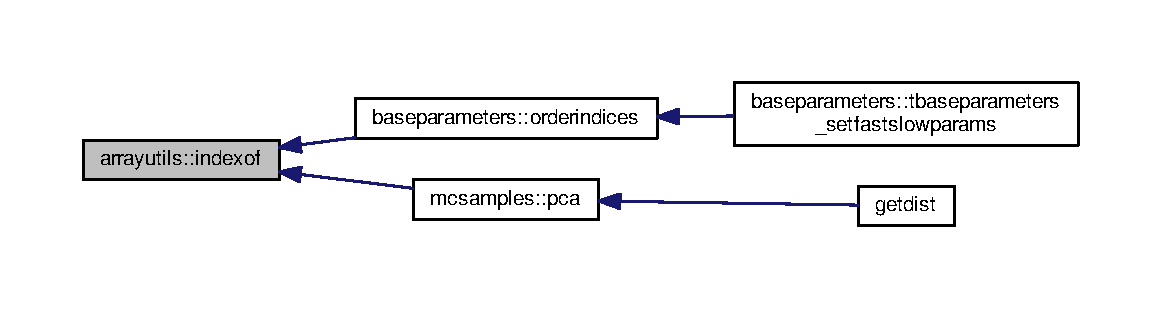
\includegraphics[width=350pt]{namespacearrayutils_aa1aa3daae226441732e2e7c4f292eab2_icgraph}
\end{center}
\end{figure}
\mbox{\Hypertarget{namespacearrayutils_ad2c5184ac408d5a352ea420ff3f1e1eb}\label{namespacearrayutils_ad2c5184ac408d5a352ea420ff3f1e1eb}} 
\index{arrayutils@{arrayutils}!maxindex@{maxindex}}
\index{maxindex@{maxindex}!arrayutils@{arrayutils}}
\subsubsection{\texorpdfstring{maxindex()}{maxindex()}}
{\footnotesize\ttfamily integer function arrayutils\+::maxindex (\begin{DoxyParamCaption}\item[{real, dimension(n), intent(in)}]{arr,  }\item[{integer, intent(in)}]{n }\end{DoxyParamCaption})}



Referenced by mcsamples\+::mostcorrelated2d().

Here is the caller graph for this function\+:
\nopagebreak
\begin{figure}[H]
\begin{center}
\leavevmode
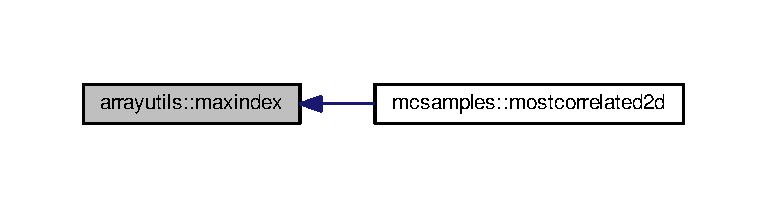
\includegraphics[width=350pt]{namespacearrayutils_ad2c5184ac408d5a352ea420ff3f1e1eb_icgraph}
\end{center}
\end{figure}
\mbox{\Hypertarget{namespacearrayutils_aba5bf237d7739646abd0596fea043455}\label{namespacearrayutils_aba5bf237d7739646abd0596fea043455}} 
\index{arrayutils@{arrayutils}!minindex@{minindex}}
\index{minindex@{minindex}!arrayutils@{arrayutils}}
\subsubsection{\texorpdfstring{minindex()}{minindex()}}
{\footnotesize\ttfamily integer function arrayutils\+::minindex (\begin{DoxyParamCaption}\item[{real, dimension(n), intent(in)}]{arr,  }\item[{integer, intent(in)}]{n }\end{DoxyParamCaption})}


\hypertarget{namespacebao}{}\section{bao Module Reference}
\label{namespacebao}\index{bao@{bao}}
\subsection*{Data Types}
\begin{DoxyCompactItemize}
\item 
type \mbox{\hyperlink{structbao_1_1dr1xlikelihood}{dr1xlikelihood}}
\item 
type \mbox{\hyperlink{structbao_1_1mgslikelihood}{mgslikelihood}}
\item 
type \mbox{\hyperlink{structbao_1_1tbaolikelihood}{tbaolikelihood}}
\end{DoxyCompactItemize}
\subsection*{Functions/\+Subroutines}
\begin{DoxyCompactItemize}
\item 
subroutine, public \mbox{\hyperlink{namespacebao_a1e83b8129197b47271286760d4c11866}{baolikelihood\+\_\+add}} (Like\+List, Ini)
\item 
subroutine \mbox{\hyperlink{namespacebao_af2e429eb5aae0de7f70a321537f77861}{bao\+\_\+readini}} (this, Ini)
\item 
subroutine \mbox{\hyperlink{namespacebao_a42ad1b0022e37bb1e4457c7a4e329b12}{bao\+\_\+initprobdist}} (this, Ini)
\item 
real(mcp) function \mbox{\hyperlink{namespacebao_af2ea26ba323749ae85e04fe46904d115}{get\+\_\+rs\+\_\+drag}} (this, Theory)
\item 
real(mcp) function \mbox{\hyperlink{namespacebao_a42575daf8f5c1b68a1a7ddf8bd087988}{acoustic}} (this, C\+MB, z)
\item 
real(mcp) function \mbox{\hyperlink{namespacebao_a9a4c24c4606056286bb571c62350ccb3}{bao\+\_\+lnlike}} (this, C\+MB, Theory, Data\+Params)
\item 
subroutine \mbox{\hyperlink{namespacebao_a01a1351c073ed9d3a96aece01f8c368b}{bao\+\_\+dr1x\+\_\+initprobdist}} (this, Ini)
\item 
real(mcp) function \mbox{\hyperlink{namespacebao_a566724d43b5fe7348c615930295ffefb}{bao\+\_\+dr1x\+\_\+loglike}} (this, C\+MB, Theory, Data\+Params)
\item 
subroutine \mbox{\hyperlink{namespacebao_aec7bdc5f03a9da432a0345932d1401bd}{bao\+\_\+mgs\+\_\+initprobdist}} (this, Ini)
\item 
real(mcp) function \mbox{\hyperlink{namespacebao_aa39f8163fd5d4a39d7d83bab1a485ee2}{bao\+\_\+mgs\+\_\+loglike}} (this, C\+MB, Theory, Data\+Params)
\end{DoxyCompactItemize}
\subsection*{Variables}
\begin{DoxyCompactItemize}
\item 
character(len=ini\+\_\+enumeration\+\_\+len), dimension(9), parameter \mbox{\hyperlink{namespacebao_a5a7cbf786aa65368c32203dfb9b72991}{measurement\+\_\+types}} = \mbox{[}character(Ini\+\_\+\+Enumeration\+\_\+\+Len)\+::\textquotesingle{}Az\textquotesingle{},\textquotesingle{}D\+V\+\_\+over\+\_\+rs\textquotesingle{},\textquotesingle{}rs\+\_\+over\+\_\+\+DV\textquotesingle{},\textquotesingle{}D\+A\+\_\+over\+\_\+rs\textquotesingle{}, \textquotesingle{}F\+\_\+\+AP\textquotesingle{}, \textquotesingle{}\mbox{\hyperlink{namespacebao_aaa65837538ed00f6c87276b81b451c45}{f\+\_\+sigma8}}\textquotesingle{},\textquotesingle{}bao\+\_\+\+Hz\+\_\+rs\textquotesingle{},\textquotesingle{}bao\+\_\+\+Hz\+\_\+rs\+\_\+103\textquotesingle{},\textquotesingle{}\mbox{\hyperlink{namespacebao_a9bc55477c817a8204a8dd45a73ab6faa}{dilation}}\textquotesingle{}\mbox{]}
\item 
integer, parameter \mbox{\hyperlink{namespacebao_ab53a2d435899a21c918a07f7243d2a9f}{bao\+\_\+az}} =1
\item 
integer, parameter \mbox{\hyperlink{namespacebao_a0524be8a1cd6362d8c5e0cc628384991}{bao\+\_\+dv\+\_\+over\+\_\+rs}} = 2
\item 
integer, parameter \mbox{\hyperlink{namespacebao_aadd8d344c5506828f10eed295270faf7}{bao\+\_\+rs\+\_\+over\+\_\+dv}} = 3
\item 
integer, parameter \mbox{\hyperlink{namespacebao_a5856a51527a41fd49a3222f83de0f1da}{bao\+\_\+da\+\_\+over\+\_\+rs}} = 4
\item 
integer, parameter \mbox{\hyperlink{namespacebao_a90e9d6d857982260b5025f4778bf0a4d}{f\+\_\+ap}} = 5
\item 
integer, parameter \mbox{\hyperlink{namespacebao_aaa65837538ed00f6c87276b81b451c45}{f\+\_\+sigma8}} =6
\item 
integer, parameter \mbox{\hyperlink{namespacebao_a5d192049c79a222547036308959868c2}{bao\+\_\+hz\+\_\+rs}} = 7
\item 
integer, parameter \mbox{\hyperlink{namespacebao_aad05aa1882f8f917547a2919bb25db43}{bao\+\_\+hz\+\_\+rs\+\_\+103}} = 8
\item 
integer, parameter \mbox{\hyperlink{namespacebao_a9bc55477c817a8204a8dd45a73ab6faa}{dilation}} = 9
\item 
real(mcp) \mbox{\hyperlink{namespacebao_a4f0a92dc313e31a91e5edb5e2ef09fec}{bao\+\_\+fixed\+\_\+rs}} = -\/1.\+\_\+mcp
\end{DoxyCompactItemize}


\subsection{Function/\+Subroutine Documentation}
\mbox{\Hypertarget{namespacebao_a42575daf8f5c1b68a1a7ddf8bd087988}\label{namespacebao_a42575daf8f5c1b68a1a7ddf8bd087988}} 
\index{bao@{bao}!acoustic@{acoustic}}
\index{acoustic@{acoustic}!bao@{bao}}
\subsubsection{\texorpdfstring{acoustic()}{acoustic()}}
{\footnotesize\ttfamily real(mcp) function bao\+::acoustic (\begin{DoxyParamCaption}\item[{class(\mbox{\hyperlink{structbao_1_1tbaolikelihood}{tbaolikelihood}})}]{this,  }\item[{class(cmbparams)}]{C\+MB,  }\item[{real(mcp), intent(in)}]{z }\end{DoxyParamCaption})\hspace{0.3cm}{\ttfamily [private]}}



References settings\+::const\+\_\+c.

\mbox{\Hypertarget{namespacebao_a01a1351c073ed9d3a96aece01f8c368b}\label{namespacebao_a01a1351c073ed9d3a96aece01f8c368b}} 
\index{bao@{bao}!bao\+\_\+dr1x\+\_\+initprobdist@{bao\+\_\+dr1x\+\_\+initprobdist}}
\index{bao\+\_\+dr1x\+\_\+initprobdist@{bao\+\_\+dr1x\+\_\+initprobdist}!bao@{bao}}
\subsubsection{\texorpdfstring{bao\+\_\+dr1x\+\_\+initprobdist()}{bao\_dr1x\_initprobdist()}}
{\footnotesize\ttfamily subroutine bao\+::bao\+\_\+dr1x\+\_\+initprobdist (\begin{DoxyParamCaption}\item[{class(\mbox{\hyperlink{structbao_1_1dr1xlikelihood}{dr1xlikelihood}})}]{this,  }\item[{class(\mbox{\hyperlink{structsettings_1_1tsettingini}{tsettingini}})}]{Ini }\end{DoxyParamCaption})\hspace{0.3cm}{\ttfamily [private]}}

\mbox{\Hypertarget{namespacebao_a566724d43b5fe7348c615930295ffefb}\label{namespacebao_a566724d43b5fe7348c615930295ffefb}} 
\index{bao@{bao}!bao\+\_\+dr1x\+\_\+loglike@{bao\+\_\+dr1x\+\_\+loglike}}
\index{bao\+\_\+dr1x\+\_\+loglike@{bao\+\_\+dr1x\+\_\+loglike}!bao@{bao}}
\subsubsection{\texorpdfstring{bao\+\_\+dr1x\+\_\+loglike()}{bao\_dr1x\_loglike()}}
{\footnotesize\ttfamily real (mcp) function bao\+::bao\+\_\+dr1x\+\_\+loglike (\begin{DoxyParamCaption}\item[{class(\mbox{\hyperlink{structbao_1_1dr1xlikelihood}{dr1xlikelihood}})}]{this,  }\item[{class(cmbparams)}]{C\+MB,  }\item[{class(tcosmotheorypredictions), target}]{Theory,  }\item[{real(mcp), dimension(\+:)}]{Data\+Params }\end{DoxyParamCaption})\hspace{0.3cm}{\ttfamily [private]}}



References settings\+::logzero.

\mbox{\Hypertarget{namespacebao_a42ad1b0022e37bb1e4457c7a4e329b12}\label{namespacebao_a42ad1b0022e37bb1e4457c7a4e329b12}} 
\index{bao@{bao}!bao\+\_\+initprobdist@{bao\+\_\+initprobdist}}
\index{bao\+\_\+initprobdist@{bao\+\_\+initprobdist}!bao@{bao}}
\subsubsection{\texorpdfstring{bao\+\_\+initprobdist()}{bao\_initprobdist()}}
{\footnotesize\ttfamily subroutine bao\+::bao\+\_\+initprobdist (\begin{DoxyParamCaption}\item[{class(\mbox{\hyperlink{structbao_1_1tbaolikelihood}{tbaolikelihood}})}]{this,  }\item[{class(\mbox{\hyperlink{structsettings_1_1tsettingini}{tsettingini}})}]{Ini }\end{DoxyParamCaption})\hspace{0.3cm}{\ttfamily [private]}}

\mbox{\Hypertarget{namespacebao_a9a4c24c4606056286bb571c62350ccb3}\label{namespacebao_a9a4c24c4606056286bb571c62350ccb3}} 
\index{bao@{bao}!bao\+\_\+lnlike@{bao\+\_\+lnlike}}
\index{bao\+\_\+lnlike@{bao\+\_\+lnlike}!bao@{bao}}
\subsubsection{\texorpdfstring{bao\+\_\+lnlike()}{bao\_lnlike()}}
{\footnotesize\ttfamily real(mcp) function bao\+::bao\+\_\+lnlike (\begin{DoxyParamCaption}\item[{class(\mbox{\hyperlink{structbao_1_1tbaolikelihood}{tbaolikelihood}})}]{this,  }\item[{class(cmbparams)}]{C\+MB,  }\item[{class(tcosmotheorypredictions), target}]{Theory,  }\item[{real(mcp), dimension(\+:)}]{Data\+Params }\end{DoxyParamCaption})\hspace{0.3cm}{\ttfamily [private]}}



References bao\+\_\+az, bao\+\_\+da\+\_\+over\+\_\+rs, bao\+\_\+dv\+\_\+over\+\_\+rs, bao\+\_\+hz\+\_\+rs, bao\+\_\+hz\+\_\+rs\+\_\+103, bao\+\_\+rs\+\_\+over\+\_\+dv, f\+\_\+ap, f\+\_\+sigma8, settings\+::feedback, and matrixutils\+::matrix\+\_\+quadform().

Here is the call graph for this function\+:
\nopagebreak
\begin{figure}[H]
\begin{center}
\leavevmode
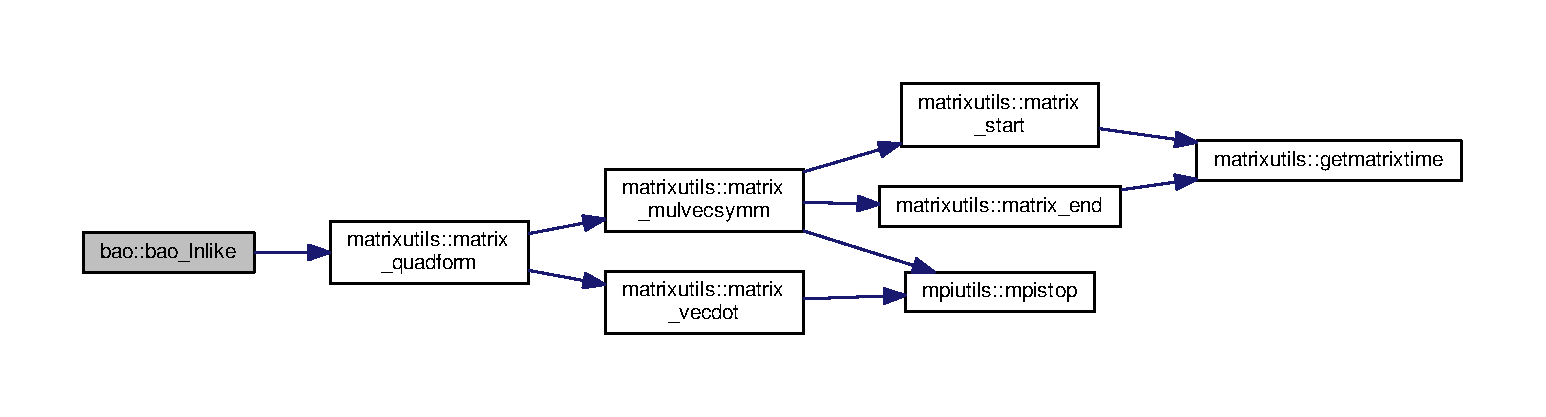
\includegraphics[width=350pt]{namespacebao_a9a4c24c4606056286bb571c62350ccb3_cgraph}
\end{center}
\end{figure}
\mbox{\Hypertarget{namespacebao_aec7bdc5f03a9da432a0345932d1401bd}\label{namespacebao_aec7bdc5f03a9da432a0345932d1401bd}} 
\index{bao@{bao}!bao\+\_\+mgs\+\_\+initprobdist@{bao\+\_\+mgs\+\_\+initprobdist}}
\index{bao\+\_\+mgs\+\_\+initprobdist@{bao\+\_\+mgs\+\_\+initprobdist}!bao@{bao}}
\subsubsection{\texorpdfstring{bao\+\_\+mgs\+\_\+initprobdist()}{bao\_mgs\_initprobdist()}}
{\footnotesize\ttfamily subroutine bao\+::bao\+\_\+mgs\+\_\+initprobdist (\begin{DoxyParamCaption}\item[{class(\mbox{\hyperlink{structbao_1_1mgslikelihood}{mgslikelihood}})}]{this,  }\item[{class(\mbox{\hyperlink{structsettings_1_1tsettingini}{tsettingini}})}]{Ini }\end{DoxyParamCaption})\hspace{0.3cm}{\ttfamily [private]}}

\mbox{\Hypertarget{namespacebao_aa39f8163fd5d4a39d7d83bab1a485ee2}\label{namespacebao_aa39f8163fd5d4a39d7d83bab1a485ee2}} 
\index{bao@{bao}!bao\+\_\+mgs\+\_\+loglike@{bao\+\_\+mgs\+\_\+loglike}}
\index{bao\+\_\+mgs\+\_\+loglike@{bao\+\_\+mgs\+\_\+loglike}!bao@{bao}}
\subsubsection{\texorpdfstring{bao\+\_\+mgs\+\_\+loglike()}{bao\_mgs\_loglike()}}
{\footnotesize\ttfamily real(mcp) function bao\+::bao\+\_\+mgs\+\_\+loglike (\begin{DoxyParamCaption}\item[{class(\mbox{\hyperlink{structbao_1_1mgslikelihood}{mgslikelihood}})}]{this,  }\item[{class(cmbparams)}]{C\+MB,  }\item[{class(tcosmotheorypredictions), target}]{Theory,  }\item[{real(mcp), dimension(\+:)}]{Data\+Params }\end{DoxyParamCaption})\hspace{0.3cm}{\ttfamily [private]}}



References settings\+::logzero.

\mbox{\Hypertarget{namespacebao_af2e429eb5aae0de7f70a321537f77861}\label{namespacebao_af2e429eb5aae0de7f70a321537f77861}} 
\index{bao@{bao}!bao\+\_\+readini@{bao\+\_\+readini}}
\index{bao\+\_\+readini@{bao\+\_\+readini}!bao@{bao}}
\subsubsection{\texorpdfstring{bao\+\_\+readini()}{bao\_readini()}}
{\footnotesize\ttfamily subroutine bao\+::bao\+\_\+readini (\begin{DoxyParamCaption}\item[{class(\mbox{\hyperlink{structbao_1_1tbaolikelihood}{tbaolikelihood}})}]{this,  }\item[{class(\mbox{\hyperlink{structsettings_1_1tsettingini}{tsettingini}})}]{Ini }\end{DoxyParamCaption})\hspace{0.3cm}{\ttfamily [private]}}



References f\+\_\+sigma8, settings\+::feedback, measurement\+\_\+types, and settings\+::mpirank.

\mbox{\Hypertarget{namespacebao_a1e83b8129197b47271286760d4c11866}\label{namespacebao_a1e83b8129197b47271286760d4c11866}} 
\index{bao@{bao}!baolikelihood\+\_\+add@{baolikelihood\+\_\+add}}
\index{baolikelihood\+\_\+add@{baolikelihood\+\_\+add}!bao@{bao}}
\subsubsection{\texorpdfstring{baolikelihood\+\_\+add()}{baolikelihood\_add()}}
{\footnotesize\ttfamily subroutine, public bao\+::baolikelihood\+\_\+add (\begin{DoxyParamCaption}\item[{class(tlikelihoodlist)}]{Like\+List,  }\item[{class(\mbox{\hyperlink{structsettings_1_1tsettingini}{tsettingini}})}]{Ini }\end{DoxyParamCaption})}



References bao\+\_\+fixed\+\_\+rs, and settings\+::feedback.



Referenced by datalikelihoodlist\+::setdatalikelihoods().

Here is the caller graph for this function\+:
\nopagebreak
\begin{figure}[H]
\begin{center}
\leavevmode
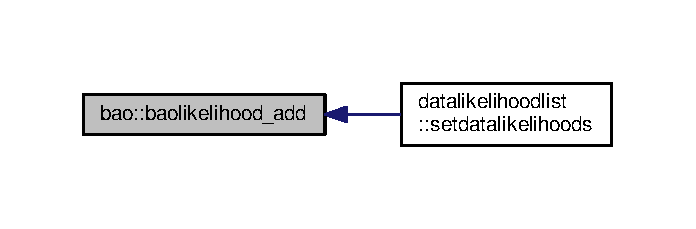
\includegraphics[width=334pt]{namespacebao_a1e83b8129197b47271286760d4c11866_icgraph}
\end{center}
\end{figure}
\mbox{\Hypertarget{namespacebao_af2ea26ba323749ae85e04fe46904d115}\label{namespacebao_af2ea26ba323749ae85e04fe46904d115}} 
\index{bao@{bao}!get\+\_\+rs\+\_\+drag@{get\+\_\+rs\+\_\+drag}}
\index{get\+\_\+rs\+\_\+drag@{get\+\_\+rs\+\_\+drag}!bao@{bao}}
\subsubsection{\texorpdfstring{get\+\_\+rs\+\_\+drag()}{get\_rs\_drag()}}
{\footnotesize\ttfamily real(mcp) function bao\+::get\+\_\+rs\+\_\+drag (\begin{DoxyParamCaption}\item[{class(\mbox{\hyperlink{structbao_1_1tbaolikelihood}{tbaolikelihood}})}]{this,  }\item[{class(tcosmotheorypredictions), target}]{Theory }\end{DoxyParamCaption})\hspace{0.3cm}{\ttfamily [private]}}



References bao\+\_\+fixed\+\_\+rs, and cosmologytypes\+::derived\+\_\+rdrag.



\subsection{Variable Documentation}
\mbox{\Hypertarget{namespacebao_ab53a2d435899a21c918a07f7243d2a9f}\label{namespacebao_ab53a2d435899a21c918a07f7243d2a9f}} 
\index{bao@{bao}!bao\+\_\+az@{bao\+\_\+az}}
\index{bao\+\_\+az@{bao\+\_\+az}!bao@{bao}}
\subsubsection{\texorpdfstring{bao\+\_\+az}{bao\_az}}
{\footnotesize\ttfamily integer, parameter bao\+::bao\+\_\+az =1\hspace{0.3cm}{\ttfamily [private]}}



Referenced by bao\+\_\+lnlike().

\mbox{\Hypertarget{namespacebao_a5856a51527a41fd49a3222f83de0f1da}\label{namespacebao_a5856a51527a41fd49a3222f83de0f1da}} 
\index{bao@{bao}!bao\+\_\+da\+\_\+over\+\_\+rs@{bao\+\_\+da\+\_\+over\+\_\+rs}}
\index{bao\+\_\+da\+\_\+over\+\_\+rs@{bao\+\_\+da\+\_\+over\+\_\+rs}!bao@{bao}}
\subsubsection{\texorpdfstring{bao\+\_\+da\+\_\+over\+\_\+rs}{bao\_da\_over\_rs}}
{\footnotesize\ttfamily integer, parameter bao\+::bao\+\_\+da\+\_\+over\+\_\+rs = 4\hspace{0.3cm}{\ttfamily [private]}}



Referenced by bao\+\_\+lnlike().

\mbox{\Hypertarget{namespacebao_a0524be8a1cd6362d8c5e0cc628384991}\label{namespacebao_a0524be8a1cd6362d8c5e0cc628384991}} 
\index{bao@{bao}!bao\+\_\+dv\+\_\+over\+\_\+rs@{bao\+\_\+dv\+\_\+over\+\_\+rs}}
\index{bao\+\_\+dv\+\_\+over\+\_\+rs@{bao\+\_\+dv\+\_\+over\+\_\+rs}!bao@{bao}}
\subsubsection{\texorpdfstring{bao\+\_\+dv\+\_\+over\+\_\+rs}{bao\_dv\_over\_rs}}
{\footnotesize\ttfamily integer, parameter bao\+::bao\+\_\+dv\+\_\+over\+\_\+rs = 2\hspace{0.3cm}{\ttfamily [private]}}



Referenced by bao\+\_\+lnlike().

\mbox{\Hypertarget{namespacebao_a4f0a92dc313e31a91e5edb5e2ef09fec}\label{namespacebao_a4f0a92dc313e31a91e5edb5e2ef09fec}} 
\index{bao@{bao}!bao\+\_\+fixed\+\_\+rs@{bao\+\_\+fixed\+\_\+rs}}
\index{bao\+\_\+fixed\+\_\+rs@{bao\+\_\+fixed\+\_\+rs}!bao@{bao}}
\subsubsection{\texorpdfstring{bao\+\_\+fixed\+\_\+rs}{bao\_fixed\_rs}}
{\footnotesize\ttfamily real(mcp) bao\+::bao\+\_\+fixed\+\_\+rs = -\/1.\+\_\+mcp\hspace{0.3cm}{\ttfamily [private]}}



Referenced by baolikelihood\+\_\+add(), and get\+\_\+rs\+\_\+drag().

\mbox{\Hypertarget{namespacebao_a5d192049c79a222547036308959868c2}\label{namespacebao_a5d192049c79a222547036308959868c2}} 
\index{bao@{bao}!bao\+\_\+hz\+\_\+rs@{bao\+\_\+hz\+\_\+rs}}
\index{bao\+\_\+hz\+\_\+rs@{bao\+\_\+hz\+\_\+rs}!bao@{bao}}
\subsubsection{\texorpdfstring{bao\+\_\+hz\+\_\+rs}{bao\_hz\_rs}}
{\footnotesize\ttfamily integer, parameter bao\+::bao\+\_\+hz\+\_\+rs = 7\hspace{0.3cm}{\ttfamily [private]}}



Referenced by bao\+\_\+lnlike().

\mbox{\Hypertarget{namespacebao_aad05aa1882f8f917547a2919bb25db43}\label{namespacebao_aad05aa1882f8f917547a2919bb25db43}} 
\index{bao@{bao}!bao\+\_\+hz\+\_\+rs\+\_\+103@{bao\+\_\+hz\+\_\+rs\+\_\+103}}
\index{bao\+\_\+hz\+\_\+rs\+\_\+103@{bao\+\_\+hz\+\_\+rs\+\_\+103}!bao@{bao}}
\subsubsection{\texorpdfstring{bao\+\_\+hz\+\_\+rs\+\_\+103}{bao\_hz\_rs\_103}}
{\footnotesize\ttfamily integer, parameter bao\+::bao\+\_\+hz\+\_\+rs\+\_\+103 = 8\hspace{0.3cm}{\ttfamily [private]}}



Referenced by bao\+\_\+lnlike().

\mbox{\Hypertarget{namespacebao_aadd8d344c5506828f10eed295270faf7}\label{namespacebao_aadd8d344c5506828f10eed295270faf7}} 
\index{bao@{bao}!bao\+\_\+rs\+\_\+over\+\_\+dv@{bao\+\_\+rs\+\_\+over\+\_\+dv}}
\index{bao\+\_\+rs\+\_\+over\+\_\+dv@{bao\+\_\+rs\+\_\+over\+\_\+dv}!bao@{bao}}
\subsubsection{\texorpdfstring{bao\+\_\+rs\+\_\+over\+\_\+dv}{bao\_rs\_over\_dv}}
{\footnotesize\ttfamily integer, parameter bao\+::bao\+\_\+rs\+\_\+over\+\_\+dv = 3\hspace{0.3cm}{\ttfamily [private]}}



Referenced by bao\+\_\+lnlike().

\mbox{\Hypertarget{namespacebao_a9bc55477c817a8204a8dd45a73ab6faa}\label{namespacebao_a9bc55477c817a8204a8dd45a73ab6faa}} 
\index{bao@{bao}!dilation@{dilation}}
\index{dilation@{dilation}!bao@{bao}}
\subsubsection{\texorpdfstring{dilation}{dilation}}
{\footnotesize\ttfamily integer, parameter bao\+::dilation = 9\hspace{0.3cm}{\ttfamily [private]}}

\mbox{\Hypertarget{namespacebao_a90e9d6d857982260b5025f4778bf0a4d}\label{namespacebao_a90e9d6d857982260b5025f4778bf0a4d}} 
\index{bao@{bao}!f\+\_\+ap@{f\+\_\+ap}}
\index{f\+\_\+ap@{f\+\_\+ap}!bao@{bao}}
\subsubsection{\texorpdfstring{f\+\_\+ap}{f\_ap}}
{\footnotesize\ttfamily integer, parameter bao\+::f\+\_\+ap = 5\hspace{0.3cm}{\ttfamily [private]}}



Referenced by bao\+\_\+lnlike().

\mbox{\Hypertarget{namespacebao_aaa65837538ed00f6c87276b81b451c45}\label{namespacebao_aaa65837538ed00f6c87276b81b451c45}} 
\index{bao@{bao}!f\+\_\+sigma8@{f\+\_\+sigma8}}
\index{f\+\_\+sigma8@{f\+\_\+sigma8}!bao@{bao}}
\subsubsection{\texorpdfstring{f\+\_\+sigma8}{f\_sigma8}}
{\footnotesize\ttfamily integer, parameter bao\+::f\+\_\+sigma8 =6\hspace{0.3cm}{\ttfamily [private]}}



Referenced by bao\+\_\+lnlike(), and bao\+\_\+readini().

\mbox{\Hypertarget{namespacebao_a5a7cbf786aa65368c32203dfb9b72991}\label{namespacebao_a5a7cbf786aa65368c32203dfb9b72991}} 
\index{bao@{bao}!measurement\+\_\+types@{measurement\+\_\+types}}
\index{measurement\+\_\+types@{measurement\+\_\+types}!bao@{bao}}
\subsubsection{\texorpdfstring{measurement\+\_\+types}{measurement\_types}}
{\footnotesize\ttfamily character(len=ini\+\_\+enumeration\+\_\+len), dimension(9), parameter bao\+::measurement\+\_\+types = \mbox{[}character(Ini\+\_\+\+Enumeration\+\_\+\+Len)\+::\textquotesingle{}Az\textquotesingle{},\textquotesingle{}D\+V\+\_\+over\+\_\+rs\textquotesingle{},\textquotesingle{}rs\+\_\+over\+\_\+\+DV\textquotesingle{},\textquotesingle{}D\+A\+\_\+over\+\_\+rs\textquotesingle{}, \textquotesingle{}F\+\_\+\+AP\textquotesingle{}, \textquotesingle{}\mbox{\hyperlink{namespacebao_aaa65837538ed00f6c87276b81b451c45}{f\+\_\+sigma8}}\textquotesingle{},\textquotesingle{}bao\+\_\+\+Hz\+\_\+rs\textquotesingle{},\textquotesingle{}bao\+\_\+\+Hz\+\_\+rs\+\_\+103\textquotesingle{},\textquotesingle{}\mbox{\hyperlink{namespacebao_a9bc55477c817a8204a8dd45a73ab6faa}{dilation}}\textquotesingle{}\mbox{]}\hspace{0.3cm}{\ttfamily [private]}}



Referenced by bao\+\_\+readini().


\hypertarget{namespacebaseparameters}{}\section{baseparameters Module Reference}
\label{namespacebaseparameters}\index{baseparameters@{baseparameters}}
\subsection*{Data Types}
\begin{DoxyCompactItemize}
\item 
type \mbox{\hyperlink{structbaseparameters_1_1paramgaussprior}{paramgaussprior}}
\item 
type \mbox{\hyperlink{structbaseparameters_1_1tbaseparameters}{tbaseparameters}}
\item 
type \mbox{\hyperlink{structbaseparameters_1_1tlinearcombination}{tlinearcombination}}
\end{DoxyCompactItemize}
\subsection*{Functions/\+Subroutines}
\begin{DoxyCompactItemize}
\item 
subroutine \mbox{\hyperlink{namespacebaseparameters_a86f36ece3b30fc7984f06ee4aad097bb}{tbaseparameters\+\_\+initializeusedparams}} (this, Ini)
\item 
subroutine \mbox{\hyperlink{namespacebaseparameters_a3126d9d902d7cc3f30105a9ad35e4a04}{tbaseparameters\+\_\+paramerror}} (this, str, param)
\item 
subroutine \mbox{\hyperlink{namespacebaseparameters_a1c41b4dbd4418bb1d16d77034504ac0b}{tbaseparameters\+\_\+setstartpositions}} (this, Params)
\item 
subroutine \mbox{\hyperlink{namespacebaseparameters_ae26154e8a07fc378e0e669659de1025a}{tbaseparameters\+\_\+readparams}} (this, Ini)
\item 
subroutine \mbox{\hyperlink{namespacebaseparameters_a810df98da76d4ae9691fb72eb588ea34}{tbaseparameters\+\_\+readpriors}} (this, Ini)
\item 
subroutine \mbox{\hyperlink{namespacebaseparameters_acc7b955531e3ac266fd197c8cc09ae50}{tbaseparameters\+\_\+setcovmat}} (this, prop\+\_\+mat)
\item 
subroutine \mbox{\hyperlink{namespacebaseparameters_a2d0a5594063e754beb3d8ef2b4af0522}{tbaseparameters\+\_\+readsetcovmatrix}} (this, prop\+\_\+mat, matrix, New\+Params)
\item 
subroutine \mbox{\hyperlink{namespacebaseparameters_a309e81ed0619c2b91456008b414cf5a9}{tbaseparameters\+\_\+outputparamnames}} (this, fname, indices, add\+\_\+derived)
\item 
subroutine \mbox{\hyperlink{namespacebaseparameters_a7deeecd73224be7473e92a6d48ba8909}{tbaseparameters\+\_\+outputparamranges}} (this, fname)
\item 
subroutine \mbox{\hyperlink{namespacebaseparameters_a7d00d4d42d3c3abcbdbc6078fffab95f}{orderindices}} (arr, n)
\item 
subroutine \mbox{\hyperlink{namespacebaseparameters_ac8f2cdce695f77b0f9cc3c2e86a9c05f}{tbaseparameters\+\_\+setfastslowparams}} (this, Ini, use\+\_\+fast\+\_\+slow)
\item 
character(len=\+:) function, allocatable \mbox{\hyperlink{namespacebaseparameters_a6fa6c72334203001f2e2932139df534d}{tbaseparameters\+\_\+usedparamnameornumber}} (this, i)
\end{DoxyCompactItemize}
\subsection*{Variables}
\begin{DoxyCompactItemize}
\item 
integer, parameter \mbox{\hyperlink{namespacebaseparameters_aa9a374c82230367604ae6b1c50ed3e3b}{tp\+\_\+unused}} = 0
\item 
integer, parameter \mbox{\hyperlink{namespacebaseparameters_aec8c4b0ea0429954337dcf5fced6abf1}{tp\+\_\+slow}} =1
\item 
integer, parameter \mbox{\hyperlink{namespacebaseparameters_a213e8b067e9d21216fbad3fbd98ec933}{tp\+\_\+semislow}} =2
\item 
integer, parameter \mbox{\hyperlink{namespacebaseparameters_a4cae4f2dfd7f3b1ed425daca03b67139}{tp\+\_\+semifast}} =3
\item 
integer, parameter \mbox{\hyperlink{namespacebaseparameters_ac1f704b0992c1c1c9f90d320ae0c4f4b}{tp\+\_\+fast}} =4
\item 
integer, parameter, public \mbox{\hyperlink{namespacebaseparameters_a1d3e10105684d9171cdfec4ccfcd331d}{slow\+\_\+tp\+\_\+max}} = \mbox{\hyperlink{namespacebaseparameters_a213e8b067e9d21216fbad3fbd98ec933}{tp\+\_\+semislow}}
\item 
type(\mbox{\hyperlink{structbaseparameters_1_1tbaseparameters}{tbaseparameters}}), save, public \mbox{\hyperlink{namespacebaseparameters_abc9ecfbbf4a5012fbc95d3fb51a1e6e3}{baseparams}}
\end{DoxyCompactItemize}


\subsection{Function/\+Subroutine Documentation}
\mbox{\Hypertarget{namespacebaseparameters_a7d00d4d42d3c3abcbdbc6078fffab95f}\label{namespacebaseparameters_a7d00d4d42d3c3abcbdbc6078fffab95f}} 
\index{baseparameters@{baseparameters}!orderindices@{orderindices}}
\index{orderindices@{orderindices}!baseparameters@{baseparameters}}
\subsubsection{\texorpdfstring{orderindices()}{orderindices()}}
{\footnotesize\ttfamily subroutine baseparameters\+::orderindices (\begin{DoxyParamCaption}\item[{integer, dimension(\+:)}]{arr,  }\item[{integer, intent(in)}]{n }\end{DoxyParamCaption})\hspace{0.3cm}{\ttfamily [private]}}



References arrayutils\+::indexof().



Referenced by tbaseparameters\+\_\+setfastslowparams().

Here is the call graph for this function\+:
\nopagebreak
\begin{figure}[H]
\begin{center}
\leavevmode
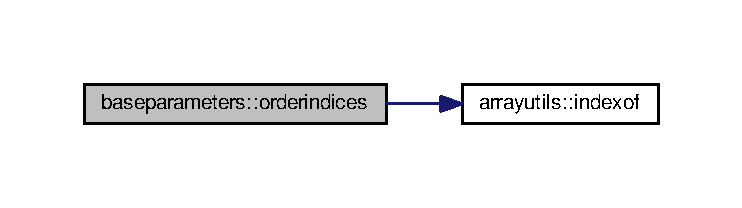
\includegraphics[width=350pt]{namespacebaseparameters_a7d00d4d42d3c3abcbdbc6078fffab95f_cgraph}
\end{center}
\end{figure}
Here is the caller graph for this function\+:
\nopagebreak
\begin{figure}[H]
\begin{center}
\leavevmode
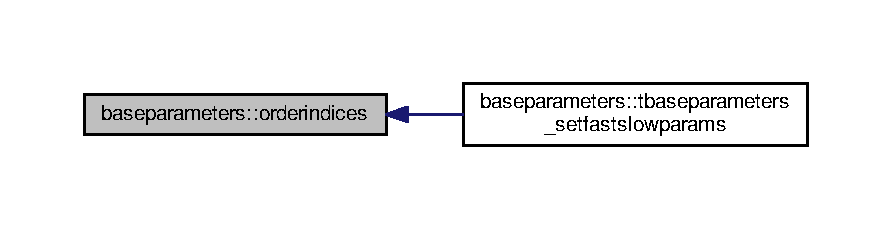
\includegraphics[width=350pt]{namespacebaseparameters_a7d00d4d42d3c3abcbdbc6078fffab95f_icgraph}
\end{center}
\end{figure}
\mbox{\Hypertarget{namespacebaseparameters_a86f36ece3b30fc7984f06ee4aad097bb}\label{namespacebaseparameters_a86f36ece3b30fc7984f06ee4aad097bb}} 
\index{baseparameters@{baseparameters}!tbaseparameters\+\_\+initializeusedparams@{tbaseparameters\+\_\+initializeusedparams}}
\index{tbaseparameters\+\_\+initializeusedparams@{tbaseparameters\+\_\+initializeusedparams}!baseparameters@{baseparameters}}
\subsubsection{\texorpdfstring{tbaseparameters\+\_\+initializeusedparams()}{tbaseparameters\_initializeusedparams()}}
{\footnotesize\ttfamily subroutine baseparameters\+::tbaseparameters\+\_\+initializeusedparams (\begin{DoxyParamCaption}\item[{class(\mbox{\hyperlink{structbaseparameters_1_1tbaseparameters}{tbaseparameters}})}]{this,  }\item[{class(\mbox{\hyperlink{structsettings_1_1tsettingini}{tsettingini}})}]{Ini }\end{DoxyParamCaption})\hspace{0.3cm}{\ttfamily [private]}}



References settings\+::num\+\_\+data\+\_\+params, settings\+::num\+\_\+params, settings\+::num\+\_\+theory\+\_\+params, and settings\+::output\+\_\+lines.

\mbox{\Hypertarget{namespacebaseparameters_a309e81ed0619c2b91456008b414cf5a9}\label{namespacebaseparameters_a309e81ed0619c2b91456008b414cf5a9}} 
\index{baseparameters@{baseparameters}!tbaseparameters\+\_\+outputparamnames@{tbaseparameters\+\_\+outputparamnames}}
\index{tbaseparameters\+\_\+outputparamnames@{tbaseparameters\+\_\+outputparamnames}!baseparameters@{baseparameters}}
\subsubsection{\texorpdfstring{tbaseparameters\+\_\+outputparamnames()}{tbaseparameters\_outputparamnames()}}
{\footnotesize\ttfamily subroutine baseparameters\+::tbaseparameters\+\_\+outputparamnames (\begin{DoxyParamCaption}\item[{class(\mbox{\hyperlink{structbaseparameters_1_1tbaseparameters}{tbaseparameters}})}]{this,  }\item[{character(len=$\ast$), intent(in)}]{fname,  }\item[{integer, dimension(\+:), intent(in), optional}]{indices,  }\item[{logical, intent(in), optional}]{add\+\_\+derived }\end{DoxyParamCaption})\hspace{0.3cm}{\ttfamily [private]}}

\mbox{\Hypertarget{namespacebaseparameters_a7deeecd73224be7473e92a6d48ba8909}\label{namespacebaseparameters_a7deeecd73224be7473e92a6d48ba8909}} 
\index{baseparameters@{baseparameters}!tbaseparameters\+\_\+outputparamranges@{tbaseparameters\+\_\+outputparamranges}}
\index{tbaseparameters\+\_\+outputparamranges@{tbaseparameters\+\_\+outputparamranges}!baseparameters@{baseparameters}}
\subsubsection{\texorpdfstring{tbaseparameters\+\_\+outputparamranges()}{tbaseparameters\_outputparamranges()}}
{\footnotesize\ttfamily subroutine baseparameters\+::tbaseparameters\+\_\+outputparamranges (\begin{DoxyParamCaption}\item[{class(\mbox{\hyperlink{structbaseparameters_1_1tbaseparameters}{tbaseparameters}})}]{this,  }\item[{character(len=$\ast$), intent(in)}]{fname }\end{DoxyParamCaption})\hspace{0.3cm}{\ttfamily [private]}}

\mbox{\Hypertarget{namespacebaseparameters_a3126d9d902d7cc3f30105a9ad35e4a04}\label{namespacebaseparameters_a3126d9d902d7cc3f30105a9ad35e4a04}} 
\index{baseparameters@{baseparameters}!tbaseparameters\+\_\+paramerror@{tbaseparameters\+\_\+paramerror}}
\index{tbaseparameters\+\_\+paramerror@{tbaseparameters\+\_\+paramerror}!baseparameters@{baseparameters}}
\subsubsection{\texorpdfstring{tbaseparameters\+\_\+paramerror()}{tbaseparameters\_paramerror()}}
{\footnotesize\ttfamily subroutine baseparameters\+::tbaseparameters\+\_\+paramerror (\begin{DoxyParamCaption}\item[{class(\mbox{\hyperlink{structbaseparameters_1_1tbaseparameters}{tbaseparameters}})}]{this,  }\item[{character(len=$\ast$), intent(in)}]{str,  }\item[{integer, intent(in)}]{param }\end{DoxyParamCaption})\hspace{0.3cm}{\ttfamily [private]}}



References settings\+::doabort().

Here is the call graph for this function\+:
\nopagebreak
\begin{figure}[H]
\begin{center}
\leavevmode
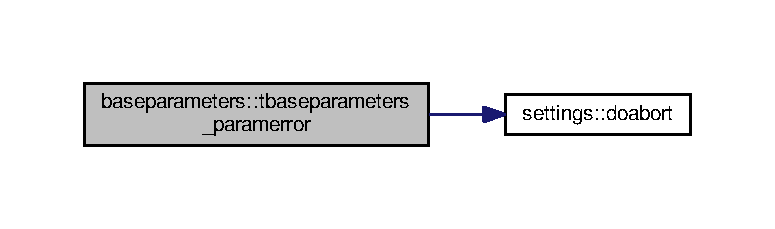
\includegraphics[width=350pt]{namespacebaseparameters_a3126d9d902d7cc3f30105a9ad35e4a04_cgraph}
\end{center}
\end{figure}
\mbox{\Hypertarget{namespacebaseparameters_ae26154e8a07fc378e0e669659de1025a}\label{namespacebaseparameters_ae26154e8a07fc378e0e669659de1025a}} 
\index{baseparameters@{baseparameters}!tbaseparameters\+\_\+readparams@{tbaseparameters\+\_\+readparams}}
\index{tbaseparameters\+\_\+readparams@{tbaseparameters\+\_\+readparams}!baseparameters@{baseparameters}}
\subsubsection{\texorpdfstring{tbaseparameters\+\_\+readparams()}{tbaseparameters\_readparams()}}
{\footnotesize\ttfamily subroutine baseparameters\+::tbaseparameters\+\_\+readparams (\begin{DoxyParamCaption}\item[{class(\mbox{\hyperlink{structbaseparameters_1_1tbaseparameters}{tbaseparameters}})}]{this,  }\item[{class(\mbox{\hyperlink{structsettings_1_1tsettingini}{tsettingini}})}]{Ini }\end{DoxyParamCaption})\hspace{0.3cm}{\ttfamily [private]}}



References settings\+::num\+\_\+params, settings\+::num\+\_\+params\+\_\+used, and settings\+::params\+\_\+used.

\mbox{\Hypertarget{namespacebaseparameters_a810df98da76d4ae9691fb72eb588ea34}\label{namespacebaseparameters_a810df98da76d4ae9691fb72eb588ea34}} 
\index{baseparameters@{baseparameters}!tbaseparameters\+\_\+readpriors@{tbaseparameters\+\_\+readpriors}}
\index{tbaseparameters\+\_\+readpriors@{tbaseparameters\+\_\+readpriors}!baseparameters@{baseparameters}}
\subsubsection{\texorpdfstring{tbaseparameters\+\_\+readpriors()}{tbaseparameters\_readpriors()}}
{\footnotesize\ttfamily subroutine baseparameters\+::tbaseparameters\+\_\+readpriors (\begin{DoxyParamCaption}\item[{class(\mbox{\hyperlink{structbaseparameters_1_1tbaseparameters}{tbaseparameters}})}]{this,  }\item[{class(\mbox{\hyperlink{structsettings_1_1tsettingini}{tsettingini}})}]{Ini }\end{DoxyParamCaption})\hspace{0.3cm}{\ttfamily [private]}}

\mbox{\Hypertarget{namespacebaseparameters_a2d0a5594063e754beb3d8ef2b4af0522}\label{namespacebaseparameters_a2d0a5594063e754beb3d8ef2b4af0522}} 
\index{baseparameters@{baseparameters}!tbaseparameters\+\_\+readsetcovmatrix@{tbaseparameters\+\_\+readsetcovmatrix}}
\index{tbaseparameters\+\_\+readsetcovmatrix@{tbaseparameters\+\_\+readsetcovmatrix}!baseparameters@{baseparameters}}
\subsubsection{\texorpdfstring{tbaseparameters\+\_\+readsetcovmatrix()}{tbaseparameters\_readsetcovmatrix()}}
{\footnotesize\ttfamily subroutine baseparameters\+::tbaseparameters\+\_\+readsetcovmatrix (\begin{DoxyParamCaption}\item[{class(\mbox{\hyperlink{structbaseparameters_1_1tbaseparameters}{tbaseparameters}})}]{this,  }\item[{character(len=$\ast$), intent(in)}]{prop\+\_\+mat,  }\item[{real(mcp), dimension(num\+\_\+params\+\_\+used, num\+\_\+params\+\_\+used)}]{matrix,  }\item[{logical, optional}]{New\+Params }\end{DoxyParamCaption})\hspace{0.3cm}{\ttfamily [private]}}

\mbox{\Hypertarget{namespacebaseparameters_acc7b955531e3ac266fd197c8cc09ae50}\label{namespacebaseparameters_acc7b955531e3ac266fd197c8cc09ae50}} 
\index{baseparameters@{baseparameters}!tbaseparameters\+\_\+setcovmat@{tbaseparameters\+\_\+setcovmat}}
\index{tbaseparameters\+\_\+setcovmat@{tbaseparameters\+\_\+setcovmat}!baseparameters@{baseparameters}}
\subsubsection{\texorpdfstring{tbaseparameters\+\_\+setcovmat()}{tbaseparameters\_setcovmat()}}
{\footnotesize\ttfamily subroutine baseparameters\+::tbaseparameters\+\_\+setcovmat (\begin{DoxyParamCaption}\item[{class(\mbox{\hyperlink{structbaseparameters_1_1tbaseparameters}{tbaseparameters}})}]{this,  }\item[{character(len=$\ast$), intent(in)}]{prop\+\_\+mat }\end{DoxyParamCaption})\hspace{0.3cm}{\ttfamily [private]}}

\mbox{\Hypertarget{namespacebaseparameters_ac8f2cdce695f77b0f9cc3c2e86a9c05f}\label{namespacebaseparameters_ac8f2cdce695f77b0f9cc3c2e86a9c05f}} 
\index{baseparameters@{baseparameters}!tbaseparameters\+\_\+setfastslowparams@{tbaseparameters\+\_\+setfastslowparams}}
\index{tbaseparameters\+\_\+setfastslowparams@{tbaseparameters\+\_\+setfastslowparams}!baseparameters@{baseparameters}}
\subsubsection{\texorpdfstring{tbaseparameters\+\_\+setfastslowparams()}{tbaseparameters\_setfastslowparams()}}
{\footnotesize\ttfamily subroutine baseparameters\+::tbaseparameters\+\_\+setfastslowparams (\begin{DoxyParamCaption}\item[{class(\mbox{\hyperlink{structbaseparameters_1_1tbaseparameters}{tbaseparameters}})}]{this,  }\item[{class(\mbox{\hyperlink{structsettings_1_1tsettingini}{tsettingini}})}]{Ini,  }\item[{logical, intent(in)}]{use\+\_\+fast\+\_\+slow }\end{DoxyParamCaption})}



References baseparams, orderindices(), slow\+\_\+tp\+\_\+max, tp\+\_\+fast, tp\+\_\+semifast, tp\+\_\+semislow, tp\+\_\+slow, and tp\+\_\+unused.

Here is the call graph for this function\+:
\nopagebreak
\begin{figure}[H]
\begin{center}
\leavevmode
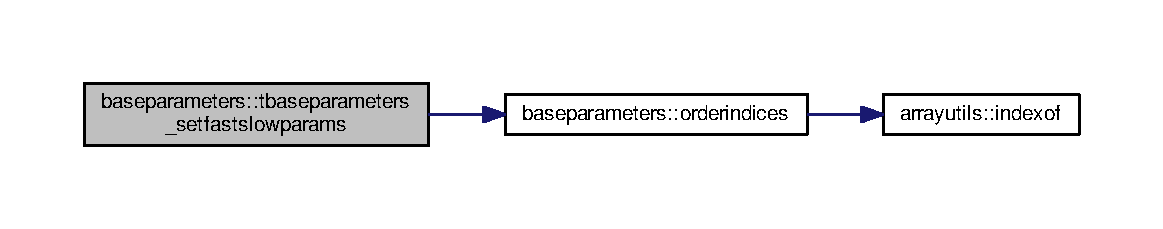
\includegraphics[width=350pt]{namespacebaseparameters_ac8f2cdce695f77b0f9cc3c2e86a9c05f_cgraph}
\end{center}
\end{figure}
\mbox{\Hypertarget{namespacebaseparameters_a1c41b4dbd4418bb1d16d77034504ac0b}\label{namespacebaseparameters_a1c41b4dbd4418bb1d16d77034504ac0b}} 
\index{baseparameters@{baseparameters}!tbaseparameters\+\_\+setstartpositions@{tbaseparameters\+\_\+setstartpositions}}
\index{tbaseparameters\+\_\+setstartpositions@{tbaseparameters\+\_\+setstartpositions}!baseparameters@{baseparameters}}
\subsubsection{\texorpdfstring{tbaseparameters\+\_\+setstartpositions()}{tbaseparameters\_setstartpositions()}}
{\footnotesize\ttfamily subroutine baseparameters\+::tbaseparameters\+\_\+setstartpositions (\begin{DoxyParamCaption}\item[{class(\mbox{\hyperlink{structbaseparameters_1_1tbaseparameters}{tbaseparameters}})}]{this,  }\item[{class(tcalculationatparampoint)}]{Params }\end{DoxyParamCaption})\hspace{0.3cm}{\ttfamily [private]}}



References randutils\+::gaussian1(), settings\+::num\+\_\+params\+\_\+used, and settings\+::params\+\_\+used.

Here is the call graph for this function\+:
\nopagebreak
\begin{figure}[H]
\begin{center}
\leavevmode
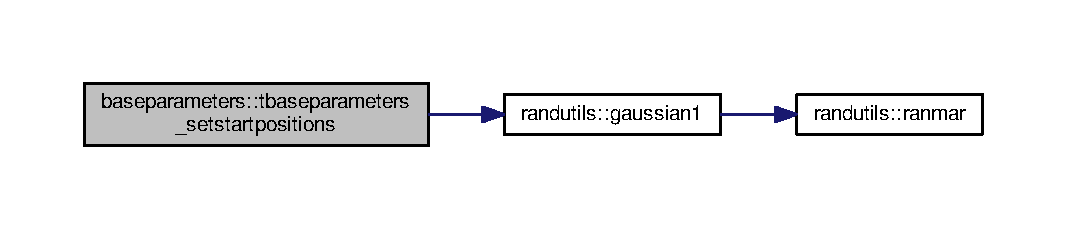
\includegraphics[width=350pt]{namespacebaseparameters_a1c41b4dbd4418bb1d16d77034504ac0b_cgraph}
\end{center}
\end{figure}
\mbox{\Hypertarget{namespacebaseparameters_a6fa6c72334203001f2e2932139df534d}\label{namespacebaseparameters_a6fa6c72334203001f2e2932139df534d}} 
\index{baseparameters@{baseparameters}!tbaseparameters\+\_\+usedparamnameornumber@{tbaseparameters\+\_\+usedparamnameornumber}}
\index{tbaseparameters\+\_\+usedparamnameornumber@{tbaseparameters\+\_\+usedparamnameornumber}!baseparameters@{baseparameters}}
\subsubsection{\texorpdfstring{tbaseparameters\+\_\+usedparamnameornumber()}{tbaseparameters\_usedparamnameornumber()}}
{\footnotesize\ttfamily character(len=\+:) function, allocatable baseparameters\+::tbaseparameters\+\_\+usedparamnameornumber (\begin{DoxyParamCaption}\item[{class(\mbox{\hyperlink{structbaseparameters_1_1tbaseparameters}{tbaseparameters}})}]{this,  }\item[{integer, intent(in)}]{i }\end{DoxyParamCaption})\hspace{0.3cm}{\ttfamily [private]}}



\subsection{Variable Documentation}
\mbox{\Hypertarget{namespacebaseparameters_abc9ecfbbf4a5012fbc95d3fb51a1e6e3}\label{namespacebaseparameters_abc9ecfbbf4a5012fbc95d3fb51a1e6e3}} 
\index{baseparameters@{baseparameters}!baseparams@{baseparams}}
\index{baseparams@{baseparams}!baseparameters@{baseparameters}}
\subsubsection{\texorpdfstring{baseparams}{baseparams}}
{\footnotesize\ttfamily type(\mbox{\hyperlink{structbaseparameters_1_1tbaseparameters}{tbaseparameters}}), save, public baseparameters\+::baseparams}



Referenced by samplecollector\+::checklimitsconverge(), estcovmatmodule\+::estcovmat(), estcovmatmodule\+::gethess(), calclike\+::getloglikebounds(), calclike\+::getlogpriors(), estcovmatmodule\+::getstepsfordchisq1(), parampointset\+::paramset\+\_\+readmodel(), parampointset\+::paramset\+\_\+writemodel(), tbaseparameters\+\_\+setfastslowparams(), samplecollector\+::tmpichaincollector\+\_\+addnewpoint(), samplecollector\+::tmpichaincollector\+\_\+readstate(), samplecollector\+::tmpichaincollector\+\_\+updatecovandcheckconverge(), generalsetup\+::tsetup\+\_\+doneinitialize(), and generalsetup\+::tsetup\+\_\+dosampling().

\mbox{\Hypertarget{namespacebaseparameters_a1d3e10105684d9171cdfec4ccfcd331d}\label{namespacebaseparameters_a1d3e10105684d9171cdfec4ccfcd331d}} 
\index{baseparameters@{baseparameters}!slow\+\_\+tp\+\_\+max@{slow\+\_\+tp\+\_\+max}}
\index{slow\+\_\+tp\+\_\+max@{slow\+\_\+tp\+\_\+max}!baseparameters@{baseparameters}}
\subsubsection{\texorpdfstring{slow\+\_\+tp\+\_\+max}{slow\_tp\_max}}
{\footnotesize\ttfamily integer, parameter, public baseparameters\+::slow\+\_\+tp\+\_\+max = \mbox{\hyperlink{namespacebaseparameters_a213e8b067e9d21216fbad3fbd98ec933}{tp\+\_\+semislow}}}



Referenced by tbaseparameters\+\_\+setfastslowparams().

\mbox{\Hypertarget{namespacebaseparameters_ac1f704b0992c1c1c9f90d320ae0c4f4b}\label{namespacebaseparameters_ac1f704b0992c1c1c9f90d320ae0c4f4b}} 
\index{baseparameters@{baseparameters}!tp\+\_\+fast@{tp\+\_\+fast}}
\index{tp\+\_\+fast@{tp\+\_\+fast}!baseparameters@{baseparameters}}
\subsubsection{\texorpdfstring{tp\+\_\+fast}{tp\_fast}}
{\footnotesize\ttfamily integer, parameter baseparameters\+::tp\+\_\+fast =4\hspace{0.3cm}{\ttfamily [private]}}



Referenced by tbaseparameters\+\_\+setfastslowparams().

\mbox{\Hypertarget{namespacebaseparameters_a4cae4f2dfd7f3b1ed425daca03b67139}\label{namespacebaseparameters_a4cae4f2dfd7f3b1ed425daca03b67139}} 
\index{baseparameters@{baseparameters}!tp\+\_\+semifast@{tp\+\_\+semifast}}
\index{tp\+\_\+semifast@{tp\+\_\+semifast}!baseparameters@{baseparameters}}
\subsubsection{\texorpdfstring{tp\+\_\+semifast}{tp\_semifast}}
{\footnotesize\ttfamily integer, parameter baseparameters\+::tp\+\_\+semifast =3\hspace{0.3cm}{\ttfamily [private]}}



Referenced by tbaseparameters\+\_\+setfastslowparams().

\mbox{\Hypertarget{namespacebaseparameters_a213e8b067e9d21216fbad3fbd98ec933}\label{namespacebaseparameters_a213e8b067e9d21216fbad3fbd98ec933}} 
\index{baseparameters@{baseparameters}!tp\+\_\+semislow@{tp\+\_\+semislow}}
\index{tp\+\_\+semislow@{tp\+\_\+semislow}!baseparameters@{baseparameters}}
\subsubsection{\texorpdfstring{tp\+\_\+semislow}{tp\_semislow}}
{\footnotesize\ttfamily integer, parameter baseparameters\+::tp\+\_\+semislow =2\hspace{0.3cm}{\ttfamily [private]}}



Referenced by tbaseparameters\+\_\+setfastslowparams().

\mbox{\Hypertarget{namespacebaseparameters_aec8c4b0ea0429954337dcf5fced6abf1}\label{namespacebaseparameters_aec8c4b0ea0429954337dcf5fced6abf1}} 
\index{baseparameters@{baseparameters}!tp\+\_\+slow@{tp\+\_\+slow}}
\index{tp\+\_\+slow@{tp\+\_\+slow}!baseparameters@{baseparameters}}
\subsubsection{\texorpdfstring{tp\+\_\+slow}{tp\_slow}}
{\footnotesize\ttfamily integer, parameter baseparameters\+::tp\+\_\+slow =1\hspace{0.3cm}{\ttfamily [private]}}



Referenced by tbaseparameters\+\_\+setfastslowparams().

\mbox{\Hypertarget{namespacebaseparameters_aa9a374c82230367604ae6b1c50ed3e3b}\label{namespacebaseparameters_aa9a374c82230367604ae6b1c50ed3e3b}} 
\index{baseparameters@{baseparameters}!tp\+\_\+unused@{tp\+\_\+unused}}
\index{tp\+\_\+unused@{tp\+\_\+unused}!baseparameters@{baseparameters}}
\subsubsection{\texorpdfstring{tp\+\_\+unused}{tp\_unused}}
{\footnotesize\ttfamily integer, parameter baseparameters\+::tp\+\_\+unused = 0\hspace{0.3cm}{\ttfamily [private]}}



Referenced by tbaseparameters\+\_\+setfastslowparams().


\hypertarget{namespacebbn}{}\section{bbn Namespace Reference}
\label{namespacebbn}\index{bbn@{bbn}}
\subsection*{Classes}
\begin{DoxyCompactItemize}
\item 
type \mbox{\hyperlink{structbbn_1_1tbbnpredictions}{tbbnpredictions}}
\end{DoxyCompactItemize}
\subsection*{Functions}
\begin{DoxyCompactItemize}
\item 
def \mbox{\hyperlink{namespacebbn_a2847147342b47e9a0dcfffe3f33ba3c8}{yhe\+\_\+to\+\_\+yp\+B\+BN}} (\mbox{\hyperlink{namespacebbn_a6d7727016804233cd030bc94e1f3500d}{Yp}})
\item 
def \mbox{\hyperlink{namespacebbn_a1aba6aa3826014d84016987b47e11b9a}{yp\+B\+B\+N\+\_\+to\+\_\+yhe}} (\mbox{\hyperlink{namespacebbn_a14098dbddadc5e64b5441f3d19aaf7c1}{Y\+B\+BN}})
\item 
def \mbox{\hyperlink{namespacebbn_a661709a863752020661d412858487224}{yhe\+\_\+fit}} (omegab, dneff, taun)
\item 
def \mbox{\hyperlink{namespacebbn_aeb738a501c7541234a13c16aeb6dbdf7}{dh\+\_\+fit}} (omegab, dneff, taun)
\item 
def \mbox{\hyperlink{namespacebbn_ae72b1fc1114a29eb8f18c248cf2809a2}{run\+B\+BN}} (\mbox{\hyperlink{namespacebbn_ace64c472b0c59f5fd0f811cd4dcdc2b4}{eta}}, DeltaN=0, tau=\mbox{\hyperlink{namespacebbn_a159aaa1465ea9c0555826fa3ea17d3ed}{tau\+\_\+n}}, prog=\textquotesingle{}./\mbox{\hyperlink{plotTT_8m_a9336ebf25087d91c818ee6e9ec29f8c1}{alter\+\_\+etannutau.\+x}}\textquotesingle{})
\item 
def \mbox{\hyperlink{namespacebbn_a16582965b56bffa4937822750bf05aae}{yp\+B\+B\+N\+\_\+\+Parthenope}} (omegab, neff)
\item 
def \mbox{\hyperlink{namespacebbn_a67d007a7323c319fdeaa32c288092939}{yhe\+\_\+to\+\_\+yp\+B\+BN}} (\mbox{\hyperlink{namespacebbn_a6d7727016804233cd030bc94e1f3500d}{Yp}}, ombh2)
\item 
def \mbox{\hyperlink{namespacebbn_a3b8ec567ef2fdae1e1daf85d6d520717}{run\+B\+B\+Nplot}} ()
\item 
subroutine \mbox{\hyperlink{namespacebbn_a7da9f22f9be32950185f79ed74e69f4d}{bbn\+\_\+init}} (this)
\item 
subroutine \mbox{\hyperlink{namespacebbn_a89ea6267ce0d1cfa1ff459d517558a53}{bbnpredictions\+\_\+error}} (this, S, v1, v2)
\end{DoxyCompactItemize}
\subsection*{Variables}
\begin{DoxyCompactItemize}
\item 
float \mbox{\hyperlink{namespacebbn_aa4b15a6720cfbfaebb9a8ba90c2d6615}{hbar}} = 1.\+05457e-\/34
\item 
int \mbox{\hyperlink{namespacebbn_ac2a771643cfcc5258e2d0a8d61096152}{c}} = 299792458.
\item 
float \mbox{\hyperlink{namespacebbn_ad8b80a31c3103c575ee91606b28c00b6}{kB}} = 1.\+380650e-\/23
\item 
float \mbox{\hyperlink{namespacebbn_a3a99f29ae890693870353fa67b0b034c}{MeV}} = 1.\+6021764e-\/13
\item 
float \mbox{\hyperlink{namespacebbn_a0747e524be761d23d14e43f4f45d522a}{eV}} = \mbox{\hyperlink{namespacebbn_a3a99f29ae890693870353fa67b0b034c}{MeV}} / 1e6
\item 
float \mbox{\hyperlink{namespacebbn_a52f93a6b9a98bb4b459145af6e1c0ffd}{G}} = 6.\+6738e-\/11
\item 
float \mbox{\hyperlink{namespacebbn_a45c7b6e0cda690af956e72f58b332e66}{T\+C\+MB}} = 2.\+7255
\item 
\mbox{\hyperlink{namespacebbn_a2de37c27807dd57d0dbea68a4f3992fa}{mP}} = np.\+sqrt(\mbox{\hyperlink{namespacebbn_aa4b15a6720cfbfaebb9a8ba90c2d6615}{hbar}} $\ast$ \mbox{\hyperlink{namespacebbn_ac2a771643cfcc5258e2d0a8d61096152}{c}} / \mbox{\hyperlink{namespacebbn_a52f93a6b9a98bb4b459145af6e1c0ffd}{G}})
\item 
float \mbox{\hyperlink{namespacebbn_a2c0a557eeaca292987c3ee7da6384295}{Mpc}} = 3.\+0856776e22
\item 
float \mbox{\hyperlink{namespacebbn_ac02aae5f2251db3c9b740d288330595d}{m\+\_\+proton}} = 1.\+672621637e-\/27
\item 
float \mbox{\hyperlink{namespacebbn_af144f84053152a233d6f7fe2f505589f}{m\+\_\+H}} = 1.\+673575e-\/27
\item 
float \mbox{\hyperlink{namespacebbn_a9ea8fb09e803dade7572cbbf146631cc}{not4}} = 3.\+9715
\item 
float \mbox{\hyperlink{namespacebbn_a5659e9c09b2847f14bb66c2d73e68191}{m\+\_\+\+He}} = \mbox{\hyperlink{namespacebbn_af144f84053152a233d6f7fe2f505589f}{m\+\_\+H}} $\ast$ \mbox{\hyperlink{namespacebbn_a9ea8fb09e803dade7572cbbf146631cc}{not4}}
\item 
float \mbox{\hyperlink{namespacebbn_a43d9d2d8599e22e361b96747ee7210fe}{zeta3}} = 1.\+202056903
\item 
float \mbox{\hyperlink{namespacebbn_a159aaa1465ea9c0555826fa3ea17d3ed}{tau\+\_\+n}} = 880.\+3
\item 
tuple \mbox{\hyperlink{namespacebbn_afb075d5c6ea4d70b7b6b502224ffbac9}{n\+\_\+photon}} = (\mbox{\hyperlink{namespacebbn_ad8b80a31c3103c575ee91606b28c00b6}{kB}} $\ast$ \mbox{\hyperlink{namespacebbn_a45c7b6e0cda690af956e72f58b332e66}{T\+C\+MB}} / \mbox{\hyperlink{namespacebbn_aa4b15a6720cfbfaebb9a8ba90c2d6615}{hbar}} / \mbox{\hyperlink{namespacebbn_ac2a771643cfcc5258e2d0a8d61096152}{c}}) $\ast$$\ast$ 3 $\ast$ \mbox{\hyperlink{namespacebbn_a43d9d2d8599e22e361b96747ee7210fe}{zeta3}} $\ast$ 2 / np.\+pi $\ast$$\ast$ 2
\item 
tuple \mbox{\hyperlink{namespacebbn_a7add864cda923ca0a40fda7711df51d5}{omegafac}} = (1e5 / Mpc) $\ast$$\ast$ 2 / (8 $\ast$ np.\+pi $\ast$ G) $\ast$ 3
\item 
bool \mbox{\hyperlink{namespacebbn_a218e3fff3cfb1735bc090edc24af0ba0}{alter\+B\+BN}} = False
\item 
\mbox{\hyperlink{namespacebbn_abfcfac0d0a6f15787c1f9bf37b990133}{ombh2s}}
\item 
list \mbox{\hyperlink{namespacebbn_a321af84b9281c0021371c705561390e1}{Delta\+Ns}} = \mbox{[}-\/3,-\/2,-\/1,-\/0.\+5,0,0.\+5,1,2,3,4,5,6,7\mbox{]}
\item 
list \mbox{\hyperlink{namespacebbn_a2ac37326174932ddf6ffd8f25c4619a8}{lines}} = \mbox{[}$\,$\mbox{]}
\item 
float \mbox{\hyperlink{namespacebbn_a8b00dee4a160e555ce5c5b347787d15e}{Yp\+\_\+fid}} = 0.\+2;
\item 
tuple \mbox{\hyperlink{namespacebbn_a6a197e513271f0796a8a4e5e2846b34d}{rho\+\_\+b}} = ombh2 $\ast$ \mbox{\hyperlink{namespacebbn_a7add864cda923ca0a40fda7711df51d5}{omegafac}};
\item 
def \mbox{\hyperlink{namespacebbn_a14098dbddadc5e64b5441f3d19aaf7c1}{Y\+B\+BN}} = \mbox{\hyperlink{namespacebbn_a661709a863752020661d412858487224}{yhe\+\_\+fit}}(ombh2, DeltaN, \mbox{\hyperlink{namespacebbn_a159aaa1465ea9c0555826fa3ea17d3ed}{tau\+\_\+n}})
\item 
tuple \mbox{\hyperlink{namespacebbn_a08ca9283eb4fca8cde9e83fc5a201313}{n\+\_\+baryon}} = (4 $\ast$ \mbox{\hyperlink{namespacebbn_a8b00dee4a160e555ce5c5b347787d15e}{Yp\+\_\+fid}} / \mbox{\hyperlink{namespacebbn_a5659e9c09b2847f14bb66c2d73e68191}{m\+\_\+\+He}} + (1 -\/ \mbox{\hyperlink{namespacebbn_a8b00dee4a160e555ce5c5b347787d15e}{Yp\+\_\+fid}}) / \mbox{\hyperlink{namespacebbn_af144f84053152a233d6f7fe2f505589f}{m\+\_\+H}}) $\ast$ \mbox{\hyperlink{namespacebbn_a6a197e513271f0796a8a4e5e2846b34d}{rho\+\_\+b}}
\item 
tuple \mbox{\hyperlink{namespacebbn_ace64c472b0c59f5fd0f811cd4dcdc2b4}{eta}} = \mbox{\hyperlink{namespacebbn_a08ca9283eb4fca8cde9e83fc5a201313}{n\+\_\+baryon}} / \mbox{\hyperlink{namespacebbn_afb075d5c6ea4d70b7b6b502224ffbac9}{n\+\_\+photon}}
\item 
def \mbox{\hyperlink{namespacebbn_a7379640051724fc37488eeefda65ad65}{outtxt}} = \mbox{\hyperlink{namespacebbn_ae72b1fc1114a29eb8f18c248cf2809a2}{run\+B\+BN}}(\mbox{\hyperlink{namespacebbn_ace64c472b0c59f5fd0f811cd4dcdc2b4}{eta}},DeltaN)
\item 
\mbox{\hyperlink{namespacebbn_a09803392cfa25aa97a65a0a040c37c65}{D}} = \mbox{\hyperlink{namespacebbn_aeb738a501c7541234a13c16aeb6dbdf7}{dh\+\_\+fit}}(ombh2, DeltaN, \mbox{\hyperlink{namespacebbn_a159aaa1465ea9c0555826fa3ea17d3ed}{tau\+\_\+n}})$\ast$1e-\/5
\item 
\mbox{\hyperlink{namespacebbn_a9555376bf33bf65ae1f681790b3d4254}{He3}}
\item 
\mbox{\hyperlink{namespacebbn_a5ed6387f606410099a6ddc296df92172}{Li7}}
\item 
\mbox{\hyperlink{namespacebbn_aa1a56fdfe29a2355c7f96d84bd324e75}{Li6}}
\item 
\mbox{\hyperlink{namespacebbn_a8f6f39fb3510b10df3c72c5db5546bc6}{Be7}}
\item 
\mbox{\hyperlink{namespacebbn_a3854fe11c613aba4501a3a94b65ac9c4}{sig\+Y\+B\+BN}} = 0.\+0003
\item 
\mbox{\hyperlink{namespacebbn_a6be4b105afa5f8364fae6d3f15da0237}{sigdD}} = 6e-\/7
\item 
\mbox{\hyperlink{namespacebbn_aa49cc668dc9f3245dd252658a222d8c3}{sig\+He3}}
\item 
\mbox{\hyperlink{namespacebbn_aaad7704075759b4c52a9c44d9ffbdd00}{sig\+Li7}}
\item 
\mbox{\hyperlink{namespacebbn_a43c42a4abbe70e0f2382677ffdeed099}{sig\+Li6}}
\item 
\mbox{\hyperlink{namespacebbn_a9d4e16ed7bc4cd480ffd59999e5d9c79}{sig\+Be7}}
\item 
tuple \mbox{\hyperlink{namespacebbn_a693a5d1e528c587feab5af05b0434b93}{actual\+\_\+ombh2}} = \mbox{\hyperlink{namespacebbn_ace64c472b0c59f5fd0f811cd4dcdc2b4}{eta}} $\ast$ \mbox{\hyperlink{namespacebbn_afb075d5c6ea4d70b7b6b502224ffbac9}{n\+\_\+photon}} $\ast$ (\mbox{\hyperlink{namespacebbn_a14098dbddadc5e64b5441f3d19aaf7c1}{Y\+B\+BN}} $\ast$ \mbox{\hyperlink{namespacebbn_a5659e9c09b2847f14bb66c2d73e68191}{m\+\_\+\+He}} / 4 + (1 -\/ \mbox{\hyperlink{namespacebbn_a14098dbddadc5e64b5441f3d19aaf7c1}{Y\+B\+BN}}) $\ast$ \mbox{\hyperlink{namespacebbn_af144f84053152a233d6f7fe2f505589f}{m\+\_\+H}})/\mbox{\hyperlink{namespacebbn_a7add864cda923ca0a40fda7711df51d5}{omegafac}}
\item 
tuple \mbox{\hyperlink{namespacebbn_a6d7727016804233cd030bc94e1f3500d}{Yp}} = (\mbox{\hyperlink{namespacebbn_ace64c472b0c59f5fd0f811cd4dcdc2b4}{eta}} $\ast$ \mbox{\hyperlink{namespacebbn_afb075d5c6ea4d70b7b6b502224ffbac9}{n\+\_\+photon}}/ \mbox{\hyperlink{namespacebbn_a693a5d1e528c587feab5af05b0434b93}{actual\+\_\+ombh2}}/\mbox{\hyperlink{namespacebbn_a7add864cda923ca0a40fda7711df51d5}{omegafac}}-\/ 1/\mbox{\hyperlink{namespacebbn_af144f84053152a233d6f7fe2f505589f}{m\+\_\+H}})/(4/\mbox{\hyperlink{namespacebbn_a5659e9c09b2847f14bb66c2d73e68191}{m\+\_\+\+He}}-\/1/\mbox{\hyperlink{namespacebbn_af144f84053152a233d6f7fe2f505589f}{m\+\_\+H}})
\item 
tuple \mbox{\hyperlink{namespacebbn_ac9bb8b77af91c3a7edb1568c3f455083}{line}} = ((\textquotesingle{}\%12.\+5f \textquotesingle{})$\ast$6 + (\textquotesingle{}\%12.\+3e \%12.\+2e\textquotesingle{})$\ast$3)\%(actual\+\_\+ombh2, eta$\ast$1e10, Delta\+N, Yp, Y\+B\+B\+N, sig\+Y\+B\+B\+N, D, sigd\+D, He3, sig\+He3,\+Li7,sig\+Li7)
\item 
\mbox{\hyperlink{namespacebbn_aea59ac7535e41dcb59e7a347152270e7}{f}} = open(\textquotesingle{}B\+B\+N\+\_\+full\+\_\+alter\+B\+B\+N\+\_\+\textquotesingle{}+str(\mbox{\hyperlink{namespacebbn_a159aaa1465ea9c0555826fa3ea17d3ed}{tau\+\_\+n}})+\textquotesingle{}.dat\textquotesingle{}, \textquotesingle{}w\textquotesingle{})
\item 
type(\mbox{\hyperlink{structbbn_1_1tbbnpredictions}{tbbnpredictions}}), target, save \mbox{\hyperlink{namespacebbn_a32b631b9e3dda13eb68cc107abe6b861}{bbn\+\_\+yhe}}
\item 
type(\mbox{\hyperlink{structbbn_1_1tbbnpredictions}{tbbnpredictions}}), target, save \mbox{\hyperlink{namespacebbn_a4f282765adaec1cd6e128f858dbc245b}{bbn\+\_\+ypbbn}} = T\+B\+B\+N\+Predictions(data\+\_\+col=5)
\item 
type(\mbox{\hyperlink{structbbn_1_1tbbnpredictions}{tbbnpredictions}}), target, save \mbox{\hyperlink{namespacebbn_a21e11bb5000d0be2b824a94078d295a1}{bbn\+\_\+ypbbn\+\_\+err}} = T\+B\+B\+N\+Predictions(data\+\_\+col=6)
\item 
type(\mbox{\hyperlink{structbbn_1_1tbbnpredictions}{tbbnpredictions}}), target, save \mbox{\hyperlink{namespacebbn_af26d781a68adbe31f1993cc7e36a6e50}{bbn\+\_\+dh}} = T\+B\+B\+N\+Predictions(data\+\_\+col=7)
\item 
type(\mbox{\hyperlink{structbbn_1_1tbbnpredictions}{tbbnpredictions}}), target, save \mbox{\hyperlink{namespacebbn_af20311a952d5520b6e4f5a44795175a3}{bbn\+\_\+dh\+\_\+err}} = T\+B\+B\+N\+Predictions(data\+\_\+col=8)
\item 
character(len= $\ast$), parameter \mbox{\hyperlink{namespacebbn_a177fdccd2bbdc4ff1dd71c8047184d91}{bbn\+\_\+data\+\_\+file}} = \textquotesingle{}B\+B\+N\+\_\+full\+\_\+\+Parthenelope\+\_\+880.\+3.\+dat\textquotesingle{}
\end{DoxyCompactItemize}


\subsection{Function Documentation}
\mbox{\Hypertarget{namespacebbn_a7da9f22f9be32950185f79ed74e69f4d}\label{namespacebbn_a7da9f22f9be32950185f79ed74e69f4d}} 
\index{bbn@{bbn}!bbn\+\_\+init@{bbn\+\_\+init}}
\index{bbn\+\_\+init@{bbn\+\_\+init}!bbn@{bbn}}
\subsubsection{\texorpdfstring{bbn\+\_\+init()}{bbn\_init()}}
{\footnotesize\ttfamily subroutine bbn\+::bbn\+\_\+init (\begin{DoxyParamCaption}\item[{class(\mbox{\hyperlink{structbbn_1_1tbbnpredictions}{tbbnpredictions}})}]{this }\end{DoxyParamCaption})}



References bbn\+\_\+data\+\_\+file, settings\+::datadir, and settings\+::feedback.

\mbox{\Hypertarget{namespacebbn_a89ea6267ce0d1cfa1ff459d517558a53}\label{namespacebbn_a89ea6267ce0d1cfa1ff459d517558a53}} 
\index{bbn@{bbn}!bbnpredictions\+\_\+error@{bbnpredictions\+\_\+error}}
\index{bbnpredictions\+\_\+error@{bbnpredictions\+\_\+error}!bbn@{bbn}}
\subsubsection{\texorpdfstring{bbnpredictions\+\_\+error()}{bbnpredictions\_error()}}
{\footnotesize\ttfamily subroutine bbn\+::bbnpredictions\+\_\+error (\begin{DoxyParamCaption}\item[{class(\mbox{\hyperlink{structbbn_1_1tbbnpredictions}{tbbnpredictions}})}]{this,  }\item[{character(len=$\ast$), intent(in)}]{S,  }\item[{class($\ast$), intent(in), optional}]{v1,  }\item[{class($\ast$), intent(in), optional}]{v2 }\end{DoxyParamCaption})}

\mbox{\Hypertarget{namespacebbn_aeb738a501c7541234a13c16aeb6dbdf7}\label{namespacebbn_aeb738a501c7541234a13c16aeb6dbdf7}} 
\index{bbn@{bbn}!dh\+\_\+fit@{dh\+\_\+fit}}
\index{dh\+\_\+fit@{dh\+\_\+fit}!bbn@{bbn}}
\subsubsection{\texorpdfstring{dh\+\_\+fit()}{dh\_fit()}}
{\footnotesize\ttfamily def bbn.\+dh\+\_\+fit (\begin{DoxyParamCaption}\item[{}]{omegab,  }\item[{}]{dneff,  }\item[{}]{taun }\end{DoxyParamCaption})}

\mbox{\Hypertarget{namespacebbn_ae72b1fc1114a29eb8f18c248cf2809a2}\label{namespacebbn_ae72b1fc1114a29eb8f18c248cf2809a2}} 
\index{bbn@{bbn}!run\+B\+BN@{run\+B\+BN}}
\index{run\+B\+BN@{run\+B\+BN}!bbn@{bbn}}
\subsubsection{\texorpdfstring{run\+B\+B\+N()}{runBBN()}}
{\footnotesize\ttfamily def bbn.\+run\+B\+BN (\begin{DoxyParamCaption}\item[{}]{eta,  }\item[{}]{DeltaN = {\ttfamily 0},  }\item[{}]{tau = {\ttfamily \mbox{\hyperlink{namespacebbn_a159aaa1465ea9c0555826fa3ea17d3ed}{tau\+\_\+n}}},  }\item[{}]{prog = {\ttfamily \textquotesingle{}./\mbox{\hyperlink{plotTT_8m_a9336ebf25087d91c818ee6e9ec29f8c1}{alter\+\_\+etannutau.\+x}}\textquotesingle{}} }\end{DoxyParamCaption})}



Referenced by run\+B\+B\+Nplot().

Here is the caller graph for this function\+:
\nopagebreak
\begin{figure}[H]
\begin{center}
\leavevmode
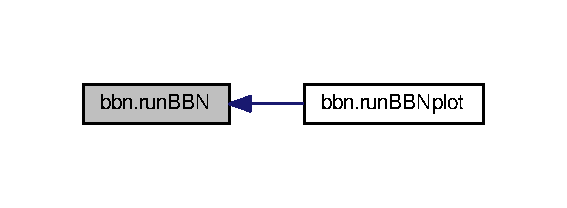
\includegraphics[width=272pt]{namespacebbn_ae72b1fc1114a29eb8f18c248cf2809a2_icgraph}
\end{center}
\end{figure}
\mbox{\Hypertarget{namespacebbn_a3b8ec567ef2fdae1e1daf85d6d520717}\label{namespacebbn_a3b8ec567ef2fdae1e1daf85d6d520717}} 
\index{bbn@{bbn}!run\+B\+B\+Nplot@{run\+B\+B\+Nplot}}
\index{run\+B\+B\+Nplot@{run\+B\+B\+Nplot}!bbn@{bbn}}
\subsubsection{\texorpdfstring{run\+B\+B\+Nplot()}{runBBNplot()}}
{\footnotesize\ttfamily def bbn.\+run\+B\+B\+Nplot (\begin{DoxyParamCaption}{ }\end{DoxyParamCaption})}



References C\+A\+M\+B\+\_\+test\+\_\+files.\+float, stringutils.\+join(), and run\+B\+B\+N().

Here is the call graph for this function\+:
\nopagebreak
\begin{figure}[H]
\begin{center}
\leavevmode
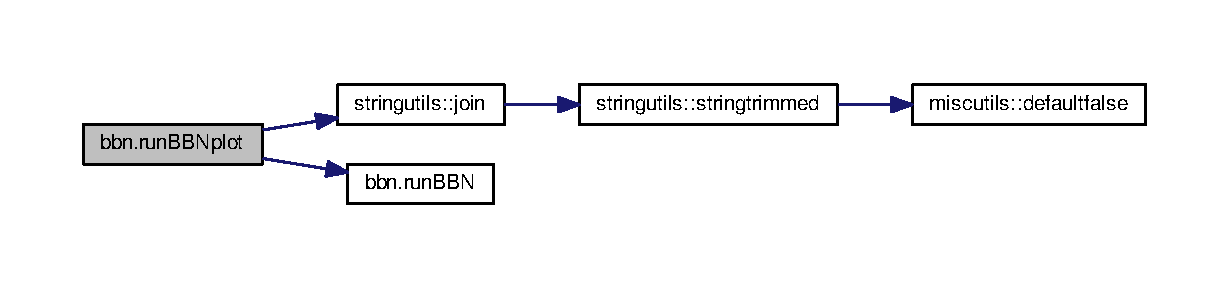
\includegraphics[width=350pt]{namespacebbn_a3b8ec567ef2fdae1e1daf85d6d520717_cgraph}
\end{center}
\end{figure}
\mbox{\Hypertarget{namespacebbn_a661709a863752020661d412858487224}\label{namespacebbn_a661709a863752020661d412858487224}} 
\index{bbn@{bbn}!yhe\+\_\+fit@{yhe\+\_\+fit}}
\index{yhe\+\_\+fit@{yhe\+\_\+fit}!bbn@{bbn}}
\subsubsection{\texorpdfstring{yhe\+\_\+fit()}{yhe\_fit()}}
{\footnotesize\ttfamily def bbn.\+yhe\+\_\+fit (\begin{DoxyParamCaption}\item[{}]{omegab,  }\item[{}]{dneff,  }\item[{}]{taun }\end{DoxyParamCaption})}



Referenced by camb.\+model.\+C\+A\+M\+Bparams.\+set\+\_\+bbn\+\_\+helium().

Here is the caller graph for this function\+:
\nopagebreak
\begin{figure}[H]
\begin{center}
\leavevmode
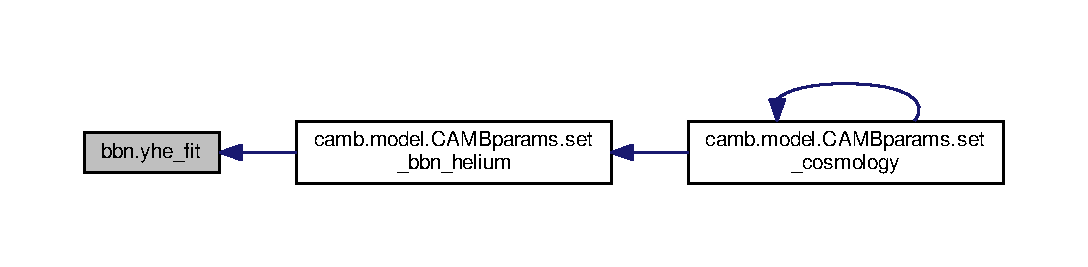
\includegraphics[width=350pt]{namespacebbn_a661709a863752020661d412858487224_icgraph}
\end{center}
\end{figure}
\mbox{\Hypertarget{namespacebbn_a2847147342b47e9a0dcfffe3f33ba3c8}\label{namespacebbn_a2847147342b47e9a0dcfffe3f33ba3c8}} 
\index{bbn@{bbn}!yhe\+\_\+to\+\_\+yp\+B\+BN@{yhe\+\_\+to\+\_\+yp\+B\+BN}}
\index{yhe\+\_\+to\+\_\+yp\+B\+BN@{yhe\+\_\+to\+\_\+yp\+B\+BN}!bbn@{bbn}}
\subsubsection{\texorpdfstring{yhe\+\_\+to\+\_\+yp\+B\+B\+N()}{yhe\_to\_ypBBN()}\hspace{0.1cm}{\footnotesize\ttfamily [1/2]}}
{\footnotesize\ttfamily def bbn.\+yhe\+\_\+to\+\_\+yp\+B\+BN (\begin{DoxyParamCaption}\item[{}]{Yp }\end{DoxyParamCaption})}



Referenced by yhe\+\_\+to\+\_\+yp\+B\+B\+N().

Here is the caller graph for this function\+:
\nopagebreak
\begin{figure}[H]
\begin{center}
\leavevmode
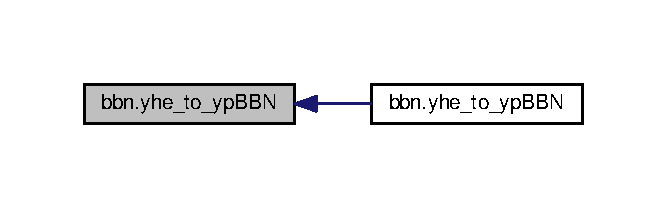
\includegraphics[width=320pt]{namespacebbn_a2847147342b47e9a0dcfffe3f33ba3c8_icgraph}
\end{center}
\end{figure}
\mbox{\Hypertarget{namespacebbn_a67d007a7323c319fdeaa32c288092939}\label{namespacebbn_a67d007a7323c319fdeaa32c288092939}} 
\index{bbn@{bbn}!yhe\+\_\+to\+\_\+yp\+B\+BN@{yhe\+\_\+to\+\_\+yp\+B\+BN}}
\index{yhe\+\_\+to\+\_\+yp\+B\+BN@{yhe\+\_\+to\+\_\+yp\+B\+BN}!bbn@{bbn}}
\subsubsection{\texorpdfstring{yhe\+\_\+to\+\_\+yp\+B\+B\+N()}{yhe\_to\_ypBBN()}\hspace{0.1cm}{\footnotesize\ttfamily [2/2]}}
{\footnotesize\ttfamily def bbn.\+yhe\+\_\+to\+\_\+yp\+B\+BN (\begin{DoxyParamCaption}\item[{}]{Yp,  }\item[{}]{ombh2 }\end{DoxyParamCaption})}



References yhe\+\_\+to\+\_\+yp\+B\+B\+N().

Here is the call graph for this function\+:
\nopagebreak
\begin{figure}[H]
\begin{center}
\leavevmode
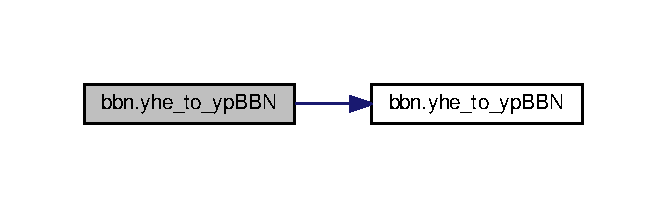
\includegraphics[width=320pt]{namespacebbn_a67d007a7323c319fdeaa32c288092939_cgraph}
\end{center}
\end{figure}
\mbox{\Hypertarget{namespacebbn_a16582965b56bffa4937822750bf05aae}\label{namespacebbn_a16582965b56bffa4937822750bf05aae}} 
\index{bbn@{bbn}!yp\+B\+B\+N\+\_\+\+Parthenope@{yp\+B\+B\+N\+\_\+\+Parthenope}}
\index{yp\+B\+B\+N\+\_\+\+Parthenope@{yp\+B\+B\+N\+\_\+\+Parthenope}!bbn@{bbn}}
\subsubsection{\texorpdfstring{yp\+B\+B\+N\+\_\+\+Parthenope()}{ypBBN\_Parthenope()}}
{\footnotesize\ttfamily def bbn.\+yp\+B\+B\+N\+\_\+\+Parthenope (\begin{DoxyParamCaption}\item[{}]{omegab,  }\item[{}]{neff }\end{DoxyParamCaption})}

\mbox{\Hypertarget{namespacebbn_a1aba6aa3826014d84016987b47e11b9a}\label{namespacebbn_a1aba6aa3826014d84016987b47e11b9a}} 
\index{bbn@{bbn}!yp\+B\+B\+N\+\_\+to\+\_\+yhe@{yp\+B\+B\+N\+\_\+to\+\_\+yhe}}
\index{yp\+B\+B\+N\+\_\+to\+\_\+yhe@{yp\+B\+B\+N\+\_\+to\+\_\+yhe}!bbn@{bbn}}
\subsubsection{\texorpdfstring{yp\+B\+B\+N\+\_\+to\+\_\+yhe()}{ypBBN\_to\_yhe()}}
{\footnotesize\ttfamily def bbn.\+yp\+B\+B\+N\+\_\+to\+\_\+yhe (\begin{DoxyParamCaption}\item[{}]{Y\+B\+BN }\end{DoxyParamCaption})}



\subsection{Variable Documentation}
\mbox{\Hypertarget{namespacebbn_a693a5d1e528c587feab5af05b0434b93}\label{namespacebbn_a693a5d1e528c587feab5af05b0434b93}} 
\index{bbn@{bbn}!actual\+\_\+ombh2@{actual\+\_\+ombh2}}
\index{actual\+\_\+ombh2@{actual\+\_\+ombh2}!bbn@{bbn}}
\subsubsection{\texorpdfstring{actual\+\_\+ombh2}{actual\_ombh2}}
{\footnotesize\ttfamily tuple bbn.\+actual\+\_\+ombh2 = \mbox{\hyperlink{namespacebbn_ace64c472b0c59f5fd0f811cd4dcdc2b4}{eta}} $\ast$ \mbox{\hyperlink{namespacebbn_afb075d5c6ea4d70b7b6b502224ffbac9}{n\+\_\+photon}} $\ast$ (\mbox{\hyperlink{namespacebbn_a14098dbddadc5e64b5441f3d19aaf7c1}{Y\+B\+BN}} $\ast$ \mbox{\hyperlink{namespacebbn_a5659e9c09b2847f14bb66c2d73e68191}{m\+\_\+\+He}} / 4 + (1 -\/ \mbox{\hyperlink{namespacebbn_a14098dbddadc5e64b5441f3d19aaf7c1}{Y\+B\+BN}}) $\ast$ \mbox{\hyperlink{namespacebbn_af144f84053152a233d6f7fe2f505589f}{m\+\_\+H}})/\mbox{\hyperlink{namespacebbn_a7add864cda923ca0a40fda7711df51d5}{omegafac}}}

\mbox{\Hypertarget{namespacebbn_a218e3fff3cfb1735bc090edc24af0ba0}\label{namespacebbn_a218e3fff3cfb1735bc090edc24af0ba0}} 
\index{bbn@{bbn}!alter\+B\+BN@{alter\+B\+BN}}
\index{alter\+B\+BN@{alter\+B\+BN}!bbn@{bbn}}
\subsubsection{\texorpdfstring{alter\+B\+BN}{alterBBN}}
{\footnotesize\ttfamily bool bbn.\+alter\+B\+BN = False}

\mbox{\Hypertarget{namespacebbn_a177fdccd2bbdc4ff1dd71c8047184d91}\label{namespacebbn_a177fdccd2bbdc4ff1dd71c8047184d91}} 
\index{bbn@{bbn}!bbn\+\_\+data\+\_\+file@{bbn\+\_\+data\+\_\+file}}
\index{bbn\+\_\+data\+\_\+file@{bbn\+\_\+data\+\_\+file}!bbn@{bbn}}
\subsubsection{\texorpdfstring{bbn\+\_\+data\+\_\+file}{bbn\_data\_file}}
{\footnotesize\ttfamily character(len=$\ast$), parameter bbn.\+bbn\+\_\+data\+\_\+file = \textquotesingle{}B\+B\+N\+\_\+full\+\_\+\+Parthenelope\+\_\+880.\+3.\+dat\textquotesingle{}}



Referenced by bbn\+\_\+init().

\mbox{\Hypertarget{namespacebbn_af26d781a68adbe31f1993cc7e36a6e50}\label{namespacebbn_af26d781a68adbe31f1993cc7e36a6e50}} 
\index{bbn@{bbn}!bbn\+\_\+dh@{bbn\+\_\+dh}}
\index{bbn\+\_\+dh@{bbn\+\_\+dh}!bbn@{bbn}}
\subsubsection{\texorpdfstring{bbn\+\_\+dh}{bbn\_dh}}
{\footnotesize\ttfamily type(\mbox{\hyperlink{structbbn_1_1tbbnpredictions}{tbbnpredictions}}), target, save bbn.\+bbn\+\_\+dh = T\+B\+B\+N\+Predictions(data\+\_\+col=7)}



Referenced by elementabundances\+::abundance\+\_\+readini(), and cosmologyparameterizations\+::tp\+\_\+calcderivedparams().

\mbox{\Hypertarget{namespacebbn_af20311a952d5520b6e4f5a44795175a3}\label{namespacebbn_af20311a952d5520b6e4f5a44795175a3}} 
\index{bbn@{bbn}!bbn\+\_\+dh\+\_\+err@{bbn\+\_\+dh\+\_\+err}}
\index{bbn\+\_\+dh\+\_\+err@{bbn\+\_\+dh\+\_\+err}!bbn@{bbn}}
\subsubsection{\texorpdfstring{bbn\+\_\+dh\+\_\+err}{bbn\_dh\_err}}
{\footnotesize\ttfamily type(\mbox{\hyperlink{structbbn_1_1tbbnpredictions}{tbbnpredictions}}), target, save bbn.\+bbn\+\_\+dh\+\_\+err = T\+B\+B\+N\+Predictions(data\+\_\+col=8)}



Referenced by elementabundances\+::abundance\+\_\+readini().

\mbox{\Hypertarget{namespacebbn_a32b631b9e3dda13eb68cc107abe6b861}\label{namespacebbn_a32b631b9e3dda13eb68cc107abe6b861}} 
\index{bbn@{bbn}!bbn\+\_\+yhe@{bbn\+\_\+yhe}}
\index{bbn\+\_\+yhe@{bbn\+\_\+yhe}!bbn@{bbn}}
\subsubsection{\texorpdfstring{bbn\+\_\+yhe}{bbn\_yhe}}
{\footnotesize\ttfamily type(\mbox{\hyperlink{structbbn_1_1tbbnpredictions}{tbbnpredictions}}), target, save bbn.\+bbn\+\_\+yhe}

\mbox{\Hypertarget{namespacebbn_a4f282765adaec1cd6e128f858dbc245b}\label{namespacebbn_a4f282765adaec1cd6e128f858dbc245b}} 
\index{bbn@{bbn}!bbn\+\_\+ypbbn@{bbn\+\_\+ypbbn}}
\index{bbn\+\_\+ypbbn@{bbn\+\_\+ypbbn}!bbn@{bbn}}
\subsubsection{\texorpdfstring{bbn\+\_\+ypbbn}{bbn\_ypbbn}}
{\footnotesize\ttfamily type(\mbox{\hyperlink{structbbn_1_1tbbnpredictions}{tbbnpredictions}}), target, save bbn.\+bbn\+\_\+ypbbn = T\+B\+B\+N\+Predictions(data\+\_\+col=5)}



Referenced by elementabundances\+::abundance\+\_\+readini().

\mbox{\Hypertarget{namespacebbn_a21e11bb5000d0be2b824a94078d295a1}\label{namespacebbn_a21e11bb5000d0be2b824a94078d295a1}} 
\index{bbn@{bbn}!bbn\+\_\+ypbbn\+\_\+err@{bbn\+\_\+ypbbn\+\_\+err}}
\index{bbn\+\_\+ypbbn\+\_\+err@{bbn\+\_\+ypbbn\+\_\+err}!bbn@{bbn}}
\subsubsection{\texorpdfstring{bbn\+\_\+ypbbn\+\_\+err}{bbn\_ypbbn\_err}}
{\footnotesize\ttfamily type(\mbox{\hyperlink{structbbn_1_1tbbnpredictions}{tbbnpredictions}}), target, save bbn.\+bbn\+\_\+ypbbn\+\_\+err = T\+B\+B\+N\+Predictions(data\+\_\+col=6)}



Referenced by elementabundances\+::abundance\+\_\+readini().

\mbox{\Hypertarget{namespacebbn_a8f6f39fb3510b10df3c72c5db5546bc6}\label{namespacebbn_a8f6f39fb3510b10df3c72c5db5546bc6}} 
\index{bbn@{bbn}!Be7@{Be7}}
\index{Be7@{Be7}!bbn@{bbn}}
\subsubsection{\texorpdfstring{Be7}{Be7}}
{\footnotesize\ttfamily bbn.\+Be7}

\mbox{\Hypertarget{namespacebbn_ac2a771643cfcc5258e2d0a8d61096152}\label{namespacebbn_ac2a771643cfcc5258e2d0a8d61096152}} 
\index{bbn@{bbn}!c@{c}}
\index{c@{c}!bbn@{bbn}}
\subsubsection{\texorpdfstring{c}{c}}
{\footnotesize\ttfamily int bbn.\+c = 299792458.}

\mbox{\Hypertarget{namespacebbn_a09803392cfa25aa97a65a0a040c37c65}\label{namespacebbn_a09803392cfa25aa97a65a0a040c37c65}} 
\index{bbn@{bbn}!D@{D}}
\index{D@{D}!bbn@{bbn}}
\subsubsection{\texorpdfstring{D}{D}}
{\footnotesize\ttfamily def bbn.\+D = \mbox{\hyperlink{namespacebbn_aeb738a501c7541234a13c16aeb6dbdf7}{dh\+\_\+fit}}(ombh2, DeltaN, \mbox{\hyperlink{namespacebbn_a159aaa1465ea9c0555826fa3ea17d3ed}{tau\+\_\+n}})$\ast$1e-\/5}

\mbox{\Hypertarget{namespacebbn_a321af84b9281c0021371c705561390e1}\label{namespacebbn_a321af84b9281c0021371c705561390e1}} 
\index{bbn@{bbn}!Delta\+Ns@{Delta\+Ns}}
\index{Delta\+Ns@{Delta\+Ns}!bbn@{bbn}}
\subsubsection{\texorpdfstring{Delta\+Ns}{DeltaNs}}
{\footnotesize\ttfamily list bbn.\+Delta\+Ns = \mbox{[}-\/3,-\/2,-\/1,-\/0.\+5,0,0.\+5,1,2,3,4,5,6,7\mbox{]}}

\mbox{\Hypertarget{namespacebbn_ace64c472b0c59f5fd0f811cd4dcdc2b4}\label{namespacebbn_ace64c472b0c59f5fd0f811cd4dcdc2b4}} 
\index{bbn@{bbn}!eta@{eta}}
\index{eta@{eta}!bbn@{bbn}}
\subsubsection{\texorpdfstring{eta}{eta}}
{\footnotesize\ttfamily tuple bbn.\+eta = \mbox{\hyperlink{namespacebbn_a08ca9283eb4fca8cde9e83fc5a201313}{n\+\_\+baryon}} / \mbox{\hyperlink{namespacebbn_afb075d5c6ea4d70b7b6b502224ffbac9}{n\+\_\+photon}}}

\mbox{\Hypertarget{namespacebbn_a0747e524be761d23d14e43f4f45d522a}\label{namespacebbn_a0747e524be761d23d14e43f4f45d522a}} 
\index{bbn@{bbn}!eV@{eV}}
\index{eV@{eV}!bbn@{bbn}}
\subsubsection{\texorpdfstring{eV}{eV}}
{\footnotesize\ttfamily float bbn.\+eV = \mbox{\hyperlink{namespacebbn_a3a99f29ae890693870353fa67b0b034c}{MeV}} / 1e6}

\mbox{\Hypertarget{namespacebbn_aea59ac7535e41dcb59e7a347152270e7}\label{namespacebbn_aea59ac7535e41dcb59e7a347152270e7}} 
\index{bbn@{bbn}!f@{f}}
\index{f@{f}!bbn@{bbn}}
\subsubsection{\texorpdfstring{f}{f}}
{\footnotesize\ttfamily bbn.\+f = open(\textquotesingle{}B\+B\+N\+\_\+full\+\_\+alter\+B\+B\+N\+\_\+\textquotesingle{}+str(\mbox{\hyperlink{namespacebbn_a159aaa1465ea9c0555826fa3ea17d3ed}{tau\+\_\+n}})+\textquotesingle{}.dat\textquotesingle{}, \textquotesingle{}w\textquotesingle{})}

\mbox{\Hypertarget{namespacebbn_a52f93a6b9a98bb4b459145af6e1c0ffd}\label{namespacebbn_a52f93a6b9a98bb4b459145af6e1c0ffd}} 
\index{bbn@{bbn}!G@{G}}
\index{G@{G}!bbn@{bbn}}
\subsubsection{\texorpdfstring{G}{G}}
{\footnotesize\ttfamily float bbn.\+G = 6.\+6738e-\/11}

\mbox{\Hypertarget{namespacebbn_aa4b15a6720cfbfaebb9a8ba90c2d6615}\label{namespacebbn_aa4b15a6720cfbfaebb9a8ba90c2d6615}} 
\index{bbn@{bbn}!hbar@{hbar}}
\index{hbar@{hbar}!bbn@{bbn}}
\subsubsection{\texorpdfstring{hbar}{hbar}}
{\footnotesize\ttfamily float bbn.\+hbar = 1.\+05457e-\/34}

\mbox{\Hypertarget{namespacebbn_a9555376bf33bf65ae1f681790b3d4254}\label{namespacebbn_a9555376bf33bf65ae1f681790b3d4254}} 
\index{bbn@{bbn}!He3@{He3}}
\index{He3@{He3}!bbn@{bbn}}
\subsubsection{\texorpdfstring{He3}{He3}}
{\footnotesize\ttfamily bbn.\+He3}

\mbox{\Hypertarget{namespacebbn_ad8b80a31c3103c575ee91606b28c00b6}\label{namespacebbn_ad8b80a31c3103c575ee91606b28c00b6}} 
\index{bbn@{bbn}!kB@{kB}}
\index{kB@{kB}!bbn@{bbn}}
\subsubsection{\texorpdfstring{kB}{kB}}
{\footnotesize\ttfamily float bbn.\+kB = 1.\+380650e-\/23}

\mbox{\Hypertarget{namespacebbn_aa1a56fdfe29a2355c7f96d84bd324e75}\label{namespacebbn_aa1a56fdfe29a2355c7f96d84bd324e75}} 
\index{bbn@{bbn}!Li6@{Li6}}
\index{Li6@{Li6}!bbn@{bbn}}
\subsubsection{\texorpdfstring{Li6}{Li6}}
{\footnotesize\ttfamily bbn.\+Li6}

\mbox{\Hypertarget{namespacebbn_a5ed6387f606410099a6ddc296df92172}\label{namespacebbn_a5ed6387f606410099a6ddc296df92172}} 
\index{bbn@{bbn}!Li7@{Li7}}
\index{Li7@{Li7}!bbn@{bbn}}
\subsubsection{\texorpdfstring{Li7}{Li7}}
{\footnotesize\ttfamily bbn.\+Li7}

\mbox{\Hypertarget{namespacebbn_ac9bb8b77af91c3a7edb1568c3f455083}\label{namespacebbn_ac9bb8b77af91c3a7edb1568c3f455083}} 
\index{bbn@{bbn}!line@{line}}
\index{line@{line}!bbn@{bbn}}
\subsubsection{\texorpdfstring{line}{line}}
{\footnotesize\ttfamily tuple bbn.\+line = ((\textquotesingle{}\%12.\+5f \textquotesingle{})$\ast$6 + (\textquotesingle{}\%12.\+3e \%12.\+2e\textquotesingle{})$\ast$3)\%(actual\+\_\+ombh2, eta$\ast$1e10, Delta\+N, Yp, Y\+B\+B\+N, sig\+Y\+B\+B\+N, D, sigd\+D, He3, sig\+He3,\+Li7,sig\+Li7)}

\mbox{\Hypertarget{namespacebbn_a2ac37326174932ddf6ffd8f25c4619a8}\label{namespacebbn_a2ac37326174932ddf6ffd8f25c4619a8}} 
\index{bbn@{bbn}!lines@{lines}}
\index{lines@{lines}!bbn@{bbn}}
\subsubsection{\texorpdfstring{lines}{lines}}
{\footnotesize\ttfamily list bbn.\+lines = \mbox{[}$\,$\mbox{]}}

\mbox{\Hypertarget{namespacebbn_af144f84053152a233d6f7fe2f505589f}\label{namespacebbn_af144f84053152a233d6f7fe2f505589f}} 
\index{bbn@{bbn}!m\+\_\+H@{m\+\_\+H}}
\index{m\+\_\+H@{m\+\_\+H}!bbn@{bbn}}
\subsubsection{\texorpdfstring{m\+\_\+H}{m\_H}}
{\footnotesize\ttfamily float bbn.\+m\+\_\+H = 1.\+673575e-\/27}

\mbox{\Hypertarget{namespacebbn_a5659e9c09b2847f14bb66c2d73e68191}\label{namespacebbn_a5659e9c09b2847f14bb66c2d73e68191}} 
\index{bbn@{bbn}!m\+\_\+\+He@{m\+\_\+\+He}}
\index{m\+\_\+\+He@{m\+\_\+\+He}!bbn@{bbn}}
\subsubsection{\texorpdfstring{m\+\_\+\+He}{m\_He}}
{\footnotesize\ttfamily float bbn.\+m\+\_\+\+He = \mbox{\hyperlink{namespacebbn_af144f84053152a233d6f7fe2f505589f}{m\+\_\+H}} $\ast$ \mbox{\hyperlink{namespacebbn_a9ea8fb09e803dade7572cbbf146631cc}{not4}}}

\mbox{\Hypertarget{namespacebbn_ac02aae5f2251db3c9b740d288330595d}\label{namespacebbn_ac02aae5f2251db3c9b740d288330595d}} 
\index{bbn@{bbn}!m\+\_\+proton@{m\+\_\+proton}}
\index{m\+\_\+proton@{m\+\_\+proton}!bbn@{bbn}}
\subsubsection{\texorpdfstring{m\+\_\+proton}{m\_proton}}
{\footnotesize\ttfamily float bbn.\+m\+\_\+proton = 1.\+672621637e-\/27}

\mbox{\Hypertarget{namespacebbn_a3a99f29ae890693870353fa67b0b034c}\label{namespacebbn_a3a99f29ae890693870353fa67b0b034c}} 
\index{bbn@{bbn}!MeV@{MeV}}
\index{MeV@{MeV}!bbn@{bbn}}
\subsubsection{\texorpdfstring{MeV}{MeV}}
{\footnotesize\ttfamily float bbn.\+MeV = 1.\+6021764e-\/13}

\mbox{\Hypertarget{namespacebbn_a2de37c27807dd57d0dbea68a4f3992fa}\label{namespacebbn_a2de37c27807dd57d0dbea68a4f3992fa}} 
\index{bbn@{bbn}!mP@{mP}}
\index{mP@{mP}!bbn@{bbn}}
\subsubsection{\texorpdfstring{mP}{mP}}
{\footnotesize\ttfamily bbn.\+mP = np.\+sqrt(\mbox{\hyperlink{namespacebbn_aa4b15a6720cfbfaebb9a8ba90c2d6615}{hbar}} $\ast$ \mbox{\hyperlink{namespacebbn_ac2a771643cfcc5258e2d0a8d61096152}{c}} / \mbox{\hyperlink{namespacebbn_a52f93a6b9a98bb4b459145af6e1c0ffd}{G}})}

\mbox{\Hypertarget{namespacebbn_a2c0a557eeaca292987c3ee7da6384295}\label{namespacebbn_a2c0a557eeaca292987c3ee7da6384295}} 
\index{bbn@{bbn}!Mpc@{Mpc}}
\index{Mpc@{Mpc}!bbn@{bbn}}
\subsubsection{\texorpdfstring{Mpc}{Mpc}}
{\footnotesize\ttfamily float bbn.\+Mpc = 3.\+0856776e22}

\mbox{\Hypertarget{namespacebbn_a08ca9283eb4fca8cde9e83fc5a201313}\label{namespacebbn_a08ca9283eb4fca8cde9e83fc5a201313}} 
\index{bbn@{bbn}!n\+\_\+baryon@{n\+\_\+baryon}}
\index{n\+\_\+baryon@{n\+\_\+baryon}!bbn@{bbn}}
\subsubsection{\texorpdfstring{n\+\_\+baryon}{n\_baryon}}
{\footnotesize\ttfamily tuple bbn.\+n\+\_\+baryon = (4 $\ast$ \mbox{\hyperlink{namespacebbn_a8b00dee4a160e555ce5c5b347787d15e}{Yp\+\_\+fid}} / \mbox{\hyperlink{namespacebbn_a5659e9c09b2847f14bb66c2d73e68191}{m\+\_\+\+He}} + (1 -\/ \mbox{\hyperlink{namespacebbn_a8b00dee4a160e555ce5c5b347787d15e}{Yp\+\_\+fid}}) / \mbox{\hyperlink{namespacebbn_af144f84053152a233d6f7fe2f505589f}{m\+\_\+H}}) $\ast$ \mbox{\hyperlink{namespacebbn_a6a197e513271f0796a8a4e5e2846b34d}{rho\+\_\+b}}}

\mbox{\Hypertarget{namespacebbn_afb075d5c6ea4d70b7b6b502224ffbac9}\label{namespacebbn_afb075d5c6ea4d70b7b6b502224ffbac9}} 
\index{bbn@{bbn}!n\+\_\+photon@{n\+\_\+photon}}
\index{n\+\_\+photon@{n\+\_\+photon}!bbn@{bbn}}
\subsubsection{\texorpdfstring{n\+\_\+photon}{n\_photon}}
{\footnotesize\ttfamily tuple bbn.\+n\+\_\+photon = (\mbox{\hyperlink{namespacebbn_ad8b80a31c3103c575ee91606b28c00b6}{kB}} $\ast$ \mbox{\hyperlink{namespacebbn_a45c7b6e0cda690af956e72f58b332e66}{T\+C\+MB}} / \mbox{\hyperlink{namespacebbn_aa4b15a6720cfbfaebb9a8ba90c2d6615}{hbar}} / \mbox{\hyperlink{namespacebbn_ac2a771643cfcc5258e2d0a8d61096152}{c}}) $\ast$$\ast$ 3 $\ast$ \mbox{\hyperlink{namespacebbn_a43d9d2d8599e22e361b96747ee7210fe}{zeta3}} $\ast$ 2 / np.\+pi $\ast$$\ast$ 2}

\mbox{\Hypertarget{namespacebbn_a9ea8fb09e803dade7572cbbf146631cc}\label{namespacebbn_a9ea8fb09e803dade7572cbbf146631cc}} 
\index{bbn@{bbn}!not4@{not4}}
\index{not4@{not4}!bbn@{bbn}}
\subsubsection{\texorpdfstring{not4}{not4}}
{\footnotesize\ttfamily float bbn.\+not4 = 3.\+9715}

\mbox{\Hypertarget{namespacebbn_abfcfac0d0a6f15787c1f9bf37b990133}\label{namespacebbn_abfcfac0d0a6f15787c1f9bf37b990133}} 
\index{bbn@{bbn}!ombh2s@{ombh2s}}
\index{ombh2s@{ombh2s}!bbn@{bbn}}
\subsubsection{\texorpdfstring{ombh2s}{ombh2s}}
{\footnotesize\ttfamily bbn.\+ombh2s}

{\bfseries Initial value\+:}
\begin{DoxyCode}
1 =  np.hstack((np.linspace(0.005, 0.02, num=\mbox{\hyperlink{namespaceCAMB__test__files_ae3f939a649209ec8d0004b0dfef3210b}{int}}((0.02 - 0.005) / 0.001), endpoint=\textcolor{keyword}{False}),
2          np.linspace(0.020,0.024, num=16 , endpoint=\textcolor{keyword}{False}),
3          np.linspace(0.024, 0.04, num=\mbox{\hyperlink{namespaceCAMB__test__files_ae3f939a649209ec8d0004b0dfef3210b}{int}}((0.04 - 0.024) / 0.001) + 1, endpoint=\textcolor{keyword}{True})))
\end{DoxyCode}
\mbox{\Hypertarget{namespacebbn_a7add864cda923ca0a40fda7711df51d5}\label{namespacebbn_a7add864cda923ca0a40fda7711df51d5}} 
\index{bbn@{bbn}!omegafac@{omegafac}}
\index{omegafac@{omegafac}!bbn@{bbn}}
\subsubsection{\texorpdfstring{omegafac}{omegafac}}
{\footnotesize\ttfamily tuple bbn.\+omegafac = (1e5 / Mpc) $\ast$$\ast$ 2 / (8 $\ast$ np.\+pi $\ast$ G) $\ast$ 3}

\mbox{\Hypertarget{namespacebbn_a7379640051724fc37488eeefda65ad65}\label{namespacebbn_a7379640051724fc37488eeefda65ad65}} 
\index{bbn@{bbn}!outtxt@{outtxt}}
\index{outtxt@{outtxt}!bbn@{bbn}}
\subsubsection{\texorpdfstring{outtxt}{outtxt}}
{\footnotesize\ttfamily def bbn.\+outtxt = \mbox{\hyperlink{namespacebbn_ae72b1fc1114a29eb8f18c248cf2809a2}{run\+B\+BN}}(\mbox{\hyperlink{namespacebbn_ace64c472b0c59f5fd0f811cd4dcdc2b4}{eta}},DeltaN)}

\mbox{\Hypertarget{namespacebbn_a6a197e513271f0796a8a4e5e2846b34d}\label{namespacebbn_a6a197e513271f0796a8a4e5e2846b34d}} 
\index{bbn@{bbn}!rho\+\_\+b@{rho\+\_\+b}}
\index{rho\+\_\+b@{rho\+\_\+b}!bbn@{bbn}}
\subsubsection{\texorpdfstring{rho\+\_\+b}{rho\_b}}
{\footnotesize\ttfamily tuple bbn.\+rho\+\_\+b = ombh2 $\ast$ \mbox{\hyperlink{namespacebbn_a7add864cda923ca0a40fda7711df51d5}{omegafac}};}

\mbox{\Hypertarget{namespacebbn_a9d4e16ed7bc4cd480ffd59999e5d9c79}\label{namespacebbn_a9d4e16ed7bc4cd480ffd59999e5d9c79}} 
\index{bbn@{bbn}!sig\+Be7@{sig\+Be7}}
\index{sig\+Be7@{sig\+Be7}!bbn@{bbn}}
\subsubsection{\texorpdfstring{sig\+Be7}{sigBe7}}
{\footnotesize\ttfamily bbn.\+sig\+Be7}

\mbox{\Hypertarget{namespacebbn_a6be4b105afa5f8364fae6d3f15da0237}\label{namespacebbn_a6be4b105afa5f8364fae6d3f15da0237}} 
\index{bbn@{bbn}!sigdD@{sigdD}}
\index{sigdD@{sigdD}!bbn@{bbn}}
\subsubsection{\texorpdfstring{sigdD}{sigdD}}
{\footnotesize\ttfamily int bbn.\+sigdD = 6e-\/7}

\mbox{\Hypertarget{namespacebbn_aa49cc668dc9f3245dd252658a222d8c3}\label{namespacebbn_aa49cc668dc9f3245dd252658a222d8c3}} 
\index{bbn@{bbn}!sig\+He3@{sig\+He3}}
\index{sig\+He3@{sig\+He3}!bbn@{bbn}}
\subsubsection{\texorpdfstring{sig\+He3}{sigHe3}}
{\footnotesize\ttfamily bbn.\+sig\+He3}

\mbox{\Hypertarget{namespacebbn_a43c42a4abbe70e0f2382677ffdeed099}\label{namespacebbn_a43c42a4abbe70e0f2382677ffdeed099}} 
\index{bbn@{bbn}!sig\+Li6@{sig\+Li6}}
\index{sig\+Li6@{sig\+Li6}!bbn@{bbn}}
\subsubsection{\texorpdfstring{sig\+Li6}{sigLi6}}
{\footnotesize\ttfamily bbn.\+sig\+Li6}

\mbox{\Hypertarget{namespacebbn_aaad7704075759b4c52a9c44d9ffbdd00}\label{namespacebbn_aaad7704075759b4c52a9c44d9ffbdd00}} 
\index{bbn@{bbn}!sig\+Li7@{sig\+Li7}}
\index{sig\+Li7@{sig\+Li7}!bbn@{bbn}}
\subsubsection{\texorpdfstring{sig\+Li7}{sigLi7}}
{\footnotesize\ttfamily bbn.\+sig\+Li7}

\mbox{\Hypertarget{namespacebbn_a3854fe11c613aba4501a3a94b65ac9c4}\label{namespacebbn_a3854fe11c613aba4501a3a94b65ac9c4}} 
\index{bbn@{bbn}!sig\+Y\+B\+BN@{sig\+Y\+B\+BN}}
\index{sig\+Y\+B\+BN@{sig\+Y\+B\+BN}!bbn@{bbn}}
\subsubsection{\texorpdfstring{sig\+Y\+B\+BN}{sigYBBN}}
{\footnotesize\ttfamily float bbn.\+sig\+Y\+B\+BN = 0.\+0003}

\mbox{\Hypertarget{namespacebbn_a159aaa1465ea9c0555826fa3ea17d3ed}\label{namespacebbn_a159aaa1465ea9c0555826fa3ea17d3ed}} 
\index{bbn@{bbn}!tau\+\_\+n@{tau\+\_\+n}}
\index{tau\+\_\+n@{tau\+\_\+n}!bbn@{bbn}}
\subsubsection{\texorpdfstring{tau\+\_\+n}{tau\_n}}
{\footnotesize\ttfamily float bbn.\+tau\+\_\+n = 880.\+3}

\mbox{\Hypertarget{namespacebbn_a45c7b6e0cda690af956e72f58b332e66}\label{namespacebbn_a45c7b6e0cda690af956e72f58b332e66}} 
\index{bbn@{bbn}!T\+C\+MB@{T\+C\+MB}}
\index{T\+C\+MB@{T\+C\+MB}!bbn@{bbn}}
\subsubsection{\texorpdfstring{T\+C\+MB}{TCMB}}
{\footnotesize\ttfamily float bbn.\+T\+C\+MB = 2.\+7255}

\mbox{\Hypertarget{namespacebbn_a14098dbddadc5e64b5441f3d19aaf7c1}\label{namespacebbn_a14098dbddadc5e64b5441f3d19aaf7c1}} 
\index{bbn@{bbn}!Y\+B\+BN@{Y\+B\+BN}}
\index{Y\+B\+BN@{Y\+B\+BN}!bbn@{bbn}}
\subsubsection{\texorpdfstring{Y\+B\+BN}{YBBN}}
{\footnotesize\ttfamily bbn.\+Y\+B\+BN = \mbox{\hyperlink{namespacebbn_a661709a863752020661d412858487224}{yhe\+\_\+fit}}(ombh2, DeltaN, \mbox{\hyperlink{namespacebbn_a159aaa1465ea9c0555826fa3ea17d3ed}{tau\+\_\+n}})}

\mbox{\Hypertarget{namespacebbn_a6d7727016804233cd030bc94e1f3500d}\label{namespacebbn_a6d7727016804233cd030bc94e1f3500d}} 
\index{bbn@{bbn}!Yp@{Yp}}
\index{Yp@{Yp}!bbn@{bbn}}
\subsubsection{\texorpdfstring{Yp}{Yp}}
{\footnotesize\ttfamily float bbn.\+Yp = (\mbox{\hyperlink{namespacebbn_ace64c472b0c59f5fd0f811cd4dcdc2b4}{eta}} $\ast$ \mbox{\hyperlink{namespacebbn_afb075d5c6ea4d70b7b6b502224ffbac9}{n\+\_\+photon}}/ \mbox{\hyperlink{namespacebbn_a693a5d1e528c587feab5af05b0434b93}{actual\+\_\+ombh2}}/\mbox{\hyperlink{namespacebbn_a7add864cda923ca0a40fda7711df51d5}{omegafac}}-\/ 1/\mbox{\hyperlink{namespacebbn_af144f84053152a233d6f7fe2f505589f}{m\+\_\+H}})/(4/\mbox{\hyperlink{namespacebbn_a5659e9c09b2847f14bb66c2d73e68191}{m\+\_\+\+He}}-\/1/\mbox{\hyperlink{namespacebbn_af144f84053152a233d6f7fe2f505589f}{m\+\_\+H}})}

\mbox{\Hypertarget{namespacebbn_a8b00dee4a160e555ce5c5b347787d15e}\label{namespacebbn_a8b00dee4a160e555ce5c5b347787d15e}} 
\index{bbn@{bbn}!Yp\+\_\+fid@{Yp\+\_\+fid}}
\index{Yp\+\_\+fid@{Yp\+\_\+fid}!bbn@{bbn}}
\subsubsection{\texorpdfstring{Yp\+\_\+fid}{Yp\_fid}}
{\footnotesize\ttfamily tuple bbn.\+Yp\+\_\+fid = 0.\+2;}

\mbox{\Hypertarget{namespacebbn_a43d9d2d8599e22e361b96747ee7210fe}\label{namespacebbn_a43d9d2d8599e22e361b96747ee7210fe}} 
\index{bbn@{bbn}!zeta3@{zeta3}}
\index{zeta3@{zeta3}!bbn@{bbn}}
\subsubsection{\texorpdfstring{zeta3}{zeta3}}
{\footnotesize\ttfamily float bbn.\+zeta3 = 1.\+202056903}


\hypertarget{namespacebbn__yhe}{}\section{bbn\+\_\+yhe Namespace Reference}
\label{namespacebbn__yhe}\index{bbn\+\_\+yhe@{bbn\+\_\+yhe}}
\subsection*{Functions}
\begin{DoxyCompactItemize}
\item 
def \mbox{\hyperlink{namespacebbn__yhe_a38c5abbad8fad900f60f86b5038cf0e8}{yhe\+\_\+to\+\_\+yp\+B\+BN}} (Yp)
\item 
def \mbox{\hyperlink{namespacebbn__yhe_a207fd25c1dedf810f926879ba5899d38}{add\+Yp\+Fit}} (samples)
\item 
def \mbox{\hyperlink{namespacebbn__yhe_ab07e92f80f62d425303d08e5e8fe604d}{add\+Yp\+Fit\+Roots}} (\mbox{\hyperlink{namespacebbn__yhe_ab2add45031a3e0b76e777d91fd6eff67}{roots}})
\item 
def \mbox{\hyperlink{namespacebbn__yhe_a0ae2fc2b1719f17ae48ec9dee3de6728}{yp\+B\+BN}} (omegab, dneff, taun=880.\+3)
\item 
def \mbox{\hyperlink{namespacebbn__yhe_a3e9988b282cca4d66a7481dbf9676939}{dh\+\_\+fit}} (omegab, dneff, taun=880.\+3)
\end{DoxyCompactItemize}
\subsection*{Variables}
\begin{DoxyCompactItemize}
\item 
float \mbox{\hyperlink{namespacebbn__yhe_a06123892f977e5e00eb0e7bcf6866dbb}{sigma\+\_\+yp\+\_\+theo}} = 0.\+0003
\item 
int \mbox{\hyperlink{namespacebbn__yhe_a3aa1ae9b0ed6bd135e4fc002b7eca1a9}{num\+\_\+ob}} = 50
\item 
float \mbox{\hyperlink{namespacebbn__yhe_aa005d4473664db0db345095282beb1ef}{ob\+\_\+min}} = 0.\+018
\item 
float \mbox{\hyperlink{namespacebbn__yhe_a7ad9cbb8dc27628c6fbf6296bba963ca}{ob\+\_\+max}} = 0.\+026
\item 
float \mbox{\hyperlink{namespacebbn__yhe_a624706ed018b5d06d3e1ceea58a08e12}{yp\+\_\+min}} = 0.\+15
\item 
float \mbox{\hyperlink{namespacebbn__yhe_a1b95d70c9d6b84360f839ed708b14c72}{yp\+\_\+max}} = 0.\+35
\item 
float \mbox{\hyperlink{namespacebbn__yhe_a9d5e61e6f78e3497a8c5fce8daedf276}{aver\+\_\+mean}} = 0.\+2465
\item 
float \mbox{\hyperlink{namespacebbn__yhe_af08345da95d7b1ecff384b5ca5648a03}{aver\+\_\+sigma}} = 0.\+0097
\item 
float \mbox{\hyperlink{namespacebbn__yhe_ad00e51b24c6c009e64a8baa0f0b51ad8}{sere\+\_\+minus}} = 0.\+294
\item 
float \mbox{\hyperlink{namespacebbn__yhe_a8c95d448cd274ce585cfaf255bd4ff1b}{sere\+\_\+plus}} = \mbox{\hyperlink{namespacebbn__yhe_a1b95d70c9d6b84360f839ed708b14c72}{yp\+\_\+max}}
\item 
\mbox{\hyperlink{namespacebbn__yhe_a0189ca7d3d30cadc352fe3c5f419d73a}{sere\+\_\+b}} = np.\+zeros(2, dtype=\textquotesingle{}float\textquotesingle{})
\item 
\mbox{\hyperlink{namespacebbn__yhe_a113b4f8c034ac6ea013657ba051687e1}{sere\+\_\+y1}} = np.\+zeros(2, dtype=\textquotesingle{}float\textquotesingle{})
\item 
\mbox{\hyperlink{namespacebbn__yhe_a5df6de601295fe7e1b92a79b727ccbc3}{sere\+\_\+y2}} = np.\+zeros(2, dtype=\textquotesingle{}float\textquotesingle{})
\item 
list \mbox{\hyperlink{namespacebbn__yhe_a90f26535b1262c9980ba8f8dea539709}{labels}} = \mbox{[}s.\+defplanck, s.\+defplanck + \char`\"{}+B\+AO\char`\"{}, s.\+planckall\mbox{]}
\item 
list \mbox{\hyperlink{namespacebbn__yhe_a063490560da67d4aa74baa317b66577a}{datatag}} = \mbox{[}s.\+defdata, s.\+defdata + \textquotesingle{}\+\_\+\+B\+AO\textquotesingle{}, s.\+defdata\+\_\+all\mbox{]}
\item 
\mbox{\hyperlink{namespacebbn__yhe_a28ea3e3cf2288f549b58603f5a80dd23}{g}} = s.\+get\+Single\+Plotter()
\begin{DoxyCompactList}\small\item\em ombh2 -\/\+Yhe \#\#\#\#\#\#\#\#\#\#\#\#\# \end{DoxyCompactList}\item 
\mbox{\hyperlink{namespacebbn__yhe_a68a4915540c5ddfdf951a7612c20358d}{colors}} = g.\+settings.\+solid\+\_\+colors\mbox{[}3\+:0\+:-\/1\mbox{]}
\item 
\mbox{\hyperlink{namespacebbn__yhe_a8da3e95ccabe26e7b02faafa8d0c7d0a}{bbn\+\_\+b}} = np.\+arange(\mbox{\hyperlink{namespacebbn__yhe_aa005d4473664db0db345095282beb1ef}{ob\+\_\+min}}, \mbox{\hyperlink{namespacebbn__yhe_a7ad9cbb8dc27628c6fbf6296bba963ca}{ob\+\_\+max}} + 0.\+1, (\mbox{\hyperlink{namespacebbn__yhe_a7ad9cbb8dc27628c6fbf6296bba963ca}{ob\+\_\+max}} -\/ \mbox{\hyperlink{namespacebbn__yhe_aa005d4473664db0db345095282beb1ef}{ob\+\_\+min}}) / \mbox{\hyperlink{namespacebbn__yhe_a3aa1ae9b0ed6bd135e4fc002b7eca1a9}{num\+\_\+ob}})
\item 
def \mbox{\hyperlink{namespacebbn__yhe_a28b53c029dcb7310ef25c077dbf59bab}{bbn\+\_\+y}} = \mbox{\hyperlink{namespacebbn__yhe_a0ae2fc2b1719f17ae48ec9dee3de6728}{yp\+B\+BN}}(\mbox{\hyperlink{namespacebbn__yhe_a8da3e95ccabe26e7b02faafa8d0c7d0a}{bbn\+\_\+b}}, 0)
\item 
def \mbox{\hyperlink{namespacebbn__yhe_a3f8a67b91f6391a7bd8ea269672ac615}{bbn\+\_\+y1}} = \mbox{\hyperlink{namespacebbn__yhe_a28b53c029dcb7310ef25c077dbf59bab}{bbn\+\_\+y}} -\/ \mbox{\hyperlink{namespacebbn__yhe_a06123892f977e5e00eb0e7bcf6866dbb}{sigma\+\_\+yp\+\_\+theo}}
\item 
def \mbox{\hyperlink{namespacebbn__yhe_ae522afab9400241fb8bc86962e60e9b5}{bbn\+\_\+y2}} = \mbox{\hyperlink{namespacebbn__yhe_a28b53c029dcb7310ef25c077dbf59bab}{bbn\+\_\+y}} + \mbox{\hyperlink{namespacebbn__yhe_a06123892f977e5e00eb0e7bcf6866dbb}{sigma\+\_\+yp\+\_\+theo}}
\item 
\mbox{\hyperlink{namespacebbn__yhe_adaa6abf83a5db41a605b66fcf1072747}{xlim}}
\item 
\mbox{\hyperlink{namespacebbn__yhe_aee3ed9037ad3216e40a5e87b91d33f27}{alpha}}
\item 
\mbox{\hyperlink{namespacebbn__yhe_a5febb2e61726249209662394b5d95858}{color}}
\item 
\mbox{\hyperlink{namespacebbn__yhe_af98c0d13e6e8393dac53d8e115f2c906}{linestyle}}
\item 
\mbox{\hyperlink{namespacebbn__yhe_a3bb9da91cb045382b8f944eb5c8e14fe}{fontsize}}
\item 
list \mbox{\hyperlink{namespacebbn__yhe_ab2add45031a3e0b76e777d91fd6eff67}{roots}} = \mbox{[}g.\+get\+Root(\textquotesingle{}yhe\textquotesingle{}, d) for d in \mbox{\hyperlink{namespacebbn__yhe_a063490560da67d4aa74baa317b66577a}{datatag}}\mbox{]}
\item 
\mbox{\hyperlink{namespacebbn__yhe_ac2c1a41c88f2f983a89e6f3af095d520}{legend\+\_\+fontsize}}
\item 
\mbox{\hyperlink{namespacebbn__yhe_a27906639887f7d86e9893c3c8c102f9b}{filled}}
\item 
\mbox{\hyperlink{namespacebbn__yhe_a6d53cb6d1d4b9038a14d5b038ef4b4ff}{True}}
\item 
\mbox{\hyperlink{namespacebbn__yhe_a8fb3d2af891fa129948db45632d05b4c}{lims}}
\item 
\mbox{\hyperlink{namespacebbn__yhe_aadedc8e6798c93b5bf445f5d1bd0c19f}{legend\+\_\+loc}}
\item 
\mbox{\hyperlink{namespacebbn__yhe_a49bc13f65125eafd22fc160f104e8444}{colored\+\_\+text}}
\item 
\mbox{\hyperlink{namespacebbn__yhe_a3123808ee1e6304665a2980e073efed9}{xy}}
\item 
\mbox{\hyperlink{namespacebbn__yhe_a24e8c7a1ae7d3b9a225c19f2a79cf681}{xycoords}}
\item 
\mbox{\hyperlink{namespacebbn__yhe_a26224bf035e3019da5ed20ac3aece4e8}{xytext}}
\item 
\mbox{\hyperlink{namespacebbn__yhe_ad9e6a1e307d4e22bacaa587397fa346e}{textcoords}}
\item 
\mbox{\hyperlink{namespacebbn__yhe_a4e580183b4dd2ab4042be13ffec6c525}{arrowprops}}
\item 
float \mbox{\hyperlink{namespacebbn__yhe_a12d17f1eceb939479da944d753f67417}{N\+\_\+min}} = 0.\+01
\item 
int \mbox{\hyperlink{namespacebbn__yhe_a97d4d46b2f4aad7933899daacdfa4e8d}{N\+\_\+max}} = 5
\item 
\mbox{\hyperlink{namespacebbn__yhe_a0974f7b16b7e2bc7419b63acb59f5a68}{Neff}} = np.\+arange(\mbox{\hyperlink{namespacebbn__yhe_a12d17f1eceb939479da944d753f67417}{N\+\_\+min}}, \mbox{\hyperlink{namespacebbn__yhe_a97d4d46b2f4aad7933899daacdfa4e8d}{N\+\_\+max}} + 0.\+1, 0.\+1)
\item 
list \mbox{\hyperlink{namespacebbn__yhe_aaa4728644822d8c49e68fadd68ede623}{Nrange}} = \mbox{[}\mbox{\hyperlink{namespacebbn__yhe_a12d17f1eceb939479da944d753f67417}{N\+\_\+min}}, \mbox{\hyperlink{namespacebbn__yhe_a97d4d46b2f4aad7933899daacdfa4e8d}{N\+\_\+max}}\mbox{]}
\item 
\mbox{\hyperlink{namespacebbn__yhe_af0aeb2348a1c9932c656174611593164}{False}}
\item 
\mbox{\hyperlink{namespacebbn__yhe_a77232bd6b32ee374dbd5504aaba84b10}{tag}}
\end{DoxyCompactItemize}


\subsection{Function Documentation}
\mbox{\Hypertarget{namespacebbn__yhe_a207fd25c1dedf810f926879ba5899d38}\label{namespacebbn__yhe_a207fd25c1dedf810f926879ba5899d38}} 
\index{bbn\+\_\+yhe@{bbn\+\_\+yhe}!add\+Yp\+Fit@{add\+Yp\+Fit}}
\index{add\+Yp\+Fit@{add\+Yp\+Fit}!bbn\+\_\+yhe@{bbn\+\_\+yhe}}
\subsubsection{\texorpdfstring{add\+Yp\+Fit()}{addYpFit()}}
{\footnotesize\ttfamily def bbn\+\_\+yhe.\+add\+Yp\+Fit (\begin{DoxyParamCaption}\item[{}]{samples }\end{DoxyParamCaption})}



References yhe\+\_\+to\+\_\+yp\+B\+B\+N().



Referenced by add\+Yp\+Fit\+Roots().

Here is the call graph for this function\+:
\nopagebreak
\begin{figure}[H]
\begin{center}
\leavevmode
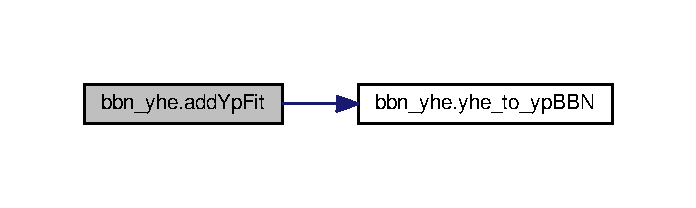
\includegraphics[width=334pt]{namespacebbn__yhe_a207fd25c1dedf810f926879ba5899d38_cgraph}
\end{center}
\end{figure}
Here is the caller graph for this function\+:
\nopagebreak
\begin{figure}[H]
\begin{center}
\leavevmode
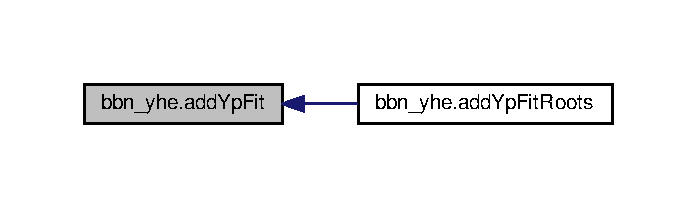
\includegraphics[width=334pt]{namespacebbn__yhe_a207fd25c1dedf810f926879ba5899d38_icgraph}
\end{center}
\end{figure}
\mbox{\Hypertarget{namespacebbn__yhe_ab07e92f80f62d425303d08e5e8fe604d}\label{namespacebbn__yhe_ab07e92f80f62d425303d08e5e8fe604d}} 
\index{bbn\+\_\+yhe@{bbn\+\_\+yhe}!add\+Yp\+Fit\+Roots@{add\+Yp\+Fit\+Roots}}
\index{add\+Yp\+Fit\+Roots@{add\+Yp\+Fit\+Roots}!bbn\+\_\+yhe@{bbn\+\_\+yhe}}
\subsubsection{\texorpdfstring{add\+Yp\+Fit\+Roots()}{addYpFitRoots()}}
{\footnotesize\ttfamily def bbn\+\_\+yhe.\+add\+Yp\+Fit\+Roots (\begin{DoxyParamCaption}\item[{}]{roots }\end{DoxyParamCaption})}



References add\+Yp\+Fit().

Here is the call graph for this function\+:
\nopagebreak
\begin{figure}[H]
\begin{center}
\leavevmode
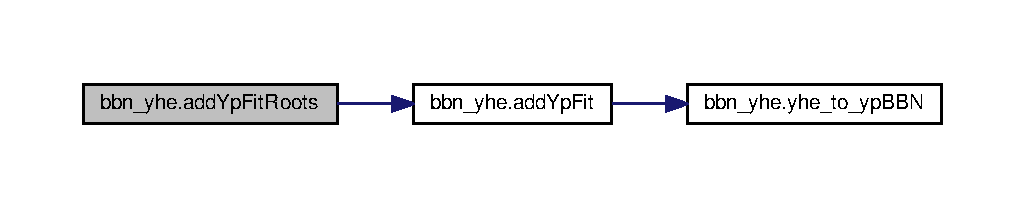
\includegraphics[width=350pt]{namespacebbn__yhe_ab07e92f80f62d425303d08e5e8fe604d_cgraph}
\end{center}
\end{figure}
\mbox{\Hypertarget{namespacebbn__yhe_a3e9988b282cca4d66a7481dbf9676939}\label{namespacebbn__yhe_a3e9988b282cca4d66a7481dbf9676939}} 
\index{bbn\+\_\+yhe@{bbn\+\_\+yhe}!dh\+\_\+fit@{dh\+\_\+fit}}
\index{dh\+\_\+fit@{dh\+\_\+fit}!bbn\+\_\+yhe@{bbn\+\_\+yhe}}
\subsubsection{\texorpdfstring{dh\+\_\+fit()}{dh\_fit()}}
{\footnotesize\ttfamily def bbn\+\_\+yhe.\+dh\+\_\+fit (\begin{DoxyParamCaption}\item[{}]{omegab,  }\item[{}]{dneff,  }\item[{}]{taun = {\ttfamily 880.3} }\end{DoxyParamCaption})}

\mbox{\Hypertarget{namespacebbn__yhe_a38c5abbad8fad900f60f86b5038cf0e8}\label{namespacebbn__yhe_a38c5abbad8fad900f60f86b5038cf0e8}} 
\index{bbn\+\_\+yhe@{bbn\+\_\+yhe}!yhe\+\_\+to\+\_\+yp\+B\+BN@{yhe\+\_\+to\+\_\+yp\+B\+BN}}
\index{yhe\+\_\+to\+\_\+yp\+B\+BN@{yhe\+\_\+to\+\_\+yp\+B\+BN}!bbn\+\_\+yhe@{bbn\+\_\+yhe}}
\subsubsection{\texorpdfstring{yhe\+\_\+to\+\_\+yp\+B\+B\+N()}{yhe\_to\_ypBBN()}}
{\footnotesize\ttfamily def bbn\+\_\+yhe.\+yhe\+\_\+to\+\_\+yp\+B\+BN (\begin{DoxyParamCaption}\item[{}]{Yp }\end{DoxyParamCaption})}



Referenced by add\+Yp\+Fit().

Here is the caller graph for this function\+:
\nopagebreak
\begin{figure}[H]
\begin{center}
\leavevmode
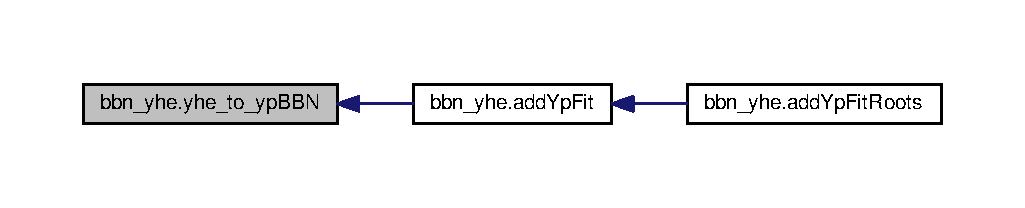
\includegraphics[width=350pt]{namespacebbn__yhe_a38c5abbad8fad900f60f86b5038cf0e8_icgraph}
\end{center}
\end{figure}
\mbox{\Hypertarget{namespacebbn__yhe_a0ae2fc2b1719f17ae48ec9dee3de6728}\label{namespacebbn__yhe_a0ae2fc2b1719f17ae48ec9dee3de6728}} 
\index{bbn\+\_\+yhe@{bbn\+\_\+yhe}!yp\+B\+BN@{yp\+B\+BN}}
\index{yp\+B\+BN@{yp\+B\+BN}!bbn\+\_\+yhe@{bbn\+\_\+yhe}}
\subsubsection{\texorpdfstring{yp\+B\+B\+N()}{ypBBN()}}
{\footnotesize\ttfamily def bbn\+\_\+yhe.\+yp\+B\+BN (\begin{DoxyParamCaption}\item[{}]{omegab,  }\item[{}]{dneff,  }\item[{}]{taun = {\ttfamily 880.3} }\end{DoxyParamCaption})}



\subsection{Variable Documentation}
\mbox{\Hypertarget{namespacebbn__yhe_aee3ed9037ad3216e40a5e87b91d33f27}\label{namespacebbn__yhe_aee3ed9037ad3216e40a5e87b91d33f27}} 
\index{bbn\+\_\+yhe@{bbn\+\_\+yhe}!alpha@{alpha}}
\index{alpha@{alpha}!bbn\+\_\+yhe@{bbn\+\_\+yhe}}
\subsubsection{\texorpdfstring{alpha}{alpha}}
{\footnotesize\ttfamily bbn\+\_\+yhe.\+alpha}

\mbox{\Hypertarget{namespacebbn__yhe_a4e580183b4dd2ab4042be13ffec6c525}\label{namespacebbn__yhe_a4e580183b4dd2ab4042be13ffec6c525}} 
\index{bbn\+\_\+yhe@{bbn\+\_\+yhe}!arrowprops@{arrowprops}}
\index{arrowprops@{arrowprops}!bbn\+\_\+yhe@{bbn\+\_\+yhe}}
\subsubsection{\texorpdfstring{arrowprops}{arrowprops}}
{\footnotesize\ttfamily bbn\+\_\+yhe.\+arrowprops}

\mbox{\Hypertarget{namespacebbn__yhe_a9d5e61e6f78e3497a8c5fce8daedf276}\label{namespacebbn__yhe_a9d5e61e6f78e3497a8c5fce8daedf276}} 
\index{bbn\+\_\+yhe@{bbn\+\_\+yhe}!aver\+\_\+mean@{aver\+\_\+mean}}
\index{aver\+\_\+mean@{aver\+\_\+mean}!bbn\+\_\+yhe@{bbn\+\_\+yhe}}
\subsubsection{\texorpdfstring{aver\+\_\+mean}{aver\_mean}}
{\footnotesize\ttfamily bbn\+\_\+yhe.\+aver\+\_\+mean = 0.\+2465}

\mbox{\Hypertarget{namespacebbn__yhe_af08345da95d7b1ecff384b5ca5648a03}\label{namespacebbn__yhe_af08345da95d7b1ecff384b5ca5648a03}} 
\index{bbn\+\_\+yhe@{bbn\+\_\+yhe}!aver\+\_\+sigma@{aver\+\_\+sigma}}
\index{aver\+\_\+sigma@{aver\+\_\+sigma}!bbn\+\_\+yhe@{bbn\+\_\+yhe}}
\subsubsection{\texorpdfstring{aver\+\_\+sigma}{aver\_sigma}}
{\footnotesize\ttfamily bbn\+\_\+yhe.\+aver\+\_\+sigma = 0.\+0097}

\mbox{\Hypertarget{namespacebbn__yhe_a8da3e95ccabe26e7b02faafa8d0c7d0a}\label{namespacebbn__yhe_a8da3e95ccabe26e7b02faafa8d0c7d0a}} 
\index{bbn\+\_\+yhe@{bbn\+\_\+yhe}!bbn\+\_\+b@{bbn\+\_\+b}}
\index{bbn\+\_\+b@{bbn\+\_\+b}!bbn\+\_\+yhe@{bbn\+\_\+yhe}}
\subsubsection{\texorpdfstring{bbn\+\_\+b}{bbn\_b}}
{\footnotesize\ttfamily bbn\+\_\+yhe.\+bbn\+\_\+b = np.\+arange(\mbox{\hyperlink{namespacebbn__yhe_aa005d4473664db0db345095282beb1ef}{ob\+\_\+min}}, \mbox{\hyperlink{namespacebbn__yhe_a7ad9cbb8dc27628c6fbf6296bba963ca}{ob\+\_\+max}} + 0.\+1, (\mbox{\hyperlink{namespacebbn__yhe_a7ad9cbb8dc27628c6fbf6296bba963ca}{ob\+\_\+max}} -\/ \mbox{\hyperlink{namespacebbn__yhe_aa005d4473664db0db345095282beb1ef}{ob\+\_\+min}}) / \mbox{\hyperlink{namespacebbn__yhe_a3aa1ae9b0ed6bd135e4fc002b7eca1a9}{num\+\_\+ob}})}

\mbox{\Hypertarget{namespacebbn__yhe_a28b53c029dcb7310ef25c077dbf59bab}\label{namespacebbn__yhe_a28b53c029dcb7310ef25c077dbf59bab}} 
\index{bbn\+\_\+yhe@{bbn\+\_\+yhe}!bbn\+\_\+y@{bbn\+\_\+y}}
\index{bbn\+\_\+y@{bbn\+\_\+y}!bbn\+\_\+yhe@{bbn\+\_\+yhe}}
\subsubsection{\texorpdfstring{bbn\+\_\+y}{bbn\_y}}
{\footnotesize\ttfamily def bbn\+\_\+yhe.\+bbn\+\_\+y = \mbox{\hyperlink{namespacebbn__yhe_a0ae2fc2b1719f17ae48ec9dee3de6728}{yp\+B\+BN}}(\mbox{\hyperlink{namespacebbn__yhe_a8da3e95ccabe26e7b02faafa8d0c7d0a}{bbn\+\_\+b}}, 0)}

\mbox{\Hypertarget{namespacebbn__yhe_a3f8a67b91f6391a7bd8ea269672ac615}\label{namespacebbn__yhe_a3f8a67b91f6391a7bd8ea269672ac615}} 
\index{bbn\+\_\+yhe@{bbn\+\_\+yhe}!bbn\+\_\+y1@{bbn\+\_\+y1}}
\index{bbn\+\_\+y1@{bbn\+\_\+y1}!bbn\+\_\+yhe@{bbn\+\_\+yhe}}
\subsubsection{\texorpdfstring{bbn\+\_\+y1}{bbn\_y1}}
{\footnotesize\ttfamily def bbn\+\_\+yhe.\+bbn\+\_\+y1 = \mbox{\hyperlink{namespacebbn__yhe_a28b53c029dcb7310ef25c077dbf59bab}{bbn\+\_\+y}} -\/ \mbox{\hyperlink{namespacebbn__yhe_a06123892f977e5e00eb0e7bcf6866dbb}{sigma\+\_\+yp\+\_\+theo}}}

\mbox{\Hypertarget{namespacebbn__yhe_ae522afab9400241fb8bc86962e60e9b5}\label{namespacebbn__yhe_ae522afab9400241fb8bc86962e60e9b5}} 
\index{bbn\+\_\+yhe@{bbn\+\_\+yhe}!bbn\+\_\+y2@{bbn\+\_\+y2}}
\index{bbn\+\_\+y2@{bbn\+\_\+y2}!bbn\+\_\+yhe@{bbn\+\_\+yhe}}
\subsubsection{\texorpdfstring{bbn\+\_\+y2}{bbn\_y2}}
{\footnotesize\ttfamily def bbn\+\_\+yhe.\+bbn\+\_\+y2 = \mbox{\hyperlink{namespacebbn__yhe_a28b53c029dcb7310ef25c077dbf59bab}{bbn\+\_\+y}} + \mbox{\hyperlink{namespacebbn__yhe_a06123892f977e5e00eb0e7bcf6866dbb}{sigma\+\_\+yp\+\_\+theo}}}

\mbox{\Hypertarget{namespacebbn__yhe_a5febb2e61726249209662394b5d95858}\label{namespacebbn__yhe_a5febb2e61726249209662394b5d95858}} 
\index{bbn\+\_\+yhe@{bbn\+\_\+yhe}!color@{color}}
\index{color@{color}!bbn\+\_\+yhe@{bbn\+\_\+yhe}}
\subsubsection{\texorpdfstring{color}{color}}
{\footnotesize\ttfamily bbn\+\_\+yhe.\+color}

\mbox{\Hypertarget{namespacebbn__yhe_a49bc13f65125eafd22fc160f104e8444}\label{namespacebbn__yhe_a49bc13f65125eafd22fc160f104e8444}} 
\index{bbn\+\_\+yhe@{bbn\+\_\+yhe}!colored\+\_\+text@{colored\+\_\+text}}
\index{colored\+\_\+text@{colored\+\_\+text}!bbn\+\_\+yhe@{bbn\+\_\+yhe}}
\subsubsection{\texorpdfstring{colored\+\_\+text}{colored\_text}}
{\footnotesize\ttfamily bbn\+\_\+yhe.\+colored\+\_\+text}

\mbox{\Hypertarget{namespacebbn__yhe_a68a4915540c5ddfdf951a7612c20358d}\label{namespacebbn__yhe_a68a4915540c5ddfdf951a7612c20358d}} 
\index{bbn\+\_\+yhe@{bbn\+\_\+yhe}!colors@{colors}}
\index{colors@{colors}!bbn\+\_\+yhe@{bbn\+\_\+yhe}}
\subsubsection{\texorpdfstring{colors}{colors}}
{\footnotesize\ttfamily bbn\+\_\+yhe.\+colors = g.\+settings.\+solid\+\_\+colors\mbox{[}3\+:0\+:-\/1\mbox{]}}

\mbox{\Hypertarget{namespacebbn__yhe_a063490560da67d4aa74baa317b66577a}\label{namespacebbn__yhe_a063490560da67d4aa74baa317b66577a}} 
\index{bbn\+\_\+yhe@{bbn\+\_\+yhe}!datatag@{datatag}}
\index{datatag@{datatag}!bbn\+\_\+yhe@{bbn\+\_\+yhe}}
\subsubsection{\texorpdfstring{datatag}{datatag}}
{\footnotesize\ttfamily list bbn\+\_\+yhe.\+datatag = \mbox{[}s.\+defdata, s.\+defdata + \textquotesingle{}\+\_\+\+B\+AO\textquotesingle{}, s.\+defdata\+\_\+all\mbox{]}}

\mbox{\Hypertarget{namespacebbn__yhe_af0aeb2348a1c9932c656174611593164}\label{namespacebbn__yhe_af0aeb2348a1c9932c656174611593164}} 
\index{bbn\+\_\+yhe@{bbn\+\_\+yhe}!False@{False}}
\index{False@{False}!bbn\+\_\+yhe@{bbn\+\_\+yhe}}
\subsubsection{\texorpdfstring{False}{False}}
{\footnotesize\ttfamily bbn\+\_\+yhe.\+False}

\mbox{\Hypertarget{namespacebbn__yhe_a27906639887f7d86e9893c3c8c102f9b}\label{namespacebbn__yhe_a27906639887f7d86e9893c3c8c102f9b}} 
\index{bbn\+\_\+yhe@{bbn\+\_\+yhe}!filled@{filled}}
\index{filled@{filled}!bbn\+\_\+yhe@{bbn\+\_\+yhe}}
\subsubsection{\texorpdfstring{filled}{filled}}
{\footnotesize\ttfamily bbn\+\_\+yhe.\+filled}

\mbox{\Hypertarget{namespacebbn__yhe_a3bb9da91cb045382b8f944eb5c8e14fe}\label{namespacebbn__yhe_a3bb9da91cb045382b8f944eb5c8e14fe}} 
\index{bbn\+\_\+yhe@{bbn\+\_\+yhe}!fontsize@{fontsize}}
\index{fontsize@{fontsize}!bbn\+\_\+yhe@{bbn\+\_\+yhe}}
\subsubsection{\texorpdfstring{fontsize}{fontsize}}
{\footnotesize\ttfamily bbn\+\_\+yhe.\+fontsize}

\mbox{\Hypertarget{namespacebbn__yhe_a28ea3e3cf2288f549b58603f5a80dd23}\label{namespacebbn__yhe_a28ea3e3cf2288f549b58603f5a80dd23}} 
\index{bbn\+\_\+yhe@{bbn\+\_\+yhe}!g@{g}}
\index{g@{g}!bbn\+\_\+yhe@{bbn\+\_\+yhe}}
\subsubsection{\texorpdfstring{g}{g}}
{\footnotesize\ttfamily bbn\+\_\+yhe.\+g = s.\+get\+Single\+Plotter()}



ombh2 -\/\+Yhe \#\#\#\#\#\#\#\#\#\#\#\#\# 

Neff -\/\+Yhe \#\#\#\#\#\#\#\#\#\#\#\#\#. \mbox{\Hypertarget{namespacebbn__yhe_a90f26535b1262c9980ba8f8dea539709}\label{namespacebbn__yhe_a90f26535b1262c9980ba8f8dea539709}} 
\index{bbn\+\_\+yhe@{bbn\+\_\+yhe}!labels@{labels}}
\index{labels@{labels}!bbn\+\_\+yhe@{bbn\+\_\+yhe}}
\subsubsection{\texorpdfstring{labels}{labels}}
{\footnotesize\ttfamily bbn\+\_\+yhe.\+labels = \mbox{[}s.\+defplanck, s.\+defplanck + \char`\"{}+B\+AO\char`\"{}, s.\+planckall\mbox{]}}

\mbox{\Hypertarget{namespacebbn__yhe_ac2c1a41c88f2f983a89e6f3af095d520}\label{namespacebbn__yhe_ac2c1a41c88f2f983a89e6f3af095d520}} 
\index{bbn\+\_\+yhe@{bbn\+\_\+yhe}!legend\+\_\+fontsize@{legend\+\_\+fontsize}}
\index{legend\+\_\+fontsize@{legend\+\_\+fontsize}!bbn\+\_\+yhe@{bbn\+\_\+yhe}}
\subsubsection{\texorpdfstring{legend\+\_\+fontsize}{legend\_fontsize}}
{\footnotesize\ttfamily bbn\+\_\+yhe.\+legend\+\_\+fontsize}

\mbox{\Hypertarget{namespacebbn__yhe_aadedc8e6798c93b5bf445f5d1bd0c19f}\label{namespacebbn__yhe_aadedc8e6798c93b5bf445f5d1bd0c19f}} 
\index{bbn\+\_\+yhe@{bbn\+\_\+yhe}!legend\+\_\+loc@{legend\+\_\+loc}}
\index{legend\+\_\+loc@{legend\+\_\+loc}!bbn\+\_\+yhe@{bbn\+\_\+yhe}}
\subsubsection{\texorpdfstring{legend\+\_\+loc}{legend\_loc}}
{\footnotesize\ttfamily bbn\+\_\+yhe.\+legend\+\_\+loc}

\mbox{\Hypertarget{namespacebbn__yhe_a8fb3d2af891fa129948db45632d05b4c}\label{namespacebbn__yhe_a8fb3d2af891fa129948db45632d05b4c}} 
\index{bbn\+\_\+yhe@{bbn\+\_\+yhe}!lims@{lims}}
\index{lims@{lims}!bbn\+\_\+yhe@{bbn\+\_\+yhe}}
\subsubsection{\texorpdfstring{lims}{lims}}
{\footnotesize\ttfamily bbn\+\_\+yhe.\+lims}

\mbox{\Hypertarget{namespacebbn__yhe_af98c0d13e6e8393dac53d8e115f2c906}\label{namespacebbn__yhe_af98c0d13e6e8393dac53d8e115f2c906}} 
\index{bbn\+\_\+yhe@{bbn\+\_\+yhe}!linestyle@{linestyle}}
\index{linestyle@{linestyle}!bbn\+\_\+yhe@{bbn\+\_\+yhe}}
\subsubsection{\texorpdfstring{linestyle}{linestyle}}
{\footnotesize\ttfamily bbn\+\_\+yhe.\+linestyle}

\mbox{\Hypertarget{namespacebbn__yhe_a97d4d46b2f4aad7933899daacdfa4e8d}\label{namespacebbn__yhe_a97d4d46b2f4aad7933899daacdfa4e8d}} 
\index{bbn\+\_\+yhe@{bbn\+\_\+yhe}!N\+\_\+max@{N\+\_\+max}}
\index{N\+\_\+max@{N\+\_\+max}!bbn\+\_\+yhe@{bbn\+\_\+yhe}}
\subsubsection{\texorpdfstring{N\+\_\+max}{N\_max}}
{\footnotesize\ttfamily int bbn\+\_\+yhe.\+N\+\_\+max = 5}

\mbox{\Hypertarget{namespacebbn__yhe_a12d17f1eceb939479da944d753f67417}\label{namespacebbn__yhe_a12d17f1eceb939479da944d753f67417}} 
\index{bbn\+\_\+yhe@{bbn\+\_\+yhe}!N\+\_\+min@{N\+\_\+min}}
\index{N\+\_\+min@{N\+\_\+min}!bbn\+\_\+yhe@{bbn\+\_\+yhe}}
\subsubsection{\texorpdfstring{N\+\_\+min}{N\_min}}
{\footnotesize\ttfamily float bbn\+\_\+yhe.\+N\+\_\+min = 0.\+01}

\mbox{\Hypertarget{namespacebbn__yhe_a0974f7b16b7e2bc7419b63acb59f5a68}\label{namespacebbn__yhe_a0974f7b16b7e2bc7419b63acb59f5a68}} 
\index{bbn\+\_\+yhe@{bbn\+\_\+yhe}!Neff@{Neff}}
\index{Neff@{Neff}!bbn\+\_\+yhe@{bbn\+\_\+yhe}}
\subsubsection{\texorpdfstring{Neff}{Neff}}
{\footnotesize\ttfamily bbn\+\_\+yhe.\+Neff = np.\+arange(\mbox{\hyperlink{namespacebbn__yhe_a12d17f1eceb939479da944d753f67417}{N\+\_\+min}}, \mbox{\hyperlink{namespacebbn__yhe_a97d4d46b2f4aad7933899daacdfa4e8d}{N\+\_\+max}} + 0.\+1, 0.\+1)}

\mbox{\Hypertarget{namespacebbn__yhe_aaa4728644822d8c49e68fadd68ede623}\label{namespacebbn__yhe_aaa4728644822d8c49e68fadd68ede623}} 
\index{bbn\+\_\+yhe@{bbn\+\_\+yhe}!Nrange@{Nrange}}
\index{Nrange@{Nrange}!bbn\+\_\+yhe@{bbn\+\_\+yhe}}
\subsubsection{\texorpdfstring{Nrange}{Nrange}}
{\footnotesize\ttfamily bbn\+\_\+yhe.\+Nrange = \mbox{[}\mbox{\hyperlink{namespacebbn__yhe_a12d17f1eceb939479da944d753f67417}{N\+\_\+min}}, \mbox{\hyperlink{namespacebbn__yhe_a97d4d46b2f4aad7933899daacdfa4e8d}{N\+\_\+max}}\mbox{]}}

\mbox{\Hypertarget{namespacebbn__yhe_a3aa1ae9b0ed6bd135e4fc002b7eca1a9}\label{namespacebbn__yhe_a3aa1ae9b0ed6bd135e4fc002b7eca1a9}} 
\index{bbn\+\_\+yhe@{bbn\+\_\+yhe}!num\+\_\+ob@{num\+\_\+ob}}
\index{num\+\_\+ob@{num\+\_\+ob}!bbn\+\_\+yhe@{bbn\+\_\+yhe}}
\subsubsection{\texorpdfstring{num\+\_\+ob}{num\_ob}}
{\footnotesize\ttfamily int bbn\+\_\+yhe.\+num\+\_\+ob = 50}

\mbox{\Hypertarget{namespacebbn__yhe_a7ad9cbb8dc27628c6fbf6296bba963ca}\label{namespacebbn__yhe_a7ad9cbb8dc27628c6fbf6296bba963ca}} 
\index{bbn\+\_\+yhe@{bbn\+\_\+yhe}!ob\+\_\+max@{ob\+\_\+max}}
\index{ob\+\_\+max@{ob\+\_\+max}!bbn\+\_\+yhe@{bbn\+\_\+yhe}}
\subsubsection{\texorpdfstring{ob\+\_\+max}{ob\_max}}
{\footnotesize\ttfamily float bbn\+\_\+yhe.\+ob\+\_\+max = 0.\+026}

\mbox{\Hypertarget{namespacebbn__yhe_aa005d4473664db0db345095282beb1ef}\label{namespacebbn__yhe_aa005d4473664db0db345095282beb1ef}} 
\index{bbn\+\_\+yhe@{bbn\+\_\+yhe}!ob\+\_\+min@{ob\+\_\+min}}
\index{ob\+\_\+min@{ob\+\_\+min}!bbn\+\_\+yhe@{bbn\+\_\+yhe}}
\subsubsection{\texorpdfstring{ob\+\_\+min}{ob\_min}}
{\footnotesize\ttfamily float bbn\+\_\+yhe.\+ob\+\_\+min = 0.\+018}

\mbox{\Hypertarget{namespacebbn__yhe_ab2add45031a3e0b76e777d91fd6eff67}\label{namespacebbn__yhe_ab2add45031a3e0b76e777d91fd6eff67}} 
\index{bbn\+\_\+yhe@{bbn\+\_\+yhe}!roots@{roots}}
\index{roots@{roots}!bbn\+\_\+yhe@{bbn\+\_\+yhe}}
\subsubsection{\texorpdfstring{roots}{roots}}
{\footnotesize\ttfamily list bbn\+\_\+yhe.\+roots = \mbox{[}g.\+get\+Root(\textquotesingle{}yhe\textquotesingle{}, d) for d in \mbox{\hyperlink{namespacebbn__yhe_a063490560da67d4aa74baa317b66577a}{datatag}}\mbox{]}}

\mbox{\Hypertarget{namespacebbn__yhe_a0189ca7d3d30cadc352fe3c5f419d73a}\label{namespacebbn__yhe_a0189ca7d3d30cadc352fe3c5f419d73a}} 
\index{bbn\+\_\+yhe@{bbn\+\_\+yhe}!sere\+\_\+b@{sere\+\_\+b}}
\index{sere\+\_\+b@{sere\+\_\+b}!bbn\+\_\+yhe@{bbn\+\_\+yhe}}
\subsubsection{\texorpdfstring{sere\+\_\+b}{sere\_b}}
{\footnotesize\ttfamily bbn\+\_\+yhe.\+sere\+\_\+b = np.\+zeros(2, dtype=\textquotesingle{}float\textquotesingle{})}

\mbox{\Hypertarget{namespacebbn__yhe_ad00e51b24c6c009e64a8baa0f0b51ad8}\label{namespacebbn__yhe_ad00e51b24c6c009e64a8baa0f0b51ad8}} 
\index{bbn\+\_\+yhe@{bbn\+\_\+yhe}!sere\+\_\+minus@{sere\+\_\+minus}}
\index{sere\+\_\+minus@{sere\+\_\+minus}!bbn\+\_\+yhe@{bbn\+\_\+yhe}}
\subsubsection{\texorpdfstring{sere\+\_\+minus}{sere\_minus}}
{\footnotesize\ttfamily float bbn\+\_\+yhe.\+sere\+\_\+minus = 0.\+294}

\mbox{\Hypertarget{namespacebbn__yhe_a8c95d448cd274ce585cfaf255bd4ff1b}\label{namespacebbn__yhe_a8c95d448cd274ce585cfaf255bd4ff1b}} 
\index{bbn\+\_\+yhe@{bbn\+\_\+yhe}!sere\+\_\+plus@{sere\+\_\+plus}}
\index{sere\+\_\+plus@{sere\+\_\+plus}!bbn\+\_\+yhe@{bbn\+\_\+yhe}}
\subsubsection{\texorpdfstring{sere\+\_\+plus}{sere\_plus}}
{\footnotesize\ttfamily float bbn\+\_\+yhe.\+sere\+\_\+plus = \mbox{\hyperlink{namespacebbn__yhe_a1b95d70c9d6b84360f839ed708b14c72}{yp\+\_\+max}}}

\mbox{\Hypertarget{namespacebbn__yhe_a113b4f8c034ac6ea013657ba051687e1}\label{namespacebbn__yhe_a113b4f8c034ac6ea013657ba051687e1}} 
\index{bbn\+\_\+yhe@{bbn\+\_\+yhe}!sere\+\_\+y1@{sere\+\_\+y1}}
\index{sere\+\_\+y1@{sere\+\_\+y1}!bbn\+\_\+yhe@{bbn\+\_\+yhe}}
\subsubsection{\texorpdfstring{sere\+\_\+y1}{sere\_y1}}
{\footnotesize\ttfamily bbn\+\_\+yhe.\+sere\+\_\+y1 = np.\+zeros(2, dtype=\textquotesingle{}float\textquotesingle{})}

\mbox{\Hypertarget{namespacebbn__yhe_a5df6de601295fe7e1b92a79b727ccbc3}\label{namespacebbn__yhe_a5df6de601295fe7e1b92a79b727ccbc3}} 
\index{bbn\+\_\+yhe@{bbn\+\_\+yhe}!sere\+\_\+y2@{sere\+\_\+y2}}
\index{sere\+\_\+y2@{sere\+\_\+y2}!bbn\+\_\+yhe@{bbn\+\_\+yhe}}
\subsubsection{\texorpdfstring{sere\+\_\+y2}{sere\_y2}}
{\footnotesize\ttfamily bbn\+\_\+yhe.\+sere\+\_\+y2 = np.\+zeros(2, dtype=\textquotesingle{}float\textquotesingle{})}

\mbox{\Hypertarget{namespacebbn__yhe_a06123892f977e5e00eb0e7bcf6866dbb}\label{namespacebbn__yhe_a06123892f977e5e00eb0e7bcf6866dbb}} 
\index{bbn\+\_\+yhe@{bbn\+\_\+yhe}!sigma\+\_\+yp\+\_\+theo@{sigma\+\_\+yp\+\_\+theo}}
\index{sigma\+\_\+yp\+\_\+theo@{sigma\+\_\+yp\+\_\+theo}!bbn\+\_\+yhe@{bbn\+\_\+yhe}}
\subsubsection{\texorpdfstring{sigma\+\_\+yp\+\_\+theo}{sigma\_yp\_theo}}
{\footnotesize\ttfamily float bbn\+\_\+yhe.\+sigma\+\_\+yp\+\_\+theo = 0.\+0003}

\mbox{\Hypertarget{namespacebbn__yhe_a77232bd6b32ee374dbd5504aaba84b10}\label{namespacebbn__yhe_a77232bd6b32ee374dbd5504aaba84b10}} 
\index{bbn\+\_\+yhe@{bbn\+\_\+yhe}!tag@{tag}}
\index{tag@{tag}!bbn\+\_\+yhe@{bbn\+\_\+yhe}}
\subsubsection{\texorpdfstring{tag}{tag}}
{\footnotesize\ttfamily bbn\+\_\+yhe.\+tag}

\mbox{\Hypertarget{namespacebbn__yhe_ad9e6a1e307d4e22bacaa587397fa346e}\label{namespacebbn__yhe_ad9e6a1e307d4e22bacaa587397fa346e}} 
\index{bbn\+\_\+yhe@{bbn\+\_\+yhe}!textcoords@{textcoords}}
\index{textcoords@{textcoords}!bbn\+\_\+yhe@{bbn\+\_\+yhe}}
\subsubsection{\texorpdfstring{textcoords}{textcoords}}
{\footnotesize\ttfamily bbn\+\_\+yhe.\+textcoords}

\mbox{\Hypertarget{namespacebbn__yhe_a6d53cb6d1d4b9038a14d5b038ef4b4ff}\label{namespacebbn__yhe_a6d53cb6d1d4b9038a14d5b038ef4b4ff}} 
\index{bbn\+\_\+yhe@{bbn\+\_\+yhe}!True@{True}}
\index{True@{True}!bbn\+\_\+yhe@{bbn\+\_\+yhe}}
\subsubsection{\texorpdfstring{True}{True}}
{\footnotesize\ttfamily bbn\+\_\+yhe.\+True}

\mbox{\Hypertarget{namespacebbn__yhe_adaa6abf83a5db41a605b66fcf1072747}\label{namespacebbn__yhe_adaa6abf83a5db41a605b66fcf1072747}} 
\index{bbn\+\_\+yhe@{bbn\+\_\+yhe}!xlim@{xlim}}
\index{xlim@{xlim}!bbn\+\_\+yhe@{bbn\+\_\+yhe}}
\subsubsection{\texorpdfstring{xlim}{xlim}}
{\footnotesize\ttfamily bbn\+\_\+yhe.\+xlim}

\mbox{\Hypertarget{namespacebbn__yhe_a3123808ee1e6304665a2980e073efed9}\label{namespacebbn__yhe_a3123808ee1e6304665a2980e073efed9}} 
\index{bbn\+\_\+yhe@{bbn\+\_\+yhe}!xy@{xy}}
\index{xy@{xy}!bbn\+\_\+yhe@{bbn\+\_\+yhe}}
\subsubsection{\texorpdfstring{xy}{xy}}
{\footnotesize\ttfamily bbn\+\_\+yhe.\+xy}

\mbox{\Hypertarget{namespacebbn__yhe_a24e8c7a1ae7d3b9a225c19f2a79cf681}\label{namespacebbn__yhe_a24e8c7a1ae7d3b9a225c19f2a79cf681}} 
\index{bbn\+\_\+yhe@{bbn\+\_\+yhe}!xycoords@{xycoords}}
\index{xycoords@{xycoords}!bbn\+\_\+yhe@{bbn\+\_\+yhe}}
\subsubsection{\texorpdfstring{xycoords}{xycoords}}
{\footnotesize\ttfamily bbn\+\_\+yhe.\+xycoords}

\mbox{\Hypertarget{namespacebbn__yhe_a26224bf035e3019da5ed20ac3aece4e8}\label{namespacebbn__yhe_a26224bf035e3019da5ed20ac3aece4e8}} 
\index{bbn\+\_\+yhe@{bbn\+\_\+yhe}!xytext@{xytext}}
\index{xytext@{xytext}!bbn\+\_\+yhe@{bbn\+\_\+yhe}}
\subsubsection{\texorpdfstring{xytext}{xytext}}
{\footnotesize\ttfamily bbn\+\_\+yhe.\+xytext}

\mbox{\Hypertarget{namespacebbn__yhe_a1b95d70c9d6b84360f839ed708b14c72}\label{namespacebbn__yhe_a1b95d70c9d6b84360f839ed708b14c72}} 
\index{bbn\+\_\+yhe@{bbn\+\_\+yhe}!yp\+\_\+max@{yp\+\_\+max}}
\index{yp\+\_\+max@{yp\+\_\+max}!bbn\+\_\+yhe@{bbn\+\_\+yhe}}
\subsubsection{\texorpdfstring{yp\+\_\+max}{yp\_max}}
{\footnotesize\ttfamily bbn\+\_\+yhe.\+yp\+\_\+max = 0.\+35}

\mbox{\Hypertarget{namespacebbn__yhe_a624706ed018b5d06d3e1ceea58a08e12}\label{namespacebbn__yhe_a624706ed018b5d06d3e1ceea58a08e12}} 
\index{bbn\+\_\+yhe@{bbn\+\_\+yhe}!yp\+\_\+min@{yp\+\_\+min}}
\index{yp\+\_\+min@{yp\+\_\+min}!bbn\+\_\+yhe@{bbn\+\_\+yhe}}
\subsubsection{\texorpdfstring{yp\+\_\+min}{yp\_min}}
{\footnotesize\ttfamily float bbn\+\_\+yhe.\+yp\+\_\+min = 0.\+15}


\hypertarget{namespacebk__planck}{}\section{bk\+\_\+planck Module Reference}
\label{namespacebk__planck}\index{bk\+\_\+planck@{bk\+\_\+planck}}
\subsection*{Data Types}
\begin{DoxyCompactItemize}
\item 
type \mbox{\hyperlink{structbk__planck_1_1tbandpass}{tbandpass}}
\item 
type \mbox{\hyperlink{structbk__planck_1_1tbk__planck}{tbk\+\_\+planck}}
\end{DoxyCompactItemize}
\subsection*{Functions/\+Subroutines}
\begin{DoxyCompactItemize}
\item 
subroutine \mbox{\hyperlink{namespacebk__planck_a854764740d5b45a861a35309dcc7ab96}{tbk\+\_\+planck\+\_\+readini}} (this, Ini)
\item 
subroutine \mbox{\hyperlink{namespacebk__planck_a073f30d6055fdd0e28e842201c1e9fdf}{tbk\+\_\+planck\+\_\+read\+\_\+bandpass}} (this, fname, Bandpass)
\item 
subroutine \mbox{\hyperlink{namespacebk__planck_a532e314297951fce385bff0bc57f81c3}{dustscaling}} (beta, Tdust, bandpass, nu0, fdust)
\item 
subroutine \mbox{\hyperlink{namespacebk__planck_ae4ec8dfb07864a47b4f431f0be309608}{syncscaling}} (beta, bandpass, nu0, fsync)
\item 
subroutine \mbox{\hyperlink{namespacebk__planck_af94e4192bd2f4c8746e6e1108e87a0f0}{tbk\+\_\+planck\+\_\+addforegrounds}} (this, Cls, Data\+Params)
\end{DoxyCompactItemize}
\subsection*{Variables}
\begin{DoxyCompactItemize}
\item 
real(mcp), parameter \mbox{\hyperlink{namespacebk__planck_aed63f60182fa590d070ff874aff39d1e}{t\+\_\+cmb}} = 2.\+7255\+\_\+mcp
\item 
real(mcp), parameter \mbox{\hyperlink{namespacebk__planck_a2be53d116cb947e12107471bd0b14abd}{h}} = 6.\+62606957e-\/34\+\_\+mcp
\item 
real(mcp), parameter \mbox{\hyperlink{namespacebk__planck_a92bf968defaa02497d39c2f228710c04}{kb}} = 1.\+3806488e-\/23\+\_\+mcp
\item 
real(mcp), parameter \mbox{\hyperlink{namespacebk__planck_a3b81f62eff019d7f94b2a4ca37efdf91}{ghz\+\_\+kelvin}} = \mbox{\hyperlink{namespacebk__planck_a2be53d116cb947e12107471bd0b14abd}{h}}/kB$\ast$1e9\+\_\+mcp
\end{DoxyCompactItemize}


\subsection{Function/\+Subroutine Documentation}
\mbox{\Hypertarget{namespacebk__planck_a532e314297951fce385bff0bc57f81c3}\label{namespacebk__planck_a532e314297951fce385bff0bc57f81c3}} 
\index{bk\+\_\+planck@{bk\+\_\+planck}!dustscaling@{dustscaling}}
\index{dustscaling@{dustscaling}!bk\+\_\+planck@{bk\+\_\+planck}}
\subsubsection{\texorpdfstring{dustscaling()}{dustscaling()}}
{\footnotesize\ttfamily subroutine bk\+\_\+planck\+::dustscaling (\begin{DoxyParamCaption}\item[{real(mcp), intent(in)}]{beta,  }\item[{real(mcp), intent(in)}]{Tdust,  }\item[{type(\mbox{\hyperlink{structbk__planck_1_1tbandpass}{tbandpass}}), intent(in)}]{bandpass,  }\item[{real(mcp), intent(in)}]{nu0,  }\item[{real(mcp), intent(out)}]{fdust }\end{DoxyParamCaption})\hspace{0.3cm}{\ttfamily [private]}}



References ghz\+\_\+kelvin.



Referenced by tbk\+\_\+planck\+\_\+addforegrounds().

Here is the caller graph for this function\+:
\nopagebreak
\begin{figure}[H]
\begin{center}
\leavevmode
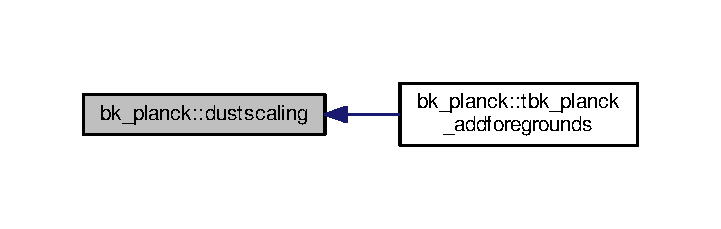
\includegraphics[width=346pt]{namespacebk__planck_a532e314297951fce385bff0bc57f81c3_icgraph}
\end{center}
\end{figure}
\mbox{\Hypertarget{namespacebk__planck_ae4ec8dfb07864a47b4f431f0be309608}\label{namespacebk__planck_ae4ec8dfb07864a47b4f431f0be309608}} 
\index{bk\+\_\+planck@{bk\+\_\+planck}!syncscaling@{syncscaling}}
\index{syncscaling@{syncscaling}!bk\+\_\+planck@{bk\+\_\+planck}}
\subsubsection{\texorpdfstring{syncscaling()}{syncscaling()}}
{\footnotesize\ttfamily subroutine bk\+\_\+planck\+::syncscaling (\begin{DoxyParamCaption}\item[{real(mcp), intent(in)}]{beta,  }\item[{type(\mbox{\hyperlink{structbk__planck_1_1tbandpass}{tbandpass}}), intent(in)}]{bandpass,  }\item[{real(mcp), intent(in)}]{nu0,  }\item[{real(mcp), intent(out)}]{fsync }\end{DoxyParamCaption})\hspace{0.3cm}{\ttfamily [private]}}



Referenced by tbk\+\_\+planck\+\_\+addforegrounds().

Here is the caller graph for this function\+:
\nopagebreak
\begin{figure}[H]
\begin{center}
\leavevmode
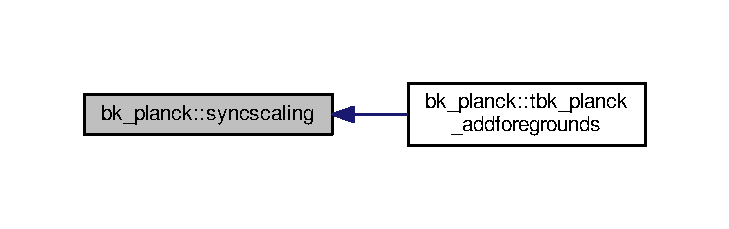
\includegraphics[width=350pt]{namespacebk__planck_ae4ec8dfb07864a47b4f431f0be309608_icgraph}
\end{center}
\end{figure}
\mbox{\Hypertarget{namespacebk__planck_af94e4192bd2f4c8746e6e1108e87a0f0}\label{namespacebk__planck_af94e4192bd2f4c8746e6e1108e87a0f0}} 
\index{bk\+\_\+planck@{bk\+\_\+planck}!tbk\+\_\+planck\+\_\+addforegrounds@{tbk\+\_\+planck\+\_\+addforegrounds}}
\index{tbk\+\_\+planck\+\_\+addforegrounds@{tbk\+\_\+planck\+\_\+addforegrounds}!bk\+\_\+planck@{bk\+\_\+planck}}
\subsubsection{\texorpdfstring{tbk\+\_\+planck\+\_\+addforegrounds()}{tbk\_planck\_addforegrounds()}}
{\footnotesize\ttfamily subroutine bk\+\_\+planck\+::tbk\+\_\+planck\+\_\+addforegrounds (\begin{DoxyParamCaption}\item[{class(\mbox{\hyperlink{structbk__planck_1_1tbk__planck}{tbk\+\_\+planck}})}]{this,  }\item[{class(tmapcrosspowerspectrum), dimension(\+:,\+:), intent(inout), target}]{Cls,  }\item[{real(mcp), dimension(\+:), intent(in)}]{Data\+Params }\end{DoxyParamCaption})\hspace{0.3cm}{\ttfamily [private]}}



References dustscaling(), and syncscaling().

Here is the call graph for this function\+:
\nopagebreak
\begin{figure}[H]
\begin{center}
\leavevmode
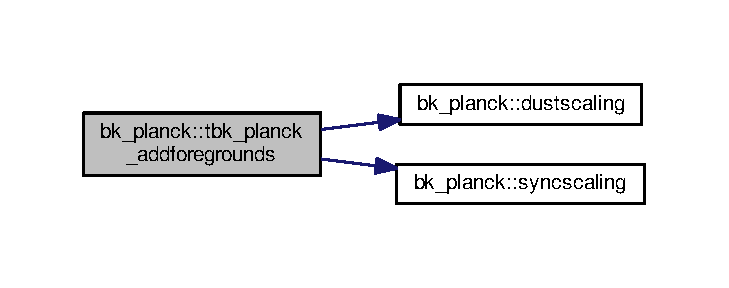
\includegraphics[width=350pt]{namespacebk__planck_af94e4192bd2f4c8746e6e1108e87a0f0_cgraph}
\end{center}
\end{figure}
\mbox{\Hypertarget{namespacebk__planck_a073f30d6055fdd0e28e842201c1e9fdf}\label{namespacebk__planck_a073f30d6055fdd0e28e842201c1e9fdf}} 
\index{bk\+\_\+planck@{bk\+\_\+planck}!tbk\+\_\+planck\+\_\+read\+\_\+bandpass@{tbk\+\_\+planck\+\_\+read\+\_\+bandpass}}
\index{tbk\+\_\+planck\+\_\+read\+\_\+bandpass@{tbk\+\_\+planck\+\_\+read\+\_\+bandpass}!bk\+\_\+planck@{bk\+\_\+planck}}
\subsubsection{\texorpdfstring{tbk\+\_\+planck\+\_\+read\+\_\+bandpass()}{tbk\_planck\_read\_bandpass()}}
{\footnotesize\ttfamily subroutine bk\+\_\+planck\+::tbk\+\_\+planck\+\_\+read\+\_\+bandpass (\begin{DoxyParamCaption}\item[{class(\mbox{\hyperlink{structbk__planck_1_1tbk__planck}{tbk\+\_\+planck}})}]{this,  }\item[{character(len=$\ast$), intent(in)}]{fname,  }\item[{type(\mbox{\hyperlink{structbk__planck_1_1tbandpass}{tbandpass}}), target}]{Bandpass }\end{DoxyParamCaption})\hspace{0.3cm}{\ttfamily [private]}}



References fileutils\+::file, ghz\+\_\+kelvin, and t\+\_\+cmb.

\mbox{\Hypertarget{namespacebk__planck_a854764740d5b45a861a35309dcc7ab96}\label{namespacebk__planck_a854764740d5b45a861a35309dcc7ab96}} 
\index{bk\+\_\+planck@{bk\+\_\+planck}!tbk\+\_\+planck\+\_\+readini@{tbk\+\_\+planck\+\_\+readini}}
\index{tbk\+\_\+planck\+\_\+readini@{tbk\+\_\+planck\+\_\+readini}!bk\+\_\+planck@{bk\+\_\+planck}}
\subsubsection{\texorpdfstring{tbk\+\_\+planck\+\_\+readini()}{tbk\_planck\_readini()}}
{\footnotesize\ttfamily subroutine bk\+\_\+planck\+::tbk\+\_\+planck\+\_\+readini (\begin{DoxyParamCaption}\item[{class(\mbox{\hyperlink{structbk__planck_1_1tbk__planck}{tbk\+\_\+planck}})}]{this,  }\item[{class(tsettingini)}]{Ini }\end{DoxyParamCaption})\hspace{0.3cm}{\ttfamily [private]}}



\subsection{Variable Documentation}
\mbox{\Hypertarget{namespacebk__planck_a3b81f62eff019d7f94b2a4ca37efdf91}\label{namespacebk__planck_a3b81f62eff019d7f94b2a4ca37efdf91}} 
\index{bk\+\_\+planck@{bk\+\_\+planck}!ghz\+\_\+kelvin@{ghz\+\_\+kelvin}}
\index{ghz\+\_\+kelvin@{ghz\+\_\+kelvin}!bk\+\_\+planck@{bk\+\_\+planck}}
\subsubsection{\texorpdfstring{ghz\+\_\+kelvin}{ghz\_kelvin}}
{\footnotesize\ttfamily real(mcp), parameter bk\+\_\+planck\+::ghz\+\_\+kelvin = \mbox{\hyperlink{namespacebk__planck_a2be53d116cb947e12107471bd0b14abd}{h}}/kB$\ast$1e9\+\_\+mcp\hspace{0.3cm}{\ttfamily [private]}}



Referenced by dustscaling(), and tbk\+\_\+planck\+\_\+read\+\_\+bandpass().

\mbox{\Hypertarget{namespacebk__planck_a2be53d116cb947e12107471bd0b14abd}\label{namespacebk__planck_a2be53d116cb947e12107471bd0b14abd}} 
\index{bk\+\_\+planck@{bk\+\_\+planck}!h@{h}}
\index{h@{h}!bk\+\_\+planck@{bk\+\_\+planck}}
\subsubsection{\texorpdfstring{h}{h}}
{\footnotesize\ttfamily real(mcp), parameter bk\+\_\+planck\+::h = 6.\+62606957e-\/34\+\_\+mcp\hspace{0.3cm}{\ttfamily [private]}}

\mbox{\Hypertarget{namespacebk__planck_a92bf968defaa02497d39c2f228710c04}\label{namespacebk__planck_a92bf968defaa02497d39c2f228710c04}} 
\index{bk\+\_\+planck@{bk\+\_\+planck}!kb@{kb}}
\index{kb@{kb}!bk\+\_\+planck@{bk\+\_\+planck}}
\subsubsection{\texorpdfstring{kb}{kb}}
{\footnotesize\ttfamily real(mcp), parameter bk\+\_\+planck\+::kb = 1.\+3806488e-\/23\+\_\+mcp\hspace{0.3cm}{\ttfamily [private]}}

\mbox{\Hypertarget{namespacebk__planck_aed63f60182fa590d070ff874aff39d1e}\label{namespacebk__planck_aed63f60182fa590d070ff874aff39d1e}} 
\index{bk\+\_\+planck@{bk\+\_\+planck}!t\+\_\+cmb@{t\+\_\+cmb}}
\index{t\+\_\+cmb@{t\+\_\+cmb}!bk\+\_\+planck@{bk\+\_\+planck}}
\subsubsection{\texorpdfstring{t\+\_\+cmb}{t\_cmb}}
{\footnotesize\ttfamily real(mcp), parameter bk\+\_\+planck\+::t\+\_\+cmb = 2.\+7255\+\_\+mcp\hspace{0.3cm}{\ttfamily [private]}}



Referenced by tbk\+\_\+planck\+\_\+read\+\_\+bandpass().


\hypertarget{namespacecalclike}{}\section{calclike Module Reference}
\label{namespacecalclike}\index{calclike@{calclike}}
\subsection*{Data Types}
\begin{DoxyCompactItemize}
\item 
type \mbox{\hyperlink{structcalclike_1_1tgenericlikecalculator}{tgenericlikecalculator}}
\item 
type \mbox{\hyperlink{structcalclike_1_1tlikecalculator}{tlikecalculator}}
\item 
type \mbox{\hyperlink{structcalclike_1_1tlikelihooduser}{tlikelihooduser}}
\item 
type \mbox{\hyperlink{structcalclike_1_1ttheorylikecalculator}{ttheorylikecalculator}}
\item 
type \mbox{\hyperlink{structcalclike_1_1ttheorylikelihooduser}{ttheorylikelihooduser}}
\end{DoxyCompactItemize}
\subsection*{Functions/\+Subroutines}
\begin{DoxyCompactItemize}
\item 
subroutine \mbox{\hyperlink{namespacecalclike_a36076b04960c7a7230a45fc468f9f0d6}{addlike}} (this, Current\+Like, Like\+To\+Add)
\item 
subroutine \mbox{\hyperlink{namespacecalclike_adb9f063355d18b2a50d8e0d3c061324b}{addliketemp}} (this, Current\+Like, Like\+To\+Add)
\item 
real(mcp) function \mbox{\hyperlink{namespacecalclike_ae4302a1d96dcdf7816b3d66125504644}{getloglikebounds}} (this, Params)
\item 
real(mcp) function \mbox{\hyperlink{namespacecalclike_ae8f9437d9cf6441647020ac8e419e424}{getlogpriors}} (this, P)
\item 
real(mcp) function \mbox{\hyperlink{namespacecalclike_a1a9de6819dc2b41653d5bf9a36bd66a1}{getloglike}} (this, Params)
\item 
real(mcp) function \mbox{\hyperlink{namespacecalclike_a7f2306f2a9d2d0135d6f4852f6ed3bc2}{getloglikemain}} (this, Params)
\item 
subroutine \mbox{\hyperlink{namespacecalclike_af377ac1f0746c42a430094fe73246012}{tlikecalculator\+\_\+readparams}} (this, Ini)
\item 
real(mcp) function \mbox{\hyperlink{namespacecalclike_adb41feb15d07d744bace1629aea8a5d3}{tlikecalculator\+\_\+testlikelihoodfunction}} (this, Params)
\item 
subroutine \mbox{\hyperlink{namespacecalclike_a5158b85ddca7d8f1b417a813bb7fe849}{tlikecalculator\+\_\+writeperformancestats}} (this, unit)
\item 
subroutine \mbox{\hyperlink{namespacecalclike_a7348b373c8c9138f0c694ad9969fcb66}{tlikecalculator\+\_\+writeparamshumantext}} (this, aunit, P, Log\+Like, weight)
\item 
subroutine \mbox{\hyperlink{namespacecalclike_afd9d4013e29fb891f656598d4b5e1b73}{tlikecalculator\+\_\+writeparamshumantextfile}} (this, fname, P, Log\+Like, weight)
\item 
subroutine \mbox{\hyperlink{namespacecalclike_a4be845214aaba0f4348b66c67401f78b}{tlikecalculator\+\_\+writeparampointtextdata}} (this, output\+\_\+root, Params)
\item 
real(mcp) function \mbox{\hyperlink{namespacecalclike_ab9a99016f525f639358a942fb9885cc7}{generic\+\_\+getloglikemain}} (this, Params)
\item 
subroutine \mbox{\hyperlink{namespacecalclike_ab9d66863dbce892dbee08483d9cdac50}{theorylike\+\_\+settheoryparams}} (this, Params)
\item 
subroutine \mbox{\hyperlink{namespacecalclike_a3823367d787d17f15e903222232f4b94}{theorylike\+\_\+setnewtheoryresults}} (this, Params)
\item 
real(mcp) function \mbox{\hyperlink{namespacecalclike_a141801e2c0e794a0411104bca9bb6809}{theorylike\+\_\+getloglikemain}} (this, Params)
\item 
real(mcp) function \mbox{\hyperlink{namespacecalclike_adffdc491632ae303d023f5e1b704eba4}{theorylike\+\_\+checkpriorcuts}} (this, Params)
\item 
real(mcp) function \mbox{\hyperlink{namespacecalclike_a27e62cb96ad63d0285283d1eb8dcec0c}{theorylike\+\_\+getloglikepost}} (this, Params, do\+\_\+like)
\item 
real(mcp) function \mbox{\hyperlink{namespacecalclike_a81e2854f62abdf354c1f03fc29c05d1c}{theorylike\+\_\+loglikewiththeoryset}} (this, likelihood\+\_\+mask)
\item 
logical function \mbox{\hyperlink{namespacecalclike_ae7eb4423ffdbadbf2df406b9d3331346}{theorylike\+\_\+calculaterequiredtheorychanges}} (this)
\item 
subroutine \mbox{\hyperlink{namespacecalclike_ab2d52ca5a668e5072ed6d10c161a5e88}{theorylike\+\_\+gettheoryforlike}} (this, Like)
\item 
subroutine \mbox{\hyperlink{namespacecalclike_ab57c11043f079701db0baf858bf6315a}{theorylike\+\_\+gettheoryforimportance}} (this, Params, error)
\item 
subroutine \mbox{\hyperlink{namespacecalclike_adb244129926744248e4e4f8883384b5c}{theorylike\+\_\+updatetheoryforlikelihoods}} (this, Params)
\item 
real(mcp) function \mbox{\hyperlink{namespacecalclike_adb2986867dcdb441b12b98cdd46cc5b5}{theorylike\+\_\+testlikelihoodfunction}} (this, Params)
\item 
subroutine \mbox{\hyperlink{namespacecalclike_a5c185d1a702fe31d3d1204d919b338da}{ttheorylike\+\_\+writeparamshumantext}} (this, aunit, P, Log\+Like, weight)
\item 
subroutine \mbox{\hyperlink{namespacecalclike_acb1cb4737fc9ec3a805214e87b444b00}{ttheorylike\+\_\+writeparampointtextdata}} (this, output\+\_\+root, Params)
\end{DoxyCompactItemize}


\subsection{Function/\+Subroutine Documentation}
\mbox{\Hypertarget{namespacecalclike_a36076b04960c7a7230a45fc468f9f0d6}\label{namespacecalclike_a36076b04960c7a7230a45fc468f9f0d6}} 
\index{calclike@{calclike}!addlike@{addlike}}
\index{addlike@{addlike}!calclike@{calclike}}
\subsubsection{\texorpdfstring{addlike()}{addlike()}}
{\footnotesize\ttfamily subroutine calclike\+::addlike (\begin{DoxyParamCaption}\item[{class(\mbox{\hyperlink{structcalclike_1_1tlikecalculator}{tlikecalculator}})}]{this,  }\item[{real(mcp)}]{Current\+Like,  }\item[{real(mcp), intent(in)}]{Like\+To\+Add }\end{DoxyParamCaption})\hspace{0.3cm}{\ttfamily [private]}}

\mbox{\Hypertarget{namespacecalclike_adb9f063355d18b2a50d8e0d3c061324b}\label{namespacecalclike_adb9f063355d18b2a50d8e0d3c061324b}} 
\index{calclike@{calclike}!addliketemp@{addliketemp}}
\index{addliketemp@{addliketemp}!calclike@{calclike}}
\subsubsection{\texorpdfstring{addliketemp()}{addliketemp()}}
{\footnotesize\ttfamily subroutine calclike\+::addliketemp (\begin{DoxyParamCaption}\item[{class(\mbox{\hyperlink{structcalclike_1_1tlikecalculator}{tlikecalculator}})}]{this,  }\item[{real(mcp)}]{Current\+Like,  }\item[{real(mcp), intent(in)}]{Like\+To\+Add }\end{DoxyParamCaption})\hspace{0.3cm}{\ttfamily [private]}}

\mbox{\Hypertarget{namespacecalclike_ab9a99016f525f639358a942fb9885cc7}\label{namespacecalclike_ab9a99016f525f639358a942fb9885cc7}} 
\index{calclike@{calclike}!generic\+\_\+getloglikemain@{generic\+\_\+getloglikemain}}
\index{generic\+\_\+getloglikemain@{generic\+\_\+getloglikemain}!calclike@{calclike}}
\subsubsection{\texorpdfstring{generic\+\_\+getloglikemain()}{generic\_getloglikemain()}}
{\footnotesize\ttfamily real(mcp) function calclike\+::generic\+\_\+getloglikemain (\begin{DoxyParamCaption}\item[{class(\mbox{\hyperlink{structcalclike_1_1tgenericlikecalculator}{tgenericlikecalculator}})}]{this,  }\item[{class(tcalculationatparampoint)}]{Params }\end{DoxyParamCaption})\hspace{0.3cm}{\ttfamily [private]}}

\mbox{\Hypertarget{namespacecalclike_a1a9de6819dc2b41653d5bf9a36bd66a1}\label{namespacecalclike_a1a9de6819dc2b41653d5bf9a36bd66a1}} 
\index{calclike@{calclike}!getloglike@{getloglike}}
\index{getloglike@{getloglike}!calclike@{calclike}}
\subsubsection{\texorpdfstring{getloglike()}{getloglike()}}
{\footnotesize\ttfamily real(mcp) function calclike\+::getloglike (\begin{DoxyParamCaption}\item[{class(\mbox{\hyperlink{structcalclike_1_1tlikecalculator}{tlikecalculator}})}]{this,  }\item[{class(tcalculationatparampoint)}]{Params }\end{DoxyParamCaption})\hspace{0.3cm}{\ttfamily [private]}}



Referenced by estcovmatmodule\+::gethess(), estcovmatmodule\+::getstepsfordchisq1(), and estcovmatmodule\+::placegrid().

Here is the caller graph for this function\+:
\nopagebreak
\begin{figure}[H]
\begin{center}
\leavevmode
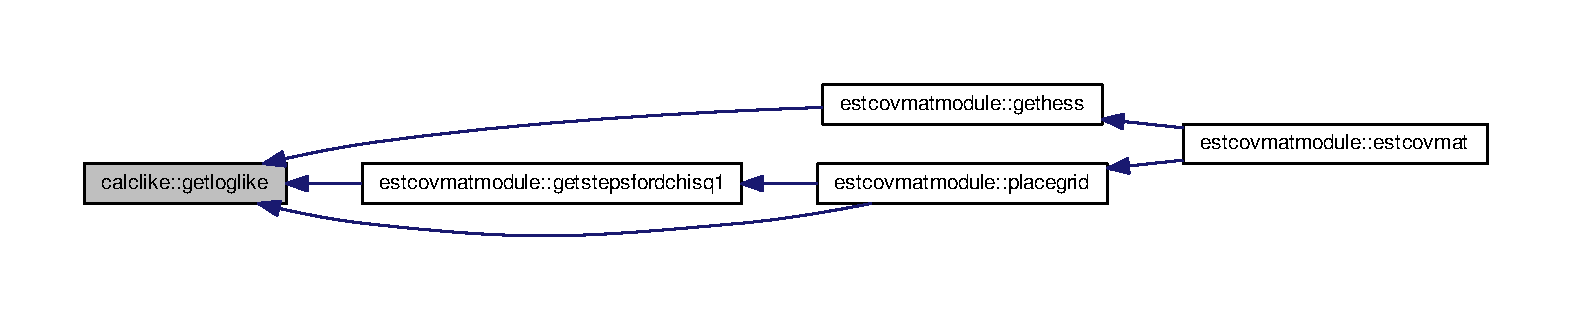
\includegraphics[width=350pt]{namespacecalclike_a1a9de6819dc2b41653d5bf9a36bd66a1_icgraph}
\end{center}
\end{figure}
\mbox{\Hypertarget{namespacecalclike_ae4302a1d96dcdf7816b3d66125504644}\label{namespacecalclike_ae4302a1d96dcdf7816b3d66125504644}} 
\index{calclike@{calclike}!getloglikebounds@{getloglikebounds}}
\index{getloglikebounds@{getloglikebounds}!calclike@{calclike}}
\subsubsection{\texorpdfstring{getloglikebounds()}{getloglikebounds()}}
{\footnotesize\ttfamily real(mcp) function calclike\+::getloglikebounds (\begin{DoxyParamCaption}\item[{class(\mbox{\hyperlink{structcalclike_1_1tlikecalculator}{tlikecalculator}})}]{this,  }\item[{class(tcalculationatparampoint)}]{Params }\end{DoxyParamCaption})\hspace{0.3cm}{\ttfamily [private]}}



References baseparameters\+::baseparams.

\mbox{\Hypertarget{namespacecalclike_a7f2306f2a9d2d0135d6f4852f6ed3bc2}\label{namespacecalclike_a7f2306f2a9d2d0135d6f4852f6ed3bc2}} 
\index{calclike@{calclike}!getloglikemain@{getloglikemain}}
\index{getloglikemain@{getloglikemain}!calclike@{calclike}}
\subsubsection{\texorpdfstring{getloglikemain()}{getloglikemain()}}
{\footnotesize\ttfamily real(mcp) function calclike\+::getloglikemain (\begin{DoxyParamCaption}\item[{class(\mbox{\hyperlink{structcalclike_1_1tlikecalculator}{tlikecalculator}})}]{this,  }\item[{class(tcalculationatparampoint)}]{Params }\end{DoxyParamCaption})\hspace{0.3cm}{\ttfamily [private]}}

\mbox{\Hypertarget{namespacecalclike_ae8f9437d9cf6441647020ac8e419e424}\label{namespacecalclike_ae8f9437d9cf6441647020ac8e419e424}} 
\index{calclike@{calclike}!getlogpriors@{getlogpriors}}
\index{getlogpriors@{getlogpriors}!calclike@{calclike}}
\subsubsection{\texorpdfstring{getlogpriors()}{getlogpriors()}}
{\footnotesize\ttfamily real(mcp) function calclike\+::getlogpriors (\begin{DoxyParamCaption}\item[{class(\mbox{\hyperlink{structcalclike_1_1tlikecalculator}{tlikecalculator}})}]{this,  }\item[{real(mcp), dimension(num\+\_\+params), intent(in)}]{P }\end{DoxyParamCaption})\hspace{0.3cm}{\ttfamily [private]}}



References baseparameters\+::baseparams.

\mbox{\Hypertarget{namespacecalclike_ae7eb4423ffdbadbf2df406b9d3331346}\label{namespacecalclike_ae7eb4423ffdbadbf2df406b9d3331346}} 
\index{calclike@{calclike}!theorylike\+\_\+calculaterequiredtheorychanges@{theorylike\+\_\+calculaterequiredtheorychanges}}
\index{theorylike\+\_\+calculaterequiredtheorychanges@{theorylike\+\_\+calculaterequiredtheorychanges}!calclike@{calclike}}
\subsubsection{\texorpdfstring{theorylike\+\_\+calculaterequiredtheorychanges()}{theorylike\_calculaterequiredtheorychanges()}}
{\footnotesize\ttfamily logical function calclike\+::theorylike\+\_\+calculaterequiredtheorychanges (\begin{DoxyParamCaption}\item[{class(\mbox{\hyperlink{structcalclike_1_1ttheorylikecalculator}{ttheorylikecalculator}})}]{this }\end{DoxyParamCaption})\hspace{0.3cm}{\ttfamily [private]}}

\mbox{\Hypertarget{namespacecalclike_adffdc491632ae303d023f5e1b704eba4}\label{namespacecalclike_adffdc491632ae303d023f5e1b704eba4}} 
\index{calclike@{calclike}!theorylike\+\_\+checkpriorcuts@{theorylike\+\_\+checkpriorcuts}}
\index{theorylike\+\_\+checkpriorcuts@{theorylike\+\_\+checkpriorcuts}!calclike@{calclike}}
\subsubsection{\texorpdfstring{theorylike\+\_\+checkpriorcuts()}{theorylike\_checkpriorcuts()}}
{\footnotesize\ttfamily real(mcp) function calclike\+::theorylike\+\_\+checkpriorcuts (\begin{DoxyParamCaption}\item[{class(\mbox{\hyperlink{structcalclike_1_1ttheorylikecalculator}{ttheorylikecalculator}})}]{this,  }\item[{class(tcalculationatparampoint)}]{Params }\end{DoxyParamCaption})\hspace{0.3cm}{\ttfamily [private]}}

\mbox{\Hypertarget{namespacecalclike_a141801e2c0e794a0411104bca9bb6809}\label{namespacecalclike_a141801e2c0e794a0411104bca9bb6809}} 
\index{calclike@{calclike}!theorylike\+\_\+getloglikemain@{theorylike\+\_\+getloglikemain}}
\index{theorylike\+\_\+getloglikemain@{theorylike\+\_\+getloglikemain}!calclike@{calclike}}
\subsubsection{\texorpdfstring{theorylike\+\_\+getloglikemain()}{theorylike\_getloglikemain()}}
{\footnotesize\ttfamily real(mcp) function calclike\+::theorylike\+\_\+getloglikemain (\begin{DoxyParamCaption}\item[{class(\mbox{\hyperlink{structcalclike_1_1ttheorylikecalculator}{ttheorylikecalculator}})}]{this,  }\item[{class(tcalculationatparampoint)}]{Params }\end{DoxyParamCaption})\hspace{0.3cm}{\ttfamily [private]}}

\mbox{\Hypertarget{namespacecalclike_a27e62cb96ad63d0285283d1eb8dcec0c}\label{namespacecalclike_a27e62cb96ad63d0285283d1eb8dcec0c}} 
\index{calclike@{calclike}!theorylike\+\_\+getloglikepost@{theorylike\+\_\+getloglikepost}}
\index{theorylike\+\_\+getloglikepost@{theorylike\+\_\+getloglikepost}!calclike@{calclike}}
\subsubsection{\texorpdfstring{theorylike\+\_\+getloglikepost()}{theorylike\_getloglikepost()}}
{\footnotesize\ttfamily real(mcp) function calclike\+::theorylike\+\_\+getloglikepost (\begin{DoxyParamCaption}\item[{class(\mbox{\hyperlink{structcalclike_1_1ttheorylikecalculator}{ttheorylikecalculator}})}]{this,  }\item[{class(tcalculationatparampoint)}]{Params,  }\item[{logical, dimension(datalikelihoods\%count), intent(in), optional}]{do\+\_\+like }\end{DoxyParamCaption})\hspace{0.3cm}{\ttfamily [private]}}

\mbox{\Hypertarget{namespacecalclike_ab57c11043f079701db0baf858bf6315a}\label{namespacecalclike_ab57c11043f079701db0baf858bf6315a}} 
\index{calclike@{calclike}!theorylike\+\_\+gettheoryforimportance@{theorylike\+\_\+gettheoryforimportance}}
\index{theorylike\+\_\+gettheoryforimportance@{theorylike\+\_\+gettheoryforimportance}!calclike@{calclike}}
\subsubsection{\texorpdfstring{theorylike\+\_\+gettheoryforimportance()}{theorylike\_gettheoryforimportance()}}
{\footnotesize\ttfamily subroutine calclike\+::theorylike\+\_\+gettheoryforimportance (\begin{DoxyParamCaption}\item[{class(\mbox{\hyperlink{structcalclike_1_1ttheorylikecalculator}{ttheorylikecalculator}})}]{this,  }\item[{class(tcalculationatparampoint), target}]{Params,  }\item[{integer}]{error }\end{DoxyParamCaption})\hspace{0.3cm}{\ttfamily [private]}}

\mbox{\Hypertarget{namespacecalclike_ab2d52ca5a668e5072ed6d10c161a5e88}\label{namespacecalclike_ab2d52ca5a668e5072ed6d10c161a5e88}} 
\index{calclike@{calclike}!theorylike\+\_\+gettheoryforlike@{theorylike\+\_\+gettheoryforlike}}
\index{theorylike\+\_\+gettheoryforlike@{theorylike\+\_\+gettheoryforlike}!calclike@{calclike}}
\subsubsection{\texorpdfstring{theorylike\+\_\+gettheoryforlike()}{theorylike\_gettheoryforlike()}}
{\footnotesize\ttfamily subroutine calclike\+::theorylike\+\_\+gettheoryforlike (\begin{DoxyParamCaption}\item[{class(\mbox{\hyperlink{structcalclike_1_1ttheorylikecalculator}{ttheorylikecalculator}})}]{this,  }\item[{class(tdatalikelihood), pointer}]{Like }\end{DoxyParamCaption})\hspace{0.3cm}{\ttfamily [private]}}

\mbox{\Hypertarget{namespacecalclike_a81e2854f62abdf354c1f03fc29c05d1c}\label{namespacecalclike_a81e2854f62abdf354c1f03fc29c05d1c}} 
\index{calclike@{calclike}!theorylike\+\_\+loglikewiththeoryset@{theorylike\+\_\+loglikewiththeoryset}}
\index{theorylike\+\_\+loglikewiththeoryset@{theorylike\+\_\+loglikewiththeoryset}!calclike@{calclike}}
\subsubsection{\texorpdfstring{theorylike\+\_\+loglikewiththeoryset()}{theorylike\_loglikewiththeoryset()}}
{\footnotesize\ttfamily real(mcp) function calclike\+::theorylike\+\_\+loglikewiththeoryset (\begin{DoxyParamCaption}\item[{class(\mbox{\hyperlink{structcalclike_1_1ttheorylikecalculator}{ttheorylikecalculator}})}]{this,  }\item[{logical, dimension(datalikelihoods\%count), intent(in), optional}]{likelihood\+\_\+mask }\end{DoxyParamCaption})\hspace{0.3cm}{\ttfamily [private]}}

\mbox{\Hypertarget{namespacecalclike_a3823367d787d17f15e903222232f4b94}\label{namespacecalclike_a3823367d787d17f15e903222232f4b94}} 
\index{calclike@{calclike}!theorylike\+\_\+setnewtheoryresults@{theorylike\+\_\+setnewtheoryresults}}
\index{theorylike\+\_\+setnewtheoryresults@{theorylike\+\_\+setnewtheoryresults}!calclike@{calclike}}
\subsubsection{\texorpdfstring{theorylike\+\_\+setnewtheoryresults()}{theorylike\_setnewtheoryresults()}}
{\footnotesize\ttfamily subroutine calclike\+::theorylike\+\_\+setnewtheoryresults (\begin{DoxyParamCaption}\item[{class(\mbox{\hyperlink{structcalclike_1_1ttheorylikecalculator}{ttheorylikecalculator}})}]{this,  }\item[{class(tcalculationatparampoint)}]{Params }\end{DoxyParamCaption})\hspace{0.3cm}{\ttfamily [private]}}

\mbox{\Hypertarget{namespacecalclike_ab9d66863dbce892dbee08483d9cdac50}\label{namespacecalclike_ab9d66863dbce892dbee08483d9cdac50}} 
\index{calclike@{calclike}!theorylike\+\_\+settheoryparams@{theorylike\+\_\+settheoryparams}}
\index{theorylike\+\_\+settheoryparams@{theorylike\+\_\+settheoryparams}!calclike@{calclike}}
\subsubsection{\texorpdfstring{theorylike\+\_\+settheoryparams()}{theorylike\_settheoryparams()}}
{\footnotesize\ttfamily subroutine calclike\+::theorylike\+\_\+settheoryparams (\begin{DoxyParamCaption}\item[{class(\mbox{\hyperlink{structcalclike_1_1ttheorylikecalculator}{ttheorylikecalculator}})}]{this,  }\item[{class(tcalculationatparampoint), target}]{Params }\end{DoxyParamCaption})\hspace{0.3cm}{\ttfamily [private]}}

\mbox{\Hypertarget{namespacecalclike_adb2986867dcdb441b12b98cdd46cc5b5}\label{namespacecalclike_adb2986867dcdb441b12b98cdd46cc5b5}} 
\index{calclike@{calclike}!theorylike\+\_\+testlikelihoodfunction@{theorylike\+\_\+testlikelihoodfunction}}
\index{theorylike\+\_\+testlikelihoodfunction@{theorylike\+\_\+testlikelihoodfunction}!calclike@{calclike}}
\subsubsection{\texorpdfstring{theorylike\+\_\+testlikelihoodfunction()}{theorylike\_testlikelihoodfunction()}}
{\footnotesize\ttfamily real(mcp) function calclike\+::theorylike\+\_\+testlikelihoodfunction (\begin{DoxyParamCaption}\item[{class(\mbox{\hyperlink{structcalclike_1_1ttheorylikecalculator}{ttheorylikecalculator}})}]{this,  }\item[{class(tcalculationatparampoint)}]{Params }\end{DoxyParamCaption})\hspace{0.3cm}{\ttfamily [private]}}

\mbox{\Hypertarget{namespacecalclike_adb244129926744248e4e4f8883384b5c}\label{namespacecalclike_adb244129926744248e4e4f8883384b5c}} 
\index{calclike@{calclike}!theorylike\+\_\+updatetheoryforlikelihoods@{theorylike\+\_\+updatetheoryforlikelihoods}}
\index{theorylike\+\_\+updatetheoryforlikelihoods@{theorylike\+\_\+updatetheoryforlikelihoods}!calclike@{calclike}}
\subsubsection{\texorpdfstring{theorylike\+\_\+updatetheoryforlikelihoods()}{theorylike\_updatetheoryforlikelihoods()}}
{\footnotesize\ttfamily subroutine calclike\+::theorylike\+\_\+updatetheoryforlikelihoods (\begin{DoxyParamCaption}\item[{class(\mbox{\hyperlink{structcalclike_1_1ttheorylikecalculator}{ttheorylikecalculator}})}]{this,  }\item[{class(tcalculationatparampoint)}]{Params }\end{DoxyParamCaption})\hspace{0.3cm}{\ttfamily [private]}}

\mbox{\Hypertarget{namespacecalclike_af377ac1f0746c42a430094fe73246012}\label{namespacecalclike_af377ac1f0746c42a430094fe73246012}} 
\index{calclike@{calclike}!tlikecalculator\+\_\+readparams@{tlikecalculator\+\_\+readparams}}
\index{tlikecalculator\+\_\+readparams@{tlikecalculator\+\_\+readparams}!calclike@{calclike}}
\subsubsection{\texorpdfstring{tlikecalculator\+\_\+readparams()}{tlikecalculator\_readparams()}}
{\footnotesize\ttfamily subroutine calclike\+::tlikecalculator\+\_\+readparams (\begin{DoxyParamCaption}\item[{class(\mbox{\hyperlink{structcalclike_1_1tlikecalculator}{tlikecalculator}})}]{this,  }\item[{class(tsettingini)}]{Ini }\end{DoxyParamCaption})\hspace{0.3cm}{\ttfamily [private]}}

\mbox{\Hypertarget{namespacecalclike_adb41feb15d07d744bace1629aea8a5d3}\label{namespacecalclike_adb41feb15d07d744bace1629aea8a5d3}} 
\index{calclike@{calclike}!tlikecalculator\+\_\+testlikelihoodfunction@{tlikecalculator\+\_\+testlikelihoodfunction}}
\index{tlikecalculator\+\_\+testlikelihoodfunction@{tlikecalculator\+\_\+testlikelihoodfunction}!calclike@{calclike}}
\subsubsection{\texorpdfstring{tlikecalculator\+\_\+testlikelihoodfunction()}{tlikecalculator\_testlikelihoodfunction()}}
{\footnotesize\ttfamily real(mcp) function calclike\+::tlikecalculator\+\_\+testlikelihoodfunction (\begin{DoxyParamCaption}\item[{class(\mbox{\hyperlink{structcalclike_1_1tlikecalculator}{tlikecalculator}})}]{this,  }\item[{class(tcalculationatparampoint)}]{Params }\end{DoxyParamCaption})\hspace{0.3cm}{\ttfamily [private]}}

\mbox{\Hypertarget{namespacecalclike_a4be845214aaba0f4348b66c67401f78b}\label{namespacecalclike_a4be845214aaba0f4348b66c67401f78b}} 
\index{calclike@{calclike}!tlikecalculator\+\_\+writeparampointtextdata@{tlikecalculator\+\_\+writeparampointtextdata}}
\index{tlikecalculator\+\_\+writeparampointtextdata@{tlikecalculator\+\_\+writeparampointtextdata}!calclike@{calclike}}
\subsubsection{\texorpdfstring{tlikecalculator\+\_\+writeparampointtextdata()}{tlikecalculator\_writeparampointtextdata()}}
{\footnotesize\ttfamily subroutine calclike\+::tlikecalculator\+\_\+writeparampointtextdata (\begin{DoxyParamCaption}\item[{class(\mbox{\hyperlink{structcalclike_1_1tlikecalculator}{tlikecalculator}})}]{this,  }\item[{character(len=$\ast$), intent(in)}]{output\+\_\+root,  }\item[{class(tcalculationatparampoint)}]{Params }\end{DoxyParamCaption})\hspace{0.3cm}{\ttfamily [private]}}

\mbox{\Hypertarget{namespacecalclike_a7348b373c8c9138f0c694ad9969fcb66}\label{namespacecalclike_a7348b373c8c9138f0c694ad9969fcb66}} 
\index{calclike@{calclike}!tlikecalculator\+\_\+writeparamshumantext@{tlikecalculator\+\_\+writeparamshumantext}}
\index{tlikecalculator\+\_\+writeparamshumantext@{tlikecalculator\+\_\+writeparamshumantext}!calclike@{calclike}}
\subsubsection{\texorpdfstring{tlikecalculator\+\_\+writeparamshumantext()}{tlikecalculator\_writeparamshumantext()}}
{\footnotesize\ttfamily subroutine calclike\+::tlikecalculator\+\_\+writeparamshumantext (\begin{DoxyParamCaption}\item[{class(\mbox{\hyperlink{structcalclike_1_1tlikecalculator}{tlikecalculator}})}]{this,  }\item[{integer, intent(in)}]{aunit,  }\item[{class(tcalculationatparampoint)}]{P,  }\item[{real(mcp), intent(in), optional}]{Log\+Like,  }\item[{real(mcp), intent(in), optional}]{weight }\end{DoxyParamCaption})\hspace{0.3cm}{\ttfamily [private]}}

\mbox{\Hypertarget{namespacecalclike_afd9d4013e29fb891f656598d4b5e1b73}\label{namespacecalclike_afd9d4013e29fb891f656598d4b5e1b73}} 
\index{calclike@{calclike}!tlikecalculator\+\_\+writeparamshumantextfile@{tlikecalculator\+\_\+writeparamshumantextfile}}
\index{tlikecalculator\+\_\+writeparamshumantextfile@{tlikecalculator\+\_\+writeparamshumantextfile}!calclike@{calclike}}
\subsubsection{\texorpdfstring{tlikecalculator\+\_\+writeparamshumantextfile()}{tlikecalculator\_writeparamshumantextfile()}}
{\footnotesize\ttfamily subroutine calclike\+::tlikecalculator\+\_\+writeparamshumantextfile (\begin{DoxyParamCaption}\item[{class(\mbox{\hyperlink{structcalclike_1_1tlikecalculator}{tlikecalculator}})}]{this,  }\item[{character(len=$\ast$), intent(in)}]{fname,  }\item[{class(tcalculationatparampoint)}]{P,  }\item[{real(mcp), intent(in), optional}]{Log\+Like,  }\item[{real(mcp), intent(in), optional}]{weight }\end{DoxyParamCaption})\hspace{0.3cm}{\ttfamily [private]}}

\mbox{\Hypertarget{namespacecalclike_a5158b85ddca7d8f1b417a813bb7fe849}\label{namespacecalclike_a5158b85ddca7d8f1b417a813bb7fe849}} 
\index{calclike@{calclike}!tlikecalculator\+\_\+writeperformancestats@{tlikecalculator\+\_\+writeperformancestats}}
\index{tlikecalculator\+\_\+writeperformancestats@{tlikecalculator\+\_\+writeperformancestats}!calclike@{calclike}}
\subsubsection{\texorpdfstring{tlikecalculator\+\_\+writeperformancestats()}{tlikecalculator\_writeperformancestats()}}
{\footnotesize\ttfamily subroutine calclike\+::tlikecalculator\+\_\+writeperformancestats (\begin{DoxyParamCaption}\item[{class(\mbox{\hyperlink{structcalclike_1_1tlikecalculator}{tlikecalculator}})}]{this,  }\item[{integer, intent(in)}]{unit }\end{DoxyParamCaption})\hspace{0.3cm}{\ttfamily [private]}}

\mbox{\Hypertarget{namespacecalclike_acb1cb4737fc9ec3a805214e87b444b00}\label{namespacecalclike_acb1cb4737fc9ec3a805214e87b444b00}} 
\index{calclike@{calclike}!ttheorylike\+\_\+writeparampointtextdata@{ttheorylike\+\_\+writeparampointtextdata}}
\index{ttheorylike\+\_\+writeparampointtextdata@{ttheorylike\+\_\+writeparampointtextdata}!calclike@{calclike}}
\subsubsection{\texorpdfstring{ttheorylike\+\_\+writeparampointtextdata()}{ttheorylike\_writeparampointtextdata()}}
{\footnotesize\ttfamily subroutine calclike\+::ttheorylike\+\_\+writeparampointtextdata (\begin{DoxyParamCaption}\item[{class(\mbox{\hyperlink{structcalclike_1_1ttheorylikecalculator}{ttheorylikecalculator}})}]{this,  }\item[{character(len=$\ast$), intent(in)}]{output\+\_\+root,  }\item[{class(tcalculationatparampoint)}]{Params }\end{DoxyParamCaption})\hspace{0.3cm}{\ttfamily [private]}}

\mbox{\Hypertarget{namespacecalclike_a5c185d1a702fe31d3d1204d919b338da}\label{namespacecalclike_a5c185d1a702fe31d3d1204d919b338da}} 
\index{calclike@{calclike}!ttheorylike\+\_\+writeparamshumantext@{ttheorylike\+\_\+writeparamshumantext}}
\index{ttheorylike\+\_\+writeparamshumantext@{ttheorylike\+\_\+writeparamshumantext}!calclike@{calclike}}
\subsubsection{\texorpdfstring{ttheorylike\+\_\+writeparamshumantext()}{ttheorylike\_writeparamshumantext()}}
{\footnotesize\ttfamily subroutine calclike\+::ttheorylike\+\_\+writeparamshumantext (\begin{DoxyParamCaption}\item[{class(\mbox{\hyperlink{structcalclike_1_1ttheorylikecalculator}{ttheorylikecalculator}})}]{this,  }\item[{integer, intent(in)}]{aunit,  }\item[{class(tcalculationatparampoint)}]{P,  }\item[{real(mcp), intent(in), optional}]{Log\+Like,  }\item[{real(mcp), intent(in), optional}]{weight }\end{DoxyParamCaption})\hspace{0.3cm}{\ttfamily [private]}}


\hypertarget{namespacecalclike__cosmology}{}\section{calclike\+\_\+cosmology Module Reference}
\label{namespacecalclike__cosmology}\index{calclike\+\_\+cosmology@{calclike\+\_\+cosmology}}
\subsection*{Data Types}
\begin{DoxyCompactItemize}
\item 
type \mbox{\hyperlink{structcalclike__cosmology_1_1tcosmolikecalculator}{tcosmolikecalculator}}
\end{DoxyCompactItemize}
\subsection*{Functions/\+Subroutines}
\begin{DoxyCompactItemize}
\item 
subroutine \mbox{\hyperlink{namespacecalclike__cosmology_a86c0c49dcb09440792bc5a002f456f57}{tcosmolikecalculator\+\_\+initconfig}} (this, Config)
\item 
subroutine \mbox{\hyperlink{namespacecalclike__cosmology_a6f159ab28e06f381042c55c451a060a9}{cosmo\+\_\+gettheoryforlike}} (this, Like)
\item 
logical function \mbox{\hyperlink{namespacecalclike__cosmology_aa5acf9c357eef01f44553072f8327e5e}{cosmo\+\_\+calculaterequiredtheorychanges}} (this)
\item 
subroutine \mbox{\hyperlink{namespacecalclike__cosmology_a98c01c544a399527119cde828e456b4b}{cosmo\+\_\+writeperformancestats}} (this, unit)
\item 
subroutine \mbox{\hyperlink{namespacecalclike__cosmology_afcac4304981be0a09f45f15d9194e427}{cosmo\+\_\+updatetheoryforlikelihoods}} (this, Params)
\end{DoxyCompactItemize}


\subsection{Function/\+Subroutine Documentation}
\mbox{\Hypertarget{namespacecalclike__cosmology_aa5acf9c357eef01f44553072f8327e5e}\label{namespacecalclike__cosmology_aa5acf9c357eef01f44553072f8327e5e}} 
\index{calclike\+\_\+cosmology@{calclike\+\_\+cosmology}!cosmo\+\_\+calculaterequiredtheorychanges@{cosmo\+\_\+calculaterequiredtheorychanges}}
\index{cosmo\+\_\+calculaterequiredtheorychanges@{cosmo\+\_\+calculaterequiredtheorychanges}!calclike\+\_\+cosmology@{calclike\+\_\+cosmology}}
\subsubsection{\texorpdfstring{cosmo\+\_\+calculaterequiredtheorychanges()}{cosmo\_calculaterequiredtheorychanges()}}
{\footnotesize\ttfamily logical function calclike\+\_\+cosmology\+::cosmo\+\_\+calculaterequiredtheorychanges (\begin{DoxyParamCaption}\item[{class(\mbox{\hyperlink{structcalclike__cosmology_1_1tcosmolikecalculator}{tcosmolikecalculator}})}]{this }\end{DoxyParamCaption})\hspace{0.3cm}{\ttfamily [private]}}



References cosmologytypes\+::cosmosettings, cosmologytypes\+::index\+\_\+initpower, cosmologytypes\+::num\+\_\+hard, and cosmologytypes\+::num\+\_\+initpower.

\mbox{\Hypertarget{namespacecalclike__cosmology_a6f159ab28e06f381042c55c451a060a9}\label{namespacecalclike__cosmology_a6f159ab28e06f381042c55c451a060a9}} 
\index{calclike\+\_\+cosmology@{calclike\+\_\+cosmology}!cosmo\+\_\+gettheoryforlike@{cosmo\+\_\+gettheoryforlike}}
\index{cosmo\+\_\+gettheoryforlike@{cosmo\+\_\+gettheoryforlike}!calclike\+\_\+cosmology@{calclike\+\_\+cosmology}}
\subsubsection{\texorpdfstring{cosmo\+\_\+gettheoryforlike()}{cosmo\_gettheoryforlike()}}
{\footnotesize\ttfamily subroutine calclike\+\_\+cosmology\+::cosmo\+\_\+gettheoryforlike (\begin{DoxyParamCaption}\item[{class(\mbox{\hyperlink{structcalclike__cosmology_1_1tcosmolikecalculator}{tcosmolikecalculator}})}]{this,  }\item[{class(tdatalikelihood), pointer}]{Like }\end{DoxyParamCaption})\hspace{0.3cm}{\ttfamily [private]}}



References cosmologytypes\+::num\+\_\+hard.

\mbox{\Hypertarget{namespacecalclike__cosmology_afcac4304981be0a09f45f15d9194e427}\label{namespacecalclike__cosmology_afcac4304981be0a09f45f15d9194e427}} 
\index{calclike\+\_\+cosmology@{calclike\+\_\+cosmology}!cosmo\+\_\+updatetheoryforlikelihoods@{cosmo\+\_\+updatetheoryforlikelihoods}}
\index{cosmo\+\_\+updatetheoryforlikelihoods@{cosmo\+\_\+updatetheoryforlikelihoods}!calclike\+\_\+cosmology@{calclike\+\_\+cosmology}}
\subsubsection{\texorpdfstring{cosmo\+\_\+updatetheoryforlikelihoods()}{cosmo\_updatetheoryforlikelihoods()}}
{\footnotesize\ttfamily subroutine calclike\+\_\+cosmology\+::cosmo\+\_\+updatetheoryforlikelihoods (\begin{DoxyParamCaption}\item[{class(\mbox{\hyperlink{structcalclike__cosmology_1_1tcosmolikecalculator}{tcosmolikecalculator}})}]{this,  }\item[{class(tcalculationatparampoint)}]{Params }\end{DoxyParamCaption})\hspace{0.3cm}{\ttfamily [private]}}



References cosmologytypes\+::cosmosettings.

\mbox{\Hypertarget{namespacecalclike__cosmology_a98c01c544a399527119cde828e456b4b}\label{namespacecalclike__cosmology_a98c01c544a399527119cde828e456b4b}} 
\index{calclike\+\_\+cosmology@{calclike\+\_\+cosmology}!cosmo\+\_\+writeperformancestats@{cosmo\+\_\+writeperformancestats}}
\index{cosmo\+\_\+writeperformancestats@{cosmo\+\_\+writeperformancestats}!calclike\+\_\+cosmology@{calclike\+\_\+cosmology}}
\subsubsection{\texorpdfstring{cosmo\+\_\+writeperformancestats()}{cosmo\_writeperformancestats()}}
{\footnotesize\ttfamily subroutine calclike\+\_\+cosmology\+::cosmo\+\_\+writeperformancestats (\begin{DoxyParamCaption}\item[{class(\mbox{\hyperlink{structcalclike__cosmology_1_1tcosmolikecalculator}{tcosmolikecalculator}})}]{this,  }\item[{integer, intent(in)}]{unit }\end{DoxyParamCaption})\hspace{0.3cm}{\ttfamily [private]}}

\mbox{\Hypertarget{namespacecalclike__cosmology_a86c0c49dcb09440792bc5a002f456f57}\label{namespacecalclike__cosmology_a86c0c49dcb09440792bc5a002f456f57}} 
\index{calclike\+\_\+cosmology@{calclike\+\_\+cosmology}!tcosmolikecalculator\+\_\+initconfig@{tcosmolikecalculator\+\_\+initconfig}}
\index{tcosmolikecalculator\+\_\+initconfig@{tcosmolikecalculator\+\_\+initconfig}!calclike\+\_\+cosmology@{calclike\+\_\+cosmology}}
\subsubsection{\texorpdfstring{tcosmolikecalculator\+\_\+initconfig()}{tcosmolikecalculator\_initconfig()}}
{\footnotesize\ttfamily subroutine calclike\+\_\+cosmology\+::tcosmolikecalculator\+\_\+initconfig (\begin{DoxyParamCaption}\item[{class(\mbox{\hyperlink{structcalclike__cosmology_1_1tcosmolikecalculator}{tcosmolikecalculator}})}]{this,  }\item[{class(tgeneralconfig), target}]{Config }\end{DoxyParamCaption})\hspace{0.3cm}{\ttfamily [private]}}


\hypertarget{namespacecalculator__camb}{}\section{calculator\+\_\+camb Module Reference}
\label{namespacecalculator__camb}\index{calculator\+\_\+camb@{calculator\+\_\+camb}}
\subsection*{Data Types}
\begin{DoxyCompactItemize}
\item 
type \mbox{\hyperlink{structcalculator__camb_1_1camb__calculator}{camb\+\_\+calculator}}
\item 
type \mbox{\hyperlink{structcalculator__camb_1_1cambtransfercache}{cambtransfercache}}
\end{DoxyCompactItemize}
\subsection*{Functions/\+Subroutines}
\begin{DoxyCompactItemize}
\item 
subroutine \mbox{\hyperlink{namespacecalculator__camb_a10914a67c9b3a93d74382c9c9adf0983}{cambcalc\+\_\+cmbtocamb}} (this, C\+MB, P)
\item 
subroutine \mbox{\hyperlink{namespacecalculator__camb_a451eeaadb06191ee0203caf0d76c66c2}{cambcalc\+\_\+setderived}} (this, Theory)
\item 
subroutine \mbox{\hyperlink{namespacecalculator__camb_a2f68d8cedf36c519d822547aa49c3f98}{cambcalc\+\_\+setparamsforbackground}} (this, C\+MB)
\item 
subroutine \mbox{\hyperlink{namespacecalculator__camb_a04c53e5b4763297e232978e627153a17}{cambcalc\+\_\+setbackgroundtheorydata}} (this, C\+MB, Theory, error)
\item 
subroutine \mbox{\hyperlink{namespacecalculator__camb_a9e8887a3ae9da2bb092aac4285234df4}{cambcalc\+\_\+getnewtransferdata}} (this, C\+MB, Info, Theory, error)
\item 
subroutine \mbox{\hyperlink{namespacecalculator__camb_ad7195d220a7f5bc77479225b47d91d17}{cambcalc\+\_\+getnewpowerdata}} (this, C\+MB, Info, Theory, error)
\item 
subroutine \mbox{\hyperlink{namespacecalculator__camb_a46bd33ed008e289fb5cb08f6feb86419}{cambcalc\+\_\+gettheoryforimportance}} (this, C\+MB, Theory, error)
\item 
subroutine \mbox{\hyperlink{namespacecalculator__camb_a7ccabec132f8bbe50ac91abdd4a86751}{cambcalc\+\_\+setpowersfromcamb}} (this, C\+MB, Theory)
\item 
subroutine \mbox{\hyperlink{namespacecalculator__camb_a8e6f706ddb3ae930a9f1293d9c480405}{cambcalc\+\_\+setpkfromcamb}} (this, M, Theory, error)
\item 
subroutine \mbox{\hyperlink{namespacecalculator__camb_ac0ce3e4748dd96f033235b9dbf3a71b3}{cambcalc\+\_\+getnlandratios}} (this, M, Theory, Ratios, error)
\item 
subroutine \mbox{\hyperlink{namespacecalculator__camb_ab67fcdadb23a73d5747a682c87304c0b}{cambcalc\+\_\+initcamb}} (this, C\+MB, error, Do\+Reion)
\item 
real(mcp) function \mbox{\hyperlink{namespacecalculator__camb_ac09824dcbd350dcc819683a630b6e646}{cambcalc\+\_\+getopticaldepth}} (this, C\+MB)
\item 
real(mcp) function \mbox{\hyperlink{namespacecalculator__camb_a36d033f09a4d35c8b9a37d518fcebda0}{cambcalc\+\_\+getzrefromtau}} (this, C\+MB, tau)
\item 
real(mcp) function \mbox{\hyperlink{namespacecalculator__camb_a88bb5f71c4e4784315929d98702a1214}{cambcalc\+\_\+cmbtotheta}} (this, C\+MB)
\item 
real(mcp) function \mbox{\hyperlink{namespacecalculator__camb_a18709a68a49a6989073dae760f643430}{cambcalc\+\_\+bao\+\_\+d\+\_\+v}} (this, z)
\item 
real(mcp) function \mbox{\hyperlink{namespacecalculator__camb_a40bf5a8b3435b93efcaa688ecb4867f4}{cambcalc\+\_\+angulardiameterdistance}} (this, z)
\item 
real(mcp) function \mbox{\hyperlink{namespacecalculator__camb_a44d780a147bc9cea89b7ebe9a071b98a}{cambcalc\+\_\+comovingradialdistance}} (this, z)
\item 
real(mcp) function \mbox{\hyperlink{namespacecalculator__camb_a368f4f92f978124067f561deb5392714}{cambcalc\+\_\+angulardiameterdistance2}} (this, z1, z2)
\item 
real(mcp) function \mbox{\hyperlink{namespacecalculator__camb_a0f03309bd014f3de538a3565bc867402}{cambcalc\+\_\+luminositydistance}} (this, z)
\item 
real(mcp) function \mbox{\hyperlink{namespacecalculator__camb_a10e6be2c2d0ef7cb7741dbce3dbc88a9}{cambcalc\+\_\+hofz}} (this, z)
\item 
subroutine \mbox{\hyperlink{namespacecalculator__camb_a1f498feeb9fd7b4b6ff5c951bb3bcf5d}{cambcalc\+\_\+initcambparams}} (this, P)
\item 
subroutine \mbox{\hyperlink{namespacecalculator__camb_a30b5dc9bda2ffcd939436fbc93322f9e}{cambcalc\+\_\+setcambinitpower}} (this, P, C\+MB, ix)
\item 
subroutine \mbox{\hyperlink{namespacecalculator__camb_aa3a88e278563ca8092494c335094e325}{cambcalc\+\_\+readparams}} (this, Ini)
\item 
subroutine \mbox{\hyperlink{namespacecalculator__camb_a5eb19890ea9bf2acad52f23b9334e1e8}{cambcalc\+\_\+initforlikelihoods}} (this)
\item 
subroutine \mbox{\hyperlink{namespacecalculator__camb_a67d98d7cdaa015cca41f95ed94678a79}{cambcalc\+\_\+versiontraceoutput}} (this, Read\+Values)
\item 
subroutine \mbox{\hyperlink{namespacecalculator__camb_a8eeaa2b45303d1bb5c7323cbf4767ce7}{loadfiducialhighltemplate}} (this)
\item 
subroutine \mbox{\hyperlink{namespacecalculator__camb_a74de7ed91f31c5cccb3f6c738f689295}{cambtransfercache\+\_\+clear}} (Info)
\end{DoxyCompactItemize}


\subsection{Function/\+Subroutine Documentation}
\mbox{\Hypertarget{namespacecalculator__camb_a40bf5a8b3435b93efcaa688ecb4867f4}\label{namespacecalculator__camb_a40bf5a8b3435b93efcaa688ecb4867f4}} 
\index{calculator\+\_\+camb@{calculator\+\_\+camb}!cambcalc\+\_\+angulardiameterdistance@{cambcalc\+\_\+angulardiameterdistance}}
\index{cambcalc\+\_\+angulardiameterdistance@{cambcalc\+\_\+angulardiameterdistance}!calculator\+\_\+camb@{calculator\+\_\+camb}}
\subsubsection{\texorpdfstring{cambcalc\+\_\+angulardiameterdistance()}{cambcalc\_angulardiameterdistance()}}
{\footnotesize\ttfamily real(mcp) function calculator\+\_\+camb\+::cambcalc\+\_\+angulardiameterdistance (\begin{DoxyParamCaption}\item[{class(\mbox{\hyperlink{structcalculator__camb_1_1camb__calculator}{camb\+\_\+calculator}})}]{this,  }\item[{real(mcp), intent(in)}]{z }\end{DoxyParamCaption})}

\mbox{\Hypertarget{namespacecalculator__camb_a368f4f92f978124067f561deb5392714}\label{namespacecalculator__camb_a368f4f92f978124067f561deb5392714}} 
\index{calculator\+\_\+camb@{calculator\+\_\+camb}!cambcalc\+\_\+angulardiameterdistance2@{cambcalc\+\_\+angulardiameterdistance2}}
\index{cambcalc\+\_\+angulardiameterdistance2@{cambcalc\+\_\+angulardiameterdistance2}!calculator\+\_\+camb@{calculator\+\_\+camb}}
\subsubsection{\texorpdfstring{cambcalc\+\_\+angulardiameterdistance2()}{cambcalc\_angulardiameterdistance2()}}
{\footnotesize\ttfamily real(mcp) function calculator\+\_\+camb\+::cambcalc\+\_\+angulardiameterdistance2 (\begin{DoxyParamCaption}\item[{class(\mbox{\hyperlink{structcalculator__camb_1_1camb__calculator}{camb\+\_\+calculator}})}]{this,  }\item[{real(mcp), intent(in)}]{z1,  }\item[{real(mcp), intent(in)}]{z2 }\end{DoxyParamCaption})}

\mbox{\Hypertarget{namespacecalculator__camb_a18709a68a49a6989073dae760f643430}\label{namespacecalculator__camb_a18709a68a49a6989073dae760f643430}} 
\index{calculator\+\_\+camb@{calculator\+\_\+camb}!cambcalc\+\_\+bao\+\_\+d\+\_\+v@{cambcalc\+\_\+bao\+\_\+d\+\_\+v}}
\index{cambcalc\+\_\+bao\+\_\+d\+\_\+v@{cambcalc\+\_\+bao\+\_\+d\+\_\+v}!calculator\+\_\+camb@{calculator\+\_\+camb}}
\subsubsection{\texorpdfstring{cambcalc\+\_\+bao\+\_\+d\+\_\+v()}{cambcalc\_bao\_d\_v()}}
{\footnotesize\ttfamily real(mcp) function calculator\+\_\+camb\+::cambcalc\+\_\+bao\+\_\+d\+\_\+v (\begin{DoxyParamCaption}\item[{class(\mbox{\hyperlink{structcalculator__camb_1_1camb__calculator}{camb\+\_\+calculator}})}]{this,  }\item[{real(mcp), intent(in)}]{z }\end{DoxyParamCaption})}

\mbox{\Hypertarget{namespacecalculator__camb_a10914a67c9b3a93d74382c9c9adf0983}\label{namespacecalculator__camb_a10914a67c9b3a93d74382c9c9adf0983}} 
\index{calculator\+\_\+camb@{calculator\+\_\+camb}!cambcalc\+\_\+cmbtocamb@{cambcalc\+\_\+cmbtocamb}}
\index{cambcalc\+\_\+cmbtocamb@{cambcalc\+\_\+cmbtocamb}!calculator\+\_\+camb@{calculator\+\_\+camb}}
\subsubsection{\texorpdfstring{cambcalc\+\_\+cmbtocamb()}{cambcalc\_cmbtocamb()}}
{\footnotesize\ttfamily subroutine calculator\+\_\+camb\+::cambcalc\+\_\+cmbtocamb (\begin{DoxyParamCaption}\item[{class(\mbox{\hyperlink{structcalculator__camb_1_1camb__calculator}{camb\+\_\+calculator}})}]{this,  }\item[{class(cmbparams)}]{C\+MB,  }\item[{type(cambparams)}]{P }\end{DoxyParamCaption})\hspace{0.3cm}{\ttfamily [private]}}



References cambmain\+::alens, lensing\+::alens\+\_\+fiducial, camb\+::camb\+\_\+setneutrinohierarchy(), cosmologytypes\+::cosmosettings, constants\+::default\+\_\+nnu, constants\+::delta\+\_\+mnu21, constants\+::delta\+\_\+mnu31, constants\+::mnu\+\_\+min\+\_\+normal, massivenu\+::sum\+\_\+mnu\+\_\+for\+\_\+m1(), lambdageneral\+::w\+\_\+lam, and lambdageneral\+::wa\+\_\+ppf.

Here is the call graph for this function\+:
\nopagebreak
\begin{figure}[H]
\begin{center}
\leavevmode
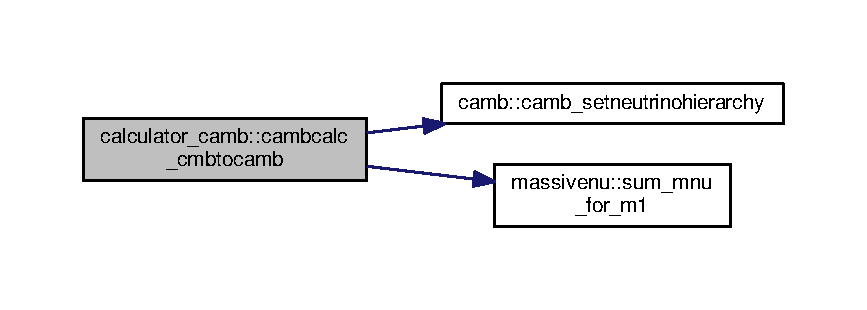
\includegraphics[width=350pt]{namespacecalculator__camb_a10914a67c9b3a93d74382c9c9adf0983_cgraph}
\end{center}
\end{figure}
\mbox{\Hypertarget{namespacecalculator__camb_a88bb5f71c4e4784315929d98702a1214}\label{namespacecalculator__camb_a88bb5f71c4e4784315929d98702a1214}} 
\index{calculator\+\_\+camb@{calculator\+\_\+camb}!cambcalc\+\_\+cmbtotheta@{cambcalc\+\_\+cmbtotheta}}
\index{cambcalc\+\_\+cmbtotheta@{cambcalc\+\_\+cmbtotheta}!calculator\+\_\+camb@{calculator\+\_\+camb}}
\subsubsection{\texorpdfstring{cambcalc\+\_\+cmbtotheta()}{cambcalc\_cmbtotheta()}}
{\footnotesize\ttfamily real(mcp) function calculator\+\_\+camb\+::cambcalc\+\_\+cmbtotheta (\begin{DoxyParamCaption}\item[{class(\mbox{\hyperlink{structcalculator__camb_1_1camb__calculator}{camb\+\_\+calculator}})}]{this,  }\item[{class(cmbparams)}]{C\+MB }\end{DoxyParamCaption})\hspace{0.3cm}{\ttfamily [private]}}



References modelparams\+::cosmomctheta().

Here is the call graph for this function\+:
\nopagebreak
\begin{figure}[H]
\begin{center}
\leavevmode
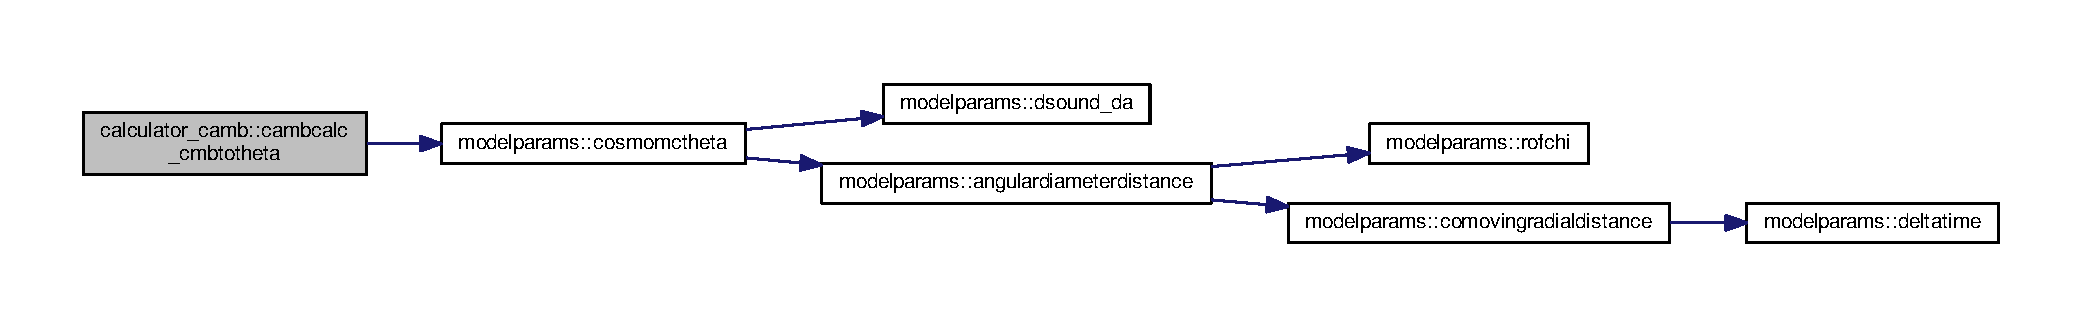
\includegraphics[width=350pt]{namespacecalculator__camb_a88bb5f71c4e4784315929d98702a1214_cgraph}
\end{center}
\end{figure}
\mbox{\Hypertarget{namespacecalculator__camb_a44d780a147bc9cea89b7ebe9a071b98a}\label{namespacecalculator__camb_a44d780a147bc9cea89b7ebe9a071b98a}} 
\index{calculator\+\_\+camb@{calculator\+\_\+camb}!cambcalc\+\_\+comovingradialdistance@{cambcalc\+\_\+comovingradialdistance}}
\index{cambcalc\+\_\+comovingradialdistance@{cambcalc\+\_\+comovingradialdistance}!calculator\+\_\+camb@{calculator\+\_\+camb}}
\subsubsection{\texorpdfstring{cambcalc\+\_\+comovingradialdistance()}{cambcalc\_comovingradialdistance()}}
{\footnotesize\ttfamily real(mcp) function calculator\+\_\+camb\+::cambcalc\+\_\+comovingradialdistance (\begin{DoxyParamCaption}\item[{class(\mbox{\hyperlink{structcalculator__camb_1_1camb__calculator}{camb\+\_\+calculator}})}]{this,  }\item[{real(mcp), intent(in)}]{z }\end{DoxyParamCaption})}

\mbox{\Hypertarget{namespacecalculator__camb_ad7195d220a7f5bc77479225b47d91d17}\label{namespacecalculator__camb_ad7195d220a7f5bc77479225b47d91d17}} 
\index{calculator\+\_\+camb@{calculator\+\_\+camb}!cambcalc\+\_\+getnewpowerdata@{cambcalc\+\_\+getnewpowerdata}}
\index{cambcalc\+\_\+getnewpowerdata@{cambcalc\+\_\+getnewpowerdata}!calculator\+\_\+camb@{calculator\+\_\+camb}}
\subsubsection{\texorpdfstring{cambcalc\+\_\+getnewpowerdata()}{cambcalc\_getnewpowerdata()}}
{\footnotesize\ttfamily subroutine calculator\+\_\+camb\+::cambcalc\+\_\+getnewpowerdata (\begin{DoxyParamCaption}\item[{class(\mbox{\hyperlink{structcalculator__camb_1_1camb__calculator}{camb\+\_\+calculator}})}]{this,  }\item[{class(cmbparams)}]{C\+MB,  }\item[{class(ttheoryintermediatecache), pointer}]{Info,  }\item[{class(tcosmotheorypredictions)}]{Theory,  }\item[{integer}]{error }\end{DoxyParamCaption})}



References camb\+::camb\+\_\+transferstopowers(), cosmologytypes\+::cosmosettings, and errors\+::global\+\_\+error\+\_\+flag.

Here is the call graph for this function\+:
\nopagebreak
\begin{figure}[H]
\begin{center}
\leavevmode
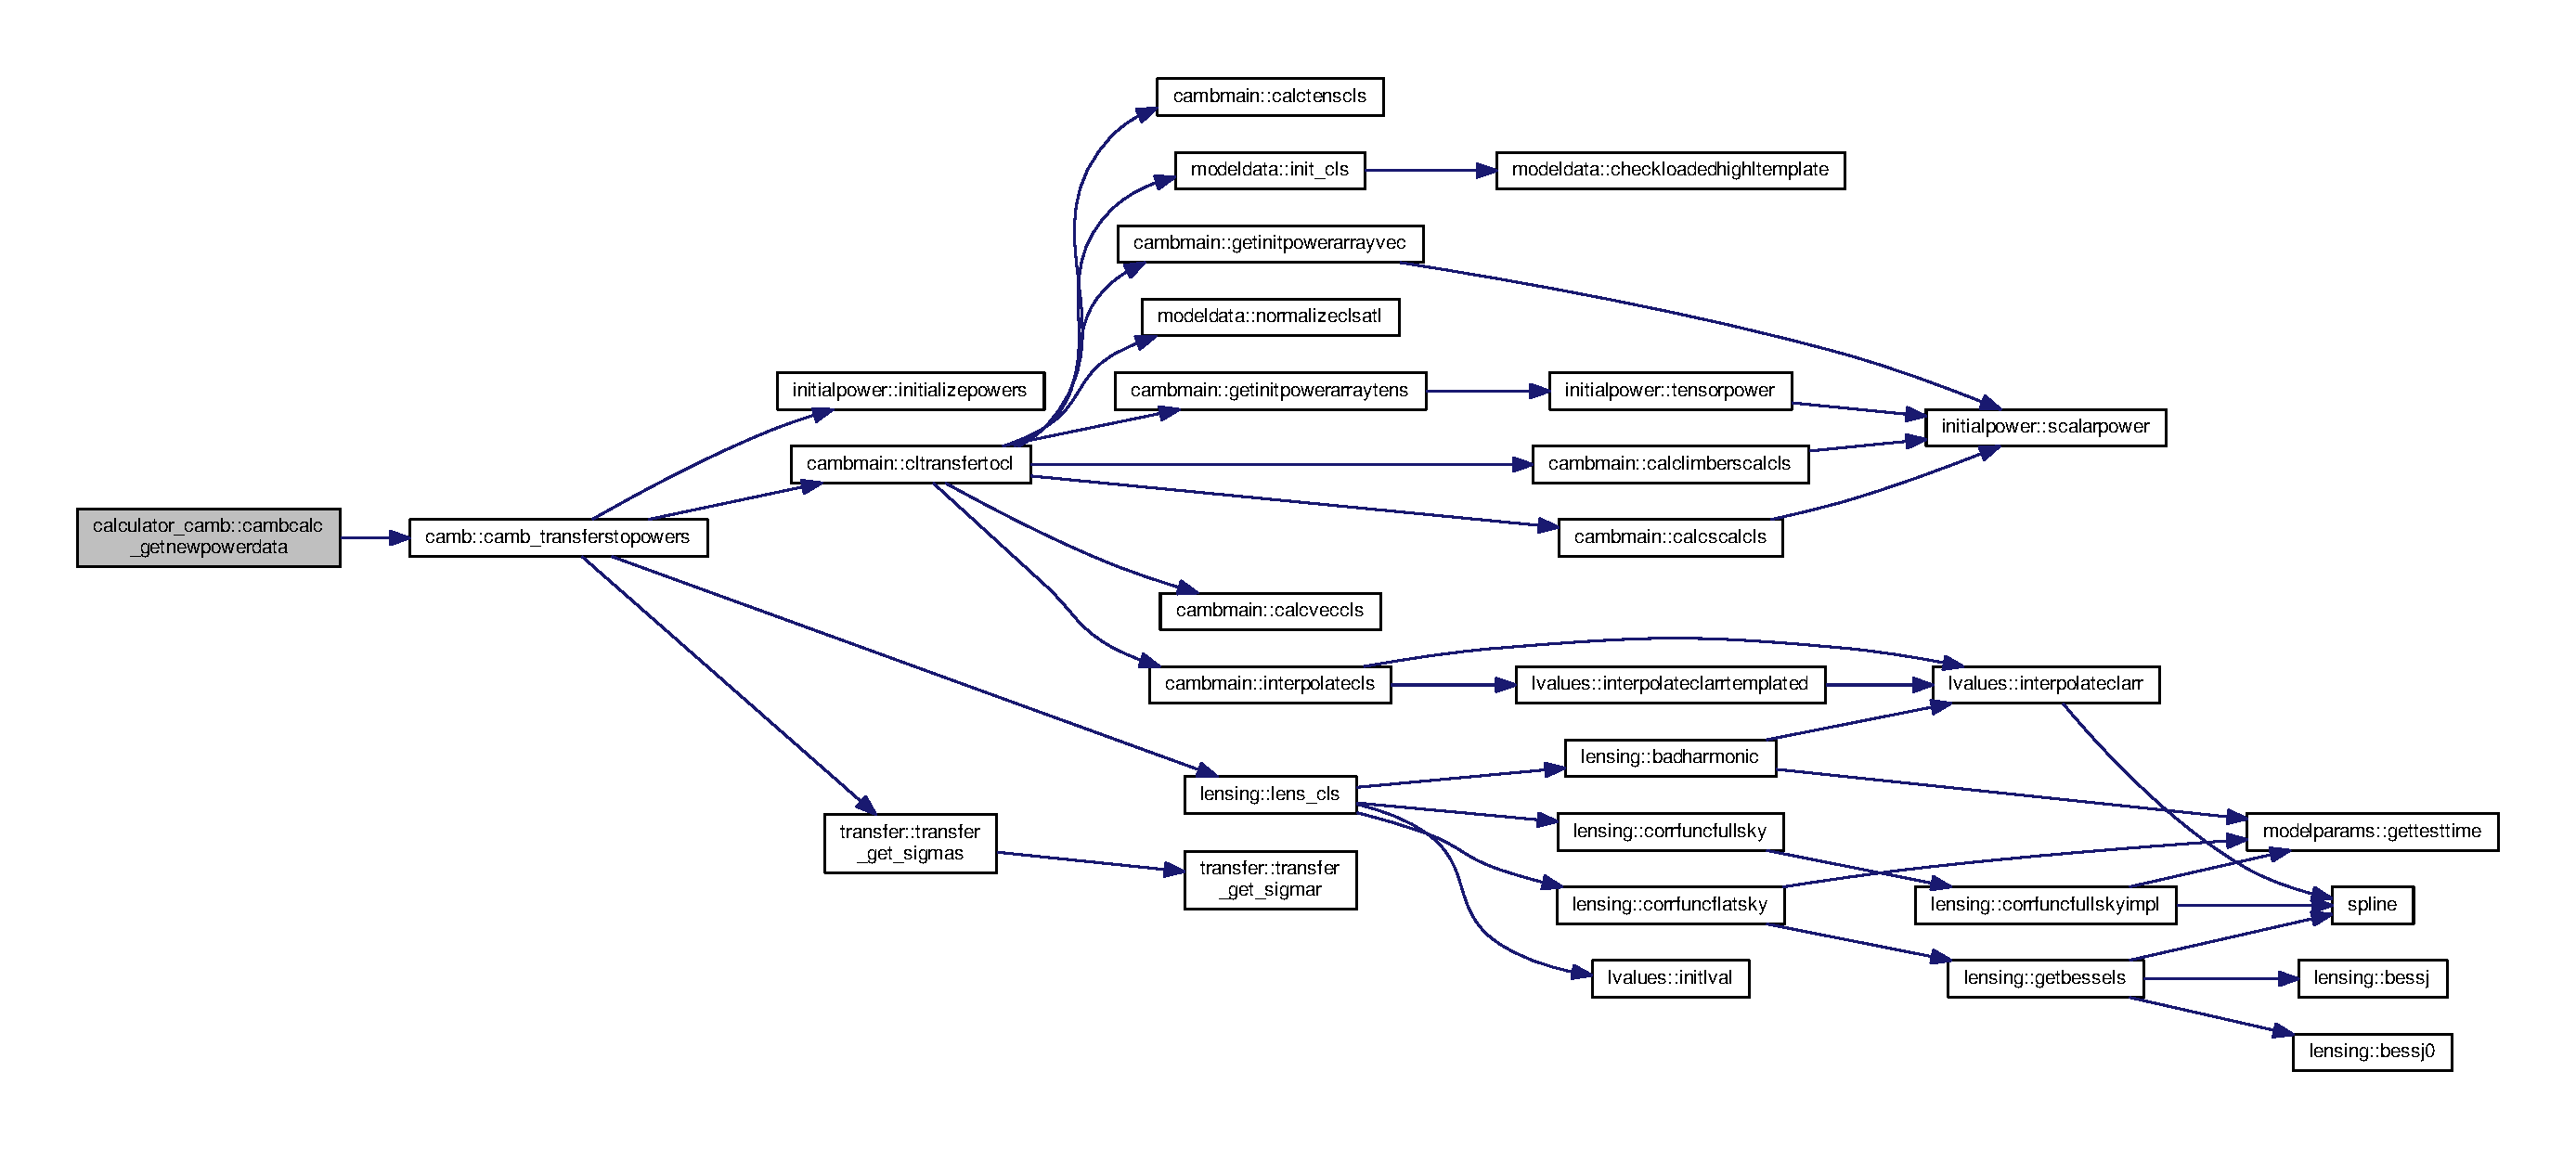
\includegraphics[width=350pt]{namespacecalculator__camb_ad7195d220a7f5bc77479225b47d91d17_cgraph}
\end{center}
\end{figure}
\mbox{\Hypertarget{namespacecalculator__camb_a9e8887a3ae9da2bb092aac4285234df4}\label{namespacecalculator__camb_a9e8887a3ae9da2bb092aac4285234df4}} 
\index{calculator\+\_\+camb@{calculator\+\_\+camb}!cambcalc\+\_\+getnewtransferdata@{cambcalc\+\_\+getnewtransferdata}}
\index{cambcalc\+\_\+getnewtransferdata@{cambcalc\+\_\+getnewtransferdata}!calculator\+\_\+camb@{calculator\+\_\+camb}}
\subsubsection{\texorpdfstring{cambcalc\+\_\+getnewtransferdata()}{cambcalc\_getnewtransferdata()}}
{\footnotesize\ttfamily subroutine calculator\+\_\+camb\+::cambcalc\+\_\+getnewtransferdata (\begin{DoxyParamCaption}\item[{class(\mbox{\hyperlink{structcalculator__camb_1_1camb__calculator}{camb\+\_\+calculator}})}]{this,  }\item[{class(cmbparams)}]{C\+MB,  }\item[{class(ttheoryintermediatecache), pointer}]{Info,  }\item[{class(tcosmotheorypredictions)}]{Theory,  }\item[{integer}]{error }\end{DoxyParamCaption})}



References camb\+::camb\+\_\+gettransfers(), camb\+::camb\+\_\+initcambdata(), settings\+::feedback, errors\+::global\+\_\+error\+\_\+message, settings\+::logfile, settings\+::num\+\_\+threads, settings\+::stop\+\_\+on\+\_\+error, and settings\+::timer().

Here is the call graph for this function\+:
\nopagebreak
\begin{figure}[H]
\begin{center}
\leavevmode
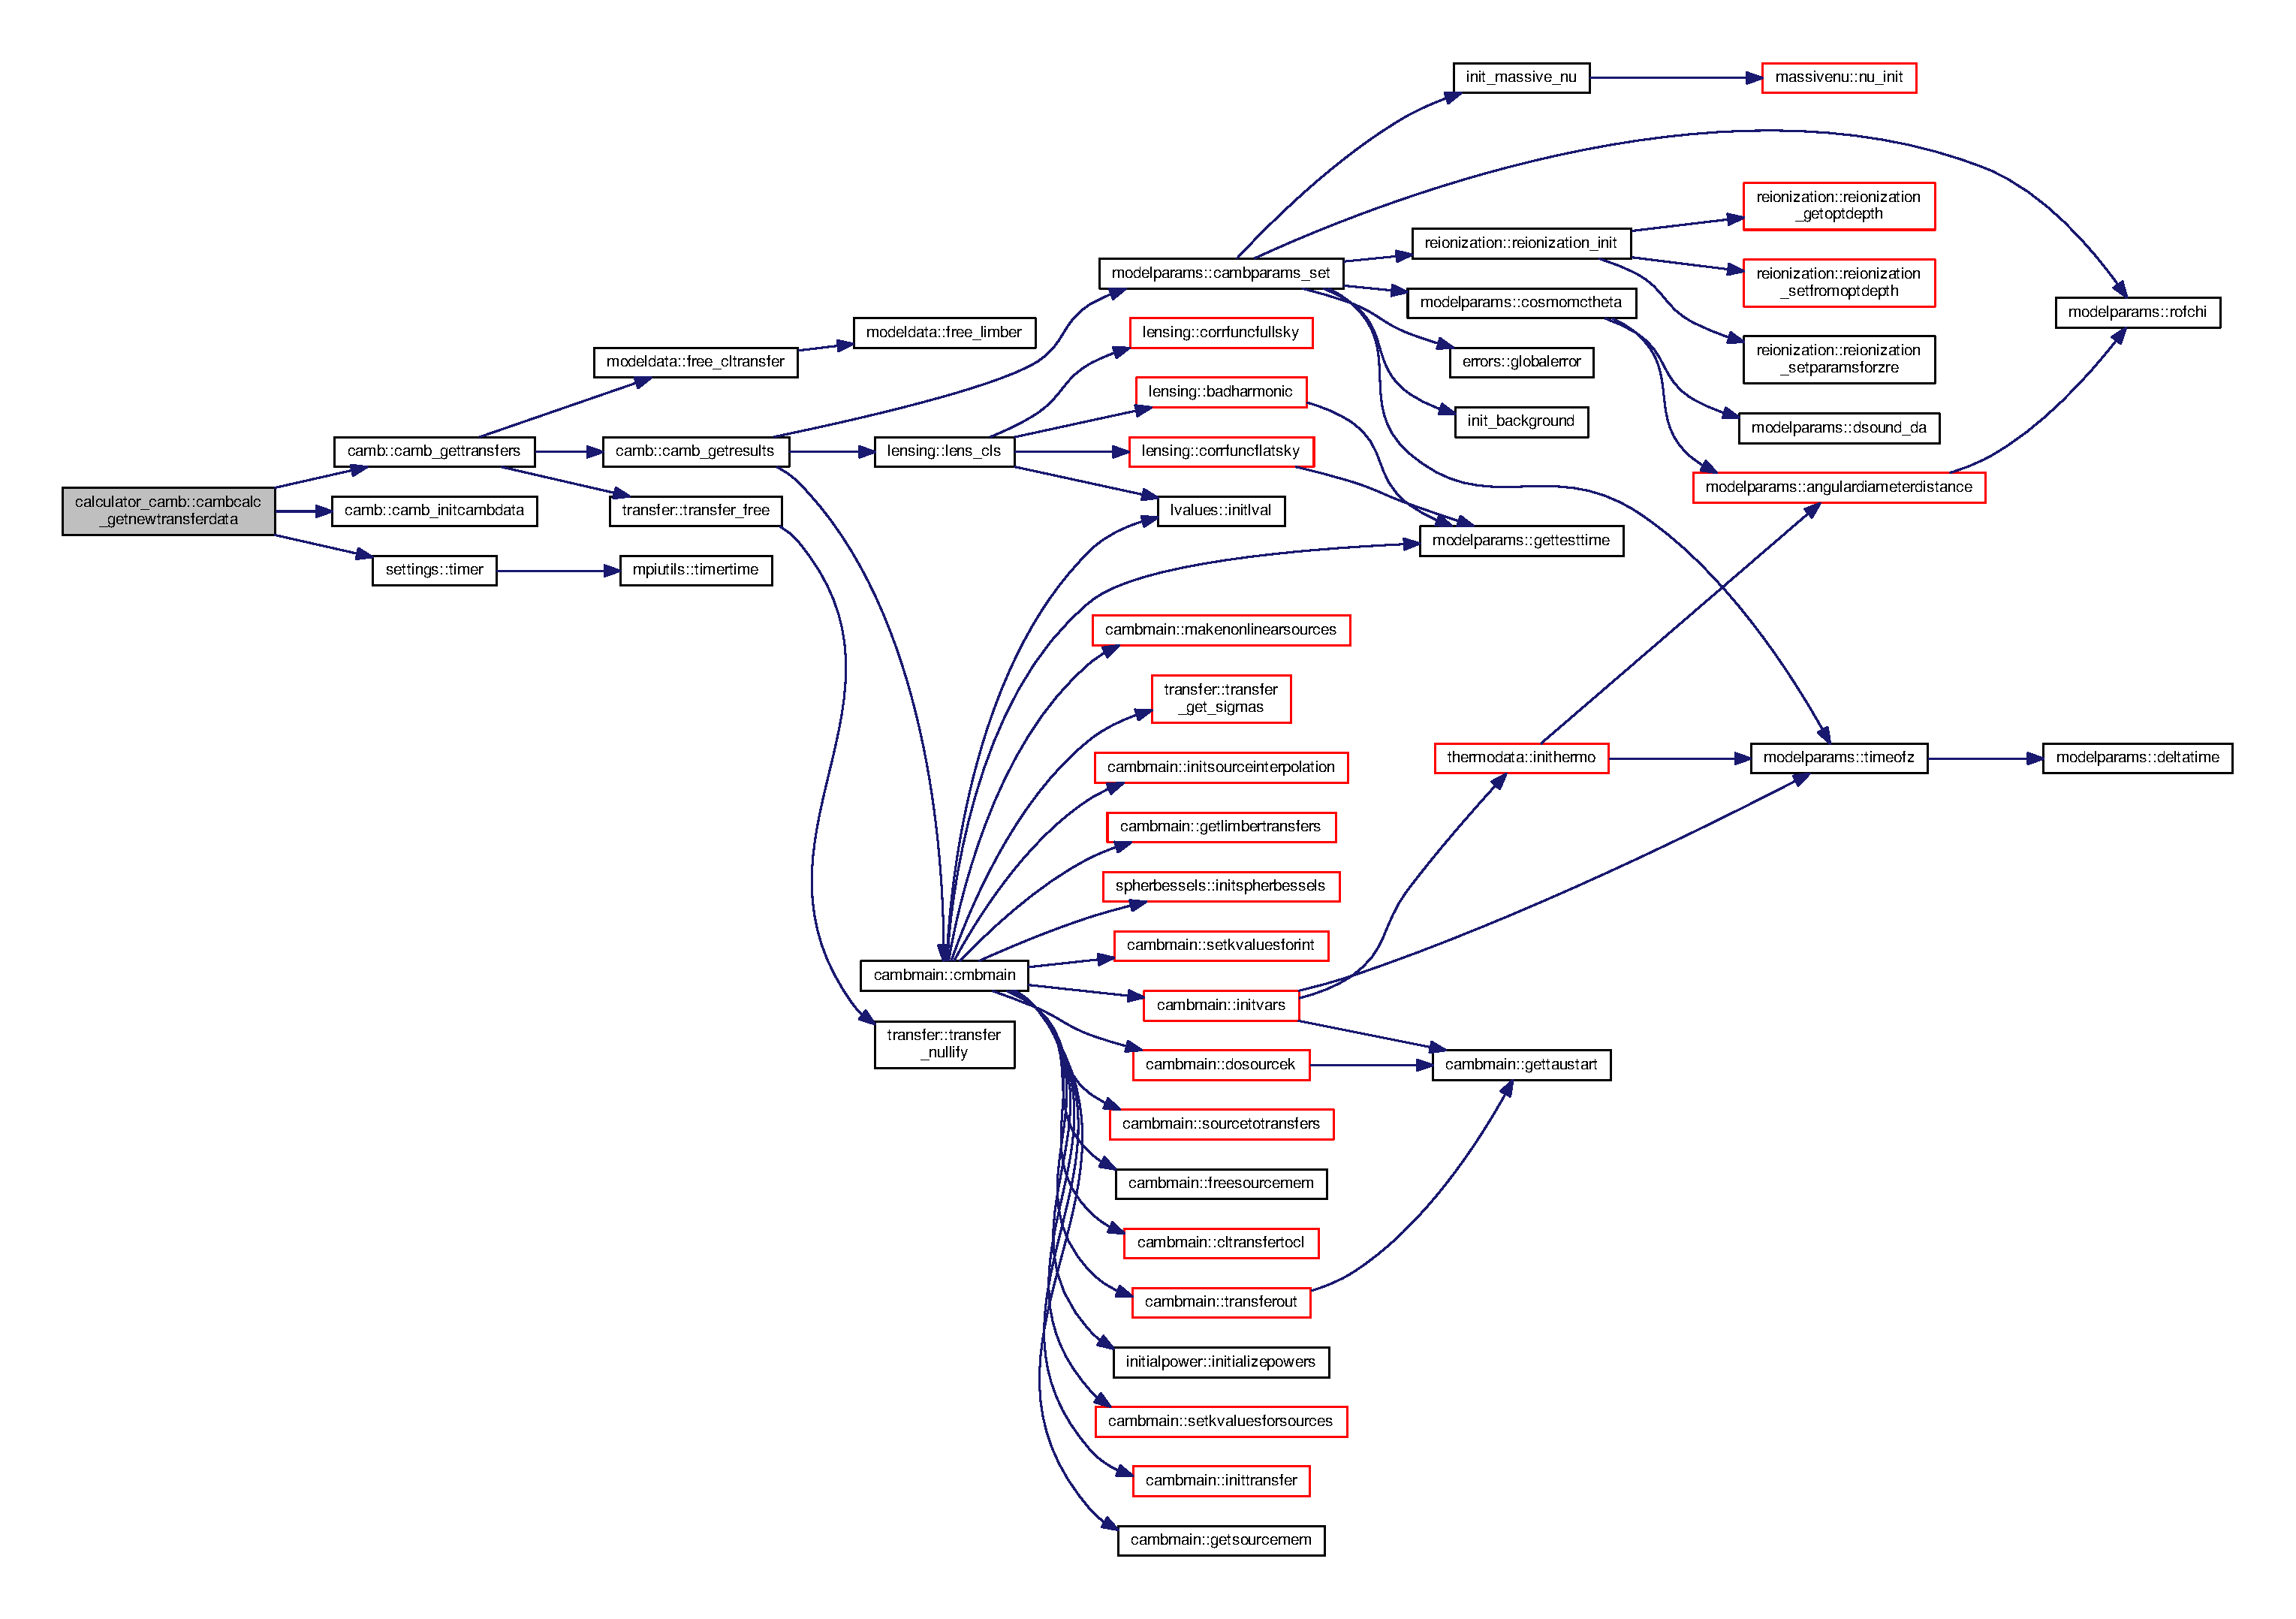
\includegraphics[width=350pt]{namespacecalculator__camb_a9e8887a3ae9da2bb092aac4285234df4_cgraph}
\end{center}
\end{figure}
\mbox{\Hypertarget{namespacecalculator__camb_ac0ce3e4748dd96f033235b9dbf3a71b3}\label{namespacecalculator__camb_ac0ce3e4748dd96f033235b9dbf3a71b3}} 
\index{calculator\+\_\+camb@{calculator\+\_\+camb}!cambcalc\+\_\+getnlandratios@{cambcalc\+\_\+getnlandratios}}
\index{cambcalc\+\_\+getnlandratios@{cambcalc\+\_\+getnlandratios}!calculator\+\_\+camb@{calculator\+\_\+camb}}
\subsubsection{\texorpdfstring{cambcalc\+\_\+getnlandratios()}{cambcalc\_getnlandratios()}}
{\footnotesize\ttfamily subroutine calculator\+\_\+camb\+::cambcalc\+\_\+getnlandratios (\begin{DoxyParamCaption}\item[{class(\mbox{\hyperlink{structcalculator__camb_1_1camb__calculator}{camb\+\_\+calculator}})}]{this,  }\item[{type(mattertransferdata)}]{M,  }\item[{class(tcosmotheorypredictions)}]{Theory,  }\item[{real(mcp), dimension(\+:,\+:), intent(out), allocatable}]{Ratios,  }\item[{integer}]{error }\end{DoxyParamCaption})}



References transfer\+::matterpowerdata\+\_\+free(), transfer\+::matterpowerdata\+\_\+getsplines(), and nonlinear\+\_\+getratios().

Here is the call graph for this function\+:
\nopagebreak
\begin{figure}[H]
\begin{center}
\leavevmode
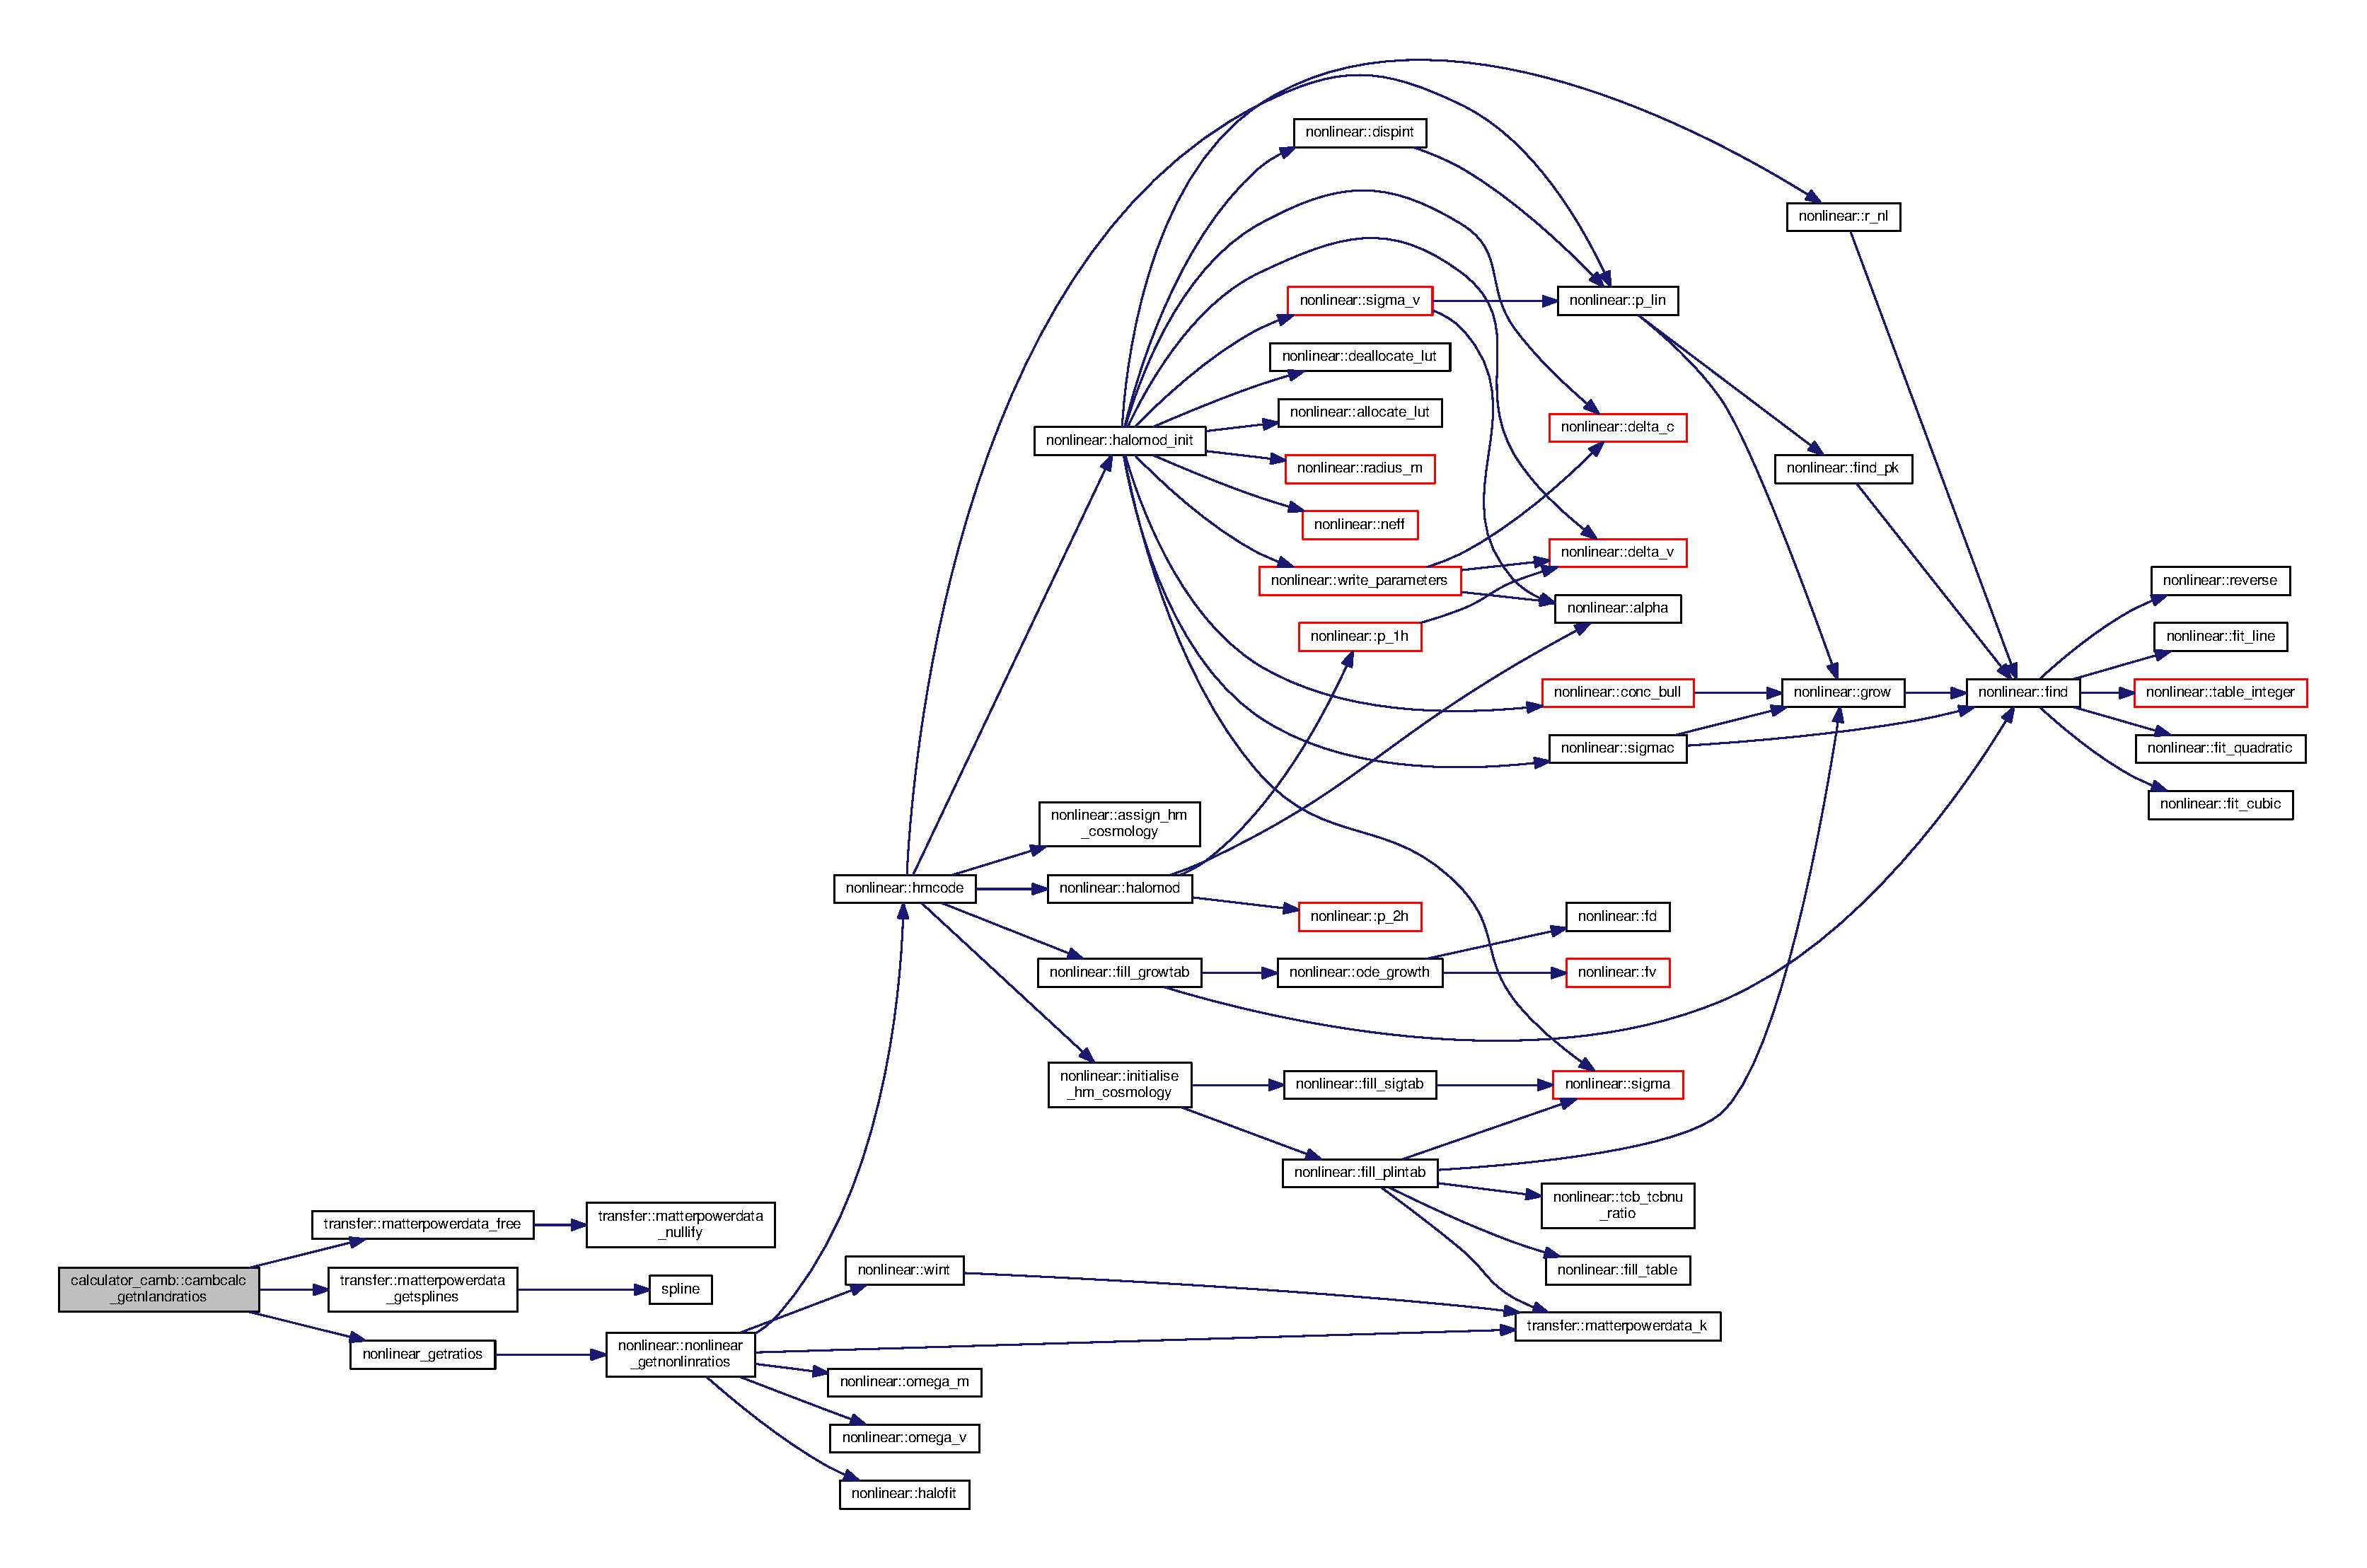
\includegraphics[width=350pt]{namespacecalculator__camb_ac0ce3e4748dd96f033235b9dbf3a71b3_cgraph}
\end{center}
\end{figure}
\mbox{\Hypertarget{namespacecalculator__camb_ac09824dcbd350dcc819683a630b6e646}\label{namespacecalculator__camb_ac09824dcbd350dcc819683a630b6e646}} 
\index{calculator\+\_\+camb@{calculator\+\_\+camb}!cambcalc\+\_\+getopticaldepth@{cambcalc\+\_\+getopticaldepth}}
\index{cambcalc\+\_\+getopticaldepth@{cambcalc\+\_\+getopticaldepth}!calculator\+\_\+camb@{calculator\+\_\+camb}}
\subsubsection{\texorpdfstring{cambcalc\+\_\+getopticaldepth()}{cambcalc\_getopticaldepth()}}
{\footnotesize\ttfamily real(mcp) function calculator\+\_\+camb\+::cambcalc\+\_\+getopticaldepth (\begin{DoxyParamCaption}\item[{class(\mbox{\hyperlink{structcalculator__camb_1_1camb__calculator}{camb\+\_\+calculator}})}]{this,  }\item[{class(cmbparams)}]{C\+MB }\end{DoxyParamCaption})\hspace{0.3cm}{\ttfamily [private]}}

\mbox{\Hypertarget{namespacecalculator__camb_a46bd33ed008e289fb5cb08f6feb86419}\label{namespacecalculator__camb_a46bd33ed008e289fb5cb08f6feb86419}} 
\index{calculator\+\_\+camb@{calculator\+\_\+camb}!cambcalc\+\_\+gettheoryforimportance@{cambcalc\+\_\+gettheoryforimportance}}
\index{cambcalc\+\_\+gettheoryforimportance@{cambcalc\+\_\+gettheoryforimportance}!calculator\+\_\+camb@{calculator\+\_\+camb}}
\subsubsection{\texorpdfstring{cambcalc\+\_\+gettheoryforimportance()}{cambcalc\_gettheoryforimportance()}}
{\footnotesize\ttfamily subroutine calculator\+\_\+camb\+::cambcalc\+\_\+gettheoryforimportance (\begin{DoxyParamCaption}\item[{class(\mbox{\hyperlink{structcalculator__camb_1_1camb__calculator}{camb\+\_\+calculator}})}]{this,  }\item[{class(cmbparams)}]{C\+MB,  }\item[{class(tcosmotheorypredictions)}]{Theory,  }\item[{integer}]{error }\end{DoxyParamCaption})\hspace{0.3cm}{\ttfamily [private]}}



References camb\+::camb\+\_\+gettransfers(), camb\+::camb\+\_\+initcambdata(), camb\+::camb\+\_\+transferstopowers(), cosmologytypes\+::cosmosettings, settings\+::feedback, errors\+::global\+\_\+error\+\_\+flag, settings\+::num\+\_\+threads, modelparams\+::threadnum, and settings\+::timer().

Here is the call graph for this function\+:
\nopagebreak
\begin{figure}[H]
\begin{center}
\leavevmode
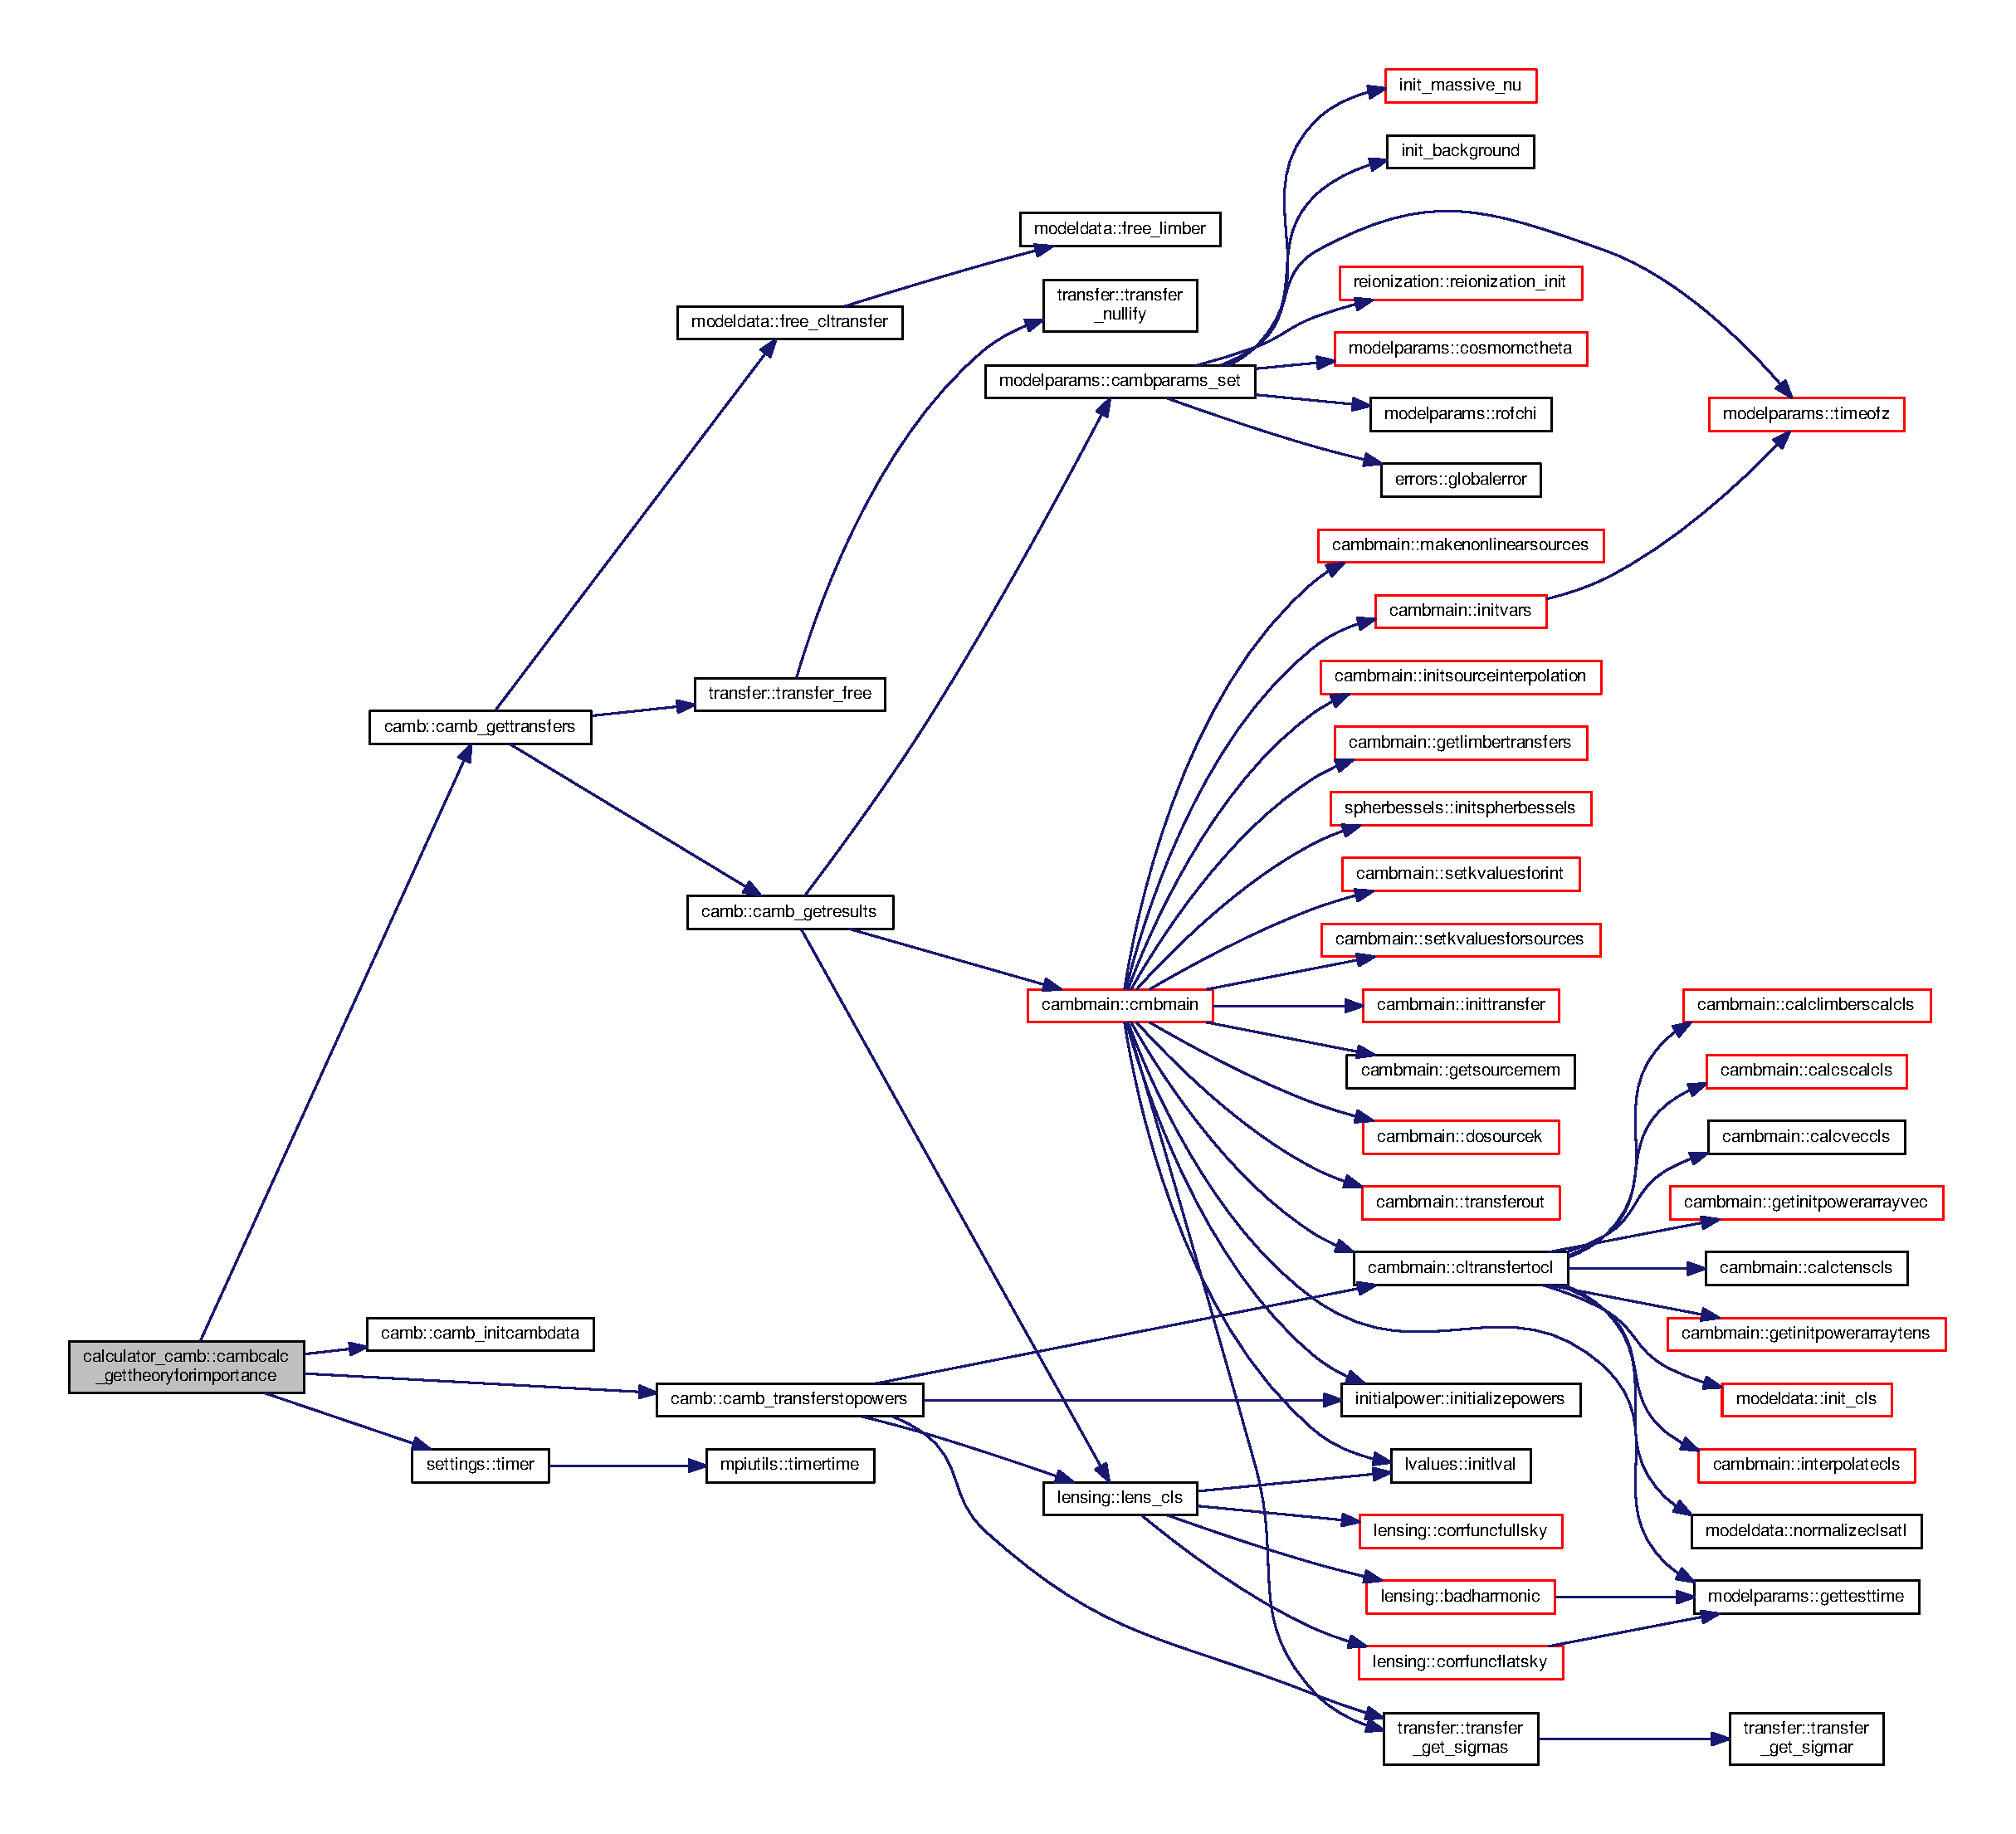
\includegraphics[width=350pt]{namespacecalculator__camb_a46bd33ed008e289fb5cb08f6feb86419_cgraph}
\end{center}
\end{figure}
\mbox{\Hypertarget{namespacecalculator__camb_a36d033f09a4d35c8b9a37d518fcebda0}\label{namespacecalculator__camb_a36d033f09a4d35c8b9a37d518fcebda0}} 
\index{calculator\+\_\+camb@{calculator\+\_\+camb}!cambcalc\+\_\+getzrefromtau@{cambcalc\+\_\+getzrefromtau}}
\index{cambcalc\+\_\+getzrefromtau@{cambcalc\+\_\+getzrefromtau}!calculator\+\_\+camb@{calculator\+\_\+camb}}
\subsubsection{\texorpdfstring{cambcalc\+\_\+getzrefromtau()}{cambcalc\_getzrefromtau()}}
{\footnotesize\ttfamily real(mcp) function calculator\+\_\+camb\+::cambcalc\+\_\+getzrefromtau (\begin{DoxyParamCaption}\item[{class(\mbox{\hyperlink{structcalculator__camb_1_1camb__calculator}{camb\+\_\+calculator}})}]{this,  }\item[{class(cmbparams)}]{C\+MB,  }\item[{real(mcp), intent(in)}]{tau }\end{DoxyParamCaption})\hspace{0.3cm}{\ttfamily [private]}}

\mbox{\Hypertarget{namespacecalculator__camb_a10e6be2c2d0ef7cb7741dbce3dbc88a9}\label{namespacecalculator__camb_a10e6be2c2d0ef7cb7741dbce3dbc88a9}} 
\index{calculator\+\_\+camb@{calculator\+\_\+camb}!cambcalc\+\_\+hofz@{cambcalc\+\_\+hofz}}
\index{cambcalc\+\_\+hofz@{cambcalc\+\_\+hofz}!calculator\+\_\+camb@{calculator\+\_\+camb}}
\subsubsection{\texorpdfstring{cambcalc\+\_\+hofz()}{cambcalc\_hofz()}}
{\footnotesize\ttfamily real(mcp) function calculator\+\_\+camb\+::cambcalc\+\_\+hofz (\begin{DoxyParamCaption}\item[{class(\mbox{\hyperlink{structcalculator__camb_1_1camb__calculator}{camb\+\_\+calculator}})}]{this,  }\item[{real(mcp), intent(in)}]{z }\end{DoxyParamCaption})}

\mbox{\Hypertarget{namespacecalculator__camb_ab67fcdadb23a73d5747a682c87304c0b}\label{namespacecalculator__camb_ab67fcdadb23a73d5747a682c87304c0b}} 
\index{calculator\+\_\+camb@{calculator\+\_\+camb}!cambcalc\+\_\+initcamb@{cambcalc\+\_\+initcamb}}
\index{cambcalc\+\_\+initcamb@{cambcalc\+\_\+initcamb}!calculator\+\_\+camb@{calculator\+\_\+camb}}
\subsubsection{\texorpdfstring{cambcalc\+\_\+initcamb()}{cambcalc\_initcamb()}}
{\footnotesize\ttfamily subroutine calculator\+\_\+camb\+::cambcalc\+\_\+initcamb (\begin{DoxyParamCaption}\item[{class(\mbox{\hyperlink{structcalculator__camb_1_1camb__calculator}{camb\+\_\+calculator}})}]{this,  }\item[{class(cmbparams), intent(in)}]{C\+MB,  }\item[{integer}]{error,  }\item[{logical, intent(in), optional}]{Do\+Reion }\end{DoxyParamCaption})}

\mbox{\Hypertarget{namespacecalculator__camb_a1f498feeb9fd7b4b6ff5c951bb3bcf5d}\label{namespacecalculator__camb_a1f498feeb9fd7b4b6ff5c951bb3bcf5d}} 
\index{calculator\+\_\+camb@{calculator\+\_\+camb}!cambcalc\+\_\+initcambparams@{cambcalc\+\_\+initcambparams}}
\index{cambcalc\+\_\+initcambparams@{cambcalc\+\_\+initcambparams}!calculator\+\_\+camb@{calculator\+\_\+camb}}
\subsubsection{\texorpdfstring{cambcalc\+\_\+initcambparams()}{cambcalc\_initcambparams()}}
{\footnotesize\ttfamily subroutine calculator\+\_\+camb\+::cambcalc\+\_\+initcambparams (\begin{DoxyParamCaption}\item[{class(\mbox{\hyperlink{structcalculator__camb_1_1camb__calculator}{camb\+\_\+calculator}})}]{this,  }\item[{type(cambparams)}]{P }\end{DoxyParamCaption})}



References modelparams\+::accuracyboost, modelparams\+::backgroundoutputs, modelparams\+::highaccuracydefault, modelparams\+::laccuracyboost, lensing\+::lensing\+\_\+includes\+\_\+tensors, modelparams\+::lsampleboost, modelparams\+::max\+\_\+transfer\+\_\+redshifts, modelparams\+::nonlinear\+\_\+both, modelparams\+::nonlinear\+\_\+lens, modelparams\+::nonlinear\+\_\+pk, modelparams\+::outnone, and modelparams\+::threadnum.

\mbox{\Hypertarget{namespacecalculator__camb_a5eb19890ea9bf2acad52f23b9334e1e8}\label{namespacecalculator__camb_a5eb19890ea9bf2acad52f23b9334e1e8}} 
\index{calculator\+\_\+camb@{calculator\+\_\+camb}!cambcalc\+\_\+initforlikelihoods@{cambcalc\+\_\+initforlikelihoods}}
\index{cambcalc\+\_\+initforlikelihoods@{cambcalc\+\_\+initforlikelihoods}!calculator\+\_\+camb@{calculator\+\_\+camb}}
\subsubsection{\texorpdfstring{cambcalc\+\_\+initforlikelihoods()}{cambcalc\_initforlikelihoods()}}
{\footnotesize\ttfamily subroutine calculator\+\_\+camb\+::cambcalc\+\_\+initforlikelihoods (\begin{DoxyParamCaption}\item[{class(\mbox{\hyperlink{structcalculator__camb_1_1camb__calculator}{camb\+\_\+calculator}})}]{this }\end{DoxyParamCaption})}

\mbox{\Hypertarget{namespacecalculator__camb_a0f03309bd014f3de538a3565bc867402}\label{namespacecalculator__camb_a0f03309bd014f3de538a3565bc867402}} 
\index{calculator\+\_\+camb@{calculator\+\_\+camb}!cambcalc\+\_\+luminositydistance@{cambcalc\+\_\+luminositydistance}}
\index{cambcalc\+\_\+luminositydistance@{cambcalc\+\_\+luminositydistance}!calculator\+\_\+camb@{calculator\+\_\+camb}}
\subsubsection{\texorpdfstring{cambcalc\+\_\+luminositydistance()}{cambcalc\_luminositydistance()}}
{\footnotesize\ttfamily real(mcp) function calculator\+\_\+camb\+::cambcalc\+\_\+luminositydistance (\begin{DoxyParamCaption}\item[{class(\mbox{\hyperlink{structcalculator__camb_1_1camb__calculator}{camb\+\_\+calculator}})}]{this,  }\item[{real(mcp), intent(in)}]{z }\end{DoxyParamCaption})}

\mbox{\Hypertarget{namespacecalculator__camb_aa3a88e278563ca8092494c335094e325}\label{namespacecalculator__camb_aa3a88e278563ca8092494c335094e325}} 
\index{calculator\+\_\+camb@{calculator\+\_\+camb}!cambcalc\+\_\+readparams@{cambcalc\+\_\+readparams}}
\index{cambcalc\+\_\+readparams@{cambcalc\+\_\+readparams}!calculator\+\_\+camb@{calculator\+\_\+camb}}
\subsubsection{\texorpdfstring{cambcalc\+\_\+readparams()}{cambcalc\_readparams()}}
{\footnotesize\ttfamily subroutine calculator\+\_\+camb\+::cambcalc\+\_\+readparams (\begin{DoxyParamCaption}\item[{class(\mbox{\hyperlink{structcalculator__camb_1_1camb__calculator}{camb\+\_\+calculator}})}]{this,  }\item[{class(\mbox{\hyperlink{structsettings_1_1tsettingini}{tsettingini}})}]{Ini }\end{DoxyParamCaption})\hspace{0.3cm}{\ttfamily [private]}}



References nonlinear\+::halofit\+\_\+default, and nonlinear\+::halofit\+\_\+version.

\mbox{\Hypertarget{namespacecalculator__camb_a04c53e5b4763297e232978e627153a17}\label{namespacecalculator__camb_a04c53e5b4763297e232978e627153a17}} 
\index{calculator\+\_\+camb@{calculator\+\_\+camb}!cambcalc\+\_\+setbackgroundtheorydata@{cambcalc\+\_\+setbackgroundtheorydata}}
\index{cambcalc\+\_\+setbackgroundtheorydata@{cambcalc\+\_\+setbackgroundtheorydata}!calculator\+\_\+camb@{calculator\+\_\+camb}}
\subsubsection{\texorpdfstring{cambcalc\+\_\+setbackgroundtheorydata()}{cambcalc\_setbackgroundtheorydata()}}
{\footnotesize\ttfamily subroutine calculator\+\_\+camb\+::cambcalc\+\_\+setbackgroundtheorydata (\begin{DoxyParamCaption}\item[{class(\mbox{\hyperlink{structcalculator__camb_1_1camb__calculator}{camb\+\_\+calculator}})}]{this,  }\item[{class(cmbparams)}]{C\+MB,  }\item[{class(tcosmotheorypredictions)}]{Theory,  }\item[{integer}]{error }\end{DoxyParamCaption})}



References errors\+::global\+\_\+error\+\_\+flag, and cambmain\+::initvars().

Here is the call graph for this function\+:
\nopagebreak
\begin{figure}[H]
\begin{center}
\leavevmode
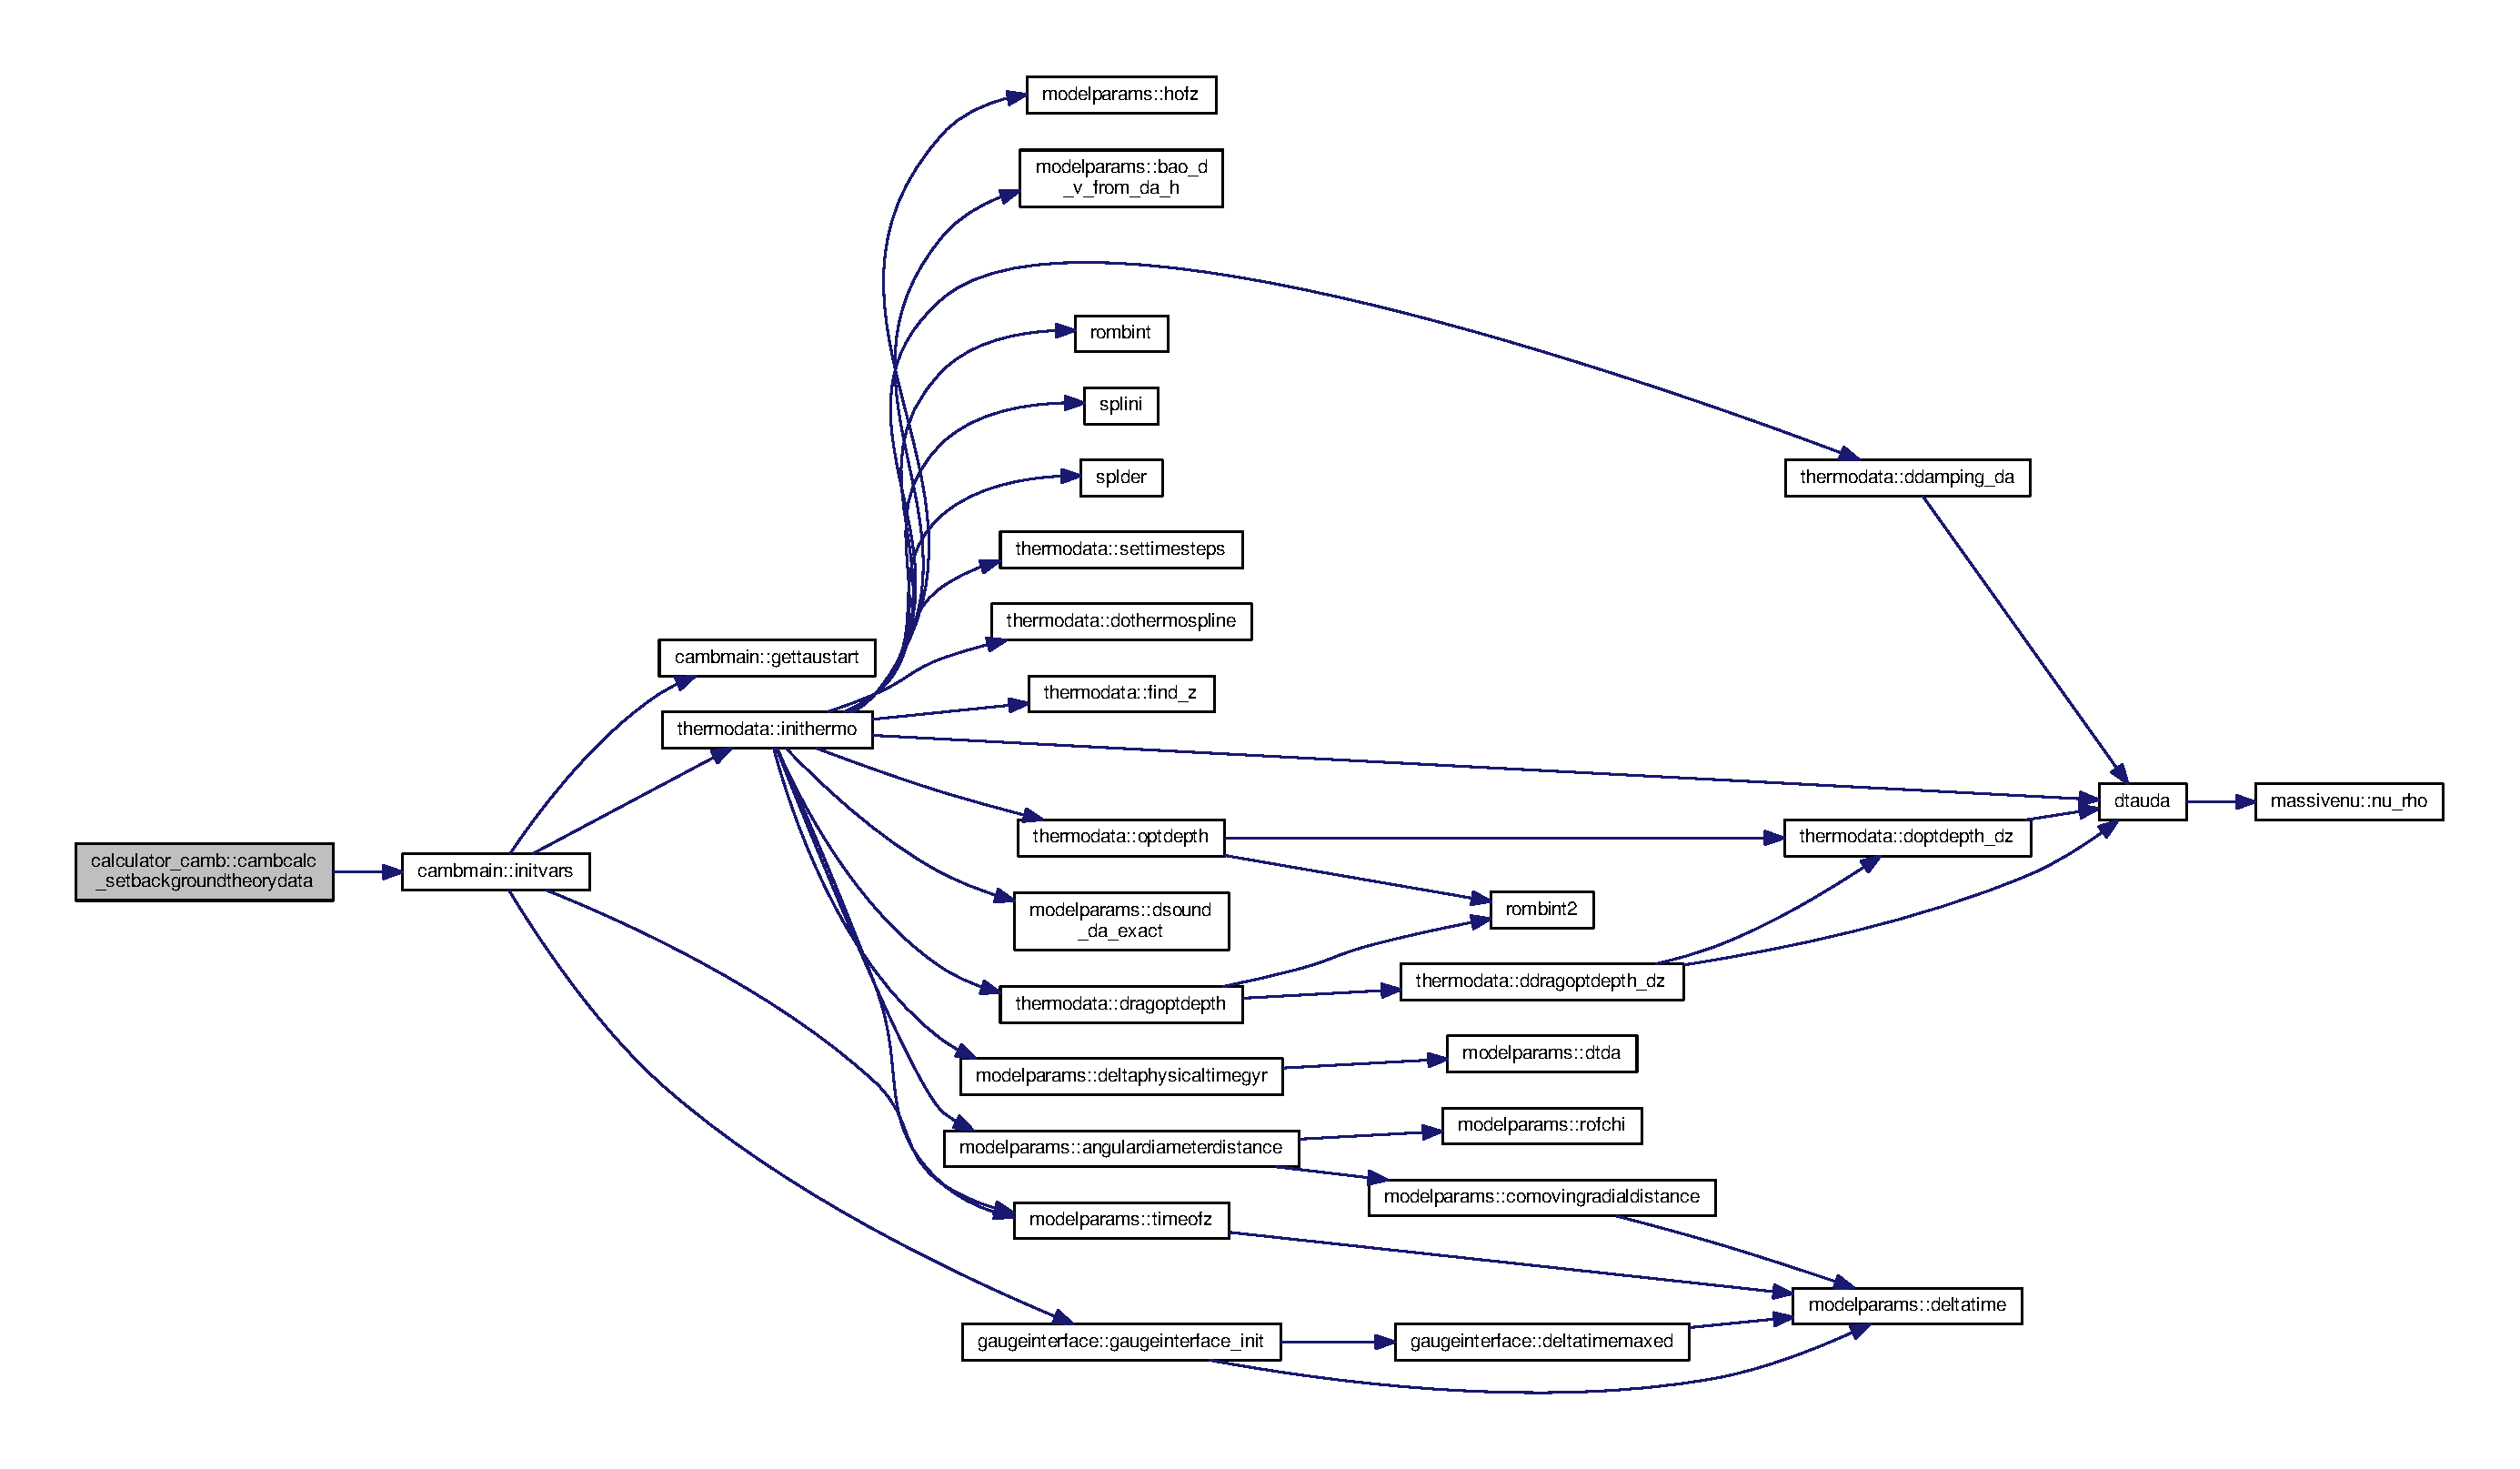
\includegraphics[width=350pt]{namespacecalculator__camb_a04c53e5b4763297e232978e627153a17_cgraph}
\end{center}
\end{figure}
\mbox{\Hypertarget{namespacecalculator__camb_a30b5dc9bda2ffcd939436fbc93322f9e}\label{namespacecalculator__camb_a30b5dc9bda2ffcd939436fbc93322f9e}} 
\index{calculator\+\_\+camb@{calculator\+\_\+camb}!cambcalc\+\_\+setcambinitpower@{cambcalc\+\_\+setcambinitpower}}
\index{cambcalc\+\_\+setcambinitpower@{cambcalc\+\_\+setcambinitpower}!calculator\+\_\+camb@{calculator\+\_\+camb}}
\subsubsection{\texorpdfstring{cambcalc\+\_\+setcambinitpower()}{cambcalc\_setcambinitpower()}}
{\footnotesize\ttfamily subroutine calculator\+\_\+camb\+::cambcalc\+\_\+setcambinitpower (\begin{DoxyParamCaption}\item[{class(\mbox{\hyperlink{structcalculator__camb_1_1camb__calculator}{camb\+\_\+calculator}})}]{this,  }\item[{type(cambparams)}]{P,  }\item[{class(cmbparams)}]{C\+MB,  }\item[{integer, intent(in)}]{ix }\end{DoxyParamCaption})}

\mbox{\Hypertarget{namespacecalculator__camb_a451eeaadb06191ee0203caf0d76c66c2}\label{namespacecalculator__camb_a451eeaadb06191ee0203caf0d76c66c2}} 
\index{calculator\+\_\+camb@{calculator\+\_\+camb}!cambcalc\+\_\+setderived@{cambcalc\+\_\+setderived}}
\index{cambcalc\+\_\+setderived@{cambcalc\+\_\+setderived}!calculator\+\_\+camb@{calculator\+\_\+camb}}
\subsubsection{\texorpdfstring{cambcalc\+\_\+setderived()}{cambcalc\_setderived()}}
{\footnotesize\ttfamily subroutine calculator\+\_\+camb\+::cambcalc\+\_\+setderived (\begin{DoxyParamCaption}\item[{class(\mbox{\hyperlink{structcalculator__camb_1_1camb__calculator}{camb\+\_\+calculator}})}]{this,  }\item[{class(tcosmotheorypredictions)}]{Theory }\end{DoxyParamCaption})}



References settings\+::const\+\_\+c, and cosmologytypes\+::max\+\_\+derived\+\_\+parameters.

\mbox{\Hypertarget{namespacecalculator__camb_a2f68d8cedf36c519d822547aa49c3f98}\label{namespacecalculator__camb_a2f68d8cedf36c519d822547aa49c3f98}} 
\index{calculator\+\_\+camb@{calculator\+\_\+camb}!cambcalc\+\_\+setparamsforbackground@{cambcalc\+\_\+setparamsforbackground}}
\index{cambcalc\+\_\+setparamsforbackground@{cambcalc\+\_\+setparamsforbackground}!calculator\+\_\+camb@{calculator\+\_\+camb}}
\subsubsection{\texorpdfstring{cambcalc\+\_\+setparamsforbackground()}{cambcalc\_setparamsforbackground()}}
{\footnotesize\ttfamily subroutine calculator\+\_\+camb\+::cambcalc\+\_\+setparamsforbackground (\begin{DoxyParamCaption}\item[{class(\mbox{\hyperlink{structcalculator__camb_1_1camb__calculator}{camb\+\_\+calculator}})}]{this,  }\item[{class(cmbparams)}]{C\+MB }\end{DoxyParamCaption})\hspace{0.3cm}{\ttfamily [private]}}

\mbox{\Hypertarget{namespacecalculator__camb_a8e6f706ddb3ae930a9f1293d9c480405}\label{namespacecalculator__camb_a8e6f706ddb3ae930a9f1293d9c480405}} 
\index{calculator\+\_\+camb@{calculator\+\_\+camb}!cambcalc\+\_\+setpkfromcamb@{cambcalc\+\_\+setpkfromcamb}}
\index{cambcalc\+\_\+setpkfromcamb@{cambcalc\+\_\+setpkfromcamb}!calculator\+\_\+camb@{calculator\+\_\+camb}}
\subsubsection{\texorpdfstring{cambcalc\+\_\+setpkfromcamb()}{cambcalc\_setpkfromcamb()}}
{\footnotesize\ttfamily subroutine calculator\+\_\+camb\+::cambcalc\+\_\+setpkfromcamb (\begin{DoxyParamCaption}\item[{class(\mbox{\hyperlink{structcalculator__camb_1_1camb__calculator}{camb\+\_\+calculator}})}]{this,  }\item[{type(mattertransferdata)}]{M,  }\item[{class(tcosmotheorypredictions)}]{Theory,  }\item[{integer}]{error }\end{DoxyParamCaption})}



References transfer\+::transfer\+\_\+getsigmararray(), transfer\+::transfer\+\_\+getunsplinedpower(), transfer\+::transfer\+\_\+kh, transfer\+::transfer\+\_\+nonu, transfer\+::transfer\+\_\+power\+\_\+var, and transfer\+::transfer\+\_\+weyl.

Here is the call graph for this function\+:
\nopagebreak
\begin{figure}[H]
\begin{center}
\leavevmode
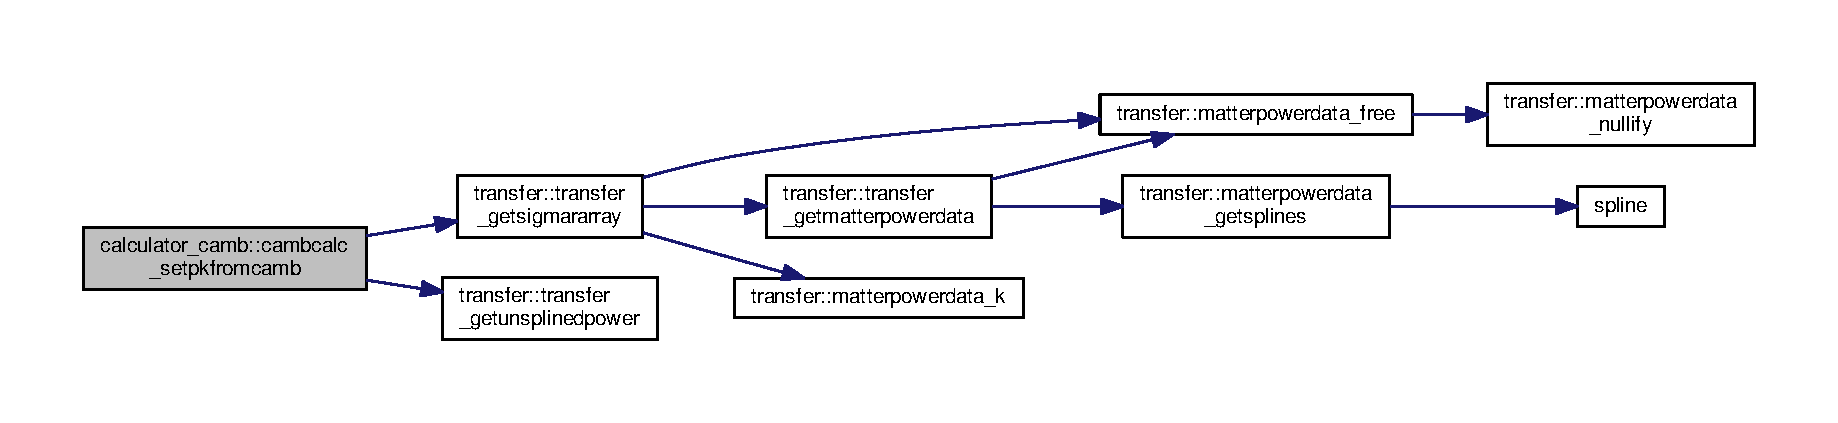
\includegraphics[width=350pt]{namespacecalculator__camb_a8e6f706ddb3ae930a9f1293d9c480405_cgraph}
\end{center}
\end{figure}
\mbox{\Hypertarget{namespacecalculator__camb_a7ccabec132f8bbe50ac91abdd4a86751}\label{namespacecalculator__camb_a7ccabec132f8bbe50ac91abdd4a86751}} 
\index{calculator\+\_\+camb@{calculator\+\_\+camb}!cambcalc\+\_\+setpowersfromcamb@{cambcalc\+\_\+setpowersfromcamb}}
\index{cambcalc\+\_\+setpowersfromcamb@{cambcalc\+\_\+setpowersfromcamb}!calculator\+\_\+camb@{calculator\+\_\+camb}}
\subsubsection{\texorpdfstring{cambcalc\+\_\+setpowersfromcamb()}{cambcalc\_setpowersfromcamb()}}
{\footnotesize\ttfamily subroutine calculator\+\_\+camb\+::cambcalc\+\_\+setpowersfromcamb (\begin{DoxyParamCaption}\item[{class(\mbox{\hyperlink{structcalculator__camb_1_1camb__calculator}{camb\+\_\+calculator}})}]{this,  }\item[{class(cmbparams)}]{C\+MB,  }\item[{class(tcosmotheorypredictions), target}]{Theory }\end{DoxyParamCaption})}



References cosmologytypes\+::aphiphi\+\_\+index, modeldata\+::c\+\_\+cross, modeldata\+::c\+\_\+e, modeldata\+::c\+\_\+temp, modeldata\+::cl\+\_\+lensed, cosmologytypes\+::cl\+\_\+phi, modeldata\+::cl\+\_\+scalar, modeldata\+::cl\+\_\+tensor, cosmologytypes\+::cosmosettings, modeldata\+::ct\+\_\+b, and modeldata\+::ct\+\_\+cross.

\mbox{\Hypertarget{namespacecalculator__camb_a67d98d7cdaa015cca41f95ed94678a79}\label{namespacecalculator__camb_a67d98d7cdaa015cca41f95ed94678a79}} 
\index{calculator\+\_\+camb@{calculator\+\_\+camb}!cambcalc\+\_\+versiontraceoutput@{cambcalc\+\_\+versiontraceoutput}}
\index{cambcalc\+\_\+versiontraceoutput@{cambcalc\+\_\+versiontraceoutput}!calculator\+\_\+camb@{calculator\+\_\+camb}}
\subsubsection{\texorpdfstring{cambcalc\+\_\+versiontraceoutput()}{cambcalc\_versiontraceoutput()}}
{\footnotesize\ttfamily subroutine calculator\+\_\+camb\+::cambcalc\+\_\+versiontraceoutput (\begin{DoxyParamCaption}\item[{class(\mbox{\hyperlink{structcalculator__camb_1_1camb__calculator}{camb\+\_\+calculator}})}]{this,  }\item[{class(tnamevaluelist)}]{Read\+Values }\end{DoxyParamCaption})\hspace{0.3cm}{\ttfamily [private]}}



References gaugeinterface\+::eqns\+\_\+name.

\mbox{\Hypertarget{namespacecalculator__camb_a74de7ed91f31c5cccb3f6c738f689295}\label{namespacecalculator__camb_a74de7ed91f31c5cccb3f6c738f689295}} 
\index{calculator\+\_\+camb@{calculator\+\_\+camb}!cambtransfercache\+\_\+clear@{cambtransfercache\+\_\+clear}}
\index{cambtransfercache\+\_\+clear@{cambtransfercache\+\_\+clear}!calculator\+\_\+camb@{calculator\+\_\+camb}}
\subsubsection{\texorpdfstring{cambtransfercache\+\_\+clear()}{cambtransfercache\_clear()}}
{\footnotesize\ttfamily subroutine calculator\+\_\+camb\+::cambtransfercache\+\_\+clear (\begin{DoxyParamCaption}\item[{class(\mbox{\hyperlink{structcalculator__camb_1_1cambtransfercache}{cambtransfercache}})}]{Info }\end{DoxyParamCaption})\hspace{0.3cm}{\ttfamily [private]}}

\mbox{\Hypertarget{namespacecalculator__camb_a8eeaa2b45303d1bb5c7323cbf4767ce7}\label{namespacecalculator__camb_a8eeaa2b45303d1bb5c7323cbf4767ce7}} 
\index{calculator\+\_\+camb@{calculator\+\_\+camb}!loadfiducialhighltemplate@{loadfiducialhighltemplate}}
\index{loadfiducialhighltemplate@{loadfiducialhighltemplate}!calculator\+\_\+camb@{calculator\+\_\+camb}}
\subsubsection{\texorpdfstring{loadfiducialhighltemplate()}{loadfiducialhighltemplate()}}
{\footnotesize\ttfamily subroutine calculator\+\_\+camb\+::loadfiducialhighltemplate (\begin{DoxyParamCaption}\item[{class(\mbox{\hyperlink{structcalculator__camb_1_1camb__calculator}{camb\+\_\+calculator}})}]{this }\end{DoxyParamCaption})}


\hypertarget{namespacecalculator__cosmology}{}\section{calculator\+\_\+cosmology Module Reference}
\label{namespacecalculator__cosmology}\index{calculator\+\_\+cosmology@{calculator\+\_\+cosmology}}
\subsection*{Data Types}
\begin{DoxyCompactItemize}
\item 
type \mbox{\hyperlink{structcalculator__cosmology_1_1tcosmologycalculator}{tcosmologycalculator}}
\item 
type \mbox{\hyperlink{structcalculator__cosmology_1_1tcosmologyimportanceoptions}{tcosmologyimportanceoptions}}
\end{DoxyCompactItemize}
\subsection*{Functions/\+Subroutines}
\begin{DoxyCompactItemize}
\item 
subroutine \mbox{\hyperlink{namespacecalculator__cosmology_a8df979f2a96e1c2b9624e105619464c2}{tcosmologycalculator\+\_\+readimportanceparams}} (this, Ini)
\item 
subroutine \mbox{\hyperlink{namespacecalculator__cosmology_a9b28cf77b06f92cdf1260e0a1f8a72c1}{getnewbackgrounddata}} (this, C\+MB, Theory, error)
\item 
subroutine \mbox{\hyperlink{namespacecalculator__cosmology_aabddd5a422eef22f8d13c1df292cc749}{setparamsforbackground}} (this, C\+MB)
\item 
subroutine \mbox{\hyperlink{namespacecalculator__cosmology_a8f03c8f23e837020c788389a8ffb4be3}{setbackgroundtheorydata}} (this, C\+MB, Theory, error)
\item 
subroutine \mbox{\hyperlink{namespacecalculator__cosmology_a96e555c628aadff1d707242e238d09f8}{getnewtransferdata}} (this, C\+MB, Info, Theory, error)
\item 
subroutine \mbox{\hyperlink{namespacecalculator__cosmology_a456c87c218951defda2a9bcf4f23abb8}{getnewpowerdata}} (this, C\+MB, Info, Theory, error)
\item 
subroutine \mbox{\hyperlink{namespacecalculator__cosmology_a98a6aa3eeac24c242c935e0740b470d8}{gettheoryforimportance}} (this, C\+MB, Theory, error)
\item 
subroutine \mbox{\hyperlink{namespacecalculator__cosmology_a520171f2409b797206b45a9b2f25ac22}{getcosmotheoryforimportance}} (this, C\+MB, Theory, error)
\item 
real(mcp) function \mbox{\hyperlink{namespacecalculator__cosmology_a9907b8c61d20213e8026443a5043530f}{getopticaldepth}} (this, C\+MB)
\item 
real(mcp) function \mbox{\hyperlink{namespacecalculator__cosmology_a3f26a3af3732dbfea7715d565b44a385}{getzrefromtau}} (this, C\+MB, tau)
\item 
real(mcp) function \mbox{\hyperlink{namespacecalculator__cosmology_a6178a84302763ba24c2283bf6e8e5b2b}{cmbtotheta}} (this, C\+MB)
\item 
real(mcp) function \mbox{\hyperlink{namespacecalculator__cosmology_ab4785ac8ce58853984614bac368590aa}{bao\+\_\+d\+\_\+v}} (this, z)
\item 
real(mcp) function \mbox{\hyperlink{namespacecalculator__cosmology_a703b9e272151719cca42f7d37d7d403f}{angulardiameterdistance}} (this, z)
\item 
real(mcp) function \mbox{\hyperlink{namespacecalculator__cosmology_a56ce70cf463f7c6df9c6d59a9459b993}{comovingradialdistance}} (this, z)
\item 
real(mcp) function \mbox{\hyperlink{namespacecalculator__cosmology_a3a138f6f81a4341d3017e38fce77b905}{angulardiameterdistance2}} (this, z1, z2)
\item 
real(mcp) function \mbox{\hyperlink{namespacecalculator__cosmology_a0b1cc6537ad803bf83a690a40c4e1550}{luminositydistance}} (this, z)
\item 
real(mcp) function \mbox{\hyperlink{namespacecalculator__cosmology_a04681553ca8acc12385e91c6b720105a}{hofz}} (this, z)
\item 
real(mcp) function \mbox{\hyperlink{namespacecalculator__cosmology_aabad31ec70f213aae297f0c1d31880fc}{hofz\+\_\+hunit}} (this, z)
\end{DoxyCompactItemize}
\subsection*{Variables}
\begin{DoxyCompactItemize}
\item 
real(mcp), parameter, public \mbox{\hyperlink{namespacecalculator__cosmology_a9199e46da0bd753de17a9be358823ee0}{neutrino\+\_\+mass\+\_\+fac}} = 94.\+07\+\_\+mcp
\item 
real(mcp), parameter, public \mbox{\hyperlink{namespacecalculator__cosmology_a807c6e74e20e797dcbf2cd848b181a95}{standard\+\_\+neutrino\+\_\+neff}} = 3.\+046\+\_\+mcp
\end{DoxyCompactItemize}


\subsection{Function/\+Subroutine Documentation}
\mbox{\Hypertarget{namespacecalculator__cosmology_a703b9e272151719cca42f7d37d7d403f}\label{namespacecalculator__cosmology_a703b9e272151719cca42f7d37d7d403f}} 
\index{calculator\+\_\+cosmology@{calculator\+\_\+cosmology}!angulardiameterdistance@{angulardiameterdistance}}
\index{angulardiameterdistance@{angulardiameterdistance}!calculator\+\_\+cosmology@{calculator\+\_\+cosmology}}
\subsubsection{\texorpdfstring{angulardiameterdistance()}{angulardiameterdistance()}}
{\footnotesize\ttfamily real(mcp) function calculator\+\_\+cosmology\+::angulardiameterdistance (\begin{DoxyParamCaption}\item[{class(\mbox{\hyperlink{structcalculator__cosmology_1_1tcosmologycalculator}{tcosmologycalculator}})}]{this,  }\item[{real(mcp), intent(in)}]{z }\end{DoxyParamCaption})\hspace{0.3cm}{\ttfamily [private]}}

\mbox{\Hypertarget{namespacecalculator__cosmology_a3a138f6f81a4341d3017e38fce77b905}\label{namespacecalculator__cosmology_a3a138f6f81a4341d3017e38fce77b905}} 
\index{calculator\+\_\+cosmology@{calculator\+\_\+cosmology}!angulardiameterdistance2@{angulardiameterdistance2}}
\index{angulardiameterdistance2@{angulardiameterdistance2}!calculator\+\_\+cosmology@{calculator\+\_\+cosmology}}
\subsubsection{\texorpdfstring{angulardiameterdistance2()}{angulardiameterdistance2()}}
{\footnotesize\ttfamily real(mcp) function calculator\+\_\+cosmology\+::angulardiameterdistance2 (\begin{DoxyParamCaption}\item[{class(\mbox{\hyperlink{structcalculator__cosmology_1_1tcosmologycalculator}{tcosmologycalculator}})}]{this,  }\item[{real(mcp), intent(in)}]{z1,  }\item[{real(mcp), intent(in)}]{z2 }\end{DoxyParamCaption})\hspace{0.3cm}{\ttfamily [private]}}

\mbox{\Hypertarget{namespacecalculator__cosmology_ab4785ac8ce58853984614bac368590aa}\label{namespacecalculator__cosmology_ab4785ac8ce58853984614bac368590aa}} 
\index{calculator\+\_\+cosmology@{calculator\+\_\+cosmology}!bao\+\_\+d\+\_\+v@{bao\+\_\+d\+\_\+v}}
\index{bao\+\_\+d\+\_\+v@{bao\+\_\+d\+\_\+v}!calculator\+\_\+cosmology@{calculator\+\_\+cosmology}}
\subsubsection{\texorpdfstring{bao\+\_\+d\+\_\+v()}{bao\_d\_v()}}
{\footnotesize\ttfamily real(mcp) function calculator\+\_\+cosmology\+::bao\+\_\+d\+\_\+v (\begin{DoxyParamCaption}\item[{class(\mbox{\hyperlink{structcalculator__cosmology_1_1tcosmologycalculator}{tcosmologycalculator}})}]{this,  }\item[{real(mcp), intent(in)}]{z }\end{DoxyParamCaption})\hspace{0.3cm}{\ttfamily [private]}}

\mbox{\Hypertarget{namespacecalculator__cosmology_a6178a84302763ba24c2283bf6e8e5b2b}\label{namespacecalculator__cosmology_a6178a84302763ba24c2283bf6e8e5b2b}} 
\index{calculator\+\_\+cosmology@{calculator\+\_\+cosmology}!cmbtotheta@{cmbtotheta}}
\index{cmbtotheta@{cmbtotheta}!calculator\+\_\+cosmology@{calculator\+\_\+cosmology}}
\subsubsection{\texorpdfstring{cmbtotheta()}{cmbtotheta()}}
{\footnotesize\ttfamily real(mcp) function calculator\+\_\+cosmology\+::cmbtotheta (\begin{DoxyParamCaption}\item[{class(\mbox{\hyperlink{structcalculator__cosmology_1_1tcosmologycalculator}{tcosmologycalculator}})}]{this,  }\item[{class(cmbparams)}]{C\+MB }\end{DoxyParamCaption})\hspace{0.3cm}{\ttfamily [private]}}

\mbox{\Hypertarget{namespacecalculator__cosmology_a56ce70cf463f7c6df9c6d59a9459b993}\label{namespacecalculator__cosmology_a56ce70cf463f7c6df9c6d59a9459b993}} 
\index{calculator\+\_\+cosmology@{calculator\+\_\+cosmology}!comovingradialdistance@{comovingradialdistance}}
\index{comovingradialdistance@{comovingradialdistance}!calculator\+\_\+cosmology@{calculator\+\_\+cosmology}}
\subsubsection{\texorpdfstring{comovingradialdistance()}{comovingradialdistance()}}
{\footnotesize\ttfamily real(mcp) function calculator\+\_\+cosmology\+::comovingradialdistance (\begin{DoxyParamCaption}\item[{class(\mbox{\hyperlink{structcalculator__cosmology_1_1tcosmologycalculator}{tcosmologycalculator}})}]{this,  }\item[{real(mcp), intent(in)}]{z }\end{DoxyParamCaption})\hspace{0.3cm}{\ttfamily [private]}}

\mbox{\Hypertarget{namespacecalculator__cosmology_a520171f2409b797206b45a9b2f25ac22}\label{namespacecalculator__cosmology_a520171f2409b797206b45a9b2f25ac22}} 
\index{calculator\+\_\+cosmology@{calculator\+\_\+cosmology}!getcosmotheoryforimportance@{getcosmotheoryforimportance}}
\index{getcosmotheoryforimportance@{getcosmotheoryforimportance}!calculator\+\_\+cosmology@{calculator\+\_\+cosmology}}
\subsubsection{\texorpdfstring{getcosmotheoryforimportance()}{getcosmotheoryforimportance()}}
{\footnotesize\ttfamily subroutine calculator\+\_\+cosmology\+::getcosmotheoryforimportance (\begin{DoxyParamCaption}\item[{class(\mbox{\hyperlink{structcalculator__cosmology_1_1tcosmologycalculator}{tcosmologycalculator}})}]{this,  }\item[{class(cmbparams)}]{C\+MB,  }\item[{class(tcosmotheorypredictions)}]{Theory,  }\item[{integer}]{error }\end{DoxyParamCaption})\hspace{0.3cm}{\ttfamily [private]}}

\mbox{\Hypertarget{namespacecalculator__cosmology_a9b28cf77b06f92cdf1260e0a1f8a72c1}\label{namespacecalculator__cosmology_a9b28cf77b06f92cdf1260e0a1f8a72c1}} 
\index{calculator\+\_\+cosmology@{calculator\+\_\+cosmology}!getnewbackgrounddata@{getnewbackgrounddata}}
\index{getnewbackgrounddata@{getnewbackgrounddata}!calculator\+\_\+cosmology@{calculator\+\_\+cosmology}}
\subsubsection{\texorpdfstring{getnewbackgrounddata()}{getnewbackgrounddata()}}
{\footnotesize\ttfamily subroutine calculator\+\_\+cosmology\+::getnewbackgrounddata (\begin{DoxyParamCaption}\item[{class(\mbox{\hyperlink{structcalculator__cosmology_1_1tcosmologycalculator}{tcosmologycalculator}})}]{this,  }\item[{class(cmbparams)}]{C\+MB,  }\item[{class(tcosmotheorypredictions)}]{Theory,  }\item[{integer}]{error }\end{DoxyParamCaption})\hspace{0.3cm}{\ttfamily [private]}}

\mbox{\Hypertarget{namespacecalculator__cosmology_a456c87c218951defda2a9bcf4f23abb8}\label{namespacecalculator__cosmology_a456c87c218951defda2a9bcf4f23abb8}} 
\index{calculator\+\_\+cosmology@{calculator\+\_\+cosmology}!getnewpowerdata@{getnewpowerdata}}
\index{getnewpowerdata@{getnewpowerdata}!calculator\+\_\+cosmology@{calculator\+\_\+cosmology}}
\subsubsection{\texorpdfstring{getnewpowerdata()}{getnewpowerdata()}}
{\footnotesize\ttfamily subroutine calculator\+\_\+cosmology\+::getnewpowerdata (\begin{DoxyParamCaption}\item[{class(\mbox{\hyperlink{structcalculator__cosmology_1_1tcosmologycalculator}{tcosmologycalculator}})}]{this,  }\item[{class(cmbparams)}]{C\+MB,  }\item[{class(ttheoryintermediatecache), pointer}]{Info,  }\item[{class(tcosmotheorypredictions)}]{Theory,  }\item[{integer}]{error }\end{DoxyParamCaption})\hspace{0.3cm}{\ttfamily [private]}}

\mbox{\Hypertarget{namespacecalculator__cosmology_a96e555c628aadff1d707242e238d09f8}\label{namespacecalculator__cosmology_a96e555c628aadff1d707242e238d09f8}} 
\index{calculator\+\_\+cosmology@{calculator\+\_\+cosmology}!getnewtransferdata@{getnewtransferdata}}
\index{getnewtransferdata@{getnewtransferdata}!calculator\+\_\+cosmology@{calculator\+\_\+cosmology}}
\subsubsection{\texorpdfstring{getnewtransferdata()}{getnewtransferdata()}}
{\footnotesize\ttfamily subroutine calculator\+\_\+cosmology\+::getnewtransferdata (\begin{DoxyParamCaption}\item[{class(\mbox{\hyperlink{structcalculator__cosmology_1_1tcosmologycalculator}{tcosmologycalculator}})}]{this,  }\item[{class(cmbparams)}]{C\+MB,  }\item[{class(ttheoryintermediatecache), pointer}]{Info,  }\item[{class(tcosmotheorypredictions)}]{Theory,  }\item[{integer}]{error }\end{DoxyParamCaption})\hspace{0.3cm}{\ttfamily [private]}}

\mbox{\Hypertarget{namespacecalculator__cosmology_a9907b8c61d20213e8026443a5043530f}\label{namespacecalculator__cosmology_a9907b8c61d20213e8026443a5043530f}} 
\index{calculator\+\_\+cosmology@{calculator\+\_\+cosmology}!getopticaldepth@{getopticaldepth}}
\index{getopticaldepth@{getopticaldepth}!calculator\+\_\+cosmology@{calculator\+\_\+cosmology}}
\subsubsection{\texorpdfstring{getopticaldepth()}{getopticaldepth()}}
{\footnotesize\ttfamily real(mcp) function calculator\+\_\+cosmology\+::getopticaldepth (\begin{DoxyParamCaption}\item[{class(\mbox{\hyperlink{structcalculator__cosmology_1_1tcosmologycalculator}{tcosmologycalculator}})}]{this,  }\item[{class(cmbparams)}]{C\+MB }\end{DoxyParamCaption})\hspace{0.3cm}{\ttfamily [private]}}

\mbox{\Hypertarget{namespacecalculator__cosmology_a98a6aa3eeac24c242c935e0740b470d8}\label{namespacecalculator__cosmology_a98a6aa3eeac24c242c935e0740b470d8}} 
\index{calculator\+\_\+cosmology@{calculator\+\_\+cosmology}!gettheoryforimportance@{gettheoryforimportance}}
\index{gettheoryforimportance@{gettheoryforimportance}!calculator\+\_\+cosmology@{calculator\+\_\+cosmology}}
\subsubsection{\texorpdfstring{gettheoryforimportance()}{gettheoryforimportance()}}
{\footnotesize\ttfamily subroutine calculator\+\_\+cosmology\+::gettheoryforimportance (\begin{DoxyParamCaption}\item[{class(\mbox{\hyperlink{structcalculator__cosmology_1_1tcosmologycalculator}{tcosmologycalculator}})}]{this,  }\item[{class(ttheoryparams)}]{C\+MB,  }\item[{class(ttheorypredictions)}]{Theory,  }\item[{integer}]{error }\end{DoxyParamCaption})\hspace{0.3cm}{\ttfamily [private]}}

\mbox{\Hypertarget{namespacecalculator__cosmology_a3f26a3af3732dbfea7715d565b44a385}\label{namespacecalculator__cosmology_a3f26a3af3732dbfea7715d565b44a385}} 
\index{calculator\+\_\+cosmology@{calculator\+\_\+cosmology}!getzrefromtau@{getzrefromtau}}
\index{getzrefromtau@{getzrefromtau}!calculator\+\_\+cosmology@{calculator\+\_\+cosmology}}
\subsubsection{\texorpdfstring{getzrefromtau()}{getzrefromtau()}}
{\footnotesize\ttfamily real(mcp) function calculator\+\_\+cosmology\+::getzrefromtau (\begin{DoxyParamCaption}\item[{class(\mbox{\hyperlink{structcalculator__cosmology_1_1tcosmologycalculator}{tcosmologycalculator}})}]{this,  }\item[{class(cmbparams)}]{C\+MB,  }\item[{real(mcp), intent(in)}]{tau }\end{DoxyParamCaption})\hspace{0.3cm}{\ttfamily [private]}}

\mbox{\Hypertarget{namespacecalculator__cosmology_a04681553ca8acc12385e91c6b720105a}\label{namespacecalculator__cosmology_a04681553ca8acc12385e91c6b720105a}} 
\index{calculator\+\_\+cosmology@{calculator\+\_\+cosmology}!hofz@{hofz}}
\index{hofz@{hofz}!calculator\+\_\+cosmology@{calculator\+\_\+cosmology}}
\subsubsection{\texorpdfstring{hofz()}{hofz()}}
{\footnotesize\ttfamily real(mcp) function calculator\+\_\+cosmology\+::hofz (\begin{DoxyParamCaption}\item[{class(\mbox{\hyperlink{structcalculator__cosmology_1_1tcosmologycalculator}{tcosmologycalculator}})}]{this,  }\item[{real(mcp), intent(in)}]{z }\end{DoxyParamCaption})\hspace{0.3cm}{\ttfamily [private]}}

\mbox{\Hypertarget{namespacecalculator__cosmology_aabad31ec70f213aae297f0c1d31880fc}\label{namespacecalculator__cosmology_aabad31ec70f213aae297f0c1d31880fc}} 
\index{calculator\+\_\+cosmology@{calculator\+\_\+cosmology}!hofz\+\_\+hunit@{hofz\+\_\+hunit}}
\index{hofz\+\_\+hunit@{hofz\+\_\+hunit}!calculator\+\_\+cosmology@{calculator\+\_\+cosmology}}
\subsubsection{\texorpdfstring{hofz\+\_\+hunit()}{hofz\_hunit()}}
{\footnotesize\ttfamily real(mcp) function calculator\+\_\+cosmology\+::hofz\+\_\+hunit (\begin{DoxyParamCaption}\item[{class(\mbox{\hyperlink{structcalculator__cosmology_1_1tcosmologycalculator}{tcosmologycalculator}})}]{this,  }\item[{real(mcp), intent(in)}]{z }\end{DoxyParamCaption})\hspace{0.3cm}{\ttfamily [private]}}



References settings\+::const\+\_\+c.

\mbox{\Hypertarget{namespacecalculator__cosmology_a0b1cc6537ad803bf83a690a40c4e1550}\label{namespacecalculator__cosmology_a0b1cc6537ad803bf83a690a40c4e1550}} 
\index{calculator\+\_\+cosmology@{calculator\+\_\+cosmology}!luminositydistance@{luminositydistance}}
\index{luminositydistance@{luminositydistance}!calculator\+\_\+cosmology@{calculator\+\_\+cosmology}}
\subsubsection{\texorpdfstring{luminositydistance()}{luminositydistance()}}
{\footnotesize\ttfamily real(mcp) function calculator\+\_\+cosmology\+::luminositydistance (\begin{DoxyParamCaption}\item[{class(\mbox{\hyperlink{structcalculator__cosmology_1_1tcosmologycalculator}{tcosmologycalculator}})}]{this,  }\item[{real(mcp), intent(in)}]{z }\end{DoxyParamCaption})\hspace{0.3cm}{\ttfamily [private]}}

\mbox{\Hypertarget{namespacecalculator__cosmology_a8f03c8f23e837020c788389a8ffb4be3}\label{namespacecalculator__cosmology_a8f03c8f23e837020c788389a8ffb4be3}} 
\index{calculator\+\_\+cosmology@{calculator\+\_\+cosmology}!setbackgroundtheorydata@{setbackgroundtheorydata}}
\index{setbackgroundtheorydata@{setbackgroundtheorydata}!calculator\+\_\+cosmology@{calculator\+\_\+cosmology}}
\subsubsection{\texorpdfstring{setbackgroundtheorydata()}{setbackgroundtheorydata()}}
{\footnotesize\ttfamily subroutine calculator\+\_\+cosmology\+::setbackgroundtheorydata (\begin{DoxyParamCaption}\item[{class(\mbox{\hyperlink{structcalculator__cosmology_1_1tcosmologycalculator}{tcosmologycalculator}})}]{this,  }\item[{class(cmbparams)}]{C\+MB,  }\item[{class(tcosmotheorypredictions)}]{Theory,  }\item[{integer}]{error }\end{DoxyParamCaption})\hspace{0.3cm}{\ttfamily [private]}}

\mbox{\Hypertarget{namespacecalculator__cosmology_aabddd5a422eef22f8d13c1df292cc749}\label{namespacecalculator__cosmology_aabddd5a422eef22f8d13c1df292cc749}} 
\index{calculator\+\_\+cosmology@{calculator\+\_\+cosmology}!setparamsforbackground@{setparamsforbackground}}
\index{setparamsforbackground@{setparamsforbackground}!calculator\+\_\+cosmology@{calculator\+\_\+cosmology}}
\subsubsection{\texorpdfstring{setparamsforbackground()}{setparamsforbackground()}}
{\footnotesize\ttfamily subroutine calculator\+\_\+cosmology\+::setparamsforbackground (\begin{DoxyParamCaption}\item[{class(\mbox{\hyperlink{structcalculator__cosmology_1_1tcosmologycalculator}{tcosmologycalculator}})}]{this,  }\item[{class(cmbparams)}]{C\+MB }\end{DoxyParamCaption})\hspace{0.3cm}{\ttfamily [private]}}

\mbox{\Hypertarget{namespacecalculator__cosmology_a8df979f2a96e1c2b9624e105619464c2}\label{namespacecalculator__cosmology_a8df979f2a96e1c2b9624e105619464c2}} 
\index{calculator\+\_\+cosmology@{calculator\+\_\+cosmology}!tcosmologycalculator\+\_\+readimportanceparams@{tcosmologycalculator\+\_\+readimportanceparams}}
\index{tcosmologycalculator\+\_\+readimportanceparams@{tcosmologycalculator\+\_\+readimportanceparams}!calculator\+\_\+cosmology@{calculator\+\_\+cosmology}}
\subsubsection{\texorpdfstring{tcosmologycalculator\+\_\+readimportanceparams()}{tcosmologycalculator\_readimportanceparams()}}
{\footnotesize\ttfamily subroutine calculator\+\_\+cosmology\+::tcosmologycalculator\+\_\+readimportanceparams (\begin{DoxyParamCaption}\item[{class(\mbox{\hyperlink{structcalculator__cosmology_1_1tcosmologycalculator}{tcosmologycalculator}})}]{this,  }\item[{class(\mbox{\hyperlink{structsettings_1_1tsettingini}{tsettingini}})}]{Ini }\end{DoxyParamCaption})\hspace{0.3cm}{\ttfamily [private]}}



\subsection{Variable Documentation}
\mbox{\Hypertarget{namespacecalculator__cosmology_a9199e46da0bd753de17a9be358823ee0}\label{namespacecalculator__cosmology_a9199e46da0bd753de17a9be358823ee0}} 
\index{calculator\+\_\+cosmology@{calculator\+\_\+cosmology}!neutrino\+\_\+mass\+\_\+fac@{neutrino\+\_\+mass\+\_\+fac}}
\index{neutrino\+\_\+mass\+\_\+fac@{neutrino\+\_\+mass\+\_\+fac}!calculator\+\_\+cosmology@{calculator\+\_\+cosmology}}
\subsubsection{\texorpdfstring{neutrino\+\_\+mass\+\_\+fac}{neutrino\_mass\_fac}}
{\footnotesize\ttfamily real(mcp), parameter, public calculator\+\_\+cosmology\+::neutrino\+\_\+mass\+\_\+fac = 94.\+07\+\_\+mcp}



Referenced by cosmologyparameterizations\+::bk\+\_\+paramarraytotheoryparams(), calculator\+\_\+cosmology\+::tcosmologycalculator\+::readimportanceparams(), cosmologyparameterizations\+::setforh(), and cosmologyparameterizations\+::tp\+\_\+nonbaseparameterpriors().

\mbox{\Hypertarget{namespacecalculator__cosmology_a807c6e74e20e797dcbf2cd848b181a95}\label{namespacecalculator__cosmology_a807c6e74e20e797dcbf2cd848b181a95}} 
\index{calculator\+\_\+cosmology@{calculator\+\_\+cosmology}!standard\+\_\+neutrino\+\_\+neff@{standard\+\_\+neutrino\+\_\+neff}}
\index{standard\+\_\+neutrino\+\_\+neff@{standard\+\_\+neutrino\+\_\+neff}!calculator\+\_\+cosmology@{calculator\+\_\+cosmology}}
\subsubsection{\texorpdfstring{standard\+\_\+neutrino\+\_\+neff}{standard\_neutrino\_neff}}
{\footnotesize\ttfamily real(mcp), parameter, public calculator\+\_\+cosmology\+::standard\+\_\+neutrino\+\_\+neff = 3.\+046\+\_\+mcp}



Referenced by elementabundances\+::abundance\+\_\+lnlike(), cosmologyparameterizations\+::bk\+\_\+paramarraytotheoryparams(), calculator\+\_\+cosmology\+::tcosmologycalculator\+::readimportanceparams(), cosmologyparameterizations\+::setforh(), and cosmologyparameterizations\+::tp\+\_\+nonbaseparameterpriors().


\hypertarget{namespacecalculator__pico}{}\section{calculator\+\_\+pico Module Reference}
\label{namespacecalculator__pico}\index{calculator\+\_\+pico@{calculator\+\_\+pico}}
\subsection*{Data Types}
\begin{DoxyCompactItemize}
\item 
type \mbox{\hyperlink{structcalculator__pico_1_1pico__calculator}{pico\+\_\+calculator}}
\end{DoxyCompactItemize}
\subsection*{Functions/\+Subroutines}
\begin{DoxyCompactItemize}
\item 
subroutine \mbox{\hyperlink{namespacecalculator__pico_a3b8f1f50b300f4773dc55711f55573f6}{pico\+\_\+cmbtocamb}} (this, C\+MB, P)
\item 
subroutine \mbox{\hyperlink{namespacecalculator__pico_a76b2c99179137a67bf5deffecbe7a883}{pico\+\_\+getnewtransferdata}} (this, C\+MB, Info, Theory, error)
\item 
subroutine \mbox{\hyperlink{namespacecalculator__pico_adaa7c5af46424e51b4ff7c68520348c2}{pico\+\_\+getoutputarray}} (Theory, i, j, name)
\item 
subroutine \mbox{\hyperlink{namespacecalculator__pico_a45cf2dcc102d6d731b105dcc2b985c04}{pico\+\_\+getnewpowerdata}} (this, C\+MB, Info, Theory, error)
\item 
subroutine \mbox{\hyperlink{namespacecalculator__pico_abec990f2804cd52fd2f1c7aab45c7fe8}{pico\+\_\+gettheoryforimportance}} (this, C\+MB, Theory, error)
\item 
subroutine \mbox{\hyperlink{namespacecalculator__pico_ad5f92039b6c79eac4c4aeb00e53da084}{pico\+\_\+versiontraceoutput}} (this, Read\+Values)
\item 
subroutine \mbox{\hyperlink{namespacecalculator__pico_a974f29861363802129a96c29e70ea03e}{pico\+\_\+readparams}} (this, Ini)
\end{DoxyCompactItemize}


\subsection{Function/\+Subroutine Documentation}
\mbox{\Hypertarget{namespacecalculator__pico_a3b8f1f50b300f4773dc55711f55573f6}\label{namespacecalculator__pico_a3b8f1f50b300f4773dc55711f55573f6}} 
\index{calculator\+\_\+pico@{calculator\+\_\+pico}!pico\+\_\+cmbtocamb@{pico\+\_\+cmbtocamb}}
\index{pico\+\_\+cmbtocamb@{pico\+\_\+cmbtocamb}!calculator\+\_\+pico@{calculator\+\_\+pico}}
\subsubsection{\texorpdfstring{pico\+\_\+cmbtocamb()}{pico\_cmbtocamb()}}
{\footnotesize\ttfamily subroutine calculator\+\_\+pico\+::pico\+\_\+cmbtocamb (\begin{DoxyParamCaption}\item[{class(\mbox{\hyperlink{structcalculator__pico_1_1pico__calculator}{pico\+\_\+calculator}})}]{this,  }\item[{class(cmbparams)}]{C\+MB,  }\item[{type(cambparams)}]{P }\end{DoxyParamCaption})\hspace{0.3cm}{\ttfamily [private]}}



References cosmologytypes\+::cosmosettings.

\mbox{\Hypertarget{namespacecalculator__pico_a45cf2dcc102d6d731b105dcc2b985c04}\label{namespacecalculator__pico_a45cf2dcc102d6d731b105dcc2b985c04}} 
\index{calculator\+\_\+pico@{calculator\+\_\+pico}!pico\+\_\+getnewpowerdata@{pico\+\_\+getnewpowerdata}}
\index{pico\+\_\+getnewpowerdata@{pico\+\_\+getnewpowerdata}!calculator\+\_\+pico@{calculator\+\_\+pico}}
\subsubsection{\texorpdfstring{pico\+\_\+getnewpowerdata()}{pico\_getnewpowerdata()}}
{\footnotesize\ttfamily subroutine calculator\+\_\+pico\+::pico\+\_\+getnewpowerdata (\begin{DoxyParamCaption}\item[{class(\mbox{\hyperlink{structcalculator__pico_1_1pico__calculator}{pico\+\_\+calculator}})}]{this,  }\item[{class(cmbparams)}]{C\+MB,  }\item[{class(ttheoryintermediatecache), pointer}]{Info,  }\item[{class(tcosmotheorypredictions)}]{Theory,  }\item[{integer}]{error }\end{DoxyParamCaption})\hspace{0.3cm}{\ttfamily [private]}}



References modeldata\+::c\+\_\+e, modeldata\+::c\+\_\+temp, modelparams\+::cambparams\+\_\+set(), modelparams\+::cosmomctheta(), cosmologytypes\+::cosmosettings, modeldata\+::ct\+\_\+b, modeldata\+::ct\+\_\+cross, settings\+::feedback, and pico\+\_\+getoutputarray().

Here is the call graph for this function\+:
\nopagebreak
\begin{figure}[H]
\begin{center}
\leavevmode
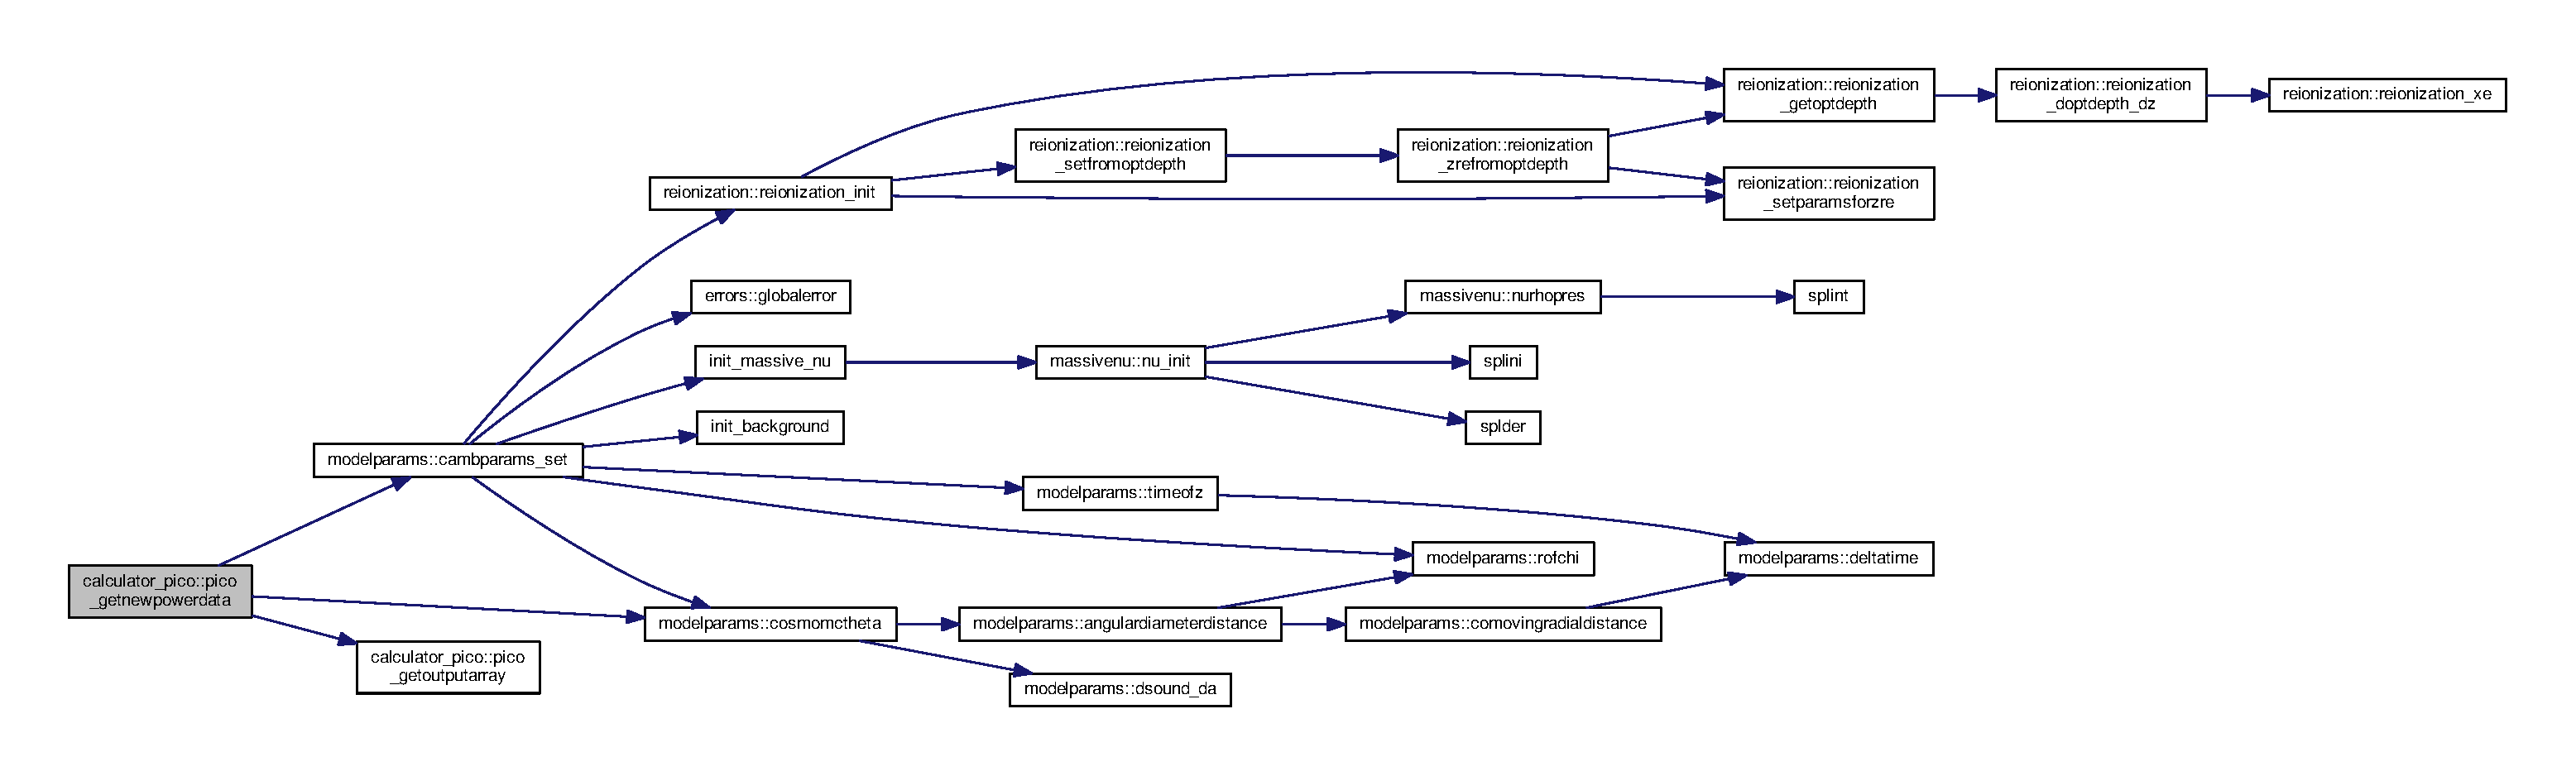
\includegraphics[width=350pt]{namespacecalculator__pico_a45cf2dcc102d6d731b105dcc2b985c04_cgraph}
\end{center}
\end{figure}
\mbox{\Hypertarget{namespacecalculator__pico_a76b2c99179137a67bf5deffecbe7a883}\label{namespacecalculator__pico_a76b2c99179137a67bf5deffecbe7a883}} 
\index{calculator\+\_\+pico@{calculator\+\_\+pico}!pico\+\_\+getnewtransferdata@{pico\+\_\+getnewtransferdata}}
\index{pico\+\_\+getnewtransferdata@{pico\+\_\+getnewtransferdata}!calculator\+\_\+pico@{calculator\+\_\+pico}}
\subsubsection{\texorpdfstring{pico\+\_\+getnewtransferdata()}{pico\_getnewtransferdata()}}
{\footnotesize\ttfamily subroutine calculator\+\_\+pico\+::pico\+\_\+getnewtransferdata (\begin{DoxyParamCaption}\item[{class(\mbox{\hyperlink{structcalculator__pico_1_1pico__calculator}{pico\+\_\+calculator}})}]{this,  }\item[{class(cmbparams)}]{C\+MB,  }\item[{class(ttheoryintermediatecache), pointer}]{Info,  }\item[{class(tcosmotheorypredictions)}]{Theory,  }\item[{integer}]{error }\end{DoxyParamCaption})\hspace{0.3cm}{\ttfamily [private]}}

\mbox{\Hypertarget{namespacecalculator__pico_adaa7c5af46424e51b4ff7c68520348c2}\label{namespacecalculator__pico_adaa7c5af46424e51b4ff7c68520348c2}} 
\index{calculator\+\_\+pico@{calculator\+\_\+pico}!pico\+\_\+getoutputarray@{pico\+\_\+getoutputarray}}
\index{pico\+\_\+getoutputarray@{pico\+\_\+getoutputarray}!calculator\+\_\+pico@{calculator\+\_\+pico}}
\subsubsection{\texorpdfstring{pico\+\_\+getoutputarray()}{pico\_getoutputarray()}}
{\footnotesize\ttfamily subroutine calculator\+\_\+pico\+::pico\+\_\+getoutputarray (\begin{DoxyParamCaption}\item[{class(tcosmotheorypredictions)}]{Theory,  }\item[{integer}]{i,  }\item[{integer}]{j,  }\item[{character(len=$\ast$)}]{name }\end{DoxyParamCaption})\hspace{0.3cm}{\ttfamily [private]}}



References cosmologytypes\+::cosmosettings.



Referenced by pico\+\_\+getnewpowerdata().

Here is the caller graph for this function\+:
\nopagebreak
\begin{figure}[H]
\begin{center}
\leavevmode
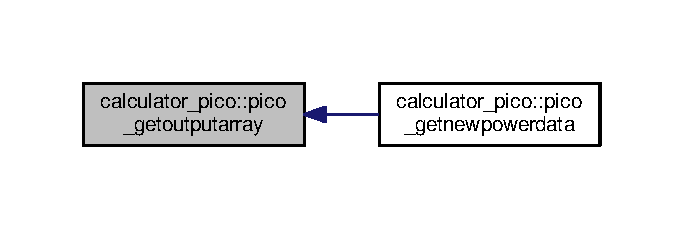
\includegraphics[width=328pt]{namespacecalculator__pico_adaa7c5af46424e51b4ff7c68520348c2_icgraph}
\end{center}
\end{figure}
\mbox{\Hypertarget{namespacecalculator__pico_abec990f2804cd52fd2f1c7aab45c7fe8}\label{namespacecalculator__pico_abec990f2804cd52fd2f1c7aab45c7fe8}} 
\index{calculator\+\_\+pico@{calculator\+\_\+pico}!pico\+\_\+gettheoryforimportance@{pico\+\_\+gettheoryforimportance}}
\index{pico\+\_\+gettheoryforimportance@{pico\+\_\+gettheoryforimportance}!calculator\+\_\+pico@{calculator\+\_\+pico}}
\subsubsection{\texorpdfstring{pico\+\_\+gettheoryforimportance()}{pico\_gettheoryforimportance()}}
{\footnotesize\ttfamily subroutine calculator\+\_\+pico\+::pico\+\_\+gettheoryforimportance (\begin{DoxyParamCaption}\item[{class(\mbox{\hyperlink{structcalculator__pico_1_1pico__calculator}{pico\+\_\+calculator}})}]{this,  }\item[{class(cmbparams)}]{C\+MB,  }\item[{class(tcosmotheorypredictions)}]{Theory,  }\item[{integer}]{error }\end{DoxyParamCaption})}

\mbox{\Hypertarget{namespacecalculator__pico_a974f29861363802129a96c29e70ea03e}\label{namespacecalculator__pico_a974f29861363802129a96c29e70ea03e}} 
\index{calculator\+\_\+pico@{calculator\+\_\+pico}!pico\+\_\+readparams@{pico\+\_\+readparams}}
\index{pico\+\_\+readparams@{pico\+\_\+readparams}!calculator\+\_\+pico@{calculator\+\_\+pico}}
\subsubsection{\texorpdfstring{pico\+\_\+readparams()}{pico\_readparams()}}
{\footnotesize\ttfamily subroutine calculator\+\_\+pico\+::pico\+\_\+readparams (\begin{DoxyParamCaption}\item[{class(\mbox{\hyperlink{structcalculator__pico_1_1pico__calculator}{pico\+\_\+calculator}})}]{this,  }\item[{class(\mbox{\hyperlink{structsettings_1_1tsettingini}{tsettingini}})}]{Ini }\end{DoxyParamCaption})}

\mbox{\Hypertarget{namespacecalculator__pico_ad5f92039b6c79eac4c4aeb00e53da084}\label{namespacecalculator__pico_ad5f92039b6c79eac4c4aeb00e53da084}} 
\index{calculator\+\_\+pico@{calculator\+\_\+pico}!pico\+\_\+versiontraceoutput@{pico\+\_\+versiontraceoutput}}
\index{pico\+\_\+versiontraceoutput@{pico\+\_\+versiontraceoutput}!calculator\+\_\+pico@{calculator\+\_\+pico}}
\subsubsection{\texorpdfstring{pico\+\_\+versiontraceoutput()}{pico\_versiontraceoutput()}}
{\footnotesize\ttfamily subroutine calculator\+\_\+pico\+::pico\+\_\+versiontraceoutput (\begin{DoxyParamCaption}\item[{class(\mbox{\hyperlink{structcalculator__pico_1_1pico__calculator}{pico\+\_\+calculator}})}]{this,  }\item[{class(tnamevaluelist)}]{Read\+Values }\end{DoxyParamCaption})\hspace{0.3cm}{\ttfamily [private]}}



References gaugeinterface\+::eqns\+\_\+name.


\hypertarget{namespacecamb}{}\section{camb Module Reference}
\label{namespacecamb}\index{camb@{camb}}
\subsection*{Modules}
\begin{DoxyCompactItemize}
\item 
 \mbox{\hyperlink{namespacecamb_1_1baseconfig}{baseconfig}}
\item 
 \mbox{\hyperlink{namespacecamb_1_1bbn}{bbn}}
\item 
 \mbox{\hyperlink{namespacecamb_1_1bispectrum}{bispectrum}}
\item 
 \mbox{\hyperlink{namespacecamb_1_1camb}{camb}}
\item 
 \mbox{\hyperlink{namespacecamb_1_1constants}{constants}}
\item 
 \mbox{\hyperlink{namespacecamb_1_1initialpower}{initialpower}}
\item 
 \mbox{\hyperlink{namespacecamb_1_1lensing}{lensing}}
\item 
 \mbox{\hyperlink{namespacecamb_1_1model}{model}}
\item 
 \mbox{\hyperlink{namespacecamb_1_1nonlinear}{nonlinear}}
\item 
 \mbox{\hyperlink{namespacecamb_1_1recombination}{recombination}}
\item 
 \mbox{\hyperlink{namespacecamb_1_1reionization}{reionization}}
\end{DoxyCompactItemize}
\subsection*{Data Types}
\begin{DoxyCompactItemize}
\item 
type \mbox{\hyperlink{structcamb_1_1cambdata}{cambdata}}
\end{DoxyCompactItemize}
\subsection*{Functions/\+Subroutines}
\begin{DoxyCompactItemize}
\item 
subroutine \mbox{\hyperlink{namespacecamb_ae587b573e03da5811edb59806305b2cd}{camb\+\_\+gettransfers}} (Params, Out\+Data, error)
\item 
subroutine \mbox{\hyperlink{namespacecamb_a64195b97e1e4c42b990076ff2bff6f1d}{camb\+\_\+initcambdata}} (Dat)
\item 
subroutine \mbox{\hyperlink{namespacecamb_a20b57e6f6098c5800cbf374d96307d13}{camb\+\_\+freecambdata}} (Dat)
\item 
subroutine \mbox{\hyperlink{namespacecamb_a9fb2095034057d44dc9526dd02d60064}{camb\+\_\+transferstopowers}} (C\+Data)
\item 
subroutine \mbox{\hyperlink{namespacecamb_af6f4c73133d3de79ac10db3c4b2d0650}{camb\+\_\+getresults}} (Params, error)
\item 
subroutine \mbox{\hyperlink{namespacecamb_abeb0ae530a720a17a76108dbed29c1fc}{camb\+\_\+getcls}} (Cls, lmax, in, G\+C\+\_\+conventions)
\item 
real(dl) function \mbox{\hyperlink{namespacecamb_a53e4d3ff396030bd7e41d606cfa458b2}{camb\+\_\+getage}} (P)
\item 
real(dl) function \mbox{\hyperlink{namespacecamb_ab45910129412993d163c3d4b83e19152}{camb\+\_\+getzrefromtau}} (P, tau)
\item 
subroutine \mbox{\hyperlink{namespacecamb_a6ce30ab6419006324d56d3e4434530f9}{camb\+\_\+setdefparams}} (P)
\item 
subroutine \mbox{\hyperlink{namespacecamb_ad303911c183f5affcdc9665c5facdd4b}{camb\+\_\+setneutrinohierarchy}} (P, omnuh2, omnuh2\+\_\+sterile, nnu, neutrino\+\_\+hierarchy, num\+\_\+massive\+\_\+neutrinos)
\item 
logical function \mbox{\hyperlink{namespacecamb_ae9577b86a4f0803e5754a23871a7113e}{camb\+\_\+validateparams}} (P)
\item 
subroutine \mbox{\hyperlink{namespacecamb_a70f3206a0056ea3ff96defbc4d2be548}{camb\+\_\+cleanup}}
\end{DoxyCompactItemize}
\subsection*{Variables}
\begin{DoxyCompactItemize}
\item 
string \mbox{\hyperlink{namespacecamb_a85cc16a2fbdb270667e7303f2290c3be}{\+\_\+\+\_\+author\+\_\+\+\_\+}} = \char`\"{}Antony Lewis\char`\"{}
\item 
string \mbox{\hyperlink{namespacecamb_af9e02319cf919d4505eab8b37179c712}{\+\_\+\+\_\+contact\+\_\+\+\_\+}} = \char`\"{}antony at cosmologist dot info\char`\"{}
\item 
string \mbox{\hyperlink{namespacecamb_aa9d4ea4f20e0977e7d5f5dc20b8debd6}{\+\_\+\+\_\+status\+\_\+\+\_\+}} = \char`\"{}beta\char`\"{}
\item 
string \mbox{\hyperlink{namespacecamb_a68e3f34837e39bb6f7e725612e4627fa}{\+\_\+\+\_\+version\+\_\+\+\_\+}} = \char`\"{}0.\+1.\+3\char`\"{}
\item 
\mbox{\hyperlink{namespacecamb_a8dcf37e78d4e08b70f90002000e746b8}{Thread\+Num}} = dll\+\_\+import(c\+\_\+int, \char`\"{}modelparams\char`\"{}, \char`\"{}threadnum\char`\"{})
\item 
\mbox{\hyperlink{namespacecamb_af98223967f3787053d42644a1ae6f785}{Do\+Tensor\+Neutrinos}} = dll\+\_\+import(c\+\_\+bool, \char`\"{}gaugeinterface\char`\"{}, \char`\"{}dotensorneutrinos\char`\"{})
\item 
\mbox{\hyperlink{namespacecamb_a61a5837f54fb09c486d29171a8651a91}{Magnetic}} = dll\+\_\+import(c\+\_\+double, \char`\"{}gaugeinterface\char`\"{}, \char`\"{}magnetic\char`\"{})
\item 
\mbox{\hyperlink{namespacecamb_a2e33f06925cf79f62b6d07d7c737217c}{vec\+\_\+sig0}} = dll\+\_\+import(c\+\_\+double, \char`\"{}gaugeinterface\char`\"{}, \char`\"{}vec\+\_\+sig0\char`\"{})
\end{DoxyCompactItemize}


\subsection{Function/\+Subroutine Documentation}
\mbox{\Hypertarget{namespacecamb_a70f3206a0056ea3ff96defbc4d2be548}\label{namespacecamb_a70f3206a0056ea3ff96defbc4d2be548}} 
\index{camb@{camb}!camb\+\_\+cleanup@{camb\+\_\+cleanup}}
\index{camb\+\_\+cleanup@{camb\+\_\+cleanup}!camb@{camb}}
\subsubsection{\texorpdfstring{camb\+\_\+cleanup()}{camb\_cleanup()}}
{\footnotesize\ttfamily subroutine camb\+::camb\+\_\+cleanup (\begin{DoxyParamCaption}{ }\end{DoxyParamCaption})}



References spherbessels\+::bessels\+\_\+free(), modeldata\+::modeldata\+\_\+free(), transfer\+::mt, thermodata\+::thermodata\+\_\+free(), and transfer\+::transfer\+\_\+free().

Here is the call graph for this function\+:
\nopagebreak
\begin{figure}[H]
\begin{center}
\leavevmode
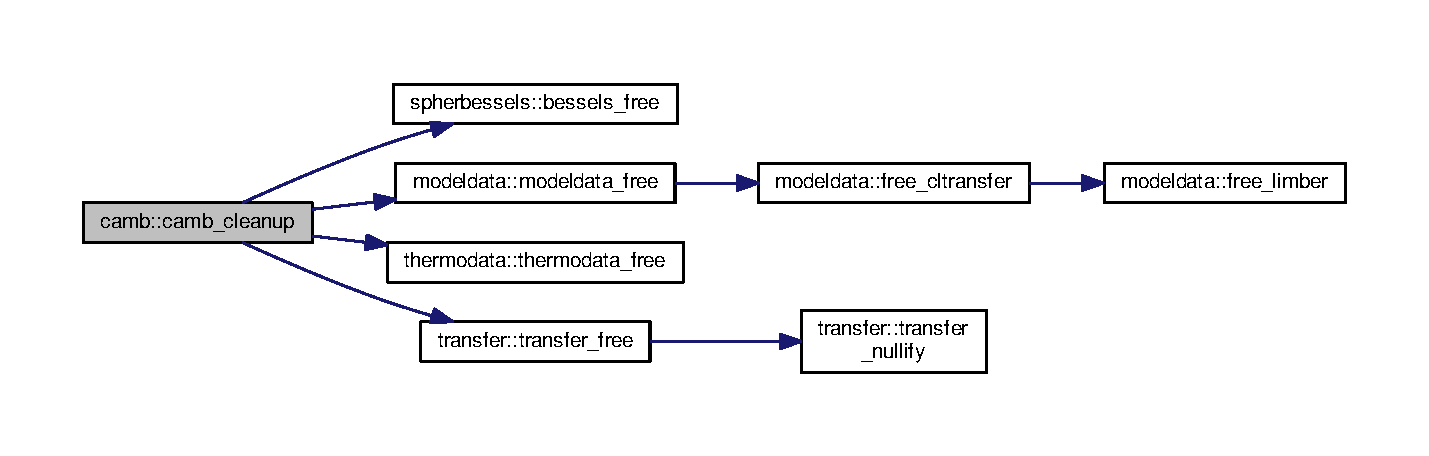
\includegraphics[width=350pt]{namespacecamb_a70f3206a0056ea3ff96defbc4d2be548_cgraph}
\end{center}
\end{figure}
\mbox{\Hypertarget{namespacecamb_a20b57e6f6098c5800cbf374d96307d13}\label{namespacecamb_a20b57e6f6098c5800cbf374d96307d13}} 
\index{camb@{camb}!camb\+\_\+freecambdata@{camb\+\_\+freecambdata}}
\index{camb\+\_\+freecambdata@{camb\+\_\+freecambdata}!camb@{camb}}
\subsubsection{\texorpdfstring{camb\+\_\+freecambdata()}{camb\_freecambdata()}}
{\footnotesize\ttfamily subroutine camb\+::camb\+\_\+freecambdata (\begin{DoxyParamCaption}\item[{type (\mbox{\hyperlink{structcamb_1_1cambdata}{cambdata}})}]{Dat }\end{DoxyParamCaption})}



References modeldata\+::free\+\_\+cltransfer(), and transfer\+::transfer\+\_\+free().



Referenced by handles\+::cambdata\+\_\+free().

Here is the call graph for this function\+:
\nopagebreak
\begin{figure}[H]
\begin{center}
\leavevmode
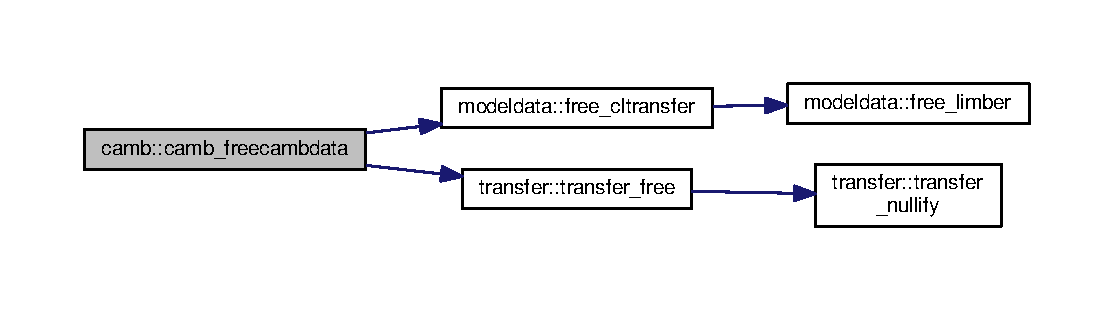
\includegraphics[width=350pt]{namespacecamb_a20b57e6f6098c5800cbf374d96307d13_cgraph}
\end{center}
\end{figure}
Here is the caller graph for this function\+:
\nopagebreak
\begin{figure}[H]
\begin{center}
\leavevmode
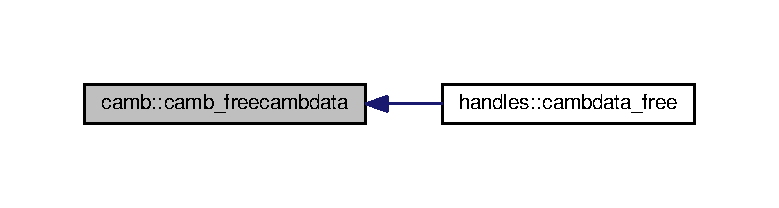
\includegraphics[width=350pt]{namespacecamb_a20b57e6f6098c5800cbf374d96307d13_icgraph}
\end{center}
\end{figure}
\mbox{\Hypertarget{namespacecamb_a53e4d3ff396030bd7e41d606cfa458b2}\label{namespacecamb_a53e4d3ff396030bd7e41d606cfa458b2}} 
\index{camb@{camb}!camb\+\_\+getage@{camb\+\_\+getage}}
\index{camb\+\_\+getage@{camb\+\_\+getage}!camb@{camb}}
\subsubsection{\texorpdfstring{camb\+\_\+getage()}{camb\_getage()}}
{\footnotesize\ttfamily real(dl) function camb\+::camb\+\_\+getage (\begin{DoxyParamCaption}\item[{type(cambparams), intent(in)}]{P }\end{DoxyParamCaption})}



References modelparams\+::cambparams\+\_\+set(), modelparams\+::deltaphysicaltimegyr(), and initialpower\+::p.

Here is the call graph for this function\+:
\nopagebreak
\begin{figure}[H]
\begin{center}
\leavevmode
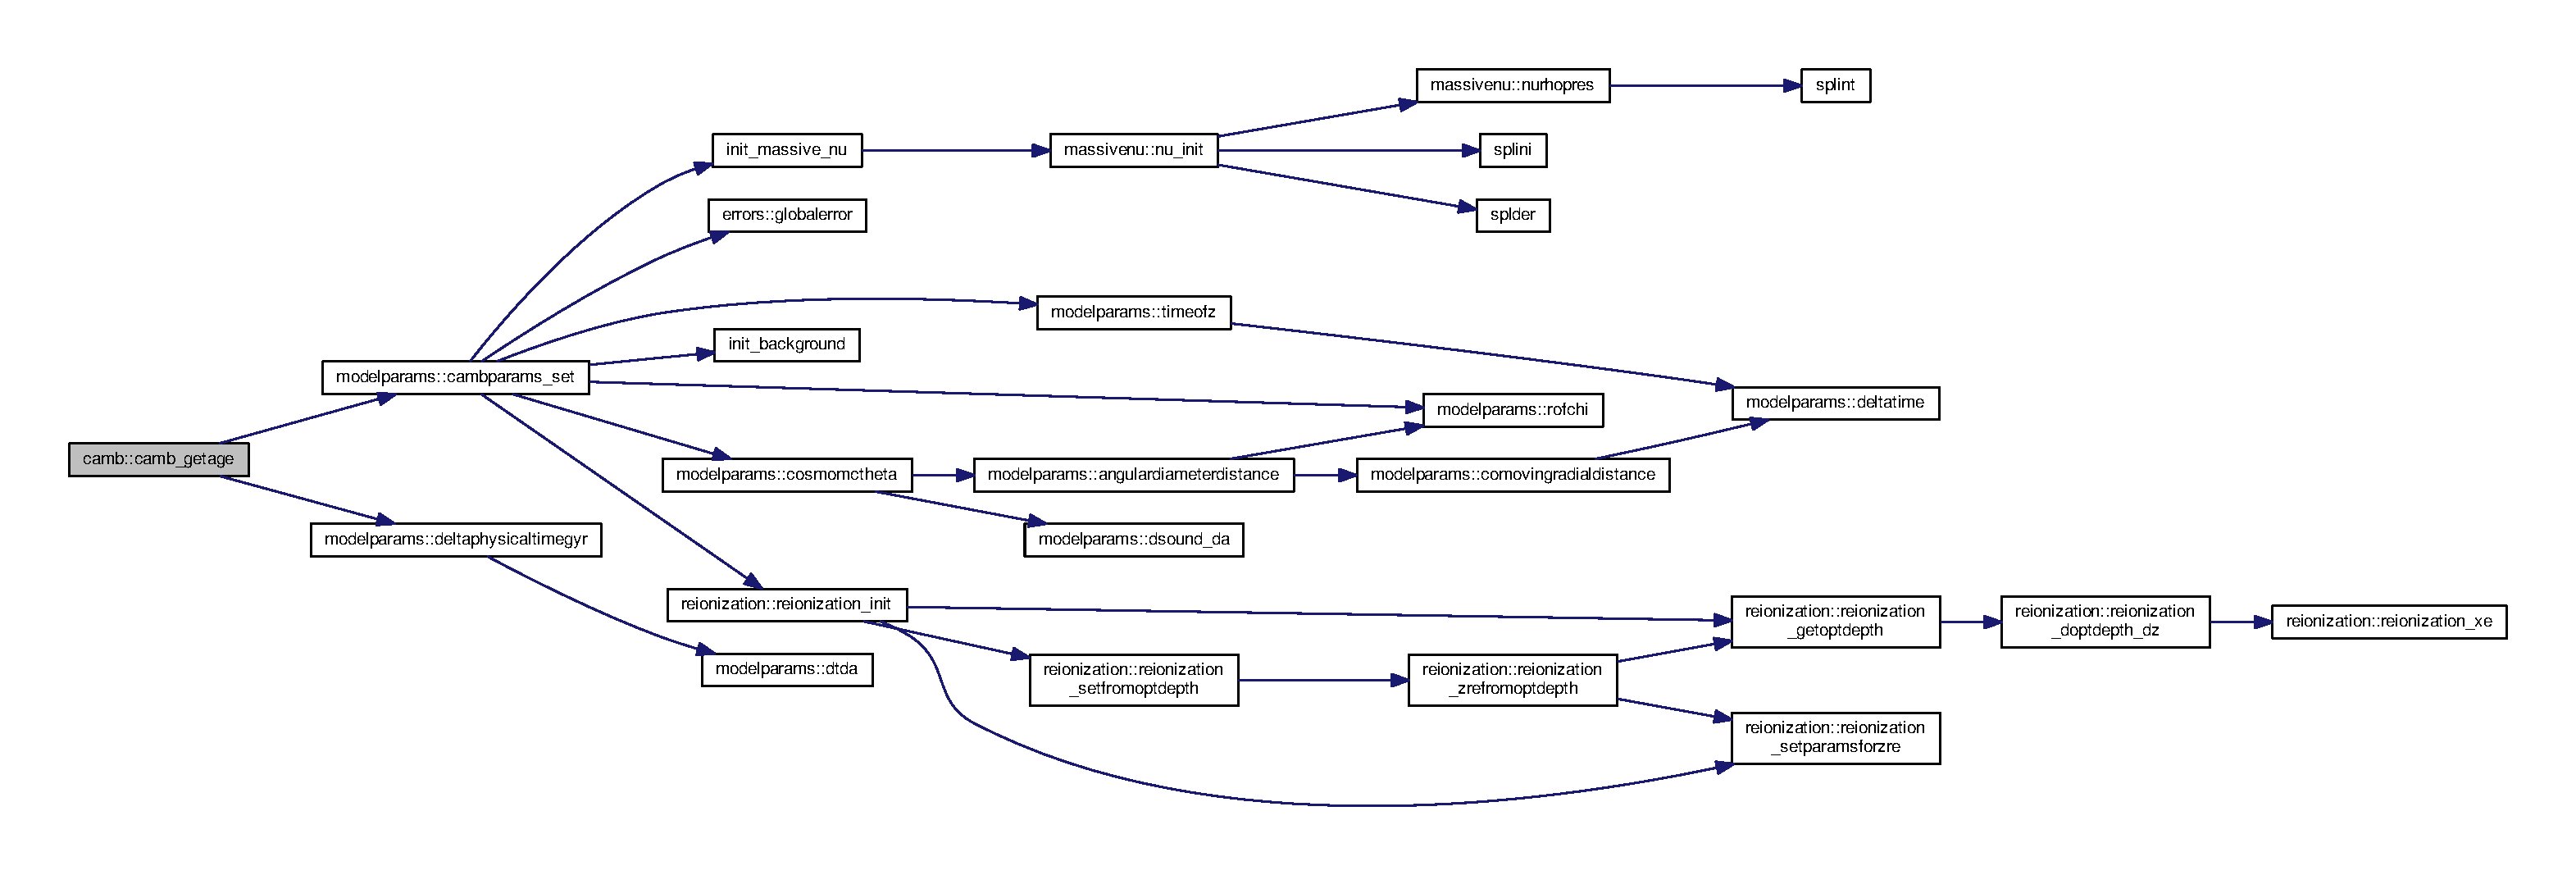
\includegraphics[width=350pt]{namespacecamb_a53e4d3ff396030bd7e41d606cfa458b2_cgraph}
\end{center}
\end{figure}
\mbox{\Hypertarget{namespacecamb_abeb0ae530a720a17a76108dbed29c1fc}\label{namespacecamb_abeb0ae530a720a17a76108dbed29c1fc}} 
\index{camb@{camb}!camb\+\_\+getcls@{camb\+\_\+getcls}}
\index{camb\+\_\+getcls@{camb\+\_\+getcls}!camb@{camb}}
\subsubsection{\texorpdfstring{camb\+\_\+getcls()}{camb\_getcls()}}
{\footnotesize\ttfamily subroutine camb\+::camb\+\_\+getcls (\begin{DoxyParamCaption}\item[{real, dimension(2\+:lmax,1\+:4), intent(out)}]{Cls,  }\item[{integer, intent(in)}]{lmax,  }\item[{integer, intent(in)}]{in,  }\item[{logical, intent(in)}]{G\+C\+\_\+conventions }\end{DoxyParamCaption})}



References modeldata\+::c\+\_\+cross, modeldata\+::c\+\_\+e, modeldata\+::c\+\_\+temp, modeldata\+::cl\+\_\+lensed, modeldata\+::cl\+\_\+scalar, modeldata\+::cl\+\_\+tensor, modelparams\+::cp, modeldata\+::ct\+\_\+cross, modeldata\+::ct\+\_\+temp, and modeldata\+::lmax\+\_\+lensed.



Referenced by writefitscls().

Here is the caller graph for this function\+:
\nopagebreak
\begin{figure}[H]
\begin{center}
\leavevmode
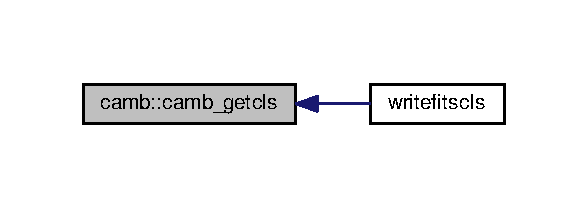
\includegraphics[width=282pt]{namespacecamb_abeb0ae530a720a17a76108dbed29c1fc_icgraph}
\end{center}
\end{figure}
\mbox{\Hypertarget{namespacecamb_af6f4c73133d3de79ac10db3c4b2d0650}\label{namespacecamb_af6f4c73133d3de79ac10db3c4b2d0650}} 
\index{camb@{camb}!camb\+\_\+getresults@{camb\+\_\+getresults}}
\index{camb\+\_\+getresults@{camb\+\_\+getresults}!camb@{camb}}
\subsubsection{\texorpdfstring{camb\+\_\+getresults()}{camb\_getresults()}}
{\footnotesize\ttfamily subroutine camb\+::camb\+\_\+getresults (\begin{DoxyParamCaption}\item[{type(cambparams)}]{Params,  }\item[{integer, optional}]{error }\end{DoxyParamCaption})}



References modelparams\+::call\+\_\+again, modelparams\+::cambparams\+\_\+set(), cambmain\+::cmbmain(), modelparams\+::cp, modeldata\+::ctransscal, modelparams\+::do\+\_\+bispectrum, errors\+::global\+\_\+error\+\_\+flag, modelparams\+::highaccuracydefault, and lensing\+::lens\+\_\+cls().



Referenced by camb\+\_\+gettransfers(), getsigma8(), and tester().

Here is the call graph for this function\+:
\nopagebreak
\begin{figure}[H]
\begin{center}
\leavevmode
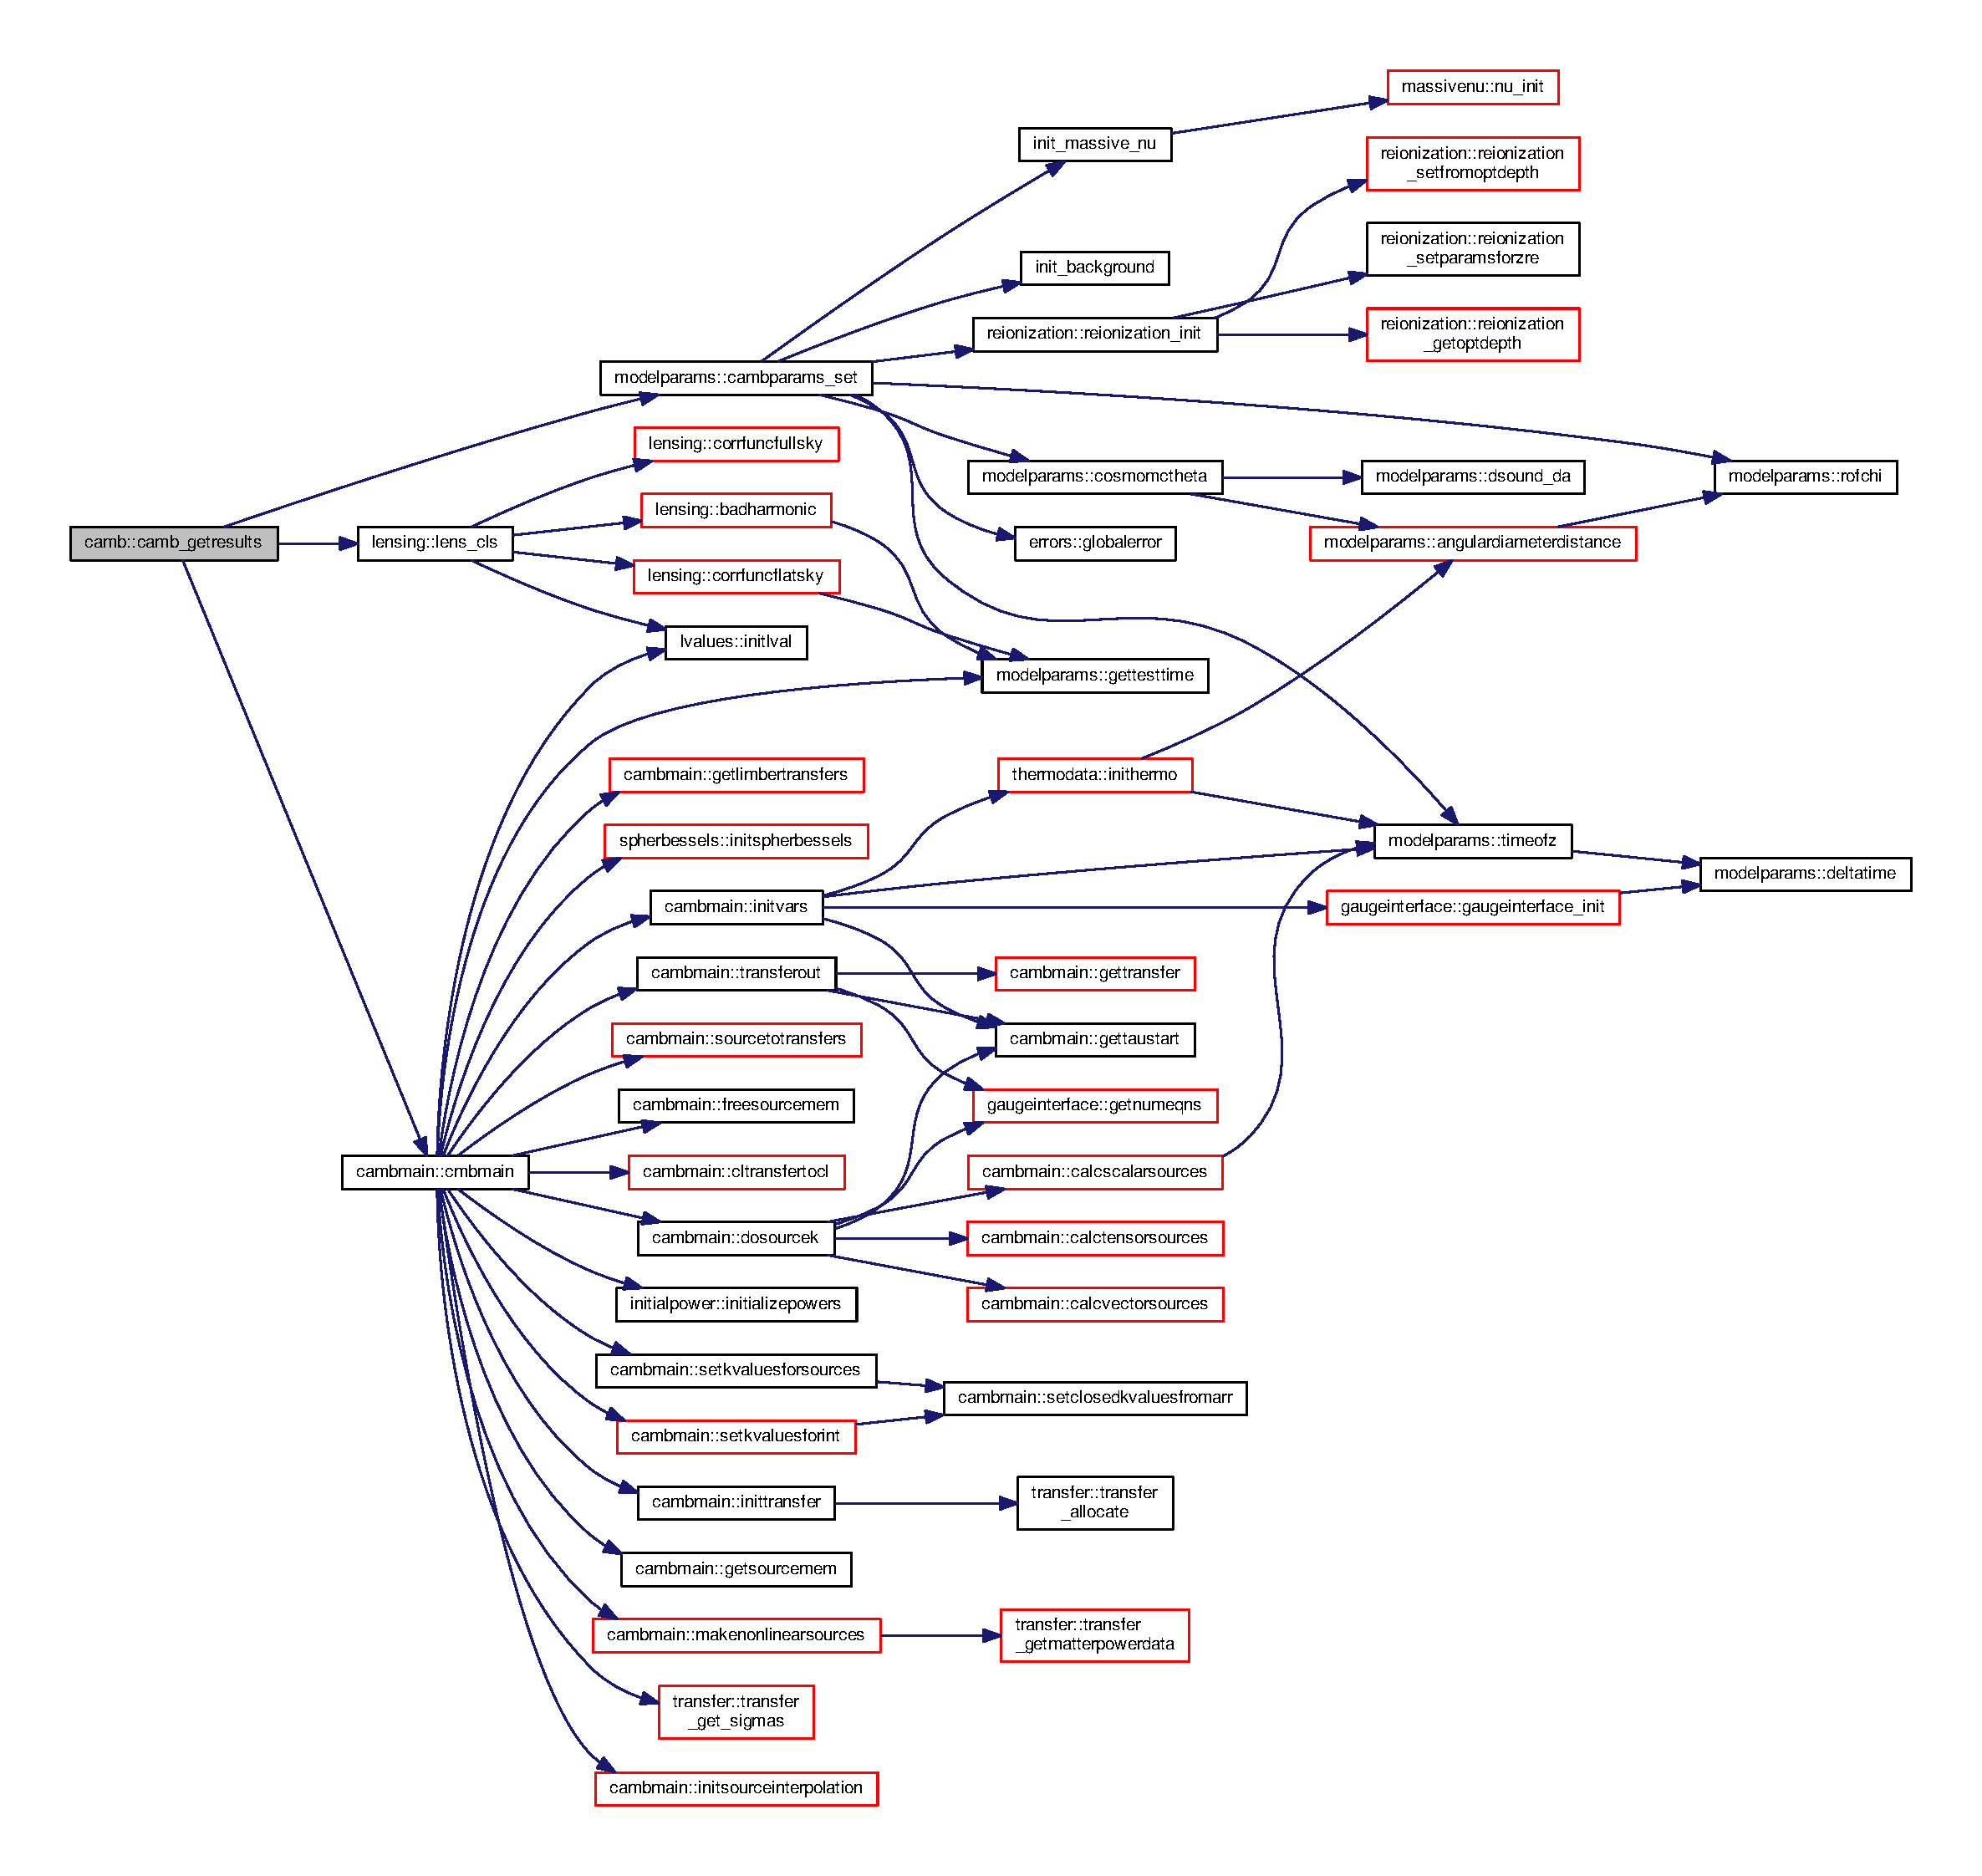
\includegraphics[width=350pt]{namespacecamb_af6f4c73133d3de79ac10db3c4b2d0650_cgraph}
\end{center}
\end{figure}
Here is the caller graph for this function\+:
\nopagebreak
\begin{figure}[H]
\begin{center}
\leavevmode
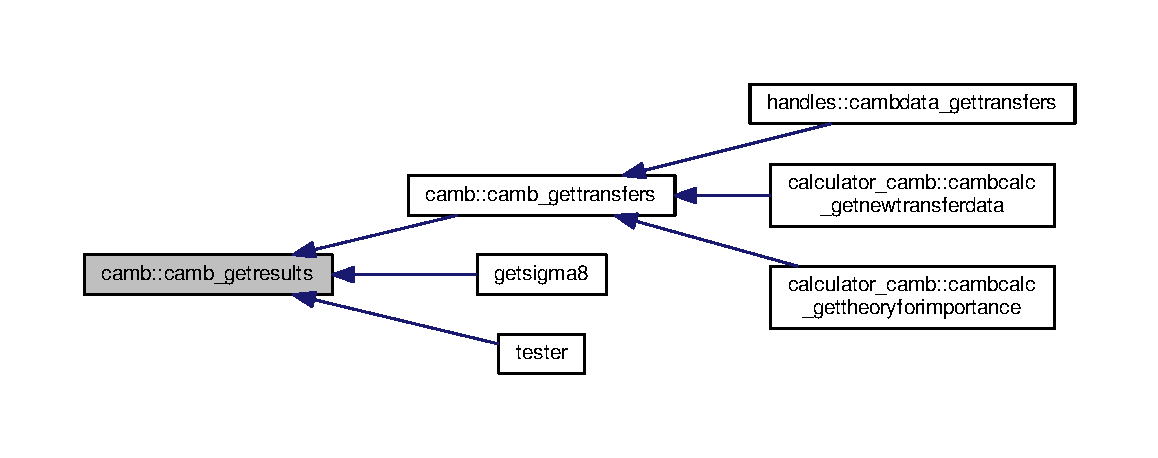
\includegraphics[width=350pt]{namespacecamb_af6f4c73133d3de79ac10db3c4b2d0650_icgraph}
\end{center}
\end{figure}
\mbox{\Hypertarget{namespacecamb_ae587b573e03da5811edb59806305b2cd}\label{namespacecamb_ae587b573e03da5811edb59806305b2cd}} 
\index{camb@{camb}!camb\+\_\+gettransfers@{camb\+\_\+gettransfers}}
\index{camb\+\_\+gettransfers@{camb\+\_\+gettransfers}!camb@{camb}}
\subsubsection{\texorpdfstring{camb\+\_\+gettransfers()}{camb\_gettransfers()}}
{\footnotesize\ttfamily subroutine camb\+::camb\+\_\+gettransfers (\begin{DoxyParamCaption}\item[{type(cambparams)}]{Params,  }\item[{type (\mbox{\hyperlink{structcamb_1_1cambdata}{cambdata}})}]{Out\+Data,  }\item[{integer}]{error }\end{DoxyParamCaption})}



References camb\+\_\+getresults(), modeldata\+::ctransscal, modeldata\+::ctranstens, modeldata\+::ctransvec, modeldata\+::free\+\_\+cltransfer(), transfer\+::mt, and transfer\+::transfer\+\_\+free().



Referenced by calculator\+\_\+camb\+::cambcalc\+\_\+getnewtransferdata(), calculator\+\_\+camb\+::cambcalc\+\_\+gettheoryforimportance(), and handles\+::cambdata\+\_\+gettransfers().

Here is the call graph for this function\+:
\nopagebreak
\begin{figure}[H]
\begin{center}
\leavevmode
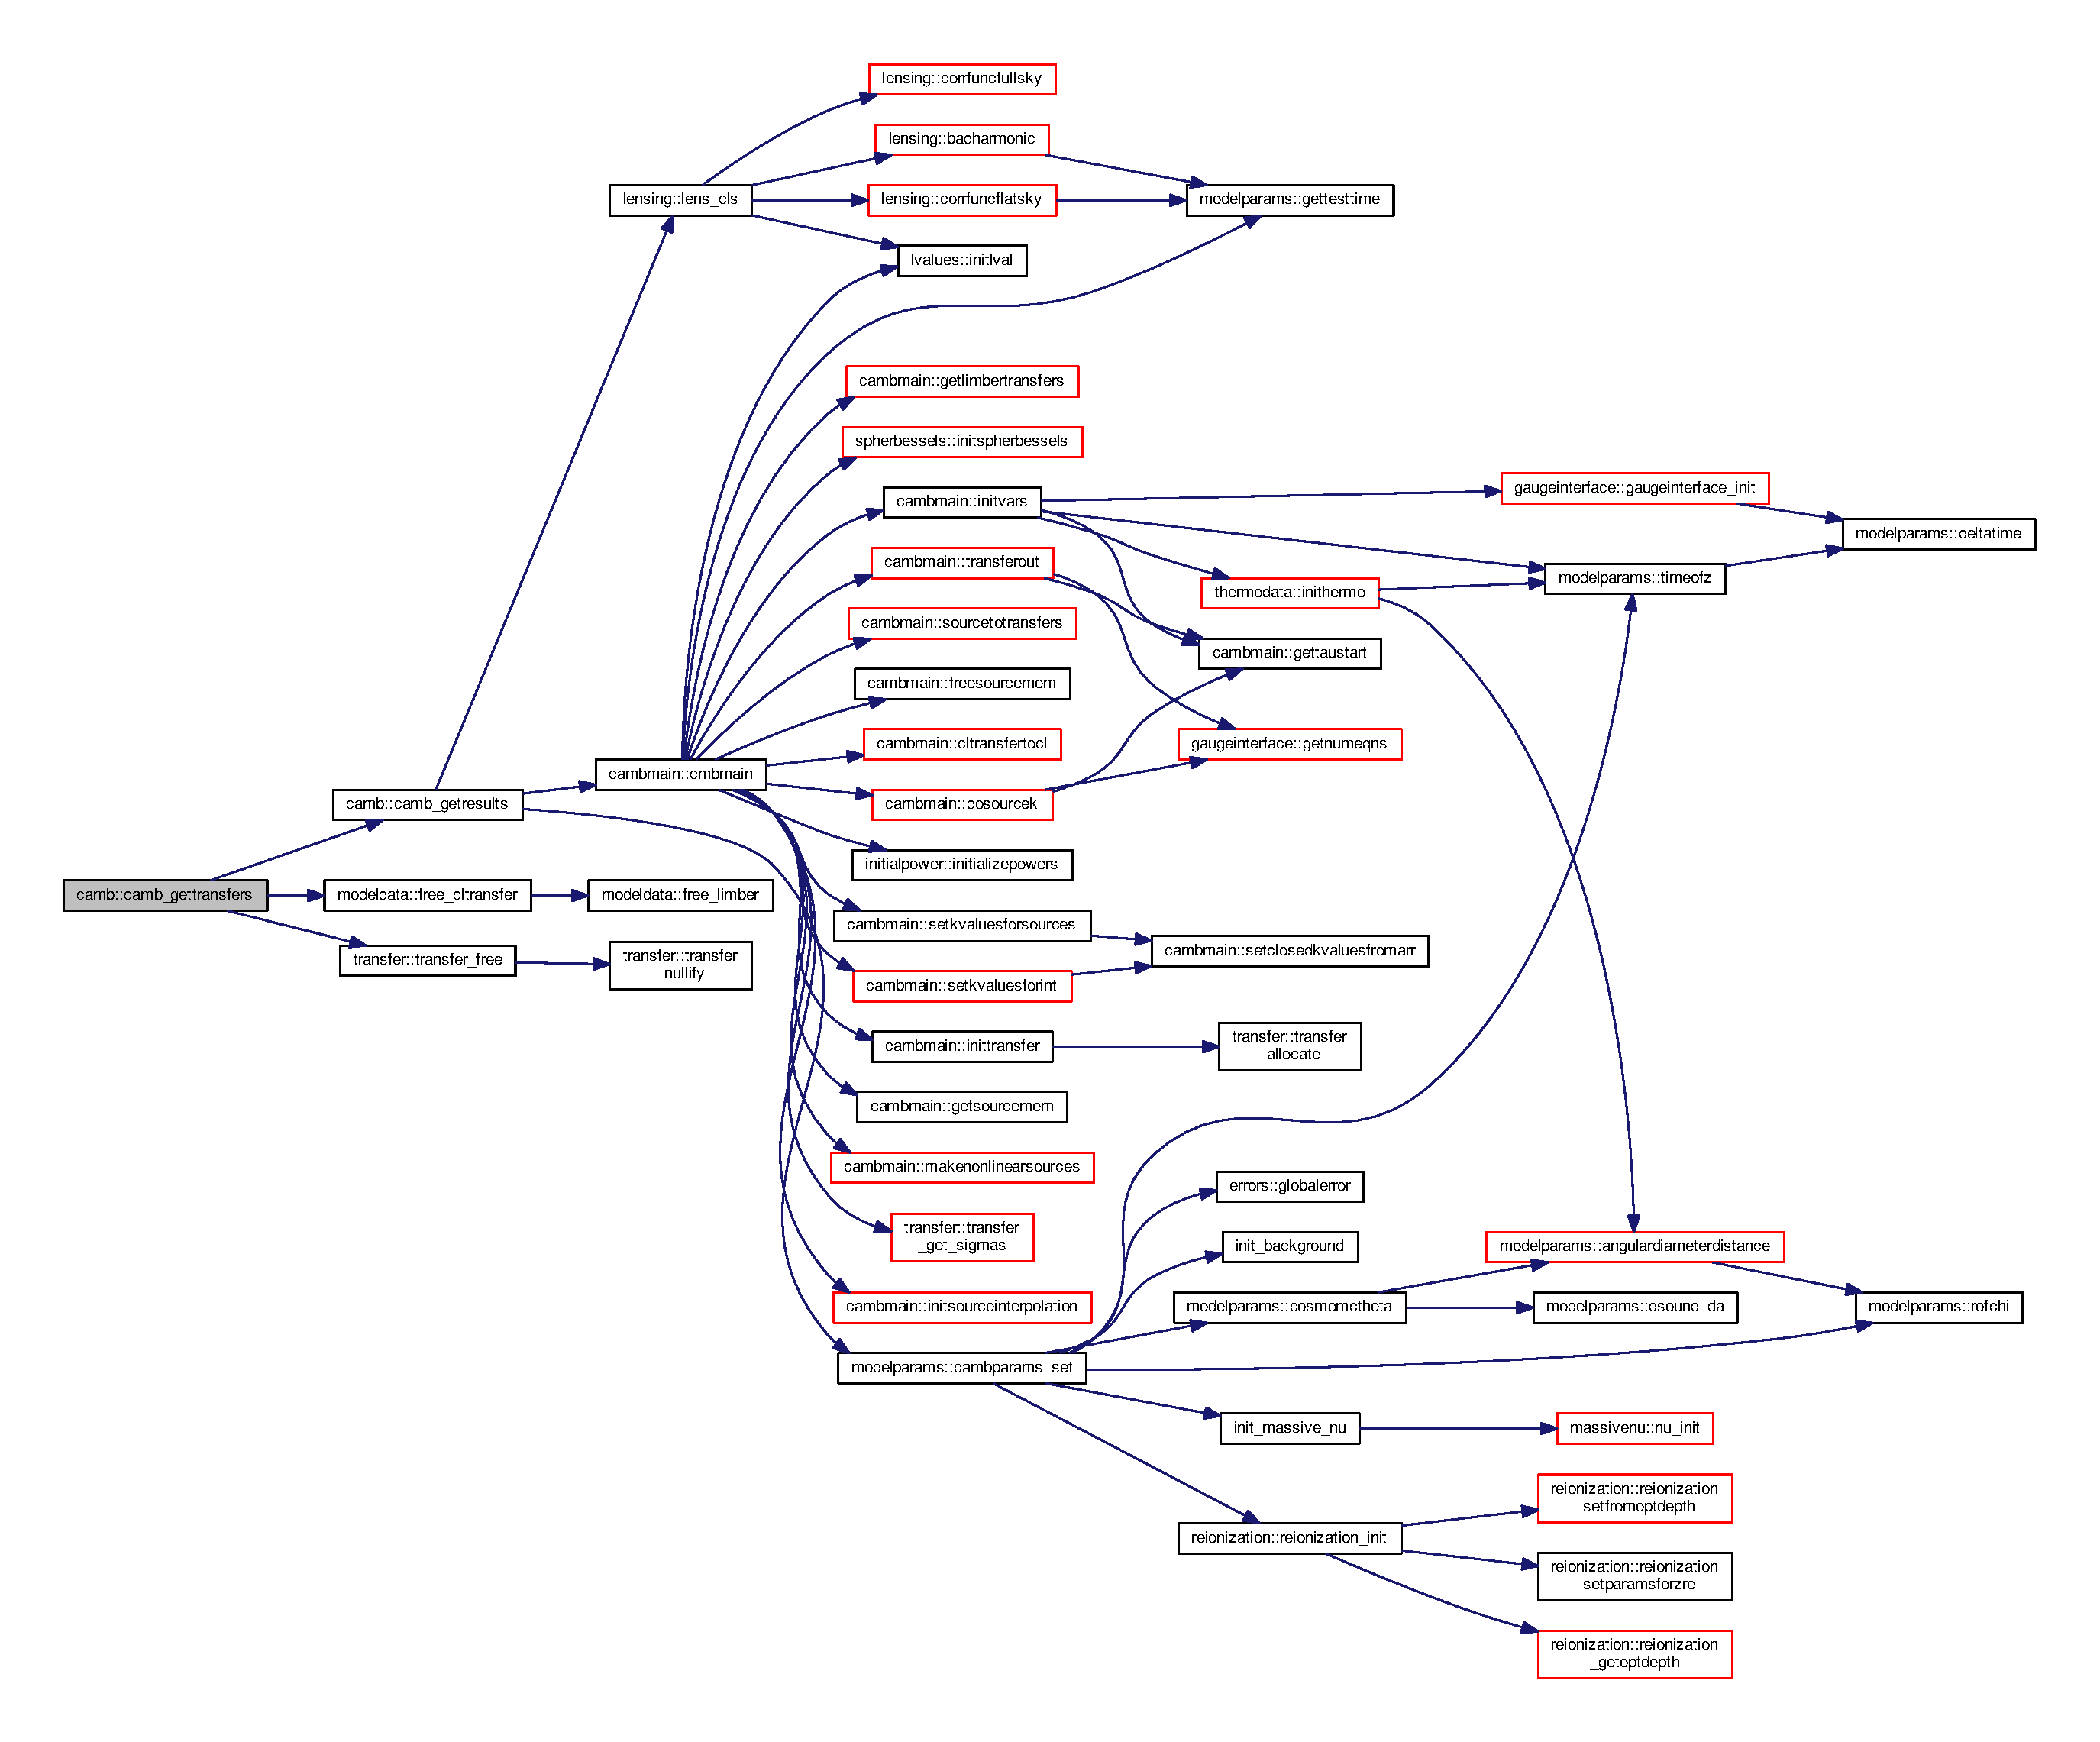
\includegraphics[width=350pt]{namespacecamb_ae587b573e03da5811edb59806305b2cd_cgraph}
\end{center}
\end{figure}
Here is the caller graph for this function\+:
\nopagebreak
\begin{figure}[H]
\begin{center}
\leavevmode
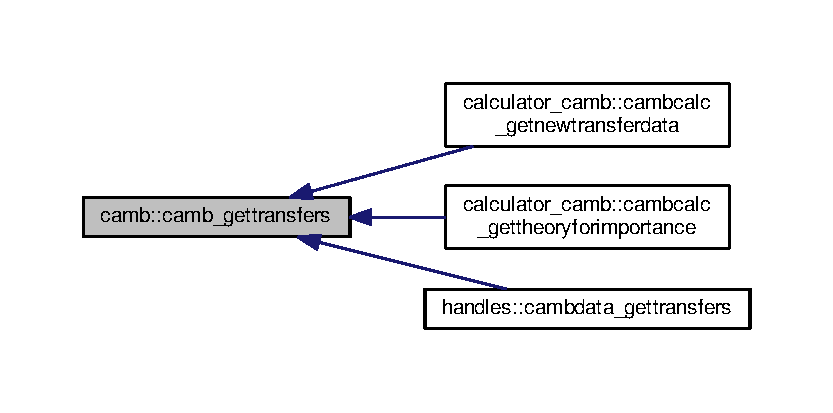
\includegraphics[width=350pt]{namespacecamb_ae587b573e03da5811edb59806305b2cd_icgraph}
\end{center}
\end{figure}
\mbox{\Hypertarget{namespacecamb_ab45910129412993d163c3d4b83e19152}\label{namespacecamb_ab45910129412993d163c3d4b83e19152}} 
\index{camb@{camb}!camb\+\_\+getzrefromtau@{camb\+\_\+getzrefromtau}}
\index{camb\+\_\+getzrefromtau@{camb\+\_\+getzrefromtau}!camb@{camb}}
\subsubsection{\texorpdfstring{camb\+\_\+getzrefromtau()}{camb\_getzrefromtau()}}
{\footnotesize\ttfamily real(dl) function camb\+::camb\+\_\+getzrefromtau (\begin{DoxyParamCaption}\item[{type(cambparams)}]{P,  }\item[{real(dl)}]{tau }\end{DoxyParamCaption})}



References modelparams\+::cambparams\+\_\+set(), modelparams\+::cp, and initialpower\+::p.

Here is the call graph for this function\+:
\nopagebreak
\begin{figure}[H]
\begin{center}
\leavevmode
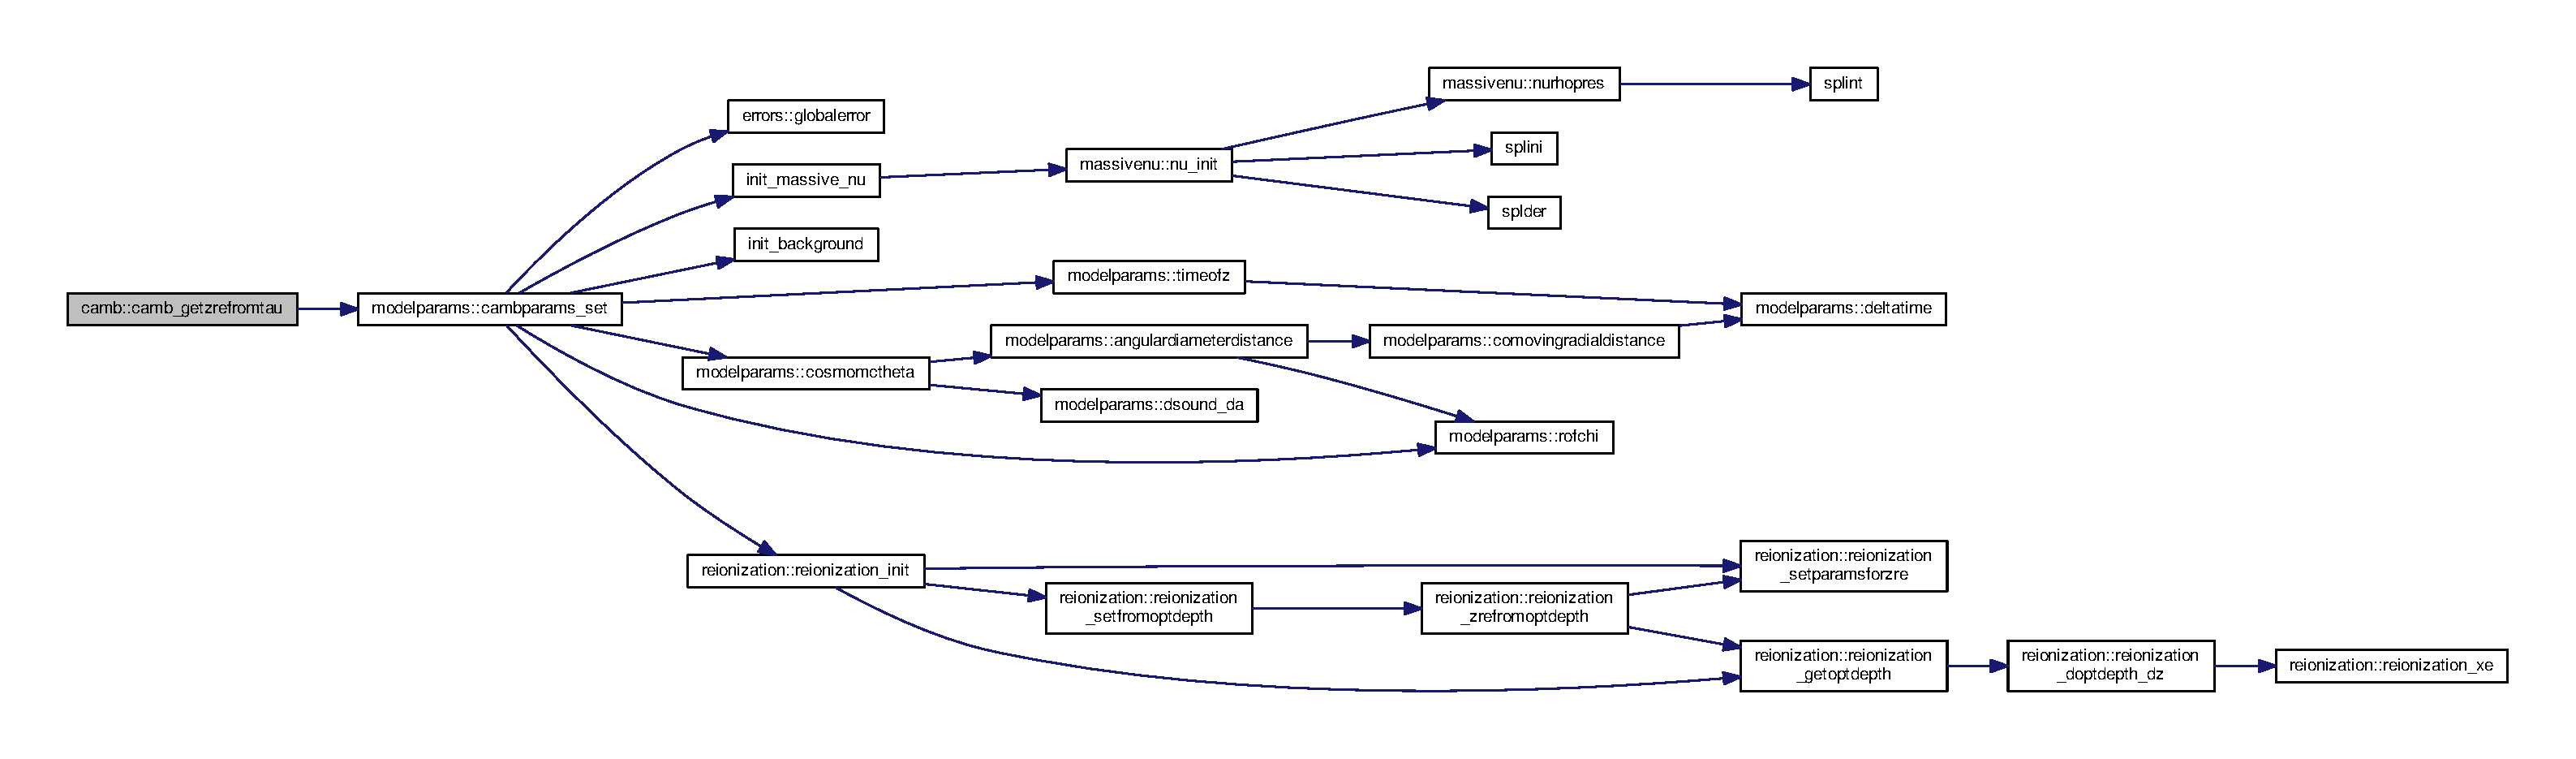
\includegraphics[width=350pt]{namespacecamb_ab45910129412993d163c3d4b83e19152_cgraph}
\end{center}
\end{figure}
\mbox{\Hypertarget{namespacecamb_a64195b97e1e4c42b990076ff2bff6f1d}\label{namespacecamb_a64195b97e1e4c42b990076ff2bff6f1d}} 
\index{camb@{camb}!camb\+\_\+initcambdata@{camb\+\_\+initcambdata}}
\index{camb\+\_\+initcambdata@{camb\+\_\+initcambdata}!camb@{camb}}
\subsubsection{\texorpdfstring{camb\+\_\+initcambdata()}{camb\_initcambdata()}}
{\footnotesize\ttfamily subroutine camb\+::camb\+\_\+initcambdata (\begin{DoxyParamCaption}\item[{type (\mbox{\hyperlink{structcamb_1_1cambdata}{cambdata}})}]{Dat }\end{DoxyParamCaption})}



Referenced by calculator\+\_\+camb\+::cambcalc\+\_\+getnewtransferdata(), calculator\+\_\+camb\+::cambcalc\+\_\+gettheoryforimportance(), and handles\+::cambdata\+\_\+new().

Here is the caller graph for this function\+:
\nopagebreak
\begin{figure}[H]
\begin{center}
\leavevmode
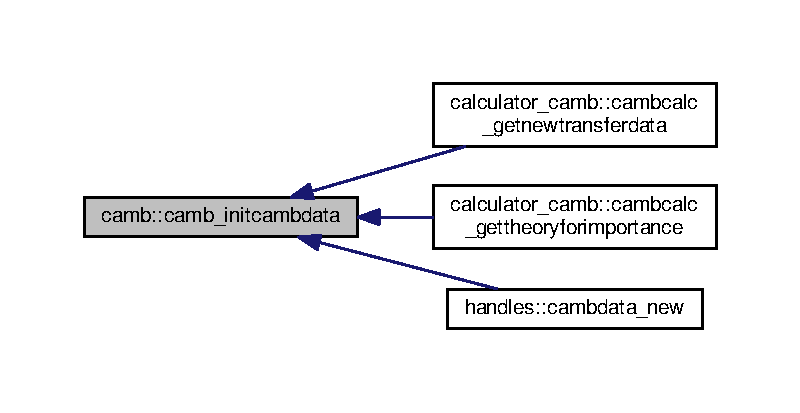
\includegraphics[width=350pt]{namespacecamb_a64195b97e1e4c42b990076ff2bff6f1d_icgraph}
\end{center}
\end{figure}
\mbox{\Hypertarget{namespacecamb_a6ce30ab6419006324d56d3e4434530f9}\label{namespacecamb_a6ce30ab6419006324d56d3e4434530f9}} 
\index{camb@{camb}!camb\+\_\+setdefparams@{camb\+\_\+setdefparams}}
\index{camb\+\_\+setdefparams@{camb\+\_\+setdefparams}!camb@{camb}}
\subsubsection{\texorpdfstring{camb\+\_\+setdefparams()}{camb\_setdefparams()}}
{\footnotesize\ttfamily subroutine camb\+::camb\+\_\+setdefparams (\begin{DoxyParamCaption}\item[{type(cambparams), intent(out)}]{P }\end{DoxyParamCaption})}



References constants\+::cobe\+\_\+cmbtemp, constants\+::default\+\_\+nnu, gaugeinterface\+::initial\+\_\+adiabatic, modelparams\+::nonlinear\+\_\+none, modelparams\+::nu\+\_\+best, modelparams\+::outnone, recombination\+::recombination\+\_\+setdefparams(), reionization\+::reionization\+\_\+setdefparams(), and initialpower\+::setdefpowerparams().



Referenced by handles\+::cambdata\+\_\+new(), getsigma8(), and tester().

Here is the call graph for this function\+:
\nopagebreak
\begin{figure}[H]
\begin{center}
\leavevmode
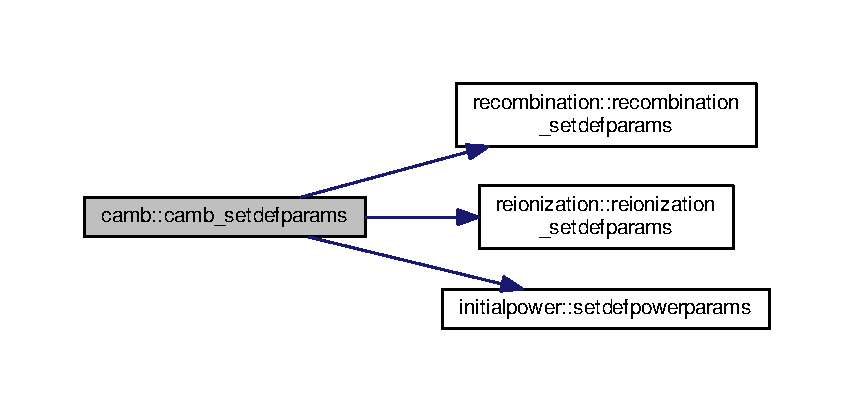
\includegraphics[width=350pt]{namespacecamb_a6ce30ab6419006324d56d3e4434530f9_cgraph}
\end{center}
\end{figure}
Here is the caller graph for this function\+:
\nopagebreak
\begin{figure}[H]
\begin{center}
\leavevmode
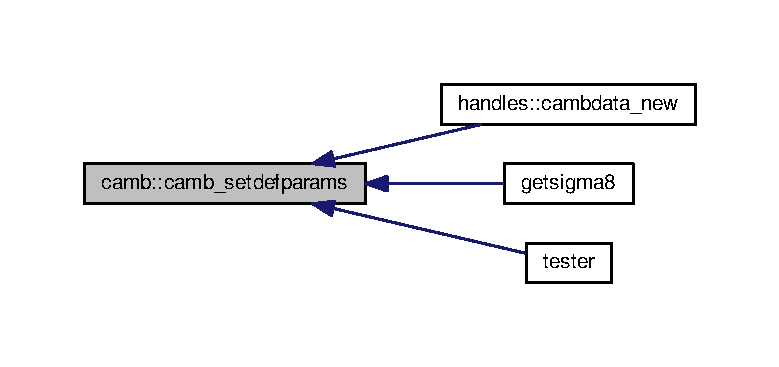
\includegraphics[width=350pt]{namespacecamb_a6ce30ab6419006324d56d3e4434530f9_icgraph}
\end{center}
\end{figure}
\mbox{\Hypertarget{namespacecamb_ad303911c183f5affcdc9665c5facdd4b}\label{namespacecamb_ad303911c183f5affcdc9665c5facdd4b}} 
\index{camb@{camb}!camb\+\_\+setneutrinohierarchy@{camb\+\_\+setneutrinohierarchy}}
\index{camb\+\_\+setneutrinohierarchy@{camb\+\_\+setneutrinohierarchy}!camb@{camb}}
\subsubsection{\texorpdfstring{camb\+\_\+setneutrinohierarchy()}{camb\_setneutrinohierarchy()}}
{\footnotesize\ttfamily subroutine camb\+::camb\+\_\+setneutrinohierarchy (\begin{DoxyParamCaption}\item[{type(cambparams), intent(inout)}]{P,  }\item[{real(dl), intent(in)}]{omnuh2,  }\item[{real(dl), intent(in)}]{omnuh2\+\_\+sterile,  }\item[{real(dl), intent(in)}]{nnu,  }\item[{integer, intent(in)}]{neutrino\+\_\+hierarchy,  }\item[{integer, intent(in), optional}]{num\+\_\+massive\+\_\+neutrinos }\end{DoxyParamCaption})}



References constants\+::default\+\_\+nnu, constants\+::delta\+\_\+mnu21, constants\+::delta\+\_\+mnu31, and constants\+::mnu\+\_\+min\+\_\+normal.



Referenced by calculator\+\_\+camb\+::cambcalc\+\_\+cmbtocamb().

Here is the caller graph for this function\+:
\nopagebreak
\begin{figure}[H]
\begin{center}
\leavevmode
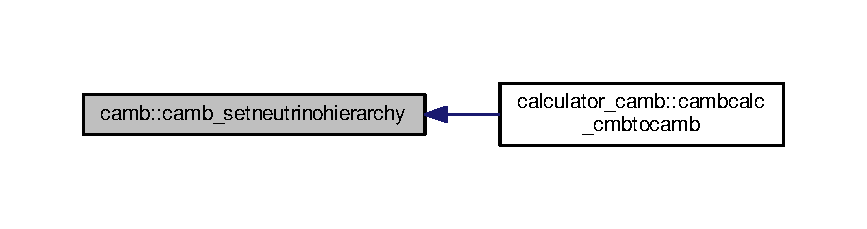
\includegraphics[width=350pt]{namespacecamb_ad303911c183f5affcdc9665c5facdd4b_icgraph}
\end{center}
\end{figure}
\mbox{\Hypertarget{namespacecamb_a9fb2095034057d44dc9526dd02d60064}\label{namespacecamb_a9fb2095034057d44dc9526dd02d60064}} 
\index{camb@{camb}!camb\+\_\+transferstopowers@{camb\+\_\+transferstopowers}}
\index{camb\+\_\+transferstopowers@{camb\+\_\+transferstopowers}!camb@{camb}}
\subsubsection{\texorpdfstring{camb\+\_\+transferstopowers()}{camb\_transferstopowers()}}
{\footnotesize\ttfamily subroutine camb\+::camb\+\_\+transferstopowers (\begin{DoxyParamCaption}\item[{type (\mbox{\hyperlink{structcamb_1_1cambdata}{cambdata}})}]{C\+Data }\end{DoxyParamCaption})}



References cambmain\+::cltransfertocl(), modelparams\+::cp, initialpower\+::initializepowers(), lensing\+::lens\+\_\+cls(), and transfer\+::transfer\+\_\+get\+\_\+sigmas().



Referenced by calculator\+\_\+camb\+::cambcalc\+\_\+getnewpowerdata(), and calculator\+\_\+camb\+::cambcalc\+\_\+gettheoryforimportance().

Here is the call graph for this function\+:
\nopagebreak
\begin{figure}[H]
\begin{center}
\leavevmode
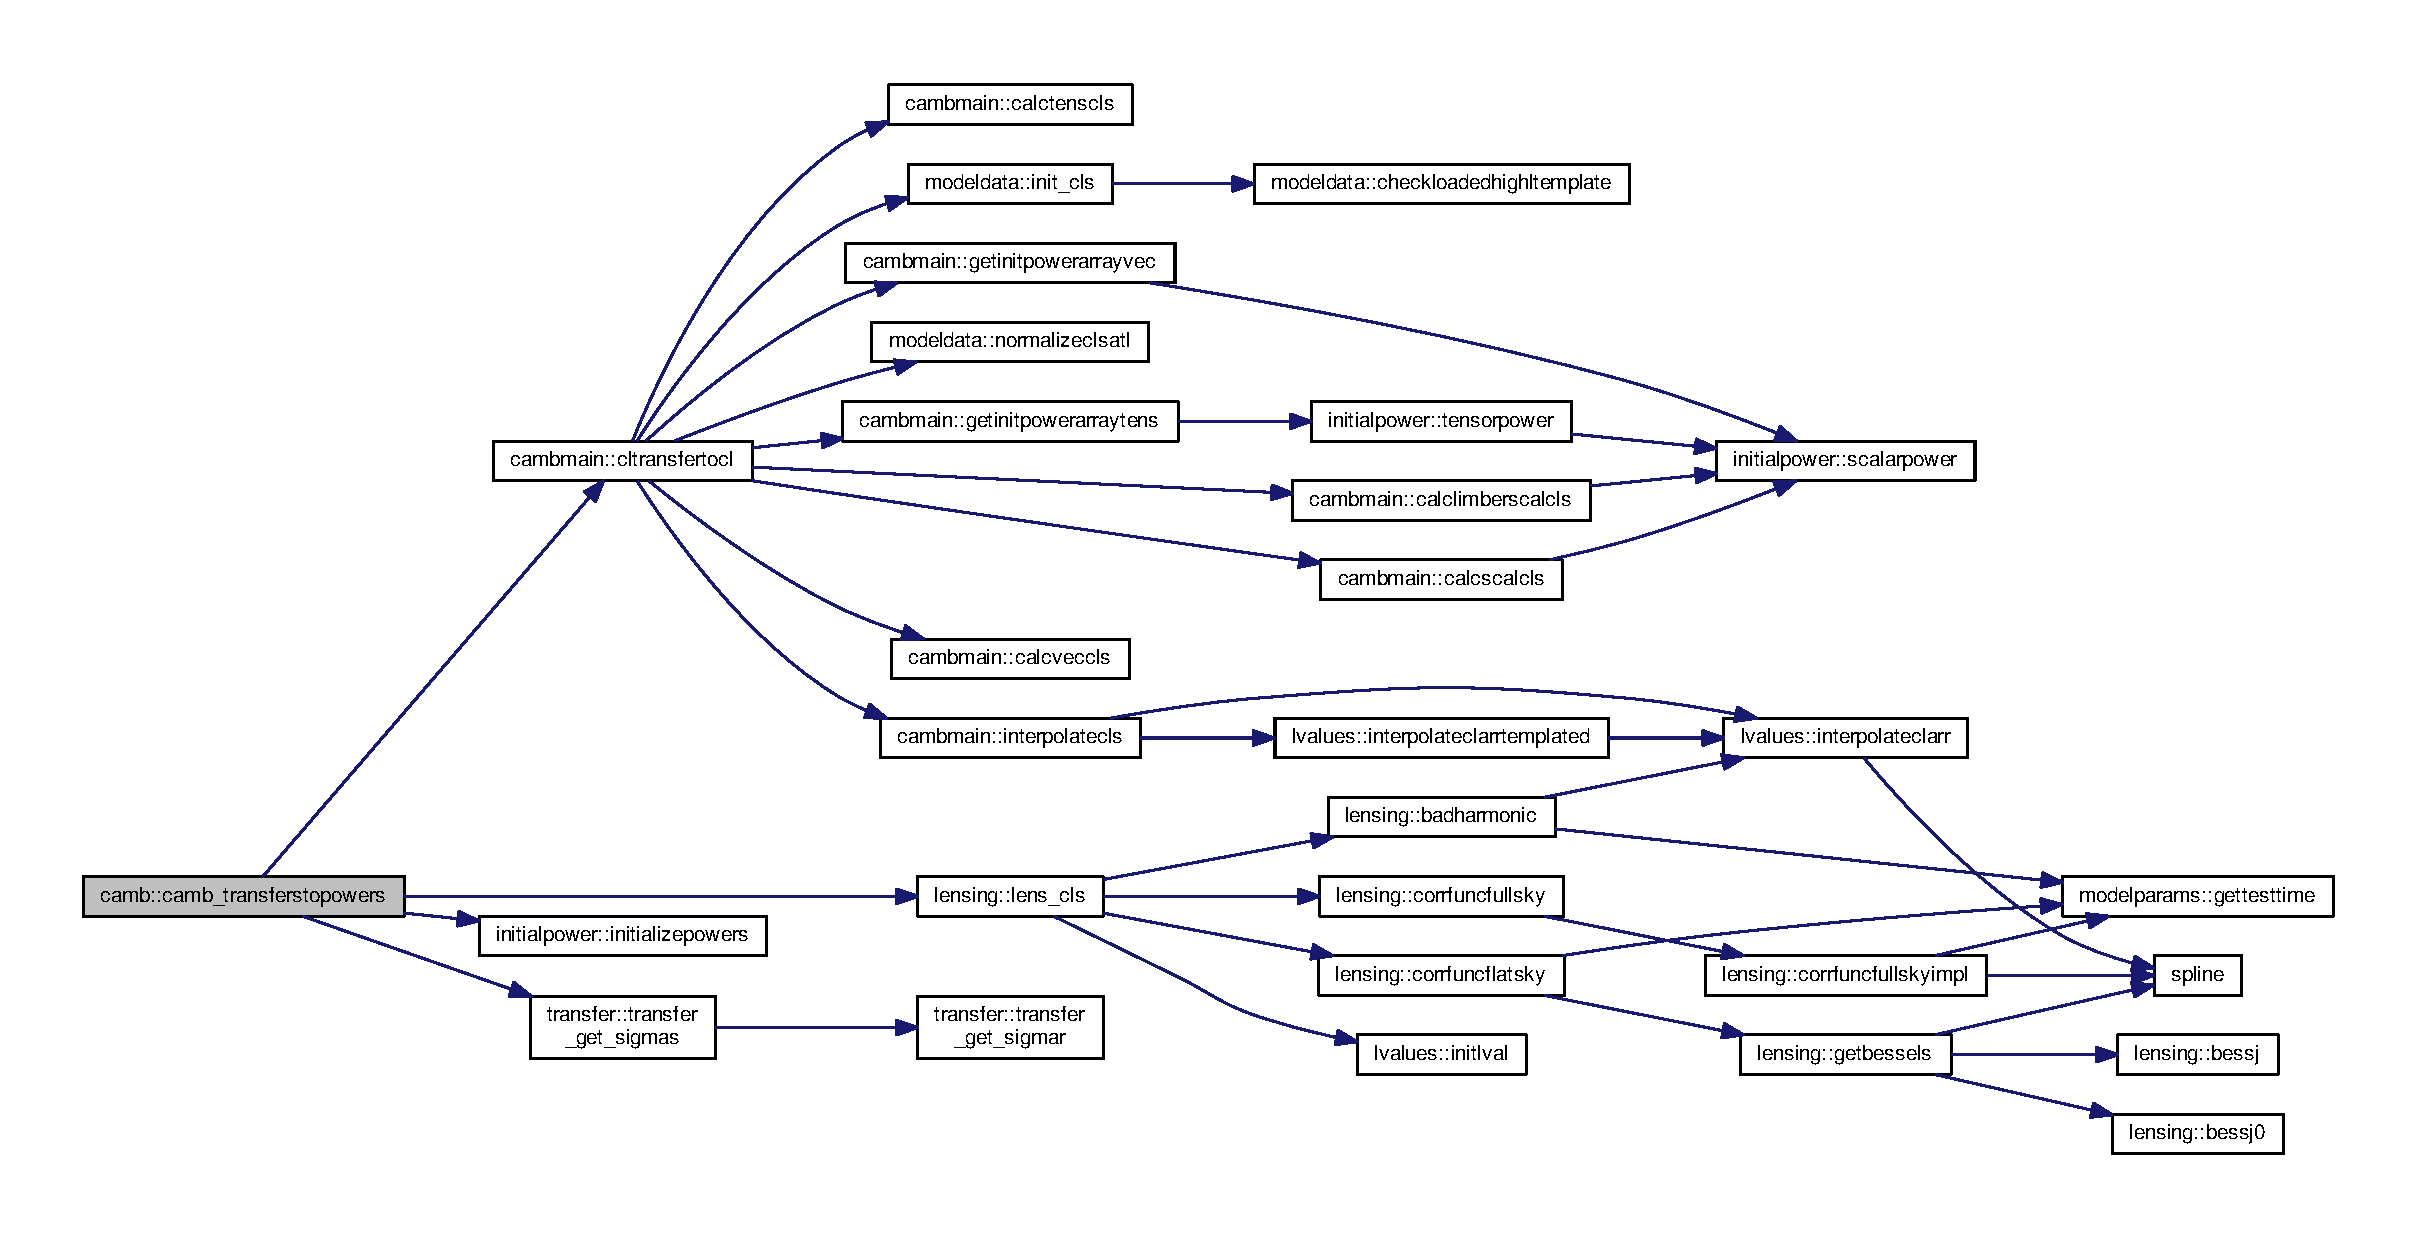
\includegraphics[width=350pt]{namespacecamb_a9fb2095034057d44dc9526dd02d60064_cgraph}
\end{center}
\end{figure}
Here is the caller graph for this function\+:
\nopagebreak
\begin{figure}[H]
\begin{center}
\leavevmode
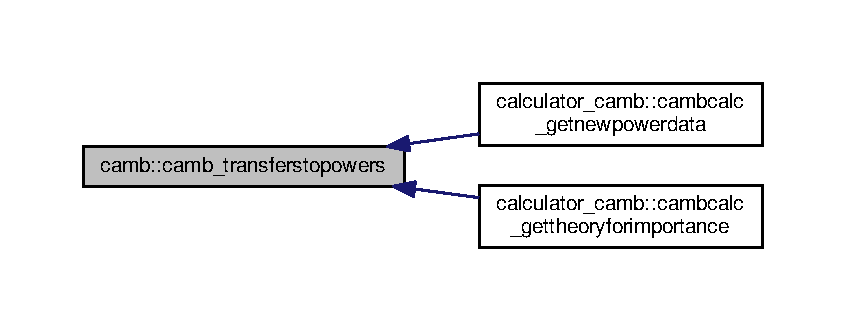
\includegraphics[width=350pt]{namespacecamb_a9fb2095034057d44dc9526dd02d60064_icgraph}
\end{center}
\end{figure}
\mbox{\Hypertarget{namespacecamb_ae9577b86a4f0803e5754a23871a7113e}\label{namespacecamb_ae9577b86a4f0803e5754a23871a7113e}} 
\index{camb@{camb}!camb\+\_\+validateparams@{camb\+\_\+validateparams}}
\index{camb\+\_\+validateparams@{camb\+\_\+validateparams}!camb@{camb}}
\subsubsection{\texorpdfstring{camb\+\_\+validateparams()}{camb\_validateparams()}}
{\footnotesize\ttfamily logical function camb\+::camb\+\_\+validateparams (\begin{DoxyParamCaption}\item[{type(cambparams), intent(in)}]{P }\end{DoxyParamCaption})}



References modelparams\+::max\+\_\+transfer\+\_\+redshifts, initialpower\+::p, recombination\+::recombination\+\_\+validate(), and reionization\+::reionization\+\_\+validate().

Here is the call graph for this function\+:
\nopagebreak
\begin{figure}[H]
\begin{center}
\leavevmode
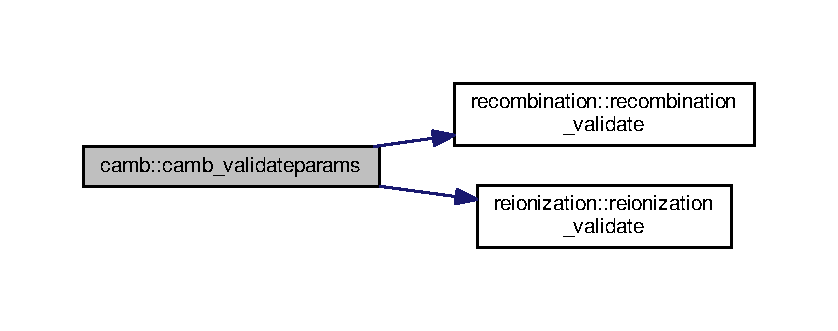
\includegraphics[width=350pt]{namespacecamb_ae9577b86a4f0803e5754a23871a7113e_cgraph}
\end{center}
\end{figure}


\subsection{Variable Documentation}
\mbox{\Hypertarget{namespacecamb_a85cc16a2fbdb270667e7303f2290c3be}\label{namespacecamb_a85cc16a2fbdb270667e7303f2290c3be}} 
\index{camb@{camb}!\+\_\+\+\_\+author\+\_\+\+\_\+@{\+\_\+\+\_\+author\+\_\+\+\_\+}}
\index{\+\_\+\+\_\+author\+\_\+\+\_\+@{\+\_\+\+\_\+author\+\_\+\+\_\+}!camb@{camb}}
\subsubsection{\texorpdfstring{\+\_\+\+\_\+author\+\_\+\+\_\+}{\_\_author\_\_}}
{\footnotesize\ttfamily string camb.\+\_\+\+\_\+author\+\_\+\+\_\+ = \char`\"{}Antony Lewis\char`\"{}\hspace{0.3cm}{\ttfamily [private]}}

\mbox{\Hypertarget{namespacecamb_af9e02319cf919d4505eab8b37179c712}\label{namespacecamb_af9e02319cf919d4505eab8b37179c712}} 
\index{camb@{camb}!\+\_\+\+\_\+contact\+\_\+\+\_\+@{\+\_\+\+\_\+contact\+\_\+\+\_\+}}
\index{\+\_\+\+\_\+contact\+\_\+\+\_\+@{\+\_\+\+\_\+contact\+\_\+\+\_\+}!camb@{camb}}
\subsubsection{\texorpdfstring{\+\_\+\+\_\+contact\+\_\+\+\_\+}{\_\_contact\_\_}}
{\footnotesize\ttfamily string camb.\+\_\+\+\_\+contact\+\_\+\+\_\+ = \char`\"{}antony at cosmologist dot info\char`\"{}\hspace{0.3cm}{\ttfamily [private]}}

\mbox{\Hypertarget{namespacecamb_aa9d4ea4f20e0977e7d5f5dc20b8debd6}\label{namespacecamb_aa9d4ea4f20e0977e7d5f5dc20b8debd6}} 
\index{camb@{camb}!\+\_\+\+\_\+status\+\_\+\+\_\+@{\+\_\+\+\_\+status\+\_\+\+\_\+}}
\index{\+\_\+\+\_\+status\+\_\+\+\_\+@{\+\_\+\+\_\+status\+\_\+\+\_\+}!camb@{camb}}
\subsubsection{\texorpdfstring{\+\_\+\+\_\+status\+\_\+\+\_\+}{\_\_status\_\_}}
{\footnotesize\ttfamily string camb.\+\_\+\+\_\+status\+\_\+\+\_\+ = \char`\"{}beta\char`\"{}\hspace{0.3cm}{\ttfamily [private]}}

\mbox{\Hypertarget{namespacecamb_a68e3f34837e39bb6f7e725612e4627fa}\label{namespacecamb_a68e3f34837e39bb6f7e725612e4627fa}} 
\index{camb@{camb}!\+\_\+\+\_\+version\+\_\+\+\_\+@{\+\_\+\+\_\+version\+\_\+\+\_\+}}
\index{\+\_\+\+\_\+version\+\_\+\+\_\+@{\+\_\+\+\_\+version\+\_\+\+\_\+}!camb@{camb}}
\subsubsection{\texorpdfstring{\+\_\+\+\_\+version\+\_\+\+\_\+}{\_\_version\_\_}}
{\footnotesize\ttfamily string camb.\+\_\+\+\_\+version\+\_\+\+\_\+ = \char`\"{}0.\+1.\+3\char`\"{}\hspace{0.3cm}{\ttfamily [private]}}

\mbox{\Hypertarget{namespacecamb_af98223967f3787053d42644a1ae6f785}\label{namespacecamb_af98223967f3787053d42644a1ae6f785}} 
\index{camb@{camb}!Do\+Tensor\+Neutrinos@{Do\+Tensor\+Neutrinos}}
\index{Do\+Tensor\+Neutrinos@{Do\+Tensor\+Neutrinos}!camb@{camb}}
\subsubsection{\texorpdfstring{Do\+Tensor\+Neutrinos}{DoTensorNeutrinos}}
{\footnotesize\ttfamily camb.\+Do\+Tensor\+Neutrinos = dll\+\_\+import(c\+\_\+bool, \char`\"{}gaugeinterface\char`\"{}, \char`\"{}dotensorneutrinos\char`\"{})}

\mbox{\Hypertarget{namespacecamb_a61a5837f54fb09c486d29171a8651a91}\label{namespacecamb_a61a5837f54fb09c486d29171a8651a91}} 
\index{camb@{camb}!Magnetic@{Magnetic}}
\index{Magnetic@{Magnetic}!camb@{camb}}
\subsubsection{\texorpdfstring{Magnetic}{Magnetic}}
{\footnotesize\ttfamily camb.\+Magnetic = dll\+\_\+import(c\+\_\+double, \char`\"{}gaugeinterface\char`\"{}, \char`\"{}magnetic\char`\"{})}

\mbox{\Hypertarget{namespacecamb_a8dcf37e78d4e08b70f90002000e746b8}\label{namespacecamb_a8dcf37e78d4e08b70f90002000e746b8}} 
\index{camb@{camb}!Thread\+Num@{Thread\+Num}}
\index{Thread\+Num@{Thread\+Num}!camb@{camb}}
\subsubsection{\texorpdfstring{Thread\+Num}{ThreadNum}}
{\footnotesize\ttfamily camb.\+Thread\+Num = dll\+\_\+import(c\+\_\+int, \char`\"{}modelparams\char`\"{}, \char`\"{}threadnum\char`\"{})}

\mbox{\Hypertarget{namespacecamb_a2e33f06925cf79f62b6d07d7c737217c}\label{namespacecamb_a2e33f06925cf79f62b6d07d7c737217c}} 
\index{camb@{camb}!vec\+\_\+sig0@{vec\+\_\+sig0}}
\index{vec\+\_\+sig0@{vec\+\_\+sig0}!camb@{camb}}
\subsubsection{\texorpdfstring{vec\+\_\+sig0}{vec\_sig0}}
{\footnotesize\ttfamily camb.\+vec\+\_\+sig0 = dll\+\_\+import(c\+\_\+double, \char`\"{}gaugeinterface\char`\"{}, \char`\"{}vec\+\_\+sig0\char`\"{})}


\hypertarget{namespacecamb_1_1baseconfig}{}\section{camb.\+baseconfig Namespace Reference}
\label{namespacecamb_1_1baseconfig}\index{camb.\+baseconfig@{camb.\+baseconfig}}
\subsection*{Classes}
\begin{DoxyCompactItemize}
\item 
class \mbox{\hyperlink{classcamb_1_1baseconfig_1_1CAMB__Structure}{C\+A\+M\+B\+\_\+\+Structure}}
\item 
class \mbox{\hyperlink{classcamb_1_1baseconfig_1_1CAMBError}{C\+A\+M\+B\+Error}}
\item 
class \mbox{\hyperlink{classcamb_1_1baseconfig_1_1ifort__gfortran__loader}{ifort\+\_\+gfortran\+\_\+loader}}
\item 
class \mbox{\hyperlink{classcamb_1_1baseconfig_1_1Mock}{Mock}}
\end{DoxyCompactItemize}
\subsection*{Functions}
\begin{DoxyCompactItemize}
\item 
def \mbox{\hyperlink{namespacecamb_1_1baseconfig_a9b1d79118c94ceaefe44393d881c3956}{dll\+\_\+import}} (tp, module, func)
\item 
def \mbox{\hyperlink{namespacecamb_1_1baseconfig_ab9ccfd74eee84e46eb5061d9397e368a}{set\+\_\+filelocs}} ()
\end{DoxyCompactItemize}
\subsection*{Variables}
\begin{DoxyCompactItemize}
\item 
\mbox{\hyperlink{namespacecamb_1_1baseconfig_ae8f1ea2a46e79a477468b0fd2d177a99}{B\+A\+S\+E\+D\+IR}} = osp.\+abspath(osp.\+dirname(\+\_\+\+\_\+file\+\_\+\+\_\+))
\item 
string \mbox{\hyperlink{namespacecamb_1_1baseconfig_ad89a604599cedf48442529187fef9c80}{D\+L\+L\+N\+A\+ME}} = \textquotesingle{}cambdll.\+dll\textquotesingle{}
\item 
\mbox{\hyperlink{namespacecamb_1_1baseconfig_a1607a579d676f0ac85591b4682448c59}{C\+A\+M\+BL}} = osp.\+join(\mbox{\hyperlink{namespacecamb_1_1baseconfig_ae8f1ea2a46e79a477468b0fd2d177a99}{B\+A\+S\+E\+D\+IR}}, \mbox{\hyperlink{namespacecamb_1_1baseconfig_ad89a604599cedf48442529187fef9c80}{D\+L\+L\+N\+A\+ME}})
\item 
\mbox{\hyperlink{namespacecamb_1_1baseconfig_a7929d68edfa88d189f12fd1c25f0448f}{mock\+\_\+load}} = os.\+environ.\+get(\textquotesingle{}R\+E\+A\+D\+T\+H\+E\+D\+O\+CS\textquotesingle{}, None)
\item 
\mbox{\hyperlink{namespacecamb_1_1baseconfig_a358d9edf830d88f0b129ba636e49a077}{camblib}} = ctypes.\+Library\+Loader(\mbox{\hyperlink{classcamb_1_1baseconfig_1_1ifort__gfortran__loader}{ifort\+\_\+gfortran\+\_\+loader}}).Load\+Library(\mbox{\hyperlink{namespacecamb_1_1baseconfig_a1607a579d676f0ac85591b4682448c59}{C\+A\+M\+BL}})
\item 
\mbox{\hyperlink{namespacecamb_1_1baseconfig_ad1eeb57f2c324b0a0486fa69bea1088e}{M\+O\+C\+K\+\_\+\+M\+O\+D\+U\+L\+ES}}
\item 
\mbox{\hyperlink{namespacecamb_1_1baseconfig_ac76caa9250c766ee3239467a4e1b817f}{Structure}} = object
\end{DoxyCompactItemize}


\subsection{Function Documentation}
\mbox{\Hypertarget{namespacecamb_1_1baseconfig_a9b1d79118c94ceaefe44393d881c3956}\label{namespacecamb_1_1baseconfig_a9b1d79118c94ceaefe44393d881c3956}} 
\index{camb\+::baseconfig@{camb\+::baseconfig}!dll\+\_\+import@{dll\+\_\+import}}
\index{dll\+\_\+import@{dll\+\_\+import}!camb\+::baseconfig@{camb\+::baseconfig}}
\subsubsection{\texorpdfstring{dll\+\_\+import()}{dll\_import()}}
{\footnotesize\ttfamily def camb.\+baseconfig.\+dll\+\_\+import (\begin{DoxyParamCaption}\item[{}]{tp,  }\item[{}]{module,  }\item[{}]{func }\end{DoxyParamCaption})}



Referenced by camb.\+model.\+C\+A\+M\+Bparams.\+set\+\_\+dark\+\_\+energy().

Here is the caller graph for this function\+:
\nopagebreak
\begin{figure}[H]
\begin{center}
\leavevmode
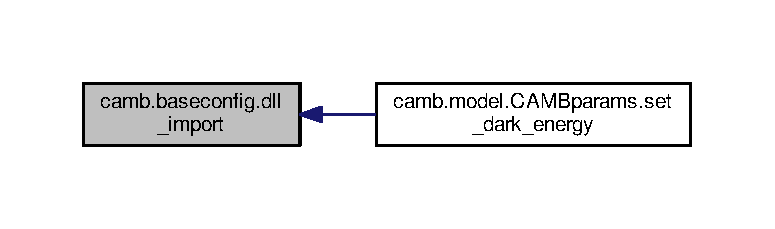
\includegraphics[width=350pt]{namespacecamb_1_1baseconfig_a9b1d79118c94ceaefe44393d881c3956_icgraph}
\end{center}
\end{figure}
\mbox{\Hypertarget{namespacecamb_1_1baseconfig_ab9ccfd74eee84e46eb5061d9397e368a}\label{namespacecamb_1_1baseconfig_ab9ccfd74eee84e46eb5061d9397e368a}} 
\index{camb\+::baseconfig@{camb\+::baseconfig}!set\+\_\+filelocs@{set\+\_\+filelocs}}
\index{set\+\_\+filelocs@{set\+\_\+filelocs}!camb\+::baseconfig@{camb\+::baseconfig}}
\subsubsection{\texorpdfstring{set\+\_\+filelocs()}{set\_filelocs()}}
{\footnotesize\ttfamily def camb.\+baseconfig.\+set\+\_\+filelocs (\begin{DoxyParamCaption}{ }\end{DoxyParamCaption})}



References interpolationtests.\+func().

Here is the call graph for this function\+:
\nopagebreak
\begin{figure}[H]
\begin{center}
\leavevmode
\includegraphics[width=316pt]{namespacecamb_1_1baseconfig_ab9ccfd74eee84e46eb5061d9397e368a_cgraph}
\end{center}
\end{figure}


\subsection{Variable Documentation}
\mbox{\Hypertarget{namespacecamb_1_1baseconfig_ae8f1ea2a46e79a477468b0fd2d177a99}\label{namespacecamb_1_1baseconfig_ae8f1ea2a46e79a477468b0fd2d177a99}} 
\index{camb\+::baseconfig@{camb\+::baseconfig}!B\+A\+S\+E\+D\+IR@{B\+A\+S\+E\+D\+IR}}
\index{B\+A\+S\+E\+D\+IR@{B\+A\+S\+E\+D\+IR}!camb\+::baseconfig@{camb\+::baseconfig}}
\subsubsection{\texorpdfstring{B\+A\+S\+E\+D\+IR}{BASEDIR}}
{\footnotesize\ttfamily camb.\+baseconfig.\+B\+A\+S\+E\+D\+IR = osp.\+abspath(osp.\+dirname(\+\_\+\+\_\+file\+\_\+\+\_\+))}

\mbox{\Hypertarget{namespacecamb_1_1baseconfig_a1607a579d676f0ac85591b4682448c59}\label{namespacecamb_1_1baseconfig_a1607a579d676f0ac85591b4682448c59}} 
\index{camb\+::baseconfig@{camb\+::baseconfig}!C\+A\+M\+BL@{C\+A\+M\+BL}}
\index{C\+A\+M\+BL@{C\+A\+M\+BL}!camb\+::baseconfig@{camb\+::baseconfig}}
\subsubsection{\texorpdfstring{C\+A\+M\+BL}{CAMBL}}
{\footnotesize\ttfamily camb.\+baseconfig.\+C\+A\+M\+BL = osp.\+join(\mbox{\hyperlink{namespacecamb_1_1baseconfig_ae8f1ea2a46e79a477468b0fd2d177a99}{B\+A\+S\+E\+D\+IR}}, \mbox{\hyperlink{namespacecamb_1_1baseconfig_ad89a604599cedf48442529187fef9c80}{D\+L\+L\+N\+A\+ME}})}

\mbox{\Hypertarget{namespacecamb_1_1baseconfig_a358d9edf830d88f0b129ba636e49a077}\label{namespacecamb_1_1baseconfig_a358d9edf830d88f0b129ba636e49a077}} 
\index{camb\+::baseconfig@{camb\+::baseconfig}!camblib@{camblib}}
\index{camblib@{camblib}!camb\+::baseconfig@{camb\+::baseconfig}}
\subsubsection{\texorpdfstring{camblib}{camblib}}
{\footnotesize\ttfamily camb.\+baseconfig.\+camblib = ctypes.\+Library\+Loader(\mbox{\hyperlink{classcamb_1_1baseconfig_1_1ifort__gfortran__loader}{ifort\+\_\+gfortran\+\_\+loader}}).Load\+Library(\mbox{\hyperlink{namespacecamb_1_1baseconfig_a1607a579d676f0ac85591b4682448c59}{C\+A\+M\+BL}})}

\mbox{\Hypertarget{namespacecamb_1_1baseconfig_ad89a604599cedf48442529187fef9c80}\label{namespacecamb_1_1baseconfig_ad89a604599cedf48442529187fef9c80}} 
\index{camb\+::baseconfig@{camb\+::baseconfig}!D\+L\+L\+N\+A\+ME@{D\+L\+L\+N\+A\+ME}}
\index{D\+L\+L\+N\+A\+ME@{D\+L\+L\+N\+A\+ME}!camb\+::baseconfig@{camb\+::baseconfig}}
\subsubsection{\texorpdfstring{D\+L\+L\+N\+A\+ME}{DLLNAME}}
{\footnotesize\ttfamily string camb.\+baseconfig.\+D\+L\+L\+N\+A\+ME = \textquotesingle{}cambdll.\+dll\textquotesingle{}}

\mbox{\Hypertarget{namespacecamb_1_1baseconfig_a7929d68edfa88d189f12fd1c25f0448f}\label{namespacecamb_1_1baseconfig_a7929d68edfa88d189f12fd1c25f0448f}} 
\index{camb\+::baseconfig@{camb\+::baseconfig}!mock\+\_\+load@{mock\+\_\+load}}
\index{mock\+\_\+load@{mock\+\_\+load}!camb\+::baseconfig@{camb\+::baseconfig}}
\subsubsection{\texorpdfstring{mock\+\_\+load}{mock\_load}}
{\footnotesize\ttfamily camb.\+baseconfig.\+mock\+\_\+load = os.\+environ.\+get(\textquotesingle{}R\+E\+A\+D\+T\+H\+E\+D\+O\+CS\textquotesingle{}, None)}

\mbox{\Hypertarget{namespacecamb_1_1baseconfig_ad1eeb57f2c324b0a0486fa69bea1088e}\label{namespacecamb_1_1baseconfig_ad1eeb57f2c324b0a0486fa69bea1088e}} 
\index{camb\+::baseconfig@{camb\+::baseconfig}!M\+O\+C\+K\+\_\+\+M\+O\+D\+U\+L\+ES@{M\+O\+C\+K\+\_\+\+M\+O\+D\+U\+L\+ES}}
\index{M\+O\+C\+K\+\_\+\+M\+O\+D\+U\+L\+ES@{M\+O\+C\+K\+\_\+\+M\+O\+D\+U\+L\+ES}!camb\+::baseconfig@{camb\+::baseconfig}}
\subsubsection{\texorpdfstring{M\+O\+C\+K\+\_\+\+M\+O\+D\+U\+L\+ES}{MOCK\_MODULES}}
{\footnotesize\ttfamily camb.\+baseconfig.\+M\+O\+C\+K\+\_\+\+M\+O\+D\+U\+L\+ES}

\mbox{\Hypertarget{namespacecamb_1_1baseconfig_ac76caa9250c766ee3239467a4e1b817f}\label{namespacecamb_1_1baseconfig_ac76caa9250c766ee3239467a4e1b817f}} 
\index{camb\+::baseconfig@{camb\+::baseconfig}!Structure@{Structure}}
\index{Structure@{Structure}!camb\+::baseconfig@{camb\+::baseconfig}}
\subsubsection{\texorpdfstring{Structure}{Structure}}
{\footnotesize\ttfamily camb.\+baseconfig.\+Structure = object}


\hypertarget{namespacecamb_1_1bbn}{}\section{camb.\+bbn Namespace Reference}
\label{namespacecamb_1_1bbn}\index{camb.\+bbn@{camb.\+bbn}}
\subsection*{Functions}
\begin{DoxyCompactItemize}
\item 
def \mbox{\hyperlink{namespacecamb_1_1bbn_a114f83bb5e17fd586485de562d04035e}{yhe\+\_\+to\+\_\+yp\+B\+BN}} (\mbox{\hyperlink{namespacecamb_1_1bbn_a64a4ad2532dcfaa25d7048a3f3f2992e}{Yp}})
\item 
def \mbox{\hyperlink{namespacecamb_1_1bbn_a9919c33355b5bbeee07634a0aa957b9a}{yp\+B\+B\+N\+\_\+to\+\_\+yhe}} (\mbox{\hyperlink{namespacecamb_1_1bbn_ab3d92f46f19b0025c2d5c6e26522b30c}{Y\+B\+BN}})
\item 
def \mbox{\hyperlink{namespacecamb_1_1bbn_ab4f0838cbe3e4c575ff31eaec11126c7}{yhe\+\_\+fit}} (omegab, dneff, taun)
\item 
def \mbox{\hyperlink{namespacecamb_1_1bbn_a631c65a5e52fd772fd227d7017dccf34}{dh\+\_\+fit}} (omegab, dneff, taun)
\item 
def \mbox{\hyperlink{namespacecamb_1_1bbn_ae39e69c7217dc7635429e776f01fde55}{run\+B\+BN}} (\mbox{\hyperlink{namespacecamb_1_1bbn_acbc137606c793f20e1ded220bbfab367}{eta}}, DeltaN=0, tau=\mbox{\hyperlink{namespacecamb_1_1bbn_ae95abe1177100ca3b8cfb59cf9e379be}{tau\+\_\+n}}, prog=\textquotesingle{}./\mbox{\hyperlink{plotTT_8m_a9336ebf25087d91c818ee6e9ec29f8c1}{alter\+\_\+etannutau.\+x}}\textquotesingle{})
\item 
def \mbox{\hyperlink{namespacecamb_1_1bbn_ad29937c86c274eada16f48fc3c2e3727}{yp\+B\+B\+N\+\_\+\+Parthenope}} (omegab, neff)
\item 
def \mbox{\hyperlink{namespacecamb_1_1bbn_a0fba7f6a46bfb06711a39350bcfe238f}{yhe\+\_\+to\+\_\+yp\+B\+BN}} (\mbox{\hyperlink{namespacecamb_1_1bbn_a64a4ad2532dcfaa25d7048a3f3f2992e}{Yp}}, ombh2)
\item 
def \mbox{\hyperlink{namespacecamb_1_1bbn_ab478fa803bc42b27cc92d291785174c5}{run\+B\+B\+Nplot}} ()
\end{DoxyCompactItemize}
\subsection*{Variables}
\begin{DoxyCompactItemize}
\item 
float \mbox{\hyperlink{namespacecamb_1_1bbn_a5b708814b666163b312ae9d46c458a40}{hbar}} = 1.\+05457e-\/34
\item 
int \mbox{\hyperlink{namespacecamb_1_1bbn_a679cc6941c03606fb81846de0595bbf0}{c}} = 299792458.
\item 
float \mbox{\hyperlink{namespacecamb_1_1bbn_acf1e58cf8bb0a963cdea5d6d5c8a7965}{kB}} = 1.\+380650e-\/23
\item 
float \mbox{\hyperlink{namespacecamb_1_1bbn_ab7d9516327d53209dc68ed04b575b942}{MeV}} = 1.\+6021764e-\/13
\item 
float \mbox{\hyperlink{namespacecamb_1_1bbn_adb3c70534be507b9680c975ad6c2ada1}{eV}} = \mbox{\hyperlink{namespacecamb_1_1bbn_ab7d9516327d53209dc68ed04b575b942}{MeV}} / 1e6
\item 
float \mbox{\hyperlink{namespacecamb_1_1bbn_a516a8888d6d387c64db5a92882e60839}{G}} = 6.\+6738e-\/11
\item 
float \mbox{\hyperlink{namespacecamb_1_1bbn_ada23f3dc20ced1c849a9c6885f34db92}{T\+C\+MB}} = 2.\+7255
\item 
\mbox{\hyperlink{namespacecamb_1_1bbn_a96c42bdaca47fcfad93e6567839f017b}{mP}} = np.\+sqrt(\mbox{\hyperlink{namespacecamb_1_1bbn_a5b708814b666163b312ae9d46c458a40}{hbar}} $\ast$ \mbox{\hyperlink{namespacecamb_1_1bbn_a679cc6941c03606fb81846de0595bbf0}{c}} / \mbox{\hyperlink{namespacecamb_1_1bbn_a516a8888d6d387c64db5a92882e60839}{G}})
\item 
float \mbox{\hyperlink{namespacecamb_1_1bbn_ad4577440de870759161fbb421dcfe786}{Mpc}} = 3.\+0856776e22
\item 
float \mbox{\hyperlink{namespacecamb_1_1bbn_a91eae46cae8d4e10d04c05b5f8324278}{m\+\_\+proton}} = 1.\+672621637e-\/27
\item 
float \mbox{\hyperlink{namespacecamb_1_1bbn_aa3780f95e3d1ace78bfe399ae081a621}{m\+\_\+H}} = 1.\+673575e-\/27
\item 
float \mbox{\hyperlink{namespacecamb_1_1bbn_a55010dc4504208bd6bf60957271700c4}{not4}} = 3.\+9715
\item 
float \mbox{\hyperlink{namespacecamb_1_1bbn_addcae6f33c5419e66f9ae3006383c347}{m\+\_\+\+He}} = \mbox{\hyperlink{namespacecamb_1_1bbn_aa3780f95e3d1ace78bfe399ae081a621}{m\+\_\+H}} $\ast$ \mbox{\hyperlink{namespacecamb_1_1bbn_a55010dc4504208bd6bf60957271700c4}{not4}}
\item 
float \mbox{\hyperlink{namespacecamb_1_1bbn_a484a30a2544ce82886fb2fe6860cc65c}{zeta3}} = 1.\+202056903
\item 
float \mbox{\hyperlink{namespacecamb_1_1bbn_ae95abe1177100ca3b8cfb59cf9e379be}{tau\+\_\+n}} = 880.\+3
\item 
tuple \mbox{\hyperlink{namespacecamb_1_1bbn_aa1b409ea1a7b5f583772b3f5cc174be0}{n\+\_\+photon}} = (\mbox{\hyperlink{namespacecamb_1_1bbn_acf1e58cf8bb0a963cdea5d6d5c8a7965}{kB}} $\ast$ \mbox{\hyperlink{namespacecamb_1_1bbn_ada23f3dc20ced1c849a9c6885f34db92}{T\+C\+MB}} / \mbox{\hyperlink{namespacecamb_1_1bbn_a5b708814b666163b312ae9d46c458a40}{hbar}} / \mbox{\hyperlink{namespacecamb_1_1bbn_a679cc6941c03606fb81846de0595bbf0}{c}}) $\ast$$\ast$ 3 $\ast$ \mbox{\hyperlink{namespacecamb_1_1bbn_a484a30a2544ce82886fb2fe6860cc65c}{zeta3}} $\ast$ 2 / np.\+pi $\ast$$\ast$ 2
\item 
tuple \mbox{\hyperlink{namespacecamb_1_1bbn_a9366441db17c0ca60e0fa48f8a8d796c}{omegafac}} = (1e5 / Mpc) $\ast$$\ast$ 2 / (8 $\ast$ np.\+pi $\ast$ G) $\ast$ 3
\item 
bool \mbox{\hyperlink{namespacecamb_1_1bbn_ae20f3b2b5c14d3eca9a605dae38f925c}{alter\+B\+BN}} = False
\item 
\mbox{\hyperlink{namespacecamb_1_1bbn_ac4e809a6c935e14eddb8e95f83b83c00}{ombh2s}}
\item 
list \mbox{\hyperlink{namespacecamb_1_1bbn_a2d30a7a9ec202c2f72d1fa5d58aa1cb5}{Delta\+Ns}} = \mbox{[}-\/3, -\/2, -\/1, -\/0.\+5, 0, 0.\+5, 1, 2, 3, 4, 5, 6, 7\mbox{]}
\item 
list \mbox{\hyperlink{namespacecamb_1_1bbn_a195010e01b08cf509c7b7c8519ea47d9}{lines}} = \mbox{[}$\,$\mbox{]}
\item 
float \mbox{\hyperlink{namespacecamb_1_1bbn_ace4721f676cd3090adcf649ff5eb439d}{Yp\+\_\+fid}} = 0.\+2;
\item 
tuple \mbox{\hyperlink{namespacecamb_1_1bbn_ab5c5cbf9f645a4f423e0b8fdaba3c869}{rho\+\_\+b}} = ombh2 $\ast$ \mbox{\hyperlink{namespacecamb_1_1bbn_a9366441db17c0ca60e0fa48f8a8d796c}{omegafac}};
\item 
def \mbox{\hyperlink{namespacecamb_1_1bbn_ab3d92f46f19b0025c2d5c6e26522b30c}{Y\+B\+BN}} = \mbox{\hyperlink{namespacecamb_1_1bbn_ab4f0838cbe3e4c575ff31eaec11126c7}{yhe\+\_\+fit}}(ombh2, DeltaN, \mbox{\hyperlink{namespacecamb_1_1bbn_ae95abe1177100ca3b8cfb59cf9e379be}{tau\+\_\+n}})
\item 
tuple \mbox{\hyperlink{namespacecamb_1_1bbn_a6c667fa779cc99916a01199319f7757f}{n\+\_\+baryon}} = (4 $\ast$ \mbox{\hyperlink{namespacecamb_1_1bbn_ace4721f676cd3090adcf649ff5eb439d}{Yp\+\_\+fid}} / \mbox{\hyperlink{namespacecamb_1_1bbn_addcae6f33c5419e66f9ae3006383c347}{m\+\_\+\+He}} + (1 -\/ \mbox{\hyperlink{namespacecamb_1_1bbn_ace4721f676cd3090adcf649ff5eb439d}{Yp\+\_\+fid}}) / \mbox{\hyperlink{namespacecamb_1_1bbn_aa3780f95e3d1ace78bfe399ae081a621}{m\+\_\+H}}) $\ast$ \mbox{\hyperlink{namespacecamb_1_1bbn_ab5c5cbf9f645a4f423e0b8fdaba3c869}{rho\+\_\+b}}
\item 
tuple \mbox{\hyperlink{namespacecamb_1_1bbn_acbc137606c793f20e1ded220bbfab367}{eta}} = \mbox{\hyperlink{namespacecamb_1_1bbn_a6c667fa779cc99916a01199319f7757f}{n\+\_\+baryon}} / \mbox{\hyperlink{namespacecamb_1_1bbn_aa1b409ea1a7b5f583772b3f5cc174be0}{n\+\_\+photon}}
\item 
def \mbox{\hyperlink{namespacecamb_1_1bbn_ab579d745a27c53450178023e68108ed0}{outtxt}} = \mbox{\hyperlink{namespacecamb_1_1bbn_ae39e69c7217dc7635429e776f01fde55}{run\+B\+BN}}(\mbox{\hyperlink{namespacecamb_1_1bbn_acbc137606c793f20e1ded220bbfab367}{eta}}, DeltaN)
\item 
\mbox{\hyperlink{namespacecamb_1_1bbn_a14c1aca700dca106cc95088e75fbb0bf}{D}} = \mbox{\hyperlink{namespacecamb_1_1bbn_a631c65a5e52fd772fd227d7017dccf34}{dh\+\_\+fit}}(ombh2, DeltaN, \mbox{\hyperlink{namespacecamb_1_1bbn_ae95abe1177100ca3b8cfb59cf9e379be}{tau\+\_\+n}}) $\ast$ 1e-\/5
\item 
\mbox{\hyperlink{namespacecamb_1_1bbn_a513689c0c08c2cda69440b7240cf90f4}{He3}}
\item 
\mbox{\hyperlink{namespacecamb_1_1bbn_aa600356f7928685d8dc58ae9280ae9b7}{Li7}}
\item 
\mbox{\hyperlink{namespacecamb_1_1bbn_a1a9ed297165f45661cd679725e85e9b2}{Li6}}
\item 
\mbox{\hyperlink{namespacecamb_1_1bbn_a9f11f11ecaabe89c8896dc10706dbe3a}{Be7}}
\item 
\mbox{\hyperlink{namespacecamb_1_1bbn_a7cd1b4424d31d93c32450a6985bc25e3}{sig\+Y\+B\+BN}} = 0.\+0003
\item 
\mbox{\hyperlink{namespacecamb_1_1bbn_a2d43bde0f446912ff772618bc1d6df09}{sigdD}} = 6e-\/7
\item 
\mbox{\hyperlink{namespacecamb_1_1bbn_abd9d74bd5fea6bb16b07d5dc2cf54765}{sig\+He3}}
\item 
\mbox{\hyperlink{namespacecamb_1_1bbn_a19263e9024e7180211148959c414e77e}{sig\+Li7}}
\item 
\mbox{\hyperlink{namespacecamb_1_1bbn_a48da31b07841d506e177badd5494a83b}{sig\+Li6}}
\item 
\mbox{\hyperlink{namespacecamb_1_1bbn_ad6519fdb6fb650d987dcfd0aaf82d0da}{sig\+Be7}}
\item 
tuple \mbox{\hyperlink{namespacecamb_1_1bbn_a577a98b4b1732e27cc2e09844a6fe2ee}{actual\+\_\+ombh2}} = \mbox{\hyperlink{namespacecamb_1_1bbn_acbc137606c793f20e1ded220bbfab367}{eta}} $\ast$ \mbox{\hyperlink{namespacecamb_1_1bbn_aa1b409ea1a7b5f583772b3f5cc174be0}{n\+\_\+photon}} $\ast$ (\mbox{\hyperlink{namespacecamb_1_1bbn_ab3d92f46f19b0025c2d5c6e26522b30c}{Y\+B\+BN}} $\ast$ \mbox{\hyperlink{namespacecamb_1_1bbn_addcae6f33c5419e66f9ae3006383c347}{m\+\_\+\+He}} / 4 + (1 -\/ \mbox{\hyperlink{namespacecamb_1_1bbn_ab3d92f46f19b0025c2d5c6e26522b30c}{Y\+B\+BN}}) $\ast$ \mbox{\hyperlink{namespacecamb_1_1bbn_aa3780f95e3d1ace78bfe399ae081a621}{m\+\_\+H}}) / \mbox{\hyperlink{namespacecamb_1_1bbn_a9366441db17c0ca60e0fa48f8a8d796c}{omegafac}}
\item 
tuple \mbox{\hyperlink{namespacecamb_1_1bbn_a64a4ad2532dcfaa25d7048a3f3f2992e}{Yp}} = (\mbox{\hyperlink{namespacecamb_1_1bbn_acbc137606c793f20e1ded220bbfab367}{eta}} $\ast$ \mbox{\hyperlink{namespacecamb_1_1bbn_aa1b409ea1a7b5f583772b3f5cc174be0}{n\+\_\+photon}} / \mbox{\hyperlink{namespacecamb_1_1bbn_a577a98b4b1732e27cc2e09844a6fe2ee}{actual\+\_\+ombh2}} / \mbox{\hyperlink{namespacecamb_1_1bbn_a9366441db17c0ca60e0fa48f8a8d796c}{omegafac}} -\/ 1 / \mbox{\hyperlink{namespacecamb_1_1bbn_aa3780f95e3d1ace78bfe399ae081a621}{m\+\_\+H}}) / (4 / \mbox{\hyperlink{namespacecamb_1_1bbn_addcae6f33c5419e66f9ae3006383c347}{m\+\_\+\+He}} -\/ 1 / \mbox{\hyperlink{namespacecamb_1_1bbn_aa3780f95e3d1ace78bfe399ae081a621}{m\+\_\+H}})
\item 
tuple \mbox{\hyperlink{namespacecamb_1_1bbn_a53a5788b6b968e169939298088ecf0d7}{line}}
\item 
\mbox{\hyperlink{namespacecamb_1_1bbn_afa8615e8e051ca1f43e59371e94d4920}{f}} = open(\textquotesingle{}B\+B\+N\+\_\+full\+\_\+alter\+B\+B\+N\+\_\+\textquotesingle{} + str(\mbox{\hyperlink{namespacecamb_1_1bbn_ae95abe1177100ca3b8cfb59cf9e379be}{tau\+\_\+n}}) + \textquotesingle{}.dat\textquotesingle{}, \textquotesingle{}w\textquotesingle{})
\end{DoxyCompactItemize}


\subsection{Function Documentation}
\mbox{\Hypertarget{namespacecamb_1_1bbn_a631c65a5e52fd772fd227d7017dccf34}\label{namespacecamb_1_1bbn_a631c65a5e52fd772fd227d7017dccf34}} 
\index{camb\+::bbn@{camb\+::bbn}!dh\+\_\+fit@{dh\+\_\+fit}}
\index{dh\+\_\+fit@{dh\+\_\+fit}!camb\+::bbn@{camb\+::bbn}}
\subsubsection{\texorpdfstring{dh\+\_\+fit()}{dh\_fit()}}
{\footnotesize\ttfamily def camb.\+bbn.\+dh\+\_\+fit (\begin{DoxyParamCaption}\item[{}]{omegab,  }\item[{}]{dneff,  }\item[{}]{taun }\end{DoxyParamCaption})}

\mbox{\Hypertarget{namespacecamb_1_1bbn_ae39e69c7217dc7635429e776f01fde55}\label{namespacecamb_1_1bbn_ae39e69c7217dc7635429e776f01fde55}} 
\index{camb\+::bbn@{camb\+::bbn}!run\+B\+BN@{run\+B\+BN}}
\index{run\+B\+BN@{run\+B\+BN}!camb\+::bbn@{camb\+::bbn}}
\subsubsection{\texorpdfstring{run\+B\+B\+N()}{runBBN()}}
{\footnotesize\ttfamily def camb.\+bbn.\+run\+B\+BN (\begin{DoxyParamCaption}\item[{}]{eta,  }\item[{}]{DeltaN = {\ttfamily 0},  }\item[{}]{tau = {\ttfamily \mbox{\hyperlink{namespacecamb_1_1bbn_ae95abe1177100ca3b8cfb59cf9e379be}{tau\+\_\+n}}},  }\item[{}]{prog = {\ttfamily \textquotesingle{}./\mbox{\hyperlink{plotTT_8m_a9336ebf25087d91c818ee6e9ec29f8c1}{alter\+\_\+etannutau.\+x}}\textquotesingle{}} }\end{DoxyParamCaption})}



Referenced by camb.\+bbn.\+run\+B\+B\+Nplot().

Here is the caller graph for this function\+:
\nopagebreak
\begin{figure}[H]
\begin{center}
\leavevmode
\includegraphics[width=328pt]{namespacecamb_1_1bbn_ae39e69c7217dc7635429e776f01fde55_icgraph}
\end{center}
\end{figure}
\mbox{\Hypertarget{namespacecamb_1_1bbn_ab478fa803bc42b27cc92d291785174c5}\label{namespacecamb_1_1bbn_ab478fa803bc42b27cc92d291785174c5}} 
\index{camb\+::bbn@{camb\+::bbn}!run\+B\+B\+Nplot@{run\+B\+B\+Nplot}}
\index{run\+B\+B\+Nplot@{run\+B\+B\+Nplot}!camb\+::bbn@{camb\+::bbn}}
\subsubsection{\texorpdfstring{run\+B\+B\+Nplot()}{runBBNplot()}}
{\footnotesize\ttfamily def camb.\+bbn.\+run\+B\+B\+Nplot (\begin{DoxyParamCaption}{ }\end{DoxyParamCaption})}



References C\+A\+M\+B\+\_\+test\+\_\+files.\+float, stringutils.\+join(), and camb.\+bbn.\+run\+B\+B\+N().

Here is the call graph for this function\+:
\nopagebreak
\begin{figure}[H]
\begin{center}
\leavevmode
\includegraphics[width=350pt]{namespacecamb_1_1bbn_ab478fa803bc42b27cc92d291785174c5_cgraph}
\end{center}
\end{figure}
\mbox{\Hypertarget{namespacecamb_1_1bbn_ab4f0838cbe3e4c575ff31eaec11126c7}\label{namespacecamb_1_1bbn_ab4f0838cbe3e4c575ff31eaec11126c7}} 
\index{camb\+::bbn@{camb\+::bbn}!yhe\+\_\+fit@{yhe\+\_\+fit}}
\index{yhe\+\_\+fit@{yhe\+\_\+fit}!camb\+::bbn@{camb\+::bbn}}
\subsubsection{\texorpdfstring{yhe\+\_\+fit()}{yhe\_fit()}}
{\footnotesize\ttfamily def camb.\+bbn.\+yhe\+\_\+fit (\begin{DoxyParamCaption}\item[{}]{omegab,  }\item[{}]{dneff,  }\item[{}]{taun }\end{DoxyParamCaption})}

\mbox{\Hypertarget{namespacecamb_1_1bbn_a114f83bb5e17fd586485de562d04035e}\label{namespacecamb_1_1bbn_a114f83bb5e17fd586485de562d04035e}} 
\index{camb\+::bbn@{camb\+::bbn}!yhe\+\_\+to\+\_\+yp\+B\+BN@{yhe\+\_\+to\+\_\+yp\+B\+BN}}
\index{yhe\+\_\+to\+\_\+yp\+B\+BN@{yhe\+\_\+to\+\_\+yp\+B\+BN}!camb\+::bbn@{camb\+::bbn}}
\subsubsection{\texorpdfstring{yhe\+\_\+to\+\_\+yp\+B\+B\+N()}{yhe\_to\_ypBBN()}\hspace{0.1cm}{\footnotesize\ttfamily [1/2]}}
{\footnotesize\ttfamily def camb.\+bbn.\+yhe\+\_\+to\+\_\+yp\+B\+BN (\begin{DoxyParamCaption}\item[{}]{Yp }\end{DoxyParamCaption})}



Referenced by camb.\+bbn.\+yhe\+\_\+to\+\_\+yp\+B\+B\+N().

Here is the caller graph for this function\+:
\nopagebreak
\begin{figure}[H]
\begin{center}
\leavevmode
\includegraphics[width=350pt]{namespacecamb_1_1bbn_a114f83bb5e17fd586485de562d04035e_icgraph}
\end{center}
\end{figure}
\mbox{\Hypertarget{namespacecamb_1_1bbn_a0fba7f6a46bfb06711a39350bcfe238f}\label{namespacecamb_1_1bbn_a0fba7f6a46bfb06711a39350bcfe238f}} 
\index{camb\+::bbn@{camb\+::bbn}!yhe\+\_\+to\+\_\+yp\+B\+BN@{yhe\+\_\+to\+\_\+yp\+B\+BN}}
\index{yhe\+\_\+to\+\_\+yp\+B\+BN@{yhe\+\_\+to\+\_\+yp\+B\+BN}!camb\+::bbn@{camb\+::bbn}}
\subsubsection{\texorpdfstring{yhe\+\_\+to\+\_\+yp\+B\+B\+N()}{yhe\_to\_ypBBN()}\hspace{0.1cm}{\footnotesize\ttfamily [2/2]}}
{\footnotesize\ttfamily def camb.\+bbn.\+yhe\+\_\+to\+\_\+yp\+B\+BN (\begin{DoxyParamCaption}\item[{}]{Yp,  }\item[{}]{ombh2 }\end{DoxyParamCaption})}



References camb.\+bbn.\+yhe\+\_\+to\+\_\+yp\+B\+B\+N().

Here is the call graph for this function\+:
\nopagebreak
\begin{figure}[H]
\begin{center}
\leavevmode
\includegraphics[width=350pt]{namespacecamb_1_1bbn_a0fba7f6a46bfb06711a39350bcfe238f_cgraph}
\end{center}
\end{figure}
\mbox{\Hypertarget{namespacecamb_1_1bbn_ad29937c86c274eada16f48fc3c2e3727}\label{namespacecamb_1_1bbn_ad29937c86c274eada16f48fc3c2e3727}} 
\index{camb\+::bbn@{camb\+::bbn}!yp\+B\+B\+N\+\_\+\+Parthenope@{yp\+B\+B\+N\+\_\+\+Parthenope}}
\index{yp\+B\+B\+N\+\_\+\+Parthenope@{yp\+B\+B\+N\+\_\+\+Parthenope}!camb\+::bbn@{camb\+::bbn}}
\subsubsection{\texorpdfstring{yp\+B\+B\+N\+\_\+\+Parthenope()}{ypBBN\_Parthenope()}}
{\footnotesize\ttfamily def camb.\+bbn.\+yp\+B\+B\+N\+\_\+\+Parthenope (\begin{DoxyParamCaption}\item[{}]{omegab,  }\item[{}]{neff }\end{DoxyParamCaption})}

\mbox{\Hypertarget{namespacecamb_1_1bbn_a9919c33355b5bbeee07634a0aa957b9a}\label{namespacecamb_1_1bbn_a9919c33355b5bbeee07634a0aa957b9a}} 
\index{camb\+::bbn@{camb\+::bbn}!yp\+B\+B\+N\+\_\+to\+\_\+yhe@{yp\+B\+B\+N\+\_\+to\+\_\+yhe}}
\index{yp\+B\+B\+N\+\_\+to\+\_\+yhe@{yp\+B\+B\+N\+\_\+to\+\_\+yhe}!camb\+::bbn@{camb\+::bbn}}
\subsubsection{\texorpdfstring{yp\+B\+B\+N\+\_\+to\+\_\+yhe()}{ypBBN\_to\_yhe()}}
{\footnotesize\ttfamily def camb.\+bbn.\+yp\+B\+B\+N\+\_\+to\+\_\+yhe (\begin{DoxyParamCaption}\item[{}]{Y\+B\+BN }\end{DoxyParamCaption})}



\subsection{Variable Documentation}
\mbox{\Hypertarget{namespacecamb_1_1bbn_a577a98b4b1732e27cc2e09844a6fe2ee}\label{namespacecamb_1_1bbn_a577a98b4b1732e27cc2e09844a6fe2ee}} 
\index{camb\+::bbn@{camb\+::bbn}!actual\+\_\+ombh2@{actual\+\_\+ombh2}}
\index{actual\+\_\+ombh2@{actual\+\_\+ombh2}!camb\+::bbn@{camb\+::bbn}}
\subsubsection{\texorpdfstring{actual\+\_\+ombh2}{actual\_ombh2}}
{\footnotesize\ttfamily tuple camb.\+bbn.\+actual\+\_\+ombh2 = \mbox{\hyperlink{namespacecamb_1_1bbn_acbc137606c793f20e1ded220bbfab367}{eta}} $\ast$ \mbox{\hyperlink{namespacecamb_1_1bbn_aa1b409ea1a7b5f583772b3f5cc174be0}{n\+\_\+photon}} $\ast$ (\mbox{\hyperlink{namespacecamb_1_1bbn_ab3d92f46f19b0025c2d5c6e26522b30c}{Y\+B\+BN}} $\ast$ \mbox{\hyperlink{namespacecamb_1_1bbn_addcae6f33c5419e66f9ae3006383c347}{m\+\_\+\+He}} / 4 + (1 -\/ \mbox{\hyperlink{namespacecamb_1_1bbn_ab3d92f46f19b0025c2d5c6e26522b30c}{Y\+B\+BN}}) $\ast$ \mbox{\hyperlink{namespacecamb_1_1bbn_aa3780f95e3d1ace78bfe399ae081a621}{m\+\_\+H}}) / \mbox{\hyperlink{namespacecamb_1_1bbn_a9366441db17c0ca60e0fa48f8a8d796c}{omegafac}}}

\mbox{\Hypertarget{namespacecamb_1_1bbn_ae20f3b2b5c14d3eca9a605dae38f925c}\label{namespacecamb_1_1bbn_ae20f3b2b5c14d3eca9a605dae38f925c}} 
\index{camb\+::bbn@{camb\+::bbn}!alter\+B\+BN@{alter\+B\+BN}}
\index{alter\+B\+BN@{alter\+B\+BN}!camb\+::bbn@{camb\+::bbn}}
\subsubsection{\texorpdfstring{alter\+B\+BN}{alterBBN}}
{\footnotesize\ttfamily bool camb.\+bbn.\+alter\+B\+BN = False}

\mbox{\Hypertarget{namespacecamb_1_1bbn_a9f11f11ecaabe89c8896dc10706dbe3a}\label{namespacecamb_1_1bbn_a9f11f11ecaabe89c8896dc10706dbe3a}} 
\index{camb\+::bbn@{camb\+::bbn}!Be7@{Be7}}
\index{Be7@{Be7}!camb\+::bbn@{camb\+::bbn}}
\subsubsection{\texorpdfstring{Be7}{Be7}}
{\footnotesize\ttfamily camb.\+bbn.\+Be7}

\mbox{\Hypertarget{namespacecamb_1_1bbn_a679cc6941c03606fb81846de0595bbf0}\label{namespacecamb_1_1bbn_a679cc6941c03606fb81846de0595bbf0}} 
\index{camb\+::bbn@{camb\+::bbn}!c@{c}}
\index{c@{c}!camb\+::bbn@{camb\+::bbn}}
\subsubsection{\texorpdfstring{c}{c}}
{\footnotesize\ttfamily int camb.\+bbn.\+c = 299792458.}

\mbox{\Hypertarget{namespacecamb_1_1bbn_a14c1aca700dca106cc95088e75fbb0bf}\label{namespacecamb_1_1bbn_a14c1aca700dca106cc95088e75fbb0bf}} 
\index{camb\+::bbn@{camb\+::bbn}!D@{D}}
\index{D@{D}!camb\+::bbn@{camb\+::bbn}}
\subsubsection{\texorpdfstring{D}{D}}
{\footnotesize\ttfamily def camb.\+bbn.\+D = \mbox{\hyperlink{namespacecamb_1_1bbn_a631c65a5e52fd772fd227d7017dccf34}{dh\+\_\+fit}}(ombh2, DeltaN, \mbox{\hyperlink{namespacecamb_1_1bbn_ae95abe1177100ca3b8cfb59cf9e379be}{tau\+\_\+n}}) $\ast$ 1e-\/5}

\mbox{\Hypertarget{namespacecamb_1_1bbn_a2d30a7a9ec202c2f72d1fa5d58aa1cb5}\label{namespacecamb_1_1bbn_a2d30a7a9ec202c2f72d1fa5d58aa1cb5}} 
\index{camb\+::bbn@{camb\+::bbn}!Delta\+Ns@{Delta\+Ns}}
\index{Delta\+Ns@{Delta\+Ns}!camb\+::bbn@{camb\+::bbn}}
\subsubsection{\texorpdfstring{Delta\+Ns}{DeltaNs}}
{\footnotesize\ttfamily list camb.\+bbn.\+Delta\+Ns = \mbox{[}-\/3, -\/2, -\/1, -\/0.\+5, 0, 0.\+5, 1, 2, 3, 4, 5, 6, 7\mbox{]}}

\mbox{\Hypertarget{namespacecamb_1_1bbn_acbc137606c793f20e1ded220bbfab367}\label{namespacecamb_1_1bbn_acbc137606c793f20e1ded220bbfab367}} 
\index{camb\+::bbn@{camb\+::bbn}!eta@{eta}}
\index{eta@{eta}!camb\+::bbn@{camb\+::bbn}}
\subsubsection{\texorpdfstring{eta}{eta}}
{\footnotesize\ttfamily tuple camb.\+bbn.\+eta = \mbox{\hyperlink{namespacecamb_1_1bbn_a6c667fa779cc99916a01199319f7757f}{n\+\_\+baryon}} / \mbox{\hyperlink{namespacecamb_1_1bbn_aa1b409ea1a7b5f583772b3f5cc174be0}{n\+\_\+photon}}}

\mbox{\Hypertarget{namespacecamb_1_1bbn_adb3c70534be507b9680c975ad6c2ada1}\label{namespacecamb_1_1bbn_adb3c70534be507b9680c975ad6c2ada1}} 
\index{camb\+::bbn@{camb\+::bbn}!eV@{eV}}
\index{eV@{eV}!camb\+::bbn@{camb\+::bbn}}
\subsubsection{\texorpdfstring{eV}{eV}}
{\footnotesize\ttfamily float camb.\+bbn.\+eV = \mbox{\hyperlink{namespacecamb_1_1bbn_ab7d9516327d53209dc68ed04b575b942}{MeV}} / 1e6}

\mbox{\Hypertarget{namespacecamb_1_1bbn_afa8615e8e051ca1f43e59371e94d4920}\label{namespacecamb_1_1bbn_afa8615e8e051ca1f43e59371e94d4920}} 
\index{camb\+::bbn@{camb\+::bbn}!f@{f}}
\index{f@{f}!camb\+::bbn@{camb\+::bbn}}
\subsubsection{\texorpdfstring{f}{f}}
{\footnotesize\ttfamily camb.\+bbn.\+f = open(\textquotesingle{}B\+B\+N\+\_\+full\+\_\+alter\+B\+B\+N\+\_\+\textquotesingle{} + str(\mbox{\hyperlink{namespacecamb_1_1bbn_ae95abe1177100ca3b8cfb59cf9e379be}{tau\+\_\+n}}) + \textquotesingle{}.dat\textquotesingle{}, \textquotesingle{}w\textquotesingle{})}



Referenced by camb.\+camb.\+C\+A\+M\+Bdata.\+redshift\+\_\+at\+\_\+comoving\+\_\+radial\+\_\+distance(), and camb.\+model.\+C\+A\+M\+Bparams.\+set\+\_\+cosmology().

\mbox{\Hypertarget{namespacecamb_1_1bbn_a516a8888d6d387c64db5a92882e60839}\label{namespacecamb_1_1bbn_a516a8888d6d387c64db5a92882e60839}} 
\index{camb\+::bbn@{camb\+::bbn}!G@{G}}
\index{G@{G}!camb\+::bbn@{camb\+::bbn}}
\subsubsection{\texorpdfstring{G}{G}}
{\footnotesize\ttfamily float camb.\+bbn.\+G = 6.\+6738e-\/11}

\mbox{\Hypertarget{namespacecamb_1_1bbn_a5b708814b666163b312ae9d46c458a40}\label{namespacecamb_1_1bbn_a5b708814b666163b312ae9d46c458a40}} 
\index{camb\+::bbn@{camb\+::bbn}!hbar@{hbar}}
\index{hbar@{hbar}!camb\+::bbn@{camb\+::bbn}}
\subsubsection{\texorpdfstring{hbar}{hbar}}
{\footnotesize\ttfamily float camb.\+bbn.\+hbar = 1.\+05457e-\/34}

\mbox{\Hypertarget{namespacecamb_1_1bbn_a513689c0c08c2cda69440b7240cf90f4}\label{namespacecamb_1_1bbn_a513689c0c08c2cda69440b7240cf90f4}} 
\index{camb\+::bbn@{camb\+::bbn}!He3@{He3}}
\index{He3@{He3}!camb\+::bbn@{camb\+::bbn}}
\subsubsection{\texorpdfstring{He3}{He3}}
{\footnotesize\ttfamily camb.\+bbn.\+He3}

\mbox{\Hypertarget{namespacecamb_1_1bbn_acf1e58cf8bb0a963cdea5d6d5c8a7965}\label{namespacecamb_1_1bbn_acf1e58cf8bb0a963cdea5d6d5c8a7965}} 
\index{camb\+::bbn@{camb\+::bbn}!kB@{kB}}
\index{kB@{kB}!camb\+::bbn@{camb\+::bbn}}
\subsubsection{\texorpdfstring{kB}{kB}}
{\footnotesize\ttfamily float camb.\+bbn.\+kB = 1.\+380650e-\/23}

\mbox{\Hypertarget{namespacecamb_1_1bbn_a1a9ed297165f45661cd679725e85e9b2}\label{namespacecamb_1_1bbn_a1a9ed297165f45661cd679725e85e9b2}} 
\index{camb\+::bbn@{camb\+::bbn}!Li6@{Li6}}
\index{Li6@{Li6}!camb\+::bbn@{camb\+::bbn}}
\subsubsection{\texorpdfstring{Li6}{Li6}}
{\footnotesize\ttfamily camb.\+bbn.\+Li6}

\mbox{\Hypertarget{namespacecamb_1_1bbn_aa600356f7928685d8dc58ae9280ae9b7}\label{namespacecamb_1_1bbn_aa600356f7928685d8dc58ae9280ae9b7}} 
\index{camb\+::bbn@{camb\+::bbn}!Li7@{Li7}}
\index{Li7@{Li7}!camb\+::bbn@{camb\+::bbn}}
\subsubsection{\texorpdfstring{Li7}{Li7}}
{\footnotesize\ttfamily camb.\+bbn.\+Li7}

\mbox{\Hypertarget{namespacecamb_1_1bbn_a53a5788b6b968e169939298088ecf0d7}\label{namespacecamb_1_1bbn_a53a5788b6b968e169939298088ecf0d7}} 
\index{camb\+::bbn@{camb\+::bbn}!line@{line}}
\index{line@{line}!camb\+::bbn@{camb\+::bbn}}
\subsubsection{\texorpdfstring{line}{line}}
{\footnotesize\ttfamily tuple camb.\+bbn.\+line}

{\bfseries Initial value\+:}
\begin{DoxyCode}
1 =  ((\textcolor{stringliteral}{'%12.5f '}) * 6 + (\textcolor{stringliteral}{'%12.3e %12.2e'}) * 3) % (
2                     actual\_ombh2, eta * 1e10, DeltaN, Yp, YBBN, sigYBBN, D, sigdD, He3, sigHe3, Li7, sigLi7
      )
\end{DoxyCode}
\mbox{\Hypertarget{namespacecamb_1_1bbn_a195010e01b08cf509c7b7c8519ea47d9}\label{namespacecamb_1_1bbn_a195010e01b08cf509c7b7c8519ea47d9}} 
\index{camb\+::bbn@{camb\+::bbn}!lines@{lines}}
\index{lines@{lines}!camb\+::bbn@{camb\+::bbn}}
\subsubsection{\texorpdfstring{lines}{lines}}
{\footnotesize\ttfamily list camb.\+bbn.\+lines = \mbox{[}$\,$\mbox{]}}

\mbox{\Hypertarget{namespacecamb_1_1bbn_aa3780f95e3d1ace78bfe399ae081a621}\label{namespacecamb_1_1bbn_aa3780f95e3d1ace78bfe399ae081a621}} 
\index{camb\+::bbn@{camb\+::bbn}!m\+\_\+H@{m\+\_\+H}}
\index{m\+\_\+H@{m\+\_\+H}!camb\+::bbn@{camb\+::bbn}}
\subsubsection{\texorpdfstring{m\+\_\+H}{m\_H}}
{\footnotesize\ttfamily float camb.\+bbn.\+m\+\_\+H = 1.\+673575e-\/27}

\mbox{\Hypertarget{namespacecamb_1_1bbn_addcae6f33c5419e66f9ae3006383c347}\label{namespacecamb_1_1bbn_addcae6f33c5419e66f9ae3006383c347}} 
\index{camb\+::bbn@{camb\+::bbn}!m\+\_\+\+He@{m\+\_\+\+He}}
\index{m\+\_\+\+He@{m\+\_\+\+He}!camb\+::bbn@{camb\+::bbn}}
\subsubsection{\texorpdfstring{m\+\_\+\+He}{m\_He}}
{\footnotesize\ttfamily float camb.\+bbn.\+m\+\_\+\+He = \mbox{\hyperlink{namespacecamb_1_1bbn_aa3780f95e3d1ace78bfe399ae081a621}{m\+\_\+H}} $\ast$ \mbox{\hyperlink{namespacecamb_1_1bbn_a55010dc4504208bd6bf60957271700c4}{not4}}}

\mbox{\Hypertarget{namespacecamb_1_1bbn_a91eae46cae8d4e10d04c05b5f8324278}\label{namespacecamb_1_1bbn_a91eae46cae8d4e10d04c05b5f8324278}} 
\index{camb\+::bbn@{camb\+::bbn}!m\+\_\+proton@{m\+\_\+proton}}
\index{m\+\_\+proton@{m\+\_\+proton}!camb\+::bbn@{camb\+::bbn}}
\subsubsection{\texorpdfstring{m\+\_\+proton}{m\_proton}}
{\footnotesize\ttfamily float camb.\+bbn.\+m\+\_\+proton = 1.\+672621637e-\/27}

\mbox{\Hypertarget{namespacecamb_1_1bbn_ab7d9516327d53209dc68ed04b575b942}\label{namespacecamb_1_1bbn_ab7d9516327d53209dc68ed04b575b942}} 
\index{camb\+::bbn@{camb\+::bbn}!MeV@{MeV}}
\index{MeV@{MeV}!camb\+::bbn@{camb\+::bbn}}
\subsubsection{\texorpdfstring{MeV}{MeV}}
{\footnotesize\ttfamily float camb.\+bbn.\+MeV = 1.\+6021764e-\/13}

\mbox{\Hypertarget{namespacecamb_1_1bbn_a96c42bdaca47fcfad93e6567839f017b}\label{namespacecamb_1_1bbn_a96c42bdaca47fcfad93e6567839f017b}} 
\index{camb\+::bbn@{camb\+::bbn}!mP@{mP}}
\index{mP@{mP}!camb\+::bbn@{camb\+::bbn}}
\subsubsection{\texorpdfstring{mP}{mP}}
{\footnotesize\ttfamily camb.\+bbn.\+mP = np.\+sqrt(\mbox{\hyperlink{namespacecamb_1_1bbn_a5b708814b666163b312ae9d46c458a40}{hbar}} $\ast$ \mbox{\hyperlink{namespacecamb_1_1bbn_a679cc6941c03606fb81846de0595bbf0}{c}} / \mbox{\hyperlink{namespacecamb_1_1bbn_a516a8888d6d387c64db5a92882e60839}{G}})}

\mbox{\Hypertarget{namespacecamb_1_1bbn_ad4577440de870759161fbb421dcfe786}\label{namespacecamb_1_1bbn_ad4577440de870759161fbb421dcfe786}} 
\index{camb\+::bbn@{camb\+::bbn}!Mpc@{Mpc}}
\index{Mpc@{Mpc}!camb\+::bbn@{camb\+::bbn}}
\subsubsection{\texorpdfstring{Mpc}{Mpc}}
{\footnotesize\ttfamily float camb.\+bbn.\+Mpc = 3.\+0856776e22}

\mbox{\Hypertarget{namespacecamb_1_1bbn_a6c667fa779cc99916a01199319f7757f}\label{namespacecamb_1_1bbn_a6c667fa779cc99916a01199319f7757f}} 
\index{camb\+::bbn@{camb\+::bbn}!n\+\_\+baryon@{n\+\_\+baryon}}
\index{n\+\_\+baryon@{n\+\_\+baryon}!camb\+::bbn@{camb\+::bbn}}
\subsubsection{\texorpdfstring{n\+\_\+baryon}{n\_baryon}}
{\footnotesize\ttfamily tuple camb.\+bbn.\+n\+\_\+baryon = (4 $\ast$ \mbox{\hyperlink{namespacecamb_1_1bbn_ace4721f676cd3090adcf649ff5eb439d}{Yp\+\_\+fid}} / \mbox{\hyperlink{namespacecamb_1_1bbn_addcae6f33c5419e66f9ae3006383c347}{m\+\_\+\+He}} + (1 -\/ \mbox{\hyperlink{namespacecamb_1_1bbn_ace4721f676cd3090adcf649ff5eb439d}{Yp\+\_\+fid}}) / \mbox{\hyperlink{namespacecamb_1_1bbn_aa3780f95e3d1ace78bfe399ae081a621}{m\+\_\+H}}) $\ast$ \mbox{\hyperlink{namespacecamb_1_1bbn_ab5c5cbf9f645a4f423e0b8fdaba3c869}{rho\+\_\+b}}}

\mbox{\Hypertarget{namespacecamb_1_1bbn_aa1b409ea1a7b5f583772b3f5cc174be0}\label{namespacecamb_1_1bbn_aa1b409ea1a7b5f583772b3f5cc174be0}} 
\index{camb\+::bbn@{camb\+::bbn}!n\+\_\+photon@{n\+\_\+photon}}
\index{n\+\_\+photon@{n\+\_\+photon}!camb\+::bbn@{camb\+::bbn}}
\subsubsection{\texorpdfstring{n\+\_\+photon}{n\_photon}}
{\footnotesize\ttfamily tuple camb.\+bbn.\+n\+\_\+photon = (\mbox{\hyperlink{namespacecamb_1_1bbn_acf1e58cf8bb0a963cdea5d6d5c8a7965}{kB}} $\ast$ \mbox{\hyperlink{namespacecamb_1_1bbn_ada23f3dc20ced1c849a9c6885f34db92}{T\+C\+MB}} / \mbox{\hyperlink{namespacecamb_1_1bbn_a5b708814b666163b312ae9d46c458a40}{hbar}} / \mbox{\hyperlink{namespacecamb_1_1bbn_a679cc6941c03606fb81846de0595bbf0}{c}}) $\ast$$\ast$ 3 $\ast$ \mbox{\hyperlink{namespacecamb_1_1bbn_a484a30a2544ce82886fb2fe6860cc65c}{zeta3}} $\ast$ 2 / np.\+pi $\ast$$\ast$ 2}

\mbox{\Hypertarget{namespacecamb_1_1bbn_a55010dc4504208bd6bf60957271700c4}\label{namespacecamb_1_1bbn_a55010dc4504208bd6bf60957271700c4}} 
\index{camb\+::bbn@{camb\+::bbn}!not4@{not4}}
\index{not4@{not4}!camb\+::bbn@{camb\+::bbn}}
\subsubsection{\texorpdfstring{not4}{not4}}
{\footnotesize\ttfamily float camb.\+bbn.\+not4 = 3.\+9715}

\mbox{\Hypertarget{namespacecamb_1_1bbn_ac4e809a6c935e14eddb8e95f83b83c00}\label{namespacecamb_1_1bbn_ac4e809a6c935e14eddb8e95f83b83c00}} 
\index{camb\+::bbn@{camb\+::bbn}!ombh2s@{ombh2s}}
\index{ombh2s@{ombh2s}!camb\+::bbn@{camb\+::bbn}}
\subsubsection{\texorpdfstring{ombh2s}{ombh2s}}
{\footnotesize\ttfamily camb.\+bbn.\+ombh2s}

{\bfseries Initial value\+:}
\begin{DoxyCode}
1 =  np.hstack((np.linspace(0.005, 0.02, num=\mbox{\hyperlink{namespaceCAMB__test__files_ae3f939a649209ec8d0004b0dfef3210b}{int}}((0.02 - 0.005) / 0.001), endpoint=\textcolor{keyword}{False}),
2                         np.linspace(0.020, 0.024, num=16, endpoint=\textcolor{keyword}{False}),
3                         np.linspace(0.024, 0.04, num=\mbox{\hyperlink{namespaceCAMB__test__files_ae3f939a649209ec8d0004b0dfef3210b}{int}}((0.04 - 0.024) / 0.001) + 1, endpoint=\textcolor{keyword}{True})))
\end{DoxyCode}
\mbox{\Hypertarget{namespacecamb_1_1bbn_a9366441db17c0ca60e0fa48f8a8d796c}\label{namespacecamb_1_1bbn_a9366441db17c0ca60e0fa48f8a8d796c}} 
\index{camb\+::bbn@{camb\+::bbn}!omegafac@{omegafac}}
\index{omegafac@{omegafac}!camb\+::bbn@{camb\+::bbn}}
\subsubsection{\texorpdfstring{omegafac}{omegafac}}
{\footnotesize\ttfamily tuple camb.\+bbn.\+omegafac = (1e5 / Mpc) $\ast$$\ast$ 2 / (8 $\ast$ np.\+pi $\ast$ G) $\ast$ 3}

\mbox{\Hypertarget{namespacecamb_1_1bbn_ab579d745a27c53450178023e68108ed0}\label{namespacecamb_1_1bbn_ab579d745a27c53450178023e68108ed0}} 
\index{camb\+::bbn@{camb\+::bbn}!outtxt@{outtxt}}
\index{outtxt@{outtxt}!camb\+::bbn@{camb\+::bbn}}
\subsubsection{\texorpdfstring{outtxt}{outtxt}}
{\footnotesize\ttfamily def camb.\+bbn.\+outtxt = \mbox{\hyperlink{namespacecamb_1_1bbn_ae39e69c7217dc7635429e776f01fde55}{run\+B\+BN}}(\mbox{\hyperlink{namespacecamb_1_1bbn_acbc137606c793f20e1ded220bbfab367}{eta}}, DeltaN)}

\mbox{\Hypertarget{namespacecamb_1_1bbn_ab5c5cbf9f645a4f423e0b8fdaba3c869}\label{namespacecamb_1_1bbn_ab5c5cbf9f645a4f423e0b8fdaba3c869}} 
\index{camb\+::bbn@{camb\+::bbn}!rho\+\_\+b@{rho\+\_\+b}}
\index{rho\+\_\+b@{rho\+\_\+b}!camb\+::bbn@{camb\+::bbn}}
\subsubsection{\texorpdfstring{rho\+\_\+b}{rho\_b}}
{\footnotesize\ttfamily tuple camb.\+bbn.\+rho\+\_\+b = ombh2 $\ast$ \mbox{\hyperlink{namespacecamb_1_1bbn_a9366441db17c0ca60e0fa48f8a8d796c}{omegafac}};}

\mbox{\Hypertarget{namespacecamb_1_1bbn_ad6519fdb6fb650d987dcfd0aaf82d0da}\label{namespacecamb_1_1bbn_ad6519fdb6fb650d987dcfd0aaf82d0da}} 
\index{camb\+::bbn@{camb\+::bbn}!sig\+Be7@{sig\+Be7}}
\index{sig\+Be7@{sig\+Be7}!camb\+::bbn@{camb\+::bbn}}
\subsubsection{\texorpdfstring{sig\+Be7}{sigBe7}}
{\footnotesize\ttfamily camb.\+bbn.\+sig\+Be7}

\mbox{\Hypertarget{namespacecamb_1_1bbn_a2d43bde0f446912ff772618bc1d6df09}\label{namespacecamb_1_1bbn_a2d43bde0f446912ff772618bc1d6df09}} 
\index{camb\+::bbn@{camb\+::bbn}!sigdD@{sigdD}}
\index{sigdD@{sigdD}!camb\+::bbn@{camb\+::bbn}}
\subsubsection{\texorpdfstring{sigdD}{sigdD}}
{\footnotesize\ttfamily int camb.\+bbn.\+sigdD = 6e-\/7}

\mbox{\Hypertarget{namespacecamb_1_1bbn_abd9d74bd5fea6bb16b07d5dc2cf54765}\label{namespacecamb_1_1bbn_abd9d74bd5fea6bb16b07d5dc2cf54765}} 
\index{camb\+::bbn@{camb\+::bbn}!sig\+He3@{sig\+He3}}
\index{sig\+He3@{sig\+He3}!camb\+::bbn@{camb\+::bbn}}
\subsubsection{\texorpdfstring{sig\+He3}{sigHe3}}
{\footnotesize\ttfamily camb.\+bbn.\+sig\+He3}

\mbox{\Hypertarget{namespacecamb_1_1bbn_a48da31b07841d506e177badd5494a83b}\label{namespacecamb_1_1bbn_a48da31b07841d506e177badd5494a83b}} 
\index{camb\+::bbn@{camb\+::bbn}!sig\+Li6@{sig\+Li6}}
\index{sig\+Li6@{sig\+Li6}!camb\+::bbn@{camb\+::bbn}}
\subsubsection{\texorpdfstring{sig\+Li6}{sigLi6}}
{\footnotesize\ttfamily camb.\+bbn.\+sig\+Li6}

\mbox{\Hypertarget{namespacecamb_1_1bbn_a19263e9024e7180211148959c414e77e}\label{namespacecamb_1_1bbn_a19263e9024e7180211148959c414e77e}} 
\index{camb\+::bbn@{camb\+::bbn}!sig\+Li7@{sig\+Li7}}
\index{sig\+Li7@{sig\+Li7}!camb\+::bbn@{camb\+::bbn}}
\subsubsection{\texorpdfstring{sig\+Li7}{sigLi7}}
{\footnotesize\ttfamily camb.\+bbn.\+sig\+Li7}

\mbox{\Hypertarget{namespacecamb_1_1bbn_a7cd1b4424d31d93c32450a6985bc25e3}\label{namespacecamb_1_1bbn_a7cd1b4424d31d93c32450a6985bc25e3}} 
\index{camb\+::bbn@{camb\+::bbn}!sig\+Y\+B\+BN@{sig\+Y\+B\+BN}}
\index{sig\+Y\+B\+BN@{sig\+Y\+B\+BN}!camb\+::bbn@{camb\+::bbn}}
\subsubsection{\texorpdfstring{sig\+Y\+B\+BN}{sigYBBN}}
{\footnotesize\ttfamily float camb.\+bbn.\+sig\+Y\+B\+BN = 0.\+0003}

\mbox{\Hypertarget{namespacecamb_1_1bbn_ae95abe1177100ca3b8cfb59cf9e379be}\label{namespacecamb_1_1bbn_ae95abe1177100ca3b8cfb59cf9e379be}} 
\index{camb\+::bbn@{camb\+::bbn}!tau\+\_\+n@{tau\+\_\+n}}
\index{tau\+\_\+n@{tau\+\_\+n}!camb\+::bbn@{camb\+::bbn}}
\subsubsection{\texorpdfstring{tau\+\_\+n}{tau\_n}}
{\footnotesize\ttfamily float camb.\+bbn.\+tau\+\_\+n = 880.\+3}

\mbox{\Hypertarget{namespacecamb_1_1bbn_ada23f3dc20ced1c849a9c6885f34db92}\label{namespacecamb_1_1bbn_ada23f3dc20ced1c849a9c6885f34db92}} 
\index{camb\+::bbn@{camb\+::bbn}!T\+C\+MB@{T\+C\+MB}}
\index{T\+C\+MB@{T\+C\+MB}!camb\+::bbn@{camb\+::bbn}}
\subsubsection{\texorpdfstring{T\+C\+MB}{TCMB}}
{\footnotesize\ttfamily float camb.\+bbn.\+T\+C\+MB = 2.\+7255}

\mbox{\Hypertarget{namespacecamb_1_1bbn_ab3d92f46f19b0025c2d5c6e26522b30c}\label{namespacecamb_1_1bbn_ab3d92f46f19b0025c2d5c6e26522b30c}} 
\index{camb\+::bbn@{camb\+::bbn}!Y\+B\+BN@{Y\+B\+BN}}
\index{Y\+B\+BN@{Y\+B\+BN}!camb\+::bbn@{camb\+::bbn}}
\subsubsection{\texorpdfstring{Y\+B\+BN}{YBBN}}
{\footnotesize\ttfamily camb.\+bbn.\+Y\+B\+BN = \mbox{\hyperlink{namespacecamb_1_1bbn_ab4f0838cbe3e4c575ff31eaec11126c7}{yhe\+\_\+fit}}(ombh2, DeltaN, \mbox{\hyperlink{namespacecamb_1_1bbn_ae95abe1177100ca3b8cfb59cf9e379be}{tau\+\_\+n}})}

\mbox{\Hypertarget{namespacecamb_1_1bbn_a64a4ad2532dcfaa25d7048a3f3f2992e}\label{namespacecamb_1_1bbn_a64a4ad2532dcfaa25d7048a3f3f2992e}} 
\index{camb\+::bbn@{camb\+::bbn}!Yp@{Yp}}
\index{Yp@{Yp}!camb\+::bbn@{camb\+::bbn}}
\subsubsection{\texorpdfstring{Yp}{Yp}}
{\footnotesize\ttfamily float camb.\+bbn.\+Yp = (\mbox{\hyperlink{namespacecamb_1_1bbn_acbc137606c793f20e1ded220bbfab367}{eta}} $\ast$ \mbox{\hyperlink{namespacecamb_1_1bbn_aa1b409ea1a7b5f583772b3f5cc174be0}{n\+\_\+photon}} / \mbox{\hyperlink{namespacecamb_1_1bbn_a577a98b4b1732e27cc2e09844a6fe2ee}{actual\+\_\+ombh2}} / \mbox{\hyperlink{namespacecamb_1_1bbn_a9366441db17c0ca60e0fa48f8a8d796c}{omegafac}} -\/ 1 / \mbox{\hyperlink{namespacecamb_1_1bbn_aa3780f95e3d1ace78bfe399ae081a621}{m\+\_\+H}}) / (4 / \mbox{\hyperlink{namespacecamb_1_1bbn_addcae6f33c5419e66f9ae3006383c347}{m\+\_\+\+He}} -\/ 1 / \mbox{\hyperlink{namespacecamb_1_1bbn_aa3780f95e3d1ace78bfe399ae081a621}{m\+\_\+H}})}

\mbox{\Hypertarget{namespacecamb_1_1bbn_ace4721f676cd3090adcf649ff5eb439d}\label{namespacecamb_1_1bbn_ace4721f676cd3090adcf649ff5eb439d}} 
\index{camb\+::bbn@{camb\+::bbn}!Yp\+\_\+fid@{Yp\+\_\+fid}}
\index{Yp\+\_\+fid@{Yp\+\_\+fid}!camb\+::bbn@{camb\+::bbn}}
\subsubsection{\texorpdfstring{Yp\+\_\+fid}{Yp\_fid}}
{\footnotesize\ttfamily tuple camb.\+bbn.\+Yp\+\_\+fid = 0.\+2;}

\mbox{\Hypertarget{namespacecamb_1_1bbn_a484a30a2544ce82886fb2fe6860cc65c}\label{namespacecamb_1_1bbn_a484a30a2544ce82886fb2fe6860cc65c}} 
\index{camb\+::bbn@{camb\+::bbn}!zeta3@{zeta3}}
\index{zeta3@{zeta3}!camb\+::bbn@{camb\+::bbn}}
\subsubsection{\texorpdfstring{zeta3}{zeta3}}
{\footnotesize\ttfamily float camb.\+bbn.\+zeta3 = 1.\+202056903}


\hypertarget{namespacecamb_1_1bispectrum}{}\section{camb.\+bispectrum Namespace Reference}
\label{namespacecamb_1_1bispectrum}\index{camb.\+bispectrum@{camb.\+bispectrum}}
\subsection*{Classes}
\begin{DoxyCompactItemize}
\item 
class \mbox{\hyperlink{classcamb_1_1bispectrum_1_1TBispectrumParams}{T\+Bispectrum\+Params}}
\end{DoxyCompactItemize}
\subsection*{Functions}
\begin{DoxyCompactItemize}
\item 
def \mbox{\hyperlink{namespacecamb_1_1bispectrum_acfd276a5fe55c730d0e6894102263d26}{threej}} (l2, l3, m2, m3)
\end{DoxyCompactItemize}
\subsection*{Variables}
\begin{DoxyCompactItemize}
\item 
int \mbox{\hyperlink{namespacecamb_1_1bispectrum_a08f91bdfd605316168c6f9945e231537}{Ini\+\_\+max\+\_\+string\+\_\+len}} = 1024
\item 
int \mbox{\hyperlink{namespacecamb_1_1bispectrum_acfb296b835d08e3b7adc2f522b55adfc}{max\+\_\+bispectrum\+\_\+deltas}} = 5
\item 
\mbox{\hyperlink{namespacecamb_1_1bispectrum_aa993aee77d2c97cda3541c80dbb40ec3}{int\+\_\+arg}} = P\+O\+I\+N\+T\+ER(c\+\_\+int)
\item 
\mbox{\hyperlink{namespacecamb_1_1bispectrum_a01b9e7316197b6f732d61344237b5daf}{utils\+\_\+3j}} = camblib.\+\_\+\+\_\+amlutils\+\_\+\+M\+O\+D\+\_\+getthreejs
\item 
\mbox{\hyperlink{namespacecamb_1_1bispectrum_a0201f75585677da352aea867ea3ae446}{argtypes}}
\item 
\mbox{\hyperlink{namespacecamb_1_1bispectrum_a20505d8d175bf2e5e275fc0f5c13e027}{c\+\_\+double}}
\item 
\mbox{\hyperlink{namespacecamb_1_1bispectrum_ab363e13d379e3fdadc85c87126a14687}{flags}}
\end{DoxyCompactItemize}


\subsection{Function Documentation}
\mbox{\Hypertarget{namespacecamb_1_1bispectrum_acfd276a5fe55c730d0e6894102263d26}\label{namespacecamb_1_1bispectrum_acfd276a5fe55c730d0e6894102263d26}} 
\index{camb\+::bispectrum@{camb\+::bispectrum}!threej@{threej}}
\index{threej@{threej}!camb\+::bispectrum@{camb\+::bispectrum}}
\subsubsection{\texorpdfstring{threej()}{threej()}}
{\footnotesize\ttfamily def camb.\+bispectrum.\+threej (\begin{DoxyParamCaption}\item[{}]{l2,  }\item[{}]{l3,  }\item[{}]{m2,  }\item[{}]{m3 }\end{DoxyParamCaption})}

\begin{DoxyVerb}Convenience wrapper around standard 3j function, returning array for all allowed l1 values
:param l2: L_2
:param l3: L_3
:param m2: M_2
:param m3: M_3
:return: array of 3j from  max(abs(l2-l3),abs(m2+m3)) .. l2+l3
\end{DoxyVerb}
 

References C\+A\+M\+B\+\_\+test\+\_\+files.\+int, and camb.\+bispectrum.\+utils\+\_\+3j.



\subsection{Variable Documentation}
\mbox{\Hypertarget{namespacecamb_1_1bispectrum_a0201f75585677da352aea867ea3ae446}\label{namespacecamb_1_1bispectrum_a0201f75585677da352aea867ea3ae446}} 
\index{camb\+::bispectrum@{camb\+::bispectrum}!argtypes@{argtypes}}
\index{argtypes@{argtypes}!camb\+::bispectrum@{camb\+::bispectrum}}
\subsubsection{\texorpdfstring{argtypes}{argtypes}}
{\footnotesize\ttfamily camb.\+bispectrum.\+argtypes}

\mbox{\Hypertarget{namespacecamb_1_1bispectrum_a20505d8d175bf2e5e275fc0f5c13e027}\label{namespacecamb_1_1bispectrum_a20505d8d175bf2e5e275fc0f5c13e027}} 
\index{camb\+::bispectrum@{camb\+::bispectrum}!c\+\_\+double@{c\+\_\+double}}
\index{c\+\_\+double@{c\+\_\+double}!camb\+::bispectrum@{camb\+::bispectrum}}
\subsubsection{\texorpdfstring{c\+\_\+double}{c\_double}}
{\footnotesize\ttfamily camb.\+bispectrum.\+c\+\_\+double}

\mbox{\Hypertarget{namespacecamb_1_1bispectrum_ab363e13d379e3fdadc85c87126a14687}\label{namespacecamb_1_1bispectrum_ab363e13d379e3fdadc85c87126a14687}} 
\index{camb\+::bispectrum@{camb\+::bispectrum}!flags@{flags}}
\index{flags@{flags}!camb\+::bispectrum@{camb\+::bispectrum}}
\subsubsection{\texorpdfstring{flags}{flags}}
{\footnotesize\ttfamily camb.\+bispectrum.\+flags}

\mbox{\Hypertarget{namespacecamb_1_1bispectrum_a08f91bdfd605316168c6f9945e231537}\label{namespacecamb_1_1bispectrum_a08f91bdfd605316168c6f9945e231537}} 
\index{camb\+::bispectrum@{camb\+::bispectrum}!Ini\+\_\+max\+\_\+string\+\_\+len@{Ini\+\_\+max\+\_\+string\+\_\+len}}
\index{Ini\+\_\+max\+\_\+string\+\_\+len@{Ini\+\_\+max\+\_\+string\+\_\+len}!camb\+::bispectrum@{camb\+::bispectrum}}
\subsubsection{\texorpdfstring{Ini\+\_\+max\+\_\+string\+\_\+len}{Ini\_max\_string\_len}}
{\footnotesize\ttfamily int camb.\+bispectrum.\+Ini\+\_\+max\+\_\+string\+\_\+len = 1024}

\mbox{\Hypertarget{namespacecamb_1_1bispectrum_aa993aee77d2c97cda3541c80dbb40ec3}\label{namespacecamb_1_1bispectrum_aa993aee77d2c97cda3541c80dbb40ec3}} 
\index{camb\+::bispectrum@{camb\+::bispectrum}!int\+\_\+arg@{int\+\_\+arg}}
\index{int\+\_\+arg@{int\+\_\+arg}!camb\+::bispectrum@{camb\+::bispectrum}}
\subsubsection{\texorpdfstring{int\+\_\+arg}{int\_arg}}
{\footnotesize\ttfamily camb.\+bispectrum.\+int\+\_\+arg = P\+O\+I\+N\+T\+ER(c\+\_\+int)}

\mbox{\Hypertarget{namespacecamb_1_1bispectrum_acfb296b835d08e3b7adc2f522b55adfc}\label{namespacecamb_1_1bispectrum_acfb296b835d08e3b7adc2f522b55adfc}} 
\index{camb\+::bispectrum@{camb\+::bispectrum}!max\+\_\+bispectrum\+\_\+deltas@{max\+\_\+bispectrum\+\_\+deltas}}
\index{max\+\_\+bispectrum\+\_\+deltas@{max\+\_\+bispectrum\+\_\+deltas}!camb\+::bispectrum@{camb\+::bispectrum}}
\subsubsection{\texorpdfstring{max\+\_\+bispectrum\+\_\+deltas}{max\_bispectrum\_deltas}}
{\footnotesize\ttfamily int camb.\+bispectrum.\+max\+\_\+bispectrum\+\_\+deltas = 5}

\mbox{\Hypertarget{namespacecamb_1_1bispectrum_a01b9e7316197b6f732d61344237b5daf}\label{namespacecamb_1_1bispectrum_a01b9e7316197b6f732d61344237b5daf}} 
\index{camb\+::bispectrum@{camb\+::bispectrum}!utils\+\_\+3j@{utils\+\_\+3j}}
\index{utils\+\_\+3j@{utils\+\_\+3j}!camb\+::bispectrum@{camb\+::bispectrum}}
\subsubsection{\texorpdfstring{utils\+\_\+3j}{utils\_3j}}
{\footnotesize\ttfamily camb.\+bispectrum.\+utils\+\_\+3j = camblib.\+\_\+\+\_\+amlutils\+\_\+\+M\+O\+D\+\_\+getthreejs}



Referenced by camb.\+bispectrum.\+threej().


\hypertarget{namespacecamb_1_1camb}{}\section{camb.\+camb Namespace Reference}
\label{namespacecamb_1_1camb}\index{camb.\+camb@{camb.\+camb}}
\subsection*{Classes}
\begin{DoxyCompactItemize}
\item 
class \mbox{\hyperlink{classcamb_1_1camb_1_1__CAMBdata}{\+\_\+\+C\+A\+M\+Bdata}}
\item 
class \mbox{\hyperlink{classcamb_1_1camb_1_1__ClTransferData}{\+\_\+\+Cl\+Transfer\+Data}}
\item 
class \mbox{\hyperlink{classcamb_1_1camb_1_1__MatterTransferData}{\+\_\+\+Matter\+Transfer\+Data}}
\item 
class \mbox{\hyperlink{classcamb_1_1camb_1_1CAMBdata}{C\+A\+M\+Bdata}}
\item 
class \mbox{\hyperlink{classcamb_1_1camb_1_1ClTransferData}{Cl\+Transfer\+Data}}
\item 
class \mbox{\hyperlink{classcamb_1_1camb_1_1MatterTransferData}{Matter\+Transfer\+Data}}
\end{DoxyCompactItemize}
\subsection*{Functions}
\begin{DoxyCompactItemize}
\item 
def \mbox{\hyperlink{namespacecamb_1_1camb_a3fc09103ab47ddd43da617de78b850d7}{set\+\_\+feedback\+\_\+level}} (level=1)
\item 
def \mbox{\hyperlink{namespacecamb_1_1camb_aee6dc5a42e1609d556dd05ae86af78ab}{set\+\_\+default\+\_\+params}} (P)
\item 
def \mbox{\hyperlink{namespacecamb_1_1camb_aa47148183bb7f90330a1e2f01b1063ff}{fortran\+\_\+array}} (c\+\_\+pointer, shape, dtype=np.\+float64, order=\textquotesingle{}F\textquotesingle{}, own\+\_\+data=True)
\item 
def \mbox{\hyperlink{namespacecamb_1_1camb_a1278c06959fade5c036b95daa28b8b11}{set\+\_\+z\+\_\+outputs}} (z\+\_\+outputs)
\item 
def \mbox{\hyperlink{namespacecamb_1_1camb_a7e83f6bc935783f6948a0e9c4a9d9ed1}{get\+\_\+results}} (params)
\item 
def \mbox{\hyperlink{namespacecamb_1_1camb_a460a9d6f9f2c11ad461f4dc26186372d}{get\+\_\+transfer\+\_\+functions}} (params)
\item 
def \mbox{\hyperlink{namespacecamb_1_1camb_af70bd70f702022b4caa64e9891b30435}{get\+\_\+background}} (params, no\+\_\+thermo=False)
\item 
def \mbox{\hyperlink{namespacecamb_1_1camb_af6991964b3a277d691e0197b9d715c11}{get\+\_\+age}} (params)
\item 
def \mbox{\hyperlink{namespacecamb_1_1camb_a7c5ffb7470d6adb95c92208185c5487b}{get\+\_\+zre\+\_\+from\+\_\+tau}} (params, tau)
\item 
def \mbox{\hyperlink{namespacecamb_1_1camb_a7ec5678be1930724bb5a1a179d51ae89}{cleanup}} ()
\item 
def \mbox{\hyperlink{namespacecamb_1_1camb_a79ab5665516443404a5fefc3a350b568}{set\+\_\+params}} (cp=None, verbose=False, params)
\item 
def \mbox{\hyperlink{namespacecamb_1_1camb_a1418924a33e3086804b351674832636c}{get\+\_\+matter\+\_\+power\+\_\+interpolator}} (params, zmin=0, zmax=10, nz\+\_\+step=100, zs=None, kmax=10, nonlinear=True, var1=None, var2=None, hubble\+\_\+units=True, k\+\_\+hunit=True, return\+\_\+z\+\_\+k=False, k\+\_\+per\+\_\+logint=None, log\+\_\+interp=True)
\end{DoxyCompactItemize}
\subsection*{Variables}
\begin{DoxyCompactItemize}
\item 
\mbox{\hyperlink{namespacecamb_1_1camb_a46c7b4fa92f12fb863c881ba88e35a8e}{Feedback\+Level}} = dll\+\_\+import(c\+\_\+int, \char`\"{}modelparams\char`\"{}, \char`\"{}feedbacklevel\char`\"{})
\item 
\mbox{\hyperlink{namespacecamb_1_1camb_aec5b3dae7749fd62cdb87c9933d69b06}{value}}
\item 
\mbox{\hyperlink{namespacecamb_1_1camb_a9e194516acd41f6579011e26d65a6d73}{int\+\_\+arg}} = P\+O\+I\+N\+T\+ER(c\+\_\+int)
\item 
\mbox{\hyperlink{namespacecamb_1_1camb_a44bc6eb27388b576f6c26774a6ebe166}{d\+\_\+arg}} = P\+O\+I\+N\+T\+ER(\mbox{\hyperlink{namespacecamb_1_1camb_a9bb9b4d27cefdc5b8d0c9ecf508462cf}{c\+\_\+double}})
\item 
\mbox{\hyperlink{namespacecamb_1_1camb_aaccb5cdabc7a4aff9696405380103e7e}{numpy\+\_\+2d}} = ndpointer(\mbox{\hyperlink{namespacecamb_1_1camb_a9bb9b4d27cefdc5b8d0c9ecf508462cf}{c\+\_\+double}}, \mbox{\hyperlink{namespacecamb_1_1camb_aa84470703add02037beda61ea31c02e9}{flags}}=\textquotesingle{}C\+\_\+\+C\+O\+N\+T\+I\+G\+U\+O\+US\textquotesingle{}, \mbox{\hyperlink{namespacecamb_1_1camb_a1ab298aa884f117a7e6b56a81f694806}{ndim}}=2)
\item 
\mbox{\hyperlink{namespacecamb_1_1camb_a3d113b2f49bb7733dfa37b76ea4da9b0}{numpy\+\_\+1d}} = ndpointer(\mbox{\hyperlink{namespacecamb_1_1camb_a9bb9b4d27cefdc5b8d0c9ecf508462cf}{c\+\_\+double}}, \mbox{\hyperlink{namespacecamb_1_1camb_aa84470703add02037beda61ea31c02e9}{flags}}=\textquotesingle{}C\+\_\+\+C\+O\+N\+T\+I\+G\+U\+O\+US\textquotesingle{})
\item 
\mbox{\hyperlink{namespacecamb_1_1camb_a9de9875d8abacf901661b8054198a43e}{C\+A\+M\+Bdata\+\_\+new}} = camblib.\+\_\+\+\_\+handles\+\_\+\+M\+O\+D\+\_\+cambdata\+\_\+new
\item 
\mbox{\hyperlink{namespacecamb_1_1camb_ae5d9b68b413cd817263baf430603735e}{argtypes}}
\item 
\mbox{\hyperlink{namespacecamb_1_1camb_ae2649e23085c98f0925a9737b32b9059}{C\+A\+M\+Bdata\+\_\+free}} = camblib.\+\_\+\+\_\+handles\+\_\+\+M\+O\+D\+\_\+cambdata\+\_\+free
\item 
\mbox{\hyperlink{namespacecamb_1_1camb_af4210155d6c19ae51ec7eeab62193b0f}{C\+A\+M\+Bdata\+\_\+getparams}} = camblib.\+\_\+\+\_\+handles\+\_\+\+M\+O\+D\+\_\+cambdata\+\_\+getparams
\item 
\mbox{\hyperlink{namespacecamb_1_1camb_a8989230d759d722a2d755aa0d9402540}{C\+A\+M\+Bdata\+\_\+setparams}} = camblib.\+\_\+\+\_\+handles\+\_\+\+M\+O\+D\+\_\+cambdata\+\_\+setparams
\item 
\mbox{\hyperlink{namespacecamb_1_1camb_a2f678b52b4292fa87d1c3a234b60d70a}{C\+A\+M\+Bdata\+\_\+gettransfers}} = camblib.\+\_\+\+\_\+handles\+\_\+\+M\+O\+D\+\_\+cambdata\+\_\+gettransfers
\item 
\mbox{\hyperlink{namespacecamb_1_1camb_a007debd6eaa7dfaa6b646e1d52d44e23}{restype}}
\item 
\mbox{\hyperlink{namespacecamb_1_1camb_a7e017c1b578bba9b94140ca43426bb97}{C\+A\+M\+Bdata\+\_\+transferstopowers}} = camblib.\+\_\+\+\_\+camb\+\_\+\+M\+O\+D\+\_\+camb\+\_\+transferstopowers
\item 
\mbox{\hyperlink{namespacecamb_1_1camb_a22e1da190a23d558f4889e9086503080}{C\+A\+M\+Bdata\+\_\+mattertransferdata}} = camblib.\+\_\+\+\_\+handles\+\_\+\+M\+O\+D\+\_\+cambdata\+\_\+mattertransferdata
\item 
\mbox{\hyperlink{namespacecamb_1_1camb_aafbbcf3b194b67954e5dca258bfdc4f3}{C\+A\+M\+Bdata\+\_\+cltransferdata}} = camblib.\+\_\+\+\_\+handles\+\_\+\+M\+O\+D\+\_\+cambdata\+\_\+cltransferdata
\item 
\mbox{\hyperlink{namespacecamb_1_1camb_a73c96cbd1b5bd209e914b2761c6660ff}{C\+A\+M\+B\+\_\+\+Set\+Tot\+Cls}} = camblib.\+\_\+\+\_\+handles\+\_\+\+M\+O\+D\+\_\+camb\+\_\+settotcls
\item 
\mbox{\hyperlink{namespacecamb_1_1camb_a83f8a655acb58351b83ce3ab0a1f7323}{C\+A\+M\+B\+\_\+\+Set\+Unlensed\+Cls}} = camblib.\+\_\+\+\_\+handles\+\_\+\+M\+O\+D\+\_\+camb\+\_\+setunlensedcls
\item 
\mbox{\hyperlink{namespacecamb_1_1camb_a9d1d6551068d7ebe8094b48009909460}{C\+A\+M\+B\+\_\+\+Set\+Lens\+Potential\+Cls}} = camblib.\+\_\+\+\_\+handles\+\_\+\+M\+O\+D\+\_\+camb\+\_\+setlenspotentialcls
\item 
\mbox{\hyperlink{namespacecamb_1_1camb_a8f43a2cd701774298a2aae8a8a1555ec}{C\+A\+M\+B\+\_\+\+Set\+Unlensed\+Scal\+Cls}} = camblib.\+\_\+\+\_\+handles\+\_\+\+M\+O\+D\+\_\+camb\+\_\+setunlensedscalcls
\item 
\mbox{\hyperlink{namespacecamb_1_1camb_a7c8683b7064e1efa3ed6ccdda9f0e7c8}{C\+A\+M\+B\+\_\+\+Set\+Lensed\+Scal\+Cls}} = camblib.\+\_\+\+\_\+handles\+\_\+\+M\+O\+D\+\_\+camb\+\_\+setlensedscalcls
\item 
\mbox{\hyperlink{namespacecamb_1_1camb_a605dac3da7894bf4ae7c1d601cecb992}{C\+A\+M\+B\+\_\+\+Set\+Tensor\+Cls}} = camblib.\+\_\+\+\_\+handles\+\_\+\+M\+O\+D\+\_\+camb\+\_\+settensorcls
\item 
\mbox{\hyperlink{namespacecamb_1_1camb_a18bd5059fd4e3231b2666adc00d1a943}{C\+A\+M\+B\+\_\+\+Set\+Unlensed\+Scalar\+Array}} = camblib.\+\_\+\+\_\+handles\+\_\+\+M\+O\+D\+\_\+camb\+\_\+setunlensedscalararray
\item 
list \mbox{\hyperlink{namespacecamb_1_1camb_a95c9caf61a082f47bb7a766bf503e601}{\+\_\+set\+\_\+cl\+\_\+args}} = \mbox{[}P\+O\+I\+N\+T\+ER(c\+\_\+int), \mbox{\hyperlink{namespacecamb_1_1camb_a3d113b2f49bb7733dfa37b76ea4da9b0}{numpy\+\_\+1d}}, \mbox{\hyperlink{namespacecamb_1_1camb_a9e194516acd41f6579011e26d65a6d73}{int\+\_\+arg}}\mbox{]}
\item 
\mbox{\hyperlink{namespacecamb_1_1camb_a80a10f91d36048f57e81460f37e6d427}{C\+A\+M\+B\+\_\+\+Set\+Background\+Outputs\+\_\+z}} = camblib.\+\_\+\+\_\+handles\+\_\+\+M\+O\+D\+\_\+camb\+\_\+setbackgroundoutputs\+\_\+z
\item 
\mbox{\hyperlink{namespacecamb_1_1camb_a432459b4f0dfc0b730e0d45df8f00768}{C\+A\+M\+B\+\_\+\+Get\+Background\+Outputs}} = camblib.\+\_\+\+\_\+handles\+\_\+\+M\+O\+D\+\_\+camb\+\_\+getbackgroundoutputs
\item 
\mbox{\hyperlink{namespacecamb_1_1camb_aa431a5cd751bd35f7a2c43709be691ad}{C\+A\+M\+B\+\_\+\+Get\+Num\+Background\+Outputs}} = camblib.\+\_\+\+\_\+handles\+\_\+\+M\+O\+D\+\_\+camb\+\_\+getnumbackgroundoutputs
\item 
\mbox{\hyperlink{namespacecamb_1_1camb_abccf0c9bc3a9f4aa615ead2675fef679}{C\+A\+M\+B\+\_\+\+Get\+Age}} = camblib.\+\_\+\+\_\+camb\+\_\+\+M\+O\+D\+\_\+camb\+\_\+getage
\item 
\mbox{\hyperlink{namespacecamb_1_1camb_ae0fae3fa009c3c9a5f8c6b337b82680e}{C\+A\+M\+B\+\_\+\+Get\+Zre\+From\+Tau}} = camblib.\+\_\+\+\_\+camb\+\_\+\+M\+O\+D\+\_\+camb\+\_\+getzrefromtau
\item 
\mbox{\hyperlink{namespacecamb_1_1camb_abdb9d21c561161d480452cffa7450a0f}{C\+A\+M\+B\+\_\+\+Set\+Params\+For\+Background}} = camblib.\+\_\+\+\_\+handles\+\_\+\+M\+O\+D\+\_\+cambdata\+\_\+setparamsforbackground
\item 
\mbox{\hyperlink{namespacecamb_1_1camb_a0f92c05c3c1ec332202aae9ae947fd85}{C\+A\+M\+B\+\_\+\+Calc\+Background\+Theory}} = camblib.\+\_\+\+\_\+handles\+\_\+\+M\+O\+D\+\_\+cambdata\+\_\+calcbackgroundtheory
\item 
\mbox{\hyperlink{namespacecamb_1_1camb_ac6119aa339302145f81e871c06583a84}{C\+A\+M\+Bdata\+\_\+\+Get\+Linear\+Matter\+Power}} = camblib.\+\_\+\+\_\+handles\+\_\+\+M\+O\+D\+\_\+cambdata\+\_\+getlinearmatterpower
\item 
\mbox{\hyperlink{namespacecamb_1_1camb_a04fbbbbce39ff55d403fcd8494fd0cc1}{C\+A\+M\+Bdata\+\_\+\+Get\+Non\+Linear\+Matter\+Power}} = camblib.\+\_\+\+\_\+handles\+\_\+\+M\+O\+D\+\_\+cambdata\+\_\+getnonlinearmatterpower
\item 
\mbox{\hyperlink{namespacecamb_1_1camb_a6c6612d982dd6455879101c1e6752736}{C\+A\+M\+Bdata\+\_\+\+Get\+Matter\+Power}} = camblib.\+\_\+\+\_\+handles\+\_\+\+M\+O\+D\+\_\+cambdata\+\_\+getmatterpower
\item 
\mbox{\hyperlink{namespacecamb_1_1camb_a4089502e6db5671063cf1e4d22cebd3c}{Angular\+Diameter\+Distance}} = camblib.\+\_\+\+\_\+modelparams\+\_\+\+M\+O\+D\+\_\+angulardiameterdistance
\item 
\mbox{\hyperlink{namespacecamb_1_1camb_a38b17660129624fb7bbbbee57c1a6b6c}{argtyes}}
\item 
\mbox{\hyperlink{namespacecamb_1_1camb_a8e8fd82e8855eca13007a51b88d44efd}{Angular\+Diameter\+Distance\+Arr}} = camblib.\+\_\+\+\_\+modelparams\+\_\+\+M\+O\+D\+\_\+angulardiameterdistancearr
\item 
\mbox{\hyperlink{namespacecamb_1_1camb_a28ac341c9b0c5ad2bb723636dc20d4b5}{Angular\+Diameter\+Distance2}} = camblib.\+\_\+\+\_\+modelparams\+\_\+\+M\+O\+D\+\_\+angulardiameterdistance2
\item 
\mbox{\hyperlink{namespacecamb_1_1camb_abea45cf46d041a2594299ddef0e2fee2}{Comoving\+Radial\+Distance}} = camblib.\+\_\+\+\_\+modelparams\+\_\+\+M\+O\+D\+\_\+comovingradialdistance
\item 
\mbox{\hyperlink{namespacecamb_1_1camb_a03f52f2e7698d22d7b202f45ef067413}{Time\+Ofz\+Arr}} = camblib.\+\_\+\+\_\+modelparams\+\_\+\+M\+O\+D\+\_\+timeofzarr
\item 
\mbox{\hyperlink{namespacecamb_1_1camb_a9062190a9faad2f801c6ef81b9143ae4}{Hofz}} = camblib.\+\_\+\+\_\+modelparams\+\_\+\+M\+O\+D\+\_\+hofz
\item 
\mbox{\hyperlink{namespacecamb_1_1camb_a0d78e19381b7a6fb313de6fccfe2821a}{Delta\+Physical\+Time\+Gyr}} = camblib.\+\_\+\+\_\+modelparams\+\_\+\+M\+O\+D\+\_\+deltaphysicaltimegyr
\item 
\mbox{\hyperlink{namespacecamb_1_1camb_a66e26cbf3357d7c21808dc7af9d2f01f}{Delta\+Time}} = camblib.\+\_\+\+\_\+modelparams\+\_\+\+M\+O\+D\+\_\+deltatime
\item 
\mbox{\hyperlink{namespacecamb_1_1camb_a4fe51e1298e6523912383946cb843e5a}{Cosmomc\+Theta}} = camblib.\+\_\+\+\_\+modelparams\+\_\+\+M\+O\+D\+\_\+cosmomctheta
\item 
\mbox{\hyperlink{namespacecamb_1_1camb_ac9db1375b942cb06a077ed82375666e2}{C\+A\+M\+B\+\_\+\+Time\+Evolution}} = camblib.\+\_\+\+\_\+handles\+\_\+\+M\+O\+D\+\_\+camb\+\_\+timeevolution
\item 
\mbox{\hyperlink{namespacecamb_1_1camb_a9bb9b4d27cefdc5b8d0c9ecf508462cf}{c\+\_\+double}}
\item 
\mbox{\hyperlink{namespacecamb_1_1camb_aa84470703add02037beda61ea31c02e9}{flags}}
\item 
\mbox{\hyperlink{namespacecamb_1_1camb_a1ab298aa884f117a7e6b56a81f694806}{ndim}}
\item 
\mbox{\hyperlink{namespacecamb_1_1camb_a5b8aeb14d2331907199edb107b6cf588}{C\+A\+M\+B\+\_\+\+Background\+Evolution}} = camblib.\+\_\+\+\_\+thermodata\+\_\+\+M\+O\+D\+\_\+getbackgroundevolution
\end{DoxyCompactItemize}


\subsection{Function Documentation}
\mbox{\Hypertarget{namespacecamb_1_1camb_a7ec5678be1930724bb5a1a179d51ae89}\label{namespacecamb_1_1camb_a7ec5678be1930724bb5a1a179d51ae89}} 
\index{camb\+::camb@{camb\+::camb}!cleanup@{cleanup}}
\index{cleanup@{cleanup}!camb\+::camb@{camb\+::camb}}
\subsubsection{\texorpdfstring{cleanup()}{cleanup()}}
{\footnotesize\ttfamily def camb.\+camb.\+cleanup (\begin{DoxyParamCaption}{ }\end{DoxyParamCaption})}

\mbox{\Hypertarget{namespacecamb_1_1camb_aa47148183bb7f90330a1e2f01b1063ff}\label{namespacecamb_1_1camb_aa47148183bb7f90330a1e2f01b1063ff}} 
\index{camb\+::camb@{camb\+::camb}!fortran\+\_\+array@{fortran\+\_\+array}}
\index{fortran\+\_\+array@{fortran\+\_\+array}!camb\+::camb@{camb\+::camb}}
\subsubsection{\texorpdfstring{fortran\+\_\+array()}{fortran\_array()}}
{\footnotesize\ttfamily def camb.\+camb.\+fortran\+\_\+array (\begin{DoxyParamCaption}\item[{}]{c\+\_\+pointer,  }\item[{}]{shape,  }\item[{}]{dtype = {\ttfamily np.float64},  }\item[{}]{order = {\ttfamily \textquotesingle{}F\textquotesingle{}},  }\item[{}]{own\+\_\+data = {\ttfamily True} }\end{DoxyParamCaption})}



Referenced by camb.\+camb.\+C\+A\+M\+Bdata.\+get\+\_\+cmb\+\_\+transfer\+\_\+data(), and camb.\+camb.\+C\+A\+M\+Bdata.\+get\+\_\+matter\+\_\+transfer\+\_\+data().

Here is the caller graph for this function\+:
\nopagebreak
\begin{figure}[H]
\begin{center}
\leavevmode
\includegraphics[width=350pt]{namespacecamb_1_1camb_aa47148183bb7f90330a1e2f01b1063ff_icgraph}
\end{center}
\end{figure}
\mbox{\Hypertarget{namespacecamb_1_1camb_af6991964b3a277d691e0197b9d715c11}\label{namespacecamb_1_1camb_af6991964b3a277d691e0197b9d715c11}} 
\index{camb\+::camb@{camb\+::camb}!get\+\_\+age@{get\+\_\+age}}
\index{get\+\_\+age@{get\+\_\+age}!camb\+::camb@{camb\+::camb}}
\subsubsection{\texorpdfstring{get\+\_\+age()}{get\_age()}}
{\footnotesize\ttfamily def camb.\+camb.\+get\+\_\+age (\begin{DoxyParamCaption}\item[{}]{params }\end{DoxyParamCaption})}

\begin{DoxyVerb}Get age of universe for given set of parameters

:param params:  :class:`.model.CAMBparams` instance
:return: age of universe in gigayears
\end{DoxyVerb}
 

References camb.\+camb.\+C\+A\+M\+B\+\_\+\+Get\+Age.

\mbox{\Hypertarget{namespacecamb_1_1camb_af70bd70f702022b4caa64e9891b30435}\label{namespacecamb_1_1camb_af70bd70f702022b4caa64e9891b30435}} 
\index{camb\+::camb@{camb\+::camb}!get\+\_\+background@{get\+\_\+background}}
\index{get\+\_\+background@{get\+\_\+background}!camb\+::camb@{camb\+::camb}}
\subsubsection{\texorpdfstring{get\+\_\+background()}{get\_background()}}
{\footnotesize\ttfamily def camb.\+camb.\+get\+\_\+background (\begin{DoxyParamCaption}\item[{}]{params,  }\item[{}]{no\+\_\+thermo = {\ttfamily False} }\end{DoxyParamCaption})}

\begin{DoxyVerb}Calculate background cosmology for specified parameters and return :class:`CAMBdata`, ready to get derived
 parameters and use background functions like angular_diameter_distance.

:param params: :class:`.model.CAMBparams` instance
:params no_thermo: Use calc_background_no_thermo instead
:return: :class:`CAMBdata` instance
\end{DoxyVerb}
 \mbox{\Hypertarget{namespacecamb_1_1camb_a1418924a33e3086804b351674832636c}\label{namespacecamb_1_1camb_a1418924a33e3086804b351674832636c}} 
\index{camb\+::camb@{camb\+::camb}!get\+\_\+matter\+\_\+power\+\_\+interpolator@{get\+\_\+matter\+\_\+power\+\_\+interpolator}}
\index{get\+\_\+matter\+\_\+power\+\_\+interpolator@{get\+\_\+matter\+\_\+power\+\_\+interpolator}!camb\+::camb@{camb\+::camb}}
\subsubsection{\texorpdfstring{get\+\_\+matter\+\_\+power\+\_\+interpolator()}{get\_matter\_power\_interpolator()}}
{\footnotesize\ttfamily def camb.\+camb.\+get\+\_\+matter\+\_\+power\+\_\+interpolator (\begin{DoxyParamCaption}\item[{}]{params,  }\item[{}]{zmin = {\ttfamily 0},  }\item[{}]{zmax = {\ttfamily 10},  }\item[{}]{nz\+\_\+step = {\ttfamily 100},  }\item[{}]{zs = {\ttfamily None},  }\item[{}]{kmax = {\ttfamily 10},  }\item[{}]{nonlinear = {\ttfamily True},  }\item[{}]{var1 = {\ttfamily None},  }\item[{}]{var2 = {\ttfamily None},  }\item[{}]{hubble\+\_\+units = {\ttfamily True},  }\item[{}]{k\+\_\+hunit = {\ttfamily True},  }\item[{}]{return\+\_\+z\+\_\+k = {\ttfamily False},  }\item[{}]{k\+\_\+per\+\_\+logint = {\ttfamily None},  }\item[{}]{log\+\_\+interp = {\ttfamily True} }\end{DoxyParamCaption})}

\begin{DoxyVerb}Return a 2D spline interpolation object to evaluate matter power spectrum as function of z and k/h
e.g.
  PK = get_matter_power_evaluator(params)
  print 'Power spectrum at z=0.5, k/h=0.1 is %s (Mpc/h)^{-3} '%(PK.P(0.5, 0.1))

:param params: :class:`.model.CAMBparams` instance
:param zmin: minimum z (use 0 or smaller than you want for good interpolation)
:param zmax: maximum z (use larger than you want for good interpolation)
:param nz_step: number of steps to sample in z (default max allowed is 100)
:param zs: instead of zmin,zmax, nz_step, can specific explicit array of z values to spline from
:param kmax: maximum k
:param nonlinear: include non-linear correction from halo model
:param var1: variable i (index, or name of variable; default delta_tot)
:param var2: variable j (index, or name of variable; default delta_tot)
:param hubble_units: if true, output power spectrum in (Mpc/h)^{-3} units, otherwise Mpc^{-3}
:param k_hunit: if true, matter power is a function of k/h, if false, just k (both Mpc^{-1} units)
:param return_z_k: if true, return interpolator, z, k where z, k are the grid used
:param log_interp: if true, interpolate log of power spectrum (unless any values are negative in which case ignored)
:return: kh, z, PK, where kz an z are arrays of k/h and z respectively, and PK[i,j] is value at z[i], (k/h)[j]

:return: RectBivariateSpline object PK, that can be called with PK(z,log(kh)) to get log matter power values
\end{DoxyVerb}
 

References camb.\+camb.\+get\+\_\+results().



Referenced by camb.\+camb.\+set\+\_\+params().

Here is the call graph for this function\+:
\nopagebreak
\begin{figure}[H]
\begin{center}
\leavevmode
\includegraphics[width=350pt]{namespacecamb_1_1camb_a1418924a33e3086804b351674832636c_cgraph}
\end{center}
\end{figure}
Here is the caller graph for this function\+:
\nopagebreak
\begin{figure}[H]
\begin{center}
\leavevmode
\includegraphics[width=350pt]{namespacecamb_1_1camb_a1418924a33e3086804b351674832636c_icgraph}
\end{center}
\end{figure}
\mbox{\Hypertarget{namespacecamb_1_1camb_a7e83f6bc935783f6948a0e9c4a9d9ed1}\label{namespacecamb_1_1camb_a7e83f6bc935783f6948a0e9c4a9d9ed1}} 
\index{camb\+::camb@{camb\+::camb}!get\+\_\+results@{get\+\_\+results}}
\index{get\+\_\+results@{get\+\_\+results}!camb\+::camb@{camb\+::camb}}
\subsubsection{\texorpdfstring{get\+\_\+results()}{get\_results()}}
{\footnotesize\ttfamily def camb.\+camb.\+get\+\_\+results (\begin{DoxyParamCaption}\item[{}]{params }\end{DoxyParamCaption})}

\begin{DoxyVerb}Calculate results for specified parameters and return :class:`CAMBdata` instance for getting results.

:param params: :class:`.model.CAMBparams` instance
:return: :class:`CAMBdata` instance
\end{DoxyVerb}
 

Referenced by camb.\+camb.\+get\+\_\+matter\+\_\+power\+\_\+interpolator().

Here is the caller graph for this function\+:
\nopagebreak
\begin{figure}[H]
\begin{center}
\leavevmode
\includegraphics[width=350pt]{namespacecamb_1_1camb_a7e83f6bc935783f6948a0e9c4a9d9ed1_icgraph}
\end{center}
\end{figure}
\mbox{\Hypertarget{namespacecamb_1_1camb_a460a9d6f9f2c11ad461f4dc26186372d}\label{namespacecamb_1_1camb_a460a9d6f9f2c11ad461f4dc26186372d}} 
\index{camb\+::camb@{camb\+::camb}!get\+\_\+transfer\+\_\+functions@{get\+\_\+transfer\+\_\+functions}}
\index{get\+\_\+transfer\+\_\+functions@{get\+\_\+transfer\+\_\+functions}!camb\+::camb@{camb\+::camb}}
\subsubsection{\texorpdfstring{get\+\_\+transfer\+\_\+functions()}{get\_transfer\_functions()}}
{\footnotesize\ttfamily def camb.\+camb.\+get\+\_\+transfer\+\_\+functions (\begin{DoxyParamCaption}\item[{}]{params }\end{DoxyParamCaption})}

\begin{DoxyVerb}Calculate transfer functions for specified parameters and return :class:`CAMBdata` instance for getting results
and subsequently calculating power spectra.

:param params: :class:`.model.CAMBparams` instance
:return: :class:`CAMBdata` instance
\end{DoxyVerb}
 \mbox{\Hypertarget{namespacecamb_1_1camb_a7c5ffb7470d6adb95c92208185c5487b}\label{namespacecamb_1_1camb_a7c5ffb7470d6adb95c92208185c5487b}} 
\index{camb\+::camb@{camb\+::camb}!get\+\_\+zre\+\_\+from\+\_\+tau@{get\+\_\+zre\+\_\+from\+\_\+tau}}
\index{get\+\_\+zre\+\_\+from\+\_\+tau@{get\+\_\+zre\+\_\+from\+\_\+tau}!camb\+::camb@{camb\+::camb}}
\subsubsection{\texorpdfstring{get\+\_\+zre\+\_\+from\+\_\+tau()}{get\_zre\_from\_tau()}}
{\footnotesize\ttfamily def camb.\+camb.\+get\+\_\+zre\+\_\+from\+\_\+tau (\begin{DoxyParamCaption}\item[{}]{params,  }\item[{}]{tau }\end{DoxyParamCaption})}

\begin{DoxyVerb}Get reionization redshift given optical depth tau

:param params: :class:`.model.CAMBparams` instance
:param tau: optical depth
:return: reionization redshift
\end{DoxyVerb}
 

References camb.\+camb.\+c\+\_\+double, and camb.\+camb.\+C\+A\+M\+B\+\_\+\+Get\+Zre\+From\+Tau.

\mbox{\Hypertarget{namespacecamb_1_1camb_aee6dc5a42e1609d556dd05ae86af78ab}\label{namespacecamb_1_1camb_aee6dc5a42e1609d556dd05ae86af78ab}} 
\index{camb\+::camb@{camb\+::camb}!set\+\_\+default\+\_\+params@{set\+\_\+default\+\_\+params}}
\index{set\+\_\+default\+\_\+params@{set\+\_\+default\+\_\+params}!camb\+::camb@{camb\+::camb}}
\subsubsection{\texorpdfstring{set\+\_\+default\+\_\+params()}{set\_default\_params()}}
{\footnotesize\ttfamily def camb.\+camb.\+set\+\_\+default\+\_\+params (\begin{DoxyParamCaption}\item[{}]{P }\end{DoxyParamCaption})}

\begin{DoxyVerb}Set default values for all parameters
:param P: :class:`.model.CAMBparams`
:return: P
\end{DoxyVerb}
 \mbox{\Hypertarget{namespacecamb_1_1camb_a3fc09103ab47ddd43da617de78b850d7}\label{namespacecamb_1_1camb_a3fc09103ab47ddd43da617de78b850d7}} 
\index{camb\+::camb@{camb\+::camb}!set\+\_\+feedback\+\_\+level@{set\+\_\+feedback\+\_\+level}}
\index{set\+\_\+feedback\+\_\+level@{set\+\_\+feedback\+\_\+level}!camb\+::camb@{camb\+::camb}}
\subsubsection{\texorpdfstring{set\+\_\+feedback\+\_\+level()}{set\_feedback\_level()}}
{\footnotesize\ttfamily def camb.\+camb.\+set\+\_\+feedback\+\_\+level (\begin{DoxyParamCaption}\item[{}]{level = {\ttfamily 1} }\end{DoxyParamCaption})}

\begin{DoxyVerb}Set the feedback level for internal CAMB calls
:param level:  zero for nothing, >1 for more
\end{DoxyVerb}
 \mbox{\Hypertarget{namespacecamb_1_1camb_a79ab5665516443404a5fefc3a350b568}\label{namespacecamb_1_1camb_a79ab5665516443404a5fefc3a350b568}} 
\index{camb\+::camb@{camb\+::camb}!set\+\_\+params@{set\+\_\+params}}
\index{set\+\_\+params@{set\+\_\+params}!camb\+::camb@{camb\+::camb}}
\subsubsection{\texorpdfstring{set\+\_\+params()}{set\_params()}}
{\footnotesize\ttfamily def camb.\+camb.\+set\+\_\+params (\begin{DoxyParamCaption}\item[{}]{cp = {\ttfamily None},  }\item[{}]{verbose = {\ttfamily False},  }\item[{}]{params }\end{DoxyParamCaption})}

\begin{DoxyVerb}Set all CAMB parameters at once, including parameters which are part of the 
CAMBparams structure, as well as global parameters.

E.g. 

cp = camb.set_params(ns=1, omch2=0.1, ALens=1.2, lmax=2000)

This is equivalent to:

cp = model.CAMBparams()
cp.set_cosmology(omch2=0.1)
cp.set_for_lmax(lmax=2000)
cp.InitPower.set_params(ns=1)
lensing.ALens.value = 1.2


:param **params: the values of the parameters
:param cp: use this CAMBparams instead of creating a new one
:param verbose: print out the equivalent set of commands \end{DoxyVerb}
 

References camb.\+camb.\+get\+\_\+matter\+\_\+power\+\_\+interpolator(), and set().

Here is the call graph for this function\+:
\nopagebreak
\begin{figure}[H]
\begin{center}
\leavevmode
\includegraphics[width=350pt]{namespacecamb_1_1camb_a79ab5665516443404a5fefc3a350b568_cgraph}
\end{center}
\end{figure}
\mbox{\Hypertarget{namespacecamb_1_1camb_a1278c06959fade5c036b95daa28b8b11}\label{namespacecamb_1_1camb_a1278c06959fade5c036b95daa28b8b11}} 
\index{camb\+::camb@{camb\+::camb}!set\+\_\+z\+\_\+outputs@{set\+\_\+z\+\_\+outputs}}
\index{set\+\_\+z\+\_\+outputs@{set\+\_\+z\+\_\+outputs}!camb\+::camb@{camb\+::camb}}
\subsubsection{\texorpdfstring{set\+\_\+z\+\_\+outputs()}{set\_z\_outputs()}}
{\footnotesize\ttfamily def camb.\+camb.\+set\+\_\+z\+\_\+outputs (\begin{DoxyParamCaption}\item[{}]{z\+\_\+outputs }\end{DoxyParamCaption})}

\begin{DoxyVerb}Set the redshifts for calculating BAO parameters at
:param z_outputs: array of redshifts
\end{DoxyVerb}
 

References camb.\+camb.\+C\+A\+M\+B\+\_\+\+Set\+Background\+Outputs\+\_\+z.



Referenced by camb.\+camb.\+C\+A\+M\+Bdata.\+get\+\_\+\+B\+A\+O().

Here is the caller graph for this function\+:
\nopagebreak
\begin{figure}[H]
\begin{center}
\leavevmode
\includegraphics[width=350pt]{namespacecamb_1_1camb_a1278c06959fade5c036b95daa28b8b11_icgraph}
\end{center}
\end{figure}


\subsection{Variable Documentation}
\mbox{\Hypertarget{namespacecamb_1_1camb_a95c9caf61a082f47bb7a766bf503e601}\label{namespacecamb_1_1camb_a95c9caf61a082f47bb7a766bf503e601}} 
\index{camb\+::camb@{camb\+::camb}!\+\_\+set\+\_\+cl\+\_\+args@{\+\_\+set\+\_\+cl\+\_\+args}}
\index{\+\_\+set\+\_\+cl\+\_\+args@{\+\_\+set\+\_\+cl\+\_\+args}!camb\+::camb@{camb\+::camb}}
\subsubsection{\texorpdfstring{\+\_\+set\+\_\+cl\+\_\+args}{\_set\_cl\_args}}
{\footnotesize\ttfamily list camb.\+camb.\+\_\+set\+\_\+cl\+\_\+args = \mbox{[}P\+O\+I\+N\+T\+ER(c\+\_\+int), \mbox{\hyperlink{namespacecamb_1_1camb_a3d113b2f49bb7733dfa37b76ea4da9b0}{numpy\+\_\+1d}}, \mbox{\hyperlink{namespacecamb_1_1camb_a9e194516acd41f6579011e26d65a6d73}{int\+\_\+arg}}\mbox{]}\hspace{0.3cm}{\ttfamily [private]}}

\mbox{\Hypertarget{namespacecamb_1_1camb_a4089502e6db5671063cf1e4d22cebd3c}\label{namespacecamb_1_1camb_a4089502e6db5671063cf1e4d22cebd3c}} 
\index{camb\+::camb@{camb\+::camb}!Angular\+Diameter\+Distance@{Angular\+Diameter\+Distance}}
\index{Angular\+Diameter\+Distance@{Angular\+Diameter\+Distance}!camb\+::camb@{camb\+::camb}}
\subsubsection{\texorpdfstring{Angular\+Diameter\+Distance}{AngularDiameterDistance}}
{\footnotesize\ttfamily camb.\+camb.\+Angular\+Diameter\+Distance = camblib.\+\_\+\+\_\+modelparams\+\_\+\+M\+O\+D\+\_\+angulardiameterdistance}



Referenced by camb.\+camb.\+C\+A\+M\+Bdata.\+angular\+\_\+diameter\+\_\+distance().

\mbox{\Hypertarget{namespacecamb_1_1camb_a28ac341c9b0c5ad2bb723636dc20d4b5}\label{namespacecamb_1_1camb_a28ac341c9b0c5ad2bb723636dc20d4b5}} 
\index{camb\+::camb@{camb\+::camb}!Angular\+Diameter\+Distance2@{Angular\+Diameter\+Distance2}}
\index{Angular\+Diameter\+Distance2@{Angular\+Diameter\+Distance2}!camb\+::camb@{camb\+::camb}}
\subsubsection{\texorpdfstring{Angular\+Diameter\+Distance2}{AngularDiameterDistance2}}
{\footnotesize\ttfamily camb.\+camb.\+Angular\+Diameter\+Distance2 = camblib.\+\_\+\+\_\+modelparams\+\_\+\+M\+O\+D\+\_\+angulardiameterdistance2}



Referenced by camb.\+camb.\+C\+A\+M\+Bdata.\+angular\+\_\+diameter\+\_\+distance2().

\mbox{\Hypertarget{namespacecamb_1_1camb_a8e8fd82e8855eca13007a51b88d44efd}\label{namespacecamb_1_1camb_a8e8fd82e8855eca13007a51b88d44efd}} 
\index{camb\+::camb@{camb\+::camb}!Angular\+Diameter\+Distance\+Arr@{Angular\+Diameter\+Distance\+Arr}}
\index{Angular\+Diameter\+Distance\+Arr@{Angular\+Diameter\+Distance\+Arr}!camb\+::camb@{camb\+::camb}}
\subsubsection{\texorpdfstring{Angular\+Diameter\+Distance\+Arr}{AngularDiameterDistanceArr}}
{\footnotesize\ttfamily camb.\+camb.\+Angular\+Diameter\+Distance\+Arr = camblib.\+\_\+\+\_\+modelparams\+\_\+\+M\+O\+D\+\_\+angulardiameterdistancearr}



Referenced by camb.\+camb.\+C\+A\+M\+Bdata.\+angular\+\_\+diameter\+\_\+distance().

\mbox{\Hypertarget{namespacecamb_1_1camb_a38b17660129624fb7bbbbee57c1a6b6c}\label{namespacecamb_1_1camb_a38b17660129624fb7bbbbee57c1a6b6c}} 
\index{camb\+::camb@{camb\+::camb}!argtyes@{argtyes}}
\index{argtyes@{argtyes}!camb\+::camb@{camb\+::camb}}
\subsubsection{\texorpdfstring{argtyes}{argtyes}}
{\footnotesize\ttfamily camb.\+camb.\+argtyes}

\mbox{\Hypertarget{namespacecamb_1_1camb_ae5d9b68b413cd817263baf430603735e}\label{namespacecamb_1_1camb_ae5d9b68b413cd817263baf430603735e}} 
\index{camb\+::camb@{camb\+::camb}!argtypes@{argtypes}}
\index{argtypes@{argtypes}!camb\+::camb@{camb\+::camb}}
\subsubsection{\texorpdfstring{argtypes}{argtypes}}
{\footnotesize\ttfamily camb.\+camb.\+argtypes}

\mbox{\Hypertarget{namespacecamb_1_1camb_a9bb9b4d27cefdc5b8d0c9ecf508462cf}\label{namespacecamb_1_1camb_a9bb9b4d27cefdc5b8d0c9ecf508462cf}} 
\index{camb\+::camb@{camb\+::camb}!c\+\_\+double@{c\+\_\+double}}
\index{c\+\_\+double@{c\+\_\+double}!camb\+::camb@{camb\+::camb}}
\subsubsection{\texorpdfstring{c\+\_\+double}{c\_double}}
{\footnotesize\ttfamily camb.\+camb.\+c\+\_\+double}



Referenced by camb.\+camb.\+C\+A\+M\+Bdata.\+angular\+\_\+diameter\+\_\+distance(), camb.\+camb.\+C\+A\+M\+Bdata.\+angular\+\_\+diameter\+\_\+distance2(), camb.\+camb.\+C\+A\+M\+Bdata.\+comoving\+\_\+radial\+\_\+distance(), camb.\+camb.\+C\+A\+M\+Bdata.\+conformal\+\_\+time\+\_\+a1\+\_\+a2(), camb.\+camb.\+C\+A\+M\+Bdata.\+get\+\_\+matter\+\_\+power\+\_\+spectrum(), camb.\+camb.\+get\+\_\+zre\+\_\+from\+\_\+tau(), camb.\+camb.\+C\+A\+M\+Bdata.\+h\+\_\+of\+\_\+z(), and camb.\+camb.\+C\+A\+M\+Bdata.\+physical\+\_\+time\+\_\+a1\+\_\+a2().

\mbox{\Hypertarget{namespacecamb_1_1camb_a5b8aeb14d2331907199edb107b6cf588}\label{namespacecamb_1_1camb_a5b8aeb14d2331907199edb107b6cf588}} 
\index{camb\+::camb@{camb\+::camb}!C\+A\+M\+B\+\_\+\+Background\+Evolution@{C\+A\+M\+B\+\_\+\+Background\+Evolution}}
\index{C\+A\+M\+B\+\_\+\+Background\+Evolution@{C\+A\+M\+B\+\_\+\+Background\+Evolution}!camb\+::camb@{camb\+::camb}}
\subsubsection{\texorpdfstring{C\+A\+M\+B\+\_\+\+Background\+Evolution}{CAMB\_BackgroundEvolution}}
{\footnotesize\ttfamily camb.\+camb.\+C\+A\+M\+B\+\_\+\+Background\+Evolution = camblib.\+\_\+\+\_\+thermodata\+\_\+\+M\+O\+D\+\_\+getbackgroundevolution}



Referenced by camb.\+camb.\+C\+A\+M\+Bdata.\+get\+\_\+background\+\_\+time\+\_\+evolution().

\mbox{\Hypertarget{namespacecamb_1_1camb_a0f92c05c3c1ec332202aae9ae947fd85}\label{namespacecamb_1_1camb_a0f92c05c3c1ec332202aae9ae947fd85}} 
\index{camb\+::camb@{camb\+::camb}!C\+A\+M\+B\+\_\+\+Calc\+Background\+Theory@{C\+A\+M\+B\+\_\+\+Calc\+Background\+Theory}}
\index{C\+A\+M\+B\+\_\+\+Calc\+Background\+Theory@{C\+A\+M\+B\+\_\+\+Calc\+Background\+Theory}!camb\+::camb@{camb\+::camb}}
\subsubsection{\texorpdfstring{C\+A\+M\+B\+\_\+\+Calc\+Background\+Theory}{CAMB\_CalcBackgroundTheory}}
{\footnotesize\ttfamily camb.\+camb.\+C\+A\+M\+B\+\_\+\+Calc\+Background\+Theory = camblib.\+\_\+\+\_\+handles\+\_\+\+M\+O\+D\+\_\+cambdata\+\_\+calcbackgroundtheory}



Referenced by camb.\+camb.\+C\+A\+M\+Bdata.\+calc\+\_\+background().

\mbox{\Hypertarget{namespacecamb_1_1camb_abccf0c9bc3a9f4aa615ead2675fef679}\label{namespacecamb_1_1camb_abccf0c9bc3a9f4aa615ead2675fef679}} 
\index{camb\+::camb@{camb\+::camb}!C\+A\+M\+B\+\_\+\+Get\+Age@{C\+A\+M\+B\+\_\+\+Get\+Age}}
\index{C\+A\+M\+B\+\_\+\+Get\+Age@{C\+A\+M\+B\+\_\+\+Get\+Age}!camb\+::camb@{camb\+::camb}}
\subsubsection{\texorpdfstring{C\+A\+M\+B\+\_\+\+Get\+Age}{CAMB\_GetAge}}
{\footnotesize\ttfamily camb.\+camb.\+C\+A\+M\+B\+\_\+\+Get\+Age = camblib.\+\_\+\+\_\+camb\+\_\+\+M\+O\+D\+\_\+camb\+\_\+getage}



Referenced by camb.\+camb.\+get\+\_\+age().

\mbox{\Hypertarget{namespacecamb_1_1camb_a432459b4f0dfc0b730e0d45df8f00768}\label{namespacecamb_1_1camb_a432459b4f0dfc0b730e0d45df8f00768}} 
\index{camb\+::camb@{camb\+::camb}!C\+A\+M\+B\+\_\+\+Get\+Background\+Outputs@{C\+A\+M\+B\+\_\+\+Get\+Background\+Outputs}}
\index{C\+A\+M\+B\+\_\+\+Get\+Background\+Outputs@{C\+A\+M\+B\+\_\+\+Get\+Background\+Outputs}!camb\+::camb@{camb\+::camb}}
\subsubsection{\texorpdfstring{C\+A\+M\+B\+\_\+\+Get\+Background\+Outputs}{CAMB\_GetBackgroundOutputs}}
{\footnotesize\ttfamily camb.\+camb.\+C\+A\+M\+B\+\_\+\+Get\+Background\+Outputs = camblib.\+\_\+\+\_\+handles\+\_\+\+M\+O\+D\+\_\+camb\+\_\+getbackgroundoutputs}



Referenced by camb.\+camb.\+C\+A\+M\+Bdata.\+get\+\_\+background\+\_\+outputs().

\mbox{\Hypertarget{namespacecamb_1_1camb_aa431a5cd751bd35f7a2c43709be691ad}\label{namespacecamb_1_1camb_aa431a5cd751bd35f7a2c43709be691ad}} 
\index{camb\+::camb@{camb\+::camb}!C\+A\+M\+B\+\_\+\+Get\+Num\+Background\+Outputs@{C\+A\+M\+B\+\_\+\+Get\+Num\+Background\+Outputs}}
\index{C\+A\+M\+B\+\_\+\+Get\+Num\+Background\+Outputs@{C\+A\+M\+B\+\_\+\+Get\+Num\+Background\+Outputs}!camb\+::camb@{camb\+::camb}}
\subsubsection{\texorpdfstring{C\+A\+M\+B\+\_\+\+Get\+Num\+Background\+Outputs}{CAMB\_GetNumBackgroundOutputs}}
{\footnotesize\ttfamily camb.\+camb.\+C\+A\+M\+B\+\_\+\+Get\+Num\+Background\+Outputs = camblib.\+\_\+\+\_\+handles\+\_\+\+M\+O\+D\+\_\+camb\+\_\+getnumbackgroundoutputs}



Referenced by camb.\+camb.\+C\+A\+M\+Bdata.\+get\+\_\+background\+\_\+outputs().

\mbox{\Hypertarget{namespacecamb_1_1camb_ae0fae3fa009c3c9a5f8c6b337b82680e}\label{namespacecamb_1_1camb_ae0fae3fa009c3c9a5f8c6b337b82680e}} 
\index{camb\+::camb@{camb\+::camb}!C\+A\+M\+B\+\_\+\+Get\+Zre\+From\+Tau@{C\+A\+M\+B\+\_\+\+Get\+Zre\+From\+Tau}}
\index{C\+A\+M\+B\+\_\+\+Get\+Zre\+From\+Tau@{C\+A\+M\+B\+\_\+\+Get\+Zre\+From\+Tau}!camb\+::camb@{camb\+::camb}}
\subsubsection{\texorpdfstring{C\+A\+M\+B\+\_\+\+Get\+Zre\+From\+Tau}{CAMB\_GetZreFromTau}}
{\footnotesize\ttfamily camb.\+camb.\+C\+A\+M\+B\+\_\+\+Get\+Zre\+From\+Tau = camblib.\+\_\+\+\_\+camb\+\_\+\+M\+O\+D\+\_\+camb\+\_\+getzrefromtau}



Referenced by camb.\+camb.\+get\+\_\+zre\+\_\+from\+\_\+tau().

\mbox{\Hypertarget{namespacecamb_1_1camb_a80a10f91d36048f57e81460f37e6d427}\label{namespacecamb_1_1camb_a80a10f91d36048f57e81460f37e6d427}} 
\index{camb\+::camb@{camb\+::camb}!C\+A\+M\+B\+\_\+\+Set\+Background\+Outputs\+\_\+z@{C\+A\+M\+B\+\_\+\+Set\+Background\+Outputs\+\_\+z}}
\index{C\+A\+M\+B\+\_\+\+Set\+Background\+Outputs\+\_\+z@{C\+A\+M\+B\+\_\+\+Set\+Background\+Outputs\+\_\+z}!camb\+::camb@{camb\+::camb}}
\subsubsection{\texorpdfstring{C\+A\+M\+B\+\_\+\+Set\+Background\+Outputs\+\_\+z}{CAMB\_SetBackgroundOutputs\_z}}
{\footnotesize\ttfamily camb.\+camb.\+C\+A\+M\+B\+\_\+\+Set\+Background\+Outputs\+\_\+z = camblib.\+\_\+\+\_\+handles\+\_\+\+M\+O\+D\+\_\+camb\+\_\+setbackgroundoutputs\+\_\+z}



Referenced by camb.\+camb.\+set\+\_\+z\+\_\+outputs().

\mbox{\Hypertarget{namespacecamb_1_1camb_a7c8683b7064e1efa3ed6ccdda9f0e7c8}\label{namespacecamb_1_1camb_a7c8683b7064e1efa3ed6ccdda9f0e7c8}} 
\index{camb\+::camb@{camb\+::camb}!C\+A\+M\+B\+\_\+\+Set\+Lensed\+Scal\+Cls@{C\+A\+M\+B\+\_\+\+Set\+Lensed\+Scal\+Cls}}
\index{C\+A\+M\+B\+\_\+\+Set\+Lensed\+Scal\+Cls@{C\+A\+M\+B\+\_\+\+Set\+Lensed\+Scal\+Cls}!camb\+::camb@{camb\+::camb}}
\subsubsection{\texorpdfstring{C\+A\+M\+B\+\_\+\+Set\+Lensed\+Scal\+Cls}{CAMB\_SetLensedScalCls}}
{\footnotesize\ttfamily camb.\+camb.\+C\+A\+M\+B\+\_\+\+Set\+Lensed\+Scal\+Cls = camblib.\+\_\+\+\_\+handles\+\_\+\+M\+O\+D\+\_\+camb\+\_\+setlensedscalcls}



Referenced by camb.\+camb.\+C\+A\+M\+Bdata.\+get\+\_\+lensed\+\_\+scalar\+\_\+cls().

\mbox{\Hypertarget{namespacecamb_1_1camb_a9d1d6551068d7ebe8094b48009909460}\label{namespacecamb_1_1camb_a9d1d6551068d7ebe8094b48009909460}} 
\index{camb\+::camb@{camb\+::camb}!C\+A\+M\+B\+\_\+\+Set\+Lens\+Potential\+Cls@{C\+A\+M\+B\+\_\+\+Set\+Lens\+Potential\+Cls}}
\index{C\+A\+M\+B\+\_\+\+Set\+Lens\+Potential\+Cls@{C\+A\+M\+B\+\_\+\+Set\+Lens\+Potential\+Cls}!camb\+::camb@{camb\+::camb}}
\subsubsection{\texorpdfstring{C\+A\+M\+B\+\_\+\+Set\+Lens\+Potential\+Cls}{CAMB\_SetLensPotentialCls}}
{\footnotesize\ttfamily camb.\+camb.\+C\+A\+M\+B\+\_\+\+Set\+Lens\+Potential\+Cls = camblib.\+\_\+\+\_\+handles\+\_\+\+M\+O\+D\+\_\+camb\+\_\+setlenspotentialcls}



Referenced by camb.\+camb.\+C\+A\+M\+Bdata.\+get\+\_\+lens\+\_\+potential\+\_\+cls().

\mbox{\Hypertarget{namespacecamb_1_1camb_abdb9d21c561161d480452cffa7450a0f}\label{namespacecamb_1_1camb_abdb9d21c561161d480452cffa7450a0f}} 
\index{camb\+::camb@{camb\+::camb}!C\+A\+M\+B\+\_\+\+Set\+Params\+For\+Background@{C\+A\+M\+B\+\_\+\+Set\+Params\+For\+Background}}
\index{C\+A\+M\+B\+\_\+\+Set\+Params\+For\+Background@{C\+A\+M\+B\+\_\+\+Set\+Params\+For\+Background}!camb\+::camb@{camb\+::camb}}
\subsubsection{\texorpdfstring{C\+A\+M\+B\+\_\+\+Set\+Params\+For\+Background}{CAMB\_SetParamsForBackground}}
{\footnotesize\ttfamily camb.\+camb.\+C\+A\+M\+B\+\_\+\+Set\+Params\+For\+Background = camblib.\+\_\+\+\_\+handles\+\_\+\+M\+O\+D\+\_\+cambdata\+\_\+setparamsforbackground}



Referenced by camb.\+camb.\+C\+A\+M\+Bdata.\+calc\+\_\+background\+\_\+no\+\_\+thermo().

\mbox{\Hypertarget{namespacecamb_1_1camb_a605dac3da7894bf4ae7c1d601cecb992}\label{namespacecamb_1_1camb_a605dac3da7894bf4ae7c1d601cecb992}} 
\index{camb\+::camb@{camb\+::camb}!C\+A\+M\+B\+\_\+\+Set\+Tensor\+Cls@{C\+A\+M\+B\+\_\+\+Set\+Tensor\+Cls}}
\index{C\+A\+M\+B\+\_\+\+Set\+Tensor\+Cls@{C\+A\+M\+B\+\_\+\+Set\+Tensor\+Cls}!camb\+::camb@{camb\+::camb}}
\subsubsection{\texorpdfstring{C\+A\+M\+B\+\_\+\+Set\+Tensor\+Cls}{CAMB\_SetTensorCls}}
{\footnotesize\ttfamily camb.\+camb.\+C\+A\+M\+B\+\_\+\+Set\+Tensor\+Cls = camblib.\+\_\+\+\_\+handles\+\_\+\+M\+O\+D\+\_\+camb\+\_\+settensorcls}



Referenced by camb.\+camb.\+C\+A\+M\+Bdata.\+get\+\_\+tensor\+\_\+cls().

\mbox{\Hypertarget{namespacecamb_1_1camb_a73c96cbd1b5bd209e914b2761c6660ff}\label{namespacecamb_1_1camb_a73c96cbd1b5bd209e914b2761c6660ff}} 
\index{camb\+::camb@{camb\+::camb}!C\+A\+M\+B\+\_\+\+Set\+Tot\+Cls@{C\+A\+M\+B\+\_\+\+Set\+Tot\+Cls}}
\index{C\+A\+M\+B\+\_\+\+Set\+Tot\+Cls@{C\+A\+M\+B\+\_\+\+Set\+Tot\+Cls}!camb\+::camb@{camb\+::camb}}
\subsubsection{\texorpdfstring{C\+A\+M\+B\+\_\+\+Set\+Tot\+Cls}{CAMB\_SetTotCls}}
{\footnotesize\ttfamily camb.\+camb.\+C\+A\+M\+B\+\_\+\+Set\+Tot\+Cls = camblib.\+\_\+\+\_\+handles\+\_\+\+M\+O\+D\+\_\+camb\+\_\+settotcls}



Referenced by camb.\+camb.\+C\+A\+M\+Bdata.\+get\+\_\+total\+\_\+cls().

\mbox{\Hypertarget{namespacecamb_1_1camb_a83f8a655acb58351b83ce3ab0a1f7323}\label{namespacecamb_1_1camb_a83f8a655acb58351b83ce3ab0a1f7323}} 
\index{camb\+::camb@{camb\+::camb}!C\+A\+M\+B\+\_\+\+Set\+Unlensed\+Cls@{C\+A\+M\+B\+\_\+\+Set\+Unlensed\+Cls}}
\index{C\+A\+M\+B\+\_\+\+Set\+Unlensed\+Cls@{C\+A\+M\+B\+\_\+\+Set\+Unlensed\+Cls}!camb\+::camb@{camb\+::camb}}
\subsubsection{\texorpdfstring{C\+A\+M\+B\+\_\+\+Set\+Unlensed\+Cls}{CAMB\_SetUnlensedCls}}
{\footnotesize\ttfamily camb.\+camb.\+C\+A\+M\+B\+\_\+\+Set\+Unlensed\+Cls = camblib.\+\_\+\+\_\+handles\+\_\+\+M\+O\+D\+\_\+camb\+\_\+setunlensedcls}

\mbox{\Hypertarget{namespacecamb_1_1camb_a18bd5059fd4e3231b2666adc00d1a943}\label{namespacecamb_1_1camb_a18bd5059fd4e3231b2666adc00d1a943}} 
\index{camb\+::camb@{camb\+::camb}!C\+A\+M\+B\+\_\+\+Set\+Unlensed\+Scalar\+Array@{C\+A\+M\+B\+\_\+\+Set\+Unlensed\+Scalar\+Array}}
\index{C\+A\+M\+B\+\_\+\+Set\+Unlensed\+Scalar\+Array@{C\+A\+M\+B\+\_\+\+Set\+Unlensed\+Scalar\+Array}!camb\+::camb@{camb\+::camb}}
\subsubsection{\texorpdfstring{C\+A\+M\+B\+\_\+\+Set\+Unlensed\+Scalar\+Array}{CAMB\_SetUnlensedScalarArray}}
{\footnotesize\ttfamily camb.\+camb.\+C\+A\+M\+B\+\_\+\+Set\+Unlensed\+Scalar\+Array = camblib.\+\_\+\+\_\+handles\+\_\+\+M\+O\+D\+\_\+camb\+\_\+setunlensedscalararray}



Referenced by camb.\+camb.\+C\+A\+M\+Bdata.\+get\+\_\+unlensed\+\_\+scalar\+\_\+array\+\_\+cls().

\mbox{\Hypertarget{namespacecamb_1_1camb_a8f43a2cd701774298a2aae8a8a1555ec}\label{namespacecamb_1_1camb_a8f43a2cd701774298a2aae8a8a1555ec}} 
\index{camb\+::camb@{camb\+::camb}!C\+A\+M\+B\+\_\+\+Set\+Unlensed\+Scal\+Cls@{C\+A\+M\+B\+\_\+\+Set\+Unlensed\+Scal\+Cls}}
\index{C\+A\+M\+B\+\_\+\+Set\+Unlensed\+Scal\+Cls@{C\+A\+M\+B\+\_\+\+Set\+Unlensed\+Scal\+Cls}!camb\+::camb@{camb\+::camb}}
\subsubsection{\texorpdfstring{C\+A\+M\+B\+\_\+\+Set\+Unlensed\+Scal\+Cls}{CAMB\_SetUnlensedScalCls}}
{\footnotesize\ttfamily camb.\+camb.\+C\+A\+M\+B\+\_\+\+Set\+Unlensed\+Scal\+Cls = camblib.\+\_\+\+\_\+handles\+\_\+\+M\+O\+D\+\_\+camb\+\_\+setunlensedscalcls}



Referenced by camb.\+camb.\+C\+A\+M\+Bdata.\+get\+\_\+unlensed\+\_\+scalar\+\_\+cls().

\mbox{\Hypertarget{namespacecamb_1_1camb_ac9db1375b942cb06a077ed82375666e2}\label{namespacecamb_1_1camb_ac9db1375b942cb06a077ed82375666e2}} 
\index{camb\+::camb@{camb\+::camb}!C\+A\+M\+B\+\_\+\+Time\+Evolution@{C\+A\+M\+B\+\_\+\+Time\+Evolution}}
\index{C\+A\+M\+B\+\_\+\+Time\+Evolution@{C\+A\+M\+B\+\_\+\+Time\+Evolution}!camb\+::camb@{camb\+::camb}}
\subsubsection{\texorpdfstring{C\+A\+M\+B\+\_\+\+Time\+Evolution}{CAMB\_TimeEvolution}}
{\footnotesize\ttfamily camb.\+camb.\+C\+A\+M\+B\+\_\+\+Time\+Evolution = camblib.\+\_\+\+\_\+handles\+\_\+\+M\+O\+D\+\_\+camb\+\_\+timeevolution}



Referenced by camb.\+camb.\+C\+A\+M\+Bdata.\+get\+\_\+time\+\_\+evolution().

\mbox{\Hypertarget{namespacecamb_1_1camb_aafbbcf3b194b67954e5dca258bfdc4f3}\label{namespacecamb_1_1camb_aafbbcf3b194b67954e5dca258bfdc4f3}} 
\index{camb\+::camb@{camb\+::camb}!C\+A\+M\+Bdata\+\_\+cltransferdata@{C\+A\+M\+Bdata\+\_\+cltransferdata}}
\index{C\+A\+M\+Bdata\+\_\+cltransferdata@{C\+A\+M\+Bdata\+\_\+cltransferdata}!camb\+::camb@{camb\+::camb}}
\subsubsection{\texorpdfstring{C\+A\+M\+Bdata\+\_\+cltransferdata}{CAMBdata\_cltransferdata}}
{\footnotesize\ttfamily camb.\+camb.\+C\+A\+M\+Bdata\+\_\+cltransferdata = camblib.\+\_\+\+\_\+handles\+\_\+\+M\+O\+D\+\_\+cambdata\+\_\+cltransferdata}



Referenced by camb.\+camb.\+C\+A\+M\+Bdata.\+get\+\_\+cmb\+\_\+transfer\+\_\+data().

\mbox{\Hypertarget{namespacecamb_1_1camb_ae2649e23085c98f0925a9737b32b9059}\label{namespacecamb_1_1camb_ae2649e23085c98f0925a9737b32b9059}} 
\index{camb\+::camb@{camb\+::camb}!C\+A\+M\+Bdata\+\_\+free@{C\+A\+M\+Bdata\+\_\+free}}
\index{C\+A\+M\+Bdata\+\_\+free@{C\+A\+M\+Bdata\+\_\+free}!camb\+::camb@{camb\+::camb}}
\subsubsection{\texorpdfstring{C\+A\+M\+Bdata\+\_\+free}{CAMBdata\_free}}
{\footnotesize\ttfamily camb.\+camb.\+C\+A\+M\+Bdata\+\_\+free = camblib.\+\_\+\+\_\+handles\+\_\+\+M\+O\+D\+\_\+cambdata\+\_\+free}



Referenced by camb.\+camb.\+C\+A\+M\+Bdata.\+free().

\mbox{\Hypertarget{namespacecamb_1_1camb_ac6119aa339302145f81e871c06583a84}\label{namespacecamb_1_1camb_ac6119aa339302145f81e871c06583a84}} 
\index{camb\+::camb@{camb\+::camb}!C\+A\+M\+Bdata\+\_\+\+Get\+Linear\+Matter\+Power@{C\+A\+M\+Bdata\+\_\+\+Get\+Linear\+Matter\+Power}}
\index{C\+A\+M\+Bdata\+\_\+\+Get\+Linear\+Matter\+Power@{C\+A\+M\+Bdata\+\_\+\+Get\+Linear\+Matter\+Power}!camb\+::camb@{camb\+::camb}}
\subsubsection{\texorpdfstring{C\+A\+M\+Bdata\+\_\+\+Get\+Linear\+Matter\+Power}{CAMBdata\_GetLinearMatterPower}}
{\footnotesize\ttfamily camb.\+camb.\+C\+A\+M\+Bdata\+\_\+\+Get\+Linear\+Matter\+Power = camblib.\+\_\+\+\_\+handles\+\_\+\+M\+O\+D\+\_\+cambdata\+\_\+getlinearmatterpower}



Referenced by camb.\+camb.\+C\+A\+M\+Bdata.\+get\+\_\+linear\+\_\+matter\+\_\+power\+\_\+spectrum().

\mbox{\Hypertarget{namespacecamb_1_1camb_a6c6612d982dd6455879101c1e6752736}\label{namespacecamb_1_1camb_a6c6612d982dd6455879101c1e6752736}} 
\index{camb\+::camb@{camb\+::camb}!C\+A\+M\+Bdata\+\_\+\+Get\+Matter\+Power@{C\+A\+M\+Bdata\+\_\+\+Get\+Matter\+Power}}
\index{C\+A\+M\+Bdata\+\_\+\+Get\+Matter\+Power@{C\+A\+M\+Bdata\+\_\+\+Get\+Matter\+Power}!camb\+::camb@{camb\+::camb}}
\subsubsection{\texorpdfstring{C\+A\+M\+Bdata\+\_\+\+Get\+Matter\+Power}{CAMBdata\_GetMatterPower}}
{\footnotesize\ttfamily camb.\+camb.\+C\+A\+M\+Bdata\+\_\+\+Get\+Matter\+Power = camblib.\+\_\+\+\_\+handles\+\_\+\+M\+O\+D\+\_\+cambdata\+\_\+getmatterpower}



Referenced by camb.\+camb.\+C\+A\+M\+Bdata.\+get\+\_\+matter\+\_\+power\+\_\+spectrum().

\mbox{\Hypertarget{namespacecamb_1_1camb_a04fbbbbce39ff55d403fcd8494fd0cc1}\label{namespacecamb_1_1camb_a04fbbbbce39ff55d403fcd8494fd0cc1}} 
\index{camb\+::camb@{camb\+::camb}!C\+A\+M\+Bdata\+\_\+\+Get\+Non\+Linear\+Matter\+Power@{C\+A\+M\+Bdata\+\_\+\+Get\+Non\+Linear\+Matter\+Power}}
\index{C\+A\+M\+Bdata\+\_\+\+Get\+Non\+Linear\+Matter\+Power@{C\+A\+M\+Bdata\+\_\+\+Get\+Non\+Linear\+Matter\+Power}!camb\+::camb@{camb\+::camb}}
\subsubsection{\texorpdfstring{C\+A\+M\+Bdata\+\_\+\+Get\+Non\+Linear\+Matter\+Power}{CAMBdata\_GetNonLinearMatterPower}}
{\footnotesize\ttfamily camb.\+camb.\+C\+A\+M\+Bdata\+\_\+\+Get\+Non\+Linear\+Matter\+Power = camblib.\+\_\+\+\_\+handles\+\_\+\+M\+O\+D\+\_\+cambdata\+\_\+getnonlinearmatterpower}



Referenced by camb.\+camb.\+C\+A\+M\+Bdata.\+get\+\_\+linear\+\_\+matter\+\_\+power\+\_\+spectrum().

\mbox{\Hypertarget{namespacecamb_1_1camb_af4210155d6c19ae51ec7eeab62193b0f}\label{namespacecamb_1_1camb_af4210155d6c19ae51ec7eeab62193b0f}} 
\index{camb\+::camb@{camb\+::camb}!C\+A\+M\+Bdata\+\_\+getparams@{C\+A\+M\+Bdata\+\_\+getparams}}
\index{C\+A\+M\+Bdata\+\_\+getparams@{C\+A\+M\+Bdata\+\_\+getparams}!camb\+::camb@{camb\+::camb}}
\subsubsection{\texorpdfstring{C\+A\+M\+Bdata\+\_\+getparams}{CAMBdata\_getparams}}
{\footnotesize\ttfamily camb.\+camb.\+C\+A\+M\+Bdata\+\_\+getparams = camblib.\+\_\+\+\_\+handles\+\_\+\+M\+O\+D\+\_\+cambdata\+\_\+getparams}



Referenced by camb.\+camb.\+C\+A\+M\+Bdata.\+get\+\_\+params().

\mbox{\Hypertarget{namespacecamb_1_1camb_a2f678b52b4292fa87d1c3a234b60d70a}\label{namespacecamb_1_1camb_a2f678b52b4292fa87d1c3a234b60d70a}} 
\index{camb\+::camb@{camb\+::camb}!C\+A\+M\+Bdata\+\_\+gettransfers@{C\+A\+M\+Bdata\+\_\+gettransfers}}
\index{C\+A\+M\+Bdata\+\_\+gettransfers@{C\+A\+M\+Bdata\+\_\+gettransfers}!camb\+::camb@{camb\+::camb}}
\subsubsection{\texorpdfstring{C\+A\+M\+Bdata\+\_\+gettransfers}{CAMBdata\_gettransfers}}
{\footnotesize\ttfamily camb.\+camb.\+C\+A\+M\+Bdata\+\_\+gettransfers = camblib.\+\_\+\+\_\+handles\+\_\+\+M\+O\+D\+\_\+cambdata\+\_\+gettransfers}



Referenced by camb.\+camb.\+C\+A\+M\+Bdata.\+calc\+\_\+transfers().

\mbox{\Hypertarget{namespacecamb_1_1camb_a22e1da190a23d558f4889e9086503080}\label{namespacecamb_1_1camb_a22e1da190a23d558f4889e9086503080}} 
\index{camb\+::camb@{camb\+::camb}!C\+A\+M\+Bdata\+\_\+mattertransferdata@{C\+A\+M\+Bdata\+\_\+mattertransferdata}}
\index{C\+A\+M\+Bdata\+\_\+mattertransferdata@{C\+A\+M\+Bdata\+\_\+mattertransferdata}!camb\+::camb@{camb\+::camb}}
\subsubsection{\texorpdfstring{C\+A\+M\+Bdata\+\_\+mattertransferdata}{CAMBdata\_mattertransferdata}}
{\footnotesize\ttfamily camb.\+camb.\+C\+A\+M\+Bdata\+\_\+mattertransferdata = camblib.\+\_\+\+\_\+handles\+\_\+\+M\+O\+D\+\_\+cambdata\+\_\+mattertransferdata}



Referenced by camb.\+camb.\+C\+A\+M\+Bdata.\+get\+\_\+matter\+\_\+transfer\+\_\+data().

\mbox{\Hypertarget{namespacecamb_1_1camb_a9de9875d8abacf901661b8054198a43e}\label{namespacecamb_1_1camb_a9de9875d8abacf901661b8054198a43e}} 
\index{camb\+::camb@{camb\+::camb}!C\+A\+M\+Bdata\+\_\+new@{C\+A\+M\+Bdata\+\_\+new}}
\index{C\+A\+M\+Bdata\+\_\+new@{C\+A\+M\+Bdata\+\_\+new}!camb\+::camb@{camb\+::camb}}
\subsubsection{\texorpdfstring{C\+A\+M\+Bdata\+\_\+new}{CAMBdata\_new}}
{\footnotesize\ttfamily camb.\+camb.\+C\+A\+M\+Bdata\+\_\+new = camblib.\+\_\+\+\_\+handles\+\_\+\+M\+O\+D\+\_\+cambdata\+\_\+new}

\mbox{\Hypertarget{namespacecamb_1_1camb_a8989230d759d722a2d755aa0d9402540}\label{namespacecamb_1_1camb_a8989230d759d722a2d755aa0d9402540}} 
\index{camb\+::camb@{camb\+::camb}!C\+A\+M\+Bdata\+\_\+setparams@{C\+A\+M\+Bdata\+\_\+setparams}}
\index{C\+A\+M\+Bdata\+\_\+setparams@{C\+A\+M\+Bdata\+\_\+setparams}!camb\+::camb@{camb\+::camb}}
\subsubsection{\texorpdfstring{C\+A\+M\+Bdata\+\_\+setparams}{CAMBdata\_setparams}}
{\footnotesize\ttfamily camb.\+camb.\+C\+A\+M\+Bdata\+\_\+setparams = camblib.\+\_\+\+\_\+handles\+\_\+\+M\+O\+D\+\_\+cambdata\+\_\+setparams}



Referenced by camb.\+camb.\+C\+A\+M\+Bdata.\+set\+\_\+params().

\mbox{\Hypertarget{namespacecamb_1_1camb_a7e017c1b578bba9b94140ca43426bb97}\label{namespacecamb_1_1camb_a7e017c1b578bba9b94140ca43426bb97}} 
\index{camb\+::camb@{camb\+::camb}!C\+A\+M\+Bdata\+\_\+transferstopowers@{C\+A\+M\+Bdata\+\_\+transferstopowers}}
\index{C\+A\+M\+Bdata\+\_\+transferstopowers@{C\+A\+M\+Bdata\+\_\+transferstopowers}!camb\+::camb@{camb\+::camb}}
\subsubsection{\texorpdfstring{C\+A\+M\+Bdata\+\_\+transferstopowers}{CAMBdata\_transferstopowers}}
{\footnotesize\ttfamily camb.\+camb.\+C\+A\+M\+Bdata\+\_\+transferstopowers = camblib.\+\_\+\+\_\+camb\+\_\+\+M\+O\+D\+\_\+camb\+\_\+transferstopowers}



Referenced by camb.\+camb.\+C\+A\+M\+Bdata.\+calc\+\_\+power\+\_\+spectra(), and camb.\+camb.\+C\+A\+M\+Bdata.\+power\+\_\+spectra\+\_\+from\+\_\+transfer().

\mbox{\Hypertarget{namespacecamb_1_1camb_abea45cf46d041a2594299ddef0e2fee2}\label{namespacecamb_1_1camb_abea45cf46d041a2594299ddef0e2fee2}} 
\index{camb\+::camb@{camb\+::camb}!Comoving\+Radial\+Distance@{Comoving\+Radial\+Distance}}
\index{Comoving\+Radial\+Distance@{Comoving\+Radial\+Distance}!camb\+::camb@{camb\+::camb}}
\subsubsection{\texorpdfstring{Comoving\+Radial\+Distance}{ComovingRadialDistance}}
{\footnotesize\ttfamily camb.\+camb.\+Comoving\+Radial\+Distance = camblib.\+\_\+\+\_\+modelparams\+\_\+\+M\+O\+D\+\_\+comovingradialdistance}



Referenced by camb.\+camb.\+C\+A\+M\+Bdata.\+comoving\+\_\+radial\+\_\+distance().

\mbox{\Hypertarget{namespacecamb_1_1camb_a4fe51e1298e6523912383946cb843e5a}\label{namespacecamb_1_1camb_a4fe51e1298e6523912383946cb843e5a}} 
\index{camb\+::camb@{camb\+::camb}!Cosmomc\+Theta@{Cosmomc\+Theta}}
\index{Cosmomc\+Theta@{Cosmomc\+Theta}!camb\+::camb@{camb\+::camb}}
\subsubsection{\texorpdfstring{Cosmomc\+Theta}{CosmomcTheta}}
{\footnotesize\ttfamily camb.\+camb.\+Cosmomc\+Theta = camblib.\+\_\+\+\_\+modelparams\+\_\+\+M\+O\+D\+\_\+cosmomctheta}



Referenced by camb.\+camb.\+C\+A\+M\+Bdata.\+cosmomc\+\_\+theta().

\mbox{\Hypertarget{namespacecamb_1_1camb_a44bc6eb27388b576f6c26774a6ebe166}\label{namespacecamb_1_1camb_a44bc6eb27388b576f6c26774a6ebe166}} 
\index{camb\+::camb@{camb\+::camb}!d\+\_\+arg@{d\+\_\+arg}}
\index{d\+\_\+arg@{d\+\_\+arg}!camb\+::camb@{camb\+::camb}}
\subsubsection{\texorpdfstring{d\+\_\+arg}{d\_arg}}
{\footnotesize\ttfamily camb.\+camb.\+d\+\_\+arg = P\+O\+I\+N\+T\+ER(\mbox{\hyperlink{namespacecamb_1_1camb_a9bb9b4d27cefdc5b8d0c9ecf508462cf}{c\+\_\+double}})}

\mbox{\Hypertarget{namespacecamb_1_1camb_a0d78e19381b7a6fb313de6fccfe2821a}\label{namespacecamb_1_1camb_a0d78e19381b7a6fb313de6fccfe2821a}} 
\index{camb\+::camb@{camb\+::camb}!Delta\+Physical\+Time\+Gyr@{Delta\+Physical\+Time\+Gyr}}
\index{Delta\+Physical\+Time\+Gyr@{Delta\+Physical\+Time\+Gyr}!camb\+::camb@{camb\+::camb}}
\subsubsection{\texorpdfstring{Delta\+Physical\+Time\+Gyr}{DeltaPhysicalTimeGyr}}
{\footnotesize\ttfamily camb.\+camb.\+Delta\+Physical\+Time\+Gyr = camblib.\+\_\+\+\_\+modelparams\+\_\+\+M\+O\+D\+\_\+deltaphysicaltimegyr}



Referenced by camb.\+camb.\+C\+A\+M\+Bdata.\+physical\+\_\+time\+\_\+a1\+\_\+a2().

\mbox{\Hypertarget{namespacecamb_1_1camb_a66e26cbf3357d7c21808dc7af9d2f01f}\label{namespacecamb_1_1camb_a66e26cbf3357d7c21808dc7af9d2f01f}} 
\index{camb\+::camb@{camb\+::camb}!Delta\+Time@{Delta\+Time}}
\index{Delta\+Time@{Delta\+Time}!camb\+::camb@{camb\+::camb}}
\subsubsection{\texorpdfstring{Delta\+Time}{DeltaTime}}
{\footnotesize\ttfamily camb.\+camb.\+Delta\+Time = camblib.\+\_\+\+\_\+modelparams\+\_\+\+M\+O\+D\+\_\+deltatime}



Referenced by camb.\+camb.\+C\+A\+M\+Bdata.\+conformal\+\_\+time\+\_\+a1\+\_\+a2().

\mbox{\Hypertarget{namespacecamb_1_1camb_a46c7b4fa92f12fb863c881ba88e35a8e}\label{namespacecamb_1_1camb_a46c7b4fa92f12fb863c881ba88e35a8e}} 
\index{camb\+::camb@{camb\+::camb}!Feedback\+Level@{Feedback\+Level}}
\index{Feedback\+Level@{Feedback\+Level}!camb\+::camb@{camb\+::camb}}
\subsubsection{\texorpdfstring{Feedback\+Level}{FeedbackLevel}}
{\footnotesize\ttfamily camb.\+camb.\+Feedback\+Level = dll\+\_\+import(c\+\_\+int, \char`\"{}modelparams\char`\"{}, \char`\"{}feedbacklevel\char`\"{})}

\mbox{\Hypertarget{namespacecamb_1_1camb_aa84470703add02037beda61ea31c02e9}\label{namespacecamb_1_1camb_aa84470703add02037beda61ea31c02e9}} 
\index{camb\+::camb@{camb\+::camb}!flags@{flags}}
\index{flags@{flags}!camb\+::camb@{camb\+::camb}}
\subsubsection{\texorpdfstring{flags}{flags}}
{\footnotesize\ttfamily camb.\+camb.\+flags}

\mbox{\Hypertarget{namespacecamb_1_1camb_a9062190a9faad2f801c6ef81b9143ae4}\label{namespacecamb_1_1camb_a9062190a9faad2f801c6ef81b9143ae4}} 
\index{camb\+::camb@{camb\+::camb}!Hofz@{Hofz}}
\index{Hofz@{Hofz}!camb\+::camb@{camb\+::camb}}
\subsubsection{\texorpdfstring{Hofz}{Hofz}}
{\footnotesize\ttfamily camb.\+camb.\+Hofz = camblib.\+\_\+\+\_\+modelparams\+\_\+\+M\+O\+D\+\_\+hofz}



Referenced by camb.\+camb.\+C\+A\+M\+Bdata.\+h\+\_\+of\+\_\+z().

\mbox{\Hypertarget{namespacecamb_1_1camb_a9e194516acd41f6579011e26d65a6d73}\label{namespacecamb_1_1camb_a9e194516acd41f6579011e26d65a6d73}} 
\index{camb\+::camb@{camb\+::camb}!int\+\_\+arg@{int\+\_\+arg}}
\index{int\+\_\+arg@{int\+\_\+arg}!camb\+::camb@{camb\+::camb}}
\subsubsection{\texorpdfstring{int\+\_\+arg}{int\_arg}}
{\footnotesize\ttfamily camb.\+camb.\+int\+\_\+arg = P\+O\+I\+N\+T\+ER(c\+\_\+int)}

\mbox{\Hypertarget{namespacecamb_1_1camb_a1ab298aa884f117a7e6b56a81f694806}\label{namespacecamb_1_1camb_a1ab298aa884f117a7e6b56a81f694806}} 
\index{camb\+::camb@{camb\+::camb}!ndim@{ndim}}
\index{ndim@{ndim}!camb\+::camb@{camb\+::camb}}
\subsubsection{\texorpdfstring{ndim}{ndim}}
{\footnotesize\ttfamily camb.\+camb.\+ndim}

\mbox{\Hypertarget{namespacecamb_1_1camb_a3d113b2f49bb7733dfa37b76ea4da9b0}\label{namespacecamb_1_1camb_a3d113b2f49bb7733dfa37b76ea4da9b0}} 
\index{camb\+::camb@{camb\+::camb}!numpy\+\_\+1d@{numpy\+\_\+1d}}
\index{numpy\+\_\+1d@{numpy\+\_\+1d}!camb\+::camb@{camb\+::camb}}
\subsubsection{\texorpdfstring{numpy\+\_\+1d}{numpy\_1d}}
{\footnotesize\ttfamily camb.\+camb.\+numpy\+\_\+1d = ndpointer(\mbox{\hyperlink{namespacecamb_1_1camb_a9bb9b4d27cefdc5b8d0c9ecf508462cf}{c\+\_\+double}}, \mbox{\hyperlink{namespacecamb_1_1camb_aa84470703add02037beda61ea31c02e9}{flags}}=\textquotesingle{}C\+\_\+\+C\+O\+N\+T\+I\+G\+U\+O\+US\textquotesingle{})}

\mbox{\Hypertarget{namespacecamb_1_1camb_aaccb5cdabc7a4aff9696405380103e7e}\label{namespacecamb_1_1camb_aaccb5cdabc7a4aff9696405380103e7e}} 
\index{camb\+::camb@{camb\+::camb}!numpy\+\_\+2d@{numpy\+\_\+2d}}
\index{numpy\+\_\+2d@{numpy\+\_\+2d}!camb\+::camb@{camb\+::camb}}
\subsubsection{\texorpdfstring{numpy\+\_\+2d}{numpy\_2d}}
{\footnotesize\ttfamily camb.\+camb.\+numpy\+\_\+2d = ndpointer(\mbox{\hyperlink{namespacecamb_1_1camb_a9bb9b4d27cefdc5b8d0c9ecf508462cf}{c\+\_\+double}}, \mbox{\hyperlink{namespacecamb_1_1camb_aa84470703add02037beda61ea31c02e9}{flags}}=\textquotesingle{}C\+\_\+\+C\+O\+N\+T\+I\+G\+U\+O\+US\textquotesingle{}, \mbox{\hyperlink{namespacecamb_1_1camb_a1ab298aa884f117a7e6b56a81f694806}{ndim}}=2)}

\mbox{\Hypertarget{namespacecamb_1_1camb_a007debd6eaa7dfaa6b646e1d52d44e23}\label{namespacecamb_1_1camb_a007debd6eaa7dfaa6b646e1d52d44e23}} 
\index{camb\+::camb@{camb\+::camb}!restype@{restype}}
\index{restype@{restype}!camb\+::camb@{camb\+::camb}}
\subsubsection{\texorpdfstring{restype}{restype}}
{\footnotesize\ttfamily camb.\+camb.\+restype}

\mbox{\Hypertarget{namespacecamb_1_1camb_a03f52f2e7698d22d7b202f45ef067413}\label{namespacecamb_1_1camb_a03f52f2e7698d22d7b202f45ef067413}} 
\index{camb\+::camb@{camb\+::camb}!Time\+Ofz\+Arr@{Time\+Ofz\+Arr}}
\index{Time\+Ofz\+Arr@{Time\+Ofz\+Arr}!camb\+::camb@{camb\+::camb}}
\subsubsection{\texorpdfstring{Time\+Ofz\+Arr}{TimeOfzArr}}
{\footnotesize\ttfamily camb.\+camb.\+Time\+Ofz\+Arr = camblib.\+\_\+\+\_\+modelparams\+\_\+\+M\+O\+D\+\_\+timeofzarr}



Referenced by camb.\+camb.\+C\+A\+M\+Bdata.\+conformal\+\_\+time().

\mbox{\Hypertarget{namespacecamb_1_1camb_aec5b3dae7749fd62cdb87c9933d69b06}\label{namespacecamb_1_1camb_aec5b3dae7749fd62cdb87c9933d69b06}} 
\index{camb\+::camb@{camb\+::camb}!value@{value}}
\index{value@{value}!camb\+::camb@{camb\+::camb}}
\subsubsection{\texorpdfstring{value}{value}}
{\footnotesize\ttfamily camb.\+camb.\+value}



Referenced by getdist.\+gui.\+mainwindow.\+Main\+Window.\+re\+Load().


\hypertarget{namespacecamb_1_1constants}{}\section{camb.\+constants Namespace Reference}
\label{namespacecamb_1_1constants}\index{camb.\+constants@{camb.\+constants}}
\subsection*{Variables}
\begin{DoxyCompactItemize}
\item 
\mbox{\hyperlink{namespacecamb_1_1constants_a0c78c1bb592d076f6610ee4ac09b9344}{global\+\_\+error\+\_\+flag}} = dll\+\_\+import(c\+\_\+int, \char`\"{}errors\char`\"{}, \char`\"{}global\+\_\+error\+\_\+flag\char`\"{})
\item 
float \mbox{\hyperlink{namespacecamb_1_1constants_a1020ead9e0e4db6bc81ad82aa777cd28}{const\+\_\+pi}} = 3.\+1415926535897932384626433832795
\item 
int \mbox{\hyperlink{namespacecamb_1_1constants_aa5389f2122c7f077efb07830d8571fbf}{const\+\_\+twopi}} = 2. $\ast$ \mbox{\hyperlink{namespacecamb_1_1constants_a1020ead9e0e4db6bc81ad82aa777cd28}{const\+\_\+pi}}
\item 
int \mbox{\hyperlink{namespacecamb_1_1constants_ad56c9ed9d22471c47b221663d0ce4b16}{const\+\_\+fourpi}} = 4. $\ast$ \mbox{\hyperlink{namespacecamb_1_1constants_a1020ead9e0e4db6bc81ad82aa777cd28}{const\+\_\+pi}}
\item 
float \mbox{\hyperlink{namespacecamb_1_1constants_af64dc2bb71ee2d3165305d45032dcdd9}{const\+\_\+sqrt6}} = 2.\+4494897427831780981972840747059
\item 
float \mbox{\hyperlink{namespacecamb_1_1constants_a08e77640ea70d03f8c60ba9f7f2644b9}{c}} = 2.\+99792458e8
\item 
float \mbox{\hyperlink{namespacecamb_1_1constants_ab268b921161c6a8a467bda8f21df3d17}{h\+\_\+p}} = 6.\+62606896e-\/34
\item 
float \mbox{\hyperlink{namespacecamb_1_1constants_a8ecaeb4a72719c13ff41d52253539559}{G}} = 6.\+6738e-\/11
\item 
float \mbox{\hyperlink{namespacecamb_1_1constants_a54e7464202a97543518691e8cd2120ce}{sigma\+\_\+thomson}} = 6.\+6524616e-\/29
\item 
float \mbox{\hyperlink{namespacecamb_1_1constants_aefb5b86a5737439523452c221430a09a}{sigma\+\_\+boltz}} = 5.\+6704e-\/8
\item 
float \mbox{\hyperlink{namespacecamb_1_1constants_af524d81ee3b1617ff9509b924eae87cd}{k\+\_\+B}} = 1.\+3806504e-\/23
\item 
float \mbox{\hyperlink{namespacecamb_1_1constants_a34ae77e0e8e8d03ee9728ecf48397174}{eV}} = 1.\+60217646e-\/19
\item 
float \mbox{\hyperlink{namespacecamb_1_1constants_a46a0d5c81f78ddacabc8b8934ef83ce0}{m\+\_\+p}} = 1.\+672621637e-\/27
\item 
float \mbox{\hyperlink{namespacecamb_1_1constants_a552b42ed255928f3004da11e1323a0fb}{m\+\_\+H}} = 1.\+673575e-\/27
\item 
float \mbox{\hyperlink{namespacecamb_1_1constants_a032e7b8bd00a45909d2e468080381ea1}{m\+\_\+e}} = 9.\+10938215e-\/31
\item 
float \mbox{\hyperlink{namespacecamb_1_1constants_af0ba9478822efdf416b388686de44391}{mass\+\_\+ratio\+\_\+\+He\+\_\+H}} = 3.\+9715
\item 
float \mbox{\hyperlink{namespacecamb_1_1constants_ac84d257ae498484bfa842b31e8b3f049}{Gyr}} = 3.\+1556926e16
\item 
float \mbox{\hyperlink{namespacecamb_1_1constants_abb7b37c556aa13e06d66456318a319c3}{Mpc}} = 3.\+085678e22
\item 
float \mbox{\hyperlink{namespacecamb_1_1constants_a06b4573b5a8bbe0912b23507b6935679}{M\+Pc\+\_\+in\+\_\+sec}} = \mbox{\hyperlink{namespacecamb_1_1constants_abb7b37c556aa13e06d66456318a319c3}{Mpc}} / \mbox{\hyperlink{namespacecamb_1_1constants_a08e77640ea70d03f8c60ba9f7f2644b9}{c}}
\item 
float \mbox{\hyperlink{namespacecamb_1_1constants_a22858197d795f4639a5aa73400d495ea}{barssc0}} = \mbox{\hyperlink{namespacecamb_1_1constants_af524d81ee3b1617ff9509b924eae87cd}{k\+\_\+B}} / \mbox{\hyperlink{namespacecamb_1_1constants_a46a0d5c81f78ddacabc8b8934ef83ce0}{m\+\_\+p}} / \mbox{\hyperlink{namespacecamb_1_1constants_a08e77640ea70d03f8c60ba9f7f2644b9}{c}} $\ast$$\ast$ 2
\item 
int \mbox{\hyperlink{namespacecamb_1_1constants_ad820330cceb6ab8ae9fc124bc25bbd2f}{kappa}} = 8. $\ast$ \mbox{\hyperlink{namespacecamb_1_1constants_a1020ead9e0e4db6bc81ad82aa777cd28}{const\+\_\+pi}} $\ast$ \mbox{\hyperlink{namespacecamb_1_1constants_a8ecaeb4a72719c13ff41d52253539559}{G}}
\item 
int \mbox{\hyperlink{namespacecamb_1_1constants_a09428c5382962f64116178df09f92544}{a\+\_\+rad}} = 8. $\ast$ \mbox{\hyperlink{namespacecamb_1_1constants_a1020ead9e0e4db6bc81ad82aa777cd28}{const\+\_\+pi}} $\ast$$\ast$ 5 $\ast$ \mbox{\hyperlink{namespacecamb_1_1constants_af524d81ee3b1617ff9509b924eae87cd}{k\+\_\+B}} $\ast$$\ast$ 4 / 15 / \mbox{\hyperlink{namespacecamb_1_1constants_a08e77640ea70d03f8c60ba9f7f2644b9}{c}} $\ast$$\ast$ 3 / \mbox{\hyperlink{namespacecamb_1_1constants_ab268b921161c6a8a467bda8f21df3d17}{h\+\_\+p}} $\ast$$\ast$ 3
\item 
float \mbox{\hyperlink{namespacecamb_1_1constants_adf68bde9d9cb0164076b750914901b55}{compton\+\_\+cT}} = \mbox{\hyperlink{namespacecamb_1_1constants_a06b4573b5a8bbe0912b23507b6935679}{M\+Pc\+\_\+in\+\_\+sec}} $\ast$ (8. / 3.) $\ast$ (\mbox{\hyperlink{namespacecamb_1_1constants_a54e7464202a97543518691e8cd2120ce}{sigma\+\_\+thomson}} / (\mbox{\hyperlink{namespacecamb_1_1constants_a032e7b8bd00a45909d2e468080381ea1}{m\+\_\+e}} $\ast$ \mbox{\hyperlink{namespacecamb_1_1constants_a08e77640ea70d03f8c60ba9f7f2644b9}{c}})) $\ast$ \mbox{\hyperlink{namespacecamb_1_1constants_a09428c5382962f64116178df09f92544}{a\+\_\+rad}}
\item 
float \mbox{\hyperlink{namespacecamb_1_1constants_abcef79c675a2e21b9b2f0bf788033a54}{f\+\_\+21cm}} = 1420.\+40575e6
\item 
float \mbox{\hyperlink{namespacecamb_1_1constants_adcf680f76dae0255ef99d7e87b0bd1ef}{l\+\_\+21cm}} = \mbox{\hyperlink{namespacecamb_1_1constants_a08e77640ea70d03f8c60ba9f7f2644b9}{c}} / \mbox{\hyperlink{namespacecamb_1_1constants_abcef79c675a2e21b9b2f0bf788033a54}{f\+\_\+21cm}}
\item 
float \mbox{\hyperlink{namespacecamb_1_1constants_aa9b2c4e3f8f0c48afdebbd07043b0816}{T\+\_\+21cm}} = \mbox{\hyperlink{namespacecamb_1_1constants_ab268b921161c6a8a467bda8f21df3d17}{h\+\_\+p}} $\ast$ \mbox{\hyperlink{namespacecamb_1_1constants_abcef79c675a2e21b9b2f0bf788033a54}{f\+\_\+21cm}} / \mbox{\hyperlink{namespacecamb_1_1constants_af524d81ee3b1617ff9509b924eae87cd}{k\+\_\+B}}
\item 
float \mbox{\hyperlink{namespacecamb_1_1constants_a8b86eab84c8892fc5467fad7fc9445fb}{A10}} = 2.\+869e-\/15
\item 
float \mbox{\hyperlink{namespacecamb_1_1constants_ae398545ba8772f8bd8fad0bbe5902ae0}{B10}} = \mbox{\hyperlink{namespacecamb_1_1constants_adcf680f76dae0255ef99d7e87b0bd1ef}{l\+\_\+21cm}} $\ast$$\ast$ 3 / 2 / \mbox{\hyperlink{namespacecamb_1_1constants_ab268b921161c6a8a467bda8f21df3d17}{h\+\_\+p}} / \mbox{\hyperlink{namespacecamb_1_1constants_a08e77640ea70d03f8c60ba9f7f2644b9}{c}} $\ast$ \mbox{\hyperlink{namespacecamb_1_1constants_a8b86eab84c8892fc5467fad7fc9445fb}{A10}}
\item 
int \mbox{\hyperlink{namespacecamb_1_1constants_ab069b8565e2e2a5d99450725ba2062b2}{line21\+\_\+const}} = 3 $\ast$ \mbox{\hyperlink{namespacecamb_1_1constants_adcf680f76dae0255ef99d7e87b0bd1ef}{l\+\_\+21cm}} $\ast$$\ast$ 2 $\ast$ \mbox{\hyperlink{namespacecamb_1_1constants_a08e77640ea70d03f8c60ba9f7f2644b9}{c}} $\ast$ \mbox{\hyperlink{namespacecamb_1_1constants_ab268b921161c6a8a467bda8f21df3d17}{h\+\_\+p}} / 32 / \mbox{\hyperlink{namespacecamb_1_1constants_a1020ead9e0e4db6bc81ad82aa777cd28}{const\+\_\+pi}} / \mbox{\hyperlink{namespacecamb_1_1constants_af524d81ee3b1617ff9509b924eae87cd}{k\+\_\+B}} $\ast$ \mbox{\hyperlink{namespacecamb_1_1constants_a8b86eab84c8892fc5467fad7fc9445fb}{A10}} $\ast$ \mbox{\hyperlink{namespacecamb_1_1constants_a06b4573b5a8bbe0912b23507b6935679}{M\+Pc\+\_\+in\+\_\+sec}} $\ast$ 1000
\item 
float \mbox{\hyperlink{namespacecamb_1_1constants_a021083fae909f391c578458f5ddafc75}{C\+O\+B\+E\+\_\+\+C\+M\+B\+Temp}} = 2.\+7255
\item 
float \mbox{\hyperlink{namespacecamb_1_1constants_ac0634b29947bf6b28e150de26a4e443d}{default\+\_\+nnu}} = 3.\+046
\end{DoxyCompactItemize}


\subsection{Variable Documentation}
\mbox{\Hypertarget{namespacecamb_1_1constants_a8b86eab84c8892fc5467fad7fc9445fb}\label{namespacecamb_1_1constants_a8b86eab84c8892fc5467fad7fc9445fb}} 
\index{camb\+::constants@{camb\+::constants}!A10@{A10}}
\index{A10@{A10}!camb\+::constants@{camb\+::constants}}
\subsubsection{\texorpdfstring{A10}{A10}}
{\footnotesize\ttfamily float camb.\+constants.\+A10 = 2.\+869e-\/15}

\mbox{\Hypertarget{namespacecamb_1_1constants_a09428c5382962f64116178df09f92544}\label{namespacecamb_1_1constants_a09428c5382962f64116178df09f92544}} 
\index{camb\+::constants@{camb\+::constants}!a\+\_\+rad@{a\+\_\+rad}}
\index{a\+\_\+rad@{a\+\_\+rad}!camb\+::constants@{camb\+::constants}}
\subsubsection{\texorpdfstring{a\+\_\+rad}{a\_rad}}
{\footnotesize\ttfamily int camb.\+constants.\+a\+\_\+rad = 8. $\ast$ \mbox{\hyperlink{namespacecamb_1_1constants_a1020ead9e0e4db6bc81ad82aa777cd28}{const\+\_\+pi}} $\ast$$\ast$ 5 $\ast$ \mbox{\hyperlink{namespacecamb_1_1constants_af524d81ee3b1617ff9509b924eae87cd}{k\+\_\+B}} $\ast$$\ast$ 4 / 15 / \mbox{\hyperlink{namespacecamb_1_1constants_a08e77640ea70d03f8c60ba9f7f2644b9}{c}} $\ast$$\ast$ 3 / \mbox{\hyperlink{namespacecamb_1_1constants_ab268b921161c6a8a467bda8f21df3d17}{h\+\_\+p}} $\ast$$\ast$ 3}

\mbox{\Hypertarget{namespacecamb_1_1constants_ae398545ba8772f8bd8fad0bbe5902ae0}\label{namespacecamb_1_1constants_ae398545ba8772f8bd8fad0bbe5902ae0}} 
\index{camb\+::constants@{camb\+::constants}!B10@{B10}}
\index{B10@{B10}!camb\+::constants@{camb\+::constants}}
\subsubsection{\texorpdfstring{B10}{B10}}
{\footnotesize\ttfamily float camb.\+constants.\+B10 = \mbox{\hyperlink{namespacecamb_1_1constants_adcf680f76dae0255ef99d7e87b0bd1ef}{l\+\_\+21cm}} $\ast$$\ast$ 3 / 2 / \mbox{\hyperlink{namespacecamb_1_1constants_ab268b921161c6a8a467bda8f21df3d17}{h\+\_\+p}} / \mbox{\hyperlink{namespacecamb_1_1constants_a08e77640ea70d03f8c60ba9f7f2644b9}{c}} $\ast$ \mbox{\hyperlink{namespacecamb_1_1constants_a8b86eab84c8892fc5467fad7fc9445fb}{A10}}}

\mbox{\Hypertarget{namespacecamb_1_1constants_a22858197d795f4639a5aa73400d495ea}\label{namespacecamb_1_1constants_a22858197d795f4639a5aa73400d495ea}} 
\index{camb\+::constants@{camb\+::constants}!barssc0@{barssc0}}
\index{barssc0@{barssc0}!camb\+::constants@{camb\+::constants}}
\subsubsection{\texorpdfstring{barssc0}{barssc0}}
{\footnotesize\ttfamily float camb.\+constants.\+barssc0 = \mbox{\hyperlink{namespacecamb_1_1constants_af524d81ee3b1617ff9509b924eae87cd}{k\+\_\+B}} / \mbox{\hyperlink{namespacecamb_1_1constants_a46a0d5c81f78ddacabc8b8934ef83ce0}{m\+\_\+p}} / \mbox{\hyperlink{namespacecamb_1_1constants_a08e77640ea70d03f8c60ba9f7f2644b9}{c}} $\ast$$\ast$ 2}

\mbox{\Hypertarget{namespacecamb_1_1constants_a08e77640ea70d03f8c60ba9f7f2644b9}\label{namespacecamb_1_1constants_a08e77640ea70d03f8c60ba9f7f2644b9}} 
\index{camb\+::constants@{camb\+::constants}!c@{c}}
\index{c@{c}!camb\+::constants@{camb\+::constants}}
\subsubsection{\texorpdfstring{c}{c}}
{\footnotesize\ttfamily float camb.\+constants.\+c = 2.\+99792458e8}

\mbox{\Hypertarget{namespacecamb_1_1constants_a021083fae909f391c578458f5ddafc75}\label{namespacecamb_1_1constants_a021083fae909f391c578458f5ddafc75}} 
\index{camb\+::constants@{camb\+::constants}!C\+O\+B\+E\+\_\+\+C\+M\+B\+Temp@{C\+O\+B\+E\+\_\+\+C\+M\+B\+Temp}}
\index{C\+O\+B\+E\+\_\+\+C\+M\+B\+Temp@{C\+O\+B\+E\+\_\+\+C\+M\+B\+Temp}!camb\+::constants@{camb\+::constants}}
\subsubsection{\texorpdfstring{C\+O\+B\+E\+\_\+\+C\+M\+B\+Temp}{COBE\_CMBTemp}}
{\footnotesize\ttfamily float camb.\+constants.\+C\+O\+B\+E\+\_\+\+C\+M\+B\+Temp = 2.\+7255}

\mbox{\Hypertarget{namespacecamb_1_1constants_adf68bde9d9cb0164076b750914901b55}\label{namespacecamb_1_1constants_adf68bde9d9cb0164076b750914901b55}} 
\index{camb\+::constants@{camb\+::constants}!compton\+\_\+cT@{compton\+\_\+cT}}
\index{compton\+\_\+cT@{compton\+\_\+cT}!camb\+::constants@{camb\+::constants}}
\subsubsection{\texorpdfstring{compton\+\_\+cT}{compton\_cT}}
{\footnotesize\ttfamily float camb.\+constants.\+compton\+\_\+cT = \mbox{\hyperlink{namespacecamb_1_1constants_a06b4573b5a8bbe0912b23507b6935679}{M\+Pc\+\_\+in\+\_\+sec}} $\ast$ (8. / 3.) $\ast$ (\mbox{\hyperlink{namespacecamb_1_1constants_a54e7464202a97543518691e8cd2120ce}{sigma\+\_\+thomson}} / (\mbox{\hyperlink{namespacecamb_1_1constants_a032e7b8bd00a45909d2e468080381ea1}{m\+\_\+e}} $\ast$ \mbox{\hyperlink{namespacecamb_1_1constants_a08e77640ea70d03f8c60ba9f7f2644b9}{c}})) $\ast$ \mbox{\hyperlink{namespacecamb_1_1constants_a09428c5382962f64116178df09f92544}{a\+\_\+rad}}}

\mbox{\Hypertarget{namespacecamb_1_1constants_ad56c9ed9d22471c47b221663d0ce4b16}\label{namespacecamb_1_1constants_ad56c9ed9d22471c47b221663d0ce4b16}} 
\index{camb\+::constants@{camb\+::constants}!const\+\_\+fourpi@{const\+\_\+fourpi}}
\index{const\+\_\+fourpi@{const\+\_\+fourpi}!camb\+::constants@{camb\+::constants}}
\subsubsection{\texorpdfstring{const\+\_\+fourpi}{const\_fourpi}}
{\footnotesize\ttfamily int camb.\+constants.\+const\+\_\+fourpi = 4. $\ast$ \mbox{\hyperlink{namespacecamb_1_1constants_a1020ead9e0e4db6bc81ad82aa777cd28}{const\+\_\+pi}}}

\mbox{\Hypertarget{namespacecamb_1_1constants_a1020ead9e0e4db6bc81ad82aa777cd28}\label{namespacecamb_1_1constants_a1020ead9e0e4db6bc81ad82aa777cd28}} 
\index{camb\+::constants@{camb\+::constants}!const\+\_\+pi@{const\+\_\+pi}}
\index{const\+\_\+pi@{const\+\_\+pi}!camb\+::constants@{camb\+::constants}}
\subsubsection{\texorpdfstring{const\+\_\+pi}{const\_pi}}
{\footnotesize\ttfamily float camb.\+constants.\+const\+\_\+pi = 3.\+1415926535897932384626433832795}

\mbox{\Hypertarget{namespacecamb_1_1constants_af64dc2bb71ee2d3165305d45032dcdd9}\label{namespacecamb_1_1constants_af64dc2bb71ee2d3165305d45032dcdd9}} 
\index{camb\+::constants@{camb\+::constants}!const\+\_\+sqrt6@{const\+\_\+sqrt6}}
\index{const\+\_\+sqrt6@{const\+\_\+sqrt6}!camb\+::constants@{camb\+::constants}}
\subsubsection{\texorpdfstring{const\+\_\+sqrt6}{const\_sqrt6}}
{\footnotesize\ttfamily float camb.\+constants.\+const\+\_\+sqrt6 = 2.\+4494897427831780981972840747059}

\mbox{\Hypertarget{namespacecamb_1_1constants_aa5389f2122c7f077efb07830d8571fbf}\label{namespacecamb_1_1constants_aa5389f2122c7f077efb07830d8571fbf}} 
\index{camb\+::constants@{camb\+::constants}!const\+\_\+twopi@{const\+\_\+twopi}}
\index{const\+\_\+twopi@{const\+\_\+twopi}!camb\+::constants@{camb\+::constants}}
\subsubsection{\texorpdfstring{const\+\_\+twopi}{const\_twopi}}
{\footnotesize\ttfamily int camb.\+constants.\+const\+\_\+twopi = 2. $\ast$ \mbox{\hyperlink{namespacecamb_1_1constants_a1020ead9e0e4db6bc81ad82aa777cd28}{const\+\_\+pi}}}

\mbox{\Hypertarget{namespacecamb_1_1constants_ac0634b29947bf6b28e150de26a4e443d}\label{namespacecamb_1_1constants_ac0634b29947bf6b28e150de26a4e443d}} 
\index{camb\+::constants@{camb\+::constants}!default\+\_\+nnu@{default\+\_\+nnu}}
\index{default\+\_\+nnu@{default\+\_\+nnu}!camb\+::constants@{camb\+::constants}}
\subsubsection{\texorpdfstring{default\+\_\+nnu}{default\_nnu}}
{\footnotesize\ttfamily float camb.\+constants.\+default\+\_\+nnu = 3.\+046}

\mbox{\Hypertarget{namespacecamb_1_1constants_a34ae77e0e8e8d03ee9728ecf48397174}\label{namespacecamb_1_1constants_a34ae77e0e8e8d03ee9728ecf48397174}} 
\index{camb\+::constants@{camb\+::constants}!eV@{eV}}
\index{eV@{eV}!camb\+::constants@{camb\+::constants}}
\subsubsection{\texorpdfstring{eV}{eV}}
{\footnotesize\ttfamily float camb.\+constants.\+eV = 1.\+60217646e-\/19}

\mbox{\Hypertarget{namespacecamb_1_1constants_abcef79c675a2e21b9b2f0bf788033a54}\label{namespacecamb_1_1constants_abcef79c675a2e21b9b2f0bf788033a54}} 
\index{camb\+::constants@{camb\+::constants}!f\+\_\+21cm@{f\+\_\+21cm}}
\index{f\+\_\+21cm@{f\+\_\+21cm}!camb\+::constants@{camb\+::constants}}
\subsubsection{\texorpdfstring{f\+\_\+21cm}{f\_21cm}}
{\footnotesize\ttfamily float camb.\+constants.\+f\+\_\+21cm = 1420.\+40575e6}

\mbox{\Hypertarget{namespacecamb_1_1constants_a8ecaeb4a72719c13ff41d52253539559}\label{namespacecamb_1_1constants_a8ecaeb4a72719c13ff41d52253539559}} 
\index{camb\+::constants@{camb\+::constants}!G@{G}}
\index{G@{G}!camb\+::constants@{camb\+::constants}}
\subsubsection{\texorpdfstring{G}{G}}
{\footnotesize\ttfamily float camb.\+constants.\+G = 6.\+6738e-\/11}

\mbox{\Hypertarget{namespacecamb_1_1constants_a0c78c1bb592d076f6610ee4ac09b9344}\label{namespacecamb_1_1constants_a0c78c1bb592d076f6610ee4ac09b9344}} 
\index{camb\+::constants@{camb\+::constants}!global\+\_\+error\+\_\+flag@{global\+\_\+error\+\_\+flag}}
\index{global\+\_\+error\+\_\+flag@{global\+\_\+error\+\_\+flag}!camb\+::constants@{camb\+::constants}}
\subsubsection{\texorpdfstring{global\+\_\+error\+\_\+flag}{global\_error\_flag}}
{\footnotesize\ttfamily camb.\+constants.\+global\+\_\+error\+\_\+flag = dll\+\_\+import(c\+\_\+int, \char`\"{}errors\char`\"{}, \char`\"{}global\+\_\+error\+\_\+flag\char`\"{})}

\mbox{\Hypertarget{namespacecamb_1_1constants_ac84d257ae498484bfa842b31e8b3f049}\label{namespacecamb_1_1constants_ac84d257ae498484bfa842b31e8b3f049}} 
\index{camb\+::constants@{camb\+::constants}!Gyr@{Gyr}}
\index{Gyr@{Gyr}!camb\+::constants@{camb\+::constants}}
\subsubsection{\texorpdfstring{Gyr}{Gyr}}
{\footnotesize\ttfamily float camb.\+constants.\+Gyr = 3.\+1556926e16}

\mbox{\Hypertarget{namespacecamb_1_1constants_ab268b921161c6a8a467bda8f21df3d17}\label{namespacecamb_1_1constants_ab268b921161c6a8a467bda8f21df3d17}} 
\index{camb\+::constants@{camb\+::constants}!h\+\_\+p@{h\+\_\+p}}
\index{h\+\_\+p@{h\+\_\+p}!camb\+::constants@{camb\+::constants}}
\subsubsection{\texorpdfstring{h\+\_\+p}{h\_p}}
{\footnotesize\ttfamily float camb.\+constants.\+h\+\_\+p = 6.\+62606896e-\/34}

\mbox{\Hypertarget{namespacecamb_1_1constants_af524d81ee3b1617ff9509b924eae87cd}\label{namespacecamb_1_1constants_af524d81ee3b1617ff9509b924eae87cd}} 
\index{camb\+::constants@{camb\+::constants}!k\+\_\+B@{k\+\_\+B}}
\index{k\+\_\+B@{k\+\_\+B}!camb\+::constants@{camb\+::constants}}
\subsubsection{\texorpdfstring{k\+\_\+B}{k\_B}}
{\footnotesize\ttfamily float camb.\+constants.\+k\+\_\+B = 1.\+3806504e-\/23}

\mbox{\Hypertarget{namespacecamb_1_1constants_ad820330cceb6ab8ae9fc124bc25bbd2f}\label{namespacecamb_1_1constants_ad820330cceb6ab8ae9fc124bc25bbd2f}} 
\index{camb\+::constants@{camb\+::constants}!kappa@{kappa}}
\index{kappa@{kappa}!camb\+::constants@{camb\+::constants}}
\subsubsection{\texorpdfstring{kappa}{kappa}}
{\footnotesize\ttfamily int camb.\+constants.\+kappa = 8. $\ast$ \mbox{\hyperlink{namespacecamb_1_1constants_a1020ead9e0e4db6bc81ad82aa777cd28}{const\+\_\+pi}} $\ast$ \mbox{\hyperlink{namespacecamb_1_1constants_a8ecaeb4a72719c13ff41d52253539559}{G}}}

\mbox{\Hypertarget{namespacecamb_1_1constants_adcf680f76dae0255ef99d7e87b0bd1ef}\label{namespacecamb_1_1constants_adcf680f76dae0255ef99d7e87b0bd1ef}} 
\index{camb\+::constants@{camb\+::constants}!l\+\_\+21cm@{l\+\_\+21cm}}
\index{l\+\_\+21cm@{l\+\_\+21cm}!camb\+::constants@{camb\+::constants}}
\subsubsection{\texorpdfstring{l\+\_\+21cm}{l\_21cm}}
{\footnotesize\ttfamily float camb.\+constants.\+l\+\_\+21cm = \mbox{\hyperlink{namespacecamb_1_1constants_a08e77640ea70d03f8c60ba9f7f2644b9}{c}} / \mbox{\hyperlink{namespacecamb_1_1constants_abcef79c675a2e21b9b2f0bf788033a54}{f\+\_\+21cm}}}

\mbox{\Hypertarget{namespacecamb_1_1constants_ab069b8565e2e2a5d99450725ba2062b2}\label{namespacecamb_1_1constants_ab069b8565e2e2a5d99450725ba2062b2}} 
\index{camb\+::constants@{camb\+::constants}!line21\+\_\+const@{line21\+\_\+const}}
\index{line21\+\_\+const@{line21\+\_\+const}!camb\+::constants@{camb\+::constants}}
\subsubsection{\texorpdfstring{line21\+\_\+const}{line21\_const}}
{\footnotesize\ttfamily int camb.\+constants.\+line21\+\_\+const = 3 $\ast$ \mbox{\hyperlink{namespacecamb_1_1constants_adcf680f76dae0255ef99d7e87b0bd1ef}{l\+\_\+21cm}} $\ast$$\ast$ 2 $\ast$ \mbox{\hyperlink{namespacecamb_1_1constants_a08e77640ea70d03f8c60ba9f7f2644b9}{c}} $\ast$ \mbox{\hyperlink{namespacecamb_1_1constants_ab268b921161c6a8a467bda8f21df3d17}{h\+\_\+p}} / 32 / \mbox{\hyperlink{namespacecamb_1_1constants_a1020ead9e0e4db6bc81ad82aa777cd28}{const\+\_\+pi}} / \mbox{\hyperlink{namespacecamb_1_1constants_af524d81ee3b1617ff9509b924eae87cd}{k\+\_\+B}} $\ast$ \mbox{\hyperlink{namespacecamb_1_1constants_a8b86eab84c8892fc5467fad7fc9445fb}{A10}} $\ast$ \mbox{\hyperlink{namespacecamb_1_1constants_a06b4573b5a8bbe0912b23507b6935679}{M\+Pc\+\_\+in\+\_\+sec}} $\ast$ 1000}

\mbox{\Hypertarget{namespacecamb_1_1constants_a032e7b8bd00a45909d2e468080381ea1}\label{namespacecamb_1_1constants_a032e7b8bd00a45909d2e468080381ea1}} 
\index{camb\+::constants@{camb\+::constants}!m\+\_\+e@{m\+\_\+e}}
\index{m\+\_\+e@{m\+\_\+e}!camb\+::constants@{camb\+::constants}}
\subsubsection{\texorpdfstring{m\+\_\+e}{m\_e}}
{\footnotesize\ttfamily float camb.\+constants.\+m\+\_\+e = 9.\+10938215e-\/31}

\mbox{\Hypertarget{namespacecamb_1_1constants_a552b42ed255928f3004da11e1323a0fb}\label{namespacecamb_1_1constants_a552b42ed255928f3004da11e1323a0fb}} 
\index{camb\+::constants@{camb\+::constants}!m\+\_\+H@{m\+\_\+H}}
\index{m\+\_\+H@{m\+\_\+H}!camb\+::constants@{camb\+::constants}}
\subsubsection{\texorpdfstring{m\+\_\+H}{m\_H}}
{\footnotesize\ttfamily float camb.\+constants.\+m\+\_\+H = 1.\+673575e-\/27}

\mbox{\Hypertarget{namespacecamb_1_1constants_a46a0d5c81f78ddacabc8b8934ef83ce0}\label{namespacecamb_1_1constants_a46a0d5c81f78ddacabc8b8934ef83ce0}} 
\index{camb\+::constants@{camb\+::constants}!m\+\_\+p@{m\+\_\+p}}
\index{m\+\_\+p@{m\+\_\+p}!camb\+::constants@{camb\+::constants}}
\subsubsection{\texorpdfstring{m\+\_\+p}{m\_p}}
{\footnotesize\ttfamily float camb.\+constants.\+m\+\_\+p = 1.\+672621637e-\/27}

\mbox{\Hypertarget{namespacecamb_1_1constants_af0ba9478822efdf416b388686de44391}\label{namespacecamb_1_1constants_af0ba9478822efdf416b388686de44391}} 
\index{camb\+::constants@{camb\+::constants}!mass\+\_\+ratio\+\_\+\+He\+\_\+H@{mass\+\_\+ratio\+\_\+\+He\+\_\+H}}
\index{mass\+\_\+ratio\+\_\+\+He\+\_\+H@{mass\+\_\+ratio\+\_\+\+He\+\_\+H}!camb\+::constants@{camb\+::constants}}
\subsubsection{\texorpdfstring{mass\+\_\+ratio\+\_\+\+He\+\_\+H}{mass\_ratio\_He\_H}}
{\footnotesize\ttfamily float camb.\+constants.\+mass\+\_\+ratio\+\_\+\+He\+\_\+H = 3.\+9715}

\mbox{\Hypertarget{namespacecamb_1_1constants_abb7b37c556aa13e06d66456318a319c3}\label{namespacecamb_1_1constants_abb7b37c556aa13e06d66456318a319c3}} 
\index{camb\+::constants@{camb\+::constants}!Mpc@{Mpc}}
\index{Mpc@{Mpc}!camb\+::constants@{camb\+::constants}}
\subsubsection{\texorpdfstring{Mpc}{Mpc}}
{\footnotesize\ttfamily float camb.\+constants.\+Mpc = 3.\+085678e22}

\mbox{\Hypertarget{namespacecamb_1_1constants_a06b4573b5a8bbe0912b23507b6935679}\label{namespacecamb_1_1constants_a06b4573b5a8bbe0912b23507b6935679}} 
\index{camb\+::constants@{camb\+::constants}!M\+Pc\+\_\+in\+\_\+sec@{M\+Pc\+\_\+in\+\_\+sec}}
\index{M\+Pc\+\_\+in\+\_\+sec@{M\+Pc\+\_\+in\+\_\+sec}!camb\+::constants@{camb\+::constants}}
\subsubsection{\texorpdfstring{M\+Pc\+\_\+in\+\_\+sec}{MPc\_in\_sec}}
{\footnotesize\ttfamily float camb.\+constants.\+M\+Pc\+\_\+in\+\_\+sec = \mbox{\hyperlink{namespacecamb_1_1constants_abb7b37c556aa13e06d66456318a319c3}{Mpc}} / \mbox{\hyperlink{namespacecamb_1_1constants_a08e77640ea70d03f8c60ba9f7f2644b9}{c}}}

\mbox{\Hypertarget{namespacecamb_1_1constants_aefb5b86a5737439523452c221430a09a}\label{namespacecamb_1_1constants_aefb5b86a5737439523452c221430a09a}} 
\index{camb\+::constants@{camb\+::constants}!sigma\+\_\+boltz@{sigma\+\_\+boltz}}
\index{sigma\+\_\+boltz@{sigma\+\_\+boltz}!camb\+::constants@{camb\+::constants}}
\subsubsection{\texorpdfstring{sigma\+\_\+boltz}{sigma\_boltz}}
{\footnotesize\ttfamily float camb.\+constants.\+sigma\+\_\+boltz = 5.\+6704e-\/8}

\mbox{\Hypertarget{namespacecamb_1_1constants_a54e7464202a97543518691e8cd2120ce}\label{namespacecamb_1_1constants_a54e7464202a97543518691e8cd2120ce}} 
\index{camb\+::constants@{camb\+::constants}!sigma\+\_\+thomson@{sigma\+\_\+thomson}}
\index{sigma\+\_\+thomson@{sigma\+\_\+thomson}!camb\+::constants@{camb\+::constants}}
\subsubsection{\texorpdfstring{sigma\+\_\+thomson}{sigma\_thomson}}
{\footnotesize\ttfamily float camb.\+constants.\+sigma\+\_\+thomson = 6.\+6524616e-\/29}

\mbox{\Hypertarget{namespacecamb_1_1constants_aa9b2c4e3f8f0c48afdebbd07043b0816}\label{namespacecamb_1_1constants_aa9b2c4e3f8f0c48afdebbd07043b0816}} 
\index{camb\+::constants@{camb\+::constants}!T\+\_\+21cm@{T\+\_\+21cm}}
\index{T\+\_\+21cm@{T\+\_\+21cm}!camb\+::constants@{camb\+::constants}}
\subsubsection{\texorpdfstring{T\+\_\+21cm}{T\_21cm}}
{\footnotesize\ttfamily float camb.\+constants.\+T\+\_\+21cm = \mbox{\hyperlink{namespacecamb_1_1constants_ab268b921161c6a8a467bda8f21df3d17}{h\+\_\+p}} $\ast$ \mbox{\hyperlink{namespacecamb_1_1constants_abcef79c675a2e21b9b2f0bf788033a54}{f\+\_\+21cm}} / \mbox{\hyperlink{namespacecamb_1_1constants_af524d81ee3b1617ff9509b924eae87cd}{k\+\_\+B}}}


\hypertarget{namespacecamb_1_1initialpower}{}\section{camb.\+initialpower Namespace Reference}
\label{namespacecamb_1_1initialpower}\index{camb.\+initialpower@{camb.\+initialpower}}
\subsection*{Classes}
\begin{DoxyCompactItemize}
\item 
class \mbox{\hyperlink{classcamb_1_1initialpower_1_1InitialPowerParams}{Initial\+Power\+Params}}
\end{DoxyCompactItemize}
\subsection*{Variables}
\begin{DoxyCompactItemize}
\item 
int \mbox{\hyperlink{namespacecamb_1_1initialpower_a7012aed4483e6f9391ba3da06df906e3}{nnmax}} = 5
\item 
int \mbox{\hyperlink{namespacecamb_1_1initialpower_a4d2acbc11ff643f4cd196e59b6081762}{tensor\+\_\+param\+\_\+indeptilt}} = 1
\item 
int \mbox{\hyperlink{namespacecamb_1_1initialpower_a87e33284f7a24c1dc055e2518360a86a}{tensor\+\_\+param\+\_\+rpivot}} = 2
\item 
int \mbox{\hyperlink{namespacecamb_1_1initialpower_ad12f2e2184236421b74934eed1f5f93b}{tensor\+\_\+param\+\_\+\+AT}} = 3
\end{DoxyCompactItemize}


\subsection{Variable Documentation}
\mbox{\Hypertarget{namespacecamb_1_1initialpower_a7012aed4483e6f9391ba3da06df906e3}\label{namespacecamb_1_1initialpower_a7012aed4483e6f9391ba3da06df906e3}} 
\index{camb\+::initialpower@{camb\+::initialpower}!nnmax@{nnmax}}
\index{nnmax@{nnmax}!camb\+::initialpower@{camb\+::initialpower}}
\subsubsection{\texorpdfstring{nnmax}{nnmax}}
{\footnotesize\ttfamily int camb.\+initialpower.\+nnmax = 5}

\mbox{\Hypertarget{namespacecamb_1_1initialpower_ad12f2e2184236421b74934eed1f5f93b}\label{namespacecamb_1_1initialpower_ad12f2e2184236421b74934eed1f5f93b}} 
\index{camb\+::initialpower@{camb\+::initialpower}!tensor\+\_\+param\+\_\+\+AT@{tensor\+\_\+param\+\_\+\+AT}}
\index{tensor\+\_\+param\+\_\+\+AT@{tensor\+\_\+param\+\_\+\+AT}!camb\+::initialpower@{camb\+::initialpower}}
\subsubsection{\texorpdfstring{tensor\+\_\+param\+\_\+\+AT}{tensor\_param\_AT}}
{\footnotesize\ttfamily int camb.\+initialpower.\+tensor\+\_\+param\+\_\+\+AT = 3}

\mbox{\Hypertarget{namespacecamb_1_1initialpower_a4d2acbc11ff643f4cd196e59b6081762}\label{namespacecamb_1_1initialpower_a4d2acbc11ff643f4cd196e59b6081762}} 
\index{camb\+::initialpower@{camb\+::initialpower}!tensor\+\_\+param\+\_\+indeptilt@{tensor\+\_\+param\+\_\+indeptilt}}
\index{tensor\+\_\+param\+\_\+indeptilt@{tensor\+\_\+param\+\_\+indeptilt}!camb\+::initialpower@{camb\+::initialpower}}
\subsubsection{\texorpdfstring{tensor\+\_\+param\+\_\+indeptilt}{tensor\_param\_indeptilt}}
{\footnotesize\ttfamily int camb.\+initialpower.\+tensor\+\_\+param\+\_\+indeptilt = 1}

\mbox{\Hypertarget{namespacecamb_1_1initialpower_a87e33284f7a24c1dc055e2518360a86a}\label{namespacecamb_1_1initialpower_a87e33284f7a24c1dc055e2518360a86a}} 
\index{camb\+::initialpower@{camb\+::initialpower}!tensor\+\_\+param\+\_\+rpivot@{tensor\+\_\+param\+\_\+rpivot}}
\index{tensor\+\_\+param\+\_\+rpivot@{tensor\+\_\+param\+\_\+rpivot}!camb\+::initialpower@{camb\+::initialpower}}
\subsubsection{\texorpdfstring{tensor\+\_\+param\+\_\+rpivot}{tensor\_param\_rpivot}}
{\footnotesize\ttfamily int camb.\+initialpower.\+tensor\+\_\+param\+\_\+rpivot = 2}


\hypertarget{namespacecamb_1_1lensing}{}\section{camb.\+lensing Namespace Reference}
\label{namespacecamb_1_1lensing}\index{camb.\+lensing@{camb.\+lensing}}
\subsection*{Variables}
\begin{DoxyCompactItemize}
\item 
int \mbox{\hyperlink{namespacecamb_1_1lensing_a7a64c15bdbd1b573c4f0bd9748414b5a}{lensing\+\_\+method\+\_\+curv\+\_\+corr}} = 1
\item 
int \mbox{\hyperlink{namespacecamb_1_1lensing_a6c58140a4a2e9c48b434647b666c0519}{lensing\+\_\+method\+\_\+flat\+\_\+corr}} = 2
\item 
int \mbox{\hyperlink{namespacecamb_1_1lensing_a110ff62de65df29f7299106986668681}{lensing\+\_\+method\+\_\+harmonic}} = 3
\item 
\mbox{\hyperlink{namespacecamb_1_1lensing_a5ff1b3b6974882491b201444ee34d025}{lensing\+\_\+method}} = dll\+\_\+import(c\+\_\+int, \char`\"{}lensing\char`\"{}, \char`\"{}lensing\+\_\+method\char`\"{})
\item 
\mbox{\hyperlink{namespacecamb_1_1lensing_a150cd2883812ce20539533de2b814352}{A\+Lens\+\_\+\+Fiducial}} = dll\+\_\+import(c\+\_\+double, \char`\"{}lensing\char`\"{}, \char`\"{}alens\+\_\+fiducial\char`\"{})
\item 
\mbox{\hyperlink{namespacecamb_1_1lensing_abaf178679c244ed0c64031b77f97038f}{lensing\+\_\+includes\+\_\+tensors}} = dll\+\_\+import(c\+\_\+bool, \char`\"{}lensing\char`\"{}, \char`\"{}lensing\+\_\+includes\+\_\+tensors\char`\"{})
\item 
\mbox{\hyperlink{namespacecamb_1_1lensing_a91c76ee287fe7ff092c8964500d8b112}{A\+Lens}} = dll\+\_\+import(c\+\_\+double, \char`\"{}cambmain\char`\"{}, \char`\"{}alens\char`\"{})
\end{DoxyCompactItemize}


\subsection{Variable Documentation}
\mbox{\Hypertarget{namespacecamb_1_1lensing_a91c76ee287fe7ff092c8964500d8b112}\label{namespacecamb_1_1lensing_a91c76ee287fe7ff092c8964500d8b112}} 
\index{camb\+::lensing@{camb\+::lensing}!A\+Lens@{A\+Lens}}
\index{A\+Lens@{A\+Lens}!camb\+::lensing@{camb\+::lensing}}
\subsubsection{\texorpdfstring{A\+Lens}{ALens}}
{\footnotesize\ttfamily camb.\+lensing.\+A\+Lens = dll\+\_\+import(c\+\_\+double, \char`\"{}cambmain\char`\"{}, \char`\"{}alens\char`\"{})}

\mbox{\Hypertarget{namespacecamb_1_1lensing_a150cd2883812ce20539533de2b814352}\label{namespacecamb_1_1lensing_a150cd2883812ce20539533de2b814352}} 
\index{camb\+::lensing@{camb\+::lensing}!A\+Lens\+\_\+\+Fiducial@{A\+Lens\+\_\+\+Fiducial}}
\index{A\+Lens\+\_\+\+Fiducial@{A\+Lens\+\_\+\+Fiducial}!camb\+::lensing@{camb\+::lensing}}
\subsubsection{\texorpdfstring{A\+Lens\+\_\+\+Fiducial}{ALens\_Fiducial}}
{\footnotesize\ttfamily camb.\+lensing.\+A\+Lens\+\_\+\+Fiducial = dll\+\_\+import(c\+\_\+double, \char`\"{}lensing\char`\"{}, \char`\"{}alens\+\_\+fiducial\char`\"{})}

\mbox{\Hypertarget{namespacecamb_1_1lensing_abaf178679c244ed0c64031b77f97038f}\label{namespacecamb_1_1lensing_abaf178679c244ed0c64031b77f97038f}} 
\index{camb\+::lensing@{camb\+::lensing}!lensing\+\_\+includes\+\_\+tensors@{lensing\+\_\+includes\+\_\+tensors}}
\index{lensing\+\_\+includes\+\_\+tensors@{lensing\+\_\+includes\+\_\+tensors}!camb\+::lensing@{camb\+::lensing}}
\subsubsection{\texorpdfstring{lensing\+\_\+includes\+\_\+tensors}{lensing\_includes\_tensors}}
{\footnotesize\ttfamily camb.\+lensing.\+lensing\+\_\+includes\+\_\+tensors = dll\+\_\+import(c\+\_\+bool, \char`\"{}lensing\char`\"{}, \char`\"{}lensing\+\_\+includes\+\_\+tensors\char`\"{})}

\mbox{\Hypertarget{namespacecamb_1_1lensing_a5ff1b3b6974882491b201444ee34d025}\label{namespacecamb_1_1lensing_a5ff1b3b6974882491b201444ee34d025}} 
\index{camb\+::lensing@{camb\+::lensing}!lensing\+\_\+method@{lensing\+\_\+method}}
\index{lensing\+\_\+method@{lensing\+\_\+method}!camb\+::lensing@{camb\+::lensing}}
\subsubsection{\texorpdfstring{lensing\+\_\+method}{lensing\_method}}
{\footnotesize\ttfamily camb.\+lensing.\+lensing\+\_\+method = dll\+\_\+import(c\+\_\+int, \char`\"{}lensing\char`\"{}, \char`\"{}lensing\+\_\+method\char`\"{})}

\mbox{\Hypertarget{namespacecamb_1_1lensing_a7a64c15bdbd1b573c4f0bd9748414b5a}\label{namespacecamb_1_1lensing_a7a64c15bdbd1b573c4f0bd9748414b5a}} 
\index{camb\+::lensing@{camb\+::lensing}!lensing\+\_\+method\+\_\+curv\+\_\+corr@{lensing\+\_\+method\+\_\+curv\+\_\+corr}}
\index{lensing\+\_\+method\+\_\+curv\+\_\+corr@{lensing\+\_\+method\+\_\+curv\+\_\+corr}!camb\+::lensing@{camb\+::lensing}}
\subsubsection{\texorpdfstring{lensing\+\_\+method\+\_\+curv\+\_\+corr}{lensing\_method\_curv\_corr}}
{\footnotesize\ttfamily int camb.\+lensing.\+lensing\+\_\+method\+\_\+curv\+\_\+corr = 1}

\mbox{\Hypertarget{namespacecamb_1_1lensing_a6c58140a4a2e9c48b434647b666c0519}\label{namespacecamb_1_1lensing_a6c58140a4a2e9c48b434647b666c0519}} 
\index{camb\+::lensing@{camb\+::lensing}!lensing\+\_\+method\+\_\+flat\+\_\+corr@{lensing\+\_\+method\+\_\+flat\+\_\+corr}}
\index{lensing\+\_\+method\+\_\+flat\+\_\+corr@{lensing\+\_\+method\+\_\+flat\+\_\+corr}!camb\+::lensing@{camb\+::lensing}}
\subsubsection{\texorpdfstring{lensing\+\_\+method\+\_\+flat\+\_\+corr}{lensing\_method\_flat\_corr}}
{\footnotesize\ttfamily int camb.\+lensing.\+lensing\+\_\+method\+\_\+flat\+\_\+corr = 2}

\mbox{\Hypertarget{namespacecamb_1_1lensing_a110ff62de65df29f7299106986668681}\label{namespacecamb_1_1lensing_a110ff62de65df29f7299106986668681}} 
\index{camb\+::lensing@{camb\+::lensing}!lensing\+\_\+method\+\_\+harmonic@{lensing\+\_\+method\+\_\+harmonic}}
\index{lensing\+\_\+method\+\_\+harmonic@{lensing\+\_\+method\+\_\+harmonic}!camb\+::lensing@{camb\+::lensing}}
\subsubsection{\texorpdfstring{lensing\+\_\+method\+\_\+harmonic}{lensing\_method\_harmonic}}
{\footnotesize\ttfamily int camb.\+lensing.\+lensing\+\_\+method\+\_\+harmonic = 3}


\hypertarget{namespacecamb_1_1model}{}\section{camb.\+model Namespace Reference}
\label{namespacecamb_1_1model}\index{camb.\+model@{camb.\+model}}
\subsection*{Classes}
\begin{DoxyCompactItemize}
\item 
class \mbox{\hyperlink{classcamb_1_1model_1_1CAMBparams}{C\+A\+M\+Bparams}}
\item 
class \mbox{\hyperlink{classcamb_1_1model_1_1TransferParams}{Transfer\+Params}}
\end{DoxyCompactItemize}
\subsection*{Functions}
\begin{DoxyCompactItemize}
\item 
def \mbox{\hyperlink{namespacecamb_1_1model_a74150b9cf84fb82912283d7ae82064b8}{Transfer\+\_\+\+Set\+For\+Nonlinear\+Lensing}} (P)
\item 
def \mbox{\hyperlink{namespacecamb_1_1model_a09fbf081d645ea0f502d2381b47f1d04}{Transfer\+\_\+\+Sort\+And\+Index\+Redshifts}} (P)
\end{DoxyCompactItemize}
\subsection*{Variables}
\begin{DoxyCompactItemize}
\item 
int \mbox{\hyperlink{namespacecamb_1_1model_aa5aed77e19cbb25b308fbdd5e9cea419}{max\+\_\+nu}} = 5
\item 
int \mbox{\hyperlink{namespacecamb_1_1model_a6ade1c0c099a154372e36f16c45e6340}{max\+\_\+transfer\+\_\+redshifts}} = 150
\item 
int \mbox{\hyperlink{namespacecamb_1_1model_af82d103a5c9f3263207726a866c81951}{nthermo\+\_\+derived}} = 13
\item 
int \mbox{\hyperlink{namespacecamb_1_1model_a287714e4a7ae72477574c98616a855d6}{Transfer\+\_\+kh}} = 1
\item 
int \mbox{\hyperlink{namespacecamb_1_1model_abf8e3442484719b05f004bb222a24cd1}{Transfer\+\_\+cdm}} = 2
\item 
int \mbox{\hyperlink{namespacecamb_1_1model_ad4ed5265fee32408266e398f4fa3ccf3}{Transfer\+\_\+b}} = 3
\item 
int \mbox{\hyperlink{namespacecamb_1_1model_a194468e27a53d01f00370408fc89f4d2}{Transfer\+\_\+g}} = 4
\item 
int \mbox{\hyperlink{namespacecamb_1_1model_a48f6c4424a193b64c94c762d72d7c2b0}{Transfer\+\_\+r}} = 5
\item 
int \mbox{\hyperlink{namespacecamb_1_1model_a668c967b7f14457cbbd288982896b17d}{Transfer\+\_\+nu}} = 6
\item 
int \mbox{\hyperlink{namespacecamb_1_1model_a1b3f04a0c673db56c42e7f01da499a4d}{Transfer\+\_\+tot}} = 7
\item 
int \mbox{\hyperlink{namespacecamb_1_1model_a42c64d4fcb781aecc70a497619807d42}{Transfer\+\_\+nonu}} = 8
\item 
int \mbox{\hyperlink{namespacecamb_1_1model_a85bbc866e588482cb831f602affcc0d6}{Transfer\+\_\+tot\+\_\+de}} = 9
\item 
int \mbox{\hyperlink{namespacecamb_1_1model_aab74f6a5e35493355b57fd911de6efec}{Transfer\+\_\+\+Weyl}} = 10
\item 
int \mbox{\hyperlink{namespacecamb_1_1model_a672bcb7c7aade0df5e95a4bfa429bd22}{Transfer\+\_\+\+Newt\+\_\+vel\+\_\+cdm}} = 11
\item 
int \mbox{\hyperlink{namespacecamb_1_1model_ac245ef0f5a6e69c9652405e34469bb81}{Transfer\+\_\+\+Newt\+\_\+vel\+\_\+baryon}} = 12
\item 
int \mbox{\hyperlink{namespacecamb_1_1model_a111de36b8fbe4150ebb369051a847387}{Transfer\+\_\+vel\+\_\+baryon\+\_\+cdm}} = 13
\item 
int \mbox{\hyperlink{namespacecamb_1_1model_a41edfb9edfe73c1817aec0d0bc425fab}{Transfer\+\_\+max}} = \mbox{\hyperlink{namespacecamb_1_1model_a111de36b8fbe4150ebb369051a847387}{Transfer\+\_\+vel\+\_\+baryon\+\_\+cdm}}
\item 
int \mbox{\hyperlink{namespacecamb_1_1model_a446328f252e6fbd7d802669f2e350770}{Non\+Linear\+\_\+none}} = 0
\item 
int \mbox{\hyperlink{namespacecamb_1_1model_ab11025be2addf6278b78180fcbb3ef43}{Non\+Linear\+\_\+pk}} = 1
\item 
int \mbox{\hyperlink{namespacecamb_1_1model_a366958e503447c58cd4957de72964562}{Non\+Linear\+\_\+lens}} = 2
\item 
int \mbox{\hyperlink{namespacecamb_1_1model_abbeee0b52ba0b64270b52a1b1beef2db}{Non\+Linear\+\_\+both}} = 3
\item 
list \mbox{\hyperlink{namespacecamb_1_1model_a9b00248528fe3ce4ddd0796aa2f788db}{derived\+\_\+names}}
\item 
list \mbox{\hyperlink{namespacecamb_1_1model_a6f3d2cc1125ff8d4dd9b2a7a311929b1}{transfer\+\_\+names}}
\item 
list \mbox{\hyperlink{namespacecamb_1_1model_a54f64726c80596131e388af10aa41cb6}{evolve\+\_\+names}} = \mbox{\hyperlink{namespacecamb_1_1model_a6f3d2cc1125ff8d4dd9b2a7a311929b1}{transfer\+\_\+names}} + \mbox{[}\textquotesingle{}a\textquotesingle{}, \textquotesingle{}etak\textquotesingle{}, \textquotesingle{}H\textquotesingle{}, \textquotesingle{}growth\textquotesingle{}, \textquotesingle{}v\+\_\+photon\textquotesingle{}, \textquotesingle{}pi\+\_\+photon\textquotesingle{}, \textquotesingle{}E\+\_\+2\textquotesingle{}, \textquotesingle{}v\+\_\+neutrino\textquotesingle{}\mbox{]}
\item 
list \mbox{\hyperlink{namespacecamb_1_1model_ad21210b2a1480586c2da0e821e0f5dfb}{background\+\_\+names}} = \mbox{[}\textquotesingle{}x\+\_\+e\textquotesingle{}, \textquotesingle{}opacity\textquotesingle{}, \textquotesingle{}visibility\textquotesingle{}, \textquotesingle{}cs2b\textquotesingle{}\mbox{]}
\item 
list \mbox{\hyperlink{namespacecamb_1_1model_a32503f8d98681aa09b440a004586ea04}{neutrino\+\_\+hierarchies}} = \mbox{[}\textquotesingle{}normal\textquotesingle{},\textquotesingle{}inverted\textquotesingle{},\textquotesingle{}degenerate\textquotesingle{}\mbox{]}
\item 
int \mbox{\hyperlink{namespacecamb_1_1model_adc0a95ca34a39acf53f56e4d65a7ccf6}{neutrino\+\_\+hierarchy\+\_\+normal}} = 1
\item 
int \mbox{\hyperlink{namespacecamb_1_1model_a6754f90df944d89b894f556f07691aad}{neutrino\+\_\+hierarchy\+\_\+inverted}} = 2
\item 
int \mbox{\hyperlink{namespacecamb_1_1model_a7d0c742df55315fe00e79bfb2140e44e}{neutrino\+\_\+hierarchy\+\_\+degenerate}} = 3
\item 
\mbox{\hyperlink{namespacecamb_1_1model_ade14724046c4f97d8882e47f8034243c}{\+\_\+\+High\+Accuracy\+Default}} = dll\+\_\+import(P\+O\+I\+N\+T\+ER(c\+\_\+bool), \char`\"{}modelparams\char`\"{}, \char`\"{}highaccuracydefault\char`\"{})
\item 
\mbox{\hyperlink{namespacecamb_1_1model_a1ae11d40fae5c7def98c00219dc6ed3e}{value}}
\item 
\mbox{\hyperlink{namespacecamb_1_1model_a7d8e7de62dd1ffbbbf48bc7f8d991bdf}{\+\_\+l\+Sample\+Boost}} = dll\+\_\+import(c\+\_\+double, \char`\"{}modelparams\char`\"{}, \char`\"{}lsampleboost\char`\"{})
\item 
\mbox{\hyperlink{namespacecamb_1_1model_ab55a000a5f92497eb7b15ced6029ff81}{\+\_\+\+Accuracy\+Boost}} = dll\+\_\+import(c\+\_\+double, \char`\"{}modelparams\char`\"{}, \char`\"{}accuracyboost\char`\"{})
\item 
\mbox{\hyperlink{namespacecamb_1_1model_a62011da9b7a3ed29a9c29d0568fa7794}{\+\_\+l\+Accuracy\+Boost}} = dll\+\_\+import(c\+\_\+float, \char`\"{}modelparams\char`\"{}, \char`\"{}laccuracyboost\char`\"{})
\item 
\mbox{\hyperlink{namespacecamb_1_1model_acb6dc8e373f901e8089b950041fecfa7}{\+\_\+\+Do\+Late\+Rad\+Truncation}} = dll\+\_\+import(c\+\_\+bool, \char`\"{}gaugeinterface\char`\"{}, \char`\"{}dolateradtruncation\char`\"{})
\item 
\mbox{\hyperlink{namespacecamb_1_1model_a6eafa5f0e3403059f0e189ec00af87e2}{Debug\+Param}} = dll\+\_\+import(c\+\_\+double, \char`\"{}modelparams\char`\"{}, \char`\"{}debugparam\char`\"{})
\item 
\mbox{\hyperlink{namespacecamb_1_1model_aabe9302a4b4ff9ae24ec7f62e659a0b5}{do\+\_\+bispectrum}} = dll\+\_\+import(c\+\_\+int, \char`\"{}modelparams\char`\"{}, \char`\"{}do\+\_\+bispectrum\char`\"{})
\item 
\mbox{\hyperlink{namespacecamb_1_1model_a0ddad5a082b061f5b3c5795a58def374}{max\+\_\+bessels\+\_\+l\+\_\+index}} = dll\+\_\+import(c\+\_\+int, \char`\"{}modelparams\char`\"{}, \char`\"{}max\+\_\+bessels\+\_\+l\+\_\+index\char`\"{})
\item 
\mbox{\hyperlink{namespacecamb_1_1model_ac478e5bbe29bbc4d022d72695093992c}{max\+\_\+bessels\+\_\+etak}} = dll\+\_\+import(c\+\_\+double, \char`\"{}modelparams\char`\"{}, \char`\"{}max\+\_\+bessels\+\_\+etak\char`\"{})
\item 
\mbox{\hyperlink{namespacecamb_1_1model_ae8eaa5eb5a3616c14ad391820437fda1}{call\+\_\+again}} = dll\+\_\+import(c\+\_\+int, \char`\"{}modelparams\char`\"{}, \char`\"{}call\+\_\+again\char`\"{})
\item 
\mbox{\hyperlink{namespacecamb_1_1model_a3f8d35a6caaf48f968ec4abb112bc8e1}{grhom}} = dll\+\_\+import(c\+\_\+double, \char`\"{}modelparams\char`\"{}, \char`\"{}grhom\char`\"{})
\item 
\mbox{\hyperlink{namespacecamb_1_1model_afc692d0dfcb8c658f757e3aa2ba2a75a}{grhog}} = dll\+\_\+import(c\+\_\+double, \char`\"{}modelparams\char`\"{}, \char`\"{}grhog\char`\"{})
\item 
\mbox{\hyperlink{namespacecamb_1_1model_af769aaea323cd956bd13dcb8064e7b96}{grhor}} = dll\+\_\+import(c\+\_\+double, \char`\"{}modelparams\char`\"{}, \char`\"{}grhor\char`\"{})
\item 
\mbox{\hyperlink{namespacecamb_1_1model_aa74d5bdefd9c9f2c8b5cb678991c3321}{grhob}} = dll\+\_\+import(c\+\_\+double, \char`\"{}modelparams\char`\"{}, \char`\"{}grhob\char`\"{})
\item 
\mbox{\hyperlink{namespacecamb_1_1model_ad26ec37a48f754a1995f5e552c3fa20b}{grhoc}} = dll\+\_\+import(c\+\_\+double, \char`\"{}modelparams\char`\"{}, \char`\"{}grhoc\char`\"{})
\item 
\mbox{\hyperlink{namespacecamb_1_1model_ac1951d53b75d4a09c54a90ae7a33c1dc}{grhov}} = dll\+\_\+import(c\+\_\+double, \char`\"{}modelparams\char`\"{}, \char`\"{}grhov\char`\"{})
\item 
\mbox{\hyperlink{namespacecamb_1_1model_a060a0ab339fdd04f13e45b099d7f7a95}{grhornomass}} = dll\+\_\+import(c\+\_\+double, \char`\"{}modelparams\char`\"{}, \char`\"{}grhornomass\char`\"{})
\item 
\mbox{\hyperlink{namespacecamb_1_1model_ab5600680d4e6b2d92352832db9330d27}{grhok}} = dll\+\_\+import(c\+\_\+double, \char`\"{}modelparams\char`\"{}, \char`\"{}grhok\char`\"{})
\item 
\mbox{\hyperlink{namespacecamb_1_1model_afb4a7608d424f3a923f666bc95b4ce91}{taurst}} = dll\+\_\+import(c\+\_\+double, \char`\"{}modelparams\char`\"{}, \char`\"{}taurst\char`\"{})
\item 
\mbox{\hyperlink{namespacecamb_1_1model_a1f81c88f4d8cf070a8d1cca3904063e8}{dtaurec}} = dll\+\_\+import(c\+\_\+double, \char`\"{}modelparams\char`\"{}, \char`\"{}dtaurec\char`\"{})
\item 
\mbox{\hyperlink{namespacecamb_1_1model_ae2a4e5d8dff7debdb22015f3e0fcf129}{taurend}} = dll\+\_\+import(c\+\_\+double, \char`\"{}modelparams\char`\"{}, \char`\"{}taurend\char`\"{})
\item 
\mbox{\hyperlink{namespacecamb_1_1model_a3a9ced4c13d89e5355fd09949da4f1b7}{tau\+\_\+maxvis}} = dll\+\_\+import(c\+\_\+double, \char`\"{}modelparams\char`\"{}, \char`\"{}tau\+\_\+maxvis\char`\"{})
\item 
\mbox{\hyperlink{namespacecamb_1_1model_afd2b37e87bc43463aa6c8642feff62ae}{adotrad}} = dll\+\_\+import(c\+\_\+double, \char`\"{}modelparams\char`\"{}, \char`\"{}adotrad\char`\"{})
\item 
\mbox{\hyperlink{namespacecamb_1_1model_a0d98f795e1db0281c930cd8101f83b24}{grhormass}} = dll\+\_\+import(c\+\_\+double $\ast$ \mbox{\hyperlink{namespacecamb_1_1model_aa5aed77e19cbb25b308fbdd5e9cea419}{max\+\_\+nu}}, \char`\"{}modelparams\char`\"{}, \char`\"{}grhormass\char`\"{})
\item 
\mbox{\hyperlink{namespacecamb_1_1model_a3db563d6ded710e213d78130108bba29}{nu\+\_\+masses}} = dll\+\_\+import(c\+\_\+double $\ast$ \mbox{\hyperlink{namespacecamb_1_1model_aa5aed77e19cbb25b308fbdd5e9cea419}{max\+\_\+nu}}, \char`\"{}modelparams\char`\"{}, \char`\"{}nu\+\_\+masses\char`\"{})
\item 
\mbox{\hyperlink{namespacecamb_1_1model_aad1be5746ddc2de7cd9f498f39644dc6}{akthom}} = dll\+\_\+import(c\+\_\+double, \char`\"{}modelparams\char`\"{}, \char`\"{}akthom\char`\"{})
\item 
\mbox{\hyperlink{namespacecamb_1_1model_abe1c873e40ed51d45dc658926faeaf17}{f\+He}} = dll\+\_\+import(c\+\_\+double, \char`\"{}modelparams\char`\"{}, \char`\"{}fhe\char`\"{})
\item 
\mbox{\hyperlink{namespacecamb_1_1model_a62473452e3842b5d846062ac2140c5fc}{Nnow}} = dll\+\_\+import(c\+\_\+double, \char`\"{}modelparams\char`\"{}, \char`\"{}nnow\char`\"{})
\item 
\mbox{\hyperlink{namespacecamb_1_1model_aaff94e9b95fd6be5946fdfc0740db9d4}{limber\+\_\+phiphi}} = dll\+\_\+import(c\+\_\+int, \char`\"{}modelparams\char`\"{}, \char`\"{}limber\+\_\+phiphi\char`\"{})
\item 
\mbox{\hyperlink{namespacecamb_1_1model_ab77a78e6a26359172cfb4562fc2ab13d}{num\+\_\+extra\+\_\+redshiftwindows}} = dll\+\_\+import(c\+\_\+int, \char`\"{}modelparams\char`\"{}, \char`\"{}num\+\_\+extra\+\_\+redshiftwindows\char`\"{})
\item 
\mbox{\hyperlink{namespacecamb_1_1model_a0a5db0e872ad478aca4a0554ad6792d2}{num\+\_\+redshiftwindows}} = dll\+\_\+import(c\+\_\+int, \char`\"{}modelparams\char`\"{}, \char`\"{}num\+\_\+redshiftwindows\char`\"{})
\item 
\mbox{\hyperlink{namespacecamb_1_1model_ac204c7f1ecc11e936fecf8a5e47a0fe0}{use\+\_\+spline\+\_\+template}} = dll\+\_\+import(c\+\_\+bool, \char`\"{}modelparams\char`\"{}, \char`\"{}use\+\_\+spline\+\_\+template\char`\"{})
\item 
\mbox{\hyperlink{namespacecamb_1_1model_a66626e98f39a15388d87f277404baa00}{Thermo\+Derived\+Params}} = dll\+\_\+import(c\+\_\+double $\ast$ \mbox{\hyperlink{namespacecamb_1_1model_af82d103a5c9f3263207726a866c81951}{nthermo\+\_\+derived}}, \char`\"{}modelparams\char`\"{}, \char`\"{}thermoderivedparams\char`\"{})
\item 
\mbox{\hyperlink{namespacecamb_1_1model_afba73424d28969c22260b88af9aee656}{Log\+\_\+lvalues}} = dll\+\_\+import(c\+\_\+bool, \char`\"{}lvalues\char`\"{}, \char`\"{}log\+\_\+lvalues\char`\"{})
\item 
\mbox{\hyperlink{namespacecamb_1_1model_a7580d958d18c9a8a4e9a6a3356efe4c1}{has\+\_\+cl\+\_\+2\+D\+\_\+array}} = dll\+\_\+import(c\+\_\+bool, \char`\"{}modeldata\char`\"{}, \char`\"{}has\+\_\+cl\+\_\+2d\+\_\+array\char`\"{})
\item 
\mbox{\hyperlink{namespacecamb_1_1model_abdd1048a23db5d420d6d4bf97772ebc0}{lmax\+\_\+lensed}} = dll\+\_\+import(c\+\_\+int, \char`\"{}modeldata\char`\"{}, \char`\"{}lmax\+\_\+lensed\char`\"{})
\item 
\mbox{\hyperlink{namespacecamb_1_1model_a27f3bc0351868b7949bac8382a024694}{transfer\+\_\+interp\+\_\+matterpower}} = dll\+\_\+import(c\+\_\+bool, \char`\"{}transfer\char`\"{}, \char`\"{}transfer\+\_\+interp\+\_\+matterpower\char`\"{})
\item 
\mbox{\hyperlink{namespacecamb_1_1model_a9b8759c6644203b547f98be61118ed22}{transfer\+\_\+power\+\_\+var}} = dll\+\_\+import(c\+\_\+int, \char`\"{}transfer\char`\"{}, \char`\"{}transfer\+\_\+power\+\_\+var\char`\"{})
\item 
\mbox{\hyperlink{namespacecamb_1_1model_ae4b4e41a58f9346388273a5d22c79edc}{get\+\_\+growth\+\_\+sigma8}} = dll\+\_\+import(c\+\_\+bool, \char`\"{}transfer\char`\"{}, \char`\"{}get\+\_\+growth\+\_\+sigma8\char`\"{})
\item 
\mbox{\hyperlink{namespacecamb_1_1model_ad884bbfaffcb962dddead3d954a80879}{C\+A\+M\+B\+\_\+validateparams}} = camblib.\+\_\+\+\_\+camb\+\_\+\+M\+O\+D\+\_\+camb\+\_\+validateparams
\item 
\mbox{\hyperlink{namespacecamb_1_1model_a0bf8d98e67ce1f286a7a0c6fd979c24a}{restype}}
\item 
\mbox{\hyperlink{namespacecamb_1_1model_a1f25fff7ce49caa3c73414e5e7827eb7}{C\+A\+M\+B\+\_\+setinitialpower}} = camblib.\+\_\+\+\_\+handles\+\_\+\+M\+O\+D\+\_\+camb\+\_\+setinitialpower
\item 
\mbox{\hyperlink{namespacecamb_1_1model_a5d83adb173c28240a8c1f21b1aa79c6a}{C\+A\+M\+B\+\_\+\+Set\+Neutrino\+Hierarchy}} = camblib.\+\_\+\+\_\+camb\+\_\+\+M\+O\+D\+\_\+camb\+\_\+setneutrinohierarchy
\item 
\mbox{\hyperlink{namespacecamb_1_1model_ac096bb2d0fd67a2f7b5b791a0f29e117}{numpy\+\_\+1d}} = np.\+ctypeslib.\+ndpointer(c\+\_\+double, flags=\textquotesingle{}C\+\_\+\+C\+O\+N\+T\+I\+G\+U\+O\+US\textquotesingle{})
\item 
\mbox{\hyperlink{namespacecamb_1_1model_a0a72f7da1271623c10960bed51699952}{C\+A\+M\+B\+\_\+primordialpower}} = camblib.\+\_\+\+\_\+handles\+\_\+\+M\+O\+D\+\_\+camb\+\_\+primordialpower
\end{DoxyCompactItemize}


\subsection{Function Documentation}
\mbox{\Hypertarget{namespacecamb_1_1model_a74150b9cf84fb82912283d7ae82064b8}\label{namespacecamb_1_1model_a74150b9cf84fb82912283d7ae82064b8}} 
\index{camb\+::model@{camb\+::model}!Transfer\+\_\+\+Set\+For\+Nonlinear\+Lensing@{Transfer\+\_\+\+Set\+For\+Nonlinear\+Lensing}}
\index{Transfer\+\_\+\+Set\+For\+Nonlinear\+Lensing@{Transfer\+\_\+\+Set\+For\+Nonlinear\+Lensing}!camb\+::model@{camb\+::model}}
\subsubsection{\texorpdfstring{Transfer\+\_\+\+Set\+For\+Nonlinear\+Lensing()}{Transfer\_SetForNonlinearLensing()}}
{\footnotesize\ttfamily def camb.\+model.\+Transfer\+\_\+\+Set\+For\+Nonlinear\+Lensing (\begin{DoxyParamCaption}\item[{}]{P }\end{DoxyParamCaption})}

\mbox{\Hypertarget{namespacecamb_1_1model_a09fbf081d645ea0f502d2381b47f1d04}\label{namespacecamb_1_1model_a09fbf081d645ea0f502d2381b47f1d04}} 
\index{camb\+::model@{camb\+::model}!Transfer\+\_\+\+Sort\+And\+Index\+Redshifts@{Transfer\+\_\+\+Sort\+And\+Index\+Redshifts}}
\index{Transfer\+\_\+\+Sort\+And\+Index\+Redshifts@{Transfer\+\_\+\+Sort\+And\+Index\+Redshifts}!camb\+::model@{camb\+::model}}
\subsubsection{\texorpdfstring{Transfer\+\_\+\+Sort\+And\+Index\+Redshifts()}{Transfer\_SortAndIndexRedshifts()}}
{\footnotesize\ttfamily def camb.\+model.\+Transfer\+\_\+\+Sort\+And\+Index\+Redshifts (\begin{DoxyParamCaption}\item[{}]{P }\end{DoxyParamCaption})}



\subsection{Variable Documentation}
\mbox{\Hypertarget{namespacecamb_1_1model_ab55a000a5f92497eb7b15ced6029ff81}\label{namespacecamb_1_1model_ab55a000a5f92497eb7b15ced6029ff81}} 
\index{camb\+::model@{camb\+::model}!\+\_\+\+Accuracy\+Boost@{\+\_\+\+Accuracy\+Boost}}
\index{\+\_\+\+Accuracy\+Boost@{\+\_\+\+Accuracy\+Boost}!camb\+::model@{camb\+::model}}
\subsubsection{\texorpdfstring{\+\_\+\+Accuracy\+Boost}{\_AccuracyBoost}}
{\footnotesize\ttfamily camb.\+model.\+\_\+\+Accuracy\+Boost = dll\+\_\+import(c\+\_\+double, \char`\"{}modelparams\char`\"{}, \char`\"{}accuracyboost\char`\"{})\hspace{0.3cm}{\ttfamily [private]}}

\mbox{\Hypertarget{namespacecamb_1_1model_acb6dc8e373f901e8089b950041fecfa7}\label{namespacecamb_1_1model_acb6dc8e373f901e8089b950041fecfa7}} 
\index{camb\+::model@{camb\+::model}!\+\_\+\+Do\+Late\+Rad\+Truncation@{\+\_\+\+Do\+Late\+Rad\+Truncation}}
\index{\+\_\+\+Do\+Late\+Rad\+Truncation@{\+\_\+\+Do\+Late\+Rad\+Truncation}!camb\+::model@{camb\+::model}}
\subsubsection{\texorpdfstring{\+\_\+\+Do\+Late\+Rad\+Truncation}{\_DoLateRadTruncation}}
{\footnotesize\ttfamily camb.\+model.\+\_\+\+Do\+Late\+Rad\+Truncation = dll\+\_\+import(c\+\_\+bool, \char`\"{}gaugeinterface\char`\"{}, \char`\"{}dolateradtruncation\char`\"{})\hspace{0.3cm}{\ttfamily [private]}}

\mbox{\Hypertarget{namespacecamb_1_1model_ade14724046c4f97d8882e47f8034243c}\label{namespacecamb_1_1model_ade14724046c4f97d8882e47f8034243c}} 
\index{camb\+::model@{camb\+::model}!\+\_\+\+High\+Accuracy\+Default@{\+\_\+\+High\+Accuracy\+Default}}
\index{\+\_\+\+High\+Accuracy\+Default@{\+\_\+\+High\+Accuracy\+Default}!camb\+::model@{camb\+::model}}
\subsubsection{\texorpdfstring{\+\_\+\+High\+Accuracy\+Default}{\_HighAccuracyDefault}}
{\footnotesize\ttfamily camb.\+model.\+\_\+\+High\+Accuracy\+Default = dll\+\_\+import(P\+O\+I\+N\+T\+ER(c\+\_\+bool), \char`\"{}modelparams\char`\"{}, \char`\"{}highaccuracydefault\char`\"{})\hspace{0.3cm}{\ttfamily [private]}}

\mbox{\Hypertarget{namespacecamb_1_1model_a62011da9b7a3ed29a9c29d0568fa7794}\label{namespacecamb_1_1model_a62011da9b7a3ed29a9c29d0568fa7794}} 
\index{camb\+::model@{camb\+::model}!\+\_\+l\+Accuracy\+Boost@{\+\_\+l\+Accuracy\+Boost}}
\index{\+\_\+l\+Accuracy\+Boost@{\+\_\+l\+Accuracy\+Boost}!camb\+::model@{camb\+::model}}
\subsubsection{\texorpdfstring{\+\_\+l\+Accuracy\+Boost}{\_lAccuracyBoost}}
{\footnotesize\ttfamily camb.\+model.\+\_\+l\+Accuracy\+Boost = dll\+\_\+import(c\+\_\+float, \char`\"{}modelparams\char`\"{}, \char`\"{}laccuracyboost\char`\"{})\hspace{0.3cm}{\ttfamily [private]}}

\mbox{\Hypertarget{namespacecamb_1_1model_a7d8e7de62dd1ffbbbf48bc7f8d991bdf}\label{namespacecamb_1_1model_a7d8e7de62dd1ffbbbf48bc7f8d991bdf}} 
\index{camb\+::model@{camb\+::model}!\+\_\+l\+Sample\+Boost@{\+\_\+l\+Sample\+Boost}}
\index{\+\_\+l\+Sample\+Boost@{\+\_\+l\+Sample\+Boost}!camb\+::model@{camb\+::model}}
\subsubsection{\texorpdfstring{\+\_\+l\+Sample\+Boost}{\_lSampleBoost}}
{\footnotesize\ttfamily camb.\+model.\+\_\+l\+Sample\+Boost = dll\+\_\+import(c\+\_\+double, \char`\"{}modelparams\char`\"{}, \char`\"{}lsampleboost\char`\"{})\hspace{0.3cm}{\ttfamily [private]}}

\mbox{\Hypertarget{namespacecamb_1_1model_afd2b37e87bc43463aa6c8642feff62ae}\label{namespacecamb_1_1model_afd2b37e87bc43463aa6c8642feff62ae}} 
\index{camb\+::model@{camb\+::model}!adotrad@{adotrad}}
\index{adotrad@{adotrad}!camb\+::model@{camb\+::model}}
\subsubsection{\texorpdfstring{adotrad}{adotrad}}
{\footnotesize\ttfamily camb.\+model.\+adotrad = dll\+\_\+import(c\+\_\+double, \char`\"{}modelparams\char`\"{}, \char`\"{}adotrad\char`\"{})}

\mbox{\Hypertarget{namespacecamb_1_1model_aad1be5746ddc2de7cd9f498f39644dc6}\label{namespacecamb_1_1model_aad1be5746ddc2de7cd9f498f39644dc6}} 
\index{camb\+::model@{camb\+::model}!akthom@{akthom}}
\index{akthom@{akthom}!camb\+::model@{camb\+::model}}
\subsubsection{\texorpdfstring{akthom}{akthom}}
{\footnotesize\ttfamily camb.\+model.\+akthom = dll\+\_\+import(c\+\_\+double, \char`\"{}modelparams\char`\"{}, \char`\"{}akthom\char`\"{})}

\mbox{\Hypertarget{namespacecamb_1_1model_ad21210b2a1480586c2da0e821e0f5dfb}\label{namespacecamb_1_1model_ad21210b2a1480586c2da0e821e0f5dfb}} 
\index{camb\+::model@{camb\+::model}!background\+\_\+names@{background\+\_\+names}}
\index{background\+\_\+names@{background\+\_\+names}!camb\+::model@{camb\+::model}}
\subsubsection{\texorpdfstring{background\+\_\+names}{background\_names}}
{\footnotesize\ttfamily list camb.\+model.\+background\+\_\+names = \mbox{[}\textquotesingle{}x\+\_\+e\textquotesingle{}, \textquotesingle{}opacity\textquotesingle{}, \textquotesingle{}visibility\textquotesingle{}, \textquotesingle{}cs2b\textquotesingle{}\mbox{]}}

\mbox{\Hypertarget{namespacecamb_1_1model_ae8eaa5eb5a3616c14ad391820437fda1}\label{namespacecamb_1_1model_ae8eaa5eb5a3616c14ad391820437fda1}} 
\index{camb\+::model@{camb\+::model}!call\+\_\+again@{call\+\_\+again}}
\index{call\+\_\+again@{call\+\_\+again}!camb\+::model@{camb\+::model}}
\subsubsection{\texorpdfstring{call\+\_\+again}{call\_again}}
{\footnotesize\ttfamily camb.\+model.\+call\+\_\+again = dll\+\_\+import(c\+\_\+int, \char`\"{}modelparams\char`\"{}, \char`\"{}call\+\_\+again\char`\"{})}

\mbox{\Hypertarget{namespacecamb_1_1model_a0a72f7da1271623c10960bed51699952}\label{namespacecamb_1_1model_a0a72f7da1271623c10960bed51699952}} 
\index{camb\+::model@{camb\+::model}!C\+A\+M\+B\+\_\+primordialpower@{C\+A\+M\+B\+\_\+primordialpower}}
\index{C\+A\+M\+B\+\_\+primordialpower@{C\+A\+M\+B\+\_\+primordialpower}!camb\+::model@{camb\+::model}}
\subsubsection{\texorpdfstring{C\+A\+M\+B\+\_\+primordialpower}{CAMB\_primordialpower}}
{\footnotesize\ttfamily camb.\+model.\+C\+A\+M\+B\+\_\+primordialpower = camblib.\+\_\+\+\_\+handles\+\_\+\+M\+O\+D\+\_\+camb\+\_\+primordialpower}



Referenced by camb.\+model.\+C\+A\+M\+Bparams.\+primordial\+\_\+power().

\mbox{\Hypertarget{namespacecamb_1_1model_a1f25fff7ce49caa3c73414e5e7827eb7}\label{namespacecamb_1_1model_a1f25fff7ce49caa3c73414e5e7827eb7}} 
\index{camb\+::model@{camb\+::model}!C\+A\+M\+B\+\_\+setinitialpower@{C\+A\+M\+B\+\_\+setinitialpower}}
\index{C\+A\+M\+B\+\_\+setinitialpower@{C\+A\+M\+B\+\_\+setinitialpower}!camb\+::model@{camb\+::model}}
\subsubsection{\texorpdfstring{C\+A\+M\+B\+\_\+setinitialpower}{CAMB\_setinitialpower}}
{\footnotesize\ttfamily camb.\+model.\+C\+A\+M\+B\+\_\+setinitialpower = camblib.\+\_\+\+\_\+handles\+\_\+\+M\+O\+D\+\_\+camb\+\_\+setinitialpower}



Referenced by camb.\+model.\+C\+A\+M\+Bparams.\+set\+\_\+initial\+\_\+power().

\mbox{\Hypertarget{namespacecamb_1_1model_a5d83adb173c28240a8c1f21b1aa79c6a}\label{namespacecamb_1_1model_a5d83adb173c28240a8c1f21b1aa79c6a}} 
\index{camb\+::model@{camb\+::model}!C\+A\+M\+B\+\_\+\+Set\+Neutrino\+Hierarchy@{C\+A\+M\+B\+\_\+\+Set\+Neutrino\+Hierarchy}}
\index{C\+A\+M\+B\+\_\+\+Set\+Neutrino\+Hierarchy@{C\+A\+M\+B\+\_\+\+Set\+Neutrino\+Hierarchy}!camb\+::model@{camb\+::model}}
\subsubsection{\texorpdfstring{C\+A\+M\+B\+\_\+\+Set\+Neutrino\+Hierarchy}{CAMB\_SetNeutrinoHierarchy}}
{\footnotesize\ttfamily camb.\+model.\+C\+A\+M\+B\+\_\+\+Set\+Neutrino\+Hierarchy = camblib.\+\_\+\+\_\+camb\+\_\+\+M\+O\+D\+\_\+camb\+\_\+setneutrinohierarchy}

\mbox{\Hypertarget{namespacecamb_1_1model_ad884bbfaffcb962dddead3d954a80879}\label{namespacecamb_1_1model_ad884bbfaffcb962dddead3d954a80879}} 
\index{camb\+::model@{camb\+::model}!C\+A\+M\+B\+\_\+validateparams@{C\+A\+M\+B\+\_\+validateparams}}
\index{C\+A\+M\+B\+\_\+validateparams@{C\+A\+M\+B\+\_\+validateparams}!camb\+::model@{camb\+::model}}
\subsubsection{\texorpdfstring{C\+A\+M\+B\+\_\+validateparams}{CAMB\_validateparams}}
{\footnotesize\ttfamily camb.\+model.\+C\+A\+M\+B\+\_\+validateparams = camblib.\+\_\+\+\_\+camb\+\_\+\+M\+O\+D\+\_\+camb\+\_\+validateparams}



Referenced by camb.\+model.\+C\+A\+M\+Bparams.\+validate().

\mbox{\Hypertarget{namespacecamb_1_1model_a6eafa5f0e3403059f0e189ec00af87e2}\label{namespacecamb_1_1model_a6eafa5f0e3403059f0e189ec00af87e2}} 
\index{camb\+::model@{camb\+::model}!Debug\+Param@{Debug\+Param}}
\index{Debug\+Param@{Debug\+Param}!camb\+::model@{camb\+::model}}
\subsubsection{\texorpdfstring{Debug\+Param}{DebugParam}}
{\footnotesize\ttfamily camb.\+model.\+Debug\+Param = dll\+\_\+import(c\+\_\+double, \char`\"{}modelparams\char`\"{}, \char`\"{}debugparam\char`\"{})}

\mbox{\Hypertarget{namespacecamb_1_1model_a9b00248528fe3ce4ddd0796aa2f788db}\label{namespacecamb_1_1model_a9b00248528fe3ce4ddd0796aa2f788db}} 
\index{camb\+::model@{camb\+::model}!derived\+\_\+names@{derived\+\_\+names}}
\index{derived\+\_\+names@{derived\+\_\+names}!camb\+::model@{camb\+::model}}
\subsubsection{\texorpdfstring{derived\+\_\+names}{derived\_names}}
{\footnotesize\ttfamily list camb.\+model.\+derived\+\_\+names}

{\bfseries Initial value\+:}
\begin{DoxyCode}
1 =  [\textcolor{stringliteral}{'age'}, \textcolor{stringliteral}{'zstar'}, \textcolor{stringliteral}{'rstar'}, \textcolor{stringliteral}{'thetastar'}, \textcolor{stringliteral}{'DAstar'}, \textcolor{stringliteral}{'zdrag'},
2                  \textcolor{stringliteral}{'rdrag'}, \textcolor{stringliteral}{'kd'}, \textcolor{stringliteral}{'thetad'}, \textcolor{stringliteral}{'zeq'}, \textcolor{stringliteral}{'keq'}, \textcolor{stringliteral}{'thetaeq'}, \textcolor{stringliteral}{'thetarseq'}]
\end{DoxyCode}
\mbox{\Hypertarget{namespacecamb_1_1model_aabe9302a4b4ff9ae24ec7f62e659a0b5}\label{namespacecamb_1_1model_aabe9302a4b4ff9ae24ec7f62e659a0b5}} 
\index{camb\+::model@{camb\+::model}!do\+\_\+bispectrum@{do\+\_\+bispectrum}}
\index{do\+\_\+bispectrum@{do\+\_\+bispectrum}!camb\+::model@{camb\+::model}}
\subsubsection{\texorpdfstring{do\+\_\+bispectrum}{do\_bispectrum}}
{\footnotesize\ttfamily camb.\+model.\+do\+\_\+bispectrum = dll\+\_\+import(c\+\_\+int, \char`\"{}modelparams\char`\"{}, \char`\"{}do\+\_\+bispectrum\char`\"{})}

\mbox{\Hypertarget{namespacecamb_1_1model_a1f81c88f4d8cf070a8d1cca3904063e8}\label{namespacecamb_1_1model_a1f81c88f4d8cf070a8d1cca3904063e8}} 
\index{camb\+::model@{camb\+::model}!dtaurec@{dtaurec}}
\index{dtaurec@{dtaurec}!camb\+::model@{camb\+::model}}
\subsubsection{\texorpdfstring{dtaurec}{dtaurec}}
{\footnotesize\ttfamily camb.\+model.\+dtaurec = dll\+\_\+import(c\+\_\+double, \char`\"{}modelparams\char`\"{}, \char`\"{}dtaurec\char`\"{})}

\mbox{\Hypertarget{namespacecamb_1_1model_a54f64726c80596131e388af10aa41cb6}\label{namespacecamb_1_1model_a54f64726c80596131e388af10aa41cb6}} 
\index{camb\+::model@{camb\+::model}!evolve\+\_\+names@{evolve\+\_\+names}}
\index{evolve\+\_\+names@{evolve\+\_\+names}!camb\+::model@{camb\+::model}}
\subsubsection{\texorpdfstring{evolve\+\_\+names}{evolve\_names}}
{\footnotesize\ttfamily list camb.\+model.\+evolve\+\_\+names = \mbox{\hyperlink{namespacecamb_1_1model_a6f3d2cc1125ff8d4dd9b2a7a311929b1}{transfer\+\_\+names}} + \mbox{[}\textquotesingle{}a\textquotesingle{}, \textquotesingle{}etak\textquotesingle{}, \textquotesingle{}H\textquotesingle{}, \textquotesingle{}growth\textquotesingle{}, \textquotesingle{}v\+\_\+photon\textquotesingle{}, \textquotesingle{}pi\+\_\+photon\textquotesingle{}, \textquotesingle{}E\+\_\+2\textquotesingle{}, \textquotesingle{}v\+\_\+neutrino\textquotesingle{}\mbox{]}}

\mbox{\Hypertarget{namespacecamb_1_1model_abe1c873e40ed51d45dc658926faeaf17}\label{namespacecamb_1_1model_abe1c873e40ed51d45dc658926faeaf17}} 
\index{camb\+::model@{camb\+::model}!f\+He@{f\+He}}
\index{f\+He@{f\+He}!camb\+::model@{camb\+::model}}
\subsubsection{\texorpdfstring{f\+He}{fHe}}
{\footnotesize\ttfamily camb.\+model.\+f\+He = dll\+\_\+import(c\+\_\+double, \char`\"{}modelparams\char`\"{}, \char`\"{}fhe\char`\"{})}

\mbox{\Hypertarget{namespacecamb_1_1model_ae4b4e41a58f9346388273a5d22c79edc}\label{namespacecamb_1_1model_ae4b4e41a58f9346388273a5d22c79edc}} 
\index{camb\+::model@{camb\+::model}!get\+\_\+growth\+\_\+sigma8@{get\+\_\+growth\+\_\+sigma8}}
\index{get\+\_\+growth\+\_\+sigma8@{get\+\_\+growth\+\_\+sigma8}!camb\+::model@{camb\+::model}}
\subsubsection{\texorpdfstring{get\+\_\+growth\+\_\+sigma8}{get\_growth\_sigma8}}
{\footnotesize\ttfamily camb.\+model.\+get\+\_\+growth\+\_\+sigma8 = dll\+\_\+import(c\+\_\+bool, \char`\"{}transfer\char`\"{}, \char`\"{}get\+\_\+growth\+\_\+sigma8\char`\"{})}

\mbox{\Hypertarget{namespacecamb_1_1model_aa74d5bdefd9c9f2c8b5cb678991c3321}\label{namespacecamb_1_1model_aa74d5bdefd9c9f2c8b5cb678991c3321}} 
\index{camb\+::model@{camb\+::model}!grhob@{grhob}}
\index{grhob@{grhob}!camb\+::model@{camb\+::model}}
\subsubsection{\texorpdfstring{grhob}{grhob}}
{\footnotesize\ttfamily camb.\+model.\+grhob = dll\+\_\+import(c\+\_\+double, \char`\"{}modelparams\char`\"{}, \char`\"{}grhob\char`\"{})}

\mbox{\Hypertarget{namespacecamb_1_1model_ad26ec37a48f754a1995f5e552c3fa20b}\label{namespacecamb_1_1model_ad26ec37a48f754a1995f5e552c3fa20b}} 
\index{camb\+::model@{camb\+::model}!grhoc@{grhoc}}
\index{grhoc@{grhoc}!camb\+::model@{camb\+::model}}
\subsubsection{\texorpdfstring{grhoc}{grhoc}}
{\footnotesize\ttfamily camb.\+model.\+grhoc = dll\+\_\+import(c\+\_\+double, \char`\"{}modelparams\char`\"{}, \char`\"{}grhoc\char`\"{})}

\mbox{\Hypertarget{namespacecamb_1_1model_afc692d0dfcb8c658f757e3aa2ba2a75a}\label{namespacecamb_1_1model_afc692d0dfcb8c658f757e3aa2ba2a75a}} 
\index{camb\+::model@{camb\+::model}!grhog@{grhog}}
\index{grhog@{grhog}!camb\+::model@{camb\+::model}}
\subsubsection{\texorpdfstring{grhog}{grhog}}
{\footnotesize\ttfamily camb.\+model.\+grhog = dll\+\_\+import(c\+\_\+double, \char`\"{}modelparams\char`\"{}, \char`\"{}grhog\char`\"{})}

\mbox{\Hypertarget{namespacecamb_1_1model_ab5600680d4e6b2d92352832db9330d27}\label{namespacecamb_1_1model_ab5600680d4e6b2d92352832db9330d27}} 
\index{camb\+::model@{camb\+::model}!grhok@{grhok}}
\index{grhok@{grhok}!camb\+::model@{camb\+::model}}
\subsubsection{\texorpdfstring{grhok}{grhok}}
{\footnotesize\ttfamily camb.\+model.\+grhok = dll\+\_\+import(c\+\_\+double, \char`\"{}modelparams\char`\"{}, \char`\"{}grhok\char`\"{})}

\mbox{\Hypertarget{namespacecamb_1_1model_a3f8d35a6caaf48f968ec4abb112bc8e1}\label{namespacecamb_1_1model_a3f8d35a6caaf48f968ec4abb112bc8e1}} 
\index{camb\+::model@{camb\+::model}!grhom@{grhom}}
\index{grhom@{grhom}!camb\+::model@{camb\+::model}}
\subsubsection{\texorpdfstring{grhom}{grhom}}
{\footnotesize\ttfamily camb.\+model.\+grhom = dll\+\_\+import(c\+\_\+double, \char`\"{}modelparams\char`\"{}, \char`\"{}grhom\char`\"{})}

\mbox{\Hypertarget{namespacecamb_1_1model_af769aaea323cd956bd13dcb8064e7b96}\label{namespacecamb_1_1model_af769aaea323cd956bd13dcb8064e7b96}} 
\index{camb\+::model@{camb\+::model}!grhor@{grhor}}
\index{grhor@{grhor}!camb\+::model@{camb\+::model}}
\subsubsection{\texorpdfstring{grhor}{grhor}}
{\footnotesize\ttfamily camb.\+model.\+grhor = dll\+\_\+import(c\+\_\+double, \char`\"{}modelparams\char`\"{}, \char`\"{}grhor\char`\"{})}

\mbox{\Hypertarget{namespacecamb_1_1model_a0d98f795e1db0281c930cd8101f83b24}\label{namespacecamb_1_1model_a0d98f795e1db0281c930cd8101f83b24}} 
\index{camb\+::model@{camb\+::model}!grhormass@{grhormass}}
\index{grhormass@{grhormass}!camb\+::model@{camb\+::model}}
\subsubsection{\texorpdfstring{grhormass}{grhormass}}
{\footnotesize\ttfamily camb.\+model.\+grhormass = dll\+\_\+import(c\+\_\+double $\ast$ \mbox{\hyperlink{namespacecamb_1_1model_aa5aed77e19cbb25b308fbdd5e9cea419}{max\+\_\+nu}}, \char`\"{}modelparams\char`\"{}, \char`\"{}grhormass\char`\"{})}

\mbox{\Hypertarget{namespacecamb_1_1model_a060a0ab339fdd04f13e45b099d7f7a95}\label{namespacecamb_1_1model_a060a0ab339fdd04f13e45b099d7f7a95}} 
\index{camb\+::model@{camb\+::model}!grhornomass@{grhornomass}}
\index{grhornomass@{grhornomass}!camb\+::model@{camb\+::model}}
\subsubsection{\texorpdfstring{grhornomass}{grhornomass}}
{\footnotesize\ttfamily camb.\+model.\+grhornomass = dll\+\_\+import(c\+\_\+double, \char`\"{}modelparams\char`\"{}, \char`\"{}grhornomass\char`\"{})}

\mbox{\Hypertarget{namespacecamb_1_1model_ac1951d53b75d4a09c54a90ae7a33c1dc}\label{namespacecamb_1_1model_ac1951d53b75d4a09c54a90ae7a33c1dc}} 
\index{camb\+::model@{camb\+::model}!grhov@{grhov}}
\index{grhov@{grhov}!camb\+::model@{camb\+::model}}
\subsubsection{\texorpdfstring{grhov}{grhov}}
{\footnotesize\ttfamily camb.\+model.\+grhov = dll\+\_\+import(c\+\_\+double, \char`\"{}modelparams\char`\"{}, \char`\"{}grhov\char`\"{})}

\mbox{\Hypertarget{namespacecamb_1_1model_a7580d958d18c9a8a4e9a6a3356efe4c1}\label{namespacecamb_1_1model_a7580d958d18c9a8a4e9a6a3356efe4c1}} 
\index{camb\+::model@{camb\+::model}!has\+\_\+cl\+\_\+2\+D\+\_\+array@{has\+\_\+cl\+\_\+2\+D\+\_\+array}}
\index{has\+\_\+cl\+\_\+2\+D\+\_\+array@{has\+\_\+cl\+\_\+2\+D\+\_\+array}!camb\+::model@{camb\+::model}}
\subsubsection{\texorpdfstring{has\+\_\+cl\+\_\+2\+D\+\_\+array}{has\_cl\_2D\_array}}
{\footnotesize\ttfamily camb.\+model.\+has\+\_\+cl\+\_\+2\+D\+\_\+array = dll\+\_\+import(c\+\_\+bool, \char`\"{}modeldata\char`\"{}, \char`\"{}has\+\_\+cl\+\_\+2d\+\_\+array\char`\"{})}

\mbox{\Hypertarget{namespacecamb_1_1model_aaff94e9b95fd6be5946fdfc0740db9d4}\label{namespacecamb_1_1model_aaff94e9b95fd6be5946fdfc0740db9d4}} 
\index{camb\+::model@{camb\+::model}!limber\+\_\+phiphi@{limber\+\_\+phiphi}}
\index{limber\+\_\+phiphi@{limber\+\_\+phiphi}!camb\+::model@{camb\+::model}}
\subsubsection{\texorpdfstring{limber\+\_\+phiphi}{limber\_phiphi}}
{\footnotesize\ttfamily camb.\+model.\+limber\+\_\+phiphi = dll\+\_\+import(c\+\_\+int, \char`\"{}modelparams\char`\"{}, \char`\"{}limber\+\_\+phiphi\char`\"{})}

\mbox{\Hypertarget{namespacecamb_1_1model_abdd1048a23db5d420d6d4bf97772ebc0}\label{namespacecamb_1_1model_abdd1048a23db5d420d6d4bf97772ebc0}} 
\index{camb\+::model@{camb\+::model}!lmax\+\_\+lensed@{lmax\+\_\+lensed}}
\index{lmax\+\_\+lensed@{lmax\+\_\+lensed}!camb\+::model@{camb\+::model}}
\subsubsection{\texorpdfstring{lmax\+\_\+lensed}{lmax\_lensed}}
{\footnotesize\ttfamily camb.\+model.\+lmax\+\_\+lensed = dll\+\_\+import(c\+\_\+int, \char`\"{}modeldata\char`\"{}, \char`\"{}lmax\+\_\+lensed\char`\"{})}

\mbox{\Hypertarget{namespacecamb_1_1model_afba73424d28969c22260b88af9aee656}\label{namespacecamb_1_1model_afba73424d28969c22260b88af9aee656}} 
\index{camb\+::model@{camb\+::model}!Log\+\_\+lvalues@{Log\+\_\+lvalues}}
\index{Log\+\_\+lvalues@{Log\+\_\+lvalues}!camb\+::model@{camb\+::model}}
\subsubsection{\texorpdfstring{Log\+\_\+lvalues}{Log\_lvalues}}
{\footnotesize\ttfamily camb.\+model.\+Log\+\_\+lvalues = dll\+\_\+import(c\+\_\+bool, \char`\"{}lvalues\char`\"{}, \char`\"{}log\+\_\+lvalues\char`\"{})}

\mbox{\Hypertarget{namespacecamb_1_1model_ac478e5bbe29bbc4d022d72695093992c}\label{namespacecamb_1_1model_ac478e5bbe29bbc4d022d72695093992c}} 
\index{camb\+::model@{camb\+::model}!max\+\_\+bessels\+\_\+etak@{max\+\_\+bessels\+\_\+etak}}
\index{max\+\_\+bessels\+\_\+etak@{max\+\_\+bessels\+\_\+etak}!camb\+::model@{camb\+::model}}
\subsubsection{\texorpdfstring{max\+\_\+bessels\+\_\+etak}{max\_bessels\_etak}}
{\footnotesize\ttfamily camb.\+model.\+max\+\_\+bessels\+\_\+etak = dll\+\_\+import(c\+\_\+double, \char`\"{}modelparams\char`\"{}, \char`\"{}max\+\_\+bessels\+\_\+etak\char`\"{})}

\mbox{\Hypertarget{namespacecamb_1_1model_a0ddad5a082b061f5b3c5795a58def374}\label{namespacecamb_1_1model_a0ddad5a082b061f5b3c5795a58def374}} 
\index{camb\+::model@{camb\+::model}!max\+\_\+bessels\+\_\+l\+\_\+index@{max\+\_\+bessels\+\_\+l\+\_\+index}}
\index{max\+\_\+bessels\+\_\+l\+\_\+index@{max\+\_\+bessels\+\_\+l\+\_\+index}!camb\+::model@{camb\+::model}}
\subsubsection{\texorpdfstring{max\+\_\+bessels\+\_\+l\+\_\+index}{max\_bessels\_l\_index}}
{\footnotesize\ttfamily camb.\+model.\+max\+\_\+bessels\+\_\+l\+\_\+index = dll\+\_\+import(c\+\_\+int, \char`\"{}modelparams\char`\"{}, \char`\"{}max\+\_\+bessels\+\_\+l\+\_\+index\char`\"{})}

\mbox{\Hypertarget{namespacecamb_1_1model_aa5aed77e19cbb25b308fbdd5e9cea419}\label{namespacecamb_1_1model_aa5aed77e19cbb25b308fbdd5e9cea419}} 
\index{camb\+::model@{camb\+::model}!max\+\_\+nu@{max\+\_\+nu}}
\index{max\+\_\+nu@{max\+\_\+nu}!camb\+::model@{camb\+::model}}
\subsubsection{\texorpdfstring{max\+\_\+nu}{max\_nu}}
{\footnotesize\ttfamily int camb.\+model.\+max\+\_\+nu = 5}

\mbox{\Hypertarget{namespacecamb_1_1model_a6ade1c0c099a154372e36f16c45e6340}\label{namespacecamb_1_1model_a6ade1c0c099a154372e36f16c45e6340}} 
\index{camb\+::model@{camb\+::model}!max\+\_\+transfer\+\_\+redshifts@{max\+\_\+transfer\+\_\+redshifts}}
\index{max\+\_\+transfer\+\_\+redshifts@{max\+\_\+transfer\+\_\+redshifts}!camb\+::model@{camb\+::model}}
\subsubsection{\texorpdfstring{max\+\_\+transfer\+\_\+redshifts}{max\_transfer\_redshifts}}
{\footnotesize\ttfamily int camb.\+model.\+max\+\_\+transfer\+\_\+redshifts = 150}

\mbox{\Hypertarget{namespacecamb_1_1model_a32503f8d98681aa09b440a004586ea04}\label{namespacecamb_1_1model_a32503f8d98681aa09b440a004586ea04}} 
\index{camb\+::model@{camb\+::model}!neutrino\+\_\+hierarchies@{neutrino\+\_\+hierarchies}}
\index{neutrino\+\_\+hierarchies@{neutrino\+\_\+hierarchies}!camb\+::model@{camb\+::model}}
\subsubsection{\texorpdfstring{neutrino\+\_\+hierarchies}{neutrino\_hierarchies}}
{\footnotesize\ttfamily list camb.\+model.\+neutrino\+\_\+hierarchies = \mbox{[}\textquotesingle{}normal\textquotesingle{},\textquotesingle{}inverted\textquotesingle{},\textquotesingle{}degenerate\textquotesingle{}\mbox{]}}

\mbox{\Hypertarget{namespacecamb_1_1model_a7d0c742df55315fe00e79bfb2140e44e}\label{namespacecamb_1_1model_a7d0c742df55315fe00e79bfb2140e44e}} 
\index{camb\+::model@{camb\+::model}!neutrino\+\_\+hierarchy\+\_\+degenerate@{neutrino\+\_\+hierarchy\+\_\+degenerate}}
\index{neutrino\+\_\+hierarchy\+\_\+degenerate@{neutrino\+\_\+hierarchy\+\_\+degenerate}!camb\+::model@{camb\+::model}}
\subsubsection{\texorpdfstring{neutrino\+\_\+hierarchy\+\_\+degenerate}{neutrino\_hierarchy\_degenerate}}
{\footnotesize\ttfamily int camb.\+model.\+neutrino\+\_\+hierarchy\+\_\+degenerate = 3}

\mbox{\Hypertarget{namespacecamb_1_1model_a6754f90df944d89b894f556f07691aad}\label{namespacecamb_1_1model_a6754f90df944d89b894f556f07691aad}} 
\index{camb\+::model@{camb\+::model}!neutrino\+\_\+hierarchy\+\_\+inverted@{neutrino\+\_\+hierarchy\+\_\+inverted}}
\index{neutrino\+\_\+hierarchy\+\_\+inverted@{neutrino\+\_\+hierarchy\+\_\+inverted}!camb\+::model@{camb\+::model}}
\subsubsection{\texorpdfstring{neutrino\+\_\+hierarchy\+\_\+inverted}{neutrino\_hierarchy\_inverted}}
{\footnotesize\ttfamily int camb.\+model.\+neutrino\+\_\+hierarchy\+\_\+inverted = 2}

\mbox{\Hypertarget{namespacecamb_1_1model_adc0a95ca34a39acf53f56e4d65a7ccf6}\label{namespacecamb_1_1model_adc0a95ca34a39acf53f56e4d65a7ccf6}} 
\index{camb\+::model@{camb\+::model}!neutrino\+\_\+hierarchy\+\_\+normal@{neutrino\+\_\+hierarchy\+\_\+normal}}
\index{neutrino\+\_\+hierarchy\+\_\+normal@{neutrino\+\_\+hierarchy\+\_\+normal}!camb\+::model@{camb\+::model}}
\subsubsection{\texorpdfstring{neutrino\+\_\+hierarchy\+\_\+normal}{neutrino\_hierarchy\_normal}}
{\footnotesize\ttfamily int camb.\+model.\+neutrino\+\_\+hierarchy\+\_\+normal = 1}

\mbox{\Hypertarget{namespacecamb_1_1model_a62473452e3842b5d846062ac2140c5fc}\label{namespacecamb_1_1model_a62473452e3842b5d846062ac2140c5fc}} 
\index{camb\+::model@{camb\+::model}!Nnow@{Nnow}}
\index{Nnow@{Nnow}!camb\+::model@{camb\+::model}}
\subsubsection{\texorpdfstring{Nnow}{Nnow}}
{\footnotesize\ttfamily camb.\+model.\+Nnow = dll\+\_\+import(c\+\_\+double, \char`\"{}modelparams\char`\"{}, \char`\"{}nnow\char`\"{})}

\mbox{\Hypertarget{namespacecamb_1_1model_abbeee0b52ba0b64270b52a1b1beef2db}\label{namespacecamb_1_1model_abbeee0b52ba0b64270b52a1b1beef2db}} 
\index{camb\+::model@{camb\+::model}!Non\+Linear\+\_\+both@{Non\+Linear\+\_\+both}}
\index{Non\+Linear\+\_\+both@{Non\+Linear\+\_\+both}!camb\+::model@{camb\+::model}}
\subsubsection{\texorpdfstring{Non\+Linear\+\_\+both}{NonLinear\_both}}
{\footnotesize\ttfamily int camb.\+model.\+Non\+Linear\+\_\+both = 3}

\mbox{\Hypertarget{namespacecamb_1_1model_a366958e503447c58cd4957de72964562}\label{namespacecamb_1_1model_a366958e503447c58cd4957de72964562}} 
\index{camb\+::model@{camb\+::model}!Non\+Linear\+\_\+lens@{Non\+Linear\+\_\+lens}}
\index{Non\+Linear\+\_\+lens@{Non\+Linear\+\_\+lens}!camb\+::model@{camb\+::model}}
\subsubsection{\texorpdfstring{Non\+Linear\+\_\+lens}{NonLinear\_lens}}
{\footnotesize\ttfamily int camb.\+model.\+Non\+Linear\+\_\+lens = 2}

\mbox{\Hypertarget{namespacecamb_1_1model_a446328f252e6fbd7d802669f2e350770}\label{namespacecamb_1_1model_a446328f252e6fbd7d802669f2e350770}} 
\index{camb\+::model@{camb\+::model}!Non\+Linear\+\_\+none@{Non\+Linear\+\_\+none}}
\index{Non\+Linear\+\_\+none@{Non\+Linear\+\_\+none}!camb\+::model@{camb\+::model}}
\subsubsection{\texorpdfstring{Non\+Linear\+\_\+none}{NonLinear\_none}}
{\footnotesize\ttfamily int camb.\+model.\+Non\+Linear\+\_\+none = 0}

\mbox{\Hypertarget{namespacecamb_1_1model_ab11025be2addf6278b78180fcbb3ef43}\label{namespacecamb_1_1model_ab11025be2addf6278b78180fcbb3ef43}} 
\index{camb\+::model@{camb\+::model}!Non\+Linear\+\_\+pk@{Non\+Linear\+\_\+pk}}
\index{Non\+Linear\+\_\+pk@{Non\+Linear\+\_\+pk}!camb\+::model@{camb\+::model}}
\subsubsection{\texorpdfstring{Non\+Linear\+\_\+pk}{NonLinear\_pk}}
{\footnotesize\ttfamily int camb.\+model.\+Non\+Linear\+\_\+pk = 1}

\mbox{\Hypertarget{namespacecamb_1_1model_af82d103a5c9f3263207726a866c81951}\label{namespacecamb_1_1model_af82d103a5c9f3263207726a866c81951}} 
\index{camb\+::model@{camb\+::model}!nthermo\+\_\+derived@{nthermo\+\_\+derived}}
\index{nthermo\+\_\+derived@{nthermo\+\_\+derived}!camb\+::model@{camb\+::model}}
\subsubsection{\texorpdfstring{nthermo\+\_\+derived}{nthermo\_derived}}
{\footnotesize\ttfamily int camb.\+model.\+nthermo\+\_\+derived = 13}

\mbox{\Hypertarget{namespacecamb_1_1model_a3db563d6ded710e213d78130108bba29}\label{namespacecamb_1_1model_a3db563d6ded710e213d78130108bba29}} 
\index{camb\+::model@{camb\+::model}!nu\+\_\+masses@{nu\+\_\+masses}}
\index{nu\+\_\+masses@{nu\+\_\+masses}!camb\+::model@{camb\+::model}}
\subsubsection{\texorpdfstring{nu\+\_\+masses}{nu\_masses}}
{\footnotesize\ttfamily camb.\+model.\+nu\+\_\+masses = dll\+\_\+import(c\+\_\+double $\ast$ \mbox{\hyperlink{namespacecamb_1_1model_aa5aed77e19cbb25b308fbdd5e9cea419}{max\+\_\+nu}}, \char`\"{}modelparams\char`\"{}, \char`\"{}nu\+\_\+masses\char`\"{})}

\mbox{\Hypertarget{namespacecamb_1_1model_ab77a78e6a26359172cfb4562fc2ab13d}\label{namespacecamb_1_1model_ab77a78e6a26359172cfb4562fc2ab13d}} 
\index{camb\+::model@{camb\+::model}!num\+\_\+extra\+\_\+redshiftwindows@{num\+\_\+extra\+\_\+redshiftwindows}}
\index{num\+\_\+extra\+\_\+redshiftwindows@{num\+\_\+extra\+\_\+redshiftwindows}!camb\+::model@{camb\+::model}}
\subsubsection{\texorpdfstring{num\+\_\+extra\+\_\+redshiftwindows}{num\_extra\_redshiftwindows}}
{\footnotesize\ttfamily camb.\+model.\+num\+\_\+extra\+\_\+redshiftwindows = dll\+\_\+import(c\+\_\+int, \char`\"{}modelparams\char`\"{}, \char`\"{}num\+\_\+extra\+\_\+redshiftwindows\char`\"{})}

\mbox{\Hypertarget{namespacecamb_1_1model_a0a5db0e872ad478aca4a0554ad6792d2}\label{namespacecamb_1_1model_a0a5db0e872ad478aca4a0554ad6792d2}} 
\index{camb\+::model@{camb\+::model}!num\+\_\+redshiftwindows@{num\+\_\+redshiftwindows}}
\index{num\+\_\+redshiftwindows@{num\+\_\+redshiftwindows}!camb\+::model@{camb\+::model}}
\subsubsection{\texorpdfstring{num\+\_\+redshiftwindows}{num\_redshiftwindows}}
{\footnotesize\ttfamily camb.\+model.\+num\+\_\+redshiftwindows = dll\+\_\+import(c\+\_\+int, \char`\"{}modelparams\char`\"{}, \char`\"{}num\+\_\+redshiftwindows\char`\"{})}

\mbox{\Hypertarget{namespacecamb_1_1model_ac096bb2d0fd67a2f7b5b791a0f29e117}\label{namespacecamb_1_1model_ac096bb2d0fd67a2f7b5b791a0f29e117}} 
\index{camb\+::model@{camb\+::model}!numpy\+\_\+1d@{numpy\+\_\+1d}}
\index{numpy\+\_\+1d@{numpy\+\_\+1d}!camb\+::model@{camb\+::model}}
\subsubsection{\texorpdfstring{numpy\+\_\+1d}{numpy\_1d}}
{\footnotesize\ttfamily camb.\+model.\+numpy\+\_\+1d = np.\+ctypeslib.\+ndpointer(c\+\_\+double, flags=\textquotesingle{}C\+\_\+\+C\+O\+N\+T\+I\+G\+U\+O\+US\textquotesingle{})}

\mbox{\Hypertarget{namespacecamb_1_1model_a0bf8d98e67ce1f286a7a0c6fd979c24a}\label{namespacecamb_1_1model_a0bf8d98e67ce1f286a7a0c6fd979c24a}} 
\index{camb\+::model@{camb\+::model}!restype@{restype}}
\index{restype@{restype}!camb\+::model@{camb\+::model}}
\subsubsection{\texorpdfstring{restype}{restype}}
{\footnotesize\ttfamily camb.\+model.\+restype}

\mbox{\Hypertarget{namespacecamb_1_1model_a3a9ced4c13d89e5355fd09949da4f1b7}\label{namespacecamb_1_1model_a3a9ced4c13d89e5355fd09949da4f1b7}} 
\index{camb\+::model@{camb\+::model}!tau\+\_\+maxvis@{tau\+\_\+maxvis}}
\index{tau\+\_\+maxvis@{tau\+\_\+maxvis}!camb\+::model@{camb\+::model}}
\subsubsection{\texorpdfstring{tau\+\_\+maxvis}{tau\_maxvis}}
{\footnotesize\ttfamily camb.\+model.\+tau\+\_\+maxvis = dll\+\_\+import(c\+\_\+double, \char`\"{}modelparams\char`\"{}, \char`\"{}tau\+\_\+maxvis\char`\"{})}

\mbox{\Hypertarget{namespacecamb_1_1model_ae2a4e5d8dff7debdb22015f3e0fcf129}\label{namespacecamb_1_1model_ae2a4e5d8dff7debdb22015f3e0fcf129}} 
\index{camb\+::model@{camb\+::model}!taurend@{taurend}}
\index{taurend@{taurend}!camb\+::model@{camb\+::model}}
\subsubsection{\texorpdfstring{taurend}{taurend}}
{\footnotesize\ttfamily camb.\+model.\+taurend = dll\+\_\+import(c\+\_\+double, \char`\"{}modelparams\char`\"{}, \char`\"{}taurend\char`\"{})}

\mbox{\Hypertarget{namespacecamb_1_1model_afb4a7608d424f3a923f666bc95b4ce91}\label{namespacecamb_1_1model_afb4a7608d424f3a923f666bc95b4ce91}} 
\index{camb\+::model@{camb\+::model}!taurst@{taurst}}
\index{taurst@{taurst}!camb\+::model@{camb\+::model}}
\subsubsection{\texorpdfstring{taurst}{taurst}}
{\footnotesize\ttfamily camb.\+model.\+taurst = dll\+\_\+import(c\+\_\+double, \char`\"{}modelparams\char`\"{}, \char`\"{}taurst\char`\"{})}

\mbox{\Hypertarget{namespacecamb_1_1model_a66626e98f39a15388d87f277404baa00}\label{namespacecamb_1_1model_a66626e98f39a15388d87f277404baa00}} 
\index{camb\+::model@{camb\+::model}!Thermo\+Derived\+Params@{Thermo\+Derived\+Params}}
\index{Thermo\+Derived\+Params@{Thermo\+Derived\+Params}!camb\+::model@{camb\+::model}}
\subsubsection{\texorpdfstring{Thermo\+Derived\+Params}{ThermoDerivedParams}}
{\footnotesize\ttfamily camb.\+model.\+Thermo\+Derived\+Params = dll\+\_\+import(c\+\_\+double $\ast$ \mbox{\hyperlink{namespacecamb_1_1model_af82d103a5c9f3263207726a866c81951}{nthermo\+\_\+derived}}, \char`\"{}modelparams\char`\"{}, \char`\"{}thermoderivedparams\char`\"{})}

\mbox{\Hypertarget{namespacecamb_1_1model_ad4ed5265fee32408266e398f4fa3ccf3}\label{namespacecamb_1_1model_ad4ed5265fee32408266e398f4fa3ccf3}} 
\index{camb\+::model@{camb\+::model}!Transfer\+\_\+b@{Transfer\+\_\+b}}
\index{Transfer\+\_\+b@{Transfer\+\_\+b}!camb\+::model@{camb\+::model}}
\subsubsection{\texorpdfstring{Transfer\+\_\+b}{Transfer\_b}}
{\footnotesize\ttfamily int camb.\+model.\+Transfer\+\_\+b = 3}

\mbox{\Hypertarget{namespacecamb_1_1model_abf8e3442484719b05f004bb222a24cd1}\label{namespacecamb_1_1model_abf8e3442484719b05f004bb222a24cd1}} 
\index{camb\+::model@{camb\+::model}!Transfer\+\_\+cdm@{Transfer\+\_\+cdm}}
\index{Transfer\+\_\+cdm@{Transfer\+\_\+cdm}!camb\+::model@{camb\+::model}}
\subsubsection{\texorpdfstring{Transfer\+\_\+cdm}{Transfer\_cdm}}
{\footnotesize\ttfamily int camb.\+model.\+Transfer\+\_\+cdm = 2}

\mbox{\Hypertarget{namespacecamb_1_1model_a194468e27a53d01f00370408fc89f4d2}\label{namespacecamb_1_1model_a194468e27a53d01f00370408fc89f4d2}} 
\index{camb\+::model@{camb\+::model}!Transfer\+\_\+g@{Transfer\+\_\+g}}
\index{Transfer\+\_\+g@{Transfer\+\_\+g}!camb\+::model@{camb\+::model}}
\subsubsection{\texorpdfstring{Transfer\+\_\+g}{Transfer\_g}}
{\footnotesize\ttfamily int camb.\+model.\+Transfer\+\_\+g = 4}

\mbox{\Hypertarget{namespacecamb_1_1model_a27f3bc0351868b7949bac8382a024694}\label{namespacecamb_1_1model_a27f3bc0351868b7949bac8382a024694}} 
\index{camb\+::model@{camb\+::model}!transfer\+\_\+interp\+\_\+matterpower@{transfer\+\_\+interp\+\_\+matterpower}}
\index{transfer\+\_\+interp\+\_\+matterpower@{transfer\+\_\+interp\+\_\+matterpower}!camb\+::model@{camb\+::model}}
\subsubsection{\texorpdfstring{transfer\+\_\+interp\+\_\+matterpower}{transfer\_interp\_matterpower}}
{\footnotesize\ttfamily camb.\+model.\+transfer\+\_\+interp\+\_\+matterpower = dll\+\_\+import(c\+\_\+bool, \char`\"{}transfer\char`\"{}, \char`\"{}transfer\+\_\+interp\+\_\+matterpower\char`\"{})}

\mbox{\Hypertarget{namespacecamb_1_1model_a287714e4a7ae72477574c98616a855d6}\label{namespacecamb_1_1model_a287714e4a7ae72477574c98616a855d6}} 
\index{camb\+::model@{camb\+::model}!Transfer\+\_\+kh@{Transfer\+\_\+kh}}
\index{Transfer\+\_\+kh@{Transfer\+\_\+kh}!camb\+::model@{camb\+::model}}
\subsubsection{\texorpdfstring{Transfer\+\_\+kh}{Transfer\_kh}}
{\footnotesize\ttfamily int camb.\+model.\+Transfer\+\_\+kh = 1}

\mbox{\Hypertarget{namespacecamb_1_1model_a41edfb9edfe73c1817aec0d0bc425fab}\label{namespacecamb_1_1model_a41edfb9edfe73c1817aec0d0bc425fab}} 
\index{camb\+::model@{camb\+::model}!Transfer\+\_\+max@{Transfer\+\_\+max}}
\index{Transfer\+\_\+max@{Transfer\+\_\+max}!camb\+::model@{camb\+::model}}
\subsubsection{\texorpdfstring{Transfer\+\_\+max}{Transfer\_max}}
{\footnotesize\ttfamily int camb.\+model.\+Transfer\+\_\+max = \mbox{\hyperlink{namespacecamb_1_1model_a111de36b8fbe4150ebb369051a847387}{Transfer\+\_\+vel\+\_\+baryon\+\_\+cdm}}}

\mbox{\Hypertarget{namespacecamb_1_1model_a6f3d2cc1125ff8d4dd9b2a7a311929b1}\label{namespacecamb_1_1model_a6f3d2cc1125ff8d4dd9b2a7a311929b1}} 
\index{camb\+::model@{camb\+::model}!transfer\+\_\+names@{transfer\+\_\+names}}
\index{transfer\+\_\+names@{transfer\+\_\+names}!camb\+::model@{camb\+::model}}
\subsubsection{\texorpdfstring{transfer\+\_\+names}{transfer\_names}}
{\footnotesize\ttfamily list camb.\+model.\+transfer\+\_\+names}

{\bfseries Initial value\+:}
\begin{DoxyCode}
1 =  [\textcolor{stringliteral}{'k/h'}, \textcolor{stringliteral}{'delta\_cdm'}, \textcolor{stringliteral}{'delta\_baryon'}, \textcolor{stringliteral}{'delta\_photon'}, \textcolor{stringliteral}{'delta\_neutrino'}, \textcolor{stringliteral}{'delta\_nu'}, \textcolor{stringliteral}{'delta\_tot'},
2                   \textcolor{stringliteral}{'delta\_nonu'}, \textcolor{stringliteral}{'delta\_tot\_de'}, \textcolor{stringliteral}{'Weyl'}, \textcolor{stringliteral}{'v\_newtonian\_cdm'}, \textcolor{stringliteral}{'v\_newtonian\_baryon'}, \textcolor{stringliteral}{'
      v\_baryon\_cdm'}]
\end{DoxyCode}
\mbox{\Hypertarget{namespacecamb_1_1model_ac245ef0f5a6e69c9652405e34469bb81}\label{namespacecamb_1_1model_ac245ef0f5a6e69c9652405e34469bb81}} 
\index{camb\+::model@{camb\+::model}!Transfer\+\_\+\+Newt\+\_\+vel\+\_\+baryon@{Transfer\+\_\+\+Newt\+\_\+vel\+\_\+baryon}}
\index{Transfer\+\_\+\+Newt\+\_\+vel\+\_\+baryon@{Transfer\+\_\+\+Newt\+\_\+vel\+\_\+baryon}!camb\+::model@{camb\+::model}}
\subsubsection{\texorpdfstring{Transfer\+\_\+\+Newt\+\_\+vel\+\_\+baryon}{Transfer\_Newt\_vel\_baryon}}
{\footnotesize\ttfamily int camb.\+model.\+Transfer\+\_\+\+Newt\+\_\+vel\+\_\+baryon = 12}

\mbox{\Hypertarget{namespacecamb_1_1model_a672bcb7c7aade0df5e95a4bfa429bd22}\label{namespacecamb_1_1model_a672bcb7c7aade0df5e95a4bfa429bd22}} 
\index{camb\+::model@{camb\+::model}!Transfer\+\_\+\+Newt\+\_\+vel\+\_\+cdm@{Transfer\+\_\+\+Newt\+\_\+vel\+\_\+cdm}}
\index{Transfer\+\_\+\+Newt\+\_\+vel\+\_\+cdm@{Transfer\+\_\+\+Newt\+\_\+vel\+\_\+cdm}!camb\+::model@{camb\+::model}}
\subsubsection{\texorpdfstring{Transfer\+\_\+\+Newt\+\_\+vel\+\_\+cdm}{Transfer\_Newt\_vel\_cdm}}
{\footnotesize\ttfamily int camb.\+model.\+Transfer\+\_\+\+Newt\+\_\+vel\+\_\+cdm = 11}

\mbox{\Hypertarget{namespacecamb_1_1model_a42c64d4fcb781aecc70a497619807d42}\label{namespacecamb_1_1model_a42c64d4fcb781aecc70a497619807d42}} 
\index{camb\+::model@{camb\+::model}!Transfer\+\_\+nonu@{Transfer\+\_\+nonu}}
\index{Transfer\+\_\+nonu@{Transfer\+\_\+nonu}!camb\+::model@{camb\+::model}}
\subsubsection{\texorpdfstring{Transfer\+\_\+nonu}{Transfer\_nonu}}
{\footnotesize\ttfamily int camb.\+model.\+Transfer\+\_\+nonu = 8}

\mbox{\Hypertarget{namespacecamb_1_1model_a668c967b7f14457cbbd288982896b17d}\label{namespacecamb_1_1model_a668c967b7f14457cbbd288982896b17d}} 
\index{camb\+::model@{camb\+::model}!Transfer\+\_\+nu@{Transfer\+\_\+nu}}
\index{Transfer\+\_\+nu@{Transfer\+\_\+nu}!camb\+::model@{camb\+::model}}
\subsubsection{\texorpdfstring{Transfer\+\_\+nu}{Transfer\_nu}}
{\footnotesize\ttfamily int camb.\+model.\+Transfer\+\_\+nu = 6}

\mbox{\Hypertarget{namespacecamb_1_1model_a9b8759c6644203b547f98be61118ed22}\label{namespacecamb_1_1model_a9b8759c6644203b547f98be61118ed22}} 
\index{camb\+::model@{camb\+::model}!transfer\+\_\+power\+\_\+var@{transfer\+\_\+power\+\_\+var}}
\index{transfer\+\_\+power\+\_\+var@{transfer\+\_\+power\+\_\+var}!camb\+::model@{camb\+::model}}
\subsubsection{\texorpdfstring{transfer\+\_\+power\+\_\+var}{transfer\_power\_var}}
{\footnotesize\ttfamily camb.\+model.\+transfer\+\_\+power\+\_\+var = dll\+\_\+import(c\+\_\+int, \char`\"{}transfer\char`\"{}, \char`\"{}transfer\+\_\+power\+\_\+var\char`\"{})}

\mbox{\Hypertarget{namespacecamb_1_1model_a48f6c4424a193b64c94c762d72d7c2b0}\label{namespacecamb_1_1model_a48f6c4424a193b64c94c762d72d7c2b0}} 
\index{camb\+::model@{camb\+::model}!Transfer\+\_\+r@{Transfer\+\_\+r}}
\index{Transfer\+\_\+r@{Transfer\+\_\+r}!camb\+::model@{camb\+::model}}
\subsubsection{\texorpdfstring{Transfer\+\_\+r}{Transfer\_r}}
{\footnotesize\ttfamily int camb.\+model.\+Transfer\+\_\+r = 5}

\mbox{\Hypertarget{namespacecamb_1_1model_a1b3f04a0c673db56c42e7f01da499a4d}\label{namespacecamb_1_1model_a1b3f04a0c673db56c42e7f01da499a4d}} 
\index{camb\+::model@{camb\+::model}!Transfer\+\_\+tot@{Transfer\+\_\+tot}}
\index{Transfer\+\_\+tot@{Transfer\+\_\+tot}!camb\+::model@{camb\+::model}}
\subsubsection{\texorpdfstring{Transfer\+\_\+tot}{Transfer\_tot}}
{\footnotesize\ttfamily int camb.\+model.\+Transfer\+\_\+tot = 7}

\mbox{\Hypertarget{namespacecamb_1_1model_a85bbc866e588482cb831f602affcc0d6}\label{namespacecamb_1_1model_a85bbc866e588482cb831f602affcc0d6}} 
\index{camb\+::model@{camb\+::model}!Transfer\+\_\+tot\+\_\+de@{Transfer\+\_\+tot\+\_\+de}}
\index{Transfer\+\_\+tot\+\_\+de@{Transfer\+\_\+tot\+\_\+de}!camb\+::model@{camb\+::model}}
\subsubsection{\texorpdfstring{Transfer\+\_\+tot\+\_\+de}{Transfer\_tot\_de}}
{\footnotesize\ttfamily int camb.\+model.\+Transfer\+\_\+tot\+\_\+de = 9}

\mbox{\Hypertarget{namespacecamb_1_1model_a111de36b8fbe4150ebb369051a847387}\label{namespacecamb_1_1model_a111de36b8fbe4150ebb369051a847387}} 
\index{camb\+::model@{camb\+::model}!Transfer\+\_\+vel\+\_\+baryon\+\_\+cdm@{Transfer\+\_\+vel\+\_\+baryon\+\_\+cdm}}
\index{Transfer\+\_\+vel\+\_\+baryon\+\_\+cdm@{Transfer\+\_\+vel\+\_\+baryon\+\_\+cdm}!camb\+::model@{camb\+::model}}
\subsubsection{\texorpdfstring{Transfer\+\_\+vel\+\_\+baryon\+\_\+cdm}{Transfer\_vel\_baryon\_cdm}}
{\footnotesize\ttfamily int camb.\+model.\+Transfer\+\_\+vel\+\_\+baryon\+\_\+cdm = 13}

\mbox{\Hypertarget{namespacecamb_1_1model_aab74f6a5e35493355b57fd911de6efec}\label{namespacecamb_1_1model_aab74f6a5e35493355b57fd911de6efec}} 
\index{camb\+::model@{camb\+::model}!Transfer\+\_\+\+Weyl@{Transfer\+\_\+\+Weyl}}
\index{Transfer\+\_\+\+Weyl@{Transfer\+\_\+\+Weyl}!camb\+::model@{camb\+::model}}
\subsubsection{\texorpdfstring{Transfer\+\_\+\+Weyl}{Transfer\_Weyl}}
{\footnotesize\ttfamily int camb.\+model.\+Transfer\+\_\+\+Weyl = 10}

\mbox{\Hypertarget{namespacecamb_1_1model_ac204c7f1ecc11e936fecf8a5e47a0fe0}\label{namespacecamb_1_1model_ac204c7f1ecc11e936fecf8a5e47a0fe0}} 
\index{camb\+::model@{camb\+::model}!use\+\_\+spline\+\_\+template@{use\+\_\+spline\+\_\+template}}
\index{use\+\_\+spline\+\_\+template@{use\+\_\+spline\+\_\+template}!camb\+::model@{camb\+::model}}
\subsubsection{\texorpdfstring{use\+\_\+spline\+\_\+template}{use\_spline\_template}}
{\footnotesize\ttfamily camb.\+model.\+use\+\_\+spline\+\_\+template = dll\+\_\+import(c\+\_\+bool, \char`\"{}modelparams\char`\"{}, \char`\"{}use\+\_\+spline\+\_\+template\char`\"{})}

\mbox{\Hypertarget{namespacecamb_1_1model_a1ae11d40fae5c7def98c00219dc6ed3e}\label{namespacecamb_1_1model_a1ae11d40fae5c7def98c00219dc6ed3e}} 
\index{camb\+::model@{camb\+::model}!value@{value}}
\index{value@{value}!camb\+::model@{camb\+::model}}
\subsubsection{\texorpdfstring{value}{value}}
{\footnotesize\ttfamily camb.\+model.\+value}


\hypertarget{namespacecamb_1_1nonlinear}{}\section{camb.\+nonlinear Namespace Reference}
\label{namespacecamb_1_1nonlinear}\index{camb.\+nonlinear@{camb.\+nonlinear}}
\subsection*{Functions}
\begin{DoxyCompactItemize}
\item 
def \mbox{\hyperlink{namespacecamb_1_1nonlinear_a01c70f88079f6593becfaa39b9fa3d2c}{set\+\_\+halofit\+\_\+version}} (version=\textquotesingle{}takahashi\textquotesingle{})
\end{DoxyCompactItemize}
\subsection*{Variables}
\begin{DoxyCompactItemize}
\item 
int \mbox{\hyperlink{namespacecamb_1_1nonlinear_add5cb4eef86db35a9dd044f8f7583e7c}{halofit\+\_\+original}} = 1
\item 
int \mbox{\hyperlink{namespacecamb_1_1nonlinear_a2334ce8801e74e3271d92ea01c502564}{halofit\+\_\+bird}} = 2
\item 
int \mbox{\hyperlink{namespacecamb_1_1nonlinear_a8a2a9f465a40de072eee78895e0d0ea7}{halofit\+\_\+peacock}} = 3
\item 
int \mbox{\hyperlink{namespacecamb_1_1nonlinear_aabecfdf5ffd763f58d00601ebda0d3d0}{halofit\+\_\+takahashi}} = 4
\item 
int \mbox{\hyperlink{namespacecamb_1_1nonlinear_a970f6a994d0dc13d1ebfd75e20802d6a}{halofit\+\_\+mead}} = 5
\item 
int \mbox{\hyperlink{namespacecamb_1_1nonlinear_a16f424b9e69ffd29393e0f21a5e20b0a}{halofit\+\_\+halomodel}} = 6
\item 
int \mbox{\hyperlink{namespacecamb_1_1nonlinear_acfdc19f5878b8dcd233f6896036cba90}{halofit\+\_\+default}} = \mbox{\hyperlink{namespacecamb_1_1nonlinear_aabecfdf5ffd763f58d00601ebda0d3d0}{halofit\+\_\+takahashi}}
\item 
list \mbox{\hyperlink{namespacecamb_1_1nonlinear_a0941c8d4929245eb7b62e91f3f9d4aa3}{halofit\+\_\+version\+\_\+names}} = \mbox{[}\textquotesingle{}original\textquotesingle{},\textquotesingle{}bird\textquotesingle{},\textquotesingle{}peacock\textquotesingle{},\textquotesingle{}takahashi\textquotesingle{},\textquotesingle{}mead\textquotesingle{},\textquotesingle{}halomodel\textquotesingle{}\mbox{]}
\item 
\mbox{\hyperlink{namespacecamb_1_1nonlinear_a6058a71f13b19de2854bebc0486b900c}{halofit\+\_\+version}} = dll\+\_\+import(c\+\_\+int, \char`\"{}nonlinear\char`\"{}, \char`\"{}halofit\+\_\+version\char`\"{})
\end{DoxyCompactItemize}


\subsection{Function Documentation}
\mbox{\Hypertarget{namespacecamb_1_1nonlinear_a01c70f88079f6593becfaa39b9fa3d2c}\label{namespacecamb_1_1nonlinear_a01c70f88079f6593becfaa39b9fa3d2c}} 
\index{camb\+::nonlinear@{camb\+::nonlinear}!set\+\_\+halofit\+\_\+version@{set\+\_\+halofit\+\_\+version}}
\index{set\+\_\+halofit\+\_\+version@{set\+\_\+halofit\+\_\+version}!camb\+::nonlinear@{camb\+::nonlinear}}
\subsubsection{\texorpdfstring{set\+\_\+halofit\+\_\+version()}{set\_halofit\_version()}}
{\footnotesize\ttfamily def camb.\+nonlinear.\+set\+\_\+halofit\+\_\+version (\begin{DoxyParamCaption}\item[{}]{version = {\ttfamily \textquotesingle{}takahashi\textquotesingle{}} }\end{DoxyParamCaption})}

\begin{DoxyVerb}Set the halofit model for non-linear corrections.

:param version: One of

        - original: `astro-ph/0207664 <http://arxiv.org/abs/astro-ph/0207664>`_
        - bird: `arXiv:1109.4416 <http://arxiv.org/abs/1109.4416>`_
        - peacock: `Peacock fit <http://www.roe.ac.uk/~jap/haloes/>`_
        - takahashi: `arXiv:1208.2701 <http://arxiv.org/abs/1208.2701>`_
        - mead: `arXiv:1505.07833 <http://arxiv.org/abs/1505.07833>`_
        - halomodel: basic halomodel\end{DoxyVerb}
 

\subsection{Variable Documentation}
\mbox{\Hypertarget{namespacecamb_1_1nonlinear_a2334ce8801e74e3271d92ea01c502564}\label{namespacecamb_1_1nonlinear_a2334ce8801e74e3271d92ea01c502564}} 
\index{camb\+::nonlinear@{camb\+::nonlinear}!halofit\+\_\+bird@{halofit\+\_\+bird}}
\index{halofit\+\_\+bird@{halofit\+\_\+bird}!camb\+::nonlinear@{camb\+::nonlinear}}
\subsubsection{\texorpdfstring{halofit\+\_\+bird}{halofit\_bird}}
{\footnotesize\ttfamily int camb.\+nonlinear.\+halofit\+\_\+bird = 2}

\mbox{\Hypertarget{namespacecamb_1_1nonlinear_acfdc19f5878b8dcd233f6896036cba90}\label{namespacecamb_1_1nonlinear_acfdc19f5878b8dcd233f6896036cba90}} 
\index{camb\+::nonlinear@{camb\+::nonlinear}!halofit\+\_\+default@{halofit\+\_\+default}}
\index{halofit\+\_\+default@{halofit\+\_\+default}!camb\+::nonlinear@{camb\+::nonlinear}}
\subsubsection{\texorpdfstring{halofit\+\_\+default}{halofit\_default}}
{\footnotesize\ttfamily int camb.\+nonlinear.\+halofit\+\_\+default = \mbox{\hyperlink{namespacecamb_1_1nonlinear_aabecfdf5ffd763f58d00601ebda0d3d0}{halofit\+\_\+takahashi}}}

\mbox{\Hypertarget{namespacecamb_1_1nonlinear_a16f424b9e69ffd29393e0f21a5e20b0a}\label{namespacecamb_1_1nonlinear_a16f424b9e69ffd29393e0f21a5e20b0a}} 
\index{camb\+::nonlinear@{camb\+::nonlinear}!halofit\+\_\+halomodel@{halofit\+\_\+halomodel}}
\index{halofit\+\_\+halomodel@{halofit\+\_\+halomodel}!camb\+::nonlinear@{camb\+::nonlinear}}
\subsubsection{\texorpdfstring{halofit\+\_\+halomodel}{halofit\_halomodel}}
{\footnotesize\ttfamily int camb.\+nonlinear.\+halofit\+\_\+halomodel = 6}

\mbox{\Hypertarget{namespacecamb_1_1nonlinear_a970f6a994d0dc13d1ebfd75e20802d6a}\label{namespacecamb_1_1nonlinear_a970f6a994d0dc13d1ebfd75e20802d6a}} 
\index{camb\+::nonlinear@{camb\+::nonlinear}!halofit\+\_\+mead@{halofit\+\_\+mead}}
\index{halofit\+\_\+mead@{halofit\+\_\+mead}!camb\+::nonlinear@{camb\+::nonlinear}}
\subsubsection{\texorpdfstring{halofit\+\_\+mead}{halofit\_mead}}
{\footnotesize\ttfamily int camb.\+nonlinear.\+halofit\+\_\+mead = 5}

\mbox{\Hypertarget{namespacecamb_1_1nonlinear_add5cb4eef86db35a9dd044f8f7583e7c}\label{namespacecamb_1_1nonlinear_add5cb4eef86db35a9dd044f8f7583e7c}} 
\index{camb\+::nonlinear@{camb\+::nonlinear}!halofit\+\_\+original@{halofit\+\_\+original}}
\index{halofit\+\_\+original@{halofit\+\_\+original}!camb\+::nonlinear@{camb\+::nonlinear}}
\subsubsection{\texorpdfstring{halofit\+\_\+original}{halofit\_original}}
{\footnotesize\ttfamily int camb.\+nonlinear.\+halofit\+\_\+original = 1}

\mbox{\Hypertarget{namespacecamb_1_1nonlinear_a8a2a9f465a40de072eee78895e0d0ea7}\label{namespacecamb_1_1nonlinear_a8a2a9f465a40de072eee78895e0d0ea7}} 
\index{camb\+::nonlinear@{camb\+::nonlinear}!halofit\+\_\+peacock@{halofit\+\_\+peacock}}
\index{halofit\+\_\+peacock@{halofit\+\_\+peacock}!camb\+::nonlinear@{camb\+::nonlinear}}
\subsubsection{\texorpdfstring{halofit\+\_\+peacock}{halofit\_peacock}}
{\footnotesize\ttfamily int camb.\+nonlinear.\+halofit\+\_\+peacock = 3}

\mbox{\Hypertarget{namespacecamb_1_1nonlinear_aabecfdf5ffd763f58d00601ebda0d3d0}\label{namespacecamb_1_1nonlinear_aabecfdf5ffd763f58d00601ebda0d3d0}} 
\index{camb\+::nonlinear@{camb\+::nonlinear}!halofit\+\_\+takahashi@{halofit\+\_\+takahashi}}
\index{halofit\+\_\+takahashi@{halofit\+\_\+takahashi}!camb\+::nonlinear@{camb\+::nonlinear}}
\subsubsection{\texorpdfstring{halofit\+\_\+takahashi}{halofit\_takahashi}}
{\footnotesize\ttfamily int camb.\+nonlinear.\+halofit\+\_\+takahashi = 4}

\mbox{\Hypertarget{namespacecamb_1_1nonlinear_a6058a71f13b19de2854bebc0486b900c}\label{namespacecamb_1_1nonlinear_a6058a71f13b19de2854bebc0486b900c}} 
\index{camb\+::nonlinear@{camb\+::nonlinear}!halofit\+\_\+version@{halofit\+\_\+version}}
\index{halofit\+\_\+version@{halofit\+\_\+version}!camb\+::nonlinear@{camb\+::nonlinear}}
\subsubsection{\texorpdfstring{halofit\+\_\+version}{halofit\_version}}
{\footnotesize\ttfamily camb.\+nonlinear.\+halofit\+\_\+version = dll\+\_\+import(c\+\_\+int, \char`\"{}nonlinear\char`\"{}, \char`\"{}halofit\+\_\+version\char`\"{})}

\mbox{\Hypertarget{namespacecamb_1_1nonlinear_a0941c8d4929245eb7b62e91f3f9d4aa3}\label{namespacecamb_1_1nonlinear_a0941c8d4929245eb7b62e91f3f9d4aa3}} 
\index{camb\+::nonlinear@{camb\+::nonlinear}!halofit\+\_\+version\+\_\+names@{halofit\+\_\+version\+\_\+names}}
\index{halofit\+\_\+version\+\_\+names@{halofit\+\_\+version\+\_\+names}!camb\+::nonlinear@{camb\+::nonlinear}}
\subsubsection{\texorpdfstring{halofit\+\_\+version\+\_\+names}{halofit\_version\_names}}
{\footnotesize\ttfamily list camb.\+nonlinear.\+halofit\+\_\+version\+\_\+names = \mbox{[}\textquotesingle{}original\textquotesingle{},\textquotesingle{}bird\textquotesingle{},\textquotesingle{}peacock\textquotesingle{},\textquotesingle{}takahashi\textquotesingle{},\textquotesingle{}mead\textquotesingle{},\textquotesingle{}halomodel\textquotesingle{}\mbox{]}}


\hypertarget{namespacecamb_1_1recombination}{}\section{camb.\+recombination Namespace Reference}
\label{namespacecamb_1_1recombination}\index{camb.\+recombination@{camb.\+recombination}}
\subsection*{Classes}
\begin{DoxyCompactItemize}
\item 
class \mbox{\hyperlink{classcamb_1_1recombination_1_1RecombinationParams}{Recombination\+Params}}
\end{DoxyCompactItemize}
\subsection*{Variables}
\begin{DoxyCompactItemize}
\item 
\mbox{\hyperlink{namespacecamb_1_1recombination_a2516cd5ae712d60caacba89cea86c5ba}{Do21cm}} = dll\+\_\+import(c\+\_\+double, \char`\"{}recombination\char`\"{}, \char`\"{}do21cm\char`\"{})
\item 
\mbox{\hyperlink{namespacecamb_1_1recombination_a0d3125fac6b50e4dbfde41dfef612d6c}{do\+Tmat\+Tspin}} = dll\+\_\+import(c\+\_\+bool, \char`\"{}recombination\char`\"{}, \char`\"{}dotmattspin\char`\"{})
\item 
\mbox{\hyperlink{namespacecamb_1_1recombination_ac887c77d593685cc39f1725694443ff9}{recombination\+\_\+saha\+\_\+z}} = dll\+\_\+import(c\+\_\+double, \char`\"{}recombination\char`\"{}, \char`\"{}recombination\+\_\+saha\+\_\+z\char`\"{})
\item 
\mbox{\hyperlink{namespacecamb_1_1recombination_a508c1b0e5a8aa29a9590d17494719033}{recombination\+\_\+saha\+\_\+tau}} = dll\+\_\+import(c\+\_\+double, \char`\"{}recombination\char`\"{}, \char`\"{}recombination\+\_\+saha\+\_\+tau\char`\"{})
\end{DoxyCompactItemize}


\subsection{Variable Documentation}
\mbox{\Hypertarget{namespacecamb_1_1recombination_a2516cd5ae712d60caacba89cea86c5ba}\label{namespacecamb_1_1recombination_a2516cd5ae712d60caacba89cea86c5ba}} 
\index{camb\+::recombination@{camb\+::recombination}!Do21cm@{Do21cm}}
\index{Do21cm@{Do21cm}!camb\+::recombination@{camb\+::recombination}}
\subsubsection{\texorpdfstring{Do21cm}{Do21cm}}
{\footnotesize\ttfamily camb.\+recombination.\+Do21cm = dll\+\_\+import(c\+\_\+double, \char`\"{}recombination\char`\"{}, \char`\"{}do21cm\char`\"{})}

\mbox{\Hypertarget{namespacecamb_1_1recombination_a0d3125fac6b50e4dbfde41dfef612d6c}\label{namespacecamb_1_1recombination_a0d3125fac6b50e4dbfde41dfef612d6c}} 
\index{camb\+::recombination@{camb\+::recombination}!do\+Tmat\+Tspin@{do\+Tmat\+Tspin}}
\index{do\+Tmat\+Tspin@{do\+Tmat\+Tspin}!camb\+::recombination@{camb\+::recombination}}
\subsubsection{\texorpdfstring{do\+Tmat\+Tspin}{doTmatTspin}}
{\footnotesize\ttfamily camb.\+recombination.\+do\+Tmat\+Tspin = dll\+\_\+import(c\+\_\+bool, \char`\"{}recombination\char`\"{}, \char`\"{}dotmattspin\char`\"{})}

\mbox{\Hypertarget{namespacecamb_1_1recombination_a508c1b0e5a8aa29a9590d17494719033}\label{namespacecamb_1_1recombination_a508c1b0e5a8aa29a9590d17494719033}} 
\index{camb\+::recombination@{camb\+::recombination}!recombination\+\_\+saha\+\_\+tau@{recombination\+\_\+saha\+\_\+tau}}
\index{recombination\+\_\+saha\+\_\+tau@{recombination\+\_\+saha\+\_\+tau}!camb\+::recombination@{camb\+::recombination}}
\subsubsection{\texorpdfstring{recombination\+\_\+saha\+\_\+tau}{recombination\_saha\_tau}}
{\footnotesize\ttfamily camb.\+recombination.\+recombination\+\_\+saha\+\_\+tau = dll\+\_\+import(c\+\_\+double, \char`\"{}recombination\char`\"{}, \char`\"{}recombination\+\_\+saha\+\_\+tau\char`\"{})}

\mbox{\Hypertarget{namespacecamb_1_1recombination_ac887c77d593685cc39f1725694443ff9}\label{namespacecamb_1_1recombination_ac887c77d593685cc39f1725694443ff9}} 
\index{camb\+::recombination@{camb\+::recombination}!recombination\+\_\+saha\+\_\+z@{recombination\+\_\+saha\+\_\+z}}
\index{recombination\+\_\+saha\+\_\+z@{recombination\+\_\+saha\+\_\+z}!camb\+::recombination@{camb\+::recombination}}
\subsubsection{\texorpdfstring{recombination\+\_\+saha\+\_\+z}{recombination\_saha\_z}}
{\footnotesize\ttfamily camb.\+recombination.\+recombination\+\_\+saha\+\_\+z = dll\+\_\+import(c\+\_\+double, \char`\"{}recombination\char`\"{}, \char`\"{}recombination\+\_\+saha\+\_\+z\char`\"{})}


\hypertarget{namespacecamb_1_1reionization}{}\section{camb.\+reionization Namespace Reference}
\label{namespacecamb_1_1reionization}\index{camb.\+reionization@{camb.\+reionization}}
\subsection*{Classes}
\begin{DoxyCompactItemize}
\item 
class \mbox{\hyperlink{classcamb_1_1reionization_1_1ReionizationHistory}{Reionization\+History}}
\item 
class \mbox{\hyperlink{classcamb_1_1reionization_1_1ReionizationParams}{Reionization\+Params}}
\end{DoxyCompactItemize}
\subsection*{Variables}
\begin{DoxyCompactItemize}
\item 
\mbox{\hyperlink{namespacecamb_1_1reionization_a7e1930bd04f86ddce190986f089d4c25}{include\+\_\+helium\+\_\+fullreion}} = dll\+\_\+import(c\+\_\+bool, \char`\"{}reionization\char`\"{}, \char`\"{}include\+\_\+helium\+\_\+fullreion\char`\"{})
\item 
\mbox{\hyperlink{namespacecamb_1_1reionization_a03b2a922c673270d5a36d7e882852097}{Reionization\+\_\+\+Accuracy\+Boost}} = dll\+\_\+import(c\+\_\+bool, \char`\"{}reionization\char`\"{}, \char`\"{}reionization\+\_\+accuracyboost\char`\"{})
\item 
\mbox{\hyperlink{namespacecamb_1_1reionization_a57802327e3a3b292799b0e985c31f805}{Rionization\+\_\+zexp}} = dll\+\_\+import(c\+\_\+bool, \char`\"{}reionization\char`\"{}, \char`\"{}rionization\+\_\+zexp\char`\"{})
\end{DoxyCompactItemize}


\subsection{Variable Documentation}
\mbox{\Hypertarget{namespacecamb_1_1reionization_a7e1930bd04f86ddce190986f089d4c25}\label{namespacecamb_1_1reionization_a7e1930bd04f86ddce190986f089d4c25}} 
\index{camb\+::reionization@{camb\+::reionization}!include\+\_\+helium\+\_\+fullreion@{include\+\_\+helium\+\_\+fullreion}}
\index{include\+\_\+helium\+\_\+fullreion@{include\+\_\+helium\+\_\+fullreion}!camb\+::reionization@{camb\+::reionization}}
\subsubsection{\texorpdfstring{include\+\_\+helium\+\_\+fullreion}{include\_helium\_fullreion}}
{\footnotesize\ttfamily camb.\+reionization.\+include\+\_\+helium\+\_\+fullreion = dll\+\_\+import(c\+\_\+bool, \char`\"{}reionization\char`\"{}, \char`\"{}include\+\_\+helium\+\_\+fullreion\char`\"{})}

\mbox{\Hypertarget{namespacecamb_1_1reionization_a03b2a922c673270d5a36d7e882852097}\label{namespacecamb_1_1reionization_a03b2a922c673270d5a36d7e882852097}} 
\index{camb\+::reionization@{camb\+::reionization}!Reionization\+\_\+\+Accuracy\+Boost@{Reionization\+\_\+\+Accuracy\+Boost}}
\index{Reionization\+\_\+\+Accuracy\+Boost@{Reionization\+\_\+\+Accuracy\+Boost}!camb\+::reionization@{camb\+::reionization}}
\subsubsection{\texorpdfstring{Reionization\+\_\+\+Accuracy\+Boost}{Reionization\_AccuracyBoost}}
{\footnotesize\ttfamily camb.\+reionization.\+Reionization\+\_\+\+Accuracy\+Boost = dll\+\_\+import(c\+\_\+bool, \char`\"{}reionization\char`\"{}, \char`\"{}reionization\+\_\+accuracyboost\char`\"{})}

\mbox{\Hypertarget{namespacecamb_1_1reionization_a57802327e3a3b292799b0e985c31f805}\label{namespacecamb_1_1reionization_a57802327e3a3b292799b0e985c31f805}} 
\index{camb\+::reionization@{camb\+::reionization}!Rionization\+\_\+zexp@{Rionization\+\_\+zexp}}
\index{Rionization\+\_\+zexp@{Rionization\+\_\+zexp}!camb\+::reionization@{camb\+::reionization}}
\subsubsection{\texorpdfstring{Rionization\+\_\+zexp}{Rionization\_zexp}}
{\footnotesize\ttfamily camb.\+reionization.\+Rionization\+\_\+zexp = dll\+\_\+import(c\+\_\+bool, \char`\"{}reionization\char`\"{}, \char`\"{}rionization\+\_\+zexp\char`\"{})}


\hypertarget{namespaceCAMB__test__files}{}\section{C\+A\+M\+B\+\_\+test\+\_\+files Namespace Reference}
\label{namespaceCAMB__test__files}\index{C\+A\+M\+B\+\_\+test\+\_\+files@{C\+A\+M\+B\+\_\+test\+\_\+files}}
\subsection*{Classes}
\begin{DoxyCompactItemize}
\item 
class \mbox{\hyperlink{classCAMB__test__files_1_1ColTol}{Col\+Tol}}
\item 
class \mbox{\hyperlink{classCAMB__test__files_1_1Ignore}{Ignore}}
\end{DoxyCompactItemize}
\subsection*{Functions}
\begin{DoxyCompactItemize}
\item 
def \mbox{\hyperlink{namespaceCAMB__test__files_a55a6c3bc344b92ad1a96f55cfc36f619}{printlog}} (text)
\item 
def \mbox{\hyperlink{namespaceCAMB__test__files_a64d237c051d366401dcdc40415829dca}{diffnsqrt}} (old, new, tol, c1, c2)
\item 
def \mbox{\hyperlink{namespaceCAMB__test__files_a942fd27486efa4cad8f9592101d8d6b4}{normabs}} (o, n, tol)
\item 
def \mbox{\hyperlink{namespaceCAMB__test__files_af180889cae33202fe38467a5104dc783}{want\+C\+M\+B\+Tandlmaxscalarge2000}} (ini)
\item 
def \mbox{\hyperlink{namespaceCAMB__test__files_ab28edef047b56aa699abc0b3212cd5fa}{want\+C\+M\+BT}} (ini)
\item 
def \mbox{\hyperlink{namespaceCAMB__test__files_a1aa48bd86ed68f1c0b441e871086dbfa}{run\+Script}} (fname)
\item 
def \mbox{\hyperlink{namespaceCAMB__test__files_aeb8138884c3f3796f817f15a04d3bbb2}{get\+Inis}} (ini\+\_\+dir)
\item 
def \mbox{\hyperlink{namespaceCAMB__test__files_a58c704352d09b51b6422bbd028119e8f}{get\+Test\+Params}} ()
\item 
def \mbox{\hyperlink{namespaceCAMB__test__files_ad8e40066d0c7e67c40c354153d790106}{list\+\_\+files}} (file\+\_\+dir)
\item 
def \mbox{\hyperlink{namespaceCAMB__test__files_a2aa5d4f5677cf5a78388238c4dc45b7d}{output\+\_\+file\+\_\+num}} (file\+\_\+dir)
\item 
def \mbox{\hyperlink{namespaceCAMB__test__files_a2071b2434992a52dd7fc9c49db14d86d}{make\+Ini\+Files}} ()
\item 
def \mbox{\hyperlink{namespaceCAMB__test__files_a0191b8bd66eb62d12d53cb0c2267074e}{get\+\_\+tolerance\+\_\+vector}} (filename, cols)
\item 
def \mbox{\hyperlink{namespaceCAMB__test__files_a79f9b0e8484d9f397e2dc4addc178620}{num\+\_\+unequal}} (filename, cmp\+Fcn)
\item 
def \mbox{\hyperlink{namespaceCAMB__test__files_a279603bcda2879c085f8dc09c58baa73}{customsplit}} (s)
\item 
def \mbox{\hyperlink{namespaceCAMB__test__files_ab9daec082b15ebd0f1fdbef965cb2c82}{textualcmp}} (o, n, tolerance)
\end{DoxyCompactItemize}
\subsection*{Variables}
\begin{DoxyCompactItemize}
\item 
\mbox{\hyperlink{namespaceCAMB__test__files_a1b844d4828dfe6615651d8b42373f8f8}{parser}} = argparse.\+Argument\+Parser(description=\textquotesingle{}Run C\+A\+MB tests\textquotesingle{})
\item 
\mbox{\hyperlink{namespaceCAMB__test__files_a5e8a642e477196d509273a7c1ce53a47}{help}}
\item 
\mbox{\hyperlink{namespaceCAMB__test__files_a51e0ffc6519b279097bc3783fc657a3f}{action}}
\item 
\mbox{\hyperlink{namespaceCAMB__test__files_a87d8516a02241b4fa206803719f7597a}{default}}
\item 
\mbox{\hyperlink{namespaceCAMB__test__files_a8edfea438971669fea3e0775bd14263a}{type}}
\item 
\mbox{\hyperlink{namespaceCAMB__test__files_ae415889d382c2b3dee8dea1dd987ebb0}{float}}
\item 
\mbox{\hyperlink{namespaceCAMB__test__files_ae3f939a649209ec8d0004b0dfef3210b}{int}}
\item 
\mbox{\hyperlink{namespaceCAMB__test__files_adeeef79cdcea327b75fcb678864b86a4}{args}} = parser.\+parse\+\_\+args()
\item 
\mbox{\hyperlink{namespaceCAMB__test__files_a5fd75937aae4359cdd82917c369cbdd0}{logfile}} = None
\item 
\mbox{\hyperlink{namespaceCAMB__test__files_acc5d4d38c68aeefa893c842c45f7b574}{coltol1}}
\item 
list \mbox{\hyperlink{namespaceCAMB__test__files_a325a83c6a5bc77af11b528f15bb821e0}{filetolmatrix}}
\item 
\mbox{\hyperlink{namespaceCAMB__test__files_ad45bde770497a23cf5cfa89d855229d3}{prog}} = os.\+path.\+abspath(args.\+prog)
\item 
\mbox{\hyperlink{namespaceCAMB__test__files_aab425eab53a3ec49aec1a01880b7bad7}{out\+\_\+files\+\_\+dir}} = os.\+path.\+join(args.\+ini\+\_\+dir, args.\+out\+\_\+files\+\_\+dir)
\item 
\mbox{\hyperlink{namespaceCAMB__test__files_aa74109e69e8ed8e8a518bb379902a1a0}{def\+Cmp\+Fcn}} = \mbox{\hyperlink{plotcls_8m_aaccc9105df5383111407fd5b41255e23}{t}}
\item 
\mbox{\hyperlink{namespaceCAMB__test__files_aa5f31d42250044659990e7a019e90d98}{out\+\_\+files\+\_\+dir2}} = os.\+path.\+join(args.\+ini\+\_\+dir, args.\+diff\+\_\+to)
\item 
\mbox{\hyperlink{namespaceCAMB__test__files_af23f4e00bd78d804fe07da6c2353285c}{match}}
\item 
\mbox{\hyperlink{namespaceCAMB__test__files_aa80ce7293e95f2cb3e4e1ad2b0d424fa}{mismatch}}
\item 
\mbox{\hyperlink{namespaceCAMB__test__files_aed6dfae5d7772aeb01bdf0bc6ea2aff9}{errors}} = 0
\item 
\mbox{\hyperlink{namespaceCAMB__test__files_a31a287a53762589e5f0d1b752e547c4a}{len\+\_\+errors}} = len(\mbox{\hyperlink{namespaceCAMB__test__files_aed6dfae5d7772aeb01bdf0bc6ea2aff9}{errors}})
\item 
list \mbox{\hyperlink{namespaceCAMB__test__files_afe3806691a62f8356f9366cf3e506351}{numerical\+\_\+mismatch}} = \mbox{[}f for f in \mbox{\hyperlink{namespaceCAMB__test__files_aa80ce7293e95f2cb3e4e1ad2b0d424fa}{mismatch}} \mbox{\hyperlink{plotTT_8m_a722e57dd98d67aec0b3589ce8efff8bb}{if}} \mbox{\hyperlink{namespaceCAMB__test__files_a79f9b0e8484d9f397e2dc4addc178620}{num\+\_\+unequal}}(f, \mbox{\hyperlink{namespaceCAMB__test__files_aa74109e69e8ed8e8a518bb379902a1a0}{def\+Cmp\+Fcn}})\mbox{]}
\item 
\mbox{\hyperlink{namespaceCAMB__test__files_ac9ad1cb649c3984eee8d4f3cc182249c}{len\+\_\+num\+\_\+mismatch}} = len(\mbox{\hyperlink{namespaceCAMB__test__files_afe3806691a62f8356f9366cf3e506351}{numerical\+\_\+mismatch}})
\item 
def \mbox{\hyperlink{namespaceCAMB__test__files_adb63f5afc156ccfe8108790fdb1f5f49}{inis}} = \mbox{\hyperlink{namespaceCAMB__test__files_a2071b2434992a52dd7fc9c49db14d86d}{make\+Ini\+Files}}()
\item 
def \mbox{\hyperlink{namespaceCAMB__test__files_a830af4ed561145655ecc4f63423fd5b1}{files}} = \mbox{\hyperlink{namespaceCAMB__test__files_a2aa5d4f5677cf5a78388238c4dc45b7d}{output\+\_\+file\+\_\+num}}(\mbox{\hyperlink{namespaceCAMB__test__files_aab425eab53a3ec49aec1a01880b7bad7}{out\+\_\+files\+\_\+dir}})
\item 
\mbox{\hyperlink{namespaceCAMB__test__files_a0cace82a02e13f728b821892522caec6}{start}} = time.\+time()
\item 
list \mbox{\hyperlink{namespaceCAMB__test__files_aed3a631344121c3680babbd847dd4277}{error\+\_\+list}} = \mbox{[}$\,$\mbox{]}
\item 
\mbox{\hyperlink{namespaceCAMB__test__files_a22e6d582c6a2f15d29d552ba79bd8f8e}{timing}}
\item 
\mbox{\hyperlink{namespaceCAMB__test__files_a392636a8d8cbe4518d6774f916e88a64}{output}}
\item 
\mbox{\hyperlink{namespaceCAMB__test__files_aa0d4c1e1d81c9cc6e344e6858e1cef57}{return\+\_\+code}}
\item 
def \mbox{\hyperlink{namespaceCAMB__test__files_a168a759276e1aab6fe52615feb2e324a}{nfiles}} = \mbox{\hyperlink{namespaceCAMB__test__files_a2aa5d4f5677cf5a78388238c4dc45b7d}{output\+\_\+file\+\_\+num}}(\mbox{\hyperlink{namespaceCAMB__test__files_aab425eab53a3ec49aec1a01880b7bad7}{out\+\_\+files\+\_\+dir}})
\item 
string \mbox{\hyperlink{namespaceCAMB__test__files_abed78275c98420a4c677129c5a2a314c}{msg}} = \textquotesingle{}..OK, produced \%s \mbox{\hyperlink{namespaceCAMB__test__files_a830af4ed561145655ecc4f63423fd5b1}{files}} in \%.\+2fs\textquotesingle{} \% (nfiles -\/ files, timing)
\end{DoxyCompactItemize}


\subsection{Function Documentation}
\mbox{\Hypertarget{namespaceCAMB__test__files_a279603bcda2879c085f8dc09c58baa73}\label{namespaceCAMB__test__files_a279603bcda2879c085f8dc09c58baa73}} 
\index{C\+A\+M\+B\+\_\+test\+\_\+files@{C\+A\+M\+B\+\_\+test\+\_\+files}!customsplit@{customsplit}}
\index{customsplit@{customsplit}!C\+A\+M\+B\+\_\+test\+\_\+files@{C\+A\+M\+B\+\_\+test\+\_\+files}}
\subsubsection{\texorpdfstring{customsplit()}{customsplit()}}
{\footnotesize\ttfamily def C\+A\+M\+B\+\_\+test\+\_\+files.\+customsplit (\begin{DoxyParamCaption}\item[{}]{s }\end{DoxyParamCaption})}

\begin{DoxyVerb}Need to implement our own split, because for exponents of three digits
the 'E' marking the exponent is dropped, which is not supported by python.
:param s: The string to split.
:return: An array containing the mantissa and the exponent, or the value, when no split was possible.
\end{DoxyVerb}
 

Referenced by num\+\_\+unequal(), and textualcmp().

Here is the caller graph for this function\+:
\nopagebreak
\begin{figure}[H]
\begin{center}
\leavevmode
\includegraphics[width=350pt]{namespaceCAMB__test__files_a279603bcda2879c085f8dc09c58baa73_icgraph}
\end{center}
\end{figure}
\mbox{\Hypertarget{namespaceCAMB__test__files_a64d237c051d366401dcdc40415829dca}\label{namespaceCAMB__test__files_a64d237c051d366401dcdc40415829dca}} 
\index{C\+A\+M\+B\+\_\+test\+\_\+files@{C\+A\+M\+B\+\_\+test\+\_\+files}!diffnsqrt@{diffnsqrt}}
\index{diffnsqrt@{diffnsqrt}!C\+A\+M\+B\+\_\+test\+\_\+files@{C\+A\+M\+B\+\_\+test\+\_\+files}}
\subsubsection{\texorpdfstring{diffnsqrt()}{diffnsqrt()}}
{\footnotesize\ttfamily def C\+A\+M\+B\+\_\+test\+\_\+files.\+diffnsqrt (\begin{DoxyParamCaption}\item[{}]{old,  }\item[{}]{new,  }\item[{}]{tol,  }\item[{}]{c1,  }\item[{}]{c2 }\end{DoxyParamCaption})}

\begin{DoxyVerb}Implement |C1'x'C2_{new} - C1'x'C2_{old}| / sqrt(C1'x'C1_{old} * C2'x'C2_{old}) < tol.
:param old: The row of the old values.
:param new: The row of the new values.
:param tol: The tolerance to match.
:param c1: The name of the first component.
:param c2: The name of the second component.
:return: True, when |C1'x'C2_{new} - C1'x'C2_{old}| / sqrt(C1'x'C1_{old} * C2'x'C2_{old}) < tol, false else.
:rtype : bool
\end{DoxyVerb}
 \mbox{\Hypertarget{namespaceCAMB__test__files_a0191b8bd66eb62d12d53cb0c2267074e}\label{namespaceCAMB__test__files_a0191b8bd66eb62d12d53cb0c2267074e}} 
\index{C\+A\+M\+B\+\_\+test\+\_\+files@{C\+A\+M\+B\+\_\+test\+\_\+files}!get\+\_\+tolerance\+\_\+vector@{get\+\_\+tolerance\+\_\+vector}}
\index{get\+\_\+tolerance\+\_\+vector@{get\+\_\+tolerance\+\_\+vector}!C\+A\+M\+B\+\_\+test\+\_\+files@{C\+A\+M\+B\+\_\+test\+\_\+files}}
\subsubsection{\texorpdfstring{get\+\_\+tolerance\+\_\+vector()}{get\_tolerance\_vector()}}
{\footnotesize\ttfamily def C\+A\+M\+B\+\_\+test\+\_\+files.\+get\+\_\+tolerance\+\_\+vector (\begin{DoxyParamCaption}\item[{}]{filename,  }\item[{}]{cols }\end{DoxyParamCaption})}

\begin{DoxyVerb}Get the tolerances for the given filename.
:param filename: The name of the file to retrieve the tolerances for.
:param cols: Gives the column names.
:returns: False, when the file is to be Ignore()d completely;
the vector of tolerances when a pattern in the filetolmatrix matched;
an empty ColTol when no match was found.
\end{DoxyVerb}
 

Referenced by num\+\_\+unequal().

Here is the caller graph for this function\+:
\nopagebreak
\begin{figure}[H]
\begin{center}
\leavevmode
\includegraphics[width=338pt]{namespaceCAMB__test__files_a0191b8bd66eb62d12d53cb0c2267074e_icgraph}
\end{center}
\end{figure}
\mbox{\Hypertarget{namespaceCAMB__test__files_aeb8138884c3f3796f817f15a04d3bbb2}\label{namespaceCAMB__test__files_aeb8138884c3f3796f817f15a04d3bbb2}} 
\index{C\+A\+M\+B\+\_\+test\+\_\+files@{C\+A\+M\+B\+\_\+test\+\_\+files}!get\+Inis@{get\+Inis}}
\index{get\+Inis@{get\+Inis}!C\+A\+M\+B\+\_\+test\+\_\+files@{C\+A\+M\+B\+\_\+test\+\_\+files}}
\subsubsection{\texorpdfstring{get\+Inis()}{getInis()}}
{\footnotesize\ttfamily def C\+A\+M\+B\+\_\+test\+\_\+files.\+get\+Inis (\begin{DoxyParamCaption}\item[{}]{ini\+\_\+dir }\end{DoxyParamCaption})}

\mbox{\Hypertarget{namespaceCAMB__test__files_a58c704352d09b51b6422bbd028119e8f}\label{namespaceCAMB__test__files_a58c704352d09b51b6422bbd028119e8f}} 
\index{C\+A\+M\+B\+\_\+test\+\_\+files@{C\+A\+M\+B\+\_\+test\+\_\+files}!get\+Test\+Params@{get\+Test\+Params}}
\index{get\+Test\+Params@{get\+Test\+Params}!C\+A\+M\+B\+\_\+test\+\_\+files@{C\+A\+M\+B\+\_\+test\+\_\+files}}
\subsubsection{\texorpdfstring{get\+Test\+Params()}{getTestParams()}}
{\footnotesize\ttfamily def C\+A\+M\+B\+\_\+test\+\_\+files.\+get\+Test\+Params (\begin{DoxyParamCaption}{ }\end{DoxyParamCaption})}



References int, stringutils.\+join(), and copy\+Grid\+Files.\+zip.



Referenced by make\+Ini\+Files().

Here is the call graph for this function\+:
\nopagebreak
\begin{figure}[H]
\begin{center}
\leavevmode
\includegraphics[width=350pt]{namespaceCAMB__test__files_a58c704352d09b51b6422bbd028119e8f_cgraph}
\end{center}
\end{figure}
Here is the caller graph for this function\+:
\nopagebreak
\begin{figure}[H]
\begin{center}
\leavevmode
\includegraphics[width=350pt]{namespaceCAMB__test__files_a58c704352d09b51b6422bbd028119e8f_icgraph}
\end{center}
\end{figure}
\mbox{\Hypertarget{namespaceCAMB__test__files_ad8e40066d0c7e67c40c354153d790106}\label{namespaceCAMB__test__files_ad8e40066d0c7e67c40c354153d790106}} 
\index{C\+A\+M\+B\+\_\+test\+\_\+files@{C\+A\+M\+B\+\_\+test\+\_\+files}!list\+\_\+files@{list\+\_\+files}}
\index{list\+\_\+files@{list\+\_\+files}!C\+A\+M\+B\+\_\+test\+\_\+files@{C\+A\+M\+B\+\_\+test\+\_\+files}}
\subsubsection{\texorpdfstring{list\+\_\+files()}{list\_files()}}
{\footnotesize\ttfamily def C\+A\+M\+B\+\_\+test\+\_\+files.\+list\+\_\+files (\begin{DoxyParamCaption}\item[{}]{file\+\_\+dir }\end{DoxyParamCaption})}



Referenced by output\+\_\+file\+\_\+num().

Here is the caller graph for this function\+:
\nopagebreak
\begin{figure}[H]
\begin{center}
\leavevmode
\includegraphics[width=346pt]{namespaceCAMB__test__files_ad8e40066d0c7e67c40c354153d790106_icgraph}
\end{center}
\end{figure}
\mbox{\Hypertarget{namespaceCAMB__test__files_a2071b2434992a52dd7fc9c49db14d86d}\label{namespaceCAMB__test__files_a2071b2434992a52dd7fc9c49db14d86d}} 
\index{C\+A\+M\+B\+\_\+test\+\_\+files@{C\+A\+M\+B\+\_\+test\+\_\+files}!make\+Ini\+Files@{make\+Ini\+Files}}
\index{make\+Ini\+Files@{make\+Ini\+Files}!C\+A\+M\+B\+\_\+test\+\_\+files@{C\+A\+M\+B\+\_\+test\+\_\+files}}
\subsubsection{\texorpdfstring{make\+Ini\+Files()}{makeIniFiles()}}
{\footnotesize\ttfamily def C\+A\+M\+B\+\_\+test\+\_\+files.\+make\+Ini\+Files (\begin{DoxyParamCaption}{ }\end{DoxyParamCaption})}



References get\+Test\+Params(), and stringutils.\+join().

Here is the call graph for this function\+:
\nopagebreak
\begin{figure}[H]
\begin{center}
\leavevmode
\includegraphics[width=350pt]{namespaceCAMB__test__files_a2071b2434992a52dd7fc9c49db14d86d_cgraph}
\end{center}
\end{figure}
\mbox{\Hypertarget{namespaceCAMB__test__files_a942fd27486efa4cad8f9592101d8d6b4}\label{namespaceCAMB__test__files_a942fd27486efa4cad8f9592101d8d6b4}} 
\index{C\+A\+M\+B\+\_\+test\+\_\+files@{C\+A\+M\+B\+\_\+test\+\_\+files}!normabs@{normabs}}
\index{normabs@{normabs}!C\+A\+M\+B\+\_\+test\+\_\+files@{C\+A\+M\+B\+\_\+test\+\_\+files}}
\subsubsection{\texorpdfstring{normabs()}{normabs()}}
{\footnotesize\ttfamily def C\+A\+M\+B\+\_\+test\+\_\+files.\+normabs (\begin{DoxyParamCaption}\item[{}]{o,  }\item[{}]{n,  }\item[{}]{tol }\end{DoxyParamCaption})}

\begin{DoxyVerb}Compute |o - n| / |o| < tol
:param o: The old value
:param n: The new value
:return: True when |o - n| / |o| < tol, false else
\end{DoxyVerb}
 

References printlog().

Here is the call graph for this function\+:
\nopagebreak
\begin{figure}[H]
\begin{center}
\leavevmode
\includegraphics[width=350pt]{namespaceCAMB__test__files_a942fd27486efa4cad8f9592101d8d6b4_cgraph}
\end{center}
\end{figure}
\mbox{\Hypertarget{namespaceCAMB__test__files_a79f9b0e8484d9f397e2dc4addc178620}\label{namespaceCAMB__test__files_a79f9b0e8484d9f397e2dc4addc178620}} 
\index{C\+A\+M\+B\+\_\+test\+\_\+files@{C\+A\+M\+B\+\_\+test\+\_\+files}!num\+\_\+unequal@{num\+\_\+unequal}}
\index{num\+\_\+unequal@{num\+\_\+unequal}!C\+A\+M\+B\+\_\+test\+\_\+files@{C\+A\+M\+B\+\_\+test\+\_\+files}}
\subsubsection{\texorpdfstring{num\+\_\+unequal()}{num\_unequal()}}
{\footnotesize\ttfamily def C\+A\+M\+B\+\_\+test\+\_\+files.\+num\+\_\+unequal (\begin{DoxyParamCaption}\item[{}]{filename,  }\item[{}]{cmp\+Fcn }\end{DoxyParamCaption})}

\begin{DoxyVerb}Check whether two files are numerically unequal for the given compare function.
:param filename: The base name of the files to check.
:param cmpFcn: The default comparison function. Can be overriden by the filetolmatrix.
:return: True, when the files do not match, false else.
\end{DoxyVerb}
 

References customsplit(), float, get\+\_\+tolerance\+\_\+vector(), stringutils.\+join(), printlog(), and copy\+Grid\+Files.\+zip.

Here is the call graph for this function\+:
\nopagebreak
\begin{figure}[H]
\begin{center}
\leavevmode
\includegraphics[width=350pt]{namespaceCAMB__test__files_a79f9b0e8484d9f397e2dc4addc178620_cgraph}
\end{center}
\end{figure}
\mbox{\Hypertarget{namespaceCAMB__test__files_a2aa5d4f5677cf5a78388238c4dc45b7d}\label{namespaceCAMB__test__files_a2aa5d4f5677cf5a78388238c4dc45b7d}} 
\index{C\+A\+M\+B\+\_\+test\+\_\+files@{C\+A\+M\+B\+\_\+test\+\_\+files}!output\+\_\+file\+\_\+num@{output\+\_\+file\+\_\+num}}
\index{output\+\_\+file\+\_\+num@{output\+\_\+file\+\_\+num}!C\+A\+M\+B\+\_\+test\+\_\+files@{C\+A\+M\+B\+\_\+test\+\_\+files}}
\subsubsection{\texorpdfstring{output\+\_\+file\+\_\+num()}{output\_file\_num()}}
{\footnotesize\ttfamily def C\+A\+M\+B\+\_\+test\+\_\+files.\+output\+\_\+file\+\_\+num (\begin{DoxyParamCaption}\item[{}]{file\+\_\+dir }\end{DoxyParamCaption})}



References list\+\_\+files().

Here is the call graph for this function\+:
\nopagebreak
\begin{figure}[H]
\begin{center}
\leavevmode
\includegraphics[width=346pt]{namespaceCAMB__test__files_a2aa5d4f5677cf5a78388238c4dc45b7d_cgraph}
\end{center}
\end{figure}
\mbox{\Hypertarget{namespaceCAMB__test__files_a55a6c3bc344b92ad1a96f55cfc36f619}\label{namespaceCAMB__test__files_a55a6c3bc344b92ad1a96f55cfc36f619}} 
\index{C\+A\+M\+B\+\_\+test\+\_\+files@{C\+A\+M\+B\+\_\+test\+\_\+files}!printlog@{printlog}}
\index{printlog@{printlog}!C\+A\+M\+B\+\_\+test\+\_\+files@{C\+A\+M\+B\+\_\+test\+\_\+files}}
\subsubsection{\texorpdfstring{printlog()}{printlog()}}
{\footnotesize\ttfamily def C\+A\+M\+B\+\_\+test\+\_\+files.\+printlog (\begin{DoxyParamCaption}\item[{}]{text }\end{DoxyParamCaption})}



Referenced by normabs(), and num\+\_\+unequal().

Here is the caller graph for this function\+:
\nopagebreak
\begin{figure}[H]
\begin{center}
\leavevmode
\includegraphics[width=350pt]{namespaceCAMB__test__files_a55a6c3bc344b92ad1a96f55cfc36f619_icgraph}
\end{center}
\end{figure}
\mbox{\Hypertarget{namespaceCAMB__test__files_a1aa48bd86ed68f1c0b441e871086dbfa}\label{namespaceCAMB__test__files_a1aa48bd86ed68f1c0b441e871086dbfa}} 
\index{C\+A\+M\+B\+\_\+test\+\_\+files@{C\+A\+M\+B\+\_\+test\+\_\+files}!run\+Script@{run\+Script}}
\index{run\+Script@{run\+Script}!C\+A\+M\+B\+\_\+test\+\_\+files@{C\+A\+M\+B\+\_\+test\+\_\+files}}
\subsubsection{\texorpdfstring{run\+Script()}{runScript()}}
{\footnotesize\ttfamily def C\+A\+M\+B\+\_\+test\+\_\+files.\+run\+Script (\begin{DoxyParamCaption}\item[{}]{fname }\end{DoxyParamCaption})}

\mbox{\Hypertarget{namespaceCAMB__test__files_ab9daec082b15ebd0f1fdbef965cb2c82}\label{namespaceCAMB__test__files_ab9daec082b15ebd0f1fdbef965cb2c82}} 
\index{C\+A\+M\+B\+\_\+test\+\_\+files@{C\+A\+M\+B\+\_\+test\+\_\+files}!textualcmp@{textualcmp}}
\index{textualcmp@{textualcmp}!C\+A\+M\+B\+\_\+test\+\_\+files@{C\+A\+M\+B\+\_\+test\+\_\+files}}
\subsubsection{\texorpdfstring{textualcmp()}{textualcmp()}}
{\footnotesize\ttfamily def C\+A\+M\+B\+\_\+test\+\_\+files.\+textualcmp (\begin{DoxyParamCaption}\item[{}]{o,  }\item[{}]{n,  }\item[{}]{tolerance }\end{DoxyParamCaption})}

\begin{DoxyVerb}Do a textual comparison for numbers whose exponent is zero or greater.
The fortran code writes floating point values, with 5 significant digits
after the comma and an exponent. I.e., for numbers with a positive
exponent the usual comparison against a delta fails.
:param o: The old value.
:param n: The new value.
:param tolerance: The allowed tolerance.
:return: True, when |o - n| is greater then the tolerance allows, false else.
\end{DoxyVerb}
 

References customsplit(), float, and int.

Here is the call graph for this function\+:
\nopagebreak
\begin{figure}[H]
\begin{center}
\leavevmode
\includegraphics[width=350pt]{namespaceCAMB__test__files_ab9daec082b15ebd0f1fdbef965cb2c82_cgraph}
\end{center}
\end{figure}
\mbox{\Hypertarget{namespaceCAMB__test__files_ab28edef047b56aa699abc0b3212cd5fa}\label{namespaceCAMB__test__files_ab28edef047b56aa699abc0b3212cd5fa}} 
\index{C\+A\+M\+B\+\_\+test\+\_\+files@{C\+A\+M\+B\+\_\+test\+\_\+files}!want\+C\+M\+BT@{want\+C\+M\+BT}}
\index{want\+C\+M\+BT@{want\+C\+M\+BT}!C\+A\+M\+B\+\_\+test\+\_\+files@{C\+A\+M\+B\+\_\+test\+\_\+files}}
\subsubsection{\texorpdfstring{want\+C\+M\+B\+T()}{wantCMBT()}}
{\footnotesize\ttfamily def C\+A\+M\+B\+\_\+test\+\_\+files.\+want\+C\+M\+BT (\begin{DoxyParamCaption}\item[{}]{ini }\end{DoxyParamCaption})}

\begin{DoxyVerb}Return true when want_CMB is set.
:param ini: The dictionary all inifile settings.
:return: True, when want_CMB is set.
\end{DoxyVerb}
 \mbox{\Hypertarget{namespaceCAMB__test__files_af180889cae33202fe38467a5104dc783}\label{namespaceCAMB__test__files_af180889cae33202fe38467a5104dc783}} 
\index{C\+A\+M\+B\+\_\+test\+\_\+files@{C\+A\+M\+B\+\_\+test\+\_\+files}!want\+C\+M\+B\+Tandlmaxscalarge2000@{want\+C\+M\+B\+Tandlmaxscalarge2000}}
\index{want\+C\+M\+B\+Tandlmaxscalarge2000@{want\+C\+M\+B\+Tandlmaxscalarge2000}!C\+A\+M\+B\+\_\+test\+\_\+files@{C\+A\+M\+B\+\_\+test\+\_\+files}}
\subsubsection{\texorpdfstring{want\+C\+M\+B\+Tandlmaxscalarge2000()}{wantCMBTandlmaxscalarge2000()}}
{\footnotesize\ttfamily def C\+A\+M\+B\+\_\+test\+\_\+files.\+want\+C\+M\+B\+Tandlmaxscalarge2000 (\begin{DoxyParamCaption}\item[{}]{ini }\end{DoxyParamCaption})}

\begin{DoxyVerb}Return true when want_CMB is set in the ini file and l_max_scalar is >= 2000.
:param ini: The dictionary all inifile settings.
:return: True, when want_CMB and l_max_scalar >= 2000, false else.
\end{DoxyVerb}
 

\subsection{Variable Documentation}
\mbox{\Hypertarget{namespaceCAMB__test__files_a51e0ffc6519b279097bc3783fc657a3f}\label{namespaceCAMB__test__files_a51e0ffc6519b279097bc3783fc657a3f}} 
\index{C\+A\+M\+B\+\_\+test\+\_\+files@{C\+A\+M\+B\+\_\+test\+\_\+files}!action@{action}}
\index{action@{action}!C\+A\+M\+B\+\_\+test\+\_\+files@{C\+A\+M\+B\+\_\+test\+\_\+files}}
\subsubsection{\texorpdfstring{action}{action}}
{\footnotesize\ttfamily C\+A\+M\+B\+\_\+test\+\_\+files.\+action}

\mbox{\Hypertarget{namespaceCAMB__test__files_adeeef79cdcea327b75fcb678864b86a4}\label{namespaceCAMB__test__files_adeeef79cdcea327b75fcb678864b86a4}} 
\index{C\+A\+M\+B\+\_\+test\+\_\+files@{C\+A\+M\+B\+\_\+test\+\_\+files}!args@{args}}
\index{args@{args}!C\+A\+M\+B\+\_\+test\+\_\+files@{C\+A\+M\+B\+\_\+test\+\_\+files}}
\subsubsection{\texorpdfstring{args}{args}}
{\footnotesize\ttfamily C\+A\+M\+B\+\_\+test\+\_\+files.\+args = parser.\+parse\+\_\+args()}

\mbox{\Hypertarget{namespaceCAMB__test__files_acc5d4d38c68aeefa893c842c45f7b574}\label{namespaceCAMB__test__files_acc5d4d38c68aeefa893c842c45f7b574}} 
\index{C\+A\+M\+B\+\_\+test\+\_\+files@{C\+A\+M\+B\+\_\+test\+\_\+files}!coltol1@{coltol1}}
\index{coltol1@{coltol1}!C\+A\+M\+B\+\_\+test\+\_\+files@{C\+A\+M\+B\+\_\+test\+\_\+files}}
\subsubsection{\texorpdfstring{coltol1}{coltol1}}
{\footnotesize\ttfamily C\+A\+M\+B\+\_\+test\+\_\+files.\+coltol1}

\mbox{\Hypertarget{namespaceCAMB__test__files_a87d8516a02241b4fa206803719f7597a}\label{namespaceCAMB__test__files_a87d8516a02241b4fa206803719f7597a}} 
\index{C\+A\+M\+B\+\_\+test\+\_\+files@{C\+A\+M\+B\+\_\+test\+\_\+files}!default@{default}}
\index{default@{default}!C\+A\+M\+B\+\_\+test\+\_\+files@{C\+A\+M\+B\+\_\+test\+\_\+files}}
\subsubsection{\texorpdfstring{default}{default}}
{\footnotesize\ttfamily C\+A\+M\+B\+\_\+test\+\_\+files.\+default}

\mbox{\Hypertarget{namespaceCAMB__test__files_aa74109e69e8ed8e8a518bb379902a1a0}\label{namespaceCAMB__test__files_aa74109e69e8ed8e8a518bb379902a1a0}} 
\index{C\+A\+M\+B\+\_\+test\+\_\+files@{C\+A\+M\+B\+\_\+test\+\_\+files}!def\+Cmp\+Fcn@{def\+Cmp\+Fcn}}
\index{def\+Cmp\+Fcn@{def\+Cmp\+Fcn}!C\+A\+M\+B\+\_\+test\+\_\+files@{C\+A\+M\+B\+\_\+test\+\_\+files}}
\subsubsection{\texorpdfstring{def\+Cmp\+Fcn}{defCmpFcn}}
{\footnotesize\ttfamily def C\+A\+M\+B\+\_\+test\+\_\+files.\+def\+Cmp\+Fcn = \mbox{\hyperlink{plotcls_8m_aaccc9105df5383111407fd5b41255e23}{t}}}

\mbox{\Hypertarget{namespaceCAMB__test__files_aed3a631344121c3680babbd847dd4277}\label{namespaceCAMB__test__files_aed3a631344121c3680babbd847dd4277}} 
\index{C\+A\+M\+B\+\_\+test\+\_\+files@{C\+A\+M\+B\+\_\+test\+\_\+files}!error\+\_\+list@{error\+\_\+list}}
\index{error\+\_\+list@{error\+\_\+list}!C\+A\+M\+B\+\_\+test\+\_\+files@{C\+A\+M\+B\+\_\+test\+\_\+files}}
\subsubsection{\texorpdfstring{error\+\_\+list}{error\_list}}
{\footnotesize\ttfamily list C\+A\+M\+B\+\_\+test\+\_\+files.\+error\+\_\+list = \mbox{[}$\,$\mbox{]}}

\mbox{\Hypertarget{namespaceCAMB__test__files_aed6dfae5d7772aeb01bdf0bc6ea2aff9}\label{namespaceCAMB__test__files_aed6dfae5d7772aeb01bdf0bc6ea2aff9}} 
\index{C\+A\+M\+B\+\_\+test\+\_\+files@{C\+A\+M\+B\+\_\+test\+\_\+files}!errors@{errors}}
\index{errors@{errors}!C\+A\+M\+B\+\_\+test\+\_\+files@{C\+A\+M\+B\+\_\+test\+\_\+files}}
\subsubsection{\texorpdfstring{errors}{errors}}
{\footnotesize\ttfamily \mbox{\hyperlink{namespaceCAMB__test__files_ae3f939a649209ec8d0004b0dfef3210b}{int}} C\+A\+M\+B\+\_\+test\+\_\+files.\+errors = 0}

\mbox{\Hypertarget{namespaceCAMB__test__files_a830af4ed561145655ecc4f63423fd5b1}\label{namespaceCAMB__test__files_a830af4ed561145655ecc4f63423fd5b1}} 
\index{C\+A\+M\+B\+\_\+test\+\_\+files@{C\+A\+M\+B\+\_\+test\+\_\+files}!files@{files}}
\index{files@{files}!C\+A\+M\+B\+\_\+test\+\_\+files@{C\+A\+M\+B\+\_\+test\+\_\+files}}
\subsubsection{\texorpdfstring{files}{files}}
{\footnotesize\ttfamily def C\+A\+M\+B\+\_\+test\+\_\+files.\+files = \mbox{\hyperlink{namespaceCAMB__test__files_a2aa5d4f5677cf5a78388238c4dc45b7d}{output\+\_\+file\+\_\+num}}(\mbox{\hyperlink{namespaceCAMB__test__files_aab425eab53a3ec49aec1a01880b7bad7}{out\+\_\+files\+\_\+dir}})}

\mbox{\Hypertarget{namespaceCAMB__test__files_a325a83c6a5bc77af11b528f15bb821e0}\label{namespaceCAMB__test__files_a325a83c6a5bc77af11b528f15bb821e0}} 
\index{C\+A\+M\+B\+\_\+test\+\_\+files@{C\+A\+M\+B\+\_\+test\+\_\+files}!filetolmatrix@{filetolmatrix}}
\index{filetolmatrix@{filetolmatrix}!C\+A\+M\+B\+\_\+test\+\_\+files@{C\+A\+M\+B\+\_\+test\+\_\+files}}
\subsubsection{\texorpdfstring{filetolmatrix}{filetolmatrix}}
{\footnotesize\ttfamily list C\+A\+M\+B\+\_\+test\+\_\+files.\+filetolmatrix}

{\bfseries Initial value\+:}
\begin{DoxyCode}
1 =  [[\textcolor{stringliteral}{"*scalCls.dat"}, Ignore()],  \textcolor{comment}{# Ignore() all scalCls.dat files.}
2                  [\textcolor{stringliteral}{"*lensedCls.dat"}, coltol1],  \textcolor{comment}{# lensed and lenspotential files both use coltol1 given
       above}
3                  [\textcolor{stringliteral}{"*lensedtotCls.dat"}, coltol1],
4                  [\textcolor{stringliteral}{"*lenspotentialCls.dat"}, coltol1],
5                  [\textcolor{stringliteral}{"*scalCovCls.dat"}, coltol1],
6                  [\textcolor{stringliteral}{"*tensCls.dat"}, ColTol(\{\textcolor{stringliteral}{"TE"}: (\textcolor{keyword}{True}, \textcolor{keyword}{lambda} o, n: \mbox{\hyperlink{namespaceCAMB__test__files_a64d237c051d366401dcdc40415829dca}{diffnsqrt}}(o, n, 1e-2, \textcolor{stringliteral}{'T'}, \textcolor{stringliteral}{'E'}
      )),
7                                           \textcolor{stringliteral}{"*"}: (\textcolor{keyword}{True}, [(0, 1e-2),
8                                                 (600, Ignore())])\})],
9                  [\textcolor{stringliteral}{"*matterpower.dat"}, ColTol(\{\textcolor{stringliteral}{"P"}: (\textcolor{keyword}{True}, \textcolor{keyword}{lambda} o, n: \mbox{\hyperlink{namespaceCAMB__test__files_a942fd27486efa4cad8f9592101d8d6b4}{normabs}}(o[\textcolor{stringliteral}{"P"}], n[\textcolor{stringliteral}{"P"}], 1e-3 \textcolor{keywordflow}{
      if} n[\textcolor{stringliteral}{"k/h"}] < 1 \textcolor{keywordflow}{else} 3e-3)),
10                                               \textcolor{stringliteral}{"*"}: Ignore()\})],
11                  [\textcolor{stringliteral}{"*transfer\_out.dat"}, ColTol(\{\textcolor{stringliteral}{"baryon"}: (\textcolor{keyword}{True}, \textcolor{keyword}{lambda} o, n: 
      \mbox{\hyperlink{namespaceCAMB__test__files_a942fd27486efa4cad8f9592101d8d6b4}{normabs}}(o[\textcolor{stringliteral}{"baryon"}], n[\textcolor{stringliteral}{"baryon"}], 1e-3 \textcolor{keywordflow}{if} n[\textcolor{stringliteral}{"k/h"}] < 1 \textcolor{keywordflow}{else} 3e-3)),
12                                                \textcolor{stringliteral}{"CDM"}: (\textcolor{keyword}{True}, \textcolor{keyword}{lambda} o, n: 
      \mbox{\hyperlink{namespaceCAMB__test__files_a942fd27486efa4cad8f9592101d8d6b4}{normabs}}(o[\textcolor{stringliteral}{"CDM"}], n[\textcolor{stringliteral}{"CDM"}], 1e-3 \textcolor{keywordflow}{if} n[\textcolor{stringliteral}{"k/h"}] < 1 \textcolor{keywordflow}{else} 3e-3)),
13                                                \textcolor{stringliteral}{"v\_CDM"}: (\textcolor{keyword}{True}, \textcolor{keyword}{lambda} o, n: 
      \mbox{\hyperlink{namespaceCAMB__test__files_a942fd27486efa4cad8f9592101d8d6b4}{normabs}}(o[\textcolor{stringliteral}{"v\_CDM"}], n[\textcolor{stringliteral}{"v\_CDM"}], 1e-3 \textcolor{keywordflow}{if} n[\textcolor{stringliteral}{"k/h"}] < 1 \textcolor{keywordflow}{else} 3e-3)),
14                                                \textcolor{stringliteral}{"v\_b"}: (\textcolor{keyword}{True}, \textcolor{keyword}{lambda} o, n: 
      \mbox{\hyperlink{namespaceCAMB__test__files_a942fd27486efa4cad8f9592101d8d6b4}{normabs}}(o[\textcolor{stringliteral}{"v\_b"}], n[\textcolor{stringliteral}{"v\_b"}], 1e-3 \textcolor{keywordflow}{if} n[\textcolor{stringliteral}{"k/h"}] < 1 \textcolor{keywordflow}{else} 3e-3)),
15                                                \textcolor{stringliteral}{"*"}: Ignore()\})],
16                  [\textcolor{stringliteral}{"*sharp\_cl\_*.dat"}, ColTol(\{\textcolor{stringliteral}{"CL"}: (\textcolor{keyword}{True}, 1e-3),
17                                              \textcolor{stringliteral}{"P"}: (\textcolor{keyword}{True}, 1e-3),
18                                              \textcolor{stringliteral}{"P\_vv"}: (\textcolor{keyword}{True}, 1e-3),
19                                              \textcolor{stringliteral}{"*"}: Ignore()\})],
20                  [\textcolor{stringliteral}{"*"}, ColTol(\{\textcolor{stringliteral}{"*"}: (\textcolor{keyword}{True}, args.diff\_tolerance)\})],
21                 ]
\end{DoxyCode}
\mbox{\Hypertarget{namespaceCAMB__test__files_ae415889d382c2b3dee8dea1dd987ebb0}\label{namespaceCAMB__test__files_ae415889d382c2b3dee8dea1dd987ebb0}} 
\index{C\+A\+M\+B\+\_\+test\+\_\+files@{C\+A\+M\+B\+\_\+test\+\_\+files}!float@{float}}
\index{float@{float}!C\+A\+M\+B\+\_\+test\+\_\+files@{C\+A\+M\+B\+\_\+test\+\_\+files}}
\subsubsection{\texorpdfstring{float}{float}}
{\footnotesize\ttfamily C\+A\+M\+B\+\_\+test\+\_\+files.\+float}



Referenced by getdist.\+mcsamples.\+M\+C\+Samples.\+\_\+init\+Limits(), getdist.\+plots.\+Get\+Dist\+Plotter.\+add\+\_\+2d\+\_\+shading(), paramgrid.\+batchjob.\+job\+Item.\+converge\+Stat(), getdist.\+convolve.\+convolve\+Gaussian(), getdist.\+convolve.\+convolve\+Gaussian\+D\+C\+T(), getdist.\+types.\+Number\+Formatter.\+format\+Number(), getdist.\+mcsamples.\+M\+C\+Samples.\+get2\+D\+Density\+Grid\+Data(), getdist.\+chains.\+Weighted\+Samples.\+get\+Effective\+Samples\+Gaussian\+K\+D\+E(), getdist.\+types.\+Like\+Stats.\+load\+From\+File(), planck.\+plik\+\_\+postprocess.\+main\+\_\+fg2000(), getdist.\+types.\+Number\+Formatter.\+namesig\+Figs(), num\+\_\+unequal(), getdist.\+types.\+number\+Figs(), planck.\+plik\+\_\+postprocess.\+parse\+\_\+minimumfile(), camb.\+model.\+C\+A\+M\+Bparams.\+primordial\+\_\+power(), paramgrid.\+batchjob.\+job\+Item.\+R(), bbn.\+run\+B\+B\+Nplot(), camb.\+bbn.\+run\+B\+B\+Nplot(), getdist.\+parampriors.\+Param\+Bounds.\+set\+Range(), Nxyl.\+solvr(), textualcmp(), and getdist.\+mcsamples.\+M\+C\+Samples.\+update\+Base\+Statistics().

\mbox{\Hypertarget{namespaceCAMB__test__files_a5e8a642e477196d509273a7c1ce53a47}\label{namespaceCAMB__test__files_a5e8a642e477196d509273a7c1ce53a47}} 
\index{C\+A\+M\+B\+\_\+test\+\_\+files@{C\+A\+M\+B\+\_\+test\+\_\+files}!help@{help}}
\index{help@{help}!C\+A\+M\+B\+\_\+test\+\_\+files@{C\+A\+M\+B\+\_\+test\+\_\+files}}
\subsubsection{\texorpdfstring{help}{help}}
{\footnotesize\ttfamily C\+A\+M\+B\+\_\+test\+\_\+files.\+help}

\mbox{\Hypertarget{namespaceCAMB__test__files_adb63f5afc156ccfe8108790fdb1f5f49}\label{namespaceCAMB__test__files_adb63f5afc156ccfe8108790fdb1f5f49}} 
\index{C\+A\+M\+B\+\_\+test\+\_\+files@{C\+A\+M\+B\+\_\+test\+\_\+files}!inis@{inis}}
\index{inis@{inis}!C\+A\+M\+B\+\_\+test\+\_\+files@{C\+A\+M\+B\+\_\+test\+\_\+files}}
\subsubsection{\texorpdfstring{inis}{inis}}
{\footnotesize\ttfamily def C\+A\+M\+B\+\_\+test\+\_\+files.\+inis = \mbox{\hyperlink{namespaceCAMB__test__files_a2071b2434992a52dd7fc9c49db14d86d}{make\+Ini\+Files}}()}

\mbox{\Hypertarget{namespaceCAMB__test__files_ae3f939a649209ec8d0004b0dfef3210b}\label{namespaceCAMB__test__files_ae3f939a649209ec8d0004b0dfef3210b}} 
\index{C\+A\+M\+B\+\_\+test\+\_\+files@{C\+A\+M\+B\+\_\+test\+\_\+files}!int@{int}}
\index{int@{int}!C\+A\+M\+B\+\_\+test\+\_\+files@{C\+A\+M\+B\+\_\+test\+\_\+files}}
\subsubsection{\texorpdfstring{int}{int}}
{\footnotesize\ttfamily C\+A\+M\+B\+\_\+test\+\_\+files.\+int}



Referenced by getdist.\+mcsamples.\+M\+C\+Samples.\+\_\+set\+Burn\+Options(), paramgrid.\+jobqueue.\+add\+Arguments(), camb\+Plots.\+cl\+\_\+plot(), camb\+Plots.\+Cl\+Result.\+compare\+\_\+array\+\_\+acc(), getdist.\+convolve.\+convolve\+F\+F\+Tn(), getdist.\+convolve.\+convolve\+Gaussian(), getdist.\+convolve.\+convolve\+Gaussian\+D\+C\+T(), getdist.\+convolve.\+convolve\+Gaussian\+Trunc(), paramgrid.\+jobqueue.\+delete\+Jobs(), copy\+Grid\+Files.\+do\+Copy(), getdist.\+mcsamples.\+M\+C\+Samples.\+get1\+D\+Density\+Grid\+Data(), getdist.\+mcsamples.\+M\+C\+Samples.\+get2\+D\+Density\+Grid\+Data(), getdist.\+chains.\+Weighted\+Samples.\+get\+Effective\+Samples\+Gaussian\+K\+D\+E(), getdist.\+mcsamples.\+M\+C\+Samples.\+get\+Num\+Sample\+Summary\+Text(), get\+Test\+Params(), Get\+Dist.\+main(), planck.\+plik\+\_\+postprocess.\+main\+\_\+fg2000(), getdist.\+plots.\+Get\+Dist\+Plotter.\+make\+\_\+figure(), getdist.\+types.\+number\+Figs(), camb\+Plots.\+plot\+\_\+array(), getdist.\+chains.\+Weighted\+Samples.\+remove\+Burn(), plot\+\_\+directive.\+render\+\_\+figures(), getdist.\+gaussian\+\_\+mixtures.\+Mixture\+N\+D.\+sim(), textualcmp(), getdist.\+chains.\+Weighted\+Samples.\+thin\+\_\+indices(), and camb.\+bispectrum.\+threej().

\mbox{\Hypertarget{namespaceCAMB__test__files_a31a287a53762589e5f0d1b752e547c4a}\label{namespaceCAMB__test__files_a31a287a53762589e5f0d1b752e547c4a}} 
\index{C\+A\+M\+B\+\_\+test\+\_\+files@{C\+A\+M\+B\+\_\+test\+\_\+files}!len\+\_\+errors@{len\+\_\+errors}}
\index{len\+\_\+errors@{len\+\_\+errors}!C\+A\+M\+B\+\_\+test\+\_\+files@{C\+A\+M\+B\+\_\+test\+\_\+files}}
\subsubsection{\texorpdfstring{len\+\_\+errors}{len\_errors}}
{\footnotesize\ttfamily C\+A\+M\+B\+\_\+test\+\_\+files.\+len\+\_\+errors = len(\mbox{\hyperlink{namespaceCAMB__test__files_aed6dfae5d7772aeb01bdf0bc6ea2aff9}{errors}})}

\mbox{\Hypertarget{namespaceCAMB__test__files_ac9ad1cb649c3984eee8d4f3cc182249c}\label{namespaceCAMB__test__files_ac9ad1cb649c3984eee8d4f3cc182249c}} 
\index{C\+A\+M\+B\+\_\+test\+\_\+files@{C\+A\+M\+B\+\_\+test\+\_\+files}!len\+\_\+num\+\_\+mismatch@{len\+\_\+num\+\_\+mismatch}}
\index{len\+\_\+num\+\_\+mismatch@{len\+\_\+num\+\_\+mismatch}!C\+A\+M\+B\+\_\+test\+\_\+files@{C\+A\+M\+B\+\_\+test\+\_\+files}}
\subsubsection{\texorpdfstring{len\+\_\+num\+\_\+mismatch}{len\_num\_mismatch}}
{\footnotesize\ttfamily \mbox{\hyperlink{namespaceCAMB__test__files_ae3f939a649209ec8d0004b0dfef3210b}{int}} C\+A\+M\+B\+\_\+test\+\_\+files.\+len\+\_\+num\+\_\+mismatch = len(\mbox{\hyperlink{namespaceCAMB__test__files_afe3806691a62f8356f9366cf3e506351}{numerical\+\_\+mismatch}})}

\mbox{\Hypertarget{namespaceCAMB__test__files_a5fd75937aae4359cdd82917c369cbdd0}\label{namespaceCAMB__test__files_a5fd75937aae4359cdd82917c369cbdd0}} 
\index{C\+A\+M\+B\+\_\+test\+\_\+files@{C\+A\+M\+B\+\_\+test\+\_\+files}!logfile@{logfile}}
\index{logfile@{logfile}!C\+A\+M\+B\+\_\+test\+\_\+files@{C\+A\+M\+B\+\_\+test\+\_\+files}}
\subsubsection{\texorpdfstring{logfile}{logfile}}
{\footnotesize\ttfamily C\+A\+M\+B\+\_\+test\+\_\+files.\+logfile = None}

\mbox{\Hypertarget{namespaceCAMB__test__files_af23f4e00bd78d804fe07da6c2353285c}\label{namespaceCAMB__test__files_af23f4e00bd78d804fe07da6c2353285c}} 
\index{C\+A\+M\+B\+\_\+test\+\_\+files@{C\+A\+M\+B\+\_\+test\+\_\+files}!match@{match}}
\index{match@{match}!C\+A\+M\+B\+\_\+test\+\_\+files@{C\+A\+M\+B\+\_\+test\+\_\+files}}
\subsubsection{\texorpdfstring{match}{match}}
{\footnotesize\ttfamily C\+A\+M\+B\+\_\+test\+\_\+files.\+match}

\mbox{\Hypertarget{namespaceCAMB__test__files_aa80ce7293e95f2cb3e4e1ad2b0d424fa}\label{namespaceCAMB__test__files_aa80ce7293e95f2cb3e4e1ad2b0d424fa}} 
\index{C\+A\+M\+B\+\_\+test\+\_\+files@{C\+A\+M\+B\+\_\+test\+\_\+files}!mismatch@{mismatch}}
\index{mismatch@{mismatch}!C\+A\+M\+B\+\_\+test\+\_\+files@{C\+A\+M\+B\+\_\+test\+\_\+files}}
\subsubsection{\texorpdfstring{mismatch}{mismatch}}
{\footnotesize\ttfamily C\+A\+M\+B\+\_\+test\+\_\+files.\+mismatch}

\mbox{\Hypertarget{namespaceCAMB__test__files_abed78275c98420a4c677129c5a2a314c}\label{namespaceCAMB__test__files_abed78275c98420a4c677129c5a2a314c}} 
\index{C\+A\+M\+B\+\_\+test\+\_\+files@{C\+A\+M\+B\+\_\+test\+\_\+files}!msg@{msg}}
\index{msg@{msg}!C\+A\+M\+B\+\_\+test\+\_\+files@{C\+A\+M\+B\+\_\+test\+\_\+files}}
\subsubsection{\texorpdfstring{msg}{msg}}
{\footnotesize\ttfamily string C\+A\+M\+B\+\_\+test\+\_\+files.\+msg = \textquotesingle{}..OK, produced \%s \mbox{\hyperlink{namespaceCAMB__test__files_a830af4ed561145655ecc4f63423fd5b1}{files}} in \%.\+2fs\textquotesingle{} \% (nfiles -\/ files, timing)}

\mbox{\Hypertarget{namespaceCAMB__test__files_a168a759276e1aab6fe52615feb2e324a}\label{namespaceCAMB__test__files_a168a759276e1aab6fe52615feb2e324a}} 
\index{C\+A\+M\+B\+\_\+test\+\_\+files@{C\+A\+M\+B\+\_\+test\+\_\+files}!nfiles@{nfiles}}
\index{nfiles@{nfiles}!C\+A\+M\+B\+\_\+test\+\_\+files@{C\+A\+M\+B\+\_\+test\+\_\+files}}
\subsubsection{\texorpdfstring{nfiles}{nfiles}}
{\footnotesize\ttfamily def C\+A\+M\+B\+\_\+test\+\_\+files.\+nfiles = \mbox{\hyperlink{namespaceCAMB__test__files_a2aa5d4f5677cf5a78388238c4dc45b7d}{output\+\_\+file\+\_\+num}}(\mbox{\hyperlink{namespaceCAMB__test__files_aab425eab53a3ec49aec1a01880b7bad7}{out\+\_\+files\+\_\+dir}})}

\mbox{\Hypertarget{namespaceCAMB__test__files_afe3806691a62f8356f9366cf3e506351}\label{namespaceCAMB__test__files_afe3806691a62f8356f9366cf3e506351}} 
\index{C\+A\+M\+B\+\_\+test\+\_\+files@{C\+A\+M\+B\+\_\+test\+\_\+files}!numerical\+\_\+mismatch@{numerical\+\_\+mismatch}}
\index{numerical\+\_\+mismatch@{numerical\+\_\+mismatch}!C\+A\+M\+B\+\_\+test\+\_\+files@{C\+A\+M\+B\+\_\+test\+\_\+files}}
\subsubsection{\texorpdfstring{numerical\+\_\+mismatch}{numerical\_mismatch}}
{\footnotesize\ttfamily list C\+A\+M\+B\+\_\+test\+\_\+files.\+numerical\+\_\+mismatch = \mbox{[}f for f in \mbox{\hyperlink{namespaceCAMB__test__files_aa80ce7293e95f2cb3e4e1ad2b0d424fa}{mismatch}} \mbox{\hyperlink{plotTT_8m_a722e57dd98d67aec0b3589ce8efff8bb}{if}} \mbox{\hyperlink{namespaceCAMB__test__files_a79f9b0e8484d9f397e2dc4addc178620}{num\+\_\+unequal}}(f, \mbox{\hyperlink{namespaceCAMB__test__files_aa74109e69e8ed8e8a518bb379902a1a0}{def\+Cmp\+Fcn}})\mbox{]}}

\mbox{\Hypertarget{namespaceCAMB__test__files_aab425eab53a3ec49aec1a01880b7bad7}\label{namespaceCAMB__test__files_aab425eab53a3ec49aec1a01880b7bad7}} 
\index{C\+A\+M\+B\+\_\+test\+\_\+files@{C\+A\+M\+B\+\_\+test\+\_\+files}!out\+\_\+files\+\_\+dir@{out\+\_\+files\+\_\+dir}}
\index{out\+\_\+files\+\_\+dir@{out\+\_\+files\+\_\+dir}!C\+A\+M\+B\+\_\+test\+\_\+files@{C\+A\+M\+B\+\_\+test\+\_\+files}}
\subsubsection{\texorpdfstring{out\+\_\+files\+\_\+dir}{out\_files\_dir}}
{\footnotesize\ttfamily C\+A\+M\+B\+\_\+test\+\_\+files.\+out\+\_\+files\+\_\+dir = os.\+path.\+join(args.\+ini\+\_\+dir, args.\+out\+\_\+files\+\_\+dir)}

\mbox{\Hypertarget{namespaceCAMB__test__files_aa5f31d42250044659990e7a019e90d98}\label{namespaceCAMB__test__files_aa5f31d42250044659990e7a019e90d98}} 
\index{C\+A\+M\+B\+\_\+test\+\_\+files@{C\+A\+M\+B\+\_\+test\+\_\+files}!out\+\_\+files\+\_\+dir2@{out\+\_\+files\+\_\+dir2}}
\index{out\+\_\+files\+\_\+dir2@{out\+\_\+files\+\_\+dir2}!C\+A\+M\+B\+\_\+test\+\_\+files@{C\+A\+M\+B\+\_\+test\+\_\+files}}
\subsubsection{\texorpdfstring{out\+\_\+files\+\_\+dir2}{out\_files\_dir2}}
{\footnotesize\ttfamily C\+A\+M\+B\+\_\+test\+\_\+files.\+out\+\_\+files\+\_\+dir2 = os.\+path.\+join(args.\+ini\+\_\+dir, args.\+diff\+\_\+to)}

\mbox{\Hypertarget{namespaceCAMB__test__files_a392636a8d8cbe4518d6774f916e88a64}\label{namespaceCAMB__test__files_a392636a8d8cbe4518d6774f916e88a64}} 
\index{C\+A\+M\+B\+\_\+test\+\_\+files@{C\+A\+M\+B\+\_\+test\+\_\+files}!output@{output}}
\index{output@{output}!C\+A\+M\+B\+\_\+test\+\_\+files@{C\+A\+M\+B\+\_\+test\+\_\+files}}
\subsubsection{\texorpdfstring{output}{output}}
{\footnotesize\ttfamily C\+A\+M\+B\+\_\+test\+\_\+files.\+output}

\mbox{\Hypertarget{namespaceCAMB__test__files_a1b844d4828dfe6615651d8b42373f8f8}\label{namespaceCAMB__test__files_a1b844d4828dfe6615651d8b42373f8f8}} 
\index{C\+A\+M\+B\+\_\+test\+\_\+files@{C\+A\+M\+B\+\_\+test\+\_\+files}!parser@{parser}}
\index{parser@{parser}!C\+A\+M\+B\+\_\+test\+\_\+files@{C\+A\+M\+B\+\_\+test\+\_\+files}}
\subsubsection{\texorpdfstring{parser}{parser}}
{\footnotesize\ttfamily C\+A\+M\+B\+\_\+test\+\_\+files.\+parser = argparse.\+Argument\+Parser(description=\textquotesingle{}Run C\+A\+MB tests\textquotesingle{})}

\mbox{\Hypertarget{namespaceCAMB__test__files_ad45bde770497a23cf5cfa89d855229d3}\label{namespaceCAMB__test__files_ad45bde770497a23cf5cfa89d855229d3}} 
\index{C\+A\+M\+B\+\_\+test\+\_\+files@{C\+A\+M\+B\+\_\+test\+\_\+files}!prog@{prog}}
\index{prog@{prog}!C\+A\+M\+B\+\_\+test\+\_\+files@{C\+A\+M\+B\+\_\+test\+\_\+files}}
\subsubsection{\texorpdfstring{prog}{prog}}
{\footnotesize\ttfamily C\+A\+M\+B\+\_\+test\+\_\+files.\+prog = os.\+path.\+abspath(args.\+prog)}

\mbox{\Hypertarget{namespaceCAMB__test__files_aa0d4c1e1d81c9cc6e344e6858e1cef57}\label{namespaceCAMB__test__files_aa0d4c1e1d81c9cc6e344e6858e1cef57}} 
\index{C\+A\+M\+B\+\_\+test\+\_\+files@{C\+A\+M\+B\+\_\+test\+\_\+files}!return\+\_\+code@{return\+\_\+code}}
\index{return\+\_\+code@{return\+\_\+code}!C\+A\+M\+B\+\_\+test\+\_\+files@{C\+A\+M\+B\+\_\+test\+\_\+files}}
\subsubsection{\texorpdfstring{return\+\_\+code}{return\_code}}
{\footnotesize\ttfamily C\+A\+M\+B\+\_\+test\+\_\+files.\+return\+\_\+code}

\mbox{\Hypertarget{namespaceCAMB__test__files_a0cace82a02e13f728b821892522caec6}\label{namespaceCAMB__test__files_a0cace82a02e13f728b821892522caec6}} 
\index{C\+A\+M\+B\+\_\+test\+\_\+files@{C\+A\+M\+B\+\_\+test\+\_\+files}!start@{start}}
\index{start@{start}!C\+A\+M\+B\+\_\+test\+\_\+files@{C\+A\+M\+B\+\_\+test\+\_\+files}}
\subsubsection{\texorpdfstring{start}{start}}
{\footnotesize\ttfamily C\+A\+M\+B\+\_\+test\+\_\+files.\+start = time.\+time()}

\mbox{\Hypertarget{namespaceCAMB__test__files_a22e6d582c6a2f15d29d552ba79bd8f8e}\label{namespaceCAMB__test__files_a22e6d582c6a2f15d29d552ba79bd8f8e}} 
\index{C\+A\+M\+B\+\_\+test\+\_\+files@{C\+A\+M\+B\+\_\+test\+\_\+files}!timing@{timing}}
\index{timing@{timing}!C\+A\+M\+B\+\_\+test\+\_\+files@{C\+A\+M\+B\+\_\+test\+\_\+files}}
\subsubsection{\texorpdfstring{timing}{timing}}
{\footnotesize\ttfamily C\+A\+M\+B\+\_\+test\+\_\+files.\+timing}

\mbox{\Hypertarget{namespaceCAMB__test__files_a8edfea438971669fea3e0775bd14263a}\label{namespaceCAMB__test__files_a8edfea438971669fea3e0775bd14263a}} 
\index{C\+A\+M\+B\+\_\+test\+\_\+files@{C\+A\+M\+B\+\_\+test\+\_\+files}!type@{type}}
\index{type@{type}!C\+A\+M\+B\+\_\+test\+\_\+files@{C\+A\+M\+B\+\_\+test\+\_\+files}}
\subsubsection{\texorpdfstring{type}{type}}
{\footnotesize\ttfamily C\+A\+M\+B\+\_\+test\+\_\+files.\+type}



Referenced by ini\+File.\+ini\+File.\+file\+Lines(), getdist.\+inifile.\+Ini\+File.\+file\+Lines(), plot\+\_\+directive.\+render\+\_\+figures(), and getdist.\+inifile.\+Ini\+File.\+set\+Attr().


\hypertarget{namespacecamb__tests}{}\section{camb\+\_\+tests Namespace Reference}
\label{namespacecamb__tests}\index{camb\+\_\+tests@{camb\+\_\+tests}}
\subsection*{Namespaces}
\begin{DoxyCompactItemize}
\item 
 \mbox{\hyperlink{namespacecamb__tests_1_1camb__test}{camb\+\_\+test}}
\end{DoxyCompactItemize}

\hypertarget{namespacecamb__tests_1_1camb__test}{}\section{camb\+\_\+tests.\+camb\+\_\+test Namespace Reference}
\label{namespacecamb__tests_1_1camb__test}\index{camb\+\_\+tests.\+camb\+\_\+test@{camb\+\_\+tests.\+camb\+\_\+test}}
\subsection*{Classes}
\begin{DoxyCompactItemize}
\item 
class \mbox{\hyperlink{classcamb__tests_1_1camb__test_1_1CambTest}{Camb\+Test}}
\end{DoxyCompactItemize}

\hypertarget{namespacecambmain}{}\section{cambmain Module Reference}
\label{namespacecambmain}\index{cambmain@{cambmain}}
\subsection*{Data Types}
\begin{DoxyCompactItemize}
\item 
type \mbox{\hyperlink{structcambmain_1_1integrationvars}{integrationvars}}
\end{DoxyCompactItemize}
\subsection*{Functions/\+Subroutines}
\begin{DoxyCompactItemize}
\item 
subroutine, public \mbox{\hyperlink{namespacecambmain_a8863977991a108f96a26fc99e8c5e129}{cmbmain}}
\item 
subroutine, public \mbox{\hyperlink{namespacecambmain_a15c0f01f07762c709f8f718935153d7a}{cltransfertocl}} (C\+TransS, C\+TransT, C\+TransV)
\item 
subroutine \mbox{\hyperlink{namespacecambmain_ad3f7f4af84395bc4648bcc82e81e8861}{calclimberscalcls}} (C\+Trans)
\item 
subroutine \mbox{\hyperlink{namespacecambmain_ae71666c61f08659e1870539ab6230f02}{getlimbertransfers}}
\item 
subroutine \mbox{\hyperlink{namespacecambmain_ad84747dc28d2ff66a818a46c3eb5f574}{sourcetotransfers}} (q\+\_\+ix)
\item 
subroutine \mbox{\hyperlink{namespacecambmain_a556b6e83160b14e40cffab6e0deb6e12}{inittransfer}}
\item 
real(dl) function, public \mbox{\hyperlink{namespacecambmain_affb3c10eee60a6f657ccf1c0f0abd693}{gettaustart}} (q)
\item 
subroutine \mbox{\hyperlink{namespacecambmain_a9ff2ea693941648b6f34d86e019f9613}{dosourcek}} (EV, q\+\_\+ix)
\item 
subroutine \mbox{\hyperlink{namespacecambmain_af7f170a39e21214fe3b389f74dbb183d}{getsourcemem}}
\item 
subroutine \mbox{\hyperlink{namespacecambmain_a47cd48fe0174b214ddc23bcdd91b6754}{freesourcemem}}
\item 
subroutine, public \mbox{\hyperlink{namespacecambmain_a890ea024560967d80a83e411a34368ed}{initvars}}
\item 
subroutine \mbox{\hyperlink{namespacecambmain_a63fe5ba29fa3c5116ef8bc646e7aa09c}{setkvaluesforsources}}
\item 
subroutine \mbox{\hyperlink{namespacecambmain_a96c41c9fdee3e69fba450a460df25472}{setclosedkvaluesfromarr}} (R, for\+Int)
\item 
subroutine \mbox{\hyperlink{namespacecambmain_a8861dfd3252de9c7b39b9c09ee415010}{evolved}} (dum, num, tau, y, yprime)
\item 
subroutine \mbox{\hyperlink{namespacecambmain_ab6fa8682eb65308c413e6501a9b5417c}{calcscalarsources}} (EV, taustart)
\item 
subroutine \mbox{\hyperlink{namespacecambmain_ad933d804e4a0a4ae8bdf2754e608458d}{calctensorsources}} (EV, taustart)
\item 
subroutine \mbox{\hyperlink{namespacecambmain_affd6aea4c80363ff01132e154eabbb00}{calcvectorsources}} (EV, taustart)
\item 
subroutine \mbox{\hyperlink{namespacecambmain_a3411884ad6ba8d1584e9dedab9fdab81}{transferout}}
\item 
subroutine \mbox{\hyperlink{namespacecambmain_ac9e5e052a53e579f43f980836baee5be}{gettransfer}} (EV, tau)
\item 
subroutine \mbox{\hyperlink{namespacecambmain_a5b302c437be8bf6d127dc65f638778c8}{makenonlinearsources}}
\item 
subroutine \mbox{\hyperlink{namespacecambmain_a4af989c7e3c97477fc61f6b31dd053e7}{initsourceinterpolation}}
\item 
subroutine \mbox{\hyperlink{namespacecambmain_ad0f2dd9e839652502a6e34c32ec44e0d}{setkvaluesforint}}
\item 
subroutine \mbox{\hyperlink{namespacecambmain_a7e1e9bb292a8b4d778e9b8d218ee4036}{interpolatesources}} (IV)
\item 
subroutine \mbox{\hyperlink{namespacecambmain_af5b8d9ce147ddcd3fb33ee015b43b284}{integrationvars\+\_\+init}} (IV)
\item 
subroutine \mbox{\hyperlink{namespacecambmain_a89b9b0f69a8f18b112b2309db4ad29c6}{dosourceintegration}} (IV)
\item 
logical function \mbox{\hyperlink{namespacecambmain_ad1efd57b702656e463555cccd0f1b40c}{uselimber}} (l, k)
\item 
subroutine \mbox{\hyperlink{namespacecambmain_a66b6d740c5e702807d5454979eec8cde}{doflatintegration}} (IV, llmax)
\item 
subroutine \mbox{\hyperlink{namespacecambmain_a74b9c41eb2501d8c0cc163ff7030a926}{integratesourcesbessels}} (IV, j, l, nu)
\item 
subroutine \mbox{\hyperlink{namespacecambmain_af0980e25384f7d9b2eb64435231f3aa5}{dorangeint}} (IV, chi, chi\+Disp, nstart, nend, dtau, nu, l, y1, y2, out)
\item 
subroutine \mbox{\hyperlink{namespacecambmain_af5113df414eaba3ff8913a737da72c34}{dorangeinttensor}} (IV, chi, chi\+Disp, nstart, nend, dtau, nu, l, y1, y2, out)
\item 
subroutine \mbox{\hyperlink{namespacecambmain_a5fb4d38dca7390cd662572152b12f7d0}{getinitpowerarrayvec}} (pows, ks, numks, pix)
\item 
subroutine \mbox{\hyperlink{namespacecambmain_af4005843871d59b0973861e895fdb0d3}{getinitpowerarraytens}} (pows, ks, numks, pix)
\item 
subroutine \mbox{\hyperlink{namespacecambmain_a8b2cc98e7553a77d720caca21f5ae8e5}{calcscalcls}} (C\+Trans)
\item 
subroutine \mbox{\hyperlink{namespacecambmain_a89e57ae788ae9b3065000febda0566a5}{calcscalcls2}} (C\+Trans)
\item 
subroutine \mbox{\hyperlink{namespacecambmain_a412610e13dd6e264ce9d9ac33e0fbc1f}{calctenscls}} (C\+Trans, Get\+Init\+Powers)
\item 
subroutine \mbox{\hyperlink{namespacecambmain_a709092859c794b6298b580be81ff9a90}{calcveccls}} (C\+Trans, Get\+Init\+Powers)
\item 
subroutine \mbox{\hyperlink{namespacecambmain_a411e6e866cbb05f2ba3f7164f8e04a67}{interpolatecls}} (C\+TransS, C\+TransT, C\+TransV)
\end{DoxyCompactItemize}
\subsection*{Variables}
\begin{DoxyCompactItemize}
\item 
logical \mbox{\hyperlink{namespacecambmain_a2ce96c9fd586b264b5601a12a8903a31}{wantlatetime}} = .false.
\item 
logical \mbox{\hyperlink{namespacecambmain_a2ded9daf3b231818ba6168f15ce0c90f}{exactclosedsum}}
\item 
integer \mbox{\hyperlink{namespacecambmain_a7874020426cc2db0dd79451dce8e4476}{sourcenum}}
\item 
real(dl), dimension(0\+:max\+\_\+transfer\+\_\+redshifts) \mbox{\hyperlink{namespacecambmain_a24c75595b15c8996bc6bc65a8bcf3cad}{tautf}}
\item 
real(dl), dimension(\+:,\+:,\+:), allocatable \mbox{\hyperlink{namespacecambmain_a799546cf5b0652ca67395d086e02912a}{src}}
\item 
real(dl), dimension(\+:,\+:,\+:), allocatable \mbox{\hyperlink{namespacecambmain_a3a07a99a808d7449c0ca61a9df448594}{ddsrc}}
\item 
real(dl), dimension(\+:,\+:,\+:), allocatable \mbox{\hyperlink{namespacecambmain_ae6d811821c995ff2a5bda416a8696ae7}{icl\+\_\+scalar}}
\item 
real(dl), dimension(\+:,\+:,\+:), allocatable \mbox{\hyperlink{namespacecambmain_a2044e91de72f6f3c0c0e2f87ab2c6a04}{icl\+\_\+vector}}
\item 
real(dl), dimension(\+:,\+:,\+:), allocatable \mbox{\hyperlink{namespacecambmain_ad09fccee49c220454529f80e65beb489}{icl\+\_\+tensor}}
\item 
real(dl), dimension(\+:,\+:,\+:,\+:), allocatable \mbox{\hyperlink{namespacecambmain_a34fbba5156bf16dc5e9131c1936bf47c}{icl\+\_\+array}}
\item 
type(regions) \mbox{\hyperlink{namespacecambmain_a5ec3a97db7f68f99f47c3b077bbe3cda}{evolve\+\_\+q}}
\item 
real(dl), parameter \mbox{\hyperlink{namespacecambmain_ac2494adca6c0269bd275ac6125de266c}{qmin0}} =0.\+1\+\_\+dl
\item 
real(dl) \mbox{\hyperlink{namespacecambmain_a0c8e31379dc1ff5e59d2da0bf1afcb8f}{dtaurec\+\_\+q}}
\item 
real(dl) \mbox{\hyperlink{namespacecambmain_a5c0dcf87d7d21c1159e4eccad5b679ef}{qmin}}
\item 
real(dl) \mbox{\hyperlink{namespacecambmain_abb9b39e7c9db24515f7e239e94831b1b}{qmax}}
\item 
real(dl) \mbox{\hyperlink{namespacecambmain_a16f888ec18bcb88fb88b604ee1c858de}{max\+\_\+etak\+\_\+tensor}}
\item 
real(dl) \mbox{\hyperlink{namespacecambmain_a070e24f1ae1246e4d6b1ad8aacc87919}{max\+\_\+etak\+\_\+vector}}
\item 
real(dl) \mbox{\hyperlink{namespacecambmain_ac4c24515e982e0af0ef3997027302e04}{max\+\_\+etak\+\_\+scalar}}
\item 
integer \mbox{\hyperlink{namespacecambmain_acb0277d55c225aee4dcfca123a3631a2}{maximum\+\_\+l}}
\item 
real(dl) \mbox{\hyperlink{namespacecambmain_a538fac0cbeacb9f2daa7bd638e3ca806}{maximum\+\_\+qeta}} = 3000.\+\_\+dl
\item 
integer \mbox{\hyperlink{namespacecambmain_a3ebcb0843a6249a58a33f83e5cf9b73b}{l\+\_\+smooth\+\_\+sample}} = 3000
\item 
real(dl) \mbox{\hyperlink{namespacecambmain_a75e3aaa48b8fb5985062a5be2f05dea8}{aid}}
\item 
real(dl) \mbox{\hyperlink{namespacecambmain_a926ceb33a98900b90f263443b550e391}{dmid}}
\item 
real(dl), public \mbox{\hyperlink{namespacecambmain_a5e84a7f00ba906908259607d54f9176f}{alens}} = 1.\+\_\+dl
\item 
type(cltransferdata), pointer \mbox{\hyperlink{namespacecambmain_a48fb88bbacefa24534f688f9de4ff827}{thisct}}
\end{DoxyCompactItemize}


\subsection{Function/\+Subroutine Documentation}
\mbox{\Hypertarget{namespacecambmain_ad3f7f4af84395bc4648bcc82e81e8861}\label{namespacecambmain_ad3f7f4af84395bc4648bcc82e81e8861}} 
\index{cambmain@{cambmain}!calclimberscalcls@{calclimberscalcls}}
\index{calclimberscalcls@{calclimberscalcls}!cambmain@{cambmain}}
\subsubsection{\texorpdfstring{calclimberscalcls()}{calclimberscalcls()}}
{\footnotesize\ttfamily subroutine cambmain\+::calclimberscalcls (\begin{DoxyParamCaption}\item[{type(cltransferdata)}]{C\+Trans }\end{DoxyParamCaption})\hspace{0.3cm}{\ttfamily [private]}}



References modeldata\+::c\+\_\+phi, modelparams\+::cp, modeldata\+::has\+\_\+cl\+\_\+2d\+\_\+array, icl\+\_\+array, icl\+\_\+scalar, modelparams\+::limber\+\_\+phiphi, modelparams\+::num\+\_\+redshiftwindows, modelparams\+::outputdenominator, and initialpower\+::scalarpower().



Referenced by cltransfertocl().

Here is the call graph for this function\+:
\nopagebreak
\begin{figure}[H]
\begin{center}
\leavevmode
\includegraphics[width=350pt]{namespacecambmain_ad3f7f4af84395bc4648bcc82e81e8861_cgraph}
\end{center}
\end{figure}
Here is the caller graph for this function\+:
\nopagebreak
\begin{figure}[H]
\begin{center}
\leavevmode
\includegraphics[width=350pt]{namespacecambmain_ad3f7f4af84395bc4648bcc82e81e8861_icgraph}
\end{center}
\end{figure}
\mbox{\Hypertarget{namespacecambmain_ab6fa8682eb65308c413e6501a9b5417c}\label{namespacecambmain_ab6fa8682eb65308c413e6501a9b5417c}} 
\index{cambmain@{cambmain}!calcscalarsources@{calcscalarsources}}
\index{calcscalarsources@{calcscalarsources}!cambmain@{cambmain}}
\subsubsection{\texorpdfstring{calcscalarsources()}{calcscalarsources()}}
{\footnotesize\ttfamily subroutine cambmain\+::calcscalarsources (\begin{DoxyParamCaption}\item[{type(evolutionvars)}]{EV,  }\item[{real(dl)}]{taustart }\end{DoxyParamCaption})}



References modelparams\+::ac, modelparams\+::accuracyboost, aid, modelparams\+::alphabde, modelparams\+::cp, modelparams\+::debugevolution, gaugeinterface\+::derivs(), dmid, dverk(), evolved(), modelparams\+::fixq, gaugeinterface\+::gaugeinterface\+\_\+evolvescal(), errors\+::global\+\_\+error\+\_\+flag, modelparams\+::grhob, modelparams\+::grhoc, modelparams\+::grhodgc, modelparams\+::grhog, modelparams\+::grhornomass, gaugeinterface\+::initial(), modelparams\+::lambdac, max\+\_\+etak\+\_\+scalar, transfer\+::mt, gaugeinterface\+::output(), gaugeinterface\+::outtransf(), src, modelparams\+::taurend, tautf, modelparams\+::timeofz(), modelparams\+::timesteps, modelparams\+::tol, wantlatetime, and modelparams\+::wdgc.



Referenced by dosourcek().

Here is the call graph for this function\+:
\nopagebreak
\begin{figure}[H]
\begin{center}
\leavevmode
\includegraphics[width=350pt]{namespacecambmain_ab6fa8682eb65308c413e6501a9b5417c_cgraph}
\end{center}
\end{figure}
Here is the caller graph for this function\+:
\nopagebreak
\begin{figure}[H]
\begin{center}
\leavevmode
\includegraphics[width=350pt]{namespacecambmain_ab6fa8682eb65308c413e6501a9b5417c_icgraph}
\end{center}
\end{figure}
\mbox{\Hypertarget{namespacecambmain_a8b2cc98e7553a77d720caca21f5ae8e5}\label{namespacecambmain_a8b2cc98e7553a77d720caca21f5ae8e5}} 
\index{cambmain@{cambmain}!calcscalcls@{calcscalcls}}
\index{calcscalcls@{calcscalcls}!cambmain@{cambmain}}
\subsubsection{\texorpdfstring{calcscalcls()}{calcscalcls()}}
{\footnotesize\ttfamily subroutine cambmain\+::calcscalcls (\begin{DoxyParamCaption}\item[{type(cltransferdata)}]{C\+Trans }\end{DoxyParamCaption})\hspace{0.3cm}{\ttfamily [private]}}



References alens, modeldata\+::c\+\_\+cross, modeldata\+::c\+\_\+e, modeldata\+::c\+\_\+phi, modeldata\+::c\+\_\+phie, modeldata\+::c\+\_\+phitemp, modeldata\+::c\+\_\+temp, modelparams\+::cp, errors\+::global\+\_\+error\+\_\+flag, modeldata\+::has\+\_\+cl\+\_\+2d\+\_\+array, icl\+\_\+array, icl\+\_\+scalar, modelparams\+::limber\+\_\+phiphi, modelparams\+::num\+\_\+redshiftwindows, modelparams\+::outputdenominator, and initialpower\+::scalarpower().



Referenced by cltransfertocl().

Here is the call graph for this function\+:
\nopagebreak
\begin{figure}[H]
\begin{center}
\leavevmode
\includegraphics[width=350pt]{namespacecambmain_a8b2cc98e7553a77d720caca21f5ae8e5_cgraph}
\end{center}
\end{figure}
Here is the caller graph for this function\+:
\nopagebreak
\begin{figure}[H]
\begin{center}
\leavevmode
\includegraphics[width=350pt]{namespacecambmain_a8b2cc98e7553a77d720caca21f5ae8e5_icgraph}
\end{center}
\end{figure}
\mbox{\Hypertarget{namespacecambmain_a89e57ae788ae9b3065000febda0566a5}\label{namespacecambmain_a89e57ae788ae9b3065000febda0566a5}} 
\index{cambmain@{cambmain}!calcscalcls2@{calcscalcls2}}
\index{calcscalcls2@{calcscalcls2}!cambmain@{cambmain}}
\subsubsection{\texorpdfstring{calcscalcls2()}{calcscalcls2()}}
{\footnotesize\ttfamily subroutine cambmain\+::calcscalcls2 (\begin{DoxyParamCaption}\item[{type(cltransferdata)}]{C\+Trans }\end{DoxyParamCaption})}



References modeldata\+::c\+\_\+cross, modeldata\+::c\+\_\+e, modeldata\+::c\+\_\+last, modeldata\+::c\+\_\+temp, modelparams\+::cp, errors\+::global\+\_\+error\+\_\+flag, modelparams\+::outputdenominator, and initialpower\+::scalarpower().

Here is the call graph for this function\+:
\nopagebreak
\begin{figure}[H]
\begin{center}
\leavevmode
\includegraphics[width=350pt]{namespacecambmain_a89e57ae788ae9b3065000febda0566a5_cgraph}
\end{center}
\end{figure}
\mbox{\Hypertarget{namespacecambmain_a412610e13dd6e264ce9d9ac33e0fbc1f}\label{namespacecambmain_a412610e13dd6e264ce9d9ac33e0fbc1f}} 
\index{cambmain@{cambmain}!calctenscls@{calctenscls}}
\index{calctenscls@{calctenscls}!cambmain@{cambmain}}
\subsubsection{\texorpdfstring{calctenscls()}{calctenscls()}}
{\footnotesize\ttfamily subroutine cambmain\+::calctenscls (\begin{DoxyParamCaption}\item[{type(cltransferdata)}]{C\+Trans,  }\item[{external}]{Get\+Init\+Powers }\end{DoxyParamCaption})\hspace{0.3cm}{\ttfamily [private]}}



References modelparams\+::cp, modeldata\+::ct\+\_\+b, modeldata\+::ct\+\_\+cross, modeldata\+::ct\+\_\+e, modeldata\+::ct\+\_\+temp, icl\+\_\+tensor, and modelparams\+::outputdenominator.



Referenced by cltransfertocl().

Here is the caller graph for this function\+:
\nopagebreak
\begin{figure}[H]
\begin{center}
\leavevmode
\includegraphics[width=350pt]{namespacecambmain_a412610e13dd6e264ce9d9ac33e0fbc1f_icgraph}
\end{center}
\end{figure}
\mbox{\Hypertarget{namespacecambmain_ad933d804e4a0a4ae8bdf2754e608458d}\label{namespacecambmain_ad933d804e4a0a4ae8bdf2754e608458d}} 
\index{cambmain@{cambmain}!calctensorsources@{calctensorsources}}
\index{calctensorsources@{calctensorsources}!cambmain@{cambmain}}
\subsubsection{\texorpdfstring{calctensorsources()}{calctensorsources()}}
{\footnotesize\ttfamily subroutine cambmain\+::calctensorsources (\begin{DoxyParamCaption}\item[{type(evolutionvars)}]{EV,  }\item[{real(dl)}]{taustart }\end{DoxyParamCaption})}



References modelparams\+::accuracyboost, modeldata\+::ct\+\_\+b, modeldata\+::ct\+\_\+e, modeldata\+::ct\+\_\+temp, gaugeinterface\+::gaugeinterface\+\_\+evolvetens(), gaugeinterface\+::initialt(), max\+\_\+etak\+\_\+tensor, gaugeinterface\+::outputt(), sourcenum, src, modelparams\+::timesteps, and modelparams\+::tol.



Referenced by dosourcek().

Here is the call graph for this function\+:
\nopagebreak
\begin{figure}[H]
\begin{center}
\leavevmode
\includegraphics[width=350pt]{namespacecambmain_ad933d804e4a0a4ae8bdf2754e608458d_cgraph}
\end{center}
\end{figure}
Here is the caller graph for this function\+:
\nopagebreak
\begin{figure}[H]
\begin{center}
\leavevmode
\includegraphics[width=350pt]{namespacecambmain_ad933d804e4a0a4ae8bdf2754e608458d_icgraph}
\end{center}
\end{figure}
\mbox{\Hypertarget{namespacecambmain_a709092859c794b6298b580be81ff9a90}\label{namespacecambmain_a709092859c794b6298b580be81ff9a90}} 
\index{cambmain@{cambmain}!calcveccls@{calcveccls}}
\index{calcveccls@{calcveccls}!cambmain@{cambmain}}
\subsubsection{\texorpdfstring{calcveccls()}{calcveccls()}}
{\footnotesize\ttfamily subroutine cambmain\+::calcveccls (\begin{DoxyParamCaption}\item[{type(cltransferdata)}]{C\+Trans,  }\item[{external}]{Get\+Init\+Powers }\end{DoxyParamCaption})\hspace{0.3cm}{\ttfamily [private]}}



References modelparams\+::cp, modeldata\+::ct\+\_\+b, modeldata\+::ct\+\_\+cross, modeldata\+::ct\+\_\+e, modeldata\+::ct\+\_\+temp, icl\+\_\+vector, and modelparams\+::outputdenominator.



Referenced by cltransfertocl().

Here is the caller graph for this function\+:
\nopagebreak
\begin{figure}[H]
\begin{center}
\leavevmode
\includegraphics[width=350pt]{namespacecambmain_a709092859c794b6298b580be81ff9a90_icgraph}
\end{center}
\end{figure}
\mbox{\Hypertarget{namespacecambmain_affd6aea4c80363ff01132e154eabbb00}\label{namespacecambmain_affd6aea4c80363ff01132e154eabbb00}} 
\index{cambmain@{cambmain}!calcvectorsources@{calcvectorsources}}
\index{calcvectorsources@{calcvectorsources}!cambmain@{cambmain}}
\subsubsection{\texorpdfstring{calcvectorsources()}{calcvectorsources()}}
{\footnotesize\ttfamily subroutine cambmain\+::calcvectorsources (\begin{DoxyParamCaption}\item[{type(evolutionvars)}]{EV,  }\item[{real(dl)}]{taustart }\end{DoxyParamCaption})\hspace{0.3cm}{\ttfamily [private]}}



References modelparams\+::accuracyboost, modeldata\+::ct\+\_\+b, modeldata\+::ct\+\_\+e, modeldata\+::ct\+\_\+temp, gaugeinterface\+::derivsv(), dverk(), gaugeinterface\+::initialv(), max\+\_\+etak\+\_\+vector, gaugeinterface\+::outputv(), sourcenum, src, modelparams\+::timesteps, and modelparams\+::tol.



Referenced by dosourcek().

Here is the call graph for this function\+:
\nopagebreak
\begin{figure}[H]
\begin{center}
\leavevmode
\includegraphics[width=350pt]{namespacecambmain_affd6aea4c80363ff01132e154eabbb00_cgraph}
\end{center}
\end{figure}
Here is the caller graph for this function\+:
\nopagebreak
\begin{figure}[H]
\begin{center}
\leavevmode
\includegraphics[width=350pt]{namespacecambmain_affd6aea4c80363ff01132e154eabbb00_icgraph}
\end{center}
\end{figure}
\mbox{\Hypertarget{namespacecambmain_a15c0f01f07762c709f8f718935153d7a}\label{namespacecambmain_a15c0f01f07762c709f8f718935153d7a}} 
\index{cambmain@{cambmain}!cltransfertocl@{cltransfertocl}}
\index{cltransfertocl@{cltransfertocl}!cambmain@{cambmain}}
\subsubsection{\texorpdfstring{cltransfertocl()}{cltransfertocl()}}
{\footnotesize\ttfamily subroutine, public cambmain\+::cltransfertocl (\begin{DoxyParamCaption}\item[{type(cltransferdata)}]{C\+TransS,  }\item[{type(cltransferdata)}]{C\+TransT,  }\item[{type(cltransferdata)}]{C\+TransV }\end{DoxyParamCaption})}



References modeldata\+::c\+\_\+last, modeldata\+::c\+\_\+temp, calclimberscalcls(), calcscalcls(), calctenscls(), calcveccls(), modelparams\+::cp, modeldata\+::ct\+\_\+cross, modeldata\+::ct\+\_\+temp, modelparams\+::debugmsgs, modelparams\+::feedbacklevel, getinitpowerarraytens(), getinitpowerarrayvec(), errors\+::global\+\_\+error\+\_\+flag, modeldata\+::has\+\_\+cl\+\_\+2d\+\_\+array, icl\+\_\+array, icl\+\_\+scalar, icl\+\_\+tensor, icl\+\_\+vector, modeldata\+::init\+\_\+cls(), interpolatecls(), lvalues\+::lsamp, and modeldata\+::normalizeclsatl().



Referenced by camb\+::camb\+\_\+transferstopowers(), and cmbmain().

Here is the call graph for this function\+:
\nopagebreak
\begin{figure}[H]
\begin{center}
\leavevmode
\includegraphics[width=350pt]{namespacecambmain_a15c0f01f07762c709f8f718935153d7a_cgraph}
\end{center}
\end{figure}
Here is the caller graph for this function\+:
\nopagebreak
\begin{figure}[H]
\begin{center}
\leavevmode
\includegraphics[width=350pt]{namespacecambmain_a15c0f01f07762c709f8f718935153d7a_icgraph}
\end{center}
\end{figure}
\mbox{\Hypertarget{namespacecambmain_a8863977991a108f96a26fc99e8c5e129}\label{namespacecambmain_a8863977991a108f96a26fc99e8c5e129}} 
\index{cambmain@{cambmain}!cmbmain@{cmbmain}}
\index{cmbmain@{cmbmain}!cambmain@{cambmain}}
\subsubsection{\texorpdfstring{cmbmain()}{cmbmain()}}
{\footnotesize\ttfamily subroutine, public cambmain\+::cmbmain (\begin{DoxyParamCaption}{ }\end{DoxyParamCaption})}



References cltransfertocl(), modelparams\+::cp, modeldata\+::ctransscal, modeldata\+::ctranstens, modeldata\+::ctransvec, modelparams\+::debugmsgs, dosourcek(), evolve\+\_\+q, exactclosedsum, modelparams\+::feedbacklevel, freesourcemem(), getlimbertransfers(), getsourcemem(), modelparams\+::gettesttime(), errors\+::global\+\_\+error\+\_\+flag, initialpower\+::initializepowers(), lvalues\+::initlval(), initsourceinterpolation(), spherbessels\+::initspherbessels(), inittransfer(), initvars(), lvalues\+::lsamp, makenonlinearsources(), modelparams\+::max\+\_\+bessels\+\_\+etak, modelparams\+::max\+\_\+bessels\+\_\+l\+\_\+index, maximum\+\_\+l, maximum\+\_\+qeta, transfer\+::mt, modelparams\+::nonlinear\+\_\+both, modelparams\+::nonlinear\+\_\+lens, modelparams\+::num\+\_\+redshiftwindows, modelparams\+::scale, setkvaluesforint(), setkvaluesforsources(), sourcenum, sourcetotransfers(), thisct, transfer\+::transfer\+\_\+get\+\_\+sigmas(), transferout(), and wantlatetime.



Referenced by camb\+::camb\+\_\+getresults().

Here is the call graph for this function\+:
\nopagebreak
\begin{figure}[H]
\begin{center}
\leavevmode
\includegraphics[height=550pt]{namespacecambmain_a8863977991a108f96a26fc99e8c5e129_cgraph}
\end{center}
\end{figure}
Here is the caller graph for this function\+:
\nopagebreak
\begin{figure}[H]
\begin{center}
\leavevmode
\includegraphics[width=350pt]{namespacecambmain_a8863977991a108f96a26fc99e8c5e129_icgraph}
\end{center}
\end{figure}
\mbox{\Hypertarget{namespacecambmain_a66b6d740c5e702807d5454979eec8cde}\label{namespacecambmain_a66b6d740c5e702807d5454979eec8cde}} 
\index{cambmain@{cambmain}!doflatintegration@{doflatintegration}}
\index{doflatintegration@{doflatintegration}!cambmain@{cambmain}}
\subsubsection{\texorpdfstring{doflatintegration()}{doflatintegration()}}
{\footnotesize\ttfamily subroutine cambmain\+::doflatintegration (\begin{DoxyParamCaption}\item[{type(\mbox{\hyperlink{structcambmain_1_1integrationvars}{integrationvars}})}]{IV,  }\item[{integer}]{llmax }\end{DoxyParamCaption})\hspace{0.3cm}{\ttfamily [private]}}



References modelparams\+::accuracyboost, spherbessels\+::ajl, spherbessels\+::ajlpr, spherbessels\+::bessranges, modelparams\+::cp, modelparams\+::do\+\_\+bispectrum, modelparams\+::full\+\_\+bessel\+\_\+integration, modelparams\+::highaccuracydefault, lvalues\+::lsamp, modelparams\+::max\+\_\+bessels\+\_\+l\+\_\+index, thisct, modelparams\+::timesteps, uselimber(), spherbessels\+::xlimfrac, and spherbessels\+::xlimmin.



Referenced by dosourceintegration().

Here is the call graph for this function\+:
\nopagebreak
\begin{figure}[H]
\begin{center}
\leavevmode
\includegraphics[width=350pt]{namespacecambmain_a66b6d740c5e702807d5454979eec8cde_cgraph}
\end{center}
\end{figure}
Here is the caller graph for this function\+:
\nopagebreak
\begin{figure}[H]
\begin{center}
\leavevmode
\includegraphics[width=350pt]{namespacecambmain_a66b6d740c5e702807d5454979eec8cde_icgraph}
\end{center}
\end{figure}
\mbox{\Hypertarget{namespacecambmain_af0980e25384f7d9b2eb64435231f3aa5}\label{namespacecambmain_af0980e25384f7d9b2eb64435231f3aa5}} 
\index{cambmain@{cambmain}!dorangeint@{dorangeint}}
\index{dorangeint@{dorangeint}!cambmain@{cambmain}}
\subsubsection{\texorpdfstring{dorangeint()}{dorangeint()}}
{\footnotesize\ttfamily subroutine cambmain\+::dorangeint (\begin{DoxyParamCaption}\item[{type(\mbox{\hyperlink{structcambmain_1_1integrationvars}{integrationvars}})}]{IV,  }\item[{real(dl)}]{chi,  }\item[{real(dl)}]{chi\+Disp,  }\item[{integer}]{nstart,  }\item[{integer}]{nend,  }\item[{real(dl)}]{dtau,  }\item[{real(dl)}]{nu,  }\item[{integer}]{l,  }\item[{real(dl)}]{y1,  }\item[{real(dl)}]{y2,  }\item[{real(dl), dimension(\mbox{\hyperlink{namespacecambmain_a7874020426cc2db0dd79451dce8e4476}{sourcenum}})}]{out }\end{DoxyParamCaption})}



References modelparams\+::accuracyboost, modelparams\+::cp, dtaurec\+\_\+q, modelparams\+::highaccuracydefault, modelparams\+::rofchi(), modelparams\+::scale, modelparams\+::timesteps, uselimber(), spherbessels\+::uspherbesselwithderiv(), and wantlatetime.



Referenced by integratesourcesbessels().

Here is the call graph for this function\+:
\nopagebreak
\begin{figure}[H]
\begin{center}
\leavevmode
\includegraphics[width=350pt]{namespacecambmain_af0980e25384f7d9b2eb64435231f3aa5_cgraph}
\end{center}
\end{figure}
Here is the caller graph for this function\+:
\nopagebreak
\begin{figure}[H]
\begin{center}
\leavevmode
\includegraphics[width=350pt]{namespacecambmain_af0980e25384f7d9b2eb64435231f3aa5_icgraph}
\end{center}
\end{figure}
\mbox{\Hypertarget{namespacecambmain_af5113df414eaba3ff8913a737da72c34}\label{namespacecambmain_af5113df414eaba3ff8913a737da72c34}} 
\index{cambmain@{cambmain}!dorangeinttensor@{dorangeinttensor}}
\index{dorangeinttensor@{dorangeinttensor}!cambmain@{cambmain}}
\subsubsection{\texorpdfstring{dorangeinttensor()}{dorangeinttensor()}}
{\footnotesize\ttfamily subroutine cambmain\+::dorangeinttensor (\begin{DoxyParamCaption}\item[{type(\mbox{\hyperlink{structcambmain_1_1integrationvars}{integrationvars}}), target}]{IV,  }\item[{real(dl)}]{chi,  }\item[{real(dl)}]{chi\+Disp,  }\item[{integer}]{nstart,  }\item[{integer}]{nend,  }\item[{real(dl)}]{dtau,  }\item[{real(dl)}]{nu,  }\item[{integer}]{l,  }\item[{real(dl)}]{y1,  }\item[{real(dl)}]{y2,  }\item[{real(dl), dimension(\mbox{\hyperlink{namespacecambmain_a7874020426cc2db0dd79451dce8e4476}{sourcenum}})}]{out }\end{DoxyParamCaption})}



References modelparams\+::accuracyboost, modelparams\+::cp, modelparams\+::rofchi(), modelparams\+::scale, modelparams\+::timesteps, and spherbessels\+::uspherbesselwithderiv().



Referenced by integratesourcesbessels().

Here is the call graph for this function\+:
\nopagebreak
\begin{figure}[H]
\begin{center}
\leavevmode
\includegraphics[width=350pt]{namespacecambmain_af5113df414eaba3ff8913a737da72c34_cgraph}
\end{center}
\end{figure}
Here is the caller graph for this function\+:
\nopagebreak
\begin{figure}[H]
\begin{center}
\leavevmode
\includegraphics[width=350pt]{namespacecambmain_af5113df414eaba3ff8913a737da72c34_icgraph}
\end{center}
\end{figure}
\mbox{\Hypertarget{namespacecambmain_a89b9b0f69a8f18b112b2309db4ad29c6}\label{namespacecambmain_a89b9b0f69a8f18b112b2309db4ad29c6}} 
\index{cambmain@{cambmain}!dosourceintegration@{dosourceintegration}}
\index{dosourceintegration@{dosourceintegration}!cambmain@{cambmain}}
\subsubsection{\texorpdfstring{dosourceintegration()}{dosourceintegration()}}
{\footnotesize\ttfamily subroutine cambmain\+::dosourceintegration (\begin{DoxyParamCaption}\item[{type(\mbox{\hyperlink{structcambmain_1_1integrationvars}{integrationvars}})}]{IV }\end{DoxyParamCaption})\hspace{0.3cm}{\ttfamily [private]}}



References modelparams\+::cp, doflatintegration(), integratesourcesbessels(), lvalues\+::lsamp, and modelparams\+::rofchi().



Referenced by sourcetotransfers().

Here is the call graph for this function\+:
\nopagebreak
\begin{figure}[H]
\begin{center}
\leavevmode
\includegraphics[width=350pt]{namespacecambmain_a89b9b0f69a8f18b112b2309db4ad29c6_cgraph}
\end{center}
\end{figure}
Here is the caller graph for this function\+:
\nopagebreak
\begin{figure}[H]
\begin{center}
\leavevmode
\includegraphics[width=350pt]{namespacecambmain_a89b9b0f69a8f18b112b2309db4ad29c6_icgraph}
\end{center}
\end{figure}
\mbox{\Hypertarget{namespacecambmain_a9ff2ea693941648b6f34d86e019f9613}\label{namespacecambmain_a9ff2ea693941648b6f34d86e019f9613}} 
\index{cambmain@{cambmain}!dosourcek@{dosourcek}}
\index{dosourcek@{dosourcek}!cambmain@{cambmain}}
\subsubsection{\texorpdfstring{dosourcek()}{dosourcek()}}
{\footnotesize\ttfamily subroutine cambmain\+::dosourcek (\begin{DoxyParamCaption}\item[{type(evolutionvars)}]{EV,  }\item[{integer}]{q\+\_\+ix }\end{DoxyParamCaption})\hspace{0.3cm}{\ttfamily [private]}}



References calcscalarsources(), calctensorsources(), calcvectorsources(), modelparams\+::cp, evolve\+\_\+q, modelparams\+::fixq, gaugeinterface\+::getnumeqns(), gettaustart(), and errors\+::global\+\_\+error\+\_\+flag.



Referenced by cmbmain().

Here is the call graph for this function\+:
\nopagebreak
\begin{figure}[H]
\begin{center}
\leavevmode
\includegraphics[width=350pt]{namespacecambmain_a9ff2ea693941648b6f34d86e019f9613_cgraph}
\end{center}
\end{figure}
Here is the caller graph for this function\+:
\nopagebreak
\begin{figure}[H]
\begin{center}
\leavevmode
\includegraphics[width=350pt]{namespacecambmain_a9ff2ea693941648b6f34d86e019f9613_icgraph}
\end{center}
\end{figure}
\mbox{\Hypertarget{namespacecambmain_a8861dfd3252de9c7b39b9c09ee415010}\label{namespacecambmain_a8861dfd3252de9c7b39b9c09ee415010}} 
\index{cambmain@{cambmain}!evolved@{evolved}}
\index{evolved@{evolved}!cambmain@{cambmain}}
\subsubsection{\texorpdfstring{evolved()}{evolved()}}
{\footnotesize\ttfamily subroutine cambmain\+::evolved (\begin{DoxyParamCaption}\item[{real}]{dum,  }\item[{integer}]{num,  }\item[{real(dl)}]{tau,  }\item[{real(dl), dimension(num)}]{y,  }\item[{real(dl), dimension(num)}]{yprime }\end{DoxyParamCaption})\hspace{0.3cm}{\ttfamily [private]}}



References aid, dmid, modelparams\+::grhob, and modelparams\+::grhoc.



Referenced by calcscalarsources().

Here is the caller graph for this function\+:
\nopagebreak
\begin{figure}[H]
\begin{center}
\leavevmode
\includegraphics[width=350pt]{namespacecambmain_a8861dfd3252de9c7b39b9c09ee415010_icgraph}
\end{center}
\end{figure}
\mbox{\Hypertarget{namespacecambmain_a47cd48fe0174b214ddc23bcdd91b6754}\label{namespacecambmain_a47cd48fe0174b214ddc23bcdd91b6754}} 
\index{cambmain@{cambmain}!freesourcemem@{freesourcemem}}
\index{freesourcemem@{freesourcemem}!cambmain@{cambmain}}
\subsubsection{\texorpdfstring{freesourcemem()}{freesourcemem()}}
{\footnotesize\ttfamily subroutine cambmain\+::freesourcemem (\begin{DoxyParamCaption}{ }\end{DoxyParamCaption})\hspace{0.3cm}{\ttfamily [private]}}



References ddsrc, evolve\+\_\+q, and src.



Referenced by cmbmain().

Here is the caller graph for this function\+:
\nopagebreak
\begin{figure}[H]
\begin{center}
\leavevmode
\includegraphics[width=350pt]{namespacecambmain_a47cd48fe0174b214ddc23bcdd91b6754_icgraph}
\end{center}
\end{figure}
\mbox{\Hypertarget{namespacecambmain_af4005843871d59b0973861e895fdb0d3}\label{namespacecambmain_af4005843871d59b0973861e895fdb0d3}} 
\index{cambmain@{cambmain}!getinitpowerarraytens@{getinitpowerarraytens}}
\index{getinitpowerarraytens@{getinitpowerarraytens}!cambmain@{cambmain}}
\subsubsection{\texorpdfstring{getinitpowerarraytens()}{getinitpowerarraytens()}}
{\footnotesize\ttfamily subroutine cambmain\+::getinitpowerarraytens (\begin{DoxyParamCaption}\item[{real(dl), dimension(numks)}]{pows,  }\item[{real(dl), dimension(numks)}]{ks,  }\item[{integer, intent(in)}]{numks,  }\item[{integer, intent(in)}]{pix }\end{DoxyParamCaption})\hspace{0.3cm}{\ttfamily [private]}}



References errors\+::global\+\_\+error\+\_\+flag, and initialpower\+::tensorpower().



Referenced by cltransfertocl().

Here is the call graph for this function\+:
\nopagebreak
\begin{figure}[H]
\begin{center}
\leavevmode
\includegraphics[width=350pt]{namespacecambmain_af4005843871d59b0973861e895fdb0d3_cgraph}
\end{center}
\end{figure}
Here is the caller graph for this function\+:
\nopagebreak
\begin{figure}[H]
\begin{center}
\leavevmode
\includegraphics[width=350pt]{namespacecambmain_af4005843871d59b0973861e895fdb0d3_icgraph}
\end{center}
\end{figure}
\mbox{\Hypertarget{namespacecambmain_a5fb4d38dca7390cd662572152b12f7d0}\label{namespacecambmain_a5fb4d38dca7390cd662572152b12f7d0}} 
\index{cambmain@{cambmain}!getinitpowerarrayvec@{getinitpowerarrayvec}}
\index{getinitpowerarrayvec@{getinitpowerarrayvec}!cambmain@{cambmain}}
\subsubsection{\texorpdfstring{getinitpowerarrayvec()}{getinitpowerarrayvec()}}
{\footnotesize\ttfamily subroutine cambmain\+::getinitpowerarrayvec (\begin{DoxyParamCaption}\item[{real(dl), dimension(numks)}]{pows,  }\item[{real(dl), dimension(numks)}]{ks,  }\item[{integer, intent(in)}]{numks,  }\item[{integer, intent(in)}]{pix }\end{DoxyParamCaption})}



References errors\+::global\+\_\+error\+\_\+flag, and initialpower\+::scalarpower().



Referenced by cltransfertocl().

Here is the call graph for this function\+:
\nopagebreak
\begin{figure}[H]
\begin{center}
\leavevmode
\includegraphics[width=350pt]{namespacecambmain_a5fb4d38dca7390cd662572152b12f7d0_cgraph}
\end{center}
\end{figure}
Here is the caller graph for this function\+:
\nopagebreak
\begin{figure}[H]
\begin{center}
\leavevmode
\includegraphics[width=350pt]{namespacecambmain_a5fb4d38dca7390cd662572152b12f7d0_icgraph}
\end{center}
\end{figure}
\mbox{\Hypertarget{namespacecambmain_ae71666c61f08659e1870539ab6230f02}\label{namespacecambmain_ae71666c61f08659e1870539ab6230f02}} 
\index{cambmain@{cambmain}!getlimbertransfers@{getlimbertransfers}}
\index{getlimbertransfers@{getlimbertransfers}!cambmain@{cambmain}}
\subsubsection{\texorpdfstring{getlimbertransfers()}{getlimbertransfers()}}
{\footnotesize\ttfamily subroutine cambmain\+::getlimbertransfers (\begin{DoxyParamCaption}{ }\end{DoxyParamCaption})\hspace{0.3cm}{\ttfamily [private]}}



References modelparams\+::accuracyboost, modelparams\+::cp, ddsrc, evolve\+\_\+q, modelparams\+::feedbacklevel, modeldata\+::init\+\_\+limber(), modelparams\+::limber\+\_\+phiphi, lvalues\+::lvalues\+\_\+indexof(), modelparams\+::max\+\_\+bessels\+\_\+etak, modelparams\+::max\+\_\+bessels\+\_\+l\+\_\+index, modelparams\+::num\+\_\+redshiftwindows, qmax, src, modelparams\+::tau\+\_\+maxvis, thisct, and modelparams\+::timesteps.



Referenced by cmbmain().

Here is the call graph for this function\+:
\nopagebreak
\begin{figure}[H]
\begin{center}
\leavevmode
\includegraphics[width=350pt]{namespacecambmain_ae71666c61f08659e1870539ab6230f02_cgraph}
\end{center}
\end{figure}
Here is the caller graph for this function\+:
\nopagebreak
\begin{figure}[H]
\begin{center}
\leavevmode
\includegraphics[width=350pt]{namespacecambmain_ae71666c61f08659e1870539ab6230f02_icgraph}
\end{center}
\end{figure}
\mbox{\Hypertarget{namespacecambmain_af7f170a39e21214fe3b389f74dbb183d}\label{namespacecambmain_af7f170a39e21214fe3b389f74dbb183d}} 
\index{cambmain@{cambmain}!getsourcemem@{getsourcemem}}
\index{getsourcemem@{getsourcemem}!cambmain@{cambmain}}
\subsubsection{\texorpdfstring{getsourcemem()}{getsourcemem()}}
{\footnotesize\ttfamily subroutine cambmain\+::getsourcemem (\begin{DoxyParamCaption}{ }\end{DoxyParamCaption})\hspace{0.3cm}{\ttfamily [private]}}



References modeldata\+::c\+\_\+cross, modeldata\+::c\+\_\+last, modeldata\+::c\+\_\+phie, modelparams\+::cp, ddsrc, evolve\+\_\+q, modelparams\+::num\+\_\+extra\+\_\+redshiftwindows, modelparams\+::num\+\_\+redshiftwindows, sourcenum, src, modelparams\+::timesteps, and wantlatetime.



Referenced by cmbmain().

Here is the caller graph for this function\+:
\nopagebreak
\begin{figure}[H]
\begin{center}
\leavevmode
\includegraphics[width=350pt]{namespacecambmain_af7f170a39e21214fe3b389f74dbb183d_icgraph}
\end{center}
\end{figure}
\mbox{\Hypertarget{namespacecambmain_affb3c10eee60a6f657ccf1c0f0abd693}\label{namespacecambmain_affb3c10eee60a6f657ccf1c0f0abd693}} 
\index{cambmain@{cambmain}!gettaustart@{gettaustart}}
\index{gettaustart@{gettaustart}!cambmain@{cambmain}}
\subsubsection{\texorpdfstring{gettaustart()}{gettaustart()}}
{\footnotesize\ttfamily real(dl) function, public cambmain\+::gettaustart (\begin{DoxyParamCaption}\item[{real(dl), intent(in)}]{q }\end{DoxyParamCaption})}



References modelparams\+::adotrad, modelparams\+::cp, modelparams\+::fixq, and modelparams\+::nu\+\_\+masses.



Referenced by dosourcek(), handles\+::getoutputevolutionfork(), initvars(), and transferout().

Here is the caller graph for this function\+:
\nopagebreak
\begin{figure}[H]
\begin{center}
\leavevmode
\includegraphics[width=350pt]{namespacecambmain_affb3c10eee60a6f657ccf1c0f0abd693_icgraph}
\end{center}
\end{figure}
\mbox{\Hypertarget{namespacecambmain_ac9e5e052a53e579f43f980836baee5be}\label{namespacecambmain_ac9e5e052a53e579f43f980836baee5be}} 
\index{cambmain@{cambmain}!gettransfer@{gettransfer}}
\index{gettransfer@{gettransfer}!cambmain@{cambmain}}
\subsubsection{\texorpdfstring{gettransfer()}{gettransfer()}}
{\footnotesize\ttfamily subroutine cambmain\+::gettransfer (\begin{DoxyParamCaption}\item[{type(evolutionvars)}]{EV,  }\item[{real(dl)}]{tau }\end{DoxyParamCaption})\hspace{0.3cm}{\ttfamily [private]}}



References modelparams\+::accuracyboost, modelparams\+::cp, gaugeinterface\+::gaugeinterface\+\_\+evolvescal(), errors\+::global\+\_\+error\+\_\+flag, gaugeinterface\+::initial(), transfer\+::mt, gaugeinterface\+::outtransf(), tautf, and modelparams\+::tol.



Referenced by transferout().

Here is the call graph for this function\+:
\nopagebreak
\begin{figure}[H]
\begin{center}
\leavevmode
\includegraphics[width=350pt]{namespacecambmain_ac9e5e052a53e579f43f980836baee5be_cgraph}
\end{center}
\end{figure}
Here is the caller graph for this function\+:
\nopagebreak
\begin{figure}[H]
\begin{center}
\leavevmode
\includegraphics[width=350pt]{namespacecambmain_ac9e5e052a53e579f43f980836baee5be_icgraph}
\end{center}
\end{figure}
\mbox{\Hypertarget{namespacecambmain_a4af989c7e3c97477fc61f6b31dd053e7}\label{namespacecambmain_a4af989c7e3c97477fc61f6b31dd053e7}} 
\index{cambmain@{cambmain}!initsourceinterpolation@{initsourceinterpolation}}
\index{initsourceinterpolation@{initsourceinterpolation}!cambmain@{cambmain}}
\subsubsection{\texorpdfstring{initsourceinterpolation()}{initsourceinterpolation()}}
{\footnotesize\ttfamily subroutine cambmain\+::initsourceinterpolation (\begin{DoxyParamCaption}{ }\end{DoxyParamCaption})}



References ddsrc, evolve\+\_\+q, sourcenum, modelparams\+::spl\+\_\+large, spline(), src, and modelparams\+::timesteps.



Referenced by cmbmain().

Here is the call graph for this function\+:
\nopagebreak
\begin{figure}[H]
\begin{center}
\leavevmode
\includegraphics[width=320pt]{namespacecambmain_a4af989c7e3c97477fc61f6b31dd053e7_cgraph}
\end{center}
\end{figure}
Here is the caller graph for this function\+:
\nopagebreak
\begin{figure}[H]
\begin{center}
\leavevmode
\includegraphics[width=350pt]{namespacecambmain_a4af989c7e3c97477fc61f6b31dd053e7_icgraph}
\end{center}
\end{figure}
\mbox{\Hypertarget{namespacecambmain_a556b6e83160b14e40cffab6e0deb6e12}\label{namespacecambmain_a556b6e83160b14e40cffab6e0deb6e12}} 
\index{cambmain@{cambmain}!inittransfer@{inittransfer}}
\index{inittransfer@{inittransfer}!cambmain@{cambmain}}
\subsubsection{\texorpdfstring{inittransfer()}{inittransfer()}}
{\footnotesize\ttfamily subroutine cambmain\+::inittransfer (\begin{DoxyParamCaption}{ }\end{DoxyParamCaption})\hspace{0.3cm}{\ttfamily [private]}}



References modelparams\+::accuracyboost, modelparams\+::cp, evolve\+\_\+q, modelparams\+::highaccuracydefault, transfer\+::mt, qmin, modelparams\+::taurst, and transfer\+::transfer\+\_\+allocate().



Referenced by cmbmain().

Here is the call graph for this function\+:
\nopagebreak
\begin{figure}[H]
\begin{center}
\leavevmode
\includegraphics[width=320pt]{namespacecambmain_a556b6e83160b14e40cffab6e0deb6e12_cgraph}
\end{center}
\end{figure}
Here is the caller graph for this function\+:
\nopagebreak
\begin{figure}[H]
\begin{center}
\leavevmode
\includegraphics[width=350pt]{namespacecambmain_a556b6e83160b14e40cffab6e0deb6e12_icgraph}
\end{center}
\end{figure}
\mbox{\Hypertarget{namespacecambmain_a890ea024560967d80a83e411a34368ed}\label{namespacecambmain_a890ea024560967d80a83e411a34368ed}} 
\index{cambmain@{cambmain}!initvars@{initvars}}
\index{initvars@{initvars}!cambmain@{cambmain}}
\subsubsection{\texorpdfstring{initvars()}{initvars()}}
{\footnotesize\ttfamily subroutine, public cambmain\+::initvars (\begin{DoxyParamCaption}{ }\end{DoxyParamCaption})}



References modelparams\+::accuracyboost, modelparams\+::cp, modelparams\+::debugmsgs, modelparams\+::dtaurec, dtaurec\+\_\+q, modelparams\+::feedbacklevel, gaugeinterface\+::gaugeinterface\+\_\+init(), gettaustart(), errors\+::global\+\_\+error\+\_\+flag, thermodata\+::inithermo(), max\+\_\+etak\+\_\+scalar, max\+\_\+etak\+\_\+tensor, max\+\_\+etak\+\_\+vector, maximum\+\_\+qeta, qmax, qmin, qmin0, modelparams\+::tau\+\_\+maxvis, tautf, and modelparams\+::timeofz().



Referenced by calculator\+\_\+camb\+::cambcalc\+\_\+setbackgroundtheorydata(), handles\+::cambdata\+\_\+calcbackgroundtheory(), and cmbmain().

Here is the call graph for this function\+:
\nopagebreak
\begin{figure}[H]
\begin{center}
\leavevmode
\includegraphics[width=350pt]{namespacecambmain_a890ea024560967d80a83e411a34368ed_cgraph}
\end{center}
\end{figure}
Here is the caller graph for this function\+:
\nopagebreak
\begin{figure}[H]
\begin{center}
\leavevmode
\includegraphics[width=350pt]{namespacecambmain_a890ea024560967d80a83e411a34368ed_icgraph}
\end{center}
\end{figure}
\mbox{\Hypertarget{namespacecambmain_a74b9c41eb2501d8c0cc163ff7030a926}\label{namespacecambmain_a74b9c41eb2501d8c0cc163ff7030a926}} 
\index{cambmain@{cambmain}!integratesourcesbessels@{integratesourcesbessels}}
\index{integratesourcesbessels@{integratesourcesbessels}!cambmain@{cambmain}}
\subsubsection{\texorpdfstring{integratesourcesbessels()}{integratesourcesbessels()}}
{\footnotesize\ttfamily subroutine cambmain\+::integratesourcesbessels (\begin{DoxyParamCaption}\item[{type(\mbox{\hyperlink{structcambmain_1_1integrationvars}{integrationvars}})}]{IV,  }\item[{integer}]{j,  }\item[{integer}]{l,  }\item[{real(dl)}]{nu }\end{DoxyParamCaption})\hspace{0.3cm}{\ttfamily [private]}}



References modelparams\+::accuracyboost, modelparams\+::cp, dorangeint(), dorangeinttensor(), modelparams\+::highaccuracydefault, modelparams\+::invsinfunc(), lvalues\+::lsamp, thisct, modelparams\+::timesteps, uselimber(), and spherbessels\+::uspherbesselwithderiv().



Referenced by dosourceintegration().

Here is the call graph for this function\+:
\nopagebreak
\begin{figure}[H]
\begin{center}
\leavevmode
\includegraphics[width=350pt]{namespacecambmain_a74b9c41eb2501d8c0cc163ff7030a926_cgraph}
\end{center}
\end{figure}
Here is the caller graph for this function\+:
\nopagebreak
\begin{figure}[H]
\begin{center}
\leavevmode
\includegraphics[width=350pt]{namespacecambmain_a74b9c41eb2501d8c0cc163ff7030a926_icgraph}
\end{center}
\end{figure}
\mbox{\Hypertarget{namespacecambmain_af5b8d9ce147ddcd3fb33ee015b43b284}\label{namespacecambmain_af5b8d9ce147ddcd3fb33ee015b43b284}} 
\index{cambmain@{cambmain}!integrationvars\+\_\+init@{integrationvars\+\_\+init}}
\index{integrationvars\+\_\+init@{integrationvars\+\_\+init}!cambmain@{cambmain}}
\subsubsection{\texorpdfstring{integrationvars\+\_\+init()}{integrationvars\_init()}}
{\footnotesize\ttfamily subroutine cambmain\+::integrationvars\+\_\+init (\begin{DoxyParamCaption}\item[{type(\mbox{\hyperlink{structcambmain_1_1integrationvars}{integrationvars}}), intent(inout)}]{IV }\end{DoxyParamCaption})\hspace{0.3cm}{\ttfamily [private]}}



References sourcenum, and modelparams\+::timesteps.



Referenced by sourcetotransfers().

Here is the caller graph for this function\+:
\nopagebreak
\begin{figure}[H]
\begin{center}
\leavevmode
\includegraphics[width=350pt]{namespacecambmain_af5b8d9ce147ddcd3fb33ee015b43b284_icgraph}
\end{center}
\end{figure}
\mbox{\Hypertarget{namespacecambmain_a411e6e866cbb05f2ba3f7164f8e04a67}\label{namespacecambmain_a411e6e866cbb05f2ba3f7164f8e04a67}} 
\index{cambmain@{cambmain}!interpolatecls@{interpolatecls}}
\index{interpolatecls@{interpolatecls}!cambmain@{cambmain}}
\subsubsection{\texorpdfstring{interpolatecls()}{interpolatecls()}}
{\footnotesize\ttfamily subroutine cambmain\+::interpolatecls (\begin{DoxyParamCaption}\item[{type(cltransferdata)}]{C\+TransS,  }\item[{type(cltransferdata)}]{C\+TransT,  }\item[{type(cltransferdata)}]{C\+TransV }\end{DoxyParamCaption})\hspace{0.3cm}{\ttfamily [private]}}



References modeldata\+::c\+\_\+last, modeldata\+::c\+\_\+temp, modeldata\+::cl\+\_\+scalar, modeldata\+::cl\+\_\+scalar\+\_\+array, modeldata\+::cl\+\_\+tensor, modeldata\+::cl\+\_\+vector, modelparams\+::cp, modeldata\+::ct\+\_\+cross, modeldata\+::ct\+\_\+temp, modeldata\+::ctransscal, modeldata\+::has\+\_\+cl\+\_\+2d\+\_\+array, icl\+\_\+array, icl\+\_\+scalar, icl\+\_\+tensor, icl\+\_\+vector, lvalues\+::interpolateclarr(), lvalues\+::interpolateclarrtemplated(), modelparams\+::lmin, and modelparams\+::num\+\_\+redshiftwindows.



Referenced by cltransfertocl().

Here is the call graph for this function\+:
\nopagebreak
\begin{figure}[H]
\begin{center}
\leavevmode
\includegraphics[width=350pt]{namespacecambmain_a411e6e866cbb05f2ba3f7164f8e04a67_cgraph}
\end{center}
\end{figure}
Here is the caller graph for this function\+:
\nopagebreak
\begin{figure}[H]
\begin{center}
\leavevmode
\includegraphics[width=350pt]{namespacecambmain_a411e6e866cbb05f2ba3f7164f8e04a67_icgraph}
\end{center}
\end{figure}
\mbox{\Hypertarget{namespacecambmain_a7e1e9bb292a8b4d778e9b8d218ee4036}\label{namespacecambmain_a7e1e9bb292a8b4d778e9b8d218ee4036}} 
\index{cambmain@{cambmain}!interpolatesources@{interpolatesources}}
\index{interpolatesources@{interpolatesources}!cambmain@{cambmain}}
\subsubsection{\texorpdfstring{interpolatesources()}{interpolatesources()}}
{\footnotesize\ttfamily subroutine cambmain\+::interpolatesources (\begin{DoxyParamCaption}\item[{type(\mbox{\hyperlink{structcambmain_1_1integrationvars}{integrationvars}})}]{IV }\end{DoxyParamCaption})\hspace{0.3cm}{\ttfamily [private]}}



References modelparams\+::cp, ddsrc, modelparams\+::debugevolution, evolve\+\_\+q, max\+\_\+etak\+\_\+scalar, max\+\_\+etak\+\_\+tensor, max\+\_\+etak\+\_\+vector, sourcenum, modelparams\+::spl\+\_\+large, spline(), src, modelparams\+::timesteps, and wantlatetime.



Referenced by sourcetotransfers().

Here is the call graph for this function\+:
\nopagebreak
\begin{figure}[H]
\begin{center}
\leavevmode
\includegraphics[width=306pt]{namespacecambmain_a7e1e9bb292a8b4d778e9b8d218ee4036_cgraph}
\end{center}
\end{figure}
Here is the caller graph for this function\+:
\nopagebreak
\begin{figure}[H]
\begin{center}
\leavevmode
\includegraphics[width=350pt]{namespacecambmain_a7e1e9bb292a8b4d778e9b8d218ee4036_icgraph}
\end{center}
\end{figure}
\mbox{\Hypertarget{namespacecambmain_a5b302c437be8bf6d127dc65f638778c8}\label{namespacecambmain_a5b302c437be8bf6d127dc65f638778c8}} 
\index{cambmain@{cambmain}!makenonlinearsources@{makenonlinearsources}}
\index{makenonlinearsources@{makenonlinearsources}!cambmain@{cambmain}}
\subsubsection{\texorpdfstring{makenonlinearsources()}{makenonlinearsources()}}
{\footnotesize\ttfamily subroutine cambmain\+::makenonlinearsources (\begin{DoxyParamCaption}{ }\end{DoxyParamCaption})\hspace{0.3cm}{\ttfamily [private]}}



References evolve\+\_\+q, transfer\+::matterpowerdata\+\_\+free(), nonlinear\+::min\+\_\+kh\+\_\+nonlinear, transfer\+::mt, nonlinear\+::nonlinear\+\_\+getnonlinratios(), sourcenum, modelparams\+::spl\+\_\+large, spline(), src, tautf, modelparams\+::timesteps, and transfer\+::transfer\+\_\+getmatterpowerdata().



Referenced by cmbmain().

Here is the call graph for this function\+:
\nopagebreak
\begin{figure}[H]
\begin{center}
\leavevmode
\includegraphics[width=350pt]{namespacecambmain_a5b302c437be8bf6d127dc65f638778c8_cgraph}
\end{center}
\end{figure}
Here is the caller graph for this function\+:
\nopagebreak
\begin{figure}[H]
\begin{center}
\leavevmode
\includegraphics[width=350pt]{namespacecambmain_a5b302c437be8bf6d127dc65f638778c8_icgraph}
\end{center}
\end{figure}
\mbox{\Hypertarget{namespacecambmain_a96c41c9fdee3e69fba450a460df25472}\label{namespacecambmain_a96c41c9fdee3e69fba450a460df25472}} 
\index{cambmain@{cambmain}!setclosedkvaluesfromarr@{setclosedkvaluesfromarr}}
\index{setclosedkvaluesfromarr@{setclosedkvaluesfromarr}!cambmain@{cambmain}}
\subsubsection{\texorpdfstring{setclosedkvaluesfromarr()}{setclosedkvaluesfromarr()}}
{\footnotesize\ttfamily subroutine cambmain\+::setclosedkvaluesfromarr (\begin{DoxyParamCaption}\item[{type(regions)}]{R,  }\item[{logical, intent(in)}]{for\+Int }\end{DoxyParamCaption})\hspace{0.3cm}{\ttfamily [private]}}



References modelparams\+::cp.



Referenced by setkvaluesforint(), and setkvaluesforsources().

Here is the caller graph for this function\+:
\nopagebreak
\begin{figure}[H]
\begin{center}
\leavevmode
\includegraphics[width=350pt]{namespacecambmain_a96c41c9fdee3e69fba450a460df25472_icgraph}
\end{center}
\end{figure}
\mbox{\Hypertarget{namespacecambmain_ad0f2dd9e839652502a6e34c32ec44e0d}\label{namespacecambmain_ad0f2dd9e839652502a6e34c32ec44e0d}} 
\index{cambmain@{cambmain}!setkvaluesforint@{setkvaluesforint}}
\index{setkvaluesforint@{setkvaluesforint}!cambmain@{cambmain}}
\subsubsection{\texorpdfstring{setkvaluesforint()}{setkvaluesforint()}}
{\footnotesize\ttfamily subroutine cambmain\+::setkvaluesforint (\begin{DoxyParamCaption}{ }\end{DoxyParamCaption})\hspace{0.3cm}{\ttfamily [private]}}



References modelparams\+::accuracyboost, modelparams\+::cp, modelparams\+::do\+\_\+bispectrum, exactclosedsum, modelparams\+::hard\+\_\+bispectrum, modelparams\+::highaccuracydefault, modeldata\+::init\+\_\+cltransfer(), modelparams\+::max\+\_\+bessels\+\_\+etak, maximum\+\_\+l, qmax, qmin, setclosedkvaluesfromarr(), and thisct.



Referenced by cmbmain().

Here is the call graph for this function\+:
\nopagebreak
\begin{figure}[H]
\begin{center}
\leavevmode
\includegraphics[width=350pt]{namespacecambmain_ad0f2dd9e839652502a6e34c32ec44e0d_cgraph}
\end{center}
\end{figure}
Here is the caller graph for this function\+:
\nopagebreak
\begin{figure}[H]
\begin{center}
\leavevmode
\includegraphics[width=350pt]{namespacecambmain_ad0f2dd9e839652502a6e34c32ec44e0d_icgraph}
\end{center}
\end{figure}
\mbox{\Hypertarget{namespacecambmain_a63fe5ba29fa3c5116ef8bc646e7aa09c}\label{namespacecambmain_a63fe5ba29fa3c5116ef8bc646e7aa09c}} 
\index{cambmain@{cambmain}!setkvaluesforsources@{setkvaluesforsources}}
\index{setkvaluesforsources@{setkvaluesforsources}!cambmain@{cambmain}}
\subsubsection{\texorpdfstring{setkvaluesforsources()}{setkvaluesforsources()}}
{\footnotesize\ttfamily subroutine cambmain\+::setkvaluesforsources (\begin{DoxyParamCaption}{ }\end{DoxyParamCaption})}



References modelparams\+::accuracyboost, modelparams\+::cp, evolve\+\_\+q, modelparams\+::highaccuracydefault, l\+\_\+smooth\+\_\+sample, maximum\+\_\+l, qmax, qmin, setclosedkvaluesfromarr(), and modelparams\+::taurst.



Referenced by cmbmain().

Here is the call graph for this function\+:
\nopagebreak
\begin{figure}[H]
\begin{center}
\leavevmode
\includegraphics[width=350pt]{namespacecambmain_a63fe5ba29fa3c5116ef8bc646e7aa09c_cgraph}
\end{center}
\end{figure}
Here is the caller graph for this function\+:
\nopagebreak
\begin{figure}[H]
\begin{center}
\leavevmode
\includegraphics[width=350pt]{namespacecambmain_a63fe5ba29fa3c5116ef8bc646e7aa09c_icgraph}
\end{center}
\end{figure}
\mbox{\Hypertarget{namespacecambmain_ad84747dc28d2ff66a818a46c3eb5f574}\label{namespacecambmain_ad84747dc28d2ff66a818a46c3eb5f574}} 
\index{cambmain@{cambmain}!sourcetotransfers@{sourcetotransfers}}
\index{sourcetotransfers@{sourcetotransfers}!cambmain@{cambmain}}
\subsubsection{\texorpdfstring{sourcetotransfers()}{sourcetotransfers()}}
{\footnotesize\ttfamily subroutine cambmain\+::sourcetotransfers (\begin{DoxyParamCaption}\item[{integer}]{q\+\_\+ix }\end{DoxyParamCaption})\hspace{0.3cm}{\ttfamily [private]}}



References modelparams\+::cp, dosourceintegration(), integrationvars\+\_\+init(), interpolatesources(), sourcenum, thisct, and modelparams\+::timesteps.



Referenced by cmbmain().

Here is the call graph for this function\+:
\nopagebreak
\begin{figure}[H]
\begin{center}
\leavevmode
\includegraphics[width=350pt]{namespacecambmain_ad84747dc28d2ff66a818a46c3eb5f574_cgraph}
\end{center}
\end{figure}
Here is the caller graph for this function\+:
\nopagebreak
\begin{figure}[H]
\begin{center}
\leavevmode
\includegraphics[width=350pt]{namespacecambmain_ad84747dc28d2ff66a818a46c3eb5f574_icgraph}
\end{center}
\end{figure}
\mbox{\Hypertarget{namespacecambmain_a3411884ad6ba8d1584e9dedab9fdab81}\label{namespacecambmain_a3411884ad6ba8d1584e9dedab9fdab81}} 
\index{cambmain@{cambmain}!transferout@{transferout}}
\index{transferout@{transferout}!cambmain@{cambmain}}
\subsubsection{\texorpdfstring{transferout()}{transferout()}}
{\footnotesize\ttfamily subroutine cambmain\+::transferout (\begin{DoxyParamCaption}{ }\end{DoxyParamCaption})\hspace{0.3cm}{\ttfamily [private]}}



References modelparams\+::debugmsgs, evolve\+\_\+q, modelparams\+::feedbacklevel, gaugeinterface\+::getnumeqns(), gettaustart(), gettransfer(), and transfer\+::mt.



Referenced by cmbmain().

Here is the call graph for this function\+:
\nopagebreak
\begin{figure}[H]
\begin{center}
\leavevmode
\includegraphics[width=350pt]{namespacecambmain_a3411884ad6ba8d1584e9dedab9fdab81_cgraph}
\end{center}
\end{figure}
Here is the caller graph for this function\+:
\nopagebreak
\begin{figure}[H]
\begin{center}
\leavevmode
\includegraphics[width=350pt]{namespacecambmain_a3411884ad6ba8d1584e9dedab9fdab81_icgraph}
\end{center}
\end{figure}
\mbox{\Hypertarget{namespacecambmain_ad1efd57b702656e463555cccd0f1b40c}\label{namespacecambmain_ad1efd57b702656e463555cccd0f1b40c}} 
\index{cambmain@{cambmain}!uselimber@{uselimber}}
\index{uselimber@{uselimber}!cambmain@{cambmain}}
\subsubsection{\texorpdfstring{uselimber()}{uselimber()}}
{\footnotesize\ttfamily logical function cambmain\+::uselimber (\begin{DoxyParamCaption}\item[{integer}]{l,  }\item[{real(dl)}]{k }\end{DoxyParamCaption})\hspace{0.3cm}{\ttfamily [private]}}



References modelparams\+::accuracyboost.



Referenced by doflatintegration(), dorangeint(), and integratesourcesbessels().

Here is the caller graph for this function\+:
\nopagebreak
\begin{figure}[H]
\begin{center}
\leavevmode
\includegraphics[width=350pt]{namespacecambmain_ad1efd57b702656e463555cccd0f1b40c_icgraph}
\end{center}
\end{figure}


\subsection{Variable Documentation}
\mbox{\Hypertarget{namespacecambmain_a75e3aaa48b8fb5985062a5be2f05dea8}\label{namespacecambmain_a75e3aaa48b8fb5985062a5be2f05dea8}} 
\index{cambmain@{cambmain}!aid@{aid}}
\index{aid@{aid}!cambmain@{cambmain}}
\subsubsection{\texorpdfstring{aid}{aid}}
{\footnotesize\ttfamily real(dl) cambmain\+::aid\hspace{0.3cm}{\ttfamily [private]}}



Referenced by calcscalarsources(), and evolved().

\mbox{\Hypertarget{namespacecambmain_a5e84a7f00ba906908259607d54f9176f}\label{namespacecambmain_a5e84a7f00ba906908259607d54f9176f}} 
\index{cambmain@{cambmain}!alens@{alens}}
\index{alens@{alens}!cambmain@{cambmain}}
\subsubsection{\texorpdfstring{alens}{alens}}
{\footnotesize\ttfamily real(dl), public cambmain\+::alens = 1.\+\_\+dl}



Referenced by calcscalcls(), and calculator\+\_\+camb\+::cambcalc\+\_\+cmbtocamb().

\mbox{\Hypertarget{namespacecambmain_a3a07a99a808d7449c0ca61a9df448594}\label{namespacecambmain_a3a07a99a808d7449c0ca61a9df448594}} 
\index{cambmain@{cambmain}!ddsrc@{ddsrc}}
\index{ddsrc@{ddsrc}!cambmain@{cambmain}}
\subsubsection{\texorpdfstring{ddsrc}{ddsrc}}
{\footnotesize\ttfamily real(dl), dimension(\+:,\+:,\+:), allocatable cambmain\+::ddsrc\hspace{0.3cm}{\ttfamily [private]}}



Referenced by freesourcemem(), getlimbertransfers(), getsourcemem(), initsourceinterpolation(), and interpolatesources().

\mbox{\Hypertarget{namespacecambmain_a926ceb33a98900b90f263443b550e391}\label{namespacecambmain_a926ceb33a98900b90f263443b550e391}} 
\index{cambmain@{cambmain}!dmid@{dmid}}
\index{dmid@{dmid}!cambmain@{cambmain}}
\subsubsection{\texorpdfstring{dmid}{dmid}}
{\footnotesize\ttfamily real(dl) cambmain\+::dmid\hspace{0.3cm}{\ttfamily [private]}}



Referenced by calcscalarsources(), and evolved().

\mbox{\Hypertarget{namespacecambmain_a0c8e31379dc1ff5e59d2da0bf1afcb8f}\label{namespacecambmain_a0c8e31379dc1ff5e59d2da0bf1afcb8f}} 
\index{cambmain@{cambmain}!dtaurec\+\_\+q@{dtaurec\+\_\+q}}
\index{dtaurec\+\_\+q@{dtaurec\+\_\+q}!cambmain@{cambmain}}
\subsubsection{\texorpdfstring{dtaurec\+\_\+q}{dtaurec\_q}}
{\footnotesize\ttfamily real(dl) cambmain\+::dtaurec\+\_\+q\hspace{0.3cm}{\ttfamily [private]}}



Referenced by dorangeint(), and initvars().

\mbox{\Hypertarget{namespacecambmain_a5ec3a97db7f68f99f47c3b077bbe3cda}\label{namespacecambmain_a5ec3a97db7f68f99f47c3b077bbe3cda}} 
\index{cambmain@{cambmain}!evolve\+\_\+q@{evolve\+\_\+q}}
\index{evolve\+\_\+q@{evolve\+\_\+q}!cambmain@{cambmain}}
\subsubsection{\texorpdfstring{evolve\+\_\+q}{evolve\_q}}
{\footnotesize\ttfamily type(regions) cambmain\+::evolve\+\_\+q\hspace{0.3cm}{\ttfamily [private]}}



Referenced by cmbmain(), dosourcek(), freesourcemem(), getlimbertransfers(), getsourcemem(), initsourceinterpolation(), inittransfer(), interpolatesources(), makenonlinearsources(), setkvaluesforsources(), and transferout().

\mbox{\Hypertarget{namespacecambmain_a2ded9daf3b231818ba6168f15ce0c90f}\label{namespacecambmain_a2ded9daf3b231818ba6168f15ce0c90f}} 
\index{cambmain@{cambmain}!exactclosedsum@{exactclosedsum}}
\index{exactclosedsum@{exactclosedsum}!cambmain@{cambmain}}
\subsubsection{\texorpdfstring{exactclosedsum}{exactclosedsum}}
{\footnotesize\ttfamily logical cambmain\+::exactclosedsum\hspace{0.3cm}{\ttfamily [private]}}



Referenced by cmbmain(), and setkvaluesforint().

\mbox{\Hypertarget{namespacecambmain_a34fbba5156bf16dc5e9131c1936bf47c}\label{namespacecambmain_a34fbba5156bf16dc5e9131c1936bf47c}} 
\index{cambmain@{cambmain}!icl\+\_\+array@{icl\+\_\+array}}
\index{icl\+\_\+array@{icl\+\_\+array}!cambmain@{cambmain}}
\subsubsection{\texorpdfstring{icl\+\_\+array}{icl\_array}}
{\footnotesize\ttfamily real(dl), dimension(\+:,\+:,\+:,\+:), allocatable cambmain\+::icl\+\_\+array\hspace{0.3cm}{\ttfamily [private]}}



Referenced by calclimberscalcls(), calcscalcls(), cltransfertocl(), and interpolatecls().

\mbox{\Hypertarget{namespacecambmain_ae6d811821c995ff2a5bda416a8696ae7}\label{namespacecambmain_ae6d811821c995ff2a5bda416a8696ae7}} 
\index{cambmain@{cambmain}!icl\+\_\+scalar@{icl\+\_\+scalar}}
\index{icl\+\_\+scalar@{icl\+\_\+scalar}!cambmain@{cambmain}}
\subsubsection{\texorpdfstring{icl\+\_\+scalar}{icl\_scalar}}
{\footnotesize\ttfamily real(dl), dimension(\+:,\+:,\+:), allocatable cambmain\+::icl\+\_\+scalar\hspace{0.3cm}{\ttfamily [private]}}



Referenced by calclimberscalcls(), calcscalcls(), cltransfertocl(), and interpolatecls().

\mbox{\Hypertarget{namespacecambmain_ad09fccee49c220454529f80e65beb489}\label{namespacecambmain_ad09fccee49c220454529f80e65beb489}} 
\index{cambmain@{cambmain}!icl\+\_\+tensor@{icl\+\_\+tensor}}
\index{icl\+\_\+tensor@{icl\+\_\+tensor}!cambmain@{cambmain}}
\subsubsection{\texorpdfstring{icl\+\_\+tensor}{icl\_tensor}}
{\footnotesize\ttfamily real(dl), dimension(\+:,\+:,\+:), allocatable cambmain\+::icl\+\_\+tensor\hspace{0.3cm}{\ttfamily [private]}}



Referenced by calctenscls(), cltransfertocl(), and interpolatecls().

\mbox{\Hypertarget{namespacecambmain_a2044e91de72f6f3c0c0e2f87ab2c6a04}\label{namespacecambmain_a2044e91de72f6f3c0c0e2f87ab2c6a04}} 
\index{cambmain@{cambmain}!icl\+\_\+vector@{icl\+\_\+vector}}
\index{icl\+\_\+vector@{icl\+\_\+vector}!cambmain@{cambmain}}
\subsubsection{\texorpdfstring{icl\+\_\+vector}{icl\_vector}}
{\footnotesize\ttfamily real(dl), dimension(\+:,\+:,\+:), allocatable cambmain\+::icl\+\_\+vector\hspace{0.3cm}{\ttfamily [private]}}



Referenced by calcveccls(), cltransfertocl(), and interpolatecls().

\mbox{\Hypertarget{namespacecambmain_a3ebcb0843a6249a58a33f83e5cf9b73b}\label{namespacecambmain_a3ebcb0843a6249a58a33f83e5cf9b73b}} 
\index{cambmain@{cambmain}!l\+\_\+smooth\+\_\+sample@{l\+\_\+smooth\+\_\+sample}}
\index{l\+\_\+smooth\+\_\+sample@{l\+\_\+smooth\+\_\+sample}!cambmain@{cambmain}}
\subsubsection{\texorpdfstring{l\+\_\+smooth\+\_\+sample}{l\_smooth\_sample}}
{\footnotesize\ttfamily integer cambmain\+::l\+\_\+smooth\+\_\+sample = 3000\hspace{0.3cm}{\ttfamily [private]}}



Referenced by setkvaluesforsources().

\mbox{\Hypertarget{namespacecambmain_ac4c24515e982e0af0ef3997027302e04}\label{namespacecambmain_ac4c24515e982e0af0ef3997027302e04}} 
\index{cambmain@{cambmain}!max\+\_\+etak\+\_\+scalar@{max\+\_\+etak\+\_\+scalar}}
\index{max\+\_\+etak\+\_\+scalar@{max\+\_\+etak\+\_\+scalar}!cambmain@{cambmain}}
\subsubsection{\texorpdfstring{max\+\_\+etak\+\_\+scalar}{max\_etak\_scalar}}
{\footnotesize\ttfamily real(dl) cambmain\+::max\+\_\+etak\+\_\+scalar\hspace{0.3cm}{\ttfamily [private]}}



Referenced by calcscalarsources(), initvars(), and interpolatesources().

\mbox{\Hypertarget{namespacecambmain_a16f888ec18bcb88fb88b604ee1c858de}\label{namespacecambmain_a16f888ec18bcb88fb88b604ee1c858de}} 
\index{cambmain@{cambmain}!max\+\_\+etak\+\_\+tensor@{max\+\_\+etak\+\_\+tensor}}
\index{max\+\_\+etak\+\_\+tensor@{max\+\_\+etak\+\_\+tensor}!cambmain@{cambmain}}
\subsubsection{\texorpdfstring{max\+\_\+etak\+\_\+tensor}{max\_etak\_tensor}}
{\footnotesize\ttfamily real(dl) cambmain\+::max\+\_\+etak\+\_\+tensor\hspace{0.3cm}{\ttfamily [private]}}



Referenced by calctensorsources(), initvars(), and interpolatesources().

\mbox{\Hypertarget{namespacecambmain_a070e24f1ae1246e4d6b1ad8aacc87919}\label{namespacecambmain_a070e24f1ae1246e4d6b1ad8aacc87919}} 
\index{cambmain@{cambmain}!max\+\_\+etak\+\_\+vector@{max\+\_\+etak\+\_\+vector}}
\index{max\+\_\+etak\+\_\+vector@{max\+\_\+etak\+\_\+vector}!cambmain@{cambmain}}
\subsubsection{\texorpdfstring{max\+\_\+etak\+\_\+vector}{max\_etak\_vector}}
{\footnotesize\ttfamily real(dl) cambmain\+::max\+\_\+etak\+\_\+vector\hspace{0.3cm}{\ttfamily [private]}}



Referenced by calcvectorsources(), initvars(), and interpolatesources().

\mbox{\Hypertarget{namespacecambmain_acb0277d55c225aee4dcfca123a3631a2}\label{namespacecambmain_acb0277d55c225aee4dcfca123a3631a2}} 
\index{cambmain@{cambmain}!maximum\+\_\+l@{maximum\+\_\+l}}
\index{maximum\+\_\+l@{maximum\+\_\+l}!cambmain@{cambmain}}
\subsubsection{\texorpdfstring{maximum\+\_\+l}{maximum\_l}}
{\footnotesize\ttfamily integer cambmain\+::maximum\+\_\+l\hspace{0.3cm}{\ttfamily [private]}}



Referenced by cmbmain(), setkvaluesforint(), and setkvaluesforsources().

\mbox{\Hypertarget{namespacecambmain_a538fac0cbeacb9f2daa7bd638e3ca806}\label{namespacecambmain_a538fac0cbeacb9f2daa7bd638e3ca806}} 
\index{cambmain@{cambmain}!maximum\+\_\+qeta@{maximum\+\_\+qeta}}
\index{maximum\+\_\+qeta@{maximum\+\_\+qeta}!cambmain@{cambmain}}
\subsubsection{\texorpdfstring{maximum\+\_\+qeta}{maximum\_qeta}}
{\footnotesize\ttfamily real(dl) cambmain\+::maximum\+\_\+qeta = 3000.\+\_\+dl\hspace{0.3cm}{\ttfamily [private]}}



Referenced by cmbmain(), and initvars().

\mbox{\Hypertarget{namespacecambmain_abb9b39e7c9db24515f7e239e94831b1b}\label{namespacecambmain_abb9b39e7c9db24515f7e239e94831b1b}} 
\index{cambmain@{cambmain}!qmax@{qmax}}
\index{qmax@{qmax}!cambmain@{cambmain}}
\subsubsection{\texorpdfstring{qmax}{qmax}}
{\footnotesize\ttfamily real(dl) cambmain\+::qmax\hspace{0.3cm}{\ttfamily [private]}}



Referenced by getlimbertransfers(), initvars(), setkvaluesforint(), and setkvaluesforsources().

\mbox{\Hypertarget{namespacecambmain_a5c0dcf87d7d21c1159e4eccad5b679ef}\label{namespacecambmain_a5c0dcf87d7d21c1159e4eccad5b679ef}} 
\index{cambmain@{cambmain}!qmin@{qmin}}
\index{qmin@{qmin}!cambmain@{cambmain}}
\subsubsection{\texorpdfstring{qmin}{qmin}}
{\footnotesize\ttfamily real(dl) cambmain\+::qmin\hspace{0.3cm}{\ttfamily [private]}}



Referenced by inittransfer(), initvars(), setkvaluesforint(), and setkvaluesforsources().

\mbox{\Hypertarget{namespacecambmain_ac2494adca6c0269bd275ac6125de266c}\label{namespacecambmain_ac2494adca6c0269bd275ac6125de266c}} 
\index{cambmain@{cambmain}!qmin0@{qmin0}}
\index{qmin0@{qmin0}!cambmain@{cambmain}}
\subsubsection{\texorpdfstring{qmin0}{qmin0}}
{\footnotesize\ttfamily real(dl), parameter cambmain\+::qmin0 =0.\+1\+\_\+dl\hspace{0.3cm}{\ttfamily [private]}}



Referenced by initvars().

\mbox{\Hypertarget{namespacecambmain_a7874020426cc2db0dd79451dce8e4476}\label{namespacecambmain_a7874020426cc2db0dd79451dce8e4476}} 
\index{cambmain@{cambmain}!sourcenum@{sourcenum}}
\index{sourcenum@{sourcenum}!cambmain@{cambmain}}
\subsubsection{\texorpdfstring{sourcenum}{sourcenum}}
{\footnotesize\ttfamily integer cambmain\+::sourcenum\hspace{0.3cm}{\ttfamily [private]}}



Referenced by calctensorsources(), calcvectorsources(), cmbmain(), getsourcemem(), initsourceinterpolation(), integrationvars\+\_\+init(), interpolatesources(), makenonlinearsources(), and sourcetotransfers().

\mbox{\Hypertarget{namespacecambmain_a799546cf5b0652ca67395d086e02912a}\label{namespacecambmain_a799546cf5b0652ca67395d086e02912a}} 
\index{cambmain@{cambmain}!src@{src}}
\index{src@{src}!cambmain@{cambmain}}
\subsubsection{\texorpdfstring{src}{src}}
{\footnotesize\ttfamily real(dl), dimension(\+:,\+:,\+:), allocatable cambmain\+::src\hspace{0.3cm}{\ttfamily [private]}}



Referenced by calcscalarsources(), calctensorsources(), calcvectorsources(), freesourcemem(), getlimbertransfers(), getsourcemem(), initsourceinterpolation(), interpolatesources(), and makenonlinearsources().

\mbox{\Hypertarget{namespacecambmain_a24c75595b15c8996bc6bc65a8bcf3cad}\label{namespacecambmain_a24c75595b15c8996bc6bc65a8bcf3cad}} 
\index{cambmain@{cambmain}!tautf@{tautf}}
\index{tautf@{tautf}!cambmain@{cambmain}}
\subsubsection{\texorpdfstring{tautf}{tautf}}
{\footnotesize\ttfamily real(dl), dimension(0\+:max\+\_\+transfer\+\_\+redshifts) cambmain\+::tautf\hspace{0.3cm}{\ttfamily [private]}}



Referenced by calcscalarsources(), gettransfer(), initvars(), and makenonlinearsources().

\mbox{\Hypertarget{namespacecambmain_a48fb88bbacefa24534f688f9de4ff827}\label{namespacecambmain_a48fb88bbacefa24534f688f9de4ff827}} 
\index{cambmain@{cambmain}!thisct@{thisct}}
\index{thisct@{thisct}!cambmain@{cambmain}}
\subsubsection{\texorpdfstring{thisct}{thisct}}
{\footnotesize\ttfamily type(cltransferdata), pointer cambmain\+::thisct\hspace{0.3cm}{\ttfamily [private]}}



Referenced by cmbmain(), doflatintegration(), getlimbertransfers(), integratesourcesbessels(), setkvaluesforint(), and sourcetotransfers().

\mbox{\Hypertarget{namespacecambmain_a2ce96c9fd586b264b5601a12a8903a31}\label{namespacecambmain_a2ce96c9fd586b264b5601a12a8903a31}} 
\index{cambmain@{cambmain}!wantlatetime@{wantlatetime}}
\index{wantlatetime@{wantlatetime}!cambmain@{cambmain}}
\subsubsection{\texorpdfstring{wantlatetime}{wantlatetime}}
{\footnotesize\ttfamily logical cambmain\+::wantlatetime = .false.\hspace{0.3cm}{\ttfamily [private]}}



Referenced by calcscalarsources(), cmbmain(), dorangeint(), getsourcemem(), and interpolatesources().


\hypertarget{namespacecambPlots}{}\section{camb\+Plots Namespace Reference}
\label{namespacecambPlots}\index{camb\+Plots@{camb\+Plots}}
\subsection*{Classes}
\begin{DoxyCompactItemize}
\item 
class \mbox{\hyperlink{classcambPlots_1_1ClResult}{Cl\+Result}}
\end{DoxyCompactItemize}
\subsection*{Functions}
\begin{DoxyCompactItemize}
\item 
def \mbox{\hyperlink{namespacecambPlots_ab98294b0b14bbdbda8be11a187411746}{save\+Cls}} (f, \mbox{\hyperlink{plotTT_8m_aac1113e50f7f1460beeaeeba69f63701}{ls}}, vecs)
\item 
def \mbox{\hyperlink{namespacecambPlots_acbf66894e403d2b8926fa5a598fb204d}{cl\+\_\+plot}} (ax, L, cl, \mbox{\hyperlink{plotTT_8m_a9336ebf25087d91c818ee6e9ec29f8c1}{x}}=None, y=None, grid=False, \mbox{\hyperlink{plotTT_8m_aa9755a1150619f3bbad65080cf613ef8}{lmax}}=None, axargs)
\item 
def \mbox{\hyperlink{namespacecambPlots_a92f653f492e72e931e693f9e0e0a4c6a}{check\+Cl\+Result}} (result, lensed\+Cl=True)
\item 
def \mbox{\hyperlink{namespacecambPlots_a0929c1777ebbcf7b4f020b63ec6ce36f}{plot\+\_\+array}} (cl\+Results, \mbox{\hyperlink{plotTT_8m_aa9755a1150619f3bbad65080cf613ef8}{lmax}}=None, \mbox{\hyperlink{plotTT_8m_aef6a8f6b3fd299f38d7aeaa7aff6bbf3}{lmin}}=2, indices=None, array\+\_\+tag=\textquotesingle{}cl\+\_\+array\textquotesingle{}, tags=None, diff=False, label=True, half=False, figsize=(12, 8), tag\+\_\+separator=\textquotesingle{}\textquotesingle{}, colors=\mbox{[}\textquotesingle{}k\textquotesingle{}, r, \mbox{\hyperlink{plotTT_8m_ac0431efac4d7c393d1e70b86115cb93f}{b}}, g, m, axargs)
\item 
def \mbox{\hyperlink{namespacecambPlots_a5ba7df009754321b923630f25d8f7ddc}{plot\+\_\+compare}} (cl\+Results, colors=\mbox{\hyperlink{namespacecambPlots_ac3e5045bfeb5c7c0e5dfc22c4eae07a8}{def\+\_\+colors}}, ncl=1, \mbox{\hyperlink{plotTT_8m_a9336ebf25087d91c818ee6e9ec29f8c1}{x}}=\textquotesingle{}sqrt\textquotesingle{}, x\+\_\+lens=\textquotesingle{}log\textquotesingle{}, y=None, y\+\_\+lens=\textquotesingle{}log\textquotesingle{}, compare=None, diff\+\_\+fraction=True, args)
\end{DoxyCompactItemize}
\subsection*{Variables}
\begin{DoxyCompactItemize}
\item 
list \mbox{\hyperlink{namespacecambPlots_ac3e5045bfeb5c7c0e5dfc22c4eae07a8}{def\+\_\+colors}} = \mbox{[}\textquotesingle{}\mbox{\hyperlink{plotTT_8m_ac0431efac4d7c393d1e70b86115cb93f}{b}}\textquotesingle{}, \textquotesingle{}r\textquotesingle{}, \textquotesingle{}m\textquotesingle{}, \textquotesingle{}\mbox{\hyperlink{plotTT_8m_ad9d1ac02e33c4aed62ad517a7cb8b3fb}{c}}\textquotesingle{}, \textquotesingle{}g\textquotesingle{}, \textquotesingle{}k\textquotesingle{}, \textquotesingle{}y\textquotesingle{}, \textquotesingle{}0.\+25\textquotesingle{}, \textquotesingle{}0.\+75\textquotesingle{}\mbox{]}
\end{DoxyCompactItemize}


\subsection{Function Documentation}
\mbox{\Hypertarget{namespacecambPlots_a92f653f492e72e931e693f9e0e0a4c6a}\label{namespacecambPlots_a92f653f492e72e931e693f9e0e0a4c6a}} 
\index{camb\+Plots@{camb\+Plots}!check\+Cl\+Result@{check\+Cl\+Result}}
\index{check\+Cl\+Result@{check\+Cl\+Result}!camb\+Plots@{camb\+Plots}}
\subsubsection{\texorpdfstring{check\+Cl\+Result()}{checkClResult()}}
{\footnotesize\ttfamily def camb\+Plots.\+check\+Cl\+Result (\begin{DoxyParamCaption}\item[{}]{result,  }\item[{}]{lensed\+Cl = {\ttfamily True} }\end{DoxyParamCaption})}



References plot\+\_\+array().



Referenced by plot\+\_\+compare().

Here is the call graph for this function\+:
\nopagebreak
\begin{figure}[H]
\begin{center}
\leavevmode
\includegraphics[width=350pt]{namespacecambPlots_a92f653f492e72e931e693f9e0e0a4c6a_cgraph}
\end{center}
\end{figure}
Here is the caller graph for this function\+:
\nopagebreak
\begin{figure}[H]
\begin{center}
\leavevmode
\includegraphics[width=350pt]{namespacecambPlots_a92f653f492e72e931e693f9e0e0a4c6a_icgraph}
\end{center}
\end{figure}
\mbox{\Hypertarget{namespacecambPlots_acbf66894e403d2b8926fa5a598fb204d}\label{namespacecambPlots_acbf66894e403d2b8926fa5a598fb204d}} 
\index{camb\+Plots@{camb\+Plots}!cl\+\_\+plot@{cl\+\_\+plot}}
\index{cl\+\_\+plot@{cl\+\_\+plot}!camb\+Plots@{camb\+Plots}}
\subsubsection{\texorpdfstring{cl\+\_\+plot()}{cl\_plot()}}
{\footnotesize\ttfamily def camb\+Plots.\+cl\+\_\+plot (\begin{DoxyParamCaption}\item[{}]{ax,  }\item[{}]{L,  }\item[{}]{cl,  }\item[{}]{x = {\ttfamily None},  }\item[{}]{y = {\ttfamily None},  }\item[{}]{grid = {\ttfamily False},  }\item[{}]{lmax = {\ttfamily None},  }\item[{}]{axargs }\end{DoxyParamCaption})}



References C\+A\+M\+B\+\_\+test\+\_\+files.\+int.



Referenced by plot\+\_\+array(), and plot\+\_\+compare().

Here is the caller graph for this function\+:
\nopagebreak
\begin{figure}[H]
\begin{center}
\leavevmode
\includegraphics[width=350pt]{namespacecambPlots_acbf66894e403d2b8926fa5a598fb204d_icgraph}
\end{center}
\end{figure}
\mbox{\Hypertarget{namespacecambPlots_a0929c1777ebbcf7b4f020b63ec6ce36f}\label{namespacecambPlots_a0929c1777ebbcf7b4f020b63ec6ce36f}} 
\index{camb\+Plots@{camb\+Plots}!plot\+\_\+array@{plot\+\_\+array}}
\index{plot\+\_\+array@{plot\+\_\+array}!camb\+Plots@{camb\+Plots}}
\subsubsection{\texorpdfstring{plot\+\_\+array()}{plot\_array()}}
{\footnotesize\ttfamily def camb\+Plots.\+plot\+\_\+array (\begin{DoxyParamCaption}\item[{}]{cl\+Results,  }\item[{}]{lmax = {\ttfamily None},  }\item[{}]{lmin = {\ttfamily 2},  }\item[{}]{indices = {\ttfamily None},  }\item[{}]{array\+\_\+tag = {\ttfamily \textquotesingle{}cl\+\_\+array\textquotesingle{}},  }\item[{}]{tags = {\ttfamily None},  }\item[{}]{diff = {\ttfamily False},  }\item[{}]{label = {\ttfamily True},  }\item[{}]{half = {\ttfamily False},  }\item[{}]{figsize = {\ttfamily (12,~8)},  }\item[{}]{tag\+\_\+separator = {\ttfamily \textquotesingle{}\textquotesingle{}},  }\item[{}]{colors = {\ttfamily \mbox{[}\textquotesingle{}k\textquotesingle{}},  }\item[{}]{r,  }\item[{}]{b,  }\item[{}]{g,  }\item[{}]{m,  }\item[{}]{axargs }\end{DoxyParamCaption})}



References cl\+\_\+plot(), C\+A\+M\+B\+\_\+test\+\_\+files.\+int, and mnu.\+tight\+\_\+layout.



Referenced by check\+Cl\+Result().

Here is the call graph for this function\+:
\nopagebreak
\begin{figure}[H]
\begin{center}
\leavevmode
\includegraphics[width=322pt]{namespacecambPlots_a0929c1777ebbcf7b4f020b63ec6ce36f_cgraph}
\end{center}
\end{figure}
Here is the caller graph for this function\+:
\nopagebreak
\begin{figure}[H]
\begin{center}
\leavevmode
\includegraphics[width=350pt]{namespacecambPlots_a0929c1777ebbcf7b4f020b63ec6ce36f_icgraph}
\end{center}
\end{figure}
\mbox{\Hypertarget{namespacecambPlots_a5ba7df009754321b923630f25d8f7ddc}\label{namespacecambPlots_a5ba7df009754321b923630f25d8f7ddc}} 
\index{camb\+Plots@{camb\+Plots}!plot\+\_\+compare@{plot\+\_\+compare}}
\index{plot\+\_\+compare@{plot\+\_\+compare}!camb\+Plots@{camb\+Plots}}
\subsubsection{\texorpdfstring{plot\+\_\+compare()}{plot\_compare()}}
{\footnotesize\ttfamily def camb\+Plots.\+plot\+\_\+compare (\begin{DoxyParamCaption}\item[{}]{cl\+Results,  }\item[{}]{colors = {\ttfamily \mbox{\hyperlink{namespacecambPlots_ac3e5045bfeb5c7c0e5dfc22c4eae07a8}{def\+\_\+colors}}},  }\item[{}]{ncl = {\ttfamily 1},  }\item[{}]{x = {\ttfamily \textquotesingle{}sqrt\textquotesingle{}},  }\item[{}]{x\+\_\+lens = {\ttfamily \textquotesingle{}log\textquotesingle{}},  }\item[{}]{y = {\ttfamily None},  }\item[{}]{y\+\_\+lens = {\ttfamily \textquotesingle{}log\textquotesingle{}},  }\item[{}]{compare = {\ttfamily None},  }\item[{}]{diff\+\_\+fraction = {\ttfamily True},  }\item[{}]{args }\end{DoxyParamCaption})}



References check\+Cl\+Result(), and cl\+\_\+plot().

Here is the call graph for this function\+:
\nopagebreak
\begin{figure}[H]
\begin{center}
\leavevmode
\includegraphics[width=350pt]{namespacecambPlots_a5ba7df009754321b923630f25d8f7ddc_cgraph}
\end{center}
\end{figure}
\mbox{\Hypertarget{namespacecambPlots_ab98294b0b14bbdbda8be11a187411746}\label{namespacecambPlots_ab98294b0b14bbdbda8be11a187411746}} 
\index{camb\+Plots@{camb\+Plots}!save\+Cls@{save\+Cls}}
\index{save\+Cls@{save\+Cls}!camb\+Plots@{camb\+Plots}}
\subsubsection{\texorpdfstring{save\+Cls()}{saveCls()}}
{\footnotesize\ttfamily def camb\+Plots.\+save\+Cls (\begin{DoxyParamCaption}\item[{}]{f,  }\item[{}]{ls,  }\item[{}]{vecs }\end{DoxyParamCaption})}



\subsection{Variable Documentation}
\mbox{\Hypertarget{namespacecambPlots_ac3e5045bfeb5c7c0e5dfc22c4eae07a8}\label{namespacecambPlots_ac3e5045bfeb5c7c0e5dfc22c4eae07a8}} 
\index{camb\+Plots@{camb\+Plots}!def\+\_\+colors@{def\+\_\+colors}}
\index{def\+\_\+colors@{def\+\_\+colors}!camb\+Plots@{camb\+Plots}}
\subsubsection{\texorpdfstring{def\+\_\+colors}{def\_colors}}
{\footnotesize\ttfamily list camb\+Plots.\+def\+\_\+colors = \mbox{[}\textquotesingle{}\mbox{\hyperlink{plotTT_8m_ac0431efac4d7c393d1e70b86115cb93f}{b}}\textquotesingle{}, \textquotesingle{}r\textquotesingle{}, \textquotesingle{}m\textquotesingle{}, \textquotesingle{}\mbox{\hyperlink{plotTT_8m_ad9d1ac02e33c4aed62ad517a7cb8b3fb}{c}}\textquotesingle{}, \textquotesingle{}g\textquotesingle{}, \textquotesingle{}k\textquotesingle{}, \textquotesingle{}y\textquotesingle{}, \textquotesingle{}0.\+25\textquotesingle{}, \textquotesingle{}0.\+75\textquotesingle{}\mbox{]}}


\hypertarget{namespacechainDumpPlot}{}\section{chain\+Dump\+Plot Namespace Reference}
\label{namespacechainDumpPlot}\index{chain\+Dump\+Plot@{chain\+Dump\+Plot}}
\subsection*{Functions}
\begin{DoxyCompactItemize}
\item 
def \mbox{\hyperlink{namespacechainDumpPlot_a2f615eaca5038b7db9b888ff93dfda6d}{load\+Files}} (pat, max\+\_\+files=400, cl\+\_\+ix=1, cal\+Param=None, rescale=1)
\item 
def \mbox{\hyperlink{namespacechainDumpPlot_a0fdd91b93b7b59f54d465fe430839bff}{C\+Ldensity}} (samples, param, scalar\+Map, nbins=300, deltaL=1, Lmax=200, color\+\_\+pow=0.\+25)
\item 
def \mbox{\hyperlink{namespacechainDumpPlot_a13ab11787c4c59110336bce639925fdc}{truncate\+\_\+colormap}} (cmap, minval=0.\+0, maxval=1.\+0, n=200)
\item 
def \mbox{\hyperlink{namespacechainDumpPlot_abebc3286beb684f132f59c5e88dd80c3}{get\+Color\+Map}} (parvals, parname)
\item 
def \mbox{\hyperlink{namespacechainDumpPlot_ad7ceae1d45162491d4aded137ea0d167}{set\+Labels}} (scalar\+Map, c\+Norm, par)
\item 
def \mbox{\hyperlink{namespacechainDumpPlot_a545569f988e5fb4e1743898514441b06}{rainbow\+Line\+Plot}} (\mbox{\hyperlink{plotTT_8m_aac1113e50f7f1460beeaeeba69f63701}{ls}}, pars, cls, parname, lpow=2, delta\+\_\+to=None, last\+\_\+colors=None, alpha=1)
\item 
def \mbox{\hyperlink{namespacechainDumpPlot_a2f98303b7ab27e2bf0bf6831e673b79f}{rainbow\+Density\+Plot}} (\mbox{\hyperlink{plotTT_8m_aac1113e50f7f1460beeaeeba69f63701}{ls}}, pars, cls, parname, lpow=2, delta\+\_\+to=None, Lmax=200, color\+\_\+pow=0.\+25, last\+\_\+colors=None)
\end{DoxyCompactItemize}
\subsection*{Variables}
\begin{DoxyCompactItemize}
\item 
int \mbox{\hyperlink{namespacechainDumpPlot_af57a15d6c72263c3248617611794b17e}{colorbar\+\_\+label\+\_\+rotation\+\_\+angle}} = -\/90
\item 
bool \mbox{\hyperlink{namespacechainDumpPlot_a46252505df64fd7ec006145413d6d636}{colorbar\+\_\+tick\+\_\+label\+\_\+vertical}} = False
\item 
dictionary \mbox{\hyperlink{namespacechainDumpPlot_aa13865e3d9d72f53f82ad8b5340b2051}{label\+\_\+dict}} = \{\}
\item 
\mbox{\hyperlink{namespacechainDumpPlot_a7817b6799edc7bb843b6269462671074}{color\+\_\+ticks}} = None
\item 
\mbox{\hyperlink{namespacechainDumpPlot_a8871c58ca012f148e566ab779c3a1ab5}{color\+\_\+ticklabels}} = None
\end{DoxyCompactItemize}


\subsection{Function Documentation}
\mbox{\Hypertarget{namespacechainDumpPlot_a0fdd91b93b7b59f54d465fe430839bff}\label{namespacechainDumpPlot_a0fdd91b93b7b59f54d465fe430839bff}} 
\index{chain\+Dump\+Plot@{chain\+Dump\+Plot}!C\+Ldensity@{C\+Ldensity}}
\index{C\+Ldensity@{C\+Ldensity}!chain\+Dump\+Plot@{chain\+Dump\+Plot}}
\subsubsection{\texorpdfstring{C\+Ldensity()}{CLdensity()}}
{\footnotesize\ttfamily def chain\+Dump\+Plot.\+C\+Ldensity (\begin{DoxyParamCaption}\item[{}]{samples,  }\item[{}]{param,  }\item[{}]{scalar\+Map,  }\item[{}]{nbins = {\ttfamily 300},  }\item[{}]{deltaL = {\ttfamily 1},  }\item[{}]{Lmax = {\ttfamily 200},  }\item[{}]{color\+\_\+pow = {\ttfamily 0.25} }\end{DoxyParamCaption})}



Referenced by rainbow\+Density\+Plot().

Here is the caller graph for this function\+:
\nopagebreak
\begin{figure}[H]
\begin{center}
\leavevmode
\includegraphics[width=350pt]{namespacechainDumpPlot_a0fdd91b93b7b59f54d465fe430839bff_icgraph}
\end{center}
\end{figure}
\mbox{\Hypertarget{namespacechainDumpPlot_abebc3286beb684f132f59c5e88dd80c3}\label{namespacechainDumpPlot_abebc3286beb684f132f59c5e88dd80c3}} 
\index{chain\+Dump\+Plot@{chain\+Dump\+Plot}!get\+Color\+Map@{get\+Color\+Map}}
\index{get\+Color\+Map@{get\+Color\+Map}!chain\+Dump\+Plot@{chain\+Dump\+Plot}}
\subsubsection{\texorpdfstring{get\+Color\+Map()}{getColorMap()}}
{\footnotesize\ttfamily def chain\+Dump\+Plot.\+get\+Color\+Map (\begin{DoxyParamCaption}\item[{}]{parvals,  }\item[{}]{parname }\end{DoxyParamCaption})}



References truncate\+\_\+colormap().



Referenced by rainbow\+Density\+Plot(), and rainbow\+Line\+Plot().

Here is the call graph for this function\+:
\nopagebreak
\begin{figure}[H]
\begin{center}
\leavevmode
\includegraphics[width=350pt]{namespacechainDumpPlot_abebc3286beb684f132f59c5e88dd80c3_cgraph}
\end{center}
\end{figure}
Here is the caller graph for this function\+:
\nopagebreak
\begin{figure}[H]
\begin{center}
\leavevmode
\includegraphics[width=350pt]{namespacechainDumpPlot_abebc3286beb684f132f59c5e88dd80c3_icgraph}
\end{center}
\end{figure}
\mbox{\Hypertarget{namespacechainDumpPlot_a2f615eaca5038b7db9b888ff93dfda6d}\label{namespacechainDumpPlot_a2f615eaca5038b7db9b888ff93dfda6d}} 
\index{chain\+Dump\+Plot@{chain\+Dump\+Plot}!load\+Files@{load\+Files}}
\index{load\+Files@{load\+Files}!chain\+Dump\+Plot@{chain\+Dump\+Plot}}
\subsubsection{\texorpdfstring{load\+Files()}{loadFiles()}}
{\footnotesize\ttfamily def chain\+Dump\+Plot.\+load\+Files (\begin{DoxyParamCaption}\item[{}]{pat,  }\item[{}]{max\+\_\+files = {\ttfamily 400},  }\item[{}]{cl\+\_\+ix = {\ttfamily 1},  }\item[{}]{cal\+Param = {\ttfamily None},  }\item[{}]{rescale = {\ttfamily 1} }\end{DoxyParamCaption})}

\mbox{\Hypertarget{namespacechainDumpPlot_a2f98303b7ab27e2bf0bf6831e673b79f}\label{namespacechainDumpPlot_a2f98303b7ab27e2bf0bf6831e673b79f}} 
\index{chain\+Dump\+Plot@{chain\+Dump\+Plot}!rainbow\+Density\+Plot@{rainbow\+Density\+Plot}}
\index{rainbow\+Density\+Plot@{rainbow\+Density\+Plot}!chain\+Dump\+Plot@{chain\+Dump\+Plot}}
\subsubsection{\texorpdfstring{rainbow\+Density\+Plot()}{rainbowDensityPlot()}}
{\footnotesize\ttfamily def chain\+Dump\+Plot.\+rainbow\+Density\+Plot (\begin{DoxyParamCaption}\item[{}]{ls,  }\item[{}]{pars,  }\item[{}]{cls,  }\item[{}]{parname,  }\item[{}]{lpow = {\ttfamily 2},  }\item[{}]{delta\+\_\+to = {\ttfamily None},  }\item[{}]{Lmax = {\ttfamily 200},  }\item[{}]{color\+\_\+pow = {\ttfamily 0.25},  }\item[{}]{last\+\_\+colors = {\ttfamily None} }\end{DoxyParamCaption})}



References C\+Ldensity(), get\+Color\+Map(), and set\+Labels().

Here is the call graph for this function\+:
\nopagebreak
\begin{figure}[H]
\begin{center}
\leavevmode
\includegraphics[width=350pt]{namespacechainDumpPlot_a2f98303b7ab27e2bf0bf6831e673b79f_cgraph}
\end{center}
\end{figure}
\mbox{\Hypertarget{namespacechainDumpPlot_a545569f988e5fb4e1743898514441b06}\label{namespacechainDumpPlot_a545569f988e5fb4e1743898514441b06}} 
\index{chain\+Dump\+Plot@{chain\+Dump\+Plot}!rainbow\+Line\+Plot@{rainbow\+Line\+Plot}}
\index{rainbow\+Line\+Plot@{rainbow\+Line\+Plot}!chain\+Dump\+Plot@{chain\+Dump\+Plot}}
\subsubsection{\texorpdfstring{rainbow\+Line\+Plot()}{rainbowLinePlot()}}
{\footnotesize\ttfamily def chain\+Dump\+Plot.\+rainbow\+Line\+Plot (\begin{DoxyParamCaption}\item[{}]{ls,  }\item[{}]{pars,  }\item[{}]{cls,  }\item[{}]{parname,  }\item[{}]{lpow = {\ttfamily 2},  }\item[{}]{delta\+\_\+to = {\ttfamily None},  }\item[{}]{last\+\_\+colors = {\ttfamily None},  }\item[{}]{alpha = {\ttfamily 1} }\end{DoxyParamCaption})}



References get\+Color\+Map(), set\+Labels(), and copy\+Grid\+Files.\+zip.

Here is the call graph for this function\+:
\nopagebreak
\begin{figure}[H]
\begin{center}
\leavevmode
\includegraphics[width=350pt]{namespacechainDumpPlot_a545569f988e5fb4e1743898514441b06_cgraph}
\end{center}
\end{figure}
\mbox{\Hypertarget{namespacechainDumpPlot_ad7ceae1d45162491d4aded137ea0d167}\label{namespacechainDumpPlot_ad7ceae1d45162491d4aded137ea0d167}} 
\index{chain\+Dump\+Plot@{chain\+Dump\+Plot}!set\+Labels@{set\+Labels}}
\index{set\+Labels@{set\+Labels}!chain\+Dump\+Plot@{chain\+Dump\+Plot}}
\subsubsection{\texorpdfstring{set\+Labels()}{setLabels()}}
{\footnotesize\ttfamily def chain\+Dump\+Plot.\+set\+Labels (\begin{DoxyParamCaption}\item[{}]{scalar\+Map,  }\item[{}]{c\+Norm,  }\item[{}]{par }\end{DoxyParamCaption})}



Referenced by rainbow\+Density\+Plot(), and rainbow\+Line\+Plot().

Here is the caller graph for this function\+:
\nopagebreak
\begin{figure}[H]
\begin{center}
\leavevmode
\includegraphics[width=350pt]{namespacechainDumpPlot_ad7ceae1d45162491d4aded137ea0d167_icgraph}
\end{center}
\end{figure}
\mbox{\Hypertarget{namespacechainDumpPlot_a13ab11787c4c59110336bce639925fdc}\label{namespacechainDumpPlot_a13ab11787c4c59110336bce639925fdc}} 
\index{chain\+Dump\+Plot@{chain\+Dump\+Plot}!truncate\+\_\+colormap@{truncate\+\_\+colormap}}
\index{truncate\+\_\+colormap@{truncate\+\_\+colormap}!chain\+Dump\+Plot@{chain\+Dump\+Plot}}
\subsubsection{\texorpdfstring{truncate\+\_\+colormap()}{truncate\_colormap()}}
{\footnotesize\ttfamily def chain\+Dump\+Plot.\+truncate\+\_\+colormap (\begin{DoxyParamCaption}\item[{}]{cmap,  }\item[{}]{minval = {\ttfamily 0.0},  }\item[{}]{maxval = {\ttfamily 1.0},  }\item[{}]{n = {\ttfamily 200} }\end{DoxyParamCaption})}



References Get\+Dist\+G\+U\+I.\+format.



Referenced by get\+Color\+Map().

Here is the caller graph for this function\+:
\nopagebreak
\begin{figure}[H]
\begin{center}
\leavevmode
\includegraphics[width=350pt]{namespacechainDumpPlot_a13ab11787c4c59110336bce639925fdc_icgraph}
\end{center}
\end{figure}


\subsection{Variable Documentation}
\mbox{\Hypertarget{namespacechainDumpPlot_a8871c58ca012f148e566ab779c3a1ab5}\label{namespacechainDumpPlot_a8871c58ca012f148e566ab779c3a1ab5}} 
\index{chain\+Dump\+Plot@{chain\+Dump\+Plot}!color\+\_\+ticklabels@{color\+\_\+ticklabels}}
\index{color\+\_\+ticklabels@{color\+\_\+ticklabels}!chain\+Dump\+Plot@{chain\+Dump\+Plot}}
\subsubsection{\texorpdfstring{color\+\_\+ticklabels}{color\_ticklabels}}
{\footnotesize\ttfamily chain\+Dump\+Plot.\+color\+\_\+ticklabels = None}

\mbox{\Hypertarget{namespacechainDumpPlot_a7817b6799edc7bb843b6269462671074}\label{namespacechainDumpPlot_a7817b6799edc7bb843b6269462671074}} 
\index{chain\+Dump\+Plot@{chain\+Dump\+Plot}!color\+\_\+ticks@{color\+\_\+ticks}}
\index{color\+\_\+ticks@{color\+\_\+ticks}!chain\+Dump\+Plot@{chain\+Dump\+Plot}}
\subsubsection{\texorpdfstring{color\+\_\+ticks}{color\_ticks}}
{\footnotesize\ttfamily chain\+Dump\+Plot.\+color\+\_\+ticks = None}

\mbox{\Hypertarget{namespacechainDumpPlot_af57a15d6c72263c3248617611794b17e}\label{namespacechainDumpPlot_af57a15d6c72263c3248617611794b17e}} 
\index{chain\+Dump\+Plot@{chain\+Dump\+Plot}!colorbar\+\_\+label\+\_\+rotation\+\_\+angle@{colorbar\+\_\+label\+\_\+rotation\+\_\+angle}}
\index{colorbar\+\_\+label\+\_\+rotation\+\_\+angle@{colorbar\+\_\+label\+\_\+rotation\+\_\+angle}!chain\+Dump\+Plot@{chain\+Dump\+Plot}}
\subsubsection{\texorpdfstring{colorbar\+\_\+label\+\_\+rotation\+\_\+angle}{colorbar\_label\_rotation\_angle}}
{\footnotesize\ttfamily int chain\+Dump\+Plot.\+colorbar\+\_\+label\+\_\+rotation\+\_\+angle = -\/90}

\mbox{\Hypertarget{namespacechainDumpPlot_a46252505df64fd7ec006145413d6d636}\label{namespacechainDumpPlot_a46252505df64fd7ec006145413d6d636}} 
\index{chain\+Dump\+Plot@{chain\+Dump\+Plot}!colorbar\+\_\+tick\+\_\+label\+\_\+vertical@{colorbar\+\_\+tick\+\_\+label\+\_\+vertical}}
\index{colorbar\+\_\+tick\+\_\+label\+\_\+vertical@{colorbar\+\_\+tick\+\_\+label\+\_\+vertical}!chain\+Dump\+Plot@{chain\+Dump\+Plot}}
\subsubsection{\texorpdfstring{colorbar\+\_\+tick\+\_\+label\+\_\+vertical}{colorbar\_tick\_label\_vertical}}
{\footnotesize\ttfamily bool chain\+Dump\+Plot.\+colorbar\+\_\+tick\+\_\+label\+\_\+vertical = False}

\mbox{\Hypertarget{namespacechainDumpPlot_aa13865e3d9d72f53f82ad8b5340b2051}\label{namespacechainDumpPlot_aa13865e3d9d72f53f82ad8b5340b2051}} 
\index{chain\+Dump\+Plot@{chain\+Dump\+Plot}!label\+\_\+dict@{label\+\_\+dict}}
\index{label\+\_\+dict@{label\+\_\+dict}!chain\+Dump\+Plot@{chain\+Dump\+Plot}}
\subsubsection{\texorpdfstring{label\+\_\+dict}{label\_dict}}
{\footnotesize\ttfamily dictionary chain\+Dump\+Plot.\+label\+\_\+dict = \{\}}


\hypertarget{namespacechainPeek}{}\section{chain\+Peek Namespace Reference}
\label{namespacechainPeek}\index{chain\+Peek@{chain\+Peek}}
\subsection*{Variables}
\begin{DoxyCompactItemize}
\item 
\mbox{\hyperlink{namespacechainPeek_a8430d0d56acea0fedb545d9da622d387}{chain}} = os.\+path.\+abspath(sys.\+argv\mbox{[}1\mbox{]})
\item 
\mbox{\hyperlink{namespacechainPeek_a8a13d4184b76d34d205243badf66a307}{param}} = sys.\+argv\mbox{[}2\mbox{]}
\item 
int \mbox{\hyperlink{namespacechainPeek_a3720d3f634009a2cf9db4482221c6aa0}{index}} = 1
\item 
\mbox{\hyperlink{namespacechainPeek_a75fbbfe137edd9e05e4a3118cb22c726}{d}} = np.\+loadtxt(\mbox{\hyperlink{namespacechainPeek_a8430d0d56acea0fedb545d9da622d387}{chain}} + \textquotesingle{}\+\_\+\textquotesingle{} + str(\mbox{\hyperlink{namespacechainPeek_a3720d3f634009a2cf9db4482221c6aa0}{index}}) + \textquotesingle{}.txt\textquotesingle{})
\item 
\mbox{\hyperlink{namespacechainPeek_a39ef5b3ddd1639f887a8ed958fe9c053}{names}} = paramnames.\+Param\+Names(\mbox{\hyperlink{namespacechainPeek_a8430d0d56acea0fedb545d9da622d387}{chain}} + \textquotesingle{}.paramnames\textquotesingle{})
\end{DoxyCompactItemize}


\subsection{Variable Documentation}
\mbox{\Hypertarget{namespacechainPeek_a8430d0d56acea0fedb545d9da622d387}\label{namespacechainPeek_a8430d0d56acea0fedb545d9da622d387}} 
\index{chain\+Peek@{chain\+Peek}!chain@{chain}}
\index{chain@{chain}!chain\+Peek@{chain\+Peek}}
\subsubsection{\texorpdfstring{chain}{chain}}
{\footnotesize\ttfamily chain\+Peek.\+chain = os.\+path.\+abspath(sys.\+argv\mbox{[}1\mbox{]})}

\mbox{\Hypertarget{namespacechainPeek_a75fbbfe137edd9e05e4a3118cb22c726}\label{namespacechainPeek_a75fbbfe137edd9e05e4a3118cb22c726}} 
\index{chain\+Peek@{chain\+Peek}!d@{d}}
\index{d@{d}!chain\+Peek@{chain\+Peek}}
\subsubsection{\texorpdfstring{d}{d}}
{\footnotesize\ttfamily chain\+Peek.\+d = np.\+loadtxt(\mbox{\hyperlink{namespacechainPeek_a8430d0d56acea0fedb545d9da622d387}{chain}} + \textquotesingle{}\+\_\+\textquotesingle{} + str(\mbox{\hyperlink{namespacechainPeek_a3720d3f634009a2cf9db4482221c6aa0}{index}}) + \textquotesingle{}.txt\textquotesingle{})}

\mbox{\Hypertarget{namespacechainPeek_a3720d3f634009a2cf9db4482221c6aa0}\label{namespacechainPeek_a3720d3f634009a2cf9db4482221c6aa0}} 
\index{chain\+Peek@{chain\+Peek}!index@{index}}
\index{index@{index}!chain\+Peek@{chain\+Peek}}
\subsubsection{\texorpdfstring{index}{index}}
{\footnotesize\ttfamily chain\+Peek.\+index = 1}



Referenced by getdist.\+plots.\+Get\+Dist\+Plotter.\+add\+\_\+2d\+\_\+contours(), getdist.\+gaussian\+\_\+mixtures.\+Mixture\+N\+D.\+density1\+D(), camb.\+camb.\+C\+A\+M\+Bdata.\+get\+\_\+cmb\+\_\+transfer\+\_\+data(), getdist.\+gaussian\+\_\+mixtures.\+Mixture\+N\+D.\+marginalized\+Mixture(), getdist.\+gaussian\+\_\+mixtures.\+Mixture\+N\+D.\+pdf\+\_\+marged(), getdist.\+covmat.\+Cov\+Mat.\+rescale\+Parameter(), and C\+M\+Blikes.\+Dataset\+Likelihood.\+type\+Index().

\mbox{\Hypertarget{namespacechainPeek_a39ef5b3ddd1639f887a8ed958fe9c053}\label{namespacechainPeek_a39ef5b3ddd1639f887a8ed958fe9c053}} 
\index{chain\+Peek@{chain\+Peek}!names@{names}}
\index{names@{names}!chain\+Peek@{chain\+Peek}}
\subsubsection{\texorpdfstring{names}{names}}
{\footnotesize\ttfamily chain\+Peek.\+names = paramnames.\+Param\+Names(\mbox{\hyperlink{namespacechainPeek_a8430d0d56acea0fedb545d9da622d387}{chain}} + \textquotesingle{}.paramnames\textquotesingle{})}

\mbox{\Hypertarget{namespacechainPeek_a8a13d4184b76d34d205243badf66a307}\label{namespacechainPeek_a8a13d4184b76d34d205243badf66a307}} 
\index{chain\+Peek@{chain\+Peek}!param@{param}}
\index{param@{param}!chain\+Peek@{chain\+Peek}}
\subsubsection{\texorpdfstring{param}{param}}
{\footnotesize\ttfamily chain\+Peek.\+param = sys.\+argv\mbox{[}2\mbox{]}}


\hypertarget{namespacecheckConverge}{}\section{check\+Converge Namespace Reference}
\label{namespacecheckConverge}\index{check\+Converge@{check\+Converge}}
\subsection*{Variables}
\begin{DoxyCompactItemize}
\item 
\mbox{\hyperlink{namespacecheckConverge_aa94deb09e6fd3460721b3c2cb5a99287}{Opts}} = batchjob\+\_\+args.\+batch\+Args(\textquotesingle{}Find chains which have failed or not converged.\textquotesingle{}, importance=True, \mbox{\hyperlink{namespacecheckConverge_a5fb200481496cbc924eb129ed4f7f814}{converge}}=True)
\item 
\mbox{\hyperlink{namespacecheckConverge_ae37477410b1c1f06678de4f024218d98}{action}}
\item 
\mbox{\hyperlink{namespacecheckConverge_a699b87a16bb5743a6cf7122ae12eacaa}{batch}}
\item 
\mbox{\hyperlink{namespacecheckConverge_a2b5c0e0522fdb02b906125452390f66d}{args}}
\item 
list \mbox{\hyperlink{namespacecheckConverge_a297e5ee25578514421882e67b3e57b47}{not\+Exist}} = \mbox{[}$\,$\mbox{]}
\item 
list \mbox{\hyperlink{namespacecheckConverge_a5fb200481496cbc924eb129ed4f7f814}{converge}} = \mbox{[}$\,$\mbox{]}
\item 
\mbox{\hyperlink{namespacecheckConverge_a0f112ffac80b9bc98cd16e8bf3093a3f}{checkpoint}}
\item 
\mbox{\hyperlink{namespacecheckConverge_af6d5e1ed64937827af41b8508bcfc96b}{R}}
\item 
\mbox{\hyperlink{namespacecheckConverge_a4f619a0e9ec99cea48e822b87df58584}{done}}
\item 
\mbox{\hyperlink{namespacecheckConverge_adc718ba4b265fa9a7142d2e3466c8242}{return\+Not\+Exist}}
\end{DoxyCompactItemize}


\subsection{Variable Documentation}
\mbox{\Hypertarget{namespacecheckConverge_ae37477410b1c1f06678de4f024218d98}\label{namespacecheckConverge_ae37477410b1c1f06678de4f024218d98}} 
\index{check\+Converge@{check\+Converge}!action@{action}}
\index{action@{action}!check\+Converge@{check\+Converge}}
\subsubsection{\texorpdfstring{action}{action}}
{\footnotesize\ttfamily check\+Converge.\+action}

\mbox{\Hypertarget{namespacecheckConverge_a2b5c0e0522fdb02b906125452390f66d}\label{namespacecheckConverge_a2b5c0e0522fdb02b906125452390f66d}} 
\index{check\+Converge@{check\+Converge}!args@{args}}
\index{args@{args}!check\+Converge@{check\+Converge}}
\subsubsection{\texorpdfstring{args}{args}}
{\footnotesize\ttfamily check\+Converge.\+args}

\mbox{\Hypertarget{namespacecheckConverge_a699b87a16bb5743a6cf7122ae12eacaa}\label{namespacecheckConverge_a699b87a16bb5743a6cf7122ae12eacaa}} 
\index{check\+Converge@{check\+Converge}!batch@{batch}}
\index{batch@{batch}!check\+Converge@{check\+Converge}}
\subsubsection{\texorpdfstring{batch}{batch}}
{\footnotesize\ttfamily check\+Converge.\+batch}

\mbox{\Hypertarget{namespacecheckConverge_a0f112ffac80b9bc98cd16e8bf3093a3f}\label{namespacecheckConverge_a0f112ffac80b9bc98cd16e8bf3093a3f}} 
\index{check\+Converge@{check\+Converge}!checkpoint@{checkpoint}}
\index{checkpoint@{checkpoint}!check\+Converge@{check\+Converge}}
\subsubsection{\texorpdfstring{checkpoint}{checkpoint}}
{\footnotesize\ttfamily check\+Converge.\+checkpoint}

\mbox{\Hypertarget{namespacecheckConverge_a5fb200481496cbc924eb129ed4f7f814}\label{namespacecheckConverge_a5fb200481496cbc924eb129ed4f7f814}} 
\index{check\+Converge@{check\+Converge}!converge@{converge}}
\index{converge@{converge}!check\+Converge@{check\+Converge}}
\subsubsection{\texorpdfstring{converge}{converge}}
{\footnotesize\ttfamily check\+Converge.\+converge = \mbox{[}$\,$\mbox{]}}

\mbox{\Hypertarget{namespacecheckConverge_a4f619a0e9ec99cea48e822b87df58584}\label{namespacecheckConverge_a4f619a0e9ec99cea48e822b87df58584}} 
\index{check\+Converge@{check\+Converge}!done@{done}}
\index{done@{done}!check\+Converge@{check\+Converge}}
\subsubsection{\texorpdfstring{done}{done}}
{\footnotesize\ttfamily check\+Converge.\+done}

\mbox{\Hypertarget{namespacecheckConverge_a297e5ee25578514421882e67b3e57b47}\label{namespacecheckConverge_a297e5ee25578514421882e67b3e57b47}} 
\index{check\+Converge@{check\+Converge}!not\+Exist@{not\+Exist}}
\index{not\+Exist@{not\+Exist}!check\+Converge@{check\+Converge}}
\subsubsection{\texorpdfstring{not\+Exist}{notExist}}
{\footnotesize\ttfamily list check\+Converge.\+not\+Exist = \mbox{[}$\,$\mbox{]}}

\mbox{\Hypertarget{namespacecheckConverge_aa94deb09e6fd3460721b3c2cb5a99287}\label{namespacecheckConverge_aa94deb09e6fd3460721b3c2cb5a99287}} 
\index{check\+Converge@{check\+Converge}!Opts@{Opts}}
\index{Opts@{Opts}!check\+Converge@{check\+Converge}}
\subsubsection{\texorpdfstring{Opts}{Opts}}
{\footnotesize\ttfamily check\+Converge.\+Opts = batchjob\+\_\+args.\+batch\+Args(\textquotesingle{}Find chains which have failed or not converged.\textquotesingle{}, importance=True, \mbox{\hyperlink{namespacecheckConverge_a5fb200481496cbc924eb129ed4f7f814}{converge}}=True)}

\mbox{\Hypertarget{namespacecheckConverge_af6d5e1ed64937827af41b8508bcfc96b}\label{namespacecheckConverge_af6d5e1ed64937827af41b8508bcfc96b}} 
\index{check\+Converge@{check\+Converge}!R@{R}}
\index{R@{R}!check\+Converge@{check\+Converge}}
\subsubsection{\texorpdfstring{R}{R}}
{\footnotesize\ttfamily check\+Converge.\+R}

\mbox{\Hypertarget{namespacecheckConverge_adc718ba4b265fa9a7142d2e3466c8242}\label{namespacecheckConverge_adc718ba4b265fa9a7142d2e3466c8242}} 
\index{check\+Converge@{check\+Converge}!return\+Not\+Exist@{return\+Not\+Exist}}
\index{return\+Not\+Exist@{return\+Not\+Exist}!check\+Converge@{check\+Converge}}
\subsubsection{\texorpdfstring{return\+Not\+Exist}{returnNotExist}}
{\footnotesize\ttfamily check\+Converge.\+return\+Not\+Exist}


\hypertarget{namespaceCLCompare}{}\section{C\+L\+Compare Namespace Reference}
\label{namespaceCLCompare}\index{C\+L\+Compare@{C\+L\+Compare}}
\subsection*{Variables}
\begin{DoxyCompactItemize}
\item 
string \mbox{\hyperlink{namespaceCLCompare_ab572b837d08acc0b6f64b78c73fd6f17}{root}} = r\textquotesingle{}../test\+\_\+lensed\+Cls.\+dat\textquotesingle{}
\item 
string \mbox{\hyperlink{namespaceCLCompare_ad902e3bc6c9812de6cfa12193ba859ee}{root2}} = r\textquotesingle{}../test2\+\_\+lensed\+Cls.\+dat\textquotesingle{}
\item 
\mbox{\hyperlink{namespaceCLCompare_a5332432f1a10402a33be1327c7e34770}{ncl}}
\item 
\mbox{\hyperlink{namespaceCLCompare_aa592cc9a669aab91e6108f390a41234b}{x}}
\end{DoxyCompactItemize}


\subsection{Variable Documentation}
\mbox{\Hypertarget{namespaceCLCompare_a5332432f1a10402a33be1327c7e34770}\label{namespaceCLCompare_a5332432f1a10402a33be1327c7e34770}} 
\index{C\+L\+Compare@{C\+L\+Compare}!ncl@{ncl}}
\index{ncl@{ncl}!C\+L\+Compare@{C\+L\+Compare}}
\subsubsection{\texorpdfstring{ncl}{ncl}}
{\footnotesize\ttfamily C\+L\+Compare.\+ncl}

\mbox{\Hypertarget{namespaceCLCompare_ab572b837d08acc0b6f64b78c73fd6f17}\label{namespaceCLCompare_ab572b837d08acc0b6f64b78c73fd6f17}} 
\index{C\+L\+Compare@{C\+L\+Compare}!root@{root}}
\index{root@{root}!C\+L\+Compare@{C\+L\+Compare}}
\subsubsection{\texorpdfstring{root}{root}}
{\footnotesize\ttfamily string C\+L\+Compare.\+root = r\textquotesingle{}../test\+\_\+lensed\+Cls.\+dat\textquotesingle{}}

\mbox{\Hypertarget{namespaceCLCompare_ad902e3bc6c9812de6cfa12193ba859ee}\label{namespaceCLCompare_ad902e3bc6c9812de6cfa12193ba859ee}} 
\index{C\+L\+Compare@{C\+L\+Compare}!root2@{root2}}
\index{root2@{root2}!C\+L\+Compare@{C\+L\+Compare}}
\subsubsection{\texorpdfstring{root2}{root2}}
{\footnotesize\ttfamily string C\+L\+Compare.\+root2 = r\textquotesingle{}../test2\+\_\+lensed\+Cls.\+dat\textquotesingle{}}

\mbox{\Hypertarget{namespaceCLCompare_aa592cc9a669aab91e6108f390a41234b}\label{namespaceCLCompare_aa592cc9a669aab91e6108f390a41234b}} 
\index{C\+L\+Compare@{C\+L\+Compare}!x@{x}}
\index{x@{x}!C\+L\+Compare@{C\+L\+Compare}}
\subsubsection{\texorpdfstring{x}{x}}
{\footnotesize\ttfamily C\+L\+Compare.\+x}


\hypertarget{namespacecleanup}{}\section{cleanup Namespace Reference}
\label{namespacecleanup}\index{cleanup@{cleanup}}
\subsection*{Functions}
\begin{DoxyCompactItemize}
\item 
def \mbox{\hyperlink{namespacecleanup_a50ecba5635ac6af7fd486fa8c051e4da}{fsizestr}} (\mbox{\hyperlink{namespacecleanup_a2af395a9b0f51de7519d72c6da8d7c67}{fname}})
\end{DoxyCompactItemize}
\subsection*{Variables}
\begin{DoxyCompactItemize}
\item 
\mbox{\hyperlink{namespacecleanup_aa1b081b2901070b9152c5dd5f7f25fde}{Opts}} = batchjob\+\_\+args.\+batch\+Args(\textquotesingle{}delete failed chains, \mbox{\hyperlink{namespacecleanup_a34b52e3d1be71a09b7fbfb3006ea52b0}{files}} etc.\textquotesingle{}, importance=True, converge=True)
\item 
\mbox{\hyperlink{namespacecleanup_afe69acba30b4c86963bf5b75ef51f599}{action}}
\item 
\mbox{\hyperlink{namespacecleanup_aaed37974fe1547d5eada93846cbae718}{nargs}}
\item 
\mbox{\hyperlink{namespacecleanup_a71788c8220703a912f1ef6a5a8866aa7}{default}}
\item 
\mbox{\hyperlink{namespacecleanup_a95f2b13fcb1cdf341f4660f92ef0cee4}{batch}}
\item 
\mbox{\hyperlink{namespacecleanup_a49993d252a7e11ade0da9d9a3e610e4a}{args}}
\item 
int \mbox{\hyperlink{namespacecleanup_a80579ad67858e587e6c83e9db7b8eb18}{size\+MB}} = 0
\item 
\mbox{\hyperlink{namespacecleanup_a72a801b1824fe1463e2869f124806df4}{ext}}
\item 
list \mbox{\hyperlink{namespacecleanup_ab33ad42082bdcb25cb281328ce766ec8}{dirs}} = \mbox{[}job\+Item.\+chain\+Path\mbox{]}
\item 
\mbox{\hyperlink{namespacecleanup_a34b52e3d1be71a09b7fbfb3006ea52b0}{files}} = sorted(os.\+listdir(adir))
\item 
\mbox{\hyperlink{namespacecleanup_a2af395a9b0f51de7519d72c6da8d7c67}{fname}} = adir + f
\end{DoxyCompactItemize}


\subsection{Function Documentation}
\mbox{\Hypertarget{namespacecleanup_a50ecba5635ac6af7fd486fa8c051e4da}\label{namespacecleanup_a50ecba5635ac6af7fd486fa8c051e4da}} 
\index{cleanup@{cleanup}!fsizestr@{fsizestr}}
\index{fsizestr@{fsizestr}!cleanup@{cleanup}}
\subsubsection{\texorpdfstring{fsizestr()}{fsizestr()}}
{\footnotesize\ttfamily def cleanup.\+fsizestr (\begin{DoxyParamCaption}\item[{}]{fname }\end{DoxyParamCaption})}



\subsection{Variable Documentation}
\mbox{\Hypertarget{namespacecleanup_afe69acba30b4c86963bf5b75ef51f599}\label{namespacecleanup_afe69acba30b4c86963bf5b75ef51f599}} 
\index{cleanup@{cleanup}!action@{action}}
\index{action@{action}!cleanup@{cleanup}}
\subsubsection{\texorpdfstring{action}{action}}
{\footnotesize\ttfamily cleanup.\+action}

\mbox{\Hypertarget{namespacecleanup_a49993d252a7e11ade0da9d9a3e610e4a}\label{namespacecleanup_a49993d252a7e11ade0da9d9a3e610e4a}} 
\index{cleanup@{cleanup}!args@{args}}
\index{args@{args}!cleanup@{cleanup}}
\subsubsection{\texorpdfstring{args}{args}}
{\footnotesize\ttfamily cleanup.\+args}

\mbox{\Hypertarget{namespacecleanup_a95f2b13fcb1cdf341f4660f92ef0cee4}\label{namespacecleanup_a95f2b13fcb1cdf341f4660f92ef0cee4}} 
\index{cleanup@{cleanup}!batch@{batch}}
\index{batch@{batch}!cleanup@{cleanup}}
\subsubsection{\texorpdfstring{batch}{batch}}
{\footnotesize\ttfamily cleanup.\+batch}

\mbox{\Hypertarget{namespacecleanup_a71788c8220703a912f1ef6a5a8866aa7}\label{namespacecleanup_a71788c8220703a912f1ef6a5a8866aa7}} 
\index{cleanup@{cleanup}!default@{default}}
\index{default@{default}!cleanup@{cleanup}}
\subsubsection{\texorpdfstring{default}{default}}
{\footnotesize\ttfamily cleanup.\+default}

\mbox{\Hypertarget{namespacecleanup_ab33ad42082bdcb25cb281328ce766ec8}\label{namespacecleanup_ab33ad42082bdcb25cb281328ce766ec8}} 
\index{cleanup@{cleanup}!dirs@{dirs}}
\index{dirs@{dirs}!cleanup@{cleanup}}
\subsubsection{\texorpdfstring{dirs}{dirs}}
{\footnotesize\ttfamily cleanup.\+dirs = \mbox{[}job\+Item.\+chain\+Path\mbox{]}}

\mbox{\Hypertarget{namespacecleanup_a72a801b1824fe1463e2869f124806df4}\label{namespacecleanup_a72a801b1824fe1463e2869f124806df4}} 
\index{cleanup@{cleanup}!ext@{ext}}
\index{ext@{ext}!cleanup@{cleanup}}
\subsubsection{\texorpdfstring{ext}{ext}}
{\footnotesize\ttfamily cleanup.\+ext}

\mbox{\Hypertarget{namespacecleanup_a34b52e3d1be71a09b7fbfb3006ea52b0}\label{namespacecleanup_a34b52e3d1be71a09b7fbfb3006ea52b0}} 
\index{cleanup@{cleanup}!files@{files}}
\index{files@{files}!cleanup@{cleanup}}
\subsubsection{\texorpdfstring{files}{files}}
{\footnotesize\ttfamily cleanup.\+files = sorted(os.\+listdir(adir))}

\mbox{\Hypertarget{namespacecleanup_a2af395a9b0f51de7519d72c6da8d7c67}\label{namespacecleanup_a2af395a9b0f51de7519d72c6da8d7c67}} 
\index{cleanup@{cleanup}!fname@{fname}}
\index{fname@{fname}!cleanup@{cleanup}}
\subsubsection{\texorpdfstring{fname}{fname}}
{\footnotesize\ttfamily cleanup.\+fname = adir + f}

\mbox{\Hypertarget{namespacecleanup_aaed37974fe1547d5eada93846cbae718}\label{namespacecleanup_aaed37974fe1547d5eada93846cbae718}} 
\index{cleanup@{cleanup}!nargs@{nargs}}
\index{nargs@{nargs}!cleanup@{cleanup}}
\subsubsection{\texorpdfstring{nargs}{nargs}}
{\footnotesize\ttfamily cleanup.\+nargs}

\mbox{\Hypertarget{namespacecleanup_aa1b081b2901070b9152c5dd5f7f25fde}\label{namespacecleanup_aa1b081b2901070b9152c5dd5f7f25fde}} 
\index{cleanup@{cleanup}!Opts@{Opts}}
\index{Opts@{Opts}!cleanup@{cleanup}}
\subsubsection{\texorpdfstring{Opts}{Opts}}
{\footnotesize\ttfamily cleanup.\+Opts = batchjob\+\_\+args.\+batch\+Args(\textquotesingle{}delete failed chains, \mbox{\hyperlink{namespacecleanup_a34b52e3d1be71a09b7fbfb3006ea52b0}{files}} etc.\textquotesingle{}, importance=True, converge=True)}

\mbox{\Hypertarget{namespacecleanup_a80579ad67858e587e6c83e9db7b8eb18}\label{namespacecleanup_a80579ad67858e587e6c83e9db7b8eb18}} 
\index{cleanup@{cleanup}!size\+MB@{size\+MB}}
\index{size\+MB@{size\+MB}!cleanup@{cleanup}}
\subsubsection{\texorpdfstring{size\+MB}{sizeMB}}
{\footnotesize\ttfamily int cleanup.\+size\+MB = 0}


\hypertarget{namespacecliklike}{}\section{cliklike Module Reference}
\label{namespacecliklike}\index{cliklike@{cliklike}}
\subsection*{Data Types}
\begin{DoxyCompactItemize}
\item 
type \mbox{\hyperlink{structcliklike_1_1cliklensinglikelihood}{cliklensinglikelihood}}
\item 
type \mbox{\hyperlink{structcliklike_1_1cliklikelihood}{cliklikelihood}}
\end{DoxyCompactItemize}
\subsection*{Functions/\+Subroutines}
\begin{DoxyCompactItemize}
\item 
subroutine, public \mbox{\hyperlink{namespacecliklike_afd6ed043a70bb783b9840d5569cb85bb}{clik\+\_\+readparams}} (Like\+List, Ini)
\item 
subroutine \mbox{\hyperlink{namespacecliklike_a093a22f8a8a490ec917ebc7a92c27c2b}{clik\+\_\+likeinit}} (this, fname)
\item 
real(mcp) function \mbox{\hyperlink{namespacecliklike_a8fa2426732ea59e352d0c0e13011fe62}{clik\+\_\+lnlike}} (this, C\+MB, Theory, Data\+Params)
\item 
subroutine \mbox{\hyperlink{namespacecliklike_ab304afaa9dfed7a5bfa3d0827bce1b4d}{do\+\_\+checks}} (this)
\item 
subroutine \mbox{\hyperlink{namespacecliklike_af1724949f007a273de7b121db709494d}{clik\+\_\+lensing\+\_\+likeinit}} (this, fname)
\item 
real(mcp) function \mbox{\hyperlink{namespacecliklike_ad4622dfac7ccf0cffb96b6b9d1e097d9}{clik\+\_\+lensing\+\_\+lnlike}} (this, C\+MB, Theory, Data\+Params)
\end{DoxyCompactItemize}
\subsection*{Variables}
\begin{DoxyCompactItemize}
\item 
logical, public \mbox{\hyperlink{namespacecliklike_ab3a813fb756b21053772e9783f44ee73}{use\+\_\+clik}} = .false.
\item 
integer, parameter \mbox{\hyperlink{namespacecliklike_a809e60ab23d53a4785481b88524bf355}{dp}} = kind(1.d0)
\end{DoxyCompactItemize}


\subsection{Function/\+Subroutine Documentation}
\mbox{\Hypertarget{namespacecliklike_af1724949f007a273de7b121db709494d}\label{namespacecliklike_af1724949f007a273de7b121db709494d}} 
\index{cliklike@{cliklike}!clik\+\_\+lensing\+\_\+likeinit@{clik\+\_\+lensing\+\_\+likeinit}}
\index{clik\+\_\+lensing\+\_\+likeinit@{clik\+\_\+lensing\+\_\+likeinit}!cliklike@{cliklike}}
\subsubsection{\texorpdfstring{clik\+\_\+lensing\+\_\+likeinit()}{clik\_lensing\_likeinit()}}
{\footnotesize\ttfamily subroutine cliklike\+::clik\+\_\+lensing\+\_\+likeinit (\begin{DoxyParamCaption}\item[{class (\mbox{\hyperlink{structcliklike_1_1cliklensinglikelihood}{cliklensinglikelihood}})}]{this,  }\item[{character(len=$\ast$), intent(in)}]{fname }\end{DoxyParamCaption})\hspace{0.3cm}{\ttfamily [private]}}

\mbox{\Hypertarget{namespacecliklike_ad4622dfac7ccf0cffb96b6b9d1e097d9}\label{namespacecliklike_ad4622dfac7ccf0cffb96b6b9d1e097d9}} 
\index{cliklike@{cliklike}!clik\+\_\+lensing\+\_\+lnlike@{clik\+\_\+lensing\+\_\+lnlike}}
\index{clik\+\_\+lensing\+\_\+lnlike@{clik\+\_\+lensing\+\_\+lnlike}!cliklike@{cliklike}}
\subsubsection{\texorpdfstring{clik\+\_\+lensing\+\_\+lnlike()}{clik\_lensing\_lnlike()}}
{\footnotesize\ttfamily real(mcp) function cliklike\+::clik\+\_\+lensing\+\_\+lnlike (\begin{DoxyParamCaption}\item[{class(\mbox{\hyperlink{structcliklike_1_1cliklensinglikelihood}{cliklensinglikelihood}})}]{this,  }\item[{class (cmbparams)}]{C\+MB,  }\item[{class(tcosmotheorypredictions), target}]{Theory,  }\item[{real(mcp), dimension(\+:)}]{Data\+Params }\end{DoxyParamCaption})\hspace{0.3cm}{\ttfamily [private]}}

\mbox{\Hypertarget{namespacecliklike_a093a22f8a8a490ec917ebc7a92c27c2b}\label{namespacecliklike_a093a22f8a8a490ec917ebc7a92c27c2b}} 
\index{cliklike@{cliklike}!clik\+\_\+likeinit@{clik\+\_\+likeinit}}
\index{clik\+\_\+likeinit@{clik\+\_\+likeinit}!cliklike@{cliklike}}
\subsubsection{\texorpdfstring{clik\+\_\+likeinit()}{clik\_likeinit()}}
{\footnotesize\ttfamily subroutine cliklike\+::clik\+\_\+likeinit (\begin{DoxyParamCaption}\item[{class (\mbox{\hyperlink{structcliklike_1_1cliklikelihood}{cliklikelihood}})}]{this,  }\item[{character(len=$\ast$), intent(in)}]{fname }\end{DoxyParamCaption})\hspace{0.3cm}{\ttfamily [private]}}



References cosmologytypes\+::cl\+\_\+b, cosmologytypes\+::cl\+\_\+e, cosmologytypes\+::cl\+\_\+t, settings\+::feedback, and settings\+::mpirank.

\mbox{\Hypertarget{namespacecliklike_a8fa2426732ea59e352d0c0e13011fe62}\label{namespacecliklike_a8fa2426732ea59e352d0c0e13011fe62}} 
\index{cliklike@{cliklike}!clik\+\_\+lnlike@{clik\+\_\+lnlike}}
\index{clik\+\_\+lnlike@{clik\+\_\+lnlike}!cliklike@{cliklike}}
\subsubsection{\texorpdfstring{clik\+\_\+lnlike()}{clik\_lnlike()}}
{\footnotesize\ttfamily real(mcp) function cliklike\+::clik\+\_\+lnlike (\begin{DoxyParamCaption}\item[{class(\mbox{\hyperlink{structcliklike_1_1cliklikelihood}{cliklikelihood}})}]{this,  }\item[{class (cmbparams)}]{C\+MB,  }\item[{class(tcosmotheorypredictions), target}]{Theory,  }\item[{real(mcp), dimension(\+:)}]{Data\+Params }\end{DoxyParamCaption})\hspace{0.3cm}{\ttfamily [private]}}



References settings\+::feedback.

\mbox{\Hypertarget{namespacecliklike_afd6ed043a70bb783b9840d5569cb85bb}\label{namespacecliklike_afd6ed043a70bb783b9840d5569cb85bb}} 
\index{cliklike@{cliklike}!clik\+\_\+readparams@{clik\+\_\+readparams}}
\index{clik\+\_\+readparams@{clik\+\_\+readparams}!cliklike@{cliklike}}
\subsubsection{\texorpdfstring{clik\+\_\+readparams()}{clik\_readparams()}}
{\footnotesize\ttfamily subroutine, public cliklike\+::clik\+\_\+readparams (\begin{DoxyParamCaption}\item[{class(tlikelihoodlist)}]{Like\+List,  }\item[{class(\mbox{\hyperlink{structsettings_1_1tsettingini}{tsettingini}})}]{Ini }\end{DoxyParamCaption})}



References settings\+::feedback, and settings\+::mpirank.



Referenced by cliklike\+::cliklensinglikelihood\+::clik\+\_\+likeinit(), and cmblikelihoods\+::cmblikelihood\+\_\+add().

Here is the caller graph for this function\+:
\nopagebreak
\begin{figure}[H]
\begin{center}
\leavevmode
\includegraphics[width=350pt]{namespacecliklike_afd6ed043a70bb783b9840d5569cb85bb_icgraph}
\end{center}
\end{figure}
\mbox{\Hypertarget{namespacecliklike_ab304afaa9dfed7a5bfa3d0827bce1b4d}\label{namespacecliklike_ab304afaa9dfed7a5bfa3d0827bce1b4d}} 
\index{cliklike@{cliklike}!do\+\_\+checks@{do\+\_\+checks}}
\index{do\+\_\+checks@{do\+\_\+checks}!cliklike@{cliklike}}
\subsubsection{\texorpdfstring{do\+\_\+checks()}{do\_checks()}}
{\footnotesize\ttfamily subroutine cliklike\+::do\+\_\+checks (\begin{DoxyParamCaption}\item[{class (\mbox{\hyperlink{structcliklike_1_1cliklikelihood}{cliklikelihood}})}]{this }\end{DoxyParamCaption})\hspace{0.3cm}{\ttfamily [private]}}



\subsection{Variable Documentation}
\mbox{\Hypertarget{namespacecliklike_a809e60ab23d53a4785481b88524bf355}\label{namespacecliklike_a809e60ab23d53a4785481b88524bf355}} 
\index{cliklike@{cliklike}!dp@{dp}}
\index{dp@{dp}!cliklike@{cliklike}}
\subsubsection{\texorpdfstring{dp}{dp}}
{\footnotesize\ttfamily integer, parameter cliklike\+::dp = kind(1.d0)}

\mbox{\Hypertarget{namespacecliklike_ab3a813fb756b21053772e9783f44ee73}\label{namespacecliklike_ab3a813fb756b21053772e9783f44ee73}} 
\index{cliklike@{cliklike}!use\+\_\+clik@{use\+\_\+clik}}
\index{use\+\_\+clik@{use\+\_\+clik}!cliklike@{cliklike}}
\subsubsection{\texorpdfstring{use\+\_\+clik}{use\_clik}}
{\footnotesize\ttfamily logical, public cliklike\+::use\+\_\+clik = .false.}



Referenced by cliklike\+::cliklensinglikelihood\+::clik\+\_\+likeinit(), and cmblikelihoods\+::cmblikelihood\+\_\+add().


\hypertarget{namespacecmblikelihoods}{}\section{cmblikelihoods Module Reference}
\label{namespacecmblikelihoods}\index{cmblikelihoods@{cmblikelihoods}}
\subsection*{Data Types}
\begin{DoxyCompactItemize}
\item 
type \mbox{\hyperlink{structcmblikelihoods_1_1tcmbszlikelihood}{tcmbszlikelihood}}
\item 
type \mbox{\hyperlink{structcmblikelihoods_1_1twmaplikelihood}{twmaplikelihood}}
\end{DoxyCompactItemize}
\subsection*{Functions/\+Subroutines}
\begin{DoxyCompactItemize}
\item 
subroutine, public \mbox{\hyperlink{namespacecmblikelihoods_a6b235ad1e7fa8ebc5304542f01584617}{cmblikelihood\+\_\+add}} (Like\+List, Ini)
\item 
subroutine \mbox{\hyperlink{namespacecmblikelihoods_ae775cfc1ab138a93684346c644269110}{tcmbszlikelihood\+\_\+readparams}} (this, Ini)
\item 
subroutine \mbox{\hyperlink{namespacecmblikelihoods_ac2d0805940347a1cc9fc6d7ef007e082}{readsztemplate}} (this, aname, ascale)
\item 
subroutine \mbox{\hyperlink{namespacecmblikelihoods_a38cdfcee85309289ed17ecc5b60d5ff7}{twmaplikelihood\+\_\+readparams}} (this, Ini)
\item 
real(mcp) function \mbox{\hyperlink{namespacecmblikelihoods_a7c01807a08609a029a41a11b39ade069}{twmaplikelihood\+\_\+loglike}} (this, C\+MB, Theory, Data\+Params)
\end{DoxyCompactItemize}


\subsection{Function/\+Subroutine Documentation}
\mbox{\Hypertarget{namespacecmblikelihoods_a6b235ad1e7fa8ebc5304542f01584617}\label{namespacecmblikelihoods_a6b235ad1e7fa8ebc5304542f01584617}} 
\index{cmblikelihoods@{cmblikelihoods}!cmblikelihood\+\_\+add@{cmblikelihood\+\_\+add}}
\index{cmblikelihood\+\_\+add@{cmblikelihood\+\_\+add}!cmblikelihoods@{cmblikelihoods}}
\subsubsection{\texorpdfstring{cmblikelihood\+\_\+add()}{cmblikelihood\_add()}}
{\footnotesize\ttfamily subroutine, public cmblikelihoods\+::cmblikelihood\+\_\+add (\begin{DoxyParamCaption}\item[{class(tlikelihoodlist)}]{Like\+List,  }\item[{class(\mbox{\hyperlink{structsettings_1_1tsettingini}{tsettingini}})}]{Ini }\end{DoxyParamCaption})}



References cliklike\+::clik\+\_\+readparams(), and cliklike\+::use\+\_\+clik.



Referenced by cmblikelihoods\+::twmaplikelihood\+::loglike(), and datalikelihoodlist\+::setdatalikelihoods().

Here is the call graph for this function\+:
\nopagebreak
\begin{figure}[H]
\begin{center}
\leavevmode
\includegraphics[width=350pt]{namespacecmblikelihoods_a6b235ad1e7fa8ebc5304542f01584617_cgraph}
\end{center}
\end{figure}
Here is the caller graph for this function\+:
\nopagebreak
\begin{figure}[H]
\begin{center}
\leavevmode
\includegraphics[width=350pt]{namespacecmblikelihoods_a6b235ad1e7fa8ebc5304542f01584617_icgraph}
\end{center}
\end{figure}
\mbox{\Hypertarget{namespacecmblikelihoods_ac2d0805940347a1cc9fc6d7ef007e082}\label{namespacecmblikelihoods_ac2d0805940347a1cc9fc6d7ef007e082}} 
\index{cmblikelihoods@{cmblikelihoods}!readsztemplate@{readsztemplate}}
\index{readsztemplate@{readsztemplate}!cmblikelihoods@{cmblikelihoods}}
\subsubsection{\texorpdfstring{readsztemplate()}{readsztemplate()}}
{\footnotesize\ttfamily subroutine cmblikelihoods\+::readsztemplate (\begin{DoxyParamCaption}\item[{class(\mbox{\hyperlink{structcmblikelihoods_1_1tcmbszlikelihood}{tcmbszlikelihood}})}]{this,  }\item[{character(len=$\ast$), intent(in)}]{aname,  }\item[{real(mcp), intent(in)}]{ascale }\end{DoxyParamCaption})\hspace{0.3cm}{\ttfamily [private]}}



References cosmologytypes\+::cl\+\_\+t.

\mbox{\Hypertarget{namespacecmblikelihoods_ae775cfc1ab138a93684346c644269110}\label{namespacecmblikelihoods_ae775cfc1ab138a93684346c644269110}} 
\index{cmblikelihoods@{cmblikelihoods}!tcmbszlikelihood\+\_\+readparams@{tcmbszlikelihood\+\_\+readparams}}
\index{tcmbszlikelihood\+\_\+readparams@{tcmbszlikelihood\+\_\+readparams}!cmblikelihoods@{cmblikelihoods}}
\subsubsection{\texorpdfstring{tcmbszlikelihood\+\_\+readparams()}{tcmbszlikelihood\_readparams()}}
{\footnotesize\ttfamily subroutine cmblikelihoods\+::tcmbszlikelihood\+\_\+readparams (\begin{DoxyParamCaption}\item[{class(\mbox{\hyperlink{structcmblikelihoods_1_1tcmbszlikelihood}{tcmbszlikelihood}})}]{this,  }\item[{class(\mbox{\hyperlink{structsettings_1_1tsettingini}{tsettingini}})}]{Ini }\end{DoxyParamCaption})}

\mbox{\Hypertarget{namespacecmblikelihoods_a7c01807a08609a029a41a11b39ade069}\label{namespacecmblikelihoods_a7c01807a08609a029a41a11b39ade069}} 
\index{cmblikelihoods@{cmblikelihoods}!twmaplikelihood\+\_\+loglike@{twmaplikelihood\+\_\+loglike}}
\index{twmaplikelihood\+\_\+loglike@{twmaplikelihood\+\_\+loglike}!cmblikelihoods@{cmblikelihoods}}
\subsubsection{\texorpdfstring{twmaplikelihood\+\_\+loglike()}{twmaplikelihood\_loglike()}}
{\footnotesize\ttfamily real(mcp) function cmblikelihoods\+::twmaplikelihood\+\_\+loglike (\begin{DoxyParamCaption}\item[{class(\mbox{\hyperlink{structcmblikelihoods_1_1twmaplikelihood}{twmaplikelihood}})}]{this,  }\item[{class (cmbparams)}]{C\+MB,  }\item[{class(tcosmotheorypredictions), target}]{Theory,  }\item[{real(mcp), dimension(\+:)}]{Data\+Params }\end{DoxyParamCaption})}



References likelihood\+\_\+cosmology\+::loglike().

Here is the call graph for this function\+:
\nopagebreak
\begin{figure}[H]
\begin{center}
\leavevmode
\includegraphics[width=350pt]{namespacecmblikelihoods_a7c01807a08609a029a41a11b39ade069_cgraph}
\end{center}
\end{figure}
\mbox{\Hypertarget{namespacecmblikelihoods_a38cdfcee85309289ed17ecc5b60d5ff7}\label{namespacecmblikelihoods_a38cdfcee85309289ed17ecc5b60d5ff7}} 
\index{cmblikelihoods@{cmblikelihoods}!twmaplikelihood\+\_\+readparams@{twmaplikelihood\+\_\+readparams}}
\index{twmaplikelihood\+\_\+readparams@{twmaplikelihood\+\_\+readparams}!cmblikelihoods@{cmblikelihoods}}
\subsubsection{\texorpdfstring{twmaplikelihood\+\_\+readparams()}{twmaplikelihood\_readparams()}}
{\footnotesize\ttfamily subroutine cmblikelihoods\+::twmaplikelihood\+\_\+readparams (\begin{DoxyParamCaption}\item[{class(\mbox{\hyperlink{structcmblikelihoods_1_1twmaplikelihood}{twmaplikelihood}})}]{this,  }\item[{class(\mbox{\hyperlink{structsettings_1_1tsettingini}{tsettingini}})}]{Ini }\end{DoxyParamCaption})\hspace{0.3cm}{\ttfamily [private]}}



References cosmologytypes\+::cl\+\_\+b, cosmologytypes\+::cl\+\_\+e, and cosmologytypes\+::cl\+\_\+t.


\hypertarget{namespacecmblikes}{}\section{cmblikes Module Reference}
\label{namespacecmblikes}\index{cmblikes@{cmblikes}}
\subsection*{Data Types}
\begin{DoxyCompactItemize}
\item 
type \mbox{\hyperlink{structcmblikes_1_1tbinwindows}{tbinwindows}}
\item 
type \mbox{\hyperlink{structcmblikes_1_1tcmblikes}{tcmblikes}}
\item 
type \mbox{\hyperlink{structcmblikes_1_1tmapcrosspowerspectrum}{tmapcrosspowerspectrum}}
\item 
type \mbox{\hyperlink{structcmblikes_1_1tsqmatrix}{tsqmatrix}}
\end{DoxyCompactItemize}
\subsection*{Functions/\+Subroutines}
\begin{DoxyCompactItemize}
\item 
integer function \mbox{\hyperlink{namespacecmblikes_a957c1b188c2225799d8fb439858c73d6}{typeindex}} (C)
\item 
subroutine \mbox{\hyperlink{namespacecmblikes_ae22eb6439b51b993d560298fa0c2ebd8}{cmblikes\+\_\+readclarr}} (this, Ini, basename, Cl, has\+Key)
\item 
subroutine \mbox{\hyperlink{namespacecmblikes_a41e3ac813ae7de0d8a76ffdd669077f1}{pairstringtomapindices}} (this, S, i1, i2)
\item 
subroutine \mbox{\hyperlink{namespacecmblikes_af5bfde8e9716fa2038de9aec00e88699}{pairstringtousedmapindices}} (this, used\+\_\+index, S, i1, i2)
\item 
subroutine \mbox{\hyperlink{namespacecmblikes_a6ccd97b88f377eae282aaa60c1661b49}{usestring\+\_\+to\+\_\+cols}} (this, S, cols)
\item 
subroutine \mbox{\hyperlink{namespacecmblikes_aacd5ae93afb3acb0e509842bbfeb7e4e}{usestring\+\_\+to\+\_\+cl\+\_\+i\+\_\+j}} (this, S, used\+\_\+index, cl\+\_\+i\+\_\+j)
\item 
subroutine \mbox{\hyperlink{namespacecmblikes_a160df8f7d35a11fb589fee16adc7675b}{mappair\+\_\+to\+\_\+theory\+\_\+i\+\_\+j}} (this, order, i1, i2, i, j)
\item 
character(len=\+:) function, allocatable \mbox{\hyperlink{namespacecmblikes_aed345a121b78d08d7aa703636785f56b}{cl\+\_\+used\+\_\+i\+\_\+j\+\_\+name}} (this, i, j)
\item 
character(len=\+:) function, allocatable \mbox{\hyperlink{namespacecmblikes_a44a1c6a75608d89a037ffc9ea4571aa3}{cl\+\_\+i\+\_\+j\+\_\+name}} (this, names, i, j)
\item 
integer function \mbox{\hyperlink{namespacecmblikes_a114579c77c600f40b2354a47106bde81}{getcolsfromorder}} (this, Order, cols)
\item 
subroutine \mbox{\hyperlink{namespacecmblikes_a44827afcb3b8cf727e566cb8919f7e0e}{readbinwindows}} (this, Ini, bin\+\_\+type, bin\+Windows)
\item 
subroutine \mbox{\hyperlink{namespacecmblikes_a0a856ee69d8586f1b224e56f86016346}{cmblikes\+\_\+readini}} (this, Ini)
\item 
subroutine \mbox{\hyperlink{namespacecmblikes_a53d98d3cf4a8d20dca8c46be7bd33329}{readcovmat}} (this, Ini)
\item 
subroutine \mbox{\hyperlink{namespacecmblikes_a94f791a78bfa0b35f813dc792796de0d}{cmblikes\+\_\+transform}} (this, C, Chat, Cf\+Half, C\+Offset)
\item 
subroutine \mbox{\hyperlink{namespacecmblikes_a16be2c18f3fecf43964ef1f2995dcd4e}{matrixtoelements}} (this, M, X)
\item 
subroutine \mbox{\hyperlink{namespacecmblikes_a908a9bb9c69b1ef3a8b7df6519fd4641}{matrixtoelementsint}} (this, M, X)
\item 
subroutine \mbox{\hyperlink{namespacecmblikes_a2ae7731bcaed3a30ef1314fdb6c7718e}{elementstomatrix}} (this, X, M)
\item 
real(mcp) function \mbox{\hyperlink{namespacecmblikes_a5ece500a732974850cb05902f8df7f16}{exactchisq}} (this, C, Chat, l)
\item 
subroutine \mbox{\hyperlink{namespacecmblikes_aeac358ca50ccdbdddc8f40af418cc6e5}{getbinnedmapcls}} (this, Map\+Cls, C, bin)
\item 
subroutine \mbox{\hyperlink{namespacecmblikes_a324d03e811c50f8dcc382819daa2adac}{initmapcls}} (this, Cls, nmaps, order)
\item 
subroutine \mbox{\hyperlink{namespacecmblikes_a887e1b2647525630e45abcf6e96ffb13}{gettheorymapcls}} (this, Theory, Cls, Data\+Params)
\item 
subroutine \mbox{\hyperlink{namespacecmblikes_a6653a1b9a17f3c0c4d5025a40de7d134}{addforegrounds}} (this, Cls, Data\+Params)
\item 
subroutine \mbox{\hyperlink{namespacecmblikes_a3015ed6ed745619906f28edd67ff390c}{adapttheoryformaps}} (this, Cls, Data\+Params)
\item 
subroutine \mbox{\hyperlink{namespacecmblikes_a9befa7145c3914eb9bdd86699681274c}{cmblikes\+\_\+writelikelihooddata}} (this, Theory, Data\+Params, root)
\item 
real(mcp) function \mbox{\hyperlink{namespacecmblikes_a97fb12e9b7c8a1059a8443b1b0423c24}{cmblikes\+\_\+loglike}} (this, C\+MB, Theory, Data\+Params)
\item 
subroutine \mbox{\hyperlink{namespacecmblikes_a84faea71532b47138544e07bf77a7fb0}{tbinwindows\+\_\+bin}} (this, Theory\+Cls, Cls, bin)
\end{DoxyCompactItemize}
\subsection*{Variables}
\begin{DoxyCompactItemize}
\item 
logical, parameter \mbox{\hyperlink{namespacecmblikes_a109d8823809382a8545c68b8598c8a06}{bin\+\_\+test}} = .false.
\item 
character(len= $\ast$), parameter \mbox{\hyperlink{namespacecmblikes_a55c986dc536bdd0894cd5bf2fb584f70}{cross\+\_\+separators}} = \textquotesingle{}x\textquotesingle{}
\item 
integer, parameter \mbox{\hyperlink{namespacecmblikes_a9a7a0c55bde53b41f76027a48c8eb811}{tot\+\_\+theory\+\_\+fields}} = len(C\+M\+B\+\_\+\+C\+L\+\_\+\+Fields)
\item 
integer, parameter \mbox{\hyperlink{namespacecmblikes_a9177762dd30aeda08fb17357714b0157}{like\+\_\+approx\+\_\+hl}} =1
\item 
integer, parameter \mbox{\hyperlink{namespacecmblikes_abf83af8cd899e4118189181fe7290a44}{like\+\_\+approx\+\_\+fid\+\_\+gaussian}} =2
\item 
integer, parameter \mbox{\hyperlink{namespacecmblikes_ae1ff0c9c884675bf7a8de01c01e5b082}{like\+\_\+approx\+\_\+fullsky\+\_\+exact}} =3
\item 
character(len=ini\+\_\+enumeration\+\_\+len), dimension(3), parameter, public \mbox{\hyperlink{namespacecmblikes_abc590f6fd0bd85c7afe4fed208f61b3e}{cmblikes\+\_\+like\+\_\+names}} = \mbox{[}character(Ini\+\_\+\+Enumeration\+\_\+\+Len)\+::\textquotesingle{}HL\textquotesingle{},\textquotesingle{}gaussian\textquotesingle{},\textquotesingle{}exact\textquotesingle{}\mbox{]}
\end{DoxyCompactItemize}


\subsection{Function/\+Subroutine Documentation}
\mbox{\Hypertarget{namespacecmblikes_a3015ed6ed745619906f28edd67ff390c}\label{namespacecmblikes_a3015ed6ed745619906f28edd67ff390c}} 
\index{cmblikes@{cmblikes}!adapttheoryformaps@{adapttheoryformaps}}
\index{adapttheoryformaps@{adapttheoryformaps}!cmblikes@{cmblikes}}
\subsubsection{\texorpdfstring{adapttheoryformaps()}{adapttheoryformaps()}}
{\footnotesize\ttfamily subroutine cmblikes\+::adapttheoryformaps (\begin{DoxyParamCaption}\item[{class(\mbox{\hyperlink{structcmblikes_1_1tcmblikes}{tcmblikes}})}]{this,  }\item[{class(\mbox{\hyperlink{structcmblikes_1_1tmapcrosspowerspectrum}{tmapcrosspowerspectrum}}), dimension(\+:,\+:), intent(inout)}]{Cls,  }\item[{real(mcp), dimension(\+:), intent(in)}]{Data\+Params }\end{DoxyParamCaption})\hspace{0.3cm}{\ttfamily [private]}}



References cosmologytypes\+::cl\+\_\+b.

\mbox{\Hypertarget{namespacecmblikes_a6653a1b9a17f3c0c4d5025a40de7d134}\label{namespacecmblikes_a6653a1b9a17f3c0c4d5025a40de7d134}} 
\index{cmblikes@{cmblikes}!addforegrounds@{addforegrounds}}
\index{addforegrounds@{addforegrounds}!cmblikes@{cmblikes}}
\subsubsection{\texorpdfstring{addforegrounds()}{addforegrounds()}}
{\footnotesize\ttfamily subroutine cmblikes\+::addforegrounds (\begin{DoxyParamCaption}\item[{class(\mbox{\hyperlink{structcmblikes_1_1tcmblikes}{tcmblikes}})}]{this,  }\item[{class(\mbox{\hyperlink{structcmblikes_1_1tmapcrosspowerspectrum}{tmapcrosspowerspectrum}}), dimension(\+:,\+:), intent(inout), target}]{Cls,  }\item[{real(mcp), dimension(\+:), intent(in)}]{Data\+Params }\end{DoxyParamCaption})\hspace{0.3cm}{\ttfamily [private]}}

\mbox{\Hypertarget{namespacecmblikes_a44a1c6a75608d89a037ffc9ea4571aa3}\label{namespacecmblikes_a44a1c6a75608d89a037ffc9ea4571aa3}} 
\index{cmblikes@{cmblikes}!cl\+\_\+i\+\_\+j\+\_\+name@{cl\+\_\+i\+\_\+j\+\_\+name}}
\index{cl\+\_\+i\+\_\+j\+\_\+name@{cl\+\_\+i\+\_\+j\+\_\+name}!cmblikes@{cmblikes}}
\subsubsection{\texorpdfstring{cl\+\_\+i\+\_\+j\+\_\+name()}{cl\_i\_j\_name()}}
{\footnotesize\ttfamily character(len=\+:) function, allocatable cmblikes\+::cl\+\_\+i\+\_\+j\+\_\+name (\begin{DoxyParamCaption}\item[{class(\mbox{\hyperlink{structcmblikes_1_1tcmblikes}{tcmblikes}})}]{this,  }\item[{class(tstringlist), intent(in)}]{names,  }\item[{integer, intent(in)}]{i,  }\item[{integer, intent(in)}]{j }\end{DoxyParamCaption})\hspace{0.3cm}{\ttfamily [private]}}



References cross\+\_\+separators.

\mbox{\Hypertarget{namespacecmblikes_aed345a121b78d08d7aa703636785f56b}\label{namespacecmblikes_aed345a121b78d08d7aa703636785f56b}} 
\index{cmblikes@{cmblikes}!cl\+\_\+used\+\_\+i\+\_\+j\+\_\+name@{cl\+\_\+used\+\_\+i\+\_\+j\+\_\+name}}
\index{cl\+\_\+used\+\_\+i\+\_\+j\+\_\+name@{cl\+\_\+used\+\_\+i\+\_\+j\+\_\+name}!cmblikes@{cmblikes}}
\subsubsection{\texorpdfstring{cl\+\_\+used\+\_\+i\+\_\+j\+\_\+name()}{cl\_used\_i\_j\_name()}}
{\footnotesize\ttfamily character(len=\+:) function, allocatable cmblikes\+::cl\+\_\+used\+\_\+i\+\_\+j\+\_\+name (\begin{DoxyParamCaption}\item[{class(\mbox{\hyperlink{structcmblikes_1_1tcmblikes}{tcmblikes}})}]{this,  }\item[{integer, intent(in)}]{i,  }\item[{integer, intent(in)}]{j }\end{DoxyParamCaption})\hspace{0.3cm}{\ttfamily [private]}}

\mbox{\Hypertarget{namespacecmblikes_a97fb12e9b7c8a1059a8443b1b0423c24}\label{namespacecmblikes_a97fb12e9b7c8a1059a8443b1b0423c24}} 
\index{cmblikes@{cmblikes}!cmblikes\+\_\+loglike@{cmblikes\+\_\+loglike}}
\index{cmblikes\+\_\+loglike@{cmblikes\+\_\+loglike}!cmblikes@{cmblikes}}
\subsubsection{\texorpdfstring{cmblikes\+\_\+loglike()}{cmblikes\_loglike()}}
{\footnotesize\ttfamily real(mcp) function cmblikes\+::cmblikes\+\_\+loglike (\begin{DoxyParamCaption}\item[{class(\mbox{\hyperlink{structcmblikes_1_1tcmblikes}{tcmblikes}})}]{this,  }\item[{class(cmbparams)}]{C\+MB,  }\item[{class(tcosmotheorypredictions), target}]{Theory,  }\item[{real(mcp), dimension(\+:)}]{Data\+Params }\end{DoxyParamCaption})\hspace{0.3cm}{\ttfamily [private]}}



References bin\+\_\+test, like\+\_\+approx\+\_\+fid\+\_\+gaussian, like\+\_\+approx\+\_\+fullsky\+\_\+exact, like\+\_\+approx\+\_\+hl, likelihood\+\_\+cosmology\+::loglike(), and matrixutils\+::matrix\+\_\+quadform().

Here is the call graph for this function\+:
\nopagebreak
\begin{figure}[H]
\begin{center}
\leavevmode
\includegraphics[width=350pt]{namespacecmblikes_a97fb12e9b7c8a1059a8443b1b0423c24_cgraph}
\end{center}
\end{figure}
\mbox{\Hypertarget{namespacecmblikes_ae22eb6439b51b993d560298fa0c2ebd8}\label{namespacecmblikes_ae22eb6439b51b993d560298fa0c2ebd8}} 
\index{cmblikes@{cmblikes}!cmblikes\+\_\+readclarr@{cmblikes\+\_\+readclarr}}
\index{cmblikes\+\_\+readclarr@{cmblikes\+\_\+readclarr}!cmblikes@{cmblikes}}
\subsubsection{\texorpdfstring{cmblikes\+\_\+readclarr()}{cmblikes\_readclarr()}}
{\footnotesize\ttfamily subroutine cmblikes\+::cmblikes\+\_\+readclarr (\begin{DoxyParamCaption}\item[{class(\mbox{\hyperlink{structcmblikes_1_1tcmblikes}{tcmblikes}})}]{this,  }\item[{class(\mbox{\hyperlink{structsettings_1_1tsettingini}{tsettingini}}), intent(in)}]{Ini,  }\item[{character(len=$\ast$), intent(in)}]{basename,  }\item[{real(mcp), dimension(\+:,\+:), intent(out), allocatable}]{Cl,  }\item[{logical, intent(inout), optional}]{has\+Key }\end{DoxyParamCaption})\hspace{0.3cm}{\ttfamily [private]}}



References fileutils\+::file.

\mbox{\Hypertarget{namespacecmblikes_a0a856ee69d8586f1b224e56f86016346}\label{namespacecmblikes_a0a856ee69d8586f1b224e56f86016346}} 
\index{cmblikes@{cmblikes}!cmblikes\+\_\+readini@{cmblikes\+\_\+readini}}
\index{cmblikes\+\_\+readini@{cmblikes\+\_\+readini}!cmblikes@{cmblikes}}
\subsubsection{\texorpdfstring{cmblikes\+\_\+readini()}{cmblikes\_readini()}}
{\footnotesize\ttfamily subroutine cmblikes\+::cmblikes\+\_\+readini (\begin{DoxyParamCaption}\item[{class(\mbox{\hyperlink{structcmblikes_1_1tcmblikes}{tcmblikes}})}]{this,  }\item[{class(\mbox{\hyperlink{structsettings_1_1tsettingini}{tsettingini}})}]{Ini }\end{DoxyParamCaption})\hspace{0.3cm}{\ttfamily [private]}}



References bin\+\_\+test, cosmologytypes\+::cl\+\_\+e, cosmologytypes\+::cl\+\_\+phi, cosmologytypes\+::cl\+\_\+t, cosmologytypes\+::cmb\+\_\+cl\+\_\+fields, cmblikes\+\_\+like\+\_\+names, like\+\_\+approx\+\_\+fid\+\_\+gaussian, like\+\_\+approx\+\_\+fullsky\+\_\+exact, like\+\_\+approx\+\_\+hl, and matrixutils\+::matrix\+\_\+root().

Here is the call graph for this function\+:
\nopagebreak
\begin{figure}[H]
\begin{center}
\leavevmode
\includegraphics[width=350pt]{namespacecmblikes_a0a856ee69d8586f1b224e56f86016346_cgraph}
\end{center}
\end{figure}
\mbox{\Hypertarget{namespacecmblikes_a94f791a78bfa0b35f813dc792796de0d}\label{namespacecmblikes_a94f791a78bfa0b35f813dc792796de0d}} 
\index{cmblikes@{cmblikes}!cmblikes\+\_\+transform@{cmblikes\+\_\+transform}}
\index{cmblikes\+\_\+transform@{cmblikes\+\_\+transform}!cmblikes@{cmblikes}}
\subsubsection{\texorpdfstring{cmblikes\+\_\+transform()}{cmblikes\_transform()}}
{\footnotesize\ttfamily subroutine cmblikes\+::cmblikes\+\_\+transform (\begin{DoxyParamCaption}\item[{class(\mbox{\hyperlink{structcmblikes_1_1tcmblikes}{tcmblikes}})}]{this,  }\item[{real(mcp), dimension(this\%nmaps,this\%nmaps)}]{C,  }\item[{real(mcp), dimension(this\%nmaps,this\%nmaps), intent(in)}]{Chat,  }\item[{real(mcp), dimension(this\%nmaps,this\%nmaps), intent(in)}]{Cf\+Half,  }\item[{real(mcp), dimension(this\%nmaps,this\%nmaps), intent(in), optional}]{C\+Offset }\end{DoxyParamCaption})\hspace{0.3cm}{\ttfamily [private]}}



References matrixutils\+::matrix\+\_\+diagonalize(), and matrixutils\+::matrix\+\_\+root().

Here is the call graph for this function\+:
\nopagebreak
\begin{figure}[H]
\begin{center}
\leavevmode
\includegraphics[width=350pt]{namespacecmblikes_a94f791a78bfa0b35f813dc792796de0d_cgraph}
\end{center}
\end{figure}
\mbox{\Hypertarget{namespacecmblikes_a9befa7145c3914eb9bdd86699681274c}\label{namespacecmblikes_a9befa7145c3914eb9bdd86699681274c}} 
\index{cmblikes@{cmblikes}!cmblikes\+\_\+writelikelihooddata@{cmblikes\+\_\+writelikelihooddata}}
\index{cmblikes\+\_\+writelikelihooddata@{cmblikes\+\_\+writelikelihooddata}!cmblikes@{cmblikes}}
\subsubsection{\texorpdfstring{cmblikes\+\_\+writelikelihooddata()}{cmblikes\_writelikelihooddata()}}
{\footnotesize\ttfamily subroutine cmblikes\+::cmblikes\+\_\+writelikelihooddata (\begin{DoxyParamCaption}\item[{class(\mbox{\hyperlink{structcmblikes_1_1tcmblikes}{tcmblikes}})}]{this,  }\item[{class(ttheorypredictions)}]{Theory,  }\item[{real(mcp), dimension(\+:), intent(in)}]{Data\+Params,  }\item[{character(len=$\ast$), intent(in)}]{root }\end{DoxyParamCaption})\hspace{0.3cm}{\ttfamily [private]}}

\mbox{\Hypertarget{namespacecmblikes_a2ae7731bcaed3a30ef1314fdb6c7718e}\label{namespacecmblikes_a2ae7731bcaed3a30ef1314fdb6c7718e}} 
\index{cmblikes@{cmblikes}!elementstomatrix@{elementstomatrix}}
\index{elementstomatrix@{elementstomatrix}!cmblikes@{cmblikes}}
\subsubsection{\texorpdfstring{elementstomatrix()}{elementstomatrix()}}
{\footnotesize\ttfamily subroutine cmblikes\+::elementstomatrix (\begin{DoxyParamCaption}\item[{class(\mbox{\hyperlink{structcmblikes_1_1tcmblikes}{tcmblikes}})}]{this,  }\item[{real(mcp), dimension(this\%ncl), intent(in)}]{X,  }\item[{real(mcp), dimension(this\%nmaps,this\%nmaps), intent(out)}]{M }\end{DoxyParamCaption})\hspace{0.3cm}{\ttfamily [private]}}

\mbox{\Hypertarget{namespacecmblikes_a5ece500a732974850cb05902f8df7f16}\label{namespacecmblikes_a5ece500a732974850cb05902f8df7f16}} 
\index{cmblikes@{cmblikes}!exactchisq@{exactchisq}}
\index{exactchisq@{exactchisq}!cmblikes@{cmblikes}}
\subsubsection{\texorpdfstring{exactchisq()}{exactchisq()}}
{\footnotesize\ttfamily real(mcp) function cmblikes\+::exactchisq (\begin{DoxyParamCaption}\item[{class(\mbox{\hyperlink{structcmblikes_1_1tcmblikes}{tcmblikes}})}]{this,  }\item[{real(mcp), dimension(this\%nmaps,this\%nmaps), intent(in)}]{C,  }\item[{real(mcp), dimension(this\%nmaps,this\%nmaps), intent(in)}]{Chat,  }\item[{integer, intent(in)}]{l }\end{DoxyParamCaption})\hspace{0.3cm}{\ttfamily [private]}}



References matrixutils\+::matrix\+\_\+root(), matrixutils\+::matrix\+\_\+trace(), and matrixutils\+::matrixsym\+\_\+logdet().

Here is the call graph for this function\+:
\nopagebreak
\begin{figure}[H]
\begin{center}
\leavevmode
\includegraphics[width=350pt]{namespacecmblikes_a5ece500a732974850cb05902f8df7f16_cgraph}
\end{center}
\end{figure}
\mbox{\Hypertarget{namespacecmblikes_aeac358ca50ccdbdddc8f40af418cc6e5}\label{namespacecmblikes_aeac358ca50ccdbdddc8f40af418cc6e5}} 
\index{cmblikes@{cmblikes}!getbinnedmapcls@{getbinnedmapcls}}
\index{getbinnedmapcls@{getbinnedmapcls}!cmblikes@{cmblikes}}
\subsubsection{\texorpdfstring{getbinnedmapcls()}{getbinnedmapcls()}}
{\footnotesize\ttfamily subroutine cmblikes\+::getbinnedmapcls (\begin{DoxyParamCaption}\item[{class(\mbox{\hyperlink{structcmblikes_1_1tcmblikes}{tcmblikes}})}]{this,  }\item[{class(\mbox{\hyperlink{structcmblikes_1_1tmapcrosspowerspectrum}{tmapcrosspowerspectrum}}), dimension(\+:,\+:)}]{Map\+Cls,  }\item[{real(mcp), dimension(this\%nmaps,this\%nmaps)}]{C,  }\item[{integer, intent(in)}]{bin }\end{DoxyParamCaption})\hspace{0.3cm}{\ttfamily [private]}}

\mbox{\Hypertarget{namespacecmblikes_a114579c77c600f40b2354a47106bde81}\label{namespacecmblikes_a114579c77c600f40b2354a47106bde81}} 
\index{cmblikes@{cmblikes}!getcolsfromorder@{getcolsfromorder}}
\index{getcolsfromorder@{getcolsfromorder}!cmblikes@{cmblikes}}
\subsubsection{\texorpdfstring{getcolsfromorder()}{getcolsfromorder()}}
{\footnotesize\ttfamily integer function cmblikes\+::getcolsfromorder (\begin{DoxyParamCaption}\item[{class(\mbox{\hyperlink{structcmblikes_1_1tcmblikes}{tcmblikes}})}]{this,  }\item[{character(len=$\ast$), intent(in)}]{Order,  }\item[{integer, dimension(\+:), allocatable}]{cols }\end{DoxyParamCaption})\hspace{0.3cm}{\ttfamily [private]}}

\mbox{\Hypertarget{namespacecmblikes_a887e1b2647525630e45abcf6e96ffb13}\label{namespacecmblikes_a887e1b2647525630e45abcf6e96ffb13}} 
\index{cmblikes@{cmblikes}!gettheorymapcls@{gettheorymapcls}}
\index{gettheorymapcls@{gettheorymapcls}!cmblikes@{cmblikes}}
\subsubsection{\texorpdfstring{gettheorymapcls()}{gettheorymapcls()}}
{\footnotesize\ttfamily subroutine cmblikes\+::gettheorymapcls (\begin{DoxyParamCaption}\item[{class(\mbox{\hyperlink{structcmblikes_1_1tcmblikes}{tcmblikes}}), target}]{this,  }\item[{class(tcosmotheorypredictions)}]{Theory,  }\item[{class(\mbox{\hyperlink{structcmblikes_1_1tmapcrosspowerspectrum}{tmapcrosspowerspectrum}}), dimension(\+:,\+:), intent(out), pointer}]{Cls,  }\item[{real(mcp), dimension(\+:), intent(in)}]{Data\+Params }\end{DoxyParamCaption})\hspace{0.3cm}{\ttfamily [private]}}

\mbox{\Hypertarget{namespacecmblikes_a324d03e811c50f8dcc382819daa2adac}\label{namespacecmblikes_a324d03e811c50f8dcc382819daa2adac}} 
\index{cmblikes@{cmblikes}!initmapcls@{initmapcls}}
\index{initmapcls@{initmapcls}!cmblikes@{cmblikes}}
\subsubsection{\texorpdfstring{initmapcls()}{initmapcls()}}
{\footnotesize\ttfamily subroutine cmblikes\+::initmapcls (\begin{DoxyParamCaption}\item[{class(\mbox{\hyperlink{structcmblikes_1_1tcmblikes}{tcmblikes}})}]{this,  }\item[{class(\mbox{\hyperlink{structcmblikes_1_1tmapcrosspowerspectrum}{tmapcrosspowerspectrum}}), dimension(\+:,\+:), intent(out), allocatable, target}]{Cls,  }\item[{integer, intent(in)}]{nmaps,  }\item[{integer, dimension(\+:), intent(in)}]{order }\end{DoxyParamCaption})\hspace{0.3cm}{\ttfamily [private]}}

\mbox{\Hypertarget{namespacecmblikes_a160df8f7d35a11fb589fee16adc7675b}\label{namespacecmblikes_a160df8f7d35a11fb589fee16adc7675b}} 
\index{cmblikes@{cmblikes}!mappair\+\_\+to\+\_\+theory\+\_\+i\+\_\+j@{mappair\+\_\+to\+\_\+theory\+\_\+i\+\_\+j}}
\index{mappair\+\_\+to\+\_\+theory\+\_\+i\+\_\+j@{mappair\+\_\+to\+\_\+theory\+\_\+i\+\_\+j}!cmblikes@{cmblikes}}
\subsubsection{\texorpdfstring{mappair\+\_\+to\+\_\+theory\+\_\+i\+\_\+j()}{mappair\_to\_theory\_i\_j()}}
{\footnotesize\ttfamily subroutine cmblikes\+::mappair\+\_\+to\+\_\+theory\+\_\+i\+\_\+j (\begin{DoxyParamCaption}\item[{class(\mbox{\hyperlink{structcmblikes_1_1tcmblikes}{tcmblikes}})}]{this,  }\item[{integer, dimension(\+:), intent(in)}]{order,  }\item[{integer, intent(in)}]{i1,  }\item[{integer, intent(in)}]{i2,  }\item[{integer, intent(out)}]{i,  }\item[{integer, intent(out)}]{j }\end{DoxyParamCaption})\hspace{0.3cm}{\ttfamily [private]}}

\mbox{\Hypertarget{namespacecmblikes_a16be2c18f3fecf43964ef1f2995dcd4e}\label{namespacecmblikes_a16be2c18f3fecf43964ef1f2995dcd4e}} 
\index{cmblikes@{cmblikes}!matrixtoelements@{matrixtoelements}}
\index{matrixtoelements@{matrixtoelements}!cmblikes@{cmblikes}}
\subsubsection{\texorpdfstring{matrixtoelements()}{matrixtoelements()}}
{\footnotesize\ttfamily subroutine cmblikes\+::matrixtoelements (\begin{DoxyParamCaption}\item[{class(\mbox{\hyperlink{structcmblikes_1_1tcmblikes}{tcmblikes}})}]{this,  }\item[{real(mcp), dimension(this\%nmaps,this\%nmaps)}]{M,  }\item[{real(mcp), dimension(this\%ncl)}]{X }\end{DoxyParamCaption})\hspace{0.3cm}{\ttfamily [private]}}

\mbox{\Hypertarget{namespacecmblikes_a908a9bb9c69b1ef3a8b7df6519fd4641}\label{namespacecmblikes_a908a9bb9c69b1ef3a8b7df6519fd4641}} 
\index{cmblikes@{cmblikes}!matrixtoelementsint@{matrixtoelementsint}}
\index{matrixtoelementsint@{matrixtoelementsint}!cmblikes@{cmblikes}}
\subsubsection{\texorpdfstring{matrixtoelementsint()}{matrixtoelementsint()}}
{\footnotesize\ttfamily subroutine cmblikes\+::matrixtoelementsint (\begin{DoxyParamCaption}\item[{class(\mbox{\hyperlink{structcmblikes_1_1tcmblikes}{tcmblikes}})}]{this,  }\item[{integer, dimension(this\%nmaps,this\%nmaps), intent(in)}]{M,  }\item[{integer, dimension(this\%ncl), intent(out)}]{X }\end{DoxyParamCaption})\hspace{0.3cm}{\ttfamily [private]}}

\mbox{\Hypertarget{namespacecmblikes_a41e3ac813ae7de0d8a76ffdd669077f1}\label{namespacecmblikes_a41e3ac813ae7de0d8a76ffdd669077f1}} 
\index{cmblikes@{cmblikes}!pairstringtomapindices@{pairstringtomapindices}}
\index{pairstringtomapindices@{pairstringtomapindices}!cmblikes@{cmblikes}}
\subsubsection{\texorpdfstring{pairstringtomapindices()}{pairstringtomapindices()}}
{\footnotesize\ttfamily subroutine cmblikes\+::pairstringtomapindices (\begin{DoxyParamCaption}\item[{class(\mbox{\hyperlink{structcmblikes_1_1tcmblikes}{tcmblikes}})}]{this,  }\item[{character(len=$\ast$), intent(in)}]{S,  }\item[{integer, intent(out)}]{i1,  }\item[{integer, intent(out)}]{i2 }\end{DoxyParamCaption})\hspace{0.3cm}{\ttfamily [private]}}



References cross\+\_\+separators.

\mbox{\Hypertarget{namespacecmblikes_af5bfde8e9716fa2038de9aec00e88699}\label{namespacecmblikes_af5bfde8e9716fa2038de9aec00e88699}} 
\index{cmblikes@{cmblikes}!pairstringtousedmapindices@{pairstringtousedmapindices}}
\index{pairstringtousedmapindices@{pairstringtousedmapindices}!cmblikes@{cmblikes}}
\subsubsection{\texorpdfstring{pairstringtousedmapindices()}{pairstringtousedmapindices()}}
{\footnotesize\ttfamily subroutine cmblikes\+::pairstringtousedmapindices (\begin{DoxyParamCaption}\item[{class(\mbox{\hyperlink{structcmblikes_1_1tcmblikes}{tcmblikes}})}]{this,  }\item[{integer, dimension(\+:), intent(in)}]{used\+\_\+index,  }\item[{character(len=$\ast$), intent(in)}]{S,  }\item[{integer, intent(out)}]{i1,  }\item[{integer, intent(out)}]{i2 }\end{DoxyParamCaption})\hspace{0.3cm}{\ttfamily [private]}}

\mbox{\Hypertarget{namespacecmblikes_a44827afcb3b8cf727e566cb8919f7e0e}\label{namespacecmblikes_a44827afcb3b8cf727e566cb8919f7e0e}} 
\index{cmblikes@{cmblikes}!readbinwindows@{readbinwindows}}
\index{readbinwindows@{readbinwindows}!cmblikes@{cmblikes}}
\subsubsection{\texorpdfstring{readbinwindows()}{readbinwindows()}}
{\footnotesize\ttfamily subroutine cmblikes\+::readbinwindows (\begin{DoxyParamCaption}\item[{class(\mbox{\hyperlink{structcmblikes_1_1tcmblikes}{tcmblikes}})}]{this,  }\item[{class(\mbox{\hyperlink{structsettings_1_1tsettingini}{tsettingini}})}]{Ini,  }\item[{character(len=$\ast$), intent(in)}]{bin\+\_\+type,  }\item[{class(\mbox{\hyperlink{structcmblikes_1_1tbinwindows}{tbinwindows}})}]{bin\+Windows }\end{DoxyParamCaption})\hspace{0.3cm}{\ttfamily [private]}}



References fileutils\+::file.

\mbox{\Hypertarget{namespacecmblikes_a53d98d3cf4a8d20dca8c46be7bd33329}\label{namespacecmblikes_a53d98d3cf4a8d20dca8c46be7bd33329}} 
\index{cmblikes@{cmblikes}!readcovmat@{readcovmat}}
\index{readcovmat@{readcovmat}!cmblikes@{cmblikes}}
\subsubsection{\texorpdfstring{readcovmat()}{readcovmat()}}
{\footnotesize\ttfamily subroutine cmblikes\+::readcovmat (\begin{DoxyParamCaption}\item[{class(\mbox{\hyperlink{structcmblikes_1_1tcmblikes}{tcmblikes}})}]{this,  }\item[{class(\mbox{\hyperlink{structsettings_1_1tsettingini}{tsettingini}})}]{Ini }\end{DoxyParamCaption})\hspace{0.3cm}{\ttfamily [private]}}



References fileutils\+::file, matrixutils\+::matrix\+\_\+inverse(), matrixutils\+::matrix\+\_\+read(), matrixutils\+::matrixsym\+\_\+read\+\_\+binary(), and settings\+::mpi\+\_\+real\+\_\+mcp.

Here is the call graph for this function\+:
\nopagebreak
\begin{figure}[H]
\begin{center}
\leavevmode
\includegraphics[width=350pt]{namespacecmblikes_a53d98d3cf4a8d20dca8c46be7bd33329_cgraph}
\end{center}
\end{figure}
\mbox{\Hypertarget{namespacecmblikes_a84faea71532b47138544e07bf77a7fb0}\label{namespacecmblikes_a84faea71532b47138544e07bf77a7fb0}} 
\index{cmblikes@{cmblikes}!tbinwindows\+\_\+bin@{tbinwindows\+\_\+bin}}
\index{tbinwindows\+\_\+bin@{tbinwindows\+\_\+bin}!cmblikes@{cmblikes}}
\subsubsection{\texorpdfstring{tbinwindows\+\_\+bin()}{tbinwindows\_bin()}}
{\footnotesize\ttfamily subroutine cmblikes\+::tbinwindows\+\_\+bin (\begin{DoxyParamCaption}\item[{class(\mbox{\hyperlink{structcmblikes_1_1tbinwindows}{tbinwindows}})}]{this,  }\item[{class(tskypowerspectrum), dimension(\+:,\+:)}]{Theory\+Cls,  }\item[{real(mcp), dimension(\+:)}]{Cls,  }\item[{integer}]{bin }\end{DoxyParamCaption})\hspace{0.3cm}{\ttfamily [private]}}

\mbox{\Hypertarget{namespacecmblikes_a957c1b188c2225799d8fb439858c73d6}\label{namespacecmblikes_a957c1b188c2225799d8fb439858c73d6}} 
\index{cmblikes@{cmblikes}!typeindex@{typeindex}}
\index{typeindex@{typeindex}!cmblikes@{cmblikes}}
\subsubsection{\texorpdfstring{typeindex()}{typeindex()}}
{\footnotesize\ttfamily integer function cmblikes\+::typeindex (\begin{DoxyParamCaption}\item[{character, intent(in)}]{C }\end{DoxyParamCaption})\hspace{0.3cm}{\ttfamily [private]}}



References cosmologytypes\+::cmb\+\_\+cl\+\_\+fields.

\mbox{\Hypertarget{namespacecmblikes_aacd5ae93afb3acb0e509842bbfeb7e4e}\label{namespacecmblikes_aacd5ae93afb3acb0e509842bbfeb7e4e}} 
\index{cmblikes@{cmblikes}!usestring\+\_\+to\+\_\+cl\+\_\+i\+\_\+j@{usestring\+\_\+to\+\_\+cl\+\_\+i\+\_\+j}}
\index{usestring\+\_\+to\+\_\+cl\+\_\+i\+\_\+j@{usestring\+\_\+to\+\_\+cl\+\_\+i\+\_\+j}!cmblikes@{cmblikes}}
\subsubsection{\texorpdfstring{usestring\+\_\+to\+\_\+cl\+\_\+i\+\_\+j()}{usestring\_to\_cl\_i\_j()}}
{\footnotesize\ttfamily subroutine cmblikes\+::usestring\+\_\+to\+\_\+cl\+\_\+i\+\_\+j (\begin{DoxyParamCaption}\item[{class(\mbox{\hyperlink{structcmblikes_1_1tcmblikes}{tcmblikes}})}]{this,  }\item[{character(len=$\ast$), intent(in)}]{S,  }\item[{integer, dimension(\+:), intent(in)}]{used\+\_\+index,  }\item[{integer, dimension(\+:,\+:), intent(out), allocatable}]{cl\+\_\+i\+\_\+j }\end{DoxyParamCaption})\hspace{0.3cm}{\ttfamily [private]}}

\mbox{\Hypertarget{namespacecmblikes_a6ccd97b88f377eae282aaa60c1661b49}\label{namespacecmblikes_a6ccd97b88f377eae282aaa60c1661b49}} 
\index{cmblikes@{cmblikes}!usestring\+\_\+to\+\_\+cols@{usestring\+\_\+to\+\_\+cols}}
\index{usestring\+\_\+to\+\_\+cols@{usestring\+\_\+to\+\_\+cols}!cmblikes@{cmblikes}}
\subsubsection{\texorpdfstring{usestring\+\_\+to\+\_\+cols()}{usestring\_to\_cols()}}
{\footnotesize\ttfamily subroutine cmblikes\+::usestring\+\_\+to\+\_\+cols (\begin{DoxyParamCaption}\item[{class(\mbox{\hyperlink{structcmblikes_1_1tcmblikes}{tcmblikes}})}]{this,  }\item[{character(len=$\ast$), intent(in)}]{S,  }\item[{integer, dimension(\+:), intent(out), allocatable}]{cols }\end{DoxyParamCaption})\hspace{0.3cm}{\ttfamily [private]}}



\subsection{Variable Documentation}
\mbox{\Hypertarget{namespacecmblikes_a109d8823809382a8545c68b8598c8a06}\label{namespacecmblikes_a109d8823809382a8545c68b8598c8a06}} 
\index{cmblikes@{cmblikes}!bin\+\_\+test@{bin\+\_\+test}}
\index{bin\+\_\+test@{bin\+\_\+test}!cmblikes@{cmblikes}}
\subsubsection{\texorpdfstring{bin\+\_\+test}{bin\_test}}
{\footnotesize\ttfamily logical, parameter cmblikes\+::bin\+\_\+test = .false.\hspace{0.3cm}{\ttfamily [private]}}



Referenced by cmblikes\+\_\+loglike(), and cmblikes\+\_\+readini().

\mbox{\Hypertarget{namespacecmblikes_abc590f6fd0bd85c7afe4fed208f61b3e}\label{namespacecmblikes_abc590f6fd0bd85c7afe4fed208f61b3e}} 
\index{cmblikes@{cmblikes}!cmblikes\+\_\+like\+\_\+names@{cmblikes\+\_\+like\+\_\+names}}
\index{cmblikes\+\_\+like\+\_\+names@{cmblikes\+\_\+like\+\_\+names}!cmblikes@{cmblikes}}
\subsubsection{\texorpdfstring{cmblikes\+\_\+like\+\_\+names}{cmblikes\_like\_names}}
{\footnotesize\ttfamily character(len=ini\+\_\+enumeration\+\_\+len), dimension(3), parameter, public cmblikes\+::cmblikes\+\_\+like\+\_\+names = \mbox{[}character(Ini\+\_\+\+Enumeration\+\_\+\+Len)\+::\textquotesingle{}HL\textquotesingle{},\textquotesingle{}gaussian\textquotesingle{},\textquotesingle{}exact\textquotesingle{}\mbox{]}}



Referenced by cmblikes\+\_\+readini().

\mbox{\Hypertarget{namespacecmblikes_a55c986dc536bdd0894cd5bf2fb584f70}\label{namespacecmblikes_a55c986dc536bdd0894cd5bf2fb584f70}} 
\index{cmblikes@{cmblikes}!cross\+\_\+separators@{cross\+\_\+separators}}
\index{cross\+\_\+separators@{cross\+\_\+separators}!cmblikes@{cmblikes}}
\subsubsection{\texorpdfstring{cross\+\_\+separators}{cross\_separators}}
{\footnotesize\ttfamily character(len=$\ast$), parameter cmblikes\+::cross\+\_\+separators = \textquotesingle{}x\textquotesingle{}\hspace{0.3cm}{\ttfamily [private]}}



Referenced by cl\+\_\+i\+\_\+j\+\_\+name(), and pairstringtomapindices().

\mbox{\Hypertarget{namespacecmblikes_abf83af8cd899e4118189181fe7290a44}\label{namespacecmblikes_abf83af8cd899e4118189181fe7290a44}} 
\index{cmblikes@{cmblikes}!like\+\_\+approx\+\_\+fid\+\_\+gaussian@{like\+\_\+approx\+\_\+fid\+\_\+gaussian}}
\index{like\+\_\+approx\+\_\+fid\+\_\+gaussian@{like\+\_\+approx\+\_\+fid\+\_\+gaussian}!cmblikes@{cmblikes}}
\subsubsection{\texorpdfstring{like\+\_\+approx\+\_\+fid\+\_\+gaussian}{like\_approx\_fid\_gaussian}}
{\footnotesize\ttfamily integer, parameter cmblikes\+::like\+\_\+approx\+\_\+fid\+\_\+gaussian =2\hspace{0.3cm}{\ttfamily [private]}}



Referenced by cmblikes\+\_\+loglike(), and cmblikes\+\_\+readini().

\mbox{\Hypertarget{namespacecmblikes_ae1ff0c9c884675bf7a8de01c01e5b082}\label{namespacecmblikes_ae1ff0c9c884675bf7a8de01c01e5b082}} 
\index{cmblikes@{cmblikes}!like\+\_\+approx\+\_\+fullsky\+\_\+exact@{like\+\_\+approx\+\_\+fullsky\+\_\+exact}}
\index{like\+\_\+approx\+\_\+fullsky\+\_\+exact@{like\+\_\+approx\+\_\+fullsky\+\_\+exact}!cmblikes@{cmblikes}}
\subsubsection{\texorpdfstring{like\+\_\+approx\+\_\+fullsky\+\_\+exact}{like\_approx\_fullsky\_exact}}
{\footnotesize\ttfamily integer, parameter cmblikes\+::like\+\_\+approx\+\_\+fullsky\+\_\+exact =3\hspace{0.3cm}{\ttfamily [private]}}



Referenced by cmblikes\+\_\+loglike(), and cmblikes\+\_\+readini().

\mbox{\Hypertarget{namespacecmblikes_a9177762dd30aeda08fb17357714b0157}\label{namespacecmblikes_a9177762dd30aeda08fb17357714b0157}} 
\index{cmblikes@{cmblikes}!like\+\_\+approx\+\_\+hl@{like\+\_\+approx\+\_\+hl}}
\index{like\+\_\+approx\+\_\+hl@{like\+\_\+approx\+\_\+hl}!cmblikes@{cmblikes}}
\subsubsection{\texorpdfstring{like\+\_\+approx\+\_\+hl}{like\_approx\_hl}}
{\footnotesize\ttfamily integer, parameter cmblikes\+::like\+\_\+approx\+\_\+hl =1\hspace{0.3cm}{\ttfamily [private]}}



Referenced by cmblikes\+\_\+loglike(), and cmblikes\+\_\+readini().

\mbox{\Hypertarget{namespacecmblikes_a9a7a0c55bde53b41f76027a48c8eb811}\label{namespacecmblikes_a9a7a0c55bde53b41f76027a48c8eb811}} 
\index{cmblikes@{cmblikes}!tot\+\_\+theory\+\_\+fields@{tot\+\_\+theory\+\_\+fields}}
\index{tot\+\_\+theory\+\_\+fields@{tot\+\_\+theory\+\_\+fields}!cmblikes@{cmblikes}}
\subsubsection{\texorpdfstring{tot\+\_\+theory\+\_\+fields}{tot\_theory\_fields}}
{\footnotesize\ttfamily integer, parameter cmblikes\+::tot\+\_\+theory\+\_\+fields = len(C\+M\+B\+\_\+\+C\+L\+\_\+\+Fields)\hspace{0.3cm}{\ttfamily [private]}}


\hypertarget{namespaceCMBlikes}{}\section{C\+M\+Blikes Namespace Reference}
\label{namespaceCMBlikes}\index{C\+M\+Blikes@{C\+M\+Blikes}}
\subsection*{Classes}
\begin{DoxyCompactItemize}
\item 
class \mbox{\hyperlink{classCMBlikes_1_1BinWindows}{Bin\+Windows}}
\item 
class \mbox{\hyperlink{classCMBlikes_1_1ClsArray}{Cls\+Array}}
\item 
class \mbox{\hyperlink{classCMBlikes_1_1DatasetLikelihood}{Dataset\+Likelihood}}
\end{DoxyCompactItemize}
\subsection*{Functions}
\begin{DoxyCompactItemize}
\item 
def \mbox{\hyperlink{namespaceCMBlikes_aa9c169e941d230f2d4f17db4b2e9ab3d}{read\+Text\+Comment\+Columns}} (fname, cols)
\item 
def \mbox{\hyperlink{namespaceCMBlikes_a1466915350fd7dc3528979f6e8649244}{read\+With\+Header}} (fname)
\item 
def \mbox{\hyperlink{namespaceCMBlikes_a488e6ca1251023e06316164ef32d6f3f}{plot\+And\+Chisq}} (dataset, cl\+\_\+file)
\end{DoxyCompactItemize}
\subsection*{Variables}
\begin{DoxyCompactItemize}
\item 
\mbox{\hyperlink{namespaceCMBlikes_a0d371c3d532c4ee8265e18ca5c523bfc}{parser}} = argparse.\+Argument\+Parser(description=\char`\"{}Load .dataset and calculate likelihood\char`\"{})
\item 
\mbox{\hyperlink{namespaceCMBlikes_aea6f0127434b3fad44cad7a616b7d78f}{help}}
\item 
\mbox{\hyperlink{namespaceCMBlikes_a2f64c7f147e565478aa9fbfaac83d64f}{args}} = parser.\+parse\+\_\+args()
\end{DoxyCompactItemize}


\subsection{Function Documentation}
\mbox{\Hypertarget{namespaceCMBlikes_a488e6ca1251023e06316164ef32d6f3f}\label{namespaceCMBlikes_a488e6ca1251023e06316164ef32d6f3f}} 
\index{C\+M\+Blikes@{C\+M\+Blikes}!plot\+And\+Chisq@{plot\+And\+Chisq}}
\index{plot\+And\+Chisq@{plot\+And\+Chisq}!C\+M\+Blikes@{C\+M\+Blikes}}
\subsubsection{\texorpdfstring{plot\+And\+Chisq()}{plotAndChisq()}}
{\footnotesize\ttfamily def C\+M\+Blikes.\+plot\+And\+Chisq (\begin{DoxyParamCaption}\item[{}]{dataset,  }\item[{}]{cl\+\_\+file }\end{DoxyParamCaption})}

\mbox{\Hypertarget{namespaceCMBlikes_aa9c169e941d230f2d4f17db4b2e9ab3d}\label{namespaceCMBlikes_aa9c169e941d230f2d4f17db4b2e9ab3d}} 
\index{C\+M\+Blikes@{C\+M\+Blikes}!read\+Text\+Comment\+Columns@{read\+Text\+Comment\+Columns}}
\index{read\+Text\+Comment\+Columns@{read\+Text\+Comment\+Columns}!C\+M\+Blikes@{C\+M\+Blikes}}
\subsubsection{\texorpdfstring{read\+Text\+Comment\+Columns()}{readTextCommentColumns()}}
{\footnotesize\ttfamily def C\+M\+Blikes.\+read\+Text\+Comment\+Columns (\begin{DoxyParamCaption}\item[{}]{fname,  }\item[{}]{cols }\end{DoxyParamCaption})}

\mbox{\Hypertarget{namespaceCMBlikes_a1466915350fd7dc3528979f6e8649244}\label{namespaceCMBlikes_a1466915350fd7dc3528979f6e8649244}} 
\index{C\+M\+Blikes@{C\+M\+Blikes}!read\+With\+Header@{read\+With\+Header}}
\index{read\+With\+Header@{read\+With\+Header}!C\+M\+Blikes@{C\+M\+Blikes}}
\subsubsection{\texorpdfstring{read\+With\+Header()}{readWithHeader()}}
{\footnotesize\ttfamily def C\+M\+Blikes.\+read\+With\+Header (\begin{DoxyParamCaption}\item[{}]{fname }\end{DoxyParamCaption})}



Referenced by C\+M\+Blikes.\+Cls\+Array.\+load\+From\+File().

Here is the caller graph for this function\+:
\nopagebreak
\begin{figure}[H]
\begin{center}
\leavevmode
\includegraphics[width=350pt]{namespaceCMBlikes_a1466915350fd7dc3528979f6e8649244_icgraph}
\end{center}
\end{figure}


\subsection{Variable Documentation}
\mbox{\Hypertarget{namespaceCMBlikes_a2f64c7f147e565478aa9fbfaac83d64f}\label{namespaceCMBlikes_a2f64c7f147e565478aa9fbfaac83d64f}} 
\index{C\+M\+Blikes@{C\+M\+Blikes}!args@{args}}
\index{args@{args}!C\+M\+Blikes@{C\+M\+Blikes}}
\subsubsection{\texorpdfstring{args}{args}}
{\footnotesize\ttfamily C\+M\+Blikes.\+args = parser.\+parse\+\_\+args()}

\mbox{\Hypertarget{namespaceCMBlikes_aea6f0127434b3fad44cad7a616b7d78f}\label{namespaceCMBlikes_aea6f0127434b3fad44cad7a616b7d78f}} 
\index{C\+M\+Blikes@{C\+M\+Blikes}!help@{help}}
\index{help@{help}!C\+M\+Blikes@{C\+M\+Blikes}}
\subsubsection{\texorpdfstring{help}{help}}
{\footnotesize\ttfamily C\+M\+Blikes.\+help}

\mbox{\Hypertarget{namespaceCMBlikes_a0d371c3d532c4ee8265e18ca5c523bfc}\label{namespaceCMBlikes_a0d371c3d532c4ee8265e18ca5c523bfc}} 
\index{C\+M\+Blikes@{C\+M\+Blikes}!parser@{parser}}
\index{parser@{parser}!C\+M\+Blikes@{C\+M\+Blikes}}
\subsubsection{\texorpdfstring{parser}{parser}}
{\footnotesize\ttfamily C\+M\+Blikes.\+parser = argparse.\+Argument\+Parser(description=\char`\"{}Load .dataset and calculate likelihood\char`\"{})}


\hypertarget{namespaceconf}{}\section{conf Namespace Reference}
\label{namespaceconf}\index{conf@{conf}}
\subsection*{Classes}
\begin{DoxyCompactItemize}
\item 
class \mbox{\hyperlink{classconf_1_1Mock}{Mock}}
\end{DoxyCompactItemize}
\subsection*{Variables}
\begin{DoxyCompactItemize}
\item 
list \mbox{\hyperlink{namespaceconf_aa0ec3e2d302f8100428e8ffcf81824b6}{M\+O\+C\+K\+\_\+\+M\+O\+D\+U\+L\+ES}} = \mbox{[}\textquotesingle{}ctypes\textquotesingle{}\mbox{]}
\item 
string \mbox{\hyperlink{namespaceconf_aef248bfd8ae35066df58d3c76b62cf85}{needs\+\_\+sphinx}} = \textquotesingle{}1.\+3\textquotesingle{}
\item 
list \mbox{\hyperlink{namespaceconf_a540efa67c53e84c1c353c1df2e37e39c}{extensions}}
\item 
dictionary \mbox{\hyperlink{namespaceconf_a9d1981d8fc4e2521d62ffc607e3ef8f2}{intersphinx\+\_\+mapping}}
\item 
list \mbox{\hyperlink{namespaceconf_adbde6e4ba4ea4a0e49f91458929d4ec1}{plot\+\_\+formats}} = \mbox{[}(\textquotesingle{}png\textquotesingle{}, 80)\mbox{]}
\item 
bool \mbox{\hyperlink{namespaceconf_a953a1915c76b23257b6da9b0570fdac3}{plot\+\_\+html\+\_\+show\+\_\+formats}} = False
\item 
bool \mbox{\hyperlink{namespaceconf_a230c2b8e1398043e7bc962837bff24e9}{plot\+\_\+html\+\_\+show\+\_\+source\+\_\+link}} = False
\item 
bool \mbox{\hyperlink{namespaceconf_a8e6ca51af260afe85dcd1f84fff99bdf}{autosummary\+\_\+generate}} = True
\item 
string \mbox{\hyperlink{namespaceconf_a1e0ba7f4cb1d50fa831f1236a77d60f6}{source\+\_\+suffix}} = \textquotesingle{}.rst\textquotesingle{}
\item 
string \mbox{\hyperlink{namespaceconf_a0351dbdb53332ca016dc128fe3583e76}{source\+\_\+encoding}} = \textquotesingle{}utf-\/8-\/sig\textquotesingle{}
\item 
string \mbox{\hyperlink{namespaceconf_ae22a29d94a222730836db739d6dbd71e}{master\+\_\+doc}} = \textquotesingle{}index\textquotesingle{}
\item 
string \mbox{\hyperlink{namespaceconf_aa2c6aefbed1597a70cfb45a760e5977c}{project}} = u\textquotesingle{}Code for Anisotropies in the Microwave Background (C\+A\+MB)\textquotesingle{}
\item 
string \mbox{\hyperlink{namespaceconf_ac8ccf456b321bc9052c0691a173b6925}{copyright}} = u\textquotesingle{}2015, Antony Lewis\textquotesingle{}
\item 
string \mbox{\hyperlink{namespaceconf_a6d7145a280c30059b454017b266c11c0}{author}} = u\textquotesingle{}Antony Lewis\textquotesingle{}
\item 
\mbox{\hyperlink{namespaceconf_af51f21968ea73bb4391b0d4aed1f7ad2}{version}} = \mbox{\hyperlink{namespacecamb_a68e3f34837e39bb6f7e725612e4627fa}{camb.\+\_\+\+\_\+version\+\_\+\+\_\+}}
\item 
\mbox{\hyperlink{namespaceconf_aee93453546a31f4e76999ebaadf6e356}{release}} = \mbox{\hyperlink{namespacecamb_a68e3f34837e39bb6f7e725612e4627fa}{camb.\+\_\+\+\_\+version\+\_\+\+\_\+}}
\item 
\mbox{\hyperlink{namespaceconf_ad76a2e6d7bfa880ebb4042c08e8b4e12}{language}} = None
\item 
list \mbox{\hyperlink{namespaceconf_aa01918cfe75aed3ae059dd96c71c8f08}{exclude\+\_\+patterns}} = \mbox{[}$\,$\mbox{]}
\item 
string \mbox{\hyperlink{namespaceconf_afa4e4ed164119ef5f4656e9554ed1f1b}{pygments\+\_\+style}} = \textquotesingle{}sphinx\textquotesingle{}
\item 
bool \mbox{\hyperlink{namespaceconf_a9c4d0250afe7e547830927b55eadeec5}{todo\+\_\+include\+\_\+todos}} = False
\item 
string \mbox{\hyperlink{namespaceconf_a7f1b143ff25817758abd21a7db110510}{html\+\_\+theme}} = \textquotesingle{}sphinx\+\_\+rtd\+\_\+theme\textquotesingle{}
\item 
dictionary \mbox{\hyperlink{namespaceconf_a59fb37ca5915e18823f5f433129b35ec}{html\+\_\+theme\+\_\+options}} = \{\}
\item 
list \mbox{\hyperlink{namespaceconf_a4a6eed5b599783e721f1407368c0c422}{html\+\_\+extra\+\_\+path}} = \mbox{[}\textquotesingle{}../C\+A\+M\+Bdemo.\+html\textquotesingle{}\mbox{]}
\item 
string \mbox{\hyperlink{namespaceconf_a74d707b34bba474e9057f383ad01de83}{htmlhelp\+\_\+basename}} = \textquotesingle{}C\+A\+M\+B\+Doc\textquotesingle{}
\item 
dictionary \mbox{\hyperlink{namespaceconf_a82b98d5b4f4b8dee5476fb983fd85407}{latex\+\_\+elements}}
\item 
list \mbox{\hyperlink{namespaceconf_a00b7896473527f894006130b1113cb4b}{latex\+\_\+documents}}
\item 
list \mbox{\hyperlink{namespaceconf_a45cae4ca704c12a150b112eb1b66d0b1}{man\+\_\+pages}}
\item 
list \mbox{\hyperlink{namespaceconf_a22cc2d5df880ae78ca10c4675b494602}{texinfo\+\_\+documents}}
\item 
string \mbox{\hyperlink{namespaceconf_a4f32f3fe1dc51954586425e8561fd788}{autoclass\+\_\+content}} = \textquotesingle{}both\textquotesingle{}
\item 
list \mbox{\hyperlink{namespaceconf_ae850ae634911b713e036b43894fdd525}{templates\+\_\+path}} = \mbox{[}\textquotesingle{}\+\_\+templates\textquotesingle{}\mbox{]}
\end{DoxyCompactItemize}


\subsection{Variable Documentation}
\mbox{\Hypertarget{namespaceconf_a6d7145a280c30059b454017b266c11c0}\label{namespaceconf_a6d7145a280c30059b454017b266c11c0}} 
\index{conf@{conf}!author@{author}}
\index{author@{author}!conf@{conf}}
\subsubsection{\texorpdfstring{author}{author}}
{\footnotesize\ttfamily string conf.\+author = u\textquotesingle{}Antony Lewis\textquotesingle{}}

\mbox{\Hypertarget{namespaceconf_a4f32f3fe1dc51954586425e8561fd788}\label{namespaceconf_a4f32f3fe1dc51954586425e8561fd788}} 
\index{conf@{conf}!autoclass\+\_\+content@{autoclass\+\_\+content}}
\index{autoclass\+\_\+content@{autoclass\+\_\+content}!conf@{conf}}
\subsubsection{\texorpdfstring{autoclass\+\_\+content}{autoclass\_content}}
{\footnotesize\ttfamily string conf.\+autoclass\+\_\+content = \textquotesingle{}both\textquotesingle{}}

\mbox{\Hypertarget{namespaceconf_a8e6ca51af260afe85dcd1f84fff99bdf}\label{namespaceconf_a8e6ca51af260afe85dcd1f84fff99bdf}} 
\index{conf@{conf}!autosummary\+\_\+generate@{autosummary\+\_\+generate}}
\index{autosummary\+\_\+generate@{autosummary\+\_\+generate}!conf@{conf}}
\subsubsection{\texorpdfstring{autosummary\+\_\+generate}{autosummary\_generate}}
{\footnotesize\ttfamily bool conf.\+autosummary\+\_\+generate = True}

\mbox{\Hypertarget{namespaceconf_ac8ccf456b321bc9052c0691a173b6925}\label{namespaceconf_ac8ccf456b321bc9052c0691a173b6925}} 
\index{conf@{conf}!copyright@{copyright}}
\index{copyright@{copyright}!conf@{conf}}
\subsubsection{\texorpdfstring{copyright}{copyright}}
{\footnotesize\ttfamily string conf.\+copyright = u\textquotesingle{}2015, Antony Lewis\textquotesingle{}}

\mbox{\Hypertarget{namespaceconf_aa01918cfe75aed3ae059dd96c71c8f08}\label{namespaceconf_aa01918cfe75aed3ae059dd96c71c8f08}} 
\index{conf@{conf}!exclude\+\_\+patterns@{exclude\+\_\+patterns}}
\index{exclude\+\_\+patterns@{exclude\+\_\+patterns}!conf@{conf}}
\subsubsection{\texorpdfstring{exclude\+\_\+patterns}{exclude\_patterns}}
{\footnotesize\ttfamily list conf.\+exclude\+\_\+patterns = \mbox{[}$\,$\mbox{]}}

\mbox{\Hypertarget{namespaceconf_a540efa67c53e84c1c353c1df2e37e39c}\label{namespaceconf_a540efa67c53e84c1c353c1df2e37e39c}} 
\index{conf@{conf}!extensions@{extensions}}
\index{extensions@{extensions}!conf@{conf}}
\subsubsection{\texorpdfstring{extensions}{extensions}}
{\footnotesize\ttfamily list conf.\+extensions}

{\bfseries Initial value\+:}
\begin{DoxyCode}
1 =  [
2     \textcolor{stringliteral}{'sphinx.ext.autodoc'}, \textcolor{stringliteral}{'sphinx.ext.intersphinx'}, \textcolor{stringliteral}{'sphinx.ext.viewcode'}, \textcolor{stringliteral}{'sphinx.ext.autosummary'}
3 ]
\end{DoxyCode}
\mbox{\Hypertarget{namespaceconf_a4a6eed5b599783e721f1407368c0c422}\label{namespaceconf_a4a6eed5b599783e721f1407368c0c422}} 
\index{conf@{conf}!html\+\_\+extra\+\_\+path@{html\+\_\+extra\+\_\+path}}
\index{html\+\_\+extra\+\_\+path@{html\+\_\+extra\+\_\+path}!conf@{conf}}
\subsubsection{\texorpdfstring{html\+\_\+extra\+\_\+path}{html\_extra\_path}}
{\footnotesize\ttfamily list conf.\+html\+\_\+extra\+\_\+path = \mbox{[}\textquotesingle{}../C\+A\+M\+Bdemo.\+html\textquotesingle{}\mbox{]}}

\mbox{\Hypertarget{namespaceconf_a7f1b143ff25817758abd21a7db110510}\label{namespaceconf_a7f1b143ff25817758abd21a7db110510}} 
\index{conf@{conf}!html\+\_\+theme@{html\+\_\+theme}}
\index{html\+\_\+theme@{html\+\_\+theme}!conf@{conf}}
\subsubsection{\texorpdfstring{html\+\_\+theme}{html\_theme}}
{\footnotesize\ttfamily string conf.\+html\+\_\+theme = \textquotesingle{}sphinx\+\_\+rtd\+\_\+theme\textquotesingle{}}

\mbox{\Hypertarget{namespaceconf_a59fb37ca5915e18823f5f433129b35ec}\label{namespaceconf_a59fb37ca5915e18823f5f433129b35ec}} 
\index{conf@{conf}!html\+\_\+theme\+\_\+options@{html\+\_\+theme\+\_\+options}}
\index{html\+\_\+theme\+\_\+options@{html\+\_\+theme\+\_\+options}!conf@{conf}}
\subsubsection{\texorpdfstring{html\+\_\+theme\+\_\+options}{html\_theme\_options}}
{\footnotesize\ttfamily dictionary conf.\+html\+\_\+theme\+\_\+options = \{\}}

\mbox{\Hypertarget{namespaceconf_a74d707b34bba474e9057f383ad01de83}\label{namespaceconf_a74d707b34bba474e9057f383ad01de83}} 
\index{conf@{conf}!htmlhelp\+\_\+basename@{htmlhelp\+\_\+basename}}
\index{htmlhelp\+\_\+basename@{htmlhelp\+\_\+basename}!conf@{conf}}
\subsubsection{\texorpdfstring{htmlhelp\+\_\+basename}{htmlhelp\_basename}}
{\footnotesize\ttfamily string conf.\+htmlhelp\+\_\+basename = \textquotesingle{}C\+A\+M\+B\+Doc\textquotesingle{}}

\mbox{\Hypertarget{namespaceconf_a9d1981d8fc4e2521d62ffc607e3ef8f2}\label{namespaceconf_a9d1981d8fc4e2521d62ffc607e3ef8f2}} 
\index{conf@{conf}!intersphinx\+\_\+mapping@{intersphinx\+\_\+mapping}}
\index{intersphinx\+\_\+mapping@{intersphinx\+\_\+mapping}!conf@{conf}}
\subsubsection{\texorpdfstring{intersphinx\+\_\+mapping}{intersphinx\_mapping}}
{\footnotesize\ttfamily dictionary conf.\+intersphinx\+\_\+mapping}

{\bfseries Initial value\+:}
\begin{DoxyCode}
1 =  \{\textcolor{stringliteral}{'python'}: (\textcolor{stringliteral}{'http://docs.python.org/2'}, \textcolor{keywordtype}{None}),
2                        \textcolor{stringliteral}{'numpy'}: (\textcolor{stringliteral}{'http://docs.scipy.org/doc/numpy/'}, \textcolor{keywordtype}{None}),
3                        \textcolor{stringliteral}{'matplotlib'}: (\textcolor{stringliteral}{'http://matplotlib.sourceforge.net/'}, \textcolor{keywordtype}{None})\}
\end{DoxyCode}
\mbox{\Hypertarget{namespaceconf_ad76a2e6d7bfa880ebb4042c08e8b4e12}\label{namespaceconf_ad76a2e6d7bfa880ebb4042c08e8b4e12}} 
\index{conf@{conf}!language@{language}}
\index{language@{language}!conf@{conf}}
\subsubsection{\texorpdfstring{language}{language}}
{\footnotesize\ttfamily conf.\+language = None}

\mbox{\Hypertarget{namespaceconf_a00b7896473527f894006130b1113cb4b}\label{namespaceconf_a00b7896473527f894006130b1113cb4b}} 
\index{conf@{conf}!latex\+\_\+documents@{latex\+\_\+documents}}
\index{latex\+\_\+documents@{latex\+\_\+documents}!conf@{conf}}
\subsubsection{\texorpdfstring{latex\+\_\+documents}{latex\_documents}}
{\footnotesize\ttfamily list conf.\+latex\+\_\+documents}

{\bfseries Initial value\+:}
\begin{DoxyCode}
1 =  [
2   (master\_doc, \textcolor{stringliteral}{'CAMB.tex'}, \textcolor{stringliteral}{u'CAMB Python Documentation'},
3    author, \textcolor{stringliteral}{'manual'}),
4 ]
\end{DoxyCode}
\mbox{\Hypertarget{namespaceconf_a82b98d5b4f4b8dee5476fb983fd85407}\label{namespaceconf_a82b98d5b4f4b8dee5476fb983fd85407}} 
\index{conf@{conf}!latex\+\_\+elements@{latex\+\_\+elements}}
\index{latex\+\_\+elements@{latex\+\_\+elements}!conf@{conf}}
\subsubsection{\texorpdfstring{latex\+\_\+elements}{latex\_elements}}
{\footnotesize\ttfamily dictionary conf.\+latex\+\_\+elements}

{\bfseries Initial value\+:}
\begin{DoxyCode}
1 =  \{
2 \textcolor{comment}{# The paper size ('letterpaper' or 'a4paper').}
3 \textcolor{comment}{# 'papersize': 'letterpaper',}
4 
5 \textcolor{comment}{# The font size ('10pt', '11pt' or '12pt').}
6 \textcolor{comment}{# 'pointsize': '10pt',}
7 
8 \textcolor{comment}{# Additional stuff for the LaTeX preamble.}
9 \textcolor{comment}{# 'preamble': '',}
10 
11 \textcolor{comment}{# Latex figure (float) alignment}
12 \textcolor{comment}{# 'figure\_align': 'htbp',}
13 \}
\end{DoxyCode}
\mbox{\Hypertarget{namespaceconf_a45cae4ca704c12a150b112eb1b66d0b1}\label{namespaceconf_a45cae4ca704c12a150b112eb1b66d0b1}} 
\index{conf@{conf}!man\+\_\+pages@{man\+\_\+pages}}
\index{man\+\_\+pages@{man\+\_\+pages}!conf@{conf}}
\subsubsection{\texorpdfstring{man\+\_\+pages}{man\_pages}}
{\footnotesize\ttfamily list conf.\+man\+\_\+pages}

{\bfseries Initial value\+:}
\begin{DoxyCode}
1 =  [
2     (master\_doc, \textcolor{stringliteral}{'CAMB'}, \textcolor{stringliteral}{u'CAMB Python Documentation'},
3      [author], 1)
4 ]
\end{DoxyCode}
\mbox{\Hypertarget{namespaceconf_ae22a29d94a222730836db739d6dbd71e}\label{namespaceconf_ae22a29d94a222730836db739d6dbd71e}} 
\index{conf@{conf}!master\+\_\+doc@{master\+\_\+doc}}
\index{master\+\_\+doc@{master\+\_\+doc}!conf@{conf}}
\subsubsection{\texorpdfstring{master\+\_\+doc}{master\_doc}}
{\footnotesize\ttfamily string conf.\+master\+\_\+doc = \textquotesingle{}index\textquotesingle{}}

\mbox{\Hypertarget{namespaceconf_aa0ec3e2d302f8100428e8ffcf81824b6}\label{namespaceconf_aa0ec3e2d302f8100428e8ffcf81824b6}} 
\index{conf@{conf}!M\+O\+C\+K\+\_\+\+M\+O\+D\+U\+L\+ES@{M\+O\+C\+K\+\_\+\+M\+O\+D\+U\+L\+ES}}
\index{M\+O\+C\+K\+\_\+\+M\+O\+D\+U\+L\+ES@{M\+O\+C\+K\+\_\+\+M\+O\+D\+U\+L\+ES}!conf@{conf}}
\subsubsection{\texorpdfstring{M\+O\+C\+K\+\_\+\+M\+O\+D\+U\+L\+ES}{MOCK\_MODULES}}
{\footnotesize\ttfamily list conf.\+M\+O\+C\+K\+\_\+\+M\+O\+D\+U\+L\+ES = \mbox{[}\textquotesingle{}ctypes\textquotesingle{}\mbox{]}}

\mbox{\Hypertarget{namespaceconf_aef248bfd8ae35066df58d3c76b62cf85}\label{namespaceconf_aef248bfd8ae35066df58d3c76b62cf85}} 
\index{conf@{conf}!needs\+\_\+sphinx@{needs\+\_\+sphinx}}
\index{needs\+\_\+sphinx@{needs\+\_\+sphinx}!conf@{conf}}
\subsubsection{\texorpdfstring{needs\+\_\+sphinx}{needs\_sphinx}}
{\footnotesize\ttfamily string conf.\+needs\+\_\+sphinx = \textquotesingle{}1.\+3\textquotesingle{}}

\mbox{\Hypertarget{namespaceconf_adbde6e4ba4ea4a0e49f91458929d4ec1}\label{namespaceconf_adbde6e4ba4ea4a0e49f91458929d4ec1}} 
\index{conf@{conf}!plot\+\_\+formats@{plot\+\_\+formats}}
\index{plot\+\_\+formats@{plot\+\_\+formats}!conf@{conf}}
\subsubsection{\texorpdfstring{plot\+\_\+formats}{plot\_formats}}
{\footnotesize\ttfamily list conf.\+plot\+\_\+formats = \mbox{[}(\textquotesingle{}png\textquotesingle{}, 80)\mbox{]}}

\mbox{\Hypertarget{namespaceconf_a953a1915c76b23257b6da9b0570fdac3}\label{namespaceconf_a953a1915c76b23257b6da9b0570fdac3}} 
\index{conf@{conf}!plot\+\_\+html\+\_\+show\+\_\+formats@{plot\+\_\+html\+\_\+show\+\_\+formats}}
\index{plot\+\_\+html\+\_\+show\+\_\+formats@{plot\+\_\+html\+\_\+show\+\_\+formats}!conf@{conf}}
\subsubsection{\texorpdfstring{plot\+\_\+html\+\_\+show\+\_\+formats}{plot\_html\_show\_formats}}
{\footnotesize\ttfamily bool conf.\+plot\+\_\+html\+\_\+show\+\_\+formats = False}

\mbox{\Hypertarget{namespaceconf_a230c2b8e1398043e7bc962837bff24e9}\label{namespaceconf_a230c2b8e1398043e7bc962837bff24e9}} 
\index{conf@{conf}!plot\+\_\+html\+\_\+show\+\_\+source\+\_\+link@{plot\+\_\+html\+\_\+show\+\_\+source\+\_\+link}}
\index{plot\+\_\+html\+\_\+show\+\_\+source\+\_\+link@{plot\+\_\+html\+\_\+show\+\_\+source\+\_\+link}!conf@{conf}}
\subsubsection{\texorpdfstring{plot\+\_\+html\+\_\+show\+\_\+source\+\_\+link}{plot\_html\_show\_source\_link}}
{\footnotesize\ttfamily bool conf.\+plot\+\_\+html\+\_\+show\+\_\+source\+\_\+link = False}

\mbox{\Hypertarget{namespaceconf_aa2c6aefbed1597a70cfb45a760e5977c}\label{namespaceconf_aa2c6aefbed1597a70cfb45a760e5977c}} 
\index{conf@{conf}!project@{project}}
\index{project@{project}!conf@{conf}}
\subsubsection{\texorpdfstring{project}{project}}
{\footnotesize\ttfamily string conf.\+project = u\textquotesingle{}Code for Anisotropies in the Microwave Background (C\+A\+MB)\textquotesingle{}}

\mbox{\Hypertarget{namespaceconf_afa4e4ed164119ef5f4656e9554ed1f1b}\label{namespaceconf_afa4e4ed164119ef5f4656e9554ed1f1b}} 
\index{conf@{conf}!pygments\+\_\+style@{pygments\+\_\+style}}
\index{pygments\+\_\+style@{pygments\+\_\+style}!conf@{conf}}
\subsubsection{\texorpdfstring{pygments\+\_\+style}{pygments\_style}}
{\footnotesize\ttfamily string conf.\+pygments\+\_\+style = \textquotesingle{}sphinx\textquotesingle{}}

\mbox{\Hypertarget{namespaceconf_aee93453546a31f4e76999ebaadf6e356}\label{namespaceconf_aee93453546a31f4e76999ebaadf6e356}} 
\index{conf@{conf}!release@{release}}
\index{release@{release}!conf@{conf}}
\subsubsection{\texorpdfstring{release}{release}}
{\footnotesize\ttfamily conf.\+release = \mbox{\hyperlink{namespacecamb_a68e3f34837e39bb6f7e725612e4627fa}{camb.\+\_\+\+\_\+version\+\_\+\+\_\+}}}

\mbox{\Hypertarget{namespaceconf_a0351dbdb53332ca016dc128fe3583e76}\label{namespaceconf_a0351dbdb53332ca016dc128fe3583e76}} 
\index{conf@{conf}!source\+\_\+encoding@{source\+\_\+encoding}}
\index{source\+\_\+encoding@{source\+\_\+encoding}!conf@{conf}}
\subsubsection{\texorpdfstring{source\+\_\+encoding}{source\_encoding}}
{\footnotesize\ttfamily string conf.\+source\+\_\+encoding = \textquotesingle{}utf-\/8-\/sig\textquotesingle{}}

\mbox{\Hypertarget{namespaceconf_a1e0ba7f4cb1d50fa831f1236a77d60f6}\label{namespaceconf_a1e0ba7f4cb1d50fa831f1236a77d60f6}} 
\index{conf@{conf}!source\+\_\+suffix@{source\+\_\+suffix}}
\index{source\+\_\+suffix@{source\+\_\+suffix}!conf@{conf}}
\subsubsection{\texorpdfstring{source\+\_\+suffix}{source\_suffix}}
{\footnotesize\ttfamily string conf.\+source\+\_\+suffix = \textquotesingle{}.rst\textquotesingle{}}

\mbox{\Hypertarget{namespaceconf_ae850ae634911b713e036b43894fdd525}\label{namespaceconf_ae850ae634911b713e036b43894fdd525}} 
\index{conf@{conf}!templates\+\_\+path@{templates\+\_\+path}}
\index{templates\+\_\+path@{templates\+\_\+path}!conf@{conf}}
\subsubsection{\texorpdfstring{templates\+\_\+path}{templates\_path}}
{\footnotesize\ttfamily list conf.\+templates\+\_\+path = \mbox{[}\textquotesingle{}\+\_\+templates\textquotesingle{}\mbox{]}}

\mbox{\Hypertarget{namespaceconf_a22cc2d5df880ae78ca10c4675b494602}\label{namespaceconf_a22cc2d5df880ae78ca10c4675b494602}} 
\index{conf@{conf}!texinfo\+\_\+documents@{texinfo\+\_\+documents}}
\index{texinfo\+\_\+documents@{texinfo\+\_\+documents}!conf@{conf}}
\subsubsection{\texorpdfstring{texinfo\+\_\+documents}{texinfo\_documents}}
{\footnotesize\ttfamily list conf.\+texinfo\+\_\+documents}

{\bfseries Initial value\+:}
\begin{DoxyCode}
1 =  [
2   (master\_doc, \textcolor{stringliteral}{'CAMB'}, \textcolor{stringliteral}{u'CAMB Python Documentation'},
3    author, \textcolor{stringliteral}{'CAMB'}, \textcolor{stringliteral}{'Cosmology calculations and output.'},
4    \textcolor{stringliteral}{'Miscellaneous'}),
5 ]
\end{DoxyCode}
\mbox{\Hypertarget{namespaceconf_a9c4d0250afe7e547830927b55eadeec5}\label{namespaceconf_a9c4d0250afe7e547830927b55eadeec5}} 
\index{conf@{conf}!todo\+\_\+include\+\_\+todos@{todo\+\_\+include\+\_\+todos}}
\index{todo\+\_\+include\+\_\+todos@{todo\+\_\+include\+\_\+todos}!conf@{conf}}
\subsubsection{\texorpdfstring{todo\+\_\+include\+\_\+todos}{todo\_include\_todos}}
{\footnotesize\ttfamily bool conf.\+todo\+\_\+include\+\_\+todos = False}

\mbox{\Hypertarget{namespaceconf_af51f21968ea73bb4391b0d4aed1f7ad2}\label{namespaceconf_af51f21968ea73bb4391b0d4aed1f7ad2}} 
\index{conf@{conf}!version@{version}}
\index{version@{version}!conf@{conf}}
\subsubsection{\texorpdfstring{version}{version}}
{\footnotesize\ttfamily conf.\+version = \mbox{\hyperlink{namespacecamb_a68e3f34837e39bb6f7e725612e4627fa}{camb.\+\_\+\+\_\+version\+\_\+\+\_\+}}}


\hypertarget{namespaceconstants}{}\section{constants Module Reference}
\label{namespaceconstants}\index{constants@{constants}}
\subsection*{Variables}
\begin{DoxyCompactItemize}
\item 
real(dl), parameter \mbox{\hyperlink{namespaceconstants_ae6b5af15d3fb28a3dba468486c548447}{const\+\_\+pi}} = 3.\+1415926535897932384626433832795\+\_\+dl
\item 
real(dl), parameter \mbox{\hyperlink{namespaceconstants_ad32ef1a62efe7e7467e8533103380ce5}{const\+\_\+twopi}} =2.\+\_\+dl$\ast$\mbox{\hyperlink{namespaceconstants_ae6b5af15d3fb28a3dba468486c548447}{const\+\_\+pi}}
\item 
real(dl), parameter \mbox{\hyperlink{namespaceconstants_a4bd1ae51e175028d0c5bc4d28c2143e6}{const\+\_\+fourpi}} =4.\+\_\+dl$\ast$\mbox{\hyperlink{namespaceconstants_ae6b5af15d3fb28a3dba468486c548447}{const\+\_\+pi}}
\item 
real(dl), parameter \mbox{\hyperlink{namespaceconstants_af93a9bf45c9332880bda283f3b872ea3}{const\+\_\+sqrt6}} =2.\+4494897427831780981972840747059\+\_\+dl
\item 
real(dl), parameter \mbox{\hyperlink{namespaceconstants_acf9c352e48b37fa8a9aff3e5957246b8}{c}} = 2.\+99792458e8\+\_\+dl
\item 
real(dl), parameter \mbox{\hyperlink{namespaceconstants_a3bfcfec5bb3ae395c9384035afa3ff0b}{h\+\_\+p}} = 6.\+62606896e-\/34\+\_\+dl
\item 
real(dl), parameter \mbox{\hyperlink{namespaceconstants_abd8e8d59da6e319d106a046b7ffd1500}{hbar}} = h\+\_\+P/\mbox{\hyperlink{namespaceconstants_ad32ef1a62efe7e7467e8533103380ce5}{const\+\_\+twopi}}
\item 
real(dl), parameter \mbox{\hyperlink{namespaceconstants_aa3593b18a3808f0dc490d4473e3f3108}{g}} =6.\+6738e-\/11\+\_\+dl
\item 
real(dl), parameter \mbox{\hyperlink{namespaceconstants_aaf2f1c6fdfe22c4836ab4d2a47e53373}{sigma\+\_\+thomson}} = 6.\+6524616e-\/29\+\_\+dl
\item 
real(dl), parameter \mbox{\hyperlink{namespaceconstants_a7c87c2c8bfe2b2f647e1ebaf8f66d6df}{sigma\+\_\+boltz}} = 5.\+6704e-\/8\+\_\+dl
\item 
real(dl), parameter \mbox{\hyperlink{namespaceconstants_a5beb5fedefa5380e9fb06e6bd8a16d43}{k\+\_\+b}} = 1.\+3806504e-\/23\+\_\+dl
\item 
real(dl), parameter \mbox{\hyperlink{namespaceconstants_addbb41b1f5963fd51db70e3dced89700}{ev}} = 1.\+60217646e-\/19\+\_\+dl
\item 
real(dl), parameter \mbox{\hyperlink{namespaceconstants_af32db00e3c1473bdccb379fea19b3921}{m\+\_\+p}} = 1.\+672621637e-\/27\+\_\+dl
\item 
real(dl), parameter \mbox{\hyperlink{namespaceconstants_a0246217a8783fa2adbd3bba601bfb7fb}{m\+\_\+h}} = 1.\+673575e-\/27\+\_\+dl
\item 
real(dl), parameter \mbox{\hyperlink{namespaceconstants_a9337199d9a72664967dbaf4132e99266}{m\+\_\+e}} = 9.\+10938215e-\/31\+\_\+dl
\item 
real(dl), parameter \mbox{\hyperlink{namespaceconstants_af8b29ede25f97b7cd054d486d8bf649c}{mass\+\_\+ratio\+\_\+he\+\_\+h}} = 3.\+9715\+\_\+dl
\item 
real(dl), parameter \mbox{\hyperlink{namespaceconstants_a6b6035602c42bfffde2ac46fd0c0ae0c}{gyr}} =3.\+1556926e16\+\_\+dl
\item 
real(dl), parameter \mbox{\hyperlink{namespaceconstants_a8375c8f64af8b53668cecd9e5c58fea2}{mpc}} = 3.\+085678e22\+\_\+dl
\item 
real(dl), parameter \mbox{\hyperlink{namespaceconstants_ab60f94607e30c3b961f91dce9248e2bd}{mpc\+\_\+in\+\_\+sec}} = Mpc/\mbox{\hyperlink{namespaceconstants_acf9c352e48b37fa8a9aff3e5957246b8}{c}}
\item 
real(dl), parameter \mbox{\hyperlink{namespaceconstants_a849ef8cb73f59304fa5e01297f4d040d}{barssc0}} = k\+\_\+B / \mbox{\hyperlink{namespaceconstants_af32db00e3c1473bdccb379fea19b3921}{m\+\_\+p}} / \mbox{\hyperlink{namespaceconstants_acf9c352e48b37fa8a9aff3e5957246b8}{c}}$\ast$$\ast$2
\item 
real(dl), parameter \mbox{\hyperlink{namespaceconstants_a1c51ffffcc61d146e0a27d8340cba5c3}{kappa}} =8.\+\_\+dl$\ast$\mbox{\hyperlink{namespaceconstants_ae6b5af15d3fb28a3dba468486c548447}{const\+\_\+pi}}$\ast$G
\item 
real(dl), parameter \mbox{\hyperlink{namespaceconstants_a8930b886e85c5c95942db45cb3485fbe}{a\+\_\+rad}} = 8.\+\_\+dl$\ast$\mbox{\hyperlink{namespaceconstants_ae6b5af15d3fb28a3dba468486c548447}{const\+\_\+pi}}$\ast$$\ast$5$\ast$k\+\_\+B$\ast$$\ast$4/15/\mbox{\hyperlink{namespaceconstants_acf9c352e48b37fa8a9aff3e5957246b8}{c}}$\ast$$\ast$3/\mbox{\hyperlink{namespaceconstants_a3bfcfec5bb3ae395c9384035afa3ff0b}{h\+\_\+p}}$\ast$$\ast$3
\item 
real(dl), parameter \mbox{\hyperlink{namespaceconstants_a3052f16975d19bbadee1a287f219830a}{compton\+\_\+ct}} = M\+P\+C\+\_\+in\+\_\+sec$\ast$(8.d0/3.d0)$\ast$(\mbox{\hyperlink{namespaceconstants_aaf2f1c6fdfe22c4836ab4d2a47e53373}{sigma\+\_\+thomson}}/(\mbox{\hyperlink{namespaceconstants_a9337199d9a72664967dbaf4132e99266}{m\+\_\+e}}$\ast$\mbox{\hyperlink{namespaceconstants_acf9c352e48b37fa8a9aff3e5957246b8}{c}}))$\ast$\mbox{\hyperlink{namespaceconstants_a8930b886e85c5c95942db45cb3485fbe}{a\+\_\+rad}}
\item 
real(dl), parameter \mbox{\hyperlink{namespaceconstants_aacc448f4915bb510b8d82376e8bd6963}{f\+\_\+21cm}} = 1420.\+40575e6\+\_\+dl
\item 
real(dl), parameter \mbox{\hyperlink{namespaceconstants_af1bb81b6c283a010f3e86c321579edb0}{l\+\_\+21cm}} = \mbox{\hyperlink{namespaceconstants_acf9c352e48b37fa8a9aff3e5957246b8}{c}}/\mbox{\hyperlink{namespaceconstants_aacc448f4915bb510b8d82376e8bd6963}{f\+\_\+21cm}}
\item 
real(dl), parameter \mbox{\hyperlink{namespaceconstants_aa56ede3c3cc5685250653e6c0df5f5c9}{t\+\_\+21cm}} = h\+\_\+P$\ast$\mbox{\hyperlink{namespaceconstants_aacc448f4915bb510b8d82376e8bd6963}{f\+\_\+21cm}}/k\+\_\+B
\item 
real(dl), parameter \mbox{\hyperlink{namespaceconstants_ad15da2531c00a3ee6e5d1d9b8080ed9b}{a10}} = 2.\+869e-\/15
\item 
real(dl), parameter \mbox{\hyperlink{namespaceconstants_a5d09e5a51fe5111f2d4d80309a6cecc1}{b10}} = \mbox{\hyperlink{namespaceconstants_af1bb81b6c283a010f3e86c321579edb0}{l\+\_\+21cm}}$\ast$$\ast$3/2/h\+\_\+P/\mbox{\hyperlink{namespaceconstants_acf9c352e48b37fa8a9aff3e5957246b8}{c}}$\ast$A10
\item 
real(dl), parameter \mbox{\hyperlink{namespaceconstants_a88e7bcc44bb448025989fb1553167d45}{line21\+\_\+const}} = 3$\ast$\mbox{\hyperlink{namespaceconstants_af1bb81b6c283a010f3e86c321579edb0}{l\+\_\+21cm}}$\ast$$\ast$2$\ast$C$\ast$h\+\_\+P/32/\mbox{\hyperlink{namespaceconstants_ae6b5af15d3fb28a3dba468486c548447}{const\+\_\+pi}}/k\+\_\+B$\ast$A10 $\ast$ Mpc\+\_\+in\+\_\+sec $\ast$ 1000
\item 
real(dl), parameter \mbox{\hyperlink{namespaceconstants_a6010832f28152003d6ca3a5cea6e7ce9}{cobe\+\_\+cmbtemp}} = 2.\+7255\+\_\+dl
\item 
real(dl), parameter \mbox{\hyperlink{namespaceconstants_ad19a8a2f8a16b3a9b6531f328738d512}{default\+\_\+nnu}} = 3.\+046\+\_\+dl
\item 
real(dl), parameter \mbox{\hyperlink{namespaceconstants_ada63d24886097f6dead4ef56b434f785}{delta\+\_\+mnu21}} = 7.\+54e-\/5\+\_\+dl
\item 
real(dl), parameter \mbox{\hyperlink{namespaceconstants_a26e4749bd1491194966f0f1e11188b97}{delta\+\_\+mnu31}} = 2.\+46e-\/3\+\_\+dl
\item 
real(dl), parameter \mbox{\hyperlink{namespaceconstants_a426cbb833c6e3c6df1a25d5a7eeeaeda}{mnu\+\_\+min\+\_\+normal}} = 0.\+06\+\_\+dl
\item 
real(dl), parameter \mbox{\hyperlink{namespaceconstants_a1ebbb6c793da19f6fb8448ab875e3cc8}{ev2tompcm2}} =(2.\+\_\+dl$\ast$\mbox{\hyperlink{namespaceconstants_ae6b5af15d3fb28a3dba468486c548447}{const\+\_\+pi}}$\ast$eV$\ast$Mpc/(\mbox{\hyperlink{namespaceconstants_acf9c352e48b37fa8a9aff3e5957246b8}{c}}$\ast$h\+\_\+P))$\ast$$\ast$2
\item 
real(dl), parameter \mbox{\hyperlink{namespaceconstants_aeabc77d1f277c86820ee2994cbdc8ca9}{c8pig\+\_\+evm2}} =16.\+\_\+dl$\ast$\mbox{\hyperlink{namespaceconstants_ae6b5af15d3fb28a3dba468486c548447}{const\+\_\+pi}}$\ast$$\ast$2$\ast$G$\ast$eV$\ast$$\ast$2/(h\+\_\+P$\ast$\mbox{\hyperlink{namespaceconstants_acf9c352e48b37fa8a9aff3e5957246b8}{c}}$\ast$$\ast$5)
\item 
real(dl), parameter \mbox{\hyperlink{namespaceconstants_a98f4ee82e62b531455bde7a7077a9792}{mpl2}} =h\+\_\+P$\ast$\mbox{\hyperlink{namespaceconstants_acf9c352e48b37fa8a9aff3e5957246b8}{c}}$\ast$$\ast$5/(16.\+\_\+dl$\ast$\mbox{\hyperlink{namespaceconstants_ae6b5af15d3fb28a3dba468486c548447}{const\+\_\+pi}}$\ast$$\ast$2$\ast$G$\ast$eV$\ast$$\ast$2)
\item 
real(dl), parameter \mbox{\hyperlink{namespaceconstants_aefb1fbd7d2a9301d11f96442b19574ad}{gdgc}} =97.\+5
\item 
real(dl), parameter \mbox{\hyperlink{namespaceconstants_a1ab25da6741b45b6d7c0445aea4c15a9}{gsmm}} =10.\+75
\item 
real(dl), parameter \mbox{\hyperlink{namespaceconstants_afdb0b847eec17b604f3def40b5cdf8be}{gsmgut}} =228.\+75
\end{DoxyCompactItemize}


\subsection{Variable Documentation}
\mbox{\Hypertarget{namespaceconstants_ad15da2531c00a3ee6e5d1d9b8080ed9b}\label{namespaceconstants_ad15da2531c00a3ee6e5d1d9b8080ed9b}} 
\index{constants@{constants}!a10@{a10}}
\index{a10@{a10}!constants@{constants}}
\subsubsection{\texorpdfstring{a10}{a10}}
{\footnotesize\ttfamily real(dl), parameter constants\+::a10 = 2.\+869e-\/15}



Referenced by recombination\+::ion(), and recombination\+::recombination\+\_\+init().

\mbox{\Hypertarget{namespaceconstants_a8930b886e85c5c95942db45cb3485fbe}\label{namespaceconstants_a8930b886e85c5c95942db45cb3485fbe}} 
\index{constants@{constants}!a\+\_\+rad@{a\+\_\+rad}}
\index{a\+\_\+rad@{a\+\_\+rad}!constants@{constants}}
\subsubsection{\texorpdfstring{a\+\_\+rad}{a\_rad}}
{\footnotesize\ttfamily real(dl), parameter constants\+::a\+\_\+rad = 8.\+\_\+dl$\ast$\mbox{\hyperlink{namespaceconstants_ae6b5af15d3fb28a3dba468486c548447}{const\+\_\+pi}}$\ast$$\ast$5$\ast$k\+\_\+B$\ast$$\ast$4/15/\mbox{\hyperlink{namespaceconstants_acf9c352e48b37fa8a9aff3e5957246b8}{c}}$\ast$$\ast$3/\mbox{\hyperlink{namespaceconstants_a3bfcfec5bb3ae395c9384035afa3ff0b}{h\+\_\+p}}$\ast$$\ast$3}



Referenced by recombination\+::recombination\+\_\+init().

\mbox{\Hypertarget{namespaceconstants_a5d09e5a51fe5111f2d4d80309a6cecc1}\label{namespaceconstants_a5d09e5a51fe5111f2d4d80309a6cecc1}} 
\index{constants@{constants}!b10@{b10}}
\index{b10@{b10}!constants@{constants}}
\subsubsection{\texorpdfstring{b10}{b10}}
{\footnotesize\ttfamily real(dl), parameter constants\+::b10 = \mbox{\hyperlink{namespaceconstants_af1bb81b6c283a010f3e86c321579edb0}{l\+\_\+21cm}}$\ast$$\ast$3/2/h\+\_\+P/\mbox{\hyperlink{namespaceconstants_acf9c352e48b37fa8a9aff3e5957246b8}{c}}$\ast$A10}

\mbox{\Hypertarget{namespaceconstants_a849ef8cb73f59304fa5e01297f4d040d}\label{namespaceconstants_a849ef8cb73f59304fa5e01297f4d040d}} 
\index{constants@{constants}!barssc0@{barssc0}}
\index{barssc0@{barssc0}!constants@{constants}}
\subsubsection{\texorpdfstring{barssc0}{barssc0}}
{\footnotesize\ttfamily real(dl), parameter constants\+::barssc0 = k\+\_\+B / \mbox{\hyperlink{namespaceconstants_af32db00e3c1473bdccb379fea19b3921}{m\+\_\+p}} / \mbox{\hyperlink{namespaceconstants_acf9c352e48b37fa8a9aff3e5957246b8}{c}}$\ast$$\ast$2}



Referenced by thermodata\+::inithermo().

\mbox{\Hypertarget{namespaceconstants_acf9c352e48b37fa8a9aff3e5957246b8}\label{namespaceconstants_acf9c352e48b37fa8a9aff3e5957246b8}} 
\index{constants@{constants}!c@{c}}
\index{c@{c}!constants@{constants}}
\subsubsection{\texorpdfstring{c}{c}}
{\footnotesize\ttfamily real(dl), parameter constants\+::c = 2.\+99792458e8\+\_\+dl}



Referenced by quint\+::bde\+\_\+h0(), handles\+::camb\+\_\+getbackgroundoutputs(), handles\+::camb\+\_\+primordialpower(), modelparams\+::cambparams\+\_\+set(), modelparams\+::deltaphysicaltimegyr(), recombination\+::ion(), recombination\+::recombination\+\_\+init(), cosmologyparameterizations\+::setforh(), and cosmologyparameterizations\+::tp\+\_\+paramarraytotheoryparams().

\mbox{\Hypertarget{namespaceconstants_aeabc77d1f277c86820ee2994cbdc8ca9}\label{namespaceconstants_aeabc77d1f277c86820ee2994cbdc8ca9}} 
\index{constants@{constants}!c8pig\+\_\+evm2@{c8pig\+\_\+evm2}}
\index{c8pig\+\_\+evm2@{c8pig\+\_\+evm2}!constants@{constants}}
\subsubsection{\texorpdfstring{c8pig\+\_\+evm2}{c8pig\_evm2}}
{\footnotesize\ttfamily real(dl), parameter constants\+::c8pig\+\_\+evm2 =16.\+\_\+dl$\ast$\mbox{\hyperlink{namespaceconstants_ae6b5af15d3fb28a3dba468486c548447}{const\+\_\+pi}}$\ast$$\ast$2$\ast$G$\ast$eV$\ast$$\ast$2/(h\+\_\+P$\ast$\mbox{\hyperlink{namespaceconstants_acf9c352e48b37fa8a9aff3e5957246b8}{c}}$\ast$$\ast$5)}



Referenced by quint\+::bde\+\_\+h0(), modelparams\+::cambparams\+\_\+set(), cosmologyparameterizations\+::setforh(), and cosmologyparameterizations\+::tp\+\_\+paramarraytotheoryparams().

\mbox{\Hypertarget{namespaceconstants_a6010832f28152003d6ca3a5cea6e7ce9}\label{namespaceconstants_a6010832f28152003d6ca3a5cea6e7ce9}} 
\index{constants@{constants}!cobe\+\_\+cmbtemp@{cobe\+\_\+cmbtemp}}
\index{cobe\+\_\+cmbtemp@{cobe\+\_\+cmbtemp}!constants@{constants}}
\subsubsection{\texorpdfstring{cobe\+\_\+cmbtemp}{cobe\_cmbtemp}}
{\footnotesize\ttfamily real(dl), parameter constants\+::cobe\+\_\+cmbtemp = 2.\+7255\+\_\+dl}



Referenced by camb\+::camb\+\_\+setdefparams(), and cosmologyparameterizations\+::setforh().

\mbox{\Hypertarget{namespaceconstants_a3052f16975d19bbadee1a287f219830a}\label{namespaceconstants_a3052f16975d19bbadee1a287f219830a}} 
\index{constants@{constants}!compton\+\_\+ct@{compton\+\_\+ct}}
\index{compton\+\_\+ct@{compton\+\_\+ct}!constants@{constants}}
\subsubsection{\texorpdfstring{compton\+\_\+ct}{compton\_ct}}
{\footnotesize\ttfamily real(dl), parameter constants\+::compton\+\_\+ct = M\+P\+C\+\_\+in\+\_\+sec$\ast$(8.d0/3.d0)$\ast$(\mbox{\hyperlink{namespaceconstants_aaf2f1c6fdfe22c4836ab4d2a47e53373}{sigma\+\_\+thomson}}/(\mbox{\hyperlink{namespaceconstants_a9337199d9a72664967dbaf4132e99266}{m\+\_\+e}}$\ast$\mbox{\hyperlink{namespaceconstants_acf9c352e48b37fa8a9aff3e5957246b8}{c}}))$\ast$\mbox{\hyperlink{namespaceconstants_a8930b886e85c5c95942db45cb3485fbe}{a\+\_\+rad}}}



Referenced by thermodata\+::inithermo(), and recombination\+::recombination\+\_\+init().

\mbox{\Hypertarget{namespaceconstants_a4bd1ae51e175028d0c5bc4d28c2143e6}\label{namespaceconstants_a4bd1ae51e175028d0c5bc4d28c2143e6}} 
\index{constants@{constants}!const\+\_\+fourpi@{const\+\_\+fourpi}}
\index{const\+\_\+fourpi@{const\+\_\+fourpi}!constants@{constants}}
\subsubsection{\texorpdfstring{const\+\_\+fourpi}{const\_fourpi}}
{\footnotesize\ttfamily real(dl), parameter constants\+::const\+\_\+fourpi =4.\+\_\+dl$\ast$\mbox{\hyperlink{namespaceconstants_ae6b5af15d3fb28a3dba468486c548447}{const\+\_\+pi}}}

\mbox{\Hypertarget{namespaceconstants_ae6b5af15d3fb28a3dba468486c548447}\label{namespaceconstants_ae6b5af15d3fb28a3dba468486c548447}} 
\index{constants@{constants}!const\+\_\+pi@{const\+\_\+pi}}
\index{const\+\_\+pi@{const\+\_\+pi}!constants@{constants}}
\subsubsection{\texorpdfstring{const\+\_\+pi}{const\_pi}}
{\footnotesize\ttfamily real(dl), parameter constants\+::const\+\_\+pi = 3.\+1415926535897932384626433832795\+\_\+dl}



Referenced by cosmologyparameterizations\+::setforh().

\mbox{\Hypertarget{namespaceconstants_af93a9bf45c9332880bda283f3b872ea3}\label{namespaceconstants_af93a9bf45c9332880bda283f3b872ea3}} 
\index{constants@{constants}!const\+\_\+sqrt6@{const\+\_\+sqrt6}}
\index{const\+\_\+sqrt6@{const\+\_\+sqrt6}!constants@{constants}}
\subsubsection{\texorpdfstring{const\+\_\+sqrt6}{const\_sqrt6}}
{\footnotesize\ttfamily real(dl), parameter constants\+::const\+\_\+sqrt6 =2.\+4494897427831780981972840747059\+\_\+dl}

\mbox{\Hypertarget{namespaceconstants_ad32ef1a62efe7e7467e8533103380ce5}\label{namespaceconstants_ad32ef1a62efe7e7467e8533103380ce5}} 
\index{constants@{constants}!const\+\_\+twopi@{const\+\_\+twopi}}
\index{const\+\_\+twopi@{const\+\_\+twopi}!constants@{constants}}
\subsubsection{\texorpdfstring{const\+\_\+twopi}{const\_twopi}}
{\footnotesize\ttfamily real(dl), parameter constants\+::const\+\_\+twopi =2.\+\_\+dl$\ast$\mbox{\hyperlink{namespaceconstants_ae6b5af15d3fb28a3dba468486c548447}{const\+\_\+pi}}}

\mbox{\Hypertarget{namespaceconstants_ad19a8a2f8a16b3a9b6531f328738d512}\label{namespaceconstants_ad19a8a2f8a16b3a9b6531f328738d512}} 
\index{constants@{constants}!default\+\_\+nnu@{default\+\_\+nnu}}
\index{default\+\_\+nnu@{default\+\_\+nnu}!constants@{constants}}
\subsubsection{\texorpdfstring{default\+\_\+nnu}{default\_nnu}}
{\footnotesize\ttfamily real(dl), parameter constants\+::default\+\_\+nnu = 3.\+046\+\_\+dl}



Referenced by camb\+::camb\+\_\+setdefparams(), camb\+::camb\+\_\+setneutrinohierarchy(), calculator\+\_\+camb\+::cambcalc\+\_\+cmbtocamb(), and cosmologyparameterizations\+::setforh().

\mbox{\Hypertarget{namespaceconstants_ada63d24886097f6dead4ef56b434f785}\label{namespaceconstants_ada63d24886097f6dead4ef56b434f785}} 
\index{constants@{constants}!delta\+\_\+mnu21@{delta\+\_\+mnu21}}
\index{delta\+\_\+mnu21@{delta\+\_\+mnu21}!constants@{constants}}
\subsubsection{\texorpdfstring{delta\+\_\+mnu21}{delta\_mnu21}}
{\footnotesize\ttfamily real(dl), parameter constants\+::delta\+\_\+mnu21 = 7.\+54e-\/5\+\_\+dl}



Referenced by camb\+::camb\+\_\+setneutrinohierarchy(), calculator\+\_\+camb\+::cambcalc\+\_\+cmbtocamb(), and massivenu\+::sum\+\_\+mnu\+\_\+for\+\_\+m1().

\mbox{\Hypertarget{namespaceconstants_a26e4749bd1491194966f0f1e11188b97}\label{namespaceconstants_a26e4749bd1491194966f0f1e11188b97}} 
\index{constants@{constants}!delta\+\_\+mnu31@{delta\+\_\+mnu31}}
\index{delta\+\_\+mnu31@{delta\+\_\+mnu31}!constants@{constants}}
\subsubsection{\texorpdfstring{delta\+\_\+mnu31}{delta\_mnu31}}
{\footnotesize\ttfamily real(dl), parameter constants\+::delta\+\_\+mnu31 = 2.\+46e-\/3\+\_\+dl}



Referenced by camb\+::camb\+\_\+setneutrinohierarchy(), calculator\+\_\+camb\+::cambcalc\+\_\+cmbtocamb(), and massivenu\+::sum\+\_\+mnu\+\_\+for\+\_\+m1().

\mbox{\Hypertarget{namespaceconstants_addbb41b1f5963fd51db70e3dced89700}\label{namespaceconstants_addbb41b1f5963fd51db70e3dced89700}} 
\index{constants@{constants}!ev@{ev}}
\index{ev@{ev}!constants@{constants}}
\subsubsection{\texorpdfstring{ev}{ev}}
{\footnotesize\ttfamily real(dl), parameter constants\+::ev = 1.\+60217646e-\/19\+\_\+dl}



Referenced by modelparams\+::cambparams\+\_\+set(), dtauda(), getdist.\+densities.\+Density2\+D\+::\+Prob(), and cosmologyparameterizations\+::setforh().

\mbox{\Hypertarget{namespaceconstants_a1ebbb6c793da19f6fb8448ab875e3cc8}\label{namespaceconstants_a1ebbb6c793da19f6fb8448ab875e3cc8}} 
\index{constants@{constants}!ev2tompcm2@{ev2tompcm2}}
\index{ev2tompcm2@{ev2tompcm2}!constants@{constants}}
\subsubsection{\texorpdfstring{ev2tompcm2}{ev2tompcm2}}
{\footnotesize\ttfamily real(dl), parameter constants\+::ev2tompcm2 =(2.\+\_\+dl$\ast$\mbox{\hyperlink{namespaceconstants_ae6b5af15d3fb28a3dba468486c548447}{const\+\_\+pi}}$\ast$eV$\ast$Mpc/(\mbox{\hyperlink{namespaceconstants_acf9c352e48b37fa8a9aff3e5957246b8}{c}}$\ast$h\+\_\+P))$\ast$$\ast$2}



Referenced by quint\+::bde\+\_\+h0(), modelparams\+::cambparams\+\_\+set(), cosmologyparameterizations\+::setforh(), and cosmologyparameterizations\+::tp\+\_\+paramarraytotheoryparams().

\mbox{\Hypertarget{namespaceconstants_aacc448f4915bb510b8d82376e8bd6963}\label{namespaceconstants_aacc448f4915bb510b8d82376e8bd6963}} 
\index{constants@{constants}!f\+\_\+21cm@{f\+\_\+21cm}}
\index{f\+\_\+21cm@{f\+\_\+21cm}!constants@{constants}}
\subsubsection{\texorpdfstring{f\+\_\+21cm}{f\_21cm}}
{\footnotesize\ttfamily real(dl), parameter constants\+::f\+\_\+21cm = 1420.\+40575e6\+\_\+dl}

\mbox{\Hypertarget{namespaceconstants_aa3593b18a3808f0dc490d4473e3f3108}\label{namespaceconstants_aa3593b18a3808f0dc490d4473e3f3108}} 
\index{constants@{constants}!g@{g}}
\index{g@{g}!constants@{constants}}
\subsubsection{\texorpdfstring{g}{g}}
{\footnotesize\ttfamily real(dl), parameter constants\+::g =6.\+6738e-\/11\+\_\+dl}



Referenced by recombination\+::recombination\+\_\+init().

\mbox{\Hypertarget{namespaceconstants_aefb1fbd7d2a9301d11f96442b19574ad}\label{namespaceconstants_aefb1fbd7d2a9301d11f96442b19574ad}} 
\index{constants@{constants}!gdgc@{gdgc}}
\index{gdgc@{gdgc}!constants@{constants}}
\subsubsection{\texorpdfstring{gdgc}{gdgc}}
{\footnotesize\ttfamily real(dl), parameter constants\+::gdgc =97.\+5}



Referenced by cosmologyparameterizations\+::setforh().

\mbox{\Hypertarget{namespaceconstants_afdb0b847eec17b604f3def40b5cdf8be}\label{namespaceconstants_afdb0b847eec17b604f3def40b5cdf8be}} 
\index{constants@{constants}!gsmgut@{gsmgut}}
\index{gsmgut@{gsmgut}!constants@{constants}}
\subsubsection{\texorpdfstring{gsmgut}{gsmgut}}
{\footnotesize\ttfamily real(dl), parameter constants\+::gsmgut =228.\+75}



Referenced by cosmologyparameterizations\+::setforh().

\mbox{\Hypertarget{namespaceconstants_a1ab25da6741b45b6d7c0445aea4c15a9}\label{namespaceconstants_a1ab25da6741b45b6d7c0445aea4c15a9}} 
\index{constants@{constants}!gsmm@{gsmm}}
\index{gsmm@{gsmm}!constants@{constants}}
\subsubsection{\texorpdfstring{gsmm}{gsmm}}
{\footnotesize\ttfamily real(dl), parameter constants\+::gsmm =10.\+75}



Referenced by cosmologyparameterizations\+::setforh().

\mbox{\Hypertarget{namespaceconstants_a6b6035602c42bfffde2ac46fd0c0ae0c}\label{namespaceconstants_a6b6035602c42bfffde2ac46fd0c0ae0c}} 
\index{constants@{constants}!gyr@{gyr}}
\index{gyr@{gyr}!constants@{constants}}
\subsubsection{\texorpdfstring{gyr}{gyr}}
{\footnotesize\ttfamily real(dl), parameter constants\+::gyr =3.\+1556926e16\+\_\+dl}



Referenced by modelparams\+::deltaphysicaltimegyr().

\mbox{\Hypertarget{namespaceconstants_a3bfcfec5bb3ae395c9384035afa3ff0b}\label{namespaceconstants_a3bfcfec5bb3ae395c9384035afa3ff0b}} 
\index{constants@{constants}!h\+\_\+p@{h\+\_\+p}}
\index{h\+\_\+p@{h\+\_\+p}!constants@{constants}}
\subsubsection{\texorpdfstring{h\+\_\+p}{h\_p}}
{\footnotesize\ttfamily real(dl), parameter constants\+::h\+\_\+p = 6.\+62606896e-\/34\+\_\+dl}



Referenced by recombination\+::ion(), and recombination\+::recombination\+\_\+init().

\mbox{\Hypertarget{namespaceconstants_abd8e8d59da6e319d106a046b7ffd1500}\label{namespaceconstants_abd8e8d59da6e319d106a046b7ffd1500}} 
\index{constants@{constants}!hbar@{hbar}}
\index{hbar@{hbar}!constants@{constants}}
\subsubsection{\texorpdfstring{hbar}{hbar}}
{\footnotesize\ttfamily real(dl), parameter constants\+::hbar = h\+\_\+P/\mbox{\hyperlink{namespaceconstants_ad32ef1a62efe7e7467e8533103380ce5}{const\+\_\+twopi}}}

\mbox{\Hypertarget{namespaceconstants_a5beb5fedefa5380e9fb06e6bd8a16d43}\label{namespaceconstants_a5beb5fedefa5380e9fb06e6bd8a16d43}} 
\index{constants@{constants}!k\+\_\+b@{k\+\_\+b}}
\index{k\+\_\+b@{k\+\_\+b}!constants@{constants}}
\subsubsection{\texorpdfstring{k\+\_\+b}{k\_b}}
{\footnotesize\ttfamily real(dl), parameter constants\+::k\+\_\+b = 1.\+3806504e-\/23\+\_\+dl}



Referenced by modelparams\+::cambparams\+\_\+set(), recombination\+::ion(), recombination\+::recombination\+\_\+init(), and cosmologyparameterizations\+::setforh().

\mbox{\Hypertarget{namespaceconstants_a1c51ffffcc61d146e0a27d8340cba5c3}\label{namespaceconstants_a1c51ffffcc61d146e0a27d8340cba5c3}} 
\index{constants@{constants}!kappa@{kappa}}
\index{kappa@{kappa}!constants@{constants}}
\subsubsection{\texorpdfstring{kappa}{kappa}}
{\footnotesize\ttfamily real(dl), parameter constants\+::kappa =8.\+\_\+dl$\ast$\mbox{\hyperlink{namespaceconstants_ae6b5af15d3fb28a3dba468486c548447}{const\+\_\+pi}}$\ast$G}



Referenced by modelparams\+::cambparams\+\_\+set().

\mbox{\Hypertarget{namespaceconstants_af1bb81b6c283a010f3e86c321579edb0}\label{namespaceconstants_af1bb81b6c283a010f3e86c321579edb0}} 
\index{constants@{constants}!l\+\_\+21cm@{l\+\_\+21cm}}
\index{l\+\_\+21cm@{l\+\_\+21cm}!constants@{constants}}
\subsubsection{\texorpdfstring{l\+\_\+21cm}{l\_21cm}}
{\footnotesize\ttfamily real(dl), parameter constants\+::l\+\_\+21cm = \mbox{\hyperlink{namespaceconstants_acf9c352e48b37fa8a9aff3e5957246b8}{c}}/\mbox{\hyperlink{namespaceconstants_aacc448f4915bb510b8d82376e8bd6963}{f\+\_\+21cm}}}

\mbox{\Hypertarget{namespaceconstants_a88e7bcc44bb448025989fb1553167d45}\label{namespaceconstants_a88e7bcc44bb448025989fb1553167d45}} 
\index{constants@{constants}!line21\+\_\+const@{line21\+\_\+const}}
\index{line21\+\_\+const@{line21\+\_\+const}!constants@{constants}}
\subsubsection{\texorpdfstring{line21\+\_\+const}{line21\_const}}
{\footnotesize\ttfamily real(dl), parameter constants\+::line21\+\_\+const = 3$\ast$\mbox{\hyperlink{namespaceconstants_af1bb81b6c283a010f3e86c321579edb0}{l\+\_\+21cm}}$\ast$$\ast$2$\ast$C$\ast$h\+\_\+P/32/\mbox{\hyperlink{namespaceconstants_ae6b5af15d3fb28a3dba468486c548447}{const\+\_\+pi}}/k\+\_\+B$\ast$A10 $\ast$ Mpc\+\_\+in\+\_\+sec $\ast$ 1000}



Referenced by recombination\+::recombination\+\_\+init().

\mbox{\Hypertarget{namespaceconstants_a9337199d9a72664967dbaf4132e99266}\label{namespaceconstants_a9337199d9a72664967dbaf4132e99266}} 
\index{constants@{constants}!m\+\_\+e@{m\+\_\+e}}
\index{m\+\_\+e@{m\+\_\+e}!constants@{constants}}
\subsubsection{\texorpdfstring{m\+\_\+e}{m\_e}}
{\footnotesize\ttfamily real(dl), parameter constants\+::m\+\_\+e = 9.\+10938215e-\/31\+\_\+dl}



Referenced by recombination\+::recombination\+\_\+init().

\mbox{\Hypertarget{namespaceconstants_a0246217a8783fa2adbd3bba601bfb7fb}\label{namespaceconstants_a0246217a8783fa2adbd3bba601bfb7fb}} 
\index{constants@{constants}!m\+\_\+h@{m\+\_\+h}}
\index{m\+\_\+h@{m\+\_\+h}!constants@{constants}}
\subsubsection{\texorpdfstring{m\+\_\+h}{m\_h}}
{\footnotesize\ttfamily real(dl), parameter constants\+::m\+\_\+h = 1.\+673575e-\/27\+\_\+dl}



Referenced by modelparams\+::cambparams\+\_\+set(), recombination\+::ion(), and recombination\+::recombination\+\_\+init().

\mbox{\Hypertarget{namespaceconstants_af32db00e3c1473bdccb379fea19b3921}\label{namespaceconstants_af32db00e3c1473bdccb379fea19b3921}} 
\index{constants@{constants}!m\+\_\+p@{m\+\_\+p}}
\index{m\+\_\+p@{m\+\_\+p}!constants@{constants}}
\subsubsection{\texorpdfstring{m\+\_\+p}{m\_p}}
{\footnotesize\ttfamily real(dl), parameter constants\+::m\+\_\+p = 1.\+672621637e-\/27\+\_\+dl}

\mbox{\Hypertarget{namespaceconstants_af8b29ede25f97b7cd054d486d8bf649c}\label{namespaceconstants_af8b29ede25f97b7cd054d486d8bf649c}} 
\index{constants@{constants}!mass\+\_\+ratio\+\_\+he\+\_\+h@{mass\+\_\+ratio\+\_\+he\+\_\+h}}
\index{mass\+\_\+ratio\+\_\+he\+\_\+h@{mass\+\_\+ratio\+\_\+he\+\_\+h}!constants@{constants}}
\subsubsection{\texorpdfstring{mass\+\_\+ratio\+\_\+he\+\_\+h}{mass\_ratio\_he\_h}}
{\footnotesize\ttfamily real(dl), parameter constants\+::mass\+\_\+ratio\+\_\+he\+\_\+h = 3.\+9715\+\_\+dl}



Referenced by modelparams\+::cambparams\+\_\+set(), and reionization\+::reionization\+\_\+init().

\mbox{\Hypertarget{namespaceconstants_a426cbb833c6e3c6df1a25d5a7eeeaeda}\label{namespaceconstants_a426cbb833c6e3c6df1a25d5a7eeeaeda}} 
\index{constants@{constants}!mnu\+\_\+min\+\_\+normal@{mnu\+\_\+min\+\_\+normal}}
\index{mnu\+\_\+min\+\_\+normal@{mnu\+\_\+min\+\_\+normal}!constants@{constants}}
\subsubsection{\texorpdfstring{mnu\+\_\+min\+\_\+normal}{mnu\_min\_normal}}
{\footnotesize\ttfamily real(dl), parameter constants\+::mnu\+\_\+min\+\_\+normal = 0.\+06\+\_\+dl}



Referenced by camb\+::camb\+\_\+setneutrinohierarchy(), and calculator\+\_\+camb\+::cambcalc\+\_\+cmbtocamb().

\mbox{\Hypertarget{namespaceconstants_a8375c8f64af8b53668cecd9e5c58fea2}\label{namespaceconstants_a8375c8f64af8b53668cecd9e5c58fea2}} 
\index{constants@{constants}!mpc@{mpc}}
\index{mpc@{mpc}!constants@{constants}}
\subsubsection{\texorpdfstring{mpc}{mpc}}
{\footnotesize\ttfamily real(dl), parameter constants\+::mpc = 3.\+085678e22\+\_\+dl}



Referenced by modelparams\+::cambparams\+\_\+set(), and modelparams\+::deltaphysicaltimegyr().

\mbox{\Hypertarget{namespaceconstants_ab60f94607e30c3b961f91dce9248e2bd}\label{namespaceconstants_ab60f94607e30c3b961f91dce9248e2bd}} 
\index{constants@{constants}!mpc\+\_\+in\+\_\+sec@{mpc\+\_\+in\+\_\+sec}}
\index{mpc\+\_\+in\+\_\+sec@{mpc\+\_\+in\+\_\+sec}!constants@{constants}}
\subsubsection{\texorpdfstring{mpc\+\_\+in\+\_\+sec}{mpc\_in\_sec}}
{\footnotesize\ttfamily real(dl), parameter constants\+::mpc\+\_\+in\+\_\+sec = Mpc/\mbox{\hyperlink{namespaceconstants_acf9c352e48b37fa8a9aff3e5957246b8}{c}}}



Referenced by recombination\+::ddeltaxe\+\_\+dtau(), recombination\+::ion(), and recombination\+::recombination\+\_\+init().

\mbox{\Hypertarget{namespaceconstants_a98f4ee82e62b531455bde7a7077a9792}\label{namespaceconstants_a98f4ee82e62b531455bde7a7077a9792}} 
\index{constants@{constants}!mpl2@{mpl2}}
\index{mpl2@{mpl2}!constants@{constants}}
\subsubsection{\texorpdfstring{mpl2}{mpl2}}
{\footnotesize\ttfamily real(dl), parameter constants\+::mpl2 =h\+\_\+P$\ast$\mbox{\hyperlink{namespaceconstants_acf9c352e48b37fa8a9aff3e5957246b8}{c}}$\ast$$\ast$5/(16.\+\_\+dl$\ast$\mbox{\hyperlink{namespaceconstants_ae6b5af15d3fb28a3dba468486c548447}{const\+\_\+pi}}$\ast$$\ast$2$\ast$G$\ast$eV$\ast$$\ast$2)}



Referenced by modelparams\+::cambparams\+\_\+set(), and cosmologyparameterizations\+::tp\+\_\+paramarraytotheoryparams().

\mbox{\Hypertarget{namespaceconstants_a7c87c2c8bfe2b2f647e1ebaf8f66d6df}\label{namespaceconstants_a7c87c2c8bfe2b2f647e1ebaf8f66d6df}} 
\index{constants@{constants}!sigma\+\_\+boltz@{sigma\+\_\+boltz}}
\index{sigma\+\_\+boltz@{sigma\+\_\+boltz}!constants@{constants}}
\subsubsection{\texorpdfstring{sigma\+\_\+boltz}{sigma\_boltz}}
{\footnotesize\ttfamily real(dl), parameter constants\+::sigma\+\_\+boltz = 5.\+6704e-\/8\+\_\+dl}



Referenced by modelparams\+::cambparams\+\_\+set().

\mbox{\Hypertarget{namespaceconstants_aaf2f1c6fdfe22c4836ab4d2a47e53373}\label{namespaceconstants_aaf2f1c6fdfe22c4836ab4d2a47e53373}} 
\index{constants@{constants}!sigma\+\_\+thomson@{sigma\+\_\+thomson}}
\index{sigma\+\_\+thomson@{sigma\+\_\+thomson}!constants@{constants}}
\subsubsection{\texorpdfstring{sigma\+\_\+thomson}{sigma\_thomson}}
{\footnotesize\ttfamily real(dl), parameter constants\+::sigma\+\_\+thomson = 6.\+6524616e-\/29\+\_\+dl}



Referenced by modelparams\+::cambparams\+\_\+set().

\mbox{\Hypertarget{namespaceconstants_aa56ede3c3cc5685250653e6c0df5f5c9}\label{namespaceconstants_aa56ede3c3cc5685250653e6c0df5f5c9}} 
\index{constants@{constants}!t\+\_\+21cm@{t\+\_\+21cm}}
\index{t\+\_\+21cm@{t\+\_\+21cm}!constants@{constants}}
\subsubsection{\texorpdfstring{t\+\_\+21cm}{t\_21cm}}
{\footnotesize\ttfamily real(dl), parameter constants\+::t\+\_\+21cm = h\+\_\+P$\ast$\mbox{\hyperlink{namespaceconstants_aacc448f4915bb510b8d82376e8bd6963}{f\+\_\+21cm}}/k\+\_\+B}



Referenced by recombination\+::ion(), and recombination\+::recombination\+\_\+init().


\hypertarget{namespaceconstants__sz}{}\section{constants\+\_\+sz Module Reference}
\label{namespaceconstants__sz}\index{constants\+\_\+sz@{constants\+\_\+sz}}
\subsection*{Variables}
\begin{DoxyCompactItemize}
\item 
real(dl), parameter \mbox{\hyperlink{namespaceconstants__sz_a961cb32bc8976382938d3a7904a98a59}{mpc}} = 3.\+08568025d22
\item 
real(dl), parameter \mbox{\hyperlink{namespaceconstants__sz_afc00b3b7788a7e78be7091be3734f664}{g}} = 6.\+67300d-\/11
\item 
real(dl), parameter \mbox{\hyperlink{namespaceconstants__sz_adeada82443a5e762195aacb1be5b134b}{c}} = 3.\+0d8
\item 
real(dl), parameter \mbox{\hyperlink{namespaceconstants__sz_a1722de599fff703c9c4ed22a8944cde8}{msun}} = 1.\+98892d30
\item 
real(dl), parameter \mbox{\hyperlink{namespaceconstants__sz_a7428cc3cfaacdf588f533cb06a70822d}{rhocrit0}} =2.\+7751973751261264d11
\item 
real(dl), parameter \mbox{\hyperlink{namespaceconstants__sz_a60522a8c991ef19549e52f3e2818a7b9}{pi}} =3.\+141592653589793238463\+D0
\end{DoxyCompactItemize}


\subsection{Variable Documentation}
\mbox{\Hypertarget{namespaceconstants__sz_adeada82443a5e762195aacb1be5b134b}\label{namespaceconstants__sz_adeada82443a5e762195aacb1be5b134b}} 
\index{constants\+\_\+sz@{constants\+\_\+sz}!c@{c}}
\index{c@{c}!constants\+\_\+sz@{constants\+\_\+sz}}
\subsubsection{\texorpdfstring{c}{c}}
{\footnotesize\ttfamily real(dl), parameter constants\+\_\+sz\+::c = 3.\+0d8}

\mbox{\Hypertarget{namespaceconstants__sz_afc00b3b7788a7e78be7091be3734f664}\label{namespaceconstants__sz_afc00b3b7788a7e78be7091be3734f664}} 
\index{constants\+\_\+sz@{constants\+\_\+sz}!g@{g}}
\index{g@{g}!constants\+\_\+sz@{constants\+\_\+sz}}
\subsubsection{\texorpdfstring{g}{g}}
{\footnotesize\ttfamily real(dl), parameter constants\+\_\+sz\+::g = 6.\+67300d-\/11}



Referenced by massfunction\+::dndlnm().

\mbox{\Hypertarget{namespaceconstants__sz_a961cb32bc8976382938d3a7904a98a59}\label{namespaceconstants__sz_a961cb32bc8976382938d3a7904a98a59}} 
\index{constants\+\_\+sz@{constants\+\_\+sz}!mpc@{mpc}}
\index{mpc@{mpc}!constants\+\_\+sz@{constants\+\_\+sz}}
\subsubsection{\texorpdfstring{mpc}{mpc}}
{\footnotesize\ttfamily real(dl), parameter constants\+\_\+sz\+::mpc = 3.\+08568025d22}

\mbox{\Hypertarget{namespaceconstants__sz_a1722de599fff703c9c4ed22a8944cde8}\label{namespaceconstants__sz_a1722de599fff703c9c4ed22a8944cde8}} 
\index{constants\+\_\+sz@{constants\+\_\+sz}!msun@{msun}}
\index{msun@{msun}!constants\+\_\+sz@{constants\+\_\+sz}}
\subsubsection{\texorpdfstring{msun}{msun}}
{\footnotesize\ttfamily real(dl), parameter constants\+\_\+sz\+::msun = 1.\+98892d30}

\mbox{\Hypertarget{namespaceconstants__sz_a60522a8c991ef19549e52f3e2818a7b9}\label{namespaceconstants__sz_a60522a8c991ef19549e52f3e2818a7b9}} 
\index{constants\+\_\+sz@{constants\+\_\+sz}!pi@{pi}}
\index{pi@{pi}!constants\+\_\+sz@{constants\+\_\+sz}}
\subsubsection{\texorpdfstring{pi}{pi}}
{\footnotesize\ttfamily real(dl), parameter constants\+\_\+sz\+::pi =3.\+141592653589793238463\+D0}



Referenced by massfunction\+::dndlnm(), numbercounts\+::grid\+\_\+c(), and numbercounts\+::grid\+\_\+c\+\_\+2d().

\mbox{\Hypertarget{namespaceconstants__sz_a7428cc3cfaacdf588f533cb06a70822d}\label{namespaceconstants__sz_a7428cc3cfaacdf588f533cb06a70822d}} 
\index{constants\+\_\+sz@{constants\+\_\+sz}!rhocrit0@{rhocrit0}}
\index{rhocrit0@{rhocrit0}!constants\+\_\+sz@{constants\+\_\+sz}}
\subsubsection{\texorpdfstring{rhocrit0}{rhocrit0}}
{\footnotesize\ttfamily real(dl), parameter constants\+\_\+sz\+::rhocrit0 =2.\+7751973751261264d11}



Referenced by massfunction\+::dndlnm().


\hypertarget{namespaceconstraints__BDE__mu__rBAO}{}\section{constraints\+\_\+\+B\+D\+E\+\_\+mu\+\_\+r\+B\+AO Namespace Reference}
\label{namespaceconstraints__BDE__mu__rBAO}\index{constraints\+\_\+\+B\+D\+E\+\_\+mu\+\_\+r\+B\+AO@{constraints\+\_\+\+B\+D\+E\+\_\+mu\+\_\+r\+B\+AO}}
\subsection*{Variables}
\begin{DoxyCompactItemize}
\item 
\mbox{\hyperlink{namespaceconstraints__BDE__mu__rBAO_a01151f20a73e7c4142d84df9cc7fc3da}{B\+D\+E\+\_\+bk}} = np.\+loadtxt(\textquotesingle{}/home/ealmaraz/software/camb/bde/v3/resultados/bfbdev3/bdev3\+\_\+bfbdev3\+\_\+background.\+txt\textquotesingle{})
\item 
\mbox{\hyperlink{namespaceconstraints__BDE__mu__rBAO_a6ade3eaa62ea3b0f6f061521492247a6}{g}} = plots.\+get\+Subplot\+Plotter(chain\+\_\+dir=\textquotesingle{}/home/ealmaraz/software/cosmomc/bde/v3.\+1/chains\textquotesingle{})
\item 
\mbox{\hyperlink{namespaceconstraints__BDE__mu__rBAO_a98143a8e64460a63985c59e07453e30f}{samples}} = g.\+sample\+Analyser.\+samples\+For\+Root(\textquotesingle{}a\+\_\+bdev3p1\+\_\+220118\+\_\+\+T\+T\+B\+A\+O\+J\+LA\textquotesingle{})
\item 
\mbox{\hyperlink{namespaceconstraints__BDE__mu__rBAO_a9d4bfa3cf42d8fe57906e6f3a4b41faa}{parameters}} = samples.\+get\+Params()
\item 
\mbox{\hyperlink{namespaceconstraints__BDE__mu__rBAO_a41fde85502da953c10375681e6204867}{fig}}
\item 
\mbox{\hyperlink{namespaceconstraints__BDE__mu__rBAO_a369a0cdde4fa5b7898894a60e4383eec}{ax}}
\item 
float \mbox{\hyperlink{namespaceconstraints__BDE__mu__rBAO_ae5442eb909c026425020d58554d2313e}{astar}} = 9.\+16606247\+E-\/04
\item 
float \mbox{\hyperlink{namespaceconstraints__BDE__mu__rBAO_abb8115fc92777b302cf81b2cf8a3cae3}{a\+DE}} = 0.\+74704869
\item 
\mbox{\hyperlink{namespaceconstraints__BDE__mu__rBAO_a5fb9b187a8cb4255d88cc7735adc35d0}{p\+D\+A0001}} = parameters.\+D\+A02
\begin{DoxyCompactList}\small\item\em E\+OS -\/ z reciente ax2 = plt.\+subplot(gs\mbox{[}0,1\mbox{]}) recuadro con el zoom obtenemos las x\textquotesingle{}s. \end{DoxyCompactList}\item 
\mbox{\hyperlink{namespaceconstraints__BDE__mu__rBAO_a2729045bdadddac6d0513e31fdc8432a}{p\+D\+A032}} = parameters.\+D\+A057
\item 
\mbox{\hyperlink{namespaceconstraints__BDE__mu__rBAO_a5877f1158ffe6c3e5fc2803e0b354cbe}{p\+D\+A07}} = parameters.\+D\+A1
\item 
\mbox{\hyperlink{namespaceconstraints__BDE__mu__rBAO_a72c284b813b051427d7e79d37951f8ed}{p\+D\+A11}} = parameters.\+D\+A14
\item 
\mbox{\hyperlink{namespaceconstraints__BDE__mu__rBAO_a4970dc40a3419b7469f6876e5f4e16a4}{p\+D\+A15}} = parameters.\+D\+A18
\item 
\mbox{\hyperlink{namespaceconstraints__BDE__mu__rBAO_a1bc2e1d5453121517344d4564f701775}{p\+D\+A19}} = parameters.\+D\+A22
\item 
\mbox{\hyperlink{namespaceconstraints__BDE__mu__rBAO_a96a18d043c22a07ec953cb7d5a3bbea1}{p\+D\+A23}} = parameters.\+D\+A26
\item 
\mbox{\hyperlink{namespaceconstraints__BDE__mu__rBAO_aefcae6ff20e90b1dd0a4563374987460}{p\+D\+A27}} = parameters.\+D\+A3
\item 
\mbox{\hyperlink{namespaceconstraints__BDE__mu__rBAO_a9926b2f8e062d90854450c1c0b28f31b}{p\+D\+A31}} = parameters.\+D\+A34
\item 
\mbox{\hyperlink{namespaceconstraints__BDE__mu__rBAO_a7b3ef4245807b4bb1d6a1130dae80eb9}{p\+D\+A35}} = parameters.\+D\+A35
\item 
int \mbox{\hyperlink{namespaceconstraints__BDE__mu__rBAO_a1f6665441b519f71c36a83bb093003c3}{pmu0001}} = 5.$\ast$np.\+log10(p\+D\+A0106$\ast$(1+0.\+106)$\ast$$\ast$2$\ast$1.e6/10)
\item 
int \mbox{\hyperlink{namespaceconstraints__BDE__mu__rBAO_ad1dc8c5e91013bfbd60054789b83c36f}{pmu015}} = 5.$\ast$np.\+log10(p\+D\+A02$\ast$(1+0.\+2)$\ast$$\ast$2$\ast$1.e6/10)
\item 
int \mbox{\hyperlink{namespaceconstraints__BDE__mu__rBAO_aeea4635f48090b6e52b70fabfece65d1}{pmu032}} = 5.$\ast$np.\+log10(p\+D\+A04$\ast$(1+0.\+4)$\ast$$\ast$2$\ast$1.e6/10)
\item 
int \mbox{\hyperlink{namespaceconstraints__BDE__mu__rBAO_a61394c9775dc9871e3ecfddaf3987754}{pmu05}} = 5.$\ast$np.\+log10(p\+D\+A057$\ast$(1+0.\+57)$\ast$$\ast$2$\ast$1.e6/10)
\item 
int \mbox{\hyperlink{namespaceconstraints__BDE__mu__rBAO_a1b1445787695b7df4634beac36d8f65d}{pmu07}} = 5.$\ast$np.\+log10(p\+D\+A08$\ast$(1+0.\+8)$\ast$$\ast$2$\ast$1.e6/10)
\item 
int \mbox{\hyperlink{namespaceconstraints__BDE__mu__rBAO_aedc455a28a02c2f046c60de68b0c59b3}{pmu09}} = 5.$\ast$np.\+log10(p\+D\+A1$\ast$(1+1.)$\ast$$\ast$2$\ast$1.e6/10)
\item 
int \mbox{\hyperlink{namespaceconstraints__BDE__mu__rBAO_ac2a6c08dabead12d71d7689d22228795}{pmu11}} = 5.$\ast$np.\+log10(p\+D\+A12$\ast$(1+1.\+2)$\ast$$\ast$2$\ast$1.e6/10)
\item 
int \mbox{\hyperlink{namespaceconstraints__BDE__mu__rBAO_a9fec26872f84aaf7fa285e87be580eb6}{pmu13}} = 5.$\ast$np.\+log10(p\+D\+A14$\ast$(1+1.\+4)$\ast$$\ast$2$\ast$1.e6/10)
\item 
int \mbox{\hyperlink{namespaceconstraints__BDE__mu__rBAO_abd8b4932c543e0a04642a38a8484d1a9}{pmu15}} = 5.$\ast$np.\+log10(p\+D\+A16$\ast$(1+1.\+6)$\ast$$\ast$2$\ast$1.e6/10)
\item 
int \mbox{\hyperlink{namespaceconstraints__BDE__mu__rBAO_a96e34917cb8d6d5c26e065f5baecdadd}{pmu17}} = 5.$\ast$np.\+log10(p\+D\+A18$\ast$(1+1.\+8)$\ast$$\ast$2$\ast$1.e6/10)
\item 
int \mbox{\hyperlink{namespaceconstraints__BDE__mu__rBAO_a6c1e821f69364e15f847cd869f4abf0c}{pmu19}} = 5.$\ast$np.\+log10(p\+D\+A2$\ast$(1+2.)$\ast$$\ast$2$\ast$1.e6/10)
\item 
int \mbox{\hyperlink{namespaceconstraints__BDE__mu__rBAO_afe015de45a4c3ab4e4427e0a513fbf20}{pmu21}} = 5.$\ast$np.\+log10(p\+D\+A22$\ast$(1+2.\+2)$\ast$$\ast$2$\ast$1.e6/10)
\item 
int \mbox{\hyperlink{namespaceconstraints__BDE__mu__rBAO_a18467faf5019861eba08a6c6b1ccaf71}{pmu23}} = 5.$\ast$np.\+log10(p\+D\+A24$\ast$(1+2.\+4)$\ast$$\ast$2$\ast$1.e6/10)
\item 
int \mbox{\hyperlink{namespaceconstraints__BDE__mu__rBAO_a4b2f6c76340d41e7a749707ccbfc3812}{pmu25}} = 5.$\ast$np.\+log10(p\+D\+A26$\ast$(1+2.\+6)$\ast$$\ast$2$\ast$1.e6/10)
\item 
int \mbox{\hyperlink{namespaceconstraints__BDE__mu__rBAO_ac35d565fb38de8a78320e191aeee41e7}{pmu27}} = 5.$\ast$np.\+log10(p\+D\+A28$\ast$(1+2.\+8)$\ast$$\ast$2$\ast$1.e6/10)
\item 
int \mbox{\hyperlink{namespaceconstraints__BDE__mu__rBAO_abfbc714b99590b17594327cfd4b83511}{pmu29}} = 5.$\ast$np.\+log10(p\+D\+A3$\ast$(1+3.)$\ast$$\ast$2$\ast$1.e6/10)
\item 
int \mbox{\hyperlink{namespaceconstraints__BDE__mu__rBAO_a64d3b8afe9358dd042a4b3fdf44b1bd5}{pmu31}} = 5.$\ast$np.\+log10(p\+D\+A32$\ast$(1+3.\+2)$\ast$$\ast$2$\ast$1.e6/10)
\item 
int \mbox{\hyperlink{namespaceconstraints__BDE__mu__rBAO_a49e645532ca55b04c0deae8d860b3c63}{pmu33}} = 5.$\ast$np.\+log10(p\+D\+A34$\ast$(1+3.\+4)$\ast$$\ast$2$\ast$1.e6/10)
\item 
int \mbox{\hyperlink{namespaceconstraints__BDE__mu__rBAO_a36c28dafc5425013a3f95873cf8c8f6c}{pmu35}} = 5.$\ast$np.\+log10(\mbox{\hyperlink{namespaceconstraints__BDE__mu__rBAO_a7b3ef4245807b4bb1d6a1130dae80eb9}{p\+D\+A35}}$\ast$(1+3.\+5)$\ast$$\ast$2$\ast$1.e6/10)
\item 
\mbox{\hyperlink{namespaceconstraints__BDE__mu__rBAO_a7a41264dbf41f3bd30ae736b09708ff0}{name}}
\item 
\mbox{\hyperlink{namespaceconstraints__BDE__mu__rBAO_a830f09f1c846e6d8f8892f0ac009bf9d}{label}}
\item 
\mbox{\hyperlink{namespaceconstraints__BDE__mu__rBAO_acce7fdff7a07991eb8a114b655bda17c}{pmu0106}}
\item 
\mbox{\hyperlink{namespaceconstraints__BDE__mu__rBAO_a8d5dadf0416faf96bd94d409e18d13ff}{pmu02}}
\item 
\mbox{\hyperlink{namespaceconstraints__BDE__mu__rBAO_a59098ca5e90f3ff4edb09d2141b170f6}{pmu04}}
\item 
\mbox{\hyperlink{namespaceconstraints__BDE__mu__rBAO_a2dd2988ce4dd0aa58a62ea03a7466e37}{pmu057}}
\item 
\mbox{\hyperlink{namespaceconstraints__BDE__mu__rBAO_a196f0bf06eab9f2a6ac95ea17c956007}{pmu08}}
\item 
\mbox{\hyperlink{namespaceconstraints__BDE__mu__rBAO_ad35a84f088dcfe82bf64c0121e419e38}{pmu1}}
\item 
\mbox{\hyperlink{namespaceconstraints__BDE__mu__rBAO_aa4345492b8a61c2f278e1f92948d7d32}{pmu12}}
\item 
\mbox{\hyperlink{namespaceconstraints__BDE__mu__rBAO_a388c2f4b1b8ce2a3c3fce4209a65aafd}{pmu14}}
\item 
\mbox{\hyperlink{namespaceconstraints__BDE__mu__rBAO_aee98d1278cdae765ef2cd5d3331e962c}{pmu16}}
\item 
\mbox{\hyperlink{namespaceconstraints__BDE__mu__rBAO_a18b9f15bab9f7e35aeb3805ba508938c}{pmu18}}
\item 
\mbox{\hyperlink{namespaceconstraints__BDE__mu__rBAO_af6f4a283200d661a404476bc6aea62b6}{pmu2}}
\item 
\mbox{\hyperlink{namespaceconstraints__BDE__mu__rBAO_afdc67b957e9adb1bdecc26048b7e647f}{pmu22}}
\item 
\mbox{\hyperlink{namespaceconstraints__BDE__mu__rBAO_a70af2e90c0f6d121911d68b96420eeac}{pmu24}}
\item 
\mbox{\hyperlink{namespaceconstraints__BDE__mu__rBAO_a80fabbb2fccfd1fcb6b1103b33fbc599}{pmu26}}
\item 
\mbox{\hyperlink{namespaceconstraints__BDE__mu__rBAO_af6d5699206defcfb9eb31818533c2491}{pmu28}}
\item 
\mbox{\hyperlink{namespaceconstraints__BDE__mu__rBAO_a33e059759a515265e741e8fc05c56264}{pmu3}}
\item 
\mbox{\hyperlink{namespaceconstraints__BDE__mu__rBAO_aaf3405f87be1b3fcddd816b84fbe4cf2}{pmu32}}
\item 
\mbox{\hyperlink{namespaceconstraints__BDE__mu__rBAO_a69993b5265cd44a42850bec915ca9f28}{pmu34}}
\item 
\mbox{\hyperlink{namespaceconstraints__BDE__mu__rBAO_adeb1878b53df598f2a0e4fa576d0ead1}{pz}} = np.\+array(\mbox{[}0.\+001,0.\+106,0.\+150,0.\+200,0.\+320,0.\+400,0.\+500,0.\+570,0.\+700,0.\+800,0.\+900,1.\+000,1.\+100,1.\+200,1.\+300,1.\+400,1.\+500,1.\+600,1.\+700,1.\+800,1.\+900,2.\+000,2.\+100,2.\+200,2.\+300,2.\+400,2.\+500,2.\+600,2.\+700,2.\+800,2.\+900,3.\+000,3.\+100,3.\+200,3.\+300,3.\+400,3.\+500\mbox{]})
\item 
\mbox{\hyperlink{namespaceconstraints__BDE__mu__rBAO_a780984f7f51e858c3e38f0e650c93e85}{pmu1sigmaup}} = np.\+array(\mbox{[}max(samples.\+two\+Tail\+Limits(\mbox{\hyperlink{namespaceconstraints__BDE__mu__rBAO_a1f6665441b519f71c36a83bb093003c3}{pmu0001}},0.\+68)),max(samples.\+two\+Tail\+Limits(\mbox{\hyperlink{namespaceconstraints__BDE__mu__rBAO_acce7fdff7a07991eb8a114b655bda17c}{pmu0106}},0.\+68)),max(samples.\+two\+Tail\+Limits(\mbox{\hyperlink{namespaceconstraints__BDE__mu__rBAO_ad1dc8c5e91013bfbd60054789b83c36f}{pmu015}},0.\+68)),max(samples.\+two\+Tail\+Limits(\mbox{\hyperlink{namespaceconstraints__BDE__mu__rBAO_a8d5dadf0416faf96bd94d409e18d13ff}{pmu02}},0.\+68)),max(samples.\+two\+Tail\+Limits(\mbox{\hyperlink{namespaceconstraints__BDE__mu__rBAO_aeea4635f48090b6e52b70fabfece65d1}{pmu032}},0.\+68)),max(samples.\+two\+Tail\+Limits(\mbox{\hyperlink{namespaceconstraints__BDE__mu__rBAO_a59098ca5e90f3ff4edb09d2141b170f6}{pmu04}},0.\+68)),max(samples.\+two\+Tail\+Limits(\mbox{\hyperlink{namespaceconstraints__BDE__mu__rBAO_a61394c9775dc9871e3ecfddaf3987754}{pmu05}},0.\+68)),max(samples.\+two\+Tail\+Limits(\mbox{\hyperlink{namespaceconstraints__BDE__mu__rBAO_a2dd2988ce4dd0aa58a62ea03a7466e37}{pmu057}},0.\+68)),max(samples.\+two\+Tail\+Limits(\mbox{\hyperlink{namespaceconstraints__BDE__mu__rBAO_a1b1445787695b7df4634beac36d8f65d}{pmu07}},0.\+68)),max(samples.\+two\+Tail\+Limits(\mbox{\hyperlink{namespaceconstraints__BDE__mu__rBAO_a196f0bf06eab9f2a6ac95ea17c956007}{pmu08}},0.\+68)),max(samples.\+two\+Tail\+Limits(\mbox{\hyperlink{namespaceconstraints__BDE__mu__rBAO_aedc455a28a02c2f046c60de68b0c59b3}{pmu09}},0.\+68)),max(samples.\+two\+Tail\+Limits(\mbox{\hyperlink{namespaceconstraints__BDE__mu__rBAO_ad35a84f088dcfe82bf64c0121e419e38}{pmu1}},0.\+68)),max(samples.\+two\+Tail\+Limits(\mbox{\hyperlink{namespaceconstraints__BDE__mu__rBAO_ac2a6c08dabead12d71d7689d22228795}{pmu11}},0.\+68)),max(samples.\+two\+Tail\+Limits(\mbox{\hyperlink{namespaceconstraints__BDE__mu__rBAO_aa4345492b8a61c2f278e1f92948d7d32}{pmu12}},0.\+68)),max(samples.\+two\+Tail\+Limits(\mbox{\hyperlink{namespaceconstraints__BDE__mu__rBAO_a9fec26872f84aaf7fa285e87be580eb6}{pmu13}},0.\+68)),max(samples.\+two\+Tail\+Limits(\mbox{\hyperlink{namespaceconstraints__BDE__mu__rBAO_a388c2f4b1b8ce2a3c3fce4209a65aafd}{pmu14}},0.\+68)),max(samples.\+two\+Tail\+Limits(\mbox{\hyperlink{namespaceconstraints__BDE__mu__rBAO_abd8b4932c543e0a04642a38a8484d1a9}{pmu15}},0.\+68)),max(samples.\+two\+Tail\+Limits(\mbox{\hyperlink{namespaceconstraints__BDE__mu__rBAO_aee98d1278cdae765ef2cd5d3331e962c}{pmu16}},0.\+68)),max(samples.\+two\+Tail\+Limits(\mbox{\hyperlink{namespaceconstraints__BDE__mu__rBAO_a96e34917cb8d6d5c26e065f5baecdadd}{pmu17}},0.\+68)),max(samples.\+two\+Tail\+Limits(\mbox{\hyperlink{namespaceconstraints__BDE__mu__rBAO_a18b9f15bab9f7e35aeb3805ba508938c}{pmu18}},0.\+68)),max(samples.\+two\+Tail\+Limits(\mbox{\hyperlink{namespaceconstraints__BDE__mu__rBAO_a6c1e821f69364e15f847cd869f4abf0c}{pmu19}},0.\+68)),max(samples.\+two\+Tail\+Limits(\mbox{\hyperlink{namespaceconstraints__BDE__mu__rBAO_af6f4a283200d661a404476bc6aea62b6}{pmu2}},0.\+68)),max(samples.\+two\+Tail\+Limits(\mbox{\hyperlink{namespaceconstraints__BDE__mu__rBAO_afe015de45a4c3ab4e4427e0a513fbf20}{pmu21}},0.\+68)),max(samples.\+two\+Tail\+Limits(\mbox{\hyperlink{namespaceconstraints__BDE__mu__rBAO_afdc67b957e9adb1bdecc26048b7e647f}{pmu22}},0.\+68)),max(samples.\+two\+Tail\+Limits(\mbox{\hyperlink{namespaceconstraints__BDE__mu__rBAO_a18467faf5019861eba08a6c6b1ccaf71}{pmu23}},0.\+68)),max(samples.\+two\+Tail\+Limits(\mbox{\hyperlink{namespaceconstraints__BDE__mu__rBAO_a70af2e90c0f6d121911d68b96420eeac}{pmu24}},0.\+68)),max(samples.\+two\+Tail\+Limits(\mbox{\hyperlink{namespaceconstraints__BDE__mu__rBAO_a4b2f6c76340d41e7a749707ccbfc3812}{pmu25}},0.\+68)),max(samples.\+two\+Tail\+Limits(\mbox{\hyperlink{namespaceconstraints__BDE__mu__rBAO_a80fabbb2fccfd1fcb6b1103b33fbc599}{pmu26}},0.\+68)),max(samples.\+two\+Tail\+Limits(\mbox{\hyperlink{namespaceconstraints__BDE__mu__rBAO_ac35d565fb38de8a78320e191aeee41e7}{pmu27}},0.\+68)),max(samples.\+two\+Tail\+Limits(\mbox{\hyperlink{namespaceconstraints__BDE__mu__rBAO_af6d5699206defcfb9eb31818533c2491}{pmu28}},0.\+68)),max(samples.\+two\+Tail\+Limits(\mbox{\hyperlink{namespaceconstraints__BDE__mu__rBAO_abfbc714b99590b17594327cfd4b83511}{pmu29}},0.\+68)),max(samples.\+two\+Tail\+Limits(\mbox{\hyperlink{namespaceconstraints__BDE__mu__rBAO_a33e059759a515265e741e8fc05c56264}{pmu3}},0.\+68)),max(samples.\+two\+Tail\+Limits(\mbox{\hyperlink{namespaceconstraints__BDE__mu__rBAO_a64d3b8afe9358dd042a4b3fdf44b1bd5}{pmu31}},0.\+68)),max(samples.\+two\+Tail\+Limits(\mbox{\hyperlink{namespaceconstraints__BDE__mu__rBAO_aaf3405f87be1b3fcddd816b84fbe4cf2}{pmu32}},0.\+68)),max(samples.\+two\+Tail\+Limits(\mbox{\hyperlink{namespaceconstraints__BDE__mu__rBAO_a49e645532ca55b04c0deae8d860b3c63}{pmu33}},0.\+68)),max(samples.\+two\+Tail\+Limits(\mbox{\hyperlink{namespaceconstraints__BDE__mu__rBAO_a69993b5265cd44a42850bec915ca9f28}{pmu34}},0.\+68)),max(samples.\+two\+Tail\+Limits(\mbox{\hyperlink{namespaceconstraints__BDE__mu__rBAO_a36c28dafc5425013a3f95873cf8c8f6c}{pmu35}},0.\+68))\mbox{]})
\item 
\mbox{\hyperlink{namespaceconstraints__BDE__mu__rBAO_af34a46b04ed1b2eba4dca89e8c8eb37d}{pmu1sigmadown}} = np.\+array(\mbox{[}min(samples.\+two\+Tail\+Limits(\mbox{\hyperlink{namespaceconstraints__BDE__mu__rBAO_a1f6665441b519f71c36a83bb093003c3}{pmu0001}},0.\+68)),min(samples.\+two\+Tail\+Limits(\mbox{\hyperlink{namespaceconstraints__BDE__mu__rBAO_acce7fdff7a07991eb8a114b655bda17c}{pmu0106}},0.\+68)),min(samples.\+two\+Tail\+Limits(\mbox{\hyperlink{namespaceconstraints__BDE__mu__rBAO_ad1dc8c5e91013bfbd60054789b83c36f}{pmu015}},0.\+68)),min(samples.\+two\+Tail\+Limits(\mbox{\hyperlink{namespaceconstraints__BDE__mu__rBAO_a8d5dadf0416faf96bd94d409e18d13ff}{pmu02}},0.\+68)),min(samples.\+two\+Tail\+Limits(\mbox{\hyperlink{namespaceconstraints__BDE__mu__rBAO_aeea4635f48090b6e52b70fabfece65d1}{pmu032}},0.\+68)),min(samples.\+two\+Tail\+Limits(\mbox{\hyperlink{namespaceconstraints__BDE__mu__rBAO_a59098ca5e90f3ff4edb09d2141b170f6}{pmu04}},0.\+68)),min(samples.\+two\+Tail\+Limits(\mbox{\hyperlink{namespaceconstraints__BDE__mu__rBAO_a61394c9775dc9871e3ecfddaf3987754}{pmu05}},0.\+68)),min(samples.\+two\+Tail\+Limits(\mbox{\hyperlink{namespaceconstraints__BDE__mu__rBAO_a2dd2988ce4dd0aa58a62ea03a7466e37}{pmu057}},0.\+68)),min(samples.\+two\+Tail\+Limits(\mbox{\hyperlink{namespaceconstraints__BDE__mu__rBAO_a1b1445787695b7df4634beac36d8f65d}{pmu07}},0.\+68)),min(samples.\+two\+Tail\+Limits(\mbox{\hyperlink{namespaceconstraints__BDE__mu__rBAO_a196f0bf06eab9f2a6ac95ea17c956007}{pmu08}},0.\+68)),min(samples.\+two\+Tail\+Limits(\mbox{\hyperlink{namespaceconstraints__BDE__mu__rBAO_aedc455a28a02c2f046c60de68b0c59b3}{pmu09}},0.\+68)),min(samples.\+two\+Tail\+Limits(\mbox{\hyperlink{namespaceconstraints__BDE__mu__rBAO_ad35a84f088dcfe82bf64c0121e419e38}{pmu1}},0.\+68)),min(samples.\+two\+Tail\+Limits(\mbox{\hyperlink{namespaceconstraints__BDE__mu__rBAO_ac2a6c08dabead12d71d7689d22228795}{pmu11}},0.\+68)),min(samples.\+two\+Tail\+Limits(\mbox{\hyperlink{namespaceconstraints__BDE__mu__rBAO_aa4345492b8a61c2f278e1f92948d7d32}{pmu12}},0.\+68)),min(samples.\+two\+Tail\+Limits(\mbox{\hyperlink{namespaceconstraints__BDE__mu__rBAO_a9fec26872f84aaf7fa285e87be580eb6}{pmu13}},0.\+68)),min(samples.\+two\+Tail\+Limits(\mbox{\hyperlink{namespaceconstraints__BDE__mu__rBAO_a388c2f4b1b8ce2a3c3fce4209a65aafd}{pmu14}},0.\+68)),min(samples.\+two\+Tail\+Limits(\mbox{\hyperlink{namespaceconstraints__BDE__mu__rBAO_abd8b4932c543e0a04642a38a8484d1a9}{pmu15}},0.\+68)),min(samples.\+two\+Tail\+Limits(\mbox{\hyperlink{namespaceconstraints__BDE__mu__rBAO_aee98d1278cdae765ef2cd5d3331e962c}{pmu16}},0.\+68)),min(samples.\+two\+Tail\+Limits(\mbox{\hyperlink{namespaceconstraints__BDE__mu__rBAO_a96e34917cb8d6d5c26e065f5baecdadd}{pmu17}},0.\+68)),min(samples.\+two\+Tail\+Limits(\mbox{\hyperlink{namespaceconstraints__BDE__mu__rBAO_a18b9f15bab9f7e35aeb3805ba508938c}{pmu18}},0.\+68)),min(samples.\+two\+Tail\+Limits(\mbox{\hyperlink{namespaceconstraints__BDE__mu__rBAO_a6c1e821f69364e15f847cd869f4abf0c}{pmu19}},0.\+68)),min(samples.\+two\+Tail\+Limits(\mbox{\hyperlink{namespaceconstraints__BDE__mu__rBAO_af6f4a283200d661a404476bc6aea62b6}{pmu2}},0.\+68)),min(samples.\+two\+Tail\+Limits(\mbox{\hyperlink{namespaceconstraints__BDE__mu__rBAO_afe015de45a4c3ab4e4427e0a513fbf20}{pmu21}},0.\+68)),min(samples.\+two\+Tail\+Limits(\mbox{\hyperlink{namespaceconstraints__BDE__mu__rBAO_afdc67b957e9adb1bdecc26048b7e647f}{pmu22}},0.\+68)),min(samples.\+two\+Tail\+Limits(\mbox{\hyperlink{namespaceconstraints__BDE__mu__rBAO_a18467faf5019861eba08a6c6b1ccaf71}{pmu23}},0.\+68)),min(samples.\+two\+Tail\+Limits(\mbox{\hyperlink{namespaceconstraints__BDE__mu__rBAO_a70af2e90c0f6d121911d68b96420eeac}{pmu24}},0.\+68)),min(samples.\+two\+Tail\+Limits(\mbox{\hyperlink{namespaceconstraints__BDE__mu__rBAO_a4b2f6c76340d41e7a749707ccbfc3812}{pmu25}},0.\+68)),min(samples.\+two\+Tail\+Limits(\mbox{\hyperlink{namespaceconstraints__BDE__mu__rBAO_a80fabbb2fccfd1fcb6b1103b33fbc599}{pmu26}},0.\+68)),min(samples.\+two\+Tail\+Limits(\mbox{\hyperlink{namespaceconstraints__BDE__mu__rBAO_ac35d565fb38de8a78320e191aeee41e7}{pmu27}},0.\+68)),min(samples.\+two\+Tail\+Limits(\mbox{\hyperlink{namespaceconstraints__BDE__mu__rBAO_af6d5699206defcfb9eb31818533c2491}{pmu28}},0.\+68)),min(samples.\+two\+Tail\+Limits(\mbox{\hyperlink{namespaceconstraints__BDE__mu__rBAO_abfbc714b99590b17594327cfd4b83511}{pmu29}},0.\+68)),min(samples.\+two\+Tail\+Limits(\mbox{\hyperlink{namespaceconstraints__BDE__mu__rBAO_a33e059759a515265e741e8fc05c56264}{pmu3}},0.\+68)),min(samples.\+two\+Tail\+Limits(\mbox{\hyperlink{namespaceconstraints__BDE__mu__rBAO_a64d3b8afe9358dd042a4b3fdf44b1bd5}{pmu31}},0.\+68)),min(samples.\+two\+Tail\+Limits(\mbox{\hyperlink{namespaceconstraints__BDE__mu__rBAO_aaf3405f87be1b3fcddd816b84fbe4cf2}{pmu32}},0.\+68)),min(samples.\+two\+Tail\+Limits(\mbox{\hyperlink{namespaceconstraints__BDE__mu__rBAO_a49e645532ca55b04c0deae8d860b3c63}{pmu33}},0.\+68)),min(samples.\+two\+Tail\+Limits(\mbox{\hyperlink{namespaceconstraints__BDE__mu__rBAO_a69993b5265cd44a42850bec915ca9f28}{pmu34}},0.\+68)),min(samples.\+two\+Tail\+Limits(\mbox{\hyperlink{namespaceconstraints__BDE__mu__rBAO_a36c28dafc5425013a3f95873cf8c8f6c}{pmu35}},0.\+68))\mbox{]})
\item 
\mbox{\hyperlink{namespaceconstraints__BDE__mu__rBAO_aa80732f50f13e322e39d3b38f112fa59}{pmu2sigmaup}} = np.\+array(\mbox{[}max(samples.\+two\+Tail\+Limits(\mbox{\hyperlink{namespaceconstraints__BDE__mu__rBAO_a1f6665441b519f71c36a83bb093003c3}{pmu0001}},0.\+95)),max(samples.\+two\+Tail\+Limits(\mbox{\hyperlink{namespaceconstraints__BDE__mu__rBAO_acce7fdff7a07991eb8a114b655bda17c}{pmu0106}},0.\+95)),max(samples.\+two\+Tail\+Limits(\mbox{\hyperlink{namespaceconstraints__BDE__mu__rBAO_ad1dc8c5e91013bfbd60054789b83c36f}{pmu015}},0.\+95)),max(samples.\+two\+Tail\+Limits(\mbox{\hyperlink{namespaceconstraints__BDE__mu__rBAO_a8d5dadf0416faf96bd94d409e18d13ff}{pmu02}},0.\+95)),max(samples.\+two\+Tail\+Limits(\mbox{\hyperlink{namespaceconstraints__BDE__mu__rBAO_aeea4635f48090b6e52b70fabfece65d1}{pmu032}},0.\+95)),max(samples.\+two\+Tail\+Limits(\mbox{\hyperlink{namespaceconstraints__BDE__mu__rBAO_a59098ca5e90f3ff4edb09d2141b170f6}{pmu04}},0.\+95)),max(samples.\+two\+Tail\+Limits(\mbox{\hyperlink{namespaceconstraints__BDE__mu__rBAO_a61394c9775dc9871e3ecfddaf3987754}{pmu05}},0.\+95)),max(samples.\+two\+Tail\+Limits(\mbox{\hyperlink{namespaceconstraints__BDE__mu__rBAO_a2dd2988ce4dd0aa58a62ea03a7466e37}{pmu057}},0.\+95)),max(samples.\+two\+Tail\+Limits(\mbox{\hyperlink{namespaceconstraints__BDE__mu__rBAO_a1b1445787695b7df4634beac36d8f65d}{pmu07}},0.\+95)),max(samples.\+two\+Tail\+Limits(\mbox{\hyperlink{namespaceconstraints__BDE__mu__rBAO_a196f0bf06eab9f2a6ac95ea17c956007}{pmu08}},0.\+95)),max(samples.\+two\+Tail\+Limits(\mbox{\hyperlink{namespaceconstraints__BDE__mu__rBAO_aedc455a28a02c2f046c60de68b0c59b3}{pmu09}},0.\+95)),max(samples.\+two\+Tail\+Limits(\mbox{\hyperlink{namespaceconstraints__BDE__mu__rBAO_ad35a84f088dcfe82bf64c0121e419e38}{pmu1}},0.\+95)),max(samples.\+two\+Tail\+Limits(\mbox{\hyperlink{namespaceconstraints__BDE__mu__rBAO_ac2a6c08dabead12d71d7689d22228795}{pmu11}},0.\+95)),max(samples.\+two\+Tail\+Limits(\mbox{\hyperlink{namespaceconstraints__BDE__mu__rBAO_aa4345492b8a61c2f278e1f92948d7d32}{pmu12}},0.\+95)),max(samples.\+two\+Tail\+Limits(\mbox{\hyperlink{namespaceconstraints__BDE__mu__rBAO_a9fec26872f84aaf7fa285e87be580eb6}{pmu13}},0.\+95)),max(samples.\+two\+Tail\+Limits(\mbox{\hyperlink{namespaceconstraints__BDE__mu__rBAO_a388c2f4b1b8ce2a3c3fce4209a65aafd}{pmu14}},0.\+95)),max(samples.\+two\+Tail\+Limits(\mbox{\hyperlink{namespaceconstraints__BDE__mu__rBAO_abd8b4932c543e0a04642a38a8484d1a9}{pmu15}},0.\+95)),max(samples.\+two\+Tail\+Limits(\mbox{\hyperlink{namespaceconstraints__BDE__mu__rBAO_aee98d1278cdae765ef2cd5d3331e962c}{pmu16}},0.\+95)),max(samples.\+two\+Tail\+Limits(\mbox{\hyperlink{namespaceconstraints__BDE__mu__rBAO_a96e34917cb8d6d5c26e065f5baecdadd}{pmu17}},0.\+95)),max(samples.\+two\+Tail\+Limits(\mbox{\hyperlink{namespaceconstraints__BDE__mu__rBAO_a18b9f15bab9f7e35aeb3805ba508938c}{pmu18}},0.\+95)),max(samples.\+two\+Tail\+Limits(\mbox{\hyperlink{namespaceconstraints__BDE__mu__rBAO_a6c1e821f69364e15f847cd869f4abf0c}{pmu19}},0.\+95)),max(samples.\+two\+Tail\+Limits(\mbox{\hyperlink{namespaceconstraints__BDE__mu__rBAO_af6f4a283200d661a404476bc6aea62b6}{pmu2}},0.\+95)),max(samples.\+two\+Tail\+Limits(\mbox{\hyperlink{namespaceconstraints__BDE__mu__rBAO_afe015de45a4c3ab4e4427e0a513fbf20}{pmu21}},0.\+95)),max(samples.\+two\+Tail\+Limits(\mbox{\hyperlink{namespaceconstraints__BDE__mu__rBAO_afdc67b957e9adb1bdecc26048b7e647f}{pmu22}},0.\+95)),max(samples.\+two\+Tail\+Limits(\mbox{\hyperlink{namespaceconstraints__BDE__mu__rBAO_a18467faf5019861eba08a6c6b1ccaf71}{pmu23}},0.\+95)),max(samples.\+two\+Tail\+Limits(\mbox{\hyperlink{namespaceconstraints__BDE__mu__rBAO_a70af2e90c0f6d121911d68b96420eeac}{pmu24}},0.\+95)),max(samples.\+two\+Tail\+Limits(\mbox{\hyperlink{namespaceconstraints__BDE__mu__rBAO_a4b2f6c76340d41e7a749707ccbfc3812}{pmu25}},0.\+95)),max(samples.\+two\+Tail\+Limits(\mbox{\hyperlink{namespaceconstraints__BDE__mu__rBAO_a80fabbb2fccfd1fcb6b1103b33fbc599}{pmu26}},0.\+95)),max(samples.\+two\+Tail\+Limits(\mbox{\hyperlink{namespaceconstraints__BDE__mu__rBAO_ac35d565fb38de8a78320e191aeee41e7}{pmu27}},0.\+95)),max(samples.\+two\+Tail\+Limits(\mbox{\hyperlink{namespaceconstraints__BDE__mu__rBAO_af6d5699206defcfb9eb31818533c2491}{pmu28}},0.\+95)),max(samples.\+two\+Tail\+Limits(\mbox{\hyperlink{namespaceconstraints__BDE__mu__rBAO_abfbc714b99590b17594327cfd4b83511}{pmu29}},0.\+95)),max(samples.\+two\+Tail\+Limits(\mbox{\hyperlink{namespaceconstraints__BDE__mu__rBAO_a33e059759a515265e741e8fc05c56264}{pmu3}},0.\+95)),max(samples.\+two\+Tail\+Limits(\mbox{\hyperlink{namespaceconstraints__BDE__mu__rBAO_a64d3b8afe9358dd042a4b3fdf44b1bd5}{pmu31}},0.\+95)),max(samples.\+two\+Tail\+Limits(\mbox{\hyperlink{namespaceconstraints__BDE__mu__rBAO_aaf3405f87be1b3fcddd816b84fbe4cf2}{pmu32}},0.\+95)),max(samples.\+two\+Tail\+Limits(\mbox{\hyperlink{namespaceconstraints__BDE__mu__rBAO_a49e645532ca55b04c0deae8d860b3c63}{pmu33}},0.\+95)),max(samples.\+two\+Tail\+Limits(\mbox{\hyperlink{namespaceconstraints__BDE__mu__rBAO_a69993b5265cd44a42850bec915ca9f28}{pmu34}},0.\+95)),max(samples.\+two\+Tail\+Limits(\mbox{\hyperlink{namespaceconstraints__BDE__mu__rBAO_a36c28dafc5425013a3f95873cf8c8f6c}{pmu35}},0.\+95))\mbox{]})
\item 
\mbox{\hyperlink{namespaceconstraints__BDE__mu__rBAO_acf3327887e16b78b46314b13d9bce662}{pmu2sigmadown}} = np.\+array(\mbox{[}min(samples.\+two\+Tail\+Limits(\mbox{\hyperlink{namespaceconstraints__BDE__mu__rBAO_a1f6665441b519f71c36a83bb093003c3}{pmu0001}},0.\+95)),min(samples.\+two\+Tail\+Limits(\mbox{\hyperlink{namespaceconstraints__BDE__mu__rBAO_acce7fdff7a07991eb8a114b655bda17c}{pmu0106}},0.\+95)),min(samples.\+two\+Tail\+Limits(\mbox{\hyperlink{namespaceconstraints__BDE__mu__rBAO_ad1dc8c5e91013bfbd60054789b83c36f}{pmu015}},0.\+95)),min(samples.\+two\+Tail\+Limits(\mbox{\hyperlink{namespaceconstraints__BDE__mu__rBAO_a8d5dadf0416faf96bd94d409e18d13ff}{pmu02}},0.\+95)),min(samples.\+two\+Tail\+Limits(\mbox{\hyperlink{namespaceconstraints__BDE__mu__rBAO_aeea4635f48090b6e52b70fabfece65d1}{pmu032}},0.\+95)),min(samples.\+two\+Tail\+Limits(\mbox{\hyperlink{namespaceconstraints__BDE__mu__rBAO_a59098ca5e90f3ff4edb09d2141b170f6}{pmu04}},0.\+95)),min(samples.\+two\+Tail\+Limits(\mbox{\hyperlink{namespaceconstraints__BDE__mu__rBAO_a61394c9775dc9871e3ecfddaf3987754}{pmu05}},0.\+95)),min(samples.\+two\+Tail\+Limits(\mbox{\hyperlink{namespaceconstraints__BDE__mu__rBAO_a2dd2988ce4dd0aa58a62ea03a7466e37}{pmu057}},0.\+95)),min(samples.\+two\+Tail\+Limits(\mbox{\hyperlink{namespaceconstraints__BDE__mu__rBAO_a1b1445787695b7df4634beac36d8f65d}{pmu07}},0.\+95)),min(samples.\+two\+Tail\+Limits(\mbox{\hyperlink{namespaceconstraints__BDE__mu__rBAO_a196f0bf06eab9f2a6ac95ea17c956007}{pmu08}},0.\+95)),min(samples.\+two\+Tail\+Limits(\mbox{\hyperlink{namespaceconstraints__BDE__mu__rBAO_aedc455a28a02c2f046c60de68b0c59b3}{pmu09}},0.\+95)),min(samples.\+two\+Tail\+Limits(\mbox{\hyperlink{namespaceconstraints__BDE__mu__rBAO_ad35a84f088dcfe82bf64c0121e419e38}{pmu1}},0.\+95)),min(samples.\+two\+Tail\+Limits(\mbox{\hyperlink{namespaceconstraints__BDE__mu__rBAO_ac2a6c08dabead12d71d7689d22228795}{pmu11}},0.\+95)),min(samples.\+two\+Tail\+Limits(\mbox{\hyperlink{namespaceconstraints__BDE__mu__rBAO_aa4345492b8a61c2f278e1f92948d7d32}{pmu12}},0.\+95)),min(samples.\+two\+Tail\+Limits(\mbox{\hyperlink{namespaceconstraints__BDE__mu__rBAO_a9fec26872f84aaf7fa285e87be580eb6}{pmu13}},0.\+95)),min(samples.\+two\+Tail\+Limits(\mbox{\hyperlink{namespaceconstraints__BDE__mu__rBAO_a388c2f4b1b8ce2a3c3fce4209a65aafd}{pmu14}},0.\+95)),min(samples.\+two\+Tail\+Limits(\mbox{\hyperlink{namespaceconstraints__BDE__mu__rBAO_abd8b4932c543e0a04642a38a8484d1a9}{pmu15}},0.\+95)),min(samples.\+two\+Tail\+Limits(\mbox{\hyperlink{namespaceconstraints__BDE__mu__rBAO_aee98d1278cdae765ef2cd5d3331e962c}{pmu16}},0.\+95)),min(samples.\+two\+Tail\+Limits(\mbox{\hyperlink{namespaceconstraints__BDE__mu__rBAO_a96e34917cb8d6d5c26e065f5baecdadd}{pmu17}},0.\+95)),min(samples.\+two\+Tail\+Limits(\mbox{\hyperlink{namespaceconstraints__BDE__mu__rBAO_a18b9f15bab9f7e35aeb3805ba508938c}{pmu18}},0.\+95)),min(samples.\+two\+Tail\+Limits(\mbox{\hyperlink{namespaceconstraints__BDE__mu__rBAO_a6c1e821f69364e15f847cd869f4abf0c}{pmu19}},0.\+95)),min(samples.\+two\+Tail\+Limits(\mbox{\hyperlink{namespaceconstraints__BDE__mu__rBAO_af6f4a283200d661a404476bc6aea62b6}{pmu2}},0.\+95)),min(samples.\+two\+Tail\+Limits(\mbox{\hyperlink{namespaceconstraints__BDE__mu__rBAO_afe015de45a4c3ab4e4427e0a513fbf20}{pmu21}},0.\+95)),min(samples.\+two\+Tail\+Limits(\mbox{\hyperlink{namespaceconstraints__BDE__mu__rBAO_afdc67b957e9adb1bdecc26048b7e647f}{pmu22}},0.\+95)),min(samples.\+two\+Tail\+Limits(\mbox{\hyperlink{namespaceconstraints__BDE__mu__rBAO_a18467faf5019861eba08a6c6b1ccaf71}{pmu23}},0.\+95)),min(samples.\+two\+Tail\+Limits(\mbox{\hyperlink{namespaceconstraints__BDE__mu__rBAO_a70af2e90c0f6d121911d68b96420eeac}{pmu24}},0.\+95)),min(samples.\+two\+Tail\+Limits(\mbox{\hyperlink{namespaceconstraints__BDE__mu__rBAO_a4b2f6c76340d41e7a749707ccbfc3812}{pmu25}},0.\+95)),min(samples.\+two\+Tail\+Limits(\mbox{\hyperlink{namespaceconstraints__BDE__mu__rBAO_a80fabbb2fccfd1fcb6b1103b33fbc599}{pmu26}},0.\+95)),min(samples.\+two\+Tail\+Limits(\mbox{\hyperlink{namespaceconstraints__BDE__mu__rBAO_ac35d565fb38de8a78320e191aeee41e7}{pmu27}},0.\+95)),min(samples.\+two\+Tail\+Limits(\mbox{\hyperlink{namespaceconstraints__BDE__mu__rBAO_af6d5699206defcfb9eb31818533c2491}{pmu28}},0.\+95)),min(samples.\+two\+Tail\+Limits(\mbox{\hyperlink{namespaceconstraints__BDE__mu__rBAO_abfbc714b99590b17594327cfd4b83511}{pmu29}},0.\+95)),min(samples.\+two\+Tail\+Limits(\mbox{\hyperlink{namespaceconstraints__BDE__mu__rBAO_a33e059759a515265e741e8fc05c56264}{pmu3}},0.\+95)),min(samples.\+two\+Tail\+Limits(\mbox{\hyperlink{namespaceconstraints__BDE__mu__rBAO_a64d3b8afe9358dd042a4b3fdf44b1bd5}{pmu31}},0.\+95)),min(samples.\+two\+Tail\+Limits(\mbox{\hyperlink{namespaceconstraints__BDE__mu__rBAO_aaf3405f87be1b3fcddd816b84fbe4cf2}{pmu32}},0.\+95)),min(samples.\+two\+Tail\+Limits(\mbox{\hyperlink{namespaceconstraints__BDE__mu__rBAO_a49e645532ca55b04c0deae8d860b3c63}{pmu33}},0.\+95)),min(samples.\+two\+Tail\+Limits(\mbox{\hyperlink{namespaceconstraints__BDE__mu__rBAO_a69993b5265cd44a42850bec915ca9f28}{pmu34}},0.\+95)),min(samples.\+two\+Tail\+Limits(\mbox{\hyperlink{namespaceconstraints__BDE__mu__rBAO_a36c28dafc5425013a3f95873cf8c8f6c}{pmu35}},0.\+95))\mbox{]})
\item 
\mbox{\hyperlink{namespaceconstraints__BDE__mu__rBAO_a9de5cb4e49e782a0e2fd87c4d06bad26}{fmu1sigmaup}} = interpolate.\+interp1d(\mbox{\hyperlink{namespaceconstraints__BDE__mu__rBAO_adeb1878b53df598f2a0e4fa576d0ead1}{pz}},\mbox{\hyperlink{namespaceconstraints__BDE__mu__rBAO_a780984f7f51e858c3e38f0e650c93e85}{pmu1sigmaup}})
\item 
\mbox{\hyperlink{namespaceconstraints__BDE__mu__rBAO_a0e9cd8a94116a18ec8ed5f6639af1486}{fmu1sigmadown}} = interpolate.\+interp1d(\mbox{\hyperlink{namespaceconstraints__BDE__mu__rBAO_adeb1878b53df598f2a0e4fa576d0ead1}{pz}},\mbox{\hyperlink{namespaceconstraints__BDE__mu__rBAO_af34a46b04ed1b2eba4dca89e8c8eb37d}{pmu1sigmadown}})
\item 
\mbox{\hyperlink{namespaceconstraints__BDE__mu__rBAO_a9ba176a81006e6455ae58b1d263e8076}{fmu2sigmaup}} = interpolate.\+interp1d(\mbox{\hyperlink{namespaceconstraints__BDE__mu__rBAO_adeb1878b53df598f2a0e4fa576d0ead1}{pz}},\mbox{\hyperlink{namespaceconstraints__BDE__mu__rBAO_aa80732f50f13e322e39d3b38f112fa59}{pmu2sigmaup}})
\item 
\mbox{\hyperlink{namespaceconstraints__BDE__mu__rBAO_a52a3828ce6cc623ba6949ece84f33d22}{fmu2sigmadown}} = interpolate.\+interp1d(\mbox{\hyperlink{namespaceconstraints__BDE__mu__rBAO_adeb1878b53df598f2a0e4fa576d0ead1}{pz}},\mbox{\hyperlink{namespaceconstraints__BDE__mu__rBAO_af34a46b04ed1b2eba4dca89e8c8eb37d}{pmu1sigmadown}})
\item 
\mbox{\hyperlink{namespaceconstraints__BDE__mu__rBAO_a0897a48e9594ce1cbdcd1ea9fd485694}{z}} = np.\+linspace(0.\+001,3.\+5,num=100,endpoint=True)
\item 
\mbox{\hyperlink{namespaceconstraints__BDE__mu__rBAO_aec2cea379190825b314f2a08d2c8c58e}{facecolor}}
\item 
\mbox{\hyperlink{namespaceconstraints__BDE__mu__rBAO_af427df4496c3a597ab30183316c67b68}{alpha}}
\item 
\mbox{\hyperlink{namespaceconstraints__BDE__mu__rBAO_a6a69674c495c02800d135e53ad77c18d}{fontsize}}
\end{DoxyCompactItemize}


\subsection{Variable Documentation}
\mbox{\Hypertarget{namespaceconstraints__BDE__mu__rBAO_abb8115fc92777b302cf81b2cf8a3cae3}\label{namespaceconstraints__BDE__mu__rBAO_abb8115fc92777b302cf81b2cf8a3cae3}} 
\index{constraints\+\_\+\+B\+D\+E\+\_\+mu\+\_\+r\+B\+AO@{constraints\+\_\+\+B\+D\+E\+\_\+mu\+\_\+r\+B\+AO}!a\+DE@{a\+DE}}
\index{a\+DE@{a\+DE}!constraints\+\_\+\+B\+D\+E\+\_\+mu\+\_\+r\+B\+AO@{constraints\+\_\+\+B\+D\+E\+\_\+mu\+\_\+r\+B\+AO}}
\subsubsection{\texorpdfstring{a\+DE}{aDE}}
{\footnotesize\ttfamily float constraints\+\_\+\+B\+D\+E\+\_\+mu\+\_\+r\+B\+A\+O.\+a\+DE = 0.\+74704869}

\mbox{\Hypertarget{namespaceconstraints__BDE__mu__rBAO_af427df4496c3a597ab30183316c67b68}\label{namespaceconstraints__BDE__mu__rBAO_af427df4496c3a597ab30183316c67b68}} 
\index{constraints\+\_\+\+B\+D\+E\+\_\+mu\+\_\+r\+B\+AO@{constraints\+\_\+\+B\+D\+E\+\_\+mu\+\_\+r\+B\+AO}!alpha@{alpha}}
\index{alpha@{alpha}!constraints\+\_\+\+B\+D\+E\+\_\+mu\+\_\+r\+B\+AO@{constraints\+\_\+\+B\+D\+E\+\_\+mu\+\_\+r\+B\+AO}}
\subsubsection{\texorpdfstring{alpha}{alpha}}
{\footnotesize\ttfamily constraints\+\_\+\+B\+D\+E\+\_\+mu\+\_\+r\+B\+A\+O.\+alpha}

\mbox{\Hypertarget{namespaceconstraints__BDE__mu__rBAO_ae5442eb909c026425020d58554d2313e}\label{namespaceconstraints__BDE__mu__rBAO_ae5442eb909c026425020d58554d2313e}} 
\index{constraints\+\_\+\+B\+D\+E\+\_\+mu\+\_\+r\+B\+AO@{constraints\+\_\+\+B\+D\+E\+\_\+mu\+\_\+r\+B\+AO}!astar@{astar}}
\index{astar@{astar}!constraints\+\_\+\+B\+D\+E\+\_\+mu\+\_\+r\+B\+AO@{constraints\+\_\+\+B\+D\+E\+\_\+mu\+\_\+r\+B\+AO}}
\subsubsection{\texorpdfstring{astar}{astar}}
{\footnotesize\ttfamily float constraints\+\_\+\+B\+D\+E\+\_\+mu\+\_\+r\+B\+A\+O.\+astar = 9.\+16606247\+E-\/04}

\mbox{\Hypertarget{namespaceconstraints__BDE__mu__rBAO_a369a0cdde4fa5b7898894a60e4383eec}\label{namespaceconstraints__BDE__mu__rBAO_a369a0cdde4fa5b7898894a60e4383eec}} 
\index{constraints\+\_\+\+B\+D\+E\+\_\+mu\+\_\+r\+B\+AO@{constraints\+\_\+\+B\+D\+E\+\_\+mu\+\_\+r\+B\+AO}!ax@{ax}}
\index{ax@{ax}!constraints\+\_\+\+B\+D\+E\+\_\+mu\+\_\+r\+B\+AO@{constraints\+\_\+\+B\+D\+E\+\_\+mu\+\_\+r\+B\+AO}}
\subsubsection{\texorpdfstring{ax}{ax}}
{\footnotesize\ttfamily constraints\+\_\+\+B\+D\+E\+\_\+mu\+\_\+r\+B\+A\+O.\+ax}

\mbox{\Hypertarget{namespaceconstraints__BDE__mu__rBAO_a01151f20a73e7c4142d84df9cc7fc3da}\label{namespaceconstraints__BDE__mu__rBAO_a01151f20a73e7c4142d84df9cc7fc3da}} 
\index{constraints\+\_\+\+B\+D\+E\+\_\+mu\+\_\+r\+B\+AO@{constraints\+\_\+\+B\+D\+E\+\_\+mu\+\_\+r\+B\+AO}!B\+D\+E\+\_\+bk@{B\+D\+E\+\_\+bk}}
\index{B\+D\+E\+\_\+bk@{B\+D\+E\+\_\+bk}!constraints\+\_\+\+B\+D\+E\+\_\+mu\+\_\+r\+B\+AO@{constraints\+\_\+\+B\+D\+E\+\_\+mu\+\_\+r\+B\+AO}}
\subsubsection{\texorpdfstring{B\+D\+E\+\_\+bk}{BDE\_bk}}
{\footnotesize\ttfamily constraints\+\_\+\+B\+D\+E\+\_\+mu\+\_\+r\+B\+A\+O.\+B\+D\+E\+\_\+bk = np.\+loadtxt(\textquotesingle{}/home/ealmaraz/software/camb/bde/v3/resultados/bfbdev3/bdev3\+\_\+bfbdev3\+\_\+background.\+txt\textquotesingle{})}

\mbox{\Hypertarget{namespaceconstraints__BDE__mu__rBAO_aec2cea379190825b314f2a08d2c8c58e}\label{namespaceconstraints__BDE__mu__rBAO_aec2cea379190825b314f2a08d2c8c58e}} 
\index{constraints\+\_\+\+B\+D\+E\+\_\+mu\+\_\+r\+B\+AO@{constraints\+\_\+\+B\+D\+E\+\_\+mu\+\_\+r\+B\+AO}!facecolor@{facecolor}}
\index{facecolor@{facecolor}!constraints\+\_\+\+B\+D\+E\+\_\+mu\+\_\+r\+B\+AO@{constraints\+\_\+\+B\+D\+E\+\_\+mu\+\_\+r\+B\+AO}}
\subsubsection{\texorpdfstring{facecolor}{facecolor}}
{\footnotesize\ttfamily constraints\+\_\+\+B\+D\+E\+\_\+mu\+\_\+r\+B\+A\+O.\+facecolor}

\mbox{\Hypertarget{namespaceconstraints__BDE__mu__rBAO_a41fde85502da953c10375681e6204867}\label{namespaceconstraints__BDE__mu__rBAO_a41fde85502da953c10375681e6204867}} 
\index{constraints\+\_\+\+B\+D\+E\+\_\+mu\+\_\+r\+B\+AO@{constraints\+\_\+\+B\+D\+E\+\_\+mu\+\_\+r\+B\+AO}!fig@{fig}}
\index{fig@{fig}!constraints\+\_\+\+B\+D\+E\+\_\+mu\+\_\+r\+B\+AO@{constraints\+\_\+\+B\+D\+E\+\_\+mu\+\_\+r\+B\+AO}}
\subsubsection{\texorpdfstring{fig}{fig}}
{\footnotesize\ttfamily constraints\+\_\+\+B\+D\+E\+\_\+mu\+\_\+r\+B\+A\+O.\+fig}

\mbox{\Hypertarget{namespaceconstraints__BDE__mu__rBAO_a0e9cd8a94116a18ec8ed5f6639af1486}\label{namespaceconstraints__BDE__mu__rBAO_a0e9cd8a94116a18ec8ed5f6639af1486}} 
\index{constraints\+\_\+\+B\+D\+E\+\_\+mu\+\_\+r\+B\+AO@{constraints\+\_\+\+B\+D\+E\+\_\+mu\+\_\+r\+B\+AO}!fmu1sigmadown@{fmu1sigmadown}}
\index{fmu1sigmadown@{fmu1sigmadown}!constraints\+\_\+\+B\+D\+E\+\_\+mu\+\_\+r\+B\+AO@{constraints\+\_\+\+B\+D\+E\+\_\+mu\+\_\+r\+B\+AO}}
\subsubsection{\texorpdfstring{fmu1sigmadown}{fmu1sigmadown}}
{\footnotesize\ttfamily constraints\+\_\+\+B\+D\+E\+\_\+mu\+\_\+r\+B\+A\+O.\+fmu1sigmadown = interpolate.\+interp1d(\mbox{\hyperlink{namespaceconstraints__BDE__mu__rBAO_adeb1878b53df598f2a0e4fa576d0ead1}{pz}},\mbox{\hyperlink{namespaceconstraints__BDE__mu__rBAO_af34a46b04ed1b2eba4dca89e8c8eb37d}{pmu1sigmadown}})}

\mbox{\Hypertarget{namespaceconstraints__BDE__mu__rBAO_a9de5cb4e49e782a0e2fd87c4d06bad26}\label{namespaceconstraints__BDE__mu__rBAO_a9de5cb4e49e782a0e2fd87c4d06bad26}} 
\index{constraints\+\_\+\+B\+D\+E\+\_\+mu\+\_\+r\+B\+AO@{constraints\+\_\+\+B\+D\+E\+\_\+mu\+\_\+r\+B\+AO}!fmu1sigmaup@{fmu1sigmaup}}
\index{fmu1sigmaup@{fmu1sigmaup}!constraints\+\_\+\+B\+D\+E\+\_\+mu\+\_\+r\+B\+AO@{constraints\+\_\+\+B\+D\+E\+\_\+mu\+\_\+r\+B\+AO}}
\subsubsection{\texorpdfstring{fmu1sigmaup}{fmu1sigmaup}}
{\footnotesize\ttfamily constraints\+\_\+\+B\+D\+E\+\_\+mu\+\_\+r\+B\+A\+O.\+fmu1sigmaup = interpolate.\+interp1d(\mbox{\hyperlink{namespaceconstraints__BDE__mu__rBAO_adeb1878b53df598f2a0e4fa576d0ead1}{pz}},\mbox{\hyperlink{namespaceconstraints__BDE__mu__rBAO_a780984f7f51e858c3e38f0e650c93e85}{pmu1sigmaup}})}

\mbox{\Hypertarget{namespaceconstraints__BDE__mu__rBAO_a52a3828ce6cc623ba6949ece84f33d22}\label{namespaceconstraints__BDE__mu__rBAO_a52a3828ce6cc623ba6949ece84f33d22}} 
\index{constraints\+\_\+\+B\+D\+E\+\_\+mu\+\_\+r\+B\+AO@{constraints\+\_\+\+B\+D\+E\+\_\+mu\+\_\+r\+B\+AO}!fmu2sigmadown@{fmu2sigmadown}}
\index{fmu2sigmadown@{fmu2sigmadown}!constraints\+\_\+\+B\+D\+E\+\_\+mu\+\_\+r\+B\+AO@{constraints\+\_\+\+B\+D\+E\+\_\+mu\+\_\+r\+B\+AO}}
\subsubsection{\texorpdfstring{fmu2sigmadown}{fmu2sigmadown}}
{\footnotesize\ttfamily constraints\+\_\+\+B\+D\+E\+\_\+mu\+\_\+r\+B\+A\+O.\+fmu2sigmadown = interpolate.\+interp1d(\mbox{\hyperlink{namespaceconstraints__BDE__mu__rBAO_adeb1878b53df598f2a0e4fa576d0ead1}{pz}},\mbox{\hyperlink{namespaceconstraints__BDE__mu__rBAO_af34a46b04ed1b2eba4dca89e8c8eb37d}{pmu1sigmadown}})}

\mbox{\Hypertarget{namespaceconstraints__BDE__mu__rBAO_a9ba176a81006e6455ae58b1d263e8076}\label{namespaceconstraints__BDE__mu__rBAO_a9ba176a81006e6455ae58b1d263e8076}} 
\index{constraints\+\_\+\+B\+D\+E\+\_\+mu\+\_\+r\+B\+AO@{constraints\+\_\+\+B\+D\+E\+\_\+mu\+\_\+r\+B\+AO}!fmu2sigmaup@{fmu2sigmaup}}
\index{fmu2sigmaup@{fmu2sigmaup}!constraints\+\_\+\+B\+D\+E\+\_\+mu\+\_\+r\+B\+AO@{constraints\+\_\+\+B\+D\+E\+\_\+mu\+\_\+r\+B\+AO}}
\subsubsection{\texorpdfstring{fmu2sigmaup}{fmu2sigmaup}}
{\footnotesize\ttfamily constraints\+\_\+\+B\+D\+E\+\_\+mu\+\_\+r\+B\+A\+O.\+fmu2sigmaup = interpolate.\+interp1d(\mbox{\hyperlink{namespaceconstraints__BDE__mu__rBAO_adeb1878b53df598f2a0e4fa576d0ead1}{pz}},\mbox{\hyperlink{namespaceconstraints__BDE__mu__rBAO_aa80732f50f13e322e39d3b38f112fa59}{pmu2sigmaup}})}

\mbox{\Hypertarget{namespaceconstraints__BDE__mu__rBAO_a6a69674c495c02800d135e53ad77c18d}\label{namespaceconstraints__BDE__mu__rBAO_a6a69674c495c02800d135e53ad77c18d}} 
\index{constraints\+\_\+\+B\+D\+E\+\_\+mu\+\_\+r\+B\+AO@{constraints\+\_\+\+B\+D\+E\+\_\+mu\+\_\+r\+B\+AO}!fontsize@{fontsize}}
\index{fontsize@{fontsize}!constraints\+\_\+\+B\+D\+E\+\_\+mu\+\_\+r\+B\+AO@{constraints\+\_\+\+B\+D\+E\+\_\+mu\+\_\+r\+B\+AO}}
\subsubsection{\texorpdfstring{fontsize}{fontsize}}
{\footnotesize\ttfamily constraints\+\_\+\+B\+D\+E\+\_\+mu\+\_\+r\+B\+A\+O.\+fontsize}

\mbox{\Hypertarget{namespaceconstraints__BDE__mu__rBAO_a6ade3eaa62ea3b0f6f061521492247a6}\label{namespaceconstraints__BDE__mu__rBAO_a6ade3eaa62ea3b0f6f061521492247a6}} 
\index{constraints\+\_\+\+B\+D\+E\+\_\+mu\+\_\+r\+B\+AO@{constraints\+\_\+\+B\+D\+E\+\_\+mu\+\_\+r\+B\+AO}!g@{g}}
\index{g@{g}!constraints\+\_\+\+B\+D\+E\+\_\+mu\+\_\+r\+B\+AO@{constraints\+\_\+\+B\+D\+E\+\_\+mu\+\_\+r\+B\+AO}}
\subsubsection{\texorpdfstring{g}{g}}
{\footnotesize\ttfamily constraints\+\_\+\+B\+D\+E\+\_\+mu\+\_\+r\+B\+A\+O.\+g = plots.\+get\+Subplot\+Plotter(chain\+\_\+dir=\textquotesingle{}/home/ealmaraz/software/cosmomc/bde/v3.\+1/chains\textquotesingle{})}

\mbox{\Hypertarget{namespaceconstraints__BDE__mu__rBAO_a830f09f1c846e6d8f8892f0ac009bf9d}\label{namespaceconstraints__BDE__mu__rBAO_a830f09f1c846e6d8f8892f0ac009bf9d}} 
\index{constraints\+\_\+\+B\+D\+E\+\_\+mu\+\_\+r\+B\+AO@{constraints\+\_\+\+B\+D\+E\+\_\+mu\+\_\+r\+B\+AO}!label@{label}}
\index{label@{label}!constraints\+\_\+\+B\+D\+E\+\_\+mu\+\_\+r\+B\+AO@{constraints\+\_\+\+B\+D\+E\+\_\+mu\+\_\+r\+B\+AO}}
\subsubsection{\texorpdfstring{label}{label}}
{\footnotesize\ttfamily constraints\+\_\+\+B\+D\+E\+\_\+mu\+\_\+r\+B\+A\+O.\+label}

\mbox{\Hypertarget{namespaceconstraints__BDE__mu__rBAO_a7a41264dbf41f3bd30ae736b09708ff0}\label{namespaceconstraints__BDE__mu__rBAO_a7a41264dbf41f3bd30ae736b09708ff0}} 
\index{constraints\+\_\+\+B\+D\+E\+\_\+mu\+\_\+r\+B\+AO@{constraints\+\_\+\+B\+D\+E\+\_\+mu\+\_\+r\+B\+AO}!name@{name}}
\index{name@{name}!constraints\+\_\+\+B\+D\+E\+\_\+mu\+\_\+r\+B\+AO@{constraints\+\_\+\+B\+D\+E\+\_\+mu\+\_\+r\+B\+AO}}
\subsubsection{\texorpdfstring{name}{name}}
{\footnotesize\ttfamily constraints\+\_\+\+B\+D\+E\+\_\+mu\+\_\+r\+B\+A\+O.\+name}



Referenced by getdist.\+mcsamples.\+M\+C\+Samples.\+par\+Name().

\mbox{\Hypertarget{namespaceconstraints__BDE__mu__rBAO_a9d4bfa3cf42d8fe57906e6f3a4b41faa}\label{namespaceconstraints__BDE__mu__rBAO_a9d4bfa3cf42d8fe57906e6f3a4b41faa}} 
\index{constraints\+\_\+\+B\+D\+E\+\_\+mu\+\_\+r\+B\+AO@{constraints\+\_\+\+B\+D\+E\+\_\+mu\+\_\+r\+B\+AO}!parameters@{parameters}}
\index{parameters@{parameters}!constraints\+\_\+\+B\+D\+E\+\_\+mu\+\_\+r\+B\+AO@{constraints\+\_\+\+B\+D\+E\+\_\+mu\+\_\+r\+B\+AO}}
\subsubsection{\texorpdfstring{parameters}{parameters}}
{\footnotesize\ttfamily constraints\+\_\+\+B\+D\+E\+\_\+mu\+\_\+r\+B\+A\+O.\+parameters = samples.\+get\+Params()}

\mbox{\Hypertarget{namespaceconstraints__BDE__mu__rBAO_a5fb9b187a8cb4255d88cc7735adc35d0}\label{namespaceconstraints__BDE__mu__rBAO_a5fb9b187a8cb4255d88cc7735adc35d0}} 
\index{constraints\+\_\+\+B\+D\+E\+\_\+mu\+\_\+r\+B\+AO@{constraints\+\_\+\+B\+D\+E\+\_\+mu\+\_\+r\+B\+AO}!p\+D\+A0001@{p\+D\+A0001}}
\index{p\+D\+A0001@{p\+D\+A0001}!constraints\+\_\+\+B\+D\+E\+\_\+mu\+\_\+r\+B\+AO@{constraints\+\_\+\+B\+D\+E\+\_\+mu\+\_\+r\+B\+AO}}
\subsubsection{\texorpdfstring{p\+D\+A0001}{pDA0001}}
{\footnotesize\ttfamily constraints\+\_\+\+B\+D\+E\+\_\+mu\+\_\+r\+B\+A\+O.\+p\+D\+A0001 = parameters.\+D\+A02}



E\+OS -\/ z reciente ax2 = plt.\+subplot(gs\mbox{[}0,1\mbox{]}) recuadro con el zoom obtenemos las x\textquotesingle{}s. 

\mbox{\Hypertarget{namespaceconstraints__BDE__mu__rBAO_a2729045bdadddac6d0513e31fdc8432a}\label{namespaceconstraints__BDE__mu__rBAO_a2729045bdadddac6d0513e31fdc8432a}} 
\index{constraints\+\_\+\+B\+D\+E\+\_\+mu\+\_\+r\+B\+AO@{constraints\+\_\+\+B\+D\+E\+\_\+mu\+\_\+r\+B\+AO}!p\+D\+A032@{p\+D\+A032}}
\index{p\+D\+A032@{p\+D\+A032}!constraints\+\_\+\+B\+D\+E\+\_\+mu\+\_\+r\+B\+AO@{constraints\+\_\+\+B\+D\+E\+\_\+mu\+\_\+r\+B\+AO}}
\subsubsection{\texorpdfstring{p\+D\+A032}{pDA032}}
{\footnotesize\ttfamily constraints\+\_\+\+B\+D\+E\+\_\+mu\+\_\+r\+B\+A\+O.\+p\+D\+A032 = parameters.\+D\+A057}

\mbox{\Hypertarget{namespaceconstraints__BDE__mu__rBAO_a5877f1158ffe6c3e5fc2803e0b354cbe}\label{namespaceconstraints__BDE__mu__rBAO_a5877f1158ffe6c3e5fc2803e0b354cbe}} 
\index{constraints\+\_\+\+B\+D\+E\+\_\+mu\+\_\+r\+B\+AO@{constraints\+\_\+\+B\+D\+E\+\_\+mu\+\_\+r\+B\+AO}!p\+D\+A07@{p\+D\+A07}}
\index{p\+D\+A07@{p\+D\+A07}!constraints\+\_\+\+B\+D\+E\+\_\+mu\+\_\+r\+B\+AO@{constraints\+\_\+\+B\+D\+E\+\_\+mu\+\_\+r\+B\+AO}}
\subsubsection{\texorpdfstring{p\+D\+A07}{pDA07}}
{\footnotesize\ttfamily constraints\+\_\+\+B\+D\+E\+\_\+mu\+\_\+r\+B\+A\+O.\+p\+D\+A07 = parameters.\+D\+A1}

\mbox{\Hypertarget{namespaceconstraints__BDE__mu__rBAO_a72c284b813b051427d7e79d37951f8ed}\label{namespaceconstraints__BDE__mu__rBAO_a72c284b813b051427d7e79d37951f8ed}} 
\index{constraints\+\_\+\+B\+D\+E\+\_\+mu\+\_\+r\+B\+AO@{constraints\+\_\+\+B\+D\+E\+\_\+mu\+\_\+r\+B\+AO}!p\+D\+A11@{p\+D\+A11}}
\index{p\+D\+A11@{p\+D\+A11}!constraints\+\_\+\+B\+D\+E\+\_\+mu\+\_\+r\+B\+AO@{constraints\+\_\+\+B\+D\+E\+\_\+mu\+\_\+r\+B\+AO}}
\subsubsection{\texorpdfstring{p\+D\+A11}{pDA11}}
{\footnotesize\ttfamily constraints\+\_\+\+B\+D\+E\+\_\+mu\+\_\+r\+B\+A\+O.\+p\+D\+A11 = parameters.\+D\+A14}

\mbox{\Hypertarget{namespaceconstraints__BDE__mu__rBAO_a4970dc40a3419b7469f6876e5f4e16a4}\label{namespaceconstraints__BDE__mu__rBAO_a4970dc40a3419b7469f6876e5f4e16a4}} 
\index{constraints\+\_\+\+B\+D\+E\+\_\+mu\+\_\+r\+B\+AO@{constraints\+\_\+\+B\+D\+E\+\_\+mu\+\_\+r\+B\+AO}!p\+D\+A15@{p\+D\+A15}}
\index{p\+D\+A15@{p\+D\+A15}!constraints\+\_\+\+B\+D\+E\+\_\+mu\+\_\+r\+B\+AO@{constraints\+\_\+\+B\+D\+E\+\_\+mu\+\_\+r\+B\+AO}}
\subsubsection{\texorpdfstring{p\+D\+A15}{pDA15}}
{\footnotesize\ttfamily constraints\+\_\+\+B\+D\+E\+\_\+mu\+\_\+r\+B\+A\+O.\+p\+D\+A15 = parameters.\+D\+A18}

\mbox{\Hypertarget{namespaceconstraints__BDE__mu__rBAO_a1bc2e1d5453121517344d4564f701775}\label{namespaceconstraints__BDE__mu__rBAO_a1bc2e1d5453121517344d4564f701775}} 
\index{constraints\+\_\+\+B\+D\+E\+\_\+mu\+\_\+r\+B\+AO@{constraints\+\_\+\+B\+D\+E\+\_\+mu\+\_\+r\+B\+AO}!p\+D\+A19@{p\+D\+A19}}
\index{p\+D\+A19@{p\+D\+A19}!constraints\+\_\+\+B\+D\+E\+\_\+mu\+\_\+r\+B\+AO@{constraints\+\_\+\+B\+D\+E\+\_\+mu\+\_\+r\+B\+AO}}
\subsubsection{\texorpdfstring{p\+D\+A19}{pDA19}}
{\footnotesize\ttfamily constraints\+\_\+\+B\+D\+E\+\_\+mu\+\_\+r\+B\+A\+O.\+p\+D\+A19 = parameters.\+D\+A22}

\mbox{\Hypertarget{namespaceconstraints__BDE__mu__rBAO_a96a18d043c22a07ec953cb7d5a3bbea1}\label{namespaceconstraints__BDE__mu__rBAO_a96a18d043c22a07ec953cb7d5a3bbea1}} 
\index{constraints\+\_\+\+B\+D\+E\+\_\+mu\+\_\+r\+B\+AO@{constraints\+\_\+\+B\+D\+E\+\_\+mu\+\_\+r\+B\+AO}!p\+D\+A23@{p\+D\+A23}}
\index{p\+D\+A23@{p\+D\+A23}!constraints\+\_\+\+B\+D\+E\+\_\+mu\+\_\+r\+B\+AO@{constraints\+\_\+\+B\+D\+E\+\_\+mu\+\_\+r\+B\+AO}}
\subsubsection{\texorpdfstring{p\+D\+A23}{pDA23}}
{\footnotesize\ttfamily constraints\+\_\+\+B\+D\+E\+\_\+mu\+\_\+r\+B\+A\+O.\+p\+D\+A23 = parameters.\+D\+A26}

\mbox{\Hypertarget{namespaceconstraints__BDE__mu__rBAO_aefcae6ff20e90b1dd0a4563374987460}\label{namespaceconstraints__BDE__mu__rBAO_aefcae6ff20e90b1dd0a4563374987460}} 
\index{constraints\+\_\+\+B\+D\+E\+\_\+mu\+\_\+r\+B\+AO@{constraints\+\_\+\+B\+D\+E\+\_\+mu\+\_\+r\+B\+AO}!p\+D\+A27@{p\+D\+A27}}
\index{p\+D\+A27@{p\+D\+A27}!constraints\+\_\+\+B\+D\+E\+\_\+mu\+\_\+r\+B\+AO@{constraints\+\_\+\+B\+D\+E\+\_\+mu\+\_\+r\+B\+AO}}
\subsubsection{\texorpdfstring{p\+D\+A27}{pDA27}}
{\footnotesize\ttfamily constraints\+\_\+\+B\+D\+E\+\_\+mu\+\_\+r\+B\+A\+O.\+p\+D\+A27 = parameters.\+D\+A3}

\mbox{\Hypertarget{namespaceconstraints__BDE__mu__rBAO_a9926b2f8e062d90854450c1c0b28f31b}\label{namespaceconstraints__BDE__mu__rBAO_a9926b2f8e062d90854450c1c0b28f31b}} 
\index{constraints\+\_\+\+B\+D\+E\+\_\+mu\+\_\+r\+B\+AO@{constraints\+\_\+\+B\+D\+E\+\_\+mu\+\_\+r\+B\+AO}!p\+D\+A31@{p\+D\+A31}}
\index{p\+D\+A31@{p\+D\+A31}!constraints\+\_\+\+B\+D\+E\+\_\+mu\+\_\+r\+B\+AO@{constraints\+\_\+\+B\+D\+E\+\_\+mu\+\_\+r\+B\+AO}}
\subsubsection{\texorpdfstring{p\+D\+A31}{pDA31}}
{\footnotesize\ttfamily constraints\+\_\+\+B\+D\+E\+\_\+mu\+\_\+r\+B\+A\+O.\+p\+D\+A31 = parameters.\+D\+A34}

\mbox{\Hypertarget{namespaceconstraints__BDE__mu__rBAO_a7b3ef4245807b4bb1d6a1130dae80eb9}\label{namespaceconstraints__BDE__mu__rBAO_a7b3ef4245807b4bb1d6a1130dae80eb9}} 
\index{constraints\+\_\+\+B\+D\+E\+\_\+mu\+\_\+r\+B\+AO@{constraints\+\_\+\+B\+D\+E\+\_\+mu\+\_\+r\+B\+AO}!p\+D\+A35@{p\+D\+A35}}
\index{p\+D\+A35@{p\+D\+A35}!constraints\+\_\+\+B\+D\+E\+\_\+mu\+\_\+r\+B\+AO@{constraints\+\_\+\+B\+D\+E\+\_\+mu\+\_\+r\+B\+AO}}
\subsubsection{\texorpdfstring{p\+D\+A35}{pDA35}}
{\footnotesize\ttfamily constraints\+\_\+\+B\+D\+E\+\_\+mu\+\_\+r\+B\+A\+O.\+p\+D\+A35 = parameters.\+D\+A35}

\mbox{\Hypertarget{namespaceconstraints__BDE__mu__rBAO_a1f6665441b519f71c36a83bb093003c3}\label{namespaceconstraints__BDE__mu__rBAO_a1f6665441b519f71c36a83bb093003c3}} 
\index{constraints\+\_\+\+B\+D\+E\+\_\+mu\+\_\+r\+B\+AO@{constraints\+\_\+\+B\+D\+E\+\_\+mu\+\_\+r\+B\+AO}!pmu0001@{pmu0001}}
\index{pmu0001@{pmu0001}!constraints\+\_\+\+B\+D\+E\+\_\+mu\+\_\+r\+B\+AO@{constraints\+\_\+\+B\+D\+E\+\_\+mu\+\_\+r\+B\+AO}}
\subsubsection{\texorpdfstring{pmu0001}{pmu0001}}
{\footnotesize\ttfamily constraints\+\_\+\+B\+D\+E\+\_\+mu\+\_\+r\+B\+A\+O.\+pmu0001 = 5.$\ast$np.\+log10(p\+D\+A0106$\ast$(1+0.\+106)$\ast$$\ast$2$\ast$1.e6/10)}

\mbox{\Hypertarget{namespaceconstraints__BDE__mu__rBAO_acce7fdff7a07991eb8a114b655bda17c}\label{namespaceconstraints__BDE__mu__rBAO_acce7fdff7a07991eb8a114b655bda17c}} 
\index{constraints\+\_\+\+B\+D\+E\+\_\+mu\+\_\+r\+B\+AO@{constraints\+\_\+\+B\+D\+E\+\_\+mu\+\_\+r\+B\+AO}!pmu0106@{pmu0106}}
\index{pmu0106@{pmu0106}!constraints\+\_\+\+B\+D\+E\+\_\+mu\+\_\+r\+B\+AO@{constraints\+\_\+\+B\+D\+E\+\_\+mu\+\_\+r\+B\+AO}}
\subsubsection{\texorpdfstring{pmu0106}{pmu0106}}
{\footnotesize\ttfamily constraints\+\_\+\+B\+D\+E\+\_\+mu\+\_\+r\+B\+A\+O.\+pmu0106}

\mbox{\Hypertarget{namespaceconstraints__BDE__mu__rBAO_ad1dc8c5e91013bfbd60054789b83c36f}\label{namespaceconstraints__BDE__mu__rBAO_ad1dc8c5e91013bfbd60054789b83c36f}} 
\index{constraints\+\_\+\+B\+D\+E\+\_\+mu\+\_\+r\+B\+AO@{constraints\+\_\+\+B\+D\+E\+\_\+mu\+\_\+r\+B\+AO}!pmu015@{pmu015}}
\index{pmu015@{pmu015}!constraints\+\_\+\+B\+D\+E\+\_\+mu\+\_\+r\+B\+AO@{constraints\+\_\+\+B\+D\+E\+\_\+mu\+\_\+r\+B\+AO}}
\subsubsection{\texorpdfstring{pmu015}{pmu015}}
{\footnotesize\ttfamily constraints\+\_\+\+B\+D\+E\+\_\+mu\+\_\+r\+B\+A\+O.\+pmu015 = 5.$\ast$np.\+log10(p\+D\+A02$\ast$(1+0.\+2)$\ast$$\ast$2$\ast$1.e6/10)}

\mbox{\Hypertarget{namespaceconstraints__BDE__mu__rBAO_a8d5dadf0416faf96bd94d409e18d13ff}\label{namespaceconstraints__BDE__mu__rBAO_a8d5dadf0416faf96bd94d409e18d13ff}} 
\index{constraints\+\_\+\+B\+D\+E\+\_\+mu\+\_\+r\+B\+AO@{constraints\+\_\+\+B\+D\+E\+\_\+mu\+\_\+r\+B\+AO}!pmu02@{pmu02}}
\index{pmu02@{pmu02}!constraints\+\_\+\+B\+D\+E\+\_\+mu\+\_\+r\+B\+AO@{constraints\+\_\+\+B\+D\+E\+\_\+mu\+\_\+r\+B\+AO}}
\subsubsection{\texorpdfstring{pmu02}{pmu02}}
{\footnotesize\ttfamily constraints\+\_\+\+B\+D\+E\+\_\+mu\+\_\+r\+B\+A\+O.\+pmu02}

\mbox{\Hypertarget{namespaceconstraints__BDE__mu__rBAO_aeea4635f48090b6e52b70fabfece65d1}\label{namespaceconstraints__BDE__mu__rBAO_aeea4635f48090b6e52b70fabfece65d1}} 
\index{constraints\+\_\+\+B\+D\+E\+\_\+mu\+\_\+r\+B\+AO@{constraints\+\_\+\+B\+D\+E\+\_\+mu\+\_\+r\+B\+AO}!pmu032@{pmu032}}
\index{pmu032@{pmu032}!constraints\+\_\+\+B\+D\+E\+\_\+mu\+\_\+r\+B\+AO@{constraints\+\_\+\+B\+D\+E\+\_\+mu\+\_\+r\+B\+AO}}
\subsubsection{\texorpdfstring{pmu032}{pmu032}}
{\footnotesize\ttfamily constraints\+\_\+\+B\+D\+E\+\_\+mu\+\_\+r\+B\+A\+O.\+pmu032 = 5.$\ast$np.\+log10(p\+D\+A04$\ast$(1+0.\+4)$\ast$$\ast$2$\ast$1.e6/10)}

\mbox{\Hypertarget{namespaceconstraints__BDE__mu__rBAO_a59098ca5e90f3ff4edb09d2141b170f6}\label{namespaceconstraints__BDE__mu__rBAO_a59098ca5e90f3ff4edb09d2141b170f6}} 
\index{constraints\+\_\+\+B\+D\+E\+\_\+mu\+\_\+r\+B\+AO@{constraints\+\_\+\+B\+D\+E\+\_\+mu\+\_\+r\+B\+AO}!pmu04@{pmu04}}
\index{pmu04@{pmu04}!constraints\+\_\+\+B\+D\+E\+\_\+mu\+\_\+r\+B\+AO@{constraints\+\_\+\+B\+D\+E\+\_\+mu\+\_\+r\+B\+AO}}
\subsubsection{\texorpdfstring{pmu04}{pmu04}}
{\footnotesize\ttfamily constraints\+\_\+\+B\+D\+E\+\_\+mu\+\_\+r\+B\+A\+O.\+pmu04}

\mbox{\Hypertarget{namespaceconstraints__BDE__mu__rBAO_a61394c9775dc9871e3ecfddaf3987754}\label{namespaceconstraints__BDE__mu__rBAO_a61394c9775dc9871e3ecfddaf3987754}} 
\index{constraints\+\_\+\+B\+D\+E\+\_\+mu\+\_\+r\+B\+AO@{constraints\+\_\+\+B\+D\+E\+\_\+mu\+\_\+r\+B\+AO}!pmu05@{pmu05}}
\index{pmu05@{pmu05}!constraints\+\_\+\+B\+D\+E\+\_\+mu\+\_\+r\+B\+AO@{constraints\+\_\+\+B\+D\+E\+\_\+mu\+\_\+r\+B\+AO}}
\subsubsection{\texorpdfstring{pmu05}{pmu05}}
{\footnotesize\ttfamily constraints\+\_\+\+B\+D\+E\+\_\+mu\+\_\+r\+B\+A\+O.\+pmu05 = 5.$\ast$np.\+log10(p\+D\+A057$\ast$(1+0.\+57)$\ast$$\ast$2$\ast$1.e6/10)}

\mbox{\Hypertarget{namespaceconstraints__BDE__mu__rBAO_a2dd2988ce4dd0aa58a62ea03a7466e37}\label{namespaceconstraints__BDE__mu__rBAO_a2dd2988ce4dd0aa58a62ea03a7466e37}} 
\index{constraints\+\_\+\+B\+D\+E\+\_\+mu\+\_\+r\+B\+AO@{constraints\+\_\+\+B\+D\+E\+\_\+mu\+\_\+r\+B\+AO}!pmu057@{pmu057}}
\index{pmu057@{pmu057}!constraints\+\_\+\+B\+D\+E\+\_\+mu\+\_\+r\+B\+AO@{constraints\+\_\+\+B\+D\+E\+\_\+mu\+\_\+r\+B\+AO}}
\subsubsection{\texorpdfstring{pmu057}{pmu057}}
{\footnotesize\ttfamily constraints\+\_\+\+B\+D\+E\+\_\+mu\+\_\+r\+B\+A\+O.\+pmu057}

\mbox{\Hypertarget{namespaceconstraints__BDE__mu__rBAO_a1b1445787695b7df4634beac36d8f65d}\label{namespaceconstraints__BDE__mu__rBAO_a1b1445787695b7df4634beac36d8f65d}} 
\index{constraints\+\_\+\+B\+D\+E\+\_\+mu\+\_\+r\+B\+AO@{constraints\+\_\+\+B\+D\+E\+\_\+mu\+\_\+r\+B\+AO}!pmu07@{pmu07}}
\index{pmu07@{pmu07}!constraints\+\_\+\+B\+D\+E\+\_\+mu\+\_\+r\+B\+AO@{constraints\+\_\+\+B\+D\+E\+\_\+mu\+\_\+r\+B\+AO}}
\subsubsection{\texorpdfstring{pmu07}{pmu07}}
{\footnotesize\ttfamily constraints\+\_\+\+B\+D\+E\+\_\+mu\+\_\+r\+B\+A\+O.\+pmu07 = 5.$\ast$np.\+log10(p\+D\+A08$\ast$(1+0.\+8)$\ast$$\ast$2$\ast$1.e6/10)}

\mbox{\Hypertarget{namespaceconstraints__BDE__mu__rBAO_a196f0bf06eab9f2a6ac95ea17c956007}\label{namespaceconstraints__BDE__mu__rBAO_a196f0bf06eab9f2a6ac95ea17c956007}} 
\index{constraints\+\_\+\+B\+D\+E\+\_\+mu\+\_\+r\+B\+AO@{constraints\+\_\+\+B\+D\+E\+\_\+mu\+\_\+r\+B\+AO}!pmu08@{pmu08}}
\index{pmu08@{pmu08}!constraints\+\_\+\+B\+D\+E\+\_\+mu\+\_\+r\+B\+AO@{constraints\+\_\+\+B\+D\+E\+\_\+mu\+\_\+r\+B\+AO}}
\subsubsection{\texorpdfstring{pmu08}{pmu08}}
{\footnotesize\ttfamily constraints\+\_\+\+B\+D\+E\+\_\+mu\+\_\+r\+B\+A\+O.\+pmu08}

\mbox{\Hypertarget{namespaceconstraints__BDE__mu__rBAO_aedc455a28a02c2f046c60de68b0c59b3}\label{namespaceconstraints__BDE__mu__rBAO_aedc455a28a02c2f046c60de68b0c59b3}} 
\index{constraints\+\_\+\+B\+D\+E\+\_\+mu\+\_\+r\+B\+AO@{constraints\+\_\+\+B\+D\+E\+\_\+mu\+\_\+r\+B\+AO}!pmu09@{pmu09}}
\index{pmu09@{pmu09}!constraints\+\_\+\+B\+D\+E\+\_\+mu\+\_\+r\+B\+AO@{constraints\+\_\+\+B\+D\+E\+\_\+mu\+\_\+r\+B\+AO}}
\subsubsection{\texorpdfstring{pmu09}{pmu09}}
{\footnotesize\ttfamily constraints\+\_\+\+B\+D\+E\+\_\+mu\+\_\+r\+B\+A\+O.\+pmu09 = 5.$\ast$np.\+log10(p\+D\+A1$\ast$(1+1.)$\ast$$\ast$2$\ast$1.e6/10)}

\mbox{\Hypertarget{namespaceconstraints__BDE__mu__rBAO_ad35a84f088dcfe82bf64c0121e419e38}\label{namespaceconstraints__BDE__mu__rBAO_ad35a84f088dcfe82bf64c0121e419e38}} 
\index{constraints\+\_\+\+B\+D\+E\+\_\+mu\+\_\+r\+B\+AO@{constraints\+\_\+\+B\+D\+E\+\_\+mu\+\_\+r\+B\+AO}!pmu1@{pmu1}}
\index{pmu1@{pmu1}!constraints\+\_\+\+B\+D\+E\+\_\+mu\+\_\+r\+B\+AO@{constraints\+\_\+\+B\+D\+E\+\_\+mu\+\_\+r\+B\+AO}}
\subsubsection{\texorpdfstring{pmu1}{pmu1}}
{\footnotesize\ttfamily constraints\+\_\+\+B\+D\+E\+\_\+mu\+\_\+r\+B\+A\+O.\+pmu1}

\mbox{\Hypertarget{namespaceconstraints__BDE__mu__rBAO_ac2a6c08dabead12d71d7689d22228795}\label{namespaceconstraints__BDE__mu__rBAO_ac2a6c08dabead12d71d7689d22228795}} 
\index{constraints\+\_\+\+B\+D\+E\+\_\+mu\+\_\+r\+B\+AO@{constraints\+\_\+\+B\+D\+E\+\_\+mu\+\_\+r\+B\+AO}!pmu11@{pmu11}}
\index{pmu11@{pmu11}!constraints\+\_\+\+B\+D\+E\+\_\+mu\+\_\+r\+B\+AO@{constraints\+\_\+\+B\+D\+E\+\_\+mu\+\_\+r\+B\+AO}}
\subsubsection{\texorpdfstring{pmu11}{pmu11}}
{\footnotesize\ttfamily constraints\+\_\+\+B\+D\+E\+\_\+mu\+\_\+r\+B\+A\+O.\+pmu11 = 5.$\ast$np.\+log10(p\+D\+A12$\ast$(1+1.\+2)$\ast$$\ast$2$\ast$1.e6/10)}

\mbox{\Hypertarget{namespaceconstraints__BDE__mu__rBAO_aa4345492b8a61c2f278e1f92948d7d32}\label{namespaceconstraints__BDE__mu__rBAO_aa4345492b8a61c2f278e1f92948d7d32}} 
\index{constraints\+\_\+\+B\+D\+E\+\_\+mu\+\_\+r\+B\+AO@{constraints\+\_\+\+B\+D\+E\+\_\+mu\+\_\+r\+B\+AO}!pmu12@{pmu12}}
\index{pmu12@{pmu12}!constraints\+\_\+\+B\+D\+E\+\_\+mu\+\_\+r\+B\+AO@{constraints\+\_\+\+B\+D\+E\+\_\+mu\+\_\+r\+B\+AO}}
\subsubsection{\texorpdfstring{pmu12}{pmu12}}
{\footnotesize\ttfamily constraints\+\_\+\+B\+D\+E\+\_\+mu\+\_\+r\+B\+A\+O.\+pmu12}

\mbox{\Hypertarget{namespaceconstraints__BDE__mu__rBAO_a9fec26872f84aaf7fa285e87be580eb6}\label{namespaceconstraints__BDE__mu__rBAO_a9fec26872f84aaf7fa285e87be580eb6}} 
\index{constraints\+\_\+\+B\+D\+E\+\_\+mu\+\_\+r\+B\+AO@{constraints\+\_\+\+B\+D\+E\+\_\+mu\+\_\+r\+B\+AO}!pmu13@{pmu13}}
\index{pmu13@{pmu13}!constraints\+\_\+\+B\+D\+E\+\_\+mu\+\_\+r\+B\+AO@{constraints\+\_\+\+B\+D\+E\+\_\+mu\+\_\+r\+B\+AO}}
\subsubsection{\texorpdfstring{pmu13}{pmu13}}
{\footnotesize\ttfamily constraints\+\_\+\+B\+D\+E\+\_\+mu\+\_\+r\+B\+A\+O.\+pmu13 = 5.$\ast$np.\+log10(p\+D\+A14$\ast$(1+1.\+4)$\ast$$\ast$2$\ast$1.e6/10)}

\mbox{\Hypertarget{namespaceconstraints__BDE__mu__rBAO_a388c2f4b1b8ce2a3c3fce4209a65aafd}\label{namespaceconstraints__BDE__mu__rBAO_a388c2f4b1b8ce2a3c3fce4209a65aafd}} 
\index{constraints\+\_\+\+B\+D\+E\+\_\+mu\+\_\+r\+B\+AO@{constraints\+\_\+\+B\+D\+E\+\_\+mu\+\_\+r\+B\+AO}!pmu14@{pmu14}}
\index{pmu14@{pmu14}!constraints\+\_\+\+B\+D\+E\+\_\+mu\+\_\+r\+B\+AO@{constraints\+\_\+\+B\+D\+E\+\_\+mu\+\_\+r\+B\+AO}}
\subsubsection{\texorpdfstring{pmu14}{pmu14}}
{\footnotesize\ttfamily constraints\+\_\+\+B\+D\+E\+\_\+mu\+\_\+r\+B\+A\+O.\+pmu14}

\mbox{\Hypertarget{namespaceconstraints__BDE__mu__rBAO_abd8b4932c543e0a04642a38a8484d1a9}\label{namespaceconstraints__BDE__mu__rBAO_abd8b4932c543e0a04642a38a8484d1a9}} 
\index{constraints\+\_\+\+B\+D\+E\+\_\+mu\+\_\+r\+B\+AO@{constraints\+\_\+\+B\+D\+E\+\_\+mu\+\_\+r\+B\+AO}!pmu15@{pmu15}}
\index{pmu15@{pmu15}!constraints\+\_\+\+B\+D\+E\+\_\+mu\+\_\+r\+B\+AO@{constraints\+\_\+\+B\+D\+E\+\_\+mu\+\_\+r\+B\+AO}}
\subsubsection{\texorpdfstring{pmu15}{pmu15}}
{\footnotesize\ttfamily constraints\+\_\+\+B\+D\+E\+\_\+mu\+\_\+r\+B\+A\+O.\+pmu15 = 5.$\ast$np.\+log10(p\+D\+A16$\ast$(1+1.\+6)$\ast$$\ast$2$\ast$1.e6/10)}

\mbox{\Hypertarget{namespaceconstraints__BDE__mu__rBAO_aee98d1278cdae765ef2cd5d3331e962c}\label{namespaceconstraints__BDE__mu__rBAO_aee98d1278cdae765ef2cd5d3331e962c}} 
\index{constraints\+\_\+\+B\+D\+E\+\_\+mu\+\_\+r\+B\+AO@{constraints\+\_\+\+B\+D\+E\+\_\+mu\+\_\+r\+B\+AO}!pmu16@{pmu16}}
\index{pmu16@{pmu16}!constraints\+\_\+\+B\+D\+E\+\_\+mu\+\_\+r\+B\+AO@{constraints\+\_\+\+B\+D\+E\+\_\+mu\+\_\+r\+B\+AO}}
\subsubsection{\texorpdfstring{pmu16}{pmu16}}
{\footnotesize\ttfamily constraints\+\_\+\+B\+D\+E\+\_\+mu\+\_\+r\+B\+A\+O.\+pmu16}

\mbox{\Hypertarget{namespaceconstraints__BDE__mu__rBAO_a96e34917cb8d6d5c26e065f5baecdadd}\label{namespaceconstraints__BDE__mu__rBAO_a96e34917cb8d6d5c26e065f5baecdadd}} 
\index{constraints\+\_\+\+B\+D\+E\+\_\+mu\+\_\+r\+B\+AO@{constraints\+\_\+\+B\+D\+E\+\_\+mu\+\_\+r\+B\+AO}!pmu17@{pmu17}}
\index{pmu17@{pmu17}!constraints\+\_\+\+B\+D\+E\+\_\+mu\+\_\+r\+B\+AO@{constraints\+\_\+\+B\+D\+E\+\_\+mu\+\_\+r\+B\+AO}}
\subsubsection{\texorpdfstring{pmu17}{pmu17}}
{\footnotesize\ttfamily constraints\+\_\+\+B\+D\+E\+\_\+mu\+\_\+r\+B\+A\+O.\+pmu17 = 5.$\ast$np.\+log10(p\+D\+A18$\ast$(1+1.\+8)$\ast$$\ast$2$\ast$1.e6/10)}

\mbox{\Hypertarget{namespaceconstraints__BDE__mu__rBAO_a18b9f15bab9f7e35aeb3805ba508938c}\label{namespaceconstraints__BDE__mu__rBAO_a18b9f15bab9f7e35aeb3805ba508938c}} 
\index{constraints\+\_\+\+B\+D\+E\+\_\+mu\+\_\+r\+B\+AO@{constraints\+\_\+\+B\+D\+E\+\_\+mu\+\_\+r\+B\+AO}!pmu18@{pmu18}}
\index{pmu18@{pmu18}!constraints\+\_\+\+B\+D\+E\+\_\+mu\+\_\+r\+B\+AO@{constraints\+\_\+\+B\+D\+E\+\_\+mu\+\_\+r\+B\+AO}}
\subsubsection{\texorpdfstring{pmu18}{pmu18}}
{\footnotesize\ttfamily constraints\+\_\+\+B\+D\+E\+\_\+mu\+\_\+r\+B\+A\+O.\+pmu18}

\mbox{\Hypertarget{namespaceconstraints__BDE__mu__rBAO_a6c1e821f69364e15f847cd869f4abf0c}\label{namespaceconstraints__BDE__mu__rBAO_a6c1e821f69364e15f847cd869f4abf0c}} 
\index{constraints\+\_\+\+B\+D\+E\+\_\+mu\+\_\+r\+B\+AO@{constraints\+\_\+\+B\+D\+E\+\_\+mu\+\_\+r\+B\+AO}!pmu19@{pmu19}}
\index{pmu19@{pmu19}!constraints\+\_\+\+B\+D\+E\+\_\+mu\+\_\+r\+B\+AO@{constraints\+\_\+\+B\+D\+E\+\_\+mu\+\_\+r\+B\+AO}}
\subsubsection{\texorpdfstring{pmu19}{pmu19}}
{\footnotesize\ttfamily constraints\+\_\+\+B\+D\+E\+\_\+mu\+\_\+r\+B\+A\+O.\+pmu19 = 5.$\ast$np.\+log10(p\+D\+A2$\ast$(1+2.)$\ast$$\ast$2$\ast$1.e6/10)}

\mbox{\Hypertarget{namespaceconstraints__BDE__mu__rBAO_af34a46b04ed1b2eba4dca89e8c8eb37d}\label{namespaceconstraints__BDE__mu__rBAO_af34a46b04ed1b2eba4dca89e8c8eb37d}} 
\index{constraints\+\_\+\+B\+D\+E\+\_\+mu\+\_\+r\+B\+AO@{constraints\+\_\+\+B\+D\+E\+\_\+mu\+\_\+r\+B\+AO}!pmu1sigmadown@{pmu1sigmadown}}
\index{pmu1sigmadown@{pmu1sigmadown}!constraints\+\_\+\+B\+D\+E\+\_\+mu\+\_\+r\+B\+AO@{constraints\+\_\+\+B\+D\+E\+\_\+mu\+\_\+r\+B\+AO}}
\subsubsection{\texorpdfstring{pmu1sigmadown}{pmu1sigmadown}}
{\footnotesize\ttfamily constraints\+\_\+\+B\+D\+E\+\_\+mu\+\_\+r\+B\+A\+O.\+pmu1sigmadown = np.\+array(\mbox{[}min(samples.\+two\+Tail\+Limits(\mbox{\hyperlink{namespaceconstraints__BDE__mu__rBAO_a1f6665441b519f71c36a83bb093003c3}{pmu0001}},0.\+68)),min(samples.\+two\+Tail\+Limits(\mbox{\hyperlink{namespaceconstraints__BDE__mu__rBAO_acce7fdff7a07991eb8a114b655bda17c}{pmu0106}},0.\+68)),min(samples.\+two\+Tail\+Limits(\mbox{\hyperlink{namespaceconstraints__BDE__mu__rBAO_ad1dc8c5e91013bfbd60054789b83c36f}{pmu015}},0.\+68)),min(samples.\+two\+Tail\+Limits(\mbox{\hyperlink{namespaceconstraints__BDE__mu__rBAO_a8d5dadf0416faf96bd94d409e18d13ff}{pmu02}},0.\+68)),min(samples.\+two\+Tail\+Limits(\mbox{\hyperlink{namespaceconstraints__BDE__mu__rBAO_aeea4635f48090b6e52b70fabfece65d1}{pmu032}},0.\+68)),min(samples.\+two\+Tail\+Limits(\mbox{\hyperlink{namespaceconstraints__BDE__mu__rBAO_a59098ca5e90f3ff4edb09d2141b170f6}{pmu04}},0.\+68)),min(samples.\+two\+Tail\+Limits(\mbox{\hyperlink{namespaceconstraints__BDE__mu__rBAO_a61394c9775dc9871e3ecfddaf3987754}{pmu05}},0.\+68)),min(samples.\+two\+Tail\+Limits(\mbox{\hyperlink{namespaceconstraints__BDE__mu__rBAO_a2dd2988ce4dd0aa58a62ea03a7466e37}{pmu057}},0.\+68)),min(samples.\+two\+Tail\+Limits(\mbox{\hyperlink{namespaceconstraints__BDE__mu__rBAO_a1b1445787695b7df4634beac36d8f65d}{pmu07}},0.\+68)),min(samples.\+two\+Tail\+Limits(\mbox{\hyperlink{namespaceconstraints__BDE__mu__rBAO_a196f0bf06eab9f2a6ac95ea17c956007}{pmu08}},0.\+68)),min(samples.\+two\+Tail\+Limits(\mbox{\hyperlink{namespaceconstraints__BDE__mu__rBAO_aedc455a28a02c2f046c60de68b0c59b3}{pmu09}},0.\+68)),min(samples.\+two\+Tail\+Limits(\mbox{\hyperlink{namespaceconstraints__BDE__mu__rBAO_ad35a84f088dcfe82bf64c0121e419e38}{pmu1}},0.\+68)),min(samples.\+two\+Tail\+Limits(\mbox{\hyperlink{namespaceconstraints__BDE__mu__rBAO_ac2a6c08dabead12d71d7689d22228795}{pmu11}},0.\+68)),min(samples.\+two\+Tail\+Limits(\mbox{\hyperlink{namespaceconstraints__BDE__mu__rBAO_aa4345492b8a61c2f278e1f92948d7d32}{pmu12}},0.\+68)),min(samples.\+two\+Tail\+Limits(\mbox{\hyperlink{namespaceconstraints__BDE__mu__rBAO_a9fec26872f84aaf7fa285e87be580eb6}{pmu13}},0.\+68)),min(samples.\+two\+Tail\+Limits(\mbox{\hyperlink{namespaceconstraints__BDE__mu__rBAO_a388c2f4b1b8ce2a3c3fce4209a65aafd}{pmu14}},0.\+68)),min(samples.\+two\+Tail\+Limits(\mbox{\hyperlink{namespaceconstraints__BDE__mu__rBAO_abd8b4932c543e0a04642a38a8484d1a9}{pmu15}},0.\+68)),min(samples.\+two\+Tail\+Limits(\mbox{\hyperlink{namespaceconstraints__BDE__mu__rBAO_aee98d1278cdae765ef2cd5d3331e962c}{pmu16}},0.\+68)),min(samples.\+two\+Tail\+Limits(\mbox{\hyperlink{namespaceconstraints__BDE__mu__rBAO_a96e34917cb8d6d5c26e065f5baecdadd}{pmu17}},0.\+68)),min(samples.\+two\+Tail\+Limits(\mbox{\hyperlink{namespaceconstraints__BDE__mu__rBAO_a18b9f15bab9f7e35aeb3805ba508938c}{pmu18}},0.\+68)),min(samples.\+two\+Tail\+Limits(\mbox{\hyperlink{namespaceconstraints__BDE__mu__rBAO_a6c1e821f69364e15f847cd869f4abf0c}{pmu19}},0.\+68)),min(samples.\+two\+Tail\+Limits(\mbox{\hyperlink{namespaceconstraints__BDE__mu__rBAO_af6f4a283200d661a404476bc6aea62b6}{pmu2}},0.\+68)),min(samples.\+two\+Tail\+Limits(\mbox{\hyperlink{namespaceconstraints__BDE__mu__rBAO_afe015de45a4c3ab4e4427e0a513fbf20}{pmu21}},0.\+68)),min(samples.\+two\+Tail\+Limits(\mbox{\hyperlink{namespaceconstraints__BDE__mu__rBAO_afdc67b957e9adb1bdecc26048b7e647f}{pmu22}},0.\+68)),min(samples.\+two\+Tail\+Limits(\mbox{\hyperlink{namespaceconstraints__BDE__mu__rBAO_a18467faf5019861eba08a6c6b1ccaf71}{pmu23}},0.\+68)),min(samples.\+two\+Tail\+Limits(\mbox{\hyperlink{namespaceconstraints__BDE__mu__rBAO_a70af2e90c0f6d121911d68b96420eeac}{pmu24}},0.\+68)),min(samples.\+two\+Tail\+Limits(\mbox{\hyperlink{namespaceconstraints__BDE__mu__rBAO_a4b2f6c76340d41e7a749707ccbfc3812}{pmu25}},0.\+68)),min(samples.\+two\+Tail\+Limits(\mbox{\hyperlink{namespaceconstraints__BDE__mu__rBAO_a80fabbb2fccfd1fcb6b1103b33fbc599}{pmu26}},0.\+68)),min(samples.\+two\+Tail\+Limits(\mbox{\hyperlink{namespaceconstraints__BDE__mu__rBAO_ac35d565fb38de8a78320e191aeee41e7}{pmu27}},0.\+68)),min(samples.\+two\+Tail\+Limits(\mbox{\hyperlink{namespaceconstraints__BDE__mu__rBAO_af6d5699206defcfb9eb31818533c2491}{pmu28}},0.\+68)),min(samples.\+two\+Tail\+Limits(\mbox{\hyperlink{namespaceconstraints__BDE__mu__rBAO_abfbc714b99590b17594327cfd4b83511}{pmu29}},0.\+68)),min(samples.\+two\+Tail\+Limits(\mbox{\hyperlink{namespaceconstraints__BDE__mu__rBAO_a33e059759a515265e741e8fc05c56264}{pmu3}},0.\+68)),min(samples.\+two\+Tail\+Limits(\mbox{\hyperlink{namespaceconstraints__BDE__mu__rBAO_a64d3b8afe9358dd042a4b3fdf44b1bd5}{pmu31}},0.\+68)),min(samples.\+two\+Tail\+Limits(\mbox{\hyperlink{namespaceconstraints__BDE__mu__rBAO_aaf3405f87be1b3fcddd816b84fbe4cf2}{pmu32}},0.\+68)),min(samples.\+two\+Tail\+Limits(\mbox{\hyperlink{namespaceconstraints__BDE__mu__rBAO_a49e645532ca55b04c0deae8d860b3c63}{pmu33}},0.\+68)),min(samples.\+two\+Tail\+Limits(\mbox{\hyperlink{namespaceconstraints__BDE__mu__rBAO_a69993b5265cd44a42850bec915ca9f28}{pmu34}},0.\+68)),min(samples.\+two\+Tail\+Limits(\mbox{\hyperlink{namespaceconstraints__BDE__mu__rBAO_a36c28dafc5425013a3f95873cf8c8f6c}{pmu35}},0.\+68))\mbox{]})}

\mbox{\Hypertarget{namespaceconstraints__BDE__mu__rBAO_a780984f7f51e858c3e38f0e650c93e85}\label{namespaceconstraints__BDE__mu__rBAO_a780984f7f51e858c3e38f0e650c93e85}} 
\index{constraints\+\_\+\+B\+D\+E\+\_\+mu\+\_\+r\+B\+AO@{constraints\+\_\+\+B\+D\+E\+\_\+mu\+\_\+r\+B\+AO}!pmu1sigmaup@{pmu1sigmaup}}
\index{pmu1sigmaup@{pmu1sigmaup}!constraints\+\_\+\+B\+D\+E\+\_\+mu\+\_\+r\+B\+AO@{constraints\+\_\+\+B\+D\+E\+\_\+mu\+\_\+r\+B\+AO}}
\subsubsection{\texorpdfstring{pmu1sigmaup}{pmu1sigmaup}}
{\footnotesize\ttfamily constraints\+\_\+\+B\+D\+E\+\_\+mu\+\_\+r\+B\+A\+O.\+pmu1sigmaup = np.\+array(\mbox{[}max(samples.\+two\+Tail\+Limits(\mbox{\hyperlink{namespaceconstraints__BDE__mu__rBAO_a1f6665441b519f71c36a83bb093003c3}{pmu0001}},0.\+68)),max(samples.\+two\+Tail\+Limits(\mbox{\hyperlink{namespaceconstraints__BDE__mu__rBAO_acce7fdff7a07991eb8a114b655bda17c}{pmu0106}},0.\+68)),max(samples.\+two\+Tail\+Limits(\mbox{\hyperlink{namespaceconstraints__BDE__mu__rBAO_ad1dc8c5e91013bfbd60054789b83c36f}{pmu015}},0.\+68)),max(samples.\+two\+Tail\+Limits(\mbox{\hyperlink{namespaceconstraints__BDE__mu__rBAO_a8d5dadf0416faf96bd94d409e18d13ff}{pmu02}},0.\+68)),max(samples.\+two\+Tail\+Limits(\mbox{\hyperlink{namespaceconstraints__BDE__mu__rBAO_aeea4635f48090b6e52b70fabfece65d1}{pmu032}},0.\+68)),max(samples.\+two\+Tail\+Limits(\mbox{\hyperlink{namespaceconstraints__BDE__mu__rBAO_a59098ca5e90f3ff4edb09d2141b170f6}{pmu04}},0.\+68)),max(samples.\+two\+Tail\+Limits(\mbox{\hyperlink{namespaceconstraints__BDE__mu__rBAO_a61394c9775dc9871e3ecfddaf3987754}{pmu05}},0.\+68)),max(samples.\+two\+Tail\+Limits(\mbox{\hyperlink{namespaceconstraints__BDE__mu__rBAO_a2dd2988ce4dd0aa58a62ea03a7466e37}{pmu057}},0.\+68)),max(samples.\+two\+Tail\+Limits(\mbox{\hyperlink{namespaceconstraints__BDE__mu__rBAO_a1b1445787695b7df4634beac36d8f65d}{pmu07}},0.\+68)),max(samples.\+two\+Tail\+Limits(\mbox{\hyperlink{namespaceconstraints__BDE__mu__rBAO_a196f0bf06eab9f2a6ac95ea17c956007}{pmu08}},0.\+68)),max(samples.\+two\+Tail\+Limits(\mbox{\hyperlink{namespaceconstraints__BDE__mu__rBAO_aedc455a28a02c2f046c60de68b0c59b3}{pmu09}},0.\+68)),max(samples.\+two\+Tail\+Limits(\mbox{\hyperlink{namespaceconstraints__BDE__mu__rBAO_ad35a84f088dcfe82bf64c0121e419e38}{pmu1}},0.\+68)),max(samples.\+two\+Tail\+Limits(\mbox{\hyperlink{namespaceconstraints__BDE__mu__rBAO_ac2a6c08dabead12d71d7689d22228795}{pmu11}},0.\+68)),max(samples.\+two\+Tail\+Limits(\mbox{\hyperlink{namespaceconstraints__BDE__mu__rBAO_aa4345492b8a61c2f278e1f92948d7d32}{pmu12}},0.\+68)),max(samples.\+two\+Tail\+Limits(\mbox{\hyperlink{namespaceconstraints__BDE__mu__rBAO_a9fec26872f84aaf7fa285e87be580eb6}{pmu13}},0.\+68)),max(samples.\+two\+Tail\+Limits(\mbox{\hyperlink{namespaceconstraints__BDE__mu__rBAO_a388c2f4b1b8ce2a3c3fce4209a65aafd}{pmu14}},0.\+68)),max(samples.\+two\+Tail\+Limits(\mbox{\hyperlink{namespaceconstraints__BDE__mu__rBAO_abd8b4932c543e0a04642a38a8484d1a9}{pmu15}},0.\+68)),max(samples.\+two\+Tail\+Limits(\mbox{\hyperlink{namespaceconstraints__BDE__mu__rBAO_aee98d1278cdae765ef2cd5d3331e962c}{pmu16}},0.\+68)),max(samples.\+two\+Tail\+Limits(\mbox{\hyperlink{namespaceconstraints__BDE__mu__rBAO_a96e34917cb8d6d5c26e065f5baecdadd}{pmu17}},0.\+68)),max(samples.\+two\+Tail\+Limits(\mbox{\hyperlink{namespaceconstraints__BDE__mu__rBAO_a18b9f15bab9f7e35aeb3805ba508938c}{pmu18}},0.\+68)),max(samples.\+two\+Tail\+Limits(\mbox{\hyperlink{namespaceconstraints__BDE__mu__rBAO_a6c1e821f69364e15f847cd869f4abf0c}{pmu19}},0.\+68)),max(samples.\+two\+Tail\+Limits(\mbox{\hyperlink{namespaceconstraints__BDE__mu__rBAO_af6f4a283200d661a404476bc6aea62b6}{pmu2}},0.\+68)),max(samples.\+two\+Tail\+Limits(\mbox{\hyperlink{namespaceconstraints__BDE__mu__rBAO_afe015de45a4c3ab4e4427e0a513fbf20}{pmu21}},0.\+68)),max(samples.\+two\+Tail\+Limits(\mbox{\hyperlink{namespaceconstraints__BDE__mu__rBAO_afdc67b957e9adb1bdecc26048b7e647f}{pmu22}},0.\+68)),max(samples.\+two\+Tail\+Limits(\mbox{\hyperlink{namespaceconstraints__BDE__mu__rBAO_a18467faf5019861eba08a6c6b1ccaf71}{pmu23}},0.\+68)),max(samples.\+two\+Tail\+Limits(\mbox{\hyperlink{namespaceconstraints__BDE__mu__rBAO_a70af2e90c0f6d121911d68b96420eeac}{pmu24}},0.\+68)),max(samples.\+two\+Tail\+Limits(\mbox{\hyperlink{namespaceconstraints__BDE__mu__rBAO_a4b2f6c76340d41e7a749707ccbfc3812}{pmu25}},0.\+68)),max(samples.\+two\+Tail\+Limits(\mbox{\hyperlink{namespaceconstraints__BDE__mu__rBAO_a80fabbb2fccfd1fcb6b1103b33fbc599}{pmu26}},0.\+68)),max(samples.\+two\+Tail\+Limits(\mbox{\hyperlink{namespaceconstraints__BDE__mu__rBAO_ac35d565fb38de8a78320e191aeee41e7}{pmu27}},0.\+68)),max(samples.\+two\+Tail\+Limits(\mbox{\hyperlink{namespaceconstraints__BDE__mu__rBAO_af6d5699206defcfb9eb31818533c2491}{pmu28}},0.\+68)),max(samples.\+two\+Tail\+Limits(\mbox{\hyperlink{namespaceconstraints__BDE__mu__rBAO_abfbc714b99590b17594327cfd4b83511}{pmu29}},0.\+68)),max(samples.\+two\+Tail\+Limits(\mbox{\hyperlink{namespaceconstraints__BDE__mu__rBAO_a33e059759a515265e741e8fc05c56264}{pmu3}},0.\+68)),max(samples.\+two\+Tail\+Limits(\mbox{\hyperlink{namespaceconstraints__BDE__mu__rBAO_a64d3b8afe9358dd042a4b3fdf44b1bd5}{pmu31}},0.\+68)),max(samples.\+two\+Tail\+Limits(\mbox{\hyperlink{namespaceconstraints__BDE__mu__rBAO_aaf3405f87be1b3fcddd816b84fbe4cf2}{pmu32}},0.\+68)),max(samples.\+two\+Tail\+Limits(\mbox{\hyperlink{namespaceconstraints__BDE__mu__rBAO_a49e645532ca55b04c0deae8d860b3c63}{pmu33}},0.\+68)),max(samples.\+two\+Tail\+Limits(\mbox{\hyperlink{namespaceconstraints__BDE__mu__rBAO_a69993b5265cd44a42850bec915ca9f28}{pmu34}},0.\+68)),max(samples.\+two\+Tail\+Limits(\mbox{\hyperlink{namespaceconstraints__BDE__mu__rBAO_a36c28dafc5425013a3f95873cf8c8f6c}{pmu35}},0.\+68))\mbox{]})}

\mbox{\Hypertarget{namespaceconstraints__BDE__mu__rBAO_af6f4a283200d661a404476bc6aea62b6}\label{namespaceconstraints__BDE__mu__rBAO_af6f4a283200d661a404476bc6aea62b6}} 
\index{constraints\+\_\+\+B\+D\+E\+\_\+mu\+\_\+r\+B\+AO@{constraints\+\_\+\+B\+D\+E\+\_\+mu\+\_\+r\+B\+AO}!pmu2@{pmu2}}
\index{pmu2@{pmu2}!constraints\+\_\+\+B\+D\+E\+\_\+mu\+\_\+r\+B\+AO@{constraints\+\_\+\+B\+D\+E\+\_\+mu\+\_\+r\+B\+AO}}
\subsubsection{\texorpdfstring{pmu2}{pmu2}}
{\footnotesize\ttfamily constraints\+\_\+\+B\+D\+E\+\_\+mu\+\_\+r\+B\+A\+O.\+pmu2}

\mbox{\Hypertarget{namespaceconstraints__BDE__mu__rBAO_afe015de45a4c3ab4e4427e0a513fbf20}\label{namespaceconstraints__BDE__mu__rBAO_afe015de45a4c3ab4e4427e0a513fbf20}} 
\index{constraints\+\_\+\+B\+D\+E\+\_\+mu\+\_\+r\+B\+AO@{constraints\+\_\+\+B\+D\+E\+\_\+mu\+\_\+r\+B\+AO}!pmu21@{pmu21}}
\index{pmu21@{pmu21}!constraints\+\_\+\+B\+D\+E\+\_\+mu\+\_\+r\+B\+AO@{constraints\+\_\+\+B\+D\+E\+\_\+mu\+\_\+r\+B\+AO}}
\subsubsection{\texorpdfstring{pmu21}{pmu21}}
{\footnotesize\ttfamily constraints\+\_\+\+B\+D\+E\+\_\+mu\+\_\+r\+B\+A\+O.\+pmu21 = 5.$\ast$np.\+log10(p\+D\+A22$\ast$(1+2.\+2)$\ast$$\ast$2$\ast$1.e6/10)}

\mbox{\Hypertarget{namespaceconstraints__BDE__mu__rBAO_afdc67b957e9adb1bdecc26048b7e647f}\label{namespaceconstraints__BDE__mu__rBAO_afdc67b957e9adb1bdecc26048b7e647f}} 
\index{constraints\+\_\+\+B\+D\+E\+\_\+mu\+\_\+r\+B\+AO@{constraints\+\_\+\+B\+D\+E\+\_\+mu\+\_\+r\+B\+AO}!pmu22@{pmu22}}
\index{pmu22@{pmu22}!constraints\+\_\+\+B\+D\+E\+\_\+mu\+\_\+r\+B\+AO@{constraints\+\_\+\+B\+D\+E\+\_\+mu\+\_\+r\+B\+AO}}
\subsubsection{\texorpdfstring{pmu22}{pmu22}}
{\footnotesize\ttfamily constraints\+\_\+\+B\+D\+E\+\_\+mu\+\_\+r\+B\+A\+O.\+pmu22}

\mbox{\Hypertarget{namespaceconstraints__BDE__mu__rBAO_a18467faf5019861eba08a6c6b1ccaf71}\label{namespaceconstraints__BDE__mu__rBAO_a18467faf5019861eba08a6c6b1ccaf71}} 
\index{constraints\+\_\+\+B\+D\+E\+\_\+mu\+\_\+r\+B\+AO@{constraints\+\_\+\+B\+D\+E\+\_\+mu\+\_\+r\+B\+AO}!pmu23@{pmu23}}
\index{pmu23@{pmu23}!constraints\+\_\+\+B\+D\+E\+\_\+mu\+\_\+r\+B\+AO@{constraints\+\_\+\+B\+D\+E\+\_\+mu\+\_\+r\+B\+AO}}
\subsubsection{\texorpdfstring{pmu23}{pmu23}}
{\footnotesize\ttfamily constraints\+\_\+\+B\+D\+E\+\_\+mu\+\_\+r\+B\+A\+O.\+pmu23 = 5.$\ast$np.\+log10(p\+D\+A24$\ast$(1+2.\+4)$\ast$$\ast$2$\ast$1.e6/10)}

\mbox{\Hypertarget{namespaceconstraints__BDE__mu__rBAO_a70af2e90c0f6d121911d68b96420eeac}\label{namespaceconstraints__BDE__mu__rBAO_a70af2e90c0f6d121911d68b96420eeac}} 
\index{constraints\+\_\+\+B\+D\+E\+\_\+mu\+\_\+r\+B\+AO@{constraints\+\_\+\+B\+D\+E\+\_\+mu\+\_\+r\+B\+AO}!pmu24@{pmu24}}
\index{pmu24@{pmu24}!constraints\+\_\+\+B\+D\+E\+\_\+mu\+\_\+r\+B\+AO@{constraints\+\_\+\+B\+D\+E\+\_\+mu\+\_\+r\+B\+AO}}
\subsubsection{\texorpdfstring{pmu24}{pmu24}}
{\footnotesize\ttfamily constraints\+\_\+\+B\+D\+E\+\_\+mu\+\_\+r\+B\+A\+O.\+pmu24}

\mbox{\Hypertarget{namespaceconstraints__BDE__mu__rBAO_a4b2f6c76340d41e7a749707ccbfc3812}\label{namespaceconstraints__BDE__mu__rBAO_a4b2f6c76340d41e7a749707ccbfc3812}} 
\index{constraints\+\_\+\+B\+D\+E\+\_\+mu\+\_\+r\+B\+AO@{constraints\+\_\+\+B\+D\+E\+\_\+mu\+\_\+r\+B\+AO}!pmu25@{pmu25}}
\index{pmu25@{pmu25}!constraints\+\_\+\+B\+D\+E\+\_\+mu\+\_\+r\+B\+AO@{constraints\+\_\+\+B\+D\+E\+\_\+mu\+\_\+r\+B\+AO}}
\subsubsection{\texorpdfstring{pmu25}{pmu25}}
{\footnotesize\ttfamily constraints\+\_\+\+B\+D\+E\+\_\+mu\+\_\+r\+B\+A\+O.\+pmu25 = 5.$\ast$np.\+log10(p\+D\+A26$\ast$(1+2.\+6)$\ast$$\ast$2$\ast$1.e6/10)}

\mbox{\Hypertarget{namespaceconstraints__BDE__mu__rBAO_a80fabbb2fccfd1fcb6b1103b33fbc599}\label{namespaceconstraints__BDE__mu__rBAO_a80fabbb2fccfd1fcb6b1103b33fbc599}} 
\index{constraints\+\_\+\+B\+D\+E\+\_\+mu\+\_\+r\+B\+AO@{constraints\+\_\+\+B\+D\+E\+\_\+mu\+\_\+r\+B\+AO}!pmu26@{pmu26}}
\index{pmu26@{pmu26}!constraints\+\_\+\+B\+D\+E\+\_\+mu\+\_\+r\+B\+AO@{constraints\+\_\+\+B\+D\+E\+\_\+mu\+\_\+r\+B\+AO}}
\subsubsection{\texorpdfstring{pmu26}{pmu26}}
{\footnotesize\ttfamily constraints\+\_\+\+B\+D\+E\+\_\+mu\+\_\+r\+B\+A\+O.\+pmu26}

\mbox{\Hypertarget{namespaceconstraints__BDE__mu__rBAO_ac35d565fb38de8a78320e191aeee41e7}\label{namespaceconstraints__BDE__mu__rBAO_ac35d565fb38de8a78320e191aeee41e7}} 
\index{constraints\+\_\+\+B\+D\+E\+\_\+mu\+\_\+r\+B\+AO@{constraints\+\_\+\+B\+D\+E\+\_\+mu\+\_\+r\+B\+AO}!pmu27@{pmu27}}
\index{pmu27@{pmu27}!constraints\+\_\+\+B\+D\+E\+\_\+mu\+\_\+r\+B\+AO@{constraints\+\_\+\+B\+D\+E\+\_\+mu\+\_\+r\+B\+AO}}
\subsubsection{\texorpdfstring{pmu27}{pmu27}}
{\footnotesize\ttfamily constraints\+\_\+\+B\+D\+E\+\_\+mu\+\_\+r\+B\+A\+O.\+pmu27 = 5.$\ast$np.\+log10(p\+D\+A28$\ast$(1+2.\+8)$\ast$$\ast$2$\ast$1.e6/10)}

\mbox{\Hypertarget{namespaceconstraints__BDE__mu__rBAO_af6d5699206defcfb9eb31818533c2491}\label{namespaceconstraints__BDE__mu__rBAO_af6d5699206defcfb9eb31818533c2491}} 
\index{constraints\+\_\+\+B\+D\+E\+\_\+mu\+\_\+r\+B\+AO@{constraints\+\_\+\+B\+D\+E\+\_\+mu\+\_\+r\+B\+AO}!pmu28@{pmu28}}
\index{pmu28@{pmu28}!constraints\+\_\+\+B\+D\+E\+\_\+mu\+\_\+r\+B\+AO@{constraints\+\_\+\+B\+D\+E\+\_\+mu\+\_\+r\+B\+AO}}
\subsubsection{\texorpdfstring{pmu28}{pmu28}}
{\footnotesize\ttfamily constraints\+\_\+\+B\+D\+E\+\_\+mu\+\_\+r\+B\+A\+O.\+pmu28}

\mbox{\Hypertarget{namespaceconstraints__BDE__mu__rBAO_abfbc714b99590b17594327cfd4b83511}\label{namespaceconstraints__BDE__mu__rBAO_abfbc714b99590b17594327cfd4b83511}} 
\index{constraints\+\_\+\+B\+D\+E\+\_\+mu\+\_\+r\+B\+AO@{constraints\+\_\+\+B\+D\+E\+\_\+mu\+\_\+r\+B\+AO}!pmu29@{pmu29}}
\index{pmu29@{pmu29}!constraints\+\_\+\+B\+D\+E\+\_\+mu\+\_\+r\+B\+AO@{constraints\+\_\+\+B\+D\+E\+\_\+mu\+\_\+r\+B\+AO}}
\subsubsection{\texorpdfstring{pmu29}{pmu29}}
{\footnotesize\ttfamily constraints\+\_\+\+B\+D\+E\+\_\+mu\+\_\+r\+B\+A\+O.\+pmu29 = 5.$\ast$np.\+log10(p\+D\+A3$\ast$(1+3.)$\ast$$\ast$2$\ast$1.e6/10)}

\mbox{\Hypertarget{namespaceconstraints__BDE__mu__rBAO_acf3327887e16b78b46314b13d9bce662}\label{namespaceconstraints__BDE__mu__rBAO_acf3327887e16b78b46314b13d9bce662}} 
\index{constraints\+\_\+\+B\+D\+E\+\_\+mu\+\_\+r\+B\+AO@{constraints\+\_\+\+B\+D\+E\+\_\+mu\+\_\+r\+B\+AO}!pmu2sigmadown@{pmu2sigmadown}}
\index{pmu2sigmadown@{pmu2sigmadown}!constraints\+\_\+\+B\+D\+E\+\_\+mu\+\_\+r\+B\+AO@{constraints\+\_\+\+B\+D\+E\+\_\+mu\+\_\+r\+B\+AO}}
\subsubsection{\texorpdfstring{pmu2sigmadown}{pmu2sigmadown}}
{\footnotesize\ttfamily constraints\+\_\+\+B\+D\+E\+\_\+mu\+\_\+r\+B\+A\+O.\+pmu2sigmadown = np.\+array(\mbox{[}min(samples.\+two\+Tail\+Limits(\mbox{\hyperlink{namespaceconstraints__BDE__mu__rBAO_a1f6665441b519f71c36a83bb093003c3}{pmu0001}},0.\+95)),min(samples.\+two\+Tail\+Limits(\mbox{\hyperlink{namespaceconstraints__BDE__mu__rBAO_acce7fdff7a07991eb8a114b655bda17c}{pmu0106}},0.\+95)),min(samples.\+two\+Tail\+Limits(\mbox{\hyperlink{namespaceconstraints__BDE__mu__rBAO_ad1dc8c5e91013bfbd60054789b83c36f}{pmu015}},0.\+95)),min(samples.\+two\+Tail\+Limits(\mbox{\hyperlink{namespaceconstraints__BDE__mu__rBAO_a8d5dadf0416faf96bd94d409e18d13ff}{pmu02}},0.\+95)),min(samples.\+two\+Tail\+Limits(\mbox{\hyperlink{namespaceconstraints__BDE__mu__rBAO_aeea4635f48090b6e52b70fabfece65d1}{pmu032}},0.\+95)),min(samples.\+two\+Tail\+Limits(\mbox{\hyperlink{namespaceconstraints__BDE__mu__rBAO_a59098ca5e90f3ff4edb09d2141b170f6}{pmu04}},0.\+95)),min(samples.\+two\+Tail\+Limits(\mbox{\hyperlink{namespaceconstraints__BDE__mu__rBAO_a61394c9775dc9871e3ecfddaf3987754}{pmu05}},0.\+95)),min(samples.\+two\+Tail\+Limits(\mbox{\hyperlink{namespaceconstraints__BDE__mu__rBAO_a2dd2988ce4dd0aa58a62ea03a7466e37}{pmu057}},0.\+95)),min(samples.\+two\+Tail\+Limits(\mbox{\hyperlink{namespaceconstraints__BDE__mu__rBAO_a1b1445787695b7df4634beac36d8f65d}{pmu07}},0.\+95)),min(samples.\+two\+Tail\+Limits(\mbox{\hyperlink{namespaceconstraints__BDE__mu__rBAO_a196f0bf06eab9f2a6ac95ea17c956007}{pmu08}},0.\+95)),min(samples.\+two\+Tail\+Limits(\mbox{\hyperlink{namespaceconstraints__BDE__mu__rBAO_aedc455a28a02c2f046c60de68b0c59b3}{pmu09}},0.\+95)),min(samples.\+two\+Tail\+Limits(\mbox{\hyperlink{namespaceconstraints__BDE__mu__rBAO_ad35a84f088dcfe82bf64c0121e419e38}{pmu1}},0.\+95)),min(samples.\+two\+Tail\+Limits(\mbox{\hyperlink{namespaceconstraints__BDE__mu__rBAO_ac2a6c08dabead12d71d7689d22228795}{pmu11}},0.\+95)),min(samples.\+two\+Tail\+Limits(\mbox{\hyperlink{namespaceconstraints__BDE__mu__rBAO_aa4345492b8a61c2f278e1f92948d7d32}{pmu12}},0.\+95)),min(samples.\+two\+Tail\+Limits(\mbox{\hyperlink{namespaceconstraints__BDE__mu__rBAO_a9fec26872f84aaf7fa285e87be580eb6}{pmu13}},0.\+95)),min(samples.\+two\+Tail\+Limits(\mbox{\hyperlink{namespaceconstraints__BDE__mu__rBAO_a388c2f4b1b8ce2a3c3fce4209a65aafd}{pmu14}},0.\+95)),min(samples.\+two\+Tail\+Limits(\mbox{\hyperlink{namespaceconstraints__BDE__mu__rBAO_abd8b4932c543e0a04642a38a8484d1a9}{pmu15}},0.\+95)),min(samples.\+two\+Tail\+Limits(\mbox{\hyperlink{namespaceconstraints__BDE__mu__rBAO_aee98d1278cdae765ef2cd5d3331e962c}{pmu16}},0.\+95)),min(samples.\+two\+Tail\+Limits(\mbox{\hyperlink{namespaceconstraints__BDE__mu__rBAO_a96e34917cb8d6d5c26e065f5baecdadd}{pmu17}},0.\+95)),min(samples.\+two\+Tail\+Limits(\mbox{\hyperlink{namespaceconstraints__BDE__mu__rBAO_a18b9f15bab9f7e35aeb3805ba508938c}{pmu18}},0.\+95)),min(samples.\+two\+Tail\+Limits(\mbox{\hyperlink{namespaceconstraints__BDE__mu__rBAO_a6c1e821f69364e15f847cd869f4abf0c}{pmu19}},0.\+95)),min(samples.\+two\+Tail\+Limits(\mbox{\hyperlink{namespaceconstraints__BDE__mu__rBAO_af6f4a283200d661a404476bc6aea62b6}{pmu2}},0.\+95)),min(samples.\+two\+Tail\+Limits(\mbox{\hyperlink{namespaceconstraints__BDE__mu__rBAO_afe015de45a4c3ab4e4427e0a513fbf20}{pmu21}},0.\+95)),min(samples.\+two\+Tail\+Limits(\mbox{\hyperlink{namespaceconstraints__BDE__mu__rBAO_afdc67b957e9adb1bdecc26048b7e647f}{pmu22}},0.\+95)),min(samples.\+two\+Tail\+Limits(\mbox{\hyperlink{namespaceconstraints__BDE__mu__rBAO_a18467faf5019861eba08a6c6b1ccaf71}{pmu23}},0.\+95)),min(samples.\+two\+Tail\+Limits(\mbox{\hyperlink{namespaceconstraints__BDE__mu__rBAO_a70af2e90c0f6d121911d68b96420eeac}{pmu24}},0.\+95)),min(samples.\+two\+Tail\+Limits(\mbox{\hyperlink{namespaceconstraints__BDE__mu__rBAO_a4b2f6c76340d41e7a749707ccbfc3812}{pmu25}},0.\+95)),min(samples.\+two\+Tail\+Limits(\mbox{\hyperlink{namespaceconstraints__BDE__mu__rBAO_a80fabbb2fccfd1fcb6b1103b33fbc599}{pmu26}},0.\+95)),min(samples.\+two\+Tail\+Limits(\mbox{\hyperlink{namespaceconstraints__BDE__mu__rBAO_ac35d565fb38de8a78320e191aeee41e7}{pmu27}},0.\+95)),min(samples.\+two\+Tail\+Limits(\mbox{\hyperlink{namespaceconstraints__BDE__mu__rBAO_af6d5699206defcfb9eb31818533c2491}{pmu28}},0.\+95)),min(samples.\+two\+Tail\+Limits(\mbox{\hyperlink{namespaceconstraints__BDE__mu__rBAO_abfbc714b99590b17594327cfd4b83511}{pmu29}},0.\+95)),min(samples.\+two\+Tail\+Limits(\mbox{\hyperlink{namespaceconstraints__BDE__mu__rBAO_a33e059759a515265e741e8fc05c56264}{pmu3}},0.\+95)),min(samples.\+two\+Tail\+Limits(\mbox{\hyperlink{namespaceconstraints__BDE__mu__rBAO_a64d3b8afe9358dd042a4b3fdf44b1bd5}{pmu31}},0.\+95)),min(samples.\+two\+Tail\+Limits(\mbox{\hyperlink{namespaceconstraints__BDE__mu__rBAO_aaf3405f87be1b3fcddd816b84fbe4cf2}{pmu32}},0.\+95)),min(samples.\+two\+Tail\+Limits(\mbox{\hyperlink{namespaceconstraints__BDE__mu__rBAO_a49e645532ca55b04c0deae8d860b3c63}{pmu33}},0.\+95)),min(samples.\+two\+Tail\+Limits(\mbox{\hyperlink{namespaceconstraints__BDE__mu__rBAO_a69993b5265cd44a42850bec915ca9f28}{pmu34}},0.\+95)),min(samples.\+two\+Tail\+Limits(\mbox{\hyperlink{namespaceconstraints__BDE__mu__rBAO_a36c28dafc5425013a3f95873cf8c8f6c}{pmu35}},0.\+95))\mbox{]})}

\mbox{\Hypertarget{namespaceconstraints__BDE__mu__rBAO_aa80732f50f13e322e39d3b38f112fa59}\label{namespaceconstraints__BDE__mu__rBAO_aa80732f50f13e322e39d3b38f112fa59}} 
\index{constraints\+\_\+\+B\+D\+E\+\_\+mu\+\_\+r\+B\+AO@{constraints\+\_\+\+B\+D\+E\+\_\+mu\+\_\+r\+B\+AO}!pmu2sigmaup@{pmu2sigmaup}}
\index{pmu2sigmaup@{pmu2sigmaup}!constraints\+\_\+\+B\+D\+E\+\_\+mu\+\_\+r\+B\+AO@{constraints\+\_\+\+B\+D\+E\+\_\+mu\+\_\+r\+B\+AO}}
\subsubsection{\texorpdfstring{pmu2sigmaup}{pmu2sigmaup}}
{\footnotesize\ttfamily constraints\+\_\+\+B\+D\+E\+\_\+mu\+\_\+r\+B\+A\+O.\+pmu2sigmaup = np.\+array(\mbox{[}max(samples.\+two\+Tail\+Limits(\mbox{\hyperlink{namespaceconstraints__BDE__mu__rBAO_a1f6665441b519f71c36a83bb093003c3}{pmu0001}},0.\+95)),max(samples.\+two\+Tail\+Limits(\mbox{\hyperlink{namespaceconstraints__BDE__mu__rBAO_acce7fdff7a07991eb8a114b655bda17c}{pmu0106}},0.\+95)),max(samples.\+two\+Tail\+Limits(\mbox{\hyperlink{namespaceconstraints__BDE__mu__rBAO_ad1dc8c5e91013bfbd60054789b83c36f}{pmu015}},0.\+95)),max(samples.\+two\+Tail\+Limits(\mbox{\hyperlink{namespaceconstraints__BDE__mu__rBAO_a8d5dadf0416faf96bd94d409e18d13ff}{pmu02}},0.\+95)),max(samples.\+two\+Tail\+Limits(\mbox{\hyperlink{namespaceconstraints__BDE__mu__rBAO_aeea4635f48090b6e52b70fabfece65d1}{pmu032}},0.\+95)),max(samples.\+two\+Tail\+Limits(\mbox{\hyperlink{namespaceconstraints__BDE__mu__rBAO_a59098ca5e90f3ff4edb09d2141b170f6}{pmu04}},0.\+95)),max(samples.\+two\+Tail\+Limits(\mbox{\hyperlink{namespaceconstraints__BDE__mu__rBAO_a61394c9775dc9871e3ecfddaf3987754}{pmu05}},0.\+95)),max(samples.\+two\+Tail\+Limits(\mbox{\hyperlink{namespaceconstraints__BDE__mu__rBAO_a2dd2988ce4dd0aa58a62ea03a7466e37}{pmu057}},0.\+95)),max(samples.\+two\+Tail\+Limits(\mbox{\hyperlink{namespaceconstraints__BDE__mu__rBAO_a1b1445787695b7df4634beac36d8f65d}{pmu07}},0.\+95)),max(samples.\+two\+Tail\+Limits(\mbox{\hyperlink{namespaceconstraints__BDE__mu__rBAO_a196f0bf06eab9f2a6ac95ea17c956007}{pmu08}},0.\+95)),max(samples.\+two\+Tail\+Limits(\mbox{\hyperlink{namespaceconstraints__BDE__mu__rBAO_aedc455a28a02c2f046c60de68b0c59b3}{pmu09}},0.\+95)),max(samples.\+two\+Tail\+Limits(\mbox{\hyperlink{namespaceconstraints__BDE__mu__rBAO_ad35a84f088dcfe82bf64c0121e419e38}{pmu1}},0.\+95)),max(samples.\+two\+Tail\+Limits(\mbox{\hyperlink{namespaceconstraints__BDE__mu__rBAO_ac2a6c08dabead12d71d7689d22228795}{pmu11}},0.\+95)),max(samples.\+two\+Tail\+Limits(\mbox{\hyperlink{namespaceconstraints__BDE__mu__rBAO_aa4345492b8a61c2f278e1f92948d7d32}{pmu12}},0.\+95)),max(samples.\+two\+Tail\+Limits(\mbox{\hyperlink{namespaceconstraints__BDE__mu__rBAO_a9fec26872f84aaf7fa285e87be580eb6}{pmu13}},0.\+95)),max(samples.\+two\+Tail\+Limits(\mbox{\hyperlink{namespaceconstraints__BDE__mu__rBAO_a388c2f4b1b8ce2a3c3fce4209a65aafd}{pmu14}},0.\+95)),max(samples.\+two\+Tail\+Limits(\mbox{\hyperlink{namespaceconstraints__BDE__mu__rBAO_abd8b4932c543e0a04642a38a8484d1a9}{pmu15}},0.\+95)),max(samples.\+two\+Tail\+Limits(\mbox{\hyperlink{namespaceconstraints__BDE__mu__rBAO_aee98d1278cdae765ef2cd5d3331e962c}{pmu16}},0.\+95)),max(samples.\+two\+Tail\+Limits(\mbox{\hyperlink{namespaceconstraints__BDE__mu__rBAO_a96e34917cb8d6d5c26e065f5baecdadd}{pmu17}},0.\+95)),max(samples.\+two\+Tail\+Limits(\mbox{\hyperlink{namespaceconstraints__BDE__mu__rBAO_a18b9f15bab9f7e35aeb3805ba508938c}{pmu18}},0.\+95)),max(samples.\+two\+Tail\+Limits(\mbox{\hyperlink{namespaceconstraints__BDE__mu__rBAO_a6c1e821f69364e15f847cd869f4abf0c}{pmu19}},0.\+95)),max(samples.\+two\+Tail\+Limits(\mbox{\hyperlink{namespaceconstraints__BDE__mu__rBAO_af6f4a283200d661a404476bc6aea62b6}{pmu2}},0.\+95)),max(samples.\+two\+Tail\+Limits(\mbox{\hyperlink{namespaceconstraints__BDE__mu__rBAO_afe015de45a4c3ab4e4427e0a513fbf20}{pmu21}},0.\+95)),max(samples.\+two\+Tail\+Limits(\mbox{\hyperlink{namespaceconstraints__BDE__mu__rBAO_afdc67b957e9adb1bdecc26048b7e647f}{pmu22}},0.\+95)),max(samples.\+two\+Tail\+Limits(\mbox{\hyperlink{namespaceconstraints__BDE__mu__rBAO_a18467faf5019861eba08a6c6b1ccaf71}{pmu23}},0.\+95)),max(samples.\+two\+Tail\+Limits(\mbox{\hyperlink{namespaceconstraints__BDE__mu__rBAO_a70af2e90c0f6d121911d68b96420eeac}{pmu24}},0.\+95)),max(samples.\+two\+Tail\+Limits(\mbox{\hyperlink{namespaceconstraints__BDE__mu__rBAO_a4b2f6c76340d41e7a749707ccbfc3812}{pmu25}},0.\+95)),max(samples.\+two\+Tail\+Limits(\mbox{\hyperlink{namespaceconstraints__BDE__mu__rBAO_a80fabbb2fccfd1fcb6b1103b33fbc599}{pmu26}},0.\+95)),max(samples.\+two\+Tail\+Limits(\mbox{\hyperlink{namespaceconstraints__BDE__mu__rBAO_ac35d565fb38de8a78320e191aeee41e7}{pmu27}},0.\+95)),max(samples.\+two\+Tail\+Limits(\mbox{\hyperlink{namespaceconstraints__BDE__mu__rBAO_af6d5699206defcfb9eb31818533c2491}{pmu28}},0.\+95)),max(samples.\+two\+Tail\+Limits(\mbox{\hyperlink{namespaceconstraints__BDE__mu__rBAO_abfbc714b99590b17594327cfd4b83511}{pmu29}},0.\+95)),max(samples.\+two\+Tail\+Limits(\mbox{\hyperlink{namespaceconstraints__BDE__mu__rBAO_a33e059759a515265e741e8fc05c56264}{pmu3}},0.\+95)),max(samples.\+two\+Tail\+Limits(\mbox{\hyperlink{namespaceconstraints__BDE__mu__rBAO_a64d3b8afe9358dd042a4b3fdf44b1bd5}{pmu31}},0.\+95)),max(samples.\+two\+Tail\+Limits(\mbox{\hyperlink{namespaceconstraints__BDE__mu__rBAO_aaf3405f87be1b3fcddd816b84fbe4cf2}{pmu32}},0.\+95)),max(samples.\+two\+Tail\+Limits(\mbox{\hyperlink{namespaceconstraints__BDE__mu__rBAO_a49e645532ca55b04c0deae8d860b3c63}{pmu33}},0.\+95)),max(samples.\+two\+Tail\+Limits(\mbox{\hyperlink{namespaceconstraints__BDE__mu__rBAO_a69993b5265cd44a42850bec915ca9f28}{pmu34}},0.\+95)),max(samples.\+two\+Tail\+Limits(\mbox{\hyperlink{namespaceconstraints__BDE__mu__rBAO_a36c28dafc5425013a3f95873cf8c8f6c}{pmu35}},0.\+95))\mbox{]})}

\mbox{\Hypertarget{namespaceconstraints__BDE__mu__rBAO_a33e059759a515265e741e8fc05c56264}\label{namespaceconstraints__BDE__mu__rBAO_a33e059759a515265e741e8fc05c56264}} 
\index{constraints\+\_\+\+B\+D\+E\+\_\+mu\+\_\+r\+B\+AO@{constraints\+\_\+\+B\+D\+E\+\_\+mu\+\_\+r\+B\+AO}!pmu3@{pmu3}}
\index{pmu3@{pmu3}!constraints\+\_\+\+B\+D\+E\+\_\+mu\+\_\+r\+B\+AO@{constraints\+\_\+\+B\+D\+E\+\_\+mu\+\_\+r\+B\+AO}}
\subsubsection{\texorpdfstring{pmu3}{pmu3}}
{\footnotesize\ttfamily constraints\+\_\+\+B\+D\+E\+\_\+mu\+\_\+r\+B\+A\+O.\+pmu3}

\mbox{\Hypertarget{namespaceconstraints__BDE__mu__rBAO_a64d3b8afe9358dd042a4b3fdf44b1bd5}\label{namespaceconstraints__BDE__mu__rBAO_a64d3b8afe9358dd042a4b3fdf44b1bd5}} 
\index{constraints\+\_\+\+B\+D\+E\+\_\+mu\+\_\+r\+B\+AO@{constraints\+\_\+\+B\+D\+E\+\_\+mu\+\_\+r\+B\+AO}!pmu31@{pmu31}}
\index{pmu31@{pmu31}!constraints\+\_\+\+B\+D\+E\+\_\+mu\+\_\+r\+B\+AO@{constraints\+\_\+\+B\+D\+E\+\_\+mu\+\_\+r\+B\+AO}}
\subsubsection{\texorpdfstring{pmu31}{pmu31}}
{\footnotesize\ttfamily constraints\+\_\+\+B\+D\+E\+\_\+mu\+\_\+r\+B\+A\+O.\+pmu31 = 5.$\ast$np.\+log10(p\+D\+A32$\ast$(1+3.\+2)$\ast$$\ast$2$\ast$1.e6/10)}

\mbox{\Hypertarget{namespaceconstraints__BDE__mu__rBAO_aaf3405f87be1b3fcddd816b84fbe4cf2}\label{namespaceconstraints__BDE__mu__rBAO_aaf3405f87be1b3fcddd816b84fbe4cf2}} 
\index{constraints\+\_\+\+B\+D\+E\+\_\+mu\+\_\+r\+B\+AO@{constraints\+\_\+\+B\+D\+E\+\_\+mu\+\_\+r\+B\+AO}!pmu32@{pmu32}}
\index{pmu32@{pmu32}!constraints\+\_\+\+B\+D\+E\+\_\+mu\+\_\+r\+B\+AO@{constraints\+\_\+\+B\+D\+E\+\_\+mu\+\_\+r\+B\+AO}}
\subsubsection{\texorpdfstring{pmu32}{pmu32}}
{\footnotesize\ttfamily constraints\+\_\+\+B\+D\+E\+\_\+mu\+\_\+r\+B\+A\+O.\+pmu32}

\mbox{\Hypertarget{namespaceconstraints__BDE__mu__rBAO_a49e645532ca55b04c0deae8d860b3c63}\label{namespaceconstraints__BDE__mu__rBAO_a49e645532ca55b04c0deae8d860b3c63}} 
\index{constraints\+\_\+\+B\+D\+E\+\_\+mu\+\_\+r\+B\+AO@{constraints\+\_\+\+B\+D\+E\+\_\+mu\+\_\+r\+B\+AO}!pmu33@{pmu33}}
\index{pmu33@{pmu33}!constraints\+\_\+\+B\+D\+E\+\_\+mu\+\_\+r\+B\+AO@{constraints\+\_\+\+B\+D\+E\+\_\+mu\+\_\+r\+B\+AO}}
\subsubsection{\texorpdfstring{pmu33}{pmu33}}
{\footnotesize\ttfamily constraints\+\_\+\+B\+D\+E\+\_\+mu\+\_\+r\+B\+A\+O.\+pmu33 = 5.$\ast$np.\+log10(p\+D\+A34$\ast$(1+3.\+4)$\ast$$\ast$2$\ast$1.e6/10)}

\mbox{\Hypertarget{namespaceconstraints__BDE__mu__rBAO_a69993b5265cd44a42850bec915ca9f28}\label{namespaceconstraints__BDE__mu__rBAO_a69993b5265cd44a42850bec915ca9f28}} 
\index{constraints\+\_\+\+B\+D\+E\+\_\+mu\+\_\+r\+B\+AO@{constraints\+\_\+\+B\+D\+E\+\_\+mu\+\_\+r\+B\+AO}!pmu34@{pmu34}}
\index{pmu34@{pmu34}!constraints\+\_\+\+B\+D\+E\+\_\+mu\+\_\+r\+B\+AO@{constraints\+\_\+\+B\+D\+E\+\_\+mu\+\_\+r\+B\+AO}}
\subsubsection{\texorpdfstring{pmu34}{pmu34}}
{\footnotesize\ttfamily constraints\+\_\+\+B\+D\+E\+\_\+mu\+\_\+r\+B\+A\+O.\+pmu34}

\mbox{\Hypertarget{namespaceconstraints__BDE__mu__rBAO_a36c28dafc5425013a3f95873cf8c8f6c}\label{namespaceconstraints__BDE__mu__rBAO_a36c28dafc5425013a3f95873cf8c8f6c}} 
\index{constraints\+\_\+\+B\+D\+E\+\_\+mu\+\_\+r\+B\+AO@{constraints\+\_\+\+B\+D\+E\+\_\+mu\+\_\+r\+B\+AO}!pmu35@{pmu35}}
\index{pmu35@{pmu35}!constraints\+\_\+\+B\+D\+E\+\_\+mu\+\_\+r\+B\+AO@{constraints\+\_\+\+B\+D\+E\+\_\+mu\+\_\+r\+B\+AO}}
\subsubsection{\texorpdfstring{pmu35}{pmu35}}
{\footnotesize\ttfamily constraints\+\_\+\+B\+D\+E\+\_\+mu\+\_\+r\+B\+A\+O.\+pmu35 = 5.$\ast$np.\+log10(\mbox{\hyperlink{namespaceconstraints__BDE__mu__rBAO_a7b3ef4245807b4bb1d6a1130dae80eb9}{p\+D\+A35}}$\ast$(1+3.\+5)$\ast$$\ast$2$\ast$1.e6/10)}

\mbox{\Hypertarget{namespaceconstraints__BDE__mu__rBAO_adeb1878b53df598f2a0e4fa576d0ead1}\label{namespaceconstraints__BDE__mu__rBAO_adeb1878b53df598f2a0e4fa576d0ead1}} 
\index{constraints\+\_\+\+B\+D\+E\+\_\+mu\+\_\+r\+B\+AO@{constraints\+\_\+\+B\+D\+E\+\_\+mu\+\_\+r\+B\+AO}!pz@{pz}}
\index{pz@{pz}!constraints\+\_\+\+B\+D\+E\+\_\+mu\+\_\+r\+B\+AO@{constraints\+\_\+\+B\+D\+E\+\_\+mu\+\_\+r\+B\+AO}}
\subsubsection{\texorpdfstring{pz}{pz}}
{\footnotesize\ttfamily constraints\+\_\+\+B\+D\+E\+\_\+mu\+\_\+r\+B\+A\+O.\+pz = np.\+array(\mbox{[}0.\+001,0.\+106,0.\+150,0.\+200,0.\+320,0.\+400,0.\+500,0.\+570,0.\+700,0.\+800,0.\+900,1.\+000,1.\+100,1.\+200,1.\+300,1.\+400,1.\+500,1.\+600,1.\+700,1.\+800,1.\+900,2.\+000,2.\+100,2.\+200,2.\+300,2.\+400,2.\+500,2.\+600,2.\+700,2.\+800,2.\+900,3.\+000,3.\+100,3.\+200,3.\+300,3.\+400,3.\+500\mbox{]})}

\mbox{\Hypertarget{namespaceconstraints__BDE__mu__rBAO_a98143a8e64460a63985c59e07453e30f}\label{namespaceconstraints__BDE__mu__rBAO_a98143a8e64460a63985c59e07453e30f}} 
\index{constraints\+\_\+\+B\+D\+E\+\_\+mu\+\_\+r\+B\+AO@{constraints\+\_\+\+B\+D\+E\+\_\+mu\+\_\+r\+B\+AO}!samples@{samples}}
\index{samples@{samples}!constraints\+\_\+\+B\+D\+E\+\_\+mu\+\_\+r\+B\+AO@{constraints\+\_\+\+B\+D\+E\+\_\+mu\+\_\+r\+B\+AO}}
\subsubsection{\texorpdfstring{samples}{samples}}
{\footnotesize\ttfamily constraints\+\_\+\+B\+D\+E\+\_\+mu\+\_\+r\+B\+A\+O.\+samples = g.\+sample\+Analyser.\+samples\+For\+Root(\textquotesingle{}a\+\_\+bdev3p1\+\_\+220118\+\_\+\+T\+T\+B\+A\+O\+J\+LA\textquotesingle{})}

\mbox{\Hypertarget{namespaceconstraints__BDE__mu__rBAO_a0897a48e9594ce1cbdcd1ea9fd485694}\label{namespaceconstraints__BDE__mu__rBAO_a0897a48e9594ce1cbdcd1ea9fd485694}} 
\index{constraints\+\_\+\+B\+D\+E\+\_\+mu\+\_\+r\+B\+AO@{constraints\+\_\+\+B\+D\+E\+\_\+mu\+\_\+r\+B\+AO}!z@{z}}
\index{z@{z}!constraints\+\_\+\+B\+D\+E\+\_\+mu\+\_\+r\+B\+AO@{constraints\+\_\+\+B\+D\+E\+\_\+mu\+\_\+r\+B\+AO}}
\subsubsection{\texorpdfstring{z}{z}}
{\footnotesize\ttfamily constraints\+\_\+\+B\+D\+E\+\_\+mu\+\_\+r\+B\+A\+O.\+z = np.\+linspace(0.\+001,3.\+5,num=100,endpoint=True)}


\hypertarget{namespacecopyGridFiles}{}\section{copy\+Grid\+Files Namespace Reference}
\label{namespacecopyGridFiles}\index{copy\+Grid\+Files@{copy\+Grid\+Files}}
\subsection*{Functions}
\begin{DoxyCompactItemize}
\item 
def \mbox{\hyperlink{namespacecopyGridFiles_a18b8cfd4665b3fdafe8c9bfdf21adbc9}{file\+Matches}} (\mbox{\hyperlink{namespacecopyGridFiles_a90ae0943b4d2a4255fc89daf0ac45e6a}{f}}, name)
\item 
def \mbox{\hyperlink{namespacecopyGridFiles_a2a1a9125be3fe46d8b1ae0f62f56c4c8}{do\+Copy}} (source, dest, \mbox{\hyperlink{namespacecopyGridFiles_a90ae0943b4d2a4255fc89daf0ac45e6a}{f}}, has\+Burn=False)
\item 
def \mbox{\hyperlink{namespacecopyGridFiles_afd2344d5174f737237e0a7dde1e08248}{write\+Ini}} (ini\+Name, \mbox{\hyperlink{namespacecopyGridFiles_aacf361e6d263bcbbbe8eb0d93179c78d}{props}})
\end{DoxyCompactItemize}
\subsection*{Variables}
\begin{DoxyCompactItemize}
\item 
\mbox{\hyperlink{namespacecopyGridFiles_a8e32722202dac7526ba32c782748aa57}{Opts}} = batchjob\+\_\+args.\+batch\+Args(\textquotesingle{}copy or \mbox{\hyperlink{namespacecopyGridFiles_a38812b03b16820ac90fe801ed09b0a61}{zip}} chains and optionally other files\textquotesingle{}, importance=True, converge=True)
\item 
\mbox{\hyperlink{namespacecopyGridFiles_ad85400736dae44a4b09933cbeb74b875}{help}}
\item 
\mbox{\hyperlink{namespacecopyGridFiles_ac3fe3ebe59c8bc2f632ded074462e3fb}{action}}
\item 
\mbox{\hyperlink{namespacecopyGridFiles_a506b899340aaabd1a945d540ec3bd046}{default}}
\item 
\mbox{\hyperlink{namespacecopyGridFiles_a2c76f8d2dcdba216154c55449d4bbadf}{type}}
\item 
\mbox{\hyperlink{namespacecopyGridFiles_a5c4237e11fcf27c3403cb75b29e1cced}{float}}
\item 
\mbox{\hyperlink{namespacecopyGridFiles_afb165627a6b92f9345e8ae5a3733df38}{nargs}}
\item 
\mbox{\hyperlink{namespacecopyGridFiles_acb6a33b9a8b9d3558fe7b99858778f48}{batch}}
\item 
\mbox{\hyperlink{namespacecopyGridFiles_adc04a6887d14595ef2a9d84f03caaad7}{args}}
\item 
\mbox{\hyperlink{namespacecopyGridFiles_a38812b03b16820ac90fe801ed09b0a61}{zip}}
\item 
int \mbox{\hyperlink{namespacecopyGridFiles_a392878fda6c6e7da4d3c0c21fccd72e2}{size\+MB}} = 0
\item 
\mbox{\hyperlink{namespacecopyGridFiles_a145a972869b1a7467b372117e7d1112a}{zipper}} = zipfile.\+Zip\+File(args.\+target\+\_\+dir, \textquotesingle{}w\textquotesingle{}, compression=zipfile.\+Z\+I\+P\+\_\+\+D\+E\+F\+L\+A\+T\+ED, allow\+Zip64=True)
\item 
\mbox{\hyperlink{namespacecopyGridFiles_adae9565fe8b5fe30d7005e3ed64f1c4f}{target\+\_\+dir}} = None
\item 
\mbox{\hyperlink{namespacecopyGridFiles_a94f73c7fe98852530442bbf232028c40}{config\+\_\+path}} = os.\+path.\+join(batch.\+batch\+Path, \textquotesingle{}config/\textquotesingle{})
\item 
int \mbox{\hyperlink{namespacecopyGridFiles_a688c0eb8ecee8ba6bb75bf56aa550073}{chainfiles}} = 0
\item 
int \mbox{\hyperlink{namespacecopyGridFiles_afc9c926a69458cd609f13a048dda3960}{infofiles}} = 0
\item 
int \mbox{\hyperlink{namespacecopyGridFiles_a793dd13fa829e3a9bfde006f4f5b6602}{distfiles}} = 0
\item 
bool \mbox{\hyperlink{namespacecopyGridFiles_a749c2732f5782b6714bb732c2f9f5404}{done\+Properties}} = False
\item 
\mbox{\hyperlink{namespacecopyGridFiles_a404ccf8c4bd46a01ecd3ec35b1954dec}{outdir}} = job\+Item.\+relative\+Path
\item 
int \mbox{\hyperlink{namespacecopyGridFiles_a4f1dfe8eada67b327b4605f22876cdb9}{i}} = 1
\item 
string \mbox{\hyperlink{namespacecopyGridFiles_a90ae0943b4d2a4255fc89daf0ac45e6a}{f}} = job\+Item.\+name + \textquotesingle{}\+\_\+\%d.\+txt\textquotesingle{} \% \mbox{\hyperlink{namespacecopyGridFiles_a4f1dfe8eada67b327b4605f22876cdb9}{i}}
\item 
\mbox{\hyperlink{namespacecopyGridFiles_aacf361e6d263bcbbbe8eb0d93179c78d}{props}} = job\+Item.\+properties\+Ini()
\end{DoxyCompactItemize}


\subsection{Function Documentation}
\mbox{\Hypertarget{namespacecopyGridFiles_a2a1a9125be3fe46d8b1ae0f62f56c4c8}\label{namespacecopyGridFiles_a2a1a9125be3fe46d8b1ae0f62f56c4c8}} 
\index{copy\+Grid\+Files@{copy\+Grid\+Files}!do\+Copy@{do\+Copy}}
\index{do\+Copy@{do\+Copy}!copy\+Grid\+Files@{copy\+Grid\+Files}}
\subsubsection{\texorpdfstring{do\+Copy()}{doCopy()}}
{\footnotesize\ttfamily def copy\+Grid\+Files.\+do\+Copy (\begin{DoxyParamCaption}\item[{}]{source,  }\item[{}]{dest,  }\item[{}]{f,  }\item[{}]{has\+Burn = {\ttfamily False} }\end{DoxyParamCaption})}



References C\+A\+M\+B\+\_\+test\+\_\+files.\+int, and stringutils.\+join().

Here is the call graph for this function\+:
\nopagebreak
\begin{figure}[H]
\begin{center}
\leavevmode
\includegraphics[width=350pt]{namespacecopyGridFiles_a2a1a9125be3fe46d8b1ae0f62f56c4c8_cgraph}
\end{center}
\end{figure}
\mbox{\Hypertarget{namespacecopyGridFiles_a18b8cfd4665b3fdafe8c9bfdf21adbc9}\label{namespacecopyGridFiles_a18b8cfd4665b3fdafe8c9bfdf21adbc9}} 
\index{copy\+Grid\+Files@{copy\+Grid\+Files}!file\+Matches@{file\+Matches}}
\index{file\+Matches@{file\+Matches}!copy\+Grid\+Files@{copy\+Grid\+Files}}
\subsubsection{\texorpdfstring{file\+Matches()}{fileMatches()}}
{\footnotesize\ttfamily def copy\+Grid\+Files.\+file\+Matches (\begin{DoxyParamCaption}\item[{}]{f,  }\item[{}]{name }\end{DoxyParamCaption})}

\mbox{\Hypertarget{namespacecopyGridFiles_afd2344d5174f737237e0a7dde1e08248}\label{namespacecopyGridFiles_afd2344d5174f737237e0a7dde1e08248}} 
\index{copy\+Grid\+Files@{copy\+Grid\+Files}!write\+Ini@{write\+Ini}}
\index{write\+Ini@{write\+Ini}!copy\+Grid\+Files@{copy\+Grid\+Files}}
\subsubsection{\texorpdfstring{write\+Ini()}{writeIni()}}
{\footnotesize\ttfamily def copy\+Grid\+Files.\+write\+Ini (\begin{DoxyParamCaption}\item[{}]{ini\+Name,  }\item[{}]{props }\end{DoxyParamCaption})}



References stringutils.\+join().

Here is the call graph for this function\+:
\nopagebreak
\begin{figure}[H]
\begin{center}
\leavevmode
\includegraphics[width=350pt]{namespacecopyGridFiles_afd2344d5174f737237e0a7dde1e08248_cgraph}
\end{center}
\end{figure}


\subsection{Variable Documentation}
\mbox{\Hypertarget{namespacecopyGridFiles_ac3fe3ebe59c8bc2f632ded074462e3fb}\label{namespacecopyGridFiles_ac3fe3ebe59c8bc2f632ded074462e3fb}} 
\index{copy\+Grid\+Files@{copy\+Grid\+Files}!action@{action}}
\index{action@{action}!copy\+Grid\+Files@{copy\+Grid\+Files}}
\subsubsection{\texorpdfstring{action}{action}}
{\footnotesize\ttfamily copy\+Grid\+Files.\+action}

\mbox{\Hypertarget{namespacecopyGridFiles_adc04a6887d14595ef2a9d84f03caaad7}\label{namespacecopyGridFiles_adc04a6887d14595ef2a9d84f03caaad7}} 
\index{copy\+Grid\+Files@{copy\+Grid\+Files}!args@{args}}
\index{args@{args}!copy\+Grid\+Files@{copy\+Grid\+Files}}
\subsubsection{\texorpdfstring{args}{args}}
{\footnotesize\ttfamily copy\+Grid\+Files.\+args}

\mbox{\Hypertarget{namespacecopyGridFiles_acb6a33b9a8b9d3558fe7b99858778f48}\label{namespacecopyGridFiles_acb6a33b9a8b9d3558fe7b99858778f48}} 
\index{copy\+Grid\+Files@{copy\+Grid\+Files}!batch@{batch}}
\index{batch@{batch}!copy\+Grid\+Files@{copy\+Grid\+Files}}
\subsubsection{\texorpdfstring{batch}{batch}}
{\footnotesize\ttfamily copy\+Grid\+Files.\+batch}

\mbox{\Hypertarget{namespacecopyGridFiles_a688c0eb8ecee8ba6bb75bf56aa550073}\label{namespacecopyGridFiles_a688c0eb8ecee8ba6bb75bf56aa550073}} 
\index{copy\+Grid\+Files@{copy\+Grid\+Files}!chainfiles@{chainfiles}}
\index{chainfiles@{chainfiles}!copy\+Grid\+Files@{copy\+Grid\+Files}}
\subsubsection{\texorpdfstring{chainfiles}{chainfiles}}
{\footnotesize\ttfamily int copy\+Grid\+Files.\+chainfiles = 0}

\mbox{\Hypertarget{namespacecopyGridFiles_a94f73c7fe98852530442bbf232028c40}\label{namespacecopyGridFiles_a94f73c7fe98852530442bbf232028c40}} 
\index{copy\+Grid\+Files@{copy\+Grid\+Files}!config\+\_\+path@{config\+\_\+path}}
\index{config\+\_\+path@{config\+\_\+path}!copy\+Grid\+Files@{copy\+Grid\+Files}}
\subsubsection{\texorpdfstring{config\+\_\+path}{config\_path}}
{\footnotesize\ttfamily copy\+Grid\+Files.\+config\+\_\+path = os.\+path.\+join(batch.\+batch\+Path, \textquotesingle{}config/\textquotesingle{})}

\mbox{\Hypertarget{namespacecopyGridFiles_a506b899340aaabd1a945d540ec3bd046}\label{namespacecopyGridFiles_a506b899340aaabd1a945d540ec3bd046}} 
\index{copy\+Grid\+Files@{copy\+Grid\+Files}!default@{default}}
\index{default@{default}!copy\+Grid\+Files@{copy\+Grid\+Files}}
\subsubsection{\texorpdfstring{default}{default}}
{\footnotesize\ttfamily copy\+Grid\+Files.\+default}

\mbox{\Hypertarget{namespacecopyGridFiles_a793dd13fa829e3a9bfde006f4f5b6602}\label{namespacecopyGridFiles_a793dd13fa829e3a9bfde006f4f5b6602}} 
\index{copy\+Grid\+Files@{copy\+Grid\+Files}!distfiles@{distfiles}}
\index{distfiles@{distfiles}!copy\+Grid\+Files@{copy\+Grid\+Files}}
\subsubsection{\texorpdfstring{distfiles}{distfiles}}
{\footnotesize\ttfamily int copy\+Grid\+Files.\+distfiles = 0}

\mbox{\Hypertarget{namespacecopyGridFiles_a749c2732f5782b6714bb732c2f9f5404}\label{namespacecopyGridFiles_a749c2732f5782b6714bb732c2f9f5404}} 
\index{copy\+Grid\+Files@{copy\+Grid\+Files}!done\+Properties@{done\+Properties}}
\index{done\+Properties@{done\+Properties}!copy\+Grid\+Files@{copy\+Grid\+Files}}
\subsubsection{\texorpdfstring{done\+Properties}{doneProperties}}
{\footnotesize\ttfamily bool copy\+Grid\+Files.\+done\+Properties = False}

\mbox{\Hypertarget{namespacecopyGridFiles_a90ae0943b4d2a4255fc89daf0ac45e6a}\label{namespacecopyGridFiles_a90ae0943b4d2a4255fc89daf0ac45e6a}} 
\index{copy\+Grid\+Files@{copy\+Grid\+Files}!f@{f}}
\index{f@{f}!copy\+Grid\+Files@{copy\+Grid\+Files}}
\subsubsection{\texorpdfstring{f}{f}}
{\footnotesize\ttfamily string copy\+Grid\+Files.\+f = job\+Item.\+name + \textquotesingle{}\+\_\+\%d.\+txt\textquotesingle{} \% \mbox{\hyperlink{namespacecopyGridFiles_a4f1dfe8eada67b327b4605f22876cdb9}{i}}}

\mbox{\Hypertarget{namespacecopyGridFiles_a5c4237e11fcf27c3403cb75b29e1cced}\label{namespacecopyGridFiles_a5c4237e11fcf27c3403cb75b29e1cced}} 
\index{copy\+Grid\+Files@{copy\+Grid\+Files}!float@{float}}
\index{float@{float}!copy\+Grid\+Files@{copy\+Grid\+Files}}
\subsubsection{\texorpdfstring{float}{float}}
{\footnotesize\ttfamily copy\+Grid\+Files.\+float}

\mbox{\Hypertarget{namespacecopyGridFiles_ad85400736dae44a4b09933cbeb74b875}\label{namespacecopyGridFiles_ad85400736dae44a4b09933cbeb74b875}} 
\index{copy\+Grid\+Files@{copy\+Grid\+Files}!help@{help}}
\index{help@{help}!copy\+Grid\+Files@{copy\+Grid\+Files}}
\subsubsection{\texorpdfstring{help}{help}}
{\footnotesize\ttfamily copy\+Grid\+Files.\+help}

\mbox{\Hypertarget{namespacecopyGridFiles_a4f1dfe8eada67b327b4605f22876cdb9}\label{namespacecopyGridFiles_a4f1dfe8eada67b327b4605f22876cdb9}} 
\index{copy\+Grid\+Files@{copy\+Grid\+Files}!i@{i}}
\index{i@{i}!copy\+Grid\+Files@{copy\+Grid\+Files}}
\subsubsection{\texorpdfstring{i}{i}}
{\footnotesize\ttfamily int copy\+Grid\+Files.\+i = 1}

\mbox{\Hypertarget{namespacecopyGridFiles_afc9c926a69458cd609f13a048dda3960}\label{namespacecopyGridFiles_afc9c926a69458cd609f13a048dda3960}} 
\index{copy\+Grid\+Files@{copy\+Grid\+Files}!infofiles@{infofiles}}
\index{infofiles@{infofiles}!copy\+Grid\+Files@{copy\+Grid\+Files}}
\subsubsection{\texorpdfstring{infofiles}{infofiles}}
{\footnotesize\ttfamily int copy\+Grid\+Files.\+infofiles = 0}

\mbox{\Hypertarget{namespacecopyGridFiles_afb165627a6b92f9345e8ae5a3733df38}\label{namespacecopyGridFiles_afb165627a6b92f9345e8ae5a3733df38}} 
\index{copy\+Grid\+Files@{copy\+Grid\+Files}!nargs@{nargs}}
\index{nargs@{nargs}!copy\+Grid\+Files@{copy\+Grid\+Files}}
\subsubsection{\texorpdfstring{nargs}{nargs}}
{\footnotesize\ttfamily copy\+Grid\+Files.\+nargs}

\mbox{\Hypertarget{namespacecopyGridFiles_a8e32722202dac7526ba32c782748aa57}\label{namespacecopyGridFiles_a8e32722202dac7526ba32c782748aa57}} 
\index{copy\+Grid\+Files@{copy\+Grid\+Files}!Opts@{Opts}}
\index{Opts@{Opts}!copy\+Grid\+Files@{copy\+Grid\+Files}}
\subsubsection{\texorpdfstring{Opts}{Opts}}
{\footnotesize\ttfamily copy\+Grid\+Files.\+Opts = batchjob\+\_\+args.\+batch\+Args(\textquotesingle{}copy or \mbox{\hyperlink{namespacecopyGridFiles_a38812b03b16820ac90fe801ed09b0a61}{zip}} chains and optionally other files\textquotesingle{}, importance=True, converge=True)}

\mbox{\Hypertarget{namespacecopyGridFiles_a404ccf8c4bd46a01ecd3ec35b1954dec}\label{namespacecopyGridFiles_a404ccf8c4bd46a01ecd3ec35b1954dec}} 
\index{copy\+Grid\+Files@{copy\+Grid\+Files}!outdir@{outdir}}
\index{outdir@{outdir}!copy\+Grid\+Files@{copy\+Grid\+Files}}
\subsubsection{\texorpdfstring{outdir}{outdir}}
{\footnotesize\ttfamily copy\+Grid\+Files.\+outdir = job\+Item.\+relative\+Path}

\mbox{\Hypertarget{namespacecopyGridFiles_aacf361e6d263bcbbbe8eb0d93179c78d}\label{namespacecopyGridFiles_aacf361e6d263bcbbbe8eb0d93179c78d}} 
\index{copy\+Grid\+Files@{copy\+Grid\+Files}!props@{props}}
\index{props@{props}!copy\+Grid\+Files@{copy\+Grid\+Files}}
\subsubsection{\texorpdfstring{props}{props}}
{\footnotesize\ttfamily copy\+Grid\+Files.\+props = job\+Item.\+properties\+Ini()}

\mbox{\Hypertarget{namespacecopyGridFiles_a392878fda6c6e7da4d3c0c21fccd72e2}\label{namespacecopyGridFiles_a392878fda6c6e7da4d3c0c21fccd72e2}} 
\index{copy\+Grid\+Files@{copy\+Grid\+Files}!size\+MB@{size\+MB}}
\index{size\+MB@{size\+MB}!copy\+Grid\+Files@{copy\+Grid\+Files}}
\subsubsection{\texorpdfstring{size\+MB}{sizeMB}}
{\footnotesize\ttfamily int copy\+Grid\+Files.\+size\+MB = 0}

\mbox{\Hypertarget{namespacecopyGridFiles_adae9565fe8b5fe30d7005e3ed64f1c4f}\label{namespacecopyGridFiles_adae9565fe8b5fe30d7005e3ed64f1c4f}} 
\index{copy\+Grid\+Files@{copy\+Grid\+Files}!target\+\_\+dir@{target\+\_\+dir}}
\index{target\+\_\+dir@{target\+\_\+dir}!copy\+Grid\+Files@{copy\+Grid\+Files}}
\subsubsection{\texorpdfstring{target\+\_\+dir}{target\_dir}}
{\footnotesize\ttfamily copy\+Grid\+Files.\+target\+\_\+dir = None}

\mbox{\Hypertarget{namespacecopyGridFiles_a2c76f8d2dcdba216154c55449d4bbadf}\label{namespacecopyGridFiles_a2c76f8d2dcdba216154c55449d4bbadf}} 
\index{copy\+Grid\+Files@{copy\+Grid\+Files}!type@{type}}
\index{type@{type}!copy\+Grid\+Files@{copy\+Grid\+Files}}
\subsubsection{\texorpdfstring{type}{type}}
{\footnotesize\ttfamily copy\+Grid\+Files.\+type}

\mbox{\Hypertarget{namespacecopyGridFiles_a38812b03b16820ac90fe801ed09b0a61}\label{namespacecopyGridFiles_a38812b03b16820ac90fe801ed09b0a61}} 
\index{copy\+Grid\+Files@{copy\+Grid\+Files}!zip@{zip}}
\index{zip@{zip}!copy\+Grid\+Files@{copy\+Grid\+Files}}
\subsubsection{\texorpdfstring{zip}{zip}}
{\footnotesize\ttfamily copy\+Grid\+Files.\+zip}



Referenced by getdist.\+kde\+\_\+bandwidth.\+\_\+bandwidth\+\_\+fixed\+\_\+point(), getdist.\+plots.\+Get\+Dist\+Plotter.\+\_\+make\+\_\+contour\+\_\+args(), getdist.\+gaussian\+\_\+mixtures.\+Mixture\+N\+D.\+auto\+Ranges(), C\+M\+Blikes.\+Bin\+Windows.\+bin(), getdist\+\_\+tests.\+test\+\_\+distributions.\+compare1\+D(), getdist\+\_\+tests.\+test\+\_\+distributions.\+compare2\+D(), paramgrid.\+batchjob\+\_\+args.\+batch\+Args.\+filter\+For\+Data\+Compare(), getdist.\+mcsamples.\+M\+C\+Samples.\+get1\+D\+Density\+Grid\+Data(), camb.\+camb.\+C\+A\+M\+Bdata.\+get\+\_\+background\+\_\+time\+\_\+evolution(), camb.\+camb.\+C\+A\+M\+Bdata.\+get\+\_\+derived\+\_\+params(), getdist.\+densities.\+Density1\+D.\+get\+Limits(), getdist.\+mcsamples.\+M\+C\+Samples.\+get\+Raw\+N\+D\+Density\+Grid\+Data(), getdist.\+chains.\+Chains.\+get\+Separate\+Chains(), C\+A\+M\+B\+\_\+test\+\_\+files.\+get\+Test\+Params(), make\+Latex.\+make\+Snippet\+Files(), getdist.\+covmat.\+Cov\+Mat.\+merge\+Covmat\+Where\+New(), C\+A\+M\+B\+\_\+test\+\_\+files.\+num\+\_\+unequal(), getdist.\+gaussian\+\_\+mixtures.\+Mixture\+N\+D.\+pdf(), getdist.\+gaussian\+\_\+mixtures.\+Mixture2\+D.\+pdf(), getdist.\+gaussian\+\_\+mixtures.\+Mixture\+N\+D.\+pdf\+\_\+marged(), getdist.\+plots.\+Get\+Dist\+Plotter.\+plot\+\_\+3d(), getdist\+\_\+tests.\+test\+\_\+distributions.\+plot\+\_\+compare\+\_\+method(), getdist\+\_\+tests.\+test\+\_\+distributions.\+plot\+\_\+compare\+\_\+probs\+\_\+methods(), getdist.\+gui.\+mainwindow.\+Main\+Window.\+plot\+Data(), getdist.\+plots.\+Get\+Dist\+Plotter.\+plots\+\_\+1d(), chain\+Dump\+Plot.\+rainbow\+Line\+Plot(), getdist.\+plots.\+Get\+Dist\+Plotter.\+rectangle\+\_\+plot(), getdist.\+paramnames.\+Param\+List.\+set\+Labels(), getdist.\+densities.\+Grid\+Density.\+set\+P(), getdist.\+gaussian\+\_\+mixtures.\+Mixture\+N\+D.\+sim(), paramgrid.\+jobqueue.\+submit\+Job(), getdist\+\_\+tests.\+test\+\_\+distributions.\+test\+Program(), and getdist.\+plots.\+Get\+Dist\+Plotter.\+triangle\+\_\+plot().

\mbox{\Hypertarget{namespacecopyGridFiles_a145a972869b1a7467b372117e7d1112a}\label{namespacecopyGridFiles_a145a972869b1a7467b372117e7d1112a}} 
\index{copy\+Grid\+Files@{copy\+Grid\+Files}!zipper@{zipper}}
\index{zipper@{zipper}!copy\+Grid\+Files@{copy\+Grid\+Files}}
\subsubsection{\texorpdfstring{zipper}{zipper}}
{\footnotesize\ttfamily copy\+Grid\+Files.\+zipper = zipfile.\+Zip\+File(args.\+target\+\_\+dir, \textquotesingle{}w\textquotesingle{}, compression=zipfile.\+Z\+I\+P\+\_\+\+D\+E\+F\+L\+A\+T\+ED, allow\+Zip64=True)}


\hypertarget{namespacecorrelated__iso}{}\section{correlated\+\_\+iso Namespace Reference}
\label{namespacecorrelated__iso}\index{correlated\+\_\+iso@{correlated\+\_\+iso}}
\subsection*{Variables}
\begin{DoxyCompactItemize}
\item 
\mbox{\hyperlink{namespacecorrelated__iso_ae0afac7cfd4d5b56908657ab26d38c49}{g}} = s.\+get\+Single\+Plotter()
\item 
list \mbox{\hyperlink{namespacecorrelated__iso_aaa9108be0fe35b0f16c6f3c603f22c58}{dataroots}} = \mbox{[}s.\+defdata\+\_\+\+TT, s.\+defdata\+\_\+all\mbox{]}
\item 
list \mbox{\hyperlink{namespacecorrelated__iso_a085d55fb2097e66b8e0d80ca1e1da272}{roots}} = \mbox{[}\textquotesingle{}base\+\_\+alpha1\+\_\+\textquotesingle{} + root for root in \mbox{\hyperlink{namespacecorrelated__iso_aaa9108be0fe35b0f16c6f3c603f22c58}{dataroots}}\mbox{]}
\item 
\mbox{\hyperlink{namespacecorrelated__iso_ab1c43096ba8dd25890425ce47ea440d2}{samples}} = g.\+sample\+Analyser.\+samples\+For\+Root(\mbox{\hyperlink{namespacecorrelated__iso_a085d55fb2097e66b8e0d80ca1e1da272}{roots}}\mbox{[}1\mbox{]})
\item 
\mbox{\hyperlink{namespacecorrelated__iso_a86bbbd91a8d05c528a27c55171666716}{p}} = samples.\+get\+Params()
\item 
\mbox{\hyperlink{namespacecorrelated__iso_ad94ca1897bebbd90d40d5df15319dd69}{ini\+\_\+settings}}
\item 
\mbox{\hyperlink{namespacecorrelated__iso_a2e77214859088143ea01ab7589124fbe}{upper}}
\item 
\mbox{\hyperlink{namespacecorrelated__iso_a20126cc2f68741bdb0f5c81deba6ee84}{filled}}
\item 
\mbox{\hyperlink{namespacecorrelated__iso_a6f67e4db4c92c8d0ed8bcc246f4d1d9e}{legend\+\_\+loc}}
\end{DoxyCompactItemize}


\subsection{Variable Documentation}
\mbox{\Hypertarget{namespacecorrelated__iso_aaa9108be0fe35b0f16c6f3c603f22c58}\label{namespacecorrelated__iso_aaa9108be0fe35b0f16c6f3c603f22c58}} 
\index{correlated\+\_\+iso@{correlated\+\_\+iso}!dataroots@{dataroots}}
\index{dataroots@{dataroots}!correlated\+\_\+iso@{correlated\+\_\+iso}}
\subsubsection{\texorpdfstring{dataroots}{dataroots}}
{\footnotesize\ttfamily list correlated\+\_\+iso.\+dataroots = \mbox{[}s.\+defdata\+\_\+\+TT, s.\+defdata\+\_\+all\mbox{]}}

\mbox{\Hypertarget{namespacecorrelated__iso_a20126cc2f68741bdb0f5c81deba6ee84}\label{namespacecorrelated__iso_a20126cc2f68741bdb0f5c81deba6ee84}} 
\index{correlated\+\_\+iso@{correlated\+\_\+iso}!filled@{filled}}
\index{filled@{filled}!correlated\+\_\+iso@{correlated\+\_\+iso}}
\subsubsection{\texorpdfstring{filled}{filled}}
{\footnotesize\ttfamily correlated\+\_\+iso.\+filled}

\mbox{\Hypertarget{namespacecorrelated__iso_ae0afac7cfd4d5b56908657ab26d38c49}\label{namespacecorrelated__iso_ae0afac7cfd4d5b56908657ab26d38c49}} 
\index{correlated\+\_\+iso@{correlated\+\_\+iso}!g@{g}}
\index{g@{g}!correlated\+\_\+iso@{correlated\+\_\+iso}}
\subsubsection{\texorpdfstring{g}{g}}
{\footnotesize\ttfamily correlated\+\_\+iso.\+g = s.\+get\+Single\+Plotter()}

\mbox{\Hypertarget{namespacecorrelated__iso_ad94ca1897bebbd90d40d5df15319dd69}\label{namespacecorrelated__iso_ad94ca1897bebbd90d40d5df15319dd69}} 
\index{correlated\+\_\+iso@{correlated\+\_\+iso}!ini\+\_\+settings@{ini\+\_\+settings}}
\index{ini\+\_\+settings@{ini\+\_\+settings}!correlated\+\_\+iso@{correlated\+\_\+iso}}
\subsubsection{\texorpdfstring{ini\+\_\+settings}{ini\_settings}}
{\footnotesize\ttfamily correlated\+\_\+iso.\+ini\+\_\+settings}

\mbox{\Hypertarget{namespacecorrelated__iso_a6f67e4db4c92c8d0ed8bcc246f4d1d9e}\label{namespacecorrelated__iso_a6f67e4db4c92c8d0ed8bcc246f4d1d9e}} 
\index{correlated\+\_\+iso@{correlated\+\_\+iso}!legend\+\_\+loc@{legend\+\_\+loc}}
\index{legend\+\_\+loc@{legend\+\_\+loc}!correlated\+\_\+iso@{correlated\+\_\+iso}}
\subsubsection{\texorpdfstring{legend\+\_\+loc}{legend\_loc}}
{\footnotesize\ttfamily correlated\+\_\+iso.\+legend\+\_\+loc}

\mbox{\Hypertarget{namespacecorrelated__iso_a86bbbd91a8d05c528a27c55171666716}\label{namespacecorrelated__iso_a86bbbd91a8d05c528a27c55171666716}} 
\index{correlated\+\_\+iso@{correlated\+\_\+iso}!p@{p}}
\index{p@{p}!correlated\+\_\+iso@{correlated\+\_\+iso}}
\subsubsection{\texorpdfstring{p}{p}}
{\footnotesize\ttfamily correlated\+\_\+iso.\+p = samples.\+get\+Params()}



Referenced by planck.\+plik\+\_\+postprocess.\+main\+\_\+fg2000(), and planck.\+plik\+\_\+postprocess.\+main\+\_\+fgfile().

\mbox{\Hypertarget{namespacecorrelated__iso_a085d55fb2097e66b8e0d80ca1e1da272}\label{namespacecorrelated__iso_a085d55fb2097e66b8e0d80ca1e1da272}} 
\index{correlated\+\_\+iso@{correlated\+\_\+iso}!roots@{roots}}
\index{roots@{roots}!correlated\+\_\+iso@{correlated\+\_\+iso}}
\subsubsection{\texorpdfstring{roots}{roots}}
{\footnotesize\ttfamily list correlated\+\_\+iso.\+roots = \mbox{[}\textquotesingle{}base\+\_\+alpha1\+\_\+\textquotesingle{} + root for root in \mbox{\hyperlink{namespacecorrelated__iso_aaa9108be0fe35b0f16c6f3c603f22c58}{dataroots}}\mbox{]}}

\mbox{\Hypertarget{namespacecorrelated__iso_ab1c43096ba8dd25890425ce47ea440d2}\label{namespacecorrelated__iso_ab1c43096ba8dd25890425ce47ea440d2}} 
\index{correlated\+\_\+iso@{correlated\+\_\+iso}!samples@{samples}}
\index{samples@{samples}!correlated\+\_\+iso@{correlated\+\_\+iso}}
\subsubsection{\texorpdfstring{samples}{samples}}
{\footnotesize\ttfamily correlated\+\_\+iso.\+samples = g.\+sample\+Analyser.\+samples\+For\+Root(\mbox{\hyperlink{namespacecorrelated__iso_a085d55fb2097e66b8e0d80ca1e1da272}{roots}}\mbox{[}1\mbox{]})}

\mbox{\Hypertarget{namespacecorrelated__iso_a2e77214859088143ea01ab7589124fbe}\label{namespacecorrelated__iso_a2e77214859088143ea01ab7589124fbe}} 
\index{correlated\+\_\+iso@{correlated\+\_\+iso}!upper@{upper}}
\index{upper@{upper}!correlated\+\_\+iso@{correlated\+\_\+iso}}
\subsubsection{\texorpdfstring{upper}{upper}}
{\footnotesize\ttfamily correlated\+\_\+iso.\+upper}



Referenced by paramgrid.\+jobqueue.\+queue\+\_\+job\+\_\+details().


\hypertarget{namespacecosmology}{}\section{cosmology Module Reference}
\label{namespacecosmology}\index{cosmology@{cosmology}}
\subsection*{Data Types}
\begin{DoxyCompactItemize}
\item 
type \mbox{\hyperlink{structcosmology_1_1cospar}{cospar}}
\end{DoxyCompactItemize}
\subsection*{Functions/\+Subroutines}
\begin{DoxyCompactItemize}
\item 
real(dl) function \mbox{\hyperlink{namespacecosmology_af6e96fd519aaf76a5407429172288537}{eh}} (z)
\item 
real(dl) function \mbox{\hyperlink{namespacecosmology_aeef992799f00205f3a31ac86d34da7e2}{omegam}} (z)
\item 
real(dl) function \mbox{\hyperlink{namespacecosmology_a81af36db5e915a16bc6684c70562c2cc}{omegade}} (z)
\item 
real(dl) function \mbox{\hyperlink{namespacecosmology_ac8a5367c45bf7773b9a8e27fb7ff59ec}{omegak}} (z)
\item 
real(dl) function \mbox{\hyperlink{namespacecosmology_a5acb8c4886ff7017542c3c1ec551f357}{r}} (z)
\item 
real(dl) function \mbox{\hyperlink{namespacecosmology_a9203d5591635fce503b42a2121a1dfaa}{rint}} (z)
\item 
real(dl) function \mbox{\hyperlink{namespacecosmology_a17233f8902b8f4b3f66ff1bfb3406c05}{da}} (z)
\item 
real(dl) function \mbox{\hyperlink{namespacecosmology_a38a12dc082adc18d1fc8a043bd39405c}{dvdzdo}} (z)
\end{DoxyCompactItemize}
\subsection*{Variables}
\begin{DoxyCompactItemize}
\item 
type(\mbox{\hyperlink{structcosmology_1_1cospar}{cospar}}), save \mbox{\hyperlink{namespacecosmology_a58e3904346959bd5f3207f5f1f327e0e}{cosmopar}}
\end{DoxyCompactItemize}


\subsection{Function/\+Subroutine Documentation}
\mbox{\Hypertarget{namespacecosmology_a17233f8902b8f4b3f66ff1bfb3406c05}\label{namespacecosmology_a17233f8902b8f4b3f66ff1bfb3406c05}} 
\index{cosmology@{cosmology}!da@{da}}
\index{da@{da}!cosmology@{cosmology}}
\subsubsection{\texorpdfstring{da()}{da()}}
{\footnotesize\ttfamily real(dl) function cosmology\+::da (\begin{DoxyParamCaption}\item[{real(dl), intent(in)}]{z }\end{DoxyParamCaption})}



References r().



Referenced by massobservable\+::theta500(), and massobservable\+::y500().

Here is the call graph for this function\+:
\nopagebreak
\begin{figure}[H]
\begin{center}
\leavevmode
\includegraphics[width=350pt]{namespacecosmology_a17233f8902b8f4b3f66ff1bfb3406c05_cgraph}
\end{center}
\end{figure}
Here is the caller graph for this function\+:
\nopagebreak
\begin{figure}[H]
\begin{center}
\leavevmode
\includegraphics[width=350pt]{namespacecosmology_a17233f8902b8f4b3f66ff1bfb3406c05_icgraph}
\end{center}
\end{figure}
\mbox{\Hypertarget{namespacecosmology_a38a12dc082adc18d1fc8a043bd39405c}\label{namespacecosmology_a38a12dc082adc18d1fc8a043bd39405c}} 
\index{cosmology@{cosmology}!dvdzdo@{dvdzdo}}
\index{dvdzdo@{dvdzdo}!cosmology@{cosmology}}
\subsubsection{\texorpdfstring{dvdzdo()}{dvdzdo()}}
{\footnotesize\ttfamily real(dl) function cosmology\+::dvdzdo (\begin{DoxyParamCaption}\item[{real(dl), intent(in)}]{z }\end{DoxyParamCaption})}



References eh(), and r().

Here is the call graph for this function\+:
\nopagebreak
\begin{figure}[H]
\begin{center}
\leavevmode
\includegraphics[width=350pt]{namespacecosmology_a38a12dc082adc18d1fc8a043bd39405c_cgraph}
\end{center}
\end{figure}
\mbox{\Hypertarget{namespacecosmology_af6e96fd519aaf76a5407429172288537}\label{namespacecosmology_af6e96fd519aaf76a5407429172288537}} 
\index{cosmology@{cosmology}!eh@{eh}}
\index{eh@{eh}!cosmology@{cosmology}}
\subsubsection{\texorpdfstring{eh()}{eh()}}
{\footnotesize\ttfamily real(dl) function cosmology\+::eh (\begin{DoxyParamCaption}\item[{real(dl), intent(in)}]{z }\end{DoxyParamCaption})}



References cosmopar.



Referenced by dvdzdo(), omegade(), omegam(), rint(), massobservable\+::theta500(), and massobservable\+::y500().

Here is the caller graph for this function\+:
\nopagebreak
\begin{figure}[H]
\begin{center}
\leavevmode
\includegraphics[width=350pt]{namespacecosmology_af6e96fd519aaf76a5407429172288537_icgraph}
\end{center}
\end{figure}
\mbox{\Hypertarget{namespacecosmology_a81af36db5e915a16bc6684c70562c2cc}\label{namespacecosmology_a81af36db5e915a16bc6684c70562c2cc}} 
\index{cosmology@{cosmology}!omegade@{omegade}}
\index{omegade@{omegade}!cosmology@{cosmology}}
\subsubsection{\texorpdfstring{omegade()}{omegade()}}
{\footnotesize\ttfamily real(dl) function cosmology\+::omegade (\begin{DoxyParamCaption}\item[{real(dl), intent(in)}]{z }\end{DoxyParamCaption})}



References cosmopar, and eh().



Referenced by power\+\_\+sz\+::ddelta(), and omegak().

Here is the call graph for this function\+:
\nopagebreak
\begin{figure}[H]
\begin{center}
\leavevmode
\includegraphics[width=306pt]{namespacecosmology_a81af36db5e915a16bc6684c70562c2cc_cgraph}
\end{center}
\end{figure}
Here is the caller graph for this function\+:
\nopagebreak
\begin{figure}[H]
\begin{center}
\leavevmode
\includegraphics[width=350pt]{namespacecosmology_a81af36db5e915a16bc6684c70562c2cc_icgraph}
\end{center}
\end{figure}
\mbox{\Hypertarget{namespacecosmology_ac8a5367c45bf7773b9a8e27fb7ff59ec}\label{namespacecosmology_ac8a5367c45bf7773b9a8e27fb7ff59ec}} 
\index{cosmology@{cosmology}!omegak@{omegak}}
\index{omegak@{omegak}!cosmology@{cosmology}}
\subsubsection{\texorpdfstring{omegak()}{omegak()}}
{\footnotesize\ttfamily real(dl) function cosmology\+::omegak (\begin{DoxyParamCaption}\item[{real(dl), intent(in)}]{z }\end{DoxyParamCaption})}



References omegade(), and omegam().



Referenced by power\+\_\+sz\+::ddelta().

Here is the call graph for this function\+:
\nopagebreak
\begin{figure}[H]
\begin{center}
\leavevmode
\includegraphics[width=350pt]{namespacecosmology_ac8a5367c45bf7773b9a8e27fb7ff59ec_cgraph}
\end{center}
\end{figure}
Here is the caller graph for this function\+:
\nopagebreak
\begin{figure}[H]
\begin{center}
\leavevmode
\includegraphics[width=350pt]{namespacecosmology_ac8a5367c45bf7773b9a8e27fb7ff59ec_icgraph}
\end{center}
\end{figure}
\mbox{\Hypertarget{namespacecosmology_aeef992799f00205f3a31ac86d34da7e2}\label{namespacecosmology_aeef992799f00205f3a31ac86d34da7e2}} 
\index{cosmology@{cosmology}!omegam@{omegam}}
\index{omegam@{omegam}!cosmology@{cosmology}}
\subsubsection{\texorpdfstring{omegam()}{omegam()}}
{\footnotesize\ttfamily real(dl) function cosmology\+::omegam (\begin{DoxyParamCaption}\item[{real(dl), intent(in)}]{z }\end{DoxyParamCaption})}



References cosmopar, and eh().



Referenced by power\+\_\+sz\+::ddelta(), power\+\_\+sz\+::growint(), and omegak().

Here is the call graph for this function\+:
\nopagebreak
\begin{figure}[H]
\begin{center}
\leavevmode
\includegraphics[width=304pt]{namespacecosmology_aeef992799f00205f3a31ac86d34da7e2_cgraph}
\end{center}
\end{figure}
Here is the caller graph for this function\+:
\nopagebreak
\begin{figure}[H]
\begin{center}
\leavevmode
\includegraphics[width=350pt]{namespacecosmology_aeef992799f00205f3a31ac86d34da7e2_icgraph}
\end{center}
\end{figure}
\mbox{\Hypertarget{namespacecosmology_a5acb8c4886ff7017542c3c1ec551f357}\label{namespacecosmology_a5acb8c4886ff7017542c3c1ec551f357}} 
\index{cosmology@{cosmology}!r@{r}}
\index{r@{r}!cosmology@{cosmology}}
\subsubsection{\texorpdfstring{r()}{r()}}
{\footnotesize\ttfamily real(dl) function cosmology\+::r (\begin{DoxyParamCaption}\item[{real(dl), intent(in)}]{z }\end{DoxyParamCaption})}



References cosmopar, rint(), and rombint().



Referenced by da(), and dvdzdo().

Here is the call graph for this function\+:
\nopagebreak
\begin{figure}[H]
\begin{center}
\leavevmode
\includegraphics[width=350pt]{namespacecosmology_a5acb8c4886ff7017542c3c1ec551f357_cgraph}
\end{center}
\end{figure}
Here is the caller graph for this function\+:
\nopagebreak
\begin{figure}[H]
\begin{center}
\leavevmode
\includegraphics[width=350pt]{namespacecosmology_a5acb8c4886ff7017542c3c1ec551f357_icgraph}
\end{center}
\end{figure}
\mbox{\Hypertarget{namespacecosmology_a9203d5591635fce503b42a2121a1dfaa}\label{namespacecosmology_a9203d5591635fce503b42a2121a1dfaa}} 
\index{cosmology@{cosmology}!rint@{rint}}
\index{rint@{rint}!cosmology@{cosmology}}
\subsubsection{\texorpdfstring{rint()}{rint()}}
{\footnotesize\ttfamily real(dl) function cosmology\+::rint (\begin{DoxyParamCaption}\item[{real(dl), intent(in)}]{z }\end{DoxyParamCaption})}



References eh().



Referenced by r().

Here is the call graph for this function\+:
\nopagebreak
\begin{figure}[H]
\begin{center}
\leavevmode
\includegraphics[width=280pt]{namespacecosmology_a9203d5591635fce503b42a2121a1dfaa_cgraph}
\end{center}
\end{figure}
Here is the caller graph for this function\+:
\nopagebreak
\begin{figure}[H]
\begin{center}
\leavevmode
\includegraphics[width=350pt]{namespacecosmology_a9203d5591635fce503b42a2121a1dfaa_icgraph}
\end{center}
\end{figure}


\subsection{Variable Documentation}
\mbox{\Hypertarget{namespacecosmology_a58e3904346959bd5f3207f5f1f327e0e}\label{namespacecosmology_a58e3904346959bd5f3207f5f1f327e0e}} 
\index{cosmology@{cosmology}!cosmopar@{cosmopar}}
\index{cosmopar@{cosmopar}!cosmology@{cosmology}}
\subsubsection{\texorpdfstring{cosmopar}{cosmopar}}
{\footnotesize\ttfamily type (\mbox{\hyperlink{structcosmology_1_1cospar}{cospar}}), save cosmology\+::cosmopar}



Referenced by power\+\_\+sz\+::ddelta(), power\+\_\+sz\+::delta(), eh(), power\+\_\+sz\+::growint(), omegade(), omegam(), r(), szcounts\+::szcc\+\_\+cash(), massobservable\+::theta500(), and massobservable\+::y500().


\hypertarget{namespacecosmologyconfig}{}\section{cosmologyconfig Module Reference}
\label{namespacecosmologyconfig}\index{cosmologyconfig@{cosmologyconfig}}
\subsection*{Data Types}
\begin{DoxyCompactItemize}
\item 
type \mbox{\hyperlink{structcosmologyconfig_1_1tcosmologyconfig}{tcosmologyconfig}}
\item 
type \mbox{\hyperlink{structcosmologyconfig_1_1tcosmologysetup}{tcosmologysetup}}
\end{DoxyCompactItemize}
\subsection*{Functions/\+Subroutines}
\begin{DoxyCompactItemize}
\item 
subroutine \mbox{\hyperlink{namespacecosmologyconfig_acdea2393465448c7d709df546d6d23cf}{tcosmologyconfig\+\_\+readparams}} (this, Ini)
\item 
logical function \mbox{\hyperlink{namespacecosmologyconfig_ab003a3843b0310a9aeb90e5598343458}{tcosmologyconfig\+\_\+setparameterizationname}} (this, nametag, Ini, Names)
\item 
subroutine \mbox{\hyperlink{namespacecosmologyconfig_a06fe1484d890d220a81bc2f26abb6ee1}{tcosmologyconfig\+\_\+newtheory}} (this, Theory)
\item 
subroutine \mbox{\hyperlink{namespacecosmologyconfig_ab9b94813d4a8b98fea14ab45b476326e}{tcosmologyconfig\+\_\+initforlikelihoods}} (this)
\item 
subroutine \mbox{\hyperlink{namespacecosmologyconfig_a68dc4f75f02efd7cb4460a7dec05f508}{tcosmologysetup\+\_\+init}} (this)
\end{DoxyCompactItemize}


\subsection{Function/\+Subroutine Documentation}
\mbox{\Hypertarget{namespacecosmologyconfig_ab9b94813d4a8b98fea14ab45b476326e}\label{namespacecosmologyconfig_ab9b94813d4a8b98fea14ab45b476326e}} 
\index{cosmologyconfig@{cosmologyconfig}!tcosmologyconfig\+\_\+initforlikelihoods@{tcosmologyconfig\+\_\+initforlikelihoods}}
\index{tcosmologyconfig\+\_\+initforlikelihoods@{tcosmologyconfig\+\_\+initforlikelihoods}!cosmologyconfig@{cosmologyconfig}}
\subsubsection{\texorpdfstring{tcosmologyconfig\+\_\+initforlikelihoods()}{tcosmologyconfig\_initforlikelihoods()}}
{\footnotesize\ttfamily subroutine cosmologyconfig\+::tcosmologyconfig\+\_\+initforlikelihoods (\begin{DoxyParamCaption}\item[{class(\mbox{\hyperlink{structcosmologyconfig_1_1tcosmologyconfig}{tcosmologyconfig}})}]{this }\end{DoxyParamCaption})\hspace{0.3cm}{\ttfamily [private]}}



References cosmologytypes\+::cosmosettings.

\mbox{\Hypertarget{namespacecosmologyconfig_a06fe1484d890d220a81bc2f26abb6ee1}\label{namespacecosmologyconfig_a06fe1484d890d220a81bc2f26abb6ee1}} 
\index{cosmologyconfig@{cosmologyconfig}!tcosmologyconfig\+\_\+newtheory@{tcosmologyconfig\+\_\+newtheory}}
\index{tcosmologyconfig\+\_\+newtheory@{tcosmologyconfig\+\_\+newtheory}!cosmologyconfig@{cosmologyconfig}}
\subsubsection{\texorpdfstring{tcosmologyconfig\+\_\+newtheory()}{tcosmologyconfig\_newtheory()}}
{\footnotesize\ttfamily subroutine cosmologyconfig\+::tcosmologyconfig\+\_\+newtheory (\begin{DoxyParamCaption}\item[{class(\mbox{\hyperlink{structcosmologyconfig_1_1tcosmologyconfig}{tcosmologyconfig}})}]{this,  }\item[{class(ttheorypredictions), allocatable}]{Theory }\end{DoxyParamCaption})\hspace{0.3cm}{\ttfamily [private]}}



References cosmologytypes\+::cosmosettings.

\mbox{\Hypertarget{namespacecosmologyconfig_acdea2393465448c7d709df546d6d23cf}\label{namespacecosmologyconfig_acdea2393465448c7d709df546d6d23cf}} 
\index{cosmologyconfig@{cosmologyconfig}!tcosmologyconfig\+\_\+readparams@{tcosmologyconfig\+\_\+readparams}}
\index{tcosmologyconfig\+\_\+readparams@{tcosmologyconfig\+\_\+readparams}!cosmologyconfig@{cosmologyconfig}}
\subsubsection{\texorpdfstring{tcosmologyconfig\+\_\+readparams()}{tcosmologyconfig\_readparams()}}
{\footnotesize\ttfamily subroutine cosmologyconfig\+::tcosmologyconfig\+\_\+readparams (\begin{DoxyParamCaption}\item[{class(\mbox{\hyperlink{structcosmologyconfig_1_1tcosmologyconfig}{tcosmologyconfig}})}]{this,  }\item[{class(tsettingini)}]{Ini }\end{DoxyParamCaption})\hspace{0.3cm}{\ttfamily [private]}}



References cosmologytypes\+::cosmosettings.

\mbox{\Hypertarget{namespacecosmologyconfig_ab003a3843b0310a9aeb90e5598343458}\label{namespacecosmologyconfig_ab003a3843b0310a9aeb90e5598343458}} 
\index{cosmologyconfig@{cosmologyconfig}!tcosmologyconfig\+\_\+setparameterizationname@{tcosmologyconfig\+\_\+setparameterizationname}}
\index{tcosmologyconfig\+\_\+setparameterizationname@{tcosmologyconfig\+\_\+setparameterizationname}!cosmologyconfig@{cosmologyconfig}}
\subsubsection{\texorpdfstring{tcosmologyconfig\+\_\+setparameterizationname()}{tcosmologyconfig\_setparameterizationname()}}
{\footnotesize\ttfamily logical function cosmologyconfig\+::tcosmologyconfig\+\_\+setparameterizationname (\begin{DoxyParamCaption}\item[{class(\mbox{\hyperlink{structcosmologyconfig_1_1tcosmologyconfig}{tcosmologyconfig}})}]{this,  }\item[{character(len=$\ast$), intent(in)}]{nametag,  }\item[{class(tsettingini)}]{Ini,  }\item[{class(tparamnames)}]{Names }\end{DoxyParamCaption})}

\mbox{\Hypertarget{namespacecosmologyconfig_a68dc4f75f02efd7cb4460a7dec05f508}\label{namespacecosmologyconfig_a68dc4f75f02efd7cb4460a7dec05f508}} 
\index{cosmologyconfig@{cosmologyconfig}!tcosmologysetup\+\_\+init@{tcosmologysetup\+\_\+init}}
\index{tcosmologysetup\+\_\+init@{tcosmologysetup\+\_\+init}!cosmologyconfig@{cosmologyconfig}}
\subsubsection{\texorpdfstring{tcosmologysetup\+\_\+init()}{tcosmologysetup\_init()}}
{\footnotesize\ttfamily subroutine cosmologyconfig\+::tcosmologysetup\+\_\+init (\begin{DoxyParamCaption}\item[{class(\mbox{\hyperlink{structcosmologyconfig_1_1tcosmologysetup}{tcosmologysetup}})}]{this }\end{DoxyParamCaption})\hspace{0.3cm}{\ttfamily [private]}}


\hypertarget{namespacecosmologyparameterizations}{}\section{cosmologyparameterizations Module Reference}
\label{namespacecosmologyparameterizations}\index{cosmologyparameterizations@{cosmologyparameterizations}}
\subsection*{Data Types}
\begin{DoxyCompactItemize}
\item 
type \mbox{\hyperlink{structcosmologyparameterizations_1_1backgroundparameterization}{backgroundparameterization}}
\item 
type \mbox{\hyperlink{structcosmologyparameterizations_1_1thetaparameterization}{thetaparameterization}}
\end{DoxyCompactItemize}
\subsection*{Functions/\+Subroutines}
\begin{DoxyCompactItemize}
\item 
subroutine \mbox{\hyperlink{namespacecosmologyparameterizations_aa546897820fdf873fd19e45f5fe496e3}{tp\+\_\+init}} (this, Ini, Names, Config)
\item 
real(mcp) function \mbox{\hyperlink{namespacecosmologyparameterizations_a7fdf867e0581b872103682d4364bc00c}{tp\+\_\+nonbaseparameterpriors}} (this, C\+MB)
\item 
subroutine \mbox{\hyperlink{namespacecosmologyparameterizations_afad6169e49a1cd77b2d4aa147b2db537}{tp\+\_\+paramarraytotheoryparams}} (this, Params, C\+MB)
\item 
subroutine \mbox{\hyperlink{namespacecosmologyparameterizations_ae660404b993706170ddf14a2a0904812}{cosmomc\+\_\+nxyl}} (y)
\item 
real(mcp) function \mbox{\hyperlink{namespacecosmologyparameterizations_a211ef353fd86e7f656da5d1ee63e96de}{getypbbn}} (Yhe)
\item 
subroutine \mbox{\hyperlink{namespacecosmologyparameterizations_aeedc92b3479b3427db06f0770e7c13c0}{tp\+\_\+calcderivedparams}} (this, P, Theory, derived)
\item 
subroutine \mbox{\hyperlink{namespacecosmologyparameterizations_a125ded7f9054c23924b78956a86e21af}{setfast}} (Params, C\+MB)
\item 
subroutine \mbox{\hyperlink{namespacecosmologyparameterizations_a4269c5d3027267744bdf4404d32a9db0}{setforh}} (Params, C\+MB, H0, wx0, thetaq, firsttime, error)
\item 
subroutine \mbox{\hyperlink{namespacecosmologyparameterizations_a8bcd41b19d9c19fa07665660352182b8}{bk\+\_\+init}} (this, Ini, Names, Config)
\item 
subroutine \mbox{\hyperlink{namespacecosmologyparameterizations_a24c7011e1628164c2a2742b41a0fd48e}{bk\+\_\+paramarraytotheoryparams}} (this, Params, C\+MB)
\item 
subroutine \mbox{\hyperlink{namespacecosmologyparameterizations_a70a404faf744a903a55fc6444af6863c}{bk\+\_\+calcderivedparams}} (this, P, Theory, derived)
\end{DoxyCompactItemize}


\subsection{Function/\+Subroutine Documentation}
\mbox{\Hypertarget{namespacecosmologyparameterizations_a70a404faf744a903a55fc6444af6863c}\label{namespacecosmologyparameterizations_a70a404faf744a903a55fc6444af6863c}} 
\index{cosmologyparameterizations@{cosmologyparameterizations}!bk\+\_\+calcderivedparams@{bk\+\_\+calcderivedparams}}
\index{bk\+\_\+calcderivedparams@{bk\+\_\+calcderivedparams}!cosmologyparameterizations@{cosmologyparameterizations}}
\subsubsection{\texorpdfstring{bk\+\_\+calcderivedparams()}{bk\_calcderivedparams()}}
{\footnotesize\ttfamily subroutine cosmologyparameterizations\+::bk\+\_\+calcderivedparams (\begin{DoxyParamCaption}\item[{class(\mbox{\hyperlink{structcosmologyparameterizations_1_1backgroundparameterization}{backgroundparameterization}})}]{this,  }\item[{real(mcp), dimension(\+:)}]{P,  }\item[{class(ttheorypredictions), allocatable}]{Theory,  }\item[{real(mcp), dimension(\+:), allocatable}]{derived }\end{DoxyParamCaption})\hspace{0.3cm}{\ttfamily [private]}}

\mbox{\Hypertarget{namespacecosmologyparameterizations_a8bcd41b19d9c19fa07665660352182b8}\label{namespacecosmologyparameterizations_a8bcd41b19d9c19fa07665660352182b8}} 
\index{cosmologyparameterizations@{cosmologyparameterizations}!bk\+\_\+init@{bk\+\_\+init}}
\index{bk\+\_\+init@{bk\+\_\+init}!cosmologyparameterizations@{cosmologyparameterizations}}
\subsubsection{\texorpdfstring{bk\+\_\+init()}{bk\_init()}}
{\footnotesize\ttfamily subroutine cosmologyparameterizations\+::bk\+\_\+init (\begin{DoxyParamCaption}\item[{class(\mbox{\hyperlink{structcosmologyparameterizations_1_1backgroundparameterization}{backgroundparameterization}})}]{this,  }\item[{class(\mbox{\hyperlink{structsettings_1_1tsettingini}{tsettingini}})}]{Ini,  }\item[{class(tparamnames)}]{Names,  }\item[{class(tgeneralconfig), target}]{Config }\end{DoxyParamCaption})}

\mbox{\Hypertarget{namespacecosmologyparameterizations_a24c7011e1628164c2a2742b41a0fd48e}\label{namespacecosmologyparameterizations_a24c7011e1628164c2a2742b41a0fd48e}} 
\index{cosmologyparameterizations@{cosmologyparameterizations}!bk\+\_\+paramarraytotheoryparams@{bk\+\_\+paramarraytotheoryparams}}
\index{bk\+\_\+paramarraytotheoryparams@{bk\+\_\+paramarraytotheoryparams}!cosmologyparameterizations@{cosmologyparameterizations}}
\subsubsection{\texorpdfstring{bk\+\_\+paramarraytotheoryparams()}{bk\_paramarraytotheoryparams()}}
{\footnotesize\ttfamily subroutine cosmologyparameterizations\+::bk\+\_\+paramarraytotheoryparams (\begin{DoxyParamCaption}\item[{class(\mbox{\hyperlink{structcosmologyparameterizations_1_1backgroundparameterization}{backgroundparameterization}})}]{this,  }\item[{real(mcp), dimension(\+:)}]{Params,  }\item[{class(ttheoryparams), target}]{C\+MB }\end{DoxyParamCaption})\hspace{0.3cm}{\ttfamily [private]}}



References calculator\+\_\+cosmology\+::neutrino\+\_\+mass\+\_\+fac, and calculator\+\_\+cosmology\+::standard\+\_\+neutrino\+\_\+neff.

\mbox{\Hypertarget{namespacecosmologyparameterizations_ae660404b993706170ddf14a2a0904812}\label{namespacecosmologyparameterizations_ae660404b993706170ddf14a2a0904812}} 
\index{cosmologyparameterizations@{cosmologyparameterizations}!cosmomc\+\_\+nxyl@{cosmomc\+\_\+nxyl}}
\index{cosmomc\+\_\+nxyl@{cosmomc\+\_\+nxyl}!cosmologyparameterizations@{cosmologyparameterizations}}
\subsubsection{\texorpdfstring{cosmomc\+\_\+nxyl()}{cosmomc\_nxyl()}}
{\footnotesize\ttfamily subroutine cosmologyparameterizations\+::cosmomc\+\_\+nxyl (\begin{DoxyParamCaption}\item[{real(mcp), dimension(6)}]{y }\end{DoxyParamCaption})}



References quint\+::abde, quint\+::ddlbde, quint\+::ddxbde, quint\+::ddybde, quint\+::dn, quint\+::lbde, quint\+::nbde, quint\+::numpoints, quint\+::numpointsex, spline(), quint\+::xbde, and quint\+::ybde.



Referenced by tp\+\_\+paramarraytotheoryparams().

Here is the call graph for this function\+:
\nopagebreak
\begin{figure}[H]
\begin{center}
\leavevmode
\includegraphics[width=300pt]{namespacecosmologyparameterizations_ae660404b993706170ddf14a2a0904812_cgraph}
\end{center}
\end{figure}
Here is the caller graph for this function\+:
\nopagebreak
\begin{figure}[H]
\begin{center}
\leavevmode
\includegraphics[width=350pt]{namespacecosmologyparameterizations_ae660404b993706170ddf14a2a0904812_icgraph}
\end{center}
\end{figure}
\mbox{\Hypertarget{namespacecosmologyparameterizations_a211ef353fd86e7f656da5d1ee63e96de}\label{namespacecosmologyparameterizations_a211ef353fd86e7f656da5d1ee63e96de}} 
\index{cosmologyparameterizations@{cosmologyparameterizations}!getypbbn@{getypbbn}}
\index{getypbbn@{getypbbn}!cosmologyparameterizations@{cosmologyparameterizations}}
\subsubsection{\texorpdfstring{getypbbn()}{getypbbn()}}
{\footnotesize\ttfamily real(mcp) function cosmologyparameterizations\+::getypbbn (\begin{DoxyParamCaption}\item[{real(mcp), intent(in)}]{Yhe }\end{DoxyParamCaption})}



Referenced by tp\+\_\+calcderivedparams().

Here is the caller graph for this function\+:
\nopagebreak
\begin{figure}[H]
\begin{center}
\leavevmode
\includegraphics[width=350pt]{namespacecosmologyparameterizations_a211ef353fd86e7f656da5d1ee63e96de_icgraph}
\end{center}
\end{figure}
\mbox{\Hypertarget{namespacecosmologyparameterizations_a125ded7f9054c23924b78956a86e21af}\label{namespacecosmologyparameterizations_a125ded7f9054c23924b78956a86e21af}} 
\index{cosmologyparameterizations@{cosmologyparameterizations}!setfast@{setfast}}
\index{setfast@{setfast}!cosmologyparameterizations@{cosmologyparameterizations}}
\subsubsection{\texorpdfstring{setfast()}{setfast()}}
{\footnotesize\ttfamily subroutine cosmologyparameterizations\+::setfast (\begin{DoxyParamCaption}\item[{real(mcp), dimension(num\+\_\+params)}]{Params,  }\item[{type(cmbparams)}]{C\+MB }\end{DoxyParamCaption})\hspace{0.3cm}{\ttfamily [private]}}



References cosmologytypes\+::as\+\_\+index, cosmologytypes\+::index\+\_\+initpower, and cosmologytypes\+::num\+\_\+initpower.



Referenced by setforh(), and tp\+\_\+paramarraytotheoryparams().

Here is the caller graph for this function\+:
\nopagebreak
\begin{figure}[H]
\begin{center}
\leavevmode
\includegraphics[width=350pt]{namespacecosmologyparameterizations_a125ded7f9054c23924b78956a86e21af_icgraph}
\end{center}
\end{figure}
\mbox{\Hypertarget{namespacecosmologyparameterizations_a4269c5d3027267744bdf4404d32a9db0}\label{namespacecosmologyparameterizations_a4269c5d3027267744bdf4404d32a9db0}} 
\index{cosmologyparameterizations@{cosmologyparameterizations}!setforh@{setforh}}
\index{setforh@{setforh}!cosmologyparameterizations@{cosmologyparameterizations}}
\subsubsection{\texorpdfstring{setforh()}{setforh()}}
{\footnotesize\ttfamily subroutine cosmologyparameterizations\+::setforh (\begin{DoxyParamCaption}\item[{real(mcp), dimension(num\+\_\+params)}]{Params,  }\item[{type(cmbparams)}]{C\+MB,  }\item[{real(mcp)}]{H0,  }\item[{real(mcp)}]{wx0,  }\item[{real(mcp)}]{thetaq,  }\item[{logical, intent(in)}]{firsttime,  }\item[{integer, optional}]{error }\end{DoxyParamCaption})\hspace{0.3cm}{\ttfamily [private]}}



References constants\+::c, constants\+::c8pig\+\_\+evm2, constants\+::cobe\+\_\+cmbtemp, constants\+::const\+\_\+pi, cosmologytypes\+::cosmosettings, constants\+::default\+\_\+nnu, constants\+::ev, constants\+::ev2tompcm2, constants\+::gdgc, constants\+::gsmgut, constants\+::gsmm, constants\+::k\+\_\+b, calculator\+\_\+cosmology\+::neutrino\+\_\+mass\+\_\+fac, setfast(), and calculator\+\_\+cosmology\+::standard\+\_\+neutrino\+\_\+neff.



Referenced by tp\+\_\+paramarraytotheoryparams().

Here is the call graph for this function\+:
\nopagebreak
\begin{figure}[H]
\begin{center}
\leavevmode
\includegraphics[width=350pt]{namespacecosmologyparameterizations_a4269c5d3027267744bdf4404d32a9db0_cgraph}
\end{center}
\end{figure}
Here is the caller graph for this function\+:
\nopagebreak
\begin{figure}[H]
\begin{center}
\leavevmode
\includegraphics[width=350pt]{namespacecosmologyparameterizations_a4269c5d3027267744bdf4404d32a9db0_icgraph}
\end{center}
\end{figure}
\mbox{\Hypertarget{namespacecosmologyparameterizations_aeedc92b3479b3427db06f0770e7c13c0}\label{namespacecosmologyparameterizations_aeedc92b3479b3427db06f0770e7c13c0}} 
\index{cosmologyparameterizations@{cosmologyparameterizations}!tp\+\_\+calcderivedparams@{tp\+\_\+calcderivedparams}}
\index{tp\+\_\+calcderivedparams@{tp\+\_\+calcderivedparams}!cosmologyparameterizations@{cosmologyparameterizations}}
\subsubsection{\texorpdfstring{tp\+\_\+calcderivedparams()}{tp\_calcderivedparams()}}
{\footnotesize\ttfamily subroutine cosmologyparameterizations\+::tp\+\_\+calcderivedparams (\begin{DoxyParamCaption}\item[{class(\mbox{\hyperlink{structcosmologyparameterizations_1_1thetaparameterization}{thetaparameterization}})}]{this,  }\item[{real(mcp), dimension(\+:)}]{P,  }\item[{class(ttheorypredictions), allocatable}]{Theory,  }\item[{real(mcp), dimension(\+:), allocatable}]{derived }\end{DoxyParamCaption})\hspace{0.3cm}{\ttfamily [private]}}



References cosmologytypes\+::as\+\_\+index, bbn\+::bbn\+\_\+dh, cosmologytypes\+::cl\+\_\+norm, cosmologytypes\+::cosmosettings, getypbbn(), cosmologytypes\+::nrun\+\_\+index, cosmologytypes\+::nrunrun\+\_\+index, and cosmologytypes\+::ns\+\_\+index.

Here is the call graph for this function\+:
\nopagebreak
\begin{figure}[H]
\begin{center}
\leavevmode
\includegraphics[width=350pt]{namespacecosmologyparameterizations_aeedc92b3479b3427db06f0770e7c13c0_cgraph}
\end{center}
\end{figure}
\mbox{\Hypertarget{namespacecosmologyparameterizations_aa546897820fdf873fd19e45f5fe496e3}\label{namespacecosmologyparameterizations_aa546897820fdf873fd19e45f5fe496e3}} 
\index{cosmologyparameterizations@{cosmologyparameterizations}!tp\+\_\+init@{tp\+\_\+init}}
\index{tp\+\_\+init@{tp\+\_\+init}!cosmologyparameterizations@{cosmologyparameterizations}}
\subsubsection{\texorpdfstring{tp\+\_\+init()}{tp\_init()}}
{\footnotesize\ttfamily subroutine cosmologyparameterizations\+::tp\+\_\+init (\begin{DoxyParamCaption}\item[{class(\mbox{\hyperlink{structcosmologyparameterizations_1_1thetaparameterization}{thetaparameterization}})}]{this,  }\item[{class(\mbox{\hyperlink{structsettings_1_1tsettingini}{tsettingini}})}]{Ini,  }\item[{class(tparamnames)}]{Names,  }\item[{class(tgeneralconfig), target}]{Config }\end{DoxyParamCaption})\hspace{0.3cm}{\ttfamily [private]}}



References cosmologytypes\+::cosmosettings, and cosmologytypes\+::last\+\_\+power\+\_\+index.

\mbox{\Hypertarget{namespacecosmologyparameterizations_a7fdf867e0581b872103682d4364bc00c}\label{namespacecosmologyparameterizations_a7fdf867e0581b872103682d4364bc00c}} 
\index{cosmologyparameterizations@{cosmologyparameterizations}!tp\+\_\+nonbaseparameterpriors@{tp\+\_\+nonbaseparameterpriors}}
\index{tp\+\_\+nonbaseparameterpriors@{tp\+\_\+nonbaseparameterpriors}!cosmologyparameterizations@{cosmologyparameterizations}}
\subsubsection{\texorpdfstring{tp\+\_\+nonbaseparameterpriors()}{tp\_nonbaseparameterpriors()}}
{\footnotesize\ttfamily real(mcp) function cosmologyparameterizations\+::tp\+\_\+nonbaseparameterpriors (\begin{DoxyParamCaption}\item[{class(\mbox{\hyperlink{structcosmologyparameterizations_1_1thetaparameterization}{thetaparameterization}})}]{this,  }\item[{class(ttheoryparams)}]{C\+MB }\end{DoxyParamCaption})\hspace{0.3cm}{\ttfamily [private]}}



References calculator\+\_\+cosmology\+::neutrino\+\_\+mass\+\_\+fac, and calculator\+\_\+cosmology\+::standard\+\_\+neutrino\+\_\+neff.

\mbox{\Hypertarget{namespacecosmologyparameterizations_afad6169e49a1cd77b2d4aa147b2db537}\label{namespacecosmologyparameterizations_afad6169e49a1cd77b2d4aa147b2db537}} 
\index{cosmologyparameterizations@{cosmologyparameterizations}!tp\+\_\+paramarraytotheoryparams@{tp\+\_\+paramarraytotheoryparams}}
\index{tp\+\_\+paramarraytotheoryparams@{tp\+\_\+paramarraytotheoryparams}!cosmologyparameterizations@{cosmologyparameterizations}}
\subsubsection{\texorpdfstring{tp\+\_\+paramarraytotheoryparams()}{tp\_paramarraytotheoryparams()}}
{\footnotesize\ttfamily subroutine cosmologyparameterizations\+::tp\+\_\+paramarraytotheoryparams (\begin{DoxyParamCaption}\item[{class(\mbox{\hyperlink{structcosmologyparameterizations_1_1thetaparameterization}{thetaparameterization}})}]{this,  }\item[{real(mcp), dimension(\+:)}]{Params,  }\item[{class(ttheoryparams), target}]{C\+MB }\end{DoxyParamCaption})\hspace{0.3cm}{\ttfamily [private]}}



References quint\+::bde\+\_\+xylata(), constants\+::c, constants\+::c8pig\+\_\+evm2, cosmomc\+\_\+nxyl(), constants\+::ev2tompcm2, constants\+::mpl2, cosmologytypes\+::num\+\_\+hard, setfast(), setforh(), quint\+::xbde, and quint\+::ybde.

Here is the call graph for this function\+:
\nopagebreak
\begin{figure}[H]
\begin{center}
\leavevmode
\includegraphics[width=350pt]{namespacecosmologyparameterizations_afad6169e49a1cd77b2d4aa147b2db537_cgraph}
\end{center}
\end{figure}

\hypertarget{namespacecosmologytypes}{}\section{cosmologytypes Module Reference}
\label{namespacecosmologytypes}\index{cosmologytypes@{cosmologytypes}}
\subsection*{Data Types}
\begin{DoxyCompactItemize}
\item 
type \mbox{\hyperlink{structcosmologytypes_1_1cmbparams}{cmbparams}}
\item 
type \mbox{\hyperlink{structcosmologytypes_1_1tcosmologyparameterization}{tcosmologyparameterization}}
\item 
type \mbox{\hyperlink{structcosmologytypes_1_1tcosmologyrequirementslikelihood}{tcosmologyrequirementslikelihood}}
\item 
type \mbox{\hyperlink{structcosmologytypes_1_1tcosmotheoryparams}{tcosmotheoryparams}}
\item 
type \mbox{\hyperlink{structcosmologytypes_1_1tcosmotheorysettings}{tcosmotheorysettings}}
\end{DoxyCompactItemize}
\subsection*{Functions/\+Subroutines}
\begin{DoxyCompactItemize}
\item 
subroutine \mbox{\hyperlink{namespacecosmologytypes_a4dba259c0331d9c0e16d42c55c758719}{tcosmologyparameterization\+\_\+setnumbers}} (this, slow\+\_\+num, semi\+\_\+slow\+\_\+num)
\item 
subroutine \mbox{\hyperlink{namespacecosmologytypes_acc7e28ef33200bc007e793c27f93f5cd}{tcosmologyparameterization\+\_\+newtheoryparams}} (this, Theory\+Params)
\item 
subroutine \mbox{\hyperlink{namespacecosmologytypes_a1a69426bf9f630b4e02bb612ca1406ea}{tcosmotheorysettings\+\_\+readparams}} (this, Ini)
\item 
subroutine \mbox{\hyperlink{namespacecosmologytypes_aea692fd3455be240e80ab5de081b500e}{tcosmotheorysettings\+\_\+initforlikelihoods}} (this)
\item 
subroutine \mbox{\hyperlink{namespacecosmologytypes_a6ff2631493b535981c446bede67a936f}{initialize\+\_\+cmbsettings}} (this)
\item 
subroutine \mbox{\hyperlink{namespacecosmologytypes_a8dba8960e99431585ae2fccadc339a2b}{initialize\+\_\+pksettings}} (this)
\item 
subroutine \mbox{\hyperlink{namespacecosmologytypes_ad425fc0ec36d3dd4e0eab7afb9a1afd8}{tcosmologyrequirementslikelihood\+\_\+initforsettings}} (this, Settings)
\end{DoxyCompactItemize}
\subsection*{Variables}
\begin{DoxyCompactItemize}
\item 
integer, parameter \mbox{\hyperlink{namespacecosmologytypes_ac41d8787a0c66b372de6431ec8d5d90e}{derived\+\_\+age}} =1
\item 
integer, parameter \mbox{\hyperlink{namespacecosmologytypes_ae9b4848c3438334ab15af3a9c5e38947}{derived\+\_\+zstar}} =2
\item 
integer, parameter \mbox{\hyperlink{namespacecosmologytypes_a273d7a236ebfc592e91d30f5f1d65691}{derived\+\_\+rstar}} =3
\item 
integer, parameter \mbox{\hyperlink{namespacecosmologytypes_a3828603ab7ab791295ab034337359f18}{derived\+\_\+thetastar}} =4
\item 
integer, parameter \mbox{\hyperlink{namespacecosmologytypes_ad7c434d95788f75aebc8ad1a2344ae22}{derived\+\_\+dastar}} = 5
\item 
integer, parameter \mbox{\hyperlink{namespacecosmologytypes_a2560d826bb11395cab2b36e611467be4}{derived\+\_\+zdrag}} =6
\item 
integer, parameter \mbox{\hyperlink{namespacecosmologytypes_abccb586a131096107b8e9d3b4e9ef8e3}{derived\+\_\+rdrag}} =7
\item 
integer, parameter \mbox{\hyperlink{namespacecosmologytypes_aced8968e4a5258b1eb562971c4d49d5c}{derived\+\_\+kd}} =8
\item 
integer, parameter \mbox{\hyperlink{namespacecosmologytypes_a5a52bc52cd7bc22fa7f0f61ce2f7a67c}{derived\+\_\+thetad}} =9
\item 
integer, parameter \mbox{\hyperlink{namespacecosmologytypes_ad60924495182c1a45a6d505bb18ad377}{derived\+\_\+zeq}} =10
\item 
integer, parameter \mbox{\hyperlink{namespacecosmologytypes_a4001ca23b9dc519f82acc58ca8c530b2}{derived\+\_\+keq}} =11
\item 
integer, parameter \mbox{\hyperlink{namespacecosmologytypes_a80034ea7e9b15ff769de8da4c5320653}{derived\+\_\+thetaeq}} =12
\item 
integer, parameter \mbox{\hyperlink{namespacecosmologytypes_a2475050c0f8bf96fdeea239d996693ba}{derived\+\_\+theta\+\_\+rs\+\_\+eq}} = 13
\item 
integer, parameter \mbox{\hyperlink{namespacecosmologytypes_a46466f5670050f4167e8e9fbe5416298}{as\+\_\+index}} =1
\item 
integer, parameter \mbox{\hyperlink{namespacecosmologytypes_a94ac6353d15b78b217f2ea727a13584f}{ns\+\_\+index}} =2
\item 
integer, parameter \mbox{\hyperlink{namespacecosmologytypes_ae7086a888c94e02609c59f8c5fa2dbf1}{nrun\+\_\+index}} =3
\item 
integer, parameter \mbox{\hyperlink{namespacecosmologytypes_ab8b99958a1c9ab51eb091e6e5aab271e}{nrunrun\+\_\+index}} =4
\item 
integer, parameter \mbox{\hyperlink{namespacecosmologytypes_a865a3713806fafe97fbe476029dc0387}{amp\+\_\+ratio\+\_\+index}} = 5
\item 
integer, parameter \mbox{\hyperlink{namespacecosmologytypes_a81146d2bca96d38cce3742a77963bca3}{nt\+\_\+index}} = 6
\item 
integer, parameter \mbox{\hyperlink{namespacecosmologytypes_a36ff14458bf8e280f350800fc8bd0ba7}{ntrun\+\_\+index}} = 7
\item 
integer, parameter \mbox{\hyperlink{namespacecosmologytypes_a702869d17ac6c53907a307832df04f5b}{aphiphi\+\_\+index}} = 8
\item 
integer, parameter \mbox{\hyperlink{namespacecosmologytypes_a12576036de0c90fcd196839ecf951a15}{last\+\_\+power\+\_\+index}} = Aphiphi\+\_\+index
\item 
integer, parameter \mbox{\hyperlink{namespacecosmologytypes_a777630dc8c977e6abd38f7a7cc4652b8}{max\+\_\+inipower\+\_\+params}} = 10
\item 
real(mcp), parameter \mbox{\hyperlink{namespacecosmologytypes_a5f2058a68678c051e4768dd4dc91203b}{cl\+\_\+norm}} = 1e-\/10\+\_\+mcp
\item 
integer, parameter \mbox{\hyperlink{namespacecosmologytypes_a6d02c6eb605923549777001d9c6144ad}{max\+\_\+derived\+\_\+parameters}} = 326
\item 
integer \mbox{\hyperlink{namespacecosmologytypes_a570495f7e1339d51d190e98980c9b01b}{num\+\_\+hard}}
\item 
integer \mbox{\hyperlink{namespacecosmologytypes_aab2abf3c84749a23d7bcd331d20deacb}{num\+\_\+initpower}}
\item 
integer \mbox{\hyperlink{namespacecosmologytypes_abb690edf45f7746cb6d70d0ee85c57a1}{index\+\_\+initpower}}
\item 
character(len=4), parameter \mbox{\hyperlink{namespacecosmologytypes_a59f0f294178f05545934eb7dd63928b6}{cmb\+\_\+cl\+\_\+fields}} = \textquotesingle{}T\+E\+BP\textquotesingle{}
\item 
integer, parameter \mbox{\hyperlink{namespacecosmologytypes_ac77eac54651ec04a99342a063e413398}{neutrino\+\_\+hierarchy\+\_\+normal}} = 1
\item 
integer, parameter \mbox{\hyperlink{namespacecosmologytypes_a61a310ab75549fa17f2c5dbd9ec7e638}{neutrino\+\_\+hierarchy\+\_\+inverted}} = 2
\item 
integer, parameter \mbox{\hyperlink{namespacecosmologytypes_add030eb1dcdea0a5221e749a63870ee2}{neutrino\+\_\+hierarchy\+\_\+degenerate}} = 3
\item 
character(len=ini\+\_\+enumeration\+\_\+len), dimension(3), parameter \mbox{\hyperlink{namespacecosmologytypes_a6c895faee0146a00099a99e8caa7b0b1}{neutrino\+\_\+types}} = \mbox{[}character(Ini\+\_\+\+Enumeration\+\_\+\+Len)\+::\textquotesingle{}normal\textquotesingle{},\textquotesingle{}inverted\textquotesingle{},\textquotesingle{}degenerate\textquotesingle{}\mbox{]}
\item 
integer, parameter \mbox{\hyperlink{namespacecosmologytypes_abddefae1172ac2704cb3a3b22704aaa1}{cl\+\_\+t}} = 1
\item 
integer, parameter \mbox{\hyperlink{namespacecosmologytypes_aded7f72c34bf738967d5fb32e4edc1e3}{cl\+\_\+e}} =2
\item 
integer, parameter \mbox{\hyperlink{namespacecosmologytypes_a59dfbed9693b76beb42a0c48ec80b388}{cl\+\_\+b}} =3
\item 
integer, parameter \mbox{\hyperlink{namespacecosmologytypes_a25e618d45dab8f1c5092d92e772f81d0}{cl\+\_\+phi}} =4
\item 
type(\mbox{\hyperlink{structcosmologytypes_1_1tcosmotheorysettings}{tcosmotheorysettings}}), target, save \mbox{\hyperlink{namespacecosmologytypes_a6456ff7e508a263c46d00481a14d3389}{cosmosettings}}
\end{DoxyCompactItemize}


\subsection{Function/\+Subroutine Documentation}
\mbox{\Hypertarget{namespacecosmologytypes_a6ff2631493b535981c446bede67a936f}\label{namespacecosmologytypes_a6ff2631493b535981c446bede67a936f}} 
\index{cosmologytypes@{cosmologytypes}!initialize\+\_\+cmbsettings@{initialize\+\_\+cmbsettings}}
\index{initialize\+\_\+cmbsettings@{initialize\+\_\+cmbsettings}!cosmologytypes@{cosmologytypes}}
\subsubsection{\texorpdfstring{initialize\+\_\+cmbsettings()}{initialize\_cmbsettings()}}
{\footnotesize\ttfamily subroutine cosmologytypes\+::initialize\+\_\+cmbsettings (\begin{DoxyParamCaption}\item[{class(\mbox{\hyperlink{structcosmologytypes_1_1tcosmotheorysettings}{tcosmotheorysettings}})}]{this }\end{DoxyParamCaption})}



References cl\+\_\+phi, and generaltypes\+::datalikelihoods.

\mbox{\Hypertarget{namespacecosmologytypes_a8dba8960e99431585ae2fccadc339a2b}\label{namespacecosmologytypes_a8dba8960e99431585ae2fccadc339a2b}} 
\index{cosmologytypes@{cosmologytypes}!initialize\+\_\+pksettings@{initialize\+\_\+pksettings}}
\index{initialize\+\_\+pksettings@{initialize\+\_\+pksettings}!cosmologytypes@{cosmologytypes}}
\subsubsection{\texorpdfstring{initialize\+\_\+pksettings()}{initialize\_pksettings()}}
{\footnotesize\ttfamily subroutine cosmologytypes\+::initialize\+\_\+pksettings (\begin{DoxyParamCaption}\item[{class(\mbox{\hyperlink{structcosmologytypes_1_1tcosmotheorysettings}{tcosmotheorysettings}})}]{this }\end{DoxyParamCaption})}



References cosmosettings, and generaltypes\+::datalikelihoods.

\mbox{\Hypertarget{namespacecosmologytypes_acc7e28ef33200bc007e793c27f93f5cd}\label{namespacecosmologytypes_acc7e28ef33200bc007e793c27f93f5cd}} 
\index{cosmologytypes@{cosmologytypes}!tcosmologyparameterization\+\_\+newtheoryparams@{tcosmologyparameterization\+\_\+newtheoryparams}}
\index{tcosmologyparameterization\+\_\+newtheoryparams@{tcosmologyparameterization\+\_\+newtheoryparams}!cosmologytypes@{cosmologytypes}}
\subsubsection{\texorpdfstring{tcosmologyparameterization\+\_\+newtheoryparams()}{tcosmologyparameterization\_newtheoryparams()}}
{\footnotesize\ttfamily subroutine cosmologytypes\+::tcosmologyparameterization\+\_\+newtheoryparams (\begin{DoxyParamCaption}\item[{class(\mbox{\hyperlink{structcosmologytypes_1_1tcosmologyparameterization}{tcosmologyparameterization}})}]{this,  }\item[{class(ttheoryparams), allocatable}]{Theory\+Params }\end{DoxyParamCaption})}

\mbox{\Hypertarget{namespacecosmologytypes_a4dba259c0331d9c0e16d42c55c758719}\label{namespacecosmologytypes_a4dba259c0331d9c0e16d42c55c758719}} 
\index{cosmologytypes@{cosmologytypes}!tcosmologyparameterization\+\_\+setnumbers@{tcosmologyparameterization\+\_\+setnumbers}}
\index{tcosmologyparameterization\+\_\+setnumbers@{tcosmologyparameterization\+\_\+setnumbers}!cosmologytypes@{cosmologytypes}}
\subsubsection{\texorpdfstring{tcosmologyparameterization\+\_\+setnumbers()}{tcosmologyparameterization\_setnumbers()}}
{\footnotesize\ttfamily subroutine cosmologytypes\+::tcosmologyparameterization\+\_\+setnumbers (\begin{DoxyParamCaption}\item[{class(\mbox{\hyperlink{structcosmologytypes_1_1tcosmologyparameterization}{tcosmologyparameterization}})}]{this,  }\item[{integer, intent(in)}]{slow\+\_\+num,  }\item[{integer, intent(in)}]{semi\+\_\+slow\+\_\+num }\end{DoxyParamCaption})}



References generaltypes\+::datalikelihoods, index\+\_\+initpower, settings\+::index\+\_\+semislow, max\+\_\+inipower\+\_\+params, num\+\_\+hard, num\+\_\+initpower, and settings\+::num\+\_\+theory\+\_\+params.

\mbox{\Hypertarget{namespacecosmologytypes_ad425fc0ec36d3dd4e0eab7afb9a1afd8}\label{namespacecosmologytypes_ad425fc0ec36d3dd4e0eab7afb9a1afd8}} 
\index{cosmologytypes@{cosmologytypes}!tcosmologyrequirementslikelihood\+\_\+initforsettings@{tcosmologyrequirementslikelihood\+\_\+initforsettings}}
\index{tcosmologyrequirementslikelihood\+\_\+initforsettings@{tcosmologyrequirementslikelihood\+\_\+initforsettings}!cosmologytypes@{cosmologytypes}}
\subsubsection{\texorpdfstring{tcosmologyrequirementslikelihood\+\_\+initforsettings()}{tcosmologyrequirementslikelihood\_initforsettings()}}
{\footnotesize\ttfamily subroutine cosmologytypes\+::tcosmologyrequirementslikelihood\+\_\+initforsettings (\begin{DoxyParamCaption}\item[{class(\mbox{\hyperlink{structcosmologytypes_1_1tcosmologyrequirementslikelihood}{tcosmologyrequirementslikelihood}})}]{this,  }\item[{class(\mbox{\hyperlink{structcosmologytypes_1_1tcosmotheorysettings}{tcosmotheorysettings}})}]{Settings }\end{DoxyParamCaption})}

\mbox{\Hypertarget{namespacecosmologytypes_aea692fd3455be240e80ab5de081b500e}\label{namespacecosmologytypes_aea692fd3455be240e80ab5de081b500e}} 
\index{cosmologytypes@{cosmologytypes}!tcosmotheorysettings\+\_\+initforlikelihoods@{tcosmotheorysettings\+\_\+initforlikelihoods}}
\index{tcosmotheorysettings\+\_\+initforlikelihoods@{tcosmotheorysettings\+\_\+initforlikelihoods}!cosmologytypes@{cosmologytypes}}
\subsubsection{\texorpdfstring{tcosmotheorysettings\+\_\+initforlikelihoods()}{tcosmotheorysettings\_initforlikelihoods()}}
{\footnotesize\ttfamily subroutine cosmologytypes\+::tcosmotheorysettings\+\_\+initforlikelihoods (\begin{DoxyParamCaption}\item[{class(\mbox{\hyperlink{structcosmologytypes_1_1tcosmotheorysettings}{tcosmotheorysettings}})}]{this }\end{DoxyParamCaption})}



References cmb\+\_\+cl\+\_\+fields, generaltypes\+::datalikelihoods, settings\+::feedback, and settings\+::mpirank.

\mbox{\Hypertarget{namespacecosmologytypes_a1a69426bf9f630b4e02bb612ca1406ea}\label{namespacecosmologytypes_a1a69426bf9f630b4e02bb612ca1406ea}} 
\index{cosmologytypes@{cosmologytypes}!tcosmotheorysettings\+\_\+readparams@{tcosmotheorysettings\+\_\+readparams}}
\index{tcosmotheorysettings\+\_\+readparams@{tcosmotheorysettings\+\_\+readparams}!cosmologytypes@{cosmologytypes}}
\subsubsection{\texorpdfstring{tcosmotheorysettings\+\_\+readparams()}{tcosmotheorysettings\_readparams()}}
{\footnotesize\ttfamily subroutine cosmologytypes\+::tcosmotheorysettings\+\_\+readparams (\begin{DoxyParamCaption}\item[{class(\mbox{\hyperlink{structcosmologytypes_1_1tcosmotheorysettings}{tcosmotheorysettings}})}]{this,  }\item[{class(\mbox{\hyperlink{structsettings_1_1tsettingini}{tsettingini}})}]{Ini }\end{DoxyParamCaption})}



References neutrino\+\_\+hierarchy\+\_\+degenerate, neutrino\+\_\+hierarchy\+\_\+normal, and neutrino\+\_\+types.



\subsection{Variable Documentation}
\mbox{\Hypertarget{namespacecosmologytypes_a865a3713806fafe97fbe476029dc0387}\label{namespacecosmologytypes_a865a3713806fafe97fbe476029dc0387}} 
\index{cosmologytypes@{cosmologytypes}!amp\+\_\+ratio\+\_\+index@{amp\+\_\+ratio\+\_\+index}}
\index{amp\+\_\+ratio\+\_\+index@{amp\+\_\+ratio\+\_\+index}!cosmologytypes@{cosmologytypes}}
\subsubsection{\texorpdfstring{amp\+\_\+ratio\+\_\+index}{amp\_ratio\_index}}
{\footnotesize\ttfamily integer, parameter cosmologytypes\+::amp\+\_\+ratio\+\_\+index = 5}

\mbox{\Hypertarget{namespacecosmologytypes_a702869d17ac6c53907a307832df04f5b}\label{namespacecosmologytypes_a702869d17ac6c53907a307832df04f5b}} 
\index{cosmologytypes@{cosmologytypes}!aphiphi\+\_\+index@{aphiphi\+\_\+index}}
\index{aphiphi\+\_\+index@{aphiphi\+\_\+index}!cosmologytypes@{cosmologytypes}}
\subsubsection{\texorpdfstring{aphiphi\+\_\+index}{aphiphi\_index}}
{\footnotesize\ttfamily integer, parameter cosmologytypes\+::aphiphi\+\_\+index = 8}



Referenced by calculator\+\_\+camb\+::cambcalc\+\_\+setpowersfromcamb().

\mbox{\Hypertarget{namespacecosmologytypes_a46466f5670050f4167e8e9fbe5416298}\label{namespacecosmologytypes_a46466f5670050f4167e8e9fbe5416298}} 
\index{cosmologytypes@{cosmologytypes}!as\+\_\+index@{as\+\_\+index}}
\index{as\+\_\+index@{as\+\_\+index}!cosmologytypes@{cosmologytypes}}
\subsubsection{\texorpdfstring{as\+\_\+index}{as\_index}}
{\footnotesize\ttfamily integer, parameter cosmologytypes\+::as\+\_\+index =1}



Referenced by cosmologyparameterizations\+::setfast(), and cosmologyparameterizations\+::tp\+\_\+calcderivedparams().

\mbox{\Hypertarget{namespacecosmologytypes_a59dfbed9693b76beb42a0c48ec80b388}\label{namespacecosmologytypes_a59dfbed9693b76beb42a0c48ec80b388}} 
\index{cosmologytypes@{cosmologytypes}!cl\+\_\+b@{cl\+\_\+b}}
\index{cl\+\_\+b@{cl\+\_\+b}!cosmologytypes@{cosmologytypes}}
\subsubsection{\texorpdfstring{cl\+\_\+b}{cl\_b}}
{\footnotesize\ttfamily integer, parameter cosmologytypes\+::cl\+\_\+b =3}



Referenced by cmblikes\+::adapttheoryformaps(), cliklike\+::clik\+\_\+likeinit(), and cmblikelihoods\+::twmaplikelihood\+\_\+readparams().

\mbox{\Hypertarget{namespacecosmologytypes_aded7f72c34bf738967d5fb32e4edc1e3}\label{namespacecosmologytypes_aded7f72c34bf738967d5fb32e4edc1e3}} 
\index{cosmologytypes@{cosmologytypes}!cl\+\_\+e@{cl\+\_\+e}}
\index{cl\+\_\+e@{cl\+\_\+e}!cosmologytypes@{cosmologytypes}}
\subsubsection{\texorpdfstring{cl\+\_\+e}{cl\_e}}
{\footnotesize\ttfamily integer, parameter cosmologytypes\+::cl\+\_\+e =2}



Referenced by cliklike\+::clik\+\_\+likeinit(), cmblikes\+::cmblikes\+\_\+readini(), and cmblikelihoods\+::twmaplikelihood\+\_\+readparams().

\mbox{\Hypertarget{namespacecosmologytypes_a5f2058a68678c051e4768dd4dc91203b}\label{namespacecosmologytypes_a5f2058a68678c051e4768dd4dc91203b}} 
\index{cosmologytypes@{cosmologytypes}!cl\+\_\+norm@{cl\+\_\+norm}}
\index{cl\+\_\+norm@{cl\+\_\+norm}!cosmologytypes@{cosmologytypes}}
\subsubsection{\texorpdfstring{cl\+\_\+norm}{cl\_norm}}
{\footnotesize\ttfamily real(mcp), parameter cosmologytypes\+::cl\+\_\+norm = 1e-\/10\+\_\+mcp}



Referenced by cosmologyparameterizations\+::tp\+\_\+calcderivedparams().

\mbox{\Hypertarget{namespacecosmologytypes_a25e618d45dab8f1c5092d92e772f81d0}\label{namespacecosmologytypes_a25e618d45dab8f1c5092d92e772f81d0}} 
\index{cosmologytypes@{cosmologytypes}!cl\+\_\+phi@{cl\+\_\+phi}}
\index{cl\+\_\+phi@{cl\+\_\+phi}!cosmologytypes@{cosmologytypes}}
\subsubsection{\texorpdfstring{cl\+\_\+phi}{cl\_phi}}
{\footnotesize\ttfamily integer, parameter cosmologytypes\+::cl\+\_\+phi =4}



Referenced by calculator\+\_\+camb\+::cambcalc\+\_\+setpowersfromcamb(), cmblikes\+::cmblikes\+\_\+readini(), and initialize\+\_\+cmbsettings().

\mbox{\Hypertarget{namespacecosmologytypes_abddefae1172ac2704cb3a3b22704aaa1}\label{namespacecosmologytypes_abddefae1172ac2704cb3a3b22704aaa1}} 
\index{cosmologytypes@{cosmologytypes}!cl\+\_\+t@{cl\+\_\+t}}
\index{cl\+\_\+t@{cl\+\_\+t}!cosmologytypes@{cosmologytypes}}
\subsubsection{\texorpdfstring{cl\+\_\+t}{cl\_t}}
{\footnotesize\ttfamily integer, parameter cosmologytypes\+::cl\+\_\+t = 1}



Referenced by cliklike\+::clik\+\_\+likeinit(), cmblikes\+::cmblikes\+\_\+readini(), cmblikelihoods\+::readsztemplate(), and cmblikelihoods\+::twmaplikelihood\+\_\+readparams().

\mbox{\Hypertarget{namespacecosmologytypes_a59f0f294178f05545934eb7dd63928b6}\label{namespacecosmologytypes_a59f0f294178f05545934eb7dd63928b6}} 
\index{cosmologytypes@{cosmologytypes}!cmb\+\_\+cl\+\_\+fields@{cmb\+\_\+cl\+\_\+fields}}
\index{cmb\+\_\+cl\+\_\+fields@{cmb\+\_\+cl\+\_\+fields}!cosmologytypes@{cosmologytypes}}
\subsubsection{\texorpdfstring{cmb\+\_\+cl\+\_\+fields}{cmb\_cl\_fields}}
{\footnotesize\ttfamily character(len=4), parameter cosmologytypes\+::cmb\+\_\+cl\+\_\+fields = \textquotesingle{}T\+E\+BP\textquotesingle{}}



Referenced by cmblikes\+::cmblikes\+\_\+readini(), tcosmotheorysettings\+\_\+initforlikelihoods(), cmblikes\+::typeindex(), and cosmotheory\+::writetextcls().

\mbox{\Hypertarget{namespacecosmologytypes_a6456ff7e508a263c46d00481a14d3389}\label{namespacecosmologytypes_a6456ff7e508a263c46d00481a14d3389}} 
\index{cosmologytypes@{cosmologytypes}!cosmosettings@{cosmosettings}}
\index{cosmosettings@{cosmosettings}!cosmologytypes@{cosmologytypes}}
\subsubsection{\texorpdfstring{cosmosettings}{cosmosettings}}
{\footnotesize\ttfamily type(\mbox{\hyperlink{structcosmologytypes_1_1tcosmotheorysettings}{tcosmotheorysettings}}), target, save cosmologytypes\+::cosmosettings}



Referenced by calculator\+\_\+camb\+::cambcalc\+\_\+cmbtocamb(), calculator\+\_\+camb\+::cambcalc\+\_\+getnewpowerdata(), calculator\+\_\+camb\+::cambcalc\+\_\+gettheoryforimportance(), calculator\+\_\+camb\+::cambcalc\+\_\+setpowersfromcamb(), calclike\+\_\+cosmology\+::cosmo\+\_\+calculaterequiredtheorychanges(), calclike\+\_\+cosmology\+::cosmo\+\_\+updatetheoryforlikelihoods(), initialize\+\_\+pksettings(), calculator\+\_\+pico\+::pico\+\_\+cmbtocamb(), calculator\+\_\+pico\+::pico\+\_\+getnewpowerdata(), calculator\+\_\+pico\+::pico\+\_\+getoutputarray(), datalikelihoodlist\+::setdatalikelihoods(), cosmologyparameterizations\+::setforh(), cosmologyconfig\+::tcosmologyconfig\+\_\+initforlikelihoods(), cosmologyconfig\+::tcosmologyconfig\+\_\+newtheory(), cosmologyconfig\+::tcosmologyconfig\+\_\+readparams(), cosmotheory\+::tcosmotheorypredictions\+\_\+readtheory(), cosmotheory\+::tcosmotheorypredictions\+\_\+writetheory(), cosmologyparameterizations\+::tp\+\_\+calcderivedparams(), cosmologyparameterizations\+::tp\+\_\+init(), and cosmotheory\+::writetextcls().

\mbox{\Hypertarget{namespacecosmologytypes_ac41d8787a0c66b372de6431ec8d5d90e}\label{namespacecosmologytypes_ac41d8787a0c66b372de6431ec8d5d90e}} 
\index{cosmologytypes@{cosmologytypes}!derived\+\_\+age@{derived\+\_\+age}}
\index{derived\+\_\+age@{derived\+\_\+age}!cosmologytypes@{cosmologytypes}}
\subsubsection{\texorpdfstring{derived\+\_\+age}{derived\_age}}
{\footnotesize\ttfamily integer, parameter cosmologytypes\+::derived\+\_\+age =1}

\mbox{\Hypertarget{namespacecosmologytypes_ad7c434d95788f75aebc8ad1a2344ae22}\label{namespacecosmologytypes_ad7c434d95788f75aebc8ad1a2344ae22}} 
\index{cosmologytypes@{cosmologytypes}!derived\+\_\+dastar@{derived\+\_\+dastar}}
\index{derived\+\_\+dastar@{derived\+\_\+dastar}!cosmologytypes@{cosmologytypes}}
\subsubsection{\texorpdfstring{derived\+\_\+dastar}{derived\_dastar}}
{\footnotesize\ttfamily integer, parameter cosmologytypes\+::derived\+\_\+dastar = 5}

\mbox{\Hypertarget{namespacecosmologytypes_aced8968e4a5258b1eb562971c4d49d5c}\label{namespacecosmologytypes_aced8968e4a5258b1eb562971c4d49d5c}} 
\index{cosmologytypes@{cosmologytypes}!derived\+\_\+kd@{derived\+\_\+kd}}
\index{derived\+\_\+kd@{derived\+\_\+kd}!cosmologytypes@{cosmologytypes}}
\subsubsection{\texorpdfstring{derived\+\_\+kd}{derived\_kd}}
{\footnotesize\ttfamily integer, parameter cosmologytypes\+::derived\+\_\+kd =8}

\mbox{\Hypertarget{namespacecosmologytypes_a4001ca23b9dc519f82acc58ca8c530b2}\label{namespacecosmologytypes_a4001ca23b9dc519f82acc58ca8c530b2}} 
\index{cosmologytypes@{cosmologytypes}!derived\+\_\+keq@{derived\+\_\+keq}}
\index{derived\+\_\+keq@{derived\+\_\+keq}!cosmologytypes@{cosmologytypes}}
\subsubsection{\texorpdfstring{derived\+\_\+keq}{derived\_keq}}
{\footnotesize\ttfamily integer, parameter cosmologytypes\+::derived\+\_\+keq =11}

\mbox{\Hypertarget{namespacecosmologytypes_abccb586a131096107b8e9d3b4e9ef8e3}\label{namespacecosmologytypes_abccb586a131096107b8e9d3b4e9ef8e3}} 
\index{cosmologytypes@{cosmologytypes}!derived\+\_\+rdrag@{derived\+\_\+rdrag}}
\index{derived\+\_\+rdrag@{derived\+\_\+rdrag}!cosmologytypes@{cosmologytypes}}
\subsubsection{\texorpdfstring{derived\+\_\+rdrag}{derived\_rdrag}}
{\footnotesize\ttfamily integer, parameter cosmologytypes\+::derived\+\_\+rdrag =7}



Referenced by bao\+::get\+\_\+rs\+\_\+drag().

\mbox{\Hypertarget{namespacecosmologytypes_a273d7a236ebfc592e91d30f5f1d65691}\label{namespacecosmologytypes_a273d7a236ebfc592e91d30f5f1d65691}} 
\index{cosmologytypes@{cosmologytypes}!derived\+\_\+rstar@{derived\+\_\+rstar}}
\index{derived\+\_\+rstar@{derived\+\_\+rstar}!cosmologytypes@{cosmologytypes}}
\subsubsection{\texorpdfstring{derived\+\_\+rstar}{derived\_rstar}}
{\footnotesize\ttfamily integer, parameter cosmologytypes\+::derived\+\_\+rstar =3}

\mbox{\Hypertarget{namespacecosmologytypes_a2475050c0f8bf96fdeea239d996693ba}\label{namespacecosmologytypes_a2475050c0f8bf96fdeea239d996693ba}} 
\index{cosmologytypes@{cosmologytypes}!derived\+\_\+theta\+\_\+rs\+\_\+eq@{derived\+\_\+theta\+\_\+rs\+\_\+eq}}
\index{derived\+\_\+theta\+\_\+rs\+\_\+eq@{derived\+\_\+theta\+\_\+rs\+\_\+eq}!cosmologytypes@{cosmologytypes}}
\subsubsection{\texorpdfstring{derived\+\_\+theta\+\_\+rs\+\_\+eq}{derived\_theta\_rs\_eq}}
{\footnotesize\ttfamily integer, parameter cosmologytypes\+::derived\+\_\+theta\+\_\+rs\+\_\+eq = 13}

\mbox{\Hypertarget{namespacecosmologytypes_a5a52bc52cd7bc22fa7f0f61ce2f7a67c}\label{namespacecosmologytypes_a5a52bc52cd7bc22fa7f0f61ce2f7a67c}} 
\index{cosmologytypes@{cosmologytypes}!derived\+\_\+thetad@{derived\+\_\+thetad}}
\index{derived\+\_\+thetad@{derived\+\_\+thetad}!cosmologytypes@{cosmologytypes}}
\subsubsection{\texorpdfstring{derived\+\_\+thetad}{derived\_thetad}}
{\footnotesize\ttfamily integer, parameter cosmologytypes\+::derived\+\_\+thetad =9}

\mbox{\Hypertarget{namespacecosmologytypes_a80034ea7e9b15ff769de8da4c5320653}\label{namespacecosmologytypes_a80034ea7e9b15ff769de8da4c5320653}} 
\index{cosmologytypes@{cosmologytypes}!derived\+\_\+thetaeq@{derived\+\_\+thetaeq}}
\index{derived\+\_\+thetaeq@{derived\+\_\+thetaeq}!cosmologytypes@{cosmologytypes}}
\subsubsection{\texorpdfstring{derived\+\_\+thetaeq}{derived\_thetaeq}}
{\footnotesize\ttfamily integer, parameter cosmologytypes\+::derived\+\_\+thetaeq =12}

\mbox{\Hypertarget{namespacecosmologytypes_a3828603ab7ab791295ab034337359f18}\label{namespacecosmologytypes_a3828603ab7ab791295ab034337359f18}} 
\index{cosmologytypes@{cosmologytypes}!derived\+\_\+thetastar@{derived\+\_\+thetastar}}
\index{derived\+\_\+thetastar@{derived\+\_\+thetastar}!cosmologytypes@{cosmologytypes}}
\subsubsection{\texorpdfstring{derived\+\_\+thetastar}{derived\_thetastar}}
{\footnotesize\ttfamily integer, parameter cosmologytypes\+::derived\+\_\+thetastar =4}

\mbox{\Hypertarget{namespacecosmologytypes_a2560d826bb11395cab2b36e611467be4}\label{namespacecosmologytypes_a2560d826bb11395cab2b36e611467be4}} 
\index{cosmologytypes@{cosmologytypes}!derived\+\_\+zdrag@{derived\+\_\+zdrag}}
\index{derived\+\_\+zdrag@{derived\+\_\+zdrag}!cosmologytypes@{cosmologytypes}}
\subsubsection{\texorpdfstring{derived\+\_\+zdrag}{derived\_zdrag}}
{\footnotesize\ttfamily integer, parameter cosmologytypes\+::derived\+\_\+zdrag =6}

\mbox{\Hypertarget{namespacecosmologytypes_ad60924495182c1a45a6d505bb18ad377}\label{namespacecosmologytypes_ad60924495182c1a45a6d505bb18ad377}} 
\index{cosmologytypes@{cosmologytypes}!derived\+\_\+zeq@{derived\+\_\+zeq}}
\index{derived\+\_\+zeq@{derived\+\_\+zeq}!cosmologytypes@{cosmologytypes}}
\subsubsection{\texorpdfstring{derived\+\_\+zeq}{derived\_zeq}}
{\footnotesize\ttfamily integer, parameter cosmologytypes\+::derived\+\_\+zeq =10}

\mbox{\Hypertarget{namespacecosmologytypes_ae9b4848c3438334ab15af3a9c5e38947}\label{namespacecosmologytypes_ae9b4848c3438334ab15af3a9c5e38947}} 
\index{cosmologytypes@{cosmologytypes}!derived\+\_\+zstar@{derived\+\_\+zstar}}
\index{derived\+\_\+zstar@{derived\+\_\+zstar}!cosmologytypes@{cosmologytypes}}
\subsubsection{\texorpdfstring{derived\+\_\+zstar}{derived\_zstar}}
{\footnotesize\ttfamily integer, parameter cosmologytypes\+::derived\+\_\+zstar =2}

\mbox{\Hypertarget{namespacecosmologytypes_abb690edf45f7746cb6d70d0ee85c57a1}\label{namespacecosmologytypes_abb690edf45f7746cb6d70d0ee85c57a1}} 
\index{cosmologytypes@{cosmologytypes}!index\+\_\+initpower@{index\+\_\+initpower}}
\index{index\+\_\+initpower@{index\+\_\+initpower}!cosmologytypes@{cosmologytypes}}
\subsubsection{\texorpdfstring{index\+\_\+initpower}{index\_initpower}}
{\footnotesize\ttfamily integer cosmologytypes\+::index\+\_\+initpower}



Referenced by calclike\+\_\+cosmology\+::cosmo\+\_\+calculaterequiredtheorychanges(), cosmologyparameterizations\+::setfast(), and tcosmologyparameterization\+\_\+setnumbers().

\mbox{\Hypertarget{namespacecosmologytypes_a12576036de0c90fcd196839ecf951a15}\label{namespacecosmologytypes_a12576036de0c90fcd196839ecf951a15}} 
\index{cosmologytypes@{cosmologytypes}!last\+\_\+power\+\_\+index@{last\+\_\+power\+\_\+index}}
\index{last\+\_\+power\+\_\+index@{last\+\_\+power\+\_\+index}!cosmologytypes@{cosmologytypes}}
\subsubsection{\texorpdfstring{last\+\_\+power\+\_\+index}{last\_power\_index}}
{\footnotesize\ttfamily integer, parameter cosmologytypes\+::last\+\_\+power\+\_\+index = Aphiphi\+\_\+index}



Referenced by cosmologyparameterizations\+::tp\+\_\+init().

\mbox{\Hypertarget{namespacecosmologytypes_a6d02c6eb605923549777001d9c6144ad}\label{namespacecosmologytypes_a6d02c6eb605923549777001d9c6144ad}} 
\index{cosmologytypes@{cosmologytypes}!max\+\_\+derived\+\_\+parameters@{max\+\_\+derived\+\_\+parameters}}
\index{max\+\_\+derived\+\_\+parameters@{max\+\_\+derived\+\_\+parameters}!cosmologytypes@{cosmologytypes}}
\subsubsection{\texorpdfstring{max\+\_\+derived\+\_\+parameters}{max\_derived\_parameters}}
{\footnotesize\ttfamily integer, parameter cosmologytypes\+::max\+\_\+derived\+\_\+parameters = 326}



Referenced by calculator\+\_\+camb\+::cambcalc\+\_\+setderived().

\mbox{\Hypertarget{namespacecosmologytypes_a777630dc8c977e6abd38f7a7cc4652b8}\label{namespacecosmologytypes_a777630dc8c977e6abd38f7a7cc4652b8}} 
\index{cosmologytypes@{cosmologytypes}!max\+\_\+inipower\+\_\+params@{max\+\_\+inipower\+\_\+params}}
\index{max\+\_\+inipower\+\_\+params@{max\+\_\+inipower\+\_\+params}!cosmologytypes@{cosmologytypes}}
\subsubsection{\texorpdfstring{max\+\_\+inipower\+\_\+params}{max\_inipower\_params}}
{\footnotesize\ttfamily integer, parameter cosmologytypes\+::max\+\_\+inipower\+\_\+params = 10}



Referenced by tcosmologyparameterization\+\_\+setnumbers().

\mbox{\Hypertarget{namespacecosmologytypes_add030eb1dcdea0a5221e749a63870ee2}\label{namespacecosmologytypes_add030eb1dcdea0a5221e749a63870ee2}} 
\index{cosmologytypes@{cosmologytypes}!neutrino\+\_\+hierarchy\+\_\+degenerate@{neutrino\+\_\+hierarchy\+\_\+degenerate}}
\index{neutrino\+\_\+hierarchy\+\_\+degenerate@{neutrino\+\_\+hierarchy\+\_\+degenerate}!cosmologytypes@{cosmologytypes}}
\subsubsection{\texorpdfstring{neutrino\+\_\+hierarchy\+\_\+degenerate}{neutrino\_hierarchy\_degenerate}}
{\footnotesize\ttfamily integer, parameter cosmologytypes\+::neutrino\+\_\+hierarchy\+\_\+degenerate = 3}



Referenced by tcosmotheorysettings\+\_\+readparams().

\mbox{\Hypertarget{namespacecosmologytypes_a61a310ab75549fa17f2c5dbd9ec7e638}\label{namespacecosmologytypes_a61a310ab75549fa17f2c5dbd9ec7e638}} 
\index{cosmologytypes@{cosmologytypes}!neutrino\+\_\+hierarchy\+\_\+inverted@{neutrino\+\_\+hierarchy\+\_\+inverted}}
\index{neutrino\+\_\+hierarchy\+\_\+inverted@{neutrino\+\_\+hierarchy\+\_\+inverted}!cosmologytypes@{cosmologytypes}}
\subsubsection{\texorpdfstring{neutrino\+\_\+hierarchy\+\_\+inverted}{neutrino\_hierarchy\_inverted}}
{\footnotesize\ttfamily integer, parameter cosmologytypes\+::neutrino\+\_\+hierarchy\+\_\+inverted = 2}

\mbox{\Hypertarget{namespacecosmologytypes_ac77eac54651ec04a99342a063e413398}\label{namespacecosmologytypes_ac77eac54651ec04a99342a063e413398}} 
\index{cosmologytypes@{cosmologytypes}!neutrino\+\_\+hierarchy\+\_\+normal@{neutrino\+\_\+hierarchy\+\_\+normal}}
\index{neutrino\+\_\+hierarchy\+\_\+normal@{neutrino\+\_\+hierarchy\+\_\+normal}!cosmologytypes@{cosmologytypes}}
\subsubsection{\texorpdfstring{neutrino\+\_\+hierarchy\+\_\+normal}{neutrino\_hierarchy\_normal}}
{\footnotesize\ttfamily integer, parameter cosmologytypes\+::neutrino\+\_\+hierarchy\+\_\+normal = 1}



Referenced by tcosmotheorysettings\+\_\+readparams().

\mbox{\Hypertarget{namespacecosmologytypes_a6c895faee0146a00099a99e8caa7b0b1}\label{namespacecosmologytypes_a6c895faee0146a00099a99e8caa7b0b1}} 
\index{cosmologytypes@{cosmologytypes}!neutrino\+\_\+types@{neutrino\+\_\+types}}
\index{neutrino\+\_\+types@{neutrino\+\_\+types}!cosmologytypes@{cosmologytypes}}
\subsubsection{\texorpdfstring{neutrino\+\_\+types}{neutrino\_types}}
{\footnotesize\ttfamily character(len=ini\+\_\+enumeration\+\_\+len), dimension(3), parameter cosmologytypes\+::neutrino\+\_\+types = \mbox{[}character(Ini\+\_\+\+Enumeration\+\_\+\+Len)\+::\textquotesingle{}normal\textquotesingle{},\textquotesingle{}inverted\textquotesingle{},\textquotesingle{}degenerate\textquotesingle{}\mbox{]}}



Referenced by tcosmotheorysettings\+\_\+readparams().

\mbox{\Hypertarget{namespacecosmologytypes_ae7086a888c94e02609c59f8c5fa2dbf1}\label{namespacecosmologytypes_ae7086a888c94e02609c59f8c5fa2dbf1}} 
\index{cosmologytypes@{cosmologytypes}!nrun\+\_\+index@{nrun\+\_\+index}}
\index{nrun\+\_\+index@{nrun\+\_\+index}!cosmologytypes@{cosmologytypes}}
\subsubsection{\texorpdfstring{nrun\+\_\+index}{nrun\_index}}
{\footnotesize\ttfamily integer, parameter cosmologytypes\+::nrun\+\_\+index =3}



Referenced by cosmologyparameterizations\+::tp\+\_\+calcderivedparams().

\mbox{\Hypertarget{namespacecosmologytypes_ab8b99958a1c9ab51eb091e6e5aab271e}\label{namespacecosmologytypes_ab8b99958a1c9ab51eb091e6e5aab271e}} 
\index{cosmologytypes@{cosmologytypes}!nrunrun\+\_\+index@{nrunrun\+\_\+index}}
\index{nrunrun\+\_\+index@{nrunrun\+\_\+index}!cosmologytypes@{cosmologytypes}}
\subsubsection{\texorpdfstring{nrunrun\+\_\+index}{nrunrun\_index}}
{\footnotesize\ttfamily integer, parameter cosmologytypes\+::nrunrun\+\_\+index =4}



Referenced by cosmologyparameterizations\+::tp\+\_\+calcderivedparams().

\mbox{\Hypertarget{namespacecosmologytypes_a94ac6353d15b78b217f2ea727a13584f}\label{namespacecosmologytypes_a94ac6353d15b78b217f2ea727a13584f}} 
\index{cosmologytypes@{cosmologytypes}!ns\+\_\+index@{ns\+\_\+index}}
\index{ns\+\_\+index@{ns\+\_\+index}!cosmologytypes@{cosmologytypes}}
\subsubsection{\texorpdfstring{ns\+\_\+index}{ns\_index}}
{\footnotesize\ttfamily integer, parameter cosmologytypes\+::ns\+\_\+index =2}



Referenced by szcounts\+::szcc\+\_\+cash(), and cosmologyparameterizations\+::tp\+\_\+calcderivedparams().

\mbox{\Hypertarget{namespacecosmologytypes_a81146d2bca96d38cce3742a77963bca3}\label{namespacecosmologytypes_a81146d2bca96d38cce3742a77963bca3}} 
\index{cosmologytypes@{cosmologytypes}!nt\+\_\+index@{nt\+\_\+index}}
\index{nt\+\_\+index@{nt\+\_\+index}!cosmologytypes@{cosmologytypes}}
\subsubsection{\texorpdfstring{nt\+\_\+index}{nt\_index}}
{\footnotesize\ttfamily integer, parameter cosmologytypes\+::nt\+\_\+index = 6}

\mbox{\Hypertarget{namespacecosmologytypes_a36ff14458bf8e280f350800fc8bd0ba7}\label{namespacecosmologytypes_a36ff14458bf8e280f350800fc8bd0ba7}} 
\index{cosmologytypes@{cosmologytypes}!ntrun\+\_\+index@{ntrun\+\_\+index}}
\index{ntrun\+\_\+index@{ntrun\+\_\+index}!cosmologytypes@{cosmologytypes}}
\subsubsection{\texorpdfstring{ntrun\+\_\+index}{ntrun\_index}}
{\footnotesize\ttfamily integer, parameter cosmologytypes\+::ntrun\+\_\+index = 7}

\mbox{\Hypertarget{namespacecosmologytypes_a570495f7e1339d51d190e98980c9b01b}\label{namespacecosmologytypes_a570495f7e1339d51d190e98980c9b01b}} 
\index{cosmologytypes@{cosmologytypes}!num\+\_\+hard@{num\+\_\+hard}}
\index{num\+\_\+hard@{num\+\_\+hard}!cosmologytypes@{cosmologytypes}}
\subsubsection{\texorpdfstring{num\+\_\+hard}{num\_hard}}
{\footnotesize\ttfamily integer cosmologytypes\+::num\+\_\+hard}



Referenced by calclike\+\_\+cosmology\+::cosmo\+\_\+calculaterequiredtheorychanges(), calclike\+\_\+cosmology\+::cosmo\+\_\+gettheoryforlike(), tcosmologyparameterization\+\_\+setnumbers(), and cosmologyparameterizations\+::tp\+\_\+paramarraytotheoryparams().

\mbox{\Hypertarget{namespacecosmologytypes_aab2abf3c84749a23d7bcd331d20deacb}\label{namespacecosmologytypes_aab2abf3c84749a23d7bcd331d20deacb}} 
\index{cosmologytypes@{cosmologytypes}!num\+\_\+initpower@{num\+\_\+initpower}}
\index{num\+\_\+initpower@{num\+\_\+initpower}!cosmologytypes@{cosmologytypes}}
\subsubsection{\texorpdfstring{num\+\_\+initpower}{num\_initpower}}
{\footnotesize\ttfamily integer cosmologytypes\+::num\+\_\+initpower}



Referenced by calclike\+\_\+cosmology\+::cosmo\+\_\+calculaterequiredtheorychanges(), cosmologyparameterizations\+::setfast(), and tcosmologyparameterization\+\_\+setnumbers().


\hypertarget{namespacecosmotheory}{}\section{cosmotheory Module Reference}
\label{namespacecosmotheory}\index{cosmotheory@{cosmotheory}}
\subsection*{Data Types}
\begin{DoxyCompactItemize}
\item 
type \mbox{\hyperlink{structcosmotheory_1_1tcosmotheorypk}{tcosmotheorypk}}
\item 
type \mbox{\hyperlink{structcosmotheory_1_1tcosmotheorypredictions}{tcosmotheorypredictions}}
\item 
type \mbox{\hyperlink{structcosmotheory_1_1tskypowerspectrum}{tskypowerspectrum}}
\end{DoxyCompactItemize}
\subsection*{Functions/\+Subroutines}
\begin{DoxyCompactItemize}
\item 
real(mcp) function \mbox{\hyperlink{namespacecosmotheory_a6c9071e7ff33914f7d9957dcf8790938}{powerat}} (PK, k, z)
\item 
subroutine \mbox{\hyperlink{namespacecosmotheory_a9f04a404c1ca817b4a8ff9046f85bea6}{freepk}} (this)
\item 
subroutine \mbox{\hyperlink{namespacecosmotheory_a605ce5a8433255f2dffd34cc83381994}{clarray}} (this, cl, i, j)
\item 
subroutine \mbox{\hyperlink{namespacecosmotheory_a98c26fbec9089b69336f49452bf55c94}{clsatl}} (this, L, cl, max\+\_\+ix\+\_\+out)
\item 
subroutine \mbox{\hyperlink{namespacecosmotheory_aa5b006674819db6a4859e0e709fbd275}{writetextcls}} (this, aname)
\item 
subroutine \mbox{\hyperlink{namespacecosmotheory_a4ff659fbb6df4ea03d45ef993ec6dd32}{tcosmotheorypredictions\+\_\+writetheory}} (this, F, first)
\item 
subroutine \mbox{\hyperlink{namespacecosmotheory_a6d0d95c32ef1d72829beee8c549606d9}{tcosmotheorypredictions\+\_\+allocateforsettings}} (this, Settings)
\item 
subroutine \mbox{\hyperlink{namespacecosmotheory_aef1a661d37d1e130bced884acc9ea1bd}{tcosmotheorypredictions\+\_\+readtheory}} (this, F, first)
\item 
subroutine \mbox{\hyperlink{namespacecosmotheory_a10b74bbd756437c4b81eb4130afae354}{tcosmotheorypredictions\+\_\+writetextdata}} (this, fnameroot)
\end{DoxyCompactItemize}


\subsection{Function/\+Subroutine Documentation}
\mbox{\Hypertarget{namespacecosmotheory_a605ce5a8433255f2dffd34cc83381994}\label{namespacecosmotheory_a605ce5a8433255f2dffd34cc83381994}} 
\index{cosmotheory@{cosmotheory}!clarray@{clarray}}
\index{clarray@{clarray}!cosmotheory@{cosmotheory}}
\subsubsection{\texorpdfstring{clarray()}{clarray()}}
{\footnotesize\ttfamily subroutine cosmotheory\+::clarray (\begin{DoxyParamCaption}\item[{class(\mbox{\hyperlink{structcosmotheory_1_1tcosmotheorypredictions}{tcosmotheorypredictions}})}]{this,  }\item[{real(mcp), dimension(1\+:)}]{cl,  }\item[{integer}]{i,  }\item[{integer}]{j }\end{DoxyParamCaption})\hspace{0.3cm}{\ttfamily [private]}}

\mbox{\Hypertarget{namespacecosmotheory_a98c26fbec9089b69336f49452bf55c94}\label{namespacecosmotheory_a98c26fbec9089b69336f49452bf55c94}} 
\index{cosmotheory@{cosmotheory}!clsatl@{clsatl}}
\index{clsatl@{clsatl}!cosmotheory@{cosmotheory}}
\subsubsection{\texorpdfstring{clsatl()}{clsatl()}}
{\footnotesize\ttfamily subroutine cosmotheory\+::clsatl (\begin{DoxyParamCaption}\item[{class(\mbox{\hyperlink{structcosmotheory_1_1tcosmotheorypredictions}{tcosmotheorypredictions}})}]{this,  }\item[{integer, intent(in)}]{L,  }\item[{real(mcp), dimension(\+:)}]{cl,  }\item[{integer, intent(in), optional}]{max\+\_\+ix\+\_\+out }\end{DoxyParamCaption})\hspace{0.3cm}{\ttfamily [private]}}

\mbox{\Hypertarget{namespacecosmotheory_a9f04a404c1ca817b4a8ff9046f85bea6}\label{namespacecosmotheory_a9f04a404c1ca817b4a8ff9046f85bea6}} 
\index{cosmotheory@{cosmotheory}!freepk@{freepk}}
\index{freepk@{freepk}!cosmotheory@{cosmotheory}}
\subsubsection{\texorpdfstring{freepk()}{freepk()}}
{\footnotesize\ttfamily subroutine cosmotheory\+::freepk (\begin{DoxyParamCaption}\item[{class(\mbox{\hyperlink{structcosmotheory_1_1tcosmotheorypredictions}{tcosmotheorypredictions}})}]{this }\end{DoxyParamCaption})\hspace{0.3cm}{\ttfamily [private]}}

\mbox{\Hypertarget{namespacecosmotheory_a6c9071e7ff33914f7d9957dcf8790938}\label{namespacecosmotheory_a6c9071e7ff33914f7d9957dcf8790938}} 
\index{cosmotheory@{cosmotheory}!powerat@{powerat}}
\index{powerat@{powerat}!cosmotheory@{cosmotheory}}
\subsubsection{\texorpdfstring{powerat()}{powerat()}}
{\footnotesize\ttfamily real(mcp) function cosmotheory\+::powerat (\begin{DoxyParamCaption}\item[{class(\mbox{\hyperlink{structcosmotheory_1_1tcosmotheorypk}{tcosmotheorypk}})}]{PK,  }\item[{real(mcp), intent(in)}]{k,  }\item[{real(mcp), intent(in)}]{z }\end{DoxyParamCaption})\hspace{0.3cm}{\ttfamily [private]}}

\mbox{\Hypertarget{namespacecosmotheory_a6d0d95c32ef1d72829beee8c549606d9}\label{namespacecosmotheory_a6d0d95c32ef1d72829beee8c549606d9}} 
\index{cosmotheory@{cosmotheory}!tcosmotheorypredictions\+\_\+allocateforsettings@{tcosmotheorypredictions\+\_\+allocateforsettings}}
\index{tcosmotheorypredictions\+\_\+allocateforsettings@{tcosmotheorypredictions\+\_\+allocateforsettings}!cosmotheory@{cosmotheory}}
\subsubsection{\texorpdfstring{tcosmotheorypredictions\+\_\+allocateforsettings()}{tcosmotheorypredictions\_allocateforsettings()}}
{\footnotesize\ttfamily subroutine cosmotheory\+::tcosmotheorypredictions\+\_\+allocateforsettings (\begin{DoxyParamCaption}\item[{class(\mbox{\hyperlink{structcosmotheory_1_1tcosmotheorypredictions}{tcosmotheorypredictions}})}]{this,  }\item[{class(tcosmotheorysettings)}]{Settings }\end{DoxyParamCaption})\hspace{0.3cm}{\ttfamily [private]}}

\mbox{\Hypertarget{namespacecosmotheory_aef1a661d37d1e130bced884acc9ea1bd}\label{namespacecosmotheory_aef1a661d37d1e130bced884acc9ea1bd}} 
\index{cosmotheory@{cosmotheory}!tcosmotheorypredictions\+\_\+readtheory@{tcosmotheorypredictions\+\_\+readtheory}}
\index{tcosmotheorypredictions\+\_\+readtheory@{tcosmotheorypredictions\+\_\+readtheory}!cosmotheory@{cosmotheory}}
\subsubsection{\texorpdfstring{tcosmotheorypredictions\+\_\+readtheory()}{tcosmotheorypredictions\_readtheory()}}
{\footnotesize\ttfamily subroutine cosmotheory\+::tcosmotheorypredictions\+\_\+readtheory (\begin{DoxyParamCaption}\item[{class(\mbox{\hyperlink{structcosmotheory_1_1tcosmotheorypredictions}{tcosmotheorypredictions}})}]{this,  }\item[{class(tfilestream)}]{F,  }\item[{logical, intent(in)}]{first }\end{DoxyParamCaption})\hspace{0.3cm}{\ttfamily [private]}}



References cosmologytypes\+::cosmosettings.

\mbox{\Hypertarget{namespacecosmotheory_a10b74bbd756437c4b81eb4130afae354}\label{namespacecosmotheory_a10b74bbd756437c4b81eb4130afae354}} 
\index{cosmotheory@{cosmotheory}!tcosmotheorypredictions\+\_\+writetextdata@{tcosmotheorypredictions\+\_\+writetextdata}}
\index{tcosmotheorypredictions\+\_\+writetextdata@{tcosmotheorypredictions\+\_\+writetextdata}!cosmotheory@{cosmotheory}}
\subsubsection{\texorpdfstring{tcosmotheorypredictions\+\_\+writetextdata()}{tcosmotheorypredictions\_writetextdata()}}
{\footnotesize\ttfamily subroutine cosmotheory\+::tcosmotheorypredictions\+\_\+writetextdata (\begin{DoxyParamCaption}\item[{class(\mbox{\hyperlink{structcosmotheory_1_1tcosmotheorypredictions}{tcosmotheorypredictions}})}]{this,  }\item[{character(len=$\ast$), intent(in)}]{fnameroot }\end{DoxyParamCaption})\hspace{0.3cm}{\ttfamily [private]}}

\mbox{\Hypertarget{namespacecosmotheory_a4ff659fbb6df4ea03d45ef993ec6dd32}\label{namespacecosmotheory_a4ff659fbb6df4ea03d45ef993ec6dd32}} 
\index{cosmotheory@{cosmotheory}!tcosmotheorypredictions\+\_\+writetheory@{tcosmotheorypredictions\+\_\+writetheory}}
\index{tcosmotheorypredictions\+\_\+writetheory@{tcosmotheorypredictions\+\_\+writetheory}!cosmotheory@{cosmotheory}}
\subsubsection{\texorpdfstring{tcosmotheorypredictions\+\_\+writetheory()}{tcosmotheorypredictions\_writetheory()}}
{\footnotesize\ttfamily subroutine cosmotheory\+::tcosmotheorypredictions\+\_\+writetheory (\begin{DoxyParamCaption}\item[{class(\mbox{\hyperlink{structcosmotheory_1_1tcosmotheorypredictions}{tcosmotheorypredictions}})}]{this,  }\item[{class(tfilestream)}]{F,  }\item[{logical, intent(in)}]{first }\end{DoxyParamCaption})\hspace{0.3cm}{\ttfamily [private]}}



References cosmologytypes\+::cosmosettings, and settings\+::new\+\_\+chains.

\mbox{\Hypertarget{namespacecosmotheory_aa5b006674819db6a4859e0e709fbd275}\label{namespacecosmotheory_aa5b006674819db6a4859e0e709fbd275}} 
\index{cosmotheory@{cosmotheory}!writetextcls@{writetextcls}}
\index{writetextcls@{writetextcls}!cosmotheory@{cosmotheory}}
\subsubsection{\texorpdfstring{writetextcls()}{writetextcls()}}
{\footnotesize\ttfamily subroutine cosmotheory\+::writetextcls (\begin{DoxyParamCaption}\item[{class(\mbox{\hyperlink{structcosmotheory_1_1tcosmotheorypredictions}{tcosmotheorypredictions}})}]{this,  }\item[{character (len=$\ast$), intent(in)}]{aname }\end{DoxyParamCaption})\hspace{0.3cm}{\ttfamily [private]}}



References cosmologytypes\+::cmb\+\_\+cl\+\_\+fields, and cosmologytypes\+::cosmosettings.


\hypertarget{namespacecovCompare}{}\section{cov\+Compare Namespace Reference}
\label{namespacecovCompare}\index{cov\+Compare@{cov\+Compare}}
\subsection*{Variables}
\begin{DoxyCompactItemize}
\item 
string \mbox{\hyperlink{namespacecovCompare_aec40521c70518a26e53013856f463e35}{root}} = r\textquotesingle{}../test\+\_\+lensing\+\_\+scal\+Cov\+Cls.\+dat\textquotesingle{}
\item 
string \mbox{\hyperlink{namespacecovCompare_a5defbe4923eee9fe3151e678fb88f360}{root2}} = r\textquotesingle{}../test\+\_\+lensing2\+\_\+scal\+Cov\+Cls.\+dat\textquotesingle{}
\item 
\mbox{\hyperlink{namespacecovCompare_aa2f292c828b2b07868de4be2596d204c}{y}}
\item 
\mbox{\hyperlink{namespacecovCompare_a22cccacaea7b79c159095d753a6a6cec}{x}}
\item 
\mbox{\hyperlink{namespacecovCompare_adc2e07cffcf4e58a7e3d237ba27d5a93}{half}}
\item 
\mbox{\hyperlink{namespacecovCompare_aca7ebf7e63e158e8bb306de0a1d4e0b5}{True}}
\item 
\mbox{\hyperlink{namespacecovCompare_a11fb3bec179e6ea631f27ca850df9fa9}{diff}}
\end{DoxyCompactItemize}


\subsection{Variable Documentation}
\mbox{\Hypertarget{namespacecovCompare_a11fb3bec179e6ea631f27ca850df9fa9}\label{namespacecovCompare_a11fb3bec179e6ea631f27ca850df9fa9}} 
\index{cov\+Compare@{cov\+Compare}!diff@{diff}}
\index{diff@{diff}!cov\+Compare@{cov\+Compare}}
\subsubsection{\texorpdfstring{diff}{diff}}
{\footnotesize\ttfamily cov\+Compare.\+diff}

\mbox{\Hypertarget{namespacecovCompare_adc2e07cffcf4e58a7e3d237ba27d5a93}\label{namespacecovCompare_adc2e07cffcf4e58a7e3d237ba27d5a93}} 
\index{cov\+Compare@{cov\+Compare}!half@{half}}
\index{half@{half}!cov\+Compare@{cov\+Compare}}
\subsubsection{\texorpdfstring{half}{half}}
{\footnotesize\ttfamily cov\+Compare.\+half}

\mbox{\Hypertarget{namespacecovCompare_aec40521c70518a26e53013856f463e35}\label{namespacecovCompare_aec40521c70518a26e53013856f463e35}} 
\index{cov\+Compare@{cov\+Compare}!root@{root}}
\index{root@{root}!cov\+Compare@{cov\+Compare}}
\subsubsection{\texorpdfstring{root}{root}}
{\footnotesize\ttfamily string cov\+Compare.\+root = r\textquotesingle{}../test\+\_\+lensing\+\_\+scal\+Cov\+Cls.\+dat\textquotesingle{}}

\mbox{\Hypertarget{namespacecovCompare_a5defbe4923eee9fe3151e678fb88f360}\label{namespacecovCompare_a5defbe4923eee9fe3151e678fb88f360}} 
\index{cov\+Compare@{cov\+Compare}!root2@{root2}}
\index{root2@{root2}!cov\+Compare@{cov\+Compare}}
\subsubsection{\texorpdfstring{root2}{root2}}
{\footnotesize\ttfamily string cov\+Compare.\+root2 = r\textquotesingle{}../test\+\_\+lensing2\+\_\+scal\+Cov\+Cls.\+dat\textquotesingle{}}

\mbox{\Hypertarget{namespacecovCompare_aca7ebf7e63e158e8bb306de0a1d4e0b5}\label{namespacecovCompare_aca7ebf7e63e158e8bb306de0a1d4e0b5}} 
\index{cov\+Compare@{cov\+Compare}!True@{True}}
\index{True@{True}!cov\+Compare@{cov\+Compare}}
\subsubsection{\texorpdfstring{True}{True}}
{\footnotesize\ttfamily cov\+Compare.\+True}

\mbox{\Hypertarget{namespacecovCompare_a22cccacaea7b79c159095d753a6a6cec}\label{namespacecovCompare_a22cccacaea7b79c159095d753a6a6cec}} 
\index{cov\+Compare@{cov\+Compare}!x@{x}}
\index{x@{x}!cov\+Compare@{cov\+Compare}}
\subsubsection{\texorpdfstring{x}{x}}
{\footnotesize\ttfamily cov\+Compare.\+x}

\mbox{\Hypertarget{namespacecovCompare_aa2f292c828b2b07868de4be2596d204c}\label{namespacecovCompare_aa2f292c828b2b07868de4be2596d204c}} 
\index{cov\+Compare@{cov\+Compare}!y@{y}}
\index{y@{y}!cov\+Compare@{cov\+Compare}}
\subsubsection{\texorpdfstring{y}{y}}
{\footnotesize\ttfamily cov\+Compare.\+y}


\hypertarget{namespaceDA-H-BAO}{}\section{D\+A-\/\+H-\/\+B\+AO Namespace Reference}
\label{namespaceDA-H-BAO}\index{D\+A-\/\+H-\/\+B\+AO@{D\+A-\/\+H-\/\+B\+AO}}
\subsection*{Functions}
\begin{DoxyCompactItemize}
\item 
def \mbox{\hyperlink{namespaceDA-H-BAO_ad99c99db245ed920a8ce4610595df78f}{B\+A\+OdensityG}} ()
\item 
def \mbox{\hyperlink{namespaceDA-H-BAO_aaf711c43bd7501db365be36cc65b28af}{B\+A\+Odensity}} (prob\+\_\+file)
\item 
def \mbox{\hyperlink{namespaceDA-H-BAO_a7ed8e2c76c4e31a068d68d9dd816b08e}{make\+New}} (\mbox{\hyperlink{namespaceDA-H-BAO_a21996e2084da31e693af71a0bb61918b}{samples}})
\end{DoxyCompactItemize}
\subsection*{Variables}
\begin{DoxyCompactItemize}
\item 
\mbox{\hyperlink{namespaceDA-H-BAO_a4d5bf2f95a97dc892ed3da689b90966b}{g}} = s.\+get\+Single\+Plotter()
\item 
int \mbox{\hyperlink{namespaceDA-H-BAO_af0c2ae0bc4a59c068b9ce55eefba82ee}{alpha\+\_\+npoints}} = 280
\item 
float \mbox{\hyperlink{namespaceDA-H-BAO_a41dacefc2e769d16860b7b1a3d3791bb}{rd\+\_\+fid}} = 149.\+28
\item 
float \mbox{\hyperlink{namespaceDA-H-BAO_a7e49116209e7af4e96c5a0ceb1040178}{H\+\_\+fid}} = 93.\+558
\item 
float \mbox{\hyperlink{namespaceDA-H-BAO_ae06900c902984b78a3076f391a5ba380}{D\+A\+\_\+fid}} = 1359.\+72
\item 
int \mbox{\hyperlink{namespaceDA-H-BAO_a9889d0255b14257eb945adff349f6f26}{D\+Abar}} = 1421
\item 
int \mbox{\hyperlink{namespaceDA-H-BAO_a813fbee6081aa3b43d0689b0649bc391}{D\+Aerr}} = 20
\item 
float \mbox{\hyperlink{namespaceDA-H-BAO_af173537092c03b0411d63be083300101}{Hbar}} = 96.\+8
\item 
float \mbox{\hyperlink{namespaceDA-H-BAO_a75e84f2693834da1615495e7698fd48e}{Herr}} = 3.\+4
\item 
float \mbox{\hyperlink{namespaceDA-H-BAO_ad41686071450f48b34d929d96c1deaeb}{corr}} = 0.\+539
\item 
def \mbox{\hyperlink{namespaceDA-H-BAO_a8f4e1fa9290f5d0cfa98586e1450b8d9}{densityG}} = \mbox{\hyperlink{namespaceDA-H-BAO_ad99c99db245ed920a8ce4610595df78f}{B\+A\+OdensityG}}()
\item 
float \mbox{\hyperlink{namespaceDA-H-BAO_a1ef2d11c27ebb2ee813f0915af9e2a4c}{perp}} = alpha\+\_\+perp $\ast$ \mbox{\hyperlink{namespaceDA-H-BAO_ae06900c902984b78a3076f391a5ba380}{D\+A\+\_\+fid}}
\item 
float \mbox{\hyperlink{namespaceDA-H-BAO_a5e40bd0b44054eb96349908addc6068c}{para}} = \mbox{\hyperlink{namespaceDA-H-BAO_a7e49116209e7af4e96c5a0ceb1040178}{H\+\_\+fid}} / alpha\+\_\+pl
\item 
\mbox{\hyperlink{namespaceDA-H-BAO_acc09de89f01f6d1a884ce4b151dbc050}{density}} = \mbox{\hyperlink{classgetdist_1_1densities_1_1Density2D}{Get\+Dist\+Plots.\+Density2D}}(\mbox{\hyperlink{namespaceDA-H-BAO_a1ef2d11c27ebb2ee813f0915af9e2a4c}{perp}}, \mbox{\hyperlink{namespaceDA-H-BAO_a5e40bd0b44054eb96349908addc6068c}{para}}, prob)
\item 
\mbox{\hyperlink{namespaceDA-H-BAO_a41e15db1b442abfce1035d4079e42ef9}{contours}}
\item 
string \mbox{\hyperlink{namespaceDA-H-BAO_a6e2eec154420e213caf6c80494188a16}{root}} = \textquotesingle{}base\+\_\+plik\+H\+M\+\_\+\+T\+T\+\_\+low\+T\+E\+B\+\_\+lensing\textquotesingle{}
\item 
float \mbox{\hyperlink{namespaceDA-H-BAO_a46be8ff9e149d52499b170dfd3ebc857}{c}} = 29979.\+2458
\item 
\mbox{\hyperlink{namespaceDA-H-BAO_a21996e2084da31e693af71a0bb61918b}{samples}} = g.\+sample\+Analyser.\+samples\+For\+Root(\mbox{\hyperlink{namespaceDA-H-BAO_a6e2eec154420e213caf6c80494188a16}{root}})
\item 
\mbox{\hyperlink{namespaceDA-H-BAO_a2fe333a1d3023039d2fc4abcfe63462c}{rsH}}
\item 
\mbox{\hyperlink{namespaceDA-H-BAO_a5362e5d5614f1193a561617248ff16f8}{Da}}
\item 
\mbox{\hyperlink{namespaceDA-H-BAO_a856ce133cc51251d664df4470b99860f}{filled}}
\item 
\mbox{\hyperlink{namespaceDA-H-BAO_a8ee57864b6ab9f26b5745c6f0a30304a}{True}}
\item 
\mbox{\hyperlink{namespaceDA-H-BAO_a04d961f655b4aff191d138794f4fc1e3}{scatter\+\_\+size}}
\item 
\mbox{\hyperlink{namespaceDA-H-BAO_aa45eb34ce971f62515d0abcd74b29112}{alpha}}
\item 
\mbox{\hyperlink{namespaceDA-H-BAO_a918edd43521309f8f7fc1a5532a2b2a6}{extra\+\_\+thin}}
\item 
\mbox{\hyperlink{namespaceDA-H-BAO_a0da8382cf6dbec19c8ca572d626119a5}{legend\+\_\+loc}}
\item 
\mbox{\hyperlink{namespaceDA-H-BAO_a71da5ade75da49f147c72a09ccbf17f7}{lims}}
\end{DoxyCompactItemize}


\subsection{Function Documentation}
\mbox{\Hypertarget{namespaceDA-H-BAO_aaf711c43bd7501db365be36cc65b28af}\label{namespaceDA-H-BAO_aaf711c43bd7501db365be36cc65b28af}} 
\index{D\+A-\/\+H-\/\+B\+AO@{D\+A-\/\+H-\/\+B\+AO}!B\+A\+Odensity@{B\+A\+Odensity}}
\index{B\+A\+Odensity@{B\+A\+Odensity}!D\+A-\/\+H-\/\+B\+AO@{D\+A-\/\+H-\/\+B\+AO}}
\subsubsection{\texorpdfstring{B\+A\+Odensity()}{BAOdensity()}}
{\footnotesize\ttfamily def DA-\/H-\/B\+A\+O.\+B\+A\+Odensity (\begin{DoxyParamCaption}\item[{}]{prob\+\_\+file }\end{DoxyParamCaption})}

\mbox{\Hypertarget{namespaceDA-H-BAO_ad99c99db245ed920a8ce4610595df78f}\label{namespaceDA-H-BAO_ad99c99db245ed920a8ce4610595df78f}} 
\index{D\+A-\/\+H-\/\+B\+AO@{D\+A-\/\+H-\/\+B\+AO}!B\+A\+OdensityG@{B\+A\+OdensityG}}
\index{B\+A\+OdensityG@{B\+A\+OdensityG}!D\+A-\/\+H-\/\+B\+AO@{D\+A-\/\+H-\/\+B\+AO}}
\subsubsection{\texorpdfstring{B\+A\+Odensity\+G()}{BAOdensityG()}}
{\footnotesize\ttfamily def DA-\/H-\/B\+A\+O.\+B\+A\+OdensityG (\begin{DoxyParamCaption}{ }\end{DoxyParamCaption})}

\mbox{\Hypertarget{namespaceDA-H-BAO_a7ed8e2c76c4e31a068d68d9dd816b08e}\label{namespaceDA-H-BAO_a7ed8e2c76c4e31a068d68d9dd816b08e}} 
\index{D\+A-\/\+H-\/\+B\+AO@{D\+A-\/\+H-\/\+B\+AO}!make\+New@{make\+New}}
\index{make\+New@{make\+New}!D\+A-\/\+H-\/\+B\+AO@{D\+A-\/\+H-\/\+B\+AO}}
\subsubsection{\texorpdfstring{make\+New()}{makeNew()}}
{\footnotesize\ttfamily def DA-\/H-\/B\+A\+O.\+make\+New (\begin{DoxyParamCaption}\item[{}]{samples }\end{DoxyParamCaption})}



\subsection{Variable Documentation}
\mbox{\Hypertarget{namespaceDA-H-BAO_aa45eb34ce971f62515d0abcd74b29112}\label{namespaceDA-H-BAO_aa45eb34ce971f62515d0abcd74b29112}} 
\index{D\+A-\/\+H-\/\+B\+AO@{D\+A-\/\+H-\/\+B\+AO}!alpha@{alpha}}
\index{alpha@{alpha}!D\+A-\/\+H-\/\+B\+AO@{D\+A-\/\+H-\/\+B\+AO}}
\subsubsection{\texorpdfstring{alpha}{alpha}}
{\footnotesize\ttfamily DA-\/H-\/B\+A\+O.\+alpha}

\mbox{\Hypertarget{namespaceDA-H-BAO_af0c2ae0bc4a59c068b9ce55eefba82ee}\label{namespaceDA-H-BAO_af0c2ae0bc4a59c068b9ce55eefba82ee}} 
\index{D\+A-\/\+H-\/\+B\+AO@{D\+A-\/\+H-\/\+B\+AO}!alpha\+\_\+npoints@{alpha\+\_\+npoints}}
\index{alpha\+\_\+npoints@{alpha\+\_\+npoints}!D\+A-\/\+H-\/\+B\+AO@{D\+A-\/\+H-\/\+B\+AO}}
\subsubsection{\texorpdfstring{alpha\+\_\+npoints}{alpha\_npoints}}
{\footnotesize\ttfamily int DA-\/H-\/B\+A\+O.\+alpha\+\_\+npoints = 280}

\mbox{\Hypertarget{namespaceDA-H-BAO_a46be8ff9e149d52499b170dfd3ebc857}\label{namespaceDA-H-BAO_a46be8ff9e149d52499b170dfd3ebc857}} 
\index{D\+A-\/\+H-\/\+B\+AO@{D\+A-\/\+H-\/\+B\+AO}!c@{c}}
\index{c@{c}!D\+A-\/\+H-\/\+B\+AO@{D\+A-\/\+H-\/\+B\+AO}}
\subsubsection{\texorpdfstring{c}{c}}
{\footnotesize\ttfamily float DA-\/H-\/B\+A\+O.\+c = 29979.\+2458}



Referenced by dopksmoothbspline\+\_\+().

\mbox{\Hypertarget{namespaceDA-H-BAO_a41e15db1b442abfce1035d4079e42ef9}\label{namespaceDA-H-BAO_a41e15db1b442abfce1035d4079e42ef9}} 
\index{D\+A-\/\+H-\/\+B\+AO@{D\+A-\/\+H-\/\+B\+AO}!contours@{contours}}
\index{contours@{contours}!D\+A-\/\+H-\/\+B\+AO@{D\+A-\/\+H-\/\+B\+AO}}
\subsubsection{\texorpdfstring{contours}{contours}}
{\footnotesize\ttfamily DA-\/H-\/B\+A\+O.\+contours}

\mbox{\Hypertarget{namespaceDA-H-BAO_ad41686071450f48b34d929d96c1deaeb}\label{namespaceDA-H-BAO_ad41686071450f48b34d929d96c1deaeb}} 
\index{D\+A-\/\+H-\/\+B\+AO@{D\+A-\/\+H-\/\+B\+AO}!corr@{corr}}
\index{corr@{corr}!D\+A-\/\+H-\/\+B\+AO@{D\+A-\/\+H-\/\+B\+AO}}
\subsubsection{\texorpdfstring{corr}{corr}}
{\footnotesize\ttfamily float DA-\/H-\/B\+A\+O.\+corr = 0.\+539}

\mbox{\Hypertarget{namespaceDA-H-BAO_a5362e5d5614f1193a561617248ff16f8}\label{namespaceDA-H-BAO_a5362e5d5614f1193a561617248ff16f8}} 
\index{D\+A-\/\+H-\/\+B\+AO@{D\+A-\/\+H-\/\+B\+AO}!Da@{Da}}
\index{Da@{Da}!D\+A-\/\+H-\/\+B\+AO@{D\+A-\/\+H-\/\+B\+AO}}
\subsubsection{\texorpdfstring{Da}{Da}}
{\footnotesize\ttfamily DA-\/H-\/B\+A\+O.\+Da}

\mbox{\Hypertarget{namespaceDA-H-BAO_ae06900c902984b78a3076f391a5ba380}\label{namespaceDA-H-BAO_ae06900c902984b78a3076f391a5ba380}} 
\index{D\+A-\/\+H-\/\+B\+AO@{D\+A-\/\+H-\/\+B\+AO}!D\+A\+\_\+fid@{D\+A\+\_\+fid}}
\index{D\+A\+\_\+fid@{D\+A\+\_\+fid}!D\+A-\/\+H-\/\+B\+AO@{D\+A-\/\+H-\/\+B\+AO}}
\subsubsection{\texorpdfstring{D\+A\+\_\+fid}{DA\_fid}}
{\footnotesize\ttfamily float DA-\/H-\/B\+A\+O.\+D\+A\+\_\+fid = 1359.\+72}

\mbox{\Hypertarget{namespaceDA-H-BAO_a9889d0255b14257eb945adff349f6f26}\label{namespaceDA-H-BAO_a9889d0255b14257eb945adff349f6f26}} 
\index{D\+A-\/\+H-\/\+B\+AO@{D\+A-\/\+H-\/\+B\+AO}!D\+Abar@{D\+Abar}}
\index{D\+Abar@{D\+Abar}!D\+A-\/\+H-\/\+B\+AO@{D\+A-\/\+H-\/\+B\+AO}}
\subsubsection{\texorpdfstring{D\+Abar}{DAbar}}
{\footnotesize\ttfamily int DA-\/H-\/B\+A\+O.\+D\+Abar = 1421}

\mbox{\Hypertarget{namespaceDA-H-BAO_a813fbee6081aa3b43d0689b0649bc391}\label{namespaceDA-H-BAO_a813fbee6081aa3b43d0689b0649bc391}} 
\index{D\+A-\/\+H-\/\+B\+AO@{D\+A-\/\+H-\/\+B\+AO}!D\+Aerr@{D\+Aerr}}
\index{D\+Aerr@{D\+Aerr}!D\+A-\/\+H-\/\+B\+AO@{D\+A-\/\+H-\/\+B\+AO}}
\subsubsection{\texorpdfstring{D\+Aerr}{DAerr}}
{\footnotesize\ttfamily int DA-\/H-\/B\+A\+O.\+D\+Aerr = 20}

\mbox{\Hypertarget{namespaceDA-H-BAO_acc09de89f01f6d1a884ce4b151dbc050}\label{namespaceDA-H-BAO_acc09de89f01f6d1a884ce4b151dbc050}} 
\index{D\+A-\/\+H-\/\+B\+AO@{D\+A-\/\+H-\/\+B\+AO}!density@{density}}
\index{density@{density}!D\+A-\/\+H-\/\+B\+AO@{D\+A-\/\+H-\/\+B\+AO}}
\subsubsection{\texorpdfstring{density}{density}}
{\footnotesize\ttfamily DA-\/H-\/B\+A\+O.\+density = \mbox{\hyperlink{classgetdist_1_1densities_1_1Density2D}{Get\+Dist\+Plots.\+Density2D}}(\mbox{\hyperlink{namespaceDA-H-BAO_a1ef2d11c27ebb2ee813f0915af9e2a4c}{perp}}, \mbox{\hyperlink{namespaceDA-H-BAO_a5e40bd0b44054eb96349908addc6068c}{para}}, prob)}

\mbox{\Hypertarget{namespaceDA-H-BAO_a8f4e1fa9290f5d0cfa98586e1450b8d9}\label{namespaceDA-H-BAO_a8f4e1fa9290f5d0cfa98586e1450b8d9}} 
\index{D\+A-\/\+H-\/\+B\+AO@{D\+A-\/\+H-\/\+B\+AO}!densityG@{densityG}}
\index{densityG@{densityG}!D\+A-\/\+H-\/\+B\+AO@{D\+A-\/\+H-\/\+B\+AO}}
\subsubsection{\texorpdfstring{densityG}{densityG}}
{\footnotesize\ttfamily def DA-\/H-\/B\+A\+O.\+densityG = \mbox{\hyperlink{namespaceDA-H-BAO_ad99c99db245ed920a8ce4610595df78f}{B\+A\+OdensityG}}()}

\mbox{\Hypertarget{namespaceDA-H-BAO_a918edd43521309f8f7fc1a5532a2b2a6}\label{namespaceDA-H-BAO_a918edd43521309f8f7fc1a5532a2b2a6}} 
\index{D\+A-\/\+H-\/\+B\+AO@{D\+A-\/\+H-\/\+B\+AO}!extra\+\_\+thin@{extra\+\_\+thin}}
\index{extra\+\_\+thin@{extra\+\_\+thin}!D\+A-\/\+H-\/\+B\+AO@{D\+A-\/\+H-\/\+B\+AO}}
\subsubsection{\texorpdfstring{extra\+\_\+thin}{extra\_thin}}
{\footnotesize\ttfamily DA-\/H-\/B\+A\+O.\+extra\+\_\+thin}

\mbox{\Hypertarget{namespaceDA-H-BAO_a856ce133cc51251d664df4470b99860f}\label{namespaceDA-H-BAO_a856ce133cc51251d664df4470b99860f}} 
\index{D\+A-\/\+H-\/\+B\+AO@{D\+A-\/\+H-\/\+B\+AO}!filled@{filled}}
\index{filled@{filled}!D\+A-\/\+H-\/\+B\+AO@{D\+A-\/\+H-\/\+B\+AO}}
\subsubsection{\texorpdfstring{filled}{filled}}
{\footnotesize\ttfamily DA-\/H-\/B\+A\+O.\+filled}

\mbox{\Hypertarget{namespaceDA-H-BAO_a4d5bf2f95a97dc892ed3da689b90966b}\label{namespaceDA-H-BAO_a4d5bf2f95a97dc892ed3da689b90966b}} 
\index{D\+A-\/\+H-\/\+B\+AO@{D\+A-\/\+H-\/\+B\+AO}!g@{g}}
\index{g@{g}!D\+A-\/\+H-\/\+B\+AO@{D\+A-\/\+H-\/\+B\+AO}}
\subsubsection{\texorpdfstring{g}{g}}
{\footnotesize\ttfamily DA-\/H-\/B\+A\+O.\+g = s.\+get\+Single\+Plotter()}

\mbox{\Hypertarget{namespaceDA-H-BAO_a7e49116209e7af4e96c5a0ceb1040178}\label{namespaceDA-H-BAO_a7e49116209e7af4e96c5a0ceb1040178}} 
\index{D\+A-\/\+H-\/\+B\+AO@{D\+A-\/\+H-\/\+B\+AO}!H\+\_\+fid@{H\+\_\+fid}}
\index{H\+\_\+fid@{H\+\_\+fid}!D\+A-\/\+H-\/\+B\+AO@{D\+A-\/\+H-\/\+B\+AO}}
\subsubsection{\texorpdfstring{H\+\_\+fid}{H\_fid}}
{\footnotesize\ttfamily float DA-\/H-\/B\+A\+O.\+H\+\_\+fid = 93.\+558}

\mbox{\Hypertarget{namespaceDA-H-BAO_af173537092c03b0411d63be083300101}\label{namespaceDA-H-BAO_af173537092c03b0411d63be083300101}} 
\index{D\+A-\/\+H-\/\+B\+AO@{D\+A-\/\+H-\/\+B\+AO}!Hbar@{Hbar}}
\index{Hbar@{Hbar}!D\+A-\/\+H-\/\+B\+AO@{D\+A-\/\+H-\/\+B\+AO}}
\subsubsection{\texorpdfstring{Hbar}{Hbar}}
{\footnotesize\ttfamily float DA-\/H-\/B\+A\+O.\+Hbar = 96.\+8}

\mbox{\Hypertarget{namespaceDA-H-BAO_a75e84f2693834da1615495e7698fd48e}\label{namespaceDA-H-BAO_a75e84f2693834da1615495e7698fd48e}} 
\index{D\+A-\/\+H-\/\+B\+AO@{D\+A-\/\+H-\/\+B\+AO}!Herr@{Herr}}
\index{Herr@{Herr}!D\+A-\/\+H-\/\+B\+AO@{D\+A-\/\+H-\/\+B\+AO}}
\subsubsection{\texorpdfstring{Herr}{Herr}}
{\footnotesize\ttfamily float DA-\/H-\/B\+A\+O.\+Herr = 3.\+4}

\mbox{\Hypertarget{namespaceDA-H-BAO_a0da8382cf6dbec19c8ca572d626119a5}\label{namespaceDA-H-BAO_a0da8382cf6dbec19c8ca572d626119a5}} 
\index{D\+A-\/\+H-\/\+B\+AO@{D\+A-\/\+H-\/\+B\+AO}!legend\+\_\+loc@{legend\+\_\+loc}}
\index{legend\+\_\+loc@{legend\+\_\+loc}!D\+A-\/\+H-\/\+B\+AO@{D\+A-\/\+H-\/\+B\+AO}}
\subsubsection{\texorpdfstring{legend\+\_\+loc}{legend\_loc}}
{\footnotesize\ttfamily DA-\/H-\/B\+A\+O.\+legend\+\_\+loc}

\mbox{\Hypertarget{namespaceDA-H-BAO_a71da5ade75da49f147c72a09ccbf17f7}\label{namespaceDA-H-BAO_a71da5ade75da49f147c72a09ccbf17f7}} 
\index{D\+A-\/\+H-\/\+B\+AO@{D\+A-\/\+H-\/\+B\+AO}!lims@{lims}}
\index{lims@{lims}!D\+A-\/\+H-\/\+B\+AO@{D\+A-\/\+H-\/\+B\+AO}}
\subsubsection{\texorpdfstring{lims}{lims}}
{\footnotesize\ttfamily DA-\/H-\/B\+A\+O.\+lims}

\mbox{\Hypertarget{namespaceDA-H-BAO_a5e40bd0b44054eb96349908addc6068c}\label{namespaceDA-H-BAO_a5e40bd0b44054eb96349908addc6068c}} 
\index{D\+A-\/\+H-\/\+B\+AO@{D\+A-\/\+H-\/\+B\+AO}!para@{para}}
\index{para@{para}!D\+A-\/\+H-\/\+B\+AO@{D\+A-\/\+H-\/\+B\+AO}}
\subsubsection{\texorpdfstring{para}{para}}
{\footnotesize\ttfamily float DA-\/H-\/B\+A\+O.\+para = \mbox{\hyperlink{namespaceDA-H-BAO_a7e49116209e7af4e96c5a0ceb1040178}{H\+\_\+fid}} / alpha\+\_\+pl}

\mbox{\Hypertarget{namespaceDA-H-BAO_a1ef2d11c27ebb2ee813f0915af9e2a4c}\label{namespaceDA-H-BAO_a1ef2d11c27ebb2ee813f0915af9e2a4c}} 
\index{D\+A-\/\+H-\/\+B\+AO@{D\+A-\/\+H-\/\+B\+AO}!perp@{perp}}
\index{perp@{perp}!D\+A-\/\+H-\/\+B\+AO@{D\+A-\/\+H-\/\+B\+AO}}
\subsubsection{\texorpdfstring{perp}{perp}}
{\footnotesize\ttfamily float DA-\/H-\/B\+A\+O.\+perp = alpha\+\_\+perp $\ast$ \mbox{\hyperlink{namespaceDA-H-BAO_ae06900c902984b78a3076f391a5ba380}{D\+A\+\_\+fid}}}

\mbox{\Hypertarget{namespaceDA-H-BAO_a41dacefc2e769d16860b7b1a3d3791bb}\label{namespaceDA-H-BAO_a41dacefc2e769d16860b7b1a3d3791bb}} 
\index{D\+A-\/\+H-\/\+B\+AO@{D\+A-\/\+H-\/\+B\+AO}!rd\+\_\+fid@{rd\+\_\+fid}}
\index{rd\+\_\+fid@{rd\+\_\+fid}!D\+A-\/\+H-\/\+B\+AO@{D\+A-\/\+H-\/\+B\+AO}}
\subsubsection{\texorpdfstring{rd\+\_\+fid}{rd\_fid}}
{\footnotesize\ttfamily float DA-\/H-\/B\+A\+O.\+rd\+\_\+fid = 149.\+28}

\mbox{\Hypertarget{namespaceDA-H-BAO_a6e2eec154420e213caf6c80494188a16}\label{namespaceDA-H-BAO_a6e2eec154420e213caf6c80494188a16}} 
\index{D\+A-\/\+H-\/\+B\+AO@{D\+A-\/\+H-\/\+B\+AO}!root@{root}}
\index{root@{root}!D\+A-\/\+H-\/\+B\+AO@{D\+A-\/\+H-\/\+B\+AO}}
\subsubsection{\texorpdfstring{root}{root}}
{\footnotesize\ttfamily string DA-\/H-\/B\+A\+O.\+root = \textquotesingle{}base\+\_\+plik\+H\+M\+\_\+\+T\+T\+\_\+low\+T\+E\+B\+\_\+lensing\textquotesingle{}}

\mbox{\Hypertarget{namespaceDA-H-BAO_a2fe333a1d3023039d2fc4abcfe63462c}\label{namespaceDA-H-BAO_a2fe333a1d3023039d2fc4abcfe63462c}} 
\index{D\+A-\/\+H-\/\+B\+AO@{D\+A-\/\+H-\/\+B\+AO}!rsH@{rsH}}
\index{rsH@{rsH}!D\+A-\/\+H-\/\+B\+AO@{D\+A-\/\+H-\/\+B\+AO}}
\subsubsection{\texorpdfstring{rsH}{rsH}}
{\footnotesize\ttfamily DA-\/H-\/B\+A\+O.\+rsH}

\mbox{\Hypertarget{namespaceDA-H-BAO_a21996e2084da31e693af71a0bb61918b}\label{namespaceDA-H-BAO_a21996e2084da31e693af71a0bb61918b}} 
\index{D\+A-\/\+H-\/\+B\+AO@{D\+A-\/\+H-\/\+B\+AO}!samples@{samples}}
\index{samples@{samples}!D\+A-\/\+H-\/\+B\+AO@{D\+A-\/\+H-\/\+B\+AO}}
\subsubsection{\texorpdfstring{samples}{samples}}
{\footnotesize\ttfamily DA-\/H-\/B\+A\+O.\+samples = g.\+sample\+Analyser.\+samples\+For\+Root(\mbox{\hyperlink{namespaceDA-H-BAO_a6e2eec154420e213caf6c80494188a16}{root}})}

\mbox{\Hypertarget{namespaceDA-H-BAO_a04d961f655b4aff191d138794f4fc1e3}\label{namespaceDA-H-BAO_a04d961f655b4aff191d138794f4fc1e3}} 
\index{D\+A-\/\+H-\/\+B\+AO@{D\+A-\/\+H-\/\+B\+AO}!scatter\+\_\+size@{scatter\+\_\+size}}
\index{scatter\+\_\+size@{scatter\+\_\+size}!D\+A-\/\+H-\/\+B\+AO@{D\+A-\/\+H-\/\+B\+AO}}
\subsubsection{\texorpdfstring{scatter\+\_\+size}{scatter\_size}}
{\footnotesize\ttfamily DA-\/H-\/B\+A\+O.\+scatter\+\_\+size}

\mbox{\Hypertarget{namespaceDA-H-BAO_a8ee57864b6ab9f26b5745c6f0a30304a}\label{namespaceDA-H-BAO_a8ee57864b6ab9f26b5745c6f0a30304a}} 
\index{D\+A-\/\+H-\/\+B\+AO@{D\+A-\/\+H-\/\+B\+AO}!True@{True}}
\index{True@{True}!D\+A-\/\+H-\/\+B\+AO@{D\+A-\/\+H-\/\+B\+AO}}
\subsubsection{\texorpdfstring{True}{True}}
{\footnotesize\ttfamily DA-\/H-\/B\+A\+O.\+True}


\hypertarget{namespacedatalikelihoodlist}{}\section{datalikelihoodlist Module Reference}
\label{namespacedatalikelihoodlist}\index{datalikelihoodlist@{datalikelihoodlist}}
\subsection*{Functions/\+Subroutines}
\begin{DoxyCompactItemize}
\item 
subroutine \mbox{\hyperlink{namespacedatalikelihoodlist_ada6561e1822bb1effcfc8bfaa373cc6b}{setdatalikelihoods}} (Ini)
\end{DoxyCompactItemize}


\subsection{Function/\+Subroutine Documentation}
\mbox{\Hypertarget{namespacedatalikelihoodlist_ada6561e1822bb1effcfc8bfaa373cc6b}\label{namespacedatalikelihoodlist_ada6561e1822bb1effcfc8bfaa373cc6b}} 
\index{datalikelihoodlist@{datalikelihoodlist}!setdatalikelihoods@{setdatalikelihoods}}
\index{setdatalikelihoods@{setdatalikelihoods}!datalikelihoodlist@{datalikelihoodlist}}
\subsubsection{\texorpdfstring{setdatalikelihoods()}{setdatalikelihoods()}}
{\footnotesize\ttfamily subroutine datalikelihoodlist\+::setdatalikelihoods (\begin{DoxyParamCaption}\item[{class(\mbox{\hyperlink{structsettings_1_1tsettingini}{tsettingini}}), intent(in)}]{Ini }\end{DoxyParamCaption})}



References elementabundances\+::abundancelikelihood\+\_\+add(), bao\+::baolikelihood\+\_\+add(), cmblikelihoods\+::cmblikelihood\+\_\+add(), cosmologytypes\+::cosmosettings, hst\+::hstlikelihood\+\_\+add(), mpk\+::mpklikelihood\+\_\+add(), snovae\+::snlikelihood\+\_\+add(), szcounts\+::szlikelihood\+\_\+add(), mpk\+::use\+\_\+mpk, wigglez\+::wigglezlikelihood\+\_\+add(), and wl\+::wllikelihood\+\_\+add().

Here is the call graph for this function\+:
\nopagebreak
\begin{figure}[H]
\begin{center}
\leavevmode
\includegraphics[width=350pt]{namespacedatalikelihoodlist_ada6561e1822bb1effcfc8bfaa373cc6b_cgraph}
\end{center}
\end{figure}

\hypertarget{namespacedeleteJobs}{}\section{delete\+Jobs Namespace Reference}
\label{namespacedeleteJobs}\index{delete\+Jobs@{delete\+Jobs}}
\subsection*{Variables}
\begin{DoxyCompactItemize}
\item 
\mbox{\hyperlink{namespacedeleteJobs_ad0a42535d7700e9b5f1892a97996856d}{Opts}} = batchjob\+\_\+args.\+batch\+Args(\textquotesingle{}Delete running or queued jobs\textquotesingle{}, importance=True, batch\+Path\+Optional=True)
\item 
\mbox{\hyperlink{namespacedeleteJobs_a26582c9d620ecd25e18316543dbe9e76}{group}} = Opts.\+parser.\+add\+\_\+mutually\+\_\+exclusive\+\_\+group()
\item 
\mbox{\hyperlink{namespacedeleteJobs_a0a1a15775632b58b51a4280c1db6bd4a}{action}}
\item 
\mbox{\hyperlink{namespacedeleteJobs_ab30c5228407117e7324b840996ed3b8c}{type}}
\item 
\mbox{\hyperlink{namespacedeleteJobs_aaea35ad3b67e93c1ee0c9b4987fb60a1}{nargs}}
\item 
\mbox{\hyperlink{namespacedeleteJobs_ae2c247c650877023c6a23c04466f14ac}{batch}}
\item 
\mbox{\hyperlink{namespacedeleteJobs_acc3288fec331cb34291501846be6e651}{args}}
\item 
\mbox{\hyperlink{namespacedeleteJobs_a964a9c0e77da9568953c0059353931e2}{batch\+Path}}
\item 
\mbox{\hyperlink{namespacedeleteJobs_a73c35f0181c09c09c6c3ca82b2b4ae4f}{job\+Id\+\_\+minmax}}
\item 
\mbox{\hyperlink{namespacedeleteJobs_a95460e34fd9d3a90830496e42f42fc31}{delete\+\_\+id\+\_\+range}}
\item 
\mbox{\hyperlink{namespacedeleteJobs_a13ec382ac7df5c49465b126c89148519}{confirm}}
\item 
\mbox{\hyperlink{namespacedeleteJobs_a478fdc6b5b46d96eb43a149166423548}{job\+Id\+\_\+min}}
\item 
\mbox{\hyperlink{namespacedeleteJobs_a76289a5bbebebab831627907e3c9dd43}{delete\+\_\+id\+\_\+min}}
\item 
\mbox{\hyperlink{namespacedeleteJobs_ac6f37e8a148be0e5076a685605da7c01}{delete\+\_\+ids}}
\item 
list \mbox{\hyperlink{namespacedeleteJobs_a8052b325571a71cd397d79b6c9947164}{items}} = \mbox{[}job\+Item for job\+Item in Opts.\+filtered\+Batch\+Items()\mbox{]}
\item 
\mbox{\hyperlink{namespacedeleteJobs_a55e9da2834432612dfe27c3f0fe1bc32}{batch\+Names}} = \mbox{\hyperlink{plotTT_8m_ae2445b699d1845d6abd1418ca39394c0}{set}}(\mbox{[}job\+Item.\+name for job\+Item in \mbox{\hyperlink{namespacedeleteJobs_a8052b325571a71cd397d79b6c9947164}{items}}\mbox{]})
\item 
\mbox{\hyperlink{namespacedeleteJobs_a8e7ece97de0df690e56be7d9878eadf8}{root\+Names}}
\item 
list \mbox{\hyperlink{namespacedeleteJobs_a53e585c5fa0c787fe4d7531315feb5be}{ids}} = \mbox{[}$\,$\mbox{]}
\item 
\mbox{\hyperlink{namespacedeleteJobs_a0e318f471e3cf59bff6b0209b11a1752}{shell}}
\end{DoxyCompactItemize}


\subsection{Variable Documentation}
\mbox{\Hypertarget{namespacedeleteJobs_a0a1a15775632b58b51a4280c1db6bd4a}\label{namespacedeleteJobs_a0a1a15775632b58b51a4280c1db6bd4a}} 
\index{delete\+Jobs@{delete\+Jobs}!action@{action}}
\index{action@{action}!delete\+Jobs@{delete\+Jobs}}
\subsubsection{\texorpdfstring{action}{action}}
{\footnotesize\ttfamily delete\+Jobs.\+action}

\mbox{\Hypertarget{namespacedeleteJobs_acc3288fec331cb34291501846be6e651}\label{namespacedeleteJobs_acc3288fec331cb34291501846be6e651}} 
\index{delete\+Jobs@{delete\+Jobs}!args@{args}}
\index{args@{args}!delete\+Jobs@{delete\+Jobs}}
\subsubsection{\texorpdfstring{args}{args}}
{\footnotesize\ttfamily delete\+Jobs.\+args}

\mbox{\Hypertarget{namespacedeleteJobs_ae2c247c650877023c6a23c04466f14ac}\label{namespacedeleteJobs_ae2c247c650877023c6a23c04466f14ac}} 
\index{delete\+Jobs@{delete\+Jobs}!batch@{batch}}
\index{batch@{batch}!delete\+Jobs@{delete\+Jobs}}
\subsubsection{\texorpdfstring{batch}{batch}}
{\footnotesize\ttfamily delete\+Jobs.\+batch}

\mbox{\Hypertarget{namespacedeleteJobs_a55e9da2834432612dfe27c3f0fe1bc32}\label{namespacedeleteJobs_a55e9da2834432612dfe27c3f0fe1bc32}} 
\index{delete\+Jobs@{delete\+Jobs}!batch\+Names@{batch\+Names}}
\index{batch\+Names@{batch\+Names}!delete\+Jobs@{delete\+Jobs}}
\subsubsection{\texorpdfstring{batch\+Names}{batchNames}}
{\footnotesize\ttfamily delete\+Jobs.\+batch\+Names = \mbox{\hyperlink{plotTT_8m_ae2445b699d1845d6abd1418ca39394c0}{set}}(\mbox{[}job\+Item.\+name for job\+Item in \mbox{\hyperlink{namespacedeleteJobs_a8052b325571a71cd397d79b6c9947164}{items}}\mbox{]})}

\mbox{\Hypertarget{namespacedeleteJobs_a964a9c0e77da9568953c0059353931e2}\label{namespacedeleteJobs_a964a9c0e77da9568953c0059353931e2}} 
\index{delete\+Jobs@{delete\+Jobs}!batch\+Path@{batch\+Path}}
\index{batch\+Path@{batch\+Path}!delete\+Jobs@{delete\+Jobs}}
\subsubsection{\texorpdfstring{batch\+Path}{batchPath}}
{\footnotesize\ttfamily delete\+Jobs.\+batch\+Path}

\mbox{\Hypertarget{namespacedeleteJobs_a13ec382ac7df5c49465b126c89148519}\label{namespacedeleteJobs_a13ec382ac7df5c49465b126c89148519}} 
\index{delete\+Jobs@{delete\+Jobs}!confirm@{confirm}}
\index{confirm@{confirm}!delete\+Jobs@{delete\+Jobs}}
\subsubsection{\texorpdfstring{confirm}{confirm}}
{\footnotesize\ttfamily delete\+Jobs.\+confirm}

\mbox{\Hypertarget{namespacedeleteJobs_a76289a5bbebebab831627907e3c9dd43}\label{namespacedeleteJobs_a76289a5bbebebab831627907e3c9dd43}} 
\index{delete\+Jobs@{delete\+Jobs}!delete\+\_\+id\+\_\+min@{delete\+\_\+id\+\_\+min}}
\index{delete\+\_\+id\+\_\+min@{delete\+\_\+id\+\_\+min}!delete\+Jobs@{delete\+Jobs}}
\subsubsection{\texorpdfstring{delete\+\_\+id\+\_\+min}{delete\_id\_min}}
{\footnotesize\ttfamily delete\+Jobs.\+delete\+\_\+id\+\_\+min}

\mbox{\Hypertarget{namespacedeleteJobs_a95460e34fd9d3a90830496e42f42fc31}\label{namespacedeleteJobs_a95460e34fd9d3a90830496e42f42fc31}} 
\index{delete\+Jobs@{delete\+Jobs}!delete\+\_\+id\+\_\+range@{delete\+\_\+id\+\_\+range}}
\index{delete\+\_\+id\+\_\+range@{delete\+\_\+id\+\_\+range}!delete\+Jobs@{delete\+Jobs}}
\subsubsection{\texorpdfstring{delete\+\_\+id\+\_\+range}{delete\_id\_range}}
{\footnotesize\ttfamily delete\+Jobs.\+delete\+\_\+id\+\_\+range}

\mbox{\Hypertarget{namespacedeleteJobs_ac6f37e8a148be0e5076a685605da7c01}\label{namespacedeleteJobs_ac6f37e8a148be0e5076a685605da7c01}} 
\index{delete\+Jobs@{delete\+Jobs}!delete\+\_\+ids@{delete\+\_\+ids}}
\index{delete\+\_\+ids@{delete\+\_\+ids}!delete\+Jobs@{delete\+Jobs}}
\subsubsection{\texorpdfstring{delete\+\_\+ids}{delete\_ids}}
{\footnotesize\ttfamily delete\+Jobs.\+delete\+\_\+ids}

\mbox{\Hypertarget{namespacedeleteJobs_a26582c9d620ecd25e18316543dbe9e76}\label{namespacedeleteJobs_a26582c9d620ecd25e18316543dbe9e76}} 
\index{delete\+Jobs@{delete\+Jobs}!group@{group}}
\index{group@{group}!delete\+Jobs@{delete\+Jobs}}
\subsubsection{\texorpdfstring{group}{group}}
{\footnotesize\ttfamily delete\+Jobs.\+group = Opts.\+parser.\+add\+\_\+mutually\+\_\+exclusive\+\_\+group()}

\mbox{\Hypertarget{namespacedeleteJobs_a53e585c5fa0c787fe4d7531315feb5be}\label{namespacedeleteJobs_a53e585c5fa0c787fe4d7531315feb5be}} 
\index{delete\+Jobs@{delete\+Jobs}!ids@{ids}}
\index{ids@{ids}!delete\+Jobs@{delete\+Jobs}}
\subsubsection{\texorpdfstring{ids}{ids}}
{\footnotesize\ttfamily delete\+Jobs.\+ids = \mbox{[}$\,$\mbox{]}}

\mbox{\Hypertarget{namespacedeleteJobs_a8052b325571a71cd397d79b6c9947164}\label{namespacedeleteJobs_a8052b325571a71cd397d79b6c9947164}} 
\index{delete\+Jobs@{delete\+Jobs}!items@{items}}
\index{items@{items}!delete\+Jobs@{delete\+Jobs}}
\subsubsection{\texorpdfstring{items}{items}}
{\footnotesize\ttfamily list delete\+Jobs.\+items = \mbox{[}job\+Item for job\+Item in Opts.\+filtered\+Batch\+Items()\mbox{]}}



Referenced by paramgrid.\+batchjob\+\_\+args.\+batch\+Args.\+filtered\+Batch\+Items().

\mbox{\Hypertarget{namespacedeleteJobs_a478fdc6b5b46d96eb43a149166423548}\label{namespacedeleteJobs_a478fdc6b5b46d96eb43a149166423548}} 
\index{delete\+Jobs@{delete\+Jobs}!job\+Id\+\_\+min@{job\+Id\+\_\+min}}
\index{job\+Id\+\_\+min@{job\+Id\+\_\+min}!delete\+Jobs@{delete\+Jobs}}
\subsubsection{\texorpdfstring{job\+Id\+\_\+min}{jobId\_min}}
{\footnotesize\ttfamily delete\+Jobs.\+job\+Id\+\_\+min}

\mbox{\Hypertarget{namespacedeleteJobs_a73c35f0181c09c09c6c3ca82b2b4ae4f}\label{namespacedeleteJobs_a73c35f0181c09c09c6c3ca82b2b4ae4f}} 
\index{delete\+Jobs@{delete\+Jobs}!job\+Id\+\_\+minmax@{job\+Id\+\_\+minmax}}
\index{job\+Id\+\_\+minmax@{job\+Id\+\_\+minmax}!delete\+Jobs@{delete\+Jobs}}
\subsubsection{\texorpdfstring{job\+Id\+\_\+minmax}{jobId\_minmax}}
{\footnotesize\ttfamily delete\+Jobs.\+job\+Id\+\_\+minmax}

\mbox{\Hypertarget{namespacedeleteJobs_aaea35ad3b67e93c1ee0c9b4987fb60a1}\label{namespacedeleteJobs_aaea35ad3b67e93c1ee0c9b4987fb60a1}} 
\index{delete\+Jobs@{delete\+Jobs}!nargs@{nargs}}
\index{nargs@{nargs}!delete\+Jobs@{delete\+Jobs}}
\subsubsection{\texorpdfstring{nargs}{nargs}}
{\footnotesize\ttfamily delete\+Jobs.\+nargs}

\mbox{\Hypertarget{namespacedeleteJobs_ad0a42535d7700e9b5f1892a97996856d}\label{namespacedeleteJobs_ad0a42535d7700e9b5f1892a97996856d}} 
\index{delete\+Jobs@{delete\+Jobs}!Opts@{Opts}}
\index{Opts@{Opts}!delete\+Jobs@{delete\+Jobs}}
\subsubsection{\texorpdfstring{Opts}{Opts}}
{\footnotesize\ttfamily delete\+Jobs.\+Opts = batchjob\+\_\+args.\+batch\+Args(\textquotesingle{}Delete running or queued jobs\textquotesingle{}, importance=True, batch\+Path\+Optional=True)}

\mbox{\Hypertarget{namespacedeleteJobs_a8e7ece97de0df690e56be7d9878eadf8}\label{namespacedeleteJobs_a8e7ece97de0df690e56be7d9878eadf8}} 
\index{delete\+Jobs@{delete\+Jobs}!root\+Names@{root\+Names}}
\index{root\+Names@{root\+Names}!delete\+Jobs@{delete\+Jobs}}
\subsubsection{\texorpdfstring{root\+Names}{rootNames}}
{\footnotesize\ttfamily delete\+Jobs.\+root\+Names}

\mbox{\Hypertarget{namespacedeleteJobs_a0e318f471e3cf59bff6b0209b11a1752}\label{namespacedeleteJobs_a0e318f471e3cf59bff6b0209b11a1752}} 
\index{delete\+Jobs@{delete\+Jobs}!shell@{shell}}
\index{shell@{shell}!delete\+Jobs@{delete\+Jobs}}
\subsubsection{\texorpdfstring{shell}{shell}}
{\footnotesize\ttfamily delete\+Jobs.\+shell}

\mbox{\Hypertarget{namespacedeleteJobs_ab30c5228407117e7324b840996ed3b8c}\label{namespacedeleteJobs_ab30c5228407117e7324b840996ed3b8c}} 
\index{delete\+Jobs@{delete\+Jobs}!type@{type}}
\index{type@{type}!delete\+Jobs@{delete\+Jobs}}
\subsubsection{\texorpdfstring{type}{type}}
{\footnotesize\ttfamily delete\+Jobs.\+type}


\hypertarget{namespaceelementabundances}{}\section{elementabundances Module Reference}
\label{namespaceelementabundances}\index{elementabundances@{elementabundances}}
\subsection*{Data Types}
\begin{DoxyCompactItemize}
\item 
type \mbox{\hyperlink{structelementabundances_1_1abundancelikelihood}{abundancelikelihood}}
\end{DoxyCompactItemize}
\subsection*{Functions/\+Subroutines}
\begin{DoxyCompactItemize}
\item 
subroutine, public \mbox{\hyperlink{namespaceelementabundances_ab38dda4bf7a9aec310c4b1f93a4b51b0}{abundancelikelihood\+\_\+add}} (Like\+List, Ini)
\item 
subroutine \mbox{\hyperlink{namespaceelementabundances_a72d18f9f5d0b7db26c7bca022a12e566}{abundance\+\_\+readini}} (this, Ini)
\item 
real(mcp) function \mbox{\hyperlink{namespaceelementabundances_af926a0605dc16619d37dee5ad1658bba}{abundance\+\_\+lnlike}} (this, C\+MB)
\end{DoxyCompactItemize}


\subsection{Function/\+Subroutine Documentation}
\mbox{\Hypertarget{namespaceelementabundances_af926a0605dc16619d37dee5ad1658bba}\label{namespaceelementabundances_af926a0605dc16619d37dee5ad1658bba}} 
\index{elementabundances@{elementabundances}!abundance\+\_\+lnlike@{abundance\+\_\+lnlike}}
\index{abundance\+\_\+lnlike@{abundance\+\_\+lnlike}!elementabundances@{elementabundances}}
\subsubsection{\texorpdfstring{abundance\+\_\+lnlike()}{abundance\_lnlike()}}
{\footnotesize\ttfamily real(mcp) function elementabundances\+::abundance\+\_\+lnlike (\begin{DoxyParamCaption}\item[{class(\mbox{\hyperlink{structelementabundances_1_1abundancelikelihood}{abundancelikelihood}})}]{this,  }\item[{class(cmbparams)}]{C\+MB }\end{DoxyParamCaption})\hspace{0.3cm}{\ttfamily [private]}}



References calculator\+\_\+cosmology\+::standard\+\_\+neutrino\+\_\+neff.

\mbox{\Hypertarget{namespaceelementabundances_a72d18f9f5d0b7db26c7bca022a12e566}\label{namespaceelementabundances_a72d18f9f5d0b7db26c7bca022a12e566}} 
\index{elementabundances@{elementabundances}!abundance\+\_\+readini@{abundance\+\_\+readini}}
\index{abundance\+\_\+readini@{abundance\+\_\+readini}!elementabundances@{elementabundances}}
\subsubsection{\texorpdfstring{abundance\+\_\+readini()}{abundance\_readini()}}
{\footnotesize\ttfamily subroutine elementabundances\+::abundance\+\_\+readini (\begin{DoxyParamCaption}\item[{class(\mbox{\hyperlink{structelementabundances_1_1abundancelikelihood}{abundancelikelihood}})}]{this,  }\item[{class(\mbox{\hyperlink{structsettings_1_1tsettingini}{tsettingini}})}]{Ini }\end{DoxyParamCaption})\hspace{0.3cm}{\ttfamily [private]}}



References bbn\+::bbn\+\_\+dh, bbn\+::bbn\+\_\+dh\+\_\+err, bbn\+::bbn\+\_\+ypbbn, and bbn\+::bbn\+\_\+ypbbn\+\_\+err.

\mbox{\Hypertarget{namespaceelementabundances_ab38dda4bf7a9aec310c4b1f93a4b51b0}\label{namespaceelementabundances_ab38dda4bf7a9aec310c4b1f93a4b51b0}} 
\index{elementabundances@{elementabundances}!abundancelikelihood\+\_\+add@{abundancelikelihood\+\_\+add}}
\index{abundancelikelihood\+\_\+add@{abundancelikelihood\+\_\+add}!elementabundances@{elementabundances}}
\subsubsection{\texorpdfstring{abundancelikelihood\+\_\+add()}{abundancelikelihood\_add()}}
{\footnotesize\ttfamily subroutine, public elementabundances\+::abundancelikelihood\+\_\+add (\begin{DoxyParamCaption}\item[{class(tlikelihoodlist)}]{Like\+List,  }\item[{class(\mbox{\hyperlink{structsettings_1_1tsettingini}{tsettingini}})}]{Ini }\end{DoxyParamCaption})}



Referenced by elementabundances\+::abundancelikelihood\+::logliketheory(), and datalikelihoodlist\+::setdatalikelihoods().

Here is the caller graph for this function\+:
\nopagebreak
\begin{figure}[H]
\begin{center}
\leavevmode
\includegraphics[width=350pt]{namespaceelementabundances_ab38dda4bf7a9aec310c4b1f93a4b51b0_icgraph}
\end{center}
\end{figure}

\hypertarget{namespaceerrors}{}\section{errors Module Reference}
\label{namespaceerrors}\index{errors@{errors}}
\subsection*{Functions/\+Subroutines}
\begin{DoxyCompactItemize}
\item 
subroutine \mbox{\hyperlink{namespaceerrors_a318b5ebaf7fbc154515be2da7e932943}{globalerror}} (message, id)
\end{DoxyCompactItemize}
\subsection*{Variables}
\begin{DoxyCompactItemize}
\item 
integer \mbox{\hyperlink{namespaceerrors_a72cd38a036b5cc55888b987007b85249}{global\+\_\+error\+\_\+flag}} =0
\item 
character(len=1024) \mbox{\hyperlink{namespaceerrors_abab090a06678767efd048592898c9a59}{global\+\_\+error\+\_\+message}} = \textquotesingle{}\textquotesingle{}
\item 
integer, parameter \mbox{\hyperlink{namespaceerrors_af0216e646e10d4fb6e16b7689e064c0c}{error\+\_\+reionization}} =1
\item 
integer, parameter \mbox{\hyperlink{namespaceerrors_a55a475464d72722fbbec043e76f4032e}{error\+\_\+recombination}} =2
\item 
integer, parameter \mbox{\hyperlink{namespaceerrors_a6e8381a408cbe8e72b8ed0473d558c68}{error\+\_\+inital\+\_\+power}} =3
\item 
integer, parameter \mbox{\hyperlink{namespaceerrors_a157310f82f1d3896291c10265618ba56}{error\+\_\+evolution}} =4
\item 
integer, parameter \mbox{\hyperlink{namespaceerrors_a3f1716926bd8afa933e82e1a8bcdd413}{error\+\_\+unsupported\+\_\+params}} =5
\end{DoxyCompactItemize}


\subsection{Function/\+Subroutine Documentation}
\mbox{\Hypertarget{namespaceerrors_a318b5ebaf7fbc154515be2da7e932943}\label{namespaceerrors_a318b5ebaf7fbc154515be2da7e932943}} 
\index{errors@{errors}!globalerror@{globalerror}}
\index{globalerror@{globalerror}!errors@{errors}}
\subsubsection{\texorpdfstring{globalerror()}{globalerror()}}
{\footnotesize\ttfamily subroutine errors\+::globalerror (\begin{DoxyParamCaption}\item[{character(len=$\ast$), intent(in), optional}]{message,  }\item[{integer, intent(in), optional}]{id }\end{DoxyParamCaption})}



References global\+\_\+error\+\_\+flag, and global\+\_\+error\+\_\+message.



Referenced by modelparams\+::cambparams\+\_\+set(), dtauda(), and gaugeinterface\+::gaugeinterface\+\_\+scalev().

Here is the caller graph for this function\+:
\nopagebreak
\begin{figure}[H]
\begin{center}
\leavevmode
\includegraphics[width=350pt]{namespaceerrors_a318b5ebaf7fbc154515be2da7e932943_icgraph}
\end{center}
\end{figure}


\subsection{Variable Documentation}
\mbox{\Hypertarget{namespaceerrors_a157310f82f1d3896291c10265618ba56}\label{namespaceerrors_a157310f82f1d3896291c10265618ba56}} 
\index{errors@{errors}!error\+\_\+evolution@{error\+\_\+evolution}}
\index{error\+\_\+evolution@{error\+\_\+evolution}!errors@{errors}}
\subsubsection{\texorpdfstring{error\+\_\+evolution}{error\_evolution}}
{\footnotesize\ttfamily integer, parameter errors\+::error\+\_\+evolution =4}



Referenced by dtauda(), and gaugeinterface\+::gaugeinterface\+\_\+scalev().

\mbox{\Hypertarget{namespaceerrors_a6e8381a408cbe8e72b8ed0473d558c68}\label{namespaceerrors_a6e8381a408cbe8e72b8ed0473d558c68}} 
\index{errors@{errors}!error\+\_\+inital\+\_\+power@{error\+\_\+inital\+\_\+power}}
\index{error\+\_\+inital\+\_\+power@{error\+\_\+inital\+\_\+power}!errors@{errors}}
\subsubsection{\texorpdfstring{error\+\_\+inital\+\_\+power}{error\_inital\_power}}
{\footnotesize\ttfamily integer, parameter errors\+::error\+\_\+inital\+\_\+power =3}

\mbox{\Hypertarget{namespaceerrors_a55a475464d72722fbbec043e76f4032e}\label{namespaceerrors_a55a475464d72722fbbec043e76f4032e}} 
\index{errors@{errors}!error\+\_\+recombination@{error\+\_\+recombination}}
\index{error\+\_\+recombination@{error\+\_\+recombination}!errors@{errors}}
\subsubsection{\texorpdfstring{error\+\_\+recombination}{error\_recombination}}
{\footnotesize\ttfamily integer, parameter errors\+::error\+\_\+recombination =2}

\mbox{\Hypertarget{namespaceerrors_af0216e646e10d4fb6e16b7689e064c0c}\label{namespaceerrors_af0216e646e10d4fb6e16b7689e064c0c}} 
\index{errors@{errors}!error\+\_\+reionization@{error\+\_\+reionization}}
\index{error\+\_\+reionization@{error\+\_\+reionization}!errors@{errors}}
\subsubsection{\texorpdfstring{error\+\_\+reionization}{error\_reionization}}
{\footnotesize\ttfamily integer, parameter errors\+::error\+\_\+reionization =1}

\mbox{\Hypertarget{namespaceerrors_a3f1716926bd8afa933e82e1a8bcdd413}\label{namespaceerrors_a3f1716926bd8afa933e82e1a8bcdd413}} 
\index{errors@{errors}!error\+\_\+unsupported\+\_\+params@{error\+\_\+unsupported\+\_\+params}}
\index{error\+\_\+unsupported\+\_\+params@{error\+\_\+unsupported\+\_\+params}!errors@{errors}}
\subsubsection{\texorpdfstring{error\+\_\+unsupported\+\_\+params}{error\_unsupported\_params}}
{\footnotesize\ttfamily integer, parameter errors\+::error\+\_\+unsupported\+\_\+params =5}



Referenced by modelparams\+::cambparams\+\_\+set().

\mbox{\Hypertarget{namespaceerrors_a72cd38a036b5cc55888b987007b85249}\label{namespaceerrors_a72cd38a036b5cc55888b987007b85249}} 
\index{errors@{errors}!global\+\_\+error\+\_\+flag@{global\+\_\+error\+\_\+flag}}
\index{global\+\_\+error\+\_\+flag@{global\+\_\+error\+\_\+flag}!errors@{errors}}
\subsubsection{\texorpdfstring{global\+\_\+error\+\_\+flag}{global\_error\_flag}}
{\footnotesize\ttfamily integer errors\+::global\+\_\+error\+\_\+flag =0}



Referenced by cambmain\+::calcscalarsources(), cambmain\+::calcscalcls(), cambmain\+::calcscalcls2(), camb\+::camb\+\_\+getresults(), calculator\+\_\+camb\+::cambcalc\+\_\+getnewpowerdata(), calculator\+\_\+camb\+::cambcalc\+\_\+gettheoryforimportance(), calculator\+\_\+camb\+::cambcalc\+\_\+setbackgroundtheorydata(), modelparams\+::cambparams\+\_\+set(), cambmain\+::cltransfertocl(), cambmain\+::cmbmain(), cambmain\+::dosourcek(), dtauda(), gaugeinterface\+::gaugeinterface\+\_\+evolvescal(), cambmain\+::getinitpowerarraytens(), cambmain\+::getinitpowerarrayvec(), cambmain\+::gettransfer(), globalerror(), cambmain\+::initvars(), transfer\+::transfer\+\_\+get\+\_\+sigma8(), transfer\+::transfer\+\_\+get\+\_\+sigmas(), transfer\+::transfer\+\_\+getmatterpowerd(), and transfer\+::transfer\+\_\+getmatterpowerdata().

\mbox{\Hypertarget{namespaceerrors_abab090a06678767efd048592898c9a59}\label{namespaceerrors_abab090a06678767efd048592898c9a59}} 
\index{errors@{errors}!global\+\_\+error\+\_\+message@{global\+\_\+error\+\_\+message}}
\index{global\+\_\+error\+\_\+message@{global\+\_\+error\+\_\+message}!errors@{errors}}
\subsubsection{\texorpdfstring{global\+\_\+error\+\_\+message}{global\_error\_message}}
{\footnotesize\ttfamily character(len=1024) errors\+::global\+\_\+error\+\_\+message = \textquotesingle{}\textquotesingle{}}



Referenced by calculator\+\_\+camb\+::cambcalc\+\_\+getnewtransferdata(), and globalerror().


\hypertarget{namespaceestcovmatmodule}{}\section{estcovmatmodule Module Reference}
\label{namespaceestcovmatmodule}\index{estcovmatmodule@{estcovmatmodule}}
\subsection*{Functions/\+Subroutines}
\begin{DoxyCompactItemize}
\item 
real(mcp) function, dimension(num\+\_\+params\+\_\+used, num\+\_\+params\+\_\+used) \mbox{\hyperlink{namespaceestcovmatmodule_afcc46985583aeb4fed0524e52dde8c8a}{estcovmat}} (Params, bestdll\+\_\+in, sucess)
\item 
real(mcp) function \mbox{\hyperlink{namespaceestcovmatmodule_a2bc770f26c02a798aaf3ff8f2cc274aa}{placegrid}} (Center\+Params, parsteps, bestdll)
\item 
subroutine \mbox{\hyperlink{namespaceestcovmatmodule_ac80cbfe7c3c7ed84526e57a069e41ccf}{getstepsfordchisq1}} (Center\+Params, L\+Center, maxstepsizetries, parsteps, bestdll)
\item 
subroutine \mbox{\hyperlink{namespaceestcovmatmodule_a24745156f0a9a14a853ca7db8796afdc}{gethess}} (Center\+Params, Center\+Like, parsteps, Hess)
\end{DoxyCompactItemize}
\subsection*{Variables}
\begin{DoxyCompactItemize}
\item 
integer, dimension(\+:,\+:), allocatable \mbox{\hyperlink{namespaceestcovmatmodule_a5e47ee3f7267aa3efec263340a8244fc}{step\+\_\+positions}}
\item 
logical, dimension(\+:), allocatable \mbox{\hyperlink{namespaceestcovmatmodule_aae3649733742664790e565faa9dad010}{is\+\_\+weakly\+\_\+constrained}}
\end{DoxyCompactItemize}


\subsection{Function/\+Subroutine Documentation}
\mbox{\Hypertarget{namespaceestcovmatmodule_afcc46985583aeb4fed0524e52dde8c8a}\label{namespaceestcovmatmodule_afcc46985583aeb4fed0524e52dde8c8a}} 
\index{estcovmatmodule@{estcovmatmodule}!estcovmat@{estcovmat}}
\index{estcovmat@{estcovmat}!estcovmatmodule@{estcovmatmodule}}
\subsubsection{\texorpdfstring{estcovmat()}{estcovmat()}}
{\footnotesize\ttfamily real(mcp) function, dimension(num\+\_\+params\+\_\+used,num\+\_\+params\+\_\+used) estcovmatmodule\+::estcovmat (\begin{DoxyParamCaption}\item[{type(paramset)}]{Params,  }\item[{real(mcp), intent(in)}]{bestdll\+\_\+in,  }\item[{integer, intent(out)}]{sucess }\end{DoxyParamCaption})}



References baseparameters\+::baseparams, settings\+::feedback, gethess(), is\+\_\+weakly\+\_\+constrained, matrixutils\+::matrix\+\_\+diagonalize(), matrixutils\+::matrix\+\_\+inverse(), settings\+::num\+\_\+params\+\_\+used, settings\+::params\+\_\+used, placegrid(), and step\+\_\+positions.

Here is the call graph for this function\+:
\nopagebreak
\begin{figure}[H]
\begin{center}
\leavevmode
\includegraphics[width=350pt]{namespaceestcovmatmodule_afcc46985583aeb4fed0524e52dde8c8a_cgraph}
\end{center}
\end{figure}
\mbox{\Hypertarget{namespaceestcovmatmodule_a24745156f0a9a14a853ca7db8796afdc}\label{namespaceestcovmatmodule_a24745156f0a9a14a853ca7db8796afdc}} 
\index{estcovmatmodule@{estcovmatmodule}!gethess@{gethess}}
\index{gethess@{gethess}!estcovmatmodule@{estcovmatmodule}}
\subsubsection{\texorpdfstring{gethess()}{gethess()}}
{\footnotesize\ttfamily subroutine estcovmatmodule\+::gethess (\begin{DoxyParamCaption}\item[{type(paramset)}]{Center\+Params,  }\item[{real(mcp)}]{Center\+Like,  }\item[{real(mcp), dimension(num\+\_\+params\+\_\+used)}]{parsteps,  }\item[{real(mcp), dimension(num\+\_\+params\+\_\+used,num\+\_\+params\+\_\+used)}]{Hess }\end{DoxyParamCaption})}



References baseparameters\+::baseparams, settings\+::doabort(), settings\+::feedback, calclike\+::getloglike(), is\+\_\+weakly\+\_\+constrained, settings\+::logzero, settings\+::params\+\_\+used, and step\+\_\+positions.



Referenced by estcovmat().

Here is the call graph for this function\+:
\nopagebreak
\begin{figure}[H]
\begin{center}
\leavevmode
\includegraphics[width=348pt]{namespaceestcovmatmodule_a24745156f0a9a14a853ca7db8796afdc_cgraph}
\end{center}
\end{figure}
Here is the caller graph for this function\+:
\nopagebreak
\begin{figure}[H]
\begin{center}
\leavevmode
\includegraphics[width=350pt]{namespaceestcovmatmodule_a24745156f0a9a14a853ca7db8796afdc_icgraph}
\end{center}
\end{figure}
\mbox{\Hypertarget{namespaceestcovmatmodule_ac80cbfe7c3c7ed84526e57a069e41ccf}\label{namespaceestcovmatmodule_ac80cbfe7c3c7ed84526e57a069e41ccf}} 
\index{estcovmatmodule@{estcovmatmodule}!getstepsfordchisq1@{getstepsfordchisq1}}
\index{getstepsfordchisq1@{getstepsfordchisq1}!estcovmatmodule@{estcovmatmodule}}
\subsubsection{\texorpdfstring{getstepsfordchisq1()}{getstepsfordchisq1()}}
{\footnotesize\ttfamily subroutine estcovmatmodule\+::getstepsfordchisq1 (\begin{DoxyParamCaption}\item[{type(paramset)}]{Center\+Params,  }\item[{real(mcp)}]{L\+Center,  }\item[{integer, intent(in)}]{maxstepsizetries,  }\item[{real(mcp), dimension(num\+\_\+params\+\_\+used)}]{parsteps,  }\item[{real(mcp)}]{bestdll }\end{DoxyParamCaption})}



References baseparameters\+::baseparams, settings\+::feedback, calclike\+::getloglike(), is\+\_\+weakly\+\_\+constrained, settings\+::params\+\_\+used, and step\+\_\+positions.



Referenced by placegrid().

Here is the call graph for this function\+:
\nopagebreak
\begin{figure}[H]
\begin{center}
\leavevmode
\includegraphics[width=350pt]{namespaceestcovmatmodule_ac80cbfe7c3c7ed84526e57a069e41ccf_cgraph}
\end{center}
\end{figure}
Here is the caller graph for this function\+:
\nopagebreak
\begin{figure}[H]
\begin{center}
\leavevmode
\includegraphics[width=350pt]{namespaceestcovmatmodule_ac80cbfe7c3c7ed84526e57a069e41ccf_icgraph}
\end{center}
\end{figure}
\mbox{\Hypertarget{namespaceestcovmatmodule_a2bc770f26c02a798aaf3ff8f2cc274aa}\label{namespaceestcovmatmodule_a2bc770f26c02a798aaf3ff8f2cc274aa}} 
\index{estcovmatmodule@{estcovmatmodule}!placegrid@{placegrid}}
\index{placegrid@{placegrid}!estcovmatmodule@{estcovmatmodule}}
\subsubsection{\texorpdfstring{placegrid()}{placegrid()}}
{\footnotesize\ttfamily real(mcp) function estcovmatmodule\+::placegrid (\begin{DoxyParamCaption}\item[{type(paramset)}]{Center\+Params,  }\item[{real(mcp), dimension(num\+\_\+params\+\_\+used)}]{parsteps,  }\item[{real(mcp)}]{bestdll }\end{DoxyParamCaption})}



References settings\+::doabort(), settings\+::feedback, calclike\+::getloglike(), getstepsfordchisq1(), and settings\+::logzero.



Referenced by estcovmat().

Here is the call graph for this function\+:
\nopagebreak
\begin{figure}[H]
\begin{center}
\leavevmode
\includegraphics[width=350pt]{namespaceestcovmatmodule_a2bc770f26c02a798aaf3ff8f2cc274aa_cgraph}
\end{center}
\end{figure}
Here is the caller graph for this function\+:
\nopagebreak
\begin{figure}[H]
\begin{center}
\leavevmode
\includegraphics[width=350pt]{namespaceestcovmatmodule_a2bc770f26c02a798aaf3ff8f2cc274aa_icgraph}
\end{center}
\end{figure}


\subsection{Variable Documentation}
\mbox{\Hypertarget{namespaceestcovmatmodule_aae3649733742664790e565faa9dad010}\label{namespaceestcovmatmodule_aae3649733742664790e565faa9dad010}} 
\index{estcovmatmodule@{estcovmatmodule}!is\+\_\+weakly\+\_\+constrained@{is\+\_\+weakly\+\_\+constrained}}
\index{is\+\_\+weakly\+\_\+constrained@{is\+\_\+weakly\+\_\+constrained}!estcovmatmodule@{estcovmatmodule}}
\subsubsection{\texorpdfstring{is\+\_\+weakly\+\_\+constrained}{is\_weakly\_constrained}}
{\footnotesize\ttfamily logical, dimension(\+:), allocatable estcovmatmodule\+::is\+\_\+weakly\+\_\+constrained}



Referenced by estcovmat(), gethess(), and getstepsfordchisq1().

\mbox{\Hypertarget{namespaceestcovmatmodule_a5e47ee3f7267aa3efec263340a8244fc}\label{namespaceestcovmatmodule_a5e47ee3f7267aa3efec263340a8244fc}} 
\index{estcovmatmodule@{estcovmatmodule}!step\+\_\+positions@{step\+\_\+positions}}
\index{step\+\_\+positions@{step\+\_\+positions}!estcovmatmodule@{estcovmatmodule}}
\subsubsection{\texorpdfstring{step\+\_\+positions}{step\_positions}}
{\footnotesize\ttfamily integer, dimension(\+:,\+:), allocatable estcovmatmodule\+::step\+\_\+positions}



Referenced by estcovmat(), gethess(), and getstepsfordchisq1().


\hypertarget{namespaceextractBestFitCAMB}{}\section{extract\+Best\+Fit\+C\+A\+MB Namespace Reference}
\label{namespaceextractBestFitCAMB}\index{extract\+Best\+Fit\+C\+A\+MB@{extract\+Best\+Fit\+C\+A\+MB}}
\subsection*{Variables}
\begin{DoxyCompactItemize}
\item 
\mbox{\hyperlink{namespaceextractBestFitCAMB_a92ac932489427bc065e81b7429fcc584}{root}} = os.\+path.\+abspath(sys.\+argv\mbox{[}1\mbox{]})
\item 
dictionary \mbox{\hyperlink{namespaceextractBestFitCAMB_a8b338b944ce58dab8a83f854a0920340}{pars}}
\item 
\mbox{\hyperlink{namespaceextractBestFitCAMB_ae8ff10349285b6fc035b5d08319593aa}{ini}} = Ini\+File()
\item 
\mbox{\hyperlink{namespaceextractBestFitCAMB_afc97fe708947b17ceb1f77c3d5408035}{bf}} = types.\+Best\+Fit(\mbox{\hyperlink{namespaceextractBestFitCAMB_a92ac932489427bc065e81b7429fcc584}{root}} + \textquotesingle{}.minimum\textquotesingle{}, set\+Param\+Name\+File=\mbox{\hyperlink{namespaceextractBestFitCAMB_a92ac932489427bc065e81b7429fcc584}{root}} + \textquotesingle{}.paramnames\textquotesingle{}, want\+\_\+fixed=True)
\item 
\mbox{\hyperlink{namespaceextractBestFitCAMB_a9dff1c182f41289b8b8941cbd390a115}{par}} = bf.\+par\+With\+Name(cosmomc)
\item 
int \mbox{\hyperlink{namespaceextractBestFitCAMB_a5eea628813c76bf94a8c661e660c2bd1}{nmassive}} = 1
\item 
float \mbox{\hyperlink{namespaceextractBestFitCAMB_af81cedf8e7971cd99cfb81f897d2dfec}{neffstandard}} = 3.\+046 / 3
\item 
\mbox{\hyperlink{namespaceextractBestFitCAMB_af20363a89ff706a1c9fbd382dfbeb90a}{in\+Pars}} = Ini\+File(\mbox{\hyperlink{namespaceextractBestFitCAMB_a92ac932489427bc065e81b7429fcc584}{root}} + \textquotesingle{}.inputparams\textquotesingle{})
\end{DoxyCompactItemize}


\subsection{Variable Documentation}
\mbox{\Hypertarget{namespaceextractBestFitCAMB_afc97fe708947b17ceb1f77c3d5408035}\label{namespaceextractBestFitCAMB_afc97fe708947b17ceb1f77c3d5408035}} 
\index{extract\+Best\+Fit\+C\+A\+MB@{extract\+Best\+Fit\+C\+A\+MB}!bf@{bf}}
\index{bf@{bf}!extract\+Best\+Fit\+C\+A\+MB@{extract\+Best\+Fit\+C\+A\+MB}}
\subsubsection{\texorpdfstring{bf}{bf}}
{\footnotesize\ttfamily extract\+Best\+Fit\+C\+A\+M\+B.\+bf = types.\+Best\+Fit(\mbox{\hyperlink{namespaceextractBestFitCAMB_a92ac932489427bc065e81b7429fcc584}{root}} + \textquotesingle{}.minimum\textquotesingle{}, set\+Param\+Name\+File=\mbox{\hyperlink{namespaceextractBestFitCAMB_a92ac932489427bc065e81b7429fcc584}{root}} + \textquotesingle{}.paramnames\textquotesingle{}, want\+\_\+fixed=True)}

\mbox{\Hypertarget{namespaceextractBestFitCAMB_ae8ff10349285b6fc035b5d08319593aa}\label{namespaceextractBestFitCAMB_ae8ff10349285b6fc035b5d08319593aa}} 
\index{extract\+Best\+Fit\+C\+A\+MB@{extract\+Best\+Fit\+C\+A\+MB}!ini@{ini}}
\index{ini@{ini}!extract\+Best\+Fit\+C\+A\+MB@{extract\+Best\+Fit\+C\+A\+MB}}
\subsubsection{\texorpdfstring{ini}{ini}}
{\footnotesize\ttfamily extract\+Best\+Fit\+C\+A\+M\+B.\+ini = Ini\+File()}

\mbox{\Hypertarget{namespaceextractBestFitCAMB_af20363a89ff706a1c9fbd382dfbeb90a}\label{namespaceextractBestFitCAMB_af20363a89ff706a1c9fbd382dfbeb90a}} 
\index{extract\+Best\+Fit\+C\+A\+MB@{extract\+Best\+Fit\+C\+A\+MB}!in\+Pars@{in\+Pars}}
\index{in\+Pars@{in\+Pars}!extract\+Best\+Fit\+C\+A\+MB@{extract\+Best\+Fit\+C\+A\+MB}}
\subsubsection{\texorpdfstring{in\+Pars}{inPars}}
{\footnotesize\ttfamily extract\+Best\+Fit\+C\+A\+M\+B.\+in\+Pars = Ini\+File(\mbox{\hyperlink{namespaceextractBestFitCAMB_a92ac932489427bc065e81b7429fcc584}{root}} + \textquotesingle{}.inputparams\textquotesingle{})}

\mbox{\Hypertarget{namespaceextractBestFitCAMB_af81cedf8e7971cd99cfb81f897d2dfec}\label{namespaceextractBestFitCAMB_af81cedf8e7971cd99cfb81f897d2dfec}} 
\index{extract\+Best\+Fit\+C\+A\+MB@{extract\+Best\+Fit\+C\+A\+MB}!neffstandard@{neffstandard}}
\index{neffstandard@{neffstandard}!extract\+Best\+Fit\+C\+A\+MB@{extract\+Best\+Fit\+C\+A\+MB}}
\subsubsection{\texorpdfstring{neffstandard}{neffstandard}}
{\footnotesize\ttfamily float extract\+Best\+Fit\+C\+A\+M\+B.\+neffstandard = 3.\+046 / 3}

\mbox{\Hypertarget{namespaceextractBestFitCAMB_a5eea628813c76bf94a8c661e660c2bd1}\label{namespaceextractBestFitCAMB_a5eea628813c76bf94a8c661e660c2bd1}} 
\index{extract\+Best\+Fit\+C\+A\+MB@{extract\+Best\+Fit\+C\+A\+MB}!nmassive@{nmassive}}
\index{nmassive@{nmassive}!extract\+Best\+Fit\+C\+A\+MB@{extract\+Best\+Fit\+C\+A\+MB}}
\subsubsection{\texorpdfstring{nmassive}{nmassive}}
{\footnotesize\ttfamily int extract\+Best\+Fit\+C\+A\+M\+B.\+nmassive = 1}

\mbox{\Hypertarget{namespaceextractBestFitCAMB_a9dff1c182f41289b8b8941cbd390a115}\label{namespaceextractBestFitCAMB_a9dff1c182f41289b8b8941cbd390a115}} 
\index{extract\+Best\+Fit\+C\+A\+MB@{extract\+Best\+Fit\+C\+A\+MB}!par@{par}}
\index{par@{par}!extract\+Best\+Fit\+C\+A\+MB@{extract\+Best\+Fit\+C\+A\+MB}}
\subsubsection{\texorpdfstring{par}{par}}
{\footnotesize\ttfamily extract\+Best\+Fit\+C\+A\+M\+B.\+par = bf.\+par\+With\+Name(cosmomc)}

\mbox{\Hypertarget{namespaceextractBestFitCAMB_a8b338b944ce58dab8a83f854a0920340}\label{namespaceextractBestFitCAMB_a8b338b944ce58dab8a83f854a0920340}} 
\index{extract\+Best\+Fit\+C\+A\+MB@{extract\+Best\+Fit\+C\+A\+MB}!pars@{pars}}
\index{pars@{pars}!extract\+Best\+Fit\+C\+A\+MB@{extract\+Best\+Fit\+C\+A\+MB}}
\subsubsection{\texorpdfstring{pars}{pars}}
{\footnotesize\ttfamily dictionary extract\+Best\+Fit\+C\+A\+M\+B.\+pars}

{\bfseries Initial value\+:}
\begin{DoxyCode}
1 =  \{\textcolor{stringliteral}{'ombh2'}:\textcolor{stringliteral}{'omegabh2'}, \textcolor{stringliteral}{'omch2'}:\textcolor{stringliteral}{'omegach2'}, \textcolor{stringliteral}{'omnuh2'}:\textcolor{stringliteral}{'omeganuh2'}, \textcolor{stringliteral}{'hubble'}:\textcolor{stringliteral}{'H0'}, \textcolor{stringliteral}{'w'}:\textcolor{stringliteral}{'w'},
2         \textcolor{stringliteral}{'helium\_fraction'}:\textcolor{stringliteral}{'yheused'}, \textcolor{stringliteral}{'scalar\_amp(1)'}:\textcolor{stringliteral}{'A'} , \textcolor{stringliteral}{'scalar\_spectral\_index(1)'}:\textcolor{stringliteral}{'ns'}, \textcolor{stringliteral}{'scalar\_nrun(1)
      '}:\textcolor{stringliteral}{'nrun'}, \textcolor{stringliteral}{'initial\_ratio(1)'}:\textcolor{stringliteral}{'r',}
3 \textcolor{stringliteral}{        're\_optical\_depth'}:\textcolor{stringliteral}{'tau'}, \textcolor{stringliteral}{'re\_delta\_redshift'}:\textcolor{stringliteral}{'deltazrei'}, \textcolor{stringliteral}{'massless\_neutrinos'}:\textcolor{stringliteral}{'nnu'}\}
\end{DoxyCode}
\mbox{\Hypertarget{namespaceextractBestFitCAMB_a92ac932489427bc065e81b7429fcc584}\label{namespaceextractBestFitCAMB_a92ac932489427bc065e81b7429fcc584}} 
\index{extract\+Best\+Fit\+C\+A\+MB@{extract\+Best\+Fit\+C\+A\+MB}!root@{root}}
\index{root@{root}!extract\+Best\+Fit\+C\+A\+MB@{extract\+Best\+Fit\+C\+A\+MB}}
\subsubsection{\texorpdfstring{root}{root}}
{\footnotesize\ttfamily extract\+Best\+Fit\+C\+A\+M\+B.\+root = os.\+path.\+abspath(sys.\+argv\mbox{[}1\mbox{]})}


\hypertarget{namespaceextractBestFitParams}{}\section{extract\+Best\+Fit\+Params Namespace Reference}
\label{namespaceextractBestFitParams}\index{extract\+Best\+Fit\+Params@{extract\+Best\+Fit\+Params}}
\subsection*{Variables}
\begin{DoxyCompactItemize}
\item 
\mbox{\hyperlink{namespaceextractBestFitParams_a42ebf31d4eaeece6efd8c09f0467a883}{x}} = f.\+readline().strip()
\end{DoxyCompactItemize}


\subsection{Variable Documentation}
\mbox{\Hypertarget{namespaceextractBestFitParams_a42ebf31d4eaeece6efd8c09f0467a883}\label{namespaceextractBestFitParams_a42ebf31d4eaeece6efd8c09f0467a883}} 
\index{extract\+Best\+Fit\+Params@{extract\+Best\+Fit\+Params}!x@{x}}
\index{x@{x}!extract\+Best\+Fit\+Params@{extract\+Best\+Fit\+Params}}
\subsubsection{\texorpdfstring{x}{x}}
{\footnotesize\ttfamily extract\+Best\+Fit\+Params.\+x = f.\+readline().strip()}


\hypertarget{namespaceextractDistFiles}{}\section{extract\+Dist\+Files Namespace Reference}
\label{namespaceextractDistFiles}\index{extract\+Dist\+Files@{extract\+Dist\+Files}}
\subsection*{Variables}
\begin{DoxyCompactItemize}
\item 
\mbox{\hyperlink{namespaceextractDistFiles_aacd1a24a6b2030da59e3d446305c9807}{Opts}}
\item 
\mbox{\hyperlink{namespaceextractDistFiles_ae11fb925a9392c8dcae496919112e947}{nargs}}
\item 
\mbox{\hyperlink{namespaceextractDistFiles_ab8113c2d115c8f2c7d28367ede242abb}{action}}
\item 
\mbox{\hyperlink{namespaceextractDistFiles_a4709449f3230571b544eca81cdff6c61}{help}}
\item 
\mbox{\hyperlink{namespaceextractDistFiles_ac3dc82edcfff3e5287248919ff664854}{batch}}
\item 
\mbox{\hyperlink{namespaceextractDistFiles_ad9d1b3c57cbf765cdc4be6f8dc7a93e8}{args}}
\item 
\mbox{\hyperlink{namespaceextractDistFiles_a025b7c4b074d3f0a98c477259a401305}{target\+\_\+dir}} = os.\+path.\+abspath(args.\+target\+\_\+dir) + os.\+sep
\item 
\mbox{\hyperlink{namespaceextractDistFiles_ad44fb1dbb2afdfc360ff8705ea016dae}{replacements}} = dict()
\item 
\mbox{\hyperlink{namespaceextractDistFiles_a08a294486463ab2f4b412a17b0028fd9}{pattern}}
\item 
\mbox{\hyperlink{namespaceextractDistFiles_ac24482ee2b50491c20eccfa8ff90b6d7}{fout}} = job\+Item.\+make\+Normed\+Name(\mbox{\hyperlink{namespaceextractDistFiles_ad44fb1dbb2afdfc360ff8705ea016dae}{replacements}})\mbox{[}0\mbox{]} + os.\+path.\+splitext(f)\mbox{[}1\mbox{]}
\end{DoxyCompactItemize}


\subsection{Variable Documentation}
\mbox{\Hypertarget{namespaceextractDistFiles_ab8113c2d115c8f2c7d28367ede242abb}\label{namespaceextractDistFiles_ab8113c2d115c8f2c7d28367ede242abb}} 
\index{extract\+Dist\+Files@{extract\+Dist\+Files}!action@{action}}
\index{action@{action}!extract\+Dist\+Files@{extract\+Dist\+Files}}
\subsubsection{\texorpdfstring{action}{action}}
{\footnotesize\ttfamily extract\+Dist\+Files.\+action}

\mbox{\Hypertarget{namespaceextractDistFiles_ad9d1b3c57cbf765cdc4be6f8dc7a93e8}\label{namespaceextractDistFiles_ad9d1b3c57cbf765cdc4be6f8dc7a93e8}} 
\index{extract\+Dist\+Files@{extract\+Dist\+Files}!args@{args}}
\index{args@{args}!extract\+Dist\+Files@{extract\+Dist\+Files}}
\subsubsection{\texorpdfstring{args}{args}}
{\footnotesize\ttfamily extract\+Dist\+Files.\+args}

\mbox{\Hypertarget{namespaceextractDistFiles_ac3dc82edcfff3e5287248919ff664854}\label{namespaceextractDistFiles_ac3dc82edcfff3e5287248919ff664854}} 
\index{extract\+Dist\+Files@{extract\+Dist\+Files}!batch@{batch}}
\index{batch@{batch}!extract\+Dist\+Files@{extract\+Dist\+Files}}
\subsubsection{\texorpdfstring{batch}{batch}}
{\footnotesize\ttfamily extract\+Dist\+Files.\+batch}

\mbox{\Hypertarget{namespaceextractDistFiles_ac24482ee2b50491c20eccfa8ff90b6d7}\label{namespaceextractDistFiles_ac24482ee2b50491c20eccfa8ff90b6d7}} 
\index{extract\+Dist\+Files@{extract\+Dist\+Files}!fout@{fout}}
\index{fout@{fout}!extract\+Dist\+Files@{extract\+Dist\+Files}}
\subsubsection{\texorpdfstring{fout}{fout}}
{\footnotesize\ttfamily extract\+Dist\+Files.\+fout = job\+Item.\+make\+Normed\+Name(\mbox{\hyperlink{namespaceextractDistFiles_ad44fb1dbb2afdfc360ff8705ea016dae}{replacements}})\mbox{[}0\mbox{]} + os.\+path.\+splitext(f)\mbox{[}1\mbox{]}}

\mbox{\Hypertarget{namespaceextractDistFiles_a4709449f3230571b544eca81cdff6c61}\label{namespaceextractDistFiles_a4709449f3230571b544eca81cdff6c61}} 
\index{extract\+Dist\+Files@{extract\+Dist\+Files}!help@{help}}
\index{help@{help}!extract\+Dist\+Files@{extract\+Dist\+Files}}
\subsubsection{\texorpdfstring{help}{help}}
{\footnotesize\ttfamily extract\+Dist\+Files.\+help}

\mbox{\Hypertarget{namespaceextractDistFiles_ae11fb925a9392c8dcae496919112e947}\label{namespaceextractDistFiles_ae11fb925a9392c8dcae496919112e947}} 
\index{extract\+Dist\+Files@{extract\+Dist\+Files}!nargs@{nargs}}
\index{nargs@{nargs}!extract\+Dist\+Files@{extract\+Dist\+Files}}
\subsubsection{\texorpdfstring{nargs}{nargs}}
{\footnotesize\ttfamily extract\+Dist\+Files.\+nargs}

\mbox{\Hypertarget{namespaceextractDistFiles_aacd1a24a6b2030da59e3d446305c9807}\label{namespaceextractDistFiles_aacd1a24a6b2030da59e3d446305c9807}} 
\index{extract\+Dist\+Files@{extract\+Dist\+Files}!Opts@{Opts}}
\index{Opts@{Opts}!extract\+Dist\+Files@{extract\+Dist\+Files}}
\subsubsection{\texorpdfstring{Opts}{Opts}}
{\footnotesize\ttfamily extract\+Dist\+Files.\+Opts}

{\bfseries Initial value\+:}
\begin{DoxyCode}
1 =  batchjob\_args.batchArgs(\textcolor{stringliteral}{'copy all files of a given type from all getdist output directories in the batch
      '},
2                                importance=\textcolor{keyword}{True}, converge=\textcolor{keyword}{True})
\end{DoxyCode}
\mbox{\Hypertarget{namespaceextractDistFiles_a08a294486463ab2f4b412a17b0028fd9}\label{namespaceextractDistFiles_a08a294486463ab2f4b412a17b0028fd9}} 
\index{extract\+Dist\+Files@{extract\+Dist\+Files}!pattern@{pattern}}
\index{pattern@{pattern}!extract\+Dist\+Files@{extract\+Dist\+Files}}
\subsubsection{\texorpdfstring{pattern}{pattern}}
{\footnotesize\ttfamily extract\+Dist\+Files.\+pattern}

\mbox{\Hypertarget{namespaceextractDistFiles_ad44fb1dbb2afdfc360ff8705ea016dae}\label{namespaceextractDistFiles_ad44fb1dbb2afdfc360ff8705ea016dae}} 
\index{extract\+Dist\+Files@{extract\+Dist\+Files}!replacements@{replacements}}
\index{replacements@{replacements}!extract\+Dist\+Files@{extract\+Dist\+Files}}
\subsubsection{\texorpdfstring{replacements}{replacements}}
{\footnotesize\ttfamily extract\+Dist\+Files.\+replacements = dict()}

\mbox{\Hypertarget{namespaceextractDistFiles_a025b7c4b074d3f0a98c477259a401305}\label{namespaceextractDistFiles_a025b7c4b074d3f0a98c477259a401305}} 
\index{extract\+Dist\+Files@{extract\+Dist\+Files}!target\+\_\+dir@{target\+\_\+dir}}
\index{target\+\_\+dir@{target\+\_\+dir}!extract\+Dist\+Files@{extract\+Dist\+Files}}
\subsubsection{\texorpdfstring{target\+\_\+dir}{target\_dir}}
{\footnotesize\ttfamily extract\+Dist\+Files.\+target\+\_\+dir = os.\+path.\+abspath(args.\+target\+\_\+dir) + os.\+sep}


\hypertarget{namespaceFAP__fsigma8}{}\section{F\+A\+P\+\_\+fsigma8 Namespace Reference}
\label{namespaceFAP__fsigma8}\index{F\+A\+P\+\_\+fsigma8@{F\+A\+P\+\_\+fsigma8}}
\subsection*{Functions}
\begin{DoxyCompactItemize}
\item 
def \mbox{\hyperlink{namespaceFAP__fsigma8_a80cad49915e715358d6cf2af830fb271}{R\+S\+Ddensity}} (\mbox{\hyperlink{namespaceFAP__fsigma8_a21f75188f94e2d15b133164b044318dd}{F\+A\+Pbar}}, \mbox{\hyperlink{namespaceFAP__fsigma8_aa11ac818be82b0a372ec359695ca6fd8}{f8bar}}, covfile)
\end{DoxyCompactItemize}
\subsection*{Variables}
\begin{DoxyCompactItemize}
\item 
list \mbox{\hyperlink{namespaceFAP__fsigma8_af204b7b3e8a493db4b072ef5dc2ac85f}{roots}} = \mbox{[}\textquotesingle{}base\+\_\+\textquotesingle{} + s.\+defdata + \textquotesingle{}\+\_\+lensing\textquotesingle{}\mbox{]}
\item 
\mbox{\hyperlink{namespaceFAP__fsigma8_a861852844c400716765fad7e9908c80f}{g}} = s.\+get\+Single\+Plotter(ratio=1)
\item 
\mbox{\hyperlink{namespaceFAP__fsigma8_a1a280d96614f72665ca18c542ba10cb6}{pars}} = g.\+get\+\_\+param\+\_\+array(\mbox{\hyperlink{namespaceFAP__fsigma8_af204b7b3e8a493db4b072ef5dc2ac85f}{roots}}\mbox{[}0\mbox{]}, \mbox{[}\textquotesingle{}F\+A\+P057\textquotesingle{}, \textquotesingle{}fsigma8z057\textquotesingle{}\mbox{]})
\item 
float \mbox{\hyperlink{namespaceFAP__fsigma8_a21f75188f94e2d15b133164b044318dd}{F\+A\+Pbar}} = 0.\+6725
\item 
float \mbox{\hyperlink{namespaceFAP__fsigma8_aa11ac818be82b0a372ec359695ca6fd8}{f8bar}} = 0.\+4412
\item 
def \mbox{\hyperlink{namespaceFAP__fsigma8_a83cb5d8eaffbd53728890e5d7f6bc10f}{density}} = \mbox{\hyperlink{namespaceFAP__fsigma8_a80cad49915e715358d6cf2af830fb271}{R\+S\+Ddensity}}(\mbox{\hyperlink{namespaceFAP__fsigma8_a21f75188f94e2d15b133164b044318dd}{F\+A\+Pbar}}, \mbox{\hyperlink{namespaceFAP__fsigma8_aa11ac818be82b0a372ec359695ca6fd8}{f8bar}}, batchjob.\+get\+Code\+Root\+Path() + \textquotesingle{}data/sdss\+\_\+\+D\+R11\+C\+M\+A\+S\+S\+\_\+\+R\+S\+D\+\_\+bao\+\_\+invcov\+\_\+\+Samushia.\+txt\textquotesingle{})
\item 
\mbox{\hyperlink{namespaceFAP__fsigma8_a925fdc1f07a5d9673fdc271033c96deb}{filled}}
\item 
\mbox{\hyperlink{namespaceFAP__fsigma8_a35b032e6fe93daaaf189ff187e64080f}{True}}
\item 
\mbox{\hyperlink{namespaceFAP__fsigma8_a7b1192e2aaf3af47378bbc4527f86a1c}{False}}
\item 
\mbox{\hyperlink{namespaceFAP__fsigma8_ae54183040b66feb83a52b37b5482c66a}{ls}}
\item 
\mbox{\hyperlink{namespaceFAP__fsigma8_a4f7e69d33f52bc12ca25a32dda3285c2}{alpha}}
\item 
\mbox{\hyperlink{namespaceFAP__fsigma8_acd7126bc97d67e02761422e6ef482940}{plotno}}
\item 
\mbox{\hyperlink{namespaceFAP__fsigma8_ac0f55eaa46cb51f870ef1f61c73c0338}{legend\+\_\+loc}}
\item 
\mbox{\hyperlink{namespaceFAP__fsigma8_ab370fd341f1723df09804c025876662d}{params}}
\end{DoxyCompactItemize}


\subsection{Function Documentation}
\mbox{\Hypertarget{namespaceFAP__fsigma8_a80cad49915e715358d6cf2af830fb271}\label{namespaceFAP__fsigma8_a80cad49915e715358d6cf2af830fb271}} 
\index{F\+A\+P\+\_\+fsigma8@{F\+A\+P\+\_\+fsigma8}!R\+S\+Ddensity@{R\+S\+Ddensity}}
\index{R\+S\+Ddensity@{R\+S\+Ddensity}!F\+A\+P\+\_\+fsigma8@{F\+A\+P\+\_\+fsigma8}}
\subsubsection{\texorpdfstring{R\+S\+Ddensity()}{RSDdensity()}}
{\footnotesize\ttfamily def F\+A\+P\+\_\+fsigma8.\+R\+S\+Ddensity (\begin{DoxyParamCaption}\item[{}]{F\+A\+Pbar,  }\item[{}]{f8bar,  }\item[{}]{covfile }\end{DoxyParamCaption})}



\subsection{Variable Documentation}
\mbox{\Hypertarget{namespaceFAP__fsigma8_a4f7e69d33f52bc12ca25a32dda3285c2}\label{namespaceFAP__fsigma8_a4f7e69d33f52bc12ca25a32dda3285c2}} 
\index{F\+A\+P\+\_\+fsigma8@{F\+A\+P\+\_\+fsigma8}!alpha@{alpha}}
\index{alpha@{alpha}!F\+A\+P\+\_\+fsigma8@{F\+A\+P\+\_\+fsigma8}}
\subsubsection{\texorpdfstring{alpha}{alpha}}
{\footnotesize\ttfamily F\+A\+P\+\_\+fsigma8.\+alpha}

\mbox{\Hypertarget{namespaceFAP__fsigma8_a83cb5d8eaffbd53728890e5d7f6bc10f}\label{namespaceFAP__fsigma8_a83cb5d8eaffbd53728890e5d7f6bc10f}} 
\index{F\+A\+P\+\_\+fsigma8@{F\+A\+P\+\_\+fsigma8}!density@{density}}
\index{density@{density}!F\+A\+P\+\_\+fsigma8@{F\+A\+P\+\_\+fsigma8}}
\subsubsection{\texorpdfstring{density}{density}}
{\footnotesize\ttfamily def F\+A\+P\+\_\+fsigma8.\+density = \mbox{\hyperlink{namespaceFAP__fsigma8_a80cad49915e715358d6cf2af830fb271}{R\+S\+Ddensity}}(\mbox{\hyperlink{namespaceFAP__fsigma8_a21f75188f94e2d15b133164b044318dd}{F\+A\+Pbar}}, \mbox{\hyperlink{namespaceFAP__fsigma8_aa11ac818be82b0a372ec359695ca6fd8}{f8bar}}, batchjob.\+get\+Code\+Root\+Path() + \textquotesingle{}data/sdss\+\_\+\+D\+R11\+C\+M\+A\+S\+S\+\_\+\+R\+S\+D\+\_\+bao\+\_\+invcov\+\_\+\+Samushia.\+txt\textquotesingle{})}

\mbox{\Hypertarget{namespaceFAP__fsigma8_aa11ac818be82b0a372ec359695ca6fd8}\label{namespaceFAP__fsigma8_aa11ac818be82b0a372ec359695ca6fd8}} 
\index{F\+A\+P\+\_\+fsigma8@{F\+A\+P\+\_\+fsigma8}!f8bar@{f8bar}}
\index{f8bar@{f8bar}!F\+A\+P\+\_\+fsigma8@{F\+A\+P\+\_\+fsigma8}}
\subsubsection{\texorpdfstring{f8bar}{f8bar}}
{\footnotesize\ttfamily float F\+A\+P\+\_\+fsigma8.\+f8bar = 0.\+4412}

\mbox{\Hypertarget{namespaceFAP__fsigma8_a7b1192e2aaf3af47378bbc4527f86a1c}\label{namespaceFAP__fsigma8_a7b1192e2aaf3af47378bbc4527f86a1c}} 
\index{F\+A\+P\+\_\+fsigma8@{F\+A\+P\+\_\+fsigma8}!False@{False}}
\index{False@{False}!F\+A\+P\+\_\+fsigma8@{F\+A\+P\+\_\+fsigma8}}
\subsubsection{\texorpdfstring{False}{False}}
{\footnotesize\ttfamily F\+A\+P\+\_\+fsigma8.\+False}

\mbox{\Hypertarget{namespaceFAP__fsigma8_a21f75188f94e2d15b133164b044318dd}\label{namespaceFAP__fsigma8_a21f75188f94e2d15b133164b044318dd}} 
\index{F\+A\+P\+\_\+fsigma8@{F\+A\+P\+\_\+fsigma8}!F\+A\+Pbar@{F\+A\+Pbar}}
\index{F\+A\+Pbar@{F\+A\+Pbar}!F\+A\+P\+\_\+fsigma8@{F\+A\+P\+\_\+fsigma8}}
\subsubsection{\texorpdfstring{F\+A\+Pbar}{FAPbar}}
{\footnotesize\ttfamily int F\+A\+P\+\_\+fsigma8.\+F\+A\+Pbar = 0.\+6725}

\mbox{\Hypertarget{namespaceFAP__fsigma8_a925fdc1f07a5d9673fdc271033c96deb}\label{namespaceFAP__fsigma8_a925fdc1f07a5d9673fdc271033c96deb}} 
\index{F\+A\+P\+\_\+fsigma8@{F\+A\+P\+\_\+fsigma8}!filled@{filled}}
\index{filled@{filled}!F\+A\+P\+\_\+fsigma8@{F\+A\+P\+\_\+fsigma8}}
\subsubsection{\texorpdfstring{filled}{filled}}
{\footnotesize\ttfamily F\+A\+P\+\_\+fsigma8.\+filled}

\mbox{\Hypertarget{namespaceFAP__fsigma8_a861852844c400716765fad7e9908c80f}\label{namespaceFAP__fsigma8_a861852844c400716765fad7e9908c80f}} 
\index{F\+A\+P\+\_\+fsigma8@{F\+A\+P\+\_\+fsigma8}!g@{g}}
\index{g@{g}!F\+A\+P\+\_\+fsigma8@{F\+A\+P\+\_\+fsigma8}}
\subsubsection{\texorpdfstring{g}{g}}
{\footnotesize\ttfamily F\+A\+P\+\_\+fsigma8.\+g = s.\+get\+Single\+Plotter(ratio=1)}

\mbox{\Hypertarget{namespaceFAP__fsigma8_ac0f55eaa46cb51f870ef1f61c73c0338}\label{namespaceFAP__fsigma8_ac0f55eaa46cb51f870ef1f61c73c0338}} 
\index{F\+A\+P\+\_\+fsigma8@{F\+A\+P\+\_\+fsigma8}!legend\+\_\+loc@{legend\+\_\+loc}}
\index{legend\+\_\+loc@{legend\+\_\+loc}!F\+A\+P\+\_\+fsigma8@{F\+A\+P\+\_\+fsigma8}}
\subsubsection{\texorpdfstring{legend\+\_\+loc}{legend\_loc}}
{\footnotesize\ttfamily F\+A\+P\+\_\+fsigma8.\+legend\+\_\+loc}

\mbox{\Hypertarget{namespaceFAP__fsigma8_ae54183040b66feb83a52b37b5482c66a}\label{namespaceFAP__fsigma8_ae54183040b66feb83a52b37b5482c66a}} 
\index{F\+A\+P\+\_\+fsigma8@{F\+A\+P\+\_\+fsigma8}!ls@{ls}}
\index{ls@{ls}!F\+A\+P\+\_\+fsigma8@{F\+A\+P\+\_\+fsigma8}}
\subsubsection{\texorpdfstring{ls}{ls}}
{\footnotesize\ttfamily F\+A\+P\+\_\+fsigma8.\+ls}

\mbox{\Hypertarget{namespaceFAP__fsigma8_ab370fd341f1723df09804c025876662d}\label{namespaceFAP__fsigma8_ab370fd341f1723df09804c025876662d}} 
\index{F\+A\+P\+\_\+fsigma8@{F\+A\+P\+\_\+fsigma8}!params@{params}}
\index{params@{params}!F\+A\+P\+\_\+fsigma8@{F\+A\+P\+\_\+fsigma8}}
\subsubsection{\texorpdfstring{params}{params}}
{\footnotesize\ttfamily F\+A\+P\+\_\+fsigma8.\+params}

\mbox{\Hypertarget{namespaceFAP__fsigma8_a1a280d96614f72665ca18c542ba10cb6}\label{namespaceFAP__fsigma8_a1a280d96614f72665ca18c542ba10cb6}} 
\index{F\+A\+P\+\_\+fsigma8@{F\+A\+P\+\_\+fsigma8}!pars@{pars}}
\index{pars@{pars}!F\+A\+P\+\_\+fsigma8@{F\+A\+P\+\_\+fsigma8}}
\subsubsection{\texorpdfstring{pars}{pars}}
{\footnotesize\ttfamily F\+A\+P\+\_\+fsigma8.\+pars = g.\+get\+\_\+param\+\_\+array(\mbox{\hyperlink{namespaceFAP__fsigma8_af204b7b3e8a493db4b072ef5dc2ac85f}{roots}}\mbox{[}0\mbox{]}, \mbox{[}\textquotesingle{}F\+A\+P057\textquotesingle{}, \textquotesingle{}fsigma8z057\textquotesingle{}\mbox{]})}

\mbox{\Hypertarget{namespaceFAP__fsigma8_acd7126bc97d67e02761422e6ef482940}\label{namespaceFAP__fsigma8_acd7126bc97d67e02761422e6ef482940}} 
\index{F\+A\+P\+\_\+fsigma8@{F\+A\+P\+\_\+fsigma8}!plotno@{plotno}}
\index{plotno@{plotno}!F\+A\+P\+\_\+fsigma8@{F\+A\+P\+\_\+fsigma8}}
\subsubsection{\texorpdfstring{plotno}{plotno}}
{\footnotesize\ttfamily F\+A\+P\+\_\+fsigma8.\+plotno}

\mbox{\Hypertarget{namespaceFAP__fsigma8_af204b7b3e8a493db4b072ef5dc2ac85f}\label{namespaceFAP__fsigma8_af204b7b3e8a493db4b072ef5dc2ac85f}} 
\index{F\+A\+P\+\_\+fsigma8@{F\+A\+P\+\_\+fsigma8}!roots@{roots}}
\index{roots@{roots}!F\+A\+P\+\_\+fsigma8@{F\+A\+P\+\_\+fsigma8}}
\subsubsection{\texorpdfstring{roots}{roots}}
{\footnotesize\ttfamily list F\+A\+P\+\_\+fsigma8.\+roots = \mbox{[}\textquotesingle{}base\+\_\+\textquotesingle{} + s.\+defdata + \textquotesingle{}\+\_\+lensing\textquotesingle{}\mbox{]}}

\mbox{\Hypertarget{namespaceFAP__fsigma8_a35b032e6fe93daaaf189ff187e64080f}\label{namespaceFAP__fsigma8_a35b032e6fe93daaaf189ff187e64080f}} 
\index{F\+A\+P\+\_\+fsigma8@{F\+A\+P\+\_\+fsigma8}!True@{True}}
\index{True@{True}!F\+A\+P\+\_\+fsigma8@{F\+A\+P\+\_\+fsigma8}}
\subsubsection{\texorpdfstring{True}{True}}
{\footnotesize\ttfamily F\+A\+P\+\_\+fsigma8.\+True}


\hypertarget{namespacefileutils}{}\section{fileutils Module Reference}
\label{namespacefileutils}\index{fileutils@{fileutils}}
\subsection*{Data Types}
\begin{DoxyCompactItemize}
\item 
type \mbox{\hyperlink{structfileutils_1_1tbinaryfile}{tbinaryfile}}
\item 
type \mbox{\hyperlink{structfileutils_1_1tfile}{tfile}}
\item 
type \mbox{\hyperlink{structfileutils_1_1tfilestream}{tfilestream}}
\item 
type \mbox{\hyperlink{structfileutils_1_1tsequentialfile}{tsequentialfile}}
\item 
type \mbox{\hyperlink{structfileutils_1_1ttextfile}{ttextfile}}
\end{DoxyCompactItemize}
\subsection*{Functions/\+Subroutines}
\begin{DoxyCompactItemize}
\item 
logical function \mbox{\hyperlink{namespacefileutils_a7eed5e57dbe4803901c5cb2d33f32e66}{fileexists}} (aname)
\item 
integer(\mbox{\hyperlink{namespacefileutils_a334ae57c14956bd4597df7a130f6e8a8}{file\+\_\+size\+\_\+int}}) function \mbox{\hyperlink{namespacefileutils_a7e3025ea32fc9f426d78cd5dab68e470}{filesize}} (name)
\item 
integer function \mbox{\hyperlink{namespacefileutils_a16fc3d0615e1fa05eed9d70c7f6c8861}{txtnumbercolumns}} (In\+Line)
\item 
integer function \mbox{\hyperlink{namespacefileutils_a704f148cd0ca7af88eec65d167460683}{txtcolumns}} (In\+Line)
\item 
subroutine \mbox{\hyperlink{namespacefileutils_ab29c958b3ef2154cee501206eeeab071}{setdefaultmodes}} (this)
\item 
subroutine \mbox{\hyperlink{namespacefileutils_aae5dfea33ac7521267fc2bd055c532e7}{tsequentialfile\+\_\+setdefaultmodes}} (this)
\item 
subroutine \mbox{\hyperlink{namespacefileutils_a40d911d4c6f3119ad169ba092b5d8131}{ttextfile\+\_\+setdefaultmodes}} (this)
\item 
subroutine \mbox{\hyperlink{namespacefileutils_af19fea352f8dfa2014baece1a62940f4}{checkopen}} (this, for\+Write)
\item 
logical function \mbox{\hyperlink{namespacefileutils_ab874a71428e21012e34c256de9cf461d}{opened}} (this)
\item 
subroutine \mbox{\hyperlink{namespacefileutils_ad8e0926f0aaad2fd9464ad5e4bc01db0}{error}} (this, msg, errormsg)
\item 
subroutine \mbox{\hyperlink{namespacefileutils_a92f8878926ad7488d2cdaf82a8d09d6a}{tfilestream\+\_\+close}} (this)
\item 
subroutine \mbox{\hyperlink{namespacefileutils_a5c9784aa40b01ea30ef204e7aeb9db9e}{tfilestream\+\_\+free}} (this)
\item 
subroutine \mbox{\hyperlink{namespacefileutils_aed117908fc58fe14559073780dce043b}{tfilestream\+\_\+flush}} (this)
\item 
subroutine \mbox{\hyperlink{namespacefileutils_a0c1819d96b0ed98d4ae2ebd441d5810f}{tfilestream\+\_\+rewind}} (this)
\item 
integer(\mbox{\hyperlink{namespacefileutils_a334ae57c14956bd4597df7a130f6e8a8}{file\+\_\+size\+\_\+int}}) function \mbox{\hyperlink{namespacefileutils_a3ee651544233289579c63ab2ffa3f6ce}{tfilestream\+\_\+position}} (this)
\item 
integer(\mbox{\hyperlink{namespacefileutils_a334ae57c14956bd4597df7a130f6e8a8}{file\+\_\+size\+\_\+int}}) function \mbox{\hyperlink{namespacefileutils_ab4722eb4f85ef9a9326342dfcad3f0cc}{tfilestream\+\_\+size}} (this)
\item 
subroutine \mbox{\hyperlink{namespacefileutils_a9b6ffe40088ad819c1e793b2bc91b01e}{tfilestream\+\_\+open}} (this, aname, errormsg, status)
\item 
subroutine \mbox{\hyperlink{namespacefileutils_ae08cbb1a056e184eeab9c6a6a2181f24}{tfilestream\+\_\+openfile}} (this, aname, mode, errormsg, forwrite, append, status)
\item 
subroutine \mbox{\hyperlink{namespacefileutils_a40850ce0c16a35137a51f9e4316d2599}{createfile}} (this, aname, errormsg)
\item 
subroutine \mbox{\hyperlink{namespacefileutils_ae16c8e138a245fc238bc5e6d29b3415b}{createopenfile}} (this, aname, append, errormsg)
\item 
subroutine \mbox{\hyperlink{namespacefileutils_a436d1ea1bb13200971bcbef4e268f503}{readstringsub}} (this, S, OK)
\item 
character(len=\+:) function, allocatable \mbox{\hyperlink{namespacefileutils_a8b83c2f06ad952435c760ce789a1b01e}{readstringfunc}} (this)
\item 
subroutine \mbox{\hyperlink{namespacefileutils_a520a8d58db5cabd4d1fcaf5fbf9eeb94}{readitemsub}} (this, R, OK)
\item 
logical function \mbox{\hyperlink{namespacefileutils_a34cb445c075820131b56989e563c773c}{readitemfunc}} (this, R)
\item 
subroutine \mbox{\hyperlink{namespacefileutils_a77d1826f1c337fc426cfbc7a8d2b642a}{readarray}} (this, R, n, OK)
\item 
logical function \mbox{\hyperlink{namespacefileutils_a25c117441044cad4593a6e88245d59d2}{readarrayfunc}} (this, R, n)
\item 
logical function \mbox{\hyperlink{namespacefileutils_abe905cf8167e2a6f36f2ddfcec24b6ad}{readarray2func}} (this, R)
\item 
subroutine \mbox{\hyperlink{namespacefileutils_a1decdb16477082bdf6b48d9feb1accf7}{readarray2}} (this, R, OK)
\item 
subroutine \mbox{\hyperlink{namespacefileutils_a9d5d97346bddaa16024b5482cc1ce7cb}{readsizedarray\+\_\+r}} (this, R)
\item 
subroutine \mbox{\hyperlink{namespacefileutils_ab663b9fbd43f12bd0ad8fdda4c1ff85e}{readsizedarray\+\_\+d}} (this, R)
\item 
subroutine \mbox{\hyperlink{namespacefileutils_a767a096f95f5ccbb1c02deb7d926032b}{readsizedarray\+\_\+i}} (this, R)
\item 
subroutine \mbox{\hyperlink{namespacefileutils_a7fd8e6d80f0ccadb1d773d86d8871816}{readsizedarray2\+\_\+r}} (this, R)
\item 
subroutine \mbox{\hyperlink{namespacefileutils_a0057e2b91f8c173074b68aadbe1d3e92}{readsizedarray2\+\_\+d}} (this, R)
\item 
subroutine \mbox{\hyperlink{namespacefileutils_acd15bd801738b538b71b3216aaab95cc}{readsizedarray2\+\_\+i}} (this, R)
\item 
subroutine \mbox{\hyperlink{namespacefileutils_a57cd0a2cbc7978f19baaebb111cdbe1d}{writeitemsub}} (this, R)
\item 
subroutine \mbox{\hyperlink{namespacefileutils_afe12625f20868804aae9ff245b783baf}{writetrim}} (this, S)
\item 
subroutine \mbox{\hyperlink{namespacefileutils_a416e6d6a5f7a1dfc3da764788ecaac59}{writesizedarray1}} (this, R, n)
\item 
subroutine \mbox{\hyperlink{namespacefileutils_aae72a2f6c28cf65ba7b21cd90f399eeb}{writesizedarray2}} (this, R)
\item 
subroutine \mbox{\hyperlink{namespacefileutils_adf43b426efd6b01f81b673d3db3cd8d8}{writeoneandarray}} (this, I, R)
\item 
subroutine \mbox{\hyperlink{namespacefileutils_af7dad8ef48af586cc127b552cadeb999}{writearray}} (this, R, n)
\item 
subroutine \mbox{\hyperlink{namespacefileutils_aa3569bb8cce3d65a6a7e820571bba597}{writearray2}} (this, R)
\item 
subroutine \mbox{\hyperlink{namespacefileutils_a0a2890041ec846715c0990fc468b6be1}{writeitems}} (this, S1, S2, S3, S4, S5, S6)
\item 
subroutine \mbox{\hyperlink{namespacefileutils_add4cb070c36870fe26122c8b1802894b}{readitems}} (this, S1, S2, S3, S4, S5, S6, OK)
\item 
logical function \mbox{\hyperlink{namespacefileutils_affa8ee4edc46a1fcbc9da79877e80724}{readline}} (this, In\+Line, trimmed)
\item 
logical function \mbox{\hyperlink{namespacefileutils_a8adc28c1f4192183517beb41ccec4287}{readlineskipemptyandcomments}} (this, In\+Line, comment)
\item 
logical function \mbox{\hyperlink{namespacefileutils_ada6e0a7d8b00d257b6902c5741d737bd}{readnextcontentline}} (this, filename, In\+Line)
\item 
logical function \mbox{\hyperlink{namespacefileutils_ae9b000065603bdcdab84740b77c43983}{skiplines}} (this, n)
\item 
integer function \mbox{\hyperlink{namespacefileutils_a91600ec19776dc37a388c71d74c6e0bf}{columns}} (this)
\item 
integer function \mbox{\hyperlink{namespacefileutils_a55dce72f20c256d70de9529936f7ebd8}{lines}} (this, nocomments)
\item 
character(3) function \mbox{\hyperlink{namespacefileutils_a8114041129cdfa75aa9d0c0195ff8da1}{defaultadvance}} (this, advance)
\item 
subroutine \mbox{\hyperlink{namespacefileutils_ae2a0937c572a3a07540ac002f8a620cd}{newline}} (this)
\item 
subroutine \mbox{\hyperlink{namespacefileutils_a4db10f3a8145e0e4d26416a1718a0c13}{writeleftaligned}} (this, Form, str)
\item 
subroutine \mbox{\hyperlink{namespacefileutils_acb35071046eb5e751ef36740cc5464f9}{writeinlineitems}} (this, S1, S2, S3, S4, S5, S6)
\item 
subroutine \mbox{\hyperlink{namespacefileutils_a081a95c89cd56409865919dc2230a9f3}{writeitemstxt}} (this, S1, S2, S3, S4, S5, S6)
\item 
subroutine \mbox{\hyperlink{namespacefileutils_af26bec360e1e147d731d1265d3b3e689}{writeinlineitem}} (this, str, form)
\item 
subroutine \mbox{\hyperlink{namespacefileutils_a421b7722f368ba1dbf80589c8f944804}{writeinlinearray}} (this, str, form, n)
\item 
subroutine \mbox{\hyperlink{namespacefileutils_a0b6a6b2a921c679e8226e4c2b11775d0}{ttextfile\+\_\+writeitem}} (this, R)
\item 
subroutine \mbox{\hyperlink{namespacefileutils_a8df98772000e2733576f361e197fa37a}{ttextfile\+\_\+writearray}} (this, R, n)
\item 
subroutine \mbox{\hyperlink{namespacefileutils_a8673cc2b2bcfe0639966d2789c1bbade}{ttextfile\+\_\+writeoneandarray}} (this, I, R)
\item 
subroutine \mbox{\hyperlink{namespacefileutils_ab3c52d3927403448ae70cbb4596db4af}{writeitemtxt}} (this, str, form, advance)
\item 
subroutine \mbox{\hyperlink{namespacefileutils_a94187e504a2d61ed06c891f18cab95e4}{writearraytxt}} (this, str, form, advance, number)
\item 
subroutine \mbox{\hyperlink{namespacefileutils_a35a5634d3290863e76dddffcf9ac63e2}{writearray2txt}} (this, R)
\item 
subroutine \mbox{\hyperlink{namespacefileutils_a1b72d4facdf945b9ab5d8cf747100c96}{writetrimtxt}} (this, S)
\item 
subroutine \mbox{\hyperlink{namespacefileutils_a01a3ab096e4a99267bda3254c773e55b}{writeinlinetrim}} (this, string)
\item 
subroutine \mbox{\hyperlink{namespacefileutils_a1917cefee39a500fd5987b5165c97d8a}{readarray2txt}} (this, R, OK)
\item 
subroutine \mbox{\hyperlink{namespacefileutils_a66242f0b2d2b3f96d182f76f5e616c7d}{readitemtxt}} (this, R, OK)
\item 
subroutine \mbox{\hyperlink{namespacefileutils_a580904418c96464193ec145fd077c14b}{readarraytxt}} (this, R, n, OK)
\item 
subroutine \mbox{\hyperlink{namespacefileutils_ade8cd999a137d0402f901977ef1441c0}{readstringtxt}} (this, S, OK)
\item 
subroutine \mbox{\hyperlink{namespacefileutils_a0c8c6f2ca823e9e6d8a31d4002347730}{writeformat}} (this, formatst, i1, i2, i3, i4, i5, i6, i7, i8)
\item 
character(len=\+:) function, allocatable \mbox{\hyperlink{namespacefileutils_ae11b16645a03a608941045fd5b9d2d8a}{topcommentline}} (aname)
\item 
character(len=\+:) function, allocatable \mbox{\hyperlink{namespacefileutils_ae232e4522b4ac06686734f7d1d457d21}{lasttopcomment}} (aname)
\item 
integer function \mbox{\hyperlink{namespacefileutils_aef4950c08afd7c3cd6edffdb879a81f3}{txtfilecolumns}} (aname)
\item 
integer function \mbox{\hyperlink{namespacefileutils_a2b9938e7b58f8d85091546603d9e8f08}{txtfilelines}} (aname)
\item 
character(len=\+:) function, allocatable \mbox{\hyperlink{namespacefileutils_ae3e1c820dd72fbdae478ed44d5cd065c}{lastfileline}} (aname)
\item 
logical function \mbox{\hyperlink{namespacefileutils_a325f66a61f2de7872003adf25ec2bfbd}{charisslash}} (C)
\item 
logical function \mbox{\hyperlink{namespacefileutils_a89b6c0a1ef1dc72e17a37f50a71a98ed}{isfullpath}} (aname)
\item 
character(len=\+:) function, allocatable \mbox{\hyperlink{namespacefileutils_a5debf7f081524e507253598ba943ad1a}{extractfilepath}} (aname)
\item 
character(len=\+:) function, allocatable \mbox{\hyperlink{namespacefileutils_a58b75841484f583d4f7da47c8fa217b6}{extractfileext}} (aname)
\item 
character(len=\+:) function, allocatable \mbox{\hyperlink{namespacefileutils_a3a05468f7b2b38570ebb0f21256d2bfb}{extractfilename}} (aname, no\+\_\+ext, all\+\_\+ext)
\item 
character(len=\+:) function, allocatable \mbox{\hyperlink{namespacefileutils_a54603adc7cf7864b6f4fe0e3d2b951d3}{changefileext}} (aname, ext)
\item 
character(len=\+:) function, allocatable \mbox{\hyperlink{namespacefileutils_a61ab2a304f35a84f39731548b11393a2}{checktrailingslash}} (aname)
\item 
character(len=\+:) function, allocatable \mbox{\hyperlink{namespacefileutils_abc59cd6627541557f05e51e8571b77d6}{file\+\_\+join}} (path, aname)
\item 
subroutine \mbox{\hyperlink{namespacefileutils_a4123c8130fff81627f5a0bdd7674d6f7}{deletefile}} (aname)
\item 
subroutine \mbox{\hyperlink{namespacefileutils_ab6b6b5446754f42206e21485cb75e539}{readtextvector}} (aname, vec, n)
\item 
subroutine \mbox{\hyperlink{namespacefileutils_abd621ad851fccd7a5f79146e2841c380}{writetextvector}} (aname, vec, n, fmt)
\item 
subroutine \mbox{\hyperlink{namespacefileutils_a9620c143afd6e00aa410fb9e0f5bad25}{writetextmatrix}} (aname, mat, m, n, fmt)
\item 
subroutine \mbox{\hyperlink{namespacefileutils_a34de05bb4524587b63bb0eb4bebd6e4a}{readtextmatrix}} (aname, mat, inm, inn)
\item 
subroutine \mbox{\hyperlink{namespacefileutils_aefd4b6f83e21fff9ab97894279daaecb}{loadtxt\+\_\+2d}} (aname, mat, m, n, comment)
\item 
subroutine \mbox{\hyperlink{namespacefileutils_ac5c5aa9cef807fcc118234407f98b422}{loadtxt\+\_\+1d}} (aname, vec, n, comment)
\item 
type(\mbox{\hyperlink{structfileutils_1_1ttextfile}{ttextfile}}) function \mbox{\hyperlink{namespacefileutils_a64381cf183dd4f3ab198ebe7d87b1745}{createtextfile}} (fname)
\item 
type(\mbox{\hyperlink{structfileutils_1_1ttextfile}{ttextfile}}) function \mbox{\hyperlink{namespacefileutils_a12160238f4fcdecaed130c680db7405a}{opentextfile}} (fname)
\end{DoxyCompactItemize}
\subsection*{Variables}
\begin{DoxyCompactItemize}
\item 
integer, parameter, public \mbox{\hyperlink{namespacefileutils_a334ae57c14956bd4597df7a130f6e8a8}{file\+\_\+size\+\_\+int}} = K\+I\+ND(I\+N\+T64)
\item 
type(\mbox{\hyperlink{structfileutils_1_1tfile}{tfile}}), save, public \mbox{\hyperlink{namespacefileutils_a7a95a2141243385ca3ee3909016380ab}{file}}
\end{DoxyCompactItemize}


\subsection{Function/\+Subroutine Documentation}
\mbox{\Hypertarget{namespacefileutils_a54603adc7cf7864b6f4fe0e3d2b951d3}\label{namespacefileutils_a54603adc7cf7864b6f4fe0e3d2b951d3}} 
\index{fileutils@{fileutils}!changefileext@{changefileext}}
\index{changefileext@{changefileext}!fileutils@{fileutils}}
\subsubsection{\texorpdfstring{changefileext()}{changefileext()}}
{\footnotesize\ttfamily character(len=\+:) function, allocatable fileutils\+::changefileext (\begin{DoxyParamCaption}\item[{character(len=$\ast$), intent(in)}]{aname,  }\item[{character(len=$\ast$), intent(in)}]{ext }\end{DoxyParamCaption})\hspace{0.3cm}{\ttfamily [private]}}

\mbox{\Hypertarget{namespacefileutils_a325f66a61f2de7872003adf25ec2bfbd}\label{namespacefileutils_a325f66a61f2de7872003adf25ec2bfbd}} 
\index{fileutils@{fileutils}!charisslash@{charisslash}}
\index{charisslash@{charisslash}!fileutils@{fileutils}}
\subsubsection{\texorpdfstring{charisslash()}{charisslash()}}
{\footnotesize\ttfamily logical function fileutils\+::charisslash (\begin{DoxyParamCaption}\item[{character, intent(in)}]{C }\end{DoxyParamCaption})\hspace{0.3cm}{\ttfamily [private]}}



Referenced by checktrailingslash(), extractfileext(), extractfilename(), extractfilepath(), and isfullpath().

Here is the caller graph for this function\+:
\nopagebreak
\begin{figure}[H]
\begin{center}
\leavevmode
\includegraphics[width=350pt]{namespacefileutils_a325f66a61f2de7872003adf25ec2bfbd_icgraph}
\end{center}
\end{figure}
\mbox{\Hypertarget{namespacefileutils_af19fea352f8dfa2014baece1a62940f4}\label{namespacefileutils_af19fea352f8dfa2014baece1a62940f4}} 
\index{fileutils@{fileutils}!checkopen@{checkopen}}
\index{checkopen@{checkopen}!fileutils@{fileutils}}
\subsubsection{\texorpdfstring{checkopen()}{checkopen()}}
{\footnotesize\ttfamily subroutine fileutils\+::checkopen (\begin{DoxyParamCaption}\item[{class(\mbox{\hyperlink{structfileutils_1_1tfilestream}{tfilestream}})}]{this,  }\item[{logical, intent(in), optional}]{for\+Write }\end{DoxyParamCaption})\hspace{0.3cm}{\ttfamily [private]}}



References miscutils\+::defaultfalse().

Here is the call graph for this function\+:
\nopagebreak
\begin{figure}[H]
\begin{center}
\leavevmode
\includegraphics[width=330pt]{namespacefileutils_af19fea352f8dfa2014baece1a62940f4_cgraph}
\end{center}
\end{figure}
\mbox{\Hypertarget{namespacefileutils_a61ab2a304f35a84f39731548b11393a2}\label{namespacefileutils_a61ab2a304f35a84f39731548b11393a2}} 
\index{fileutils@{fileutils}!checktrailingslash@{checktrailingslash}}
\index{checktrailingslash@{checktrailingslash}!fileutils@{fileutils}}
\subsubsection{\texorpdfstring{checktrailingslash()}{checktrailingslash()}}
{\footnotesize\ttfamily character(len=\+:) function, allocatable fileutils\+::checktrailingslash (\begin{DoxyParamCaption}\item[{character(len=$\ast$), intent(in)}]{aname }\end{DoxyParamCaption})\hspace{0.3cm}{\ttfamily [private]}}



References charisslash().



Referenced by file\+\_\+join().

Here is the call graph for this function\+:
\nopagebreak
\begin{figure}[H]
\begin{center}
\leavevmode
\includegraphics[width=350pt]{namespacefileutils_a61ab2a304f35a84f39731548b11393a2_cgraph}
\end{center}
\end{figure}
Here is the caller graph for this function\+:
\nopagebreak
\begin{figure}[H]
\begin{center}
\leavevmode
\includegraphics[width=334pt]{namespacefileutils_a61ab2a304f35a84f39731548b11393a2_icgraph}
\end{center}
\end{figure}
\mbox{\Hypertarget{namespacefileutils_a91600ec19776dc37a388c71d74c6e0bf}\label{namespacefileutils_a91600ec19776dc37a388c71d74c6e0bf}} 
\index{fileutils@{fileutils}!columns@{columns}}
\index{columns@{columns}!fileutils@{fileutils}}
\subsubsection{\texorpdfstring{columns()}{columns()}}
{\footnotesize\ttfamily integer function fileutils\+::columns (\begin{DoxyParamCaption}\item[{class(\mbox{\hyperlink{structfileutils_1_1ttextfile}{ttextfile}})}]{this }\end{DoxyParamCaption})\hspace{0.3cm}{\ttfamily [private]}}



References file.

\mbox{\Hypertarget{namespacefileutils_a40850ce0c16a35137a51f9e4316d2599}\label{namespacefileutils_a40850ce0c16a35137a51f9e4316d2599}} 
\index{fileutils@{fileutils}!createfile@{createfile}}
\index{createfile@{createfile}!fileutils@{fileutils}}
\subsubsection{\texorpdfstring{createfile()}{createfile()}}
{\footnotesize\ttfamily subroutine fileutils\+::createfile (\begin{DoxyParamCaption}\item[{class(\mbox{\hyperlink{structfileutils_1_1tfilestream}{tfilestream}})}]{this,  }\item[{character(len=$\ast$), intent(in)}]{aname,  }\item[{character(len=$\ast$), intent(in), optional}]{errormsg }\end{DoxyParamCaption})\hspace{0.3cm}{\ttfamily [private]}}

\mbox{\Hypertarget{namespacefileutils_ae16c8e138a245fc238bc5e6d29b3415b}\label{namespacefileutils_ae16c8e138a245fc238bc5e6d29b3415b}} 
\index{fileutils@{fileutils}!createopenfile@{createopenfile}}
\index{createopenfile@{createopenfile}!fileutils@{fileutils}}
\subsubsection{\texorpdfstring{createopenfile()}{createopenfile()}}
{\footnotesize\ttfamily subroutine fileutils\+::createopenfile (\begin{DoxyParamCaption}\item[{class(\mbox{\hyperlink{structfileutils_1_1tfilestream}{tfilestream}})}]{this,  }\item[{character(len=$\ast$), intent(in)}]{aname,  }\item[{logical, intent(in), optional}]{append,  }\item[{character(len=$\ast$), intent(in), optional}]{errormsg }\end{DoxyParamCaption})\hspace{0.3cm}{\ttfamily [private]}}

\mbox{\Hypertarget{namespacefileutils_a64381cf183dd4f3ab198ebe7d87b1745}\label{namespacefileutils_a64381cf183dd4f3ab198ebe7d87b1745}} 
\index{fileutils@{fileutils}!createtextfile@{createtextfile}}
\index{createtextfile@{createtextfile}!fileutils@{fileutils}}
\subsubsection{\texorpdfstring{createtextfile()}{createtextfile()}}
{\footnotesize\ttfamily type(\mbox{\hyperlink{structfileutils_1_1ttextfile}{ttextfile}}) function fileutils\+::createtextfile (\begin{DoxyParamCaption}\item[{character(len=$\ast$), intent(in)}]{fname }\end{DoxyParamCaption})\hspace{0.3cm}{\ttfamily [private]}}

\mbox{\Hypertarget{namespacefileutils_a8114041129cdfa75aa9d0c0195ff8da1}\label{namespacefileutils_a8114041129cdfa75aa9d0c0195ff8da1}} 
\index{fileutils@{fileutils}!defaultadvance@{defaultadvance}}
\index{defaultadvance@{defaultadvance}!fileutils@{fileutils}}
\subsubsection{\texorpdfstring{defaultadvance()}{defaultadvance()}}
{\footnotesize\ttfamily character(3) function fileutils\+::defaultadvance (\begin{DoxyParamCaption}\item[{class(\mbox{\hyperlink{structfileutils_1_1ttextfile}{ttextfile}})}]{this,  }\item[{logical, intent(in), optional}]{advance }\end{DoxyParamCaption})\hspace{0.3cm}{\ttfamily [private]}}

\mbox{\Hypertarget{namespacefileutils_a4123c8130fff81627f5a0bdd7674d6f7}\label{namespacefileutils_a4123c8130fff81627f5a0bdd7674d6f7}} 
\index{fileutils@{fileutils}!deletefile@{deletefile}}
\index{deletefile@{deletefile}!fileutils@{fileutils}}
\subsubsection{\texorpdfstring{deletefile()}{deletefile()}}
{\footnotesize\ttfamily subroutine fileutils\+::deletefile (\begin{DoxyParamCaption}\item[{character(len=$\ast$), intent(in)}]{aname }\end{DoxyParamCaption})\hspace{0.3cm}{\ttfamily [private]}}



References file, and fileexists().

Here is the call graph for this function\+:
\nopagebreak
\begin{figure}[H]
\begin{center}
\leavevmode
\includegraphics[width=300pt]{namespacefileutils_a4123c8130fff81627f5a0bdd7674d6f7_cgraph}
\end{center}
\end{figure}
\mbox{\Hypertarget{namespacefileutils_ad8e0926f0aaad2fd9464ad5e4bc01db0}\label{namespacefileutils_ad8e0926f0aaad2fd9464ad5e4bc01db0}} 
\index{fileutils@{fileutils}!error@{error}}
\index{error@{error}!fileutils@{fileutils}}
\subsubsection{\texorpdfstring{error()}{error()}}
{\footnotesize\ttfamily subroutine fileutils\+::error (\begin{DoxyParamCaption}\item[{class(\mbox{\hyperlink{structfileutils_1_1tfilestream}{tfilestream}})}]{this,  }\item[{character(len=$\ast$), intent(in)}]{msg,  }\item[{character(len=$\ast$), intent(in), optional}]{errormsg }\end{DoxyParamCaption})\hspace{0.3cm}{\ttfamily [private]}}



References mpiutils\+::mpistop().



Referenced by iniobjects\+::ini\+\_\+open(), interpolation\+::tinterpgrid2d\+\_\+value(), interpolation\+::tlogregularcubicspline\+\_\+derivative(), interpolation\+::tlogregularcubicspline\+\_\+value(), interpolation\+::tspline1d\+\_\+derivative(), and interpolation\+::tspline1d\+\_\+value().

Here is the call graph for this function\+:
\nopagebreak
\begin{figure}[H]
\begin{center}
\leavevmode
\includegraphics[width=282pt]{namespacefileutils_ad8e0926f0aaad2fd9464ad5e4bc01db0_cgraph}
\end{center}
\end{figure}
Here is the caller graph for this function\+:
\nopagebreak
\begin{figure}[H]
\begin{center}
\leavevmode
\includegraphics[width=350pt]{namespacefileutils_ad8e0926f0aaad2fd9464ad5e4bc01db0_icgraph}
\end{center}
\end{figure}
\mbox{\Hypertarget{namespacefileutils_a58b75841484f583d4f7da47c8fa217b6}\label{namespacefileutils_a58b75841484f583d4f7da47c8fa217b6}} 
\index{fileutils@{fileutils}!extractfileext@{extractfileext}}
\index{extractfileext@{extractfileext}!fileutils@{fileutils}}
\subsubsection{\texorpdfstring{extractfileext()}{extractfileext()}}
{\footnotesize\ttfamily character(len=\+:) function, allocatable fileutils\+::extractfileext (\begin{DoxyParamCaption}\item[{character(len=$\ast$), intent(in)}]{aname }\end{DoxyParamCaption})\hspace{0.3cm}{\ttfamily [private]}}



References charisslash().

Here is the call graph for this function\+:
\nopagebreak
\begin{figure}[H]
\begin{center}
\leavevmode
\includegraphics[width=330pt]{namespacefileutils_a58b75841484f583d4f7da47c8fa217b6_cgraph}
\end{center}
\end{figure}
\mbox{\Hypertarget{namespacefileutils_a3a05468f7b2b38570ebb0f21256d2bfb}\label{namespacefileutils_a3a05468f7b2b38570ebb0f21256d2bfb}} 
\index{fileutils@{fileutils}!extractfilename@{extractfilename}}
\index{extractfilename@{extractfilename}!fileutils@{fileutils}}
\subsubsection{\texorpdfstring{extractfilename()}{extractfilename()}}
{\footnotesize\ttfamily character(len=\+:) function, allocatable fileutils\+::extractfilename (\begin{DoxyParamCaption}\item[{character(len=$\ast$), intent(in)}]{aname,  }\item[{logical, intent(in), optional}]{no\+\_\+ext,  }\item[{logical, intent(in), optional}]{all\+\_\+ext }\end{DoxyParamCaption})\hspace{0.3cm}{\ttfamily [private]}}



References charisslash(), and miscutils\+::defaultfalse().

Here is the call graph for this function\+:
\nopagebreak
\begin{figure}[H]
\begin{center}
\leavevmode
\includegraphics[width=348pt]{namespacefileutils_a3a05468f7b2b38570ebb0f21256d2bfb_cgraph}
\end{center}
\end{figure}
\mbox{\Hypertarget{namespacefileutils_a5debf7f081524e507253598ba943ad1a}\label{namespacefileutils_a5debf7f081524e507253598ba943ad1a}} 
\index{fileutils@{fileutils}!extractfilepath@{extractfilepath}}
\index{extractfilepath@{extractfilepath}!fileutils@{fileutils}}
\subsubsection{\texorpdfstring{extractfilepath()}{extractfilepath()}}
{\footnotesize\ttfamily character(len=\+:) function, allocatable fileutils\+::extractfilepath (\begin{DoxyParamCaption}\item[{character(len=$\ast$), intent(in)}]{aname }\end{DoxyParamCaption})\hspace{0.3cm}{\ttfamily [private]}}



References charisslash().

Here is the call graph for this function\+:
\nopagebreak
\begin{figure}[H]
\begin{center}
\leavevmode
\includegraphics[width=336pt]{namespacefileutils_a5debf7f081524e507253598ba943ad1a_cgraph}
\end{center}
\end{figure}
\mbox{\Hypertarget{namespacefileutils_abc59cd6627541557f05e51e8571b77d6}\label{namespacefileutils_abc59cd6627541557f05e51e8571b77d6}} 
\index{fileutils@{fileutils}!file\+\_\+join@{file\+\_\+join}}
\index{file\+\_\+join@{file\+\_\+join}!fileutils@{fileutils}}
\subsubsection{\texorpdfstring{file\+\_\+join()}{file\_join()}}
{\footnotesize\ttfamily character(len=\+:) function, allocatable fileutils\+::file\+\_\+join (\begin{DoxyParamCaption}\item[{character(len=$\ast$), intent(in)}]{path,  }\item[{character(len=$\ast$), intent(in)}]{aname }\end{DoxyParamCaption})\hspace{0.3cm}{\ttfamily [private]}}



References checktrailingslash().

Here is the call graph for this function\+:
\nopagebreak
\begin{figure}[H]
\begin{center}
\leavevmode
\includegraphics[width=350pt]{namespacefileutils_abc59cd6627541557f05e51e8571b77d6_cgraph}
\end{center}
\end{figure}
\mbox{\Hypertarget{namespacefileutils_a7eed5e57dbe4803901c5cb2d33f32e66}\label{namespacefileutils_a7eed5e57dbe4803901c5cb2d33f32e66}} 
\index{fileutils@{fileutils}!fileexists@{fileexists}}
\index{fileexists@{fileexists}!fileutils@{fileutils}}
\subsubsection{\texorpdfstring{fileexists()}{fileexists()}}
{\footnotesize\ttfamily logical function fileutils\+::fileexists (\begin{DoxyParamCaption}\item[{character(len=$\ast$), intent(in)}]{aname }\end{DoxyParamCaption})\hspace{0.3cm}{\ttfamily [private]}}



References file.



Referenced by deletefile(), and tfilestream\+\_\+openfile().

Here is the caller graph for this function\+:
\nopagebreak
\begin{figure}[H]
\begin{center}
\leavevmode
\includegraphics[width=308pt]{namespacefileutils_a7eed5e57dbe4803901c5cb2d33f32e66_icgraph}
\end{center}
\end{figure}
\mbox{\Hypertarget{namespacefileutils_a7e3025ea32fc9f426d78cd5dab68e470}\label{namespacefileutils_a7e3025ea32fc9f426d78cd5dab68e470}} 
\index{fileutils@{fileutils}!filesize@{filesize}}
\index{filesize@{filesize}!fileutils@{fileutils}}
\subsubsection{\texorpdfstring{filesize()}{filesize()}}
{\footnotesize\ttfamily integer(\mbox{\hyperlink{namespacefileutils_a334ae57c14956bd4597df7a130f6e8a8}{file\+\_\+size\+\_\+int}}) function fileutils\+::filesize (\begin{DoxyParamCaption}\item[{character(len=$\ast$), intent(in)}]{name }\end{DoxyParamCaption})\hspace{0.3cm}{\ttfamily [private]}}



References file.

\mbox{\Hypertarget{namespacefileutils_a89b6c0a1ef1dc72e17a37f50a71a98ed}\label{namespacefileutils_a89b6c0a1ef1dc72e17a37f50a71a98ed}} 
\index{fileutils@{fileutils}!isfullpath@{isfullpath}}
\index{isfullpath@{isfullpath}!fileutils@{fileutils}}
\subsubsection{\texorpdfstring{isfullpath()}{isfullpath()}}
{\footnotesize\ttfamily logical function fileutils\+::isfullpath (\begin{DoxyParamCaption}\item[{character(len=$\ast$), intent(in)}]{aname }\end{DoxyParamCaption})\hspace{0.3cm}{\ttfamily [private]}}



References charisslash().

Here is the call graph for this function\+:
\nopagebreak
\begin{figure}[H]
\begin{center}
\leavevmode
\includegraphics[width=312pt]{namespacefileutils_a89b6c0a1ef1dc72e17a37f50a71a98ed_cgraph}
\end{center}
\end{figure}
\mbox{\Hypertarget{namespacefileutils_ae3e1c820dd72fbdae478ed44d5cd065c}\label{namespacefileutils_ae3e1c820dd72fbdae478ed44d5cd065c}} 
\index{fileutils@{fileutils}!lastfileline@{lastfileline}}
\index{lastfileline@{lastfileline}!fileutils@{fileutils}}
\subsubsection{\texorpdfstring{lastfileline()}{lastfileline()}}
{\footnotesize\ttfamily character(len=\+:) function, allocatable fileutils\+::lastfileline (\begin{DoxyParamCaption}\item[{character(len=$\ast$), intent(in)}]{aname }\end{DoxyParamCaption})\hspace{0.3cm}{\ttfamily [private]}}

\mbox{\Hypertarget{namespacefileutils_ae232e4522b4ac06686734f7d1d457d21}\label{namespacefileutils_ae232e4522b4ac06686734f7d1d457d21}} 
\index{fileutils@{fileutils}!lasttopcomment@{lasttopcomment}}
\index{lasttopcomment@{lasttopcomment}!fileutils@{fileutils}}
\subsubsection{\texorpdfstring{lasttopcomment()}{lasttopcomment()}}
{\footnotesize\ttfamily character(len=\+:) function, allocatable fileutils\+::lasttopcomment (\begin{DoxyParamCaption}\item[{character(len=$\ast$), intent(in)}]{aname }\end{DoxyParamCaption})\hspace{0.3cm}{\ttfamily [private]}}

\mbox{\Hypertarget{namespacefileutils_a55dce72f20c256d70de9529936f7ebd8}\label{namespacefileutils_a55dce72f20c256d70de9529936f7ebd8}} 
\index{fileutils@{fileutils}!lines@{lines}}
\index{lines@{lines}!fileutils@{fileutils}}
\subsubsection{\texorpdfstring{lines()}{lines()}}
{\footnotesize\ttfamily integer function fileutils\+::lines (\begin{DoxyParamCaption}\item[{class(\mbox{\hyperlink{structfileutils_1_1ttextfile}{ttextfile}})}]{this,  }\item[{logical, intent(in), optional}]{nocomments }\end{DoxyParamCaption})\hspace{0.3cm}{\ttfamily [private]}}



References miscutils\+::defaulttrue().

Here is the call graph for this function\+:
\nopagebreak
\begin{figure}[H]
\begin{center}
\leavevmode
\includegraphics[width=298pt]{namespacefileutils_a55dce72f20c256d70de9529936f7ebd8_cgraph}
\end{center}
\end{figure}
\mbox{\Hypertarget{namespacefileutils_ac5c5aa9cef807fcc118234407f98b422}\label{namespacefileutils_ac5c5aa9cef807fcc118234407f98b422}} 
\index{fileutils@{fileutils}!loadtxt\+\_\+1d@{loadtxt\+\_\+1d}}
\index{loadtxt\+\_\+1d@{loadtxt\+\_\+1d}!fileutils@{fileutils}}
\subsubsection{\texorpdfstring{loadtxt\+\_\+1d()}{loadtxt\_1d()}}
{\footnotesize\ttfamily subroutine fileutils\+::loadtxt\+\_\+1d (\begin{DoxyParamCaption}\item[{character(len=$\ast$), intent(in)}]{aname,  }\item[{real(kind(1.d0)), dimension(\+:), allocatable}]{vec,  }\item[{integer, intent(out), optional}]{n,  }\item[{character(len=\+:), intent(out), optional, allocatable}]{comment }\end{DoxyParamCaption})\hspace{0.3cm}{\ttfamily [private]}}



Referenced by fileutils\+::tfile\+::loadtxt().

Here is the caller graph for this function\+:
\nopagebreak
\begin{figure}[H]
\begin{center}
\leavevmode
\includegraphics[width=318pt]{namespacefileutils_ac5c5aa9cef807fcc118234407f98b422_icgraph}
\end{center}
\end{figure}
\mbox{\Hypertarget{namespacefileutils_aefd4b6f83e21fff9ab97894279daaecb}\label{namespacefileutils_aefd4b6f83e21fff9ab97894279daaecb}} 
\index{fileutils@{fileutils}!loadtxt\+\_\+2d@{loadtxt\+\_\+2d}}
\index{loadtxt\+\_\+2d@{loadtxt\+\_\+2d}!fileutils@{fileutils}}
\subsubsection{\texorpdfstring{loadtxt\+\_\+2d()}{loadtxt\_2d()}}
{\footnotesize\ttfamily subroutine fileutils\+::loadtxt\+\_\+2d (\begin{DoxyParamCaption}\item[{character(len=$\ast$), intent(in)}]{aname,  }\item[{real(kind(1.d0)), dimension(\+:,\+:), allocatable}]{mat,  }\item[{integer, intent(out), optional}]{m,  }\item[{integer, intent(out), optional}]{n,  }\item[{character(len=\+:), intent(out), optional, allocatable}]{comment }\end{DoxyParamCaption})\hspace{0.3cm}{\ttfamily [private]}}



Referenced by fileutils\+::tfile\+::loadtxt().

Here is the caller graph for this function\+:
\nopagebreak
\begin{figure}[H]
\begin{center}
\leavevmode
\includegraphics[width=318pt]{namespacefileutils_aefd4b6f83e21fff9ab97894279daaecb_icgraph}
\end{center}
\end{figure}
\mbox{\Hypertarget{namespacefileutils_ae2a0937c572a3a07540ac002f8a620cd}\label{namespacefileutils_ae2a0937c572a3a07540ac002f8a620cd}} 
\index{fileutils@{fileutils}!newline@{newline}}
\index{newline@{newline}!fileutils@{fileutils}}
\subsubsection{\texorpdfstring{newline()}{newline()}}
{\footnotesize\ttfamily subroutine fileutils\+::newline (\begin{DoxyParamCaption}\item[{class(\mbox{\hyperlink{structfileutils_1_1ttextfile}{ttextfile}})}]{this }\end{DoxyParamCaption})\hspace{0.3cm}{\ttfamily [private]}}

\mbox{\Hypertarget{namespacefileutils_ab874a71428e21012e34c256de9cf461d}\label{namespacefileutils_ab874a71428e21012e34c256de9cf461d}} 
\index{fileutils@{fileutils}!opened@{opened}}
\index{opened@{opened}!fileutils@{fileutils}}
\subsubsection{\texorpdfstring{opened()}{opened()}}
{\footnotesize\ttfamily logical function fileutils\+::opened (\begin{DoxyParamCaption}\item[{class(\mbox{\hyperlink{structfileutils_1_1tfilestream}{tfilestream}})}]{this }\end{DoxyParamCaption})\hspace{0.3cm}{\ttfamily [private]}}

\mbox{\Hypertarget{namespacefileutils_a12160238f4fcdecaed130c680db7405a}\label{namespacefileutils_a12160238f4fcdecaed130c680db7405a}} 
\index{fileutils@{fileutils}!opentextfile@{opentextfile}}
\index{opentextfile@{opentextfile}!fileutils@{fileutils}}
\subsubsection{\texorpdfstring{opentextfile()}{opentextfile()}}
{\footnotesize\ttfamily type(\mbox{\hyperlink{structfileutils_1_1ttextfile}{ttextfile}}) function fileutils\+::opentextfile (\begin{DoxyParamCaption}\item[{character(len=$\ast$), intent(in)}]{fname }\end{DoxyParamCaption})\hspace{0.3cm}{\ttfamily [private]}}

\mbox{\Hypertarget{namespacefileutils_a77d1826f1c337fc426cfbc7a8d2b642a}\label{namespacefileutils_a77d1826f1c337fc426cfbc7a8d2b642a}} 
\index{fileutils@{fileutils}!readarray@{readarray}}
\index{readarray@{readarray}!fileutils@{fileutils}}
\subsubsection{\texorpdfstring{readarray()}{readarray()}}
{\footnotesize\ttfamily subroutine fileutils\+::readarray (\begin{DoxyParamCaption}\item[{class(\mbox{\hyperlink{structfileutils_1_1tfilestream}{tfilestream}})}]{this,  }\item[{class($\ast$), dimension(1\+:)}]{R,  }\item[{integer, intent(in), optional}]{n,  }\item[{logical, optional}]{OK }\end{DoxyParamCaption})\hspace{0.3cm}{\ttfamily [private]}}



Referenced by fileutils\+::tfilestream\+::read().

Here is the caller graph for this function\+:
\nopagebreak
\begin{figure}[H]
\begin{center}
\leavevmode
\includegraphics[width=310pt]{namespacefileutils_a77d1826f1c337fc426cfbc7a8d2b642a_icgraph}
\end{center}
\end{figure}
\mbox{\Hypertarget{namespacefileutils_a1decdb16477082bdf6b48d9feb1accf7}\label{namespacefileutils_a1decdb16477082bdf6b48d9feb1accf7}} 
\index{fileutils@{fileutils}!readarray2@{readarray2}}
\index{readarray2@{readarray2}!fileutils@{fileutils}}
\subsubsection{\texorpdfstring{readarray2()}{readarray2()}}
{\footnotesize\ttfamily subroutine fileutils\+::readarray2 (\begin{DoxyParamCaption}\item[{class(\mbox{\hyperlink{structfileutils_1_1tfilestream}{tfilestream}})}]{this,  }\item[{class($\ast$), dimension(\+:,\+:)}]{R,  }\item[{logical, optional}]{OK }\end{DoxyParamCaption})\hspace{0.3cm}{\ttfamily [private]}}



Referenced by fileutils\+::tfilestream\+::read().

Here is the caller graph for this function\+:
\nopagebreak
\begin{figure}[H]
\begin{center}
\leavevmode
\includegraphics[width=316pt]{namespacefileutils_a1decdb16477082bdf6b48d9feb1accf7_icgraph}
\end{center}
\end{figure}
\mbox{\Hypertarget{namespacefileutils_abe905cf8167e2a6f36f2ddfcec24b6ad}\label{namespacefileutils_abe905cf8167e2a6f36f2ddfcec24b6ad}} 
\index{fileutils@{fileutils}!readarray2func@{readarray2func}}
\index{readarray2func@{readarray2func}!fileutils@{fileutils}}
\subsubsection{\texorpdfstring{readarray2func()}{readarray2func()}}
{\footnotesize\ttfamily logical function fileutils\+::readarray2func (\begin{DoxyParamCaption}\item[{class(\mbox{\hyperlink{structfileutils_1_1tfilestream}{tfilestream}})}]{this,  }\item[{class($\ast$), dimension(\+:,\+:)}]{R }\end{DoxyParamCaption})\hspace{0.3cm}{\ttfamily [private]}}



Referenced by fileutils\+::tfilestream\+::readitem().

Here is the caller graph for this function\+:
\nopagebreak
\begin{figure}[H]
\begin{center}
\leavevmode
\includegraphics[width=334pt]{namespacefileutils_abe905cf8167e2a6f36f2ddfcec24b6ad_icgraph}
\end{center}
\end{figure}
\mbox{\Hypertarget{namespacefileutils_a1917cefee39a500fd5987b5165c97d8a}\label{namespacefileutils_a1917cefee39a500fd5987b5165c97d8a}} 
\index{fileutils@{fileutils}!readarray2txt@{readarray2txt}}
\index{readarray2txt@{readarray2txt}!fileutils@{fileutils}}
\subsubsection{\texorpdfstring{readarray2txt()}{readarray2txt()}}
{\footnotesize\ttfamily subroutine fileutils\+::readarray2txt (\begin{DoxyParamCaption}\item[{class(\mbox{\hyperlink{structfileutils_1_1ttextfile}{ttextfile}})}]{this,  }\item[{class($\ast$), dimension(\+:,\+:)}]{R,  }\item[{logical, optional}]{OK }\end{DoxyParamCaption})\hspace{0.3cm}{\ttfamily [private]}}

\mbox{\Hypertarget{namespacefileutils_a25c117441044cad4593a6e88245d59d2}\label{namespacefileutils_a25c117441044cad4593a6e88245d59d2}} 
\index{fileutils@{fileutils}!readarrayfunc@{readarrayfunc}}
\index{readarrayfunc@{readarrayfunc}!fileutils@{fileutils}}
\subsubsection{\texorpdfstring{readarrayfunc()}{readarrayfunc()}}
{\footnotesize\ttfamily logical function fileutils\+::readarrayfunc (\begin{DoxyParamCaption}\item[{class(\mbox{\hyperlink{structfileutils_1_1tfilestream}{tfilestream}})}]{this,  }\item[{class($\ast$), dimension(1\+:)}]{R,  }\item[{integer, intent(in), optional}]{n }\end{DoxyParamCaption})\hspace{0.3cm}{\ttfamily [private]}}



Referenced by fileutils\+::tfilestream\+::readitem().

Here is the caller graph for this function\+:
\nopagebreak
\begin{figure}[H]
\begin{center}
\leavevmode
\includegraphics[width=330pt]{namespacefileutils_a25c117441044cad4593a6e88245d59d2_icgraph}
\end{center}
\end{figure}
\mbox{\Hypertarget{namespacefileutils_a580904418c96464193ec145fd077c14b}\label{namespacefileutils_a580904418c96464193ec145fd077c14b}} 
\index{fileutils@{fileutils}!readarraytxt@{readarraytxt}}
\index{readarraytxt@{readarraytxt}!fileutils@{fileutils}}
\subsubsection{\texorpdfstring{readarraytxt()}{readarraytxt()}}
{\footnotesize\ttfamily subroutine fileutils\+::readarraytxt (\begin{DoxyParamCaption}\item[{class(\mbox{\hyperlink{structfileutils_1_1ttextfile}{ttextfile}})}]{this,  }\item[{class($\ast$), dimension(1\+:)}]{R,  }\item[{integer, intent(in), optional}]{n,  }\item[{logical, optional}]{OK }\end{DoxyParamCaption})\hspace{0.3cm}{\ttfamily [private]}}

\mbox{\Hypertarget{namespacefileutils_a34cb445c075820131b56989e563c773c}\label{namespacefileutils_a34cb445c075820131b56989e563c773c}} 
\index{fileutils@{fileutils}!readitemfunc@{readitemfunc}}
\index{readitemfunc@{readitemfunc}!fileutils@{fileutils}}
\subsubsection{\texorpdfstring{readitemfunc()}{readitemfunc()}}
{\footnotesize\ttfamily logical function fileutils\+::readitemfunc (\begin{DoxyParamCaption}\item[{class(\mbox{\hyperlink{structfileutils_1_1tfilestream}{tfilestream}})}]{this,  }\item[{class($\ast$), intent(out)}]{R }\end{DoxyParamCaption})\hspace{0.3cm}{\ttfamily [private]}}



Referenced by fileutils\+::tfilestream\+::readitem().

Here is the caller graph for this function\+:
\nopagebreak
\begin{figure}[H]
\begin{center}
\leavevmode
\includegraphics[width=326pt]{namespacefileutils_a34cb445c075820131b56989e563c773c_icgraph}
\end{center}
\end{figure}
\mbox{\Hypertarget{namespacefileutils_add4cb070c36870fe26122c8b1802894b}\label{namespacefileutils_add4cb070c36870fe26122c8b1802894b}} 
\index{fileutils@{fileutils}!readitems@{readitems}}
\index{readitems@{readitems}!fileutils@{fileutils}}
\subsubsection{\texorpdfstring{readitems()}{readitems()}}
{\footnotesize\ttfamily subroutine fileutils\+::readitems (\begin{DoxyParamCaption}\item[{class(\mbox{\hyperlink{structfileutils_1_1tfilestream}{tfilestream}})}]{this,  }\item[{class($\ast$)}]{S1,  }\item[{class($\ast$), optional}]{S2,  }\item[{class($\ast$), optional}]{S3,  }\item[{class($\ast$), optional}]{S4,  }\item[{class($\ast$), optional}]{S5,  }\item[{class($\ast$), optional}]{S6,  }\item[{logical, optional}]{OK }\end{DoxyParamCaption})\hspace{0.3cm}{\ttfamily [private]}}



References miscutils\+::defaulttrue().



Referenced by fileutils\+::tfilestream\+::read().

Here is the call graph for this function\+:
\nopagebreak
\begin{figure}[H]
\begin{center}
\leavevmode
\includegraphics[width=320pt]{namespacefileutils_add4cb070c36870fe26122c8b1802894b_cgraph}
\end{center}
\end{figure}
Here is the caller graph for this function\+:
\nopagebreak
\begin{figure}[H]
\begin{center}
\leavevmode
\includegraphics[width=312pt]{namespacefileutils_add4cb070c36870fe26122c8b1802894b_icgraph}
\end{center}
\end{figure}
\mbox{\Hypertarget{namespacefileutils_a520a8d58db5cabd4d1fcaf5fbf9eeb94}\label{namespacefileutils_a520a8d58db5cabd4d1fcaf5fbf9eeb94}} 
\index{fileutils@{fileutils}!readitemsub@{readitemsub}}
\index{readitemsub@{readitemsub}!fileutils@{fileutils}}
\subsubsection{\texorpdfstring{readitemsub()}{readitemsub()}}
{\footnotesize\ttfamily subroutine fileutils\+::readitemsub (\begin{DoxyParamCaption}\item[{class(\mbox{\hyperlink{structfileutils_1_1tfilestream}{tfilestream}})}]{this,  }\item[{class($\ast$), intent(out)}]{R,  }\item[{logical, optional}]{OK }\end{DoxyParamCaption})\hspace{0.3cm}{\ttfamily [private]}}

\mbox{\Hypertarget{namespacefileutils_a66242f0b2d2b3f96d182f76f5e616c7d}\label{namespacefileutils_a66242f0b2d2b3f96d182f76f5e616c7d}} 
\index{fileutils@{fileutils}!readitemtxt@{readitemtxt}}
\index{readitemtxt@{readitemtxt}!fileutils@{fileutils}}
\subsubsection{\texorpdfstring{readitemtxt()}{readitemtxt()}}
{\footnotesize\ttfamily subroutine fileutils\+::readitemtxt (\begin{DoxyParamCaption}\item[{class(\mbox{\hyperlink{structfileutils_1_1ttextfile}{ttextfile}})}]{this,  }\item[{class($\ast$), intent(out)}]{R,  }\item[{logical, optional}]{OK }\end{DoxyParamCaption})\hspace{0.3cm}{\ttfamily [private]}}

\mbox{\Hypertarget{namespacefileutils_affa8ee4edc46a1fcbc9da79877e80724}\label{namespacefileutils_affa8ee4edc46a1fcbc9da79877e80724}} 
\index{fileutils@{fileutils}!readline@{readline}}
\index{readline@{readline}!fileutils@{fileutils}}
\subsubsection{\texorpdfstring{readline()}{readline()}}
{\footnotesize\ttfamily logical function fileutils\+::readline (\begin{DoxyParamCaption}\item[{class(\mbox{\hyperlink{structfileutils_1_1ttextfile}{ttextfile}})}]{this,  }\item[{character(len=\+:), optional, allocatable}]{In\+Line,  }\item[{logical, intent(in), optional}]{trimmed }\end{DoxyParamCaption})\hspace{0.3cm}{\ttfamily [private]}}



References set().

Here is the call graph for this function\+:
\nopagebreak
\begin{figure}[H]
\begin{center}
\leavevmode
\includegraphics[width=234pt]{namespacefileutils_affa8ee4edc46a1fcbc9da79877e80724_cgraph}
\end{center}
\end{figure}
\mbox{\Hypertarget{namespacefileutils_a8adc28c1f4192183517beb41ccec4287}\label{namespacefileutils_a8adc28c1f4192183517beb41ccec4287}} 
\index{fileutils@{fileutils}!readlineskipemptyandcomments@{readlineskipemptyandcomments}}
\index{readlineskipemptyandcomments@{readlineskipemptyandcomments}!fileutils@{fileutils}}
\subsubsection{\texorpdfstring{readlineskipemptyandcomments()}{readlineskipemptyandcomments()}}
{\footnotesize\ttfamily logical function fileutils\+::readlineskipemptyandcomments (\begin{DoxyParamCaption}\item[{class(\mbox{\hyperlink{structfileutils_1_1ttextfile}{ttextfile}})}]{this,  }\item[{character(len=\+:), allocatable}]{In\+Line,  }\item[{character(len=\+:), intent(inout), optional, allocatable}]{comment }\end{DoxyParamCaption})\hspace{0.3cm}{\ttfamily [private]}}

\mbox{\Hypertarget{namespacefileutils_ada6e0a7d8b00d257b6902c5741d737bd}\label{namespacefileutils_ada6e0a7d8b00d257b6902c5741d737bd}} 
\index{fileutils@{fileutils}!readnextcontentline@{readnextcontentline}}
\index{readnextcontentline@{readnextcontentline}!fileutils@{fileutils}}
\subsubsection{\texorpdfstring{readnextcontentline()}{readnextcontentline()}}
{\footnotesize\ttfamily logical function fileutils\+::readnextcontentline (\begin{DoxyParamCaption}\item[{class(\mbox{\hyperlink{structfileutils_1_1ttextfile}{ttextfile}})}]{this,  }\item[{character(len=$\ast$), intent(in)}]{filename,  }\item[{character(len=\+:), intent(out), allocatable}]{In\+Line }\end{DoxyParamCaption})\hspace{0.3cm}{\ttfamily [private]}}

\mbox{\Hypertarget{namespacefileutils_a0057e2b91f8c173074b68aadbe1d3e92}\label{namespacefileutils_a0057e2b91f8c173074b68aadbe1d3e92}} 
\index{fileutils@{fileutils}!readsizedarray2\+\_\+d@{readsizedarray2\+\_\+d}}
\index{readsizedarray2\+\_\+d@{readsizedarray2\+\_\+d}!fileutils@{fileutils}}
\subsubsection{\texorpdfstring{readsizedarray2\+\_\+d()}{readsizedarray2\_d()}}
{\footnotesize\ttfamily subroutine fileutils\+::readsizedarray2\+\_\+d (\begin{DoxyParamCaption}\item[{class(\mbox{\hyperlink{structfileutils_1_1tfilestream}{tfilestream}})}]{this,  }\item[{double precision, dimension(\+:,\+:), allocatable}]{R }\end{DoxyParamCaption})\hspace{0.3cm}{\ttfamily [private]}}



Referenced by fileutils\+::tfilestream\+::readsizedarray().

Here is the caller graph for this function\+:
\nopagebreak
\begin{figure}[H]
\begin{center}
\leavevmode
\includegraphics[width=350pt]{namespacefileutils_a0057e2b91f8c173074b68aadbe1d3e92_icgraph}
\end{center}
\end{figure}
\mbox{\Hypertarget{namespacefileutils_acd15bd801738b538b71b3216aaab95cc}\label{namespacefileutils_acd15bd801738b538b71b3216aaab95cc}} 
\index{fileutils@{fileutils}!readsizedarray2\+\_\+i@{readsizedarray2\+\_\+i}}
\index{readsizedarray2\+\_\+i@{readsizedarray2\+\_\+i}!fileutils@{fileutils}}
\subsubsection{\texorpdfstring{readsizedarray2\+\_\+i()}{readsizedarray2\_i()}}
{\footnotesize\ttfamily subroutine fileutils\+::readsizedarray2\+\_\+i (\begin{DoxyParamCaption}\item[{class(\mbox{\hyperlink{structfileutils_1_1tfilestream}{tfilestream}})}]{this,  }\item[{integer, dimension(\+:,\+:), allocatable}]{R }\end{DoxyParamCaption})\hspace{0.3cm}{\ttfamily [private]}}



Referenced by fileutils\+::tfilestream\+::readsizedarray().

Here is the caller graph for this function\+:
\nopagebreak
\begin{figure}[H]
\begin{center}
\leavevmode
\includegraphics[width=346pt]{namespacefileutils_acd15bd801738b538b71b3216aaab95cc_icgraph}
\end{center}
\end{figure}
\mbox{\Hypertarget{namespacefileutils_a7fd8e6d80f0ccadb1d773d86d8871816}\label{namespacefileutils_a7fd8e6d80f0ccadb1d773d86d8871816}} 
\index{fileutils@{fileutils}!readsizedarray2\+\_\+r@{readsizedarray2\+\_\+r}}
\index{readsizedarray2\+\_\+r@{readsizedarray2\+\_\+r}!fileutils@{fileutils}}
\subsubsection{\texorpdfstring{readsizedarray2\+\_\+r()}{readsizedarray2\_r()}}
{\footnotesize\ttfamily subroutine fileutils\+::readsizedarray2\+\_\+r (\begin{DoxyParamCaption}\item[{class(\mbox{\hyperlink{structfileutils_1_1tfilestream}{tfilestream}})}]{this,  }\item[{real, dimension(\+:,\+:), allocatable}]{R }\end{DoxyParamCaption})\hspace{0.3cm}{\ttfamily [private]}}



Referenced by fileutils\+::tfilestream\+::readsizedarray().

Here is the caller graph for this function\+:
\nopagebreak
\begin{figure}[H]
\begin{center}
\leavevmode
\includegraphics[width=348pt]{namespacefileutils_a7fd8e6d80f0ccadb1d773d86d8871816_icgraph}
\end{center}
\end{figure}
\mbox{\Hypertarget{namespacefileutils_ab663b9fbd43f12bd0ad8fdda4c1ff85e}\label{namespacefileutils_ab663b9fbd43f12bd0ad8fdda4c1ff85e}} 
\index{fileutils@{fileutils}!readsizedarray\+\_\+d@{readsizedarray\+\_\+d}}
\index{readsizedarray\+\_\+d@{readsizedarray\+\_\+d}!fileutils@{fileutils}}
\subsubsection{\texorpdfstring{readsizedarray\+\_\+d()}{readsizedarray\_d()}}
{\footnotesize\ttfamily subroutine fileutils\+::readsizedarray\+\_\+d (\begin{DoxyParamCaption}\item[{class(\mbox{\hyperlink{structfileutils_1_1tfilestream}{tfilestream}})}]{this,  }\item[{double precision, dimension(\+:), allocatable}]{R }\end{DoxyParamCaption})\hspace{0.3cm}{\ttfamily [private]}}



Referenced by fileutils\+::tfilestream\+::readsizedarray().

Here is the caller graph for this function\+:
\nopagebreak
\begin{figure}[H]
\begin{center}
\leavevmode
\includegraphics[width=344pt]{namespacefileutils_ab663b9fbd43f12bd0ad8fdda4c1ff85e_icgraph}
\end{center}
\end{figure}
\mbox{\Hypertarget{namespacefileutils_a767a096f95f5ccbb1c02deb7d926032b}\label{namespacefileutils_a767a096f95f5ccbb1c02deb7d926032b}} 
\index{fileutils@{fileutils}!readsizedarray\+\_\+i@{readsizedarray\+\_\+i}}
\index{readsizedarray\+\_\+i@{readsizedarray\+\_\+i}!fileutils@{fileutils}}
\subsubsection{\texorpdfstring{readsizedarray\+\_\+i()}{readsizedarray\_i()}}
{\footnotesize\ttfamily subroutine fileutils\+::readsizedarray\+\_\+i (\begin{DoxyParamCaption}\item[{class(\mbox{\hyperlink{structfileutils_1_1tfilestream}{tfilestream}})}]{this,  }\item[{integer, dimension(\+:), allocatable}]{R }\end{DoxyParamCaption})\hspace{0.3cm}{\ttfamily [private]}}



Referenced by fileutils\+::tfilestream\+::readsizedarray().

Here is the caller graph for this function\+:
\nopagebreak
\begin{figure}[H]
\begin{center}
\leavevmode
\includegraphics[width=342pt]{namespacefileutils_a767a096f95f5ccbb1c02deb7d926032b_icgraph}
\end{center}
\end{figure}
\mbox{\Hypertarget{namespacefileutils_a9d5d97346bddaa16024b5482cc1ce7cb}\label{namespacefileutils_a9d5d97346bddaa16024b5482cc1ce7cb}} 
\index{fileutils@{fileutils}!readsizedarray\+\_\+r@{readsizedarray\+\_\+r}}
\index{readsizedarray\+\_\+r@{readsizedarray\+\_\+r}!fileutils@{fileutils}}
\subsubsection{\texorpdfstring{readsizedarray\+\_\+r()}{readsizedarray\_r()}}
{\footnotesize\ttfamily subroutine fileutils\+::readsizedarray\+\_\+r (\begin{DoxyParamCaption}\item[{class(\mbox{\hyperlink{structfileutils_1_1tfilestream}{tfilestream}})}]{this,  }\item[{real, dimension(\+:), allocatable}]{R }\end{DoxyParamCaption})\hspace{0.3cm}{\ttfamily [private]}}



Referenced by fileutils\+::tfilestream\+::readsizedarray().

Here is the caller graph for this function\+:
\nopagebreak
\begin{figure}[H]
\begin{center}
\leavevmode
\includegraphics[width=342pt]{namespacefileutils_a9d5d97346bddaa16024b5482cc1ce7cb_icgraph}
\end{center}
\end{figure}
\mbox{\Hypertarget{namespacefileutils_a8b83c2f06ad952435c760ce789a1b01e}\label{namespacefileutils_a8b83c2f06ad952435c760ce789a1b01e}} 
\index{fileutils@{fileutils}!readstringfunc@{readstringfunc}}
\index{readstringfunc@{readstringfunc}!fileutils@{fileutils}}
\subsubsection{\texorpdfstring{readstringfunc()}{readstringfunc()}}
{\footnotesize\ttfamily character(len=\+:) function, allocatable fileutils\+::readstringfunc (\begin{DoxyParamCaption}\item[{class(\mbox{\hyperlink{structfileutils_1_1tfilestream}{tfilestream}})}]{this }\end{DoxyParamCaption})\hspace{0.3cm}{\ttfamily [private]}}



Referenced by fileutils\+::tfilestream\+::readstringitem().

Here is the caller graph for this function\+:
\nopagebreak
\begin{figure}[H]
\begin{center}
\leavevmode
\includegraphics[width=332pt]{namespacefileutils_a8b83c2f06ad952435c760ce789a1b01e_icgraph}
\end{center}
\end{figure}
\mbox{\Hypertarget{namespacefileutils_a436d1ea1bb13200971bcbef4e268f503}\label{namespacefileutils_a436d1ea1bb13200971bcbef4e268f503}} 
\index{fileutils@{fileutils}!readstringsub@{readstringsub}}
\index{readstringsub@{readstringsub}!fileutils@{fileutils}}
\subsubsection{\texorpdfstring{readstringsub()}{readstringsub()}}
{\footnotesize\ttfamily subroutine fileutils\+::readstringsub (\begin{DoxyParamCaption}\item[{class(\mbox{\hyperlink{structfileutils_1_1tfilestream}{tfilestream}})}]{this,  }\item[{character(len=\+:), allocatable}]{S,  }\item[{logical, optional}]{OK }\end{DoxyParamCaption})\hspace{0.3cm}{\ttfamily [private]}}



Referenced by fileutils\+::tfilestream\+::readstring().

Here is the caller graph for this function\+:
\nopagebreak
\begin{figure}[H]
\begin{center}
\leavevmode
\includegraphics[width=328pt]{namespacefileutils_a436d1ea1bb13200971bcbef4e268f503_icgraph}
\end{center}
\end{figure}
\mbox{\Hypertarget{namespacefileutils_ade8cd999a137d0402f901977ef1441c0}\label{namespacefileutils_ade8cd999a137d0402f901977ef1441c0}} 
\index{fileutils@{fileutils}!readstringtxt@{readstringtxt}}
\index{readstringtxt@{readstringtxt}!fileutils@{fileutils}}
\subsubsection{\texorpdfstring{readstringtxt()}{readstringtxt()}}
{\footnotesize\ttfamily subroutine fileutils\+::readstringtxt (\begin{DoxyParamCaption}\item[{class(\mbox{\hyperlink{structfileutils_1_1ttextfile}{ttextfile}})}]{this,  }\item[{character(len=\+:), allocatable}]{S,  }\item[{logical, optional}]{OK }\end{DoxyParamCaption})\hspace{0.3cm}{\ttfamily [private]}}

\mbox{\Hypertarget{namespacefileutils_a34de05bb4524587b63bb0eb4bebd6e4a}\label{namespacefileutils_a34de05bb4524587b63bb0eb4bebd6e4a}} 
\index{fileutils@{fileutils}!readtextmatrix@{readtextmatrix}}
\index{readtextmatrix@{readtextmatrix}!fileutils@{fileutils}}
\subsubsection{\texorpdfstring{readtextmatrix()}{readtextmatrix()}}
{\footnotesize\ttfamily subroutine fileutils\+::readtextmatrix (\begin{DoxyParamCaption}\item[{character(len=$\ast$), intent(in)}]{aname,  }\item[{real(kind(1.d0)), dimension(\+:,\+:), intent(out)}]{mat,  }\item[{integer, intent(in), optional}]{inm,  }\item[{integer, intent(in), optional}]{inn }\end{DoxyParamCaption})\hspace{0.3cm}{\ttfamily [private]}}

\mbox{\Hypertarget{namespacefileutils_ab6b6b5446754f42206e21485cb75e539}\label{namespacefileutils_ab6b6b5446754f42206e21485cb75e539}} 
\index{fileutils@{fileutils}!readtextvector@{readtextvector}}
\index{readtextvector@{readtextvector}!fileutils@{fileutils}}
\subsubsection{\texorpdfstring{readtextvector()}{readtextvector()}}
{\footnotesize\ttfamily subroutine fileutils\+::readtextvector (\begin{DoxyParamCaption}\item[{character(len=$\ast$), intent(in)}]{aname,  }\item[{class($\ast$), dimension(n), intent(out)}]{vec,  }\item[{integer, intent(in)}]{n }\end{DoxyParamCaption})\hspace{0.3cm}{\ttfamily [private]}}

\mbox{\Hypertarget{namespacefileutils_ab29c958b3ef2154cee501206eeeab071}\label{namespacefileutils_ab29c958b3ef2154cee501206eeeab071}} 
\index{fileutils@{fileutils}!setdefaultmodes@{setdefaultmodes}}
\index{setdefaultmodes@{setdefaultmodes}!fileutils@{fileutils}}
\subsubsection{\texorpdfstring{setdefaultmodes()}{setdefaultmodes()}}
{\footnotesize\ttfamily subroutine fileutils\+::setdefaultmodes (\begin{DoxyParamCaption}\item[{class(\mbox{\hyperlink{structfileutils_1_1tfilestream}{tfilestream}})}]{this }\end{DoxyParamCaption})\hspace{0.3cm}{\ttfamily [private]}}

\mbox{\Hypertarget{namespacefileutils_ae9b000065603bdcdab84740b77c43983}\label{namespacefileutils_ae9b000065603bdcdab84740b77c43983}} 
\index{fileutils@{fileutils}!skiplines@{skiplines}}
\index{skiplines@{skiplines}!fileutils@{fileutils}}
\subsubsection{\texorpdfstring{skiplines()}{skiplines()}}
{\footnotesize\ttfamily logical function fileutils\+::skiplines (\begin{DoxyParamCaption}\item[{class(\mbox{\hyperlink{structfileutils_1_1ttextfile}{ttextfile}})}]{this,  }\item[{integer, intent(in)}]{n }\end{DoxyParamCaption})\hspace{0.3cm}{\ttfamily [private]}}

\mbox{\Hypertarget{namespacefileutils_a92f8878926ad7488d2cdaf82a8d09d6a}\label{namespacefileutils_a92f8878926ad7488d2cdaf82a8d09d6a}} 
\index{fileutils@{fileutils}!tfilestream\+\_\+close@{tfilestream\+\_\+close}}
\index{tfilestream\+\_\+close@{tfilestream\+\_\+close}!fileutils@{fileutils}}
\subsubsection{\texorpdfstring{tfilestream\+\_\+close()}{tfilestream\_close()}}
{\footnotesize\ttfamily subroutine fileutils\+::tfilestream\+\_\+close (\begin{DoxyParamCaption}\item[{class(\mbox{\hyperlink{structfileutils_1_1tfilestream}{tfilestream}})}]{this }\end{DoxyParamCaption})\hspace{0.3cm}{\ttfamily [private]}}

\mbox{\Hypertarget{namespacefileutils_aed117908fc58fe14559073780dce043b}\label{namespacefileutils_aed117908fc58fe14559073780dce043b}} 
\index{fileutils@{fileutils}!tfilestream\+\_\+flush@{tfilestream\+\_\+flush}}
\index{tfilestream\+\_\+flush@{tfilestream\+\_\+flush}!fileutils@{fileutils}}
\subsubsection{\texorpdfstring{tfilestream\+\_\+flush()}{tfilestream\_flush()}}
{\footnotesize\ttfamily subroutine fileutils\+::tfilestream\+\_\+flush (\begin{DoxyParamCaption}\item[{class(\mbox{\hyperlink{structfileutils_1_1tfilestream}{tfilestream}})}]{this }\end{DoxyParamCaption})\hspace{0.3cm}{\ttfamily [private]}}

\mbox{\Hypertarget{namespacefileutils_a5c9784aa40b01ea30ef204e7aeb9db9e}\label{namespacefileutils_a5c9784aa40b01ea30ef204e7aeb9db9e}} 
\index{fileutils@{fileutils}!tfilestream\+\_\+free@{tfilestream\+\_\+free}}
\index{tfilestream\+\_\+free@{tfilestream\+\_\+free}!fileutils@{fileutils}}
\subsubsection{\texorpdfstring{tfilestream\+\_\+free()}{tfilestream\_free()}}
{\footnotesize\ttfamily subroutine fileutils\+::tfilestream\+\_\+free (\begin{DoxyParamCaption}\item[{type(\mbox{\hyperlink{structfileutils_1_1tfilestream}{tfilestream}})}]{this }\end{DoxyParamCaption})\hspace{0.3cm}{\ttfamily [private]}}



Referenced by fileutils\+::tfilestream\+::tfilestream\+\_\+free().

Here is the caller graph for this function\+:
\nopagebreak
\begin{figure}[H]
\begin{center}
\leavevmode
\includegraphics[width=338pt]{namespacefileutils_a5c9784aa40b01ea30ef204e7aeb9db9e_icgraph}
\end{center}
\end{figure}
\mbox{\Hypertarget{namespacefileutils_a9b6ffe40088ad819c1e793b2bc91b01e}\label{namespacefileutils_a9b6ffe40088ad819c1e793b2bc91b01e}} 
\index{fileutils@{fileutils}!tfilestream\+\_\+open@{tfilestream\+\_\+open}}
\index{tfilestream\+\_\+open@{tfilestream\+\_\+open}!fileutils@{fileutils}}
\subsubsection{\texorpdfstring{tfilestream\+\_\+open()}{tfilestream\_open()}}
{\footnotesize\ttfamily subroutine fileutils\+::tfilestream\+\_\+open (\begin{DoxyParamCaption}\item[{class(\mbox{\hyperlink{structfileutils_1_1tfilestream}{tfilestream}})}]{this,  }\item[{character(len=$\ast$), intent(in)}]{aname,  }\item[{character(len=$\ast$), intent(in), optional}]{errormsg,  }\item[{integer, intent(out), optional}]{status }\end{DoxyParamCaption})\hspace{0.3cm}{\ttfamily [private]}}

\mbox{\Hypertarget{namespacefileutils_ae08cbb1a056e184eeab9c6a6a2181f24}\label{namespacefileutils_ae08cbb1a056e184eeab9c6a6a2181f24}} 
\index{fileutils@{fileutils}!tfilestream\+\_\+openfile@{tfilestream\+\_\+openfile}}
\index{tfilestream\+\_\+openfile@{tfilestream\+\_\+openfile}!fileutils@{fileutils}}
\subsubsection{\texorpdfstring{tfilestream\+\_\+openfile()}{tfilestream\_openfile()}}
{\footnotesize\ttfamily subroutine fileutils\+::tfilestream\+\_\+openfile (\begin{DoxyParamCaption}\item[{class(\mbox{\hyperlink{structfileutils_1_1tfilestream}{tfilestream}})}]{this,  }\item[{character(len=$\ast$), intent(in)}]{aname,  }\item[{character(len=$\ast$), intent(in), optional}]{mode,  }\item[{character(len=$\ast$), intent(in), optional}]{errormsg,  }\item[{logical, intent(in), optional}]{forwrite,  }\item[{logical, intent(in), optional}]{append,  }\item[{integer, intent(out), optional}]{status }\end{DoxyParamCaption})\hspace{0.3cm}{\ttfamily [private]}}



References miscutils\+::defaultfalse(), file, and fileexists().

Here is the call graph for this function\+:
\nopagebreak
\begin{figure}[H]
\begin{center}
\leavevmode
\includegraphics[width=328pt]{namespacefileutils_ae08cbb1a056e184eeab9c6a6a2181f24_cgraph}
\end{center}
\end{figure}
\mbox{\Hypertarget{namespacefileutils_a3ee651544233289579c63ab2ffa3f6ce}\label{namespacefileutils_a3ee651544233289579c63ab2ffa3f6ce}} 
\index{fileutils@{fileutils}!tfilestream\+\_\+position@{tfilestream\+\_\+position}}
\index{tfilestream\+\_\+position@{tfilestream\+\_\+position}!fileutils@{fileutils}}
\subsubsection{\texorpdfstring{tfilestream\+\_\+position()}{tfilestream\_position()}}
{\footnotesize\ttfamily integer(\mbox{\hyperlink{namespacefileutils_a334ae57c14956bd4597df7a130f6e8a8}{file\+\_\+size\+\_\+int}}) function fileutils\+::tfilestream\+\_\+position (\begin{DoxyParamCaption}\item[{class(\mbox{\hyperlink{structfileutils_1_1tfilestream}{tfilestream}})}]{this }\end{DoxyParamCaption})\hspace{0.3cm}{\ttfamily [private]}}

\mbox{\Hypertarget{namespacefileutils_a0c1819d96b0ed98d4ae2ebd441d5810f}\label{namespacefileutils_a0c1819d96b0ed98d4ae2ebd441d5810f}} 
\index{fileutils@{fileutils}!tfilestream\+\_\+rewind@{tfilestream\+\_\+rewind}}
\index{tfilestream\+\_\+rewind@{tfilestream\+\_\+rewind}!fileutils@{fileutils}}
\subsubsection{\texorpdfstring{tfilestream\+\_\+rewind()}{tfilestream\_rewind()}}
{\footnotesize\ttfamily subroutine fileutils\+::tfilestream\+\_\+rewind (\begin{DoxyParamCaption}\item[{class(\mbox{\hyperlink{structfileutils_1_1tfilestream}{tfilestream}})}]{this }\end{DoxyParamCaption})\hspace{0.3cm}{\ttfamily [private]}}

\mbox{\Hypertarget{namespacefileutils_ab4722eb4f85ef9a9326342dfcad3f0cc}\label{namespacefileutils_ab4722eb4f85ef9a9326342dfcad3f0cc}} 
\index{fileutils@{fileutils}!tfilestream\+\_\+size@{tfilestream\+\_\+size}}
\index{tfilestream\+\_\+size@{tfilestream\+\_\+size}!fileutils@{fileutils}}
\subsubsection{\texorpdfstring{tfilestream\+\_\+size()}{tfilestream\_size()}}
{\footnotesize\ttfamily integer(\mbox{\hyperlink{namespacefileutils_a334ae57c14956bd4597df7a130f6e8a8}{file\+\_\+size\+\_\+int}}) function fileutils\+::tfilestream\+\_\+size (\begin{DoxyParamCaption}\item[{class(\mbox{\hyperlink{structfileutils_1_1tfilestream}{tfilestream}})}]{this }\end{DoxyParamCaption})\hspace{0.3cm}{\ttfamily [private]}}



References file.

\mbox{\Hypertarget{namespacefileutils_ae11b16645a03a608941045fd5b9d2d8a}\label{namespacefileutils_ae11b16645a03a608941045fd5b9d2d8a}} 
\index{fileutils@{fileutils}!topcommentline@{topcommentline}}
\index{topcommentline@{topcommentline}!fileutils@{fileutils}}
\subsubsection{\texorpdfstring{topcommentline()}{topcommentline()}}
{\footnotesize\ttfamily character(len=\+:) function, allocatable fileutils\+::topcommentline (\begin{DoxyParamCaption}\item[{character(len=$\ast$), intent(in)}]{aname }\end{DoxyParamCaption})\hspace{0.3cm}{\ttfamily [private]}}

\mbox{\Hypertarget{namespacefileutils_aae5dfea33ac7521267fc2bd055c532e7}\label{namespacefileutils_aae5dfea33ac7521267fc2bd055c532e7}} 
\index{fileutils@{fileutils}!tsequentialfile\+\_\+setdefaultmodes@{tsequentialfile\+\_\+setdefaultmodes}}
\index{tsequentialfile\+\_\+setdefaultmodes@{tsequentialfile\+\_\+setdefaultmodes}!fileutils@{fileutils}}
\subsubsection{\texorpdfstring{tsequentialfile\+\_\+setdefaultmodes()}{tsequentialfile\_setdefaultmodes()}}
{\footnotesize\ttfamily subroutine fileutils\+::tsequentialfile\+\_\+setdefaultmodes (\begin{DoxyParamCaption}\item[{class(\mbox{\hyperlink{structfileutils_1_1tsequentialfile}{tsequentialfile}})}]{this }\end{DoxyParamCaption})\hspace{0.3cm}{\ttfamily [private]}}

\mbox{\Hypertarget{namespacefileutils_a40d911d4c6f3119ad169ba092b5d8131}\label{namespacefileutils_a40d911d4c6f3119ad169ba092b5d8131}} 
\index{fileutils@{fileutils}!ttextfile\+\_\+setdefaultmodes@{ttextfile\+\_\+setdefaultmodes}}
\index{ttextfile\+\_\+setdefaultmodes@{ttextfile\+\_\+setdefaultmodes}!fileutils@{fileutils}}
\subsubsection{\texorpdfstring{ttextfile\+\_\+setdefaultmodes()}{ttextfile\_setdefaultmodes()}}
{\footnotesize\ttfamily subroutine fileutils\+::ttextfile\+\_\+setdefaultmodes (\begin{DoxyParamCaption}\item[{class(\mbox{\hyperlink{structfileutils_1_1ttextfile}{ttextfile}})}]{this }\end{DoxyParamCaption})\hspace{0.3cm}{\ttfamily [private]}}

\mbox{\Hypertarget{namespacefileutils_a8df98772000e2733576f361e197fa37a}\label{namespacefileutils_a8df98772000e2733576f361e197fa37a}} 
\index{fileutils@{fileutils}!ttextfile\+\_\+writearray@{ttextfile\+\_\+writearray}}
\index{ttextfile\+\_\+writearray@{ttextfile\+\_\+writearray}!fileutils@{fileutils}}
\subsubsection{\texorpdfstring{ttextfile\+\_\+writearray()}{ttextfile\_writearray()}}
{\footnotesize\ttfamily subroutine fileutils\+::ttextfile\+\_\+writearray (\begin{DoxyParamCaption}\item[{class(\mbox{\hyperlink{structfileutils_1_1ttextfile}{ttextfile}})}]{this,  }\item[{class($\ast$), dimension(\+:), intent(in)}]{R,  }\item[{integer, intent(in), optional}]{n }\end{DoxyParamCaption})\hspace{0.3cm}{\ttfamily [private]}}

\mbox{\Hypertarget{namespacefileutils_a0b6a6b2a921c679e8226e4c2b11775d0}\label{namespacefileutils_a0b6a6b2a921c679e8226e4c2b11775d0}} 
\index{fileutils@{fileutils}!ttextfile\+\_\+writeitem@{ttextfile\+\_\+writeitem}}
\index{ttextfile\+\_\+writeitem@{ttextfile\+\_\+writeitem}!fileutils@{fileutils}}
\subsubsection{\texorpdfstring{ttextfile\+\_\+writeitem()}{ttextfile\_writeitem()}}
{\footnotesize\ttfamily subroutine fileutils\+::ttextfile\+\_\+writeitem (\begin{DoxyParamCaption}\item[{class(\mbox{\hyperlink{structfileutils_1_1ttextfile}{ttextfile}})}]{this,  }\item[{class($\ast$), intent(in)}]{R }\end{DoxyParamCaption})\hspace{0.3cm}{\ttfamily [private]}}

\mbox{\Hypertarget{namespacefileutils_a8673cc2b2bcfe0639966d2789c1bbade}\label{namespacefileutils_a8673cc2b2bcfe0639966d2789c1bbade}} 
\index{fileutils@{fileutils}!ttextfile\+\_\+writeoneandarray@{ttextfile\+\_\+writeoneandarray}}
\index{ttextfile\+\_\+writeoneandarray@{ttextfile\+\_\+writeoneandarray}!fileutils@{fileutils}}
\subsubsection{\texorpdfstring{ttextfile\+\_\+writeoneandarray()}{ttextfile\_writeoneandarray()}}
{\footnotesize\ttfamily subroutine fileutils\+::ttextfile\+\_\+writeoneandarray (\begin{DoxyParamCaption}\item[{class(\mbox{\hyperlink{structfileutils_1_1ttextfile}{ttextfile}})}]{this,  }\item[{class($\ast$), intent(in)}]{I,  }\item[{class($\ast$), dimension(\+:), intent(in)}]{R }\end{DoxyParamCaption})\hspace{0.3cm}{\ttfamily [private]}}

\mbox{\Hypertarget{namespacefileutils_a704f148cd0ca7af88eec65d167460683}\label{namespacefileutils_a704f148cd0ca7af88eec65d167460683}} 
\index{fileutils@{fileutils}!txtcolumns@{txtcolumns}}
\index{txtcolumns@{txtcolumns}!fileutils@{fileutils}}
\subsubsection{\texorpdfstring{txtcolumns()}{txtcolumns()}}
{\footnotesize\ttfamily integer function fileutils\+::txtcolumns (\begin{DoxyParamCaption}\item[{character(len=$\ast$)}]{In\+Line }\end{DoxyParamCaption})\hspace{0.3cm}{\ttfamily [private]}}

\mbox{\Hypertarget{namespacefileutils_aef4950c08afd7c3cd6edffdb879a81f3}\label{namespacefileutils_aef4950c08afd7c3cd6edffdb879a81f3}} 
\index{fileutils@{fileutils}!txtfilecolumns@{txtfilecolumns}}
\index{txtfilecolumns@{txtfilecolumns}!fileutils@{fileutils}}
\subsubsection{\texorpdfstring{txtfilecolumns()}{txtfilecolumns()}}
{\footnotesize\ttfamily integer function fileutils\+::txtfilecolumns (\begin{DoxyParamCaption}\item[{character(len=$\ast$), intent(in)}]{aname }\end{DoxyParamCaption})\hspace{0.3cm}{\ttfamily [private]}}

\mbox{\Hypertarget{namespacefileutils_a2b9938e7b58f8d85091546603d9e8f08}\label{namespacefileutils_a2b9938e7b58f8d85091546603d9e8f08}} 
\index{fileutils@{fileutils}!txtfilelines@{txtfilelines}}
\index{txtfilelines@{txtfilelines}!fileutils@{fileutils}}
\subsubsection{\texorpdfstring{txtfilelines()}{txtfilelines()}}
{\footnotesize\ttfamily integer function fileutils\+::txtfilelines (\begin{DoxyParamCaption}\item[{character(len=$\ast$), intent(in)}]{aname }\end{DoxyParamCaption})\hspace{0.3cm}{\ttfamily [private]}}

\mbox{\Hypertarget{namespacefileutils_a16fc3d0615e1fa05eed9d70c7f6c8861}\label{namespacefileutils_a16fc3d0615e1fa05eed9d70c7f6c8861}} 
\index{fileutils@{fileutils}!txtnumbercolumns@{txtnumbercolumns}}
\index{txtnumbercolumns@{txtnumbercolumns}!fileutils@{fileutils}}
\subsubsection{\texorpdfstring{txtnumbercolumns()}{txtnumbercolumns()}}
{\footnotesize\ttfamily integer function fileutils\+::txtnumbercolumns (\begin{DoxyParamCaption}\item[{character(len=$\ast$)}]{In\+Line }\end{DoxyParamCaption})\hspace{0.3cm}{\ttfamily [private]}}

\mbox{\Hypertarget{namespacefileutils_af7dad8ef48af586cc127b552cadeb999}\label{namespacefileutils_af7dad8ef48af586cc127b552cadeb999}} 
\index{fileutils@{fileutils}!writearray@{writearray}}
\index{writearray@{writearray}!fileutils@{fileutils}}
\subsubsection{\texorpdfstring{writearray()}{writearray()}}
{\footnotesize\ttfamily subroutine fileutils\+::writearray (\begin{DoxyParamCaption}\item[{class(\mbox{\hyperlink{structfileutils_1_1tfilestream}{tfilestream}})}]{this,  }\item[{class($\ast$), dimension(1\+:), intent(in)}]{R,  }\item[{integer, intent(in), optional}]{n }\end{DoxyParamCaption})\hspace{0.3cm}{\ttfamily [private]}}



Referenced by fileutils\+::tfilestream\+::write().

Here is the caller graph for this function\+:
\nopagebreak
\begin{figure}[H]
\begin{center}
\leavevmode
\includegraphics[width=312pt]{namespacefileutils_af7dad8ef48af586cc127b552cadeb999_icgraph}
\end{center}
\end{figure}
\mbox{\Hypertarget{namespacefileutils_aa3569bb8cce3d65a6a7e820571bba597}\label{namespacefileutils_aa3569bb8cce3d65a6a7e820571bba597}} 
\index{fileutils@{fileutils}!writearray2@{writearray2}}
\index{writearray2@{writearray2}!fileutils@{fileutils}}
\subsubsection{\texorpdfstring{writearray2()}{writearray2()}}
{\footnotesize\ttfamily subroutine fileutils\+::writearray2 (\begin{DoxyParamCaption}\item[{class(\mbox{\hyperlink{structfileutils_1_1tfilestream}{tfilestream}})}]{this,  }\item[{class($\ast$), dimension(\+:,\+:), intent(in)}]{R }\end{DoxyParamCaption})\hspace{0.3cm}{\ttfamily [private]}}



Referenced by fileutils\+::tfilestream\+::write().

Here is the caller graph for this function\+:
\nopagebreak
\begin{figure}[H]
\begin{center}
\leavevmode
\includegraphics[width=318pt]{namespacefileutils_aa3569bb8cce3d65a6a7e820571bba597_icgraph}
\end{center}
\end{figure}
\mbox{\Hypertarget{namespacefileutils_a35a5634d3290863e76dddffcf9ac63e2}\label{namespacefileutils_a35a5634d3290863e76dddffcf9ac63e2}} 
\index{fileutils@{fileutils}!writearray2txt@{writearray2txt}}
\index{writearray2txt@{writearray2txt}!fileutils@{fileutils}}
\subsubsection{\texorpdfstring{writearray2txt()}{writearray2txt()}}
{\footnotesize\ttfamily subroutine fileutils\+::writearray2txt (\begin{DoxyParamCaption}\item[{class(\mbox{\hyperlink{structfileutils_1_1ttextfile}{ttextfile}})}]{this,  }\item[{class($\ast$), dimension(\+:,\+:), intent(in)}]{R }\end{DoxyParamCaption})\hspace{0.3cm}{\ttfamily [private]}}

\mbox{\Hypertarget{namespacefileutils_a94187e504a2d61ed06c891f18cab95e4}\label{namespacefileutils_a94187e504a2d61ed06c891f18cab95e4}} 
\index{fileutils@{fileutils}!writearraytxt@{writearraytxt}}
\index{writearraytxt@{writearraytxt}!fileutils@{fileutils}}
\subsubsection{\texorpdfstring{writearraytxt()}{writearraytxt()}}
{\footnotesize\ttfamily subroutine fileutils\+::writearraytxt (\begin{DoxyParamCaption}\item[{class(\mbox{\hyperlink{structfileutils_1_1ttextfile}{ttextfile}})}]{this,  }\item[{class($\ast$), dimension(\+:), intent(in)}]{str,  }\item[{character(len=$\ast$), intent(in), optional}]{form,  }\item[{logical, intent(in), optional}]{advance,  }\item[{integer, intent(in), optional}]{number }\end{DoxyParamCaption})\hspace{0.3cm}{\ttfamily [private]}}

\mbox{\Hypertarget{namespacefileutils_a0c8c6f2ca823e9e6d8a31d4002347730}\label{namespacefileutils_a0c8c6f2ca823e9e6d8a31d4002347730}} 
\index{fileutils@{fileutils}!writeformat@{writeformat}}
\index{writeformat@{writeformat}!fileutils@{fileutils}}
\subsubsection{\texorpdfstring{writeformat()}{writeformat()}}
{\footnotesize\ttfamily subroutine fileutils\+::writeformat (\begin{DoxyParamCaption}\item[{class(\mbox{\hyperlink{structfileutils_1_1ttextfile}{ttextfile}})}]{this,  }\item[{character(len=$\ast$), intent(in)}]{formatst,  }\item[{class($\ast$), intent(in)}]{i1,  }\item[{class($\ast$), intent(in), optional}]{i2,  }\item[{class($\ast$), intent(in), optional}]{i3,  }\item[{class($\ast$), intent(in), optional}]{i4,  }\item[{class($\ast$), intent(in), optional}]{i5,  }\item[{class($\ast$), intent(in), optional}]{i6,  }\item[{class($\ast$), intent(in), optional}]{i7,  }\item[{class($\ast$), intent(in), optional}]{i8 }\end{DoxyParamCaption})\hspace{0.3cm}{\ttfamily [private]}}



References stringutils\+::formatstring().

Here is the call graph for this function\+:
\nopagebreak
\begin{figure}[H]
\begin{center}
\leavevmode
\includegraphics[width=350pt]{namespacefileutils_a0c8c6f2ca823e9e6d8a31d4002347730_cgraph}
\end{center}
\end{figure}
\mbox{\Hypertarget{namespacefileutils_a421b7722f368ba1dbf80589c8f944804}\label{namespacefileutils_a421b7722f368ba1dbf80589c8f944804}} 
\index{fileutils@{fileutils}!writeinlinearray@{writeinlinearray}}
\index{writeinlinearray@{writeinlinearray}!fileutils@{fileutils}}
\subsubsection{\texorpdfstring{writeinlinearray()}{writeinlinearray()}}
{\footnotesize\ttfamily subroutine fileutils\+::writeinlinearray (\begin{DoxyParamCaption}\item[{class(\mbox{\hyperlink{structfileutils_1_1ttextfile}{ttextfile}})}]{this,  }\item[{class($\ast$), dimension(\+:), intent(in)}]{str,  }\item[{character(len=$\ast$), intent(in), optional}]{form,  }\item[{integer, intent(in), optional}]{n }\end{DoxyParamCaption})\hspace{0.3cm}{\ttfamily [private]}}



Referenced by fileutils\+::ttextfile\+::writeinline().

Here is the caller graph for this function\+:
\nopagebreak
\begin{figure}[H]
\begin{center}
\leavevmode
\includegraphics[width=322pt]{namespacefileutils_a421b7722f368ba1dbf80589c8f944804_icgraph}
\end{center}
\end{figure}
\mbox{\Hypertarget{namespacefileutils_af26bec360e1e147d731d1265d3b3e689}\label{namespacefileutils_af26bec360e1e147d731d1265d3b3e689}} 
\index{fileutils@{fileutils}!writeinlineitem@{writeinlineitem}}
\index{writeinlineitem@{writeinlineitem}!fileutils@{fileutils}}
\subsubsection{\texorpdfstring{writeinlineitem()}{writeinlineitem()}}
{\footnotesize\ttfamily subroutine fileutils\+::writeinlineitem (\begin{DoxyParamCaption}\item[{class(\mbox{\hyperlink{structfileutils_1_1ttextfile}{ttextfile}})}]{this,  }\item[{class($\ast$), intent(in)}]{str,  }\item[{character(len=$\ast$), intent(in), optional}]{form }\end{DoxyParamCaption})\hspace{0.3cm}{\ttfamily [private]}}



Referenced by fileutils\+::ttextfile\+::writeinline().

Here is the caller graph for this function\+:
\nopagebreak
\begin{figure}[H]
\begin{center}
\leavevmode
\includegraphics[width=318pt]{namespacefileutils_af26bec360e1e147d731d1265d3b3e689_icgraph}
\end{center}
\end{figure}
\mbox{\Hypertarget{namespacefileutils_acb35071046eb5e751ef36740cc5464f9}\label{namespacefileutils_acb35071046eb5e751ef36740cc5464f9}} 
\index{fileutils@{fileutils}!writeinlineitems@{writeinlineitems}}
\index{writeinlineitems@{writeinlineitems}!fileutils@{fileutils}}
\subsubsection{\texorpdfstring{writeinlineitems()}{writeinlineitems()}}
{\footnotesize\ttfamily subroutine fileutils\+::writeinlineitems (\begin{DoxyParamCaption}\item[{class(\mbox{\hyperlink{structfileutils_1_1ttextfile}{ttextfile}})}]{this,  }\item[{class($\ast$), intent(in)}]{S1,  }\item[{class($\ast$), intent(in), optional}]{S2,  }\item[{class($\ast$), intent(in), optional}]{S3,  }\item[{class($\ast$), intent(in), optional}]{S4,  }\item[{class($\ast$), intent(in), optional}]{S5,  }\item[{class($\ast$), intent(in), optional}]{S6 }\end{DoxyParamCaption})\hspace{0.3cm}{\ttfamily [private]}}

\mbox{\Hypertarget{namespacefileutils_a01a3ab096e4a99267bda3254c773e55b}\label{namespacefileutils_a01a3ab096e4a99267bda3254c773e55b}} 
\index{fileutils@{fileutils}!writeinlinetrim@{writeinlinetrim}}
\index{writeinlinetrim@{writeinlinetrim}!fileutils@{fileutils}}
\subsubsection{\texorpdfstring{writeinlinetrim()}{writeinlinetrim()}}
{\footnotesize\ttfamily subroutine fileutils\+::writeinlinetrim (\begin{DoxyParamCaption}\item[{class(\mbox{\hyperlink{structfileutils_1_1ttextfile}{ttextfile}})}]{this,  }\item[{character(len=$\ast$), intent(in)}]{string }\end{DoxyParamCaption})\hspace{0.3cm}{\ttfamily [private]}}

\mbox{\Hypertarget{namespacefileutils_a0a2890041ec846715c0990fc468b6be1}\label{namespacefileutils_a0a2890041ec846715c0990fc468b6be1}} 
\index{fileutils@{fileutils}!writeitems@{writeitems}}
\index{writeitems@{writeitems}!fileutils@{fileutils}}
\subsubsection{\texorpdfstring{writeitems()}{writeitems()}}
{\footnotesize\ttfamily subroutine fileutils\+::writeitems (\begin{DoxyParamCaption}\item[{class(\mbox{\hyperlink{structfileutils_1_1tfilestream}{tfilestream}})}]{this,  }\item[{class($\ast$), intent(in)}]{S1,  }\item[{class($\ast$), intent(in), optional}]{S2,  }\item[{class($\ast$), intent(in), optional}]{S3,  }\item[{class($\ast$), intent(in), optional}]{S4,  }\item[{class($\ast$), intent(in), optional}]{S5,  }\item[{class($\ast$), intent(in), optional}]{S6 }\end{DoxyParamCaption})\hspace{0.3cm}{\ttfamily [private]}}



Referenced by fileutils\+::tfilestream\+::write().

Here is the caller graph for this function\+:
\nopagebreak
\begin{figure}[H]
\begin{center}
\leavevmode
\includegraphics[width=314pt]{namespacefileutils_a0a2890041ec846715c0990fc468b6be1_icgraph}
\end{center}
\end{figure}
\mbox{\Hypertarget{namespacefileutils_a081a95c89cd56409865919dc2230a9f3}\label{namespacefileutils_a081a95c89cd56409865919dc2230a9f3}} 
\index{fileutils@{fileutils}!writeitemstxt@{writeitemstxt}}
\index{writeitemstxt@{writeitemstxt}!fileutils@{fileutils}}
\subsubsection{\texorpdfstring{writeitemstxt()}{writeitemstxt()}}
{\footnotesize\ttfamily subroutine fileutils\+::writeitemstxt (\begin{DoxyParamCaption}\item[{class(\mbox{\hyperlink{structfileutils_1_1ttextfile}{ttextfile}})}]{this,  }\item[{class($\ast$), intent(in)}]{S1,  }\item[{class($\ast$), intent(in), optional}]{S2,  }\item[{class($\ast$), intent(in), optional}]{S3,  }\item[{class($\ast$), intent(in), optional}]{S4,  }\item[{class($\ast$), intent(in), optional}]{S5,  }\item[{class($\ast$), intent(in), optional}]{S6 }\end{DoxyParamCaption})\hspace{0.3cm}{\ttfamily [private]}}

\mbox{\Hypertarget{namespacefileutils_a57cd0a2cbc7978f19baaebb111cdbe1d}\label{namespacefileutils_a57cd0a2cbc7978f19baaebb111cdbe1d}} 
\index{fileutils@{fileutils}!writeitemsub@{writeitemsub}}
\index{writeitemsub@{writeitemsub}!fileutils@{fileutils}}
\subsubsection{\texorpdfstring{writeitemsub()}{writeitemsub()}}
{\footnotesize\ttfamily subroutine fileutils\+::writeitemsub (\begin{DoxyParamCaption}\item[{class(\mbox{\hyperlink{structfileutils_1_1tfilestream}{tfilestream}})}]{this,  }\item[{class($\ast$), intent(in)}]{R }\end{DoxyParamCaption})\hspace{0.3cm}{\ttfamily [private]}}

\mbox{\Hypertarget{namespacefileutils_ab3c52d3927403448ae70cbb4596db4af}\label{namespacefileutils_ab3c52d3927403448ae70cbb4596db4af}} 
\index{fileutils@{fileutils}!writeitemtxt@{writeitemtxt}}
\index{writeitemtxt@{writeitemtxt}!fileutils@{fileutils}}
\subsubsection{\texorpdfstring{writeitemtxt()}{writeitemtxt()}}
{\footnotesize\ttfamily subroutine fileutils\+::writeitemtxt (\begin{DoxyParamCaption}\item[{class(\mbox{\hyperlink{structfileutils_1_1ttextfile}{ttextfile}})}]{this,  }\item[{class($\ast$), intent(in)}]{str,  }\item[{character(len=$\ast$), intent(in), optional}]{form,  }\item[{logical, intent(in), optional}]{advance }\end{DoxyParamCaption})\hspace{0.3cm}{\ttfamily [private]}}

\mbox{\Hypertarget{namespacefileutils_a4db10f3a8145e0e4d26416a1718a0c13}\label{namespacefileutils_a4db10f3a8145e0e4d26416a1718a0c13}} 
\index{fileutils@{fileutils}!writeleftaligned@{writeleftaligned}}
\index{writeleftaligned@{writeleftaligned}!fileutils@{fileutils}}
\subsubsection{\texorpdfstring{writeleftaligned()}{writeleftaligned()}}
{\footnotesize\ttfamily subroutine fileutils\+::writeleftaligned (\begin{DoxyParamCaption}\item[{class(\mbox{\hyperlink{structfileutils_1_1ttextfile}{ttextfile}})}]{this,  }\item[{character(len=$\ast$)}]{Form,  }\item[{character(len=$\ast$)}]{str }\end{DoxyParamCaption})\hspace{0.3cm}{\ttfamily [private]}}

\mbox{\Hypertarget{namespacefileutils_adf43b426efd6b01f81b673d3db3cd8d8}\label{namespacefileutils_adf43b426efd6b01f81b673d3db3cd8d8}} 
\index{fileutils@{fileutils}!writeoneandarray@{writeoneandarray}}
\index{writeoneandarray@{writeoneandarray}!fileutils@{fileutils}}
\subsubsection{\texorpdfstring{writeoneandarray()}{writeoneandarray()}}
{\footnotesize\ttfamily subroutine fileutils\+::writeoneandarray (\begin{DoxyParamCaption}\item[{class(\mbox{\hyperlink{structfileutils_1_1tfilestream}{tfilestream}})}]{this,  }\item[{class($\ast$), intent(in)}]{I,  }\item[{class($\ast$), dimension(\+:), intent(in)}]{R }\end{DoxyParamCaption})\hspace{0.3cm}{\ttfamily [private]}}



Referenced by fileutils\+::tfilestream\+::write().

Here is the caller graph for this function\+:
\nopagebreak
\begin{figure}[H]
\begin{center}
\leavevmode
\includegraphics[width=344pt]{namespacefileutils_adf43b426efd6b01f81b673d3db3cd8d8_icgraph}
\end{center}
\end{figure}
\mbox{\Hypertarget{namespacefileutils_a416e6d6a5f7a1dfc3da764788ecaac59}\label{namespacefileutils_a416e6d6a5f7a1dfc3da764788ecaac59}} 
\index{fileutils@{fileutils}!writesizedarray1@{writesizedarray1}}
\index{writesizedarray1@{writesizedarray1}!fileutils@{fileutils}}
\subsubsection{\texorpdfstring{writesizedarray1()}{writesizedarray1()}}
{\footnotesize\ttfamily subroutine fileutils\+::writesizedarray1 (\begin{DoxyParamCaption}\item[{class(\mbox{\hyperlink{structfileutils_1_1tfilestream}{tfilestream}})}]{this,  }\item[{class($\ast$), dimension(1\+:), intent(in)}]{R,  }\item[{integer, intent(in), optional}]{n }\end{DoxyParamCaption})\hspace{0.3cm}{\ttfamily [private]}}



Referenced by fileutils\+::tfilestream\+::writesizedarray().

Here is the caller graph for this function\+:
\nopagebreak
\begin{figure}[H]
\begin{center}
\leavevmode
\includegraphics[width=342pt]{namespacefileutils_a416e6d6a5f7a1dfc3da764788ecaac59_icgraph}
\end{center}
\end{figure}
\mbox{\Hypertarget{namespacefileutils_aae72a2f6c28cf65ba7b21cd90f399eeb}\label{namespacefileutils_aae72a2f6c28cf65ba7b21cd90f399eeb}} 
\index{fileutils@{fileutils}!writesizedarray2@{writesizedarray2}}
\index{writesizedarray2@{writesizedarray2}!fileutils@{fileutils}}
\subsubsection{\texorpdfstring{writesizedarray2()}{writesizedarray2()}}
{\footnotesize\ttfamily subroutine fileutils\+::writesizedarray2 (\begin{DoxyParamCaption}\item[{class(\mbox{\hyperlink{structfileutils_1_1tfilestream}{tfilestream}})}]{this,  }\item[{class($\ast$), dimension(\+:,\+:), intent(in)}]{R }\end{DoxyParamCaption})\hspace{0.3cm}{\ttfamily [private]}}



Referenced by fileutils\+::tfilestream\+::writesizedarray().

Here is the caller graph for this function\+:
\nopagebreak
\begin{figure}[H]
\begin{center}
\leavevmode
\includegraphics[width=342pt]{namespacefileutils_aae72a2f6c28cf65ba7b21cd90f399eeb_icgraph}
\end{center}
\end{figure}
\mbox{\Hypertarget{namespacefileutils_a9620c143afd6e00aa410fb9e0f5bad25}\label{namespacefileutils_a9620c143afd6e00aa410fb9e0f5bad25}} 
\index{fileutils@{fileutils}!writetextmatrix@{writetextmatrix}}
\index{writetextmatrix@{writetextmatrix}!fileutils@{fileutils}}
\subsubsection{\texorpdfstring{writetextmatrix()}{writetextmatrix()}}
{\footnotesize\ttfamily subroutine fileutils\+::writetextmatrix (\begin{DoxyParamCaption}\item[{character(len=$\ast$), intent(in)}]{aname,  }\item[{class($\ast$), dimension(\+:,\+:), intent(in)}]{mat,  }\item[{integer, intent(in), optional}]{m,  }\item[{integer, intent(in), optional}]{n,  }\item[{character(len=$\ast$), intent(in), optional}]{fmt }\end{DoxyParamCaption})\hspace{0.3cm}{\ttfamily [private]}}



Referenced by fileutils\+::tfile\+::savetxt().

Here is the caller graph for this function\+:
\nopagebreak
\begin{figure}[H]
\begin{center}
\leavevmode
\includegraphics[width=342pt]{namespacefileutils_a9620c143afd6e00aa410fb9e0f5bad25_icgraph}
\end{center}
\end{figure}
\mbox{\Hypertarget{namespacefileutils_abd621ad851fccd7a5f79146e2841c380}\label{namespacefileutils_abd621ad851fccd7a5f79146e2841c380}} 
\index{fileutils@{fileutils}!writetextvector@{writetextvector}}
\index{writetextvector@{writetextvector}!fileutils@{fileutils}}
\subsubsection{\texorpdfstring{writetextvector()}{writetextvector()}}
{\footnotesize\ttfamily subroutine fileutils\+::writetextvector (\begin{DoxyParamCaption}\item[{character(len=$\ast$), intent(in)}]{aname,  }\item[{class($\ast$), dimension(\+:), intent(in)}]{vec,  }\item[{integer, intent(in), optional}]{n,  }\item[{character(len=$\ast$), intent(in), optional}]{fmt }\end{DoxyParamCaption})\hspace{0.3cm}{\ttfamily [private]}}



Referenced by fileutils\+::tfile\+::savetxt().

Here is the caller graph for this function\+:
\nopagebreak
\begin{figure}[H]
\begin{center}
\leavevmode
\includegraphics[width=342pt]{namespacefileutils_abd621ad851fccd7a5f79146e2841c380_icgraph}
\end{center}
\end{figure}
\mbox{\Hypertarget{namespacefileutils_afe12625f20868804aae9ff245b783baf}\label{namespacefileutils_afe12625f20868804aae9ff245b783baf}} 
\index{fileutils@{fileutils}!writetrim@{writetrim}}
\index{writetrim@{writetrim}!fileutils@{fileutils}}
\subsubsection{\texorpdfstring{writetrim()}{writetrim()}}
{\footnotesize\ttfamily subroutine fileutils\+::writetrim (\begin{DoxyParamCaption}\item[{class(\mbox{\hyperlink{structfileutils_1_1tfilestream}{tfilestream}})}]{this,  }\item[{character(len=$\ast$), intent(in)}]{S }\end{DoxyParamCaption})\hspace{0.3cm}{\ttfamily [private]}}

\mbox{\Hypertarget{namespacefileutils_a1b72d4facdf945b9ab5d8cf747100c96}\label{namespacefileutils_a1b72d4facdf945b9ab5d8cf747100c96}} 
\index{fileutils@{fileutils}!writetrimtxt@{writetrimtxt}}
\index{writetrimtxt@{writetrimtxt}!fileutils@{fileutils}}
\subsubsection{\texorpdfstring{writetrimtxt()}{writetrimtxt()}}
{\footnotesize\ttfamily subroutine fileutils\+::writetrimtxt (\begin{DoxyParamCaption}\item[{class(\mbox{\hyperlink{structfileutils_1_1ttextfile}{ttextfile}})}]{this,  }\item[{character(len=$\ast$), intent(in)}]{S }\end{DoxyParamCaption})\hspace{0.3cm}{\ttfamily [private]}}



\subsection{Variable Documentation}
\mbox{\Hypertarget{namespacefileutils_a7a95a2141243385ca3ee3909016380ab}\label{namespacefileutils_a7a95a2141243385ca3ee3909016380ab}} 
\index{fileutils@{fileutils}!file@{file}}
\index{file@{file}!fileutils@{fileutils}}
\subsubsection{\texorpdfstring{file}{file}}
{\footnotesize\ttfamily type(\mbox{\hyperlink{structfileutils_1_1tfile}{tfile}}), save, public fileutils\+::file}



Referenced by settings\+::checkparamchangef(), cmblikes\+::cmblikes\+\_\+readclarr(), columns(), deletefile(), fileexists(), filesize(), iniobjects\+::ini\+\_\+resolvelinkedfile(), io\+::io\+\_\+readlastchainparams(), io\+::io\+\_\+readparamnames(), io\+::io\+\_\+readproposematrix(), paramnames\+::paramnames\+\_\+init(), cmblikes\+::readbinwindows(), cmblikes\+::readcovmat(), interpolationtests\+::runinterpolationtests(), bk\+\_\+planck\+::tbk\+\_\+planck\+\_\+read\+\_\+bandpass(), tfilestream\+\_\+openfile(), tfilestream\+\_\+size(), interpolation\+::tinterpgrid2d\+\_\+initfrommatrixtextfile(), settings\+::tsettingini\+\_\+readfilename(), settings\+::tsettingini\+\_\+replacedirs(), and objectlists\+::tstringlist\+\_\+readcolumnsgetarray().

\mbox{\Hypertarget{namespacefileutils_a334ae57c14956bd4597df7a130f6e8a8}\label{namespacefileutils_a334ae57c14956bd4597df7a130f6e8a8}} 
\index{fileutils@{fileutils}!file\+\_\+size\+\_\+int@{file\+\_\+size\+\_\+int}}
\index{file\+\_\+size\+\_\+int@{file\+\_\+size\+\_\+int}!fileutils@{fileutils}}
\subsubsection{\texorpdfstring{file\+\_\+size\+\_\+int}{file\_size\_int}}
{\footnotesize\ttfamily integer, parameter, public fileutils\+::file\+\_\+size\+\_\+int = K\+I\+ND(I\+N\+T64)}


\hypertarget{namespacegaugeinterface}{}\section{gaugeinterface Module Reference}
\label{namespacegaugeinterface}\index{gaugeinterface@{gaugeinterface}}
\subsection*{Data Types}
\begin{DoxyCompactItemize}
\item 
type \mbox{\hyperlink{structgaugeinterface_1_1evolutionvars}{evolutionvars}}
\end{DoxyCompactItemize}
\subsection*{Functions/\+Subroutines}
\begin{DoxyCompactItemize}
\item 
subroutine \mbox{\hyperlink{namespacegaugeinterface_ac02938234bdca8dcd23649b1abb34ab3}{gaugeinterface\+\_\+scalev}} (EV, y, tau, tauend, tol1, ind, c, w)
\item 
integer function \mbox{\hyperlink{namespacegaugeinterface_ae317d979138ff46a65c14f787c0d749c}{next\+\_\+nu\+\_\+nq}} (nq)
\item 
recursive subroutine \mbox{\hyperlink{namespacegaugeinterface_a11f5c8bd6a22537e4a85362dc8dbf3af}{gaugeinterface\+\_\+evolvescal}} (EV, tau, y, tauend, tol1, ind, c, w)
\item 
subroutine \mbox{\hyperlink{namespacegaugeinterface_a048447959e15ae6dd9e887a61e135d0c}{gaugeinterface\+\_\+evolvetens}} (EV, tau, y, tauend, tol1, ind, c, w)
\item 
real(dl) function \mbox{\hyperlink{namespacegaugeinterface_aaf1e4804f8b140406e78f53f199433fa}{deltatimemaxed}} (a1, a2, tol)
\item 
subroutine \mbox{\hyperlink{namespacegaugeinterface_a59182efb978c657918dd88675b2ab0ef}{gaugeinterface\+\_\+init}}
\item 
subroutine \mbox{\hyperlink{namespacegaugeinterface_a50a72debb65475527ccc7e76af616083}{setupscalararrayindices}} (EV, max\+\_\+num\+\_\+eqns)
\item 
subroutine \mbox{\hyperlink{namespacegaugeinterface_a8565dc876beb9e4339c005a72333f31f}{copyscalarvariablearray}} (y, yout, EV, E\+Vout)
\item 
subroutine \mbox{\hyperlink{namespacegaugeinterface_a21f6d1e93445d43fc8247f57dce52716}{setuptensorarrayindices}} (EV, maxeq)
\item 
subroutine \mbox{\hyperlink{namespacegaugeinterface_ab306d2378bd6f559471a11afc145621c}{copytensorvariablearray}} (y, yout, EV, E\+Vout)
\item 
subroutine \mbox{\hyperlink{namespacegaugeinterface_ad273d68dadb4d4fcc10422fed213ca25}{getnumeqns}} (EV)
\item 
subroutine \mbox{\hyperlink{namespacegaugeinterface_ac7f67b6e2bc871b4eb1a6d3453f796a3}{switchtomassivenuapprox}} (EV, y, nu\+\_\+i)
\item 
subroutine \mbox{\hyperlink{namespacegaugeinterface_ac756539212eaeba8021159b26d1d2881}{massivenuvarsout}} (EV, y, yprime, a, grho, gpres, dgrho, dgq, dgpi, gdpi\+\_\+diff, pidot\+\_\+sum, clxnu\+\_\+all)
\item 
subroutine \mbox{\hyperlink{namespacegaugeinterface_aaf5da349a1adc87f4c62f51f1e0c0371}{nu\+\_\+integrate\+\_\+l012}} (EV, y, a, nu\+\_\+i, drhonu, fnu, dpnu, pinu)
\item 
subroutine \mbox{\hyperlink{namespacegaugeinterface_acba44d8f8f824999640418908be29b9b}{nu\+\_\+pinudot}} (EV, y, ydot, a, adotoa, nu\+\_\+i, pinudot)
\item 
real(dl) function \mbox{\hyperlink{namespacegaugeinterface_a33373e2888fd46e2c443d7e8c2785639}{nu\+\_\+pi}} (EV, y, a, nu\+\_\+i)
\item 
subroutine \mbox{\hyperlink{namespacegaugeinterface_a2e8822823d298cb0912b5ec22ea4a6ff}{nu\+\_\+intvsq}} (EV, y, a, nu\+\_\+i, G11, G30)
\item 
subroutine \mbox{\hyperlink{namespacegaugeinterface_ae4228ed9cfb9382025eb84617b0ed091}{massivenuvars}} (EV, y, a, grho, gpres, dgrho, dgq, wnu\+\_\+arr)
\item 
subroutine \mbox{\hyperlink{namespacegaugeinterface_ac370c67bc9750bf5749a69531fe3ffc1}{output}} (EV, y, j, tau, sources)
\item 
subroutine \mbox{\hyperlink{namespacegaugeinterface_a5235d59ec77fa4b3a41d9754c8e447ca}{outputt}} (EV, yt, n, j, tau, dt, dte, dtb)
\item 
subroutine \mbox{\hyperlink{namespacegaugeinterface_ad9126befa5df67da981345f6230fede4}{outputv}} (EV, yv, n, j, tau, dt, dte, dtb)
\item 
subroutine \mbox{\hyperlink{namespacegaugeinterface_aa05aaad2bec1907778ea8eae3a7ba521}{initial}} (EV, y, tau)
\item 
subroutine \mbox{\hyperlink{namespacegaugeinterface_afbc0a211756e4b923725483b6c961e75}{initialt}} (EV, yt, tau)
\item 
subroutine \mbox{\hyperlink{namespacegaugeinterface_aeed464df3ecab21d57bcb789fe3b1a22}{initialv}} (EV, yv, tau)
\item 
subroutine \mbox{\hyperlink{namespacegaugeinterface_ae920635485c908177072c6cad0d49f59}{outtransf}} (EV, y, tau, Arr)
\item 
subroutine \mbox{\hyperlink{namespacegaugeinterface_a1d317261c83f3b5e84fe401ac2436d44}{derivs}} (EV, n, tau, ay, ayprime)
\item 
subroutine \mbox{\hyperlink{namespacegaugeinterface_a25ee0c9e055aabce6b7eb205e65f9804}{derivsv}} (EV, n, tau, yv, yvprime)
\item 
subroutine \mbox{\hyperlink{namespacegaugeinterface_ab2ff4cd74364457862a7ff44fb2ca978}{derivst}} (EV, n, tau, ayt, aytprime)
\end{DoxyCompactItemize}
\subsection*{Variables}
\begin{DoxyCompactItemize}
\item 
character(len= $\ast$), parameter \mbox{\hyperlink{namespacegaugeinterface_a7ad176ccd8e025b00d5ae35428c6f894}{eqns\+\_\+name}} = \textquotesingle{}gauge\+\_\+inv\textquotesingle{}
\item 
integer, parameter \mbox{\hyperlink{namespacegaugeinterface_a4ec8e34555b9492e02f9ca7793b37b7a}{basic\+\_\+num\+\_\+eqns}} = 5
\item 
logical \mbox{\hyperlink{namespacegaugeinterface_a48d8dc2750f4cecf3337b6f6dd2d736b}{dotensorneutrinos}} = .true.
\item 
logical \mbox{\hyperlink{namespacegaugeinterface_a1c86dc449a45192d8e9e999627a3f511}{dolateradtruncation}} = .true.
\item 
logical, parameter \mbox{\hyperlink{namespacegaugeinterface_af060fa6622bea0f389dc0965bee8d67f}{second\+\_\+order\+\_\+tightcoupling}} = .true.
\item 
real(dl) \mbox{\hyperlink{namespacegaugeinterface_aaa26844a2740bc664b3c821e92dc6b52}{magnetic}} = 0.\+\_\+dl
\item 
real(dl) \mbox{\hyperlink{namespacegaugeinterface_ae547cea1b332095dd0c9b5a6c24466ae}{vec\+\_\+sig0}} = 1.\+\_\+dl
\item 
integer, parameter \mbox{\hyperlink{namespacegaugeinterface_a965f8caba9ba282e718281110e274b04}{max\+\_\+l\+\_\+evolve}} = 256
\item 
integer, parameter \mbox{\hyperlink{namespacegaugeinterface_ac5567a8b42e51ba563113652958ea70b}{initial\+\_\+adiabatic}} =1
\item 
integer, parameter \mbox{\hyperlink{namespacegaugeinterface_aab102b09528270be73847e43bc4ea5ab}{initial\+\_\+iso\+\_\+cdm}} =2
\item 
integer, parameter \mbox{\hyperlink{namespacegaugeinterface_aa3aaa16f51217e9cada87f670d1a2ae6}{initial\+\_\+iso\+\_\+baryon}} =3
\item 
integer, parameter \mbox{\hyperlink{namespacegaugeinterface_adbaabf824bb924de7518b623ffd8c9e3}{initial\+\_\+iso\+\_\+neutrino}} =4
\item 
integer, parameter \mbox{\hyperlink{namespacegaugeinterface_a47175df2f7681cf8e8a2a7e2cb94952a}{initial\+\_\+iso\+\_\+neutrino\+\_\+vel}} =5
\item 
integer, parameter \mbox{\hyperlink{namespacegaugeinterface_a540c4e4d2e1dea17aeb55e137acb0218}{initial\+\_\+vector}} = 0
\item 
integer, parameter \mbox{\hyperlink{namespacegaugeinterface_a4c1f07aacc342a123210732254937539}{initial\+\_\+nummodes}} = \mbox{\hyperlink{namespacegaugeinterface_a47175df2f7681cf8e8a2a7e2cb94952a}{initial\+\_\+iso\+\_\+neutrino\+\_\+vel}}
\item 
real(dl), dimension(\mbox{\hyperlink{namespacegaugeinterface_a965f8caba9ba282e718281110e274b04}{max\+\_\+l\+\_\+evolve}}) \mbox{\hyperlink{namespacegaugeinterface_a6e217a5a543d2b9517624820de0e3338}{polfac}}
\item 
real(dl), dimension(\mbox{\hyperlink{namespacegaugeinterface_a965f8caba9ba282e718281110e274b04}{max\+\_\+l\+\_\+evolve}}) \mbox{\hyperlink{namespacegaugeinterface_ad67d0af8f042d5a80e3890d8a794be5f}{denl}}
\item 
real(dl), dimension(\mbox{\hyperlink{namespacegaugeinterface_a965f8caba9ba282e718281110e274b04}{max\+\_\+l\+\_\+evolve}}) \mbox{\hyperlink{namespacegaugeinterface_adc490d2cf60b4b4224f782920c48141a}{vecfac}}
\item 
real(dl), dimension(\mbox{\hyperlink{namespacegaugeinterface_a965f8caba9ba282e718281110e274b04}{max\+\_\+l\+\_\+evolve}}) \mbox{\hyperlink{namespacegaugeinterface_ae0aebf1ba68b305cd9abbe8bf79353d9}{vecfacpol}}
\item 
real(dl), parameter \mbox{\hyperlink{namespacegaugeinterface_ac46c357baba62f4aeaaec10b492d6e80}{ep0}} =1.\+0d-\/2
\item 
integer, parameter \mbox{\hyperlink{namespacegaugeinterface_a55cb8dcd9b184efebb1f82f7dbd5bf19}{lmaxnu\+\_\+high\+\_\+ktau}} =4
\item 
real(dl) \mbox{\hyperlink{namespacegaugeinterface_a7958da73f55e60b6e679c0a7f70ec822}{epsw}}
\item 
real(dl), dimension(nqmax0+1, max\+\_\+nu) \mbox{\hyperlink{namespacegaugeinterface_a041cc4df547c2fb25f42679b34de4891}{nu\+\_\+tau\+\_\+notmassless}}
\item 
real(dl), dimension(max\+\_\+nu) \mbox{\hyperlink{namespacegaugeinterface_aa6ec574b0c9183eb8881d0ed0376740c}{nu\+\_\+tau\+\_\+nonrelativistic}}
\item 
real(dl), dimension(max\+\_\+nu) \mbox{\hyperlink{namespacegaugeinterface_aecf1aff36254ca033f48a9a0bcf5416c}{nu\+\_\+tau\+\_\+massive}}
\end{DoxyCompactItemize}


\subsection{Function/\+Subroutine Documentation}
\mbox{\Hypertarget{namespacegaugeinterface_a8565dc876beb9e4339c005a72333f31f}\label{namespacegaugeinterface_a8565dc876beb9e4339c005a72333f31f}} 
\index{gaugeinterface@{gaugeinterface}!copyscalarvariablearray@{copyscalarvariablearray}}
\index{copyscalarvariablearray@{copyscalarvariablearray}!gaugeinterface@{gaugeinterface}}
\subsubsection{\texorpdfstring{copyscalarvariablearray()}{copyscalarvariablearray()}}
{\footnotesize\ttfamily subroutine gaugeinterface\+::copyscalarvariablearray (\begin{DoxyParamCaption}\item[{real(dl), dimension(ev\%nvar), intent(in)}]{y,  }\item[{real(dl), dimension(evout\%nvar), intent(out)}]{yout,  }\item[{type(\mbox{\hyperlink{structgaugeinterface_1_1evolutionvars}{evolutionvars}})}]{EV,  }\item[{type(\mbox{\hyperlink{structgaugeinterface_1_1evolutionvars}{evolutionvars}})}]{E\+Vout }\end{DoxyParamCaption})}



References basic\+\_\+num\+\_\+eqns, modelparams\+::cp, modelparams\+::nu\+\_\+masses, massivenu\+::nu\+\_\+q, lambdageneral\+::w\+\_\+lam, and lambdageneral\+::w\+\_\+perturb.



Referenced by dtauda(), gaugeinterface\+\_\+evolvescal(), and switchtomassivenuapprox().

Here is the caller graph for this function\+:
\nopagebreak
\begin{figure}[H]
\begin{center}
\leavevmode
\includegraphics[width=350pt]{namespacegaugeinterface_a8565dc876beb9e4339c005a72333f31f_icgraph}
\end{center}
\end{figure}
\mbox{\Hypertarget{namespacegaugeinterface_ab306d2378bd6f559471a11afc145621c}\label{namespacegaugeinterface_ab306d2378bd6f559471a11afc145621c}} 
\index{gaugeinterface@{gaugeinterface}!copytensorvariablearray@{copytensorvariablearray}}
\index{copytensorvariablearray@{copytensorvariablearray}!gaugeinterface@{gaugeinterface}}
\subsubsection{\texorpdfstring{copytensorvariablearray()}{copytensorvariablearray()}}
{\footnotesize\ttfamily subroutine gaugeinterface\+::copytensorvariablearray (\begin{DoxyParamCaption}\item[{real(dl), dimension(ev\%nvart), intent(in)}]{y,  }\item[{real(dl), dimension(evout\%nvart), intent(out)}]{yout,  }\item[{type(\mbox{\hyperlink{structgaugeinterface_1_1evolutionvars}{evolutionvars}})}]{EV,  }\item[{type(\mbox{\hyperlink{structgaugeinterface_1_1evolutionvars}{evolutionvars}})}]{E\+Vout }\end{DoxyParamCaption})}



References modelparams\+::cp, dotensorneutrinos, and massivenu\+::nqmax.



Referenced by dtauda(), and gaugeinterface\+\_\+evolvetens().

Here is the caller graph for this function\+:
\nopagebreak
\begin{figure}[H]
\begin{center}
\leavevmode
\includegraphics[width=350pt]{namespacegaugeinterface_ab306d2378bd6f559471a11afc145621c_icgraph}
\end{center}
\end{figure}
\mbox{\Hypertarget{namespacegaugeinterface_aaf1e4804f8b140406e78f53f199433fa}\label{namespacegaugeinterface_aaf1e4804f8b140406e78f53f199433fa}} 
\index{gaugeinterface@{gaugeinterface}!deltatimemaxed@{deltatimemaxed}}
\index{deltatimemaxed@{deltatimemaxed}!gaugeinterface@{gaugeinterface}}
\subsubsection{\texorpdfstring{deltatimemaxed()}{deltatimemaxed()}}
{\footnotesize\ttfamily real(dl) function gaugeinterface\+::deltatimemaxed (\begin{DoxyParamCaption}\item[{real(dl)}]{a1,  }\item[{real(dl)}]{a2,  }\item[{real(dl), optional}]{tol }\end{DoxyParamCaption})}



References modelparams\+::deltatime(), and modelparams\+::tol.



Referenced by dtauda(), and gaugeinterface\+\_\+init().

Here is the call graph for this function\+:
\nopagebreak
\begin{figure}[H]
\begin{center}
\leavevmode
\includegraphics[width=350pt]{namespacegaugeinterface_aaf1e4804f8b140406e78f53f199433fa_cgraph}
\end{center}
\end{figure}
Here is the caller graph for this function\+:
\nopagebreak
\begin{figure}[H]
\begin{center}
\leavevmode
\includegraphics[width=350pt]{namespacegaugeinterface_aaf1e4804f8b140406e78f53f199433fa_icgraph}
\end{center}
\end{figure}
\mbox{\Hypertarget{namespacegaugeinterface_a1d317261c83f3b5e84fe401ac2436d44}\label{namespacegaugeinterface_a1d317261c83f3b5e84fe401ac2436d44}} 
\index{gaugeinterface@{gaugeinterface}!derivs@{derivs}}
\index{derivs@{derivs}!gaugeinterface@{gaugeinterface}}
\subsubsection{\texorpdfstring{derivs()}{derivs()}}
{\footnotesize\ttfamily subroutine gaugeinterface\+::derivs (\begin{DoxyParamCaption}\item[{type(\mbox{\hyperlink{structgaugeinterface_1_1evolutionvars}{evolutionvars}})}]{EV,  }\item[{integer}]{n,  }\item[{real(dl)}]{tau,  }\item[{real(dl), dimension(n)}]{ay,  }\item[{real(dl), dimension(n)}]{ayprime }\end{DoxyParamCaption})}



References modelparams\+::cp, lambdageneral\+::cs2\+\_\+lam, modelparams\+::grhob, modelparams\+::grhoc, modelparams\+::grhog, modelparams\+::grhok, modelparams\+::grhornomass, modelparams\+::grhov, massivenuvars(), massivenuvarsout(), modelparams\+::nu\+\_\+masses, massivenu\+::nu\+\_\+q, second\+\_\+order\+\_\+tightcoupling, modelparams\+::tanfunc(), thermodata\+::thermo(), transfer\+::transfer\+\_\+b, transfer\+::transfer\+\_\+cdm, transfer\+::transfer\+\_\+g, transfer\+::transfer\+\_\+kh, transfer\+::transfer\+\_\+newt\+\_\+vel\+\_\+baryon, transfer\+::transfer\+\_\+newt\+\_\+vel\+\_\+cdm, transfer\+::transfer\+\_\+nonu, transfer\+::transfer\+\_\+nu, transfer\+::transfer\+\_\+r, transfer\+::transfer\+\_\+tot, transfer\+::transfer\+\_\+tot\+\_\+de, transfer\+::transfer\+\_\+vel\+\_\+baryon\+\_\+cdm, transfer\+::transfer\+\_\+weyl, lambdageneral\+::w\+\_\+lam, and lambdageneral\+::w\+\_\+perturb.



Referenced by cambmain\+::calcscalarsources(), dtauda(), gaugeinterface\+\_\+scalev(), output(), and outtransf().

Here is the call graph for this function\+:
\nopagebreak
\begin{figure}[H]
\begin{center}
\leavevmode
\includegraphics[width=350pt]{namespacegaugeinterface_a1d317261c83f3b5e84fe401ac2436d44_cgraph}
\end{center}
\end{figure}
Here is the caller graph for this function\+:
\nopagebreak
\begin{figure}[H]
\begin{center}
\leavevmode
\includegraphics[width=350pt]{namespacegaugeinterface_a1d317261c83f3b5e84fe401ac2436d44_icgraph}
\end{center}
\end{figure}
\mbox{\Hypertarget{namespacegaugeinterface_ab2ff4cd74364457862a7ff44fb2ca978}\label{namespacegaugeinterface_ab2ff4cd74364457862a7ff44fb2ca978}} 
\index{gaugeinterface@{gaugeinterface}!derivst@{derivst}}
\index{derivst@{derivst}!gaugeinterface@{gaugeinterface}}
\subsubsection{\texorpdfstring{derivst()}{derivst()}}
{\footnotesize\ttfamily subroutine gaugeinterface\+::derivst (\begin{DoxyParamCaption}\item[{type(\mbox{\hyperlink{structgaugeinterface_1_1evolutionvars}{evolutionvars}})}]{EV,  }\item[{integer}]{n,  }\item[{real(dl)}]{tau,  }\item[{real(dl), dimension(n), target}]{ayt,  }\item[{real(dl), dimension(n), target}]{aytprime }\end{DoxyParamCaption})}



References modelparams\+::cp, dotensorneutrinos, modelparams\+::grhob, modelparams\+::grhoc, modelparams\+::grhog, modelparams\+::grhok, modelparams\+::grhormass, modelparams\+::grhornomass, modelparams\+::grhov, massivenu\+::nqmax, modelparams\+::nu\+\_\+masses, nu\+\_\+pi(), massivenu\+::nu\+\_\+q, massivenu\+::nu\+\_\+rho(), modelparams\+::tanfunc(), thermodata\+::thermo(), and lambdageneral\+::w\+\_\+lam.



Referenced by dtauda(), gaugeinterface\+\_\+evolvetens(), and outputt().

Here is the call graph for this function\+:
\nopagebreak
\begin{figure}[H]
\begin{center}
\leavevmode
\includegraphics[width=346pt]{namespacegaugeinterface_ab2ff4cd74364457862a7ff44fb2ca978_cgraph}
\end{center}
\end{figure}
Here is the caller graph for this function\+:
\nopagebreak
\begin{figure}[H]
\begin{center}
\leavevmode
\includegraphics[width=350pt]{namespacegaugeinterface_ab2ff4cd74364457862a7ff44fb2ca978_icgraph}
\end{center}
\end{figure}
\mbox{\Hypertarget{namespacegaugeinterface_a25ee0c9e055aabce6b7eb205e65f9804}\label{namespacegaugeinterface_a25ee0c9e055aabce6b7eb205e65f9804}} 
\index{gaugeinterface@{gaugeinterface}!derivsv@{derivsv}}
\index{derivsv@{derivsv}!gaugeinterface@{gaugeinterface}}
\subsubsection{\texorpdfstring{derivsv()}{derivsv()}}
{\footnotesize\ttfamily subroutine gaugeinterface\+::derivsv (\begin{DoxyParamCaption}\item[{type(\mbox{\hyperlink{structgaugeinterface_1_1evolutionvars}{evolutionvars}})}]{EV,  }\item[{integer}]{n,  }\item[{real(dl)}]{tau,  }\item[{real(dl), dimension(n), target}]{yv,  }\item[{real(dl), dimension(n), target}]{yvprime }\end{DoxyParamCaption})}



References denl, ep0, epsw, modelparams\+::grhob, modelparams\+::grhoc, modelparams\+::grhog, modelparams\+::grhornomass, modelparams\+::grhov, magnetic, thermodata\+::thermo(), vecfac, vecfacpol, and lambdageneral\+::w\+\_\+lam.



Referenced by cambmain\+::calcvectorsources(), dtauda(), and outputv().

Here is the call graph for this function\+:
\nopagebreak
\begin{figure}[H]
\begin{center}
\leavevmode
\includegraphics[width=336pt]{namespacegaugeinterface_a25ee0c9e055aabce6b7eb205e65f9804_cgraph}
\end{center}
\end{figure}
Here is the caller graph for this function\+:
\nopagebreak
\begin{figure}[H]
\begin{center}
\leavevmode
\includegraphics[width=350pt]{namespacegaugeinterface_a25ee0c9e055aabce6b7eb205e65f9804_icgraph}
\end{center}
\end{figure}
\mbox{\Hypertarget{namespacegaugeinterface_a11f5c8bd6a22537e4a85362dc8dbf3af}\label{namespacegaugeinterface_a11f5c8bd6a22537e4a85362dc8dbf3af}} 
\index{gaugeinterface@{gaugeinterface}!gaugeinterface\+\_\+evolvescal@{gaugeinterface\+\_\+evolvescal}}
\index{gaugeinterface\+\_\+evolvescal@{gaugeinterface\+\_\+evolvescal}!gaugeinterface@{gaugeinterface}}
\subsubsection{\texorpdfstring{gaugeinterface\+\_\+evolvescal()}{gaugeinterface\_evolvescal()}}
{\footnotesize\ttfamily recursive subroutine gaugeinterface\+::gaugeinterface\+\_\+evolvescal (\begin{DoxyParamCaption}\item[{type(\mbox{\hyperlink{structgaugeinterface_1_1evolutionvars}{evolutionvars}})}]{EV,  }\item[{real(dl)}]{tau,  }\item[{real(dl), dimension(ev\%nvar)}]{y,  }\item[{real(dl)}]{tauend,  }\item[{real(dl)}]{tol1,  }\item[{integer}]{ind,  }\item[{real(dl), dimension(24)}]{c,  }\item[{real(dl), dimension(ev\%nvar,9)}]{w }\end{DoxyParamCaption})}



References modelparams\+::accuracyboost, copyscalarvariablearray(), modelparams\+::cp, thermodata\+::cs2, dolateradtruncation, gaugeinterface\+\_\+scalev(), errors\+::global\+\_\+error\+\_\+flag, thermodata\+::matter\+\_\+verydom\+\_\+tau, next\+\_\+nu\+\_\+nq(), massivenu\+::nqmax, nu\+\_\+tau\+\_\+nonrelativistic, nu\+\_\+tau\+\_\+notmassless, modelparams\+::nu\+\_\+trunc, second\+\_\+order\+\_\+tightcoupling, setupscalararrayindices(), switchtomassivenuapprox(), modelparams\+::taurend, and thermodata\+::thermo().



Referenced by cambmain\+::calcscalarsources(), dtauda(), and cambmain\+::gettransfer().

Here is the call graph for this function\+:
\nopagebreak
\begin{figure}[H]
\begin{center}
\leavevmode
\includegraphics[width=350pt]{namespacegaugeinterface_a11f5c8bd6a22537e4a85362dc8dbf3af_cgraph}
\end{center}
\end{figure}
Here is the caller graph for this function\+:
\nopagebreak
\begin{figure}[H]
\begin{center}
\leavevmode
\includegraphics[width=350pt]{namespacegaugeinterface_a11f5c8bd6a22537e4a85362dc8dbf3af_icgraph}
\end{center}
\end{figure}
\mbox{\Hypertarget{namespacegaugeinterface_a048447959e15ae6dd9e887a61e135d0c}\label{namespacegaugeinterface_a048447959e15ae6dd9e887a61e135d0c}} 
\index{gaugeinterface@{gaugeinterface}!gaugeinterface\+\_\+evolvetens@{gaugeinterface\+\_\+evolvetens}}
\index{gaugeinterface\+\_\+evolvetens@{gaugeinterface\+\_\+evolvetens}!gaugeinterface@{gaugeinterface}}
\subsubsection{\texorpdfstring{gaugeinterface\+\_\+evolvetens()}{gaugeinterface\_evolvetens()}}
{\footnotesize\ttfamily subroutine gaugeinterface\+::gaugeinterface\+\_\+evolvetens (\begin{DoxyParamCaption}\item[{type(\mbox{\hyperlink{structgaugeinterface_1_1evolutionvars}{evolutionvars}})}]{EV,  }\item[{real(dl)}]{tau,  }\item[{real(dl), dimension(ev\%nvart)}]{y,  }\item[{real(dl)}]{tauend,  }\item[{real(dl)}]{tol1,  }\item[{integer}]{ind,  }\item[{real(dl), dimension(24)}]{c,  }\item[{real(dl), dimension(ev\%nvart,9)}]{w }\end{DoxyParamCaption})}



References copytensorvariablearray(), derivst(), dverk(), setuptensorarrayindices(), and thermodata\+::thermo().



Referenced by cambmain\+::calctensorsources().

Here is the call graph for this function\+:
\nopagebreak
\begin{figure}[H]
\begin{center}
\leavevmode
\includegraphics[width=350pt]{namespacegaugeinterface_a048447959e15ae6dd9e887a61e135d0c_cgraph}
\end{center}
\end{figure}
Here is the caller graph for this function\+:
\nopagebreak
\begin{figure}[H]
\begin{center}
\leavevmode
\includegraphics[width=350pt]{namespacegaugeinterface_a048447959e15ae6dd9e887a61e135d0c_icgraph}
\end{center}
\end{figure}
\mbox{\Hypertarget{namespacegaugeinterface_a59182efb978c657918dd88675b2ab0ef}\label{namespacegaugeinterface_a59182efb978c657918dd88675b2ab0ef}} 
\index{gaugeinterface@{gaugeinterface}!gaugeinterface\+\_\+init@{gaugeinterface\+\_\+init}}
\index{gaugeinterface\+\_\+init@{gaugeinterface\+\_\+init}!gaugeinterface@{gaugeinterface}}
\subsubsection{\texorpdfstring{gaugeinterface\+\_\+init()}{gaugeinterface\_init()}}
{\footnotesize\ttfamily subroutine gaugeinterface\+::gaugeinterface\+\_\+init (\begin{DoxyParamCaption}{ }\end{DoxyParamCaption})}



References modelparams\+::accuracyboost, modelparams\+::cp, modelparams\+::deltatime(), deltatimemaxed(), denl, epsw, modelparams\+::laccuracyboost, max\+\_\+l\+\_\+evolve, massivenu\+::nqmax, modelparams\+::nu\+\_\+masses, massivenu\+::nu\+\_\+q, nu\+\_\+tau\+\_\+massive, nu\+\_\+tau\+\_\+nonrelativistic, nu\+\_\+tau\+\_\+notmassless, polfac, vecfac, and vecfacpol.



Referenced by cambmain\+::initvars().

Here is the call graph for this function\+:
\nopagebreak
\begin{figure}[H]
\begin{center}
\leavevmode
\includegraphics[width=350pt]{namespacegaugeinterface_a59182efb978c657918dd88675b2ab0ef_cgraph}
\end{center}
\end{figure}
Here is the caller graph for this function\+:
\nopagebreak
\begin{figure}[H]
\begin{center}
\leavevmode
\includegraphics[width=350pt]{namespacegaugeinterface_a59182efb978c657918dd88675b2ab0ef_icgraph}
\end{center}
\end{figure}
\mbox{\Hypertarget{namespacegaugeinterface_ac02938234bdca8dcd23649b1abb34ab3}\label{namespacegaugeinterface_ac02938234bdca8dcd23649b1abb34ab3}} 
\index{gaugeinterface@{gaugeinterface}!gaugeinterface\+\_\+scalev@{gaugeinterface\+\_\+scalev}}
\index{gaugeinterface\+\_\+scalev@{gaugeinterface\+\_\+scalev}!gaugeinterface@{gaugeinterface}}
\subsubsection{\texorpdfstring{gaugeinterface\+\_\+scalev()}{gaugeinterface\_scalev()}}
{\footnotesize\ttfamily subroutine gaugeinterface\+::gaugeinterface\+\_\+scalev (\begin{DoxyParamCaption}\item[{type(\mbox{\hyperlink{structgaugeinterface_1_1evolutionvars}{evolutionvars}})}]{EV,  }\item[{real(dl), dimension(ev\%nvar)}]{y,  }\item[{real(dl)}]{tau,  }\item[{real(dl)}]{tauend,  }\item[{real(dl)}]{tol1,  }\item[{integer}]{ind,  }\item[{real(dl), dimension(24)}]{c,  }\item[{real(dl), dimension(ev\%nvar,9)}]{w }\end{DoxyParamCaption})}



References derivs(), dverk(), errors\+::error\+\_\+evolution, and errors\+::globalerror().



Referenced by dtauda(), and gaugeinterface\+\_\+evolvescal().

Here is the call graph for this function\+:
\nopagebreak
\begin{figure}[H]
\begin{center}
\leavevmode
\includegraphics[width=350pt]{namespacegaugeinterface_ac02938234bdca8dcd23649b1abb34ab3_cgraph}
\end{center}
\end{figure}
Here is the caller graph for this function\+:
\nopagebreak
\begin{figure}[H]
\begin{center}
\leavevmode
\includegraphics[width=350pt]{namespacegaugeinterface_ac02938234bdca8dcd23649b1abb34ab3_icgraph}
\end{center}
\end{figure}
\mbox{\Hypertarget{namespacegaugeinterface_ad273d68dadb4d4fcc10422fed213ca25}\label{namespacegaugeinterface_ad273d68dadb4d4fcc10422fed213ca25}} 
\index{gaugeinterface@{gaugeinterface}!getnumeqns@{getnumeqns}}
\index{getnumeqns@{getnumeqns}!gaugeinterface@{gaugeinterface}}
\subsubsection{\texorpdfstring{getnumeqns()}{getnumeqns()}}
{\footnotesize\ttfamily subroutine gaugeinterface\+::getnumeqns (\begin{DoxyParamCaption}\item[{type(\mbox{\hyperlink{structgaugeinterface_1_1evolutionvars}{evolutionvars}})}]{EV }\end{DoxyParamCaption})}



References modelparams\+::adotrad, modelparams\+::cp, dotensorneutrinos, modelparams\+::highaccuracydefault, modelparams\+::l0max, modelparams\+::laccuracyboost, max\+\_\+l\+\_\+evolve, massivenu\+::nqmax, modelparams\+::nu\+\_\+best, modelparams\+::nu\+\_\+masses, massivenu\+::nu\+\_\+q, modelparams\+::nu\+\_\+trunc, setupscalararrayindices(), and setuptensorarrayindices().



Referenced by cambmain\+::dosourcek(), and cambmain\+::transferout().

Here is the call graph for this function\+:
\nopagebreak
\begin{figure}[H]
\begin{center}
\leavevmode
\includegraphics[width=350pt]{namespacegaugeinterface_ad273d68dadb4d4fcc10422fed213ca25_cgraph}
\end{center}
\end{figure}
Here is the caller graph for this function\+:
\nopagebreak
\begin{figure}[H]
\begin{center}
\leavevmode
\includegraphics[width=350pt]{namespacegaugeinterface_ad273d68dadb4d4fcc10422fed213ca25_icgraph}
\end{center}
\end{figure}
\mbox{\Hypertarget{namespacegaugeinterface_aa05aaad2bec1907778ea8eae3a7ba521}\label{namespacegaugeinterface_aa05aaad2bec1907778ea8eae3a7ba521}} 
\index{gaugeinterface@{gaugeinterface}!initial@{initial}}
\index{initial@{initial}!gaugeinterface@{gaugeinterface}}
\subsubsection{\texorpdfstring{initial()}{initial()}}
{\footnotesize\ttfamily subroutine gaugeinterface\+::initial (\begin{DoxyParamCaption}\item[{type(\mbox{\hyperlink{structgaugeinterface_1_1evolutionvars}{evolutionvars}})}]{EV,  }\item[{real(dl), dimension(ev\%nvar)}]{y,  }\item[{real(dl)}]{tau }\end{DoxyParamCaption})}



References modelparams\+::accuracyboost, modelparams\+::adotrad, modelparams\+::cp, modelparams\+::deltatime(), denl, ep0, epsw, modelparams\+::grhob, modelparams\+::grhoc, modelparams\+::grhog, modelparams\+::grhormass, modelparams\+::grhornomass, modelparams\+::highaccuracydefault, initial\+\_\+adiabatic, initial\+\_\+nummodes, initial\+\_\+vector, modelparams\+::laccuracyboost, modelparams\+::nu\+\_\+masses, nu\+\_\+tau\+\_\+massive, polfac, second\+\_\+order\+\_\+tightcoupling, thermodata\+::thermo\+\_\+opacitytotime(), thermodata\+::tight\+\_\+tau, lambdageneral\+::w\+\_\+lam, and lambdageneral\+::w\+\_\+perturb.



Referenced by cambmain\+::calcscalarsources(), and cambmain\+::gettransfer().

Here is the call graph for this function\+:
\nopagebreak
\begin{figure}[H]
\begin{center}
\leavevmode
\includegraphics[width=348pt]{namespacegaugeinterface_aa05aaad2bec1907778ea8eae3a7ba521_cgraph}
\end{center}
\end{figure}
Here is the caller graph for this function\+:
\nopagebreak
\begin{figure}[H]
\begin{center}
\leavevmode
\includegraphics[width=350pt]{namespacegaugeinterface_aa05aaad2bec1907778ea8eae3a7ba521_icgraph}
\end{center}
\end{figure}
\mbox{\Hypertarget{namespacegaugeinterface_afbc0a211756e4b923725483b6c961e75}\label{namespacegaugeinterface_afbc0a211756e4b923725483b6c961e75}} 
\index{gaugeinterface@{gaugeinterface}!initialt@{initialt}}
\index{initialt@{initialt}!gaugeinterface@{gaugeinterface}}
\subsubsection{\texorpdfstring{initialt()}{initialt()}}
{\footnotesize\ttfamily subroutine gaugeinterface\+::initialt (\begin{DoxyParamCaption}\item[{type(\mbox{\hyperlink{structgaugeinterface_1_1evolutionvars}{evolutionvars}})}]{EV,  }\item[{real(dl), dimension(ev\%nvart)}]{yt,  }\item[{real(dl)}]{tau }\end{DoxyParamCaption})}



References modelparams\+::adotrad, modelparams\+::cp, denl, dotensorneutrinos, ep0, epsw, modelparams\+::grhob, modelparams\+::grhoc, modelparams\+::grhog, modelparams\+::grhormass, modelparams\+::grhornomass, thermodata\+::thermo\+\_\+opacitytotime(), and thermodata\+::tight\+\_\+tau.



Referenced by cambmain\+::calctensorsources().

Here is the call graph for this function\+:
\nopagebreak
\begin{figure}[H]
\begin{center}
\leavevmode
\includegraphics[width=330pt]{namespacegaugeinterface_afbc0a211756e4b923725483b6c961e75_cgraph}
\end{center}
\end{figure}
Here is the caller graph for this function\+:
\nopagebreak
\begin{figure}[H]
\begin{center}
\leavevmode
\includegraphics[width=350pt]{namespacegaugeinterface_afbc0a211756e4b923725483b6c961e75_icgraph}
\end{center}
\end{figure}
\mbox{\Hypertarget{namespacegaugeinterface_aeed464df3ecab21d57bcb789fe3b1a22}\label{namespacegaugeinterface_aeed464df3ecab21d57bcb789fe3b1a22}} 
\index{gaugeinterface@{gaugeinterface}!initialv@{initialv}}
\index{initialv@{initialv}!gaugeinterface@{gaugeinterface}}
\subsubsection{\texorpdfstring{initialv()}{initialv()}}
{\footnotesize\ttfamily subroutine gaugeinterface\+::initialv (\begin{DoxyParamCaption}\item[{type(\mbox{\hyperlink{structgaugeinterface_1_1evolutionvars}{evolutionvars}})}]{EV,  }\item[{real(dl), dimension(ev\%nvarv)}]{yv,  }\item[{real(dl)}]{tau }\end{DoxyParamCaption})}



References modelparams\+::adotrad, modelparams\+::cp, modelparams\+::grhob, modelparams\+::grhoc, modelparams\+::grhog, modelparams\+::grhornomass, magnetic, and vec\+\_\+sig0.



Referenced by cambmain\+::calcvectorsources().

Here is the caller graph for this function\+:
\nopagebreak
\begin{figure}[H]
\begin{center}
\leavevmode
\includegraphics[width=350pt]{namespacegaugeinterface_aeed464df3ecab21d57bcb789fe3b1a22_icgraph}
\end{center}
\end{figure}
\mbox{\Hypertarget{namespacegaugeinterface_ae4228ed9cfb9382025eb84617b0ed091}\label{namespacegaugeinterface_ae4228ed9cfb9382025eb84617b0ed091}} 
\index{gaugeinterface@{gaugeinterface}!massivenuvars@{massivenuvars}}
\index{massivenuvars@{massivenuvars}!gaugeinterface@{gaugeinterface}}
\subsubsection{\texorpdfstring{massivenuvars()}{massivenuvars()}}
{\footnotesize\ttfamily subroutine gaugeinterface\+::massivenuvars (\begin{DoxyParamCaption}\item[{type(\mbox{\hyperlink{structgaugeinterface_1_1evolutionvars}{evolutionvars}})}]{EV,  }\item[{real(dl), dimension(ev\%nvar)}]{y,  }\item[{real(dl)}]{a,  }\item[{real(dl)}]{grho,  }\item[{real(dl)}]{gpres,  }\item[{real(dl)}]{dgrho,  }\item[{real(dl)}]{dgq,  }\item[{real(dl), dimension(max\+\_\+nu), intent(out), optional}]{wnu\+\_\+arr }\end{DoxyParamCaption})}



References modelparams\+::cp, modelparams\+::grhormass, massivenu\+::nu\+\_\+background(), nu\+\_\+integrate\+\_\+l012(), and modelparams\+::nu\+\_\+masses.



Referenced by derivs(), and dtauda().

Here is the call graph for this function\+:
\nopagebreak
\begin{figure}[H]
\begin{center}
\leavevmode
\includegraphics[width=350pt]{namespacegaugeinterface_ae4228ed9cfb9382025eb84617b0ed091_cgraph}
\end{center}
\end{figure}
Here is the caller graph for this function\+:
\nopagebreak
\begin{figure}[H]
\begin{center}
\leavevmode
\includegraphics[width=350pt]{namespacegaugeinterface_ae4228ed9cfb9382025eb84617b0ed091_icgraph}
\end{center}
\end{figure}
\mbox{\Hypertarget{namespacegaugeinterface_ac756539212eaeba8021159b26d1d2881}\label{namespacegaugeinterface_ac756539212eaeba8021159b26d1d2881}} 
\index{gaugeinterface@{gaugeinterface}!massivenuvarsout@{massivenuvarsout}}
\index{massivenuvarsout@{massivenuvarsout}!gaugeinterface@{gaugeinterface}}
\subsubsection{\texorpdfstring{massivenuvarsout()}{massivenuvarsout()}}
{\footnotesize\ttfamily subroutine gaugeinterface\+::massivenuvarsout (\begin{DoxyParamCaption}\item[{type(\mbox{\hyperlink{structgaugeinterface_1_1evolutionvars}{evolutionvars}})}]{EV,  }\item[{real(dl), dimension(ev\%nvar)}]{y,  }\item[{real(dl), dimension(ev\%nvar)}]{yprime,  }\item[{real(dl)}]{a,  }\item[{real(dl), optional}]{grho,  }\item[{real(dl), optional}]{gpres,  }\item[{real(dl), optional}]{dgrho,  }\item[{real(dl), optional}]{dgq,  }\item[{real(dl), optional}]{dgpi,  }\item[{real(dl), optional}]{gdpi\+\_\+diff,  }\item[{real(dl), optional}]{pidot\+\_\+sum,  }\item[{real(dl), optional}]{clxnu\+\_\+all }\end{DoxyParamCaption})}



References modelparams\+::cp, modelparams\+::grhormass, massivenu\+::nu\+\_\+background(), massivenu\+::nu\+\_\+drho(), nu\+\_\+integrate\+\_\+l012(), modelparams\+::nu\+\_\+masses, and nu\+\_\+pinudot().



Referenced by derivs(), dtauda(), and output().

Here is the call graph for this function\+:
\nopagebreak
\begin{figure}[H]
\begin{center}
\leavevmode
\includegraphics[width=350pt]{namespacegaugeinterface_ac756539212eaeba8021159b26d1d2881_cgraph}
\end{center}
\end{figure}
Here is the caller graph for this function\+:
\nopagebreak
\begin{figure}[H]
\begin{center}
\leavevmode
\includegraphics[width=350pt]{namespacegaugeinterface_ac756539212eaeba8021159b26d1d2881_icgraph}
\end{center}
\end{figure}
\mbox{\Hypertarget{namespacegaugeinterface_ae317d979138ff46a65c14f787c0d749c}\label{namespacegaugeinterface_ae317d979138ff46a65c14f787c0d749c}} 
\index{gaugeinterface@{gaugeinterface}!next\+\_\+nu\+\_\+nq@{next\+\_\+nu\+\_\+nq}}
\index{next\+\_\+nu\+\_\+nq@{next\+\_\+nu\+\_\+nq}!gaugeinterface@{gaugeinterface}}
\subsubsection{\texorpdfstring{next\+\_\+nu\+\_\+nq()}{next\_nu\_nq()}}
{\footnotesize\ttfamily integer function gaugeinterface\+::next\+\_\+nu\+\_\+nq (\begin{DoxyParamCaption}\item[{integer, intent(in)}]{nq }\end{DoxyParamCaption})}



References massivenu\+::nqmax, and massivenu\+::nu\+\_\+q.



Referenced by dtauda(), and gaugeinterface\+\_\+evolvescal().

Here is the caller graph for this function\+:
\nopagebreak
\begin{figure}[H]
\begin{center}
\leavevmode
\includegraphics[width=350pt]{namespacegaugeinterface_ae317d979138ff46a65c14f787c0d749c_icgraph}
\end{center}
\end{figure}
\mbox{\Hypertarget{namespacegaugeinterface_aaf5da349a1adc87f4c62f51f1e0c0371}\label{namespacegaugeinterface_aaf5da349a1adc87f4c62f51f1e0c0371}} 
\index{gaugeinterface@{gaugeinterface}!nu\+\_\+integrate\+\_\+l012@{nu\+\_\+integrate\+\_\+l012}}
\index{nu\+\_\+integrate\+\_\+l012@{nu\+\_\+integrate\+\_\+l012}!gaugeinterface@{gaugeinterface}}
\subsubsection{\texorpdfstring{nu\+\_\+integrate\+\_\+l012()}{nu\_integrate\_l012()}}
{\footnotesize\ttfamily subroutine gaugeinterface\+::nu\+\_\+integrate\+\_\+l012 (\begin{DoxyParamCaption}\item[{type(\mbox{\hyperlink{structgaugeinterface_1_1evolutionvars}{evolutionvars}})}]{EV,  }\item[{real(dl), dimension(ev\%nvar), intent(in)}]{y,  }\item[{real(dl), intent(in)}]{a,  }\item[{integer, intent(in)}]{nu\+\_\+i,  }\item[{real(dl), intent(out)}]{drhonu,  }\item[{real(dl), intent(out)}]{fnu,  }\item[{real(dl), intent(out), optional}]{dpnu,  }\item[{real(dl), intent(out), optional}]{pinu }\end{DoxyParamCaption})}



References massivenu\+::nqmax, massivenu\+::nu\+\_\+int\+\_\+kernel, modelparams\+::nu\+\_\+masses, and massivenu\+::nu\+\_\+q.



Referenced by dtauda(), massivenuvars(), massivenuvarsout(), and switchtomassivenuapprox().

Here is the caller graph for this function\+:
\nopagebreak
\begin{figure}[H]
\begin{center}
\leavevmode
\includegraphics[width=350pt]{namespacegaugeinterface_aaf5da349a1adc87f4c62f51f1e0c0371_icgraph}
\end{center}
\end{figure}
\mbox{\Hypertarget{namespacegaugeinterface_a2e8822823d298cb0912b5ec22ea4a6ff}\label{namespacegaugeinterface_a2e8822823d298cb0912b5ec22ea4a6ff}} 
\index{gaugeinterface@{gaugeinterface}!nu\+\_\+intvsq@{nu\+\_\+intvsq}}
\index{nu\+\_\+intvsq@{nu\+\_\+intvsq}!gaugeinterface@{gaugeinterface}}
\subsubsection{\texorpdfstring{nu\+\_\+intvsq()}{nu\_intvsq()}}
{\footnotesize\ttfamily subroutine gaugeinterface\+::nu\+\_\+intvsq (\begin{DoxyParamCaption}\item[{type(\mbox{\hyperlink{structgaugeinterface_1_1evolutionvars}{evolutionvars}})}]{EV,  }\item[{real(dl), dimension(ev\%nvar), intent(in)}]{y,  }\item[{real(dl), intent(in)}]{a,  }\item[{integer, intent(in)}]{nu\+\_\+i,  }\item[{real(dl), intent(out)}]{G11,  }\item[{real(dl), intent(out)}]{G30 }\end{DoxyParamCaption})}



References massivenu\+::nqmax, massivenu\+::nu\+\_\+int\+\_\+kernel, modelparams\+::nu\+\_\+masses, and massivenu\+::nu\+\_\+q.



Referenced by dtauda(), and switchtomassivenuapprox().

Here is the caller graph for this function\+:
\nopagebreak
\begin{figure}[H]
\begin{center}
\leavevmode
\includegraphics[width=350pt]{namespacegaugeinterface_a2e8822823d298cb0912b5ec22ea4a6ff_icgraph}
\end{center}
\end{figure}
\mbox{\Hypertarget{namespacegaugeinterface_a33373e2888fd46e2c443d7e8c2785639}\label{namespacegaugeinterface_a33373e2888fd46e2c443d7e8c2785639}} 
\index{gaugeinterface@{gaugeinterface}!nu\+\_\+pi@{nu\+\_\+pi}}
\index{nu\+\_\+pi@{nu\+\_\+pi}!gaugeinterface@{gaugeinterface}}
\subsubsection{\texorpdfstring{nu\+\_\+pi()}{nu\_pi()}}
{\footnotesize\ttfamily real(dl) function gaugeinterface\+::nu\+\_\+pi (\begin{DoxyParamCaption}\item[{type(\mbox{\hyperlink{structgaugeinterface_1_1evolutionvars}{evolutionvars}})}]{EV,  }\item[{real(dl), dimension(ev\%nvart), intent(in)}]{y,  }\item[{real(dl), intent(in)}]{a,  }\item[{integer, intent(in)}]{nu\+\_\+i }\end{DoxyParamCaption})}



References massivenu\+::nqmax, massivenu\+::nu\+\_\+int\+\_\+kernel, modelparams\+::nu\+\_\+masses, and massivenu\+::nu\+\_\+q.



Referenced by derivst(), and dtauda().

Here is the caller graph for this function\+:
\nopagebreak
\begin{figure}[H]
\begin{center}
\leavevmode
\includegraphics[width=350pt]{namespacegaugeinterface_a33373e2888fd46e2c443d7e8c2785639_icgraph}
\end{center}
\end{figure}
\mbox{\Hypertarget{namespacegaugeinterface_acba44d8f8f824999640418908be29b9b}\label{namespacegaugeinterface_acba44d8f8f824999640418908be29b9b}} 
\index{gaugeinterface@{gaugeinterface}!nu\+\_\+pinudot@{nu\+\_\+pinudot}}
\index{nu\+\_\+pinudot@{nu\+\_\+pinudot}!gaugeinterface@{gaugeinterface}}
\subsubsection{\texorpdfstring{nu\+\_\+pinudot()}{nu\_pinudot()}}
{\footnotesize\ttfamily subroutine gaugeinterface\+::nu\+\_\+pinudot (\begin{DoxyParamCaption}\item[{type(\mbox{\hyperlink{structgaugeinterface_1_1evolutionvars}{evolutionvars}})}]{EV,  }\item[{real(dl), dimension(ev\%nvar), intent(in)}]{y,  }\item[{real(dl), dimension(ev\%nvar), intent(in)}]{ydot,  }\item[{real(dl), intent(in)}]{a,  }\item[{real(dl), intent(in)}]{adotoa,  }\item[{integer, intent(in)}]{nu\+\_\+i,  }\item[{real(dl)}]{pinudot }\end{DoxyParamCaption})}



References massivenu\+::nqmax, massivenu\+::nu\+\_\+int\+\_\+kernel, modelparams\+::nu\+\_\+masses, and massivenu\+::nu\+\_\+q.



Referenced by dtauda(), and massivenuvarsout().

Here is the caller graph for this function\+:
\nopagebreak
\begin{figure}[H]
\begin{center}
\leavevmode
\includegraphics[width=350pt]{namespacegaugeinterface_acba44d8f8f824999640418908be29b9b_icgraph}
\end{center}
\end{figure}
\mbox{\Hypertarget{namespacegaugeinterface_ac370c67bc9750bf5749a69531fe3ffc1}\label{namespacegaugeinterface_ac370c67bc9750bf5749a69531fe3ffc1}} 
\index{gaugeinterface@{gaugeinterface}!output@{output}}
\index{output@{output}!gaugeinterface@{gaugeinterface}}
\subsubsection{\texorpdfstring{output()}{output()}}
{\footnotesize\ttfamily subroutine gaugeinterface\+::output (\begin{DoxyParamCaption}\item[{type(\mbox{\hyperlink{structgaugeinterface_1_1evolutionvars}{evolutionvars}})}]{EV,  }\item[{real(dl), dimension(ev\%nvar), target}]{y,  }\item[{integer}]{j,  }\item[{real(dl)}]{tau,  }\item[{real(dl), dimension(ctransscal\%numsources)}]{sources }\end{DoxyParamCaption})}



References modelparams\+::cp, thermodata\+::ddvis, derivs(), thermodata\+::dopac, thermodata\+::dvis, thermodata\+::expmmu, modelparams\+::f\+\_\+k(), modelparams\+::grhob, modelparams\+::grhoc, modelparams\+::grhog, modelparams\+::grhok, modelparams\+::grhornomass, modelparams\+::grhov, massivenuvarsout(), thermodata\+::opac, modelparams\+::rofchi(), second\+\_\+order\+\_\+tightcoupling, modelparams\+::tau\+\_\+maxvis, thermodata\+::vis, lambdageneral\+::w\+\_\+lam, and lambdageneral\+::w\+\_\+perturb.



Referenced by cambmain\+::calcscalarsources().

Here is the call graph for this function\+:
\nopagebreak
\begin{figure}[H]
\begin{center}
\leavevmode
\includegraphics[width=350pt]{namespacegaugeinterface_ac370c67bc9750bf5749a69531fe3ffc1_cgraph}
\end{center}
\end{figure}
Here is the caller graph for this function\+:
\nopagebreak
\begin{figure}[H]
\begin{center}
\leavevmode
\includegraphics[width=350pt]{namespacegaugeinterface_ac370c67bc9750bf5749a69531fe3ffc1_icgraph}
\end{center}
\end{figure}
\mbox{\Hypertarget{namespacegaugeinterface_a5235d59ec77fa4b3a41d9754c8e447ca}\label{namespacegaugeinterface_a5235d59ec77fa4b3a41d9754c8e447ca}} 
\index{gaugeinterface@{gaugeinterface}!outputt@{outputt}}
\index{outputt@{outputt}!gaugeinterface@{gaugeinterface}}
\subsubsection{\texorpdfstring{outputt()}{outputt()}}
{\footnotesize\ttfamily subroutine gaugeinterface\+::outputt (\begin{DoxyParamCaption}\item[{type(\mbox{\hyperlink{structgaugeinterface_1_1evolutionvars}{evolutionvars}})}]{EV,  }\item[{real(dl), dimension(n), target}]{yt,  }\item[{integer}]{n,  }\item[{integer}]{j,  }\item[{real(dl)}]{tau,  }\item[{real(dl)}]{dt,  }\item[{real(dl)}]{dte,  }\item[{real(dl)}]{dtb }\end{DoxyParamCaption})}



References modelparams\+::cosfunc(), modelparams\+::cp, thermodata\+::ddvis, derivst(), thermodata\+::dopac, thermodata\+::dvis, thermodata\+::expmmu, thermodata\+::opac, modelparams\+::rofchi(), and thermodata\+::vis.



Referenced by cambmain\+::calctensorsources().

Here is the call graph for this function\+:
\nopagebreak
\begin{figure}[H]
\begin{center}
\leavevmode
\includegraphics[width=350pt]{namespacegaugeinterface_a5235d59ec77fa4b3a41d9754c8e447ca_cgraph}
\end{center}
\end{figure}
Here is the caller graph for this function\+:
\nopagebreak
\begin{figure}[H]
\begin{center}
\leavevmode
\includegraphics[width=350pt]{namespacegaugeinterface_a5235d59ec77fa4b3a41d9754c8e447ca_icgraph}
\end{center}
\end{figure}
\mbox{\Hypertarget{namespacegaugeinterface_ad9126befa5df67da981345f6230fede4}\label{namespacegaugeinterface_ad9126befa5df67da981345f6230fede4}} 
\index{gaugeinterface@{gaugeinterface}!outputv@{outputv}}
\index{outputv@{outputv}!gaugeinterface@{gaugeinterface}}
\subsubsection{\texorpdfstring{outputv()}{outputv()}}
{\footnotesize\ttfamily subroutine gaugeinterface\+::outputv (\begin{DoxyParamCaption}\item[{type(\mbox{\hyperlink{structgaugeinterface_1_1evolutionvars}{evolutionvars}})}]{EV,  }\item[{real(dl), dimension(n), target}]{yv,  }\item[{integer}]{n,  }\item[{integer}]{j,  }\item[{real(dl)}]{tau,  }\item[{real(dl)}]{dt,  }\item[{real(dl)}]{dte,  }\item[{real(dl)}]{dtb }\end{DoxyParamCaption})}



References modelparams\+::cp, derivsv(), thermodata\+::dvis, thermodata\+::expmmu, and thermodata\+::vis.



Referenced by cambmain\+::calcvectorsources().

Here is the call graph for this function\+:
\nopagebreak
\begin{figure}[H]
\begin{center}
\leavevmode
\includegraphics[width=350pt]{namespacegaugeinterface_ad9126befa5df67da981345f6230fede4_cgraph}
\end{center}
\end{figure}
Here is the caller graph for this function\+:
\nopagebreak
\begin{figure}[H]
\begin{center}
\leavevmode
\includegraphics[width=350pt]{namespacegaugeinterface_ad9126befa5df67da981345f6230fede4_icgraph}
\end{center}
\end{figure}
\mbox{\Hypertarget{namespacegaugeinterface_ae920635485c908177072c6cad0d49f59}\label{namespacegaugeinterface_ae920635485c908177072c6cad0d49f59}} 
\index{gaugeinterface@{gaugeinterface}!outtransf@{outtransf}}
\index{outtransf@{outtransf}!gaugeinterface@{gaugeinterface}}
\subsubsection{\texorpdfstring{outtransf()}{outtransf()}}
{\footnotesize\ttfamily subroutine gaugeinterface\+::outtransf (\begin{DoxyParamCaption}\item[{type(\mbox{\hyperlink{structgaugeinterface_1_1evolutionvars}{evolutionvars}})}]{EV,  }\item[{real(dl), dimension(ev\%nvar)}]{y,  }\item[{real(dl), intent(in)}]{tau,  }\item[{real, dimension(\+:), target}]{Arr }\end{DoxyParamCaption})}



References derivs(), transfer\+::transfer\+\_\+kh, and transfer\+::transfer\+\_\+max.



Referenced by cambmain\+::calcscalarsources(), and cambmain\+::gettransfer().

Here is the call graph for this function\+:
\nopagebreak
\begin{figure}[H]
\begin{center}
\leavevmode
\includegraphics[width=350pt]{namespacegaugeinterface_ae920635485c908177072c6cad0d49f59_cgraph}
\end{center}
\end{figure}
Here is the caller graph for this function\+:
\nopagebreak
\begin{figure}[H]
\begin{center}
\leavevmode
\includegraphics[width=350pt]{namespacegaugeinterface_ae920635485c908177072c6cad0d49f59_icgraph}
\end{center}
\end{figure}
\mbox{\Hypertarget{namespacegaugeinterface_a50a72debb65475527ccc7e76af616083}\label{namespacegaugeinterface_a50a72debb65475527ccc7e76af616083}} 
\index{gaugeinterface@{gaugeinterface}!setupscalararrayindices@{setupscalararrayindices}}
\index{setupscalararrayindices@{setupscalararrayindices}!gaugeinterface@{gaugeinterface}}
\subsubsection{\texorpdfstring{setupscalararrayindices()}{setupscalararrayindices()}}
{\footnotesize\ttfamily subroutine gaugeinterface\+::setupscalararrayindices (\begin{DoxyParamCaption}\item[{type(\mbox{\hyperlink{structgaugeinterface_1_1evolutionvars}{evolutionvars}})}]{EV,  }\item[{integer, intent(out), optional}]{max\+\_\+num\+\_\+eqns }\end{DoxyParamCaption})}



References basic\+\_\+num\+\_\+eqns, modelparams\+::cp, modelparams\+::laccuracyboost, lmaxnu\+\_\+high\+\_\+ktau, massivenu\+::nqmax, modelparams\+::nu\+\_\+masses, nu\+\_\+tau\+\_\+nonrelativistic, lambdageneral\+::w\+\_\+lam, and lambdageneral\+::w\+\_\+perturb.



Referenced by dtauda(), gaugeinterface\+\_\+evolvescal(), getnumeqns(), and switchtomassivenuapprox().

Here is the caller graph for this function\+:
\nopagebreak
\begin{figure}[H]
\begin{center}
\leavevmode
\includegraphics[width=350pt]{namespacegaugeinterface_a50a72debb65475527ccc7e76af616083_icgraph}
\end{center}
\end{figure}
\mbox{\Hypertarget{namespacegaugeinterface_a21f6d1e93445d43fc8247f57dce52716}\label{namespacegaugeinterface_a21f6d1e93445d43fc8247f57dce52716}} 
\index{gaugeinterface@{gaugeinterface}!setuptensorarrayindices@{setuptensorarrayindices}}
\index{setuptensorarrayindices@{setuptensorarrayindices}!gaugeinterface@{gaugeinterface}}
\subsubsection{\texorpdfstring{setuptensorarrayindices()}{setuptensorarrayindices()}}
{\footnotesize\ttfamily subroutine gaugeinterface\+::setuptensorarrayindices (\begin{DoxyParamCaption}\item[{type(\mbox{\hyperlink{structgaugeinterface_1_1evolutionvars}{evolutionvars}})}]{EV,  }\item[{integer, intent(out), optional}]{maxeq }\end{DoxyParamCaption})}



References modelparams\+::accuracyboost, modelparams\+::cp, dotensorneutrinos, massivenu\+::nqmax, nu\+\_\+tau\+\_\+nonrelativistic, and modelparams\+::tau\+\_\+maxvis.



Referenced by dtauda(), gaugeinterface\+\_\+evolvetens(), and getnumeqns().

Here is the caller graph for this function\+:
\nopagebreak
\begin{figure}[H]
\begin{center}
\leavevmode
\includegraphics[width=350pt]{namespacegaugeinterface_a21f6d1e93445d43fc8247f57dce52716_icgraph}
\end{center}
\end{figure}
\mbox{\Hypertarget{namespacegaugeinterface_ac7f67b6e2bc871b4eb1a6d3453f796a3}\label{namespacegaugeinterface_ac7f67b6e2bc871b4eb1a6d3453f796a3}} 
\index{gaugeinterface@{gaugeinterface}!switchtomassivenuapprox@{switchtomassivenuapprox}}
\index{switchtomassivenuapprox@{switchtomassivenuapprox}!gaugeinterface@{gaugeinterface}}
\subsubsection{\texorpdfstring{switchtomassivenuapprox()}{switchtomassivenuapprox()}}
{\footnotesize\ttfamily subroutine gaugeinterface\+::switchtomassivenuapprox (\begin{DoxyParamCaption}\item[{type(\mbox{\hyperlink{structgaugeinterface_1_1evolutionvars}{evolutionvars}})}]{EV,  }\item[{real(dl), dimension(ev\%nvar)}]{y,  }\item[{integer, intent(in)}]{nu\+\_\+i }\end{DoxyParamCaption})}



References copyscalarvariablearray(), massivenu\+::nu\+\_\+background(), nu\+\_\+integrate\+\_\+l012(), nu\+\_\+intvsq(), modelparams\+::nu\+\_\+masses, and setupscalararrayindices().



Referenced by dtauda(), and gaugeinterface\+\_\+evolvescal().

Here is the call graph for this function\+:
\nopagebreak
\begin{figure}[H]
\begin{center}
\leavevmode
\includegraphics[width=350pt]{namespacegaugeinterface_ac7f67b6e2bc871b4eb1a6d3453f796a3_cgraph}
\end{center}
\end{figure}
Here is the caller graph for this function\+:
\nopagebreak
\begin{figure}[H]
\begin{center}
\leavevmode
\includegraphics[width=350pt]{namespacegaugeinterface_ac7f67b6e2bc871b4eb1a6d3453f796a3_icgraph}
\end{center}
\end{figure}


\subsection{Variable Documentation}
\mbox{\Hypertarget{namespacegaugeinterface_a4ec8e34555b9492e02f9ca7793b37b7a}\label{namespacegaugeinterface_a4ec8e34555b9492e02f9ca7793b37b7a}} 
\index{gaugeinterface@{gaugeinterface}!basic\+\_\+num\+\_\+eqns@{basic\+\_\+num\+\_\+eqns}}
\index{basic\+\_\+num\+\_\+eqns@{basic\+\_\+num\+\_\+eqns}!gaugeinterface@{gaugeinterface}}
\subsubsection{\texorpdfstring{basic\+\_\+num\+\_\+eqns}{basic\_num\_eqns}}
{\footnotesize\ttfamily integer parameter gaugeinterface\+::basic\+\_\+num\+\_\+eqns = 5}



Referenced by copyscalarvariablearray(), dtauda(), and setupscalararrayindices().

\mbox{\Hypertarget{namespacegaugeinterface_ad67d0af8f042d5a80e3890d8a794be5f}\label{namespacegaugeinterface_ad67d0af8f042d5a80e3890d8a794be5f}} 
\index{gaugeinterface@{gaugeinterface}!denl@{denl}}
\index{denl@{denl}!gaugeinterface@{gaugeinterface}}
\subsubsection{\texorpdfstring{denl}{denl}}
{\footnotesize\ttfamily real(dl), dimension(\mbox{\hyperlink{namespacegaugeinterface_a965f8caba9ba282e718281110e274b04}{max\+\_\+l\+\_\+evolve}}) gaugeinterface\+::denl}



Referenced by derivsv(), dtauda(), gaugeinterface\+\_\+init(), initial(), and initialt().

\mbox{\Hypertarget{namespacegaugeinterface_a1c86dc449a45192d8e9e999627a3f511}\label{namespacegaugeinterface_a1c86dc449a45192d8e9e999627a3f511}} 
\index{gaugeinterface@{gaugeinterface}!dolateradtruncation@{dolateradtruncation}}
\index{dolateradtruncation@{dolateradtruncation}!gaugeinterface@{gaugeinterface}}
\subsubsection{\texorpdfstring{dolateradtruncation}{dolateradtruncation}}
{\footnotesize\ttfamily logical gaugeinterface\+::dolateradtruncation = .true.}



Referenced by dtauda(), and gaugeinterface\+\_\+evolvescal().

\mbox{\Hypertarget{namespacegaugeinterface_a48d8dc2750f4cecf3337b6f6dd2d736b}\label{namespacegaugeinterface_a48d8dc2750f4cecf3337b6f6dd2d736b}} 
\index{gaugeinterface@{gaugeinterface}!dotensorneutrinos@{dotensorneutrinos}}
\index{dotensorneutrinos@{dotensorneutrinos}!gaugeinterface@{gaugeinterface}}
\subsubsection{\texorpdfstring{dotensorneutrinos}{dotensorneutrinos}}
{\footnotesize\ttfamily logical gaugeinterface\+::dotensorneutrinos = .true.}



Referenced by copytensorvariablearray(), derivst(), dtauda(), getnumeqns(), initialt(), and setuptensorarrayindices().

\mbox{\Hypertarget{namespacegaugeinterface_ac46c357baba62f4aeaaec10b492d6e80}\label{namespacegaugeinterface_ac46c357baba62f4aeaaec10b492d6e80}} 
\index{gaugeinterface@{gaugeinterface}!ep0@{ep0}}
\index{ep0@{ep0}!gaugeinterface@{gaugeinterface}}
\subsubsection{\texorpdfstring{ep0}{ep0}}
{\footnotesize\ttfamily real(dl), parameter gaugeinterface\+::ep0 =1.\+0d-\/2}



Referenced by derivsv(), dtauda(), initial(), and initialt().

\mbox{\Hypertarget{namespacegaugeinterface_a7958da73f55e60b6e679c0a7f70ec822}\label{namespacegaugeinterface_a7958da73f55e60b6e679c0a7f70ec822}} 
\index{gaugeinterface@{gaugeinterface}!epsw@{epsw}}
\index{epsw@{epsw}!gaugeinterface@{gaugeinterface}}
\subsubsection{\texorpdfstring{epsw}{epsw}}
{\footnotesize\ttfamily real(dl) gaugeinterface\+::epsw}



Referenced by derivsv(), dtauda(), gaugeinterface\+\_\+init(), initial(), and initialt().

\mbox{\Hypertarget{namespacegaugeinterface_a7ad176ccd8e025b00d5ae35428c6f894}\label{namespacegaugeinterface_a7ad176ccd8e025b00d5ae35428c6f894}} 
\index{gaugeinterface@{gaugeinterface}!eqns\+\_\+name@{eqns\+\_\+name}}
\index{eqns\+\_\+name@{eqns\+\_\+name}!gaugeinterface@{gaugeinterface}}
\subsubsection{\texorpdfstring{eqns\+\_\+name}{eqns\_name}}
{\footnotesize\ttfamily character(len=$\ast$), parameter gaugeinterface\+::eqns\+\_\+name = \textquotesingle{}gauge\+\_\+inv\textquotesingle{}}



Referenced by calculator\+\_\+camb\+::cambcalc\+\_\+versiontraceoutput(), and calculator\+\_\+pico\+::pico\+\_\+versiontraceoutput().

\mbox{\Hypertarget{namespacegaugeinterface_ac5567a8b42e51ba563113652958ea70b}\label{namespacegaugeinterface_ac5567a8b42e51ba563113652958ea70b}} 
\index{gaugeinterface@{gaugeinterface}!initial\+\_\+adiabatic@{initial\+\_\+adiabatic}}
\index{initial\+\_\+adiabatic@{initial\+\_\+adiabatic}!gaugeinterface@{gaugeinterface}}
\subsubsection{\texorpdfstring{initial\+\_\+adiabatic}{initial\_adiabatic}}
{\footnotesize\ttfamily integer parameter gaugeinterface\+::initial\+\_\+adiabatic =1}



Referenced by camb\+::camb\+\_\+setdefparams(), dtauda(), and initial().

\mbox{\Hypertarget{namespacegaugeinterface_aa3aaa16f51217e9cada87f670d1a2ae6}\label{namespacegaugeinterface_aa3aaa16f51217e9cada87f670d1a2ae6}} 
\index{gaugeinterface@{gaugeinterface}!initial\+\_\+iso\+\_\+baryon@{initial\+\_\+iso\+\_\+baryon}}
\index{initial\+\_\+iso\+\_\+baryon@{initial\+\_\+iso\+\_\+baryon}!gaugeinterface@{gaugeinterface}}
\subsubsection{\texorpdfstring{initial\+\_\+iso\+\_\+baryon}{initial\_iso\_baryon}}
{\footnotesize\ttfamily integer parameter gaugeinterface\+::initial\+\_\+iso\+\_\+baryon =3}



Referenced by dtauda().

\mbox{\Hypertarget{namespacegaugeinterface_aab102b09528270be73847e43bc4ea5ab}\label{namespacegaugeinterface_aab102b09528270be73847e43bc4ea5ab}} 
\index{gaugeinterface@{gaugeinterface}!initial\+\_\+iso\+\_\+cdm@{initial\+\_\+iso\+\_\+cdm}}
\index{initial\+\_\+iso\+\_\+cdm@{initial\+\_\+iso\+\_\+cdm}!gaugeinterface@{gaugeinterface}}
\subsubsection{\texorpdfstring{initial\+\_\+iso\+\_\+cdm}{initial\_iso\_cdm}}
{\footnotesize\ttfamily integer parameter gaugeinterface\+::initial\+\_\+iso\+\_\+cdm =2}

\mbox{\Hypertarget{namespacegaugeinterface_adbaabf824bb924de7518b623ffd8c9e3}\label{namespacegaugeinterface_adbaabf824bb924de7518b623ffd8c9e3}} 
\index{gaugeinterface@{gaugeinterface}!initial\+\_\+iso\+\_\+neutrino@{initial\+\_\+iso\+\_\+neutrino}}
\index{initial\+\_\+iso\+\_\+neutrino@{initial\+\_\+iso\+\_\+neutrino}!gaugeinterface@{gaugeinterface}}
\subsubsection{\texorpdfstring{initial\+\_\+iso\+\_\+neutrino}{initial\_iso\_neutrino}}
{\footnotesize\ttfamily integer parameter gaugeinterface\+::initial\+\_\+iso\+\_\+neutrino =4}



Referenced by dtauda().

\mbox{\Hypertarget{namespacegaugeinterface_a47175df2f7681cf8e8a2a7e2cb94952a}\label{namespacegaugeinterface_a47175df2f7681cf8e8a2a7e2cb94952a}} 
\index{gaugeinterface@{gaugeinterface}!initial\+\_\+iso\+\_\+neutrino\+\_\+vel@{initial\+\_\+iso\+\_\+neutrino\+\_\+vel}}
\index{initial\+\_\+iso\+\_\+neutrino\+\_\+vel@{initial\+\_\+iso\+\_\+neutrino\+\_\+vel}!gaugeinterface@{gaugeinterface}}
\subsubsection{\texorpdfstring{initial\+\_\+iso\+\_\+neutrino\+\_\+vel}{initial\_iso\_neutrino\_vel}}
{\footnotesize\ttfamily integer parameter gaugeinterface\+::initial\+\_\+iso\+\_\+neutrino\+\_\+vel =5}



Referenced by dtauda().

\mbox{\Hypertarget{namespacegaugeinterface_a4c1f07aacc342a123210732254937539}\label{namespacegaugeinterface_a4c1f07aacc342a123210732254937539}} 
\index{gaugeinterface@{gaugeinterface}!initial\+\_\+nummodes@{initial\+\_\+nummodes}}
\index{initial\+\_\+nummodes@{initial\+\_\+nummodes}!gaugeinterface@{gaugeinterface}}
\subsubsection{\texorpdfstring{initial\+\_\+nummodes}{initial\_nummodes}}
{\footnotesize\ttfamily integer parameter gaugeinterface\+::initial\+\_\+nummodes = \mbox{\hyperlink{namespacegaugeinterface_a47175df2f7681cf8e8a2a7e2cb94952a}{initial\+\_\+iso\+\_\+neutrino\+\_\+vel}}}



Referenced by dtauda(), and initial().

\mbox{\Hypertarget{namespacegaugeinterface_a540c4e4d2e1dea17aeb55e137acb0218}\label{namespacegaugeinterface_a540c4e4d2e1dea17aeb55e137acb0218}} 
\index{gaugeinterface@{gaugeinterface}!initial\+\_\+vector@{initial\+\_\+vector}}
\index{initial\+\_\+vector@{initial\+\_\+vector}!gaugeinterface@{gaugeinterface}}
\subsubsection{\texorpdfstring{initial\+\_\+vector}{initial\_vector}}
{\footnotesize\ttfamily integer parameter gaugeinterface\+::initial\+\_\+vector = 0}



Referenced by dtauda(), and initial().

\mbox{\Hypertarget{namespacegaugeinterface_a55cb8dcd9b184efebb1f82f7dbd5bf19}\label{namespacegaugeinterface_a55cb8dcd9b184efebb1f82f7dbd5bf19}} 
\index{gaugeinterface@{gaugeinterface}!lmaxnu\+\_\+high\+\_\+ktau@{lmaxnu\+\_\+high\+\_\+ktau}}
\index{lmaxnu\+\_\+high\+\_\+ktau@{lmaxnu\+\_\+high\+\_\+ktau}!gaugeinterface@{gaugeinterface}}
\subsubsection{\texorpdfstring{lmaxnu\+\_\+high\+\_\+ktau}{lmaxnu\_high\_ktau}}
{\footnotesize\ttfamily integer parameter gaugeinterface\+::lmaxnu\+\_\+high\+\_\+ktau =4}



Referenced by dtauda(), and setupscalararrayindices().

\mbox{\Hypertarget{namespacegaugeinterface_aaa26844a2740bc664b3c821e92dc6b52}\label{namespacegaugeinterface_aaa26844a2740bc664b3c821e92dc6b52}} 
\index{gaugeinterface@{gaugeinterface}!magnetic@{magnetic}}
\index{magnetic@{magnetic}!gaugeinterface@{gaugeinterface}}
\subsubsection{\texorpdfstring{magnetic}{magnetic}}
{\footnotesize\ttfamily real(dl) gaugeinterface\+::magnetic = 0.\+\_\+dl}



Referenced by derivsv(), dtauda(), and initialv().

\mbox{\Hypertarget{namespacegaugeinterface_a965f8caba9ba282e718281110e274b04}\label{namespacegaugeinterface_a965f8caba9ba282e718281110e274b04}} 
\index{gaugeinterface@{gaugeinterface}!max\+\_\+l\+\_\+evolve@{max\+\_\+l\+\_\+evolve}}
\index{max\+\_\+l\+\_\+evolve@{max\+\_\+l\+\_\+evolve}!gaugeinterface@{gaugeinterface}}
\subsubsection{\texorpdfstring{max\+\_\+l\+\_\+evolve}{max\_l\_evolve}}
{\footnotesize\ttfamily integer parameter gaugeinterface\+::max\+\_\+l\+\_\+evolve = 256}



Referenced by dtauda(), gaugeinterface\+\_\+init(), and getnumeqns().

\mbox{\Hypertarget{namespacegaugeinterface_aecf1aff36254ca033f48a9a0bcf5416c}\label{namespacegaugeinterface_aecf1aff36254ca033f48a9a0bcf5416c}} 
\index{gaugeinterface@{gaugeinterface}!nu\+\_\+tau\+\_\+massive@{nu\+\_\+tau\+\_\+massive}}
\index{nu\+\_\+tau\+\_\+massive@{nu\+\_\+tau\+\_\+massive}!gaugeinterface@{gaugeinterface}}
\subsubsection{\texorpdfstring{nu\+\_\+tau\+\_\+massive}{nu\_tau\_massive}}
{\footnotesize\ttfamily real(dl), dimension(max\+\_\+nu) gaugeinterface\+::nu\+\_\+tau\+\_\+massive}



Referenced by dtauda(), gaugeinterface\+\_\+init(), and initial().

\mbox{\Hypertarget{namespacegaugeinterface_aa6ec574b0c9183eb8881d0ed0376740c}\label{namespacegaugeinterface_aa6ec574b0c9183eb8881d0ed0376740c}} 
\index{gaugeinterface@{gaugeinterface}!nu\+\_\+tau\+\_\+nonrelativistic@{nu\+\_\+tau\+\_\+nonrelativistic}}
\index{nu\+\_\+tau\+\_\+nonrelativistic@{nu\+\_\+tau\+\_\+nonrelativistic}!gaugeinterface@{gaugeinterface}}
\subsubsection{\texorpdfstring{nu\+\_\+tau\+\_\+nonrelativistic}{nu\_tau\_nonrelativistic}}
{\footnotesize\ttfamily real(dl), dimension(max\+\_\+nu) gaugeinterface\+::nu\+\_\+tau\+\_\+nonrelativistic}



Referenced by dtauda(), gaugeinterface\+\_\+evolvescal(), gaugeinterface\+\_\+init(), setupscalararrayindices(), and setuptensorarrayindices().

\mbox{\Hypertarget{namespacegaugeinterface_a041cc4df547c2fb25f42679b34de4891}\label{namespacegaugeinterface_a041cc4df547c2fb25f42679b34de4891}} 
\index{gaugeinterface@{gaugeinterface}!nu\+\_\+tau\+\_\+notmassless@{nu\+\_\+tau\+\_\+notmassless}}
\index{nu\+\_\+tau\+\_\+notmassless@{nu\+\_\+tau\+\_\+notmassless}!gaugeinterface@{gaugeinterface}}
\subsubsection{\texorpdfstring{nu\+\_\+tau\+\_\+notmassless}{nu\_tau\_notmassless}}
{\footnotesize\ttfamily real(dl), dimension(nqmax0+1,max\+\_\+nu) gaugeinterface\+::nu\+\_\+tau\+\_\+notmassless}



Referenced by dtauda(), gaugeinterface\+\_\+evolvescal(), and gaugeinterface\+\_\+init().

\mbox{\Hypertarget{namespacegaugeinterface_a6e217a5a543d2b9517624820de0e3338}\label{namespacegaugeinterface_a6e217a5a543d2b9517624820de0e3338}} 
\index{gaugeinterface@{gaugeinterface}!polfac@{polfac}}
\index{polfac@{polfac}!gaugeinterface@{gaugeinterface}}
\subsubsection{\texorpdfstring{polfac}{polfac}}
{\footnotesize\ttfamily real(dl), dimension(\mbox{\hyperlink{namespacegaugeinterface_a965f8caba9ba282e718281110e274b04}{max\+\_\+l\+\_\+evolve}}) gaugeinterface\+::polfac}



Referenced by dtauda(), gaugeinterface\+\_\+init(), and initial().

\mbox{\Hypertarget{namespacegaugeinterface_af060fa6622bea0f389dc0965bee8d67f}\label{namespacegaugeinterface_af060fa6622bea0f389dc0965bee8d67f}} 
\index{gaugeinterface@{gaugeinterface}!second\+\_\+order\+\_\+tightcoupling@{second\+\_\+order\+\_\+tightcoupling}}
\index{second\+\_\+order\+\_\+tightcoupling@{second\+\_\+order\+\_\+tightcoupling}!gaugeinterface@{gaugeinterface}}
\subsubsection{\texorpdfstring{second\+\_\+order\+\_\+tightcoupling}{second\_order\_tightcoupling}}
{\footnotesize\ttfamily logical parameter gaugeinterface\+::second\+\_\+order\+\_\+tightcoupling = .true.}



Referenced by derivs(), dtauda(), gaugeinterface\+\_\+evolvescal(), initial(), and output().

\mbox{\Hypertarget{namespacegaugeinterface_ae547cea1b332095dd0c9b5a6c24466ae}\label{namespacegaugeinterface_ae547cea1b332095dd0c9b5a6c24466ae}} 
\index{gaugeinterface@{gaugeinterface}!vec\+\_\+sig0@{vec\+\_\+sig0}}
\index{vec\+\_\+sig0@{vec\+\_\+sig0}!gaugeinterface@{gaugeinterface}}
\subsubsection{\texorpdfstring{vec\+\_\+sig0}{vec\_sig0}}
{\footnotesize\ttfamily real(dl) gaugeinterface\+::vec\+\_\+sig0 = 1.\+\_\+dl}



Referenced by dtauda(), and initialv().

\mbox{\Hypertarget{namespacegaugeinterface_adc490d2cf60b4b4224f782920c48141a}\label{namespacegaugeinterface_adc490d2cf60b4b4224f782920c48141a}} 
\index{gaugeinterface@{gaugeinterface}!vecfac@{vecfac}}
\index{vecfac@{vecfac}!gaugeinterface@{gaugeinterface}}
\subsubsection{\texorpdfstring{vecfac}{vecfac}}
{\footnotesize\ttfamily real(dl), dimension(\mbox{\hyperlink{namespacegaugeinterface_a965f8caba9ba282e718281110e274b04}{max\+\_\+l\+\_\+evolve}}) gaugeinterface\+::vecfac}



Referenced by derivsv(), dtauda(), and gaugeinterface\+\_\+init().

\mbox{\Hypertarget{namespacegaugeinterface_ae0aebf1ba68b305cd9abbe8bf79353d9}\label{namespacegaugeinterface_ae0aebf1ba68b305cd9abbe8bf79353d9}} 
\index{gaugeinterface@{gaugeinterface}!vecfacpol@{vecfacpol}}
\index{vecfacpol@{vecfacpol}!gaugeinterface@{gaugeinterface}}
\subsubsection{\texorpdfstring{vecfacpol}{vecfacpol}}
{\footnotesize\ttfamily real(dl), dimension(\mbox{\hyperlink{namespacegaugeinterface_a965f8caba9ba282e718281110e274b04}{max\+\_\+l\+\_\+evolve}}) gaugeinterface\+::vecfacpol}



Referenced by derivsv(), dtauda(), and gaugeinterface\+\_\+init().


\hypertarget{namespacegeneralconfig}{}\section{generalconfig Module Reference}
\label{namespacegeneralconfig}\index{generalconfig@{generalconfig}}
\subsection*{Data Types}
\begin{DoxyCompactItemize}
\item 
type \mbox{\hyperlink{structgeneralconfig_1_1tgeneralconfig}{tgeneralconfig}}
\end{DoxyCompactItemize}

\hypertarget{namespacegeneralsetup}{}\section{generalsetup Module Reference}
\label{namespacegeneralsetup}\index{generalsetup@{generalsetup}}
\subsection*{Data Types}
\begin{DoxyCompactItemize}
\item 
type \mbox{\hyperlink{structgeneralsetup_1_1tsetup}{tsetup}}
\end{DoxyCompactItemize}
\subsection*{Functions/\+Subroutines}
\begin{DoxyCompactItemize}
\item 
subroutine \mbox{\hyperlink{namespacegeneralsetup_af2242426644f3fa7db9c7ca3726aeaca}{tsetup\+\_\+init}} (this)
\item 
subroutine \mbox{\hyperlink{namespacegeneralsetup_a2153d54792461f99885b6bdc078cbfe8}{tsetup\+\_\+readparams}} (this, Ini)
\item 
subroutine \mbox{\hyperlink{namespacegeneralsetup_acfe3cccd27f6794ef55ded35c5a7e63b}{tsetup\+\_\+doneinitialize}} (this)
\item 
subroutine \mbox{\hyperlink{namespacegeneralsetup_ab96236dacfcf61193bfa8604d0f82fc0}{tsetup\+\_\+getminimizer}} (this, Minimizer)
\item 
subroutine \mbox{\hyperlink{namespacegeneralsetup_aa31d5951f5285c856d2291afcb518b01}{tsetup\+\_\+dosampling}} (this, Params)
\item 
subroutine \mbox{\hyperlink{namespacegeneralsetup_a8fafc07faa08ebbfd2ba87e7737ac72f}{tsetup\+\_\+dotests}} (this, output\+\_\+root, paramsvals, check\+\_\+compare)
\end{DoxyCompactItemize}
\subsection*{Variables}
\begin{DoxyCompactItemize}
\item 
integer, parameter \mbox{\hyperlink{namespacegeneralsetup_aa1fe7f09863579dea11fff2b498ea035}{action\+\_\+mcmc}} =0
\item 
integer, parameter \mbox{\hyperlink{namespacegeneralsetup_a8c2cc6dc22ec2b32558f1d3f478f835b}{action\+\_\+importance}} =1
\item 
integer, parameter \mbox{\hyperlink{namespacegeneralsetup_a7aa42a6a8502a7f927b5eef1f7c968b7}{action\+\_\+maxlike}} =2
\item 
integer, parameter \mbox{\hyperlink{namespacegeneralsetup_a4e469d33113eb48f19cfd83d113bab5c}{action\+\_\+hessian}} =3
\item 
integer, parameter \mbox{\hyperlink{namespacegeneralsetup_a6f10f3082af438a30e6188d4b75666de}{action\+\_\+tests}} =4
\item 
class(\mbox{\hyperlink{structgeneralsetup_1_1tsetup}{tsetup}}), allocatable \mbox{\hyperlink{namespacegeneralsetup_a9910f6f4ebbc88805bed3c999d7ce459}{setup}}
\end{DoxyCompactItemize}


\subsection{Function/\+Subroutine Documentation}
\mbox{\Hypertarget{namespacegeneralsetup_acfe3cccd27f6794ef55ded35c5a7e63b}\label{namespacegeneralsetup_acfe3cccd27f6794ef55ded35c5a7e63b}} 
\index{generalsetup@{generalsetup}!tsetup\+\_\+doneinitialize@{tsetup\+\_\+doneinitialize}}
\index{tsetup\+\_\+doneinitialize@{tsetup\+\_\+doneinitialize}!generalsetup@{generalsetup}}
\subsubsection{\texorpdfstring{tsetup\+\_\+doneinitialize()}{tsetup\_doneinitialize()}}
{\footnotesize\ttfamily subroutine generalsetup\+::tsetup\+\_\+doneinitialize (\begin{DoxyParamCaption}\item[{class(\mbox{\hyperlink{structgeneralsetup_1_1tsetup}{tsetup}}), target}]{this }\end{DoxyParamCaption})}



References baseparameters\+::baseparams.

\mbox{\Hypertarget{namespacegeneralsetup_aa31d5951f5285c856d2291afcb518b01}\label{namespacegeneralsetup_aa31d5951f5285c856d2291afcb518b01}} 
\index{generalsetup@{generalsetup}!tsetup\+\_\+dosampling@{tsetup\+\_\+dosampling}}
\index{tsetup\+\_\+dosampling@{tsetup\+\_\+dosampling}!generalsetup@{generalsetup}}
\subsubsection{\texorpdfstring{tsetup\+\_\+dosampling()}{tsetup\_dosampling()}}
{\footnotesize\ttfamily subroutine generalsetup\+::tsetup\+\_\+dosampling (\begin{DoxyParamCaption}\item[{class(\mbox{\hyperlink{structgeneralsetup_1_1tsetup}{tsetup}}), target}]{this,  }\item[{class(paramset)}]{Params }\end{DoxyParamCaption})}



References baseparameters\+::baseparams, and io\+::io\+\_\+readlastchainparams().

Here is the call graph for this function\+:
\nopagebreak
\begin{figure}[H]
\begin{center}
\leavevmode
\includegraphics[width=350pt]{namespacegeneralsetup_aa31d5951f5285c856d2291afcb518b01_cgraph}
\end{center}
\end{figure}
\mbox{\Hypertarget{namespacegeneralsetup_a8fafc07faa08ebbfd2ba87e7737ac72f}\label{namespacegeneralsetup_a8fafc07faa08ebbfd2ba87e7737ac72f}} 
\index{generalsetup@{generalsetup}!tsetup\+\_\+dotests@{tsetup\+\_\+dotests}}
\index{tsetup\+\_\+dotests@{tsetup\+\_\+dotests}!generalsetup@{generalsetup}}
\subsubsection{\texorpdfstring{tsetup\+\_\+dotests()}{tsetup\_dotests()}}
{\footnotesize\ttfamily subroutine generalsetup\+::tsetup\+\_\+dotests (\begin{DoxyParamCaption}\item[{class(\mbox{\hyperlink{structgeneralsetup_1_1tsetup}{tsetup}})}]{this,  }\item[{character(len=$\ast$)}]{output\+\_\+root,  }\item[{real(mcp), dimension(\+:), intent(in)}]{paramsvals,  }\item[{real(mcp), intent(in)}]{check\+\_\+compare }\end{DoxyParamCaption})}



References generaltypes\+::datalikelihoods.

\mbox{\Hypertarget{namespacegeneralsetup_ab96236dacfcf61193bfa8604d0f82fc0}\label{namespacegeneralsetup_ab96236dacfcf61193bfa8604d0f82fc0}} 
\index{generalsetup@{generalsetup}!tsetup\+\_\+getminimizer@{tsetup\+\_\+getminimizer}}
\index{tsetup\+\_\+getminimizer@{tsetup\+\_\+getminimizer}!generalsetup@{generalsetup}}
\subsubsection{\texorpdfstring{tsetup\+\_\+getminimizer()}{tsetup\_getminimizer()}}
{\footnotesize\ttfamily subroutine generalsetup\+::tsetup\+\_\+getminimizer (\begin{DoxyParamCaption}\item[{class(\mbox{\hyperlink{structgeneralsetup_1_1tsetup}{tsetup}}), target}]{this,  }\item[{class(\mbox{\hyperlink{structminimize_1_1tminimizer}{tminimizer}}), allocatable}]{Minimizer }\end{DoxyParamCaption})}

\mbox{\Hypertarget{namespacegeneralsetup_af2242426644f3fa7db9c7ca3726aeaca}\label{namespacegeneralsetup_af2242426644f3fa7db9c7ca3726aeaca}} 
\index{generalsetup@{generalsetup}!tsetup\+\_\+init@{tsetup\+\_\+init}}
\index{tsetup\+\_\+init@{tsetup\+\_\+init}!generalsetup@{generalsetup}}
\subsubsection{\texorpdfstring{tsetup\+\_\+init()}{tsetup\_init()}}
{\footnotesize\ttfamily subroutine generalsetup\+::tsetup\+\_\+init (\begin{DoxyParamCaption}\item[{class(\mbox{\hyperlink{structgeneralsetup_1_1tsetup}{tsetup}})}]{this }\end{DoxyParamCaption})}

\mbox{\Hypertarget{namespacegeneralsetup_a2153d54792461f99885b6bdc078cbfe8}\label{namespacegeneralsetup_a2153d54792461f99885b6bdc078cbfe8}} 
\index{generalsetup@{generalsetup}!tsetup\+\_\+readparams@{tsetup\+\_\+readparams}}
\index{tsetup\+\_\+readparams@{tsetup\+\_\+readparams}!generalsetup@{generalsetup}}
\subsubsection{\texorpdfstring{tsetup\+\_\+readparams()}{tsetup\_readparams()}}
{\footnotesize\ttfamily subroutine generalsetup\+::tsetup\+\_\+readparams (\begin{DoxyParamCaption}\item[{class(\mbox{\hyperlink{structgeneralsetup_1_1tsetup}{tsetup}})}]{this,  }\item[{class(\mbox{\hyperlink{structsettings_1_1tsettingini}{tsettingini}})}]{Ini }\end{DoxyParamCaption})}



References action\+\_\+importance, action\+\_\+mcmc, and action\+\_\+tests.



\subsection{Variable Documentation}
\mbox{\Hypertarget{namespacegeneralsetup_a4e469d33113eb48f19cfd83d113bab5c}\label{namespacegeneralsetup_a4e469d33113eb48f19cfd83d113bab5c}} 
\index{generalsetup@{generalsetup}!action\+\_\+hessian@{action\+\_\+hessian}}
\index{action\+\_\+hessian@{action\+\_\+hessian}!generalsetup@{generalsetup}}
\subsubsection{\texorpdfstring{action\+\_\+hessian}{action\_hessian}}
{\footnotesize\ttfamily integer, parameter generalsetup\+::action\+\_\+hessian =3}

\mbox{\Hypertarget{namespacegeneralsetup_a8c2cc6dc22ec2b32558f1d3f478f835b}\label{namespacegeneralsetup_a8c2cc6dc22ec2b32558f1d3f478f835b}} 
\index{generalsetup@{generalsetup}!action\+\_\+importance@{action\+\_\+importance}}
\index{action\+\_\+importance@{action\+\_\+importance}!generalsetup@{generalsetup}}
\subsubsection{\texorpdfstring{action\+\_\+importance}{action\_importance}}
{\footnotesize\ttfamily integer, parameter generalsetup\+::action\+\_\+importance =1}



Referenced by tsetup\+\_\+readparams().

\mbox{\Hypertarget{namespacegeneralsetup_a7aa42a6a8502a7f927b5eef1f7c968b7}\label{namespacegeneralsetup_a7aa42a6a8502a7f927b5eef1f7c968b7}} 
\index{generalsetup@{generalsetup}!action\+\_\+maxlike@{action\+\_\+maxlike}}
\index{action\+\_\+maxlike@{action\+\_\+maxlike}!generalsetup@{generalsetup}}
\subsubsection{\texorpdfstring{action\+\_\+maxlike}{action\_maxlike}}
{\footnotesize\ttfamily integer, parameter generalsetup\+::action\+\_\+maxlike =2}

\mbox{\Hypertarget{namespacegeneralsetup_aa1fe7f09863579dea11fff2b498ea035}\label{namespacegeneralsetup_aa1fe7f09863579dea11fff2b498ea035}} 
\index{generalsetup@{generalsetup}!action\+\_\+mcmc@{action\+\_\+mcmc}}
\index{action\+\_\+mcmc@{action\+\_\+mcmc}!generalsetup@{generalsetup}}
\subsubsection{\texorpdfstring{action\+\_\+mcmc}{action\_mcmc}}
{\footnotesize\ttfamily integer, parameter generalsetup\+::action\+\_\+mcmc =0}



Referenced by tsetup\+\_\+readparams().

\mbox{\Hypertarget{namespacegeneralsetup_a6f10f3082af438a30e6188d4b75666de}\label{namespacegeneralsetup_a6f10f3082af438a30e6188d4b75666de}} 
\index{generalsetup@{generalsetup}!action\+\_\+tests@{action\+\_\+tests}}
\index{action\+\_\+tests@{action\+\_\+tests}!generalsetup@{generalsetup}}
\subsubsection{\texorpdfstring{action\+\_\+tests}{action\_tests}}
{\footnotesize\ttfamily integer, parameter generalsetup\+::action\+\_\+tests =4}



Referenced by tsetup\+\_\+readparams().

\mbox{\Hypertarget{namespacegeneralsetup_a9910f6f4ebbc88805bed3c999d7ce459}\label{namespacegeneralsetup_a9910f6f4ebbc88805bed3c999d7ce459}} 
\index{generalsetup@{generalsetup}!setup@{setup}}
\index{setup@{setup}!generalsetup@{generalsetup}}
\subsubsection{\texorpdfstring{setup}{setup}}
{\footnotesize\ttfamily class(\mbox{\hyperlink{structgeneralsetup_1_1tsetup}{tsetup}}), allocatable generalsetup\+::setup}


\hypertarget{namespacegeneraltypes}{}\section{generaltypes Module Reference}
\label{namespacegeneraltypes}\index{generaltypes@{generaltypes}}
\subsection*{Data Types}
\begin{DoxyCompactItemize}
\item 
type \mbox{\hyperlink{structgeneraltypes_1_1genericparameterization}{genericparameterization}}
\item 
type \mbox{\hyperlink{structgeneraltypes_1_1int__arr}{int\+\_\+arr}}
\item 
type \mbox{\hyperlink{structgeneraltypes_1_1tcalculationatparampoint}{tcalculationatparampoint}}
\item 
type \mbox{\hyperlink{structgeneraltypes_1_1tcheckpointable}{tcheckpointable}}
\item 
type \mbox{\hyperlink{structgeneraltypes_1_1tconfigclass}{tconfigclass}}
\item 
type \mbox{\hyperlink{structgeneraltypes_1_1tdatalikelihood}{tdatalikelihood}}
\item 
type \mbox{\hyperlink{structgeneraltypes_1_1tgeneralconfig}{tgeneralconfig}}
\item 
type \mbox{\hyperlink{structgeneraltypes_1_1tlikelihoodlist}{tlikelihoodlist}}
\item 
type \mbox{\hyperlink{structgeneraltypes_1_1tobjectwithparams}{tobjectwithparams}}
\item 
type \mbox{\hyperlink{structgeneraltypes_1_1tparameterization}{tparameterization}}
\item 
type \mbox{\hyperlink{structgeneraltypes_1_1ttheorycalculator}{ttheorycalculator}}
\item 
type \mbox{\hyperlink{structgeneraltypes_1_1ttheoryintermediatecache}{ttheoryintermediatecache}}
\item 
type \mbox{\hyperlink{structgeneraltypes_1_1ttheoryparams}{ttheoryparams}}
\item 
type \mbox{\hyperlink{structgeneraltypes_1_1ttheorypredictions}{ttheorypredictions}}
\end{DoxyCompactItemize}
\subsection*{Functions/\+Subroutines}
\begin{DoxyCompactItemize}
\item 
subroutine \mbox{\hyperlink{namespacegeneraltypes_a416bb37c1c9b61ae49640747ff4b7630}{paramarraytotheoryparams}} (this, Params, C\+MB)
\item 
subroutine \mbox{\hyperlink{namespacegeneraltypes_a3ebde3fdac358126f25e067d6b223de1}{tparameterization\+\_\+initialize}} (this, Ini, Names, Default\+Name, Config)
\item 
real(mcp) function \mbox{\hyperlink{namespacegeneraltypes_ad583eb4db9430c5b495f21cc9863017d}{tparameterization\+\_\+nonbaseparameterpriors}} (this, C\+MB)
\item 
subroutine \mbox{\hyperlink{namespacegeneraltypes_afd268eae09678643a72d0b3ed8da568a}{tparameterization\+\_\+calcderivedparams}} (this, P, Theory, derived)
\item 
subroutine \mbox{\hyperlink{namespacegeneraltypes_a21288f1eff4120ed86e9b0bfce3eed50}{tparameterization\+\_\+newtheoryparams}} (this, Theory\+Params)
\item 
subroutine \mbox{\hyperlink{namespacegeneraltypes_a445b06716a45b37bc3100a23b2742d2e}{ttheorypredictions\+\_\+clear}} (this)
\item 
subroutine \mbox{\hyperlink{namespacegeneraltypes_ace116f1d7f9e8a3fdff59a6c376273e3}{tcalculationatparampoint\+\_\+clear}} (this, Keep)
\item 
subroutine \mbox{\hyperlink{namespacegeneraltypes_a4807ce873100fa001203158f5ed66fbd}{tcalculationatparampoint\+\_\+acceptreject}} (this, Trial, accpt)
\item 
subroutine \mbox{\hyperlink{namespacegeneraltypes_a2a8909b75d213ee335199e2fd1769711}{tcalculationatparampoint\+\_\+writeparams}} (this, Config, mult, like)
\item 
subroutine \mbox{\hyperlink{namespacegeneraltypes_a6ae308a4d8fb255fd1e15dc6a8911931}{writemodel}} (this, F, like, mult)
\item 
subroutine \mbox{\hyperlink{namespacegeneraltypes_a9fdd457b58418041f9a4639dd76570db}{readmodel}} (this, F, has\+\_\+likes, mult, like, error)
\item 
subroutine \mbox{\hyperlink{namespacegeneraltypes_a890f7aa63579a54ec8ca5a3a8d19a607}{ttheoryintermediatecache\+\_\+clear}} (Info)
\item 
subroutine \mbox{\hyperlink{namespacegeneraltypes_aa79e01f130bcebe63ffce5dffb17950c}{ttheorycalculator\+\_\+initforlikelihoods}} (this)
\item 
subroutine \mbox{\hyperlink{namespacegeneraltypes_a207649e7d9a305b79b0016f9e5aae2d9}{ttheorycalculator\+\_\+readimportanceparams}} (this, Ini)
\item 
subroutine \mbox{\hyperlink{namespacegeneraltypes_a46caf82f82aed371c7f69a0168e9167b}{ttheorycalculator\+\_\+gettheoryforimportance}} (this, C\+MB, Theory, error)
\item 
subroutine \mbox{\hyperlink{namespacegeneraltypes_a79e614b9322bb431dd5c0cf1abde00ca}{ttheorycalculator\+\_\+versiontraceoutput}} (this, Read\+Values)
\item 
subroutine \mbox{\hyperlink{namespacegeneraltypes_af10543377b813170c5ba69fe2ebfdd44}{ttheorycalculator\+\_\+errornotimplemented}} (this, S)
\item 
subroutine \mbox{\hyperlink{namespacegeneraltypes_aa6c88f0919f7ac7fa030824300d48018}{ttheorycalculator\+\_\+error}} (this, S)
\item 
subroutine \mbox{\hyperlink{namespacegeneraltypes_a55eb95d894b131cff41c56b99c9f87cc}{tconfigclass\+\_\+initconfig}} (this, Config)
\item 
subroutine \mbox{\hyperlink{namespacegeneraltypes_ab4499296c04e7fca434f77eecbccea27}{tconfigclass\+\_\+initwithparams}} (this, Ini, Config)
\item 
subroutine \mbox{\hyperlink{namespacegeneraltypes_a739d15405356622a778b42627a1d39d4}{writetheory}} (this, F, first)
\item 
subroutine \mbox{\hyperlink{namespacegeneraltypes_aaa999beeb15e5412eba1146d1250b25f}{readtheory}} (this, F, first)
\item 
subroutine \mbox{\hyperlink{namespacegeneraltypes_a845e7a28effceab63f5aed42a4bf066a}{writetextdata}} (this, fnameroot)
\item 
subroutine \mbox{\hyperlink{namespacegeneraltypes_a9ebf4d67be70717d4385bd575cc2300f}{tgeneralconfig\+\_\+settheoryparameterization}} (this, Ini, Names, default\+Param)
\item 
logical function \mbox{\hyperlink{namespacegeneraltypes_a86a26412494e782acd18ef23abfc46b4}{tgeneralconfig\+\_\+setparameterizationname}} (this, nametag, Ini, Names)
\item 
subroutine \mbox{\hyperlink{namespacegeneraltypes_a510e50b9adaf980266f3c8160135f409}{tgeneralconfig\+\_\+newtheory}} (this, Theory)
\item 
subroutine \mbox{\hyperlink{namespacegeneraltypes_ad67421d900a21e6dc1a5d34ea7bc77fe}{tgeneralconfig\+\_\+initforlikelihoods}} (this)
\item 
subroutine \mbox{\hyperlink{namespacegeneraltypes_ad37138d6b09c9e6feda0357b1c94e85a}{tcheckpointable\+\_\+readparams}} (this, Ini)
\item 
subroutine \mbox{\hyperlink{namespacegeneraltypes_aebd5d13abc4092b06e3e6164880ee11a}{tobjectwithparams\+\_\+readparams}} (this, Ini)
\item 
real(mcp) function \mbox{\hyperlink{namespacegeneraltypes_a44032002cc7bece9f328a839b5830b5d}{tdatalikelihood\+\_\+getloglike}} (this, Params, Theory, Data\+Params)
\item 
subroutine \mbox{\hyperlink{namespacegeneraltypes_a077299298ffed6e9dea751a27ca45507}{tdatalikelihood\+\_\+writelikelihooddata}} (this, Theory, Data\+Params, root)
\item 
subroutine \mbox{\hyperlink{namespacegeneraltypes_abae245dbb211bd2f44ed4267e47206de}{tdatalikelihood\+\_\+initconfig}} (this, Config)
\item 
real(mcp) function, dimension(this\%nuisance\+\_\+params\%num\+\_\+derived) \mbox{\hyperlink{namespacegeneraltypes_a6bb9fb37002b4265a3a4f438c4b045fa}{tdatalikelihood\+\_\+derivedparameters}} (this, Theory, Data\+Params)
\item 
subroutine \mbox{\hyperlink{namespacegeneraltypes_aaea05ea7158416ca57ed2178bdac9431}{tdatalikelihood\+\_\+loadparamnames}} (this, fname)
\item 
logical function \mbox{\hyperlink{namespacegeneraltypes_a07c63d132f04e331ccb42e8f96080129}{tdatalikelihood\+\_\+checkconflicts}} (this, full\+\_\+list)
\item 
character(len=\+:) function, allocatable \mbox{\hyperlink{namespacegeneraltypes_a6578bd73fe17b7b10bb5740695d0fb5f}{tdatalikelihood\+\_\+gettag}} (this)
\item 
class(\mbox{\hyperlink{structgeneraltypes_1_1tdatalikelihood}{tdatalikelihood}}) function, pointer \mbox{\hyperlink{namespacegeneraltypes_aaebd3447ba557d8cc1c3f2b5ca98456d}{likelihooditem}} (L, i)
\item 
subroutine \mbox{\hyperlink{namespacegeneraltypes_a26624f9233a06ac3e62f6bdb2ad416f8}{writelikelihoodcontribs}} (L, aunit, likelihoods)
\item 
subroutine \mbox{\hyperlink{namespacegeneraltypes_af94e150476d45f72d492e761a2d02ab5}{writedataforlikelihoods}} (L, P, Theory, fileroot)
\item 
integer function \mbox{\hyperlink{namespacegeneraltypes_aa824e634d28fc4010383a833af894aee}{comparelikes}} (this, R1, R2)
\item 
subroutine \mbox{\hyperlink{namespacegeneraltypes_af520b2d286223bb2ce63b94b5c1349b6}{addnuisanceparameters}} (L, Names)
\item 
subroutine \mbox{\hyperlink{namespacegeneraltypes_a67700a58507d793526ec1958d512cf71}{addoutputlikelihoodparams}} (L, Names)
\item 
subroutine \mbox{\hyperlink{namespacegeneraltypes_a6d294b5c4431a0f7a6537529c66b98f1}{checkallconflicts}} (L)
\item 
subroutine \mbox{\hyperlink{namespacegeneraltypes_a785618fc9b8db45522432952253e93a6}{addlikelihoodderivedparams}} (L, P, Theory, derived, Likelihoods, log\+Like)
\item 
subroutine \mbox{\hyperlink{namespacegeneraltypes_a99af409a28645f773f5a94f32df68365}{outputdescription}} (L, fname)
\end{DoxyCompactItemize}
\subsection*{Variables}
\begin{DoxyCompactItemize}
\item 
integer, parameter, public \mbox{\hyperlink{namespacegeneraltypes_ace8a6f4c868858b72f97b45b87312845}{likenamelen}} = 80
\item 
integer, parameter \mbox{\hyperlink{namespacegeneraltypes_aa0157fd48eed0fc43695836a0c19e1f0}{liketaglen}} = 20
\item 
type(\mbox{\hyperlink{structgeneraltypes_1_1tlikelihoodlist}{tlikelihoodlist}}), target, save, public \mbox{\hyperlink{namespacegeneraltypes_a2e2a79dda657e0a8910f724be0015ed5}{datalikelihoods}}
\end{DoxyCompactItemize}


\subsection{Function/\+Subroutine Documentation}
\mbox{\Hypertarget{namespacegeneraltypes_a785618fc9b8db45522432952253e93a6}\label{namespacegeneraltypes_a785618fc9b8db45522432952253e93a6}} 
\index{generaltypes@{generaltypes}!addlikelihoodderivedparams@{addlikelihoodderivedparams}}
\index{addlikelihoodderivedparams@{addlikelihoodderivedparams}!generaltypes@{generaltypes}}
\subsubsection{\texorpdfstring{addlikelihoodderivedparams()}{addlikelihoodderivedparams()}}
{\footnotesize\ttfamily subroutine generaltypes\+::addlikelihoodderivedparams (\begin{DoxyParamCaption}\item[{class(\mbox{\hyperlink{structgeneraltypes_1_1tlikelihoodlist}{tlikelihoodlist}})}]{L,  }\item[{real(mcp), dimension(\+:)}]{P,  }\item[{class(\mbox{\hyperlink{structgeneraltypes_1_1ttheorypredictions}{ttheorypredictions}}), allocatable}]{Theory,  }\item[{real(mcp), dimension(\+:), allocatable}]{derived,  }\item[{real(mcp), dimension(\+:), intent(in), optional}]{Likelihoods,  }\item[{real(mcp), intent(in), optional}]{log\+Like }\end{DoxyParamCaption})\hspace{0.3cm}{\ttfamily [private]}}

\mbox{\Hypertarget{namespacegeneraltypes_af520b2d286223bb2ce63b94b5c1349b6}\label{namespacegeneraltypes_af520b2d286223bb2ce63b94b5c1349b6}} 
\index{generaltypes@{generaltypes}!addnuisanceparameters@{addnuisanceparameters}}
\index{addnuisanceparameters@{addnuisanceparameters}!generaltypes@{generaltypes}}
\subsubsection{\texorpdfstring{addnuisanceparameters()}{addnuisanceparameters()}}
{\footnotesize\ttfamily subroutine generaltypes\+::addnuisanceparameters (\begin{DoxyParamCaption}\item[{class(\mbox{\hyperlink{structgeneraltypes_1_1tlikelihoodlist}{tlikelihoodlist}})}]{L,  }\item[{type(tparamnames)}]{Names }\end{DoxyParamCaption})\hspace{0.3cm}{\ttfamily [private]}}

\mbox{\Hypertarget{namespacegeneraltypes_a67700a58507d793526ec1958d512cf71}\label{namespacegeneraltypes_a67700a58507d793526ec1958d512cf71}} 
\index{generaltypes@{generaltypes}!addoutputlikelihoodparams@{addoutputlikelihoodparams}}
\index{addoutputlikelihoodparams@{addoutputlikelihoodparams}!generaltypes@{generaltypes}}
\subsubsection{\texorpdfstring{addoutputlikelihoodparams()}{addoutputlikelihoodparams()}}
{\footnotesize\ttfamily subroutine generaltypes\+::addoutputlikelihoodparams (\begin{DoxyParamCaption}\item[{class(\mbox{\hyperlink{structgeneraltypes_1_1tlikelihoodlist}{tlikelihoodlist}})}]{L,  }\item[{type(tparamnames)}]{Names }\end{DoxyParamCaption})\hspace{0.3cm}{\ttfamily [private]}}

\mbox{\Hypertarget{namespacegeneraltypes_a6d294b5c4431a0f7a6537529c66b98f1}\label{namespacegeneraltypes_a6d294b5c4431a0f7a6537529c66b98f1}} 
\index{generaltypes@{generaltypes}!checkallconflicts@{checkallconflicts}}
\index{checkallconflicts@{checkallconflicts}!generaltypes@{generaltypes}}
\subsubsection{\texorpdfstring{checkallconflicts()}{checkallconflicts()}}
{\footnotesize\ttfamily subroutine generaltypes\+::checkallconflicts (\begin{DoxyParamCaption}\item[{class(\mbox{\hyperlink{structgeneraltypes_1_1tlikelihoodlist}{tlikelihoodlist}})}]{L }\end{DoxyParamCaption})\hspace{0.3cm}{\ttfamily [private]}}

\mbox{\Hypertarget{namespacegeneraltypes_aa824e634d28fc4010383a833af894aee}\label{namespacegeneraltypes_aa824e634d28fc4010383a833af894aee}} 
\index{generaltypes@{generaltypes}!comparelikes@{comparelikes}}
\index{comparelikes@{comparelikes}!generaltypes@{generaltypes}}
\subsubsection{\texorpdfstring{comparelikes()}{comparelikes()}}
{\footnotesize\ttfamily integer function generaltypes\+::comparelikes (\begin{DoxyParamCaption}\item[{class(\mbox{\hyperlink{structgeneraltypes_1_1tlikelihoodlist}{tlikelihoodlist}})}]{this,  }\item[{class($\ast$)}]{R1,  }\item[{class($\ast$)}]{R2 }\end{DoxyParamCaption})\hspace{0.3cm}{\ttfamily [private]}}

\mbox{\Hypertarget{namespacegeneraltypes_aaebd3447ba557d8cc1c3f2b5ca98456d}\label{namespacegeneraltypes_aaebd3447ba557d8cc1c3f2b5ca98456d}} 
\index{generaltypes@{generaltypes}!likelihooditem@{likelihooditem}}
\index{likelihooditem@{likelihooditem}!generaltypes@{generaltypes}}
\subsubsection{\texorpdfstring{likelihooditem()}{likelihooditem()}}
{\footnotesize\ttfamily class(\mbox{\hyperlink{structgeneraltypes_1_1tdatalikelihood}{tdatalikelihood}}) function, pointer generaltypes\+::likelihooditem (\begin{DoxyParamCaption}\item[{class(\mbox{\hyperlink{structgeneraltypes_1_1tlikelihoodlist}{tlikelihoodlist}})}]{L,  }\item[{integer, intent(in)}]{i }\end{DoxyParamCaption})\hspace{0.3cm}{\ttfamily [private]}}

\mbox{\Hypertarget{namespacegeneraltypes_a99af409a28645f773f5a94f32df68365}\label{namespacegeneraltypes_a99af409a28645f773f5a94f32df68365}} 
\index{generaltypes@{generaltypes}!outputdescription@{outputdescription}}
\index{outputdescription@{outputdescription}!generaltypes@{generaltypes}}
\subsubsection{\texorpdfstring{outputdescription()}{outputdescription()}}
{\footnotesize\ttfamily subroutine generaltypes\+::outputdescription (\begin{DoxyParamCaption}\item[{class(\mbox{\hyperlink{structgeneraltypes_1_1tlikelihoodlist}{tlikelihoodlist}})}]{L,  }\item[{character(len=$\ast$), intent(in)}]{fname }\end{DoxyParamCaption})\hspace{0.3cm}{\ttfamily [private]}}

\mbox{\Hypertarget{namespacegeneraltypes_a416bb37c1c9b61ae49640747ff4b7630}\label{namespacegeneraltypes_a416bb37c1c9b61ae49640747ff4b7630}} 
\index{generaltypes@{generaltypes}!paramarraytotheoryparams@{paramarraytotheoryparams}}
\index{paramarraytotheoryparams@{paramarraytotheoryparams}!generaltypes@{generaltypes}}
\subsubsection{\texorpdfstring{paramarraytotheoryparams()}{paramarraytotheoryparams()}}
{\footnotesize\ttfamily subroutine generaltypes\+::paramarraytotheoryparams (\begin{DoxyParamCaption}\item[{class(\mbox{\hyperlink{structgeneraltypes_1_1tparameterization}{tparameterization}})}]{this,  }\item[{real(mcp), dimension(\+:)}]{Params,  }\item[{class(\mbox{\hyperlink{structgeneraltypes_1_1ttheoryparams}{ttheoryparams}}), target}]{C\+MB }\end{DoxyParamCaption})\hspace{0.3cm}{\ttfamily [private]}}

\mbox{\Hypertarget{namespacegeneraltypes_a9fdd457b58418041f9a4639dd76570db}\label{namespacegeneraltypes_a9fdd457b58418041f9a4639dd76570db}} 
\index{generaltypes@{generaltypes}!readmodel@{readmodel}}
\index{readmodel@{readmodel}!generaltypes@{generaltypes}}
\subsubsection{\texorpdfstring{readmodel()}{readmodel()}}
{\footnotesize\ttfamily subroutine generaltypes\+::readmodel (\begin{DoxyParamCaption}\item[{class(\mbox{\hyperlink{structgeneraltypes_1_1tcalculationatparampoint}{tcalculationatparampoint}})}]{this,  }\item[{class(tfilestream)}]{F,  }\item[{logical, dimension(\+:), intent(out)}]{has\+\_\+likes,  }\item[{real(mcp), intent(out)}]{mult,  }\item[{real(mcp), intent(out)}]{like,  }\item[{integer, intent(out)}]{error }\end{DoxyParamCaption})\hspace{0.3cm}{\ttfamily [private]}}

\mbox{\Hypertarget{namespacegeneraltypes_aaa999beeb15e5412eba1146d1250b25f}\label{namespacegeneraltypes_aaa999beeb15e5412eba1146d1250b25f}} 
\index{generaltypes@{generaltypes}!readtheory@{readtheory}}
\index{readtheory@{readtheory}!generaltypes@{generaltypes}}
\subsubsection{\texorpdfstring{readtheory()}{readtheory()}}
{\footnotesize\ttfamily subroutine generaltypes\+::readtheory (\begin{DoxyParamCaption}\item[{class(\mbox{\hyperlink{structgeneraltypes_1_1ttheorypredictions}{ttheorypredictions}})}]{this,  }\item[{class(tfilestream)}]{F,  }\item[{logical, intent(in)}]{first }\end{DoxyParamCaption})\hspace{0.3cm}{\ttfamily [private]}}

\mbox{\Hypertarget{namespacegeneraltypes_a4807ce873100fa001203158f5ed66fbd}\label{namespacegeneraltypes_a4807ce873100fa001203158f5ed66fbd}} 
\index{generaltypes@{generaltypes}!tcalculationatparampoint\+\_\+acceptreject@{tcalculationatparampoint\+\_\+acceptreject}}
\index{tcalculationatparampoint\+\_\+acceptreject@{tcalculationatparampoint\+\_\+acceptreject}!generaltypes@{generaltypes}}
\subsubsection{\texorpdfstring{tcalculationatparampoint\+\_\+acceptreject()}{tcalculationatparampoint\_acceptreject()}}
{\footnotesize\ttfamily subroutine generaltypes\+::tcalculationatparampoint\+\_\+acceptreject (\begin{DoxyParamCaption}\item[{class(\mbox{\hyperlink{structgeneraltypes_1_1tcalculationatparampoint}{tcalculationatparampoint}})}]{this,  }\item[{class(\mbox{\hyperlink{structgeneraltypes_1_1tcalculationatparampoint}{tcalculationatparampoint}})}]{Trial,  }\item[{logical, intent(in)}]{accpt }\end{DoxyParamCaption})\hspace{0.3cm}{\ttfamily [private]}}

\mbox{\Hypertarget{namespacegeneraltypes_ace116f1d7f9e8a3fdff59a6c376273e3}\label{namespacegeneraltypes_ace116f1d7f9e8a3fdff59a6c376273e3}} 
\index{generaltypes@{generaltypes}!tcalculationatparampoint\+\_\+clear@{tcalculationatparampoint\+\_\+clear}}
\index{tcalculationatparampoint\+\_\+clear@{tcalculationatparampoint\+\_\+clear}!generaltypes@{generaltypes}}
\subsubsection{\texorpdfstring{tcalculationatparampoint\+\_\+clear()}{tcalculationatparampoint\_clear()}}
{\footnotesize\ttfamily subroutine generaltypes\+::tcalculationatparampoint\+\_\+clear (\begin{DoxyParamCaption}\item[{class(\mbox{\hyperlink{structgeneraltypes_1_1tcalculationatparampoint}{tcalculationatparampoint}})}]{this,  }\item[{class(\mbox{\hyperlink{structgeneraltypes_1_1tcalculationatparampoint}{tcalculationatparampoint}})}]{Keep }\end{DoxyParamCaption})\hspace{0.3cm}{\ttfamily [private]}}

\mbox{\Hypertarget{namespacegeneraltypes_a2a8909b75d213ee335199e2fd1769711}\label{namespacegeneraltypes_a2a8909b75d213ee335199e2fd1769711}} 
\index{generaltypes@{generaltypes}!tcalculationatparampoint\+\_\+writeparams@{tcalculationatparampoint\+\_\+writeparams}}
\index{tcalculationatparampoint\+\_\+writeparams@{tcalculationatparampoint\+\_\+writeparams}!generaltypes@{generaltypes}}
\subsubsection{\texorpdfstring{tcalculationatparampoint\+\_\+writeparams()}{tcalculationatparampoint\_writeparams()}}
{\footnotesize\ttfamily subroutine generaltypes\+::tcalculationatparampoint\+\_\+writeparams (\begin{DoxyParamCaption}\item[{class(\mbox{\hyperlink{structgeneraltypes_1_1tcalculationatparampoint}{tcalculationatparampoint}})}]{this,  }\item[{class(\mbox{\hyperlink{structgeneraltypes_1_1tgeneralconfig}{tgeneralconfig}})}]{Config,  }\item[{real(mcp), intent(in)}]{mult,  }\item[{real(mcp), intent(in)}]{like }\end{DoxyParamCaption})\hspace{0.3cm}{\ttfamily [private]}}



References datalikelihoods, and io\+::io\+\_\+outputchainrow().

Here is the call graph for this function\+:
\nopagebreak
\begin{figure}[H]
\begin{center}
\leavevmode
\includegraphics[width=350pt]{namespacegeneraltypes_a2a8909b75d213ee335199e2fd1769711_cgraph}
\end{center}
\end{figure}
\mbox{\Hypertarget{namespacegeneraltypes_ad37138d6b09c9e6feda0357b1c94e85a}\label{namespacegeneraltypes_ad37138d6b09c9e6feda0357b1c94e85a}} 
\index{generaltypes@{generaltypes}!tcheckpointable\+\_\+readparams@{tcheckpointable\+\_\+readparams}}
\index{tcheckpointable\+\_\+readparams@{tcheckpointable\+\_\+readparams}!generaltypes@{generaltypes}}
\subsubsection{\texorpdfstring{tcheckpointable\+\_\+readparams()}{tcheckpointable\_readparams()}}
{\footnotesize\ttfamily subroutine generaltypes\+::tcheckpointable\+\_\+readparams (\begin{DoxyParamCaption}\item[{class(\mbox{\hyperlink{structgeneraltypes_1_1tcheckpointable}{tcheckpointable}})}]{this,  }\item[{class(tsettingini)}]{Ini }\end{DoxyParamCaption})\hspace{0.3cm}{\ttfamily [private]}}

\mbox{\Hypertarget{namespacegeneraltypes_a55eb95d894b131cff41c56b99c9f87cc}\label{namespacegeneraltypes_a55eb95d894b131cff41c56b99c9f87cc}} 
\index{generaltypes@{generaltypes}!tconfigclass\+\_\+initconfig@{tconfigclass\+\_\+initconfig}}
\index{tconfigclass\+\_\+initconfig@{tconfigclass\+\_\+initconfig}!generaltypes@{generaltypes}}
\subsubsection{\texorpdfstring{tconfigclass\+\_\+initconfig()}{tconfigclass\_initconfig()}}
{\footnotesize\ttfamily subroutine generaltypes\+::tconfigclass\+\_\+initconfig (\begin{DoxyParamCaption}\item[{class(\mbox{\hyperlink{structgeneraltypes_1_1tconfigclass}{tconfigclass}})}]{this,  }\item[{class(\mbox{\hyperlink{structgeneraltypes_1_1tgeneralconfig}{tgeneralconfig}}), target}]{Config }\end{DoxyParamCaption})\hspace{0.3cm}{\ttfamily [private]}}

\mbox{\Hypertarget{namespacegeneraltypes_ab4499296c04e7fca434f77eecbccea27}\label{namespacegeneraltypes_ab4499296c04e7fca434f77eecbccea27}} 
\index{generaltypes@{generaltypes}!tconfigclass\+\_\+initwithparams@{tconfigclass\+\_\+initwithparams}}
\index{tconfigclass\+\_\+initwithparams@{tconfigclass\+\_\+initwithparams}!generaltypes@{generaltypes}}
\subsubsection{\texorpdfstring{tconfigclass\+\_\+initwithparams()}{tconfigclass\_initwithparams()}}
{\footnotesize\ttfamily subroutine generaltypes\+::tconfigclass\+\_\+initwithparams (\begin{DoxyParamCaption}\item[{class(\mbox{\hyperlink{structgeneraltypes_1_1tconfigclass}{tconfigclass}})}]{this,  }\item[{class(tsettingini)}]{Ini,  }\item[{class(\mbox{\hyperlink{structgeneraltypes_1_1tgeneralconfig}{tgeneralconfig}}), target}]{Config }\end{DoxyParamCaption})\hspace{0.3cm}{\ttfamily [private]}}

\mbox{\Hypertarget{namespacegeneraltypes_a07c63d132f04e331ccb42e8f96080129}\label{namespacegeneraltypes_a07c63d132f04e331ccb42e8f96080129}} 
\index{generaltypes@{generaltypes}!tdatalikelihood\+\_\+checkconflicts@{tdatalikelihood\+\_\+checkconflicts}}
\index{tdatalikelihood\+\_\+checkconflicts@{tdatalikelihood\+\_\+checkconflicts}!generaltypes@{generaltypes}}
\subsubsection{\texorpdfstring{tdatalikelihood\+\_\+checkconflicts()}{tdatalikelihood\_checkconflicts()}}
{\footnotesize\ttfamily logical function generaltypes\+::tdatalikelihood\+\_\+checkconflicts (\begin{DoxyParamCaption}\item[{class(\mbox{\hyperlink{structgeneraltypes_1_1tdatalikelihood}{tdatalikelihood}})}]{this,  }\item[{class(\mbox{\hyperlink{structgeneraltypes_1_1tlikelihoodlist}{tlikelihoodlist}})}]{full\+\_\+list }\end{DoxyParamCaption})\hspace{0.3cm}{\ttfamily [private]}}

\mbox{\Hypertarget{namespacegeneraltypes_a6bb9fb37002b4265a3a4f438c4b045fa}\label{namespacegeneraltypes_a6bb9fb37002b4265a3a4f438c4b045fa}} 
\index{generaltypes@{generaltypes}!tdatalikelihood\+\_\+derivedparameters@{tdatalikelihood\+\_\+derivedparameters}}
\index{tdatalikelihood\+\_\+derivedparameters@{tdatalikelihood\+\_\+derivedparameters}!generaltypes@{generaltypes}}
\subsubsection{\texorpdfstring{tdatalikelihood\+\_\+derivedparameters()}{tdatalikelihood\_derivedparameters()}}
{\footnotesize\ttfamily real(mcp) function, dimension(this\%nuisance\+\_\+params\%num\+\_\+derived) generaltypes\+::tdatalikelihood\+\_\+derivedparameters (\begin{DoxyParamCaption}\item[{class(\mbox{\hyperlink{structgeneraltypes_1_1tdatalikelihood}{tdatalikelihood}})}]{this,  }\item[{class(\mbox{\hyperlink{structgeneraltypes_1_1ttheorypredictions}{ttheorypredictions}})}]{Theory,  }\item[{real(mcp), dimension(\+:)}]{Data\+Params }\end{DoxyParamCaption})\hspace{0.3cm}{\ttfamily [private]}}

\mbox{\Hypertarget{namespacegeneraltypes_a44032002cc7bece9f328a839b5830b5d}\label{namespacegeneraltypes_a44032002cc7bece9f328a839b5830b5d}} 
\index{generaltypes@{generaltypes}!tdatalikelihood\+\_\+getloglike@{tdatalikelihood\+\_\+getloglike}}
\index{tdatalikelihood\+\_\+getloglike@{tdatalikelihood\+\_\+getloglike}!generaltypes@{generaltypes}}
\subsubsection{\texorpdfstring{tdatalikelihood\+\_\+getloglike()}{tdatalikelihood\_getloglike()}}
{\footnotesize\ttfamily real(mcp) function generaltypes\+::tdatalikelihood\+\_\+getloglike (\begin{DoxyParamCaption}\item[{class(\mbox{\hyperlink{structgeneraltypes_1_1tdatalikelihood}{tdatalikelihood}})}]{this,  }\item[{class(\mbox{\hyperlink{structgeneraltypes_1_1ttheoryparams}{ttheoryparams}})}]{Params,  }\item[{class(\mbox{\hyperlink{structgeneraltypes_1_1ttheorypredictions}{ttheorypredictions}})}]{Theory,  }\item[{real(mcp), dimension(\+:)}]{Data\+Params }\end{DoxyParamCaption})\hspace{0.3cm}{\ttfamily [private]}}

\mbox{\Hypertarget{namespacegeneraltypes_a6578bd73fe17b7b10bb5740695d0fb5f}\label{namespacegeneraltypes_a6578bd73fe17b7b10bb5740695d0fb5f}} 
\index{generaltypes@{generaltypes}!tdatalikelihood\+\_\+gettag@{tdatalikelihood\+\_\+gettag}}
\index{tdatalikelihood\+\_\+gettag@{tdatalikelihood\+\_\+gettag}!generaltypes@{generaltypes}}
\subsubsection{\texorpdfstring{tdatalikelihood\+\_\+gettag()}{tdatalikelihood\_gettag()}}
{\footnotesize\ttfamily character(len=\+:) function, allocatable generaltypes\+::tdatalikelihood\+\_\+gettag (\begin{DoxyParamCaption}\item[{class(\mbox{\hyperlink{structgeneraltypes_1_1tdatalikelihood}{tdatalikelihood}})}]{this }\end{DoxyParamCaption})\hspace{0.3cm}{\ttfamily [private]}}

\mbox{\Hypertarget{namespacegeneraltypes_abae245dbb211bd2f44ed4267e47206de}\label{namespacegeneraltypes_abae245dbb211bd2f44ed4267e47206de}} 
\index{generaltypes@{generaltypes}!tdatalikelihood\+\_\+initconfig@{tdatalikelihood\+\_\+initconfig}}
\index{tdatalikelihood\+\_\+initconfig@{tdatalikelihood\+\_\+initconfig}!generaltypes@{generaltypes}}
\subsubsection{\texorpdfstring{tdatalikelihood\+\_\+initconfig()}{tdatalikelihood\_initconfig()}}
{\footnotesize\ttfamily subroutine generaltypes\+::tdatalikelihood\+\_\+initconfig (\begin{DoxyParamCaption}\item[{class(\mbox{\hyperlink{structgeneraltypes_1_1tdatalikelihood}{tdatalikelihood}})}]{this,  }\item[{class(\mbox{\hyperlink{structgeneraltypes_1_1tgeneralconfig}{tgeneralconfig}}), target}]{Config }\end{DoxyParamCaption})\hspace{0.3cm}{\ttfamily [private]}}

\mbox{\Hypertarget{namespacegeneraltypes_aaea05ea7158416ca57ed2178bdac9431}\label{namespacegeneraltypes_aaea05ea7158416ca57ed2178bdac9431}} 
\index{generaltypes@{generaltypes}!tdatalikelihood\+\_\+loadparamnames@{tdatalikelihood\+\_\+loadparamnames}}
\index{tdatalikelihood\+\_\+loadparamnames@{tdatalikelihood\+\_\+loadparamnames}!generaltypes@{generaltypes}}
\subsubsection{\texorpdfstring{tdatalikelihood\+\_\+loadparamnames()}{tdatalikelihood\_loadparamnames()}}
{\footnotesize\ttfamily subroutine generaltypes\+::tdatalikelihood\+\_\+loadparamnames (\begin{DoxyParamCaption}\item[{class(\mbox{\hyperlink{structgeneraltypes_1_1tdatalikelihood}{tdatalikelihood}})}]{this,  }\item[{character(len=$\ast$), intent(in)}]{fname }\end{DoxyParamCaption})\hspace{0.3cm}{\ttfamily [private]}}

\mbox{\Hypertarget{namespacegeneraltypes_a077299298ffed6e9dea751a27ca45507}\label{namespacegeneraltypes_a077299298ffed6e9dea751a27ca45507}} 
\index{generaltypes@{generaltypes}!tdatalikelihood\+\_\+writelikelihooddata@{tdatalikelihood\+\_\+writelikelihooddata}}
\index{tdatalikelihood\+\_\+writelikelihooddata@{tdatalikelihood\+\_\+writelikelihooddata}!generaltypes@{generaltypes}}
\subsubsection{\texorpdfstring{tdatalikelihood\+\_\+writelikelihooddata()}{tdatalikelihood\_writelikelihooddata()}}
{\footnotesize\ttfamily subroutine generaltypes\+::tdatalikelihood\+\_\+writelikelihooddata (\begin{DoxyParamCaption}\item[{class(\mbox{\hyperlink{structgeneraltypes_1_1tdatalikelihood}{tdatalikelihood}})}]{this,  }\item[{class(\mbox{\hyperlink{structgeneraltypes_1_1ttheorypredictions}{ttheorypredictions}})}]{Theory,  }\item[{real(mcp), dimension(\+:), intent(in)}]{Data\+Params,  }\item[{character(len=$\ast$), intent(in)}]{root }\end{DoxyParamCaption})\hspace{0.3cm}{\ttfamily [private]}}

\mbox{\Hypertarget{namespacegeneraltypes_ad67421d900a21e6dc1a5d34ea7bc77fe}\label{namespacegeneraltypes_ad67421d900a21e6dc1a5d34ea7bc77fe}} 
\index{generaltypes@{generaltypes}!tgeneralconfig\+\_\+initforlikelihoods@{tgeneralconfig\+\_\+initforlikelihoods}}
\index{tgeneralconfig\+\_\+initforlikelihoods@{tgeneralconfig\+\_\+initforlikelihoods}!generaltypes@{generaltypes}}
\subsubsection{\texorpdfstring{tgeneralconfig\+\_\+initforlikelihoods()}{tgeneralconfig\_initforlikelihoods()}}
{\footnotesize\ttfamily subroutine generaltypes\+::tgeneralconfig\+\_\+initforlikelihoods (\begin{DoxyParamCaption}\item[{class(\mbox{\hyperlink{structgeneraltypes_1_1tgeneralconfig}{tgeneralconfig}})}]{this }\end{DoxyParamCaption})\hspace{0.3cm}{\ttfamily [private]}}



References datalikelihoods.

\mbox{\Hypertarget{namespacegeneraltypes_a510e50b9adaf980266f3c8160135f409}\label{namespacegeneraltypes_a510e50b9adaf980266f3c8160135f409}} 
\index{generaltypes@{generaltypes}!tgeneralconfig\+\_\+newtheory@{tgeneralconfig\+\_\+newtheory}}
\index{tgeneralconfig\+\_\+newtheory@{tgeneralconfig\+\_\+newtheory}!generaltypes@{generaltypes}}
\subsubsection{\texorpdfstring{tgeneralconfig\+\_\+newtheory()}{tgeneralconfig\_newtheory()}}
{\footnotesize\ttfamily subroutine generaltypes\+::tgeneralconfig\+\_\+newtheory (\begin{DoxyParamCaption}\item[{class(\mbox{\hyperlink{structgeneraltypes_1_1tgeneralconfig}{tgeneralconfig}})}]{this,  }\item[{class(\mbox{\hyperlink{structgeneraltypes_1_1ttheorypredictions}{ttheorypredictions}}), allocatable}]{Theory }\end{DoxyParamCaption})\hspace{0.3cm}{\ttfamily [private]}}

\mbox{\Hypertarget{namespacegeneraltypes_a86a26412494e782acd18ef23abfc46b4}\label{namespacegeneraltypes_a86a26412494e782acd18ef23abfc46b4}} 
\index{generaltypes@{generaltypes}!tgeneralconfig\+\_\+setparameterizationname@{tgeneralconfig\+\_\+setparameterizationname}}
\index{tgeneralconfig\+\_\+setparameterizationname@{tgeneralconfig\+\_\+setparameterizationname}!generaltypes@{generaltypes}}
\subsubsection{\texorpdfstring{tgeneralconfig\+\_\+setparameterizationname()}{tgeneralconfig\_setparameterizationname()}}
{\footnotesize\ttfamily logical function generaltypes\+::tgeneralconfig\+\_\+setparameterizationname (\begin{DoxyParamCaption}\item[{class(\mbox{\hyperlink{structgeneraltypes_1_1tgeneralconfig}{tgeneralconfig}})}]{this,  }\item[{character(len=$\ast$), intent(in)}]{nametag,  }\item[{class(tsettingini)}]{Ini,  }\item[{class(tparamnames)}]{Names }\end{DoxyParamCaption})\hspace{0.3cm}{\ttfamily [private]}}

\mbox{\Hypertarget{namespacegeneraltypes_a9ebf4d67be70717d4385bd575cc2300f}\label{namespacegeneraltypes_a9ebf4d67be70717d4385bd575cc2300f}} 
\index{generaltypes@{generaltypes}!tgeneralconfig\+\_\+settheoryparameterization@{tgeneralconfig\+\_\+settheoryparameterization}}
\index{tgeneralconfig\+\_\+settheoryparameterization@{tgeneralconfig\+\_\+settheoryparameterization}!generaltypes@{generaltypes}}
\subsubsection{\texorpdfstring{tgeneralconfig\+\_\+settheoryparameterization()}{tgeneralconfig\_settheoryparameterization()}}
{\footnotesize\ttfamily subroutine generaltypes\+::tgeneralconfig\+\_\+settheoryparameterization (\begin{DoxyParamCaption}\item[{class(\mbox{\hyperlink{structgeneraltypes_1_1tgeneralconfig}{tgeneralconfig}})}]{this,  }\item[{class(tsettingini)}]{Ini,  }\item[{class(tparamnames)}]{Names,  }\item[{character(len=$\ast$), intent(in)}]{default\+Param }\end{DoxyParamCaption})\hspace{0.3cm}{\ttfamily [private]}}

\mbox{\Hypertarget{namespacegeneraltypes_aebd5d13abc4092b06e3e6164880ee11a}\label{namespacegeneraltypes_aebd5d13abc4092b06e3e6164880ee11a}} 
\index{generaltypes@{generaltypes}!tobjectwithparams\+\_\+readparams@{tobjectwithparams\+\_\+readparams}}
\index{tobjectwithparams\+\_\+readparams@{tobjectwithparams\+\_\+readparams}!generaltypes@{generaltypes}}
\subsubsection{\texorpdfstring{tobjectwithparams\+\_\+readparams()}{tobjectwithparams\_readparams()}}
{\footnotesize\ttfamily subroutine generaltypes\+::tobjectwithparams\+\_\+readparams (\begin{DoxyParamCaption}\item[{class(\mbox{\hyperlink{structgeneraltypes_1_1tobjectwithparams}{tobjectwithparams}})}]{this,  }\item[{class(tsettingini)}]{Ini }\end{DoxyParamCaption})\hspace{0.3cm}{\ttfamily [private]}}

\mbox{\Hypertarget{namespacegeneraltypes_afd268eae09678643a72d0b3ed8da568a}\label{namespacegeneraltypes_afd268eae09678643a72d0b3ed8da568a}} 
\index{generaltypes@{generaltypes}!tparameterization\+\_\+calcderivedparams@{tparameterization\+\_\+calcderivedparams}}
\index{tparameterization\+\_\+calcderivedparams@{tparameterization\+\_\+calcderivedparams}!generaltypes@{generaltypes}}
\subsubsection{\texorpdfstring{tparameterization\+\_\+calcderivedparams()}{tparameterization\_calcderivedparams()}}
{\footnotesize\ttfamily subroutine generaltypes\+::tparameterization\+\_\+calcderivedparams (\begin{DoxyParamCaption}\item[{class(\mbox{\hyperlink{structgeneraltypes_1_1tparameterization}{tparameterization}})}]{this,  }\item[{real(mcp), dimension(\+:)}]{P,  }\item[{class(\mbox{\hyperlink{structgeneraltypes_1_1ttheorypredictions}{ttheorypredictions}}), allocatable}]{Theory,  }\item[{real(mcp), dimension(\+:), allocatable}]{derived }\end{DoxyParamCaption})\hspace{0.3cm}{\ttfamily [private]}}

\mbox{\Hypertarget{namespacegeneraltypes_a3ebde3fdac358126f25e067d6b223de1}\label{namespacegeneraltypes_a3ebde3fdac358126f25e067d6b223de1}} 
\index{generaltypes@{generaltypes}!tparameterization\+\_\+initialize@{tparameterization\+\_\+initialize}}
\index{tparameterization\+\_\+initialize@{tparameterization\+\_\+initialize}!generaltypes@{generaltypes}}
\subsubsection{\texorpdfstring{tparameterization\+\_\+initialize()}{tparameterization\_initialize()}}
{\footnotesize\ttfamily subroutine generaltypes\+::tparameterization\+\_\+initialize (\begin{DoxyParamCaption}\item[{class(\mbox{\hyperlink{structgeneraltypes_1_1tparameterization}{tparameterization}})}]{this,  }\item[{class(tsettingini)}]{Ini,  }\item[{class(tparamnames)}]{Names,  }\item[{character(len=$\ast$), intent(in)}]{Default\+Name,  }\item[{class(\mbox{\hyperlink{structgeneraltypes_1_1tgeneralconfig}{tgeneralconfig}}), target}]{Config }\end{DoxyParamCaption})\hspace{0.3cm}{\ttfamily [private]}}

\mbox{\Hypertarget{namespacegeneraltypes_a21288f1eff4120ed86e9b0bfce3eed50}\label{namespacegeneraltypes_a21288f1eff4120ed86e9b0bfce3eed50}} 
\index{generaltypes@{generaltypes}!tparameterization\+\_\+newtheoryparams@{tparameterization\+\_\+newtheoryparams}}
\index{tparameterization\+\_\+newtheoryparams@{tparameterization\+\_\+newtheoryparams}!generaltypes@{generaltypes}}
\subsubsection{\texorpdfstring{tparameterization\+\_\+newtheoryparams()}{tparameterization\_newtheoryparams()}}
{\footnotesize\ttfamily subroutine generaltypes\+::tparameterization\+\_\+newtheoryparams (\begin{DoxyParamCaption}\item[{class(\mbox{\hyperlink{structgeneraltypes_1_1tparameterization}{tparameterization}})}]{this,  }\item[{class(\mbox{\hyperlink{structgeneraltypes_1_1ttheoryparams}{ttheoryparams}}), allocatable}]{Theory\+Params }\end{DoxyParamCaption})\hspace{0.3cm}{\ttfamily [private]}}

\mbox{\Hypertarget{namespacegeneraltypes_ad583eb4db9430c5b495f21cc9863017d}\label{namespacegeneraltypes_ad583eb4db9430c5b495f21cc9863017d}} 
\index{generaltypes@{generaltypes}!tparameterization\+\_\+nonbaseparameterpriors@{tparameterization\+\_\+nonbaseparameterpriors}}
\index{tparameterization\+\_\+nonbaseparameterpriors@{tparameterization\+\_\+nonbaseparameterpriors}!generaltypes@{generaltypes}}
\subsubsection{\texorpdfstring{tparameterization\+\_\+nonbaseparameterpriors()}{tparameterization\_nonbaseparameterpriors()}}
{\footnotesize\ttfamily real(mcp) function generaltypes\+::tparameterization\+\_\+nonbaseparameterpriors (\begin{DoxyParamCaption}\item[{class(\mbox{\hyperlink{structgeneraltypes_1_1tparameterization}{tparameterization}})}]{this,  }\item[{class(\mbox{\hyperlink{structgeneraltypes_1_1ttheoryparams}{ttheoryparams}})}]{C\+MB }\end{DoxyParamCaption})\hspace{0.3cm}{\ttfamily [private]}}

\mbox{\Hypertarget{namespacegeneraltypes_aa6c88f0919f7ac7fa030824300d48018}\label{namespacegeneraltypes_aa6c88f0919f7ac7fa030824300d48018}} 
\index{generaltypes@{generaltypes}!ttheorycalculator\+\_\+error@{ttheorycalculator\+\_\+error}}
\index{ttheorycalculator\+\_\+error@{ttheorycalculator\+\_\+error}!generaltypes@{generaltypes}}
\subsubsection{\texorpdfstring{ttheorycalculator\+\_\+error()}{ttheorycalculator\_error()}}
{\footnotesize\ttfamily subroutine generaltypes\+::ttheorycalculator\+\_\+error (\begin{DoxyParamCaption}\item[{class(\mbox{\hyperlink{structgeneraltypes_1_1ttheorycalculator}{ttheorycalculator}})}]{this,  }\item[{character(len=$\ast$), intent(in)}]{S }\end{DoxyParamCaption})\hspace{0.3cm}{\ttfamily [private]}}

\mbox{\Hypertarget{namespacegeneraltypes_af10543377b813170c5ba69fe2ebfdd44}\label{namespacegeneraltypes_af10543377b813170c5ba69fe2ebfdd44}} 
\index{generaltypes@{generaltypes}!ttheorycalculator\+\_\+errornotimplemented@{ttheorycalculator\+\_\+errornotimplemented}}
\index{ttheorycalculator\+\_\+errornotimplemented@{ttheorycalculator\+\_\+errornotimplemented}!generaltypes@{generaltypes}}
\subsubsection{\texorpdfstring{ttheorycalculator\+\_\+errornotimplemented()}{ttheorycalculator\_errornotimplemented()}}
{\footnotesize\ttfamily subroutine generaltypes\+::ttheorycalculator\+\_\+errornotimplemented (\begin{DoxyParamCaption}\item[{class(\mbox{\hyperlink{structgeneraltypes_1_1ttheorycalculator}{ttheorycalculator}})}]{this,  }\item[{character(len=$\ast$), intent(in)}]{S }\end{DoxyParamCaption})\hspace{0.3cm}{\ttfamily [private]}}

\mbox{\Hypertarget{namespacegeneraltypes_a46caf82f82aed371c7f69a0168e9167b}\label{namespacegeneraltypes_a46caf82f82aed371c7f69a0168e9167b}} 
\index{generaltypes@{generaltypes}!ttheorycalculator\+\_\+gettheoryforimportance@{ttheorycalculator\+\_\+gettheoryforimportance}}
\index{ttheorycalculator\+\_\+gettheoryforimportance@{ttheorycalculator\+\_\+gettheoryforimportance}!generaltypes@{generaltypes}}
\subsubsection{\texorpdfstring{ttheorycalculator\+\_\+gettheoryforimportance()}{ttheorycalculator\_gettheoryforimportance()}}
{\footnotesize\ttfamily subroutine generaltypes\+::ttheorycalculator\+\_\+gettheoryforimportance (\begin{DoxyParamCaption}\item[{class(\mbox{\hyperlink{structgeneraltypes_1_1ttheorycalculator}{ttheorycalculator}})}]{this,  }\item[{class(\mbox{\hyperlink{structgeneraltypes_1_1ttheoryparams}{ttheoryparams}})}]{C\+MB,  }\item[{class(\mbox{\hyperlink{structgeneraltypes_1_1ttheorypredictions}{ttheorypredictions}})}]{Theory,  }\item[{integer}]{error }\end{DoxyParamCaption})\hspace{0.3cm}{\ttfamily [private]}}

\mbox{\Hypertarget{namespacegeneraltypes_aa79e01f130bcebe63ffce5dffb17950c}\label{namespacegeneraltypes_aa79e01f130bcebe63ffce5dffb17950c}} 
\index{generaltypes@{generaltypes}!ttheorycalculator\+\_\+initforlikelihoods@{ttheorycalculator\+\_\+initforlikelihoods}}
\index{ttheorycalculator\+\_\+initforlikelihoods@{ttheorycalculator\+\_\+initforlikelihoods}!generaltypes@{generaltypes}}
\subsubsection{\texorpdfstring{ttheorycalculator\+\_\+initforlikelihoods()}{ttheorycalculator\_initforlikelihoods()}}
{\footnotesize\ttfamily subroutine generaltypes\+::ttheorycalculator\+\_\+initforlikelihoods (\begin{DoxyParamCaption}\item[{class(\mbox{\hyperlink{structgeneraltypes_1_1ttheorycalculator}{ttheorycalculator}})}]{this }\end{DoxyParamCaption})\hspace{0.3cm}{\ttfamily [private]}}

\mbox{\Hypertarget{namespacegeneraltypes_a207649e7d9a305b79b0016f9e5aae2d9}\label{namespacegeneraltypes_a207649e7d9a305b79b0016f9e5aae2d9}} 
\index{generaltypes@{generaltypes}!ttheorycalculator\+\_\+readimportanceparams@{ttheorycalculator\+\_\+readimportanceparams}}
\index{ttheorycalculator\+\_\+readimportanceparams@{ttheorycalculator\+\_\+readimportanceparams}!generaltypes@{generaltypes}}
\subsubsection{\texorpdfstring{ttheorycalculator\+\_\+readimportanceparams()}{ttheorycalculator\_readimportanceparams()}}
{\footnotesize\ttfamily subroutine generaltypes\+::ttheorycalculator\+\_\+readimportanceparams (\begin{DoxyParamCaption}\item[{class(\mbox{\hyperlink{structgeneraltypes_1_1ttheorycalculator}{ttheorycalculator}})}]{this,  }\item[{class(tsettingini)}]{Ini }\end{DoxyParamCaption})\hspace{0.3cm}{\ttfamily [private]}}

\mbox{\Hypertarget{namespacegeneraltypes_a79e614b9322bb431dd5c0cf1abde00ca}\label{namespacegeneraltypes_a79e614b9322bb431dd5c0cf1abde00ca}} 
\index{generaltypes@{generaltypes}!ttheorycalculator\+\_\+versiontraceoutput@{ttheorycalculator\+\_\+versiontraceoutput}}
\index{ttheorycalculator\+\_\+versiontraceoutput@{ttheorycalculator\+\_\+versiontraceoutput}!generaltypes@{generaltypes}}
\subsubsection{\texorpdfstring{ttheorycalculator\+\_\+versiontraceoutput()}{ttheorycalculator\_versiontraceoutput()}}
{\footnotesize\ttfamily subroutine generaltypes\+::ttheorycalculator\+\_\+versiontraceoutput (\begin{DoxyParamCaption}\item[{class(\mbox{\hyperlink{structgeneraltypes_1_1ttheorycalculator}{ttheorycalculator}})}]{this,  }\item[{class(tnamevaluelist)}]{Read\+Values }\end{DoxyParamCaption})\hspace{0.3cm}{\ttfamily [private]}}

\mbox{\Hypertarget{namespacegeneraltypes_a890f7aa63579a54ec8ca5a3a8d19a607}\label{namespacegeneraltypes_a890f7aa63579a54ec8ca5a3a8d19a607}} 
\index{generaltypes@{generaltypes}!ttheoryintermediatecache\+\_\+clear@{ttheoryintermediatecache\+\_\+clear}}
\index{ttheoryintermediatecache\+\_\+clear@{ttheoryintermediatecache\+\_\+clear}!generaltypes@{generaltypes}}
\subsubsection{\texorpdfstring{ttheoryintermediatecache\+\_\+clear()}{ttheoryintermediatecache\_clear()}}
{\footnotesize\ttfamily subroutine generaltypes\+::ttheoryintermediatecache\+\_\+clear (\begin{DoxyParamCaption}\item[{class(\mbox{\hyperlink{structgeneraltypes_1_1ttheoryintermediatecache}{ttheoryintermediatecache}})}]{Info }\end{DoxyParamCaption})\hspace{0.3cm}{\ttfamily [private]}}

\mbox{\Hypertarget{namespacegeneraltypes_a445b06716a45b37bc3100a23b2742d2e}\label{namespacegeneraltypes_a445b06716a45b37bc3100a23b2742d2e}} 
\index{generaltypes@{generaltypes}!ttheorypredictions\+\_\+clear@{ttheorypredictions\+\_\+clear}}
\index{ttheorypredictions\+\_\+clear@{ttheorypredictions\+\_\+clear}!generaltypes@{generaltypes}}
\subsubsection{\texorpdfstring{ttheorypredictions\+\_\+clear()}{ttheorypredictions\_clear()}}
{\footnotesize\ttfamily subroutine generaltypes\+::ttheorypredictions\+\_\+clear (\begin{DoxyParamCaption}\item[{class(\mbox{\hyperlink{structgeneraltypes_1_1ttheorypredictions}{ttheorypredictions}})}]{this }\end{DoxyParamCaption})\hspace{0.3cm}{\ttfamily [private]}}

\mbox{\Hypertarget{namespacegeneraltypes_af94e150476d45f72d492e761a2d02ab5}\label{namespacegeneraltypes_af94e150476d45f72d492e761a2d02ab5}} 
\index{generaltypes@{generaltypes}!writedataforlikelihoods@{writedataforlikelihoods}}
\index{writedataforlikelihoods@{writedataforlikelihoods}!generaltypes@{generaltypes}}
\subsubsection{\texorpdfstring{writedataforlikelihoods()}{writedataforlikelihoods()}}
{\footnotesize\ttfamily subroutine generaltypes\+::writedataforlikelihoods (\begin{DoxyParamCaption}\item[{class(\mbox{\hyperlink{structgeneraltypes_1_1tlikelihoodlist}{tlikelihoodlist}})}]{L,  }\item[{real(mcp), dimension(\+:), intent(in)}]{P,  }\item[{class(\mbox{\hyperlink{structgeneraltypes_1_1ttheorypredictions}{ttheorypredictions}}), intent(in)}]{Theory,  }\item[{character(len=$\ast$), intent(in)}]{fileroot }\end{DoxyParamCaption})\hspace{0.3cm}{\ttfamily [private]}}

\mbox{\Hypertarget{namespacegeneraltypes_a26624f9233a06ac3e62f6bdb2ad416f8}\label{namespacegeneraltypes_a26624f9233a06ac3e62f6bdb2ad416f8}} 
\index{generaltypes@{generaltypes}!writelikelihoodcontribs@{writelikelihoodcontribs}}
\index{writelikelihoodcontribs@{writelikelihoodcontribs}!generaltypes@{generaltypes}}
\subsubsection{\texorpdfstring{writelikelihoodcontribs()}{writelikelihoodcontribs()}}
{\footnotesize\ttfamily subroutine generaltypes\+::writelikelihoodcontribs (\begin{DoxyParamCaption}\item[{class(\mbox{\hyperlink{structgeneraltypes_1_1tlikelihoodlist}{tlikelihoodlist}})}]{L,  }\item[{integer, intent(in)}]{aunit,  }\item[{real(mcp), dimension($\ast$), intent(in)}]{likelihoods }\end{DoxyParamCaption})\hspace{0.3cm}{\ttfamily [private]}}

\mbox{\Hypertarget{namespacegeneraltypes_a6ae308a4d8fb255fd1e15dc6a8911931}\label{namespacegeneraltypes_a6ae308a4d8fb255fd1e15dc6a8911931}} 
\index{generaltypes@{generaltypes}!writemodel@{writemodel}}
\index{writemodel@{writemodel}!generaltypes@{generaltypes}}
\subsubsection{\texorpdfstring{writemodel()}{writemodel()}}
{\footnotesize\ttfamily subroutine generaltypes\+::writemodel (\begin{DoxyParamCaption}\item[{class(\mbox{\hyperlink{structgeneraltypes_1_1tcalculationatparampoint}{tcalculationatparampoint}})}]{this,  }\item[{class(tfilestream)}]{F,  }\item[{real(mcp), intent(in)}]{like,  }\item[{real(mcp), intent(in)}]{mult }\end{DoxyParamCaption})\hspace{0.3cm}{\ttfamily [private]}}

\mbox{\Hypertarget{namespacegeneraltypes_a845e7a28effceab63f5aed42a4bf066a}\label{namespacegeneraltypes_a845e7a28effceab63f5aed42a4bf066a}} 
\index{generaltypes@{generaltypes}!writetextdata@{writetextdata}}
\index{writetextdata@{writetextdata}!generaltypes@{generaltypes}}
\subsubsection{\texorpdfstring{writetextdata()}{writetextdata()}}
{\footnotesize\ttfamily subroutine generaltypes\+::writetextdata (\begin{DoxyParamCaption}\item[{class(\mbox{\hyperlink{structgeneraltypes_1_1ttheorypredictions}{ttheorypredictions}})}]{this,  }\item[{character(len=$\ast$), intent(in)}]{fnameroot }\end{DoxyParamCaption})\hspace{0.3cm}{\ttfamily [private]}}

\mbox{\Hypertarget{namespacegeneraltypes_a739d15405356622a778b42627a1d39d4}\label{namespacegeneraltypes_a739d15405356622a778b42627a1d39d4}} 
\index{generaltypes@{generaltypes}!writetheory@{writetheory}}
\index{writetheory@{writetheory}!generaltypes@{generaltypes}}
\subsubsection{\texorpdfstring{writetheory()}{writetheory()}}
{\footnotesize\ttfamily subroutine generaltypes\+::writetheory (\begin{DoxyParamCaption}\item[{class(\mbox{\hyperlink{structgeneraltypes_1_1ttheorypredictions}{ttheorypredictions}})}]{this,  }\item[{class(tfilestream)}]{F,  }\item[{logical, intent(in)}]{first }\end{DoxyParamCaption})\hspace{0.3cm}{\ttfamily [private]}}



\subsection{Variable Documentation}
\mbox{\Hypertarget{namespacegeneraltypes_a2e2a79dda657e0a8910f724be0015ed5}\label{namespacegeneraltypes_a2e2a79dda657e0a8910f724be0015ed5}} 
\index{generaltypes@{generaltypes}!datalikelihoods@{datalikelihoods}}
\index{datalikelihoods@{datalikelihoods}!generaltypes@{generaltypes}}
\subsubsection{\texorpdfstring{datalikelihoods}{datalikelihoods}}
{\footnotesize\ttfamily type(\mbox{\hyperlink{structgeneraltypes_1_1tlikelihoodlist}{tlikelihoodlist}}), target, save, public generaltypes\+::datalikelihoods}



Referenced by cosmologytypes\+::initialize\+\_\+cmbsettings(), cosmologytypes\+::initialize\+\_\+pksettings(), parampointset\+::paramset\+\_\+readmodel(), parampointset\+::paramset\+\_\+writemodel(), tcalculationatparampoint\+\_\+writeparams(), cosmologytypes\+::tcosmologyparameterization\+\_\+setnumbers(), cosmologytypes\+::tcosmotheorysettings\+\_\+initforlikelihoods(), tgeneralconfig\+\_\+initforlikelihoods(), and generalsetup\+::tsetup\+\_\+dotests().

\mbox{\Hypertarget{namespacegeneraltypes_ace8a6f4c868858b72f97b45b87312845}\label{namespacegeneraltypes_ace8a6f4c868858b72f97b45b87312845}} 
\index{generaltypes@{generaltypes}!likenamelen@{likenamelen}}
\index{likenamelen@{likenamelen}!generaltypes@{generaltypes}}
\subsubsection{\texorpdfstring{likenamelen}{likenamelen}}
{\footnotesize\ttfamily integer, parameter, public generaltypes\+::likenamelen = 80}

\mbox{\Hypertarget{namespacegeneraltypes_aa0157fd48eed0fc43695836a0c19e1f0}\label{namespacegeneraltypes_aa0157fd48eed0fc43695836a0c19e1f0}} 
\index{generaltypes@{generaltypes}!liketaglen@{liketaglen}}
\index{liketaglen@{liketaglen}!generaltypes@{generaltypes}}
\subsubsection{\texorpdfstring{liketaglen}{liketaglen}}
{\footnotesize\ttfamily integer, parameter generaltypes\+::liketaglen = 20\hspace{0.3cm}{\ttfamily [private]}}


\hypertarget{namespaceGetDist}{}\section{Get\+Dist Namespace Reference}
\label{namespaceGetDist}\index{Get\+Dist@{Get\+Dist}}
\subsection*{Functions}
\begin{DoxyCompactItemize}
\item 
def \mbox{\hyperlink{namespaceGetDist_a6fd7cad05485639b288731bcf603e40b}{run\+Script}} (fname)
\item 
def \mbox{\hyperlink{namespaceGetDist_a6c4a80c175454d167b12b13c976ef1dd}{do\+Error}} (msg)
\item 
def \mbox{\hyperlink{namespaceGetDist_acc8ec19c3d04e93378678f5ac0f776cf}{main}} (\mbox{\hyperlink{namespaceGetDist_a6ec6fa1fa24cc98a2fb4b80e79b66d74}{args}})
\end{DoxyCompactItemize}
\subsection*{Variables}
\begin{DoxyCompactItemize}
\item 
\mbox{\hyperlink{namespaceGetDist_af6f8a2aba5d1e41e04f4a0fd49ef8cbd}{parser}} = argparse.\+Argument\+Parser(description=\textquotesingle{}Get\+Dist sample analyser\textquotesingle{})
\item 
\mbox{\hyperlink{namespaceGetDist_a9989b0fa529141b1f7481e23ab07f1d1}{nargs}}
\item 
\mbox{\hyperlink{namespaceGetDist_abdea6b3ce3f83b2ac4e0188519314749}{help}}
\item 
\mbox{\hyperlink{namespaceGetDist_ad987e32283ad3cafeefa559e83cfd9b7}{action}}
\item 
\mbox{\hyperlink{namespaceGetDist_a833fd6c176e6cb744e3efc533082b905}{version}}
\item 
\mbox{\hyperlink{namespaceGetDist_a6ec6fa1fa24cc98a2fb4b80e79b66d74}{args}} = parser.\+parse\+\_\+args()
\item 
\mbox{\hyperlink{namespaceGetDist_a805847babed811528a904a25a19dd2d3}{content}} = io.\+open(\mbox{\hyperlink{namespacegetdist_a5d4be353cd53f5baa773acef0b256264}{getdist.\+distparam\+\_\+template}}).read()
\item 
\mbox{\hyperlink{namespaceGetDist_afa77133c94abcbe09dedefa80323eb15}{analysis}} = io.\+open(\mbox{\hyperlink{namespacegetdist_a4940be008227154f9cd2c59d05256103}{getdist.\+default\+\_\+getdist\+\_\+settings}}).read()
\end{DoxyCompactItemize}


\subsection{Function Documentation}
\mbox{\Hypertarget{namespaceGetDist_a6c4a80c175454d167b12b13c976ef1dd}\label{namespaceGetDist_a6c4a80c175454d167b12b13c976ef1dd}} 
\index{Get\+Dist@{Get\+Dist}!do\+Error@{do\+Error}}
\index{do\+Error@{do\+Error}!Get\+Dist@{Get\+Dist}}
\subsubsection{\texorpdfstring{do\+Error()}{doError()}}
{\footnotesize\ttfamily def Get\+Dist.\+do\+Error (\begin{DoxyParamCaption}\item[{}]{msg }\end{DoxyParamCaption})}



Referenced by main().

Here is the caller graph for this function\+:
\nopagebreak
\begin{figure}[H]
\begin{center}
\leavevmode
\includegraphics[width=276pt]{namespaceGetDist_a6c4a80c175454d167b12b13c976ef1dd_icgraph}
\end{center}
\end{figure}
\mbox{\Hypertarget{namespaceGetDist_acc8ec19c3d04e93378678f5ac0f776cf}\label{namespaceGetDist_acc8ec19c3d04e93378678f5ac0f776cf}} 
\index{Get\+Dist@{Get\+Dist}!main@{main}}
\index{main@{main}!Get\+Dist@{Get\+Dist}}
\subsubsection{\texorpdfstring{main()}{main()}}
{\footnotesize\ttfamily def Get\+Dist.\+main (\begin{DoxyParamCaption}\item[{}]{args }\end{DoxyParamCaption})}



References do\+Error(), C\+A\+M\+B\+\_\+test\+\_\+files.\+int, and run\+Script().

Here is the call graph for this function\+:
\nopagebreak
\begin{figure}[H]
\begin{center}
\leavevmode
\includegraphics[width=282pt]{namespaceGetDist_acc8ec19c3d04e93378678f5ac0f776cf_cgraph}
\end{center}
\end{figure}
\mbox{\Hypertarget{namespaceGetDist_a6fd7cad05485639b288731bcf603e40b}\label{namespaceGetDist_a6fd7cad05485639b288731bcf603e40b}} 
\index{Get\+Dist@{Get\+Dist}!run\+Script@{run\+Script}}
\index{run\+Script@{run\+Script}!Get\+Dist@{Get\+Dist}}
\subsubsection{\texorpdfstring{run\+Script()}{runScript()}}
{\footnotesize\ttfamily def Get\+Dist.\+run\+Script (\begin{DoxyParamCaption}\item[{}]{fname }\end{DoxyParamCaption})}



Referenced by main().

Here is the caller graph for this function\+:
\nopagebreak
\begin{figure}[H]
\begin{center}
\leavevmode
\includegraphics[width=282pt]{namespaceGetDist_a6fd7cad05485639b288731bcf603e40b_icgraph}
\end{center}
\end{figure}


\subsection{Variable Documentation}
\mbox{\Hypertarget{namespaceGetDist_ad987e32283ad3cafeefa559e83cfd9b7}\label{namespaceGetDist_ad987e32283ad3cafeefa559e83cfd9b7}} 
\index{Get\+Dist@{Get\+Dist}!action@{action}}
\index{action@{action}!Get\+Dist@{Get\+Dist}}
\subsubsection{\texorpdfstring{action}{action}}
{\footnotesize\ttfamily Get\+Dist.\+action}

\mbox{\Hypertarget{namespaceGetDist_afa77133c94abcbe09dedefa80323eb15}\label{namespaceGetDist_afa77133c94abcbe09dedefa80323eb15}} 
\index{Get\+Dist@{Get\+Dist}!analysis@{analysis}}
\index{analysis@{analysis}!Get\+Dist@{Get\+Dist}}
\subsubsection{\texorpdfstring{analysis}{analysis}}
{\footnotesize\ttfamily Get\+Dist.\+analysis = io.\+open(\mbox{\hyperlink{namespacegetdist_a4940be008227154f9cd2c59d05256103}{getdist.\+default\+\_\+getdist\+\_\+settings}}).read()}

\mbox{\Hypertarget{namespaceGetDist_a6ec6fa1fa24cc98a2fb4b80e79b66d74}\label{namespaceGetDist_a6ec6fa1fa24cc98a2fb4b80e79b66d74}} 
\index{Get\+Dist@{Get\+Dist}!args@{args}}
\index{args@{args}!Get\+Dist@{Get\+Dist}}
\subsubsection{\texorpdfstring{args}{args}}
{\footnotesize\ttfamily Get\+Dist.\+args = parser.\+parse\+\_\+args()}

\mbox{\Hypertarget{namespaceGetDist_a805847babed811528a904a25a19dd2d3}\label{namespaceGetDist_a805847babed811528a904a25a19dd2d3}} 
\index{Get\+Dist@{Get\+Dist}!content@{content}}
\index{content@{content}!Get\+Dist@{Get\+Dist}}
\subsubsection{\texorpdfstring{content}{content}}
{\footnotesize\ttfamily Get\+Dist.\+content = io.\+open(\mbox{\hyperlink{namespacegetdist_a5d4be353cd53f5baa773acef0b256264}{getdist.\+distparam\+\_\+template}}).read()}

\mbox{\Hypertarget{namespaceGetDist_abdea6b3ce3f83b2ac4e0188519314749}\label{namespaceGetDist_abdea6b3ce3f83b2ac4e0188519314749}} 
\index{Get\+Dist@{Get\+Dist}!help@{help}}
\index{help@{help}!Get\+Dist@{Get\+Dist}}
\subsubsection{\texorpdfstring{help}{help}}
{\footnotesize\ttfamily Get\+Dist.\+help}

\mbox{\Hypertarget{namespaceGetDist_a9989b0fa529141b1f7481e23ab07f1d1}\label{namespaceGetDist_a9989b0fa529141b1f7481e23ab07f1d1}} 
\index{Get\+Dist@{Get\+Dist}!nargs@{nargs}}
\index{nargs@{nargs}!Get\+Dist@{Get\+Dist}}
\subsubsection{\texorpdfstring{nargs}{nargs}}
{\footnotesize\ttfamily Get\+Dist.\+nargs}

\mbox{\Hypertarget{namespaceGetDist_af6f8a2aba5d1e41e04f4a0fd49ef8cbd}\label{namespaceGetDist_af6f8a2aba5d1e41e04f4a0fd49ef8cbd}} 
\index{Get\+Dist@{Get\+Dist}!parser@{parser}}
\index{parser@{parser}!Get\+Dist@{Get\+Dist}}
\subsubsection{\texorpdfstring{parser}{parser}}
{\footnotesize\ttfamily Get\+Dist.\+parser = argparse.\+Argument\+Parser(description=\textquotesingle{}Get\+Dist sample analyser\textquotesingle{})}

\mbox{\Hypertarget{namespaceGetDist_a833fd6c176e6cb744e3efc533082b905}\label{namespaceGetDist_a833fd6c176e6cb744e3efc533082b905}} 
\index{Get\+Dist@{Get\+Dist}!version@{version}}
\index{version@{version}!Get\+Dist@{Get\+Dist}}
\subsubsection{\texorpdfstring{version}{version}}
{\footnotesize\ttfamily Get\+Dist.\+version}


\hypertarget{namespacegetdist}{}\section{getdist Namespace Reference}
\label{namespacegetdist}\index{getdist@{getdist}}
\subsection*{Namespaces}
\begin{DoxyCompactItemize}
\item 
 \mbox{\hyperlink{namespacegetdist_1_1chains}{chains}}
\item 
 \mbox{\hyperlink{namespacegetdist_1_1convolve}{convolve}}
\item 
 \mbox{\hyperlink{namespacegetdist_1_1covcomb}{covcomb}}
\item 
 \mbox{\hyperlink{namespacegetdist_1_1covmat}{covmat}}
\item 
 \mbox{\hyperlink{namespacegetdist_1_1covscale}{covscale}}
\item 
 \mbox{\hyperlink{namespacegetdist_1_1densities}{densities}}
\item 
 \mbox{\hyperlink{namespacegetdist_1_1gaussian__mixtures}{gaussian\+\_\+mixtures}}
\item 
 \mbox{\hyperlink{namespacegetdist_1_1gui}{gui}}
\item 
 \mbox{\hyperlink{namespacegetdist_1_1inifile}{inifile}}
\item 
 \mbox{\hyperlink{namespacegetdist_1_1kde__bandwidth}{kde\+\_\+bandwidth}}
\item 
 \mbox{\hyperlink{namespacegetdist_1_1mcsamples}{mcsamples}}
\item 
 \mbox{\hyperlink{namespacegetdist_1_1paramnames}{paramnames}}
\item 
 \mbox{\hyperlink{namespacegetdist_1_1parampriors}{parampriors}}
\item 
 \mbox{\hyperlink{namespacegetdist_1_1plots}{plots}}
\item 
 \mbox{\hyperlink{namespacegetdist_1_1types}{types}}
\end{DoxyCompactItemize}
\subsection*{Functions}
\begin{DoxyCompactItemize}
\item 
def \mbox{\hyperlink{namespacegetdist_af1887c8e2da86996dd314d3cecb257dc}{get\+\_\+defaults\+\_\+file}} (name=\textquotesingle{}analysis\+\_\+defaults.\+ini\textquotesingle{})
\item 
def \mbox{\hyperlink{namespacegetdist_afff37f2d5a620eda2304d8daa72351c0}{set\+\_\+logging}} (log)
\item 
def \mbox{\hyperlink{namespacegetdist_ae1cef30c152a1bd4e44ee539fd21c3db}{get\+\_\+config}} ()
\end{DoxyCompactItemize}
\subsection*{Variables}
\begin{DoxyCompactItemize}
\item 
string \mbox{\hyperlink{namespacegetdist_a963a563622eb870a0443ed41523d5b52}{\+\_\+\+\_\+author\+\_\+\+\_\+}} = \textquotesingle{}Antony Lewis\textquotesingle{}
\item 
string \mbox{\hyperlink{namespacegetdist_a672826807c8312f67fde2bdfd46599a5}{\+\_\+\+\_\+version\+\_\+\+\_\+}} = \char`\"{}0.\+2.\+6\char`\"{}
\item 
def \mbox{\hyperlink{namespacegetdist_a5c99c0ba26cb1f3808d81c76b8de4c91}{config\+\_\+ini}} = \mbox{\hyperlink{namespacegetdist_ae1cef30c152a1bd4e44ee539fd21c3db}{get\+\_\+config}}()
\item 
def \mbox{\hyperlink{namespacegetdist_a2ed5e7cfdf637a19ad09e719c419963a}{default\+\_\+grid\+\_\+root}} = config\+\_\+ini.\+string(\textquotesingle{}default\+\_\+grid\+\_\+root\textquotesingle{}, \textquotesingle{}\textquotesingle{})
\item 
def \mbox{\hyperlink{namespacegetdist_abe320c8ae9dc34e1322e80f98e24bebf}{output\+\_\+base\+\_\+dir}} = config\+\_\+ini.\+string(\textquotesingle{}output\+\_\+base\+\_\+dir\textquotesingle{}, \textquotesingle{}\textquotesingle{})
\item 
def \mbox{\hyperlink{namespacegetdist_a14c15d42e852457cae74a89c50446ecb}{cache\+\_\+dir}} = config\+\_\+ini.\+string(\textquotesingle{}cache\+\_\+dir\textquotesingle{}, \textquotesingle{}\textquotesingle{})
\item 
def \mbox{\hyperlink{namespacegetdist_a4940be008227154f9cd2c59d05256103}{default\+\_\+getdist\+\_\+settings}} = config\+\_\+ini.\+string(\textquotesingle{}default\+\_\+getdist\+\_\+settings\textquotesingle{}, \mbox{\hyperlink{namespacegetdist_af1887c8e2da86996dd314d3cecb257dc}{get\+\_\+defaults\+\_\+file}}())
\item 
def \mbox{\hyperlink{namespacegetdist_a5d4be353cd53f5baa773acef0b256264}{distparam\+\_\+template}} = config\+\_\+ini.\+string(\textquotesingle{}distparam\+\_\+template\textquotesingle{}, \mbox{\hyperlink{namespacegetdist_af1887c8e2da86996dd314d3cecb257dc}{get\+\_\+defaults\+\_\+file}}(\textquotesingle{}distparam\+\_\+template.\+ini\textquotesingle{}))
\item 
def \mbox{\hyperlink{namespacegetdist_a9a0a7b564c5c7f59a2f57263aa8a923b}{use\+\_\+plot\+\_\+data}} = config\+\_\+ini.\+bool(\textquotesingle{}use\+\_\+plot\+\_\+data\textquotesingle{}, False)
\item 
def \mbox{\hyperlink{namespacegetdist_a41e32cd823783b6abcda710f3eeeb0d0}{default\+\_\+plot\+\_\+output}} = config\+\_\+ini.\+string(\textquotesingle{}default\+\_\+plot\+\_\+output\textquotesingle{}, \textquotesingle{}pdf\textquotesingle{})
\item 
def \mbox{\hyperlink{namespacegetdist_a2cfb6d100005a1aebc5b4e380888ee07}{loglevel}} = config\+\_\+ini.\+string(\textquotesingle{}logging\textquotesingle{}, \textquotesingle{}\textquotesingle{})
\end{DoxyCompactItemize}


\subsection{Function Documentation}
\mbox{\Hypertarget{namespacegetdist_ae1cef30c152a1bd4e44ee539fd21c3db}\label{namespacegetdist_ae1cef30c152a1bd4e44ee539fd21c3db}} 
\index{getdist@{getdist}!get\+\_\+config@{get\+\_\+config}}
\index{get\+\_\+config@{get\+\_\+config}!getdist@{getdist}}
\subsubsection{\texorpdfstring{get\+\_\+config()}{get\_config()}}
{\footnotesize\ttfamily def getdist.\+get\+\_\+config (\begin{DoxyParamCaption}{ }\end{DoxyParamCaption})}

\mbox{\Hypertarget{namespacegetdist_af1887c8e2da86996dd314d3cecb257dc}\label{namespacegetdist_af1887c8e2da86996dd314d3cecb257dc}} 
\index{getdist@{getdist}!get\+\_\+defaults\+\_\+file@{get\+\_\+defaults\+\_\+file}}
\index{get\+\_\+defaults\+\_\+file@{get\+\_\+defaults\+\_\+file}!getdist@{getdist}}
\subsubsection{\texorpdfstring{get\+\_\+defaults\+\_\+file()}{get\_defaults\_file()}}
{\footnotesize\ttfamily def getdist.\+get\+\_\+defaults\+\_\+file (\begin{DoxyParamCaption}\item[{}]{name = {\ttfamily \textquotesingle{}analysis\+\_\+defaults.ini\textquotesingle{}} }\end{DoxyParamCaption})}

\mbox{\Hypertarget{namespacegetdist_afff37f2d5a620eda2304d8daa72351c0}\label{namespacegetdist_afff37f2d5a620eda2304d8daa72351c0}} 
\index{getdist@{getdist}!set\+\_\+logging@{set\+\_\+logging}}
\index{set\+\_\+logging@{set\+\_\+logging}!getdist@{getdist}}
\subsubsection{\texorpdfstring{set\+\_\+logging()}{set\_logging()}}
{\footnotesize\ttfamily def getdist.\+set\+\_\+logging (\begin{DoxyParamCaption}\item[{}]{log }\end{DoxyParamCaption})}



\subsection{Variable Documentation}
\mbox{\Hypertarget{namespacegetdist_a963a563622eb870a0443ed41523d5b52}\label{namespacegetdist_a963a563622eb870a0443ed41523d5b52}} 
\index{getdist@{getdist}!\+\_\+\+\_\+author\+\_\+\+\_\+@{\+\_\+\+\_\+author\+\_\+\+\_\+}}
\index{\+\_\+\+\_\+author\+\_\+\+\_\+@{\+\_\+\+\_\+author\+\_\+\+\_\+}!getdist@{getdist}}
\subsubsection{\texorpdfstring{\+\_\+\+\_\+author\+\_\+\+\_\+}{\_\_author\_\_}}
{\footnotesize\ttfamily string getdist.\+\_\+\+\_\+author\+\_\+\+\_\+ = \textquotesingle{}Antony Lewis\textquotesingle{}\hspace{0.3cm}{\ttfamily [private]}}

\mbox{\Hypertarget{namespacegetdist_a672826807c8312f67fde2bdfd46599a5}\label{namespacegetdist_a672826807c8312f67fde2bdfd46599a5}} 
\index{getdist@{getdist}!\+\_\+\+\_\+version\+\_\+\+\_\+@{\+\_\+\+\_\+version\+\_\+\+\_\+}}
\index{\+\_\+\+\_\+version\+\_\+\+\_\+@{\+\_\+\+\_\+version\+\_\+\+\_\+}!getdist@{getdist}}
\subsubsection{\texorpdfstring{\+\_\+\+\_\+version\+\_\+\+\_\+}{\_\_version\_\_}}
{\footnotesize\ttfamily string getdist.\+\_\+\+\_\+version\+\_\+\+\_\+ = \char`\"{}0.\+2.\+6\char`\"{}\hspace{0.3cm}{\ttfamily [private]}}

\mbox{\Hypertarget{namespacegetdist_a14c15d42e852457cae74a89c50446ecb}\label{namespacegetdist_a14c15d42e852457cae74a89c50446ecb}} 
\index{getdist@{getdist}!cache\+\_\+dir@{cache\+\_\+dir}}
\index{cache\+\_\+dir@{cache\+\_\+dir}!getdist@{getdist}}
\subsubsection{\texorpdfstring{cache\+\_\+dir}{cache\_dir}}
{\footnotesize\ttfamily def getdist.\+cache\+\_\+dir = config\+\_\+ini.\+string(\textquotesingle{}cache\+\_\+dir\textquotesingle{}, \textquotesingle{}\textquotesingle{})}

\mbox{\Hypertarget{namespacegetdist_a5c99c0ba26cb1f3808d81c76b8de4c91}\label{namespacegetdist_a5c99c0ba26cb1f3808d81c76b8de4c91}} 
\index{getdist@{getdist}!config\+\_\+ini@{config\+\_\+ini}}
\index{config\+\_\+ini@{config\+\_\+ini}!getdist@{getdist}}
\subsubsection{\texorpdfstring{config\+\_\+ini}{config\_ini}}
{\footnotesize\ttfamily def getdist.\+config\+\_\+ini = \mbox{\hyperlink{namespacegetdist_ae1cef30c152a1bd4e44ee539fd21c3db}{get\+\_\+config}}()}

\mbox{\Hypertarget{namespacegetdist_a4940be008227154f9cd2c59d05256103}\label{namespacegetdist_a4940be008227154f9cd2c59d05256103}} 
\index{getdist@{getdist}!default\+\_\+getdist\+\_\+settings@{default\+\_\+getdist\+\_\+settings}}
\index{default\+\_\+getdist\+\_\+settings@{default\+\_\+getdist\+\_\+settings}!getdist@{getdist}}
\subsubsection{\texorpdfstring{default\+\_\+getdist\+\_\+settings}{default\_getdist\_settings}}
{\footnotesize\ttfamily def getdist.\+default\+\_\+getdist\+\_\+settings = config\+\_\+ini.\+string(\textquotesingle{}default\+\_\+getdist\+\_\+settings\textquotesingle{}, \mbox{\hyperlink{namespacegetdist_af1887c8e2da86996dd314d3cecb257dc}{get\+\_\+defaults\+\_\+file}}())}

\mbox{\Hypertarget{namespacegetdist_a2ed5e7cfdf637a19ad09e719c419963a}\label{namespacegetdist_a2ed5e7cfdf637a19ad09e719c419963a}} 
\index{getdist@{getdist}!default\+\_\+grid\+\_\+root@{default\+\_\+grid\+\_\+root}}
\index{default\+\_\+grid\+\_\+root@{default\+\_\+grid\+\_\+root}!getdist@{getdist}}
\subsubsection{\texorpdfstring{default\+\_\+grid\+\_\+root}{default\_grid\_root}}
{\footnotesize\ttfamily def getdist.\+default\+\_\+grid\+\_\+root = config\+\_\+ini.\+string(\textquotesingle{}default\+\_\+grid\+\_\+root\textquotesingle{}, \textquotesingle{}\textquotesingle{})}

\mbox{\Hypertarget{namespacegetdist_a41e32cd823783b6abcda710f3eeeb0d0}\label{namespacegetdist_a41e32cd823783b6abcda710f3eeeb0d0}} 
\index{getdist@{getdist}!default\+\_\+plot\+\_\+output@{default\+\_\+plot\+\_\+output}}
\index{default\+\_\+plot\+\_\+output@{default\+\_\+plot\+\_\+output}!getdist@{getdist}}
\subsubsection{\texorpdfstring{default\+\_\+plot\+\_\+output}{default\_plot\_output}}
{\footnotesize\ttfamily def getdist.\+default\+\_\+plot\+\_\+output = config\+\_\+ini.\+string(\textquotesingle{}default\+\_\+plot\+\_\+output\textquotesingle{}, \textquotesingle{}pdf\textquotesingle{})}

\mbox{\Hypertarget{namespacegetdist_a5d4be353cd53f5baa773acef0b256264}\label{namespacegetdist_a5d4be353cd53f5baa773acef0b256264}} 
\index{getdist@{getdist}!distparam\+\_\+template@{distparam\+\_\+template}}
\index{distparam\+\_\+template@{distparam\+\_\+template}!getdist@{getdist}}
\subsubsection{\texorpdfstring{distparam\+\_\+template}{distparam\_template}}
{\footnotesize\ttfamily def getdist.\+distparam\+\_\+template = config\+\_\+ini.\+string(\textquotesingle{}distparam\+\_\+template\textquotesingle{}, \mbox{\hyperlink{namespacegetdist_af1887c8e2da86996dd314d3cecb257dc}{get\+\_\+defaults\+\_\+file}}(\textquotesingle{}distparam\+\_\+template.\+ini\textquotesingle{}))}

\mbox{\Hypertarget{namespacegetdist_a2cfb6d100005a1aebc5b4e380888ee07}\label{namespacegetdist_a2cfb6d100005a1aebc5b4e380888ee07}} 
\index{getdist@{getdist}!loglevel@{loglevel}}
\index{loglevel@{loglevel}!getdist@{getdist}}
\subsubsection{\texorpdfstring{loglevel}{loglevel}}
{\footnotesize\ttfamily def getdist.\+loglevel = config\+\_\+ini.\+string(\textquotesingle{}logging\textquotesingle{}, \textquotesingle{}\textquotesingle{})}

\mbox{\Hypertarget{namespacegetdist_abe320c8ae9dc34e1322e80f98e24bebf}\label{namespacegetdist_abe320c8ae9dc34e1322e80f98e24bebf}} 
\index{getdist@{getdist}!output\+\_\+base\+\_\+dir@{output\+\_\+base\+\_\+dir}}
\index{output\+\_\+base\+\_\+dir@{output\+\_\+base\+\_\+dir}!getdist@{getdist}}
\subsubsection{\texorpdfstring{output\+\_\+base\+\_\+dir}{output\_base\_dir}}
{\footnotesize\ttfamily def getdist.\+output\+\_\+base\+\_\+dir = config\+\_\+ini.\+string(\textquotesingle{}output\+\_\+base\+\_\+dir\textquotesingle{}, \textquotesingle{}\textquotesingle{})}

\mbox{\Hypertarget{namespacegetdist_a9a0a7b564c5c7f59a2f57263aa8a923b}\label{namespacegetdist_a9a0a7b564c5c7f59a2f57263aa8a923b}} 
\index{getdist@{getdist}!use\+\_\+plot\+\_\+data@{use\+\_\+plot\+\_\+data}}
\index{use\+\_\+plot\+\_\+data@{use\+\_\+plot\+\_\+data}!getdist@{getdist}}
\subsubsection{\texorpdfstring{use\+\_\+plot\+\_\+data}{use\_plot\_data}}
{\footnotesize\ttfamily def getdist.\+use\+\_\+plot\+\_\+data = config\+\_\+ini.\+bool(\textquotesingle{}use\+\_\+plot\+\_\+data\textquotesingle{}, False)}


\hypertarget{namespacegetdist_1_1chains}{}\section{getdist.\+chains Namespace Reference}
\label{namespacegetdist_1_1chains}\index{getdist.\+chains@{getdist.\+chains}}
\subsection*{Classes}
\begin{DoxyCompactItemize}
\item 
class \mbox{\hyperlink{classgetdist_1_1chains_1_1Chains}{Chains}}
\item 
class \mbox{\hyperlink{classgetdist_1_1chains_1_1ParamConfidenceData}{Param\+Confidence\+Data}}
\item 
class \mbox{\hyperlink{classgetdist_1_1chains_1_1ParSamples}{Par\+Samples}}
\item 
class \mbox{\hyperlink{classgetdist_1_1chains_1_1WeightedSampleError}{Weighted\+Sample\+Error}}
\item 
class \mbox{\hyperlink{classgetdist_1_1chains_1_1WeightedSamples}{Weighted\+Samples}}
\end{DoxyCompactItemize}
\subsection*{Functions}
\begin{DoxyCompactItemize}
\item 
def \mbox{\hyperlink{namespacegetdist_1_1chains_a1ae5a71875f23ffd319d9920c10b8874}{last\+Modified}} (files)
\item 
def \mbox{\hyperlink{namespacegetdist_1_1chains_a4b7fca3560b676d80b95f038f023bde2}{chain\+Files}} (root, chain\+\_\+indices=None, ext=\textquotesingle{}.txt\textquotesingle{}, first\+\_\+chain=0, last\+\_\+chain=-\/1, chain\+\_\+exclude=None)
\item 
def \mbox{\hyperlink{namespacegetdist_1_1chains_a92803119cc9c25b30dfe65c226c9a2e9}{load\+Numpy\+Txt}} (fname, skiprows=None)
\item 
def \mbox{\hyperlink{namespacegetdist_1_1chains_a5e06cfdb8cb9fcc1c441388e98b667a1}{get\+Signal\+To\+Noise}} (C, noise=None, R=None, eigs\+\_\+only=False)
\item 
def \mbox{\hyperlink{namespacegetdist_1_1chains_ab06bc0bb109554727a57f915baa61c36}{cov\+To\+Corr}} (cov, copy=True)
\end{DoxyCompactItemize}
\subsection*{Variables}
\begin{DoxyCompactItemize}
\item 
bool \mbox{\hyperlink{namespacegetdist_1_1chains_af6c91c927222cf0ba828b416f0a3d197}{print\+\_\+load\+\_\+details}} = True
\item 
\mbox{\hyperlink{namespacegetdist_1_1chains_a9c008d8e20a771630b81660a71ccdb81}{use\+\_\+pandas}} = Loose\+Version(pandas.\+version.\+version) $>$ Loose\+Version(\char`\"{}0.\+14.\+0\char`\"{})
\end{DoxyCompactItemize}


\subsection{Function Documentation}
\mbox{\Hypertarget{namespacegetdist_1_1chains_a4b7fca3560b676d80b95f038f023bde2}\label{namespacegetdist_1_1chains_a4b7fca3560b676d80b95f038f023bde2}} 
\index{getdist\+::chains@{getdist\+::chains}!chain\+Files@{chain\+Files}}
\index{chain\+Files@{chain\+Files}!getdist\+::chains@{getdist\+::chains}}
\subsubsection{\texorpdfstring{chain\+Files()}{chainFiles()}}
{\footnotesize\ttfamily def getdist.\+chains.\+chain\+Files (\begin{DoxyParamCaption}\item[{}]{root,  }\item[{}]{chain\+\_\+indices = {\ttfamily None},  }\item[{}]{ext = {\ttfamily \textquotesingle{}.txt\textquotesingle{}},  }\item[{}]{first\+\_\+chain = {\ttfamily 0},  }\item[{}]{last\+\_\+chain = {\ttfamily -\/1},  }\item[{}]{chain\+\_\+exclude = {\ttfamily None} }\end{DoxyParamCaption})}

\begin{DoxyVerb}Creates a list of file names for samples given a root name and optional filters

:param root: Root name for files (no extension)
:param chain_indices: If True, only indexes inside the list included, If False, includes all indexes.
:param ext: extension for files
:param first_chain: The first index to include.
:param last_chain: The last index to include.
:param chain_exclude: A list of indexes to exclude, None to include all
:return: The list of file names
\end{DoxyVerb}
 \mbox{\Hypertarget{namespacegetdist_1_1chains_ab06bc0bb109554727a57f915baa61c36}\label{namespacegetdist_1_1chains_ab06bc0bb109554727a57f915baa61c36}} 
\index{getdist\+::chains@{getdist\+::chains}!cov\+To\+Corr@{cov\+To\+Corr}}
\index{cov\+To\+Corr@{cov\+To\+Corr}!getdist\+::chains@{getdist\+::chains}}
\subsubsection{\texorpdfstring{cov\+To\+Corr()}{covToCorr()}}
{\footnotesize\ttfamily def getdist.\+chains.\+cov\+To\+Corr (\begin{DoxyParamCaption}\item[{}]{cov,  }\item[{}]{copy = {\ttfamily True} }\end{DoxyParamCaption})}

\begin{DoxyVerb}Convert covariance matrix to correlation matrix

:param cov: The covariance matrix to work on
:param copy: True if we shouldn't modify the input matrix, False otherwise.
:return: correlation matrix
\end{DoxyVerb}
 

Referenced by getdist.\+chains.\+Weighted\+Samples.\+corr(), and getdist.\+chains.\+Weighted\+Samples.\+get\+Correlation\+Matrix().

Here is the caller graph for this function\+:
\nopagebreak
\begin{figure}[H]
\begin{center}
\leavevmode
\includegraphics[width=350pt]{namespacegetdist_1_1chains_ab06bc0bb109554727a57f915baa61c36_icgraph}
\end{center}
\end{figure}
\mbox{\Hypertarget{namespacegetdist_1_1chains_a5e06cfdb8cb9fcc1c441388e98b667a1}\label{namespacegetdist_1_1chains_a5e06cfdb8cb9fcc1c441388e98b667a1}} 
\index{getdist\+::chains@{getdist\+::chains}!get\+Signal\+To\+Noise@{get\+Signal\+To\+Noise}}
\index{get\+Signal\+To\+Noise@{get\+Signal\+To\+Noise}!getdist\+::chains@{getdist\+::chains}}
\subsubsection{\texorpdfstring{get\+Signal\+To\+Noise()}{getSignalToNoise()}}
{\footnotesize\ttfamily def getdist.\+chains.\+get\+Signal\+To\+Noise (\begin{DoxyParamCaption}\item[{}]{C,  }\item[{}]{noise = {\ttfamily None},  }\item[{}]{R = {\ttfamily None},  }\item[{}]{eigs\+\_\+only = {\ttfamily False} }\end{DoxyParamCaption})}

\begin{DoxyVerb}Returns w, M, where w is the eigenvalues of the signal to noise (small means better constrained)

:param C: covariance matrix
:param noise: noise matrix
:param R: rotation matrix, defaults to inverse of Cholesky root of the noise matrix
:param eigs_only: only return eigenvalues
:return: eigenvalues and matrix
\end{DoxyVerb}
 \mbox{\Hypertarget{namespacegetdist_1_1chains_a1ae5a71875f23ffd319d9920c10b8874}\label{namespacegetdist_1_1chains_a1ae5a71875f23ffd319d9920c10b8874}} 
\index{getdist\+::chains@{getdist\+::chains}!last\+Modified@{last\+Modified}}
\index{last\+Modified@{last\+Modified}!getdist\+::chains@{getdist\+::chains}}
\subsubsection{\texorpdfstring{last\+Modified()}{lastModified()}}
{\footnotesize\ttfamily def getdist.\+chains.\+last\+Modified (\begin{DoxyParamCaption}\item[{}]{files }\end{DoxyParamCaption})}

\begin{DoxyVerb}Returns the the latest "last modified" time for the given list of files. Ignores files that do not exist.

:param files: An iterable of file names.
:return: The latest "last modified" time
\end{DoxyVerb}
 \mbox{\Hypertarget{namespacegetdist_1_1chains_a92803119cc9c25b30dfe65c226c9a2e9}\label{namespacegetdist_1_1chains_a92803119cc9c25b30dfe65c226c9a2e9}} 
\index{getdist\+::chains@{getdist\+::chains}!load\+Numpy\+Txt@{load\+Numpy\+Txt}}
\index{load\+Numpy\+Txt@{load\+Numpy\+Txt}!getdist\+::chains@{getdist\+::chains}}
\subsubsection{\texorpdfstring{load\+Numpy\+Txt()}{loadNumpyTxt()}}
{\footnotesize\ttfamily def getdist.\+chains.\+load\+Numpy\+Txt (\begin{DoxyParamCaption}\item[{}]{fname,  }\item[{}]{skiprows = {\ttfamily None} }\end{DoxyParamCaption})}

\begin{DoxyVerb}Utility routine to loads numpy array from file.
Uses faster pandas read routine if pandas is installed, or falls back to numpy's loadtxt otherwise
  
:param fname: The file to load
:param skiprows: The number of rows to skip at the begging of the file
:return: numpy array of the data values
\end{DoxyVerb}
 

Referenced by getdist.\+chains.\+Weighted\+Samples.\+\_\+\+\_\+init\+\_\+\+\_\+().

Here is the caller graph for this function\+:
\nopagebreak
\begin{figure}[H]
\begin{center}
\leavevmode
\includegraphics[width=350pt]{namespacegetdist_1_1chains_a92803119cc9c25b30dfe65c226c9a2e9_icgraph}
\end{center}
\end{figure}


\subsection{Variable Documentation}
\mbox{\Hypertarget{namespacegetdist_1_1chains_af6c91c927222cf0ba828b416f0a3d197}\label{namespacegetdist_1_1chains_af6c91c927222cf0ba828b416f0a3d197}} 
\index{getdist\+::chains@{getdist\+::chains}!print\+\_\+load\+\_\+details@{print\+\_\+load\+\_\+details}}
\index{print\+\_\+load\+\_\+details@{print\+\_\+load\+\_\+details}!getdist\+::chains@{getdist\+::chains}}
\subsubsection{\texorpdfstring{print\+\_\+load\+\_\+details}{print\_load\_details}}
{\footnotesize\ttfamily bool getdist.\+chains.\+print\+\_\+load\+\_\+details = True}

\mbox{\Hypertarget{namespacegetdist_1_1chains_a9c008d8e20a771630b81660a71ccdb81}\label{namespacegetdist_1_1chains_a9c008d8e20a771630b81660a71ccdb81}} 
\index{getdist\+::chains@{getdist\+::chains}!use\+\_\+pandas@{use\+\_\+pandas}}
\index{use\+\_\+pandas@{use\+\_\+pandas}!getdist\+::chains@{getdist\+::chains}}
\subsubsection{\texorpdfstring{use\+\_\+pandas}{use\_pandas}}
{\footnotesize\ttfamily bool getdist.\+chains.\+use\+\_\+pandas = Loose\+Version(pandas.\+version.\+version) $>$ Loose\+Version(\char`\"{}0.\+14.\+0\char`\"{})}


\hypertarget{namespacegetdist_1_1convolve}{}\section{getdist.\+convolve Namespace Reference}
\label{namespacegetdist_1_1convolve}\index{getdist.\+convolve@{getdist.\+convolve}}
\subsection*{Functions}
\begin{DoxyCompactItemize}
\item 
def \mbox{\hyperlink{namespacegetdist_1_1convolve_a72c0a4c9c2b191a6df8a1b6d327545b7}{nearest\+F\+F\+Tnumber}} (\mbox{\hyperlink{plotTT_8m_a9336ebf25087d91c818ee6e9ec29f8c1}{x}})
\item 
def \mbox{\hyperlink{namespacegetdist_1_1convolve_afcf448b1f8993227af712ca2b0c8399c}{convolve1D}} (\mbox{\hyperlink{plotTT_8m_a9336ebf25087d91c818ee6e9ec29f8c1}{x}}, y, mode, largest\+\_\+size=0, cache=None)
\item 
def \mbox{\hyperlink{namespacegetdist_1_1convolve_a519469039fd4ef30511d804e47fe8f41}{convolve2D}} (\mbox{\hyperlink{plotTT_8m_a9336ebf25087d91c818ee6e9ec29f8c1}{x}}, y, mode, largest\+\_\+size=0, cache=None)
\item 
def \mbox{\hyperlink{namespacegetdist_1_1convolve_af08ac2f6f2680fe66589162631d5d9ba}{convolve\+F\+FT}} (\mbox{\hyperlink{plotTT_8m_a9336ebf25087d91c818ee6e9ec29f8c1}{x}}, y, mode=\textquotesingle{}same\textquotesingle{}, yfft=None, xfft=None, largest\+\_\+size=0, cache=None)
\item 
def \mbox{\hyperlink{namespacegetdist_1_1convolve_a72fc3a89b0f824b66fc4e547a0783bdc}{convolve\+F\+F\+Tn}} (in1, in2, mode=\char`\"{}same\char`\"{}, largest\+\_\+size=0, cache=None, yfft=None, xfft=None)
\item 
def \mbox{\hyperlink{namespacegetdist_1_1convolve_adf879b81d1cce2e9098c8feca4b9d85b}{\+\_\+centered}} (arr, newsize)
\item 
def \mbox{\hyperlink{namespacegetdist_1_1convolve_ae675446f66ae37d976900cf3844eb726}{auto\+Correlation}} (\mbox{\hyperlink{plotTT_8m_a9336ebf25087d91c818ee6e9ec29f8c1}{x}}, n=None, normalized=True, start\+\_\+index=0)
\item 
def \mbox{\hyperlink{namespacegetdist_1_1convolve_af6628a68c41ddfddec7944d891a31800}{auto\+Convolve}} (\mbox{\hyperlink{plotTT_8m_a9336ebf25087d91c818ee6e9ec29f8c1}{x}}, n=None, normalize=True)
\item 
def \mbox{\hyperlink{namespacegetdist_1_1convolve_acf5c938da0fecbf932f13c93050fd706}{convolve\+Gaussian\+D\+CT}} (\mbox{\hyperlink{plotTT_8m_a9336ebf25087d91c818ee6e9ec29f8c1}{x}}, sigma, pad\+\_\+sigma=4, mode=\textquotesingle{}same\textquotesingle{}, cache=\{\})
\item 
def \mbox{\hyperlink{namespacegetdist_1_1convolve_ab80d0e9a346922b403393e83be18b56e}{convolve\+Gaussian}} (\mbox{\hyperlink{plotTT_8m_a9336ebf25087d91c818ee6e9ec29f8c1}{x}}, sigma, sigma\+\_\+range=4, cache=None)
\item 
def \mbox{\hyperlink{namespacegetdist_1_1convolve_a815e19f42beb6147c053ece0d742b4b2}{convolve\+Gaussian\+Trunc}} (\mbox{\hyperlink{plotTT_8m_a9336ebf25087d91c818ee6e9ec29f8c1}{x}}, sigma, sigma\+\_\+range=4, mode=\textquotesingle{}same\textquotesingle{}, cache=None)
\item 
def \mbox{\hyperlink{namespacegetdist_1_1convolve_ace2e2b933ab66e087a6b5684c58c1746}{dct2d}} (a)
\item 
def \mbox{\hyperlink{namespacegetdist_1_1convolve_af66ecd8167eff86f753ea4fecafbe3aa}{idct2d}} (a)
\end{DoxyCompactItemize}
\subsection*{Variables}
\begin{DoxyCompactItemize}
\item 
\mbox{\hyperlink{namespacegetdist_1_1convolve_abf8e33a0989ca323d84f9ffe9b913964}{fast\+F\+FT}}
\end{DoxyCompactItemize}


\subsection{Function Documentation}
\mbox{\Hypertarget{namespacegetdist_1_1convolve_adf879b81d1cce2e9098c8feca4b9d85b}\label{namespacegetdist_1_1convolve_adf879b81d1cce2e9098c8feca4b9d85b}} 
\index{getdist\+::convolve@{getdist\+::convolve}!\+\_\+centered@{\+\_\+centered}}
\index{\+\_\+centered@{\+\_\+centered}!getdist\+::convolve@{getdist\+::convolve}}
\subsubsection{\texorpdfstring{\+\_\+centered()}{\_centered()}}
{\footnotesize\ttfamily def getdist.\+convolve.\+\_\+centered (\begin{DoxyParamCaption}\item[{}]{arr,  }\item[{}]{newsize }\end{DoxyParamCaption})\hspace{0.3cm}{\ttfamily [private]}}



Referenced by getdist.\+convolve.\+convolve\+F\+F\+Tn().

Here is the caller graph for this function\+:
\nopagebreak
\begin{figure}[H]
\begin{center}
\leavevmode
\includegraphics[width=350pt]{namespacegetdist_1_1convolve_adf879b81d1cce2e9098c8feca4b9d85b_icgraph}
\end{center}
\end{figure}
\mbox{\Hypertarget{namespacegetdist_1_1convolve_af6628a68c41ddfddec7944d891a31800}\label{namespacegetdist_1_1convolve_af6628a68c41ddfddec7944d891a31800}} 
\index{getdist\+::convolve@{getdist\+::convolve}!auto\+Convolve@{auto\+Convolve}}
\index{auto\+Convolve@{auto\+Convolve}!getdist\+::convolve@{getdist\+::convolve}}
\subsubsection{\texorpdfstring{auto\+Convolve()}{autoConvolve()}}
{\footnotesize\ttfamily def getdist.\+convolve.\+auto\+Convolve (\begin{DoxyParamCaption}\item[{}]{x,  }\item[{}]{n = {\ttfamily None},  }\item[{}]{normalize = {\ttfamily True} }\end{DoxyParamCaption})}

\begin{DoxyVerb}Calculates auto-covariance of x, result[k] = sum_i x_i x_{i+k}
n is maximum size to return (k = 0..n-1)
if normalize=True then normalize convolution by the number of terms for each k
(can input x-mean(x) and divide result by variance to get auto correlation)
\end{DoxyVerb}
 

References getdist.\+convolve.\+nearest\+F\+F\+Tnumber().



Referenced by getdist.\+convolve.\+auto\+Correlation(), and getdist.\+chains.\+Weighted\+Samples.\+get\+Autocorrelation().

Here is the call graph for this function\+:
\nopagebreak
\begin{figure}[H]
\begin{center}
\leavevmode
\includegraphics[width=350pt]{namespacegetdist_1_1convolve_af6628a68c41ddfddec7944d891a31800_cgraph}
\end{center}
\end{figure}
Here is the caller graph for this function\+:
\nopagebreak
\begin{figure}[H]
\begin{center}
\leavevmode
\includegraphics[width=350pt]{namespacegetdist_1_1convolve_af6628a68c41ddfddec7944d891a31800_icgraph}
\end{center}
\end{figure}
\mbox{\Hypertarget{namespacegetdist_1_1convolve_ae675446f66ae37d976900cf3844eb726}\label{namespacegetdist_1_1convolve_ae675446f66ae37d976900cf3844eb726}} 
\index{getdist\+::convolve@{getdist\+::convolve}!auto\+Correlation@{auto\+Correlation}}
\index{auto\+Correlation@{auto\+Correlation}!getdist\+::convolve@{getdist\+::convolve}}
\subsubsection{\texorpdfstring{auto\+Correlation()}{autoCorrelation()}}
{\footnotesize\ttfamily def getdist.\+convolve.\+auto\+Correlation (\begin{DoxyParamCaption}\item[{}]{x,  }\item[{}]{n = {\ttfamily None},  }\item[{}]{normalized = {\ttfamily True},  }\item[{}]{start\+\_\+index = {\ttfamily 0} }\end{DoxyParamCaption})}

\begin{DoxyVerb}    Calculates auto-correlation of x, result[k] = sum_{i=0}^{n-k} x_i x_{i+k}/(n-k)
    if normalized=True, divides by the variance (for if start_index=0, first number is one)
\end{DoxyVerb}
 

References getdist.\+convolve.\+auto\+Convolve().

Here is the call graph for this function\+:
\nopagebreak
\begin{figure}[H]
\begin{center}
\leavevmode
\includegraphics[width=350pt]{namespacegetdist_1_1convolve_ae675446f66ae37d976900cf3844eb726_cgraph}
\end{center}
\end{figure}
\mbox{\Hypertarget{namespacegetdist_1_1convolve_afcf448b1f8993227af712ca2b0c8399c}\label{namespacegetdist_1_1convolve_afcf448b1f8993227af712ca2b0c8399c}} 
\index{getdist\+::convolve@{getdist\+::convolve}!convolve1D@{convolve1D}}
\index{convolve1D@{convolve1D}!getdist\+::convolve@{getdist\+::convolve}}
\subsubsection{\texorpdfstring{convolve1\+D()}{convolve1D()}}
{\footnotesize\ttfamily def getdist.\+convolve.\+convolve1D (\begin{DoxyParamCaption}\item[{}]{x,  }\item[{}]{y,  }\item[{}]{mode,  }\item[{}]{largest\+\_\+size = {\ttfamily 0},  }\item[{}]{cache = {\ttfamily None} }\end{DoxyParamCaption})}



References getdist.\+convolve.\+convolve\+F\+F\+T().



Referenced by getdist.\+mcsamples.\+M\+C\+Samples.\+get1\+D\+Density\+Grid\+Data().

Here is the call graph for this function\+:
\nopagebreak
\begin{figure}[H]
\begin{center}
\leavevmode
\includegraphics[width=350pt]{namespacegetdist_1_1convolve_afcf448b1f8993227af712ca2b0c8399c_cgraph}
\end{center}
\end{figure}
Here is the caller graph for this function\+:
\nopagebreak
\begin{figure}[H]
\begin{center}
\leavevmode
\includegraphics[width=350pt]{namespacegetdist_1_1convolve_afcf448b1f8993227af712ca2b0c8399c_icgraph}
\end{center}
\end{figure}
\mbox{\Hypertarget{namespacegetdist_1_1convolve_a519469039fd4ef30511d804e47fe8f41}\label{namespacegetdist_1_1convolve_a519469039fd4ef30511d804e47fe8f41}} 
\index{getdist\+::convolve@{getdist\+::convolve}!convolve2D@{convolve2D}}
\index{convolve2D@{convolve2D}!getdist\+::convolve@{getdist\+::convolve}}
\subsubsection{\texorpdfstring{convolve2\+D()}{convolve2D()}}
{\footnotesize\ttfamily def getdist.\+convolve.\+convolve2D (\begin{DoxyParamCaption}\item[{}]{x,  }\item[{}]{y,  }\item[{}]{mode,  }\item[{}]{largest\+\_\+size = {\ttfamily 0},  }\item[{}]{cache = {\ttfamily None} }\end{DoxyParamCaption})}



References getdist.\+convolve.\+convolve\+F\+F\+Tn().



Referenced by getdist.\+mcsamples.\+M\+C\+Samples.\+get2\+D\+Density\+Grid\+Data().

Here is the call graph for this function\+:
\nopagebreak
\begin{figure}[H]
\begin{center}
\leavevmode
\includegraphics[width=350pt]{namespacegetdist_1_1convolve_a519469039fd4ef30511d804e47fe8f41_cgraph}
\end{center}
\end{figure}
Here is the caller graph for this function\+:
\nopagebreak
\begin{figure}[H]
\begin{center}
\leavevmode
\includegraphics[width=350pt]{namespacegetdist_1_1convolve_a519469039fd4ef30511d804e47fe8f41_icgraph}
\end{center}
\end{figure}
\mbox{\Hypertarget{namespacegetdist_1_1convolve_af08ac2f6f2680fe66589162631d5d9ba}\label{namespacegetdist_1_1convolve_af08ac2f6f2680fe66589162631d5d9ba}} 
\index{getdist\+::convolve@{getdist\+::convolve}!convolve\+F\+FT@{convolve\+F\+FT}}
\index{convolve\+F\+FT@{convolve\+F\+FT}!getdist\+::convolve@{getdist\+::convolve}}
\subsubsection{\texorpdfstring{convolve\+F\+F\+T()}{convolveFFT()}}
{\footnotesize\ttfamily def getdist.\+convolve.\+convolve\+F\+FT (\begin{DoxyParamCaption}\item[{}]{x,  }\item[{}]{y,  }\item[{}]{mode = {\ttfamily \textquotesingle{}same\textquotesingle{}},  }\item[{}]{yfft = {\ttfamily None},  }\item[{}]{xfft = {\ttfamily None},  }\item[{}]{largest\+\_\+size = {\ttfamily 0},  }\item[{}]{cache = {\ttfamily None} }\end{DoxyParamCaption})}

\begin{DoxyVerb}convolution of x with y; fft cans be cached
\end{DoxyVerb}
 

References getdist.\+convolve.\+nearest\+F\+F\+Tnumber().



Referenced by getdist.\+convolve.\+convolve1\+D().

Here is the call graph for this function\+:
\nopagebreak
\begin{figure}[H]
\begin{center}
\leavevmode
\includegraphics[width=350pt]{namespacegetdist_1_1convolve_af08ac2f6f2680fe66589162631d5d9ba_cgraph}
\end{center}
\end{figure}
Here is the caller graph for this function\+:
\nopagebreak
\begin{figure}[H]
\begin{center}
\leavevmode
\includegraphics[width=350pt]{namespacegetdist_1_1convolve_af08ac2f6f2680fe66589162631d5d9ba_icgraph}
\end{center}
\end{figure}
\mbox{\Hypertarget{namespacegetdist_1_1convolve_a72fc3a89b0f824b66fc4e547a0783bdc}\label{namespacegetdist_1_1convolve_a72fc3a89b0f824b66fc4e547a0783bdc}} 
\index{getdist\+::convolve@{getdist\+::convolve}!convolve\+F\+F\+Tn@{convolve\+F\+F\+Tn}}
\index{convolve\+F\+F\+Tn@{convolve\+F\+F\+Tn}!getdist\+::convolve@{getdist\+::convolve}}
\subsubsection{\texorpdfstring{convolve\+F\+F\+Tn()}{convolveFFTn()}}
{\footnotesize\ttfamily def getdist.\+convolve.\+convolve\+F\+F\+Tn (\begin{DoxyParamCaption}\item[{}]{in1,  }\item[{}]{in2,  }\item[{}]{mode = {\ttfamily \char`\"{}same\char`\"{}},  }\item[{}]{largest\+\_\+size = {\ttfamily 0},  }\item[{}]{cache = {\ttfamily None},  }\item[{}]{yfft = {\ttfamily None},  }\item[{}]{xfft = {\ttfamily None} }\end{DoxyParamCaption})}



References getdist.\+convolve.\+\_\+centered(), C\+A\+M\+B\+\_\+test\+\_\+files.\+int, and getdist.\+convolve.\+nearest\+F\+F\+Tnumber().



Referenced by getdist.\+convolve.\+convolve2\+D().

Here is the call graph for this function\+:
\nopagebreak
\begin{figure}[H]
\begin{center}
\leavevmode
\includegraphics[width=350pt]{namespacegetdist_1_1convolve_a72fc3a89b0f824b66fc4e547a0783bdc_cgraph}
\end{center}
\end{figure}
Here is the caller graph for this function\+:
\nopagebreak
\begin{figure}[H]
\begin{center}
\leavevmode
\includegraphics[width=350pt]{namespacegetdist_1_1convolve_a72fc3a89b0f824b66fc4e547a0783bdc_icgraph}
\end{center}
\end{figure}
\mbox{\Hypertarget{namespacegetdist_1_1convolve_ab80d0e9a346922b403393e83be18b56e}\label{namespacegetdist_1_1convolve_ab80d0e9a346922b403393e83be18b56e}} 
\index{getdist\+::convolve@{getdist\+::convolve}!convolve\+Gaussian@{convolve\+Gaussian}}
\index{convolve\+Gaussian@{convolve\+Gaussian}!getdist\+::convolve@{getdist\+::convolve}}
\subsubsection{\texorpdfstring{convolve\+Gaussian()}{convolveGaussian()}}
{\footnotesize\ttfamily def getdist.\+convolve.\+convolve\+Gaussian (\begin{DoxyParamCaption}\item[{}]{x,  }\item[{}]{sigma,  }\item[{}]{sigma\+\_\+range = {\ttfamily 4},  }\item[{}]{cache = {\ttfamily None} }\end{DoxyParamCaption})}

\begin{DoxyVerb}1D convolution of x with Gaussian of width sigma pixels
x_max = int(sigma_range*sigma) the zero padding range at ends
This uses periodic boundary conditions, and mode = 'same'
This is the fastest fft version
\end{DoxyVerb}
 

References C\+A\+M\+B\+\_\+test\+\_\+files.\+float, C\+A\+M\+B\+\_\+test\+\_\+files.\+int, and getdist.\+convolve.\+nearest\+F\+F\+Tnumber().

Here is the call graph for this function\+:
\nopagebreak
\begin{figure}[H]
\begin{center}
\leavevmode
\includegraphics[width=350pt]{namespacegetdist_1_1convolve_ab80d0e9a346922b403393e83be18b56e_cgraph}
\end{center}
\end{figure}
\mbox{\Hypertarget{namespacegetdist_1_1convolve_acf5c938da0fecbf932f13c93050fd706}\label{namespacegetdist_1_1convolve_acf5c938da0fecbf932f13c93050fd706}} 
\index{getdist\+::convolve@{getdist\+::convolve}!convolve\+Gaussian\+D\+CT@{convolve\+Gaussian\+D\+CT}}
\index{convolve\+Gaussian\+D\+CT@{convolve\+Gaussian\+D\+CT}!getdist\+::convolve@{getdist\+::convolve}}
\subsubsection{\texorpdfstring{convolve\+Gaussian\+D\+C\+T()}{convolveGaussianDCT()}}
{\footnotesize\ttfamily def getdist.\+convolve.\+convolve\+Gaussian\+D\+CT (\begin{DoxyParamCaption}\item[{}]{x,  }\item[{}]{sigma,  }\item[{}]{pad\+\_\+sigma = {\ttfamily 4},  }\item[{}]{mode = {\ttfamily \textquotesingle{}same\textquotesingle{}},  }\item[{}]{cache = {\ttfamily \{\}} }\end{DoxyParamCaption})}

\begin{DoxyVerb}1D convolution of x with Gaussian of width sigma pixels
If pad_sigma>0, pads ends with zeros by int(pad_sigma*sigma) pixels
Otherwise does unpadded fast cosine transform, hence reflection from the ends
\end{DoxyVerb}
 

References C\+A\+M\+B\+\_\+test\+\_\+files.\+float, C\+A\+M\+B\+\_\+test\+\_\+files.\+int, and getdist.\+convolve.\+nearest\+F\+F\+Tnumber().

Here is the call graph for this function\+:
\nopagebreak
\begin{figure}[H]
\begin{center}
\leavevmode
\includegraphics[width=350pt]{namespacegetdist_1_1convolve_acf5c938da0fecbf932f13c93050fd706_cgraph}
\end{center}
\end{figure}
\mbox{\Hypertarget{namespacegetdist_1_1convolve_a815e19f42beb6147c053ece0d742b4b2}\label{namespacegetdist_1_1convolve_a815e19f42beb6147c053ece0d742b4b2}} 
\index{getdist\+::convolve@{getdist\+::convolve}!convolve\+Gaussian\+Trunc@{convolve\+Gaussian\+Trunc}}
\index{convolve\+Gaussian\+Trunc@{convolve\+Gaussian\+Trunc}!getdist\+::convolve@{getdist\+::convolve}}
\subsubsection{\texorpdfstring{convolve\+Gaussian\+Trunc()}{convolveGaussianTrunc()}}
{\footnotesize\ttfamily def getdist.\+convolve.\+convolve\+Gaussian\+Trunc (\begin{DoxyParamCaption}\item[{}]{x,  }\item[{}]{sigma,  }\item[{}]{sigma\+\_\+range = {\ttfamily 4},  }\item[{}]{mode = {\ttfamily \textquotesingle{}same\textquotesingle{}},  }\item[{}]{cache = {\ttfamily None} }\end{DoxyParamCaption})}

\begin{DoxyVerb}1D convolution of x with Gaussian of width sigma pixels
x_max = int(sigma_range*sigma) determines the finite support (in pixels) of the truncated gaussian
This uses normalized finite range approximation to Gaussian
\end{DoxyVerb}
 

References C\+A\+M\+B\+\_\+test\+\_\+files.\+int, and getdist.\+convolve.\+nearest\+F\+F\+Tnumber().

Here is the call graph for this function\+:
\nopagebreak
\begin{figure}[H]
\begin{center}
\leavevmode
\includegraphics[width=350pt]{namespacegetdist_1_1convolve_a815e19f42beb6147c053ece0d742b4b2_cgraph}
\end{center}
\end{figure}
\mbox{\Hypertarget{namespacegetdist_1_1convolve_ace2e2b933ab66e087a6b5684c58c1746}\label{namespacegetdist_1_1convolve_ace2e2b933ab66e087a6b5684c58c1746}} 
\index{getdist\+::convolve@{getdist\+::convolve}!dct2d@{dct2d}}
\index{dct2d@{dct2d}!getdist\+::convolve@{getdist\+::convolve}}
\subsubsection{\texorpdfstring{dct2d()}{dct2d()}}
{\footnotesize\ttfamily def getdist.\+convolve.\+dct2d (\begin{DoxyParamCaption}\item[{}]{a }\end{DoxyParamCaption})}

\mbox{\Hypertarget{namespacegetdist_1_1convolve_af66ecd8167eff86f753ea4fecafbe3aa}\label{namespacegetdist_1_1convolve_af66ecd8167eff86f753ea4fecafbe3aa}} 
\index{getdist\+::convolve@{getdist\+::convolve}!idct2d@{idct2d}}
\index{idct2d@{idct2d}!getdist\+::convolve@{getdist\+::convolve}}
\subsubsection{\texorpdfstring{idct2d()}{idct2d()}}
{\footnotesize\ttfamily def getdist.\+convolve.\+idct2d (\begin{DoxyParamCaption}\item[{}]{a }\end{DoxyParamCaption})}

\mbox{\Hypertarget{namespacegetdist_1_1convolve_a72c0a4c9c2b191a6df8a1b6d327545b7}\label{namespacegetdist_1_1convolve_a72c0a4c9c2b191a6df8a1b6d327545b7}} 
\index{getdist\+::convolve@{getdist\+::convolve}!nearest\+F\+F\+Tnumber@{nearest\+F\+F\+Tnumber}}
\index{nearest\+F\+F\+Tnumber@{nearest\+F\+F\+Tnumber}!getdist\+::convolve@{getdist\+::convolve}}
\subsubsection{\texorpdfstring{nearest\+F\+F\+Tnumber()}{nearestFFTnumber()}}
{\footnotesize\ttfamily def getdist.\+convolve.\+nearest\+F\+F\+Tnumber (\begin{DoxyParamCaption}\item[{}]{x }\end{DoxyParamCaption})}



Referenced by getdist.\+convolve.\+auto\+Convolve(), getdist.\+convolve.\+convolve\+F\+F\+T(), getdist.\+convolve.\+convolve\+F\+F\+Tn(), getdist.\+convolve.\+convolve\+Gaussian(), getdist.\+convolve.\+convolve\+Gaussian\+D\+C\+T(), and getdist.\+convolve.\+convolve\+Gaussian\+Trunc().

Here is the caller graph for this function\+:
\nopagebreak
\begin{figure}[H]
\begin{center}
\leavevmode
\includegraphics[width=350pt]{namespacegetdist_1_1convolve_a72c0a4c9c2b191a6df8a1b6d327545b7_icgraph}
\end{center}
\end{figure}


\subsection{Variable Documentation}
\mbox{\Hypertarget{namespacegetdist_1_1convolve_abf8e33a0989ca323d84f9ffe9b913964}\label{namespacegetdist_1_1convolve_abf8e33a0989ca323d84f9ffe9b913964}} 
\index{getdist\+::convolve@{getdist\+::convolve}!fast\+F\+FT@{fast\+F\+FT}}
\index{fast\+F\+FT@{fast\+F\+FT}!getdist\+::convolve@{getdist\+::convolve}}
\subsubsection{\texorpdfstring{fast\+F\+FT}{fastFFT}}
{\footnotesize\ttfamily getdist.\+convolve.\+fast\+F\+FT}

{\bfseries Initial value\+:}
\begin{DoxyCode}
1 =  np.array(
2     [2, 4, 6, 8, 10, 12, 16, 20, 24, 32, 40, 48, 64, 80, 96, 128, 144, 160, 192, 256, 288, 320, 384, 432, 4
      80,
3      512, 576, 640, 720, 768, 864, 960, 1024, 1152, 1280, 1440, 1536, 1728, 1920, 2048, 2304, 2560, 2880, 3
      072,
4      3456, 3840, 4096, 4608, 5120, 5760, 6144, 6912, 7680, 8192, 9216, 10240, 11520, 12288, 13824, 15360, 1
      6384,
5      18432, 20480, 23040, 24576, 27648, 30720, 32768, 36864, 40960, 46080, 49152, 55296, 61440, 65536, 7372
      8, 81920,
6      92160, 98304, 110592, 122880, 131072, 147456, 163840, 184320, 196608, 221184, 245760, 262144, 294912, 
      327680,
7      368640, 393216, 442368, 491520, 524288, 589824, 655360, 737280, 786432, 884736, 983040, 1048576, 11796
      48,
8      1310720, 1474560, 1572864, 1769472, 1966080, 2097152, 2359296, 2621440, 2949120, 3145728, 3538944, 393
      2160,
9      4194304, 4718592, 5242880, 5898240, 6291456, 7077888, 7864320, 8388608, 9437184, 10485760, 11796480, 1
      2582912,
10      14155776, 15728640, 16777216, 18874368, 20971520, 23592960, 25165824, 28311552, 31457280, 33554432, 37
      748736,
11      41943040, 47185920, 50331648, 56623104, 62914560, 67108864, 75497472, 83886080, 94371840, 100663296, 1
      13246208,
12      125829120, 134217728, 150994944, 167772160, 188743680, 201326592, 226492416, 234881024, 251658240, 268
      435456,
13      301989888, 335544320, 377487360, 402653184, 452984832, 503316480, 536870912, 603979776, 671088640, 754
      974720,
14      805306368, 905969664, 1006632960, 1207959552, 1342177280, 1358954496, 1509949440, 1610612736, 18119393
      28,
15      2013265920], dtype=np.int)
\end{DoxyCode}

\hypertarget{namespacegetdist_1_1covcomb}{}\section{getdist.\+covcomb Namespace Reference}
\label{namespacegetdist_1_1covcomb}\index{getdist.\+covcomb@{getdist.\+covcomb}}
\subsection*{Variables}
\begin{DoxyCompactItemize}
\item 
\mbox{\hyperlink{namespacegetdist_1_1covcomb_a254eb9dbe49240a76819299f0ef74d7b}{foutname}} = sys.\+argv\mbox{[}1\mbox{]}
\item 
\mbox{\hyperlink{namespacegetdist_1_1covcomb_aa483c02374bbd644c33c8c2dd8534c98}{cov}} = \mbox{\hyperlink{classgetdist_1_1covmat_1_1CovMat}{covmat.\+Cov\+Mat}}(sys.\+argv\mbox{[}2\mbox{]})
\end{DoxyCompactItemize}


\subsection{Variable Documentation}
\mbox{\Hypertarget{namespacegetdist_1_1covcomb_aa483c02374bbd644c33c8c2dd8534c98}\label{namespacegetdist_1_1covcomb_aa483c02374bbd644c33c8c2dd8534c98}} 
\index{getdist\+::covcomb@{getdist\+::covcomb}!cov@{cov}}
\index{cov@{cov}!getdist\+::covcomb@{getdist\+::covcomb}}
\subsubsection{\texorpdfstring{cov}{cov}}
{\footnotesize\ttfamily getdist.\+covcomb.\+cov = \mbox{\hyperlink{classgetdist_1_1covmat_1_1CovMat}{covmat.\+Cov\+Mat}}(sys.\+argv\mbox{[}2\mbox{]})}



Referenced by dopksmoothbspline\+\_\+().

\mbox{\Hypertarget{namespacegetdist_1_1covcomb_a254eb9dbe49240a76819299f0ef74d7b}\label{namespacegetdist_1_1covcomb_a254eb9dbe49240a76819299f0ef74d7b}} 
\index{getdist\+::covcomb@{getdist\+::covcomb}!foutname@{foutname}}
\index{foutname@{foutname}!getdist\+::covcomb@{getdist\+::covcomb}}
\subsubsection{\texorpdfstring{foutname}{foutname}}
{\footnotesize\ttfamily getdist.\+covcomb.\+foutname = sys.\+argv\mbox{[}1\mbox{]}}


\hypertarget{namespacegetdist_1_1covmat}{}\section{getdist.\+covmat Namespace Reference}
\label{namespacegetdist_1_1covmat}\index{getdist.\+covmat@{getdist.\+covmat}}
\subsection*{Classes}
\begin{DoxyCompactItemize}
\item 
class \mbox{\hyperlink{classgetdist_1_1covmat_1_1CovMat}{Cov\+Mat}}
\end{DoxyCompactItemize}

\hypertarget{namespacegetdist_1_1covscale}{}\section{getdist.\+covscale Namespace Reference}
\label{namespacegetdist_1_1covscale}\index{getdist.\+covscale@{getdist.\+covscale}}
\subsection*{Variables}
\begin{DoxyCompactItemize}
\item 
\mbox{\hyperlink{namespacegetdist_1_1covscale_a10e72310144c287856e4e56886468715}{indir}} = os.\+path.\+abspath(sys.\+argv\mbox{[}1\mbox{]}) + os.\+sep
\item 
\mbox{\hyperlink{namespacegetdist_1_1covscale_adabb3a7623744cde4768c412a7136bb5}{outdir}} = os.\+path.\+abspath(sys.\+argv\mbox{[}2\mbox{]}) + os.\+sep
\item 
\mbox{\hyperlink{namespacegetdist_1_1covscale_a70bc377cec82da70dff98f3d3901faa2}{pars}} = sys.\+argv\mbox{[}3\mbox{]}.split(\textquotesingle{}\+:\textquotesingle{})
\item 
\mbox{\hyperlink{namespacegetdist_1_1covscale_a1b853be23f9908104cc9a2a6f3a5babd}{factors}} = sys.\+argv\mbox{[}4\mbox{]}.split(\textquotesingle{}\+:\textquotesingle{})
\item 
\mbox{\hyperlink{namespacegetdist_1_1covscale_a8e215d5aaedcc0fd1d306e9e684063ee}{cov}} = \mbox{\hyperlink{classgetdist_1_1covmat_1_1CovMat}{covmat.\+Cov\+Mat}}(\mbox{\hyperlink{namespacegetdist_1_1covscale_a10e72310144c287856e4e56886468715}{indir}} + f)
\end{DoxyCompactItemize}


\subsection{Variable Documentation}
\mbox{\Hypertarget{namespacegetdist_1_1covscale_a8e215d5aaedcc0fd1d306e9e684063ee}\label{namespacegetdist_1_1covscale_a8e215d5aaedcc0fd1d306e9e684063ee}} 
\index{getdist\+::covscale@{getdist\+::covscale}!cov@{cov}}
\index{cov@{cov}!getdist\+::covscale@{getdist\+::covscale}}
\subsubsection{\texorpdfstring{cov}{cov}}
{\footnotesize\ttfamily getdist.\+covscale.\+cov = \mbox{\hyperlink{classgetdist_1_1covmat_1_1CovMat}{covmat.\+Cov\+Mat}}(\mbox{\hyperlink{namespacegetdist_1_1covscale_a10e72310144c287856e4e56886468715}{indir}} + f)}

\mbox{\Hypertarget{namespacegetdist_1_1covscale_a1b853be23f9908104cc9a2a6f3a5babd}\label{namespacegetdist_1_1covscale_a1b853be23f9908104cc9a2a6f3a5babd}} 
\index{getdist\+::covscale@{getdist\+::covscale}!factors@{factors}}
\index{factors@{factors}!getdist\+::covscale@{getdist\+::covscale}}
\subsubsection{\texorpdfstring{factors}{factors}}
{\footnotesize\ttfamily getdist.\+covscale.\+factors = sys.\+argv\mbox{[}4\mbox{]}.split(\textquotesingle{}\+:\textquotesingle{})}

\mbox{\Hypertarget{namespacegetdist_1_1covscale_a10e72310144c287856e4e56886468715}\label{namespacegetdist_1_1covscale_a10e72310144c287856e4e56886468715}} 
\index{getdist\+::covscale@{getdist\+::covscale}!indir@{indir}}
\index{indir@{indir}!getdist\+::covscale@{getdist\+::covscale}}
\subsubsection{\texorpdfstring{indir}{indir}}
{\footnotesize\ttfamily getdist.\+covscale.\+indir = os.\+path.\+abspath(sys.\+argv\mbox{[}1\mbox{]}) + os.\+sep}

\mbox{\Hypertarget{namespacegetdist_1_1covscale_adabb3a7623744cde4768c412a7136bb5}\label{namespacegetdist_1_1covscale_adabb3a7623744cde4768c412a7136bb5}} 
\index{getdist\+::covscale@{getdist\+::covscale}!outdir@{outdir}}
\index{outdir@{outdir}!getdist\+::covscale@{getdist\+::covscale}}
\subsubsection{\texorpdfstring{outdir}{outdir}}
{\footnotesize\ttfamily getdist.\+covscale.\+outdir = os.\+path.\+abspath(sys.\+argv\mbox{[}2\mbox{]}) + os.\+sep}

\mbox{\Hypertarget{namespacegetdist_1_1covscale_a70bc377cec82da70dff98f3d3901faa2}\label{namespacegetdist_1_1covscale_a70bc377cec82da70dff98f3d3901faa2}} 
\index{getdist\+::covscale@{getdist\+::covscale}!pars@{pars}}
\index{pars@{pars}!getdist\+::covscale@{getdist\+::covscale}}
\subsubsection{\texorpdfstring{pars}{pars}}
{\footnotesize\ttfamily getdist.\+covscale.\+pars = sys.\+argv\mbox{[}3\mbox{]}.split(\textquotesingle{}\+:\textquotesingle{})}


\hypertarget{namespacegetdist_1_1densities}{}\section{getdist.\+densities Namespace Reference}
\label{namespacegetdist_1_1densities}\index{getdist.\+densities@{getdist.\+densities}}
\subsection*{Classes}
\begin{DoxyCompactItemize}
\item 
class \mbox{\hyperlink{classgetdist_1_1densities_1_1DensitiesError}{Densities\+Error}}
\item 
class \mbox{\hyperlink{classgetdist_1_1densities_1_1Density1D}{Density1D}}
\item 
class \mbox{\hyperlink{classgetdist_1_1densities_1_1Density2D}{Density2D}}
\item 
class \mbox{\hyperlink{classgetdist_1_1densities_1_1DensityND}{Density\+ND}}
\item 
class \mbox{\hyperlink{classgetdist_1_1densities_1_1GridDensity}{Grid\+Density}}
\end{DoxyCompactItemize}
\subsection*{Functions}
\begin{DoxyCompactItemize}
\item 
def \mbox{\hyperlink{namespacegetdist_1_1densities_a71719515c275dc72aa2d93ae32e2dbeb}{get\+Contour\+Levels}} (inbins, contours=\mbox{\hyperlink{namespacegetdist_1_1densities_a93d19accaa564f6252d80ae48a40ae3b}{default\+Contours}}, missing\+\_\+norm=0, half\+\_\+edge=True)
\end{DoxyCompactItemize}
\subsection*{Variables}
\begin{DoxyCompactItemize}
\item 
list \mbox{\hyperlink{namespacegetdist_1_1densities_a93d19accaa564f6252d80ae48a40ae3b}{default\+Contours}} = \mbox{[}0.\+68, 0.\+95\mbox{]}
\end{DoxyCompactItemize}


\subsection{Function Documentation}
\mbox{\Hypertarget{namespacegetdist_1_1densities_a71719515c275dc72aa2d93ae32e2dbeb}\label{namespacegetdist_1_1densities_a71719515c275dc72aa2d93ae32e2dbeb}} 
\index{getdist\+::densities@{getdist\+::densities}!get\+Contour\+Levels@{get\+Contour\+Levels}}
\index{get\+Contour\+Levels@{get\+Contour\+Levels}!getdist\+::densities@{getdist\+::densities}}
\subsubsection{\texorpdfstring{get\+Contour\+Levels()}{getContourLevels()}}
{\footnotesize\ttfamily def getdist.\+densities.\+get\+Contour\+Levels (\begin{DoxyParamCaption}\item[{}]{inbins,  }\item[{}]{contours = {\ttfamily \mbox{\hyperlink{namespacegetdist_1_1densities_a93d19accaa564f6252d80ae48a40ae3b}{default\+Contours}}},  }\item[{}]{missing\+\_\+norm = {\ttfamily 0},  }\item[{}]{half\+\_\+edge = {\ttfamily True} }\end{DoxyParamCaption})}

\begin{DoxyVerb} Get contour levels enclosing "contours" fraction of the probability, for any dimension bins array
 
 :param inbins: binned density. 
 :param contours: list of confidence contours to calculate, default [0.68, 0.95]
 :param missing_norm: accounts of any points not included in inbins (e.g. points in far tails that are not in inbins) 
 :param half_edge: If True, edge bins are only half integrated over in each direction.
 :return: list of density levels\end{DoxyVerb}
 

\subsection{Variable Documentation}
\mbox{\Hypertarget{namespacegetdist_1_1densities_a93d19accaa564f6252d80ae48a40ae3b}\label{namespacegetdist_1_1densities_a93d19accaa564f6252d80ae48a40ae3b}} 
\index{getdist\+::densities@{getdist\+::densities}!default\+Contours@{default\+Contours}}
\index{default\+Contours@{default\+Contours}!getdist\+::densities@{getdist\+::densities}}
\subsubsection{\texorpdfstring{default\+Contours}{defaultContours}}
{\footnotesize\ttfamily list getdist.\+densities.\+default\+Contours = \mbox{[}0.\+68, 0.\+95\mbox{]}}


\hypertarget{namespacegetdist_1_1gaussian__mixtures}{}\section{getdist.\+gaussian\+\_\+mixtures Namespace Reference}
\label{namespacegetdist_1_1gaussian__mixtures}\index{getdist.\+gaussian\+\_\+mixtures@{getdist.\+gaussian\+\_\+mixtures}}
\subsection*{Classes}
\begin{DoxyCompactItemize}
\item 
class \mbox{\hyperlink{classgetdist_1_1gaussian__mixtures_1_1Gaussian1D}{Gaussian1D}}
\item 
class \mbox{\hyperlink{classgetdist_1_1gaussian__mixtures_1_1Gaussian2D}{Gaussian2D}}
\item 
class \mbox{\hyperlink{classgetdist_1_1gaussian__mixtures_1_1Mixture1D}{Mixture1D}}
\item 
class \mbox{\hyperlink{classgetdist_1_1gaussian__mixtures_1_1Mixture2D}{Mixture2D}}
\item 
class \mbox{\hyperlink{classgetdist_1_1gaussian__mixtures_1_1MixtureND}{Mixture\+ND}}
\item 
class \mbox{\hyperlink{classgetdist_1_1gaussian__mixtures_1_1RandomTestMixtureND}{Random\+Test\+Mixture\+ND}}
\end{DoxyCompactItemize}
\subsection*{Functions}
\begin{DoxyCompactItemize}
\item 
def \mbox{\hyperlink{namespacegetdist_1_1gaussian__mixtures_a5900e1fb93fe2c52203e3b305d1a7930}{make\+\_\+2\+D\+\_\+\+Cov}} (sigmax, sigmay, corr)
\item 
def \mbox{\hyperlink{namespacegetdist_1_1gaussian__mixtures_a2c63cc2530d6da6e526b152add9a6a69}{random\+Test\+M\+C\+Samples}} (ndim=4, ncomponent=1, nsamp=10009, n\+M\+C\+Samples=1, seed=10, names=None, labels=None)
\end{DoxyCompactItemize}


\subsection{Function Documentation}
\mbox{\Hypertarget{namespacegetdist_1_1gaussian__mixtures_a5900e1fb93fe2c52203e3b305d1a7930}\label{namespacegetdist_1_1gaussian__mixtures_a5900e1fb93fe2c52203e3b305d1a7930}} 
\index{getdist\+::gaussian\+\_\+mixtures@{getdist\+::gaussian\+\_\+mixtures}!make\+\_\+2\+D\+\_\+\+Cov@{make\+\_\+2\+D\+\_\+\+Cov}}
\index{make\+\_\+2\+D\+\_\+\+Cov@{make\+\_\+2\+D\+\_\+\+Cov}!getdist\+::gaussian\+\_\+mixtures@{getdist\+::gaussian\+\_\+mixtures}}
\subsubsection{\texorpdfstring{make\+\_\+2\+D\+\_\+\+Cov()}{make\_2D\_Cov()}}
{\footnotesize\ttfamily def getdist.\+gaussian\+\_\+mixtures.\+make\+\_\+2\+D\+\_\+\+Cov (\begin{DoxyParamCaption}\item[{}]{sigmax,  }\item[{}]{sigmay,  }\item[{}]{corr }\end{DoxyParamCaption})}



Referenced by getdist.\+gaussian\+\_\+mixtures.\+Mixture2\+D.\+\_\+\+\_\+init\+\_\+\+\_\+().

Here is the caller graph for this function\+:
\nopagebreak
\begin{figure}[H]
\begin{center}
\leavevmode
\includegraphics[width=350pt]{namespacegetdist_1_1gaussian__mixtures_a5900e1fb93fe2c52203e3b305d1a7930_icgraph}
\end{center}
\end{figure}
\mbox{\Hypertarget{namespacegetdist_1_1gaussian__mixtures_a2c63cc2530d6da6e526b152add9a6a69}\label{namespacegetdist_1_1gaussian__mixtures_a2c63cc2530d6da6e526b152add9a6a69}} 
\index{getdist\+::gaussian\+\_\+mixtures@{getdist\+::gaussian\+\_\+mixtures}!random\+Test\+M\+C\+Samples@{random\+Test\+M\+C\+Samples}}
\index{random\+Test\+M\+C\+Samples@{random\+Test\+M\+C\+Samples}!getdist\+::gaussian\+\_\+mixtures@{getdist\+::gaussian\+\_\+mixtures}}
\subsubsection{\texorpdfstring{random\+Test\+M\+C\+Samples()}{randomTestMCSamples()}}
{\footnotesize\ttfamily def getdist.\+gaussian\+\_\+mixtures.\+random\+Test\+M\+C\+Samples (\begin{DoxyParamCaption}\item[{}]{ndim = {\ttfamily 4},  }\item[{}]{ncomponent = {\ttfamily 1},  }\item[{}]{nsamp = {\ttfamily 10009},  }\item[{}]{n\+M\+C\+Samples = {\ttfamily 1},  }\item[{}]{seed = {\ttfamily 10},  }\item[{}]{names = {\ttfamily None},  }\item[{}]{labels = {\ttfamily None} }\end{DoxyParamCaption})}

\begin{DoxyVerb}get a list of MCSamples instances with random samples from random covariances and means
\end{DoxyVerb}
 
\hypertarget{namespacegetdist_1_1gui}{}\section{getdist.\+gui Namespace Reference}
\label{namespacegetdist_1_1gui}\index{getdist.\+gui@{getdist.\+gui}}
\subsection*{Namespaces}
\begin{DoxyCompactItemize}
\item 
 \mbox{\hyperlink{namespacegetdist_1_1gui_1_1mainwindow}{mainwindow}}
\item 
 \mbox{\hyperlink{namespacegetdist_1_1gui_1_1Resources__pyside}{Resources\+\_\+pyside}}
\item 
 \mbox{\hyperlink{namespacegetdist_1_1gui_1_1SyntaxHighlight}{Syntax\+Highlight}}
\end{DoxyCompactItemize}
\subsection*{Variables}
\begin{DoxyCompactItemize}
\item 
string \mbox{\hyperlink{namespacegetdist_1_1gui_a39c50c6b8efb3d373c27a27457895bbd}{\+\_\+\+\_\+author\+\_\+\+\_\+}} = \textquotesingle{}Antony Lewis\textquotesingle{}
\end{DoxyCompactItemize}


\subsection{Variable Documentation}
\mbox{\Hypertarget{namespacegetdist_1_1gui_a39c50c6b8efb3d373c27a27457895bbd}\label{namespacegetdist_1_1gui_a39c50c6b8efb3d373c27a27457895bbd}} 
\index{getdist\+::gui@{getdist\+::gui}!\+\_\+\+\_\+author\+\_\+\+\_\+@{\+\_\+\+\_\+author\+\_\+\+\_\+}}
\index{\+\_\+\+\_\+author\+\_\+\+\_\+@{\+\_\+\+\_\+author\+\_\+\+\_\+}!getdist\+::gui@{getdist\+::gui}}
\subsubsection{\texorpdfstring{\+\_\+\+\_\+author\+\_\+\+\_\+}{\_\_author\_\_}}
{\footnotesize\ttfamily string getdist.\+gui.\+\_\+\+\_\+author\+\_\+\+\_\+ = \textquotesingle{}Antony Lewis\textquotesingle{}\hspace{0.3cm}{\ttfamily [private]}}


\hypertarget{namespacegetdist_1_1gui_1_1mainwindow}{}\section{getdist.\+gui.\+mainwindow Namespace Reference}
\label{namespacegetdist_1_1gui_1_1mainwindow}\index{getdist.\+gui.\+mainwindow@{getdist.\+gui.\+mainwindow}}
\subsection*{Classes}
\begin{DoxyCompactItemize}
\item 
class \mbox{\hyperlink{classgetdist_1_1gui_1_1mainwindow_1_1DialogConfigSettings}{Dialog\+Config\+Settings}}
\item 
class \mbox{\hyperlink{classgetdist_1_1gui_1_1mainwindow_1_1DialogConvergeStats}{Dialog\+Converge\+Stats}}
\item 
class \mbox{\hyperlink{classgetdist_1_1gui_1_1mainwindow_1_1DialogLikeStats}{Dialog\+Like\+Stats}}
\item 
class \mbox{\hyperlink{classgetdist_1_1gui_1_1mainwindow_1_1DialogMargeStats}{Dialog\+Marge\+Stats}}
\item 
class \mbox{\hyperlink{classgetdist_1_1gui_1_1mainwindow_1_1DialogParamTables}{Dialog\+Param\+Tables}}
\item 
class \mbox{\hyperlink{classgetdist_1_1gui_1_1mainwindow_1_1DialogPCA}{Dialog\+P\+CA}}
\item 
class \mbox{\hyperlink{classgetdist_1_1gui_1_1mainwindow_1_1DialogPlotSettings}{Dialog\+Plot\+Settings}}
\item 
class \mbox{\hyperlink{classgetdist_1_1gui_1_1mainwindow_1_1DialogSettings}{Dialog\+Settings}}
\item 
class \mbox{\hyperlink{classgetdist_1_1gui_1_1mainwindow_1_1DialogTextOutput}{Dialog\+Text\+Output}}
\item 
class \mbox{\hyperlink{classgetdist_1_1gui_1_1mainwindow_1_1GuiSelectionError}{Gui\+Selection\+Error}}
\item 
class \mbox{\hyperlink{classgetdist_1_1gui_1_1mainwindow_1_1MainWindow}{Main\+Window}}
\item 
class \mbox{\hyperlink{classgetdist_1_1gui_1_1mainwindow_1_1ParamListWidget}{Param\+List\+Widget}}
\end{DoxyCompactItemize}
\subsection*{Variables}
\begin{DoxyCompactItemize}
\item 
\mbox{\hyperlink{namespacegetdist_1_1gui_1_1mainwindow_a324c0739c82a122d31bf680329ea2636}{app}} = Q\+Application(sys.\+argv)
\item 
\mbox{\hyperlink{namespacegetdist_1_1gui_1_1mainwindow_aa2b9cee62174a985e1464509c440dbfa}{main\+Win}} = \mbox{\hyperlink{classgetdist_1_1gui_1_1mainwindow_1_1MainWindow}{Main\+Window}}(\mbox{\hyperlink{namespacegetdist_1_1gui_1_1mainwindow_a324c0739c82a122d31bf680329ea2636}{app}})
\end{DoxyCompactItemize}


\subsection{Variable Documentation}
\mbox{\Hypertarget{namespacegetdist_1_1gui_1_1mainwindow_a324c0739c82a122d31bf680329ea2636}\label{namespacegetdist_1_1gui_1_1mainwindow_a324c0739c82a122d31bf680329ea2636}} 
\index{getdist\+::gui\+::mainwindow@{getdist\+::gui\+::mainwindow}!app@{app}}
\index{app@{app}!getdist\+::gui\+::mainwindow@{getdist\+::gui\+::mainwindow}}
\subsubsection{\texorpdfstring{app}{app}}
{\footnotesize\ttfamily getdist.\+gui.\+mainwindow.\+app = Q\+Application(sys.\+argv)}

\mbox{\Hypertarget{namespacegetdist_1_1gui_1_1mainwindow_aa2b9cee62174a985e1464509c440dbfa}\label{namespacegetdist_1_1gui_1_1mainwindow_aa2b9cee62174a985e1464509c440dbfa}} 
\index{getdist\+::gui\+::mainwindow@{getdist\+::gui\+::mainwindow}!main\+Win@{main\+Win}}
\index{main\+Win@{main\+Win}!getdist\+::gui\+::mainwindow@{getdist\+::gui\+::mainwindow}}
\subsubsection{\texorpdfstring{main\+Win}{mainWin}}
{\footnotesize\ttfamily getdist.\+gui.\+mainwindow.\+main\+Win = \mbox{\hyperlink{classgetdist_1_1gui_1_1mainwindow_1_1MainWindow}{Main\+Window}}(\mbox{\hyperlink{namespacegetdist_1_1gui_1_1mainwindow_a324c0739c82a122d31bf680329ea2636}{app}})}


\hypertarget{namespacegetdist_1_1gui_1_1Resources__pyside}{}\section{getdist.\+gui.\+Resources\+\_\+pyside Namespace Reference}
\label{namespacegetdist_1_1gui_1_1Resources__pyside}\index{getdist.\+gui.\+Resources\+\_\+pyside@{getdist.\+gui.\+Resources\+\_\+pyside}}
\subsection*{Functions}
\begin{DoxyCompactItemize}
\item 
def \mbox{\hyperlink{namespacegetdist_1_1gui_1_1Resources__pyside_a0cc0e01d43533b37582a95a0061db0f8}{q\+Init\+Resources}} ()
\item 
def \mbox{\hyperlink{namespacegetdist_1_1gui_1_1Resources__pyside_a92e826086b118b8a15304a28b858a8f4}{q\+Cleanup\+Resources}} ()
\end{DoxyCompactItemize}
\subsection*{Variables}
\begin{DoxyCompactItemize}
\item 
string \mbox{\hyperlink{namespacegetdist_1_1gui_1_1Resources__pyside_af50cbd25e144ba8f3b789c2151ac1918}{qt\+\_\+resource\+\_\+data}} = \mbox{\hyperlink{plotTT_8m_ac0431efac4d7c393d1e70b86115cb93f}{b}}\char`\"{}\textbackslash{}x00\textbackslash{}x00\textbackslash{}x06\textbackslash{}xe0\textbackslash{}x89\+P\+N\+G\textbackslash{}x0d\textbackslash{}x0a\textbackslash{}x1a\textbackslash{}x0a\textbackslash{}x00\textbackslash{}x00\textbackslash{}x00\textbackslash{}x0d\+I\+H\+D\+R\textbackslash{}x00\textbackslash{}x00\textbackslash{}x00 \textbackslash{}x00\textbackslash{}x00\textbackslash{}x00 \textbackslash{}x08\textbackslash{}x06\textbackslash{}x00\textbackslash{}x00\textbackslash{}x00szz\textbackslash{}xf4\textbackslash{}x00\textbackslash{}x00\textbackslash{}x00\textbackslash{}x09p\+H\+Ys\textbackslash{}x00\textbackslash{}x00\textbackslash{}x1b\textbackslash{}xaf\textbackslash{}x00\textbackslash{}x00\textbackslash{}x1b\textbackslash{}xaf\textbackslash{}x01$^\wedge$\textbackslash{}x1a\textbackslash{}x91\textbackslash{}x1c\textbackslash{}x00\textbackslash{}x00\textbackslash{}x00\textbackslash{}x07t\+I\+M\+E\textbackslash{}x07\textbackslash{}xd7\textbackslash{}x0c\textbackslash{}x1b\textbackslash{}x16\textbackslash{}x05\textbackslash{}x11\textbackslash{}x8ek\textbackslash{}xb0\textbackslash{}xdd\textbackslash{}x00\textbackslash{}x00\textbackslash{}x00\textbackslash{}x06b\+K\+G\+D\textbackslash{}x00\textbackslash{}xff\textbackslash{}x00\textbackslash{}xff\textbackslash{}x00\textbackslash{}xff\textbackslash{}xa0\textbackslash{}xbd\textbackslash{}xa7\textbackslash{}x93\textbackslash{}x00\textbackslash{}x00\textbackslash{}x06m\+I\+D\+A\+Tx\textbackslash{}xda\textbackslash{}xcdW\mbox{[}l\+T\+U\textbackslash{}x14\mbox{]}\textbackslash{}xf7\textbackslash{}xde\textbackslash{}x99\textbackslash{}xb9\textbackslash{}xf3\textbackslash{}xe8\textbackslash{}xf4\textbackslash{}x01\textbackslash{}x08\textbackslash{}x04\textbackslash{}x8aR$>$J\+Ub\textbackslash{}xa6\textbackslash{}x10\textbackslash{}xc4\textbackslash{}x86\textbackslash{}xa2\textbackslash{}x12\textbackslash{}x22\textbackslash{}x90\+H\+H0\textbackslash{}x8d\textbackslash{}xa1\textbackslash{}xbc\textbackslash{}x0a\textbackslash{}x82$<$R\textbackslash{}xa8\textbackslash{}x06\textbackslash{}x13\textbackslash{}xd0\textbackslash{}x0f\textbackslash{}xe5\textbackslash{}xcb\textbackslash{}x98\textbackslash{}x88\textbackslash{}x06\+C\textbackslash{}x0c\textbackslash{}xef\textbackslash{}xc4/\textbackslash{}xf8 \$\textbackslash{}x02\textbackslash{}xf1\textbackslash{}xc3\+G\textbackslash{}x08$\ast$J0\textbackslash{}x80\textbackslash{}x96\textbackslash{}xd2\textbackslash{}x82\textbackslash{}xb4\textbackslash{}xb4\textbackslash{}xbc\textbackslash{}x9f\textbackslash{}xe9\textbackslash{}xcb\+N\textbackslash{}x87\textbackslash{}x99\{\textbackslash{}xe7$>$\textbackslash{}xdc\textbackslash{}xfb\textbackslash{}xf4\textbackslash{}xe6\textbackslash{}xdc\textbackslash{}x19\mbox{[}\textbackslash{}x22\textbackslash{}x1f\textbackslash{}x10\textbackslash{}xdd\textbackslash{}xc9\textbackslash{}xea9=g\textbackslash{}x9f\textbackslash{}xbd\textbackslash{}xd6\textbackslash{}xde\textbackslash{}xfb\textbackslash{}xcc\textbackslash{}x99\textbackslash{}x0c\textbackslash{}xfek\+S\textbackslash{}xe0Y+\textbackslash{}xcd\textbackslash{}x8b\textbackslash{}xc3\textbackslash{}xe1\textbackslash{}x90\textbackslash{}x13\textbackslash{}x8f\textbackslash{}xeb\+A\+M\+S\textbackslash{}x95\textbackslash{}xc7\+L\textbackslash{}xe4\textbackslash{}x12\textbackslash{}xach\textbackslash{}xd4\+U\+:;3\textbackslash{}xbd\}\}f9-\/I\textbackslash{}x01\textbackslash{}xbd4\+Zuu\textbackslash{}x09e\textbackslash{}xd4\textbackslash{}xa8\}\textbackslash{}xbd\textquotesingle{}O\&\textbackslash{}xb2\textbackslash{}xf7\textbackslash{}xef\textbackslash{}xab\textbackslash{}xde\textbackslash{}xa1\textbackslash{}xfc r\textbackslash{}x1cz\+M\textbackslash{}xce\textbackslash{}x1f\textbackslash{}xb2\textbackslash{}x17\textbackslash{}x9b0\textbackslash{}xc1\textbackslash{}x1d$^\wedge$\mbox{]}\textbackslash{}xddh65\textbackslash{}xad\textbackslash{}x8c\textbackslash{}x1e$<$\textbackslash{}xd8\+X\+L\textbackslash{}xcb\textbackslash{}x01v\+H\textbackslash{}xeb\textbackslash{}xba\textbackslash{}x1e(-\/\textbackslash{}xdd\textbackslash{}x17\textbackslash{}x98=\{\textbackslash{}xb2\+V\+U\textbackslash{}x05\+U\+Q\textbackslash{}x06g\textbackslash{}xf08\textbackslash{}xca\textbackslash{}xad\+R\textbackslash{}xe4\textbackslash{}xc2\textbackslash{}xc2\textbackslash{}xca\textbackslash{}xcc\textbackslash{}xb5k\{\textbackslash{}x15\mbox{]}\textbackslash{}xaf\textbackslash{}x86ad\textbackslash{}x84\textbackslash{}x80\textbackslash{}xac\textbackslash{}xaa\+Fn\textbackslash{}x1d9\textbackslash{}x92\textbackslash{}x88\+W\+T\textbackslash{}xc04M$<$Is(\textbackslash{}xb9\textbackslash{}xd6c\textbackslash{}xc7$\ast$\textbackslash{}x9f\textquotesingle{}N\textbackslash{}x00\textbackslash{}x03\textbackslash{}x02l\textbackslash{}xd7\textbackslash{}xd5z\textbackslash{}x9a\textbackslash{}x9bU=\textbackslash{}x99\textbackslash{}x84\textbackslash{}x8d\textquotesingle{}k\textbackslash{}xb6a\textbackslash{}xa0\textbackslash{}x8f\+Z\textbackslash{}xcc\textbackslash{}x9c \textbackslash{}x1b\textbackslash{}xa8\textbackslash{}x80\textbackslash{}xeb\textbackslash{}xaa\textbackslash{}x0e\textbackslash{}x00+\textbackslash{}x93\textbackslash{}xc9\textbackslash{}x13\textbackslash{}xd0\+M\textbackslash{}xcem\textbackslash{}xe10\textbackslash{}x82\textbackslash{}xe94\textbackslash{}x12\textbackslash{}xba\textbackslash{}xce\textbackslash{}xady\textbackslash{}xb4,\mbox{]}\textbackslash{}x17\textbackslash{}x8dt6\textbackslash{}x1b\textbackslash{}x89\textbackslash{}xa0\textbackslash{}x9cb\textbackslash{}x96\textbackslash{}xe8\textbackslash{}xba/ \textbackslash{}x9b\textbackslash{}xe5\textbackslash{}x84\textbackslash{}x05\textbackslash{}xa7\textbackslash{}x14@\textbackslash{}xe4\textbackslash{}xaa\textbackslash{}xcd\textbackslash{}x9b9\textbackslash{}x02\textbackslash{}xfe\textbackslash{}xb2m8\textbackslash{}x89\textbackslash{}x04\textbackslash{}x16\+UW\#M\textbackslash{}x02$\sim$$<$t\textbackslash{}x08e\textbackslash{}xc9\$\textbackslash{}x8b\textbackslash{}xf8\+W\textbackslash{}xf2+\textbackslash{}xf18\textbackslash{}xe6\textbackslash{}xd5\textbackslash{}xd6\textbackslash{}x22\+B\textbackslash{}x02$\sim$;q\textbackslash{}x02=\textbackslash{}xe7\textbackslash{}xce\textbackslash{}xa1\+P\textbackslash{}xd3\textbackslash{}x06\textbackslash{}xf6\+M\textbackslash{}x93\textbackslash{}xdb 8\textbackslash{}x01\textbackslash{}xef\textbackslash{}x8f\textbackslash{}xe38,\textbackslash{}x80+ \textbackslash{}x11\textbackslash{}xa5\textbackslash{}xcb8\textbackslash{}x8d\textbackslash{}xc8\textbackslash{}x15r\textbackslash{}x8e\+F\textbackslash{}xa3x\textbackslash{}xb5\textbackslash{}xa6\textbackslash{}x06\textbackslash{}xb7\+J\+J\textbackslash{}x90\textbackslash{}xe5\textbackslash{}xfd\textbackslash{}xa1!\textbackslash{}xf6n\textbackslash{}x16\textbackslash{}x17\textbackslash{}xb3/\textbackslash{}x9f\textbackslash{}x11g\textbackslash{}xa7\textbackslash{}xcd\textbackslash{}x98\textbackslash{}x81\+H\+U\textbackslash{}x95\textbackslash{}xf4q\textbackslash{}xb8\textbackslash{}x02\textbackslash{}x1e\textbackslash{}xa7\textbackslash{}x14\`{};\textbackslash{}x8e\textbackslash{}xdf\textbackslash{}x02\textbackslash{}x0fe\+E\+E\+P\+U\textbackslash{}xb1\textbackslash{}x0d\textbackslash{}x97\textbackslash{}xb2\textbackslash{}xd2\textbackslash{}xa9\textbackslash{}x8c/\textbackslash{}xcd\textbackslash{}x9f\textbackslash{}x8f\textbackslash{}xae\textbackslash{}xd2\+R\textbackslash{}xe9\textquotesingle{}\textbackslash{}xe1\textbackslash{}x91w\textbackslash{}x8e\textbackslash{}x1d+$\vert$B\textbackslash{}xa1\textbackslash{}x10\textbackslash{}x13\textbackslash{}x80\textbackslash{}x8dc\textbackslash{}x94\textbackslash{}x91(\textbackslash{}xe9\textbackslash{}xcb\textbackslash{}x15\textbackslash{}xf08\textbackslash{}xa5\textbackslash{}x00\textbackslash{}xcbo\textbackslash{}x81\+T\textbackslash{}xdaz\textbackslash{}xe0\textbackslash{}x00\textbackslash{}x1e\textbackslash{}xb4\textbackslash{}xb7\textbackslash{}xc3\textbackslash{}xab\textbackslash{}x90@0\textbackslash{}x18\+D\textbackslash{}xe5\textbackslash{}xdc\textbackslash{}xb9\+H\+M\textbackslash{}x9c\textbackslash{}x08\textbackslash{}xcb0d\+P\textbackslash{}x9e\textbackslash{}xa7\textbackslash{}xca\textbackslash{}xcb\textbackslash{}x91\textbackslash{}x983\textbackslash{}x07\textbackslash{}x81@\textbackslash{}x00\textbackslash{}xb6m3\textbackslash{}x84\textbackslash{}xf0\textbackslash{}x07\textbackslash{}x1d\textbackslash{}x1dh\textbackslash{}xdb\textbackslash{}xbf?\textbackslash{}xaf\textbackslash{}x02\textbackslash{}xdc\textbackslash{}x02\textbackslash{}xe6\textbackslash{}xf4+\textbackslash{}xe0\+\_\+\+B\textbackslash{}x89l$\ast$\textbackslash{}x85\textbackslash{}x96\textbackslash{}xbd\{\textbackslash{}x91jk\textbackslash{}x93\textbackslash{}x228 \textbackslash{}x13$<$7k\textbackslash{}x16\textbackslash{}x9c)\textbackslash{}x95\+Pl\+C\textbackslash{}xc0\textbackslash{}x9e\textbackslash{}x9c@\textbackslash{}xc5\textbackslash{}xcc\textbackslash{}x99\textbackslash{}xd04-\/\textbackslash{}x9f\textbackslash{}xfc\textbackslash{}xf2e\textbackslash{}xb4\textbackslash{}xec\textbackslash{}xd9\textbackslash{}x033\textbackslash{}x95\textbackslash{}x1a\$\textbackslash{}xc0\textbackslash{}xce\textbackslash{}xbd\textbackslash{}x846\textbackslash{}xa0\textbackslash{}x88\+E\textbackslash{}xc3\textbackslash{}xe0\textbackslash{}x0d\textbackslash{}xff\textbackslash{}xc6\textbackslash{}x12\textbackslash{}xce\textbackslash{}xef\textbackslash{}xd8\textbackslash{}x81\+Ik\textbackslash{}xd6 X\+V\&+!\textbackslash{}xca\+:\}\textbackslash{}x06n\textbackslash{}x93\textbackslash{}x18\textbackslash{}xc0\+E\textbackslash{}xe9\textbackslash{}x8b\+U\textbackslash{}xbc\textbackslash{}xc6\textbackslash{}xc4$<$\textbackslash{}x8a\textbackslash{}xde\textbackslash{}x1b\textbackslash{}x1d\textbackslash{}xed\textbackslash{}xb8\textbackslash{}xb0\{\textbackslash{}x0f\textbackslash{}x1c\+Z\textbackslash{}xcb5\textbackslash{}xdb\textbackslash{}x13\textbackslash{}xc0\textbackslash{}x9c\+B\textbackslash{}x80\textbackslash{}xac\textbackslash{}x00\textbackslash{}x070\+M\textbackslash{}x11\+D\textbackslash{}x1a\textbackslash{}xb9\textbackslash{}xd02.\textbackslash{}xee\textbackslash{}xdc\textbackslash{}x8eg\textbackslash{}xd7\textbackslash{}xd6\+C\}\textbackslash{}xa6\+L\+V\textbackslash{}x82\textbackslash{}x89\+F\+O\textbackslash{}x9d\textbackslash{}x06\textbackslash{}xcfd\textbackslash{}xcf\textbackslash{}x99\textbackslash{}xdc\textbackslash{}xb9v\textbackslash{}x05\textbackslash{}x97v\textbackslash{}xef\textbackslash{}x80c\+Z\textbackslash{}xd4\textbackslash{}xeb\textbackslash{}x9cg\textbackslash{}x94\textbackslash{}xf6\textbackslash{}xf4\textbackslash{}xe2\textbackslash{}x22\textbackslash{}xe2s\textbackslash{}x04\textbackslash{}xa7\textbackslash{}x7f\textbackslash{}x07$\vert$\textbackslash{}x01$\sim$\textbackslash{}x1b\textbackslash{}x8c\textbackslash{}x0c\textbackslash{}x5c3\textbackslash{}x035\textbackslash{}x9b\textbackslash{}x81\textbackslash{}x92\textbackslash{}xe9\+G\textbackslash{}xfb\textbackslash{}xce\textbackslash{}xcf\textbackslash{}xe1$^\wedge$mc\textbackslash{}x02\+Y\textbackslash{}x09\textbackslash{}xef\textbackslash{}x82\textbackslash{}xf2\textbackslash{}x5c\textbackslash{}x0a\textbackslash{}xd7n$^\wedge$\+A\textbackslash{}xc7\textbackslash{}xaem\textbackslash{}x80\textbackslash{}xd1\textbackslash{}x0f\textbackslash{}xc5\textbackslash{}xca\+P\textbackslash{}xcb4\textbackslash{}xc4\textbackslash{}xc7\textbackslash{}x8d\+Cd\textbackslash{}xc4\textbackslash{}x08\textbackslash{}xb8\textbackslash{}xe4wf\textbackslash{}xeb\+V\textbackslash{}x98\textbackslash{}x19\textbackslash{}x03\textbackslash{}xd6?\textbackslash{}xdf\textbackslash{}x01\+W\+U\textbackslash{}xd0\}\textbackslash{}xa1\textbackslash{}x05\+J8\textbackslash{}x82\+P$<$\textbackslash{}x8e\`{}8\textbackslash{}x84\textbackslash{}x80\+N\textbackslash{}xe5t\textbackslash{}x07\+T$\ast$\textbackslash{}x06p\}\textbackslash{}xd7\textbackslash{}xa7xz\textbackslash{}xf5\+F\textbackslash{}xb8cd;\+X\textbackslash{}x00\+C\textbackslash{}x08\textbackslash{}x8b\textquotesingle{}\textbackslash{}xbbq\textbackslash{}xf7\textbackslash{}xf0$\sim$\textbackslash{}xe81\textbackslash{}x1d\textbackslash{}x0a\+G\+M\textbackslash{}x1b\textbackslash{}xe8\textbackslash{}xbb$\sim$\textbackslash{}x19\textbackslash{}x1d\+G\textbackslash{}x0f\#\textbackslash{}x9d\+L\textbackslash{}x83-\/\textbackslash{}x18\textbackslash{}x8b\textbackslash{}x82\textbackslash{}xb8x7\+O\textbackslash{}x80\textbackslash{}xc2\textbackslash{}x15\+H\textbackslash{}xde\textbackslash{}xb8\textbackslash{}x8e\+L\textbackslash{}xff\textbackslash{}x03h\textbackslash{}x9a\textbackslash{}x82\+H,\textbackslash{}x84\+Xa\textbackslash{}x04\textbackslash{}x91\textbackslash{}x02\textbackslash{}x1d\textbackslash{}xe1h\textbackslash{}x08z8\textbackslash{}x08\textquotesingle{}\textbackslash{}x12\textbackslash{}xc2\textbackslash{}xb1\textbackslash{}x1f\textbackslash{}xbe\+G\textbackslash{}xd5\textbackslash{}x92\+U\textbackslash{}x928\+W\textbackslash{}xc4\textbackslash{}xaf\textbackslash{}xdf$\sim$\textbackslash{}x83\textbackslash{}xe8\textbackslash{}xd7\+\_\+\+Q\textbackslash{}xf5,\textbackslash{}x98\+Y\textbackslash{}xc0\textbackslash{}xf0\textbackslash{}xa0\textbackslash{}x104\textbackslash{}xa2\textbackslash{}xb3\textbackslash{}x99\textbackslash{}x88\textbackslash{}xc9\mbox{]}\+Up\+J\textbackslash{}x01\+B\textbackslash{}x84\textbackslash{}xea5\textbackslash{}x1c\textbackslash{}xec\+L=\textbackslash{}xb6\textbackslash{}x0d\textbackslash{}xb8)\textbackslash{}x036\textbackslash{}x1d\textbackslash{}xb6\textbackslash{}xfa\textbackslash{}xc9\mbox{[}\textbackslash{}xd7\textbackslash{}xd0\textbackslash{}xf6\textbackslash{}xda\textbackslash{}x22\+T\textbackslash{}xd7,\textbackslash{}x91m\textbackslash{}xc8\textbackslash{}x05\mbox{[}\textbackslash{}xd9\textbackslash{}xdc\textbackslash{}x05h\textbackslash{}xee\textbackslash{}xba\textbackslash{}x8f\textbackslash{}x91\+G\textbackslash{}xf7\textbackslash{}x01\`{}a\textbackslash{}x10\textbackslash{}xe0m\textbackslash{}xee\textbackslash{}x10\textbackslash{}x8f\textbackslash{}x8a\+F\textbackslash{}xe49\textbackslash{}x17\mbox{]}\textbackslash{}xcd\textbackslash{}xfd\textbackslash{}x96bu\textbackslash{}xac!\textbackslash{}xa0\textbackslash{}xf9\textbackslash{}x08\textbackslash{}xf2\textbackslash{}x18\textbackslash{}xd2p\textbackslash{}xe7\textbackslash{}xf5\textbackslash{}xe5x\textbackslash{}xa5\textbackslash{}xe1\textbackslash{}x03\textbackslash{}xc4b1x\&o$<$g\textbackslash{}xcfw\textbackslash{}x80?\textbackslash{}x86/,\mbox{]}\textbackslash{}x87\textbackslash{}xee7\textbackslash{}xd6\textbackslash{}x8a3\textbackslash{}xc1@$\sim$,r\textbackslash{}x17\textbackslash{}x1c\textbackslash{}xae\textbackslash{}xa2\textbackslash{}x0c\textbackslash{}x16\textbackslash{}xc0\}au\textbackslash{}x1a\textbackslash{}xedi9\textbackslash{}x224\textbackslash{}x0a\textbackslash{}xd4\textbackslash{}xb5\`{}5$^\wedge$\textbackslash{}xde\textbackslash{}xf0$>$\textbackslash{}x0a\textbackslash{}x0a\textbackslash{}x0a\textbackslash{}x98\+P\textbackslash{}x92\textbackslash{}x0f\textbackslash{}xbf\textbackslash{}xd1\textbackslash{}x88\textbackslash{}xa7n6\textbackslash{}xf2\textbackslash{}x5c\textbackslash{}xb6\textbackslash{}x83\textbackslash{}xdf\textbackslash{}x89\+D\mbox{]}=\+R\textbackslash{}xb5\textbackslash{}x0d$\vert$\textbackslash{}xd6\textbackslash{}x8f\textbackslash{}xc3\+P!$\vert$\textbackslash{}x1duh\textbackslash{}x01\textbackslash{}xb2\textbackslash{}x02\textbackslash{}xc2\textbackslash{}x91\+A\textbackslash{}xe9\textbackslash{}xa7\textbackslash{}x16\textbackslash{}xae\textquotesingle{}\textbackslash{}xf2\textbackslash{}xcd\textbackslash{}x9c9\textbackslash{}x9338\+S\textbackslash{}x22?\textbackslash{}x0b\textbackslash{}xfb\textbackslash{}x8bep\textbackslash{}xb6\textbackslash{}xaf\textbackslash{}xc0\textbackslash{}xe8;\+M\textbackslash{}xfc\+J29\textbackslash{}xef\textbackslash{}x89g\{\textbackslash{}xca\mbox{[}\textbackslash{}x1b\textbackslash{}xe0\textbackslash{}xae\textbackslash{}xd8\textbackslash{}xc41\textbackslash{}xf2b$\ast$\textbackslash{}x94\textbackslash{}xa1;\textbackslash{}x94\textbackslash{}x00\+V\textbackslash{}xc5\textbackslash{}x9b\textbackslash{}x14\+\_\+@\textbackslash{}x0dh\textbackslash{}x14\`{}\#\textbackslash{}x91obr\+V\textbackslash{}xce\textbackslash{}x10\$\textbackslash{}xc5\+W\+O\textbackslash{}x0b\textbackslash{}xf2\textbackslash{}xb0j\textbackslash{}x0a(\+\_\+\textbackslash{}xae\textbackslash{}xc0\textbackslash{}x98\{\textbackslash{}xe7\textbackslash{}x11\textbackslash{}x0e\textbackslash{}x87\textbackslash{}xa5\textbackslash{}x10\textbackslash{}x9e\+O\}\textbackslash{}xbb\textbackslash{}x01\textbackslash{}x91\textbackslash{}xfa\textbackslash{}x0f\+E,\textbackslash{}x11\textbackslash{}x93\textbackslash{}xa1)\textbackslash{}xc4\textbackslash{}x85!\textbackslash{}xef\textbackslash{}x00\textbackslash{}x11\textbackslash{}xf8\textbackslash{}x02b\textbackslash{}xeb6\textbackslash{}xa3\textbackslash{}xba\textbackslash{}xfe=\+I\textbackslash{}xce\textbackslash{}x99q\textbackslash{}xe0\+X\textbackslash{}xdb)d$>$\mbox{[}\textbackslash{}x82\textbackslash{}xa0k\+B\textbackslash{}x0f\textbackslash{}x01a\+B\textbackslash{}x10\&\textbackslash{}xb2\textbackslash{}xdb\textbackslash{}x96\+S\+U\textbackslash{}xfe\textbackslash{}x18,b\textbackslash{}xd5z\textbackslash{}x0c\{w\textbackslash{}x8b\textbackslash{}x88\textbackslash{}x09\textbackslash{}x16\textbackslash{}xf0\textbackslash{}xf0;\textbackslash{}xc0\textbackslash{}xff\textbackslash{}xf9\textbackslash{}x1b\+U\textbackslash{}x8b\textbackslash{}xeb\+D\textbackslash{}x002\+I\textbackslash{}x1el\textbackslash{}xf9\textbackslash{}x05\textbackslash{}xbd\textbackslash{}x1f/\textbackslash{}x02\textbackslash{}xb2\&\textbackslash{}x06\textbackslash{}x99e\textbackslash{}x22\textbackslash{}xf9\textbackslash{}xc9\+R\+D\mbox{[}\+Oq\textbackslash{}x0b\+X\textbackslash{}x04\textbackslash{}xb7\+K\textbackslash{}x9c\textbackslash{}xab\textbackslash{}xac\+Y(\textbackslash{}xdd\textbackslash{}x14\+U\textbackslash{}xe0a\textbackslash{}x97\textbackslash{}x10\textbackslash{}xf2\textbackslash{}xa3sze\textbackslash{}x0d\textbackslash{}xd0\textbackslash{}xdf\textquotesingle{}\textbackslash{}x9f\+W\textbackslash{}xfb\textbackslash{}xf7\textbackslash{}xe3\textbackslash{}xb8\textbackslash{}xfd\+Q-\/l\textbackslash{}xc3\textbackslash{}x14\textbackslash{}x9f\textbackslash{}xe7\textbackslash{}xac\textbackslash{}x05\textbackslash{}xd0\textbackslash{}x14\textbackslash{}x19\textbackslash{}x02\textbackslash{}xcfm\textbackslash{}x1b\textbackslash{}xe2\%\textbackslash{}xbd\textbackslash{}xbbe1p\textbackslash{}xeeg\textbackslash{}xf9\+U\textbackslash{}xce1\textbackslash{}xce\+P,\textbackslash{}x8e\textbackslash{}x09\textbackslash{}x86w\textbackslash{}xd7\textbackslash{}x86h\textbackslash{}x81 \textbackslash{}x92\textbackslash{}x02z\+Z\textbackslash{}xce\textbackslash{}xe3\textbackslash{}xcc\textbackslash{}xb2y\+P\textbackslash{}x93\textbackslash{}xbd\+H\textbackslash{}x9f\textbackslash{}xfc\textbackslash{}x0e\textbackslash{}xed\textbackslash{}x9b\textbackslash{}x16\textbackslash{}xc2\textbackslash{}x22\textbackslash{}xb6\textbackslash{}xac\textbackslash{}x0d\textbackslash{}xf9\textbackslash{}xc8\textbackslash{}xa4\textbackslash{}x0d!@\textbackslash{}xc0\textbackslash{}xb4@\{\textbackslash{}x04\+R\textbackslash{}xd5\+A\textbackslash{}xbe$\vert$\textbackslash{}x86\textbackslash{}xcf\textbackslash{}x9e\textbackslash{}xad\textbackslash{}x9b\+G\textbackslash{}xb1\textbackslash{}x9a\+D\+L\textbackslash{}xc7\textbackslash{}xf5\textbackslash{}xb2\textbackslash{}xf7\textbackslash{}xf9\textbackslash{}x11\textbackslash{}xc8o\textbackslash{}x81p\textbackslash{}x12\textbackslash{}x19\+:\textbackslash{}x04$>$\textbackslash{}xf8\textbackslash{}xd3\textbackslash{}xf4\textbackslash{}xf1\textbackslash{}x88\textbackslash{}x84 \textbackslash{}xfa\textbackslash{}xad\textbackslash{}x12\textbackslash{}xbc\textbackslash{}xf6\textbackslash{}x09?\textbackslash{}xcd\textbackslash{}x93\textbackslash{}xcf\textbackslash{}xfe\textbackslash{}x96\textbackslash{}xc5\textbackslash{}x22\textbackslash{}xbc\textbackslash{}x91$\ast$\textbackslash{}xd1\textbackslash{}xdc\textbackslash{}xf0\textbackslash{}xe6\textbackslash{}x808\textbackslash{}x83c\textbackslash{}xf91!\textbackslash{}x12\textbackslash{}xcdo\textbackslash{}x01\textbackslash{}xaf\textbackslash{}xd9j\textbackslash{}xc107\+:\textbackslash{}xb2\textbackslash{}x90\textbackslash{}x1d\textbackslash{}x05,\textbackslash{}xdb\+G\textbackslash{}xd6b\textbackslash{}x88\textbackslash{}xcc\textbackslash{}x05\textbackslash{}x0c/p\textbackslash{}xda\+C\textbackslash{}x86\textbackslash{}xc1\textbackslash{}xeb\textbackslash{}xde$>$\textbackslash{}xfb\+Z\textbackslash{}x022\textbackslash{}x86\textbackslash{}x8c\textbackslash{}x1b\textbackslash{}x1d\+Y\+D\textbackslash{}xeb\textbackslash{}x8a\textbackslash{}xc3\textbackslash{}x9c\textbackslash{}xb2\textbackslash{}x02.\textbackslash{}xd0\textbackslash{}xad\textbackslash{}xc7\textbackslash{}xe2\textbackslash{}x97\textbackslash{}xe2\textbackslash{}x93\textbackslash{}xc6\+Wh\textbackslash{}xd1\textbackslash{}x104\textbackslash{}xc7\textbackslash{}xe2\+W\textbackslash{}xcc\{\textbackslash{}xc9\textbackslash{}xfc\+Q\#(\textbackslash{}x04\textbackslash{}xae\textbackslash{}x96\+E\textbackslash{}x90\textbackslash{}x99p\textbackslash{}xdb\textbackslash{}xf8\textbackslash{}x99\%\textbackslash{}xa8\textbackslash{}x84\textbackslash{}xa0\+Ms\textbackslash{}x8b\textbackslash{}xce\textbackslash{}xd0\textbackslash{}xa8\textbackslash{}xd3\textbackslash{}x18\textbackslash{}xf5\textbackslash{}x12\textbackslash{}xb0\textbackslash{}xb5 \textbackslash{}xacx\textbackslash{}x09\textbackslash{}x94\textbackslash{}x0b\textbackslash{}xf7.\+1\textbackslash{}xa7\textbackslash{}x14\textbackslash{}xa0\textbackslash{}x00=\textbackslash{}xa1\textbackslash{}x8b\textbackslash{}x7f6t\textbackslash{}xf4\textbackslash{}xf6l\textbackslash{}xef\textbackslash{}xe9\textbackslash{}xea,\textbackslash{}xcf\textbackslash{}xa6\textbackslash{}xd3\textbackslash{}xea\textbackslash{}xa3\textbackslash{}xff\textbackslash{}x0c\{t\textbackslash{}x0b\+E\textbackslash{}xa2\+N\+X\textbackslash{}xbdqit\textbackslash{}xb2\textbackslash{}xff\textbackslash{}x1d\textbackslash{}xe6\+D\textbackslash{}xeeu8$>$\textbackslash{}xd0\textbackslash{}x8e\textbackslash{}x12\textbackslash{}xc20n/\textbackslash{}x9e\textbackslash{}x80ye\textbackslash{}xe7\textbackslash{}xcc\{f\textbackslash{}x02\textbackslash{}x0e\textbackslash{}xfe\textbackslash{}x0f\textbackslash{}xf67\textbackslash{}x83v\textbackslash{}xd2\+D\textbackslash{}xe2\textbackslash{}x1dh\textbackslash{}x05\textbackslash{}x00\textbackslash{}x00\textbackslash{}x00\textbackslash{}x00\+I\+E\+N\+D\textbackslash{}xae\+B\`{}\textbackslash{}x82\textbackslash{}x00\textbackslash{}x00\textbackslash{}x05;\textbackslash{}x89\+P\+N\+G\textbackslash{}x0d\textbackslash{}x0a\textbackslash{}x1a\textbackslash{}x0a\textbackslash{}x00\textbackslash{}x00\textbackslash{}x00\textbackslash{}x0d\+I\+H\+D\+R\textbackslash{}x00\textbackslash{}x00\textbackslash{}x00 \textbackslash{}x00\textbackslash{}x00\textbackslash{}x00 \textbackslash{}x08\textbackslash{}x06\textbackslash{}x00\textbackslash{}x00\textbackslash{}x00szz\textbackslash{}xf4\textbackslash{}x00\textbackslash{}x00\textbackslash{}x00\textbackslash{}x04s\+B\+I\+T\textbackslash{}x08\textbackslash{}x08\textbackslash{}x08\textbackslash{}x08$\vert$\textbackslash{}x08d\textbackslash{}x88\textbackslash{}x00\textbackslash{}x00\textbackslash{}x00\textbackslash{}x09p\+H\+Ys\textbackslash{}x00\textbackslash{}x00\textbackslash{}x03v\textbackslash{}x00\textbackslash{}x00\textbackslash{}x03v\textbackslash{}x01\}\textbackslash{}xd5\textbackslash{}x82\textbackslash{}xcc\textbackslash{}x00\textbackslash{}x00\textbackslash{}x00\textbackslash{}x19t\+E\+Xt\+Software\textbackslash{}x00www.\+inkscape.\+org\textbackslash{}x9b\textbackslash{}xee$<$\textbackslash{}x1a\textbackslash{}x00\textbackslash{}x00\textbackslash{}x04\textbackslash{}xb8\+I\+D\+A\+T\+X\textbackslash{}x85\textbackslash{}xb5\+V\+Mh\textbackslash{}x1b\+G\textbackslash{}x18\}\textbackslash{}xb3\textbackslash{}x92\textbackslash{}x92\textbackslash{}xba\%\%\textbackslash{}x05\textbackslash{}xbb\textbackslash{}x07\textquotesingle{}\textbackslash{}xc6\textbackslash{}xc6\textbackslash{}x14\textbackslash{}x9b\textbackslash{}x926\textbackslash{}x86\+X=\textbackslash{}xd4\+X\textbackslash{}xe4\textbackslash{}x1c\textbackslash{}x1f\mbox{]}\+\_\+\textbackslash{}x02=\textbackslash{}xb4\+:\textbackslash{}xf4\textbackslash{}xd2\textbackslash{}x9ezh \textbackslash{}x85\+H\textbackslash{}x8bq\textbackslash{}xa0\textbackslash{}xed9\textbackslash{}x86\textbackslash{}x14\textbackslash{}xe3\textbackslash{}x8a8\textbackslash{}xfd9\$9\textbackslash{}xa5\+D\textbackslash{}x01\textbackslash{}x1fb\+W\+V!\textbackslash{}xd1\textbackslash{}xa9n\textbackslash{}x5cb\textbackslash{}x82\textbackslash{}x83\textbackslash{}xf0\+R\textbackslash{}xa52\textbackslash{}xfe\textbackslash{}xd1\textbackslash{}xda\textbackslash{}x8e\+V;\textbackslash{}xb3\textbackslash{}xf3\textbackslash{}xf5\textbackslash{}xe0\textbackslash{}xdd\textbackslash{}xf5x\textbackslash{}xbdk\textbackslash{}xc9\textbackslash{}x85$\sim$\textbackslash{}xf0\textbackslash{}x98\textbackslash{}x99\+O\textbackslash{}xbb\textbackslash{}xf3\textbackslash{}xde\textbackslash{}xf73\textbackslash{}xb3b\textbackslash{}x00\textbackslash{}xde\textbackslash{}x01p\textbackslash{}x1e\textbackslash{}xff\textbackslash{}xaf\textbackslash{}xfd\+A\+D\textbackslash{}xcf\textbackslash{}xc3$\sim$\textbackslash{}x88\textbackslash{}x038\textbackslash{}xbf\+U\textbackslash{}xab\textbackslash{}xdd\textbackslash{}xe5\textbackslash{}xb6\textbackslash{}x0d0\textbackslash{}x06\textbackslash{}xe6\textbackslash{}x018\textbackslash{}xb0\textbackslash{}x06\textbackslash{}xb0\textbackslash{}xe7s\textbackslash{}xfd\{\textbackslash{}x83\textbackslash{}xef\textbackslash{}xf1\textbackslash{}x9f\textbackslash{}x0f\+Z,\textbackslash{}x16\textbackslash{}xc3\textbackslash{}xebmm\textbackslash{}x1f\textbackslash{}x01\textbackslash{}x88\textbackslash{}x14\textbackslash{}x00ns\textbackslash{}xd8\textbackslash{}x5c\textbackslash{}xec\textbackslash{}x93\textbackslash{}xbb\textbackslash{}xd0\textbackslash{}xb4\}\textbackslash{}x22\+\_\+\+P\`{}\textbackslash{}x8c\textbackslash{}x22g\textbackslash{}x811\textbackslash{}xca\textbackslash{}xe2$^\wedge$\+D\textbackslash{}x9a\textbackslash{}xc6\textbackslash{}x0e\textbackslash{}x09\`{}\+J\textbackslash{}xa4,\textbackslash{}x105\textbackslash{}x0b!\textbackslash{}xf7\textbackslash{}xc8\textbackslash{}x1a\textbackslash{}x8d\textbackslash{}x06\textbackslash{}x8a\textbackslash{}xc5\textbackslash{}x22\textbackslash{}xa4\textbackslash{}x94\textbackslash{}xb8x\textbackslash{}xf1bs\textbackslash{}x01\+Q\textbackslash{}xe4\textbackslash{}x87\+J\textbackslash{}xd1,\textbackslash{}x0b\textbackslash{}x00\textbackslash{}x1a\textbackslash{}xb6\textbackslash{}x8d\textbackslash{}x85\textbackslash{}x85\textbackslash{}x05\$\textbackslash{}x93\+I\textbackslash{}x08!0;;\textbackslash{}x8b\textbackslash{}xd3\textbackslash{}xa7\+O\textbackslash{}x9f\textbackslash{}x8c\textbackslash{}x12\textbackslash{}xa0y/\textbackslash{}xef\textbackslash{}xa5\textbackslash{}x5c\textbackslash{}x8b\textbackslash{}x16r\textbackslash{}x044o\textbackslash{}xaei(\textbackslash{}x95\+J\textbackslash{}xb8p\textbackslash{}xe1\textbackslash{}x02\textbackslash{}xce\textbackslash{}x9c9\textbackslash{}x83\textbackslash{}xee\textbackslash{}xeen\textbackslash{}x0c\textbackslash{}x0c\textbackslash{}x0c \textbackslash{}x9d\+N\textbackslash{}x7f1$>$$>$\textbackslash{}x1e$\ast$\+B\textbackslash{}xdb/\+A\textbackslash{}x04\textbackslash{}xb9\textbackslash{}xa6\textbackslash{}x1d \textbackslash{}xd0\textbackslash{}xc2\+Fu\textbackslash{}x0e\textbackslash{}xa0\textbackslash{}xad\textbackslash{}xad\textbackslash{}xcd\textquotesingle{}\textbackslash{}xe8\textbackslash{}xeb\textbackslash{}xeb\textbackslash{}xc3\textbackslash{}xd0\textbackslash{}xd0\textbackslash{}xd0\textbackslash{}x1b\textbackslash{}x00\textbackslash{}xa6u\mbox{]}\textbackslash{}x8f\textbackslash{}x87\textbackslash{}x0a\textbackslash{}xf0\textbackslash{}xc9\textbackslash{}x81c\+E$\vert$\textbackslash{}x88\textbackslash{}x9c1\textbackslash{}x0c\textbackslash{}x0e\textbackslash{}x0eb$\sim$$\sim$\textbackslash{}x1e\textbackslash{}xb6m\textbackslash{}xfb\$\textbackslash{}xa3\textbackslash{}xa3\textbackslash{}xa3\textbackslash{}xef\%\textbackslash{}x93\textbackslash{}xc9\+N\textbackslash{}x00\textbackslash{}xdfg\textbackslash{}xb3\+Y-\/\textbackslash{}xbc\textbackslash{}x04$^\wedge$\textbackslash{}x19\textbackslash{}x9a\textbackslash{}xa5\+Y!\textbackslash{}x0d\textbackslash{}xfb\textbackslash{}xed\textbackslash{}xd4\textbackslash{}xa9\+S\textbackslash{}x18\textbackslash{}x1c\textbackslash{}x1c\+D$>$\textbackslash{}x9f\textbackslash{}x07\textbackslash{}x11\textbackslash{}xb9\textbackslash{}x09f\textbackslash{}xb1\+K\textbackslash{}x97.\}x\textbackslash{}xee\textbackslash{}xdc\textbackslash{}xb9w\textbackslash{}x01\textbackslash{}xdc8\textbackslash{}x5c\textbackslash{}x02\textbackslash{}xaf\textbackslash{}x99\textbackslash{}x5c4\textbackslash{}xad\textbackslash{}xb5\textbackslash{}x9a\textbackslash{}x05\+U\textbackslash{}x88;\textbackslash{}xef\textbackslash{}xec\textbackslash{}xec\+D\+W\+W\textbackslash{}x17\textbackslash{}x0a\textbackslash{}x85\textbackslash{}x82\textbackslash{}xcaurll\textbackslash{}xec\textbackslash{}xfd\textbackslash{}xde\textbackslash{}xde\textbackslash{}xde\textbackslash{}xa1\+L\&\textbackslash{}xf3\textbackslash{}xad\+O\textbackslash{}x0b\`{}\textbackslash{}xb4f\textbackslash{}x9aw\textbackslash{}x1d\textbackslash{}xc79\textbackslash{}xf2\$\textbackslash{}xf8\+G\textbackslash{}xd1\mbox{]}\textbackslash{}xaf\textbackslash{}xae\textbackslash{}xae\textbackslash{}xc20\textbackslash{}x0c8\textbackslash{}x8e\textbackslash{}x03\textbackslash{}xce9\textbackslash{}x84\textbackslash{}x10\textbackslash{}x07\+F\textbackslash{}x0f\textbackslash{}xa9\+T\textbackslash{}x0a\textbackslash{}xfd\textbackslash{}xfd\textbackslash{}xfd\textbackslash{}xbe\textbackslash{}x0a\textbackslash{}x22\textbackslash{}xaa\+M\+M\+M\textbackslash{}xfdc\textbackslash{}x18\textbackslash{}xc6-\/\mbox{]}\textbackslash{}xd7\textquotesingle{}\textbackslash{}x18\textbackslash{}x80\+Qs\{\textbackslash{}xbbe\textbackslash{}x01\+Qw\+C\textbackslash{}xd8\mbox{]}\textbackslash{}x11e\+D\textbackslash{}xb4699\textbackslash{}xb9\mbox{[}\textbackslash{}xad\+V\textbackslash{}xbf\textbackslash{}xd3\textbackslash{}x82\textbackslash{}x1b4\#\+W\textbackslash{}x89\textbackslash{}x82\+B\+Z5\textbackslash{}xc6\+X\+G\+:\textbackslash{}x9d6\textbackslash{}x01$\vert$\}\textbackslash{}xb0\textbackslash{}x09\textbackslash{}xc3\textbackslash{}xd0\textbackslash{}x22\textbackslash{}xf1q\+D\textbackslash{}x10\textbackslash{}xd1\textbackslash{}xda\textbackslash{}xf4\textbackslash{}xf4\textbackslash{}xf4\textbackslash{}x9b\textbackslash{}x00\&\textbackslash{}xfcs\textbackslash{}xd9\textbackslash{}xca\textbackslash{}xf1\+S\textbackslash{}x9f-\/\textbackslash{}x97\textbackslash{}xcb0\textbackslash{}x0c\textbackslash{}x03\+B\textbackslash{}x08\textbackslash{}x1fj\textbackslash{}xed\textbackslash{}xbdu$\ast$\textbackslash{}x95\+B\+\_\+\+\_\+\textbackslash{}x9f\+J$^\wedge$\textbackslash{}x9b\textbackslash{}x9a\textbackslash{}x9a\textbackslash{}xda\textbackslash{}xac\+V\textbackslash{}xab\textbackslash{}xb7t\mbox{]}\textbackslash{}x9f\textbackslash{}xf4\textbackslash{}xbf\textbackslash{}x05\textbackslash{}xcd\+N@0\textbackslash{}xca\textbackslash{}x9e\textbackslash{}x9e\textbackslash{}x1e\textbackslash{}xf4\textbackslash{}xf4\textbackslash{}xf4\+Df\`{}qq\textbackslash{}x11\textbackslash{}xa6i\textbackslash{}x1e \textbackslash{}x07\textbackslash{}xb0;33\+S6\textbackslash{}x0c\textbackslash{}xe3\textbackslash{}xa1\textbackslash{}xae\textbackslash{}xeb\textbackslash{}x13@\textbackslash{}xc8=\textbackslash{}x10\&\textbackslash{}x22\+H\textbackslash{}xd0\textbackslash{}xac\textbackslash{}x07$\ast$\textbackslash{}x95\textbackslash{}x0a\+V\+W\+W1$<$$<$\textbackslash{}xac\textbackslash{}xba\textbackslash{}x1bw\textbackslash{}xee\textbackslash{}xdc\+Y\textbackslash{}x5c\+Y\+Y)\textbackslash{}xea\textbackslash{}xba\textbackslash{}xfe\textbackslash{}x95\textbackslash{}xe7\textbackslash{}xf43\textbackslash{}xe07\textbackslash{}x9c\textbackslash{}xf2\+F\+X\mbox{]}\textbackslash{}x8f\textbackslash{}x12\textbackslash{}x02\textbackslash{}x00;;;(\textbackslash{}x95\+J\textbackslash{}x18\textbackslash{}x19\textbackslash{}x19\textbackslash{}xf1\}\+D\textbackslash{}xe4\textbackslash{}xe4\textbackslash{}xf3\textbackslash{}xf9\textbackslash{}xdf\textbackslash{}x9f$>$\}\textbackslash{}xfa\textbackslash{}x02\textbackslash{}xc0\textbackslash{}xe7\textbackslash{}xea$\sim$q/\textbackslash{}x03\textbackslash{}x14\textbackslash{}x12\}p\textbackslash{}xf3f$>$\textbackslash{}x00x\textbackslash{}xfc\textbackslash{}xf81\+R\textbackslash{}xa9\textbackslash{}x14\textbackslash{}x12\textbackslash{}x89\textbackslash{}x84\textbackslash{}xef\textbackslash{}xbbw\textbackslash{}xef\textbackslash{}xde\textbackslash{}x9f\+K\+K\+K\textbackslash{}x7f\textbackslash{}x03\textbackslash{}xf8,\textbackslash{}x9b\textbackslash{}xcd\+J\textbackslash{}xf5y\textbackslash{}xffc\textbackslash{}xa4\+F\textbackslash{}x1f\textbackslash{}x96\textbackslash{}xfa\+V\textbackslash{}xc8\textbackslash{}xa5\textbackslash{}x94 \textbackslash{}x22\textbackslash{}xd4\textbackslash{}xebu\textbackslash{}xdf\textbackslash{}xb7\textbackslash{}xbc\textbackslash{}xbc\textbackslash{}x8cb\textbackslash{}xb1\textbackslash{}xb8\textbackslash{}x0b \textbackslash{}x9d\textbackslash{}xc9d\textbackslash{}x04\textbackslash{}x02\textbackslash{}xb6\textbackslash{}x9f\textbackslash{}x01\textbackslash{}x84\textbackslash{}xd73ha\textbackslash{}xe4\+R\+J\+H)\textbackslash{}xc19\textbackslash{}xc7\textbackslash{}xc0\textbackslash{}xc0\textbackslash{}x00\textbackslash{}x0a\textbackslash{}x85\textbackslash{}x02\textbackslash{}x92\textbackslash{}xc9\$8\textbackslash{}xe7x\textbackslash{}xf2\textbackslash{}xa4\$s\textbackslash{}xb9\textbackslash{}xdc7\textbackslash{}xeb\textbackslash{}xeb\textbackslash{}xeb\textbackslash{}x8d\textbackslash{}xb0\textbackslash{}xfd\textbackslash{}x0e\textbackslash{}x1c\textbackslash{}xc3(\textbackslash{}x92\textbackslash{}xa3\textbackslash{}xb2!\textbackslash{}xa5\textbackslash{}x84\textbackslash{}xe38\textbackslash{}xb0,\textbackslash{}x0b\textbackslash{}x96e\textbackslash{}xa1\+V3q\textbackslash{}xf6\textbackslash{}xec\+Y$<$z4\textbackslash{}x87x\textbackslash{}x22\+A\textbackslash{}xf9\textbackslash{}xd9\textbackslash{}x87\textbackslash{}xd3\textbackslash{}x1b\textbackslash{}x1b\textbackslash{}x1b\textbackslash{}xbf\+E\textbackslash{}x05\textbackslash{}xa4\textbackslash{}x05\textbackslash{}x1d\textbackslash{}xc7\textbackslash{}xbc\+P \textbackslash{}xa5\+D\textbackslash{}xbd$^\wedge$\textbackslash{}xc7\textbackslash{}xda\textbackslash{}xda\textbackslash{}x1a\textbackslash{}x9e=\mbox{[}\textbackslash{}xc6\textbackslash{}xd6\textbackslash{}xd6\&\textbackslash{}xda\textbackslash{}xdb;\textbackslash{}x90\+J\textbackslash{}x0d\textbackslash{}xe3\textbackslash{}xfe\textbackslash{}x83\textbackslash{}x07?\textbackslash{}xdd\textbackslash{}xce\textbackslash{}xdd\textbackslash{}xca\textbackslash{}x10\textbackslash{}xd1\textbackslash{}xe6\+Q\textbackslash{}xfb\textbackslash{}x8c\textbackslash{}xd6\textbackslash{}xebuz\textbackslash{}xf5\textbackslash{}xea\textbackslash{}x15\+Y\textbackslash{}x96\+E\textbackslash{}x8d\+F\textbackslash{}x83l\textbackslash{}xdb\&\textbackslash{}xdb\textbackslash{}xb6\textbackslash{}x89s\+N\textbackslash{}x9cs\textbackslash{}x12\+B\textbackslash{}x90\textbackslash{}x10\textbackslash{}x82\textbackslash{}x1c\textbackslash{}xc7!)\textbackslash{}xa5\textbackslash{}x0f\textbackslash{}xce9moo\textbackslash{}x93a\textbackslash{}x18477\+O\textbackslash{}x8e\textbackslash{}xe3\textbackslash{}x90m7\textbackslash{}xa8\textbackslash{}x5c.\textbackslash{}xd3\textbackslash{}xc7\textbackslash{}x9f$\sim$r\textbackslash{}x1f@\textbackslash{}xaf\textquotesingle{}4\textbackslash{}x0a$\sim$\textbackslash{}x06\textbackslash{}xa2\textbackslash{}x22\textbackslash{}x8fj8\textbackslash{}x22\textbackslash{}x82\textbackslash{}xe38\textbackslash{}xb0m\textbackslash{}x1b\textbackslash{}xeb\textbackslash{}x1b\textbackslash{}x1b\textbackslash{}x88\textquotesingle{}\textbackslash{}xe2p\textbackslash{}x1c\textbackslash{}x81\+J\textbackslash{}xe5\%\textbackslash{}xf4\textbackslash{}xeb\textbackslash{}xd7\textbackslash{}x0b\textbackslash{}xb7\textbackslash{}x7f\textbackslash{}xc8\mbox{]}\textbackslash{}x01\textbackslash{}xf0\textbackslash{}xc2\textbackslash{}xfb\+O\textbackslash{}x10e\textbackslash{}xfe)\textbackslash{}x88\textbackslash{}x22\textbackslash{}x8e2\textbackslash{}x22\textbackslash{}x82\textbackslash{}x10\textbackslash{}x02\textbackslash{}xf5z\textbackslash{}x1d\textbackslash{}xa6\textbackslash{}xb9\textbackslash{}x8d\textbackslash{}xb7;\+:\+P\textbackslash{}xa9\textbackslash{}xbc\+D\textbackslash{}xf6\textbackslash{}xfa\+Da\textbackslash{}xfa\textbackslash{}xe6\textbackslash{}xcd/\textbackslash{}x01\textbackslash{}xfc\+E\textbackslash{}xcd\textbackslash{}xd8\textbackslash{}xa14a\textbackslash{}xab\textbackslash{}xc4\textbackslash{}xaa\textbackslash{}x00)\%,\textbackslash{}xab\textbackslash{}x01\textbackslash{}xe98\textbackslash{}x88\textbackslash{}xc5\textbackslash{}xe2\textbackslash{}xb8\textbackslash{}x9a\textbackslash{}xc9\textbackslash{}xfc\textbackslash{}xfac.\+w\textbackslash{}xc5\%\textbackslash{}x97\+M7\textbackslash{}x09\textbackslash{}x13\textbackslash{}xd0\textbackslash{}x8a)7\textbackslash{}x1c\textbackslash{}x84\textbackslash{}x10x\textbackslash{}xab\textbackslash{}xbd\mbox{]}$^\wedge$\textbackslash{}xcd\textbackslash{}x5c\textbackslash{}xfb\textbackslash{}xf9\textbackslash{}x97\textbackslash{}x99\textbackslash{}x99k\textbackslash{}xd8\+K\{\textbackslash{}xd3\textbackslash{}xc8\+U\textbackslash{}x1b1\+M\textbackslash{}xd3\textbackslash{}xf2\textbackslash{}x9a/\textbackslash{}xac\textbackslash{}xf1\+T\textbackslash{}xec7\textbackslash{}xa0\textbackslash{}xa0\textbackslash{}xad\textbackslash{}x9a\+I\+K\textbackslash{}xcb\textbackslash{}xcf\textbackslash{}xad\textbackslash{}xb1\textbackslash{}xcb\textbackslash{}x97o\textbackslash{}x00\textbackslash{}xe8\textbackslash{}xf4\+D\textbackslash{}x1d\textbackslash{}x07\textbackslash{}x0c@\textbackslash{}x07\textbackslash{}x80\textbackslash{}x0f\textbackslash{}x00\textbackslash{}xbc\textbackslash{}xf6\+\_\+\textbackslash{}xb2\textbackslash{}x01\`{}\textbackslash{}x07\textbackslash{}xc0\textbackslash{}x93f\+G-\/\textbackslash{}xca\textbackslash{}x98\textbackslash{}x9a-\/\textbackslash{}xc6\textbackslash{}x98\textbackslash{}x06 \textbackslash{}xe1\textbackslash{}x22\textbackslash{}xae\textbackslash{}x8c\textbackslash{}x1eb.\+4\textbackslash{}x17j\textbackslash{}xc3\textbackslash{}x10\textbackslash{}x00\textbackslash{}xe9\textbackslash{}xc2q!\textbackslash{}x14pe\textbackslash{}xe4$^\wedge$\textbackslash{}x8f\textbackslash{}xc4\mbox{]}b\textbackslash{}xe6n\textbackslash{}x18\textbackslash{}x07p\+B!\+O\textbackslash{}xb8\textbackslash{}xeb\textbackslash{}x04\textbackslash{}x80\textbackslash{}x93\textbackslash{}xee\textbackslash{}xfc\+D\textbackslash{}xc0\textbackslash{}x0f\textbackslash{}x85\textbackslash{}xccv\textbackslash{}xc1\textbackslash{}x95\textbackslash{}xb9\textbackslash{}x1d\textbackslash{}x10$\ast$\textbackslash{}x01\+H\textbackslash{}xc6\textbackslash{}x18\textbackslash{}x88\+H\textbackslash{}xfe\textbackslash{}x0b\textbackslash{}xbf\textbackslash{}xa0\textbackslash{}xaa\textbackslash{}x91\textbackslash{}xae\textbackslash{}x13\textbackslash{}xaf\textbackslash{}xb4\textbackslash{}x00\textbackslash{}x00\textbackslash{}x00\textbackslash{}x00\+I\+E\+N\+D\textbackslash{}xae\+B\`{}\textbackslash{}x82\textbackslash{}x00\textbackslash{}x00\textbackslash{}x02\textbackslash{}x9e\textbackslash{}x89\+P\+N\+G\textbackslash{}x0d\textbackslash{}x0a\textbackslash{}x1a\textbackslash{}x0a\textbackslash{}x00\textbackslash{}x00\textbackslash{}x00\textbackslash{}x0d\+I\+H\+D\+R\textbackslash{}x00\textbackslash{}x00\textbackslash{}x00\textbackslash{}x16\textbackslash{}x00\textbackslash{}x00\textbackslash{}x00\textbackslash{}x16\textbackslash{}x08\textbackslash{}x06\textbackslash{}x00\textbackslash{}x00\textbackslash{}x00\textbackslash{}xc4\textbackslash{}xb4l;\textbackslash{}x00\textbackslash{}x00\textbackslash{}x00\textbackslash{}x04s\+B\+I\+T\textbackslash{}x08\textbackslash{}x08\textbackslash{}x08\textbackslash{}x08$\vert$\textbackslash{}x08d\textbackslash{}x88\textbackslash{}x00\textbackslash{}x00\textbackslash{}x00\textbackslash{}x09p\+H\+Ys\textbackslash{}x00\textbackslash{}x00\textbackslash{}x03v\textbackslash{}x00\textbackslash{}x00\textbackslash{}x03v\textbackslash{}x01\}\textbackslash{}xd5\textbackslash{}x82\textbackslash{}xcc\textbackslash{}x00\textbackslash{}x00\textbackslash{}x00\textbackslash{}x19t\+E\+Xt\+Software\textbackslash{}x00www.\+inkscape.\+org\textbackslash{}x9b\textbackslash{}xee$<$\textbackslash{}x1a\textbackslash{}x00\textbackslash{}x00\textbackslash{}x02\textbackslash{}x1b\+I\+D\+A\+T8\textbackslash{}x8d\textbackslash{}xb5\textbackslash{}x94\textbackslash{}xbdn\textbackslash{}x13\+A\textbackslash{}x14\textbackslash{}x85\textbackslash{}xbfc\textbackslash{}xef\textbackslash{}x9a\textbackslash{}x8d\textbackslash{}xf1\textbackslash{}xe3\textbackslash{}xa4\textbackslash{}x08\textbackslash{}x92\textbackslash{}xa1\textbackslash{}xc0?\textbackslash{}x0b\textbackslash{}x12\textbackslash{}xce\textbackslash{}x86\+T\textbackslash{}x88\textbackslash{}x0a\+A\+G\textbackslash{}x87\textbackslash{}xf2\textbackslash{}x04\textbackslash{}x94(\textbackslash{}xb2\textbackslash{}xa8\textbackslash{}x92\+T D\+E\textbackslash{}x15\+X\textbackslash{}x88\textbackslash{}x84\textbackslash{}xe2\$\textbackslash{}x14\textbackslash{}x10\textbackslash{}x09\+J\textbackslash{}x04\textbackslash{}xe4\+M $^\wedge$\textbackslash{}x11\textbackslash{}xe4\+K\textbackslash{}xb1\textbackslash{}xb3f\+Y\textbackslash{}xef\+Z\+F(\+W\textbackslash{}x1a\textbackslash{}xcdh$\sim$$>$\textbackslash{}xcd=s\textbackslash{}xe6\textbackslash{}xca\textbackslash{}xcc8\textbackslash{}x8f\textbackslash{}xa8\textbackslash{}x9d\textbackslash{}x0b\textbackslash{}xb5\textbackslash{}x08$\sim$(\textbackslash{}xb56\textbackslash{}xa5\textbackslash{}xd1\#)\textbackslash{}x5c\textbackslash{}x140\textbackslash{}x94\textbackslash{}xc2\+Mi\textbackslash{}xb4-\/\textbackslash{}xb5\textbackslash{}xf2\textbackslash{}xf3\textbackslash{}xca\textbackslash{}xa4\textbackslash{}xd8\textbackslash{}x96\+Z?\textbackslash{}xe1\textbackslash{}xad\+A\textbackslash{}x1b\+H\textbackslash{}x80\textbackslash{}xe8\textbackslash{}x81\textbackslash{}xd9h\textbackslash{}x1e\textbackslash{}xf4\textbackslash{}xb1\textbackslash{}xd4\textbackslash{}xaf\+Al\textbackslash{}x10\textbackslash{}x00\textbackslash{}xc7\textbackslash{}x0d\textbackslash{}xb8$\sim$\textbackslash{}xdf\textbackslash{}xec\textbackslash{}xfb\+\_\+7\textbackslash{}xfe\textbackslash{}x05\textbackslash{}xbbuh\{\textbackslash{}x80\textbackslash{}x07\textbackslash{}x81\textbackslash{}x07\textbackslash{}xf1\textbackslash{}x96\textbackslash{}xd4\textbackslash{}xab\textbackslash{}x82n\+I=\textbackslash{}x1f\textbackslash{}xe2z\textbackslash{}xba\textbackslash{}x17\textbackslash{}x0f\textbackslash{}xda\textbackslash{}x13\textbackslash{}xd8\textbackslash{}x9d\textbackslash{}x91\textbackslash{}xa2\textbackslash{}x01\+C\textbackslash{}x0f\textbackslash{}x12\textbackslash{}x0f\textbackslash{}xf0\textbackslash{}xd3\textbackslash{}x16\textbackslash{}xd4!\textbackslash{}xde\textbackslash{}x91\textbackslash{}xba\+E\textbackslash{}xe8\textbackslash{}x8e\textbackslash{}xd4\textbackslash{}xad\+C\textbackslash{}xec\textbackslash{}xfd\textbackslash{}x81\textbackslash{}xe2\textbackslash{}xce\textbackslash{}x0eg\textbackslash{}xa4\textbackslash{}x00x$\ast$\textbackslash{}xf5\textquotesingle{}\textbackslash{}x10\textbackslash{}x93\textbackslash{}xa6\textbackslash{}x96\textbackslash{}xc5\+X0\textbackslash{}xb8gv\textbackslash{}x04\textbackslash{}xf0\+D\textbackslash{}xea\textbackslash{}x18\textbackslash{}xbc\textbackslash{}x01\textbackslash{}x96\textbackslash{}xa6\textbackslash{}x10\+H\textbackslash{}x04\textbackslash{}xd1\textbackslash{}xdd\textbackslash{}x9ct$\ast$\textbackslash{}xda\textbackslash{}xed\+Y\textbackslash{}x9a$\sim$\textbackslash{}x9c?\textbackslash{}x08\textbackslash{}x8c\textbackslash{}x0dn\textbackslash{}xb8\textbackslash{}x14\textbackslash{}xf7\+J\textbackslash{}xd6\textbackslash{}xa2;f\textbackslash{}x07y\textbackslash{}xce\textbackslash{}x0c\textbackslash{}x18\textbackslash{}xe0\textbackslash{}xb9\textbackslash{}xd4\textbackslash{}xad\textbackslash{}xc1\textbackslash{}xeb\textbackslash{}x0c\textbackslash{}xa0t\textbackslash{}xfa\textbackslash{}xd4-\/7\textbackslash{}x0b\textbackslash{}xd9\textbackslash{}xac\textbackslash{}xde6;,2\+J\textbackslash{}xc1\textbackslash{}x00/\textbackslash{}xa4\textbackslash{}x8e\textbackslash{}x0a)\textbackslash{}x17bl0\textbackslash{}xb8\textbackslash{}xe5\$\+Z\textbackslash{}x18\textbackslash{}x0c\textbackslash{}xf0\+R\textbackslash{}xba\+:\+I\textbackslash{}xe1\textbackslash{}xcd\textbackslash{}xc2\textbackslash{}xd2i\textbackslash{}x0d\textbackslash{}x067\textbackslash{}xcd\textbackslash{}xde\+U\textbackslash{}x9d\textbackslash{}xf5$\ast$\textbackslash{}xa9nq\textbackslash{}x92\textbackslash{}xbf\+E\textbackslash{}xc5\textbackslash{}xb8,$\ast$o\textbackslash{}xbc\textbackslash{}xe7\textbackslash{}xa4\textbackslash{}xd0\textbackslash{}x1c)j0\textbackslash{}xb8\textbackslash{}xf6/\+R\textbackslash{}xec\+K\mbox{]}\textbackslash{}xe5\textbackslash{}x1e\textbackslash{}xcf\+E\textbackslash{}xe9\textbackslash{}xe3\textbackslash{}x19\textbackslash{}xac\textbackslash{}x86\textbackslash{}x8b$<$\textbackslash{}xde\textbackslash{}x91\textbackslash{}xd4\+S\textbackslash{}x89\textbackslash{}xddpv\#g7\textquotesingle{}\textbackslash{}xc7x\textbackslash{}x02\+Qg\textbackslash{}x9e\textbackslash{}xdd\textbackslash{}xde\+K\}$\ast$$>$\textbackslash{}xc8e\textbackslash{}x97\textbackslash{}xf2\textbackslash{}x07\textbackslash{}xa9\textbackslash{}xc3\textbackslash{}xac\mbox{[}\textbackslash{}x12\textbackslash{}x83\textbackslash{}xe8\+J\textbackslash{}xd9\textbackslash{}x07\textbackslash{}xf9(\textbackslash{}x85\textbackslash{}x06\textbackslash{}xaf\textbackslash{}xf2\+P9\textbackslash{}x9f\textbackslash{}xae\textbackslash{}x14\+R\textbackslash{}xfd\$um\+V\textbackslash{}xaa\textbackslash{}x04\+X\textbackslash{}xbbd\textbackslash{}xb6\textbackslash{}x0f\textbackslash{}xb9\+Z\textbackslash{}xe1\textbackslash{}xc1\textbackslash{}x86\textbackslash{}x0f\textbackslash{}x81\textbackslash{}xab\textbackslash{}x13\textbackslash{}xf8\textbackslash{}x90\textbackslash{}xf8\textbackslash{}x10\textbackslash{}x15\textbackslash{}xa1\textbackslash{}x00+f\textbackslash{}x87$>$\+D\+Ymq\textbackslash{}xf5\%\textbackslash{}xf0a\#\textbackslash{}xdb3\textbackslash{}x05\+\_\+\textbackslash{}x84u\textbackslash{}x1f\textbackslash{}x8e\textbackslash{}xb3\textbackslash{}x82\textbackslash{}xd2\textbackslash{}x80h\textbackslash{}xb9\textbackslash{}xa0\mbox{[}$>$\textbackslash{}x96\textbackslash{}xcd\textbackslash{}x0e\textbackslash{}x1a\textbackslash{}x105\textbackslash{}xd2\textbackslash{}x0b\textbackslash{}xe0\textbackslash{}xc1q\textbackslash{}x13\textbackslash{}xd6\textbackslash{}xa7\textbackslash{}x1b\textbackslash{}xccl\textbackslash{}xda\+N\textbackslash{}xa0\textbackslash{}xf5\textbackslash{}x05\+F\textbackslash{}x9f!\textbackslash{}xcc\textbackslash{}xcf\textbackslash{}xcfk\textbackslash{}xdf \textbackslash{}xfc\textbackslash{}x0a\textbackslash{}xa3\textbackslash{}x13h\textbackslash{}xe5\textbackslash{}xe7\textbackslash{}xe7\textbackslash{}xfe\textbackslash{}xbc\textbackslash{}xff\textbackslash{}x09\textbackslash{}x0f@\+R\textbackslash{}x1d\textbackslash{}xb8@\textbackslash{}xfa\textbackslash{}x18\textbackslash{}x81k\+K\textbackslash{}xa4\textbackslash{}x9e\textbackslash{}xcd\textbackslash{}xfa\&\textbackslash{}xa9tg\textbackslash{}xa4\textbackslash{}x9e\textbackslash{}x1e\textbackslash{}xbb$>$q\textbackslash{}xe3\textbackslash{}x04\textbackslash{}xf8\textbackslash{}xe1\textbackslash{}xfa\textbackslash{}xb3\textbackslash{}xdf\textbackslash{}xb1\textquotesingle{}\textbackslash{}xfe\+::-\/\+R\+Y\textbackslash{}x00\textbackslash{}x00\textbackslash{}x00\textbackslash{}x00\+I\+E\+N\+D\textbackslash{}xae\+B\`{}\textbackslash{}x82\textbackslash{}x00\textbackslash{}x00\textbackslash{}x02\textbackslash{}xea\textbackslash{}x89\+P\+N\+G\textbackslash{}x0d\textbackslash{}x0a\textbackslash{}x1a\textbackslash{}x0a\textbackslash{}x00\textbackslash{}x00\textbackslash{}x00\textbackslash{}x0d\+I\+H\+D\+R\textbackslash{}x00\textbackslash{}x00\textbackslash{}x00 \textbackslash{}x00\textbackslash{}x00\textbackslash{}x00 \textbackslash{}x08\textbackslash{}x06\textbackslash{}x00\textbackslash{}x00\textbackslash{}x00szz\textbackslash{}xf4\textbackslash{}x00\textbackslash{}x00\textbackslash{}x00\textbackslash{}x04s\+B\+I\+T\textbackslash{}x08\textbackslash{}x08\textbackslash{}x08\textbackslash{}x08$\vert$\textbackslash{}x08d\textbackslash{}x88\textbackslash{}x00\textbackslash{}x00\textbackslash{}x00\textbackslash{}x09p\+H\+Ys\textbackslash{}x00\textbackslash{}x00\textbackslash{}x03v\textbackslash{}x00\textbackslash{}x00\textbackslash{}x03v\textbackslash{}x01\}\textbackslash{}xd5\textbackslash{}x82\textbackslash{}xcc\textbackslash{}x00\textbackslash{}x00\textbackslash{}x00\textbackslash{}x19t\+E\+Xt\+Software\textbackslash{}x00www.\+inkscape.\+org\textbackslash{}x9b\textbackslash{}xee$<$\textbackslash{}x1a\textbackslash{}x00\textbackslash{}x00\textbackslash{}x02g\+I\+D\+A\+T\+X\textbackslash{}x85\textbackslash{}xed\textbackslash{}x97\textbackslash{}xcbj\textbackslash{}x14\+A\textbackslash{}x14\textbackslash{}x86\textbackslash{}xbf\+S\textbackslash{}x86\textbackslash{}x09\textbackslash{}xb34o\textbackslash{}xe2\textbackslash{}x22\+K7\textbackslash{}xd9\textbackslash{}xc4\textbackslash{}x8d\textbackslash{}xe0e\textbackslash{}xe2\textbackslash{}xc41!\textbackslash{}x92\textbackslash{}xc0\textbackslash{}xc8\textbackslash{}x88$>$\textbackslash{}x8d \textbackslash{}x88 $^\wedge$\textbackslash{}x13\textbackslash{}x0d\textbackslash{}x11\textbackslash{}xc1\textbackslash{}x95\textbackslash{}x81\textbackslash{}xe4\textbackslash{}x09\textbackslash{}xb2p\textbackslash{}x9d\textbackslash{}x8d\textbackslash{}x8f\textbackslash{}x10\textbackslash{}x17\textbackslash{}x8d\textbackslash{}x91\textbackslash{}x19\textbackslash{}xa6\textbackslash{}xeb\textbackslash{}xb8\textbackslash{}x98\+T\textbackslash{}xa5\textbackslash{}xaa\textbackslash{}xba\{n\+:\textbackslash{}xc9\textbackslash{}xc6\textbackslash{}x03\textbackslash{}x87\textbackslash{}xae\textbackslash{}xea)\textbackslash{}xfa\textbackslash{}xfb\textbackslash{}xfb\textbackslash{}x9c\textbackslash{}xbf\textbackslash{}xab\textbackslash{}xa7\+E\+U\textbackslash{}xb9\textbackslash{}xcc0\textbackslash{}x97\+J\textbackslash{}x07\textbackslash{}xe6\textbackslash{}xdc\textbackslash{}xe0\textbackslash{}xe8\textbackslash{}xe8\textbackslash{}xfb7\textbackslash{}x11\+Y\textbackslash{}xbe\textbackslash{}x08\textbackslash{}xa8\textbackslash{}xaa\textbackslash{}xee/.$^\wedge$\textbackslash{}xbb\textbackslash{}x11\textbackslash{}x09\textbackslash{}xc8\textbackslash{}xf3$\vert$ya\textbackslash{}xe1$\ast$\textbackslash{}xf3\textbackslash{}xf3\textbackslash{}xb5\textbackslash{}x99\textbackslash{}xc2\textbackslash{}xbb\textbackslash{}xdd\textbackslash{}x1e\textquotesingle{}\textquotesingle{}?\textbackslash{}xfd\textbackslash{}x8dz\textbackslash{}x01\textbackslash{}xfd$\sim$\textbackslash{}x9f,\textbackslash{}xcb\textbackslash{}xc8\textbackslash{}xb2\textbackslash{}x99\textbackslash{}xf2=\textbackslash{}xab\+D@\+N\textbackslash{}x96\textbackslash{}xfd\textbackslash{}x9a==\textbackslash{}x89\textbackslash{}xa0\textbackslash{}x05\textbackslash{}xfda\textbackslash{}xebf/ ,\textbackslash{}xcb\%\textbackslash{}x09\textbackslash{}xc8\textbackslash{}x01\+X\+Z\textbackslash{}xba\+N\textbackslash{}xbd$^\wedge$\textbackslash{}x07\textbackslash{}xc0\+Z\textbackslash{}x8b\textbackslash{}xb5\textbackslash{}x96$<$\textbackslash{}xcf\textbackslash{}xfd\textbackslash{}xd8\textbackslash{}xa5\textbackslash{}xaa\textbackslash{}xfa\textbackslash{}x04\textbackslash{}xa2\textbackslash{}xb9\textbackslash{}xaa\textbackslash{}xfa5\textbackslash{}xe1\textbackslash{}xb1\textbackslash{}xd7\textbackslash{}xebq$\vert$\textbackslash{}xfc\textbackslash{}xa3\+J\textbackslash{}xc0\textbackslash{}xa0\textbackslash{}x02\textbackslash{}x0e\textbackslash{}x0e\`{}\textbackslash{}x8c\+A\+U1\textbackslash{}xe6$\vert$\textbackslash{}xbb\+P\+U\+D\$\textbackslash{}xba\+H\textbackslash{}xb8\textbackslash{}x99\textbackslash{}xb9\textbackslash{}xdf\textbackslash{}xca\textbackslash{}x8e\textbackslash{}xb5\+Z\textbackslash{}xad\+P\textbackslash{}xe9\textbackslash{}x91-\/\+H\textbackslash{}xe1n\textbackslash{}x9e\textbackslash{}xe7y\+A\+H(\&\textbackslash{}x15\`{}\textbackslash{}x8c\textbackslash{}xc1\+Z\mbox{[}-\/ 5\textbackslash{}xe1\textbackslash{}xb3\textbackslash{}xe7/\+J\textbackslash{}x05\textbackslash{}xa5\textbackslash{}xb1\textbackslash{}xdej\+F\+B\textbackslash{}xb6?\textbackslash{}xed\textbackslash{}x01\textbackslash{}xb0\textbackslash{}xbar\textbackslash{}x07\textbackslash{}x80\textbackslash{}xbd/\+\_\+\textbackslash{}x01\textbackslash{}xb8\{\textbackslash{}xeb\&\textbackslash{}x22\+R\textbackslash{}xe0\textbackslash{}x14$<$\textbackslash{}xe0\textbackslash{}xe2\textbackslash{}xe9\textbackslash{}xe3\+G\textbackslash{}xd1$\vert$\textbackslash{}x94\textbackslash{}x1f\textbackslash{}x5c$<$\+X\mbox{]}\textbackslash{}x89\textbackslash{}xbc\textbackslash{}xd1l\textbackslash{}xdc\textbackslash{}xf6k\+D\textbackslash{}xa4\textbackslash{}xc0\textbackslash{}x19\textbackslash{}xfb)\textbackslash{}xf8\+W$\sim$\textbackslash{}x98\textbackslash{}xd8\textbackslash{}x03\textbackslash{}xa9\textbackslash{}x88\textbackslash{}x104\textbackslash{}x8d\textbackslash{}x1f$\ast$\textbackslash{}x05\textbackslash{}xa4\textbackslash{}xaf\textbackslash{}xe5$\ast$\textbackslash{}x0f$<$\textbackslash{}xe9\textbackslash{}xb4\#\textbackslash{}xb8\textbackslash{}x1b\mbox{[}k\textbackslash{}x01x\textbackslash{}xbf\textbackslash{}xb3\textbackslash{}x0b\textbackslash{}x0c\+Z\textbackslash{}x01\textbackslash{}xb0\textbackslash{}xb3\textbackslash{}xfb\textbackslash{}x19\textbackslash{}x18\textbackslash{}xb4\textbackslash{}xc2\+U\textbackslash{}xb1\+T@xw\+P\textbackslash{}xf4@\textbackslash{}x18)\textbackslash{}xdc\textbackslash{}x85\textbackslash{}xb5\textbackslash{}x96\textbackslash{}xf5\+V\textbackslash{}xd3\{@\+Dh5\textbackslash{}x1b\textbackslash{}x91\textquotesingle{}\+R\+N\textbackslash{}xa5\textbackslash{}x80a\textbackslash{}xf17$\sim$\textbackslash{}x18\textbackslash{}x22\textbackslash{}xa0\textbackslash{}xd8\textbackslash{}xc3\+Q\textbackslash{}x22\+B\textbackslash{}xd0\textbackslash{}xb8$\sim$\+H9\textbackslash{}x95\textbackslash{}x15\textbackslash{}x18w\textbackslash{}x1f\textbackslash{}xe8\textbackslash{}xb4\textbackslash{}xb7\textbackslash{}xa2\textbackslash{}x96\textbackslash{}xbc\textbackslash{}xfd\textbackslash{}xf0\textbackslash{}x118\textbackslash{}xdf\textbackslash{}x1f\textbackslash{}x9c\textquotesingle{}\+Z\textbackslash{}xcd\+F)\textbackslash{}xa7\textbackslash{}xb2\textbackslash{}x02\textbackslash{}xc3$<$\textbackslash{}x10\textbackslash{}x863\textbackslash{}x9f\textbackslash{}xab\textbackslash{}xc2\textbackslash{}xe6\textbackslash{}xc6\+Z\textbackslash{}xb4?\textbackslash{}xac\textbackslash{}xdd\textbackslash{}xbf\textbackslash{}x17\textbackslash{}xb5\textbackslash{}xa2\textbackslash{}xb2\textbackslash{}x02\textbackslash{}x22\textbackslash{}xd3\textbackslash{}xfd=\textbackslash{}x9c\textbackslash{}xd4\textbackslash{}x0f)g$\ast$\textbackslash{}x13\textbackslash{}x96\textbackslash{}x89\textbackslash{}x08\+A\textbackslash{}xc3\textbackslash{}xfc0v\textbackslash{}x0b\textbackslash{}xaa$<$\+P\textbackslash{}xd6\textbackslash{}x1a\textbackslash{}x11\textbackslash{}xf1\textbackslash{}x95x\textbackslash{}xf9\textbackslash{}xea\textbackslash{}x0d\textbackslash{}x00\textbackslash{}x9b\textbackslash{}x1bk\textbackslash{}x18cx\textbackslash{}xfdn\textbackslash{}x1b\textbackslash{}x18x\textbackslash{}xa2\textbackslash{}x8c3\textbackslash{}xd5$>$\+P\textbackslash{}x16\+N\+D\textbackslash{}xa7\textbackslash{}xbd\textbackslash{}xe5\textbackslash{}xdf\textbackslash{}x17\textbackslash{}x00\textbackslash{}x0f\textbackslash{}xd7\mbox{[}\textbackslash{}xd1\textbackslash{}xfb\textbackslash{}x22\textbackslash{}xe5\textbackslash{}xf8\textbackslash{}x991\textbackslash{}x821\textbackslash{}xc2\textbackslash{}xe9\textbackslash{}xe9\textbackslash{}xef\textbackslash{}x89\textbackslash{}xc0\textbackslash{}xd1\textbackslash{}xc5\textbackslash{}x8c\textbackslash{}xf1\+B\textbackslash{}x5c\textbackslash{}x8a\textbackslash{}x88\textbackslash{}xcfn\textbackslash{}xb7\textbackslash{}xe79.\textbackslash{}x0a\textbackslash{}x15888\textbackslash{}x9c\+Z\textbackslash{}xc0\textbackslash{}xb8\textbackslash{}x22\textbackslash{}xc3\textbackslash{}x08\textbackslash{}x04\textbackslash{}x5c\textbackslash{}xd9\textbackslash{}x07\textbackslash{}xbd\textbackslash{}x90\textbackslash{}x0f\textbackslash{}x13\textbackslash{}x90\}?\textbackslash{}xfa\textbackslash{}xffm\textbackslash{}x18\+N\textbackslash{}xce\textbackslash{}x9e\+Y\textbackslash{}x03\+H\textbackslash{}x92\textbackslash{}xee\textbackslash{}x1c\textbackslash{}xc1\textbackslash{}xb9\textbackslash{}xaa\textbackslash{}xd0\textbackslash{}xb3tc\textbackslash{}x1b\textbackslash{}x9csi\mbox{]}\textbackslash{}xe5\textbackslash{}xe7\textbackslash{}x02p\textbackslash{}x190\textbackslash{}x9d\textbackslash{}x9bd,\textbackslash{}x01\textbackslash{}xc8\+\_\+$<$9\textbackslash{}x86\+B\textbackslash{}x82\{\textbackslash{}x15\+T\+U\textbackslash{}xff\textbackslash{}x00\textbackslash{}xac\textbackslash{}x02\textbackslash{}x9au\textbackslash{}xe3.\textbackslash{}xd5\+G\textbackslash{}x00\textbackslash{}x00\textbackslash{}x00\textbackslash{}x00\+I\+E\+N\+D\textbackslash{}xae\+B\`{}\textbackslash{}x82\textbackslash{}x00\textbackslash{}x00\textbackslash{}x05\textbackslash{}xcf\textbackslash{}x89\+P\+N\+G\textbackslash{}x0d\textbackslash{}x0a\textbackslash{}x1a\textbackslash{}x0a\textbackslash{}x00\textbackslash{}x00\textbackslash{}x00\textbackslash{}x0d\+I\+H\+D\+R\textbackslash{}x00\textbackslash{}x00\textbackslash{}x00 \textbackslash{}x00\textbackslash{}x00\textbackslash{}x00 \textbackslash{}x08\textbackslash{}x06\textbackslash{}x00\textbackslash{}x00\textbackslash{}x00szz\textbackslash{}xf4\textbackslash{}x00\textbackslash{}x00\textbackslash{}x00\textbackslash{}x04s\+B\+I\+T\textbackslash{}x08\textbackslash{}x08\textbackslash{}x08\textbackslash{}x08$\vert$\textbackslash{}x08d\textbackslash{}x88\textbackslash{}x00\textbackslash{}x00\textbackslash{}x00\textbackslash{}x09p\+H\+Ys\textbackslash{}x00\textbackslash{}x00\textbackslash{}x03v\textbackslash{}x00\textbackslash{}x00\textbackslash{}x03v\textbackslash{}x01\}\textbackslash{}xd5\textbackslash{}x82\textbackslash{}xcc\textbackslash{}x00\textbackslash{}x00\textbackslash{}x00\textbackslash{}x19t\+E\+Xt\+Software\textbackslash{}x00www.\+inkscape.\+org\textbackslash{}x9b\textbackslash{}xee$<$\textbackslash{}x1a\textbackslash{}x00\textbackslash{}x00\textbackslash{}x05\+L\+I\+D\+A\+Tx\textbackslash{}xda\textbackslash{}xc5\textbackslash{}x97\textbackslash{}xdbo\+T\+E\textbackslash{}x1c\textbackslash{}xc7\textbackslash{}xbf3s\textbackslash{}xce\textbackslash{}x9e\textbackslash{}xeeni\textbackslash{}x0b\textbackslash{}xbd@\textbackslash{}x01\+C1\textbackslash{}x05\+B\textbackslash{}x10\textbackslash{}x0d\textbackslash{}xf4\textbackslash{}x22\textbackslash{}x18\textbackslash{}x95\+D0i\textbackslash{}xc4\textbackslash{}x17$\vert$21\textbackslash{}xc6\textbackslash{}x17\textbackslash{}xc3\textbackslash{}x93\textbackslash{}x89\textbackslash{}xd1\textbackslash{}xc8\textbackslash{}x8b\textbackslash{}xfa\+P\#oj\textbackslash{}x8c\textbackslash{}x89\+O\textbackslash{}xfc\textbackslash{}x03\textbackslash{}xc6\+K\textbackslash{}x0c\textbackslash{}xf1\textbackslash{}x01!\+B\textbackslash{}xa8\textbackslash{}xc1j\textbackslash{}x88\+D\textbackslash{}x90@)\textbackslash{}x14\textbackslash{}xac\textbackslash{}xb5\textbackslash{}x86\+K\+K\textbackslash{}xaf\textbackslash{}xdb\textbackslash{}xdd=\{\textbackslash{}xce\textbackslash{}xcc\textbackslash{}xef\textbackslash{}xe7\textbackslash{}xec\textbackslash{}x9cficb\textbackslash{}xd2\textbackslash{}x98\textbackslash{}x13f\textbackslash{}xf3\textbackslash{}xdd93\textbackslash{}xbf\textbackslash{}x93\textbackslash{}x9d\textbackslash{}xcf\textbackslash{}xfeng\+W03\textbackslash{}x1e\textbackslash{}xe6\textbackslash{}xf0\textbackslash{}xb0\textbackslash{}xc2\textbackslash{}xf1\textbackslash{}xca\textbackslash{}xe9\textbackslash{}x17wok\textbackslash{}xda$\sim$lh\textbackslash{}xe6\textbackslash{}xe2\textbackslash{}xd6\textbackslash{}xbf\textbackslash{}x0a\#\textbackslash{}xab\textbackslash{}x94\textbackslash{}x92h\textbackslash{}xcb\textbackslash{}xad\textbackslash{}x9d\{z\textbackslash{}xdd\textbackslash{}xfe\textbackslash{}x9b\textbackslash{}xf9 \textbackslash{}xf7\textbackslash{}xce\textbackslash{}xe1\textbackslash{}xad\textbackslash{}xef\textbackslash{}x0d\`{}\textbackslash{}x05\+Cb\textbackslash{}x05\textbackslash{}xa3\textbackslash{}xe7\textbackslash{}xcb\textbackslash{}xce\textbackslash{}xc7\textbackslash{}x0emz\textbackslash{}xf9\textbackslash{}xfc\textbackslash{}xab\textbackslash{}x9d\textbackslash{}x87\textbackslash{}xbb\textbackslash{}xf6\textbackslash{}xb4\textbackslash{}xec\mbox{[}\textbackslash{}x15k\textbackslash{}x82\textbackslash{}x8e\textbackslash{}x09\textbackslash{}x9d\textbackslash{}xf9\textbackslash{}xed\textbackslash{}x8d\textbackslash{}x07\textbackslash{}xda\textbackslash{}x0fu=\textbackslash{}xd5\textbackslash{}xd2w\textbackslash{}xe6\textbackslash{}x83\+K\textbackslash{}x87\{\+S\textbackslash{}xf3@\+N\textbackslash{}xe4$>$\textbackslash{}x9d)\+M\{$>$\textbackslash{}xd5\textbackslash{}xa1\textbackslash{}xab\textbackslash{}xad\textbackslash{}x17\textbackslash{}x1b\textbackslash{}x1a\textbackslash{}xda\textbackslash{}xdd$\sim$\+V\textbackslash{}xe6\textbackslash{}xb1)\textbackslash{}xb7\textbackslash{}x05\textbackslash{}xe7\textbackslash{}xee\textbackslash{}x9e\textbackslash{}x94\textbackslash{}xf3\textbackslash{}xa5\textbackslash{}xe2\textquotesingle{}\textbackslash{}x00\textbackslash{}x9e\+I\textbackslash{}x05\textbackslash{}xe0$^\wedge$a\textbackslash{}xa2\textbackslash{}xe7\textbackslash{}xdc\textbackslash{}xdf\textbackslash{}x03\textbackslash{}xe8\textbackslash{}x5c\textbackslash{}xb3\textbackslash{}x05\textbackslash{}xf3\textbackslash{}xb9k\textbackslash{}x10\+A\textbackslash{}xc5\textbackslash{}xed\textbackslash{}x87\textbackslash{}x98\textbackslash{}xc4\textbackslash{}x99\textbackslash{}xdb\textbackslash{}xdf\textbackslash{}xe1\textbackslash{}xd4\textbackslash{}xd8\textbackslash{}xb7\textbackslash{}x18-\/\textbackslash{}x0e\textbackslash{}xef\+L\textbackslash{}xcd\textbackslash{}x03a\+Ti\textbackslash{}x1c\textbackslash{}x1c\textbackslash{}xff\textbackslash{}x11\textbackslash{}xdd\textbackslash{}x1bw\textbackslash{}xa3\+I\textbackslash{}x99\textbackslash{}xe5\+F3\textbackslash{}x87+\textbackslash{}xf7/\textbackslash{}xc2\+W\textbackslash{}xb215\textbackslash{}x00\textbackslash{}x133 \textbackslash{}x08\textbackslash{}x11\+E(\textbackslash{}xc7\textbackslash{}xcb\textbackslash{}x01$<$\textbackslash{}xa3\textbackslash{}x9d\mbox{]}2\#5\textbackslash{}x00\textbackslash{}xd2\textbackslash{}x04!\$\textbackslash{}x8c!\textbackslash{}x94u\textbackslash{}xb4\textbackslash{}xcc\+V\+G1\textbackslash{}x8c6\textbackslash{}x10@\textbackslash{}x9a\textbackslash{}x00\textbackslash{}x0c\textbackslash{}x08\textbackslash{}x86!\+B\textbackslash{}x18\+G\textbackslash{}x80\+X\textbackslash{}xea\textbackslash{}x01\textbackslash{}x03c\textbackslash{}xed\textbackslash{}x02\textbackslash{}x94\textbackslash{}x1e\textbackslash{}x80\+Y\textbackslash{}x04\textbackslash{}xd0d\`{},\textbackslash{}x80\textbackslash{}x00j\textbackslash{}x10\textbackslash{}x01i\textbackslash{}x18\textbackslash{}xc3\textbackslash{}x10\textbackslash{}xd6\textbackslash{}x9ej\textbackslash{}x0e\textbackslash{}x08\textbackslash{}xc5 b\+D\+:$^\wedge$\textbackslash{}xe6\textbackslash{}x01\+M\textbackslash{}xfa\textbackslash{}xffy\textbackslash{}xe0\textbackslash{}xe8\textbackslash{}xe0\textbackslash{}xd1\textbackslash{}x17\textbackslash{}xae\+N\textbackslash{}x5c\textbackslash{}xed\textbackslash{}x1f\textbackslash{}x18\textbackslash{}x1d\textbackslash{}xd869w\textbackslash{}xaf\+A\textbackslash{}x92\textbackslash{}x84d\textbackslash{}xc0\textbackslash{}xbe\+C\textbackslash{}xb1\textbackslash{}x80\textbackslash{}x94\textbackslash{}x02\+J\+Hw81!2\textbackslash{}x0e\textbackslash{}xa0\textbackslash{}xc6\textbackslash{}xa0\textbackslash{}x8dv9b \textbackslash{}xd0ul\textbackslash{}x03\{\textbackslash{}xbe\textbackslash{}x84\textbackslash{}xaf\textbackslash{}x14$<$\+\_\+\textbackslash{}xc1\textbackslash{}xf7\textbackslash{}xecu\+F\textbackslash{}xa15\textbackslash{}xd76\textbackslash{}xff\textbackslash{}xc4\textbackslash{}xda\textbackslash{}x9e\textbackslash{}xeb\textbackslash{}x1d\textbackslash{}xab\textbackslash{}xb6\textbackslash{}xf7\textbackslash{}xbf\textbackslash{}xb4\textbackslash{}xf9\textbackslash{}xf5\textbackslash{}x13\textbackslash{}xb5\+N\textbackslash{}xd8\textbackslash{}xf7\+E\+\_\+\textbackslash{}xef\+Ti\textbackslash{}xea\textbackslash{}xf8\textbackslash{}xc6\textbackslash{}xfa\textbackslash{}x8d=m\+A\mbox{[}\textbackslash{}x03\textbackslash{}x99\$\textbackslash{}xdel\textbackslash{}xd8\textbackslash{}xcd\textbackslash{}xb48\textbackslash{}x1bw\+M\textbackslash{}xd0\textbackslash{}xda\+X\textbackslash{}x00\textbackslash{}x8d\textbackslash{}xd8\textbackslash{}x98\%\textbackslash{}x8a@\+D\textbackslash{}xee$^\wedge$c\textbackslash{}xc8\textbackslash{}xddk(\textbackslash{}xb9\textbackslash{}xdfp\textbackslash{}xb2\+W\textbackslash{}xef564\textbackslash{}xaa\textbackslash{}xd6\textbackslash{}x9e\textbackslash{}xf9h\textbackslash{}xea\textbackslash{}xf8\+G\textbackslash{}xc3o\textbackslash{}xb8\textbackslash{}x8e\textbackslash{}xe9\textbackslash{}x1e\+F\textbackslash{}x1d\textbackslash{}x9fw\textbackslash{}xfc\textbackslash{}xb0\textbackslash{}xabm\textbackslash{}xd7\textbackslash{}x81\textbackslash{}xbd\textbackslash{}xeb\textbackslash{}xf7\textbackslash{}x02\textbackslash{}xc2\`{}.\textbackslash{}x9a\+Au\textbackslash{}x9f\textbackslash{}x85\textbackslash{}x15\textbackslash{}x5c\textbackslash{}xdc\textbackslash{}x935\textbackslash{}x0c\textbackslash{}x84\textbackslash{}x00r\textbackslash{}xb9,\textbackslash{}xee\textbackslash{}x9a?!\textbackslash{}x93\$p\{\textbackslash{}x1b\textbackslash{}xbc\+G\+Q\textbackslash{}xa9\textbackslash{}x84\+P\textbackslash{}xd2\textbackslash{}x83\textquotesingle{}\textbackslash{}xfd\textbackslash{}x9a\textbackslash{}x94\textbackslash{}xf2\textbackslash{}x90\textbackslash{}xb1\{\textbackslash{}x81\textbackslash{}xca\textbackslash{}xc2g\textbackslash{}xcf\textbackslash{}xda\textbackslash{}x0d\textbackslash{}xc6\textbackslash{}xc2!\textbackslash{}xdc\textbackslash{}x89n\textbackslash{}x9e\textbackslash{}xf9\textbackslash{}xec\textbackslash{}xc9\textbackslash{}xef\textbackslash{}x0f\textbackslash{}xb8\textbackslash{}x10\textbackslash{}x8c\textbackslash{}xcf\textbackslash{}x8dw\#\textbackslash{}x06z\textbackslash{}xda\textbackslash{}xbb0\+T\textbackslash{}xb8\textbackslash{}x00-\/4 Q\textbackslash{}x93\textbackslash{}x84\textbackslash{}x80\textbackslash{}x14\textbackslash{}x02\+J\+J7\textbackslash{}xcb(\+Y\textbackslash{}x0b\textquotesingle{}\textbackslash{}xc7\textbackslash{}x87\textbackslash{}xb1\textbackslash{}xe8\textbackslash{}x06\+X\textbackslash{}x00\+L\textbackslash{}x9cx\textbackslash{}x81\textbackslash{}xaa\textbackslash{}x22\textbackslash{}x042\textbackslash{}x8b\textbackslash{}xbc\+X\textbackslash{}x8d\textbackslash{}x91\textbackslash{}x89\+Q\textbackslash{}x9c\textbackslash{}x1a\+:\textbackslash{}x8d\textbackslash{}xf7\textbackslash{}xf7\textbackslash{}xbd\textbackslash{}x85\textbackslash{}xdb4\textbackslash{}x8cy\+Lv\textbackslash{}xd5r\textbackslash{}x80\textbackslash{}x88\textbackslash{}x9a\textbackslash{}xc6\textbackslash{}xa6\textbackslash{}xc602u\textbackslash{}x1d\+E\+Q\+N\textbackslash{}x0e\+Vp\textbackslash{}xb3\textbackslash{}x10\+H\textbackslash{}x0e\textbackslash{}x96\textbackslash{}x02\textbackslash{}xcc\textbackslash{}xb2\textbackslash{}x06\textbackslash{}xc2\textbackslash{}xe2\textbackslash{}x01\+Dm0\textbackslash{}x83\textbackslash{}x00x\textbackslash{}xc2\textbackslash{}xc3\textbackslash{}xba\textbackslash{}xecz\textbackslash{}xcc\textbackslash{}x95\textbackslash{}x8b\textbackslash{}xb81\}\textbackslash{}x0bg\+G\textbackslash{}xbf\+F\textbackslash{}x1c\textbackslash{}x11\textbackslash{}x00\textbackslash{}xd8\textbackslash{}xf50\textbackslash{}x8a\textbackslash{}xc1md$\vert$\textbackslash{}xd9\+T\textbackslash{}x03\textbackslash{}x00\mbox{[}\textbackslash{}x91k\textbackslash{}xb5\textbackslash{}xa8\textbackslash{}xa88\textbackslash{}x01 \textbackslash{}x07\textbackslash{}x91\$\textbackslash{}x1f\+K+\textbackslash{}x07\textbackslash{}x90\textbackslash{}x1c\textbackslash{}x0e\textbackslash{}x86\textbackslash{}xaa\textbackslash{}x02\+A8\textbackslash{}xefd\+T\textbackslash{}x1d\textbackslash{}x9a\textbackslash{}x83\+V\textbackslash{}x17\textbackslash{}x8e0\textbackslash{}x0a1\textbackslash{}xb10\textbackslash{}x81o\textbackslash{}xfe\textbackslash{}xf8\textbackslash{}x0a\textbackslash{}x85\+J\textbackslash{}x11\textbackslash{}xa5(\textbackslash{}xb6\textbackslash{}xa0\textbackslash{}x12\textbackslash{}x90\textbackslash{}xe42\+V\textbackslash{}xb3v\textbackslash{}xf9@\textbackslash{}x9e\textbackslash{}xc0\+R\textbackslash{}x80\+Y\textbackslash{}x10\textbackslash{}x9af\textbackslash{}x0a\textbackslash{}xb3\textbackslash{}xb8$^\wedge$\textbackslash{}xbc\textbackslash{}x09?\textbackslash{}xf0\textbackslash{}x9c\textbackslash{}x82\+L\textbackslash{}x80l\textbackslash{}x10\textbackslash{}xc0$>$\textbackslash{}xe7\textbackslash{}x91\textbackslash{}xf7\textbackslash{}xb2\textbackslash{}x8e\+I2\textbackslash{}x01,\mbox{]}\+G\textbackslash{}x0c\+D\textbackslash{}x00\textbackslash{}x22\textbackslash{}x8d\textbackslash{}xf9h\textbackslash{}x1a\textbackslash{}xc3\textbackslash{}x93\textbackslash{}xbf!\textbackslash{}xd4\textbackslash{}x15h\textbackslash{}x22\+D\textbackslash{}xc6\textbackslash{}x00\textbackslash{}xd2\textbackslash{}xc0\+S\textbackslash{}xca\textbackslash{}xca@\textbackslash{}x19\+W.\+N\textbackslash{}x19\textbackslash{}xcf\textbackslash{}xc3\textbackslash{}x02\textbackslash{}xbb\textbackslash{}xf0\textbackslash{}xcc.-\/\textbackslash{}xc3\+A\textbackslash{}x10\textbackslash{}x0e\textbackslash{}x0e\textbackslash{}x0e\textbackslash{}xff\textbackslash{}x82\textbackslash{}x1d\textbackslash{}xebw .\textbackslash{}xc5@9\textbackslash{}x09\+A\$\textbackslash{}x04\+H\textbackslash{}x85(\textbackslash{}x8b\textbackslash{}x18\textbackslash{}x9e\textquotesingle{}\textbackslash{}xdc\textbackslash{}x87\textbackslash{}xd65\+H\textbackslash{}xdc\textbackslash{}xc1-\/\textbackslash{}x04\textbackslash{}x9erkea\textbackslash{}x1e\textbackslash{}xf1;\+Q\textbackslash{}xd1\textbackslash{}x06\textbackslash{}xbc\textbackslash{}x987\textbackslash{}xe43\+L\textbackslash{}x96\textbackslash{}xa09)\mbox{[}c\+U\textbackslash{}xefe1e\textbackslash{}x93\textbackslash{}x97du\textbackslash{}x8f\textbackslash{}x7f$\sim$\textbackslash{}x00\textbackslash{}xa0q\textbackslash{}x04\textbackslash{}xc0\textbackslash{}xfe\textbackslash{}x85\textbackslash{}xf2\+B\textbackslash{}xdd\textbackslash{}xf9k\textbackslash{}xe7\textbackslash{}x81x1\textbackslash{}x04\textbackslash{}x9c\+P\textbackslash{}x0b+)\textbackslash{}x92$^\wedge$ \textbackslash{}x94\textbackslash{}xc0\textbackslash{}xb3\{z\textbackslash{}xe1\textbackslash{}xaf\+V\textbackslash{}xc8\+T3\textbackslash{}xbc\textbackslash{}x0a!\%\textbackslash{}xc2\+B\textbackslash{}x8c\textbackslash{}x9f.\textbackslash{}xffj!\%\textbackslash{}xaa=@\+Yy\+K\textbackslash{}xe4\textbackslash{}xfb\textbackslash{}x0a\textbackslash{}x85\textbackslash{}x8c\+B\&c\textbackslash{}xd7\textbackslash{}x19\textbackslash{}xaf\textbackslash{}xac\+Y\textbackslash{}x1f\textbackslash{}xa9\textbackslash{}xf5\textbackslash{}x01\textbackslash{}xfe\textbackslash{}x90\textbackslash{}xaf\textbackslash{}x81\textbackslash{}xd0\textbackslash{}x03\textbackslash{}xe0,\textbackslash{}x08\textbackslash{}x0b0@\+M\textbackslash{}x1a\`{};\+S\+U\textbackslash{}x94\textbackslash{}x5ck\textbackslash{}x13\textbackslash{}xbb\+C\}\%\textbackslash{}x1d@\textbackslash{}xe0\{\textbackslash{}xae\+D\textbackslash{}x99\textbackslash{}x01\textbackslash{}x02\textbackslash{}xbb\textbackslash{}xba\textbackslash{}xa7\textbackslash{}x7f\textbackslash{}x89\textbackslash{}xacx\textbackslash{}xce\textbackslash{}xda\+N\textbackslash{}xda\textbackslash{}xb9\textbackslash{}xfb\+D\textbackslash{}xdf\textbackslash{}xc8\textbackslash{}xd0\textbackslash{}xb2\+N\textbackslash{}xc8\textbackslash{}x1f\textbackslash{}xf3\textbackslash{}x15\textbackslash{}x00\textbackslash{}xcf\textbackslash{}xfdg\textbackslash{}xdb$\vert$\+M2\textbackslash{}x0b\textbackslash{}xd7\textbackslash{}xf5\textbackslash{}x9c\+G\textbackslash{}xbc$\ast$\textbackslash{}x80\textbackslash{}xb2\textbackslash{}x00\textbackslash{}x9e\textbackslash{}x87\+Jr\textbackslash{}x00\$\textbackslash{}x0b\textbackslash{}x8c\textbackslash{}xbd;\#\+R\textbackslash{}xf9\+M\+H\&\textbackslash{}xa9\textbackslash{}xf3\textbackslash{}x98b\textbackslash{}xf0b$\vert$\textbackslash{}x94\+L\textbackslash{}xbc\textbackslash{}x00h\textbackslash{}x07@)\textbackslash{}xfe\textbackslash{}x1ep\textbackslash{}x873\textbackslash{}x0b\+T\textbackslash{}xe2\textbackslash{}x18\textbackslash{}xc2\textbackslash{}x18\textbackslash{}x18\+J\textbackslash{}xbe\textbackslash{}xb5\+X\textbackslash{}xec\+F\textbackslash{}xc9+\+E\textbackslash{}x80\textbackslash{}x04\textbackslash{}x02(\textbackslash{}xeb\textbackslash{}x0a8\textbackslash{}xd2\+P2\textbackslash{}xb2\+J\textbackslash{}x1a\+R1\textbackslash{}xa2\textbackslash{}xa4\textbackslash{}x9d\textbackslash{}xa4\textbackslash{}x0e \textbackslash{}x18\textbackslash{}xa5(\+D\textbackslash{}x14\+F\textbackslash{}xae\textbackslash{}xe6+\textbackslash{}xb1\+F!\textbackslash{}xac ,\textbackslash{}xf9 k\textbackslash{}xb3$<$)\textbackslash{}x02\textbackslash{}x88\+D\textbackslash{}x0bq\textbackslash{}x08$\ast$\+V\+P\textbackslash{}xac\textbackslash{}xc4\textbackslash{}xae\textbackslash{}x17\textbackslash{}xb8\textbackslash{}xf2,f\textbackslash{}xc0\textbackslash{}x92\textbackslash{}xacdz\textbackslash{}x00$^\wedge$\+F\textbackslash{}x15\textbackslash{}x1b\textbackslash{}xb2\+A\textbackslash{}xbe\+E\textbackslash{}x05\textbackslash{}xb8\+Q\textbackslash{}x9a\+K\textbackslash{}xda\textbackslash{}xb4\+U\textbackslash{}xf5\textbackslash{}xb5)\textbackslash{}xee@=1\+B.\textbackslash{}x15\+R\textbackslash{}xfbg\textbackslash{}x94\textbackslash{}xad\textbackslash{}xf7\textbackslash{}x7f\textbackslash{}xdf\textbackslash{}xd9\textbackslash{}xde\textbackslash{}x82\textbackslash{}x83\textbackslash{}xcdk\textbackslash{}xb03n\textbackslash{}x86\textbackslash{}x9c\+R\textbackslash{}xc0\textbackslash{}xb4\+D\textbackslash{}xb7\textbackslash{}xea\textbackslash{}xc5\+V\textbackslash{}xde\textbackslash{}x82$<$\textbackslash{}xea!\+H$^\wedge$\+H\textbackslash{}x0d \textbackslash{}xdf\textbackslash{}x1c\textbackslash{}xbc\textbackslash{}xb9ym\textbackslash{}xa0\+W7$\ast$\textbackslash{}xb4\textbackslash{}xe6\textbackslash{}xf3 c\textbackslash{}xc0\+Dx\textbackslash{}xa2\textbackslash{}xf9q\textbackslash{}xc8@\+Add\$\`{}\textbackslash{}xde\+N\textbackslash{}x0d\textbackslash{}xe0\+N\textbackslash{}xff\textbackslash{}xec\textbackslash{}x05\textbackslash{}xd9\textbackslash{}x1c=?\textbackslash{}xee\textbackslash{}xf3\textbackslash{}xe5\textbackslash{}xfb\textbackslash{}x22\+Z\textbackslash{}xa0,\textbackslash{}x83\textbackslash{}xeb\textbackslash{}x18$\ast$\textbackslash{}xab\textbackslash{}xc2 \textbackslash{}x9b\textbackslash{}xb9\textbackslash{}x12\textbackslash{}xa0n\textbackslash{}xff\+D\textbackslash{}x7f\textbackslash{}xf1\textbackslash{}x12\+V0\textbackslash{}x1e\textbackslash{}xfa\textbackslash{}xdf\textbackslash{}xf3\textbackslash{}x7f\textbackslash{}x00j\textbackslash{}xf0\textbackslash{}xda\textbackslash{}xe8\textbackslash{}xbc\textbackslash{}xba\textbackslash{}xd0\textbackslash{}x0a\textbackslash{}x00\textbackslash{}x00\textbackslash{}x00\textbackslash{}x00\+I\+E\+N\+D\textbackslash{}xae\+B\`{}\textbackslash{}x82\textbackslash{}x00\textbackslash{}x00\textbackslash{}x07\textbackslash{}xc1\textbackslash{}x89\+P\+N\+G\textbackslash{}x0d\textbackslash{}x0a\textbackslash{}x1a\textbackslash{}x0a\textbackslash{}x00\textbackslash{}x00\textbackslash{}x00\textbackslash{}x0d\+I\+H\+D\+R\textbackslash{}x00\textbackslash{}x00\textbackslash{}x00 \textbackslash{}x00\textbackslash{}x00\textbackslash{}x00 \textbackslash{}x08\textbackslash{}x06\textbackslash{}x00\textbackslash{}x00\textbackslash{}x00szz\textbackslash{}xf4\textbackslash{}x00\textbackslash{}x00\textbackslash{}x00\textbackslash{}x01s\+R\+G\+B\textbackslash{}x00\textbackslash{}xae\textbackslash{}xce\textbackslash{}x1c\textbackslash{}xe9\textbackslash{}x00\textbackslash{}x00\textbackslash{}x00\textbackslash{}x06b\+K\+G\+D\textbackslash{}x00\textbackslash{}xff\textbackslash{}x00\textbackslash{}xff\textbackslash{}x00\textbackslash{}xff\textbackslash{}xa0\textbackslash{}xbd\textbackslash{}xa7\textbackslash{}x93\textbackslash{}x00\textbackslash{}x00\textbackslash{}x00\textbackslash{}x09p\+H\+Ys\textbackslash{}x00\textbackslash{}x00\textbackslash{}x0d\textbackslash{}xd7\textbackslash{}x00\textbackslash{}x00\textbackslash{}x0d\textbackslash{}xd7\textbackslash{}x01\+B(\textbackslash{}x9bx\textbackslash{}x00\textbackslash{}x00\textbackslash{}x00\textbackslash{}x07t\+I\+M\+E\textbackslash{}x07\textbackslash{}xdb\textbackslash{}x05\textbackslash{}x1b\textbackslash{}x00/\textbackslash{}x07w\textbackslash{}xad\textbackslash{}xb4l\textbackslash{}x00\textbackslash{}x00\textbackslash{}x07\+A\+I\+D\+A\+T\+X\textbackslash{}xc3\textbackslash{}xbd\textbackslash{}x97kp\+U\textbackslash{}xd5\textbackslash{}x15\textbackslash{}xc7\textbackslash{}x7f\{\textbackslash{}x9fs\textbackslash{}xee\#\+O\+B\textbackslash{}x1e\+D\%\textbackslash{}x90\textbackslash{}x84\textbackslash{}xf0\textbackslash{}x08\textbackslash{}xa1@\textbackslash{}xc0\textbackslash{}xd1\textbackslash{}xc4\textbackslash{}x947\textbackslash{}xa6\+L\textbackslash{}x91\textbackslash{}x19\+F\textbackslash{}xed\+T\textbackslash{}xd0\textbackslash{}xa9\+C5\textbackslash{}xd2\+Z\textbackslash{}xa6\textbackslash{}xd3\textbackslash{}xb1\textbackslash{}x1d\textbackslash{}xfa\textbackslash{}xc12\textbackslash{}x8a\+X\textbackslash{}xc7\textbackslash{}x19\textbackslash{}xa7\textbackslash{}x9d\+Q\textbackslash{}x99$\ast$\textbackslash{}xb6\textbackslash{}xa0-\/\textbackslash{}xa1\textbackslash{}x8e\textbackslash{}xd62\+N\textbackslash{}x19\+Z\textbackslash{}xa0\+P\textbackslash{}x98\+N\textbackslash{}xe1\textbackslash{}x03\#\+B\textbackslash{}x1b\textbackslash{}xd2\textbackslash{}x87\textbackslash{}xd4\textbackslash{}x84\textbackslash{}x0b)\textbackslash{}xc1\textbackslash{}x90\textquotesingle{}\textbackslash{}x09\textbackslash{}xb9\textbackslash{}xb9\textbackslash{}xb9g\textbackslash{}xef\textbackslash{}xd5\textbackslash{}x0f\textbackslash{}xe7\&\textbackslash{}x04\textbackslash{}x84\textbackslash{}x00\+U\textbackslash{}xbb\textbackslash{}xbe\textbackslash{}x9c\}\textbackslash{}xce\textbackslash{}xdeg\textbackslash{}xef\textbackslash{}xb5\textbackslash{}xd7\textbackslash{}xff\textbackslash{}xff\+\_\+ko\textbackslash{}xf8?\+X$\sim$$\sim$\textbackslash{}xfeu\textbackslash{}xfb\textbackslash{}x14\textbackslash{}xc0\textbackslash{}x92\%\+K\textbackslash{}xbc\textbackslash{}x03\textbackslash{}x07\textbackslash{}x0e\textbackslash{}xe4\textbackslash{}x03\textbackslash{}xde\textbackslash{}xe7\textbackslash{}xbc\textbackslash{}xb6\textbackslash{}x02\textbackslash{}xba7o\textbackslash{}xde\textbackslash{}xdc\textbackslash{}xbdn\textbackslash{}xdd\textbackslash{}xba\+Q\textbackslash{}x07\+N\textbackslash{}x93/\textbackslash{}xc8\+:::\textbackslash{}xfe$>$\textbackslash{}xb4\textbackslash{}xd1k\textbackslash{}x99\textbackslash{}x9bz\textbackslash{}xa6\textbackslash{}x03$\vert$\textbackslash{}xf8q;\textbackslash{}xbd\textbackslash{}xc6\+C\textbackslash{}xac\textbackslash{}xc5\textbackslash{}x1a\textbackslash{}xc1\textbackslash{}xf5$<$\textbackslash{}x10\textbackslash{}x8b\+R\textbackslash{}x1a\textbackslash{}xc1\textbackslash{}x82\textbackslash{}x0c\textbackslash{}xed\+K\textbackslash{}x0d\textbackslash{}xb7\textbackslash{}x05\textbackslash{}xc1\+X\textbackslash{}x83\textbackslash{}x12\+A\$\textbackslash{}xf8h\textbackslash{}x81\textbackslash{}xbb\textbackslash{}xc7k$\vert$\textbackslash{}xabioo\textbackslash{}xf7\textbackslash{}x01\textbackslash{}x0d\textbackslash{}x98\textbackslash{}xd1\textbackslash{}x1c\textbackslash{}x00 \textbackslash{}x1c\textbackslash{}x8e\textbackslash{}xf0\textbackslash{}xfe\textbackslash{}xdb;\textbackslash{}x984\textbackslash{}xad\textbackslash{}x82\textbackslash{}xb2\textbackslash{}xa938$\vert$p7\textbackslash{}xc6\textbackslash{}xf8\textbackslash{}xb4\textbackslash{}xb6\textbackslash{}x9c\textbackslash{}xa1\textbackslash{}xb8l$\ast$\+Zk\+D\textbackslash{}x84\textbackslash{}xb6\textbackslash{}xf3\textbackslash{}xad\+D\textbackslash{}xa3\+Q\textbackslash{}xa2i\textbackslash{}xe9\textbackslash{}xb4\textbackslash{}x7f\textbackslash{}xd2\+J\textbackslash{}xcd\textbackslash{}xe2e\textbackslash{}xe4\textbackslash{}xe6\textbackslash{}x15\textbackslash{}xa0\textbackslash{}x94\textbackslash{}x06\`{}\textbackslash{}xd0\textbackslash{}x08\+Z;h@k=j\textbackslash{}xe8\textbackslash{}xafp\`{}p0\+A\textbackslash{}xed\textbackslash{}xca\textbackslash{}x87\textbackslash{}xb1b\+I\textbackslash{}x1a\textbackslash{}x9f\textbackslash{}xaa\textbackslash{}xc5\textbackslash{}xcbq\textbackslash{}x1d\textbackslash{}x07\textbackslash{}xad5\textbackslash{}xbe\textbackslash{}xf1\+A@\textbackslash{}xa1p\textbackslash{}x5c\textbackslash{}x07\+D\textbackslash{}x10\textbackslash{}x04\textbackslash{}xa5\textbackslash{}x1d\textbackslash{}x06\textbackslash{}x13\textbackslash{}x03\$\textbackslash{}x8da(,\+F@)\textbackslash{}x85\+R7\&\textbackslash{}xc9\textbackslash{}x15\textbackslash{}x0e\textbackslash{}x94\textbackslash{}xe6@4\textbackslash{}xa20\+Va\textbackslash{}x8c\textbackslash{}xc2s\textbackslash{}x15\+Z\textbackslash{}x03\+J\textbackslash{}x00\textbackslash{}x8d\+H\textbackslash{}x10\}\textbackslash{}xa5\textbackslash{}xc0\+Z\textbackslash{}xc1\textbackslash{}xd1\textbackslash{}x1a\textbackslash{}x94\textbackslash{}xa0u\textbackslash{}x14k-\/\textbackslash{}xbe\textbackslash{}xef\#\textbackslash{}xd6\textbackslash{}x22\textbackslash{}x02\textbackslash{}xbe\textbackslash{}x0d\textbackslash{}x9c\textbackslash{}x18\textbackslash{}x82\textbackslash{}xe5\textbackslash{}xa6\textbackslash{}x1cp\textbackslash{}xbc0/o\textbackslash{}xfe\textbackslash{}x19\+U\+U\textbackslash{}xd5\+T\+V\textbackslash{}xce\textbackslash{}xe6\textbackslash{}x97\textbackslash{}xf5\textbackslash{}xbf\&+;\textbackslash{}x9b\textbackslash{}xf6\textbackslash{}x0b\textbackslash{}x17\textbackslash{}x18\textbackslash{}x18\textbackslash{}x18\textbackslash{}xa0\textbackslash{}xa6\textbackslash{}xa6\textbackslash{}x86\#\+G\textbackslash{}x8e\textbackslash{}xe0\textbackslash{}xb8.\+s$\ast$+illd\`{}\`{}\textbackslash{}x00+\+B\+N\+N\textbackslash{}x0e\textbackslash{}x8b\textbackslash{}x16.\$77\textbackslash{}xf7\textbackslash{}x0a\textbackslash{}x09\textbackslash{}xdc\textbackslash{}x08\textbackslash{}x82\textbackslash{}xa1 \textbackslash{}xcd\textbackslash{}x15\textbackslash{}x91\textbackslash{}x0fz\textbackslash{}xba\+:\+H\textbackslash{}x8b\+F1\textbackslash{}xc6\`{}\textbackslash{}xc5\textbackslash{}x10\textbackslash{}x0e\textbackslash{}x87\textbackslash{}x11\textbackslash{}xc0\textbackslash{}xd5.\+h\textbackslash{}xcd\textbackslash{}xc5\textbackslash{}x9e\textbackslash{}x1e\textbackslash{}xb2\textbackslash{}xc6\textbackslash{}x8c\textbackslash{}x01\textbackslash{}x11\textbackslash{}xac\textbackslash{}xf1\textbackslash{}xd1\textbackslash{}x8e\textbackslash{}x03\textbackslash{}xca\textbackslash{}x01\textbackslash{}xb1\textbackslash{}x80\textbackslash{}xe0\textquotesingle{}\}$\vert$?\textbackslash{}x80\textbackslash{}xc27\textbackslash{}xc1\textbackslash{}xec\textbackslash{}xe7\textbackslash{}xcf\textbackslash{}x9fo\textbackslash{}x98$<$yr\textbackslash{}xe5\+M\textbackslash{}x91\textbackslash{}xb0\textbackslash{}xa9\textbackslash{}x1b\textbackslash{}xfa\+:,b\textbackslash{}x05k,\textbackslash{}xa1\textbackslash{}xb0\`{}\textbackslash{}xad\textbackslash{}x05e\textbackslash{}x10\textbackslash{}x11\textbackslash{}x14!\textbackslash{}xb8\textbackslash{}xd0\textbackslash{}x1f\textbackslash{}xb8\textbackslash{}xad\textbackslash{}xc0u\textbackslash{}x04k\textbackslash{}x13\textbackslash{}x18k\textbackslash{}xb1\textbackslash{}xc6\textbackslash{}x80\textbackslash{}x5c\textbackslash{}xe6@\+M\textbackslash{}xb1\textbackslash{}x87o\textbackslash{}xd5\textbackslash{}xadq \textbackslash{}x14\textbackslash{}x0a\textbackslash{}xb3\textbackslash{}xeb\textbackslash{}xcd\textbackslash{}xad\textbackslash{}x14\textbackslash{}x97\+N\textbackslash{}xe6\textbackslash{}xce\textbackslash{}xea\textbackslash{}x05\textbackslash{}xec\textbackslash{}xde\textbackslash{}xb9\textbackslash{}x9d\textbackslash{}xc4\textbackslash{}xc0\textbackslash{}x00\textbackslash{}xd1\textbackslash{}xb4t\textbackslash{}xb2\textbackslash{}xc6\textbackslash{}x8c\textbackslash{}xa5\textbackslash{}xbf\textbackslash{}xf7\textbackslash{}x22\textbackslash{}x91\textbackslash{}xb44\textbackslash{}xbc\+P\textbackslash{}x88\textbackslash{}xb3\textbackslash{}xb1fl\textbackslash{}xd2\textquotesingle{}-\/3\textbackslash{}x13\%\textbackslash{}xf0\textbackslash{}x95\textbackslash{}x95\+\_\+\textbackslash{}xbf\textbackslash{}x1c\+O\textbackslash{}xcbh\textbackslash{}xd2\textbackslash{}xbf$>$\textbackslash{}x04\textbackslash{}xc7\textbackslash{}x9b;\textbackslash{}xb8d\textbackslash{}xc2\textbackslash{}x00\textbackslash{}xf8$\sim$\textbackslash{}x12\textbackslash{}xcf\textbackslash{}xf5p\textbackslash{}x5c\textbackslash{}x0f+\textbackslash{}x16\+D\textbackslash{}x02\+R\textbackslash{}x01\textbackslash{}x88\textbackslash{}xe0z.\textbackslash{}xd6\+X\+Tj\textbackslash{}x8a\textbackslash{}xc4\`{}\textbackslash{}x02\textbackslash{}x11\textbackslash{}x1b\textbackslash{}xac/\+P\+S\textbackslash{}x1c\textbackslash{}xc2\textbackslash{}xb7p\textbackslash{}xee\textbackslash{}xdc\textbackslash{}xb9\textbackslash{}x9b\textbackslash{}x87\textbackslash{}xa04\+G\textbackslash{}x91\textbackslash{}x1eu\textbackslash{}xb0\textbackslash{}xd6b\textbackslash{}xc5\textbackslash{}xc3u\mbox{]}\textbackslash{}x1c\+G\textbackslash{}xa3\textbackslash{}x94\textbackslash{}xc6\+Z!\textbackslash{}x99\textbackslash{}x1c\textbackslash{}x1c\textbackslash{}xf6\+Y\textbackslash{}x91\textbackslash{}xbc\textbackslash{}xec\textbackslash{}x10\textbackslash{}xa0\textbackslash{}x94\{y;\#\+Tp\+K\textbackslash{}x10x\textbackslash{}xa1\textbackslash{}x08ol\}\textbackslash{}x93\textbackslash{}xf2\textbackslash{}xf2r\textbackslash{}xaa\textbackslash{}xaa\textbackslash{}xaax\textbackslash{}xeb\+W\textbackslash{}xf5degs\&\textbackslash{}x16\textbackslash{}xa3\textbackslash{}xa8h\textbackslash{}x02\textbackslash{}xf7\textbackslash{}xdd\textbackslash{}xb7$<$\textbackslash{}xe0\textbackslash{}x82\+R\textbackslash{}xc1\textbackslash{}xe42\textbackslash{}xb4\textbackslash{}xf8\textbackslash{}xe5\textbackslash{}xf6\textbackslash{}xd5v\+K$\ast$\textbackslash{}xe8\textbackslash{}xed\textbackslash{}xe9\&\textbackslash{}x1a\textbackslash{}x0d\textbackslash{}x07\$\textbackslash{}x14\+K(\textbackslash{}x14\textbackslash{}x0e\textbackslash{}x068\+A\textbackslash{}xe2\+I\&\textbackslash{}x12\#v\textbackslash{}xac\textbackslash{}x86\textbackslash{}xb3\textbackslash{}xf2\+P\mbox{[}\textbackslash{}x13\$\textbackslash{}x09\textbackslash{}x11!\textbackslash{}x19d\#\+Z\+Z\+Z\textbackslash{}x1a\textbackslash{}xca\textbackslash{}xca\textbackslash{}xcan\+R\textbackslash{}x05\mbox{]}\textbackslash{}x96\+K\textbackslash{}x9d\`{}\}\textbackslash{}x83o$\vert$\textbackslash{}xc2!\textbackslash{}x8d\+Ep\textbackslash{}x1d\textbackslash{}x17k-\/\textbackslash{}x92\textbackslash{}xca\+I\textbackslash{}xdaq\textbackslash{}x82$\ast$ A\textbackslash{}xb8\textbackslash{}xad\+X\textbackslash{}xb4\textbackslash{}x93\textbackslash{}xda\textbackslash{}xa9\textbackslash{}x18\textbackslash{}x06\textbackslash{}x93$>$\textbackslash{}xf3\&\+E0\+V\textbackslash{}xdd\textbackslash{}x10\textbackslash{}x86\+O\textbackslash{}xa9\textbackslash{}xe0\textbackslash{}x17\textbackslash{}xaf\textbackslash{}xfe\textbackslash{}x94\textbackslash{}xb9\textbackslash{}xd5\textbackslash{}x0b(\textbackslash{}x9f1\textbackslash{}x8b\textbackslash{}xdf\textbackslash{}xef\textbackslash{}xdc\+N\$-\/\textbackslash{}x9d\textbackslash{}xd6\textbackslash{}xb31\textbackslash{}x0a\textbackslash{}xef(\textbackslash{}xa2\textbackslash{}xbb\textbackslash{}xbb\textbackslash{}x93\textbackslash{}xb2\textbackslash{}xa9\textbackslash{}x15\textbackslash{}x9c$<$v\textbackslash{}x94\textbackslash{}xec\textbackslash{}xb1\textbackslash{}xb9\textbackslash{}x8c\textbackslash{}xcd\textbackslash{}xcb\textquotesingle{}\textbackslash{}xde\textbackslash{}xdf\+Gn$^\wedge$!\textbackslash{}x9d\textbackslash{}x1dm\textbackslash{}xf4vw16\textbackslash{}x7f\textbackslash{}x1c\textbackslash{}x15s\textbackslash{}xef\textbackslash{}xa1\textbackslash{}xbb+\+Lv\+N\textbackslash{}xde\textbackslash{}xad\textbackslash{}xa9\textbackslash{}xe0\+D\textbackslash{}xac\textbackslash{}x93$>$?\textbackslash{}x8c\textbackslash{}xb5\textbackslash{}x06\textbackslash{}xb1\textbackslash{}x16\textbackslash{}xcf\textbackslash{}xf5\+P\+Z\textbackslash{}xa3\+R\+U\+O;.\textbackslash{}xc6\textbackslash{}xf8\textbackslash{}xb8\textbackslash{}x8e;\textbackslash{}x9cr\textbackslash{}x83\textbackslash{}xfa\textbackslash{}xa3\textbackslash{}xd0\+J\textbackslash{}xa1\textbackslash{}xb4\textbackslash{}xc6\textbackslash{}x18\textbackslash{}x9fd\textbackslash{}xd2\textbackslash{}xf0\textbackslash{}xe5\textbackslash{}xb2t\textbackslash{}xac\textbackslash{}xb5\textbackslash{}xc4b\textbackslash{}xb1\textbackslash{}x86\textbackslash{}xd2\textbackslash{}xd2\textbackslash{}xd2\textbackslash{}x9b\textbackslash{}x83\textbackslash{}xa0,\textbackslash{}xc7\%\#\#\textbackslash{}x84\textbackslash{}xef\textbackslash{}xfb\+X+x\textbackslash{}xae\textbackslash{}x8b\textbackslash{}x00\textbackslash{}xda\textbackslash{}xd5\textbackslash{}x80\textbackslash{}x93\textbackslash{}x12\textbackslash{}xb8\textbackslash{}x9b\textbackslash{}xaa\textbackslash{}xae\textbackslash{}xa3\textbackslash{}x07\+U\textbackslash{}xae\+A\textbackslash{}xc0\mbox{]}\textbackslash{}xc0\textbackslash{}x8a\textbackslash{}x11\textbackslash{}xcfk\textbackslash{}xd4\textbackslash{}x02\textbackslash{}x8f\+M?$\sim$\textbackslash{}x91\textbackslash{}xa5\textbackslash{}xf7\textbackslash{}xde\textbackslash{}xcb\textbackslash{}x9c\textbackslash{}xca\+J\textbackslash{}xde\textbackslash{}xda\textbackslash{}xbe\textbackslash{}x83\textbackslash{}xe2\textbackslash{}xe2b\+Z\+Z\+Z\textbackslash{}x88\textbackslash{}xc7\textbackslash{}xe3\$\textbackslash{}x93\+If\textbackslash{}xce\textbackslash{}x9c\textbackslash{}xc9\textbackslash{}x89\textbackslash{}x13\textquotesingle{}\textbackslash{}xc8\textbackslash{}xc9\textbackslash{}xc9\textbackslash{}xa1\textbackslash{}xbc\textbackslash{}xbc\textbackslash{}x9c\textbackslash{}xdd\textbackslash{}xbbw\+S\mbox{[}\mbox{[}\+K\+S\+S\textbackslash{}x13\textbackslash{}x1d\textbackslash{}x9d\textbackslash{}x9d\textbackslash{}xac$^\wedge$\textbackslash{}xb3\textbackslash{}x86\textbackslash{}xc4\textbackslash{}xe1\#\textbackslash{}x84\textbackslash{}x0b\textbackslash{}x0a\textbackslash{}xc8\textbackslash{}x9d=\textbackslash{}xeb\textbackslash{}x0a\textquotesingle{}\+V\textbackslash{}x00\{\textbackslash{}x97\textbackslash{}xd6nj\textbackslash{}xde\textbackslash{}xbf\textbackslash{}xef\textbackslash{}xb5\textbackslash{}xf7\textbackslash{}xe0\textbackslash{}xdc\textbackslash{}x83\#\textbackslash{}xd6\textbackslash{}x9e+\textbackslash{}x22\textbackslash{}xd2w\textbackslash{}xb1\+G\textbackslash{}x8c?($\sim$\textbackslash{}x22.\textbackslash{}x83\textbackslash{}xf1\+K\textbackslash{}x22\&)b\}\textbackslash{}x111\+W\textbackslash{}x9ds\textbackslash{}xccu\+O@\textquotesingle{}\textbackslash{}x9f\textbackslash{}xd9(\textbackslash{}xa7\textbackslash{}xea\textbackslash{}x1e\textbackslash{}x90\+C\textbackslash{}x95\textbackslash{}x93\textbackslash{}xa4\textbackslash{}xe3\textbackslash{}x83\textbackslash{}x0f\%\textbackslash{}xd6\textbackslash{}xd2\textbackslash{}xf2\textbackslash{}xb7\+T\textbackslash{}xf8x\textbackslash{}x17\textbackslash{}xb6wl$\sim$$^\wedge$\textbackslash{}xf6\textbackslash{}x94\textbackslash{}xde\textbackslash{}xd6\textbackslash{}xff.\textbackslash{}x14\textbackslash{}xd4\+\_\+\textbackslash{}x1d\textbackslash{}x81\+S\textbackslash{}x1d\textbackslash{}x86\textbackslash{}xbe\+O\textbackslash{}x06\textbackslash{}x111\textbackslash{}x18kp\textbackslash{}xb4\textbackslash{}xc1s\textbackslash{}xbd\textbackslash{}x14\+S\textbackslash{}x14\textbackslash{}x82\textbackslash{}x0d\textbackslash{}xf0\textbackslash{}x17\textbackslash{}x092\textbackslash{}xa3v0$\sim$\textbackslash{}x12\textbackslash{}xa558\textbackslash{}x9a\textbackslash{}xf6\textbackslash{}xd7\+\_\+\textbackslash{}xa6\textbackslash{}xe4\textbackslash{}xe4\textbackslash{}x1f(\textbackslash{}xac\+X\textbackslash{}xca\textbackslash{}x1d\textbackslash{}x8f\textbackslash{}xdc\textbackslash{}xcd\textbackslash{}xe1\textbackslash{}xba\textbackslash{}x07\textbackslash{}xf1\textbackslash{}xbf\textbackslash{}xf9\textbackslash{}x94\textbackslash{}x05\textbackslash{}xcc6\textbackslash{}xa8\textbackslash{}x9f\textbackslash{}xff\textbackslash{}xc2\textbackslash{}x0f\textbackslash{}x1ev\+O\+\_\+d\textbackslash{}xfe\textbackslash{}xf7\textbackslash{}x7f\textbackslash{}x18\textbackslash{}xf9\textbackslash{}xd3\textbackslash{}xab?9\textbackslash{}x13\textbackslash{}xff\textbackslash{}xe7\textbackslash{}xd9\textbackslash{}x82\textbackslash{}xab\+N\+Da\textbackslash{}xde\textbackslash{}xff\textbackslash{}xed\textbackslash{}x0e\textbackslash{}xa6\+L\textbackslash{}x9f\+I\textbackslash{}xd9\textbackslash{}xb4\textbackslash{}x194\textbackslash{}x1c?\textbackslash{}xca\textbackslash{}xc9\textbackslash{}xe3\+G\textbackslash{}xc9\textbackslash{}xcd+\textbackslash{}xc0\textbackslash{}x8ap\+G\textbackslash{}xd1\+D\textbackslash{}x0e\textbackslash{}x1f\textbackslash{}xdc\textbackslash{}xcb\textbackslash{}xe4i3\textbackslash{}xb8\textbackslash{}xd4\textbackslash{}xd7\+K\+F\+F\&\textbackslash{}xb3\textbackslash{}xab\textbackslash{}xe6q\`{}\textbackslash{}xf7\+N\textbackslash{}x1c/\+D\textbackslash{}xb4\textbackslash{}xbd\textbackslash{}x95\textbackslash{}xf4\textbackslash{}xd3\textbackslash{}xa7\textbackslash{}xc9,j\#$\sim$\textbackslash{}xf6\textbackslash{}x0c\textbackslash{}xd3\textbackslash{}x97\textbackslash{}xdd\textbackslash{}xcf\textbackslash{}xbe\textbackslash{}xfa\+Wf=\textbackslash{}x06\{\textbackslash{}xe7m\textbackslash{}xfc\+N\textbackslash{}xed\textbackslash{}xc5\textbackslash{}xc66\textbackslash{}xba\textbackslash{}x8c\+O\textbackslash{}xc1\textbackslash{}xc41\textbackslash{}xaa\textbackslash{}xf7?m\textbackslash{}xb1t\textbackslash{}xe8\textbackslash{}xbd\+B\textbackslash{}x05\textbackslash{}x7f=\textbackslash{}xdd\+E\textbackslash{}xaf\textbackslash{}xef\textbackslash{}xa6\+R\textbackslash{}xb1\%\textbackslash{}xe4\textbackslash{}x84\textbackslash{}xd0\textbackslash{}x9e\textbackslash{}x0b\textbackslash{}xd6\textbackslash{}x22\textbackslash{}xa8@\textbackslash{}x09\+Z\textbackslash{}xe1h\textquotesingle{} \textbackslash{}x9a\textbackslash{}xd8\textbackslash{}xa0\textbackslash{}x1e\textbackslash{}xa4p6\textbackslash{}xda\textbackslash{}xa1\textbackslash{}xe3\textbackslash{}xe0$>$\textbackslash{}xf4\+K\textbackslash{}xdf\textbackslash{}xa0\textbackslash{}xb4b\textbackslash{}x1e\textbackslash{}xfd\mbox{]}q\textbackslash{}xa2\textbackslash{}x13\textbackslash{}xf2\%9$>$\textbackslash{}xac\textbackslash{}x92\textbackslash{}x7f\textbackslash{}x8e!\+I\textbackslash{}xc3\textbackslash{}xed\textbackslash{}x8b\textbackslash{}xca\textbackslash{}xe5\textbackslash{}xc0\+K\mbox{[}\textbackslash{}xfe\textbackslash{}xfdh\textbackslash{}xdc\+L\textbackslash{}xd9v\textbackslash{}xb5\textbackslash{}x0c/\textbackslash{}xf5\textbackslash{}xf6\textbackslash{}x92\textbackslash{}x9e\textbackslash{}x91\textbackslash{}x86\textbackslash{}xf1\textbackslash{}x93\textbackslash{}x81\textbackslash{}x0a$<$\textbackslash{}x0f\textbackslash{}xb4\textbackslash{}x93\textbackslash{}x1a\&\textbackslash{}xa3\+T\textbackslash{}xb8\+T$\sim$\textbackslash{}xb4\textbackslash{}x06\textbackslash{}xa34g\textbackslash{}xf6\textbackslash{}x1f\textbackslash{}xa2a\textbackslash{}xfd$\ast$\+J\textbackslash{}x0a\textbackslash{}xa73h\+B\textbackslash{}x10\+M\#\textbackslash{}xd9\textbackslash{}x1f\textbackslash{}xe7\textbackslash{}xb6\textbackslash{}xda\textbackslash{}x89\textbackslash{}xf2\textbackslash{}xc7\textbackslash{}x0do\textbackslash{}x9c\textbackslash{}xaa\+K0\textbackslash{}xf5u\textbackslash{}xe0\mbox{[}\+Ws\textbackslash{}xc0\textbackslash{}x0d\textbackslash{}x85\textbackslash{}xd8\textbackslash{}xf4\textbackslash{}xfc\textbackslash{}x0b,\+X\textbackslash{}xb0\textbackslash{}x80\textbackslash{}xaa\textbackslash{}xaa$\ast$\textbackslash{}xde$\sim$\textbackslash{}xe77\$\textbackslash{}x12\textbackslash{}x09\textbackslash{}xb2\textbackslash{}xb2\textbackslash{}xb2hkk\textbackslash{}xa3\textbackslash{}xbf\textbackslash{}xbf\textbackslash{}x1f\textbackslash{}xc7q\textbackslash{}xa8\textbackslash{}xa8\textbackslash{}xa8\textbackslash{}xa0\textbackslash{}xa9\textbackslash{}xa9\textbackslash{}x89h4\+Juu5\{\textbackslash{}xf6\textbackslash{}xec\textbackslash{}xc1\textbackslash{}xf3$<$222\textbackslash{}xe8\textbackslash{}x1f\textbackslash{}x18\textbackslash{}xc0\+D\textbackslash{}xa2dd\textbackslash{}xce@\textbackslash{}x17\%h\textbackslash{}xfd\textbackslash{}xf9!\textbackslash{}x14\textbackslash{}x10\textbackslash{}xf1\textbackslash{}xa01\textbackslash{}xf2\%u!\textbackslash{}xc1c\textbackslash{}xa4\textbackslash{}x16\textbackslash{}xff\textbackslash{}xf4\textbackslash{}x89\textbackslash{}xa8\textbackslash{}xa7\textbackslash{}x87\+H\$\textbackslash{}x12@\`{}-\/\textbackslash{}x9e\textbackslash{}xe7\textbackslash{}x0d\textbackslash{}xcb\textbackslash{}xc8u\textbackslash{}x03hn\+T\textbackslash{}x5c\textbackslash{}x00\textbackslash{}xde\textbackslash{}xbb\textbackslash{}xffk\+L\textbackslash{}x1b\textbackslash{}xdb\+J$\vert$\textbackslash{}xeba,\textbackslash{}xe0\+E\+B\textbackslash{}xd8\textbackslash{}x81\+A2\textbackslash{}xca\textbackslash{}xc6\+I\+C\textbackslash{}xe1\+X\textbackslash{}xf5\textbackslash{}xaf\textbackslash{}xbf\textbackslash{}xfc\textbackslash{}xe3\textbackslash{}xce\textbackslash{}x0dpl\textbackslash{}xe4?s$>$\textbackslash{}xeb\textbackslash{}x05\textbackslash{}xe4t,\&\textbackslash{}xfb\textbackslash{}x0f\textbackslash{}x1f\textbackslash{}x91g\textbackslash{}xa7\+W\textbackslash{}xd8\textbackslash{}xc6\textbackslash{}xb5\textbackslash{}xcb\textbackslash{}xa4\textbackslash{}x09\textbackslash{}xa4\textbackslash{}x19\textbackslash{}xe4\textbackslash{}xa3\+G\textbackslash{}xbfj\textbackslash{}x9fxh\textbackslash{}xa1\textbackslash{}xb4\textbackslash{}x17\textbackslash{}xdfn\textbackslash{}x9b\+A\textbackslash{}xda\textbackslash{}xa6\+L\textbackslash{}xb0\textbackslash{}xf5\+K\textbackslash{}xabe=\textbackslash{}xcc\textbackslash{}x19\+N\+D\%\%\%-\/\+J\textbackslash{}xa9\textquotesingle{}\textbackslash{}x87.(\textbackslash{}xff\textbackslash{}xa3\textbackslash{}xd9e\textbackslash{}x9a\textbackslash{}x076\textbackslash{}xaf\+\_\+\{\textbackslash{}xcf\textbackslash{}xb8\textbackslash{}x17\textbackslash{}xb7 @\textbackslash{}xdf\textbackslash{}x13\textbackslash{}xab\textbackslash{}xe5\textbackslash{}xa1wv5\+Gzz\textbackslash{}xbf\textbackslash{}xb7q\+E\textbackslash{}xed\textbackslash{}xef$^\wedge$\textbackslash{}xd1\textbackslash{}x9e\textbackslash{}xf4\}\textbackslash{}x14\+S\textbackslash{}xab\textbackslash{}xac\textbackslash{}x96\textbackslash{}xbc\textbackslash{}xef$\sim$\textbackslash{}xfb\+X\textbackslash{}xe6\textbackslash{}x96m\textbackslash{}x85\+W\textbackslash{}x9cb?\textbackslash{}xab=3$>$\textbackslash{}xbfl\textbackslash{}xcb\mbox{]}\textbackslash{}x95\textbackslash{}xbe\textbackslash{}xdc5\textbackslash{}xd7v\textbackslash{}xaf\mbox{]}c\textbackslash{}x17fe5\+I\textbackslash{}xddj\textbackslash{}x00\textbackslash{}x16\textbackslash{}xc2\textbackslash{}xe2\textbackslash{}x8d+\textbackslash{}x97\textbackslash{}x8b\textbackslash{}x14\textbackslash{}x8d\textbackslash{}xb7\textbackslash{}xad\+O?\%\textbackslash{}xcf)\textbackslash{}xb5\textbackslash{}xe7s\textbackslash{}xbf\textbackslash{}x05?\textbackslash{}x07l\textbackslash{}x80\textbackslash{}x09\textbackslash{}xaf-\/\+\_\+\$\textbackslash{}x8f\textbackslash{}x17\textbackslash{}xe4\},\textbackslash{}x8f?\textbackslash{}xa2\+V\textbackslash{}x8d\textbackslash{}xe8\+\_\+\textbackslash{}x0e\textbackslash{}x8b\textbackslash{}xf6$>$\+Y\textquotesingle{}\textbackslash{}x1ba\textbackslash{}x0f\textbackslash{}xc0\textbackslash{}xc6/\textbackslash{}xe2$\ast$\textbackslash{}xfe\textbackslash{}xf4\textbackslash{}x94\+R$\sim$\textbackslash{}x94\textbackslash{}x9b9n\+G(\textbackslash{}xe4\textbackslash{}xd4\mbox{]}\textbackslash{}xa3\textbackslash{}xff\textbackslash{}xc0\textbackslash{}xfc\textbackslash{}xf9\%\textbackslash{}x00\textbackslash{}xcf\textbackslash{}xa6\textbackslash{}xde\textbackslash{}xff\textbackslash{}x0b\textbackslash{}xebg!\textbackslash{}xe8\textbackslash{}xca\textbackslash{}xd1m\textbackslash{}x8e\textbackslash{}x00\textbackslash{}x00\textbackslash{}x00\textbackslash{}x00\+I\+E\+N\+D\textbackslash{}xae\+B\`{}\textbackslash{}x82\textbackslash{}x00\textbackslash{}x00\textbackslash{}x08h\textbackslash{}x89\+P\+N\+G\textbackslash{}x0d\textbackslash{}x0a\textbackslash{}x1a\textbackslash{}x0a\textbackslash{}x00\textbackslash{}x00\textbackslash{}x00\textbackslash{}x0d\+I\+H\+D\+R\textbackslash{}x00\textbackslash{}x00\textbackslash{}x00 \textbackslash{}x00\textbackslash{}x00\textbackslash{}x00 \textbackslash{}x08\textbackslash{}x06\textbackslash{}x00\textbackslash{}x00\textbackslash{}x00szz\textbackslash{}xf4\textbackslash{}x00\textbackslash{}x00\textbackslash{}x00\textbackslash{}x04s\+B\+I\+T\textbackslash{}x08\textbackslash{}x08\textbackslash{}x08\textbackslash{}x08$\vert$\textbackslash{}x08d\textbackslash{}x88\textbackslash{}x00\textbackslash{}x00\textbackslash{}x00\textbackslash{}x09p\+H\+Ys\textbackslash{}x00\textbackslash{}x00\textbackslash{}x03v\textbackslash{}x00\textbackslash{}x00\textbackslash{}x03v\textbackslash{}x01\}\textbackslash{}xd5\textbackslash{}x82\textbackslash{}xcc\textbackslash{}x00\textbackslash{}x00\textbackslash{}x00\textbackslash{}x19t\+E\+Xt\+Software\textbackslash{}x00www.\+inkscape.\+org\textbackslash{}x9b\textbackslash{}xee$<$\textbackslash{}x1a\textbackslash{}x00\textbackslash{}x00\textbackslash{}x07\textbackslash{}xe5\+I\+D\+A\+Tx\textbackslash{}xda\textbackslash{}xc5\+Wkp\+U\textbackslash{}xd5\textbackslash{}x15\textbackslash{}xfe\textbackslash{}xce\textbackslash{}xf3\textbackslash{}xbeonn\textbackslash{}x12\textbackslash{}x12\+C\textbackslash{}x12\textbackslash{}x02\+I\textbackslash{}x0cv4\textbackslash{}x12\+E\textbackslash{}xb4\+Z\textbackslash{}xf11\textbackslash{}xe8\+L\mbox{[}\textbackslash{}x19\textbackslash{}xab\+V\mbox{[}0\textbackslash{}xb5\textbackslash{}xc2\textbackslash{}x80\textbackslash{}xb4\textbackslash{}xc5\+J\+C\textbackslash{}xcb\textbackslash{}x80\textbackslash{}x19m;@\textbackslash{}xcb m\+Gej\textbackslash{}x09-\/\+M\textbackslash{}x7ft\textbackslash{}x1c$\ast$\textbackslash{}xb6\textbackslash{}xe3\textbackslash{}xa8\textbackslash{}xa5$\ast$\+L\textbackslash{}xb5\textbackslash{}x9a\textbackslash{}x0c\textbackslash{}x0de\textbackslash{}x1a\+Z0\$\textbackslash{}x12\%\textbackslash{}x0f\+B\+H\textbackslash{}xcc\textbackslash{}xe3$>$r\+O\textbackslash{}xee=\textbackslash{}xe7\textbackslash{}x9e\textbackslash{}xb3\textbackslash{}xbb\textbackslash{}xf6\textbackslash{}xb9w\textbackslash{}x0e\&\textbackslash{}xb96\textbackslash{}xf8\textbackslash{}xcb5\textbackslash{}xb3\textbackslash{}xb2\+Ov\textbackslash{}xce\textbackslash{}xde\textbackslash{}xdf\textbackslash{}xb7\textbackslash{}xd6\textbackslash{}xfa\textbackslash{}xd6\textbackslash{}xd9;2c\textbackslash{}x0c\textbackslash{}x9f\textbackslash{}xa7\textbackslash{}xc9\textbackslash{}x98n\textbackslash{}x029\textbackslash{}xfb$<$\textbackslash{}x09\textbackslash{}xb0\textbackslash{}xcd\textbackslash{}x8d\textbackslash{}x8d\+G\textbackslash{}x98\textbackslash{}xc5\+V k\textbackslash{}xcbn\+Y\textbackslash{}x8e\+E5\textbackslash{}x8b\textbackslash{}xa1\+H\textbackslash{}xe2,j\textbackslash{}x82\textbackslash{}x90\textbackslash{}xe1,\textbackslash{}x8a\textbackslash{}x02\textbackslash{}xff\textbackslash{}x09\textbackslash{}xf0\textbackslash{}xd1\textbackslash{}xb2 \textbackslash{}xc8\textbackslash{}x12\textbackslash{}xf8\textbackslash{}x0c\textbackslash{}xff\textbackslash{}xbb\+H\textbackslash{}x0e\textbackslash{}xf2t\textbackslash{}xda\textbackslash{}xc4\textbackslash{}xfb\textbackslash{}xa7\textbackslash{}xff\textbackslash{}x8b\textbackslash{}x7f\textbackslash{}xb6\textbackslash{}xbe\textbackslash{}xeb\textbackslash{}xac\textbackslash{}x0f\textbackslash{}x87\textbackslash{}xc3\+Gg\textbackslash{}x12\textbackslash{}xc0\textbackslash{}x946\textbackslash{}xb5\textbackslash{}xe2\textbackslash{}xd4\textbackslash{}xe9\+S(..\textbackslash{}xc1\textbackslash{}xbc\textbackslash{}xa2\textbackslash{}x22\textbackslash{}x14\textbackslash{}xcc\textbackslash{}x9b\textbackslash{}x87\textbackslash{}xf2\textbackslash{}xf2\textbackslash{}x05p\textbackslash{}xa9\textbackslash{}x0ar\+Y\textbackslash{}x86\+Cf\textbackslash{}x8c\textbackslash{}x1f\+:\textbackslash{}x88\textbackslash{}xf1\textbackslash{}xdf\textbackslash{}xed\textbackslash{}x83\+Z\mbox{]}\textbackslash{}x83\textbackslash{}xa2\textbackslash{}xef$>$\textbackslash{}x0e\textbackslash{}xcf\textbackslash{}x92\textbackslash{}xfa,\textbackslash{}x09\textbackslash{}x01\+Z\+J\textbackslash{}xc7\textbackslash{}xc7\#\textbackslash{}xc3\+H\&\textbackslash{}x93\textbackslash{}xce\textbackslash{}xda\textbackslash{}xb1\textbackslash{}xb1\textbackslash{}xb1\textbackslash{}x15\textbackslash{}xb3\textbackslash{}x08\+X\textbackslash{}x14\textbackslash{}x81\textbackslash{}xcf\textbackslash{}xe7\textbackslash{}x83\textbackslash{}x22\textbackslash{}xcb\textbackslash{}xf6\textbackslash{}xb3\textbackslash{}x08f\+G\textbackslash{}xd8?\textbackslash{}x12\textbackslash{}xc9\textbackslash{}x05\textbackslash{}xee\+X\textbackslash{}xb4\textbackslash{}xff(\textbackslash{}x16\+L\textbackslash{}xfc\textbackslash{}x15\+R\+A\textbackslash{}x01\textbackslash{}x94\textbackslash{}xbe$^\wedge$t\textbackslash{}xddu\textbackslash{}x07\textbackslash{}x02?j\textbackslash{}x82\textbackslash{}xf4\textbackslash{}xc8z\textbackslash{}xfb\textbackslash{}xc5\textbackslash{}xb2\textbackslash{}xc2\textbackslash{}x00\textbackslash{}x0d\textbackslash{}x8c\textbackslash{}xef9\textbackslash{}x0d+\textquotesingle{}\textbackslash{}x81\+P$^\wedge$\textbackslash{}x08.\textbackslash{}x97\textbackslash{}xcby\+Y\textbackslash{}x92\textbackslash{}x04\textbackslash{}xd4\textbackslash{}xcc\textbackslash{}xcf\textbackslash{}xcf\textbackslash{}xd4h\&8\+E\textbackslash{}x17\textbackslash{}xb9x\textbackslash{}x12\textbackslash{}xe5\textbackslash{}xd6\textbackslash{}x16\textbackslash{}xf8n\+Rq\textbackslash{}xb6\textbackslash{}xbd\textbackslash{}x0a\textbackslash{}x0b;\textbackslash{}xcf\+S\textbackslash{}xc9\$\+L\textbackslash{}xec\textbackslash{}xfc1\textbackslash{}xbe\+P\textbackslash{}x7f5\textbackslash{}xc2\textbackslash{}xf7\textbackslash{}xdc\textbackslash{}x83\textbackslash{}xa9\textbackslash{}xa4\textbackslash{}x0e\textbackslash{}xb2\textbackslash{}xb9\textbackslash{}x09\textbackslash{}xf0\textbackslash{}xae\textbackslash{}x08\textbackslash{}x04\textbackslash{}x02\textbackslash{}xce\textbackslash{}xb3@\textbackslash{}x00\textbackslash{}x12e@\textbackslash{}xa5\textbackslash{}xba\textbackslash{}xe62-\/\+:\textbackslash{}x00w\textbackslash{}xcf7\textbackslash{}x10\textbackslash{}xf4\{\textbackslash{}xb1\textbackslash{}xff5\textbackslash{}x15\textbackslash{}xcfv\textbackslash{}xf4a-\/\textbackslash{}xad\textbackslash{}xb95\textbackslash{}x1e\+G\+B\+U\textbackslash{}xf1\textbackslash{}xc1\textbackslash{}x0f6\textbackslash{}xe1\textbackslash{}x96\textbackslash{}x95+a1\textbackslash{}x02\textbackslash{}x84\textbackslash{}xc5\textbackslash{}xf7\textbackslash{}x9c\textbackslash{}x86\textbackslash{}x95+\textbackslash{}x033\textbackslash{}xd2\textbackslash{}xcc\textbackslash{}xc0\textbackslash{}xf5\textquotesingle{}\textbackslash{}xcb\textbackslash{}x02f\textbackslash{}xa6@\+O\+Fa\textbackslash{}x9c\textbackslash{}xfa\textbackslash{}x1a\textbackslash{}x0a\+B.\textbackslash{}xbcu\textbackslash{}x9c\textbackslash{}xe1\textbackslash{}xb9\+C\textbackslash{}x06\textbackslash{}x22\textbackslash{}x91\textbackslash{}x08\textbackslash{}x9a\+F\+Gq\textbackslash{}xf0\textbackslash{}xde\+J\textbackslash{}xc4\textbackslash{}xdf\textbackslash{}x1c\textbackslash{}xc2d\textbackslash{}x22\textbackslash{}x01\textbackslash{}x83\textbackslash{}x04\textbackslash{}x986\+M0kz\textbackslash{}x09\+L\textbackslash{}xcb\textbackslash{}x9c\textbackslash{}x9b\textbackslash{}x80\textbackslash{}xc5\textbackslash{}x887-\/$<$\textbackslash{}xd3;\+:=\+S\textbackslash{}x96\textbackslash{}x01\textbackslash{}xff\+G\textbackslash{}xab\+P\textbackslash{}x91o\textbackslash{}xe0\textbackslash{}xc4\textbackslash{}x19\textbackslash{}x03\textbackslash{}x9b\textbackslash{}xf7\textbackslash{}x0a\textbackslash{}x98\textbackslash{}x9c\textbackslash{}x9c\textbackslash{}xb4\textbackslash{}x09l\textbackslash{}xdf\textbackslash{}xb8\textbackslash{}x10\textbackslash{}xd7\textbackslash{}xdc8\textbackslash{}x80\textbackslash{}xe4\textbackslash{}xad\textbackslash{}x95\textbackslash{}x88\textbackslash{}xd5\textbackslash{}xb5\textbackslash{}xa0\textbackslash{}xab\textbackslash{}x7f\textbackslash{}x0c\%a\textbackslash{}x1f\textbackslash{}x01\textbackslash{}xce(\textbackslash{}x01\+M\textbackslash{}xcc\+M\textbackslash{}xc0\textbackslash{}x02\textbackslash{}x0cz\textbackslash{}xb1\textbackslash{}xbc8\textbackslash{}xc8\textbackslash{}xcb\textbackslash{}xed\textbackslash{}xd8\`{}\textbackslash{}xdbz\textbackslash{}xcc\textbackslash{}x0f\textbackslash{}xeb\textbackslash{}xe8\textbackslash{}x1b4\textbackslash{}xb0a\textbackslash{}x8f\textbackslash{}x80\textbackslash{}x84\textbackslash{}x96\textbackslash{}xb2\textbackslash{}xc1\textbackslash{}xd7\textbackslash{}xde\+W\textbackslash{}x82\textbackslash{}xfb\textbackslash{}x09$<$\textbackslash{}x10\textbackslash{}xca\textbackslash{}x07\textbackslash{}xab\{\textbackslash{}x0e\textbackslash{}x15\textbackslash{}x05\textbackslash{}xd5\+T\+R?\+R\textbackslash{}xba\textbackslash{}x09\textbackslash{}xd34/\+O\textbackslash{}x03\textbackslash{}x9f43m!\textbackslash{}xcd\mbox{]}\textbackslash{}xba\textbackslash{}xb4\textbackslash{}xf0\textbackslash{}xc3c\textbackslash{}xbb\+P\+W\textbackslash{}xd0\textbackslash{}x8b\textbackslash{}x89\textbackslash{}x98\textbackslash{}x81\textbackslash{}xd5\textbackslash{}xdb\textbackslash{}xd3\textbackslash{}x88k\textbackslash{}x82\textbackslash{}x0d$\sim$\textbackslash{}xdbu$>$$<$\textbackslash{}xber\textbackslash{}x14yy$^\wedge$\textbackslash{}x8c\textbackslash{}x17\textbackslash{}xed\textbackslash{}x02\textbackslash{}x5c\textbackslash{}xb5\textbackslash{}x10\+E\textbackslash{}x89\textbackslash{}xd2\textbackslash{}xcf\textbackslash{}xc8-\/\textbackslash{}x98\textbackslash{}x8c\}v\textbackslash{}x0d\textbackslash{}xa4\textbackslash{}xa9\+N\textbackslash{}x06o\+G\textbackslash{}xc3\textbackslash{}x04\textbackslash{}xb7\textbackslash{}x81\textbackslash{}xd3/\textbackslash{}xe2\textbackslash{}xeap\textbackslash{}x1b\+Ri7\textbackslash{}xd6\textbackslash{}xec\textbackslash{}xfc\textbackslash{}x18c1\textbackslash{}x89\textbackslash{}xc0\textbackslash{}xc7\+Q\+Y\textbackslash{}xc2\textbackslash{}xb0k\}\textbackslash{}x0a\textbackslash{}xe1\textbackslash{}xa0\textbackslash{}x88a\textbackslash{}xff\textbackslash{}x0f\textbackslash{}x91\textbackslash{}x94o@@\textbackslash{}x94\textbackslash{}x01r\textbackslash{}xdd\textbackslash{}xc8h\textbackslash{}xc0\textbackslash{}xb4r\textbackslash{}xb4\textbackslash{}xe1\textbackslash{}xdc\textbackslash{}x1a\`{}\textbackslash{}xb6\textbackslash{}x88.\textbackslash{}x8e\+N\+B\textbackslash{}xd4\textbackslash{}xbap\textbackslash{}x95\textbackslash{}xf7\+U0\textbackslash{}xa5\textbackslash{}x10\textbackslash{}x9b\textbackslash{}x9e\textbackslash{}xe9\textbackslash{}xc6\textbackslash{}xd9\textbackslash{}x01\textbackslash{}x13q\+R\textbackslash{}xbb\+K\+J\`{}\textbackslash{}xdf\textbackslash{}x16\textbackslash{}x0f\textbackslash{}x0a\textbackslash{}x82)\textbackslash{}xf4\textbackslash{}xe3!\textbackslash{}x9c\textbackslash{}x8b\textbackslash{}x7f\textbackslash{}x09$\sim$\+A\+G\textbackslash{}x8a$<$\textbackslash{}xae\textquotesingle{}\textbackslash{}xc0-\/?\textbackslash{}xe8\textbackslash{}xa2l$^\wedge$\+N\textbackslash{}x09f\textbackslash{}x100-\/\textbackslash{}xcb\+N\textbackslash{}x9fj\textbackslash{}xf4\textbackslash{}xa2\+J\textbackslash{}xd8\textbackslash{}x0f\textbackslash{}xd5\+W\textbackslash{}x89\textbackslash{}x9f\textbackslash{}xef\textbackslash{}xeb@\textbackslash{}xdb\+I\textbackslash{}xcd\textbackslash{}xfe\textbackslash{}xaa\textbackslash{}xe9\textbackslash{}xc9\textbackslash{}x18\textbackslash{}x0e\textbackslash{}xee\textbackslash{}x0c\textbackslash{}xa2\textbackslash{}xac \textbackslash{}x86\textbackslash{}x88r\textquotesingle{}\textbackslash{}xce\textbackslash{}xa3\textbackslash{}x81\textbackslash{}xb2\textbackslash{}x10\textbackslash{}xa0\textbackslash{}xba\textbackslash{}x07\textbackslash{}x91\textbackslash{}x97\textbackslash{}x1fr\+:\textbackslash{}x87\textbackslash{}xf6\textbackslash{}xb0\textbackslash{}x01\textbackslash{}xd94\textbackslash{}x11\textbackslash{}xe6\textbackslash{}xea\textbackslash{}x82\+Y\textbackslash{}x1a\`{}\+H\textbackslash{}xc4\textbackslash{}x87\textbackslash{}xb0\textbackslash{}xd0$<$\textbackslash{}x00ox1\textbackslash{}x0e\textbackslash{}xbd\textbackslash{}xd6\textbackslash{}x81\textbackslash{}x13=\textbackslash{}xf9\textbackslash{}xb4\textbackslash{}xd90b\textbackslash{}xb1\textbackslash{}x08\textbackslash{}x9a\textbackslash{}xb7\textbackslash{}x06\textbackslash{}xb1\textbackslash{}xb84\textbackslash{}x02\+M\textbackslash{}xad\+C\+Gb\textbackslash{}x1d\textbackslash{}xfc\textbackslash{}x01\textbackslash{}x09\textbackslash{}xa2\$\textbackslash{}xc3\textbackslash{}xed\textbackslash{}xf3\textbackslash{}x92\textbackslash{}xe82\}\textbackslash{}xcf2\textbackslash{}x05\textbackslash{}xe7\textbackslash{}x1a\textbackslash{}x98\textbackslash{}xb6\textbackslash{}xbfu9\textbackslash{}x1aho\{\textbackslash{}x0b7\textbackslash{}x86\+G\textbackslash{}x11\+Z\textbackslash{}xb4\textbackslash{}x14\textbackslash{}xed\textbackslash{}xed\textbackslash{}xff\textbackslash{}xc2\textbackslash{}xcf\textbackslash{}xf6\textbackslash{}x7f\textbackslash{}x08\mbox{]}\textbackslash{}xcf\textbackslash{}xf6\{\textbackslash{}x83\textbackslash{}x84/\textbackslash{}xd6\+N a\textbackslash{}x15\textbackslash{}xe3\textbackslash{}xd7o\textbackslash{}xd4\textbackslash{}x83\textbackslash{}xc9\textbackslash{}xc7\textbackslash{}xe0\textbackslash{}xf1x\textbackslash{}xed\textbackslash{}xe8\+U\textbackslash{}x97;\textbackslash{}x13z\textbackslash{}x06\textbackslash{}x1b\textbackslash{}x1e\textbackslash{}xaf\textbackslash{}x17\}=\mbox{]}\textbackslash{}x9f\textbackslash{}xad\textbackslash{}x04\textbackslash{}x02\textbackslash{}x18\textbackslash{}xbe$\sim$\textbackslash{}xfd)\+T\textbackslash{}x5c\textbackslash{}xd9\textbackslash{}x80\textbackslash{}xee\textbackslash{}xce\textbackslash{}x0e\textbackslash{}xbc\textbackslash{}xf4\textbackslash{}x8f\textbackslash{}x10\textbackslash{}x07\textbackslash{}xb7\textbackslash{}xeb\textbackslash{}xfe\textbackslash{}xe0r\textbackslash{}x0d\textbackslash{}xdf\textbackslash{}xbc\textbackslash{}x93\textbackslash{}x94\textbackslash{}x0d\textbackslash{}x1f\textbackslash{}x9a\textbackslash{}x0e\textbackslash{}x14c\textbackslash{}x22q\textbackslash{}x06\textbackslash{}x8a\textbackslash{}xa2\textbackslash{}xc2\textbackslash{}xedv\textbackslash{}xc3\textbackslash{}xedr\textbackslash{}x81\textbackslash{}xe5\+P\textbackslash{}xfc,\textbackslash{}xac\textbackslash{}xb9\+D\textbackslash{}xb8\textbackslash{}xea\textbackslash{}xf6\+Q,\textbackslash{}xbb\textbackslash{}xe3\textbackslash{}x09\textbackslash{}x8c\+E\textbackslash{}x93\textbackslash{}xf8\textbackslash{}xce\+O\textbackslash{}xdb08\textbackslash{}x14\textbackslash{}xb5\textbackslash{}xeb$\sim$\textbackslash{}xd3\textbackslash{}x95\+Qlk\textbackslash{}xb0\textbackslash{}xe0\textbackslash{}xa2(\textbackslash{}x1b\textbackslash{}x9b\textbackslash{}xe7\textbackslash{}xe3\textbackslash{}xe2\textbackslash{}xb8\+D\textbackslash{}xe0\textbackslash{}x1c s\textbackslash{}xf2\textbackslash{}x19\textbackslash{}x86\textbackslash{}x81\textbackslash{}xcb1\textbackslash{}xd3\textbackslash{}xfa?\textbackslash{}x1a\textbackslash{}xb8\textbackslash{}xa1z\textbackslash{}x18\textbackslash{}x0f$\vert$\textbackslash{}xeb\+I\textbackslash{}xc4\textbackslash{}xa3\+Cxx\+C3\textbackslash{}x81k\textbackslash{}xf6\textbackslash{}x87\textbackslash{}xa4\textbackslash{}xb2p\textbackslash{}x02\{62\textbackslash{}x04\textbackslash{}xfd.\+4\textbackslash{}xb5\textbackslash{}x5c\textbackslash{}x81\textbackslash{}x9e!7\textbackslash{}x81\textbackslash{}xf3;\textbackslash{}x81\textbackslash{}x08\textbackslash{}x97\textbackslash{}x9b\textbackslash{}x22w\textbackslash{}xa2\textbackslash{}x9d\textbackslash{}xdb,\textbackslash{}x8b\textbackslash{}xe5.\+A\+Yx\textbackslash{}x04\mbox{[}\textbackslash{}xb7l\textbackslash{}xb4\#\+Y\textbackslash{}xd7\textbackslash{}xb8\textbackslash{}x0f\textbackslash{}x1f\textbackslash{}x9d\textbackslash{}x9f\textbackslash{}x02\textbackslash{}xb7\textbackslash{}x802\textbackslash{}x8e\textbackslash{}x17\textbackslash{}x1a\textbackslash{}xd3\textbackslash{}x98\textbackslash{}x17\+V\textbackslash{}xf0\textbackslash{}xcb\textbackslash{}x97\textbackslash{}x0bq\textbackslash{}xbc\textbackslash{}xcb\+C\textbackslash{}xe0\textbackslash{}x80\textbackslash{}x08\textbackslash{}x01$^\wedge$\textbackslash{}x8f\textbackslash{}x07\textbackslash{}x02\textbackslash{}xe3\textbackslash{}xe0\textbackslash{}xd6\textbackslash{}x1c\textbackslash{}xb0s\textbackslash{}x94 \textbackslash{}xe4\textbackslash{}x19\textbackslash{}xc3\textbackslash{}x8e\+G\textbackslash{}x87 \textbackslash{}xb8+\textbackslash{}xb1y\textbackslash{}xd3f\textbackslash{}xfc\textbackslash{}xa7;\textbackslash{}x03.\+Z\+Q\textbackslash{}x1cx\textbackslash{}x92\textbackslash{}xa1\textbackslash{}xa2\+T\+A\{\textbackslash{}xdf\+R\textbackslash{}x08\%\textbackslash{}xcb\textbackslash{}xb1\textbackslash{}xba!\`{}\textbackslash{}x9f\textbackslash{}x9c555\textbackslash{}xfcv3+\textbackslash{}xf2\textbackslash{}xf1\textbackslash{}xf1q4m\textbackslash{}xdb\textbackslash{}xc6\textbackslash{}xb3\textbackslash{}xc3\textbackslash{}xa3\textbackslash{}xb5\mbox{[}\textbackslash{}xba\textbackslash{}xb8\textbackslash{}xa8\textbackslash{}xe8\textbackslash{}xd3\+E\textbackslash{}xf8\textbackslash{}xfb\textbackslash{}xa7\textbackslash{}xdd\textbackslash{}xb5\textbackslash{}xcf$<$\textbackslash{}xb1\textbackslash{}x1c\textbackslash{}xf9\+K\textbackslash{}xfe\textbackslash{}x82\textbackslash{}xed\+O\}\textbackslash{}x1f\+G\textbackslash{}xdb\textbackslash{}xe3\textbackslash{}xd9\+V\textbackslash{}xd4(r\textbackslash{}x035\textbackslash{}x15\textbackslash{}x16\+:\textbackslash{}x87\textbackslash{}xaa\textbackslash{}xf0\textbackslash{}xc6\textbackslash{}xfb\textbackslash{}xf5\textbackslash{}xf0\textbackslash{}xfb\+Y\textbackslash{}xe6\textbackslash{}xee\textbackslash{}x10\textbackslash{}x0a\+A\+U\+U\$\textbackslash{}x12\textbackslash{}x09$\sim$tsw\+D\+G\textbackslash{}x17\textbackslash{}x1b\mbox{[}\textbackslash{}x94\textbackslash{}x92\$\textbackslash{}x81s\+K\textbackslash{}xa5\+R\+H\textbackslash{}xa7\textbackslash{}xd3\textbackslash{}x0e\textbackslash{}x1e\#w\textbackslash{}x08\textbackslash{}xbc\textbackslash{}xbe\textbackslash{}xf7\textbackslash{}x11\textbackslash{}xd7\textbackslash{}x8a\textbackslash{}xa5\textbackslash{}xfe\textbackslash{}xbf\textbackslash{}x15\+V\textbackslash{}xde\textbackslash{}x85gw\textbackslash{}xac\+Bkg\%\textbackslash{}x8f\textbackslash{}x01\textbackslash{}x8c\textbackslash{}x84\textbackslash{}xf2\textbackslash{}xd4\textbackslash{}xea\textbackslash{}x09,\textbackslash{}xbb\+J\textbackslash{}xc2\textbackslash{}xf9\textbackslash{}x89\textbackslash{}x12l\textbackslash{}xd8\textbackslash{}x9d\textbackslash{}x84\textbackslash{}xc9\textbackslash{}xde\textbackslash{}x84\textbackslash{}x22+\textbackslash{}xf6\+M\textbackslash{}xe9\textbackslash{}xf9\textbackslash{}xbd\{y\textbackslash{}x8460c\textbackslash{}x19\+R$\vert$t\textbackslash{}x0e\textbackslash{}x1e\textbackslash{}x9b\textbackslash{}x94\textbackslash{}xc8\textbackslash{}xf3\textbackslash{}xcd\textbackslash{}xdf\textbackslash{}xe7\textbackslash{}xf3\textbackslash{}xb9/\textbackslash{}xa5\textbackslash{}xa1\textbackslash{}x92\textbackslash{}xaa\textbackslash{}x87\textquotesingle{}\textbackslash{}xf3\textbackslash{}x1b+\textbackslash{}xffx\textbackslash{}xe0\+W\textbackslash{}xf8\textbackslash{}xed\textbackslash{}xeby\textbackslash{}xf4b?\textbackslash{}xb8\textbackslash{}xad\textbackslash{}xbd\{\textbackslash{}x18\textbackslash{}xf7\textbackslash{}xdf\&\textbackslash{}x22\textbackslash{}x92\textbackslash{}xcc\+C\textbackslash{}xf3\textbackslash{}xdb7\#\textbackslash{}x16\textbackslash{}x7f\textbackslash{}x07\textbackslash{}xb2\$\textbackslash{}x83\textbackslash{}xa9\textbackslash{}x16\textbackslash{}xdf\textbackslash{}xcci7\textbackslash{}x8a\textbackslash{}x8c\textbackslash{}x00\textbackslash{}xed9\textbackslash{}xc7\textbackslash{}xf9$\vert$\+V\textbackslash{}x95\textbackslash{}xc8\textbackslash{}x0e\textbackslash{}x9f\+N\textbackslash{}xc0\textbackslash{}x1b$\ast$\+Y\textbackslash{}x1f,\mbox{]}\textbackslash{}x22\textbackslash{}x84ki\textbackslash{}x8a\textbackslash{}xb5\textbackslash{}x80\textbackslash{}xdb\textbackslash{}x97\textbackslash{}xeb\+G\textbackslash{}xf0\textbackslash{}xbd\textbackslash{}xfb\textbackslash{}x04\$\textbackslash{}x0d\textbackslash{}x15\textbackslash{}xbb\+\_\+\textbackslash{}xa9\textquotesingle{}\+P/\textbackslash{}xc0\textbackslash{}xec\textbackslash{}xa0l\textbackslash{}xd1\+M\%\textbackslash{}x93\textbackslash{}x1c\textbackslash{}x94\textbackslash{}xa7\textbackslash{}x96\textbackslash{}x8f\textbackslash{}x5c\textbackslash{}xb4\textbackslash{}x1c\`{}\+Z\textbackslash{}x168\textbackslash{}xaa\+C\textbackslash{}x94\textbackslash{}x13\textbackslash{}xa3\textbackslash{}xc5\textbackslash{}x1e\+Z\textbackslash{}xeb\textbackslash{}xf3\textbackslash{}xfb1\+A\textbackslash{}x1a\textbackslash{}x91\textbackslash{}xb3\textbackslash{}xe9\textbackslash{}x97\textbackslash{}xaa\textbackslash{}x97\textbackslash{}xdd\{\textbackslash{}xbd\textbackslash{}x16\textbackslash{}xe9\+A\+E\textbackslash{}xb1\textbackslash{}x81\textbackslash{}xad\textbackslash{}x8f\mbox{]}\textbackslash{}x83\+W\textbackslash{}x0f\textbackslash{}xb7\textbackslash{}xe2\textquotesingle{}k\+M\+H\textbackslash{}x94\textbackslash{}xea5;\textbackslash{}x5c\textbackslash{}x08\textbackslash{}x95\textbackslash{}xf9\+Q\textbackslash{}xe4\+S\textbackslash{}x00pp/\textbackslash{}x98\}\+H\textbackslash{}x19\textbackslash{}x98\textbackslash{}x9a\textbackslash{}x9ar\textbackslash{}x00ht2\+A\textbackslash{}xa3\textbackslash{}xed\+:\textbackslash{}x91\textbackslash{}x92\%)3\+G\textbackslash{}x0e\textbackslash{}xfe\textbackslash{}xae\textbackslash{}x00\+N\textbackslash{}xde$>$!\textbackslash{}xe5\+L\textbackslash{}xf4\textbackslash{}xc5\+\_\+\textbackslash{}x81\textbackslash{}xa8)\textbackslash{}x89h/\textbackslash{}xb4\textbackslash{}xe89\textbackslash{}xcc\textbackslash{}xcf\textbackslash{}x1f\textbackslash{}xc5\textbackslash{}x1a\textbackslash{}xba\+X\textbackslash{}x0c\+G\textbackslash{}x06\textbackslash{}xb0\textbackslash{}xbd\textbackslash{}x85\textbackslash{}xa1\{\textbackslash{}xc0\textbackslash{}x85\textbackslash{}x07o\textbackslash{}xae@\+U\+U\textbackslash{}x15\textbackslash{}xfe$\sim$\textbackslash{}xe4\textbackslash{}x08\textbackslash{}x81\textbackslash{}xf1hu\textbackslash{}x0e\textbackslash{}xea\textbackslash{}x08\textbackslash{}x8b\textbackslash{}xa2w\+J\textbackslash{}x90\textbackslash{}x05\textbackslash{}xcf\textbackslash{}x90\textbackslash{}xd4);\textbackslash{}xb6\textbackslash{}x083w\textbackslash{}x02\textbackslash{}x81\+F\+Y\textbackslash{}x94\textbackslash{}x10\textbackslash{}x8b\+F\textbackslash{}x11\textbackslash{}x08\textbackslash{}x063\textbackslash{}x04\+N\textbackslash{}x9c\textbackslash{}x8d\textbackslash{}xed\textbackslash{}xbe\textbackslash{}xce\textbackslash{}xd3\textbackslash{}x05\textbackslash{}xaf4\textbackslash{}x82\textbackslash{}xd4\textbackslash{}xe4\textbackslash{}x05\$4\+R\textbackslash{}xfb\textbackslash{}xb9\textbackslash{}x02$<$\textbackslash{}x7f\+P\textbackslash{}xc0\+X\textbackslash{}xd4\+D\+Yi\textbackslash{}x00\textbackslash{}xd7\textbackslash{}xd6\mbox{]}\textbackslash{}x8b\`{}$^\wedge$\textbackslash{}x10\+S)\textbackslash{}x1d\textbackslash{}x1a)\textbackslash{}xde\textbackslash{}xccv\textbackslash{}x80\textbackslash{}xa6i\textbackslash{}x0eh6\textbackslash{}xfd\textbackslash{}xce\textbackslash{}xa8\textbackslash{}xeb\+:\textbackslash{}x11\textbackslash{}xe3\textbackslash{}xf3\textbackslash{}x96\#\+P1\textbackslash{}xdb\textbackslash{}x9e\textbackslash{}x85\textbackslash{}x85\textbackslash{}x85\textbackslash{}x18\textbackslash{}x19\textbackslash{}x19\textbackslash{}xc9\textbackslash{}x10x\textbackslash{}xa7\textbackslash{}xfd\textbackslash{}x83\textbackslash{}xc5/\textbackslash{}x1f$>$\textbackslash{}x86\textbackslash{}xc7\textbackslash{}x1e\textbackslash{}x98\textbackslash{}xcf\textbackslash{}x0a\textbackslash{}x02\textbackslash{}xbe\textbackslash{}x7f\textbackslash{}xff\textbackslash{}xe6\textbackslash{}xa5\textbackslash{}xf1\+E\textbackslash{}xa3\textbackslash{}x91\+H\textbackslash{}xfe\textquotesingle{}\textbackslash{}xfa\textbackslash{}xd5\+I\textbackslash{}xf7\textbackslash{}x9e\+\_\+\textbackslash{}xec\textbackslash{}x01\textbackslash{}x99\#4\textbackslash{}xba\textbackslash{}x07\textbackslash{}xe6\textbackslash{}x12\textbackslash{}xa1\textbackslash{}xf3l\textbackslash{}xe8\+:o\+C\textbackslash{}x87\textbackslash{}x80\$\textbackslash{}x8a\textbackslash{}xf6\textbackslash{}xfc\textbackslash{}xe0\textbackslash{}xe0\textbackslash{}xa0\textbackslash{}xdd=\textbackslash{}xf2\textbackslash{}xe6u\+\_\+\}\textbackslash{}xf4\textbackslash{}xc2\textbackslash{}xd0\textbackslash{}xb0\+P\mbox{[}\textbackslash{}xee\textbackslash{}xee$\vert$\textbackslash{}xbb\textbackslash{}xf5\textbackslash{}xe2\+C/\textbackslash{}x1e$>$9\textbackslash{}x9e\textbackslash{}x17\textbackslash{}x0c$\sim$\textbackslash{}xbb\textbackslash{}xac\textbackslash{}xb4\textbackslash{}xf4i\+I\textbackslash{}x94\textbackslash{}xbc \textbackslash{}xd3\textbackslash{}x0d\textbackslash{}xdd\textbackslash{}x06\textbackslash{}x92ey\+Z\textbackslash{}x9ai\textbackslash{}xb4\+S\textbackslash{}x9f\+M\textbackslash{}xff\textbackslash{}xb4\+C\textbackslash{}x87o\+N\textbackslash{}xc6\textbackslash{}xeb\textbackslash{}xec\textbackslash{}xcc9\textbackslash{}xc2\textbackslash{}xbc\textbackslash{}x14\textbackslash{}x98.\+k\textbackslash{}x93\textbackslash{}x93\textbackslash{}xe7\textbackslash{}xea\textbackslash{}xab\textbackslash{}x02\textbackslash{}xc5\textbackslash{}x7fx\textbackslash{}xe5x\textbackslash{}x04\textbackslash{}x80\textbackslash{}x9b$<$/\textbackslash{}x1a\textbackslash{}x8b\textbackslash{}x9d\+L\textbackslash{}xa6\+R-\/.\+E-\/\textbackslash{}x81\textbackslash{}x00\+V\+U\mbox{]}-\/\textbackslash{}xb6\textbackslash{}xbe\textbackslash{}xf7\textbackslash{}xde\textbackslash{}x025c\textbackslash{}x8a\$\textbackslash{}xcb\textbackslash{}x8a\textbackslash{}x22+\textbackslash{}xaa\$\textbackslash{}x89\textbackslash{}x0a\textbackslash{}xf5\textbackslash{}xbf\$\textbackslash{}x88\textbackslash{}xfc\textbackslash{}x08\textbackslash{}x02\textbackslash{}x83 \textbackslash{}xf0\textbackslash{}xc2\textbackslash{}xeb\textbackslash{}x96\textbackslash{}xc5\textbackslash{}xf4t\textbackslash{}xda0\textbackslash{}x22\textbackslash{}xd1\textbackslash{}xa8\&\textbackslash{}xab\+J\textbackslash{}xcf\textbackslash{}xd0\textbackslash{}x85\textbackslash{}xa1\textbackslash{}x14\textbackslash{}xb3\textbackslash{}xa5w\textbackslash{}xe9b\+O\textbackslash{}xeb\+L\textbackslash{}x22t\+Ln\textbackslash{}xfe\textbackslash{}xd3\textbackslash{}xbb\textbackslash{}xad\textbackslash{}x00\textbackslash{}xae \+\_\+\+H\textbackslash{}xaed\mbox{[}3\+B\textbackslash{}xe2\textbackslash{}xfa3\textbackslash{}xb9\textbackslash{}x04\textbackslash{}xc0\textbackslash{}xec\textbackslash{}xee\textbackslash{}xee6\textbackslash{}xfb\textbackslash{}xfb\textbackslash{}xfb\+S\textbackslash{}x14\textbackslash{}x95\+I\textbackslash{}x0b-\/\textbackslash{}xbe\textbackslash{}x98\textbackslash{}x88\+X\textbackslash{}x14\textbackslash{}x8d\textbackslash{}xc5\textbackslash{}xe7(\textbackslash{}xc5\&e\textbackslash{}xc1\textbackslash{}xa2\textbackslash{}xaf\textbackslash{}x1e\textbackslash{}xf3z\textbackslash{}xbd\textbackslash{}x16e\textbackslash{}xca\textbackslash{}xe2\textbackslash{}xbf\textbackslash{}x0f\textbackslash{}x0f\textbackslash{}x0f\textbackslash{}xa7)s\+R\textbackslash{}xf6\textbackslash{}xff\+A\textbackslash{}x01\textbackslash{}x8e9\+D\+R\textbackslash{}xff\textbackslash{}x03\textbackslash{}x8c\textbackslash{}xc5\textbackslash{}xea\+C\+X+l\+K\textbackslash{}x00\textbackslash{}x00\textbackslash{}x00\textbackslash{}x00\+I\+E\+N\+D\textbackslash{}xae\+B\`{}\textbackslash{}x82\textbackslash{}x00\textbackslash{}x00\textbackslash{}x02\textbackslash{}x91\textbackslash{}x89\+P\+N\+G\textbackslash{}x0d\textbackslash{}x0a\textbackslash{}x1a\textbackslash{}x0a\textbackslash{}x00\textbackslash{}x00\textbackslash{}x00\textbackslash{}x0d\+I\+H\+D\+R\textbackslash{}x00\textbackslash{}x00\textbackslash{}x00 \textbackslash{}x00\textbackslash{}x00\textbackslash{}x00 \textbackslash{}x08\textbackslash{}x06\textbackslash{}x00\textbackslash{}x00\textbackslash{}x00szz\textbackslash{}xf4\textbackslash{}x00\textbackslash{}x00\textbackslash{}x00\textbackslash{}x04s\+B\+I\+T\textbackslash{}x08\textbackslash{}x08\textbackslash{}x08\textbackslash{}x08$\vert$\textbackslash{}x08d\textbackslash{}x88\textbackslash{}x00\textbackslash{}x00\textbackslash{}x00\textbackslash{}x09p\+H\+Ys\textbackslash{}x00\textbackslash{}x00\textbackslash{}x03v\textbackslash{}x00\textbackslash{}x00\textbackslash{}x03v\textbackslash{}x01\}\textbackslash{}xd5\textbackslash{}x82\textbackslash{}xcc\textbackslash{}x00\textbackslash{}x00\textbackslash{}x00\textbackslash{}x19t\+E\+Xt\+Software\textbackslash{}x00www.\+inkscape.\+org\textbackslash{}x9b\textbackslash{}xee$<$\textbackslash{}x1a\textbackslash{}x00\textbackslash{}x00\textbackslash{}x02\textbackslash{}x0e\+I\+D\+A\+T\+X\textbackslash{}x85\textbackslash{}xed\textbackslash{}x97?k\textbackslash{}x94\+A\textbackslash{}x10\textbackslash{}xc6\textbackslash{}x9fgvv\textbackslash{}xdf\textbackslash{}xf7\textbackslash{}xbd\textbackslash{}xcb\textbackslash{}x09\+A\+I\textbackslash{}xa1\textbackslash{}xd8\+X\+Dll\+T\textbackslash{}xb0\textbackslash{}x17\textbackslash{}x1b\textbackslash{}xfb\textbackslash{}x14\textbackslash{}x16\textbackslash{}x22\textbackslash{}xda\textbackslash{}xd8\textbackslash{}xf8\textbackslash{}x01\textbackslash{}xfc\textbackslash{}x08$\sim$\textbackslash{}x82\+X\textbackslash{}xd8\+Y\textbackslash{}x09\textbackslash{}x96\textbackslash{}xdahm!\textbackslash{}x18\textbackslash{}x10\textbackslash{}xd2\textbackslash{}x08\textbackslash{}x22hq\textbackslash{}x84\textbackslash{}x83\textbackslash{}xc0i\textbackslash{}x8e\textbackslash{}x97\textbackslash{}xdc\textbackslash{}xdd\textbackslash{}xfbg\textbackslash{}xc7\+B\textbackslash{}x8e\$\$\+E\textbackslash{}x8a\textbackslash{}xbb=!\+N\textbackslash{}xb5\textbackslash{}xc5,\textbackslash{}xf3\textbackslash{}xdb\textbackslash{}x99\textbackslash{}x9dgvif\+X\textbackslash{}xa6\textbackslash{}xc9\+R\textbackslash{}xa3\textbackslash{}xff\textbackslash{}x07\textbackslash{}xf8\textbackslash{}x17\textbackslash{}x00t\textbackslash{}xb6x\textbackslash{}xf4\textbackslash{}xa2\textbackslash{}xff!\textbackslash{}x1a\textbackslash{}xee\textbackslash{}x1esp\textbackslash{}xf8\+U\textbackslash{}xd7v\textbackslash{}xff\textbackslash{}xd5\textbackslash{}xd3\textbackslash{}xcb\textbackslash{}xef\textbackslash{}x17\textbackslash{}x01\textbackslash{}xc0\+Y\textbackslash{}x17$<$\textbackslash{}xdc\textbackslash{}xec\textbackslash{}xdb\textbackslash{}xbd\textbackslash{}x1b\textbackslash{}xc51\textbackslash{}x87a\textbackslash{}xd9b\textbackslash{}xeb\{5\textbackslash{}x11p\textbackslash{}xe3\textbackslash{}xe5\textbackslash{}x93\+K\textbackslash{}xef\textbackslash{}x16\textbackslash{}x0ap\textbackslash{}xe7z$\sim$\textbackslash{}xa2\textbackslash{}xd3h?\textbackslash{}xe2\textbackslash{}xcb\textbackslash{}x8f\textbackslash{}x1a\+M;\textbackslash{}x9f\textbackslash{}x96\textbackslash{}xed\textbackslash{}xe6\textbackslash{}xf2m\textbackslash{}xf3\textbackslash{}xf1\textbackslash{}xc5\textbackslash{}xab\textbackslash{}xc0\textbackslash{}xa1\textbackslash{}x12\textbackslash{}x00\textbackslash{}xc0\textbackslash{}xb4\textbackslash{}x8e\textquotesingle{}n\textbackslash{}xc8$<$p\{\textbackslash{}xdd\textbackslash{}xcf\%8\textbackslash{}x00$\vert$\textbackslash{}xfc\+Z\textbackslash{}xad\textbackslash{}xcf\textbackslash{}xd6\+G\textbackslash{}x01\textbackslash{}x9a\textbackslash{}xf4\textbackslash{}xa2t\textbackslash{}xaa\textbackslash{}x0c\textbackslash{}x9c\textbackslash{}x1d\textbackslash{}x80\textbackslash{}xea\textbackslash{}xec\textbackslash{}x94\textbackslash{}xe0@\textbackslash{}xff\textbackslash{}x8e\textbackslash{}x00\textbackslash{}x0c\textbackslash{}xf6\textbackslash{}xa6\textbackslash{}x89\textbackslash{}x00\textbackslash{}x0e\textbackslash{}xf4\textbackslash{}x86\textbackslash{}xb7\textbackslash{}x9em\textbackslash{}xed\+U\+M\{.\+Q\textbackslash{}xe4\#\textbackslash{}x16\textbackslash{}xd4\textbackslash{}x8d\textbackslash{}x94\textbackslash{}xc2\textbackslash{}x95\textbackslash{}xe7\textbackslash{}x0f\textbackslash{}xae\textbackslash{}xed\textbackslash{}x0b)1\textbackslash{}xda\textbackslash{}xc9\+J4g\#\textbackslash{}xd1\textbackslash{}x92\textbackslash{}x98\textbackslash{}xbe\textbackslash{}xfd$<$\textbackslash{}xe8i\textbackslash{}x91\textbackslash{}x85\textbackslash{}xfa\textbackslash{}xf5\textbackslash{}xa7\textbackslash{}xb2\textbackslash{}x0c\textbackslash{}xde9\+X\textbackslash{}x1a\textbackslash{}x00\textbackslash{}x80m\textbackslash{}xd5\textbackslash{}xb4\textbackslash{}xe5\textbackslash{}xcf\textbackslash{}xc1\textbackslash{}xd4i\textbackslash{}x1e\textbackslash{}xc2\+D\textbackslash{}xd5\+K\textbackslash{}x16\textbackslash{}x02\textbackslash{}xcc\textbackslash{}xd2\textbackslash{}x5c\+B\textbackslash{}x92\textbackslash{}x88\textbackslash{}xa8\%\textbackslash{}x0fa\textbackslash{}xa2\+E\textbackslash{}xe6\textbackslash{}xc7\+A\%ts\+E\textbackslash{}x8c\textbackslash{}x89\textbackslash{}xba\textbackslash{}x80\`{}\textbackslash{}xdb\textbackslash{}xb6\+Rd$\sim$\textbackslash{}xacy\textbackslash{}xa6e\textbackslash{}xf0\textbackslash{}xbc\textbackslash{}xd0-\/\textbackslash{}xc4\textbackslash{}xda9\textbackslash{}x0d\textbackslash{}x9b\+S\textbackslash{}xc4\+G\+U\+S\textbackslash{}xf2\+L\+K\textbackslash{}xedd$\sim$\textbackslash{}xe4\textbackslash{}x15k+\textbackslash{}x05c\textbackslash{}xd30\textbackslash{}x0d\textbackslash{}x00\textbackslash{}xc9r\textbackslash{}x02\textbackslash{}xe9d$\sim$\textbackslash{}xa4\textbackslash{}xdd\textbackslash{}x5c\textbackslash{}x87\textbackslash{}xde\textbackslash{}x91\textbackslash{}xbd\textbackslash{}x9c\textbackslash{}xa8\textbackslash{}x9a4\textbackslash{}x0f\$\textbackslash{}x12\textbackslash{}xf4\textbackslash{}x8e\textbackslash{}xec\textbackslash{}xe6\+:\textbackslash{}xd4\+N\textbackslash{}xe6\textbackslash{}x86\textbackslash{}xea(\textbackslash{}x9d\+B\textbackslash{}xa2\textbackslash{}xaf\textbackslash{}x13\+I1\+Iu\textbackslash{}x94\+N\textbackslash{}xe6\textbackslash{}x86\+Z\textbackslash{}xe4\textbackslash{}xba\textbackslash{}x1b\#\textbackslash{}xa4\textbackslash{}x08\+Ba\textbackslash{}xaa;\textbackslash{}x00\textbackslash{}x90\textbackslash{}x22\+E.\textbackslash{}xbb\textbackslash{}xea\textbackslash{}xd5\textbackslash{}x0d\textbackslash{}xc6\textbackslash{}xd3(f\+F\$\+J\textbackslash{}x80\textbackslash{}x11\textbackslash{}x8c\+F\textbackslash{}xc9\+T\textbackslash{}x06\textbackslash{}x1a\textbackslash{}x9c\textbackslash{}xdb\textbackslash{}x19\textbackslash{}x03\textbackslash{}x12\textbackslash{}x0d.\textbackslash{}xd9,4\textbackslash{}x10\textbackslash{}x10\textbackslash{}x09\textbackslash{}xce\textbackslash{}xed\textbackslash{}xe8\textbackslash{}xda\textbackslash{}xaa\textbackslash{}xf6\textbackslash{}xcf\textbackslash{}xf7\textbackslash{}x84\textbackslash{}xa3q\textbackslash{}xa3m\+L7\textbackslash{}x8e\textbackslash{}xaf\textbackslash{}xac\textbackslash{}xa98\textbackslash{}xef\textbackslash{}xfa\textbackslash{}xda\mbox{[}q\textbackslash{}xdb\textbackslash{}xab\textbackslash{}xbe\textbackslash{}xad\textbackslash{}xab\textbackslash{}x96\textbackslash{}xc5\textbackslash{}xdf\textbackslash{}xea\textbackslash{}xa41/\textbackslash{}x16\textbackslash{}x7f7n\textbackslash{}x9bf\textbackslash{}x06\textbackslash{}x92\textbackslash{}x1b\textbackslash{}x00n\textbackslash{}x02\textbackslash{}x98\+M\textbackslash{}xc5\+E\textbackslash{}x92\textbackslash{}x18\textbackslash{}x80\textbackslash{}x11\textbackslash{}x80-\/3\{3\textbackslash{}x03\+Hw\textbackslash{}xf4\textbackslash{}xc3\$f\textbackslash{}xc6e\textbackslash{}x7f\textbackslash{}xcf\textbackslash{}xff\textbackslash{}x00\textbackslash{}xda\textbackslash{}xf7\textbackslash{}xca\$\textbackslash{}x055\textbackslash{}xeb\+E\textbackslash{}x00\textbackslash{}x00\textbackslash{}x00\textbackslash{}x00\+I\+E\+N\+D\textbackslash{}xae\+B\`{}\textbackslash{}x82\textbackslash{}x00\textbackslash{}x00\textbackslash{}x04w\textbackslash{}x89\+P\+N\+G\textbackslash{}x0d\textbackslash{}x0a\textbackslash{}x1a\textbackslash{}x0a\textbackslash{}x00\textbackslash{}x00\textbackslash{}x00\textbackslash{}x0d\+I\+H\+D\+R\textbackslash{}x00\textbackslash{}x00\textbackslash{}x00 \textbackslash{}x00\textbackslash{}x00\textbackslash{}x00 \textbackslash{}x08\textbackslash{}x06\textbackslash{}x00\textbackslash{}x00\textbackslash{}x00szz\textbackslash{}xf4\textbackslash{}x00\textbackslash{}x00\textbackslash{}x00\textbackslash{}x04s\+B\+I\+T\textbackslash{}x08\textbackslash{}x08\textbackslash{}x08\textbackslash{}x08$\vert$\textbackslash{}x08d\textbackslash{}x88\textbackslash{}x00\textbackslash{}x00\textbackslash{}x00\textbackslash{}x09p\+H\+Ys\textbackslash{}x00\textbackslash{}x00\textbackslash{}x03v\textbackslash{}x00\textbackslash{}x00\textbackslash{}x03v\textbackslash{}x01\}\textbackslash{}xd5\textbackslash{}x82\textbackslash{}xcc\textbackslash{}x00\textbackslash{}x00\textbackslash{}x00\textbackslash{}x19t\+E\+Xt\+Software\textbackslash{}x00www.\+inkscape.\+org\textbackslash{}x9b\textbackslash{}xee$<$\textbackslash{}x1a\textbackslash{}x00\textbackslash{}x00\textbackslash{}x03\textbackslash{}xf4\+I\+D\+A\+T\+X\textbackslash{}x85\textbackslash{}xbd\textbackslash{}x97\+Ok\$e\textbackslash{}x10\textbackslash{}xc6\textbackslash{}x9f\textbackslash{}xaa\textbackslash{}xf7\+\_\+\textbackslash{}xf7\textbackslash{}xccdau\textbackslash{}x89\textbackslash{}xe0\+A\+P\textbackslash{}xfc\{\textbackslash{}xf0\textbackslash{}xa4\textbackslash{}x82\textbackslash{}xe0\+M\textbackslash{}x08\textbackslash{}x01\textbackslash{}xef\textbackslash{}xde\textbackslash{}x14\textbackslash{}xd1\textbackslash{}x0f\textbackslash{}xe0\textbackslash{}xd9\textbackslash{}x8f\textbackslash{}xe0\textbackslash{}xd9\textbackslash{}xc3\textbackslash{}xfa\textbackslash{}x11\textbackslash{}x14$<$z\textbackslash{}x8a\textbackslash{}x88\textquotesingle{}\textbackslash{}x85\textbackslash{}x05\textbackslash{}xf7\textbackslash{}xb4\textbackslash{}x97\textbackslash{}x05\textbackslash{}x11\textbackslash{}xd6\+C\+X\textbackslash{}x22\textbackslash{}x91d3\textbackslash{}x99\+I2\textbackslash{}xdd\textbackslash{}xef\mbox{[}\textbackslash{}xe5\textbackslash{}xa1\{\textbackslash{}x92\textbackslash{}x9e\textbackslash{}x9e\textbackslash{}xee\textbackslash{}x99\textbackslash{}xc9\textbackslash{}xba\textbackslash{}xa6\textbackslash{}x0e3\+M\textbackslash{}xcf\textbackslash{}xbc\textbackslash{}xf5\textbackslash{}xfc\textbackslash{}xea\textbackslash{}xa9\textbackslash{}xea$\sim$\textbackslash{}xbb\+I\+U\textbackslash{}xd1\textbackslash{}x0e\textbackslash{}x22\textbackslash{}x22\textbackslash{}x00\textbackslash{}xb4\textbackslash{}xf4\textbackslash{}xc3\textbackslash{}x7f\textbackslash{}x0b\textbackslash{}xd5\textbackslash{}x0e1j\textbackslash{}x9f\textbackslash{}xab\textbackslash{}xc5\textbackslash{}xef\textbackslash{}xec\textbackslash{}xee\textbackslash{}xee\textbackslash{}xbel\textbackslash{}x8c!\textbackslash{}x00\textbackslash{}x10\textbackslash{}x91\textbackslash{}xa7\textbackslash{}x86af\+M)\textbackslash{}xe9\textbackslash{}xde\textbackslash{}xde\textbackslash{}xde\#\textbackslash{}x00\textbackslash{}xff\textbackslash{}xb4!\textbackslash{}xba\textbackslash{}x00,\textbackslash{}x80\textbackslash{}x0f\&\textbackslash{}xd3\textbackslash{}xe9/\textbackslash{}x22\textbackslash{}xc2\+T\textbackslash{}x9d\textbackslash{}x03\textbackslash{}x88py\textbackslash{}xdc\textbackslash{}xf8n,\textbackslash{}x5c\textbackslash{}xb6l\textbackslash{}xfe\+\_\+@\+B\textbackslash{}x08\textbackslash{}x1f\textbackslash{}x02\textbackslash{}xf8\+M\+Uc\textbackslash{}xf3/\textbackslash{}xb6\textbackslash{}x07\textbackslash{}xdc\textbackslash{}xa8\textbackslash{}xc8\textbackslash{}x12\textbackslash{}xdc\+Bb\textbackslash{}xd5\textbackslash{}x05\textbackslash{}xd1\textbackslash{}xb6x\textbackslash{}x0b\textbackslash{}x90\textbackslash{}x00\textbackslash{}x98\textbackslash{}xae\+T\mbox{]}\textbackslash{}x00\+U\textbackslash{}xff\textbackslash{}x89@\textbackslash{}xaa \textbackslash{}xa2e\textbackslash{}x07\+Zn,\textbackslash{}x80\textbackslash{}xb4\textbackslash{}x9di\textbackslash{}xe7\textbackslash{}xed\textbackslash{}x03\textbackslash{}xf8\textbackslash{}xfc\textbackslash{}xdb\textbackslash{}xfd\textbackslash{}x9f\+D\textbackslash{}xb1\textbackslash{}xf3\textbackslash{}xc97\textbackslash{}x8f\textbackslash{}xf0\textbackslash{}xf7\textbackslash{}x9f\textbackslash{}xf7\textbackslash{}xae\textbackslash{}x846\textbackslash{}x00\+X!\textbackslash{}xba6.\textbackslash{}x01\+D\textbackslash{}xb1\textbackslash{}xf3\textbackslash{}xd1;9\+R,\textbackslash{}xf1\textbackslash{}x90\+B\textbackslash{}x85\textbackslash{}xda\textbackslash{}x03\textbackslash{}xb0\+J\textbackslash{}xf8\textbackslash{}xba0\textbackslash{}x0b-\/\textbackslash{}x98\textbackslash{}x95\textbackslash{}x8a\textbackslash{}x14\textbackslash{}x15e\textbackslash{}xd2\textbackslash{}x05\textbackslash{}x91$>$\textbackslash{}x80k\textbackslash{}x88\textbackslash{}xd2\textbackslash{}xce\textbackslash{}x97\textbackslash{}xdf\textbackslash{}xfd\textbackslash{}xfc\textbackslash{}xc2\textbackslash{}xab\textbackslash{}xef\textbackslash{}xe3\textbackslash{}xb3\textbackslash{}xbb\textbackslash{}xfb\textbackslash{}x18f\textbackslash{}xfc\textbackslash{}xc7\textbackslash{}xdd/$^\wedge$$\vert$\textbackslash{}xa3\textbackslash{}x03@\textbackslash{}x90\textbackslash{}xa2\textbackslash{}xa0\textbackslash{}x8c\textbackslash{}xba\textbackslash{}x91\textbackslash{}xf8u@\textbackslash{}xde$\sim$\textbackslash{}xc9\textbackslash{}xe1\textbackslash{}xb57\textbackslash{}x1d\textbackslash{}x8cu\textbackslash{}xf8\textbackslash{}xf5a\textbackslash{}xf1z\textbackslash{}xb7\textbackslash{}x03\textbackslash{}xb1r\textbackslash{}xa0h8\textbackslash{}xb0\textbackslash{}x89\textbackslash{}xf5\textbackslash{}xeb\+Z\textbackslash{}xa1\+Z\textbackslash{}xe5\textbackslash{}x9c\+E\textbackslash{}x85\textbackslash{}xc1\textbackslash{}xe2\textbackslash{}x95\textbackslash{}xd5\textbackslash{}xef@\}\textbackslash{}xa9\textbackslash{}xad\textbackslash{}x12\textbackslash{}xbf\textbackslash{}x8e\textbackslash{}x03e\+T\textbackslash{}xcc\+J\textbackslash{}x81\+Q\+Y\textbackslash{}x03\textbackslash{}x90\textbackslash{}x14e\textbackslash{}x92\textbackslash{}xe5!\textbackslash{}x5c!\textbackslash{}xbe\textbackslash{}x09\+H\textbackslash{}x99\textbackslash{}xa4r\`{}\textbackslash{}x15@\textbackslash{}x11\textbackslash{}x15\textbackslash{}x92\textbackslash{}x14\textbackslash{}xb15\textbackslash{}x84\}\textbackslash{}x82\textbackslash{}xab \textbackslash{}xda\textbackslash{}x11\textbackslash{}x93\textbackslash{}xa2\textbackslash{}x8c\textbackslash{}x8a\textbackslash{}xa4k\+Z I\+P4\textbackslash{}x86\textbackslash{}xb0\textbackslash{}x1d\textbackslash{}x9b\textbackslash{}x88\textbackslash{}xcf\textbackslash{}xef\textbackslash{}xa0\textbackslash{}xcd;i\+Q\textbackslash{}xb7\textbackslash{}x80\+E\textbackslash{}x00p7\textbackslash{}xc0\textbackslash{}xc1\textbackslash{}xc9\textbackslash{}x0c\textbackslash{}x92\textbackslash{}x22\textbackslash{}x8e\textbackslash{}xa7\textbackslash{}xe5\+J\textbackslash{}xd1\textbackslash{}xbea\+T\+U\textbackslash{}x88\+H\textquotesingle{}\textbackslash{}xc0\textbackslash{}xf1\textbackslash{}xb4\textbackslash{}x84?\textbackslash{}x99\textbackslash{}x81\+M\textbackslash{}x02\textbackslash{}x90\+\_\+\textbackslash{}xe5$\sim$\textbackslash{}xef\textbackslash{}xab\textbackslash{}xfb\textquotesingle{}\+E\+L\textbackslash{}xb7\textbackslash{}x96\+J\textbackslash{}xbd\textbackslash{}x81\textbackslash{}xf0\textbackslash{}xd6\textbackslash{}x8c-\/1\textbackslash{}x8d\textbackslash{}xbe\textbackslash{}xfe\textbackslash{}xf4\textbackslash{}xad3\&b\textbackslash{}x11\textbackslash{}xcd\textbackslash{}x00@4!\textbackslash{}xf3\}\textbackslash{}xfb\textbackslash{}xd4\textbackslash{}x8a\textbackslash{}xd0\textbackslash{}xce\+C\textbackslash{}x10\textbackslash{}x80\textbackslash{}x8b2\textbackslash{}x82\textbackslash{}xa9\textbackslash{}xda\textbackslash{}x8f\textbackslash{}x88\textbackslash{}x90\textbackslash{}x880\textbackslash{}xfb\textbackslash{}xf1\textbackslash{}xf7\textbackslash{}x83-\/\textbackslash{}x9b\textbackslash{}x07\+\_\+$\sim$\textbackslash{}x7fo2\textbackslash{}xf1\textbackslash{}xce\textbackslash{}x18\textbackslash{}xa8f\textbackslash{}x0a@b\textbackslash{}x89\textbackslash{}xe7n\textbackslash{}xe5\textbackslash{}xd84t.\textbackslash{}xa7\textbackslash{}x8b\textbackslash{}xc7\+M\textbackslash{}x82\textquotesingle{}\textbackslash{}xa73\textbackslash{}xb0u\textbackslash{}xf5n\+D\textbackslash{}xa9\textbackslash{}x88i\textbackslash{}xf2\textbackslash{}xd7\textbackslash{}xc1\textbackslash{}xcc\textbackslash{}xd8\textbackslash{}xcc\textbackslash{}xfb\textbackslash{}x0bk\textbackslash{}x1d\textbackslash{}x07\textbackslash{}xef\textbackslash{}xa1\textbackslash{}xf5\%\textbackslash{}x22\textbackslash{}xcc\textbackslash{}x08$>$,\textbackslash{}x96\textbackslash{}xb0\textbackslash{}xa2j\textbackslash{}xad$>$\textbackslash{}xae\`{}\textbackslash{}x9a \textbackslash{}xa8f!\textbackslash{}x04\textbackslash{}x80\textbackslash{}x8d\textbackslash{}xab\textbackslash{}x1d \textbackslash{}x08\+J\textbackslash{}xce\textbackslash{}xbc\textbackslash{}xbf\textbackslash{}xb0yp\textbackslash{}xe7\textbackslash{}xde\textbackslash{}xb2\textbackslash{}x1ff\textbackslash{}xb6\textbackslash{}x1a (\textbackslash{}xc4\textbackslash{}x08\textbackslash{}x06\+Ys\textbackslash{}xfb\textbackslash{}xee\#\+P\textbackslash{}xcc\textbackslash{}xe7\textbackslash{}xecj\textbackslash{}xf0\textbackslash{}x04\+R\+O\+:\textbackslash{}xd5\+F\textbackslash{}x9c\textbackslash{}x9e\textbackslash{}xcd0\textbackslash{}xcc\textbackslash{}x03\textbackslash{}x88x\textbackslash{}x9e\textbackslash{}x8e\+R\+J\textbackslash{}x9c\textbackslash{}x07wn\textbackslash{}xb3\`{}\textquotesingle{}\textbackslash{}xde\textbackslash{}xd1\textbackslash{}x9da\textbackslash{}xce\textbackslash{}x9a\textbackslash{}x92\textbackslash{}x02\+J\textbackslash{}x10\textbackslash{}xcb\textbackslash{}x18f\textbackslash{}xdc\textbackslash{}xa5\textbackslash{}xd8\textbackslash{}x80\+Q(\textbackslash{}xa8\textbackslash{}xe1\textbackslash{}x00\+A\+U\textbackslash{}x91\textbackslash{}x12\textbackslash{}xe0\}\textbackslash{}x80\textbackslash{}x88\textbackslash{}x22\textbackslash{}xa5\textbackslash{}x88\textbackslash{}xf1\textbackslash{}xb4\textbackslash{}xc0p\textbackslash{}x10@\textbackslash{}xcc\textbackslash{}x8d\textbackslash{}x0c\textbackslash{}x84\textbackslash{}xa2\$\textbackslash{}xce\textbackslash{}x82\textbackslash{}x9d\textbackslash{}xd8\+Apcg\textbackslash{}xb1=\textbackslash{}xca\+Ib\textbackslash{}xac\textbackslash{}x92\+K\textbackslash{}x22\textbackslash{}x0cs\textbackslash{}xea\textbackslash{}x94\textbackslash{}xbd\textbackslash{}xaa\textbackslash{}x9dj\textbackslash{}xdb\textbackslash{}x15\textbackslash{}xaa\textbackslash{}x04\textbackslash{}xad\textbackslash{}xdd\+P!\textbackslash{}x18\textbackslash{}x03\textbackslash{}xa4\$8=+1\textbackslash{}x1a9\textbackslash{}x10-\/$>$\textbackslash{}x0c\textbackslash{}x11\textbackslash{}x11\+M.\textbackslash{}xc0\textbackslash{}x83\textbackslash{}xe0\textbackslash{}xc6v\textbackslash{}x98\textbackslash{}xd9\#g\textbackslash{}x88\textbackslash{}xb62\+B\textbackslash{}x11\textbackslash{}xb9\+J\textbackslash{}x98\textbackslash{}x08\textbackslash{}xa3$^\wedge$\textbackslash{}x07\textbackslash{}x16(\textbackslash{}xea\textbackslash{}xea+7\+Tk\textbackslash{}x18\textbackslash{}x15\textbackslash{}x9c\textbackslash{}x96\textbackslash{}x05\textbackslash{}x06\textbackslash{}xb9\textbackslash{}x03\textbackslash{}xb1\+Y\textbackslash{}xc2\textquotesingle{}\textbackslash{}x029\+C4\textbackslash{}xcc\textbackslash{}xec\textbackslash{}x91\textbackslash{}x1d\textbackslash{}x04sd\textbackslash{}x0d\textbackslash{}xf1 gqe\textbackslash{}x9d(\textbackslash{}xadj\+A\+C\+\_\+\textbackslash{}x15\textbackslash{}xa8\textbackslash{}x85\textbackslash{}xe7\textbackslash{}xf3 \textbackslash{}x02\textbackslash{}x8c\textbackslash{}xa7\textbackslash{}x05\textbackslash{}x06\textbackslash{}xb9\textbackslash{}x07\textbackslash{}xd8t\+O\textbackslash{}x0f\textbackslash{}x11\+Y\+C$<$\textbackslash{}x08\textbackslash{}xe6\textbackslash{}xc8\textbackslash{}xe6\textbackslash{}x99=\textbackslash{}x14\textbackslash{}x01\textbackslash{}xe7\textbackslash{}x9e\textbackslash{}x89\textbackslash{}xa9\textbackslash{}x1e\textbackslash{}xa4\textbackslash{}xc4\textbackslash{}xc8\textbackslash{}xfc\textbackslash{}xe5\textbackslash{}xc0\textbackslash{}xf4\+V\textbackslash{}x7f9\textbackslash{}xeb\+Z\textbackslash{}x89\textquotesingle{}\textbackslash{}x11\textbackslash{}x9c\+L.\textbackslash{}x102\+\_\+\+W\textbackslash{}xde\textbackslash{}x1d\textbackslash{}xd5\textbackslash{}x0e\textbackslash{}xcb\textbackslash{}x9cg$\vert$h\textbackslash{}x9d5\textbackslash{}x07\textbackslash{}xe73a\textbackslash{}xad\textbackslash{}x1a\textbackslash{}x09\textbackslash{}xads\textbackslash{}x1f\textbackslash{}x1e\textbackslash{}x8f\textbackslash{}xd7\+:\textbackslash{}xb0\textbackslash{}x1c\textbackslash{}x0c2\textbackslash{}xae\textbackslash{}x9a\textbackslash{}xf6\textbackslash{}x9e\textbackslash{}x07j\textbackslash{}x00\+P\textbackslash{}x02\textbackslash{}x89\textbackslash{}x12\textbackslash{}x07\textbackslash{}xcb\textbackslash{}x07\textbackslash{}xd6\textbackslash{}x1b\textbackslash{}xf3\textbackslash{}xf8\textbackslash{}x1c\`{}\+Q\textbackslash{}x98\textbackslash{}xf9\textbackslash{}x1ab\textbackslash{}x0b\textbackslash{}xf0\+S\textbackslash{}xdc\textbackslash{}x09\textbackslash{}xab\textbackslash{}xd5\textbackslash{}xab\textbackslash{}xb4k\textbackslash{}x02\textbackslash{}x10\textbackslash{}xc0\textbackslash{}xec\textbackslash{}x8dyl\textbackslash{}xb7o\textbackslash{}xdb\textbackslash{}xfd\textbackslash{}xe7\textbackslash{}xb7\textbackslash{}x98\textbackslash{}xc6\textbackslash{}xe7\textbackslash{}xd1\&\+Y\textbackslash{}xbb\textbackslash{}xf4\textbackslash{}x99\textbackslash{}xc5+\textbackslash{}xdb\textbackslash{}x96\textbackslash{}x8d3\textbackslash{}xfbvkd\textbackslash{}x1e\textbackslash{}xdcv\textbackslash{}xa9,\textbackslash{}x12\textbackslash{}xe5\textbackslash{}xcf\textbackslash{}xfeu\textbackslash{}xb0?\textbackslash{}x1c\textbackslash{}xab$<$\textbackslash{}x89\textbackslash{}xe6\textbackslash{}x01i\textbackslash{}xf5\textbackslash{}xf2\textbackslash{}xf11\textbackslash{}x80w\textbackslash{}x01\textbackslash{}xccw\textbackslash{}xc5\textbackslash{}xff\textbackslash{}x93\+D\textbackslash{}x01\textbackslash{}x8c\textbackslash{}x01\textbackslash{}xdc\+W\textbackslash{}xd5\textbackslash{}x1f\textbackslash{}xe6\textbackslash{}x007\+Wz\textbackslash{}x93\+D\+U\textbackslash{}xfb\textbackslash{}xdf\textbackslash{}xffn(\textbackslash{}xfe\textbackslash{}x059\textbackslash{}xca\textbackslash{}xfa\textbackslash{}x84\textbackslash{}xa9\`{}\%\+B\textbackslash{}x00\textbackslash{}x00\textbackslash{}x00\textbackslash{}x00\+I\+E\+N\+D\textbackslash{}xae\+B\`{}\textbackslash{}x82\textbackslash{}x00\textbackslash{}x00\textbackslash{}x06\textbackslash{}x02\textbackslash{}x89\+P\+N\+G\textbackslash{}x0d\textbackslash{}x0a\textbackslash{}x1a\textbackslash{}x0a\textbackslash{}x00\textbackslash{}x00\textbackslash{}x00\textbackslash{}x0d\+I\+H\+D\+R\textbackslash{}x00\textbackslash{}x00\textbackslash{}x00 \textbackslash{}x00\textbackslash{}x00\textbackslash{}x00 \textbackslash{}x08\textbackslash{}x06\textbackslash{}x00\textbackslash{}x00\textbackslash{}x00szz\textbackslash{}xf4\textbackslash{}x00\textbackslash{}x00\textbackslash{}x00\textbackslash{}x04s\+B\+I\+T\textbackslash{}x08\textbackslash{}x08\textbackslash{}x08\textbackslash{}x08$\vert$\textbackslash{}x08d\textbackslash{}x88\textbackslash{}x00\textbackslash{}x00\textbackslash{}x00\textbackslash{}x09p\+H\+Ys\textbackslash{}x00\textbackslash{}x00\textbackslash{}x03v\textbackslash{}x00\textbackslash{}x00\textbackslash{}x03v\textbackslash{}x01\}\textbackslash{}xd5\textbackslash{}x82\textbackslash{}xcc\textbackslash{}x00\textbackslash{}x00\textbackslash{}x00\textbackslash{}x19t\+E\+Xt\+Software\textbackslash{}x00www.\+inkscape.\+org\textbackslash{}x9b\textbackslash{}xee$<$\textbackslash{}x1a\textbackslash{}x00\textbackslash{}x00\textbackslash{}x05\textbackslash{}x7f\+I\+D\+A\+T\+X\textbackslash{}x85\textbackslash{}xc5\textbackslash{}x97\+\_\+\textbackslash{}x88\textbackslash{}x5c\textbackslash{}xd5\textbackslash{}x1d\textbackslash{}xc7?\textbackslash{}xbfs\textbackslash{}xee\textbackslash{}xbd;3\textbackslash{}xd9\textbackslash{}xcc\textbackslash{}xce\textbackslash{}xea\&\textbackslash{}x1ac\+D\textbackslash{}xb4,\textbackslash{}x89\textbackslash{}x0d\textbackslash{}x06\textbackslash{}x83\textbackslash{}x95\+V\textbackslash{}xc8\textbackslash{}xae\textbackslash{}xc4\textbackslash{}xd8\textbackslash{}x8a\textbackslash{}xf1\+Utm\textbackslash{}xa5\textbackslash{}x08\textbackslash{}xbe\textbackslash{}xf8\+P\textbackslash{}xfa \textbackslash{}x82\textbackslash{}x14\textbackslash{}xc2\textbackslash{}x92\textbackslash{}x97\textbackslash{}xd2\textbackslash{}x12\textbackslash{}xf2\+R\textbackslash{}x10\textbackslash{}xa1\textbackslash{}xd2\textbackslash{}x07\textbackslash{}xb1\textbackslash{}x1a\textbackslash{}x82\textbackslash{}xb4\+E\textbackslash{}x88\textbackslash{}xe0\+C\textbackslash{}xbb\textbackslash{}xe8\textbackslash{}x06\+Z\+T\+L\textbackslash{}x8c\textbackslash{}x88\+M\+W\textbackslash{}xf0\+O\+L\textbackslash{}xcd\textbackslash{}xdfn\textbackslash{}xf6\textbackslash{}xcfd\textbackslash{}xee\textbackslash{}xcc\textbackslash{}xdc\{\textbackslash{}xcf\textbackslash{}xcf\textbackslash{}x87\{g\textbackslash{}xe6\textbackslash{}xde\textbackslash{}x99\textbackslash{}xc9f\textbackslash{}xed\textbackslash{}x8b\textbackslash{}x17$\sim$\textbackslash{}xdc9s\textbackslash{}xce\textbackslash{}xef\textbackslash{}xfb\textbackslash{}xfb\textbackslash{}x9c\textbackslash{}xdf\textbackslash{}xf9\{\+E\+U\textbackslash{}xf9$>$\textbackslash{}x1f\textbackslash{}xf3\textbackslash{}xbd\+F\textbackslash{}x07\textbackslash{}xbc\textbackslash{}xef\textbackslash{}xd2\+Xf\textbackslash{}xfer\textbackslash{}x0f\textbackslash{}xce$<$\textbackslash{}x0e\textbackslash{}xec\textbackslash{}xc4\textbackslash{}xc8v\textbackslash{}x90\textbackslash{}x9b\textbackslash{}x11i\textbackslash{}x02!\textbackslash{}x22\textbackslash{}x0b \textbackslash{}xc7\textbackslash{}xc1\textbackslash{}xcc\textbackslash{}xe9k\textbackslash{}x8f\textbackslash{}xcc\textbackslash{}xaf\mbox{[}s=\+C 3\textbackslash{}x7f\}\textbackslash{}x125\textbackslash{}xcf!\textbackslash{}xb2\textbackslash{}x1b\textbackslash{}xc0\textbackslash{}xf7,\textbackslash{}xb7\textbackslash{}xde\+Pf\textbackslash{}xdb\+D\textbackslash{}x19\textbackslash{}x80\textbackslash{}xaf\textbackslash{}x17\mbox{[}\textbackslash{}x9c\mbox{]}l\textbackslash{}x129\textbackslash{}x05\textbackslash{}x04\+D\+N\textbackslash{}xa1z\textbackslash{}x88\textbackslash{}x1f\textbackslash{}xbc\textbackslash{}x7f\+Dgg\textbackslash{}xdd\textbackslash{}xff\textbackslash{}x0d O\textbackslash{}xfcm\textbackslash{}x12\textbackslash{}x91\textbackslash{}x97\textbackslash{}x10\textbackslash{}xb3\textbackslash{}xb7\+Z\textbackslash{}xf6\textbackslash{}xd9\textbackslash{}xbf\textbackslash{}xfb\&\textbackslash{}xb6o\textbackslash{}x19\textbackslash{}xe5\textbackslash{}xa6\+Z\textbackslash{}x09\#\textbackslash{}xa4\textbackslash{}xc1\textbackslash{}xb2\textbackslash{}x97\+S\textbackslash{}xb8\textbackslash{}xb0\textbackslash{}xdc\textbackslash{}xe6\textbackslash{}xf4\textbackslash{}xb9\textbackslash{}xab\textbackslash{}xbc\textbackslash{}xf5\textbackslash{}xf1e\+V\textbackslash{}xc2\textbackslash{}x04\textbackslash{}xc4\textbackslash{}xcc\textbackslash{}xe3\textbackslash{}xf4)\}e\textbackslash{}xdf\textbackslash{}x99\textbackslash{}xef\textbackslash{}x0c 3o\textbackslash{}xee\textbackslash{}xc1\textbackslash{}x98c\textbackslash{}xbe5\textbackslash{}xd5\textbackslash{}xa9\textbackslash{}x1d\textbackslash{}x13$<$\textbackslash{}xf8\textbackslash{}xc3\textbackslash{}x1b)\textbackslash{}x05\textbackslash{}xb6\textbackslash{}x1btq\textbackslash{}xb5\+M3\textbackslash{}x8a\textbackslash{}xb1\textbackslash{}xc6\`{}\textbackslash{}xada\textbackslash{}xa2\+:\textbackslash{}x92\textbackslash{}xf5\textbackslash{}x1e\textbackslash{}x9a\textbackslash{}x91\textbackslash{}xe3\textbackslash{}x1f\textbackslash{}xff\textbackslash{}xbe\textbackslash{}xc2\textbackslash{}xfc\textbackslash{}x7f\textbackslash{}x96\textbackslash{}x89\textbackslash{}x9c.\textbackslash{}x81$<$\textbackslash{}xa6\textbackslash{}x7fz\textbackslash{}xe0\textbackslash{}xef\textbackslash{}xeb\textbackslash{}x06\textbackslash{}x90\textbackslash{}x9f\textbackslash{}xbf\textbackslash{}xb5\textbackslash{}x0f\textbackslash{}xe1\textbackslash{}xcd-\/\textbackslash{}xb5\+Re\textbackslash{}xe6\textbackslash{}xfe\textbackslash{}xad\textbackslash{}xd4$\ast$\textbackslash{}x1e\textbackslash{}x88t\textbackslash{}xeb/\textbackslash{}x5c\textbackslash{}x09yzz\textbackslash{}x1b\textbackslash{}xbbo\textbackslash{}x1f\+C\textbackslash{}x04$>$$>$\textbackslash{}xb3\textbackslash{}xca\textbackslash{}xcb\textbackslash{}xef$\vert$\textbackslash{}xcd\textbackslash{}xe6\textbackslash{}xf1\+J\+G\textbackslash{}x01\textbackslash{}x04\textbackslash{}x96\textbackslash{}x1a1\+G\textbackslash{}xde\textbackslash{}xbf\textbackslash{}xc4\textbackslash{}xb9\textbackslash{}xe5\textbackslash{}xa8\textbackslash{}x01\textbackslash{}xeea\}y\textbackslash{}xfa\textbackslash{}xf8u\textbackslash{}x01\textbackslash{}xe4\textbackslash{}x97\textbackslash{}xc7n\textbackslash{}xc3\textbackslash{}xd9\+S\textbackslash{}xd5\textbackslash{}x8a\+\_\+\textbackslash{}xfb\textbackslash{}xc5\textbackslash{}xfd\textbackslash{}xb70\+Z\textbackslash{}xf6z\textbackslash{}xa2@\textbackslash{}xec\textbackslash{}x1c;\textbackslash{}xb7\+Txzz\mbox{[}\textbackslash{}xc1\textbackslash{}xef\textbackslash{}x8d\textbackslash{}xf7\textbackslash{}xce\textbackslash{}xf3\textbackslash{}xcf/\textbackslash{}xea\textbackslash{}x04\textbackslash{}x9e\textbackslash{}xed\textbackslash{}x8e\textbackslash{}x0c\textbackslash{}x08\textbackslash{}xf5\textbackslash{}x96\textbackslash{}xe3\textbackslash{}xcf\textbackslash{}xef\mbox{]}d\textbackslash{}xa5\textbackslash{}xe9\+V\+P\textbackslash{}xef\+G\textbackslash{}xfa\textbackslash{}xc7\textbackslash{}xfb\textbackslash{}x16\textbackslash{}xf2$\sim$\textbackslash{}x85e(\textbackslash{}x07\textbackslash{}x0f\textbackslash{}x1a\textbackslash{}xf0\+\_\+\textbackslash{}x0d\textbackslash{}x02\textbackslash{}xbf\textbackslash{}xb6\textbackslash{}xff\textbackslash{}x9e\textbackslash{}xcd\`{}\textbackslash{}x0c\textbackslash{}xf5\textbackslash{}x96\textbackslash{}xa3\textbackslash{}xde\textbackslash{}xd2\textbackslash{}xf4\textbackslash{}xddv\textbackslash{}x9c\mbox{]}l\textbackslash{}xf1\textbackslash{}xb3\textbackslash{}xbb7\textbackslash{}x0fd\textbackslash{}xed\textbackslash{}xa7w\+Op\textbackslash{}xe6r\+H\textbackslash{}xbd\textbackslash{}xed\textbackslash{}xa8\textbackslash{}xb753\textbackslash{}x07\textbackslash{}x22\textbackslash{}xec\textbackslash{}xdf5\+A\textbackslash{}x10x\+U$<$\}\textbackslash{}xa9\textbackslash{}xdf\textbackslash{}xaf\textbackslash{}xb8\textbackslash{}x0f$\vert$\textbackslash{}xf1\textbackslash{}x93\textbackslash{}x19\textbackslash{}xc4\+N\+M\textbackslash{}xef\textbackslash{}xb8\textbackslash{}x01\textbackslash{}xdf\textbackslash{}xf3\textbackslash{}xb2\textbackslash{}xe0\textbackslash{}xae \textbackslash{}x8a\textbackslash{}xb1\textbackslash{}x9c\textbackslash{}xf8ry\textbackslash{}x00\textbackslash{}xe0\textbackslash{}xa3\textbackslash{}xaf\+V\textbackslash{}x11\textbackslash{}xcf\textbackslash{}xe6\textbackslash{}x82\textbackslash{}xf7\textbackslash{}xcc\textbackslash{}xb7\textbackslash{}x96\textbackslash{}xe9\textbackslash{}xc91\textbackslash{}x10\textbackslash{}xbb\+W$\sim$\textbackslash{}xf5\textbackslash{}xe1\textbackslash{}x93\textbackslash{}xd7\textbackslash{}x060\textbackslash{}xde\textbackslash{}xf3\textbackslash{}xe3\textbackslash{}x1b\textbackslash{}x036\textbackslash{}x96\textbackslash{}x83\textbackslash{}xb4\textbackslash{}xd7\+C\textbackslash{}xc4b\textbackslash{}x0c\+G?\textbackslash{}xb8\+H3\textbackslash{}xea\textbackslash{}xad\textbackslash{}xae(\+Q$^\wedge$\textbackslash{}xfb\textbackslash{}xd79\textbackslash{}xd4\textbackslash{}xf8i\textbackslash{}xbb\+V\textbackslash{}x07\textbackslash{}x18\textbackslash{}xea\textbackslash{}x91\+R\textbackslash{}x8f\textbackslash{}x1c\textbackslash{}x1b\textbackslash{}xcb$>$\textbackslash{}xe3\textbackslash{}xa3\textbackslash{}x01\textbackslash{}x88y\textbackslash{}xae\textbackslash{}x90\textbackslash{}xf5\textbackslash{}xce\textbackslash{}x1c\textbackslash{}x90g\textbackslash{}xe6\textbackslash{}xa6\+P\textbackslash{}xf3\textbackslash{}xee\mbox{]}\mbox{[}7p\textbackslash{}xebx)\textbackslash{}x1b\+G\textbackslash{}xc9\textbackslash{}xb5\textbackslash{}x14\textbackslash{}xb25\+N\textbackslash{}x9c8\textbackslash{}x5c\textbackslash{}xd4\textbackslash{}xe6\textbackslash{}xa1\textbackslash{}x1d5$\vert$kx\textbackslash{}xfb\textbackslash{}xd3+\textbackslash{}xe0\textbackslash{}x8d\textbackslash{}xe0u\textbackslash{}xc7\+\_\+\textbackslash{}xc8/\textbackslash{}xd1\textbackslash{}x8e\textbackslash{}xdf\textbackslash{}xd9\textbackslash{}xa5\textbackslash{}x88\+O/\textbackslash{}xb4\textbackslash{}xc0\textbackslash{}xe9n\textbackslash{}xfd\textbackslash{}xc3\textbackslash{}xae\textbackslash{}x93\textbackslash{}x90\textbackslash{}xdf\textbackslash{}x09\textbackslash{}xc5\textbackslash{}xdbk\textbackslash{}x8c\+P\textbackslash{}xad\textbackslash{}x04i\textbackslash{}xaa;\textbackslash{}xb1\textbackslash{}x07@\textbackslash{}xb2\textbackslash{}xcd\textbackslash{}xc6\textbackslash{}x968\textbackslash{}xb6\textbackslash{}xd0\textbackslash{}x04\textbackslash{}x041ep@\textbackslash{}xbb\textbackslash{}xb3\textbackslash{}x11\textbackslash{}x01ho\textbackslash{}xe5d\textbackslash{}xe5j\textbackslash{}xd9\textbackslash{}xc7\textbackslash{}x98\textbackslash{}x18gx\textbackslash{}x1c\textbackslash{}xe8\textbackslash{}x03\textbackslash{}xb0v\+O\%\textbackslash{}xb04\textbackslash{}x22\textbackslash{}xcd\textbackslash{}xf58/\textbackslash{}x08\textbackslash{}x89\+K\textbackslash{}x08\textbackslash{}x9b\textbackslash{}xad\textbackslash{}xc1\textbackslash{}xde\textbackslash{}x01\textbackslash{}xe5r\textbackslash{}x09\textbackslash{}xeb\textbackslash{}xd9\textbackslash{}x22\textbackslash{}xe4\textbackslash{}x90\+N\+T\+J\textbackslash{}x1e\textbackslash{}xf5\textbackslash{}xb6\textbackslash{}xee\textbackslash{}xec\textbackslash{}x84\textbackslash{}xcd\textbackslash{}x9d\textbackslash{}x05f\textbackslash{}xb2\textbackslash{}x1e\textbackslash{}xc1g\textbackslash{}x97\textbackslash{}x226\+U\}$<$\+C\textbackslash{}xae\textbackslash{}x07)\+T\textbackslash{}x18\textbackslash{}xb6\textbackslash{}xf8\textbackslash{}xe6\textbackslash{}xf7\textbackslash{}xf72\textbackslash{}xec\textbackslash{}xb9\textbackslash{}xe5\textbackslash{}x85\textbackslash{}x93\textbackslash{}x94\+G7\textbackslash{}xe4\textbackslash{}xe0\textbackslash{}xa5\textbackslash{}x90\textbackslash{}xb8\textbackslash{}xd8\textbackslash{}xc1\textbackslash{}xa5\textbackslash{}xab1a, f\textbackslash{}xfb \textbackslash{}x80\textbackslash{}xb1e\+D\textbackslash{}x08\textbackslash{}x13\textbackslash{}xe1\textbackslash{}xecr\+L\textbackslash{}xc9\textbackslash{}xb7\textbackslash{}x94\textbackslash{}x03\textbackslash{}x8b5\textbackslash{}xbd\+T\textbackslash{}xb6\textbackslash{}xe3\textbackslash{}xa1\textbackslash{}xb1\+S\textbackslash{}xb8\textbackslash{}x04\textbackslash{}x92v?\textbackslash{}xb4\textbackslash{}x90\textbackslash{}xa8\textbackslash{}x10\+F\textbackslash{}x8ef\textbackslash{}x02\+N\textbackslash{}x0d\textbackslash{}xe9\textbackslash{}x1e.\+7\textbackslash{}x0f\textbackslash{}x03(u\textbackslash{}xe8\textbackslash{}x1d\+B\#\textbackslash{}x16\textbackslash{}x1a\textbackslash{}xb1\textbackslash{}xc3\+Z\textbackslash{}x83\textbackslash{}x150\+V\textbackslash{}x11\textbackslash{}x19\textbackslash{}xa1\textbackslash{}xf4\textbackslash{}xeb\textbackslash{}x0f\textbackslash{}xd18\textbackslash{}xa2\textbackslash{}xf5\textbackslash{}xe2\textbackslash{}x8f\textbackslash{}x8b\textbackslash{}x00\textbackslash{}xb1\textbackslash{}xd0\textbackslash{}x8e\textbackslash{}xa4\{.\+8\textbackslash{}x84\+D!\+Q\textbackslash{}x05\+L\textbackslash{}x0a\&\textbackslash{}x9d\textbackslash{}xac\+Hs\textbackslash{}x08\textbackslash{}x809\textbackslash{}x0frg1\}\+B\textbackslash{}x92\textbackslash{}x09\textbackslash{}x91d\textbackslash{}xff\{\textbackslash{}x15\+H\textbackslash{}x1a\textbackslash{}x03\textbackslash{}x19h9 \textbackslash{}x81\textbackslash{}xce\textbackslash{}x8c\textbackslash{}xefj\+H\+\_\+9\textbackslash{}xad\textbackslash{}x0f\textbackslash{}x87\textbackslash{}x00x\textbackslash{}xa7\textbackslash{}x81;\textbackslash{}xf3\textbackslash{}xcb\textbackslash{}xa67\textbackslash{}xd9\textbackslash{}xfa\textbackslash{}x04\textbackslash{}x8c\textbackslash{}x1d2\textbackslash{}x08\&\textbackslash{}xfb\textbackslash{}xbf\textbackslash{}xe3;\textbackslash{}xc4\textbackslash{}xaf\+W$^\wedge$\textbackslash{}xc8yu3\textbackslash{}xf0\textbackslash{}x09\textbackslash{}xc6\textbackslash{}x80\textbackslash{}xd8\+T\+H,\textbackslash{}x98\+L\textbackslash{}xd4\textbackslash{}xf4\textbackslash{}xfd\textbackslash{}x96!\textbackslash{}x17\textbackslash{}xa9k\textbackslash{}xb5\textbackslash{}x1d\textbackslash{}xaey$\vert$\textbackslash{}x10@\textbackslash{}xe4h\textbackslash{}xcfi\textbackslash{}x8d\textbackslash{}xe0\textbackslash{}xc6\textbackslash{}x16\+N\textbackslash{}xc6\textbackslash{}x9e\textbackslash{}xbf\+I\textbackslash{}xad\textbackslash{}x10\textbackslash{}xb0\+\_\+\textbackslash{}xa3\mbox{[}\textbackslash{}x9e\textbackslash{}x1b\textbackslash{}x00\textbackslash{}xd0\textbackslash{}xc3w\textbackslash{}x9d\+D\textbackslash{}xec\textbackslash{}x89\+T\textbackslash{}xc0\textbackslash{}x14\textbackslash{}x89\textbackslash{}x0b\textbackslash{}x82\textbackslash{}x9d\+T\textbackslash{}xaf\textbackslash{}x95\textbackslash{}x81\textbackslash{}xb5\+:\textbackslash{}xe0\textbackslash{}x9d\textbackslash{}xd2\textbackslash{}xd9\+M\textbackslash{}xf3\textbackslash{}x03\textbackslash{}x00\textbackslash{}x00\+X\{x\mbox{]}\textbackslash{}x22\textbackslash{}xc3\textbackslash{}x86\textbackslash{}xa0\textbackslash{}x0b\}\textbackslash{}x8d,\+H\textbackslash{}xb6\textbackslash{}x12p\textbackslash{}x87\textbackslash{}x0a\textbackslash{}xdc\textbackslash{}xf9\textbackslash{}x82\textbackslash{}xfe\textbackslash{}xee\textbackslash{}x8e\textbackslash{}xd71v\textbackslash{}xae\textbackslash{}x90\textbackslash{}xae$\vert$\textbackslash{}x16\textbackslash{}x14h$^\wedge$\textbackslash{}x85\textbackslash{}xb8=\textbackslash{}x08\textbackslash{}x10\+E\textbackslash{}xd0\textbackslash{}x5c\textbackslash{}x05\textbackslash{}xd5\textbackslash{}xdc\textbackslash{}xd8\+K\textbackslash{}xdfp\textbackslash{}xc9$<$\+:q\textbackslash{}xa4\textbackslash{}xc0=p!\textbackslash{}xf9\textbackslash{}xcd\textbackslash{}x7f\textquotesingle{}1\textbackslash{}xfa\textbackslash{}x01\+Hu\`{}6\textbackslash{}x87+\textbackslash{}xe8\textbackslash{}xa1\textbackslash{}xc9\textbackslash{}xc1\textbackslash{}xe0y\textbackslash{}xff\textbackslash{}x17$>$\textbackslash{}x87\textbackslash{}xca\textbackslash{}xd8\textbackslash{}xb0\textbackslash{}xaa\%\textbackslash{}xd4\textbackslash{}xec\textbackslash{}xd2\textbackslash{}xd9\textbackslash{}xf1\textbackslash{}xc2\textbackslash{}xfdp \textbackslash{}x97\textbackslash{}xfa\textbackslash{}xdb\textbackslash{}xad\textbackslash{}x0b\textbackslash{}x18\textbackslash{}xfb(\textbackslash{}xc64\textbackslash{}xfa\textbackslash{}x87\textbackslash{}xc0\textbackslash{}xf3\textbackslash{}xae\textbackslash{}xff\textbackslash{}x1916\textbackslash{}x22\textbackslash{}xf8\textbackslash{}x83\textbackslash{}xcd\textbackslash{}x1a(\textbackslash{}x8f\textbackslash{}xf5\textbackslash{}x07\textbackslash{}x87!\textbackslash{}x19\textbackslash{}xe8\+V\textbackslash{}x1c\textbackslash{}xbc\textbackslash{}xb8\textbackslash{}x0f\textbackslash{}x957\textbackslash{}x10\textbackslash{}xa9\textbackslash{}x01\+X\#\textbackslash{}xd4\textbackslash{}xfc\textbackslash{}x84\+R\textbackslash{}xd2\`{}4\textbackslash{}x106\textbackslash{}x06\textbackslash{}xc2h\textbackslash{}x00e\+\_\+\textbackslash{}x08\textbackslash{}xa3\textbackslash{}xf4\textbackslash{}xec\+\_\+m+\textbackslash{}x91\textbackslash{}xbf\textbackslash{}x81\textbackslash{}xa5\textbackslash{}xc8\textbackslash{}xb0\textbackslash{}x18vu\+W\textbackslash{}x10\textbackslash{}xf7\textbackslash{}xa8\textbackslash{}x1e\textbackslash{}xd84p\textbackslash{}x1f\textbackslash{}x5c\textbackslash{}x13 \textbackslash{}x85\textbackslash{}xb8r\textbackslash{}x1b\textbackslash{}xa2\textbackslash{}xaf\textbackslash{}x82\+N\textbackslash{}x01\textbackslash{}x94$<$\textbackslash{}xa1\+V\textbackslash{}x12\textbackslash{}xc6\+F\textbackslash{}x84\textbackslash{}xd1@(\textbackslash{}xfb\`{}\+E\+H\+T\textbackslash{}x09\#\textbackslash{}xf8\+\_\+\textbackslash{}xe8\+X\textbackslash{}x0c\textbackslash{}xd3\textbackslash{}x8b\+K\textbackslash{}xf6\textbackslash{}x890\textbackslash{}x87\textbackslash{}xd3guvb\textbackslash{}xe1\textbackslash{}x9a1\textbackslash{}xae\textbackslash{}xf7a\textbackslash{}x22\textbackslash{}x071\textbackslash{}xc8\textbackslash{}xe5\textbackslash{}x190\textbackslash{}xcf\textbackslash{}x83\textbackslash{}xee\textbackslash{}x82tc3\textbackslash{}x92\+Zg\textbackslash{}x9a\textbackslash{}xc4.=\textbackslash{}x03\textbackslash{}xb2\textbackslash{}xe7\textbackslash{}x04\textbackslash{}xa2\textbackslash{}x87\textbackslash{}xf5\textbackslash{}xc0\textbackslash{}xc4\textbackslash{}xebk\textbackslash{}x8a\textbackslash{}xaf\textbackslash{}x07\textbackslash{}xa0\textbackslash{}x08si\textbackslash{}x0a\textbackslash{}x91\textbackslash{}xbd\textbackslash{}x88\textbackslash{}xec\+A\textbackslash{}x99\textbackslash{}x04\textbackslash{}xca@\textbackslash{}x098\textbackslash{}x0fr\textbackslash{}x1a\textbackslash{}xf4\textbackslash{}x13\textbackslash{}xc4\textbackslash{}x1d\textbackslash{}xd5\textbackslash{}x03\textbackslash{}x9b\+N\textbackslash{}xae\mbox{[}3\textbackslash{}x0f \textbackslash{}x22\textbackslash{}x06\textbackslash{}xf03\textbackslash{}xf3ro\textbackslash{}x0f\textbackslash{}xb093\textbackslash{}x99\textbackslash{}xe5\textbackslash{}xd7\textbackslash{}x98\textbackslash{}x92\textbackslash{}xde\textbackslash{}x8b\+:\textbackslash{}xc7\+R\textbackslash{}xc7\textbackslash{}xe2\textbackslash{}xcc\textbackslash{}xa2\textbackslash{}xdc;\+R\+U\+G\&\textbackslash{}x8c\textbackslash{}x88\+H\&\textbackslash{}xe8\textbackslash{}x01\+A.\textbackslash{}xb8\textbackslash{}x9f\textbackslash{}x95\textbackslash{}xfbm\$\+W/\+Y\textbackslash{}xa0\textbackslash{}x08h\textbackslash{}x0f\textbackslash{}xb1\textbackslash{}xa8\textbackslash{}x0f\textbackslash{}xd4\textbackslash{}x01\+N\+D\+P\+U\textbackslash{}xf7-\/\textbackslash{}x11\textbackslash{}x14@$\ast$\textbackslash{}xd7\+Rh\textbackslash{}xeb\textbackslash{}x00\textbackslash{}x00\textbackslash{}x00\textbackslash{}x00\+I\+E\+N\+D\textbackslash{}xae\+B\`{}\textbackslash{}x82\char`\"{}
\item 
string \mbox{\hyperlink{namespacegetdist_1_1gui_1_1Resources__pyside_ade7036b4a13adebfea66452a01ee57c2}{qt\+\_\+resource\+\_\+name}} = \mbox{\hyperlink{plotTT_8m_ac0431efac4d7c393d1e70b86115cb93f}{b}}\char`\"{}\textbackslash{}x00\textbackslash{}x06\textbackslash{}x07\textbackslash{}x03\}\textbackslash{}xc3\textbackslash{}x00i\textbackslash{}x00m\textbackslash{}x00a\textbackslash{}x00g\textbackslash{}x00e\textbackslash{}x00s\textbackslash{}x00\textbackslash{}x14\textbackslash{}x07@\textbackslash{}x8e\textbackslash{}xc7\textbackslash{}x00a\textbackslash{}x00p\textbackslash{}x00p\textbackslash{}x00l\textbackslash{}x00i\textbackslash{}x00c\textbackslash{}x00a\textbackslash{}x00t\textbackslash{}x00i\textbackslash{}x00o\textbackslash{}x00n\textbackslash{}x00\+\_\+\textbackslash{}x00e\textbackslash{}x00x\textbackslash{}x00i\textbackslash{}x00t\textbackslash{}x00.\textbackslash{}x00p\textbackslash{}x00n\textbackslash{}x00g\textbackslash{}x00\textbackslash{}x0f\textbackslash{}x03\textbackslash{}xfd\}\textbackslash{}xa7\textbackslash{}x00f\textbackslash{}x00i\textbackslash{}x00l\textbackslash{}x00e\textbackslash{}x00\+\_\+\textbackslash{}x00e\textbackslash{}x00x\textbackslash{}x00p\textbackslash{}x00o\textbackslash{}x00r\textbackslash{}x00t\textbackslash{}x00.\textbackslash{}x00p\textbackslash{}x00n\textbackslash{}x00g\textbackslash{}x00\textbackslash{}x0f\textbackslash{}x03\textbackslash{}xac\textbackslash{}xf3\textbackslash{}xc7\textbackslash{}x00f\textbackslash{}x00i\textbackslash{}x00l\textbackslash{}x00e\textbackslash{}x00\+\_\+\textbackslash{}x00r\textbackslash{}x00e\textbackslash{}x00m\textbackslash{}x00o\textbackslash{}x00v\textbackslash{}x00e\textbackslash{}x00.\textbackslash{}x00p\textbackslash{}x00n\textbackslash{}x00g\textbackslash{}x00\textbackslash{}x0d\textbackslash{}x05\textbackslash{}x0e\textbackslash{}xfb\textbackslash{}xe7\textbackslash{}x00v\textbackslash{}x00i\textbackslash{}x00e\textbackslash{}x00w\textbackslash{}x00\+\_\+\textbackslash{}x00t\textbackslash{}x00e\textbackslash{}x00x\textbackslash{}x00t\textbackslash{}x00.\textbackslash{}x00p\textbackslash{}x00n\textbackslash{}x00g\textbackslash{}x00\textbackslash{}x0c\textbackslash{}x0a\textbackslash{}x07\textbackslash{}x01\textbackslash{}xe7\textbackslash{}x00f\textbackslash{}x00i\textbackslash{}x00l\textbackslash{}x00e\textbackslash{}x00\+\_\+\textbackslash{}x00a\textbackslash{}x00d\textbackslash{}x00d\textbackslash{}x00.\textbackslash{}x00p\textbackslash{}x00n\textbackslash{}x00g\textbackslash{}x00\textbackslash{}x0e\textbackslash{}x04\textbackslash{}x1f\textbackslash{}xe4\textquotesingle{}\textbackslash{}x00v\textbackslash{}x00i\textbackslash{}x00e\textbackslash{}x00w\textbackslash{}x00\+\_\+\textbackslash{}x00c\textbackslash{}x00l\textbackslash{}x00e\textbackslash{}x00a\textbackslash{}x00r\textbackslash{}x00.\textbackslash{}x00p\textbackslash{}x00n\textbackslash{}x00g\textbackslash{}x00\textbackslash{}x0d\textbackslash{}x02\textbackslash{}xc5;\textbackslash{}xc7\textbackslash{}x00f\textbackslash{}x00i\textbackslash{}x00l\textbackslash{}x00e\textbackslash{}x00\+\_\+\textbackslash{}x00s\textbackslash{}x00a\textbackslash{}x00v\textbackslash{}x00e\textbackslash{}x00.\textbackslash{}x00p\textbackslash{}x00n\textbackslash{}x00g\textbackslash{}x00\textbackslash{}x0f\textbackslash{}x04\textbackslash{}x18\textbackslash{}x96\textbackslash{}x07\textbackslash{}x00f\textbackslash{}x00o\textbackslash{}x00l\textbackslash{}x00d\textbackslash{}x00e\textbackslash{}x00r\textbackslash{}x00\+\_\+\textbackslash{}x00o\textbackslash{}x00p\textbackslash{}x00e\textbackslash{}x00n\textbackslash{}x00.\textbackslash{}x00p\textbackslash{}x00n\textbackslash{}x00g\textbackslash{}x00\textbackslash{}x0d\textbackslash{}x0c\textbackslash{}xc4\+:\textquotesingle{}\textbackslash{}x00f\textbackslash{}x00i\textbackslash{}x00l\textbackslash{}x00e\textbackslash{}x00\+\_\+\textbackslash{}x00o\textbackslash{}x00p\textbackslash{}x00e\textbackslash{}x00n\textbackslash{}x00.\textbackslash{}x00p\textbackslash{}x00n\textbackslash{}x00g\textbackslash{}x00\textbackslash{}x0e\textbackslash{}x0e\textbackslash{}xab\textbackslash{}xe3\textbackslash{}xc7\textbackslash{}x00h\textbackslash{}x00e\textbackslash{}x00l\textbackslash{}x00p\textbackslash{}x00\+\_\+\textbackslash{}x00a\textbackslash{}x00b\textbackslash{}x00o\textbackslash{}x00u\textbackslash{}x00t\textbackslash{}x00.\textbackslash{}x00p\textbackslash{}x00n\textbackslash{}x00g\char`\"{}
\item 
string \mbox{\hyperlink{namespacegetdist_1_1gui_1_1Resources__pyside_a4a10b6e26459d822af49657b4c8573da}{qt\+\_\+resource\+\_\+struct}} = \mbox{\hyperlink{plotTT_8m_ac0431efac4d7c393d1e70b86115cb93f}{b}}\char`\"{}\textbackslash{}x00\textbackslash{}x00\textbackslash{}x00\textbackslash{}x00\textbackslash{}x00\textbackslash{}x02\textbackslash{}x00\textbackslash{}x00\textbackslash{}x00\textbackslash{}x01\textbackslash{}x00\textbackslash{}x00\textbackslash{}x00\textbackslash{}x01\textbackslash{}x00\textbackslash{}x00\textbackslash{}x00\textbackslash{}x00\textbackslash{}x00\textbackslash{}x02\textbackslash{}x00\textbackslash{}x00\textbackslash{}x00\textbackslash{}x0a\textbackslash{}x00\textbackslash{}x00\textbackslash{}x00\textbackslash{}x02\textbackslash{}x00\textbackslash{}x00\textbackslash{}x00\textbackslash{}xe8\textbackslash{}x00\textbackslash{}x00\textbackslash{}x00\textbackslash{}x00\textbackslash{}x00\textbackslash{}x01\textbackslash{}x00\textbackslash{}x00\textbackslash{}x1f\+K\textbackslash{}x00\textbackslash{}x00\textbackslash{}x00d\textbackslash{}x00\textbackslash{}x00\textbackslash{}x00\textbackslash{}x00\textbackslash{}x00\textbackslash{}x01\textbackslash{}x00\textbackslash{}x00\textbackslash{}x0c\#\textbackslash{}x00\textbackslash{}x00\textbackslash{}x00@\textbackslash{}x00\textbackslash{}x00\textbackslash{}x00\textbackslash{}x00\textbackslash{}x00\textbackslash{}x01\textbackslash{}x00\textbackslash{}x00\textbackslash{}x06\textbackslash{}xe4\textbackslash{}x00\textbackslash{}x00\textbackslash{}x01\textbackslash{}x08\textbackslash{}x00\textbackslash{}x00\textbackslash{}x00\textbackslash{}x00\textbackslash{}x00\textbackslash{}x01\textbackslash{}x00\textbackslash{}x00\textquotesingle{}\textbackslash{}xb7\textbackslash{}x00\textbackslash{}x00\textbackslash{}x00\textbackslash{}xc6\textbackslash{}x00\textbackslash{}x00\textbackslash{}x00\textbackslash{}x00\textbackslash{}x00\textbackslash{}x01\textbackslash{}x00\textbackslash{}x00\textbackslash{}x17\textbackslash{}x86\textbackslash{}x00\textbackslash{}x00\textbackslash{}x00\textbackslash{}x88\textbackslash{}x00\textbackslash{}x00\textbackslash{}x00\textbackslash{}x00\textbackslash{}x00\textbackslash{}x01\textbackslash{}x00\textbackslash{}x00\textbackslash{}x0e\textbackslash{}xc5\textbackslash{}x00\textbackslash{}x00\textbackslash{}x00\textbackslash{}x12\textbackslash{}x00\textbackslash{}x00\textbackslash{}x00\textbackslash{}x00\textbackslash{}x00\textbackslash{}x01\textbackslash{}x00\textbackslash{}x00\textbackslash{}x00\textbackslash{}x00\textbackslash{}x00\textbackslash{}x00\textbackslash{}x00\textbackslash{}xa8\textbackslash{}x00\textbackslash{}x00\textbackslash{}x00\textbackslash{}x00\textbackslash{}x00\textbackslash{}x01\textbackslash{}x00\textbackslash{}x00\textbackslash{}x11\textbackslash{}xb3\textbackslash{}x00\textbackslash{}x00\textbackslash{}x01,\textbackslash{}x00\textbackslash{}x00\textbackslash{}x00\textbackslash{}x00\textbackslash{}x00\textbackslash{}x01\textbackslash{}x00\textbackslash{}x00$\ast$L\textbackslash{}x00\textbackslash{}x00\textbackslash{}x01\+L\textbackslash{}x00\textbackslash{}x00\textbackslash{}x00\textbackslash{}x00\textbackslash{}x00\textbackslash{}x01\textbackslash{}x00\textbackslash{}x00.\textbackslash{}xc7\char`\"{}
\end{DoxyCompactItemize}


\subsection{Function Documentation}
\mbox{\Hypertarget{namespacegetdist_1_1gui_1_1Resources__pyside_a92e826086b118b8a15304a28b858a8f4}\label{namespacegetdist_1_1gui_1_1Resources__pyside_a92e826086b118b8a15304a28b858a8f4}} 
\index{getdist\+::gui\+::\+Resources\+\_\+pyside@{getdist\+::gui\+::\+Resources\+\_\+pyside}!q\+Cleanup\+Resources@{q\+Cleanup\+Resources}}
\index{q\+Cleanup\+Resources@{q\+Cleanup\+Resources}!getdist\+::gui\+::\+Resources\+\_\+pyside@{getdist\+::gui\+::\+Resources\+\_\+pyside}}
\subsubsection{\texorpdfstring{q\+Cleanup\+Resources()}{qCleanupResources()}}
{\footnotesize\ttfamily def getdist.\+gui.\+Resources\+\_\+pyside.\+q\+Cleanup\+Resources (\begin{DoxyParamCaption}{ }\end{DoxyParamCaption})}



References getdist.\+gui.\+Resources\+\_\+pyside.\+q\+Init\+Resources().

Here is the call graph for this function\+:
\nopagebreak
\begin{figure}[H]
\begin{center}
\leavevmode
\includegraphics[width=350pt]{namespacegetdist_1_1gui_1_1Resources__pyside_a92e826086b118b8a15304a28b858a8f4_cgraph}
\end{center}
\end{figure}
\mbox{\Hypertarget{namespacegetdist_1_1gui_1_1Resources__pyside_a0cc0e01d43533b37582a95a0061db0f8}\label{namespacegetdist_1_1gui_1_1Resources__pyside_a0cc0e01d43533b37582a95a0061db0f8}} 
\index{getdist\+::gui\+::\+Resources\+\_\+pyside@{getdist\+::gui\+::\+Resources\+\_\+pyside}!q\+Init\+Resources@{q\+Init\+Resources}}
\index{q\+Init\+Resources@{q\+Init\+Resources}!getdist\+::gui\+::\+Resources\+\_\+pyside@{getdist\+::gui\+::\+Resources\+\_\+pyside}}
\subsubsection{\texorpdfstring{q\+Init\+Resources()}{qInitResources()}}
{\footnotesize\ttfamily def getdist.\+gui.\+Resources\+\_\+pyside.\+q\+Init\+Resources (\begin{DoxyParamCaption}{ }\end{DoxyParamCaption})}



Referenced by getdist.\+gui.\+Resources\+\_\+pyside.\+q\+Cleanup\+Resources().

Here is the caller graph for this function\+:
\nopagebreak
\begin{figure}[H]
\begin{center}
\leavevmode
\includegraphics[width=350pt]{namespacegetdist_1_1gui_1_1Resources__pyside_a0cc0e01d43533b37582a95a0061db0f8_icgraph}
\end{center}
\end{figure}


\subsection{Variable Documentation}
\mbox{\Hypertarget{namespacegetdist_1_1gui_1_1Resources__pyside_af50cbd25e144ba8f3b789c2151ac1918}\label{namespacegetdist_1_1gui_1_1Resources__pyside_af50cbd25e144ba8f3b789c2151ac1918}} 
\index{getdist\+::gui\+::\+Resources\+\_\+pyside@{getdist\+::gui\+::\+Resources\+\_\+pyside}!qt\+\_\+resource\+\_\+data@{qt\+\_\+resource\+\_\+data}}
\index{qt\+\_\+resource\+\_\+data@{qt\+\_\+resource\+\_\+data}!getdist\+::gui\+::\+Resources\+\_\+pyside@{getdist\+::gui\+::\+Resources\+\_\+pyside}}
\subsubsection{\texorpdfstring{qt\+\_\+resource\+\_\+data}{qt\_resource\_data}}
{\footnotesize\ttfamily string getdist.\+gui.\+Resources\+\_\+pyside.\+qt\+\_\+resource\+\_\+data = \mbox{\hyperlink{plotTT_8m_ac0431efac4d7c393d1e70b86115cb93f}{b}}\char`\"{}\textbackslash{}x00\textbackslash{}x00\textbackslash{}x06\textbackslash{}xe0\textbackslash{}x89\+P\+N\+G\textbackslash{}x0d\textbackslash{}x0a\textbackslash{}x1a\textbackslash{}x0a\textbackslash{}x00\textbackslash{}x00\textbackslash{}x00\textbackslash{}x0d\+I\+H\+D\+R\textbackslash{}x00\textbackslash{}x00\textbackslash{}x00 \textbackslash{}x00\textbackslash{}x00\textbackslash{}x00 \textbackslash{}x08\textbackslash{}x06\textbackslash{}x00\textbackslash{}x00\textbackslash{}x00szz\textbackslash{}xf4\textbackslash{}x00\textbackslash{}x00\textbackslash{}x00\textbackslash{}x09p\+H\+Ys\textbackslash{}x00\textbackslash{}x00\textbackslash{}x1b\textbackslash{}xaf\textbackslash{}x00\textbackslash{}x00\textbackslash{}x1b\textbackslash{}xaf\textbackslash{}x01$^\wedge$\textbackslash{}x1a\textbackslash{}x91\textbackslash{}x1c\textbackslash{}x00\textbackslash{}x00\textbackslash{}x00\textbackslash{}x07t\+I\+M\+E\textbackslash{}x07\textbackslash{}xd7\textbackslash{}x0c\textbackslash{}x1b\textbackslash{}x16\textbackslash{}x05\textbackslash{}x11\textbackslash{}x8ek\textbackslash{}xb0\textbackslash{}xdd\textbackslash{}x00\textbackslash{}x00\textbackslash{}x00\textbackslash{}x06b\+K\+G\+D\textbackslash{}x00\textbackslash{}xff\textbackslash{}x00\textbackslash{}xff\textbackslash{}x00\textbackslash{}xff\textbackslash{}xa0\textbackslash{}xbd\textbackslash{}xa7\textbackslash{}x93\textbackslash{}x00\textbackslash{}x00\textbackslash{}x06m\+I\+D\+A\+Tx\textbackslash{}xda\textbackslash{}xcdW\mbox{[}l\+T\+U\textbackslash{}x14\mbox{]}\textbackslash{}xf7\textbackslash{}xde\textbackslash{}x99\textbackslash{}xb9\textbackslash{}xf3\textbackslash{}xe8\textbackslash{}xf4\textbackslash{}x01\textbackslash{}x08\textbackslash{}x04\textbackslash{}x8aR$>$J\+Ub\textbackslash{}xa6\textbackslash{}x10\textbackslash{}xc4\textbackslash{}x86\textbackslash{}xa2\textbackslash{}x12\textbackslash{}x22\textbackslash{}x90\+H\+H0\textbackslash{}x8d\textbackslash{}xa1\textbackslash{}xbc\textbackslash{}x0a\textbackslash{}x82$<$R\textbackslash{}xa8\textbackslash{}x06\textbackslash{}x13\textbackslash{}xd0\textbackslash{}x0f\textbackslash{}xe5\textbackslash{}xcb\textbackslash{}x98\textbackslash{}x88\textbackslash{}x06\+C\textbackslash{}x0c\textbackslash{}xef\textbackslash{}xc4/\textbackslash{}xf8 \$\textbackslash{}x02\textbackslash{}xf1\textbackslash{}xc3\+G\textbackslash{}x08$\ast$J0\textbackslash{}x80\textbackslash{}x96\textbackslash{}xd2\textbackslash{}x82\textbackslash{}xb4\textbackslash{}xb4\textbackslash{}xbc\textbackslash{}x9f\textbackslash{}xe9\textbackslash{}xcb\+N\textbackslash{}x87\textbackslash{}x99\{\textbackslash{}xe7$>$\textbackslash{}xdc\textbackslash{}xfb\textbackslash{}xf4\textbackslash{}xe6\textbackslash{}xdc\textbackslash{}x19\mbox{[}\textbackslash{}x22\textbackslash{}x1f\textbackslash{}x10\textbackslash{}xdd\textbackslash{}xc9\textbackslash{}xea9=g\textbackslash{}x9f\textbackslash{}xbd\textbackslash{}xd6\textbackslash{}xde\textbackslash{}xfb\textbackslash{}xcc\textbackslash{}x99\textbackslash{}x0c\textbackslash{}xfek\+S\textbackslash{}xe0Y+\textbackslash{}xcd\textbackslash{}x8b\textbackslash{}xc3\textbackslash{}xe1\textbackslash{}x90\textbackslash{}x13\textbackslash{}x8f\textbackslash{}xeb\+A\+M\+S\textbackslash{}x95\textbackslash{}xc7\+L\textbackslash{}xe4\textbackslash{}x12\textbackslash{}xach\textbackslash{}xd4\+U\+:;3\textbackslash{}xbd\}\}f9-\/I\textbackslash{}x01\textbackslash{}xbd4\+Zuu\textbackslash{}x09e\textbackslash{}xd4\textbackslash{}xa8\}\textbackslash{}xbd\textquotesingle{}O\&\textbackslash{}xb2\textbackslash{}xf7\textbackslash{}xef\textbackslash{}xab\textbackslash{}xde\textbackslash{}xa1\textbackslash{}xfc r\textbackslash{}x1cz\+M\textbackslash{}xce\textbackslash{}x1f\textbackslash{}xb2\textbackslash{}x17\textbackslash{}x9b0\textbackslash{}xc1\textbackslash{}x1d$^\wedge$\mbox{]}\textbackslash{}xddh65\textbackslash{}xad\textbackslash{}x8c\textbackslash{}x1e$<$\textbackslash{}xd8\+X\+L\textbackslash{}xcb\textbackslash{}x01v\+H\textbackslash{}xeb\textbackslash{}xba\textbackslash{}x1e(-\/\textbackslash{}xdd\textbackslash{}x17\textbackslash{}x98=\{\textbackslash{}xb2\+V\+U\textbackslash{}x05\+U\+Q\textbackslash{}x06g\textbackslash{}xf08\textbackslash{}xca\textbackslash{}xad\+R\textbackslash{}xe4\textbackslash{}xc2\textbackslash{}xc2\textbackslash{}xca\textbackslash{}xcc\textbackslash{}xb5k\{\textbackslash{}x15\mbox{]}\textbackslash{}xaf\textbackslash{}x86ad\textbackslash{}x84\textbackslash{}x80\textbackslash{}xac\textbackslash{}xaa\+Fn\textbackslash{}x1d9\textbackslash{}x92\textbackslash{}x88\+W\+T\textbackslash{}xc04M$<$Is(\textbackslash{}xb9\textbackslash{}xd6c\textbackslash{}xc7$\ast$\textbackslash{}x9f\textquotesingle{}N\textbackslash{}x00\textbackslash{}x03\textbackslash{}x02l\textbackslash{}xd7\textbackslash{}xd5z\textbackslash{}x9a\textbackslash{}x9bU=\textbackslash{}x99\textbackslash{}x84\textbackslash{}x8d\textquotesingle{}k\textbackslash{}xb6a\textbackslash{}xa0\textbackslash{}x8f\+Z\textbackslash{}xcc\textbackslash{}x9c \textbackslash{}x1b\textbackslash{}xa8\textbackslash{}x80\textbackslash{}xeb\textbackslash{}xaa\textbackslash{}x0e\textbackslash{}x00+\textbackslash{}x93\textbackslash{}xc9\textbackslash{}x13\textbackslash{}xd0\+M\textbackslash{}xcem\textbackslash{}xe10\textbackslash{}x82\textbackslash{}xe94\textbackslash{}x12\textbackslash{}xba\textbackslash{}xce\textbackslash{}xady\textbackslash{}xb4,\mbox{]}\textbackslash{}x17\textbackslash{}x8dt6\textbackslash{}x1b\textbackslash{}x89\textbackslash{}xa0\textbackslash{}x9cb\textbackslash{}x96\textbackslash{}xe8\textbackslash{}xba/ \textbackslash{}x9b\textbackslash{}xe5\textbackslash{}x84\textbackslash{}x05\textbackslash{}xa7\textbackslash{}x14@\textbackslash{}xe4\textbackslash{}xaa\textbackslash{}xcd\textbackslash{}x9b9\textbackslash{}x02\textbackslash{}xfe\textbackslash{}xb2m8\textbackslash{}x89\textbackslash{}x04\textbackslash{}x16\+UW\#M\textbackslash{}x02$\sim$$<$t\textbackslash{}x08e\textbackslash{}xc9\$\textbackslash{}x8b\textbackslash{}xf8\+W\textbackslash{}xf2+\textbackslash{}xf18\textbackslash{}xe6\textbackslash{}xd5\textbackslash{}xd6\textbackslash{}x22\+B\textbackslash{}x02$\sim$;q\textbackslash{}x02=\textbackslash{}xe7\textbackslash{}xce\textbackslash{}xa1\+P\textbackslash{}xd3\textbackslash{}x06\textbackslash{}xf6\+M\textbackslash{}x93\textbackslash{}xdb 8\textbackslash{}x01\textbackslash{}xef\textbackslash{}x8f\textbackslash{}xe38,\textbackslash{}x80+ \textbackslash{}x11\textbackslash{}xa5\textbackslash{}xcb8\textbackslash{}x8d\textbackslash{}xc8\textbackslash{}x15r\textbackslash{}x8e\+F\textbackslash{}xa3x\textbackslash{}xb5\textbackslash{}xa6\textbackslash{}x06\textbackslash{}xb7\+J\+J\textbackslash{}x90\textbackslash{}xe5\textbackslash{}xfd\textbackslash{}xa1!\textbackslash{}xf6n\textbackslash{}x16\textbackslash{}x17\textbackslash{}xb3/\textbackslash{}x9f\textbackslash{}x11g\textbackslash{}xa7\textbackslash{}xcd\textbackslash{}x98\textbackslash{}x81\+H\+U\textbackslash{}x95\textbackslash{}xf4q\textbackslash{}xb8\textbackslash{}x02\textbackslash{}x1e\textbackslash{}xa7\textbackslash{}x14\`{};\textbackslash{}x8e\textbackslash{}xdf\textbackslash{}x02\textbackslash{}x0fe\+E\+E\+P\+U\textbackslash{}xb1\textbackslash{}x0d\textbackslash{}x97\textbackslash{}xb2\textbackslash{}xd2\textbackslash{}xa9\textbackslash{}x8c/\textbackslash{}xcd\textbackslash{}x9f\textbackslash{}x8f\textbackslash{}xae\textbackslash{}xd2\+R\textbackslash{}xe9\textquotesingle{}\textbackslash{}xe1\textbackslash{}x91w\textbackslash{}x8e\textbackslash{}x1d+$\vert$B\textbackslash{}xa1\textbackslash{}x10\textbackslash{}x13\textbackslash{}x80\textbackslash{}x8dc\textbackslash{}x94\textbackslash{}x91(\textbackslash{}xe9\textbackslash{}xcb\textbackslash{}x15\textbackslash{}xf08\textbackslash{}xa5\textbackslash{}x00\textbackslash{}xcbo\textbackslash{}x81\+T\textbackslash{}xdaz\textbackslash{}xe0\textbackslash{}x00\textbackslash{}x1e\textbackslash{}xb4\textbackslash{}xb7\textbackslash{}xc3\textbackslash{}xab\textbackslash{}x90@0\textbackslash{}x18\+D\textbackslash{}xe5\textbackslash{}xdc\textbackslash{}xb9\+H\+M\textbackslash{}x9c\textbackslash{}x08\textbackslash{}xcb0d\+P\textbackslash{}x9e\textbackslash{}xa7\textbackslash{}xca\textbackslash{}xcb\textbackslash{}x91\textbackslash{}x983\textbackslash{}x07\textbackslash{}x81@\textbackslash{}x00\textbackslash{}xb6m3\textbackslash{}x84\textbackslash{}xf0\textbackslash{}x07\textbackslash{}x1d\textbackslash{}x1dh\textbackslash{}xdb\textbackslash{}xbf?\textbackslash{}xaf\textbackslash{}x02\textbackslash{}xdc\textbackslash{}x02\textbackslash{}xe6\textbackslash{}xf4+\textbackslash{}xe0\+\_\+\+B\textbackslash{}x89l$\ast$\textbackslash{}x85\textbackslash{}x96\textbackslash{}xbd\{\textbackslash{}x91jk\textbackslash{}x93\textbackslash{}x228 \textbackslash{}x13$<$7k\textbackslash{}x16\textbackslash{}x9c)\textbackslash{}x95\+Pl\+C\textbackslash{}xc0\textbackslash{}x9e\textbackslash{}x9c@\textbackslash{}xc5\textbackslash{}xcc\textbackslash{}x99\textbackslash{}xd04-\/\textbackslash{}x9f\textbackslash{}xfc\textbackslash{}xf2e\textbackslash{}xb4\textbackslash{}xec\textbackslash{}xd9\textbackslash{}x033\textbackslash{}x95\textbackslash{}x1a\$\textbackslash{}xc0\textbackslash{}xce\textbackslash{}xbd\textbackslash{}x846\textbackslash{}xa0\textbackslash{}x88\+E\textbackslash{}xc3\textbackslash{}xe0\textbackslash{}x0d\textbackslash{}xff\textbackslash{}xc6\textbackslash{}x12\textbackslash{}xce\textbackslash{}xef\textbackslash{}xd8\textbackslash{}x81\+Ik\textbackslash{}xd6 X\+V\&+!\textbackslash{}xca\+:\}\textbackslash{}x06n\textbackslash{}x93\textbackslash{}x18\textbackslash{}xc0\+E\textbackslash{}xe9\textbackslash{}x8b\+U\textbackslash{}xbc\textbackslash{}xc6\textbackslash{}xc4$<$\textbackslash{}x8a\textbackslash{}xde\textbackslash{}x1b\textbackslash{}x1d\textbackslash{}xed\textbackslash{}xb8\textbackslash{}xb0\{\textbackslash{}x0f\textbackslash{}x1c\+Z\textbackslash{}xcb5\textbackslash{}xdb\textbackslash{}x13\textbackslash{}xc0\textbackslash{}x9c\+B\textbackslash{}x80\textbackslash{}xac\textbackslash{}x00\textbackslash{}x070\+M\textbackslash{}x11\+D\textbackslash{}x1a\textbackslash{}xb9\textbackslash{}xd02.\textbackslash{}xee\textbackslash{}xdc\textbackslash{}x8eg\textbackslash{}xd7\textbackslash{}xd6\+C\}\textbackslash{}xa6\+L\+V\textbackslash{}x82\textbackslash{}x89\+F\+O\textbackslash{}x9d\textbackslash{}x06\textbackslash{}xcfd\textbackslash{}xcf\textbackslash{}x99\textbackslash{}xdc\textbackslash{}xb9v\textbackslash{}x05\textbackslash{}x97v\textbackslash{}xef\textbackslash{}x80c\+Z\textbackslash{}xd4\textbackslash{}xeb\textbackslash{}x9cg\textbackslash{}x94\textbackslash{}xf6\textbackslash{}xf4\textbackslash{}xe2\textbackslash{}x22\textbackslash{}xe2s\textbackslash{}x04\textbackslash{}xa7\textbackslash{}x7f\textbackslash{}x07$\vert$\textbackslash{}x01$\sim$\textbackslash{}x1b\textbackslash{}x8c\textbackslash{}x0c\textbackslash{}x5c3\textbackslash{}x035\textbackslash{}x9b\textbackslash{}x81\textbackslash{}x92\textbackslash{}xe9\+G\textbackslash{}xfb\textbackslash{}xce\textbackslash{}xcf\textbackslash{}xe1$^\wedge$mc\textbackslash{}x02\+Y\textbackslash{}x09\textbackslash{}xef\textbackslash{}x82\textbackslash{}xf2\textbackslash{}x5c\textbackslash{}x0a\textbackslash{}xd7n$^\wedge$\+A\textbackslash{}xc7\textbackslash{}xaem\textbackslash{}x80\textbackslash{}xd1\textbackslash{}x0f\textbackslash{}xc5\textbackslash{}xca\+P\textbackslash{}xcb4\textbackslash{}xc4\textbackslash{}xc7\textbackslash{}x8d\+Cd\textbackslash{}xc4\textbackslash{}x08\textbackslash{}xb8\textbackslash{}xe4wf\textbackslash{}xeb\+V\textbackslash{}x98\textbackslash{}x19\textbackslash{}x03\textbackslash{}xd6?\textbackslash{}xdf\textbackslash{}x01\+W\+U\textbackslash{}xd0\}\textbackslash{}xa1\textbackslash{}x05\+J8\textbackslash{}x82\+P$<$\textbackslash{}x8e\`{}8\textbackslash{}x84\textbackslash{}x80\+N\textbackslash{}xe5t\textbackslash{}x07\+T$\ast$\textbackslash{}x06p\}\textbackslash{}xd7\textbackslash{}xa7xz\textbackslash{}xf5\+F\textbackslash{}xb8cd;\+X\textbackslash{}x00\+C\textbackslash{}x08\textbackslash{}x8b\textquotesingle{}\textbackslash{}xbbq\textbackslash{}xf7\textbackslash{}xf0$\sim$\textbackslash{}xe81\textbackslash{}x1d\textbackslash{}x0a\+G\+M\textbackslash{}x1b\textbackslash{}xe8\textbackslash{}xbb$\sim$\textbackslash{}x19\textbackslash{}x1d\+G\textbackslash{}x0f\#\textbackslash{}x9d\+L\textbackslash{}x83-\/\textbackslash{}x18\textbackslash{}x8b\textbackslash{}x82\textbackslash{}xb8x7\+O\textbackslash{}x80\textbackslash{}xc2\textbackslash{}x15\+H\textbackslash{}xde\textbackslash{}xb8\textbackslash{}x8e\+L\textbackslash{}xff\textbackslash{}x03h\textbackslash{}x9a\textbackslash{}x82\+H,\textbackslash{}x84\+Xa\textbackslash{}x04\textbackslash{}x91\textbackslash{}x02\textbackslash{}x1d\textbackslash{}xe1h\textbackslash{}x08z8\textbackslash{}x08\textquotesingle{}\textbackslash{}x12\textbackslash{}xc2\textbackslash{}xb1\textbackslash{}x1f\textbackslash{}xbe\+G\textbackslash{}xd5\textbackslash{}x92\+U\textbackslash{}x928\+W\textbackslash{}xc4\textbackslash{}xaf\textbackslash{}xdf$\sim$\textbackslash{}x83\textbackslash{}xe8\textbackslash{}xd7\+\_\+\+Q\textbackslash{}xf5,\textbackslash{}x98\+Y\textbackslash{}xc0\textbackslash{}xf0\textbackslash{}xa0\textbackslash{}x104\textbackslash{}xa2\textbackslash{}xb3\textbackslash{}x99\textbackslash{}x88\textbackslash{}xc9\mbox{]}\+Up\+J\textbackslash{}x01\+B\textbackslash{}x84\textbackslash{}xea5\textbackslash{}x1c\textbackslash{}xec\+L=\textbackslash{}xb6\textbackslash{}x0d\textbackslash{}xb8)\textbackslash{}x036\textbackslash{}x1d\textbackslash{}xb6\textbackslash{}xfa\textbackslash{}xc9\mbox{[}\textbackslash{}xd7\textbackslash{}xd0\textbackslash{}xf6\textbackslash{}xda\textbackslash{}x22\+T\textbackslash{}xd7,\textbackslash{}x91m\textbackslash{}xc8\textbackslash{}x05\mbox{[}\textbackslash{}xd9\textbackslash{}xdc\textbackslash{}x05h\textbackslash{}xee\textbackslash{}xba\textbackslash{}x8f\textbackslash{}x91\+G\textbackslash{}xf7\textbackslash{}x01\`{}a\textbackslash{}x10\textbackslash{}xe0m\textbackslash{}xee\textbackslash{}x10\textbackslash{}x8f\textbackslash{}x8a\+F\textbackslash{}xe49\textbackslash{}x17\mbox{]}\textbackslash{}xcd\textbackslash{}xfd\textbackslash{}x96bu\textbackslash{}xac!\textbackslash{}xa0\textbackslash{}xf9\textbackslash{}x08\textbackslash{}xf2\textbackslash{}x18\textbackslash{}xd2p\textbackslash{}xe7\textbackslash{}xf5\textbackslash{}xe5x\textbackslash{}xa5\textbackslash{}xe1\textbackslash{}x03\textbackslash{}xc4b1x\&o$<$g\textbackslash{}xcfw\textbackslash{}x80?\textbackslash{}x86/,\mbox{]}\textbackslash{}x87\textbackslash{}xee7\textbackslash{}xd6\textbackslash{}x8a3\textbackslash{}xc1@$\sim$,r\textbackslash{}x17\textbackslash{}x1c\textbackslash{}xae\textbackslash{}xa2\textbackslash{}x0c\textbackslash{}x16\textbackslash{}xc0\}au\textbackslash{}x1a\textbackslash{}xedi9\textbackslash{}x224\textbackslash{}x0a\textbackslash{}xd4\textbackslash{}xb5\`{}5$^\wedge$\textbackslash{}xde\textbackslash{}xf0$>$\textbackslash{}x0a\textbackslash{}x0a\textbackslash{}x0a\textbackslash{}x98\+P\textbackslash{}x92\textbackslash{}x0f\textbackslash{}xbf\textbackslash{}xd1\textbackslash{}x88\textbackslash{}xa7n6\textbackslash{}xf2\textbackslash{}x5c\textbackslash{}xb6\textbackslash{}x83\textbackslash{}xdf\textbackslash{}x89\+D\mbox{]}=\+R\textbackslash{}xb5\textbackslash{}x0d$\vert$\textbackslash{}xd6\textbackslash{}x8f\textbackslash{}xc3\+P!$\vert$\textbackslash{}x1duh\textbackslash{}x01\textbackslash{}xb2\textbackslash{}x02\textbackslash{}xc2\textbackslash{}x91\+A\textbackslash{}xe9\textbackslash{}xa7\textbackslash{}x16\textbackslash{}xae\textquotesingle{}\textbackslash{}xf2\textbackslash{}xcd\textbackslash{}x9c9\textbackslash{}x9338\+S\textbackslash{}x22?\textbackslash{}x0b\textbackslash{}xfb\textbackslash{}x8bep\textbackslash{}xb6\textbackslash{}xaf\textbackslash{}xc0\textbackslash{}xe8;\+M\textbackslash{}xfc\+J29\textbackslash{}xef\textbackslash{}x89g\{\textbackslash{}xca\mbox{[}\textbackslash{}x1b\textbackslash{}xe0\textbackslash{}xae\textbackslash{}xd8\textbackslash{}xc41\textbackslash{}xf2b$\ast$\textbackslash{}x94\textbackslash{}xa1;\textbackslash{}x94\textbackslash{}x00\+V\textbackslash{}xc5\textbackslash{}x9b\textbackslash{}x14\+\_\+@\textbackslash{}x0dh\textbackslash{}x14\`{}\#\textbackslash{}x91obr\+V\textbackslash{}xce\textbackslash{}x10\$\textbackslash{}xc5\+W\+O\textbackslash{}x0b\textbackslash{}xf2\textbackslash{}xb0j\textbackslash{}x0a(\+\_\+\textbackslash{}xae\textbackslash{}xc0\textbackslash{}x98\{\textbackslash{}xe7\textbackslash{}x11\textbackslash{}x0e\textbackslash{}x87\textbackslash{}xa5\textbackslash{}x10\textbackslash{}x9e\+O\}\textbackslash{}xbb\textbackslash{}x01\textbackslash{}x91\textbackslash{}xfa\textbackslash{}x0f\+E,\textbackslash{}x11\textbackslash{}x93\textbackslash{}xa1)\textbackslash{}xc4\textbackslash{}x85!\textbackslash{}xef\textbackslash{}x00\textbackslash{}x11\textbackslash{}xf8\textbackslash{}x02b\textbackslash{}xeb6\textbackslash{}xa3\textbackslash{}xba\textbackslash{}xfe=\+I\textbackslash{}xce\textbackslash{}x99q\textbackslash{}xe0\+X\textbackslash{}xdb)d$>$\mbox{[}\textbackslash{}x82\textbackslash{}xa0k\+B\textbackslash{}x0f\textbackslash{}x01a\+B\textbackslash{}x10\&\textbackslash{}xb2\textbackslash{}xdb\textbackslash{}x96\+S\+U\textbackslash{}xfe\textbackslash{}x18,b\textbackslash{}xd5z\textbackslash{}x0c\{w\textbackslash{}x8b\textbackslash{}x88\textbackslash{}x09\textbackslash{}x16\textbackslash{}xf0\textbackslash{}xf0;\textbackslash{}xc0\textbackslash{}xff\textbackslash{}xf9\textbackslash{}x1b\+U\textbackslash{}x8b\textbackslash{}xeb\+D\textbackslash{}x002\+I\textbackslash{}x1el\textbackslash{}xf9\textbackslash{}x05\textbackslash{}xbd\textbackslash{}x1f/\textbackslash{}x02\textbackslash{}xb2\&\textbackslash{}x06\textbackslash{}x99e\textbackslash{}x22\textbackslash{}xf9\textbackslash{}xc9\+R\+D\mbox{[}\+Oq\textbackslash{}x0b\+X\textbackslash{}x04\textbackslash{}xb7\+K\textbackslash{}x9c\textbackslash{}xab\textbackslash{}xac\+Y(\textbackslash{}xdd\textbackslash{}x14\+U\textbackslash{}xe0a\textbackslash{}x97\textbackslash{}x10\textbackslash{}xf2\textbackslash{}xa3sze\textbackslash{}x0d\textbackslash{}xd0\textbackslash{}xdf\textquotesingle{}\textbackslash{}x9f\+W\textbackslash{}xfb\textbackslash{}xf7\textbackslash{}xe3\textbackslash{}xb8\textbackslash{}xfd\+Q-\/l\textbackslash{}xc3\textbackslash{}x14\textbackslash{}x9f\textbackslash{}xe7\textbackslash{}xac\textbackslash{}x05\textbackslash{}xd0\textbackslash{}x14\textbackslash{}x19\textbackslash{}x02\textbackslash{}xcfm\textbackslash{}x1b\textbackslash{}xe2\%\textbackslash{}xbd\textbackslash{}xbbe1p\textbackslash{}xeeg\textbackslash{}xf9\+U\textbackslash{}xce1\textbackslash{}xce\+P,\textbackslash{}x8e\textbackslash{}x09\textbackslash{}x86w\textbackslash{}xd7\textbackslash{}x86h\textbackslash{}x81 \textbackslash{}x92\textbackslash{}x02z\+Z\textbackslash{}xce\textbackslash{}xe3\textbackslash{}xcc\textbackslash{}xb2y\+P\textbackslash{}x93\textbackslash{}xbd\+H\textbackslash{}x9f\textbackslash{}xfc\textbackslash{}x0e\textbackslash{}xed\textbackslash{}x9b\textbackslash{}x16\textbackslash{}xc2\textbackslash{}x22\textbackslash{}xb6\textbackslash{}xac\textbackslash{}x0d\textbackslash{}xf9\textbackslash{}xc8\textbackslash{}xa4\textbackslash{}x0d!@\textbackslash{}xc0\textbackslash{}xb4@\{\textbackslash{}x04\+R\textbackslash{}xd5\+A\textbackslash{}xbe$\vert$\textbackslash{}x86\textbackslash{}xcf\textbackslash{}x9e\textbackslash{}xad\textbackslash{}x9b\+G\textbackslash{}xb1\textbackslash{}x9a\+D\+L\textbackslash{}xc7\textbackslash{}xf5\textbackslash{}xb2\textbackslash{}xf7\textbackslash{}xf9\textbackslash{}x11\textbackslash{}xc8o\textbackslash{}x81p\textbackslash{}x12\textbackslash{}x19\+:\textbackslash{}x04$>$\textbackslash{}xf8\textbackslash{}xd3\textbackslash{}xf4\textbackslash{}xf1\textbackslash{}x88\textbackslash{}x84 \textbackslash{}xfa\textbackslash{}xad\textbackslash{}x12\textbackslash{}xbc\textbackslash{}xf6\textbackslash{}x09?\textbackslash{}xcd\textbackslash{}x93\textbackslash{}xcf\textbackslash{}xfe\textbackslash{}x96\textbackslash{}xc5\textbackslash{}x22\textbackslash{}xbc\textbackslash{}x91$\ast$\textbackslash{}xd1\textbackslash{}xdc\textbackslash{}xf0\textbackslash{}xe6\textbackslash{}x808\textbackslash{}x83c\textbackslash{}xf91!\textbackslash{}x12\textbackslash{}xcdo\textbackslash{}x01\textbackslash{}xaf\textbackslash{}xd9j\textbackslash{}xc107\+:\textbackslash{}xb2\textbackslash{}x90\textbackslash{}x1d\textbackslash{}x05,\textbackslash{}xdb\+G\textbackslash{}xd6b\textbackslash{}x88\textbackslash{}xcc\textbackslash{}x05\textbackslash{}x0c/p\textbackslash{}xda\+C\textbackslash{}x86\textbackslash{}xc1\textbackslash{}xeb\textbackslash{}xde$>$\textbackslash{}xfb\+Z\textbackslash{}x022\textbackslash{}x86\textbackslash{}x8c\textbackslash{}x1b\textbackslash{}x1d\+Y\+D\textbackslash{}xeb\textbackslash{}x8a\textbackslash{}xc3\textbackslash{}x9c\textbackslash{}xb2\textbackslash{}x02.\textbackslash{}xd0\textbackslash{}xad\textbackslash{}xc7\textbackslash{}xe2\textbackslash{}x97\textbackslash{}xe2\textbackslash{}x93\textbackslash{}xc6\+Wh\textbackslash{}xd1\textbackslash{}x104\textbackslash{}xc7\textbackslash{}xe2\+W\textbackslash{}xcc\{\textbackslash{}xc9\textbackslash{}xfc\+Q\#(\textbackslash{}x04\textbackslash{}xae\textbackslash{}x96\+E\textbackslash{}x90\textbackslash{}x99p\textbackslash{}xdb\textbackslash{}xf8\textbackslash{}x99\%\textbackslash{}xa8\textbackslash{}x84\textbackslash{}xa0\+Ms\textbackslash{}x8b\textbackslash{}xce\textbackslash{}xd0\textbackslash{}xa8\textbackslash{}xd3\textbackslash{}x18\textbackslash{}xf5\textbackslash{}x12\textbackslash{}xb0\textbackslash{}xb5 \textbackslash{}xacx\textbackslash{}x09\textbackslash{}x94\textbackslash{}x0b\textbackslash{}xf7.\+1\textbackslash{}xa7\textbackslash{}x14\textbackslash{}xa0\textbackslash{}x00=\textbackslash{}xa1\textbackslash{}x8b\textbackslash{}x7f6t\textbackslash{}xf4\textbackslash{}xf6l\textbackslash{}xef\textbackslash{}xe9\textbackslash{}xea,\textbackslash{}xcf\textbackslash{}xa6\textbackslash{}xd3\textbackslash{}xea\textbackslash{}xa3\textbackslash{}xff\textbackslash{}x0c\{t\textbackslash{}x0b\+E\textbackslash{}xa2\+N\+X\textbackslash{}xbdqit\textbackslash{}xb2\textbackslash{}xff\textbackslash{}x1d\textbackslash{}xe6\+D\textbackslash{}xeeu8$>$\textbackslash{}xd0\textbackslash{}x8e\textbackslash{}x12\textbackslash{}xc20n/\textbackslash{}x9e\textbackslash{}x80ye\textbackslash{}xe7\textbackslash{}xcc\{f\textbackslash{}x02\textbackslash{}x0e\textbackslash{}xfe\textbackslash{}x0f\textbackslash{}xf67\textbackslash{}x83v\textbackslash{}xd2\+D\textbackslash{}xe2\textbackslash{}x1dh\textbackslash{}x05\textbackslash{}x00\textbackslash{}x00\textbackslash{}x00\textbackslash{}x00\+I\+E\+N\+D\textbackslash{}xae\+B\`{}\textbackslash{}x82\textbackslash{}x00\textbackslash{}x00\textbackslash{}x05;\textbackslash{}x89\+P\+N\+G\textbackslash{}x0d\textbackslash{}x0a\textbackslash{}x1a\textbackslash{}x0a\textbackslash{}x00\textbackslash{}x00\textbackslash{}x00\textbackslash{}x0d\+I\+H\+D\+R\textbackslash{}x00\textbackslash{}x00\textbackslash{}x00 \textbackslash{}x00\textbackslash{}x00\textbackslash{}x00 \textbackslash{}x08\textbackslash{}x06\textbackslash{}x00\textbackslash{}x00\textbackslash{}x00szz\textbackslash{}xf4\textbackslash{}x00\textbackslash{}x00\textbackslash{}x00\textbackslash{}x04s\+B\+I\+T\textbackslash{}x08\textbackslash{}x08\textbackslash{}x08\textbackslash{}x08$\vert$\textbackslash{}x08d\textbackslash{}x88\textbackslash{}x00\textbackslash{}x00\textbackslash{}x00\textbackslash{}x09p\+H\+Ys\textbackslash{}x00\textbackslash{}x00\textbackslash{}x03v\textbackslash{}x00\textbackslash{}x00\textbackslash{}x03v\textbackslash{}x01\}\textbackslash{}xd5\textbackslash{}x82\textbackslash{}xcc\textbackslash{}x00\textbackslash{}x00\textbackslash{}x00\textbackslash{}x19t\+E\+Xt\+Software\textbackslash{}x00www.\+inkscape.\+org\textbackslash{}x9b\textbackslash{}xee$<$\textbackslash{}x1a\textbackslash{}x00\textbackslash{}x00\textbackslash{}x04\textbackslash{}xb8\+I\+D\+A\+T\+X\textbackslash{}x85\textbackslash{}xb5\+V\+Mh\textbackslash{}x1b\+G\textbackslash{}x18\}\textbackslash{}xb3\textbackslash{}x92\textbackslash{}x92\textbackslash{}xba\%\%\textbackslash{}x05\textbackslash{}xbb\textbackslash{}x07\textquotesingle{}\textbackslash{}xc6\textbackslash{}xc6\textbackslash{}x14\textbackslash{}x9b\textbackslash{}x926\textbackslash{}x86\+X=\textbackslash{}xd4\+X\textbackslash{}xe4\textbackslash{}x1c\textbackslash{}x1f\mbox{]}\+\_\+\textbackslash{}x02=\textbackslash{}xb4\+:\textbackslash{}xf4\textbackslash{}xd2\textbackslash{}x9ezh \textbackslash{}x85\+H\textbackslash{}x8bq\textbackslash{}xa0\textbackslash{}xed9\textbackslash{}x86\textbackslash{}x14\textbackslash{}xe3\textbackslash{}x8a8\textbackslash{}xfd9\$9\textbackslash{}xa5\+D\textbackslash{}x01\textbackslash{}x1fb\+W\+V!\textbackslash{}xd1\textbackslash{}xa9n\textbackslash{}x5cb\textbackslash{}x82\textbackslash{}x83\textbackslash{}xf0\+R\textbackslash{}xa52\textbackslash{}xfe\textbackslash{}xd1\textbackslash{}xda\textbackslash{}x8e\+V;\textbackslash{}xb3\textbackslash{}xf3\textbackslash{}xf5\textbackslash{}xe0\textbackslash{}xdd\textbackslash{}xf5x\textbackslash{}xbdk\textbackslash{}xc9\textbackslash{}x85$\sim$\textbackslash{}xf0\textbackslash{}x98\textbackslash{}x99\+O\textbackslash{}xbb\textbackslash{}xf3\textbackslash{}xde\textbackslash{}xf73\textbackslash{}xb3b\textbackslash{}x00\textbackslash{}xde\textbackslash{}x01p\textbackslash{}x1e\textbackslash{}xff\textbackslash{}xaf\textbackslash{}xfd\+A\+D\textbackslash{}xcf\textbackslash{}xc3$\sim$\textbackslash{}x88\textbackslash{}x038\textbackslash{}xbf\+U\textbackslash{}xab\textbackslash{}xdd\textbackslash{}xe5\textbackslash{}xb6\textbackslash{}x0d0\textbackslash{}x06\textbackslash{}xe6\textbackslash{}x018\textbackslash{}xb0\textbackslash{}x06\textbackslash{}xb0\textbackslash{}xe7s\textbackslash{}xfd\{\textbackslash{}x83\textbackslash{}xef\textbackslash{}xf1\textbackslash{}x9f\textbackslash{}x0f\+Z,\textbackslash{}x16\textbackslash{}xc3\textbackslash{}xebmm\textbackslash{}x1f\textbackslash{}x01\textbackslash{}x88\textbackslash{}x14\textbackslash{}x00ns\textbackslash{}xd8\textbackslash{}x5c\textbackslash{}xec\textbackslash{}x93\textbackslash{}xbb\textbackslash{}xd0\textbackslash{}xb4\}\textbackslash{}x22\+\_\+\+P\`{}\textbackslash{}x8c\textbackslash{}x22g\textbackslash{}x811\textbackslash{}xca\textbackslash{}xe2$^\wedge$\+D\textbackslash{}x9a\textbackslash{}xc6\textbackslash{}x0e\textbackslash{}x09\`{}\+J\textbackslash{}xa4,\textbackslash{}x105\textbackslash{}x0b!\textbackslash{}xf7\textbackslash{}xc8\textbackslash{}x1a\textbackslash{}x8d\textbackslash{}x06\textbackslash{}x8a\textbackslash{}xc5\textbackslash{}x22\textbackslash{}xa4\textbackslash{}x94\textbackslash{}xb8x\textbackslash{}xf1bs\textbackslash{}x01\+Q\textbackslash{}xe4\textbackslash{}x87\+J\textbackslash{}xd1,\textbackslash{}x0b\textbackslash{}x00\textbackslash{}x1a\textbackslash{}xb6\textbackslash{}x8d\textbackslash{}x85\textbackslash{}x85\textbackslash{}x05\$\textbackslash{}x93\+I\textbackslash{}x08!0;;\textbackslash{}x8b\textbackslash{}xd3\textbackslash{}xa7\+O\textbackslash{}x9f\textbackslash{}x8c\textbackslash{}x12\textbackslash{}xa0y/\textbackslash{}xef\textbackslash{}xa5\textbackslash{}x5c\textbackslash{}x8b\textbackslash{}x16r\textbackslash{}x044o\textbackslash{}xaei(\textbackslash{}x95\+J\textbackslash{}xb8p\textbackslash{}xe1\textbackslash{}x02\textbackslash{}xce\textbackslash{}x9c9\textbackslash{}x83\textbackslash{}xee\textbackslash{}xeen\textbackslash{}x0c\textbackslash{}x0c\textbackslash{}x0c \textbackslash{}x9d\+N\textbackslash{}x7f1$>$$>$\textbackslash{}x1e$\ast$\+B\textbackslash{}xdb/\+A\textbackslash{}x04\textbackslash{}xb9\textbackslash{}xa6\textbackslash{}x1d \textbackslash{}xd0\textbackslash{}xc2\+Fu\textbackslash{}x0e\textbackslash{}xa0\textbackslash{}xad\textbackslash{}xad\textbackslash{}xcd\textquotesingle{}\textbackslash{}xe8\textbackslash{}xeb\textbackslash{}xeb\textbackslash{}xc3\textbackslash{}xd0\textbackslash{}xd0\textbackslash{}xd0\textbackslash{}x1b\textbackslash{}x00\textbackslash{}xa6u\mbox{]}\textbackslash{}x8f\textbackslash{}x87\textbackslash{}x0a\textbackslash{}xf0\textbackslash{}xc9\textbackslash{}x81c\+E$\vert$\textbackslash{}x88\textbackslash{}x9c1\textbackslash{}x0c\textbackslash{}x0e\textbackslash{}x0eb$\sim$$\sim$\textbackslash{}x1e\textbackslash{}xb6m\textbackslash{}xfb\$\textbackslash{}xa3\textbackslash{}xa3\textbackslash{}xa3\textbackslash{}xef\%\textbackslash{}x93\textbackslash{}xc9\+N\textbackslash{}x00\textbackslash{}xdfg\textbackslash{}xb3\+Y-\/\textbackslash{}xbc\textbackslash{}x04$^\wedge$\textbackslash{}x19\textbackslash{}x9a\textbackslash{}xa5\+Y!\textbackslash{}x0d\textbackslash{}xfb\textbackslash{}xed\textbackslash{}xd4\textbackslash{}xa9\+S\textbackslash{}x18\textbackslash{}x1c\textbackslash{}x1c\+D$>$\textbackslash{}x9f\textbackslash{}x07\textbackslash{}x11\textbackslash{}xb9\textbackslash{}x09f\textbackslash{}xb1\+K\textbackslash{}x97.\}x\textbackslash{}xee\textbackslash{}xdc\textbackslash{}xb9w\textbackslash{}x01\textbackslash{}xdc8\textbackslash{}x5c\textbackslash{}x02\textbackslash{}xaf\textbackslash{}x99\textbackslash{}x5c4\textbackslash{}xad\textbackslash{}xb5\textbackslash{}x9a\textbackslash{}x05\+U\textbackslash{}x88;\textbackslash{}xef\textbackslash{}xec\textbackslash{}xec\+D\+W\+W\textbackslash{}x17\textbackslash{}x0a\textbackslash{}x85\textbackslash{}x82\textbackslash{}xcaurll\textbackslash{}xec\textbackslash{}xfd\textbackslash{}xde\textbackslash{}xde\textbackslash{}xde\textbackslash{}xa1\+L\&\textbackslash{}xf3\textbackslash{}xad\+O\textbackslash{}x0b\`{}\textbackslash{}xb4f\textbackslash{}x9aw\textbackslash{}x1d\textbackslash{}xc79\textbackslash{}xf2\$\textbackslash{}xf8\+G\textbackslash{}xd1\mbox{]}\textbackslash{}xaf\textbackslash{}xae\textbackslash{}xae\textbackslash{}xc20\textbackslash{}x0c8\textbackslash{}x8e\textbackslash{}x03\textbackslash{}xce9\textbackslash{}x84\textbackslash{}x10\textbackslash{}x07\+F\textbackslash{}x0f\textbackslash{}xa9\+T\textbackslash{}x0a\textbackslash{}xfd\textbackslash{}xfd\textbackslash{}xfd\textbackslash{}xbe\textbackslash{}x0a\textbackslash{}x22\textbackslash{}xaa\+M\+M\+M\textbackslash{}xfdc\textbackslash{}x18\textbackslash{}xc6-\/\mbox{]}\textbackslash{}xd7\textquotesingle{}\textbackslash{}x18\textbackslash{}x80\+Qs\{\textbackslash{}xbbe\textbackslash{}x01\+Qw\+C\textbackslash{}xd8\mbox{]}\textbackslash{}x11e\+D\textbackslash{}xb4699\textbackslash{}xb9\mbox{[}\textbackslash{}xad\+V\textbackslash{}xbf\textbackslash{}xd3\textbackslash{}x82\textbackslash{}x1b4\#\+W\textbackslash{}x89\textbackslash{}x82\+B\+Z5\textbackslash{}xc6\+X\+G\+:\textbackslash{}x9d6\textbackslash{}x01$\vert$\}\textbackslash{}xb0\textbackslash{}x09\textbackslash{}xc3\textbackslash{}xd0\textbackslash{}x22\textbackslash{}xf1q\+D\textbackslash{}x10\textbackslash{}xd1\textbackslash{}xda\textbackslash{}xf4\textbackslash{}xf4\textbackslash{}xf4\textbackslash{}x9b\textbackslash{}x00\&\textbackslash{}xfcs\textbackslash{}xd9\textbackslash{}xca\textbackslash{}xf1\+S\textbackslash{}x9f-\/\textbackslash{}x97\textbackslash{}xcb0\textbackslash{}x0c\textbackslash{}x03\+B\textbackslash{}x08\textbackslash{}x1fj\textbackslash{}xed\textbackslash{}xbdu$\ast$\textbackslash{}x95\+B\+\_\+\+\_\+\textbackslash{}x9f\+J$^\wedge$\textbackslash{}x9b\textbackslash{}x9a\textbackslash{}x9a\textbackslash{}xda\textbackslash{}xac\+V\textbackslash{}xab\textbackslash{}xb7t\mbox{]}\textbackslash{}x9f\textbackslash{}xf4\textbackslash{}xbf\textbackslash{}x05\textbackslash{}xcd\+N@0\textbackslash{}xca\textbackslash{}x9e\textbackslash{}x9e\textbackslash{}x1e\textbackslash{}xf4\textbackslash{}xf4\textbackslash{}xf4\+Df\`{}qq\textbackslash{}x11\textbackslash{}xa6i\textbackslash{}x1e \textbackslash{}x07\textbackslash{}xb0;33\+S6\textbackslash{}x0c\textbackslash{}xe3\textbackslash{}xa1\textbackslash{}xae\textbackslash{}xeb\textbackslash{}x13@\textbackslash{}xc8=\textbackslash{}x10\&\textbackslash{}x22\+H\textbackslash{}xd0\textbackslash{}xac\textbackslash{}x07$\ast$\textbackslash{}x95\textbackslash{}x0a\+V\+W\+W1$<$$<$\textbackslash{}xac\textbackslash{}xba\textbackslash{}x1bw\textbackslash{}xee\textbackslash{}xdc\+Y\textbackslash{}x5c\+Y\+Y)\textbackslash{}xea\textbackslash{}xba\textbackslash{}xfe\textbackslash{}x95\textbackslash{}xe7\textbackslash{}xf43\textbackslash{}xe07\textbackslash{}x9c\textbackslash{}xf2\+F\+X\mbox{]}\textbackslash{}x8f\textbackslash{}x12\textbackslash{}x02\textbackslash{}x00;;;(\textbackslash{}x95\+J\textbackslash{}x18\textbackslash{}x19\textbackslash{}x19\textbackslash{}xf1\}\+D\textbackslash{}xe4\textbackslash{}xe4\textbackslash{}xf3\textbackslash{}xf9\textbackslash{}xdf\textbackslash{}x9f$>$\}\textbackslash{}xfa\textbackslash{}x02\textbackslash{}xc0\textbackslash{}xe7\textbackslash{}xea$\sim$q/\textbackslash{}x03\textbackslash{}x14\textbackslash{}x12\}p\textbackslash{}xf3f$>$\textbackslash{}x00x\textbackslash{}xfc\textbackslash{}xf81\+R\textbackslash{}xa9\textbackslash{}x14\textbackslash{}x12\textbackslash{}x89\textbackslash{}x84\textbackslash{}xef\textbackslash{}xbbw\textbackslash{}xef\textbackslash{}xde\textbackslash{}x9f\+K\+K\+K\textbackslash{}x7f\textbackslash{}x03\textbackslash{}xf8,\textbackslash{}x9b\textbackslash{}xcd\+J\textbackslash{}xf5y\textbackslash{}xffc\textbackslash{}xa4\+F\textbackslash{}x1f\textbackslash{}x96\textbackslash{}xfa\+V\textbackslash{}xc8\textbackslash{}xa5\textbackslash{}x94 \textbackslash{}x22\textbackslash{}xd4\textbackslash{}xebu\textbackslash{}xdf\textbackslash{}xb7\textbackslash{}xbc\textbackslash{}xbc\textbackslash{}x8cb\textbackslash{}xb1\textbackslash{}xb8\textbackslash{}x0b \textbackslash{}x9d\textbackslash{}xc9d\textbackslash{}x04\textbackslash{}x02\textbackslash{}xb6\textbackslash{}x9f\textbackslash{}x01\textbackslash{}x84\textbackslash{}xd73ha\textbackslash{}xe4\+R\+J\+H)\textbackslash{}xc19\textbackslash{}xc7\textbackslash{}xc0\textbackslash{}xc0\textbackslash{}x00\textbackslash{}x0a\textbackslash{}x85\textbackslash{}x02\textbackslash{}x92\textbackslash{}xc9\$8\textbackslash{}xe7x\textbackslash{}xf2\textbackslash{}xa4\$s\textbackslash{}xb9\textbackslash{}xdc7\textbackslash{}xeb\textbackslash{}xeb\textbackslash{}xeb\textbackslash{}x8d\textbackslash{}xb0\textbackslash{}xfd\textbackslash{}x0e\textbackslash{}x1c\textbackslash{}xc3(\textbackslash{}x92\textbackslash{}xa3\textbackslash{}xb2!\textbackslash{}xa5\textbackslash{}x84\textbackslash{}xe38\textbackslash{}xb0,\textbackslash{}x0b\textbackslash{}x96e\textbackslash{}xa1\+V3q\textbackslash{}xf6\textbackslash{}xec\+Y$<$z4\textbackslash{}x87x\textbackslash{}x22\+A\textbackslash{}xf9\textbackslash{}xd9\textbackslash{}x87\textbackslash{}xd3\textbackslash{}x1b\textbackslash{}x1b\textbackslash{}x1b\textbackslash{}xbf\+E\textbackslash{}x05\textbackslash{}xa4\textbackslash{}x05\textbackslash{}x1d\textbackslash{}xc7\textbackslash{}xbc\+P \textbackslash{}xa5\+D\textbackslash{}xbd$^\wedge$\textbackslash{}xc7\textbackslash{}xda\textbackslash{}xda\textbackslash{}x1a\textbackslash{}x9e=\mbox{[}\textbackslash{}xc6\textbackslash{}xd6\textbackslash{}xd6\&\textbackslash{}xda\textbackslash{}xdb;\textbackslash{}x90\+J\textbackslash{}x0d\textbackslash{}xe3\textbackslash{}xfe\textbackslash{}x83\textbackslash{}x07?\textbackslash{}xdd\textbackslash{}xce\textbackslash{}xdd\textbackslash{}xca\textbackslash{}x10\textbackslash{}xd1\textbackslash{}xe6\+Q\textbackslash{}xfb\textbackslash{}x8c\textbackslash{}xd6\textbackslash{}xebuz\textbackslash{}xf5\textbackslash{}xea\textbackslash{}x15\+Y\textbackslash{}x96\+E\textbackslash{}x8d\+F\textbackslash{}x83l\textbackslash{}xdb\&\textbackslash{}xdb\textbackslash{}xb6\textbackslash{}x89s\+N\textbackslash{}x9cs\textbackslash{}x12\+B\textbackslash{}x90\textbackslash{}x10\textbackslash{}x82\textbackslash{}x1c\textbackslash{}xc7!)\textbackslash{}xa5\textbackslash{}x0f\textbackslash{}xce9moo\textbackslash{}x93a\textbackslash{}x18477\+O\textbackslash{}x8e\textbackslash{}xe3\textbackslash{}x90m7\textbackslash{}xa8\textbackslash{}x5c.\textbackslash{}xd3\textbackslash{}xc7\textbackslash{}x9f$\sim$r\textbackslash{}x1f@\textbackslash{}xaf\textquotesingle{}4\textbackslash{}x0a$\sim$\textbackslash{}x06\textbackslash{}xa2\textbackslash{}x22\textbackslash{}x8fj8\textbackslash{}x22\textbackslash{}x82\textbackslash{}xe38\textbackslash{}xb0m\textbackslash{}x1b\textbackslash{}xeb\textbackslash{}x1b\textbackslash{}x1b\textbackslash{}x88\textquotesingle{}\textbackslash{}xe2p\textbackslash{}x1c\textbackslash{}x81\+J\textbackslash{}xe5\%\textbackslash{}xf4\textbackslash{}xeb\textbackslash{}xd7\textbackslash{}x0b\textbackslash{}xb7\textbackslash{}x7f\textbackslash{}xc8\mbox{]}\textbackslash{}x01\textbackslash{}xf0\textbackslash{}xc2\textbackslash{}xfb\+O\textbackslash{}x10e\textbackslash{}xfe)\textbackslash{}x88\textbackslash{}x22\textbackslash{}x8e2\textbackslash{}x22\textbackslash{}x82\textbackslash{}x10\textbackslash{}x02\textbackslash{}xf5z\textbackslash{}x1d\textbackslash{}xa6\textbackslash{}xb9\textbackslash{}x8d\textbackslash{}xb7;\+:\+P\textbackslash{}xa9\textbackslash{}xbc\+D\textbackslash{}xf6\textbackslash{}xfa\+Da\textbackslash{}xfa\textbackslash{}xe6\textbackslash{}xcd/\textbackslash{}x01\textbackslash{}xfc\+E\textbackslash{}xcd\textbackslash{}xd8\textbackslash{}xa14a\textbackslash{}xab\textbackslash{}xc4\textbackslash{}xaa\textbackslash{}x00)\%,\textbackslash{}xab\textbackslash{}x01\textbackslash{}xe98\textbackslash{}x88\textbackslash{}xc5\textbackslash{}xe2\textbackslash{}xb8\textbackslash{}x9a\textbackslash{}xc9\textbackslash{}xfc\textbackslash{}xfac.\+w\textbackslash{}xc5\%\textbackslash{}x97\+M7\textbackslash{}x09\textbackslash{}x13\textbackslash{}xd0\textbackslash{}x8a)7\textbackslash{}x1c\textbackslash{}x84\textbackslash{}x10x\textbackslash{}xab\textbackslash{}xbd\mbox{]}$^\wedge$\textbackslash{}xcd\textbackslash{}x5c\textbackslash{}xfb\textbackslash{}xf9\textbackslash{}x97\textbackslash{}x99\textbackslash{}x99k\textbackslash{}xd8\+K\{\textbackslash{}xd3\textbackslash{}xc8\+U\textbackslash{}x1b1\+M\textbackslash{}xd3\textbackslash{}xf2\textbackslash{}x9a/\textbackslash{}xac\textbackslash{}xf1\+T\textbackslash{}xec7\textbackslash{}xa0\textbackslash{}xa0\textbackslash{}xad\textbackslash{}x9a\+I\+K\textbackslash{}xcb\textbackslash{}xcf\textbackslash{}xad\textbackslash{}xb1\textbackslash{}xcb\textbackslash{}x97o\textbackslash{}x00\textbackslash{}xe8\textbackslash{}xf4\+D\textbackslash{}x1d\textbackslash{}x07\textbackslash{}x0c@\textbackslash{}x07\textbackslash{}x80\textbackslash{}x0f\textbackslash{}x00\textbackslash{}xbc\textbackslash{}xf6\+\_\+\textbackslash{}xb2\textbackslash{}x01\`{}\textbackslash{}x07\textbackslash{}xc0\textbackslash{}x93f\+G-\/\textbackslash{}xca\textbackslash{}x98\textbackslash{}x9a-\/\textbackslash{}xc6\textbackslash{}x98\textbackslash{}x06 \textbackslash{}xe1\textbackslash{}x22\textbackslash{}xae\textbackslash{}x8c\textbackslash{}x1eb.\+4\textbackslash{}x17j\textbackslash{}xc3\textbackslash{}x10\textbackslash{}x00\textbackslash{}xe9\textbackslash{}xc2q!\textbackslash{}x14pe\textbackslash{}xe4$^\wedge$\textbackslash{}x8f\textbackslash{}xc4\mbox{]}b\textbackslash{}xe6n\textbackslash{}x18\textbackslash{}x07p\+B!\+O\textbackslash{}xb8\textbackslash{}xeb\textbackslash{}x04\textbackslash{}x80\textbackslash{}x93\textbackslash{}xee\textbackslash{}xfc\+D\textbackslash{}xc0\textbackslash{}x0f\textbackslash{}x85\textbackslash{}xccv\textbackslash{}xc1\textbackslash{}x95\textbackslash{}xb9\textbackslash{}x1d\textbackslash{}x10$\ast$\textbackslash{}x01\+H\textbackslash{}xc6\textbackslash{}x18\textbackslash{}x88\+H\textbackslash{}xfe\textbackslash{}x0b\textbackslash{}xbf\textbackslash{}xa0\textbackslash{}xaa\textbackslash{}x91\textbackslash{}xae\textbackslash{}x13\textbackslash{}xaf\textbackslash{}xb4\textbackslash{}x00\textbackslash{}x00\textbackslash{}x00\textbackslash{}x00\+I\+E\+N\+D\textbackslash{}xae\+B\`{}\textbackslash{}x82\textbackslash{}x00\textbackslash{}x00\textbackslash{}x02\textbackslash{}x9e\textbackslash{}x89\+P\+N\+G\textbackslash{}x0d\textbackslash{}x0a\textbackslash{}x1a\textbackslash{}x0a\textbackslash{}x00\textbackslash{}x00\textbackslash{}x00\textbackslash{}x0d\+I\+H\+D\+R\textbackslash{}x00\textbackslash{}x00\textbackslash{}x00\textbackslash{}x16\textbackslash{}x00\textbackslash{}x00\textbackslash{}x00\textbackslash{}x16\textbackslash{}x08\textbackslash{}x06\textbackslash{}x00\textbackslash{}x00\textbackslash{}x00\textbackslash{}xc4\textbackslash{}xb4l;\textbackslash{}x00\textbackslash{}x00\textbackslash{}x00\textbackslash{}x04s\+B\+I\+T\textbackslash{}x08\textbackslash{}x08\textbackslash{}x08\textbackslash{}x08$\vert$\textbackslash{}x08d\textbackslash{}x88\textbackslash{}x00\textbackslash{}x00\textbackslash{}x00\textbackslash{}x09p\+H\+Ys\textbackslash{}x00\textbackslash{}x00\textbackslash{}x03v\textbackslash{}x00\textbackslash{}x00\textbackslash{}x03v\textbackslash{}x01\}\textbackslash{}xd5\textbackslash{}x82\textbackslash{}xcc\textbackslash{}x00\textbackslash{}x00\textbackslash{}x00\textbackslash{}x19t\+E\+Xt\+Software\textbackslash{}x00www.\+inkscape.\+org\textbackslash{}x9b\textbackslash{}xee$<$\textbackslash{}x1a\textbackslash{}x00\textbackslash{}x00\textbackslash{}x02\textbackslash{}x1b\+I\+D\+A\+T8\textbackslash{}x8d\textbackslash{}xb5\textbackslash{}x94\textbackslash{}xbdn\textbackslash{}x13\+A\textbackslash{}x14\textbackslash{}x85\textbackslash{}xbfc\textbackslash{}xef\textbackslash{}x9a\textbackslash{}x8d\textbackslash{}xf1\textbackslash{}xe3\textbackslash{}xa4\textbackslash{}x08\textbackslash{}x92\textbackslash{}xa1\textbackslash{}xc0?\textbackslash{}x0b\textbackslash{}x12\textbackslash{}xce\textbackslash{}x86\+T\textbackslash{}x88\textbackslash{}x0a\+A\+G\textbackslash{}x87\textbackslash{}xf2\textbackslash{}x04\textbackslash{}x94(\textbackslash{}xb2\textbackslash{}xa8\textbackslash{}x92\+T D\+E\textbackslash{}x15\+X\textbackslash{}x88\textbackslash{}x84\textbackslash{}xe2\$\textbackslash{}x14\textbackslash{}x10\textbackslash{}x09\+J\textbackslash{}x04\textbackslash{}xe4\+M $^\wedge$\textbackslash{}x11\textbackslash{}xe4\+K\textbackslash{}xb1\textbackslash{}xb3f\+Y\textbackslash{}xef\+Z\+F(\+W\textbackslash{}x1a\textbackslash{}xcdh$\sim$$>$\textbackslash{}xcd=s\textbackslash{}xe6\textbackslash{}xca\textbackslash{}xcc8\textbackslash{}x8f\textbackslash{}xa8\textbackslash{}x9d\textbackslash{}x0b\textbackslash{}xb5\textbackslash{}x08$\sim$(\textbackslash{}xb56\textbackslash{}xa5\textbackslash{}xd1\#)\textbackslash{}x5c\textbackslash{}x140\textbackslash{}x94\textbackslash{}xc2\+Mi\textbackslash{}xb4-\/\textbackslash{}xb5\textbackslash{}xf2\textbackslash{}xf3\textbackslash{}xca\textbackslash{}xa4\textbackslash{}xd8\textbackslash{}x96\+Z?\textbackslash{}xe1\textbackslash{}xad\+A\textbackslash{}x1b\+H\textbackslash{}x80\textbackslash{}xe8\textbackslash{}x81\textbackslash{}xd9h\textbackslash{}x1e\textbackslash{}xf4\textbackslash{}xb1\textbackslash{}xd4\textbackslash{}xaf\+Al\textbackslash{}x10\textbackslash{}x00\textbackslash{}xc7\textbackslash{}x0d\textbackslash{}xb8$\sim$\textbackslash{}xdf\textbackslash{}xec\textbackslash{}xfb\+\_\+7\textbackslash{}xfe\textbackslash{}x05\textbackslash{}xbbuh\{\textbackslash{}x80\textbackslash{}x07\textbackslash{}x81\textbackslash{}x07\textbackslash{}xf1\textbackslash{}x96\textbackslash{}xd4\textbackslash{}xab\textbackslash{}x82n\+I=\textbackslash{}x1f\textbackslash{}xe2z\textbackslash{}xba\textbackslash{}x17\textbackslash{}x0f\textbackslash{}xda\textbackslash{}x13\textbackslash{}xd8\textbackslash{}x9d\textbackslash{}x91\textbackslash{}xa2\textbackslash{}x01\+C\textbackslash{}x0f\textbackslash{}x12\textbackslash{}x0f\textbackslash{}xf0\textbackslash{}xd3\textbackslash{}x16\textbackslash{}xd4!\textbackslash{}xde\textbackslash{}x91\textbackslash{}xba\+E\textbackslash{}xe8\textbackslash{}x8e\textbackslash{}xd4\textbackslash{}xad\+C\textbackslash{}xec\textbackslash{}xfd\textbackslash{}x81\textbackslash{}xe2\textbackslash{}xce\textbackslash{}x0eg\textbackslash{}xa4\textbackslash{}x00x$\ast$\textbackslash{}xf5\textquotesingle{}\textbackslash{}x10\textbackslash{}x93\textbackslash{}xa6\textbackslash{}x96\textbackslash{}xc5\+X0\textbackslash{}xb8gv\textbackslash{}x04\textbackslash{}xf0\+D\textbackslash{}xea\textbackslash{}x18\textbackslash{}xbc\textbackslash{}x01\textbackslash{}x96\textbackslash{}xa6\textbackslash{}x10\+H\textbackslash{}x04\textbackslash{}xd1\textbackslash{}xdd\textbackslash{}x9ct$\ast$\textbackslash{}xda\textbackslash{}xed\+Y\textbackslash{}x9a$\sim$\textbackslash{}x9c?\textbackslash{}x08\textbackslash{}x8c\textbackslash{}x0dn\textbackslash{}xb8\textbackslash{}x14\textbackslash{}xf7\+J\textbackslash{}xd6\textbackslash{}xa2;f\textbackslash{}x07y\textbackslash{}xce\textbackslash{}x0c\textbackslash{}x18\textbackslash{}xe0\textbackslash{}xb9\textbackslash{}xd4\textbackslash{}xad\textbackslash{}xc1\textbackslash{}xeb\textbackslash{}x0c\textbackslash{}xa0t\textbackslash{}xfa\textbackslash{}xd4-\/7\textbackslash{}x0b\textbackslash{}xd9\textbackslash{}xac\textbackslash{}xde6;,2\+J\textbackslash{}xc1\textbackslash{}x00/\textbackslash{}xa4\textbackslash{}x8e\textbackslash{}x0a)\textbackslash{}x17bl0\textbackslash{}xb8\textbackslash{}xe5\$\+Z\textbackslash{}x18\textbackslash{}x0c\textbackslash{}xf0\+R\textbackslash{}xba\+:\+I\textbackslash{}xe1\textbackslash{}xcd\textbackslash{}xc2\textbackslash{}xd2i\textbackslash{}x0d\textbackslash{}x067\textbackslash{}xcd\textbackslash{}xde\+U\textbackslash{}x9d\textbackslash{}xf5$\ast$\textbackslash{}xa9nq\textbackslash{}x92\textbackslash{}xbf\+E\textbackslash{}xc5\textbackslash{}xb8,$\ast$o\textbackslash{}xbc\textbackslash{}xe7\textbackslash{}xa4\textbackslash{}xd0\textbackslash{}x1c)j0\textbackslash{}xb8\textbackslash{}xf6/\+R\textbackslash{}xec\+K\mbox{]}\textbackslash{}xe5\textbackslash{}x1e\textbackslash{}xcf\+E\textbackslash{}xe9\textbackslash{}xe3\textbackslash{}x19\textbackslash{}xac\textbackslash{}x86\textbackslash{}x8b$<$\textbackslash{}xde\textbackslash{}x91\textbackslash{}xd4\+S\textbackslash{}x89\textbackslash{}xddpv\#g7\textquotesingle{}\textbackslash{}xc7x\textbackslash{}x02\+Qg\textbackslash{}x9e\textbackslash{}xdd\textbackslash{}xde\+K\}$\ast$$>$\textbackslash{}xc8e\textbackslash{}x97\textbackslash{}xf2\textbackslash{}x07\textbackslash{}xa9\textbackslash{}xc3\textbackslash{}xac\mbox{[}\textbackslash{}x12\textbackslash{}x83\textbackslash{}xe8\+J\textbackslash{}xd9\textbackslash{}x07\textbackslash{}xf9(\textbackslash{}x85\textbackslash{}x06\textbackslash{}xaf\textbackslash{}xf2\+P9\textbackslash{}x9f\textbackslash{}xae\textbackslash{}x14\+R\textbackslash{}xfd\$um\+V\textbackslash{}xaa\textbackslash{}x04\+X\textbackslash{}xbbd\textbackslash{}xb6\textbackslash{}x0f\textbackslash{}xb9\+Z\textbackslash{}xe1\textbackslash{}xc1\textbackslash{}x86\textbackslash{}x0f\textbackslash{}x81\textbackslash{}xab\textbackslash{}x13\textbackslash{}xf8\textbackslash{}x90\textbackslash{}xf8\textbackslash{}x10\textbackslash{}x15\textbackslash{}xa1\textbackslash{}x00+f\textbackslash{}x87$>$\+D\+Ymq\textbackslash{}xf5\%\textbackslash{}xf0a\#\textbackslash{}xdb3\textbackslash{}x05\+\_\+\textbackslash{}x84u\textbackslash{}x1f\textbackslash{}x8e\textbackslash{}xb3\textbackslash{}x82\textbackslash{}xd2\textbackslash{}x80h\textbackslash{}xb9\textbackslash{}xa0\mbox{[}$>$\textbackslash{}x96\textbackslash{}xcd\textbackslash{}x0e\textbackslash{}x1a\textbackslash{}x105\textbackslash{}xd2\textbackslash{}x0b\textbackslash{}xe0\textbackslash{}xc1q\textbackslash{}x13\textbackslash{}xd6\textbackslash{}xa7\textbackslash{}x1b\textbackslash{}xccl\textbackslash{}xda\+N\textbackslash{}xa0\textbackslash{}xf5\textbackslash{}x05\+F\textbackslash{}x9f!\textbackslash{}xcc\textbackslash{}xcf\textbackslash{}xcfk\textbackslash{}xdf \textbackslash{}xfc\textbackslash{}x0a\textbackslash{}xa3\textbackslash{}x13h\textbackslash{}xe5\textbackslash{}xe7\textbackslash{}xe7\textbackslash{}xfe\textbackslash{}xbc\textbackslash{}xff\textbackslash{}x09\textbackslash{}x0f@\+R\textbackslash{}x1d\textbackslash{}xb8@\textbackslash{}xfa\textbackslash{}x18\textbackslash{}x81k\+K\textbackslash{}xa4\textbackslash{}x9e\textbackslash{}xcd\textbackslash{}xfa\&\textbackslash{}xa9tg\textbackslash{}xa4\textbackslash{}x9e\textbackslash{}x1e\textbackslash{}xbb$>$q\textbackslash{}xe3\textbackslash{}x04\textbackslash{}xf8\textbackslash{}xe1\textbackslash{}xfa\textbackslash{}xb3\textbackslash{}xdf\textbackslash{}xb1\textquotesingle{}\textbackslash{}xfe\+::-\/\+R\+Y\textbackslash{}x00\textbackslash{}x00\textbackslash{}x00\textbackslash{}x00\+I\+E\+N\+D\textbackslash{}xae\+B\`{}\textbackslash{}x82\textbackslash{}x00\textbackslash{}x00\textbackslash{}x02\textbackslash{}xea\textbackslash{}x89\+P\+N\+G\textbackslash{}x0d\textbackslash{}x0a\textbackslash{}x1a\textbackslash{}x0a\textbackslash{}x00\textbackslash{}x00\textbackslash{}x00\textbackslash{}x0d\+I\+H\+D\+R\textbackslash{}x00\textbackslash{}x00\textbackslash{}x00 \textbackslash{}x00\textbackslash{}x00\textbackslash{}x00 \textbackslash{}x08\textbackslash{}x06\textbackslash{}x00\textbackslash{}x00\textbackslash{}x00szz\textbackslash{}xf4\textbackslash{}x00\textbackslash{}x00\textbackslash{}x00\textbackslash{}x04s\+B\+I\+T\textbackslash{}x08\textbackslash{}x08\textbackslash{}x08\textbackslash{}x08$\vert$\textbackslash{}x08d\textbackslash{}x88\textbackslash{}x00\textbackslash{}x00\textbackslash{}x00\textbackslash{}x09p\+H\+Ys\textbackslash{}x00\textbackslash{}x00\textbackslash{}x03v\textbackslash{}x00\textbackslash{}x00\textbackslash{}x03v\textbackslash{}x01\}\textbackslash{}xd5\textbackslash{}x82\textbackslash{}xcc\textbackslash{}x00\textbackslash{}x00\textbackslash{}x00\textbackslash{}x19t\+E\+Xt\+Software\textbackslash{}x00www.\+inkscape.\+org\textbackslash{}x9b\textbackslash{}xee$<$\textbackslash{}x1a\textbackslash{}x00\textbackslash{}x00\textbackslash{}x02g\+I\+D\+A\+T\+X\textbackslash{}x85\textbackslash{}xed\textbackslash{}x97\textbackslash{}xcbj\textbackslash{}x14\+A\textbackslash{}x14\textbackslash{}x86\textbackslash{}xbf\+S\textbackslash{}x86\textbackslash{}x09\textbackslash{}xb34o\textbackslash{}xe2\textbackslash{}x22\+K7\textbackslash{}xd9\textbackslash{}xc4\textbackslash{}x8d\textbackslash{}xe0e\textbackslash{}xe2\textbackslash{}xc41!\textbackslash{}x92\textbackslash{}xc0\textbackslash{}xc8\textbackslash{}x88$>$\textbackslash{}x8d \textbackslash{}x88 $^\wedge$\textbackslash{}x13\textbackslash{}x0d\textbackslash{}x11\textbackslash{}xc1\textbackslash{}x95\textbackslash{}x81\textbackslash{}xe4\textbackslash{}x09\textbackslash{}xb2p\textbackslash{}x9d\textbackslash{}x8d\textbackslash{}x8f\textbackslash{}x10\textbackslash{}x17\textbackslash{}x8d\textbackslash{}x91\textbackslash{}x19\textbackslash{}xa6\textbackslash{}xeb\textbackslash{}xb8\textbackslash{}x98\+T\textbackslash{}xa5\textbackslash{}xaa\textbackslash{}xba\{n\+:\textbackslash{}xc9\textbackslash{}xc6\textbackslash{}x03\textbackslash{}x87\textbackslash{}xae\textbackslash{}xea)\textbackslash{}xfa\textbackslash{}xfb\textbackslash{}xfb\textbackslash{}x9c\textbackslash{}xbf\textbackslash{}xab\textbackslash{}xa7\+E\+U\textbackslash{}xb9\textbackslash{}xcc0\textbackslash{}x97\+J\textbackslash{}x07\textbackslash{}xe6\textbackslash{}xdc\textbackslash{}xe0\textbackslash{}xe8\textbackslash{}xe8\textbackslash{}xfb7\textbackslash{}x11\+Y\textbackslash{}xbe\textbackslash{}x08\textbackslash{}xa8\textbackslash{}xaa\textbackslash{}xee/.$^\wedge$\textbackslash{}xbb\textbackslash{}x11\textbackslash{}x09\textbackslash{}xc8\textbackslash{}xf3$\vert$ya\textbackslash{}xe1$\ast$\textbackslash{}xf3\textbackslash{}xf3\textbackslash{}xb5\textbackslash{}x99\textbackslash{}xc2\textbackslash{}xbb\textbackslash{}xdd\textbackslash{}x1e\textquotesingle{}\textquotesingle{}?\textbackslash{}xfd\textbackslash{}x8dz\textbackslash{}x01\textbackslash{}xfd$\sim$\textbackslash{}x9f,\textbackslash{}xcb\textbackslash{}xc8\textbackslash{}xb2\textbackslash{}x99\textbackslash{}xf2=\textbackslash{}xab\+D@\+N\textbackslash{}x96\textbackslash{}xfd\textbackslash{}x9a==\textbackslash{}x89\textbackslash{}xa0\textbackslash{}x05\textbackslash{}xfda\textbackslash{}xebf/ ,\textbackslash{}xcb\%\textbackslash{}x09\textbackslash{}xc8\textbackslash{}x01\+X\+Z\textbackslash{}xba\+N\textbackslash{}xbd$^\wedge$\textbackslash{}x07\textbackslash{}xc0\+Z\textbackslash{}x8b\textbackslash{}xb5\textbackslash{}x96$<$\textbackslash{}xcf\textbackslash{}xfd\textbackslash{}xd8\textbackslash{}xa5\textbackslash{}xaa\textbackslash{}xfa\textbackslash{}x04\textbackslash{}xa2\textbackslash{}xb9\textbackslash{}xaa\textbackslash{}xfa5\textbackslash{}xe1\textbackslash{}xb1\textbackslash{}xd7\textbackslash{}xebq$\vert$\textbackslash{}xfc\textbackslash{}xa3\+J\textbackslash{}xc0\textbackslash{}xa0\textbackslash{}x02\textbackslash{}x0e\textbackslash{}x0e\`{}\textbackslash{}x8c\+A\+U1\textbackslash{}xe6$\vert$\textbackslash{}xbb\+P\+U\+D\$\textbackslash{}xba\+H\textbackslash{}xb8\textbackslash{}x99\textbackslash{}xb9\textbackslash{}xdf\textbackslash{}xca\textbackslash{}x8e\textbackslash{}xb5\+Z\textbackslash{}xad\+P\textbackslash{}xe9\textbackslash{}x91-\/\+H\textbackslash{}xe1n\textbackslash{}x9e\textbackslash{}xe7y\+A\+H(\&\textbackslash{}x15\`{}\textbackslash{}x8c\textbackslash{}xc1\+Z\mbox{[}-\/ 5\textbackslash{}xe1\textbackslash{}xb3\textbackslash{}xe7/\+J\textbackslash{}x05\textbackslash{}xa5\textbackslash{}xb1\textbackslash{}xdej\+F\+B\textbackslash{}xb6?\textbackslash{}xed\textbackslash{}x01\textbackslash{}xb0\textbackslash{}xbar\textbackslash{}x07\textbackslash{}x80\textbackslash{}xbd/\+\_\+\textbackslash{}x01\textbackslash{}xb8\{\textbackslash{}xeb\&\textbackslash{}x22\+R\textbackslash{}xe0\textbackslash{}x14$<$\textbackslash{}xe0\textbackslash{}xe2\textbackslash{}xe9\textbackslash{}xe3\+G\textbackslash{}xd1$\vert$\textbackslash{}x94\textbackslash{}x1f\textbackslash{}x5c$<$\+X\mbox{]}\textbackslash{}x89\textbackslash{}xbc\textbackslash{}xd1l\textbackslash{}xdc\textbackslash{}xf6k\+D\textbackslash{}xa4\textbackslash{}xc0\textbackslash{}x19\textbackslash{}xfb)\textbackslash{}xf8\+W$\sim$\textbackslash{}x98\textbackslash{}xd8\textbackslash{}x03\textbackslash{}xa9\textbackslash{}x88\textbackslash{}x104\textbackslash{}x8d\textbackslash{}x1f$\ast$\textbackslash{}x05\textbackslash{}xa4\textbackslash{}xaf\textbackslash{}xe5$\ast$\textbackslash{}x0f$<$\textbackslash{}xe9\textbackslash{}xb4\#\textbackslash{}xb8\textbackslash{}x1b\mbox{[}k\textbackslash{}x01x\textbackslash{}xbf\textbackslash{}xb3\textbackslash{}x0b\textbackslash{}x0c\+Z\textbackslash{}x01\textbackslash{}xb0\textbackslash{}xb3\textbackslash{}xfb\textbackslash{}x19\textbackslash{}x18\textbackslash{}xb4\textbackslash{}xc2\+U\textbackslash{}xb1\+T@xw\+P\textbackslash{}xf4@\textbackslash{}x18)\textbackslash{}xdc\textbackslash{}x85\textbackslash{}xb5\textbackslash{}x96\textbackslash{}xf5\+V\textbackslash{}xd3\{@\+Dh5\textbackslash{}x1b\textbackslash{}x91\textquotesingle{}\+R\+N\textbackslash{}xa5\textbackslash{}x80a\textbackslash{}xf17$\sim$\textbackslash{}x18\textbackslash{}x22\textbackslash{}xa0\textbackslash{}xd8\textbackslash{}xc3\+Q\textbackslash{}x22\+B\textbackslash{}xd0\textbackslash{}xb8$\sim$\+H9\textbackslash{}x95\textbackslash{}x15\textbackslash{}x18w\textbackslash{}x1f\textbackslash{}xe8\textbackslash{}xb4\textbackslash{}xb7\textbackslash{}xa2\textbackslash{}x96\textbackslash{}xbc\textbackslash{}xfd\textbackslash{}xf0\textbackslash{}x118\textbackslash{}xdf\textbackslash{}x1f\textbackslash{}x9c\textquotesingle{}\+Z\textbackslash{}xcd\+F)\textbackslash{}xa7\textbackslash{}xb2\textbackslash{}x02\textbackslash{}xc3$<$\textbackslash{}x10\textbackslash{}x863\textbackslash{}x9f\textbackslash{}xab\textbackslash{}xc2\textbackslash{}xe6\textbackslash{}xc6\+Z\textbackslash{}xb4?\textbackslash{}xac\textbackslash{}xdd\textbackslash{}xbf\textbackslash{}x17\textbackslash{}xb5\textbackslash{}xa2\textbackslash{}xb2\textbackslash{}x02\textbackslash{}x22\textbackslash{}xd3\textbackslash{}xfd=\textbackslash{}x9c\textbackslash{}xd4\textbackslash{}x0f)g$\ast$\textbackslash{}x13\textbackslash{}x96\textbackslash{}x89\textbackslash{}x08\+A\textbackslash{}xc3\textbackslash{}xfc0v\textbackslash{}x0b\textbackslash{}xaa$<$\+P\textbackslash{}xd6\textbackslash{}x1a\textbackslash{}x11\textbackslash{}xf1\textbackslash{}x95x\textbackslash{}xf9\textbackslash{}xea\textbackslash{}x0d\textbackslash{}x00\textbackslash{}x9b\textbackslash{}x1bk\textbackslash{}x18cx\textbackslash{}xfdn\textbackslash{}x1b\textbackslash{}x18x\textbackslash{}xa2\textbackslash{}x8c3\textbackslash{}xd5$>$\+P\textbackslash{}x16\+N\+D\textbackslash{}xa7\textbackslash{}xbd\textbackslash{}xe5\textbackslash{}xdf\textbackslash{}x17\textbackslash{}x00\textbackslash{}x0f\textbackslash{}xd7\mbox{[}\textbackslash{}xd1\textbackslash{}xfb\textbackslash{}x22\textbackslash{}xe5\textbackslash{}xf8\textbackslash{}x991\textbackslash{}x821\textbackslash{}xc2\textbackslash{}xe9\textbackslash{}xe9\textbackslash{}xef\textbackslash{}x89\textbackslash{}xc0\textbackslash{}xd1\textbackslash{}xc5\textbackslash{}x8c\textbackslash{}xf1\+B\textbackslash{}x5c\textbackslash{}x8a\textbackslash{}x88\textbackslash{}xcfn\textbackslash{}xb7\textbackslash{}xe79.\textbackslash{}x0a\textbackslash{}x15888\textbackslash{}x9c\+Z\textbackslash{}xc0\textbackslash{}xb8\textbackslash{}x22\textbackslash{}xc3\textbackslash{}x08\textbackslash{}x04\textbackslash{}x5c\textbackslash{}xd9\textbackslash{}x07\textbackslash{}xbd\textbackslash{}x90\textbackslash{}x0f\textbackslash{}x13\textbackslash{}x90\}?\textbackslash{}xfa\textbackslash{}xffm\textbackslash{}x18\+N\textbackslash{}xce\textbackslash{}x9e\+Y\textbackslash{}x03\+H\textbackslash{}x92\textbackslash{}xee\textbackslash{}x1c\textbackslash{}xc1\textbackslash{}xb9\textbackslash{}xaa\textbackslash{}xd0\textbackslash{}xb3tc\textbackslash{}x1b\textbackslash{}x9csi\mbox{]}\textbackslash{}xe5\textbackslash{}xe7\textbackslash{}x02p\textbackslash{}x190\textbackslash{}x9d\textbackslash{}x9bd,\textbackslash{}x01\textbackslash{}xc8\+\_\+$<$9\textbackslash{}x86\+B\textbackslash{}x82\{\textbackslash{}x15\+T\+U\textbackslash{}xff\textbackslash{}x00\textbackslash{}xac\textbackslash{}x02\textbackslash{}x9au\textbackslash{}xe3.\textbackslash{}xd5\+G\textbackslash{}x00\textbackslash{}x00\textbackslash{}x00\textbackslash{}x00\+I\+E\+N\+D\textbackslash{}xae\+B\`{}\textbackslash{}x82\textbackslash{}x00\textbackslash{}x00\textbackslash{}x05\textbackslash{}xcf\textbackslash{}x89\+P\+N\+G\textbackslash{}x0d\textbackslash{}x0a\textbackslash{}x1a\textbackslash{}x0a\textbackslash{}x00\textbackslash{}x00\textbackslash{}x00\textbackslash{}x0d\+I\+H\+D\+R\textbackslash{}x00\textbackslash{}x00\textbackslash{}x00 \textbackslash{}x00\textbackslash{}x00\textbackslash{}x00 \textbackslash{}x08\textbackslash{}x06\textbackslash{}x00\textbackslash{}x00\textbackslash{}x00szz\textbackslash{}xf4\textbackslash{}x00\textbackslash{}x00\textbackslash{}x00\textbackslash{}x04s\+B\+I\+T\textbackslash{}x08\textbackslash{}x08\textbackslash{}x08\textbackslash{}x08$\vert$\textbackslash{}x08d\textbackslash{}x88\textbackslash{}x00\textbackslash{}x00\textbackslash{}x00\textbackslash{}x09p\+H\+Ys\textbackslash{}x00\textbackslash{}x00\textbackslash{}x03v\textbackslash{}x00\textbackslash{}x00\textbackslash{}x03v\textbackslash{}x01\}\textbackslash{}xd5\textbackslash{}x82\textbackslash{}xcc\textbackslash{}x00\textbackslash{}x00\textbackslash{}x00\textbackslash{}x19t\+E\+Xt\+Software\textbackslash{}x00www.\+inkscape.\+org\textbackslash{}x9b\textbackslash{}xee$<$\textbackslash{}x1a\textbackslash{}x00\textbackslash{}x00\textbackslash{}x05\+L\+I\+D\+A\+Tx\textbackslash{}xda\textbackslash{}xc5\textbackslash{}x97\textbackslash{}xdbo\+T\+E\textbackslash{}x1c\textbackslash{}xc7\textbackslash{}xbf3s\textbackslash{}xce\textbackslash{}x9e\textbackslash{}xeeni\textbackslash{}x0b\textbackslash{}xbd@\textbackslash{}x01\+C1\textbackslash{}x05\+B\textbackslash{}x10\textbackslash{}x0d\textbackslash{}xf4\textbackslash{}x22\textbackslash{}x18\textbackslash{}x95\+D0i\textbackslash{}xc4\textbackslash{}x17$\vert$21\textbackslash{}xc6\textbackslash{}x17\textbackslash{}xc3\textbackslash{}x93\textbackslash{}x89\textbackslash{}xd1\textbackslash{}xc8\textbackslash{}x8b\textbackslash{}xfa\+P\#oj\textbackslash{}x8c\textbackslash{}x89\+O\textbackslash{}xfc\textbackslash{}x03\textbackslash{}xc6\+K\textbackslash{}x0c\textbackslash{}xf1\textbackslash{}x01!\+B\textbackslash{}xa8\textbackslash{}xc1j\textbackslash{}x88\+D\textbackslash{}x90@)\textbackslash{}x14\textbackslash{}xac\textbackslash{}xb5\textbackslash{}x86\+K\+K\textbackslash{}xaf\textbackslash{}xdb\textbackslash{}xdd=\{\textbackslash{}xce\textbackslash{}xcc\textbackslash{}xef\textbackslash{}xe7\textbackslash{}xec\textbackslash{}x9cficb\textbackslash{}xd2\textbackslash{}x98\textbackslash{}x13f\textbackslash{}xf3\textbackslash{}xdd93\textbackslash{}xbf\textbackslash{}x93\textbackslash{}x9d\textbackslash{}xcf\textbackslash{}xfeng\+W03\textbackslash{}x1e\textbackslash{}xe6\textbackslash{}xf0\textbackslash{}xb0\textbackslash{}xc2\textbackslash{}xf1\textbackslash{}xca\textbackslash{}xe9\textbackslash{}x17wok\textbackslash{}xda$\sim$lh\textbackslash{}xe6\textbackslash{}xe2\textbackslash{}xd6\textbackslash{}xbf\textbackslash{}x0a\#\textbackslash{}xab\textbackslash{}x94\textbackslash{}x92h\textbackslash{}xcb\textbackslash{}xad\textbackslash{}x9d\{z\textbackslash{}xdd\textbackslash{}xfe\textbackslash{}x9b\textbackslash{}xf9 \textbackslash{}xf7\textbackslash{}xce\textbackslash{}xe1\textbackslash{}xad\textbackslash{}xef\textbackslash{}x0d\`{}\textbackslash{}x05\+Cb\textbackslash{}x05\textbackslash{}xa3\textbackslash{}xe7\textbackslash{}xcb\textbackslash{}xce\textbackslash{}xc7\textbackslash{}x0emz\textbackslash{}xf9\textbackslash{}xfc\textbackslash{}xab\textbackslash{}x9d\textbackslash{}x87\textbackslash{}xbb\textbackslash{}xf6\textbackslash{}xb4\textbackslash{}xec\mbox{[}\textbackslash{}x15k\textbackslash{}x82\textbackslash{}x8e\textbackslash{}x09\textbackslash{}x9d\textbackslash{}xf9\textbackslash{}xed\textbackslash{}x8d\textbackslash{}x07\textbackslash{}xda\textbackslash{}x0fu=\textbackslash{}xd5\textbackslash{}xd2w\textbackslash{}xe6\textbackslash{}x83\+K\textbackslash{}x87\{\+S\textbackslash{}xf3@\+N\textbackslash{}xe4$>$\textbackslash{}x9d)\+M\{$>$\textbackslash{}xd5\textbackslash{}xa1\textbackslash{}xab\textbackslash{}xad\textbackslash{}x17\textbackslash{}x1b\textbackslash{}x1a\textbackslash{}xda\textbackslash{}xdd$\sim$\+V\textbackslash{}xe6\textbackslash{}xb1)\textbackslash{}xb7\textbackslash{}x05\textbackslash{}xe7\textbackslash{}xee\textbackslash{}x9e\textbackslash{}x94\textbackslash{}xf3\textbackslash{}xa5\textbackslash{}xe2\textquotesingle{}\textbackslash{}x00\textbackslash{}x9e\+I\textbackslash{}x05\textbackslash{}xe0$^\wedge$a\textbackslash{}xa2\textbackslash{}xe7\textbackslash{}xdc\textbackslash{}xdf\textbackslash{}x03\textbackslash{}xe8\textbackslash{}x5c\textbackslash{}xb3\textbackslash{}x05\textbackslash{}xf3\textbackslash{}xb9k\textbackslash{}x10\+A\textbackslash{}xc5\textbackslash{}xed\textbackslash{}x87\textbackslash{}x98\textbackslash{}xc4\textbackslash{}x99\textbackslash{}xdb\textbackslash{}xdf\textbackslash{}xe1\textbackslash{}xd4\textbackslash{}xd8\textbackslash{}xb7\textbackslash{}x18-\/\textbackslash{}x0e\textbackslash{}xef\+L\textbackslash{}xcd\textbackslash{}x03a\+Ti\textbackslash{}x1c\textbackslash{}x1c\textbackslash{}xff\textbackslash{}x11\textbackslash{}xdd\textbackslash{}x1bw\textbackslash{}xa3\+I\textbackslash{}x99\textbackslash{}xe5\+F3\textbackslash{}x87+\textbackslash{}xf7/\textbackslash{}xc2\+W\textbackslash{}xb215\textbackslash{}x00\textbackslash{}x133 \textbackslash{}x08\textbackslash{}x11\+E(\textbackslash{}xc7\textbackslash{}xcb\textbackslash{}x01$<$\textbackslash{}xa3\textbackslash{}x9d\mbox{]}2\#5\textbackslash{}x00\textbackslash{}xd2\textbackslash{}x04!\$\textbackslash{}x8c!\textbackslash{}x94u\textbackslash{}xb4\textbackslash{}xcc\+V\+G1\textbackslash{}x8c6\textbackslash{}x10@\textbackslash{}x9a\textbackslash{}x00\textbackslash{}x0c\textbackslash{}x08\textbackslash{}x86!\+B\textbackslash{}x18\+G\textbackslash{}x80\+X\textbackslash{}xea\textbackslash{}x01\textbackslash{}x03c\textbackslash{}xed\textbackslash{}x02\textbackslash{}x94\textbackslash{}x1e\textbackslash{}x80\+Y\textbackslash{}x04\textbackslash{}xd0d\`{},\textbackslash{}x80\textbackslash{}x00j\textbackslash{}x10\textbackslash{}x01i\textbackslash{}x18\textbackslash{}xc3\textbackslash{}x10\textbackslash{}xd6\textbackslash{}x9ej\textbackslash{}x0e\textbackslash{}x08\textbackslash{}xc5 b\+D\+:$^\wedge$\textbackslash{}xe6\textbackslash{}x01\+M\textbackslash{}xfa\textbackslash{}xffy\textbackslash{}xe0\textbackslash{}xe8\textbackslash{}xe0\textbackslash{}xd1\textbackslash{}x17\textbackslash{}xae\+N\textbackslash{}x5c\textbackslash{}xed\textbackslash{}x1f\textbackslash{}x18\textbackslash{}x1d\textbackslash{}xd869w\textbackslash{}xaf\+A\textbackslash{}x92\textbackslash{}x84d\textbackslash{}xc0\textbackslash{}xbe\+C\textbackslash{}xb1\textbackslash{}x80\textbackslash{}x94\textbackslash{}x02\+J\+Hw81!2\textbackslash{}x0e\textbackslash{}xa0\textbackslash{}xc6\textbackslash{}xa0\textbackslash{}x8dv9b \textbackslash{}xd0ul\textbackslash{}x03\{\textbackslash{}xbe\textbackslash{}x84\textbackslash{}xaf\textbackslash{}x14$<$\+\_\+\textbackslash{}xc1\textbackslash{}xf7\textbackslash{}xecu\+F\textbackslash{}xa15\textbackslash{}xd76\textbackslash{}xff\textbackslash{}xc4\textbackslash{}xda\textbackslash{}x9e\textbackslash{}xeb\textbackslash{}x1d\textbackslash{}xab\textbackslash{}xb6\textbackslash{}xf7\textbackslash{}xbf\textbackslash{}xb4\textbackslash{}xf9\textbackslash{}xf5\textbackslash{}x13\textbackslash{}xb5\+N\textbackslash{}xd8\textbackslash{}xf7\+E\+\_\+\textbackslash{}xef\+Ti\textbackslash{}xea\textbackslash{}xf8\textbackslash{}xc6\textbackslash{}xfa\textbackslash{}x8d=m\+A\mbox{[}\textbackslash{}x03\textbackslash{}x99\$\textbackslash{}xdel\textbackslash{}xd8\textbackslash{}xcd\textbackslash{}xb48\textbackslash{}x1bw\+M\textbackslash{}xd0\textbackslash{}xda\+X\textbackslash{}x00\textbackslash{}x8d\textbackslash{}xd8\textbackslash{}x98\%\textbackslash{}x8a@\+D\textbackslash{}xee$^\wedge$c\textbackslash{}xc8\textbackslash{}xddk(\textbackslash{}xb9\textbackslash{}xdfp\textbackslash{}xb2\+W\textbackslash{}xef564\textbackslash{}xaa\textbackslash{}xd6\textbackslash{}x9e\textbackslash{}xf9h\textbackslash{}xea\textbackslash{}xf8\+G\textbackslash{}xc3o\textbackslash{}xb8\textbackslash{}x8e\textbackslash{}xe9\textbackslash{}x1e\+F\textbackslash{}x1d\textbackslash{}x9fw\textbackslash{}xfc\textbackslash{}xb0\textbackslash{}xabm\textbackslash{}xd7\textbackslash{}x81\textbackslash{}xbd\textbackslash{}xeb\textbackslash{}xf7\textbackslash{}x02\textbackslash{}xc2\`{}.\textbackslash{}x9a\+Au\textbackslash{}x9f\textbackslash{}x85\textbackslash{}x15\textbackslash{}x5c\textbackslash{}xdc\textbackslash{}x935\textbackslash{}x0c\textbackslash{}x84\textbackslash{}x00r\textbackslash{}xb9,\textbackslash{}xee\textbackslash{}x9a?!\textbackslash{}x93\$p\{\textbackslash{}x1b\textbackslash{}xbc\+G\+Q\textbackslash{}xa9\textbackslash{}x84\+P\textbackslash{}xd2\textbackslash{}x83\textquotesingle{}\textbackslash{}xfd\textbackslash{}x9a\textbackslash{}x94\textbackslash{}xf2\textbackslash{}x90\textbackslash{}xb1\{\textbackslash{}x81\textbackslash{}xca\textbackslash{}xc2g\textbackslash{}xcf\textbackslash{}xda\textbackslash{}x0d\textbackslash{}xc6\textbackslash{}xc2!\textbackslash{}xdc\textbackslash{}x89n\textbackslash{}x9e\textbackslash{}xf9\textbackslash{}xec\textbackslash{}xc9\textbackslash{}xef\textbackslash{}x0f\textbackslash{}xb8\textbackslash{}x10\textbackslash{}x8c\textbackslash{}xcf\textbackslash{}x8dw\#\textbackslash{}x06z\textbackslash{}xda\textbackslash{}xbb0\+T\textbackslash{}xb8\textbackslash{}x00-\/4 Q\textbackslash{}x93\textbackslash{}x84\textbackslash{}x80\textbackslash{}x14\textbackslash{}x02\+J\+J7\textbackslash{}xcb(\+Y\textbackslash{}x0b\textquotesingle{}\textbackslash{}xc7\textbackslash{}x87\textbackslash{}xb1\textbackslash{}xe8\textbackslash{}x06\+X\textbackslash{}x00\+L\textbackslash{}x9cx\textbackslash{}x81\textbackslash{}xaa\textbackslash{}x22\textbackslash{}x042\textbackslash{}x8b\textbackslash{}xbc\+X\textbackslash{}x8d\textbackslash{}x91\textbackslash{}x89\+Q\textbackslash{}x9c\textbackslash{}x1a\+:\textbackslash{}x8d\textbackslash{}xf7\textbackslash{}xf7\textbackslash{}xbd\textbackslash{}x85\textbackslash{}xdb4\textbackslash{}x8cy\+Lv\textbackslash{}xd5r\textbackslash{}x80\textbackslash{}x88\textbackslash{}x9a\textbackslash{}xc6\textbackslash{}xa6\textbackslash{}xc602u\textbackslash{}x1d\+E\+Q\+N\textbackslash{}x0e\+Vp\textbackslash{}xb3\textbackslash{}x10\+H\textbackslash{}x0e\textbackslash{}x96\textbackslash{}x02\textbackslash{}xcc\textbackslash{}xb2\textbackslash{}x06\textbackslash{}xc2\textbackslash{}xe2\textbackslash{}x01\+Dm0\textbackslash{}x83\textbackslash{}x00x\textbackslash{}xc2\textbackslash{}xc3\textbackslash{}xba\textbackslash{}xecz\textbackslash{}xcc\textbackslash{}x95\textbackslash{}x8b\textbackslash{}xb81\}\textbackslash{}x0bg\+G\textbackslash{}xbf\+F\textbackslash{}x1c\textbackslash{}x11\textbackslash{}x00\textbackslash{}xd8\textbackslash{}xf50\textbackslash{}x8a\textbackslash{}xc1md$\vert$\textbackslash{}xd9\+T\textbackslash{}x03\textbackslash{}x00\mbox{[}\textbackslash{}x91k\textbackslash{}xb5\textbackslash{}xa8\textbackslash{}xa88\textbackslash{}x01 \textbackslash{}x07\textbackslash{}x91\$\textbackslash{}x1f\+K+\textbackslash{}x07\textbackslash{}x90\textbackslash{}x1c\textbackslash{}x0e\textbackslash{}x86\textbackslash{}xaa\textbackslash{}x02\+A8\textbackslash{}xefd\+T\textbackslash{}x1d\textbackslash{}x9a\textbackslash{}x83\+V\textbackslash{}x17\textbackslash{}x8e0\textbackslash{}x0a1\textbackslash{}xb10\textbackslash{}x81o\textbackslash{}xfe\textbackslash{}xf8\textbackslash{}x0a\textbackslash{}x85\+J\textbackslash{}x11\textbackslash{}xa5(\textbackslash{}xb6\textbackslash{}xa0\textbackslash{}x12\textbackslash{}x90\textbackslash{}xe42\+V\textbackslash{}xb3v\textbackslash{}xf9@\textbackslash{}x9e\textbackslash{}xc0\+R\textbackslash{}x80\+Y\textbackslash{}x10\textbackslash{}x9af\textbackslash{}x0a\textbackslash{}xb3\textbackslash{}xb8$^\wedge$\textbackslash{}xbc\textbackslash{}x09?\textbackslash{}xf0\textbackslash{}x9c\textbackslash{}x82\+L\textbackslash{}x80l\textbackslash{}x10\textbackslash{}xc0$>$\textbackslash{}xe7\textbackslash{}x91\textbackslash{}xf7\textbackslash{}xb2\textbackslash{}x8e\+I2\textbackslash{}x01,\mbox{]}\+G\textbackslash{}x0c\+D\textbackslash{}x00\textbackslash{}x22\textbackslash{}x8d\textbackslash{}xf9h\textbackslash{}x1a\textbackslash{}xc3\textbackslash{}x93\textbackslash{}xbf!\textbackslash{}xd4\textbackslash{}x15h\textbackslash{}x22\+D\textbackslash{}xc6\textbackslash{}x00\textbackslash{}xd2\textbackslash{}xc0\+S\textbackslash{}xca\textbackslash{}xca@\textbackslash{}x19\+W.\+N\textbackslash{}x19\textbackslash{}xcf\textbackslash{}xc3\textbackslash{}x02\textbackslash{}xbb\textbackslash{}xf0\textbackslash{}xcc.-\/\textbackslash{}xc3\+A\textbackslash{}x10\textbackslash{}x0e\textbackslash{}x0e\textbackslash{}x0e\textbackslash{}xff\textbackslash{}x82\textbackslash{}x1d\textbackslash{}xebw .\textbackslash{}xc5@9\textbackslash{}x09\+A\$\textbackslash{}x04\+H\textbackslash{}x85(\textbackslash{}x8b\textbackslash{}x18\textbackslash{}x9e\textquotesingle{}\textbackslash{}xdc\textbackslash{}x87\textbackslash{}xd65\+H\textbackslash{}xdc\textbackslash{}xc1-\/\textbackslash{}x04\textbackslash{}x9erkea\textbackslash{}x1e\textbackslash{}xf1;\+Q\textbackslash{}xd1\textbackslash{}x06\textbackslash{}xbc\textbackslash{}x987\textbackslash{}xe43\+L\textbackslash{}x96\textbackslash{}xa09)\mbox{[}c\+U\textbackslash{}xefe1e\textbackslash{}x93\textbackslash{}x97du\textbackslash{}x8f\textbackslash{}x7f$\sim$\textbackslash{}x00\textbackslash{}xa0q\textbackslash{}x04\textbackslash{}xc0\textbackslash{}xfe\textbackslash{}x85\textbackslash{}xf2\+B\textbackslash{}xdd\textbackslash{}xf9k\textbackslash{}xe7\textbackslash{}x81x1\textbackslash{}x04\textbackslash{}x9c\+P\textbackslash{}x0b+)\textbackslash{}x92$^\wedge$ \textbackslash{}x94\textbackslash{}xc0\textbackslash{}xb3\{z\textbackslash{}xe1\textbackslash{}xaf\+V\textbackslash{}xc8\+T3\textbackslash{}xbc\textbackslash{}x0a!\%\textbackslash{}xc2\+B\textbackslash{}x8c\textbackslash{}x9f.\textbackslash{}xffj!\%\textbackslash{}xaa=@\+Yy\+K\textbackslash{}xe4\textbackslash{}xfb\textbackslash{}x0a\textbackslash{}x85\textbackslash{}x8c\+B\&c\textbackslash{}xd7\textbackslash{}x19\textbackslash{}xaf\textbackslash{}xac\+Y\textbackslash{}x1f\textbackslash{}xa9\textbackslash{}xf5\textbackslash{}x01\textbackslash{}xfe\textbackslash{}x90\textbackslash{}xaf\textbackslash{}x81\textbackslash{}xd0\textbackslash{}x03\textbackslash{}xe0,\textbackslash{}x08\textbackslash{}x0b0@\+M\textbackslash{}x1a\`{};\+S\+U\textbackslash{}x94\textbackslash{}x5ck\textbackslash{}x13\textbackslash{}xbb\+C\}\%\textbackslash{}x1d@\textbackslash{}xe0\{\textbackslash{}xae\+D\textbackslash{}x99\textbackslash{}x01\textbackslash{}x02\textbackslash{}xbb\textbackslash{}xba\textbackslash{}xa7\textbackslash{}x7f\textbackslash{}x89\textbackslash{}xacx\textbackslash{}xce\textbackslash{}xda\+N\textbackslash{}xda\textbackslash{}xb9\textbackslash{}xfb\+D\textbackslash{}xdf\textbackslash{}xc8\textbackslash{}xd0\textbackslash{}xb2\+N\textbackslash{}xc8\textbackslash{}x1f\textbackslash{}xf3\textbackslash{}x15\textbackslash{}x00\textbackslash{}xcf\textbackslash{}xfdg\textbackslash{}xdb$\vert$\+M2\textbackslash{}x0b\textbackslash{}xd7\textbackslash{}xf5\textbackslash{}x9c\+G\textbackslash{}xbc$\ast$\textbackslash{}x80\textbackslash{}xb2\textbackslash{}x00\textbackslash{}x9e\textbackslash{}x87\+Jr\textbackslash{}x00\$\textbackslash{}x0b\textbackslash{}x8c\textbackslash{}xbd;\#\+R\textbackslash{}xf9\+M\+H\&\textbackslash{}xa9\textbackslash{}xf3\textbackslash{}x98b\textbackslash{}xf0b$\vert$\textbackslash{}x94\+L\textbackslash{}xbc\textbackslash{}x00h\textbackslash{}x07@)\textbackslash{}xfe\textbackslash{}x1ep\textbackslash{}x873\textbackslash{}x0b\+T\textbackslash{}xe2\textbackslash{}x18\textbackslash{}xc2\textbackslash{}x18\textbackslash{}x18\+J\textbackslash{}xbe\textbackslash{}xb5\+X\textbackslash{}xec\+F\textbackslash{}xc9+\+E\textbackslash{}x80\textbackslash{}x04\textbackslash{}x02(\textbackslash{}xeb\textbackslash{}x0a8\textbackslash{}xd2\+P2\textbackslash{}xb2\+J\textbackslash{}x1a\+R1\textbackslash{}xa2\textbackslash{}xa4\textbackslash{}x9d\textbackslash{}xa4\textbackslash{}x0e \textbackslash{}x18\textbackslash{}xa5(\+D\textbackslash{}x14\+F\textbackslash{}xae\textbackslash{}xe6+\textbackslash{}xb1\+F!\textbackslash{}xac ,\textbackslash{}xf9 k\textbackslash{}xb3$<$)\textbackslash{}x02\textbackslash{}x88\+D\textbackslash{}x0bq\textbackslash{}x08$\ast$\+V\+P\textbackslash{}xac\textbackslash{}xc4\textbackslash{}xae\textbackslash{}x17\textbackslash{}xb8\textbackslash{}xf2,f\textbackslash{}xc0\textbackslash{}x92\textbackslash{}xacdz\textbackslash{}x00$^\wedge$\+F\textbackslash{}x15\textbackslash{}x1b\textbackslash{}xb2\+A\textbackslash{}xbe\+E\textbackslash{}x05\textbackslash{}xb8\+Q\textbackslash{}x9a\+K\textbackslash{}xda\textbackslash{}xb4\+U\textbackslash{}xf5\textbackslash{}xb5)\textbackslash{}xee@=1\+B.\textbackslash{}x15\+R\textbackslash{}xfbg\textbackslash{}x94\textbackslash{}xad\textbackslash{}xf7\textbackslash{}x7f\textbackslash{}xdf\textbackslash{}xd9\textbackslash{}xde\textbackslash{}x82\textbackslash{}x83\textbackslash{}xcdk\textbackslash{}xb03n\textbackslash{}x86\textbackslash{}x9c\+R\textbackslash{}xc0\textbackslash{}xb4\+D\textbackslash{}xb7\textbackslash{}xea\textbackslash{}xc5\+V\textbackslash{}xde\textbackslash{}x82$<$\textbackslash{}xea!\+H$^\wedge$\+H\textbackslash{}x0d \textbackslash{}xdf\textbackslash{}x1c\textbackslash{}xbc\textbackslash{}xb9ym\textbackslash{}xa0\+W7$\ast$\textbackslash{}xb4\textbackslash{}xe6\textbackslash{}xf3 c\textbackslash{}xc0\+Dx\textbackslash{}xa2\textbackslash{}xf9q\textbackslash{}xc8@\+Add\$\`{}\textbackslash{}xde\+N\textbackslash{}x0d\textbackslash{}xe0\+N\textbackslash{}xff\textbackslash{}xec\textbackslash{}x05\textbackslash{}xd9\textbackslash{}x1c=?\textbackslash{}xee\textbackslash{}xf3\textbackslash{}xe5\textbackslash{}xfb\textbackslash{}x22\+Z\textbackslash{}xa0,\textbackslash{}x83\textbackslash{}xeb\textbackslash{}x18$\ast$\textbackslash{}xab\textbackslash{}xc2 \textbackslash{}x9b\textbackslash{}xb9\textbackslash{}x12\textbackslash{}xa0n\textbackslash{}xff\+D\textbackslash{}x7f\textbackslash{}xf1\textbackslash{}x12\+V0\textbackslash{}x1e\textbackslash{}xfa\textbackslash{}xdf\textbackslash{}xf3\textbackslash{}x7f\textbackslash{}x00j\textbackslash{}xf0\textbackslash{}xda\textbackslash{}xe8\textbackslash{}xbc\textbackslash{}xba\textbackslash{}xd0\textbackslash{}x0a\textbackslash{}x00\textbackslash{}x00\textbackslash{}x00\textbackslash{}x00\+I\+E\+N\+D\textbackslash{}xae\+B\`{}\textbackslash{}x82\textbackslash{}x00\textbackslash{}x00\textbackslash{}x07\textbackslash{}xc1\textbackslash{}x89\+P\+N\+G\textbackslash{}x0d\textbackslash{}x0a\textbackslash{}x1a\textbackslash{}x0a\textbackslash{}x00\textbackslash{}x00\textbackslash{}x00\textbackslash{}x0d\+I\+H\+D\+R\textbackslash{}x00\textbackslash{}x00\textbackslash{}x00 \textbackslash{}x00\textbackslash{}x00\textbackslash{}x00 \textbackslash{}x08\textbackslash{}x06\textbackslash{}x00\textbackslash{}x00\textbackslash{}x00szz\textbackslash{}xf4\textbackslash{}x00\textbackslash{}x00\textbackslash{}x00\textbackslash{}x01s\+R\+G\+B\textbackslash{}x00\textbackslash{}xae\textbackslash{}xce\textbackslash{}x1c\textbackslash{}xe9\textbackslash{}x00\textbackslash{}x00\textbackslash{}x00\textbackslash{}x06b\+K\+G\+D\textbackslash{}x00\textbackslash{}xff\textbackslash{}x00\textbackslash{}xff\textbackslash{}x00\textbackslash{}xff\textbackslash{}xa0\textbackslash{}xbd\textbackslash{}xa7\textbackslash{}x93\textbackslash{}x00\textbackslash{}x00\textbackslash{}x00\textbackslash{}x09p\+H\+Ys\textbackslash{}x00\textbackslash{}x00\textbackslash{}x0d\textbackslash{}xd7\textbackslash{}x00\textbackslash{}x00\textbackslash{}x0d\textbackslash{}xd7\textbackslash{}x01\+B(\textbackslash{}x9bx\textbackslash{}x00\textbackslash{}x00\textbackslash{}x00\textbackslash{}x07t\+I\+M\+E\textbackslash{}x07\textbackslash{}xdb\textbackslash{}x05\textbackslash{}x1b\textbackslash{}x00/\textbackslash{}x07w\textbackslash{}xad\textbackslash{}xb4l\textbackslash{}x00\textbackslash{}x00\textbackslash{}x07\+A\+I\+D\+A\+T\+X\textbackslash{}xc3\textbackslash{}xbd\textbackslash{}x97kp\+U\textbackslash{}xd5\textbackslash{}x15\textbackslash{}xc7\textbackslash{}x7f\{\textbackslash{}x9fs\textbackslash{}xee\#\+O\+B\textbackslash{}x1e\+D\%\textbackslash{}x90\textbackslash{}x84\textbackslash{}xf0\textbackslash{}x08\textbackslash{}xa1@\textbackslash{}xc0\textbackslash{}xd1\textbackslash{}xc4\textbackslash{}x947\textbackslash{}xa6\+L\textbackslash{}x91\textbackslash{}x19\+F\textbackslash{}xed\+T\textbackslash{}xd0\textbackslash{}xa9\+C5\textbackslash{}xd2\+Z\textbackslash{}xa6\textbackslash{}xd3\textbackslash{}xb1\textbackslash{}x1d\textbackslash{}xfa\textbackslash{}xc12\textbackslash{}x8a\+X\textbackslash{}xc7\textbackslash{}x19\textbackslash{}xa7\textbackslash{}x9d\+Q\textbackslash{}x99$\ast$\textbackslash{}xb6\textbackslash{}xa0-\/\textbackslash{}xa1\textbackslash{}x8e\textbackslash{}xd62\+N\textbackslash{}x19\+Z\textbackslash{}xa0\+P\textbackslash{}x98\+N\textbackslash{}xe1\textbackslash{}x03\#\+B\textbackslash{}x1b\textbackslash{}xd2\textbackslash{}x87\textbackslash{}xd4\textbackslash{}x84\textbackslash{}x0b)\textbackslash{}xc1\textbackslash{}x90\textquotesingle{}\textbackslash{}x09\textbackslash{}xb9\textbackslash{}xb9\textbackslash{}xb9g\textbackslash{}xef\textbackslash{}xd5\textbackslash{}x0f\textbackslash{}xe7\&\textbackslash{}x04\textbackslash{}x84\textbackslash{}x00\+U\textbackslash{}xbb\textbackslash{}xbe\textbackslash{}x9c\}\textbackslash{}xce\textbackslash{}xdeg\textbackslash{}xef\textbackslash{}xb5\textbackslash{}xd7\textbackslash{}xff\textbackslash{}xff\+\_\+ko\textbackslash{}xf8?\+X$\sim$$\sim$\textbackslash{}xfeu\textbackslash{}xfb\textbackslash{}x14\textbackslash{}xc0\textbackslash{}x92\%\+K\textbackslash{}xbc\textbackslash{}x03\textbackslash{}x07\textbackslash{}x0e\textbackslash{}xe4\textbackslash{}x03\textbackslash{}xde\textbackslash{}xe7\textbackslash{}xbc\textbackslash{}xb6\textbackslash{}x02\textbackslash{}xba7o\textbackslash{}xde\textbackslash{}xdc\textbackslash{}xbdn\textbackslash{}xdd\textbackslash{}xba\+Q\textbackslash{}x07\+N\textbackslash{}x93/\textbackslash{}xc8\+:::\textbackslash{}xfe$>$\textbackslash{}xb4\textbackslash{}xd1k\textbackslash{}x99\textbackslash{}x9bz\textbackslash{}xa6\textbackslash{}x03$\vert$\textbackslash{}xf8q;\textbackslash{}xbd\textbackslash{}xc6\+C\textbackslash{}xac\textbackslash{}xc5\textbackslash{}x1a\textbackslash{}xc1\textbackslash{}xf5$<$\textbackslash{}x10\textbackslash{}x8b\+R\textbackslash{}x1a\textbackslash{}xc1\textbackslash{}x82\textbackslash{}x0c\textbackslash{}xed\+K\textbackslash{}x0d\textbackslash{}xb7\textbackslash{}x05\textbackslash{}xc1\+X\textbackslash{}x83\textbackslash{}x12\+A\$\textbackslash{}xf8h\textbackslash{}x81\textbackslash{}xbb\textbackslash{}xc7k$\vert$\textbackslash{}xabioo\textbackslash{}xf7\textbackslash{}x01\textbackslash{}x0d\textbackslash{}x98\textbackslash{}xd1\textbackslash{}x1c\textbackslash{}x00 \textbackslash{}x1c\textbackslash{}x8e\textbackslash{}xf0\textbackslash{}xfe\textbackslash{}xdb;\textbackslash{}x984\textbackslash{}xad\textbackslash{}x82\textbackslash{}xb2\textbackslash{}xa938$\vert$p7\textbackslash{}xc6\textbackslash{}xf8\textbackslash{}xb4\textbackslash{}xb6\textbackslash{}x9c\textbackslash{}xa1\textbackslash{}xb8l$\ast$\+Zk\+D\textbackslash{}x84\textbackslash{}xb6\textbackslash{}xf3\textbackslash{}xad\+D\textbackslash{}xa3\+Q\textbackslash{}xa2i\textbackslash{}xe9\textbackslash{}xb4\textbackslash{}x7f\textbackslash{}xd2\+J\textbackslash{}xcd\textbackslash{}xe2e\textbackslash{}xe4\textbackslash{}xe6\textbackslash{}x15\textbackslash{}xa0\textbackslash{}x94\textbackslash{}x06\`{}\textbackslash{}xd0\textbackslash{}x08\+Z;h@k=j\textbackslash{}xe8\textbackslash{}xafp\`{}p0\+A\textbackslash{}xed\textbackslash{}xca\textbackslash{}x87\textbackslash{}xb1b\+I\textbackslash{}x1a\textbackslash{}x9f\textbackslash{}xaa\textbackslash{}xc5\textbackslash{}xcbq\textbackslash{}x1d\textbackslash{}x07\textbackslash{}xad5\textbackslash{}xbe\textbackslash{}xf1\+A@\textbackslash{}xa1p\textbackslash{}x5c\textbackslash{}x07\+D\textbackslash{}x10\textbackslash{}x04\textbackslash{}xa5\textbackslash{}x1d\textbackslash{}x06\textbackslash{}x13\textbackslash{}x03\$\textbackslash{}x8da(,\+F@)\textbackslash{}x85\+R7\&\textbackslash{}xc9\textbackslash{}x15\textbackslash{}x0e\textbackslash{}x94\textbackslash{}xe6@4\textbackslash{}xa20\+Va\textbackslash{}x8c\textbackslash{}xc2s\textbackslash{}x15\+Z\textbackslash{}x03\+J\textbackslash{}x00\textbackslash{}x8d\+H\textbackslash{}x10\}\textbackslash{}xa5\textbackslash{}xc0\+Z\textbackslash{}xc1\textbackslash{}xd1\textbackslash{}x1a\textbackslash{}x94\textbackslash{}xa0u\textbackslash{}x14k-\/\textbackslash{}xbe\textbackslash{}xef\#\textbackslash{}xd6\textbackslash{}x22\textbackslash{}x02\textbackslash{}xbe\textbackslash{}x0d\textbackslash{}x9c\textbackslash{}x18\textbackslash{}x82\textbackslash{}xe5\textbackslash{}xa6\textbackslash{}x1cp\textbackslash{}xbc0/o\textbackslash{}xfe\textbackslash{}x19\+U\+U\textbackslash{}xd5\+T\+V\textbackslash{}xce\textbackslash{}xe6\textbackslash{}x97\textbackslash{}xf5\textbackslash{}xbf\&+;\textbackslash{}x9b\textbackslash{}xf6\textbackslash{}x0b\textbackslash{}x17\textbackslash{}x18\textbackslash{}x18\textbackslash{}x18\textbackslash{}xa0\textbackslash{}xa6\textbackslash{}xa6\textbackslash{}x86\#\+G\textbackslash{}x8e\textbackslash{}xe0\textbackslash{}xb8.\+s$\ast$+illd\`{}\`{}\textbackslash{}x00+\+B\+N\+N\textbackslash{}x0e\textbackslash{}x8b\textbackslash{}x16.\$77\textbackslash{}xf7\textbackslash{}x0a\textbackslash{}x09\textbackslash{}xdc\textbackslash{}x08\textbackslash{}x82\textbackslash{}xa1 \textbackslash{}xcd\textbackslash{}x15\textbackslash{}x91\textbackslash{}x0fz\textbackslash{}xba\+:\+H\textbackslash{}x8b\+F1\textbackslash{}xc6\`{}\textbackslash{}xc5\textbackslash{}x10\textbackslash{}x0e\textbackslash{}x87\textbackslash{}x11\textbackslash{}xc0\textbackslash{}xd5.\+h\textbackslash{}xcd\textbackslash{}xc5\textbackslash{}x9e\textbackslash{}x1e\textbackslash{}xb2\textbackslash{}xc6\textbackslash{}x8c\textbackslash{}x01\textbackslash{}x11\textbackslash{}xac\textbackslash{}xf1\textbackslash{}xd1\textbackslash{}x8e\textbackslash{}x03\textbackslash{}xca\textbackslash{}x01\textbackslash{}xb1\textbackslash{}x80\textbackslash{}xe0\textquotesingle{}\}$\vert$?\textbackslash{}x80\textbackslash{}xc27\textbackslash{}xc1\textbackslash{}xec\textbackslash{}xe7\textbackslash{}xcf\textbackslash{}x9fo\textbackslash{}x98$<$yr\textbackslash{}xe5\+M\textbackslash{}x91\textbackslash{}xb0\textbackslash{}xa9\textbackslash{}x1b\textbackslash{}xfa\+:,b\textbackslash{}x05k,\textbackslash{}xa1\textbackslash{}xb0\`{}\textbackslash{}xad\textbackslash{}x05e\textbackslash{}x10\textbackslash{}x11\textbackslash{}x14!\textbackslash{}xb8\textbackslash{}xd0\textbackslash{}x1f\textbackslash{}xb8\textbackslash{}xad\textbackslash{}xc0u\textbackslash{}x04k\textbackslash{}x13\textbackslash{}x18k\textbackslash{}xb1\textbackslash{}xc6\textbackslash{}x80\textbackslash{}x5c\textbackslash{}xe6@\+M\textbackslash{}xb1\textbackslash{}x87o\textbackslash{}xd5\textbackslash{}xadq \textbackslash{}x14\textbackslash{}x0a\textbackslash{}xb3\textbackslash{}xeb\textbackslash{}xcd\textbackslash{}xad\textbackslash{}x14\textbackslash{}x97\+N\textbackslash{}xe6\textbackslash{}xce\textbackslash{}xea\textbackslash{}x05\textbackslash{}xec\textbackslash{}xde\textbackslash{}xb9\textbackslash{}x9d\textbackslash{}xc4\textbackslash{}xc0\textbackslash{}x00\textbackslash{}xd1\textbackslash{}xb4t\textbackslash{}xb2\textbackslash{}xc6\textbackslash{}x8c\textbackslash{}xa5\textbackslash{}xbf\textbackslash{}xf7\textbackslash{}x22\textbackslash{}x91\textbackslash{}xb44\textbackslash{}xbc\+P\textbackslash{}x88\textbackslash{}xb3\textbackslash{}xb1fl\textbackslash{}xd2\textquotesingle{}-\/3\textbackslash{}x13\%\textbackslash{}xf0\textbackslash{}x95\textbackslash{}x95\+\_\+\textbackslash{}xbf\textbackslash{}x1c\+O\textbackslash{}xcbh\textbackslash{}xd2\textbackslash{}xbf$>$\textbackslash{}x04\textbackslash{}xc7\textbackslash{}x9b;\textbackslash{}xb8d\textbackslash{}xc2\textbackslash{}x00\textbackslash{}xf8$\sim$\textbackslash{}x12\textbackslash{}xcf\textbackslash{}xf5p\textbackslash{}x5c\textbackslash{}x0f+\textbackslash{}x16\+D\textbackslash{}x02\+R\textbackslash{}x01\textbackslash{}x88\textbackslash{}xe0z.\textbackslash{}xd6\+X\+Tj\textbackslash{}x8a\textbackslash{}xc4\`{}\textbackslash{}x02\textbackslash{}x11\textbackslash{}x1b\textbackslash{}xac/\+P\+S\textbackslash{}x1c\textbackslash{}xc2\textbackslash{}xb7p\textbackslash{}xee\textbackslash{}xdc\textbackslash{}xb9\textbackslash{}x9b\textbackslash{}x87\textbackslash{}xa04\+G\textbackslash{}x91\textbackslash{}x1eu\textbackslash{}xb0\textbackslash{}xd6b\textbackslash{}xc5\textbackslash{}xc3u\mbox{]}\textbackslash{}x1c\+G\textbackslash{}xa3\textbackslash{}x94\textbackslash{}xc6\+Z!\textbackslash{}x99\textbackslash{}x1c\textbackslash{}x1c\textbackslash{}xf6\+Y\textbackslash{}x91\textbackslash{}xbc\textbackslash{}xec\textbackslash{}x10\textbackslash{}xa0\textbackslash{}x94\{y;\#\+Tp\+K\textbackslash{}x10x\textbackslash{}xa1\textbackslash{}x08ol\}\textbackslash{}x93\textbackslash{}xf2\textbackslash{}xf2r\textbackslash{}xaa\textbackslash{}xaa\textbackslash{}xaax\textbackslash{}xeb\+W\textbackslash{}xf5degs\&\textbackslash{}x16\textbackslash{}xa3\textbackslash{}xa8h\textbackslash{}x02\textbackslash{}xf7\textbackslash{}xdd\textbackslash{}xb7$<$\textbackslash{}xe0\textbackslash{}x82\+R\textbackslash{}xc1\textbackslash{}xe42\textbackslash{}xb4\textbackslash{}xf8\textbackslash{}xe5\textbackslash{}xf6\textbackslash{}xd5v\+K$\ast$\textbackslash{}xe8\textbackslash{}xed\textbackslash{}xe9\&\textbackslash{}x1a\textbackslash{}x0d\textbackslash{}x07\$\textbackslash{}x14\+K(\textbackslash{}x14\textbackslash{}x0e\textbackslash{}x068\+A\textbackslash{}xe2\+I\&\textbackslash{}x12\#v\textbackslash{}xac\textbackslash{}x86\textbackslash{}xb3\textbackslash{}xf2\+P\mbox{[}\textbackslash{}x13\$\textbackslash{}x09\textbackslash{}x11!\textbackslash{}x19d\#\+Z\+Z\+Z\textbackslash{}x1a\textbackslash{}xca\textbackslash{}xca\textbackslash{}xcan\+R\textbackslash{}x05\mbox{]}\textbackslash{}x96\+K\textbackslash{}x9d\`{}\}\textbackslash{}x83o$\vert$\textbackslash{}xc2!\textbackslash{}x8d\+Ep\textbackslash{}x1d\textbackslash{}x17k-\/\textbackslash{}x92\textbackslash{}xca\+I\textbackslash{}xdaq\textbackslash{}x82$\ast$ A\textbackslash{}xb8\textbackslash{}xad\+X\textbackslash{}xb4\textbackslash{}x93\textbackslash{}xda\textbackslash{}xa9\textbackslash{}x18\textbackslash{}x06\textbackslash{}x93$>$\textbackslash{}xf3\&\+E0\+V\textbackslash{}xdd\textbackslash{}x10\textbackslash{}x86\+O\textbackslash{}xa9\textbackslash{}xe0\textbackslash{}x17\textbackslash{}xaf\textbackslash{}xfe\textbackslash{}x94\textbackslash{}xb9\textbackslash{}xd5\textbackslash{}x0b(\textbackslash{}x9f1\textbackslash{}x8b\textbackslash{}xdf\textbackslash{}xef\textbackslash{}xdc\+N\$-\/\textbackslash{}x9d\textbackslash{}xd6\textbackslash{}xb31\textbackslash{}x0a\textbackslash{}xef(\textbackslash{}xa2\textbackslash{}xbb\textbackslash{}xbb\textbackslash{}x93\textbackslash{}xb2\textbackslash{}xa9\textbackslash{}x15\textbackslash{}x9c$<$v\textbackslash{}x94\textbackslash{}xec\textbackslash{}xb1\textbackslash{}xb9\textbackslash{}x8c\textbackslash{}xcd\textbackslash{}xcb\textquotesingle{}\textbackslash{}xde\textbackslash{}xdf\+Gn$^\wedge$!\textbackslash{}x9d\textbackslash{}x1dm\textbackslash{}xf4vw16\textbackslash{}x7f\textbackslash{}x1c\textbackslash{}x15s\textbackslash{}xef\textbackslash{}xa1\textbackslash{}xbb+\+Lv\+N\textbackslash{}xde\textbackslash{}xad\textbackslash{}xa9\textbackslash{}xe0\+D\textbackslash{}xac\textbackslash{}x93$>$?\textbackslash{}x8c\textbackslash{}xb5\textbackslash{}x06\textbackslash{}xb1\textbackslash{}x16\textbackslash{}xcf\textbackslash{}xf5\+P\+Z\textbackslash{}xa3\+R\+U\+O;.\textbackslash{}xc6\textbackslash{}xf8\textbackslash{}xb8\textbackslash{}x8e;\textbackslash{}x9cr\textbackslash{}x83\textbackslash{}xfa\textbackslash{}xa3\textbackslash{}xd0\+J\textbackslash{}xa1\textbackslash{}xb4\textbackslash{}xc6\textbackslash{}x18\textbackslash{}x9fd\textbackslash{}xd2\textbackslash{}xf0\textbackslash{}xe5\textbackslash{}xb2t\textbackslash{}xac\textbackslash{}xb5\textbackslash{}xc4b\textbackslash{}xb1\textbackslash{}x86\textbackslash{}xd2\textbackslash{}xd2\textbackslash{}xd2\textbackslash{}x9b\textbackslash{}x83\textbackslash{}xa0,\textbackslash{}xc7\%\#\#\textbackslash{}x84\textbackslash{}xef\textbackslash{}xfb\+X+x\textbackslash{}xae\textbackslash{}x8b\textbackslash{}x00\textbackslash{}xda\textbackslash{}xd5\textbackslash{}x80\textbackslash{}x93\textbackslash{}x12\textbackslash{}xb8\textbackslash{}x9b\textbackslash{}xaa\textbackslash{}xae\textbackslash{}xa3\textbackslash{}x07\+U\textbackslash{}xae\+A\textbackslash{}xc0\mbox{]}\textbackslash{}xc0\textbackslash{}x8a\textbackslash{}x11\textbackslash{}xcfk\textbackslash{}xd4\textbackslash{}x02\textbackslash{}x8f\+M?$\sim$\textbackslash{}x91\textbackslash{}xa5\textbackslash{}xf7\textbackslash{}xde\textbackslash{}xcb\textbackslash{}x9c\textbackslash{}xca\+J\textbackslash{}xde\textbackslash{}xda\textbackslash{}xbe\textbackslash{}x83\textbackslash{}xe2\textbackslash{}xe2b\+Z\+Z\+Z\textbackslash{}x88\textbackslash{}xc7\textbackslash{}xe3\$\textbackslash{}x93\+If\textbackslash{}xce\textbackslash{}x9c\textbackslash{}xc9\textbackslash{}x89\textbackslash{}x13\textquotesingle{}\textbackslash{}xc8\textbackslash{}xc9\textbackslash{}xc9\textbackslash{}xa1\textbackslash{}xbc\textbackslash{}xbc\textbackslash{}x9c\textbackslash{}xdd\textbackslash{}xbbw\+S\mbox{[}\mbox{[}\+K\+S\+S\textbackslash{}x13\textbackslash{}x1d\textbackslash{}x9d\textbackslash{}x9d\textbackslash{}xac$^\wedge$\textbackslash{}xb3\textbackslash{}x86\textbackslash{}xc4\textbackslash{}xe1\#\textbackslash{}x84\textbackslash{}x0b\textbackslash{}x0a\textbackslash{}xc8\textbackslash{}x9d=\textbackslash{}xeb\textbackslash{}x0a\textquotesingle{}\+V\textbackslash{}x00\{\textbackslash{}x97\textbackslash{}xd6nj\textbackslash{}xde\textbackslash{}xbf\textbackslash{}xef\textbackslash{}xb5\textbackslash{}xf7\textbackslash{}xe0\textbackslash{}xdc\textbackslash{}x83\#\textbackslash{}xd6\textbackslash{}x9e+\textbackslash{}x22\textbackslash{}xd2w\textbackslash{}xb1\+G\textbackslash{}x8c?($\sim$\textbackslash{}x22.\textbackslash{}x83\textbackslash{}xf1\+K\textbackslash{}x22\&)b\}\textbackslash{}x111\+W\textbackslash{}x9ds\textbackslash{}xccu\+O@\textquotesingle{}\textbackslash{}x9f\textbackslash{}xd9(\textbackslash{}xa7\textbackslash{}xea\textbackslash{}x1e\textbackslash{}x90\+C\textbackslash{}x95\textbackslash{}x93\textbackslash{}xa4\textbackslash{}xe3\textbackslash{}x83\textbackslash{}x0f\%\textbackslash{}xd6\textbackslash{}xd2\textbackslash{}xf2\textbackslash{}xb7\+T\textbackslash{}xf8x\textbackslash{}x17\textbackslash{}xb6wl$\sim$$^\wedge$\textbackslash{}xf6\textbackslash{}x94\textbackslash{}xde\textbackslash{}xd6\textbackslash{}xff.\textbackslash{}x14\textbackslash{}xd4\+\_\+\textbackslash{}x1d\textbackslash{}x81\+S\textbackslash{}x1d\textbackslash{}x86\textbackslash{}xbe\+O\textbackslash{}x06\textbackslash{}x111\textbackslash{}x18kp\textbackslash{}xb4\textbackslash{}xc1s\textbackslash{}xbd\textbackslash{}x14\+S\textbackslash{}x14\textbackslash{}x82\textbackslash{}x0d\textbackslash{}xf0\textbackslash{}x17\textbackslash{}x092\textbackslash{}xa3v0$\sim$\textbackslash{}x12\textbackslash{}xa558\textbackslash{}x9a\textbackslash{}xf6\textbackslash{}xd7\+\_\+\textbackslash{}xa6\textbackslash{}xe4\textbackslash{}xe4\textbackslash{}x1f(\textbackslash{}xac\+X\textbackslash{}xca\textbackslash{}x1d\textbackslash{}x8f\textbackslash{}xdc\textbackslash{}xcd\textbackslash{}xe1\textbackslash{}xba\textbackslash{}x07\textbackslash{}xf1\textbackslash{}xbf\textbackslash{}xf9\textbackslash{}x94\textbackslash{}x05\textbackslash{}xcc6\textbackslash{}xa8\textbackslash{}x9f\textbackslash{}xff\textbackslash{}xc2\textbackslash{}x0f\textbackslash{}x1ev\+O\+\_\+d\textbackslash{}xfe\textbackslash{}xf7\textbackslash{}x7f\textbackslash{}x18\textbackslash{}xf9\textbackslash{}xd3\textbackslash{}xab?9\textbackslash{}x13\textbackslash{}xff\textbackslash{}xe7\textbackslash{}xd9\textbackslash{}x82\textbackslash{}xab\+N\+Da\textbackslash{}xde\textbackslash{}xff\textbackslash{}xed\textbackslash{}x0e\textbackslash{}xa6\+L\textbackslash{}x9f\+I\textbackslash{}xd9\textbackslash{}xb4\textbackslash{}x194\textbackslash{}x1c?\textbackslash{}xca\textbackslash{}xc9\textbackslash{}xe3\+G\textbackslash{}xc9\textbackslash{}xcd+\textbackslash{}xc0\textbackslash{}x8ap\+G\textbackslash{}xd1\+D\textbackslash{}x0e\textbackslash{}x1f\textbackslash{}xdc\textbackslash{}xcb\textbackslash{}xe4i3\textbackslash{}xb8\textbackslash{}xd4\textbackslash{}xd7\+K\+F\+F\&\textbackslash{}xb3\textbackslash{}xab\textbackslash{}xe6q\`{}\textbackslash{}xf7\+N\textbackslash{}x1c/\+D\textbackslash{}xb4\textbackslash{}xbd\textbackslash{}x95\textbackslash{}xf4\textbackslash{}xd3\textbackslash{}xa7\textbackslash{}xc9,j\#$\sim$\textbackslash{}xf6\textbackslash{}x0c\textbackslash{}xd3\textbackslash{}x97\textbackslash{}xdd\textbackslash{}xcf\textbackslash{}xbe\textbackslash{}xfa\+Wf=\textbackslash{}x06\{\textbackslash{}xe7m\textbackslash{}xfc\+N\textbackslash{}xed\textbackslash{}xc5\textbackslash{}xc66\textbackslash{}xba\textbackslash{}x8c\+O\textbackslash{}xc1\textbackslash{}xc41\textbackslash{}xaa\textbackslash{}xf7?m\textbackslash{}xb1t\textbackslash{}xe8\textbackslash{}xbd\+B\textbackslash{}x05\textbackslash{}x7f=\textbackslash{}xdd\+E\textbackslash{}xaf\textbackslash{}xef\textbackslash{}xa6\+R\textbackslash{}xb1\%\textbackslash{}xe4\textbackslash{}x84\textbackslash{}xd0\textbackslash{}x9e\textbackslash{}x0b\textbackslash{}xd6\textbackslash{}x22\textbackslash{}xa8@\textbackslash{}x09\+Z\textbackslash{}xe1h\textquotesingle{} \textbackslash{}x9a\textbackslash{}xd8\textbackslash{}xa0\textbackslash{}x1e\textbackslash{}xa4p6\textbackslash{}xda\textbackslash{}xa1\textbackslash{}xe3\textbackslash{}xe0$>$\textbackslash{}xf4\+K\textbackslash{}xdf\textbackslash{}xa0\textbackslash{}xb4b\textbackslash{}x1e\textbackslash{}xfd\mbox{]}q\textbackslash{}xa2\textbackslash{}x13\textbackslash{}xf2\%9$>$\textbackslash{}xac\textbackslash{}x92\textbackslash{}x7f\textbackslash{}x8e!\+I\textbackslash{}xc3\textbackslash{}xed\textbackslash{}x8b\textbackslash{}xca\textbackslash{}xe5\textbackslash{}xc0\+K\mbox{[}\textbackslash{}xfe\textbackslash{}xfdh\textbackslash{}xdc\+L\textbackslash{}xd9v\textbackslash{}xb5\textbackslash{}x0c/\textbackslash{}xf5\textbackslash{}xf6\textbackslash{}x92\textbackslash{}x9e\textbackslash{}x91\textbackslash{}x86\textbackslash{}xf1\textbackslash{}x93\textbackslash{}x81\textbackslash{}x0a$<$\textbackslash{}x0f\textbackslash{}xb4\textbackslash{}x93\textbackslash{}x1a\&\textbackslash{}xa3\+T\textbackslash{}xb8\+T$\sim$\textbackslash{}xb4\textbackslash{}x06\textbackslash{}xa34g\textbackslash{}xf6\textbackslash{}x1f\textbackslash{}xa2a\textbackslash{}xfd$\ast$\+J\textbackslash{}x0a\textbackslash{}xa73h\+B\textbackslash{}x10\+M\#\textbackslash{}xd9\textbackslash{}x1f\textbackslash{}xe7\textbackslash{}xb6\textbackslash{}xda\textbackslash{}x89\textbackslash{}xf2\textbackslash{}xc7\textbackslash{}x0do\textbackslash{}x9c\textbackslash{}xaa\+K0\textbackslash{}xf5u\textbackslash{}xe0\mbox{[}\+Ws\textbackslash{}xc0\textbackslash{}x0d\textbackslash{}x85\textbackslash{}xd8\textbackslash{}xf4\textbackslash{}xfc\textbackslash{}x0b,\+X\textbackslash{}xb0\textbackslash{}x80\textbackslash{}xaa\textbackslash{}xaa$\ast$\textbackslash{}xde$\sim$\textbackslash{}xe77\$\textbackslash{}x12\textbackslash{}x09\textbackslash{}xb2\textbackslash{}xb2\textbackslash{}xb2hkk\textbackslash{}xa3\textbackslash{}xbf\textbackslash{}xbf\textbackslash{}x1f\textbackslash{}xc7q\textbackslash{}xa8\textbackslash{}xa8\textbackslash{}xa8\textbackslash{}xa0\textbackslash{}xa9\textbackslash{}xa9\textbackslash{}x89h4\+Juu5\{\textbackslash{}xf6\textbackslash{}xec\textbackslash{}xc1\textbackslash{}xf3$<$222\textbackslash{}xe8\textbackslash{}x1f\textbackslash{}x18\textbackslash{}xc0\+D\textbackslash{}xa2dd\textbackslash{}xce@\textbackslash{}x17\%h\textbackslash{}xfd\textbackslash{}xf9!\textbackslash{}x14\textbackslash{}x10\textbackslash{}xf1\textbackslash{}xa01\textbackslash{}xf2\%u!\textbackslash{}xc1c\textbackslash{}xa4\textbackslash{}x16\textbackslash{}xff\textbackslash{}xf4\textbackslash{}x89\textbackslash{}xa8\textbackslash{}xa7\textbackslash{}x87\+H\$\textbackslash{}x12@\`{}-\/\textbackslash{}x9e\textbackslash{}xe7\textbackslash{}x0d\textbackslash{}xcb\textbackslash{}xc8u\textbackslash{}x03hn\+T\textbackslash{}x5c\textbackslash{}x00\textbackslash{}xde\textbackslash{}xbb\textbackslash{}xffk\+L\textbackslash{}x1b\textbackslash{}xdb\+J$\vert$\textbackslash{}xeba,\textbackslash{}xe0\+E\+B\textbackslash{}xd8\textbackslash{}x81\+A2\textbackslash{}xca\textbackslash{}xc6\+I\+C\textbackslash{}xe1\+X\textbackslash{}xf5\textbackslash{}xaf\textbackslash{}xbf\textbackslash{}xfc\textbackslash{}xe3\textbackslash{}xce\textbackslash{}x0dpl\textbackslash{}xe4?s$>$\textbackslash{}xeb\textbackslash{}x05\textbackslash{}xe4t,\&\textbackslash{}xfb\textbackslash{}x0f\textbackslash{}x1f\textbackslash{}x91g\textbackslash{}xa7\+W\textbackslash{}xd8\textbackslash{}xc6\textbackslash{}xb5\textbackslash{}xcb\textbackslash{}xa4\textbackslash{}x09\textbackslash{}xa4\textbackslash{}x19\textbackslash{}xe4\textbackslash{}xa3\+G\textbackslash{}xbfj\textbackslash{}x9fxh\textbackslash{}xa1\textbackslash{}xb4\textbackslash{}x17\textbackslash{}xdfn\textbackslash{}x9b\+A\textbackslash{}xda\textbackslash{}xa6\+L\textbackslash{}xb0\textbackslash{}xf5\+K\textbackslash{}xabe=\textbackslash{}xcc\textbackslash{}x19\+N\+D\%\%\%-\/\+J\textbackslash{}xa9\textquotesingle{}\textbackslash{}x87.(\textbackslash{}xff\textbackslash{}xa3\textbackslash{}xd9e\textbackslash{}x9a\textbackslash{}x076\textbackslash{}xaf\+\_\+\{\textbackslash{}xcf\textbackslash{}xb8\textbackslash{}x17\textbackslash{}xb7 @\textbackslash{}xdf\textbackslash{}x13\textbackslash{}xab\textbackslash{}xe5\textbackslash{}xa1wv5\+Gzz\textbackslash{}xbf\textbackslash{}xb7q\+E\textbackslash{}xed\textbackslash{}xef$^\wedge$\textbackslash{}xd1\textbackslash{}x9e\textbackslash{}xf4\}\textbackslash{}x14\+S\textbackslash{}xab\textbackslash{}xac\textbackslash{}x96\textbackslash{}xbc\textbackslash{}xef$\sim$\textbackslash{}xfb\+X\textbackslash{}xe6\textbackslash{}x96m\textbackslash{}x85\+W\textbackslash{}x9cb?\textbackslash{}xab=3$>$\textbackslash{}xbfl\textbackslash{}xcb\mbox{]}\textbackslash{}x95\textbackslash{}xbe\textbackslash{}xdc5\textbackslash{}xd7v\textbackslash{}xaf\mbox{]}c\textbackslash{}x17fe5\+I\textbackslash{}xddj\textbackslash{}x00\textbackslash{}x16\textbackslash{}xc2\textbackslash{}xe2\textbackslash{}x8d+\textbackslash{}x97\textbackslash{}x8b\textbackslash{}x14\textbackslash{}x8d\textbackslash{}xb7\textbackslash{}xad\+O?\%\textbackslash{}xcf)\textbackslash{}xb5\textbackslash{}xe7s\textbackslash{}xbf\textbackslash{}x05?\textbackslash{}x07l\textbackslash{}x80\textbackslash{}x09\textbackslash{}xaf-\/\+\_\+\$\textbackslash{}x8f\textbackslash{}x17\textbackslash{}xe4\},\textbackslash{}x8f?\textbackslash{}xa2\+V\textbackslash{}x8d\textbackslash{}xe8\+\_\+\textbackslash{}x0e\textbackslash{}x8b\textbackslash{}xf6$>$\+Y\textquotesingle{}\textbackslash{}x1ba\textbackslash{}x0f\textbackslash{}xc0\textbackslash{}xc6/\textbackslash{}xe2$\ast$\textbackslash{}xfe\textbackslash{}xf4\textbackslash{}x94\+R$\sim$\textbackslash{}x94\textbackslash{}x9b9n\+G(\textbackslash{}xe4\textbackslash{}xd4\mbox{]}\textbackslash{}xa3\textbackslash{}xff\textbackslash{}xc0\textbackslash{}xfc\textbackslash{}xf9\%\textbackslash{}x00\textbackslash{}xcf\textbackslash{}xa6\textbackslash{}xde\textbackslash{}xff\textbackslash{}x0b\textbackslash{}xebg!\textbackslash{}xe8\textbackslash{}xca\textbackslash{}xd1m\textbackslash{}x8e\textbackslash{}x00\textbackslash{}x00\textbackslash{}x00\textbackslash{}x00\+I\+E\+N\+D\textbackslash{}xae\+B\`{}\textbackslash{}x82\textbackslash{}x00\textbackslash{}x00\textbackslash{}x08h\textbackslash{}x89\+P\+N\+G\textbackslash{}x0d\textbackslash{}x0a\textbackslash{}x1a\textbackslash{}x0a\textbackslash{}x00\textbackslash{}x00\textbackslash{}x00\textbackslash{}x0d\+I\+H\+D\+R\textbackslash{}x00\textbackslash{}x00\textbackslash{}x00 \textbackslash{}x00\textbackslash{}x00\textbackslash{}x00 \textbackslash{}x08\textbackslash{}x06\textbackslash{}x00\textbackslash{}x00\textbackslash{}x00szz\textbackslash{}xf4\textbackslash{}x00\textbackslash{}x00\textbackslash{}x00\textbackslash{}x04s\+B\+I\+T\textbackslash{}x08\textbackslash{}x08\textbackslash{}x08\textbackslash{}x08$\vert$\textbackslash{}x08d\textbackslash{}x88\textbackslash{}x00\textbackslash{}x00\textbackslash{}x00\textbackslash{}x09p\+H\+Ys\textbackslash{}x00\textbackslash{}x00\textbackslash{}x03v\textbackslash{}x00\textbackslash{}x00\textbackslash{}x03v\textbackslash{}x01\}\textbackslash{}xd5\textbackslash{}x82\textbackslash{}xcc\textbackslash{}x00\textbackslash{}x00\textbackslash{}x00\textbackslash{}x19t\+E\+Xt\+Software\textbackslash{}x00www.\+inkscape.\+org\textbackslash{}x9b\textbackslash{}xee$<$\textbackslash{}x1a\textbackslash{}x00\textbackslash{}x00\textbackslash{}x07\textbackslash{}xe5\+I\+D\+A\+Tx\textbackslash{}xda\textbackslash{}xc5\+Wkp\+U\textbackslash{}xd5\textbackslash{}x15\textbackslash{}xfe\textbackslash{}xce\textbackslash{}xf3\textbackslash{}xbeonn\textbackslash{}x12\textbackslash{}x12\+C\textbackslash{}x12\textbackslash{}x02\+I\textbackslash{}x0cv4\textbackslash{}x12\+E\textbackslash{}xb4\+Z\textbackslash{}xf11\textbackslash{}xe8\+L\mbox{[}\textbackslash{}x19\textbackslash{}xab\+V\mbox{[}0\textbackslash{}xb5\textbackslash{}xc2\textbackslash{}x80\textbackslash{}xb4\textbackslash{}xc5\+J\+C\textbackslash{}xcb\textbackslash{}x80\textbackslash{}x19m;@\textbackslash{}xcb m\+Gej\textbackslash{}x09-\/\+M\textbackslash{}x7ft\textbackslash{}x1c$\ast$\textbackslash{}xb6\textbackslash{}xe3\textbackslash{}xa8\textbackslash{}xa5$\ast$\+L\textbackslash{}xb5\textbackslash{}x9a\textbackslash{}x0c\textbackslash{}x0de\textbackslash{}x1a\+Z0\$\textbackslash{}x12\%\textbackslash{}x0f\+B\+H\textbackslash{}xcc\textbackslash{}xe3$>$r\+O\textbackslash{}xee=\textbackslash{}xe7\textbackslash{}x9e\textbackslash{}xb3\textbackslash{}xbb\textbackslash{}xf6\textbackslash{}xb9w\textbackslash{}x0e\&\textbackslash{}xb96\textbackslash{}xf8\textbackslash{}xcb5\textbackslash{}xb3\textbackslash{}xb2\+Ov\textbackslash{}xce\textbackslash{}xde\textbackslash{}xdf\textbackslash{}xb7\textbackslash{}xd6\textbackslash{}xfa\textbackslash{}xd6\textbackslash{}xd9;2c\textbackslash{}x0c\textbackslash{}x9f\textbackslash{}xa7\textbackslash{}xc9\textbackslash{}x98n\textbackslash{}x029\textbackslash{}xfb$<$\textbackslash{}x09\textbackslash{}xb0\textbackslash{}xcd\textbackslash{}x8d\textbackslash{}x8d\+G\textbackslash{}x98\textbackslash{}xc5\+V k\textbackslash{}xcbn\+Y\textbackslash{}x8e\+E5\textbackslash{}x8b\textbackslash{}xa1\+H\textbackslash{}xe2,j\textbackslash{}x82\textbackslash{}x90\textbackslash{}xe1,\textbackslash{}x8a\textbackslash{}x02\textbackslash{}xff\textbackslash{}x09\textbackslash{}xf0\textbackslash{}xd1\textbackslash{}xb2 \textbackslash{}xc8\textbackslash{}x12\textbackslash{}xf8\textbackslash{}x0c\textbackslash{}xff\textbackslash{}xbb\+H\textbackslash{}x0e\textbackslash{}xf2t\textbackslash{}xda\textbackslash{}xc4\textbackslash{}xfb\textbackslash{}xa7\textbackslash{}xff\textbackslash{}x8b\textbackslash{}x7f\textbackslash{}xb6\textbackslash{}xbe\textbackslash{}xeb\textbackslash{}xac\textbackslash{}x0f\textbackslash{}x87\textbackslash{}xc3\+Gg\textbackslash{}x12\textbackslash{}xc0\textbackslash{}x946\textbackslash{}xb5\textbackslash{}xe2\textbackslash{}xd4\textbackslash{}xe9\+S(..\textbackslash{}xc1\textbackslash{}xbc\textbackslash{}xa2\textbackslash{}x22\textbackslash{}x14\textbackslash{}xcc\textbackslash{}x9b\textbackslash{}x87\textbackslash{}xf2\textbackslash{}xf2\textbackslash{}x05p\textbackslash{}xa9\textbackslash{}x0ar\+Y\textbackslash{}x86\+Cf\textbackslash{}x8c\textbackslash{}x1f\+:\textbackslash{}x88\textbackslash{}xf1\textbackslash{}xdf\textbackslash{}xed\textbackslash{}x83\+Z\mbox{]}\textbackslash{}x83\textbackslash{}xa2\textbackslash{}xef$>$\textbackslash{}x0e\textbackslash{}xcf\textbackslash{}x92\textbackslash{}xfa,\textbackslash{}x09\textbackslash{}x01\+Z\+J\textbackslash{}xc7\textbackslash{}xc7\#\textbackslash{}xc3\+H\&\textbackslash{}x93\textbackslash{}xce\textbackslash{}xda\textbackslash{}xb1\textbackslash{}xb1\textbackslash{}xb1\textbackslash{}x15\textbackslash{}xb3\textbackslash{}x08\+X\textbackslash{}x14\textbackslash{}x81\textbackslash{}xcf\textbackslash{}xe7\textbackslash{}x83\textbackslash{}x22\textbackslash{}xcb\textbackslash{}xf6\textbackslash{}xb3\textbackslash{}x08f\+G\textbackslash{}xd8?\textbackslash{}x12\textbackslash{}xc9\textbackslash{}x05\textbackslash{}xee\+X\textbackslash{}xb4\textbackslash{}xff(\textbackslash{}x16\+L\textbackslash{}xfc\textbackslash{}x15\+R\+A\textbackslash{}x01\textbackslash{}x94\textbackslash{}xbe$^\wedge$t\textbackslash{}xddu\textbackslash{}x07\textbackslash{}x02?j\textbackslash{}x82\textbackslash{}xf4\textbackslash{}xc8z\textbackslash{}xfb\textbackslash{}xc5\textbackslash{}xb2\textbackslash{}xc2\textbackslash{}x00\textbackslash{}x0d\textbackslash{}x8c\textbackslash{}xef9\textbackslash{}x0d+\textquotesingle{}\textbackslash{}x81\+P$^\wedge$\textbackslash{}x08.\textbackslash{}x97\textbackslash{}xcby\+Y\textbackslash{}x92\textbackslash{}x04\textbackslash{}xd4\textbackslash{}xcc\textbackslash{}xcf\textbackslash{}xcf\textbackslash{}xd4h\&8\+E\textbackslash{}x17\textbackslash{}xb9x\textbackslash{}x12\textbackslash{}xe5\textbackslash{}xd6\textbackslash{}x16\textbackslash{}xf8n\+Rq\textbackslash{}xb6\textbackslash{}xbd\textbackslash{}x0a\textbackslash{}x0b;\textbackslash{}xcf\+S\textbackslash{}xc9\$\+L\textbackslash{}xec\textbackslash{}xfc1\textbackslash{}xbe\+P\textbackslash{}x7f5\textbackslash{}xc2\textbackslash{}xf7\textbackslash{}xdc\textbackslash{}x83\textbackslash{}xa9\textbackslash{}xa4\textbackslash{}x0e\textbackslash{}xb2\textbackslash{}xb9\textbackslash{}x09\textbackslash{}xf0\textbackslash{}xae\textbackslash{}x08\textbackslash{}x04\textbackslash{}x02\textbackslash{}xce\textbackslash{}xb3@\textbackslash{}x00\textbackslash{}x12e@\textbackslash{}xa5\textbackslash{}xba\textbackslash{}xe62-\/\+:\textbackslash{}x00w\textbackslash{}xcf7\textbackslash{}x10\textbackslash{}xf4\{\textbackslash{}xb1\textbackslash{}xff5\textbackslash{}x15\textbackslash{}xcfv\textbackslash{}xf4a-\/\textbackslash{}xad\textbackslash{}xb95\textbackslash{}x1e\+G\+B\+U\textbackslash{}xf1\textbackslash{}xc1\textbackslash{}x0f6\textbackslash{}xe1\textbackslash{}x96\textbackslash{}x95+a1\textbackslash{}x02\textbackslash{}x84\textbackslash{}xc5\textbackslash{}xf7\textbackslash{}x9c\textbackslash{}x86\textbackslash{}x95+\textbackslash{}x033\textbackslash{}xd2\textbackslash{}xcc\textbackslash{}xc0\textbackslash{}xf5\textquotesingle{}\textbackslash{}xcb\textbackslash{}x02f\textbackslash{}xa6@\+O\+Fa\textbackslash{}x9c\textbackslash{}xfa\textbackslash{}x1a\textbackslash{}x0a\+B.\textbackslash{}xbcu\textbackslash{}x9c\textbackslash{}xe1\textbackslash{}xb9\+C\textbackslash{}x06\textbackslash{}x22\textbackslash{}x91\textbackslash{}x08\textbackslash{}x9a\+F\+Gq\textbackslash{}xf0\textbackslash{}xde\+J\textbackslash{}xc4\textbackslash{}xdf\textbackslash{}x1c\textbackslash{}xc2d\textbackslash{}x22\textbackslash{}x01\textbackslash{}x83\textbackslash{}x04\textbackslash{}x986\+M0kz\textbackslash{}x09\+L\textbackslash{}xcb\textbackslash{}x9c\textbackslash{}x9b\textbackslash{}x80\textbackslash{}xc5\textbackslash{}x887-\/$<$\textbackslash{}xd3;\+:=\+S\textbackslash{}x96\textbackslash{}x01\textbackslash{}xff\+G\textbackslash{}xab\+P\textbackslash{}x91o\textbackslash{}xe0\textbackslash{}xc4\textbackslash{}x19\textbackslash{}x03\textbackslash{}x9b\textbackslash{}xf7\textbackslash{}x0a\textbackslash{}x98\textbackslash{}x9c\textbackslash{}x9c\textbackslash{}xb4\textbackslash{}x09l\textbackslash{}xdf\textbackslash{}xb8\textbackslash{}x10\textbackslash{}xd7\textbackslash{}xdc8\textbackslash{}x80\textbackslash{}xe4\textbackslash{}xad\textbackslash{}x95\textbackslash{}x88\textbackslash{}xd5\textbackslash{}xb5\textbackslash{}xa0\textbackslash{}xab\textbackslash{}x7f\textbackslash{}x0c\%a\textbackslash{}x1f\textbackslash{}x01\textbackslash{}xce(\textbackslash{}x01\+M\textbackslash{}xcc\+M\textbackslash{}xc0\textbackslash{}x02\textbackslash{}x0cz\textbackslash{}xb1\textbackslash{}xbc8\textbackslash{}xc8\textbackslash{}xcb\textbackslash{}xed\textbackslash{}xd8\`{}\textbackslash{}xdbz\textbackslash{}xcc\textbackslash{}x0f\textbackslash{}xeb\textbackslash{}xe8\textbackslash{}x1b4\textbackslash{}xb0a\textbackslash{}x8f\textbackslash{}x80\textbackslash{}x84\textbackslash{}x96\textbackslash{}xb2\textbackslash{}xc1\textbackslash{}xd7\textbackslash{}xde\+W\textbackslash{}x82\textbackslash{}xfb\textbackslash{}x09$<$\textbackslash{}x10\textbackslash{}xca\textbackslash{}x07\textbackslash{}xab\{\textbackslash{}x0e\textbackslash{}x15\textbackslash{}x05\textbackslash{}xd5\+T\+R?\+R\textbackslash{}xba\textbackslash{}x09\textbackslash{}xd34/\+O\textbackslash{}x03\textbackslash{}x9f43m!\textbackslash{}xcd\mbox{]}\textbackslash{}xba\textbackslash{}xb4\textbackslash{}xf0\textbackslash{}xc3c\textbackslash{}xbb\+P\+W\textbackslash{}xd0\textbackslash{}x8b\textbackslash{}x89\textbackslash{}x98\textbackslash{}x81\textbackslash{}xd5\textbackslash{}xdb\textbackslash{}xd3\textbackslash{}x88k\textbackslash{}x82\textbackslash{}x0d$\sim$\textbackslash{}xdbu$>$$<$\textbackslash{}xber\textbackslash{}x14yy$^\wedge$\textbackslash{}x8c\textbackslash{}x17\textbackslash{}xed\textbackslash{}x02\textbackslash{}x5c\textbackslash{}xb5\textbackslash{}x10\+E\textbackslash{}x89\textbackslash{}xd2\textbackslash{}xcf\textbackslash{}xc8-\/\textbackslash{}x98\textbackslash{}x8c\}v\textbackslash{}x0d\textbackslash{}xa4\textbackslash{}xa9\+N\textbackslash{}x06o\+G\textbackslash{}xc3\textbackslash{}x04\textbackslash{}xb7\textbackslash{}x81\textbackslash{}xd3/\textbackslash{}xe2\textbackslash{}xeap\textbackslash{}x1b\+Ri7\textbackslash{}xd6\textbackslash{}xec\textbackslash{}xfc\textbackslash{}x18c1\textbackslash{}x89\textbackslash{}xc0\textbackslash{}xc7\+Q\+Y\textbackslash{}xc2\textbackslash{}xb0k\}\textbackslash{}x0a\textbackslash{}xe1\textbackslash{}xa0\textbackslash{}x88a\textbackslash{}xff\textbackslash{}x0f\textbackslash{}x91\textbackslash{}x94o@@\textbackslash{}x94\textbackslash{}x01r\textbackslash{}xdd\textbackslash{}xc8h\textbackslash{}xc0\textbackslash{}xb4r\textbackslash{}xb4\textbackslash{}xe1\textbackslash{}xdc\textbackslash{}x1a\`{}\textbackslash{}xb6\textbackslash{}x88.\textbackslash{}x8e\+N\+B\textbackslash{}xd4\textbackslash{}xbap\textbackslash{}x95\textbackslash{}xf7\+U0\textbackslash{}xa5\textbackslash{}x10\textbackslash{}x9b\textbackslash{}x9e\textbackslash{}xe9\textbackslash{}xc6\textbackslash{}xd9\textbackslash{}x01\textbackslash{}x13q\+R\textbackslash{}xbb\+K\+J\`{}\textbackslash{}xdf\textbackslash{}x16\textbackslash{}x0f\textbackslash{}x0a\textbackslash{}x82)\textbackslash{}xf4\textbackslash{}xe3!\textbackslash{}x9c\textbackslash{}x8b\textbackslash{}x7f\textbackslash{}x09$\sim$\+A\+G\textbackslash{}x8a$<$\textbackslash{}xae\textquotesingle{}\textbackslash{}xc0-\/?\textbackslash{}xe8\textbackslash{}xa2l$^\wedge$\+N\textbackslash{}x09f\textbackslash{}x100-\/\textbackslash{}xcb\+N\textbackslash{}x9fj\textbackslash{}xf4\textbackslash{}xa2\+J\textbackslash{}xd8\textbackslash{}x0f\textbackslash{}xd5\+W\textbackslash{}x89\textbackslash{}x9f\textbackslash{}xef\textbackslash{}xeb@\textbackslash{}xdb\+I\textbackslash{}xcd\textbackslash{}xfe\textbackslash{}xaa\textbackslash{}xe9\textbackslash{}xc9\textbackslash{}x18\textbackslash{}x0e\textbackslash{}xee\textbackslash{}x0c\textbackslash{}xa2\textbackslash{}xac \textbackslash{}x86\textbackslash{}x88r\textquotesingle{}\textbackslash{}xce\textbackslash{}xa3\textbackslash{}x81\textbackslash{}xb2\textbackslash{}x10\textbackslash{}xa0\textbackslash{}xba\textbackslash{}x07\textbackslash{}x91\textbackslash{}x97\textbackslash{}x1fr\+:\textbackslash{}x87\textbackslash{}xf6\textbackslash{}xb0\textbackslash{}x01\textbackslash{}xd94\textbackslash{}x11\textbackslash{}xe6\textbackslash{}xea\textbackslash{}x82\+Y\textbackslash{}x1a\`{}\+H\textbackslash{}xc4\textbackslash{}x87\textbackslash{}xb0\textbackslash{}xd0$<$\textbackslash{}x00ox1\textbackslash{}x0e\textbackslash{}xbd\textbackslash{}xd6\textbackslash{}x81\textbackslash{}x13=\textbackslash{}xf9\textbackslash{}xb4\textbackslash{}xd90b\textbackslash{}xb1\textbackslash{}x08\textbackslash{}x9a\textbackslash{}xb7\textbackslash{}x06\textbackslash{}xb1\textbackslash{}xb84\textbackslash{}x02\+M\textbackslash{}xad\+C\+Gb\textbackslash{}x1d\textbackslash{}xfc\textbackslash{}x01\textbackslash{}x09\textbackslash{}xa2\$\textbackslash{}xc3\textbackslash{}xed\textbackslash{}xf3\textbackslash{}x92\textbackslash{}xe82\}\textbackslash{}xcf2\textbackslash{}x05\textbackslash{}xe7\textbackslash{}x1a\textbackslash{}x98\textbackslash{}xb6\textbackslash{}xbfu9\textbackslash{}x1aho\{\textbackslash{}x0b7\textbackslash{}x86\+G\textbackslash{}x11\+Z\textbackslash{}xb4\textbackslash{}x14\textbackslash{}xed\textbackslash{}xed\textbackslash{}xff\textbackslash{}xc2\textbackslash{}xcf\textbackslash{}xf6\textbackslash{}x7f\textbackslash{}x08\mbox{]}\textbackslash{}xcf\textbackslash{}xf6\{\textbackslash{}x83\textbackslash{}x84/\textbackslash{}xd6\+N a\textbackslash{}x15\textbackslash{}xe3\textbackslash{}xd7o\textbackslash{}xd4\textbackslash{}x83\textbackslash{}xc9\textbackslash{}xc7\textbackslash{}xe0\textbackslash{}xf1x\textbackslash{}xed\textbackslash{}xe8\+U\textbackslash{}x97;\textbackslash{}x13z\textbackslash{}x06\textbackslash{}x1b\textbackslash{}x1e\textbackslash{}xaf\textbackslash{}x17\}=\mbox{]}\textbackslash{}x9f\textbackslash{}xad\textbackslash{}x04\textbackslash{}x02\textbackslash{}x18\textbackslash{}xbe$\sim$\textbackslash{}xfd)\+T\textbackslash{}x5c\textbackslash{}xd9\textbackslash{}x80\textbackslash{}xee\textbackslash{}xce\textbackslash{}x0e\textbackslash{}xbc\textbackslash{}xf4\textbackslash{}x8f\textbackslash{}x10\textbackslash{}x07\textbackslash{}xb7\textbackslash{}xeb\textbackslash{}xfe\textbackslash{}xe0r\textbackslash{}x0d\textbackslash{}xdf\textbackslash{}xbc\textbackslash{}x93\textbackslash{}x94\textbackslash{}x0d\textbackslash{}x1f\textbackslash{}x9a\textbackslash{}x0e\textbackslash{}x14c\textbackslash{}x22q\textbackslash{}x06\textbackslash{}x8a\textbackslash{}xa2\textbackslash{}xc2\textbackslash{}xedv\textbackslash{}xc3\textbackslash{}xedr\textbackslash{}x81\textbackslash{}xe5\+P\textbackslash{}xfc,\textbackslash{}xac\textbackslash{}xb9\+D\textbackslash{}xb8\textbackslash{}xea\textbackslash{}xf6\+Q,\textbackslash{}xbb\textbackslash{}xe3\textbackslash{}x09\textbackslash{}x8c\+E\textbackslash{}x93\textbackslash{}xf8\textbackslash{}xce\+O\textbackslash{}xdb08\textbackslash{}x14\textbackslash{}xb5\textbackslash{}xeb$\sim$\textbackslash{}xd3\textbackslash{}x95\+Qlk\textbackslash{}xb0\textbackslash{}xe0\textbackslash{}xa2(\textbackslash{}x1b\textbackslash{}x9b\textbackslash{}xe7\textbackslash{}xe3\textbackslash{}xe2\textbackslash{}xb8\+D\textbackslash{}xe0\textbackslash{}x1c s\textbackslash{}xf2\textbackslash{}x19\textbackslash{}x86\textbackslash{}x81\textbackslash{}xcb1\textbackslash{}xd3\textbackslash{}xfa?\textbackslash{}x1a\textbackslash{}xb8\textbackslash{}xa1z\textbackslash{}x18\textbackslash{}x0f$\vert$\textbackslash{}xeb\+I\textbackslash{}xc4\textbackslash{}xa3\+Cxx\+C3\textbackslash{}x81k\textbackslash{}xf6\textbackslash{}x87\textbackslash{}xa4\textbackslash{}xb2p\textbackslash{}x02\{62\textbackslash{}x04\textbackslash{}xfd.\+4\textbackslash{}xb5\textbackslash{}x5c\textbackslash{}x81\textbackslash{}x9e!7\textbackslash{}x81\textbackslash{}xf3;\textbackslash{}x81\textbackslash{}x08\textbackslash{}x97\textbackslash{}x9b\textbackslash{}x22w\textbackslash{}xa2\textbackslash{}x9d\textbackslash{}xdb,\textbackslash{}x8b\textbackslash{}xe5.\+A\+Yx\textbackslash{}x04\mbox{[}\textbackslash{}xb7l\textbackslash{}xb4\#\+Y\textbackslash{}xd7\textbackslash{}xb8\textbackslash{}x0f\textbackslash{}x1f\textbackslash{}x9d\textbackslash{}x9f\textbackslash{}x02\textbackslash{}xb7\textbackslash{}x802\textbackslash{}x8e\textbackslash{}x17\textbackslash{}x1a\textbackslash{}xd3\textbackslash{}x98\textbackslash{}x17\+V\textbackslash{}xf0\textbackslash{}xcb\textbackslash{}x97\textbackslash{}x0bq\textbackslash{}xbc\textbackslash{}xcb\+C\textbackslash{}xe0\textbackslash{}x80\textbackslash{}x08\textbackslash{}x01$^\wedge$\textbackslash{}x8f\textbackslash{}x07\textbackslash{}x02\textbackslash{}xe3\textbackslash{}xe0\textbackslash{}xd6\textbackslash{}x1c\textbackslash{}xb0s\textbackslash{}x94 \textbackslash{}xe4\textbackslash{}x19\textbackslash{}xc3\textbackslash{}x8e\+G\textbackslash{}x87 \textbackslash{}xb8+\textbackslash{}xb1y\textbackslash{}xd3f\textbackslash{}xfc\textbackslash{}xa7;\textbackslash{}x03.\+Z\+Q\textbackslash{}x1cx\textbackslash{}x92\textbackslash{}xa1\textbackslash{}xa2\+T\+A\{\textbackslash{}xdf\+R\textbackslash{}x08\%\textbackslash{}xcb\textbackslash{}xb1\textbackslash{}xba!\`{}\textbackslash{}x9f\textbackslash{}x9c555\textbackslash{}xfcv3+\textbackslash{}xf2\textbackslash{}xf1\textbackslash{}xf1q4m\textbackslash{}xdb\textbackslash{}xc6\textbackslash{}xb3\textbackslash{}xc3\textbackslash{}xa3\textbackslash{}xb5\mbox{[}\textbackslash{}xba\textbackslash{}xb8\textbackslash{}xa8\textbackslash{}xe8\textbackslash{}xd3\+E\textbackslash{}xf8\textbackslash{}xfb\textbackslash{}xa7\textbackslash{}xdd\textbackslash{}xb5\textbackslash{}xcf$<$\textbackslash{}xb1\textbackslash{}x1c\textbackslash{}xf9\+K\textbackslash{}xfe\textbackslash{}x82\textbackslash{}xed\+O\}\textbackslash{}x1f\+G\textbackslash{}xdb\textbackslash{}xe3\textbackslash{}xd9\+V\textbackslash{}xd4(r\textbackslash{}x035\textbackslash{}x15\textbackslash{}x16\+:\textbackslash{}x87\textbackslash{}xaa\textbackslash{}xf0\textbackslash{}xc6\textbackslash{}xfb\textbackslash{}xf5\textbackslash{}xf0\textbackslash{}xfb\+Y\textbackslash{}xe6\textbackslash{}xee\textbackslash{}x10\textbackslash{}x0a\+A\+U\+U\$\textbackslash{}x12\textbackslash{}x09$\sim$tsw\+D\+G\textbackslash{}x17\textbackslash{}x1b\mbox{[}\textbackslash{}x94\textbackslash{}x92\$\textbackslash{}x81s\+K\textbackslash{}xa5\+R\+H\textbackslash{}xa7\textbackslash{}xd3\textbackslash{}x0e\textbackslash{}x1e\#w\textbackslash{}x08\textbackslash{}xbc\textbackslash{}xbe\textbackslash{}xf7\textbackslash{}x11\textbackslash{}xd7\textbackslash{}x8a\textbackslash{}xa5\textbackslash{}xfe\textbackslash{}xbf\textbackslash{}x15\+V\textbackslash{}xde\textbackslash{}x85gw\textbackslash{}xac\+Bkg\%\textbackslash{}x8f\textbackslash{}x01\textbackslash{}x8c\textbackslash{}x84\textbackslash{}xf2\textbackslash{}xd4\textbackslash{}xea\textbackslash{}x09,\textbackslash{}xbb\+J\textbackslash{}xc2\textbackslash{}xf9\textbackslash{}x89\textbackslash{}x12l\textbackslash{}xd8\textbackslash{}x9d\textbackslash{}x84\textbackslash{}xc9\textbackslash{}xde\textbackslash{}x84\textbackslash{}x22+\textbackslash{}xf6\+M\textbackslash{}xe9\textbackslash{}xf9\textbackslash{}xbd\{y\textbackslash{}x8460c\textbackslash{}x19\+R$\vert$t\textbackslash{}x0e\textbackslash{}x1e\textbackslash{}x9b\textbackslash{}x94\textbackslash{}xc8\textbackslash{}xf3\textbackslash{}xcd\textbackslash{}xdf\textbackslash{}xe7\textbackslash{}xf3\textbackslash{}xb9/\textbackslash{}xa5\textbackslash{}xa1\textbackslash{}x92\textbackslash{}xaa\textbackslash{}x87\textquotesingle{}\textbackslash{}xf3\textbackslash{}x1b+\textbackslash{}xffx\textbackslash{}xe0\+W\textbackslash{}xf8\textbackslash{}xed\textbackslash{}xeby\textbackslash{}xf4b?\textbackslash{}xb8\textbackslash{}xad\textbackslash{}xbd\{\textbackslash{}x18\textbackslash{}xf7\textbackslash{}xdf\&\textbackslash{}x22\textbackslash{}x92\textbackslash{}xcc\+C\textbackslash{}xf3\textbackslash{}xdb7\#\textbackslash{}x16\textbackslash{}x7f\textbackslash{}x07\textbackslash{}xb2\$\textbackslash{}x83\textbackslash{}xa9\textbackslash{}x16\textbackslash{}xdf\textbackslash{}xcci7\textbackslash{}x8a\textbackslash{}x8c\textbackslash{}x00\textbackslash{}xed9\textbackslash{}xc7\textbackslash{}xf9$\vert$\+V\textbackslash{}x95\textbackslash{}xc8\textbackslash{}x0e\textbackslash{}x9f\+N\textbackslash{}xc0\textbackslash{}x1b$\ast$\+Y\textbackslash{}x1f,\mbox{]}\textbackslash{}x22\textbackslash{}x84ki\textbackslash{}x8a\textbackslash{}xb5\textbackslash{}x80\textbackslash{}xdb\textbackslash{}x97\textbackslash{}xeb\+G\textbackslash{}xf0\textbackslash{}xbd\textbackslash{}xfb\textbackslash{}x04\$\textbackslash{}x0d\textbackslash{}x15\textbackslash{}xbb\+\_\+\textbackslash{}xa9\textquotesingle{}\+P/\textbackslash{}xc0\textbackslash{}xec\textbackslash{}xa0l\textbackslash{}xd1\+M\%\textbackslash{}x93\textbackslash{}x1c\textbackslash{}x94\textbackslash{}xa7\textbackslash{}x96\textbackslash{}x8f\textbackslash{}x5c\textbackslash{}xb4\textbackslash{}x1c\`{}\+Z\textbackslash{}x168\textbackslash{}xaa\+C\textbackslash{}x94\textbackslash{}x13\textbackslash{}xa3\textbackslash{}xc5\textbackslash{}x1e\+Z\textbackslash{}xeb\textbackslash{}xf3\textbackslash{}xfb1\+A\textbackslash{}x1a\textbackslash{}x91\textbackslash{}xb3\textbackslash{}xe9\textbackslash{}x97\textbackslash{}xaa\textbackslash{}x97\textbackslash{}xdd\{\textbackslash{}xbd\textbackslash{}x16\textbackslash{}xe9\+A\+E\textbackslash{}xb1\textbackslash{}x81\textbackslash{}xad\textbackslash{}x8f\mbox{]}\textbackslash{}x83\+W\textbackslash{}x0f\textbackslash{}xb7\textbackslash{}xe2\textquotesingle{}k\+M\+H\textbackslash{}x94\textbackslash{}xea5;\textbackslash{}x5c\textbackslash{}x08\textbackslash{}x95\textbackslash{}xf9\+Q\textbackslash{}xe4\+S\textbackslash{}x00pp/\textbackslash{}x98\}\+H\textbackslash{}x19\textbackslash{}x98\textbackslash{}x9a\textbackslash{}x9ar\textbackslash{}x00ht2\+A\textbackslash{}xa3\textbackslash{}xed\+:\textbackslash{}x91\textbackslash{}x92\%)3\+G\textbackslash{}x0e\textbackslash{}xfe\textbackslash{}xae\textbackslash{}x00\+N\textbackslash{}xde$>$!\textbackslash{}xe5\+L\textbackslash{}xf4\textbackslash{}xc5\+\_\+\textbackslash{}x81\textbackslash{}xa8)\textbackslash{}x89h/\textbackslash{}xb4\textbackslash{}xe89\textbackslash{}xcc\textbackslash{}xcf\textbackslash{}x1f\textbackslash{}xc5\textbackslash{}x1a\textbackslash{}xba\+X\textbackslash{}x0c\+G\textbackslash{}x06\textbackslash{}xb0\textbackslash{}xbd\textbackslash{}x85\textbackslash{}xa1\{\textbackslash{}xc0\textbackslash{}x85\textbackslash{}x07o\textbackslash{}xae@\+U\+U\textbackslash{}x15\textbackslash{}xfe$\sim$\textbackslash{}xe4\textbackslash{}x08\textbackslash{}x81\textbackslash{}xf1hu\textbackslash{}x0e\textbackslash{}xea\textbackslash{}x08\textbackslash{}x8b\textbackslash{}xa2w\+J\textbackslash{}x90\textbackslash{}x05\textbackslash{}xcf\textbackslash{}x90\textbackslash{}xd4);\textbackslash{}xb6\textbackslash{}x083w\textbackslash{}x02\textbackslash{}x81\+F\+Y\textbackslash{}x94\textbackslash{}x10\textbackslash{}x8b\+F\textbackslash{}x11\textbackslash{}x08\textbackslash{}x063\textbackslash{}x04\+N\textbackslash{}x9c\textbackslash{}x8d\textbackslash{}xed\textbackslash{}xbe\textbackslash{}xce\textbackslash{}xd3\textbackslash{}x05\textbackslash{}xaf4\textbackslash{}x82\textbackslash{}xd4\textbackslash{}xe4\textbackslash{}x05\$4\+R\textbackslash{}xfb\textbackslash{}xb9\textbackslash{}x02$<$\textbackslash{}x7f\+P\textbackslash{}xc0\+X\textbackslash{}xd4\+D\+Yi\textbackslash{}x00\textbackslash{}xd7\textbackslash{}xd6\mbox{]}\textbackslash{}x8b\`{}$^\wedge$\textbackslash{}x10\+S)\textbackslash{}x1d\textbackslash{}x1a)\textbackslash{}xde\textbackslash{}xccv\textbackslash{}x80\textbackslash{}xa6i\textbackslash{}x0eh6\textbackslash{}xfd\textbackslash{}xce\textbackslash{}xa8\textbackslash{}xeb\+:\textbackslash{}x11\textbackslash{}xe3\textbackslash{}xf3\textbackslash{}x96\#\+P1\textbackslash{}xdb\textbackslash{}x9e\textbackslash{}x85\textbackslash{}x85\textbackslash{}x85\textbackslash{}x18\textbackslash{}x19\textbackslash{}x19\textbackslash{}xc9\textbackslash{}x10x\textbackslash{}xa7\textbackslash{}xfd\textbackslash{}x83\textbackslash{}xc5/\textbackslash{}x1f$>$\textbackslash{}x86\textbackslash{}xc7\textbackslash{}x1e\textbackslash{}x98\textbackslash{}xcf\textbackslash{}x0a\textbackslash{}x02\textbackslash{}xbe\textbackslash{}x7f\textbackslash{}xff\textbackslash{}xe6\textbackslash{}xa5\textbackslash{}xf1\+E\textbackslash{}xa3\textbackslash{}x91\+H\textbackslash{}xfe\textquotesingle{}\textbackslash{}xfa\textbackslash{}xd5\+I\textbackslash{}xf7\textbackslash{}x9e\+\_\+\textbackslash{}xec\textbackslash{}x01\textbackslash{}x99\#4\textbackslash{}xba\textbackslash{}x07\textbackslash{}xe6\textbackslash{}x12\textbackslash{}xa1\textbackslash{}xf3l\textbackslash{}xe8\+:o\+C\textbackslash{}x87\textbackslash{}x80\$\textbackslash{}x8a\textbackslash{}xf6\textbackslash{}xfc\textbackslash{}xe0\textbackslash{}xe0\textbackslash{}xa0\textbackslash{}xdd=\textbackslash{}xf2\textbackslash{}xe6u\+\_\+\}\textbackslash{}xf4\textbackslash{}xc2\textbackslash{}xd0\textbackslash{}xb0\+P\mbox{[}\textbackslash{}xee\textbackslash{}xee$\vert$\textbackslash{}xbb\textbackslash{}xf5\textbackslash{}xe2\+C/\textbackslash{}x1e$>$9\textbackslash{}x9e\textbackslash{}x17\textbackslash{}x0c$\sim$\textbackslash{}xbb\textbackslash{}xac\textbackslash{}xb4\textbackslash{}xf4i\+I\textbackslash{}x94\textbackslash{}xbc \textbackslash{}xd3\textbackslash{}x0d\textbackslash{}xdd\textbackslash{}x06\textbackslash{}x92ey\+Z\textbackslash{}x9ai\textbackslash{}xb4\+S\textbackslash{}x9f\+M\textbackslash{}xff\textbackslash{}xb4\+C\textbackslash{}x87o\+N\textbackslash{}xc6\textbackslash{}xeb\textbackslash{}xec\textbackslash{}xcc9\textbackslash{}xc2\textbackslash{}xbc\textbackslash{}x14\textbackslash{}x98.\+k\textbackslash{}x93\textbackslash{}x93\textbackslash{}xe7\textbackslash{}xea\textbackslash{}xab\textbackslash{}x02\textbackslash{}xc5\textbackslash{}x7fx\textbackslash{}xe5x\textbackslash{}x04\textbackslash{}x80\textbackslash{}x9b$<$/\textbackslash{}x1a\textbackslash{}x8b\textbackslash{}x9d\+L\textbackslash{}xa6\+R-\/.\+E-\/\textbackslash{}x81\textbackslash{}x00\+V\+U\mbox{]}-\/\textbackslash{}xb6\textbackslash{}xbe\textbackslash{}xf7\textbackslash{}xde\textbackslash{}x025c\textbackslash{}x8a\$\textbackslash{}xcb\textbackslash{}x8a\textbackslash{}x22+\textbackslash{}xaa\$\textbackslash{}x89\textbackslash{}x0a\textbackslash{}xf5\textbackslash{}xbf\$\textbackslash{}x88\textbackslash{}xfc\textbackslash{}x08\textbackslash{}x02\textbackslash{}x83 \textbackslash{}xf0\textbackslash{}xc2\textbackslash{}xeb\textbackslash{}x96\textbackslash{}xc5\textbackslash{}xf4t\textbackslash{}xda0\textbackslash{}x22\textbackslash{}xd1\textbackslash{}xa8\&\textbackslash{}xab\+J\textbackslash{}xcf\textbackslash{}xd0\textbackslash{}x85\textbackslash{}xa1\textbackslash{}x14\textbackslash{}xb3\textbackslash{}xa5w\textbackslash{}xe9b\+O\textbackslash{}xeb\+L\textbackslash{}x22t\+Ln\textbackslash{}xfe\textbackslash{}xd3\textbackslash{}xbb\textbackslash{}xad\textbackslash{}x00\textbackslash{}xae \+\_\+\+H\textbackslash{}xaed\mbox{[}3\+B\textbackslash{}xe2\textbackslash{}xfa3\textbackslash{}xb9\textbackslash{}x04\textbackslash{}xc0\textbackslash{}xec\textbackslash{}xee\textbackslash{}xee6\textbackslash{}xfb\textbackslash{}xfb\textbackslash{}xfb\+S\textbackslash{}x14\textbackslash{}x95\+I\textbackslash{}x0b-\/\textbackslash{}xbe\textbackslash{}x98\textbackslash{}x88\+X\textbackslash{}x14\textbackslash{}x8d\textbackslash{}xc5\textbackslash{}xe7(\textbackslash{}xc5\&e\textbackslash{}xc1\textbackslash{}xa2\textbackslash{}xaf\textbackslash{}x1e\textbackslash{}xf3z\textbackslash{}xbd\textbackslash{}x16e\textbackslash{}xca\textbackslash{}xe2\textbackslash{}xbf\textbackslash{}x0f\textbackslash{}x0f\textbackslash{}x0f\textbackslash{}xa7)s\+R\textbackslash{}xf6\textbackslash{}xff\+A\textbackslash{}x01\textbackslash{}x8e9\+D\+R\textbackslash{}xff\textbackslash{}x03\textbackslash{}x8c\textbackslash{}xc5\textbackslash{}xea\+C\+X+l\+K\textbackslash{}x00\textbackslash{}x00\textbackslash{}x00\textbackslash{}x00\+I\+E\+N\+D\textbackslash{}xae\+B\`{}\textbackslash{}x82\textbackslash{}x00\textbackslash{}x00\textbackslash{}x02\textbackslash{}x91\textbackslash{}x89\+P\+N\+G\textbackslash{}x0d\textbackslash{}x0a\textbackslash{}x1a\textbackslash{}x0a\textbackslash{}x00\textbackslash{}x00\textbackslash{}x00\textbackslash{}x0d\+I\+H\+D\+R\textbackslash{}x00\textbackslash{}x00\textbackslash{}x00 \textbackslash{}x00\textbackslash{}x00\textbackslash{}x00 \textbackslash{}x08\textbackslash{}x06\textbackslash{}x00\textbackslash{}x00\textbackslash{}x00szz\textbackslash{}xf4\textbackslash{}x00\textbackslash{}x00\textbackslash{}x00\textbackslash{}x04s\+B\+I\+T\textbackslash{}x08\textbackslash{}x08\textbackslash{}x08\textbackslash{}x08$\vert$\textbackslash{}x08d\textbackslash{}x88\textbackslash{}x00\textbackslash{}x00\textbackslash{}x00\textbackslash{}x09p\+H\+Ys\textbackslash{}x00\textbackslash{}x00\textbackslash{}x03v\textbackslash{}x00\textbackslash{}x00\textbackslash{}x03v\textbackslash{}x01\}\textbackslash{}xd5\textbackslash{}x82\textbackslash{}xcc\textbackslash{}x00\textbackslash{}x00\textbackslash{}x00\textbackslash{}x19t\+E\+Xt\+Software\textbackslash{}x00www.\+inkscape.\+org\textbackslash{}x9b\textbackslash{}xee$<$\textbackslash{}x1a\textbackslash{}x00\textbackslash{}x00\textbackslash{}x02\textbackslash{}x0e\+I\+D\+A\+T\+X\textbackslash{}x85\textbackslash{}xed\textbackslash{}x97?k\textbackslash{}x94\+A\textbackslash{}x10\textbackslash{}xc6\textbackslash{}x9fgvv\textbackslash{}xdf\textbackslash{}xf7\textbackslash{}xbd\textbackslash{}xcb\textbackslash{}x09\+A\+I\textbackslash{}xa1\textbackslash{}xd8\+X\+Dll\+T\textbackslash{}xb0\textbackslash{}x17\textbackslash{}x1b\textbackslash{}xfb\textbackslash{}x14\textbackslash{}x16\textbackslash{}x22\textbackslash{}xda\textbackslash{}xd8\textbackslash{}xf8\textbackslash{}x01\textbackslash{}xfc\textbackslash{}x08$\sim$\textbackslash{}x82\+X\textbackslash{}xd8\+Y\textbackslash{}x09\textbackslash{}x96\textbackslash{}xdahm!\textbackslash{}x18\textbackslash{}x10\textbackslash{}xd2\textbackslash{}x08\textbackslash{}x22hq\textbackslash{}x84\textbackslash{}x83\textbackslash{}xc0i\textbackslash{}x8e\textbackslash{}x97\textbackslash{}xdc\textbackslash{}xdd\textbackslash{}xfbg\textbackslash{}xc7\+B\textbackslash{}x8e\$\$\+E\textbackslash{}x8a\textbackslash{}xbb=!\+N\textbackslash{}xb5\textbackslash{}xc5,\textbackslash{}xf3\textbackslash{}xdb\textbackslash{}x99\textbackslash{}x9dgvif\+X\textbackslash{}xa6\textbackslash{}xc9\+R\textbackslash{}xa3\textbackslash{}xff\textbackslash{}x07\textbackslash{}xf8\textbackslash{}x17\textbackslash{}x00t\textbackslash{}xb6x\textbackslash{}xf4\textbackslash{}xa2\textbackslash{}xff!\textbackslash{}x1a\textbackslash{}xee\textbackslash{}x1esp\textbackslash{}xf8\+U\textbackslash{}xd7v\textbackslash{}xff\textbackslash{}xd5\textbackslash{}xd3\textbackslash{}xcb\textbackslash{}xef\textbackslash{}x17\textbackslash{}x01\textbackslash{}xc0\+Y\textbackslash{}x17$<$\textbackslash{}xdc\textbackslash{}xec\textbackslash{}xdb\textbackslash{}xbd\textbackslash{}x1b\textbackslash{}xc51\textbackslash{}x87a\textbackslash{}xd9b\textbackslash{}xeb\{5\textbackslash{}x11p\textbackslash{}xe3\textbackslash{}xe5\textbackslash{}x93\+K\textbackslash{}xef\textbackslash{}x16\textbackslash{}x0ap\textbackslash{}xe7z$\sim$\textbackslash{}xa2\textbackslash{}xd3h?\textbackslash{}xe2\textbackslash{}xcb\textbackslash{}x8f\textbackslash{}x1a\+M;\textbackslash{}x9f\textbackslash{}x96\textbackslash{}xed\textbackslash{}xe6\textbackslash{}xf2m\textbackslash{}xf3\textbackslash{}xf1\textbackslash{}xc5\textbackslash{}xab\textbackslash{}xc0\textbackslash{}xa1\textbackslash{}x12\textbackslash{}x00\textbackslash{}xc0\textbackslash{}xb4\textbackslash{}x8e\textquotesingle{}n\textbackslash{}xc8$<$p\{\textbackslash{}xdd\textbackslash{}xcf\%8\textbackslash{}x00$\vert$\textbackslash{}xfc\+Z\textbackslash{}xad\textbackslash{}xcf\textbackslash{}xd6\+G\textbackslash{}x01\textbackslash{}x9a\textbackslash{}xf4\textbackslash{}xa2t\textbackslash{}xaa\textbackslash{}x0c\textbackslash{}x9c\textbackslash{}x1d\textbackslash{}x80\textbackslash{}xea\textbackslash{}xec\textbackslash{}x94\textbackslash{}xe0@\textbackslash{}xff\textbackslash{}x8e\textbackslash{}x00\textbackslash{}x0c\textbackslash{}xf6\textbackslash{}xa6\textbackslash{}x89\textbackslash{}x00\textbackslash{}x0e\textbackslash{}xf4\textbackslash{}x86\textbackslash{}xb7\textbackslash{}x9em\textbackslash{}xed\+U\+M\{.\+Q\textbackslash{}xe4\#\textbackslash{}x16\textbackslash{}xd4\textbackslash{}x8d\textbackslash{}x94\textbackslash{}xc2\textbackslash{}x95\textbackslash{}xe7\textbackslash{}x0f\textbackslash{}xae\textbackslash{}xed\textbackslash{}x0b)1\textbackslash{}xda\textbackslash{}xc9\+J4g\#\textbackslash{}xd1\textbackslash{}x92\textbackslash{}x98\textbackslash{}xbe\textbackslash{}xfd$<$\textbackslash{}xe8i\textbackslash{}x91\textbackslash{}x85\textbackslash{}xfa\textbackslash{}xf5\textbackslash{}xa7\textbackslash{}xb2\textbackslash{}x0c\textbackslash{}xde9\+X\textbackslash{}x1a\textbackslash{}x00\textbackslash{}x80m\textbackslash{}xd5\textbackslash{}xb4\textbackslash{}xe5\textbackslash{}xcf\textbackslash{}xc1\textbackslash{}xd4i\textbackslash{}x1e\textbackslash{}xc2\+D\textbackslash{}xd5\+K\textbackslash{}x16\textbackslash{}x02\textbackslash{}xcc\textbackslash{}xd2\textbackslash{}x5c\+B\textbackslash{}x92\textbackslash{}x88\textbackslash{}xa8\%\textbackslash{}x0fa\textbackslash{}xa2\+E\textbackslash{}xe6\textbackslash{}xc7\+A\%ts\+E\textbackslash{}x8c\textbackslash{}x89\textbackslash{}xba\textbackslash{}x80\`{}\textbackslash{}xdb\textbackslash{}xb6\+Rd$\sim$\textbackslash{}xacy\textbackslash{}xa6e\textbackslash{}xf0\textbackslash{}xbc\textbackslash{}xd0-\/\textbackslash{}xc4\textbackslash{}xda9\textbackslash{}x0d\textbackslash{}x9b\+S\textbackslash{}xc4\+G\+U\+S\textbackslash{}xf2\+L\+K\textbackslash{}xedd$\sim$\textbackslash{}xe4\textbackslash{}x15k+\textbackslash{}x05c\textbackslash{}xd30\textbackslash{}x0d\textbackslash{}x00\textbackslash{}xc9r\textbackslash{}x02\textbackslash{}xe9d$\sim$\textbackslash{}xa4\textbackslash{}xdd\textbackslash{}x5c\textbackslash{}x87\textbackslash{}xde\textbackslash{}x91\textbackslash{}xbd\textbackslash{}x9c\textbackslash{}xa8\textbackslash{}x9a4\textbackslash{}x0f\$\textbackslash{}x12\textbackslash{}xf4\textbackslash{}x8e\textbackslash{}xec\textbackslash{}xe6\+:\textbackslash{}xd4\+N\textbackslash{}xe6\textbackslash{}x86\textbackslash{}xea(\textbackslash{}x9d\+B\textbackslash{}xa2\textbackslash{}xaf\textbackslash{}x13\+I1\+Iu\textbackslash{}x94\+N\textbackslash{}xe6\textbackslash{}x86\+Z\textbackslash{}xe4\textbackslash{}xba\textbackslash{}x1b\#\textbackslash{}xa4\textbackslash{}x08\+Ba\textbackslash{}xaa;\textbackslash{}x00\textbackslash{}x90\textbackslash{}x22\+E.\textbackslash{}xbb\textbackslash{}xea\textbackslash{}xd5\textbackslash{}x0d\textbackslash{}xc6\textbackslash{}xd3(f\+F\$\+J\textbackslash{}x80\textbackslash{}x11\textbackslash{}x8c\+F\textbackslash{}xc9\+T\textbackslash{}x06\textbackslash{}x1a\textbackslash{}x9c\textbackslash{}xdb\textbackslash{}x19\textbackslash{}x03\textbackslash{}x12\textbackslash{}x0d.\textbackslash{}xd9,4\textbackslash{}x10\textbackslash{}x10\textbackslash{}x09\textbackslash{}xce\textbackslash{}xed\textbackslash{}xe8\textbackslash{}xda\textbackslash{}xaa\textbackslash{}xf6\textbackslash{}xcf\textbackslash{}xf7\textbackslash{}x84\textbackslash{}xa3q\textbackslash{}xa3m\+L7\textbackslash{}x8e\textbackslash{}xaf\textbackslash{}xac\textbackslash{}xa98\textbackslash{}xef\textbackslash{}xfa\textbackslash{}xda\mbox{[}q\textbackslash{}xdb\textbackslash{}xab\textbackslash{}xbe\textbackslash{}xad\textbackslash{}xab\textbackslash{}x96\textbackslash{}xc5\textbackslash{}xdf\textbackslash{}xea\textbackslash{}xa41/\textbackslash{}x16\textbackslash{}x7f7n\textbackslash{}x9bf\textbackslash{}x06\textbackslash{}x92\textbackslash{}x1b\textbackslash{}x00n\textbackslash{}x02\textbackslash{}x98\+M\textbackslash{}xc5\+E\textbackslash{}x92\textbackslash{}x18\textbackslash{}x80\textbackslash{}x11\textbackslash{}x80-\/3\{3\textbackslash{}x03\+Hw\textbackslash{}xf4\textbackslash{}xc3\$f\textbackslash{}xc6e\textbackslash{}x7f\textbackslash{}xcf\textbackslash{}xff\textbackslash{}x00\textbackslash{}xda\textbackslash{}xf7\textbackslash{}xca\$\textbackslash{}x055\textbackslash{}xeb\+E\textbackslash{}x00\textbackslash{}x00\textbackslash{}x00\textbackslash{}x00\+I\+E\+N\+D\textbackslash{}xae\+B\`{}\textbackslash{}x82\textbackslash{}x00\textbackslash{}x00\textbackslash{}x04w\textbackslash{}x89\+P\+N\+G\textbackslash{}x0d\textbackslash{}x0a\textbackslash{}x1a\textbackslash{}x0a\textbackslash{}x00\textbackslash{}x00\textbackslash{}x00\textbackslash{}x0d\+I\+H\+D\+R\textbackslash{}x00\textbackslash{}x00\textbackslash{}x00 \textbackslash{}x00\textbackslash{}x00\textbackslash{}x00 \textbackslash{}x08\textbackslash{}x06\textbackslash{}x00\textbackslash{}x00\textbackslash{}x00szz\textbackslash{}xf4\textbackslash{}x00\textbackslash{}x00\textbackslash{}x00\textbackslash{}x04s\+B\+I\+T\textbackslash{}x08\textbackslash{}x08\textbackslash{}x08\textbackslash{}x08$\vert$\textbackslash{}x08d\textbackslash{}x88\textbackslash{}x00\textbackslash{}x00\textbackslash{}x00\textbackslash{}x09p\+H\+Ys\textbackslash{}x00\textbackslash{}x00\textbackslash{}x03v\textbackslash{}x00\textbackslash{}x00\textbackslash{}x03v\textbackslash{}x01\}\textbackslash{}xd5\textbackslash{}x82\textbackslash{}xcc\textbackslash{}x00\textbackslash{}x00\textbackslash{}x00\textbackslash{}x19t\+E\+Xt\+Software\textbackslash{}x00www.\+inkscape.\+org\textbackslash{}x9b\textbackslash{}xee$<$\textbackslash{}x1a\textbackslash{}x00\textbackslash{}x00\textbackslash{}x03\textbackslash{}xf4\+I\+D\+A\+T\+X\textbackslash{}x85\textbackslash{}xbd\textbackslash{}x97\+Ok\$e\textbackslash{}x10\textbackslash{}xc6\textbackslash{}x9f\textbackslash{}xaa\textbackslash{}xf7\+\_\+\textbackslash{}xf7\textbackslash{}xccdau\textbackslash{}x89\textbackslash{}xe0\+A\+P\textbackslash{}xfc\{\textbackslash{}xf0\textbackslash{}xa4\textbackslash{}x82\textbackslash{}xe0\+M\textbackslash{}x08\textbackslash{}x01\textbackslash{}xef\textbackslash{}xde\textbackslash{}x14\textbackslash{}xd1\textbackslash{}x0f\textbackslash{}xe0\textbackslash{}xd9\textbackslash{}x8f\textbackslash{}xe0\textbackslash{}xd9\textbackslash{}xc3\textbackslash{}xfa\textbackslash{}x11\textbackslash{}x14$<$z\textbackslash{}x8a\textbackslash{}x88\textquotesingle{}\textbackslash{}x85\textbackslash{}x05\textbackslash{}xf7\textbackslash{}xb4\textbackslash{}x97\textbackslash{}x05\textbackslash{}x11\textbackslash{}xd6\+C\+X\textbackslash{}x22\textbackslash{}x91d3\textbackslash{}x99\+I2\textbackslash{}xdd\textbackslash{}xef\mbox{[}\textbackslash{}xe5\textbackslash{}xa1\{\textbackslash{}x92\textbackslash{}x9e\textbackslash{}x9e\textbackslash{}xee\textbackslash{}x99\textbackslash{}xc9\textbackslash{}xba\textbackslash{}xa6\textbackslash{}x0e3\+M\textbackslash{}xcf\textbackslash{}xbc\textbackslash{}xf5\textbackslash{}xfc\textbackslash{}xea\textbackslash{}xa9\textbackslash{}xea$\sim$\textbackslash{}xbb\+I\+U\textbackslash{}xd1\textbackslash{}x0e\textbackslash{}x22\textbackslash{}x22\textbackslash{}x00\textbackslash{}xb4\textbackslash{}xf4\textbackslash{}xc3\textbackslash{}x7f\textbackslash{}x0b\textbackslash{}xd5\textbackslash{}x0e1j\textbackslash{}x9f\textbackslash{}xab\textbackslash{}xc5\textbackslash{}xef\textbackslash{}xec\textbackslash{}xee\textbackslash{}xee\textbackslash{}xbel\textbackslash{}x8c!\textbackslash{}x00\textbackslash{}x10\textbackslash{}x91\textbackslash{}xa7\textbackslash{}x86af\+M)\textbackslash{}xe9\textbackslash{}xde\textbackslash{}xde\textbackslash{}xde\#\textbackslash{}x00\textbackslash{}xff\textbackslash{}xb4!\textbackslash{}xba\textbackslash{}x00,\textbackslash{}x80\textbackslash{}x0f\&\textbackslash{}xd3\textbackslash{}xe9/\textbackslash{}x22\textbackslash{}xc2\+T\textbackslash{}x9d\textbackslash{}x03\textbackslash{}x88py\textbackslash{}xdc\textbackslash{}xf8n,\textbackslash{}x5c\textbackslash{}xb6l\textbackslash{}xfe\+\_\+@\+B\textbackslash{}x08\textbackslash{}x1f\textbackslash{}x02\textbackslash{}xf8\+M\+Uc\textbackslash{}xf3/\textbackslash{}xb6\textbackslash{}x07\textbackslash{}xdc\textbackslash{}xa8\textbackslash{}xc8\textbackslash{}x12\textbackslash{}xdc\+Bb\textbackslash{}xd5\textbackslash{}x05\textbackslash{}xd1\textbackslash{}xb6x\textbackslash{}x0b\textbackslash{}x90\textbackslash{}x00\textbackslash{}x98\textbackslash{}xae\+T\mbox{]}\textbackslash{}x00\+U\textbackslash{}xff\textbackslash{}x89@\textbackslash{}xaa \textbackslash{}xa2e\textbackslash{}x07\+Zn,\textbackslash{}x80\textbackslash{}xb4\textbackslash{}x9di\textbackslash{}xe7\textbackslash{}xed\textbackslash{}x03\textbackslash{}xf8\textbackslash{}xfc\textbackslash{}xdb\textbackslash{}xfd\textbackslash{}x9f\+D\textbackslash{}xb1\textbackslash{}xf3\textbackslash{}xc97\textbackslash{}x8f\textbackslash{}xf0\textbackslash{}xf7\textbackslash{}x9f\textbackslash{}xf7\textbackslash{}xae\textbackslash{}x846\textbackslash{}x00\+X!\textbackslash{}xba6.\textbackslash{}x01\+D\textbackslash{}xb1\textbackslash{}xf3\textbackslash{}xd1;9\+R,\textbackslash{}xf1\textbackslash{}x90\+B\textbackslash{}x85\textbackslash{}xda\textbackslash{}x03\textbackslash{}xb0\+J\textbackslash{}xf8\textbackslash{}xba0\textbackslash{}x0b-\/\textbackslash{}x98\textbackslash{}x95\textbackslash{}x8a\textbackslash{}x14\textbackslash{}x15e\textbackslash{}xd2\textbackslash{}x05\textbackslash{}x91$>$\textbackslash{}x80k\textbackslash{}x88\textbackslash{}xd2\textbackslash{}xce\textbackslash{}x97\textbackslash{}xdf\textbackslash{}xfd\textbackslash{}xfc\textbackslash{}xc2\textbackslash{}xab\textbackslash{}xef\textbackslash{}xe3\textbackslash{}xb3\textbackslash{}xbb\textbackslash{}xfb\textbackslash{}x18f\textbackslash{}xfc\textbackslash{}xc7\textbackslash{}xdd/$^\wedge$$\vert$\textbackslash{}xa3\textbackslash{}x03@\textbackslash{}x90\textbackslash{}xa2\textbackslash{}xa0\textbackslash{}x8c\textbackslash{}xba\textbackslash{}x91\textbackslash{}xf8u@\textbackslash{}xde$\sim$\textbackslash{}xc9\textbackslash{}xe1\textbackslash{}xb57\textbackslash{}x1d\textbackslash{}x8cu\textbackslash{}xf8\textbackslash{}xf5a\textbackslash{}xf1z\textbackslash{}xb7\textbackslash{}x03\textbackslash{}xb1r\textbackslash{}xa0h8\textbackslash{}xb0\textbackslash{}x89\textbackslash{}xf5\textbackslash{}xeb\+Z\textbackslash{}xa1\+Z\textbackslash{}xe5\textbackslash{}x9c\+E\textbackslash{}x85\textbackslash{}xc1\textbackslash{}xe2\textbackslash{}x95\textbackslash{}xd5\textbackslash{}xef@\}\textbackslash{}xa9\textbackslash{}xad\textbackslash{}x12\textbackslash{}xbf\textbackslash{}x8e\textbackslash{}x03e\+T\textbackslash{}xcc\+J\textbackslash{}x81\+Q\+Y\textbackslash{}x03\textbackslash{}x90\textbackslash{}x14e\textbackslash{}x92\textbackslash{}xe5!\textbackslash{}x5c!\textbackslash{}xbe\textbackslash{}x09\+H\textbackslash{}x99\textbackslash{}xa4r\`{}\textbackslash{}x15@\textbackslash{}x11\textbackslash{}x15\textbackslash{}x92\textbackslash{}x14\textbackslash{}xb15\textbackslash{}x84\}\textbackslash{}x82\textbackslash{}xab \textbackslash{}xda\textbackslash{}x11\textbackslash{}x93\textbackslash{}xa2\textbackslash{}x8c\textbackslash{}x8a\textbackslash{}xa4k\+Z I\+P4\textbackslash{}x86\textbackslash{}xb0\textbackslash{}x1d\textbackslash{}x9b\textbackslash{}x88\textbackslash{}xcf\textbackslash{}xef\textbackslash{}xa0\textbackslash{}xcd;i\+Q\textbackslash{}xb7\textbackslash{}x80\+E\textbackslash{}x00p7\textbackslash{}xc0\textbackslash{}xc1\textbackslash{}xc9\textbackslash{}x0c\textbackslash{}x92\textbackslash{}x22\textbackslash{}x8e\textbackslash{}xa7\textbackslash{}xe5\+J\textbackslash{}xd1\textbackslash{}xbea\+T\+U\textbackslash{}x88\+H\textquotesingle{}\textbackslash{}xc0\textbackslash{}xf1\textbackslash{}xb4\textbackslash{}x84?\textbackslash{}x99\textbackslash{}x81\+M\textbackslash{}x02\textbackslash{}x90\+\_\+\textbackslash{}xe5$\sim$\textbackslash{}xef\textbackslash{}xab\textbackslash{}xfb\textquotesingle{}\+E\+L\textbackslash{}xb7\textbackslash{}x96\+J\textbackslash{}xbd\textbackslash{}x81\textbackslash{}xf0\textbackslash{}xd6\textbackslash{}x8c-\/1\textbackslash{}x8d\textbackslash{}xbe\textbackslash{}xfe\textbackslash{}xf4\textbackslash{}xad3\&b\textbackslash{}x11\textbackslash{}xcd\textbackslash{}x00@4!\textbackslash{}xf3\}\textbackslash{}xfb\textbackslash{}xd4\textbackslash{}x8a\textbackslash{}xd0\textbackslash{}xce\+C\textbackslash{}x10\textbackslash{}x80\textbackslash{}x8b2\textbackslash{}x82\textbackslash{}xa9\textbackslash{}xda\textbackslash{}x8f\textbackslash{}x88\textbackslash{}x90\textbackslash{}x880\textbackslash{}xfb\textbackslash{}xf1\textbackslash{}xf7\textbackslash{}x83-\/\textbackslash{}x9b\textbackslash{}x07\+\_\+$\sim$\textbackslash{}x7fo2\textbackslash{}xf1\textbackslash{}xce\textbackslash{}x18\textbackslash{}xa8f\textbackslash{}x0a@b\textbackslash{}x89\textbackslash{}xe7n\textbackslash{}xe5\textbackslash{}xd84t.\textbackslash{}xa7\textbackslash{}x8b\textbackslash{}xc7\+M\textbackslash{}x82\textquotesingle{}\textbackslash{}xa73\textbackslash{}xb0u\textbackslash{}xf5n\+D\textbackslash{}xa9\textbackslash{}x88i\textbackslash{}xf2\textbackslash{}xd7\textbackslash{}xc1\textbackslash{}xcc\textbackslash{}xd8\textbackslash{}xcc\textbackslash{}xfb\textbackslash{}x0bk\textbackslash{}x1d\textbackslash{}x07\textbackslash{}xef\textbackslash{}xa1\textbackslash{}xf5\%\textbackslash{}x22\textbackslash{}xcc\textbackslash{}x08$>$,\textbackslash{}x96\textbackslash{}xb0\textbackslash{}xa2j\textbackslash{}xad$>$\textbackslash{}xae\`{}\textbackslash{}x9a \textbackslash{}xa8f!\textbackslash{}x04\textbackslash{}x80\textbackslash{}x8d\textbackslash{}xab\textbackslash{}x1d \textbackslash{}x08\+J\textbackslash{}xce\textbackslash{}xbc\textbackslash{}xbf\textbackslash{}xb0yp\textbackslash{}xe7\textbackslash{}xde\textbackslash{}xb2\textbackslash{}x1ff\textbackslash{}xb6\textbackslash{}x1a (\textbackslash{}xc4\textbackslash{}x08\textbackslash{}x06\+Ys\textbackslash{}xfb\textbackslash{}xee\#\+P\textbackslash{}xcc\textbackslash{}xe7\textbackslash{}xecj\textbackslash{}xf0\textbackslash{}x04\+R\+O\+:\textbackslash{}xd5\+F\textbackslash{}x9c\textbackslash{}x9e\textbackslash{}xcd0\textbackslash{}xcc\textbackslash{}x03\textbackslash{}x88x\textbackslash{}x9e\textbackslash{}x8e\+R\+J\textbackslash{}x9c\textbackslash{}x07wn\textbackslash{}xb3\`{}\textquotesingle{}\textbackslash{}xde\textbackslash{}xd1\textbackslash{}x9da\textbackslash{}xce\textbackslash{}x9a\textbackslash{}x92\textbackslash{}x02\+J\textbackslash{}x10\textbackslash{}xcb\textbackslash{}x18f\textbackslash{}xdc\textbackslash{}xa5\textbackslash{}xd8\textbackslash{}x80\+Q(\textbackslash{}xa8\textbackslash{}xe1\textbackslash{}x00\+A\+U\textbackslash{}x91\textbackslash{}x12\textbackslash{}xe0\}\textbackslash{}x80\textbackslash{}x88\textbackslash{}x22\textbackslash{}xa5\textbackslash{}x88\textbackslash{}xf1\textbackslash{}xb4\textbackslash{}xc0p\textbackslash{}x10@\textbackslash{}xcc\textbackslash{}x8d\textbackslash{}x0c\textbackslash{}x84\textbackslash{}xa2\$\textbackslash{}xce\textbackslash{}x82\textbackslash{}x9d\textbackslash{}xd8\+Apcg\textbackslash{}xb1=\textbackslash{}xca\+Ib\textbackslash{}xac\textbackslash{}x92\+K\textbackslash{}x22\textbackslash{}x0cs\textbackslash{}xea\textbackslash{}x94\textbackslash{}xbd\textbackslash{}xaa\textbackslash{}x9dj\textbackslash{}xdb\textbackslash{}x15\textbackslash{}xaa\textbackslash{}x04\textbackslash{}xad\textbackslash{}xdd\+P!\textbackslash{}x18\textbackslash{}x03\textbackslash{}xa4\$8=+1\textbackslash{}x1a9\textbackslash{}x10-\/$>$\textbackslash{}x0c\textbackslash{}x11\textbackslash{}x11\+M.\textbackslash{}xc0\textbackslash{}x83\textbackslash{}xe0\textbackslash{}xc6v\textbackslash{}x98\textbackslash{}xd9\#g\textbackslash{}x88\textbackslash{}xb62\+B\textbackslash{}x11\textbackslash{}xb9\+J\textbackslash{}x98\textbackslash{}x08\textbackslash{}xa3$^\wedge$\textbackslash{}x07\textbackslash{}x16(\textbackslash{}xea\textbackslash{}xea+7\+Tk\textbackslash{}x18\textbackslash{}x15\textbackslash{}x9c\textbackslash{}x96\textbackslash{}x05\textbackslash{}x06\textbackslash{}xb9\textbackslash{}x03\textbackslash{}xb1\+Y\textbackslash{}xc2\textquotesingle{}\textbackslash{}x029\+C4\textbackslash{}xcc\textbackslash{}xec\textbackslash{}x91\textbackslash{}x1d\textbackslash{}x04sd\textbackslash{}x0d\textbackslash{}xf1 gqe\textbackslash{}x9d(\textbackslash{}xadj\+A\+C\+\_\+\textbackslash{}x15\textbackslash{}xa8\textbackslash{}x85\textbackslash{}xe7\textbackslash{}xf3 \textbackslash{}x02\textbackslash{}x8c\textbackslash{}xa7\textbackslash{}x05\textbackslash{}x06\textbackslash{}xb9\textbackslash{}x07\textbackslash{}xd8t\+O\textbackslash{}x0f\textbackslash{}x11\+Y\+C$<$\textbackslash{}x08\textbackslash{}xe6\textbackslash{}xc8\textbackslash{}xe6\textbackslash{}x99=\textbackslash{}x14\textbackslash{}x01\textbackslash{}xe7\textbackslash{}x9e\textbackslash{}x89\textbackslash{}xa9\textbackslash{}x1e\textbackslash{}xa4\textbackslash{}xc4\textbackslash{}xc8\textbackslash{}xfc\textbackslash{}xe5\textbackslash{}xc0\textbackslash{}xf4\+V\textbackslash{}x7f9\textbackslash{}xeb\+Z\textbackslash{}x89\textquotesingle{}\textbackslash{}x11\textbackslash{}x9c\+L.\textbackslash{}x102\+\_\+\+W\textbackslash{}xde\textbackslash{}x1d\textbackslash{}xd5\textbackslash{}x0e\textbackslash{}xcb\textbackslash{}x9cg$\vert$h\textbackslash{}x9d5\textbackslash{}x07\textbackslash{}xe73a\textbackslash{}xad\textbackslash{}x1a\textbackslash{}x09\textbackslash{}xads\textbackslash{}x1f\textbackslash{}x1e\textbackslash{}x8f\textbackslash{}xd7\+:\textbackslash{}xb0\textbackslash{}x1c\textbackslash{}x0c2\textbackslash{}xae\textbackslash{}x9a\textbackslash{}xf6\textbackslash{}x9e\textbackslash{}x07j\textbackslash{}x00\+P\textbackslash{}x02\textbackslash{}x89\textbackslash{}x12\textbackslash{}x07\textbackslash{}xcb\textbackslash{}x07\textbackslash{}xd6\textbackslash{}x1b\textbackslash{}xf3\textbackslash{}xf8\textbackslash{}x1c\`{}\+Q\textbackslash{}x98\textbackslash{}xf9\textbackslash{}x1ab\textbackslash{}x0b\textbackslash{}xf0\+S\textbackslash{}xdc\textbackslash{}x09\textbackslash{}xab\textbackslash{}xd5\textbackslash{}xab\textbackslash{}xb4k\textbackslash{}x02\textbackslash{}x10\textbackslash{}xc0\textbackslash{}xec\textbackslash{}x8dyl\textbackslash{}xb7o\textbackslash{}xdb\textbackslash{}xfd\textbackslash{}xe7\textbackslash{}xb7\textbackslash{}x98\textbackslash{}xc6\textbackslash{}xe7\textbackslash{}xd1\&\+Y\textbackslash{}xbb\textbackslash{}xf4\textbackslash{}x99\textbackslash{}xc5+\textbackslash{}xdb\textbackslash{}x96\textbackslash{}x8d3\textbackslash{}xfbvkd\textbackslash{}x1e\textbackslash{}xdcv\textbackslash{}xa9,\textbackslash{}x12\textbackslash{}xe5\textbackslash{}xcf\textbackslash{}xfeu\textbackslash{}xb0?\textbackslash{}x1c\textbackslash{}xab$<$\textbackslash{}x89\textbackslash{}xe6\textbackslash{}x01i\textbackslash{}xf5\textbackslash{}xf2\textbackslash{}xf11\textbackslash{}x80w\textbackslash{}x01\textbackslash{}xccw\textbackslash{}xc5\textbackslash{}xff\textbackslash{}x93\+D\textbackslash{}x01\textbackslash{}x8c\textbackslash{}x01\textbackslash{}xdc\+W\textbackslash{}xd5\textbackslash{}x1f\textbackslash{}xe6\textbackslash{}x007\+Wz\textbackslash{}x93\+D\+U\textbackslash{}xfb\textbackslash{}xdf\textbackslash{}xffn(\textbackslash{}xfe\textbackslash{}x059\textbackslash{}xca\textbackslash{}xfa\textbackslash{}x84\textbackslash{}xa9\`{}\%\+B\textbackslash{}x00\textbackslash{}x00\textbackslash{}x00\textbackslash{}x00\+I\+E\+N\+D\textbackslash{}xae\+B\`{}\textbackslash{}x82\textbackslash{}x00\textbackslash{}x00\textbackslash{}x06\textbackslash{}x02\textbackslash{}x89\+P\+N\+G\textbackslash{}x0d\textbackslash{}x0a\textbackslash{}x1a\textbackslash{}x0a\textbackslash{}x00\textbackslash{}x00\textbackslash{}x00\textbackslash{}x0d\+I\+H\+D\+R\textbackslash{}x00\textbackslash{}x00\textbackslash{}x00 \textbackslash{}x00\textbackslash{}x00\textbackslash{}x00 \textbackslash{}x08\textbackslash{}x06\textbackslash{}x00\textbackslash{}x00\textbackslash{}x00szz\textbackslash{}xf4\textbackslash{}x00\textbackslash{}x00\textbackslash{}x00\textbackslash{}x04s\+B\+I\+T\textbackslash{}x08\textbackslash{}x08\textbackslash{}x08\textbackslash{}x08$\vert$\textbackslash{}x08d\textbackslash{}x88\textbackslash{}x00\textbackslash{}x00\textbackslash{}x00\textbackslash{}x09p\+H\+Ys\textbackslash{}x00\textbackslash{}x00\textbackslash{}x03v\textbackslash{}x00\textbackslash{}x00\textbackslash{}x03v\textbackslash{}x01\}\textbackslash{}xd5\textbackslash{}x82\textbackslash{}xcc\textbackslash{}x00\textbackslash{}x00\textbackslash{}x00\textbackslash{}x19t\+E\+Xt\+Software\textbackslash{}x00www.\+inkscape.\+org\textbackslash{}x9b\textbackslash{}xee$<$\textbackslash{}x1a\textbackslash{}x00\textbackslash{}x00\textbackslash{}x05\textbackslash{}x7f\+I\+D\+A\+T\+X\textbackslash{}x85\textbackslash{}xc5\textbackslash{}x97\+\_\+\textbackslash{}x88\textbackslash{}x5c\textbackslash{}xd5\textbackslash{}x1d\textbackslash{}xc7?\textbackslash{}xbfs\textbackslash{}xee\textbackslash{}xbd;3\textbackslash{}xd9\textbackslash{}xcc\textbackslash{}xce\textbackslash{}xea\&\textbackslash{}x1ac\+D\textbackslash{}xb4,\textbackslash{}x89\textbackslash{}x0d\textbackslash{}x06\textbackslash{}x83\textbackslash{}x95\+V\textbackslash{}xc8\textbackslash{}xae\textbackslash{}xc4\textbackslash{}xd8\textbackslash{}x8a\textbackslash{}xf1\+Utm\textbackslash{}xa5\textbackslash{}x08\textbackslash{}xbe\textbackslash{}xf8\+P\textbackslash{}xfa \textbackslash{}x82\textbackslash{}x14\textbackslash{}xc2\textbackslash{}x92\textbackslash{}x97\textbackslash{}xd2\textbackslash{}x12\textbackslash{}xf2\+R\textbackslash{}x10\textbackslash{}xa1\textbackslash{}xd2\textbackslash{}x07\textbackslash{}xb1\textbackslash{}x1a\textbackslash{}x82\textbackslash{}xb4\+E\textbackslash{}x88\textbackslash{}xe0\+C\textbackslash{}xbb\textbackslash{}xe8\textbackslash{}x06\+Z\+T\+L\textbackslash{}x8c\textbackslash{}x88\+M\+W\textbackslash{}xf0\+O\+L\textbackslash{}xcd\textbackslash{}xdfn\textbackslash{}xf6\textbackslash{}xcfd\textbackslash{}xee\textbackslash{}xcc\textbackslash{}xdc\{\textbackslash{}xcf\textbackslash{}xcf\textbackslash{}x87\{g\textbackslash{}xe6\textbackslash{}xde\textbackslash{}x99\textbackslash{}xc9f\textbackslash{}xed\textbackslash{}x8b\textbackslash{}x17$\sim$\textbackslash{}xdc9s\textbackslash{}xce\textbackslash{}xef\textbackslash{}xfb\textbackslash{}xfb\textbackslash{}x9c\textbackslash{}xdf\textbackslash{}xf9\{\+E\+U\textbackslash{}xf9$>$\textbackslash{}x1f\textbackslash{}xf3\textbackslash{}xbd\+F\textbackslash{}x07\textbackslash{}xbc\textbackslash{}xef\textbackslash{}xd2\+Xf\textbackslash{}xfer\textbackslash{}x0f\textbackslash{}xce$<$\textbackslash{}x0e\textbackslash{}xec\textbackslash{}xc4\textbackslash{}xc8v\textbackslash{}x90\textbackslash{}x9b\textbackslash{}x11i\textbackslash{}x02!\textbackslash{}x22\textbackslash{}x0b \textbackslash{}xc7\textbackslash{}xc1\textbackslash{}xcc\textbackslash{}xe9k\textbackslash{}x8f\textbackslash{}xcc\textbackslash{}xaf\mbox{[}s=\+C 3\textbackslash{}x7f\}\textbackslash{}x125\textbackslash{}xcf!\textbackslash{}xb2\textbackslash{}x1b\textbackslash{}xc0\textbackslash{}xf7,\textbackslash{}xb7\textbackslash{}xde\+Pf\textbackslash{}xdb\+D\textbackslash{}x19\textbackslash{}x80\textbackslash{}xaf\textbackslash{}x17\mbox{[}\textbackslash{}x9c\mbox{]}l\textbackslash{}x129\textbackslash{}x05\textbackslash{}x04\+D\+N\textbackslash{}xa1z\textbackslash{}x88\textbackslash{}x1f\textbackslash{}xbc\textbackslash{}x7f\+Dgg\textbackslash{}xdd\textbackslash{}xff\textbackslash{}x0d O\textbackslash{}xfcm\textbackslash{}x12\textbackslash{}x91\textbackslash{}x97\textbackslash{}x10\textbackslash{}xb3\textbackslash{}xb7\+Z\textbackslash{}xf6\textbackslash{}xd9\textbackslash{}xbf\textbackslash{}xfb\&\textbackslash{}xb6o\textbackslash{}x19\textbackslash{}xe5\textbackslash{}xa6\+Z\textbackslash{}x09\#\textbackslash{}xa4\textbackslash{}xc1\textbackslash{}xb2\textbackslash{}x97\+S\textbackslash{}xb8\textbackslash{}xb0\textbackslash{}xdc\textbackslash{}xe6\textbackslash{}xf4\textbackslash{}xb9\textbackslash{}xab\textbackslash{}xbc\textbackslash{}xf5\textbackslash{}xf1e\+V\textbackslash{}xc2\textbackslash{}x04\textbackslash{}xc4\textbackslash{}xcc\textbackslash{}xe3\textbackslash{}xf4)\}e\textbackslash{}xdf\textbackslash{}x99\textbackslash{}xef\textbackslash{}x0c 3o\textbackslash{}xee\textbackslash{}xc1\textbackslash{}x98c\textbackslash{}xbe5\textbackslash{}xd5\textbackslash{}xa9\textbackslash{}x1d\textbackslash{}x13$<$\textbackslash{}xf8\textbackslash{}xc3\textbackslash{}x1b)\textbackslash{}x05\textbackslash{}xb6\textbackslash{}x1btq\textbackslash{}xb5\+M3\textbackslash{}x8a\textbackslash{}xb1\textbackslash{}xc6\`{}\textbackslash{}xada\textbackslash{}xa2\+:\textbackslash{}x92\textbackslash{}xf5\textbackslash{}x1e\textbackslash{}x9a\textbackslash{}x91\textbackslash{}xe3\textbackslash{}x1f\textbackslash{}xff\textbackslash{}xbe\textbackslash{}xc2\textbackslash{}xfc\textbackslash{}x7f\textbackslash{}x96\textbackslash{}x89\textbackslash{}x9c.\textbackslash{}x81$<$\textbackslash{}xa6\textbackslash{}x7fz\textbackslash{}xe0\textbackslash{}xef\textbackslash{}xeb\textbackslash{}x06\textbackslash{}x90\textbackslash{}x9f\textbackslash{}xbf\textbackslash{}xb5\textbackslash{}x0f\textbackslash{}xe1\textbackslash{}xcd-\/\textbackslash{}xb5\+Re\textbackslash{}xe6\textbackslash{}xfe\textbackslash{}xad\textbackslash{}xd4$\ast$\textbackslash{}x1e\textbackslash{}x88t\textbackslash{}xeb/\textbackslash{}x5c\textbackslash{}x09yzz\textbackslash{}x1b\textbackslash{}xbbo\textbackslash{}x1f\+C\textbackslash{}x04$>$$>$\textbackslash{}xb3\textbackslash{}xca\textbackslash{}xcb\textbackslash{}xef$\vert$\textbackslash{}xcd\textbackslash{}xe6\textbackslash{}xf1\+J\+G\textbackslash{}x01\textbackslash{}x04\textbackslash{}x96\textbackslash{}x1a1\+G\textbackslash{}xde\textbackslash{}xbf\textbackslash{}xc4\textbackslash{}xb9\textbackslash{}xe5\textbackslash{}xa8\textbackslash{}x01\textbackslash{}xeea\}y\textbackslash{}xfa\textbackslash{}xf8u\textbackslash{}x01\textbackslash{}xe4\textbackslash{}x97\textbackslash{}xc7n\textbackslash{}xc3\textbackslash{}xd9\+S\textbackslash{}xd5\textbackslash{}x8a\+\_\+\textbackslash{}xfb\textbackslash{}xc5\textbackslash{}xfd\textbackslash{}xb70\+Z\textbackslash{}xf6z\textbackslash{}xa2@\textbackslash{}xec\textbackslash{}x1c;\textbackslash{}xb7\+Txzz\mbox{[}\textbackslash{}xc1\textbackslash{}xef\textbackslash{}x8d\textbackslash{}xf7\textbackslash{}xce\textbackslash{}xf3\textbackslash{}xcf/\textbackslash{}xea\textbackslash{}x04\textbackslash{}x9e\textbackslash{}xed\textbackslash{}x8e\textbackslash{}x0c\textbackslash{}x08\textbackslash{}xf5\textbackslash{}x96\textbackslash{}xe3\textbackslash{}xcf\textbackslash{}xef\mbox{]}d\textbackslash{}xa5\textbackslash{}xe9\+V\+P\textbackslash{}xef\+G\textbackslash{}xfa\textbackslash{}xc7\textbackslash{}xfb\textbackslash{}x16\textbackslash{}xf2$\sim$\textbackslash{}x85e(\textbackslash{}x07\textbackslash{}x0f\textbackslash{}x1a\textbackslash{}xf0\+\_\+\textbackslash{}x0d\textbackslash{}x02\textbackslash{}xbf\textbackslash{}xb6\textbackslash{}xff\textbackslash{}x9e\textbackslash{}xcd\`{}\textbackslash{}x0c\textbackslash{}xf5\textbackslash{}x96\textbackslash{}xa3\textbackslash{}xde\textbackslash{}xd2\textbackslash{}xf4\textbackslash{}xddv\textbackslash{}x9c\mbox{]}l\textbackslash{}xf1\textbackslash{}xb3\textbackslash{}xbb7\textbackslash{}x0fd\textbackslash{}xed\textbackslash{}xa7w\+Op\textbackslash{}xe6r\+H\textbackslash{}xbd\textbackslash{}xed\textbackslash{}xa8\textbackslash{}xb753\textbackslash{}x07\textbackslash{}x22\textbackslash{}xec\textbackslash{}xdf5\+A\textbackslash{}x10x\+U$<$\}\textbackslash{}xa9\textbackslash{}xdf\textbackslash{}xaf\textbackslash{}xb8\textbackslash{}x0f$\vert$\textbackslash{}xf1\textbackslash{}x93\textbackslash{}x19\textbackslash{}xc4\+N\+M\textbackslash{}xef\textbackslash{}xb8\textbackslash{}x01\textbackslash{}xdf\textbackslash{}xf3\textbackslash{}xb2\textbackslash{}xe0\textbackslash{}xae \textbackslash{}x8a\textbackslash{}xb1\textbackslash{}x9c\textbackslash{}xf8ry\textbackslash{}x00\textbackslash{}xe0\textbackslash{}xa3\textbackslash{}xaf\+V\textbackslash{}x11\textbackslash{}xcf\textbackslash{}xe6\textbackslash{}x82\textbackslash{}xf7\textbackslash{}xcc\textbackslash{}xb7\textbackslash{}x96\textbackslash{}xe9\textbackslash{}xc91\textbackslash{}x10\textbackslash{}xbb\+W$\sim$\textbackslash{}xf5\textbackslash{}xe1\textbackslash{}x93\textbackslash{}xd7\textbackslash{}x060\textbackslash{}xde\textbackslash{}xf3\textbackslash{}xe3\textbackslash{}x1b\textbackslash{}x036\textbackslash{}x96\textbackslash{}x83\textbackslash{}xb4\textbackslash{}xd7\+C\textbackslash{}xc4b\textbackslash{}x0c\+G?\textbackslash{}xb8\+H3\textbackslash{}xea\textbackslash{}xad\textbackslash{}xae(\+Q$^\wedge$\textbackslash{}xfb\textbackslash{}xd79\textbackslash{}xd4\textbackslash{}xf8i\textbackslash{}xbb\+V\textbackslash{}x07\textbackslash{}x18\textbackslash{}xea\textbackslash{}x91\+R\textbackslash{}x8f\textbackslash{}x1c\textbackslash{}x1b\textbackslash{}xcb$>$\textbackslash{}xe3\textbackslash{}xa3\textbackslash{}x01\textbackslash{}x88y\textbackslash{}xae\textbackslash{}x90\textbackslash{}xf5\textbackslash{}xce\textbackslash{}x1c\textbackslash{}x90g\textbackslash{}xe6\textbackslash{}xa6\+P\textbackslash{}xf3\textbackslash{}xee\mbox{]}\mbox{[}7p\textbackslash{}xebx)\textbackslash{}x1b\+G\textbackslash{}xc9\textbackslash{}xb5\textbackslash{}x14\textbackslash{}xb25\+N\textbackslash{}x9c8\textbackslash{}x5c\textbackslash{}xd4\textbackslash{}xe6\textbackslash{}xa1\textbackslash{}x1d5$\vert$kx\textbackslash{}xfb\textbackslash{}xd3+\textbackslash{}xe0\textbackslash{}x8d\textbackslash{}xe0u\textbackslash{}xc7\+\_\+\textbackslash{}xc8/\textbackslash{}xd1\textbackslash{}x8e\textbackslash{}xdf\textbackslash{}xd9\textbackslash{}xa5\textbackslash{}x88\+O/\textbackslash{}xb4\textbackslash{}xc0\textbackslash{}xe9n\textbackslash{}xfd\textbackslash{}xc3\textbackslash{}xae\textbackslash{}x93\textbackslash{}x90\textbackslash{}xdf\textbackslash{}x09\textbackslash{}xc5\textbackslash{}xdbk\textbackslash{}x8c\+P\textbackslash{}xad\textbackslash{}x04i\textbackslash{}xaa;\textbackslash{}xb1\textbackslash{}x07@\textbackslash{}xb2\textbackslash{}xcd\textbackslash{}xc6\textbackslash{}x968\textbackslash{}xb6\textbackslash{}xd0\textbackslash{}x04\textbackslash{}x041ep@\textbackslash{}xbb\textbackslash{}xb3\textbackslash{}x11\textbackslash{}x01ho\textbackslash{}xe5d\textbackslash{}xe5j\textbackslash{}xd9\textbackslash{}xc7\textbackslash{}x98\textbackslash{}x18gx\textbackslash{}x1c\textbackslash{}xe8\textbackslash{}x03\textbackslash{}xb0v\+O\%\textbackslash{}xb04\textbackslash{}x22\textbackslash{}xcd\textbackslash{}xf58/\textbackslash{}x08\textbackslash{}x89\+K\textbackslash{}x08\textbackslash{}x9b\textbackslash{}xad\textbackslash{}xc1\textbackslash{}xde\textbackslash{}x01\textbackslash{}xe5r\textbackslash{}x09\textbackslash{}xeb\textbackslash{}xd9\textbackslash{}x22\textbackslash{}xe4\textbackslash{}x90\+N\+T\+J\textbackslash{}x1e\textbackslash{}xf5\textbackslash{}xb6\textbackslash{}xee\textbackslash{}xec\textbackslash{}x84\textbackslash{}xcd\textbackslash{}x9d\textbackslash{}x05f\textbackslash{}xb2\textbackslash{}x1e\textbackslash{}xc1g\textbackslash{}x97\textbackslash{}x226\+U\}$<$\+C\textbackslash{}xae\textbackslash{}x07)\+T\textbackslash{}x18\textbackslash{}xb6\textbackslash{}xf8\textbackslash{}xe6\textbackslash{}xf7\textbackslash{}xf72\textbackslash{}xec\textbackslash{}xb9\textbackslash{}xe5\textbackslash{}x85\textbackslash{}x93\textbackslash{}x94\+G7\textbackslash{}xe4\textbackslash{}xe0\textbackslash{}xa5\textbackslash{}x90\textbackslash{}xb8\textbackslash{}xd8\textbackslash{}xc1\textbackslash{}xa5\textbackslash{}xab1a, f\textbackslash{}xfb \textbackslash{}x80\textbackslash{}xb1e\+D\textbackslash{}x08\textbackslash{}x13\textbackslash{}xe1\textbackslash{}xecr\+L\textbackslash{}xc9\textbackslash{}xb7\textbackslash{}x94\textbackslash{}x03\textbackslash{}x8b5\textbackslash{}xbd\+T\textbackslash{}xb6\textbackslash{}xe3\textbackslash{}xa1\textbackslash{}xb1\+S\textbackslash{}xb8\textbackslash{}x04\textbackslash{}x92v?\textbackslash{}xb4\textbackslash{}x90\textbackslash{}xa8\textbackslash{}x10\+F\textbackslash{}x8ef\textbackslash{}x02\+N\textbackslash{}x0d\textbackslash{}xe9\textbackslash{}x1e.\+7\textbackslash{}x0f\textbackslash{}x03(u\textbackslash{}xe8\textbackslash{}x1d\+B\#\textbackslash{}x16\textbackslash{}x1a\textbackslash{}xb1\textbackslash{}xc3\+Z\textbackslash{}x83\textbackslash{}x150\+V\textbackslash{}x11\textbackslash{}x19\textbackslash{}xa1\textbackslash{}xf4\textbackslash{}xeb\textbackslash{}x0f\textbackslash{}xd18\textbackslash{}xa2\textbackslash{}xf5\textbackslash{}xe2\textbackslash{}x8f\textbackslash{}x8b\textbackslash{}x00\textbackslash{}xb1\textbackslash{}xd0\textbackslash{}x8e\textbackslash{}xa4\{.\+8\textbackslash{}x84\+D!\+Q\textbackslash{}x05\+L\textbackslash{}x0a\&\textbackslash{}x9d\textbackslash{}xac\+Hs\textbackslash{}x08\textbackslash{}x809\textbackslash{}x0frg1\}\+B\textbackslash{}x92\textbackslash{}x09\textbackslash{}x91d\textbackslash{}xff\{\textbackslash{}x15\+H\textbackslash{}x1a\textbackslash{}x03\textbackslash{}x19h9 \textbackslash{}x81\textbackslash{}xce\textbackslash{}x8c\textbackslash{}xefj\+H\+\_\+9\textbackslash{}xad\textbackslash{}x0f\textbackslash{}x87\textbackslash{}x00x\textbackslash{}xa7\textbackslash{}x81;\textbackslash{}xf3\textbackslash{}xcb\textbackslash{}xa67\textbackslash{}xd9\textbackslash{}xfa\textbackslash{}x04\textbackslash{}x8c\textbackslash{}x1d2\textbackslash{}x08\&\textbackslash{}xfb\textbackslash{}xbf\textbackslash{}xe3;\textbackslash{}xc4\textbackslash{}xaf\+W$^\wedge$\textbackslash{}xc8yu3\textbackslash{}xf0\textbackslash{}x09\textbackslash{}xc6\textbackslash{}x80\textbackslash{}xd8\+T\+H,\textbackslash{}x98\+L\textbackslash{}xd4\textbackslash{}xf4\textbackslash{}xfd\textbackslash{}x96!\textbackslash{}x17\textbackslash{}xa9k\textbackslash{}xb5\textbackslash{}x1d\textbackslash{}xaey$\vert$\textbackslash{}x10@\textbackslash{}xe4h\textbackslash{}xcfi\textbackslash{}x8d\textbackslash{}xe0\textbackslash{}xc6\textbackslash{}x16\+N\textbackslash{}xc6\textbackslash{}x9e\textbackslash{}xbf\+I\textbackslash{}xad\textbackslash{}x10\textbackslash{}xb0\+\_\+\textbackslash{}xa3\mbox{[}\textbackslash{}x9e\textbackslash{}x1b\textbackslash{}x00\textbackslash{}xd0\textbackslash{}xc3w\textbackslash{}x9d\+D\textbackslash{}xec\textbackslash{}x89\+T\textbackslash{}xc0\textbackslash{}x14\textbackslash{}x89\textbackslash{}x0b\textbackslash{}x82\textbackslash{}x9d\+T\textbackslash{}xaf\textbackslash{}x95\textbackslash{}x81\textbackslash{}xb5\+:\textbackslash{}xe0\textbackslash{}x9d\textbackslash{}xd2\textbackslash{}xd9\+M\textbackslash{}xf3\textbackslash{}x03\textbackslash{}x00\textbackslash{}x00\+X\{x\mbox{]}\textbackslash{}x22\textbackslash{}xc3\textbackslash{}x86\textbackslash{}xa0\textbackslash{}x0b\}\textbackslash{}x8d,\+H\textbackslash{}xb6\textbackslash{}x12p\textbackslash{}x87\textbackslash{}x0a\textbackslash{}xdc\textbackslash{}xf9\textbackslash{}x82\textbackslash{}xfe\textbackslash{}xee\textbackslash{}x8e\textbackslash{}xd71v\textbackslash{}xae\textbackslash{}x90\textbackslash{}xae$\vert$\textbackslash{}x16\textbackslash{}x14h$^\wedge$\textbackslash{}x85\textbackslash{}xb8=\textbackslash{}x08\textbackslash{}x10\+E\textbackslash{}xd0\textbackslash{}x5c\textbackslash{}x05\textbackslash{}xd5\textbackslash{}xdc\textbackslash{}xd8\+K\textbackslash{}xdfp\textbackslash{}xc9$<$\+:q\textbackslash{}xa4\textbackslash{}xc0=p!\textbackslash{}xf9\textbackslash{}xcd\textbackslash{}x7f\textquotesingle{}1\textbackslash{}xfa\textbackslash{}x01\+Hu\`{}6\textbackslash{}x87+\textbackslash{}xe8\textbackslash{}xa1\textbackslash{}xc9\textbackslash{}xc1\textbackslash{}xe0y\textbackslash{}xff\textbackslash{}x17$>$\textbackslash{}x87\textbackslash{}xca\textbackslash{}xd8\textbackslash{}xb0\textbackslash{}xaa\%\textbackslash{}xd4\textbackslash{}xec\textbackslash{}xd2\textbackslash{}xd9\textbackslash{}xf1\textbackslash{}xc2\textbackslash{}xfdp \textbackslash{}x97\textbackslash{}xfa\textbackslash{}xdb\textbackslash{}xad\textbackslash{}x0b\textbackslash{}x18\textbackslash{}xfb(\textbackslash{}xc64\textbackslash{}xfa\textbackslash{}x87\textbackslash{}xc0\textbackslash{}xf3\textbackslash{}xae\textbackslash{}xff\textbackslash{}x1916\textbackslash{}x22\textbackslash{}xf8\textbackslash{}x83\textbackslash{}xcd\textbackslash{}x1a(\textbackslash{}x8f\textbackslash{}xf5\textbackslash{}x07\textbackslash{}x87!\textbackslash{}x19\textbackslash{}xe8\+V\textbackslash{}x1c\textbackslash{}xbc\textbackslash{}xb8\textbackslash{}x0f\textbackslash{}x957\textbackslash{}x10\textbackslash{}xa9\textbackslash{}x01\+X\#\textbackslash{}xd4\textbackslash{}xfc\textbackslash{}x84\+R\textbackslash{}xd2\`{}4\textbackslash{}x106\textbackslash{}x06\textbackslash{}xc2h\textbackslash{}x00e\+\_\+\textbackslash{}x08\textbackslash{}xa3\textbackslash{}xf4\textbackslash{}xec\+\_\+m+\textbackslash{}x91\textbackslash{}xbf\textbackslash{}x81\textbackslash{}xa5\textbackslash{}xc8\textbackslash{}xb0\textbackslash{}x18vu\+W\textbackslash{}x10\textbackslash{}xf7\textbackslash{}xa8\textbackslash{}x1e\textbackslash{}xd84p\textbackslash{}x1f\textbackslash{}x5c\textbackslash{}x13 \textbackslash{}x85\textbackslash{}xb8r\textbackslash{}x1b\textbackslash{}xa2\textbackslash{}xaf\textbackslash{}x82\+N\textbackslash{}x01\textbackslash{}x94$<$\textbackslash{}xa1\+V\textbackslash{}x12\textbackslash{}xc6\+F\textbackslash{}x84\textbackslash{}xd1@(\textbackslash{}xfb\`{}\+E\+H\+T\textbackslash{}x09\#\textbackslash{}xf8\+\_\+\textbackslash{}xe8\+X\textbackslash{}x0c\textbackslash{}xd3\textbackslash{}x8b\+K\textbackslash{}xf6\textbackslash{}x890\textbackslash{}x87\textbackslash{}xd3guvb\textbackslash{}xe1\textbackslash{}x9a1\textbackslash{}xae\textbackslash{}xf7a\textbackslash{}x22\textbackslash{}x071\textbackslash{}xc8\textbackslash{}xe5\textbackslash{}x190\textbackslash{}xcf\textbackslash{}x83\textbackslash{}xee\textbackslash{}x82tc3\textbackslash{}x92\+Zg\textbackslash{}x9a\textbackslash{}xc4.=\textbackslash{}x03\textbackslash{}xb2\textbackslash{}xe7\textbackslash{}x04\textbackslash{}xa2\textbackslash{}x87\textbackslash{}xf5\textbackslash{}xc0\textbackslash{}xc4\textbackslash{}xebk\textbackslash{}x8a\textbackslash{}xaf\textbackslash{}x07\textbackslash{}xa0\textbackslash{}x08si\textbackslash{}x0a\textbackslash{}x91\textbackslash{}xbd\textbackslash{}x88\textbackslash{}xec\+A\textbackslash{}x99\textbackslash{}x04\textbackslash{}xca@\textbackslash{}x098\textbackslash{}x0fr\textbackslash{}x1a\textbackslash{}xf4\textbackslash{}x13\textbackslash{}xc4\textbackslash{}x1d\textbackslash{}xd5\textbackslash{}x03\textbackslash{}x9b\+N\textbackslash{}xae\mbox{[}3\textbackslash{}x0f \textbackslash{}x22\textbackslash{}x06\textbackslash{}xf03\textbackslash{}xf3ro\textbackslash{}x0f\textbackslash{}xb093\textbackslash{}x99\textbackslash{}xe5\textbackslash{}xd7\textbackslash{}x98\textbackslash{}x92\textbackslash{}xde\textbackslash{}x8b\+:\textbackslash{}xc7\+R\textbackslash{}xc7\textbackslash{}xe2\textbackslash{}xcc\textbackslash{}xa2\textbackslash{}xdc;\+R\+U\+G\&\textbackslash{}x8c\textbackslash{}x88\+H\&\textbackslash{}xe8\textbackslash{}x01\+A.\textbackslash{}xb8\textbackslash{}x9f\textbackslash{}x95\textbackslash{}xfbm\$\+W/\+Y\textbackslash{}xa0\textbackslash{}x08h\textbackslash{}x0f\textbackslash{}xb1\textbackslash{}xa8\textbackslash{}x0f\textbackslash{}xd4\textbackslash{}x01\+N\+D\+P\+U\textbackslash{}xf7-\/\textbackslash{}x11\textbackslash{}x14@$\ast$\textbackslash{}xd7\+Rh\textbackslash{}xeb\textbackslash{}x00\textbackslash{}x00\textbackslash{}x00\textbackslash{}x00\+I\+E\+N\+D\textbackslash{}xae\+B\`{}\textbackslash{}x82\char`\"{}}

\mbox{\Hypertarget{namespacegetdist_1_1gui_1_1Resources__pyside_ade7036b4a13adebfea66452a01ee57c2}\label{namespacegetdist_1_1gui_1_1Resources__pyside_ade7036b4a13adebfea66452a01ee57c2}} 
\index{getdist\+::gui\+::\+Resources\+\_\+pyside@{getdist\+::gui\+::\+Resources\+\_\+pyside}!qt\+\_\+resource\+\_\+name@{qt\+\_\+resource\+\_\+name}}
\index{qt\+\_\+resource\+\_\+name@{qt\+\_\+resource\+\_\+name}!getdist\+::gui\+::\+Resources\+\_\+pyside@{getdist\+::gui\+::\+Resources\+\_\+pyside}}
\subsubsection{\texorpdfstring{qt\+\_\+resource\+\_\+name}{qt\_resource\_name}}
{\footnotesize\ttfamily string getdist.\+gui.\+Resources\+\_\+pyside.\+qt\+\_\+resource\+\_\+name = \mbox{\hyperlink{plotTT_8m_ac0431efac4d7c393d1e70b86115cb93f}{b}}\char`\"{}\textbackslash{}x00\textbackslash{}x06\textbackslash{}x07\textbackslash{}x03\}\textbackslash{}xc3\textbackslash{}x00i\textbackslash{}x00m\textbackslash{}x00a\textbackslash{}x00g\textbackslash{}x00e\textbackslash{}x00s\textbackslash{}x00\textbackslash{}x14\textbackslash{}x07@\textbackslash{}x8e\textbackslash{}xc7\textbackslash{}x00a\textbackslash{}x00p\textbackslash{}x00p\textbackslash{}x00l\textbackslash{}x00i\textbackslash{}x00c\textbackslash{}x00a\textbackslash{}x00t\textbackslash{}x00i\textbackslash{}x00o\textbackslash{}x00n\textbackslash{}x00\+\_\+\textbackslash{}x00e\textbackslash{}x00x\textbackslash{}x00i\textbackslash{}x00t\textbackslash{}x00.\textbackslash{}x00p\textbackslash{}x00n\textbackslash{}x00g\textbackslash{}x00\textbackslash{}x0f\textbackslash{}x03\textbackslash{}xfd\}\textbackslash{}xa7\textbackslash{}x00f\textbackslash{}x00i\textbackslash{}x00l\textbackslash{}x00e\textbackslash{}x00\+\_\+\textbackslash{}x00e\textbackslash{}x00x\textbackslash{}x00p\textbackslash{}x00o\textbackslash{}x00r\textbackslash{}x00t\textbackslash{}x00.\textbackslash{}x00p\textbackslash{}x00n\textbackslash{}x00g\textbackslash{}x00\textbackslash{}x0f\textbackslash{}x03\textbackslash{}xac\textbackslash{}xf3\textbackslash{}xc7\textbackslash{}x00f\textbackslash{}x00i\textbackslash{}x00l\textbackslash{}x00e\textbackslash{}x00\+\_\+\textbackslash{}x00r\textbackslash{}x00e\textbackslash{}x00m\textbackslash{}x00o\textbackslash{}x00v\textbackslash{}x00e\textbackslash{}x00.\textbackslash{}x00p\textbackslash{}x00n\textbackslash{}x00g\textbackslash{}x00\textbackslash{}x0d\textbackslash{}x05\textbackslash{}x0e\textbackslash{}xfb\textbackslash{}xe7\textbackslash{}x00v\textbackslash{}x00i\textbackslash{}x00e\textbackslash{}x00w\textbackslash{}x00\+\_\+\textbackslash{}x00t\textbackslash{}x00e\textbackslash{}x00x\textbackslash{}x00t\textbackslash{}x00.\textbackslash{}x00p\textbackslash{}x00n\textbackslash{}x00g\textbackslash{}x00\textbackslash{}x0c\textbackslash{}x0a\textbackslash{}x07\textbackslash{}x01\textbackslash{}xe7\textbackslash{}x00f\textbackslash{}x00i\textbackslash{}x00l\textbackslash{}x00e\textbackslash{}x00\+\_\+\textbackslash{}x00a\textbackslash{}x00d\textbackslash{}x00d\textbackslash{}x00.\textbackslash{}x00p\textbackslash{}x00n\textbackslash{}x00g\textbackslash{}x00\textbackslash{}x0e\textbackslash{}x04\textbackslash{}x1f\textbackslash{}xe4\textquotesingle{}\textbackslash{}x00v\textbackslash{}x00i\textbackslash{}x00e\textbackslash{}x00w\textbackslash{}x00\+\_\+\textbackslash{}x00c\textbackslash{}x00l\textbackslash{}x00e\textbackslash{}x00a\textbackslash{}x00r\textbackslash{}x00.\textbackslash{}x00p\textbackslash{}x00n\textbackslash{}x00g\textbackslash{}x00\textbackslash{}x0d\textbackslash{}x02\textbackslash{}xc5;\textbackslash{}xc7\textbackslash{}x00f\textbackslash{}x00i\textbackslash{}x00l\textbackslash{}x00e\textbackslash{}x00\+\_\+\textbackslash{}x00s\textbackslash{}x00a\textbackslash{}x00v\textbackslash{}x00e\textbackslash{}x00.\textbackslash{}x00p\textbackslash{}x00n\textbackslash{}x00g\textbackslash{}x00\textbackslash{}x0f\textbackslash{}x04\textbackslash{}x18\textbackslash{}x96\textbackslash{}x07\textbackslash{}x00f\textbackslash{}x00o\textbackslash{}x00l\textbackslash{}x00d\textbackslash{}x00e\textbackslash{}x00r\textbackslash{}x00\+\_\+\textbackslash{}x00o\textbackslash{}x00p\textbackslash{}x00e\textbackslash{}x00n\textbackslash{}x00.\textbackslash{}x00p\textbackslash{}x00n\textbackslash{}x00g\textbackslash{}x00\textbackslash{}x0d\textbackslash{}x0c\textbackslash{}xc4\+:\textquotesingle{}\textbackslash{}x00f\textbackslash{}x00i\textbackslash{}x00l\textbackslash{}x00e\textbackslash{}x00\+\_\+\textbackslash{}x00o\textbackslash{}x00p\textbackslash{}x00e\textbackslash{}x00n\textbackslash{}x00.\textbackslash{}x00p\textbackslash{}x00n\textbackslash{}x00g\textbackslash{}x00\textbackslash{}x0e\textbackslash{}x0e\textbackslash{}xab\textbackslash{}xe3\textbackslash{}xc7\textbackslash{}x00h\textbackslash{}x00e\textbackslash{}x00l\textbackslash{}x00p\textbackslash{}x00\+\_\+\textbackslash{}x00a\textbackslash{}x00b\textbackslash{}x00o\textbackslash{}x00u\textbackslash{}x00t\textbackslash{}x00.\textbackslash{}x00p\textbackslash{}x00n\textbackslash{}x00g\char`\"{}}

\mbox{\Hypertarget{namespacegetdist_1_1gui_1_1Resources__pyside_a4a10b6e26459d822af49657b4c8573da}\label{namespacegetdist_1_1gui_1_1Resources__pyside_a4a10b6e26459d822af49657b4c8573da}} 
\index{getdist\+::gui\+::\+Resources\+\_\+pyside@{getdist\+::gui\+::\+Resources\+\_\+pyside}!qt\+\_\+resource\+\_\+struct@{qt\+\_\+resource\+\_\+struct}}
\index{qt\+\_\+resource\+\_\+struct@{qt\+\_\+resource\+\_\+struct}!getdist\+::gui\+::\+Resources\+\_\+pyside@{getdist\+::gui\+::\+Resources\+\_\+pyside}}
\subsubsection{\texorpdfstring{qt\+\_\+resource\+\_\+struct}{qt\_resource\_struct}}
{\footnotesize\ttfamily string getdist.\+gui.\+Resources\+\_\+pyside.\+qt\+\_\+resource\+\_\+struct = \mbox{\hyperlink{plotTT_8m_ac0431efac4d7c393d1e70b86115cb93f}{b}}\char`\"{}\textbackslash{}x00\textbackslash{}x00\textbackslash{}x00\textbackslash{}x00\textbackslash{}x00\textbackslash{}x02\textbackslash{}x00\textbackslash{}x00\textbackslash{}x00\textbackslash{}x01\textbackslash{}x00\textbackslash{}x00\textbackslash{}x00\textbackslash{}x01\textbackslash{}x00\textbackslash{}x00\textbackslash{}x00\textbackslash{}x00\textbackslash{}x00\textbackslash{}x02\textbackslash{}x00\textbackslash{}x00\textbackslash{}x00\textbackslash{}x0a\textbackslash{}x00\textbackslash{}x00\textbackslash{}x00\textbackslash{}x02\textbackslash{}x00\textbackslash{}x00\textbackslash{}x00\textbackslash{}xe8\textbackslash{}x00\textbackslash{}x00\textbackslash{}x00\textbackslash{}x00\textbackslash{}x00\textbackslash{}x01\textbackslash{}x00\textbackslash{}x00\textbackslash{}x1f\+K\textbackslash{}x00\textbackslash{}x00\textbackslash{}x00d\textbackslash{}x00\textbackslash{}x00\textbackslash{}x00\textbackslash{}x00\textbackslash{}x00\textbackslash{}x01\textbackslash{}x00\textbackslash{}x00\textbackslash{}x0c\#\textbackslash{}x00\textbackslash{}x00\textbackslash{}x00@\textbackslash{}x00\textbackslash{}x00\textbackslash{}x00\textbackslash{}x00\textbackslash{}x00\textbackslash{}x01\textbackslash{}x00\textbackslash{}x00\textbackslash{}x06\textbackslash{}xe4\textbackslash{}x00\textbackslash{}x00\textbackslash{}x01\textbackslash{}x08\textbackslash{}x00\textbackslash{}x00\textbackslash{}x00\textbackslash{}x00\textbackslash{}x00\textbackslash{}x01\textbackslash{}x00\textbackslash{}x00\textquotesingle{}\textbackslash{}xb7\textbackslash{}x00\textbackslash{}x00\textbackslash{}x00\textbackslash{}xc6\textbackslash{}x00\textbackslash{}x00\textbackslash{}x00\textbackslash{}x00\textbackslash{}x00\textbackslash{}x01\textbackslash{}x00\textbackslash{}x00\textbackslash{}x17\textbackslash{}x86\textbackslash{}x00\textbackslash{}x00\textbackslash{}x00\textbackslash{}x88\textbackslash{}x00\textbackslash{}x00\textbackslash{}x00\textbackslash{}x00\textbackslash{}x00\textbackslash{}x01\textbackslash{}x00\textbackslash{}x00\textbackslash{}x0e\textbackslash{}xc5\textbackslash{}x00\textbackslash{}x00\textbackslash{}x00\textbackslash{}x12\textbackslash{}x00\textbackslash{}x00\textbackslash{}x00\textbackslash{}x00\textbackslash{}x00\textbackslash{}x01\textbackslash{}x00\textbackslash{}x00\textbackslash{}x00\textbackslash{}x00\textbackslash{}x00\textbackslash{}x00\textbackslash{}x00\textbackslash{}xa8\textbackslash{}x00\textbackslash{}x00\textbackslash{}x00\textbackslash{}x00\textbackslash{}x00\textbackslash{}x01\textbackslash{}x00\textbackslash{}x00\textbackslash{}x11\textbackslash{}xb3\textbackslash{}x00\textbackslash{}x00\textbackslash{}x01,\textbackslash{}x00\textbackslash{}x00\textbackslash{}x00\textbackslash{}x00\textbackslash{}x00\textbackslash{}x01\textbackslash{}x00\textbackslash{}x00$\ast$L\textbackslash{}x00\textbackslash{}x00\textbackslash{}x01\+L\textbackslash{}x00\textbackslash{}x00\textbackslash{}x00\textbackslash{}x00\textbackslash{}x00\textbackslash{}x01\textbackslash{}x00\textbackslash{}x00.\textbackslash{}xc7\char`\"{}}


\hypertarget{namespacegetdist_1_1gui_1_1SyntaxHighlight}{}\section{getdist.\+gui.\+Syntax\+Highlight Namespace Reference}
\label{namespacegetdist_1_1gui_1_1SyntaxHighlight}\index{getdist.\+gui.\+Syntax\+Highlight@{getdist.\+gui.\+Syntax\+Highlight}}
\subsection*{Classes}
\begin{DoxyCompactItemize}
\item 
class \mbox{\hyperlink{classgetdist_1_1gui_1_1SyntaxHighlight_1_1PythonHighlighter}{Python\+Highlighter}}
\end{DoxyCompactItemize}
\subsection*{Functions}
\begin{DoxyCompactItemize}
\item 
def \mbox{\hyperlink{namespacegetdist_1_1gui_1_1SyntaxHighlight_ab6a70a500e0d1fb3fa52b25fb15b3dae}{txformat}} (color, style=\textquotesingle{}\textquotesingle{})
\end{DoxyCompactItemize}
\subsection*{Variables}
\begin{DoxyCompactItemize}
\item 
dictionary \mbox{\hyperlink{namespacegetdist_1_1gui_1_1SyntaxHighlight_a57ea3dde90816b4dfb1f960228f131b8}{S\+T\+Y\+L\+ES}}
\end{DoxyCompactItemize}


\subsection{Function Documentation}
\mbox{\Hypertarget{namespacegetdist_1_1gui_1_1SyntaxHighlight_ab6a70a500e0d1fb3fa52b25fb15b3dae}\label{namespacegetdist_1_1gui_1_1SyntaxHighlight_ab6a70a500e0d1fb3fa52b25fb15b3dae}} 
\index{getdist\+::gui\+::\+Syntax\+Highlight@{getdist\+::gui\+::\+Syntax\+Highlight}!txformat@{txformat}}
\index{txformat@{txformat}!getdist\+::gui\+::\+Syntax\+Highlight@{getdist\+::gui\+::\+Syntax\+Highlight}}
\subsubsection{\texorpdfstring{txformat()}{txformat()}}
{\footnotesize\ttfamily def getdist.\+gui.\+Syntax\+Highlight.\+txformat (\begin{DoxyParamCaption}\item[{}]{color,  }\item[{}]{style = {\ttfamily \textquotesingle{}\textquotesingle{}} }\end{DoxyParamCaption})}

\begin{DoxyVerb}Return a QTextCharFormat with the given attributes.
\end{DoxyVerb}
 

\subsection{Variable Documentation}
\mbox{\Hypertarget{namespacegetdist_1_1gui_1_1SyntaxHighlight_a57ea3dde90816b4dfb1f960228f131b8}\label{namespacegetdist_1_1gui_1_1SyntaxHighlight_a57ea3dde90816b4dfb1f960228f131b8}} 
\index{getdist\+::gui\+::\+Syntax\+Highlight@{getdist\+::gui\+::\+Syntax\+Highlight}!S\+T\+Y\+L\+ES@{S\+T\+Y\+L\+ES}}
\index{S\+T\+Y\+L\+ES@{S\+T\+Y\+L\+ES}!getdist\+::gui\+::\+Syntax\+Highlight@{getdist\+::gui\+::\+Syntax\+Highlight}}
\subsubsection{\texorpdfstring{S\+T\+Y\+L\+ES}{STYLES}}
{\footnotesize\ttfamily dictionary getdist.\+gui.\+Syntax\+Highlight.\+S\+T\+Y\+L\+ES}

{\bfseries Initial value\+:}
\begin{DoxyCode}
1 =  \{
2     \textcolor{stringliteral}{'keyword'}: \mbox{\hyperlink{namespacegetdist_1_1gui_1_1SyntaxHighlight_ab6a70a500e0d1fb3fa52b25fb15b3dae}{txformat}}(\textcolor{stringliteral}{'navy'}, \textcolor{stringliteral}{'bold'}),
3     \textcolor{stringliteral}{'operator'}: \mbox{\hyperlink{namespacegetdist_1_1gui_1_1SyntaxHighlight_ab6a70a500e0d1fb3fa52b25fb15b3dae}{txformat}}(\textcolor{stringliteral}{'black'}),
4     \textcolor{stringliteral}{'brace'}: \mbox{\hyperlink{namespacegetdist_1_1gui_1_1SyntaxHighlight_ab6a70a500e0d1fb3fa52b25fb15b3dae}{txformat}}(\textcolor{stringliteral}{'black'}),
5     \textcolor{stringliteral}{'defclass'}: \mbox{\hyperlink{namespacegetdist_1_1gui_1_1SyntaxHighlight_ab6a70a500e0d1fb3fa52b25fb15b3dae}{txformat}}(\textcolor{stringliteral}{'black'}, \textcolor{stringliteral}{'bold'}),
6     \textcolor{stringliteral}{'string'}: \mbox{\hyperlink{namespacegetdist_1_1gui_1_1SyntaxHighlight_ab6a70a500e0d1fb3fa52b25fb15b3dae}{txformat}}(\textcolor{stringliteral}{'green'}, \textcolor{stringliteral}{'bold'}),
7     \textcolor{stringliteral}{'string2'}: \mbox{\hyperlink{namespacegetdist_1_1gui_1_1SyntaxHighlight_ab6a70a500e0d1fb3fa52b25fb15b3dae}{txformat}}(\textcolor{stringliteral}{'green'}),
8     \textcolor{stringliteral}{'comment'}: \mbox{\hyperlink{namespacegetdist_1_1gui_1_1SyntaxHighlight_ab6a70a500e0d1fb3fa52b25fb15b3dae}{txformat}}(\textcolor{stringliteral}{'darkGray'}, \textcolor{stringliteral}{'italic'}),
9     \textcolor{stringliteral}{'self'}: \mbox{\hyperlink{namespacegetdist_1_1gui_1_1SyntaxHighlight_ab6a70a500e0d1fb3fa52b25fb15b3dae}{txformat}}(\textcolor{stringliteral}{'black'}, \textcolor{stringliteral}{'italic'}),
10     \textcolor{stringliteral}{'numbers'}: \mbox{\hyperlink{namespacegetdist_1_1gui_1_1SyntaxHighlight_ab6a70a500e0d1fb3fa52b25fb15b3dae}{txformat}}(\textcolor{stringliteral}{'brown'}),
11 \}
\end{DoxyCode}

\hypertarget{namespacegetdist_1_1inifile}{}\section{getdist.\+inifile Namespace Reference}
\label{namespacegetdist_1_1inifile}\index{getdist.\+inifile@{getdist.\+inifile}}
\subsection*{Classes}
\begin{DoxyCompactItemize}
\item 
class \mbox{\hyperlink{classgetdist_1_1inifile_1_1IniError}{Ini\+Error}}
\item 
class \mbox{\hyperlink{classgetdist_1_1inifile_1_1IniFile}{Ini\+File}}
\end{DoxyCompactItemize}

\hypertarget{namespacegetdist_1_1kde__bandwidth}{}\section{getdist.\+kde\+\_\+bandwidth Namespace Reference}
\label{namespacegetdist_1_1kde__bandwidth}\index{getdist.\+kde\+\_\+bandwidth@{getdist.\+kde\+\_\+bandwidth}}
\subsection*{Classes}
\begin{DoxyCompactItemize}
\item 
class \mbox{\hyperlink{classgetdist_1_1kde__bandwidth_1_1KernelOptimizer2D}{Kernel\+Optimizer2D}}
\end{DoxyCompactItemize}
\subsection*{Functions}
\begin{DoxyCompactItemize}
\item 
def \mbox{\hyperlink{namespacegetdist_1_1kde__bandwidth_a17c5a5d4b6eef8e7aad98a74bc775377}{\+\_\+bandwidth\+\_\+fixed\+\_\+point}} (\mbox{\hyperlink{plotTT_8m_aed4baa87751a8ac3167e69443cdc6241}{h}}, N, I, logI, a2)
\item 
def \mbox{\hyperlink{namespacegetdist_1_1kde__bandwidth_a1df6244e0384511be832a00924a1aabb}{bin\+\_\+samples}} (samples, range\+\_\+min=None, range\+\_\+max=None, nbins=2046, edge\+\_\+fac=0.\+1)
\item 
def \mbox{\hyperlink{namespacegetdist_1_1kde__bandwidth_a263039d35460dd02a02948f52351bd52}{gaussian\+\_\+kde\+\_\+bandwidth}} (samples, Neff=None, range\+\_\+min=None, range\+\_\+max=None, nbins=2046)
\item 
def \mbox{\hyperlink{namespacegetdist_1_1kde__bandwidth_a87c7248527d8c44ff87753be76949fde}{gaussian\+\_\+kde\+\_\+bandwidth\+\_\+binned}} (data, Neff, a=None)
\end{DoxyCompactItemize}
\subsection*{Variables}
\begin{DoxyCompactItemize}
\item 
\mbox{\hyperlink{namespacegetdist_1_1kde__bandwidth_a3b896a6f8b1cc4091f9453b1dee57d57}{rootpi}} = np.\+sqrt(np.\+pi)
\item 
int \mbox{\hyperlink{namespacegetdist_1_1kde__bandwidth_a67e26ab8f1117e6d105d5669cb0794e5}{pisquared}} = np.\+pi $\ast$$\ast$ 2
\item 
int \mbox{\hyperlink{namespacegetdist_1_1kde__bandwidth_a18140b2db4e2dd0c18a5fcb429f4ea81}{\+\_\+kde\+\_\+lmax\+\_\+bandwidth}} = 7
\item 
\mbox{\hyperlink{namespacegetdist_1_1kde__bandwidth_a6ccd1e18c748bab78b5e71f61be3957d}{\+\_\+kde\+\_\+consts\+\_\+1d}}
\item 
\mbox{\hyperlink{namespacegetdist_1_1kde__bandwidth_ae479f48a64078bb494beb949c517f991}{K}}
\item 
\mbox{\hyperlink{namespacegetdist_1_1kde__bandwidth_ab44d512c76fd1b5bf5c913e7e28c4471}{Kodd}} = np.\+array(\mbox{[}1\mbox{]} + \mbox{[}np.\+prod(np.\+arange(1, 2 $\ast$ \mbox{\hyperlink{plotcls_8m_ac86694252f8dfdb19aaeadc4b7c342c6}{j}}, 2)) / 2. $\ast$$\ast$ (\mbox{\hyperlink{plotcls_8m_ac86694252f8dfdb19aaeadc4b7c342c6}{j}} + 1) / np.\+sqrt(np.\+pi) for \mbox{\hyperlink{plotcls_8m_ac86694252f8dfdb19aaeadc4b7c342c6}{j}} in range(1, 9)\mbox{]})
\end{DoxyCompactItemize}


\subsection{Function Documentation}
\mbox{\Hypertarget{namespacegetdist_1_1kde__bandwidth_a17c5a5d4b6eef8e7aad98a74bc775377}\label{namespacegetdist_1_1kde__bandwidth_a17c5a5d4b6eef8e7aad98a74bc775377}} 
\index{getdist\+::kde\+\_\+bandwidth@{getdist\+::kde\+\_\+bandwidth}!\+\_\+bandwidth\+\_\+fixed\+\_\+point@{\+\_\+bandwidth\+\_\+fixed\+\_\+point}}
\index{\+\_\+bandwidth\+\_\+fixed\+\_\+point@{\+\_\+bandwidth\+\_\+fixed\+\_\+point}!getdist\+::kde\+\_\+bandwidth@{getdist\+::kde\+\_\+bandwidth}}
\subsubsection{\texorpdfstring{\+\_\+bandwidth\+\_\+fixed\+\_\+point()}{\_bandwidth\_fixed\_point()}}
{\footnotesize\ttfamily def getdist.\+kde\+\_\+bandwidth.\+\_\+bandwidth\+\_\+fixed\+\_\+point (\begin{DoxyParamCaption}\item[{}]{h,  }\item[{}]{N,  }\item[{}]{I,  }\item[{}]{logI,  }\item[{}]{a2 }\end{DoxyParamCaption})\hspace{0.3cm}{\ttfamily [private]}}



References copy\+Grid\+Files.\+zip.

\mbox{\Hypertarget{namespacegetdist_1_1kde__bandwidth_a1df6244e0384511be832a00924a1aabb}\label{namespacegetdist_1_1kde__bandwidth_a1df6244e0384511be832a00924a1aabb}} 
\index{getdist\+::kde\+\_\+bandwidth@{getdist\+::kde\+\_\+bandwidth}!bin\+\_\+samples@{bin\+\_\+samples}}
\index{bin\+\_\+samples@{bin\+\_\+samples}!getdist\+::kde\+\_\+bandwidth@{getdist\+::kde\+\_\+bandwidth}}
\subsubsection{\texorpdfstring{bin\+\_\+samples()}{bin\_samples()}}
{\footnotesize\ttfamily def getdist.\+kde\+\_\+bandwidth.\+bin\+\_\+samples (\begin{DoxyParamCaption}\item[{}]{samples,  }\item[{}]{range\+\_\+min = {\ttfamily None},  }\item[{}]{range\+\_\+max = {\ttfamily None},  }\item[{}]{nbins = {\ttfamily 2046},  }\item[{}]{edge\+\_\+fac = {\ttfamily 0.1} }\end{DoxyParamCaption})}



Referenced by getdist.\+kde\+\_\+bandwidth.\+gaussian\+\_\+kde\+\_\+bandwidth().

Here is the caller graph for this function\+:
\nopagebreak
\begin{figure}[H]
\begin{center}
\leavevmode
\includegraphics[width=350pt]{namespacegetdist_1_1kde__bandwidth_a1df6244e0384511be832a00924a1aabb_icgraph}
\end{center}
\end{figure}
\mbox{\Hypertarget{namespacegetdist_1_1kde__bandwidth_a263039d35460dd02a02948f52351bd52}\label{namespacegetdist_1_1kde__bandwidth_a263039d35460dd02a02948f52351bd52}} 
\index{getdist\+::kde\+\_\+bandwidth@{getdist\+::kde\+\_\+bandwidth}!gaussian\+\_\+kde\+\_\+bandwidth@{gaussian\+\_\+kde\+\_\+bandwidth}}
\index{gaussian\+\_\+kde\+\_\+bandwidth@{gaussian\+\_\+kde\+\_\+bandwidth}!getdist\+::kde\+\_\+bandwidth@{getdist\+::kde\+\_\+bandwidth}}
\subsubsection{\texorpdfstring{gaussian\+\_\+kde\+\_\+bandwidth()}{gaussian\_kde\_bandwidth()}}
{\footnotesize\ttfamily def getdist.\+kde\+\_\+bandwidth.\+gaussian\+\_\+kde\+\_\+bandwidth (\begin{DoxyParamCaption}\item[{}]{samples,  }\item[{}]{Neff = {\ttfamily None},  }\item[{}]{range\+\_\+min = {\ttfamily None},  }\item[{}]{range\+\_\+max = {\ttfamily None},  }\item[{}]{nbins = {\ttfamily 2046} }\end{DoxyParamCaption})}



References getdist.\+kde\+\_\+bandwidth.\+bin\+\_\+samples(), and getdist.\+kde\+\_\+bandwidth.\+gaussian\+\_\+kde\+\_\+bandwidth\+\_\+binned().

Here is the call graph for this function\+:
\nopagebreak
\begin{figure}[H]
\begin{center}
\leavevmode
\includegraphics[width=350pt]{namespacegetdist_1_1kde__bandwidth_a263039d35460dd02a02948f52351bd52_cgraph}
\end{center}
\end{figure}
\mbox{\Hypertarget{namespacegetdist_1_1kde__bandwidth_a87c7248527d8c44ff87753be76949fde}\label{namespacegetdist_1_1kde__bandwidth_a87c7248527d8c44ff87753be76949fde}} 
\index{getdist\+::kde\+\_\+bandwidth@{getdist\+::kde\+\_\+bandwidth}!gaussian\+\_\+kde\+\_\+bandwidth\+\_\+binned@{gaussian\+\_\+kde\+\_\+bandwidth\+\_\+binned}}
\index{gaussian\+\_\+kde\+\_\+bandwidth\+\_\+binned@{gaussian\+\_\+kde\+\_\+bandwidth\+\_\+binned}!getdist\+::kde\+\_\+bandwidth@{getdist\+::kde\+\_\+bandwidth}}
\subsubsection{\texorpdfstring{gaussian\+\_\+kde\+\_\+bandwidth\+\_\+binned()}{gaussian\_kde\_bandwidth\_binned()}}
{\footnotesize\ttfamily def getdist.\+kde\+\_\+bandwidth.\+gaussian\+\_\+kde\+\_\+bandwidth\+\_\+binned (\begin{DoxyParamCaption}\item[{}]{data,  }\item[{}]{Neff,  }\item[{}]{a = {\ttfamily None} }\end{DoxyParamCaption})}

\begin{DoxyVerb} Return optimal standard kernel bandwidth assuming data is binned from Neff independent samples
 Return value is the bandwidth in units of the range of data (i.e. multiply by max(data)-min(data))

 Uses Improved Sheather-Jones algorithm from
 Kernel density estimation via diffusion: Z. I. Botev, J. F. Grotowski, and D. P. Kroese (2010)
 Annals of Statistics, Volume 38, Number 5, pages 2916-2957. 
 http://arxiv.org/abs/1011.2602
\end{DoxyVerb}
 

Referenced by getdist.\+kde\+\_\+bandwidth.\+gaussian\+\_\+kde\+\_\+bandwidth().

Here is the caller graph for this function\+:
\nopagebreak
\begin{figure}[H]
\begin{center}
\leavevmode
\includegraphics[width=350pt]{namespacegetdist_1_1kde__bandwidth_a87c7248527d8c44ff87753be76949fde_icgraph}
\end{center}
\end{figure}


\subsection{Variable Documentation}
\mbox{\Hypertarget{namespacegetdist_1_1kde__bandwidth_a6ccd1e18c748bab78b5e71f61be3957d}\label{namespacegetdist_1_1kde__bandwidth_a6ccd1e18c748bab78b5e71f61be3957d}} 
\index{getdist\+::kde\+\_\+bandwidth@{getdist\+::kde\+\_\+bandwidth}!\+\_\+kde\+\_\+consts\+\_\+1d@{\+\_\+kde\+\_\+consts\+\_\+1d}}
\index{\+\_\+kde\+\_\+consts\+\_\+1d@{\+\_\+kde\+\_\+consts\+\_\+1d}!getdist\+::kde\+\_\+bandwidth@{getdist\+::kde\+\_\+bandwidth}}
\subsubsection{\texorpdfstring{\+\_\+kde\+\_\+consts\+\_\+1d}{\_kde\_consts\_1d}}
{\footnotesize\ttfamily getdist.\+kde\+\_\+bandwidth.\+\_\+kde\+\_\+consts\+\_\+1d\hspace{0.3cm}{\ttfamily [private]}}

{\bfseries Initial value\+:}
\begin{DoxyCode}
1 =  np.array([(1 + 0.5 ** (j + 0.5)) / 3 * np.prod(np.arange(1, 2 * j, 2)) / (rootpi / np.sqrt(2.))
2                            \textcolor{keywordflow}{for} j \textcolor{keywordflow}{in} range(\_kde\_lmax\_bandwidth - 1, 1, -1)])
\end{DoxyCode}
\mbox{\Hypertarget{namespacegetdist_1_1kde__bandwidth_a18140b2db4e2dd0c18a5fcb429f4ea81}\label{namespacegetdist_1_1kde__bandwidth_a18140b2db4e2dd0c18a5fcb429f4ea81}} 
\index{getdist\+::kde\+\_\+bandwidth@{getdist\+::kde\+\_\+bandwidth}!\+\_\+kde\+\_\+lmax\+\_\+bandwidth@{\+\_\+kde\+\_\+lmax\+\_\+bandwidth}}
\index{\+\_\+kde\+\_\+lmax\+\_\+bandwidth@{\+\_\+kde\+\_\+lmax\+\_\+bandwidth}!getdist\+::kde\+\_\+bandwidth@{getdist\+::kde\+\_\+bandwidth}}
\subsubsection{\texorpdfstring{\+\_\+kde\+\_\+lmax\+\_\+bandwidth}{\_kde\_lmax\_bandwidth}}
{\footnotesize\ttfamily int getdist.\+kde\+\_\+bandwidth.\+\_\+kde\+\_\+lmax\+\_\+bandwidth = 7\hspace{0.3cm}{\ttfamily [private]}}

\mbox{\Hypertarget{namespacegetdist_1_1kde__bandwidth_ae479f48a64078bb494beb949c517f991}\label{namespacegetdist_1_1kde__bandwidth_ae479f48a64078bb494beb949c517f991}} 
\index{getdist\+::kde\+\_\+bandwidth@{getdist\+::kde\+\_\+bandwidth}!K@{K}}
\index{K@{K}!getdist\+::kde\+\_\+bandwidth@{getdist\+::kde\+\_\+bandwidth}}
\subsubsection{\texorpdfstring{K}{K}}
{\footnotesize\ttfamily getdist.\+kde\+\_\+bandwidth.\+K}

{\bfseries Initial value\+:}
\begin{DoxyCode}
1 =  np.array(
2     [1 / np.sqrt(2 * np.pi)] + [(-1) ** j * np.prod(np.arange(1, 2 * j, 2)) / np.sqrt(2 * np.pi) \textcolor{keywordflow}{for} j \textcolor{keywordflow}{in} 
      range(1, 5)])
\end{DoxyCode}
\mbox{\Hypertarget{namespacegetdist_1_1kde__bandwidth_ab44d512c76fd1b5bf5c913e7e28c4471}\label{namespacegetdist_1_1kde__bandwidth_ab44d512c76fd1b5bf5c913e7e28c4471}} 
\index{getdist\+::kde\+\_\+bandwidth@{getdist\+::kde\+\_\+bandwidth}!Kodd@{Kodd}}
\index{Kodd@{Kodd}!getdist\+::kde\+\_\+bandwidth@{getdist\+::kde\+\_\+bandwidth}}
\subsubsection{\texorpdfstring{Kodd}{Kodd}}
{\footnotesize\ttfamily getdist.\+kde\+\_\+bandwidth.\+Kodd = np.\+array(\mbox{[}1\mbox{]} + \mbox{[}np.\+prod(np.\+arange(1, 2 $\ast$ \mbox{\hyperlink{plotcls_8m_ac86694252f8dfdb19aaeadc4b7c342c6}{j}}, 2)) / 2. $\ast$$\ast$ (\mbox{\hyperlink{plotcls_8m_ac86694252f8dfdb19aaeadc4b7c342c6}{j}} + 1) / np.\+sqrt(np.\+pi) for \mbox{\hyperlink{plotcls_8m_ac86694252f8dfdb19aaeadc4b7c342c6}{j}} in range(1, 9)\mbox{]})}

\mbox{\Hypertarget{namespacegetdist_1_1kde__bandwidth_a67e26ab8f1117e6d105d5669cb0794e5}\label{namespacegetdist_1_1kde__bandwidth_a67e26ab8f1117e6d105d5669cb0794e5}} 
\index{getdist\+::kde\+\_\+bandwidth@{getdist\+::kde\+\_\+bandwidth}!pisquared@{pisquared}}
\index{pisquared@{pisquared}!getdist\+::kde\+\_\+bandwidth@{getdist\+::kde\+\_\+bandwidth}}
\subsubsection{\texorpdfstring{pisquared}{pisquared}}
{\footnotesize\ttfamily int getdist.\+kde\+\_\+bandwidth.\+pisquared = np.\+pi $\ast$$\ast$ 2}

\mbox{\Hypertarget{namespacegetdist_1_1kde__bandwidth_a3b896a6f8b1cc4091f9453b1dee57d57}\label{namespacegetdist_1_1kde__bandwidth_a3b896a6f8b1cc4091f9453b1dee57d57}} 
\index{getdist\+::kde\+\_\+bandwidth@{getdist\+::kde\+\_\+bandwidth}!rootpi@{rootpi}}
\index{rootpi@{rootpi}!getdist\+::kde\+\_\+bandwidth@{getdist\+::kde\+\_\+bandwidth}}
\subsubsection{\texorpdfstring{rootpi}{rootpi}}
{\footnotesize\ttfamily getdist.\+kde\+\_\+bandwidth.\+rootpi = np.\+sqrt(np.\+pi)}


\hypertarget{namespacegetdist_1_1mcsamples}{}\section{getdist.\+mcsamples Namespace Reference}
\label{namespacegetdist_1_1mcsamples}\index{getdist.\+mcsamples@{getdist.\+mcsamples}}
\subsection*{Classes}
\begin{DoxyCompactItemize}
\item 
class \mbox{\hyperlink{classgetdist_1_1mcsamples_1_1Kernel1D}{Kernel1D}}
\item 
class \mbox{\hyperlink{classgetdist_1_1mcsamples_1_1MCSamples}{M\+C\+Samples}}
\item 
class \mbox{\hyperlink{classgetdist_1_1mcsamples_1_1MCSamplesError}{M\+C\+Samples\+Error}}
\item 
class \mbox{\hyperlink{classgetdist_1_1mcsamples_1_1ParamError}{Param\+Error}}
\item 
class \mbox{\hyperlink{classgetdist_1_1mcsamples_1_1SettingError}{Setting\+Error}}
\end{DoxyCompactItemize}
\subsection*{Functions}
\begin{DoxyCompactItemize}
\item 
def \mbox{\hyperlink{namespacegetdist_1_1mcsamples_a66a8bc2e3ca8236e828441cbf5db2cba}{load\+M\+C\+Samples}} (file\+\_\+root, ini=None, job\+Item=None, no\+\_\+cache=False, settings=\{\}, dist\+\_\+settings=\{\})
\item 
def \mbox{\hyperlink{namespacegetdist_1_1mcsamples_a19b6bbf020742d555e81b6a8bf1475e4}{Get\+Chain\+Root\+Files}} (rootdir)
\item 
def \mbox{\hyperlink{namespacegetdist_1_1mcsamples_a16f039cf1d6900bbbf3885c3f4182f81}{Get\+Root\+File\+Name}} (rootdir)
\end{DoxyCompactItemize}
\subsection*{Variables}
\begin{DoxyCompactItemize}
\item 
int \mbox{\hyperlink{namespacegetdist_1_1mcsamples_ac1aa58e9a915f4b3a863dae838ef8e5a}{pickle\+\_\+version}} = 21
\end{DoxyCompactItemize}


\subsection{Function Documentation}
\mbox{\Hypertarget{namespacegetdist_1_1mcsamples_a19b6bbf020742d555e81b6a8bf1475e4}\label{namespacegetdist_1_1mcsamples_a19b6bbf020742d555e81b6a8bf1475e4}} 
\index{getdist\+::mcsamples@{getdist\+::mcsamples}!Get\+Chain\+Root\+Files@{Get\+Chain\+Root\+Files}}
\index{Get\+Chain\+Root\+Files@{Get\+Chain\+Root\+Files}!getdist\+::mcsamples@{getdist\+::mcsamples}}
\subsubsection{\texorpdfstring{Get\+Chain\+Root\+Files()}{GetChainRootFiles()}}
{\footnotesize\ttfamily def getdist.\+mcsamples.\+Get\+Chain\+Root\+Files (\begin{DoxyParamCaption}\item[{}]{rootdir }\end{DoxyParamCaption})}

\begin{DoxyVerb}Gets the root names of all chain files in a directory.

:param rootdir: The root directory to check
:return:  The root names
\end{DoxyVerb}
 

Referenced by getdist.\+gui.\+mainwindow.\+Main\+Window.\+open\+Directory().

Here is the caller graph for this function\+:
\nopagebreak
\begin{figure}[H]
\begin{center}
\leavevmode
\includegraphics[width=350pt]{namespacegetdist_1_1mcsamples_a19b6bbf020742d555e81b6a8bf1475e4_icgraph}
\end{center}
\end{figure}
\mbox{\Hypertarget{namespacegetdist_1_1mcsamples_a16f039cf1d6900bbbf3885c3f4182f81}\label{namespacegetdist_1_1mcsamples_a16f039cf1d6900bbbf3885c3f4182f81}} 
\index{getdist\+::mcsamples@{getdist\+::mcsamples}!Get\+Root\+File\+Name@{Get\+Root\+File\+Name}}
\index{Get\+Root\+File\+Name@{Get\+Root\+File\+Name}!getdist\+::mcsamples@{getdist\+::mcsamples}}
\subsubsection{\texorpdfstring{Get\+Root\+File\+Name()}{GetRootFileName()}}
{\footnotesize\ttfamily def getdist.\+mcsamples.\+Get\+Root\+File\+Name (\begin{DoxyParamCaption}\item[{}]{rootdir }\end{DoxyParamCaption})}

\begin{DoxyVerb}Gets the root name of chains in given directory (assuming only one set of chain files).

:param rootdir: The directory to check
:return: The root file name.
\end{DoxyVerb}
 \mbox{\Hypertarget{namespacegetdist_1_1mcsamples_a66a8bc2e3ca8236e828441cbf5db2cba}\label{namespacegetdist_1_1mcsamples_a66a8bc2e3ca8236e828441cbf5db2cba}} 
\index{getdist\+::mcsamples@{getdist\+::mcsamples}!load\+M\+C\+Samples@{load\+M\+C\+Samples}}
\index{load\+M\+C\+Samples@{load\+M\+C\+Samples}!getdist\+::mcsamples@{getdist\+::mcsamples}}
\subsubsection{\texorpdfstring{load\+M\+C\+Samples()}{loadMCSamples()}}
{\footnotesize\ttfamily def getdist.\+mcsamples.\+load\+M\+C\+Samples (\begin{DoxyParamCaption}\item[{}]{file\+\_\+root,  }\item[{}]{ini = {\ttfamily None},  }\item[{}]{job\+Item = {\ttfamily None},  }\item[{}]{no\+\_\+cache = {\ttfamily False},  }\item[{}]{settings = {\ttfamily \{\}},  }\item[{}]{dist\+\_\+settings = {\ttfamily \{\}} }\end{DoxyParamCaption})}

\begin{DoxyVerb}Loads a set of samples from a file or files.

Sample files are plain text (*file_root.txt*) or a set of files (*file_root_1.txt*, *file_root_2.txt*, etc.).

Auxiliary files **file_root.paramnames** gives the parameter names
and (optionally) **file_root.ranges** gives hard prior parameter ranges.

For a description of the various analysis settings and default values see
`analysis_defaults.ini <http://getdist.readthedocs.org/en/latest/analysis_settings.html>`_.

:param file_root: The root name of the files to read (no extension)
:param ini: The name of a .ini file with analysis settings to use
:param jobItem: an optional grid jobItem instance for a CosmoMC grid output
:param no_cache: Indicates whether or not we should cached loaded samples in a pickle
:param settings: dictionary of analysis settings to override defaults
:param dist_settings: (old) alias for settings
:return: The :class:`MCSamples` instance
\end{DoxyVerb}
 

Referenced by getdist.\+plots.\+M\+C\+Sample\+Analysis.\+samples\+For\+Root(), and getdist\+\_\+tests.\+getdist\+\_\+test.\+Get\+Dist\+File\+Test.\+test\+File\+Load\+Plot().

Here is the caller graph for this function\+:
\nopagebreak
\begin{figure}[H]
\begin{center}
\leavevmode
\includegraphics[width=350pt]{namespacegetdist_1_1mcsamples_a66a8bc2e3ca8236e828441cbf5db2cba_icgraph}
\end{center}
\end{figure}


\subsection{Variable Documentation}
\mbox{\Hypertarget{namespacegetdist_1_1mcsamples_ac1aa58e9a915f4b3a863dae838ef8e5a}\label{namespacegetdist_1_1mcsamples_ac1aa58e9a915f4b3a863dae838ef8e5a}} 
\index{getdist\+::mcsamples@{getdist\+::mcsamples}!pickle\+\_\+version@{pickle\+\_\+version}}
\index{pickle\+\_\+version@{pickle\+\_\+version}!getdist\+::mcsamples@{getdist\+::mcsamples}}
\subsubsection{\texorpdfstring{pickle\+\_\+version}{pickle\_version}}
{\footnotesize\ttfamily int getdist.\+mcsamples.\+pickle\+\_\+version = 21}


\hypertarget{namespacegetdist_1_1paramnames}{}\section{getdist.\+paramnames Namespace Reference}
\label{namespacegetdist_1_1paramnames}\index{getdist.\+paramnames@{getdist.\+paramnames}}
\subsection*{Classes}
\begin{DoxyCompactItemize}
\item 
class \mbox{\hyperlink{classgetdist_1_1paramnames_1_1ParamInfo}{Param\+Info}}
\item 
class \mbox{\hyperlink{classgetdist_1_1paramnames_1_1ParamList}{Param\+List}}
\item 
class \mbox{\hyperlink{classgetdist_1_1paramnames_1_1ParamNames}{Param\+Names}}
\end{DoxyCompactItemize}

\hypertarget{namespacegetdist_1_1parampriors}{}\section{getdist.\+parampriors Namespace Reference}
\label{namespacegetdist_1_1parampriors}\index{getdist.\+parampriors@{getdist.\+parampriors}}
\subsection*{Classes}
\begin{DoxyCompactItemize}
\item 
class \mbox{\hyperlink{classgetdist_1_1parampriors_1_1ParamBounds}{Param\+Bounds}}
\end{DoxyCompactItemize}

\hypertarget{namespacegetdist_1_1plots}{}\section{getdist.\+plots Namespace Reference}
\label{namespacegetdist_1_1plots}\index{getdist.\+plots@{getdist.\+plots}}
\subsection*{Classes}
\begin{DoxyCompactItemize}
\item 
class \mbox{\hyperlink{classgetdist_1_1plots_1_1GetDistPlotError}{Get\+Dist\+Plot\+Error}}
\item 
class \mbox{\hyperlink{classgetdist_1_1plots_1_1GetDistPlotSettings}{Get\+Dist\+Plot\+Settings}}
\item 
class \mbox{\hyperlink{classgetdist_1_1plots_1_1GetDistPlotter}{Get\+Dist\+Plotter}}
\item 
class \mbox{\hyperlink{classgetdist_1_1plots_1_1MCSampleAnalysis}{M\+C\+Sample\+Analysis}}
\item 
class \mbox{\hyperlink{classgetdist_1_1plots_1_1RootInfo}{Root\+Info}}
\item 
class \mbox{\hyperlink{classgetdist_1_1plots_1_1SampleAnalysisGetDist}{Sample\+Analysis\+Get\+Dist}}
\end{DoxyCompactItemize}
\subsection*{Functions}
\begin{DoxyCompactItemize}
\item 
def \mbox{\hyperlink{namespacegetdist_1_1plots_a4baafa26a8f5db6c9860985644f8fefe}{make\+List}} (roots)
\item 
def \mbox{\hyperlink{namespacegetdist_1_1plots_acebf6c49d9990fc724f3a726f2b1b8f9}{get\+Plotter}} (kwargs)
\item 
def \mbox{\hyperlink{namespacegetdist_1_1plots_a3b4916897da068a5f8018c216b631fcf}{get\+Single\+Plotter}} (ratio=3/4., width\+\_\+inch=6, kwargs)
\item 
def \mbox{\hyperlink{namespacegetdist_1_1plots_a97e7cbfb3b0571b6c44b8313f8b6cdc9}{get\+Subplot\+Plotter}} (subplot\+\_\+size=2, width\+\_\+inch=None, kwargs)
\end{DoxyCompactItemize}
\subsection*{Variables}
\begin{DoxyCompactItemize}
\item 
\mbox{\hyperlink{namespacegetdist_1_1plots_a4806396b6b1ef165505f39ea2a8846b0}{warn}}
\item 
\mbox{\hyperlink{namespacegetdist_1_1plots_a39c9b9a44ac4dde2f52838515ee8cbe5}{default\+Settings}} = \mbox{\hyperlink{classgetdist_1_1plots_1_1GetDistPlotSettings}{Get\+Dist\+Plot\+Settings}}()
\end{DoxyCompactItemize}


\subsection{Function Documentation}
\mbox{\Hypertarget{namespacegetdist_1_1plots_acebf6c49d9990fc724f3a726f2b1b8f9}\label{namespacegetdist_1_1plots_acebf6c49d9990fc724f3a726f2b1b8f9}} 
\index{getdist\+::plots@{getdist\+::plots}!get\+Plotter@{get\+Plotter}}
\index{get\+Plotter@{get\+Plotter}!getdist\+::plots@{getdist\+::plots}}
\subsubsection{\texorpdfstring{get\+Plotter()}{getPlotter()}}
{\footnotesize\ttfamily def getdist.\+plots.\+get\+Plotter (\begin{DoxyParamCaption}\item[{}]{kwargs }\end{DoxyParamCaption})}

\begin{DoxyVerb}Creates a new plotter and returns it

:param kwargs: arguments for :class:`~getdist.plots.GetDistPlotter`
:return: The :class:`GetDistPlotter` instance
\end{DoxyVerb}
 

Referenced by getdist.\+plots.\+get\+Single\+Plotter(), and getdist.\+plots.\+get\+Subplot\+Plotter().

Here is the caller graph for this function\+:
\nopagebreak
\begin{figure}[H]
\begin{center}
\leavevmode
\includegraphics[width=350pt]{namespacegetdist_1_1plots_acebf6c49d9990fc724f3a726f2b1b8f9_icgraph}
\end{center}
\end{figure}
\mbox{\Hypertarget{namespacegetdist_1_1plots_a3b4916897da068a5f8018c216b631fcf}\label{namespacegetdist_1_1plots_a3b4916897da068a5f8018c216b631fcf}} 
\index{getdist\+::plots@{getdist\+::plots}!get\+Single\+Plotter@{get\+Single\+Plotter}}
\index{get\+Single\+Plotter@{get\+Single\+Plotter}!getdist\+::plots@{getdist\+::plots}}
\subsubsection{\texorpdfstring{get\+Single\+Plotter()}{getSinglePlotter()}}
{\footnotesize\ttfamily def getdist.\+plots.\+get\+Single\+Plotter (\begin{DoxyParamCaption}\item[{}]{ratio = {\ttfamily 3~/~4.},  }\item[{}]{width\+\_\+inch = {\ttfamily 6},  }\item[{}]{kwargs }\end{DoxyParamCaption})}

\begin{DoxyVerb}Get a :class:`~.plots.GetDistPlotter` for making a single plot of fixed width. 

For a half-column plot for a paper use width_inch=3.464.

Use this or :func:`~getSubplotPlotter` to make a :class:`~.plots.GetDistPlotter` instance for making plots.
If you want customized sizes or styles for all plots, you can make a new module
defining these functions, and then use it exactly as a replacement for getdist.plots.

:param ratio: The ratio between height and width.
:param width_inch:  The width of the plot in inches
:param kwargs: arguments for :class:`GetDistPlotter`
:return: The :class:`~.plots.GetDistPlotter` instance
\end{DoxyVerb}
 

References getdist.\+plots.\+get\+Plotter().

Here is the call graph for this function\+:
\nopagebreak
\begin{figure}[H]
\begin{center}
\leavevmode
\includegraphics[width=350pt]{namespacegetdist_1_1plots_a3b4916897da068a5f8018c216b631fcf_cgraph}
\end{center}
\end{figure}
\mbox{\Hypertarget{namespacegetdist_1_1plots_a97e7cbfb3b0571b6c44b8313f8b6cdc9}\label{namespacegetdist_1_1plots_a97e7cbfb3b0571b6c44b8313f8b6cdc9}} 
\index{getdist\+::plots@{getdist\+::plots}!get\+Subplot\+Plotter@{get\+Subplot\+Plotter}}
\index{get\+Subplot\+Plotter@{get\+Subplot\+Plotter}!getdist\+::plots@{getdist\+::plots}}
\subsubsection{\texorpdfstring{get\+Subplot\+Plotter()}{getSubplotPlotter()}}
{\footnotesize\ttfamily def getdist.\+plots.\+get\+Subplot\+Plotter (\begin{DoxyParamCaption}\item[{}]{subplot\+\_\+size = {\ttfamily 2},  }\item[{}]{width\+\_\+inch = {\ttfamily None},  }\item[{}]{kwargs }\end{DoxyParamCaption})}

\begin{DoxyVerb}Get a :class:`~.plots.GetDistPlotter` for making an array of subplots. 

If width_inch is None, just makes plot as big as needed for given subplot_size, otherwise fixes total width 
and sets default font sizes etc. from matplotlib's default rcParams.

Use this or :func:`~getSinglePlotter` to make a :class:`~.plots.GetDistPlotter` instance for making plots.
If you want customized sizes or styles for all plots, you can make a new module
defining these functions, and then use it exactly as a replacement for getdist.plots.

:param subplot_size: The size of each subplot in inches
:param width_inch: Optional total width in inches
:param kwargs: arguments for :class:`GetDistPlotter`
:return: The :class:`GetDistPlotter` instance
\end{DoxyVerb}
 

References getdist.\+plots.\+get\+Plotter().

Here is the call graph for this function\+:
\nopagebreak
\begin{figure}[H]
\begin{center}
\leavevmode
\includegraphics[width=350pt]{namespacegetdist_1_1plots_a97e7cbfb3b0571b6c44b8313f8b6cdc9_cgraph}
\end{center}
\end{figure}
\mbox{\Hypertarget{namespacegetdist_1_1plots_a4baafa26a8f5db6c9860985644f8fefe}\label{namespacegetdist_1_1plots_a4baafa26a8f5db6c9860985644f8fefe}} 
\index{getdist\+::plots@{getdist\+::plots}!make\+List@{make\+List}}
\index{make\+List@{make\+List}!getdist\+::plots@{getdist\+::plots}}
\subsubsection{\texorpdfstring{make\+List()}{makeList()}}
{\footnotesize\ttfamily def getdist.\+plots.\+make\+List (\begin{DoxyParamCaption}\item[{}]{roots }\end{DoxyParamCaption})}

\begin{DoxyVerb}Checks if the given parameter is a list, If not, Creates a list with the parameter as an item in it.

:param roots: The parameter to check
:return: A list containing the parameter.
\end{DoxyVerb}
 

Referenced by getdist.\+plots.\+Get\+Dist\+Plotter.\+plot\+\_\+1d(), getdist.\+plots.\+Get\+Dist\+Plotter.\+plot\+\_\+2d(), getdist.\+plots.\+Get\+Dist\+Plotter.\+plot\+\_\+3d(), getdist.\+plots.\+Get\+Dist\+Plotter.\+plots\+\_\+1d(), getdist.\+plots.\+Get\+Dist\+Plotter.\+plots\+\_\+2d(), getdist.\+plots.\+Get\+Dist\+Plotter.\+plots\+\_\+3d(), getdist.\+plots.\+Get\+Dist\+Plotter.\+plots\+\_\+3d\+\_\+z(), getdist.\+plots.\+Get\+Dist\+Plotter.\+rectangle\+\_\+plot(), and getdist.\+plots.\+Get\+Dist\+Plotter.\+triangle\+\_\+plot().

Here is the caller graph for this function\+:
\nopagebreak
\begin{figure}[H]
\begin{center}
\leavevmode
\includegraphics[width=350pt]{namespacegetdist_1_1plots_a4baafa26a8f5db6c9860985644f8fefe_icgraph}
\end{center}
\end{figure}


\subsection{Variable Documentation}
\mbox{\Hypertarget{namespacegetdist_1_1plots_a39c9b9a44ac4dde2f52838515ee8cbe5}\label{namespacegetdist_1_1plots_a39c9b9a44ac4dde2f52838515ee8cbe5}} 
\index{getdist\+::plots@{getdist\+::plots}!default\+Settings@{default\+Settings}}
\index{default\+Settings@{default\+Settings}!getdist\+::plots@{getdist\+::plots}}
\subsubsection{\texorpdfstring{default\+Settings}{defaultSettings}}
{\footnotesize\ttfamily getdist.\+plots.\+default\+Settings = \mbox{\hyperlink{classgetdist_1_1plots_1_1GetDistPlotSettings}{Get\+Dist\+Plot\+Settings}}()}

\mbox{\Hypertarget{namespacegetdist_1_1plots_a4806396b6b1ef165505f39ea2a8846b0}\label{namespacegetdist_1_1plots_a4806396b6b1ef165505f39ea2a8846b0}} 
\index{getdist\+::plots@{getdist\+::plots}!warn@{warn}}
\index{warn@{warn}!getdist\+::plots@{getdist\+::plots}}
\subsubsection{\texorpdfstring{warn}{warn}}
{\footnotesize\ttfamily getdist.\+plots.\+warn}


\hypertarget{namespacegetdist_1_1types}{}\section{getdist.\+types Namespace Reference}
\label{namespacegetdist_1_1types}\index{getdist.\+types@{getdist.\+types}}
\subsection*{Classes}
\begin{DoxyCompactItemize}
\item 
class \mbox{\hyperlink{classgetdist_1_1types_1_1BestFit}{Best\+Fit}}
\item 
class \mbox{\hyperlink{classgetdist_1_1types_1_1ConvergeStats}{Converge\+Stats}}
\item 
class \mbox{\hyperlink{classgetdist_1_1types_1_1LikelihoodChi2}{Likelihood\+Chi2}}
\item 
class \mbox{\hyperlink{classgetdist_1_1types_1_1LikeStats}{Like\+Stats}}
\item 
class \mbox{\hyperlink{classgetdist_1_1types_1_1MargeStats}{Marge\+Stats}}
\item 
class \mbox{\hyperlink{classgetdist_1_1types_1_1NoLineTableFormatter}{No\+Line\+Table\+Formatter}}
\item 
class \mbox{\hyperlink{classgetdist_1_1types_1_1NumberFormatter}{Number\+Formatter}}
\item 
class \mbox{\hyperlink{classgetdist_1_1types_1_1OpenTableFormatter}{Open\+Table\+Formatter}}
\item 
class \mbox{\hyperlink{classgetdist_1_1types_1_1ParamLimit}{Param\+Limit}}
\item 
class \mbox{\hyperlink{classgetdist_1_1types_1_1ParamResults}{Param\+Results}}
\item 
class \mbox{\hyperlink{classgetdist_1_1types_1_1ResultTable}{Result\+Table}}
\item 
class \mbox{\hyperlink{classgetdist_1_1types_1_1TableFormatter}{Table\+Formatter}}
\item 
class \mbox{\hyperlink{classgetdist_1_1types_1_1TextFile}{Text\+File}}
\end{DoxyCompactItemize}
\subsection*{Functions}
\begin{DoxyCompactItemize}
\item 
def \mbox{\hyperlink{namespacegetdist_1_1types_a3ada89ff8f21a7f0e9d62c2c3b4607c4}{tex\+Escape\+Text}} (string)
\item 
def \mbox{\hyperlink{namespacegetdist_1_1types_a27cfb91bfa5e76b35f81fde56b8ce2ad}{float\+\_\+to\+\_\+decimal}} (f)
\item 
def \mbox{\hyperlink{namespacegetdist_1_1types_a4829adc4cab4c2f830294abfac22ecf7}{number\+Figs}} (number, sigfig)
\end{DoxyCompactItemize}


\subsection{Function Documentation}
\mbox{\Hypertarget{namespacegetdist_1_1types_a27cfb91bfa5e76b35f81fde56b8ce2ad}\label{namespacegetdist_1_1types_a27cfb91bfa5e76b35f81fde56b8ce2ad}} 
\index{getdist\+::types@{getdist\+::types}!float\+\_\+to\+\_\+decimal@{float\+\_\+to\+\_\+decimal}}
\index{float\+\_\+to\+\_\+decimal@{float\+\_\+to\+\_\+decimal}!getdist\+::types@{getdist\+::types}}
\subsubsection{\texorpdfstring{float\+\_\+to\+\_\+decimal()}{float\_to\_decimal()}}
{\footnotesize\ttfamily def getdist.\+types.\+float\+\_\+to\+\_\+decimal (\begin{DoxyParamCaption}\item[{}]{f }\end{DoxyParamCaption})}

\begin{DoxyVerb}Convert a floating point number to a Decimal with no loss of information\end{DoxyVerb}
 

Referenced by getdist.\+types.\+number\+Figs().

Here is the caller graph for this function\+:
\nopagebreak
\begin{figure}[H]
\begin{center}
\leavevmode
\includegraphics[width=350pt]{namespacegetdist_1_1types_a27cfb91bfa5e76b35f81fde56b8ce2ad_icgraph}
\end{center}
\end{figure}
\mbox{\Hypertarget{namespacegetdist_1_1types_a4829adc4cab4c2f830294abfac22ecf7}\label{namespacegetdist_1_1types_a4829adc4cab4c2f830294abfac22ecf7}} 
\index{getdist\+::types@{getdist\+::types}!number\+Figs@{number\+Figs}}
\index{number\+Figs@{number\+Figs}!getdist\+::types@{getdist\+::types}}
\subsubsection{\texorpdfstring{number\+Figs()}{numberFigs()}}
{\footnotesize\ttfamily def getdist.\+types.\+number\+Figs (\begin{DoxyParamCaption}\item[{}]{number,  }\item[{}]{sigfig }\end{DoxyParamCaption})}



References C\+A\+M\+B\+\_\+test\+\_\+files.\+float, getdist.\+types.\+float\+\_\+to\+\_\+decimal(), C\+A\+M\+B\+\_\+test\+\_\+files.\+int, and stringutils.\+join().



Referenced by getdist.\+types.\+Number\+Formatter.\+format\+Number().

Here is the call graph for this function\+:
\nopagebreak
\begin{figure}[H]
\begin{center}
\leavevmode
\includegraphics[width=350pt]{namespacegetdist_1_1types_a4829adc4cab4c2f830294abfac22ecf7_cgraph}
\end{center}
\end{figure}
Here is the caller graph for this function\+:
\nopagebreak
\begin{figure}[H]
\begin{center}
\leavevmode
\includegraphics[width=350pt]{namespacegetdist_1_1types_a4829adc4cab4c2f830294abfac22ecf7_icgraph}
\end{center}
\end{figure}
\mbox{\Hypertarget{namespacegetdist_1_1types_a3ada89ff8f21a7f0e9d62c2c3b4607c4}\label{namespacegetdist_1_1types_a3ada89ff8f21a7f0e9d62c2c3b4607c4}} 
\index{getdist\+::types@{getdist\+::types}!tex\+Escape\+Text@{tex\+Escape\+Text}}
\index{tex\+Escape\+Text@{tex\+Escape\+Text}!getdist\+::types@{getdist\+::types}}
\subsubsection{\texorpdfstring{tex\+Escape\+Text()}{texEscapeText()}}
{\footnotesize\ttfamily def getdist.\+types.\+tex\+Escape\+Text (\begin{DoxyParamCaption}\item[{}]{string }\end{DoxyParamCaption})}



Referenced by getdist.\+types.\+Table\+Formatter.\+format\+Title().

Here is the caller graph for this function\+:
\nopagebreak
\begin{figure}[H]
\begin{center}
\leavevmode
\includegraphics[width=350pt]{namespacegetdist_1_1types_a3ada89ff8f21a7f0e9d62c2c3b4607c4_icgraph}
\end{center}
\end{figure}

\hypertarget{namespacegetdist__tests}{}\section{getdist\+\_\+tests Namespace Reference}
\label{namespacegetdist__tests}\index{getdist\+\_\+tests@{getdist\+\_\+tests}}
\subsection*{Namespaces}
\begin{DoxyCompactItemize}
\item 
 \mbox{\hyperlink{namespacegetdist__tests_1_1getdist__test}{getdist\+\_\+test}}
\item 
 \mbox{\hyperlink{namespacegetdist__tests_1_1test__distributions}{test\+\_\+distributions}}
\end{DoxyCompactItemize}

\hypertarget{namespacegetdist__tests_1_1getdist__test}{}\section{getdist\+\_\+tests.\+getdist\+\_\+test Namespace Reference}
\label{namespacegetdist__tests_1_1getdist__test}\index{getdist\+\_\+tests.\+getdist\+\_\+test@{getdist\+\_\+tests.\+getdist\+\_\+test}}
\subsection*{Classes}
\begin{DoxyCompactItemize}
\item 
class \mbox{\hyperlink{classgetdist__tests_1_1getdist__test_1_1GetDistFileTest}{Get\+Dist\+File\+Test}}
\item 
class \mbox{\hyperlink{classgetdist__tests_1_1getdist__test_1_1GetDistTest}{Get\+Dist\+Test}}
\end{DoxyCompactItemize}

\hypertarget{namespacegetdist__tests_1_1test__distributions}{}\section{getdist\+\_\+tests.\+test\+\_\+distributions Namespace Reference}
\label{namespacegetdist__tests_1_1test__distributions}\index{getdist\+\_\+tests.\+test\+\_\+distributions@{getdist\+\_\+tests.\+test\+\_\+distributions}}
\subsection*{Classes}
\begin{DoxyCompactItemize}
\item 
class \mbox{\hyperlink{classgetdist__tests_1_1test__distributions_1_1Test1DDistributions}{Test1\+D\+Distributions}}
\item 
class \mbox{\hyperlink{classgetdist__tests_1_1test__distributions_1_1Test2DDistributions}{Test2\+D\+Distributions}}
\end{DoxyCompactItemize}
\subsection*{Functions}
\begin{DoxyCompactItemize}
\item 
def \mbox{\hyperlink{namespacegetdist__tests_1_1test__distributions_a67a512c46fba1d2a8de61258145201a8}{sim\+Files}} (prob, file\+\_\+root, sample\+\_\+lengths=\mbox{[}1000, text=True)
\item 
def \mbox{\hyperlink{namespacegetdist__tests_1_1test__distributions_ae808a89af18399d4abd592da4c182444}{compare\+Sim\+Plot2D}} (g, samples, density, pars=\mbox{[}\textquotesingle{}\mbox{\hyperlink{plotTT_8m_a9336ebf25087d91c818ee6e9ec29f8c1}{x}}\textquotesingle{}, y)
\item 
def \mbox{\hyperlink{namespacegetdist__tests_1_1test__distributions_a52f500d4237fe1a9b8698c71102c025d}{compare\+Sim\+Plot}} (g, samples, density, par=\textquotesingle{}\mbox{\hyperlink{plotTT_8m_a9336ebf25087d91c818ee6e9ec29f8c1}{x}}\textquotesingle{})
\item 
def \mbox{\hyperlink{namespacegetdist__tests_1_1test__distributions_a3ae94f720e6178acca116decb0f76a8f}{plot1\+D\+Sim}} (g, prob, nsamp=\mbox{\hyperlink{namespacegetdist__tests_1_1test__distributions_af66b4064706bf88e0ed5378ff868fc39}{default\+\_\+nsamp}}, settings=\{\})
\item 
def \mbox{\hyperlink{namespacegetdist__tests_1_1test__distributions_aef08c01dc3b9daf15ea7f11c2927610e}{plot2\+D\+Sim}} (g, prob, nsamp=\mbox{\hyperlink{namespacegetdist__tests_1_1test__distributions_af66b4064706bf88e0ed5378ff868fc39}{default\+\_\+nsamp}}, settings=\{\})
\item 
def \mbox{\hyperlink{namespacegetdist__tests_1_1test__distributions_a58a3396fc92c2a94495d2f7f5a7afbb7}{compare1D}} (g, probs, nsamp=\mbox{\hyperlink{namespacegetdist__tests_1_1test__distributions_af66b4064706bf88e0ed5378ff868fc39}{default\+\_\+nsamp}}, settings=\{\})
\item 
def \mbox{\hyperlink{namespacegetdist__tests_1_1test__distributions_a26f4c8bf142c2c7fe7c5b0369c093bd1}{compare2D}} (g, probs, nsamp=\mbox{\hyperlink{namespacegetdist__tests_1_1test__distributions_af66b4064706bf88e0ed5378ff868fc39}{default\+\_\+nsamp}}, settings=\{\})
\item 
def \mbox{\hyperlink{namespacegetdist__tests_1_1test__distributions_a33e553d1690409e6be303cd912648ec5}{get2\+D\+Mises}} (prob, nsamp=\mbox{\hyperlink{namespacegetdist__tests_1_1test__distributions_af66b4064706bf88e0ed5378ff868fc39}{default\+\_\+nsamp}}, nsim=20, scales=np.\+arange(0.\+6, 1.\+5, 0.\+1), settings=\{\})
\item 
def \mbox{\hyperlink{namespacegetdist__tests_1_1test__distributions_a023a4d63a4ed9241e54b23f96f3dd9c2}{get1\+D\+Mises}} (prob, nsamp=\mbox{\hyperlink{namespacegetdist__tests_1_1test__distributions_af66b4064706bf88e0ed5378ff868fc39}{default\+\_\+nsamp}}, nsim=50, scales=\mbox{[}0.\+6, settings=\{\})
\item 
def \mbox{\hyperlink{namespacegetdist__tests_1_1test__distributions_ad9e34543b241b9b5e67b066b1f94d997}{plot\+\_\+compare\+\_\+method}} (ax, prob, colors=\mbox{[}\textquotesingle{}k\textquotesingle{}\mbox{]}, sims=100, nsamp=\mbox{\hyperlink{namespacegetdist__tests_1_1test__distributions_af66b4064706bf88e0ed5378ff868fc39}{default\+\_\+nsamp}}, scalings=\mbox{[}0.\+3, test\+\_\+settings=\mbox{[}None\mbox{]}, linestyles=\mbox{[}\textquotesingle{}-\/\textquotesingle{}\mbox{]})
\item 
def \mbox{\hyperlink{namespacegetdist__tests_1_1test__distributions_a39af2372626f003d30a4b041de34f700}{plot\+\_\+compare\+\_\+probs\+\_\+methods}} (ax, probs, colors=\mbox{[}\textquotesingle{}\mbox{\hyperlink{plotTT_8m_ac0431efac4d7c393d1e70b86115cb93f}{b}}\textquotesingle{}, r, k, m, \mbox{\hyperlink{plotTT_8m_ad9d1ac02e33c4aed62ad517a7cb8b3fb}{c}}, kwargs)
\item 
def \mbox{\hyperlink{namespacegetdist__tests_1_1test__distributions_a8a3af891fac318ff66848b94c79a8a17}{compare\+\_\+method\+\_\+nsims}} (g, probs, sizes=\mbox{[}1000, kwargs)
\item 
def \mbox{\hyperlink{namespacegetdist__tests_1_1test__distributions_a6af1d23a030f9dc1de91037323596e1a}{compare\+\_\+method}} (probs, nx=2, fname=\textquotesingle{}\textquotesingle{}, kwargs)
\item 
def \mbox{\hyperlink{namespacegetdist__tests_1_1test__distributions_a72c14bb92b54c7829aae97e81929524f}{join\+\_\+subplots}} (ax\+\_\+array)
\item 
def \mbox{\hyperlink{namespacegetdist__tests_1_1test__distributions_a7c7ad919480f2d240e46dfcbeaa0c155}{test\+Program}} ()
\end{DoxyCompactItemize}
\subsection*{Variables}
\begin{DoxyCompactItemize}
\item 
int \mbox{\hyperlink{namespacegetdist__tests_1_1test__distributions_af66b4064706bf88e0ed5378ff868fc39}{default\+\_\+nsamp}} = 10000
\end{DoxyCompactItemize}


\subsection{Function Documentation}
\mbox{\Hypertarget{namespacegetdist__tests_1_1test__distributions_a58a3396fc92c2a94495d2f7f5a7afbb7}\label{namespacegetdist__tests_1_1test__distributions_a58a3396fc92c2a94495d2f7f5a7afbb7}} 
\index{getdist\+\_\+tests\+::test\+\_\+distributions@{getdist\+\_\+tests\+::test\+\_\+distributions}!compare1D@{compare1D}}
\index{compare1D@{compare1D}!getdist\+\_\+tests\+::test\+\_\+distributions@{getdist\+\_\+tests\+::test\+\_\+distributions}}
\subsubsection{\texorpdfstring{compare1\+D()}{compare1D()}}
{\footnotesize\ttfamily def getdist\+\_\+tests.\+test\+\_\+distributions.\+compare1D (\begin{DoxyParamCaption}\item[{}]{g,  }\item[{}]{probs,  }\item[{}]{nsamp = {\ttfamily \mbox{\hyperlink{namespacegetdist__tests_1_1test__distributions_af66b4064706bf88e0ed5378ff868fc39}{default\+\_\+nsamp}}},  }\item[{}]{settings = {\ttfamily \{\}} }\end{DoxyParamCaption})}



References getdist\+\_\+tests.\+test\+\_\+distributions.\+compare\+Sim\+Plot(), and copy\+Grid\+Files.\+zip.



Referenced by getdist\+\_\+tests.\+test\+\_\+distributions.\+test\+Program().

Here is the call graph for this function\+:
\nopagebreak
\begin{figure}[H]
\begin{center}
\leavevmode
\includegraphics[width=350pt]{namespacegetdist__tests_1_1test__distributions_a58a3396fc92c2a94495d2f7f5a7afbb7_cgraph}
\end{center}
\end{figure}
Here is the caller graph for this function\+:
\nopagebreak
\begin{figure}[H]
\begin{center}
\leavevmode
\includegraphics[width=350pt]{namespacegetdist__tests_1_1test__distributions_a58a3396fc92c2a94495d2f7f5a7afbb7_icgraph}
\end{center}
\end{figure}
\mbox{\Hypertarget{namespacegetdist__tests_1_1test__distributions_a26f4c8bf142c2c7fe7c5b0369c093bd1}\label{namespacegetdist__tests_1_1test__distributions_a26f4c8bf142c2c7fe7c5b0369c093bd1}} 
\index{getdist\+\_\+tests\+::test\+\_\+distributions@{getdist\+\_\+tests\+::test\+\_\+distributions}!compare2D@{compare2D}}
\index{compare2D@{compare2D}!getdist\+\_\+tests\+::test\+\_\+distributions@{getdist\+\_\+tests\+::test\+\_\+distributions}}
\subsubsection{\texorpdfstring{compare2\+D()}{compare2D()}}
{\footnotesize\ttfamily def getdist\+\_\+tests.\+test\+\_\+distributions.\+compare2D (\begin{DoxyParamCaption}\item[{}]{g,  }\item[{}]{probs,  }\item[{}]{nsamp = {\ttfamily \mbox{\hyperlink{namespacegetdist__tests_1_1test__distributions_af66b4064706bf88e0ed5378ff868fc39}{default\+\_\+nsamp}}},  }\item[{}]{settings = {\ttfamily \{\}} }\end{DoxyParamCaption})}



References getdist\+\_\+tests.\+test\+\_\+distributions.\+compare\+Sim\+Plot2\+D(), and copy\+Grid\+Files.\+zip.



Referenced by getdist\+\_\+tests.\+test\+\_\+distributions.\+test\+Program().

Here is the call graph for this function\+:
\nopagebreak
\begin{figure}[H]
\begin{center}
\leavevmode
\includegraphics[width=350pt]{namespacegetdist__tests_1_1test__distributions_a26f4c8bf142c2c7fe7c5b0369c093bd1_cgraph}
\end{center}
\end{figure}
Here is the caller graph for this function\+:
\nopagebreak
\begin{figure}[H]
\begin{center}
\leavevmode
\includegraphics[width=350pt]{namespacegetdist__tests_1_1test__distributions_a26f4c8bf142c2c7fe7c5b0369c093bd1_icgraph}
\end{center}
\end{figure}
\mbox{\Hypertarget{namespacegetdist__tests_1_1test__distributions_a6af1d23a030f9dc1de91037323596e1a}\label{namespacegetdist__tests_1_1test__distributions_a6af1d23a030f9dc1de91037323596e1a}} 
\index{getdist\+\_\+tests\+::test\+\_\+distributions@{getdist\+\_\+tests\+::test\+\_\+distributions}!compare\+\_\+method@{compare\+\_\+method}}
\index{compare\+\_\+method@{compare\+\_\+method}!getdist\+\_\+tests\+::test\+\_\+distributions@{getdist\+\_\+tests\+::test\+\_\+distributions}}
\subsubsection{\texorpdfstring{compare\+\_\+method()}{compare\_method()}}
{\footnotesize\ttfamily def getdist\+\_\+tests.\+test\+\_\+distributions.\+compare\+\_\+method (\begin{DoxyParamCaption}\item[{}]{probs,  }\item[{}]{nx = {\ttfamily 2},  }\item[{}]{fname = {\ttfamily \textquotesingle{}\textquotesingle{}},  }\item[{}]{kwargs }\end{DoxyParamCaption})}



References getdist\+\_\+tests.\+test\+\_\+distributions.\+plot\+\_\+compare\+\_\+method().



Referenced by getdist\+\_\+tests.\+test\+\_\+distributions.\+test\+Program().

Here is the call graph for this function\+:
\nopagebreak
\begin{figure}[H]
\begin{center}
\leavevmode
\includegraphics[width=350pt]{namespacegetdist__tests_1_1test__distributions_a6af1d23a030f9dc1de91037323596e1a_cgraph}
\end{center}
\end{figure}
Here is the caller graph for this function\+:
\nopagebreak
\begin{figure}[H]
\begin{center}
\leavevmode
\includegraphics[width=350pt]{namespacegetdist__tests_1_1test__distributions_a6af1d23a030f9dc1de91037323596e1a_icgraph}
\end{center}
\end{figure}
\mbox{\Hypertarget{namespacegetdist__tests_1_1test__distributions_a8a3af891fac318ff66848b94c79a8a17}\label{namespacegetdist__tests_1_1test__distributions_a8a3af891fac318ff66848b94c79a8a17}} 
\index{getdist\+\_\+tests\+::test\+\_\+distributions@{getdist\+\_\+tests\+::test\+\_\+distributions}!compare\+\_\+method\+\_\+nsims@{compare\+\_\+method\+\_\+nsims}}
\index{compare\+\_\+method\+\_\+nsims@{compare\+\_\+method\+\_\+nsims}!getdist\+\_\+tests\+::test\+\_\+distributions@{getdist\+\_\+tests\+::test\+\_\+distributions}}
\subsubsection{\texorpdfstring{compare\+\_\+method\+\_\+nsims()}{compare\_method\_nsims()}}
{\footnotesize\ttfamily def getdist\+\_\+tests.\+test\+\_\+distributions.\+compare\+\_\+method\+\_\+nsims (\begin{DoxyParamCaption}\item[{}]{g,  }\item[{}]{probs,  }\item[{}]{sizes = {\ttfamily \mbox{[}1000},  }\item[{}]{kwargs }\end{DoxyParamCaption})}



References getdist\+\_\+tests.\+test\+\_\+distributions.\+plot\+\_\+compare\+\_\+probs\+\_\+methods().

Here is the call graph for this function\+:
\nopagebreak
\begin{figure}[H]
\begin{center}
\leavevmode
\includegraphics[width=350pt]{namespacegetdist__tests_1_1test__distributions_a8a3af891fac318ff66848b94c79a8a17_cgraph}
\end{center}
\end{figure}
\mbox{\Hypertarget{namespacegetdist__tests_1_1test__distributions_a52f500d4237fe1a9b8698c71102c025d}\label{namespacegetdist__tests_1_1test__distributions_a52f500d4237fe1a9b8698c71102c025d}} 
\index{getdist\+\_\+tests\+::test\+\_\+distributions@{getdist\+\_\+tests\+::test\+\_\+distributions}!compare\+Sim\+Plot@{compare\+Sim\+Plot}}
\index{compare\+Sim\+Plot@{compare\+Sim\+Plot}!getdist\+\_\+tests\+::test\+\_\+distributions@{getdist\+\_\+tests\+::test\+\_\+distributions}}
\subsubsection{\texorpdfstring{compare\+Sim\+Plot()}{compareSimPlot()}}
{\footnotesize\ttfamily def getdist\+\_\+tests.\+test\+\_\+distributions.\+compare\+Sim\+Plot (\begin{DoxyParamCaption}\item[{}]{g,  }\item[{}]{samples,  }\item[{}]{density,  }\item[{}]{par = {\ttfamily \textquotesingle{}\mbox{\hyperlink{plotTT_8m_a9336ebf25087d91c818ee6e9ec29f8c1}{x}}\textquotesingle{}} }\end{DoxyParamCaption})}



Referenced by getdist\+\_\+tests.\+test\+\_\+distributions.\+compare1\+D(), and getdist\+\_\+tests.\+test\+\_\+distributions.\+plot1\+D\+Sim().

Here is the caller graph for this function\+:
\nopagebreak
\begin{figure}[H]
\begin{center}
\leavevmode
\includegraphics[width=350pt]{namespacegetdist__tests_1_1test__distributions_a52f500d4237fe1a9b8698c71102c025d_icgraph}
\end{center}
\end{figure}
\mbox{\Hypertarget{namespacegetdist__tests_1_1test__distributions_ae808a89af18399d4abd592da4c182444}\label{namespacegetdist__tests_1_1test__distributions_ae808a89af18399d4abd592da4c182444}} 
\index{getdist\+\_\+tests\+::test\+\_\+distributions@{getdist\+\_\+tests\+::test\+\_\+distributions}!compare\+Sim\+Plot2D@{compare\+Sim\+Plot2D}}
\index{compare\+Sim\+Plot2D@{compare\+Sim\+Plot2D}!getdist\+\_\+tests\+::test\+\_\+distributions@{getdist\+\_\+tests\+::test\+\_\+distributions}}
\subsubsection{\texorpdfstring{compare\+Sim\+Plot2\+D()}{compareSimPlot2D()}}
{\footnotesize\ttfamily def getdist\+\_\+tests.\+test\+\_\+distributions.\+compare\+Sim\+Plot2D (\begin{DoxyParamCaption}\item[{}]{g,  }\item[{}]{samples,  }\item[{}]{density,  }\item[{}]{pars = {\ttfamily \mbox{[}\textquotesingle{}\mbox{\hyperlink{plotTT_8m_a9336ebf25087d91c818ee6e9ec29f8c1}{x}}\textquotesingle{}},  }\item[{}]{y }\end{DoxyParamCaption})}



Referenced by getdist\+\_\+tests.\+test\+\_\+distributions.\+compare2\+D(), and getdist\+\_\+tests.\+test\+\_\+distributions.\+plot2\+D\+Sim().

Here is the caller graph for this function\+:
\nopagebreak
\begin{figure}[H]
\begin{center}
\leavevmode
\includegraphics[width=350pt]{namespacegetdist__tests_1_1test__distributions_ae808a89af18399d4abd592da4c182444_icgraph}
\end{center}
\end{figure}
\mbox{\Hypertarget{namespacegetdist__tests_1_1test__distributions_a023a4d63a4ed9241e54b23f96f3dd9c2}\label{namespacegetdist__tests_1_1test__distributions_a023a4d63a4ed9241e54b23f96f3dd9c2}} 
\index{getdist\+\_\+tests\+::test\+\_\+distributions@{getdist\+\_\+tests\+::test\+\_\+distributions}!get1\+D\+Mises@{get1\+D\+Mises}}
\index{get1\+D\+Mises@{get1\+D\+Mises}!getdist\+\_\+tests\+::test\+\_\+distributions@{getdist\+\_\+tests\+::test\+\_\+distributions}}
\subsubsection{\texorpdfstring{get1\+D\+Mises()}{get1DMises()}}
{\footnotesize\ttfamily def getdist\+\_\+tests.\+test\+\_\+distributions.\+get1\+D\+Mises (\begin{DoxyParamCaption}\item[{}]{prob,  }\item[{}]{nsamp = {\ttfamily \mbox{\hyperlink{namespacegetdist__tests_1_1test__distributions_af66b4064706bf88e0ed5378ff868fc39}{default\+\_\+nsamp}}},  }\item[{}]{nsim = {\ttfamily 50},  }\item[{}]{scales = {\ttfamily \mbox{[}0.6},  }\item[{}]{settings = {\ttfamily \{\}} }\end{DoxyParamCaption})}



Referenced by getdist\+\_\+tests.\+test\+\_\+distributions.\+plot\+\_\+compare\+\_\+method(), and getdist\+\_\+tests.\+test\+\_\+distributions.\+test\+Program().

Here is the caller graph for this function\+:
\nopagebreak
\begin{figure}[H]
\begin{center}
\leavevmode
\includegraphics[width=350pt]{namespacegetdist__tests_1_1test__distributions_a023a4d63a4ed9241e54b23f96f3dd9c2_icgraph}
\end{center}
\end{figure}
\mbox{\Hypertarget{namespacegetdist__tests_1_1test__distributions_a33e553d1690409e6be303cd912648ec5}\label{namespacegetdist__tests_1_1test__distributions_a33e553d1690409e6be303cd912648ec5}} 
\index{getdist\+\_\+tests\+::test\+\_\+distributions@{getdist\+\_\+tests\+::test\+\_\+distributions}!get2\+D\+Mises@{get2\+D\+Mises}}
\index{get2\+D\+Mises@{get2\+D\+Mises}!getdist\+\_\+tests\+::test\+\_\+distributions@{getdist\+\_\+tests\+::test\+\_\+distributions}}
\subsubsection{\texorpdfstring{get2\+D\+Mises()}{get2DMises()}}
{\footnotesize\ttfamily def getdist\+\_\+tests.\+test\+\_\+distributions.\+get2\+D\+Mises (\begin{DoxyParamCaption}\item[{}]{prob,  }\item[{}]{nsamp = {\ttfamily \mbox{\hyperlink{namespacegetdist__tests_1_1test__distributions_af66b4064706bf88e0ed5378ff868fc39}{default\+\_\+nsamp}}},  }\item[{}]{nsim = {\ttfamily 20},  }\item[{}]{scales = {\ttfamily np.arange(0.6,~1.5,~0.1)},  }\item[{}]{settings = {\ttfamily \{\}} }\end{DoxyParamCaption})}



Referenced by getdist\+\_\+tests.\+test\+\_\+distributions.\+plot\+\_\+compare\+\_\+method(), and getdist\+\_\+tests.\+test\+\_\+distributions.\+test\+Program().

Here is the caller graph for this function\+:
\nopagebreak
\begin{figure}[H]
\begin{center}
\leavevmode
\includegraphics[width=350pt]{namespacegetdist__tests_1_1test__distributions_a33e553d1690409e6be303cd912648ec5_icgraph}
\end{center}
\end{figure}
\mbox{\Hypertarget{namespacegetdist__tests_1_1test__distributions_a72c14bb92b54c7829aae97e81929524f}\label{namespacegetdist__tests_1_1test__distributions_a72c14bb92b54c7829aae97e81929524f}} 
\index{getdist\+\_\+tests\+::test\+\_\+distributions@{getdist\+\_\+tests\+::test\+\_\+distributions}!join\+\_\+subplots@{join\+\_\+subplots}}
\index{join\+\_\+subplots@{join\+\_\+subplots}!getdist\+\_\+tests\+::test\+\_\+distributions@{getdist\+\_\+tests\+::test\+\_\+distributions}}
\subsubsection{\texorpdfstring{join\+\_\+subplots()}{join\_subplots()}}
{\footnotesize\ttfamily def getdist\+\_\+tests.\+test\+\_\+distributions.\+join\+\_\+subplots (\begin{DoxyParamCaption}\item[{}]{ax\+\_\+array }\end{DoxyParamCaption})}



Referenced by getdist\+\_\+tests.\+test\+\_\+distributions.\+test\+Program().

Here is the caller graph for this function\+:
\nopagebreak
\begin{figure}[H]
\begin{center}
\leavevmode
\includegraphics[width=340pt]{namespacegetdist__tests_1_1test__distributions_a72c14bb92b54c7829aae97e81929524f_icgraph}
\end{center}
\end{figure}
\mbox{\Hypertarget{namespacegetdist__tests_1_1test__distributions_a3ae94f720e6178acca116decb0f76a8f}\label{namespacegetdist__tests_1_1test__distributions_a3ae94f720e6178acca116decb0f76a8f}} 
\index{getdist\+\_\+tests\+::test\+\_\+distributions@{getdist\+\_\+tests\+::test\+\_\+distributions}!plot1\+D\+Sim@{plot1\+D\+Sim}}
\index{plot1\+D\+Sim@{plot1\+D\+Sim}!getdist\+\_\+tests\+::test\+\_\+distributions@{getdist\+\_\+tests\+::test\+\_\+distributions}}
\subsubsection{\texorpdfstring{plot1\+D\+Sim()}{plot1DSim()}}
{\footnotesize\ttfamily def getdist\+\_\+tests.\+test\+\_\+distributions.\+plot1\+D\+Sim (\begin{DoxyParamCaption}\item[{}]{g,  }\item[{}]{prob,  }\item[{}]{nsamp = {\ttfamily \mbox{\hyperlink{namespacegetdist__tests_1_1test__distributions_af66b4064706bf88e0ed5378ff868fc39}{default\+\_\+nsamp}}},  }\item[{}]{settings = {\ttfamily \{\}} }\end{DoxyParamCaption})}



References getdist\+\_\+tests.\+test\+\_\+distributions.\+compare\+Sim\+Plot().

Here is the call graph for this function\+:
\nopagebreak
\begin{figure}[H]
\begin{center}
\leavevmode
\includegraphics[width=350pt]{namespacegetdist__tests_1_1test__distributions_a3ae94f720e6178acca116decb0f76a8f_cgraph}
\end{center}
\end{figure}
\mbox{\Hypertarget{namespacegetdist__tests_1_1test__distributions_aef08c01dc3b9daf15ea7f11c2927610e}\label{namespacegetdist__tests_1_1test__distributions_aef08c01dc3b9daf15ea7f11c2927610e}} 
\index{getdist\+\_\+tests\+::test\+\_\+distributions@{getdist\+\_\+tests\+::test\+\_\+distributions}!plot2\+D\+Sim@{plot2\+D\+Sim}}
\index{plot2\+D\+Sim@{plot2\+D\+Sim}!getdist\+\_\+tests\+::test\+\_\+distributions@{getdist\+\_\+tests\+::test\+\_\+distributions}}
\subsubsection{\texorpdfstring{plot2\+D\+Sim()}{plot2DSim()}}
{\footnotesize\ttfamily def getdist\+\_\+tests.\+test\+\_\+distributions.\+plot2\+D\+Sim (\begin{DoxyParamCaption}\item[{}]{g,  }\item[{}]{prob,  }\item[{}]{nsamp = {\ttfamily \mbox{\hyperlink{namespacegetdist__tests_1_1test__distributions_af66b4064706bf88e0ed5378ff868fc39}{default\+\_\+nsamp}}},  }\item[{}]{settings = {\ttfamily \{\}} }\end{DoxyParamCaption})}



References getdist\+\_\+tests.\+test\+\_\+distributions.\+compare\+Sim\+Plot2\+D().

Here is the call graph for this function\+:
\nopagebreak
\begin{figure}[H]
\begin{center}
\leavevmode
\includegraphics[width=350pt]{namespacegetdist__tests_1_1test__distributions_aef08c01dc3b9daf15ea7f11c2927610e_cgraph}
\end{center}
\end{figure}
\mbox{\Hypertarget{namespacegetdist__tests_1_1test__distributions_ad9e34543b241b9b5e67b066b1f94d997}\label{namespacegetdist__tests_1_1test__distributions_ad9e34543b241b9b5e67b066b1f94d997}} 
\index{getdist\+\_\+tests\+::test\+\_\+distributions@{getdist\+\_\+tests\+::test\+\_\+distributions}!plot\+\_\+compare\+\_\+method@{plot\+\_\+compare\+\_\+method}}
\index{plot\+\_\+compare\+\_\+method@{plot\+\_\+compare\+\_\+method}!getdist\+\_\+tests\+::test\+\_\+distributions@{getdist\+\_\+tests\+::test\+\_\+distributions}}
\subsubsection{\texorpdfstring{plot\+\_\+compare\+\_\+method()}{plot\_compare\_method()}}
{\footnotesize\ttfamily def getdist\+\_\+tests.\+test\+\_\+distributions.\+plot\+\_\+compare\+\_\+method (\begin{DoxyParamCaption}\item[{}]{ax,  }\item[{}]{prob,  }\item[{}]{colors = {\ttfamily \mbox{[}\textquotesingle{}k\textquotesingle{}\mbox{]}},  }\item[{}]{sims = {\ttfamily 100},  }\item[{}]{nsamp = {\ttfamily \mbox{\hyperlink{namespacegetdist__tests_1_1test__distributions_af66b4064706bf88e0ed5378ff868fc39}{default\+\_\+nsamp}}},  }\item[{}]{scalings = {\ttfamily \mbox{[}0.3},  }\item[{}]{test\+\_\+settings = {\ttfamily \mbox{[}None\mbox{]}},  }\item[{}]{linestyles = {\ttfamily \mbox{[}\textquotesingle{}-\/\textquotesingle{}\mbox{]}} }\end{DoxyParamCaption})}



References getdist\+\_\+tests.\+test\+\_\+distributions.\+get1\+D\+Mises(), getdist\+\_\+tests.\+test\+\_\+distributions.\+get2\+D\+Mises(), and copy\+Grid\+Files.\+zip.



Referenced by getdist\+\_\+tests.\+test\+\_\+distributions.\+compare\+\_\+method(), getdist\+\_\+tests.\+test\+\_\+distributions.\+Test2\+D\+Distributions.\+distributions(), and getdist\+\_\+tests.\+test\+\_\+distributions.\+plot\+\_\+compare\+\_\+probs\+\_\+methods().

Here is the call graph for this function\+:
\nopagebreak
\begin{figure}[H]
\begin{center}
\leavevmode
\includegraphics[width=344pt]{namespacegetdist__tests_1_1test__distributions_ad9e34543b241b9b5e67b066b1f94d997_cgraph}
\end{center}
\end{figure}
Here is the caller graph for this function\+:
\nopagebreak
\begin{figure}[H]
\begin{center}
\leavevmode
\includegraphics[width=350pt]{namespacegetdist__tests_1_1test__distributions_ad9e34543b241b9b5e67b066b1f94d997_icgraph}
\end{center}
\end{figure}
\mbox{\Hypertarget{namespacegetdist__tests_1_1test__distributions_a39af2372626f003d30a4b041de34f700}\label{namespacegetdist__tests_1_1test__distributions_a39af2372626f003d30a4b041de34f700}} 
\index{getdist\+\_\+tests\+::test\+\_\+distributions@{getdist\+\_\+tests\+::test\+\_\+distributions}!plot\+\_\+compare\+\_\+probs\+\_\+methods@{plot\+\_\+compare\+\_\+probs\+\_\+methods}}
\index{plot\+\_\+compare\+\_\+probs\+\_\+methods@{plot\+\_\+compare\+\_\+probs\+\_\+methods}!getdist\+\_\+tests\+::test\+\_\+distributions@{getdist\+\_\+tests\+::test\+\_\+distributions}}
\subsubsection{\texorpdfstring{plot\+\_\+compare\+\_\+probs\+\_\+methods()}{plot\_compare\_probs\_methods()}}
{\footnotesize\ttfamily def getdist\+\_\+tests.\+test\+\_\+distributions.\+plot\+\_\+compare\+\_\+probs\+\_\+methods (\begin{DoxyParamCaption}\item[{}]{ax,  }\item[{}]{probs,  }\item[{}]{colors = {\ttfamily \mbox{[}\textquotesingle{}\mbox{\hyperlink{plotTT_8m_ac0431efac4d7c393d1e70b86115cb93f}{b}}\textquotesingle{}},  }\item[{}]{r,  }\item[{}]{k,  }\item[{}]{m,  }\item[{}]{c,  }\item[{}]{kwargs }\end{DoxyParamCaption})}



References getdist\+\_\+tests.\+test\+\_\+distributions.\+plot\+\_\+compare\+\_\+method(), and copy\+Grid\+Files.\+zip.



Referenced by getdist\+\_\+tests.\+test\+\_\+distributions.\+compare\+\_\+method\+\_\+nsims().

Here is the call graph for this function\+:
\nopagebreak
\begin{figure}[H]
\begin{center}
\leavevmode
\includegraphics[width=350pt]{namespacegetdist__tests_1_1test__distributions_a39af2372626f003d30a4b041de34f700_cgraph}
\end{center}
\end{figure}
Here is the caller graph for this function\+:
\nopagebreak
\begin{figure}[H]
\begin{center}
\leavevmode
\includegraphics[width=350pt]{namespacegetdist__tests_1_1test__distributions_a39af2372626f003d30a4b041de34f700_icgraph}
\end{center}
\end{figure}
\mbox{\Hypertarget{namespacegetdist__tests_1_1test__distributions_a67a512c46fba1d2a8de61258145201a8}\label{namespacegetdist__tests_1_1test__distributions_a67a512c46fba1d2a8de61258145201a8}} 
\index{getdist\+\_\+tests\+::test\+\_\+distributions@{getdist\+\_\+tests\+::test\+\_\+distributions}!sim\+Files@{sim\+Files}}
\index{sim\+Files@{sim\+Files}!getdist\+\_\+tests\+::test\+\_\+distributions@{getdist\+\_\+tests\+::test\+\_\+distributions}}
\subsubsection{\texorpdfstring{sim\+Files()}{simFiles()}}
{\footnotesize\ttfamily def getdist\+\_\+tests.\+test\+\_\+distributions.\+sim\+Files (\begin{DoxyParamCaption}\item[{}]{prob,  }\item[{}]{file\+\_\+root,  }\item[{}]{sample\+\_\+lengths = {\ttfamily \mbox{[}1000},  }\item[{}]{text = {\ttfamily True} }\end{DoxyParamCaption})}

\mbox{\Hypertarget{namespacegetdist__tests_1_1test__distributions_a7c7ad919480f2d240e46dfcbeaa0c155}\label{namespacegetdist__tests_1_1test__distributions_a7c7ad919480f2d240e46dfcbeaa0c155}} 
\index{getdist\+\_\+tests\+::test\+\_\+distributions@{getdist\+\_\+tests\+::test\+\_\+distributions}!test\+Program@{test\+Program}}
\index{test\+Program@{test\+Program}!getdist\+\_\+tests\+::test\+\_\+distributions@{getdist\+\_\+tests\+::test\+\_\+distributions}}
\subsubsection{\texorpdfstring{test\+Program()}{testProgram()}}
{\footnotesize\ttfamily def getdist\+\_\+tests.\+test\+\_\+distributions.\+test\+Program (\begin{DoxyParamCaption}{ }\end{DoxyParamCaption})}



References getdist\+\_\+tests.\+test\+\_\+distributions.\+compare1\+D(), getdist\+\_\+tests.\+test\+\_\+distributions.\+compare2\+D(), getdist\+\_\+tests.\+test\+\_\+distributions.\+compare\+\_\+method(), getdist\+\_\+tests.\+test\+\_\+distributions.\+get1\+D\+Mises(), getdist\+\_\+tests.\+test\+\_\+distributions.\+get2\+D\+Mises(), getdist\+\_\+tests.\+test\+\_\+distributions.\+join\+\_\+subplots(), and copy\+Grid\+Files.\+zip.

Here is the call graph for this function\+:
\nopagebreak
\begin{figure}[H]
\begin{center}
\leavevmode
\includegraphics[width=350pt]{namespacegetdist__tests_1_1test__distributions_a7c7ad919480f2d240e46dfcbeaa0c155_cgraph}
\end{center}
\end{figure}


\subsection{Variable Documentation}
\mbox{\Hypertarget{namespacegetdist__tests_1_1test__distributions_af66b4064706bf88e0ed5378ff868fc39}\label{namespacegetdist__tests_1_1test__distributions_af66b4064706bf88e0ed5378ff868fc39}} 
\index{getdist\+\_\+tests\+::test\+\_\+distributions@{getdist\+\_\+tests\+::test\+\_\+distributions}!default\+\_\+nsamp@{default\+\_\+nsamp}}
\index{default\+\_\+nsamp@{default\+\_\+nsamp}!getdist\+\_\+tests\+::test\+\_\+distributions@{getdist\+\_\+tests\+::test\+\_\+distributions}}
\subsubsection{\texorpdfstring{default\+\_\+nsamp}{default\_nsamp}}
{\footnotesize\ttfamily int getdist\+\_\+tests.\+test\+\_\+distributions.\+default\+\_\+nsamp = 10000}


\hypertarget{namespaceGetDistGUI}{}\section{Get\+Dist\+G\+UI Namespace Reference}
\label{namespaceGetDistGUI}\index{Get\+Dist\+G\+UI@{Get\+Dist\+G\+UI}}
\subsection*{Variables}
\begin{DoxyCompactItemize}
\item 
\mbox{\hyperlink{namespaceGetDistGUI_af010defb28ed4e536d6ca1f71f39b66c}{parser}} = argparse.\+Argument\+Parser(description=\textquotesingle{}Get\+Dist G\+UI\textquotesingle{})
\item 
\mbox{\hyperlink{namespaceGetDistGUI_af3de335871b386773f8c493303689f47}{help}}
\item 
\mbox{\hyperlink{namespaceGetDistGUI_a4aea2e8a06199e38add180ddc17b287d}{action}}
\item 
\mbox{\hyperlink{namespaceGetDistGUI_a95e404c1cf8ba5c3f272edb0ded6d69e}{default}}
\item 
\mbox{\hyperlink{namespaceGetDistGUI_ad04559f89d673f1cbb0a67969d4c817a}{version}}
\item 
\mbox{\hyperlink{namespaceGetDistGUI_a30b4cfdddef98996cadbef20e7511deb}{args}} = parser.\+parse\+\_\+args()
\item 
\mbox{\hyperlink{namespaceGetDistGUI_a5a2e92ed482e68ec0d85d0a47837099c}{level}} = logging.\+I\+N\+FO
\item 
string \mbox{\hyperlink{namespaceGetDistGUI_a6ad5f28ce622d8bcf880c544eb0ecf44}{F\+O\+R\+M\+AT}} = \textquotesingle{}\%(asctime).\+19s \mbox{[}\%(levelname)s\mbox{]}\textbackslash{}t\mbox{[}\%(filename)s\+:\%(lineno)d\mbox{]}\textbackslash{}t\textbackslash{}t\%(message)s\textquotesingle{}
\item 
\mbox{\hyperlink{namespaceGetDistGUI_a8b6dc3be651ddcf14a58fc66f644fa3a}{format}}
\item 
\mbox{\hyperlink{namespaceGetDistGUI_a27a0f582f11b160e920880ef9c3b27bb}{app}} = Q\+Application(sys.\+argv)
\item 
\mbox{\hyperlink{namespaceGetDistGUI_a8f2089fb8420a7142ea5f2e06f72de50}{main\+Win}} = \mbox{\hyperlink{classgetdist_1_1gui_1_1mainwindow_1_1MainWindow}{Main\+Window}}(\mbox{\hyperlink{namespaceGetDistGUI_a27a0f582f11b160e920880ef9c3b27bb}{app}}, ini=args.\+ini)
\end{DoxyCompactItemize}


\subsection{Variable Documentation}
\mbox{\Hypertarget{namespaceGetDistGUI_a4aea2e8a06199e38add180ddc17b287d}\label{namespaceGetDistGUI_a4aea2e8a06199e38add180ddc17b287d}} 
\index{Get\+Dist\+G\+UI@{Get\+Dist\+G\+UI}!action@{action}}
\index{action@{action}!Get\+Dist\+G\+UI@{Get\+Dist\+G\+UI}}
\subsubsection{\texorpdfstring{action}{action}}
{\footnotesize\ttfamily Get\+Dist\+G\+U\+I.\+action}

\mbox{\Hypertarget{namespaceGetDistGUI_a27a0f582f11b160e920880ef9c3b27bb}\label{namespaceGetDistGUI_a27a0f582f11b160e920880ef9c3b27bb}} 
\index{Get\+Dist\+G\+UI@{Get\+Dist\+G\+UI}!app@{app}}
\index{app@{app}!Get\+Dist\+G\+UI@{Get\+Dist\+G\+UI}}
\subsubsection{\texorpdfstring{app}{app}}
{\footnotesize\ttfamily Get\+Dist\+G\+U\+I.\+app = Q\+Application(sys.\+argv)}

\mbox{\Hypertarget{namespaceGetDistGUI_a30b4cfdddef98996cadbef20e7511deb}\label{namespaceGetDistGUI_a30b4cfdddef98996cadbef20e7511deb}} 
\index{Get\+Dist\+G\+UI@{Get\+Dist\+G\+UI}!args@{args}}
\index{args@{args}!Get\+Dist\+G\+UI@{Get\+Dist\+G\+UI}}
\subsubsection{\texorpdfstring{args}{args}}
{\footnotesize\ttfamily Get\+Dist\+G\+U\+I.\+args = parser.\+parse\+\_\+args()}

\mbox{\Hypertarget{namespaceGetDistGUI_a95e404c1cf8ba5c3f272edb0ded6d69e}\label{namespaceGetDistGUI_a95e404c1cf8ba5c3f272edb0ded6d69e}} 
\index{Get\+Dist\+G\+UI@{Get\+Dist\+G\+UI}!default@{default}}
\index{default@{default}!Get\+Dist\+G\+UI@{Get\+Dist\+G\+UI}}
\subsubsection{\texorpdfstring{default}{default}}
{\footnotesize\ttfamily Get\+Dist\+G\+U\+I.\+default}

\mbox{\Hypertarget{namespaceGetDistGUI_a6ad5f28ce622d8bcf880c544eb0ecf44}\label{namespaceGetDistGUI_a6ad5f28ce622d8bcf880c544eb0ecf44}} 
\index{Get\+Dist\+G\+UI@{Get\+Dist\+G\+UI}!F\+O\+R\+M\+AT@{F\+O\+R\+M\+AT}}
\index{F\+O\+R\+M\+AT@{F\+O\+R\+M\+AT}!Get\+Dist\+G\+UI@{Get\+Dist\+G\+UI}}
\subsubsection{\texorpdfstring{F\+O\+R\+M\+AT}{FORMAT}}
{\footnotesize\ttfamily string Get\+Dist\+G\+U\+I.\+F\+O\+R\+M\+AT = \textquotesingle{}\%(asctime).\+19s \mbox{[}\%(levelname)s\mbox{]}\textbackslash{}t\mbox{[}\%(filename)s\+:\%(lineno)d\mbox{]}\textbackslash{}t\textbackslash{}t\%(message)s\textquotesingle{}}

\mbox{\Hypertarget{namespaceGetDistGUI_a8b6dc3be651ddcf14a58fc66f644fa3a}\label{namespaceGetDistGUI_a8b6dc3be651ddcf14a58fc66f644fa3a}} 
\index{Get\+Dist\+G\+UI@{Get\+Dist\+G\+UI}!format@{format}}
\index{format@{format}!Get\+Dist\+G\+UI@{Get\+Dist\+G\+UI}}
\subsubsection{\texorpdfstring{format}{format}}
{\footnotesize\ttfamily Get\+Dist\+G\+U\+I.\+format}



Referenced by chain\+Dump\+Plot.\+truncate\+\_\+colormap().

\mbox{\Hypertarget{namespaceGetDistGUI_af3de335871b386773f8c493303689f47}\label{namespaceGetDistGUI_af3de335871b386773f8c493303689f47}} 
\index{Get\+Dist\+G\+UI@{Get\+Dist\+G\+UI}!help@{help}}
\index{help@{help}!Get\+Dist\+G\+UI@{Get\+Dist\+G\+UI}}
\subsubsection{\texorpdfstring{help}{help}}
{\footnotesize\ttfamily Get\+Dist\+G\+U\+I.\+help}

\mbox{\Hypertarget{namespaceGetDistGUI_a5a2e92ed482e68ec0d85d0a47837099c}\label{namespaceGetDistGUI_a5a2e92ed482e68ec0d85d0a47837099c}} 
\index{Get\+Dist\+G\+UI@{Get\+Dist\+G\+UI}!level@{level}}
\index{level@{level}!Get\+Dist\+G\+UI@{Get\+Dist\+G\+UI}}
\subsubsection{\texorpdfstring{level}{level}}
{\footnotesize\ttfamily Get\+Dist\+G\+U\+I.\+level = logging.\+I\+N\+FO}

\mbox{\Hypertarget{namespaceGetDistGUI_a8f2089fb8420a7142ea5f2e06f72de50}\label{namespaceGetDistGUI_a8f2089fb8420a7142ea5f2e06f72de50}} 
\index{Get\+Dist\+G\+UI@{Get\+Dist\+G\+UI}!main\+Win@{main\+Win}}
\index{main\+Win@{main\+Win}!Get\+Dist\+G\+UI@{Get\+Dist\+G\+UI}}
\subsubsection{\texorpdfstring{main\+Win}{mainWin}}
{\footnotesize\ttfamily Get\+Dist\+G\+U\+I.\+main\+Win = \mbox{\hyperlink{classgetdist_1_1gui_1_1mainwindow_1_1MainWindow}{Main\+Window}}(\mbox{\hyperlink{namespaceGetDistGUI_a27a0f582f11b160e920880ef9c3b27bb}{app}}, ini=args.\+ini)}

\mbox{\Hypertarget{namespaceGetDistGUI_af010defb28ed4e536d6ca1f71f39b66c}\label{namespaceGetDistGUI_af010defb28ed4e536d6ca1f71f39b66c}} 
\index{Get\+Dist\+G\+UI@{Get\+Dist\+G\+UI}!parser@{parser}}
\index{parser@{parser}!Get\+Dist\+G\+UI@{Get\+Dist\+G\+UI}}
\subsubsection{\texorpdfstring{parser}{parser}}
{\footnotesize\ttfamily Get\+Dist\+G\+U\+I.\+parser = argparse.\+Argument\+Parser(description=\textquotesingle{}Get\+Dist G\+UI\textquotesingle{})}

\mbox{\Hypertarget{namespaceGetDistGUI_ad04559f89d673f1cbb0a67969d4c817a}\label{namespaceGetDistGUI_ad04559f89d673f1cbb0a67969d4c817a}} 
\index{Get\+Dist\+G\+UI@{Get\+Dist\+G\+UI}!version@{version}}
\index{version@{version}!Get\+Dist\+G\+UI@{Get\+Dist\+G\+UI}}
\subsubsection{\texorpdfstring{version}{version}}
{\footnotesize\ttfamily Get\+Dist\+G\+U\+I.\+version}


\hypertarget{namespaceGetDistPlots}{}\section{Get\+Dist\+Plots Namespace Reference}
\label{namespaceGetDistPlots}\index{Get\+Dist\+Plots@{Get\+Dist\+Plots}}

\hypertarget{namespacegrid__1paramext}{}\section{grid\+\_\+1paramext Namespace Reference}
\label{namespacegrid__1paramext}\index{grid\+\_\+1paramext@{grid\+\_\+1paramext}}
\subsection*{Variables}
\begin{DoxyCompactItemize}
\item 
\mbox{\hyperlink{namespacegrid__1paramext_a897331d00eb38a2d2d45c5d2d42e9913}{g}} = s.\+get\+Subplot\+Plotter()
\item 
\mbox{\hyperlink{namespacegrid__1paramext_a4bcab63def90f96b5a6b44f18ea3e47b}{solid\+\_\+colors}}
\item 
list \mbox{\hyperlink{namespacegrid__1paramext_a1ed7dc2e9209eb45af7662ac2820677f}{bases}} = \mbox{[}\textquotesingle{}omegabh2\textquotesingle{},\textquotesingle{}omegach2\textquotesingle{},\textquotesingle{}ns\textquotesingle{},\textquotesingle{}H0\textquotesingle{},\textquotesingle{}sigma8\textquotesingle{}\mbox{]}
\item 
list \mbox{\hyperlink{namespacegrid__1paramext_ab1b06985f22a35a6120d5f8804241717}{params}} = \mbox{[}\textquotesingle{}omegak\textquotesingle{},\textquotesingle{}mnu\textquotesingle{},\textquotesingle{}nnu\textquotesingle{},\textquotesingle{}yhe\textquotesingle{},\textquotesingle{}nrun\textquotesingle{},\textquotesingle{}r02\textquotesingle{},\textquotesingle{}w\textquotesingle{}\mbox{]}
\item 
list \mbox{\hyperlink{namespacegrid__1paramext_ae777359a93a59db6706c4a5899c86727}{paramchains}} = \mbox{[}\textquotesingle{}omegak\textquotesingle{},\textquotesingle{}mnu\textquotesingle{},\textquotesingle{}nnu\textquotesingle{},\textquotesingle{}yhe\textquotesingle{},\textquotesingle{}nrun\textquotesingle{},\textquotesingle{}r\textquotesingle{},\textquotesingle{}w\textquotesingle{}\mbox{]}
\item 
list \mbox{\hyperlink{namespacegrid__1paramext_ac245a8ad286cd0cf33d8448424b75ac5}{defs}} = \mbox{[}0,0.\+06,3.\+046,0.\+247816,0,0,-\/1\mbox{]}
\item 
list \mbox{\hyperlink{namespacegrid__1paramext_a6f95bc425ea208e432ffec920ed83d15}{bfs}} = \mbox{[}0.\+02205,0.\+1199,0.\+9619,67.\+04,0.\+8347\mbox{]}
\item 
list \mbox{\hyperlink{namespacegrid__1paramext_aa7171bf862214d520bf9f13c6587414c}{roots}} = \mbox{[}\mbox{[}\textquotesingle{}base\+\_\+\textquotesingle{}+param+\textquotesingle{}\+\_\+planck\+\_\+lowl\+\_\+low\+Like\textquotesingle{},\textquotesingle{}base\+\_\+\textquotesingle{}+param+\textquotesingle{}\+\_\+planck\+\_\+lowl\+\_\+low\+Like\+\_\+post\+\_\+\+B\+AO\textquotesingle{},\textquotesingle{}base\+\_\+\textquotesingle{}+param+\textquotesingle{}\+\_\+planck\+\_\+lowl\+\_\+low\+Like\+\_\+\+B\+AO\textquotesingle{}\mbox{]} for param in \mbox{\hyperlink{namespacegrid__1paramext_ae777359a93a59db6706c4a5899c86727}{paramchains}}\mbox{]}
\item 
\mbox{\hyperlink{namespacegrid__1paramext_a3c0794b576ac841b6539ce9421385f86}{ymarkers}}
\item 
\mbox{\hyperlink{namespacegrid__1paramext_ab816a7dc291fe7efe13f2a7ab3da6dc0}{xmarkers}}
\item 
\mbox{\hyperlink{namespacegrid__1paramext_a5006df08cce00569dbba31a582657498}{legend\+\_\+frac\+\_\+subplot\+\_\+margin}}
\item 
\mbox{\hyperlink{namespacegrid__1paramext_a154f305903ec5ce4075777eafa49bf59}{ref\+Job\+Item}} = g.\+get\+Job\+Item(\textquotesingle{}\textquotesingle{}, s.\+defdata\+\_\+all)
\item 
list \mbox{\hyperlink{namespacegrid__1paramext_a8547225dca1cbee6d91e97d14b8a8bd9}{labels}} = \mbox{[}s.\+datalabel\mbox{[}s.\+defdata\+\_\+\+TT\mbox{]}, s.\+datalabel\mbox{[}s.\+defdata\+\_\+all\mbox{]}, s.\+datalabel\mbox{[}s.\+defdata\+\_\+all\mbox{]} + \textquotesingle{}+B\+AO\textquotesingle{}\mbox{]}
\item 
\mbox{\hyperlink{namespacegrid__1paramext_a2731920a16306d5469644c200a158844}{yroots}}
\item 
\mbox{\hyperlink{namespacegrid__1paramext_a597a2e3501d58b575d6fdbf7d42a1b87}{filled}}
\item 
\mbox{\hyperlink{namespacegrid__1paramext_a848c8ea6684b6aaaf7df31479ec9b5d4}{True}}
\item 
\mbox{\hyperlink{namespacegrid__1paramext_a9718a4a92804aecd185713306de7daf5}{legend\+\_\+labels}}
\end{DoxyCompactItemize}


\subsection{Variable Documentation}
\mbox{\Hypertarget{namespacegrid__1paramext_a1ed7dc2e9209eb45af7662ac2820677f}\label{namespacegrid__1paramext_a1ed7dc2e9209eb45af7662ac2820677f}} 
\index{grid\+\_\+1paramext@{grid\+\_\+1paramext}!bases@{bases}}
\index{bases@{bases}!grid\+\_\+1paramext@{grid\+\_\+1paramext}}
\subsubsection{\texorpdfstring{bases}{bases}}
{\footnotesize\ttfamily list grid\+\_\+1paramext.\+bases = \mbox{[}\textquotesingle{}omegabh2\textquotesingle{},\textquotesingle{}omegach2\textquotesingle{},\textquotesingle{}ns\textquotesingle{},\textquotesingle{}H0\textquotesingle{},\textquotesingle{}sigma8\textquotesingle{}\mbox{]}}

\mbox{\Hypertarget{namespacegrid__1paramext_a6f95bc425ea208e432ffec920ed83d15}\label{namespacegrid__1paramext_a6f95bc425ea208e432ffec920ed83d15}} 
\index{grid\+\_\+1paramext@{grid\+\_\+1paramext}!bfs@{bfs}}
\index{bfs@{bfs}!grid\+\_\+1paramext@{grid\+\_\+1paramext}}
\subsubsection{\texorpdfstring{bfs}{bfs}}
{\footnotesize\ttfamily list grid\+\_\+1paramext.\+bfs = \mbox{[}0.\+02205,0.\+1199,0.\+9619,67.\+04,0.\+8347\mbox{]}}

\mbox{\Hypertarget{namespacegrid__1paramext_ac245a8ad286cd0cf33d8448424b75ac5}\label{namespacegrid__1paramext_ac245a8ad286cd0cf33d8448424b75ac5}} 
\index{grid\+\_\+1paramext@{grid\+\_\+1paramext}!defs@{defs}}
\index{defs@{defs}!grid\+\_\+1paramext@{grid\+\_\+1paramext}}
\subsubsection{\texorpdfstring{defs}{defs}}
{\footnotesize\ttfamily list grid\+\_\+1paramext.\+defs = \mbox{[}0,0.\+06,3.\+046,0.\+247816,0,0,-\/1\mbox{]}}

\mbox{\Hypertarget{namespacegrid__1paramext_a597a2e3501d58b575d6fdbf7d42a1b87}\label{namespacegrid__1paramext_a597a2e3501d58b575d6fdbf7d42a1b87}} 
\index{grid\+\_\+1paramext@{grid\+\_\+1paramext}!filled@{filled}}
\index{filled@{filled}!grid\+\_\+1paramext@{grid\+\_\+1paramext}}
\subsubsection{\texorpdfstring{filled}{filled}}
{\footnotesize\ttfamily grid\+\_\+1paramext.\+filled}

\mbox{\Hypertarget{namespacegrid__1paramext_a897331d00eb38a2d2d45c5d2d42e9913}\label{namespacegrid__1paramext_a897331d00eb38a2d2d45c5d2d42e9913}} 
\index{grid\+\_\+1paramext@{grid\+\_\+1paramext}!g@{g}}
\index{g@{g}!grid\+\_\+1paramext@{grid\+\_\+1paramext}}
\subsubsection{\texorpdfstring{g}{g}}
{\footnotesize\ttfamily grid\+\_\+1paramext.\+g = s.\+get\+Subplot\+Plotter()}

\mbox{\Hypertarget{namespacegrid__1paramext_a8547225dca1cbee6d91e97d14b8a8bd9}\label{namespacegrid__1paramext_a8547225dca1cbee6d91e97d14b8a8bd9}} 
\index{grid\+\_\+1paramext@{grid\+\_\+1paramext}!labels@{labels}}
\index{labels@{labels}!grid\+\_\+1paramext@{grid\+\_\+1paramext}}
\subsubsection{\texorpdfstring{labels}{labels}}
{\footnotesize\ttfamily list grid\+\_\+1paramext.\+labels = \mbox{[}s.\+datalabel\mbox{[}s.\+defdata\+\_\+\+TT\mbox{]}, s.\+datalabel\mbox{[}s.\+defdata\+\_\+all\mbox{]}, s.\+datalabel\mbox{[}s.\+defdata\+\_\+all\mbox{]} + \textquotesingle{}+B\+AO\textquotesingle{}\mbox{]}}

\mbox{\Hypertarget{namespacegrid__1paramext_a5006df08cce00569dbba31a582657498}\label{namespacegrid__1paramext_a5006df08cce00569dbba31a582657498}} 
\index{grid\+\_\+1paramext@{grid\+\_\+1paramext}!legend\+\_\+frac\+\_\+subplot\+\_\+margin@{legend\+\_\+frac\+\_\+subplot\+\_\+margin}}
\index{legend\+\_\+frac\+\_\+subplot\+\_\+margin@{legend\+\_\+frac\+\_\+subplot\+\_\+margin}!grid\+\_\+1paramext@{grid\+\_\+1paramext}}
\subsubsection{\texorpdfstring{legend\+\_\+frac\+\_\+subplot\+\_\+margin}{legend\_frac\_subplot\_margin}}
{\footnotesize\ttfamily grid\+\_\+1paramext.\+legend\+\_\+frac\+\_\+subplot\+\_\+margin}

\mbox{\Hypertarget{namespacegrid__1paramext_a9718a4a92804aecd185713306de7daf5}\label{namespacegrid__1paramext_a9718a4a92804aecd185713306de7daf5}} 
\index{grid\+\_\+1paramext@{grid\+\_\+1paramext}!legend\+\_\+labels@{legend\+\_\+labels}}
\index{legend\+\_\+labels@{legend\+\_\+labels}!grid\+\_\+1paramext@{grid\+\_\+1paramext}}
\subsubsection{\texorpdfstring{legend\+\_\+labels}{legend\_labels}}
{\footnotesize\ttfamily grid\+\_\+1paramext.\+legend\+\_\+labels}

\mbox{\Hypertarget{namespacegrid__1paramext_ae777359a93a59db6706c4a5899c86727}\label{namespacegrid__1paramext_ae777359a93a59db6706c4a5899c86727}} 
\index{grid\+\_\+1paramext@{grid\+\_\+1paramext}!paramchains@{paramchains}}
\index{paramchains@{paramchains}!grid\+\_\+1paramext@{grid\+\_\+1paramext}}
\subsubsection{\texorpdfstring{paramchains}{paramchains}}
{\footnotesize\ttfamily list grid\+\_\+1paramext.\+paramchains = \mbox{[}\textquotesingle{}omegak\textquotesingle{},\textquotesingle{}mnu\textquotesingle{},\textquotesingle{}nnu\textquotesingle{},\textquotesingle{}yhe\textquotesingle{},\textquotesingle{}nrun\textquotesingle{},\textquotesingle{}r\textquotesingle{},\textquotesingle{}w\textquotesingle{}\mbox{]}}

\mbox{\Hypertarget{namespacegrid__1paramext_ab1b06985f22a35a6120d5f8804241717}\label{namespacegrid__1paramext_ab1b06985f22a35a6120d5f8804241717}} 
\index{grid\+\_\+1paramext@{grid\+\_\+1paramext}!params@{params}}
\index{params@{params}!grid\+\_\+1paramext@{grid\+\_\+1paramext}}
\subsubsection{\texorpdfstring{params}{params}}
{\footnotesize\ttfamily list grid\+\_\+1paramext.\+params = \mbox{[}\textquotesingle{}omegak\textquotesingle{},\textquotesingle{}mnu\textquotesingle{},\textquotesingle{}nnu\textquotesingle{},\textquotesingle{}yhe\textquotesingle{},\textquotesingle{}nrun\textquotesingle{},\textquotesingle{}r02\textquotesingle{},\textquotesingle{}w\textquotesingle{}\mbox{]}}

\mbox{\Hypertarget{namespacegrid__1paramext_a154f305903ec5ce4075777eafa49bf59}\label{namespacegrid__1paramext_a154f305903ec5ce4075777eafa49bf59}} 
\index{grid\+\_\+1paramext@{grid\+\_\+1paramext}!ref\+Job\+Item@{ref\+Job\+Item}}
\index{ref\+Job\+Item@{ref\+Job\+Item}!grid\+\_\+1paramext@{grid\+\_\+1paramext}}
\subsubsection{\texorpdfstring{ref\+Job\+Item}{refJobItem}}
{\footnotesize\ttfamily grid\+\_\+1paramext.\+ref\+Job\+Item = g.\+get\+Job\+Item(\textquotesingle{}\textquotesingle{}, s.\+defdata\+\_\+all)}

\mbox{\Hypertarget{namespacegrid__1paramext_aa7171bf862214d520bf9f13c6587414c}\label{namespacegrid__1paramext_aa7171bf862214d520bf9f13c6587414c}} 
\index{grid\+\_\+1paramext@{grid\+\_\+1paramext}!roots@{roots}}
\index{roots@{roots}!grid\+\_\+1paramext@{grid\+\_\+1paramext}}
\subsubsection{\texorpdfstring{roots}{roots}}
{\footnotesize\ttfamily list grid\+\_\+1paramext.\+roots = \mbox{[}\mbox{[}\textquotesingle{}base\+\_\+\textquotesingle{}+param+\textquotesingle{}\+\_\+planck\+\_\+lowl\+\_\+low\+Like\textquotesingle{},\textquotesingle{}base\+\_\+\textquotesingle{}+param+\textquotesingle{}\+\_\+planck\+\_\+lowl\+\_\+low\+Like\+\_\+post\+\_\+\+B\+AO\textquotesingle{},\textquotesingle{}base\+\_\+\textquotesingle{}+param+\textquotesingle{}\+\_\+planck\+\_\+lowl\+\_\+low\+Like\+\_\+\+B\+AO\textquotesingle{}\mbox{]} for param in \mbox{\hyperlink{namespacegrid__1paramext_ae777359a93a59db6706c4a5899c86727}{paramchains}}\mbox{]}}

\mbox{\Hypertarget{namespacegrid__1paramext_a4bcab63def90f96b5a6b44f18ea3e47b}\label{namespacegrid__1paramext_a4bcab63def90f96b5a6b44f18ea3e47b}} 
\index{grid\+\_\+1paramext@{grid\+\_\+1paramext}!solid\+\_\+colors@{solid\+\_\+colors}}
\index{solid\+\_\+colors@{solid\+\_\+colors}!grid\+\_\+1paramext@{grid\+\_\+1paramext}}
\subsubsection{\texorpdfstring{solid\+\_\+colors}{solid\_colors}}
{\footnotesize\ttfamily grid\+\_\+1paramext.\+solid\+\_\+colors}

\mbox{\Hypertarget{namespacegrid__1paramext_a848c8ea6684b6aaaf7df31479ec9b5d4}\label{namespacegrid__1paramext_a848c8ea6684b6aaaf7df31479ec9b5d4}} 
\index{grid\+\_\+1paramext@{grid\+\_\+1paramext}!True@{True}}
\index{True@{True}!grid\+\_\+1paramext@{grid\+\_\+1paramext}}
\subsubsection{\texorpdfstring{True}{True}}
{\footnotesize\ttfamily grid\+\_\+1paramext.\+True}

\mbox{\Hypertarget{namespacegrid__1paramext_ab816a7dc291fe7efe13f2a7ab3da6dc0}\label{namespacegrid__1paramext_ab816a7dc291fe7efe13f2a7ab3da6dc0}} 
\index{grid\+\_\+1paramext@{grid\+\_\+1paramext}!xmarkers@{xmarkers}}
\index{xmarkers@{xmarkers}!grid\+\_\+1paramext@{grid\+\_\+1paramext}}
\subsubsection{\texorpdfstring{xmarkers}{xmarkers}}
{\footnotesize\ttfamily grid\+\_\+1paramext.\+xmarkers}

\mbox{\Hypertarget{namespacegrid__1paramext_a3c0794b576ac841b6539ce9421385f86}\label{namespacegrid__1paramext_a3c0794b576ac841b6539ce9421385f86}} 
\index{grid\+\_\+1paramext@{grid\+\_\+1paramext}!ymarkers@{ymarkers}}
\index{ymarkers@{ymarkers}!grid\+\_\+1paramext@{grid\+\_\+1paramext}}
\subsubsection{\texorpdfstring{ymarkers}{ymarkers}}
{\footnotesize\ttfamily grid\+\_\+1paramext.\+ymarkers}

\mbox{\Hypertarget{namespacegrid__1paramext_a2731920a16306d5469644c200a158844}\label{namespacegrid__1paramext_a2731920a16306d5469644c200a158844}} 
\index{grid\+\_\+1paramext@{grid\+\_\+1paramext}!yroots@{yroots}}
\index{yroots@{yroots}!grid\+\_\+1paramext@{grid\+\_\+1paramext}}
\subsubsection{\texorpdfstring{yroots}{yroots}}
{\footnotesize\ttfamily grid\+\_\+1paramext.\+yroots}


\hypertarget{namespacehandles}{}\section{handles Module Reference}
\label{namespacehandles}\index{handles@{handles}}
\subsection*{Data Types}
\begin{DoxyCompactItemize}
\item 
type \mbox{\hyperlink{structhandles_1_1c__cltransferdata}{c\+\_\+cltransferdata}}
\item 
type \mbox{\hyperlink{structhandles_1_1c__mattertransferdata}{c\+\_\+mattertransferdata}}
\end{DoxyCompactItemize}
\subsection*{Functions/\+Subroutines}
\begin{DoxyCompactItemize}
\item 
subroutine \mbox{\hyperlink{namespacehandles_a4de5423ef5a8e284a0571c62a0144917}{cambdata\+\_\+new}} (handle)
\item 
subroutine \mbox{\hyperlink{namespacehandles_ab179d576d5e788ddc19e8a8c841aeade}{cambdata\+\_\+free}} (cptr)
\item 
subroutine \mbox{\hyperlink{namespacehandles_a133fee834b72f96e030cb55f3c47d961}{cambdata\+\_\+setparams}} (data, Params)
\item 
subroutine \mbox{\hyperlink{namespacehandles_a564998825329a378540701dda7e31957}{cambdata\+\_\+getparams}} (data, handle)
\item 
integer function \mbox{\hyperlink{namespacehandles_a386ee0a28e6860d14047f052c918ca43}{cambdata\+\_\+gettransfers}} (data, Params, onlytransfer)
\item 
subroutine \mbox{\hyperlink{namespacehandles_a4bdaf08397a5abc493ea901b3a53ece5}{cambdata\+\_\+setparamsforbackground}} (data, P)
\item 
integer function \mbox{\hyperlink{namespacehandles_a2c10aa9ff66a25677588584f3fc4f2a3}{cambdata\+\_\+calcbackgroundtheory}} (data, P)
\item 
subroutine \mbox{\hyperlink{namespacehandles_a98c230a0efe726b878c7efc4e95f6574}{cambdata\+\_\+mattertransferdata}} (data, c\+Data)
\item 
subroutine \mbox{\hyperlink{namespacehandles_ab0bb10def620b06fb617f4704d9342d9}{cambdata\+\_\+cltransferdata}} (data, c\+Data, i)
\item 
subroutine \mbox{\hyperlink{namespacehandles_abfc0adee06cc42379adb5fee674a9611}{convert\+\_\+cltransferdata}} (data, c\+Data)
\item 
subroutine \mbox{\hyperlink{namespacehandles_accd4416ff2222813d3f9784504d7e5d8}{cambdata\+\_\+getlinearmatterpower}} (data, PK, var1, var2, hubble\+\_\+units)
\item 
subroutine \mbox{\hyperlink{namespacehandles_a26542fd10068a2b3d57617a97f935286}{cambdata\+\_\+getnonlinearmatterpower}} (data, PK, var1, var2, hubble\+\_\+units)
\item 
subroutine \mbox{\hyperlink{namespacehandles_a77db4a8f3a15895102aa6f7c7e49d5f8}{cambdata\+\_\+getmatterpower}} (data, outpower, minkh, dlnkh, npoints, var1, var2)
\item 
subroutine \mbox{\hyperlink{namespacehandles_a8cc3e1b0936fd89aca15f4cead25ad9c}{camb\+\_\+setinitialpower}} (Params, P)
\item 
subroutine \mbox{\hyperlink{namespacehandles_aa9ec681801ce104b28add54fd9ee3d16}{camb\+\_\+settotcls}} (lmax, tot\+\_\+scalar\+\_\+\+Cls, in)
\item 
subroutine \mbox{\hyperlink{namespacehandles_a275c2c9c895b79f63eef42b7fe81c842}{camb\+\_\+setunlensedcls}} (lmax, unlensed\+\_\+cls, in)
\item 
subroutine \mbox{\hyperlink{namespacehandles_ae3fb31c2363d57d05718b6cb9bc6bf5d}{camb\+\_\+setlenspotentialcls}} (lmax, cls, in)
\item 
subroutine \mbox{\hyperlink{namespacehandles_a8a98a8d5a48c920afe02832367244648}{camb\+\_\+setunlensedscalcls}} (lmax, scalar\+\_\+\+Cls, in)
\item 
subroutine \mbox{\hyperlink{namespacehandles_a670ac8cb259c4983bc0cb16b053252b7}{camb\+\_\+setlensedscalcls}} (lmax, lensed\+\_\+\+Cls, in)
\item 
subroutine \mbox{\hyperlink{namespacehandles_a85a90c13c4ff2c1dc02dd5b6c6c8da9d}{camb\+\_\+settensorcls}} (lmax, tensor\+\_\+\+Cls, in)
\item 
subroutine \mbox{\hyperlink{namespacehandles_ad9c5c14a68ab016e4b976c1f3f665779}{camb\+\_\+setunlensedscalararray}} (lmax, Scalar\+Array, in, n)
\item 
subroutine \mbox{\hyperlink{namespacehandles_a4f9beee6e16e46b574ad807258bca56c}{camb\+\_\+setbackgroundoutputs\+\_\+z}} (redshifts, n)
\item 
integer function \mbox{\hyperlink{namespacehandles_a67c4066d5a6fa655910d3dc0fc295419}{camb\+\_\+getnumbackgroundoutputs}} ()
\item 
subroutine \mbox{\hyperlink{namespacehandles_a8c6d226c983d217554ce7208a52f6684}{camb\+\_\+getbackgroundoutputs}} (outputs, n)
\item 
subroutine \mbox{\hyperlink{namespacehandles_a9622707d668c5bb52a241302010db94f}{set\+\_\+cls\+\_\+template}} (cls\+\_\+template)
\item 
integer function \mbox{\hyperlink{namespacehandles_a694425016cc091db331b30804819bca8}{camb\+\_\+primordialpower}} (Params, k, powers, n, i)
\item 
subroutine \mbox{\hyperlink{namespacehandles_abde0c82099eadde40e5f09d895ec6ebb}{getoutputevolutionfork}} (EV, times, outputs)
\item 
integer function \mbox{\hyperlink{namespacehandles_a0d801cc8883d8e64021e9a4703f5ac63}{camb\+\_\+timeevolution}} (nq, q, ntimes, times, noutputs, outputs)
\end{DoxyCompactItemize}


\subsection{Function/\+Subroutine Documentation}
\mbox{\Hypertarget{namespacehandles_a8c6d226c983d217554ce7208a52f6684}\label{namespacehandles_a8c6d226c983d217554ce7208a52f6684}} 
\index{handles@{handles}!camb\+\_\+getbackgroundoutputs@{camb\+\_\+getbackgroundoutputs}}
\index{camb\+\_\+getbackgroundoutputs@{camb\+\_\+getbackgroundoutputs}!handles@{handles}}
\subsubsection{\texorpdfstring{camb\+\_\+getbackgroundoutputs()}{camb\_getbackgroundoutputs()}}
{\footnotesize\ttfamily subroutine handles\+::camb\+\_\+getbackgroundoutputs (\begin{DoxyParamCaption}\item[{real(dl), dimension(4,n), intent(out)}]{outputs,  }\item[{integer, intent(in)}]{n }\end{DoxyParamCaption})}



References modelparams\+::backgroundoutputs, and constants\+::c.

\mbox{\Hypertarget{namespacehandles_a67c4066d5a6fa655910d3dc0fc295419}\label{namespacehandles_a67c4066d5a6fa655910d3dc0fc295419}} 
\index{handles@{handles}!camb\+\_\+getnumbackgroundoutputs@{camb\+\_\+getnumbackgroundoutputs}}
\index{camb\+\_\+getnumbackgroundoutputs@{camb\+\_\+getnumbackgroundoutputs}!handles@{handles}}
\subsubsection{\texorpdfstring{camb\+\_\+getnumbackgroundoutputs()}{camb\_getnumbackgroundoutputs()}}
{\footnotesize\ttfamily integer function handles\+::camb\+\_\+getnumbackgroundoutputs (\begin{DoxyParamCaption}{ }\end{DoxyParamCaption})}



References modelparams\+::backgroundoutputs.

\mbox{\Hypertarget{namespacehandles_a694425016cc091db331b30804819bca8}\label{namespacehandles_a694425016cc091db331b30804819bca8}} 
\index{handles@{handles}!camb\+\_\+primordialpower@{camb\+\_\+primordialpower}}
\index{camb\+\_\+primordialpower@{camb\+\_\+primordialpower}!handles@{handles}}
\subsubsection{\texorpdfstring{camb\+\_\+primordialpower()}{camb\_primordialpower()}}
{\footnotesize\ttfamily integer function handles\+::camb\+\_\+primordialpower (\begin{DoxyParamCaption}\item[{type(cambparams)}]{Params,  }\item[{real(dl), dimension(n), intent(in)}]{k,  }\item[{real(dl), dimension(n), intent(out)}]{powers,  }\item[{integer, intent(in)}]{n,  }\item[{integer, intent(in)}]{i }\end{DoxyParamCaption})}



References constants\+::c.

\mbox{\Hypertarget{namespacehandles_a4f9beee6e16e46b574ad807258bca56c}\label{namespacehandles_a4f9beee6e16e46b574ad807258bca56c}} 
\index{handles@{handles}!camb\+\_\+setbackgroundoutputs\+\_\+z@{camb\+\_\+setbackgroundoutputs\+\_\+z}}
\index{camb\+\_\+setbackgroundoutputs\+\_\+z@{camb\+\_\+setbackgroundoutputs\+\_\+z}!handles@{handles}}
\subsubsection{\texorpdfstring{camb\+\_\+setbackgroundoutputs\+\_\+z()}{camb\_setbackgroundoutputs\_z()}}
{\footnotesize\ttfamily subroutine handles\+::camb\+\_\+setbackgroundoutputs\+\_\+z (\begin{DoxyParamCaption}\item[{real(dl), dimension(n), intent(in)}]{redshifts,  }\item[{integer, intent(in)}]{n }\end{DoxyParamCaption})}



References modelparams\+::backgroundoutputs.

\mbox{\Hypertarget{namespacehandles_a8cc3e1b0936fd89aca15f4cead25ad9c}\label{namespacehandles_a8cc3e1b0936fd89aca15f4cead25ad9c}} 
\index{handles@{handles}!camb\+\_\+setinitialpower@{camb\+\_\+setinitialpower}}
\index{camb\+\_\+setinitialpower@{camb\+\_\+setinitialpower}!handles@{handles}}
\subsubsection{\texorpdfstring{camb\+\_\+setinitialpower()}{camb\_setinitialpower()}}
{\footnotesize\ttfamily subroutine handles\+::camb\+\_\+setinitialpower (\begin{DoxyParamCaption}\item[{type(cambparams)}]{Params,  }\item[{type(initialpowerparams)}]{P }\end{DoxyParamCaption})}

\mbox{\Hypertarget{namespacehandles_a670ac8cb259c4983bc0cb16b053252b7}\label{namespacehandles_a670ac8cb259c4983bc0cb16b053252b7}} 
\index{handles@{handles}!camb\+\_\+setlensedscalcls@{camb\+\_\+setlensedscalcls}}
\index{camb\+\_\+setlensedscalcls@{camb\+\_\+setlensedscalcls}!handles@{handles}}
\subsubsection{\texorpdfstring{camb\+\_\+setlensedscalcls()}{camb\_setlensedscalcls()}}
{\footnotesize\ttfamily subroutine handles\+::camb\+\_\+setlensedscalcls (\begin{DoxyParamCaption}\item[{integer, intent(in)}]{lmax,  }\item[{real(dl), dimension(4, 0\+:lmax), intent(out)}]{lensed\+\_\+\+Cls,  }\item[{integer, intent(in)}]{in }\end{DoxyParamCaption})}



References modelparams\+::cp, and modelparams\+::lmin.

\mbox{\Hypertarget{namespacehandles_ae3fb31c2363d57d05718b6cb9bc6bf5d}\label{namespacehandles_ae3fb31c2363d57d05718b6cb9bc6bf5d}} 
\index{handles@{handles}!camb\+\_\+setlenspotentialcls@{camb\+\_\+setlenspotentialcls}}
\index{camb\+\_\+setlenspotentialcls@{camb\+\_\+setlenspotentialcls}!handles@{handles}}
\subsubsection{\texorpdfstring{camb\+\_\+setlenspotentialcls()}{camb\_setlenspotentialcls()}}
{\footnotesize\ttfamily subroutine handles\+::camb\+\_\+setlenspotentialcls (\begin{DoxyParamCaption}\item[{integer, intent(in)}]{lmax,  }\item[{real(dl), dimension(3, 0\+:lmax), intent(out)}]{cls,  }\item[{integer, intent(in)}]{in }\end{DoxyParamCaption})}



References modelparams\+::cp, and modelparams\+::lmin.

\mbox{\Hypertarget{namespacehandles_a85a90c13c4ff2c1dc02dd5b6c6c8da9d}\label{namespacehandles_a85a90c13c4ff2c1dc02dd5b6c6c8da9d}} 
\index{handles@{handles}!camb\+\_\+settensorcls@{camb\+\_\+settensorcls}}
\index{camb\+\_\+settensorcls@{camb\+\_\+settensorcls}!handles@{handles}}
\subsubsection{\texorpdfstring{camb\+\_\+settensorcls()}{camb\_settensorcls()}}
{\footnotesize\ttfamily subroutine handles\+::camb\+\_\+settensorcls (\begin{DoxyParamCaption}\item[{integer, intent(in)}]{lmax,  }\item[{real(dl), dimension(4, 0\+:lmax), intent(out)}]{tensor\+\_\+\+Cls,  }\item[{integer, intent(in)}]{in }\end{DoxyParamCaption})}



References modelparams\+::cp, and modelparams\+::lmin.

\mbox{\Hypertarget{namespacehandles_aa9ec681801ce104b28add54fd9ee3d16}\label{namespacehandles_aa9ec681801ce104b28add54fd9ee3d16}} 
\index{handles@{handles}!camb\+\_\+settotcls@{camb\+\_\+settotcls}}
\index{camb\+\_\+settotcls@{camb\+\_\+settotcls}!handles@{handles}}
\subsubsection{\texorpdfstring{camb\+\_\+settotcls()}{camb\_settotcls()}}
{\footnotesize\ttfamily subroutine handles\+::camb\+\_\+settotcls (\begin{DoxyParamCaption}\item[{integer, intent(in)}]{lmax,  }\item[{real(dl), dimension(4, 0\+:lmax), intent(out)}]{tot\+\_\+scalar\+\_\+\+Cls,  }\item[{integer, intent(in)}]{in }\end{DoxyParamCaption})}



References modelparams\+::cp, and modelparams\+::lmin.

\mbox{\Hypertarget{namespacehandles_a275c2c9c895b79f63eef42b7fe81c842}\label{namespacehandles_a275c2c9c895b79f63eef42b7fe81c842}} 
\index{handles@{handles}!camb\+\_\+setunlensedcls@{camb\+\_\+setunlensedcls}}
\index{camb\+\_\+setunlensedcls@{camb\+\_\+setunlensedcls}!handles@{handles}}
\subsubsection{\texorpdfstring{camb\+\_\+setunlensedcls()}{camb\_setunlensedcls()}}
{\footnotesize\ttfamily subroutine handles\+::camb\+\_\+setunlensedcls (\begin{DoxyParamCaption}\item[{integer, intent(in)}]{lmax,  }\item[{real(dl), dimension(4,0\+:lmax), intent(out)}]{unlensed\+\_\+cls,  }\item[{integer, intent(in)}]{in }\end{DoxyParamCaption})}



References modelparams\+::cp, and modelparams\+::lmin.

\mbox{\Hypertarget{namespacehandles_ad9c5c14a68ab016e4b976c1f3f665779}\label{namespacehandles_ad9c5c14a68ab016e4b976c1f3f665779}} 
\index{handles@{handles}!camb\+\_\+setunlensedscalararray@{camb\+\_\+setunlensedscalararray}}
\index{camb\+\_\+setunlensedscalararray@{camb\+\_\+setunlensedscalararray}!handles@{handles}}
\subsubsection{\texorpdfstring{camb\+\_\+setunlensedscalararray()}{camb\_setunlensedscalararray()}}
{\footnotesize\ttfamily subroutine handles\+::camb\+\_\+setunlensedscalararray (\begin{DoxyParamCaption}\item[{integer, intent(in)}]{lmax,  }\item[{real(dl), dimension(n, n, 0\+:lmax), intent(out)}]{Scalar\+Array,  }\item[{integer, intent(in)}]{in,  }\item[{integer, intent(in)}]{n }\end{DoxyParamCaption})}



References modelparams\+::cp, and modelparams\+::lmin.

\mbox{\Hypertarget{namespacehandles_a8a98a8d5a48c920afe02832367244648}\label{namespacehandles_a8a98a8d5a48c920afe02832367244648}} 
\index{handles@{handles}!camb\+\_\+setunlensedscalcls@{camb\+\_\+setunlensedscalcls}}
\index{camb\+\_\+setunlensedscalcls@{camb\+\_\+setunlensedscalcls}!handles@{handles}}
\subsubsection{\texorpdfstring{camb\+\_\+setunlensedscalcls()}{camb\_setunlensedscalcls()}}
{\footnotesize\ttfamily subroutine handles\+::camb\+\_\+setunlensedscalcls (\begin{DoxyParamCaption}\item[{integer, intent(in)}]{lmax,  }\item[{real(dl), dimension(4, 0\+:lmax), intent(out)}]{scalar\+\_\+\+Cls,  }\item[{integer, intent(in)}]{in }\end{DoxyParamCaption})}



References modelparams\+::cp, and modelparams\+::lmin.

\mbox{\Hypertarget{namespacehandles_a0d801cc8883d8e64021e9a4703f5ac63}\label{namespacehandles_a0d801cc8883d8e64021e9a4703f5ac63}} 
\index{handles@{handles}!camb\+\_\+timeevolution@{camb\+\_\+timeevolution}}
\index{camb\+\_\+timeevolution@{camb\+\_\+timeevolution}!handles@{handles}}
\subsubsection{\texorpdfstring{camb\+\_\+timeevolution()}{camb\_timeevolution()}}
{\footnotesize\ttfamily integer function handles\+::camb\+\_\+timeevolution (\begin{DoxyParamCaption}\item[{integer, intent(in)}]{nq,  }\item[{real(dl), dimension(nq), intent(in)}]{q,  }\item[{integer, intent(in)}]{ntimes,  }\item[{real(dl), dimension(ntimes), intent(in)}]{times,  }\item[{integer, intent(in)}]{noutputs,  }\item[{real(dl), dimension(transfer\+\_\+max+8, ntimes, nq), intent(out)}]{outputs }\end{DoxyParamCaption})}



References getoutputevolutionfork().

Here is the call graph for this function\+:
\nopagebreak
\begin{figure}[H]
\begin{center}
\leavevmode
\includegraphics[width=350pt]{namespacehandles_a0d801cc8883d8e64021e9a4703f5ac63_cgraph}
\end{center}
\end{figure}
\mbox{\Hypertarget{namespacehandles_a2c10aa9ff66a25677588584f3fc4f2a3}\label{namespacehandles_a2c10aa9ff66a25677588584f3fc4f2a3}} 
\index{handles@{handles}!cambdata\+\_\+calcbackgroundtheory@{cambdata\+\_\+calcbackgroundtheory}}
\index{cambdata\+\_\+calcbackgroundtheory@{cambdata\+\_\+calcbackgroundtheory}!handles@{handles}}
\subsubsection{\texorpdfstring{cambdata\+\_\+calcbackgroundtheory()}{cambdata\_calcbackgroundtheory()}}
{\footnotesize\ttfamily integer function handles\+::cambdata\+\_\+calcbackgroundtheory (\begin{DoxyParamCaption}\item[{type (cambdata)}]{data,  }\item[{type(cambparams)}]{P }\end{DoxyParamCaption})}



References modelparams\+::cambparams\+\_\+set(), and cambmain\+::initvars().

Here is the call graph for this function\+:
\nopagebreak
\begin{figure}[H]
\begin{center}
\leavevmode
\includegraphics[width=350pt]{namespacehandles_a2c10aa9ff66a25677588584f3fc4f2a3_cgraph}
\end{center}
\end{figure}
\mbox{\Hypertarget{namespacehandles_ab0bb10def620b06fb617f4704d9342d9}\label{namespacehandles_ab0bb10def620b06fb617f4704d9342d9}} 
\index{handles@{handles}!cambdata\+\_\+cltransferdata@{cambdata\+\_\+cltransferdata}}
\index{cambdata\+\_\+cltransferdata@{cambdata\+\_\+cltransferdata}!handles@{handles}}
\subsubsection{\texorpdfstring{cambdata\+\_\+cltransferdata()}{cambdata\_cltransferdata()}}
{\footnotesize\ttfamily subroutine handles\+::cambdata\+\_\+cltransferdata (\begin{DoxyParamCaption}\item[{type(cambdata), target}]{data,  }\item[{type(\mbox{\hyperlink{structhandles_1_1c__cltransferdata}{c\+\_\+cltransferdata}})}]{c\+Data,  }\item[{integer, intent(in)}]{i }\end{DoxyParamCaption})}



References convert\+\_\+cltransferdata().

Here is the call graph for this function\+:
\nopagebreak
\begin{figure}[H]
\begin{center}
\leavevmode
\includegraphics[width=350pt]{namespacehandles_ab0bb10def620b06fb617f4704d9342d9_cgraph}
\end{center}
\end{figure}
\mbox{\Hypertarget{namespacehandles_ab179d576d5e788ddc19e8a8c841aeade}\label{namespacehandles_ab179d576d5e788ddc19e8a8c841aeade}} 
\index{handles@{handles}!cambdata\+\_\+free@{cambdata\+\_\+free}}
\index{cambdata\+\_\+free@{cambdata\+\_\+free}!handles@{handles}}
\subsubsection{\texorpdfstring{cambdata\+\_\+free()}{cambdata\_free()}}
{\footnotesize\ttfamily subroutine handles\+::cambdata\+\_\+free (\begin{DoxyParamCaption}\item[{type(c\+\_\+ptr)}]{cptr }\end{DoxyParamCaption})}



References camb\+::camb\+\_\+freecambdata().

Here is the call graph for this function\+:
\nopagebreak
\begin{figure}[H]
\begin{center}
\leavevmode
\includegraphics[width=350pt]{namespacehandles_ab179d576d5e788ddc19e8a8c841aeade_cgraph}
\end{center}
\end{figure}
\mbox{\Hypertarget{namespacehandles_accd4416ff2222813d3f9784504d7e5d8}\label{namespacehandles_accd4416ff2222813d3f9784504d7e5d8}} 
\index{handles@{handles}!cambdata\+\_\+getlinearmatterpower@{cambdata\+\_\+getlinearmatterpower}}
\index{cambdata\+\_\+getlinearmatterpower@{cambdata\+\_\+getlinearmatterpower}!handles@{handles}}
\subsubsection{\texorpdfstring{cambdata\+\_\+getlinearmatterpower()}{cambdata\_getlinearmatterpower()}}
{\footnotesize\ttfamily subroutine handles\+::cambdata\+\_\+getlinearmatterpower (\begin{DoxyParamCaption}\item[{type(cambdata)}]{data,  }\item[{real(dl), dimension(data\%mtrans\%num\+\_\+q\+\_\+trans,data\%params\%transfer\%pk\+\_\+num\+\_\+redshifts)}]{PK,  }\item[{integer, intent(in)}]{var1,  }\item[{integer, intent(in)}]{var2,  }\item[{logical}]{hubble\+\_\+units }\end{DoxyParamCaption})}



References transfer\+::transfer\+\_\+getunsplinedpower().

Here is the call graph for this function\+:
\nopagebreak
\begin{figure}[H]
\begin{center}
\leavevmode
\includegraphics[width=350pt]{namespacehandles_accd4416ff2222813d3f9784504d7e5d8_cgraph}
\end{center}
\end{figure}
\mbox{\Hypertarget{namespacehandles_a77db4a8f3a15895102aa6f7c7e49d5f8}\label{namespacehandles_a77db4a8f3a15895102aa6f7c7e49d5f8}} 
\index{handles@{handles}!cambdata\+\_\+getmatterpower@{cambdata\+\_\+getmatterpower}}
\index{cambdata\+\_\+getmatterpower@{cambdata\+\_\+getmatterpower}!handles@{handles}}
\subsubsection{\texorpdfstring{cambdata\+\_\+getmatterpower()}{cambdata\_getmatterpower()}}
{\footnotesize\ttfamily subroutine handles\+::cambdata\+\_\+getmatterpower (\begin{DoxyParamCaption}\item[{type(cambdata)}]{data,  }\item[{real(dl), dimension(npoints,data\%params\%transfer\%pk\+\_\+num\+\_\+redshifts), intent(out)}]{outpower,  }\item[{real(dl), intent(in)}]{minkh,  }\item[{real(dl), intent(in)}]{dlnkh,  }\item[{integer, intent(in)}]{npoints,  }\item[{integer, intent(in)}]{var1,  }\item[{integer, intent(in)}]{var2 }\end{DoxyParamCaption})}



References transfer\+::transfer\+\_\+getmatterpowerd().

Here is the call graph for this function\+:
\nopagebreak
\begin{figure}[H]
\begin{center}
\leavevmode
\includegraphics[width=350pt]{namespacehandles_a77db4a8f3a15895102aa6f7c7e49d5f8_cgraph}
\end{center}
\end{figure}
\mbox{\Hypertarget{namespacehandles_a26542fd10068a2b3d57617a97f935286}\label{namespacehandles_a26542fd10068a2b3d57617a97f935286}} 
\index{handles@{handles}!cambdata\+\_\+getnonlinearmatterpower@{cambdata\+\_\+getnonlinearmatterpower}}
\index{cambdata\+\_\+getnonlinearmatterpower@{cambdata\+\_\+getnonlinearmatterpower}!handles@{handles}}
\subsubsection{\texorpdfstring{cambdata\+\_\+getnonlinearmatterpower()}{cambdata\_getnonlinearmatterpower()}}
{\footnotesize\ttfamily subroutine handles\+::cambdata\+\_\+getnonlinearmatterpower (\begin{DoxyParamCaption}\item[{type(cambdata)}]{data,  }\item[{real(dl), dimension(data\%mtrans\%num\+\_\+q\+\_\+trans,data\%params\%transfer\%pk\+\_\+num\+\_\+redshifts)}]{PK,  }\item[{integer, intent(in)}]{var1,  }\item[{integer, intent(in)}]{var2,  }\item[{logical}]{hubble\+\_\+units }\end{DoxyParamCaption})}



References transfer\+::transfer\+\_\+getunsplinednonlinearpower().

Here is the call graph for this function\+:
\nopagebreak
\begin{figure}[H]
\begin{center}
\leavevmode
\includegraphics[width=350pt]{namespacehandles_a26542fd10068a2b3d57617a97f935286_cgraph}
\end{center}
\end{figure}
\mbox{\Hypertarget{namespacehandles_a564998825329a378540701dda7e31957}\label{namespacehandles_a564998825329a378540701dda7e31957}} 
\index{handles@{handles}!cambdata\+\_\+getparams@{cambdata\+\_\+getparams}}
\index{cambdata\+\_\+getparams@{cambdata\+\_\+getparams}!handles@{handles}}
\subsubsection{\texorpdfstring{cambdata\+\_\+getparams()}{cambdata\_getparams()}}
{\footnotesize\ttfamily subroutine handles\+::cambdata\+\_\+getparams (\begin{DoxyParamCaption}\item[{type (cambdata), target}]{data,  }\item[{type(c\+\_\+ptr), intent(out)}]{handle }\end{DoxyParamCaption})}

\mbox{\Hypertarget{namespacehandles_a386ee0a28e6860d14047f052c918ca43}\label{namespacehandles_a386ee0a28e6860d14047f052c918ca43}} 
\index{handles@{handles}!cambdata\+\_\+gettransfers@{cambdata\+\_\+gettransfers}}
\index{cambdata\+\_\+gettransfers@{cambdata\+\_\+gettransfers}!handles@{handles}}
\subsubsection{\texorpdfstring{cambdata\+\_\+gettransfers()}{cambdata\_gettransfers()}}
{\footnotesize\ttfamily integer function handles\+::cambdata\+\_\+gettransfers (\begin{DoxyParamCaption}\item[{type (cambdata)}]{data,  }\item[{type(cambparams)}]{Params,  }\item[{logical(kind=c\+\_\+bool)}]{onlytransfer }\end{DoxyParamCaption})}



References camb\+::camb\+\_\+gettransfers(), modelparams\+::nonlinear\+\_\+both, modelparams\+::nonlinear\+\_\+lens, transfer\+::transfer\+\_\+setfornonlinearlensing(), and transfer\+::transfer\+\_\+sortandindexredshifts().

Here is the call graph for this function\+:
\nopagebreak
\begin{figure}[H]
\begin{center}
\leavevmode
\includegraphics[width=350pt]{namespacehandles_a386ee0a28e6860d14047f052c918ca43_cgraph}
\end{center}
\end{figure}
\mbox{\Hypertarget{namespacehandles_a98c230a0efe726b878c7efc4e95f6574}\label{namespacehandles_a98c230a0efe726b878c7efc4e95f6574}} 
\index{handles@{handles}!cambdata\+\_\+mattertransferdata@{cambdata\+\_\+mattertransferdata}}
\index{cambdata\+\_\+mattertransferdata@{cambdata\+\_\+mattertransferdata}!handles@{handles}}
\subsubsection{\texorpdfstring{cambdata\+\_\+mattertransferdata()}{cambdata\_mattertransferdata()}}
{\footnotesize\ttfamily subroutine handles\+::cambdata\+\_\+mattertransferdata (\begin{DoxyParamCaption}\item[{type(cambdata), target}]{data,  }\item[{type(\mbox{\hyperlink{structhandles_1_1c__mattertransferdata}{c\+\_\+mattertransferdata}})}]{c\+Data }\end{DoxyParamCaption})}

\mbox{\Hypertarget{namespacehandles_a4de5423ef5a8e284a0571c62a0144917}\label{namespacehandles_a4de5423ef5a8e284a0571c62a0144917}} 
\index{handles@{handles}!cambdata\+\_\+new@{cambdata\+\_\+new}}
\index{cambdata\+\_\+new@{cambdata\+\_\+new}!handles@{handles}}
\subsubsection{\texorpdfstring{cambdata\+\_\+new()}{cambdata\_new()}}
{\footnotesize\ttfamily subroutine handles\+::cambdata\+\_\+new (\begin{DoxyParamCaption}\item[{type(c\+\_\+ptr), intent(out)}]{handle }\end{DoxyParamCaption})}



References camb\+::camb\+\_\+initcambdata(), and camb\+::camb\+\_\+setdefparams().

Here is the call graph for this function\+:
\nopagebreak
\begin{figure}[H]
\begin{center}
\leavevmode
\includegraphics[width=350pt]{namespacehandles_a4de5423ef5a8e284a0571c62a0144917_cgraph}
\end{center}
\end{figure}
\mbox{\Hypertarget{namespacehandles_a133fee834b72f96e030cb55f3c47d961}\label{namespacehandles_a133fee834b72f96e030cb55f3c47d961}} 
\index{handles@{handles}!cambdata\+\_\+setparams@{cambdata\+\_\+setparams}}
\index{cambdata\+\_\+setparams@{cambdata\+\_\+setparams}!handles@{handles}}
\subsubsection{\texorpdfstring{cambdata\+\_\+setparams()}{cambdata\_setparams()}}
{\footnotesize\ttfamily subroutine handles\+::cambdata\+\_\+setparams (\begin{DoxyParamCaption}\item[{type (cambdata), target}]{data,  }\item[{type(cambparams)}]{Params }\end{DoxyParamCaption})}

\mbox{\Hypertarget{namespacehandles_a4bdaf08397a5abc493ea901b3a53ece5}\label{namespacehandles_a4bdaf08397a5abc493ea901b3a53ece5}} 
\index{handles@{handles}!cambdata\+\_\+setparamsforbackground@{cambdata\+\_\+setparamsforbackground}}
\index{cambdata\+\_\+setparamsforbackground@{cambdata\+\_\+setparamsforbackground}!handles@{handles}}
\subsubsection{\texorpdfstring{cambdata\+\_\+setparamsforbackground()}{cambdata\_setparamsforbackground()}}
{\footnotesize\ttfamily subroutine handles\+::cambdata\+\_\+setparamsforbackground (\begin{DoxyParamCaption}\item[{type (cambdata)}]{data,  }\item[{type(cambparams)}]{P }\end{DoxyParamCaption})}



References modelparams\+::cambparams\+\_\+set().

Here is the call graph for this function\+:
\nopagebreak
\begin{figure}[H]
\begin{center}
\leavevmode
\includegraphics[width=350pt]{namespacehandles_a4bdaf08397a5abc493ea901b3a53ece5_cgraph}
\end{center}
\end{figure}
\mbox{\Hypertarget{namespacehandles_abfc0adee06cc42379adb5fee674a9611}\label{namespacehandles_abfc0adee06cc42379adb5fee674a9611}} 
\index{handles@{handles}!convert\+\_\+cltransferdata@{convert\+\_\+cltransferdata}}
\index{convert\+\_\+cltransferdata@{convert\+\_\+cltransferdata}!handles@{handles}}
\subsubsection{\texorpdfstring{convert\+\_\+cltransferdata()}{convert\_cltransferdata()}}
{\footnotesize\ttfamily subroutine handles\+::convert\+\_\+cltransferdata (\begin{DoxyParamCaption}\item[{type(cltransferdata), target}]{data,  }\item[{type(\mbox{\hyperlink{structhandles_1_1c__cltransferdata}{c\+\_\+cltransferdata}})}]{c\+Data }\end{DoxyParamCaption})}



Referenced by cambdata\+\_\+cltransferdata().

Here is the caller graph for this function\+:
\nopagebreak
\begin{figure}[H]
\begin{center}
\leavevmode
\includegraphics[width=350pt]{namespacehandles_abfc0adee06cc42379adb5fee674a9611_icgraph}
\end{center}
\end{figure}
\mbox{\Hypertarget{namespacehandles_abde0c82099eadde40e5f09d895ec6ebb}\label{namespacehandles_abde0c82099eadde40e5f09d895ec6ebb}} 
\index{handles@{handles}!getoutputevolutionfork@{getoutputevolutionfork}}
\index{getoutputevolutionfork@{getoutputevolutionfork}!handles@{handles}}
\subsubsection{\texorpdfstring{getoutputevolutionfork()}{getoutputevolutionfork()}}
{\footnotesize\ttfamily subroutine handles\+::getoutputevolutionfork (\begin{DoxyParamCaption}\item[{type(evolutionvars)}]{EV,  }\item[{real(dl), dimension(\+:), intent(in)}]{times,  }\item[{real(dl), dimension(\+:,\+:,\+:), intent(out)}]{outputs }\end{DoxyParamCaption})}



References modelparams\+::accuracyboost, cambmain\+::gettaustart(), modelparams\+::grhob, modelparams\+::grhoc, and modelparams\+::tol.



Referenced by camb\+\_\+timeevolution().

Here is the call graph for this function\+:
\nopagebreak
\begin{figure}[H]
\begin{center}
\leavevmode
\includegraphics[width=350pt]{namespacehandles_abde0c82099eadde40e5f09d895ec6ebb_cgraph}
\end{center}
\end{figure}
Here is the caller graph for this function\+:
\nopagebreak
\begin{figure}[H]
\begin{center}
\leavevmode
\includegraphics[width=350pt]{namespacehandles_abde0c82099eadde40e5f09d895ec6ebb_icgraph}
\end{center}
\end{figure}
\mbox{\Hypertarget{namespacehandles_a9622707d668c5bb52a241302010db94f}\label{namespacehandles_a9622707d668c5bb52a241302010db94f}} 
\index{handles@{handles}!set\+\_\+cls\+\_\+template@{set\+\_\+cls\+\_\+template}}
\index{set\+\_\+cls\+\_\+template@{set\+\_\+cls\+\_\+template}!handles@{handles}}
\subsubsection{\texorpdfstring{set\+\_\+cls\+\_\+template()}{set\_cls\_template()}}
{\footnotesize\ttfamily subroutine handles\+::set\+\_\+cls\+\_\+template (\begin{DoxyParamCaption}\item[{character(len=$\ast$), intent(in)}]{cls\+\_\+template }\end{DoxyParamCaption})}



References modelparams\+::highl\+\_\+unlensed\+\_\+cl\+\_\+template.


\hypertarget{namespacehst}{}\section{hst Module Reference}
\label{namespacehst}\index{hst@{hst}}
\subsection*{Data Types}
\begin{DoxyCompactItemize}
\item 
type \mbox{\hyperlink{structhst_1_1hstlikelihood}{hstlikelihood}}
\end{DoxyCompactItemize}
\subsection*{Functions/\+Subroutines}
\begin{DoxyCompactItemize}
\item 
subroutine, public \mbox{\hyperlink{namespacehst_aeb6aaa5b905562155375f8add86df3ec}{hstlikelihood\+\_\+add}} (Like\+List, Ini)
\item 
real(mcp) function \mbox{\hyperlink{namespacehst_a25a99c71d60066154487c7394a4b9591}{hst\+\_\+lnlike}} (this, C\+MB)
\end{DoxyCompactItemize}


\subsection{Function/\+Subroutine Documentation}
\mbox{\Hypertarget{namespacehst_a25a99c71d60066154487c7394a4b9591}\label{namespacehst_a25a99c71d60066154487c7394a4b9591}} 
\index{hst@{hst}!hst\+\_\+lnlike@{hst\+\_\+lnlike}}
\index{hst\+\_\+lnlike@{hst\+\_\+lnlike}!hst@{hst}}
\subsubsection{\texorpdfstring{hst\+\_\+lnlike()}{hst\_lnlike()}}
{\footnotesize\ttfamily real(mcp) function hst\+::hst\+\_\+lnlike (\begin{DoxyParamCaption}\item[{class(\mbox{\hyperlink{structhst_1_1hstlikelihood}{hstlikelihood}})}]{this,  }\item[{class(cmbparams)}]{C\+MB }\end{DoxyParamCaption})\hspace{0.3cm}{\ttfamily [private]}}

\mbox{\Hypertarget{namespacehst_aeb6aaa5b905562155375f8add86df3ec}\label{namespacehst_aeb6aaa5b905562155375f8add86df3ec}} 
\index{hst@{hst}!hstlikelihood\+\_\+add@{hstlikelihood\+\_\+add}}
\index{hstlikelihood\+\_\+add@{hstlikelihood\+\_\+add}!hst@{hst}}
\subsubsection{\texorpdfstring{hstlikelihood\+\_\+add()}{hstlikelihood\_add()}}
{\footnotesize\ttfamily subroutine, public hst\+::hstlikelihood\+\_\+add (\begin{DoxyParamCaption}\item[{class(tlikelihoodlist)}]{Like\+List,  }\item[{class(tsettingini)}]{Ini }\end{DoxyParamCaption})}



Referenced by hst\+::hstlikelihood\+::logliketheory(), and datalikelihoodlist\+::setdatalikelihoods().

Here is the caller graph for this function\+:
\nopagebreak
\begin{figure}[H]
\begin{center}
\leavevmode
\includegraphics[width=330pt]{namespacehst_aeb6aaa5b905562155375f8add86df3ec_icgraph}
\end{center}
\end{figure}

\hypertarget{namespaceimportancesampling}{}\section{importancesampling Module Reference}
\label{namespaceimportancesampling}\index{importancesampling@{importancesampling}}
\subsection*{Data Types}
\begin{DoxyCompactItemize}
\item 
type \mbox{\hyperlink{structimportancesampling_1_1timportancesampler}{timportancesampler}}
\end{DoxyCompactItemize}
\subsection*{Functions/\+Subroutines}
\begin{DoxyCompactItemize}
\item 
subroutine \mbox{\hyperlink{namespaceimportancesampling_a39599f2e0377c272c415338ef81396df}{timportancesampler\+\_\+readparams}} (this, Ini)
\item 
subroutine \mbox{\hyperlink{namespaceimportancesampling_a3004e02389d8cf9b604c564fbfef6d9f}{timportancesampler\+\_\+init}} (this, Like\+Calculator)
\item 
subroutine \mbox{\hyperlink{namespaceimportancesampling_a3f315e6a06f67ec1e9e1c310e410a10a}{timportancesampler\+\_\+importancesample}} (this, Input\+File)
\end{DoxyCompactItemize}


\subsection{Function/\+Subroutine Documentation}
\mbox{\Hypertarget{namespaceimportancesampling_a3f315e6a06f67ec1e9e1c310e410a10a}\label{namespaceimportancesampling_a3f315e6a06f67ec1e9e1c310e410a10a}} 
\index{importancesampling@{importancesampling}!timportancesampler\+\_\+importancesample@{timportancesampler\+\_\+importancesample}}
\index{timportancesampler\+\_\+importancesample@{timportancesampler\+\_\+importancesample}!importancesampling@{importancesampling}}
\subsubsection{\texorpdfstring{timportancesampler\+\_\+importancesample()}{timportancesampler\_importancesample()}}
{\footnotesize\ttfamily subroutine importancesampling\+::timportancesampler\+\_\+importancesample (\begin{DoxyParamCaption}\item[{class(\mbox{\hyperlink{structimportancesampling_1_1timportancesampler}{timportancesampler}})}]{this,  }\item[{character(len=$\ast$), intent(inout)}]{Input\+File }\end{DoxyParamCaption})\hspace{0.3cm}{\ttfamily [private]}}



References settings\+::chainoutfile, settings\+::feedback, settings\+::flush\+\_\+write, settings\+::instance, io\+::io\+\_\+readchainrow(), settings\+::logzero, settings\+::mpi\+\_\+real\+\_\+mcp, settings\+::mpichains, settings\+::mpirank, settings\+::num\+\_\+params, and settings\+::params\+\_\+used.

Here is the call graph for this function\+:
\nopagebreak
\begin{figure}[H]
\begin{center}
\leavevmode
\includegraphics[width=326pt]{namespaceimportancesampling_a3f315e6a06f67ec1e9e1c310e410a10a_cgraph}
\end{center}
\end{figure}
\mbox{\Hypertarget{namespaceimportancesampling_a3004e02389d8cf9b604c564fbfef6d9f}\label{namespaceimportancesampling_a3004e02389d8cf9b604c564fbfef6d9f}} 
\index{importancesampling@{importancesampling}!timportancesampler\+\_\+init@{timportancesampler\+\_\+init}}
\index{timportancesampler\+\_\+init@{timportancesampler\+\_\+init}!importancesampling@{importancesampling}}
\subsubsection{\texorpdfstring{timportancesampler\+\_\+init()}{timportancesampler\_init()}}
{\footnotesize\ttfamily subroutine importancesampling\+::timportancesampler\+\_\+init (\begin{DoxyParamCaption}\item[{class(\mbox{\hyperlink{structimportancesampling_1_1timportancesampler}{timportancesampler}})}]{this,  }\item[{class(tlikecalculator), target}]{Like\+Calculator }\end{DoxyParamCaption})\hspace{0.3cm}{\ttfamily [private]}}

\mbox{\Hypertarget{namespaceimportancesampling_a39599f2e0377c272c415338ef81396df}\label{namespaceimportancesampling_a39599f2e0377c272c415338ef81396df}} 
\index{importancesampling@{importancesampling}!timportancesampler\+\_\+readparams@{timportancesampler\+\_\+readparams}}
\index{timportancesampler\+\_\+readparams@{timportancesampler\+\_\+readparams}!importancesampling@{importancesampling}}
\subsubsection{\texorpdfstring{timportancesampler\+\_\+readparams()}{timportancesampler\_readparams()}}
{\footnotesize\ttfamily subroutine importancesampling\+::timportancesampler\+\_\+readparams (\begin{DoxyParamCaption}\item[{class(\mbox{\hyperlink{structimportancesampling_1_1timportancesampler}{timportancesampler}})}]{this,  }\item[{class(\mbox{\hyperlink{structsettings_1_1tsettingini}{tsettingini}})}]{Ini }\end{DoxyParamCaption})\hspace{0.3cm}{\ttfamily [private]}}



References settings\+::baseroot.


\hypertarget{namespaceiniFile}{}\section{ini\+File Namespace Reference}
\label{namespaceiniFile}\index{ini\+File@{ini\+File}}
\subsection*{Classes}
\begin{DoxyCompactItemize}
\item 
class \mbox{\hyperlink{classiniFile_1_1iniFile}{ini\+File}}
\end{DoxyCompactItemize}

\hypertarget{namespaceinifile}{}\section{inifile Module Reference}
\label{namespaceinifile}\index{inifile@{inifile}}
\subsection*{Data Types}
\begin{DoxyCompactItemize}
\item 
type \mbox{\hyperlink{structinifile_1_1tinifile}{tinifile}}
\item 
type \mbox{\hyperlink{structinifile_1_1tnamevalue}{tnamevalue}}
\item 
type \mbox{\hyperlink{structinifile_1_1tnamevalue__pointer}{tnamevalue\+\_\+pointer}}
\item 
type \mbox{\hyperlink{structinifile_1_1tnamevaluelist}{tnamevaluelist}}
\end{DoxyCompactItemize}
\subsection*{Functions/\+Subroutines}
\begin{DoxyCompactItemize}
\item 
subroutine \mbox{\hyperlink{namespaceinifile_a1b5283277321bb0c12d8495bd16c23be}{tnamevaluelist\+\_\+init}} (L, ignore\+Duplicates)
\item 
subroutine \mbox{\hyperlink{namespaceinifile_a06106a843a985f0a3a97ecff6fb2b339}{tnamevaluelist\+\_\+clear}} (L)
\item 
subroutine \mbox{\hyperlink{namespaceinifile_a7381759693093e431b8e0aabf6e4b0f2}{tnamevaluelist\+\_\+valueof}} (L, A\+Name, A\+Value)
\item 
integer function \mbox{\hyperlink{namespaceinifile_a040f1b3c4c75c262385aa1452ec39343}{tnamevaluelist\+\_\+indexof}} (L, A\+Name)
\item 
logical function \mbox{\hyperlink{namespaceinifile_af36608910f6418a922996326dd9a97e3}{tnamevaluelist\+\_\+haskey}} (L, A\+Name)
\item 
subroutine \mbox{\hyperlink{namespaceinifile_a71aeaf793bb8c4435154a6e8e52bdfaf}{tnamevaluelist\+\_\+add}} (L, A\+Name, A\+Value, only\+\_\+if\+\_\+undefined)
\item 
subroutine \mbox{\hyperlink{namespaceinifile_a761b93f34948645a73d7311a0dd5f833}{tnamevaluelist\+\_\+setcapacity}} (L, C)
\item 
subroutine \mbox{\hyperlink{namespaceinifile_afbd40722f8a5cfa2f23ed35ed7645466}{tnamevaluelist\+\_\+delete}} (L, i)
\item 
subroutine \mbox{\hyperlink{namespaceinifile_a609f356a961dccd80c9ae97cef1ec582}{ini\+\_\+namevalue\+\_\+add}} (Ini, A\+In\+Line, only\+\_\+if\+\_\+undefined)
\item 
subroutine \mbox{\hyperlink{namespaceinifile_a02e6bd0abca420cf13df98658ac047ba}{ini\+\_\+open}} (filename, unit\+\_\+id, error, slash\+\_\+comments)
\item 
character(len=\mbox{\hyperlink{namespaceinifile_a32faebf83b580d14b5af965dcb4eebfd}{ini\+\_\+max\+\_\+string\+\_\+len}}) function \mbox{\hyperlink{namespaceinifile_a363a92da96b45fce841b0f4dfb2f3fd9}{ini\+\_\+extractfilepath}} (aname)
\item 
recursive subroutine \mbox{\hyperlink{namespaceinifile_a18f4ff3cc821f6e027b4aefa829f4b41}{ini\+\_\+open\+\_\+file}} (Ini, filename, unit\+\_\+id, error, slash\+\_\+comments, append, only\+\_\+if\+\_\+undefined)
\item 
subroutine \mbox{\hyperlink{namespaceinifile_aaece0286cd984aadae94bf1212d74f9f}{ini\+\_\+open\+\_\+fromlines}} (Ini, Lines, Num\+Lines, slash\+\_\+comments)
\item 
subroutine \mbox{\hyperlink{namespaceinifile_a78d82ad0d3252c4a2d546ee63b37b9b4}{ini\+\_\+close}}
\item 
subroutine \mbox{\hyperlink{namespaceinifile_a3e8c87d124e33f36146deccd416a2cc1}{ini\+\_\+close\+\_\+file}} (Ini)
\item 
character(len=\mbox{\hyperlink{namespaceinifile_a32faebf83b580d14b5af965dcb4eebfd}{ini\+\_\+max\+\_\+string\+\_\+len}}) function \mbox{\hyperlink{namespaceinifile_a3e13a763ec2647b0a011c509a529ffbf}{ini\+\_\+read\+\_\+string}} (Key, Not\+Found\+Fail)
\item 
character(len=\mbox{\hyperlink{namespaceinifile_a32faebf83b580d14b5af965dcb4eebfd}{ini\+\_\+max\+\_\+string\+\_\+len}}) function \mbox{\hyperlink{namespaceinifile_aa7ae8cf26934154dd70639ba1ed9d541}{ini\+\_\+read\+\_\+string\+\_\+default}} (Key, Default, Allow\+Blank)
\item 
character(len=\mbox{\hyperlink{namespaceinifile_a32faebf83b580d14b5af965dcb4eebfd}{ini\+\_\+max\+\_\+string\+\_\+len}}) function \mbox{\hyperlink{namespaceinifile_a83d64e9da5ab1119c623d180ebefa77f}{ini\+\_\+read\+\_\+string\+\_\+file}} (Ini, Key, Not\+Found\+Fail)
\item 
character(len=\mbox{\hyperlink{namespaceinifile_a32faebf83b580d14b5af965dcb4eebfd}{ini\+\_\+max\+\_\+string\+\_\+len}}) function \mbox{\hyperlink{namespaceinifile_a7af43d0285b9f48d8082252153920a68}{ini\+\_\+read\+\_\+string\+\_\+default\+\_\+file}} (Ini, Key, Default, Allow\+Blank)
\item 
logical function \mbox{\hyperlink{namespaceinifile_a72c6fee616d03391492c7f2722f12ca8}{ini\+\_\+haskey}} (Key)
\item 
logical function \mbox{\hyperlink{namespaceinifile_afa65465f4a06b9d51b12e74038f77132}{ini\+\_\+haskey\+\_\+file}} (Ini, Key)
\item 
character(len=\mbox{\hyperlink{namespaceinifile_a32faebf83b580d14b5af965dcb4eebfd}{ini\+\_\+max\+\_\+string\+\_\+len}}) function \mbox{\hyperlink{namespaceinifile_a41a20dc9e9ec4315613c4e3c23108f2e}{ini\+\_\+key\+\_\+to\+\_\+arraykey}} (Key, index)
\item 
character(len=\mbox{\hyperlink{namespaceinifile_a32faebf83b580d14b5af965dcb4eebfd}{ini\+\_\+max\+\_\+string\+\_\+len}}) function \mbox{\hyperlink{namespaceinifile_af85df5c619b25702ba2acfebf00f3c60}{ini\+\_\+read\+\_\+string\+\_\+array}} (Key, index, Not\+Found\+Fail)
\item 
character(len=\mbox{\hyperlink{namespaceinifile_a32faebf83b580d14b5af965dcb4eebfd}{ini\+\_\+max\+\_\+string\+\_\+len}}) function \mbox{\hyperlink{namespaceinifile_a99383bb07cc01af1876a178e4c55a8e5}{ini\+\_\+read\+\_\+string\+\_\+array\+\_\+file}} (Ini, Key, index, Not\+Found\+Fail)
\item 
integer function \mbox{\hyperlink{namespaceinifile_adc8c25cb1df4d91c2d6a7c06dbd55f25}{ini\+\_\+read\+\_\+int\+\_\+array}} (Key, index, Default)
\item 
integer function \mbox{\hyperlink{namespaceinifile_a327aeaeeb0b796b9b97cdae69147b0d6}{ini\+\_\+read\+\_\+int\+\_\+array\+\_\+file}} (Ini, Key, index, Default)
\item 
integer function \mbox{\hyperlink{namespaceinifile_a9e879031e39e829173144313b77f5ca7}{ini\+\_\+read\+\_\+int}} (Key, Default)
\item 
integer function \mbox{\hyperlink{namespaceinifile_a86f5e6c25d72652fcacf21732f33ea27}{ini\+\_\+read\+\_\+int\+\_\+file}} (Ini, Key, Default)
\item 
double precision function \mbox{\hyperlink{namespaceinifile_a208e4c210b698f22b9087879ca1ed83e}{ini\+\_\+read\+\_\+double}} (Key, Default)
\item 
double precision function \mbox{\hyperlink{namespaceinifile_aa190adb34f30ac9ceb261db1bff4e736}{ini\+\_\+read\+\_\+double\+\_\+file}} (Ini, Key, Default)
\item 
double precision function \mbox{\hyperlink{namespaceinifile_a0144764d1230507cd08723c17424daea}{ini\+\_\+read\+\_\+double\+\_\+array}} (Key, index, Default)
\item 
double precision function \mbox{\hyperlink{namespaceinifile_a0b015fcd4b5106643a5da8209d5d03d2}{ini\+\_\+read\+\_\+double\+\_\+array\+\_\+file}} (Ini, Key, index, Default)
\item 
real function \mbox{\hyperlink{namespaceinifile_aa8c7c6b2bd003b849faacce75951fd64}{ini\+\_\+read\+\_\+real}} (Key, Default)
\item 
real function \mbox{\hyperlink{namespaceinifile_a307d88edca7f1673a935f6c87c304019}{ini\+\_\+read\+\_\+real\+\_\+file}} (Ini, Key, Default)
\item 
real function \mbox{\hyperlink{namespaceinifile_a9cc4d7fee9f1ff784999850b4d6f0b87}{ini\+\_\+read\+\_\+real\+\_\+array}} (Key, index, Default)
\item 
real function \mbox{\hyperlink{namespaceinifile_aec5d85c08e9381bc15b4dd5f9250a228}{ini\+\_\+read\+\_\+real\+\_\+array\+\_\+file}} (Ini, Key, index, Default)
\item 
logical function \mbox{\hyperlink{namespaceinifile_aaca241da4d51d99116aa6986a2fa9a49}{ini\+\_\+read\+\_\+logical}} (Key, Default)
\item 
logical function \mbox{\hyperlink{namespaceinifile_aa28324391b14e57e0c2a11866bda19f6}{ini\+\_\+read\+\_\+logical\+\_\+file}} (Ini, Key, Default)
\item 
subroutine \mbox{\hyperlink{namespaceinifile_a49bf986c5eea73c39bf9c4168143e81b}{ini\+\_\+savereadvalues}} (afile, unit\+\_\+id)
\item 
subroutine \mbox{\hyperlink{namespaceinifile_a2e53433c13f03131abc980a06455e53b}{ini\+\_\+savereadvalues\+\_\+file}} (Ini, afile, unit\+\_\+id)
\end{DoxyCompactItemize}
\subsection*{Variables}
\begin{DoxyCompactItemize}
\item 
integer, parameter \mbox{\hyperlink{namespaceinifile_aca6c65c541b90a27fa1d196098820185}{ini\+\_\+max\+\_\+name\+\_\+len}} = 128
\item 
integer, parameter \mbox{\hyperlink{namespaceinifile_a32faebf83b580d14b5af965dcb4eebfd}{ini\+\_\+max\+\_\+string\+\_\+len}} = 1024
\item 
logical \mbox{\hyperlink{namespaceinifile_af2ea5b648018a1448db850e370de1486}{ini\+\_\+fail\+\_\+on\+\_\+not\+\_\+found}} = .false.
\item 
logical \mbox{\hyperlink{namespaceinifile_a411a55fcdbda40f4d2023d7a887adf60}{ini\+\_\+echo\+\_\+read}} = .false.
\item 
logical \mbox{\hyperlink{namespaceinifile_a52182dda791468397009e779cd19eb94}{ini\+\_\+allowduplicatekeys}} = .false.
\item 
type(\mbox{\hyperlink{structinifile_1_1tinifile}{tinifile}}) \mbox{\hyperlink{namespaceinifile_aba287d83fd6e9c158ca1906470148d9d}{defini}}
\end{DoxyCompactItemize}


\subsection{Function/\+Subroutine Documentation}
\mbox{\Hypertarget{namespaceinifile_a78d82ad0d3252c4a2d546ee63b37b9b4}\label{namespaceinifile_a78d82ad0d3252c4a2d546ee63b37b9b4}} 
\index{inifile@{inifile}!ini\+\_\+close@{ini\+\_\+close}}
\index{ini\+\_\+close@{ini\+\_\+close}!inifile@{inifile}}
\subsubsection{\texorpdfstring{ini\+\_\+close()}{ini\_close()}}
{\footnotesize\ttfamily subroutine inifile\+::ini\+\_\+close (\begin{DoxyParamCaption}{ }\end{DoxyParamCaption})}



References defini, and ini\+\_\+close\+\_\+file().

Here is the call graph for this function\+:
\nopagebreak
\begin{figure}[H]
\begin{center}
\leavevmode
\includegraphics[width=350pt]{namespaceinifile_a78d82ad0d3252c4a2d546ee63b37b9b4_cgraph}
\end{center}
\end{figure}
\mbox{\Hypertarget{namespaceinifile_a3e8c87d124e33f36146deccd416a2cc1}\label{namespaceinifile_a3e8c87d124e33f36146deccd416a2cc1}} 
\index{inifile@{inifile}!ini\+\_\+close\+\_\+file@{ini\+\_\+close\+\_\+file}}
\index{ini\+\_\+close\+\_\+file@{ini\+\_\+close\+\_\+file}!inifile@{inifile}}
\subsubsection{\texorpdfstring{ini\+\_\+close\+\_\+file()}{ini\_close\_file()}}
{\footnotesize\ttfamily subroutine inifile\+::ini\+\_\+close\+\_\+file (\begin{DoxyParamCaption}\item[{type(\mbox{\hyperlink{structinifile_1_1tinifile}{tinifile}})}]{Ini }\end{DoxyParamCaption})}



References tnamevaluelist\+\_\+clear().



Referenced by ini\+\_\+close().

Here is the call graph for this function\+:
\nopagebreak
\begin{figure}[H]
\begin{center}
\leavevmode
\includegraphics[width=350pt]{namespaceinifile_a3e8c87d124e33f36146deccd416a2cc1_cgraph}
\end{center}
\end{figure}
Here is the caller graph for this function\+:
\nopagebreak
\begin{figure}[H]
\begin{center}
\leavevmode
\includegraphics[width=302pt]{namespaceinifile_a3e8c87d124e33f36146deccd416a2cc1_icgraph}
\end{center}
\end{figure}
\mbox{\Hypertarget{namespaceinifile_a363a92da96b45fce841b0f4dfb2f3fd9}\label{namespaceinifile_a363a92da96b45fce841b0f4dfb2f3fd9}} 
\index{inifile@{inifile}!ini\+\_\+extractfilepath@{ini\+\_\+extractfilepath}}
\index{ini\+\_\+extractfilepath@{ini\+\_\+extractfilepath}!inifile@{inifile}}
\subsubsection{\texorpdfstring{ini\+\_\+extractfilepath()}{ini\_extractfilepath()}}
{\footnotesize\ttfamily character(len=\mbox{\hyperlink{namespaceinifile_a32faebf83b580d14b5af965dcb4eebfd}{ini\+\_\+max\+\_\+string\+\_\+len}}) function inifile\+::ini\+\_\+extractfilepath (\begin{DoxyParamCaption}\item[{character(len=$\ast$), intent(in)}]{aname }\end{DoxyParamCaption})}



Referenced by ini\+\_\+open\+\_\+file().

Here is the caller graph for this function\+:
\nopagebreak
\begin{figure}[H]
\begin{center}
\leavevmode
\includegraphics[width=350pt]{namespaceinifile_a363a92da96b45fce841b0f4dfb2f3fd9_icgraph}
\end{center}
\end{figure}
\mbox{\Hypertarget{namespaceinifile_a72c6fee616d03391492c7f2722f12ca8}\label{namespaceinifile_a72c6fee616d03391492c7f2722f12ca8}} 
\index{inifile@{inifile}!ini\+\_\+haskey@{ini\+\_\+haskey}}
\index{ini\+\_\+haskey@{ini\+\_\+haskey}!inifile@{inifile}}
\subsubsection{\texorpdfstring{ini\+\_\+haskey()}{ini\_haskey()}}
{\footnotesize\ttfamily logical function inifile\+::ini\+\_\+haskey (\begin{DoxyParamCaption}\item[{character (len=$\ast$), intent(in)}]{Key }\end{DoxyParamCaption})}



References defini, and ini\+\_\+haskey\+\_\+file().

Here is the call graph for this function\+:
\nopagebreak
\begin{figure}[H]
\begin{center}
\leavevmode
\includegraphics[width=350pt]{namespaceinifile_a72c6fee616d03391492c7f2722f12ca8_cgraph}
\end{center}
\end{figure}
\mbox{\Hypertarget{namespaceinifile_afa65465f4a06b9d51b12e74038f77132}\label{namespaceinifile_afa65465f4a06b9d51b12e74038f77132}} 
\index{inifile@{inifile}!ini\+\_\+haskey\+\_\+file@{ini\+\_\+haskey\+\_\+file}}
\index{ini\+\_\+haskey\+\_\+file@{ini\+\_\+haskey\+\_\+file}!inifile@{inifile}}
\subsubsection{\texorpdfstring{ini\+\_\+haskey\+\_\+file()}{ini\_haskey\_file()}}
{\footnotesize\ttfamily logical function inifile\+::ini\+\_\+haskey\+\_\+file (\begin{DoxyParamCaption}\item[{type(\mbox{\hyperlink{structinifile_1_1tinifile}{tinifile}}), intent(in)}]{Ini,  }\item[{character (len=$\ast$), intent(in)}]{Key }\end{DoxyParamCaption})}



References tnamevaluelist\+\_\+haskey().



Referenced by ini\+\_\+haskey(), and ini\+\_\+read\+\_\+string\+\_\+default\+\_\+file().

Here is the call graph for this function\+:
\nopagebreak
\begin{figure}[H]
\begin{center}
\leavevmode
\includegraphics[width=350pt]{namespaceinifile_afa65465f4a06b9d51b12e74038f77132_cgraph}
\end{center}
\end{figure}
Here is the caller graph for this function\+:
\nopagebreak
\begin{figure}[H]
\begin{center}
\leavevmode
\includegraphics[width=350pt]{namespaceinifile_afa65465f4a06b9d51b12e74038f77132_icgraph}
\end{center}
\end{figure}
\mbox{\Hypertarget{namespaceinifile_a41a20dc9e9ec4315613c4e3c23108f2e}\label{namespaceinifile_a41a20dc9e9ec4315613c4e3c23108f2e}} 
\index{inifile@{inifile}!ini\+\_\+key\+\_\+to\+\_\+arraykey@{ini\+\_\+key\+\_\+to\+\_\+arraykey}}
\index{ini\+\_\+key\+\_\+to\+\_\+arraykey@{ini\+\_\+key\+\_\+to\+\_\+arraykey}!inifile@{inifile}}
\subsubsection{\texorpdfstring{ini\+\_\+key\+\_\+to\+\_\+arraykey()}{ini\_key\_to\_arraykey()}}
{\footnotesize\ttfamily character(len=\mbox{\hyperlink{namespaceinifile_a32faebf83b580d14b5af965dcb4eebfd}{ini\+\_\+max\+\_\+string\+\_\+len}}) function inifile\+::ini\+\_\+key\+\_\+to\+\_\+arraykey (\begin{DoxyParamCaption}\item[{character (len=$\ast$), intent(in)}]{Key,  }\item[{integer, intent(in)}]{index }\end{DoxyParamCaption})}



Referenced by ini\+\_\+read\+\_\+double\+\_\+array\+\_\+file(), ini\+\_\+read\+\_\+int\+\_\+array\+\_\+file(), ini\+\_\+read\+\_\+real\+\_\+array\+\_\+file(), and ini\+\_\+read\+\_\+string\+\_\+array\+\_\+file().

Here is the caller graph for this function\+:
\nopagebreak
\begin{figure}[H]
\begin{center}
\leavevmode
\includegraphics[width=350pt]{namespaceinifile_a41a20dc9e9ec4315613c4e3c23108f2e_icgraph}
\end{center}
\end{figure}
\mbox{\Hypertarget{namespaceinifile_a609f356a961dccd80c9ae97cef1ec582}\label{namespaceinifile_a609f356a961dccd80c9ae97cef1ec582}} 
\index{inifile@{inifile}!ini\+\_\+namevalue\+\_\+add@{ini\+\_\+namevalue\+\_\+add}}
\index{ini\+\_\+namevalue\+\_\+add@{ini\+\_\+namevalue\+\_\+add}!inifile@{inifile}}
\subsubsection{\texorpdfstring{ini\+\_\+namevalue\+\_\+add()}{ini\_namevalue\_add()}}
{\footnotesize\ttfamily subroutine inifile\+::ini\+\_\+namevalue\+\_\+add (\begin{DoxyParamCaption}\item[{type(\mbox{\hyperlink{structinifile_1_1tinifile}{tinifile}})}]{Ini,  }\item[{character (len=$\ast$), intent(in)}]{A\+In\+Line,  }\item[{logical, intent(in), optional}]{only\+\_\+if\+\_\+undefined }\end{DoxyParamCaption})}



References tnamevaluelist\+\_\+add().



Referenced by ini\+\_\+open\+\_\+file(), and ini\+\_\+open\+\_\+fromlines().

Here is the call graph for this function\+:
\nopagebreak
\begin{figure}[H]
\begin{center}
\leavevmode
\includegraphics[width=350pt]{namespaceinifile_a609f356a961dccd80c9ae97cef1ec582_cgraph}
\end{center}
\end{figure}
Here is the caller graph for this function\+:
\nopagebreak
\begin{figure}[H]
\begin{center}
\leavevmode
\includegraphics[width=350pt]{namespaceinifile_a609f356a961dccd80c9ae97cef1ec582_icgraph}
\end{center}
\end{figure}
\mbox{\Hypertarget{namespaceinifile_a02e6bd0abca420cf13df98658ac047ba}\label{namespaceinifile_a02e6bd0abca420cf13df98658ac047ba}} 
\index{inifile@{inifile}!ini\+\_\+open@{ini\+\_\+open}}
\index{ini\+\_\+open@{ini\+\_\+open}!inifile@{inifile}}
\subsubsection{\texorpdfstring{ini\+\_\+open()}{ini\_open()}}
{\footnotesize\ttfamily subroutine inifile\+::ini\+\_\+open (\begin{DoxyParamCaption}\item[{character (len=$\ast$), intent(in)}]{filename,  }\item[{integer, intent(in)}]{unit\+\_\+id,  }\item[{logical, intent(out), optional}]{error,  }\item[{logical, intent(in), optional}]{slash\+\_\+comments }\end{DoxyParamCaption})}



References defini, ini\+\_\+open\+\_\+file(), and tnamevaluelist\+\_\+init().

Here is the call graph for this function\+:
\nopagebreak
\begin{figure}[H]
\begin{center}
\leavevmode
\includegraphics[width=350pt]{namespaceinifile_a02e6bd0abca420cf13df98658ac047ba_cgraph}
\end{center}
\end{figure}
\mbox{\Hypertarget{namespaceinifile_a18f4ff3cc821f6e027b4aefa829f4b41}\label{namespaceinifile_a18f4ff3cc821f6e027b4aefa829f4b41}} 
\index{inifile@{inifile}!ini\+\_\+open\+\_\+file@{ini\+\_\+open\+\_\+file}}
\index{ini\+\_\+open\+\_\+file@{ini\+\_\+open\+\_\+file}!inifile@{inifile}}
\subsubsection{\texorpdfstring{ini\+\_\+open\+\_\+file()}{ini\_open\_file()}}
{\footnotesize\ttfamily recursive subroutine inifile\+::ini\+\_\+open\+\_\+file (\begin{DoxyParamCaption}\item[{type(\mbox{\hyperlink{structinifile_1_1tinifile}{tinifile}})}]{Ini,  }\item[{character (len=$\ast$), intent(in)}]{filename,  }\item[{integer, intent(in)}]{unit\+\_\+id,  }\item[{logical, intent(out)}]{error,  }\item[{logical, intent(in), optional}]{slash\+\_\+comments,  }\item[{logical, intent(in), optional}]{append,  }\item[{logical, intent(in), optional}]{only\+\_\+if\+\_\+undefined }\end{DoxyParamCaption})}



References ini\+\_\+extractfilepath(), ini\+\_\+namevalue\+\_\+add(), tnamevaluelist\+\_\+add(), tnamevaluelist\+\_\+clear(), and tnamevaluelist\+\_\+init().



Referenced by ini\+\_\+open().

Here is the call graph for this function\+:
\nopagebreak
\begin{figure}[H]
\begin{center}
\leavevmode
\includegraphics[width=350pt]{namespaceinifile_a18f4ff3cc821f6e027b4aefa829f4b41_cgraph}
\end{center}
\end{figure}
Here is the caller graph for this function\+:
\nopagebreak
\begin{figure}[H]
\begin{center}
\leavevmode
\includegraphics[width=298pt]{namespaceinifile_a18f4ff3cc821f6e027b4aefa829f4b41_icgraph}
\end{center}
\end{figure}
\mbox{\Hypertarget{namespaceinifile_aaece0286cd984aadae94bf1212d74f9f}\label{namespaceinifile_aaece0286cd984aadae94bf1212d74f9f}} 
\index{inifile@{inifile}!ini\+\_\+open\+\_\+fromlines@{ini\+\_\+open\+\_\+fromlines}}
\index{ini\+\_\+open\+\_\+fromlines@{ini\+\_\+open\+\_\+fromlines}!inifile@{inifile}}
\subsubsection{\texorpdfstring{ini\+\_\+open\+\_\+fromlines()}{ini\_open\_fromlines()}}
{\footnotesize\ttfamily subroutine inifile\+::ini\+\_\+open\+\_\+fromlines (\begin{DoxyParamCaption}\item[{type(\mbox{\hyperlink{structinifile_1_1tinifile}{tinifile}})}]{Ini,  }\item[{character (len=$\ast$), dimension(numlines), intent(in)}]{Lines,  }\item[{integer, intent(in)}]{Num\+Lines,  }\item[{logical, intent(in)}]{slash\+\_\+comments }\end{DoxyParamCaption})}



References ini\+\_\+namevalue\+\_\+add(), and tnamevaluelist\+\_\+init().

Here is the call graph for this function\+:
\nopagebreak
\begin{figure}[H]
\begin{center}
\leavevmode
\includegraphics[width=350pt]{namespaceinifile_aaece0286cd984aadae94bf1212d74f9f_cgraph}
\end{center}
\end{figure}
\mbox{\Hypertarget{namespaceinifile_a208e4c210b698f22b9087879ca1ed83e}\label{namespaceinifile_a208e4c210b698f22b9087879ca1ed83e}} 
\index{inifile@{inifile}!ini\+\_\+read\+\_\+double@{ini\+\_\+read\+\_\+double}}
\index{ini\+\_\+read\+\_\+double@{ini\+\_\+read\+\_\+double}!inifile@{inifile}}
\subsubsection{\texorpdfstring{ini\+\_\+read\+\_\+double()}{ini\_read\_double()}}
{\footnotesize\ttfamily double precision function inifile\+::ini\+\_\+read\+\_\+double (\begin{DoxyParamCaption}\item[{character (len=$\ast$), intent(in)}]{Key,  }\item[{double precision, intent(in), optional}]{Default }\end{DoxyParamCaption})}



References defini, and ini\+\_\+read\+\_\+double\+\_\+file().

Here is the call graph for this function\+:
\nopagebreak
\begin{figure}[H]
\begin{center}
\leavevmode
\includegraphics[width=350pt]{namespaceinifile_a208e4c210b698f22b9087879ca1ed83e_cgraph}
\end{center}
\end{figure}
\mbox{\Hypertarget{namespaceinifile_a0144764d1230507cd08723c17424daea}\label{namespaceinifile_a0144764d1230507cd08723c17424daea}} 
\index{inifile@{inifile}!ini\+\_\+read\+\_\+double\+\_\+array@{ini\+\_\+read\+\_\+double\+\_\+array}}
\index{ini\+\_\+read\+\_\+double\+\_\+array@{ini\+\_\+read\+\_\+double\+\_\+array}!inifile@{inifile}}
\subsubsection{\texorpdfstring{ini\+\_\+read\+\_\+double\+\_\+array()}{ini\_read\_double\_array()}}
{\footnotesize\ttfamily double precision function inifile\+::ini\+\_\+read\+\_\+double\+\_\+array (\begin{DoxyParamCaption}\item[{character (len=$\ast$), intent(in)}]{Key,  }\item[{integer, intent(in)}]{index,  }\item[{double precision, intent(in), optional}]{Default }\end{DoxyParamCaption})}



References defini, and ini\+\_\+read\+\_\+double\+\_\+array\+\_\+file().

Here is the call graph for this function\+:
\nopagebreak
\begin{figure}[H]
\begin{center}
\leavevmode
\includegraphics[width=350pt]{namespaceinifile_a0144764d1230507cd08723c17424daea_cgraph}
\end{center}
\end{figure}
\mbox{\Hypertarget{namespaceinifile_a0b015fcd4b5106643a5da8209d5d03d2}\label{namespaceinifile_a0b015fcd4b5106643a5da8209d5d03d2}} 
\index{inifile@{inifile}!ini\+\_\+read\+\_\+double\+\_\+array\+\_\+file@{ini\+\_\+read\+\_\+double\+\_\+array\+\_\+file}}
\index{ini\+\_\+read\+\_\+double\+\_\+array\+\_\+file@{ini\+\_\+read\+\_\+double\+\_\+array\+\_\+file}!inifile@{inifile}}
\subsubsection{\texorpdfstring{ini\+\_\+read\+\_\+double\+\_\+array\+\_\+file()}{ini\_read\_double\_array\_file()}}
{\footnotesize\ttfamily double precision function inifile\+::ini\+\_\+read\+\_\+double\+\_\+array\+\_\+file (\begin{DoxyParamCaption}\item[{type(\mbox{\hyperlink{structinifile_1_1tinifile}{tinifile}})}]{Ini,  }\item[{character (len=$\ast$), intent(in)}]{Key,  }\item[{integer, intent(in)}]{index,  }\item[{double precision, intent(in), optional}]{Default }\end{DoxyParamCaption})}



References ini\+\_\+key\+\_\+to\+\_\+arraykey(), and ini\+\_\+read\+\_\+double\+\_\+file().



Referenced by ini\+\_\+read\+\_\+double\+\_\+array(), and initialpower\+::initialpower\+\_\+readparams().

Here is the call graph for this function\+:
\nopagebreak
\begin{figure}[H]
\begin{center}
\leavevmode
\includegraphics[width=350pt]{namespaceinifile_a0b015fcd4b5106643a5da8209d5d03d2_cgraph}
\end{center}
\end{figure}
Here is the caller graph for this function\+:
\nopagebreak
\begin{figure}[H]
\begin{center}
\leavevmode
\includegraphics[width=350pt]{namespaceinifile_a0b015fcd4b5106643a5da8209d5d03d2_icgraph}
\end{center}
\end{figure}
\mbox{\Hypertarget{namespaceinifile_aa190adb34f30ac9ceb261db1bff4e736}\label{namespaceinifile_aa190adb34f30ac9ceb261db1bff4e736}} 
\index{inifile@{inifile}!ini\+\_\+read\+\_\+double\+\_\+file@{ini\+\_\+read\+\_\+double\+\_\+file}}
\index{ini\+\_\+read\+\_\+double\+\_\+file@{ini\+\_\+read\+\_\+double\+\_\+file}!inifile@{inifile}}
\subsubsection{\texorpdfstring{ini\+\_\+read\+\_\+double\+\_\+file()}{ini\_read\_double\_file()}}
{\footnotesize\ttfamily double precision function inifile\+::ini\+\_\+read\+\_\+double\+\_\+file (\begin{DoxyParamCaption}\item[{type(\mbox{\hyperlink{structinifile_1_1tinifile}{tinifile}})}]{Ini,  }\item[{character (len=$\ast$), intent(in)}]{Key,  }\item[{double precision, intent(in), optional}]{Default }\end{DoxyParamCaption})}



References ini\+\_\+read\+\_\+string\+\_\+file(), and tnamevaluelist\+\_\+add().



Referenced by lambdageneral\+::darkenergy\+\_\+readparams(), ini\+\_\+read\+\_\+double(), ini\+\_\+read\+\_\+double\+\_\+array\+\_\+file(), initialpower\+::initialpower\+\_\+readparams(), recombination\+::recombination\+\_\+readparams(), and reionization\+::reionization\+\_\+readparams().

Here is the call graph for this function\+:
\nopagebreak
\begin{figure}[H]
\begin{center}
\leavevmode
\includegraphics[width=350pt]{namespaceinifile_aa190adb34f30ac9ceb261db1bff4e736_cgraph}
\end{center}
\end{figure}
Here is the caller graph for this function\+:
\nopagebreak
\begin{figure}[H]
\begin{center}
\leavevmode
\includegraphics[width=350pt]{namespaceinifile_aa190adb34f30ac9ceb261db1bff4e736_icgraph}
\end{center}
\end{figure}
\mbox{\Hypertarget{namespaceinifile_a9e879031e39e829173144313b77f5ca7}\label{namespaceinifile_a9e879031e39e829173144313b77f5ca7}} 
\index{inifile@{inifile}!ini\+\_\+read\+\_\+int@{ini\+\_\+read\+\_\+int}}
\index{ini\+\_\+read\+\_\+int@{ini\+\_\+read\+\_\+int}!inifile@{inifile}}
\subsubsection{\texorpdfstring{ini\+\_\+read\+\_\+int()}{ini\_read\_int()}}
{\footnotesize\ttfamily integer function inifile\+::ini\+\_\+read\+\_\+int (\begin{DoxyParamCaption}\item[{character (len=$\ast$), intent(in)}]{Key,  }\item[{integer, intent(in), optional}]{Default }\end{DoxyParamCaption})}



References defini, and ini\+\_\+read\+\_\+int\+\_\+file().

Here is the call graph for this function\+:
\nopagebreak
\begin{figure}[H]
\begin{center}
\leavevmode
\includegraphics[width=350pt]{namespaceinifile_a9e879031e39e829173144313b77f5ca7_cgraph}
\end{center}
\end{figure}
\mbox{\Hypertarget{namespaceinifile_adc8c25cb1df4d91c2d6a7c06dbd55f25}\label{namespaceinifile_adc8c25cb1df4d91c2d6a7c06dbd55f25}} 
\index{inifile@{inifile}!ini\+\_\+read\+\_\+int\+\_\+array@{ini\+\_\+read\+\_\+int\+\_\+array}}
\index{ini\+\_\+read\+\_\+int\+\_\+array@{ini\+\_\+read\+\_\+int\+\_\+array}!inifile@{inifile}}
\subsubsection{\texorpdfstring{ini\+\_\+read\+\_\+int\+\_\+array()}{ini\_read\_int\_array()}}
{\footnotesize\ttfamily integer function inifile\+::ini\+\_\+read\+\_\+int\+\_\+array (\begin{DoxyParamCaption}\item[{character (len=$\ast$), intent(in)}]{Key,  }\item[{integer, intent(in)}]{index,  }\item[{integer, intent(in), optional}]{Default }\end{DoxyParamCaption})}



References defini, and ini\+\_\+read\+\_\+int\+\_\+array\+\_\+file().

Here is the call graph for this function\+:
\nopagebreak
\begin{figure}[H]
\begin{center}
\leavevmode
\includegraphics[width=350pt]{namespaceinifile_adc8c25cb1df4d91c2d6a7c06dbd55f25_cgraph}
\end{center}
\end{figure}
\mbox{\Hypertarget{namespaceinifile_a327aeaeeb0b796b9b97cdae69147b0d6}\label{namespaceinifile_a327aeaeeb0b796b9b97cdae69147b0d6}} 
\index{inifile@{inifile}!ini\+\_\+read\+\_\+int\+\_\+array\+\_\+file@{ini\+\_\+read\+\_\+int\+\_\+array\+\_\+file}}
\index{ini\+\_\+read\+\_\+int\+\_\+array\+\_\+file@{ini\+\_\+read\+\_\+int\+\_\+array\+\_\+file}!inifile@{inifile}}
\subsubsection{\texorpdfstring{ini\+\_\+read\+\_\+int\+\_\+array\+\_\+file()}{ini\_read\_int\_array\_file()}}
{\footnotesize\ttfamily integer function inifile\+::ini\+\_\+read\+\_\+int\+\_\+array\+\_\+file (\begin{DoxyParamCaption}\item[{type(\mbox{\hyperlink{structinifile_1_1tinifile}{tinifile}})}]{Ini,  }\item[{character (len=$\ast$), intent(in)}]{Key,  }\item[{integer, intent(in)}]{index,  }\item[{integer, intent(in), optional}]{Default }\end{DoxyParamCaption})}



References ini\+\_\+key\+\_\+to\+\_\+arraykey(), and ini\+\_\+read\+\_\+int\+\_\+file().



Referenced by ini\+\_\+read\+\_\+int\+\_\+array().

Here is the call graph for this function\+:
\nopagebreak
\begin{figure}[H]
\begin{center}
\leavevmode
\includegraphics[width=350pt]{namespaceinifile_a327aeaeeb0b796b9b97cdae69147b0d6_cgraph}
\end{center}
\end{figure}
Here is the caller graph for this function\+:
\nopagebreak
\begin{figure}[H]
\begin{center}
\leavevmode
\includegraphics[width=308pt]{namespaceinifile_a327aeaeeb0b796b9b97cdae69147b0d6_icgraph}
\end{center}
\end{figure}
\mbox{\Hypertarget{namespaceinifile_a86f5e6c25d72652fcacf21732f33ea27}\label{namespaceinifile_a86f5e6c25d72652fcacf21732f33ea27}} 
\index{inifile@{inifile}!ini\+\_\+read\+\_\+int\+\_\+file@{ini\+\_\+read\+\_\+int\+\_\+file}}
\index{ini\+\_\+read\+\_\+int\+\_\+file@{ini\+\_\+read\+\_\+int\+\_\+file}!inifile@{inifile}}
\subsubsection{\texorpdfstring{ini\+\_\+read\+\_\+int\+\_\+file()}{ini\_read\_int\_file()}}
{\footnotesize\ttfamily integer function inifile\+::ini\+\_\+read\+\_\+int\+\_\+file (\begin{DoxyParamCaption}\item[{type(\mbox{\hyperlink{structinifile_1_1tinifile}{tinifile}})}]{Ini,  }\item[{character (len=$\ast$), intent(in)}]{Key,  }\item[{integer, intent(in), optional}]{Default }\end{DoxyParamCaption})}



References ini\+\_\+read\+\_\+string\+\_\+file(), and tnamevaluelist\+\_\+add().



Referenced by ini\+\_\+read\+\_\+int(), ini\+\_\+read\+\_\+int\+\_\+array\+\_\+file(), initialpower\+::initialpower\+\_\+readparams(), nonlinear\+::nonlinear\+\_\+readparams(), and recombination\+::recombination\+\_\+readparams().

Here is the call graph for this function\+:
\nopagebreak
\begin{figure}[H]
\begin{center}
\leavevmode
\includegraphics[width=350pt]{namespaceinifile_a86f5e6c25d72652fcacf21732f33ea27_cgraph}
\end{center}
\end{figure}
Here is the caller graph for this function\+:
\nopagebreak
\begin{figure}[H]
\begin{center}
\leavevmode
\includegraphics[width=350pt]{namespaceinifile_a86f5e6c25d72652fcacf21732f33ea27_icgraph}
\end{center}
\end{figure}
\mbox{\Hypertarget{namespaceinifile_aaca241da4d51d99116aa6986a2fa9a49}\label{namespaceinifile_aaca241da4d51d99116aa6986a2fa9a49}} 
\index{inifile@{inifile}!ini\+\_\+read\+\_\+logical@{ini\+\_\+read\+\_\+logical}}
\index{ini\+\_\+read\+\_\+logical@{ini\+\_\+read\+\_\+logical}!inifile@{inifile}}
\subsubsection{\texorpdfstring{ini\+\_\+read\+\_\+logical()}{ini\_read\_logical()}}
{\footnotesize\ttfamily logical function inifile\+::ini\+\_\+read\+\_\+logical (\begin{DoxyParamCaption}\item[{character (len=$\ast$), intent(in)}]{Key,  }\item[{logical, intent(in), optional}]{Default }\end{DoxyParamCaption})}



References defini, and ini\+\_\+read\+\_\+logical\+\_\+file().

Here is the call graph for this function\+:
\nopagebreak
\begin{figure}[H]
\begin{center}
\leavevmode
\includegraphics[width=350pt]{namespaceinifile_aaca241da4d51d99116aa6986a2fa9a49_cgraph}
\end{center}
\end{figure}
\mbox{\Hypertarget{namespaceinifile_aa28324391b14e57e0c2a11866bda19f6}\label{namespaceinifile_aa28324391b14e57e0c2a11866bda19f6}} 
\index{inifile@{inifile}!ini\+\_\+read\+\_\+logical\+\_\+file@{ini\+\_\+read\+\_\+logical\+\_\+file}}
\index{ini\+\_\+read\+\_\+logical\+\_\+file@{ini\+\_\+read\+\_\+logical\+\_\+file}!inifile@{inifile}}
\subsubsection{\texorpdfstring{ini\+\_\+read\+\_\+logical\+\_\+file()}{ini\_read\_logical\_file()}}
{\footnotesize\ttfamily logical function inifile\+::ini\+\_\+read\+\_\+logical\+\_\+file (\begin{DoxyParamCaption}\item[{type(\mbox{\hyperlink{structinifile_1_1tinifile}{tinifile}})}]{Ini,  }\item[{character (len=$\ast$), intent(in)}]{Key,  }\item[{logical, intent(in), optional}]{Default }\end{DoxyParamCaption})}



References ini\+\_\+read\+\_\+string\+\_\+file(), and tnamevaluelist\+\_\+add().



Referenced by ini\+\_\+read\+\_\+logical(), recombination\+::recombination\+\_\+readparams(), and reionization\+::reionization\+\_\+readparams().

Here is the call graph for this function\+:
\nopagebreak
\begin{figure}[H]
\begin{center}
\leavevmode
\includegraphics[width=350pt]{namespaceinifile_aa28324391b14e57e0c2a11866bda19f6_cgraph}
\end{center}
\end{figure}
Here is the caller graph for this function\+:
\nopagebreak
\begin{figure}[H]
\begin{center}
\leavevmode
\includegraphics[width=350pt]{namespaceinifile_aa28324391b14e57e0c2a11866bda19f6_icgraph}
\end{center}
\end{figure}
\mbox{\Hypertarget{namespaceinifile_aa8c7c6b2bd003b849faacce75951fd64}\label{namespaceinifile_aa8c7c6b2bd003b849faacce75951fd64}} 
\index{inifile@{inifile}!ini\+\_\+read\+\_\+real@{ini\+\_\+read\+\_\+real}}
\index{ini\+\_\+read\+\_\+real@{ini\+\_\+read\+\_\+real}!inifile@{inifile}}
\subsubsection{\texorpdfstring{ini\+\_\+read\+\_\+real()}{ini\_read\_real()}}
{\footnotesize\ttfamily real function inifile\+::ini\+\_\+read\+\_\+real (\begin{DoxyParamCaption}\item[{character (len=$\ast$), intent(in)}]{Key,  }\item[{real, intent(in), optional}]{Default }\end{DoxyParamCaption})}



References defini, and ini\+\_\+read\+\_\+real\+\_\+file().

Here is the call graph for this function\+:
\nopagebreak
\begin{figure}[H]
\begin{center}
\leavevmode
\includegraphics[width=350pt]{namespaceinifile_aa8c7c6b2bd003b849faacce75951fd64_cgraph}
\end{center}
\end{figure}
\mbox{\Hypertarget{namespaceinifile_a9cc4d7fee9f1ff784999850b4d6f0b87}\label{namespaceinifile_a9cc4d7fee9f1ff784999850b4d6f0b87}} 
\index{inifile@{inifile}!ini\+\_\+read\+\_\+real\+\_\+array@{ini\+\_\+read\+\_\+real\+\_\+array}}
\index{ini\+\_\+read\+\_\+real\+\_\+array@{ini\+\_\+read\+\_\+real\+\_\+array}!inifile@{inifile}}
\subsubsection{\texorpdfstring{ini\+\_\+read\+\_\+real\+\_\+array()}{ini\_read\_real\_array()}}
{\footnotesize\ttfamily real function inifile\+::ini\+\_\+read\+\_\+real\+\_\+array (\begin{DoxyParamCaption}\item[{character (len=$\ast$), intent(in)}]{Key,  }\item[{integer, intent(in)}]{index,  }\item[{real, intent(in), optional}]{Default }\end{DoxyParamCaption})}



References defini, and ini\+\_\+read\+\_\+real\+\_\+array\+\_\+file().

Here is the call graph for this function\+:
\nopagebreak
\begin{figure}[H]
\begin{center}
\leavevmode
\includegraphics[width=350pt]{namespaceinifile_a9cc4d7fee9f1ff784999850b4d6f0b87_cgraph}
\end{center}
\end{figure}
\mbox{\Hypertarget{namespaceinifile_aec5d85c08e9381bc15b4dd5f9250a228}\label{namespaceinifile_aec5d85c08e9381bc15b4dd5f9250a228}} 
\index{inifile@{inifile}!ini\+\_\+read\+\_\+real\+\_\+array\+\_\+file@{ini\+\_\+read\+\_\+real\+\_\+array\+\_\+file}}
\index{ini\+\_\+read\+\_\+real\+\_\+array\+\_\+file@{ini\+\_\+read\+\_\+real\+\_\+array\+\_\+file}!inifile@{inifile}}
\subsubsection{\texorpdfstring{ini\+\_\+read\+\_\+real\+\_\+array\+\_\+file()}{ini\_read\_real\_array\_file()}}
{\footnotesize\ttfamily real function inifile\+::ini\+\_\+read\+\_\+real\+\_\+array\+\_\+file (\begin{DoxyParamCaption}\item[{type(\mbox{\hyperlink{structinifile_1_1tinifile}{tinifile}})}]{Ini,  }\item[{character (len=$\ast$), intent(in)}]{Key,  }\item[{integer, intent(in)}]{index,  }\item[{real, intent(in), optional}]{Default }\end{DoxyParamCaption})}



References ini\+\_\+key\+\_\+to\+\_\+arraykey(), and ini\+\_\+read\+\_\+real\+\_\+file().



Referenced by ini\+\_\+read\+\_\+real\+\_\+array().

Here is the call graph for this function\+:
\nopagebreak
\begin{figure}[H]
\begin{center}
\leavevmode
\includegraphics[width=350pt]{namespaceinifile_aec5d85c08e9381bc15b4dd5f9250a228_cgraph}
\end{center}
\end{figure}
Here is the caller graph for this function\+:
\nopagebreak
\begin{figure}[H]
\begin{center}
\leavevmode
\includegraphics[width=316pt]{namespaceinifile_aec5d85c08e9381bc15b4dd5f9250a228_icgraph}
\end{center}
\end{figure}
\mbox{\Hypertarget{namespaceinifile_a307d88edca7f1673a935f6c87c304019}\label{namespaceinifile_a307d88edca7f1673a935f6c87c304019}} 
\index{inifile@{inifile}!ini\+\_\+read\+\_\+real\+\_\+file@{ini\+\_\+read\+\_\+real\+\_\+file}}
\index{ini\+\_\+read\+\_\+real\+\_\+file@{ini\+\_\+read\+\_\+real\+\_\+file}!inifile@{inifile}}
\subsubsection{\texorpdfstring{ini\+\_\+read\+\_\+real\+\_\+file()}{ini\_read\_real\_file()}}
{\footnotesize\ttfamily real function inifile\+::ini\+\_\+read\+\_\+real\+\_\+file (\begin{DoxyParamCaption}\item[{type(\mbox{\hyperlink{structinifile_1_1tinifile}{tinifile}})}]{Ini,  }\item[{character (len=$\ast$), intent(in)}]{Key,  }\item[{real, intent(in), optional}]{Default }\end{DoxyParamCaption})}



References ini\+\_\+read\+\_\+string\+\_\+file(), and tnamevaluelist\+\_\+add().



Referenced by ini\+\_\+read\+\_\+real(), and ini\+\_\+read\+\_\+real\+\_\+array\+\_\+file().

Here is the call graph for this function\+:
\nopagebreak
\begin{figure}[H]
\begin{center}
\leavevmode
\includegraphics[width=350pt]{namespaceinifile_a307d88edca7f1673a935f6c87c304019_cgraph}
\end{center}
\end{figure}
Here is the caller graph for this function\+:
\nopagebreak
\begin{figure}[H]
\begin{center}
\leavevmode
\includegraphics[width=350pt]{namespaceinifile_a307d88edca7f1673a935f6c87c304019_icgraph}
\end{center}
\end{figure}
\mbox{\Hypertarget{namespaceinifile_a3e13a763ec2647b0a011c509a529ffbf}\label{namespaceinifile_a3e13a763ec2647b0a011c509a529ffbf}} 
\index{inifile@{inifile}!ini\+\_\+read\+\_\+string@{ini\+\_\+read\+\_\+string}}
\index{ini\+\_\+read\+\_\+string@{ini\+\_\+read\+\_\+string}!inifile@{inifile}}
\subsubsection{\texorpdfstring{ini\+\_\+read\+\_\+string()}{ini\_read\_string()}}
{\footnotesize\ttfamily character(len=\mbox{\hyperlink{namespaceinifile_a32faebf83b580d14b5af965dcb4eebfd}{ini\+\_\+max\+\_\+string\+\_\+len}}) function inifile\+::ini\+\_\+read\+\_\+string (\begin{DoxyParamCaption}\item[{character (len=$\ast$), intent(in)}]{Key,  }\item[{logical, intent(in), optional}]{Not\+Found\+Fail }\end{DoxyParamCaption})}



References defini, and ini\+\_\+read\+\_\+string\+\_\+file().

Here is the call graph for this function\+:
\nopagebreak
\begin{figure}[H]
\begin{center}
\leavevmode
\includegraphics[width=350pt]{namespaceinifile_a3e13a763ec2647b0a011c509a529ffbf_cgraph}
\end{center}
\end{figure}
\mbox{\Hypertarget{namespaceinifile_af85df5c619b25702ba2acfebf00f3c60}\label{namespaceinifile_af85df5c619b25702ba2acfebf00f3c60}} 
\index{inifile@{inifile}!ini\+\_\+read\+\_\+string\+\_\+array@{ini\+\_\+read\+\_\+string\+\_\+array}}
\index{ini\+\_\+read\+\_\+string\+\_\+array@{ini\+\_\+read\+\_\+string\+\_\+array}!inifile@{inifile}}
\subsubsection{\texorpdfstring{ini\+\_\+read\+\_\+string\+\_\+array()}{ini\_read\_string\_array()}}
{\footnotesize\ttfamily character(len=\mbox{\hyperlink{namespaceinifile_a32faebf83b580d14b5af965dcb4eebfd}{ini\+\_\+max\+\_\+string\+\_\+len}}) function inifile\+::ini\+\_\+read\+\_\+string\+\_\+array (\begin{DoxyParamCaption}\item[{character (len=$\ast$), intent(in)}]{Key,  }\item[{integer, intent(in)}]{index,  }\item[{logical, intent(in), optional}]{Not\+Found\+Fail }\end{DoxyParamCaption})}



References defini, and ini\+\_\+read\+\_\+string\+\_\+array\+\_\+file().

Here is the call graph for this function\+:
\nopagebreak
\begin{figure}[H]
\begin{center}
\leavevmode
\includegraphics[width=350pt]{namespaceinifile_af85df5c619b25702ba2acfebf00f3c60_cgraph}
\end{center}
\end{figure}
\mbox{\Hypertarget{namespaceinifile_a99383bb07cc01af1876a178e4c55a8e5}\label{namespaceinifile_a99383bb07cc01af1876a178e4c55a8e5}} 
\index{inifile@{inifile}!ini\+\_\+read\+\_\+string\+\_\+array\+\_\+file@{ini\+\_\+read\+\_\+string\+\_\+array\+\_\+file}}
\index{ini\+\_\+read\+\_\+string\+\_\+array\+\_\+file@{ini\+\_\+read\+\_\+string\+\_\+array\+\_\+file}!inifile@{inifile}}
\subsubsection{\texorpdfstring{ini\+\_\+read\+\_\+string\+\_\+array\+\_\+file()}{ini\_read\_string\_array\_file()}}
{\footnotesize\ttfamily character(len=\mbox{\hyperlink{namespaceinifile_a32faebf83b580d14b5af965dcb4eebfd}{ini\+\_\+max\+\_\+string\+\_\+len}}) function inifile\+::ini\+\_\+read\+\_\+string\+\_\+array\+\_\+file (\begin{DoxyParamCaption}\item[{type(\mbox{\hyperlink{structinifile_1_1tinifile}{tinifile}})}]{Ini,  }\item[{character (len=$\ast$), intent(in)}]{Key,  }\item[{integer, intent(in)}]{index,  }\item[{logical, intent(in), optional}]{Not\+Found\+Fail }\end{DoxyParamCaption})}



References ini\+\_\+key\+\_\+to\+\_\+arraykey(), and ini\+\_\+read\+\_\+string\+\_\+file().



Referenced by ini\+\_\+read\+\_\+string\+\_\+array().

Here is the call graph for this function\+:
\nopagebreak
\begin{figure}[H]
\begin{center}
\leavevmode
\includegraphics[width=350pt]{namespaceinifile_a99383bb07cc01af1876a178e4c55a8e5_cgraph}
\end{center}
\end{figure}
Here is the caller graph for this function\+:
\nopagebreak
\begin{figure}[H]
\begin{center}
\leavevmode
\includegraphics[width=332pt]{namespaceinifile_a99383bb07cc01af1876a178e4c55a8e5_icgraph}
\end{center}
\end{figure}
\mbox{\Hypertarget{namespaceinifile_aa7ae8cf26934154dd70639ba1ed9d541}\label{namespaceinifile_aa7ae8cf26934154dd70639ba1ed9d541}} 
\index{inifile@{inifile}!ini\+\_\+read\+\_\+string\+\_\+default@{ini\+\_\+read\+\_\+string\+\_\+default}}
\index{ini\+\_\+read\+\_\+string\+\_\+default@{ini\+\_\+read\+\_\+string\+\_\+default}!inifile@{inifile}}
\subsubsection{\texorpdfstring{ini\+\_\+read\+\_\+string\+\_\+default()}{ini\_read\_string\_default()}}
{\footnotesize\ttfamily character(len=\mbox{\hyperlink{namespaceinifile_a32faebf83b580d14b5af965dcb4eebfd}{ini\+\_\+max\+\_\+string\+\_\+len}}) function inifile\+::ini\+\_\+read\+\_\+string\+\_\+default (\begin{DoxyParamCaption}\item[{character (len=$\ast$), intent(in)}]{Key,  }\item[{character (len=$\ast$), intent(in)}]{Default,  }\item[{logical, intent(in), optional}]{Allow\+Blank }\end{DoxyParamCaption})}



References defini, and ini\+\_\+read\+\_\+string\+\_\+default\+\_\+file().

Here is the call graph for this function\+:
\nopagebreak
\begin{figure}[H]
\begin{center}
\leavevmode
\includegraphics[width=350pt]{namespaceinifile_aa7ae8cf26934154dd70639ba1ed9d541_cgraph}
\end{center}
\end{figure}
\mbox{\Hypertarget{namespaceinifile_a7af43d0285b9f48d8082252153920a68}\label{namespaceinifile_a7af43d0285b9f48d8082252153920a68}} 
\index{inifile@{inifile}!ini\+\_\+read\+\_\+string\+\_\+default\+\_\+file@{ini\+\_\+read\+\_\+string\+\_\+default\+\_\+file}}
\index{ini\+\_\+read\+\_\+string\+\_\+default\+\_\+file@{ini\+\_\+read\+\_\+string\+\_\+default\+\_\+file}!inifile@{inifile}}
\subsubsection{\texorpdfstring{ini\+\_\+read\+\_\+string\+\_\+default\+\_\+file()}{ini\_read\_string\_default\_file()}}
{\footnotesize\ttfamily character(len=\mbox{\hyperlink{namespaceinifile_a32faebf83b580d14b5af965dcb4eebfd}{ini\+\_\+max\+\_\+string\+\_\+len}}) function inifile\+::ini\+\_\+read\+\_\+string\+\_\+default\+\_\+file (\begin{DoxyParamCaption}\item[{type(\mbox{\hyperlink{structinifile_1_1tinifile}{tinifile}})}]{Ini,  }\item[{character (len=$\ast$), intent(in)}]{Key,  }\item[{character (len=$\ast$), intent(in)}]{Default,  }\item[{logical, intent(in), optional}]{Allow\+Blank }\end{DoxyParamCaption})}



References ini\+\_\+haskey\+\_\+file(), and ini\+\_\+read\+\_\+string\+\_\+file().



Referenced by ini\+\_\+read\+\_\+string\+\_\+default().

Here is the call graph for this function\+:
\nopagebreak
\begin{figure}[H]
\begin{center}
\leavevmode
\includegraphics[width=350pt]{namespaceinifile_a7af43d0285b9f48d8082252153920a68_cgraph}
\end{center}
\end{figure}
Here is the caller graph for this function\+:
\nopagebreak
\begin{figure}[H]
\begin{center}
\leavevmode
\includegraphics[width=332pt]{namespaceinifile_a7af43d0285b9f48d8082252153920a68_icgraph}
\end{center}
\end{figure}
\mbox{\Hypertarget{namespaceinifile_a83d64e9da5ab1119c623d180ebefa77f}\label{namespaceinifile_a83d64e9da5ab1119c623d180ebefa77f}} 
\index{inifile@{inifile}!ini\+\_\+read\+\_\+string\+\_\+file@{ini\+\_\+read\+\_\+string\+\_\+file}}
\index{ini\+\_\+read\+\_\+string\+\_\+file@{ini\+\_\+read\+\_\+string\+\_\+file}!inifile@{inifile}}
\subsubsection{\texorpdfstring{ini\+\_\+read\+\_\+string\+\_\+file()}{ini\_read\_string\_file()}}
{\footnotesize\ttfamily character(len=\mbox{\hyperlink{namespaceinifile_a32faebf83b580d14b5af965dcb4eebfd}{ini\+\_\+max\+\_\+string\+\_\+len}}) function inifile\+::ini\+\_\+read\+\_\+string\+\_\+file (\begin{DoxyParamCaption}\item[{type(\mbox{\hyperlink{structinifile_1_1tinifile}{tinifile}})}]{Ini,  }\item[{character (len=$\ast$), intent(in)}]{Key,  }\item[{logical, intent(in), optional}]{Not\+Found\+Fail }\end{DoxyParamCaption})}



References ini\+\_\+echo\+\_\+read, ini\+\_\+fail\+\_\+on\+\_\+not\+\_\+found, tnamevaluelist\+\_\+add(), and tnamevaluelist\+\_\+valueof().



Referenced by ini\+\_\+read\+\_\+double\+\_\+file(), ini\+\_\+read\+\_\+int\+\_\+file(), ini\+\_\+read\+\_\+logical\+\_\+file(), ini\+\_\+read\+\_\+real\+\_\+file(), ini\+\_\+read\+\_\+string(), ini\+\_\+read\+\_\+string\+\_\+array\+\_\+file(), and ini\+\_\+read\+\_\+string\+\_\+default\+\_\+file().

Here is the call graph for this function\+:
\nopagebreak
\begin{figure}[H]
\begin{center}
\leavevmode
\includegraphics[width=350pt]{namespaceinifile_a83d64e9da5ab1119c623d180ebefa77f_cgraph}
\end{center}
\end{figure}
Here is the caller graph for this function\+:
\nopagebreak
\begin{figure}[H]
\begin{center}
\leavevmode
\includegraphics[width=350pt]{namespaceinifile_a83d64e9da5ab1119c623d180ebefa77f_icgraph}
\end{center}
\end{figure}
\mbox{\Hypertarget{namespaceinifile_a49bf986c5eea73c39bf9c4168143e81b}\label{namespaceinifile_a49bf986c5eea73c39bf9c4168143e81b}} 
\index{inifile@{inifile}!ini\+\_\+savereadvalues@{ini\+\_\+savereadvalues}}
\index{ini\+\_\+savereadvalues@{ini\+\_\+savereadvalues}!inifile@{inifile}}
\subsubsection{\texorpdfstring{ini\+\_\+savereadvalues()}{ini\_savereadvalues()}}
{\footnotesize\ttfamily subroutine inifile\+::ini\+\_\+savereadvalues (\begin{DoxyParamCaption}\item[{character(len=$\ast$)}]{afile,  }\item[{integer, intent(in)}]{unit\+\_\+id }\end{DoxyParamCaption})}



References defini, and ini\+\_\+savereadvalues\+\_\+file().

Here is the call graph for this function\+:
\nopagebreak
\begin{figure}[H]
\begin{center}
\leavevmode
\includegraphics[width=350pt]{namespaceinifile_a49bf986c5eea73c39bf9c4168143e81b_cgraph}
\end{center}
\end{figure}
\mbox{\Hypertarget{namespaceinifile_a2e53433c13f03131abc980a06455e53b}\label{namespaceinifile_a2e53433c13f03131abc980a06455e53b}} 
\index{inifile@{inifile}!ini\+\_\+savereadvalues\+\_\+file@{ini\+\_\+savereadvalues\+\_\+file}}
\index{ini\+\_\+savereadvalues\+\_\+file@{ini\+\_\+savereadvalues\+\_\+file}!inifile@{inifile}}
\subsubsection{\texorpdfstring{ini\+\_\+savereadvalues\+\_\+file()}{ini\_savereadvalues\_file()}}
{\footnotesize\ttfamily subroutine inifile\+::ini\+\_\+savereadvalues\+\_\+file (\begin{DoxyParamCaption}\item[{type(\mbox{\hyperlink{structinifile_1_1tinifile}{tinifile}})}]{Ini,  }\item[{character(len=$\ast$), intent(in)}]{afile,  }\item[{integer, intent(in)}]{unit\+\_\+id }\end{DoxyParamCaption})}



Referenced by ini\+\_\+savereadvalues().

Here is the caller graph for this function\+:
\nopagebreak
\begin{figure}[H]
\begin{center}
\leavevmode
\includegraphics[width=350pt]{namespaceinifile_a2e53433c13f03131abc980a06455e53b_icgraph}
\end{center}
\end{figure}
\mbox{\Hypertarget{namespaceinifile_a71aeaf793bb8c4435154a6e8e52bdfaf}\label{namespaceinifile_a71aeaf793bb8c4435154a6e8e52bdfaf}} 
\index{inifile@{inifile}!tnamevaluelist\+\_\+add@{tnamevaluelist\+\_\+add}}
\index{tnamevaluelist\+\_\+add@{tnamevaluelist\+\_\+add}!inifile@{inifile}}
\subsubsection{\texorpdfstring{tnamevaluelist\+\_\+add()}{tnamevaluelist\_add()}}
{\footnotesize\ttfamily subroutine inifile\+::tnamevaluelist\+\_\+add (\begin{DoxyParamCaption}\item[{type (\mbox{\hyperlink{structinifile_1_1tnamevaluelist}{tnamevaluelist}})}]{L,  }\item[{character(len=$\ast$), intent(in)}]{A\+Name,  }\item[{character(len=$\ast$), intent(in)}]{A\+Value,  }\item[{logical, intent(in), optional}]{only\+\_\+if\+\_\+undefined }\end{DoxyParamCaption})}



References ini\+\_\+allowduplicatekeys, tnamevaluelist\+\_\+haskey(), and tnamevaluelist\+\_\+setcapacity().



Referenced by ini\+\_\+namevalue\+\_\+add(), ini\+\_\+open\+\_\+file(), ini\+\_\+read\+\_\+double\+\_\+file(), ini\+\_\+read\+\_\+int\+\_\+file(), ini\+\_\+read\+\_\+logical\+\_\+file(), ini\+\_\+read\+\_\+real\+\_\+file(), and ini\+\_\+read\+\_\+string\+\_\+file().

Here is the call graph for this function\+:
\nopagebreak
\begin{figure}[H]
\begin{center}
\leavevmode
\includegraphics[width=350pt]{namespaceinifile_a71aeaf793bb8c4435154a6e8e52bdfaf_cgraph}
\end{center}
\end{figure}
Here is the caller graph for this function\+:
\nopagebreak
\begin{figure}[H]
\begin{center}
\leavevmode
\includegraphics[width=350pt]{namespaceinifile_a71aeaf793bb8c4435154a6e8e52bdfaf_icgraph}
\end{center}
\end{figure}
\mbox{\Hypertarget{namespaceinifile_a06106a843a985f0a3a97ecff6fb2b339}\label{namespaceinifile_a06106a843a985f0a3a97ecff6fb2b339}} 
\index{inifile@{inifile}!tnamevaluelist\+\_\+clear@{tnamevaluelist\+\_\+clear}}
\index{tnamevaluelist\+\_\+clear@{tnamevaluelist\+\_\+clear}!inifile@{inifile}}
\subsubsection{\texorpdfstring{tnamevaluelist\+\_\+clear()}{tnamevaluelist\_clear()}}
{\footnotesize\ttfamily subroutine inifile\+::tnamevaluelist\+\_\+clear (\begin{DoxyParamCaption}\item[{type (\mbox{\hyperlink{structinifile_1_1tnamevaluelist}{tnamevaluelist}})}]{L }\end{DoxyParamCaption})}



References tnamevaluelist\+\_\+init().



Referenced by ini\+\_\+close\+\_\+file(), and ini\+\_\+open\+\_\+file().

Here is the call graph for this function\+:
\nopagebreak
\begin{figure}[H]
\begin{center}
\leavevmode
\includegraphics[width=350pt]{namespaceinifile_a06106a843a985f0a3a97ecff6fb2b339_cgraph}
\end{center}
\end{figure}
Here is the caller graph for this function\+:
\nopagebreak
\begin{figure}[H]
\begin{center}
\leavevmode
\includegraphics[width=350pt]{namespaceinifile_a06106a843a985f0a3a97ecff6fb2b339_icgraph}
\end{center}
\end{figure}
\mbox{\Hypertarget{namespaceinifile_afbd40722f8a5cfa2f23ed35ed7645466}\label{namespaceinifile_afbd40722f8a5cfa2f23ed35ed7645466}} 
\index{inifile@{inifile}!tnamevaluelist\+\_\+delete@{tnamevaluelist\+\_\+delete}}
\index{tnamevaluelist\+\_\+delete@{tnamevaluelist\+\_\+delete}!inifile@{inifile}}
\subsubsection{\texorpdfstring{tnamevaluelist\+\_\+delete()}{tnamevaluelist\_delete()}}
{\footnotesize\ttfamily subroutine inifile\+::tnamevaluelist\+\_\+delete (\begin{DoxyParamCaption}\item[{type (\mbox{\hyperlink{structinifile_1_1tnamevaluelist}{tnamevaluelist}})}]{L,  }\item[{integer, intent(in)}]{i }\end{DoxyParamCaption})}

\mbox{\Hypertarget{namespaceinifile_af36608910f6418a922996326dd9a97e3}\label{namespaceinifile_af36608910f6418a922996326dd9a97e3}} 
\index{inifile@{inifile}!tnamevaluelist\+\_\+haskey@{tnamevaluelist\+\_\+haskey}}
\index{tnamevaluelist\+\_\+haskey@{tnamevaluelist\+\_\+haskey}!inifile@{inifile}}
\subsubsection{\texorpdfstring{tnamevaluelist\+\_\+haskey()}{tnamevaluelist\_haskey()}}
{\footnotesize\ttfamily logical function inifile\+::tnamevaluelist\+\_\+haskey (\begin{DoxyParamCaption}\item[{type (\mbox{\hyperlink{structinifile_1_1tnamevaluelist}{tnamevaluelist}}), intent(in)}]{L,  }\item[{character(len=$\ast$), intent(in)}]{A\+Name }\end{DoxyParamCaption})}



References tnamevaluelist\+\_\+indexof().



Referenced by ini\+\_\+haskey\+\_\+file(), and tnamevaluelist\+\_\+add().

Here is the call graph for this function\+:
\nopagebreak
\begin{figure}[H]
\begin{center}
\leavevmode
\includegraphics[width=332pt]{namespaceinifile_af36608910f6418a922996326dd9a97e3_cgraph}
\end{center}
\end{figure}
Here is the caller graph for this function\+:
\nopagebreak
\begin{figure}[H]
\begin{center}
\leavevmode
\includegraphics[width=350pt]{namespaceinifile_af36608910f6418a922996326dd9a97e3_icgraph}
\end{center}
\end{figure}
\mbox{\Hypertarget{namespaceinifile_a040f1b3c4c75c262385aa1452ec39343}\label{namespaceinifile_a040f1b3c4c75c262385aa1452ec39343}} 
\index{inifile@{inifile}!tnamevaluelist\+\_\+indexof@{tnamevaluelist\+\_\+indexof}}
\index{tnamevaluelist\+\_\+indexof@{tnamevaluelist\+\_\+indexof}!inifile@{inifile}}
\subsubsection{\texorpdfstring{tnamevaluelist\+\_\+indexof()}{tnamevaluelist\_indexof()}}
{\footnotesize\ttfamily integer function inifile\+::tnamevaluelist\+\_\+indexof (\begin{DoxyParamCaption}\item[{type (\mbox{\hyperlink{structinifile_1_1tnamevaluelist}{tnamevaluelist}}), intent(in)}]{L,  }\item[{character(len=$\ast$), intent(in)}]{A\+Name }\end{DoxyParamCaption})}



Referenced by tnamevaluelist\+\_\+haskey().

Here is the caller graph for this function\+:
\nopagebreak
\begin{figure}[H]
\begin{center}
\leavevmode
\includegraphics[width=350pt]{namespaceinifile_a040f1b3c4c75c262385aa1452ec39343_icgraph}
\end{center}
\end{figure}
\mbox{\Hypertarget{namespaceinifile_a1b5283277321bb0c12d8495bd16c23be}\label{namespaceinifile_a1b5283277321bb0c12d8495bd16c23be}} 
\index{inifile@{inifile}!tnamevaluelist\+\_\+init@{tnamevaluelist\+\_\+init}}
\index{tnamevaluelist\+\_\+init@{tnamevaluelist\+\_\+init}!inifile@{inifile}}
\subsubsection{\texorpdfstring{tnamevaluelist\+\_\+init()}{tnamevaluelist\_init()}}
{\footnotesize\ttfamily subroutine inifile\+::tnamevaluelist\+\_\+init (\begin{DoxyParamCaption}\item[{type (\mbox{\hyperlink{structinifile_1_1tnamevaluelist}{tnamevaluelist}})}]{L,  }\item[{logical, intent(in), optional}]{ignore\+Duplicates }\end{DoxyParamCaption})}



Referenced by ini\+\_\+open(), ini\+\_\+open\+\_\+file(), ini\+\_\+open\+\_\+fromlines(), and tnamevaluelist\+\_\+clear().

Here is the caller graph for this function\+:
\nopagebreak
\begin{figure}[H]
\begin{center}
\leavevmode
\includegraphics[width=350pt]{namespaceinifile_a1b5283277321bb0c12d8495bd16c23be_icgraph}
\end{center}
\end{figure}
\mbox{\Hypertarget{namespaceinifile_a761b93f34948645a73d7311a0dd5f833}\label{namespaceinifile_a761b93f34948645a73d7311a0dd5f833}} 
\index{inifile@{inifile}!tnamevaluelist\+\_\+setcapacity@{tnamevaluelist\+\_\+setcapacity}}
\index{tnamevaluelist\+\_\+setcapacity@{tnamevaluelist\+\_\+setcapacity}!inifile@{inifile}}
\subsubsection{\texorpdfstring{tnamevaluelist\+\_\+setcapacity()}{tnamevaluelist\_setcapacity()}}
{\footnotesize\ttfamily subroutine inifile\+::tnamevaluelist\+\_\+setcapacity (\begin{DoxyParamCaption}\item[{type (\mbox{\hyperlink{structinifile_1_1tnamevaluelist}{tnamevaluelist}})}]{L,  }\item[{integer}]{C }\end{DoxyParamCaption})}



Referenced by tnamevaluelist\+\_\+add().

Here is the caller graph for this function\+:
\nopagebreak
\begin{figure}[H]
\begin{center}
\leavevmode
\includegraphics[width=350pt]{namespaceinifile_a761b93f34948645a73d7311a0dd5f833_icgraph}
\end{center}
\end{figure}
\mbox{\Hypertarget{namespaceinifile_a7381759693093e431b8e0aabf6e4b0f2}\label{namespaceinifile_a7381759693093e431b8e0aabf6e4b0f2}} 
\index{inifile@{inifile}!tnamevaluelist\+\_\+valueof@{tnamevaluelist\+\_\+valueof}}
\index{tnamevaluelist\+\_\+valueof@{tnamevaluelist\+\_\+valueof}!inifile@{inifile}}
\subsubsection{\texorpdfstring{tnamevaluelist\+\_\+valueof()}{tnamevaluelist\_valueof()}}
{\footnotesize\ttfamily subroutine inifile\+::tnamevaluelist\+\_\+valueof (\begin{DoxyParamCaption}\item[{type (\mbox{\hyperlink{structinifile_1_1tnamevaluelist}{tnamevaluelist}}), intent(in)}]{L,  }\item[{character(len=$\ast$), intent(in)}]{A\+Name,  }\item[{character(len=$\ast$), intent(out)}]{A\+Value }\end{DoxyParamCaption})}



Referenced by ini\+\_\+read\+\_\+string\+\_\+file().

Here is the caller graph for this function\+:
\nopagebreak
\begin{figure}[H]
\begin{center}
\leavevmode
\includegraphics[width=350pt]{namespaceinifile_a7381759693093e431b8e0aabf6e4b0f2_icgraph}
\end{center}
\end{figure}


\subsection{Variable Documentation}
\mbox{\Hypertarget{namespaceinifile_aba287d83fd6e9c158ca1906470148d9d}\label{namespaceinifile_aba287d83fd6e9c158ca1906470148d9d}} 
\index{inifile@{inifile}!defini@{defini}}
\index{defini@{defini}!inifile@{inifile}}
\subsubsection{\texorpdfstring{defini}{defini}}
{\footnotesize\ttfamily type(\mbox{\hyperlink{structinifile_1_1tinifile}{tinifile}}) inifile\+::defini}



Referenced by ini\+\_\+close(), ini\+\_\+haskey(), ini\+\_\+open(), ini\+\_\+read\+\_\+double(), ini\+\_\+read\+\_\+double\+\_\+array(), ini\+\_\+read\+\_\+int(), ini\+\_\+read\+\_\+int\+\_\+array(), ini\+\_\+read\+\_\+logical(), ini\+\_\+read\+\_\+real(), ini\+\_\+read\+\_\+real\+\_\+array(), ini\+\_\+read\+\_\+string(), ini\+\_\+read\+\_\+string\+\_\+array(), ini\+\_\+read\+\_\+string\+\_\+default(), and ini\+\_\+savereadvalues().

\mbox{\Hypertarget{namespaceinifile_a52182dda791468397009e779cd19eb94}\label{namespaceinifile_a52182dda791468397009e779cd19eb94}} 
\index{inifile@{inifile}!ini\+\_\+allowduplicatekeys@{ini\+\_\+allowduplicatekeys}}
\index{ini\+\_\+allowduplicatekeys@{ini\+\_\+allowduplicatekeys}!inifile@{inifile}}
\subsubsection{\texorpdfstring{ini\+\_\+allowduplicatekeys}{ini\_allowduplicatekeys}}
{\footnotesize\ttfamily logical inifile\+::ini\+\_\+allowduplicatekeys = .false.}



Referenced by tnamevaluelist\+\_\+add().

\mbox{\Hypertarget{namespaceinifile_a411a55fcdbda40f4d2023d7a887adf60}\label{namespaceinifile_a411a55fcdbda40f4d2023d7a887adf60}} 
\index{inifile@{inifile}!ini\+\_\+echo\+\_\+read@{ini\+\_\+echo\+\_\+read}}
\index{ini\+\_\+echo\+\_\+read@{ini\+\_\+echo\+\_\+read}!inifile@{inifile}}
\subsubsection{\texorpdfstring{ini\+\_\+echo\+\_\+read}{ini\_echo\_read}}
{\footnotesize\ttfamily logical inifile\+::ini\+\_\+echo\+\_\+read = .false.}



Referenced by ini\+\_\+read\+\_\+string\+\_\+file().

\mbox{\Hypertarget{namespaceinifile_af2ea5b648018a1448db850e370de1486}\label{namespaceinifile_af2ea5b648018a1448db850e370de1486}} 
\index{inifile@{inifile}!ini\+\_\+fail\+\_\+on\+\_\+not\+\_\+found@{ini\+\_\+fail\+\_\+on\+\_\+not\+\_\+found}}
\index{ini\+\_\+fail\+\_\+on\+\_\+not\+\_\+found@{ini\+\_\+fail\+\_\+on\+\_\+not\+\_\+found}!inifile@{inifile}}
\subsubsection{\texorpdfstring{ini\+\_\+fail\+\_\+on\+\_\+not\+\_\+found}{ini\_fail\_on\_not\_found}}
{\footnotesize\ttfamily logical inifile\+::ini\+\_\+fail\+\_\+on\+\_\+not\+\_\+found = .false.}



Referenced by ini\+\_\+read\+\_\+string\+\_\+file().

\mbox{\Hypertarget{namespaceinifile_aca6c65c541b90a27fa1d196098820185}\label{namespaceinifile_aca6c65c541b90a27fa1d196098820185}} 
\index{inifile@{inifile}!ini\+\_\+max\+\_\+name\+\_\+len@{ini\+\_\+max\+\_\+name\+\_\+len}}
\index{ini\+\_\+max\+\_\+name\+\_\+len@{ini\+\_\+max\+\_\+name\+\_\+len}!inifile@{inifile}}
\subsubsection{\texorpdfstring{ini\+\_\+max\+\_\+name\+\_\+len}{ini\_max\_name\_len}}
{\footnotesize\ttfamily integer, parameter inifile\+::ini\+\_\+max\+\_\+name\+\_\+len = 128}

\mbox{\Hypertarget{namespaceinifile_a32faebf83b580d14b5af965dcb4eebfd}\label{namespaceinifile_a32faebf83b580d14b5af965dcb4eebfd}} 
\index{inifile@{inifile}!ini\+\_\+max\+\_\+string\+\_\+len@{ini\+\_\+max\+\_\+string\+\_\+len}}
\index{ini\+\_\+max\+\_\+string\+\_\+len@{ini\+\_\+max\+\_\+string\+\_\+len}!inifile@{inifile}}
\subsubsection{\texorpdfstring{ini\+\_\+max\+\_\+string\+\_\+len}{ini\_max\_string\_len}}
{\footnotesize\ttfamily integer, parameter inifile\+::ini\+\_\+max\+\_\+string\+\_\+len = 1024}


\hypertarget{namespaceiniobjects}{}\section{iniobjects Module Reference}
\label{namespaceiniobjects}\index{iniobjects@{iniobjects}}
\subsection*{Data Types}
\begin{DoxyCompactItemize}
\item 
type \mbox{\hyperlink{structiniobjects_1_1tinifile}{tinifile}}
\item 
type \mbox{\hyperlink{structiniobjects_1_1tnamevalue}{tnamevalue}}
\item 
type \mbox{\hyperlink{structiniobjects_1_1tnamevalue__pointer}{tnamevalue\+\_\+pointer}}
\item 
type \mbox{\hyperlink{structiniobjects_1_1tnamevaluelist}{tnamevaluelist}}
\end{DoxyCompactItemize}
\subsection*{Functions/\+Subroutines}
\begin{DoxyCompactItemize}
\item 
subroutine \mbox{\hyperlink{namespaceiniobjects_aaa5d8364fae58e251714849bb64e5124}{tnamevaluelist\+\_\+init}} (this, ignore\+Duplicates)
\item 
subroutine \mbox{\hyperlink{namespaceiniobjects_a5f3c26a113f5171e6bdf68705ced9854}{tnamevaluelist\+\_\+clear}} (this)
\item 
subroutine \mbox{\hyperlink{namespaceiniobjects_aaa465cf37dfe148879b8073a289ab2f8}{tnamevaluelist\+\_\+free}} (this)
\item 
character(len=\+:) function, pointer \mbox{\hyperlink{namespaceiniobjects_a885480cca0257f187dfcd491a588ce52}{tnamevaluelist\+\_\+valueof}} (this, A\+Name)
\item 
character(len=\+:) function, pointer \mbox{\hyperlink{namespaceiniobjects_a4f92f7df639bb521266ea3f6be8dbc47}{tnamevaluelist\+\_\+name}} (this, i)
\item 
character(len=\+:) function, pointer \mbox{\hyperlink{namespaceiniobjects_a61f8d01755e0bc000c0c8ca3eba8e43a}{tnamevaluelist\+\_\+value}} (this, i)
\item 
integer function \mbox{\hyperlink{namespaceiniobjects_af6bb8b086a07d911f23b9d408dd89a2e}{tnamevaluelist\+\_\+indexof}} (this, A\+Name)
\item 
logical function \mbox{\hyperlink{namespaceiniobjects_ae95e15db4e04c8026f9193252ebe48e6}{tnamevaluelist\+\_\+haskey}} (this, A\+Name)
\item 
subroutine \mbox{\hyperlink{namespaceiniobjects_a96ec4d817cb41567afeefde7d8c0c7ec}{tnamevaluelist\+\_\+override}} (this, Settings, only\+\_\+if\+\_\+exists)
\item 
subroutine \mbox{\hyperlink{namespaceiniobjects_a0bf091b688bae891c20047d3b5bfca2a}{tnamevaluelist\+\_\+add}} (this, A\+Name, A\+Value, only\+\_\+if\+\_\+undefined)
\item 
subroutine \mbox{\hyperlink{namespaceiniobjects_a4ede9664ab0d5e4d00d1983e70c64322}{tnamevaluelist\+\_\+addreal}} (this, A\+Name, A\+Value)
\item 
subroutine \mbox{\hyperlink{namespaceiniobjects_a8214934f23a7801b7ec3c3f6da452aac}{tnamevaluelist\+\_\+adddouble}} (this, A\+Name, A\+Value)
\item 
subroutine \mbox{\hyperlink{namespaceiniobjects_a4c60c5afba93a368d2e832c9adbf6964}{tnamevaluelist\+\_\+addint}} (this, A\+Name, A\+Value)
\item 
subroutine \mbox{\hyperlink{namespaceiniobjects_a73327dd98a8e02b51bff94237d0cad1d}{tnamevaluelist\+\_\+addlogical}} (this, A\+Name, A\+Value)
\item 
subroutine \mbox{\hyperlink{namespaceiniobjects_a42d39e0fcf188dab68646beac2c1fa50}{tnamevaluelist\+\_\+setcapacity}} (this, C)
\item 
subroutine \mbox{\hyperlink{namespaceiniobjects_a7846fce943c898567326478e49f7741f}{tnamevaluelist\+\_\+delete}} (this, i)
\item 
subroutine \mbox{\hyperlink{namespaceiniobjects_a0e1ea28af24ea8496e138262c1da71f0}{tnamevaluelist\+\_\+failstop}} (this)
\item 
subroutine \mbox{\hyperlink{namespaceiniobjects_a24c1905bc9b561d8eeb12877f6a8cca3}{tnamevaluelist\+\_\+error}} (this, Msg, Key)
\item 
subroutine \mbox{\hyperlink{namespaceiniobjects_a872a852d7d01ebf31f03d17592e7fd31}{ini\+\_\+emptycheckdefault}} (this, Key, Default)
\item 
character(len=\+:) function, allocatable \mbox{\hyperlink{namespaceiniobjects_a3f10c54af4bf829a3e62436354908f1e}{ini\+\_\+expandenvironment}} (this, In\+Value)
\item 
subroutine \mbox{\hyperlink{namespaceiniobjects_a7b4567ba50cfd79f25f01c2a2b311e6b}{ini\+\_\+namevalue\+\_\+addline}} (this, A\+In\+Line, only\+\_\+if\+\_\+undefined)
\item 
character(len=\+:) function, allocatable \mbox{\hyperlink{namespaceiniobjects_a292876b02309b0dec55346a08b3b2cdd}{ini\+\_\+resolvelinkedfile}} (this, name, thisfilename)
\item 
recursive subroutine \mbox{\hyperlink{namespaceiniobjects_a74dae844438b97709e8a7fb1c44d87e9}{ini\+\_\+open}} (this, filename, error, slash\+\_\+comments, append, only\+\_\+if\+\_\+undefined)
\item 
subroutine \mbox{\hyperlink{namespaceiniobjects_acc50d404fe26696d6c641fabb4ae033f}{ini\+\_\+open\+\_\+fromlines}} (this, Lines, Num\+Lines, slash\+\_\+comments)
\item 
subroutine \mbox{\hyperlink{namespaceiniobjects_a54b6f011847c6047fd2e0dfbe9d9314d}{ini\+\_\+close}} (this)
\item 
character(len=\+:) function, pointer \mbox{\hyperlink{namespaceiniobjects_af8362fa0f894e89d84f084ec08dca575}{ini\+\_\+read\+\_\+string}} (this, Key, Not\+Found\+Fail)
\item 
character(len=\+:) function, allocatable \mbox{\hyperlink{namespaceiniobjects_a7a7f7950cdd1ae3e2c9e977fb7ce87a7}{ini\+\_\+read\+\_\+string\+\_\+default}} (this, Key, Default, Allow\+Blank, Env\+Default)
\item 
logical function \mbox{\hyperlink{namespaceiniobjects_aef66a5c954f63ad0935b093198bfde8a}{ini\+\_\+testequal}} (this, Key, value, Empty\+OK)
\item 
character(len=\+:) function, allocatable \mbox{\hyperlink{namespaceiniobjects_aaf02b1dc48d8287253cf7bf134cc3a73}{ini\+\_\+key\+\_\+to\+\_\+arraykey}} (this, Key, index)
\item 
character(len=\+:) function, pointer \mbox{\hyperlink{namespaceiniobjects_ad97700ba84c737601d0ad383c27f1af4}{ini\+\_\+read\+\_\+string\+\_\+array}} (this, Key, index, Not\+Found\+Fail)
\item 
integer function \mbox{\hyperlink{namespaceiniobjects_a83bc292e9738adde7e94413ff8fb38d7}{ini\+\_\+read\+\_\+int\+\_\+array}} (this, Key, index, Default)
\item 
integer function \mbox{\hyperlink{namespaceiniobjects_aca470402b1c4d58754217c0095202c84}{ini\+\_\+read\+\_\+int}} (this, Key, Default, min, max, OK)
\item 
integer function \mbox{\hyperlink{namespaceiniobjects_a64b8c91a4222e931e13741a44ef55497}{ini\+\_\+enumerationvalue}} (this, S, Names)
\item 
integer function \mbox{\hyperlink{namespaceiniobjects_a6dcfc3786b1d30b745d72bd0ec892ba4}{ini\+\_\+read\+\_\+enumeration}} (this, Key, Names, Default)
\item 
subroutine \mbox{\hyperlink{namespaceiniobjects_abd02c75afc73274d508c0c1eb3cecca5}{ini\+\_\+read\+\_\+enumeration\+\_\+list}} (this, Key, Names, Enums, nvalues, max\+\_\+enums, Default)
\item 
double precision function \mbox{\hyperlink{namespaceiniobjects_ac283e4d44c96fe341620c0ca70e55adb}{ini\+\_\+read\+\_\+double}} (this, Key, Default, min, max)
\item 
double precision function \mbox{\hyperlink{namespaceiniobjects_a9d2368de438cf3dd261c801000672239}{ini\+\_\+read\+\_\+double\+\_\+array}} (this, Key, index, Default, min, max)
\item 
real function \mbox{\hyperlink{namespaceiniobjects_a512c72d9b421e7832a796993523deaf4}{ini\+\_\+read\+\_\+real}} (this, Key, Default, min, max)
\item 
real function \mbox{\hyperlink{namespaceiniobjects_ac6b89cdbdb8074900386085ded996bc7}{ini\+\_\+read\+\_\+real\+\_\+array}} (this, Key, index, Default, min, max)
\item 
logical function \mbox{\hyperlink{namespaceiniobjects_a5eb68a820a33b02e0b7edec1bcf632f3}{ini\+\_\+read\+\_\+logical}} (this, Key, Default)
\item 
subroutine \mbox{\hyperlink{namespaceiniobjects_a3c4c3ca8183b5dcca8af9d4b19808462}{ini\+\_\+savereadvalues}} (this, afile)
\item 
subroutine \mbox{\hyperlink{namespaceiniobjects_a67f08b5a06f2f74225f692955a712320}{ini\+\_\+read\+\_\+int\+\_\+change}} (this, Key, Current, min, max)
\item 
subroutine \mbox{\hyperlink{namespaceiniobjects_a5e063b545af508f22c652618784a4106}{ini\+\_\+read\+\_\+double\+\_\+change}} (this, Key, Current, min, max)
\item 
subroutine \mbox{\hyperlink{namespaceiniobjects_ab840810b30c65a67b6834782fe064f34}{ini\+\_\+read\+\_\+real\+\_\+change}} (this, Key, Current, min, max)
\item 
subroutine \mbox{\hyperlink{namespaceiniobjects_a21e68c5f321b32ea2f6086c05c89af1a}{ini\+\_\+read\+\_\+logical\+\_\+change}} (this, Key, Current)
\item 
subroutine \mbox{\hyperlink{namespaceiniobjects_a6770561ba1885823e0a1d5d341cb7fa5}{ini\+\_\+read\+\_\+string\+\_\+change}} (this, Key, Current)
\end{DoxyCompactItemize}
\subsection*{Variables}
\begin{DoxyCompactItemize}
\item 
character(len=0), target \mbox{\hyperlink{namespaceiniobjects_a09461a87d61c35db5d0ad8895baae8dd}{empty\+\_\+string}} = \textquotesingle{}\textquotesingle{}
\item 
integer, parameter, public \mbox{\hyperlink{namespaceiniobjects_ad4e84129fd47c679fb1fcdd444d9fc84}{ini\+\_\+enumeration\+\_\+len}} = 64
\end{DoxyCompactItemize}


\subsection{Function/\+Subroutine Documentation}
\mbox{\Hypertarget{namespaceiniobjects_a54b6f011847c6047fd2e0dfbe9d9314d}\label{namespaceiniobjects_a54b6f011847c6047fd2e0dfbe9d9314d}} 
\index{iniobjects@{iniobjects}!ini\+\_\+close@{ini\+\_\+close}}
\index{ini\+\_\+close@{ini\+\_\+close}!iniobjects@{iniobjects}}
\subsubsection{\texorpdfstring{ini\+\_\+close()}{ini\_close()}}
{\footnotesize\ttfamily subroutine iniobjects\+::ini\+\_\+close (\begin{DoxyParamCaption}\item[{class(\mbox{\hyperlink{structiniobjects_1_1tinifile}{tinifile}})}]{this }\end{DoxyParamCaption})\hspace{0.3cm}{\ttfamily [private]}}

\mbox{\Hypertarget{namespaceiniobjects_a872a852d7d01ebf31f03d17592e7fd31}\label{namespaceiniobjects_a872a852d7d01ebf31f03d17592e7fd31}} 
\index{iniobjects@{iniobjects}!ini\+\_\+emptycheckdefault@{ini\+\_\+emptycheckdefault}}
\index{ini\+\_\+emptycheckdefault@{ini\+\_\+emptycheckdefault}!iniobjects@{iniobjects}}
\subsubsection{\texorpdfstring{ini\+\_\+emptycheckdefault()}{ini\_emptycheckdefault()}}
{\footnotesize\ttfamily subroutine iniobjects\+::ini\+\_\+emptycheckdefault (\begin{DoxyParamCaption}\item[{class(\mbox{\hyperlink{structiniobjects_1_1tinifile}{tinifile}})}]{this,  }\item[{character(len=$\ast$), intent(in)}]{Key,  }\item[{class($\ast$), intent(in), optional}]{Default }\end{DoxyParamCaption})\hspace{0.3cm}{\ttfamily [private]}}

\mbox{\Hypertarget{namespaceiniobjects_a64b8c91a4222e931e13741a44ef55497}\label{namespaceiniobjects_a64b8c91a4222e931e13741a44ef55497}} 
\index{iniobjects@{iniobjects}!ini\+\_\+enumerationvalue@{ini\+\_\+enumerationvalue}}
\index{ini\+\_\+enumerationvalue@{ini\+\_\+enumerationvalue}!iniobjects@{iniobjects}}
\subsubsection{\texorpdfstring{ini\+\_\+enumerationvalue()}{ini\_enumerationvalue()}}
{\footnotesize\ttfamily integer function iniobjects\+::ini\+\_\+enumerationvalue (\begin{DoxyParamCaption}\item[{class(\mbox{\hyperlink{structiniobjects_1_1tinifile}{tinifile}})}]{this,  }\item[{character(len=$\ast$)}]{S,  }\item[{character(len=\mbox{\hyperlink{namespaceiniobjects_ad4e84129fd47c679fb1fcdd444d9fc84}{ini\+\_\+enumeration\+\_\+len}}), dimension(\+:), intent(in)}]{Names }\end{DoxyParamCaption})\hspace{0.3cm}{\ttfamily [private]}}

\mbox{\Hypertarget{namespaceiniobjects_a3f10c54af4bf829a3e62436354908f1e}\label{namespaceiniobjects_a3f10c54af4bf829a3e62436354908f1e}} 
\index{iniobjects@{iniobjects}!ini\+\_\+expandenvironment@{ini\+\_\+expandenvironment}}
\index{ini\+\_\+expandenvironment@{ini\+\_\+expandenvironment}!iniobjects@{iniobjects}}
\subsubsection{\texorpdfstring{ini\+\_\+expandenvironment()}{ini\_expandenvironment()}}
{\footnotesize\ttfamily character(len=\+:) function, allocatable iniobjects\+::ini\+\_\+expandenvironment (\begin{DoxyParamCaption}\item[{class(\mbox{\hyperlink{structiniobjects_1_1tinifile}{tinifile}})}]{this,  }\item[{character(len=\+:), intent(in), allocatable}]{In\+Value }\end{DoxyParamCaption})\hspace{0.3cm}{\ttfamily [private]}}



References stringutils\+::getenvironmentvariable().

Here is the call graph for this function\+:
\nopagebreak
\begin{figure}[H]
\begin{center}
\leavevmode
\includegraphics[width=350pt]{namespaceiniobjects_a3f10c54af4bf829a3e62436354908f1e_cgraph}
\end{center}
\end{figure}
\mbox{\Hypertarget{namespaceiniobjects_aaf02b1dc48d8287253cf7bf134cc3a73}\label{namespaceiniobjects_aaf02b1dc48d8287253cf7bf134cc3a73}} 
\index{iniobjects@{iniobjects}!ini\+\_\+key\+\_\+to\+\_\+arraykey@{ini\+\_\+key\+\_\+to\+\_\+arraykey}}
\index{ini\+\_\+key\+\_\+to\+\_\+arraykey@{ini\+\_\+key\+\_\+to\+\_\+arraykey}!iniobjects@{iniobjects}}
\subsubsection{\texorpdfstring{ini\+\_\+key\+\_\+to\+\_\+arraykey()}{ini\_key\_to\_arraykey()}}
{\footnotesize\ttfamily character(len=\+:) function, allocatable iniobjects\+::ini\+\_\+key\+\_\+to\+\_\+arraykey (\begin{DoxyParamCaption}\item[{class(\mbox{\hyperlink{structiniobjects_1_1tinifile}{tinifile}}), intent(in)}]{this,  }\item[{character (len=$\ast$), intent(in)}]{Key,  }\item[{integer, intent(in)}]{index }\end{DoxyParamCaption})\hspace{0.3cm}{\ttfamily [private]}}

\mbox{\Hypertarget{namespaceiniobjects_a7b4567ba50cfd79f25f01c2a2b311e6b}\label{namespaceiniobjects_a7b4567ba50cfd79f25f01c2a2b311e6b}} 
\index{iniobjects@{iniobjects}!ini\+\_\+namevalue\+\_\+addline@{ini\+\_\+namevalue\+\_\+addline}}
\index{ini\+\_\+namevalue\+\_\+addline@{ini\+\_\+namevalue\+\_\+addline}!iniobjects@{iniobjects}}
\subsubsection{\texorpdfstring{ini\+\_\+namevalue\+\_\+addline()}{ini\_namevalue\_addline()}}
{\footnotesize\ttfamily subroutine iniobjects\+::ini\+\_\+namevalue\+\_\+addline (\begin{DoxyParamCaption}\item[{class(\mbox{\hyperlink{structiniobjects_1_1tinifile}{tinifile}})}]{this,  }\item[{character (len=$\ast$), intent(in)}]{A\+In\+Line,  }\item[{logical, intent(in), optional}]{only\+\_\+if\+\_\+undefined }\end{DoxyParamCaption})\hspace{0.3cm}{\ttfamily [private]}}



References miscutils\+::defaultfalse(), and stringutils\+::stringstarts().

Here is the call graph for this function\+:
\nopagebreak
\begin{figure}[H]
\begin{center}
\leavevmode
\includegraphics[width=350pt]{namespaceiniobjects_a7b4567ba50cfd79f25f01c2a2b311e6b_cgraph}
\end{center}
\end{figure}
\mbox{\Hypertarget{namespaceiniobjects_a74dae844438b97709e8a7fb1c44d87e9}\label{namespaceiniobjects_a74dae844438b97709e8a7fb1c44d87e9}} 
\index{iniobjects@{iniobjects}!ini\+\_\+open@{ini\+\_\+open}}
\index{ini\+\_\+open@{ini\+\_\+open}!iniobjects@{iniobjects}}
\subsubsection{\texorpdfstring{ini\+\_\+open()}{ini\_open()}}
{\footnotesize\ttfamily recursive subroutine iniobjects\+::ini\+\_\+open (\begin{DoxyParamCaption}\item[{class(\mbox{\hyperlink{structiniobjects_1_1tinifile}{tinifile}})}]{this,  }\item[{character (len=$\ast$), intent(in)}]{filename,  }\item[{logical, intent(out), optional}]{error,  }\item[{logical, intent(in), optional}]{slash\+\_\+comments,  }\item[{logical, intent(in), optional}]{append,  }\item[{logical, intent(in), optional}]{only\+\_\+if\+\_\+undefined }\end{DoxyParamCaption})\hspace{0.3cm}{\ttfamily [private]}}



References miscutils\+::defaultfalse(), fileutils\+::error(), and stringutils\+::stringstarts().

Here is the call graph for this function\+:
\nopagebreak
\begin{figure}[H]
\begin{center}
\leavevmode
\includegraphics[width=350pt]{namespaceiniobjects_a74dae844438b97709e8a7fb1c44d87e9_cgraph}
\end{center}
\end{figure}
\mbox{\Hypertarget{namespaceiniobjects_acc50d404fe26696d6c641fabb4ae033f}\label{namespaceiniobjects_acc50d404fe26696d6c641fabb4ae033f}} 
\index{iniobjects@{iniobjects}!ini\+\_\+open\+\_\+fromlines@{ini\+\_\+open\+\_\+fromlines}}
\index{ini\+\_\+open\+\_\+fromlines@{ini\+\_\+open\+\_\+fromlines}!iniobjects@{iniobjects}}
\subsubsection{\texorpdfstring{ini\+\_\+open\+\_\+fromlines()}{ini\_open\_fromlines()}}
{\footnotesize\ttfamily subroutine iniobjects\+::ini\+\_\+open\+\_\+fromlines (\begin{DoxyParamCaption}\item[{class(\mbox{\hyperlink{structiniobjects_1_1tinifile}{tinifile}})}]{this,  }\item[{character (len=$\ast$), dimension(numlines), intent(in)}]{Lines,  }\item[{integer, intent(in)}]{Num\+Lines,  }\item[{logical, intent(in), optional}]{slash\+\_\+comments }\end{DoxyParamCaption})\hspace{0.3cm}{\ttfamily [private]}}

\mbox{\Hypertarget{namespaceiniobjects_ac283e4d44c96fe341620c0ca70e55adb}\label{namespaceiniobjects_ac283e4d44c96fe341620c0ca70e55adb}} 
\index{iniobjects@{iniobjects}!ini\+\_\+read\+\_\+double@{ini\+\_\+read\+\_\+double}}
\index{ini\+\_\+read\+\_\+double@{ini\+\_\+read\+\_\+double}!iniobjects@{iniobjects}}
\subsubsection{\texorpdfstring{ini\+\_\+read\+\_\+double()}{ini\_read\_double()}}
{\footnotesize\ttfamily double precision function iniobjects\+::ini\+\_\+read\+\_\+double (\begin{DoxyParamCaption}\item[{class(\mbox{\hyperlink{structiniobjects_1_1tinifile}{tinifile}})}]{this,  }\item[{character (len=$\ast$), intent(in)}]{Key,  }\item[{double precision, intent(in), optional}]{Default,  }\item[{double precision, intent(in), optional}]{min,  }\item[{double precision, intent(in), optional}]{max }\end{DoxyParamCaption})\hspace{0.3cm}{\ttfamily [private]}}

\mbox{\Hypertarget{namespaceiniobjects_a9d2368de438cf3dd261c801000672239}\label{namespaceiniobjects_a9d2368de438cf3dd261c801000672239}} 
\index{iniobjects@{iniobjects}!ini\+\_\+read\+\_\+double\+\_\+array@{ini\+\_\+read\+\_\+double\+\_\+array}}
\index{ini\+\_\+read\+\_\+double\+\_\+array@{ini\+\_\+read\+\_\+double\+\_\+array}!iniobjects@{iniobjects}}
\subsubsection{\texorpdfstring{ini\+\_\+read\+\_\+double\+\_\+array()}{ini\_read\_double\_array()}}
{\footnotesize\ttfamily double precision function iniobjects\+::ini\+\_\+read\+\_\+double\+\_\+array (\begin{DoxyParamCaption}\item[{class(\mbox{\hyperlink{structiniobjects_1_1tinifile}{tinifile}})}]{this,  }\item[{character(len=$\ast$), intent(in)}]{Key,  }\item[{integer, intent(in)}]{index,  }\item[{double precision, intent(in), optional}]{Default,  }\item[{double precision, intent(in), optional}]{min,  }\item[{double precision, intent(in), optional}]{max }\end{DoxyParamCaption})\hspace{0.3cm}{\ttfamily [private]}}

\mbox{\Hypertarget{namespaceiniobjects_a5e063b545af508f22c652618784a4106}\label{namespaceiniobjects_a5e063b545af508f22c652618784a4106}} 
\index{iniobjects@{iniobjects}!ini\+\_\+read\+\_\+double\+\_\+change@{ini\+\_\+read\+\_\+double\+\_\+change}}
\index{ini\+\_\+read\+\_\+double\+\_\+change@{ini\+\_\+read\+\_\+double\+\_\+change}!iniobjects@{iniobjects}}
\subsubsection{\texorpdfstring{ini\+\_\+read\+\_\+double\+\_\+change()}{ini\_read\_double\_change()}}
{\footnotesize\ttfamily subroutine iniobjects\+::ini\+\_\+read\+\_\+double\+\_\+change (\begin{DoxyParamCaption}\item[{class(\mbox{\hyperlink{structiniobjects_1_1tinifile}{tinifile}})}]{this,  }\item[{character(len=$\ast$), intent(in)}]{Key,  }\item[{double precision, intent(inout)}]{Current,  }\item[{double precision, intent(in), optional}]{min,  }\item[{double precision, intent(in), optional}]{max }\end{DoxyParamCaption})\hspace{0.3cm}{\ttfamily [private]}}



Referenced by iniobjects\+::tinifile\+::read().

Here is the caller graph for this function\+:
\nopagebreak
\begin{figure}[H]
\begin{center}
\leavevmode
\includegraphics[width=304pt]{namespaceiniobjects_a5e063b545af508f22c652618784a4106_icgraph}
\end{center}
\end{figure}
\mbox{\Hypertarget{namespaceiniobjects_a6dcfc3786b1d30b745d72bd0ec892ba4}\label{namespaceiniobjects_a6dcfc3786b1d30b745d72bd0ec892ba4}} 
\index{iniobjects@{iniobjects}!ini\+\_\+read\+\_\+enumeration@{ini\+\_\+read\+\_\+enumeration}}
\index{ini\+\_\+read\+\_\+enumeration@{ini\+\_\+read\+\_\+enumeration}!iniobjects@{iniobjects}}
\subsubsection{\texorpdfstring{ini\+\_\+read\+\_\+enumeration()}{ini\_read\_enumeration()}}
{\footnotesize\ttfamily integer function iniobjects\+::ini\+\_\+read\+\_\+enumeration (\begin{DoxyParamCaption}\item[{class(\mbox{\hyperlink{structiniobjects_1_1tinifile}{tinifile}})}]{this,  }\item[{character(len=$\ast$), intent(in)}]{Key,  }\item[{character(len=\mbox{\hyperlink{namespaceiniobjects_ad4e84129fd47c679fb1fcdd444d9fc84}{ini\+\_\+enumeration\+\_\+len}}), dimension(\+:), intent(in)}]{Names,  }\item[{integer, intent(in), optional}]{Default }\end{DoxyParamCaption})\hspace{0.3cm}{\ttfamily [private]}}

\mbox{\Hypertarget{namespaceiniobjects_abd02c75afc73274d508c0c1eb3cecca5}\label{namespaceiniobjects_abd02c75afc73274d508c0c1eb3cecca5}} 
\index{iniobjects@{iniobjects}!ini\+\_\+read\+\_\+enumeration\+\_\+list@{ini\+\_\+read\+\_\+enumeration\+\_\+list}}
\index{ini\+\_\+read\+\_\+enumeration\+\_\+list@{ini\+\_\+read\+\_\+enumeration\+\_\+list}!iniobjects@{iniobjects}}
\subsubsection{\texorpdfstring{ini\+\_\+read\+\_\+enumeration\+\_\+list()}{ini\_read\_enumeration\_list()}}
{\footnotesize\ttfamily subroutine iniobjects\+::ini\+\_\+read\+\_\+enumeration\+\_\+list (\begin{DoxyParamCaption}\item[{class(\mbox{\hyperlink{structiniobjects_1_1tinifile}{tinifile}})}]{this,  }\item[{character(len=$\ast$), intent(in)}]{Key,  }\item[{character(len=\mbox{\hyperlink{namespaceiniobjects_ad4e84129fd47c679fb1fcdd444d9fc84}{ini\+\_\+enumeration\+\_\+len}}), dimension(\+:), intent(in)}]{Names,  }\item[{integer, dimension(\+:), intent(out), allocatable}]{Enums,  }\item[{integer, intent(in), optional}]{nvalues,  }\item[{integer, intent(in), optional}]{max\+\_\+enums,  }\item[{character(len=$\ast$), intent(in), optional}]{Default }\end{DoxyParamCaption})\hspace{0.3cm}{\ttfamily [private]}}



References stringutils\+::iswhitespace().

Here is the call graph for this function\+:
\nopagebreak
\begin{figure}[H]
\begin{center}
\leavevmode
\includegraphics[width=336pt]{namespaceiniobjects_abd02c75afc73274d508c0c1eb3cecca5_cgraph}
\end{center}
\end{figure}
\mbox{\Hypertarget{namespaceiniobjects_aca470402b1c4d58754217c0095202c84}\label{namespaceiniobjects_aca470402b1c4d58754217c0095202c84}} 
\index{iniobjects@{iniobjects}!ini\+\_\+read\+\_\+int@{ini\+\_\+read\+\_\+int}}
\index{ini\+\_\+read\+\_\+int@{ini\+\_\+read\+\_\+int}!iniobjects@{iniobjects}}
\subsubsection{\texorpdfstring{ini\+\_\+read\+\_\+int()}{ini\_read\_int()}}
{\footnotesize\ttfamily integer function iniobjects\+::ini\+\_\+read\+\_\+int (\begin{DoxyParamCaption}\item[{class(\mbox{\hyperlink{structiniobjects_1_1tinifile}{tinifile}})}]{this,  }\item[{character(len=$\ast$), intent(in)}]{Key,  }\item[{integer, intent(in), optional}]{Default,  }\item[{integer, intent(in), optional}]{min,  }\item[{integer, intent(in), optional}]{max,  }\item[{logical, intent(out), optional}]{OK }\end{DoxyParamCaption})\hspace{0.3cm}{\ttfamily [private]}}

\mbox{\Hypertarget{namespaceiniobjects_a83bc292e9738adde7e94413ff8fb38d7}\label{namespaceiniobjects_a83bc292e9738adde7e94413ff8fb38d7}} 
\index{iniobjects@{iniobjects}!ini\+\_\+read\+\_\+int\+\_\+array@{ini\+\_\+read\+\_\+int\+\_\+array}}
\index{ini\+\_\+read\+\_\+int\+\_\+array@{ini\+\_\+read\+\_\+int\+\_\+array}!iniobjects@{iniobjects}}
\subsubsection{\texorpdfstring{ini\+\_\+read\+\_\+int\+\_\+array()}{ini\_read\_int\_array()}}
{\footnotesize\ttfamily integer function iniobjects\+::ini\+\_\+read\+\_\+int\+\_\+array (\begin{DoxyParamCaption}\item[{class(\mbox{\hyperlink{structiniobjects_1_1tinifile}{tinifile}})}]{this,  }\item[{character(len=$\ast$), intent(in)}]{Key,  }\item[{integer, intent(in)}]{index,  }\item[{integer, intent(in), optional}]{Default }\end{DoxyParamCaption})\hspace{0.3cm}{\ttfamily [private]}}

\mbox{\Hypertarget{namespaceiniobjects_a67f08b5a06f2f74225f692955a712320}\label{namespaceiniobjects_a67f08b5a06f2f74225f692955a712320}} 
\index{iniobjects@{iniobjects}!ini\+\_\+read\+\_\+int\+\_\+change@{ini\+\_\+read\+\_\+int\+\_\+change}}
\index{ini\+\_\+read\+\_\+int\+\_\+change@{ini\+\_\+read\+\_\+int\+\_\+change}!iniobjects@{iniobjects}}
\subsubsection{\texorpdfstring{ini\+\_\+read\+\_\+int\+\_\+change()}{ini\_read\_int\_change()}}
{\footnotesize\ttfamily subroutine iniobjects\+::ini\+\_\+read\+\_\+int\+\_\+change (\begin{DoxyParamCaption}\item[{class(\mbox{\hyperlink{structiniobjects_1_1tinifile}{tinifile}})}]{this,  }\item[{character(len=$\ast$), intent(in)}]{Key,  }\item[{integer, intent(inout)}]{Current,  }\item[{integer, intent(in), optional}]{min,  }\item[{integer, intent(in), optional}]{max }\end{DoxyParamCaption})\hspace{0.3cm}{\ttfamily [private]}}



Referenced by iniobjects\+::tinifile\+::read().

Here is the caller graph for this function\+:
\nopagebreak
\begin{figure}[H]
\begin{center}
\leavevmode
\includegraphics[width=304pt]{namespaceiniobjects_a67f08b5a06f2f74225f692955a712320_icgraph}
\end{center}
\end{figure}
\mbox{\Hypertarget{namespaceiniobjects_a5eb68a820a33b02e0b7edec1bcf632f3}\label{namespaceiniobjects_a5eb68a820a33b02e0b7edec1bcf632f3}} 
\index{iniobjects@{iniobjects}!ini\+\_\+read\+\_\+logical@{ini\+\_\+read\+\_\+logical}}
\index{ini\+\_\+read\+\_\+logical@{ini\+\_\+read\+\_\+logical}!iniobjects@{iniobjects}}
\subsubsection{\texorpdfstring{ini\+\_\+read\+\_\+logical()}{ini\_read\_logical()}}
{\footnotesize\ttfamily logical function iniobjects\+::ini\+\_\+read\+\_\+logical (\begin{DoxyParamCaption}\item[{class(\mbox{\hyperlink{structiniobjects_1_1tinifile}{tinifile}})}]{this,  }\item[{character(len=$\ast$), intent(in)}]{Key,  }\item[{logical, intent(in), optional}]{Default }\end{DoxyParamCaption})\hspace{0.3cm}{\ttfamily [private]}}

\mbox{\Hypertarget{namespaceiniobjects_a21e68c5f321b32ea2f6086c05c89af1a}\label{namespaceiniobjects_a21e68c5f321b32ea2f6086c05c89af1a}} 
\index{iniobjects@{iniobjects}!ini\+\_\+read\+\_\+logical\+\_\+change@{ini\+\_\+read\+\_\+logical\+\_\+change}}
\index{ini\+\_\+read\+\_\+logical\+\_\+change@{ini\+\_\+read\+\_\+logical\+\_\+change}!iniobjects@{iniobjects}}
\subsubsection{\texorpdfstring{ini\+\_\+read\+\_\+logical\+\_\+change()}{ini\_read\_logical\_change()}}
{\footnotesize\ttfamily subroutine iniobjects\+::ini\+\_\+read\+\_\+logical\+\_\+change (\begin{DoxyParamCaption}\item[{class(\mbox{\hyperlink{structiniobjects_1_1tinifile}{tinifile}})}]{this,  }\item[{character(len=$\ast$), intent(in)}]{Key,  }\item[{logical, intent(inout)}]{Current }\end{DoxyParamCaption})\hspace{0.3cm}{\ttfamily [private]}}



Referenced by iniobjects\+::tinifile\+::read().

Here is the caller graph for this function\+:
\nopagebreak
\begin{figure}[H]
\begin{center}
\leavevmode
\includegraphics[width=304pt]{namespaceiniobjects_a21e68c5f321b32ea2f6086c05c89af1a_icgraph}
\end{center}
\end{figure}
\mbox{\Hypertarget{namespaceiniobjects_a512c72d9b421e7832a796993523deaf4}\label{namespaceiniobjects_a512c72d9b421e7832a796993523deaf4}} 
\index{iniobjects@{iniobjects}!ini\+\_\+read\+\_\+real@{ini\+\_\+read\+\_\+real}}
\index{ini\+\_\+read\+\_\+real@{ini\+\_\+read\+\_\+real}!iniobjects@{iniobjects}}
\subsubsection{\texorpdfstring{ini\+\_\+read\+\_\+real()}{ini\_read\_real()}}
{\footnotesize\ttfamily real function iniobjects\+::ini\+\_\+read\+\_\+real (\begin{DoxyParamCaption}\item[{class(\mbox{\hyperlink{structiniobjects_1_1tinifile}{tinifile}})}]{this,  }\item[{character(len=$\ast$), intent(in)}]{Key,  }\item[{real, intent(in), optional}]{Default,  }\item[{real, intent(in), optional}]{min,  }\item[{real, intent(in), optional}]{max }\end{DoxyParamCaption})\hspace{0.3cm}{\ttfamily [private]}}

\mbox{\Hypertarget{namespaceiniobjects_ac6b89cdbdb8074900386085ded996bc7}\label{namespaceiniobjects_ac6b89cdbdb8074900386085ded996bc7}} 
\index{iniobjects@{iniobjects}!ini\+\_\+read\+\_\+real\+\_\+array@{ini\+\_\+read\+\_\+real\+\_\+array}}
\index{ini\+\_\+read\+\_\+real\+\_\+array@{ini\+\_\+read\+\_\+real\+\_\+array}!iniobjects@{iniobjects}}
\subsubsection{\texorpdfstring{ini\+\_\+read\+\_\+real\+\_\+array()}{ini\_read\_real\_array()}}
{\footnotesize\ttfamily real function iniobjects\+::ini\+\_\+read\+\_\+real\+\_\+array (\begin{DoxyParamCaption}\item[{class(\mbox{\hyperlink{structiniobjects_1_1tinifile}{tinifile}})}]{this,  }\item[{character(len=$\ast$), intent(in)}]{Key,  }\item[{integer, intent(in)}]{index,  }\item[{real, intent(in), optional}]{Default,  }\item[{real, intent(in), optional}]{min,  }\item[{real, intent(in), optional}]{max }\end{DoxyParamCaption})\hspace{0.3cm}{\ttfamily [private]}}

\mbox{\Hypertarget{namespaceiniobjects_ab840810b30c65a67b6834782fe064f34}\label{namespaceiniobjects_ab840810b30c65a67b6834782fe064f34}} 
\index{iniobjects@{iniobjects}!ini\+\_\+read\+\_\+real\+\_\+change@{ini\+\_\+read\+\_\+real\+\_\+change}}
\index{ini\+\_\+read\+\_\+real\+\_\+change@{ini\+\_\+read\+\_\+real\+\_\+change}!iniobjects@{iniobjects}}
\subsubsection{\texorpdfstring{ini\+\_\+read\+\_\+real\+\_\+change()}{ini\_read\_real\_change()}}
{\footnotesize\ttfamily subroutine iniobjects\+::ini\+\_\+read\+\_\+real\+\_\+change (\begin{DoxyParamCaption}\item[{class(\mbox{\hyperlink{structiniobjects_1_1tinifile}{tinifile}})}]{this,  }\item[{character(len=$\ast$), intent(in)}]{Key,  }\item[{real, intent(inout)}]{Current,  }\item[{real, intent(in), optional}]{min,  }\item[{real, intent(in), optional}]{max }\end{DoxyParamCaption})\hspace{0.3cm}{\ttfamily [private]}}



Referenced by iniobjects\+::tinifile\+::read().

Here is the caller graph for this function\+:
\nopagebreak
\begin{figure}[H]
\begin{center}
\leavevmode
\includegraphics[width=304pt]{namespaceiniobjects_ab840810b30c65a67b6834782fe064f34_icgraph}
\end{center}
\end{figure}
\mbox{\Hypertarget{namespaceiniobjects_af8362fa0f894e89d84f084ec08dca575}\label{namespaceiniobjects_af8362fa0f894e89d84f084ec08dca575}} 
\index{iniobjects@{iniobjects}!ini\+\_\+read\+\_\+string@{ini\+\_\+read\+\_\+string}}
\index{ini\+\_\+read\+\_\+string@{ini\+\_\+read\+\_\+string}!iniobjects@{iniobjects}}
\subsubsection{\texorpdfstring{ini\+\_\+read\+\_\+string()}{ini\_read\_string()}}
{\footnotesize\ttfamily character(len=\+:) function, pointer iniobjects\+::ini\+\_\+read\+\_\+string (\begin{DoxyParamCaption}\item[{class(\mbox{\hyperlink{structiniobjects_1_1tinifile}{tinifile}})}]{this,  }\item[{character (len=$\ast$), intent(in)}]{Key,  }\item[{logical, intent(in), optional}]{Not\+Found\+Fail }\end{DoxyParamCaption})\hspace{0.3cm}{\ttfamily [private]}}

\mbox{\Hypertarget{namespaceiniobjects_ad97700ba84c737601d0ad383c27f1af4}\label{namespaceiniobjects_ad97700ba84c737601d0ad383c27f1af4}} 
\index{iniobjects@{iniobjects}!ini\+\_\+read\+\_\+string\+\_\+array@{ini\+\_\+read\+\_\+string\+\_\+array}}
\index{ini\+\_\+read\+\_\+string\+\_\+array@{ini\+\_\+read\+\_\+string\+\_\+array}!iniobjects@{iniobjects}}
\subsubsection{\texorpdfstring{ini\+\_\+read\+\_\+string\+\_\+array()}{ini\_read\_string\_array()}}
{\footnotesize\ttfamily character(len=\+:) function, pointer iniobjects\+::ini\+\_\+read\+\_\+string\+\_\+array (\begin{DoxyParamCaption}\item[{class(\mbox{\hyperlink{structiniobjects_1_1tinifile}{tinifile}})}]{this,  }\item[{character (len=$\ast$), intent(in)}]{Key,  }\item[{integer, intent(in)}]{index,  }\item[{logical, intent(in), optional}]{Not\+Found\+Fail }\end{DoxyParamCaption})\hspace{0.3cm}{\ttfamily [private]}}

\mbox{\Hypertarget{namespaceiniobjects_a6770561ba1885823e0a1d5d341cb7fa5}\label{namespaceiniobjects_a6770561ba1885823e0a1d5d341cb7fa5}} 
\index{iniobjects@{iniobjects}!ini\+\_\+read\+\_\+string\+\_\+change@{ini\+\_\+read\+\_\+string\+\_\+change}}
\index{ini\+\_\+read\+\_\+string\+\_\+change@{ini\+\_\+read\+\_\+string\+\_\+change}!iniobjects@{iniobjects}}
\subsubsection{\texorpdfstring{ini\+\_\+read\+\_\+string\+\_\+change()}{ini\_read\_string\_change()}}
{\footnotesize\ttfamily subroutine iniobjects\+::ini\+\_\+read\+\_\+string\+\_\+change (\begin{DoxyParamCaption}\item[{class(\mbox{\hyperlink{structiniobjects_1_1tinifile}{tinifile}})}]{this,  }\item[{character(len=$\ast$), intent(in)}]{Key,  }\item[{character(len=\+:), intent(inout), allocatable}]{Current }\end{DoxyParamCaption})\hspace{0.3cm}{\ttfamily [private]}}



Referenced by iniobjects\+::tinifile\+::read().

Here is the caller graph for this function\+:
\nopagebreak
\begin{figure}[H]
\begin{center}
\leavevmode
\includegraphics[width=304pt]{namespaceiniobjects_a6770561ba1885823e0a1d5d341cb7fa5_icgraph}
\end{center}
\end{figure}
\mbox{\Hypertarget{namespaceiniobjects_a7a7f7950cdd1ae3e2c9e977fb7ce87a7}\label{namespaceiniobjects_a7a7f7950cdd1ae3e2c9e977fb7ce87a7}} 
\index{iniobjects@{iniobjects}!ini\+\_\+read\+\_\+string\+\_\+default@{ini\+\_\+read\+\_\+string\+\_\+default}}
\index{ini\+\_\+read\+\_\+string\+\_\+default@{ini\+\_\+read\+\_\+string\+\_\+default}!iniobjects@{iniobjects}}
\subsubsection{\texorpdfstring{ini\+\_\+read\+\_\+string\+\_\+default()}{ini\_read\_string\_default()}}
{\footnotesize\ttfamily character(len=\+:) function, allocatable iniobjects\+::ini\+\_\+read\+\_\+string\+\_\+default (\begin{DoxyParamCaption}\item[{class(\mbox{\hyperlink{structiniobjects_1_1tinifile}{tinifile}})}]{this,  }\item[{character (len=$\ast$), intent(in)}]{Key,  }\item[{character (len=$\ast$), intent(in), optional}]{Default,  }\item[{logical, intent(in), optional}]{Allow\+Blank,  }\item[{logical, intent(in), optional}]{Env\+Default }\end{DoxyParamCaption})\hspace{0.3cm}{\ttfamily [private]}}



References miscutils\+::defaultfalse(), and stringutils\+::getenvironmentvariable().

Here is the call graph for this function\+:
\nopagebreak
\begin{figure}[H]
\begin{center}
\leavevmode
\includegraphics[width=350pt]{namespaceiniobjects_a7a7f7950cdd1ae3e2c9e977fb7ce87a7_cgraph}
\end{center}
\end{figure}
\mbox{\Hypertarget{namespaceiniobjects_a292876b02309b0dec55346a08b3b2cdd}\label{namespaceiniobjects_a292876b02309b0dec55346a08b3b2cdd}} 
\index{iniobjects@{iniobjects}!ini\+\_\+resolvelinkedfile@{ini\+\_\+resolvelinkedfile}}
\index{ini\+\_\+resolvelinkedfile@{ini\+\_\+resolvelinkedfile}!iniobjects@{iniobjects}}
\subsubsection{\texorpdfstring{ini\+\_\+resolvelinkedfile()}{ini\_resolvelinkedfile()}}
{\footnotesize\ttfamily character(len=\+:) function, allocatable iniobjects\+::ini\+\_\+resolvelinkedfile (\begin{DoxyParamCaption}\item[{class(\mbox{\hyperlink{structiniobjects_1_1tinifile}{tinifile}})}]{this,  }\item[{character(len=$\ast$), intent(in)}]{name,  }\item[{character(len=$\ast$), intent(in)}]{thisfilename }\end{DoxyParamCaption})\hspace{0.3cm}{\ttfamily [private]}}



References fileutils\+::file.

\mbox{\Hypertarget{namespaceiniobjects_a3c4c3ca8183b5dcca8af9d4b19808462}\label{namespaceiniobjects_a3c4c3ca8183b5dcca8af9d4b19808462}} 
\index{iniobjects@{iniobjects}!ini\+\_\+savereadvalues@{ini\+\_\+savereadvalues}}
\index{ini\+\_\+savereadvalues@{ini\+\_\+savereadvalues}!iniobjects@{iniobjects}}
\subsubsection{\texorpdfstring{ini\+\_\+savereadvalues()}{ini\_savereadvalues()}}
{\footnotesize\ttfamily subroutine iniobjects\+::ini\+\_\+savereadvalues (\begin{DoxyParamCaption}\item[{class(\mbox{\hyperlink{structiniobjects_1_1tinifile}{tinifile}})}]{this,  }\item[{character(len=$\ast$), intent(in)}]{afile }\end{DoxyParamCaption})\hspace{0.3cm}{\ttfamily [private]}}

\mbox{\Hypertarget{namespaceiniobjects_aef66a5c954f63ad0935b093198bfde8a}\label{namespaceiniobjects_aef66a5c954f63ad0935b093198bfde8a}} 
\index{iniobjects@{iniobjects}!ini\+\_\+testequal@{ini\+\_\+testequal}}
\index{ini\+\_\+testequal@{ini\+\_\+testequal}!iniobjects@{iniobjects}}
\subsubsection{\texorpdfstring{ini\+\_\+testequal()}{ini\_testequal()}}
{\footnotesize\ttfamily logical function iniobjects\+::ini\+\_\+testequal (\begin{DoxyParamCaption}\item[{class(\mbox{\hyperlink{structiniobjects_1_1tinifile}{tinifile}})}]{this,  }\item[{character (len=$\ast$), intent(in)}]{Key,  }\item[{character (len=$\ast$), intent(in)}]{value,  }\item[{logical, intent(in), optional}]{Empty\+OK }\end{DoxyParamCaption})\hspace{0.3cm}{\ttfamily [private]}}

\mbox{\Hypertarget{namespaceiniobjects_a0bf091b688bae891c20047d3b5bfca2a}\label{namespaceiniobjects_a0bf091b688bae891c20047d3b5bfca2a}} 
\index{iniobjects@{iniobjects}!tnamevaluelist\+\_\+add@{tnamevaluelist\+\_\+add}}
\index{tnamevaluelist\+\_\+add@{tnamevaluelist\+\_\+add}!iniobjects@{iniobjects}}
\subsubsection{\texorpdfstring{tnamevaluelist\+\_\+add()}{tnamevaluelist\_add()}}
{\footnotesize\ttfamily subroutine iniobjects\+::tnamevaluelist\+\_\+add (\begin{DoxyParamCaption}\item[{class(\mbox{\hyperlink{structiniobjects_1_1tnamevaluelist}{tnamevaluelist}})}]{this,  }\item[{character(len=$\ast$), intent(in)}]{A\+Name,  }\item[{character(len=$\ast$), intent(in)}]{A\+Value,  }\item[{logical, intent(in), optional}]{only\+\_\+if\+\_\+undefined }\end{DoxyParamCaption})\hspace{0.3cm}{\ttfamily [private]}}



References miscutils\+::defaulttrue().

Here is the call graph for this function\+:
\nopagebreak
\begin{figure}[H]
\begin{center}
\leavevmode
\includegraphics[width=350pt]{namespaceiniobjects_a0bf091b688bae891c20047d3b5bfca2a_cgraph}
\end{center}
\end{figure}
\mbox{\Hypertarget{namespaceiniobjects_a8214934f23a7801b7ec3c3f6da452aac}\label{namespaceiniobjects_a8214934f23a7801b7ec3c3f6da452aac}} 
\index{iniobjects@{iniobjects}!tnamevaluelist\+\_\+adddouble@{tnamevaluelist\+\_\+adddouble}}
\index{tnamevaluelist\+\_\+adddouble@{tnamevaluelist\+\_\+adddouble}!iniobjects@{iniobjects}}
\subsubsection{\texorpdfstring{tnamevaluelist\+\_\+adddouble()}{tnamevaluelist\_adddouble()}}
{\footnotesize\ttfamily subroutine iniobjects\+::tnamevaluelist\+\_\+adddouble (\begin{DoxyParamCaption}\item[{class(\mbox{\hyperlink{structiniobjects_1_1tnamevaluelist}{tnamevaluelist}})}]{this,  }\item[{character(len=$\ast$), intent(in)}]{A\+Name,  }\item[{double precision, intent(in)}]{A\+Value }\end{DoxyParamCaption})\hspace{0.3cm}{\ttfamily [private]}}



Referenced by iniobjects\+::tnamevaluelist\+::add().

Here is the caller graph for this function\+:
\nopagebreak
\begin{figure}[H]
\begin{center}
\leavevmode
\includegraphics[width=350pt]{namespaceiniobjects_a8214934f23a7801b7ec3c3f6da452aac_icgraph}
\end{center}
\end{figure}
\mbox{\Hypertarget{namespaceiniobjects_a4c60c5afba93a368d2e832c9adbf6964}\label{namespaceiniobjects_a4c60c5afba93a368d2e832c9adbf6964}} 
\index{iniobjects@{iniobjects}!tnamevaluelist\+\_\+addint@{tnamevaluelist\+\_\+addint}}
\index{tnamevaluelist\+\_\+addint@{tnamevaluelist\+\_\+addint}!iniobjects@{iniobjects}}
\subsubsection{\texorpdfstring{tnamevaluelist\+\_\+addint()}{tnamevaluelist\_addint()}}
{\footnotesize\ttfamily subroutine iniobjects\+::tnamevaluelist\+\_\+addint (\begin{DoxyParamCaption}\item[{class(\mbox{\hyperlink{structiniobjects_1_1tnamevaluelist}{tnamevaluelist}})}]{this,  }\item[{character(len=$\ast$), intent(in)}]{A\+Name,  }\item[{integer, intent(in)}]{A\+Value }\end{DoxyParamCaption})\hspace{0.3cm}{\ttfamily [private]}}



Referenced by iniobjects\+::tnamevaluelist\+::add().

Here is the caller graph for this function\+:
\nopagebreak
\begin{figure}[H]
\begin{center}
\leavevmode
\includegraphics[width=350pt]{namespaceiniobjects_a4c60c5afba93a368d2e832c9adbf6964_icgraph}
\end{center}
\end{figure}
\mbox{\Hypertarget{namespaceiniobjects_a73327dd98a8e02b51bff94237d0cad1d}\label{namespaceiniobjects_a73327dd98a8e02b51bff94237d0cad1d}} 
\index{iniobjects@{iniobjects}!tnamevaluelist\+\_\+addlogical@{tnamevaluelist\+\_\+addlogical}}
\index{tnamevaluelist\+\_\+addlogical@{tnamevaluelist\+\_\+addlogical}!iniobjects@{iniobjects}}
\subsubsection{\texorpdfstring{tnamevaluelist\+\_\+addlogical()}{tnamevaluelist\_addlogical()}}
{\footnotesize\ttfamily subroutine iniobjects\+::tnamevaluelist\+\_\+addlogical (\begin{DoxyParamCaption}\item[{class(\mbox{\hyperlink{structiniobjects_1_1tnamevaluelist}{tnamevaluelist}})}]{this,  }\item[{character(len=$\ast$), intent(in)}]{A\+Name,  }\item[{logical, intent(in)}]{A\+Value }\end{DoxyParamCaption})\hspace{0.3cm}{\ttfamily [private]}}



Referenced by iniobjects\+::tnamevaluelist\+::add().

Here is the caller graph for this function\+:
\nopagebreak
\begin{figure}[H]
\begin{center}
\leavevmode
\includegraphics[width=350pt]{namespaceiniobjects_a73327dd98a8e02b51bff94237d0cad1d_icgraph}
\end{center}
\end{figure}
\mbox{\Hypertarget{namespaceiniobjects_a4ede9664ab0d5e4d00d1983e70c64322}\label{namespaceiniobjects_a4ede9664ab0d5e4d00d1983e70c64322}} 
\index{iniobjects@{iniobjects}!tnamevaluelist\+\_\+addreal@{tnamevaluelist\+\_\+addreal}}
\index{tnamevaluelist\+\_\+addreal@{tnamevaluelist\+\_\+addreal}!iniobjects@{iniobjects}}
\subsubsection{\texorpdfstring{tnamevaluelist\+\_\+addreal()}{tnamevaluelist\_addreal()}}
{\footnotesize\ttfamily subroutine iniobjects\+::tnamevaluelist\+\_\+addreal (\begin{DoxyParamCaption}\item[{class(\mbox{\hyperlink{structiniobjects_1_1tnamevaluelist}{tnamevaluelist}})}]{this,  }\item[{character(len=$\ast$), intent(in)}]{A\+Name,  }\item[{real, intent(in)}]{A\+Value }\end{DoxyParamCaption})\hspace{0.3cm}{\ttfamily [private]}}



Referenced by iniobjects\+::tnamevaluelist\+::add().

Here is the caller graph for this function\+:
\nopagebreak
\begin{figure}[H]
\begin{center}
\leavevmode
\includegraphics[width=350pt]{namespaceiniobjects_a4ede9664ab0d5e4d00d1983e70c64322_icgraph}
\end{center}
\end{figure}
\mbox{\Hypertarget{namespaceiniobjects_a5f3c26a113f5171e6bdf68705ced9854}\label{namespaceiniobjects_a5f3c26a113f5171e6bdf68705ced9854}} 
\index{iniobjects@{iniobjects}!tnamevaluelist\+\_\+clear@{tnamevaluelist\+\_\+clear}}
\index{tnamevaluelist\+\_\+clear@{tnamevaluelist\+\_\+clear}!iniobjects@{iniobjects}}
\subsubsection{\texorpdfstring{tnamevaluelist\+\_\+clear()}{tnamevaluelist\_clear()}}
{\footnotesize\ttfamily subroutine iniobjects\+::tnamevaluelist\+\_\+clear (\begin{DoxyParamCaption}\item[{class(\mbox{\hyperlink{structiniobjects_1_1tnamevaluelist}{tnamevaluelist}})}]{this }\end{DoxyParamCaption})\hspace{0.3cm}{\ttfamily [private]}}

\mbox{\Hypertarget{namespaceiniobjects_a7846fce943c898567326478e49f7741f}\label{namespaceiniobjects_a7846fce943c898567326478e49f7741f}} 
\index{iniobjects@{iniobjects}!tnamevaluelist\+\_\+delete@{tnamevaluelist\+\_\+delete}}
\index{tnamevaluelist\+\_\+delete@{tnamevaluelist\+\_\+delete}!iniobjects@{iniobjects}}
\subsubsection{\texorpdfstring{tnamevaluelist\+\_\+delete()}{tnamevaluelist\_delete()}}
{\footnotesize\ttfamily subroutine iniobjects\+::tnamevaluelist\+\_\+delete (\begin{DoxyParamCaption}\item[{class(\mbox{\hyperlink{structiniobjects_1_1tnamevaluelist}{tnamevaluelist}})}]{this,  }\item[{integer, intent(in)}]{i }\end{DoxyParamCaption})\hspace{0.3cm}{\ttfamily [private]}}

\mbox{\Hypertarget{namespaceiniobjects_a24c1905bc9b561d8eeb12877f6a8cca3}\label{namespaceiniobjects_a24c1905bc9b561d8eeb12877f6a8cca3}} 
\index{iniobjects@{iniobjects}!tnamevaluelist\+\_\+error@{tnamevaluelist\+\_\+error}}
\index{tnamevaluelist\+\_\+error@{tnamevaluelist\+\_\+error}!iniobjects@{iniobjects}}
\subsubsection{\texorpdfstring{tnamevaluelist\+\_\+error()}{tnamevaluelist\_error()}}
{\footnotesize\ttfamily subroutine iniobjects\+::tnamevaluelist\+\_\+error (\begin{DoxyParamCaption}\item[{class(\mbox{\hyperlink{structiniobjects_1_1tnamevaluelist}{tnamevaluelist}})}]{this,  }\item[{character(len=$\ast$)}]{Msg,  }\item[{character(len=$\ast$), optional}]{Key }\end{DoxyParamCaption})\hspace{0.3cm}{\ttfamily [private]}}

\mbox{\Hypertarget{namespaceiniobjects_a0e1ea28af24ea8496e138262c1da71f0}\label{namespaceiniobjects_a0e1ea28af24ea8496e138262c1da71f0}} 
\index{iniobjects@{iniobjects}!tnamevaluelist\+\_\+failstop@{tnamevaluelist\+\_\+failstop}}
\index{tnamevaluelist\+\_\+failstop@{tnamevaluelist\+\_\+failstop}!iniobjects@{iniobjects}}
\subsubsection{\texorpdfstring{tnamevaluelist\+\_\+failstop()}{tnamevaluelist\_failstop()}}
{\footnotesize\ttfamily subroutine iniobjects\+::tnamevaluelist\+\_\+failstop (\begin{DoxyParamCaption}\item[{class(\mbox{\hyperlink{structiniobjects_1_1tnamevaluelist}{tnamevaluelist}})}]{this }\end{DoxyParamCaption})\hspace{0.3cm}{\ttfamily [private]}}

\mbox{\Hypertarget{namespaceiniobjects_aaa465cf37dfe148879b8073a289ab2f8}\label{namespaceiniobjects_aaa465cf37dfe148879b8073a289ab2f8}} 
\index{iniobjects@{iniobjects}!tnamevaluelist\+\_\+free@{tnamevaluelist\+\_\+free}}
\index{tnamevaluelist\+\_\+free@{tnamevaluelist\+\_\+free}!iniobjects@{iniobjects}}
\subsubsection{\texorpdfstring{tnamevaluelist\+\_\+free()}{tnamevaluelist\_free()}}
{\footnotesize\ttfamily subroutine iniobjects\+::tnamevaluelist\+\_\+free (\begin{DoxyParamCaption}\item[{type(\mbox{\hyperlink{structiniobjects_1_1tnamevaluelist}{tnamevaluelist}})}]{this }\end{DoxyParamCaption})\hspace{0.3cm}{\ttfamily [private]}}



Referenced by iniobjects\+::tnamevaluelist\+::tnamevaluelist\+\_\+free().

Here is the caller graph for this function\+:
\nopagebreak
\begin{figure}[H]
\begin{center}
\leavevmode
\includegraphics[width=350pt]{namespaceiniobjects_aaa465cf37dfe148879b8073a289ab2f8_icgraph}
\end{center}
\end{figure}
\mbox{\Hypertarget{namespaceiniobjects_ae95e15db4e04c8026f9193252ebe48e6}\label{namespaceiniobjects_ae95e15db4e04c8026f9193252ebe48e6}} 
\index{iniobjects@{iniobjects}!tnamevaluelist\+\_\+haskey@{tnamevaluelist\+\_\+haskey}}
\index{tnamevaluelist\+\_\+haskey@{tnamevaluelist\+\_\+haskey}!iniobjects@{iniobjects}}
\subsubsection{\texorpdfstring{tnamevaluelist\+\_\+haskey()}{tnamevaluelist\_haskey()}}
{\footnotesize\ttfamily logical function iniobjects\+::tnamevaluelist\+\_\+haskey (\begin{DoxyParamCaption}\item[{class(\mbox{\hyperlink{structiniobjects_1_1tnamevaluelist}{tnamevaluelist}}), intent(in)}]{this,  }\item[{character(len=$\ast$), intent(in)}]{A\+Name }\end{DoxyParamCaption})\hspace{0.3cm}{\ttfamily [private]}}

\mbox{\Hypertarget{namespaceiniobjects_af6bb8b086a07d911f23b9d408dd89a2e}\label{namespaceiniobjects_af6bb8b086a07d911f23b9d408dd89a2e}} 
\index{iniobjects@{iniobjects}!tnamevaluelist\+\_\+indexof@{tnamevaluelist\+\_\+indexof}}
\index{tnamevaluelist\+\_\+indexof@{tnamevaluelist\+\_\+indexof}!iniobjects@{iniobjects}}
\subsubsection{\texorpdfstring{tnamevaluelist\+\_\+indexof()}{tnamevaluelist\_indexof()}}
{\footnotesize\ttfamily integer function iniobjects\+::tnamevaluelist\+\_\+indexof (\begin{DoxyParamCaption}\item[{class(\mbox{\hyperlink{structiniobjects_1_1tnamevaluelist}{tnamevaluelist}}), intent(in)}]{this,  }\item[{character(len=$\ast$), intent(in)}]{A\+Name }\end{DoxyParamCaption})\hspace{0.3cm}{\ttfamily [private]}}

\mbox{\Hypertarget{namespaceiniobjects_aaa5d8364fae58e251714849bb64e5124}\label{namespaceiniobjects_aaa5d8364fae58e251714849bb64e5124}} 
\index{iniobjects@{iniobjects}!tnamevaluelist\+\_\+init@{tnamevaluelist\+\_\+init}}
\index{tnamevaluelist\+\_\+init@{tnamevaluelist\+\_\+init}!iniobjects@{iniobjects}}
\subsubsection{\texorpdfstring{tnamevaluelist\+\_\+init()}{tnamevaluelist\_init()}}
{\footnotesize\ttfamily subroutine iniobjects\+::tnamevaluelist\+\_\+init (\begin{DoxyParamCaption}\item[{class(\mbox{\hyperlink{structiniobjects_1_1tnamevaluelist}{tnamevaluelist}})}]{this,  }\item[{logical, intent(in), optional}]{ignore\+Duplicates }\end{DoxyParamCaption})\hspace{0.3cm}{\ttfamily [private]}}



References miscutils\+::defaultfalse().

Here is the call graph for this function\+:
\nopagebreak
\begin{figure}[H]
\begin{center}
\leavevmode
\includegraphics[width=350pt]{namespaceiniobjects_aaa5d8364fae58e251714849bb64e5124_cgraph}
\end{center}
\end{figure}
\mbox{\Hypertarget{namespaceiniobjects_a4f92f7df639bb521266ea3f6be8dbc47}\label{namespaceiniobjects_a4f92f7df639bb521266ea3f6be8dbc47}} 
\index{iniobjects@{iniobjects}!tnamevaluelist\+\_\+name@{tnamevaluelist\+\_\+name}}
\index{tnamevaluelist\+\_\+name@{tnamevaluelist\+\_\+name}!iniobjects@{iniobjects}}
\subsubsection{\texorpdfstring{tnamevaluelist\+\_\+name()}{tnamevaluelist\_name()}}
{\footnotesize\ttfamily character(len=\+:) function, pointer iniobjects\+::tnamevaluelist\+\_\+name (\begin{DoxyParamCaption}\item[{class(\mbox{\hyperlink{structiniobjects_1_1tnamevaluelist}{tnamevaluelist}}), intent(in)}]{this,  }\item[{integer}]{i }\end{DoxyParamCaption})\hspace{0.3cm}{\ttfamily [private]}}

\mbox{\Hypertarget{namespaceiniobjects_a96ec4d817cb41567afeefde7d8c0c7ec}\label{namespaceiniobjects_a96ec4d817cb41567afeefde7d8c0c7ec}} 
\index{iniobjects@{iniobjects}!tnamevaluelist\+\_\+override@{tnamevaluelist\+\_\+override}}
\index{tnamevaluelist\+\_\+override@{tnamevaluelist\+\_\+override}!iniobjects@{iniobjects}}
\subsubsection{\texorpdfstring{tnamevaluelist\+\_\+override()}{tnamevaluelist\_override()}}
{\footnotesize\ttfamily subroutine iniobjects\+::tnamevaluelist\+\_\+override (\begin{DoxyParamCaption}\item[{class(\mbox{\hyperlink{structiniobjects_1_1tnamevaluelist}{tnamevaluelist}})}]{this,  }\item[{class(\mbox{\hyperlink{structiniobjects_1_1tnamevaluelist}{tnamevaluelist}}), intent(in)}]{Settings,  }\item[{logical, intent(in), optional}]{only\+\_\+if\+\_\+exists }\end{DoxyParamCaption})\hspace{0.3cm}{\ttfamily [private]}}



References miscutils\+::defaultfalse().

Here is the call graph for this function\+:
\nopagebreak
\begin{figure}[H]
\begin{center}
\leavevmode
\includegraphics[width=350pt]{namespaceiniobjects_a96ec4d817cb41567afeefde7d8c0c7ec_cgraph}
\end{center}
\end{figure}
\mbox{\Hypertarget{namespaceiniobjects_a42d39e0fcf188dab68646beac2c1fa50}\label{namespaceiniobjects_a42d39e0fcf188dab68646beac2c1fa50}} 
\index{iniobjects@{iniobjects}!tnamevaluelist\+\_\+setcapacity@{tnamevaluelist\+\_\+setcapacity}}
\index{tnamevaluelist\+\_\+setcapacity@{tnamevaluelist\+\_\+setcapacity}!iniobjects@{iniobjects}}
\subsubsection{\texorpdfstring{tnamevaluelist\+\_\+setcapacity()}{tnamevaluelist\_setcapacity()}}
{\footnotesize\ttfamily subroutine iniobjects\+::tnamevaluelist\+\_\+setcapacity (\begin{DoxyParamCaption}\item[{class(\mbox{\hyperlink{structiniobjects_1_1tnamevaluelist}{tnamevaluelist}})}]{this,  }\item[{integer}]{C }\end{DoxyParamCaption})\hspace{0.3cm}{\ttfamily [private]}}

\mbox{\Hypertarget{namespaceiniobjects_a61f8d01755e0bc000c0c8ca3eba8e43a}\label{namespaceiniobjects_a61f8d01755e0bc000c0c8ca3eba8e43a}} 
\index{iniobjects@{iniobjects}!tnamevaluelist\+\_\+value@{tnamevaluelist\+\_\+value}}
\index{tnamevaluelist\+\_\+value@{tnamevaluelist\+\_\+value}!iniobjects@{iniobjects}}
\subsubsection{\texorpdfstring{tnamevaluelist\+\_\+value()}{tnamevaluelist\_value()}}
{\footnotesize\ttfamily character(len=\+:) function, pointer iniobjects\+::tnamevaluelist\+\_\+value (\begin{DoxyParamCaption}\item[{class(\mbox{\hyperlink{structiniobjects_1_1tnamevaluelist}{tnamevaluelist}}), intent(in)}]{this,  }\item[{integer}]{i }\end{DoxyParamCaption})\hspace{0.3cm}{\ttfamily [private]}}

\mbox{\Hypertarget{namespaceiniobjects_a885480cca0257f187dfcd491a588ce52}\label{namespaceiniobjects_a885480cca0257f187dfcd491a588ce52}} 
\index{iniobjects@{iniobjects}!tnamevaluelist\+\_\+valueof@{tnamevaluelist\+\_\+valueof}}
\index{tnamevaluelist\+\_\+valueof@{tnamevaluelist\+\_\+valueof}!iniobjects@{iniobjects}}
\subsubsection{\texorpdfstring{tnamevaluelist\+\_\+valueof()}{tnamevaluelist\_valueof()}}
{\footnotesize\ttfamily character(len=\+:) function, pointer iniobjects\+::tnamevaluelist\+\_\+valueof (\begin{DoxyParamCaption}\item[{class(\mbox{\hyperlink{structiniobjects_1_1tnamevaluelist}{tnamevaluelist}}), intent(in)}]{this,  }\item[{character(len=$\ast$), intent(in)}]{A\+Name }\end{DoxyParamCaption})\hspace{0.3cm}{\ttfamily [private]}}



References empty\+\_\+string.



\subsection{Variable Documentation}
\mbox{\Hypertarget{namespaceiniobjects_a09461a87d61c35db5d0ad8895baae8dd}\label{namespaceiniobjects_a09461a87d61c35db5d0ad8895baae8dd}} 
\index{iniobjects@{iniobjects}!empty\+\_\+string@{empty\+\_\+string}}
\index{empty\+\_\+string@{empty\+\_\+string}!iniobjects@{iniobjects}}
\subsubsection{\texorpdfstring{empty\+\_\+string}{empty\_string}}
{\footnotesize\ttfamily character(len=0), target iniobjects\+::empty\+\_\+string = \textquotesingle{}\textquotesingle{}\hspace{0.3cm}{\ttfamily [private]}}



Referenced by tnamevaluelist\+\_\+valueof().

\mbox{\Hypertarget{namespaceiniobjects_ad4e84129fd47c679fb1fcdd444d9fc84}\label{namespaceiniobjects_ad4e84129fd47c679fb1fcdd444d9fc84}} 
\index{iniobjects@{iniobjects}!ini\+\_\+enumeration\+\_\+len@{ini\+\_\+enumeration\+\_\+len}}
\index{ini\+\_\+enumeration\+\_\+len@{ini\+\_\+enumeration\+\_\+len}!iniobjects@{iniobjects}}
\subsubsection{\texorpdfstring{ini\+\_\+enumeration\+\_\+len}{ini\_enumeration\_len}}
{\footnotesize\ttfamily integer, parameter, public iniobjects\+::ini\+\_\+enumeration\+\_\+len = 64}



Referenced by iniobjects\+::tinifile\+::read().


\hypertarget{namespaceinitests}{}\section{initests Module Reference}
\label{namespaceinitests}\index{initests@{initests}}
\subsection*{Functions/\+Subroutines}
\begin{DoxyCompactItemize}
\item 
integer function \mbox{\hyperlink{namespaceinitests_ae612a57e2f1fcb5a2f8001fcb5259c62}{runinitests}} ()
\item 
subroutine \mbox{\hyperlink{namespaceinitests_a0b26dd9f51d814267992b7a0b9bac310}{test\+\_\+read}} (fails)
\end{DoxyCompactItemize}
\subsection*{Variables}
\begin{DoxyCompactItemize}
\item 
character(len=0), target \mbox{\hyperlink{namespaceinitests_a7c03c5dbd9ffd94ba170d586d799f467}{empty\+\_\+string}} = \textquotesingle{}\textquotesingle{}
\end{DoxyCompactItemize}


\subsection{Function/\+Subroutine Documentation}
\mbox{\Hypertarget{namespaceinitests_ae612a57e2f1fcb5a2f8001fcb5259c62}\label{namespaceinitests_ae612a57e2f1fcb5a2f8001fcb5259c62}} 
\index{initests@{initests}!runinitests@{runinitests}}
\index{runinitests@{runinitests}!initests@{initests}}
\subsubsection{\texorpdfstring{runinitests()}{runinitests()}}
{\footnotesize\ttfamily integer function initests\+::runinitests (\begin{DoxyParamCaption}{ }\end{DoxyParamCaption})}



References test\+\_\+read().



Referenced by tester().

Here is the call graph for this function\+:
\nopagebreak
\begin{figure}[H]
\begin{center}
\leavevmode
\includegraphics[width=350pt]{namespaceinitests_ae612a57e2f1fcb5a2f8001fcb5259c62_cgraph}
\end{center}
\end{figure}
Here is the caller graph for this function\+:
\nopagebreak
\begin{figure}[H]
\begin{center}
\leavevmode
\includegraphics[width=258pt]{namespaceinitests_ae612a57e2f1fcb5a2f8001fcb5259c62_icgraph}
\end{center}
\end{figure}
\mbox{\Hypertarget{namespaceinitests_a0b26dd9f51d814267992b7a0b9bac310}\label{namespaceinitests_a0b26dd9f51d814267992b7a0b9bac310}} 
\index{initests@{initests}!test\+\_\+read@{test\+\_\+read}}
\index{test\+\_\+read@{test\+\_\+read}!initests@{initests}}
\subsubsection{\texorpdfstring{test\+\_\+read()}{test\_read()}}
{\footnotesize\ttfamily subroutine initests\+::test\+\_\+read (\begin{DoxyParamCaption}\item[{integer}]{fails }\end{DoxyParamCaption})}



References stringutils\+::getenvironmentvariable().



Referenced by runinitests().

Here is the call graph for this function\+:
\nopagebreak
\begin{figure}[H]
\begin{center}
\leavevmode
\includegraphics[width=350pt]{namespaceinitests_a0b26dd9f51d814267992b7a0b9bac310_cgraph}
\end{center}
\end{figure}
Here is the caller graph for this function\+:
\nopagebreak
\begin{figure}[H]
\begin{center}
\leavevmode
\includegraphics[width=350pt]{namespaceinitests_a0b26dd9f51d814267992b7a0b9bac310_icgraph}
\end{center}
\end{figure}


\subsection{Variable Documentation}
\mbox{\Hypertarget{namespaceinitests_a7c03c5dbd9ffd94ba170d586d799f467}\label{namespaceinitests_a7c03c5dbd9ffd94ba170d586d799f467}} 
\index{initests@{initests}!empty\+\_\+string@{empty\+\_\+string}}
\index{empty\+\_\+string@{empty\+\_\+string}!initests@{initests}}
\subsubsection{\texorpdfstring{empty\+\_\+string}{empty\_string}}
{\footnotesize\ttfamily character(len=0), target initests\+::empty\+\_\+string = \textquotesingle{}\textquotesingle{}}


\hypertarget{namespaceinitialpower}{}\section{initialpower Module Reference}
\label{namespaceinitialpower}\index{initialpower@{initialpower}}
\subsection*{Data Types}
\begin{DoxyCompactItemize}
\item 
type \mbox{\hyperlink{structinitialpower_1_1initialpowerparams}{initialpowerparams}}
\end{DoxyCompactItemize}
\subsection*{Functions/\+Subroutines}
\begin{DoxyCompactItemize}
\item 
subroutine, public \mbox{\hyperlink{namespaceinitialpower_a0af6f4d15e7cc386f038c557a83256e1}{setdefpowerparams}} (AP)
\item 
subroutine, public \mbox{\hyperlink{namespaceinitialpower_aa7485ddfdf405ed8912c8070fef8af62}{initializepowers}} (A\+Param\+Set, acurv)
\item 
real(dl) function, public \mbox{\hyperlink{namespaceinitialpower_a2263ec918226f30880a9efbedf684be8}{scalarpower}} (k, ix)
\item 
real(dl) function, public \mbox{\hyperlink{namespaceinitialpower_aa1fdc1f3bcc69e61d7f690fa3ffd7f02}{tensorpower}} (k, ix)
\item 
integer function, public \mbox{\hyperlink{namespaceinitialpower_a44d725f2b2b68cb9ea810423c9b4d8c4}{power\+\_\+descript}} (in, Scal, Tens, Keys, Vals)
\item 
subroutine, public \mbox{\hyperlink{namespaceinitialpower_aad1ed45315709769eb35a28cbc8731f1}{initialpower\+\_\+readparams}} (Init\+Power, Ini, Want\+Tensors)
\end{DoxyCompactItemize}
\subsection*{Variables}
\begin{DoxyCompactItemize}
\item 
character(len= $\ast$), parameter, public \mbox{\hyperlink{namespaceinitialpower_a5397e53840b8c5aa10ab09fcd8cb23b4}{power\+\_\+name}} = \textquotesingle{}power\+\_\+tilt\textquotesingle{}
\item 
integer, parameter, public \mbox{\hyperlink{namespaceinitialpower_a9749c023ff83f7ffa2677dc578379c10}{nnmax}} = 5
\item 
integer, parameter, public \mbox{\hyperlink{namespaceinitialpower_a08c3c750bc5c8657967d99b3f0b9585e}{tensor\+\_\+param\+\_\+indeptilt}} =1
\item 
integer, parameter, public \mbox{\hyperlink{namespaceinitialpower_a610fa4412cca71c3692bd468cd0df5ec}{tensor\+\_\+param\+\_\+rpivot}} = 2
\item 
integer, parameter, public \mbox{\hyperlink{namespaceinitialpower_a1ab75aba3a08150a1e0c54913880e1be}{tensor\+\_\+param\+\_\+at}} = 3
\item 
real(dl) \mbox{\hyperlink{namespaceinitialpower_a3a06e0904c8fdd21de5ce19490bb177b}{curv}}
\item 
type(\mbox{\hyperlink{structinitialpower_1_1initialpowerparams}{initialpowerparams}}), save \mbox{\hyperlink{namespaceinitialpower_ace8ec05c677782ea3843bc3e85b6f42d}{p}}
\end{DoxyCompactItemize}


\subsection{Function/\+Subroutine Documentation}
\mbox{\Hypertarget{namespaceinitialpower_aa7485ddfdf405ed8912c8070fef8af62}\label{namespaceinitialpower_aa7485ddfdf405ed8912c8070fef8af62}} 
\index{initialpower@{initialpower}!initializepowers@{initializepowers}}
\index{initializepowers@{initializepowers}!initialpower@{initialpower}}
\subsubsection{\texorpdfstring{initializepowers()}{initializepowers()}}
{\footnotesize\ttfamily subroutine, public initialpower\+::initializepowers (\begin{DoxyParamCaption}\item[{type (\mbox{\hyperlink{structinitialpower_1_1initialpowerparams}{initialpowerparams}})}]{A\+Param\+Set,  }\item[{real(dl)}]{acurv }\end{DoxyParamCaption})}



References curv, nnmax, and p.



Referenced by camb\+::camb\+\_\+transferstopowers(), and cambmain\+::cmbmain().

Here is the caller graph for this function\+:
\nopagebreak
\begin{figure}[H]
\begin{center}
\leavevmode
\includegraphics[width=350pt]{namespaceinitialpower_aa7485ddfdf405ed8912c8070fef8af62_icgraph}
\end{center}
\end{figure}
\mbox{\Hypertarget{namespaceinitialpower_aad1ed45315709769eb35a28cbc8731f1}\label{namespaceinitialpower_aad1ed45315709769eb35a28cbc8731f1}} 
\index{initialpower@{initialpower}!initialpower\+\_\+readparams@{initialpower\+\_\+readparams}}
\index{initialpower\+\_\+readparams@{initialpower\+\_\+readparams}!initialpower@{initialpower}}
\subsubsection{\texorpdfstring{initialpower\+\_\+readparams()}{initialpower\_readparams()}}
{\footnotesize\ttfamily subroutine, public initialpower\+::initialpower\+\_\+readparams (\begin{DoxyParamCaption}\item[{type(\mbox{\hyperlink{structinitialpower_1_1initialpowerparams}{initialpowerparams}})}]{Init\+Power,  }\item[{type(tinifile)}]{Ini,  }\item[{logical, intent(in)}]{Want\+Tensors }\end{DoxyParamCaption})}



References inifile\+::ini\+\_\+read\+\_\+double\+\_\+array\+\_\+file(), inifile\+::ini\+\_\+read\+\_\+double\+\_\+file(), inifile\+::ini\+\_\+read\+\_\+int\+\_\+file(), nnmax, tensor\+\_\+param\+\_\+at, and tensor\+\_\+param\+\_\+indeptilt.

Here is the call graph for this function\+:
\nopagebreak
\begin{figure}[H]
\begin{center}
\leavevmode
\includegraphics[width=350pt]{namespaceinitialpower_aad1ed45315709769eb35a28cbc8731f1_cgraph}
\end{center}
\end{figure}
\mbox{\Hypertarget{namespaceinitialpower_a44d725f2b2b68cb9ea810423c9b4d8c4}\label{namespaceinitialpower_a44d725f2b2b68cb9ea810423c9b4d8c4}} 
\index{initialpower@{initialpower}!power\+\_\+descript@{power\+\_\+descript}}
\index{power\+\_\+descript@{power\+\_\+descript}!initialpower@{initialpower}}
\subsubsection{\texorpdfstring{power\+\_\+descript()}{power\_descript()}}
{\footnotesize\ttfamily integer function, public initialpower\+::power\+\_\+descript (\begin{DoxyParamCaption}\item[{integer, intent(in)}]{in,  }\item[{logical, intent(in)}]{Scal,  }\item[{logical, intent(in)}]{Tens,  }\item[{character(len=8), dimension($\ast$), intent(out)}]{Keys,  }\item[{real(dl), dimension($\ast$), intent(out)}]{Vals }\end{DoxyParamCaption})}



References p.

\mbox{\Hypertarget{namespaceinitialpower_a2263ec918226f30880a9efbedf684be8}\label{namespaceinitialpower_a2263ec918226f30880a9efbedf684be8}} 
\index{initialpower@{initialpower}!scalarpower@{scalarpower}}
\index{scalarpower@{scalarpower}!initialpower@{initialpower}}
\subsubsection{\texorpdfstring{scalarpower()}{scalarpower()}}
{\footnotesize\ttfamily real(dl) function, public initialpower\+::scalarpower (\begin{DoxyParamCaption}\item[{real(dl)}]{k,  }\item[{integer}]{ix }\end{DoxyParamCaption})}



References p.



Referenced by cambmain\+::calclimberscalcls(), cambmain\+::calcscalcls(), cambmain\+::calcscalcls2(), cambmain\+::getinitpowerarrayvec(), and tensorpower().

Here is the caller graph for this function\+:
\nopagebreak
\begin{figure}[H]
\begin{center}
\leavevmode
\includegraphics[width=350pt]{namespaceinitialpower_a2263ec918226f30880a9efbedf684be8_icgraph}
\end{center}
\end{figure}
\mbox{\Hypertarget{namespaceinitialpower_a0af6f4d15e7cc386f038c557a83256e1}\label{namespaceinitialpower_a0af6f4d15e7cc386f038c557a83256e1}} 
\index{initialpower@{initialpower}!setdefpowerparams@{setdefpowerparams}}
\index{setdefpowerparams@{setdefpowerparams}!initialpower@{initialpower}}
\subsubsection{\texorpdfstring{setdefpowerparams()}{setdefpowerparams()}}
{\footnotesize\ttfamily subroutine, public initialpower\+::setdefpowerparams (\begin{DoxyParamCaption}\item[{type (\mbox{\hyperlink{structinitialpower_1_1initialpowerparams}{initialpowerparams}})}]{AP }\end{DoxyParamCaption})}



References tensor\+\_\+param\+\_\+indeptilt.



Referenced by camb\+::camb\+\_\+setdefparams().

Here is the caller graph for this function\+:
\nopagebreak
\begin{figure}[H]
\begin{center}
\leavevmode
\includegraphics[width=350pt]{namespaceinitialpower_a0af6f4d15e7cc386f038c557a83256e1_icgraph}
\end{center}
\end{figure}
\mbox{\Hypertarget{namespaceinitialpower_aa1fdc1f3bcc69e61d7f690fa3ffd7f02}\label{namespaceinitialpower_aa1fdc1f3bcc69e61d7f690fa3ffd7f02}} 
\index{initialpower@{initialpower}!tensorpower@{tensorpower}}
\index{tensorpower@{tensorpower}!initialpower@{initialpower}}
\subsubsection{\texorpdfstring{tensorpower()}{tensorpower()}}
{\footnotesize\ttfamily real(dl) function, public initialpower\+::tensorpower (\begin{DoxyParamCaption}\item[{real(dl)}]{k,  }\item[{integer}]{ix }\end{DoxyParamCaption})}



References curv, p, scalarpower(), tensor\+\_\+param\+\_\+at, tensor\+\_\+param\+\_\+indeptilt, and tensor\+\_\+param\+\_\+rpivot.



Referenced by cambmain\+::getinitpowerarraytens().

Here is the call graph for this function\+:
\nopagebreak
\begin{figure}[H]
\begin{center}
\leavevmode
\includegraphics[width=350pt]{namespaceinitialpower_aa1fdc1f3bcc69e61d7f690fa3ffd7f02_cgraph}
\end{center}
\end{figure}
Here is the caller graph for this function\+:
\nopagebreak
\begin{figure}[H]
\begin{center}
\leavevmode
\includegraphics[width=350pt]{namespaceinitialpower_aa1fdc1f3bcc69e61d7f690fa3ffd7f02_icgraph}
\end{center}
\end{figure}


\subsection{Variable Documentation}
\mbox{\Hypertarget{namespaceinitialpower_a3a06e0904c8fdd21de5ce19490bb177b}\label{namespaceinitialpower_a3a06e0904c8fdd21de5ce19490bb177b}} 
\index{initialpower@{initialpower}!curv@{curv}}
\index{curv@{curv}!initialpower@{initialpower}}
\subsubsection{\texorpdfstring{curv}{curv}}
{\footnotesize\ttfamily real(dl) initialpower\+::curv\hspace{0.3cm}{\ttfamily [private]}}



Referenced by initializepowers(), and tensorpower().

\mbox{\Hypertarget{namespaceinitialpower_a9749c023ff83f7ffa2677dc578379c10}\label{namespaceinitialpower_a9749c023ff83f7ffa2677dc578379c10}} 
\index{initialpower@{initialpower}!nnmax@{nnmax}}
\index{nnmax@{nnmax}!initialpower@{initialpower}}
\subsubsection{\texorpdfstring{nnmax}{nnmax}}
{\footnotesize\ttfamily integer, parameter, public initialpower\+::nnmax = 5}



Referenced by initializepowers(), and initialpower\+\_\+readparams().

\mbox{\Hypertarget{namespaceinitialpower_ace8ec05c677782ea3843bc3e85b6f42d}\label{namespaceinitialpower_ace8ec05c677782ea3843bc3e85b6f42d}} 
\index{initialpower@{initialpower}!p@{p}}
\index{p@{p}!initialpower@{initialpower}}
\subsubsection{\texorpdfstring{p}{p}}
{\footnotesize\ttfamily type(\mbox{\hyperlink{structinitialpower_1_1initialpowerparams}{initialpowerparams}}), save initialpower\+::p\hspace{0.3cm}{\ttfamily [private]}}



Referenced by camb\+::camb\+\_\+getage(), camb\+::camb\+\_\+getzrefromtau(), camb\+::camb\+\_\+validateparams(), initializepowers(), power\+\_\+descript(), scalarpower(), and tensorpower().

\mbox{\Hypertarget{namespaceinitialpower_a5397e53840b8c5aa10ab09fcd8cb23b4}\label{namespaceinitialpower_a5397e53840b8c5aa10ab09fcd8cb23b4}} 
\index{initialpower@{initialpower}!power\+\_\+name@{power\+\_\+name}}
\index{power\+\_\+name@{power\+\_\+name}!initialpower@{initialpower}}
\subsubsection{\texorpdfstring{power\+\_\+name}{power\_name}}
{\footnotesize\ttfamily character(len=$\ast$), parameter, public initialpower\+::power\+\_\+name = \textquotesingle{}power\+\_\+tilt\textquotesingle{}}

\mbox{\Hypertarget{namespaceinitialpower_a1ab75aba3a08150a1e0c54913880e1be}\label{namespaceinitialpower_a1ab75aba3a08150a1e0c54913880e1be}} 
\index{initialpower@{initialpower}!tensor\+\_\+param\+\_\+at@{tensor\+\_\+param\+\_\+at}}
\index{tensor\+\_\+param\+\_\+at@{tensor\+\_\+param\+\_\+at}!initialpower@{initialpower}}
\subsubsection{\texorpdfstring{tensor\+\_\+param\+\_\+at}{tensor\_param\_at}}
{\footnotesize\ttfamily integer, parameter, public initialpower\+::tensor\+\_\+param\+\_\+at = 3}



Referenced by initialpower\+\_\+readparams(), and tensorpower().

\mbox{\Hypertarget{namespaceinitialpower_a08c3c750bc5c8657967d99b3f0b9585e}\label{namespaceinitialpower_a08c3c750bc5c8657967d99b3f0b9585e}} 
\index{initialpower@{initialpower}!tensor\+\_\+param\+\_\+indeptilt@{tensor\+\_\+param\+\_\+indeptilt}}
\index{tensor\+\_\+param\+\_\+indeptilt@{tensor\+\_\+param\+\_\+indeptilt}!initialpower@{initialpower}}
\subsubsection{\texorpdfstring{tensor\+\_\+param\+\_\+indeptilt}{tensor\_param\_indeptilt}}
{\footnotesize\ttfamily integer, parameter, public initialpower\+::tensor\+\_\+param\+\_\+indeptilt =1}



Referenced by initialpower\+\_\+readparams(), setdefpowerparams(), and tensorpower().

\mbox{\Hypertarget{namespaceinitialpower_a610fa4412cca71c3692bd468cd0df5ec}\label{namespaceinitialpower_a610fa4412cca71c3692bd468cd0df5ec}} 
\index{initialpower@{initialpower}!tensor\+\_\+param\+\_\+rpivot@{tensor\+\_\+param\+\_\+rpivot}}
\index{tensor\+\_\+param\+\_\+rpivot@{tensor\+\_\+param\+\_\+rpivot}!initialpower@{initialpower}}
\subsubsection{\texorpdfstring{tensor\+\_\+param\+\_\+rpivot}{tensor\_param\_rpivot}}
{\footnotesize\ttfamily integer, parameter, public initialpower\+::tensor\+\_\+param\+\_\+rpivot = 2}



Referenced by tensorpower().


\hypertarget{namespaceinterpolation}{}\section{interpolation Module Reference}
\label{namespaceinterpolation}\index{interpolation@{interpolation}}
\subsection*{Data Types}
\begin{DoxyCompactItemize}
\item 
type \mbox{\hyperlink{structinterpolation_1_1tcubicspline}{tcubicspline}}
\item 
type \mbox{\hyperlink{structinterpolation_1_1tinterpgrid2d}{tinterpgrid2d}}
\item 
type \mbox{\hyperlink{structinterpolation_1_1tinterpolator}{tinterpolator}}
\item 
type \mbox{\hyperlink{structinterpolation_1_1tinterpolator1d}{tinterpolator1d}}
\item 
type \mbox{\hyperlink{structinterpolation_1_1tlogregularcubicspline}{tlogregularcubicspline}}
\item 
type \mbox{\hyperlink{structinterpolation_1_1tregularcubicspline}{tregularcubicspline}}
\item 
type \mbox{\hyperlink{structinterpolation_1_1tspline1d}{tspline1d}}
\end{DoxyCompactItemize}
\subsection*{Functions/\+Subroutines}
\begin{DoxyCompactItemize}
\item 
subroutine \mbox{\hyperlink{namespaceinterpolation_a83d34895f7c29f6feb60dee74108123a}{tinterpolator\+\_\+firstuse}} (this)
\item 
subroutine \mbox{\hyperlink{namespaceinterpolation_a6dbf131728b481585c45c2564ba688b3}{tinterpolator\+\_\+error}} (this, S, v1, v2)
\item 
subroutine \mbox{\hyperlink{namespaceinterpolation_abbd84288df284345da697e10533c07a7}{tinterpolator1d\+\_\+firstuse}} (this)
\item 
subroutine \mbox{\hyperlink{namespaceinterpolation_ab07350cec2d065eb2972b8dcabc45545}{tinterpolator1d\+\_\+initinterp}} (this, End1, End2)
\item 
subroutine \mbox{\hyperlink{namespaceinterpolation_a9c0d111d38654ca08fd15e627d8f8ad3}{tinterpolator1d\+\_\+initforsize}} (this, n)
\item 
subroutine \mbox{\hyperlink{namespaceinterpolation_a3842ef3937aaef204100599321d0b91f}{tinterpolator1d\+\_\+clear}} (this)
\item 
real(\mbox{\hyperlink{namespaceinterpolation_af72aa9a05feb8ef90b2d26e4a013abf3}{sp\+\_\+acc}}) function \mbox{\hyperlink{namespaceinterpolation_a4bc299324720bbb5a8bce547f3f10c2e}{tinterpolator1d\+\_\+value}} (this, x, error)
\item 
real(\mbox{\hyperlink{namespaceinterpolation_af72aa9a05feb8ef90b2d26e4a013abf3}{sp\+\_\+acc}}) function \mbox{\hyperlink{namespaceinterpolation_a8b3767144728c4ff1d5564b16b2b2e97}{tinterpolator1d\+\_\+intvalue}} (this, x, error)
\item 
subroutine \mbox{\hyperlink{namespaceinterpolation_a08169c4a9ace8a6318b3853d0bd9c084}{tinterpolator1d\+\_\+loadstate}} (this, F)
\item 
subroutine \mbox{\hyperlink{namespaceinterpolation_a2e4b0cd2e1a31f06c7202669b574df13}{tinterpolator1d\+\_\+savestate}} (this, F)
\item 
subroutine \mbox{\hyperlink{namespaceinterpolation_a54d9bd9ab88b402805329a4dbad1bc3d}{tspline1d\+\_\+findnext}} (this, x, llo, xlo, xhi)
\item 
subroutine \mbox{\hyperlink{namespaceinterpolation_ac80c6bb26b81ce989cad9b77fcbd66ab}{tspline1d\+\_\+findvalue}} (this, x, llo, xlo, xhi, error)
\item 
real(\mbox{\hyperlink{namespaceinterpolation_af72aa9a05feb8ef90b2d26e4a013abf3}{sp\+\_\+acc}}) function \mbox{\hyperlink{namespaceinterpolation_a7a675d7e22aea0d85c1c2241ee6c221f}{tspline1d\+\_\+value}} (this, x, error)
\item 
real(\mbox{\hyperlink{namespaceinterpolation_af72aa9a05feb8ef90b2d26e4a013abf3}{sp\+\_\+acc}}) function \mbox{\hyperlink{namespaceinterpolation_aec275a9deb7e4578d9d8c310b0dea093}{tspline1d\+\_\+derivative}} (this, x, error)
\item 
subroutine \mbox{\hyperlink{namespaceinterpolation_a1bb0d4fae1b5125618e2e9f67669bd3c}{tspline1d\+\_\+arrayvalue}} (this, x, y, error)
\item 
subroutine \mbox{\hyperlink{namespaceinterpolation_aa9eedb8594564e9a0e57ee8a5282837a}{tspline1d\+\_\+intrangevalue}} (this, xmin, xmax, y, error)
\item 
subroutine \mbox{\hyperlink{namespaceinterpolation_ab31f5a781a449692250e4a0ab0ec432c}{tspline1d\+\_\+clear}} (this)
\item 
subroutine \mbox{\hyperlink{namespaceinterpolation_a7f58be276bbe7b10b95a7e156a4bc0b8}{tcubicspline\+\_\+initforsize}} (this, n)
\item 
subroutine \mbox{\hyperlink{namespaceinterpolation_a36b9a543d32de4944ae9289358f15a5a}{tcubicspline\+\_\+init}} (this, Xarr, values, n, End1, End2)
\item 
subroutine \mbox{\hyperlink{namespaceinterpolation_aa6887491230c995c13b123b7847269ec}{tcubicspline\+\_\+initint}} (this, Xarr, values, n, End1, End2)
\item 
subroutine \mbox{\hyperlink{namespaceinterpolation_a141de3ad802bf42f3810c24e47e31310}{tcubicspline\+\_\+initinterp}} (this, End1, End2)
\item 
subroutine \mbox{\hyperlink{namespaceinterpolation_a89e495ca87c6f696d6aac646fd227f03}{tcubicspline\+\_\+initfromfile}} (this, Filename, xcol, ycol)
\item 
subroutine \mbox{\hyperlink{namespaceinterpolation_aef383fa49a233bca20a6cd742319df7e}{tcubicspline\+\_\+clear}} (this)
\item 
subroutine \mbox{\hyperlink{namespaceinterpolation_a953dc25c7196a60416148edc8944b39e}{tcubicspline\+\_\+free}} (this)
\item 
subroutine \mbox{\hyperlink{namespaceinterpolation_a2ffb9d3c161ab80ba29f5256b039ea57}{tcubicspline\+\_\+findnext}} (this, x, llo, xlo, xhi)
\item 
subroutine \mbox{\hyperlink{namespaceinterpolation_abaeaf4f39b2dbd78b28a5e1802475739}{tcubicspline\+\_\+loadstate}} (this, F)
\item 
subroutine \mbox{\hyperlink{namespaceinterpolation_a45a1312a778961c9e5f843e2602c83ac}{tcubicspline\+\_\+savestate}} (this, F)
\item 
subroutine \mbox{\hyperlink{namespaceinterpolation_ad48c755482d305cc69ce002d8d57eb5e}{tregularcubicspline\+\_\+init}} (this, xmin, xmax, n, values, End1, End2)
\item 
subroutine \mbox{\hyperlink{namespaceinterpolation_a771257f70f21fe027a53de95c8e6454d}{tregularcubicspline\+\_\+initinterp}} (this, End1, End2)
\item 
subroutine \mbox{\hyperlink{namespaceinterpolation_a48194743476e43ec9aa03c02aab39655}{tregularcubicspline\+\_\+findnext}} (this, x, llo, xlo, xhi)
\item 
subroutine \mbox{\hyperlink{namespaceinterpolation_a5fa8f1fc11b994b0bae323cbe4bd5512}{tregularcubicspline\+\_\+loadstate}} (this, F)
\item 
subroutine \mbox{\hyperlink{namespaceinterpolation_a387cdc39d5949cc2aa2e5c6f483ea76c}{tregularcubicspline\+\_\+savestate}} (this, F)
\item 
subroutine \mbox{\hyperlink{namespaceinterpolation_aa2be88d51742c20455f21df95d3cb51d}{tlogregularcubicspline\+\_\+init}} (this, xmin, xmax, n, values, End1, End2)
\item 
real(\mbox{\hyperlink{namespaceinterpolation_af72aa9a05feb8ef90b2d26e4a013abf3}{sp\+\_\+acc}}) function \mbox{\hyperlink{namespaceinterpolation_a7268d0f57d8b03233c2f2b56ac6fdc52}{tlogregularcubicspline\+\_\+value}} (this, x, error)
\item 
real(\mbox{\hyperlink{namespaceinterpolation_af72aa9a05feb8ef90b2d26e4a013abf3}{sp\+\_\+acc}}) function \mbox{\hyperlink{namespaceinterpolation_ac23315fe4c5bc33742774f63869508b4}{tlogregularcubicspline\+\_\+derivative}} (this, x, error)
\item 
subroutine \mbox{\hyperlink{namespaceinterpolation_a5701eba38ba9b96476493a39580ebe38}{spline}} (x, y, n, d11, d1n, d2)
\item 
subroutine \mbox{\hyperlink{namespaceinterpolation_a2864cd829f018329811e906e0b258b6c}{regular\+\_\+spline}} (delta, y, n, d11, d1n, d2)
\item 
subroutine \mbox{\hyperlink{namespaceinterpolation_a7bde4bd21a717432ca0927ec3f2393ee}{tinterpgrid2d\+\_\+initinterp}} (this)
\item 
subroutine \mbox{\hyperlink{namespaceinterpolation_af4593e1e65b9137fa491cdaf9d0682a8}{tinterpgrid2d\+\_\+init}} (this, x, y, z)
\item 
subroutine \mbox{\hyperlink{namespaceinterpolation_aba9a8e8e9bf241c6a561b243f3e92620}{tinterpgrid2d\+\_\+initfrommatrixtextfile}} (this, Filename, colvals, rowvals)
\item 
subroutine \mbox{\hyperlink{namespaceinterpolation_a3420758fce41c1a63122fd3d35b973eb}{tinterpgrid2d\+\_\+initfrommatrixbinaryfile}} (this, Filename, colvals, rowvals)
\item 
subroutine \mbox{\hyperlink{namespaceinterpolation_aad92c485265e298041ddb85fdc576ca1}{tinterpgrid2d\+\_\+initfromfile}} (this, Filename, xcol, ycol, zcol)
\item 
subroutine \mbox{\hyperlink{namespaceinterpolation_a830b760c24924ee524054ca9f712d972}{tinterpgrid2d\+\_\+clear}} (this)
\item 
subroutine \mbox{\hyperlink{namespaceinterpolation_a05968790c56ace3a6aff6f9b81d35b0c}{tinterpgrid2d\+\_\+free}} (this)
\item 
real(\mbox{\hyperlink{namespaceinterpolation_a7242dea48715e8170bae81efe12c64be}{gi}}) function \mbox{\hyperlink{namespaceinterpolation_a77feb149313f842af954a528b8bff58e}{tinterpgrid2d\+\_\+value}} (this, x, y, error)
\item 
subroutine \mbox{\hyperlink{namespaceinterpolation_ad36dce10ba7587405b8862f7bea68d33}{tinterpgrid2d\+\_\+values}} (this, nip, x, y, z, error)
\item 
subroutine \mbox{\hyperlink{namespaceinterpolation_a44b1a5e85b19c58f04e2f7e3483cbb3f}{rgbi3p}} (Wk, md, nxd, nyd, xd, yd, zd, nip, xi, yi, zi, ier)
\item 
subroutine \mbox{\hyperlink{namespaceinterpolation_a1e2786e4f0a0a9dd065f757b66de84fd}{rgsf3p}} (wk, md, nxd, nyd, xd, yd, zd, nxi, xi, nyi, yi, zi, ier)
\item 
real(\mbox{\hyperlink{namespaceinterpolation_a7242dea48715e8170bae81efe12c64be}{gi}}) function \mbox{\hyperlink{namespaceinterpolation_a1046109eeab848ab2641b54b30004885}{z2f}} (xx1, xx2, zz0, zz1)
\item 
real(\mbox{\hyperlink{namespaceinterpolation_a7242dea48715e8170bae81efe12c64be}{gi}}) function \mbox{\hyperlink{namespaceinterpolation_aa80e5ef1a8e693b3c094f26f166cebf2}{z3f}} (xx1, xx2, xx3, zz0, zz1, zz2)
\item 
subroutine \mbox{\hyperlink{namespaceinterpolation_a20aedcecd7b269f068dfe4fcce012458}{rgpd3p}} (nxd, nyd, xd, yd, zd, pdd)
\item 
subroutine \mbox{\hyperlink{namespaceinterpolation_a2ddceaba83710295f2263bfbe4aa6924}{rglctn}} (nxd, nyd, xd, yd, nip, xi, yi, inxi, inyi)
\item 
subroutine \mbox{\hyperlink{namespaceinterpolation_ab2d80355a943b73b1de2cef700693500}{rgplnl}} (nxd, nyd, xd, yd, zd, pdd, nip, xi, yi, inxi, inyi, zi)
\end{DoxyCompactItemize}
\subsection*{Variables}
\begin{DoxyCompactItemize}
\item 
integer, parameter \mbox{\hyperlink{namespaceinterpolation_af72aa9a05feb8ef90b2d26e4a013abf3}{sp\+\_\+acc}} = K\+I\+ND(1.\+0)
\item 
real(\mbox{\hyperlink{namespaceinterpolation_af72aa9a05feb8ef90b2d26e4a013abf3}{sp\+\_\+acc}}), parameter, public \mbox{\hyperlink{namespaceinterpolation_a3f75fda9aed3d08991097b0d7c8fc70f}{spline\+\_\+dangle}} =1.e30\+\_\+sp\+\_\+acc
\item 
integer, parameter \mbox{\hyperlink{namespaceinterpolation_a7242dea48715e8170bae81efe12c64be}{gi}} = \mbox{\hyperlink{namespaceinterpolation_af72aa9a05feb8ef90b2d26e4a013abf3}{sp\+\_\+acc}}
\item 
integer, parameter \mbox{\hyperlink{namespaceinterpolation_a49ff5214fde353c8438a404922ce5989}{interpolation\+\_\+version}} = 1
\end{DoxyCompactItemize}


\subsection{Function/\+Subroutine Documentation}
\mbox{\Hypertarget{namespaceinterpolation_a2864cd829f018329811e906e0b258b6c}\label{namespaceinterpolation_a2864cd829f018329811e906e0b258b6c}} 
\index{interpolation@{interpolation}!regular\+\_\+spline@{regular\+\_\+spline}}
\index{regular\+\_\+spline@{regular\+\_\+spline}!interpolation@{interpolation}}
\subsubsection{\texorpdfstring{regular\+\_\+spline()}{regular\_spline()}}
{\footnotesize\ttfamily subroutine interpolation\+::regular\+\_\+spline (\begin{DoxyParamCaption}\item[{real(\mbox{\hyperlink{namespaceinterpolation_af72aa9a05feb8ef90b2d26e4a013abf3}{sp\+\_\+acc}}), intent(in)}]{delta,  }\item[{real(\mbox{\hyperlink{namespaceinterpolation_af72aa9a05feb8ef90b2d26e4a013abf3}{sp\+\_\+acc}}), dimension(n), intent(in)}]{y,  }\item[{integer, intent(in)}]{n,  }\item[{real(\mbox{\hyperlink{namespaceinterpolation_af72aa9a05feb8ef90b2d26e4a013abf3}{sp\+\_\+acc}}), intent(in)}]{d11,  }\item[{real(\mbox{\hyperlink{namespaceinterpolation_af72aa9a05feb8ef90b2d26e4a013abf3}{sp\+\_\+acc}}), intent(in)}]{d1n,  }\item[{real(\mbox{\hyperlink{namespaceinterpolation_af72aa9a05feb8ef90b2d26e4a013abf3}{sp\+\_\+acc}}), dimension(n), intent(out)}]{d2 }\end{DoxyParamCaption})}



References spline\+\_\+dangle.



Referenced by tregularcubicspline\+\_\+initinterp().

Here is the caller graph for this function\+:
\nopagebreak
\begin{figure}[H]
\begin{center}
\leavevmode
\includegraphics[width=350pt]{namespaceinterpolation_a2864cd829f018329811e906e0b258b6c_icgraph}
\end{center}
\end{figure}
\mbox{\Hypertarget{namespaceinterpolation_a44b1a5e85b19c58f04e2f7e3483cbb3f}\label{namespaceinterpolation_a44b1a5e85b19c58f04e2f7e3483cbb3f}} 
\index{interpolation@{interpolation}!rgbi3p@{rgbi3p}}
\index{rgbi3p@{rgbi3p}!interpolation@{interpolation}}
\subsubsection{\texorpdfstring{rgbi3p()}{rgbi3p()}}
{\footnotesize\ttfamily subroutine interpolation\+::rgbi3p (\begin{DoxyParamCaption}\item[{real(\mbox{\hyperlink{namespaceinterpolation_a7242dea48715e8170bae81efe12c64be}{gi}}), dimension(3,nxd,nyd), intent(inout)}]{Wk,  }\item[{integer, intent(in)}]{md,  }\item[{integer, intent(in)}]{nxd,  }\item[{integer, intent(in)}]{nyd,  }\item[{real(\mbox{\hyperlink{namespaceinterpolation_a7242dea48715e8170bae81efe12c64be}{gi}}), dimension(nxd), intent(in)}]{xd,  }\item[{real(\mbox{\hyperlink{namespaceinterpolation_a7242dea48715e8170bae81efe12c64be}{gi}}), dimension(nyd), intent(in)}]{yd,  }\item[{real(\mbox{\hyperlink{namespaceinterpolation_a7242dea48715e8170bae81efe12c64be}{gi}}), dimension(nxd,nyd), intent(in)}]{zd,  }\item[{integer, intent(in)}]{nip,  }\item[{real(\mbox{\hyperlink{namespaceinterpolation_a7242dea48715e8170bae81efe12c64be}{gi}}), dimension(nip), intent(in)}]{xi,  }\item[{real(\mbox{\hyperlink{namespaceinterpolation_a7242dea48715e8170bae81efe12c64be}{gi}}), dimension(nip), intent(in)}]{yi,  }\item[{real(\mbox{\hyperlink{namespaceinterpolation_a7242dea48715e8170bae81efe12c64be}{gi}}), dimension(nip), intent(out)}]{zi,  }\item[{integer, intent(out)}]{ier }\end{DoxyParamCaption})}



References rglctn(), rgpd3p(), and rgplnl().



Referenced by tinterpgrid2d\+\_\+values().

Here is the call graph for this function\+:
\nopagebreak
\begin{figure}[H]
\begin{center}
\leavevmode
\includegraphics[width=350pt]{namespaceinterpolation_a44b1a5e85b19c58f04e2f7e3483cbb3f_cgraph}
\end{center}
\end{figure}
Here is the caller graph for this function\+:
\nopagebreak
\begin{figure}[H]
\begin{center}
\leavevmode
\includegraphics[width=346pt]{namespaceinterpolation_a44b1a5e85b19c58f04e2f7e3483cbb3f_icgraph}
\end{center}
\end{figure}
\mbox{\Hypertarget{namespaceinterpolation_a2ddceaba83710295f2263bfbe4aa6924}\label{namespaceinterpolation_a2ddceaba83710295f2263bfbe4aa6924}} 
\index{interpolation@{interpolation}!rglctn@{rglctn}}
\index{rglctn@{rglctn}!interpolation@{interpolation}}
\subsubsection{\texorpdfstring{rglctn()}{rglctn()}}
{\footnotesize\ttfamily subroutine interpolation\+::rglctn (\begin{DoxyParamCaption}\item[{integer, intent(in)}]{nxd,  }\item[{integer, intent(in)}]{nyd,  }\item[{real(\mbox{\hyperlink{namespaceinterpolation_a7242dea48715e8170bae81efe12c64be}{gi}}), dimension(nxd), intent(in)}]{xd,  }\item[{real(\mbox{\hyperlink{namespaceinterpolation_a7242dea48715e8170bae81efe12c64be}{gi}}), dimension(nyd), intent(in)}]{yd,  }\item[{integer, intent(in)}]{nip,  }\item[{real(\mbox{\hyperlink{namespaceinterpolation_a7242dea48715e8170bae81efe12c64be}{gi}}), dimension(nip), intent(in)}]{xi,  }\item[{real(\mbox{\hyperlink{namespaceinterpolation_a7242dea48715e8170bae81efe12c64be}{gi}}), dimension(nip), intent(in)}]{yi,  }\item[{integer, dimension(nip), intent(out)}]{inxi,  }\item[{integer, dimension(nip), intent(out)}]{inyi }\end{DoxyParamCaption})}



Referenced by rgbi3p(), and rgsf3p().

Here is the caller graph for this function\+:
\nopagebreak
\begin{figure}[H]
\begin{center}
\leavevmode
\includegraphics[width=350pt]{namespaceinterpolation_a2ddceaba83710295f2263bfbe4aa6924_icgraph}
\end{center}
\end{figure}
\mbox{\Hypertarget{namespaceinterpolation_a20aedcecd7b269f068dfe4fcce012458}\label{namespaceinterpolation_a20aedcecd7b269f068dfe4fcce012458}} 
\index{interpolation@{interpolation}!rgpd3p@{rgpd3p}}
\index{rgpd3p@{rgpd3p}!interpolation@{interpolation}}
\subsubsection{\texorpdfstring{rgpd3p()}{rgpd3p()}}
{\footnotesize\ttfamily subroutine interpolation\+::rgpd3p (\begin{DoxyParamCaption}\item[{integer, intent(in)}]{nxd,  }\item[{integer, intent(in)}]{nyd,  }\item[{real(\mbox{\hyperlink{namespaceinterpolation_a7242dea48715e8170bae81efe12c64be}{gi}}), dimension(nxd), intent(in)}]{xd,  }\item[{real(\mbox{\hyperlink{namespaceinterpolation_a7242dea48715e8170bae81efe12c64be}{gi}}), dimension(nyd), intent(in)}]{yd,  }\item[{real(\mbox{\hyperlink{namespaceinterpolation_a7242dea48715e8170bae81efe12c64be}{gi}}), dimension(nxd,nyd), intent(in)}]{zd,  }\item[{real(\mbox{\hyperlink{namespaceinterpolation_a7242dea48715e8170bae81efe12c64be}{gi}}), dimension(3,nxd,nyd), intent(out)}]{pdd }\end{DoxyParamCaption})}



References z2f(), and z3f().



Referenced by rgbi3p(), rgsf3p(), and tinterpgrid2d\+\_\+initinterp().

Here is the call graph for this function\+:
\nopagebreak
\begin{figure}[H]
\begin{center}
\leavevmode
\includegraphics[width=310pt]{namespaceinterpolation_a20aedcecd7b269f068dfe4fcce012458_cgraph}
\end{center}
\end{figure}
Here is the caller graph for this function\+:
\nopagebreak
\begin{figure}[H]
\begin{center}
\leavevmode
\includegraphics[width=350pt]{namespaceinterpolation_a20aedcecd7b269f068dfe4fcce012458_icgraph}
\end{center}
\end{figure}
\mbox{\Hypertarget{namespaceinterpolation_ab2d80355a943b73b1de2cef700693500}\label{namespaceinterpolation_ab2d80355a943b73b1de2cef700693500}} 
\index{interpolation@{interpolation}!rgplnl@{rgplnl}}
\index{rgplnl@{rgplnl}!interpolation@{interpolation}}
\subsubsection{\texorpdfstring{rgplnl()}{rgplnl()}}
{\footnotesize\ttfamily subroutine interpolation\+::rgplnl (\begin{DoxyParamCaption}\item[{integer, intent(in)}]{nxd,  }\item[{integer, intent(in)}]{nyd,  }\item[{real(\mbox{\hyperlink{namespaceinterpolation_a7242dea48715e8170bae81efe12c64be}{gi}}), dimension(nxd), intent(in)}]{xd,  }\item[{real(\mbox{\hyperlink{namespaceinterpolation_a7242dea48715e8170bae81efe12c64be}{gi}}), dimension(nyd), intent(in)}]{yd,  }\item[{real(\mbox{\hyperlink{namespaceinterpolation_a7242dea48715e8170bae81efe12c64be}{gi}}), dimension(nxd,nyd), intent(in)}]{zd,  }\item[{real(\mbox{\hyperlink{namespaceinterpolation_a7242dea48715e8170bae81efe12c64be}{gi}}), dimension(3,nxd,nyd), intent(in)}]{pdd,  }\item[{integer, intent(in)}]{nip,  }\item[{real(\mbox{\hyperlink{namespaceinterpolation_a7242dea48715e8170bae81efe12c64be}{gi}}), dimension(nip), intent(in)}]{xi,  }\item[{real(\mbox{\hyperlink{namespaceinterpolation_a7242dea48715e8170bae81efe12c64be}{gi}}), dimension(nip), intent(in)}]{yi,  }\item[{integer, dimension(nip), intent(in)}]{inxi,  }\item[{integer, dimension(nip), intent(in)}]{inyi,  }\item[{real(\mbox{\hyperlink{namespaceinterpolation_a7242dea48715e8170bae81efe12c64be}{gi}}), dimension(nip), intent(out)}]{zi }\end{DoxyParamCaption})}



Referenced by rgbi3p(), and rgsf3p().

Here is the caller graph for this function\+:
\nopagebreak
\begin{figure}[H]
\begin{center}
\leavevmode
\includegraphics[width=350pt]{namespaceinterpolation_ab2d80355a943b73b1de2cef700693500_icgraph}
\end{center}
\end{figure}
\mbox{\Hypertarget{namespaceinterpolation_a1e2786e4f0a0a9dd065f757b66de84fd}\label{namespaceinterpolation_a1e2786e4f0a0a9dd065f757b66de84fd}} 
\index{interpolation@{interpolation}!rgsf3p@{rgsf3p}}
\index{rgsf3p@{rgsf3p}!interpolation@{interpolation}}
\subsubsection{\texorpdfstring{rgsf3p()}{rgsf3p()}}
{\footnotesize\ttfamily subroutine interpolation\+::rgsf3p (\begin{DoxyParamCaption}\item[{real(\mbox{\hyperlink{namespaceinterpolation_a7242dea48715e8170bae81efe12c64be}{gi}}), dimension(3,nxd,nyd), intent(inout)}]{wk,  }\item[{integer, intent(in)}]{md,  }\item[{integer, intent(in)}]{nxd,  }\item[{integer, intent(in)}]{nyd,  }\item[{real(\mbox{\hyperlink{namespaceinterpolation_a7242dea48715e8170bae81efe12c64be}{gi}}), dimension(nxd), intent(in)}]{xd,  }\item[{real(\mbox{\hyperlink{namespaceinterpolation_a7242dea48715e8170bae81efe12c64be}{gi}}), dimension(nyd), intent(in)}]{yd,  }\item[{real(\mbox{\hyperlink{namespaceinterpolation_a7242dea48715e8170bae81efe12c64be}{gi}}), dimension(nxd,nyd), intent(inout)}]{zd,  }\item[{integer, intent(in)}]{nxi,  }\item[{real(\mbox{\hyperlink{namespaceinterpolation_a7242dea48715e8170bae81efe12c64be}{gi}}), dimension(nxi), intent(inout)}]{xi,  }\item[{integer, intent(in)}]{nyi,  }\item[{real(\mbox{\hyperlink{namespaceinterpolation_a7242dea48715e8170bae81efe12c64be}{gi}}), dimension(nyi), intent(in)}]{yi,  }\item[{real(\mbox{\hyperlink{namespaceinterpolation_a7242dea48715e8170bae81efe12c64be}{gi}}), dimension(nxi,nyi), intent(inout)}]{zi,  }\item[{integer, intent(out)}]{ier }\end{DoxyParamCaption})}



References rglctn(), rgpd3p(), and rgplnl().

Here is the call graph for this function\+:
\nopagebreak
\begin{figure}[H]
\begin{center}
\leavevmode
\includegraphics[width=350pt]{namespaceinterpolation_a1e2786e4f0a0a9dd065f757b66de84fd_cgraph}
\end{center}
\end{figure}
\mbox{\Hypertarget{namespaceinterpolation_a5701eba38ba9b96476493a39580ebe38}\label{namespaceinterpolation_a5701eba38ba9b96476493a39580ebe38}} 
\index{interpolation@{interpolation}!spline@{spline}}
\index{spline@{spline}!interpolation@{interpolation}}
\subsubsection{\texorpdfstring{spline()}{spline()}}
{\footnotesize\ttfamily subroutine interpolation\+::spline (\begin{DoxyParamCaption}\item[{real(\mbox{\hyperlink{namespaceinterpolation_af72aa9a05feb8ef90b2d26e4a013abf3}{sp\+\_\+acc}}), dimension(n), intent(in)}]{x,  }\item[{real(\mbox{\hyperlink{namespaceinterpolation_af72aa9a05feb8ef90b2d26e4a013abf3}{sp\+\_\+acc}}), dimension(n), intent(in)}]{y,  }\item[{integer, intent(in)}]{n,  }\item[{real(\mbox{\hyperlink{namespaceinterpolation_af72aa9a05feb8ef90b2d26e4a013abf3}{sp\+\_\+acc}}), intent(in)}]{d11,  }\item[{real(\mbox{\hyperlink{namespaceinterpolation_af72aa9a05feb8ef90b2d26e4a013abf3}{sp\+\_\+acc}}), intent(in)}]{d1n,  }\item[{real(\mbox{\hyperlink{namespaceinterpolation_af72aa9a05feb8ef90b2d26e4a013abf3}{sp\+\_\+acc}}), dimension(n), intent(out)}]{d2 }\end{DoxyParamCaption})}



References spline\+\_\+dangle.

\mbox{\Hypertarget{namespaceinterpolation_aef383fa49a233bca20a6cd742319df7e}\label{namespaceinterpolation_aef383fa49a233bca20a6cd742319df7e}} 
\index{interpolation@{interpolation}!tcubicspline\+\_\+clear@{tcubicspline\+\_\+clear}}
\index{tcubicspline\+\_\+clear@{tcubicspline\+\_\+clear}!interpolation@{interpolation}}
\subsubsection{\texorpdfstring{tcubicspline\+\_\+clear()}{tcubicspline\_clear()}}
{\footnotesize\ttfamily subroutine interpolation\+::tcubicspline\+\_\+clear (\begin{DoxyParamCaption}\item[{class(\mbox{\hyperlink{structinterpolation_1_1tcubicspline}{tcubicspline}})}]{this }\end{DoxyParamCaption})}

\mbox{\Hypertarget{namespaceinterpolation_a2ffb9d3c161ab80ba29f5256b039ea57}\label{namespaceinterpolation_a2ffb9d3c161ab80ba29f5256b039ea57}} 
\index{interpolation@{interpolation}!tcubicspline\+\_\+findnext@{tcubicspline\+\_\+findnext}}
\index{tcubicspline\+\_\+findnext@{tcubicspline\+\_\+findnext}!interpolation@{interpolation}}
\subsubsection{\texorpdfstring{tcubicspline\+\_\+findnext()}{tcubicspline\_findnext()}}
{\footnotesize\ttfamily subroutine interpolation\+::tcubicspline\+\_\+findnext (\begin{DoxyParamCaption}\item[{class(\mbox{\hyperlink{structinterpolation_1_1tcubicspline}{tcubicspline}})}]{this,  }\item[{real(\mbox{\hyperlink{namespaceinterpolation_af72aa9a05feb8ef90b2d26e4a013abf3}{sp\+\_\+acc}}), intent(in)}]{x,  }\item[{integer, intent(inout)}]{llo,  }\item[{real(\mbox{\hyperlink{namespaceinterpolation_af72aa9a05feb8ef90b2d26e4a013abf3}{sp\+\_\+acc}}), intent(out)}]{xlo,  }\item[{real(\mbox{\hyperlink{namespaceinterpolation_af72aa9a05feb8ef90b2d26e4a013abf3}{sp\+\_\+acc}}), intent(out)}]{xhi }\end{DoxyParamCaption})}

\mbox{\Hypertarget{namespaceinterpolation_a953dc25c7196a60416148edc8944b39e}\label{namespaceinterpolation_a953dc25c7196a60416148edc8944b39e}} 
\index{interpolation@{interpolation}!tcubicspline\+\_\+free@{tcubicspline\+\_\+free}}
\index{tcubicspline\+\_\+free@{tcubicspline\+\_\+free}!interpolation@{interpolation}}
\subsubsection{\texorpdfstring{tcubicspline\+\_\+free()}{tcubicspline\_free()}}
{\footnotesize\ttfamily subroutine interpolation\+::tcubicspline\+\_\+free (\begin{DoxyParamCaption}\item[{type(\mbox{\hyperlink{structinterpolation_1_1tcubicspline}{tcubicspline}})}]{this }\end{DoxyParamCaption})}



Referenced by interpolation\+::tcubicspline\+::tcubicspline\+\_\+free().

Here is the caller graph for this function\+:
\nopagebreak
\begin{figure}[H]
\begin{center}
\leavevmode
\includegraphics[width=350pt]{namespaceinterpolation_a953dc25c7196a60416148edc8944b39e_icgraph}
\end{center}
\end{figure}
\mbox{\Hypertarget{namespaceinterpolation_a36b9a543d32de4944ae9289358f15a5a}\label{namespaceinterpolation_a36b9a543d32de4944ae9289358f15a5a}} 
\index{interpolation@{interpolation}!tcubicspline\+\_\+init@{tcubicspline\+\_\+init}}
\index{tcubicspline\+\_\+init@{tcubicspline\+\_\+init}!interpolation@{interpolation}}
\subsubsection{\texorpdfstring{tcubicspline\+\_\+init()}{tcubicspline\_init()}}
{\footnotesize\ttfamily subroutine interpolation\+::tcubicspline\+\_\+init (\begin{DoxyParamCaption}\item[{class(\mbox{\hyperlink{structinterpolation_1_1tcubicspline}{tcubicspline}})}]{this,  }\item[{real(\mbox{\hyperlink{namespaceinterpolation_af72aa9a05feb8ef90b2d26e4a013abf3}{sp\+\_\+acc}}), dimension(1\+:), intent(in)}]{Xarr,  }\item[{real(\mbox{\hyperlink{namespaceinterpolation_af72aa9a05feb8ef90b2d26e4a013abf3}{sp\+\_\+acc}}), dimension(1\+:), intent(in)}]{values,  }\item[{integer, intent(in), optional}]{n,  }\item[{real(\mbox{\hyperlink{namespaceinterpolation_af72aa9a05feb8ef90b2d26e4a013abf3}{sp\+\_\+acc}}), intent(in), optional}]{End1,  }\item[{real(\mbox{\hyperlink{namespaceinterpolation_af72aa9a05feb8ef90b2d26e4a013abf3}{sp\+\_\+acc}}), intent(in), optional}]{End2 }\end{DoxyParamCaption})}



Referenced by interpolation\+::tcubicspline\+::init().

Here is the caller graph for this function\+:
\nopagebreak
\begin{figure}[H]
\begin{center}
\leavevmode
\includegraphics[width=350pt]{namespaceinterpolation_a36b9a543d32de4944ae9289358f15a5a_icgraph}
\end{center}
\end{figure}
\mbox{\Hypertarget{namespaceinterpolation_a7f58be276bbe7b10b95a7e156a4bc0b8}\label{namespaceinterpolation_a7f58be276bbe7b10b95a7e156a4bc0b8}} 
\index{interpolation@{interpolation}!tcubicspline\+\_\+initforsize@{tcubicspline\+\_\+initforsize}}
\index{tcubicspline\+\_\+initforsize@{tcubicspline\+\_\+initforsize}!interpolation@{interpolation}}
\subsubsection{\texorpdfstring{tcubicspline\+\_\+initforsize()}{tcubicspline\_initforsize()}}
{\footnotesize\ttfamily subroutine interpolation\+::tcubicspline\+\_\+initforsize (\begin{DoxyParamCaption}\item[{class(\mbox{\hyperlink{structinterpolation_1_1tcubicspline}{tcubicspline}})}]{this,  }\item[{integer, intent(in)}]{n }\end{DoxyParamCaption})}



References tinterpolator1d\+\_\+initforsize().

Here is the call graph for this function\+:
\nopagebreak
\begin{figure}[H]
\begin{center}
\leavevmode
\includegraphics[width=350pt]{namespaceinterpolation_a7f58be276bbe7b10b95a7e156a4bc0b8_cgraph}
\end{center}
\end{figure}
\mbox{\Hypertarget{namespaceinterpolation_a89e495ca87c6f696d6aac646fd227f03}\label{namespaceinterpolation_a89e495ca87c6f696d6aac646fd227f03}} 
\index{interpolation@{interpolation}!tcubicspline\+\_\+initfromfile@{tcubicspline\+\_\+initfromfile}}
\index{tcubicspline\+\_\+initfromfile@{tcubicspline\+\_\+initfromfile}!interpolation@{interpolation}}
\subsubsection{\texorpdfstring{tcubicspline\+\_\+initfromfile()}{tcubicspline\_initfromfile()}}
{\footnotesize\ttfamily subroutine interpolation\+::tcubicspline\+\_\+initfromfile (\begin{DoxyParamCaption}\item[{class(\mbox{\hyperlink{structinterpolation_1_1tcubicspline}{tcubicspline}})}]{this,  }\item[{character(len=$\ast$), intent(in)}]{Filename,  }\item[{integer, intent(in), optional}]{xcol,  }\item[{integer, intent(in), optional}]{ycol }\end{DoxyParamCaption})}

\mbox{\Hypertarget{namespaceinterpolation_aa6887491230c995c13b123b7847269ec}\label{namespaceinterpolation_aa6887491230c995c13b123b7847269ec}} 
\index{interpolation@{interpolation}!tcubicspline\+\_\+initint@{tcubicspline\+\_\+initint}}
\index{tcubicspline\+\_\+initint@{tcubicspline\+\_\+initint}!interpolation@{interpolation}}
\subsubsection{\texorpdfstring{tcubicspline\+\_\+initint()}{tcubicspline\_initint()}}
{\footnotesize\ttfamily subroutine interpolation\+::tcubicspline\+\_\+initint (\begin{DoxyParamCaption}\item[{class(\mbox{\hyperlink{structinterpolation_1_1tcubicspline}{tcubicspline}})}]{this,  }\item[{integer, dimension(\+:), intent(in)}]{Xarr,  }\item[{real(\mbox{\hyperlink{namespaceinterpolation_af72aa9a05feb8ef90b2d26e4a013abf3}{sp\+\_\+acc}}), dimension(\+:), intent(in)}]{values,  }\item[{integer, intent(in), optional}]{n,  }\item[{real(\mbox{\hyperlink{namespaceinterpolation_af72aa9a05feb8ef90b2d26e4a013abf3}{sp\+\_\+acc}}), intent(in), optional}]{End1,  }\item[{real(\mbox{\hyperlink{namespaceinterpolation_af72aa9a05feb8ef90b2d26e4a013abf3}{sp\+\_\+acc}}), intent(in), optional}]{End2 }\end{DoxyParamCaption})}



Referenced by interpolation\+::tcubicspline\+::init().

Here is the caller graph for this function\+:
\nopagebreak
\begin{figure}[H]
\begin{center}
\leavevmode
\includegraphics[width=350pt]{namespaceinterpolation_aa6887491230c995c13b123b7847269ec_icgraph}
\end{center}
\end{figure}
\mbox{\Hypertarget{namespaceinterpolation_a141de3ad802bf42f3810c24e47e31310}\label{namespaceinterpolation_a141de3ad802bf42f3810c24e47e31310}} 
\index{interpolation@{interpolation}!tcubicspline\+\_\+initinterp@{tcubicspline\+\_\+initinterp}}
\index{tcubicspline\+\_\+initinterp@{tcubicspline\+\_\+initinterp}!interpolation@{interpolation}}
\subsubsection{\texorpdfstring{tcubicspline\+\_\+initinterp()}{tcubicspline\_initinterp()}}
{\footnotesize\ttfamily subroutine interpolation\+::tcubicspline\+\_\+initinterp (\begin{DoxyParamCaption}\item[{class(\mbox{\hyperlink{structinterpolation_1_1tcubicspline}{tcubicspline}})}]{this,  }\item[{real(\mbox{\hyperlink{namespaceinterpolation_af72aa9a05feb8ef90b2d26e4a013abf3}{sp\+\_\+acc}}), intent(in), optional}]{End1,  }\item[{real(\mbox{\hyperlink{namespaceinterpolation_af72aa9a05feb8ef90b2d26e4a013abf3}{sp\+\_\+acc}}), intent(in), optional}]{End2 }\end{DoxyParamCaption})}



References spline().

Here is the call graph for this function\+:
\nopagebreak
\begin{figure}[H]
\begin{center}
\leavevmode
\includegraphics[width=286pt]{namespaceinterpolation_a141de3ad802bf42f3810c24e47e31310_cgraph}
\end{center}
\end{figure}
\mbox{\Hypertarget{namespaceinterpolation_abaeaf4f39b2dbd78b28a5e1802475739}\label{namespaceinterpolation_abaeaf4f39b2dbd78b28a5e1802475739}} 
\index{interpolation@{interpolation}!tcubicspline\+\_\+loadstate@{tcubicspline\+\_\+loadstate}}
\index{tcubicspline\+\_\+loadstate@{tcubicspline\+\_\+loadstate}!interpolation@{interpolation}}
\subsubsection{\texorpdfstring{tcubicspline\+\_\+loadstate()}{tcubicspline\_loadstate()}}
{\footnotesize\ttfamily subroutine interpolation\+::tcubicspline\+\_\+loadstate (\begin{DoxyParamCaption}\item[{class(\mbox{\hyperlink{structinterpolation_1_1tcubicspline}{tcubicspline}})}]{this,  }\item[{class(tfilestream)}]{F }\end{DoxyParamCaption})}



References tinterpolator1d\+\_\+loadstate().

Here is the call graph for this function\+:
\nopagebreak
\begin{figure}[H]
\begin{center}
\leavevmode
\includegraphics[width=350pt]{namespaceinterpolation_abaeaf4f39b2dbd78b28a5e1802475739_cgraph}
\end{center}
\end{figure}
\mbox{\Hypertarget{namespaceinterpolation_a45a1312a778961c9e5f843e2602c83ac}\label{namespaceinterpolation_a45a1312a778961c9e5f843e2602c83ac}} 
\index{interpolation@{interpolation}!tcubicspline\+\_\+savestate@{tcubicspline\+\_\+savestate}}
\index{tcubicspline\+\_\+savestate@{tcubicspline\+\_\+savestate}!interpolation@{interpolation}}
\subsubsection{\texorpdfstring{tcubicspline\+\_\+savestate()}{tcubicspline\_savestate()}}
{\footnotesize\ttfamily subroutine interpolation\+::tcubicspline\+\_\+savestate (\begin{DoxyParamCaption}\item[{class(\mbox{\hyperlink{structinterpolation_1_1tcubicspline}{tcubicspline}})}]{this,  }\item[{class(tfilestream)}]{F }\end{DoxyParamCaption})}



References tinterpolator1d\+\_\+savestate().

Here is the call graph for this function\+:
\nopagebreak
\begin{figure}[H]
\begin{center}
\leavevmode
\includegraphics[width=350pt]{namespaceinterpolation_a45a1312a778961c9e5f843e2602c83ac_cgraph}
\end{center}
\end{figure}
\mbox{\Hypertarget{namespaceinterpolation_a830b760c24924ee524054ca9f712d972}\label{namespaceinterpolation_a830b760c24924ee524054ca9f712d972}} 
\index{interpolation@{interpolation}!tinterpgrid2d\+\_\+clear@{tinterpgrid2d\+\_\+clear}}
\index{tinterpgrid2d\+\_\+clear@{tinterpgrid2d\+\_\+clear}!interpolation@{interpolation}}
\subsubsection{\texorpdfstring{tinterpgrid2d\+\_\+clear()}{tinterpgrid2d\_clear()}}
{\footnotesize\ttfamily subroutine interpolation\+::tinterpgrid2d\+\_\+clear (\begin{DoxyParamCaption}\item[{class(\mbox{\hyperlink{structinterpolation_1_1tinterpgrid2d}{tinterpgrid2d}})}]{this }\end{DoxyParamCaption})}

\mbox{\Hypertarget{namespaceinterpolation_a05968790c56ace3a6aff6f9b81d35b0c}\label{namespaceinterpolation_a05968790c56ace3a6aff6f9b81d35b0c}} 
\index{interpolation@{interpolation}!tinterpgrid2d\+\_\+free@{tinterpgrid2d\+\_\+free}}
\index{tinterpgrid2d\+\_\+free@{tinterpgrid2d\+\_\+free}!interpolation@{interpolation}}
\subsubsection{\texorpdfstring{tinterpgrid2d\+\_\+free()}{tinterpgrid2d\_free()}}
{\footnotesize\ttfamily subroutine interpolation\+::tinterpgrid2d\+\_\+free (\begin{DoxyParamCaption}\item[{type(\mbox{\hyperlink{structinterpolation_1_1tinterpgrid2d}{tinterpgrid2d}})}]{this }\end{DoxyParamCaption})}



Referenced by interpolation\+::tinterpgrid2d\+::tinterpgrid2d\+\_\+free().

Here is the caller graph for this function\+:
\nopagebreak
\begin{figure}[H]
\begin{center}
\leavevmode
\includegraphics[width=350pt]{namespaceinterpolation_a05968790c56ace3a6aff6f9b81d35b0c_icgraph}
\end{center}
\end{figure}
\mbox{\Hypertarget{namespaceinterpolation_af4593e1e65b9137fa491cdaf9d0682a8}\label{namespaceinterpolation_af4593e1e65b9137fa491cdaf9d0682a8}} 
\index{interpolation@{interpolation}!tinterpgrid2d\+\_\+init@{tinterpgrid2d\+\_\+init}}
\index{tinterpgrid2d\+\_\+init@{tinterpgrid2d\+\_\+init}!interpolation@{interpolation}}
\subsubsection{\texorpdfstring{tinterpgrid2d\+\_\+init()}{tinterpgrid2d\_init()}}
{\footnotesize\ttfamily subroutine interpolation\+::tinterpgrid2d\+\_\+init (\begin{DoxyParamCaption}\item[{class(\mbox{\hyperlink{structinterpolation_1_1tinterpgrid2d}{tinterpgrid2d}})}]{this,  }\item[{real(\mbox{\hyperlink{namespaceinterpolation_a7242dea48715e8170bae81efe12c64be}{gi}}), dimension(\+:), intent(in)}]{x,  }\item[{real(\mbox{\hyperlink{namespaceinterpolation_a7242dea48715e8170bae81efe12c64be}{gi}}), dimension(\+:), intent(in)}]{y,  }\item[{real(\mbox{\hyperlink{namespaceinterpolation_a7242dea48715e8170bae81efe12c64be}{gi}}), dimension(\+:,\+:), intent(in)}]{z }\end{DoxyParamCaption})}

\mbox{\Hypertarget{namespaceinterpolation_aad92c485265e298041ddb85fdc576ca1}\label{namespaceinterpolation_aad92c485265e298041ddb85fdc576ca1}} 
\index{interpolation@{interpolation}!tinterpgrid2d\+\_\+initfromfile@{tinterpgrid2d\+\_\+initfromfile}}
\index{tinterpgrid2d\+\_\+initfromfile@{tinterpgrid2d\+\_\+initfromfile}!interpolation@{interpolation}}
\subsubsection{\texorpdfstring{tinterpgrid2d\+\_\+initfromfile()}{tinterpgrid2d\_initfromfile()}}
{\footnotesize\ttfamily subroutine interpolation\+::tinterpgrid2d\+\_\+initfromfile (\begin{DoxyParamCaption}\item[{class(\mbox{\hyperlink{structinterpolation_1_1tinterpgrid2d}{tinterpgrid2d}})}]{this,  }\item[{character(len=$\ast$), intent(in)}]{Filename,  }\item[{integer, intent(in), optional}]{xcol,  }\item[{integer, intent(in), optional}]{ycol,  }\item[{integer, intent(in), optional}]{zcol }\end{DoxyParamCaption})}

\mbox{\Hypertarget{namespaceinterpolation_a3420758fce41c1a63122fd3d35b973eb}\label{namespaceinterpolation_a3420758fce41c1a63122fd3d35b973eb}} 
\index{interpolation@{interpolation}!tinterpgrid2d\+\_\+initfrommatrixbinaryfile@{tinterpgrid2d\+\_\+initfrommatrixbinaryfile}}
\index{tinterpgrid2d\+\_\+initfrommatrixbinaryfile@{tinterpgrid2d\+\_\+initfrommatrixbinaryfile}!interpolation@{interpolation}}
\subsubsection{\texorpdfstring{tinterpgrid2d\+\_\+initfrommatrixbinaryfile()}{tinterpgrid2d\_initfrommatrixbinaryfile()}}
{\footnotesize\ttfamily subroutine interpolation\+::tinterpgrid2d\+\_\+initfrommatrixbinaryfile (\begin{DoxyParamCaption}\item[{class(\mbox{\hyperlink{structinterpolation_1_1tinterpgrid2d}{tinterpgrid2d}})}]{this,  }\item[{character(len=$\ast$), intent(in)}]{Filename,  }\item[{real(\mbox{\hyperlink{namespaceinterpolation_af72aa9a05feb8ef90b2d26e4a013abf3}{sp\+\_\+acc}}), dimension(\+:), intent(in)}]{colvals,  }\item[{real(\mbox{\hyperlink{namespaceinterpolation_af72aa9a05feb8ef90b2d26e4a013abf3}{sp\+\_\+acc}}), dimension(\+:), intent(in)}]{rowvals }\end{DoxyParamCaption})}

\mbox{\Hypertarget{namespaceinterpolation_aba9a8e8e9bf241c6a561b243f3e92620}\label{namespaceinterpolation_aba9a8e8e9bf241c6a561b243f3e92620}} 
\index{interpolation@{interpolation}!tinterpgrid2d\+\_\+initfrommatrixtextfile@{tinterpgrid2d\+\_\+initfrommatrixtextfile}}
\index{tinterpgrid2d\+\_\+initfrommatrixtextfile@{tinterpgrid2d\+\_\+initfrommatrixtextfile}!interpolation@{interpolation}}
\subsubsection{\texorpdfstring{tinterpgrid2d\+\_\+initfrommatrixtextfile()}{tinterpgrid2d\_initfrommatrixtextfile()}}
{\footnotesize\ttfamily subroutine interpolation\+::tinterpgrid2d\+\_\+initfrommatrixtextfile (\begin{DoxyParamCaption}\item[{class(\mbox{\hyperlink{structinterpolation_1_1tinterpgrid2d}{tinterpgrid2d}})}]{this,  }\item[{character(len=$\ast$), intent(in)}]{Filename,  }\item[{real(\mbox{\hyperlink{namespaceinterpolation_af72aa9a05feb8ef90b2d26e4a013abf3}{sp\+\_\+acc}}), dimension(\+:), intent(in)}]{colvals,  }\item[{real(\mbox{\hyperlink{namespaceinterpolation_af72aa9a05feb8ef90b2d26e4a013abf3}{sp\+\_\+acc}}), dimension(\+:), intent(in)}]{rowvals }\end{DoxyParamCaption})}



References fileutils\+::file.

\mbox{\Hypertarget{namespaceinterpolation_a7bde4bd21a717432ca0927ec3f2393ee}\label{namespaceinterpolation_a7bde4bd21a717432ca0927ec3f2393ee}} 
\index{interpolation@{interpolation}!tinterpgrid2d\+\_\+initinterp@{tinterpgrid2d\+\_\+initinterp}}
\index{tinterpgrid2d\+\_\+initinterp@{tinterpgrid2d\+\_\+initinterp}!interpolation@{interpolation}}
\subsubsection{\texorpdfstring{tinterpgrid2d\+\_\+initinterp()}{tinterpgrid2d\_initinterp()}}
{\footnotesize\ttfamily subroutine interpolation\+::tinterpgrid2d\+\_\+initinterp (\begin{DoxyParamCaption}\item[{class(\mbox{\hyperlink{structinterpolation_1_1tinterpgrid2d}{tinterpgrid2d}})}]{this }\end{DoxyParamCaption})}



References rgpd3p().

Here is the call graph for this function\+:
\nopagebreak
\begin{figure}[H]
\begin{center}
\leavevmode
\includegraphics[width=350pt]{namespaceinterpolation_a7bde4bd21a717432ca0927ec3f2393ee_cgraph}
\end{center}
\end{figure}
\mbox{\Hypertarget{namespaceinterpolation_a77feb149313f842af954a528b8bff58e}\label{namespaceinterpolation_a77feb149313f842af954a528b8bff58e}} 
\index{interpolation@{interpolation}!tinterpgrid2d\+\_\+value@{tinterpgrid2d\+\_\+value}}
\index{tinterpgrid2d\+\_\+value@{tinterpgrid2d\+\_\+value}!interpolation@{interpolation}}
\subsubsection{\texorpdfstring{tinterpgrid2d\+\_\+value()}{tinterpgrid2d\_value()}}
{\footnotesize\ttfamily real(\mbox{\hyperlink{namespaceinterpolation_a7242dea48715e8170bae81efe12c64be}{gi}}) function interpolation\+::tinterpgrid2d\+\_\+value (\begin{DoxyParamCaption}\item[{class(\mbox{\hyperlink{structinterpolation_1_1tinterpgrid2d}{tinterpgrid2d}})}]{this,  }\item[{real(\mbox{\hyperlink{namespaceinterpolation_a7242dea48715e8170bae81efe12c64be}{gi}}), intent(in)}]{x,  }\item[{real(\mbox{\hyperlink{namespaceinterpolation_a7242dea48715e8170bae81efe12c64be}{gi}}), intent(in)}]{y,  }\item[{integer, intent(inout), optional}]{error }\end{DoxyParamCaption})}



References fileutils\+::error().

Here is the call graph for this function\+:
\nopagebreak
\begin{figure}[H]
\begin{center}
\leavevmode
\includegraphics[width=350pt]{namespaceinterpolation_a77feb149313f842af954a528b8bff58e_cgraph}
\end{center}
\end{figure}
\mbox{\Hypertarget{namespaceinterpolation_ad36dce10ba7587405b8862f7bea68d33}\label{namespaceinterpolation_ad36dce10ba7587405b8862f7bea68d33}} 
\index{interpolation@{interpolation}!tinterpgrid2d\+\_\+values@{tinterpgrid2d\+\_\+values}}
\index{tinterpgrid2d\+\_\+values@{tinterpgrid2d\+\_\+values}!interpolation@{interpolation}}
\subsubsection{\texorpdfstring{tinterpgrid2d\+\_\+values()}{tinterpgrid2d\_values()}}
{\footnotesize\ttfamily subroutine interpolation\+::tinterpgrid2d\+\_\+values (\begin{DoxyParamCaption}\item[{class(\mbox{\hyperlink{structinterpolation_1_1tinterpgrid2d}{tinterpgrid2d}})}]{this,  }\item[{integer, intent(in)}]{nip,  }\item[{real(\mbox{\hyperlink{namespaceinterpolation_a7242dea48715e8170bae81efe12c64be}{gi}}), dimension($\ast$), intent(in)}]{x,  }\item[{real(\mbox{\hyperlink{namespaceinterpolation_a7242dea48715e8170bae81efe12c64be}{gi}}), dimension($\ast$), intent(in)}]{y,  }\item[{real(\mbox{\hyperlink{namespaceinterpolation_a7242dea48715e8170bae81efe12c64be}{gi}}), dimension($\ast$), intent(out)}]{z,  }\item[{integer, intent(inout), optional}]{error }\end{DoxyParamCaption})}



References rgbi3p().

Here is the call graph for this function\+:
\nopagebreak
\begin{figure}[H]
\begin{center}
\leavevmode
\includegraphics[width=350pt]{namespaceinterpolation_ad36dce10ba7587405b8862f7bea68d33_cgraph}
\end{center}
\end{figure}
\mbox{\Hypertarget{namespaceinterpolation_a3842ef3937aaef204100599321d0b91f}\label{namespaceinterpolation_a3842ef3937aaef204100599321d0b91f}} 
\index{interpolation@{interpolation}!tinterpolator1d\+\_\+clear@{tinterpolator1d\+\_\+clear}}
\index{tinterpolator1d\+\_\+clear@{tinterpolator1d\+\_\+clear}!interpolation@{interpolation}}
\subsubsection{\texorpdfstring{tinterpolator1d\+\_\+clear()}{tinterpolator1d\_clear()}}
{\footnotesize\ttfamily subroutine interpolation\+::tinterpolator1d\+\_\+clear (\begin{DoxyParamCaption}\item[{class(\mbox{\hyperlink{structinterpolation_1_1tinterpolator1d}{tinterpolator1d}})}]{this }\end{DoxyParamCaption})}



References spline\+\_\+dangle.



Referenced by tspline1d\+\_\+clear().

Here is the caller graph for this function\+:
\nopagebreak
\begin{figure}[H]
\begin{center}
\leavevmode
\includegraphics[width=350pt]{namespaceinterpolation_a3842ef3937aaef204100599321d0b91f_icgraph}
\end{center}
\end{figure}
\mbox{\Hypertarget{namespaceinterpolation_abbd84288df284345da697e10533c07a7}\label{namespaceinterpolation_abbd84288df284345da697e10533c07a7}} 
\index{interpolation@{interpolation}!tinterpolator1d\+\_\+firstuse@{tinterpolator1d\+\_\+firstuse}}
\index{tinterpolator1d\+\_\+firstuse@{tinterpolator1d\+\_\+firstuse}!interpolation@{interpolation}}
\subsubsection{\texorpdfstring{tinterpolator1d\+\_\+firstuse()}{tinterpolator1d\_firstuse()}}
{\footnotesize\ttfamily subroutine interpolation\+::tinterpolator1d\+\_\+firstuse (\begin{DoxyParamCaption}\item[{class(\mbox{\hyperlink{structinterpolation_1_1tinterpolator1d}{tinterpolator1d}})}]{this }\end{DoxyParamCaption})}

\mbox{\Hypertarget{namespaceinterpolation_a9c0d111d38654ca08fd15e627d8f8ad3}\label{namespaceinterpolation_a9c0d111d38654ca08fd15e627d8f8ad3}} 
\index{interpolation@{interpolation}!tinterpolator1d\+\_\+initforsize@{tinterpolator1d\+\_\+initforsize}}
\index{tinterpolator1d\+\_\+initforsize@{tinterpolator1d\+\_\+initforsize}!interpolation@{interpolation}}
\subsubsection{\texorpdfstring{tinterpolator1d\+\_\+initforsize()}{tinterpolator1d\_initforsize()}}
{\footnotesize\ttfamily subroutine interpolation\+::tinterpolator1d\+\_\+initforsize (\begin{DoxyParamCaption}\item[{class(\mbox{\hyperlink{structinterpolation_1_1tinterpolator1d}{tinterpolator1d}})}]{this,  }\item[{integer, intent(in)}]{n }\end{DoxyParamCaption})}



Referenced by tcubicspline\+\_\+initforsize().

Here is the caller graph for this function\+:
\nopagebreak
\begin{figure}[H]
\begin{center}
\leavevmode
\includegraphics[width=350pt]{namespaceinterpolation_a9c0d111d38654ca08fd15e627d8f8ad3_icgraph}
\end{center}
\end{figure}
\mbox{\Hypertarget{namespaceinterpolation_ab07350cec2d065eb2972b8dcabc45545}\label{namespaceinterpolation_ab07350cec2d065eb2972b8dcabc45545}} 
\index{interpolation@{interpolation}!tinterpolator1d\+\_\+initinterp@{tinterpolator1d\+\_\+initinterp}}
\index{tinterpolator1d\+\_\+initinterp@{tinterpolator1d\+\_\+initinterp}!interpolation@{interpolation}}
\subsubsection{\texorpdfstring{tinterpolator1d\+\_\+initinterp()}{tinterpolator1d\_initinterp()}}
{\footnotesize\ttfamily subroutine interpolation\+::tinterpolator1d\+\_\+initinterp (\begin{DoxyParamCaption}\item[{class(\mbox{\hyperlink{structinterpolation_1_1tinterpolator1d}{tinterpolator1d}})}]{this,  }\item[{real(\mbox{\hyperlink{namespaceinterpolation_af72aa9a05feb8ef90b2d26e4a013abf3}{sp\+\_\+acc}}), intent(in), optional}]{End1,  }\item[{real(\mbox{\hyperlink{namespaceinterpolation_af72aa9a05feb8ef90b2d26e4a013abf3}{sp\+\_\+acc}}), intent(in), optional}]{End2 }\end{DoxyParamCaption})}

\mbox{\Hypertarget{namespaceinterpolation_a8b3767144728c4ff1d5564b16b2b2e97}\label{namespaceinterpolation_a8b3767144728c4ff1d5564b16b2b2e97}} 
\index{interpolation@{interpolation}!tinterpolator1d\+\_\+intvalue@{tinterpolator1d\+\_\+intvalue}}
\index{tinterpolator1d\+\_\+intvalue@{tinterpolator1d\+\_\+intvalue}!interpolation@{interpolation}}
\subsubsection{\texorpdfstring{tinterpolator1d\+\_\+intvalue()}{tinterpolator1d\_intvalue()}}
{\footnotesize\ttfamily real(\mbox{\hyperlink{namespaceinterpolation_af72aa9a05feb8ef90b2d26e4a013abf3}{sp\+\_\+acc}}) function interpolation\+::tinterpolator1d\+\_\+intvalue (\begin{DoxyParamCaption}\item[{class(\mbox{\hyperlink{structinterpolation_1_1tinterpolator1d}{tinterpolator1d}})}]{this,  }\item[{integer, intent(in)}]{x,  }\item[{integer, intent(inout), optional}]{error }\end{DoxyParamCaption})}



Referenced by interpolation\+::tinterpolator1d\+::initinterp().

Here is the caller graph for this function\+:
\nopagebreak
\begin{figure}[H]
\begin{center}
\leavevmode
\includegraphics[width=350pt]{namespaceinterpolation_a8b3767144728c4ff1d5564b16b2b2e97_icgraph}
\end{center}
\end{figure}
\mbox{\Hypertarget{namespaceinterpolation_a08169c4a9ace8a6318b3853d0bd9c084}\label{namespaceinterpolation_a08169c4a9ace8a6318b3853d0bd9c084}} 
\index{interpolation@{interpolation}!tinterpolator1d\+\_\+loadstate@{tinterpolator1d\+\_\+loadstate}}
\index{tinterpolator1d\+\_\+loadstate@{tinterpolator1d\+\_\+loadstate}!interpolation@{interpolation}}
\subsubsection{\texorpdfstring{tinterpolator1d\+\_\+loadstate()}{tinterpolator1d\_loadstate()}}
{\footnotesize\ttfamily subroutine interpolation\+::tinterpolator1d\+\_\+loadstate (\begin{DoxyParamCaption}\item[{class(\mbox{\hyperlink{structinterpolation_1_1tinterpolator1d}{tinterpolator1d}})}]{this,  }\item[{class(tfilestream)}]{F }\end{DoxyParamCaption})}



Referenced by tcubicspline\+\_\+loadstate(), and tregularcubicspline\+\_\+loadstate().

Here is the caller graph for this function\+:
\nopagebreak
\begin{figure}[H]
\begin{center}
\leavevmode
\includegraphics[width=350pt]{namespaceinterpolation_a08169c4a9ace8a6318b3853d0bd9c084_icgraph}
\end{center}
\end{figure}
\mbox{\Hypertarget{namespaceinterpolation_a2e4b0cd2e1a31f06c7202669b574df13}\label{namespaceinterpolation_a2e4b0cd2e1a31f06c7202669b574df13}} 
\index{interpolation@{interpolation}!tinterpolator1d\+\_\+savestate@{tinterpolator1d\+\_\+savestate}}
\index{tinterpolator1d\+\_\+savestate@{tinterpolator1d\+\_\+savestate}!interpolation@{interpolation}}
\subsubsection{\texorpdfstring{tinterpolator1d\+\_\+savestate()}{tinterpolator1d\_savestate()}}
{\footnotesize\ttfamily subroutine interpolation\+::tinterpolator1d\+\_\+savestate (\begin{DoxyParamCaption}\item[{class(\mbox{\hyperlink{structinterpolation_1_1tinterpolator1d}{tinterpolator1d}})}]{this,  }\item[{class(tfilestream)}]{F }\end{DoxyParamCaption})}



References interpolation\+\_\+version.



Referenced by tcubicspline\+\_\+savestate(), and tregularcubicspline\+\_\+savestate().

Here is the caller graph for this function\+:
\nopagebreak
\begin{figure}[H]
\begin{center}
\leavevmode
\includegraphics[width=350pt]{namespaceinterpolation_a2e4b0cd2e1a31f06c7202669b574df13_icgraph}
\end{center}
\end{figure}
\mbox{\Hypertarget{namespaceinterpolation_a4bc299324720bbb5a8bce547f3f10c2e}\label{namespaceinterpolation_a4bc299324720bbb5a8bce547f3f10c2e}} 
\index{interpolation@{interpolation}!tinterpolator1d\+\_\+value@{tinterpolator1d\+\_\+value}}
\index{tinterpolator1d\+\_\+value@{tinterpolator1d\+\_\+value}!interpolation@{interpolation}}
\subsubsection{\texorpdfstring{tinterpolator1d\+\_\+value()}{tinterpolator1d\_value()}}
{\footnotesize\ttfamily real(\mbox{\hyperlink{namespaceinterpolation_af72aa9a05feb8ef90b2d26e4a013abf3}{sp\+\_\+acc}}) function interpolation\+::tinterpolator1d\+\_\+value (\begin{DoxyParamCaption}\item[{class(\mbox{\hyperlink{structinterpolation_1_1tinterpolator1d}{tinterpolator1d}})}]{this,  }\item[{real(\mbox{\hyperlink{namespaceinterpolation_af72aa9a05feb8ef90b2d26e4a013abf3}{sp\+\_\+acc}}), intent(in)}]{x,  }\item[{integer, intent(inout), optional}]{error }\end{DoxyParamCaption})}

\mbox{\Hypertarget{namespaceinterpolation_a6dbf131728b481585c45c2564ba688b3}\label{namespaceinterpolation_a6dbf131728b481585c45c2564ba688b3}} 
\index{interpolation@{interpolation}!tinterpolator\+\_\+error@{tinterpolator\+\_\+error}}
\index{tinterpolator\+\_\+error@{tinterpolator\+\_\+error}!interpolation@{interpolation}}
\subsubsection{\texorpdfstring{tinterpolator\+\_\+error()}{tinterpolator\_error()}}
{\footnotesize\ttfamily subroutine interpolation\+::tinterpolator\+\_\+error (\begin{DoxyParamCaption}\item[{class(\mbox{\hyperlink{structinterpolation_1_1tinterpolator}{tinterpolator}})}]{this,  }\item[{character(len=$\ast$), intent(in)}]{S,  }\item[{class($\ast$), intent(in), optional}]{v1,  }\item[{class($\ast$), intent(in), optional}]{v2 }\end{DoxyParamCaption})}



References stringutils\+::formatstring(), and mpiutils\+::mpistop().

Here is the call graph for this function\+:
\nopagebreak
\begin{figure}[H]
\begin{center}
\leavevmode
\includegraphics[width=350pt]{namespaceinterpolation_a6dbf131728b481585c45c2564ba688b3_cgraph}
\end{center}
\end{figure}
\mbox{\Hypertarget{namespaceinterpolation_a83d34895f7c29f6feb60dee74108123a}\label{namespaceinterpolation_a83d34895f7c29f6feb60dee74108123a}} 
\index{interpolation@{interpolation}!tinterpolator\+\_\+firstuse@{tinterpolator\+\_\+firstuse}}
\index{tinterpolator\+\_\+firstuse@{tinterpolator\+\_\+firstuse}!interpolation@{interpolation}}
\subsubsection{\texorpdfstring{tinterpolator\+\_\+firstuse()}{tinterpolator\_firstuse()}}
{\footnotesize\ttfamily subroutine interpolation\+::tinterpolator\+\_\+firstuse (\begin{DoxyParamCaption}\item[{class(\mbox{\hyperlink{structinterpolation_1_1tinterpolator}{tinterpolator}})}]{this }\end{DoxyParamCaption})}

\mbox{\Hypertarget{namespaceinterpolation_ac23315fe4c5bc33742774f63869508b4}\label{namespaceinterpolation_ac23315fe4c5bc33742774f63869508b4}} 
\index{interpolation@{interpolation}!tlogregularcubicspline\+\_\+derivative@{tlogregularcubicspline\+\_\+derivative}}
\index{tlogregularcubicspline\+\_\+derivative@{tlogregularcubicspline\+\_\+derivative}!interpolation@{interpolation}}
\subsubsection{\texorpdfstring{tlogregularcubicspline\+\_\+derivative()}{tlogregularcubicspline\_derivative()}}
{\footnotesize\ttfamily real(\mbox{\hyperlink{namespaceinterpolation_af72aa9a05feb8ef90b2d26e4a013abf3}{sp\+\_\+acc}}) function interpolation\+::tlogregularcubicspline\+\_\+derivative (\begin{DoxyParamCaption}\item[{class(\mbox{\hyperlink{structinterpolation_1_1tlogregularcubicspline}{tlogregularcubicspline}})}]{this,  }\item[{real(\mbox{\hyperlink{namespaceinterpolation_af72aa9a05feb8ef90b2d26e4a013abf3}{sp\+\_\+acc}}), intent(in)}]{x,  }\item[{integer, intent(inout), optional}]{error }\end{DoxyParamCaption})}



References fileutils\+::error(), and tspline1d\+\_\+derivative().

Here is the call graph for this function\+:
\nopagebreak
\begin{figure}[H]
\begin{center}
\leavevmode
\includegraphics[width=350pt]{namespaceinterpolation_ac23315fe4c5bc33742774f63869508b4_cgraph}
\end{center}
\end{figure}
\mbox{\Hypertarget{namespaceinterpolation_aa2be88d51742c20455f21df95d3cb51d}\label{namespaceinterpolation_aa2be88d51742c20455f21df95d3cb51d}} 
\index{interpolation@{interpolation}!tlogregularcubicspline\+\_\+init@{tlogregularcubicspline\+\_\+init}}
\index{tlogregularcubicspline\+\_\+init@{tlogregularcubicspline\+\_\+init}!interpolation@{interpolation}}
\subsubsection{\texorpdfstring{tlogregularcubicspline\+\_\+init()}{tlogregularcubicspline\_init()}}
{\footnotesize\ttfamily subroutine interpolation\+::tlogregularcubicspline\+\_\+init (\begin{DoxyParamCaption}\item[{class(\mbox{\hyperlink{structinterpolation_1_1tlogregularcubicspline}{tlogregularcubicspline}})}]{this,  }\item[{real(\mbox{\hyperlink{namespaceinterpolation_af72aa9a05feb8ef90b2d26e4a013abf3}{sp\+\_\+acc}}), intent(in)}]{xmin,  }\item[{real(\mbox{\hyperlink{namespaceinterpolation_af72aa9a05feb8ef90b2d26e4a013abf3}{sp\+\_\+acc}}), intent(in)}]{xmax,  }\item[{integer, intent(in)}]{n,  }\item[{real(\mbox{\hyperlink{namespaceinterpolation_af72aa9a05feb8ef90b2d26e4a013abf3}{sp\+\_\+acc}}), dimension(1\+:), intent(in), optional}]{values,  }\item[{real(\mbox{\hyperlink{namespaceinterpolation_af72aa9a05feb8ef90b2d26e4a013abf3}{sp\+\_\+acc}}), intent(in), optional}]{End1,  }\item[{real(\mbox{\hyperlink{namespaceinterpolation_af72aa9a05feb8ef90b2d26e4a013abf3}{sp\+\_\+acc}}), intent(in), optional}]{End2 }\end{DoxyParamCaption})}



References tregularcubicspline\+\_\+init().

Here is the call graph for this function\+:
\nopagebreak
\begin{figure}[H]
\begin{center}
\leavevmode
\includegraphics[width=350pt]{namespaceinterpolation_aa2be88d51742c20455f21df95d3cb51d_cgraph}
\end{center}
\end{figure}
\mbox{\Hypertarget{namespaceinterpolation_a7268d0f57d8b03233c2f2b56ac6fdc52}\label{namespaceinterpolation_a7268d0f57d8b03233c2f2b56ac6fdc52}} 
\index{interpolation@{interpolation}!tlogregularcubicspline\+\_\+value@{tlogregularcubicspline\+\_\+value}}
\index{tlogregularcubicspline\+\_\+value@{tlogregularcubicspline\+\_\+value}!interpolation@{interpolation}}
\subsubsection{\texorpdfstring{tlogregularcubicspline\+\_\+value()}{tlogregularcubicspline\_value()}}
{\footnotesize\ttfamily real(\mbox{\hyperlink{namespaceinterpolation_af72aa9a05feb8ef90b2d26e4a013abf3}{sp\+\_\+acc}}) function interpolation\+::tlogregularcubicspline\+\_\+value (\begin{DoxyParamCaption}\item[{class(\mbox{\hyperlink{structinterpolation_1_1tlogregularcubicspline}{tlogregularcubicspline}})}]{this,  }\item[{real(\mbox{\hyperlink{namespaceinterpolation_af72aa9a05feb8ef90b2d26e4a013abf3}{sp\+\_\+acc}}), intent(in)}]{x,  }\item[{integer, intent(inout), optional}]{error }\end{DoxyParamCaption})}



References fileutils\+::error(), and tspline1d\+\_\+value().

Here is the call graph for this function\+:
\nopagebreak
\begin{figure}[H]
\begin{center}
\leavevmode
\includegraphics[width=350pt]{namespaceinterpolation_a7268d0f57d8b03233c2f2b56ac6fdc52_cgraph}
\end{center}
\end{figure}
\mbox{\Hypertarget{namespaceinterpolation_a48194743476e43ec9aa03c02aab39655}\label{namespaceinterpolation_a48194743476e43ec9aa03c02aab39655}} 
\index{interpolation@{interpolation}!tregularcubicspline\+\_\+findnext@{tregularcubicspline\+\_\+findnext}}
\index{tregularcubicspline\+\_\+findnext@{tregularcubicspline\+\_\+findnext}!interpolation@{interpolation}}
\subsubsection{\texorpdfstring{tregularcubicspline\+\_\+findnext()}{tregularcubicspline\_findnext()}}
{\footnotesize\ttfamily subroutine interpolation\+::tregularcubicspline\+\_\+findnext (\begin{DoxyParamCaption}\item[{class(\mbox{\hyperlink{structinterpolation_1_1tregularcubicspline}{tregularcubicspline}})}]{this,  }\item[{real(\mbox{\hyperlink{namespaceinterpolation_af72aa9a05feb8ef90b2d26e4a013abf3}{sp\+\_\+acc}}), intent(in)}]{x,  }\item[{integer, intent(inout)}]{llo,  }\item[{real(\mbox{\hyperlink{namespaceinterpolation_af72aa9a05feb8ef90b2d26e4a013abf3}{sp\+\_\+acc}}), intent(out)}]{xlo,  }\item[{real(\mbox{\hyperlink{namespaceinterpolation_af72aa9a05feb8ef90b2d26e4a013abf3}{sp\+\_\+acc}}), intent(out)}]{xhi }\end{DoxyParamCaption})}

\mbox{\Hypertarget{namespaceinterpolation_ad48c755482d305cc69ce002d8d57eb5e}\label{namespaceinterpolation_ad48c755482d305cc69ce002d8d57eb5e}} 
\index{interpolation@{interpolation}!tregularcubicspline\+\_\+init@{tregularcubicspline\+\_\+init}}
\index{tregularcubicspline\+\_\+init@{tregularcubicspline\+\_\+init}!interpolation@{interpolation}}
\subsubsection{\texorpdfstring{tregularcubicspline\+\_\+init()}{tregularcubicspline\_init()}}
{\footnotesize\ttfamily subroutine interpolation\+::tregularcubicspline\+\_\+init (\begin{DoxyParamCaption}\item[{class(\mbox{\hyperlink{structinterpolation_1_1tregularcubicspline}{tregularcubicspline}})}]{this,  }\item[{real(\mbox{\hyperlink{namespaceinterpolation_af72aa9a05feb8ef90b2d26e4a013abf3}{sp\+\_\+acc}}), intent(in)}]{xmin,  }\item[{real(\mbox{\hyperlink{namespaceinterpolation_af72aa9a05feb8ef90b2d26e4a013abf3}{sp\+\_\+acc}}), intent(in)}]{xmax,  }\item[{integer, intent(in)}]{n,  }\item[{real(\mbox{\hyperlink{namespaceinterpolation_af72aa9a05feb8ef90b2d26e4a013abf3}{sp\+\_\+acc}}), dimension(1\+:), intent(in), optional}]{values,  }\item[{real(\mbox{\hyperlink{namespaceinterpolation_af72aa9a05feb8ef90b2d26e4a013abf3}{sp\+\_\+acc}}), intent(in), optional}]{End1,  }\item[{real(\mbox{\hyperlink{namespaceinterpolation_af72aa9a05feb8ef90b2d26e4a013abf3}{sp\+\_\+acc}}), intent(in), optional}]{End2 }\end{DoxyParamCaption})}



Referenced by tlogregularcubicspline\+\_\+init().

Here is the caller graph for this function\+:
\nopagebreak
\begin{figure}[H]
\begin{center}
\leavevmode
\includegraphics[width=350pt]{namespaceinterpolation_ad48c755482d305cc69ce002d8d57eb5e_icgraph}
\end{center}
\end{figure}
\mbox{\Hypertarget{namespaceinterpolation_a771257f70f21fe027a53de95c8e6454d}\label{namespaceinterpolation_a771257f70f21fe027a53de95c8e6454d}} 
\index{interpolation@{interpolation}!tregularcubicspline\+\_\+initinterp@{tregularcubicspline\+\_\+initinterp}}
\index{tregularcubicspline\+\_\+initinterp@{tregularcubicspline\+\_\+initinterp}!interpolation@{interpolation}}
\subsubsection{\texorpdfstring{tregularcubicspline\+\_\+initinterp()}{tregularcubicspline\_initinterp()}}
{\footnotesize\ttfamily subroutine interpolation\+::tregularcubicspline\+\_\+initinterp (\begin{DoxyParamCaption}\item[{class(\mbox{\hyperlink{structinterpolation_1_1tregularcubicspline}{tregularcubicspline}})}]{this,  }\item[{real(\mbox{\hyperlink{namespaceinterpolation_af72aa9a05feb8ef90b2d26e4a013abf3}{sp\+\_\+acc}}), intent(in), optional}]{End1,  }\item[{real(\mbox{\hyperlink{namespaceinterpolation_af72aa9a05feb8ef90b2d26e4a013abf3}{sp\+\_\+acc}}), intent(in), optional}]{End2 }\end{DoxyParamCaption})}



References regular\+\_\+spline().

Here is the call graph for this function\+:
\nopagebreak
\begin{figure}[H]
\begin{center}
\leavevmode
\includegraphics[width=350pt]{namespaceinterpolation_a771257f70f21fe027a53de95c8e6454d_cgraph}
\end{center}
\end{figure}
\mbox{\Hypertarget{namespaceinterpolation_a5fa8f1fc11b994b0bae323cbe4bd5512}\label{namespaceinterpolation_a5fa8f1fc11b994b0bae323cbe4bd5512}} 
\index{interpolation@{interpolation}!tregularcubicspline\+\_\+loadstate@{tregularcubicspline\+\_\+loadstate}}
\index{tregularcubicspline\+\_\+loadstate@{tregularcubicspline\+\_\+loadstate}!interpolation@{interpolation}}
\subsubsection{\texorpdfstring{tregularcubicspline\+\_\+loadstate()}{tregularcubicspline\_loadstate()}}
{\footnotesize\ttfamily subroutine interpolation\+::tregularcubicspline\+\_\+loadstate (\begin{DoxyParamCaption}\item[{class(\mbox{\hyperlink{structinterpolation_1_1tregularcubicspline}{tregularcubicspline}})}]{this,  }\item[{class(tfilestream)}]{F }\end{DoxyParamCaption})}



References tinterpolator1d\+\_\+loadstate().

Here is the call graph for this function\+:
\nopagebreak
\begin{figure}[H]
\begin{center}
\leavevmode
\includegraphics[width=350pt]{namespaceinterpolation_a5fa8f1fc11b994b0bae323cbe4bd5512_cgraph}
\end{center}
\end{figure}
\mbox{\Hypertarget{namespaceinterpolation_a387cdc39d5949cc2aa2e5c6f483ea76c}\label{namespaceinterpolation_a387cdc39d5949cc2aa2e5c6f483ea76c}} 
\index{interpolation@{interpolation}!tregularcubicspline\+\_\+savestate@{tregularcubicspline\+\_\+savestate}}
\index{tregularcubicspline\+\_\+savestate@{tregularcubicspline\+\_\+savestate}!interpolation@{interpolation}}
\subsubsection{\texorpdfstring{tregularcubicspline\+\_\+savestate()}{tregularcubicspline\_savestate()}}
{\footnotesize\ttfamily subroutine interpolation\+::tregularcubicspline\+\_\+savestate (\begin{DoxyParamCaption}\item[{class(\mbox{\hyperlink{structinterpolation_1_1tregularcubicspline}{tregularcubicspline}})}]{this,  }\item[{class(tfilestream)}]{F }\end{DoxyParamCaption})}



References tinterpolator1d\+\_\+savestate().

Here is the call graph for this function\+:
\nopagebreak
\begin{figure}[H]
\begin{center}
\leavevmode
\includegraphics[width=350pt]{namespaceinterpolation_a387cdc39d5949cc2aa2e5c6f483ea76c_cgraph}
\end{center}
\end{figure}
\mbox{\Hypertarget{namespaceinterpolation_a1bb0d4fae1b5125618e2e9f67669bd3c}\label{namespaceinterpolation_a1bb0d4fae1b5125618e2e9f67669bd3c}} 
\index{interpolation@{interpolation}!tspline1d\+\_\+arrayvalue@{tspline1d\+\_\+arrayvalue}}
\index{tspline1d\+\_\+arrayvalue@{tspline1d\+\_\+arrayvalue}!interpolation@{interpolation}}
\subsubsection{\texorpdfstring{tspline1d\+\_\+arrayvalue()}{tspline1d\_arrayvalue()}}
{\footnotesize\ttfamily subroutine interpolation\+::tspline1d\+\_\+arrayvalue (\begin{DoxyParamCaption}\item[{class(\mbox{\hyperlink{structinterpolation_1_1tspline1d}{tspline1d}})}]{this,  }\item[{real(\mbox{\hyperlink{namespaceinterpolation_af72aa9a05feb8ef90b2d26e4a013abf3}{sp\+\_\+acc}}), dimension(1\+:), intent(in)}]{x,  }\item[{real(\mbox{\hyperlink{namespaceinterpolation_af72aa9a05feb8ef90b2d26e4a013abf3}{sp\+\_\+acc}}), dimension(1\+:), intent(out)}]{y,  }\item[{integer, intent(inout), optional}]{error }\end{DoxyParamCaption})}



Referenced by interpolation\+::tspline1d\+::array().

Here is the caller graph for this function\+:
\nopagebreak
\begin{figure}[H]
\begin{center}
\leavevmode
\includegraphics[width=344pt]{namespaceinterpolation_a1bb0d4fae1b5125618e2e9f67669bd3c_icgraph}
\end{center}
\end{figure}
\mbox{\Hypertarget{namespaceinterpolation_ab31f5a781a449692250e4a0ab0ec432c}\label{namespaceinterpolation_ab31f5a781a449692250e4a0ab0ec432c}} 
\index{interpolation@{interpolation}!tspline1d\+\_\+clear@{tspline1d\+\_\+clear}}
\index{tspline1d\+\_\+clear@{tspline1d\+\_\+clear}!interpolation@{interpolation}}
\subsubsection{\texorpdfstring{tspline1d\+\_\+clear()}{tspline1d\_clear()}}
{\footnotesize\ttfamily subroutine interpolation\+::tspline1d\+\_\+clear (\begin{DoxyParamCaption}\item[{class(\mbox{\hyperlink{structinterpolation_1_1tspline1d}{tspline1d}})}]{this }\end{DoxyParamCaption})}



References tinterpolator1d\+\_\+clear().

Here is the call graph for this function\+:
\nopagebreak
\begin{figure}[H]
\begin{center}
\leavevmode
\includegraphics[width=350pt]{namespaceinterpolation_ab31f5a781a449692250e4a0ab0ec432c_cgraph}
\end{center}
\end{figure}
\mbox{\Hypertarget{namespaceinterpolation_aec275a9deb7e4578d9d8c310b0dea093}\label{namespaceinterpolation_aec275a9deb7e4578d9d8c310b0dea093}} 
\index{interpolation@{interpolation}!tspline1d\+\_\+derivative@{tspline1d\+\_\+derivative}}
\index{tspline1d\+\_\+derivative@{tspline1d\+\_\+derivative}!interpolation@{interpolation}}
\subsubsection{\texorpdfstring{tspline1d\+\_\+derivative()}{tspline1d\_derivative()}}
{\footnotesize\ttfamily real(\mbox{\hyperlink{namespaceinterpolation_af72aa9a05feb8ef90b2d26e4a013abf3}{sp\+\_\+acc}}) function interpolation\+::tspline1d\+\_\+derivative (\begin{DoxyParamCaption}\item[{class(\mbox{\hyperlink{structinterpolation_1_1tspline1d}{tspline1d}})}]{this,  }\item[{real(\mbox{\hyperlink{namespaceinterpolation_af72aa9a05feb8ef90b2d26e4a013abf3}{sp\+\_\+acc}}), intent(in)}]{x,  }\item[{integer, intent(inout), optional}]{error }\end{DoxyParamCaption})}



References fileutils\+::error().



Referenced by tlogregularcubicspline\+\_\+derivative().

Here is the call graph for this function\+:
\nopagebreak
\begin{figure}[H]
\begin{center}
\leavevmode
\includegraphics[width=350pt]{namespaceinterpolation_aec275a9deb7e4578d9d8c310b0dea093_cgraph}
\end{center}
\end{figure}
Here is the caller graph for this function\+:
\nopagebreak
\begin{figure}[H]
\begin{center}
\leavevmode
\includegraphics[width=350pt]{namespaceinterpolation_aec275a9deb7e4578d9d8c310b0dea093_icgraph}
\end{center}
\end{figure}
\mbox{\Hypertarget{namespaceinterpolation_a54d9bd9ab88b402805329a4dbad1bc3d}\label{namespaceinterpolation_a54d9bd9ab88b402805329a4dbad1bc3d}} 
\index{interpolation@{interpolation}!tspline1d\+\_\+findnext@{tspline1d\+\_\+findnext}}
\index{tspline1d\+\_\+findnext@{tspline1d\+\_\+findnext}!interpolation@{interpolation}}
\subsubsection{\texorpdfstring{tspline1d\+\_\+findnext()}{tspline1d\_findnext()}}
{\footnotesize\ttfamily subroutine interpolation\+::tspline1d\+\_\+findnext (\begin{DoxyParamCaption}\item[{class(\mbox{\hyperlink{structinterpolation_1_1tspline1d}{tspline1d}})}]{this,  }\item[{real(\mbox{\hyperlink{namespaceinterpolation_af72aa9a05feb8ef90b2d26e4a013abf3}{sp\+\_\+acc}}), intent(in)}]{x,  }\item[{integer, intent(inout)}]{llo,  }\item[{real(\mbox{\hyperlink{namespaceinterpolation_af72aa9a05feb8ef90b2d26e4a013abf3}{sp\+\_\+acc}}), intent(out)}]{xlo,  }\item[{real(\mbox{\hyperlink{namespaceinterpolation_af72aa9a05feb8ef90b2d26e4a013abf3}{sp\+\_\+acc}}), intent(out)}]{xhi }\end{DoxyParamCaption})}

\mbox{\Hypertarget{namespaceinterpolation_ac80c6bb26b81ce989cad9b77fcbd66ab}\label{namespaceinterpolation_ac80c6bb26b81ce989cad9b77fcbd66ab}} 
\index{interpolation@{interpolation}!tspline1d\+\_\+findvalue@{tspline1d\+\_\+findvalue}}
\index{tspline1d\+\_\+findvalue@{tspline1d\+\_\+findvalue}!interpolation@{interpolation}}
\subsubsection{\texorpdfstring{tspline1d\+\_\+findvalue()}{tspline1d\_findvalue()}}
{\footnotesize\ttfamily subroutine interpolation\+::tspline1d\+\_\+findvalue (\begin{DoxyParamCaption}\item[{class(\mbox{\hyperlink{structinterpolation_1_1tspline1d}{tspline1d}})}]{this,  }\item[{real(\mbox{\hyperlink{namespaceinterpolation_af72aa9a05feb8ef90b2d26e4a013abf3}{sp\+\_\+acc}}), intent(in)}]{x,  }\item[{integer, intent(out)}]{llo,  }\item[{real(\mbox{\hyperlink{namespaceinterpolation_af72aa9a05feb8ef90b2d26e4a013abf3}{sp\+\_\+acc}}), intent(out)}]{xlo,  }\item[{real(\mbox{\hyperlink{namespaceinterpolation_af72aa9a05feb8ef90b2d26e4a013abf3}{sp\+\_\+acc}}), intent(out)}]{xhi,  }\item[{integer, intent(inout), optional}]{error }\end{DoxyParamCaption})}

\mbox{\Hypertarget{namespaceinterpolation_aa9eedb8594564e9a0e57ee8a5282837a}\label{namespaceinterpolation_aa9eedb8594564e9a0e57ee8a5282837a}} 
\index{interpolation@{interpolation}!tspline1d\+\_\+intrangevalue@{tspline1d\+\_\+intrangevalue}}
\index{tspline1d\+\_\+intrangevalue@{tspline1d\+\_\+intrangevalue}!interpolation@{interpolation}}
\subsubsection{\texorpdfstring{tspline1d\+\_\+intrangevalue()}{tspline1d\_intrangevalue()}}
{\footnotesize\ttfamily subroutine interpolation\+::tspline1d\+\_\+intrangevalue (\begin{DoxyParamCaption}\item[{class(\mbox{\hyperlink{structinterpolation_1_1tspline1d}{tspline1d}})}]{this,  }\item[{integer, intent(in)}]{xmin,  }\item[{integer, intent(in)}]{xmax,  }\item[{real(\mbox{\hyperlink{namespaceinterpolation_af72aa9a05feb8ef90b2d26e4a013abf3}{sp\+\_\+acc}}), dimension(xmin\+:), intent(out)}]{y,  }\item[{integer, intent(inout), optional}]{error }\end{DoxyParamCaption})}



Referenced by interpolation\+::tspline1d\+::array().

Here is the caller graph for this function\+:
\nopagebreak
\begin{figure}[H]
\begin{center}
\leavevmode
\includegraphics[width=344pt]{namespaceinterpolation_aa9eedb8594564e9a0e57ee8a5282837a_icgraph}
\end{center}
\end{figure}
\mbox{\Hypertarget{namespaceinterpolation_a7a675d7e22aea0d85c1c2241ee6c221f}\label{namespaceinterpolation_a7a675d7e22aea0d85c1c2241ee6c221f}} 
\index{interpolation@{interpolation}!tspline1d\+\_\+value@{tspline1d\+\_\+value}}
\index{tspline1d\+\_\+value@{tspline1d\+\_\+value}!interpolation@{interpolation}}
\subsubsection{\texorpdfstring{tspline1d\+\_\+value()}{tspline1d\_value()}}
{\footnotesize\ttfamily real(\mbox{\hyperlink{namespaceinterpolation_af72aa9a05feb8ef90b2d26e4a013abf3}{sp\+\_\+acc}}) function interpolation\+::tspline1d\+\_\+value (\begin{DoxyParamCaption}\item[{class(\mbox{\hyperlink{structinterpolation_1_1tspline1d}{tspline1d}})}]{this,  }\item[{real(\mbox{\hyperlink{namespaceinterpolation_af72aa9a05feb8ef90b2d26e4a013abf3}{sp\+\_\+acc}}), intent(in)}]{x,  }\item[{integer, intent(inout), optional}]{error }\end{DoxyParamCaption})}



References fileutils\+::error().



Referenced by tlogregularcubicspline\+\_\+value().

Here is the call graph for this function\+:
\nopagebreak
\begin{figure}[H]
\begin{center}
\leavevmode
\includegraphics[width=350pt]{namespaceinterpolation_a7a675d7e22aea0d85c1c2241ee6c221f_cgraph}
\end{center}
\end{figure}
Here is the caller graph for this function\+:
\nopagebreak
\begin{figure}[H]
\begin{center}
\leavevmode
\includegraphics[width=350pt]{namespaceinterpolation_a7a675d7e22aea0d85c1c2241ee6c221f_icgraph}
\end{center}
\end{figure}
\mbox{\Hypertarget{namespaceinterpolation_a1046109eeab848ab2641b54b30004885}\label{namespaceinterpolation_a1046109eeab848ab2641b54b30004885}} 
\index{interpolation@{interpolation}!z2f@{z2f}}
\index{z2f@{z2f}!interpolation@{interpolation}}
\subsubsection{\texorpdfstring{z2f()}{z2f()}}
{\footnotesize\ttfamily real(\mbox{\hyperlink{namespaceinterpolation_a7242dea48715e8170bae81efe12c64be}{gi}}) function interpolation\+::z2f (\begin{DoxyParamCaption}\item[{real(\mbox{\hyperlink{namespaceinterpolation_a7242dea48715e8170bae81efe12c64be}{gi}}), intent(in)}]{xx1,  }\item[{real(\mbox{\hyperlink{namespaceinterpolation_a7242dea48715e8170bae81efe12c64be}{gi}}), intent(in)}]{xx2,  }\item[{real(\mbox{\hyperlink{namespaceinterpolation_a7242dea48715e8170bae81efe12c64be}{gi}}), intent(in)}]{zz0,  }\item[{real(\mbox{\hyperlink{namespaceinterpolation_a7242dea48715e8170bae81efe12c64be}{gi}}), intent(in)}]{zz1 }\end{DoxyParamCaption})}



Referenced by rgpd3p().

Here is the caller graph for this function\+:
\nopagebreak
\begin{figure}[H]
\begin{center}
\leavevmode
\includegraphics[width=350pt]{namespaceinterpolation_a1046109eeab848ab2641b54b30004885_icgraph}
\end{center}
\end{figure}
\mbox{\Hypertarget{namespaceinterpolation_aa80e5ef1a8e693b3c094f26f166cebf2}\label{namespaceinterpolation_aa80e5ef1a8e693b3c094f26f166cebf2}} 
\index{interpolation@{interpolation}!z3f@{z3f}}
\index{z3f@{z3f}!interpolation@{interpolation}}
\subsubsection{\texorpdfstring{z3f()}{z3f()}}
{\footnotesize\ttfamily real(\mbox{\hyperlink{namespaceinterpolation_a7242dea48715e8170bae81efe12c64be}{gi}}) function interpolation\+::z3f (\begin{DoxyParamCaption}\item[{real(\mbox{\hyperlink{namespaceinterpolation_a7242dea48715e8170bae81efe12c64be}{gi}}), intent(in)}]{xx1,  }\item[{real(\mbox{\hyperlink{namespaceinterpolation_a7242dea48715e8170bae81efe12c64be}{gi}}), intent(in)}]{xx2,  }\item[{real(\mbox{\hyperlink{namespaceinterpolation_a7242dea48715e8170bae81efe12c64be}{gi}}), intent(in)}]{xx3,  }\item[{real(\mbox{\hyperlink{namespaceinterpolation_a7242dea48715e8170bae81efe12c64be}{gi}}), intent(in)}]{zz0,  }\item[{real(\mbox{\hyperlink{namespaceinterpolation_a7242dea48715e8170bae81efe12c64be}{gi}}), intent(in)}]{zz1,  }\item[{real(\mbox{\hyperlink{namespaceinterpolation_a7242dea48715e8170bae81efe12c64be}{gi}}), intent(in)}]{zz2 }\end{DoxyParamCaption})}



Referenced by rgpd3p().

Here is the caller graph for this function\+:
\nopagebreak
\begin{figure}[H]
\begin{center}
\leavevmode
\includegraphics[width=350pt]{namespaceinterpolation_aa80e5ef1a8e693b3c094f26f166cebf2_icgraph}
\end{center}
\end{figure}


\subsection{Variable Documentation}
\mbox{\Hypertarget{namespaceinterpolation_a7242dea48715e8170bae81efe12c64be}\label{namespaceinterpolation_a7242dea48715e8170bae81efe12c64be}} 
\index{interpolation@{interpolation}!gi@{gi}}
\index{gi@{gi}!interpolation@{interpolation}}
\subsubsection{\texorpdfstring{gi}{gi}}
{\footnotesize\ttfamily integer, parameter interpolation\+::gi = \mbox{\hyperlink{namespaceinterpolation_af72aa9a05feb8ef90b2d26e4a013abf3}{sp\+\_\+acc}}}

\mbox{\Hypertarget{namespaceinterpolation_a49ff5214fde353c8438a404922ce5989}\label{namespaceinterpolation_a49ff5214fde353c8438a404922ce5989}} 
\index{interpolation@{interpolation}!interpolation\+\_\+version@{interpolation\+\_\+version}}
\index{interpolation\+\_\+version@{interpolation\+\_\+version}!interpolation@{interpolation}}
\subsubsection{\texorpdfstring{interpolation\+\_\+version}{interpolation\_version}}
{\footnotesize\ttfamily integer, parameter interpolation\+::interpolation\+\_\+version = 1}



Referenced by tinterpolator1d\+\_\+savestate().

\mbox{\Hypertarget{namespaceinterpolation_af72aa9a05feb8ef90b2d26e4a013abf3}\label{namespaceinterpolation_af72aa9a05feb8ef90b2d26e4a013abf3}} 
\index{interpolation@{interpolation}!sp\+\_\+acc@{sp\+\_\+acc}}
\index{sp\+\_\+acc@{sp\+\_\+acc}!interpolation@{interpolation}}
\subsubsection{\texorpdfstring{sp\+\_\+acc}{sp\_acc}}
{\footnotesize\ttfamily integer parameter interpolation\+::sp\+\_\+acc = K\+I\+ND(1.\+0)}

\mbox{\Hypertarget{namespaceinterpolation_a3f75fda9aed3d08991097b0d7c8fc70f}\label{namespaceinterpolation_a3f75fda9aed3d08991097b0d7c8fc70f}} 
\index{interpolation@{interpolation}!spline\+\_\+dangle@{spline\+\_\+dangle}}
\index{spline\+\_\+dangle@{spline\+\_\+dangle}!interpolation@{interpolation}}
\subsubsection{\texorpdfstring{spline\+\_\+dangle}{spline\_dangle}}
{\footnotesize\ttfamily real(\mbox{\hyperlink{namespaceinterpolation_af72aa9a05feb8ef90b2d26e4a013abf3}{sp\+\_\+acc}}), parameter, public interpolation\+::spline\+\_\+dangle =1.e30\+\_\+sp\+\_\+acc}



Referenced by samples\+::density1d\+\_\+initspline(), regular\+\_\+spline(), spline(), interpolation\+::tinterpgrid2d\+::tinterpgrid2d\+\_\+free(), and tinterpolator1d\+\_\+clear().


\hypertarget{namespaceinterpolationtests}{}\section{interpolationtests Module Reference}
\label{namespaceinterpolationtests}\index{interpolationtests@{interpolationtests}}
\subsection*{Functions/\+Subroutines}
\begin{DoxyCompactItemize}
\item 
real(\mbox{\hyperlink{namespaceinterpolationtests_a4e83007da3730863a762c2e30c3d336f}{sp}}) function \mbox{\hyperlink{namespaceinterpolationtests_a889784a516823bb7b55caeb7622465a2}{func}} (x)
\item 
real(\mbox{\hyperlink{namespaceinterpolationtests_a4e83007da3730863a762c2e30c3d336f}{sp}}) function \mbox{\hyperlink{namespaceinterpolationtests_a8d9832ae7aac0f3abc5823bfb68e8a85}{funcderiv}} (x)
\item 
integer function \mbox{\hyperlink{namespaceinterpolationtests_a4884e2815dc1d6e85e77392363e72b83}{runinterpolationtests}} ()
\end{DoxyCompactItemize}
\subsection*{Variables}
\begin{DoxyCompactItemize}
\item 
integer, parameter, private \mbox{\hyperlink{namespaceinterpolationtests_a4e83007da3730863a762c2e30c3d336f}{sp}} = K\+I\+ND(1.d0)
\end{DoxyCompactItemize}


\subsection{Function/\+Subroutine Documentation}
\mbox{\Hypertarget{namespaceinterpolationtests_a889784a516823bb7b55caeb7622465a2}\label{namespaceinterpolationtests_a889784a516823bb7b55caeb7622465a2}} 
\index{interpolationtests@{interpolationtests}!func@{func}}
\index{func@{func}!interpolationtests@{interpolationtests}}
\subsubsection{\texorpdfstring{func()}{func()}}
{\footnotesize\ttfamily real(\mbox{\hyperlink{namespaceinterpolationtests_a4e83007da3730863a762c2e30c3d336f}{sp}}) function interpolationtests\+::func (\begin{DoxyParamCaption}\item[{real(\mbox{\hyperlink{namespaceinterpolationtests_a4e83007da3730863a762c2e30c3d336f}{sp}})}]{x }\end{DoxyParamCaption})}



Referenced by runinterpolationtests(), and camb.\+baseconfig\+::set\+\_\+filelocs().

Here is the caller graph for this function\+:
\nopagebreak
\begin{figure}[H]
\begin{center}
\leavevmode
\includegraphics[width=350pt]{namespaceinterpolationtests_a889784a516823bb7b55caeb7622465a2_icgraph}
\end{center}
\end{figure}
\mbox{\Hypertarget{namespaceinterpolationtests_a8d9832ae7aac0f3abc5823bfb68e8a85}\label{namespaceinterpolationtests_a8d9832ae7aac0f3abc5823bfb68e8a85}} 
\index{interpolationtests@{interpolationtests}!funcderiv@{funcderiv}}
\index{funcderiv@{funcderiv}!interpolationtests@{interpolationtests}}
\subsubsection{\texorpdfstring{funcderiv()}{funcderiv()}}
{\footnotesize\ttfamily real(\mbox{\hyperlink{namespaceinterpolationtests_a4e83007da3730863a762c2e30c3d336f}{sp}}) function interpolationtests\+::funcderiv (\begin{DoxyParamCaption}\item[{real(\mbox{\hyperlink{namespaceinterpolationtests_a4e83007da3730863a762c2e30c3d336f}{sp}})}]{x }\end{DoxyParamCaption})}



Referenced by runinterpolationtests().

Here is the caller graph for this function\+:
\nopagebreak
\begin{figure}[H]
\begin{center}
\leavevmode
\includegraphics[width=350pt]{namespaceinterpolationtests_a8d9832ae7aac0f3abc5823bfb68e8a85_icgraph}
\end{center}
\end{figure}
\mbox{\Hypertarget{namespaceinterpolationtests_a4884e2815dc1d6e85e77392363e72b83}\label{namespaceinterpolationtests_a4884e2815dc1d6e85e77392363e72b83}} 
\index{interpolationtests@{interpolationtests}!runinterpolationtests@{runinterpolationtests}}
\index{runinterpolationtests@{runinterpolationtests}!interpolationtests@{interpolationtests}}
\subsubsection{\texorpdfstring{runinterpolationtests()}{runinterpolationtests()}}
{\footnotesize\ttfamily integer function interpolationtests\+::runinterpolationtests (\begin{DoxyParamCaption}{ }\end{DoxyParamCaption})}



References fileutils\+::file, func(), and funcderiv().



Referenced by tester().

Here is the call graph for this function\+:
\nopagebreak
\begin{figure}[H]
\begin{center}
\leavevmode
\includegraphics[width=318pt]{namespaceinterpolationtests_a4884e2815dc1d6e85e77392363e72b83_cgraph}
\end{center}
\end{figure}
Here is the caller graph for this function\+:
\nopagebreak
\begin{figure}[H]
\begin{center}
\leavevmode
\includegraphics[width=268pt]{namespaceinterpolationtests_a4884e2815dc1d6e85e77392363e72b83_icgraph}
\end{center}
\end{figure}


\subsection{Variable Documentation}
\mbox{\Hypertarget{namespaceinterpolationtests_a4e83007da3730863a762c2e30c3d336f}\label{namespaceinterpolationtests_a4e83007da3730863a762c2e30c3d336f}} 
\index{interpolationtests@{interpolationtests}!sp@{sp}}
\index{sp@{sp}!interpolationtests@{interpolationtests}}
\subsubsection{\texorpdfstring{sp}{sp}}
{\footnotesize\ttfamily integer, parameter, private interpolationtests\+::sp = K\+I\+ND(1.d0)\hspace{0.3cm}{\ttfamily [private]}}


\hypertarget{namespaceio}{}\section{io Module Reference}
\label{namespaceio}\index{io@{io}}
\subsection*{Functions/\+Subroutines}
\begin{DoxyCompactItemize}
\item 
subroutine \mbox{\hyperlink{namespaceio_a66f16ed76a4e04dc87230befac8fb1cf}{io\+\_\+writeproposematrix}} (pmat, prop\+\_\+mat, comment)
\item 
subroutine \mbox{\hyperlink{namespaceio_a4734dc919ea1333d891f5bc59cedfc66}{io\+\_\+readproposematrix}} (Name\+Mapping, pmat, prop\+\_\+mat)
\item 
subroutine \mbox{\hyperlink{namespaceio_a304998b946633408764eeaf9b32b5687}{io\+\_\+outputchainrow}} (F, mult, like, values)
\item 
logical function \mbox{\hyperlink{namespaceio_a2ec9ab3b6936778533ec623b98d2b7b0}{io\+\_\+readchainrow}} (F, mult, like, values, params\+\_\+used, chain\+OK, samples\+\_\+chains)
\item 
subroutine \mbox{\hyperlink{namespaceio_a9de0b570ee4f35ba8e729e08cd26f7fe}{io\+\_\+readlastchainparams}} (name, mult, like, values, params\+\_\+used)
\item 
subroutine \mbox{\hyperlink{namespaceio_aa16f5fbf54e4430bea5bda0c8ab2f40e}{io\+\_\+outputparamnames}} (Names, fname, indices, add\+\_\+derived)
\item 
subroutine \mbox{\hyperlink{namespaceio_a767aeea14da167ae9027cac1b5b0a021}{io\+\_\+writebounds}} (Names, fname, limmin, limmax, limbot, limtop, indices)
\item 
subroutine \mbox{\hyperlink{namespaceio_a5bb562a4b599ac448a717abd04d9d856}{io\+\_\+readparamnames}} (Names, in\+\_\+root, prior\+\_\+ranges)
\item 
logical function \mbox{\hyperlink{namespaceio_af9199bcf411dd77ceb40961983436c41}{io\+\_\+readchainrows}} (in\+\_\+root, chain\+\_\+ix, chain\+\_\+num, ignorerows, nrows, ncols, max\+\_\+rows, coldata, samples\+\_\+are\+\_\+chains, noerror)
\item 
subroutine \mbox{\hyperlink{namespaceio_a4e9e0bbb9fe4d25b43fe615489cdf0a2}{io\+\_\+outputmargestats}} (Names, froot, num\+\_\+vars, num\+\_\+contours, contours\+\_\+str, cont\+\_\+lines, colix, mean, sddev, has\+\_\+limits\+\_\+bot, has\+\_\+limits\+\_\+top, labels)
\end{DoxyCompactItemize}


\subsection{Function/\+Subroutine Documentation}
\mbox{\Hypertarget{namespaceio_a304998b946633408764eeaf9b32b5687}\label{namespaceio_a304998b946633408764eeaf9b32b5687}} 
\index{io@{io}!io\+\_\+outputchainrow@{io\+\_\+outputchainrow}}
\index{io\+\_\+outputchainrow@{io\+\_\+outputchainrow}!io@{io}}
\subsubsection{\texorpdfstring{io\+\_\+outputchainrow()}{io\_outputchainrow()}}
{\footnotesize\ttfamily subroutine io\+::io\+\_\+outputchainrow (\begin{DoxyParamCaption}\item[{class(tfilestream)}]{F,  }\item[{real(mcp)}]{mult,  }\item[{real(mcp)}]{like,  }\item[{real(mcp), dimension(\+:)}]{values }\end{DoxyParamCaption})}



References settings\+::flush\+\_\+write.



Referenced by generaltypes\+::tcalculationatparampoint\+\_\+writeparams().

Here is the caller graph for this function\+:
\nopagebreak
\begin{figure}[H]
\begin{center}
\leavevmode
\includegraphics[width=350pt]{namespaceio_a304998b946633408764eeaf9b32b5687_icgraph}
\end{center}
\end{figure}
\mbox{\Hypertarget{namespaceio_a4e9e0bbb9fe4d25b43fe615489cdf0a2}\label{namespaceio_a4e9e0bbb9fe4d25b43fe615489cdf0a2}} 
\index{io@{io}!io\+\_\+outputmargestats@{io\+\_\+outputmargestats}}
\index{io\+\_\+outputmargestats@{io\+\_\+outputmargestats}!io@{io}}
\subsubsection{\texorpdfstring{io\+\_\+outputmargestats()}{io\_outputmargestats()}}
{\footnotesize\ttfamily subroutine io\+::io\+\_\+outputmargestats (\begin{DoxyParamCaption}\item[{class(tparamnames)}]{Names,  }\item[{character(len=$\ast$), intent(in)}]{froot,  }\item[{integer, intent(in)}]{num\+\_\+vars,  }\item[{integer, intent(in)}]{num\+\_\+contours,  }\item[{character(len=$\ast$), intent(in)}]{contours\+\_\+str,  }\item[{real(mcp), dimension(\+:,\+:,\+:), intent(in)}]{cont\+\_\+lines,  }\item[{integer, dimension($\ast$), intent(in)}]{colix,  }\item[{real(mcp), dimension($\ast$), intent(in)}]{mean,  }\item[{real(mcp), dimension($\ast$), intent(in)}]{sddev,  }\item[{logical, dimension(\+:,\+:), intent(in)}]{has\+\_\+limits\+\_\+bot,  }\item[{logical, dimension(\+:,\+:), intent(in)}]{has\+\_\+limits\+\_\+top,  }\item[{character(len=128), dimension($\ast$)}]{labels }\end{DoxyParamCaption})}



Referenced by getdist().

Here is the caller graph for this function\+:
\nopagebreak
\begin{figure}[H]
\begin{center}
\leavevmode
\includegraphics[width=282pt]{namespaceio_a4e9e0bbb9fe4d25b43fe615489cdf0a2_icgraph}
\end{center}
\end{figure}
\mbox{\Hypertarget{namespaceio_aa16f5fbf54e4430bea5bda0c8ab2f40e}\label{namespaceio_aa16f5fbf54e4430bea5bda0c8ab2f40e}} 
\index{io@{io}!io\+\_\+outputparamnames@{io\+\_\+outputparamnames}}
\index{io\+\_\+outputparamnames@{io\+\_\+outputparamnames}!io@{io}}
\subsubsection{\texorpdfstring{io\+\_\+outputparamnames()}{io\_outputparamnames()}}
{\footnotesize\ttfamily subroutine io\+::io\+\_\+outputparamnames (\begin{DoxyParamCaption}\item[{class(tparamnames)}]{Names,  }\item[{character(len=$\ast$), intent(in)}]{fname,  }\item[{integer, dimension(\+:), intent(in), optional}]{indices,  }\item[{logical, intent(in), optional}]{add\+\_\+derived }\end{DoxyParamCaption})}

\mbox{\Hypertarget{namespaceio_a2ec9ab3b6936778533ec623b98d2b7b0}\label{namespaceio_a2ec9ab3b6936778533ec623b98d2b7b0}} 
\index{io@{io}!io\+\_\+readchainrow@{io\+\_\+readchainrow}}
\index{io\+\_\+readchainrow@{io\+\_\+readchainrow}!io@{io}}
\subsubsection{\texorpdfstring{io\+\_\+readchainrow()}{io\_readchainrow()}}
{\footnotesize\ttfamily logical function io\+::io\+\_\+readchainrow (\begin{DoxyParamCaption}\item[{class(ttextfile)}]{F,  }\item[{real(mcp), intent(out)}]{mult,  }\item[{real(mcp), intent(out)}]{like,  }\item[{real(mcp), dimension(\+:), intent(out)}]{values,  }\item[{integer, dimension(\+:), intent(in)}]{params\+\_\+used,  }\item[{logical, intent(out), optional}]{chain\+OK,  }\item[{logical, intent(in), optional}]{samples\+\_\+chains }\end{DoxyParamCaption})}



References settings\+::params\+\_\+used.



Referenced by io\+\_\+readchainrows(), and importancesampling\+::timportancesampler\+\_\+importancesample().

Here is the caller graph for this function\+:
\nopagebreak
\begin{figure}[H]
\begin{center}
\leavevmode
\includegraphics[width=350pt]{namespaceio_a2ec9ab3b6936778533ec623b98d2b7b0_icgraph}
\end{center}
\end{figure}
\mbox{\Hypertarget{namespaceio_af9199bcf411dd77ceb40961983436c41}\label{namespaceio_af9199bcf411dd77ceb40961983436c41}} 
\index{io@{io}!io\+\_\+readchainrows@{io\+\_\+readchainrows}}
\index{io\+\_\+readchainrows@{io\+\_\+readchainrows}!io@{io}}
\subsubsection{\texorpdfstring{io\+\_\+readchainrows()}{io\_readchainrows()}}
{\footnotesize\ttfamily logical function io\+::io\+\_\+readchainrows (\begin{DoxyParamCaption}\item[{character(len=$\ast$), intent(in)}]{in\+\_\+root,  }\item[{integer, intent(in)}]{chain\+\_\+ix,  }\item[{integer, intent(in)}]{chain\+\_\+num,  }\item[{integer, intent(in)}]{ignorerows,  }\item[{integer, intent(inout)}]{nrows,  }\item[{integer, intent(in)}]{ncols,  }\item[{integer, intent(in)}]{max\+\_\+rows,  }\item[{real(kind(1.d0)), dimension(\+:,\+:), intent(inout), allocatable}]{coldata,  }\item[{logical, intent(in)}]{samples\+\_\+are\+\_\+chains,  }\item[{logical, intent(in)}]{noerror }\end{DoxyParamCaption})}



References io\+\_\+readchainrow().



Referenced by getdist().

Here is the call graph for this function\+:
\nopagebreak
\begin{figure}[H]
\begin{center}
\leavevmode
\includegraphics[width=324pt]{namespaceio_af9199bcf411dd77ceb40961983436c41_cgraph}
\end{center}
\end{figure}
Here is the caller graph for this function\+:
\nopagebreak
\begin{figure}[H]
\begin{center}
\leavevmode
\includegraphics[width=268pt]{namespaceio_af9199bcf411dd77ceb40961983436c41_icgraph}
\end{center}
\end{figure}
\mbox{\Hypertarget{namespaceio_a9de0b570ee4f35ba8e729e08cd26f7fe}\label{namespaceio_a9de0b570ee4f35ba8e729e08cd26f7fe}} 
\index{io@{io}!io\+\_\+readlastchainparams@{io\+\_\+readlastchainparams}}
\index{io\+\_\+readlastchainparams@{io\+\_\+readlastchainparams}!io@{io}}
\subsubsection{\texorpdfstring{io\+\_\+readlastchainparams()}{io\_readlastchainparams()}}
{\footnotesize\ttfamily subroutine io\+::io\+\_\+readlastchainparams (\begin{DoxyParamCaption}\item[{character(len=$\ast$), intent(in)}]{name,  }\item[{real(mcp), intent(out)}]{mult,  }\item[{real(mcp), intent(out)}]{like,  }\item[{real(mcp), dimension(\+:), intent(out)}]{values,  }\item[{integer, dimension(\+:), intent(in)}]{params\+\_\+used }\end{DoxyParamCaption})}



References fileutils\+::file.



Referenced by generalsetup\+::tsetup\+\_\+dosampling().

Here is the caller graph for this function\+:
\nopagebreak
\begin{figure}[H]
\begin{center}
\leavevmode
\includegraphics[width=350pt]{namespaceio_a9de0b570ee4f35ba8e729e08cd26f7fe_icgraph}
\end{center}
\end{figure}
\mbox{\Hypertarget{namespaceio_a5bb562a4b599ac448a717abd04d9d856}\label{namespaceio_a5bb562a4b599ac448a717abd04d9d856}} 
\index{io@{io}!io\+\_\+readparamnames@{io\+\_\+readparamnames}}
\index{io\+\_\+readparamnames@{io\+\_\+readparamnames}!io@{io}}
\subsubsection{\texorpdfstring{io\+\_\+readparamnames()}{io\_readparamnames()}}
{\footnotesize\ttfamily subroutine io\+::io\+\_\+readparamnames (\begin{DoxyParamCaption}\item[{class(tparamnames)}]{Names,  }\item[{character(len=$\ast$), intent(in)}]{in\+\_\+root,  }\item[{real(mcp), dimension(\+:,\+:)}]{prior\+\_\+ranges }\end{DoxyParamCaption})}



References fileutils\+::file.



Referenced by getdist().

Here is the caller graph for this function\+:
\nopagebreak
\begin{figure}[H]
\begin{center}
\leavevmode
\includegraphics[width=280pt]{namespaceio_a5bb562a4b599ac448a717abd04d9d856_icgraph}
\end{center}
\end{figure}
\mbox{\Hypertarget{namespaceio_a4734dc919ea1333d891f5bc59cedfc66}\label{namespaceio_a4734dc919ea1333d891f5bc59cedfc66}} 
\index{io@{io}!io\+\_\+readproposematrix@{io\+\_\+readproposematrix}}
\index{io\+\_\+readproposematrix@{io\+\_\+readproposematrix}!io@{io}}
\subsubsection{\texorpdfstring{io\+\_\+readproposematrix()}{io\_readproposematrix()}}
{\footnotesize\ttfamily subroutine io\+::io\+\_\+readproposematrix (\begin{DoxyParamCaption}\item[{class(tparamnames)}]{Name\+Mapping,  }\item[{real(mcp), dimension(\+:,\+:)}]{pmat,  }\item[{character(len=$\ast$), intent(in)}]{prop\+\_\+mat }\end{DoxyParamCaption})}



References fileutils\+::file, settings\+::num\+\_\+params, and settings\+::num\+\_\+theory\+\_\+params.

\mbox{\Hypertarget{namespaceio_a767aeea14da167ae9027cac1b5b0a021}\label{namespaceio_a767aeea14da167ae9027cac1b5b0a021}} 
\index{io@{io}!io\+\_\+writebounds@{io\+\_\+writebounds}}
\index{io\+\_\+writebounds@{io\+\_\+writebounds}!io@{io}}
\subsubsection{\texorpdfstring{io\+\_\+writebounds()}{io\_writebounds()}}
{\footnotesize\ttfamily subroutine io\+::io\+\_\+writebounds (\begin{DoxyParamCaption}\item[{class(tparamnames)}]{Names,  }\item[{character(len=$\ast$), intent(in)}]{fname,  }\item[{real(mcp), dimension(\+:), intent(in)}]{limmin,  }\item[{real(mcp), dimension(\+:), intent(in)}]{limmax,  }\item[{logical, dimension(\+:), intent(in)}]{limbot,  }\item[{logical, dimension(\+:), intent(in)}]{limtop,  }\item[{integer, dimension(\+:), intent(in)}]{indices }\end{DoxyParamCaption})}



Referenced by getdist().

Here is the caller graph for this function\+:
\nopagebreak
\begin{figure}[H]
\begin{center}
\leavevmode
\includegraphics[width=258pt]{namespaceio_a767aeea14da167ae9027cac1b5b0a021_icgraph}
\end{center}
\end{figure}
\mbox{\Hypertarget{namespaceio_a66f16ed76a4e04dc87230befac8fb1cf}\label{namespaceio_a66f16ed76a4e04dc87230befac8fb1cf}} 
\index{io@{io}!io\+\_\+writeproposematrix@{io\+\_\+writeproposematrix}}
\index{io\+\_\+writeproposematrix@{io\+\_\+writeproposematrix}!io@{io}}
\subsubsection{\texorpdfstring{io\+\_\+writeproposematrix()}{io\_writeproposematrix()}}
{\footnotesize\ttfamily subroutine io\+::io\+\_\+writeproposematrix (\begin{DoxyParamCaption}\item[{real(mcp), dimension(\+:,\+:)}]{pmat,  }\item[{character(len=$\ast$), intent(in)}]{prop\+\_\+mat,  }\item[{character(len=$\ast$), intent(in), optional}]{comment }\end{DoxyParamCaption})}



References matrixutils\+::matrix\+\_\+write().



Referenced by mcsamples\+::getcovmatrix().

Here is the call graph for this function\+:
\nopagebreak
\begin{figure}[H]
\begin{center}
\leavevmode
\includegraphics[width=338pt]{namespaceio_a66f16ed76a4e04dc87230befac8fb1cf_cgraph}
\end{center}
\end{figure}
Here is the caller graph for this function\+:
\nopagebreak
\begin{figure}[H]
\begin{center}
\leavevmode
\includegraphics[width=350pt]{namespaceio_a66f16ed76a4e04dc87230befac8fb1cf_icgraph}
\end{center}
\end{figure}

\hypertarget{namespacejla}{}\section{jla Module Reference}
\label{namespacejla}\index{jla@{jla}}
\subsection*{Data Types}
\begin{DoxyCompactItemize}
\item 
type \mbox{\hyperlink{structjla_1_1jlalikelihood}{jlalikelihood}}
\item 
type \mbox{\hyperlink{structjla_1_1supernova}{supernova}}
\item 
type \mbox{\hyperlink{structjla_1_1supernova__absdist}{supernova\+\_\+absdist}}
\end{DoxyCompactItemize}
\subsection*{Functions/\+Subroutines}
\begin{DoxyCompactItemize}
\item 
subroutine, public \mbox{\hyperlink{namespacejla_a76279ec95aebe74a01796fb5d2734d94}{jlalikelihood\+\_\+add}} (Like\+List, Ini)
\item 
subroutine, private \mbox{\hyperlink{namespacejla_a2b7997e55b705956940cd1729f2a6e93}{count\+\_\+lines}} (lun, lines, noncommentlines)
\item 
subroutine, private \mbox{\hyperlink{namespacejla_ae2ea921f1a8597682a71a793dc11bbe7}{read\+\_\+cov\+\_\+matrix}} (filename, mat, n)
\item 
subroutine, private \mbox{\hyperlink{namespacejla_aadb5af8cc4301188cd29adc8b94a5bb0}{read\+\_\+jla\+\_\+lc\+\_\+data}} (lun, nlines, nnoncommentlines, \mbox{\hyperlink{namespacejla_a9e2b90e3f1e2fbd40d61e0ad31bb2684}{sndata}})
\item 
subroutine, private \mbox{\hyperlink{namespacejla_ad1ad5e96f9f9f225249edadd8b348012}{read\+\_\+jla\+\_\+absdist\+\_\+data}} (lun, nlines, nnoncommentlines, \mbox{\hyperlink{namespacejla_ac714ae18a12d4b4a726b05c017fd1e92}{snabsdist}})
\item 
subroutine, private \mbox{\hyperlink{namespacejla_af2e3afa13e8cf5731d6cf06c1ddaf31a}{match\+\_\+jla\+\_\+absdist\+\_\+indices}} (\mbox{\hyperlink{namespacejla_a9e2b90e3f1e2fbd40d61e0ad31bb2684}{sndata}}, \mbox{\hyperlink{namespacejla_ac714ae18a12d4b4a726b05c017fd1e92}{snabsdist}})
\item 
subroutine, public \mbox{\hyperlink{namespacejla_a3a08d66a30f511b1a63b006b9c1fac53}{read\+\_\+jla\+\_\+dataset}} (filename)
\item 
subroutine \mbox{\hyperlink{namespacejla_a212c8dceda3061fd0e44c6a2834a4196}{invert\+\_\+covariance\+\_\+matrix}} (invcovmat, alpha, beta, status)
\item 
subroutine, public \mbox{\hyperlink{namespacejla_a840bbaee909bef635242328944cb1a14}{jla\+\_\+prep}}
\item 
subroutine, public \mbox{\hyperlink{namespacejla_abe626bf6278990fc57f73440426b3740}{jla\+\_\+cleanup}}
\item 
real(mcp) function \mbox{\hyperlink{namespacejla_aaf4f263910da5f17d55cd63613847567}{jla\+\_\+alpha\+\_\+beta\+\_\+like}} (alpha, beta, \mbox{\hyperlink{namespacejla_a488389e4c0ef651c499c3c48d6bee7ef}{lumdists}})
\item 
real(mcp) function, public \mbox{\hyperlink{namespacejla_a9a536b5f47c5314d3099af7ca66ec027}{jla\+\_\+lnlike}} (this, C\+MB, Theory, Data\+Params)
\end{DoxyCompactItemize}
\subsection*{Variables}
\begin{DoxyCompactItemize}
\item 
logical \mbox{\hyperlink{namespacejla_af9daaf320a7953866d9f29f7f569fbe4}{jla\+\_\+marginalize}} = .false.
\item 
real(mcp), dimension(\+:), allocatable \mbox{\hyperlink{namespacejla_a9dc22edc44b8361f9204d217df48cd90}{jla\+\_\+marge\+\_\+grid}}
\item 
real(mcp), dimension(\+:), allocatable \mbox{\hyperlink{namespacejla_a1b7511f05dabf960a434da4444f44b88}{alpha\+\_\+grid}}
\item 
real(mcp), dimension(\+:), allocatable \mbox{\hyperlink{namespacejla_a105d58f143e8da2dc75625cfaeed54e7}{beta\+\_\+grid}}
\item 
integer \mbox{\hyperlink{namespacejla_abdf521613e95b6b0873dc07e2182f08c}{jla\+\_\+marge\+\_\+steps}} = 0
\item 
real(mcp) \mbox{\hyperlink{namespacejla_a1b8ab5c356e2c83f267f757196a4a1d2}{jla\+\_\+step\+\_\+width\+\_\+alpha}}
\item 
real(mcp) \mbox{\hyperlink{namespacejla_adbfc26690b5ccc65be262cc876cb3bc0}{jla\+\_\+step\+\_\+width\+\_\+beta}}
\item 
real(mcp), parameter \mbox{\hyperlink{namespacejla_a4556268c3d45127055caae2fcea446fc}{jla\+\_\+alpha\+\_\+center}} = 0.\+14
\item 
real(mcp), parameter \mbox{\hyperlink{namespacejla_a9a9c2c6948ab744eed4e350dad8715bc}{jla\+\_\+beta\+\_\+center}} = 3.\+123
\item 
integer \mbox{\hyperlink{namespacejla_a11ab12ec846d481127e505fb14a88ab3}{jla\+\_\+int\+\_\+points}} = 1
\item 
integer, parameter \mbox{\hyperlink{namespacejla_a3aa6435b4e08f1d532390186ac608741}{dl}} = mcp
\item 
character(len= $\ast$), parameter \mbox{\hyperlink{namespacejla_a9facfef6576a64d9e5b180caec42ea7d}{jla\+\_\+version}} = \textquotesingle{}December\+\_\+2013\textquotesingle{}
\item 
logical, parameter \mbox{\hyperlink{namespacejla_a5032684691d0e984e5aa1cbdc55795f7}{allow\+\_\+inv\+\_\+cache}} = .false.
\item 
real(\mbox{\hyperlink{namespacejla_a3aa6435b4e08f1d532390186ac608741}{dl}}), parameter, private \mbox{\hyperlink{namespacejla_a3f2ed7b8048c2f4dd93374020335944f}{inv\+\_\+twopi}} = 1.\+0\+\_\+dl / twopi
\item 
character, parameter, private \mbox{\hyperlink{namespacejla_ae9dda5d2cfb1fec80f10dea135ea407e}{uplo}} = \textquotesingle{}U\textquotesingle{}
\item 
integer, parameter, private \mbox{\hyperlink{namespacejla_a15038ba72bb06d328f2c43f0d0dd5a53}{max\+\_\+idisp\+\_\+datasets}} = 10
\item 
integer, parameter, private \mbox{\hyperlink{namespacejla_a211c3f57dbbc51d6959058d935cc0fb6}{snnamelen}} = 12
\item 
real(\mbox{\hyperlink{namespacejla_a3aa6435b4e08f1d532390186ac608741}{dl}}), parameter, private \mbox{\hyperlink{namespacejla_ac0c65fbeb2a567849038727459759c29}{h0cfac}} = 5$\ast$L\+O\+G10( 100.\+0/299792.\+458 )
\item 
real(\mbox{\hyperlink{namespacejla_a3aa6435b4e08f1d532390186ac608741}{dl}}), parameter, private \mbox{\hyperlink{namespacejla_a0298c9010520a99e272978ce5f61a83a}{alphatol}} = 1\+E-\/10\+\_\+dl
\item 
real(\mbox{\hyperlink{namespacejla_a3aa6435b4e08f1d532390186ac608741}{dl}}), parameter, private \mbox{\hyperlink{namespacejla_a5ef48a10dbf7795c2f5d30b11434bbd4}{betatol}} = 1\+E-\/10\+\_\+dl
\item 
character(len=30), private \mbox{\hyperlink{namespacejla_a344f6058fc2504417d29ec6990051554}{name}}
\item 
real(\mbox{\hyperlink{namespacejla_a3aa6435b4e08f1d532390186ac608741}{dl}}), private \mbox{\hyperlink{namespacejla_a5f4aaf92cb5a44de1cce93628083b789}{pecz}}
\item 
real(\mbox{\hyperlink{namespacejla_a3aa6435b4e08f1d532390186ac608741}{dl}}), dimension(\mbox{\hyperlink{namespacejla_a15038ba72bb06d328f2c43f0d0dd5a53}{max\+\_\+idisp\+\_\+datasets}}) \mbox{\hyperlink{namespacejla_a20678b08d3fa64ee1a64c9ff41d1cdf9}{intrinsicdisp}}
\item 
logical, private \mbox{\hyperlink{namespacejla_a6aade81a34ccb4e5795d2141aeace91d}{twoscriptmfit}}
\item 
logical, private \mbox{\hyperlink{namespacejla_a340aa04c1acf8e62ad8fe9261de0ad91}{has\+\_\+thirdvar}}
\item 
real(\mbox{\hyperlink{namespacejla_a3aa6435b4e08f1d532390186ac608741}{dl}}), private \mbox{\hyperlink{namespacejla_af11758b53916846ed4875f3664797cb4}{scriptmcut}}
\item 
integer, public \mbox{\hyperlink{namespacejla_aff413afd9288880fbc89d3a1f24f60eb}{nsn}}
\item 
type(\mbox{\hyperlink{structjla_1_1supernova}{supernova}}), dimension(\+:), allocatable, private \mbox{\hyperlink{namespacejla_a9e2b90e3f1e2fbd40d61e0ad31bb2684}{sndata}}
\item 
real(\mbox{\hyperlink{namespacejla_a3aa6435b4e08f1d532390186ac608741}{dl}}), dimension(\+:), allocatable, private \mbox{\hyperlink{namespacejla_aa01e50e6176267ba591eec0a0f61bfa2}{pre\+\_\+vars}}
\item 
real(\mbox{\hyperlink{namespacejla_a3aa6435b4e08f1d532390186ac608741}{dl}}), dimension(\+:), allocatable, private \mbox{\hyperlink{namespacejla_af953b413735d88b2fb4acce3a491e092}{a1}}
\item 
real(\mbox{\hyperlink{namespacejla_a3aa6435b4e08f1d532390186ac608741}{dl}}), dimension(\+:), allocatable, private \mbox{\hyperlink{namespacejla_a4745bbeba0b176717566b37123f5a538}{a2}}
\item 
logical, private \mbox{\hyperlink{namespacejla_ab5b550ee0d2130dd40e4e517860a32e3}{diag\+\_\+errors}} = .T\+R\+U\+E.
\item 
logical, private \mbox{\hyperlink{namespacejla_a59c3668ae4a232ee84a102f4ea2515c1}{has\+\_\+mag\+\_\+covmat}} = .F\+A\+L\+S\+E.
\item 
logical, private \mbox{\hyperlink{namespacejla_a41c379420fdf30a15f9f79533c2e9172}{has\+\_\+stretch\+\_\+covmat}} = .F\+A\+L\+S\+E.
\item 
logical, private \mbox{\hyperlink{namespacejla_a5f77e309102810deed32022b4986fcd7}{has\+\_\+colour\+\_\+covmat}} = .F\+A\+L\+S\+E.
\item 
logical, private \mbox{\hyperlink{namespacejla_a5b83e1587462131ae02f6c91ac9831f3}{has\+\_\+mag\+\_\+stretch\+\_\+covmat}} = .F\+A\+L\+S\+E.
\item 
logical, private \mbox{\hyperlink{namespacejla_aab6bb8e29688907bcdf528d8aeb19f04}{has\+\_\+mag\+\_\+colour\+\_\+covmat}} = .F\+A\+L\+S\+E.
\item 
logical, private \mbox{\hyperlink{namespacejla_a32dbd6f4ba90d52437050c67650569cc}{has\+\_\+stretch\+\_\+colour\+\_\+covmat}} = .F\+A\+L\+S\+E.
\item 
logical, private \mbox{\hyperlink{namespacejla_a337800de4314f7309ac0d0fb2f7a0278}{alphabeta\+\_\+covmat}} = .F\+A\+L\+S\+E.
\item 
real(\mbox{\hyperlink{namespacejla_a3aa6435b4e08f1d532390186ac608741}{dl}}), dimension(\+:,\+:), allocatable, private \mbox{\hyperlink{namespacejla_a268b540e94d941747a6f2a4ae9db5fc6}{mag\+\_\+covmat}}
\item 
real(\mbox{\hyperlink{namespacejla_a3aa6435b4e08f1d532390186ac608741}{dl}}), dimension(\+:,\+:), allocatable, private \mbox{\hyperlink{namespacejla_a7244bc3fbb6a94e6d1fe9d0e1fbaaef8}{stretch\+\_\+covmat}}
\item 
real(\mbox{\hyperlink{namespacejla_a3aa6435b4e08f1d532390186ac608741}{dl}}), dimension(\+:,\+:), allocatable, private \mbox{\hyperlink{namespacejla_a3b95b3e7a5ea31feba90bf7c9b9e8fc6}{colour\+\_\+covmat}}
\item 
real(\mbox{\hyperlink{namespacejla_a3aa6435b4e08f1d532390186ac608741}{dl}}), dimension(\+:,\+:), allocatable, private \mbox{\hyperlink{namespacejla_a6d4dd0b09a0e00323bc4f74df2235901}{mag\+\_\+stretch\+\_\+covmat}}
\item 
real(\mbox{\hyperlink{namespacejla_a3aa6435b4e08f1d532390186ac608741}{dl}}), dimension(\+:,\+:), allocatable, private \mbox{\hyperlink{namespacejla_a0eab7a6fccee7c07f28748c3bcb2c260}{mag\+\_\+colour\+\_\+covmat}}
\item 
real(\mbox{\hyperlink{namespacejla_a3aa6435b4e08f1d532390186ac608741}{dl}}), dimension(\+:,\+:), allocatable, private \mbox{\hyperlink{namespacejla_a22070c0614b05ee2b305729eddeb3d9d}{stretch\+\_\+colour\+\_\+covmat}}
\item 
logical, private \mbox{\hyperlink{namespacejla_a2eb95509fe329afa263dcfa2727d6b41}{has\+\_\+absdist}} = .F\+A\+L\+S\+E.
\item 
integer, private \mbox{\hyperlink{namespacejla_ac196ce11e9bc46a1f0f7190de071358a}{nabsdist}} = 0
\item 
type(\mbox{\hyperlink{structjla_1_1supernova__absdist}{supernova\+\_\+absdist}}), dimension(\+:), allocatable, private \mbox{\hyperlink{namespacejla_ac714ae18a12d4b4a726b05c017fd1e92}{snabsdist}}
\item 
real(\mbox{\hyperlink{namespacejla_a3aa6435b4e08f1d532390186ac608741}{dl}}), dimension(\+:), allocatable, private \mbox{\hyperlink{namespacejla_a488389e4c0ef651c499c3c48d6bee7ef}{lumdists}}
\item 
real(\mbox{\hyperlink{namespacejla_a3aa6435b4e08f1d532390186ac608741}{dl}}), private \mbox{\hyperlink{namespacejla_ade47fc5cee67934ebf1deb3f971e55ba}{alpha\+\_\+prev}}
\item 
real(\mbox{\hyperlink{namespacejla_a3aa6435b4e08f1d532390186ac608741}{dl}}), private \mbox{\hyperlink{namespacejla_a6ce045a151cda5e7f1d37adeac58eb4d}{beta\+\_\+prev}}
\item 
logical, private \mbox{\hyperlink{namespacejla_a7e32750158b057376c58db729873f935}{first\+\_\+inversion}}
\item 
logical, public \mbox{\hyperlink{namespacejla_a408c4f01bb785e06e2a2555aa770e090}{jla\+\_\+read}} = .F\+A\+L\+S\+E.
\item 
logical, public \mbox{\hyperlink{namespacejla_a8a48484fda3925329cb345d9b671b56b}{jla\+\_\+prepped}} = .F\+A\+L\+S\+E.
\end{DoxyCompactItemize}


\subsection{Function/\+Subroutine Documentation}
\mbox{\Hypertarget{namespacejla_a2b7997e55b705956940cd1729f2a6e93}\label{namespacejla_a2b7997e55b705956940cd1729f2a6e93}} 
\index{jla@{jla}!count\+\_\+lines@{count\+\_\+lines}}
\index{count\+\_\+lines@{count\+\_\+lines}!jla@{jla}}
\subsubsection{\texorpdfstring{count\+\_\+lines()}{count\_lines()}}
{\footnotesize\ttfamily subroutine, private jla\+::count\+\_\+lines (\begin{DoxyParamCaption}\item[{integer, intent(in)}]{lun,  }\item[{integer, intent(out)}]{lines,  }\item[{integer, intent(out)}]{noncommentlines }\end{DoxyParamCaption})\hspace{0.3cm}{\ttfamily [private]}}



Referenced by read\+\_\+jla\+\_\+dataset().

Here is the caller graph for this function\+:
\nopagebreak
\begin{figure}[H]
\begin{center}
\leavevmode
\includegraphics[width=350pt]{namespacejla_a2b7997e55b705956940cd1729f2a6e93_icgraph}
\end{center}
\end{figure}
\mbox{\Hypertarget{namespacejla_a212c8dceda3061fd0e44c6a2834a4196}\label{namespacejla_a212c8dceda3061fd0e44c6a2834a4196}} 
\index{jla@{jla}!invert\+\_\+covariance\+\_\+matrix@{invert\+\_\+covariance\+\_\+matrix}}
\index{invert\+\_\+covariance\+\_\+matrix@{invert\+\_\+covariance\+\_\+matrix}!jla@{jla}}
\subsubsection{\texorpdfstring{invert\+\_\+covariance\+\_\+matrix()}{invert\_covariance\_matrix()}}
{\footnotesize\ttfamily subroutine jla\+::invert\+\_\+covariance\+\_\+matrix (\begin{DoxyParamCaption}\item[{real(\mbox{\hyperlink{namespacejla_a3aa6435b4e08f1d532390186ac608741}{dl}}), dimension(\+:,\+:)}]{invcovmat,  }\item[{real(\mbox{\hyperlink{namespacejla_a3aa6435b4e08f1d532390186ac608741}{dl}}), intent(in)}]{alpha,  }\item[{real(\mbox{\hyperlink{namespacejla_a3aa6435b4e08f1d532390186ac608741}{dl}}), intent(in)}]{beta,  }\item[{integer, intent(inout)}]{status }\end{DoxyParamCaption})}



References allow\+\_\+inv\+\_\+cache, alpha\+\_\+prev, alphabeta\+\_\+covmat, alphatol, beta\+\_\+prev, betatol, colour\+\_\+covmat, diag\+\_\+errors, first\+\_\+inversion, has\+\_\+colour\+\_\+covmat, has\+\_\+mag\+\_\+colour\+\_\+covmat, has\+\_\+mag\+\_\+covmat, has\+\_\+mag\+\_\+stretch\+\_\+covmat, has\+\_\+stretch\+\_\+colour\+\_\+covmat, has\+\_\+stretch\+\_\+covmat, mag\+\_\+colour\+\_\+covmat, mag\+\_\+covmat, mag\+\_\+stretch\+\_\+covmat, nsn, pre\+\_\+vars, sndata, stretch\+\_\+colour\+\_\+covmat, stretch\+\_\+covmat, and uplo.



Referenced by jla\+\_\+alpha\+\_\+beta\+\_\+like().

Here is the caller graph for this function\+:
\nopagebreak
\begin{figure}[H]
\begin{center}
\leavevmode
\includegraphics[width=350pt]{namespacejla_a212c8dceda3061fd0e44c6a2834a4196_icgraph}
\end{center}
\end{figure}
\mbox{\Hypertarget{namespacejla_aaf4f263910da5f17d55cd63613847567}\label{namespacejla_aaf4f263910da5f17d55cd63613847567}} 
\index{jla@{jla}!jla\+\_\+alpha\+\_\+beta\+\_\+like@{jla\+\_\+alpha\+\_\+beta\+\_\+like}}
\index{jla\+\_\+alpha\+\_\+beta\+\_\+like@{jla\+\_\+alpha\+\_\+beta\+\_\+like}!jla@{jla}}
\subsubsection{\texorpdfstring{jla\+\_\+alpha\+\_\+beta\+\_\+like()}{jla\_alpha\_beta\_like()}}
{\footnotesize\ttfamily real(mcp) function jla\+::jla\+\_\+alpha\+\_\+beta\+\_\+like (\begin{DoxyParamCaption}\item[{real(\mbox{\hyperlink{namespacejla_a3aa6435b4e08f1d532390186ac608741}{dl}})}]{alpha,  }\item[{real(\mbox{\hyperlink{namespacejla_a3aa6435b4e08f1d532390186ac608741}{dl}})}]{beta,  }\item[{real(\mbox{\hyperlink{namespacejla_a3aa6435b4e08f1d532390186ac608741}{dl}}), dimension(\mbox{\hyperlink{namespacejla_aff413afd9288880fbc89d3a1f24f60eb}{nsn}})}]{lumdists }\end{DoxyParamCaption})}



References a1, a2, diag\+\_\+errors, settings\+::feedback, inv\+\_\+twopi, invert\+\_\+covariance\+\_\+matrix(), jla\+\_\+marginalize, settings\+::logzero, lumdists, nsn, pre\+\_\+vars, sndata, twoscriptmfit, and uplo.



Referenced by jla\+\_\+lnlike().

Here is the call graph for this function\+:
\nopagebreak
\begin{figure}[H]
\begin{center}
\leavevmode
\includegraphics[width=342pt]{namespacejla_aaf4f263910da5f17d55cd63613847567_cgraph}
\end{center}
\end{figure}
Here is the caller graph for this function\+:
\nopagebreak
\begin{figure}[H]
\begin{center}
\leavevmode
\includegraphics[width=302pt]{namespacejla_aaf4f263910da5f17d55cd63613847567_icgraph}
\end{center}
\end{figure}
\mbox{\Hypertarget{namespacejla_abe626bf6278990fc57f73440426b3740}\label{namespacejla_abe626bf6278990fc57f73440426b3740}} 
\index{jla@{jla}!jla\+\_\+cleanup@{jla\+\_\+cleanup}}
\index{jla\+\_\+cleanup@{jla\+\_\+cleanup}!jla@{jla}}
\subsubsection{\texorpdfstring{jla\+\_\+cleanup()}{jla\_cleanup()}}
{\footnotesize\ttfamily subroutine, public jla\+::jla\+\_\+cleanup (\begin{DoxyParamCaption}{ }\end{DoxyParamCaption})}



References a1, a2, colour\+\_\+covmat, jla\+\_\+prepped, lumdists, mag\+\_\+colour\+\_\+covmat, mag\+\_\+covmat, mag\+\_\+stretch\+\_\+covmat, pre\+\_\+vars, snabsdist, sndata, stretch\+\_\+colour\+\_\+covmat, and stretch\+\_\+covmat.

\mbox{\Hypertarget{namespacejla_a9a536b5f47c5314d3099af7ca66ec027}\label{namespacejla_a9a536b5f47c5314d3099af7ca66ec027}} 
\index{jla@{jla}!jla\+\_\+lnlike@{jla\+\_\+lnlike}}
\index{jla\+\_\+lnlike@{jla\+\_\+lnlike}!jla@{jla}}
\subsubsection{\texorpdfstring{jla\+\_\+lnlike()}{jla\_lnlike()}}
{\footnotesize\ttfamily real(mcp) function, public jla\+::jla\+\_\+lnlike (\begin{DoxyParamCaption}\item[{class(\mbox{\hyperlink{structjla_1_1jlalikelihood}{jlalikelihood}})}]{this,  }\item[{class(cmbparams)}]{C\+MB,  }\item[{class(tcosmotheorypredictions), target}]{Theory,  }\item[{real(mcp), dimension(\+:)}]{Data\+Params }\end{DoxyParamCaption})}



References alpha\+\_\+grid, beta\+\_\+grid, settings\+::feedback, has\+\_\+absdist, jla\+\_\+alpha\+\_\+beta\+\_\+like(), jla\+\_\+int\+\_\+points, jla\+\_\+marge\+\_\+grid, jla\+\_\+marginalize, jla\+\_\+prepped, jla\+\_\+read, jla\+\_\+step\+\_\+width\+\_\+alpha, jla\+\_\+step\+\_\+width\+\_\+beta, settings\+::logzero, lumdists, nabsdist, nsn, snabsdist, and sndata.

Here is the call graph for this function\+:
\nopagebreak
\begin{figure}[H]
\begin{center}
\leavevmode
\includegraphics[width=350pt]{namespacejla_a9a536b5f47c5314d3099af7ca66ec027_cgraph}
\end{center}
\end{figure}
\mbox{\Hypertarget{namespacejla_a840bbaee909bef635242328944cb1a14}\label{namespacejla_a840bbaee909bef635242328944cb1a14}} 
\index{jla@{jla}!jla\+\_\+prep@{jla\+\_\+prep}}
\index{jla\+\_\+prep@{jla\+\_\+prep}!jla@{jla}}
\subsubsection{\texorpdfstring{jla\+\_\+prep()}{jla\_prep()}}
{\footnotesize\ttfamily subroutine, public jla\+::jla\+\_\+prep (\begin{DoxyParamCaption}{ }\end{DoxyParamCaption})}



References a1, a2, settings\+::feedback, first\+\_\+inversion, intrinsicdisp, jla\+\_\+prepped, jla\+\_\+read, lumdists, max\+\_\+idisp\+\_\+datasets, nsn, pecz, pre\+\_\+vars, scriptmcut, sndata, and twoscriptmfit.



Referenced by jlalikelihood\+\_\+add().

Here is the caller graph for this function\+:
\nopagebreak
\begin{figure}[H]
\begin{center}
\leavevmode
\includegraphics[width=350pt]{namespacejla_a840bbaee909bef635242328944cb1a14_icgraph}
\end{center}
\end{figure}
\mbox{\Hypertarget{namespacejla_a76279ec95aebe74a01796fb5d2734d94}\label{namespacejla_a76279ec95aebe74a01796fb5d2734d94}} 
\index{jla@{jla}!jlalikelihood\+\_\+add@{jlalikelihood\+\_\+add}}
\index{jlalikelihood\+\_\+add@{jlalikelihood\+\_\+add}!jla@{jla}}
\subsubsection{\texorpdfstring{jlalikelihood\+\_\+add()}{jlalikelihood\_add()}}
{\footnotesize\ttfamily subroutine, public jla\+::jlalikelihood\+\_\+add (\begin{DoxyParamCaption}\item[{class(tlikelihoodlist)}]{Like\+List,  }\item[{class(tinifile)}]{Ini }\end{DoxyParamCaption})}



References alpha\+\_\+grid, beta\+\_\+grid, settings\+::datadir, settings\+::feedback, jla\+\_\+alpha\+\_\+center, jla\+\_\+beta\+\_\+center, jla\+\_\+int\+\_\+points, jla\+\_\+marge\+\_\+grid, jla\+\_\+marge\+\_\+steps, jla\+\_\+marginalize, jla\+\_\+prep(), jla\+\_\+step\+\_\+width\+\_\+alpha, jla\+\_\+step\+\_\+width\+\_\+beta, jla\+\_\+version, and read\+\_\+jla\+\_\+dataset().



Referenced by snovae\+::snlikelihood\+\_\+add().

Here is the call graph for this function\+:
\nopagebreak
\begin{figure}[H]
\begin{center}
\leavevmode
\includegraphics[width=350pt]{namespacejla_a76279ec95aebe74a01796fb5d2734d94_cgraph}
\end{center}
\end{figure}
Here is the caller graph for this function\+:
\nopagebreak
\begin{figure}[H]
\begin{center}
\leavevmode
\includegraphics[width=350pt]{namespacejla_a76279ec95aebe74a01796fb5d2734d94_icgraph}
\end{center}
\end{figure}
\mbox{\Hypertarget{namespacejla_af2e3afa13e8cf5731d6cf06c1ddaf31a}\label{namespacejla_af2e3afa13e8cf5731d6cf06c1ddaf31a}} 
\index{jla@{jla}!match\+\_\+jla\+\_\+absdist\+\_\+indices@{match\+\_\+jla\+\_\+absdist\+\_\+indices}}
\index{match\+\_\+jla\+\_\+absdist\+\_\+indices@{match\+\_\+jla\+\_\+absdist\+\_\+indices}!jla@{jla}}
\subsubsection{\texorpdfstring{match\+\_\+jla\+\_\+absdist\+\_\+indices()}{match\_jla\_absdist\_indices()}}
{\footnotesize\ttfamily subroutine, private jla\+::match\+\_\+jla\+\_\+absdist\+\_\+indices (\begin{DoxyParamCaption}\item[{type( \mbox{\hyperlink{structjla_1_1supernova}{supernova}} ), dimension(\+:), intent(inout)}]{sndata,  }\item[{type( \mbox{\hyperlink{structjla_1_1supernova__absdist}{supernova\+\_\+absdist}} ), dimension(\+:), intent(inout)}]{snabsdist }\end{DoxyParamCaption})\hspace{0.3cm}{\ttfamily [private]}}



References nabsdist, nsn, snabsdist, and sndata.



Referenced by read\+\_\+jla\+\_\+dataset().

Here is the caller graph for this function\+:
\nopagebreak
\begin{figure}[H]
\begin{center}
\leavevmode
\includegraphics[width=350pt]{namespacejla_af2e3afa13e8cf5731d6cf06c1ddaf31a_icgraph}
\end{center}
\end{figure}
\mbox{\Hypertarget{namespacejla_ae2ea921f1a8597682a71a793dc11bbe7}\label{namespacejla_ae2ea921f1a8597682a71a793dc11bbe7}} 
\index{jla@{jla}!read\+\_\+cov\+\_\+matrix@{read\+\_\+cov\+\_\+matrix}}
\index{read\+\_\+cov\+\_\+matrix@{read\+\_\+cov\+\_\+matrix}!jla@{jla}}
\subsubsection{\texorpdfstring{read\+\_\+cov\+\_\+matrix()}{read\_cov\_matrix()}}
{\footnotesize\ttfamily subroutine, private jla\+::read\+\_\+cov\+\_\+matrix (\begin{DoxyParamCaption}\item[{character(len=$\ast$), intent(in)}]{filename,  }\item[{real(\mbox{\hyperlink{namespacejla_a3aa6435b4e08f1d532390186ac608741}{dl}}), dimension(n,n), intent(out)}]{mat,  }\item[{integer, intent(in)}]{n }\end{DoxyParamCaption})\hspace{0.3cm}{\ttfamily [private]}}



References settings\+::feedback.



Referenced by read\+\_\+jla\+\_\+dataset().

Here is the caller graph for this function\+:
\nopagebreak
\begin{figure}[H]
\begin{center}
\leavevmode
\includegraphics[width=350pt]{namespacejla_ae2ea921f1a8597682a71a793dc11bbe7_icgraph}
\end{center}
\end{figure}
\mbox{\Hypertarget{namespacejla_ad1ad5e96f9f9f225249edadd8b348012}\label{namespacejla_ad1ad5e96f9f9f225249edadd8b348012}} 
\index{jla@{jla}!read\+\_\+jla\+\_\+absdist\+\_\+data@{read\+\_\+jla\+\_\+absdist\+\_\+data}}
\index{read\+\_\+jla\+\_\+absdist\+\_\+data@{read\+\_\+jla\+\_\+absdist\+\_\+data}!jla@{jla}}
\subsubsection{\texorpdfstring{read\+\_\+jla\+\_\+absdist\+\_\+data()}{read\_jla\_absdist\_data()}}
{\footnotesize\ttfamily subroutine, private jla\+::read\+\_\+jla\+\_\+absdist\+\_\+data (\begin{DoxyParamCaption}\item[{integer, intent(in)}]{lun,  }\item[{integer, intent(in)}]{nlines,  }\item[{integer, intent(in)}]{nnoncommentlines,  }\item[{type(\mbox{\hyperlink{structjla_1_1supernova__absdist}{supernova\+\_\+absdist}}), dimension(nnoncommentlines), intent(out)}]{snabsdist }\end{DoxyParamCaption})\hspace{0.3cm}{\ttfamily [private]}}



References snabsdist.



Referenced by read\+\_\+jla\+\_\+dataset().

Here is the caller graph for this function\+:
\nopagebreak
\begin{figure}[H]
\begin{center}
\leavevmode
\includegraphics[width=350pt]{namespacejla_ad1ad5e96f9f9f225249edadd8b348012_icgraph}
\end{center}
\end{figure}
\mbox{\Hypertarget{namespacejla_a3a08d66a30f511b1a63b006b9c1fac53}\label{namespacejla_a3a08d66a30f511b1a63b006b9c1fac53}} 
\index{jla@{jla}!read\+\_\+jla\+\_\+dataset@{read\+\_\+jla\+\_\+dataset}}
\index{read\+\_\+jla\+\_\+dataset@{read\+\_\+jla\+\_\+dataset}!jla@{jla}}
\subsubsection{\texorpdfstring{read\+\_\+jla\+\_\+dataset()}{read\_jla\_dataset()}}
{\footnotesize\ttfamily subroutine, public jla\+::read\+\_\+jla\+\_\+dataset (\begin{DoxyParamCaption}\item[{character(len=$\ast$), intent(in)}]{filename }\end{DoxyParamCaption})}



References alphabeta\+\_\+covmat, colour\+\_\+covmat, count\+\_\+lines(), settings\+::datadir, diag\+\_\+errors, settings\+::feedback, first\+\_\+inversion, has\+\_\+absdist, has\+\_\+colour\+\_\+covmat, has\+\_\+mag\+\_\+colour\+\_\+covmat, has\+\_\+mag\+\_\+covmat, has\+\_\+mag\+\_\+stretch\+\_\+covmat, has\+\_\+stretch\+\_\+colour\+\_\+covmat, has\+\_\+stretch\+\_\+covmat, has\+\_\+thirdvar, intrinsicdisp, jla\+\_\+prepped, jla\+\_\+read, mag\+\_\+colour\+\_\+covmat, mag\+\_\+covmat, mag\+\_\+stretch\+\_\+covmat, match\+\_\+jla\+\_\+absdist\+\_\+indices(), max\+\_\+idisp\+\_\+datasets, nabsdist, name, nsn, pecz, read\+\_\+cov\+\_\+matrix(), read\+\_\+jla\+\_\+absdist\+\_\+data(), read\+\_\+jla\+\_\+lc\+\_\+data(), scriptmcut, snabsdist, sndata, stretch\+\_\+colour\+\_\+covmat, stretch\+\_\+covmat, and twoscriptmfit.



Referenced by jlalikelihood\+\_\+add().

Here is the call graph for this function\+:
\nopagebreak
\begin{figure}[H]
\begin{center}
\leavevmode
\includegraphics[width=348pt]{namespacejla_a3a08d66a30f511b1a63b006b9c1fac53_cgraph}
\end{center}
\end{figure}
Here is the caller graph for this function\+:
\nopagebreak
\begin{figure}[H]
\begin{center}
\leavevmode
\includegraphics[width=350pt]{namespacejla_a3a08d66a30f511b1a63b006b9c1fac53_icgraph}
\end{center}
\end{figure}
\mbox{\Hypertarget{namespacejla_aadb5af8cc4301188cd29adc8b94a5bb0}\label{namespacejla_aadb5af8cc4301188cd29adc8b94a5bb0}} 
\index{jla@{jla}!read\+\_\+jla\+\_\+lc\+\_\+data@{read\+\_\+jla\+\_\+lc\+\_\+data}}
\index{read\+\_\+jla\+\_\+lc\+\_\+data@{read\+\_\+jla\+\_\+lc\+\_\+data}!jla@{jla}}
\subsubsection{\texorpdfstring{read\+\_\+jla\+\_\+lc\+\_\+data()}{read\_jla\_lc\_data()}}
{\footnotesize\ttfamily subroutine, private jla\+::read\+\_\+jla\+\_\+lc\+\_\+data (\begin{DoxyParamCaption}\item[{integer, intent(in)}]{lun,  }\item[{integer, intent(in)}]{nlines,  }\item[{integer, intent(in)}]{nnoncommentlines,  }\item[{type(\mbox{\hyperlink{structjla_1_1supernova}{supernova}}), dimension(nnoncommentlines), intent(out)}]{sndata }\end{DoxyParamCaption})\hspace{0.3cm}{\ttfamily [private]}}



References has\+\_\+thirdvar, and sndata.



Referenced by read\+\_\+jla\+\_\+dataset().

Here is the caller graph for this function\+:
\nopagebreak
\begin{figure}[H]
\begin{center}
\leavevmode
\includegraphics[width=350pt]{namespacejla_aadb5af8cc4301188cd29adc8b94a5bb0_icgraph}
\end{center}
\end{figure}


\subsection{Variable Documentation}
\mbox{\Hypertarget{namespacejla_af953b413735d88b2fb4acce3a491e092}\label{namespacejla_af953b413735d88b2fb4acce3a491e092}} 
\index{jla@{jla}!a1@{a1}}
\index{a1@{a1}!jla@{jla}}
\subsubsection{\texorpdfstring{a1}{a1}}
{\footnotesize\ttfamily real(\mbox{\hyperlink{namespacejla_a3aa6435b4e08f1d532390186ac608741}{dl}}), dimension(\+:), allocatable, private jla\+::a1\hspace{0.3cm}{\ttfamily [private]}}



Referenced by jla\+\_\+alpha\+\_\+beta\+\_\+like(), jla\+\_\+cleanup(), and jla\+\_\+prep().

\mbox{\Hypertarget{namespacejla_a4745bbeba0b176717566b37123f5a538}\label{namespacejla_a4745bbeba0b176717566b37123f5a538}} 
\index{jla@{jla}!a2@{a2}}
\index{a2@{a2}!jla@{jla}}
\subsubsection{\texorpdfstring{a2}{a2}}
{\footnotesize\ttfamily real(\mbox{\hyperlink{namespacejla_a3aa6435b4e08f1d532390186ac608741}{dl}}), dimension(\+:), allocatable, private jla\+::a2\hspace{0.3cm}{\ttfamily [private]}}



Referenced by jla\+\_\+alpha\+\_\+beta\+\_\+like(), jla\+\_\+cleanup(), and jla\+\_\+prep().

\mbox{\Hypertarget{namespacejla_a5032684691d0e984e5aa1cbdc55795f7}\label{namespacejla_a5032684691d0e984e5aa1cbdc55795f7}} 
\index{jla@{jla}!allow\+\_\+inv\+\_\+cache@{allow\+\_\+inv\+\_\+cache}}
\index{allow\+\_\+inv\+\_\+cache@{allow\+\_\+inv\+\_\+cache}!jla@{jla}}
\subsubsection{\texorpdfstring{allow\+\_\+inv\+\_\+cache}{allow\_inv\_cache}}
{\footnotesize\ttfamily logical, parameter jla\+::allow\+\_\+inv\+\_\+cache = .false.}



Referenced by invert\+\_\+covariance\+\_\+matrix().

\mbox{\Hypertarget{namespacejla_a1b7511f05dabf960a434da4444f44b88}\label{namespacejla_a1b7511f05dabf960a434da4444f44b88}} 
\index{jla@{jla}!alpha\+\_\+grid@{alpha\+\_\+grid}}
\index{alpha\+\_\+grid@{alpha\+\_\+grid}!jla@{jla}}
\subsubsection{\texorpdfstring{alpha\+\_\+grid}{alpha\_grid}}
{\footnotesize\ttfamily real(mcp), dimension(\+:), allocatable jla\+::alpha\+\_\+grid}



Referenced by jla\+\_\+lnlike(), and jlalikelihood\+\_\+add().

\mbox{\Hypertarget{namespacejla_ade47fc5cee67934ebf1deb3f971e55ba}\label{namespacejla_ade47fc5cee67934ebf1deb3f971e55ba}} 
\index{jla@{jla}!alpha\+\_\+prev@{alpha\+\_\+prev}}
\index{alpha\+\_\+prev@{alpha\+\_\+prev}!jla@{jla}}
\subsubsection{\texorpdfstring{alpha\+\_\+prev}{alpha\_prev}}
{\footnotesize\ttfamily real(\mbox{\hyperlink{namespacejla_a3aa6435b4e08f1d532390186ac608741}{dl}}), private jla\+::alpha\+\_\+prev\hspace{0.3cm}{\ttfamily [private]}}



Referenced by invert\+\_\+covariance\+\_\+matrix().

\mbox{\Hypertarget{namespacejla_a337800de4314f7309ac0d0fb2f7a0278}\label{namespacejla_a337800de4314f7309ac0d0fb2f7a0278}} 
\index{jla@{jla}!alphabeta\+\_\+covmat@{alphabeta\+\_\+covmat}}
\index{alphabeta\+\_\+covmat@{alphabeta\+\_\+covmat}!jla@{jla}}
\subsubsection{\texorpdfstring{alphabeta\+\_\+covmat}{alphabeta\_covmat}}
{\footnotesize\ttfamily logical, private jla\+::alphabeta\+\_\+covmat = .F\+A\+L\+S\+E.\hspace{0.3cm}{\ttfamily [private]}}



Referenced by invert\+\_\+covariance\+\_\+matrix(), and read\+\_\+jla\+\_\+dataset().

\mbox{\Hypertarget{namespacejla_a0298c9010520a99e272978ce5f61a83a}\label{namespacejla_a0298c9010520a99e272978ce5f61a83a}} 
\index{jla@{jla}!alphatol@{alphatol}}
\index{alphatol@{alphatol}!jla@{jla}}
\subsubsection{\texorpdfstring{alphatol}{alphatol}}
{\footnotesize\ttfamily real(\mbox{\hyperlink{namespacejla_a3aa6435b4e08f1d532390186ac608741}{dl}}), parameter, private jla\+::alphatol = 1\+E-\/10\+\_\+dl\hspace{0.3cm}{\ttfamily [private]}}



Referenced by invert\+\_\+covariance\+\_\+matrix().

\mbox{\Hypertarget{namespacejla_a105d58f143e8da2dc75625cfaeed54e7}\label{namespacejla_a105d58f143e8da2dc75625cfaeed54e7}} 
\index{jla@{jla}!beta\+\_\+grid@{beta\+\_\+grid}}
\index{beta\+\_\+grid@{beta\+\_\+grid}!jla@{jla}}
\subsubsection{\texorpdfstring{beta\+\_\+grid}{beta\_grid}}
{\footnotesize\ttfamily real(mcp), dimension(\+:), allocatable jla\+::beta\+\_\+grid}



Referenced by jla\+\_\+lnlike(), and jlalikelihood\+\_\+add().

\mbox{\Hypertarget{namespacejla_a6ce045a151cda5e7f1d37adeac58eb4d}\label{namespacejla_a6ce045a151cda5e7f1d37adeac58eb4d}} 
\index{jla@{jla}!beta\+\_\+prev@{beta\+\_\+prev}}
\index{beta\+\_\+prev@{beta\+\_\+prev}!jla@{jla}}
\subsubsection{\texorpdfstring{beta\+\_\+prev}{beta\_prev}}
{\footnotesize\ttfamily real(\mbox{\hyperlink{namespacejla_a3aa6435b4e08f1d532390186ac608741}{dl}}), private jla\+::beta\+\_\+prev\hspace{0.3cm}{\ttfamily [private]}}



Referenced by invert\+\_\+covariance\+\_\+matrix().

\mbox{\Hypertarget{namespacejla_a5ef48a10dbf7795c2f5d30b11434bbd4}\label{namespacejla_a5ef48a10dbf7795c2f5d30b11434bbd4}} 
\index{jla@{jla}!betatol@{betatol}}
\index{betatol@{betatol}!jla@{jla}}
\subsubsection{\texorpdfstring{betatol}{betatol}}
{\footnotesize\ttfamily real(\mbox{\hyperlink{namespacejla_a3aa6435b4e08f1d532390186ac608741}{dl}}), parameter, private jla\+::betatol = 1\+E-\/10\+\_\+dl\hspace{0.3cm}{\ttfamily [private]}}



Referenced by invert\+\_\+covariance\+\_\+matrix().

\mbox{\Hypertarget{namespacejla_a3b95b3e7a5ea31feba90bf7c9b9e8fc6}\label{namespacejla_a3b95b3e7a5ea31feba90bf7c9b9e8fc6}} 
\index{jla@{jla}!colour\+\_\+covmat@{colour\+\_\+covmat}}
\index{colour\+\_\+covmat@{colour\+\_\+covmat}!jla@{jla}}
\subsubsection{\texorpdfstring{colour\+\_\+covmat}{colour\_covmat}}
{\footnotesize\ttfamily real(\mbox{\hyperlink{namespacejla_a3aa6435b4e08f1d532390186ac608741}{dl}}), dimension(\+:,\+:), allocatable, private jla\+::colour\+\_\+covmat\hspace{0.3cm}{\ttfamily [private]}}



Referenced by invert\+\_\+covariance\+\_\+matrix(), jla\+\_\+cleanup(), and read\+\_\+jla\+\_\+dataset().

\mbox{\Hypertarget{namespacejla_ab5b550ee0d2130dd40e4e517860a32e3}\label{namespacejla_ab5b550ee0d2130dd40e4e517860a32e3}} 
\index{jla@{jla}!diag\+\_\+errors@{diag\+\_\+errors}}
\index{diag\+\_\+errors@{diag\+\_\+errors}!jla@{jla}}
\subsubsection{\texorpdfstring{diag\+\_\+errors}{diag\_errors}}
{\footnotesize\ttfamily logical, private jla\+::diag\+\_\+errors = .T\+R\+U\+E.\hspace{0.3cm}{\ttfamily [private]}}



Referenced by invert\+\_\+covariance\+\_\+matrix(), jla\+\_\+alpha\+\_\+beta\+\_\+like(), and read\+\_\+jla\+\_\+dataset().

\mbox{\Hypertarget{namespacejla_a3aa6435b4e08f1d532390186ac608741}\label{namespacejla_a3aa6435b4e08f1d532390186ac608741}} 
\index{jla@{jla}!dl@{dl}}
\index{dl@{dl}!jla@{jla}}
\subsubsection{\texorpdfstring{dl}{dl}}
{\footnotesize\ttfamily integer, parameter jla\+::dl = mcp}

\mbox{\Hypertarget{namespacejla_a7e32750158b057376c58db729873f935}\label{namespacejla_a7e32750158b057376c58db729873f935}} 
\index{jla@{jla}!first\+\_\+inversion@{first\+\_\+inversion}}
\index{first\+\_\+inversion@{first\+\_\+inversion}!jla@{jla}}
\subsubsection{\texorpdfstring{first\+\_\+inversion}{first\_inversion}}
{\footnotesize\ttfamily logical, private jla\+::first\+\_\+inversion\hspace{0.3cm}{\ttfamily [private]}}



Referenced by invert\+\_\+covariance\+\_\+matrix(), jla\+\_\+prep(), and read\+\_\+jla\+\_\+dataset().

\mbox{\Hypertarget{namespacejla_ac0c65fbeb2a567849038727459759c29}\label{namespacejla_ac0c65fbeb2a567849038727459759c29}} 
\index{jla@{jla}!h0cfac@{h0cfac}}
\index{h0cfac@{h0cfac}!jla@{jla}}
\subsubsection{\texorpdfstring{h0cfac}{h0cfac}}
{\footnotesize\ttfamily real(\mbox{\hyperlink{namespacejla_a3aa6435b4e08f1d532390186ac608741}{dl}}), parameter, private jla\+::h0cfac = 5$\ast$L\+O\+G10( 100.\+0/299792.\+458 )\hspace{0.3cm}{\ttfamily [private]}}

\mbox{\Hypertarget{namespacejla_a2eb95509fe329afa263dcfa2727d6b41}\label{namespacejla_a2eb95509fe329afa263dcfa2727d6b41}} 
\index{jla@{jla}!has\+\_\+absdist@{has\+\_\+absdist}}
\index{has\+\_\+absdist@{has\+\_\+absdist}!jla@{jla}}
\subsubsection{\texorpdfstring{has\+\_\+absdist}{has\_absdist}}
{\footnotesize\ttfamily logical, private jla\+::has\+\_\+absdist = .F\+A\+L\+S\+E.\hspace{0.3cm}{\ttfamily [private]}}



Referenced by jla\+\_\+lnlike(), and read\+\_\+jla\+\_\+dataset().

\mbox{\Hypertarget{namespacejla_a5f77e309102810deed32022b4986fcd7}\label{namespacejla_a5f77e309102810deed32022b4986fcd7}} 
\index{jla@{jla}!has\+\_\+colour\+\_\+covmat@{has\+\_\+colour\+\_\+covmat}}
\index{has\+\_\+colour\+\_\+covmat@{has\+\_\+colour\+\_\+covmat}!jla@{jla}}
\subsubsection{\texorpdfstring{has\+\_\+colour\+\_\+covmat}{has\_colour\_covmat}}
{\footnotesize\ttfamily logical, private jla\+::has\+\_\+colour\+\_\+covmat = .F\+A\+L\+S\+E.\hspace{0.3cm}{\ttfamily [private]}}



Referenced by invert\+\_\+covariance\+\_\+matrix(), and read\+\_\+jla\+\_\+dataset().

\mbox{\Hypertarget{namespacejla_aab6bb8e29688907bcdf528d8aeb19f04}\label{namespacejla_aab6bb8e29688907bcdf528d8aeb19f04}} 
\index{jla@{jla}!has\+\_\+mag\+\_\+colour\+\_\+covmat@{has\+\_\+mag\+\_\+colour\+\_\+covmat}}
\index{has\+\_\+mag\+\_\+colour\+\_\+covmat@{has\+\_\+mag\+\_\+colour\+\_\+covmat}!jla@{jla}}
\subsubsection{\texorpdfstring{has\+\_\+mag\+\_\+colour\+\_\+covmat}{has\_mag\_colour\_covmat}}
{\footnotesize\ttfamily logical, private jla\+::has\+\_\+mag\+\_\+colour\+\_\+covmat = .F\+A\+L\+S\+E.\hspace{0.3cm}{\ttfamily [private]}}



Referenced by invert\+\_\+covariance\+\_\+matrix(), and read\+\_\+jla\+\_\+dataset().

\mbox{\Hypertarget{namespacejla_a59c3668ae4a232ee84a102f4ea2515c1}\label{namespacejla_a59c3668ae4a232ee84a102f4ea2515c1}} 
\index{jla@{jla}!has\+\_\+mag\+\_\+covmat@{has\+\_\+mag\+\_\+covmat}}
\index{has\+\_\+mag\+\_\+covmat@{has\+\_\+mag\+\_\+covmat}!jla@{jla}}
\subsubsection{\texorpdfstring{has\+\_\+mag\+\_\+covmat}{has\_mag\_covmat}}
{\footnotesize\ttfamily logical, private jla\+::has\+\_\+mag\+\_\+covmat = .F\+A\+L\+S\+E.\hspace{0.3cm}{\ttfamily [private]}}



Referenced by invert\+\_\+covariance\+\_\+matrix(), and read\+\_\+jla\+\_\+dataset().

\mbox{\Hypertarget{namespacejla_a5b83e1587462131ae02f6c91ac9831f3}\label{namespacejla_a5b83e1587462131ae02f6c91ac9831f3}} 
\index{jla@{jla}!has\+\_\+mag\+\_\+stretch\+\_\+covmat@{has\+\_\+mag\+\_\+stretch\+\_\+covmat}}
\index{has\+\_\+mag\+\_\+stretch\+\_\+covmat@{has\+\_\+mag\+\_\+stretch\+\_\+covmat}!jla@{jla}}
\subsubsection{\texorpdfstring{has\+\_\+mag\+\_\+stretch\+\_\+covmat}{has\_mag\_stretch\_covmat}}
{\footnotesize\ttfamily logical, private jla\+::has\+\_\+mag\+\_\+stretch\+\_\+covmat = .F\+A\+L\+S\+E.\hspace{0.3cm}{\ttfamily [private]}}



Referenced by invert\+\_\+covariance\+\_\+matrix(), and read\+\_\+jla\+\_\+dataset().

\mbox{\Hypertarget{namespacejla_a32dbd6f4ba90d52437050c67650569cc}\label{namespacejla_a32dbd6f4ba90d52437050c67650569cc}} 
\index{jla@{jla}!has\+\_\+stretch\+\_\+colour\+\_\+covmat@{has\+\_\+stretch\+\_\+colour\+\_\+covmat}}
\index{has\+\_\+stretch\+\_\+colour\+\_\+covmat@{has\+\_\+stretch\+\_\+colour\+\_\+covmat}!jla@{jla}}
\subsubsection{\texorpdfstring{has\+\_\+stretch\+\_\+colour\+\_\+covmat}{has\_stretch\_colour\_covmat}}
{\footnotesize\ttfamily logical, private jla\+::has\+\_\+stretch\+\_\+colour\+\_\+covmat = .F\+A\+L\+S\+E.\hspace{0.3cm}{\ttfamily [private]}}



Referenced by invert\+\_\+covariance\+\_\+matrix(), and read\+\_\+jla\+\_\+dataset().

\mbox{\Hypertarget{namespacejla_a41c379420fdf30a15f9f79533c2e9172}\label{namespacejla_a41c379420fdf30a15f9f79533c2e9172}} 
\index{jla@{jla}!has\+\_\+stretch\+\_\+covmat@{has\+\_\+stretch\+\_\+covmat}}
\index{has\+\_\+stretch\+\_\+covmat@{has\+\_\+stretch\+\_\+covmat}!jla@{jla}}
\subsubsection{\texorpdfstring{has\+\_\+stretch\+\_\+covmat}{has\_stretch\_covmat}}
{\footnotesize\ttfamily logical, private jla\+::has\+\_\+stretch\+\_\+covmat = .F\+A\+L\+S\+E.\hspace{0.3cm}{\ttfamily [private]}}



Referenced by invert\+\_\+covariance\+\_\+matrix(), and read\+\_\+jla\+\_\+dataset().

\mbox{\Hypertarget{namespacejla_a340aa04c1acf8e62ad8fe9261de0ad91}\label{namespacejla_a340aa04c1acf8e62ad8fe9261de0ad91}} 
\index{jla@{jla}!has\+\_\+thirdvar@{has\+\_\+thirdvar}}
\index{has\+\_\+thirdvar@{has\+\_\+thirdvar}!jla@{jla}}
\subsubsection{\texorpdfstring{has\+\_\+thirdvar}{has\_thirdvar}}
{\footnotesize\ttfamily logical, private jla\+::has\+\_\+thirdvar\hspace{0.3cm}{\ttfamily [private]}}



Referenced by read\+\_\+jla\+\_\+dataset(), and read\+\_\+jla\+\_\+lc\+\_\+data().

\mbox{\Hypertarget{namespacejla_a20678b08d3fa64ee1a64c9ff41d1cdf9}\label{namespacejla_a20678b08d3fa64ee1a64c9ff41d1cdf9}} 
\index{jla@{jla}!intrinsicdisp@{intrinsicdisp}}
\index{intrinsicdisp@{intrinsicdisp}!jla@{jla}}
\subsubsection{\texorpdfstring{intrinsicdisp}{intrinsicdisp}}
{\footnotesize\ttfamily real(\mbox{\hyperlink{namespacejla_a3aa6435b4e08f1d532390186ac608741}{dl}}), dimension( \mbox{\hyperlink{namespacejla_a15038ba72bb06d328f2c43f0d0dd5a53}{max\+\_\+idisp\+\_\+datasets}} ) jla\+::intrinsicdisp}



Referenced by jla\+\_\+prep(), and read\+\_\+jla\+\_\+dataset().

\mbox{\Hypertarget{namespacejla_a3f2ed7b8048c2f4dd93374020335944f}\label{namespacejla_a3f2ed7b8048c2f4dd93374020335944f}} 
\index{jla@{jla}!inv\+\_\+twopi@{inv\+\_\+twopi}}
\index{inv\+\_\+twopi@{inv\+\_\+twopi}!jla@{jla}}
\subsubsection{\texorpdfstring{inv\+\_\+twopi}{inv\_twopi}}
{\footnotesize\ttfamily real(\mbox{\hyperlink{namespacejla_a3aa6435b4e08f1d532390186ac608741}{dl}}), parameter, private jla\+::inv\+\_\+twopi = 1.\+0\+\_\+dl / twopi\hspace{0.3cm}{\ttfamily [private]}}



Referenced by jla\+\_\+alpha\+\_\+beta\+\_\+like().

\mbox{\Hypertarget{namespacejla_a4556268c3d45127055caae2fcea446fc}\label{namespacejla_a4556268c3d45127055caae2fcea446fc}} 
\index{jla@{jla}!jla\+\_\+alpha\+\_\+center@{jla\+\_\+alpha\+\_\+center}}
\index{jla\+\_\+alpha\+\_\+center@{jla\+\_\+alpha\+\_\+center}!jla@{jla}}
\subsubsection{\texorpdfstring{jla\+\_\+alpha\+\_\+center}{jla\_alpha\_center}}
{\footnotesize\ttfamily real(mcp), parameter jla\+::jla\+\_\+alpha\+\_\+center = 0.\+14}



Referenced by jlalikelihood\+\_\+add().

\mbox{\Hypertarget{namespacejla_a9a9c2c6948ab744eed4e350dad8715bc}\label{namespacejla_a9a9c2c6948ab744eed4e350dad8715bc}} 
\index{jla@{jla}!jla\+\_\+beta\+\_\+center@{jla\+\_\+beta\+\_\+center}}
\index{jla\+\_\+beta\+\_\+center@{jla\+\_\+beta\+\_\+center}!jla@{jla}}
\subsubsection{\texorpdfstring{jla\+\_\+beta\+\_\+center}{jla\_beta\_center}}
{\footnotesize\ttfamily real(mcp), parameter jla\+::jla\+\_\+beta\+\_\+center = 3.\+123}



Referenced by jlalikelihood\+\_\+add().

\mbox{\Hypertarget{namespacejla_a11ab12ec846d481127e505fb14a88ab3}\label{namespacejla_a11ab12ec846d481127e505fb14a88ab3}} 
\index{jla@{jla}!jla\+\_\+int\+\_\+points@{jla\+\_\+int\+\_\+points}}
\index{jla\+\_\+int\+\_\+points@{jla\+\_\+int\+\_\+points}!jla@{jla}}
\subsubsection{\texorpdfstring{jla\+\_\+int\+\_\+points}{jla\_int\_points}}
{\footnotesize\ttfamily integer jla\+::jla\+\_\+int\+\_\+points = 1}



Referenced by jla\+\_\+lnlike(), and jlalikelihood\+\_\+add().

\mbox{\Hypertarget{namespacejla_a9dc22edc44b8361f9204d217df48cd90}\label{namespacejla_a9dc22edc44b8361f9204d217df48cd90}} 
\index{jla@{jla}!jla\+\_\+marge\+\_\+grid@{jla\+\_\+marge\+\_\+grid}}
\index{jla\+\_\+marge\+\_\+grid@{jla\+\_\+marge\+\_\+grid}!jla@{jla}}
\subsubsection{\texorpdfstring{jla\+\_\+marge\+\_\+grid}{jla\_marge\_grid}}
{\footnotesize\ttfamily real(mcp), dimension(\+:), allocatable jla\+::jla\+\_\+marge\+\_\+grid}



Referenced by jla\+\_\+lnlike(), and jlalikelihood\+\_\+add().

\mbox{\Hypertarget{namespacejla_abdf521613e95b6b0873dc07e2182f08c}\label{namespacejla_abdf521613e95b6b0873dc07e2182f08c}} 
\index{jla@{jla}!jla\+\_\+marge\+\_\+steps@{jla\+\_\+marge\+\_\+steps}}
\index{jla\+\_\+marge\+\_\+steps@{jla\+\_\+marge\+\_\+steps}!jla@{jla}}
\subsubsection{\texorpdfstring{jla\+\_\+marge\+\_\+steps}{jla\_marge\_steps}}
{\footnotesize\ttfamily integer jla\+::jla\+\_\+marge\+\_\+steps = 0}



Referenced by jlalikelihood\+\_\+add().

\mbox{\Hypertarget{namespacejla_af9daaf320a7953866d9f29f7f569fbe4}\label{namespacejla_af9daaf320a7953866d9f29f7f569fbe4}} 
\index{jla@{jla}!jla\+\_\+marginalize@{jla\+\_\+marginalize}}
\index{jla\+\_\+marginalize@{jla\+\_\+marginalize}!jla@{jla}}
\subsubsection{\texorpdfstring{jla\+\_\+marginalize}{jla\_marginalize}}
{\footnotesize\ttfamily logical jla\+::jla\+\_\+marginalize = .false.}



Referenced by jla\+\_\+alpha\+\_\+beta\+\_\+like(), jla\+\_\+lnlike(), and jlalikelihood\+\_\+add().

\mbox{\Hypertarget{namespacejla_a8a48484fda3925329cb345d9b671b56b}\label{namespacejla_a8a48484fda3925329cb345d9b671b56b}} 
\index{jla@{jla}!jla\+\_\+prepped@{jla\+\_\+prepped}}
\index{jla\+\_\+prepped@{jla\+\_\+prepped}!jla@{jla}}
\subsubsection{\texorpdfstring{jla\+\_\+prepped}{jla\_prepped}}
{\footnotesize\ttfamily logical, public jla\+::jla\+\_\+prepped = .F\+A\+L\+S\+E.}



Referenced by jla\+\_\+cleanup(), jla\+\_\+lnlike(), jla\+\_\+prep(), and read\+\_\+jla\+\_\+dataset().

\mbox{\Hypertarget{namespacejla_a408c4f01bb785e06e2a2555aa770e090}\label{namespacejla_a408c4f01bb785e06e2a2555aa770e090}} 
\index{jla@{jla}!jla\+\_\+read@{jla\+\_\+read}}
\index{jla\+\_\+read@{jla\+\_\+read}!jla@{jla}}
\subsubsection{\texorpdfstring{jla\+\_\+read}{jla\_read}}
{\footnotesize\ttfamily logical, public jla\+::jla\+\_\+read = .F\+A\+L\+S\+E.}



Referenced by jla\+\_\+lnlike(), jla\+\_\+prep(), and read\+\_\+jla\+\_\+dataset().

\mbox{\Hypertarget{namespacejla_a1b8ab5c356e2c83f267f757196a4a1d2}\label{namespacejla_a1b8ab5c356e2c83f267f757196a4a1d2}} 
\index{jla@{jla}!jla\+\_\+step\+\_\+width\+\_\+alpha@{jla\+\_\+step\+\_\+width\+\_\+alpha}}
\index{jla\+\_\+step\+\_\+width\+\_\+alpha@{jla\+\_\+step\+\_\+width\+\_\+alpha}!jla@{jla}}
\subsubsection{\texorpdfstring{jla\+\_\+step\+\_\+width\+\_\+alpha}{jla\_step\_width\_alpha}}
{\footnotesize\ttfamily real(mcp) jla\+::jla\+\_\+step\+\_\+width\+\_\+alpha}



Referenced by jla\+\_\+lnlike(), and jlalikelihood\+\_\+add().

\mbox{\Hypertarget{namespacejla_adbfc26690b5ccc65be262cc876cb3bc0}\label{namespacejla_adbfc26690b5ccc65be262cc876cb3bc0}} 
\index{jla@{jla}!jla\+\_\+step\+\_\+width\+\_\+beta@{jla\+\_\+step\+\_\+width\+\_\+beta}}
\index{jla\+\_\+step\+\_\+width\+\_\+beta@{jla\+\_\+step\+\_\+width\+\_\+beta}!jla@{jla}}
\subsubsection{\texorpdfstring{jla\+\_\+step\+\_\+width\+\_\+beta}{jla\_step\_width\_beta}}
{\footnotesize\ttfamily real(mcp) jla\+::jla\+\_\+step\+\_\+width\+\_\+beta}



Referenced by jla\+\_\+lnlike(), and jlalikelihood\+\_\+add().

\mbox{\Hypertarget{namespacejla_a9facfef6576a64d9e5b180caec42ea7d}\label{namespacejla_a9facfef6576a64d9e5b180caec42ea7d}} 
\index{jla@{jla}!jla\+\_\+version@{jla\+\_\+version}}
\index{jla\+\_\+version@{jla\+\_\+version}!jla@{jla}}
\subsubsection{\texorpdfstring{jla\+\_\+version}{jla\_version}}
{\footnotesize\ttfamily character(len=$\ast$), parameter jla\+::jla\+\_\+version = \textquotesingle{}December\+\_\+2013\textquotesingle{}}



Referenced by jlalikelihood\+\_\+add().

\mbox{\Hypertarget{namespacejla_a488389e4c0ef651c499c3c48d6bee7ef}\label{namespacejla_a488389e4c0ef651c499c3c48d6bee7ef}} 
\index{jla@{jla}!lumdists@{lumdists}}
\index{lumdists@{lumdists}!jla@{jla}}
\subsubsection{\texorpdfstring{lumdists}{lumdists}}
{\footnotesize\ttfamily real(\mbox{\hyperlink{namespacejla_a3aa6435b4e08f1d532390186ac608741}{dl}}), dimension(\+:), allocatable, private jla\+::lumdists\hspace{0.3cm}{\ttfamily [private]}}



Referenced by jla\+\_\+alpha\+\_\+beta\+\_\+like(), jla\+\_\+cleanup(), jla\+\_\+lnlike(), and jla\+\_\+prep().

\mbox{\Hypertarget{namespacejla_a0eab7a6fccee7c07f28748c3bcb2c260}\label{namespacejla_a0eab7a6fccee7c07f28748c3bcb2c260}} 
\index{jla@{jla}!mag\+\_\+colour\+\_\+covmat@{mag\+\_\+colour\+\_\+covmat}}
\index{mag\+\_\+colour\+\_\+covmat@{mag\+\_\+colour\+\_\+covmat}!jla@{jla}}
\subsubsection{\texorpdfstring{mag\+\_\+colour\+\_\+covmat}{mag\_colour\_covmat}}
{\footnotesize\ttfamily real(\mbox{\hyperlink{namespacejla_a3aa6435b4e08f1d532390186ac608741}{dl}}), dimension(\+:,\+:), allocatable, private jla\+::mag\+\_\+colour\+\_\+covmat\hspace{0.3cm}{\ttfamily [private]}}



Referenced by invert\+\_\+covariance\+\_\+matrix(), jla\+\_\+cleanup(), and read\+\_\+jla\+\_\+dataset().

\mbox{\Hypertarget{namespacejla_a268b540e94d941747a6f2a4ae9db5fc6}\label{namespacejla_a268b540e94d941747a6f2a4ae9db5fc6}} 
\index{jla@{jla}!mag\+\_\+covmat@{mag\+\_\+covmat}}
\index{mag\+\_\+covmat@{mag\+\_\+covmat}!jla@{jla}}
\subsubsection{\texorpdfstring{mag\+\_\+covmat}{mag\_covmat}}
{\footnotesize\ttfamily real(\mbox{\hyperlink{namespacejla_a3aa6435b4e08f1d532390186ac608741}{dl}}), dimension(\+:,\+:), allocatable, private jla\+::mag\+\_\+covmat\hspace{0.3cm}{\ttfamily [private]}}



Referenced by invert\+\_\+covariance\+\_\+matrix(), jla\+\_\+cleanup(), and read\+\_\+jla\+\_\+dataset().

\mbox{\Hypertarget{namespacejla_a6d4dd0b09a0e00323bc4f74df2235901}\label{namespacejla_a6d4dd0b09a0e00323bc4f74df2235901}} 
\index{jla@{jla}!mag\+\_\+stretch\+\_\+covmat@{mag\+\_\+stretch\+\_\+covmat}}
\index{mag\+\_\+stretch\+\_\+covmat@{mag\+\_\+stretch\+\_\+covmat}!jla@{jla}}
\subsubsection{\texorpdfstring{mag\+\_\+stretch\+\_\+covmat}{mag\_stretch\_covmat}}
{\footnotesize\ttfamily real(\mbox{\hyperlink{namespacejla_a3aa6435b4e08f1d532390186ac608741}{dl}}), dimension(\+:,\+:), allocatable, private jla\+::mag\+\_\+stretch\+\_\+covmat\hspace{0.3cm}{\ttfamily [private]}}



Referenced by invert\+\_\+covariance\+\_\+matrix(), jla\+\_\+cleanup(), and read\+\_\+jla\+\_\+dataset().

\mbox{\Hypertarget{namespacejla_a15038ba72bb06d328f2c43f0d0dd5a53}\label{namespacejla_a15038ba72bb06d328f2c43f0d0dd5a53}} 
\index{jla@{jla}!max\+\_\+idisp\+\_\+datasets@{max\+\_\+idisp\+\_\+datasets}}
\index{max\+\_\+idisp\+\_\+datasets@{max\+\_\+idisp\+\_\+datasets}!jla@{jla}}
\subsubsection{\texorpdfstring{max\+\_\+idisp\+\_\+datasets}{max\_idisp\_datasets}}
{\footnotesize\ttfamily integer, parameter, private jla\+::max\+\_\+idisp\+\_\+datasets = 10\hspace{0.3cm}{\ttfamily [private]}}



Referenced by jla\+\_\+prep(), and read\+\_\+jla\+\_\+dataset().

\mbox{\Hypertarget{namespacejla_ac196ce11e9bc46a1f0f7190de071358a}\label{namespacejla_ac196ce11e9bc46a1f0f7190de071358a}} 
\index{jla@{jla}!nabsdist@{nabsdist}}
\index{nabsdist@{nabsdist}!jla@{jla}}
\subsubsection{\texorpdfstring{nabsdist}{nabsdist}}
{\footnotesize\ttfamily integer, private jla\+::nabsdist = 0\hspace{0.3cm}{\ttfamily [private]}}



Referenced by jla\+\_\+lnlike(), match\+\_\+jla\+\_\+absdist\+\_\+indices(), and read\+\_\+jla\+\_\+dataset().

\mbox{\Hypertarget{namespacejla_a344f6058fc2504417d29ec6990051554}\label{namespacejla_a344f6058fc2504417d29ec6990051554}} 
\index{jla@{jla}!name@{name}}
\index{name@{name}!jla@{jla}}
\subsubsection{\texorpdfstring{name}{name}}
{\footnotesize\ttfamily character(len=30), private jla\+::name\hspace{0.3cm}{\ttfamily [private]}}



Referenced by read\+\_\+jla\+\_\+dataset().

\mbox{\Hypertarget{namespacejla_aff413afd9288880fbc89d3a1f24f60eb}\label{namespacejla_aff413afd9288880fbc89d3a1f24f60eb}} 
\index{jla@{jla}!nsn@{nsn}}
\index{nsn@{nsn}!jla@{jla}}
\subsubsection{\texorpdfstring{nsn}{nsn}}
{\footnotesize\ttfamily integer, public jla\+::nsn}



Referenced by invert\+\_\+covariance\+\_\+matrix(), jla\+\_\+alpha\+\_\+beta\+\_\+like(), jla\+\_\+lnlike(), jla\+\_\+prep(), match\+\_\+jla\+\_\+absdist\+\_\+indices(), and read\+\_\+jla\+\_\+dataset().

\mbox{\Hypertarget{namespacejla_a5f4aaf92cb5a44de1cce93628083b789}\label{namespacejla_a5f4aaf92cb5a44de1cce93628083b789}} 
\index{jla@{jla}!pecz@{pecz}}
\index{pecz@{pecz}!jla@{jla}}
\subsubsection{\texorpdfstring{pecz}{pecz}}
{\footnotesize\ttfamily real(\mbox{\hyperlink{namespacejla_a3aa6435b4e08f1d532390186ac608741}{dl}}), private jla\+::pecz\hspace{0.3cm}{\ttfamily [private]}}



Referenced by jla\+\_\+prep(), and read\+\_\+jla\+\_\+dataset().

\mbox{\Hypertarget{namespacejla_aa01e50e6176267ba591eec0a0f61bfa2}\label{namespacejla_aa01e50e6176267ba591eec0a0f61bfa2}} 
\index{jla@{jla}!pre\+\_\+vars@{pre\+\_\+vars}}
\index{pre\+\_\+vars@{pre\+\_\+vars}!jla@{jla}}
\subsubsection{\texorpdfstring{pre\+\_\+vars}{pre\_vars}}
{\footnotesize\ttfamily real(\mbox{\hyperlink{namespacejla_a3aa6435b4e08f1d532390186ac608741}{dl}}), dimension(\+:), allocatable, private jla\+::pre\+\_\+vars\hspace{0.3cm}{\ttfamily [private]}}



Referenced by invert\+\_\+covariance\+\_\+matrix(), jla\+\_\+alpha\+\_\+beta\+\_\+like(), jla\+\_\+cleanup(), and jla\+\_\+prep().

\mbox{\Hypertarget{namespacejla_af11758b53916846ed4875f3664797cb4}\label{namespacejla_af11758b53916846ed4875f3664797cb4}} 
\index{jla@{jla}!scriptmcut@{scriptmcut}}
\index{scriptmcut@{scriptmcut}!jla@{jla}}
\subsubsection{\texorpdfstring{scriptmcut}{scriptmcut}}
{\footnotesize\ttfamily real(\mbox{\hyperlink{namespacejla_a3aa6435b4e08f1d532390186ac608741}{dl}}), private jla\+::scriptmcut\hspace{0.3cm}{\ttfamily [private]}}



Referenced by jla\+\_\+prep(), and read\+\_\+jla\+\_\+dataset().

\mbox{\Hypertarget{namespacejla_ac714ae18a12d4b4a726b05c017fd1e92}\label{namespacejla_ac714ae18a12d4b4a726b05c017fd1e92}} 
\index{jla@{jla}!snabsdist@{snabsdist}}
\index{snabsdist@{snabsdist}!jla@{jla}}
\subsubsection{\texorpdfstring{snabsdist}{snabsdist}}
{\footnotesize\ttfamily type( \mbox{\hyperlink{structjla_1_1supernova__absdist}{supernova\+\_\+absdist}} ), dimension(\+:), allocatable, private jla\+::snabsdist\hspace{0.3cm}{\ttfamily [private]}}



Referenced by jla\+\_\+cleanup(), jla\+\_\+lnlike(), match\+\_\+jla\+\_\+absdist\+\_\+indices(), read\+\_\+jla\+\_\+absdist\+\_\+data(), and read\+\_\+jla\+\_\+dataset().

\mbox{\Hypertarget{namespacejla_a9e2b90e3f1e2fbd40d61e0ad31bb2684}\label{namespacejla_a9e2b90e3f1e2fbd40d61e0ad31bb2684}} 
\index{jla@{jla}!sndata@{sndata}}
\index{sndata@{sndata}!jla@{jla}}
\subsubsection{\texorpdfstring{sndata}{sndata}}
{\footnotesize\ttfamily type( \mbox{\hyperlink{structjla_1_1supernova}{supernova}} ), dimension(\+:), allocatable, private jla\+::sndata\hspace{0.3cm}{\ttfamily [private]}}



Referenced by invert\+\_\+covariance\+\_\+matrix(), jla\+\_\+alpha\+\_\+beta\+\_\+like(), jla\+\_\+cleanup(), jla\+\_\+lnlike(), jla\+\_\+prep(), match\+\_\+jla\+\_\+absdist\+\_\+indices(), read\+\_\+jla\+\_\+dataset(), and read\+\_\+jla\+\_\+lc\+\_\+data().

\mbox{\Hypertarget{namespacejla_a211c3f57dbbc51d6959058d935cc0fb6}\label{namespacejla_a211c3f57dbbc51d6959058d935cc0fb6}} 
\index{jla@{jla}!snnamelen@{snnamelen}}
\index{snnamelen@{snnamelen}!jla@{jla}}
\subsubsection{\texorpdfstring{snnamelen}{snnamelen}}
{\footnotesize\ttfamily integer, parameter, private jla\+::snnamelen = 12\hspace{0.3cm}{\ttfamily [private]}}

\mbox{\Hypertarget{namespacejla_a22070c0614b05ee2b305729eddeb3d9d}\label{namespacejla_a22070c0614b05ee2b305729eddeb3d9d}} 
\index{jla@{jla}!stretch\+\_\+colour\+\_\+covmat@{stretch\+\_\+colour\+\_\+covmat}}
\index{stretch\+\_\+colour\+\_\+covmat@{stretch\+\_\+colour\+\_\+covmat}!jla@{jla}}
\subsubsection{\texorpdfstring{stretch\+\_\+colour\+\_\+covmat}{stretch\_colour\_covmat}}
{\footnotesize\ttfamily real(\mbox{\hyperlink{namespacejla_a3aa6435b4e08f1d532390186ac608741}{dl}}), dimension(\+:,\+:), allocatable, private jla\+::stretch\+\_\+colour\+\_\+covmat\hspace{0.3cm}{\ttfamily [private]}}



Referenced by invert\+\_\+covariance\+\_\+matrix(), jla\+\_\+cleanup(), and read\+\_\+jla\+\_\+dataset().

\mbox{\Hypertarget{namespacejla_a7244bc3fbb6a94e6d1fe9d0e1fbaaef8}\label{namespacejla_a7244bc3fbb6a94e6d1fe9d0e1fbaaef8}} 
\index{jla@{jla}!stretch\+\_\+covmat@{stretch\+\_\+covmat}}
\index{stretch\+\_\+covmat@{stretch\+\_\+covmat}!jla@{jla}}
\subsubsection{\texorpdfstring{stretch\+\_\+covmat}{stretch\_covmat}}
{\footnotesize\ttfamily real(\mbox{\hyperlink{namespacejla_a3aa6435b4e08f1d532390186ac608741}{dl}}), dimension(\+:,\+:), allocatable, private jla\+::stretch\+\_\+covmat\hspace{0.3cm}{\ttfamily [private]}}



Referenced by invert\+\_\+covariance\+\_\+matrix(), jla\+\_\+cleanup(), and read\+\_\+jla\+\_\+dataset().

\mbox{\Hypertarget{namespacejla_a6aade81a34ccb4e5795d2141aeace91d}\label{namespacejla_a6aade81a34ccb4e5795d2141aeace91d}} 
\index{jla@{jla}!twoscriptmfit@{twoscriptmfit}}
\index{twoscriptmfit@{twoscriptmfit}!jla@{jla}}
\subsubsection{\texorpdfstring{twoscriptmfit}{twoscriptmfit}}
{\footnotesize\ttfamily logical, private jla\+::twoscriptmfit\hspace{0.3cm}{\ttfamily [private]}}



Referenced by jla\+\_\+alpha\+\_\+beta\+\_\+like(), jla\+\_\+prep(), and read\+\_\+jla\+\_\+dataset().

\mbox{\Hypertarget{namespacejla_ae9dda5d2cfb1fec80f10dea135ea407e}\label{namespacejla_ae9dda5d2cfb1fec80f10dea135ea407e}} 
\index{jla@{jla}!uplo@{uplo}}
\index{uplo@{uplo}!jla@{jla}}
\subsubsection{\texorpdfstring{uplo}{uplo}}
{\footnotesize\ttfamily character, parameter, private jla\+::uplo = \textquotesingle{}U\textquotesingle{}\hspace{0.3cm}{\ttfamily [private]}}



Referenced by invert\+\_\+covariance\+\_\+matrix(), and jla\+\_\+alpha\+\_\+beta\+\_\+like().


\hypertarget{namespacelambdageneral}{}\section{lambdageneral Module Reference}
\label{namespacelambdageneral}\index{lambdageneral@{lambdageneral}}
\subsection*{Functions/\+Subroutines}
\begin{DoxyCompactItemize}
\item 
subroutine \mbox{\hyperlink{namespacelambdageneral_a780328d728ca15af725d6f53b2fa54d1}{darkenergy\+\_\+readparams}} (Ini)
\item 
subroutine \mbox{\hyperlink{namespacelambdageneral_ad21de3de68d0d0e75156e818dd8b49e1}{setddwa}}
\item 
real(dl) function \mbox{\hyperlink{namespacelambdageneral_a5025e65d45f07326ea66833cbab495d3}{w\+\_\+de}} (a)
\item 
real(dl) function \mbox{\hyperlink{namespacelambdageneral_a446a7b395384f258ea37364624b12206}{drdlna\+\_\+de}} (al)
\item 
subroutine \mbox{\hyperlink{namespacelambdageneral_ac5a1ca91bd76eaf1d2f8e05944b798d6}{interpolrde}}
\item 
real(dl) function \mbox{\hyperlink{namespacelambdageneral_a07db6feea7db4bda2dd9465dafa7895f}{grho\+\_\+de}} (a)
\item 
subroutine \mbox{\hyperlink{namespacelambdageneral_ac223e519da99aef58a91fb3932b7c438}{cubicsplint}} (xa, ya, y2a, n, x, y)
\item 
subroutine \mbox{\hyperlink{namespacelambdageneral_a2e52a5cb604fe6d314c2bdbfc3d6b723}{setcgammappf}}
\end{DoxyCompactItemize}
\subsection*{Variables}
\begin{DoxyCompactItemize}
\item 
real(dl) \mbox{\hyperlink{namespacelambdageneral_aa974593ba987c77d2bf09655570fab6a}{w\+\_\+lam}} = -\/1\+\_\+dl
\item 
real(dl) \mbox{\hyperlink{namespacelambdageneral_a5df860ac945ff458c8f809a63ea3987f}{cs2\+\_\+lam}} = 1\+\_\+dl
\item 
real(dl), parameter \mbox{\hyperlink{namespacelambdageneral_a175aaf4fc2698fa3d615510feb82f3ee}{wa\+\_\+ppf}} = 0.\+\_\+dl
\item 
logical \mbox{\hyperlink{namespacelambdageneral_aaccd65e521dd501c9ee6c8e77a95ffef}{w\+\_\+perturb}} = .true.
\item 
logical \mbox{\hyperlink{namespacelambdageneral_a089643a9b64fa595564ae2a20a525c0a}{quintessence}} = .true.
\item 
logical \mbox{\hyperlink{namespacelambdageneral_af7e90af593ee4c5594024dff73234360}{use\+\_\+tabulated\+\_\+w}} = .false.
\item 
real(dl) \mbox{\hyperlink{namespacelambdageneral_a85e391fa1c34171d68cc178f0d0b9d8a}{c\+\_\+gamma\+\_\+ppf}} = 0.\+4\+\_\+dl
\item 
integer, parameter \mbox{\hyperlink{namespacelambdageneral_a72ab4fcacd74a66fe577794d5294864b}{nwmax}} = 5000
\item 
integer, parameter, private \mbox{\hyperlink{namespacelambdageneral_ae21da0c8fff86159b789dee9579bd7d5}{nde}} = 2000
\item 
integer \mbox{\hyperlink{namespacelambdageneral_ab52783406de69e4d228acb0d9fefc1c6}{nw\+\_\+ppf}}
\item 
real(dl), dimension(\mbox{\hyperlink{namespacelambdageneral_a72ab4fcacd74a66fe577794d5294864b}{nwmax}}) \mbox{\hyperlink{namespacelambdageneral_a7e860fa5106918f839ea3f7f76862f56}{w\+\_\+ppf}}
\item 
real(dl), dimension(\mbox{\hyperlink{namespacelambdageneral_a72ab4fcacd74a66fe577794d5294864b}{nwmax}}) \mbox{\hyperlink{namespacelambdageneral_a01ecf8d62de8dba202404c6c64743084}{a\+\_\+ppf}}
\item 
real(dl), dimension(\mbox{\hyperlink{namespacelambdageneral_a72ab4fcacd74a66fe577794d5294864b}{nwmax}}), private \mbox{\hyperlink{namespacelambdageneral_abf25efe08b2d793e499129d1bbd0ad61}{ddw\+\_\+ppf}}
\item 
real(dl), dimension(\mbox{\hyperlink{namespacelambdageneral_ae21da0c8fff86159b789dee9579bd7d5}{nde}}), private \mbox{\hyperlink{namespacelambdageneral_addbcd4776d6d01e9839013990b02fd91}{rde}}
\item 
real(dl), dimension(\mbox{\hyperlink{namespacelambdageneral_ae21da0c8fff86159b789dee9579bd7d5}{nde}}), private \mbox{\hyperlink{namespacelambdageneral_a3c9598fcf92daa2c3f6715e256e50c98}{ade}}
\item 
real(dl), dimension(\mbox{\hyperlink{namespacelambdageneral_ae21da0c8fff86159b789dee9579bd7d5}{nde}}), private \mbox{\hyperlink{namespacelambdageneral_a4076e8b34d8ff5774ed58d456c862c14}{ddrde}}
\item 
real(dl), parameter, private \mbox{\hyperlink{namespacelambdageneral_a45e4f8d95a544fe1221e6ff186d9f4b9}{amin}} = 1.d-\/9
\item 
logical \mbox{\hyperlink{namespacelambdageneral_a8ac10c80c54ab03dde5512cfa1baf5d2}{is\+\_\+cosmological\+\_\+constant}}
\end{DoxyCompactItemize}


\subsection{Function/\+Subroutine Documentation}
\mbox{\Hypertarget{namespacelambdageneral_ac223e519da99aef58a91fb3932b7c438}\label{namespacelambdageneral_ac223e519da99aef58a91fb3932b7c438}} 
\index{lambdageneral@{lambdageneral}!cubicsplint@{cubicsplint}}
\index{cubicsplint@{cubicsplint}!lambdageneral@{lambdageneral}}
\subsubsection{\texorpdfstring{cubicsplint()}{cubicsplint()}}
{\footnotesize\ttfamily subroutine lambdageneral\+::cubicsplint (\begin{DoxyParamCaption}\item[{}]{xa,  }\item[{}]{ya,  }\item[{}]{y2a,  }\item[{integer}]{n,  }\item[{}]{x,  }\item[{}]{y }\end{DoxyParamCaption})}



Referenced by grho\+\_\+de(), and w\+\_\+de().

Here is the caller graph for this function\+:
\nopagebreak
\begin{figure}[H]
\begin{center}
\leavevmode
\includegraphics[width=350pt]{namespacelambdageneral_ac223e519da99aef58a91fb3932b7c438_icgraph}
\end{center}
\end{figure}
\mbox{\Hypertarget{namespacelambdageneral_a780328d728ca15af725d6f53b2fa54d1}\label{namespacelambdageneral_a780328d728ca15af725d6f53b2fa54d1}} 
\index{lambdageneral@{lambdageneral}!darkenergy\+\_\+readparams@{darkenergy\+\_\+readparams}}
\index{darkenergy\+\_\+readparams@{darkenergy\+\_\+readparams}!lambdageneral@{lambdageneral}}
\subsubsection{\texorpdfstring{darkenergy\+\_\+readparams()}{darkenergy\_readparams()}}
{\footnotesize\ttfamily subroutine lambdageneral\+::darkenergy\+\_\+readparams (\begin{DoxyParamCaption}\item[{type(tinifile)}]{Ini }\end{DoxyParamCaption})}



References cs2\+\_\+lam, inifile\+::ini\+\_\+read\+\_\+double\+\_\+file(), and w\+\_\+lam.

Here is the call graph for this function\+:
\nopagebreak
\begin{figure}[H]
\begin{center}
\leavevmode
\includegraphics[width=350pt]{namespacelambdageneral_a780328d728ca15af725d6f53b2fa54d1_cgraph}
\end{center}
\end{figure}
\mbox{\Hypertarget{namespacelambdageneral_a446a7b395384f258ea37364624b12206}\label{namespacelambdageneral_a446a7b395384f258ea37364624b12206}} 
\index{lambdageneral@{lambdageneral}!drdlna\+\_\+de@{drdlna\+\_\+de}}
\index{drdlna\+\_\+de@{drdlna\+\_\+de}!lambdageneral@{lambdageneral}}
\subsubsection{\texorpdfstring{drdlna\+\_\+de()}{drdlna\_de()}}
{\footnotesize\ttfamily real(dl) function lambdageneral\+::drdlna\+\_\+de (\begin{DoxyParamCaption}\item[{real(dl), intent(in)}]{al }\end{DoxyParamCaption})}



References w\+\_\+de().



Referenced by interpolrde().

Here is the call graph for this function\+:
\nopagebreak
\begin{figure}[H]
\begin{center}
\leavevmode
\includegraphics[width=350pt]{namespacelambdageneral_a446a7b395384f258ea37364624b12206_cgraph}
\end{center}
\end{figure}
Here is the caller graph for this function\+:
\nopagebreak
\begin{figure}[H]
\begin{center}
\leavevmode
\includegraphics[width=350pt]{namespacelambdageneral_a446a7b395384f258ea37364624b12206_icgraph}
\end{center}
\end{figure}
\mbox{\Hypertarget{namespacelambdageneral_a07db6feea7db4bda2dd9465dafa7895f}\label{namespacelambdageneral_a07db6feea7db4bda2dd9465dafa7895f}} 
\index{lambdageneral@{lambdageneral}!grho\+\_\+de@{grho\+\_\+de}}
\index{grho\+\_\+de@{grho\+\_\+de}!lambdageneral@{lambdageneral}}
\subsubsection{\texorpdfstring{grho\+\_\+de()}{grho\_de()}}
{\footnotesize\ttfamily real(dl) function lambdageneral\+::grho\+\_\+de (\begin{DoxyParamCaption}\item[{real(dl), intent(in)}]{a }\end{DoxyParamCaption})}



References ade, amin, cubicsplint(), ddrde, modelparams\+::grhov, nde, rde, use\+\_\+tabulated\+\_\+w, w\+\_\+de(), and wa\+\_\+ppf.



Referenced by dtauda().

Here is the call graph for this function\+:
\nopagebreak
\begin{figure}[H]
\begin{center}
\leavevmode
\includegraphics[width=350pt]{namespacelambdageneral_a07db6feea7db4bda2dd9465dafa7895f_cgraph}
\end{center}
\end{figure}
Here is the caller graph for this function\+:
\nopagebreak
\begin{figure}[H]
\begin{center}
\leavevmode
\includegraphics[width=282pt]{namespacelambdageneral_a07db6feea7db4bda2dd9465dafa7895f_icgraph}
\end{center}
\end{figure}
\mbox{\Hypertarget{namespacelambdageneral_ac5a1ca91bd76eaf1d2f8e05944b798d6}\label{namespacelambdageneral_ac5a1ca91bd76eaf1d2f8e05944b798d6}} 
\index{lambdageneral@{lambdageneral}!interpolrde@{interpolrde}}
\index{interpolrde@{interpolrde}!lambdageneral@{lambdageneral}}
\subsubsection{\texorpdfstring{interpolrde()}{interpolrde()}}
{\footnotesize\ttfamily subroutine lambdageneral\+::interpolrde (\begin{DoxyParamCaption}{ }\end{DoxyParamCaption})}



References ade, amin, ddrde, drdlna\+\_\+de(), nde, rde, and spline().

Here is the call graph for this function\+:
\nopagebreak
\begin{figure}[H]
\begin{center}
\leavevmode
\includegraphics[width=350pt]{namespacelambdageneral_ac5a1ca91bd76eaf1d2f8e05944b798d6_cgraph}
\end{center}
\end{figure}
\mbox{\Hypertarget{namespacelambdageneral_a2e52a5cb604fe6d314c2bdbfc3d6b723}\label{namespacelambdageneral_a2e52a5cb604fe6d314c2bdbfc3d6b723}} 
\index{lambdageneral@{lambdageneral}!setcgammappf@{setcgammappf}}
\index{setcgammappf@{setcgammappf}!lambdageneral@{lambdageneral}}
\subsubsection{\texorpdfstring{setcgammappf()}{setcgammappf()}}
{\footnotesize\ttfamily subroutine lambdageneral\+::setcgammappf (\begin{DoxyParamCaption}{ }\end{DoxyParamCaption})}



References c\+\_\+gamma\+\_\+ppf.

\mbox{\Hypertarget{namespacelambdageneral_ad21de3de68d0d0e75156e818dd8b49e1}\label{namespacelambdageneral_ad21de3de68d0d0e75156e818dd8b49e1}} 
\index{lambdageneral@{lambdageneral}!setddwa@{setddwa}}
\index{setddwa@{setddwa}!lambdageneral@{lambdageneral}}
\subsubsection{\texorpdfstring{setddwa()}{setddwa()}}
{\footnotesize\ttfamily subroutine lambdageneral\+::setddwa (\begin{DoxyParamCaption}{ }\end{DoxyParamCaption})}



References a\+\_\+ppf, ddw\+\_\+ppf, nw\+\_\+ppf, spline(), and w\+\_\+ppf.

Here is the call graph for this function\+:
\nopagebreak
\begin{figure}[H]
\begin{center}
\leavevmode
\includegraphics[width=280pt]{namespacelambdageneral_ad21de3de68d0d0e75156e818dd8b49e1_cgraph}
\end{center}
\end{figure}
\mbox{\Hypertarget{namespacelambdageneral_a5025e65d45f07326ea66833cbab495d3}\label{namespacelambdageneral_a5025e65d45f07326ea66833cbab495d3}} 
\index{lambdageneral@{lambdageneral}!w\+\_\+de@{w\+\_\+de}}
\index{w\+\_\+de@{w\+\_\+de}!lambdageneral@{lambdageneral}}
\subsubsection{\texorpdfstring{w\+\_\+de()}{w\_de()}}
{\footnotesize\ttfamily real(dl) function lambdageneral\+::w\+\_\+de (\begin{DoxyParamCaption}\item[{real(dl), intent(in)}]{a }\end{DoxyParamCaption})}



References a\+\_\+ppf, cubicsplint(), ddw\+\_\+ppf, nw\+\_\+ppf, use\+\_\+tabulated\+\_\+w, w\+\_\+ppf, and wa\+\_\+ppf.



Referenced by drdlna\+\_\+de(), and grho\+\_\+de().

Here is the call graph for this function\+:
\nopagebreak
\begin{figure}[H]
\begin{center}
\leavevmode
\includegraphics[width=350pt]{namespacelambdageneral_a5025e65d45f07326ea66833cbab495d3_cgraph}
\end{center}
\end{figure}
Here is the caller graph for this function\+:
\nopagebreak
\begin{figure}[H]
\begin{center}
\leavevmode
\includegraphics[width=350pt]{namespacelambdageneral_a5025e65d45f07326ea66833cbab495d3_icgraph}
\end{center}
\end{figure}


\subsection{Variable Documentation}
\mbox{\Hypertarget{namespacelambdageneral_a01ecf8d62de8dba202404c6c64743084}\label{namespacelambdageneral_a01ecf8d62de8dba202404c6c64743084}} 
\index{lambdageneral@{lambdageneral}!a\+\_\+ppf@{a\+\_\+ppf}}
\index{a\+\_\+ppf@{a\+\_\+ppf}!lambdageneral@{lambdageneral}}
\subsubsection{\texorpdfstring{a\+\_\+ppf}{a\_ppf}}
{\footnotesize\ttfamily real(dl), dimension(\mbox{\hyperlink{namespacelambdageneral_a72ab4fcacd74a66fe577794d5294864b}{nwmax}}) lambdageneral\+::a\+\_\+ppf}



Referenced by setddwa(), and w\+\_\+de().

\mbox{\Hypertarget{namespacelambdageneral_a3c9598fcf92daa2c3f6715e256e50c98}\label{namespacelambdageneral_a3c9598fcf92daa2c3f6715e256e50c98}} 
\index{lambdageneral@{lambdageneral}!ade@{ade}}
\index{ade@{ade}!lambdageneral@{lambdageneral}}
\subsubsection{\texorpdfstring{ade}{ade}}
{\footnotesize\ttfamily real(dl), dimension(\mbox{\hyperlink{namespacelambdageneral_ae21da0c8fff86159b789dee9579bd7d5}{nde}}), private lambdageneral\+::ade\hspace{0.3cm}{\ttfamily [private]}}



Referenced by grho\+\_\+de(), and interpolrde().

\mbox{\Hypertarget{namespacelambdageneral_a45e4f8d95a544fe1221e6ff186d9f4b9}\label{namespacelambdageneral_a45e4f8d95a544fe1221e6ff186d9f4b9}} 
\index{lambdageneral@{lambdageneral}!amin@{amin}}
\index{amin@{amin}!lambdageneral@{lambdageneral}}
\subsubsection{\texorpdfstring{amin}{amin}}
{\footnotesize\ttfamily real(dl), parameter, private lambdageneral\+::amin = 1.d-\/9\hspace{0.3cm}{\ttfamily [private]}}



Referenced by grho\+\_\+de(), and interpolrde().

\mbox{\Hypertarget{namespacelambdageneral_a85e391fa1c34171d68cc178f0d0b9d8a}\label{namespacelambdageneral_a85e391fa1c34171d68cc178f0d0b9d8a}} 
\index{lambdageneral@{lambdageneral}!c\+\_\+gamma\+\_\+ppf@{c\+\_\+gamma\+\_\+ppf}}
\index{c\+\_\+gamma\+\_\+ppf@{c\+\_\+gamma\+\_\+ppf}!lambdageneral@{lambdageneral}}
\subsubsection{\texorpdfstring{c\+\_\+gamma\+\_\+ppf}{c\_gamma\_ppf}}
{\footnotesize\ttfamily real(dl) lambdageneral\+::c\+\_\+gamma\+\_\+ppf = 0.\+4\+\_\+dl}



Referenced by setcgammappf().

\mbox{\Hypertarget{namespacelambdageneral_a5df860ac945ff458c8f809a63ea3987f}\label{namespacelambdageneral_a5df860ac945ff458c8f809a63ea3987f}} 
\index{lambdageneral@{lambdageneral}!cs2\+\_\+lam@{cs2\+\_\+lam}}
\index{cs2\+\_\+lam@{cs2\+\_\+lam}!lambdageneral@{lambdageneral}}
\subsubsection{\texorpdfstring{cs2\+\_\+lam}{cs2\_lam}}
{\footnotesize\ttfamily real(dl) lambdageneral\+::cs2\+\_\+lam = 1\+\_\+dl}



Referenced by darkenergy\+\_\+readparams(), gaugeinterface\+::derivs(), and dtauda().

\mbox{\Hypertarget{namespacelambdageneral_a4076e8b34d8ff5774ed58d456c862c14}\label{namespacelambdageneral_a4076e8b34d8ff5774ed58d456c862c14}} 
\index{lambdageneral@{lambdageneral}!ddrde@{ddrde}}
\index{ddrde@{ddrde}!lambdageneral@{lambdageneral}}
\subsubsection{\texorpdfstring{ddrde}{ddrde}}
{\footnotesize\ttfamily real(dl), dimension(\mbox{\hyperlink{namespacelambdageneral_ae21da0c8fff86159b789dee9579bd7d5}{nde}}), private lambdageneral\+::ddrde\hspace{0.3cm}{\ttfamily [private]}}



Referenced by grho\+\_\+de(), and interpolrde().

\mbox{\Hypertarget{namespacelambdageneral_abf25efe08b2d793e499129d1bbd0ad61}\label{namespacelambdageneral_abf25efe08b2d793e499129d1bbd0ad61}} 
\index{lambdageneral@{lambdageneral}!ddw\+\_\+ppf@{ddw\+\_\+ppf}}
\index{ddw\+\_\+ppf@{ddw\+\_\+ppf}!lambdageneral@{lambdageneral}}
\subsubsection{\texorpdfstring{ddw\+\_\+ppf}{ddw\_ppf}}
{\footnotesize\ttfamily real(dl), dimension(\mbox{\hyperlink{namespacelambdageneral_a72ab4fcacd74a66fe577794d5294864b}{nwmax}}), private lambdageneral\+::ddw\+\_\+ppf\hspace{0.3cm}{\ttfamily [private]}}



Referenced by setddwa(), and w\+\_\+de().

\mbox{\Hypertarget{namespacelambdageneral_a8ac10c80c54ab03dde5512cfa1baf5d2}\label{namespacelambdageneral_a8ac10c80c54ab03dde5512cfa1baf5d2}} 
\index{lambdageneral@{lambdageneral}!is\+\_\+cosmological\+\_\+constant@{is\+\_\+cosmological\+\_\+constant}}
\index{is\+\_\+cosmological\+\_\+constant@{is\+\_\+cosmological\+\_\+constant}!lambdageneral@{lambdageneral}}
\subsubsection{\texorpdfstring{is\+\_\+cosmological\+\_\+constant}{is\_cosmological\_constant}}
{\footnotesize\ttfamily logical lambdageneral\+::is\+\_\+cosmological\+\_\+constant}



Referenced by dtauda(), and init\+\_\+background().

\mbox{\Hypertarget{namespacelambdageneral_ae21da0c8fff86159b789dee9579bd7d5}\label{namespacelambdageneral_ae21da0c8fff86159b789dee9579bd7d5}} 
\index{lambdageneral@{lambdageneral}!nde@{nde}}
\index{nde@{nde}!lambdageneral@{lambdageneral}}
\subsubsection{\texorpdfstring{nde}{nde}}
{\footnotesize\ttfamily integer, parameter, private lambdageneral\+::nde = 2000\hspace{0.3cm}{\ttfamily [private]}}



Referenced by grho\+\_\+de(), and interpolrde().

\mbox{\Hypertarget{namespacelambdageneral_ab52783406de69e4d228acb0d9fefc1c6}\label{namespacelambdageneral_ab52783406de69e4d228acb0d9fefc1c6}} 
\index{lambdageneral@{lambdageneral}!nw\+\_\+ppf@{nw\+\_\+ppf}}
\index{nw\+\_\+ppf@{nw\+\_\+ppf}!lambdageneral@{lambdageneral}}
\subsubsection{\texorpdfstring{nw\+\_\+ppf}{nw\_ppf}}
{\footnotesize\ttfamily integer lambdageneral\+::nw\+\_\+ppf}



Referenced by setddwa(), and w\+\_\+de().

\mbox{\Hypertarget{namespacelambdageneral_a72ab4fcacd74a66fe577794d5294864b}\label{namespacelambdageneral_a72ab4fcacd74a66fe577794d5294864b}} 
\index{lambdageneral@{lambdageneral}!nwmax@{nwmax}}
\index{nwmax@{nwmax}!lambdageneral@{lambdageneral}}
\subsubsection{\texorpdfstring{nwmax}{nwmax}}
{\footnotesize\ttfamily integer, parameter lambdageneral\+::nwmax = 5000}

\mbox{\Hypertarget{namespacelambdageneral_a089643a9b64fa595564ae2a20a525c0a}\label{namespacelambdageneral_a089643a9b64fa595564ae2a20a525c0a}} 
\index{lambdageneral@{lambdageneral}!quintessence@{quintessence}}
\index{quintessence@{quintessence}!lambdageneral@{lambdageneral}}
\subsubsection{\texorpdfstring{quintessence}{quintessence}}
{\footnotesize\ttfamily logical lambdageneral\+::quintessence = .true.}



Referenced by dtauda().

\mbox{\Hypertarget{namespacelambdageneral_addbcd4776d6d01e9839013990b02fd91}\label{namespacelambdageneral_addbcd4776d6d01e9839013990b02fd91}} 
\index{lambdageneral@{lambdageneral}!rde@{rde}}
\index{rde@{rde}!lambdageneral@{lambdageneral}}
\subsubsection{\texorpdfstring{rde}{rde}}
{\footnotesize\ttfamily real(dl), dimension(\mbox{\hyperlink{namespacelambdageneral_ae21da0c8fff86159b789dee9579bd7d5}{nde}}), private lambdageneral\+::rde\hspace{0.3cm}{\ttfamily [private]}}



Referenced by grho\+\_\+de(), and interpolrde().

\mbox{\Hypertarget{namespacelambdageneral_af7e90af593ee4c5594024dff73234360}\label{namespacelambdageneral_af7e90af593ee4c5594024dff73234360}} 
\index{lambdageneral@{lambdageneral}!use\+\_\+tabulated\+\_\+w@{use\+\_\+tabulated\+\_\+w}}
\index{use\+\_\+tabulated\+\_\+w@{use\+\_\+tabulated\+\_\+w}!lambdageneral@{lambdageneral}}
\subsubsection{\texorpdfstring{use\+\_\+tabulated\+\_\+w}{use\_tabulated\_w}}
{\footnotesize\ttfamily logical lambdageneral\+::use\+\_\+tabulated\+\_\+w = .false.}



Referenced by grho\+\_\+de(), init\+\_\+background(), and w\+\_\+de().

\mbox{\Hypertarget{namespacelambdageneral_aa974593ba987c77d2bf09655570fab6a}\label{namespacelambdageneral_aa974593ba987c77d2bf09655570fab6a}} 
\index{lambdageneral@{lambdageneral}!w\+\_\+lam@{w\+\_\+lam}}
\index{w\+\_\+lam@{w\+\_\+lam}!lambdageneral@{lambdageneral}}
\subsubsection{\texorpdfstring{w\+\_\+lam}{w\_lam}}
{\footnotesize\ttfamily real(dl) lambdageneral\+::w\+\_\+lam = -\/1\+\_\+dl}



Referenced by nonlinear\+::assign\+\_\+hm\+\_\+cosmology(), calculator\+\_\+camb\+::cambcalc\+\_\+cmbtocamb(), gaugeinterface\+::copyscalarvariablearray(), darkenergy\+\_\+readparams(), gaugeinterface\+::derivs(), gaugeinterface\+::derivst(), gaugeinterface\+::derivsv(), dtauda(), nonlinear\+::halofit(), init\+\_\+background(), gaugeinterface\+::initial(), nonlinear\+::nonlinear\+\_\+getnonlinratios(), gaugeinterface\+::output(), and gaugeinterface\+::setupscalararrayindices().

\mbox{\Hypertarget{namespacelambdageneral_aaccd65e521dd501c9ee6c8e77a95ffef}\label{namespacelambdageneral_aaccd65e521dd501c9ee6c8e77a95ffef}} 
\index{lambdageneral@{lambdageneral}!w\+\_\+perturb@{w\+\_\+perturb}}
\index{w\+\_\+perturb@{w\+\_\+perturb}!lambdageneral@{lambdageneral}}
\subsubsection{\texorpdfstring{w\+\_\+perturb}{w\_perturb}}
{\footnotesize\ttfamily logical lambdageneral\+::w\+\_\+perturb = .true.}



Referenced by gaugeinterface\+::copyscalarvariablearray(), gaugeinterface\+::derivs(), dtauda(), gaugeinterface\+::initial(), gaugeinterface\+::output(), and gaugeinterface\+::setupscalararrayindices().

\mbox{\Hypertarget{namespacelambdageneral_a7e860fa5106918f839ea3f7f76862f56}\label{namespacelambdageneral_a7e860fa5106918f839ea3f7f76862f56}} 
\index{lambdageneral@{lambdageneral}!w\+\_\+ppf@{w\+\_\+ppf}}
\index{w\+\_\+ppf@{w\+\_\+ppf}!lambdageneral@{lambdageneral}}
\subsubsection{\texorpdfstring{w\+\_\+ppf}{w\_ppf}}
{\footnotesize\ttfamily real(dl), dimension(\mbox{\hyperlink{namespacelambdageneral_a72ab4fcacd74a66fe577794d5294864b}{nwmax}}) lambdageneral\+::w\+\_\+ppf}



Referenced by setddwa(), and w\+\_\+de().

\mbox{\Hypertarget{namespacelambdageneral_a175aaf4fc2698fa3d615510feb82f3ee}\label{namespacelambdageneral_a175aaf4fc2698fa3d615510feb82f3ee}} 
\index{lambdageneral@{lambdageneral}!wa\+\_\+ppf@{wa\+\_\+ppf}}
\index{wa\+\_\+ppf@{wa\+\_\+ppf}!lambdageneral@{lambdageneral}}
\subsubsection{\texorpdfstring{wa\+\_\+ppf}{wa\_ppf}}
{\footnotesize\ttfamily real(dl) lambdageneral\+::wa\+\_\+ppf = 0.\+\_\+dl}



Referenced by nonlinear\+::assign\+\_\+hm\+\_\+cosmology(), calculator\+\_\+camb\+::cambcalc\+\_\+cmbtocamb(), grho\+\_\+de(), nonlinear\+::halofit(), init\+\_\+background(), nonlinear\+::nonlinear\+\_\+getnonlinratios(), and w\+\_\+de().


\hypertarget{namespacelensing}{}\section{lensing Module Reference}
\label{namespacelensing}\index{lensing@{lensing}}
\subsection*{Functions/\+Subroutines}
\begin{DoxyCompactItemize}
\item 
subroutine, public \mbox{\hyperlink{namespacelensing_a71d315283bcce7fb9626733365bf43e6}{lens\+\_\+cls}}
\item 
subroutine \mbox{\hyperlink{namespacelensing_a18ba748aa475681b240cdd9be79dd809}{corrfuncfullsky}}
\item 
subroutine \mbox{\hyperlink{namespacelensing_ae3afbc47d14796e30a26538f38a726dd}{corrfuncfullskyimpl}} (lmax)
\item 
subroutine \mbox{\hyperlink{namespacelensing_aa3cc70dd58b493d3192e97f675ffa909}{corrfuncflatsky}}
\item 
subroutine \mbox{\hyperlink{namespacelensing_a68242ee3fa839802f6aed94e9f8dcf73}{badharmonic}}
\item 
subroutine \mbox{\hyperlink{namespacelensing_a208c6bffe402d39685fb2f4509de310c}{getbessels}} (Max\+Arg)
\item 
real(dl) function, public \mbox{\hyperlink{namespacelensing_a8fca1155759235e997ecc5ebcb8273bc}{bessj0}} (x)
\item 
real(dl) function \mbox{\hyperlink{namespacelensing_a53ac785c7d5c53f22122c476b62c4368}{bessj}} (n, x)
\item 
double precision function \mbox{\hyperlink{namespacelensing_a19d7fd08c1d4dc42d7e7aad518d14c7a}{bessi0}} (X)
\item 
double precision function \mbox{\hyperlink{namespacelensing_a2474483511401e2796af7b20caf6796d}{bessi1}} (X)
\item 
double precision function, public \mbox{\hyperlink{namespacelensing_a6849d58625a3e2cf0a2a22371141eb4a}{bessi}} (N, X)
\end{DoxyCompactItemize}
\subsection*{Variables}
\begin{DoxyCompactItemize}
\item 
integer, parameter, public \mbox{\hyperlink{namespacelensing_a7f44051d5173429e3e2261d44e4b47f8}{lensing\+\_\+method\+\_\+curv\+\_\+corr}} =1
\item 
integer, parameter, public \mbox{\hyperlink{namespacelensing_a8104e288b73af5ec7004643639d08798}{lensing\+\_\+method\+\_\+flat\+\_\+corr}} =2
\item 
integer, parameter, public \mbox{\hyperlink{namespacelensing_a0af93cd038a1a553e2edc7e49c39f4d9}{lensing\+\_\+method\+\_\+harmonic}} =3
\item 
integer, public \mbox{\hyperlink{namespacelensing_a3710bc1b92b6fd87d6e8c1256f0a46bb}{lensing\+\_\+method}} = \mbox{\hyperlink{namespacelensing_a7f44051d5173429e3e2261d44e4b47f8}{lensing\+\_\+method\+\_\+curv\+\_\+corr}}
\item 
real(dl), public \mbox{\hyperlink{namespacelensing_a3a5d51bfc096d14582dbf48fc094ffee}{alens\+\_\+fiducial}} = 0.\+\_\+dl
\item 
logical, public \mbox{\hyperlink{namespacelensing_acdb3e1d4390cc8b027cd17aeb1669c93}{lensing\+\_\+includes\+\_\+tensors}} = .false.
\item 
real(dl), parameter \mbox{\hyperlink{namespacelensing_a4f43eba14b18981f0f0bff9a117122fe}{dbessel}} = 0.\+05\+\_\+dl
\item 
real(dl), dimension(\+:), allocatable \mbox{\hyperlink{namespacelensing_aedcd5bd61cd6f457b30a9197a6a8c49c}{bess0}}
\item 
real(dl), dimension(\+:), allocatable \mbox{\hyperlink{namespacelensing_aaa35de68ce5b9c6b986ebdf536468c80}{ddbess0}}
\item 
real(dl), dimension(\+:), allocatable \mbox{\hyperlink{namespacelensing_a2d7ff26f68bd68d466d651f07fd262fd}{bess2}}
\item 
real(dl), dimension(\+:), allocatable \mbox{\hyperlink{namespacelensing_a18c643c5ab84df5ac5f56ee6d426ffa7}{ddbess2}}
\item 
real(dl), dimension(\+:), allocatable \mbox{\hyperlink{namespacelensing_a835b869aac1268a3e5f6dea95667740b}{bess4}}
\item 
real(dl), dimension(\+:), allocatable \mbox{\hyperlink{namespacelensing_a1f5bffd45d988c4c941031621cd0c266}{ddbess4}}
\item 
real(dl), dimension(\+:), allocatable \mbox{\hyperlink{namespacelensing_aba411bd5dd31565120f85d0a89b71ba5}{bess6}}
\item 
real(dl), dimension(\+:), allocatable \mbox{\hyperlink{namespacelensing_aae19084149f8642419ba2ae3f6b82b76}{ddbess6}}
\item 
integer, parameter \mbox{\hyperlink{namespacelensing_ae086e70cafd6706bebf9c49e4faa88e5}{lensed\+\_\+convolution\+\_\+margin}} = 100
\item 
integer \mbox{\hyperlink{namespacelensing_aa8604328cfd9ca10730507837b4867fe}{lmax\+\_\+donelnfa}} = 0
\item 
real(dl), dimension(\+:), allocatable \mbox{\hyperlink{namespacelensing_aa64764c9338c8a6fc4f30497223a0b67}{lnfa}}
\end{DoxyCompactItemize}


\subsection{Function/\+Subroutine Documentation}
\mbox{\Hypertarget{namespacelensing_a68242ee3fa839802f6aed94e9f8dcf73}\label{namespacelensing_a68242ee3fa839802f6aed94e9f8dcf73}} 
\index{lensing@{lensing}!badharmonic@{badharmonic}}
\index{badharmonic@{badharmonic}!lensing@{lensing}}
\subsubsection{\texorpdfstring{badharmonic()}{badharmonic()}}
{\footnotesize\ttfamily subroutine lensing\+::badharmonic (\begin{DoxyParamCaption}{ }\end{DoxyParamCaption})}



References modelparams\+::accuracyboost, modeldata\+::c\+\_\+cross, modeldata\+::c\+\_\+e, modeldata\+::c\+\_\+phi, modeldata\+::c\+\_\+temp, modeldata\+::cl\+\_\+lensed, modeldata\+::cl\+\_\+scalar, modeldata\+::cl\+\_\+tensor, modeldata\+::ct\+\_\+b, modeldata\+::ct\+\_\+cross, modeldata\+::ct\+\_\+e, modeldata\+::ct\+\_\+temp, modelparams\+::debugmsgs, modelparams\+::feedbacklevel, modelparams\+::gettesttime(), lvalues\+::interpolateclarr(), lensing\+\_\+includes\+\_\+tensors, lmax\+\_\+donelnfa, modeldata\+::lmax\+\_\+lensed, lnfa, modelparams\+::outputdenominator, and modelparams\+::scale.



Referenced by lens\+\_\+cls().

Here is the call graph for this function\+:
\nopagebreak
\begin{figure}[H]
\begin{center}
\leavevmode
\includegraphics[width=350pt]{namespacelensing_a68242ee3fa839802f6aed94e9f8dcf73_cgraph}
\end{center}
\end{figure}
Here is the caller graph for this function\+:
\nopagebreak
\begin{figure}[H]
\begin{center}
\leavevmode
\includegraphics[width=350pt]{namespacelensing_a68242ee3fa839802f6aed94e9f8dcf73_icgraph}
\end{center}
\end{figure}
\mbox{\Hypertarget{namespacelensing_a6849d58625a3e2cf0a2a22371141eb4a}\label{namespacelensing_a6849d58625a3e2cf0a2a22371141eb4a}} 
\index{lensing@{lensing}!bessi@{bessi}}
\index{bessi@{bessi}!lensing@{lensing}}
\subsubsection{\texorpdfstring{bessi()}{bessi()}}
{\footnotesize\ttfamily double precision function, public lensing\+::bessi (\begin{DoxyParamCaption}\item[{integer, intent(in)}]{N,  }\item[{double precision}]{X }\end{DoxyParamCaption})}



References bessi0(), and bessi1().

Here is the call graph for this function\+:
\nopagebreak
\begin{figure}[H]
\begin{center}
\leavevmode
\includegraphics[width=276pt]{namespacelensing_a6849d58625a3e2cf0a2a22371141eb4a_cgraph}
\end{center}
\end{figure}
\mbox{\Hypertarget{namespacelensing_a19d7fd08c1d4dc42d7e7aad518d14c7a}\label{namespacelensing_a19d7fd08c1d4dc42d7e7aad518d14c7a}} 
\index{lensing@{lensing}!bessi0@{bessi0}}
\index{bessi0@{bessi0}!lensing@{lensing}}
\subsubsection{\texorpdfstring{bessi0()}{bessi0()}}
{\footnotesize\ttfamily double precision function lensing\+::bessi0 (\begin{DoxyParamCaption}\item[{double precision}]{X }\end{DoxyParamCaption})\hspace{0.3cm}{\ttfamily [private]}}



Referenced by bessi().

Here is the caller graph for this function\+:
\nopagebreak
\begin{figure}[H]
\begin{center}
\leavevmode
\includegraphics[width=276pt]{namespacelensing_a19d7fd08c1d4dc42d7e7aad518d14c7a_icgraph}
\end{center}
\end{figure}
\mbox{\Hypertarget{namespacelensing_a2474483511401e2796af7b20caf6796d}\label{namespacelensing_a2474483511401e2796af7b20caf6796d}} 
\index{lensing@{lensing}!bessi1@{bessi1}}
\index{bessi1@{bessi1}!lensing@{lensing}}
\subsubsection{\texorpdfstring{bessi1()}{bessi1()}}
{\footnotesize\ttfamily double precision function lensing\+::bessi1 (\begin{DoxyParamCaption}\item[{double precision}]{X }\end{DoxyParamCaption})\hspace{0.3cm}{\ttfamily [private]}}



Referenced by bessi().

Here is the caller graph for this function\+:
\nopagebreak
\begin{figure}[H]
\begin{center}
\leavevmode
\includegraphics[width=276pt]{namespacelensing_a2474483511401e2796af7b20caf6796d_icgraph}
\end{center}
\end{figure}
\mbox{\Hypertarget{namespacelensing_a53ac785c7d5c53f22122c476b62c4368}\label{namespacelensing_a53ac785c7d5c53f22122c476b62c4368}} 
\index{lensing@{lensing}!bessj@{bessj}}
\index{bessj@{bessj}!lensing@{lensing}}
\subsubsection{\texorpdfstring{bessj()}{bessj()}}
{\footnotesize\ttfamily real(dl) function lensing\+::bessj (\begin{DoxyParamCaption}\item[{integer}]{n,  }\item[{real(dl)}]{x }\end{DoxyParamCaption})\hspace{0.3cm}{\ttfamily [private]}}



Referenced by getbessels().

Here is the caller graph for this function\+:
\nopagebreak
\begin{figure}[H]
\begin{center}
\leavevmode
\includegraphics[width=350pt]{namespacelensing_a53ac785c7d5c53f22122c476b62c4368_icgraph}
\end{center}
\end{figure}
\mbox{\Hypertarget{namespacelensing_a8fca1155759235e997ecc5ebcb8273bc}\label{namespacelensing_a8fca1155759235e997ecc5ebcb8273bc}} 
\index{lensing@{lensing}!bessj0@{bessj0}}
\index{bessj0@{bessj0}!lensing@{lensing}}
\subsubsection{\texorpdfstring{bessj0()}{bessj0()}}
{\footnotesize\ttfamily real(dl) function, public lensing\+::bessj0 (\begin{DoxyParamCaption}\item[{real(dl)}]{x }\end{DoxyParamCaption})}



Referenced by getbessels().

Here is the caller graph for this function\+:
\nopagebreak
\begin{figure}[H]
\begin{center}
\leavevmode
\includegraphics[width=350pt]{namespacelensing_a8fca1155759235e997ecc5ebcb8273bc_icgraph}
\end{center}
\end{figure}
\mbox{\Hypertarget{namespacelensing_aa3cc70dd58b493d3192e97f675ffa909}\label{namespacelensing_aa3cc70dd58b493d3192e97f675ffa909}} 
\index{lensing@{lensing}!corrfuncflatsky@{corrfuncflatsky}}
\index{corrfuncflatsky@{corrfuncflatsky}!lensing@{lensing}}
\subsubsection{\texorpdfstring{corrfuncflatsky()}{corrfuncflatsky()}}
{\footnotesize\ttfamily subroutine lensing\+::corrfuncflatsky (\begin{DoxyParamCaption}{ }\end{DoxyParamCaption})}



References modelparams\+::accuracyboost, bess0, bess2, bess4, bess6, modeldata\+::c\+\_\+cross, modeldata\+::c\+\_\+e, modeldata\+::c\+\_\+phi, modeldata\+::c\+\_\+temp, modeldata\+::cl\+\_\+lensed, modeldata\+::cl\+\_\+scalar, modeldata\+::ct\+\_\+b, modeldata\+::ct\+\_\+cross, modeldata\+::ct\+\_\+e, modeldata\+::ct\+\_\+temp, dbessel, ddbess0, ddbess2, ddbess4, ddbess6, modelparams\+::debugmsgs, getbessels(), modelparams\+::gettesttime(), lensing\+\_\+includes\+\_\+tensors, modeldata\+::lmax\+\_\+lensed, lvalues\+::lsamp, and modelparams\+::outputdenominator.



Referenced by lens\+\_\+cls().

Here is the call graph for this function\+:
\nopagebreak
\begin{figure}[H]
\begin{center}
\leavevmode
\includegraphics[width=350pt]{namespacelensing_aa3cc70dd58b493d3192e97f675ffa909_cgraph}
\end{center}
\end{figure}
Here is the caller graph for this function\+:
\nopagebreak
\begin{figure}[H]
\begin{center}
\leavevmode
\includegraphics[width=350pt]{namespacelensing_aa3cc70dd58b493d3192e97f675ffa909_icgraph}
\end{center}
\end{figure}
\mbox{\Hypertarget{namespacelensing_a18ba748aa475681b240cdd9be79dd809}\label{namespacelensing_a18ba748aa475681b240cdd9be79dd809}} 
\index{lensing@{lensing}!corrfuncfullsky@{corrfuncfullsky}}
\index{corrfuncfullsky@{corrfuncfullsky}!lensing@{lensing}}
\subsubsection{\texorpdfstring{corrfuncfullsky()}{corrfuncfullsky()}}
{\footnotesize\ttfamily subroutine lensing\+::corrfuncfullsky (\begin{DoxyParamCaption}{ }\end{DoxyParamCaption})}



References corrfuncfullskyimpl(), modelparams\+::cp, modelparams\+::highaccuracydefault, lensed\+\_\+convolution\+\_\+margin, and modelparams\+::lmax\+\_\+extrap\+\_\+highl.



Referenced by lens\+\_\+cls().

Here is the call graph for this function\+:
\nopagebreak
\begin{figure}[H]
\begin{center}
\leavevmode
\includegraphics[width=350pt]{namespacelensing_a18ba748aa475681b240cdd9be79dd809_cgraph}
\end{center}
\end{figure}
Here is the caller graph for this function\+:
\nopagebreak
\begin{figure}[H]
\begin{center}
\leavevmode
\includegraphics[width=350pt]{namespacelensing_a18ba748aa475681b240cdd9be79dd809_icgraph}
\end{center}
\end{figure}
\mbox{\Hypertarget{namespacelensing_ae3afbc47d14796e30a26538f38a726dd}\label{namespacelensing_ae3afbc47d14796e30a26538f38a726dd}} 
\index{lensing@{lensing}!corrfuncfullskyimpl@{corrfuncfullskyimpl}}
\index{corrfuncfullskyimpl@{corrfuncfullskyimpl}!lensing@{lensing}}
\subsubsection{\texorpdfstring{corrfuncfullskyimpl()}{corrfuncfullskyimpl()}}
{\footnotesize\ttfamily subroutine lensing\+::corrfuncfullskyimpl (\begin{DoxyParamCaption}\item[{integer, intent(in)}]{lmax }\end{DoxyParamCaption})\hspace{0.3cm}{\ttfamily [private]}}



References modelparams\+::accuracyboost, alens\+\_\+fiducial, modeldata\+::c\+\_\+cross, modeldata\+::c\+\_\+e, modeldata\+::c\+\_\+phi, modeldata\+::c\+\_\+temp, modeldata\+::cl\+\_\+lensed, modeldata\+::cl\+\_\+scalar, modelparams\+::cp, modeldata\+::ct\+\_\+b, modeldata\+::ct\+\_\+cross, modeldata\+::ct\+\_\+e, modeldata\+::ct\+\_\+temp, modelparams\+::debugmsgs, modelparams\+::gettesttime(), modelparams\+::highl\+\_\+cl\+\_\+template, lensed\+\_\+convolution\+\_\+margin, lensing\+\_\+includes\+\_\+tensors, modeldata\+::lmax\+\_\+lensed, lvalues\+::lsamp, modelparams\+::outputdenominator, and spline().



Referenced by corrfuncfullsky().

Here is the call graph for this function\+:
\nopagebreak
\begin{figure}[H]
\begin{center}
\leavevmode
\includegraphics[width=350pt]{namespacelensing_ae3afbc47d14796e30a26538f38a726dd_cgraph}
\end{center}
\end{figure}
Here is the caller graph for this function\+:
\nopagebreak
\begin{figure}[H]
\begin{center}
\leavevmode
\includegraphics[width=350pt]{namespacelensing_ae3afbc47d14796e30a26538f38a726dd_icgraph}
\end{center}
\end{figure}
\mbox{\Hypertarget{namespacelensing_a208c6bffe402d39685fb2f4509de310c}\label{namespacelensing_a208c6bffe402d39685fb2f4509de310c}} 
\index{lensing@{lensing}!getbessels@{getbessels}}
\index{getbessels@{getbessels}!lensing@{lensing}}
\subsubsection{\texorpdfstring{getbessels()}{getbessels()}}
{\footnotesize\ttfamily subroutine lensing\+::getbessels (\begin{DoxyParamCaption}\item[{real(dl), intent(in)}]{Max\+Arg }\end{DoxyParamCaption})}



References bess0, bess2, bess4, bess6, bessj(), bessj0(), dbessel, ddbess0, ddbess2, ddbess4, ddbess6, modelparams\+::spl\+\_\+large, and spline().



Referenced by corrfuncflatsky().

Here is the call graph for this function\+:
\nopagebreak
\begin{figure}[H]
\begin{center}
\leavevmode
\includegraphics[width=300pt]{namespacelensing_a208c6bffe402d39685fb2f4509de310c_cgraph}
\end{center}
\end{figure}
Here is the caller graph for this function\+:
\nopagebreak
\begin{figure}[H]
\begin{center}
\leavevmode
\includegraphics[width=350pt]{namespacelensing_a208c6bffe402d39685fb2f4509de310c_icgraph}
\end{center}
\end{figure}
\mbox{\Hypertarget{namespacelensing_a71d315283bcce7fb9626733365bf43e6}\label{namespacelensing_a71d315283bcce7fb9626733365bf43e6}} 
\index{lensing@{lensing}!lens\+\_\+cls@{lens\+\_\+cls}}
\index{lens\+\_\+cls@{lens\+\_\+cls}!lensing@{lensing}}
\subsubsection{\texorpdfstring{lens\+\_\+cls()}{lens\_cls()}}
{\footnotesize\ttfamily subroutine, public lensing\+::lens\+\_\+cls (\begin{DoxyParamCaption}{ }\end{DoxyParamCaption})}



References badharmonic(), corrfuncflatsky(), corrfuncfullsky(), modelparams\+::cp, lvalues\+::initlval(), lensing\+\_\+method, lensing\+\_\+method\+\_\+curv\+\_\+corr, lensing\+\_\+method\+\_\+flat\+\_\+corr, lensing\+\_\+method\+\_\+harmonic, and lvalues\+::lsamp.



Referenced by camb\+::camb\+\_\+getresults(), and camb\+::camb\+\_\+transferstopowers().

Here is the call graph for this function\+:
\nopagebreak
\begin{figure}[H]
\begin{center}
\leavevmode
\includegraphics[width=350pt]{namespacelensing_a71d315283bcce7fb9626733365bf43e6_cgraph}
\end{center}
\end{figure}
Here is the caller graph for this function\+:
\nopagebreak
\begin{figure}[H]
\begin{center}
\leavevmode
\includegraphics[width=350pt]{namespacelensing_a71d315283bcce7fb9626733365bf43e6_icgraph}
\end{center}
\end{figure}


\subsection{Variable Documentation}
\mbox{\Hypertarget{namespacelensing_a3a5d51bfc096d14582dbf48fc094ffee}\label{namespacelensing_a3a5d51bfc096d14582dbf48fc094ffee}} 
\index{lensing@{lensing}!alens\+\_\+fiducial@{alens\+\_\+fiducial}}
\index{alens\+\_\+fiducial@{alens\+\_\+fiducial}!lensing@{lensing}}
\subsubsection{\texorpdfstring{alens\+\_\+fiducial}{alens\_fiducial}}
{\footnotesize\ttfamily real(dl), public lensing\+::alens\+\_\+fiducial = 0.\+\_\+dl}



Referenced by calculator\+\_\+camb\+::cambcalc\+\_\+cmbtocamb(), and corrfuncfullskyimpl().

\mbox{\Hypertarget{namespacelensing_aedcd5bd61cd6f457b30a9197a6a8c49c}\label{namespacelensing_aedcd5bd61cd6f457b30a9197a6a8c49c}} 
\index{lensing@{lensing}!bess0@{bess0}}
\index{bess0@{bess0}!lensing@{lensing}}
\subsubsection{\texorpdfstring{bess0}{bess0}}
{\footnotesize\ttfamily real(dl), dimension(\+:), allocatable lensing\+::bess0\hspace{0.3cm}{\ttfamily [private]}}



Referenced by corrfuncflatsky(), and getbessels().

\mbox{\Hypertarget{namespacelensing_a2d7ff26f68bd68d466d651f07fd262fd}\label{namespacelensing_a2d7ff26f68bd68d466d651f07fd262fd}} 
\index{lensing@{lensing}!bess2@{bess2}}
\index{bess2@{bess2}!lensing@{lensing}}
\subsubsection{\texorpdfstring{bess2}{bess2}}
{\footnotesize\ttfamily real(dl), dimension(\+:), allocatable lensing\+::bess2\hspace{0.3cm}{\ttfamily [private]}}



Referenced by corrfuncflatsky(), and getbessels().

\mbox{\Hypertarget{namespacelensing_a835b869aac1268a3e5f6dea95667740b}\label{namespacelensing_a835b869aac1268a3e5f6dea95667740b}} 
\index{lensing@{lensing}!bess4@{bess4}}
\index{bess4@{bess4}!lensing@{lensing}}
\subsubsection{\texorpdfstring{bess4}{bess4}}
{\footnotesize\ttfamily real(dl), dimension(\+:), allocatable lensing\+::bess4\hspace{0.3cm}{\ttfamily [private]}}



Referenced by corrfuncflatsky(), and getbessels().

\mbox{\Hypertarget{namespacelensing_aba411bd5dd31565120f85d0a89b71ba5}\label{namespacelensing_aba411bd5dd31565120f85d0a89b71ba5}} 
\index{lensing@{lensing}!bess6@{bess6}}
\index{bess6@{bess6}!lensing@{lensing}}
\subsubsection{\texorpdfstring{bess6}{bess6}}
{\footnotesize\ttfamily real(dl), dimension(\+:), allocatable lensing\+::bess6\hspace{0.3cm}{\ttfamily [private]}}



Referenced by corrfuncflatsky(), and getbessels().

\mbox{\Hypertarget{namespacelensing_a4f43eba14b18981f0f0bff9a117122fe}\label{namespacelensing_a4f43eba14b18981f0f0bff9a117122fe}} 
\index{lensing@{lensing}!dbessel@{dbessel}}
\index{dbessel@{dbessel}!lensing@{lensing}}
\subsubsection{\texorpdfstring{dbessel}{dbessel}}
{\footnotesize\ttfamily real(dl), parameter lensing\+::dbessel = 0.\+05\+\_\+dl\hspace{0.3cm}{\ttfamily [private]}}



Referenced by corrfuncflatsky(), and getbessels().

\mbox{\Hypertarget{namespacelensing_aaa35de68ce5b9c6b986ebdf536468c80}\label{namespacelensing_aaa35de68ce5b9c6b986ebdf536468c80}} 
\index{lensing@{lensing}!ddbess0@{ddbess0}}
\index{ddbess0@{ddbess0}!lensing@{lensing}}
\subsubsection{\texorpdfstring{ddbess0}{ddbess0}}
{\footnotesize\ttfamily real(dl), dimension(\+:), allocatable lensing\+::ddbess0\hspace{0.3cm}{\ttfamily [private]}}



Referenced by corrfuncflatsky(), and getbessels().

\mbox{\Hypertarget{namespacelensing_a18c643c5ab84df5ac5f56ee6d426ffa7}\label{namespacelensing_a18c643c5ab84df5ac5f56ee6d426ffa7}} 
\index{lensing@{lensing}!ddbess2@{ddbess2}}
\index{ddbess2@{ddbess2}!lensing@{lensing}}
\subsubsection{\texorpdfstring{ddbess2}{ddbess2}}
{\footnotesize\ttfamily real(dl), dimension(\+:), allocatable lensing\+::ddbess2\hspace{0.3cm}{\ttfamily [private]}}



Referenced by corrfuncflatsky(), and getbessels().

\mbox{\Hypertarget{namespacelensing_a1f5bffd45d988c4c941031621cd0c266}\label{namespacelensing_a1f5bffd45d988c4c941031621cd0c266}} 
\index{lensing@{lensing}!ddbess4@{ddbess4}}
\index{ddbess4@{ddbess4}!lensing@{lensing}}
\subsubsection{\texorpdfstring{ddbess4}{ddbess4}}
{\footnotesize\ttfamily real(dl), dimension(\+:), allocatable lensing\+::ddbess4\hspace{0.3cm}{\ttfamily [private]}}



Referenced by corrfuncflatsky(), and getbessels().

\mbox{\Hypertarget{namespacelensing_aae19084149f8642419ba2ae3f6b82b76}\label{namespacelensing_aae19084149f8642419ba2ae3f6b82b76}} 
\index{lensing@{lensing}!ddbess6@{ddbess6}}
\index{ddbess6@{ddbess6}!lensing@{lensing}}
\subsubsection{\texorpdfstring{ddbess6}{ddbess6}}
{\footnotesize\ttfamily real(dl), dimension(\+:), allocatable lensing\+::ddbess6\hspace{0.3cm}{\ttfamily [private]}}



Referenced by corrfuncflatsky(), and getbessels().

\mbox{\Hypertarget{namespacelensing_ae086e70cafd6706bebf9c49e4faa88e5}\label{namespacelensing_ae086e70cafd6706bebf9c49e4faa88e5}} 
\index{lensing@{lensing}!lensed\+\_\+convolution\+\_\+margin@{lensed\+\_\+convolution\+\_\+margin}}
\index{lensed\+\_\+convolution\+\_\+margin@{lensed\+\_\+convolution\+\_\+margin}!lensing@{lensing}}
\subsubsection{\texorpdfstring{lensed\+\_\+convolution\+\_\+margin}{lensed\_convolution\_margin}}
{\footnotesize\ttfamily integer, parameter lensing\+::lensed\+\_\+convolution\+\_\+margin = 100\hspace{0.3cm}{\ttfamily [private]}}



Referenced by corrfuncfullsky(), and corrfuncfullskyimpl().

\mbox{\Hypertarget{namespacelensing_acdb3e1d4390cc8b027cd17aeb1669c93}\label{namespacelensing_acdb3e1d4390cc8b027cd17aeb1669c93}} 
\index{lensing@{lensing}!lensing\+\_\+includes\+\_\+tensors@{lensing\+\_\+includes\+\_\+tensors}}
\index{lensing\+\_\+includes\+\_\+tensors@{lensing\+\_\+includes\+\_\+tensors}!lensing@{lensing}}
\subsubsection{\texorpdfstring{lensing\+\_\+includes\+\_\+tensors}{lensing\_includes\_tensors}}
{\footnotesize\ttfamily logical, public lensing\+::lensing\+\_\+includes\+\_\+tensors = .false.}



Referenced by badharmonic(), calculator\+\_\+camb\+::cambcalc\+\_\+initcambparams(), corrfuncflatsky(), and corrfuncfullskyimpl().

\mbox{\Hypertarget{namespacelensing_a3710bc1b92b6fd87d6e8c1256f0a46bb}\label{namespacelensing_a3710bc1b92b6fd87d6e8c1256f0a46bb}} 
\index{lensing@{lensing}!lensing\+\_\+method@{lensing\+\_\+method}}
\index{lensing\+\_\+method@{lensing\+\_\+method}!lensing@{lensing}}
\subsubsection{\texorpdfstring{lensing\+\_\+method}{lensing\_method}}
{\footnotesize\ttfamily integer, public lensing\+::lensing\+\_\+method = \mbox{\hyperlink{namespacelensing_a7f44051d5173429e3e2261d44e4b47f8}{lensing\+\_\+method\+\_\+curv\+\_\+corr}}}



Referenced by lens\+\_\+cls().

\mbox{\Hypertarget{namespacelensing_a7f44051d5173429e3e2261d44e4b47f8}\label{namespacelensing_a7f44051d5173429e3e2261d44e4b47f8}} 
\index{lensing@{lensing}!lensing\+\_\+method\+\_\+curv\+\_\+corr@{lensing\+\_\+method\+\_\+curv\+\_\+corr}}
\index{lensing\+\_\+method\+\_\+curv\+\_\+corr@{lensing\+\_\+method\+\_\+curv\+\_\+corr}!lensing@{lensing}}
\subsubsection{\texorpdfstring{lensing\+\_\+method\+\_\+curv\+\_\+corr}{lensing\_method\_curv\_corr}}
{\footnotesize\ttfamily integer, parameter, public lensing\+::lensing\+\_\+method\+\_\+curv\+\_\+corr =1}



Referenced by lens\+\_\+cls().

\mbox{\Hypertarget{namespacelensing_a8104e288b73af5ec7004643639d08798}\label{namespacelensing_a8104e288b73af5ec7004643639d08798}} 
\index{lensing@{lensing}!lensing\+\_\+method\+\_\+flat\+\_\+corr@{lensing\+\_\+method\+\_\+flat\+\_\+corr}}
\index{lensing\+\_\+method\+\_\+flat\+\_\+corr@{lensing\+\_\+method\+\_\+flat\+\_\+corr}!lensing@{lensing}}
\subsubsection{\texorpdfstring{lensing\+\_\+method\+\_\+flat\+\_\+corr}{lensing\_method\_flat\_corr}}
{\footnotesize\ttfamily integer, parameter, public lensing\+::lensing\+\_\+method\+\_\+flat\+\_\+corr =2}



Referenced by lens\+\_\+cls().

\mbox{\Hypertarget{namespacelensing_a0af93cd038a1a553e2edc7e49c39f4d9}\label{namespacelensing_a0af93cd038a1a553e2edc7e49c39f4d9}} 
\index{lensing@{lensing}!lensing\+\_\+method\+\_\+harmonic@{lensing\+\_\+method\+\_\+harmonic}}
\index{lensing\+\_\+method\+\_\+harmonic@{lensing\+\_\+method\+\_\+harmonic}!lensing@{lensing}}
\subsubsection{\texorpdfstring{lensing\+\_\+method\+\_\+harmonic}{lensing\_method\_harmonic}}
{\footnotesize\ttfamily integer, parameter, public lensing\+::lensing\+\_\+method\+\_\+harmonic =3}



Referenced by lens\+\_\+cls().

\mbox{\Hypertarget{namespacelensing_aa8604328cfd9ca10730507837b4867fe}\label{namespacelensing_aa8604328cfd9ca10730507837b4867fe}} 
\index{lensing@{lensing}!lmax\+\_\+donelnfa@{lmax\+\_\+donelnfa}}
\index{lmax\+\_\+donelnfa@{lmax\+\_\+donelnfa}!lensing@{lensing}}
\subsubsection{\texorpdfstring{lmax\+\_\+donelnfa}{lmax\_donelnfa}}
{\footnotesize\ttfamily integer lensing\+::lmax\+\_\+donelnfa = 0\hspace{0.3cm}{\ttfamily [private]}}



Referenced by badharmonic().

\mbox{\Hypertarget{namespacelensing_aa64764c9338c8a6fc4f30497223a0b67}\label{namespacelensing_aa64764c9338c8a6fc4f30497223a0b67}} 
\index{lensing@{lensing}!lnfa@{lnfa}}
\index{lnfa@{lnfa}!lensing@{lensing}}
\subsubsection{\texorpdfstring{lnfa}{lnfa}}
{\footnotesize\ttfamily real(dl), dimension(\+:), allocatable lensing\+::lnfa\hspace{0.3cm}{\ttfamily [private]}}



Referenced by badharmonic().


\hypertarget{namespacelensing__LCDM__alensphiphi}{}\section{lensing\+\_\+\+L\+C\+D\+M\+\_\+alensphiphi Namespace Reference}
\label{namespacelensing__LCDM__alensphiphi}\index{lensing\+\_\+\+L\+C\+D\+M\+\_\+alensphiphi@{lensing\+\_\+\+L\+C\+D\+M\+\_\+alensphiphi}}
\subsection*{Variables}
\begin{DoxyCompactItemize}
\item 
\mbox{\hyperlink{namespacelensing__LCDM__alensphiphi_a9edc2d83ad76c5ecd54f2428593086cc}{g}} = s.\+plotter
\item 
\mbox{\hyperlink{namespacelensing__LCDM__alensphiphi_a8ffb5004674f4879a571a060719683e3}{line\+\_\+labels}}
\item 
list \mbox{\hyperlink{namespacelensing__LCDM__alensphiphi_ad68350b3b690478d68088d32a6049b33}{roots}} = \mbox{[}\textquotesingle{}base\+\_\+\+Aphiphi\+\_\+planck\+\_\+lowl\+\_\+low\+Like\+\_\+high\+L\+\_\+lensing\textquotesingle{},\textquotesingle{}base\+\_\+\+Alens\+\_\+planck\+\_\+lowl\+\_\+low\+Like\+\_\+high\+L\+\_\+post\+\_\+lensing\textquotesingle{},\textquotesingle{}base\+\_\+\+Alens\+\_\+planck\+\_\+lowl\+\_\+low\+Like\+\_\+highL\textquotesingle{}\mbox{]}
\item 
\mbox{\hyperlink{namespacelensing__LCDM__alensphiphi_a0ea49ed46dc678ad6cf7630813e8d10c}{lims}}
\item 
\mbox{\hyperlink{namespacelensing__LCDM__alensphiphi_a9c2d2d78294ddcd3573e2a096acbc90d}{color}}
\item 
\mbox{\hyperlink{namespacelensing__LCDM__alensphiphi_a5525473897bac9675c6359a5d5538bcf}{ls}}
\item 
\mbox{\hyperlink{namespacelensing__LCDM__alensphiphi_a8c9dc9c46847b6b3f402d03ba4abaff3}{Aphiphi}} = g.\+param\+\_\+latex\+\_\+label(\mbox{\hyperlink{namespacelensing__LCDM__alensphiphi_ad68350b3b690478d68088d32a6049b33}{roots}}\mbox{[}0\mbox{]}, \textquotesingle{}Aphiphi\textquotesingle{})
\item 
\mbox{\hyperlink{namespacelensing__LCDM__alensphiphi_a571f667d1a27393cbb50615bf24a4c83}{Alens}} = g.\+param\+\_\+latex\+\_\+label(\mbox{\hyperlink{namespacelensing__LCDM__alensphiphi_ad68350b3b690478d68088d32a6049b33}{roots}}\mbox{[}1\mbox{]}, \textquotesingle{}Alens\textquotesingle{})
\item 
\mbox{\hyperlink{namespacelensing__LCDM__alensphiphi_a34744d3c5dc3646e2274ad1bd67385fd}{fontsize}}
\end{DoxyCompactItemize}


\subsection{Variable Documentation}
\mbox{\Hypertarget{namespacelensing__LCDM__alensphiphi_a571f667d1a27393cbb50615bf24a4c83}\label{namespacelensing__LCDM__alensphiphi_a571f667d1a27393cbb50615bf24a4c83}} 
\index{lensing\+\_\+\+L\+C\+D\+M\+\_\+alensphiphi@{lensing\+\_\+\+L\+C\+D\+M\+\_\+alensphiphi}!Alens@{Alens}}
\index{Alens@{Alens}!lensing\+\_\+\+L\+C\+D\+M\+\_\+alensphiphi@{lensing\+\_\+\+L\+C\+D\+M\+\_\+alensphiphi}}
\subsubsection{\texorpdfstring{Alens}{Alens}}
{\footnotesize\ttfamily lensing\+\_\+\+L\+C\+D\+M\+\_\+alensphiphi.\+Alens = g.\+param\+\_\+latex\+\_\+label(\mbox{\hyperlink{namespacelensing__LCDM__alensphiphi_ad68350b3b690478d68088d32a6049b33}{roots}}\mbox{[}1\mbox{]}, \textquotesingle{}Alens\textquotesingle{})}

\mbox{\Hypertarget{namespacelensing__LCDM__alensphiphi_a8c9dc9c46847b6b3f402d03ba4abaff3}\label{namespacelensing__LCDM__alensphiphi_a8c9dc9c46847b6b3f402d03ba4abaff3}} 
\index{lensing\+\_\+\+L\+C\+D\+M\+\_\+alensphiphi@{lensing\+\_\+\+L\+C\+D\+M\+\_\+alensphiphi}!Aphiphi@{Aphiphi}}
\index{Aphiphi@{Aphiphi}!lensing\+\_\+\+L\+C\+D\+M\+\_\+alensphiphi@{lensing\+\_\+\+L\+C\+D\+M\+\_\+alensphiphi}}
\subsubsection{\texorpdfstring{Aphiphi}{Aphiphi}}
{\footnotesize\ttfamily lensing\+\_\+\+L\+C\+D\+M\+\_\+alensphiphi.\+Aphiphi = g.\+param\+\_\+latex\+\_\+label(\mbox{\hyperlink{namespacelensing__LCDM__alensphiphi_ad68350b3b690478d68088d32a6049b33}{roots}}\mbox{[}0\mbox{]}, \textquotesingle{}Aphiphi\textquotesingle{})}

\mbox{\Hypertarget{namespacelensing__LCDM__alensphiphi_a9c2d2d78294ddcd3573e2a096acbc90d}\label{namespacelensing__LCDM__alensphiphi_a9c2d2d78294ddcd3573e2a096acbc90d}} 
\index{lensing\+\_\+\+L\+C\+D\+M\+\_\+alensphiphi@{lensing\+\_\+\+L\+C\+D\+M\+\_\+alensphiphi}!color@{color}}
\index{color@{color}!lensing\+\_\+\+L\+C\+D\+M\+\_\+alensphiphi@{lensing\+\_\+\+L\+C\+D\+M\+\_\+alensphiphi}}
\subsubsection{\texorpdfstring{color}{color}}
{\footnotesize\ttfamily lensing\+\_\+\+L\+C\+D\+M\+\_\+alensphiphi.\+color}

\mbox{\Hypertarget{namespacelensing__LCDM__alensphiphi_a34744d3c5dc3646e2274ad1bd67385fd}\label{namespacelensing__LCDM__alensphiphi_a34744d3c5dc3646e2274ad1bd67385fd}} 
\index{lensing\+\_\+\+L\+C\+D\+M\+\_\+alensphiphi@{lensing\+\_\+\+L\+C\+D\+M\+\_\+alensphiphi}!fontsize@{fontsize}}
\index{fontsize@{fontsize}!lensing\+\_\+\+L\+C\+D\+M\+\_\+alensphiphi@{lensing\+\_\+\+L\+C\+D\+M\+\_\+alensphiphi}}
\subsubsection{\texorpdfstring{fontsize}{fontsize}}
{\footnotesize\ttfamily lensing\+\_\+\+L\+C\+D\+M\+\_\+alensphiphi.\+fontsize}

\mbox{\Hypertarget{namespacelensing__LCDM__alensphiphi_a9edc2d83ad76c5ecd54f2428593086cc}\label{namespacelensing__LCDM__alensphiphi_a9edc2d83ad76c5ecd54f2428593086cc}} 
\index{lensing\+\_\+\+L\+C\+D\+M\+\_\+alensphiphi@{lensing\+\_\+\+L\+C\+D\+M\+\_\+alensphiphi}!g@{g}}
\index{g@{g}!lensing\+\_\+\+L\+C\+D\+M\+\_\+alensphiphi@{lensing\+\_\+\+L\+C\+D\+M\+\_\+alensphiphi}}
\subsubsection{\texorpdfstring{g}{g}}
{\footnotesize\ttfamily lensing\+\_\+\+L\+C\+D\+M\+\_\+alensphiphi.\+g = s.\+plotter}

\mbox{\Hypertarget{namespacelensing__LCDM__alensphiphi_a0ea49ed46dc678ad6cf7630813e8d10c}\label{namespacelensing__LCDM__alensphiphi_a0ea49ed46dc678ad6cf7630813e8d10c}} 
\index{lensing\+\_\+\+L\+C\+D\+M\+\_\+alensphiphi@{lensing\+\_\+\+L\+C\+D\+M\+\_\+alensphiphi}!lims@{lims}}
\index{lims@{lims}!lensing\+\_\+\+L\+C\+D\+M\+\_\+alensphiphi@{lensing\+\_\+\+L\+C\+D\+M\+\_\+alensphiphi}}
\subsubsection{\texorpdfstring{lims}{lims}}
{\footnotesize\ttfamily lensing\+\_\+\+L\+C\+D\+M\+\_\+alensphiphi.\+lims}

\mbox{\Hypertarget{namespacelensing__LCDM__alensphiphi_a8ffb5004674f4879a571a060719683e3}\label{namespacelensing__LCDM__alensphiphi_a8ffb5004674f4879a571a060719683e3}} 
\index{lensing\+\_\+\+L\+C\+D\+M\+\_\+alensphiphi@{lensing\+\_\+\+L\+C\+D\+M\+\_\+alensphiphi}!line\+\_\+labels@{line\+\_\+labels}}
\index{line\+\_\+labels@{line\+\_\+labels}!lensing\+\_\+\+L\+C\+D\+M\+\_\+alensphiphi@{lensing\+\_\+\+L\+C\+D\+M\+\_\+alensphiphi}}
\subsubsection{\texorpdfstring{line\+\_\+labels}{line\_labels}}
{\footnotesize\ttfamily lensing\+\_\+\+L\+C\+D\+M\+\_\+alensphiphi.\+line\+\_\+labels}

\mbox{\Hypertarget{namespacelensing__LCDM__alensphiphi_a5525473897bac9675c6359a5d5538bcf}\label{namespacelensing__LCDM__alensphiphi_a5525473897bac9675c6359a5d5538bcf}} 
\index{lensing\+\_\+\+L\+C\+D\+M\+\_\+alensphiphi@{lensing\+\_\+\+L\+C\+D\+M\+\_\+alensphiphi}!ls@{ls}}
\index{ls@{ls}!lensing\+\_\+\+L\+C\+D\+M\+\_\+alensphiphi@{lensing\+\_\+\+L\+C\+D\+M\+\_\+alensphiphi}}
\subsubsection{\texorpdfstring{ls}{ls}}
{\footnotesize\ttfamily lensing\+\_\+\+L\+C\+D\+M\+\_\+alensphiphi.\+ls}

\mbox{\Hypertarget{namespacelensing__LCDM__alensphiphi_ad68350b3b690478d68088d32a6049b33}\label{namespacelensing__LCDM__alensphiphi_ad68350b3b690478d68088d32a6049b33}} 
\index{lensing\+\_\+\+L\+C\+D\+M\+\_\+alensphiphi@{lensing\+\_\+\+L\+C\+D\+M\+\_\+alensphiphi}!roots@{roots}}
\index{roots@{roots}!lensing\+\_\+\+L\+C\+D\+M\+\_\+alensphiphi@{lensing\+\_\+\+L\+C\+D\+M\+\_\+alensphiphi}}
\subsubsection{\texorpdfstring{roots}{roots}}
{\footnotesize\ttfamily list lensing\+\_\+\+L\+C\+D\+M\+\_\+alensphiphi.\+roots = \mbox{[}\textquotesingle{}base\+\_\+\+Aphiphi\+\_\+planck\+\_\+lowl\+\_\+low\+Like\+\_\+high\+L\+\_\+lensing\textquotesingle{},\textquotesingle{}base\+\_\+\+Alens\+\_\+planck\+\_\+lowl\+\_\+low\+Like\+\_\+high\+L\+\_\+post\+\_\+lensing\textquotesingle{},\textquotesingle{}base\+\_\+\+Alens\+\_\+planck\+\_\+lowl\+\_\+low\+Like\+\_\+highL\textquotesingle{}\mbox{]}}


\hypertarget{namespacelensonly__direction}{}\section{lensonly\+\_\+direction Namespace Reference}
\label{namespacelensonly__direction}\index{lensonly\+\_\+direction@{lensonly\+\_\+direction}}
\subsection*{Variables}
\begin{DoxyCompactItemize}
\item 
\mbox{\hyperlink{namespacelensonly__direction_ad154dc2b68d978da406c59f1c6374e62}{g}} = s.\+get\+Single\+Plotter()
\item 
list \mbox{\hyperlink{namespacelensonly__direction_a62d23d1a04b35eed091d40fd954fcda8}{roots}} = \mbox{[}g.\+get\+Root(\textquotesingle{}\textquotesingle{}, s.\+defdata), \textquotesingle{}base\+\_\+lensonly\textquotesingle{}, g.\+get\+Root(\textquotesingle{}\textquotesingle{}, s.\+defdata + \textquotesingle{}\+\_\+lensing\textquotesingle{})\mbox{]}
\item 
list \mbox{\hyperlink{namespacelensonly__direction_a280e56d1570b3b3e0bdab772b1636976}{params}} = \mbox{[}\textquotesingle{}s8omegamp25\textquotesingle{}, \textquotesingle{}rmsdeflect\textquotesingle{}, \textquotesingle{}H0\textquotesingle{}\mbox{]}
\end{DoxyCompactItemize}


\subsection{Variable Documentation}
\mbox{\Hypertarget{namespacelensonly__direction_ad154dc2b68d978da406c59f1c6374e62}\label{namespacelensonly__direction_ad154dc2b68d978da406c59f1c6374e62}} 
\index{lensonly\+\_\+direction@{lensonly\+\_\+direction}!g@{g}}
\index{g@{g}!lensonly\+\_\+direction@{lensonly\+\_\+direction}}
\subsubsection{\texorpdfstring{g}{g}}
{\footnotesize\ttfamily lensonly\+\_\+direction.\+g = s.\+get\+Single\+Plotter()}

\mbox{\Hypertarget{namespacelensonly__direction_a280e56d1570b3b3e0bdab772b1636976}\label{namespacelensonly__direction_a280e56d1570b3b3e0bdab772b1636976}} 
\index{lensonly\+\_\+direction@{lensonly\+\_\+direction}!params@{params}}
\index{params@{params}!lensonly\+\_\+direction@{lensonly\+\_\+direction}}
\subsubsection{\texorpdfstring{params}{params}}
{\footnotesize\ttfamily list lensonly\+\_\+direction.\+params = \mbox{[}\textquotesingle{}s8omegamp25\textquotesingle{}, \textquotesingle{}rmsdeflect\textquotesingle{}, \textquotesingle{}H0\textquotesingle{}\mbox{]}}

\mbox{\Hypertarget{namespacelensonly__direction_a62d23d1a04b35eed091d40fd954fcda8}\label{namespacelensonly__direction_a62d23d1a04b35eed091d40fd954fcda8}} 
\index{lensonly\+\_\+direction@{lensonly\+\_\+direction}!roots@{roots}}
\index{roots@{roots}!lensonly\+\_\+direction@{lensonly\+\_\+direction}}
\subsubsection{\texorpdfstring{roots}{roots}}
{\footnotesize\ttfamily list lensonly\+\_\+direction.\+roots = \mbox{[}g.\+get\+Root(\textquotesingle{}\textquotesingle{}, s.\+defdata), \textquotesingle{}base\+\_\+lensonly\textquotesingle{}, g.\+get\+Root(\textquotesingle{}\textquotesingle{}, s.\+defdata + \textquotesingle{}\+\_\+lensing\textquotesingle{})\mbox{]}}


\hypertarget{namespacelensonly__params}{}\section{lensonly\+\_\+params Namespace Reference}
\label{namespacelensonly__params}\index{lensonly\+\_\+params@{lensonly\+\_\+params}}
\subsection*{Variables}
\begin{DoxyCompactItemize}
\item 
\mbox{\hyperlink{namespacelensonly__params_a357f3d29f97e9388db02fee7f65e9d4e}{g}} = s.\+get\+Single\+Plotter()
\item 
\mbox{\hyperlink{namespacelensonly__params_a65d7c69c53089f51defef40f312ffa02}{omm}} = np.\+arange(0.\+1, 0.\+7, 0.\+01)
\item 
\mbox{\hyperlink{namespacelensonly__params_ae9f8279efecd4059538c98f1ae21a2dc}{param\+\_\+pair}}
\item 
\mbox{\hyperlink{namespacelensonly__params_aa5dd2bf8b2686bd12552c638bd3cb04a}{ls}}
\item 
\mbox{\hyperlink{namespacelensonly__params_a8b5969f14a2ba90b289b99966def996e}{color}}
\item 
\mbox{\hyperlink{namespacelensonly__params_ad86208522ed2d535b03c1f51fcbbc4ae}{lw}}
\item 
\mbox{\hyperlink{namespacelensonly__params_a9ade9db7ec82a2bbefcba67037428dbf}{base}}
\end{DoxyCompactItemize}


\subsection{Variable Documentation}
\mbox{\Hypertarget{namespacelensonly__params_a9ade9db7ec82a2bbefcba67037428dbf}\label{namespacelensonly__params_a9ade9db7ec82a2bbefcba67037428dbf}} 
\index{lensonly\+\_\+params@{lensonly\+\_\+params}!base@{base}}
\index{base@{base}!lensonly\+\_\+params@{lensonly\+\_\+params}}
\subsubsection{\texorpdfstring{base}{base}}
{\footnotesize\ttfamily lensonly\+\_\+params.\+base}

\mbox{\Hypertarget{namespacelensonly__params_a8b5969f14a2ba90b289b99966def996e}\label{namespacelensonly__params_a8b5969f14a2ba90b289b99966def996e}} 
\index{lensonly\+\_\+params@{lensonly\+\_\+params}!color@{color}}
\index{color@{color}!lensonly\+\_\+params@{lensonly\+\_\+params}}
\subsubsection{\texorpdfstring{color}{color}}
{\footnotesize\ttfamily lensonly\+\_\+params.\+color}

\mbox{\Hypertarget{namespacelensonly__params_a357f3d29f97e9388db02fee7f65e9d4e}\label{namespacelensonly__params_a357f3d29f97e9388db02fee7f65e9d4e}} 
\index{lensonly\+\_\+params@{lensonly\+\_\+params}!g@{g}}
\index{g@{g}!lensonly\+\_\+params@{lensonly\+\_\+params}}
\subsubsection{\texorpdfstring{g}{g}}
{\footnotesize\ttfamily lensonly\+\_\+params.\+g = s.\+get\+Single\+Plotter()}

\mbox{\Hypertarget{namespacelensonly__params_aa5dd2bf8b2686bd12552c638bd3cb04a}\label{namespacelensonly__params_aa5dd2bf8b2686bd12552c638bd3cb04a}} 
\index{lensonly\+\_\+params@{lensonly\+\_\+params}!ls@{ls}}
\index{ls@{ls}!lensonly\+\_\+params@{lensonly\+\_\+params}}
\subsubsection{\texorpdfstring{ls}{ls}}
{\footnotesize\ttfamily lensonly\+\_\+params.\+ls}

\mbox{\Hypertarget{namespacelensonly__params_ad86208522ed2d535b03c1f51fcbbc4ae}\label{namespacelensonly__params_ad86208522ed2d535b03c1f51fcbbc4ae}} 
\index{lensonly\+\_\+params@{lensonly\+\_\+params}!lw@{lw}}
\index{lw@{lw}!lensonly\+\_\+params@{lensonly\+\_\+params}}
\subsubsection{\texorpdfstring{lw}{lw}}
{\footnotesize\ttfamily lensonly\+\_\+params.\+lw}

\mbox{\Hypertarget{namespacelensonly__params_a65d7c69c53089f51defef40f312ffa02}\label{namespacelensonly__params_a65d7c69c53089f51defef40f312ffa02}} 
\index{lensonly\+\_\+params@{lensonly\+\_\+params}!omm@{omm}}
\index{omm@{omm}!lensonly\+\_\+params@{lensonly\+\_\+params}}
\subsubsection{\texorpdfstring{omm}{omm}}
{\footnotesize\ttfamily lensonly\+\_\+params.\+omm = np.\+arange(0.\+1, 0.\+7, 0.\+01)}

\mbox{\Hypertarget{namespacelensonly__params_ae9f8279efecd4059538c98f1ae21a2dc}\label{namespacelensonly__params_ae9f8279efecd4059538c98f1ae21a2dc}} 
\index{lensonly\+\_\+params@{lensonly\+\_\+params}!param\+\_\+pair@{param\+\_\+pair}}
\index{param\+\_\+pair@{param\+\_\+pair}!lensonly\+\_\+params@{lensonly\+\_\+params}}
\subsubsection{\texorpdfstring{param\+\_\+pair}{param\_pair}}
{\footnotesize\ttfamily lensonly\+\_\+params.\+param\+\_\+pair}


\hypertarget{namespacelensonly__sigma8__omegam}{}\section{lensonly\+\_\+sigma8\+\_\+omegam Namespace Reference}
\label{namespacelensonly__sigma8__omegam}\index{lensonly\+\_\+sigma8\+\_\+omegam@{lensonly\+\_\+sigma8\+\_\+omegam}}
\subsection*{Variables}
\begin{DoxyCompactItemize}
\item 
\mbox{\hyperlink{namespacelensonly__sigma8__omegam_afb174d084822ab22407b18f800505a64}{g}} = s.\+get\+Single\+Plotter()
\item 
\mbox{\hyperlink{namespacelensonly__sigma8__omegam_a90539d8dde1894a29e08d53e54039599}{omm}} = np.\+arange(0.\+1, 0.\+7, 0.\+01)
\item 
\mbox{\hyperlink{namespacelensonly__sigma8__omegam_a65c358fcb730d2b14f9320192ea1d264}{ls}}
\item 
\mbox{\hyperlink{namespacelensonly__sigma8__omegam_ae3a5e5f90cba276e17825826acd825d7}{color}}
\item 
\mbox{\hyperlink{namespacelensonly__sigma8__omegam_ac33f212c7520c33c19b72a41a6ef142f}{lw}}
\item 
\mbox{\hyperlink{namespacelensonly__sigma8__omegam_a4ba6781a77a1039172df8ea0e0775fe7}{alpha}}
\end{DoxyCompactItemize}


\subsection{Variable Documentation}
\mbox{\Hypertarget{namespacelensonly__sigma8__omegam_a4ba6781a77a1039172df8ea0e0775fe7}\label{namespacelensonly__sigma8__omegam_a4ba6781a77a1039172df8ea0e0775fe7}} 
\index{lensonly\+\_\+sigma8\+\_\+omegam@{lensonly\+\_\+sigma8\+\_\+omegam}!alpha@{alpha}}
\index{alpha@{alpha}!lensonly\+\_\+sigma8\+\_\+omegam@{lensonly\+\_\+sigma8\+\_\+omegam}}
\subsubsection{\texorpdfstring{alpha}{alpha}}
{\footnotesize\ttfamily lensonly\+\_\+sigma8\+\_\+omegam.\+alpha}

\mbox{\Hypertarget{namespacelensonly__sigma8__omegam_ae3a5e5f90cba276e17825826acd825d7}\label{namespacelensonly__sigma8__omegam_ae3a5e5f90cba276e17825826acd825d7}} 
\index{lensonly\+\_\+sigma8\+\_\+omegam@{lensonly\+\_\+sigma8\+\_\+omegam}!color@{color}}
\index{color@{color}!lensonly\+\_\+sigma8\+\_\+omegam@{lensonly\+\_\+sigma8\+\_\+omegam}}
\subsubsection{\texorpdfstring{color}{color}}
{\footnotesize\ttfamily lensonly\+\_\+sigma8\+\_\+omegam.\+color}

\mbox{\Hypertarget{namespacelensonly__sigma8__omegam_afb174d084822ab22407b18f800505a64}\label{namespacelensonly__sigma8__omegam_afb174d084822ab22407b18f800505a64}} 
\index{lensonly\+\_\+sigma8\+\_\+omegam@{lensonly\+\_\+sigma8\+\_\+omegam}!g@{g}}
\index{g@{g}!lensonly\+\_\+sigma8\+\_\+omegam@{lensonly\+\_\+sigma8\+\_\+omegam}}
\subsubsection{\texorpdfstring{g}{g}}
{\footnotesize\ttfamily lensonly\+\_\+sigma8\+\_\+omegam.\+g = s.\+get\+Single\+Plotter()}

\mbox{\Hypertarget{namespacelensonly__sigma8__omegam_a65c358fcb730d2b14f9320192ea1d264}\label{namespacelensonly__sigma8__omegam_a65c358fcb730d2b14f9320192ea1d264}} 
\index{lensonly\+\_\+sigma8\+\_\+omegam@{lensonly\+\_\+sigma8\+\_\+omegam}!ls@{ls}}
\index{ls@{ls}!lensonly\+\_\+sigma8\+\_\+omegam@{lensonly\+\_\+sigma8\+\_\+omegam}}
\subsubsection{\texorpdfstring{ls}{ls}}
{\footnotesize\ttfamily lensonly\+\_\+sigma8\+\_\+omegam.\+ls}

\mbox{\Hypertarget{namespacelensonly__sigma8__omegam_ac33f212c7520c33c19b72a41a6ef142f}\label{namespacelensonly__sigma8__omegam_ac33f212c7520c33c19b72a41a6ef142f}} 
\index{lensonly\+\_\+sigma8\+\_\+omegam@{lensonly\+\_\+sigma8\+\_\+omegam}!lw@{lw}}
\index{lw@{lw}!lensonly\+\_\+sigma8\+\_\+omegam@{lensonly\+\_\+sigma8\+\_\+omegam}}
\subsubsection{\texorpdfstring{lw}{lw}}
{\footnotesize\ttfamily lensonly\+\_\+sigma8\+\_\+omegam.\+lw}

\mbox{\Hypertarget{namespacelensonly__sigma8__omegam_a90539d8dde1894a29e08d53e54039599}\label{namespacelensonly__sigma8__omegam_a90539d8dde1894a29e08d53e54039599}} 
\index{lensonly\+\_\+sigma8\+\_\+omegam@{lensonly\+\_\+sigma8\+\_\+omegam}!omm@{omm}}
\index{omm@{omm}!lensonly\+\_\+sigma8\+\_\+omegam@{lensonly\+\_\+sigma8\+\_\+omegam}}
\subsubsection{\texorpdfstring{omm}{omm}}
{\footnotesize\ttfamily lensonly\+\_\+sigma8\+\_\+omegam.\+omm = np.\+arange(0.\+1, 0.\+7, 0.\+01)}


\hypertarget{namespacelikelihood}{}\section{likelihood Module Reference}
\label{namespacelikelihood}\index{likelihood@{likelihood}}
\subsection*{Data Types}
\begin{DoxyCompactItemize}
\item 
type \mbox{\hyperlink{structlikelihood_1_1tdatasetfilelikelihood}{tdatasetfilelikelihood}}
\end{DoxyCompactItemize}
\subsection*{Functions/\+Subroutines}
\begin{DoxyCompactItemize}
\item 
subroutine \mbox{\hyperlink{namespacelikelihood_a0d0df908a010f1e6ba689f48acdf156f}{readini}} (this, Ini)
\item 
subroutine \mbox{\hyperlink{namespacelikelihood_a9c3cb6205269d789cb3bbe6ad6a87eab}{readdatasetfile}} (this, fname, Override\+Settings)
\item 
recursive logical function \mbox{\hyperlink{namespacelikelihood_afafdd942174520c5e110fe88a86a248e}{dataset\+\_\+checkconflicts}} (this, full\+\_\+list)
\end{DoxyCompactItemize}


\subsection{Function/\+Subroutine Documentation}
\mbox{\Hypertarget{namespacelikelihood_afafdd942174520c5e110fe88a86a248e}\label{namespacelikelihood_afafdd942174520c5e110fe88a86a248e}} 
\index{likelihood@{likelihood}!dataset\+\_\+checkconflicts@{dataset\+\_\+checkconflicts}}
\index{dataset\+\_\+checkconflicts@{dataset\+\_\+checkconflicts}!likelihood@{likelihood}}
\subsubsection{\texorpdfstring{dataset\+\_\+checkconflicts()}{dataset\_checkconflicts()}}
{\footnotesize\ttfamily recursive logical function likelihood\+::dataset\+\_\+checkconflicts (\begin{DoxyParamCaption}\item[{class(\mbox{\hyperlink{structlikelihood_1_1tdatasetfilelikelihood}{tdatasetfilelikelihood}})}]{this,  }\item[{class(tlikelihoodlist)}]{full\+\_\+list }\end{DoxyParamCaption})\hspace{0.3cm}{\ttfamily [private]}}

\mbox{\Hypertarget{namespacelikelihood_a9c3cb6205269d789cb3bbe6ad6a87eab}\label{namespacelikelihood_a9c3cb6205269d789cb3bbe6ad6a87eab}} 
\index{likelihood@{likelihood}!readdatasetfile@{readdatasetfile}}
\index{readdatasetfile@{readdatasetfile}!likelihood@{likelihood}}
\subsubsection{\texorpdfstring{readdatasetfile()}{readdatasetfile()}}
{\footnotesize\ttfamily subroutine likelihood\+::readdatasetfile (\begin{DoxyParamCaption}\item[{class(\mbox{\hyperlink{structlikelihood_1_1tdatasetfilelikelihood}{tdatasetfilelikelihood}})}]{this,  }\item[{character(len=$\ast$), intent(in)}]{fname,  }\item[{class(\mbox{\hyperlink{structsettings_1_1tsettingini}{tsettingini}}), intent(in), optional}]{Override\+Settings }\end{DoxyParamCaption})\hspace{0.3cm}{\ttfamily [private]}}

\mbox{\Hypertarget{namespacelikelihood_a0d0df908a010f1e6ba689f48acdf156f}\label{namespacelikelihood_a0d0df908a010f1e6ba689f48acdf156f}} 
\index{likelihood@{likelihood}!readini@{readini}}
\index{readini@{readini}!likelihood@{likelihood}}
\subsubsection{\texorpdfstring{readini()}{readini()}}
{\footnotesize\ttfamily subroutine likelihood\+::readini (\begin{DoxyParamCaption}\item[{class(\mbox{\hyperlink{structlikelihood_1_1tdatasetfilelikelihood}{tdatasetfilelikelihood}})}]{this,  }\item[{class(\mbox{\hyperlink{structsettings_1_1tsettingini}{tsettingini}})}]{Ini }\end{DoxyParamCaption})\hspace{0.3cm}{\ttfamily [private]}}


\hypertarget{namespacelikelihood__cosmology}{}\section{likelihood\+\_\+cosmology Module Reference}
\label{namespacelikelihood__cosmology}\index{likelihood\+\_\+cosmology@{likelihood\+\_\+cosmology}}
\subsection*{Data Types}
\begin{DoxyCompactItemize}
\item 
type \mbox{\hyperlink{structlikelihood__cosmology_1_1tcmblikelihood}{tcmblikelihood}}
\item 
type \mbox{\hyperlink{structlikelihood__cosmology_1_1tcosmocalclikelihood}{tcosmocalclikelihood}}
\item 
type \mbox{\hyperlink{structlikelihood__cosmology_1_1tcosmologylikelihood}{tcosmologylikelihood}}
\end{DoxyCompactItemize}
\subsection*{Functions/\+Subroutines}
\begin{DoxyCompactItemize}
\item 
real(mcp) function \mbox{\hyperlink{namespacelikelihood__cosmology_a28ab9c3076608cb7b1550060aa9b450b}{getloglike}} (this, Params, Theory, Data\+Params)
\item 
real(mcp) function \mbox{\hyperlink{namespacelikelihood__cosmology_adfac1b06d8d335f24e427fe3629f706c}{logliketheory}} (this, C\+MB)
\item 
real(mcp) function \mbox{\hyperlink{namespacelikelihood__cosmology_a1b2ee95e5e883485f7ba0635f9a5beef}{loglikedataparams}} (this, C\+MB, Data\+Params)
\item 
real(mcp) function \mbox{\hyperlink{namespacelikelihood__cosmology_ad4c3f93cdd27d0b291676092a4e2023b}{loglike}} (this, C\+MB, Theory, Data\+Params)
\item 
subroutine \mbox{\hyperlink{namespacelikelihood__cosmology_a75b0a523a1d5bbf9d32e34de5153ef36}{tcosmocalclikelihood\+\_\+initconfig}} (this, Config)
\item 
subroutine \mbox{\hyperlink{namespacelikelihood__cosmology_a75d41b40f363669474961a1660570174}{tcmblikelihood\+\_\+readparams}} (this, Ini)
\end{DoxyCompactItemize}


\subsection{Function/\+Subroutine Documentation}
\mbox{\Hypertarget{namespacelikelihood__cosmology_a28ab9c3076608cb7b1550060aa9b450b}\label{namespacelikelihood__cosmology_a28ab9c3076608cb7b1550060aa9b450b}} 
\index{likelihood\+\_\+cosmology@{likelihood\+\_\+cosmology}!getloglike@{getloglike}}
\index{getloglike@{getloglike}!likelihood\+\_\+cosmology@{likelihood\+\_\+cosmology}}
\subsubsection{\texorpdfstring{getloglike()}{getloglike()}}
{\footnotesize\ttfamily real(mcp) function likelihood\+\_\+cosmology\+::getloglike (\begin{DoxyParamCaption}\item[{class(\mbox{\hyperlink{structlikelihood__cosmology_1_1tcosmologylikelihood}{tcosmologylikelihood}})}]{this,  }\item[{class(ttheoryparams)}]{Params,  }\item[{class(ttheorypredictions)}]{Theory,  }\item[{real(mcp), dimension(\+:)}]{Data\+Params }\end{DoxyParamCaption})\hspace{0.3cm}{\ttfamily [private]}}



References loglike().

Here is the call graph for this function\+:
\nopagebreak
\begin{figure}[H]
\begin{center}
\leavevmode
\includegraphics[width=336pt]{namespacelikelihood__cosmology_a28ab9c3076608cb7b1550060aa9b450b_cgraph}
\end{center}
\end{figure}
\mbox{\Hypertarget{namespacelikelihood__cosmology_ad4c3f93cdd27d0b291676092a4e2023b}\label{namespacelikelihood__cosmology_ad4c3f93cdd27d0b291676092a4e2023b}} 
\index{likelihood\+\_\+cosmology@{likelihood\+\_\+cosmology}!loglike@{loglike}}
\index{loglike@{loglike}!likelihood\+\_\+cosmology@{likelihood\+\_\+cosmology}}
\subsubsection{\texorpdfstring{loglike()}{loglike()}}
{\footnotesize\ttfamily real(mcp) function likelihood\+\_\+cosmology\+::loglike (\begin{DoxyParamCaption}\item[{class(\mbox{\hyperlink{structlikelihood__cosmology_1_1tcosmologylikelihood}{tcosmologylikelihood}})}]{this,  }\item[{class(cmbparams)}]{C\+MB,  }\item[{class(tcosmotheorypredictions), target}]{Theory,  }\item[{real(mcp), dimension(\+:)}]{Data\+Params }\end{DoxyParamCaption})\hspace{0.3cm}{\ttfamily [private]}}



Referenced by cmblikes\+::cmblikes\+\_\+loglike(), getloglike(), loglikedataparams(), logliketheory(), and cmblikelihoods\+::twmaplikelihood\+\_\+loglike().

Here is the caller graph for this function\+:
\nopagebreak
\begin{figure}[H]
\begin{center}
\leavevmode
\includegraphics[width=350pt]{namespacelikelihood__cosmology_ad4c3f93cdd27d0b291676092a4e2023b_icgraph}
\end{center}
\end{figure}
\mbox{\Hypertarget{namespacelikelihood__cosmology_a1b2ee95e5e883485f7ba0635f9a5beef}\label{namespacelikelihood__cosmology_a1b2ee95e5e883485f7ba0635f9a5beef}} 
\index{likelihood\+\_\+cosmology@{likelihood\+\_\+cosmology}!loglikedataparams@{loglikedataparams}}
\index{loglikedataparams@{loglikedataparams}!likelihood\+\_\+cosmology@{likelihood\+\_\+cosmology}}
\subsubsection{\texorpdfstring{loglikedataparams()}{loglikedataparams()}}
{\footnotesize\ttfamily real(mcp) function likelihood\+\_\+cosmology\+::loglikedataparams (\begin{DoxyParamCaption}\item[{class(\mbox{\hyperlink{structlikelihood__cosmology_1_1tcosmologylikelihood}{tcosmologylikelihood}})}]{this,  }\item[{class(cmbparams)}]{C\+MB,  }\item[{real(mcp), dimension(\+:)}]{Data\+Params }\end{DoxyParamCaption})\hspace{0.3cm}{\ttfamily [private]}}



References loglike().

Here is the call graph for this function\+:
\nopagebreak
\begin{figure}[H]
\begin{center}
\leavevmode
\includegraphics[width=336pt]{namespacelikelihood__cosmology_a1b2ee95e5e883485f7ba0635f9a5beef_cgraph}
\end{center}
\end{figure}
\mbox{\Hypertarget{namespacelikelihood__cosmology_adfac1b06d8d335f24e427fe3629f706c}\label{namespacelikelihood__cosmology_adfac1b06d8d335f24e427fe3629f706c}} 
\index{likelihood\+\_\+cosmology@{likelihood\+\_\+cosmology}!logliketheory@{logliketheory}}
\index{logliketheory@{logliketheory}!likelihood\+\_\+cosmology@{likelihood\+\_\+cosmology}}
\subsubsection{\texorpdfstring{logliketheory()}{logliketheory()}}
{\footnotesize\ttfamily real(mcp) function likelihood\+\_\+cosmology\+::logliketheory (\begin{DoxyParamCaption}\item[{class(\mbox{\hyperlink{structlikelihood__cosmology_1_1tcosmologylikelihood}{tcosmologylikelihood}})}]{this,  }\item[{class(cmbparams)}]{C\+MB }\end{DoxyParamCaption})\hspace{0.3cm}{\ttfamily [private]}}



References loglike().

Here is the call graph for this function\+:
\nopagebreak
\begin{figure}[H]
\begin{center}
\leavevmode
\includegraphics[width=336pt]{namespacelikelihood__cosmology_adfac1b06d8d335f24e427fe3629f706c_cgraph}
\end{center}
\end{figure}
\mbox{\Hypertarget{namespacelikelihood__cosmology_a75d41b40f363669474961a1660570174}\label{namespacelikelihood__cosmology_a75d41b40f363669474961a1660570174}} 
\index{likelihood\+\_\+cosmology@{likelihood\+\_\+cosmology}!tcmblikelihood\+\_\+readparams@{tcmblikelihood\+\_\+readparams}}
\index{tcmblikelihood\+\_\+readparams@{tcmblikelihood\+\_\+readparams}!likelihood\+\_\+cosmology@{likelihood\+\_\+cosmology}}
\subsubsection{\texorpdfstring{tcmblikelihood\+\_\+readparams()}{tcmblikelihood\_readparams()}}
{\footnotesize\ttfamily subroutine likelihood\+\_\+cosmology\+::tcmblikelihood\+\_\+readparams (\begin{DoxyParamCaption}\item[{class(\mbox{\hyperlink{structlikelihood__cosmology_1_1tcmblikelihood}{tcmblikelihood}})}]{this,  }\item[{class(tsettingini)}]{Ini }\end{DoxyParamCaption})\hspace{0.3cm}{\ttfamily [private]}}

\mbox{\Hypertarget{namespacelikelihood__cosmology_a75b0a523a1d5bbf9d32e34de5153ef36}\label{namespacelikelihood__cosmology_a75b0a523a1d5bbf9d32e34de5153ef36}} 
\index{likelihood\+\_\+cosmology@{likelihood\+\_\+cosmology}!tcosmocalclikelihood\+\_\+initconfig@{tcosmocalclikelihood\+\_\+initconfig}}
\index{tcosmocalclikelihood\+\_\+initconfig@{tcosmocalclikelihood\+\_\+initconfig}!likelihood\+\_\+cosmology@{likelihood\+\_\+cosmology}}
\subsubsection{\texorpdfstring{tcosmocalclikelihood\+\_\+initconfig()}{tcosmocalclikelihood\_initconfig()}}
{\footnotesize\ttfamily subroutine likelihood\+\_\+cosmology\+::tcosmocalclikelihood\+\_\+initconfig (\begin{DoxyParamCaption}\item[{class(\mbox{\hyperlink{structlikelihood__cosmology_1_1tcosmocalclikelihood}{tcosmocalclikelihood}})}]{this,  }\item[{class(tgeneralconfig), target}]{Config }\end{DoxyParamCaption})\hspace{0.3cm}{\ttfamily [private]}}


\hypertarget{namespacelistGrid}{}\section{list\+Grid Namespace Reference}
\label{namespacelistGrid}\index{list\+Grid@{list\+Grid}}
\subsection*{Variables}
\begin{DoxyCompactItemize}
\item 
\mbox{\hyperlink{namespacelistGrid_a2f4dfd6918f45257401e3b5d4dbb557e}{Opts}} = batchjob\+\_\+args.\+batch\+Args(\textquotesingle{}List \mbox{\hyperlink{namespacelistGrid_a26521e1c761d77bbc23ee4ecc98b92ff}{items}} in a grid\textquotesingle{}, importance=True, converge=True, not\+Exist=True)
\item 
\mbox{\hyperlink{namespacelistGrid_af564d02a35f723ef607a840be88de663}{action}}
\item 
\mbox{\hyperlink{namespacelistGrid_ad219e78d46c196476b5a977aed4bd0a6}{help}}
\item 
\mbox{\hyperlink{namespacelistGrid_a1a97033b20d3a555487a2db14d9c3d2b}{batch}}
\item 
\mbox{\hyperlink{namespacelistGrid_a46b13701cc1fa316be1811c183312770}{args}}
\item 
\mbox{\hyperlink{namespacelistGrid_a26521e1c761d77bbc23ee4ecc98b92ff}{items}} = Opts.\+sorted\+Paramtag\+Dict(chain\+Exist=args.\+exists)
\item 
string \mbox{\hyperlink{namespacelistGrid_a93127bd8469d19ea1502dcfdf9597eef}{tag}} = \textquotesingle{}(\%s)\textquotesingle{} \% job\+Item.\+group
\end{DoxyCompactItemize}


\subsection{Variable Documentation}
\mbox{\Hypertarget{namespacelistGrid_af564d02a35f723ef607a840be88de663}\label{namespacelistGrid_af564d02a35f723ef607a840be88de663}} 
\index{list\+Grid@{list\+Grid}!action@{action}}
\index{action@{action}!list\+Grid@{list\+Grid}}
\subsubsection{\texorpdfstring{action}{action}}
{\footnotesize\ttfamily list\+Grid.\+action}

\mbox{\Hypertarget{namespacelistGrid_a46b13701cc1fa316be1811c183312770}\label{namespacelistGrid_a46b13701cc1fa316be1811c183312770}} 
\index{list\+Grid@{list\+Grid}!args@{args}}
\index{args@{args}!list\+Grid@{list\+Grid}}
\subsubsection{\texorpdfstring{args}{args}}
{\footnotesize\ttfamily list\+Grid.\+args}

\mbox{\Hypertarget{namespacelistGrid_a1a97033b20d3a555487a2db14d9c3d2b}\label{namespacelistGrid_a1a97033b20d3a555487a2db14d9c3d2b}} 
\index{list\+Grid@{list\+Grid}!batch@{batch}}
\index{batch@{batch}!list\+Grid@{list\+Grid}}
\subsubsection{\texorpdfstring{batch}{batch}}
{\footnotesize\ttfamily list\+Grid.\+batch}

\mbox{\Hypertarget{namespacelistGrid_ad219e78d46c196476b5a977aed4bd0a6}\label{namespacelistGrid_ad219e78d46c196476b5a977aed4bd0a6}} 
\index{list\+Grid@{list\+Grid}!help@{help}}
\index{help@{help}!list\+Grid@{list\+Grid}}
\subsubsection{\texorpdfstring{help}{help}}
{\footnotesize\ttfamily list\+Grid.\+help}

\mbox{\Hypertarget{namespacelistGrid_a26521e1c761d77bbc23ee4ecc98b92ff}\label{namespacelistGrid_a26521e1c761d77bbc23ee4ecc98b92ff}} 
\index{list\+Grid@{list\+Grid}!items@{items}}
\index{items@{items}!list\+Grid@{list\+Grid}}
\subsubsection{\texorpdfstring{items}{items}}
{\footnotesize\ttfamily list\+Grid.\+items = Opts.\+sorted\+Paramtag\+Dict(chain\+Exist=args.\+exists)}

\mbox{\Hypertarget{namespacelistGrid_a2f4dfd6918f45257401e3b5d4dbb557e}\label{namespacelistGrid_a2f4dfd6918f45257401e3b5d4dbb557e}} 
\index{list\+Grid@{list\+Grid}!Opts@{Opts}}
\index{Opts@{Opts}!list\+Grid@{list\+Grid}}
\subsubsection{\texorpdfstring{Opts}{Opts}}
{\footnotesize\ttfamily list\+Grid.\+Opts = batchjob\+\_\+args.\+batch\+Args(\textquotesingle{}List \mbox{\hyperlink{namespacelistGrid_a26521e1c761d77bbc23ee4ecc98b92ff}{items}} in a grid\textquotesingle{}, importance=True, converge=True, not\+Exist=True)}

\mbox{\Hypertarget{namespacelistGrid_a93127bd8469d19ea1502dcfdf9597eef}\label{namespacelistGrid_a93127bd8469d19ea1502dcfdf9597eef}} 
\index{list\+Grid@{list\+Grid}!tag@{tag}}
\index{tag@{tag}!list\+Grid@{list\+Grid}}
\subsubsection{\texorpdfstring{tag}{tag}}
{\footnotesize\ttfamily string list\+Grid.\+tag = \textquotesingle{}(\%s)\textquotesingle{} \% job\+Item.\+group}


\hypertarget{namespacelisttests}{}\section{listtests Module Reference}
\label{namespacelisttests}\index{listtests@{listtests}}
\subsection*{Data Types}
\begin{DoxyCompactItemize}
\item 
type \mbox{\hyperlink{structlisttests_1_1object__pointer}{object\+\_\+pointer}}
\end{DoxyCompactItemize}
\subsection*{Functions/\+Subroutines}
\begin{DoxyCompactItemize}
\item 
integer function \mbox{\hyperlink{namespacelisttests_aff7cca94d4e34d14a24b9712b35e46f0}{runlisttests}} ()
\item 
subroutine \mbox{\hyperlink{namespacelisttests_af1d5b642102e4845be985e60d3388ad0}{test\+\_\+treallist}} (fails)
\item 
subroutine \mbox{\hyperlink{namespacelisttests_a1261cd34c8d345e18f28b2f1a5d28fab}{test\+\_\+trealarraylist}} (fails)
\item 
subroutine \mbox{\hyperlink{namespacelisttests_a8eab128313dcd99ed099b3b3bc4905f3}{readwrite}} (T)
\item 
subroutine \mbox{\hyperlink{namespacelisttests_ac1845c4c485f6e393be29fa693c91a1a}{test\+\_\+tstringlist}} (fails)
\end{DoxyCompactItemize}
\subsection*{Variables}
\begin{DoxyCompactItemize}
\item 
character(len=0), target \mbox{\hyperlink{namespacelisttests_a6535e1adc91fb7d5f300c697b8bc72dc}{empty\+\_\+string}} = \textquotesingle{}\textquotesingle{}
\end{DoxyCompactItemize}


\subsection{Function/\+Subroutine Documentation}
\mbox{\Hypertarget{namespacelisttests_a8eab128313dcd99ed099b3b3bc4905f3}\label{namespacelisttests_a8eab128313dcd99ed099b3b3bc4905f3}} 
\index{listtests@{listtests}!readwrite@{readwrite}}
\index{readwrite@{readwrite}!listtests@{listtests}}
\subsubsection{\texorpdfstring{readwrite()}{readwrite()}}
{\footnotesize\ttfamily subroutine listtests\+::readwrite (\begin{DoxyParamCaption}\item[{class(tobjectlist)}]{T }\end{DoxyParamCaption})}



Referenced by test\+\_\+tstringlist().

Here is the caller graph for this function\+:
\nopagebreak
\begin{figure}[H]
\begin{center}
\leavevmode
\includegraphics[width=350pt]{namespacelisttests_a8eab128313dcd99ed099b3b3bc4905f3_icgraph}
\end{center}
\end{figure}
\mbox{\Hypertarget{namespacelisttests_aff7cca94d4e34d14a24b9712b35e46f0}\label{namespacelisttests_aff7cca94d4e34d14a24b9712b35e46f0}} 
\index{listtests@{listtests}!runlisttests@{runlisttests}}
\index{runlisttests@{runlisttests}!listtests@{listtests}}
\subsubsection{\texorpdfstring{runlisttests()}{runlisttests()}}
{\footnotesize\ttfamily integer function listtests\+::runlisttests (\begin{DoxyParamCaption}{ }\end{DoxyParamCaption})}



References test\+\_\+trealarraylist(), test\+\_\+treallist(), and test\+\_\+tstringlist().



Referenced by tester().

Here is the call graph for this function\+:
\nopagebreak
\begin{figure}[H]
\begin{center}
\leavevmode
\includegraphics[width=350pt]{namespacelisttests_aff7cca94d4e34d14a24b9712b35e46f0_cgraph}
\end{center}
\end{figure}
Here is the caller graph for this function\+:
\nopagebreak
\begin{figure}[H]
\begin{center}
\leavevmode
\includegraphics[width=264pt]{namespacelisttests_aff7cca94d4e34d14a24b9712b35e46f0_icgraph}
\end{center}
\end{figure}
\mbox{\Hypertarget{namespacelisttests_a1261cd34c8d345e18f28b2f1a5d28fab}\label{namespacelisttests_a1261cd34c8d345e18f28b2f1a5d28fab}} 
\index{listtests@{listtests}!test\+\_\+trealarraylist@{test\+\_\+trealarraylist}}
\index{test\+\_\+trealarraylist@{test\+\_\+trealarraylist}!listtests@{listtests}}
\subsubsection{\texorpdfstring{test\+\_\+trealarraylist()}{test\_trealarraylist()}}
{\footnotesize\ttfamily subroutine listtests\+::test\+\_\+trealarraylist (\begin{DoxyParamCaption}\item[{integer}]{fails }\end{DoxyParamCaption})}



Referenced by runlisttests().

Here is the caller graph for this function\+:
\nopagebreak
\begin{figure}[H]
\begin{center}
\leavevmode
\includegraphics[width=350pt]{namespacelisttests_a1261cd34c8d345e18f28b2f1a5d28fab_icgraph}
\end{center}
\end{figure}
\mbox{\Hypertarget{namespacelisttests_af1d5b642102e4845be985e60d3388ad0}\label{namespacelisttests_af1d5b642102e4845be985e60d3388ad0}} 
\index{listtests@{listtests}!test\+\_\+treallist@{test\+\_\+treallist}}
\index{test\+\_\+treallist@{test\+\_\+treallist}!listtests@{listtests}}
\subsubsection{\texorpdfstring{test\+\_\+treallist()}{test\_treallist()}}
{\footnotesize\ttfamily subroutine listtests\+::test\+\_\+treallist (\begin{DoxyParamCaption}\item[{integer}]{fails }\end{DoxyParamCaption})}



Referenced by runlisttests().

Here is the caller graph for this function\+:
\nopagebreak
\begin{figure}[H]
\begin{center}
\leavevmode
\includegraphics[width=350pt]{namespacelisttests_af1d5b642102e4845be985e60d3388ad0_icgraph}
\end{center}
\end{figure}
\mbox{\Hypertarget{namespacelisttests_ac1845c4c485f6e393be29fa693c91a1a}\label{namespacelisttests_ac1845c4c485f6e393be29fa693c91a1a}} 
\index{listtests@{listtests}!test\+\_\+tstringlist@{test\+\_\+tstringlist}}
\index{test\+\_\+tstringlist@{test\+\_\+tstringlist}!listtests@{listtests}}
\subsubsection{\texorpdfstring{test\+\_\+tstringlist()}{test\_tstringlist()}}
{\footnotesize\ttfamily subroutine listtests\+::test\+\_\+tstringlist (\begin{DoxyParamCaption}\item[{integer}]{fails }\end{DoxyParamCaption})}



References readwrite().



Referenced by runlisttests().

Here is the call graph for this function\+:
\nopagebreak
\begin{figure}[H]
\begin{center}
\leavevmode
\includegraphics[width=334pt]{namespacelisttests_ac1845c4c485f6e393be29fa693c91a1a_cgraph}
\end{center}
\end{figure}
Here is the caller graph for this function\+:
\nopagebreak
\begin{figure}[H]
\begin{center}
\leavevmode
\includegraphics[width=350pt]{namespacelisttests_ac1845c4c485f6e393be29fa693c91a1a_icgraph}
\end{center}
\end{figure}


\subsection{Variable Documentation}
\mbox{\Hypertarget{namespacelisttests_a6535e1adc91fb7d5f300c697b8bc72dc}\label{namespacelisttests_a6535e1adc91fb7d5f300c697b8bc72dc}} 
\index{listtests@{listtests}!empty\+\_\+string@{empty\+\_\+string}}
\index{empty\+\_\+string@{empty\+\_\+string}!listtests@{listtests}}
\subsubsection{\texorpdfstring{empty\+\_\+string}{empty\_string}}
{\footnotesize\ttfamily character(len=0), target listtests\+::empty\+\_\+string = \textquotesingle{}\textquotesingle{}}


\hypertarget{namespacelrggettheory}{}\section{lrggettheory Module Reference}
\label{namespacelrggettheory}\index{lrggettheory@{lrggettheory}}
\subsection*{Functions/\+Subroutines}
\begin{DoxyCompactItemize}
\item 
subroutine \mbox{\hyperlink{namespacelrggettheory_abd8f5f818ab0125d9088ce80da0ca469}{transfer\+\_\+getmatterpowerandnw}} (M\+Trans, outpower, itf, in, minkh, dlnkh, npoints, \mbox{\hyperlink{namespacelrggettheory_a32295c6e11071f61c6311cac0eec283b}{kmindata}}, getabstransferscale, outpowernw, outpowerrationwhalofit)
\end{DoxyCompactItemize}
\subsection*{Variables}
\begin{DoxyCompactItemize}
\item 
real(dl), parameter \mbox{\hyperlink{namespacelrggettheory_ad88af273771f3d0810522480b47f084e}{anear}} = 0.\+809717d0
\item 
real(dl), parameter \mbox{\hyperlink{namespacelrggettheory_a48262968a1e96ae340aba94f24aec1b5}{amid}} = 0.\+745156d0
\item 
real(dl), parameter \mbox{\hyperlink{namespacelrggettheory_aa16430b41b5ca2ad21489fad80db335e}{afar}} = 0.\+70373d0
\item 
real(dl), parameter \mbox{\hyperlink{namespacelrggettheory_a61f36f4870164e55af7c3e7124dc2051}{z0}} = 0.\+0d0
\item 
real(dl), parameter \mbox{\hyperlink{namespacelrggettheory_a8019779a854e5df4d48c67aa0458a991}{znear}} = 0.\+235d0
\item 
real(dl), parameter \mbox{\hyperlink{namespacelrggettheory_adc42a24b86f4427b3cfcd22912853cfa}{zmid}} = 0.\+342d0
\item 
real(dl), parameter \mbox{\hyperlink{namespacelrggettheory_a8666fd6c319e844d505b0506d3615396}{zfar}} = 0.\+421d0
\item 
real(dl), parameter \mbox{\hyperlink{namespacelrggettheory_a60e1f4a4277039bd2beed6d16a68cdb8}{sigma2baonear}} = 86.\+9988
\item 
real(dl), parameter \mbox{\hyperlink{namespacelrggettheory_a790fd2fc4eb449f6186182aba3193ffc}{sigma2baomid}} = 85.\+1374
\item 
real(dl), parameter \mbox{\hyperlink{namespacelrggettheory_a0b413a1881bdf3f3a733ca712582fad3}{sigma2baofar}} = 84.\+5958
\item 
real(dl), parameter \mbox{\hyperlink{namespacelrggettheory_a9e12f939a877e873665d4c49aa5f2ba9}{zeffdr7}} = 0.\+312782
\item 
real(dl), dimension(4) \mbox{\hyperlink{namespacelrggettheory_a51576c1d8204fb297c9cde00f78c0a35}{transferscalefid}}
\item 
real(dl), dimension(4) \mbox{\hyperlink{namespacelrggettheory_a8538d769c081d503ae250aa4ddfa538c}{powerscaletoz0}}
\item 
real(dl), parameter \mbox{\hyperlink{namespacelrggettheory_a32295c6e11071f61c6311cac0eec283b}{kmindata}} = 0.\+02
\item 
integer \mbox{\hyperlink{namespacelrggettheory_a39a758c0ae68d61dcd4eea5015d41452}{iz0lrg}}
\item 
integer \mbox{\hyperlink{namespacelrggettheory_aa624d661acd194fa705994f91f5ab639}{iznearlrg}}
\item 
integer \mbox{\hyperlink{namespacelrggettheory_ae25e82fd80684bfff1b6eda6a260d2fc}{izmidlrg}}
\item 
integer \mbox{\hyperlink{namespacelrggettheory_aa2ed4be471b8ee09ea67a2cf685a7f08}{izfarlrg}}
\item 
logical \mbox{\hyperlink{namespacelrggettheory_acc2389105d05edd7e5efbf830641adb7}{use\+\_\+dr7lrg}} = .false.
\end{DoxyCompactItemize}


\subsection{Function/\+Subroutine Documentation}
\mbox{\Hypertarget{namespacelrggettheory_abd8f5f818ab0125d9088ce80da0ca469}\label{namespacelrggettheory_abd8f5f818ab0125d9088ce80da0ca469}} 
\index{lrggettheory@{lrggettheory}!transfer\+\_\+getmatterpowerandnw@{transfer\+\_\+getmatterpowerandnw}}
\index{transfer\+\_\+getmatterpowerandnw@{transfer\+\_\+getmatterpowerandnw}!lrggettheory@{lrggettheory}}
\subsubsection{\texorpdfstring{transfer\+\_\+getmatterpowerandnw()}{transfer\_getmatterpowerandnw()}}
{\footnotesize\ttfamily subroutine lrggettheory\+::transfer\+\_\+getmatterpowerandnw (\begin{DoxyParamCaption}\item[{type(mattertransferdata), intent(in)}]{M\+Trans,  }\item[{real, dimension(npoints), intent(out)}]{outpower,  }\item[{integer, intent(in)}]{itf,  }\item[{integer, intent(in)}]{in,  }\item[{real, intent(in)}]{minkh,  }\item[{real, intent(in)}]{dlnkh,  }\item[{integer, intent(in)}]{npoints,  }\item[{real(dl), intent(in)}]{kmindata,  }\item[{real(dl), intent(out)}]{getabstransferscale,  }\item[{real, dimension(npoints), intent(out)}]{outpowernw,  }\item[{real, dimension(npoints), intent(out)}]{outpowerrationwhalofit }\end{DoxyParamCaption})}



References transfer\+::matterpowerdata\+\_\+free(), nonlinear\+\_\+getratios(), spline(), transfer\+::transfer\+\_\+getmatterpowerdata(), transfer\+::transfer\+\_\+kh, transfer\+::transfer\+\_\+max, transfer\+::transfer\+\_\+power\+\_\+var, and transfer\+::transfer\+\_\+tot.

Here is the call graph for this function\+:
\nopagebreak
\begin{figure}[H]
\begin{center}
\leavevmode
\includegraphics[width=350pt]{namespacelrggettheory_abd8f5f818ab0125d9088ce80da0ca469_cgraph}
\end{center}
\end{figure}


\subsection{Variable Documentation}
\mbox{\Hypertarget{namespacelrggettheory_aa16430b41b5ca2ad21489fad80db335e}\label{namespacelrggettheory_aa16430b41b5ca2ad21489fad80db335e}} 
\index{lrggettheory@{lrggettheory}!afar@{afar}}
\index{afar@{afar}!lrggettheory@{lrggettheory}}
\subsubsection{\texorpdfstring{afar}{afar}}
{\footnotesize\ttfamily real(dl), parameter lrggettheory\+::afar = 0.\+70373d0}

\mbox{\Hypertarget{namespacelrggettheory_a48262968a1e96ae340aba94f24aec1b5}\label{namespacelrggettheory_a48262968a1e96ae340aba94f24aec1b5}} 
\index{lrggettheory@{lrggettheory}!amid@{amid}}
\index{amid@{amid}!lrggettheory@{lrggettheory}}
\subsubsection{\texorpdfstring{amid}{amid}}
{\footnotesize\ttfamily real(dl), parameter lrggettheory\+::amid = 0.\+745156d0}

\mbox{\Hypertarget{namespacelrggettheory_ad88af273771f3d0810522480b47f084e}\label{namespacelrggettheory_ad88af273771f3d0810522480b47f084e}} 
\index{lrggettheory@{lrggettheory}!anear@{anear}}
\index{anear@{anear}!lrggettheory@{lrggettheory}}
\subsubsection{\texorpdfstring{anear}{anear}}
{\footnotesize\ttfamily real(dl), parameter lrggettheory\+::anear = 0.\+809717d0}

\mbox{\Hypertarget{namespacelrggettheory_a39a758c0ae68d61dcd4eea5015d41452}\label{namespacelrggettheory_a39a758c0ae68d61dcd4eea5015d41452}} 
\index{lrggettheory@{lrggettheory}!iz0lrg@{iz0lrg}}
\index{iz0lrg@{iz0lrg}!lrggettheory@{lrggettheory}}
\subsubsection{\texorpdfstring{iz0lrg}{iz0lrg}}
{\footnotesize\ttfamily integer lrggettheory\+::iz0lrg}

\mbox{\Hypertarget{namespacelrggettheory_aa2ed4be471b8ee09ea67a2cf685a7f08}\label{namespacelrggettheory_aa2ed4be471b8ee09ea67a2cf685a7f08}} 
\index{lrggettheory@{lrggettheory}!izfarlrg@{izfarlrg}}
\index{izfarlrg@{izfarlrg}!lrggettheory@{lrggettheory}}
\subsubsection{\texorpdfstring{izfarlrg}{izfarlrg}}
{\footnotesize\ttfamily integer lrggettheory\+::izfarlrg}

\mbox{\Hypertarget{namespacelrggettheory_ae25e82fd80684bfff1b6eda6a260d2fc}\label{namespacelrggettheory_ae25e82fd80684bfff1b6eda6a260d2fc}} 
\index{lrggettheory@{lrggettheory}!izmidlrg@{izmidlrg}}
\index{izmidlrg@{izmidlrg}!lrggettheory@{lrggettheory}}
\subsubsection{\texorpdfstring{izmidlrg}{izmidlrg}}
{\footnotesize\ttfamily integer lrggettheory\+::izmidlrg}

\mbox{\Hypertarget{namespacelrggettheory_aa624d661acd194fa705994f91f5ab639}\label{namespacelrggettheory_aa624d661acd194fa705994f91f5ab639}} 
\index{lrggettheory@{lrggettheory}!iznearlrg@{iznearlrg}}
\index{iznearlrg@{iznearlrg}!lrggettheory@{lrggettheory}}
\subsubsection{\texorpdfstring{iznearlrg}{iznearlrg}}
{\footnotesize\ttfamily integer lrggettheory\+::iznearlrg}

\mbox{\Hypertarget{namespacelrggettheory_a32295c6e11071f61c6311cac0eec283b}\label{namespacelrggettheory_a32295c6e11071f61c6311cac0eec283b}} 
\index{lrggettheory@{lrggettheory}!kmindata@{kmindata}}
\index{kmindata@{kmindata}!lrggettheory@{lrggettheory}}
\subsubsection{\texorpdfstring{kmindata}{kmindata}}
{\footnotesize\ttfamily real(dl), parameter lrggettheory\+::kmindata = 0.\+02}

\mbox{\Hypertarget{namespacelrggettheory_a8538d769c081d503ae250aa4ddfa538c}\label{namespacelrggettheory_a8538d769c081d503ae250aa4ddfa538c}} 
\index{lrggettheory@{lrggettheory}!powerscaletoz0@{powerscaletoz0}}
\index{powerscaletoz0@{powerscaletoz0}!lrggettheory@{lrggettheory}}
\subsubsection{\texorpdfstring{powerscaletoz0}{powerscaletoz0}}
{\footnotesize\ttfamily real(dl), dimension(4) lrggettheory\+::powerscaletoz0}

\mbox{\Hypertarget{namespacelrggettheory_a0b413a1881bdf3f3a733ca712582fad3}\label{namespacelrggettheory_a0b413a1881bdf3f3a733ca712582fad3}} 
\index{lrggettheory@{lrggettheory}!sigma2baofar@{sigma2baofar}}
\index{sigma2baofar@{sigma2baofar}!lrggettheory@{lrggettheory}}
\subsubsection{\texorpdfstring{sigma2baofar}{sigma2baofar}}
{\footnotesize\ttfamily real(dl), parameter lrggettheory\+::sigma2baofar = 84.\+5958}

\mbox{\Hypertarget{namespacelrggettheory_a790fd2fc4eb449f6186182aba3193ffc}\label{namespacelrggettheory_a790fd2fc4eb449f6186182aba3193ffc}} 
\index{lrggettheory@{lrggettheory}!sigma2baomid@{sigma2baomid}}
\index{sigma2baomid@{sigma2baomid}!lrggettheory@{lrggettheory}}
\subsubsection{\texorpdfstring{sigma2baomid}{sigma2baomid}}
{\footnotesize\ttfamily real(dl), parameter lrggettheory\+::sigma2baomid = 85.\+1374}

\mbox{\Hypertarget{namespacelrggettheory_a60e1f4a4277039bd2beed6d16a68cdb8}\label{namespacelrggettheory_a60e1f4a4277039bd2beed6d16a68cdb8}} 
\index{lrggettheory@{lrggettheory}!sigma2baonear@{sigma2baonear}}
\index{sigma2baonear@{sigma2baonear}!lrggettheory@{lrggettheory}}
\subsubsection{\texorpdfstring{sigma2baonear}{sigma2baonear}}
{\footnotesize\ttfamily real(dl), parameter lrggettheory\+::sigma2baonear = 86.\+9988}

\mbox{\Hypertarget{namespacelrggettheory_a51576c1d8204fb297c9cde00f78c0a35}\label{namespacelrggettheory_a51576c1d8204fb297c9cde00f78c0a35}} 
\index{lrggettheory@{lrggettheory}!transferscalefid@{transferscalefid}}
\index{transferscalefid@{transferscalefid}!lrggettheory@{lrggettheory}}
\subsubsection{\texorpdfstring{transferscalefid}{transferscalefid}}
{\footnotesize\ttfamily real(dl), dimension(4) lrggettheory\+::transferscalefid}

\mbox{\Hypertarget{namespacelrggettheory_acc2389105d05edd7e5efbf830641adb7}\label{namespacelrggettheory_acc2389105d05edd7e5efbf830641adb7}} 
\index{lrggettheory@{lrggettheory}!use\+\_\+dr7lrg@{use\+\_\+dr7lrg}}
\index{use\+\_\+dr7lrg@{use\+\_\+dr7lrg}!lrggettheory@{lrggettheory}}
\subsubsection{\texorpdfstring{use\+\_\+dr7lrg}{use\_dr7lrg}}
{\footnotesize\ttfamily logical lrggettheory\+::use\+\_\+dr7lrg = .false.}

\mbox{\Hypertarget{namespacelrggettheory_a61f36f4870164e55af7c3e7124dc2051}\label{namespacelrggettheory_a61f36f4870164e55af7c3e7124dc2051}} 
\index{lrggettheory@{lrggettheory}!z0@{z0}}
\index{z0@{z0}!lrggettheory@{lrggettheory}}
\subsubsection{\texorpdfstring{z0}{z0}}
{\footnotesize\ttfamily real(dl), parameter lrggettheory\+::z0 = 0.\+0d0}

\mbox{\Hypertarget{namespacelrggettheory_a9e12f939a877e873665d4c49aa5f2ba9}\label{namespacelrggettheory_a9e12f939a877e873665d4c49aa5f2ba9}} 
\index{lrggettheory@{lrggettheory}!zeffdr7@{zeffdr7}}
\index{zeffdr7@{zeffdr7}!lrggettheory@{lrggettheory}}
\subsubsection{\texorpdfstring{zeffdr7}{zeffdr7}}
{\footnotesize\ttfamily real(dl), parameter lrggettheory\+::zeffdr7 = 0.\+312782}

\mbox{\Hypertarget{namespacelrggettheory_a8666fd6c319e844d505b0506d3615396}\label{namespacelrggettheory_a8666fd6c319e844d505b0506d3615396}} 
\index{lrggettheory@{lrggettheory}!zfar@{zfar}}
\index{zfar@{zfar}!lrggettheory@{lrggettheory}}
\subsubsection{\texorpdfstring{zfar}{zfar}}
{\footnotesize\ttfamily real(dl), parameter lrggettheory\+::zfar = 0.\+421d0}

\mbox{\Hypertarget{namespacelrggettheory_adc42a24b86f4427b3cfcd22912853cfa}\label{namespacelrggettheory_adc42a24b86f4427b3cfcd22912853cfa}} 
\index{lrggettheory@{lrggettheory}!zmid@{zmid}}
\index{zmid@{zmid}!lrggettheory@{lrggettheory}}
\subsubsection{\texorpdfstring{zmid}{zmid}}
{\footnotesize\ttfamily real(dl), parameter lrggettheory\+::zmid = 0.\+342d0}

\mbox{\Hypertarget{namespacelrggettheory_a8019779a854e5df4d48c67aa0458a991}\label{namespacelrggettheory_a8019779a854e5df4d48c67aa0458a991}} 
\index{lrggettheory@{lrggettheory}!znear@{znear}}
\index{znear@{znear}!lrggettheory@{lrggettheory}}
\subsubsection{\texorpdfstring{znear}{znear}}
{\footnotesize\ttfamily real(dl), parameter lrggettheory\+::znear = 0.\+235d0}


\hypertarget{namespacelvalues}{}\section{lvalues Module Reference}
\label{namespacelvalues}\index{lvalues@{lvalues}}
\subsection*{Data Types}
\begin{DoxyCompactItemize}
\item 
type \mbox{\hyperlink{structlvalues_1_1lsamples}{lsamples}}
\end{DoxyCompactItemize}
\subsection*{Functions/\+Subroutines}
\begin{DoxyCompactItemize}
\item 
integer function \mbox{\hyperlink{namespacelvalues_ae29d1934474229125b75e4a609f4e81e}{lvalues\+\_\+indexof}} (l\+Set, l)
\item 
subroutine \mbox{\hyperlink{namespacelvalues_aae4ab5512d16abd3d2f2857fe806e012}{initlval}} (l\+Set, max\+\_\+l)
\item 
subroutine \mbox{\hyperlink{namespacelvalues_a62105cb97d67654d96481cbb8fe54240}{interpolateclarr}} (l\+Set, i\+Cl, all\+\_\+\+Cl, max\+\_\+ind)
\item 
subroutine \mbox{\hyperlink{namespacelvalues_a0aa80e0b1f26674e19df96ec0d9c199e}{interpolateclarrtemplated}} (l\+Set, i\+Cl, all\+\_\+\+Cl, max\+\_\+ind, template\+\_\+index)
\end{DoxyCompactItemize}
\subsection*{Variables}
\begin{DoxyCompactItemize}
\item 
type(\mbox{\hyperlink{structlvalues_1_1lsamples}{lsamples}}) \mbox{\hyperlink{namespacelvalues_ae00efa8263b3dcff6d82e34d4102a808}{lsamp}}
\item 
logical \mbox{\hyperlink{namespacelvalues_afe164d781a115f4ab472604a3b522c6d}{log\+\_\+lvalues}} = .false.
\end{DoxyCompactItemize}


\subsection{Function/\+Subroutine Documentation}
\mbox{\Hypertarget{namespacelvalues_aae4ab5512d16abd3d2f2857fe806e012}\label{namespacelvalues_aae4ab5512d16abd3d2f2857fe806e012}} 
\index{lvalues@{lvalues}!initlval@{initlval}}
\index{initlval@{initlval}!lvalues@{lvalues}}
\subsubsection{\texorpdfstring{initlval()}{initlval()}}
{\footnotesize\ttfamily subroutine lvalues\+::initlval (\begin{DoxyParamCaption}\item[{type(\mbox{\hyperlink{structlvalues_1_1lsamples}{lsamples}})}]{l\+Set,  }\item[{integer, intent(in)}]{max\+\_\+l }\end{DoxyParamCaption})}



References modelparams\+::cp, modelparams\+::highaccuracydefault, modelparams\+::lmin, log\+\_\+lvalues, modelparams\+::lsampleboost, modelparams\+::scale, and modelparams\+::use\+\_\+spline\+\_\+template.



Referenced by cambmain\+::cmbmain(), and lensing\+::lens\+\_\+cls().

Here is the caller graph for this function\+:
\nopagebreak
\begin{figure}[H]
\begin{center}
\leavevmode
\includegraphics[width=350pt]{namespacelvalues_aae4ab5512d16abd3d2f2857fe806e012_icgraph}
\end{center}
\end{figure}
\mbox{\Hypertarget{namespacelvalues_a62105cb97d67654d96481cbb8fe54240}\label{namespacelvalues_a62105cb97d67654d96481cbb8fe54240}} 
\index{lvalues@{lvalues}!interpolateclarr@{interpolateclarr}}
\index{interpolateclarr@{interpolateclarr}!lvalues@{lvalues}}
\subsubsection{\texorpdfstring{interpolateclarr()}{interpolateclarr()}}
{\footnotesize\ttfamily subroutine lvalues\+::interpolateclarr (\begin{DoxyParamCaption}\item[{type (\mbox{\hyperlink{structlvalues_1_1lsamples}{lsamples}}), intent(in)}]{l\+Set,  }\item[{real(dl), dimension($\ast$), intent(in)}]{i\+Cl,  }\item[{real(dl), dimension(lmin\+:$\ast$), intent(out)}]{all\+\_\+\+Cl,  }\item[{integer, intent(in)}]{max\+\_\+ind }\end{DoxyParamCaption})}



References spline().



Referenced by lensing\+::badharmonic(), interpolateclarrtemplated(), and cambmain\+::interpolatecls().

Here is the call graph for this function\+:
\nopagebreak
\begin{figure}[H]
\begin{center}
\leavevmode
\includegraphics[width=276pt]{namespacelvalues_a62105cb97d67654d96481cbb8fe54240_cgraph}
\end{center}
\end{figure}
Here is the caller graph for this function\+:
\nopagebreak
\begin{figure}[H]
\begin{center}
\leavevmode
\includegraphics[width=350pt]{namespacelvalues_a62105cb97d67654d96481cbb8fe54240_icgraph}
\end{center}
\end{figure}
\mbox{\Hypertarget{namespacelvalues_a0aa80e0b1f26674e19df96ec0d9c199e}\label{namespacelvalues_a0aa80e0b1f26674e19df96ec0d9c199e}} 
\index{lvalues@{lvalues}!interpolateclarrtemplated@{interpolateclarrtemplated}}
\index{interpolateclarrtemplated@{interpolateclarrtemplated}!lvalues@{lvalues}}
\subsubsection{\texorpdfstring{interpolateclarrtemplated()}{interpolateclarrtemplated()}}
{\footnotesize\ttfamily subroutine lvalues\+::interpolateclarrtemplated (\begin{DoxyParamCaption}\item[{type (\mbox{\hyperlink{structlvalues_1_1lsamples}{lsamples}}), intent(in)}]{l\+Set,  }\item[{real(dl), dimension($\ast$), intent(in)}]{i\+Cl,  }\item[{real(dl), dimension(lmin\+:$\ast$), intent(out)}]{all\+\_\+\+Cl,  }\item[{integer, intent(in)}]{max\+\_\+ind,  }\item[{integer, intent(in), optional}]{template\+\_\+index }\end{DoxyParamCaption})}



References modelparams\+::highl\+\_\+cl\+\_\+template, interpolateclarr(), modelparams\+::lmax\+\_\+extrap\+\_\+highl, and modelparams\+::use\+\_\+spline\+\_\+template.



Referenced by cambmain\+::interpolatecls().

Here is the call graph for this function\+:
\nopagebreak
\begin{figure}[H]
\begin{center}
\leavevmode
\includegraphics[width=350pt]{namespacelvalues_a0aa80e0b1f26674e19df96ec0d9c199e_cgraph}
\end{center}
\end{figure}
Here is the caller graph for this function\+:
\nopagebreak
\begin{figure}[H]
\begin{center}
\leavevmode
\includegraphics[width=350pt]{namespacelvalues_a0aa80e0b1f26674e19df96ec0d9c199e_icgraph}
\end{center}
\end{figure}
\mbox{\Hypertarget{namespacelvalues_ae29d1934474229125b75e4a609f4e81e}\label{namespacelvalues_ae29d1934474229125b75e4a609f4e81e}} 
\index{lvalues@{lvalues}!lvalues\+\_\+indexof@{lvalues\+\_\+indexof}}
\index{lvalues\+\_\+indexof@{lvalues\+\_\+indexof}!lvalues@{lvalues}}
\subsubsection{\texorpdfstring{lvalues\+\_\+indexof()}{lvalues\_indexof()}}
{\footnotesize\ttfamily integer function lvalues\+::lvalues\+\_\+indexof (\begin{DoxyParamCaption}\item[{type(\mbox{\hyperlink{structlvalues_1_1lsamples}{lsamples}})}]{l\+Set,  }\item[{integer, intent(in)}]{l }\end{DoxyParamCaption})}



Referenced by cambmain\+::getlimbertransfers().

Here is the caller graph for this function\+:
\nopagebreak
\begin{figure}[H]
\begin{center}
\leavevmode
\includegraphics[width=350pt]{namespacelvalues_ae29d1934474229125b75e4a609f4e81e_icgraph}
\end{center}
\end{figure}


\subsection{Variable Documentation}
\mbox{\Hypertarget{namespacelvalues_afe164d781a115f4ab472604a3b522c6d}\label{namespacelvalues_afe164d781a115f4ab472604a3b522c6d}} 
\index{lvalues@{lvalues}!log\+\_\+lvalues@{log\+\_\+lvalues}}
\index{log\+\_\+lvalues@{log\+\_\+lvalues}!lvalues@{lvalues}}
\subsubsection{\texorpdfstring{log\+\_\+lvalues}{log\_lvalues}}
{\footnotesize\ttfamily logical lvalues\+::log\+\_\+lvalues = .false.}



Referenced by initlval().

\mbox{\Hypertarget{namespacelvalues_ae00efa8263b3dcff6d82e34d4102a808}\label{namespacelvalues_ae00efa8263b3dcff6d82e34d4102a808}} 
\index{lvalues@{lvalues}!lsamp@{lsamp}}
\index{lsamp@{lsamp}!lvalues@{lvalues}}
\subsubsection{\texorpdfstring{lsamp}{lsamp}}
{\footnotesize\ttfamily type(\mbox{\hyperlink{structlvalues_1_1lsamples}{lsamples}}) lvalues\+::lsamp}



Referenced by cambmain\+::cltransfertocl(), cambmain\+::cmbmain(), lensing\+::corrfuncflatsky(), lensing\+::corrfuncfullskyimpl(), cambmain\+::doflatintegration(), cambmain\+::dosourceintegration(), spherbessels\+::generatebessels(), spherbessels\+::initspherbessels(), cambmain\+::integratesourcesbessels(), and lensing\+::lens\+\_\+cls().


\hypertarget{namespacemakeGrid}{}\section{make\+Grid Namespace Reference}
\label{namespacemakeGrid}\index{make\+Grid@{make\+Grid}}
\subsection*{Variables}
\begin{DoxyCompactItemize}
\item 
\mbox{\hyperlink{namespacemakeGrid_ad1d5f1cf9190a905688391e61338b23f}{args}} = gridconfig.\+get\+Args()
\item 
\mbox{\hyperlink{namespacemakeGrid_a6a0f359c18a8d8bfe01d7d67eef866a1}{interactive}}
\end{DoxyCompactItemize}


\subsection{Variable Documentation}
\mbox{\Hypertarget{namespacemakeGrid_ad1d5f1cf9190a905688391e61338b23f}\label{namespacemakeGrid_ad1d5f1cf9190a905688391e61338b23f}} 
\index{make\+Grid@{make\+Grid}!args@{args}}
\index{args@{args}!make\+Grid@{make\+Grid}}
\subsubsection{\texorpdfstring{args}{args}}
{\footnotesize\ttfamily make\+Grid.\+args = gridconfig.\+get\+Args()}

\mbox{\Hypertarget{namespacemakeGrid_a6a0f359c18a8d8bfe01d7d67eef866a1}\label{namespacemakeGrid_a6a0f359c18a8d8bfe01d7d67eef866a1}} 
\index{make\+Grid@{make\+Grid}!interactive@{interactive}}
\index{interactive@{interactive}!make\+Grid@{make\+Grid}}
\subsubsection{\texorpdfstring{interactive}{interactive}}
{\footnotesize\ttfamily make\+Grid.\+interactive}


\hypertarget{namespacemakeLatex}{}\section{make\+Latex Namespace Reference}
\label{namespacemakeLatex}\index{make\+Latex@{make\+Latex}}
\subsection*{Functions}
\begin{DoxyCompactItemize}
\item 
def \mbox{\hyperlink{namespacemakeLatex_a44141ca7b3dfd236279c2c784ed21b3f}{marge\+Param\+Tex}} (\mbox{\hyperlink{namespacemakeLatex_a70da0cc442552b58d69b71d317ee6c48}{rootname}}, \mbox{\hyperlink{namespacemakeLatex_a7def07e6bedf3e40f865067a2c8baa69}{params}}=None, limit=1, param\+Name\+File=None)
\item 
def \mbox{\hyperlink{namespacemakeLatex_aaf761aac14c432e9140137d2658a53cf}{make\+Snippet\+Files}} (outdir, \mbox{\hyperlink{namespacemakeLatex_a70da0cc442552b58d69b71d317ee6c48}{rootname}}, \mbox{\hyperlink{namespacemakeLatex_a7def07e6bedf3e40f865067a2c8baa69}{params}}, \mbox{\hyperlink{namespacemakeLatex_aa1b11d17d766fdf9e5c87e13fab6dd2f}{texs}}, \mbox{\hyperlink{namespacemakeLatex_ae0994c8e085952238b42e4dc4d2cdf57}{tag}}=None)
\end{DoxyCompactItemize}
\subsection*{Variables}
\begin{DoxyCompactItemize}
\item 
\mbox{\hyperlink{namespacemakeLatex_ad3a67b9142b2728f716b8460ccb4eac1}{parser}} = argparse.\+Argument\+Parser(description=\textquotesingle{}make latex constraints for specific .margestats file\textquotesingle{})
\item 
\mbox{\hyperlink{namespacemakeLatex_a10dbd3201e36be76e947439d4370e41a}{help}}
\item 
\mbox{\hyperlink{namespacemakeLatex_ab490d5bebd68c0103f81a1a91145f785}{nargs}}
\item 
\mbox{\hyperlink{namespacemakeLatex_acd498b031db2c0c78b202e5392c31387}{type}}
\item 
\mbox{\hyperlink{namespacemakeLatex_a288e618c65367042765edd4eafba1cfe}{int}}
\item 
\mbox{\hyperlink{namespacemakeLatex_a129a1b09cf1bd9155aad7d4982dda07d}{default}}
\item 
\mbox{\hyperlink{namespacemakeLatex_a4bc0ea4fe13f8469fa97a3d52ead2380}{action}}
\item 
\mbox{\hyperlink{namespacemakeLatex_a4e09dfb48ae1e3689fa69bd6c560e5b9}{args}} = parser.\+parse\+\_\+args()
\item 
\mbox{\hyperlink{namespacemakeLatex_a7def07e6bedf3e40f865067a2c8baa69}{params}}
\item 
\mbox{\hyperlink{namespacemakeLatex_ac1133cc6fd069419bc07c737df640a88}{labels}}
\item 
\mbox{\hyperlink{namespacemakeLatex_aa1b11d17d766fdf9e5c87e13fab6dd2f}{texs}}
\item 
\mbox{\hyperlink{namespacemakeLatex_a70da0cc442552b58d69b71d317ee6c48}{rootname}}
\item 
\mbox{\hyperlink{namespacemakeLatex_ae0994c8e085952238b42e4dc4d2cdf57}{tag}}
\end{DoxyCompactItemize}


\subsection{Function Documentation}
\mbox{\Hypertarget{namespacemakeLatex_aaf761aac14c432e9140137d2658a53cf}\label{namespacemakeLatex_aaf761aac14c432e9140137d2658a53cf}} 
\index{make\+Latex@{make\+Latex}!make\+Snippet\+Files@{make\+Snippet\+Files}}
\index{make\+Snippet\+Files@{make\+Snippet\+Files}!make\+Latex@{make\+Latex}}
\subsubsection{\texorpdfstring{make\+Snippet\+Files()}{makeSnippetFiles()}}
{\footnotesize\ttfamily def make\+Latex.\+make\+Snippet\+Files (\begin{DoxyParamCaption}\item[{}]{outdir,  }\item[{}]{rootname,  }\item[{}]{params,  }\item[{}]{texs,  }\item[{}]{tag = {\ttfamily None} }\end{DoxyParamCaption})}

\begin{DoxyVerb}make separate tex file for each parameter, e.g. for inclusion in paper \end{DoxyVerb}
 

References copy\+Grid\+Files.\+zip.

\mbox{\Hypertarget{namespacemakeLatex_a44141ca7b3dfd236279c2c784ed21b3f}\label{namespacemakeLatex_a44141ca7b3dfd236279c2c784ed21b3f}} 
\index{make\+Latex@{make\+Latex}!marge\+Param\+Tex@{marge\+Param\+Tex}}
\index{marge\+Param\+Tex@{marge\+Param\+Tex}!make\+Latex@{make\+Latex}}
\subsubsection{\texorpdfstring{marge\+Param\+Tex()}{margeParamTex()}}
{\footnotesize\ttfamily def make\+Latex.\+marge\+Param\+Tex (\begin{DoxyParamCaption}\item[{}]{rootname,  }\item[{}]{params = {\ttfamily None},  }\item[{}]{limit = {\ttfamily 1},  }\item[{}]{param\+Name\+File = {\ttfamily None} }\end{DoxyParamCaption})}

\begin{DoxyVerb}Get tex snippet for constraint on parameters in params \end{DoxyVerb}
 

\subsection{Variable Documentation}
\mbox{\Hypertarget{namespacemakeLatex_a4bc0ea4fe13f8469fa97a3d52ead2380}\label{namespacemakeLatex_a4bc0ea4fe13f8469fa97a3d52ead2380}} 
\index{make\+Latex@{make\+Latex}!action@{action}}
\index{action@{action}!make\+Latex@{make\+Latex}}
\subsubsection{\texorpdfstring{action}{action}}
{\footnotesize\ttfamily make\+Latex.\+action}

\mbox{\Hypertarget{namespacemakeLatex_a4e09dfb48ae1e3689fa69bd6c560e5b9}\label{namespacemakeLatex_a4e09dfb48ae1e3689fa69bd6c560e5b9}} 
\index{make\+Latex@{make\+Latex}!args@{args}}
\index{args@{args}!make\+Latex@{make\+Latex}}
\subsubsection{\texorpdfstring{args}{args}}
{\footnotesize\ttfamily make\+Latex.\+args = parser.\+parse\+\_\+args()}

\mbox{\Hypertarget{namespacemakeLatex_a129a1b09cf1bd9155aad7d4982dda07d}\label{namespacemakeLatex_a129a1b09cf1bd9155aad7d4982dda07d}} 
\index{make\+Latex@{make\+Latex}!default@{default}}
\index{default@{default}!make\+Latex@{make\+Latex}}
\subsubsection{\texorpdfstring{default}{default}}
{\footnotesize\ttfamily make\+Latex.\+default}

\mbox{\Hypertarget{namespacemakeLatex_a10dbd3201e36be76e947439d4370e41a}\label{namespacemakeLatex_a10dbd3201e36be76e947439d4370e41a}} 
\index{make\+Latex@{make\+Latex}!help@{help}}
\index{help@{help}!make\+Latex@{make\+Latex}}
\subsubsection{\texorpdfstring{help}{help}}
{\footnotesize\ttfamily make\+Latex.\+help}

\mbox{\Hypertarget{namespacemakeLatex_a288e618c65367042765edd4eafba1cfe}\label{namespacemakeLatex_a288e618c65367042765edd4eafba1cfe}} 
\index{make\+Latex@{make\+Latex}!int@{int}}
\index{int@{int}!make\+Latex@{make\+Latex}}
\subsubsection{\texorpdfstring{int}{int}}
{\footnotesize\ttfamily make\+Latex.\+int}

\mbox{\Hypertarget{namespacemakeLatex_ac1133cc6fd069419bc07c737df640a88}\label{namespacemakeLatex_ac1133cc6fd069419bc07c737df640a88}} 
\index{make\+Latex@{make\+Latex}!labels@{labels}}
\index{labels@{labels}!make\+Latex@{make\+Latex}}
\subsubsection{\texorpdfstring{labels}{labels}}
{\footnotesize\ttfamily make\+Latex.\+labels}

\mbox{\Hypertarget{namespacemakeLatex_ab490d5bebd68c0103f81a1a91145f785}\label{namespacemakeLatex_ab490d5bebd68c0103f81a1a91145f785}} 
\index{make\+Latex@{make\+Latex}!nargs@{nargs}}
\index{nargs@{nargs}!make\+Latex@{make\+Latex}}
\subsubsection{\texorpdfstring{nargs}{nargs}}
{\footnotesize\ttfamily make\+Latex.\+nargs}

\mbox{\Hypertarget{namespacemakeLatex_a7def07e6bedf3e40f865067a2c8baa69}\label{namespacemakeLatex_a7def07e6bedf3e40f865067a2c8baa69}} 
\index{make\+Latex@{make\+Latex}!params@{params}}
\index{params@{params}!make\+Latex@{make\+Latex}}
\subsubsection{\texorpdfstring{params}{params}}
{\footnotesize\ttfamily make\+Latex.\+params}

\mbox{\Hypertarget{namespacemakeLatex_ad3a67b9142b2728f716b8460ccb4eac1}\label{namespacemakeLatex_ad3a67b9142b2728f716b8460ccb4eac1}} 
\index{make\+Latex@{make\+Latex}!parser@{parser}}
\index{parser@{parser}!make\+Latex@{make\+Latex}}
\subsubsection{\texorpdfstring{parser}{parser}}
{\footnotesize\ttfamily make\+Latex.\+parser = argparse.\+Argument\+Parser(description=\textquotesingle{}make latex constraints for specific .margestats file\textquotesingle{})}

\mbox{\Hypertarget{namespacemakeLatex_a70da0cc442552b58d69b71d317ee6c48}\label{namespacemakeLatex_a70da0cc442552b58d69b71d317ee6c48}} 
\index{make\+Latex@{make\+Latex}!rootname@{rootname}}
\index{rootname@{rootname}!make\+Latex@{make\+Latex}}
\subsubsection{\texorpdfstring{rootname}{rootname}}
{\footnotesize\ttfamily make\+Latex.\+rootname}

\mbox{\Hypertarget{namespacemakeLatex_ae0994c8e085952238b42e4dc4d2cdf57}\label{namespacemakeLatex_ae0994c8e085952238b42e4dc4d2cdf57}} 
\index{make\+Latex@{make\+Latex}!tag@{tag}}
\index{tag@{tag}!make\+Latex@{make\+Latex}}
\subsubsection{\texorpdfstring{tag}{tag}}
{\footnotesize\ttfamily make\+Latex.\+tag}

\mbox{\Hypertarget{namespacemakeLatex_aa1b11d17d766fdf9e5c87e13fab6dd2f}\label{namespacemakeLatex_aa1b11d17d766fdf9e5c87e13fab6dd2f}} 
\index{make\+Latex@{make\+Latex}!texs@{texs}}
\index{texs@{texs}!make\+Latex@{make\+Latex}}
\subsubsection{\texorpdfstring{texs}{texs}}
{\footnotesize\ttfamily make\+Latex.\+texs}

\mbox{\Hypertarget{namespacemakeLatex_acd498b031db2c0c78b202e5392c31387}\label{namespacemakeLatex_acd498b031db2c0c78b202e5392c31387}} 
\index{make\+Latex@{make\+Latex}!type@{type}}
\index{type@{type}!make\+Latex@{make\+Latex}}
\subsubsection{\texorpdfstring{type}{type}}
{\footnotesize\ttfamily make\+Latex.\+type}


\hypertarget{namespacemakeParamCompare}{}\section{make\+Param\+Compare Namespace Reference}
\label{namespacemakeParamCompare}\index{make\+Param\+Compare@{make\+Param\+Compare}}
\subsection*{Functions}
\begin{DoxyCompactItemize}
\item 
def \mbox{\hyperlink{namespacemakeParamCompare_a0ba50ebae7e2f64b2c0b7c2565ce9164}{make\+Math}} (txt)
\item 
def \mbox{\hyperlink{namespacemakeParamCompare_af6412cdf7981f80c455ba678d6fe800a}{text\+As\+Column}} (txt, latex=\mbox{\hyperlink{namespacemakeParamCompare_aabddf04b32ac6fb88ad21c814a6d8c8e}{True}})
\item 
def \mbox{\hyperlink{namespacemakeParamCompare_a95ae87ac4d7bb7ad63308082592f2677}{sort\+Data}} (\mbox{\hyperlink{namespacemakeParamCompare_abbe5abdb534d52b49554f0d9cb75209d}{batch}}, datatags)
\end{DoxyCompactItemize}
\subsection*{Variables}
\begin{DoxyCompactItemize}
\item 
\mbox{\hyperlink{namespacemakeParamCompare_af087680892d7eae1aa16d78a7d216d58}{Opts}} = batchjob\+\_\+args.\+batch\+Args(\textquotesingle{}Compare parameter constraints over \mbox{\hyperlink{plotTT_8m_ae2445b699d1845d6abd1418ca39394c0}{set}} of models\textquotesingle{})
\item 
\mbox{\hyperlink{namespacemakeParamCompare_a2fcca9b4ec303cf7e6a468357dfc6352}{nargs}}
\item 
\mbox{\hyperlink{namespacemakeParamCompare_ab7e9d22fd1e1c6a6cf2247ac2ded6de6}{default}}
\item 
\mbox{\hyperlink{namespacemakeParamCompare_a8ffeeb6fb7f17f56931b3e547f8e7fd8}{action}}
\item 
\mbox{\hyperlink{namespacemakeParamCompare_a42ba48ed21c3647760778fd59e4f0ca4}{type}}
\item 
\mbox{\hyperlink{namespacemakeParamCompare_a789656ba2dd57f54cf2b875825795c01}{int}}
\item 
\mbox{\hyperlink{namespacemakeParamCompare_abbe5abdb534d52b49554f0d9cb75209d}{batch}}
\item 
\mbox{\hyperlink{namespacemakeParamCompare_affc6e96b1669030c19ab328aaddc0178}{args}}
\item 
\mbox{\hyperlink{namespacemakeParamCompare_a3e755bc2f3d4d73bfd8a68ab1ee09b90}{formatter}} = types.\+Table\+Formatter()
\item 
\mbox{\hyperlink{namespacemakeParamCompare_ad4f0258d00a578670f8c4ed0fd6752e1}{names}} = paramnames.\+Param\+Names(args.\+param\+Name\+File)
\item 
\mbox{\hyperlink{namespacemakeParamCompare_a7894657867410bfd87c5040ef10b680d}{chain\+\_\+name\+\_\+params}}
\item 
\mbox{\hyperlink{namespacemakeParamCompare_a15ac60fce66df19e01184c7059bab691}{compare}}
\item 
\mbox{\hyperlink{namespacemakeParamCompare_a0aaa9db629ff499211c8f1c14411e01c}{table}} = dict()
\item 
\mbox{\hyperlink{namespacemakeParamCompare_a16e2e744a202e572df85fac7236e8985}{paramtag\+\_\+for\+\_\+param}} = dict()
\item 
\mbox{\hyperlink{namespacemakeParamCompare_a07a793c2299633ce0109c02abbfcf77c}{param\+Name\+File}}
\item 
\mbox{\hyperlink{namespacemakeParamCompare_aaaf4240769f1d81ceaee225fb2cc7ff9}{None}}
\item 
\mbox{\hyperlink{namespacemakeParamCompare_a78c73d45296e5d4bfa4e7ccc508a0f1e}{bestfit}}
\item 
\mbox{\hyperlink{namespacemakeParamCompare_aeb43cff8d3c742a4d0793be0e39c4e0d}{nobestfits}}
\item 
\mbox{\hyperlink{namespacemakeParamCompare_a2ff167b8253390f3468243c0f5cdee55}{noconverge}}
\item 
\mbox{\hyperlink{namespacemakeParamCompare_aabddf04b32ac6fb88ad21c814a6d8c8e}{True}}
\item 
\mbox{\hyperlink{namespacemakeParamCompare_ab5471b382b84567c8785d447e67d6b38}{silent}}
\item 
list \mbox{\hyperlink{namespacemakeParamCompare_a63bd7fa0335b8e89483825026f8beb18}{results}} = \mbox{[}$\,$\mbox{]}
\item 
\mbox{\hyperlink{namespacemakeParamCompare_a14a1fc637bcf194755ffca25251ad76a}{tex\+Values}} = job\+Item.\+result\+\_\+marge.\+tex\+Values(\mbox{\hyperlink{namespacemakeParamCompare_a3e755bc2f3d4d73bfd8a68ab1ee09b90}{formatter}}, par, limit=args.\+limit)
\item 
\mbox{\hyperlink{namespacemakeParamCompare_ad05d9a18446b37f2a71947b3c60c2ec5}{data\+Table}} = \mbox{\hyperlink{namespacemakeParamCompare_a0aaa9db629ff499211c8f1c14411e01c}{table}}\mbox{[}job\+Item.\+paramtag\mbox{]}
\item 
list \mbox{\hyperlink{namespacemakeParamCompare_a3216035f3a8c7491a5a72acb32cb4692}{lines}} = \mbox{[}$\,$\mbox{]}
\item 
list \mbox{\hyperlink{namespacemakeParamCompare_a51c26937d26c5056b6b3d96027921a40}{cols}} = \mbox{[}\mbox{\hyperlink{namespacemakeParamCompare_a0ba50ebae7e2f64b2c0b7c2565ce9164}{make\+Math}}(names.\+par\+With\+Name(par, \mbox{\hyperlink{namespacemakeParamCompare_aabddf04b32ac6fb88ad21c814a6d8c8e}{True}}).label)\mbox{]}
\item 
\mbox{\hyperlink{namespacemakeParamCompare_a1e933d56b51e207bd423ff0edb57b0cb}{res}} = \mbox{\hyperlink{namespacemakeParamCompare_a0aaa9db629ff499211c8f1c14411e01c}{table}}\mbox{[}paramtag\mbox{]}\mbox{[}datatag\mbox{]}\mbox{[}par2\mbox{]}
\item 
\mbox{\hyperlink{namespacemakeParamCompare_aac9df2320fdd009bb27d3e80611fcf25}{outdir}}
\item 
\mbox{\hyperlink{namespacemakeParamCompare_af1963b39a9026d5b237af938f4aaa73d}{outname}}
\end{DoxyCompactItemize}


\subsection{Function Documentation}
\mbox{\Hypertarget{namespacemakeParamCompare_a0ba50ebae7e2f64b2c0b7c2565ce9164}\label{namespacemakeParamCompare_a0ba50ebae7e2f64b2c0b7c2565ce9164}} 
\index{make\+Param\+Compare@{make\+Param\+Compare}!make\+Math@{make\+Math}}
\index{make\+Math@{make\+Math}!make\+Param\+Compare@{make\+Param\+Compare}}
\subsubsection{\texorpdfstring{make\+Math()}{makeMath()}}
{\footnotesize\ttfamily def make\+Param\+Compare.\+make\+Math (\begin{DoxyParamCaption}\item[{}]{txt }\end{DoxyParamCaption})}



Referenced by text\+As\+Column().

Here is the caller graph for this function\+:
\nopagebreak
\begin{figure}[H]
\begin{center}
\leavevmode
\includegraphics[width=350pt]{namespacemakeParamCompare_a0ba50ebae7e2f64b2c0b7c2565ce9164_icgraph}
\end{center}
\end{figure}
\mbox{\Hypertarget{namespacemakeParamCompare_a95ae87ac4d7bb7ad63308082592f2677}\label{namespacemakeParamCompare_a95ae87ac4d7bb7ad63308082592f2677}} 
\index{make\+Param\+Compare@{make\+Param\+Compare}!sort\+Data@{sort\+Data}}
\index{sort\+Data@{sort\+Data}!make\+Param\+Compare@{make\+Param\+Compare}}
\subsubsection{\texorpdfstring{sort\+Data()}{sortData()}}
{\footnotesize\ttfamily def make\+Param\+Compare.\+sort\+Data (\begin{DoxyParamCaption}\item[{}]{batch,  }\item[{}]{datatags }\end{DoxyParamCaption})}

\mbox{\Hypertarget{namespacemakeParamCompare_af6412cdf7981f80c455ba678d6fe800a}\label{namespacemakeParamCompare_af6412cdf7981f80c455ba678d6fe800a}} 
\index{make\+Param\+Compare@{make\+Param\+Compare}!text\+As\+Column@{text\+As\+Column}}
\index{text\+As\+Column@{text\+As\+Column}!make\+Param\+Compare@{make\+Param\+Compare}}
\subsubsection{\texorpdfstring{text\+As\+Column()}{textAsColumn()}}
{\footnotesize\ttfamily def make\+Param\+Compare.\+text\+As\+Column (\begin{DoxyParamCaption}\item[{}]{txt,  }\item[{}]{latex = {\ttfamily \mbox{\hyperlink{namespacemakeParamCompare_aabddf04b32ac6fb88ad21c814a6d8c8e}{True}}} }\end{DoxyParamCaption})}



References make\+Math().



Referenced by getdist.\+types.\+Result\+Table.\+param\+Label\+Column(), and getdist.\+types.\+Result\+Table.\+param\+Result\+Tex().

Here is the call graph for this function\+:
\nopagebreak
\begin{figure}[H]
\begin{center}
\leavevmode
\includegraphics[width=350pt]{namespacemakeParamCompare_af6412cdf7981f80c455ba678d6fe800a_cgraph}
\end{center}
\end{figure}
Here is the caller graph for this function\+:
\nopagebreak
\begin{figure}[H]
\begin{center}
\leavevmode
\includegraphics[width=350pt]{namespacemakeParamCompare_af6412cdf7981f80c455ba678d6fe800a_icgraph}
\end{center}
\end{figure}


\subsection{Variable Documentation}
\mbox{\Hypertarget{namespacemakeParamCompare_a8ffeeb6fb7f17f56931b3e547f8e7fd8}\label{namespacemakeParamCompare_a8ffeeb6fb7f17f56931b3e547f8e7fd8}} 
\index{make\+Param\+Compare@{make\+Param\+Compare}!action@{action}}
\index{action@{action}!make\+Param\+Compare@{make\+Param\+Compare}}
\subsubsection{\texorpdfstring{action}{action}}
{\footnotesize\ttfamily make\+Param\+Compare.\+action}

\mbox{\Hypertarget{namespacemakeParamCompare_affc6e96b1669030c19ab328aaddc0178}\label{namespacemakeParamCompare_affc6e96b1669030c19ab328aaddc0178}} 
\index{make\+Param\+Compare@{make\+Param\+Compare}!args@{args}}
\index{args@{args}!make\+Param\+Compare@{make\+Param\+Compare}}
\subsubsection{\texorpdfstring{args}{args}}
{\footnotesize\ttfamily make\+Param\+Compare.\+args}

\mbox{\Hypertarget{namespacemakeParamCompare_abbe5abdb534d52b49554f0d9cb75209d}\label{namespacemakeParamCompare_abbe5abdb534d52b49554f0d9cb75209d}} 
\index{make\+Param\+Compare@{make\+Param\+Compare}!batch@{batch}}
\index{batch@{batch}!make\+Param\+Compare@{make\+Param\+Compare}}
\subsubsection{\texorpdfstring{batch}{batch}}
{\footnotesize\ttfamily make\+Param\+Compare.\+batch}

\mbox{\Hypertarget{namespacemakeParamCompare_a78c73d45296e5d4bfa4e7ccc508a0f1e}\label{namespacemakeParamCompare_a78c73d45296e5d4bfa4e7ccc508a0f1e}} 
\index{make\+Param\+Compare@{make\+Param\+Compare}!bestfit@{bestfit}}
\index{bestfit@{bestfit}!make\+Param\+Compare@{make\+Param\+Compare}}
\subsubsection{\texorpdfstring{bestfit}{bestfit}}
{\footnotesize\ttfamily make\+Param\+Compare.\+bestfit}

\mbox{\Hypertarget{namespacemakeParamCompare_a7894657867410bfd87c5040ef10b680d}\label{namespacemakeParamCompare_a7894657867410bfd87c5040ef10b680d}} 
\index{make\+Param\+Compare@{make\+Param\+Compare}!chain\+\_\+name\+\_\+params@{chain\+\_\+name\+\_\+params}}
\index{chain\+\_\+name\+\_\+params@{chain\+\_\+name\+\_\+params}!make\+Param\+Compare@{make\+Param\+Compare}}
\subsubsection{\texorpdfstring{chain\+\_\+name\+\_\+params}{chain\_name\_params}}
{\footnotesize\ttfamily make\+Param\+Compare.\+chain\+\_\+name\+\_\+params}

\mbox{\Hypertarget{namespacemakeParamCompare_a51c26937d26c5056b6b3d96027921a40}\label{namespacemakeParamCompare_a51c26937d26c5056b6b3d96027921a40}} 
\index{make\+Param\+Compare@{make\+Param\+Compare}!cols@{cols}}
\index{cols@{cols}!make\+Param\+Compare@{make\+Param\+Compare}}
\subsubsection{\texorpdfstring{cols}{cols}}
{\footnotesize\ttfamily list make\+Param\+Compare.\+cols = \mbox{[}\mbox{\hyperlink{namespacemakeParamCompare_a0ba50ebae7e2f64b2c0b7c2565ce9164}{make\+Math}}(names.\+par\+With\+Name(par, \mbox{\hyperlink{namespacemakeParamCompare_aabddf04b32ac6fb88ad21c814a6d8c8e}{True}}).label)\mbox{]}}

\mbox{\Hypertarget{namespacemakeParamCompare_a15ac60fce66df19e01184c7059bab691}\label{namespacemakeParamCompare_a15ac60fce66df19e01184c7059bab691}} 
\index{make\+Param\+Compare@{make\+Param\+Compare}!compare@{compare}}
\index{compare@{compare}!make\+Param\+Compare@{make\+Param\+Compare}}
\subsubsection{\texorpdfstring{compare}{compare}}
{\footnotesize\ttfamily make\+Param\+Compare.\+compare}

\mbox{\Hypertarget{namespacemakeParamCompare_ad05d9a18446b37f2a71947b3c60c2ec5}\label{namespacemakeParamCompare_ad05d9a18446b37f2a71947b3c60c2ec5}} 
\index{make\+Param\+Compare@{make\+Param\+Compare}!data\+Table@{data\+Table}}
\index{data\+Table@{data\+Table}!make\+Param\+Compare@{make\+Param\+Compare}}
\subsubsection{\texorpdfstring{data\+Table}{dataTable}}
{\footnotesize\ttfamily make\+Param\+Compare.\+data\+Table = \mbox{\hyperlink{namespacemakeParamCompare_a0aaa9db629ff499211c8f1c14411e01c}{table}}\mbox{[}job\+Item.\+paramtag\mbox{]}}

\mbox{\Hypertarget{namespacemakeParamCompare_ab7e9d22fd1e1c6a6cf2247ac2ded6de6}\label{namespacemakeParamCompare_ab7e9d22fd1e1c6a6cf2247ac2ded6de6}} 
\index{make\+Param\+Compare@{make\+Param\+Compare}!default@{default}}
\index{default@{default}!make\+Param\+Compare@{make\+Param\+Compare}}
\subsubsection{\texorpdfstring{default}{default}}
{\footnotesize\ttfamily make\+Param\+Compare.\+default}

\mbox{\Hypertarget{namespacemakeParamCompare_a3e755bc2f3d4d73bfd8a68ab1ee09b90}\label{namespacemakeParamCompare_a3e755bc2f3d4d73bfd8a68ab1ee09b90}} 
\index{make\+Param\+Compare@{make\+Param\+Compare}!formatter@{formatter}}
\index{formatter@{formatter}!make\+Param\+Compare@{make\+Param\+Compare}}
\subsubsection{\texorpdfstring{formatter}{formatter}}
{\footnotesize\ttfamily make\+Param\+Compare.\+formatter = types.\+Table\+Formatter()}

\mbox{\Hypertarget{namespacemakeParamCompare_a789656ba2dd57f54cf2b875825795c01}\label{namespacemakeParamCompare_a789656ba2dd57f54cf2b875825795c01}} 
\index{make\+Param\+Compare@{make\+Param\+Compare}!int@{int}}
\index{int@{int}!make\+Param\+Compare@{make\+Param\+Compare}}
\subsubsection{\texorpdfstring{int}{int}}
{\footnotesize\ttfamily make\+Param\+Compare.\+int}

\mbox{\Hypertarget{namespacemakeParamCompare_a3216035f3a8c7491a5a72acb32cb4692}\label{namespacemakeParamCompare_a3216035f3a8c7491a5a72acb32cb4692}} 
\index{make\+Param\+Compare@{make\+Param\+Compare}!lines@{lines}}
\index{lines@{lines}!make\+Param\+Compare@{make\+Param\+Compare}}
\subsubsection{\texorpdfstring{lines}{lines}}
{\footnotesize\ttfamily list make\+Param\+Compare.\+lines = \mbox{[}$\,$\mbox{]}}

\mbox{\Hypertarget{namespacemakeParamCompare_ad4f0258d00a578670f8c4ed0fd6752e1}\label{namespacemakeParamCompare_ad4f0258d00a578670f8c4ed0fd6752e1}} 
\index{make\+Param\+Compare@{make\+Param\+Compare}!names@{names}}
\index{names@{names}!make\+Param\+Compare@{make\+Param\+Compare}}
\subsubsection{\texorpdfstring{names}{names}}
{\footnotesize\ttfamily make\+Param\+Compare.\+names = paramnames.\+Param\+Names(args.\+param\+Name\+File)}

\mbox{\Hypertarget{namespacemakeParamCompare_a2fcca9b4ec303cf7e6a468357dfc6352}\label{namespacemakeParamCompare_a2fcca9b4ec303cf7e6a468357dfc6352}} 
\index{make\+Param\+Compare@{make\+Param\+Compare}!nargs@{nargs}}
\index{nargs@{nargs}!make\+Param\+Compare@{make\+Param\+Compare}}
\subsubsection{\texorpdfstring{nargs}{nargs}}
{\footnotesize\ttfamily make\+Param\+Compare.\+nargs}

\mbox{\Hypertarget{namespacemakeParamCompare_aeb43cff8d3c742a4d0793be0e39c4e0d}\label{namespacemakeParamCompare_aeb43cff8d3c742a4d0793be0e39c4e0d}} 
\index{make\+Param\+Compare@{make\+Param\+Compare}!nobestfits@{nobestfits}}
\index{nobestfits@{nobestfits}!make\+Param\+Compare@{make\+Param\+Compare}}
\subsubsection{\texorpdfstring{nobestfits}{nobestfits}}
{\footnotesize\ttfamily make\+Param\+Compare.\+nobestfits}

\mbox{\Hypertarget{namespacemakeParamCompare_a2ff167b8253390f3468243c0f5cdee55}\label{namespacemakeParamCompare_a2ff167b8253390f3468243c0f5cdee55}} 
\index{make\+Param\+Compare@{make\+Param\+Compare}!noconverge@{noconverge}}
\index{noconverge@{noconverge}!make\+Param\+Compare@{make\+Param\+Compare}}
\subsubsection{\texorpdfstring{noconverge}{noconverge}}
{\footnotesize\ttfamily make\+Param\+Compare.\+noconverge}

\mbox{\Hypertarget{namespacemakeParamCompare_aaaf4240769f1d81ceaee225fb2cc7ff9}\label{namespacemakeParamCompare_aaaf4240769f1d81ceaee225fb2cc7ff9}} 
\index{make\+Param\+Compare@{make\+Param\+Compare}!None@{None}}
\index{None@{None}!make\+Param\+Compare@{make\+Param\+Compare}}
\subsubsection{\texorpdfstring{None}{None}}
{\footnotesize\ttfamily make\+Param\+Compare.\+None}

\mbox{\Hypertarget{namespacemakeParamCompare_af087680892d7eae1aa16d78a7d216d58}\label{namespacemakeParamCompare_af087680892d7eae1aa16d78a7d216d58}} 
\index{make\+Param\+Compare@{make\+Param\+Compare}!Opts@{Opts}}
\index{Opts@{Opts}!make\+Param\+Compare@{make\+Param\+Compare}}
\subsubsection{\texorpdfstring{Opts}{Opts}}
{\footnotesize\ttfamily make\+Param\+Compare.\+Opts = batchjob\+\_\+args.\+batch\+Args(\textquotesingle{}Compare parameter constraints over \mbox{\hyperlink{plotTT_8m_ae2445b699d1845d6abd1418ca39394c0}{set}} of models\textquotesingle{})}

\mbox{\Hypertarget{namespacemakeParamCompare_aac9df2320fdd009bb27d3e80611fcf25}\label{namespacemakeParamCompare_aac9df2320fdd009bb27d3e80611fcf25}} 
\index{make\+Param\+Compare@{make\+Param\+Compare}!outdir@{outdir}}
\index{outdir@{outdir}!make\+Param\+Compare@{make\+Param\+Compare}}
\subsubsection{\texorpdfstring{outdir}{outdir}}
{\footnotesize\ttfamily make\+Param\+Compare.\+outdir}

\mbox{\Hypertarget{namespacemakeParamCompare_af1963b39a9026d5b237af938f4aaa73d}\label{namespacemakeParamCompare_af1963b39a9026d5b237af938f4aaa73d}} 
\index{make\+Param\+Compare@{make\+Param\+Compare}!outname@{outname}}
\index{outname@{outname}!make\+Param\+Compare@{make\+Param\+Compare}}
\subsubsection{\texorpdfstring{outname}{outname}}
{\footnotesize\ttfamily make\+Param\+Compare.\+outname}

\mbox{\Hypertarget{namespacemakeParamCompare_a07a793c2299633ce0109c02abbfcf77c}\label{namespacemakeParamCompare_a07a793c2299633ce0109c02abbfcf77c}} 
\index{make\+Param\+Compare@{make\+Param\+Compare}!param\+Name\+File@{param\+Name\+File}}
\index{param\+Name\+File@{param\+Name\+File}!make\+Param\+Compare@{make\+Param\+Compare}}
\subsubsection{\texorpdfstring{param\+Name\+File}{paramNameFile}}
{\footnotesize\ttfamily make\+Param\+Compare.\+param\+Name\+File}

\mbox{\Hypertarget{namespacemakeParamCompare_a16e2e744a202e572df85fac7236e8985}\label{namespacemakeParamCompare_a16e2e744a202e572df85fac7236e8985}} 
\index{make\+Param\+Compare@{make\+Param\+Compare}!paramtag\+\_\+for\+\_\+param@{paramtag\+\_\+for\+\_\+param}}
\index{paramtag\+\_\+for\+\_\+param@{paramtag\+\_\+for\+\_\+param}!make\+Param\+Compare@{make\+Param\+Compare}}
\subsubsection{\texorpdfstring{paramtag\+\_\+for\+\_\+param}{paramtag\_for\_param}}
{\footnotesize\ttfamily make\+Param\+Compare.\+paramtag\+\_\+for\+\_\+param = dict()}

\mbox{\Hypertarget{namespacemakeParamCompare_a1e933d56b51e207bd423ff0edb57b0cb}\label{namespacemakeParamCompare_a1e933d56b51e207bd423ff0edb57b0cb}} 
\index{make\+Param\+Compare@{make\+Param\+Compare}!res@{res}}
\index{res@{res}!make\+Param\+Compare@{make\+Param\+Compare}}
\subsubsection{\texorpdfstring{res}{res}}
{\footnotesize\ttfamily make\+Param\+Compare.\+res = \mbox{\hyperlink{namespacemakeParamCompare_a0aaa9db629ff499211c8f1c14411e01c}{table}}\mbox{[}paramtag\mbox{]}\mbox{[}datatag\mbox{]}\mbox{[}par2\mbox{]}}

\mbox{\Hypertarget{namespacemakeParamCompare_a63bd7fa0335b8e89483825026f8beb18}\label{namespacemakeParamCompare_a63bd7fa0335b8e89483825026f8beb18}} 
\index{make\+Param\+Compare@{make\+Param\+Compare}!results@{results}}
\index{results@{results}!make\+Param\+Compare@{make\+Param\+Compare}}
\subsubsection{\texorpdfstring{results}{results}}
{\footnotesize\ttfamily list make\+Param\+Compare.\+results = \mbox{[}$\,$\mbox{]}}

\mbox{\Hypertarget{namespacemakeParamCompare_ab5471b382b84567c8785d447e67d6b38}\label{namespacemakeParamCompare_ab5471b382b84567c8785d447e67d6b38}} 
\index{make\+Param\+Compare@{make\+Param\+Compare}!silent@{silent}}
\index{silent@{silent}!make\+Param\+Compare@{make\+Param\+Compare}}
\subsubsection{\texorpdfstring{silent}{silent}}
{\footnotesize\ttfamily make\+Param\+Compare.\+silent}

\mbox{\Hypertarget{namespacemakeParamCompare_a0aaa9db629ff499211c8f1c14411e01c}\label{namespacemakeParamCompare_a0aaa9db629ff499211c8f1c14411e01c}} 
\index{make\+Param\+Compare@{make\+Param\+Compare}!table@{table}}
\index{table@{table}!make\+Param\+Compare@{make\+Param\+Compare}}
\subsubsection{\texorpdfstring{table}{table}}
{\footnotesize\ttfamily make\+Param\+Compare.\+table = dict()}

\mbox{\Hypertarget{namespacemakeParamCompare_a14a1fc637bcf194755ffca25251ad76a}\label{namespacemakeParamCompare_a14a1fc637bcf194755ffca25251ad76a}} 
\index{make\+Param\+Compare@{make\+Param\+Compare}!tex\+Values@{tex\+Values}}
\index{tex\+Values@{tex\+Values}!make\+Param\+Compare@{make\+Param\+Compare}}
\subsubsection{\texorpdfstring{tex\+Values}{texValues}}
{\footnotesize\ttfamily make\+Param\+Compare.\+tex\+Values = job\+Item.\+result\+\_\+marge.\+tex\+Values(\mbox{\hyperlink{namespacemakeParamCompare_a3e755bc2f3d4d73bfd8a68ab1ee09b90}{formatter}}, par, limit=args.\+limit)}

\mbox{\Hypertarget{namespacemakeParamCompare_aabddf04b32ac6fb88ad21c814a6d8c8e}\label{namespacemakeParamCompare_aabddf04b32ac6fb88ad21c814a6d8c8e}} 
\index{make\+Param\+Compare@{make\+Param\+Compare}!True@{True}}
\index{True@{True}!make\+Param\+Compare@{make\+Param\+Compare}}
\subsubsection{\texorpdfstring{True}{True}}
{\footnotesize\ttfamily make\+Param\+Compare.\+True}

\mbox{\Hypertarget{namespacemakeParamCompare_a42ba48ed21c3647760778fd59e4f0ca4}\label{namespacemakeParamCompare_a42ba48ed21c3647760778fd59e4f0ca4}} 
\index{make\+Param\+Compare@{make\+Param\+Compare}!type@{type}}
\index{type@{type}!make\+Param\+Compare@{make\+Param\+Compare}}
\subsubsection{\texorpdfstring{type}{type}}
{\footnotesize\ttfamily make\+Param\+Compare.\+type}


\hypertarget{namespacemakePerfectForecastDataset}{}\section{make\+Perfect\+Forecast\+Dataset Namespace Reference}
\label{namespacemakePerfectForecastDataset}\index{make\+Perfect\+Forecast\+Dataset@{make\+Perfect\+Forecast\+Dataset}}
\subsection*{Variables}
\begin{DoxyCompactItemize}
\item 
string \mbox{\hyperlink{namespacemakePerfectForecastDataset_af7e5dd18868fb897809f1a029858e619}{root}} = r\textquotesingle{}test\+\_\+lensed\+Cls\textquotesingle{}
\item 
\mbox{\hyperlink{namespacemakePerfectForecastDataset_a0e94e6b4c595055dc953b6d90344b2cf}{lensed\+Tot\+Cl\+File\+Root}} = os.\+path.\+join(os.\+path.\+dirname(\+\_\+\+\_\+file\+\_\+\+\_\+), \textquotesingle{}..\textquotesingle{}, \textquotesingle{}data\textquotesingle{}, \textquotesingle{}base\+\_\+plik\+H\+M\+\_\+\+T\+T\+\_\+low\+T\+E\+B.\+minimum.\+theory\+\_\+cl\textquotesingle{})
\item 
string \mbox{\hyperlink{namespacemakePerfectForecastDataset_a4df4d007ae9b28d5c7144ba797fe589e}{data\+Cols}} = \textquotesingle{}\mbox{\hyperlink{plotTT_8m_a2f803268a6367d0943978eb5f84cc62e}{TT}} \mbox{\hyperlink{plotdiffs_8m_a1a5b2ac8f21dd2ac3d0605ff0b067ec4}{TE}} \mbox{\hyperlink{plotdiffs_8m_a6f96ba8525cc2f838c7d8b6888a1481b}{EE}} \mbox{\hyperlink{plotdiffs_8m_afe7a8c41b6fecba77f519a64a8ac08dc}{BB}} PP\textquotesingle{}
\item 
string \mbox{\hyperlink{namespacemakePerfectForecastDataset_af7ebda3a1c64cc6cec0a262a523b811f}{out\+Dir}} = \textquotesingle{}z\+:\textbackslash{}\textbackslash{}\textquotesingle{}
\item 
int \mbox{\hyperlink{namespacemakePerfectForecastDataset_adf5c2024ddb72d322a72ff26899cccca}{fwhm\+\_\+arcmin}} = 5.
\item 
int \mbox{\hyperlink{namespacemakePerfectForecastDataset_a1787b5246cb8a0c46d008fe173eef0b6}{Noise\+Var}} = 4e-\/5
\item 
int \mbox{\hyperlink{namespacemakePerfectForecastDataset_a1136b171b178b11766a18559601b658c}{E\+Noise\+Fac}} = 4
\item 
int \mbox{\hyperlink{namespacemakePerfectForecastDataset_a3294d7587f3aed55ad5d5b7231ac1127}{lmin}} = 2
\item 
int \mbox{\hyperlink{namespacemakePerfectForecastDataset_ac704381699be35d3222c94d38350b547}{lmax}} = 2500
\item 
float \mbox{\hyperlink{namespacemakePerfectForecastDataset_a2d3677da7957f174f3869bc460087591}{fsky}} = 0.\+57
\item 
\mbox{\hyperlink{namespacemakePerfectForecastDataset_a41ac47e208a3788dd1b5df37582457f1}{ini}} = \mbox{\hyperlink{classgetdist_1_1inifile_1_1IniFile}{Ini\+File}}()
\item 
\mbox{\hyperlink{namespacemakePerfectForecastDataset_a333367b7a8e482ec7b83be682e7d7c10}{dataset}} = ini.\+params
\item 
int \mbox{\hyperlink{namespacemakePerfectForecastDataset_aff69188f85ce4067ad5f87e6b1b4a9c9}{fwhm}} = \mbox{\hyperlink{namespacemakePerfectForecastDataset_adf5c2024ddb72d322a72ff26899cccca}{fwhm\+\_\+arcmin}} / 60
\item 
int \mbox{\hyperlink{namespacemakePerfectForecastDataset_ab11003fb8a8c895cfe8d425639dde9cc}{xlc}} = 180 $\ast$ np.\+sqrt(8.$\ast$np.\+log(2.)) / np.\+pi
\item 
tuple \mbox{\hyperlink{namespacemakePerfectForecastDataset_adeabcd27069a59a0a0f602925dd8a04d}{sigma2}} = (\mbox{\hyperlink{namespacemakePerfectForecastDataset_aff69188f85ce4067ad5f87e6b1b4a9c9}{fwhm}} / \mbox{\hyperlink{namespacemakePerfectForecastDataset_ab11003fb8a8c895cfe8d425639dde9cc}{xlc}}) $\ast$$\ast$ 2
\item 
string \mbox{\hyperlink{namespacemakePerfectForecastDataset_ad442987d13577b78bf1e9eaa042cc199}{out\+Path}} = \textquotesingle{}\textquotesingle{}
\item 
string \mbox{\hyperlink{namespacemakePerfectForecastDataset_a04ad14c3351c769492bc637ac30f91eb}{out\+Root}} = \mbox{\hyperlink{namespacemakePerfectForecastDataset_af7e5dd18868fb897809f1a029858e619}{root}} + \textquotesingle{}\+\_\+exactsim\textquotesingle{}
\item 
list \mbox{\hyperlink{namespacemakePerfectForecastDataset_a49ad231f917d0099bdc0a55e8e8c4167}{Noise\+Out}} = \mbox{[}$\,$\mbox{]}
\item 
int \mbox{\hyperlink{namespacemakePerfectForecastDataset_a1e43f7edfc6e37d5c9804b614ceb9977}{Noise\+Cl}} = l $\ast$ (l + 1.) / 2 / np.\+pi $\ast$ \mbox{\hyperlink{namespacemakePerfectForecastDataset_a1787b5246cb8a0c46d008fe173eef0b6}{Noise\+Var}} $\ast$ np.\+exp(l $\ast$ (l + 1) $\ast$ \mbox{\hyperlink{namespacemakePerfectForecastDataset_adeabcd27069a59a0a0f602925dd8a04d}{sigma2}})
\item 
\mbox{\hyperlink{namespacemakePerfectForecastDataset_a1b67162d688442b80ecddecd3f8cb083}{outfile}} = open(\mbox{\hyperlink{namespacemakePerfectForecastDataset_af7ebda3a1c64cc6cec0a262a523b811f}{out\+Dir}} + \mbox{\hyperlink{namespacemakePerfectForecastDataset_a04ad14c3351c769492bc637ac30f91eb}{out\+Root}} + \textquotesingle{}\+\_\+\+Noise.\+dat\textquotesingle{}, \textquotesingle{}w\textquotesingle{})
\end{DoxyCompactItemize}


\subsection{Variable Documentation}
\mbox{\Hypertarget{namespacemakePerfectForecastDataset_a4df4d007ae9b28d5c7144ba797fe589e}\label{namespacemakePerfectForecastDataset_a4df4d007ae9b28d5c7144ba797fe589e}} 
\index{make\+Perfect\+Forecast\+Dataset@{make\+Perfect\+Forecast\+Dataset}!data\+Cols@{data\+Cols}}
\index{data\+Cols@{data\+Cols}!make\+Perfect\+Forecast\+Dataset@{make\+Perfect\+Forecast\+Dataset}}
\subsubsection{\texorpdfstring{data\+Cols}{dataCols}}
{\footnotesize\ttfamily string make\+Perfect\+Forecast\+Dataset.\+data\+Cols = \textquotesingle{}\mbox{\hyperlink{plotTT_8m_a2f803268a6367d0943978eb5f84cc62e}{TT}} \mbox{\hyperlink{plotdiffs_8m_a1a5b2ac8f21dd2ac3d0605ff0b067ec4}{TE}} \mbox{\hyperlink{plotdiffs_8m_a6f96ba8525cc2f838c7d8b6888a1481b}{EE}} \mbox{\hyperlink{plotdiffs_8m_afe7a8c41b6fecba77f519a64a8ac08dc}{BB}} PP\textquotesingle{}}

\mbox{\Hypertarget{namespacemakePerfectForecastDataset_a333367b7a8e482ec7b83be682e7d7c10}\label{namespacemakePerfectForecastDataset_a333367b7a8e482ec7b83be682e7d7c10}} 
\index{make\+Perfect\+Forecast\+Dataset@{make\+Perfect\+Forecast\+Dataset}!dataset@{dataset}}
\index{dataset@{dataset}!make\+Perfect\+Forecast\+Dataset@{make\+Perfect\+Forecast\+Dataset}}
\subsubsection{\texorpdfstring{dataset}{dataset}}
{\footnotesize\ttfamily make\+Perfect\+Forecast\+Dataset.\+dataset = ini.\+params}

\mbox{\Hypertarget{namespacemakePerfectForecastDataset_a1136b171b178b11766a18559601b658c}\label{namespacemakePerfectForecastDataset_a1136b171b178b11766a18559601b658c}} 
\index{make\+Perfect\+Forecast\+Dataset@{make\+Perfect\+Forecast\+Dataset}!E\+Noise\+Fac@{E\+Noise\+Fac}}
\index{E\+Noise\+Fac@{E\+Noise\+Fac}!make\+Perfect\+Forecast\+Dataset@{make\+Perfect\+Forecast\+Dataset}}
\subsubsection{\texorpdfstring{E\+Noise\+Fac}{ENoiseFac}}
{\footnotesize\ttfamily int make\+Perfect\+Forecast\+Dataset.\+E\+Noise\+Fac = 4}

\mbox{\Hypertarget{namespacemakePerfectForecastDataset_a2d3677da7957f174f3869bc460087591}\label{namespacemakePerfectForecastDataset_a2d3677da7957f174f3869bc460087591}} 
\index{make\+Perfect\+Forecast\+Dataset@{make\+Perfect\+Forecast\+Dataset}!fsky@{fsky}}
\index{fsky@{fsky}!make\+Perfect\+Forecast\+Dataset@{make\+Perfect\+Forecast\+Dataset}}
\subsubsection{\texorpdfstring{fsky}{fsky}}
{\footnotesize\ttfamily float make\+Perfect\+Forecast\+Dataset.\+fsky = 0.\+57}

\mbox{\Hypertarget{namespacemakePerfectForecastDataset_aff69188f85ce4067ad5f87e6b1b4a9c9}\label{namespacemakePerfectForecastDataset_aff69188f85ce4067ad5f87e6b1b4a9c9}} 
\index{make\+Perfect\+Forecast\+Dataset@{make\+Perfect\+Forecast\+Dataset}!fwhm@{fwhm}}
\index{fwhm@{fwhm}!make\+Perfect\+Forecast\+Dataset@{make\+Perfect\+Forecast\+Dataset}}
\subsubsection{\texorpdfstring{fwhm}{fwhm}}
{\footnotesize\ttfamily int make\+Perfect\+Forecast\+Dataset.\+fwhm = \mbox{\hyperlink{namespacemakePerfectForecastDataset_adf5c2024ddb72d322a72ff26899cccca}{fwhm\+\_\+arcmin}} / 60}

\mbox{\Hypertarget{namespacemakePerfectForecastDataset_adf5c2024ddb72d322a72ff26899cccca}\label{namespacemakePerfectForecastDataset_adf5c2024ddb72d322a72ff26899cccca}} 
\index{make\+Perfect\+Forecast\+Dataset@{make\+Perfect\+Forecast\+Dataset}!fwhm\+\_\+arcmin@{fwhm\+\_\+arcmin}}
\index{fwhm\+\_\+arcmin@{fwhm\+\_\+arcmin}!make\+Perfect\+Forecast\+Dataset@{make\+Perfect\+Forecast\+Dataset}}
\subsubsection{\texorpdfstring{fwhm\+\_\+arcmin}{fwhm\_arcmin}}
{\footnotesize\ttfamily int make\+Perfect\+Forecast\+Dataset.\+fwhm\+\_\+arcmin = 5.}

\mbox{\Hypertarget{namespacemakePerfectForecastDataset_a41ac47e208a3788dd1b5df37582457f1}\label{namespacemakePerfectForecastDataset_a41ac47e208a3788dd1b5df37582457f1}} 
\index{make\+Perfect\+Forecast\+Dataset@{make\+Perfect\+Forecast\+Dataset}!ini@{ini}}
\index{ini@{ini}!make\+Perfect\+Forecast\+Dataset@{make\+Perfect\+Forecast\+Dataset}}
\subsubsection{\texorpdfstring{ini}{ini}}
{\footnotesize\ttfamily make\+Perfect\+Forecast\+Dataset.\+ini = \mbox{\hyperlink{classgetdist_1_1inifile_1_1IniFile}{Ini\+File}}()}

\mbox{\Hypertarget{namespacemakePerfectForecastDataset_a0e94e6b4c595055dc953b6d90344b2cf}\label{namespacemakePerfectForecastDataset_a0e94e6b4c595055dc953b6d90344b2cf}} 
\index{make\+Perfect\+Forecast\+Dataset@{make\+Perfect\+Forecast\+Dataset}!lensed\+Tot\+Cl\+File\+Root@{lensed\+Tot\+Cl\+File\+Root}}
\index{lensed\+Tot\+Cl\+File\+Root@{lensed\+Tot\+Cl\+File\+Root}!make\+Perfect\+Forecast\+Dataset@{make\+Perfect\+Forecast\+Dataset}}
\subsubsection{\texorpdfstring{lensed\+Tot\+Cl\+File\+Root}{lensedTotClFileRoot}}
{\footnotesize\ttfamily make\+Perfect\+Forecast\+Dataset.\+lensed\+Tot\+Cl\+File\+Root = os.\+path.\+join(os.\+path.\+dirname(\+\_\+\+\_\+file\+\_\+\+\_\+), \textquotesingle{}..\textquotesingle{}, \textquotesingle{}data\textquotesingle{}, \textquotesingle{}base\+\_\+plik\+H\+M\+\_\+\+T\+T\+\_\+low\+T\+E\+B.\+minimum.\+theory\+\_\+cl\textquotesingle{})}

\mbox{\Hypertarget{namespacemakePerfectForecastDataset_ac704381699be35d3222c94d38350b547}\label{namespacemakePerfectForecastDataset_ac704381699be35d3222c94d38350b547}} 
\index{make\+Perfect\+Forecast\+Dataset@{make\+Perfect\+Forecast\+Dataset}!lmax@{lmax}}
\index{lmax@{lmax}!make\+Perfect\+Forecast\+Dataset@{make\+Perfect\+Forecast\+Dataset}}
\subsubsection{\texorpdfstring{lmax}{lmax}}
{\footnotesize\ttfamily int make\+Perfect\+Forecast\+Dataset.\+lmax = 2500}

\mbox{\Hypertarget{namespacemakePerfectForecastDataset_a3294d7587f3aed55ad5d5b7231ac1127}\label{namespacemakePerfectForecastDataset_a3294d7587f3aed55ad5d5b7231ac1127}} 
\index{make\+Perfect\+Forecast\+Dataset@{make\+Perfect\+Forecast\+Dataset}!lmin@{lmin}}
\index{lmin@{lmin}!make\+Perfect\+Forecast\+Dataset@{make\+Perfect\+Forecast\+Dataset}}
\subsubsection{\texorpdfstring{lmin}{lmin}}
{\footnotesize\ttfamily int make\+Perfect\+Forecast\+Dataset.\+lmin = 2}

\mbox{\Hypertarget{namespacemakePerfectForecastDataset_a1e43f7edfc6e37d5c9804b614ceb9977}\label{namespacemakePerfectForecastDataset_a1e43f7edfc6e37d5c9804b614ceb9977}} 
\index{make\+Perfect\+Forecast\+Dataset@{make\+Perfect\+Forecast\+Dataset}!Noise\+Cl@{Noise\+Cl}}
\index{Noise\+Cl@{Noise\+Cl}!make\+Perfect\+Forecast\+Dataset@{make\+Perfect\+Forecast\+Dataset}}
\subsubsection{\texorpdfstring{Noise\+Cl}{NoiseCl}}
{\footnotesize\ttfamily int make\+Perfect\+Forecast\+Dataset.\+Noise\+Cl = l $\ast$ (l + 1.) / 2 / np.\+pi $\ast$ \mbox{\hyperlink{namespacemakePerfectForecastDataset_a1787b5246cb8a0c46d008fe173eef0b6}{Noise\+Var}} $\ast$ np.\+exp(l $\ast$ (l + 1) $\ast$ \mbox{\hyperlink{namespacemakePerfectForecastDataset_adeabcd27069a59a0a0f602925dd8a04d}{sigma2}})}

\mbox{\Hypertarget{namespacemakePerfectForecastDataset_a49ad231f917d0099bdc0a55e8e8c4167}\label{namespacemakePerfectForecastDataset_a49ad231f917d0099bdc0a55e8e8c4167}} 
\index{make\+Perfect\+Forecast\+Dataset@{make\+Perfect\+Forecast\+Dataset}!Noise\+Out@{Noise\+Out}}
\index{Noise\+Out@{Noise\+Out}!make\+Perfect\+Forecast\+Dataset@{make\+Perfect\+Forecast\+Dataset}}
\subsubsection{\texorpdfstring{Noise\+Out}{NoiseOut}}
{\footnotesize\ttfamily list make\+Perfect\+Forecast\+Dataset.\+Noise\+Out = \mbox{[}$\,$\mbox{]}}

\mbox{\Hypertarget{namespacemakePerfectForecastDataset_a1787b5246cb8a0c46d008fe173eef0b6}\label{namespacemakePerfectForecastDataset_a1787b5246cb8a0c46d008fe173eef0b6}} 
\index{make\+Perfect\+Forecast\+Dataset@{make\+Perfect\+Forecast\+Dataset}!Noise\+Var@{Noise\+Var}}
\index{Noise\+Var@{Noise\+Var}!make\+Perfect\+Forecast\+Dataset@{make\+Perfect\+Forecast\+Dataset}}
\subsubsection{\texorpdfstring{Noise\+Var}{NoiseVar}}
{\footnotesize\ttfamily int make\+Perfect\+Forecast\+Dataset.\+Noise\+Var = 4e-\/5}

\mbox{\Hypertarget{namespacemakePerfectForecastDataset_af7ebda3a1c64cc6cec0a262a523b811f}\label{namespacemakePerfectForecastDataset_af7ebda3a1c64cc6cec0a262a523b811f}} 
\index{make\+Perfect\+Forecast\+Dataset@{make\+Perfect\+Forecast\+Dataset}!out\+Dir@{out\+Dir}}
\index{out\+Dir@{out\+Dir}!make\+Perfect\+Forecast\+Dataset@{make\+Perfect\+Forecast\+Dataset}}
\subsubsection{\texorpdfstring{out\+Dir}{outDir}}
{\footnotesize\ttfamily string make\+Perfect\+Forecast\+Dataset.\+out\+Dir = \textquotesingle{}z\+:\textbackslash{}\textbackslash{}\textquotesingle{}}

\mbox{\Hypertarget{namespacemakePerfectForecastDataset_a1b67162d688442b80ecddecd3f8cb083}\label{namespacemakePerfectForecastDataset_a1b67162d688442b80ecddecd3f8cb083}} 
\index{make\+Perfect\+Forecast\+Dataset@{make\+Perfect\+Forecast\+Dataset}!outfile@{outfile}}
\index{outfile@{outfile}!make\+Perfect\+Forecast\+Dataset@{make\+Perfect\+Forecast\+Dataset}}
\subsubsection{\texorpdfstring{outfile}{outfile}}
{\footnotesize\ttfamily make\+Perfect\+Forecast\+Dataset.\+outfile = open(\mbox{\hyperlink{namespacemakePerfectForecastDataset_af7ebda3a1c64cc6cec0a262a523b811f}{out\+Dir}} + \mbox{\hyperlink{namespacemakePerfectForecastDataset_a04ad14c3351c769492bc637ac30f91eb}{out\+Root}} + \textquotesingle{}\+\_\+\+Noise.\+dat\textquotesingle{}, \textquotesingle{}w\textquotesingle{})}

\mbox{\Hypertarget{namespacemakePerfectForecastDataset_ad442987d13577b78bf1e9eaa042cc199}\label{namespacemakePerfectForecastDataset_ad442987d13577b78bf1e9eaa042cc199}} 
\index{make\+Perfect\+Forecast\+Dataset@{make\+Perfect\+Forecast\+Dataset}!out\+Path@{out\+Path}}
\index{out\+Path@{out\+Path}!make\+Perfect\+Forecast\+Dataset@{make\+Perfect\+Forecast\+Dataset}}
\subsubsection{\texorpdfstring{out\+Path}{outPath}}
{\footnotesize\ttfamily string make\+Perfect\+Forecast\+Dataset.\+out\+Path = \textquotesingle{}\textquotesingle{}}

\mbox{\Hypertarget{namespacemakePerfectForecastDataset_a04ad14c3351c769492bc637ac30f91eb}\label{namespacemakePerfectForecastDataset_a04ad14c3351c769492bc637ac30f91eb}} 
\index{make\+Perfect\+Forecast\+Dataset@{make\+Perfect\+Forecast\+Dataset}!out\+Root@{out\+Root}}
\index{out\+Root@{out\+Root}!make\+Perfect\+Forecast\+Dataset@{make\+Perfect\+Forecast\+Dataset}}
\subsubsection{\texorpdfstring{out\+Root}{outRoot}}
{\footnotesize\ttfamily string make\+Perfect\+Forecast\+Dataset.\+out\+Root = \mbox{\hyperlink{namespacemakePerfectForecastDataset_af7e5dd18868fb897809f1a029858e619}{root}} + \textquotesingle{}\+\_\+exactsim\textquotesingle{}}

\mbox{\Hypertarget{namespacemakePerfectForecastDataset_af7e5dd18868fb897809f1a029858e619}\label{namespacemakePerfectForecastDataset_af7e5dd18868fb897809f1a029858e619}} 
\index{make\+Perfect\+Forecast\+Dataset@{make\+Perfect\+Forecast\+Dataset}!root@{root}}
\index{root@{root}!make\+Perfect\+Forecast\+Dataset@{make\+Perfect\+Forecast\+Dataset}}
\subsubsection{\texorpdfstring{root}{root}}
{\footnotesize\ttfamily string make\+Perfect\+Forecast\+Dataset.\+root = r\textquotesingle{}test\+\_\+lensed\+Cls\textquotesingle{}}

\mbox{\Hypertarget{namespacemakePerfectForecastDataset_adeabcd27069a59a0a0f602925dd8a04d}\label{namespacemakePerfectForecastDataset_adeabcd27069a59a0a0f602925dd8a04d}} 
\index{make\+Perfect\+Forecast\+Dataset@{make\+Perfect\+Forecast\+Dataset}!sigma2@{sigma2}}
\index{sigma2@{sigma2}!make\+Perfect\+Forecast\+Dataset@{make\+Perfect\+Forecast\+Dataset}}
\subsubsection{\texorpdfstring{sigma2}{sigma2}}
{\footnotesize\ttfamily tuple make\+Perfect\+Forecast\+Dataset.\+sigma2 = (\mbox{\hyperlink{namespacemakePerfectForecastDataset_aff69188f85ce4067ad5f87e6b1b4a9c9}{fwhm}} / \mbox{\hyperlink{namespacemakePerfectForecastDataset_ab11003fb8a8c895cfe8d425639dde9cc}{xlc}}) $\ast$$\ast$ 2}

\mbox{\Hypertarget{namespacemakePerfectForecastDataset_ab11003fb8a8c895cfe8d425639dde9cc}\label{namespacemakePerfectForecastDataset_ab11003fb8a8c895cfe8d425639dde9cc}} 
\index{make\+Perfect\+Forecast\+Dataset@{make\+Perfect\+Forecast\+Dataset}!xlc@{xlc}}
\index{xlc@{xlc}!make\+Perfect\+Forecast\+Dataset@{make\+Perfect\+Forecast\+Dataset}}
\subsubsection{\texorpdfstring{xlc}{xlc}}
{\footnotesize\ttfamily int make\+Perfect\+Forecast\+Dataset.\+xlc = 180 $\ast$ np.\+sqrt(8.$\ast$np.\+log(2.)) / np.\+pi}


\hypertarget{namespacemakePlots}{}\section{make\+Plots Namespace Reference}
\label{namespacemakePlots}\index{make\+Plots@{make\+Plots}}
\subsection*{Functions}
\begin{DoxyCompactItemize}
\item 
def \mbox{\hyperlink{namespacemakePlots_a34cc3a765a66641e1e3c206e53215a8f}{doplot}} (\mbox{\hyperlink{namespacemakePlots_aa535eb36e332d0cec6f90fa308a42c52}{roots}})
\item 
def \mbox{\hyperlink{namespacemakePlots_abb2409cda5200ce8d8bdd4ef76a8a2cd}{compare\+Plot}} (job\+Items)
\end{DoxyCompactItemize}
\subsection*{Variables}
\begin{DoxyCompactItemize}
\item 
\mbox{\hyperlink{namespacemakePlots_aadd603ab7f6d24d6997092505872a796}{Opts}} = batchjob\+\_\+args.\+batch\+Args(\textquotesingle{}Make plots from \mbox{\hyperlink{GetDist_8f90_a78c185cfd3ac27937ede022b24ae72e9}{getdist}} outputs\textquotesingle{}, importance=True, converge=True, plots=True)
\item 
\mbox{\hyperlink{namespacemakePlots_ab052db806838452fcdaab72322f5dc2d}{help}}
\item 
\mbox{\hyperlink{namespacemakePlots_a9b640bed4260e0918152ac371f83bdb2}{nargs}}
\item 
\mbox{\hyperlink{namespacemakePlots_a79482c7601d11e7655849e59f8801500}{default}}
\item 
\mbox{\hyperlink{namespacemakePlots_a76a9445ec7aead94905940da5ccc0ad9}{action}}
\item 
\mbox{\hyperlink{namespacemakePlots_a3238f10f1131f7601fd8e875b7ca07b9}{None}}
\item 
\mbox{\hyperlink{namespacemakePlots_a174e217cb2f1b697784d34498aa61167}{type}}
\item 
\mbox{\hyperlink{namespacemakePlots_a62410dfcf581decbab96b59ad4b9f70d}{int}}
\item 
\mbox{\hyperlink{namespacemakePlots_addc534cd9458153ac1e2d3a26f0b8cb3}{batch}}
\item 
\mbox{\hyperlink{namespacemakePlots_a9da25c8831150382fe5c74d311978581}{args}}
\item 
\mbox{\hyperlink{namespacemakePlots_a94a6ce1910c38b0ce10380c5f4fc69ec}{g}}
\item 
\mbox{\hyperlink{namespacemakePlots_aa6a6744b257462647c396e09d585774e}{outdir}} = args.\+out\+\_\+dir
\item 
string \mbox{\hyperlink{namespacemakePlots_a374a7cc6f2ae895a5c2912c5b9307d89}{tp}} = \textquotesingle{}\textquotesingle{}
\item 
\mbox{\hyperlink{namespacemakePlots_ad0950469221279c8b9cd3dba3e05a285}{data}}
\item 
\mbox{\hyperlink{namespacemakePlots_ac08323f0091ba3d90d098035659bdbb5}{items}} = Opts.\+sorted\+Paramtag\+Dict()
\item 
list \mbox{\hyperlink{namespacemakePlots_a88ed9851e2e4079a4ce7452fd12531bc}{orig\+Compare}} = \mbox{[}item for item in parambatch \mbox{\hyperlink{plotTT_8m_a722e57dd98d67aec0b3589ce8efff8bb}{if}} args.\+compare\+\_\+replacing\mbox{[}0\mbox{]} in item.\+data\+\_\+set.\+names\mbox{]}
\item 
list \mbox{\hyperlink{namespacemakePlots_ae8c0d6e7cc3a0a459ac3bce62ae24c15}{compares}} = \mbox{[}job\+Item.\+datatag\mbox{]}
\item 
list \mbox{\hyperlink{namespacemakePlots_aa535eb36e332d0cec6f90fa308a42c52}{roots}} = \mbox{[}job\+Item.\+name\mbox{]}
\item 
string \mbox{\hyperlink{namespacemakePlots_a3c9805983858c38e3997774e1573274a}{output}} = job\+Item.\+name + \textquotesingle{}-\/vs-\/\textquotesingle{} + \char`\"{}-\/\char`\"{}.join(args.\+compare\+\_\+paramtag)
\end{DoxyCompactItemize}


\subsection{Function Documentation}
\mbox{\Hypertarget{namespacemakePlots_abb2409cda5200ce8d8bdd4ef76a8a2cd}\label{namespacemakePlots_abb2409cda5200ce8d8bdd4ef76a8a2cd}} 
\index{make\+Plots@{make\+Plots}!compare\+Plot@{compare\+Plot}}
\index{compare\+Plot@{compare\+Plot}!make\+Plots@{make\+Plots}}
\subsubsection{\texorpdfstring{compare\+Plot()}{comparePlot()}}
{\footnotesize\ttfamily def make\+Plots.\+compare\+Plot (\begin{DoxyParamCaption}\item[{}]{job\+Items }\end{DoxyParamCaption})}



References doplot().

Here is the call graph for this function\+:
\nopagebreak
\begin{figure}[H]
\begin{center}
\leavevmode
\includegraphics[width=330pt]{namespacemakePlots_abb2409cda5200ce8d8bdd4ef76a8a2cd_cgraph}
\end{center}
\end{figure}
\mbox{\Hypertarget{namespacemakePlots_a34cc3a765a66641e1e3c206e53215a8f}\label{namespacemakePlots_a34cc3a765a66641e1e3c206e53215a8f}} 
\index{make\+Plots@{make\+Plots}!doplot@{doplot}}
\index{doplot@{doplot}!make\+Plots@{make\+Plots}}
\subsubsection{\texorpdfstring{doplot()}{doplot()}}
{\footnotesize\ttfamily def make\+Plots.\+doplot (\begin{DoxyParamCaption}\item[{}]{roots }\end{DoxyParamCaption})}



Referenced by compare\+Plot().

Here is the caller graph for this function\+:
\nopagebreak
\begin{figure}[H]
\begin{center}
\leavevmode
\includegraphics[width=330pt]{namespacemakePlots_a34cc3a765a66641e1e3c206e53215a8f_icgraph}
\end{center}
\end{figure}


\subsection{Variable Documentation}
\mbox{\Hypertarget{namespacemakePlots_a76a9445ec7aead94905940da5ccc0ad9}\label{namespacemakePlots_a76a9445ec7aead94905940da5ccc0ad9}} 
\index{make\+Plots@{make\+Plots}!action@{action}}
\index{action@{action}!make\+Plots@{make\+Plots}}
\subsubsection{\texorpdfstring{action}{action}}
{\footnotesize\ttfamily make\+Plots.\+action}

\mbox{\Hypertarget{namespacemakePlots_a9da25c8831150382fe5c74d311978581}\label{namespacemakePlots_a9da25c8831150382fe5c74d311978581}} 
\index{make\+Plots@{make\+Plots}!args@{args}}
\index{args@{args}!make\+Plots@{make\+Plots}}
\subsubsection{\texorpdfstring{args}{args}}
{\footnotesize\ttfamily make\+Plots.\+args}

\mbox{\Hypertarget{namespacemakePlots_addc534cd9458153ac1e2d3a26f0b8cb3}\label{namespacemakePlots_addc534cd9458153ac1e2d3a26f0b8cb3}} 
\index{make\+Plots@{make\+Plots}!batch@{batch}}
\index{batch@{batch}!make\+Plots@{make\+Plots}}
\subsubsection{\texorpdfstring{batch}{batch}}
{\footnotesize\ttfamily make\+Plots.\+batch}

\mbox{\Hypertarget{namespacemakePlots_ae8c0d6e7cc3a0a459ac3bce62ae24c15}\label{namespacemakePlots_ae8c0d6e7cc3a0a459ac3bce62ae24c15}} 
\index{make\+Plots@{make\+Plots}!compares@{compares}}
\index{compares@{compares}!make\+Plots@{make\+Plots}}
\subsubsection{\texorpdfstring{compares}{compares}}
{\footnotesize\ttfamily make\+Plots.\+compares = \mbox{[}job\+Item.\+datatag\mbox{]}}

\mbox{\Hypertarget{namespacemakePlots_ad0950469221279c8b9cd3dba3e05a285}\label{namespacemakePlots_ad0950469221279c8b9cd3dba3e05a285}} 
\index{make\+Plots@{make\+Plots}!data@{data}}
\index{data@{data}!make\+Plots@{make\+Plots}}
\subsubsection{\texorpdfstring{data}{data}}
{\footnotesize\ttfamily make\+Plots.\+data}



Referenced by planck\+Style.\+plot\+Bounds().

\mbox{\Hypertarget{namespacemakePlots_a79482c7601d11e7655849e59f8801500}\label{namespacemakePlots_a79482c7601d11e7655849e59f8801500}} 
\index{make\+Plots@{make\+Plots}!default@{default}}
\index{default@{default}!make\+Plots@{make\+Plots}}
\subsubsection{\texorpdfstring{default}{default}}
{\footnotesize\ttfamily make\+Plots.\+default}

\mbox{\Hypertarget{namespacemakePlots_a94a6ce1910c38b0ce10380c5f4fc69ec}\label{namespacemakePlots_a94a6ce1910c38b0ce10380c5f4fc69ec}} 
\index{make\+Plots@{make\+Plots}!g@{g}}
\index{g@{g}!make\+Plots@{make\+Plots}}
\subsubsection{\texorpdfstring{g}{g}}
{\footnotesize\ttfamily make\+Plots.\+g}

\mbox{\Hypertarget{namespacemakePlots_ab052db806838452fcdaab72322f5dc2d}\label{namespacemakePlots_ab052db806838452fcdaab72322f5dc2d}} 
\index{make\+Plots@{make\+Plots}!help@{help}}
\index{help@{help}!make\+Plots@{make\+Plots}}
\subsubsection{\texorpdfstring{help}{help}}
{\footnotesize\ttfamily make\+Plots.\+help}

\mbox{\Hypertarget{namespacemakePlots_a62410dfcf581decbab96b59ad4b9f70d}\label{namespacemakePlots_a62410dfcf581decbab96b59ad4b9f70d}} 
\index{make\+Plots@{make\+Plots}!int@{int}}
\index{int@{int}!make\+Plots@{make\+Plots}}
\subsubsection{\texorpdfstring{int}{int}}
{\footnotesize\ttfamily make\+Plots.\+int}

\mbox{\Hypertarget{namespacemakePlots_ac08323f0091ba3d90d098035659bdbb5}\label{namespacemakePlots_ac08323f0091ba3d90d098035659bdbb5}} 
\index{make\+Plots@{make\+Plots}!items@{items}}
\index{items@{items}!make\+Plots@{make\+Plots}}
\subsubsection{\texorpdfstring{items}{items}}
{\footnotesize\ttfamily make\+Plots.\+items = Opts.\+sorted\+Paramtag\+Dict()}

\mbox{\Hypertarget{namespacemakePlots_a9b640bed4260e0918152ac371f83bdb2}\label{namespacemakePlots_a9b640bed4260e0918152ac371f83bdb2}} 
\index{make\+Plots@{make\+Plots}!nargs@{nargs}}
\index{nargs@{nargs}!make\+Plots@{make\+Plots}}
\subsubsection{\texorpdfstring{nargs}{nargs}}
{\footnotesize\ttfamily make\+Plots.\+nargs}

\mbox{\Hypertarget{namespacemakePlots_a3238f10f1131f7601fd8e875b7ca07b9}\label{namespacemakePlots_a3238f10f1131f7601fd8e875b7ca07b9}} 
\index{make\+Plots@{make\+Plots}!None@{None}}
\index{None@{None}!make\+Plots@{make\+Plots}}
\subsubsection{\texorpdfstring{None}{None}}
{\footnotesize\ttfamily make\+Plots.\+None}

\mbox{\Hypertarget{namespacemakePlots_aadd603ab7f6d24d6997092505872a796}\label{namespacemakePlots_aadd603ab7f6d24d6997092505872a796}} 
\index{make\+Plots@{make\+Plots}!Opts@{Opts}}
\index{Opts@{Opts}!make\+Plots@{make\+Plots}}
\subsubsection{\texorpdfstring{Opts}{Opts}}
{\footnotesize\ttfamily make\+Plots.\+Opts = batchjob\+\_\+args.\+batch\+Args(\textquotesingle{}Make plots from \mbox{\hyperlink{GetDist_8f90_a78c185cfd3ac27937ede022b24ae72e9}{getdist}} outputs\textquotesingle{}, importance=True, converge=True, plots=True)}

\mbox{\Hypertarget{namespacemakePlots_a88ed9851e2e4079a4ce7452fd12531bc}\label{namespacemakePlots_a88ed9851e2e4079a4ce7452fd12531bc}} 
\index{make\+Plots@{make\+Plots}!orig\+Compare@{orig\+Compare}}
\index{orig\+Compare@{orig\+Compare}!make\+Plots@{make\+Plots}}
\subsubsection{\texorpdfstring{orig\+Compare}{origCompare}}
{\footnotesize\ttfamily list make\+Plots.\+orig\+Compare = \mbox{[}item for item in parambatch \mbox{\hyperlink{plotTT_8m_a722e57dd98d67aec0b3589ce8efff8bb}{if}} args.\+compare\+\_\+replacing\mbox{[}0\mbox{]} in item.\+data\+\_\+set.\+names\mbox{]}}

\mbox{\Hypertarget{namespacemakePlots_aa6a6744b257462647c396e09d585774e}\label{namespacemakePlots_aa6a6744b257462647c396e09d585774e}} 
\index{make\+Plots@{make\+Plots}!outdir@{outdir}}
\index{outdir@{outdir}!make\+Plots@{make\+Plots}}
\subsubsection{\texorpdfstring{outdir}{outdir}}
{\footnotesize\ttfamily make\+Plots.\+outdir = args.\+out\+\_\+dir}

\mbox{\Hypertarget{namespacemakePlots_a3c9805983858c38e3997774e1573274a}\label{namespacemakePlots_a3c9805983858c38e3997774e1573274a}} 
\index{make\+Plots@{make\+Plots}!output@{output}}
\index{output@{output}!make\+Plots@{make\+Plots}}
\subsubsection{\texorpdfstring{output}{output}}
{\footnotesize\ttfamily string make\+Plots.\+output = job\+Item.\+name + \textquotesingle{}-\/vs-\/\textquotesingle{} + \char`\"{}-\/\char`\"{}.join(args.\+compare\+\_\+paramtag)}

\mbox{\Hypertarget{namespacemakePlots_aa535eb36e332d0cec6f90fa308a42c52}\label{namespacemakePlots_aa535eb36e332d0cec6f90fa308a42c52}} 
\index{make\+Plots@{make\+Plots}!roots@{roots}}
\index{roots@{roots}!make\+Plots@{make\+Plots}}
\subsubsection{\texorpdfstring{roots}{roots}}
{\footnotesize\ttfamily list make\+Plots.\+roots = \mbox{[}job\+Item.\+name\mbox{]}}

\mbox{\Hypertarget{namespacemakePlots_a374a7cc6f2ae895a5c2912c5b9307d89}\label{namespacemakePlots_a374a7cc6f2ae895a5c2912c5b9307d89}} 
\index{make\+Plots@{make\+Plots}!tp@{tp}}
\index{tp@{tp}!make\+Plots@{make\+Plots}}
\subsubsection{\texorpdfstring{tp}{tp}}
{\footnotesize\ttfamily make\+Plots.\+tp = \textquotesingle{}\textquotesingle{}}



Referenced by getdist.\+inifile.\+Ini\+File.\+as\+Type(), paramgrid.\+jobqueue.\+get\+Defaulted(), and getdist.\+inifile.\+Ini\+File.\+split().

\mbox{\Hypertarget{namespacemakePlots_a174e217cb2f1b697784d34498aa61167}\label{namespacemakePlots_a174e217cb2f1b697784d34498aa61167}} 
\index{make\+Plots@{make\+Plots}!type@{type}}
\index{type@{type}!make\+Plots@{make\+Plots}}
\subsubsection{\texorpdfstring{type}{type}}
{\footnotesize\ttfamily make\+Plots.\+type}


\hypertarget{namespacemakeTables}{}\section{make\+Tables Namespace Reference}
\label{namespacemakeTables}\index{make\+Tables@{make\+Tables}}
\subsection*{Functions}
\begin{DoxyCompactItemize}
\item 
def \mbox{\hyperlink{namespacemakeTables_abbf7a84c8c93f8d3f0e1b93072989766}{tex\+Escape\+Text}} (string)
\item 
def \mbox{\hyperlink{namespacemakeTables_a2969b9894fd7dee3f707de33c3c6d3ca}{get\+Table\+Lines}} (content, \mbox{\hyperlink{namespacemakeTables_ad2d53b08380c10346fc6ff9a0e12942b}{reference\+Data\+Job\+Item}}=None)
\item 
def \mbox{\hyperlink{namespacemakeTables_a05676f114347275725afdc58dc3656ff}{param\+Result\+Table}} (job\+Item, delta\+Chisq\+Job\+Item=None, \mbox{\hyperlink{namespacemakeTables_ad2d53b08380c10346fc6ff9a0e12942b}{reference\+Data\+Job\+Item}}=None)
\item 
def \mbox{\hyperlink{namespacemakeTables_a97f7aac98d97fef173d6ba74a446ec4b}{compare\+Table}} (job\+Items, titles=None)
\item 
def \mbox{\hyperlink{namespacemakeTables_a517bb45e1e7d60d121454c28f132a5bc}{data\+Index}} (job\+Item)
\end{DoxyCompactItemize}
\subsection*{Variables}
\begin{DoxyCompactItemize}
\item 
\mbox{\hyperlink{namespacemakeTables_a8ad1bde4748e8305c2ce61a4ad2be6d5}{Opts}}
\item 
\mbox{\hyperlink{namespacemakeTables_ae8c001a1f979481f44220b26973e49d9}{help}}
\item 
\mbox{\hyperlink{namespacemakeTables_a4c68a93e87904d243720fd0eaf745cab}{type}}
\item 
\mbox{\hyperlink{namespacemakeTables_ae905fd0466745c7f0de3d5be4a4e028b}{int}}
\item 
\mbox{\hyperlink{namespacemakeTables_a39bcb1df00a479b707a2fd4e58fc17ed}{default}}
\item 
\mbox{\hyperlink{namespacemakeTables_a3b2f1d30c511cac7193f773834aaf3c2}{action}}
\item 
\mbox{\hyperlink{namespacemakeTables_a32cc6ce3ad708e122a8f8dea4705181c}{nargs}}
\item 
\mbox{\hyperlink{namespacemakeTables_ab682e9d6c710896b62dc432a5790fc3b}{batch}}
\item 
\mbox{\hyperlink{namespacemakeTables_ab477fc55b0cb501f409212677cc13fe5}{args}}
\item 
\mbox{\hyperlink{namespacemakeTables_ada843f13aecf420802601726ae1b43c6}{block\+End\+Params}}
\item 
\mbox{\hyperlink{namespacemakeTables_a2862558f8e3b6ae1cf6624f2fcbfaaa1}{param\+List}}
\item 
\mbox{\hyperlink{namespacemakeTables_a43b05f113768d259a9749ab4b2fe65a6}{formatter}} = \mbox{\hyperlink{classplanckStyle_1_1planckStyleTableFormatter}{planck\+Style.\+planck\+Style\+Table\+Formatter}}()
\item 
\mbox{\hyperlink{namespacemakeTables_a35731598170459a5830e249895263c69}{items}} = Opts.\+sorted\+Paramtag\+Dict(chain\+Exist=not args.\+bestfitonly)
\item 
list \mbox{\hyperlink{namespacemakeTables_a149e498d0bb0bfc39a1d52bc91a52617}{limits}} = \mbox{[}1, 2, 3\mbox{]}
\item 
\mbox{\hyperlink{namespacemakeTables_aef06ff64d1799caf6a88ee42ab643b11}{delta\+\_\+chisq\+\_\+paramtag}}
\item 
\mbox{\hyperlink{namespacemakeTables_a8faee9012fb81d39cef65b9231ca7d14}{base\+Job\+Items}} = dict()
\item 
\mbox{\hyperlink{namespacemakeTables_ae905fd0466745c7f0de3d5be4a4e028b}{int}} \mbox{\hyperlink{namespacemakeTables_aad31729af8c5c0c28c965a8880166c50}{is\+Base}} = 0
\item 
\mbox{\hyperlink{namespacemakeTables_a1cae4337555e5967aef37fdffadd4dc4}{reference\+Job\+Item}} = copy.\+deepcopy(job\+Item)
\item 
\mbox{\hyperlink{namespacemakeTables_a4770cc693c541fc80334bebc9be7b8d6}{param\+Name\+File}}
\item 
\mbox{\hyperlink{namespacemakeTables_af874d98b6771930df20a8a81cf455ace}{loc}} = os.\+path.\+split(args.\+latex\+\_\+filename)\mbox{[}0\mbox{]}
\item 
\mbox{\hyperlink{namespacemakeTables_a6b1920b359f514b3f7bfc090374ad85d}{limit}}
\item 
\mbox{\hyperlink{namespacemakeTables_a5b2a60e5426f013550a0491f01657fdb}{outfile}} = args.\+latex\+\_\+filename
\item 
list \mbox{\hyperlink{namespacemakeTables_ae0458d41b49c5abdeadb75f4cd0469c6}{lines}} = \mbox{[}$\,$\mbox{]}
\item 
string \mbox{\hyperlink{namespacemakeTables_acb89b46fcf39a44e9dc7ebe922f81f0e}{param\+Text}} = \textquotesingle{}Baseline model\textquotesingle{}
\item 
string \mbox{\hyperlink{namespacemakeTables_a7da11f1c70714c321f800cb70031c2ed}{section}} = \textquotesingle{}\textbackslash{}\textbackslash{}newpage\textbackslash{}\textbackslash{}section\{ \textquotesingle{} + \mbox{\hyperlink{namespacemakeTables_acb89b46fcf39a44e9dc7ebe922f81f0e}{param\+Text}} + \textquotesingle{}\}\textquotesingle{}
\item 
\mbox{\hyperlink{namespacemakeTables_a3aed201db91b67fb7636cb7b0a14712e}{compares}} = Opts.\+filter\+For\+Data\+Compare(parambatch, args.\+compare)
\item 
list \mbox{\hyperlink{namespacemakeTables_a86cc3672f98bbfb5411b7d0fc643f57d}{these\+Items}}
\item 
\mbox{\hyperlink{namespacemakeTables_ad2d53b08380c10346fc6ff9a0e12942b}{reference\+Data\+Job\+Item}} = None
\item 
\mbox{\hyperlink{namespacemakeTables_aa67f035fbf6ed03e40058b9fab156294}{bestfit}}
\item 
list \mbox{\hyperlink{namespacemakeTables_a9bdaaa58c735a7cb4ff48e801ab83303}{ref\+Items}} = \mbox{[}$\,$\mbox{]}
\item 
\mbox{\hyperlink{namespacemakeTables_ae11ee5b088843354e9b3bdd07f463dd3}{normed\+\_\+without}}
\item 
list \mbox{\hyperlink{namespacemakeTables_ae8cf1b5e2c890eceafc163e69a0923b7}{orig\+Compare}} = \mbox{[}item for item in \mbox{\hyperlink{namespacemakeTables_a86cc3672f98bbfb5411b7d0fc643f57d}{these\+Items}} \mbox{\hyperlink{plotTT_8m_a722e57dd98d67aec0b3589ce8efff8bb}{if}} args.\+changes\+\_\+replacing\mbox{[}0\mbox{]} in item.\+data\+\_\+set.\+names\mbox{]}
\item 
def \mbox{\hyperlink{namespacemakeTables_a0759ca842c69d98c6d9e341685e8bf53}{table\+Lines}} = \mbox{\hyperlink{namespacemakeTables_a05676f114347275725afdc58dc3656ff}{param\+Result\+Table}}(job\+Item, \mbox{\hyperlink{namespacemakeTables_a1cae4337555e5967aef37fdffadd4dc4}{reference\+Job\+Item}}, \mbox{\hyperlink{namespacemakeTables_ad2d53b08380c10346fc6ff9a0e12942b}{reference\+Data\+Job\+Item}})
\item 
\mbox{\hyperlink{namespacemakeTables_a9de2c41c96b8a31c4be31b641f2f8831}{outdir}}
\item 
\mbox{\hyperlink{namespacemakeTables_a2beb919bb42e482900accc9ed7481ccc}{outname}}
\item 
\mbox{\hyperlink{namespacemakeTables_a179f7e6a13b197ab0b1a120ee7d3a36a}{root}} = os.\+path.\+splitext(\mbox{\hyperlink{namespacemakeTables_a5b2a60e5426f013550a0491f01657fdb}{outfile}})\mbox{[}0\mbox{]}
\item 
list \mbox{\hyperlink{namespacemakeTables_a072b702b01010d8b98027ffff5882ec5}{delext}} = \mbox{[}\textquotesingle{}aux\textquotesingle{}, \textquotesingle{}log\textquotesingle{}, \textquotesingle{}out\textquotesingle{}, \textquotesingle{}toc\textquotesingle{}\mbox{]}
\end{DoxyCompactItemize}


\subsection{Function Documentation}
\mbox{\Hypertarget{namespacemakeTables_a97f7aac98d97fef173d6ba74a446ec4b}\label{namespacemakeTables_a97f7aac98d97fef173d6ba74a446ec4b}} 
\index{make\+Tables@{make\+Tables}!compare\+Table@{compare\+Table}}
\index{compare\+Table@{compare\+Table}!make\+Tables@{make\+Tables}}
\subsubsection{\texorpdfstring{compare\+Table()}{compareTable()}}
{\footnotesize\ttfamily def make\+Tables.\+compare\+Table (\begin{DoxyParamCaption}\item[{}]{job\+Items,  }\item[{}]{titles = {\ttfamily None} }\end{DoxyParamCaption})}

\mbox{\Hypertarget{namespacemakeTables_a517bb45e1e7d60d121454c28f132a5bc}\label{namespacemakeTables_a517bb45e1e7d60d121454c28f132a5bc}} 
\index{make\+Tables@{make\+Tables}!data\+Index@{data\+Index}}
\index{data\+Index@{data\+Index}!make\+Tables@{make\+Tables}}
\subsubsection{\texorpdfstring{data\+Index()}{dataIndex()}}
{\footnotesize\ttfamily def make\+Tables.\+data\+Index (\begin{DoxyParamCaption}\item[{}]{job\+Item }\end{DoxyParamCaption})}

\mbox{\Hypertarget{namespacemakeTables_a2969b9894fd7dee3f707de33c3c6d3ca}\label{namespacemakeTables_a2969b9894fd7dee3f707de33c3c6d3ca}} 
\index{make\+Tables@{make\+Tables}!get\+Table\+Lines@{get\+Table\+Lines}}
\index{get\+Table\+Lines@{get\+Table\+Lines}!make\+Tables@{make\+Tables}}
\subsubsection{\texorpdfstring{get\+Table\+Lines()}{getTableLines()}}
{\footnotesize\ttfamily def make\+Tables.\+get\+Table\+Lines (\begin{DoxyParamCaption}\item[{}]{content,  }\item[{}]{reference\+Data\+Job\+Item = {\ttfamily None} }\end{DoxyParamCaption})}



Referenced by param\+Result\+Table().

Here is the caller graph for this function\+:
\nopagebreak
\begin{figure}[H]
\begin{center}
\leavevmode
\includegraphics[width=350pt]{namespacemakeTables_a2969b9894fd7dee3f707de33c3c6d3ca_icgraph}
\end{center}
\end{figure}
\mbox{\Hypertarget{namespacemakeTables_a05676f114347275725afdc58dc3656ff}\label{namespacemakeTables_a05676f114347275725afdc58dc3656ff}} 
\index{make\+Tables@{make\+Tables}!param\+Result\+Table@{param\+Result\+Table}}
\index{param\+Result\+Table@{param\+Result\+Table}!make\+Tables@{make\+Tables}}
\subsubsection{\texorpdfstring{param\+Result\+Table()}{paramResultTable()}}
{\footnotesize\ttfamily def make\+Tables.\+param\+Result\+Table (\begin{DoxyParamCaption}\item[{}]{job\+Item,  }\item[{}]{delta\+Chisq\+Job\+Item = {\ttfamily None},  }\item[{}]{reference\+Data\+Job\+Item = {\ttfamily None} }\end{DoxyParamCaption})}



References get\+Table\+Lines(), stringutils.\+join(), and tex\+Escape\+Text().

Here is the call graph for this function\+:
\nopagebreak
\begin{figure}[H]
\begin{center}
\leavevmode
\includegraphics[width=350pt]{namespacemakeTables_a05676f114347275725afdc58dc3656ff_cgraph}
\end{center}
\end{figure}
\mbox{\Hypertarget{namespacemakeTables_abbf7a84c8c93f8d3f0e1b93072989766}\label{namespacemakeTables_abbf7a84c8c93f8d3f0e1b93072989766}} 
\index{make\+Tables@{make\+Tables}!tex\+Escape\+Text@{tex\+Escape\+Text}}
\index{tex\+Escape\+Text@{tex\+Escape\+Text}!make\+Tables@{make\+Tables}}
\subsubsection{\texorpdfstring{tex\+Escape\+Text()}{texEscapeText()}}
{\footnotesize\ttfamily def make\+Tables.\+tex\+Escape\+Text (\begin{DoxyParamCaption}\item[{}]{string }\end{DoxyParamCaption})}



Referenced by param\+Result\+Table().

Here is the caller graph for this function\+:
\nopagebreak
\begin{figure}[H]
\begin{center}
\leavevmode
\includegraphics[width=350pt]{namespacemakeTables_abbf7a84c8c93f8d3f0e1b93072989766_icgraph}
\end{center}
\end{figure}


\subsection{Variable Documentation}
\mbox{\Hypertarget{namespacemakeTables_a3b2f1d30c511cac7193f773834aaf3c2}\label{namespacemakeTables_a3b2f1d30c511cac7193f773834aaf3c2}} 
\index{make\+Tables@{make\+Tables}!action@{action}}
\index{action@{action}!make\+Tables@{make\+Tables}}
\subsubsection{\texorpdfstring{action}{action}}
{\footnotesize\ttfamily make\+Tables.\+action}

\mbox{\Hypertarget{namespacemakeTables_ab477fc55b0cb501f409212677cc13fe5}\label{namespacemakeTables_ab477fc55b0cb501f409212677cc13fe5}} 
\index{make\+Tables@{make\+Tables}!args@{args}}
\index{args@{args}!make\+Tables@{make\+Tables}}
\subsubsection{\texorpdfstring{args}{args}}
{\footnotesize\ttfamily make\+Tables.\+args}

\mbox{\Hypertarget{namespacemakeTables_a8faee9012fb81d39cef65b9231ca7d14}\label{namespacemakeTables_a8faee9012fb81d39cef65b9231ca7d14}} 
\index{make\+Tables@{make\+Tables}!base\+Job\+Items@{base\+Job\+Items}}
\index{base\+Job\+Items@{base\+Job\+Items}!make\+Tables@{make\+Tables}}
\subsubsection{\texorpdfstring{base\+Job\+Items}{baseJobItems}}
{\footnotesize\ttfamily make\+Tables.\+base\+Job\+Items = dict()}

\mbox{\Hypertarget{namespacemakeTables_ab682e9d6c710896b62dc432a5790fc3b}\label{namespacemakeTables_ab682e9d6c710896b62dc432a5790fc3b}} 
\index{make\+Tables@{make\+Tables}!batch@{batch}}
\index{batch@{batch}!make\+Tables@{make\+Tables}}
\subsubsection{\texorpdfstring{batch}{batch}}
{\footnotesize\ttfamily make\+Tables.\+batch}

\mbox{\Hypertarget{namespacemakeTables_aa67f035fbf6ed03e40058b9fab156294}\label{namespacemakeTables_aa67f035fbf6ed03e40058b9fab156294}} 
\index{make\+Tables@{make\+Tables}!bestfit@{bestfit}}
\index{bestfit@{bestfit}!make\+Tables@{make\+Tables}}
\subsubsection{\texorpdfstring{bestfit}{bestfit}}
{\footnotesize\ttfamily make\+Tables.\+bestfit}

\mbox{\Hypertarget{namespacemakeTables_ada843f13aecf420802601726ae1b43c6}\label{namespacemakeTables_ada843f13aecf420802601726ae1b43c6}} 
\index{make\+Tables@{make\+Tables}!block\+End\+Params@{block\+End\+Params}}
\index{block\+End\+Params@{block\+End\+Params}!make\+Tables@{make\+Tables}}
\subsubsection{\texorpdfstring{block\+End\+Params}{blockEndParams}}
{\footnotesize\ttfamily make\+Tables.\+block\+End\+Params}

\mbox{\Hypertarget{namespacemakeTables_a3aed201db91b67fb7636cb7b0a14712e}\label{namespacemakeTables_a3aed201db91b67fb7636cb7b0a14712e}} 
\index{make\+Tables@{make\+Tables}!compares@{compares}}
\index{compares@{compares}!make\+Tables@{make\+Tables}}
\subsubsection{\texorpdfstring{compares}{compares}}
{\footnotesize\ttfamily make\+Tables.\+compares = Opts.\+filter\+For\+Data\+Compare(parambatch, args.\+compare)}

\mbox{\Hypertarget{namespacemakeTables_a39bcb1df00a479b707a2fd4e58fc17ed}\label{namespacemakeTables_a39bcb1df00a479b707a2fd4e58fc17ed}} 
\index{make\+Tables@{make\+Tables}!default@{default}}
\index{default@{default}!make\+Tables@{make\+Tables}}
\subsubsection{\texorpdfstring{default}{default}}
{\footnotesize\ttfamily make\+Tables.\+default}

\mbox{\Hypertarget{namespacemakeTables_a072b702b01010d8b98027ffff5882ec5}\label{namespacemakeTables_a072b702b01010d8b98027ffff5882ec5}} 
\index{make\+Tables@{make\+Tables}!delext@{delext}}
\index{delext@{delext}!make\+Tables@{make\+Tables}}
\subsubsection{\texorpdfstring{delext}{delext}}
{\footnotesize\ttfamily list make\+Tables.\+delext = \mbox{[}\textquotesingle{}aux\textquotesingle{}, \textquotesingle{}log\textquotesingle{}, \textquotesingle{}out\textquotesingle{}, \textquotesingle{}toc\textquotesingle{}\mbox{]}}

\mbox{\Hypertarget{namespacemakeTables_aef06ff64d1799caf6a88ee42ab643b11}\label{namespacemakeTables_aef06ff64d1799caf6a88ee42ab643b11}} 
\index{make\+Tables@{make\+Tables}!delta\+\_\+chisq\+\_\+paramtag@{delta\+\_\+chisq\+\_\+paramtag}}
\index{delta\+\_\+chisq\+\_\+paramtag@{delta\+\_\+chisq\+\_\+paramtag}!make\+Tables@{make\+Tables}}
\subsubsection{\texorpdfstring{delta\+\_\+chisq\+\_\+paramtag}{delta\_chisq\_paramtag}}
{\footnotesize\ttfamily make\+Tables.\+delta\+\_\+chisq\+\_\+paramtag}

\mbox{\Hypertarget{namespacemakeTables_a43b05f113768d259a9749ab4b2fe65a6}\label{namespacemakeTables_a43b05f113768d259a9749ab4b2fe65a6}} 
\index{make\+Tables@{make\+Tables}!formatter@{formatter}}
\index{formatter@{formatter}!make\+Tables@{make\+Tables}}
\subsubsection{\texorpdfstring{formatter}{formatter}}
{\footnotesize\ttfamily make\+Tables.\+formatter = \mbox{\hyperlink{classplanckStyle_1_1planckStyleTableFormatter}{planck\+Style.\+planck\+Style\+Table\+Formatter}}()}

\mbox{\Hypertarget{namespacemakeTables_ae8c001a1f979481f44220b26973e49d9}\label{namespacemakeTables_ae8c001a1f979481f44220b26973e49d9}} 
\index{make\+Tables@{make\+Tables}!help@{help}}
\index{help@{help}!make\+Tables@{make\+Tables}}
\subsubsection{\texorpdfstring{help}{help}}
{\footnotesize\ttfamily make\+Tables.\+help}

\mbox{\Hypertarget{namespacemakeTables_ae905fd0466745c7f0de3d5be4a4e028b}\label{namespacemakeTables_ae905fd0466745c7f0de3d5be4a4e028b}} 
\index{make\+Tables@{make\+Tables}!int@{int}}
\index{int@{int}!make\+Tables@{make\+Tables}}
\subsubsection{\texorpdfstring{int}{int}}
{\footnotesize\ttfamily make\+Tables.\+int}

\mbox{\Hypertarget{namespacemakeTables_aad31729af8c5c0c28c965a8880166c50}\label{namespacemakeTables_aad31729af8c5c0c28c965a8880166c50}} 
\index{make\+Tables@{make\+Tables}!is\+Base@{is\+Base}}
\index{is\+Base@{is\+Base}!make\+Tables@{make\+Tables}}
\subsubsection{\texorpdfstring{is\+Base}{isBase}}
{\footnotesize\ttfamily \mbox{\hyperlink{namespacemakeTables_ae905fd0466745c7f0de3d5be4a4e028b}{int}} make\+Tables.\+is\+Base = 0}

\mbox{\Hypertarget{namespacemakeTables_a35731598170459a5830e249895263c69}\label{namespacemakeTables_a35731598170459a5830e249895263c69}} 
\index{make\+Tables@{make\+Tables}!items@{items}}
\index{items@{items}!make\+Tables@{make\+Tables}}
\subsubsection{\texorpdfstring{items}{items}}
{\footnotesize\ttfamily make\+Tables.\+items = Opts.\+sorted\+Paramtag\+Dict(chain\+Exist=not args.\+bestfitonly)}

\mbox{\Hypertarget{namespacemakeTables_a6b1920b359f514b3f7bfc090374ad85d}\label{namespacemakeTables_a6b1920b359f514b3f7bfc090374ad85d}} 
\index{make\+Tables@{make\+Tables}!limit@{limit}}
\index{limit@{limit}!make\+Tables@{make\+Tables}}
\subsubsection{\texorpdfstring{limit}{limit}}
{\footnotesize\ttfamily make\+Tables.\+limit}

\mbox{\Hypertarget{namespacemakeTables_a149e498d0bb0bfc39a1d52bc91a52617}\label{namespacemakeTables_a149e498d0bb0bfc39a1d52bc91a52617}} 
\index{make\+Tables@{make\+Tables}!limits@{limits}}
\index{limits@{limits}!make\+Tables@{make\+Tables}}
\subsubsection{\texorpdfstring{limits}{limits}}
{\footnotesize\ttfamily list make\+Tables.\+limits = \mbox{[}1, 2, 3\mbox{]}}

\mbox{\Hypertarget{namespacemakeTables_ae0458d41b49c5abdeadb75f4cd0469c6}\label{namespacemakeTables_ae0458d41b49c5abdeadb75f4cd0469c6}} 
\index{make\+Tables@{make\+Tables}!lines@{lines}}
\index{lines@{lines}!make\+Tables@{make\+Tables}}
\subsubsection{\texorpdfstring{lines}{lines}}
{\footnotesize\ttfamily list make\+Tables.\+lines = \mbox{[}$\,$\mbox{]}}

\mbox{\Hypertarget{namespacemakeTables_af874d98b6771930df20a8a81cf455ace}\label{namespacemakeTables_af874d98b6771930df20a8a81cf455ace}} 
\index{make\+Tables@{make\+Tables}!loc@{loc}}
\index{loc@{loc}!make\+Tables@{make\+Tables}}
\subsubsection{\texorpdfstring{loc}{loc}}
{\footnotesize\ttfamily make\+Tables.\+loc = os.\+path.\+split(args.\+latex\+\_\+filename)\mbox{[}0\mbox{]}}

\mbox{\Hypertarget{namespacemakeTables_a32cc6ce3ad708e122a8f8dea4705181c}\label{namespacemakeTables_a32cc6ce3ad708e122a8f8dea4705181c}} 
\index{make\+Tables@{make\+Tables}!nargs@{nargs}}
\index{nargs@{nargs}!make\+Tables@{make\+Tables}}
\subsubsection{\texorpdfstring{nargs}{nargs}}
{\footnotesize\ttfamily make\+Tables.\+nargs}

\mbox{\Hypertarget{namespacemakeTables_ae11ee5b088843354e9b3bdd07f463dd3}\label{namespacemakeTables_ae11ee5b088843354e9b3bdd07f463dd3}} 
\index{make\+Tables@{make\+Tables}!normed\+\_\+without@{normed\+\_\+without}}
\index{normed\+\_\+without@{normed\+\_\+without}!make\+Tables@{make\+Tables}}
\subsubsection{\texorpdfstring{normed\+\_\+without}{normed\_without}}
{\footnotesize\ttfamily make\+Tables.\+normed\+\_\+without}

\mbox{\Hypertarget{namespacemakeTables_a8ad1bde4748e8305c2ce61a4ad2be6d5}\label{namespacemakeTables_a8ad1bde4748e8305c2ce61a4ad2be6d5}} 
\index{make\+Tables@{make\+Tables}!Opts@{Opts}}
\index{Opts@{Opts}!make\+Tables@{make\+Tables}}
\subsubsection{\texorpdfstring{Opts}{Opts}}
{\footnotesize\ttfamily make\+Tables.\+Opts}

{\bfseries Initial value\+:}
\begin{DoxyCode}
1 =  batchjob\_args.batchArgs(\textcolor{stringliteral}{'Make pdf tables from latex generated from getdist outputs'}, importance=\textcolor{keyword}{True},
2                               converge=\textcolor{keyword}{True})
\end{DoxyCode}
\mbox{\Hypertarget{namespacemakeTables_ae8cf1b5e2c890eceafc163e69a0923b7}\label{namespacemakeTables_ae8cf1b5e2c890eceafc163e69a0923b7}} 
\index{make\+Tables@{make\+Tables}!orig\+Compare@{orig\+Compare}}
\index{orig\+Compare@{orig\+Compare}!make\+Tables@{make\+Tables}}
\subsubsection{\texorpdfstring{orig\+Compare}{origCompare}}
{\footnotesize\ttfamily list make\+Tables.\+orig\+Compare = \mbox{[}item for item in \mbox{\hyperlink{namespacemakeTables_a86cc3672f98bbfb5411b7d0fc643f57d}{these\+Items}} \mbox{\hyperlink{plotTT_8m_a722e57dd98d67aec0b3589ce8efff8bb}{if}} args.\+changes\+\_\+replacing\mbox{[}0\mbox{]} in item.\+data\+\_\+set.\+names\mbox{]}}

\mbox{\Hypertarget{namespacemakeTables_a9de2c41c96b8a31c4be31b641f2f8831}\label{namespacemakeTables_a9de2c41c96b8a31c4be31b641f2f8831}} 
\index{make\+Tables@{make\+Tables}!outdir@{outdir}}
\index{outdir@{outdir}!make\+Tables@{make\+Tables}}
\subsubsection{\texorpdfstring{outdir}{outdir}}
{\footnotesize\ttfamily make\+Tables.\+outdir}

\mbox{\Hypertarget{namespacemakeTables_a5b2a60e5426f013550a0491f01657fdb}\label{namespacemakeTables_a5b2a60e5426f013550a0491f01657fdb}} 
\index{make\+Tables@{make\+Tables}!outfile@{outfile}}
\index{outfile@{outfile}!make\+Tables@{make\+Tables}}
\subsubsection{\texorpdfstring{outfile}{outfile}}
{\footnotesize\ttfamily make\+Tables.\+outfile = args.\+latex\+\_\+filename}

\mbox{\Hypertarget{namespacemakeTables_a2beb919bb42e482900accc9ed7481ccc}\label{namespacemakeTables_a2beb919bb42e482900accc9ed7481ccc}} 
\index{make\+Tables@{make\+Tables}!outname@{outname}}
\index{outname@{outname}!make\+Tables@{make\+Tables}}
\subsubsection{\texorpdfstring{outname}{outname}}
{\footnotesize\ttfamily make\+Tables.\+outname}

\mbox{\Hypertarget{namespacemakeTables_a2862558f8e3b6ae1cf6624f2fcbfaaa1}\label{namespacemakeTables_a2862558f8e3b6ae1cf6624f2fcbfaaa1}} 
\index{make\+Tables@{make\+Tables}!param\+List@{param\+List}}
\index{param\+List@{param\+List}!make\+Tables@{make\+Tables}}
\subsubsection{\texorpdfstring{param\+List}{paramList}}
{\footnotesize\ttfamily make\+Tables.\+param\+List}

\mbox{\Hypertarget{namespacemakeTables_a4770cc693c541fc80334bebc9be7b8d6}\label{namespacemakeTables_a4770cc693c541fc80334bebc9be7b8d6}} 
\index{make\+Tables@{make\+Tables}!param\+Name\+File@{param\+Name\+File}}
\index{param\+Name\+File@{param\+Name\+File}!make\+Tables@{make\+Tables}}
\subsubsection{\texorpdfstring{param\+Name\+File}{paramNameFile}}
{\footnotesize\ttfamily make\+Tables.\+param\+Name\+File}

\mbox{\Hypertarget{namespacemakeTables_acb89b46fcf39a44e9dc7ebe922f81f0e}\label{namespacemakeTables_acb89b46fcf39a44e9dc7ebe922f81f0e}} 
\index{make\+Tables@{make\+Tables}!param\+Text@{param\+Text}}
\index{param\+Text@{param\+Text}!make\+Tables@{make\+Tables}}
\subsubsection{\texorpdfstring{param\+Text}{paramText}}
{\footnotesize\ttfamily def make\+Tables.\+param\+Text = \textquotesingle{}Baseline model\textquotesingle{}}

\mbox{\Hypertarget{namespacemakeTables_ad2d53b08380c10346fc6ff9a0e12942b}\label{namespacemakeTables_ad2d53b08380c10346fc6ff9a0e12942b}} 
\index{make\+Tables@{make\+Tables}!reference\+Data\+Job\+Item@{reference\+Data\+Job\+Item}}
\index{reference\+Data\+Job\+Item@{reference\+Data\+Job\+Item}!make\+Tables@{make\+Tables}}
\subsubsection{\texorpdfstring{reference\+Data\+Job\+Item}{referenceDataJobItem}}
{\footnotesize\ttfamily make\+Tables.\+reference\+Data\+Job\+Item = None}

\mbox{\Hypertarget{namespacemakeTables_a1cae4337555e5967aef37fdffadd4dc4}\label{namespacemakeTables_a1cae4337555e5967aef37fdffadd4dc4}} 
\index{make\+Tables@{make\+Tables}!reference\+Job\+Item@{reference\+Job\+Item}}
\index{reference\+Job\+Item@{reference\+Job\+Item}!make\+Tables@{make\+Tables}}
\subsubsection{\texorpdfstring{reference\+Job\+Item}{referenceJobItem}}
{\footnotesize\ttfamily make\+Tables.\+reference\+Job\+Item = copy.\+deepcopy(job\+Item)}

\mbox{\Hypertarget{namespacemakeTables_a9bdaaa58c735a7cb4ff48e801ab83303}\label{namespacemakeTables_a9bdaaa58c735a7cb4ff48e801ab83303}} 
\index{make\+Tables@{make\+Tables}!ref\+Items@{ref\+Items}}
\index{ref\+Items@{ref\+Items}!make\+Tables@{make\+Tables}}
\subsubsection{\texorpdfstring{ref\+Items}{refItems}}
{\footnotesize\ttfamily list make\+Tables.\+ref\+Items = \mbox{[}$\,$\mbox{]}}

\mbox{\Hypertarget{namespacemakeTables_a179f7e6a13b197ab0b1a120ee7d3a36a}\label{namespacemakeTables_a179f7e6a13b197ab0b1a120ee7d3a36a}} 
\index{make\+Tables@{make\+Tables}!root@{root}}
\index{root@{root}!make\+Tables@{make\+Tables}}
\subsubsection{\texorpdfstring{root}{root}}
{\footnotesize\ttfamily make\+Tables.\+root = os.\+path.\+splitext(\mbox{\hyperlink{namespacemakeTables_a5b2a60e5426f013550a0491f01657fdb}{outfile}})\mbox{[}0\mbox{]}}

\mbox{\Hypertarget{namespacemakeTables_a7da11f1c70714c321f800cb70031c2ed}\label{namespacemakeTables_a7da11f1c70714c321f800cb70031c2ed}} 
\index{make\+Tables@{make\+Tables}!section@{section}}
\index{section@{section}!make\+Tables@{make\+Tables}}
\subsubsection{\texorpdfstring{section}{section}}
{\footnotesize\ttfamily string make\+Tables.\+section = \textquotesingle{}\textbackslash{}\textbackslash{}newpage\textbackslash{}\textbackslash{}section\{ \textquotesingle{} + \mbox{\hyperlink{namespacemakeTables_acb89b46fcf39a44e9dc7ebe922f81f0e}{param\+Text}} + \textquotesingle{}\}\textquotesingle{}}

\mbox{\Hypertarget{namespacemakeTables_a0759ca842c69d98c6d9e341685e8bf53}\label{namespacemakeTables_a0759ca842c69d98c6d9e341685e8bf53}} 
\index{make\+Tables@{make\+Tables}!table\+Lines@{table\+Lines}}
\index{table\+Lines@{table\+Lines}!make\+Tables@{make\+Tables}}
\subsubsection{\texorpdfstring{table\+Lines}{tableLines}}
{\footnotesize\ttfamily def make\+Tables.\+table\+Lines = \mbox{\hyperlink{namespacemakeTables_a05676f114347275725afdc58dc3656ff}{param\+Result\+Table}}(job\+Item, \mbox{\hyperlink{namespacemakeTables_a1cae4337555e5967aef37fdffadd4dc4}{reference\+Job\+Item}}, \mbox{\hyperlink{namespacemakeTables_ad2d53b08380c10346fc6ff9a0e12942b}{reference\+Data\+Job\+Item}})}

\mbox{\Hypertarget{namespacemakeTables_a86cc3672f98bbfb5411b7d0fc643f57d}\label{namespacemakeTables_a86cc3672f98bbfb5411b7d0fc643f57d}} 
\index{make\+Tables@{make\+Tables}!these\+Items@{these\+Items}}
\index{these\+Items@{these\+Items}!make\+Tables@{make\+Tables}}
\subsubsection{\texorpdfstring{these\+Items}{theseItems}}
{\footnotesize\ttfamily list make\+Tables.\+these\+Items}

{\bfseries Initial value\+:}
\begin{DoxyCode}
1 =  [jobItem \textcolor{keywordflow}{for} jobItem \textcolor{keywordflow}{in} parambatch
2                           \textcolor{keywordflow}{if} (os.path.exists(jobItem.distPath) \textcolor{keywordflow}{or} args.bestfitonly) \textcolor{keywordflow}{and} (
3                     args.converge == 0 \textcolor{keywordflow}{or} jobItem.hasConvergeBetterThan(args.converge))]
\end{DoxyCode}
\mbox{\Hypertarget{namespacemakeTables_a4c68a93e87904d243720fd0eaf745cab}\label{namespacemakeTables_a4c68a93e87904d243720fd0eaf745cab}} 
\index{make\+Tables@{make\+Tables}!type@{type}}
\index{type@{type}!make\+Tables@{make\+Tables}}
\subsubsection{\texorpdfstring{type}{type}}
{\footnotesize\ttfamily make\+Tables.\+type}


\hypertarget{namespacemassfunction}{}\section{massfunction Module Reference}
\label{namespacemassfunction}\index{massfunction@{massfunction}}
\subsection*{Data Types}
\begin{DoxyCompactItemize}
\item 
type \mbox{\hyperlink{structmassfunction_1_1masspar}{masspar}}
\end{DoxyCompactItemize}
\subsection*{Functions/\+Subroutines}
\begin{DoxyCompactItemize}
\item 
real(dl) function \mbox{\hyperlink{namespacemassfunction_a7388d3e1cd459ef602a588f13111b6f4}{dndlnm}} (z, M, g)
\item 
subroutine \mbox{\hyperlink{namespacemassfunction_a64c53fdad2880885e6d900d266bd160e}{splintnr}} (XA, YA, Y2A, N, X, Y)
\end{DoxyCompactItemize}
\subsection*{Variables}
\begin{DoxyCompactItemize}
\item 
type(\mbox{\hyperlink{structmassfunction_1_1masspar}{masspar}}) \mbox{\hyperlink{namespacemassfunction_ac3284bedbb7a589297bf6557a10e6f30}{massfnpar}}
\end{DoxyCompactItemize}


\subsection{Function/\+Subroutine Documentation}
\mbox{\Hypertarget{namespacemassfunction_a7388d3e1cd459ef602a588f13111b6f4}\label{namespacemassfunction_a7388d3e1cd459ef602a588f13111b6f4}} 
\index{massfunction@{massfunction}!dndlnm@{dndlnm}}
\index{dndlnm@{dndlnm}!massfunction@{massfunction}}
\subsubsection{\texorpdfstring{dndlnm()}{dndlnm()}}
{\footnotesize\ttfamily real(dl) function massfunction\+::dndlnm (\begin{DoxyParamCaption}\item[{real(dl), intent(in)}]{z,  }\item[{real(dl), intent(in)}]{M,  }\item[{real(dl), intent(in)}]{g }\end{DoxyParamCaption})}



References constants\+\_\+sz\+::g, massfnpar, constants\+\_\+sz\+::pi, massobservable\+::q, constants\+\_\+sz\+::rhocrit0, and splintnr().



Referenced by numbercounts\+::get\+\_\+grid().

Here is the call graph for this function\+:
\nopagebreak
\begin{figure}[H]
\begin{center}
\leavevmode
\includegraphics[width=344pt]{namespacemassfunction_a7388d3e1cd459ef602a588f13111b6f4_cgraph}
\end{center}
\end{figure}
Here is the caller graph for this function\+:
\nopagebreak
\begin{figure}[H]
\begin{center}
\leavevmode
\includegraphics[width=350pt]{namespacemassfunction_a7388d3e1cd459ef602a588f13111b6f4_icgraph}
\end{center}
\end{figure}
\mbox{\Hypertarget{namespacemassfunction_a64c53fdad2880885e6d900d266bd160e}\label{namespacemassfunction_a64c53fdad2880885e6d900d266bd160e}} 
\index{massfunction@{massfunction}!splintnr@{splintnr}}
\index{splintnr@{splintnr}!massfunction@{massfunction}}
\subsubsection{\texorpdfstring{splintnr()}{splintnr()}}
{\footnotesize\ttfamily subroutine massfunction\+::splintnr (\begin{DoxyParamCaption}\item[{real(dl), dimension(n)}]{XA,  }\item[{real(dl), dimension(n)}]{YA,  }\item[{real(dl), dimension(n)}]{Y2A,  }\item[{integer}]{N,  }\item[{real(dl)}]{X,  }\item[{real(dl)}]{Y }\end{DoxyParamCaption})}



Referenced by dndlnm().

Here is the caller graph for this function\+:
\nopagebreak
\begin{figure}[H]
\begin{center}
\leavevmode
\includegraphics[width=350pt]{namespacemassfunction_a64c53fdad2880885e6d900d266bd160e_icgraph}
\end{center}
\end{figure}


\subsection{Variable Documentation}
\mbox{\Hypertarget{namespacemassfunction_ac3284bedbb7a589297bf6557a10e6f30}\label{namespacemassfunction_ac3284bedbb7a589297bf6557a10e6f30}} 
\index{massfunction@{massfunction}!massfnpar@{massfnpar}}
\index{massfnpar@{massfnpar}!massfunction@{massfunction}}
\subsubsection{\texorpdfstring{massfnpar}{massfnpar}}
{\footnotesize\ttfamily type (\mbox{\hyperlink{structmassfunction_1_1masspar}{masspar}}) massfunction\+::massfnpar}



Referenced by dndlnm(), szcounts\+::sz\+\_\+init(), and szcounts\+::szlikelihood\+\_\+add().


\hypertarget{namespacemassivenu}{}\section{massivenu Module Reference}
\label{namespacemassivenu}\index{massivenu@{massivenu}}
\subsection*{Functions/\+Subroutines}
\begin{DoxyCompactItemize}
\item 
subroutine, public \mbox{\hyperlink{namespacemassivenu_a872d62098a8fc9b6d372d05bc210c428}{sum\+\_\+mnu\+\_\+for\+\_\+m1}} (summnu, dsummnu, m1, targ, sgn)
\item 
subroutine, public \mbox{\hyperlink{namespacemassivenu_acf78f8f20c4f8c680d7f239aaffbc826}{nu\+\_\+init}}
\item 
subroutine \mbox{\hyperlink{namespacemassivenu_ae38eedf1b14513e212f542f0afcb8a7f}{nurhopres}} (am, rhonu, pnu)
\item 
subroutine, public \mbox{\hyperlink{namespacemassivenu_a30a55d3fc963ae76797cb114a3bd8818}{nu\+\_\+background}} (am, rhonu, pnu)
\item 
subroutine, public \mbox{\hyperlink{namespacemassivenu_a5e5e907b67a43f82b29065f75a696ae5}{nu\+\_\+rho}} (am, rhonu)
\item 
real(dl) function, public \mbox{\hyperlink{namespacemassivenu_a095ca5fb68fcb4e3b808e4dcf0f2f34d}{nu\+\_\+drho}} (am, adotoa, rhonu)
\end{DoxyCompactItemize}
\subsection*{Variables}
\begin{DoxyCompactItemize}
\item 
real(dl), parameter, public \mbox{\hyperlink{namespacemassivenu_a70abc43ce18c77a19a2a5a3577cdca33}{const}} = 7.\+\_\+dl/120$\ast$pi$\ast$$\ast$4
\item 
real(dl), parameter \mbox{\hyperlink{namespacemassivenu_a63b8c9d69523c7f853ffbcc4d48fda0e}{const2}} = 5.\+\_\+dl/7/pi$\ast$$\ast$2
\item 
real(dl), parameter \mbox{\hyperlink{namespacemassivenu_a51e0c61eba59c96a5b43e2d0c8eacd6f}{zeta3}} = 1.\+2020569031595942853997\+\_\+dl
\item 
real(dl), parameter \mbox{\hyperlink{namespacemassivenu_aee270302c33f3b6976ed226a553b26cf}{zeta5}} = 1.\+0369277551433699263313\+\_\+dl
\item 
real(dl), parameter \mbox{\hyperlink{namespacemassivenu_a7d96619046ccc740edb22a9588426c34}{zeta7}} = 1.\+0083492773819228268397\+\_\+dl
\item 
real(dl), parameter, public \mbox{\hyperlink{namespacemassivenu_a12e889efae466257e45a8341a9f6150e}{neutrino\+\_\+mass\+\_\+fac}} = 94.\+07\+\_\+dl
\item 
integer, parameter \mbox{\hyperlink{namespacemassivenu_a25f2b3dce3fcea3371981c04a2ebd80c}{nrhopn}} =2000
\item 
real(dl), parameter \mbox{\hyperlink{namespacemassivenu_a78f8e34c3e80b51195c21fdaa07761b1}{am\+\_\+min}} = 0.\+01\+\_\+dl
\item 
real(dl), parameter \mbox{\hyperlink{namespacemassivenu_a41419034ccb5dbf62c14483531ca5fb1}{am\+\_\+max}} = 600.\+\_\+dl
\item 
real(dl), parameter \mbox{\hyperlink{namespacemassivenu_a3d0cea67f62f7fd30ce0c991b6215a9b}{am\+\_\+minp}} =\mbox{\hyperlink{namespacemassivenu_a78f8e34c3e80b51195c21fdaa07761b1}{am\+\_\+min}}$\ast$1.\+1
\item 
real(dl), parameter \mbox{\hyperlink{namespacemassivenu_a70711a9642331142a38cd93e15ae874a}{am\+\_\+maxp}} =\mbox{\hyperlink{namespacemassivenu_a41419034ccb5dbf62c14483531ca5fb1}{am\+\_\+max}}$\ast$0.\+9
\item 
real(dl) \mbox{\hyperlink{namespacemassivenu_a0bc7918cccdf1d31a74fd0b7c68f6249}{dlnam}}
\item 
real(dl), dimension(\+:), allocatable \mbox{\hyperlink{namespacemassivenu_a17286610cbb3be4f5e2e6cb9207cd3d3}{r1}}
\item 
real(dl), dimension(\+:), allocatable \mbox{\hyperlink{namespacemassivenu_a1776e9b553839aa3e0328f3104c8def6}{p1}}
\item 
real(dl), dimension(\+:), allocatable \mbox{\hyperlink{namespacemassivenu_a73078a1de4febfc2142d1518a0045e06}{dr1}}
\item 
real(dl), dimension(\+:), allocatable \mbox{\hyperlink{namespacemassivenu_a2bf645ad1caf3996fa724d4351b0b5a8}{dp1}}
\item 
real(dl), dimension(\+:), allocatable \mbox{\hyperlink{namespacemassivenu_a9d5815d7727b8913cba78eb9fb6d002c}{ddr1}}
\item 
integer, parameter, public \mbox{\hyperlink{namespacemassivenu_ae4e7d71c09007f613d462d593de26cca}{nqmax0}} =80
\item 
real(dl), dimension(\mbox{\hyperlink{namespacemassivenu_ae4e7d71c09007f613d462d593de26cca}{nqmax0}}), public \mbox{\hyperlink{namespacemassivenu_a12570e51825f5cec04f3e7d1fffa7702}{nu\+\_\+q}}
\item 
real(dl), dimension(\mbox{\hyperlink{namespacemassivenu_ae4e7d71c09007f613d462d593de26cca}{nqmax0}}), public \mbox{\hyperlink{namespacemassivenu_addf94ab5a9d895ca27a259f651853eb0}{nu\+\_\+int\+\_\+kernel}}
\item 
integer, public \mbox{\hyperlink{namespacemassivenu_a95412d3036cd184190c2157292ec7732}{nqmax}}
\end{DoxyCompactItemize}


\subsection{Function/\+Subroutine Documentation}
\mbox{\Hypertarget{namespacemassivenu_a30a55d3fc963ae76797cb114a3bd8818}\label{namespacemassivenu_a30a55d3fc963ae76797cb114a3bd8818}} 
\index{massivenu@{massivenu}!nu\+\_\+background@{nu\+\_\+background}}
\index{nu\+\_\+background@{nu\+\_\+background}!massivenu@{massivenu}}
\subsubsection{\texorpdfstring{nu\+\_\+background()}{nu\_background()}}
{\footnotesize\ttfamily subroutine, public massivenu\+::nu\+\_\+background (\begin{DoxyParamCaption}\item[{real(dl), intent(in)}]{am,  }\item[{real(dl), intent(out)}]{rhonu,  }\item[{real(dl), intent(out)}]{pnu }\end{DoxyParamCaption})}



References am\+\_\+maxp, am\+\_\+min, am\+\_\+minp, const, const2, dlnam, dp1, dr1, p1, r1, zeta3, zeta5, and zeta7.



Referenced by dtauda(), gaugeinterface\+::massivenuvars(), gaugeinterface\+::massivenuvarsout(), and gaugeinterface\+::switchtomassivenuapprox().

Here is the caller graph for this function\+:
\nopagebreak
\begin{figure}[H]
\begin{center}
\leavevmode
\includegraphics[width=350pt]{namespacemassivenu_a30a55d3fc963ae76797cb114a3bd8818_icgraph}
\end{center}
\end{figure}
\mbox{\Hypertarget{namespacemassivenu_a095ca5fb68fcb4e3b808e4dcf0f2f34d}\label{namespacemassivenu_a095ca5fb68fcb4e3b808e4dcf0f2f34d}} 
\index{massivenu@{massivenu}!nu\+\_\+drho@{nu\+\_\+drho}}
\index{nu\+\_\+drho@{nu\+\_\+drho}!massivenu@{massivenu}}
\subsubsection{\texorpdfstring{nu\+\_\+drho()}{nu\_drho()}}
{\footnotesize\ttfamily real(dl) function, public massivenu\+::nu\+\_\+drho (\begin{DoxyParamCaption}\item[{real(dl), intent(in)}]{am,  }\item[{real(dl)}]{adotoa,  }\item[{real(dl)}]{rhonu }\end{DoxyParamCaption})}



References am\+\_\+maxp, am\+\_\+min, am\+\_\+minp, const, const2, ddr1, dlnam, dr1, zeta3, and zeta5.



Referenced by dtauda(), and gaugeinterface\+::massivenuvarsout().

Here is the caller graph for this function\+:
\nopagebreak
\begin{figure}[H]
\begin{center}
\leavevmode
\includegraphics[width=350pt]{namespacemassivenu_a095ca5fb68fcb4e3b808e4dcf0f2f34d_icgraph}
\end{center}
\end{figure}
\mbox{\Hypertarget{namespacemassivenu_acf78f8f20c4f8c680d7f239aaffbc826}\label{namespacemassivenu_acf78f8f20c4f8c680d7f239aaffbc826}} 
\index{massivenu@{massivenu}!nu\+\_\+init@{nu\+\_\+init}}
\index{nu\+\_\+init@{nu\+\_\+init}!massivenu@{massivenu}}
\subsubsection{\texorpdfstring{nu\+\_\+init()}{nu\_init()}}
{\footnotesize\ttfamily subroutine, public massivenu\+::nu\+\_\+init (\begin{DoxyParamCaption}{ }\end{DoxyParamCaption})}



References modelparams\+::accuracyboost, am\+\_\+max, am\+\_\+min, const, modelparams\+::cp, ddr1, dlnam, dp1, dr1, modelparams\+::grhom, modelparams\+::grhor, nqmax, nqmax0, nrhopn, nu\+\_\+int\+\_\+kernel, modelparams\+::nu\+\_\+masses, nu\+\_\+q, nurhopres(), p1, r1, splder(), splini(), and zeta3.



Referenced by init\+\_\+massive\+\_\+nu().

Here is the call graph for this function\+:
\nopagebreak
\begin{figure}[H]
\begin{center}
\leavevmode
\includegraphics[width=350pt]{namespacemassivenu_acf78f8f20c4f8c680d7f239aaffbc826_cgraph}
\end{center}
\end{figure}
Here is the caller graph for this function\+:
\nopagebreak
\begin{figure}[H]
\begin{center}
\leavevmode
\includegraphics[width=350pt]{namespacemassivenu_acf78f8f20c4f8c680d7f239aaffbc826_icgraph}
\end{center}
\end{figure}
\mbox{\Hypertarget{namespacemassivenu_a5e5e907b67a43f82b29065f75a696ae5}\label{namespacemassivenu_a5e5e907b67a43f82b29065f75a696ae5}} 
\index{massivenu@{massivenu}!nu\+\_\+rho@{nu\+\_\+rho}}
\index{nu\+\_\+rho@{nu\+\_\+rho}!massivenu@{massivenu}}
\subsubsection{\texorpdfstring{nu\+\_\+rho()}{nu\_rho()}}
{\footnotesize\ttfamily subroutine, public massivenu\+::nu\+\_\+rho (\begin{DoxyParamCaption}\item[{real(dl), intent(in)}]{am,  }\item[{real(dl), intent(out)}]{rhonu }\end{DoxyParamCaption})}



References am\+\_\+maxp, am\+\_\+min, am\+\_\+minp, const, const2, dlnam, dr1, r1, zeta3, and zeta5.



Referenced by gaugeinterface\+::derivst(), and dtauda().

Here is the caller graph for this function\+:
\nopagebreak
\begin{figure}[H]
\begin{center}
\leavevmode
\includegraphics[width=350pt]{namespacemassivenu_a5e5e907b67a43f82b29065f75a696ae5_icgraph}
\end{center}
\end{figure}
\mbox{\Hypertarget{namespacemassivenu_ae38eedf1b14513e212f542f0afcb8a7f}\label{namespacemassivenu_ae38eedf1b14513e212f542f0afcb8a7f}} 
\index{massivenu@{massivenu}!nurhopres@{nurhopres}}
\index{nurhopres@{nurhopres}!massivenu@{massivenu}}
\subsubsection{\texorpdfstring{nurhopres()}{nurhopres()}}
{\footnotesize\ttfamily subroutine massivenu\+::nurhopres (\begin{DoxyParamCaption}\item[{real(dl), intent(in)}]{am,  }\item[{real(dl), intent(out)}]{rhonu,  }\item[{real(dl), intent(out)}]{pnu }\end{DoxyParamCaption})\hspace{0.3cm}{\ttfamily [private]}}



References const, and splint().



Referenced by nu\+\_\+init().

Here is the call graph for this function\+:
\nopagebreak
\begin{figure}[H]
\begin{center}
\leavevmode
\includegraphics[width=270pt]{namespacemassivenu_ae38eedf1b14513e212f542f0afcb8a7f_cgraph}
\end{center}
\end{figure}
Here is the caller graph for this function\+:
\nopagebreak
\begin{figure}[H]
\begin{center}
\leavevmode
\includegraphics[width=350pt]{namespacemassivenu_ae38eedf1b14513e212f542f0afcb8a7f_icgraph}
\end{center}
\end{figure}
\mbox{\Hypertarget{namespacemassivenu_a872d62098a8fc9b6d372d05bc210c428}\label{namespacemassivenu_a872d62098a8fc9b6d372d05bc210c428}} 
\index{massivenu@{massivenu}!sum\+\_\+mnu\+\_\+for\+\_\+m1@{sum\+\_\+mnu\+\_\+for\+\_\+m1}}
\index{sum\+\_\+mnu\+\_\+for\+\_\+m1@{sum\+\_\+mnu\+\_\+for\+\_\+m1}!massivenu@{massivenu}}
\subsubsection{\texorpdfstring{sum\+\_\+mnu\+\_\+for\+\_\+m1()}{sum\_mnu\_for\_m1()}}
{\footnotesize\ttfamily subroutine, public massivenu\+::sum\+\_\+mnu\+\_\+for\+\_\+m1 (\begin{DoxyParamCaption}\item[{real(dl), intent(out)}]{summnu,  }\item[{real(dl), intent(out)}]{dsummnu,  }\item[{real(dl), intent(in)}]{m1,  }\item[{real(dl), intent(in)}]{targ,  }\item[{real(dl), intent(in)}]{sgn }\end{DoxyParamCaption})}



References constants\+::delta\+\_\+mnu21, and constants\+::delta\+\_\+mnu31.



Referenced by calculator\+\_\+camb\+::cambcalc\+\_\+cmbtocamb().

Here is the caller graph for this function\+:
\nopagebreak
\begin{figure}[H]
\begin{center}
\leavevmode
\includegraphics[width=350pt]{namespacemassivenu_a872d62098a8fc9b6d372d05bc210c428_icgraph}
\end{center}
\end{figure}


\subsection{Variable Documentation}
\mbox{\Hypertarget{namespacemassivenu_a41419034ccb5dbf62c14483531ca5fb1}\label{namespacemassivenu_a41419034ccb5dbf62c14483531ca5fb1}} 
\index{massivenu@{massivenu}!am\+\_\+max@{am\+\_\+max}}
\index{am\+\_\+max@{am\+\_\+max}!massivenu@{massivenu}}
\subsubsection{\texorpdfstring{am\+\_\+max}{am\_max}}
{\footnotesize\ttfamily real(dl), parameter massivenu\+::am\+\_\+max = 600.\+\_\+dl\hspace{0.3cm}{\ttfamily [private]}}



Referenced by nu\+\_\+init().

\mbox{\Hypertarget{namespacemassivenu_a70711a9642331142a38cd93e15ae874a}\label{namespacemassivenu_a70711a9642331142a38cd93e15ae874a}} 
\index{massivenu@{massivenu}!am\+\_\+maxp@{am\+\_\+maxp}}
\index{am\+\_\+maxp@{am\+\_\+maxp}!massivenu@{massivenu}}
\subsubsection{\texorpdfstring{am\+\_\+maxp}{am\_maxp}}
{\footnotesize\ttfamily real(dl), parameter massivenu\+::am\+\_\+maxp =\mbox{\hyperlink{namespacemassivenu_a41419034ccb5dbf62c14483531ca5fb1}{am\+\_\+max}}$\ast$0.\+9\hspace{0.3cm}{\ttfamily [private]}}



Referenced by nu\+\_\+background(), nu\+\_\+drho(), and nu\+\_\+rho().

\mbox{\Hypertarget{namespacemassivenu_a78f8e34c3e80b51195c21fdaa07761b1}\label{namespacemassivenu_a78f8e34c3e80b51195c21fdaa07761b1}} 
\index{massivenu@{massivenu}!am\+\_\+min@{am\+\_\+min}}
\index{am\+\_\+min@{am\+\_\+min}!massivenu@{massivenu}}
\subsubsection{\texorpdfstring{am\+\_\+min}{am\_min}}
{\footnotesize\ttfamily real(dl), parameter massivenu\+::am\+\_\+min = 0.\+01\+\_\+dl\hspace{0.3cm}{\ttfamily [private]}}



Referenced by nu\+\_\+background(), nu\+\_\+drho(), nu\+\_\+init(), and nu\+\_\+rho().

\mbox{\Hypertarget{namespacemassivenu_a3d0cea67f62f7fd30ce0c991b6215a9b}\label{namespacemassivenu_a3d0cea67f62f7fd30ce0c991b6215a9b}} 
\index{massivenu@{massivenu}!am\+\_\+minp@{am\+\_\+minp}}
\index{am\+\_\+minp@{am\+\_\+minp}!massivenu@{massivenu}}
\subsubsection{\texorpdfstring{am\+\_\+minp}{am\_minp}}
{\footnotesize\ttfamily real(dl), parameter massivenu\+::am\+\_\+minp =\mbox{\hyperlink{namespacemassivenu_a78f8e34c3e80b51195c21fdaa07761b1}{am\+\_\+min}}$\ast$1.\+1\hspace{0.3cm}{\ttfamily [private]}}



Referenced by nu\+\_\+background(), nu\+\_\+drho(), and nu\+\_\+rho().

\mbox{\Hypertarget{namespacemassivenu_a70abc43ce18c77a19a2a5a3577cdca33}\label{namespacemassivenu_a70abc43ce18c77a19a2a5a3577cdca33}} 
\index{massivenu@{massivenu}!const@{const}}
\index{const@{const}!massivenu@{massivenu}}
\subsubsection{\texorpdfstring{const}{const}}
{\footnotesize\ttfamily real(dl), parameter, public massivenu\+::const = 7.\+\_\+dl/120$\ast$pi$\ast$$\ast$4}



Referenced by nu\+\_\+background(), nu\+\_\+drho(), nu\+\_\+init(), nu\+\_\+rho(), and nurhopres().

\mbox{\Hypertarget{namespacemassivenu_a63b8c9d69523c7f853ffbcc4d48fda0e}\label{namespacemassivenu_a63b8c9d69523c7f853ffbcc4d48fda0e}} 
\index{massivenu@{massivenu}!const2@{const2}}
\index{const2@{const2}!massivenu@{massivenu}}
\subsubsection{\texorpdfstring{const2}{const2}}
{\footnotesize\ttfamily real(dl), parameter massivenu\+::const2 = 5.\+\_\+dl/7/pi$\ast$$\ast$2\hspace{0.3cm}{\ttfamily [private]}}



Referenced by nu\+\_\+background(), nu\+\_\+drho(), and nu\+\_\+rho().

\mbox{\Hypertarget{namespacemassivenu_a9d5815d7727b8913cba78eb9fb6d002c}\label{namespacemassivenu_a9d5815d7727b8913cba78eb9fb6d002c}} 
\index{massivenu@{massivenu}!ddr1@{ddr1}}
\index{ddr1@{ddr1}!massivenu@{massivenu}}
\subsubsection{\texorpdfstring{ddr1}{ddr1}}
{\footnotesize\ttfamily real(dl), dimension(\+:), allocatable massivenu\+::ddr1\hspace{0.3cm}{\ttfamily [private]}}



Referenced by nu\+\_\+drho(), and nu\+\_\+init().

\mbox{\Hypertarget{namespacemassivenu_a0bc7918cccdf1d31a74fd0b7c68f6249}\label{namespacemassivenu_a0bc7918cccdf1d31a74fd0b7c68f6249}} 
\index{massivenu@{massivenu}!dlnam@{dlnam}}
\index{dlnam@{dlnam}!massivenu@{massivenu}}
\subsubsection{\texorpdfstring{dlnam}{dlnam}}
{\footnotesize\ttfamily real(dl) massivenu\+::dlnam\hspace{0.3cm}{\ttfamily [private]}}



Referenced by nu\+\_\+background(), nu\+\_\+drho(), nu\+\_\+init(), and nu\+\_\+rho().

\mbox{\Hypertarget{namespacemassivenu_a2bf645ad1caf3996fa724d4351b0b5a8}\label{namespacemassivenu_a2bf645ad1caf3996fa724d4351b0b5a8}} 
\index{massivenu@{massivenu}!dp1@{dp1}}
\index{dp1@{dp1}!massivenu@{massivenu}}
\subsubsection{\texorpdfstring{dp1}{dp1}}
{\footnotesize\ttfamily real(dl), dimension(\+:), allocatable massivenu\+::dp1\hspace{0.3cm}{\ttfamily [private]}}



Referenced by nu\+\_\+background(), and nu\+\_\+init().

\mbox{\Hypertarget{namespacemassivenu_a73078a1de4febfc2142d1518a0045e06}\label{namespacemassivenu_a73078a1de4febfc2142d1518a0045e06}} 
\index{massivenu@{massivenu}!dr1@{dr1}}
\index{dr1@{dr1}!massivenu@{massivenu}}
\subsubsection{\texorpdfstring{dr1}{dr1}}
{\footnotesize\ttfamily real(dl), dimension(\+:), allocatable massivenu\+::dr1\hspace{0.3cm}{\ttfamily [private]}}



Referenced by nu\+\_\+background(), nu\+\_\+drho(), nu\+\_\+init(), and nu\+\_\+rho().

\mbox{\Hypertarget{namespacemassivenu_a12e889efae466257e45a8341a9f6150e}\label{namespacemassivenu_a12e889efae466257e45a8341a9f6150e}} 
\index{massivenu@{massivenu}!neutrino\+\_\+mass\+\_\+fac@{neutrino\+\_\+mass\+\_\+fac}}
\index{neutrino\+\_\+mass\+\_\+fac@{neutrino\+\_\+mass\+\_\+fac}!massivenu@{massivenu}}
\subsubsection{\texorpdfstring{neutrino\+\_\+mass\+\_\+fac}{neutrino\_mass\_fac}}
{\footnotesize\ttfamily real(dl), parameter, public massivenu\+::neutrino\+\_\+mass\+\_\+fac = 94.\+07\+\_\+dl}

\mbox{\Hypertarget{namespacemassivenu_a95412d3036cd184190c2157292ec7732}\label{namespacemassivenu_a95412d3036cd184190c2157292ec7732}} 
\index{massivenu@{massivenu}!nqmax@{nqmax}}
\index{nqmax@{nqmax}!massivenu@{massivenu}}
\subsubsection{\texorpdfstring{nqmax}{nqmax}}
{\footnotesize\ttfamily integer, public massivenu\+::nqmax}



Referenced by gaugeinterface\+::copytensorvariablearray(), gaugeinterface\+::derivst(), dtauda(), gaugeinterface\+::gaugeinterface\+\_\+evolvescal(), gaugeinterface\+::gaugeinterface\+\_\+init(), gaugeinterface\+::getnumeqns(), gaugeinterface\+::next\+\_\+nu\+\_\+nq(), nu\+\_\+init(), gaugeinterface\+::nu\+\_\+integrate\+\_\+l012(), gaugeinterface\+::nu\+\_\+intvsq(), gaugeinterface\+::nu\+\_\+pi(), gaugeinterface\+::nu\+\_\+pinudot(), gaugeinterface\+::setupscalararrayindices(), and gaugeinterface\+::setuptensorarrayindices().

\mbox{\Hypertarget{namespacemassivenu_ae4e7d71c09007f613d462d593de26cca}\label{namespacemassivenu_ae4e7d71c09007f613d462d593de26cca}} 
\index{massivenu@{massivenu}!nqmax0@{nqmax0}}
\index{nqmax0@{nqmax0}!massivenu@{massivenu}}
\subsubsection{\texorpdfstring{nqmax0}{nqmax0}}
{\footnotesize\ttfamily integer, parameter, public massivenu\+::nqmax0 =80}



Referenced by nu\+\_\+init().

\mbox{\Hypertarget{namespacemassivenu_a25f2b3dce3fcea3371981c04a2ebd80c}\label{namespacemassivenu_a25f2b3dce3fcea3371981c04a2ebd80c}} 
\index{massivenu@{massivenu}!nrhopn@{nrhopn}}
\index{nrhopn@{nrhopn}!massivenu@{massivenu}}
\subsubsection{\texorpdfstring{nrhopn}{nrhopn}}
{\footnotesize\ttfamily integer, parameter massivenu\+::nrhopn =2000\hspace{0.3cm}{\ttfamily [private]}}



Referenced by nu\+\_\+init().

\mbox{\Hypertarget{namespacemassivenu_addf94ab5a9d895ca27a259f651853eb0}\label{namespacemassivenu_addf94ab5a9d895ca27a259f651853eb0}} 
\index{massivenu@{massivenu}!nu\+\_\+int\+\_\+kernel@{nu\+\_\+int\+\_\+kernel}}
\index{nu\+\_\+int\+\_\+kernel@{nu\+\_\+int\+\_\+kernel}!massivenu@{massivenu}}
\subsubsection{\texorpdfstring{nu\+\_\+int\+\_\+kernel}{nu\_int\_kernel}}
{\footnotesize\ttfamily real(dl), dimension(\mbox{\hyperlink{namespacemassivenu_ae4e7d71c09007f613d462d593de26cca}{nqmax0}}), public massivenu\+::nu\+\_\+int\+\_\+kernel}



Referenced by dtauda(), nu\+\_\+init(), gaugeinterface\+::nu\+\_\+integrate\+\_\+l012(), gaugeinterface\+::nu\+\_\+intvsq(), gaugeinterface\+::nu\+\_\+pi(), and gaugeinterface\+::nu\+\_\+pinudot().

\mbox{\Hypertarget{namespacemassivenu_a12570e51825f5cec04f3e7d1fffa7702}\label{namespacemassivenu_a12570e51825f5cec04f3e7d1fffa7702}} 
\index{massivenu@{massivenu}!nu\+\_\+q@{nu\+\_\+q}}
\index{nu\+\_\+q@{nu\+\_\+q}!massivenu@{massivenu}}
\subsubsection{\texorpdfstring{nu\+\_\+q}{nu\_q}}
{\footnotesize\ttfamily real(dl), dimension(\mbox{\hyperlink{namespacemassivenu_ae4e7d71c09007f613d462d593de26cca}{nqmax0}}), public massivenu\+::nu\+\_\+q}



Referenced by gaugeinterface\+::copyscalarvariablearray(), gaugeinterface\+::derivs(), gaugeinterface\+::derivst(), dtauda(), gaugeinterface\+::gaugeinterface\+\_\+init(), gaugeinterface\+::getnumeqns(), gaugeinterface\+::next\+\_\+nu\+\_\+nq(), nu\+\_\+init(), gaugeinterface\+::nu\+\_\+integrate\+\_\+l012(), gaugeinterface\+::nu\+\_\+intvsq(), gaugeinterface\+::nu\+\_\+pi(), and gaugeinterface\+::nu\+\_\+pinudot().

\mbox{\Hypertarget{namespacemassivenu_a1776e9b553839aa3e0328f3104c8def6}\label{namespacemassivenu_a1776e9b553839aa3e0328f3104c8def6}} 
\index{massivenu@{massivenu}!p1@{p1}}
\index{p1@{p1}!massivenu@{massivenu}}
\subsubsection{\texorpdfstring{p1}{p1}}
{\footnotesize\ttfamily real(dl), dimension(\+:), allocatable massivenu\+::p1\hspace{0.3cm}{\ttfamily [private]}}



Referenced by nu\+\_\+background(), and nu\+\_\+init().

\mbox{\Hypertarget{namespacemassivenu_a17286610cbb3be4f5e2e6cb9207cd3d3}\label{namespacemassivenu_a17286610cbb3be4f5e2e6cb9207cd3d3}} 
\index{massivenu@{massivenu}!r1@{r1}}
\index{r1@{r1}!massivenu@{massivenu}}
\subsubsection{\texorpdfstring{r1}{r1}}
{\footnotesize\ttfamily real(dl), dimension(\+:), allocatable massivenu\+::r1\hspace{0.3cm}{\ttfamily [private]}}



Referenced by nu\+\_\+background(), nu\+\_\+init(), and nu\+\_\+rho().

\mbox{\Hypertarget{namespacemassivenu_a51e0c61eba59c96a5b43e2d0c8eacd6f}\label{namespacemassivenu_a51e0c61eba59c96a5b43e2d0c8eacd6f}} 
\index{massivenu@{massivenu}!zeta3@{zeta3}}
\index{zeta3@{zeta3}!massivenu@{massivenu}}
\subsubsection{\texorpdfstring{zeta3}{zeta3}}
{\footnotesize\ttfamily real(dl), parameter massivenu\+::zeta3 = 1.\+2020569031595942853997\+\_\+dl\hspace{0.3cm}{\ttfamily [private]}}



Referenced by nu\+\_\+background(), nu\+\_\+drho(), nu\+\_\+init(), and nu\+\_\+rho().

\mbox{\Hypertarget{namespacemassivenu_aee270302c33f3b6976ed226a553b26cf}\label{namespacemassivenu_aee270302c33f3b6976ed226a553b26cf}} 
\index{massivenu@{massivenu}!zeta5@{zeta5}}
\index{zeta5@{zeta5}!massivenu@{massivenu}}
\subsubsection{\texorpdfstring{zeta5}{zeta5}}
{\footnotesize\ttfamily real(dl), parameter massivenu\+::zeta5 = 1.\+0369277551433699263313\+\_\+dl\hspace{0.3cm}{\ttfamily [private]}}



Referenced by nu\+\_\+background(), nu\+\_\+drho(), and nu\+\_\+rho().

\mbox{\Hypertarget{namespacemassivenu_a7d96619046ccc740edb22a9588426c34}\label{namespacemassivenu_a7d96619046ccc740edb22a9588426c34}} 
\index{massivenu@{massivenu}!zeta7@{zeta7}}
\index{zeta7@{zeta7}!massivenu@{massivenu}}
\subsubsection{\texorpdfstring{zeta7}{zeta7}}
{\footnotesize\ttfamily real(dl), parameter massivenu\+::zeta7 = 1.\+0083492773819228268397\+\_\+dl\hspace{0.3cm}{\ttfamily [private]}}



Referenced by nu\+\_\+background().


\hypertarget{namespacemassobservable}{}\section{massobservable Module Reference}
\label{namespacemassobservable}\index{massobservable@{massobservable}}
\subsection*{Functions/\+Subroutines}
\begin{DoxyCompactItemize}
\item 
real(dl) function \mbox{\hyperlink{namespacemassobservable_a4be614d859b3c2e06a7674a7af153ff5}{theta500}} (m, z)
\item 
real(dl) function \mbox{\hyperlink{namespacemassobservable_a4eca145d43dd43892e21b73f42ace63e}{y500}} (m, z)
\item 
real(dl) function \mbox{\hyperlink{namespacemassobservable_ac95513e74fbf07c2becffe8985dfc31b}{erf\+\_\+compl}} (y, sn, \mbox{\hyperlink{namespacemassobservable_adc6186979c0880b189270b9d6fa1f933}{q}})
\end{DoxyCompactItemize}
\subsection*{Variables}
\begin{DoxyCompactItemize}
\item 
real(dl), parameter \mbox{\hyperlink{namespacemassobservable_ad190951c647b00dc7f3cd907426e73df}{thetastar}} =6.\+997
\item 
real(dl), parameter \mbox{\hyperlink{namespacemassobservable_a5a2fa41bd7c65ad6bcb80c5a33cb9b2a}{alpha\+\_\+theta}} =1./3.
\item 
real(dl), parameter \mbox{\hyperlink{namespacemassobservable_adc6186979c0880b189270b9d6fa1f933}{q}} =6.
\end{DoxyCompactItemize}


\subsection{Function/\+Subroutine Documentation}
\mbox{\Hypertarget{namespacemassobservable_ac95513e74fbf07c2becffe8985dfc31b}\label{namespacemassobservable_ac95513e74fbf07c2becffe8985dfc31b}} 
\index{massobservable@{massobservable}!erf\+\_\+compl@{erf\+\_\+compl}}
\index{erf\+\_\+compl@{erf\+\_\+compl}!massobservable@{massobservable}}
\subsubsection{\texorpdfstring{erf\+\_\+compl()}{erf\_compl()}}
{\footnotesize\ttfamily real(dl) function massobservable\+::erf\+\_\+compl (\begin{DoxyParamCaption}\item[{real(dl)}]{y,  }\item[{real(dl)}]{sn,  }\item[{real(dl)}]{q }\end{DoxyParamCaption})}



References q.



Referenced by numbercounts\+::grid\+\_\+c(), and numbercounts\+::grid\+\_\+c\+\_\+2d().

Here is the caller graph for this function\+:
\nopagebreak
\begin{figure}[H]
\begin{center}
\leavevmode
\includegraphics[width=350pt]{namespacemassobservable_ac95513e74fbf07c2becffe8985dfc31b_icgraph}
\end{center}
\end{figure}
\mbox{\Hypertarget{namespacemassobservable_a4be614d859b3c2e06a7674a7af153ff5}\label{namespacemassobservable_a4be614d859b3c2e06a7674a7af153ff5}} 
\index{massobservable@{massobservable}!theta500@{theta500}}
\index{theta500@{theta500}!massobservable@{massobservable}}
\subsubsection{\texorpdfstring{theta500()}{theta500()}}
{\footnotesize\ttfamily real(dl) function massobservable\+::theta500 (\begin{DoxyParamCaption}\item[{real(dl), intent(in)}]{m,  }\item[{real(dl), intent(in)}]{z }\end{DoxyParamCaption})}



References alpha\+\_\+theta, cosmology\+::cosmopar, cosmology\+::da(), cosmology\+::eh(), and thetastar.



Referenced by numbercounts\+::grid\+\_\+c(), and numbercounts\+::grid\+\_\+c\+\_\+2d().

Here is the call graph for this function\+:
\nopagebreak
\begin{figure}[H]
\begin{center}
\leavevmode
\includegraphics[width=350pt]{namespacemassobservable_a4be614d859b3c2e06a7674a7af153ff5_cgraph}
\end{center}
\end{figure}
Here is the caller graph for this function\+:
\nopagebreak
\begin{figure}[H]
\begin{center}
\leavevmode
\includegraphics[width=350pt]{namespacemassobservable_a4be614d859b3c2e06a7674a7af153ff5_icgraph}
\end{center}
\end{figure}
\mbox{\Hypertarget{namespacemassobservable_a4eca145d43dd43892e21b73f42ace63e}\label{namespacemassobservable_a4eca145d43dd43892e21b73f42ace63e}} 
\index{massobservable@{massobservable}!y500@{y500}}
\index{y500@{y500}!massobservable@{massobservable}}
\subsubsection{\texorpdfstring{y500()}{y500()}}
{\footnotesize\ttfamily real(dl) function massobservable\+::y500 (\begin{DoxyParamCaption}\item[{real(dl), intent(in)}]{m,  }\item[{real(dl), intent(in)}]{z }\end{DoxyParamCaption})}



References cosmology\+::cosmopar, cosmology\+::da(), and cosmology\+::eh().



Referenced by numbercounts\+::grid\+\_\+c(), and numbercounts\+::grid\+\_\+c\+\_\+2d().

Here is the call graph for this function\+:
\nopagebreak
\begin{figure}[H]
\begin{center}
\leavevmode
\includegraphics[width=350pt]{namespacemassobservable_a4eca145d43dd43892e21b73f42ace63e_cgraph}
\end{center}
\end{figure}
Here is the caller graph for this function\+:
\nopagebreak
\begin{figure}[H]
\begin{center}
\leavevmode
\includegraphics[width=350pt]{namespacemassobservable_a4eca145d43dd43892e21b73f42ace63e_icgraph}
\end{center}
\end{figure}


\subsection{Variable Documentation}
\mbox{\Hypertarget{namespacemassobservable_a5a2fa41bd7c65ad6bcb80c5a33cb9b2a}\label{namespacemassobservable_a5a2fa41bd7c65ad6bcb80c5a33cb9b2a}} 
\index{massobservable@{massobservable}!alpha\+\_\+theta@{alpha\+\_\+theta}}
\index{alpha\+\_\+theta@{alpha\+\_\+theta}!massobservable@{massobservable}}
\subsubsection{\texorpdfstring{alpha\+\_\+theta}{alpha\_theta}}
{\footnotesize\ttfamily real(dl), parameter massobservable\+::alpha\+\_\+theta =1./3.}



Referenced by theta500().

\mbox{\Hypertarget{namespacemassobservable_adc6186979c0880b189270b9d6fa1f933}\label{namespacemassobservable_adc6186979c0880b189270b9d6fa1f933}} 
\index{massobservable@{massobservable}!q@{q}}
\index{q@{q}!massobservable@{massobservable}}
\subsubsection{\texorpdfstring{q}{q}}
{\footnotesize\ttfamily real(dl), parameter massobservable\+::q =6.}



Referenced by massfunction\+::dndlnm(), erf\+\_\+compl(), numbercounts\+::grid\+\_\+c(), numbercounts\+::grid\+\_\+c\+\_\+2d(), and szcounts\+::sz\+\_\+init().

\mbox{\Hypertarget{namespacemassobservable_ad190951c647b00dc7f3cd907426e73df}\label{namespacemassobservable_ad190951c647b00dc7f3cd907426e73df}} 
\index{massobservable@{massobservable}!thetastar@{thetastar}}
\index{thetastar@{thetastar}!massobservable@{massobservable}}
\subsubsection{\texorpdfstring{thetastar}{thetastar}}
{\footnotesize\ttfamily real(dl), parameter massobservable\+::thetastar =6.\+997}



Referenced by theta500().


\hypertarget{namespacematrixutils}{}\section{matrixutils Module Reference}
\label{namespacematrixutils}\index{matrixutils@{matrixutils}}
\subsection*{Data Types}
\begin{DoxyCompactItemize}
\item 
type \mbox{\hyperlink{structmatrixutils_1_1tmatrixtype}{tmatrixtype}}
\end{DoxyCompactItemize}
\subsection*{Functions/\+Subroutines}
\begin{DoxyCompactItemize}
\item 
real function \mbox{\hyperlink{namespacematrixutils_a969773017c47f3dc8dfb2a18e5bc5fbd}{getmatrixtime}} ()
\item 
subroutine \mbox{\hyperlink{namespacematrixutils_a24fd4fc8dbd7eee3c9176c3f9ca634eb}{matrix\+\_\+start}} (Name)
\item 
subroutine \mbox{\hyperlink{namespacematrixutils_aeb25ca6b661aed4516c029f0cd6003bc}{matrix\+\_\+end}} (Name)
\item 
subroutine \mbox{\hyperlink{namespacematrixutils_a88175f31021d0939c32287595d3f5630}{matrix\+\_\+writefilerow}} (aunit, vec, n)
\item 
subroutine \mbox{\hyperlink{namespacematrixutils_af21f52b4eeb7fc47bb9cd5e35cc1ebc8}{matrix\+\_\+write}} (aname, mat, forcetable, commentline)
\item 
subroutine \mbox{\hyperlink{namespacematrixutils_aa5eb3cbf41718ad7ccb335e642a29174}{matrix\+\_\+write\+\_\+double}} (aname, mat, forcetable)
\item 
subroutine \mbox{\hyperlink{namespacematrixutils_a5897a3508757971da56e07e3cdab7f0a}{matrix\+\_\+write\+\_\+binary}} (aname, mat)
\item 
subroutine \mbox{\hyperlink{namespacematrixutils_ac49e65871c4266da9c687b474d1908d8}{matrixsym\+\_\+write\+\_\+binary}} (aname, mat)
\item 
subroutine \mbox{\hyperlink{namespacematrixutils_acbfa12c533184738072f7f9a35e7cfc7}{matrixsym\+\_\+write\+\_\+binary\+\_\+single}} (aname, mat)
\item 
subroutine \mbox{\hyperlink{namespacematrixutils_a122e85102b3eac4266a8031c62de9bbf}{matrix\+\_\+writevec}} (aname, vec)
\item 
subroutine \mbox{\hyperlink{namespacematrixutils_a311afaea7a3204cc1b47a2adb7bebe63}{matrix\+\_\+read\+\_\+binary}} (aname, mat)
\item 
subroutine \mbox{\hyperlink{namespacematrixutils_a7572f4e0a0c8b958126d5d3c8b46f16a}{matrixsym\+\_\+read\+\_\+binary}} (aname, mat)
\item 
subroutine \mbox{\hyperlink{namespacematrixutils_a592726195f2a952a006391bde92cd2b0}{matrixsym\+\_\+read\+\_\+binary\+\_\+single}} (aname, mat)
\item 
subroutine \mbox{\hyperlink{namespacematrixutils_ac778ea47bab010c70f3d6f00838e4668}{matrix\+\_\+read}} (aname, mat)
\item 
subroutine \mbox{\hyperlink{namespacematrixutils_a6c4f5774cfa213609562eb2a5dfeca92}{matrix\+\_\+readsingle}} (aname, mat)
\item 
real(\mbox{\hyperlink{namespacematrixutils_a7bdc564986ea4d90f51201c75606ef3d}{dm}}) function, dimension(n) \mbox{\hyperlink{namespacematrixutils_a6b563974ed42131dcdd0b7c5e009fb33}{matrix\+\_\+diag}} (M, n)
\item 
integer function \mbox{\hyperlink{namespacematrixutils_af41b3d5784e02032b5e22a16d76eca49}{ilaenv\+\_\+wrap}} (i, S1, S2, a, b, c, d)
\item 
subroutine \mbox{\hyperlink{namespacematrixutils_aa94ed3ad0cf6b18002c5f8ca9cd8b948}{matrix\+\_\+diagonalize}} (M, diag, n)
\item 
subroutine \mbox{\hyperlink{namespacematrixutils_a03b181040e90fb7d7693f10d0716a04f}{matrix\+\_\+diagonalize\+\_\+dc}} (M, diag, n)
\item 
subroutine \mbox{\hyperlink{namespacematrixutils_a76928f01b83f388ddb51ee3e256cd3a5}{matrix\+\_\+root}} (M, n, pow)
\item 
subroutine \mbox{\hyperlink{namespacematrixutils_a1f7b4399f422b8532d242374454b9e03}{matrix\+\_\+diagonalize\+\_\+partial}} (M, diag, n, emin, emax, nfound)
\item 
subroutine \mbox{\hyperlink{namespacematrixutils_a30f09f7f2856414c7cfdc635a108039a}{matrix\+\_\+cdiagonalize\+\_\+partial}} (M, diag, n, emin, emax, nfound)
\item 
subroutine \mbox{\hyperlink{namespacematrixutils_a29011a04a13e1b49c36d226591b3e5a4}{matrix\+\_\+cdiagonalize}} (M, diag, n)
\item 
complex(\mbox{\hyperlink{namespacematrixutils_a7bdc564986ea4d90f51201c75606ef3d}{dm}}) function \mbox{\hyperlink{namespacematrixutils_af3bd404fd6685b9f8d2863bb4a3c06e4}{matrix\+\_\+ctrace}} (M)
\item 
real(\mbox{\hyperlink{namespacematrixutils_a7bdc564986ea4d90f51201c75606ef3d}{dm}}) function \mbox{\hyperlink{namespacematrixutils_aba34e30d438cd387bb0f57e16d60b364}{matrix\+\_\+trace}} (M)
\item 
real(\mbox{\hyperlink{namespacematrixutils_a7bdc564986ea4d90f51201c75606ef3d}{dm}}) function \mbox{\hyperlink{namespacematrixutils_a4117e3e0068005bf79a0db9745a8dde6}{matrixsym\+\_\+logdet}} (mat)
\item 
subroutine \mbox{\hyperlink{namespacematrixutils_a289ea264af6294e91e4906d329ab1bca}{matrix\+\_\+crotatesymm}} (Mat, U, m, Out, triangular)
\item 
subroutine \mbox{\hyperlink{namespacematrixutils_aec8c0f5500ce3fccc5a427276bbc95d2}{matrix\+\_\+rotatesymm}} (Mat, U, m, Out, triangular)
\item 
subroutine \mbox{\hyperlink{namespacematrixutils_a6e5b7eb3ff08d14994be069ca192ea48}{matrix\+\_\+rotateantisymm}} (Mat, U, m, Out)
\item 
subroutine \mbox{\hyperlink{namespacematrixutils_a2098ca04f94da631caf2ebcce5ad7bf9}{matrix\+\_\+cmult\+\_\+symmright}} (Mat, U, Out, a, b)
\item 
subroutine \mbox{\hyperlink{namespacematrixutils_a4389445ac98a45384153fff75a6a21af}{matrix\+\_\+cmult\+\_\+symmleft}} (Mat, U, Out, a, b)
\item 
subroutine \mbox{\hyperlink{namespacematrixutils_a623ed13db8bf49d73e233e3668d3923c}{matrix\+\_\+cmult}} (Mat, U, Out, a, b)
\item 
subroutine \mbox{\hyperlink{namespacematrixutils_a061be118f549334b7196808f5ce55245}{matrix\+\_\+multsq\+\_\+repright}} (Mat, U, a)
\item 
subroutine \mbox{\hyperlink{namespacematrixutils_a5db9de44653dcfa367228c2b5a077b14}{matrix\+\_\+multtri}} (Mat, L, side)
\item 
subroutine \mbox{\hyperlink{namespacematrixutils_aa6a8ab9e79a8dd522f5375ebf4a50372}{matrix\+\_\+mult}} (Mat, U, Out, a, b)
\item 
subroutine \mbox{\hyperlink{namespacematrixutils_ab4f1087b56f3198b3d84c8ebf1cdd580}{matrix\+\_\+mult\+\_\+symmleft}} (Mat, U, Out, a, b)
\item 
subroutine \mbox{\hyperlink{namespacematrixutils_a97a6a772baa3485aaddba50623e50673}{matrix\+\_\+mult\+\_\+symmright}} (Mat, U, Out, a, b)
\item 
subroutine \mbox{\hyperlink{namespacematrixutils_af451dede0e0f43908b5f8fdbd6b64717}{matrix\+\_\+cmultgen}} (Mat, m, k, U, n, Out)
\item 
subroutine \mbox{\hyperlink{namespacematrixutils_a6efcf6a348628fcb3694cb23761b52ec}{matrix\+\_\+multgen}} (Mat, m, k, U, n, Out)
\item 
subroutine \mbox{\hyperlink{namespacematrixutils_afdb73dd3fe4ce57e9ba27e6d3d511376}{matrix\+\_\+cmult\+\_\+nt}} (Mat, U, Out, a, b)
\item 
subroutine \mbox{\hyperlink{namespacematrixutils_a4a084a8c031469076ac26bf4e9055109}{matrix\+\_\+mult\+\_\+nt}} (Mat, U, Out, a, b)
\item 
subroutine \mbox{\hyperlink{namespacematrixutils_a7c5f8b5e283bec1dcdcc4b82abbebd47}{matrix\+\_\+cmult\+\_\+tn}} (Mat, U, Out, a, b)
\item 
subroutine \mbox{\hyperlink{namespacematrixutils_a13557cd7745827af9e6873d3dbba3a1f}{matrix\+\_\+mult\+\_\+tn}} (Mat, U, Out, a, b)
\item 
subroutine \mbox{\hyperlink{namespacematrixutils_a380ecdd4310ae2f91be911a45516df12}{matrix\+\_\+cholesky}} (M, err, zeroed)
\item 
subroutine \mbox{\hyperlink{namespacematrixutils_ad7a37503ef0aeeef3585caccc253c428}{matrix\+\_\+ccholesky}} (M)
\item 
subroutine \mbox{\hyperlink{namespacematrixutils_acda49677dcf7603b255acba37dda9b92}{matrix\+\_\+choleskyrootinverse}} (M, transpose, error)
\item 
subroutine \mbox{\hyperlink{namespacematrixutils_a3d8668e32abacfbeeeaaca90c120a129}{matrix\+\_\+ccholeskyrootinverse}} (M, dagger)
\item 
subroutine \mbox{\hyperlink{namespacematrixutils_a663d1886940de1ea811bab15859db116}{matrix\+\_\+inverse\+\_\+chol}} (M, err)
\item 
subroutine \mbox{\hyperlink{namespacematrixutils_aac7ea35062daeadd8fb4ebc86cb42e7a}{matrix\+\_\+inverse}} (M)
\item 
real(\mbox{\hyperlink{namespacematrixutils_a7bdc564986ea4d90f51201c75606ef3d}{dm}}) function \mbox{\hyperlink{namespacematrixutils_a5a3ede7fff09728b5cacb5a559ab936f}{matrix\+\_\+gaussianloglike}} (Cov, d)
\item 
double precision function \mbox{\hyperlink{namespacematrixutils_ab48ad701f7ef749e5bea654c83ac4544}{matrix\+\_\+gaussianloglikedouble}} (Cov, d)
\item 
subroutine \mbox{\hyperlink{namespacematrixutils_af319573ea9284b8ab1e745f9610b36f6}{matrix\+\_\+inverseasymm}} (M)
\item 
subroutine \mbox{\hyperlink{namespacematrixutils_a7960d8813f71cc715ba85ffba471dd38}{matrix\+\_\+svd}} (Mat, m, n, D, VT)
\item 
subroutine \mbox{\hyperlink{namespacematrixutils_a295b572473f10f878fb8d3fc7b8d06f1}{matrix\+\_\+svd\+\_\+vt}} (Mat, m, n, D, U)
\item 
subroutine \mbox{\hyperlink{namespacematrixutils_a536eb03269736dd2f4c33b0978211583}{matrix\+\_\+csvd\+\_\+vt}} (Mat, m, n, D, U)
\item 
subroutine \mbox{\hyperlink{namespacematrixutils_af38c4627b0e939eadba68b6ea264297b}{matrix\+\_\+csvd\+\_\+u}} (Mat, m, n, D, VT)
\item 
subroutine \mbox{\hyperlink{namespacematrixutils_aaca4350f2cff361fd0233962eba5fdc7}{matrix\+\_\+csvd\+\_\+allvt}} (Mat, m, n, D, VT)
\item 
subroutine \mbox{\hyperlink{namespacematrixutils_ac24fa96b1159f9748d7f0ea3fbdc1199}{matrix\+\_\+diagpremul}} (D, M)
\item 
subroutine \mbox{\hyperlink{namespacematrixutils_afb220a70c7ec8bcc1eb1694588300540}{matrix\+\_\+solvesymm}} (M, a, soln)
\item 
subroutine \mbox{\hyperlink{namespacematrixutils_a2662807273dfd077b6501df4d09909d9}{matrix\+\_\+solveasymm}} (M, a, soln)
\item 
real(\mbox{\hyperlink{namespacematrixutils_a7bdc564986ea4d90f51201c75606ef3d}{dm}}) function \mbox{\hyperlink{namespacematrixutils_a14ec6bb3e63d084752f528c47653f7d7}{matrix\+\_\+vecdot}} (vec1, vec2)
\item 
real(\mbox{\hyperlink{namespacematrixutils_a7bdc564986ea4d90f51201c75606ef3d}{dm}}) function \mbox{\hyperlink{namespacematrixutils_affa7bde611de578a07d5a1bdf612f1b2}{matrix\+\_\+quadform}} (Mat, vec)
\item 
subroutine \mbox{\hyperlink{namespacematrixutils_a7192e418b9f0d6699a80da809931fed0}{matrix\+\_\+mulvec}} (Mat, vec, Out, a, b)
\item 
subroutine \mbox{\hyperlink{namespacematrixutils_a629395ae3092616dd7db4d401570ccd0}{matrix\+\_\+mulvecsingle}} (Mat, vec, Out, a, b)
\item 
subroutine \mbox{\hyperlink{namespacematrixutils_a4bcc2b4fc8b6f2fee0c142c280851c73}{matrix\+\_\+mulvecsymm}} (Mat, vec, Out, a, b)
\item 
subroutine \mbox{\hyperlink{namespacematrixutils_a83ffeb3e4788ff67e17e5f94b70bec3a}{matrix\+\_\+mulvecsymmsingle}} (Mat, vec, Out, a, b)
\item 
real function \mbox{\hyperlink{namespacematrixutils_a7c0b5ddd8a7ff3cd1231b2b56a63aefc}{matrix\+\_\+vecdotsingle}} (vec1, vec2)
\item 
subroutine \mbox{\hyperlink{namespacematrixutils_ae6aceb4eee59e9d9300a4d7139011aac}{matrix\+\_\+inversearraympi}} (Arr, nmat)
\end{DoxyCompactItemize}
\subsection*{Variables}
\begin{DoxyCompactItemize}
\item 
logical, parameter \mbox{\hyperlink{namespacematrixutils_a5c4836d18b8e1233dd130c5dc15e30fd}{matrix\+\_\+runmsgs}} = .false.
\item 
integer, parameter \mbox{\hyperlink{namespacematrixutils_a7bdc564986ea4d90f51201c75606ef3d}{dm}} = K\+I\+ND(1.\+0)
\item 
integer, parameter \mbox{\hyperlink{namespacematrixutils_aacea55dcb267854e5e8df85c57122892}{mat\+\_\+f90}} =1
\item 
integer, parameter \mbox{\hyperlink{namespacematrixutils_a2ff32238b426e2f5a4e9d86da72402d2}{mat\+\_\+norm}} =2
\item 
integer, parameter \mbox{\hyperlink{namespacematrixutils_adc3f961dc571bc5ea1263f48e0574a79}{mat\+\_\+dc}} =3
\item 
integer, parameter \mbox{\hyperlink{namespacematrixutils_a7a9a7ea3dbe2beeff5a5f32de5f21dc3}{matrix\+\_\+method}} = mat\+\_\+\+DC
\item 
real \mbox{\hyperlink{namespacematrixutils_ab55e44d02787c32fab67dd16c8ebddef}{matrix\+\_\+starttime}}
\item 
complex(\mbox{\hyperlink{namespacematrixutils_a7bdc564986ea4d90f51201c75606ef3d}{dm}}), parameter \mbox{\hyperlink{namespacematrixutils_a0a58a765b3eead806d9adb27694692d8}{cone}} = (1.\+\_\+dm, 0.\+\_\+dm)
\item 
complex(\mbox{\hyperlink{namespacematrixutils_a7bdc564986ea4d90f51201c75606ef3d}{dm}}), parameter \mbox{\hyperlink{namespacematrixutils_a61466f9df90b39a99a491000d4419d75}{czero}} = (0.\+\_\+dm, 0.\+\_\+dm)
\item 
real(\mbox{\hyperlink{namespacematrixutils_a7bdc564986ea4d90f51201c75606ef3d}{dm}}), parameter \mbox{\hyperlink{namespacematrixutils_ad1137ea4186d00583875a1e7e08a721f}{rone}} = 1.\+\_\+dm
\item 
real(\mbox{\hyperlink{namespacematrixutils_a7bdc564986ea4d90f51201c75606ef3d}{dm}}), parameter \mbox{\hyperlink{namespacematrixutils_a0047cc2c6d161d05f23b748bb5b9a70a}{rzero}} = 0.\+\_\+dm
\item 
real, parameter \mbox{\hyperlink{namespacematrixutils_ae2555bb8da14eb27afe68ae794a858fb}{sone}} = 1.
\item 
real, parameter \mbox{\hyperlink{namespacematrixutils_ac00ea25825f3cb1ff949a87fad42094f}{szero}} = 0.
\item 
character(len= $\ast$), parameter \mbox{\hyperlink{namespacematrixutils_a34badd98b6ee7acb8ca038472adf2912}{matrix\+\_\+io\+\_\+fmt}} = \textquotesingle{}($\ast$(1\+E17.\+7))\textquotesingle{}
\end{DoxyCompactItemize}


\subsection{Function/\+Subroutine Documentation}
\mbox{\Hypertarget{namespacematrixutils_a969773017c47f3dc8dfb2a18e5bc5fbd}\label{namespacematrixutils_a969773017c47f3dc8dfb2a18e5bc5fbd}} 
\index{matrixutils@{matrixutils}!getmatrixtime@{getmatrixtime}}
\index{getmatrixtime@{getmatrixtime}!matrixutils@{matrixutils}}
\subsubsection{\texorpdfstring{getmatrixtime()}{getmatrixtime()}}
{\footnotesize\ttfamily real function matrixutils\+::getmatrixtime (\begin{DoxyParamCaption}{ }\end{DoxyParamCaption})}



Referenced by matrix\+\_\+end(), and matrix\+\_\+start().

Here is the caller graph for this function\+:
\nopagebreak
\begin{figure}[H]
\begin{center}
\leavevmode
\includegraphics[height=550pt]{namespacematrixutils_a969773017c47f3dc8dfb2a18e5bc5fbd_icgraph}
\end{center}
\end{figure}
\mbox{\Hypertarget{namespacematrixutils_af41b3d5784e02032b5e22a16d76eca49}\label{namespacematrixutils_af41b3d5784e02032b5e22a16d76eca49}} 
\index{matrixutils@{matrixutils}!ilaenv\+\_\+wrap@{ilaenv\+\_\+wrap}}
\index{ilaenv\+\_\+wrap@{ilaenv\+\_\+wrap}!matrixutils@{matrixutils}}
\subsubsection{\texorpdfstring{ilaenv\+\_\+wrap()}{ilaenv\_wrap()}}
{\footnotesize\ttfamily integer function matrixutils\+::ilaenv\+\_\+wrap (\begin{DoxyParamCaption}\item[{integer, intent(in)}]{i,  }\item[{character(len=$\ast$), intent(in)}]{S1,  }\item[{character(len=$\ast$), intent(in)}]{S2,  }\item[{integer, intent(in)}]{a,  }\item[{integer, intent(in)}]{b,  }\item[{integer, intent(in)}]{c,  }\item[{integer, intent(in)}]{d }\end{DoxyParamCaption})}



Referenced by matrix\+\_\+cdiagonalize(), and matrix\+\_\+diagonalize().

Here is the caller graph for this function\+:
\nopagebreak
\begin{figure}[H]
\begin{center}
\leavevmode
\includegraphics[width=350pt]{namespacematrixutils_af41b3d5784e02032b5e22a16d76eca49_icgraph}
\end{center}
\end{figure}
\mbox{\Hypertarget{namespacematrixutils_ad7a37503ef0aeeef3585caccc253c428}\label{namespacematrixutils_ad7a37503ef0aeeef3585caccc253c428}} 
\index{matrixutils@{matrixutils}!matrix\+\_\+ccholesky@{matrix\+\_\+ccholesky}}
\index{matrix\+\_\+ccholesky@{matrix\+\_\+ccholesky}!matrixutils@{matrixutils}}
\subsubsection{\texorpdfstring{matrix\+\_\+ccholesky()}{matrix\_ccholesky()}}
{\footnotesize\ttfamily subroutine matrixutils\+::matrix\+\_\+ccholesky (\begin{DoxyParamCaption}\item[{complex(\mbox{\hyperlink{namespacematrixutils_a7bdc564986ea4d90f51201c75606ef3d}{dm}}), dimension(\+:,\+:), intent(inout)}]{M }\end{DoxyParamCaption})}



References stringutils\+::inttostr(), and mpiutils\+::mpistop().



Referenced by matrix\+\_\+ccholeskyrootinverse().

Here is the call graph for this function\+:
\nopagebreak
\begin{figure}[H]
\begin{center}
\leavevmode
\includegraphics[width=350pt]{namespacematrixutils_ad7a37503ef0aeeef3585caccc253c428_cgraph}
\end{center}
\end{figure}
Here is the caller graph for this function\+:
\nopagebreak
\begin{figure}[H]
\begin{center}
\leavevmode
\includegraphics[width=326pt]{namespacematrixutils_ad7a37503ef0aeeef3585caccc253c428_icgraph}
\end{center}
\end{figure}
\mbox{\Hypertarget{namespacematrixutils_a3d8668e32abacfbeeeaaca90c120a129}\label{namespacematrixutils_a3d8668e32abacfbeeeaaca90c120a129}} 
\index{matrixutils@{matrixutils}!matrix\+\_\+ccholeskyrootinverse@{matrix\+\_\+ccholeskyrootinverse}}
\index{matrix\+\_\+ccholeskyrootinverse@{matrix\+\_\+ccholeskyrootinverse}!matrixutils@{matrixutils}}
\subsubsection{\texorpdfstring{matrix\+\_\+ccholeskyrootinverse()}{matrix\_ccholeskyrootinverse()}}
{\footnotesize\ttfamily subroutine matrixutils\+::matrix\+\_\+ccholeskyrootinverse (\begin{DoxyParamCaption}\item[{complex(\mbox{\hyperlink{namespacematrixutils_a7bdc564986ea4d90f51201c75606ef3d}{dm}}), dimension(\+:,\+:), intent(inout)}]{M,  }\item[{logical, intent(in), optional}]{dagger }\end{DoxyParamCaption})}



References stringutils\+::inttostr(), matrix\+\_\+ccholesky(), and mpiutils\+::mpistop().

Here is the call graph for this function\+:
\nopagebreak
\begin{figure}[H]
\begin{center}
\leavevmode
\includegraphics[width=350pt]{namespacematrixutils_a3d8668e32abacfbeeeaaca90c120a129_cgraph}
\end{center}
\end{figure}
\mbox{\Hypertarget{namespacematrixutils_a29011a04a13e1b49c36d226591b3e5a4}\label{namespacematrixutils_a29011a04a13e1b49c36d226591b3e5a4}} 
\index{matrixutils@{matrixutils}!matrix\+\_\+cdiagonalize@{matrix\+\_\+cdiagonalize}}
\index{matrix\+\_\+cdiagonalize@{matrix\+\_\+cdiagonalize}!matrixutils@{matrixutils}}
\subsubsection{\texorpdfstring{matrix\+\_\+cdiagonalize()}{matrix\_cdiagonalize()}}
{\footnotesize\ttfamily subroutine matrixutils\+::matrix\+\_\+cdiagonalize (\begin{DoxyParamCaption}\item[{complex(\mbox{\hyperlink{namespacematrixutils_a7bdc564986ea4d90f51201c75606ef3d}{dm}}), dimension(n,n), intent(inout)}]{M,  }\item[{real(\mbox{\hyperlink{namespacematrixutils_a7bdc564986ea4d90f51201c75606ef3d}{dm}}), dimension(n), intent(out)}]{diag,  }\item[{integer, intent(in)}]{n }\end{DoxyParamCaption})}



References ilaenv\+\_\+wrap(), mat\+\_\+dc, matrix\+\_\+end(), matrix\+\_\+method, matrix\+\_\+start(), and mpiutils\+::mpistop().

Here is the call graph for this function\+:
\nopagebreak
\begin{figure}[H]
\begin{center}
\leavevmode
\includegraphics[width=350pt]{namespacematrixutils_a29011a04a13e1b49c36d226591b3e5a4_cgraph}
\end{center}
\end{figure}
\mbox{\Hypertarget{namespacematrixutils_a30f09f7f2856414c7cfdc635a108039a}\label{namespacematrixutils_a30f09f7f2856414c7cfdc635a108039a}} 
\index{matrixutils@{matrixutils}!matrix\+\_\+cdiagonalize\+\_\+partial@{matrix\+\_\+cdiagonalize\+\_\+partial}}
\index{matrix\+\_\+cdiagonalize\+\_\+partial@{matrix\+\_\+cdiagonalize\+\_\+partial}!matrixutils@{matrixutils}}
\subsubsection{\texorpdfstring{matrix\+\_\+cdiagonalize\+\_\+partial()}{matrix\_cdiagonalize\_partial()}}
{\footnotesize\ttfamily subroutine matrixutils\+::matrix\+\_\+cdiagonalize\+\_\+partial (\begin{DoxyParamCaption}\item[{complex(\mbox{\hyperlink{namespacematrixutils_a7bdc564986ea4d90f51201c75606ef3d}{dm}}), dimension(\+:,\+:), intent(inout)}]{M,  }\item[{real(\mbox{\hyperlink{namespacematrixutils_a7bdc564986ea4d90f51201c75606ef3d}{dm}}), dimension(\+:), intent(out)}]{diag,  }\item[{integer, intent(in)}]{n,  }\item[{real(\mbox{\hyperlink{namespacematrixutils_a7bdc564986ea4d90f51201c75606ef3d}{dm}}), intent(in)}]{emin,  }\item[{real(\mbox{\hyperlink{namespacematrixutils_a7bdc564986ea4d90f51201c75606ef3d}{dm}}), intent(in)}]{emax,  }\item[{integer, intent(inout)}]{nfound }\end{DoxyParamCaption})}



References matrix\+\_\+end(), matrix\+\_\+start(), and mpiutils\+::mpistop().

Here is the call graph for this function\+:
\nopagebreak
\begin{figure}[H]
\begin{center}
\leavevmode
\includegraphics[width=350pt]{namespacematrixutils_a30f09f7f2856414c7cfdc635a108039a_cgraph}
\end{center}
\end{figure}
\mbox{\Hypertarget{namespacematrixutils_a380ecdd4310ae2f91be911a45516df12}\label{namespacematrixutils_a380ecdd4310ae2f91be911a45516df12}} 
\index{matrixutils@{matrixutils}!matrix\+\_\+cholesky@{matrix\+\_\+cholesky}}
\index{matrix\+\_\+cholesky@{matrix\+\_\+cholesky}!matrixutils@{matrixutils}}
\subsubsection{\texorpdfstring{matrix\+\_\+cholesky()}{matrix\_cholesky()}}
{\footnotesize\ttfamily subroutine matrixutils\+::matrix\+\_\+cholesky (\begin{DoxyParamCaption}\item[{real(\mbox{\hyperlink{namespacematrixutils_a7bdc564986ea4d90f51201c75606ef3d}{dm}}), dimension(\+:,\+:), intent(inout)}]{M,  }\item[{integer, optional}]{err,  }\item[{logical, intent(in), optional}]{zeroed }\end{DoxyParamCaption})}



References stringutils\+::inttostr(), and mpiutils\+::mpistop().



Referenced by propose\+::blockedproposer\+\_\+setcovariance(), matrix\+\_\+choleskyrootinverse(), matrix\+\_\+gaussianloglike(), matrix\+\_\+inverse\+\_\+chol(), and matrixsym\+\_\+logdet().

Here is the call graph for this function\+:
\nopagebreak
\begin{figure}[H]
\begin{center}
\leavevmode
\includegraphics[width=350pt]{namespacematrixutils_a380ecdd4310ae2f91be911a45516df12_cgraph}
\end{center}
\end{figure}
Here is the caller graph for this function\+:
\nopagebreak
\begin{figure}[H]
\begin{center}
\leavevmode
\includegraphics[width=350pt]{namespacematrixutils_a380ecdd4310ae2f91be911a45516df12_icgraph}
\end{center}
\end{figure}
\mbox{\Hypertarget{namespacematrixutils_acda49677dcf7603b255acba37dda9b92}\label{namespacematrixutils_acda49677dcf7603b255acba37dda9b92}} 
\index{matrixutils@{matrixutils}!matrix\+\_\+choleskyrootinverse@{matrix\+\_\+choleskyrootinverse}}
\index{matrix\+\_\+choleskyrootinverse@{matrix\+\_\+choleskyrootinverse}!matrixutils@{matrixutils}}
\subsubsection{\texorpdfstring{matrix\+\_\+choleskyrootinverse()}{matrix\_choleskyrootinverse()}}
{\footnotesize\ttfamily subroutine matrixutils\+::matrix\+\_\+choleskyrootinverse (\begin{DoxyParamCaption}\item[{real(\mbox{\hyperlink{namespacematrixutils_a7bdc564986ea4d90f51201c75606ef3d}{dm}}), dimension(\+:,\+:), intent(inout)}]{M,  }\item[{logical, intent(in), optional}]{transpose,  }\item[{integer, intent(out), optional}]{error }\end{DoxyParamCaption})}



References stringutils\+::inttostr(), matrix\+\_\+cholesky(), and mpiutils\+::mpistop().



Referenced by samples\+::gelmanrubinevalues().

Here is the call graph for this function\+:
\nopagebreak
\begin{figure}[H]
\begin{center}
\leavevmode
\includegraphics[width=350pt]{namespacematrixutils_acda49677dcf7603b255acba37dda9b92_cgraph}
\end{center}
\end{figure}
Here is the caller graph for this function\+:
\nopagebreak
\begin{figure}[H]
\begin{center}
\leavevmode
\includegraphics[width=350pt]{namespacematrixutils_acda49677dcf7603b255acba37dda9b92_icgraph}
\end{center}
\end{figure}
\mbox{\Hypertarget{namespacematrixutils_a623ed13db8bf49d73e233e3668d3923c}\label{namespacematrixutils_a623ed13db8bf49d73e233e3668d3923c}} 
\index{matrixutils@{matrixutils}!matrix\+\_\+cmult@{matrix\+\_\+cmult}}
\index{matrix\+\_\+cmult@{matrix\+\_\+cmult}!matrixutils@{matrixutils}}
\subsubsection{\texorpdfstring{matrix\+\_\+cmult()}{matrix\_cmult()}}
{\footnotesize\ttfamily subroutine matrixutils\+::matrix\+\_\+cmult (\begin{DoxyParamCaption}\item[{complex(\mbox{\hyperlink{namespacematrixutils_a7bdc564986ea4d90f51201c75606ef3d}{dm}}), dimension(\+:,\+:), intent(in)}]{Mat,  }\item[{complex(\mbox{\hyperlink{namespacematrixutils_a7bdc564986ea4d90f51201c75606ef3d}{dm}}), dimension(\+:,\+:), intent(in)}]{U,  }\item[{complex(\mbox{\hyperlink{namespacematrixutils_a7bdc564986ea4d90f51201c75606ef3d}{dm}}), dimension(\+:,\+:)}]{Out,  }\item[{complex(\mbox{\hyperlink{namespacematrixutils_a7bdc564986ea4d90f51201c75606ef3d}{dm}}), intent(in), optional}]{a,  }\item[{complex(\mbox{\hyperlink{namespacematrixutils_a7bdc564986ea4d90f51201c75606ef3d}{dm}}), intent(in), optional}]{b }\end{DoxyParamCaption})}



References cone, czero, mat\+\_\+f90, matrix\+\_\+end(), matrix\+\_\+method, matrix\+\_\+start(), and mpiutils\+::mpistop().

Here is the call graph for this function\+:
\nopagebreak
\begin{figure}[H]
\begin{center}
\leavevmode
\includegraphics[width=350pt]{namespacematrixutils_a623ed13db8bf49d73e233e3668d3923c_cgraph}
\end{center}
\end{figure}
\mbox{\Hypertarget{namespacematrixutils_afdb73dd3fe4ce57e9ba27e6d3d511376}\label{namespacematrixutils_afdb73dd3fe4ce57e9ba27e6d3d511376}} 
\index{matrixutils@{matrixutils}!matrix\+\_\+cmult\+\_\+nt@{matrix\+\_\+cmult\+\_\+nt}}
\index{matrix\+\_\+cmult\+\_\+nt@{matrix\+\_\+cmult\+\_\+nt}!matrixutils@{matrixutils}}
\subsubsection{\texorpdfstring{matrix\+\_\+cmult\+\_\+nt()}{matrix\_cmult\_nt()}}
{\footnotesize\ttfamily subroutine matrixutils\+::matrix\+\_\+cmult\+\_\+nt (\begin{DoxyParamCaption}\item[{complex(\mbox{\hyperlink{namespacematrixutils_a7bdc564986ea4d90f51201c75606ef3d}{dm}}), dimension(\+:,\+:), intent(in)}]{Mat,  }\item[{complex(\mbox{\hyperlink{namespacematrixutils_a7bdc564986ea4d90f51201c75606ef3d}{dm}}), dimension(\+:,\+:), intent(in)}]{U,  }\item[{complex(\mbox{\hyperlink{namespacematrixutils_a7bdc564986ea4d90f51201c75606ef3d}{dm}}), dimension(\+:,\+:)}]{Out,  }\item[{complex(\mbox{\hyperlink{namespacematrixutils_a7bdc564986ea4d90f51201c75606ef3d}{dm}}), intent(in), optional}]{a,  }\item[{complex(\mbox{\hyperlink{namespacematrixutils_a7bdc564986ea4d90f51201c75606ef3d}{dm}}), intent(in), optional}]{b }\end{DoxyParamCaption})}



References cone, czero, mat\+\_\+f90, matrix\+\_\+end(), matrix\+\_\+method, matrix\+\_\+start(), and mpiutils\+::mpistop().

Here is the call graph for this function\+:
\nopagebreak
\begin{figure}[H]
\begin{center}
\leavevmode
\includegraphics[width=350pt]{namespacematrixutils_afdb73dd3fe4ce57e9ba27e6d3d511376_cgraph}
\end{center}
\end{figure}
\mbox{\Hypertarget{namespacematrixutils_a4389445ac98a45384153fff75a6a21af}\label{namespacematrixutils_a4389445ac98a45384153fff75a6a21af}} 
\index{matrixutils@{matrixutils}!matrix\+\_\+cmult\+\_\+symmleft@{matrix\+\_\+cmult\+\_\+symmleft}}
\index{matrix\+\_\+cmult\+\_\+symmleft@{matrix\+\_\+cmult\+\_\+symmleft}!matrixutils@{matrixutils}}
\subsubsection{\texorpdfstring{matrix\+\_\+cmult\+\_\+symmleft()}{matrix\_cmult\_symmleft()}}
{\footnotesize\ttfamily subroutine matrixutils\+::matrix\+\_\+cmult\+\_\+symmleft (\begin{DoxyParamCaption}\item[{complex(\mbox{\hyperlink{namespacematrixutils_a7bdc564986ea4d90f51201c75606ef3d}{dm}}), dimension(\+:,\+:), intent(in)}]{Mat,  }\item[{complex(\mbox{\hyperlink{namespacematrixutils_a7bdc564986ea4d90f51201c75606ef3d}{dm}}), dimension(\+:,\+:), intent(in)}]{U,  }\item[{complex(\mbox{\hyperlink{namespacematrixutils_a7bdc564986ea4d90f51201c75606ef3d}{dm}}), dimension(\+:,\+:)}]{Out,  }\item[{complex(\mbox{\hyperlink{namespacematrixutils_a7bdc564986ea4d90f51201c75606ef3d}{dm}}), intent(in), optional}]{a,  }\item[{complex(\mbox{\hyperlink{namespacematrixutils_a7bdc564986ea4d90f51201c75606ef3d}{dm}}), intent(in), optional}]{b }\end{DoxyParamCaption})}



References cone, czero, mat\+\_\+f90, matrix\+\_\+end(), matrix\+\_\+method, matrix\+\_\+start(), and mpiutils\+::mpistop().

Here is the call graph for this function\+:
\nopagebreak
\begin{figure}[H]
\begin{center}
\leavevmode
\includegraphics[width=350pt]{namespacematrixutils_a4389445ac98a45384153fff75a6a21af_cgraph}
\end{center}
\end{figure}
\mbox{\Hypertarget{namespacematrixutils_a2098ca04f94da631caf2ebcce5ad7bf9}\label{namespacematrixutils_a2098ca04f94da631caf2ebcce5ad7bf9}} 
\index{matrixutils@{matrixutils}!matrix\+\_\+cmult\+\_\+symmright@{matrix\+\_\+cmult\+\_\+symmright}}
\index{matrix\+\_\+cmult\+\_\+symmright@{matrix\+\_\+cmult\+\_\+symmright}!matrixutils@{matrixutils}}
\subsubsection{\texorpdfstring{matrix\+\_\+cmult\+\_\+symmright()}{matrix\_cmult\_symmright()}}
{\footnotesize\ttfamily subroutine matrixutils\+::matrix\+\_\+cmult\+\_\+symmright (\begin{DoxyParamCaption}\item[{complex(\mbox{\hyperlink{namespacematrixutils_a7bdc564986ea4d90f51201c75606ef3d}{dm}}), dimension(\+:,\+:), intent(in)}]{Mat,  }\item[{complex(\mbox{\hyperlink{namespacematrixutils_a7bdc564986ea4d90f51201c75606ef3d}{dm}}), dimension(\+:,\+:), intent(in)}]{U,  }\item[{complex(\mbox{\hyperlink{namespacematrixutils_a7bdc564986ea4d90f51201c75606ef3d}{dm}}), dimension(\+:,\+:)}]{Out,  }\item[{complex(\mbox{\hyperlink{namespacematrixutils_a7bdc564986ea4d90f51201c75606ef3d}{dm}}), intent(in), optional}]{a,  }\item[{complex(\mbox{\hyperlink{namespacematrixutils_a7bdc564986ea4d90f51201c75606ef3d}{dm}}), intent(in), optional}]{b }\end{DoxyParamCaption})}



References cone, czero, mat\+\_\+f90, matrix\+\_\+end(), matrix\+\_\+method, matrix\+\_\+start(), and mpiutils\+::mpistop().

Here is the call graph for this function\+:
\nopagebreak
\begin{figure}[H]
\begin{center}
\leavevmode
\includegraphics[width=350pt]{namespacematrixutils_a2098ca04f94da631caf2ebcce5ad7bf9_cgraph}
\end{center}
\end{figure}
\mbox{\Hypertarget{namespacematrixutils_a7c5f8b5e283bec1dcdcc4b82abbebd47}\label{namespacematrixutils_a7c5f8b5e283bec1dcdcc4b82abbebd47}} 
\index{matrixutils@{matrixutils}!matrix\+\_\+cmult\+\_\+tn@{matrix\+\_\+cmult\+\_\+tn}}
\index{matrix\+\_\+cmult\+\_\+tn@{matrix\+\_\+cmult\+\_\+tn}!matrixutils@{matrixutils}}
\subsubsection{\texorpdfstring{matrix\+\_\+cmult\+\_\+tn()}{matrix\_cmult\_tn()}}
{\footnotesize\ttfamily subroutine matrixutils\+::matrix\+\_\+cmult\+\_\+tn (\begin{DoxyParamCaption}\item[{complex(\mbox{\hyperlink{namespacematrixutils_a7bdc564986ea4d90f51201c75606ef3d}{dm}}), dimension(\+:,\+:), intent(in)}]{Mat,  }\item[{complex(\mbox{\hyperlink{namespacematrixutils_a7bdc564986ea4d90f51201c75606ef3d}{dm}}), dimension(\+:,\+:), intent(in)}]{U,  }\item[{complex(\mbox{\hyperlink{namespacematrixutils_a7bdc564986ea4d90f51201c75606ef3d}{dm}}), dimension(\+:,\+:)}]{Out,  }\item[{complex(\mbox{\hyperlink{namespacematrixutils_a7bdc564986ea4d90f51201c75606ef3d}{dm}}), intent(in), optional}]{a,  }\item[{complex(\mbox{\hyperlink{namespacematrixutils_a7bdc564986ea4d90f51201c75606ef3d}{dm}}), intent(in), optional}]{b }\end{DoxyParamCaption})}



References cone, czero, mat\+\_\+f90, matrix\+\_\+end(), matrix\+\_\+method, matrix\+\_\+start(), and mpiutils\+::mpistop().

Here is the call graph for this function\+:
\nopagebreak
\begin{figure}[H]
\begin{center}
\leavevmode
\includegraphics[width=350pt]{namespacematrixutils_a7c5f8b5e283bec1dcdcc4b82abbebd47_cgraph}
\end{center}
\end{figure}
\mbox{\Hypertarget{namespacematrixutils_af451dede0e0f43908b5f8fdbd6b64717}\label{namespacematrixutils_af451dede0e0f43908b5f8fdbd6b64717}} 
\index{matrixutils@{matrixutils}!matrix\+\_\+cmultgen@{matrix\+\_\+cmultgen}}
\index{matrix\+\_\+cmultgen@{matrix\+\_\+cmultgen}!matrixutils@{matrixutils}}
\subsubsection{\texorpdfstring{matrix\+\_\+cmultgen()}{matrix\_cmultgen()}}
{\footnotesize\ttfamily subroutine matrixutils\+::matrix\+\_\+cmultgen (\begin{DoxyParamCaption}\item[{complex(\mbox{\hyperlink{namespacematrixutils_a7bdc564986ea4d90f51201c75606ef3d}{dm}}), dimension(\+:,\+:), intent(in)}]{Mat,  }\item[{integer, intent(in)}]{m,  }\item[{integer, intent(in)}]{k,  }\item[{complex(\mbox{\hyperlink{namespacematrixutils_a7bdc564986ea4d90f51201c75606ef3d}{dm}}), dimension(\+:,\+:), intent(in)}]{U,  }\item[{integer, intent(in)}]{n,  }\item[{complex(\mbox{\hyperlink{namespacematrixutils_a7bdc564986ea4d90f51201c75606ef3d}{dm}}), dimension(\+:,\+:)}]{Out }\end{DoxyParamCaption})}



References cone, czero, mat\+\_\+f90, matrix\+\_\+end(), matrix\+\_\+method, matrix\+\_\+start(), and mpiutils\+::mpistop().

Here is the call graph for this function\+:
\nopagebreak
\begin{figure}[H]
\begin{center}
\leavevmode
\includegraphics[width=350pt]{namespacematrixutils_af451dede0e0f43908b5f8fdbd6b64717_cgraph}
\end{center}
\end{figure}
\mbox{\Hypertarget{namespacematrixutils_a289ea264af6294e91e4906d329ab1bca}\label{namespacematrixutils_a289ea264af6294e91e4906d329ab1bca}} 
\index{matrixutils@{matrixutils}!matrix\+\_\+crotatesymm@{matrix\+\_\+crotatesymm}}
\index{matrix\+\_\+crotatesymm@{matrix\+\_\+crotatesymm}!matrixutils@{matrixutils}}
\subsubsection{\texorpdfstring{matrix\+\_\+crotatesymm()}{matrix\_crotatesymm()}}
{\footnotesize\ttfamily subroutine matrixutils\+::matrix\+\_\+crotatesymm (\begin{DoxyParamCaption}\item[{complex(\mbox{\hyperlink{namespacematrixutils_a7bdc564986ea4d90f51201c75606ef3d}{dm}}), dimension(\+:,\+:), intent(in)}]{Mat,  }\item[{complex(\mbox{\hyperlink{namespacematrixutils_a7bdc564986ea4d90f51201c75606ef3d}{dm}}), dimension(\+:,\+:), intent(in)}]{U,  }\item[{integer, intent(in)}]{m,  }\item[{complex(\mbox{\hyperlink{namespacematrixutils_a7bdc564986ea4d90f51201c75606ef3d}{dm}}), dimension(\+:,\+:)}]{Out,  }\item[{logical, intent(in), optional}]{triangular }\end{DoxyParamCaption})}



References cone, czero, mat\+\_\+f90, matrix\+\_\+end(), matrix\+\_\+method, matrix\+\_\+start(), and mpiutils\+::mpistop().

Here is the call graph for this function\+:
\nopagebreak
\begin{figure}[H]
\begin{center}
\leavevmode
\includegraphics[width=350pt]{namespacematrixutils_a289ea264af6294e91e4906d329ab1bca_cgraph}
\end{center}
\end{figure}
\mbox{\Hypertarget{namespacematrixutils_aaca4350f2cff361fd0233962eba5fdc7}\label{namespacematrixutils_aaca4350f2cff361fd0233962eba5fdc7}} 
\index{matrixutils@{matrixutils}!matrix\+\_\+csvd\+\_\+allvt@{matrix\+\_\+csvd\+\_\+allvt}}
\index{matrix\+\_\+csvd\+\_\+allvt@{matrix\+\_\+csvd\+\_\+allvt}!matrixutils@{matrixutils}}
\subsubsection{\texorpdfstring{matrix\+\_\+csvd\+\_\+allvt()}{matrix\_csvd\_allvt()}}
{\footnotesize\ttfamily subroutine matrixutils\+::matrix\+\_\+csvd\+\_\+allvt (\begin{DoxyParamCaption}\item[{complex(\mbox{\hyperlink{namespacematrixutils_a7bdc564986ea4d90f51201c75606ef3d}{dm}}), dimension(m,n), intent(inout)}]{Mat,  }\item[{integer, intent(in)}]{m,  }\item[{integer, intent(in)}]{n,  }\item[{real(\mbox{\hyperlink{namespacematrixutils_a7bdc564986ea4d90f51201c75606ef3d}{dm}}), dimension(m), intent(out)}]{D,  }\item[{complex(\mbox{\hyperlink{namespacematrixutils_a7bdc564986ea4d90f51201c75606ef3d}{dm}}), dimension(n,n), intent(out)}]{VT }\end{DoxyParamCaption})}



References mat\+\_\+dc, matrix\+\_\+end(), matrix\+\_\+method, matrix\+\_\+start(), and mpiutils\+::mpistop().

Here is the call graph for this function\+:
\nopagebreak
\begin{figure}[H]
\begin{center}
\leavevmode
\includegraphics[width=350pt]{namespacematrixutils_aaca4350f2cff361fd0233962eba5fdc7_cgraph}
\end{center}
\end{figure}
\mbox{\Hypertarget{namespacematrixutils_af38c4627b0e939eadba68b6ea264297b}\label{namespacematrixutils_af38c4627b0e939eadba68b6ea264297b}} 
\index{matrixutils@{matrixutils}!matrix\+\_\+csvd\+\_\+u@{matrix\+\_\+csvd\+\_\+u}}
\index{matrix\+\_\+csvd\+\_\+u@{matrix\+\_\+csvd\+\_\+u}!matrixutils@{matrixutils}}
\subsubsection{\texorpdfstring{matrix\+\_\+csvd\+\_\+u()}{matrix\_csvd\_u()}}
{\footnotesize\ttfamily subroutine matrixutils\+::matrix\+\_\+csvd\+\_\+u (\begin{DoxyParamCaption}\item[{complex(\mbox{\hyperlink{namespacematrixutils_a7bdc564986ea4d90f51201c75606ef3d}{dm}}), dimension(m,n), intent(inout)}]{Mat,  }\item[{integer, intent(in)}]{m,  }\item[{integer, intent(in)}]{n,  }\item[{real(\mbox{\hyperlink{namespacematrixutils_a7bdc564986ea4d90f51201c75606ef3d}{dm}}), dimension($\ast$), intent(out)}]{D,  }\item[{complex(\mbox{\hyperlink{namespacematrixutils_a7bdc564986ea4d90f51201c75606ef3d}{dm}}), dimension(n,n), intent(out), optional}]{VT }\end{DoxyParamCaption})}



References mat\+\_\+dc, matrix\+\_\+end(), matrix\+\_\+method, matrix\+\_\+start(), and mpiutils\+::mpistop().

Here is the call graph for this function\+:
\nopagebreak
\begin{figure}[H]
\begin{center}
\leavevmode
\includegraphics[width=350pt]{namespacematrixutils_af38c4627b0e939eadba68b6ea264297b_cgraph}
\end{center}
\end{figure}
\mbox{\Hypertarget{namespacematrixutils_a536eb03269736dd2f4c33b0978211583}\label{namespacematrixutils_a536eb03269736dd2f4c33b0978211583}} 
\index{matrixutils@{matrixutils}!matrix\+\_\+csvd\+\_\+vt@{matrix\+\_\+csvd\+\_\+vt}}
\index{matrix\+\_\+csvd\+\_\+vt@{matrix\+\_\+csvd\+\_\+vt}!matrixutils@{matrixutils}}
\subsubsection{\texorpdfstring{matrix\+\_\+csvd\+\_\+vt()}{matrix\_csvd\_vt()}}
{\footnotesize\ttfamily subroutine matrixutils\+::matrix\+\_\+csvd\+\_\+vt (\begin{DoxyParamCaption}\item[{complex(\mbox{\hyperlink{namespacematrixutils_a7bdc564986ea4d90f51201c75606ef3d}{dm}}), dimension(m,n), intent(inout)}]{Mat,  }\item[{integer, intent(in)}]{m,  }\item[{integer, intent(in)}]{n,  }\item[{real(\mbox{\hyperlink{namespacematrixutils_a7bdc564986ea4d90f51201c75606ef3d}{dm}}), dimension($\ast$), intent(out)}]{D,  }\item[{complex(\mbox{\hyperlink{namespacematrixutils_a7bdc564986ea4d90f51201c75606ef3d}{dm}}), dimension(m,m), intent(out), optional}]{U }\end{DoxyParamCaption})}



References mat\+\_\+dc, matrix\+\_\+end(), matrix\+\_\+method, matrix\+\_\+start(), and mpiutils\+::mpistop().

Here is the call graph for this function\+:
\nopagebreak
\begin{figure}[H]
\begin{center}
\leavevmode
\includegraphics[width=350pt]{namespacematrixutils_a536eb03269736dd2f4c33b0978211583_cgraph}
\end{center}
\end{figure}
\mbox{\Hypertarget{namespacematrixutils_af3bd404fd6685b9f8d2863bb4a3c06e4}\label{namespacematrixutils_af3bd404fd6685b9f8d2863bb4a3c06e4}} 
\index{matrixutils@{matrixutils}!matrix\+\_\+ctrace@{matrix\+\_\+ctrace}}
\index{matrix\+\_\+ctrace@{matrix\+\_\+ctrace}!matrixutils@{matrixutils}}
\subsubsection{\texorpdfstring{matrix\+\_\+ctrace()}{matrix\_ctrace()}}
{\footnotesize\ttfamily complex(\mbox{\hyperlink{namespacematrixutils_a7bdc564986ea4d90f51201c75606ef3d}{dm}}) function matrixutils\+::matrix\+\_\+ctrace (\begin{DoxyParamCaption}\item[{complex(\mbox{\hyperlink{namespacematrixutils_a7bdc564986ea4d90f51201c75606ef3d}{dm}}), dimension(\+:,\+:), intent(in)}]{M }\end{DoxyParamCaption})}



References mpiutils\+::mpistop().

Here is the call graph for this function\+:
\nopagebreak
\begin{figure}[H]
\begin{center}
\leavevmode
\includegraphics[width=304pt]{namespacematrixutils_af3bd404fd6685b9f8d2863bb4a3c06e4_cgraph}
\end{center}
\end{figure}
\mbox{\Hypertarget{namespacematrixutils_a6b563974ed42131dcdd0b7c5e009fb33}\label{namespacematrixutils_a6b563974ed42131dcdd0b7c5e009fb33}} 
\index{matrixutils@{matrixutils}!matrix\+\_\+diag@{matrix\+\_\+diag}}
\index{matrix\+\_\+diag@{matrix\+\_\+diag}!matrixutils@{matrixutils}}
\subsubsection{\texorpdfstring{matrix\+\_\+diag()}{matrix\_diag()}}
{\footnotesize\ttfamily real(\mbox{\hyperlink{namespacematrixutils_a7bdc564986ea4d90f51201c75606ef3d}{dm}}) function, dimension(n) matrixutils\+::matrix\+\_\+diag (\begin{DoxyParamCaption}\item[{real(\mbox{\hyperlink{namespacematrixutils_a7bdc564986ea4d90f51201c75606ef3d}{dm}}), dimension(\+:,\+:), intent(in)}]{M,  }\item[{integer, intent(in)}]{n }\end{DoxyParamCaption})}

\mbox{\Hypertarget{namespacematrixutils_aa94ed3ad0cf6b18002c5f8ca9cd8b948}\label{namespacematrixutils_aa94ed3ad0cf6b18002c5f8ca9cd8b948}} 
\index{matrixutils@{matrixutils}!matrix\+\_\+diagonalize@{matrix\+\_\+diagonalize}}
\index{matrix\+\_\+diagonalize@{matrix\+\_\+diagonalize}!matrixutils@{matrixutils}}
\subsubsection{\texorpdfstring{matrix\+\_\+diagonalize()}{matrix\_diagonalize()}}
{\footnotesize\ttfamily subroutine matrixutils\+::matrix\+\_\+diagonalize (\begin{DoxyParamCaption}\item[{real(\mbox{\hyperlink{namespacematrixutils_a7bdc564986ea4d90f51201c75606ef3d}{dm}}), dimension(n,n), intent(inout)}]{M,  }\item[{real(\mbox{\hyperlink{namespacematrixutils_a7bdc564986ea4d90f51201c75606ef3d}{dm}}), dimension(n), intent(out)}]{diag,  }\item[{integer, intent(in)}]{n }\end{DoxyParamCaption})}



References ilaenv\+\_\+wrap(), matrix\+\_\+end(), matrix\+\_\+start(), and mpiutils\+::mpistop().



Referenced by cmblikes\+::cmblikes\+\_\+transform(), estcovmatmodule\+::estcovmat(), samples\+::gelmanrubinevalues(), matrix\+\_\+diagonalize\+\_\+dc(), matrix\+\_\+root(), mcsamples\+::mostcorrelated2d(), and mcsamples\+::pca().

Here is the call graph for this function\+:
\nopagebreak
\begin{figure}[H]
\begin{center}
\leavevmode
\includegraphics[width=350pt]{namespacematrixutils_aa94ed3ad0cf6b18002c5f8ca9cd8b948_cgraph}
\end{center}
\end{figure}
Here is the caller graph for this function\+:
\nopagebreak
\begin{figure}[H]
\begin{center}
\leavevmode
\includegraphics[width=350pt]{namespacematrixutils_aa94ed3ad0cf6b18002c5f8ca9cd8b948_icgraph}
\end{center}
\end{figure}
\mbox{\Hypertarget{namespacematrixutils_a03b181040e90fb7d7693f10d0716a04f}\label{namespacematrixutils_a03b181040e90fb7d7693f10d0716a04f}} 
\index{matrixutils@{matrixutils}!matrix\+\_\+diagonalize\+\_\+dc@{matrix\+\_\+diagonalize\+\_\+dc}}
\index{matrix\+\_\+diagonalize\+\_\+dc@{matrix\+\_\+diagonalize\+\_\+dc}!matrixutils@{matrixutils}}
\subsubsection{\texorpdfstring{matrix\+\_\+diagonalize\+\_\+dc()}{matrix\_diagonalize\_dc()}}
{\footnotesize\ttfamily subroutine matrixutils\+::matrix\+\_\+diagonalize\+\_\+dc (\begin{DoxyParamCaption}\item[{real(\mbox{\hyperlink{namespacematrixutils_a7bdc564986ea4d90f51201c75606ef3d}{dm}}), dimension(n,n), intent(inout)}]{M,  }\item[{real(\mbox{\hyperlink{namespacematrixutils_a7bdc564986ea4d90f51201c75606ef3d}{dm}}), dimension(n), intent(out)}]{diag,  }\item[{integer, intent(in)}]{n }\end{DoxyParamCaption})}



References mat\+\_\+dc, matrix\+\_\+diagonalize(), matrix\+\_\+end(), matrix\+\_\+method, matrix\+\_\+start(), and mpiutils\+::mpistop().

Here is the call graph for this function\+:
\nopagebreak
\begin{figure}[H]
\begin{center}
\leavevmode
\includegraphics[width=350pt]{namespacematrixutils_a03b181040e90fb7d7693f10d0716a04f_cgraph}
\end{center}
\end{figure}
\mbox{\Hypertarget{namespacematrixutils_a1f7b4399f422b8532d242374454b9e03}\label{namespacematrixutils_a1f7b4399f422b8532d242374454b9e03}} 
\index{matrixutils@{matrixutils}!matrix\+\_\+diagonalize\+\_\+partial@{matrix\+\_\+diagonalize\+\_\+partial}}
\index{matrix\+\_\+diagonalize\+\_\+partial@{matrix\+\_\+diagonalize\+\_\+partial}!matrixutils@{matrixutils}}
\subsubsection{\texorpdfstring{matrix\+\_\+diagonalize\+\_\+partial()}{matrix\_diagonalize\_partial()}}
{\footnotesize\ttfamily subroutine matrixutils\+::matrix\+\_\+diagonalize\+\_\+partial (\begin{DoxyParamCaption}\item[{real(\mbox{\hyperlink{namespacematrixutils_a7bdc564986ea4d90f51201c75606ef3d}{dm}}), dimension(\+:,\+:), intent(inout)}]{M,  }\item[{real(\mbox{\hyperlink{namespacematrixutils_a7bdc564986ea4d90f51201c75606ef3d}{dm}}), dimension(\+:), intent(out)}]{diag,  }\item[{integer, intent(in)}]{n,  }\item[{real(\mbox{\hyperlink{namespacematrixutils_a7bdc564986ea4d90f51201c75606ef3d}{dm}}), intent(in)}]{emin,  }\item[{real(\mbox{\hyperlink{namespacematrixutils_a7bdc564986ea4d90f51201c75606ef3d}{dm}}), intent(in)}]{emax,  }\item[{integer, intent(inout)}]{nfound }\end{DoxyParamCaption})}



References matrix\+\_\+end(), matrix\+\_\+start(), and mpiutils\+::mpistop().

Here is the call graph for this function\+:
\nopagebreak
\begin{figure}[H]
\begin{center}
\leavevmode
\includegraphics[width=350pt]{namespacematrixutils_a1f7b4399f422b8532d242374454b9e03_cgraph}
\end{center}
\end{figure}
\mbox{\Hypertarget{namespacematrixutils_ac24fa96b1159f9748d7f0ea3fbdc1199}\label{namespacematrixutils_ac24fa96b1159f9748d7f0ea3fbdc1199}} 
\index{matrixutils@{matrixutils}!matrix\+\_\+diagpremul@{matrix\+\_\+diagpremul}}
\index{matrix\+\_\+diagpremul@{matrix\+\_\+diagpremul}!matrixutils@{matrixutils}}
\subsubsection{\texorpdfstring{matrix\+\_\+diagpremul()}{matrix\_diagpremul()}}
{\footnotesize\ttfamily subroutine matrixutils\+::matrix\+\_\+diagpremul (\begin{DoxyParamCaption}\item[{real(\mbox{\hyperlink{namespacematrixutils_a7bdc564986ea4d90f51201c75606ef3d}{dm}}), dimension(\+:), intent(in)}]{D,  }\item[{real(\mbox{\hyperlink{namespacematrixutils_a7bdc564986ea4d90f51201c75606ef3d}{dm}}), dimension(\+:,\+:), intent(inout)}]{M }\end{DoxyParamCaption})}



References mpiutils\+::mpistop().

Here is the call graph for this function\+:
\nopagebreak
\begin{figure}[H]
\begin{center}
\leavevmode
\includegraphics[width=304pt]{namespacematrixutils_ac24fa96b1159f9748d7f0ea3fbdc1199_cgraph}
\end{center}
\end{figure}
\mbox{\Hypertarget{namespacematrixutils_aeb25ca6b661aed4516c029f0cd6003bc}\label{namespacematrixutils_aeb25ca6b661aed4516c029f0cd6003bc}} 
\index{matrixutils@{matrixutils}!matrix\+\_\+end@{matrix\+\_\+end}}
\index{matrix\+\_\+end@{matrix\+\_\+end}!matrixutils@{matrixutils}}
\subsubsection{\texorpdfstring{matrix\+\_\+end()}{matrix\_end()}}
{\footnotesize\ttfamily subroutine matrixutils\+::matrix\+\_\+end (\begin{DoxyParamCaption}\item[{character(len=$\ast$), intent(in)}]{Name }\end{DoxyParamCaption})}



References getmatrixtime(), matrix\+\_\+runmsgs, and matrix\+\_\+starttime.



Referenced by matrix\+\_\+cdiagonalize(), matrix\+\_\+cdiagonalize\+\_\+partial(), matrix\+\_\+cmult(), matrix\+\_\+cmult\+\_\+nt(), matrix\+\_\+cmult\+\_\+symmleft(), matrix\+\_\+cmult\+\_\+symmright(), matrix\+\_\+cmult\+\_\+tn(), matrix\+\_\+cmultgen(), matrix\+\_\+crotatesymm(), matrix\+\_\+csvd\+\_\+allvt(), matrix\+\_\+csvd\+\_\+u(), matrix\+\_\+csvd\+\_\+vt(), matrix\+\_\+diagonalize(), matrix\+\_\+diagonalize\+\_\+dc(), matrix\+\_\+diagonalize\+\_\+partial(), matrix\+\_\+gaussianloglike(), matrix\+\_\+gaussianloglikedouble(), matrix\+\_\+inverse\+\_\+chol(), matrix\+\_\+mult(), matrix\+\_\+mult\+\_\+nt(), matrix\+\_\+mult\+\_\+symmleft(), matrix\+\_\+mult\+\_\+symmright(), matrix\+\_\+mult\+\_\+tn(), matrix\+\_\+multgen(), matrix\+\_\+multtri(), matrix\+\_\+mulvec(), matrix\+\_\+mulvecsingle(), matrix\+\_\+mulvecsymm(), matrix\+\_\+mulvecsymmsingle(), matrix\+\_\+rotateantisymm(), matrix\+\_\+rotatesymm(), matrix\+\_\+solveasymm(), matrix\+\_\+solvesymm(), matrix\+\_\+svd(), and matrix\+\_\+svd\+\_\+vt().

Here is the call graph for this function\+:
\nopagebreak
\begin{figure}[H]
\begin{center}
\leavevmode
\includegraphics[width=350pt]{namespacematrixutils_aeb25ca6b661aed4516c029f0cd6003bc_cgraph}
\end{center}
\end{figure}
Here is the caller graph for this function\+:
\nopagebreak
\begin{figure}[H]
\begin{center}
\leavevmode
\includegraphics[height=550pt]{namespacematrixutils_aeb25ca6b661aed4516c029f0cd6003bc_icgraph}
\end{center}
\end{figure}
\mbox{\Hypertarget{namespacematrixutils_a5a3ede7fff09728b5cacb5a559ab936f}\label{namespacematrixutils_a5a3ede7fff09728b5cacb5a559ab936f}} 
\index{matrixutils@{matrixutils}!matrix\+\_\+gaussianloglike@{matrix\+\_\+gaussianloglike}}
\index{matrix\+\_\+gaussianloglike@{matrix\+\_\+gaussianloglike}!matrixutils@{matrixutils}}
\subsubsection{\texorpdfstring{matrix\+\_\+gaussianloglike()}{matrix\_gaussianloglike()}}
{\footnotesize\ttfamily real(\mbox{\hyperlink{namespacematrixutils_a7bdc564986ea4d90f51201c75606ef3d}{dm}}) function matrixutils\+::matrix\+\_\+gaussianloglike (\begin{DoxyParamCaption}\item[{real(\mbox{\hyperlink{namespacematrixutils_a7bdc564986ea4d90f51201c75606ef3d}{dm}}), dimension(\+:,\+:), intent(inout)}]{Cov,  }\item[{real(\mbox{\hyperlink{namespacematrixutils_a7bdc564986ea4d90f51201c75606ef3d}{dm}}), dimension(\+:), intent(in)}]{d }\end{DoxyParamCaption})}



References matrix\+\_\+cholesky(), matrix\+\_\+end(), matrix\+\_\+start(), and mpiutils\+::mpistop().

Here is the call graph for this function\+:
\nopagebreak
\begin{figure}[H]
\begin{center}
\leavevmode
\includegraphics[width=350pt]{namespacematrixutils_a5a3ede7fff09728b5cacb5a559ab936f_cgraph}
\end{center}
\end{figure}
\mbox{\Hypertarget{namespacematrixutils_ab48ad701f7ef749e5bea654c83ac4544}\label{namespacematrixutils_ab48ad701f7ef749e5bea654c83ac4544}} 
\index{matrixutils@{matrixutils}!matrix\+\_\+gaussianloglikedouble@{matrix\+\_\+gaussianloglikedouble}}
\index{matrix\+\_\+gaussianloglikedouble@{matrix\+\_\+gaussianloglikedouble}!matrixutils@{matrixutils}}
\subsubsection{\texorpdfstring{matrix\+\_\+gaussianloglikedouble()}{matrix\_gaussianloglikedouble()}}
{\footnotesize\ttfamily double precision function matrixutils\+::matrix\+\_\+gaussianloglikedouble (\begin{DoxyParamCaption}\item[{double precision, dimension(\+:,\+:), intent(inout)}]{Cov,  }\item[{double precision, dimension(\+:), intent(in)}]{d }\end{DoxyParamCaption})}



References stringutils\+::inttostr(), matrix\+\_\+end(), matrix\+\_\+start(), and mpiutils\+::mpistop().

Here is the call graph for this function\+:
\nopagebreak
\begin{figure}[H]
\begin{center}
\leavevmode
\includegraphics[width=350pt]{namespacematrixutils_ab48ad701f7ef749e5bea654c83ac4544_cgraph}
\end{center}
\end{figure}
\mbox{\Hypertarget{namespacematrixutils_aac7ea35062daeadd8fb4ebc86cb42e7a}\label{namespacematrixutils_aac7ea35062daeadd8fb4ebc86cb42e7a}} 
\index{matrixutils@{matrixutils}!matrix\+\_\+inverse@{matrix\+\_\+inverse}}
\index{matrix\+\_\+inverse@{matrix\+\_\+inverse}!matrixutils@{matrixutils}}
\subsubsection{\texorpdfstring{matrix\+\_\+inverse()}{matrix\_inverse()}}
{\footnotesize\ttfamily subroutine matrixutils\+::matrix\+\_\+inverse (\begin{DoxyParamCaption}\item[{real(\mbox{\hyperlink{namespacematrixutils_a7bdc564986ea4d90f51201c75606ef3d}{dm}}), dimension(\+:,\+:), intent(inout)}]{M }\end{DoxyParamCaption})}



References matrix\+\_\+inverse\+\_\+chol(), and mpiutils\+::mpistop().



Referenced by estcovmatmodule\+::estcovmat(), matrix\+\_\+inversearraympi(), mpk\+::mpk\+\_\+lnlike(), mpk\+::mpk\+\_\+readini(), cmblikes\+::readcovmat(), wigglez\+::wigglez\+\_\+lnlike(), wigglez\+::wigglez\+\_\+readini(), and wl\+::wl\+\_\+readini().

Here is the call graph for this function\+:
\nopagebreak
\begin{figure}[H]
\begin{center}
\leavevmode
\includegraphics[width=350pt]{namespacematrixutils_aac7ea35062daeadd8fb4ebc86cb42e7a_cgraph}
\end{center}
\end{figure}
Here is the caller graph for this function\+:
\nopagebreak
\begin{figure}[H]
\begin{center}
\leavevmode
\includegraphics[width=350pt]{namespacematrixutils_aac7ea35062daeadd8fb4ebc86cb42e7a_icgraph}
\end{center}
\end{figure}
\mbox{\Hypertarget{namespacematrixutils_a663d1886940de1ea811bab15859db116}\label{namespacematrixutils_a663d1886940de1ea811bab15859db116}} 
\index{matrixutils@{matrixutils}!matrix\+\_\+inverse\+\_\+chol@{matrix\+\_\+inverse\+\_\+chol}}
\index{matrix\+\_\+inverse\+\_\+chol@{matrix\+\_\+inverse\+\_\+chol}!matrixutils@{matrixutils}}
\subsubsection{\texorpdfstring{matrix\+\_\+inverse\+\_\+chol()}{matrix\_inverse\_chol()}}
{\footnotesize\ttfamily subroutine matrixutils\+::matrix\+\_\+inverse\+\_\+chol (\begin{DoxyParamCaption}\item[{real(\mbox{\hyperlink{namespacematrixutils_a7bdc564986ea4d90f51201c75606ef3d}{dm}}), dimension(\+:,\+:), intent(inout)}]{M,  }\item[{integer, optional}]{err }\end{DoxyParamCaption})}



References stringutils\+::inttostr(), matrix\+\_\+cholesky(), matrix\+\_\+end(), matrix\+\_\+start(), and mpiutils\+::mpistop().



Referenced by matrix\+\_\+inverse().

Here is the call graph for this function\+:
\nopagebreak
\begin{figure}[H]
\begin{center}
\leavevmode
\includegraphics[width=350pt]{namespacematrixutils_a663d1886940de1ea811bab15859db116_cgraph}
\end{center}
\end{figure}
Here is the caller graph for this function\+:
\nopagebreak
\begin{figure}[H]
\begin{center}
\leavevmode
\includegraphics[width=350pt]{namespacematrixutils_a663d1886940de1ea811bab15859db116_icgraph}
\end{center}
\end{figure}
\mbox{\Hypertarget{namespacematrixutils_ae6aceb4eee59e9d9300a4d7139011aac}\label{namespacematrixutils_ae6aceb4eee59e9d9300a4d7139011aac}} 
\index{matrixutils@{matrixutils}!matrix\+\_\+inversearraympi@{matrix\+\_\+inversearraympi}}
\index{matrix\+\_\+inversearraympi@{matrix\+\_\+inversearraympi}!matrixutils@{matrixutils}}
\subsubsection{\texorpdfstring{matrix\+\_\+inversearraympi()}{matrix\_inversearraympi()}}
{\footnotesize\ttfamily subroutine matrixutils\+::matrix\+\_\+inversearraympi (\begin{DoxyParamCaption}\item[{type(\mbox{\hyperlink{structmatrixutils_1_1tmatrixtype}{tmatrixtype}}), dimension($\ast$), target}]{Arr,  }\item[{integer, intent(in)}]{nmat }\end{DoxyParamCaption})}



References matrix\+\_\+inverse(), and mpiutils\+::mpistat().

Here is the call graph for this function\+:
\nopagebreak
\begin{figure}[H]
\begin{center}
\leavevmode
\includegraphics[width=350pt]{namespacematrixutils_ae6aceb4eee59e9d9300a4d7139011aac_cgraph}
\end{center}
\end{figure}
\mbox{\Hypertarget{namespacematrixutils_af319573ea9284b8ab1e745f9610b36f6}\label{namespacematrixutils_af319573ea9284b8ab1e745f9610b36f6}} 
\index{matrixutils@{matrixutils}!matrix\+\_\+inverseasymm@{matrix\+\_\+inverseasymm}}
\index{matrix\+\_\+inverseasymm@{matrix\+\_\+inverseasymm}!matrixutils@{matrixutils}}
\subsubsection{\texorpdfstring{matrix\+\_\+inverseasymm()}{matrix\_inverseasymm()}}
{\footnotesize\ttfamily subroutine matrixutils\+::matrix\+\_\+inverseasymm (\begin{DoxyParamCaption}\item[{real(\mbox{\hyperlink{namespacematrixutils_a7bdc564986ea4d90f51201c75606ef3d}{dm}}), dimension(\+:,\+:), intent(inout)}]{M }\end{DoxyParamCaption})}



References matrix\+\_\+mult\+\_\+tn(), matrix\+\_\+svd(), and mpiutils\+::mpistop().

Here is the call graph for this function\+:
\nopagebreak
\begin{figure}[H]
\begin{center}
\leavevmode
\includegraphics[width=350pt]{namespacematrixutils_af319573ea9284b8ab1e745f9610b36f6_cgraph}
\end{center}
\end{figure}
\mbox{\Hypertarget{namespacematrixutils_aa6a8ab9e79a8dd522f5375ebf4a50372}\label{namespacematrixutils_aa6a8ab9e79a8dd522f5375ebf4a50372}} 
\index{matrixutils@{matrixutils}!matrix\+\_\+mult@{matrix\+\_\+mult}}
\index{matrix\+\_\+mult@{matrix\+\_\+mult}!matrixutils@{matrixutils}}
\subsubsection{\texorpdfstring{matrix\+\_\+mult()}{matrix\_mult()}}
{\footnotesize\ttfamily subroutine matrixutils\+::matrix\+\_\+mult (\begin{DoxyParamCaption}\item[{real(\mbox{\hyperlink{namespacematrixutils_a7bdc564986ea4d90f51201c75606ef3d}{dm}}), dimension(\+:,\+:), intent(in)}]{Mat,  }\item[{real(\mbox{\hyperlink{namespacematrixutils_a7bdc564986ea4d90f51201c75606ef3d}{dm}}), dimension(\+:,\+:), intent(in)}]{U,  }\item[{real(\mbox{\hyperlink{namespacematrixutils_a7bdc564986ea4d90f51201c75606ef3d}{dm}}), dimension(\+:,\+:)}]{Out,  }\item[{real(\mbox{\hyperlink{namespacematrixutils_a7bdc564986ea4d90f51201c75606ef3d}{dm}}), intent(in), optional}]{a,  }\item[{real(\mbox{\hyperlink{namespacematrixutils_a7bdc564986ea4d90f51201c75606ef3d}{dm}}), intent(in), optional}]{b }\end{DoxyParamCaption})}



References mat\+\_\+f90, matrix\+\_\+end(), matrix\+\_\+method, matrix\+\_\+start(), mpiutils\+::mpistop(), rone, and rzero.



Referenced by matrix\+\_\+multsq\+\_\+repright().

Here is the call graph for this function\+:
\nopagebreak
\begin{figure}[H]
\begin{center}
\leavevmode
\includegraphics[width=350pt]{namespacematrixutils_aa6a8ab9e79a8dd522f5375ebf4a50372_cgraph}
\end{center}
\end{figure}
Here is the caller graph for this function\+:
\nopagebreak
\begin{figure}[H]
\begin{center}
\leavevmode
\includegraphics[width=332pt]{namespacematrixutils_aa6a8ab9e79a8dd522f5375ebf4a50372_icgraph}
\end{center}
\end{figure}
\mbox{\Hypertarget{namespacematrixutils_a4a084a8c031469076ac26bf4e9055109}\label{namespacematrixutils_a4a084a8c031469076ac26bf4e9055109}} 
\index{matrixutils@{matrixutils}!matrix\+\_\+mult\+\_\+nt@{matrix\+\_\+mult\+\_\+nt}}
\index{matrix\+\_\+mult\+\_\+nt@{matrix\+\_\+mult\+\_\+nt}!matrixutils@{matrixutils}}
\subsubsection{\texorpdfstring{matrix\+\_\+mult\+\_\+nt()}{matrix\_mult\_nt()}}
{\footnotesize\ttfamily subroutine matrixutils\+::matrix\+\_\+mult\+\_\+nt (\begin{DoxyParamCaption}\item[{real(\mbox{\hyperlink{namespacematrixutils_a7bdc564986ea4d90f51201c75606ef3d}{dm}}), dimension(\+:,\+:), intent(in)}]{Mat,  }\item[{real(\mbox{\hyperlink{namespacematrixutils_a7bdc564986ea4d90f51201c75606ef3d}{dm}}), dimension(\+:,\+:), intent(in)}]{U,  }\item[{real(\mbox{\hyperlink{namespacematrixutils_a7bdc564986ea4d90f51201c75606ef3d}{dm}}), dimension(\+:,\+:)}]{Out,  }\item[{real(\mbox{\hyperlink{namespacematrixutils_a7bdc564986ea4d90f51201c75606ef3d}{dm}}), intent(in), optional}]{a,  }\item[{real(\mbox{\hyperlink{namespacematrixutils_a7bdc564986ea4d90f51201c75606ef3d}{dm}}), intent(in), optional}]{b }\end{DoxyParamCaption})}



References mat\+\_\+f90, matrix\+\_\+end(), matrix\+\_\+method, matrix\+\_\+start(), mpiutils\+::mpistop(), rone, and rzero.

Here is the call graph for this function\+:
\nopagebreak
\begin{figure}[H]
\begin{center}
\leavevmode
\includegraphics[width=350pt]{namespacematrixutils_a4a084a8c031469076ac26bf4e9055109_cgraph}
\end{center}
\end{figure}
\mbox{\Hypertarget{namespacematrixutils_ab4f1087b56f3198b3d84c8ebf1cdd580}\label{namespacematrixutils_ab4f1087b56f3198b3d84c8ebf1cdd580}} 
\index{matrixutils@{matrixutils}!matrix\+\_\+mult\+\_\+symmleft@{matrix\+\_\+mult\+\_\+symmleft}}
\index{matrix\+\_\+mult\+\_\+symmleft@{matrix\+\_\+mult\+\_\+symmleft}!matrixutils@{matrixutils}}
\subsubsection{\texorpdfstring{matrix\+\_\+mult\+\_\+symmleft()}{matrix\_mult\_symmleft()}}
{\footnotesize\ttfamily subroutine matrixutils\+::matrix\+\_\+mult\+\_\+symmleft (\begin{DoxyParamCaption}\item[{real(\mbox{\hyperlink{namespacematrixutils_a7bdc564986ea4d90f51201c75606ef3d}{dm}}), dimension(\+:,\+:), intent(in)}]{Mat,  }\item[{real(\mbox{\hyperlink{namespacematrixutils_a7bdc564986ea4d90f51201c75606ef3d}{dm}}), dimension(\+:,\+:), intent(in)}]{U,  }\item[{real(\mbox{\hyperlink{namespacematrixutils_a7bdc564986ea4d90f51201c75606ef3d}{dm}}), dimension(\+:,\+:)}]{Out,  }\item[{real(\mbox{\hyperlink{namespacematrixutils_a7bdc564986ea4d90f51201c75606ef3d}{dm}}), intent(in), optional}]{a,  }\item[{real(\mbox{\hyperlink{namespacematrixutils_a7bdc564986ea4d90f51201c75606ef3d}{dm}}), intent(in), optional}]{b }\end{DoxyParamCaption})}



References cone, mat\+\_\+f90, matrix\+\_\+end(), matrix\+\_\+method, matrix\+\_\+start(), mpiutils\+::mpistop(), rone, and rzero.

Here is the call graph for this function\+:
\nopagebreak
\begin{figure}[H]
\begin{center}
\leavevmode
\includegraphics[width=350pt]{namespacematrixutils_ab4f1087b56f3198b3d84c8ebf1cdd580_cgraph}
\end{center}
\end{figure}
\mbox{\Hypertarget{namespacematrixutils_a97a6a772baa3485aaddba50623e50673}\label{namespacematrixutils_a97a6a772baa3485aaddba50623e50673}} 
\index{matrixutils@{matrixutils}!matrix\+\_\+mult\+\_\+symmright@{matrix\+\_\+mult\+\_\+symmright}}
\index{matrix\+\_\+mult\+\_\+symmright@{matrix\+\_\+mult\+\_\+symmright}!matrixutils@{matrixutils}}
\subsubsection{\texorpdfstring{matrix\+\_\+mult\+\_\+symmright()}{matrix\_mult\_symmright()}}
{\footnotesize\ttfamily subroutine matrixutils\+::matrix\+\_\+mult\+\_\+symmright (\begin{DoxyParamCaption}\item[{real(\mbox{\hyperlink{namespacematrixutils_a7bdc564986ea4d90f51201c75606ef3d}{dm}}), dimension(\+:,\+:), intent(in)}]{Mat,  }\item[{real(\mbox{\hyperlink{namespacematrixutils_a7bdc564986ea4d90f51201c75606ef3d}{dm}}), dimension(\+:,\+:), intent(in)}]{U,  }\item[{real(\mbox{\hyperlink{namespacematrixutils_a7bdc564986ea4d90f51201c75606ef3d}{dm}}), dimension(\+:,\+:)}]{Out,  }\item[{real(\mbox{\hyperlink{namespacematrixutils_a7bdc564986ea4d90f51201c75606ef3d}{dm}}), intent(in), optional}]{a,  }\item[{real(\mbox{\hyperlink{namespacematrixutils_a7bdc564986ea4d90f51201c75606ef3d}{dm}}), intent(in), optional}]{b }\end{DoxyParamCaption})}



References mat\+\_\+f90, matrix\+\_\+end(), matrix\+\_\+method, matrix\+\_\+start(), mpiutils\+::mpistop(), rone, and rzero.

Here is the call graph for this function\+:
\nopagebreak
\begin{figure}[H]
\begin{center}
\leavevmode
\includegraphics[width=350pt]{namespacematrixutils_a97a6a772baa3485aaddba50623e50673_cgraph}
\end{center}
\end{figure}
\mbox{\Hypertarget{namespacematrixutils_a13557cd7745827af9e6873d3dbba3a1f}\label{namespacematrixutils_a13557cd7745827af9e6873d3dbba3a1f}} 
\index{matrixutils@{matrixutils}!matrix\+\_\+mult\+\_\+tn@{matrix\+\_\+mult\+\_\+tn}}
\index{matrix\+\_\+mult\+\_\+tn@{matrix\+\_\+mult\+\_\+tn}!matrixutils@{matrixutils}}
\subsubsection{\texorpdfstring{matrix\+\_\+mult\+\_\+tn()}{matrix\_mult\_tn()}}
{\footnotesize\ttfamily subroutine matrixutils\+::matrix\+\_\+mult\+\_\+tn (\begin{DoxyParamCaption}\item[{real(\mbox{\hyperlink{namespacematrixutils_a7bdc564986ea4d90f51201c75606ef3d}{dm}}), dimension(\+:,\+:), intent(in)}]{Mat,  }\item[{real(\mbox{\hyperlink{namespacematrixutils_a7bdc564986ea4d90f51201c75606ef3d}{dm}}), dimension(\+:,\+:), intent(in)}]{U,  }\item[{real(\mbox{\hyperlink{namespacematrixutils_a7bdc564986ea4d90f51201c75606ef3d}{dm}}), dimension(\+:,\+:)}]{Out,  }\item[{real(\mbox{\hyperlink{namespacematrixutils_a7bdc564986ea4d90f51201c75606ef3d}{dm}}), intent(in), optional}]{a,  }\item[{real(\mbox{\hyperlink{namespacematrixutils_a7bdc564986ea4d90f51201c75606ef3d}{dm}}), intent(in), optional}]{b }\end{DoxyParamCaption})}



References cone, czero, mat\+\_\+f90, matrix\+\_\+end(), matrix\+\_\+method, matrix\+\_\+start(), mpiutils\+::mpistop(), rone, and rzero.



Referenced by matrix\+\_\+inverseasymm().

Here is the call graph for this function\+:
\nopagebreak
\begin{figure}[H]
\begin{center}
\leavevmode
\includegraphics[width=350pt]{namespacematrixutils_a13557cd7745827af9e6873d3dbba3a1f_cgraph}
\end{center}
\end{figure}
Here is the caller graph for this function\+:
\nopagebreak
\begin{figure}[H]
\begin{center}
\leavevmode
\includegraphics[width=308pt]{namespacematrixutils_a13557cd7745827af9e6873d3dbba3a1f_icgraph}
\end{center}
\end{figure}
\mbox{\Hypertarget{namespacematrixutils_a6efcf6a348628fcb3694cb23761b52ec}\label{namespacematrixutils_a6efcf6a348628fcb3694cb23761b52ec}} 
\index{matrixutils@{matrixutils}!matrix\+\_\+multgen@{matrix\+\_\+multgen}}
\index{matrix\+\_\+multgen@{matrix\+\_\+multgen}!matrixutils@{matrixutils}}
\subsubsection{\texorpdfstring{matrix\+\_\+multgen()}{matrix\_multgen()}}
{\footnotesize\ttfamily subroutine matrixutils\+::matrix\+\_\+multgen (\begin{DoxyParamCaption}\item[{real(\mbox{\hyperlink{namespacematrixutils_a7bdc564986ea4d90f51201c75606ef3d}{dm}}), dimension(\+:,\+:), intent(in)}]{Mat,  }\item[{integer, intent(in)}]{m,  }\item[{integer, intent(in)}]{k,  }\item[{real(\mbox{\hyperlink{namespacematrixutils_a7bdc564986ea4d90f51201c75606ef3d}{dm}}), dimension(\+:,\+:), intent(in)}]{U,  }\item[{integer, intent(in)}]{n,  }\item[{real(\mbox{\hyperlink{namespacematrixutils_a7bdc564986ea4d90f51201c75606ef3d}{dm}}), dimension(\+:,\+:)}]{Out }\end{DoxyParamCaption})}



References mat\+\_\+f90, matrix\+\_\+end(), matrix\+\_\+method, matrix\+\_\+start(), mpiutils\+::mpistop(), rone, and rzero.

Here is the call graph for this function\+:
\nopagebreak
\begin{figure}[H]
\begin{center}
\leavevmode
\includegraphics[width=350pt]{namespacematrixutils_a6efcf6a348628fcb3694cb23761b52ec_cgraph}
\end{center}
\end{figure}
\mbox{\Hypertarget{namespacematrixutils_a061be118f549334b7196808f5ce55245}\label{namespacematrixutils_a061be118f549334b7196808f5ce55245}} 
\index{matrixutils@{matrixutils}!matrix\+\_\+multsq\+\_\+repright@{matrix\+\_\+multsq\+\_\+repright}}
\index{matrix\+\_\+multsq\+\_\+repright@{matrix\+\_\+multsq\+\_\+repright}!matrixutils@{matrixutils}}
\subsubsection{\texorpdfstring{matrix\+\_\+multsq\+\_\+repright()}{matrix\_multsq\_repright()}}
{\footnotesize\ttfamily subroutine matrixutils\+::matrix\+\_\+multsq\+\_\+repright (\begin{DoxyParamCaption}\item[{real(\mbox{\hyperlink{namespacematrixutils_a7bdc564986ea4d90f51201c75606ef3d}{dm}}), dimension(\+:,\+:), intent(in)}]{Mat,  }\item[{real(\mbox{\hyperlink{namespacematrixutils_a7bdc564986ea4d90f51201c75606ef3d}{dm}}), dimension(\+:,\+:), intent(inout)}]{U,  }\item[{real(\mbox{\hyperlink{namespacematrixutils_a7bdc564986ea4d90f51201c75606ef3d}{dm}}), intent(in), optional}]{a }\end{DoxyParamCaption})}



References matrix\+\_\+mult(), mpiutils\+::mpistop(), and rone.

Here is the call graph for this function\+:
\nopagebreak
\begin{figure}[H]
\begin{center}
\leavevmode
\includegraphics[width=350pt]{namespacematrixutils_a061be118f549334b7196808f5ce55245_cgraph}
\end{center}
\end{figure}
\mbox{\Hypertarget{namespacematrixutils_a5db9de44653dcfa367228c2b5a077b14}\label{namespacematrixutils_a5db9de44653dcfa367228c2b5a077b14}} 
\index{matrixutils@{matrixutils}!matrix\+\_\+multtri@{matrix\+\_\+multtri}}
\index{matrix\+\_\+multtri@{matrix\+\_\+multtri}!matrixutils@{matrixutils}}
\subsubsection{\texorpdfstring{matrix\+\_\+multtri()}{matrix\_multtri()}}
{\footnotesize\ttfamily subroutine matrixutils\+::matrix\+\_\+multtri (\begin{DoxyParamCaption}\item[{real(\mbox{\hyperlink{namespacematrixutils_a7bdc564986ea4d90f51201c75606ef3d}{dm}}), dimension(\+:,\+:), intent(inout)}]{Mat,  }\item[{real(\mbox{\hyperlink{namespacematrixutils_a7bdc564986ea4d90f51201c75606ef3d}{dm}}), dimension(\+:,\+:), intent(in)}]{L,  }\item[{character(len=$\ast$), intent(in)}]{side }\end{DoxyParamCaption})}



References matrix\+\_\+end(), matrix\+\_\+start(), mpiutils\+::mpistop(), and rone.

Here is the call graph for this function\+:
\nopagebreak
\begin{figure}[H]
\begin{center}
\leavevmode
\includegraphics[width=350pt]{namespacematrixutils_a5db9de44653dcfa367228c2b5a077b14_cgraph}
\end{center}
\end{figure}
\mbox{\Hypertarget{namespacematrixutils_a7192e418b9f0d6699a80da809931fed0}\label{namespacematrixutils_a7192e418b9f0d6699a80da809931fed0}} 
\index{matrixutils@{matrixutils}!matrix\+\_\+mulvec@{matrix\+\_\+mulvec}}
\index{matrix\+\_\+mulvec@{matrix\+\_\+mulvec}!matrixutils@{matrixutils}}
\subsubsection{\texorpdfstring{matrix\+\_\+mulvec()}{matrix\_mulvec()}}
{\footnotesize\ttfamily subroutine matrixutils\+::matrix\+\_\+mulvec (\begin{DoxyParamCaption}\item[{real(\mbox{\hyperlink{namespacematrixutils_a7bdc564986ea4d90f51201c75606ef3d}{dm}}), dimension(\+:,\+:), intent(in)}]{Mat,  }\item[{real(\mbox{\hyperlink{namespacematrixutils_a7bdc564986ea4d90f51201c75606ef3d}{dm}}), dimension(\+:)}]{vec,  }\item[{real(\mbox{\hyperlink{namespacematrixutils_a7bdc564986ea4d90f51201c75606ef3d}{dm}}), dimension(\+:)}]{Out,  }\item[{real(\mbox{\hyperlink{namespacematrixutils_a7bdc564986ea4d90f51201c75606ef3d}{dm}}), intent(in), optional}]{a,  }\item[{real(\mbox{\hyperlink{namespacematrixutils_a7bdc564986ea4d90f51201c75606ef3d}{dm}}), intent(in), optional}]{b }\end{DoxyParamCaption})}



References mat\+\_\+f90, matrix\+\_\+end(), matrix\+\_\+method, matrix\+\_\+start(), mpiutils\+::mpistop(), rone, and rzero.

Here is the call graph for this function\+:
\nopagebreak
\begin{figure}[H]
\begin{center}
\leavevmode
\includegraphics[width=350pt]{namespacematrixutils_a7192e418b9f0d6699a80da809931fed0_cgraph}
\end{center}
\end{figure}
\mbox{\Hypertarget{namespacematrixutils_a629395ae3092616dd7db4d401570ccd0}\label{namespacematrixutils_a629395ae3092616dd7db4d401570ccd0}} 
\index{matrixutils@{matrixutils}!matrix\+\_\+mulvecsingle@{matrix\+\_\+mulvecsingle}}
\index{matrix\+\_\+mulvecsingle@{matrix\+\_\+mulvecsingle}!matrixutils@{matrixutils}}
\subsubsection{\texorpdfstring{matrix\+\_\+mulvecsingle()}{matrix\_mulvecsingle()}}
{\footnotesize\ttfamily subroutine matrixutils\+::matrix\+\_\+mulvecsingle (\begin{DoxyParamCaption}\item[{real, dimension(\+:,\+:), intent(in)}]{Mat,  }\item[{real, dimension(\+:)}]{vec,  }\item[{real, dimension(\+:)}]{Out,  }\item[{real, intent(in), optional}]{a,  }\item[{real, intent(in), optional}]{b }\end{DoxyParamCaption})}



References mat\+\_\+f90, matrix\+\_\+end(), matrix\+\_\+method, matrix\+\_\+start(), mpiutils\+::mpistop(), sone, and szero.

Here is the call graph for this function\+:
\nopagebreak
\begin{figure}[H]
\begin{center}
\leavevmode
\includegraphics[width=350pt]{namespacematrixutils_a629395ae3092616dd7db4d401570ccd0_cgraph}
\end{center}
\end{figure}
\mbox{\Hypertarget{namespacematrixutils_a4bcc2b4fc8b6f2fee0c142c280851c73}\label{namespacematrixutils_a4bcc2b4fc8b6f2fee0c142c280851c73}} 
\index{matrixutils@{matrixutils}!matrix\+\_\+mulvecsymm@{matrix\+\_\+mulvecsymm}}
\index{matrix\+\_\+mulvecsymm@{matrix\+\_\+mulvecsymm}!matrixutils@{matrixutils}}
\subsubsection{\texorpdfstring{matrix\+\_\+mulvecsymm()}{matrix\_mulvecsymm()}}
{\footnotesize\ttfamily subroutine matrixutils\+::matrix\+\_\+mulvecsymm (\begin{DoxyParamCaption}\item[{real(\mbox{\hyperlink{namespacematrixutils_a7bdc564986ea4d90f51201c75606ef3d}{dm}}), dimension(\+:,\+:), intent(in)}]{Mat,  }\item[{real(\mbox{\hyperlink{namespacematrixutils_a7bdc564986ea4d90f51201c75606ef3d}{dm}}), dimension(\+:)}]{vec,  }\item[{real(\mbox{\hyperlink{namespacematrixutils_a7bdc564986ea4d90f51201c75606ef3d}{dm}}), dimension(\+:)}]{Out,  }\item[{real(\mbox{\hyperlink{namespacematrixutils_a7bdc564986ea4d90f51201c75606ef3d}{dm}}), intent(in), optional}]{a,  }\item[{real(\mbox{\hyperlink{namespacematrixutils_a7bdc564986ea4d90f51201c75606ef3d}{dm}}), intent(in), optional}]{b }\end{DoxyParamCaption})}



References mat\+\_\+f90, matrix\+\_\+end(), matrix\+\_\+method, matrix\+\_\+start(), mpiutils\+::mpistop(), rone, and rzero.



Referenced by matrix\+\_\+quadform().

Here is the call graph for this function\+:
\nopagebreak
\begin{figure}[H]
\begin{center}
\leavevmode
\includegraphics[width=350pt]{namespacematrixutils_a4bcc2b4fc8b6f2fee0c142c280851c73_cgraph}
\end{center}
\end{figure}
Here is the caller graph for this function\+:
\nopagebreak
\begin{figure}[H]
\begin{center}
\leavevmode
\includegraphics[width=350pt]{namespacematrixutils_a4bcc2b4fc8b6f2fee0c142c280851c73_icgraph}
\end{center}
\end{figure}
\mbox{\Hypertarget{namespacematrixutils_a83ffeb3e4788ff67e17e5f94b70bec3a}\label{namespacematrixutils_a83ffeb3e4788ff67e17e5f94b70bec3a}} 
\index{matrixutils@{matrixutils}!matrix\+\_\+mulvecsymmsingle@{matrix\+\_\+mulvecsymmsingle}}
\index{matrix\+\_\+mulvecsymmsingle@{matrix\+\_\+mulvecsymmsingle}!matrixutils@{matrixutils}}
\subsubsection{\texorpdfstring{matrix\+\_\+mulvecsymmsingle()}{matrix\_mulvecsymmsingle()}}
{\footnotesize\ttfamily subroutine matrixutils\+::matrix\+\_\+mulvecsymmsingle (\begin{DoxyParamCaption}\item[{real, dimension(\+:,\+:), intent(in)}]{Mat,  }\item[{real, dimension(\+:)}]{vec,  }\item[{real, dimension(\+:)}]{Out,  }\item[{real, intent(in), optional}]{a,  }\item[{real, intent(in), optional}]{b }\end{DoxyParamCaption})}



References mat\+\_\+f90, matrix\+\_\+end(), matrix\+\_\+method, matrix\+\_\+start(), mpiutils\+::mpistop(), rone, rzero, sone, and szero.

Here is the call graph for this function\+:
\nopagebreak
\begin{figure}[H]
\begin{center}
\leavevmode
\includegraphics[width=350pt]{namespacematrixutils_a83ffeb3e4788ff67e17e5f94b70bec3a_cgraph}
\end{center}
\end{figure}
\mbox{\Hypertarget{namespacematrixutils_affa7bde611de578a07d5a1bdf612f1b2}\label{namespacematrixutils_affa7bde611de578a07d5a1bdf612f1b2}} 
\index{matrixutils@{matrixutils}!matrix\+\_\+quadform@{matrix\+\_\+quadform}}
\index{matrix\+\_\+quadform@{matrix\+\_\+quadform}!matrixutils@{matrixutils}}
\subsubsection{\texorpdfstring{matrix\+\_\+quadform()}{matrix\_quadform()}}
{\footnotesize\ttfamily real(\mbox{\hyperlink{namespacematrixutils_a7bdc564986ea4d90f51201c75606ef3d}{dm}}) function matrixutils\+::matrix\+\_\+quadform (\begin{DoxyParamCaption}\item[{real(\mbox{\hyperlink{namespacematrixutils_a7bdc564986ea4d90f51201c75606ef3d}{dm}}), dimension(\+:,\+:)}]{Mat,  }\item[{real(\mbox{\hyperlink{namespacematrixutils_a7bdc564986ea4d90f51201c75606ef3d}{dm}}), dimension(\+:)}]{vec }\end{DoxyParamCaption})}



References matrix\+\_\+mulvecsymm(), and matrix\+\_\+vecdot().



Referenced by bao\+::bao\+\_\+lnlike(), cmblikes\+::cmblikes\+\_\+loglike(), and wl\+::wl\+\_\+lnlike().

Here is the call graph for this function\+:
\nopagebreak
\begin{figure}[H]
\begin{center}
\leavevmode
\includegraphics[width=350pt]{namespacematrixutils_affa7bde611de578a07d5a1bdf612f1b2_cgraph}
\end{center}
\end{figure}
Here is the caller graph for this function\+:
\nopagebreak
\begin{figure}[H]
\begin{center}
\leavevmode
\includegraphics[width=314pt]{namespacematrixutils_affa7bde611de578a07d5a1bdf612f1b2_icgraph}
\end{center}
\end{figure}
\mbox{\Hypertarget{namespacematrixutils_ac778ea47bab010c70f3d6f00838e4668}\label{namespacematrixutils_ac778ea47bab010c70f3d6f00838e4668}} 
\index{matrixutils@{matrixutils}!matrix\+\_\+read@{matrix\+\_\+read}}
\index{matrix\+\_\+read@{matrix\+\_\+read}!matrixutils@{matrixutils}}
\subsubsection{\texorpdfstring{matrix\+\_\+read()}{matrix\_read()}}
{\footnotesize\ttfamily subroutine matrixutils\+::matrix\+\_\+read (\begin{DoxyParamCaption}\item[{character(len=$\ast$), intent(in)}]{aname,  }\item[{real(\mbox{\hyperlink{namespacematrixutils_a7bdc564986ea4d90f51201c75606ef3d}{dm}}), dimension(\+:,\+:), intent(out)}]{mat }\end{DoxyParamCaption})}



References mpiutils\+::mpistop().



Referenced by cmblikes\+::readcovmat().

Here is the call graph for this function\+:
\nopagebreak
\begin{figure}[H]
\begin{center}
\leavevmode
\includegraphics[width=328pt]{namespacematrixutils_ac778ea47bab010c70f3d6f00838e4668_cgraph}
\end{center}
\end{figure}
Here is the caller graph for this function\+:
\nopagebreak
\begin{figure}[H]
\begin{center}
\leavevmode
\includegraphics[width=350pt]{namespacematrixutils_ac778ea47bab010c70f3d6f00838e4668_icgraph}
\end{center}
\end{figure}
\mbox{\Hypertarget{namespacematrixutils_a311afaea7a3204cc1b47a2adb7bebe63}\label{namespacematrixutils_a311afaea7a3204cc1b47a2adb7bebe63}} 
\index{matrixutils@{matrixutils}!matrix\+\_\+read\+\_\+binary@{matrix\+\_\+read\+\_\+binary}}
\index{matrix\+\_\+read\+\_\+binary@{matrix\+\_\+read\+\_\+binary}!matrixutils@{matrixutils}}
\subsubsection{\texorpdfstring{matrix\+\_\+read\+\_\+binary()}{matrix\_read\_binary()}}
{\footnotesize\ttfamily subroutine matrixutils\+::matrix\+\_\+read\+\_\+binary (\begin{DoxyParamCaption}\item[{character(len=$\ast$), intent(in)}]{aname,  }\item[{real(\mbox{\hyperlink{namespacematrixutils_a7bdc564986ea4d90f51201c75606ef3d}{dm}}), dimension(\+:,\+:), intent(out)}]{mat }\end{DoxyParamCaption})}

\mbox{\Hypertarget{namespacematrixutils_a6c4f5774cfa213609562eb2a5dfeca92}\label{namespacematrixutils_a6c4f5774cfa213609562eb2a5dfeca92}} 
\index{matrixutils@{matrixutils}!matrix\+\_\+readsingle@{matrix\+\_\+readsingle}}
\index{matrix\+\_\+readsingle@{matrix\+\_\+readsingle}!matrixutils@{matrixutils}}
\subsubsection{\texorpdfstring{matrix\+\_\+readsingle()}{matrix\_readsingle()}}
{\footnotesize\ttfamily subroutine matrixutils\+::matrix\+\_\+readsingle (\begin{DoxyParamCaption}\item[{character(len=$\ast$), intent(in)}]{aname,  }\item[{real, dimension(\+:,\+:), intent(out)}]{mat }\end{DoxyParamCaption})}



References mpiutils\+::mpistop().

Here is the call graph for this function\+:
\nopagebreak
\begin{figure}[H]
\begin{center}
\leavevmode
\includegraphics[width=304pt]{namespacematrixutils_a6c4f5774cfa213609562eb2a5dfeca92_cgraph}
\end{center}
\end{figure}
\mbox{\Hypertarget{namespacematrixutils_a76928f01b83f388ddb51ee3e256cd3a5}\label{namespacematrixutils_a76928f01b83f388ddb51ee3e256cd3a5}} 
\index{matrixutils@{matrixutils}!matrix\+\_\+root@{matrix\+\_\+root}}
\index{matrix\+\_\+root@{matrix\+\_\+root}!matrixutils@{matrixutils}}
\subsubsection{\texorpdfstring{matrix\+\_\+root()}{matrix\_root()}}
{\footnotesize\ttfamily subroutine matrixutils\+::matrix\+\_\+root (\begin{DoxyParamCaption}\item[{real(\mbox{\hyperlink{namespacematrixutils_a7bdc564986ea4d90f51201c75606ef3d}{dm}}), dimension(n,n), intent(inout)}]{M,  }\item[{integer, intent(in)}]{n,  }\item[{real(\mbox{\hyperlink{namespacematrixutils_a7bdc564986ea4d90f51201c75606ef3d}{dm}}), intent(in)}]{pow }\end{DoxyParamCaption})}



References matrix\+\_\+diagonalize().



Referenced by cmblikes\+::cmblikes\+\_\+readini(), cmblikes\+::cmblikes\+\_\+transform(), and cmblikes\+::exactchisq().

Here is the call graph for this function\+:
\nopagebreak
\begin{figure}[H]
\begin{center}
\leavevmode
\includegraphics[width=350pt]{namespacematrixutils_a76928f01b83f388ddb51ee3e256cd3a5_cgraph}
\end{center}
\end{figure}
Here is the caller graph for this function\+:
\nopagebreak
\begin{figure}[H]
\begin{center}
\leavevmode
\includegraphics[width=342pt]{namespacematrixutils_a76928f01b83f388ddb51ee3e256cd3a5_icgraph}
\end{center}
\end{figure}
\mbox{\Hypertarget{namespacematrixutils_a6e5b7eb3ff08d14994be069ca192ea48}\label{namespacematrixutils_a6e5b7eb3ff08d14994be069ca192ea48}} 
\index{matrixutils@{matrixutils}!matrix\+\_\+rotateantisymm@{matrix\+\_\+rotateantisymm}}
\index{matrix\+\_\+rotateantisymm@{matrix\+\_\+rotateantisymm}!matrixutils@{matrixutils}}
\subsubsection{\texorpdfstring{matrix\+\_\+rotateantisymm()}{matrix\_rotateantisymm()}}
{\footnotesize\ttfamily subroutine matrixutils\+::matrix\+\_\+rotateantisymm (\begin{DoxyParamCaption}\item[{real(\mbox{\hyperlink{namespacematrixutils_a7bdc564986ea4d90f51201c75606ef3d}{dm}}), dimension(\+:,\+:), intent(in)}]{Mat,  }\item[{real(\mbox{\hyperlink{namespacematrixutils_a7bdc564986ea4d90f51201c75606ef3d}{dm}}), dimension(\+:,\+:), intent(in)}]{U,  }\item[{integer, intent(in)}]{m,  }\item[{real(\mbox{\hyperlink{namespacematrixutils_a7bdc564986ea4d90f51201c75606ef3d}{dm}}), dimension(\+:,\+:)}]{Out }\end{DoxyParamCaption})}



References mat\+\_\+f90, matrix\+\_\+end(), matrix\+\_\+method, matrix\+\_\+start(), mpiutils\+::mpistop(), rone, and rzero.

Here is the call graph for this function\+:
\nopagebreak
\begin{figure}[H]
\begin{center}
\leavevmode
\includegraphics[width=350pt]{namespacematrixutils_a6e5b7eb3ff08d14994be069ca192ea48_cgraph}
\end{center}
\end{figure}
\mbox{\Hypertarget{namespacematrixutils_aec8c0f5500ce3fccc5a427276bbc95d2}\label{namespacematrixutils_aec8c0f5500ce3fccc5a427276bbc95d2}} 
\index{matrixutils@{matrixutils}!matrix\+\_\+rotatesymm@{matrix\+\_\+rotatesymm}}
\index{matrix\+\_\+rotatesymm@{matrix\+\_\+rotatesymm}!matrixutils@{matrixutils}}
\subsubsection{\texorpdfstring{matrix\+\_\+rotatesymm()}{matrix\_rotatesymm()}}
{\footnotesize\ttfamily subroutine matrixutils\+::matrix\+\_\+rotatesymm (\begin{DoxyParamCaption}\item[{real(\mbox{\hyperlink{namespacematrixutils_a7bdc564986ea4d90f51201c75606ef3d}{dm}}), dimension(\+:,\+:), intent(in)}]{Mat,  }\item[{real(\mbox{\hyperlink{namespacematrixutils_a7bdc564986ea4d90f51201c75606ef3d}{dm}}), dimension(\+:,\+:), intent(in)}]{U,  }\item[{integer, intent(in)}]{m,  }\item[{real(\mbox{\hyperlink{namespacematrixutils_a7bdc564986ea4d90f51201c75606ef3d}{dm}}), dimension(\+:,\+:)}]{Out,  }\item[{logical, intent(in), optional}]{triangular }\end{DoxyParamCaption})}



References mat\+\_\+f90, matrix\+\_\+end(), matrix\+\_\+method, matrix\+\_\+start(), mpiutils\+::mpistop(), rone, and rzero.

Here is the call graph for this function\+:
\nopagebreak
\begin{figure}[H]
\begin{center}
\leavevmode
\includegraphics[width=350pt]{namespacematrixutils_aec8c0f5500ce3fccc5a427276bbc95d2_cgraph}
\end{center}
\end{figure}
\mbox{\Hypertarget{namespacematrixutils_a2662807273dfd077b6501df4d09909d9}\label{namespacematrixutils_a2662807273dfd077b6501df4d09909d9}} 
\index{matrixutils@{matrixutils}!matrix\+\_\+solveasymm@{matrix\+\_\+solveasymm}}
\index{matrix\+\_\+solveasymm@{matrix\+\_\+solveasymm}!matrixutils@{matrixutils}}
\subsubsection{\texorpdfstring{matrix\+\_\+solveasymm()}{matrix\_solveasymm()}}
{\footnotesize\ttfamily subroutine matrixutils\+::matrix\+\_\+solveasymm (\begin{DoxyParamCaption}\item[{real(\mbox{\hyperlink{namespacematrixutils_a7bdc564986ea4d90f51201c75606ef3d}{dm}}), dimension(\+:,\+:), intent(in)}]{M,  }\item[{real(\mbox{\hyperlink{namespacematrixutils_a7bdc564986ea4d90f51201c75606ef3d}{dm}}), dimension(\+:), intent(in)}]{a,  }\item[{real(\mbox{\hyperlink{namespacematrixutils_a7bdc564986ea4d90f51201c75606ef3d}{dm}}), dimension(\+:), intent(out)}]{soln }\end{DoxyParamCaption})}



References matrix\+\_\+end(), matrix\+\_\+start(), and mpiutils\+::mpistop().

Here is the call graph for this function\+:
\nopagebreak
\begin{figure}[H]
\begin{center}
\leavevmode
\includegraphics[width=350pt]{namespacematrixutils_a2662807273dfd077b6501df4d09909d9_cgraph}
\end{center}
\end{figure}
\mbox{\Hypertarget{namespacematrixutils_afb220a70c7ec8bcc1eb1694588300540}\label{namespacematrixutils_afb220a70c7ec8bcc1eb1694588300540}} 
\index{matrixutils@{matrixutils}!matrix\+\_\+solvesymm@{matrix\+\_\+solvesymm}}
\index{matrix\+\_\+solvesymm@{matrix\+\_\+solvesymm}!matrixutils@{matrixutils}}
\subsubsection{\texorpdfstring{matrix\+\_\+solvesymm()}{matrix\_solvesymm()}}
{\footnotesize\ttfamily subroutine matrixutils\+::matrix\+\_\+solvesymm (\begin{DoxyParamCaption}\item[{real(\mbox{\hyperlink{namespacematrixutils_a7bdc564986ea4d90f51201c75606ef3d}{dm}}), dimension(\+:,\+:), intent(in)}]{M,  }\item[{real(\mbox{\hyperlink{namespacematrixutils_a7bdc564986ea4d90f51201c75606ef3d}{dm}}), dimension(\+:), intent(in)}]{a,  }\item[{real(\mbox{\hyperlink{namespacematrixutils_a7bdc564986ea4d90f51201c75606ef3d}{dm}}), dimension(\+:), intent(out)}]{soln }\end{DoxyParamCaption})}



References matrix\+\_\+end(), matrix\+\_\+start(), and mpiutils\+::mpistop().

Here is the call graph for this function\+:
\nopagebreak
\begin{figure}[H]
\begin{center}
\leavevmode
\includegraphics[width=350pt]{namespacematrixutils_afb220a70c7ec8bcc1eb1694588300540_cgraph}
\end{center}
\end{figure}
\mbox{\Hypertarget{namespacematrixutils_a24fd4fc8dbd7eee3c9176c3f9ca634eb}\label{namespacematrixutils_a24fd4fc8dbd7eee3c9176c3f9ca634eb}} 
\index{matrixutils@{matrixutils}!matrix\+\_\+start@{matrix\+\_\+start}}
\index{matrix\+\_\+start@{matrix\+\_\+start}!matrixutils@{matrixutils}}
\subsubsection{\texorpdfstring{matrix\+\_\+start()}{matrix\_start()}}
{\footnotesize\ttfamily subroutine matrixutils\+::matrix\+\_\+start (\begin{DoxyParamCaption}\item[{character(len=$\ast$), intent(in)}]{Name }\end{DoxyParamCaption})}



References getmatrixtime(), matrix\+\_\+runmsgs, and matrix\+\_\+starttime.



Referenced by matrix\+\_\+cdiagonalize(), matrix\+\_\+cdiagonalize\+\_\+partial(), matrix\+\_\+cmult(), matrix\+\_\+cmult\+\_\+nt(), matrix\+\_\+cmult\+\_\+symmleft(), matrix\+\_\+cmult\+\_\+symmright(), matrix\+\_\+cmult\+\_\+tn(), matrix\+\_\+cmultgen(), matrix\+\_\+crotatesymm(), matrix\+\_\+csvd\+\_\+allvt(), matrix\+\_\+csvd\+\_\+u(), matrix\+\_\+csvd\+\_\+vt(), matrix\+\_\+diagonalize(), matrix\+\_\+diagonalize\+\_\+dc(), matrix\+\_\+diagonalize\+\_\+partial(), matrix\+\_\+gaussianloglike(), matrix\+\_\+gaussianloglikedouble(), matrix\+\_\+inverse\+\_\+chol(), matrix\+\_\+mult(), matrix\+\_\+mult\+\_\+nt(), matrix\+\_\+mult\+\_\+symmleft(), matrix\+\_\+mult\+\_\+symmright(), matrix\+\_\+mult\+\_\+tn(), matrix\+\_\+multgen(), matrix\+\_\+multtri(), matrix\+\_\+mulvec(), matrix\+\_\+mulvecsingle(), matrix\+\_\+mulvecsymm(), matrix\+\_\+mulvecsymmsingle(), matrix\+\_\+rotateantisymm(), matrix\+\_\+rotatesymm(), matrix\+\_\+solveasymm(), matrix\+\_\+solvesymm(), matrix\+\_\+svd(), and matrix\+\_\+svd\+\_\+vt().

Here is the call graph for this function\+:
\nopagebreak
\begin{figure}[H]
\begin{center}
\leavevmode
\includegraphics[width=340pt]{namespacematrixutils_a24fd4fc8dbd7eee3c9176c3f9ca634eb_cgraph}
\end{center}
\end{figure}
Here is the caller graph for this function\+:
\nopagebreak
\begin{figure}[H]
\begin{center}
\leavevmode
\includegraphics[height=550pt]{namespacematrixutils_a24fd4fc8dbd7eee3c9176c3f9ca634eb_icgraph}
\end{center}
\end{figure}
\mbox{\Hypertarget{namespacematrixutils_a7960d8813f71cc715ba85ffba471dd38}\label{namespacematrixutils_a7960d8813f71cc715ba85ffba471dd38}} 
\index{matrixutils@{matrixutils}!matrix\+\_\+svd@{matrix\+\_\+svd}}
\index{matrix\+\_\+svd@{matrix\+\_\+svd}!matrixutils@{matrixutils}}
\subsubsection{\texorpdfstring{matrix\+\_\+svd()}{matrix\_svd()}}
{\footnotesize\ttfamily subroutine matrixutils\+::matrix\+\_\+svd (\begin{DoxyParamCaption}\item[{real(\mbox{\hyperlink{namespacematrixutils_a7bdc564986ea4d90f51201c75606ef3d}{dm}}), dimension(m,n), intent(inout)}]{Mat,  }\item[{integer, intent(in)}]{m,  }\item[{integer, intent(in)}]{n,  }\item[{real(\mbox{\hyperlink{namespacematrixutils_a7bdc564986ea4d90f51201c75606ef3d}{dm}}), dimension(n), intent(out)}]{D,  }\item[{real(\mbox{\hyperlink{namespacematrixutils_a7bdc564986ea4d90f51201c75606ef3d}{dm}}), dimension(n,n), intent(out)}]{VT }\end{DoxyParamCaption})}



References matrix\+\_\+end(), matrix\+\_\+start(), and mpiutils\+::mpistop().



Referenced by matrix\+\_\+inverseasymm().

Here is the call graph for this function\+:
\nopagebreak
\begin{figure}[H]
\begin{center}
\leavevmode
\includegraphics[width=350pt]{namespacematrixutils_a7960d8813f71cc715ba85ffba471dd38_cgraph}
\end{center}
\end{figure}
Here is the caller graph for this function\+:
\nopagebreak
\begin{figure}[H]
\begin{center}
\leavevmode
\includegraphics[width=328pt]{namespacematrixutils_a7960d8813f71cc715ba85ffba471dd38_icgraph}
\end{center}
\end{figure}
\mbox{\Hypertarget{namespacematrixutils_a295b572473f10f878fb8d3fc7b8d06f1}\label{namespacematrixutils_a295b572473f10f878fb8d3fc7b8d06f1}} 
\index{matrixutils@{matrixutils}!matrix\+\_\+svd\+\_\+vt@{matrix\+\_\+svd\+\_\+vt}}
\index{matrix\+\_\+svd\+\_\+vt@{matrix\+\_\+svd\+\_\+vt}!matrixutils@{matrixutils}}
\subsubsection{\texorpdfstring{matrix\+\_\+svd\+\_\+vt()}{matrix\_svd\_vt()}}
{\footnotesize\ttfamily subroutine matrixutils\+::matrix\+\_\+svd\+\_\+vt (\begin{DoxyParamCaption}\item[{real(\mbox{\hyperlink{namespacematrixutils_a7bdc564986ea4d90f51201c75606ef3d}{dm}}), dimension(m,n), intent(inout)}]{Mat,  }\item[{integer, intent(in)}]{m,  }\item[{integer, intent(in)}]{n,  }\item[{real(\mbox{\hyperlink{namespacematrixutils_a7bdc564986ea4d90f51201c75606ef3d}{dm}}), dimension($\ast$), intent(out)}]{D,  }\item[{real(\mbox{\hyperlink{namespacematrixutils_a7bdc564986ea4d90f51201c75606ef3d}{dm}}), dimension(m,m), intent(out), optional}]{U }\end{DoxyParamCaption})}



References mat\+\_\+dc, matrix\+\_\+end(), matrix\+\_\+method, matrix\+\_\+start(), and mpiutils\+::mpistop().

Here is the call graph for this function\+:
\nopagebreak
\begin{figure}[H]
\begin{center}
\leavevmode
\includegraphics[width=350pt]{namespacematrixutils_a295b572473f10f878fb8d3fc7b8d06f1_cgraph}
\end{center}
\end{figure}
\mbox{\Hypertarget{namespacematrixutils_aba34e30d438cd387bb0f57e16d60b364}\label{namespacematrixutils_aba34e30d438cd387bb0f57e16d60b364}} 
\index{matrixutils@{matrixutils}!matrix\+\_\+trace@{matrix\+\_\+trace}}
\index{matrix\+\_\+trace@{matrix\+\_\+trace}!matrixutils@{matrixutils}}
\subsubsection{\texorpdfstring{matrix\+\_\+trace()}{matrix\_trace()}}
{\footnotesize\ttfamily real(\mbox{\hyperlink{namespacematrixutils_a7bdc564986ea4d90f51201c75606ef3d}{dm}}) function matrixutils\+::matrix\+\_\+trace (\begin{DoxyParamCaption}\item[{real(\mbox{\hyperlink{namespacematrixutils_a7bdc564986ea4d90f51201c75606ef3d}{dm}}), dimension(\+:,\+:), intent(in)}]{M }\end{DoxyParamCaption})}



References mpiutils\+::mpistop().



Referenced by cmblikes\+::exactchisq().

Here is the call graph for this function\+:
\nopagebreak
\begin{figure}[H]
\begin{center}
\leavevmode
\includegraphics[width=304pt]{namespacematrixutils_aba34e30d438cd387bb0f57e16d60b364_cgraph}
\end{center}
\end{figure}
Here is the caller graph for this function\+:
\nopagebreak
\begin{figure}[H]
\begin{center}
\leavevmode
\includegraphics[width=322pt]{namespacematrixutils_aba34e30d438cd387bb0f57e16d60b364_icgraph}
\end{center}
\end{figure}
\mbox{\Hypertarget{namespacematrixutils_a14ec6bb3e63d084752f528c47653f7d7}\label{namespacematrixutils_a14ec6bb3e63d084752f528c47653f7d7}} 
\index{matrixutils@{matrixutils}!matrix\+\_\+vecdot@{matrix\+\_\+vecdot}}
\index{matrix\+\_\+vecdot@{matrix\+\_\+vecdot}!matrixutils@{matrixutils}}
\subsubsection{\texorpdfstring{matrix\+\_\+vecdot()}{matrix\_vecdot()}}
{\footnotesize\ttfamily real(\mbox{\hyperlink{namespacematrixutils_a7bdc564986ea4d90f51201c75606ef3d}{dm}}) function matrixutils\+::matrix\+\_\+vecdot (\begin{DoxyParamCaption}\item[{real(\mbox{\hyperlink{namespacematrixutils_a7bdc564986ea4d90f51201c75606ef3d}{dm}}), dimension(\+:)}]{vec1,  }\item[{real(\mbox{\hyperlink{namespacematrixutils_a7bdc564986ea4d90f51201c75606ef3d}{dm}}), dimension(\+:)}]{vec2 }\end{DoxyParamCaption})}



References mpiutils\+::mpistop().



Referenced by matrix\+\_\+quadform().

Here is the call graph for this function\+:
\nopagebreak
\begin{figure}[H]
\begin{center}
\leavevmode
\includegraphics[width=304pt]{namespacematrixutils_a14ec6bb3e63d084752f528c47653f7d7_cgraph}
\end{center}
\end{figure}
Here is the caller graph for this function\+:
\nopagebreak
\begin{figure}[H]
\begin{center}
\leavevmode
\includegraphics[width=350pt]{namespacematrixutils_a14ec6bb3e63d084752f528c47653f7d7_icgraph}
\end{center}
\end{figure}
\mbox{\Hypertarget{namespacematrixutils_a7c0b5ddd8a7ff3cd1231b2b56a63aefc}\label{namespacematrixutils_a7c0b5ddd8a7ff3cd1231b2b56a63aefc}} 
\index{matrixutils@{matrixutils}!matrix\+\_\+vecdotsingle@{matrix\+\_\+vecdotsingle}}
\index{matrix\+\_\+vecdotsingle@{matrix\+\_\+vecdotsingle}!matrixutils@{matrixutils}}
\subsubsection{\texorpdfstring{matrix\+\_\+vecdotsingle()}{matrix\_vecdotsingle()}}
{\footnotesize\ttfamily real function matrixutils\+::matrix\+\_\+vecdotsingle (\begin{DoxyParamCaption}\item[{real, dimension(\+:)}]{vec1,  }\item[{real, dimension(\+:)}]{vec2 }\end{DoxyParamCaption})}



References mpiutils\+::mpistop().

Here is the call graph for this function\+:
\nopagebreak
\begin{figure}[H]
\begin{center}
\leavevmode
\includegraphics[width=304pt]{namespacematrixutils_a7c0b5ddd8a7ff3cd1231b2b56a63aefc_cgraph}
\end{center}
\end{figure}
\mbox{\Hypertarget{namespacematrixutils_af21f52b4eeb7fc47bb9cd5e35cc1ebc8}\label{namespacematrixutils_af21f52b4eeb7fc47bb9cd5e35cc1ebc8}} 
\index{matrixutils@{matrixutils}!matrix\+\_\+write@{matrix\+\_\+write}}
\index{matrix\+\_\+write@{matrix\+\_\+write}!matrixutils@{matrixutils}}
\subsubsection{\texorpdfstring{matrix\+\_\+write()}{matrix\_write()}}
{\footnotesize\ttfamily subroutine matrixutils\+::matrix\+\_\+write (\begin{DoxyParamCaption}\item[{character(len=$\ast$), intent(in)}]{aname,  }\item[{real(\mbox{\hyperlink{namespacematrixutils_a7bdc564986ea4d90f51201c75606ef3d}{dm}}), dimension(\+:,\+:), intent(in)}]{mat,  }\item[{logical, intent(in), optional}]{forcetable,  }\item[{character(len=$\ast$), intent(in), optional}]{commentline }\end{DoxyParamCaption})}



Referenced by mcsamples\+::getcovmatrix(), and io\+::io\+\_\+writeproposematrix().

Here is the caller graph for this function\+:
\nopagebreak
\begin{figure}[H]
\begin{center}
\leavevmode
\includegraphics[width=350pt]{namespacematrixutils_af21f52b4eeb7fc47bb9cd5e35cc1ebc8_icgraph}
\end{center}
\end{figure}
\mbox{\Hypertarget{namespacematrixutils_a5897a3508757971da56e07e3cdab7f0a}\label{namespacematrixutils_a5897a3508757971da56e07e3cdab7f0a}} 
\index{matrixutils@{matrixutils}!matrix\+\_\+write\+\_\+binary@{matrix\+\_\+write\+\_\+binary}}
\index{matrix\+\_\+write\+\_\+binary@{matrix\+\_\+write\+\_\+binary}!matrixutils@{matrixutils}}
\subsubsection{\texorpdfstring{matrix\+\_\+write\+\_\+binary()}{matrix\_write\_binary()}}
{\footnotesize\ttfamily subroutine matrixutils\+::matrix\+\_\+write\+\_\+binary (\begin{DoxyParamCaption}\item[{character(len=$\ast$), intent(in)}]{aname,  }\item[{real(\mbox{\hyperlink{namespacematrixutils_a7bdc564986ea4d90f51201c75606ef3d}{dm}}), dimension(\+:,\+:), intent(in)}]{mat }\end{DoxyParamCaption})}

\mbox{\Hypertarget{namespacematrixutils_aa5eb3cbf41718ad7ccb335e642a29174}\label{namespacematrixutils_aa5eb3cbf41718ad7ccb335e642a29174}} 
\index{matrixutils@{matrixutils}!matrix\+\_\+write\+\_\+double@{matrix\+\_\+write\+\_\+double}}
\index{matrix\+\_\+write\+\_\+double@{matrix\+\_\+write\+\_\+double}!matrixutils@{matrixutils}}
\subsubsection{\texorpdfstring{matrix\+\_\+write\+\_\+double()}{matrix\_write\_double()}}
{\footnotesize\ttfamily subroutine matrixutils\+::matrix\+\_\+write\+\_\+double (\begin{DoxyParamCaption}\item[{character(len=$\ast$), intent(in)}]{aname,  }\item[{double precision, dimension(\+:,\+:), intent(in)}]{mat,  }\item[{logical, intent(in), optional}]{forcetable }\end{DoxyParamCaption})}

\mbox{\Hypertarget{namespacematrixutils_a88175f31021d0939c32287595d3f5630}\label{namespacematrixutils_a88175f31021d0939c32287595d3f5630}} 
\index{matrixutils@{matrixutils}!matrix\+\_\+writefilerow@{matrix\+\_\+writefilerow}}
\index{matrix\+\_\+writefilerow@{matrix\+\_\+writefilerow}!matrixutils@{matrixutils}}
\subsubsection{\texorpdfstring{matrix\+\_\+writefilerow()}{matrix\_writefilerow()}}
{\footnotesize\ttfamily subroutine matrixutils\+::matrix\+\_\+writefilerow (\begin{DoxyParamCaption}\item[{integer, intent(in)}]{aunit,  }\item[{real(\mbox{\hyperlink{namespacematrixutils_a7bdc564986ea4d90f51201c75606ef3d}{dm}}), dimension(n)}]{vec,  }\item[{integer, intent(in)}]{n }\end{DoxyParamCaption})}



References matrix\+\_\+io\+\_\+fmt.

\mbox{\Hypertarget{namespacematrixutils_a122e85102b3eac4266a8031c62de9bbf}\label{namespacematrixutils_a122e85102b3eac4266a8031c62de9bbf}} 
\index{matrixutils@{matrixutils}!matrix\+\_\+writevec@{matrix\+\_\+writevec}}
\index{matrix\+\_\+writevec@{matrix\+\_\+writevec}!matrixutils@{matrixutils}}
\subsubsection{\texorpdfstring{matrix\+\_\+writevec()}{matrix\_writevec()}}
{\footnotesize\ttfamily subroutine matrixutils\+::matrix\+\_\+writevec (\begin{DoxyParamCaption}\item[{character(len=$\ast$), intent(in)}]{aname,  }\item[{real(\mbox{\hyperlink{namespacematrixutils_a7bdc564986ea4d90f51201c75606ef3d}{dm}}), dimension(\+:), intent(in)}]{vec }\end{DoxyParamCaption})}

\mbox{\Hypertarget{namespacematrixutils_a4117e3e0068005bf79a0db9745a8dde6}\label{namespacematrixutils_a4117e3e0068005bf79a0db9745a8dde6}} 
\index{matrixutils@{matrixutils}!matrixsym\+\_\+logdet@{matrixsym\+\_\+logdet}}
\index{matrixsym\+\_\+logdet@{matrixsym\+\_\+logdet}!matrixutils@{matrixutils}}
\subsubsection{\texorpdfstring{matrixsym\+\_\+logdet()}{matrixsym\_logdet()}}
{\footnotesize\ttfamily real(\mbox{\hyperlink{namespacematrixutils_a7bdc564986ea4d90f51201c75606ef3d}{dm}}) function matrixutils\+::matrixsym\+\_\+logdet (\begin{DoxyParamCaption}\item[{real(\mbox{\hyperlink{namespacematrixutils_a7bdc564986ea4d90f51201c75606ef3d}{dm}}), dimension(\+:,\+:), intent(in)}]{mat }\end{DoxyParamCaption})}



References matrix\+\_\+cholesky(), and mpiutils\+::mpistop().



Referenced by cmblikes\+::exactchisq().

Here is the call graph for this function\+:
\nopagebreak
\begin{figure}[H]
\begin{center}
\leavevmode
\includegraphics[width=350pt]{namespacematrixutils_a4117e3e0068005bf79a0db9745a8dde6_cgraph}
\end{center}
\end{figure}
Here is the caller graph for this function\+:
\nopagebreak
\begin{figure}[H]
\begin{center}
\leavevmode
\includegraphics[width=340pt]{namespacematrixutils_a4117e3e0068005bf79a0db9745a8dde6_icgraph}
\end{center}
\end{figure}
\mbox{\Hypertarget{namespacematrixutils_a7572f4e0a0c8b958126d5d3c8b46f16a}\label{namespacematrixutils_a7572f4e0a0c8b958126d5d3c8b46f16a}} 
\index{matrixutils@{matrixutils}!matrixsym\+\_\+read\+\_\+binary@{matrixsym\+\_\+read\+\_\+binary}}
\index{matrixsym\+\_\+read\+\_\+binary@{matrixsym\+\_\+read\+\_\+binary}!matrixutils@{matrixutils}}
\subsubsection{\texorpdfstring{matrixsym\+\_\+read\+\_\+binary()}{matrixsym\_read\_binary()}}
{\footnotesize\ttfamily subroutine matrixutils\+::matrixsym\+\_\+read\+\_\+binary (\begin{DoxyParamCaption}\item[{character(len=$\ast$), intent(in)}]{aname,  }\item[{real(\mbox{\hyperlink{namespacematrixutils_a7bdc564986ea4d90f51201c75606ef3d}{dm}}), dimension(\+:,\+:), intent(out)}]{mat }\end{DoxyParamCaption})}



References mpiutils\+::mpistop().



Referenced by cmblikes\+::readcovmat().

Here is the call graph for this function\+:
\nopagebreak
\begin{figure}[H]
\begin{center}
\leavevmode
\includegraphics[width=322pt]{namespacematrixutils_a7572f4e0a0c8b958126d5d3c8b46f16a_cgraph}
\end{center}
\end{figure}
Here is the caller graph for this function\+:
\nopagebreak
\begin{figure}[H]
\begin{center}
\leavevmode
\includegraphics[width=344pt]{namespacematrixutils_a7572f4e0a0c8b958126d5d3c8b46f16a_icgraph}
\end{center}
\end{figure}
\mbox{\Hypertarget{namespacematrixutils_a592726195f2a952a006391bde92cd2b0}\label{namespacematrixutils_a592726195f2a952a006391bde92cd2b0}} 
\index{matrixutils@{matrixutils}!matrixsym\+\_\+read\+\_\+binary\+\_\+single@{matrixsym\+\_\+read\+\_\+binary\+\_\+single}}
\index{matrixsym\+\_\+read\+\_\+binary\+\_\+single@{matrixsym\+\_\+read\+\_\+binary\+\_\+single}!matrixutils@{matrixutils}}
\subsubsection{\texorpdfstring{matrixsym\+\_\+read\+\_\+binary\+\_\+single()}{matrixsym\_read\_binary\_single()}}
{\footnotesize\ttfamily subroutine matrixutils\+::matrixsym\+\_\+read\+\_\+binary\+\_\+single (\begin{DoxyParamCaption}\item[{character(len=$\ast$), intent(in)}]{aname,  }\item[{real, dimension(\+:,\+:), intent(out)}]{mat }\end{DoxyParamCaption})}



References mpiutils\+::mpistop().

Here is the call graph for this function\+:
\nopagebreak
\begin{figure}[H]
\begin{center}
\leavevmode
\includegraphics[width=322pt]{namespacematrixutils_a592726195f2a952a006391bde92cd2b0_cgraph}
\end{center}
\end{figure}
\mbox{\Hypertarget{namespacematrixutils_ac49e65871c4266da9c687b474d1908d8}\label{namespacematrixutils_ac49e65871c4266da9c687b474d1908d8}} 
\index{matrixutils@{matrixutils}!matrixsym\+\_\+write\+\_\+binary@{matrixsym\+\_\+write\+\_\+binary}}
\index{matrixsym\+\_\+write\+\_\+binary@{matrixsym\+\_\+write\+\_\+binary}!matrixutils@{matrixutils}}
\subsubsection{\texorpdfstring{matrixsym\+\_\+write\+\_\+binary()}{matrixsym\_write\_binary()}}
{\footnotesize\ttfamily subroutine matrixutils\+::matrixsym\+\_\+write\+\_\+binary (\begin{DoxyParamCaption}\item[{character(len=$\ast$), intent(in)}]{aname,  }\item[{real(\mbox{\hyperlink{namespacematrixutils_a7bdc564986ea4d90f51201c75606ef3d}{dm}}), dimension(\+:,\+:), intent(in)}]{mat }\end{DoxyParamCaption})}



References mpiutils\+::mpistop().

Here is the call graph for this function\+:
\nopagebreak
\begin{figure}[H]
\begin{center}
\leavevmode
\includegraphics[width=322pt]{namespacematrixutils_ac49e65871c4266da9c687b474d1908d8_cgraph}
\end{center}
\end{figure}
\mbox{\Hypertarget{namespacematrixutils_acbfa12c533184738072f7f9a35e7cfc7}\label{namespacematrixutils_acbfa12c533184738072f7f9a35e7cfc7}} 
\index{matrixutils@{matrixutils}!matrixsym\+\_\+write\+\_\+binary\+\_\+single@{matrixsym\+\_\+write\+\_\+binary\+\_\+single}}
\index{matrixsym\+\_\+write\+\_\+binary\+\_\+single@{matrixsym\+\_\+write\+\_\+binary\+\_\+single}!matrixutils@{matrixutils}}
\subsubsection{\texorpdfstring{matrixsym\+\_\+write\+\_\+binary\+\_\+single()}{matrixsym\_write\_binary\_single()}}
{\footnotesize\ttfamily subroutine matrixutils\+::matrixsym\+\_\+write\+\_\+binary\+\_\+single (\begin{DoxyParamCaption}\item[{character(len=$\ast$), intent(in)}]{aname,  }\item[{real(\mbox{\hyperlink{namespacematrixutils_a7bdc564986ea4d90f51201c75606ef3d}{dm}}), dimension(\+:,\+:), intent(in)}]{mat }\end{DoxyParamCaption})}



References mpiutils\+::mpistop().

Here is the call graph for this function\+:
\nopagebreak
\begin{figure}[H]
\begin{center}
\leavevmode
\includegraphics[width=322pt]{namespacematrixutils_acbfa12c533184738072f7f9a35e7cfc7_cgraph}
\end{center}
\end{figure}


\subsection{Variable Documentation}
\mbox{\Hypertarget{namespacematrixutils_a0a58a765b3eead806d9adb27694692d8}\label{namespacematrixutils_a0a58a765b3eead806d9adb27694692d8}} 
\index{matrixutils@{matrixutils}!cone@{cone}}
\index{cone@{cone}!matrixutils@{matrixutils}}
\subsubsection{\texorpdfstring{cone}{cone}}
{\footnotesize\ttfamily complex(\mbox{\hyperlink{namespacematrixutils_a7bdc564986ea4d90f51201c75606ef3d}{dm}}), parameter matrixutils\+::cone = (1.\+\_\+dm, 0.\+\_\+dm)}



Referenced by matrix\+\_\+cmult(), matrix\+\_\+cmult\+\_\+nt(), matrix\+\_\+cmult\+\_\+symmleft(), matrix\+\_\+cmult\+\_\+symmright(), matrix\+\_\+cmult\+\_\+tn(), matrix\+\_\+cmultgen(), matrix\+\_\+crotatesymm(), matrix\+\_\+mult\+\_\+symmleft(), and matrix\+\_\+mult\+\_\+tn().

\mbox{\Hypertarget{namespacematrixutils_a61466f9df90b39a99a491000d4419d75}\label{namespacematrixutils_a61466f9df90b39a99a491000d4419d75}} 
\index{matrixutils@{matrixutils}!czero@{czero}}
\index{czero@{czero}!matrixutils@{matrixutils}}
\subsubsection{\texorpdfstring{czero}{czero}}
{\footnotesize\ttfamily complex(\mbox{\hyperlink{namespacematrixutils_a7bdc564986ea4d90f51201c75606ef3d}{dm}}), parameter matrixutils\+::czero = (0.\+\_\+dm, 0.\+\_\+dm)}



Referenced by matrix\+\_\+cmult(), matrix\+\_\+cmult\+\_\+nt(), matrix\+\_\+cmult\+\_\+symmleft(), matrix\+\_\+cmult\+\_\+symmright(), matrix\+\_\+cmult\+\_\+tn(), matrix\+\_\+cmultgen(), matrix\+\_\+crotatesymm(), and matrix\+\_\+mult\+\_\+tn().

\mbox{\Hypertarget{namespacematrixutils_a7bdc564986ea4d90f51201c75606ef3d}\label{namespacematrixutils_a7bdc564986ea4d90f51201c75606ef3d}} 
\index{matrixutils@{matrixutils}!dm@{dm}}
\index{dm@{dm}!matrixutils@{matrixutils}}
\subsubsection{\texorpdfstring{dm}{dm}}
{\footnotesize\ttfamily integer parameter matrixutils\+::dm = K\+I\+ND(1.\+0)}

\mbox{\Hypertarget{namespacematrixutils_adc3f961dc571bc5ea1263f48e0574a79}\label{namespacematrixutils_adc3f961dc571bc5ea1263f48e0574a79}} 
\index{matrixutils@{matrixutils}!mat\+\_\+dc@{mat\+\_\+dc}}
\index{mat\+\_\+dc@{mat\+\_\+dc}!matrixutils@{matrixutils}}
\subsubsection{\texorpdfstring{mat\+\_\+dc}{mat\_dc}}
{\footnotesize\ttfamily integer, parameter matrixutils\+::mat\+\_\+dc =3}



Referenced by matrix\+\_\+cdiagonalize(), matrix\+\_\+csvd\+\_\+allvt(), matrix\+\_\+csvd\+\_\+u(), matrix\+\_\+csvd\+\_\+vt(), matrix\+\_\+diagonalize\+\_\+dc(), and matrix\+\_\+svd\+\_\+vt().

\mbox{\Hypertarget{namespacematrixutils_aacea55dcb267854e5e8df85c57122892}\label{namespacematrixutils_aacea55dcb267854e5e8df85c57122892}} 
\index{matrixutils@{matrixutils}!mat\+\_\+f90@{mat\+\_\+f90}}
\index{mat\+\_\+f90@{mat\+\_\+f90}!matrixutils@{matrixutils}}
\subsubsection{\texorpdfstring{mat\+\_\+f90}{mat\_f90}}
{\footnotesize\ttfamily integer, parameter matrixutils\+::mat\+\_\+f90 =1}



Referenced by matrix\+\_\+cmult(), matrix\+\_\+cmult\+\_\+nt(), matrix\+\_\+cmult\+\_\+symmleft(), matrix\+\_\+cmult\+\_\+symmright(), matrix\+\_\+cmult\+\_\+tn(), matrix\+\_\+cmultgen(), matrix\+\_\+crotatesymm(), matrix\+\_\+mult(), matrix\+\_\+mult\+\_\+nt(), matrix\+\_\+mult\+\_\+symmleft(), matrix\+\_\+mult\+\_\+symmright(), matrix\+\_\+mult\+\_\+tn(), matrix\+\_\+multgen(), matrix\+\_\+mulvec(), matrix\+\_\+mulvecsingle(), matrix\+\_\+mulvecsymm(), matrix\+\_\+mulvecsymmsingle(), matrix\+\_\+rotateantisymm(), and matrix\+\_\+rotatesymm().

\mbox{\Hypertarget{namespacematrixutils_a2ff32238b426e2f5a4e9d86da72402d2}\label{namespacematrixutils_a2ff32238b426e2f5a4e9d86da72402d2}} 
\index{matrixutils@{matrixutils}!mat\+\_\+norm@{mat\+\_\+norm}}
\index{mat\+\_\+norm@{mat\+\_\+norm}!matrixutils@{matrixutils}}
\subsubsection{\texorpdfstring{mat\+\_\+norm}{mat\_norm}}
{\footnotesize\ttfamily integer, parameter matrixutils\+::mat\+\_\+norm =2}

\mbox{\Hypertarget{namespacematrixutils_a34badd98b6ee7acb8ca038472adf2912}\label{namespacematrixutils_a34badd98b6ee7acb8ca038472adf2912}} 
\index{matrixutils@{matrixutils}!matrix\+\_\+io\+\_\+fmt@{matrix\+\_\+io\+\_\+fmt}}
\index{matrix\+\_\+io\+\_\+fmt@{matrix\+\_\+io\+\_\+fmt}!matrixutils@{matrixutils}}
\subsubsection{\texorpdfstring{matrix\+\_\+io\+\_\+fmt}{matrix\_io\_fmt}}
{\footnotesize\ttfamily character(len=$\ast$), parameter matrixutils\+::matrix\+\_\+io\+\_\+fmt = \textquotesingle{}($\ast$(1\+E17.\+7))\textquotesingle{}}



Referenced by matrix\+\_\+writefilerow().

\mbox{\Hypertarget{namespacematrixutils_a7a9a7ea3dbe2beeff5a5f32de5f21dc3}\label{namespacematrixutils_a7a9a7ea3dbe2beeff5a5f32de5f21dc3}} 
\index{matrixutils@{matrixutils}!matrix\+\_\+method@{matrix\+\_\+method}}
\index{matrix\+\_\+method@{matrix\+\_\+method}!matrixutils@{matrixutils}}
\subsubsection{\texorpdfstring{matrix\+\_\+method}{matrix\_method}}
{\footnotesize\ttfamily integer, parameter matrixutils\+::matrix\+\_\+method = mat\+\_\+\+DC}



Referenced by matrix\+\_\+cdiagonalize(), matrix\+\_\+cmult(), matrix\+\_\+cmult\+\_\+nt(), matrix\+\_\+cmult\+\_\+symmleft(), matrix\+\_\+cmult\+\_\+symmright(), matrix\+\_\+cmult\+\_\+tn(), matrix\+\_\+cmultgen(), matrix\+\_\+crotatesymm(), matrix\+\_\+csvd\+\_\+allvt(), matrix\+\_\+csvd\+\_\+u(), matrix\+\_\+csvd\+\_\+vt(), matrix\+\_\+diagonalize\+\_\+dc(), matrix\+\_\+mult(), matrix\+\_\+mult\+\_\+nt(), matrix\+\_\+mult\+\_\+symmleft(), matrix\+\_\+mult\+\_\+symmright(), matrix\+\_\+mult\+\_\+tn(), matrix\+\_\+multgen(), matrix\+\_\+mulvec(), matrix\+\_\+mulvecsingle(), matrix\+\_\+mulvecsymm(), matrix\+\_\+mulvecsymmsingle(), matrix\+\_\+rotateantisymm(), matrix\+\_\+rotatesymm(), and matrix\+\_\+svd\+\_\+vt().

\mbox{\Hypertarget{namespacematrixutils_a5c4836d18b8e1233dd130c5dc15e30fd}\label{namespacematrixutils_a5c4836d18b8e1233dd130c5dc15e30fd}} 
\index{matrixutils@{matrixutils}!matrix\+\_\+runmsgs@{matrix\+\_\+runmsgs}}
\index{matrix\+\_\+runmsgs@{matrix\+\_\+runmsgs}!matrixutils@{matrixutils}}
\subsubsection{\texorpdfstring{matrix\+\_\+runmsgs}{matrix\_runmsgs}}
{\footnotesize\ttfamily logical, parameter matrixutils\+::matrix\+\_\+runmsgs = .false.}



Referenced by matrix\+\_\+end(), and matrix\+\_\+start().

\mbox{\Hypertarget{namespacematrixutils_ab55e44d02787c32fab67dd16c8ebddef}\label{namespacematrixutils_ab55e44d02787c32fab67dd16c8ebddef}} 
\index{matrixutils@{matrixutils}!matrix\+\_\+starttime@{matrix\+\_\+starttime}}
\index{matrix\+\_\+starttime@{matrix\+\_\+starttime}!matrixutils@{matrixutils}}
\subsubsection{\texorpdfstring{matrix\+\_\+starttime}{matrix\_starttime}}
{\footnotesize\ttfamily real matrixutils\+::matrix\+\_\+starttime}



Referenced by matrix\+\_\+end(), and matrix\+\_\+start().

\mbox{\Hypertarget{namespacematrixutils_ad1137ea4186d00583875a1e7e08a721f}\label{namespacematrixutils_ad1137ea4186d00583875a1e7e08a721f}} 
\index{matrixutils@{matrixutils}!rone@{rone}}
\index{rone@{rone}!matrixutils@{matrixutils}}
\subsubsection{\texorpdfstring{rone}{rone}}
{\footnotesize\ttfamily real(\mbox{\hyperlink{namespacematrixutils_a7bdc564986ea4d90f51201c75606ef3d}{dm}}), parameter matrixutils\+::rone = 1.\+\_\+dm}



Referenced by matrix\+\_\+mult(), matrix\+\_\+mult\+\_\+nt(), matrix\+\_\+mult\+\_\+symmleft(), matrix\+\_\+mult\+\_\+symmright(), matrix\+\_\+mult\+\_\+tn(), matrix\+\_\+multgen(), matrix\+\_\+multsq\+\_\+repright(), matrix\+\_\+multtri(), matrix\+\_\+mulvec(), matrix\+\_\+mulvecsymm(), matrix\+\_\+mulvecsymmsingle(), matrix\+\_\+rotateantisymm(), and matrix\+\_\+rotatesymm().

\mbox{\Hypertarget{namespacematrixutils_a0047cc2c6d161d05f23b748bb5b9a70a}\label{namespacematrixutils_a0047cc2c6d161d05f23b748bb5b9a70a}} 
\index{matrixutils@{matrixutils}!rzero@{rzero}}
\index{rzero@{rzero}!matrixutils@{matrixutils}}
\subsubsection{\texorpdfstring{rzero}{rzero}}
{\footnotesize\ttfamily real(\mbox{\hyperlink{namespacematrixutils_a7bdc564986ea4d90f51201c75606ef3d}{dm}}), parameter matrixutils\+::rzero = 0.\+\_\+dm}



Referenced by matrix\+\_\+mult(), matrix\+\_\+mult\+\_\+nt(), matrix\+\_\+mult\+\_\+symmleft(), matrix\+\_\+mult\+\_\+symmright(), matrix\+\_\+mult\+\_\+tn(), matrix\+\_\+multgen(), matrix\+\_\+mulvec(), matrix\+\_\+mulvecsymm(), matrix\+\_\+mulvecsymmsingle(), matrix\+\_\+rotateantisymm(), and matrix\+\_\+rotatesymm().

\mbox{\Hypertarget{namespacematrixutils_ae2555bb8da14eb27afe68ae794a858fb}\label{namespacematrixutils_ae2555bb8da14eb27afe68ae794a858fb}} 
\index{matrixutils@{matrixutils}!sone@{sone}}
\index{sone@{sone}!matrixutils@{matrixutils}}
\subsubsection{\texorpdfstring{sone}{sone}}
{\footnotesize\ttfamily real, parameter matrixutils\+::sone = 1.}



Referenced by matrix\+\_\+mulvecsingle(), and matrix\+\_\+mulvecsymmsingle().

\mbox{\Hypertarget{namespacematrixutils_ac00ea25825f3cb1ff949a87fad42094f}\label{namespacematrixutils_ac00ea25825f3cb1ff949a87fad42094f}} 
\index{matrixutils@{matrixutils}!szero@{szero}}
\index{szero@{szero}!matrixutils@{matrixutils}}
\subsubsection{\texorpdfstring{szero}{szero}}
{\footnotesize\ttfamily real, parameter matrixutils\+::szero = 0.}



Referenced by matrix\+\_\+mulvecsingle(), and matrix\+\_\+mulvecsymmsingle().


\hypertarget{namespacemcsamples}{}\section{mcsamples Module Reference}
\label{namespacemcsamples}\index{mcsamples@{mcsamples}}
\subsection*{Functions/\+Subroutines}
\begin{DoxyCompactItemize}
\item 
subroutine \mbox{\hyperlink{namespacemcsamples_aa4af8bb5067761fcc26783a3198edb1a}{adjustpriors}}
\item 
subroutine \mbox{\hyperlink{namespacemcsamples_ac831b94ceae7c808b2656230727e6cdd}{mapparameters}} (invars)
\item 
subroutine \mbox{\hyperlink{namespacemcsamples_a415388e77f0a5360c5a814c8ba0e4080}{coolchain}} (cool)
\item 
subroutine \mbox{\hyperlink{namespacemcsamples_a35bad035408957649f1a00bc87bc798c}{deletezeros}}
\item 
subroutine \mbox{\hyperlink{namespacemcsamples_af00e1e65ba0440ba9f05136bb9219f55}{sortcoldata}} (bycol)
\item 
subroutine \mbox{\hyperlink{namespacemcsamples_a1e8b234ac939c21f51884cab29fd0204}{makesinglesamples}} (\mbox{\hyperlink{namespacemcsamples_a39de2461adb48b31033a95a7d14666be}{single\+\_\+thin}})
\item 
subroutine \mbox{\hyperlink{namespacemcsamples_a98999c53910240226ec96e8ef0751a22}{writethindata}} (fname, cool)
\item 
subroutine \mbox{\hyperlink{namespacemcsamples_ad5ab7ed94d3a34782ce86ebc0d23e148}{thindata}} (fac, ix1, ix2)
\item 
subroutine \mbox{\hyperlink{namespacemcsamples_a3b127162be572d0864c8bd49f3403a78}{getcovmatrix}}
\item 
integer function \mbox{\hyperlink{namespacemcsamples_ac9c93f48a6a5f4c22e5f35b060bcab20}{mostcorrelated2d}} (i1, i2, direc)
\item 
subroutine \mbox{\hyperlink{namespacemcsamples_a45291f5f8d4db1ad22598222a511e67c}{getfractionindices}} (fraction\+\_\+indices, n)
\item 
real(mcp) function \mbox{\hyperlink{namespacemcsamples_affe201ec04f01f217a706350334d21e4}{confidval}} (ix, limfrac, upper, ix1, ix2)
\item 
subroutine \mbox{\hyperlink{namespacemcsamples_a54c3f403eb92b30ff78476abea37462c}{writes}} (S)
\item 
subroutine \mbox{\hyperlink{namespacemcsamples_a72e8a848ae68643f3449e12e33334870}{pca}} (pars, n, param\+\_\+map, normparam\+\_\+num)
\item 
subroutine \mbox{\hyperlink{namespacemcsamples_a4664c132197f4ef65fa541baac30f0f2}{getusedcols}}
\item 
subroutine \mbox{\hyperlink{namespacemcsamples_a4a0eac91a04d742f776ae4f8f15d919c}{doconvergetests}} (limfrac)
\item 
subroutine \mbox{\hyperlink{namespacemcsamples_a9bbfd241a96107124f0af5ef8d0fbe61}{get1ddensity}} (j)
\item 
subroutine \mbox{\hyperlink{namespacemcsamples_a67c86279d2ba781324578c13807fa812}{get2dplotdata}} (j, j2)
\item 
logical function \mbox{\hyperlink{namespacemcsamples_a12e5ebfb72dd60020dd1aef9afa7ad2e}{plotcontmatlab}} (aunit, aroot, j, j2, Do\+Shade)
\item 
character(len=\+:) function, allocatable \mbox{\hyperlink{namespacemcsamples_ab0762a08afdb1f7f972b966091ef0918}{matlablabel}} (i)
\item 
subroutine \mbox{\hyperlink{namespacemcsamples_a6ac9a19d5b3622b2a2dea19257a37c36}{write2dplotmatlab}} (aunit, j, j2, Do\+Labelx, Do\+Labely, hide\+\_\+ticklabels)
\item 
subroutine \mbox{\hyperlink{namespacemcsamples_a22e27e5c21abdb2a3d8cf2816d2f8acb}{writeplotfileinit}} (unit, sm, subplot\+\_\+size)
\item 
subroutine \mbox{\hyperlink{namespacemcsamples_aeb1af08402647e8ef9e1d8f97e774e3a}{writeplotfileexport}} (unit, tag, plot\+\_\+col, plot\+\_\+row)
\item 
character(len=\+:) function, allocatable \mbox{\hyperlink{namespacemcsamples_a1084f1fea1eddc1385237c666e34115b}{quoted\+\_\+param\+\_\+name}} (j)
\item 
character(len=\+:) function, allocatable \mbox{\hyperlink{namespacemcsamples_aaed4d229224d51b97154b233f072fae9}{quoted\+\_\+param\+\_\+name\+\_\+used}} (j)
\item 
character(len=\+:) function, allocatable \mbox{\hyperlink{namespacemcsamples_a61ce07e713757fee14a963684c25fe12}{python\+\_\+param\+\_\+array}} (params, num)
\item 
subroutine \mbox{\hyperlink{namespacemcsamples_a0a903a19ac6139be1cc98a32218ec801}{write1dplotmatlab}} (aunit, j)
\item 
subroutine \mbox{\hyperlink{namespacemcsamples_a7fb178ee92298048973cca975336489e}{writematlablinelabels}} (F)
\item 
subroutine \mbox{\hyperlink{namespacemcsamples_a083f4a491dcb1c55ed0f61c0e4f435b1}{edgewarning}} (param)
\item 
character(len=\+:) function, allocatable \mbox{\hyperlink{namespacemcsamples_a8613f88e39f47c058447963d5b9f53dc}{dat\+\_\+file\+\_\+name}} (rootname, j)
\item 
character(len=\+:) function, allocatable \mbox{\hyperlink{namespacemcsamples_ab816e54fd85d1f1c125d828e843a2343}{dat\+\_\+file\+\_\+2d}} (rootname, j, j2)
\item 
subroutine \mbox{\hyperlink{namespacemcsamples_ad44656764a16d6b3b6acbbab57653252}{checkmatlabaxes}} (afile)
\item 
real(mcp) function \mbox{\hyperlink{namespacemcsamples_af7511fd6eb58bcc6086256f9ecb5fe1c}{dinvnorm}} (p)
\item 
subroutine \mbox{\hyperlink{namespacemcsamples_a97959f867d590fadb6638910b52409bd}{getchainlikesummary}} (unit)
\end{DoxyCompactItemize}
\subsection*{Variables}
\begin{DoxyCompactItemize}
\item 
type(tparamnames), save \mbox{\hyperlink{namespacemcsamples_ab0b5f836670f80c8acfa3374709ddc9b}{namemapping}}
\item 
integer, parameter \mbox{\hyperlink{namespacemcsamples_a423ddd0f2de0560617b74a17231275e0}{gp}} = K\+I\+ND(1.d0)
\item 
character(len= $\ast$), parameter \mbox{\hyperlink{namespacemcsamples_a1d5c81cfc6a6d2a9f25c250cf8359142}{float\+\_\+format}} = \textquotesingle{}($\ast$(E16.\+7))\textquotesingle{}
\item 
real(\mbox{\hyperlink{namespacemcsamples_a423ddd0f2de0560617b74a17231275e0}{gp}}), dimension(\+:,\+:), allocatable \mbox{\hyperlink{namespacemcsamples_a1f7790a8989ae24a32dcef594163cfd6}{coldata}}
\item 
integer, dimension(\+:), allocatable \mbox{\hyperlink{namespacemcsamples_a68af0f07bf91f81304b0a3c46c669ffc}{thin\+\_\+ix}}
\item 
integer \mbox{\hyperlink{namespacemcsamples_a868898642c4ad498fccad75315810550}{thin\+\_\+rows}}
\item 
integer, parameter \mbox{\hyperlink{namespacemcsamples_a11a673041be4c2131b8dc7a2806e6a04}{max\+\_\+rows}} = 500000
\item 
integer, parameter \mbox{\hyperlink{namespacemcsamples_ae8386bad918d8af8d203683c01d5818c}{max\+\_\+cols}} = 500
\item 
integer, parameter \mbox{\hyperlink{namespacemcsamples_a204c829ca43df2c6d41335156e6786ee}{max\+\_\+chains}} = 100
\item 
integer, parameter \mbox{\hyperlink{namespacemcsamples_aecb93fc58e3823802a4eabc86659a889}{max\+\_\+split\+\_\+tests}} = 4
\item 
integer, parameter \mbox{\hyperlink{namespacemcsamples_a878ea2f4d47feda9ed7a1701aabfb0d1}{max\+\_\+contours}} = 5
\item 
integer \mbox{\hyperlink{namespacemcsamples_af8a6d674d091942c7820c37ad6795f6b}{corr\+\_\+length\+\_\+thin}} = 0
\item 
integer \mbox{\hyperlink{namespacemcsamples_a7cabc6db7f9125c0af7b6de3032567f1}{corr\+\_\+length\+\_\+steps}} = 15
\item 
type(tdensity1d) \mbox{\hyperlink{namespacemcsamples_aa7682e36ef34bef4b8112f058f435415}{density1d}}
\item 
integer, dimension(\mbox{\hyperlink{namespacemcsamples_a204c829ca43df2c6d41335156e6786ee}{max\+\_\+chains}}) \mbox{\hyperlink{namespacemcsamples_a196c1e189b163a496c0da2fcc96bf1f4}{chain\+\_\+indices}}
\item 
integer \mbox{\hyperlink{namespacemcsamples_a19f7c9315f7bf1a0fdcc248d0e9b9757}{num\+\_\+chains\+\_\+used}}
\item 
integer \mbox{\hyperlink{namespacemcsamples_ab3c722f8f5dd4ef38228bf41b333bf36}{bestfit\+\_\+ix}}
\item 
real(mcp) \mbox{\hyperlink{namespacemcsamples_ad9b26e8c7b01068cd5e285b2710ffff9}{meanlike}}
\item 
real(mcp) \mbox{\hyperlink{namespacemcsamples_a084bb79be779410b498f439e52a95c5e}{maxlike}}
\item 
integer \mbox{\hyperlink{namespacemcsamples_a3bf0377c41ca6723a2a682fdec7c7cba}{nrows}}
\item 
integer \mbox{\hyperlink{namespacemcsamples_a9c7a895a8bbc32cc9ec5a4e647f93842}{ncols}}
\item 
integer \mbox{\hyperlink{namespacemcsamples_a5b2ac0e6e68dd652c494d1b7bd789f96}{num\+\_\+bins}}
\item 
integer \mbox{\hyperlink{namespacemcsamples_a2adeb191d79be31ecfbaafc674ada8d1}{num\+\_\+bins\+\_\+2d}}
\item 
real(mcp) \mbox{\hyperlink{namespacemcsamples_a1c72401a481311c1c4b5b4d7c0b4b1d8}{numsamp}}
\item 
real(mcp) \mbox{\hyperlink{namespacemcsamples_a65308a62158ea3cd86ad4582d51e8cfe}{max\+\_\+mult}}
\item 
real(mcp) \mbox{\hyperlink{namespacemcsamples_a1ccd58a9a808001ffe645de8327594a2}{mean\+\_\+mult}}
\item 
integer \mbox{\hyperlink{namespacemcsamples_a76ea49efc6873b3f02d34f24ce452d5b}{nd\+\_\+cont1}}
\item 
integer \mbox{\hyperlink{namespacemcsamples_a42ec49d9a1202d3d9f840a5ae8a62420}{nd\+\_\+cont2}}
\item 
real(mcp), dimension(\+:,\+:), allocatable \mbox{\hyperlink{namespacemcsamples_a381886fbfe1702b96dbe899d11a79daa}{nd\+\_\+limit\+\_\+top}}
\item 
real(mcp), dimension(\+:,\+:), allocatable \mbox{\hyperlink{namespacemcsamples_af6035de97e3096d7ba8ee9ac9a2d8e1b}{nd\+\_\+limit\+\_\+bot}}
\item 
integer \mbox{\hyperlink{namespacemcsamples_aee5291f542c82e3b053eea9aa4a22eef}{covmat\+\_\+dimension}}
\item 
integer, dimension(\mbox{\hyperlink{namespacemcsamples_ae8386bad918d8af8d203683c01d5818c}{max\+\_\+cols}}) \mbox{\hyperlink{namespacemcsamples_a16ed6273b18cc5caae328b4524db8061}{colix}}
\item 
integer \mbox{\hyperlink{namespacemcsamples_ad2594baa1bbb61af048a932e45cd4060}{num\+\_\+vars}}
\item 
real(mcp), dimension(2, \mbox{\hyperlink{namespacemcsamples_ae8386bad918d8af8d203683c01d5818c}{max\+\_\+cols}}) \mbox{\hyperlink{namespacemcsamples_a0902678bdbc7aa6ef8b8992ce0a19c5e}{prior\+\_\+ranges}}
\item 
real(mcp), dimension(\mbox{\hyperlink{namespacemcsamples_ae8386bad918d8af8d203683c01d5818c}{max\+\_\+cols}}) \mbox{\hyperlink{namespacemcsamples_a770892813dc80f66c4a9d4af5df91a26}{mean}}
\item 
real(mcp), dimension(\mbox{\hyperlink{namespacemcsamples_ae8386bad918d8af8d203683c01d5818c}{max\+\_\+cols}}) \mbox{\hyperlink{namespacemcsamples_aacce77bfdf0523e8c96285821ce2a3f4}{sddev}}
\item 
real(mcp), dimension(\+:,\+:), allocatable \mbox{\hyperlink{namespacemcsamples_a6f7e8571ffd569f3c7538169829a9612}{corrmatrix}}
\item 
character(len=\+:), allocatable \mbox{\hyperlink{namespacemcsamples_a77ab102d98a4253b3213f06db7371cf9}{plot\+\_\+data\+\_\+dir}}
\item 
character(len=\+:), allocatable \mbox{\hyperlink{namespacemcsamples_a12247a941c9940691d984cd9596796bd}{out\+\_\+dir}}
\item 
character(len=\+:), allocatable \mbox{\hyperlink{namespacemcsamples_a578b65f55aa7a0d9598291d1cbd550db}{rootdirname}}
\item 
character(len=\+:), allocatable \mbox{\hyperlink{namespacemcsamples_a0f43faad2c6f83998962006e04268623}{in\+\_\+root}}
\item 
character(len=128), dimension(\mbox{\hyperlink{namespacemcsamples_ae8386bad918d8af8d203683c01d5818c}{max\+\_\+cols}}) \mbox{\hyperlink{namespacemcsamples_abe3835988721f0cbcb6f7c28015e95f3}{labels}}
\item 
character(len=128), dimension(\mbox{\hyperlink{namespacemcsamples_ae8386bad918d8af8d203683c01d5818c}{max\+\_\+cols}}) \mbox{\hyperlink{namespacemcsamples_ae27c34b7ef99d6a3d92c13e419fcceb1}{pname}}
\item 
logical, dimension(\mbox{\hyperlink{namespacemcsamples_ae8386bad918d8af8d203683c01d5818c}{max\+\_\+cols}}) \mbox{\hyperlink{namespacemcsamples_ae802de51bb481b085361a661c090d461}{has\+\_\+limits}}
\item 
logical, dimension(\mbox{\hyperlink{namespacemcsamples_ae8386bad918d8af8d203683c01d5818c}{max\+\_\+cols}}) \mbox{\hyperlink{namespacemcsamples_a948a6bc42d1b7b001f55aeaaf2d5b3f8}{has\+\_\+limits\+\_\+top}}
\item 
logical, dimension(\mbox{\hyperlink{namespacemcsamples_ae8386bad918d8af8d203683c01d5818c}{max\+\_\+cols}}) \mbox{\hyperlink{namespacemcsamples_af020921aecf16dd5008460d6a82fdd64}{has\+\_\+limits\+\_\+bot}}
\item 
logical, dimension(\mbox{\hyperlink{namespacemcsamples_a878ea2f4d47feda9ed7a1701aabfb0d1}{max\+\_\+contours}}, \mbox{\hyperlink{namespacemcsamples_ae8386bad918d8af8d203683c01d5818c}{max\+\_\+cols}}) \mbox{\hyperlink{namespacemcsamples_a22f55004d2d1debc557bf626e9b2af89}{marge\+\_\+limits\+\_\+top}}
\item 
logical, dimension(\mbox{\hyperlink{namespacemcsamples_a878ea2f4d47feda9ed7a1701aabfb0d1}{max\+\_\+contours}}, \mbox{\hyperlink{namespacemcsamples_ae8386bad918d8af8d203683c01d5818c}{max\+\_\+cols}}) \mbox{\hyperlink{namespacemcsamples_a6c36f035fe1ec1e688afcc0ac112e425}{marge\+\_\+limits\+\_\+bot}}
\item 
logical, dimension(\mbox{\hyperlink{namespacemcsamples_ae8386bad918d8af8d203683c01d5818c}{max\+\_\+cols}}) \mbox{\hyperlink{namespacemcsamples_a0233de8ae126379ac2ebc11c0981db61}{has\+\_\+markers}}
\item 
real(mcp), dimension(\mbox{\hyperlink{namespacemcsamples_ae8386bad918d8af8d203683c01d5818c}{max\+\_\+cols}}) \mbox{\hyperlink{namespacemcsamples_ad7bc69baf30e862c773070e99974d483}{markers}}
\item 
integer \mbox{\hyperlink{namespacemcsamples_adb5eb76b1f11b911bf9e72be639d5226}{num\+\_\+contours}}
\item 
character(len=3) \mbox{\hyperlink{namespacemcsamples_ad18bd8eb2345c17a7aad3604eba3e3ad}{plot\+\_\+ext}} = \textquotesingle{}m\textquotesingle{}
\item 
real(mcp) \mbox{\hyperlink{namespacemcsamples_a24dc02cd209419956007efc05c309274}{matlab\+\_\+version}}
\item 
character(len=3) \mbox{\hyperlink{namespacemcsamples_a4aac456ce5052be90e290891a61466f1}{plot\+\_\+output}} = \textquotesingle{}pdf\textquotesingle{}
\item 
real \mbox{\hyperlink{namespacemcsamples_a5c59bb75d9bde473650c9d04a44e6010}{subplot\+\_\+size\+\_\+inch}} = 3.\+0
\item 
real \mbox{\hyperlink{namespacemcsamples_a6dd34bac13f09636652e328d92707726}{subplot\+\_\+size\+\_\+inch2}}
\item 
real \mbox{\hyperlink{namespacemcsamples_ab97f8de1d5924a4908cb5b7953a30f16}{subplot\+\_\+size\+\_\+inch3}}
\item 
logical \mbox{\hyperlink{namespacemcsamples_acd85fa3b4250ca366e08576bd4df6bd8}{matlab\+\_\+latex}} = .false.
\item 
real(mcp) \mbox{\hyperlink{namespacemcsamples_ae4e5ef0996e111c2f91121884b99ccdc}{font\+\_\+scale}} = 1.
\item 
real(mcp), dimension(\mbox{\hyperlink{namespacemcsamples_a878ea2f4d47feda9ed7a1701aabfb0d1}{max\+\_\+contours}}) \mbox{\hyperlink{namespacemcsamples_ae745525f8fef6e02d22826cd2a5f1bcc}{contours}}
\item 
real(mcp), dimension(\mbox{\hyperlink{namespacemcsamples_a878ea2f4d47feda9ed7a1701aabfb0d1}{max\+\_\+contours}}) \mbox{\hyperlink{namespacemcsamples_a1db866dfd553051fc5cbd2c80bcd4c86}{max\+\_\+frac\+\_\+twotail}}
\item 
integer \mbox{\hyperlink{namespacemcsamples_a562ce4b67831be4911c45a4e08a6ef18}{indep\+\_\+thin}} = 0
\item 
integer, dimension(\mbox{\hyperlink{namespacemcsamples_a204c829ca43df2c6d41335156e6786ee}{max\+\_\+chains}}) \mbox{\hyperlink{namespacemcsamples_a619b6da70c38ede6a9851a3ee89b4019}{chain\+\_\+numbers}}
\item 
logical, dimension(\mbox{\hyperlink{namespacemcsamples_ae8386bad918d8af8d203683c01d5818c}{max\+\_\+cols}}) \mbox{\hyperlink{namespacemcsamples_a6269903cd9674bdcc7c4527acdddfef3}{isused}}
\item 
logical \mbox{\hyperlink{namespacemcsamples_a5bf85772fb62752a789a1d253bd6cd5a}{force\+\_\+twotail}}
\item 
logical \mbox{\hyperlink{namespacemcsamples_a68c0597751197a26086066ed961e47ef}{plot\+\_\+meanlikes}}
\item 
logical \mbox{\hyperlink{namespacemcsamples_a42f921b7349e79466c2128ebcb06e75f}{mean\+\_\+loglikes}} = .false.
\item 
logical \mbox{\hyperlink{namespacemcsamples_ad55967ca18b8319069920d6d1e772bb1}{shade\+\_\+meanlikes}}
\item 
logical \mbox{\hyperlink{namespacemcsamples_ad8e59e2a5de71cff7f1241b59b058291}{make\+\_\+single\+\_\+samples}}
\item 
integer \mbox{\hyperlink{namespacemcsamples_a39de2461adb48b31033a95a7d14666be}{single\+\_\+thin}}
\item 
integer, dimension(\mbox{\hyperlink{namespacemcsamples_ae8386bad918d8af8d203683c01d5818c}{max\+\_\+cols}} $\ast$$\ast$2) \mbox{\hyperlink{namespacemcsamples_a1831bdf8091941b6ccbd0c3fc3df90f9}{cust2dplots}}
\item 
integer, dimension(\mbox{\hyperlink{namespacemcsamples_ae8386bad918d8af8d203683c01d5818c}{max\+\_\+cols}}) \mbox{\hyperlink{namespacemcsamples_a782e4892c659b02c05a3134ad4c32bac}{ix\+\_\+min}}
\item 
integer, dimension(\mbox{\hyperlink{namespacemcsamples_ae8386bad918d8af8d203683c01d5818c}{max\+\_\+cols}}) \mbox{\hyperlink{namespacemcsamples_a6a48f0fe15a7b6bfe99092a09e22a218}{ix\+\_\+max}}
\item 
real(mcp), dimension(\mbox{\hyperlink{namespacemcsamples_ae8386bad918d8af8d203683c01d5818c}{max\+\_\+cols}}) \mbox{\hyperlink{namespacemcsamples_a299522989433c1f723f9028e5f0460f9}{limmin}}
\item 
real(mcp), dimension(\mbox{\hyperlink{namespacemcsamples_ae8386bad918d8af8d203683c01d5818c}{max\+\_\+cols}}) \mbox{\hyperlink{namespacemcsamples_a3454f7bb4ef6c4c43f38a3778b39f1ca}{limmax}}
\item 
real(mcp), dimension(\mbox{\hyperlink{namespacemcsamples_ae8386bad918d8af8d203683c01d5818c}{max\+\_\+cols}}) \mbox{\hyperlink{namespacemcsamples_a99b1b2fc1a0d5d3e797fa8716a294f6a}{center}}
\item 
real(mcp), dimension(\mbox{\hyperlink{namespacemcsamples_ae8386bad918d8af8d203683c01d5818c}{max\+\_\+cols}}) \mbox{\hyperlink{namespacemcsamples_a3c28ccd747cefdd44e51bee5809f7cf2}{param\+\_\+min}}
\item 
real(mcp), dimension(\mbox{\hyperlink{namespacemcsamples_ae8386bad918d8af8d203683c01d5818c}{max\+\_\+cols}}) \mbox{\hyperlink{namespacemcsamples_a85c3a30e0056c5dcec952621d4782012}{param\+\_\+max}}
\item 
real(mcp), dimension(\mbox{\hyperlink{namespacemcsamples_ae8386bad918d8af8d203683c01d5818c}{max\+\_\+cols}}) \mbox{\hyperlink{namespacemcsamples_a1ad9378542a0d4ed8222e002f28b8a4f}{range\+\_\+min}}
\item 
real(mcp), dimension(\mbox{\hyperlink{namespacemcsamples_ae8386bad918d8af8d203683c01d5818c}{max\+\_\+cols}}) \mbox{\hyperlink{namespacemcsamples_adb075c5195b30137b257a06000257c4a}{range\+\_\+max}}
\item 
logical \mbox{\hyperlink{namespacemcsamples_abfadadd4fe7cc368f0f005a352298f33}{bw}}
\item 
logical \mbox{\hyperlink{namespacemcsamples_aea44d2c9cd7dfbed7881a38450903a64}{do\+\_\+shading}}
\item 
type(tstringlist), save \mbox{\hyperlink{namespacemcsamples_a69983643fd9f3aed82247d3eb19d8ba0}{compareplots}}
\item 
logical \mbox{\hyperlink{namespacemcsamples_ad626a7a57271fbc966f7d06ed74f68af}{prob\+\_\+label}} = .false.
\item 
logical \mbox{\hyperlink{namespacemcsamples_ad6a6de60cc3e044646e884be9bdc3b67}{plots\+\_\+only}}
\item 
logical \mbox{\hyperlink{namespacemcsamples_a38fc836d9b47b5b811c875938d43d2c9}{no\+\_\+plots}}
\item 
real(mcp) \mbox{\hyperlink{namespacemcsamples_aa4a60a69265c0e88d0f93113ca84e3bf}{smooth\+\_\+scale\+\_\+1d}} =-\/1.d0
\item 
real(mcp) \mbox{\hyperlink{namespacemcsamples_a303a66c9ef1a6bf38167952d63caf780}{smooth\+\_\+scale\+\_\+2d}} = 1.d0
\item 
real(mcp) \mbox{\hyperlink{namespacemcsamples_ae1862ffcd750637a6e92a95ec020c591}{credible\+\_\+interval\+\_\+threshold}} = 0.\+05d0
\item 
integer \mbox{\hyperlink{namespacemcsamples_a72368716a8ad215156d18cf044952cdc}{boundary\+\_\+correction\+\_\+method}} = 1
\end{DoxyCompactItemize}


\subsection{Function/\+Subroutine Documentation}
\mbox{\Hypertarget{namespacemcsamples_aa4af8bb5067761fcc26783a3198edb1a}\label{namespacemcsamples_aa4af8bb5067761fcc26783a3198edb1a}} 
\index{mcsamples@{mcsamples}!adjustpriors@{adjustpriors}}
\index{adjustpriors@{adjustpriors}!mcsamples@{mcsamples}}
\subsubsection{\texorpdfstring{adjustpriors()}{adjustpriors()}}
{\footnotesize\ttfamily subroutine mcsamples\+::adjustpriors (\begin{DoxyParamCaption}{ }\end{DoxyParamCaption})}



Referenced by getdist().

Here is the caller graph for this function\+:
\nopagebreak
\begin{figure}[H]
\begin{center}
\leavevmode
\includegraphics[width=286pt]{namespacemcsamples_aa4af8bb5067761fcc26783a3198edb1a_icgraph}
\end{center}
\end{figure}
\mbox{\Hypertarget{namespacemcsamples_ad44656764a16d6b3b6acbbab57653252}\label{namespacemcsamples_ad44656764a16d6b3b6acbbab57653252}} 
\index{mcsamples@{mcsamples}!checkmatlabaxes@{checkmatlabaxes}}
\index{checkmatlabaxes@{checkmatlabaxes}!mcsamples@{mcsamples}}
\subsubsection{\texorpdfstring{checkmatlabaxes()}{checkmatlabaxes()}}
{\footnotesize\ttfamily subroutine mcsamples\+::checkmatlabaxes (\begin{DoxyParamCaption}\item[{integer, intent(in)}]{afile }\end{DoxyParamCaption})}



Referenced by getdist().

Here is the caller graph for this function\+:
\nopagebreak
\begin{figure}[H]
\begin{center}
\leavevmode
\includegraphics[width=312pt]{namespacemcsamples_ad44656764a16d6b3b6acbbab57653252_icgraph}
\end{center}
\end{figure}
\mbox{\Hypertarget{namespacemcsamples_affe201ec04f01f217a706350334d21e4}\label{namespacemcsamples_affe201ec04f01f217a706350334d21e4}} 
\index{mcsamples@{mcsamples}!confidval@{confidval}}
\index{confidval@{confidval}!mcsamples@{mcsamples}}
\subsubsection{\texorpdfstring{confidval()}{confidval()}}
{\footnotesize\ttfamily real(mcp) function mcsamples\+::confidval (\begin{DoxyParamCaption}\item[{integer, intent(in)}]{ix,  }\item[{real(mcp), intent(in)}]{limfrac,  }\item[{logical, intent(in)}]{upper,  }\item[{integer, intent(in), optional}]{ix1,  }\item[{integer, intent(in), optional}]{ix2 }\end{DoxyParamCaption})}



References coldata, and nrows.



Referenced by doconvergetests(), get1ddensity(), and getdist().

Here is the caller graph for this function\+:
\nopagebreak
\begin{figure}[H]
\begin{center}
\leavevmode
\includegraphics[width=350pt]{namespacemcsamples_affe201ec04f01f217a706350334d21e4_icgraph}
\end{center}
\end{figure}
\mbox{\Hypertarget{namespacemcsamples_a415388e77f0a5360c5a814c8ba0e4080}\label{namespacemcsamples_a415388e77f0a5360c5a814c8ba0e4080}} 
\index{mcsamples@{mcsamples}!coolchain@{coolchain}}
\index{coolchain@{coolchain}!mcsamples@{mcsamples}}
\subsubsection{\texorpdfstring{coolchain()}{coolchain()}}
{\footnotesize\ttfamily subroutine mcsamples\+::coolchain (\begin{DoxyParamCaption}\item[{real(mcp), intent(in)}]{cool }\end{DoxyParamCaption})}



References coldata, and nrows.



Referenced by getdist().

Here is the caller graph for this function\+:
\nopagebreak
\begin{figure}[H]
\begin{center}
\leavevmode
\includegraphics[width=276pt]{namespacemcsamples_a415388e77f0a5360c5a814c8ba0e4080_icgraph}
\end{center}
\end{figure}
\mbox{\Hypertarget{namespacemcsamples_ab816e54fd85d1f1c125d828e843a2343}\label{namespacemcsamples_ab816e54fd85d1f1c125d828e843a2343}} 
\index{mcsamples@{mcsamples}!dat\+\_\+file\+\_\+2d@{dat\+\_\+file\+\_\+2d}}
\index{dat\+\_\+file\+\_\+2d@{dat\+\_\+file\+\_\+2d}!mcsamples@{mcsamples}}
\subsubsection{\texorpdfstring{dat\+\_\+file\+\_\+2d()}{dat\_file\_2d()}}
{\footnotesize\ttfamily character(len=\+:) function, allocatable mcsamples\+::dat\+\_\+file\+\_\+2d (\begin{DoxyParamCaption}\item[{character(len=$\ast$)}]{rootname,  }\item[{integer, intent(in)}]{j,  }\item[{integer, intent(in)}]{j2 }\end{DoxyParamCaption})}



References colix, and namemapping.



Referenced by get2dplotdata(), and plotcontmatlab().

Here is the caller graph for this function\+:
\nopagebreak
\begin{figure}[H]
\begin{center}
\leavevmode
\includegraphics[width=350pt]{namespacemcsamples_ab816e54fd85d1f1c125d828e843a2343_icgraph}
\end{center}
\end{figure}
\mbox{\Hypertarget{namespacemcsamples_a8613f88e39f47c058447963d5b9f53dc}\label{namespacemcsamples_a8613f88e39f47c058447963d5b9f53dc}} 
\index{mcsamples@{mcsamples}!dat\+\_\+file\+\_\+name@{dat\+\_\+file\+\_\+name}}
\index{dat\+\_\+file\+\_\+name@{dat\+\_\+file\+\_\+name}!mcsamples@{mcsamples}}
\subsubsection{\texorpdfstring{dat\+\_\+file\+\_\+name()}{dat\_file\_name()}}
{\footnotesize\ttfamily character(len= \+:) function, allocatable mcsamples\+::dat\+\_\+file\+\_\+name (\begin{DoxyParamCaption}\item[{character(len=$\ast$)}]{rootname,  }\item[{integer, intent(in)}]{j }\end{DoxyParamCaption})}



References colix, and namemapping.



Referenced by get1ddensity(), and write1dplotmatlab().

Here is the caller graph for this function\+:
\nopagebreak
\begin{figure}[H]
\begin{center}
\leavevmode
\includegraphics[width=350pt]{namespacemcsamples_a8613f88e39f47c058447963d5b9f53dc_icgraph}
\end{center}
\end{figure}
\mbox{\Hypertarget{namespacemcsamples_a35bad035408957649f1a00bc87bc798c}\label{namespacemcsamples_a35bad035408957649f1a00bc87bc798c}} 
\index{mcsamples@{mcsamples}!deletezeros@{deletezeros}}
\index{deletezeros@{deletezeros}!mcsamples@{mcsamples}}
\subsubsection{\texorpdfstring{deletezeros()}{deletezeros()}}
{\footnotesize\ttfamily subroutine mcsamples\+::deletezeros (\begin{DoxyParamCaption}{ }\end{DoxyParamCaption})}



References coldata, and nrows.



Referenced by getdist().

Here is the caller graph for this function\+:
\nopagebreak
\begin{figure}[H]
\begin{center}
\leavevmode
\includegraphics[width=286pt]{namespacemcsamples_a35bad035408957649f1a00bc87bc798c_icgraph}
\end{center}
\end{figure}
\mbox{\Hypertarget{namespacemcsamples_af7511fd6eb58bcc6086256f9ecb5fe1c}\label{namespacemcsamples_af7511fd6eb58bcc6086256f9ecb5fe1c}} 
\index{mcsamples@{mcsamples}!dinvnorm@{dinvnorm}}
\index{dinvnorm@{dinvnorm}!mcsamples@{mcsamples}}
\subsubsection{\texorpdfstring{dinvnorm()}{dinvnorm()}}
{\footnotesize\ttfamily real(mcp) function mcsamples\+::dinvnorm (\begin{DoxyParamCaption}\item[{real(mcp)}]{p }\end{DoxyParamCaption})}



Referenced by getdist().

Here is the caller graph for this function\+:
\nopagebreak
\begin{figure}[H]
\begin{center}
\leavevmode
\includegraphics[width=276pt]{namespacemcsamples_af7511fd6eb58bcc6086256f9ecb5fe1c_icgraph}
\end{center}
\end{figure}
\mbox{\Hypertarget{namespacemcsamples_a4a0eac91a04d742f776ae4f8f15d919c}\label{namespacemcsamples_a4a0eac91a04d742f776ae4f8f15d919c}} 
\index{mcsamples@{mcsamples}!doconvergetests@{doconvergetests}}
\index{doconvergetests@{doconvergetests}!mcsamples@{mcsamples}}
\subsubsection{\texorpdfstring{doconvergetests()}{doconvergetests()}}
{\footnotesize\ttfamily subroutine mcsamples\+::doconvergetests (\begin{DoxyParamCaption}\item[{real(mcp), intent(in)}]{limfrac }\end{DoxyParamCaption})}



References chain\+\_\+indices, chain\+\_\+numbers, coldata, confidval(), corr\+\_\+length\+\_\+steps, corr\+\_\+length\+\_\+thin, covmat\+\_\+dimension, force\+\_\+twotail, samples\+::gelmanrubinevalues(), getfractionindices(), has\+\_\+limits, indep\+\_\+thin, isused, labels, mean\+\_\+mult, ncols, nrows, num\+\_\+chains\+\_\+used, numsamp, rootdirname, thin\+\_\+ix, thin\+\_\+rows, thindata(), and writes().



Referenced by getdist().

Here is the call graph for this function\+:
\nopagebreak
\begin{figure}[H]
\begin{center}
\leavevmode
\includegraphics[width=350pt]{namespacemcsamples_a4a0eac91a04d742f776ae4f8f15d919c_cgraph}
\end{center}
\end{figure}
Here is the caller graph for this function\+:
\nopagebreak
\begin{figure}[H]
\begin{center}
\leavevmode
\includegraphics[width=308pt]{namespacemcsamples_a4a0eac91a04d742f776ae4f8f15d919c_icgraph}
\end{center}
\end{figure}
\mbox{\Hypertarget{namespacemcsamples_a083f4a491dcb1c55ed0f61c0e4f435b1}\label{namespacemcsamples_a083f4a491dcb1c55ed0f61c0e4f435b1}} 
\index{mcsamples@{mcsamples}!edgewarning@{edgewarning}}
\index{edgewarning@{edgewarning}!mcsamples@{mcsamples}}
\subsubsection{\texorpdfstring{edgewarning()}{edgewarning()}}
{\footnotesize\ttfamily subroutine mcsamples\+::edgewarning (\begin{DoxyParamCaption}\item[{integer, intent(in)}]{param }\end{DoxyParamCaption})}



References namemapping, and writes().



Referenced by get1ddensity().

Here is the call graph for this function\+:
\nopagebreak
\begin{figure}[H]
\begin{center}
\leavevmode
\includegraphics[width=344pt]{namespacemcsamples_a083f4a491dcb1c55ed0f61c0e4f435b1_cgraph}
\end{center}
\end{figure}
Here is the caller graph for this function\+:
\nopagebreak
\begin{figure}[H]
\begin{center}
\leavevmode
\includegraphics[width=350pt]{namespacemcsamples_a083f4a491dcb1c55ed0f61c0e4f435b1_icgraph}
\end{center}
\end{figure}
\mbox{\Hypertarget{namespacemcsamples_a9bbfd241a96107124f0af5ef8d0fbe61}\label{namespacemcsamples_a9bbfd241a96107124f0af5ef8d0fbe61}} 
\index{mcsamples@{mcsamples}!get1ddensity@{get1ddensity}}
\index{get1ddensity@{get1ddensity}!mcsamples@{mcsamples}}
\subsubsection{\texorpdfstring{get1ddensity()}{get1ddensity()}}
{\footnotesize\ttfamily subroutine mcsamples\+::get1ddensity (\begin{DoxyParamCaption}\item[{integer}]{j }\end{DoxyParamCaption})}



References boundary\+\_\+correction\+\_\+method, center, coldata, colix, confidval(), dat\+\_\+file\+\_\+name(), density1d, edgewarning(), float\+\_\+format, has\+\_\+limits, has\+\_\+limits\+\_\+bot, has\+\_\+limits\+\_\+top, ix\+\_\+max, ix\+\_\+min, limmax, limmin, settings\+::logzero, max\+\_\+mult, mean\+\_\+loglikes, meanlike, namemapping, nd\+\_\+limit\+\_\+bot, nd\+\_\+limit\+\_\+top, no\+\_\+plots, nrows, num\+\_\+bins, numsamp, param\+\_\+max, param\+\_\+min, plot\+\_\+data\+\_\+dir, plot\+\_\+meanlikes, range\+\_\+max, range\+\_\+min, settings\+::rootname, sddev, and smooth\+\_\+scale\+\_\+1d.



Referenced by getdist().

Here is the call graph for this function\+:
\nopagebreak
\begin{figure}[H]
\begin{center}
\leavevmode
\includegraphics[width=350pt]{namespacemcsamples_a9bbfd241a96107124f0af5ef8d0fbe61_cgraph}
\end{center}
\end{figure}
Here is the caller graph for this function\+:
\nopagebreak
\begin{figure}[H]
\begin{center}
\leavevmode
\includegraphics[width=290pt]{namespacemcsamples_a9bbfd241a96107124f0af5ef8d0fbe61_icgraph}
\end{center}
\end{figure}
\mbox{\Hypertarget{namespacemcsamples_a67c86279d2ba781324578c13807fa812}\label{namespacemcsamples_a67c86279d2ba781324578c13807fa812}} 
\index{mcsamples@{mcsamples}!get2dplotdata@{get2dplotdata}}
\index{get2dplotdata@{get2dplotdata}!mcsamples@{mcsamples}}
\subsubsection{\texorpdfstring{get2dplotdata()}{get2dplotdata()}}
{\footnotesize\ttfamily subroutine mcsamples\+::get2dplotdata (\begin{DoxyParamCaption}\item[{integer, intent(in)}]{j,  }\item[{integer, intent(in)}]{j2 }\end{DoxyParamCaption})}



References center, coldata, colix, contours, corrmatrix, dat\+\_\+file\+\_\+2d(), float\+\_\+format, has\+\_\+limits, has\+\_\+limits\+\_\+bot, has\+\_\+limits\+\_\+top, meanlike, nrows, num\+\_\+bins\+\_\+2d, num\+\_\+contours, plot\+\_\+data\+\_\+dir, range\+\_\+max, range\+\_\+min, shade\+\_\+meanlikes, and smooth\+\_\+scale\+\_\+2d.



Referenced by getdist().

Here is the call graph for this function\+:
\nopagebreak
\begin{figure}[H]
\begin{center}
\leavevmode
\includegraphics[width=350pt]{namespacemcsamples_a67c86279d2ba781324578c13807fa812_cgraph}
\end{center}
\end{figure}
Here is the caller graph for this function\+:
\nopagebreak
\begin{figure}[H]
\begin{center}
\leavevmode
\includegraphics[width=294pt]{namespacemcsamples_a67c86279d2ba781324578c13807fa812_icgraph}
\end{center}
\end{figure}
\mbox{\Hypertarget{namespacemcsamples_a97959f867d590fadb6638910b52409bd}\label{namespacemcsamples_a97959f867d590fadb6638910b52409bd}} 
\index{mcsamples@{mcsamples}!getchainlikesummary@{getchainlikesummary}}
\index{getchainlikesummary@{getchainlikesummary}!mcsamples@{mcsamples}}
\subsubsection{\texorpdfstring{getchainlikesummary()}{getchainlikesummary()}}
{\footnotesize\ttfamily subroutine mcsamples\+::getchainlikesummary (\begin{DoxyParamCaption}\item[{integer}]{unit }\end{DoxyParamCaption})}



References bestfit\+\_\+ix, coldata, maxlike, meanlike, nrows, and numsamp.



Referenced by getdist().

Here is the caller graph for this function\+:
\nopagebreak
\begin{figure}[H]
\begin{center}
\leavevmode
\includegraphics[width=328pt]{namespacemcsamples_a97959f867d590fadb6638910b52409bd_icgraph}
\end{center}
\end{figure}
\mbox{\Hypertarget{namespacemcsamples_a3b127162be572d0864c8bd49f3403a78}\label{namespacemcsamples_a3b127162be572d0864c8bd49f3403a78}} 
\index{mcsamples@{mcsamples}!getcovmatrix@{getcovmatrix}}
\index{getcovmatrix@{getcovmatrix}!mcsamples@{mcsamples}}
\subsubsection{\texorpdfstring{getcovmatrix()}{getcovmatrix()}}
{\footnotesize\ttfamily subroutine mcsamples\+::getcovmatrix (\begin{DoxyParamCaption}{ }\end{DoxyParamCaption})}



References coldata, corrmatrix, covmat\+\_\+dimension, io\+::io\+\_\+writeproposematrix(), isused, matrixutils\+::matrix\+\_\+write(), namemapping, ncols, nrows, numsamp, plots\+\_\+only, and rootdirname.



Referenced by getdist().

Here is the call graph for this function\+:
\nopagebreak
\begin{figure}[H]
\begin{center}
\leavevmode
\includegraphics[width=350pt]{namespacemcsamples_a3b127162be572d0864c8bd49f3403a78_cgraph}
\end{center}
\end{figure}
Here is the caller graph for this function\+:
\nopagebreak
\begin{figure}[H]
\begin{center}
\leavevmode
\includegraphics[width=292pt]{namespacemcsamples_a3b127162be572d0864c8bd49f3403a78_icgraph}
\end{center}
\end{figure}
\mbox{\Hypertarget{namespacemcsamples_a45291f5f8d4db1ad22598222a511e67c}\label{namespacemcsamples_a45291f5f8d4db1ad22598222a511e67c}} 
\index{mcsamples@{mcsamples}!getfractionindices@{getfractionindices}}
\index{getfractionindices@{getfractionindices}!mcsamples@{mcsamples}}
\subsubsection{\texorpdfstring{getfractionindices()}{getfractionindices()}}
{\footnotesize\ttfamily subroutine mcsamples\+::getfractionindices (\begin{DoxyParamCaption}\item[{integer, dimension($\ast$)}]{fraction\+\_\+indices,  }\item[{integer, intent(in)}]{n }\end{DoxyParamCaption})}



References coldata, nrows, and numsamp.



Referenced by doconvergetests().

Here is the caller graph for this function\+:
\nopagebreak
\begin{figure}[H]
\begin{center}
\leavevmode
\includegraphics[width=350pt]{namespacemcsamples_a45291f5f8d4db1ad22598222a511e67c_icgraph}
\end{center}
\end{figure}
\mbox{\Hypertarget{namespacemcsamples_a4664c132197f4ef65fa541baac30f0f2}\label{namespacemcsamples_a4664c132197f4ef65fa541baac30f0f2}} 
\index{mcsamples@{mcsamples}!getusedcols@{getusedcols}}
\index{getusedcols@{getusedcols}!mcsamples@{mcsamples}}
\subsubsection{\texorpdfstring{getusedcols()}{getusedcols()}}
{\footnotesize\ttfamily subroutine mcsamples\+::getusedcols (\begin{DoxyParamCaption}{ }\end{DoxyParamCaption})}



References coldata, isused, ncols, and nrows.



Referenced by getdist().

Here is the caller graph for this function\+:
\nopagebreak
\begin{figure}[H]
\begin{center}
\leavevmode
\includegraphics[width=288pt]{namespacemcsamples_a4664c132197f4ef65fa541baac30f0f2_icgraph}
\end{center}
\end{figure}
\mbox{\Hypertarget{namespacemcsamples_a1e8b234ac939c21f51884cab29fd0204}\label{namespacemcsamples_a1e8b234ac939c21f51884cab29fd0204}} 
\index{mcsamples@{mcsamples}!makesinglesamples@{makesinglesamples}}
\index{makesinglesamples@{makesinglesamples}!mcsamples@{mcsamples}}
\subsubsection{\texorpdfstring{makesinglesamples()}{makesinglesamples()}}
{\footnotesize\ttfamily subroutine mcsamples\+::makesinglesamples (\begin{DoxyParamCaption}\item[{integer}]{single\+\_\+thin }\end{DoxyParamCaption})}



References coldata, colix, settings\+::feedback, float\+\_\+format, randutils\+::initrandom(), nrows, num\+\_\+vars, plot\+\_\+data\+\_\+dir, randutils\+::ranmar(), and settings\+::rootname.



Referenced by getdist().

Here is the call graph for this function\+:
\nopagebreak
\begin{figure}[H]
\begin{center}
\leavevmode
\includegraphics[width=350pt]{namespacemcsamples_a1e8b234ac939c21f51884cab29fd0204_cgraph}
\end{center}
\end{figure}
Here is the caller graph for this function\+:
\nopagebreak
\begin{figure}[H]
\begin{center}
\leavevmode
\includegraphics[width=322pt]{namespacemcsamples_a1e8b234ac939c21f51884cab29fd0204_icgraph}
\end{center}
\end{figure}
\mbox{\Hypertarget{namespacemcsamples_ac831b94ceae7c808b2656230727e6cdd}\label{namespacemcsamples_ac831b94ceae7c808b2656230727e6cdd}} 
\index{mcsamples@{mcsamples}!mapparameters@{mapparameters}}
\index{mapparameters@{mapparameters}!mcsamples@{mcsamples}}
\subsubsection{\texorpdfstring{mapparameters()}{mapparameters()}}
{\footnotesize\ttfamily subroutine mcsamples\+::mapparameters (\begin{DoxyParamCaption}\item[{real(\mbox{\hyperlink{namespacemcsamples_a423ddd0f2de0560617b74a17231275e0}{gp}}), dimension(1\+:\mbox{\hyperlink{namespacemcsamples_a9c7a895a8bbc32cc9ec5a4e647f93842}{ncols}})}]{invars }\end{DoxyParamCaption})}



Referenced by getdist().

Here is the caller graph for this function\+:
\nopagebreak
\begin{figure}[H]
\begin{center}
\leavevmode
\includegraphics[width=302pt]{namespacemcsamples_ac831b94ceae7c808b2656230727e6cdd_icgraph}
\end{center}
\end{figure}
\mbox{\Hypertarget{namespacemcsamples_ab0762a08afdb1f7f972b966091ef0918}\label{namespacemcsamples_ab0762a08afdb1f7f972b966091ef0918}} 
\index{mcsamples@{mcsamples}!matlablabel@{matlablabel}}
\index{matlablabel@{matlablabel}!mcsamples@{mcsamples}}
\subsubsection{\texorpdfstring{matlablabel()}{matlablabel()}}
{\footnotesize\ttfamily character(len=\+:) function, allocatable mcsamples\+::matlablabel (\begin{DoxyParamCaption}\item[{integer, intent(in)}]{i }\end{DoxyParamCaption})}



References labels, and matlab\+\_\+latex.



Referenced by getdist(), and write2dplotmatlab().

Here is the caller graph for this function\+:
\nopagebreak
\begin{figure}[H]
\begin{center}
\leavevmode
\includegraphics[width=350pt]{namespacemcsamples_ab0762a08afdb1f7f972b966091ef0918_icgraph}
\end{center}
\end{figure}
\mbox{\Hypertarget{namespacemcsamples_ac9c93f48a6a5f4c22e5f35b060bcab20}\label{namespacemcsamples_ac9c93f48a6a5f4c22e5f35b060bcab20}} 
\index{mcsamples@{mcsamples}!mostcorrelated2d@{mostcorrelated2d}}
\index{mostcorrelated2d@{mostcorrelated2d}!mcsamples@{mcsamples}}
\subsubsection{\texorpdfstring{mostcorrelated2d()}{mostcorrelated2d()}}
{\footnotesize\ttfamily integer function mcsamples\+::mostcorrelated2d (\begin{DoxyParamCaption}\item[{integer, intent(in)}]{i1,  }\item[{integer, intent(in)}]{i2,  }\item[{integer, intent(in)}]{direc }\end{DoxyParamCaption})}



References colix, corrmatrix, matrixutils\+::matrix\+\_\+diagonalize(), and arrayutils\+::maxindex().

Here is the call graph for this function\+:
\nopagebreak
\begin{figure}[H]
\begin{center}
\leavevmode
\includegraphics[width=350pt]{namespacemcsamples_ac9c93f48a6a5f4c22e5f35b060bcab20_cgraph}
\end{center}
\end{figure}
\mbox{\Hypertarget{namespacemcsamples_a72e8a848ae68643f3449e12e33334870}\label{namespacemcsamples_a72e8a848ae68643f3449e12e33334870}} 
\index{mcsamples@{mcsamples}!pca@{pca}}
\index{pca@{pca}!mcsamples@{mcsamples}}
\subsubsection{\texorpdfstring{pca()}{pca()}}
{\footnotesize\ttfamily subroutine mcsamples\+::pca (\begin{DoxyParamCaption}\item[{integer, dimension(n), intent(in)}]{pars,  }\item[{integer, intent(in)}]{n,  }\item[{character(len=$\ast$), intent(in)}]{param\+\_\+map,  }\item[{integer, intent(in)}]{normparam\+\_\+num }\end{DoxyParamCaption})}



References coldata, colix, arrayutils\+::indexof(), labels, matrixutils\+::matrix\+\_\+diagonalize(), mean, nd\+\_\+cont1, nd\+\_\+cont2, nrows, num\+\_\+vars, numsamp, rootdirname, and sddev.



Referenced by getdist().

Here is the call graph for this function\+:
\nopagebreak
\begin{figure}[H]
\begin{center}
\leavevmode
\includegraphics[width=350pt]{namespacemcsamples_a72e8a848ae68643f3449e12e33334870_cgraph}
\end{center}
\end{figure}
Here is the caller graph for this function\+:
\nopagebreak
\begin{figure}[H]
\begin{center}
\leavevmode
\includegraphics[width=252pt]{namespacemcsamples_a72e8a848ae68643f3449e12e33334870_icgraph}
\end{center}
\end{figure}
\mbox{\Hypertarget{namespacemcsamples_a12e5ebfb72dd60020dd1aef9afa7ad2e}\label{namespacemcsamples_a12e5ebfb72dd60020dd1aef9afa7ad2e}} 
\index{mcsamples@{mcsamples}!plotcontmatlab@{plotcontmatlab}}
\index{plotcontmatlab@{plotcontmatlab}!mcsamples@{mcsamples}}
\subsubsection{\texorpdfstring{plotcontmatlab()}{plotcontmatlab()}}
{\footnotesize\ttfamily logical function mcsamples\+::plotcontmatlab (\begin{DoxyParamCaption}\item[{integer, intent(in)}]{aunit,  }\item[{character(len=$\ast$), intent(in)}]{aroot,  }\item[{integer, intent(in)}]{j,  }\item[{integer, intent(in)}]{j2,  }\item[{logical, intent(in)}]{Do\+Shade }\end{DoxyParamCaption})}



References dat\+\_\+file\+\_\+2d(), num\+\_\+contours, plot\+\_\+data\+\_\+dir, and shade\+\_\+meanlikes.



Referenced by write2dplotmatlab().

Here is the call graph for this function\+:
\nopagebreak
\begin{figure}[H]
\begin{center}
\leavevmode
\includegraphics[width=350pt]{namespacemcsamples_a12e5ebfb72dd60020dd1aef9afa7ad2e_cgraph}
\end{center}
\end{figure}
Here is the caller graph for this function\+:
\nopagebreak
\begin{figure}[H]
\begin{center}
\leavevmode
\includegraphics[width=350pt]{namespacemcsamples_a12e5ebfb72dd60020dd1aef9afa7ad2e_icgraph}
\end{center}
\end{figure}
\mbox{\Hypertarget{namespacemcsamples_a61ce07e713757fee14a963684c25fe12}\label{namespacemcsamples_a61ce07e713757fee14a963684c25fe12}} 
\index{mcsamples@{mcsamples}!python\+\_\+param\+\_\+array@{python\+\_\+param\+\_\+array}}
\index{python\+\_\+param\+\_\+array@{python\+\_\+param\+\_\+array}!mcsamples@{mcsamples}}
\subsubsection{\texorpdfstring{python\+\_\+param\+\_\+array()}{python\_param\_array()}}
{\footnotesize\ttfamily character(len=\+:) function, allocatable mcsamples\+::python\+\_\+param\+\_\+array (\begin{DoxyParamCaption}\item[{integer, dimension(\+:), intent(in)}]{params,  }\item[{integer, intent(in)}]{num }\end{DoxyParamCaption})}



References quoted\+\_\+param\+\_\+name\+\_\+used().



Referenced by getdist().

Here is the call graph for this function\+:
\nopagebreak
\begin{figure}[H]
\begin{center}
\leavevmode
\includegraphics[width=350pt]{namespacemcsamples_a61ce07e713757fee14a963684c25fe12_cgraph}
\end{center}
\end{figure}
Here is the caller graph for this function\+:
\nopagebreak
\begin{figure}[H]
\begin{center}
\leavevmode
\includegraphics[width=296pt]{namespacemcsamples_a61ce07e713757fee14a963684c25fe12_icgraph}
\end{center}
\end{figure}
\mbox{\Hypertarget{namespacemcsamples_a1084f1fea1eddc1385237c666e34115b}\label{namespacemcsamples_a1084f1fea1eddc1385237c666e34115b}} 
\index{mcsamples@{mcsamples}!quoted\+\_\+param\+\_\+name@{quoted\+\_\+param\+\_\+name}}
\index{quoted\+\_\+param\+\_\+name@{quoted\+\_\+param\+\_\+name}!mcsamples@{mcsamples}}
\subsubsection{\texorpdfstring{quoted\+\_\+param\+\_\+name()}{quoted\_param\_name()}}
{\footnotesize\ttfamily character(len=\+:) function, allocatable mcsamples\+::quoted\+\_\+param\+\_\+name (\begin{DoxyParamCaption}\item[{integer, intent(in)}]{j }\end{DoxyParamCaption})}



References namemapping.



Referenced by getdist(), and quoted\+\_\+param\+\_\+name\+\_\+used().

Here is the caller graph for this function\+:
\nopagebreak
\begin{figure}[H]
\begin{center}
\leavevmode
\includegraphics[width=350pt]{namespacemcsamples_a1084f1fea1eddc1385237c666e34115b_icgraph}
\end{center}
\end{figure}
\mbox{\Hypertarget{namespacemcsamples_aaed4d229224d51b97154b233f072fae9}\label{namespacemcsamples_aaed4d229224d51b97154b233f072fae9}} 
\index{mcsamples@{mcsamples}!quoted\+\_\+param\+\_\+name\+\_\+used@{quoted\+\_\+param\+\_\+name\+\_\+used}}
\index{quoted\+\_\+param\+\_\+name\+\_\+used@{quoted\+\_\+param\+\_\+name\+\_\+used}!mcsamples@{mcsamples}}
\subsubsection{\texorpdfstring{quoted\+\_\+param\+\_\+name\+\_\+used()}{quoted\_param\_name\_used()}}
{\footnotesize\ttfamily character(len=\+:) function, allocatable mcsamples\+::quoted\+\_\+param\+\_\+name\+\_\+used (\begin{DoxyParamCaption}\item[{integer, intent(in)}]{j }\end{DoxyParamCaption})}



References colix, and quoted\+\_\+param\+\_\+name().



Referenced by getdist(), and python\+\_\+param\+\_\+array().

Here is the call graph for this function\+:
\nopagebreak
\begin{figure}[H]
\begin{center}
\leavevmode
\includegraphics[width=350pt]{namespacemcsamples_aaed4d229224d51b97154b233f072fae9_cgraph}
\end{center}
\end{figure}
Here is the caller graph for this function\+:
\nopagebreak
\begin{figure}[H]
\begin{center}
\leavevmode
\includegraphics[width=350pt]{namespacemcsamples_aaed4d229224d51b97154b233f072fae9_icgraph}
\end{center}
\end{figure}
\mbox{\Hypertarget{namespacemcsamples_af00e1e65ba0440ba9f05136bb9219f55}\label{namespacemcsamples_af00e1e65ba0440ba9f05136bb9219f55}} 
\index{mcsamples@{mcsamples}!sortcoldata@{sortcoldata}}
\index{sortcoldata@{sortcoldata}!mcsamples@{mcsamples}}
\subsubsection{\texorpdfstring{sortcoldata()}{sortcoldata()}}
{\footnotesize\ttfamily subroutine mcsamples\+::sortcoldata (\begin{DoxyParamCaption}\item[{integer, intent(in)}]{bycol }\end{DoxyParamCaption})}



References coldata, ncols, and nrows.



Referenced by getdist().

Here is the caller graph for this function\+:
\nopagebreak
\begin{figure}[H]
\begin{center}
\leavevmode
\includegraphics[width=284pt]{namespacemcsamples_af00e1e65ba0440ba9f05136bb9219f55_icgraph}
\end{center}
\end{figure}
\mbox{\Hypertarget{namespacemcsamples_ad5ab7ed94d3a34782ce86ebc0d23e148}\label{namespacemcsamples_ad5ab7ed94d3a34782ce86ebc0d23e148}} 
\index{mcsamples@{mcsamples}!thindata@{thindata}}
\index{thindata@{thindata}!mcsamples@{mcsamples}}
\subsubsection{\texorpdfstring{thindata()}{thindata()}}
{\footnotesize\ttfamily subroutine mcsamples\+::thindata (\begin{DoxyParamCaption}\item[{integer, intent(in)}]{fac,  }\item[{integer, intent(in), optional}]{ix1,  }\item[{integer, intent(in), optional}]{ix2 }\end{DoxyParamCaption})}



References coldata, nrows, numsamp, thin\+\_\+ix, and thin\+\_\+rows.



Referenced by doconvergetests(), and getdist().

Here is the caller graph for this function\+:
\nopagebreak
\begin{figure}[H]
\begin{center}
\leavevmode
\includegraphics[width=350pt]{namespacemcsamples_ad5ab7ed94d3a34782ce86ebc0d23e148_icgraph}
\end{center}
\end{figure}
\mbox{\Hypertarget{namespacemcsamples_a0a903a19ac6139be1cc98a32218ec801}\label{namespacemcsamples_a0a903a19ac6139be1cc98a32218ec801}} 
\index{mcsamples@{mcsamples}!write1dplotmatlab@{write1dplotmatlab}}
\index{write1dplotmatlab@{write1dplotmatlab}!mcsamples@{mcsamples}}
\subsubsection{\texorpdfstring{write1dplotmatlab()}{write1dplotmatlab()}}
{\footnotesize\ttfamily subroutine mcsamples\+::write1dplotmatlab (\begin{DoxyParamCaption}\item[{integer, intent(in)}]{aunit,  }\item[{integer, intent(in)}]{j }\end{DoxyParamCaption})}



References colix, compareplots, dat\+\_\+file\+\_\+name(), has\+\_\+markers, markers, plot\+\_\+data\+\_\+dir, and plot\+\_\+meanlikes.



Referenced by getdist().

Here is the call graph for this function\+:
\nopagebreak
\begin{figure}[H]
\begin{center}
\leavevmode
\includegraphics[width=350pt]{namespacemcsamples_a0a903a19ac6139be1cc98a32218ec801_cgraph}
\end{center}
\end{figure}
Here is the caller graph for this function\+:
\nopagebreak
\begin{figure}[H]
\begin{center}
\leavevmode
\includegraphics[width=312pt]{namespacemcsamples_a0a903a19ac6139be1cc98a32218ec801_icgraph}
\end{center}
\end{figure}
\mbox{\Hypertarget{namespacemcsamples_a6ac9a19d5b3622b2a2dea19257a37c36}\label{namespacemcsamples_a6ac9a19d5b3622b2a2dea19257a37c36}} 
\index{mcsamples@{mcsamples}!write2dplotmatlab@{write2dplotmatlab}}
\index{write2dplotmatlab@{write2dplotmatlab}!mcsamples@{mcsamples}}
\subsubsection{\texorpdfstring{write2dplotmatlab()}{write2dplotmatlab()}}
{\footnotesize\ttfamily subroutine mcsamples\+::write2dplotmatlab (\begin{DoxyParamCaption}\item[{integer, intent(in)}]{aunit,  }\item[{integer, intent(in)}]{j,  }\item[{integer, intent(in)}]{j2,  }\item[{logical, intent(in)}]{Do\+Labelx,  }\item[{logical, intent(in)}]{Do\+Labely,  }\item[{logical, intent(in), optional}]{hide\+\_\+ticklabels }\end{DoxyParamCaption})}



References colix, compareplots, do\+\_\+shading, matlablabel(), num\+\_\+contours, and plotcontmatlab().



Referenced by getdist().

Here is the call graph for this function\+:
\nopagebreak
\begin{figure}[H]
\begin{center}
\leavevmode
\includegraphics[width=350pt]{namespacemcsamples_a6ac9a19d5b3622b2a2dea19257a37c36_cgraph}
\end{center}
\end{figure}
Here is the caller graph for this function\+:
\nopagebreak
\begin{figure}[H]
\begin{center}
\leavevmode
\includegraphics[width=312pt]{namespacemcsamples_a6ac9a19d5b3622b2a2dea19257a37c36_icgraph}
\end{center}
\end{figure}
\mbox{\Hypertarget{namespacemcsamples_a7fb178ee92298048973cca975336489e}\label{namespacemcsamples_a7fb178ee92298048973cca975336489e}} 
\index{mcsamples@{mcsamples}!writematlablinelabels@{writematlablinelabels}}
\index{writematlablinelabels@{writematlablinelabels}!mcsamples@{mcsamples}}
\subsubsection{\texorpdfstring{writematlablinelabels()}{writematlablinelabels()}}
{\footnotesize\ttfamily subroutine mcsamples\+::writematlablinelabels (\begin{DoxyParamCaption}\item[{class(ttextfile)}]{F }\end{DoxyParamCaption})}



References compareplots.



Referenced by getdist().

Here is the caller graph for this function\+:
\nopagebreak
\begin{figure}[H]
\begin{center}
\leavevmode
\includegraphics[width=326pt]{namespacemcsamples_a7fb178ee92298048973cca975336489e_icgraph}
\end{center}
\end{figure}
\mbox{\Hypertarget{namespacemcsamples_aeb1af08402647e8ef9e1d8f97e774e3a}\label{namespacemcsamples_aeb1af08402647e8ef9e1d8f97e774e3a}} 
\index{mcsamples@{mcsamples}!writeplotfileexport@{writeplotfileexport}}
\index{writeplotfileexport@{writeplotfileexport}!mcsamples@{mcsamples}}
\subsubsection{\texorpdfstring{writeplotfileexport()}{writeplotfileexport()}}
{\footnotesize\ttfamily subroutine mcsamples\+::writeplotfileexport (\begin{DoxyParamCaption}\item[{integer, intent(in)}]{unit,  }\item[{character(len=$\ast$), intent(in)}]{tag,  }\item[{integer, intent(in)}]{plot\+\_\+col,  }\item[{integer, intent(in)}]{plot\+\_\+row }\end{DoxyParamCaption})}



References plot\+\_\+ext, and plot\+\_\+output.



Referenced by getdist().

Here is the caller graph for this function\+:
\nopagebreak
\begin{figure}[H]
\begin{center}
\leavevmode
\includegraphics[width=312pt]{namespacemcsamples_aeb1af08402647e8ef9e1d8f97e774e3a_icgraph}
\end{center}
\end{figure}
\mbox{\Hypertarget{namespacemcsamples_a22e27e5c21abdb2a3d8cf2816d2f8acb}\label{namespacemcsamples_a22e27e5c21abdb2a3d8cf2816d2f8acb}} 
\index{mcsamples@{mcsamples}!writeplotfileinit@{writeplotfileinit}}
\index{writeplotfileinit@{writeplotfileinit}!mcsamples@{mcsamples}}
\subsubsection{\texorpdfstring{writeplotfileinit()}{writeplotfileinit()}}
{\footnotesize\ttfamily subroutine mcsamples\+::writeplotfileinit (\begin{DoxyParamCaption}\item[{integer, intent(in)}]{unit,  }\item[{logical, intent(in)}]{sm,  }\item[{real, intent(in)}]{subplot\+\_\+size }\end{DoxyParamCaption})}



References bw, compareplots, font\+\_\+scale, matlab\+\_\+latex, out\+\_\+dir, plot\+\_\+data\+\_\+dir, plot\+\_\+ext, and plot\+\_\+meanlikes.



Referenced by getdist().

Here is the caller graph for this function\+:
\nopagebreak
\begin{figure}[H]
\begin{center}
\leavevmode
\includegraphics[width=298pt]{namespacemcsamples_a22e27e5c21abdb2a3d8cf2816d2f8acb_icgraph}
\end{center}
\end{figure}
\mbox{\Hypertarget{namespacemcsamples_a54c3f403eb92b30ff78476abea37462c}\label{namespacemcsamples_a54c3f403eb92b30ff78476abea37462c}} 
\index{mcsamples@{mcsamples}!writes@{writes}}
\index{writes@{writes}!mcsamples@{mcsamples}}
\subsubsection{\texorpdfstring{writes()}{writes()}}
{\footnotesize\ttfamily subroutine mcsamples\+::writes (\begin{DoxyParamCaption}\item[{character(len=$\ast$), intent(in)}]{S }\end{DoxyParamCaption})}



Referenced by doconvergetests(), and edgewarning().

Here is the caller graph for this function\+:
\nopagebreak
\begin{figure}[H]
\begin{center}
\leavevmode
\includegraphics[width=350pt]{namespacemcsamples_a54c3f403eb92b30ff78476abea37462c_icgraph}
\end{center}
\end{figure}
\mbox{\Hypertarget{namespacemcsamples_a98999c53910240226ec96e8ef0751a22}\label{namespacemcsamples_a98999c53910240226ec96e8ef0751a22}} 
\index{mcsamples@{mcsamples}!writethindata@{writethindata}}
\index{writethindata@{writethindata}!mcsamples@{mcsamples}}
\subsubsection{\texorpdfstring{writethindata()}{writethindata()}}
{\footnotesize\ttfamily subroutine mcsamples\+::writethindata (\begin{DoxyParamCaption}\item[{character(len=$\ast$), intent(in)}]{fname,  }\item[{real(mcp), intent(in)}]{cool }\end{DoxyParamCaption})}



References coldata, float\+\_\+format, ncols, nrows, thin\+\_\+ix, and thin\+\_\+rows.



Referenced by getdist().

Here is the caller graph for this function\+:
\nopagebreak
\begin{figure}[H]
\begin{center}
\leavevmode
\includegraphics[width=290pt]{namespacemcsamples_a98999c53910240226ec96e8ef0751a22_icgraph}
\end{center}
\end{figure}


\subsection{Variable Documentation}
\mbox{\Hypertarget{namespacemcsamples_ab3c722f8f5dd4ef38228bf41b333bf36}\label{namespacemcsamples_ab3c722f8f5dd4ef38228bf41b333bf36}} 
\index{mcsamples@{mcsamples}!bestfit\+\_\+ix@{bestfit\+\_\+ix}}
\index{bestfit\+\_\+ix@{bestfit\+\_\+ix}!mcsamples@{mcsamples}}
\subsubsection{\texorpdfstring{bestfit\+\_\+ix}{bestfit\_ix}}
{\footnotesize\ttfamily integer mcsamples\+::bestfit\+\_\+ix}



Referenced by getchainlikesummary(), and getdist().

\mbox{\Hypertarget{namespacemcsamples_a72368716a8ad215156d18cf044952cdc}\label{namespacemcsamples_a72368716a8ad215156d18cf044952cdc}} 
\index{mcsamples@{mcsamples}!boundary\+\_\+correction\+\_\+method@{boundary\+\_\+correction\+\_\+method}}
\index{boundary\+\_\+correction\+\_\+method@{boundary\+\_\+correction\+\_\+method}!mcsamples@{mcsamples}}
\subsubsection{\texorpdfstring{boundary\+\_\+correction\+\_\+method}{boundary\_correction\_method}}
{\footnotesize\ttfamily integer mcsamples\+::boundary\+\_\+correction\+\_\+method = 1}



Referenced by get1ddensity(), and getdist().

\mbox{\Hypertarget{namespacemcsamples_abfadadd4fe7cc368f0f005a352298f33}\label{namespacemcsamples_abfadadd4fe7cc368f0f005a352298f33}} 
\index{mcsamples@{mcsamples}!bw@{bw}}
\index{bw@{bw}!mcsamples@{mcsamples}}
\subsubsection{\texorpdfstring{bw}{bw}}
{\footnotesize\ttfamily logical mcsamples\+::bw}



Referenced by dopksmoothbspline\+\_\+(), getdist(), and writeplotfileinit().

\mbox{\Hypertarget{namespacemcsamples_a99b1b2fc1a0d5d3e797fa8716a294f6a}\label{namespacemcsamples_a99b1b2fc1a0d5d3e797fa8716a294f6a}} 
\index{mcsamples@{mcsamples}!center@{center}}
\index{center@{center}!mcsamples@{mcsamples}}
\subsubsection{\texorpdfstring{center}{center}}
{\footnotesize\ttfamily real(mcp), dimension(\mbox{\hyperlink{namespacemcsamples_ae8386bad918d8af8d203683c01d5818c}{max\+\_\+cols}}) mcsamples\+::center}



Referenced by get1ddensity(), and get2dplotdata().

\mbox{\Hypertarget{namespacemcsamples_a196c1e189b163a496c0da2fcc96bf1f4}\label{namespacemcsamples_a196c1e189b163a496c0da2fcc96bf1f4}} 
\index{mcsamples@{mcsamples}!chain\+\_\+indices@{chain\+\_\+indices}}
\index{chain\+\_\+indices@{chain\+\_\+indices}!mcsamples@{mcsamples}}
\subsubsection{\texorpdfstring{chain\+\_\+indices}{chain\_indices}}
{\footnotesize\ttfamily integer, dimension(\mbox{\hyperlink{namespacemcsamples_a204c829ca43df2c6d41335156e6786ee}{max\+\_\+chains}}) mcsamples\+::chain\+\_\+indices}



Referenced by doconvergetests(), and getdist().

\mbox{\Hypertarget{namespacemcsamples_a619b6da70c38ede6a9851a3ee89b4019}\label{namespacemcsamples_a619b6da70c38ede6a9851a3ee89b4019}} 
\index{mcsamples@{mcsamples}!chain\+\_\+numbers@{chain\+\_\+numbers}}
\index{chain\+\_\+numbers@{chain\+\_\+numbers}!mcsamples@{mcsamples}}
\subsubsection{\texorpdfstring{chain\+\_\+numbers}{chain\_numbers}}
{\footnotesize\ttfamily integer, dimension(\mbox{\hyperlink{namespacemcsamples_a204c829ca43df2c6d41335156e6786ee}{max\+\_\+chains}}) mcsamples\+::chain\+\_\+numbers}



Referenced by doconvergetests(), and getdist().

\mbox{\Hypertarget{namespacemcsamples_a1f7790a8989ae24a32dcef594163cfd6}\label{namespacemcsamples_a1f7790a8989ae24a32dcef594163cfd6}} 
\index{mcsamples@{mcsamples}!coldata@{coldata}}
\index{coldata@{coldata}!mcsamples@{mcsamples}}
\subsubsection{\texorpdfstring{coldata}{coldata}}
{\footnotesize\ttfamily real(\mbox{\hyperlink{namespacemcsamples_a423ddd0f2de0560617b74a17231275e0}{gp}}), dimension(\+:,\+:), allocatable mcsamples\+::coldata}



Referenced by confidval(), coolchain(), deletezeros(), doconvergetests(), get1ddensity(), get2dplotdata(), getchainlikesummary(), getcovmatrix(), getdist(), getfractionindices(), getusedcols(), makesinglesamples(), pca(), sortcoldata(), thindata(), and writethindata().

\mbox{\Hypertarget{namespacemcsamples_a16ed6273b18cc5caae328b4524db8061}\label{namespacemcsamples_a16ed6273b18cc5caae328b4524db8061}} 
\index{mcsamples@{mcsamples}!colix@{colix}}
\index{colix@{colix}!mcsamples@{mcsamples}}
\subsubsection{\texorpdfstring{colix}{colix}}
{\footnotesize\ttfamily integer, dimension(\mbox{\hyperlink{namespacemcsamples_ae8386bad918d8af8d203683c01d5818c}{max\+\_\+cols}}) mcsamples\+::colix}



Referenced by dat\+\_\+file\+\_\+2d(), dat\+\_\+file\+\_\+name(), get1ddensity(), get2dplotdata(), getdist(), makesinglesamples(), mostcorrelated2d(), pca(), quoted\+\_\+param\+\_\+name\+\_\+used(), write1dplotmatlab(), and write2dplotmatlab().

\mbox{\Hypertarget{namespacemcsamples_a69983643fd9f3aed82247d3eb19d8ba0}\label{namespacemcsamples_a69983643fd9f3aed82247d3eb19d8ba0}} 
\index{mcsamples@{mcsamples}!compareplots@{compareplots}}
\index{compareplots@{compareplots}!mcsamples@{mcsamples}}
\subsubsection{\texorpdfstring{compareplots}{compareplots}}
{\footnotesize\ttfamily type(tstringlist), save mcsamples\+::compareplots}



Referenced by getdist(), write1dplotmatlab(), write2dplotmatlab(), writematlablinelabels(), and writeplotfileinit().

\mbox{\Hypertarget{namespacemcsamples_ae745525f8fef6e02d22826cd2a5f1bcc}\label{namespacemcsamples_ae745525f8fef6e02d22826cd2a5f1bcc}} 
\index{mcsamples@{mcsamples}!contours@{contours}}
\index{contours@{contours}!mcsamples@{mcsamples}}
\subsubsection{\texorpdfstring{contours}{contours}}
{\footnotesize\ttfamily real(mcp), dimension(\mbox{\hyperlink{namespacemcsamples_a878ea2f4d47feda9ed7a1701aabfb0d1}{max\+\_\+contours}}) mcsamples\+::contours}



Referenced by get2dplotdata(), and getdist().

\mbox{\Hypertarget{namespacemcsamples_a7cabc6db7f9125c0af7b6de3032567f1}\label{namespacemcsamples_a7cabc6db7f9125c0af7b6de3032567f1}} 
\index{mcsamples@{mcsamples}!corr\+\_\+length\+\_\+steps@{corr\+\_\+length\+\_\+steps}}
\index{corr\+\_\+length\+\_\+steps@{corr\+\_\+length\+\_\+steps}!mcsamples@{mcsamples}}
\subsubsection{\texorpdfstring{corr\+\_\+length\+\_\+steps}{corr\_length\_steps}}
{\footnotesize\ttfamily integer mcsamples\+::corr\+\_\+length\+\_\+steps = 15}



Referenced by doconvergetests(), and getdist().

\mbox{\Hypertarget{namespacemcsamples_af8a6d674d091942c7820c37ad6795f6b}\label{namespacemcsamples_af8a6d674d091942c7820c37ad6795f6b}} 
\index{mcsamples@{mcsamples}!corr\+\_\+length\+\_\+thin@{corr\+\_\+length\+\_\+thin}}
\index{corr\+\_\+length\+\_\+thin@{corr\+\_\+length\+\_\+thin}!mcsamples@{mcsamples}}
\subsubsection{\texorpdfstring{corr\+\_\+length\+\_\+thin}{corr\_length\_thin}}
{\footnotesize\ttfamily integer mcsamples\+::corr\+\_\+length\+\_\+thin = 0}



Referenced by doconvergetests(), and getdist().

\mbox{\Hypertarget{namespacemcsamples_a6f7e8571ffd569f3c7538169829a9612}\label{namespacemcsamples_a6f7e8571ffd569f3c7538169829a9612}} 
\index{mcsamples@{mcsamples}!corrmatrix@{corrmatrix}}
\index{corrmatrix@{corrmatrix}!mcsamples@{mcsamples}}
\subsubsection{\texorpdfstring{corrmatrix}{corrmatrix}}
{\footnotesize\ttfamily real(mcp), dimension(\+:,\+:), allocatable mcsamples\+::corrmatrix}



Referenced by get2dplotdata(), getcovmatrix(), getdist(), and mostcorrelated2d().

\mbox{\Hypertarget{namespacemcsamples_aee5291f542c82e3b053eea9aa4a22eef}\label{namespacemcsamples_aee5291f542c82e3b053eea9aa4a22eef}} 
\index{mcsamples@{mcsamples}!covmat\+\_\+dimension@{covmat\+\_\+dimension}}
\index{covmat\+\_\+dimension@{covmat\+\_\+dimension}!mcsamples@{mcsamples}}
\subsubsection{\texorpdfstring{covmat\+\_\+dimension}{covmat\_dimension}}
{\footnotesize\ttfamily integer mcsamples\+::covmat\+\_\+dimension}



Referenced by doconvergetests(), getcovmatrix(), and getdist().

\mbox{\Hypertarget{namespacemcsamples_ae1862ffcd750637a6e92a95ec020c591}\label{namespacemcsamples_ae1862ffcd750637a6e92a95ec020c591}} 
\index{mcsamples@{mcsamples}!credible\+\_\+interval\+\_\+threshold@{credible\+\_\+interval\+\_\+threshold}}
\index{credible\+\_\+interval\+\_\+threshold@{credible\+\_\+interval\+\_\+threshold}!mcsamples@{mcsamples}}
\subsubsection{\texorpdfstring{credible\+\_\+interval\+\_\+threshold}{credible\_interval\_threshold}}
{\footnotesize\ttfamily real(mcp) mcsamples\+::credible\+\_\+interval\+\_\+threshold = 0.\+05d0}



Referenced by getdist().

\mbox{\Hypertarget{namespacemcsamples_a1831bdf8091941b6ccbd0c3fc3df90f9}\label{namespacemcsamples_a1831bdf8091941b6ccbd0c3fc3df90f9}} 
\index{mcsamples@{mcsamples}!cust2dplots@{cust2dplots}}
\index{cust2dplots@{cust2dplots}!mcsamples@{mcsamples}}
\subsubsection{\texorpdfstring{cust2dplots}{cust2dplots}}
{\footnotesize\ttfamily integer, dimension(\mbox{\hyperlink{namespacemcsamples_ae8386bad918d8af8d203683c01d5818c}{max\+\_\+cols}}$\ast$$\ast$2) mcsamples\+::cust2dplots}



Referenced by getdist().

\mbox{\Hypertarget{namespacemcsamples_aa7682e36ef34bef4b8112f058f435415}\label{namespacemcsamples_aa7682e36ef34bef4b8112f058f435415}} 
\index{mcsamples@{mcsamples}!density1d@{density1d}}
\index{density1d@{density1d}!mcsamples@{mcsamples}}
\subsubsection{\texorpdfstring{density1d}{density1d}}
{\footnotesize\ttfamily type(tdensity1d) mcsamples\+::density1d}



Referenced by get1ddensity(), and getdist().

\mbox{\Hypertarget{namespacemcsamples_aea44d2c9cd7dfbed7881a38450903a64}\label{namespacemcsamples_aea44d2c9cd7dfbed7881a38450903a64}} 
\index{mcsamples@{mcsamples}!do\+\_\+shading@{do\+\_\+shading}}
\index{do\+\_\+shading@{do\+\_\+shading}!mcsamples@{mcsamples}}
\subsubsection{\texorpdfstring{do\+\_\+shading}{do\_shading}}
{\footnotesize\ttfamily logical mcsamples\+::do\+\_\+shading}



Referenced by getdist(), and write2dplotmatlab().

\mbox{\Hypertarget{namespacemcsamples_a1d5c81cfc6a6d2a9f25c250cf8359142}\label{namespacemcsamples_a1d5c81cfc6a6d2a9f25c250cf8359142}} 
\index{mcsamples@{mcsamples}!float\+\_\+format@{float\+\_\+format}}
\index{float\+\_\+format@{float\+\_\+format}!mcsamples@{mcsamples}}
\subsubsection{\texorpdfstring{float\+\_\+format}{float\_format}}
{\footnotesize\ttfamily character(len=$\ast$), parameter mcsamples\+::float\+\_\+format = \textquotesingle{}($\ast$(E16.\+7))\textquotesingle{}}



Referenced by get1ddensity(), get2dplotdata(), makesinglesamples(), and writethindata().

\mbox{\Hypertarget{namespacemcsamples_ae4e5ef0996e111c2f91121884b99ccdc}\label{namespacemcsamples_ae4e5ef0996e111c2f91121884b99ccdc}} 
\index{mcsamples@{mcsamples}!font\+\_\+scale@{font\+\_\+scale}}
\index{font\+\_\+scale@{font\+\_\+scale}!mcsamples@{mcsamples}}
\subsubsection{\texorpdfstring{font\+\_\+scale}{font\_scale}}
{\footnotesize\ttfamily real(mcp) mcsamples\+::font\+\_\+scale = 1.}



Referenced by getdist(), and writeplotfileinit().

\mbox{\Hypertarget{namespacemcsamples_a5bf85772fb62752a789a1d253bd6cd5a}\label{namespacemcsamples_a5bf85772fb62752a789a1d253bd6cd5a}} 
\index{mcsamples@{mcsamples}!force\+\_\+twotail@{force\+\_\+twotail}}
\index{force\+\_\+twotail@{force\+\_\+twotail}!mcsamples@{mcsamples}}
\subsubsection{\texorpdfstring{force\+\_\+twotail}{force\_twotail}}
{\footnotesize\ttfamily logical mcsamples\+::force\+\_\+twotail}



Referenced by doconvergetests(), and getdist().

\mbox{\Hypertarget{namespacemcsamples_a423ddd0f2de0560617b74a17231275e0}\label{namespacemcsamples_a423ddd0f2de0560617b74a17231275e0}} 
\index{mcsamples@{mcsamples}!gp@{gp}}
\index{gp@{gp}!mcsamples@{mcsamples}}
\subsubsection{\texorpdfstring{gp}{gp}}
{\footnotesize\ttfamily integer, parameter mcsamples\+::gp = K\+I\+ND(1.d0)}

\mbox{\Hypertarget{namespacemcsamples_ae802de51bb481b085361a661c090d461}\label{namespacemcsamples_ae802de51bb481b085361a661c090d461}} 
\index{mcsamples@{mcsamples}!has\+\_\+limits@{has\+\_\+limits}}
\index{has\+\_\+limits@{has\+\_\+limits}!mcsamples@{mcsamples}}
\subsubsection{\texorpdfstring{has\+\_\+limits}{has\_limits}}
{\footnotesize\ttfamily logical, dimension(\mbox{\hyperlink{namespacemcsamples_ae8386bad918d8af8d203683c01d5818c}{max\+\_\+cols}}) mcsamples\+::has\+\_\+limits}



Referenced by doconvergetests(), get1ddensity(), and get2dplotdata().

\mbox{\Hypertarget{namespacemcsamples_af020921aecf16dd5008460d6a82fdd64}\label{namespacemcsamples_af020921aecf16dd5008460d6a82fdd64}} 
\index{mcsamples@{mcsamples}!has\+\_\+limits\+\_\+bot@{has\+\_\+limits\+\_\+bot}}
\index{has\+\_\+limits\+\_\+bot@{has\+\_\+limits\+\_\+bot}!mcsamples@{mcsamples}}
\subsubsection{\texorpdfstring{has\+\_\+limits\+\_\+bot}{has\_limits\_bot}}
{\footnotesize\ttfamily logical, dimension(\mbox{\hyperlink{namespacemcsamples_ae8386bad918d8af8d203683c01d5818c}{max\+\_\+cols}}) mcsamples\+::has\+\_\+limits\+\_\+bot}



Referenced by get1ddensity(), get2dplotdata(), and getdist().

\mbox{\Hypertarget{namespacemcsamples_a948a6bc42d1b7b001f55aeaaf2d5b3f8}\label{namespacemcsamples_a948a6bc42d1b7b001f55aeaaf2d5b3f8}} 
\index{mcsamples@{mcsamples}!has\+\_\+limits\+\_\+top@{has\+\_\+limits\+\_\+top}}
\index{has\+\_\+limits\+\_\+top@{has\+\_\+limits\+\_\+top}!mcsamples@{mcsamples}}
\subsubsection{\texorpdfstring{has\+\_\+limits\+\_\+top}{has\_limits\_top}}
{\footnotesize\ttfamily logical, dimension(\mbox{\hyperlink{namespacemcsamples_ae8386bad918d8af8d203683c01d5818c}{max\+\_\+cols}}) mcsamples\+::has\+\_\+limits\+\_\+top}



Referenced by get1ddensity(), get2dplotdata(), and getdist().

\mbox{\Hypertarget{namespacemcsamples_a0233de8ae126379ac2ebc11c0981db61}\label{namespacemcsamples_a0233de8ae126379ac2ebc11c0981db61}} 
\index{mcsamples@{mcsamples}!has\+\_\+markers@{has\+\_\+markers}}
\index{has\+\_\+markers@{has\+\_\+markers}!mcsamples@{mcsamples}}
\subsubsection{\texorpdfstring{has\+\_\+markers}{has\_markers}}
{\footnotesize\ttfamily logical, dimension(\mbox{\hyperlink{namespacemcsamples_ae8386bad918d8af8d203683c01d5818c}{max\+\_\+cols}}) mcsamples\+::has\+\_\+markers}



Referenced by getdist(), and write1dplotmatlab().

\mbox{\Hypertarget{namespacemcsamples_a0f43faad2c6f83998962006e04268623}\label{namespacemcsamples_a0f43faad2c6f83998962006e04268623}} 
\index{mcsamples@{mcsamples}!in\+\_\+root@{in\+\_\+root}}
\index{in\+\_\+root@{in\+\_\+root}!mcsamples@{mcsamples}}
\subsubsection{\texorpdfstring{in\+\_\+root}{in\_root}}
{\footnotesize\ttfamily character(len=\+:), allocatable mcsamples\+::in\+\_\+root}



Referenced by getdist().

\mbox{\Hypertarget{namespacemcsamples_a562ce4b67831be4911c45a4e08a6ef18}\label{namespacemcsamples_a562ce4b67831be4911c45a4e08a6ef18}} 
\index{mcsamples@{mcsamples}!indep\+\_\+thin@{indep\+\_\+thin}}
\index{indep\+\_\+thin@{indep\+\_\+thin}!mcsamples@{mcsamples}}
\subsubsection{\texorpdfstring{indep\+\_\+thin}{indep\_thin}}
{\footnotesize\ttfamily integer mcsamples\+::indep\+\_\+thin = 0}



Referenced by doconvergetests(), and getdist().

\mbox{\Hypertarget{namespacemcsamples_a6269903cd9674bdcc7c4527acdddfef3}\label{namespacemcsamples_a6269903cd9674bdcc7c4527acdddfef3}} 
\index{mcsamples@{mcsamples}!isused@{isused}}
\index{isused@{isused}!mcsamples@{mcsamples}}
\subsubsection{\texorpdfstring{isused}{isused}}
{\footnotesize\ttfamily logical, dimension(\mbox{\hyperlink{namespacemcsamples_ae8386bad918d8af8d203683c01d5818c}{max\+\_\+cols}}) mcsamples\+::isused}



Referenced by doconvergetests(), getcovmatrix(), getdist(), and getusedcols().

\mbox{\Hypertarget{namespacemcsamples_a6a48f0fe15a7b6bfe99092a09e22a218}\label{namespacemcsamples_a6a48f0fe15a7b6bfe99092a09e22a218}} 
\index{mcsamples@{mcsamples}!ix\+\_\+max@{ix\+\_\+max}}
\index{ix\+\_\+max@{ix\+\_\+max}!mcsamples@{mcsamples}}
\subsubsection{\texorpdfstring{ix\+\_\+max}{ix\_max}}
{\footnotesize\ttfamily integer, dimension(\mbox{\hyperlink{namespacemcsamples_ae8386bad918d8af8d203683c01d5818c}{max\+\_\+cols}}) mcsamples\+::ix\+\_\+max}



Referenced by get1ddensity(), and getdist().

\mbox{\Hypertarget{namespacemcsamples_a782e4892c659b02c05a3134ad4c32bac}\label{namespacemcsamples_a782e4892c659b02c05a3134ad4c32bac}} 
\index{mcsamples@{mcsamples}!ix\+\_\+min@{ix\+\_\+min}}
\index{ix\+\_\+min@{ix\+\_\+min}!mcsamples@{mcsamples}}
\subsubsection{\texorpdfstring{ix\+\_\+min}{ix\_min}}
{\footnotesize\ttfamily integer, dimension(\mbox{\hyperlink{namespacemcsamples_ae8386bad918d8af8d203683c01d5818c}{max\+\_\+cols}}) mcsamples\+::ix\+\_\+min}



Referenced by get1ddensity(), and getdist().

\mbox{\Hypertarget{namespacemcsamples_abe3835988721f0cbcb6f7c28015e95f3}\label{namespacemcsamples_abe3835988721f0cbcb6f7c28015e95f3}} 
\index{mcsamples@{mcsamples}!labels@{labels}}
\index{labels@{labels}!mcsamples@{mcsamples}}
\subsubsection{\texorpdfstring{labels}{labels}}
{\footnotesize\ttfamily character(len=128), dimension(\mbox{\hyperlink{namespacemcsamples_ae8386bad918d8af8d203683c01d5818c}{max\+\_\+cols}}) mcsamples\+::labels}



Referenced by doconvergetests(), getdist(), matlablabel(), and pca().

\mbox{\Hypertarget{namespacemcsamples_a3454f7bb4ef6c4c43f38a3778b39f1ca}\label{namespacemcsamples_a3454f7bb4ef6c4c43f38a3778b39f1ca}} 
\index{mcsamples@{mcsamples}!limmax@{limmax}}
\index{limmax@{limmax}!mcsamples@{mcsamples}}
\subsubsection{\texorpdfstring{limmax}{limmax}}
{\footnotesize\ttfamily real(mcp), dimension(\mbox{\hyperlink{namespacemcsamples_ae8386bad918d8af8d203683c01d5818c}{max\+\_\+cols}}) mcsamples\+::limmax}



Referenced by get1ddensity(), and getdist().

\mbox{\Hypertarget{namespacemcsamples_a299522989433c1f723f9028e5f0460f9}\label{namespacemcsamples_a299522989433c1f723f9028e5f0460f9}} 
\index{mcsamples@{mcsamples}!limmin@{limmin}}
\index{limmin@{limmin}!mcsamples@{mcsamples}}
\subsubsection{\texorpdfstring{limmin}{limmin}}
{\footnotesize\ttfamily real(mcp), dimension(\mbox{\hyperlink{namespacemcsamples_ae8386bad918d8af8d203683c01d5818c}{max\+\_\+cols}}) mcsamples\+::limmin}



Referenced by get1ddensity(), and getdist().

\mbox{\Hypertarget{namespacemcsamples_ad8e59e2a5de71cff7f1241b59b058291}\label{namespacemcsamples_ad8e59e2a5de71cff7f1241b59b058291}} 
\index{mcsamples@{mcsamples}!make\+\_\+single\+\_\+samples@{make\+\_\+single\+\_\+samples}}
\index{make\+\_\+single\+\_\+samples@{make\+\_\+single\+\_\+samples}!mcsamples@{mcsamples}}
\subsubsection{\texorpdfstring{make\+\_\+single\+\_\+samples}{make\_single\_samples}}
{\footnotesize\ttfamily logical mcsamples\+::make\+\_\+single\+\_\+samples}



Referenced by getdist().

\mbox{\Hypertarget{namespacemcsamples_a6c36f035fe1ec1e688afcc0ac112e425}\label{namespacemcsamples_a6c36f035fe1ec1e688afcc0ac112e425}} 
\index{mcsamples@{mcsamples}!marge\+\_\+limits\+\_\+bot@{marge\+\_\+limits\+\_\+bot}}
\index{marge\+\_\+limits\+\_\+bot@{marge\+\_\+limits\+\_\+bot}!mcsamples@{mcsamples}}
\subsubsection{\texorpdfstring{marge\+\_\+limits\+\_\+bot}{marge\_limits\_bot}}
{\footnotesize\ttfamily logical, dimension(\mbox{\hyperlink{namespacemcsamples_a878ea2f4d47feda9ed7a1701aabfb0d1}{max\+\_\+contours}}, \mbox{\hyperlink{namespacemcsamples_ae8386bad918d8af8d203683c01d5818c}{max\+\_\+cols}}) mcsamples\+::marge\+\_\+limits\+\_\+bot}



Referenced by getdist().

\mbox{\Hypertarget{namespacemcsamples_a22f55004d2d1debc557bf626e9b2af89}\label{namespacemcsamples_a22f55004d2d1debc557bf626e9b2af89}} 
\index{mcsamples@{mcsamples}!marge\+\_\+limits\+\_\+top@{marge\+\_\+limits\+\_\+top}}
\index{marge\+\_\+limits\+\_\+top@{marge\+\_\+limits\+\_\+top}!mcsamples@{mcsamples}}
\subsubsection{\texorpdfstring{marge\+\_\+limits\+\_\+top}{marge\_limits\_top}}
{\footnotesize\ttfamily logical, dimension(\mbox{\hyperlink{namespacemcsamples_a878ea2f4d47feda9ed7a1701aabfb0d1}{max\+\_\+contours}}, \mbox{\hyperlink{namespacemcsamples_ae8386bad918d8af8d203683c01d5818c}{max\+\_\+cols}}) mcsamples\+::marge\+\_\+limits\+\_\+top}



Referenced by getdist().

\mbox{\Hypertarget{namespacemcsamples_ad7bc69baf30e862c773070e99974d483}\label{namespacemcsamples_ad7bc69baf30e862c773070e99974d483}} 
\index{mcsamples@{mcsamples}!markers@{markers}}
\index{markers@{markers}!mcsamples@{mcsamples}}
\subsubsection{\texorpdfstring{markers}{markers}}
{\footnotesize\ttfamily real(mcp), dimension(\mbox{\hyperlink{namespacemcsamples_ae8386bad918d8af8d203683c01d5818c}{max\+\_\+cols}}) mcsamples\+::markers}



Referenced by getdist(), and write1dplotmatlab().

\mbox{\Hypertarget{namespacemcsamples_acd85fa3b4250ca366e08576bd4df6bd8}\label{namespacemcsamples_acd85fa3b4250ca366e08576bd4df6bd8}} 
\index{mcsamples@{mcsamples}!matlab\+\_\+latex@{matlab\+\_\+latex}}
\index{matlab\+\_\+latex@{matlab\+\_\+latex}!mcsamples@{mcsamples}}
\subsubsection{\texorpdfstring{matlab\+\_\+latex}{matlab\_latex}}
{\footnotesize\ttfamily logical mcsamples\+::matlab\+\_\+latex = .false.}



Referenced by getdist(), matlablabel(), and writeplotfileinit().

\mbox{\Hypertarget{namespacemcsamples_a24dc02cd209419956007efc05c309274}\label{namespacemcsamples_a24dc02cd209419956007efc05c309274}} 
\index{mcsamples@{mcsamples}!matlab\+\_\+version@{matlab\+\_\+version}}
\index{matlab\+\_\+version@{matlab\+\_\+version}!mcsamples@{mcsamples}}
\subsubsection{\texorpdfstring{matlab\+\_\+version}{matlab\_version}}
{\footnotesize\ttfamily real(mcp) mcsamples\+::matlab\+\_\+version}



Referenced by getdist().

\mbox{\Hypertarget{namespacemcsamples_a204c829ca43df2c6d41335156e6786ee}\label{namespacemcsamples_a204c829ca43df2c6d41335156e6786ee}} 
\index{mcsamples@{mcsamples}!max\+\_\+chains@{max\+\_\+chains}}
\index{max\+\_\+chains@{max\+\_\+chains}!mcsamples@{mcsamples}}
\subsubsection{\texorpdfstring{max\+\_\+chains}{max\_chains}}
{\footnotesize\ttfamily integer, parameter mcsamples\+::max\+\_\+chains = 100}



Referenced by getdist().

\mbox{\Hypertarget{namespacemcsamples_ae8386bad918d8af8d203683c01d5818c}\label{namespacemcsamples_ae8386bad918d8af8d203683c01d5818c}} 
\index{mcsamples@{mcsamples}!max\+\_\+cols@{max\+\_\+cols}}
\index{max\+\_\+cols@{max\+\_\+cols}!mcsamples@{mcsamples}}
\subsubsection{\texorpdfstring{max\+\_\+cols}{max\_cols}}
{\footnotesize\ttfamily integer, parameter mcsamples\+::max\+\_\+cols = 500}

\mbox{\Hypertarget{namespacemcsamples_a878ea2f4d47feda9ed7a1701aabfb0d1}\label{namespacemcsamples_a878ea2f4d47feda9ed7a1701aabfb0d1}} 
\index{mcsamples@{mcsamples}!max\+\_\+contours@{max\+\_\+contours}}
\index{max\+\_\+contours@{max\+\_\+contours}!mcsamples@{mcsamples}}
\subsubsection{\texorpdfstring{max\+\_\+contours}{max\_contours}}
{\footnotesize\ttfamily integer, parameter mcsamples\+::max\+\_\+contours = 5}

\mbox{\Hypertarget{namespacemcsamples_a1db866dfd553051fc5cbd2c80bcd4c86}\label{namespacemcsamples_a1db866dfd553051fc5cbd2c80bcd4c86}} 
\index{mcsamples@{mcsamples}!max\+\_\+frac\+\_\+twotail@{max\+\_\+frac\+\_\+twotail}}
\index{max\+\_\+frac\+\_\+twotail@{max\+\_\+frac\+\_\+twotail}!mcsamples@{mcsamples}}
\subsubsection{\texorpdfstring{max\+\_\+frac\+\_\+twotail}{max\_frac\_twotail}}
{\footnotesize\ttfamily real(mcp), dimension(\mbox{\hyperlink{namespacemcsamples_a878ea2f4d47feda9ed7a1701aabfb0d1}{max\+\_\+contours}}) mcsamples\+::max\+\_\+frac\+\_\+twotail}



Referenced by getdist().

\mbox{\Hypertarget{namespacemcsamples_a65308a62158ea3cd86ad4582d51e8cfe}\label{namespacemcsamples_a65308a62158ea3cd86ad4582d51e8cfe}} 
\index{mcsamples@{mcsamples}!max\+\_\+mult@{max\+\_\+mult}}
\index{max\+\_\+mult@{max\+\_\+mult}!mcsamples@{mcsamples}}
\subsubsection{\texorpdfstring{max\+\_\+mult}{max\_mult}}
{\footnotesize\ttfamily real(mcp) mcsamples\+::max\+\_\+mult}



Referenced by get1ddensity(), and getdist().

\mbox{\Hypertarget{namespacemcsamples_a11a673041be4c2131b8dc7a2806e6a04}\label{namespacemcsamples_a11a673041be4c2131b8dc7a2806e6a04}} 
\index{mcsamples@{mcsamples}!max\+\_\+rows@{max\+\_\+rows}}
\index{max\+\_\+rows@{max\+\_\+rows}!mcsamples@{mcsamples}}
\subsubsection{\texorpdfstring{max\+\_\+rows}{max\_rows}}
{\footnotesize\ttfamily integer, parameter mcsamples\+::max\+\_\+rows = 500000}



Referenced by getdist().

\mbox{\Hypertarget{namespacemcsamples_aecb93fc58e3823802a4eabc86659a889}\label{namespacemcsamples_aecb93fc58e3823802a4eabc86659a889}} 
\index{mcsamples@{mcsamples}!max\+\_\+split\+\_\+tests@{max\+\_\+split\+\_\+tests}}
\index{max\+\_\+split\+\_\+tests@{max\+\_\+split\+\_\+tests}!mcsamples@{mcsamples}}
\subsubsection{\texorpdfstring{max\+\_\+split\+\_\+tests}{max\_split\_tests}}
{\footnotesize\ttfamily integer, parameter mcsamples\+::max\+\_\+split\+\_\+tests = 4}

\mbox{\Hypertarget{namespacemcsamples_a084bb79be779410b498f439e52a95c5e}\label{namespacemcsamples_a084bb79be779410b498f439e52a95c5e}} 
\index{mcsamples@{mcsamples}!maxlike@{maxlike}}
\index{maxlike@{maxlike}!mcsamples@{mcsamples}}
\subsubsection{\texorpdfstring{maxlike}{maxlike}}
{\footnotesize\ttfamily real(mcp) mcsamples\+::maxlike}



Referenced by getchainlikesummary().

\mbox{\Hypertarget{namespacemcsamples_a770892813dc80f66c4a9d4af5df91a26}\label{namespacemcsamples_a770892813dc80f66c4a9d4af5df91a26}} 
\index{mcsamples@{mcsamples}!mean@{mean}}
\index{mean@{mean}!mcsamples@{mcsamples}}
\subsubsection{\texorpdfstring{mean}{mean}}
{\footnotesize\ttfamily real(mcp), dimension(\mbox{\hyperlink{namespacemcsamples_ae8386bad918d8af8d203683c01d5818c}{max\+\_\+cols}}) mcsamples\+::mean}



Referenced by getdist(), and pca().

\mbox{\Hypertarget{namespacemcsamples_a42f921b7349e79466c2128ebcb06e75f}\label{namespacemcsamples_a42f921b7349e79466c2128ebcb06e75f}} 
\index{mcsamples@{mcsamples}!mean\+\_\+loglikes@{mean\+\_\+loglikes}}
\index{mean\+\_\+loglikes@{mean\+\_\+loglikes}!mcsamples@{mcsamples}}
\subsubsection{\texorpdfstring{mean\+\_\+loglikes}{mean\_loglikes}}
{\footnotesize\ttfamily logical mcsamples\+::mean\+\_\+loglikes = .false.}



Referenced by get1ddensity().

\mbox{\Hypertarget{namespacemcsamples_a1ccd58a9a808001ffe645de8327594a2}\label{namespacemcsamples_a1ccd58a9a808001ffe645de8327594a2}} 
\index{mcsamples@{mcsamples}!mean\+\_\+mult@{mean\+\_\+mult}}
\index{mean\+\_\+mult@{mean\+\_\+mult}!mcsamples@{mcsamples}}
\subsubsection{\texorpdfstring{mean\+\_\+mult}{mean\_mult}}
{\footnotesize\ttfamily real(mcp) mcsamples\+::mean\+\_\+mult}



Referenced by doconvergetests(), and getdist().

\mbox{\Hypertarget{namespacemcsamples_ad9b26e8c7b01068cd5e285b2710ffff9}\label{namespacemcsamples_ad9b26e8c7b01068cd5e285b2710ffff9}} 
\index{mcsamples@{mcsamples}!meanlike@{meanlike}}
\index{meanlike@{meanlike}!mcsamples@{mcsamples}}
\subsubsection{\texorpdfstring{meanlike}{meanlike}}
{\footnotesize\ttfamily real(mcp) mcsamples\+::meanlike}



Referenced by get1ddensity(), get2dplotdata(), and getchainlikesummary().

\mbox{\Hypertarget{namespacemcsamples_ab0b5f836670f80c8acfa3374709ddc9b}\label{namespacemcsamples_ab0b5f836670f80c8acfa3374709ddc9b}} 
\index{mcsamples@{mcsamples}!namemapping@{namemapping}}
\index{namemapping@{namemapping}!mcsamples@{mcsamples}}
\subsubsection{\texorpdfstring{namemapping}{namemapping}}
{\footnotesize\ttfamily type(tparamnames), save mcsamples\+::namemapping}



Referenced by dat\+\_\+file\+\_\+2d(), dat\+\_\+file\+\_\+name(), edgewarning(), get1ddensity(), getcovmatrix(), getdist(), and quoted\+\_\+param\+\_\+name().

\mbox{\Hypertarget{namespacemcsamples_a9c7a895a8bbc32cc9ec5a4e647f93842}\label{namespacemcsamples_a9c7a895a8bbc32cc9ec5a4e647f93842}} 
\index{mcsamples@{mcsamples}!ncols@{ncols}}
\index{ncols@{ncols}!mcsamples@{mcsamples}}
\subsubsection{\texorpdfstring{ncols}{ncols}}
{\footnotesize\ttfamily integer mcsamples\+::ncols}



Referenced by doconvergetests(), getcovmatrix(), getdist(), getusedcols(), sortcoldata(), and writethindata().

\mbox{\Hypertarget{namespacemcsamples_a76ea49efc6873b3f02d34f24ce452d5b}\label{namespacemcsamples_a76ea49efc6873b3f02d34f24ce452d5b}} 
\index{mcsamples@{mcsamples}!nd\+\_\+cont1@{nd\+\_\+cont1}}
\index{nd\+\_\+cont1@{nd\+\_\+cont1}!mcsamples@{mcsamples}}
\subsubsection{\texorpdfstring{nd\+\_\+cont1}{nd\_cont1}}
{\footnotesize\ttfamily integer mcsamples\+::nd\+\_\+cont1}



Referenced by getdist(), and pca().

\mbox{\Hypertarget{namespacemcsamples_a42ec49d9a1202d3d9f840a5ae8a62420}\label{namespacemcsamples_a42ec49d9a1202d3d9f840a5ae8a62420}} 
\index{mcsamples@{mcsamples}!nd\+\_\+cont2@{nd\+\_\+cont2}}
\index{nd\+\_\+cont2@{nd\+\_\+cont2}!mcsamples@{mcsamples}}
\subsubsection{\texorpdfstring{nd\+\_\+cont2}{nd\_cont2}}
{\footnotesize\ttfamily integer mcsamples\+::nd\+\_\+cont2}



Referenced by getdist(), and pca().

\mbox{\Hypertarget{namespacemcsamples_af6035de97e3096d7ba8ee9ac9a2d8e1b}\label{namespacemcsamples_af6035de97e3096d7ba8ee9ac9a2d8e1b}} 
\index{mcsamples@{mcsamples}!nd\+\_\+limit\+\_\+bot@{nd\+\_\+limit\+\_\+bot}}
\index{nd\+\_\+limit\+\_\+bot@{nd\+\_\+limit\+\_\+bot}!mcsamples@{mcsamples}}
\subsubsection{\texorpdfstring{nd\+\_\+limit\+\_\+bot}{nd\_limit\_bot}}
{\footnotesize\ttfamily real(mcp), dimension(\+:,\+:), allocatable mcsamples\+::nd\+\_\+limit\+\_\+bot}



Referenced by get1ddensity(), and getdist().

\mbox{\Hypertarget{namespacemcsamples_a381886fbfe1702b96dbe899d11a79daa}\label{namespacemcsamples_a381886fbfe1702b96dbe899d11a79daa}} 
\index{mcsamples@{mcsamples}!nd\+\_\+limit\+\_\+top@{nd\+\_\+limit\+\_\+top}}
\index{nd\+\_\+limit\+\_\+top@{nd\+\_\+limit\+\_\+top}!mcsamples@{mcsamples}}
\subsubsection{\texorpdfstring{nd\+\_\+limit\+\_\+top}{nd\_limit\_top}}
{\footnotesize\ttfamily real(mcp), dimension(\+:,\+:), allocatable mcsamples\+::nd\+\_\+limit\+\_\+top}



Referenced by get1ddensity(), and getdist().

\mbox{\Hypertarget{namespacemcsamples_a38fc836d9b47b5b811c875938d43d2c9}\label{namespacemcsamples_a38fc836d9b47b5b811c875938d43d2c9}} 
\index{mcsamples@{mcsamples}!no\+\_\+plots@{no\+\_\+plots}}
\index{no\+\_\+plots@{no\+\_\+plots}!mcsamples@{mcsamples}}
\subsubsection{\texorpdfstring{no\+\_\+plots}{no\_plots}}
{\footnotesize\ttfamily logical mcsamples\+::no\+\_\+plots}



Referenced by get1ddensity(), and getdist().

\mbox{\Hypertarget{namespacemcsamples_a3bf0377c41ca6723a2a682fdec7c7cba}\label{namespacemcsamples_a3bf0377c41ca6723a2a682fdec7c7cba}} 
\index{mcsamples@{mcsamples}!nrows@{nrows}}
\index{nrows@{nrows}!mcsamples@{mcsamples}}
\subsubsection{\texorpdfstring{nrows}{nrows}}
{\footnotesize\ttfamily integer mcsamples\+::nrows}



Referenced by confidval(), coolchain(), deletezeros(), doconvergetests(), get1ddensity(), get2dplotdata(), getchainlikesummary(), getcovmatrix(), getdist(), getfractionindices(), getusedcols(), makesinglesamples(), pca(), sortcoldata(), thindata(), and writethindata().

\mbox{\Hypertarget{namespacemcsamples_a5b2ac0e6e68dd652c494d1b7bd789f96}\label{namespacemcsamples_a5b2ac0e6e68dd652c494d1b7bd789f96}} 
\index{mcsamples@{mcsamples}!num\+\_\+bins@{num\+\_\+bins}}
\index{num\+\_\+bins@{num\+\_\+bins}!mcsamples@{mcsamples}}
\subsubsection{\texorpdfstring{num\+\_\+bins}{num\_bins}}
{\footnotesize\ttfamily integer mcsamples\+::num\+\_\+bins}



Referenced by get1ddensity(), and getdist().

\mbox{\Hypertarget{namespacemcsamples_a2adeb191d79be31ecfbaafc674ada8d1}\label{namespacemcsamples_a2adeb191d79be31ecfbaafc674ada8d1}} 
\index{mcsamples@{mcsamples}!num\+\_\+bins\+\_\+2d@{num\+\_\+bins\+\_\+2d}}
\index{num\+\_\+bins\+\_\+2d@{num\+\_\+bins\+\_\+2d}!mcsamples@{mcsamples}}
\subsubsection{\texorpdfstring{num\+\_\+bins\+\_\+2d}{num\_bins\_2d}}
{\footnotesize\ttfamily integer mcsamples\+::num\+\_\+bins\+\_\+2d}



Referenced by get2dplotdata(), and getdist().

\mbox{\Hypertarget{namespacemcsamples_a19f7c9315f7bf1a0fdcc248d0e9b9757}\label{namespacemcsamples_a19f7c9315f7bf1a0fdcc248d0e9b9757}} 
\index{mcsamples@{mcsamples}!num\+\_\+chains\+\_\+used@{num\+\_\+chains\+\_\+used}}
\index{num\+\_\+chains\+\_\+used@{num\+\_\+chains\+\_\+used}!mcsamples@{mcsamples}}
\subsubsection{\texorpdfstring{num\+\_\+chains\+\_\+used}{num\_chains\_used}}
{\footnotesize\ttfamily integer mcsamples\+::num\+\_\+chains\+\_\+used}



Referenced by doconvergetests(), and getdist().

\mbox{\Hypertarget{namespacemcsamples_adb5eb76b1f11b911bf9e72be639d5226}\label{namespacemcsamples_adb5eb76b1f11b911bf9e72be639d5226}} 
\index{mcsamples@{mcsamples}!num\+\_\+contours@{num\+\_\+contours}}
\index{num\+\_\+contours@{num\+\_\+contours}!mcsamples@{mcsamples}}
\subsubsection{\texorpdfstring{num\+\_\+contours}{num\_contours}}
{\footnotesize\ttfamily integer mcsamples\+::num\+\_\+contours}



Referenced by get2dplotdata(), getdist(), plotcontmatlab(), and write2dplotmatlab().

\mbox{\Hypertarget{namespacemcsamples_ad2594baa1bbb61af048a932e45cd4060}\label{namespacemcsamples_ad2594baa1bbb61af048a932e45cd4060}} 
\index{mcsamples@{mcsamples}!num\+\_\+vars@{num\+\_\+vars}}
\index{num\+\_\+vars@{num\+\_\+vars}!mcsamples@{mcsamples}}
\subsubsection{\texorpdfstring{num\+\_\+vars}{num\_vars}}
{\footnotesize\ttfamily integer mcsamples\+::num\+\_\+vars}



Referenced by getdist(), makesinglesamples(), and pca().

\mbox{\Hypertarget{namespacemcsamples_a1c72401a481311c1c4b5b4d7c0b4b1d8}\label{namespacemcsamples_a1c72401a481311c1c4b5b4d7c0b4b1d8}} 
\index{mcsamples@{mcsamples}!numsamp@{numsamp}}
\index{numsamp@{numsamp}!mcsamples@{mcsamples}}
\subsubsection{\texorpdfstring{numsamp}{numsamp}}
{\footnotesize\ttfamily real(mcp) mcsamples\+::numsamp}



Referenced by doconvergetests(), get1ddensity(), getchainlikesummary(), getcovmatrix(), getdist(), getfractionindices(), pca(), and thindata().

\mbox{\Hypertarget{namespacemcsamples_a12247a941c9940691d984cd9596796bd}\label{namespacemcsamples_a12247a941c9940691d984cd9596796bd}} 
\index{mcsamples@{mcsamples}!out\+\_\+dir@{out\+\_\+dir}}
\index{out\+\_\+dir@{out\+\_\+dir}!mcsamples@{mcsamples}}
\subsubsection{\texorpdfstring{out\+\_\+dir}{out\_dir}}
{\footnotesize\ttfamily character(len=\+:), allocatable mcsamples\+::out\+\_\+dir}



Referenced by getdist(), and writeplotfileinit().

\mbox{\Hypertarget{namespacemcsamples_a85c3a30e0056c5dcec952621d4782012}\label{namespacemcsamples_a85c3a30e0056c5dcec952621d4782012}} 
\index{mcsamples@{mcsamples}!param\+\_\+max@{param\+\_\+max}}
\index{param\+\_\+max@{param\+\_\+max}!mcsamples@{mcsamples}}
\subsubsection{\texorpdfstring{param\+\_\+max}{param\_max}}
{\footnotesize\ttfamily real(mcp), dimension(\mbox{\hyperlink{namespacemcsamples_ae8386bad918d8af8d203683c01d5818c}{max\+\_\+cols}}) mcsamples\+::param\+\_\+max}



Referenced by get1ddensity().

\mbox{\Hypertarget{namespacemcsamples_a3c28ccd747cefdd44e51bee5809f7cf2}\label{namespacemcsamples_a3c28ccd747cefdd44e51bee5809f7cf2}} 
\index{mcsamples@{mcsamples}!param\+\_\+min@{param\+\_\+min}}
\index{param\+\_\+min@{param\+\_\+min}!mcsamples@{mcsamples}}
\subsubsection{\texorpdfstring{param\+\_\+min}{param\_min}}
{\footnotesize\ttfamily real(mcp), dimension(\mbox{\hyperlink{namespacemcsamples_ae8386bad918d8af8d203683c01d5818c}{max\+\_\+cols}}) mcsamples\+::param\+\_\+min}



Referenced by get1ddensity().

\mbox{\Hypertarget{namespacemcsamples_a77ab102d98a4253b3213f06db7371cf9}\label{namespacemcsamples_a77ab102d98a4253b3213f06db7371cf9}} 
\index{mcsamples@{mcsamples}!plot\+\_\+data\+\_\+dir@{plot\+\_\+data\+\_\+dir}}
\index{plot\+\_\+data\+\_\+dir@{plot\+\_\+data\+\_\+dir}!mcsamples@{mcsamples}}
\subsubsection{\texorpdfstring{plot\+\_\+data\+\_\+dir}{plot\_data\_dir}}
{\footnotesize\ttfamily character(len=\+:), allocatable mcsamples\+::plot\+\_\+data\+\_\+dir}



Referenced by get1ddensity(), get2dplotdata(), getdist(), makesinglesamples(), plotcontmatlab(), write1dplotmatlab(), and writeplotfileinit().

\mbox{\Hypertarget{namespacemcsamples_ad18bd8eb2345c17a7aad3604eba3e3ad}\label{namespacemcsamples_ad18bd8eb2345c17a7aad3604eba3e3ad}} 
\index{mcsamples@{mcsamples}!plot\+\_\+ext@{plot\+\_\+ext}}
\index{plot\+\_\+ext@{plot\+\_\+ext}!mcsamples@{mcsamples}}
\subsubsection{\texorpdfstring{plot\+\_\+ext}{plot\_ext}}
{\footnotesize\ttfamily character(len=3) mcsamples\+::plot\+\_\+ext = \textquotesingle{}m\textquotesingle{}}



Referenced by getdist(), writeplotfileexport(), and writeplotfileinit().

\mbox{\Hypertarget{namespacemcsamples_a68c0597751197a26086066ed961e47ef}\label{namespacemcsamples_a68c0597751197a26086066ed961e47ef}} 
\index{mcsamples@{mcsamples}!plot\+\_\+meanlikes@{plot\+\_\+meanlikes}}
\index{plot\+\_\+meanlikes@{plot\+\_\+meanlikes}!mcsamples@{mcsamples}}
\subsubsection{\texorpdfstring{plot\+\_\+meanlikes}{plot\_meanlikes}}
{\footnotesize\ttfamily logical mcsamples\+::plot\+\_\+meanlikes}



Referenced by get1ddensity(), getdist(), write1dplotmatlab(), and writeplotfileinit().

\mbox{\Hypertarget{namespacemcsamples_a4aac456ce5052be90e290891a61466f1}\label{namespacemcsamples_a4aac456ce5052be90e290891a61466f1}} 
\index{mcsamples@{mcsamples}!plot\+\_\+output@{plot\+\_\+output}}
\index{plot\+\_\+output@{plot\+\_\+output}!mcsamples@{mcsamples}}
\subsubsection{\texorpdfstring{plot\+\_\+output}{plot\_output}}
{\footnotesize\ttfamily character(len=3) mcsamples\+::plot\+\_\+output = \textquotesingle{}pdf\textquotesingle{}}



Referenced by getdist(), and writeplotfileexport().

\mbox{\Hypertarget{namespacemcsamples_ad6a6de60cc3e044646e884be9bdc3b67}\label{namespacemcsamples_ad6a6de60cc3e044646e884be9bdc3b67}} 
\index{mcsamples@{mcsamples}!plots\+\_\+only@{plots\+\_\+only}}
\index{plots\+\_\+only@{plots\+\_\+only}!mcsamples@{mcsamples}}
\subsubsection{\texorpdfstring{plots\+\_\+only}{plots\_only}}
{\footnotesize\ttfamily logical mcsamples\+::plots\+\_\+only}



Referenced by getcovmatrix(), and getdist().

\mbox{\Hypertarget{namespacemcsamples_ae27c34b7ef99d6a3d92c13e419fcceb1}\label{namespacemcsamples_ae27c34b7ef99d6a3d92c13e419fcceb1}} 
\index{mcsamples@{mcsamples}!pname@{pname}}
\index{pname@{pname}!mcsamples@{mcsamples}}
\subsubsection{\texorpdfstring{pname}{pname}}
{\footnotesize\ttfamily character(len=128), dimension(\mbox{\hyperlink{namespacemcsamples_ae8386bad918d8af8d203683c01d5818c}{max\+\_\+cols}}) mcsamples\+::pname}



Referenced by getdist().

\mbox{\Hypertarget{namespacemcsamples_a0902678bdbc7aa6ef8b8992ce0a19c5e}\label{namespacemcsamples_a0902678bdbc7aa6ef8b8992ce0a19c5e}} 
\index{mcsamples@{mcsamples}!prior\+\_\+ranges@{prior\+\_\+ranges}}
\index{prior\+\_\+ranges@{prior\+\_\+ranges}!mcsamples@{mcsamples}}
\subsubsection{\texorpdfstring{prior\+\_\+ranges}{prior\_ranges}}
{\footnotesize\ttfamily real(mcp), dimension(2,\mbox{\hyperlink{namespacemcsamples_ae8386bad918d8af8d203683c01d5818c}{max\+\_\+cols}}) mcsamples\+::prior\+\_\+ranges}



Referenced by getdist().

\mbox{\Hypertarget{namespacemcsamples_ad626a7a57271fbc966f7d06ed74f68af}\label{namespacemcsamples_ad626a7a57271fbc966f7d06ed74f68af}} 
\index{mcsamples@{mcsamples}!prob\+\_\+label@{prob\+\_\+label}}
\index{prob\+\_\+label@{prob\+\_\+label}!mcsamples@{mcsamples}}
\subsubsection{\texorpdfstring{prob\+\_\+label}{prob\_label}}
{\footnotesize\ttfamily logical mcsamples\+::prob\+\_\+label = .false.}



Referenced by getdist().

\mbox{\Hypertarget{namespacemcsamples_adb075c5195b30137b257a06000257c4a}\label{namespacemcsamples_adb075c5195b30137b257a06000257c4a}} 
\index{mcsamples@{mcsamples}!range\+\_\+max@{range\+\_\+max}}
\index{range\+\_\+max@{range\+\_\+max}!mcsamples@{mcsamples}}
\subsubsection{\texorpdfstring{range\+\_\+max}{range\_max}}
{\footnotesize\ttfamily real(mcp), dimension(\mbox{\hyperlink{namespacemcsamples_ae8386bad918d8af8d203683c01d5818c}{max\+\_\+cols}}) mcsamples\+::range\+\_\+max}



Referenced by get1ddensity(), get2dplotdata(), and getdist().

\mbox{\Hypertarget{namespacemcsamples_a1ad9378542a0d4ed8222e002f28b8a4f}\label{namespacemcsamples_a1ad9378542a0d4ed8222e002f28b8a4f}} 
\index{mcsamples@{mcsamples}!range\+\_\+min@{range\+\_\+min}}
\index{range\+\_\+min@{range\+\_\+min}!mcsamples@{mcsamples}}
\subsubsection{\texorpdfstring{range\+\_\+min}{range\_min}}
{\footnotesize\ttfamily real(mcp), dimension(\mbox{\hyperlink{namespacemcsamples_ae8386bad918d8af8d203683c01d5818c}{max\+\_\+cols}}) mcsamples\+::range\+\_\+min}



Referenced by get1ddensity(), get2dplotdata(), and getdist().

\mbox{\Hypertarget{namespacemcsamples_a578b65f55aa7a0d9598291d1cbd550db}\label{namespacemcsamples_a578b65f55aa7a0d9598291d1cbd550db}} 
\index{mcsamples@{mcsamples}!rootdirname@{rootdirname}}
\index{rootdirname@{rootdirname}!mcsamples@{mcsamples}}
\subsubsection{\texorpdfstring{rootdirname}{rootdirname}}
{\footnotesize\ttfamily character(len=\+:), allocatable mcsamples\+::rootdirname}



Referenced by doconvergetests(), getcovmatrix(), getdist(), and pca().

\mbox{\Hypertarget{namespacemcsamples_aacce77bfdf0523e8c96285821ce2a3f4}\label{namespacemcsamples_aacce77bfdf0523e8c96285821ce2a3f4}} 
\index{mcsamples@{mcsamples}!sddev@{sddev}}
\index{sddev@{sddev}!mcsamples@{mcsamples}}
\subsubsection{\texorpdfstring{sddev}{sddev}}
{\footnotesize\ttfamily real(mcp), dimension(\mbox{\hyperlink{namespacemcsamples_ae8386bad918d8af8d203683c01d5818c}{max\+\_\+cols}}) mcsamples\+::sddev}



Referenced by get1ddensity(), getdist(), and pca().

\mbox{\Hypertarget{namespacemcsamples_ad55967ca18b8319069920d6d1e772bb1}\label{namespacemcsamples_ad55967ca18b8319069920d6d1e772bb1}} 
\index{mcsamples@{mcsamples}!shade\+\_\+meanlikes@{shade\+\_\+meanlikes}}
\index{shade\+\_\+meanlikes@{shade\+\_\+meanlikes}!mcsamples@{mcsamples}}
\subsubsection{\texorpdfstring{shade\+\_\+meanlikes}{shade\_meanlikes}}
{\footnotesize\ttfamily logical mcsamples\+::shade\+\_\+meanlikes}



Referenced by get2dplotdata(), getdist(), and plotcontmatlab().

\mbox{\Hypertarget{namespacemcsamples_a39de2461adb48b31033a95a7d14666be}\label{namespacemcsamples_a39de2461adb48b31033a95a7d14666be}} 
\index{mcsamples@{mcsamples}!single\+\_\+thin@{single\+\_\+thin}}
\index{single\+\_\+thin@{single\+\_\+thin}!mcsamples@{mcsamples}}
\subsubsection{\texorpdfstring{single\+\_\+thin}{single\_thin}}
{\footnotesize\ttfamily integer mcsamples\+::single\+\_\+thin}



Referenced by getdist().

\mbox{\Hypertarget{namespacemcsamples_aa4a60a69265c0e88d0f93113ca84e3bf}\label{namespacemcsamples_aa4a60a69265c0e88d0f93113ca84e3bf}} 
\index{mcsamples@{mcsamples}!smooth\+\_\+scale\+\_\+1d@{smooth\+\_\+scale\+\_\+1d}}
\index{smooth\+\_\+scale\+\_\+1d@{smooth\+\_\+scale\+\_\+1d}!mcsamples@{mcsamples}}
\subsubsection{\texorpdfstring{smooth\+\_\+scale\+\_\+1d}{smooth\_scale\_1d}}
{\footnotesize\ttfamily real(mcp) mcsamples\+::smooth\+\_\+scale\+\_\+1d =-\/1.d0}



Referenced by get1ddensity(), and getdist().

\mbox{\Hypertarget{namespacemcsamples_a303a66c9ef1a6bf38167952d63caf780}\label{namespacemcsamples_a303a66c9ef1a6bf38167952d63caf780}} 
\index{mcsamples@{mcsamples}!smooth\+\_\+scale\+\_\+2d@{smooth\+\_\+scale\+\_\+2d}}
\index{smooth\+\_\+scale\+\_\+2d@{smooth\+\_\+scale\+\_\+2d}!mcsamples@{mcsamples}}
\subsubsection{\texorpdfstring{smooth\+\_\+scale\+\_\+2d}{smooth\_scale\_2d}}
{\footnotesize\ttfamily real(mcp) mcsamples\+::smooth\+\_\+scale\+\_\+2d = 1.d0}



Referenced by get2dplotdata(), and getdist().

\mbox{\Hypertarget{namespacemcsamples_a5c59bb75d9bde473650c9d04a44e6010}\label{namespacemcsamples_a5c59bb75d9bde473650c9d04a44e6010}} 
\index{mcsamples@{mcsamples}!subplot\+\_\+size\+\_\+inch@{subplot\+\_\+size\+\_\+inch}}
\index{subplot\+\_\+size\+\_\+inch@{subplot\+\_\+size\+\_\+inch}!mcsamples@{mcsamples}}
\subsubsection{\texorpdfstring{subplot\+\_\+size\+\_\+inch}{subplot\_size\_inch}}
{\footnotesize\ttfamily real mcsamples\+::subplot\+\_\+size\+\_\+inch = 3.\+0}



Referenced by getdist().

\mbox{\Hypertarget{namespacemcsamples_a6dd34bac13f09636652e328d92707726}\label{namespacemcsamples_a6dd34bac13f09636652e328d92707726}} 
\index{mcsamples@{mcsamples}!subplot\+\_\+size\+\_\+inch2@{subplot\+\_\+size\+\_\+inch2}}
\index{subplot\+\_\+size\+\_\+inch2@{subplot\+\_\+size\+\_\+inch2}!mcsamples@{mcsamples}}
\subsubsection{\texorpdfstring{subplot\+\_\+size\+\_\+inch2}{subplot\_size\_inch2}}
{\footnotesize\ttfamily real mcsamples\+::subplot\+\_\+size\+\_\+inch2}



Referenced by getdist().

\mbox{\Hypertarget{namespacemcsamples_ab97f8de1d5924a4908cb5b7953a30f16}\label{namespacemcsamples_ab97f8de1d5924a4908cb5b7953a30f16}} 
\index{mcsamples@{mcsamples}!subplot\+\_\+size\+\_\+inch3@{subplot\+\_\+size\+\_\+inch3}}
\index{subplot\+\_\+size\+\_\+inch3@{subplot\+\_\+size\+\_\+inch3}!mcsamples@{mcsamples}}
\subsubsection{\texorpdfstring{subplot\+\_\+size\+\_\+inch3}{subplot\_size\_inch3}}
{\footnotesize\ttfamily real mcsamples\+::subplot\+\_\+size\+\_\+inch3}



Referenced by getdist().

\mbox{\Hypertarget{namespacemcsamples_a68af0f07bf91f81304b0a3c46c669ffc}\label{namespacemcsamples_a68af0f07bf91f81304b0a3c46c669ffc}} 
\index{mcsamples@{mcsamples}!thin\+\_\+ix@{thin\+\_\+ix}}
\index{thin\+\_\+ix@{thin\+\_\+ix}!mcsamples@{mcsamples}}
\subsubsection{\texorpdfstring{thin\+\_\+ix}{thin\_ix}}
{\footnotesize\ttfamily integer, dimension(\+:), allocatable mcsamples\+::thin\+\_\+ix}



Referenced by doconvergetests(), thindata(), and writethindata().

\mbox{\Hypertarget{namespacemcsamples_a868898642c4ad498fccad75315810550}\label{namespacemcsamples_a868898642c4ad498fccad75315810550}} 
\index{mcsamples@{mcsamples}!thin\+\_\+rows@{thin\+\_\+rows}}
\index{thin\+\_\+rows@{thin\+\_\+rows}!mcsamples@{mcsamples}}
\subsubsection{\texorpdfstring{thin\+\_\+rows}{thin\_rows}}
{\footnotesize\ttfamily integer mcsamples\+::thin\+\_\+rows}



Referenced by doconvergetests(), thindata(), and writethindata().


\hypertarget{namespacemeffsterile__sigma8}{}\section{meffsterile\+\_\+sigma8 Namespace Reference}
\label{namespacemeffsterile__sigma8}\index{meffsterile\+\_\+sigma8@{meffsterile\+\_\+sigma8}}
\subsection*{Variables}
\begin{DoxyCompactItemize}
\item 
\mbox{\hyperlink{namespacemeffsterile__sigma8_ac4771e1ebeb9f42dce89dde47826308c}{g}} = s.\+get\+Single\+Plotter()
\item 
string \mbox{\hyperlink{namespacemeffsterile__sigma8_ab507cafd80385d7c6d89d4acc4237879}{outdir}} = \textquotesingle{}\textquotesingle{}
\item 
list \mbox{\hyperlink{namespacemeffsterile__sigma8_a88d773a1a386a843f3aacb86196b9745}{roots}} = \mbox{[}\textquotesingle{}base\+\_\+nnu\+\_\+meffsterile\+\_\+\textquotesingle{} + s.\+defdata\mbox{]}
\item 
\mbox{\hyperlink{namespacemeffsterile__sigma8_aa9e2517630640d14a1fcbb0d0e92e32e}{samples}} = g.\+sample\+Analyser.\+samples\+For\+Root(\textquotesingle{}base\+\_\+nnu\+\_\+meffsterile\+\_\+\textquotesingle{} + s.\+defdata + \textquotesingle{}\+\_\+lensing\+\_\+\+B\+AO\textquotesingle{})
\item 
\mbox{\hyperlink{namespacemeffsterile__sigma8_a7313dce6ed4212f05469d970230c63c9}{p}} = samples.\+get\+Params()
\item 
float \mbox{\hyperlink{namespacemeffsterile__sigma8_ab5bd05273edb5844fb300171221f7e21}{mphys}} = p.\+meffsterile / (p.\+nnu -\/ 3.\+046) $\ast$$\ast$ 0.\+75
\item 
\mbox{\hyperlink{namespacemeffsterile__sigma8_a08a154b2355c8c54d018e6a8f58210a9}{upper}}
\item 
float \mbox{\hyperlink{namespacemeffsterile__sigma8_ab1ef9b443cf37c209a09928073b114ca}{mmax}} = 1.\+7
\item 
float \mbox{\hyperlink{namespacemeffsterile__sigma8_a543dfdcb6935567ea0f877c0ed581d7d}{nmax}} = 4.\+49
\item 
\mbox{\hyperlink{namespacemeffsterile__sigma8_a8ea5ae4bdea4d8c602da2c2ced40553c}{m}} = np.\+arange(0, \mbox{\hyperlink{namespacemeffsterile__sigma8_ab1ef9b443cf37c209a09928073b114ca}{mmax}}, 0.\+01)
\item 
\mbox{\hyperlink{namespacemeffsterile__sigma8_a299a4336c34055d97bda4a87b6b6bebd}{N}} = np.\+arange(3.\+047, \mbox{\hyperlink{namespacemeffsterile__sigma8_a543dfdcb6935567ea0f877c0ed581d7d}{nmax}}, 0.\+01)
\item 
float \mbox{\hyperlink{namespacemeffsterile__sigma8_a77b27eb1e7eb6240ae57f6578b094075}{z}} = \mbox{\hyperlink{namespacemeffsterile__sigma8_a8ea5ae4bdea4d8c602da2c2ced40553c}{m}} / (\mbox{\hyperlink{namespacemeffsterile__sigma8_a299a4336c34055d97bda4a87b6b6bebd}{N}} -\/ 3.\+046) $\ast$$\ast$ 0.\+75
\item 
\mbox{\hyperlink{namespacemeffsterile__sigma8_a9be8a99b81f5f03d820f2297b21a3b5e}{CS}} = contour(\mbox{\hyperlink{namespacemeffsterile__sigma8_a8ea5ae4bdea4d8c602da2c2ced40553c}{m}}, \mbox{\hyperlink{namespacemeffsterile__sigma8_a299a4336c34055d97bda4a87b6b6bebd}{N}}, \mbox{\hyperlink{namespacemeffsterile__sigma8_a77b27eb1e7eb6240ae57f6578b094075}{z}}, origin=\textquotesingle{}lower\textquotesingle{}, \mbox{\hyperlink{namespacemeffsterile__sigma8_a2a791886c230da4f36eb2273cde1fe55}{levels}}=\mbox{[}0.\+5, 1, 2, 5\mbox{]}, colors=\textquotesingle{}k\textquotesingle{}, linestyles=\textquotesingle{}-\/-\/\textquotesingle{}, linewidths=0.\+3, extent=\mbox{[}0, 3, 3.\+046, \mbox{\hyperlink{namespacemeffsterile__sigma8_a543dfdcb6935567ea0f877c0ed581d7d}{nmax}}\mbox{]})
\item 
\mbox{\hyperlink{namespacemeffsterile__sigma8_a2a791886c230da4f36eb2273cde1fe55}{levels}}
\item 
\mbox{\hyperlink{namespacemeffsterile__sigma8_a0efd523453590b8f9a6c655b0871aa00}{inline}}
\item 
\mbox{\hyperlink{namespacemeffsterile__sigma8_a27f325b83f7ae6ab5565b93aaa4aa4aa}{True}}
\item 
\mbox{\hyperlink{namespacemeffsterile__sigma8_af9e07bb93ae562d01765624d8fc26a3d}{fmt}}
\item 
\mbox{\hyperlink{namespacemeffsterile__sigma8_a27e7aab279d4e9bfc70b1154e47a89fb}{fontsize}}
\item 
\mbox{\hyperlink{namespacemeffsterile__sigma8_a477c26492698c3058522da42ad2cfa07}{color}}
\end{DoxyCompactItemize}


\subsection{Variable Documentation}
\mbox{\Hypertarget{namespacemeffsterile__sigma8_a477c26492698c3058522da42ad2cfa07}\label{namespacemeffsterile__sigma8_a477c26492698c3058522da42ad2cfa07}} 
\index{meffsterile\+\_\+sigma8@{meffsterile\+\_\+sigma8}!color@{color}}
\index{color@{color}!meffsterile\+\_\+sigma8@{meffsterile\+\_\+sigma8}}
\subsubsection{\texorpdfstring{color}{color}}
{\footnotesize\ttfamily meffsterile\+\_\+sigma8.\+color}

\mbox{\Hypertarget{namespacemeffsterile__sigma8_a9be8a99b81f5f03d820f2297b21a3b5e}\label{namespacemeffsterile__sigma8_a9be8a99b81f5f03d820f2297b21a3b5e}} 
\index{meffsterile\+\_\+sigma8@{meffsterile\+\_\+sigma8}!CS@{CS}}
\index{CS@{CS}!meffsterile\+\_\+sigma8@{meffsterile\+\_\+sigma8}}
\subsubsection{\texorpdfstring{CS}{CS}}
{\footnotesize\ttfamily meffsterile\+\_\+sigma8.\+CS = contour(\mbox{\hyperlink{namespacemeffsterile__sigma8_a8ea5ae4bdea4d8c602da2c2ced40553c}{m}}, \mbox{\hyperlink{namespacemeffsterile__sigma8_a299a4336c34055d97bda4a87b6b6bebd}{N}}, \mbox{\hyperlink{namespacemeffsterile__sigma8_a77b27eb1e7eb6240ae57f6578b094075}{z}}, origin=\textquotesingle{}lower\textquotesingle{}, \mbox{\hyperlink{namespacemeffsterile__sigma8_a2a791886c230da4f36eb2273cde1fe55}{levels}}=\mbox{[}0.\+5, 1, 2, 5\mbox{]}, colors=\textquotesingle{}k\textquotesingle{}, linestyles=\textquotesingle{}-\/-\/\textquotesingle{}, linewidths=0.\+3, extent=\mbox{[}0, 3, 3.\+046, \mbox{\hyperlink{namespacemeffsterile__sigma8_a543dfdcb6935567ea0f877c0ed581d7d}{nmax}}\mbox{]})}

\mbox{\Hypertarget{namespacemeffsterile__sigma8_af9e07bb93ae562d01765624d8fc26a3d}\label{namespacemeffsterile__sigma8_af9e07bb93ae562d01765624d8fc26a3d}} 
\index{meffsterile\+\_\+sigma8@{meffsterile\+\_\+sigma8}!fmt@{fmt}}
\index{fmt@{fmt}!meffsterile\+\_\+sigma8@{meffsterile\+\_\+sigma8}}
\subsubsection{\texorpdfstring{fmt}{fmt}}
{\footnotesize\ttfamily meffsterile\+\_\+sigma8.\+fmt}

\mbox{\Hypertarget{namespacemeffsterile__sigma8_a27e7aab279d4e9bfc70b1154e47a89fb}\label{namespacemeffsterile__sigma8_a27e7aab279d4e9bfc70b1154e47a89fb}} 
\index{meffsterile\+\_\+sigma8@{meffsterile\+\_\+sigma8}!fontsize@{fontsize}}
\index{fontsize@{fontsize}!meffsterile\+\_\+sigma8@{meffsterile\+\_\+sigma8}}
\subsubsection{\texorpdfstring{fontsize}{fontsize}}
{\footnotesize\ttfamily meffsterile\+\_\+sigma8.\+fontsize}

\mbox{\Hypertarget{namespacemeffsterile__sigma8_ac4771e1ebeb9f42dce89dde47826308c}\label{namespacemeffsterile__sigma8_ac4771e1ebeb9f42dce89dde47826308c}} 
\index{meffsterile\+\_\+sigma8@{meffsterile\+\_\+sigma8}!g@{g}}
\index{g@{g}!meffsterile\+\_\+sigma8@{meffsterile\+\_\+sigma8}}
\subsubsection{\texorpdfstring{g}{g}}
{\footnotesize\ttfamily meffsterile\+\_\+sigma8.\+g = s.\+get\+Single\+Plotter()}

\mbox{\Hypertarget{namespacemeffsterile__sigma8_a0efd523453590b8f9a6c655b0871aa00}\label{namespacemeffsterile__sigma8_a0efd523453590b8f9a6c655b0871aa00}} 
\index{meffsterile\+\_\+sigma8@{meffsterile\+\_\+sigma8}!inline@{inline}}
\index{inline@{inline}!meffsterile\+\_\+sigma8@{meffsterile\+\_\+sigma8}}
\subsubsection{\texorpdfstring{inline}{inline}}
{\footnotesize\ttfamily meffsterile\+\_\+sigma8.\+inline}

\mbox{\Hypertarget{namespacemeffsterile__sigma8_a2a791886c230da4f36eb2273cde1fe55}\label{namespacemeffsterile__sigma8_a2a791886c230da4f36eb2273cde1fe55}} 
\index{meffsterile\+\_\+sigma8@{meffsterile\+\_\+sigma8}!levels@{levels}}
\index{levels@{levels}!meffsterile\+\_\+sigma8@{meffsterile\+\_\+sigma8}}
\subsubsection{\texorpdfstring{levels}{levels}}
{\footnotesize\ttfamily meffsterile\+\_\+sigma8.\+levels}

\mbox{\Hypertarget{namespacemeffsterile__sigma8_a8ea5ae4bdea4d8c602da2c2ced40553c}\label{namespacemeffsterile__sigma8_a8ea5ae4bdea4d8c602da2c2ced40553c}} 
\index{meffsterile\+\_\+sigma8@{meffsterile\+\_\+sigma8}!m@{m}}
\index{m@{m}!meffsterile\+\_\+sigma8@{meffsterile\+\_\+sigma8}}
\subsubsection{\texorpdfstring{m}{m}}
{\footnotesize\ttfamily meffsterile\+\_\+sigma8.\+m = np.\+arange(0, \mbox{\hyperlink{namespacemeffsterile__sigma8_ab1ef9b443cf37c209a09928073b114ca}{mmax}}, 0.\+01)}

\mbox{\Hypertarget{namespacemeffsterile__sigma8_ab1ef9b443cf37c209a09928073b114ca}\label{namespacemeffsterile__sigma8_ab1ef9b443cf37c209a09928073b114ca}} 
\index{meffsterile\+\_\+sigma8@{meffsterile\+\_\+sigma8}!mmax@{mmax}}
\index{mmax@{mmax}!meffsterile\+\_\+sigma8@{meffsterile\+\_\+sigma8}}
\subsubsection{\texorpdfstring{mmax}{mmax}}
{\footnotesize\ttfamily float meffsterile\+\_\+sigma8.\+mmax = 1.\+7}

\mbox{\Hypertarget{namespacemeffsterile__sigma8_ab5bd05273edb5844fb300171221f7e21}\label{namespacemeffsterile__sigma8_ab5bd05273edb5844fb300171221f7e21}} 
\index{meffsterile\+\_\+sigma8@{meffsterile\+\_\+sigma8}!mphys@{mphys}}
\index{mphys@{mphys}!meffsterile\+\_\+sigma8@{meffsterile\+\_\+sigma8}}
\subsubsection{\texorpdfstring{mphys}{mphys}}
{\footnotesize\ttfamily float meffsterile\+\_\+sigma8.\+mphys = p.\+meffsterile / (p.\+nnu -\/ 3.\+046) $\ast$$\ast$ 0.\+75}

\mbox{\Hypertarget{namespacemeffsterile__sigma8_a299a4336c34055d97bda4a87b6b6bebd}\label{namespacemeffsterile__sigma8_a299a4336c34055d97bda4a87b6b6bebd}} 
\index{meffsterile\+\_\+sigma8@{meffsterile\+\_\+sigma8}!N@{N}}
\index{N@{N}!meffsterile\+\_\+sigma8@{meffsterile\+\_\+sigma8}}
\subsubsection{\texorpdfstring{N}{N}}
{\footnotesize\ttfamily meffsterile\+\_\+sigma8.\+N = np.\+arange(3.\+047, \mbox{\hyperlink{namespacemeffsterile__sigma8_a543dfdcb6935567ea0f877c0ed581d7d}{nmax}}, 0.\+01)}

\mbox{\Hypertarget{namespacemeffsterile__sigma8_a543dfdcb6935567ea0f877c0ed581d7d}\label{namespacemeffsterile__sigma8_a543dfdcb6935567ea0f877c0ed581d7d}} 
\index{meffsterile\+\_\+sigma8@{meffsterile\+\_\+sigma8}!nmax@{nmax}}
\index{nmax@{nmax}!meffsterile\+\_\+sigma8@{meffsterile\+\_\+sigma8}}
\subsubsection{\texorpdfstring{nmax}{nmax}}
{\footnotesize\ttfamily float meffsterile\+\_\+sigma8.\+nmax = 4.\+49}

\mbox{\Hypertarget{namespacemeffsterile__sigma8_ab507cafd80385d7c6d89d4acc4237879}\label{namespacemeffsterile__sigma8_ab507cafd80385d7c6d89d4acc4237879}} 
\index{meffsterile\+\_\+sigma8@{meffsterile\+\_\+sigma8}!outdir@{outdir}}
\index{outdir@{outdir}!meffsterile\+\_\+sigma8@{meffsterile\+\_\+sigma8}}
\subsubsection{\texorpdfstring{outdir}{outdir}}
{\footnotesize\ttfamily string meffsterile\+\_\+sigma8.\+outdir = \textquotesingle{}\textquotesingle{}}

\mbox{\Hypertarget{namespacemeffsterile__sigma8_a7313dce6ed4212f05469d970230c63c9}\label{namespacemeffsterile__sigma8_a7313dce6ed4212f05469d970230c63c9}} 
\index{meffsterile\+\_\+sigma8@{meffsterile\+\_\+sigma8}!p@{p}}
\index{p@{p}!meffsterile\+\_\+sigma8@{meffsterile\+\_\+sigma8}}
\subsubsection{\texorpdfstring{p}{p}}
{\footnotesize\ttfamily meffsterile\+\_\+sigma8.\+p = samples.\+get\+Params()}

\mbox{\Hypertarget{namespacemeffsterile__sigma8_a88d773a1a386a843f3aacb86196b9745}\label{namespacemeffsterile__sigma8_a88d773a1a386a843f3aacb86196b9745}} 
\index{meffsterile\+\_\+sigma8@{meffsterile\+\_\+sigma8}!roots@{roots}}
\index{roots@{roots}!meffsterile\+\_\+sigma8@{meffsterile\+\_\+sigma8}}
\subsubsection{\texorpdfstring{roots}{roots}}
{\footnotesize\ttfamily list meffsterile\+\_\+sigma8.\+roots = \mbox{[}\textquotesingle{}base\+\_\+nnu\+\_\+meffsterile\+\_\+\textquotesingle{} + s.\+defdata\mbox{]}}

\mbox{\Hypertarget{namespacemeffsterile__sigma8_aa9e2517630640d14a1fcbb0d0e92e32e}\label{namespacemeffsterile__sigma8_aa9e2517630640d14a1fcbb0d0e92e32e}} 
\index{meffsterile\+\_\+sigma8@{meffsterile\+\_\+sigma8}!samples@{samples}}
\index{samples@{samples}!meffsterile\+\_\+sigma8@{meffsterile\+\_\+sigma8}}
\subsubsection{\texorpdfstring{samples}{samples}}
{\footnotesize\ttfamily meffsterile\+\_\+sigma8.\+samples = g.\+sample\+Analyser.\+samples\+For\+Root(\textquotesingle{}base\+\_\+nnu\+\_\+meffsterile\+\_\+\textquotesingle{} + s.\+defdata + \textquotesingle{}\+\_\+lensing\+\_\+\+B\+AO\textquotesingle{})}

\mbox{\Hypertarget{namespacemeffsterile__sigma8_a27f325b83f7ae6ab5565b93aaa4aa4aa}\label{namespacemeffsterile__sigma8_a27f325b83f7ae6ab5565b93aaa4aa4aa}} 
\index{meffsterile\+\_\+sigma8@{meffsterile\+\_\+sigma8}!True@{True}}
\index{True@{True}!meffsterile\+\_\+sigma8@{meffsterile\+\_\+sigma8}}
\subsubsection{\texorpdfstring{True}{True}}
{\footnotesize\ttfamily meffsterile\+\_\+sigma8.\+True}

\mbox{\Hypertarget{namespacemeffsterile__sigma8_a08a154b2355c8c54d018e6a8f58210a9}\label{namespacemeffsterile__sigma8_a08a154b2355c8c54d018e6a8f58210a9}} 
\index{meffsterile\+\_\+sigma8@{meffsterile\+\_\+sigma8}!upper@{upper}}
\index{upper@{upper}!meffsterile\+\_\+sigma8@{meffsterile\+\_\+sigma8}}
\subsubsection{\texorpdfstring{upper}{upper}}
{\footnotesize\ttfamily meffsterile\+\_\+sigma8.\+upper}

\mbox{\Hypertarget{namespacemeffsterile__sigma8_a77b27eb1e7eb6240ae57f6578b094075}\label{namespacemeffsterile__sigma8_a77b27eb1e7eb6240ae57f6578b094075}} 
\index{meffsterile\+\_\+sigma8@{meffsterile\+\_\+sigma8}!z@{z}}
\index{z@{z}!meffsterile\+\_\+sigma8@{meffsterile\+\_\+sigma8}}
\subsubsection{\texorpdfstring{z}{z}}
{\footnotesize\ttfamily meffsterile\+\_\+sigma8.\+z = \mbox{\hyperlink{namespacemeffsterile__sigma8_a8ea5ae4bdea4d8c602da2c2ced40553c}{m}} / (\mbox{\hyperlink{namespacemeffsterile__sigma8_a299a4336c34055d97bda4a87b6b6bebd}{N}} -\/ 3.\+046) $\ast$$\ast$ 0.\+75}


\hypertarget{namespaceminimize}{}\section{minimize Module Reference}
\label{namespaceminimize}\index{minimize@{minimize}}
\subsection*{Data Types}
\begin{DoxyCompactItemize}
\item 
interface \mbox{\hyperlink{interfaceminimize_1_1FindBestFit}{Find\+Best\+Fit}}
\item 
type \mbox{\hyperlink{structminimize_1_1tbobyqamin}{tbobyqamin}}
\item 
type \mbox{\hyperlink{structminimize_1_1tminimizer}{tminimizer}}
\item 
type \mbox{\hyperlink{structminimize_1_1tpowellminimizer}{tpowellminimizer}}
\end{DoxyCompactItemize}
\subsection*{Functions/\+Subroutines}
\begin{DoxyCompactItemize}
\item 
real(powell\+\_\+co\+\_\+prec) function \mbox{\hyperlink{namespaceminimize_af3ef2c6576f50826eb90dd328260fa29}{funkk}} (this, n, X)
\item 
subroutine \mbox{\hyperlink{namespaceminimize_ae5c43479fd4ab1a7fef6e43a93442e37}{vecttoparams}} (this, vect, P)
\item 
real(powell\+\_\+co\+\_\+prec) function \mbox{\hyperlink{namespaceminimize_a889da62b8c66a41e77a9d67f66d677ed}{ffn}} (this, n, vect)
\item 
subroutine \mbox{\hyperlink{namespaceminimize_a2781b5142c2289caf0a2221442578c02}{tpowellminimizer\+\_\+readparams}} (this, Ini)
\item 
real(mcp) function \mbox{\hyperlink{namespaceminimize_a0ac8b152c3df29a4c741afc485238419}{tpowellminimizer\+\_\+findbestfit\+\_\+indices}} (this, num\+\_\+indices, vect)
\item 
real(mcp) function \mbox{\hyperlink{namespaceminimize_a203054a48736df092e62d1deffc3178d}{tpowellminimizer\+\_\+findbestfit}} (this, Params, is\+\_\+best\+\_\+bestfit)
\end{DoxyCompactItemize}


\subsection{Function/\+Subroutine Documentation}
\mbox{\Hypertarget{namespaceminimize_a889da62b8c66a41e77a9d67f66d677ed}\label{namespaceminimize_a889da62b8c66a41e77a9d67f66d677ed}} 
\index{minimize@{minimize}!ffn@{ffn}}
\index{ffn@{ffn}!minimize@{minimize}}
\subsubsection{\texorpdfstring{ffn()}{ffn()}}
{\footnotesize\ttfamily real(powell\+\_\+co\+\_\+prec) function minimize\+::ffn (\begin{DoxyParamCaption}\item[{class(\mbox{\hyperlink{structminimize_1_1tminimizer}{tminimizer}})}]{this,  }\item[{integer, intent(in)}]{n,  }\item[{real(powell\+\_\+co\+\_\+prec), dimension(n)}]{vect }\end{DoxyParamCaption})\hspace{0.3cm}{\ttfamily [private]}}

\mbox{\Hypertarget{namespaceminimize_af3ef2c6576f50826eb90dd328260fa29}\label{namespaceminimize_af3ef2c6576f50826eb90dd328260fa29}} 
\index{minimize@{minimize}!funkk@{funkk}}
\index{funkk@{funkk}!minimize@{minimize}}
\subsubsection{\texorpdfstring{funkk()}{funkk()}}
{\footnotesize\ttfamily real(powell\+\_\+co\+\_\+prec) function minimize\+::funkk (\begin{DoxyParamCaption}\item[{class(\mbox{\hyperlink{structminimize_1_1tbobyqamin}{tbobyqamin}})}]{this,  }\item[{integer, intent(in)}]{n,  }\item[{real(powell\+\_\+co\+\_\+prec), dimension(n)}]{X }\end{DoxyParamCaption})\hspace{0.3cm}{\ttfamily [private]}}

\mbox{\Hypertarget{namespaceminimize_a203054a48736df092e62d1deffc3178d}\label{namespaceminimize_a203054a48736df092e62d1deffc3178d}} 
\index{minimize@{minimize}!tpowellminimizer\+\_\+findbestfit@{tpowellminimizer\+\_\+findbestfit}}
\index{tpowellminimizer\+\_\+findbestfit@{tpowellminimizer\+\_\+findbestfit}!minimize@{minimize}}
\subsubsection{\texorpdfstring{tpowellminimizer\+\_\+findbestfit()}{tpowellminimizer\_findbestfit()}}
{\footnotesize\ttfamily real(mcp) function minimize\+::tpowellminimizer\+\_\+findbestfit (\begin{DoxyParamCaption}\item[{class(\mbox{\hyperlink{structminimize_1_1tpowellminimizer}{tpowellminimizer}})}]{this,  }\item[{type(paramset)}]{Params,  }\item[{logical, intent(out)}]{is\+\_\+best\+\_\+bestfit }\end{DoxyParamCaption})\hspace{0.3cm}{\ttfamily [private]}}

\mbox{\Hypertarget{namespaceminimize_a0ac8b152c3df29a4c741afc485238419}\label{namespaceminimize_a0ac8b152c3df29a4c741afc485238419}} 
\index{minimize@{minimize}!tpowellminimizer\+\_\+findbestfit\+\_\+indices@{tpowellminimizer\+\_\+findbestfit\+\_\+indices}}
\index{tpowellminimizer\+\_\+findbestfit\+\_\+indices@{tpowellminimizer\+\_\+findbestfit\+\_\+indices}!minimize@{minimize}}
\subsubsection{\texorpdfstring{tpowellminimizer\+\_\+findbestfit\+\_\+indices()}{tpowellminimizer\_findbestfit\_indices()}}
{\footnotesize\ttfamily real(mcp) function minimize\+::tpowellminimizer\+\_\+findbestfit\+\_\+indices (\begin{DoxyParamCaption}\item[{class(\mbox{\hyperlink{structminimize_1_1tpowellminimizer}{tpowellminimizer}}), target}]{this,  }\item[{integer, intent(in)}]{num\+\_\+indices,  }\item[{real(powell\+\_\+co\+\_\+prec), dimension(num\+\_\+indices)}]{vect }\end{DoxyParamCaption})\hspace{0.3cm}{\ttfamily [private]}}

\mbox{\Hypertarget{namespaceminimize_a2781b5142c2289caf0a2221442578c02}\label{namespaceminimize_a2781b5142c2289caf0a2221442578c02}} 
\index{minimize@{minimize}!tpowellminimizer\+\_\+readparams@{tpowellminimizer\+\_\+readparams}}
\index{tpowellminimizer\+\_\+readparams@{tpowellminimizer\+\_\+readparams}!minimize@{minimize}}
\subsubsection{\texorpdfstring{tpowellminimizer\+\_\+readparams()}{tpowellminimizer\_readparams()}}
{\footnotesize\ttfamily subroutine minimize\+::tpowellminimizer\+\_\+readparams (\begin{DoxyParamCaption}\item[{class(\mbox{\hyperlink{structminimize_1_1tpowellminimizer}{tpowellminimizer}})}]{this,  }\item[{class(\mbox{\hyperlink{structsettings_1_1tsettingini}{tsettingini}})}]{Ini }\end{DoxyParamCaption})\hspace{0.3cm}{\ttfamily [private]}}

\mbox{\Hypertarget{namespaceminimize_ae5c43479fd4ab1a7fef6e43a93442e37}\label{namespaceminimize_ae5c43479fd4ab1a7fef6e43a93442e37}} 
\index{minimize@{minimize}!vecttoparams@{vecttoparams}}
\index{vecttoparams@{vecttoparams}!minimize@{minimize}}
\subsubsection{\texorpdfstring{vecttoparams()}{vecttoparams()}}
{\footnotesize\ttfamily subroutine minimize\+::vecttoparams (\begin{DoxyParamCaption}\item[{class(\mbox{\hyperlink{structminimize_1_1tminimizer}{tminimizer}})}]{this,  }\item[{real(powell\+\_\+co\+\_\+prec), dimension(\+:)}]{vect,  }\item[{type(paramset)}]{P }\end{DoxyParamCaption})\hspace{0.3cm}{\ttfamily [private]}}


\hypertarget{namespacemiscutils}{}\section{miscutils Module Reference}
\label{namespacemiscutils}\index{miscutils@{miscutils}}
\subsection*{Data Types}
\begin{DoxyCompactItemize}
\item 
interface \mbox{\hyperlink{interfacemiscutils_1_1ifthenelse}{ifthenelse}}
\item 
interface \mbox{\hyperlink{interfacemiscutils_1_1isfloat}{isfloat}}
\item 
interface \mbox{\hyperlink{interfacemiscutils_1_1presentdefault}{presentdefault}}
\end{DoxyCompactItemize}
\subsection*{Functions/\+Subroutines}
\begin{DoxyCompactItemize}
\item 
logical function \mbox{\hyperlink{namespacemiscutils_a9337630be33970a7cde8995bd73c58da}{defaultfalse}} (S)
\item 
logical function \mbox{\hyperlink{namespacemiscutils_a3e4e42b3e3f4fbf064bb2e2b927c5604}{defaulttrue}} (S)
\item 
character(len=\+:) function, pointer \mbox{\hyperlink{namespacemiscutils_aa4029af2cc791ce03e15abe363b19321}{presentdefault\+\_\+s}} (default, S)
\item 
logical function \mbox{\hyperlink{namespacemiscutils_a990745dc5884aa0e44f6025bc182208e}{presentdefault\+\_\+l}} (default, S)
\item 
integer function \mbox{\hyperlink{namespacemiscutils_aed7390d30a673aa276cdcc01a48c217a}{presentdefault\+\_\+i}} (default, S)
\item 
real function \mbox{\hyperlink{namespacemiscutils_a7a5fc2947194e21c6a752c3897bcf7a3}{presentdefault\+\_\+r}} (default, S)
\item 
double precision function \mbox{\hyperlink{namespacemiscutils_a218614e15a9b43ad29ae8c404825916f}{presentdefault\+\_\+d}} (default, S)
\item 
character(len=\+:) function, pointer \mbox{\hyperlink{namespacemiscutils_a994af8094beca0770dd32924d0e7dbdb}{ifthenelse\+\_\+s}} (flag, either, or)
\item 
logical function \mbox{\hyperlink{namespacemiscutils_a87ca2142c2922c2060f891b5bd3da8bb}{ifthenelse\+\_\+l}} (flag, either, or)
\item 
integer function \mbox{\hyperlink{namespacemiscutils_ab0ad194bb45d05df1ffbf495275ff730}{ifthenelse\+\_\+i}} (flag, either, or)
\item 
real function \mbox{\hyperlink{namespacemiscutils_aa5e8165f492c8bced78208b32802202b}{ifthenelse\+\_\+r}} (flag, either, or)
\item 
double precision function \mbox{\hyperlink{namespacemiscutils_ae082d895d28505b733d2171cb6482378}{ifthenelse\+\_\+d}} (flag, either, or)
\item 
logical function \mbox{\hyperlink{namespacemiscutils_a87ddeac831600aa6b24f14468911d710}{isfloat0}} (R)
\item 
logical function \mbox{\hyperlink{namespacemiscutils_af3d292afdf769b0ef58f6cf1f6f0145d}{isfloat1}} (R)
\item 
logical function \mbox{\hyperlink{namespacemiscutils_a64a47fd498b8846f96562efdd041adf4}{isfloat2}} (R)
\end{DoxyCompactItemize}


\subsection{Function/\+Subroutine Documentation}
\mbox{\Hypertarget{namespacemiscutils_a9337630be33970a7cde8995bd73c58da}\label{namespacemiscutils_a9337630be33970a7cde8995bd73c58da}} 
\index{miscutils@{miscutils}!defaultfalse@{defaultfalse}}
\index{defaultfalse@{defaultfalse}!miscutils@{miscutils}}
\subsubsection{\texorpdfstring{defaultfalse()}{defaultfalse()}}
{\footnotesize\ttfamily logical function miscutils\+::defaultfalse (\begin{DoxyParamCaption}\item[{logical, intent(in), optional}]{S }\end{DoxyParamCaption})}



Referenced by fileutils\+::checkopen(), fileutils\+::extractfilename(), stringutils\+::formatstring(), iniobjects\+::ini\+\_\+namevalue\+\_\+addline(), iniobjects\+::ini\+\_\+open(), iniobjects\+::ini\+\_\+read\+\_\+string\+\_\+default(), paramnames\+::paramnames\+\_\+add(), paramnames\+::paramnames\+\_\+nameornumber(), stringutils\+::stringtrimmed(), fileutils\+::tfilestream\+\_\+openfile(), iniobjects\+::tnamevaluelist\+\_\+init(), iniobjects\+::tnamevaluelist\+\_\+override(), settings\+::tsettingini\+\_\+readfilename(), settings\+::tsettingini\+\_\+settingvaluesfortagname(), and settings\+::tsettingini\+\_\+tagvaluesforname().

Here is the caller graph for this function\+:
\nopagebreak
\begin{figure}[H]
\begin{center}
\leavevmode
\includegraphics[width=350pt]{namespacemiscutils_a9337630be33970a7cde8995bd73c58da_icgraph}
\end{center}
\end{figure}
\mbox{\Hypertarget{namespacemiscutils_a3e4e42b3e3f4fbf064bb2e2b927c5604}\label{namespacemiscutils_a3e4e42b3e3f4fbf064bb2e2b927c5604}} 
\index{miscutils@{miscutils}!defaulttrue@{defaulttrue}}
\index{defaulttrue@{defaulttrue}!miscutils@{miscutils}}
\subsubsection{\texorpdfstring{defaulttrue()}{defaulttrue()}}
{\footnotesize\ttfamily logical function miscutils\+::defaulttrue (\begin{DoxyParamCaption}\item[{logical, intent(in), optional}]{S }\end{DoxyParamCaption})}



Referenced by fileutils\+::lines(), fileutils\+::readitems(), and iniobjects\+::tnamevaluelist\+\_\+add().

Here is the caller graph for this function\+:
\nopagebreak
\begin{figure}[H]
\begin{center}
\leavevmode
\includegraphics[width=350pt]{namespacemiscutils_a3e4e42b3e3f4fbf064bb2e2b927c5604_icgraph}
\end{center}
\end{figure}
\mbox{\Hypertarget{namespacemiscutils_ae082d895d28505b733d2171cb6482378}\label{namespacemiscutils_ae082d895d28505b733d2171cb6482378}} 
\index{miscutils@{miscutils}!ifthenelse\+\_\+d@{ifthenelse\+\_\+d}}
\index{ifthenelse\+\_\+d@{ifthenelse\+\_\+d}!miscutils@{miscutils}}
\subsubsection{\texorpdfstring{ifthenelse\+\_\+d()}{ifthenelse\_d()}}
{\footnotesize\ttfamily double precision function miscutils\+::ifthenelse\+\_\+d (\begin{DoxyParamCaption}\item[{logical, intent(in)}]{flag,  }\item[{double precision}]{either,  }\item[{double precision}]{or }\end{DoxyParamCaption})}

\mbox{\Hypertarget{namespacemiscutils_ab0ad194bb45d05df1ffbf495275ff730}\label{namespacemiscutils_ab0ad194bb45d05df1ffbf495275ff730}} 
\index{miscutils@{miscutils}!ifthenelse\+\_\+i@{ifthenelse\+\_\+i}}
\index{ifthenelse\+\_\+i@{ifthenelse\+\_\+i}!miscutils@{miscutils}}
\subsubsection{\texorpdfstring{ifthenelse\+\_\+i()}{ifthenelse\_i()}}
{\footnotesize\ttfamily integer function miscutils\+::ifthenelse\+\_\+i (\begin{DoxyParamCaption}\item[{logical, intent(in)}]{flag,  }\item[{integer}]{either,  }\item[{integer}]{or }\end{DoxyParamCaption})}

\mbox{\Hypertarget{namespacemiscutils_a87ca2142c2922c2060f891b5bd3da8bb}\label{namespacemiscutils_a87ca2142c2922c2060f891b5bd3da8bb}} 
\index{miscutils@{miscutils}!ifthenelse\+\_\+l@{ifthenelse\+\_\+l}}
\index{ifthenelse\+\_\+l@{ifthenelse\+\_\+l}!miscutils@{miscutils}}
\subsubsection{\texorpdfstring{ifthenelse\+\_\+l()}{ifthenelse\_l()}}
{\footnotesize\ttfamily logical function miscutils\+::ifthenelse\+\_\+l (\begin{DoxyParamCaption}\item[{logical, intent(in)}]{flag,  }\item[{logical}]{either,  }\item[{logical}]{or }\end{DoxyParamCaption})}

\mbox{\Hypertarget{namespacemiscutils_aa5e8165f492c8bced78208b32802202b}\label{namespacemiscutils_aa5e8165f492c8bced78208b32802202b}} 
\index{miscutils@{miscutils}!ifthenelse\+\_\+r@{ifthenelse\+\_\+r}}
\index{ifthenelse\+\_\+r@{ifthenelse\+\_\+r}!miscutils@{miscutils}}
\subsubsection{\texorpdfstring{ifthenelse\+\_\+r()}{ifthenelse\_r()}}
{\footnotesize\ttfamily real function miscutils\+::ifthenelse\+\_\+r (\begin{DoxyParamCaption}\item[{logical, intent(in)}]{flag,  }\item[{real}]{either,  }\item[{real}]{or }\end{DoxyParamCaption})}

\mbox{\Hypertarget{namespacemiscutils_a994af8094beca0770dd32924d0e7dbdb}\label{namespacemiscutils_a994af8094beca0770dd32924d0e7dbdb}} 
\index{miscutils@{miscutils}!ifthenelse\+\_\+s@{ifthenelse\+\_\+s}}
\index{ifthenelse\+\_\+s@{ifthenelse\+\_\+s}!miscutils@{miscutils}}
\subsubsection{\texorpdfstring{ifthenelse\+\_\+s()}{ifthenelse\_s()}}
{\footnotesize\ttfamily character(len=\+:) function, pointer miscutils\+::ifthenelse\+\_\+s (\begin{DoxyParamCaption}\item[{logical, intent(in)}]{flag,  }\item[{character(len=$\ast$), target}]{either,  }\item[{character(len=$\ast$), target}]{or }\end{DoxyParamCaption})}

\mbox{\Hypertarget{namespacemiscutils_a87ddeac831600aa6b24f14468911d710}\label{namespacemiscutils_a87ddeac831600aa6b24f14468911d710}} 
\index{miscutils@{miscutils}!isfloat0@{isfloat0}}
\index{isfloat0@{isfloat0}!miscutils@{miscutils}}
\subsubsection{\texorpdfstring{isfloat0()}{isfloat0()}}
{\footnotesize\ttfamily logical function miscutils\+::isfloat0 (\begin{DoxyParamCaption}\item[{class($\ast$), intent(in)}]{R }\end{DoxyParamCaption})}



Referenced by isfloat1(), and isfloat2().

Here is the caller graph for this function\+:
\nopagebreak
\begin{figure}[H]
\begin{center}
\leavevmode
\includegraphics[width=304pt]{namespacemiscutils_a87ddeac831600aa6b24f14468911d710_icgraph}
\end{center}
\end{figure}
\mbox{\Hypertarget{namespacemiscutils_af3d292afdf769b0ef58f6cf1f6f0145d}\label{namespacemiscutils_af3d292afdf769b0ef58f6cf1f6f0145d}} 
\index{miscutils@{miscutils}!isfloat1@{isfloat1}}
\index{isfloat1@{isfloat1}!miscutils@{miscutils}}
\subsubsection{\texorpdfstring{isfloat1()}{isfloat1()}}
{\footnotesize\ttfamily logical function miscutils\+::isfloat1 (\begin{DoxyParamCaption}\item[{class($\ast$), dimension(\+:), intent(in)}]{R }\end{DoxyParamCaption})}



References isfloat0().

Here is the call graph for this function\+:
\nopagebreak
\begin{figure}[H]
\begin{center}
\leavevmode
\includegraphics[width=304pt]{namespacemiscutils_af3d292afdf769b0ef58f6cf1f6f0145d_cgraph}
\end{center}
\end{figure}
\mbox{\Hypertarget{namespacemiscutils_a64a47fd498b8846f96562efdd041adf4}\label{namespacemiscutils_a64a47fd498b8846f96562efdd041adf4}} 
\index{miscutils@{miscutils}!isfloat2@{isfloat2}}
\index{isfloat2@{isfloat2}!miscutils@{miscutils}}
\subsubsection{\texorpdfstring{isfloat2()}{isfloat2()}}
{\footnotesize\ttfamily logical function miscutils\+::isfloat2 (\begin{DoxyParamCaption}\item[{class($\ast$), dimension(\+:,\+:), intent(in)}]{R }\end{DoxyParamCaption})}



References isfloat0().

Here is the call graph for this function\+:
\nopagebreak
\begin{figure}[H]
\begin{center}
\leavevmode
\includegraphics[width=304pt]{namespacemiscutils_a64a47fd498b8846f96562efdd041adf4_cgraph}
\end{center}
\end{figure}
\mbox{\Hypertarget{namespacemiscutils_a218614e15a9b43ad29ae8c404825916f}\label{namespacemiscutils_a218614e15a9b43ad29ae8c404825916f}} 
\index{miscutils@{miscutils}!presentdefault\+\_\+d@{presentdefault\+\_\+d}}
\index{presentdefault\+\_\+d@{presentdefault\+\_\+d}!miscutils@{miscutils}}
\subsubsection{\texorpdfstring{presentdefault\+\_\+d()}{presentdefault\_d()}}
{\footnotesize\ttfamily double precision function miscutils\+::presentdefault\+\_\+d (\begin{DoxyParamCaption}\item[{double precision, intent(in)}]{default,  }\item[{double precision, intent(in), optional}]{S }\end{DoxyParamCaption})}

\mbox{\Hypertarget{namespacemiscutils_aed7390d30a673aa276cdcc01a48c217a}\label{namespacemiscutils_aed7390d30a673aa276cdcc01a48c217a}} 
\index{miscutils@{miscutils}!presentdefault\+\_\+i@{presentdefault\+\_\+i}}
\index{presentdefault\+\_\+i@{presentdefault\+\_\+i}!miscutils@{miscutils}}
\subsubsection{\texorpdfstring{presentdefault\+\_\+i()}{presentdefault\_i()}}
{\footnotesize\ttfamily integer function miscutils\+::presentdefault\+\_\+i (\begin{DoxyParamCaption}\item[{integer, intent(in)}]{default,  }\item[{integer, intent(in), optional}]{S }\end{DoxyParamCaption})}

\mbox{\Hypertarget{namespacemiscutils_a990745dc5884aa0e44f6025bc182208e}\label{namespacemiscutils_a990745dc5884aa0e44f6025bc182208e}} 
\index{miscutils@{miscutils}!presentdefault\+\_\+l@{presentdefault\+\_\+l}}
\index{presentdefault\+\_\+l@{presentdefault\+\_\+l}!miscutils@{miscutils}}
\subsubsection{\texorpdfstring{presentdefault\+\_\+l()}{presentdefault\_l()}}
{\footnotesize\ttfamily logical function miscutils\+::presentdefault\+\_\+l (\begin{DoxyParamCaption}\item[{logical, intent(in)}]{default,  }\item[{logical, intent(in), optional}]{S }\end{DoxyParamCaption})}

\mbox{\Hypertarget{namespacemiscutils_a7a5fc2947194e21c6a752c3897bcf7a3}\label{namespacemiscutils_a7a5fc2947194e21c6a752c3897bcf7a3}} 
\index{miscutils@{miscutils}!presentdefault\+\_\+r@{presentdefault\+\_\+r}}
\index{presentdefault\+\_\+r@{presentdefault\+\_\+r}!miscutils@{miscutils}}
\subsubsection{\texorpdfstring{presentdefault\+\_\+r()}{presentdefault\_r()}}
{\footnotesize\ttfamily real function miscutils\+::presentdefault\+\_\+r (\begin{DoxyParamCaption}\item[{real, intent(in)}]{default,  }\item[{real, intent(in), optional}]{S }\end{DoxyParamCaption})}

\mbox{\Hypertarget{namespacemiscutils_aa4029af2cc791ce03e15abe363b19321}\label{namespacemiscutils_aa4029af2cc791ce03e15abe363b19321}} 
\index{miscutils@{miscutils}!presentdefault\+\_\+s@{presentdefault\+\_\+s}}
\index{presentdefault\+\_\+s@{presentdefault\+\_\+s}!miscutils@{miscutils}}
\subsubsection{\texorpdfstring{presentdefault\+\_\+s()}{presentdefault\_s()}}
{\footnotesize\ttfamily character(len=\+:) function, pointer miscutils\+::presentdefault\+\_\+s (\begin{DoxyParamCaption}\item[{character(len=$\ast$), intent(in), target}]{default,  }\item[{character(len=$\ast$), intent(in), optional, target}]{S }\end{DoxyParamCaption})}


\hypertarget{namespacemnu}{}\section{mnu Namespace Reference}
\label{namespacemnu}\index{mnu@{mnu}}
\subsection*{Variables}
\begin{DoxyCompactItemize}
\item 
\mbox{\hyperlink{namespacemnu_a14a11de5e770f41762ffff4056381801}{g}} = s.\+plotter
\item 
\mbox{\hyperlink{namespacemnu_a05c2f5f02969108b3947d979204838ba}{line\+\_\+labels}}
\item 
\mbox{\hyperlink{namespacemnu_a03e53c384c255ce0c1122a12d6f94222}{tight\+\_\+layout}}
\item 
\mbox{\hyperlink{namespacemnu_ae355a9f6788281673624d466df79ed24}{lab\+\_\+fontsize}}
\item 
\mbox{\hyperlink{namespacemnu_aac28a0b5724b6e14b1af666a7b268421}{axes\+\_\+fontsize}}
\item 
\mbox{\hyperlink{namespacemnu_ad247c59037025fbaf44dbd6c006be916}{lw1}}
\item 
\mbox{\hyperlink{namespacemnu_a365b201edb3fd71dc44bbc44e758a407}{lims}}
\item 
list \mbox{\hyperlink{namespacemnu_a1b909820032e069f2cfc2141c5d3a716}{roots}} = \mbox{[}\textquotesingle{}base\+\_\+mnu\+\_\+planck\+\_\+lowl\+\_\+low\+Like\+\_\+highL\textquotesingle{},\textquotesingle{}base\+\_\+mnu\+\_\+planck\+\_\+lowl\+\_\+low\+Like\+\_\+high\+L\+\_\+lensing\textquotesingle{}, \textquotesingle{}base\+\_\+mnu\+\_\+\+Alens\+\_\+planck\+\_\+lowl\+\_\+low\+Like\+\_\+highL\textquotesingle{},\textquotesingle{}base\+\_\+mnu\+\_\+\+Alens\+\_\+planck\+\_\+lowl\+\_\+low\+Like\+\_\+high\+L\+\_\+post\+\_\+lensing\textquotesingle{}\mbox{]}
\item 
\mbox{\hyperlink{namespacemnu_a41d7606a9736b45bc9bd7c348e04b6e2}{color}}
\item 
\mbox{\hyperlink{namespacemnu_afea9ed84723cd13f4ba621f47d1196e5}{W\+PhighL}}
\item 
\mbox{\hyperlink{namespacemnu_a86e38fe731d243a8099cc96540d41cad}{fontsize}}
\item 
\mbox{\hyperlink{namespacemnu_af1c753bc1e12c8705292f14340cf3499}{W\+Phigh\+Llensing}}
\end{DoxyCompactItemize}


\subsection{Variable Documentation}
\mbox{\Hypertarget{namespacemnu_aac28a0b5724b6e14b1af666a7b268421}\label{namespacemnu_aac28a0b5724b6e14b1af666a7b268421}} 
\index{mnu@{mnu}!axes\+\_\+fontsize@{axes\+\_\+fontsize}}
\index{axes\+\_\+fontsize@{axes\+\_\+fontsize}!mnu@{mnu}}
\subsubsection{\texorpdfstring{axes\+\_\+fontsize}{axes\_fontsize}}
{\footnotesize\ttfamily mnu.\+axes\+\_\+fontsize}

\mbox{\Hypertarget{namespacemnu_a41d7606a9736b45bc9bd7c348e04b6e2}\label{namespacemnu_a41d7606a9736b45bc9bd7c348e04b6e2}} 
\index{mnu@{mnu}!color@{color}}
\index{color@{color}!mnu@{mnu}}
\subsubsection{\texorpdfstring{color}{color}}
{\footnotesize\ttfamily mnu.\+color}

\mbox{\Hypertarget{namespacemnu_a86e38fe731d243a8099cc96540d41cad}\label{namespacemnu_a86e38fe731d243a8099cc96540d41cad}} 
\index{mnu@{mnu}!fontsize@{fontsize}}
\index{fontsize@{fontsize}!mnu@{mnu}}
\subsubsection{\texorpdfstring{fontsize}{fontsize}}
{\footnotesize\ttfamily mnu.\+fontsize}

\mbox{\Hypertarget{namespacemnu_a14a11de5e770f41762ffff4056381801}\label{namespacemnu_a14a11de5e770f41762ffff4056381801}} 
\index{mnu@{mnu}!g@{g}}
\index{g@{g}!mnu@{mnu}}
\subsubsection{\texorpdfstring{g}{g}}
{\footnotesize\ttfamily mnu.\+g = s.\+plotter}

\mbox{\Hypertarget{namespacemnu_ae355a9f6788281673624d466df79ed24}\label{namespacemnu_ae355a9f6788281673624d466df79ed24}} 
\index{mnu@{mnu}!lab\+\_\+fontsize@{lab\+\_\+fontsize}}
\index{lab\+\_\+fontsize@{lab\+\_\+fontsize}!mnu@{mnu}}
\subsubsection{\texorpdfstring{lab\+\_\+fontsize}{lab\_fontsize}}
{\footnotesize\ttfamily mnu.\+lab\+\_\+fontsize}

\mbox{\Hypertarget{namespacemnu_a365b201edb3fd71dc44bbc44e758a407}\label{namespacemnu_a365b201edb3fd71dc44bbc44e758a407}} 
\index{mnu@{mnu}!lims@{lims}}
\index{lims@{lims}!mnu@{mnu}}
\subsubsection{\texorpdfstring{lims}{lims}}
{\footnotesize\ttfamily mnu.\+lims}

\mbox{\Hypertarget{namespacemnu_a05c2f5f02969108b3947d979204838ba}\label{namespacemnu_a05c2f5f02969108b3947d979204838ba}} 
\index{mnu@{mnu}!line\+\_\+labels@{line\+\_\+labels}}
\index{line\+\_\+labels@{line\+\_\+labels}!mnu@{mnu}}
\subsubsection{\texorpdfstring{line\+\_\+labels}{line\_labels}}
{\footnotesize\ttfamily mnu.\+line\+\_\+labels}

\mbox{\Hypertarget{namespacemnu_ad247c59037025fbaf44dbd6c006be916}\label{namespacemnu_ad247c59037025fbaf44dbd6c006be916}} 
\index{mnu@{mnu}!lw1@{lw1}}
\index{lw1@{lw1}!mnu@{mnu}}
\subsubsection{\texorpdfstring{lw1}{lw1}}
{\footnotesize\ttfamily mnu.\+lw1}

\mbox{\Hypertarget{namespacemnu_a1b909820032e069f2cfc2141c5d3a716}\label{namespacemnu_a1b909820032e069f2cfc2141c5d3a716}} 
\index{mnu@{mnu}!roots@{roots}}
\index{roots@{roots}!mnu@{mnu}}
\subsubsection{\texorpdfstring{roots}{roots}}
{\footnotesize\ttfamily list mnu.\+roots = \mbox{[}\textquotesingle{}base\+\_\+mnu\+\_\+planck\+\_\+lowl\+\_\+low\+Like\+\_\+highL\textquotesingle{},\textquotesingle{}base\+\_\+mnu\+\_\+planck\+\_\+lowl\+\_\+low\+Like\+\_\+high\+L\+\_\+lensing\textquotesingle{}, \textquotesingle{}base\+\_\+mnu\+\_\+\+Alens\+\_\+planck\+\_\+lowl\+\_\+low\+Like\+\_\+highL\textquotesingle{},\textquotesingle{}base\+\_\+mnu\+\_\+\+Alens\+\_\+planck\+\_\+lowl\+\_\+low\+Like\+\_\+high\+L\+\_\+post\+\_\+lensing\textquotesingle{}\mbox{]}}

\mbox{\Hypertarget{namespacemnu_a03e53c384c255ce0c1122a12d6f94222}\label{namespacemnu_a03e53c384c255ce0c1122a12d6f94222}} 
\index{mnu@{mnu}!tight\+\_\+layout@{tight\+\_\+layout}}
\index{tight\+\_\+layout@{tight\+\_\+layout}!mnu@{mnu}}
\subsubsection{\texorpdfstring{tight\+\_\+layout}{tight\_layout}}
{\footnotesize\ttfamily mnu.\+tight\+\_\+layout}



Referenced by camb\+Plots.\+plot\+\_\+array().

\mbox{\Hypertarget{namespacemnu_afea9ed84723cd13f4ba621f47d1196e5}\label{namespacemnu_afea9ed84723cd13f4ba621f47d1196e5}} 
\index{mnu@{mnu}!W\+PhighL@{W\+PhighL}}
\index{W\+PhighL@{W\+PhighL}!mnu@{mnu}}
\subsubsection{\texorpdfstring{W\+PhighL}{WPhighL}}
{\footnotesize\ttfamily mnu.\+W\+PhighL}

\mbox{\Hypertarget{namespacemnu_af1c753bc1e12c8705292f14340cf3499}\label{namespacemnu_af1c753bc1e12c8705292f14340cf3499}} 
\index{mnu@{mnu}!W\+Phigh\+Llensing@{W\+Phigh\+Llensing}}
\index{W\+Phigh\+Llensing@{W\+Phigh\+Llensing}!mnu@{mnu}}
\subsubsection{\texorpdfstring{W\+Phigh\+Llensing}{WPhighLlensing}}
{\footnotesize\ttfamily mnu.\+W\+Phigh\+Llensing}


\hypertarget{namespacemnu__compare}{}\section{mnu\+\_\+compare Namespace Reference}
\label{namespacemnu__compare}\index{mnu\+\_\+compare@{mnu\+\_\+compare}}
\subsection*{Variables}
\begin{DoxyCompactItemize}
\item 
\mbox{\hyperlink{namespacemnu__compare_a0b3ebfeeadc47562ae3d9cd014ec1cd5}{g}} = \mbox{\hyperlink{classgetdist_1_1plots_1_1GetDistPlotter}{Get\+Dist\+Plots.\+Get\+Dist\+Plotter}}(\textquotesingle{}main/plot\+\_\+data\textquotesingle{})
\item 
\mbox{\hyperlink{namespacemnu__compare_aa5ff661bdf482297da0f229b27bb44cf}{labels}} = None
\item 
list \mbox{\hyperlink{namespacemnu__compare_a44369ac9173dc3327784e1ae5393d49a}{roots}} = \mbox{[}\textquotesingle{}base\+\_\+mnu\+\_\+planck\+\_\+lowl\+\_\+low\+Like\textquotesingle{},\textquotesingle{}base\+\_\+mnu\+\_\+planck\+\_\+lowl\+\_\+low\+Like\+\_\+lensing\textquotesingle{},\textquotesingle{}base\+\_\+mnu\+\_\+\+Alens\+\_\+planck\+\_\+lowl\+\_\+low\+Like\textquotesingle{},\textquotesingle{}base\+\_\+mnu\+\_\+\+Alens\+\_\+planck\+\_\+lowl\+\_\+low\+Like\+\_\+post\+\_\+lensing\textquotesingle{},\textquotesingle{}base\+\_\+mnu\+\_\+planck\+\_\+tauprior\textquotesingle{},\textquotesingle{}base\+\_\+mnu\+\_\+planck\+\_\+tauprior\+\_\+post\+\_\+lensing\textquotesingle{}\mbox{]}
\item 
\mbox{\hyperlink{namespacemnu__compare_ad1d0329e168c4e8abcbf4fd341a190b7}{legend\+\_\+labels}}
\item 
\mbox{\hyperlink{namespacemnu__compare_ad1f46a08ce79ca199af24a7fc0bb295c}{norm\+\_\+prob\+\_\+label}}
\item 
\mbox{\hyperlink{namespacemnu__compare_a2bf023467c284aef153f96861d4506cf}{lineM}}
\item 
\mbox{\hyperlink{namespacemnu__compare_afec775f2846842aa746d8050da518d8e}{normalized}}
\item 
\mbox{\hyperlink{namespacemnu__compare_acbb6b738cbe9ba84aee75544c3a95b0b}{legend\+\_\+loc}}
\end{DoxyCompactItemize}


\subsection{Variable Documentation}
\mbox{\Hypertarget{namespacemnu__compare_a0b3ebfeeadc47562ae3d9cd014ec1cd5}\label{namespacemnu__compare_a0b3ebfeeadc47562ae3d9cd014ec1cd5}} 
\index{mnu\+\_\+compare@{mnu\+\_\+compare}!g@{g}}
\index{g@{g}!mnu\+\_\+compare@{mnu\+\_\+compare}}
\subsubsection{\texorpdfstring{g}{g}}
{\footnotesize\ttfamily mnu\+\_\+compare.\+g = \mbox{\hyperlink{classgetdist_1_1plots_1_1GetDistPlotter}{Get\+Dist\+Plots.\+Get\+Dist\+Plotter}}(\textquotesingle{}main/plot\+\_\+data\textquotesingle{})}

\mbox{\Hypertarget{namespacemnu__compare_aa5ff661bdf482297da0f229b27bb44cf}\label{namespacemnu__compare_aa5ff661bdf482297da0f229b27bb44cf}} 
\index{mnu\+\_\+compare@{mnu\+\_\+compare}!labels@{labels}}
\index{labels@{labels}!mnu\+\_\+compare@{mnu\+\_\+compare}}
\subsubsection{\texorpdfstring{labels}{labels}}
{\footnotesize\ttfamily list mnu\+\_\+compare.\+labels = None}

\mbox{\Hypertarget{namespacemnu__compare_ad1d0329e168c4e8abcbf4fd341a190b7}\label{namespacemnu__compare_ad1d0329e168c4e8abcbf4fd341a190b7}} 
\index{mnu\+\_\+compare@{mnu\+\_\+compare}!legend\+\_\+labels@{legend\+\_\+labels}}
\index{legend\+\_\+labels@{legend\+\_\+labels}!mnu\+\_\+compare@{mnu\+\_\+compare}}
\subsubsection{\texorpdfstring{legend\+\_\+labels}{legend\_labels}}
{\footnotesize\ttfamily mnu\+\_\+compare.\+legend\+\_\+labels}

\mbox{\Hypertarget{namespacemnu__compare_acbb6b738cbe9ba84aee75544c3a95b0b}\label{namespacemnu__compare_acbb6b738cbe9ba84aee75544c3a95b0b}} 
\index{mnu\+\_\+compare@{mnu\+\_\+compare}!legend\+\_\+loc@{legend\+\_\+loc}}
\index{legend\+\_\+loc@{legend\+\_\+loc}!mnu\+\_\+compare@{mnu\+\_\+compare}}
\subsubsection{\texorpdfstring{legend\+\_\+loc}{legend\_loc}}
{\footnotesize\ttfamily mnu\+\_\+compare.\+legend\+\_\+loc}

\mbox{\Hypertarget{namespacemnu__compare_a2bf023467c284aef153f96861d4506cf}\label{namespacemnu__compare_a2bf023467c284aef153f96861d4506cf}} 
\index{mnu\+\_\+compare@{mnu\+\_\+compare}!lineM@{lineM}}
\index{lineM@{lineM}!mnu\+\_\+compare@{mnu\+\_\+compare}}
\subsubsection{\texorpdfstring{lineM}{lineM}}
{\footnotesize\ttfamily mnu\+\_\+compare.\+lineM}

\mbox{\Hypertarget{namespacemnu__compare_ad1f46a08ce79ca199af24a7fc0bb295c}\label{namespacemnu__compare_ad1f46a08ce79ca199af24a7fc0bb295c}} 
\index{mnu\+\_\+compare@{mnu\+\_\+compare}!norm\+\_\+prob\+\_\+label@{norm\+\_\+prob\+\_\+label}}
\index{norm\+\_\+prob\+\_\+label@{norm\+\_\+prob\+\_\+label}!mnu\+\_\+compare@{mnu\+\_\+compare}}
\subsubsection{\texorpdfstring{norm\+\_\+prob\+\_\+label}{norm\_prob\_label}}
{\footnotesize\ttfamily mnu\+\_\+compare.\+norm\+\_\+prob\+\_\+label}

\mbox{\Hypertarget{namespacemnu__compare_afec775f2846842aa746d8050da518d8e}\label{namespacemnu__compare_afec775f2846842aa746d8050da518d8e}} 
\index{mnu\+\_\+compare@{mnu\+\_\+compare}!normalized@{normalized}}
\index{normalized@{normalized}!mnu\+\_\+compare@{mnu\+\_\+compare}}
\subsubsection{\texorpdfstring{normalized}{normalized}}
{\footnotesize\ttfamily mnu\+\_\+compare.\+normalized}

\mbox{\Hypertarget{namespacemnu__compare_a44369ac9173dc3327784e1ae5393d49a}\label{namespacemnu__compare_a44369ac9173dc3327784e1ae5393d49a}} 
\index{mnu\+\_\+compare@{mnu\+\_\+compare}!roots@{roots}}
\index{roots@{roots}!mnu\+\_\+compare@{mnu\+\_\+compare}}
\subsubsection{\texorpdfstring{roots}{roots}}
{\footnotesize\ttfamily list mnu\+\_\+compare.\+roots = \mbox{[}\textquotesingle{}base\+\_\+mnu\+\_\+planck\+\_\+lowl\+\_\+low\+Like\textquotesingle{},\textquotesingle{}base\+\_\+mnu\+\_\+planck\+\_\+lowl\+\_\+low\+Like\+\_\+lensing\textquotesingle{},\textquotesingle{}base\+\_\+mnu\+\_\+\+Alens\+\_\+planck\+\_\+lowl\+\_\+low\+Like\textquotesingle{},\textquotesingle{}base\+\_\+mnu\+\_\+\+Alens\+\_\+planck\+\_\+lowl\+\_\+low\+Like\+\_\+post\+\_\+lensing\textquotesingle{},\textquotesingle{}base\+\_\+mnu\+\_\+planck\+\_\+tauprior\textquotesingle{},\textquotesingle{}base\+\_\+mnu\+\_\+planck\+\_\+tauprior\+\_\+post\+\_\+lensing\textquotesingle{}\mbox{]}}


\hypertarget{namespacemnu__H0__sigma8}{}\section{mnu\+\_\+\+H0\+\_\+sigma8 Namespace Reference}
\label{namespacemnu__H0__sigma8}\index{mnu\+\_\+\+H0\+\_\+sigma8@{mnu\+\_\+\+H0\+\_\+sigma8}}
\subsection*{Variables}
\begin{DoxyCompactItemize}
\item 
\mbox{\hyperlink{namespacemnu__H0__sigma8_ae807dd08418aaac3c1a8239fa1f06491}{g}} = s.\+get\+Single\+Plotter()
\item 
\mbox{\hyperlink{namespacemnu__H0__sigma8_ac3aa68d175aa1b7be335a1dde04366f7}{param\+\_\+names\+\_\+for\+\_\+labels}}
\item 
string \mbox{\hyperlink{namespacemnu__H0__sigma8_a83d0a6bc92d586b13dfab6d2e3a43103}{base}} = \textquotesingle{}base\+\_\+mnu\+\_\+\textquotesingle{}
\item 
list \mbox{\hyperlink{namespacemnu__H0__sigma8_ab6b3803cd7620feeb53bb4f0cdc5b5d7}{roots}} = \mbox{[}\mbox{\hyperlink{namespacemnu__H0__sigma8_a83d0a6bc92d586b13dfab6d2e3a43103}{base}} + s.\+defdata\mbox{]}
\item 
list \mbox{\hyperlink{namespacemnu__H0__sigma8_a0c9d27e0d475e93e0a35e9544db1fcef}{mnu}} = \mbox{[}0, 2.\+3\mbox{]}
\item 
\mbox{\hyperlink{namespacemnu__H0__sigma8_a47d55f5ac1c7c046d07cf4ade0698a9f}{H}}
\item 
\mbox{\hyperlink{namespacemnu__H0__sigma8_a343080c937724946945939acbe4cb835}{sigma}}
\item 
\mbox{\hyperlink{namespacemnu__H0__sigma8_ad99eac599c28569643e504a27120c14e}{xlim}}
\item 
\mbox{\hyperlink{namespacemnu__H0__sigma8_a504a9330175060e5f4fbe045a6b797ab}{root}} = g.\+get\+Root(\textquotesingle{}\mbox{\hyperlink{namespacemnu__H0__sigma8_a0c9d27e0d475e93e0a35e9544db1fcef}{mnu}}\textquotesingle{}, s.\+defdata + \textquotesingle{}\+\_\+lensing\textquotesingle{})
\item 
\mbox{\hyperlink{namespacemnu__H0__sigma8_a80f660c2735599b75b6e7e0cd8ecc5d4}{plotno}}
\item 
\mbox{\hyperlink{namespacemnu__H0__sigma8_ac99f18cdf17c6b347d93744de957d89a}{filled}}
\item 
\mbox{\hyperlink{namespacemnu__H0__sigma8_a230d33bda9312eb8fd67141177972b0e}{True}}
\item 
\mbox{\hyperlink{namespacemnu__H0__sigma8_a7488c9eb9b2eea017103c2fe7fb3daca}{zorder}}
\item 
\mbox{\hyperlink{namespacemnu__H0__sigma8_a0c04c04a593dc882b5743de0dbc7658c}{alpha}}
\end{DoxyCompactItemize}


\subsection{Variable Documentation}
\mbox{\Hypertarget{namespacemnu__H0__sigma8_a0c04c04a593dc882b5743de0dbc7658c}\label{namespacemnu__H0__sigma8_a0c04c04a593dc882b5743de0dbc7658c}} 
\index{mnu\+\_\+\+H0\+\_\+sigma8@{mnu\+\_\+\+H0\+\_\+sigma8}!alpha@{alpha}}
\index{alpha@{alpha}!mnu\+\_\+\+H0\+\_\+sigma8@{mnu\+\_\+\+H0\+\_\+sigma8}}
\subsubsection{\texorpdfstring{alpha}{alpha}}
{\footnotesize\ttfamily mnu\+\_\+\+H0\+\_\+sigma8.\+alpha}

\mbox{\Hypertarget{namespacemnu__H0__sigma8_a83d0a6bc92d586b13dfab6d2e3a43103}\label{namespacemnu__H0__sigma8_a83d0a6bc92d586b13dfab6d2e3a43103}} 
\index{mnu\+\_\+\+H0\+\_\+sigma8@{mnu\+\_\+\+H0\+\_\+sigma8}!base@{base}}
\index{base@{base}!mnu\+\_\+\+H0\+\_\+sigma8@{mnu\+\_\+\+H0\+\_\+sigma8}}
\subsubsection{\texorpdfstring{base}{base}}
{\footnotesize\ttfamily string mnu\+\_\+\+H0\+\_\+sigma8.\+base = \textquotesingle{}base\+\_\+mnu\+\_\+\textquotesingle{}}

\mbox{\Hypertarget{namespacemnu__H0__sigma8_ac99f18cdf17c6b347d93744de957d89a}\label{namespacemnu__H0__sigma8_ac99f18cdf17c6b347d93744de957d89a}} 
\index{mnu\+\_\+\+H0\+\_\+sigma8@{mnu\+\_\+\+H0\+\_\+sigma8}!filled@{filled}}
\index{filled@{filled}!mnu\+\_\+\+H0\+\_\+sigma8@{mnu\+\_\+\+H0\+\_\+sigma8}}
\subsubsection{\texorpdfstring{filled}{filled}}
{\footnotesize\ttfamily mnu\+\_\+\+H0\+\_\+sigma8.\+filled}

\mbox{\Hypertarget{namespacemnu__H0__sigma8_ae807dd08418aaac3c1a8239fa1f06491}\label{namespacemnu__H0__sigma8_ae807dd08418aaac3c1a8239fa1f06491}} 
\index{mnu\+\_\+\+H0\+\_\+sigma8@{mnu\+\_\+\+H0\+\_\+sigma8}!g@{g}}
\index{g@{g}!mnu\+\_\+\+H0\+\_\+sigma8@{mnu\+\_\+\+H0\+\_\+sigma8}}
\subsubsection{\texorpdfstring{g}{g}}
{\footnotesize\ttfamily mnu\+\_\+\+H0\+\_\+sigma8.\+g = s.\+get\+Single\+Plotter()}

\mbox{\Hypertarget{namespacemnu__H0__sigma8_a47d55f5ac1c7c046d07cf4ade0698a9f}\label{namespacemnu__H0__sigma8_a47d55f5ac1c7c046d07cf4ade0698a9f}} 
\index{mnu\+\_\+\+H0\+\_\+sigma8@{mnu\+\_\+\+H0\+\_\+sigma8}!H@{H}}
\index{H@{H}!mnu\+\_\+\+H0\+\_\+sigma8@{mnu\+\_\+\+H0\+\_\+sigma8}}
\subsubsection{\texorpdfstring{H}{H}}
{\footnotesize\ttfamily mnu\+\_\+\+H0\+\_\+sigma8.\+H}

\mbox{\Hypertarget{namespacemnu__H0__sigma8_a0c9d27e0d475e93e0a35e9544db1fcef}\label{namespacemnu__H0__sigma8_a0c9d27e0d475e93e0a35e9544db1fcef}} 
\index{mnu\+\_\+\+H0\+\_\+sigma8@{mnu\+\_\+\+H0\+\_\+sigma8}!mnu@{mnu}}
\index{mnu@{mnu}!mnu\+\_\+\+H0\+\_\+sigma8@{mnu\+\_\+\+H0\+\_\+sigma8}}
\subsubsection{\texorpdfstring{mnu}{mnu}}
{\footnotesize\ttfamily list mnu\+\_\+\+H0\+\_\+sigma8.\+mnu = \mbox{[}0, 2.\+3\mbox{]}}

\mbox{\Hypertarget{namespacemnu__H0__sigma8_ac3aa68d175aa1b7be335a1dde04366f7}\label{namespacemnu__H0__sigma8_ac3aa68d175aa1b7be335a1dde04366f7}} 
\index{mnu\+\_\+\+H0\+\_\+sigma8@{mnu\+\_\+\+H0\+\_\+sigma8}!param\+\_\+names\+\_\+for\+\_\+labels@{param\+\_\+names\+\_\+for\+\_\+labels}}
\index{param\+\_\+names\+\_\+for\+\_\+labels@{param\+\_\+names\+\_\+for\+\_\+labels}!mnu\+\_\+\+H0\+\_\+sigma8@{mnu\+\_\+\+H0\+\_\+sigma8}}
\subsubsection{\texorpdfstring{param\+\_\+names\+\_\+for\+\_\+labels}{param\_names\_for\_labels}}
{\footnotesize\ttfamily mnu\+\_\+\+H0\+\_\+sigma8.\+param\+\_\+names\+\_\+for\+\_\+labels}

\mbox{\Hypertarget{namespacemnu__H0__sigma8_a80f660c2735599b75b6e7e0cd8ecc5d4}\label{namespacemnu__H0__sigma8_a80f660c2735599b75b6e7e0cd8ecc5d4}} 
\index{mnu\+\_\+\+H0\+\_\+sigma8@{mnu\+\_\+\+H0\+\_\+sigma8}!plotno@{plotno}}
\index{plotno@{plotno}!mnu\+\_\+\+H0\+\_\+sigma8@{mnu\+\_\+\+H0\+\_\+sigma8}}
\subsubsection{\texorpdfstring{plotno}{plotno}}
{\footnotesize\ttfamily mnu\+\_\+\+H0\+\_\+sigma8.\+plotno}

\mbox{\Hypertarget{namespacemnu__H0__sigma8_a504a9330175060e5f4fbe045a6b797ab}\label{namespacemnu__H0__sigma8_a504a9330175060e5f4fbe045a6b797ab}} 
\index{mnu\+\_\+\+H0\+\_\+sigma8@{mnu\+\_\+\+H0\+\_\+sigma8}!root@{root}}
\index{root@{root}!mnu\+\_\+\+H0\+\_\+sigma8@{mnu\+\_\+\+H0\+\_\+sigma8}}
\subsubsection{\texorpdfstring{root}{root}}
{\footnotesize\ttfamily mnu\+\_\+\+H0\+\_\+sigma8.\+root = g.\+get\+Root(\textquotesingle{}\mbox{\hyperlink{namespacemnu__H0__sigma8_a0c9d27e0d475e93e0a35e9544db1fcef}{mnu}}\textquotesingle{}, s.\+defdata + \textquotesingle{}\+\_\+lensing\textquotesingle{})}

\mbox{\Hypertarget{namespacemnu__H0__sigma8_ab6b3803cd7620feeb53bb4f0cdc5b5d7}\label{namespacemnu__H0__sigma8_ab6b3803cd7620feeb53bb4f0cdc5b5d7}} 
\index{mnu\+\_\+\+H0\+\_\+sigma8@{mnu\+\_\+\+H0\+\_\+sigma8}!roots@{roots}}
\index{roots@{roots}!mnu\+\_\+\+H0\+\_\+sigma8@{mnu\+\_\+\+H0\+\_\+sigma8}}
\subsubsection{\texorpdfstring{roots}{roots}}
{\footnotesize\ttfamily list mnu\+\_\+\+H0\+\_\+sigma8.\+roots = \mbox{[}\mbox{\hyperlink{namespacemnu__H0__sigma8_a83d0a6bc92d586b13dfab6d2e3a43103}{base}} + s.\+defdata\mbox{]}}

\mbox{\Hypertarget{namespacemnu__H0__sigma8_a343080c937724946945939acbe4cb835}\label{namespacemnu__H0__sigma8_a343080c937724946945939acbe4cb835}} 
\index{mnu\+\_\+\+H0\+\_\+sigma8@{mnu\+\_\+\+H0\+\_\+sigma8}!sigma@{sigma}}
\index{sigma@{sigma}!mnu\+\_\+\+H0\+\_\+sigma8@{mnu\+\_\+\+H0\+\_\+sigma8}}
\subsubsection{\texorpdfstring{sigma}{sigma}}
{\footnotesize\ttfamily mnu\+\_\+\+H0\+\_\+sigma8.\+sigma}

\mbox{\Hypertarget{namespacemnu__H0__sigma8_a230d33bda9312eb8fd67141177972b0e}\label{namespacemnu__H0__sigma8_a230d33bda9312eb8fd67141177972b0e}} 
\index{mnu\+\_\+\+H0\+\_\+sigma8@{mnu\+\_\+\+H0\+\_\+sigma8}!True@{True}}
\index{True@{True}!mnu\+\_\+\+H0\+\_\+sigma8@{mnu\+\_\+\+H0\+\_\+sigma8}}
\subsubsection{\texorpdfstring{True}{True}}
{\footnotesize\ttfamily mnu\+\_\+\+H0\+\_\+sigma8.\+True}

\mbox{\Hypertarget{namespacemnu__H0__sigma8_ad99eac599c28569643e504a27120c14e}\label{namespacemnu__H0__sigma8_ad99eac599c28569643e504a27120c14e}} 
\index{mnu\+\_\+\+H0\+\_\+sigma8@{mnu\+\_\+\+H0\+\_\+sigma8}!xlim@{xlim}}
\index{xlim@{xlim}!mnu\+\_\+\+H0\+\_\+sigma8@{mnu\+\_\+\+H0\+\_\+sigma8}}
\subsubsection{\texorpdfstring{xlim}{xlim}}
{\footnotesize\ttfamily mnu\+\_\+\+H0\+\_\+sigma8.\+xlim}

\mbox{\Hypertarget{namespacemnu__H0__sigma8_a7488c9eb9b2eea017103c2fe7fb3daca}\label{namespacemnu__H0__sigma8_a7488c9eb9b2eea017103c2fe7fb3daca}} 
\index{mnu\+\_\+\+H0\+\_\+sigma8@{mnu\+\_\+\+H0\+\_\+sigma8}!zorder@{zorder}}
\index{zorder@{zorder}!mnu\+\_\+\+H0\+\_\+sigma8@{mnu\+\_\+\+H0\+\_\+sigma8}}
\subsubsection{\texorpdfstring{zorder}{zorder}}
{\footnotesize\ttfamily mnu\+\_\+\+H0\+\_\+sigma8.\+zorder}


\hypertarget{namespacemnu__nnu}{}\section{mnu\+\_\+nnu Namespace Reference}
\label{namespacemnu__nnu}\index{mnu\+\_\+nnu@{mnu\+\_\+nnu}}
\subsection*{Variables}
\begin{DoxyCompactItemize}
\item 
\mbox{\hyperlink{namespacemnu__nnu_ad7f12485f7a5a20ec4c28b0d6cdd1443}{g}} = s.\+get\+Single\+Plotter()
\item 
list \mbox{\hyperlink{namespacemnu__nnu_a4416420354c9eab25c0721d55acdf3f3}{roots}} = \mbox{[}\textquotesingle{}base\+\_\+nnu\+\_\+mnu\+\_\+planck\+\_\+lowl\+\_\+low\+Like\+\_\+highL\textquotesingle{},\textquotesingle{}base\+\_\+nnu\+\_\+mnu\+\_\+planck\+\_\+lowl\+\_\+low\+Like\+\_\+high\+L\+\_\+post\+\_\+\+B\+AO\textquotesingle{}\mbox{]}
\item 
\mbox{\hyperlink{namespacemnu__nnu_adbdcccec642b041e02a8ec6dc95c2040}{params}} = g.\+get\+\_\+param\+\_\+array(\mbox{\hyperlink{namespacemnu__nnu_a4416420354c9eab25c0721d55acdf3f3}{roots}}\mbox{[}0\mbox{]}, \mbox{[}\textquotesingle{}mnu\textquotesingle{},\textquotesingle{}nnu\textquotesingle{}\mbox{]})
\item 
\mbox{\hyperlink{namespacemnu__nnu_a632ccb96a746fc535cbf3dd806fd73a9}{param\+\_\+pair}}
\item 
\mbox{\hyperlink{namespacemnu__nnu_a03e3b33caef607cf4826a015346ea974}{filled}}
\item 
\mbox{\hyperlink{namespacemnu__nnu_a39d57732eb79cf06749e8e0ab7b49f2b}{True}}
\item 
\mbox{\hyperlink{namespacemnu__nnu_aa4543e4cb687ecf2e5dff72da3929675}{lims}}
\item 
\mbox{\hyperlink{namespacemnu__nnu_a3298070489ac2ab2afacee861f8e0ce2}{legend\+\_\+loc}}
\item 
\mbox{\hyperlink{namespacemnu__nnu_ae98db5aaaed8340f6ef6ee13521bb7fc}{colored\+\_\+text}}
\end{DoxyCompactItemize}


\subsection{Variable Documentation}
\mbox{\Hypertarget{namespacemnu__nnu_ae98db5aaaed8340f6ef6ee13521bb7fc}\label{namespacemnu__nnu_ae98db5aaaed8340f6ef6ee13521bb7fc}} 
\index{mnu\+\_\+nnu@{mnu\+\_\+nnu}!colored\+\_\+text@{colored\+\_\+text}}
\index{colored\+\_\+text@{colored\+\_\+text}!mnu\+\_\+nnu@{mnu\+\_\+nnu}}
\subsubsection{\texorpdfstring{colored\+\_\+text}{colored\_text}}
{\footnotesize\ttfamily mnu\+\_\+nnu.\+colored\+\_\+text}

\mbox{\Hypertarget{namespacemnu__nnu_a03e3b33caef607cf4826a015346ea974}\label{namespacemnu__nnu_a03e3b33caef607cf4826a015346ea974}} 
\index{mnu\+\_\+nnu@{mnu\+\_\+nnu}!filled@{filled}}
\index{filled@{filled}!mnu\+\_\+nnu@{mnu\+\_\+nnu}}
\subsubsection{\texorpdfstring{filled}{filled}}
{\footnotesize\ttfamily mnu\+\_\+nnu.\+filled}

\mbox{\Hypertarget{namespacemnu__nnu_ad7f12485f7a5a20ec4c28b0d6cdd1443}\label{namespacemnu__nnu_ad7f12485f7a5a20ec4c28b0d6cdd1443}} 
\index{mnu\+\_\+nnu@{mnu\+\_\+nnu}!g@{g}}
\index{g@{g}!mnu\+\_\+nnu@{mnu\+\_\+nnu}}
\subsubsection{\texorpdfstring{g}{g}}
{\footnotesize\ttfamily mnu\+\_\+nnu.\+g = s.\+get\+Single\+Plotter()}

\mbox{\Hypertarget{namespacemnu__nnu_a3298070489ac2ab2afacee861f8e0ce2}\label{namespacemnu__nnu_a3298070489ac2ab2afacee861f8e0ce2}} 
\index{mnu\+\_\+nnu@{mnu\+\_\+nnu}!legend\+\_\+loc@{legend\+\_\+loc}}
\index{legend\+\_\+loc@{legend\+\_\+loc}!mnu\+\_\+nnu@{mnu\+\_\+nnu}}
\subsubsection{\texorpdfstring{legend\+\_\+loc}{legend\_loc}}
{\footnotesize\ttfamily mnu\+\_\+nnu.\+legend\+\_\+loc}

\mbox{\Hypertarget{namespacemnu__nnu_aa4543e4cb687ecf2e5dff72da3929675}\label{namespacemnu__nnu_aa4543e4cb687ecf2e5dff72da3929675}} 
\index{mnu\+\_\+nnu@{mnu\+\_\+nnu}!lims@{lims}}
\index{lims@{lims}!mnu\+\_\+nnu@{mnu\+\_\+nnu}}
\subsubsection{\texorpdfstring{lims}{lims}}
{\footnotesize\ttfamily mnu\+\_\+nnu.\+lims}

\mbox{\Hypertarget{namespacemnu__nnu_a632ccb96a746fc535cbf3dd806fd73a9}\label{namespacemnu__nnu_a632ccb96a746fc535cbf3dd806fd73a9}} 
\index{mnu\+\_\+nnu@{mnu\+\_\+nnu}!param\+\_\+pair@{param\+\_\+pair}}
\index{param\+\_\+pair@{param\+\_\+pair}!mnu\+\_\+nnu@{mnu\+\_\+nnu}}
\subsubsection{\texorpdfstring{param\+\_\+pair}{param\_pair}}
{\footnotesize\ttfamily mnu\+\_\+nnu.\+param\+\_\+pair}

\mbox{\Hypertarget{namespacemnu__nnu_adbdcccec642b041e02a8ec6dc95c2040}\label{namespacemnu__nnu_adbdcccec642b041e02a8ec6dc95c2040}} 
\index{mnu\+\_\+nnu@{mnu\+\_\+nnu}!params@{params}}
\index{params@{params}!mnu\+\_\+nnu@{mnu\+\_\+nnu}}
\subsubsection{\texorpdfstring{params}{params}}
{\footnotesize\ttfamily mnu\+\_\+nnu.\+params = g.\+get\+\_\+param\+\_\+array(\mbox{\hyperlink{namespacemnu__nnu_a4416420354c9eab25c0721d55acdf3f3}{roots}}\mbox{[}0\mbox{]}, \mbox{[}\textquotesingle{}mnu\textquotesingle{},\textquotesingle{}nnu\textquotesingle{}\mbox{]})}

\mbox{\Hypertarget{namespacemnu__nnu_a4416420354c9eab25c0721d55acdf3f3}\label{namespacemnu__nnu_a4416420354c9eab25c0721d55acdf3f3}} 
\index{mnu\+\_\+nnu@{mnu\+\_\+nnu}!roots@{roots}}
\index{roots@{roots}!mnu\+\_\+nnu@{mnu\+\_\+nnu}}
\subsubsection{\texorpdfstring{roots}{roots}}
{\footnotesize\ttfamily mnu\+\_\+nnu.\+roots = \mbox{[}\textquotesingle{}base\+\_\+nnu\+\_\+mnu\+\_\+planck\+\_\+lowl\+\_\+low\+Like\+\_\+highL\textquotesingle{},\textquotesingle{}base\+\_\+nnu\+\_\+mnu\+\_\+planck\+\_\+lowl\+\_\+low\+Like\+\_\+high\+L\+\_\+post\+\_\+\+B\+AO\textquotesingle{}\mbox{]}}

\mbox{\Hypertarget{namespacemnu__nnu_a39d57732eb79cf06749e8e0ab7b49f2b}\label{namespacemnu__nnu_a39d57732eb79cf06749e8e0ab7b49f2b}} 
\index{mnu\+\_\+nnu@{mnu\+\_\+nnu}!True@{True}}
\index{True@{True}!mnu\+\_\+nnu@{mnu\+\_\+nnu}}
\subsubsection{\texorpdfstring{True}{True}}
{\footnotesize\ttfamily mnu\+\_\+nnu.\+True}


\hypertarget{namespacemodeldata}{}\section{modeldata Module Reference}
\label{namespacemodeldata}\index{modeldata@{modeldata}}
\subsection*{Data Types}
\begin{DoxyCompactItemize}
\item 
type \mbox{\hyperlink{structmodeldata_1_1cltransferdata}{cltransferdata}}
\item 
type \mbox{\hyperlink{structmodeldata_1_1limberrec}{limberrec}}
\end{DoxyCompactItemize}
\subsection*{Functions/\+Subroutines}
\begin{DoxyCompactItemize}
\item 
subroutine \mbox{\hyperlink{namespacemodeldata_aafb7870d44b0d4146bad72673d70223f}{init\+\_\+cltransfer}} (C\+Trans)
\item 
subroutine \mbox{\hyperlink{namespacemodeldata_af9818c2b8e3f5e17f6d1a309726fc12e}{init\+\_\+limber}} (C\+Trans)
\item 
subroutine \mbox{\hyperlink{namespacemodeldata_a2d6ecb98a3edf71d3e3ed3ee1ffb82d1}{free\+\_\+cltransfer}} (C\+Trans)
\item 
subroutine \mbox{\hyperlink{namespacemodeldata_a89ab0d30547c35685982ecf01d7145bd}{free\+\_\+limber}} (C\+Trans)
\item 
subroutine \mbox{\hyperlink{namespacemodeldata_a031eb48cced394c893960d706797a651}{checkloadedhighltemplate}}
\item 
subroutine \mbox{\hyperlink{namespacemodeldata_a3b4fcde7e9343acbea6dd3d7b52aba10}{init\+\_\+cls}}
\item 
integer function \mbox{\hyperlink{namespacemodeldata_abab5acd24b50e4d884e84682fed17a52}{open\+\_\+file\+\_\+header}} (filename, Col1, Columns, n)
\item 
character(len=5) function \mbox{\hyperlink{namespacemodeldata_af3439e8b84f5875f131343636aa8adee}{scalar\+\_\+fieldname}} (i)
\item 
subroutine \mbox{\hyperlink{namespacemodeldata_ace30b2a5cf368aaadfbdaf70dcc20a9e}{output\+\_\+cl\+\_\+files}} (Scal\+File, Scal\+Cov\+File, Tens\+File, Tot\+File, Lens\+File, Lens\+Tot\+File, factor)
\item 
subroutine \mbox{\hyperlink{namespacemodeldata_a3db0a7cfe521f110aeef7aaa900d1843}{output\+\_\+lens\+\_\+pot\+\_\+files}} (Lens\+Pot\+File, factor)
\item 
subroutine \mbox{\hyperlink{namespacemodeldata_a307b673f582637ddd1d7c8557429e040}{output\+\_\+veccl\+\_\+files}} (Vec\+File, factor)
\item 
subroutine \mbox{\hyperlink{namespacemodeldata_aec1c8c9bdd2a65d1f5eec6cb91f7afa1}{normalizeclsatl}} (lnorm)
\item 
subroutine \mbox{\hyperlink{namespacemodeldata_a4a66d258c52f2b7639e92ce04f7047ff}{modeldata\+\_\+free}}
\end{DoxyCompactItemize}
\subsection*{Variables}
\begin{DoxyCompactItemize}
\item 
type(\mbox{\hyperlink{structmodeldata_1_1cltransferdata}{cltransferdata}}), target, save \mbox{\hyperlink{namespacemodeldata_a34bd8af8076e850aa1bd0bd9979be120}{ctransscal}}
\item 
type(\mbox{\hyperlink{structmodeldata_1_1cltransferdata}{cltransferdata}}), target, save \mbox{\hyperlink{namespacemodeldata_a432da70b3966012f72663b1b37c5f44d}{ctranstens}}
\item 
type(\mbox{\hyperlink{structmodeldata_1_1cltransferdata}{cltransferdata}}), target, save \mbox{\hyperlink{namespacemodeldata_ad30179531817ef1d8f3c57eeb179702d}{ctransvec}}
\item 
integer, parameter \mbox{\hyperlink{namespacemodeldata_ab144c0dde977b1695db87bc0a2eb3906}{c\+\_\+temp}} = 1
\item 
integer, parameter \mbox{\hyperlink{namespacemodeldata_a1697c6436c81028fc5378aa20c691bc6}{c\+\_\+e}} = 2
\item 
integer, parameter \mbox{\hyperlink{namespacemodeldata_a3b2071eab09222beb5e8e06ccd8764f3}{c\+\_\+cross}} =3
\item 
integer, parameter \mbox{\hyperlink{namespacemodeldata_ae74d57bf66536040e60bd4e100a29a78}{c\+\_\+phi}} = 4
\item 
integer, parameter \mbox{\hyperlink{namespacemodeldata_a55f3705dd9a17416caa44b692f8bd38c}{c\+\_\+phitemp}} = 5
\item 
integer, parameter \mbox{\hyperlink{namespacemodeldata_a0b2ffa13b78be0e1097e0696f61b3d67}{c\+\_\+phie}} =6
\item 
integer \mbox{\hyperlink{namespacemodeldata_a775752af289f0f86e09da60b795fd542}{c\+\_\+last}} = C\+\_\+\+PhiE
\item 
integer, parameter \mbox{\hyperlink{namespacemodeldata_a0852164e9866929946aab4fdf78ca2b2}{ct\+\_\+temp}} =1
\item 
integer, parameter \mbox{\hyperlink{namespacemodeldata_a5fa8e9929dddc8461255d21037ce5817}{ct\+\_\+e}} = 2
\item 
integer, parameter \mbox{\hyperlink{namespacemodeldata_ae2b16c12d10fc3ad1bf9b8bcda35fa19}{ct\+\_\+b}} = 3
\item 
integer, parameter \mbox{\hyperlink{namespacemodeldata_a76668d6bad37db06c7b9a47cdeba14dc}{ct\+\_\+cross}} = 4
\item 
integer, parameter \mbox{\hyperlink{namespacemodeldata_a2ead755d89390eb003edcde34ebf2c99}{name\+\_\+tag\+\_\+len}} = 12
\item 
character(len=\mbox{\hyperlink{namespacemodeldata_a2ead755d89390eb003edcde34ebf2c99}{name\+\_\+tag\+\_\+len}}), dimension(\mbox{\hyperlink{namespacemodeldata_a0b2ffa13b78be0e1097e0696f61b3d67}{c\+\_\+phie}}), parameter \mbox{\hyperlink{namespacemodeldata_a5d4df179847dfc001c062789b178f4d1}{c\+\_\+name\+\_\+tags}} = \mbox{[}\textquotesingle{}TT\textquotesingle{},\textquotesingle{}EE\textquotesingle{},\textquotesingle{}TE\textquotesingle{},\textquotesingle{}PP\textquotesingle{},\textquotesingle{}TP\textquotesingle{},\textquotesingle{}EP\textquotesingle{}\mbox{]}
\item 
character(len=\mbox{\hyperlink{namespacemodeldata_a2ead755d89390eb003edcde34ebf2c99}{name\+\_\+tag\+\_\+len}}), dimension(\mbox{\hyperlink{namespacemodeldata_a76668d6bad37db06c7b9a47cdeba14dc}{ct\+\_\+cross}}), parameter \mbox{\hyperlink{namespacemodeldata_add55f08ccdcc65479fca4cd2858b420d}{ct\+\_\+name\+\_\+tags}} = \mbox{[}\textquotesingle{}TT\textquotesingle{},\textquotesingle{}EE\textquotesingle{},\textquotesingle{}BB\textquotesingle{},\textquotesingle{}TE\textquotesingle{}\mbox{]}
\item 
character(len=\mbox{\hyperlink{namespacemodeldata_a2ead755d89390eb003edcde34ebf2c99}{name\+\_\+tag\+\_\+len}}), dimension(7), parameter \mbox{\hyperlink{namespacemodeldata_ac4a0361c6d9a7692c9cbf7a08dc43e49}{lens\+\_\+pot\+\_\+name\+\_\+tags}} = \mbox{[}\textquotesingle{}TT\textquotesingle{},\textquotesingle{}EE\textquotesingle{},\textquotesingle{}BB\textquotesingle{},\textquotesingle{}TE\textquotesingle{},\textquotesingle{}PP\textquotesingle{},\textquotesingle{}TP\textquotesingle{},\textquotesingle{}EP\textquotesingle{}\mbox{]}
\item 
logical \mbox{\hyperlink{namespacemodeldata_a446d6a37d3ee5445c94a5f0d5470021a}{has\+\_\+cl\+\_\+2d\+\_\+array}} = .false.
\item 
real(dl), dimension(\+:,\+:,\+:), allocatable \mbox{\hyperlink{namespacemodeldata_a1d7527074ae8035793a2d9cf5cb4a8e8}{cl\+\_\+scalar}}
\item 
real(dl), dimension(\+:,\+:,\+:), allocatable \mbox{\hyperlink{namespacemodeldata_a3108cab8cb9fec5823d887825efd266d}{cl\+\_\+tensor}}
\item 
real(dl), dimension(\+:,\+:,\+:), allocatable \mbox{\hyperlink{namespacemodeldata_ab8016bbfb187a558b12d8a9c17f6b85c}{cl\+\_\+vector}}
\item 
real(dl), dimension(\+:,\+:,\+:,\+:), allocatable \mbox{\hyperlink{namespacemodeldata_a24816a1c9914f5b5567b61ed37aa320b}{cl\+\_\+scalar\+\_\+array}}
\item 
integer \mbox{\hyperlink{namespacemodeldata_a538b61c12ebffc4e237d03392898a395}{lmax\+\_\+lensed}}
\item 
real(dl), dimension(\+:,\+:,\+:), allocatable \mbox{\hyperlink{namespacemodeldata_aa6168a25119bd0a5064f367267954562}{cl\+\_\+lensed}}
\end{DoxyCompactItemize}


\subsection{Function/\+Subroutine Documentation}
\mbox{\Hypertarget{namespacemodeldata_a031eb48cced394c893960d706797a651}\label{namespacemodeldata_a031eb48cced394c893960d706797a651}} 
\index{modeldata@{modeldata}!checkloadedhighltemplate@{checkloadedhighltemplate}}
\index{checkloadedhighltemplate@{checkloadedhighltemplate}!modeldata@{modeldata}}
\subsubsection{\texorpdfstring{checkloadedhighltemplate()}{checkloadedhighltemplate()}}
{\footnotesize\ttfamily subroutine modeldata\+::checkloadedhighltemplate (\begin{DoxyParamCaption}{ }\end{DoxyParamCaption})}



References c\+\_\+cross, c\+\_\+e, c\+\_\+phi, c\+\_\+temp, modelparams\+::fileio\+\_\+unit, modelparams\+::highl\+\_\+cl\+\_\+template, modelparams\+::highl\+\_\+unlensed\+\_\+cl\+\_\+template, modelparams\+::lmax\+\_\+extrap\+\_\+highl, and modelparams\+::lmin.



Referenced by init\+\_\+cls().

Here is the caller graph for this function\+:
\nopagebreak
\begin{figure}[H]
\begin{center}
\leavevmode
\includegraphics[width=350pt]{namespacemodeldata_a031eb48cced394c893960d706797a651_icgraph}
\end{center}
\end{figure}
\mbox{\Hypertarget{namespacemodeldata_a2d6ecb98a3edf71d3e3ed3ee1ffb82d1}\label{namespacemodeldata_a2d6ecb98a3edf71d3e3ed3ee1ffb82d1}} 
\index{modeldata@{modeldata}!free\+\_\+cltransfer@{free\+\_\+cltransfer}}
\index{free\+\_\+cltransfer@{free\+\_\+cltransfer}!modeldata@{modeldata}}
\subsubsection{\texorpdfstring{free\+\_\+cltransfer()}{free\_cltransfer()}}
{\footnotesize\ttfamily subroutine modeldata\+::free\+\_\+cltransfer (\begin{DoxyParamCaption}\item[{type(\mbox{\hyperlink{structmodeldata_1_1cltransferdata}{cltransferdata}})}]{C\+Trans }\end{DoxyParamCaption})}



References free\+\_\+limber().



Referenced by camb\+::camb\+\_\+freecambdata(), camb\+::camb\+\_\+gettransfers(), and modeldata\+\_\+free().

Here is the call graph for this function\+:
\nopagebreak
\begin{figure}[H]
\begin{center}
\leavevmode
\includegraphics[width=350pt]{namespacemodeldata_a2d6ecb98a3edf71d3e3ed3ee1ffb82d1_cgraph}
\end{center}
\end{figure}
Here is the caller graph for this function\+:
\nopagebreak
\begin{figure}[H]
\begin{center}
\leavevmode
\includegraphics[width=350pt]{namespacemodeldata_a2d6ecb98a3edf71d3e3ed3ee1ffb82d1_icgraph}
\end{center}
\end{figure}
\mbox{\Hypertarget{namespacemodeldata_a89ab0d30547c35685982ecf01d7145bd}\label{namespacemodeldata_a89ab0d30547c35685982ecf01d7145bd}} 
\index{modeldata@{modeldata}!free\+\_\+limber@{free\+\_\+limber}}
\index{free\+\_\+limber@{free\+\_\+limber}!modeldata@{modeldata}}
\subsubsection{\texorpdfstring{free\+\_\+limber()}{free\_limber()}}
{\footnotesize\ttfamily subroutine modeldata\+::free\+\_\+limber (\begin{DoxyParamCaption}\item[{type(\mbox{\hyperlink{structmodeldata_1_1cltransferdata}{cltransferdata}})}]{C\+Trans }\end{DoxyParamCaption})}



Referenced by free\+\_\+cltransfer().

Here is the caller graph for this function\+:
\nopagebreak
\begin{figure}[H]
\begin{center}
\leavevmode
\includegraphics[width=350pt]{namespacemodeldata_a89ab0d30547c35685982ecf01d7145bd_icgraph}
\end{center}
\end{figure}
\mbox{\Hypertarget{namespacemodeldata_a3b4fcde7e9343acbea6dd3d7b52aba10}\label{namespacemodeldata_a3b4fcde7e9343acbea6dd3d7b52aba10}} 
\index{modeldata@{modeldata}!init\+\_\+cls@{init\+\_\+cls}}
\index{init\+\_\+cls@{init\+\_\+cls}!modeldata@{modeldata}}
\subsubsection{\texorpdfstring{init\+\_\+cls()}{init\_cls()}}
{\footnotesize\ttfamily subroutine modeldata\+::init\+\_\+cls (\begin{DoxyParamCaption}{ }\end{DoxyParamCaption})}



References c\+\_\+last, c\+\_\+temp, checkloadedhighltemplate(), cl\+\_\+scalar, cl\+\_\+scalar\+\_\+array, cl\+\_\+tensor, cl\+\_\+vector, modelparams\+::cp, ct\+\_\+cross, ct\+\_\+temp, has\+\_\+cl\+\_\+2d\+\_\+array, modelparams\+::lmin, and modelparams\+::num\+\_\+redshiftwindows.



Referenced by cambmain\+::cltransfertocl().

Here is the call graph for this function\+:
\nopagebreak
\begin{figure}[H]
\begin{center}
\leavevmode
\includegraphics[width=350pt]{namespacemodeldata_a3b4fcde7e9343acbea6dd3d7b52aba10_cgraph}
\end{center}
\end{figure}
Here is the caller graph for this function\+:
\nopagebreak
\begin{figure}[H]
\begin{center}
\leavevmode
\includegraphics[width=350pt]{namespacemodeldata_a3b4fcde7e9343acbea6dd3d7b52aba10_icgraph}
\end{center}
\end{figure}
\mbox{\Hypertarget{namespacemodeldata_aafb7870d44b0d4146bad72673d70223f}\label{namespacemodeldata_aafb7870d44b0d4146bad72673d70223f}} 
\index{modeldata@{modeldata}!init\+\_\+cltransfer@{init\+\_\+cltransfer}}
\index{init\+\_\+cltransfer@{init\+\_\+cltransfer}!modeldata@{modeldata}}
\subsubsection{\texorpdfstring{init\+\_\+cltransfer()}{init\_cltransfer()}}
{\footnotesize\ttfamily subroutine modeldata\+::init\+\_\+cltransfer (\begin{DoxyParamCaption}\item[{type(\mbox{\hyperlink{structmodeldata_1_1cltransferdata}{cltransferdata}})}]{C\+Trans }\end{DoxyParamCaption})}



Referenced by cambmain\+::setkvaluesforint().

Here is the caller graph for this function\+:
\nopagebreak
\begin{figure}[H]
\begin{center}
\leavevmode
\includegraphics[width=350pt]{namespacemodeldata_aafb7870d44b0d4146bad72673d70223f_icgraph}
\end{center}
\end{figure}
\mbox{\Hypertarget{namespacemodeldata_af9818c2b8e3f5e17f6d1a309726fc12e}\label{namespacemodeldata_af9818c2b8e3f5e17f6d1a309726fc12e}} 
\index{modeldata@{modeldata}!init\+\_\+limber@{init\+\_\+limber}}
\index{init\+\_\+limber@{init\+\_\+limber}!modeldata@{modeldata}}
\subsubsection{\texorpdfstring{init\+\_\+limber()}{init\_limber()}}
{\footnotesize\ttfamily subroutine modeldata\+::init\+\_\+limber (\begin{DoxyParamCaption}\item[{type(\mbox{\hyperlink{structmodeldata_1_1cltransferdata}{cltransferdata}})}]{C\+Trans }\end{DoxyParamCaption})}



References modelparams\+::limber\+\_\+phiphi, and modelparams\+::num\+\_\+redshiftwindows.



Referenced by cambmain\+::getlimbertransfers().

Here is the caller graph for this function\+:
\nopagebreak
\begin{figure}[H]
\begin{center}
\leavevmode
\includegraphics[width=350pt]{namespacemodeldata_af9818c2b8e3f5e17f6d1a309726fc12e_icgraph}
\end{center}
\end{figure}
\mbox{\Hypertarget{namespacemodeldata_a4a66d258c52f2b7639e92ce04f7047ff}\label{namespacemodeldata_a4a66d258c52f2b7639e92ce04f7047ff}} 
\index{modeldata@{modeldata}!modeldata\+\_\+free@{modeldata\+\_\+free}}
\index{modeldata\+\_\+free@{modeldata\+\_\+free}!modeldata@{modeldata}}
\subsubsection{\texorpdfstring{modeldata\+\_\+free()}{modeldata\_free()}}
{\footnotesize\ttfamily subroutine modeldata\+::modeldata\+\_\+free (\begin{DoxyParamCaption}{ }\end{DoxyParamCaption})}



References cl\+\_\+lensed, cl\+\_\+scalar, cl\+\_\+scalar\+\_\+array, cl\+\_\+tensor, cl\+\_\+vector, ctransscal, ctranstens, ctransvec, and free\+\_\+cltransfer().



Referenced by camb\+::camb\+\_\+cleanup().

Here is the call graph for this function\+:
\nopagebreak
\begin{figure}[H]
\begin{center}
\leavevmode
\includegraphics[width=350pt]{namespacemodeldata_a4a66d258c52f2b7639e92ce04f7047ff_cgraph}
\end{center}
\end{figure}
Here is the caller graph for this function\+:
\nopagebreak
\begin{figure}[H]
\begin{center}
\leavevmode
\includegraphics[width=350pt]{namespacemodeldata_a4a66d258c52f2b7639e92ce04f7047ff_icgraph}
\end{center}
\end{figure}
\mbox{\Hypertarget{namespacemodeldata_aec1c8c9bdd2a65d1f5eec6cb91f7afa1}\label{namespacemodeldata_aec1c8c9bdd2a65d1f5eec6cb91f7afa1}} 
\index{modeldata@{modeldata}!normalizeclsatl@{normalizeclsatl}}
\index{normalizeclsatl@{normalizeclsatl}!modeldata@{modeldata}}
\subsubsection{\texorpdfstring{normalizeclsatl()}{normalizeclsatl()}}
{\footnotesize\ttfamily subroutine modeldata\+::normalizeclsatl (\begin{DoxyParamCaption}\item[{integer, intent(in)}]{lnorm }\end{DoxyParamCaption})}



References c\+\_\+cross, c\+\_\+temp, cl\+\_\+scalar, cl\+\_\+tensor, modelparams\+::cp, ct\+\_\+cross, ct\+\_\+temp, and modelparams\+::lmin.



Referenced by cambmain\+::cltransfertocl().

Here is the caller graph for this function\+:
\nopagebreak
\begin{figure}[H]
\begin{center}
\leavevmode
\includegraphics[width=350pt]{namespacemodeldata_aec1c8c9bdd2a65d1f5eec6cb91f7afa1_icgraph}
\end{center}
\end{figure}
\mbox{\Hypertarget{namespacemodeldata_abab5acd24b50e4d884e84682fed17a52}\label{namespacemodeldata_abab5acd24b50e4d884e84682fed17a52}} 
\index{modeldata@{modeldata}!open\+\_\+file\+\_\+header@{open\+\_\+file\+\_\+header}}
\index{open\+\_\+file\+\_\+header@{open\+\_\+file\+\_\+header}!modeldata@{modeldata}}
\subsubsection{\texorpdfstring{open\+\_\+file\+\_\+header()}{open\_file\_header()}}
{\footnotesize\ttfamily integer function modeldata\+::open\+\_\+file\+\_\+header (\begin{DoxyParamCaption}\item[{character(len=$\ast$), intent(in)}]{filename,  }\item[{character(len=$\ast$), intent(in)}]{Col1,  }\item[{character(len=\mbox{\hyperlink{namespacemodeldata_a2ead755d89390eb003edcde34ebf2c99}{name\+\_\+tag\+\_\+len}}), dimension(\+:), intent(in)}]{Columns,  }\item[{integer, intent(in), optional}]{n }\end{DoxyParamCaption})}



References modelparams\+::output\+\_\+file\+\_\+headers.



Referenced by output\+\_\+cl\+\_\+files(), output\+\_\+lens\+\_\+pot\+\_\+files(), output\+\_\+veccl\+\_\+files(), transfer\+::transfer\+\_\+savematterpower(), and transfer\+::transfer\+\_\+savetofiles().

Here is the caller graph for this function\+:
\nopagebreak
\begin{figure}[H]
\begin{center}
\leavevmode
\includegraphics[width=348pt]{namespacemodeldata_abab5acd24b50e4d884e84682fed17a52_icgraph}
\end{center}
\end{figure}
\mbox{\Hypertarget{namespacemodeldata_ace30b2a5cf368aaadfbdaf70dcc20a9e}\label{namespacemodeldata_ace30b2a5cf368aaadfbdaf70dcc20a9e}} 
\index{modeldata@{modeldata}!output\+\_\+cl\+\_\+files@{output\+\_\+cl\+\_\+files}}
\index{output\+\_\+cl\+\_\+files@{output\+\_\+cl\+\_\+files}!modeldata@{modeldata}}
\subsubsection{\texorpdfstring{output\+\_\+cl\+\_\+files()}{output\_cl\_files()}}
{\footnotesize\ttfamily subroutine modeldata\+::output\+\_\+cl\+\_\+files (\begin{DoxyParamCaption}\item[{character(len=$\ast$)}]{Scal\+File,  }\item[{character(len=$\ast$)}]{Scal\+Cov\+File,  }\item[{character(len=$\ast$)}]{Tens\+File,  }\item[{character(len=$\ast$)}]{Tot\+File,  }\item[{character(len=$\ast$)}]{Lens\+File,  }\item[{character(len=$\ast$)}]{Lens\+Tot\+File,  }\item[{real(dl), intent(in), optional}]{factor }\end{DoxyParamCaption})}



References c\+\_\+cross, c\+\_\+e, c\+\_\+last, c\+\_\+name\+\_\+tags, c\+\_\+phitemp, c\+\_\+temp, cl\+\_\+lensed, cl\+\_\+scalar, cl\+\_\+scalar\+\_\+array, cl\+\_\+tensor, modelparams\+::cp, ct\+\_\+b, ct\+\_\+cross, ct\+\_\+name\+\_\+tags, ct\+\_\+temp, ctransscal, has\+\_\+cl\+\_\+2d\+\_\+array, lmax\+\_\+lensed, modelparams\+::lmin, open\+\_\+file\+\_\+header(), and scalar\+\_\+fieldname().

Here is the call graph for this function\+:
\nopagebreak
\begin{figure}[H]
\begin{center}
\leavevmode
\includegraphics[width=350pt]{namespacemodeldata_ace30b2a5cf368aaadfbdaf70dcc20a9e_cgraph}
\end{center}
\end{figure}
\mbox{\Hypertarget{namespacemodeldata_a3db0a7cfe521f110aeef7aaa900d1843}\label{namespacemodeldata_a3db0a7cfe521f110aeef7aaa900d1843}} 
\index{modeldata@{modeldata}!output\+\_\+lens\+\_\+pot\+\_\+files@{output\+\_\+lens\+\_\+pot\+\_\+files}}
\index{output\+\_\+lens\+\_\+pot\+\_\+files@{output\+\_\+lens\+\_\+pot\+\_\+files}!modeldata@{modeldata}}
\subsubsection{\texorpdfstring{output\+\_\+lens\+\_\+pot\+\_\+files()}{output\_lens\_pot\_files()}}
{\footnotesize\ttfamily subroutine modeldata\+::output\+\_\+lens\+\_\+pot\+\_\+files (\begin{DoxyParamCaption}\item[{character(len=$\ast$)}]{Lens\+Pot\+File,  }\item[{real(dl), intent(in), optional}]{factor }\end{DoxyParamCaption})}



References c\+\_\+cross, c\+\_\+e, c\+\_\+phi, c\+\_\+temp, cl\+\_\+scalar, cl\+\_\+tensor, modelparams\+::cp, ct\+\_\+b, ct\+\_\+cross, ct\+\_\+e, ct\+\_\+temp, lens\+\_\+pot\+\_\+name\+\_\+tags, modelparams\+::lmin, and open\+\_\+file\+\_\+header().

Here is the call graph for this function\+:
\nopagebreak
\begin{figure}[H]
\begin{center}
\leavevmode
\includegraphics[width=342pt]{namespacemodeldata_a3db0a7cfe521f110aeef7aaa900d1843_cgraph}
\end{center}
\end{figure}
\mbox{\Hypertarget{namespacemodeldata_a307b673f582637ddd1d7c8557429e040}\label{namespacemodeldata_a307b673f582637ddd1d7c8557429e040}} 
\index{modeldata@{modeldata}!output\+\_\+veccl\+\_\+files@{output\+\_\+veccl\+\_\+files}}
\index{output\+\_\+veccl\+\_\+files@{output\+\_\+veccl\+\_\+files}!modeldata@{modeldata}}
\subsubsection{\texorpdfstring{output\+\_\+veccl\+\_\+files()}{output\_veccl\_files()}}
{\footnotesize\ttfamily subroutine modeldata\+::output\+\_\+veccl\+\_\+files (\begin{DoxyParamCaption}\item[{character(len=$\ast$)}]{Vec\+File,  }\item[{real(dl), intent(in), optional}]{factor }\end{DoxyParamCaption})}



References cl\+\_\+vector, modelparams\+::cp, ct\+\_\+cross, ct\+\_\+name\+\_\+tags, ct\+\_\+temp, modelparams\+::lmin, and open\+\_\+file\+\_\+header().

Here is the call graph for this function\+:
\nopagebreak
\begin{figure}[H]
\begin{center}
\leavevmode
\includegraphics[width=348pt]{namespacemodeldata_a307b673f582637ddd1d7c8557429e040_cgraph}
\end{center}
\end{figure}
\mbox{\Hypertarget{namespacemodeldata_af3439e8b84f5875f131343636aa8adee}\label{namespacemodeldata_af3439e8b84f5875f131343636aa8adee}} 
\index{modeldata@{modeldata}!scalar\+\_\+fieldname@{scalar\+\_\+fieldname}}
\index{scalar\+\_\+fieldname@{scalar\+\_\+fieldname}!modeldata@{modeldata}}
\subsubsection{\texorpdfstring{scalar\+\_\+fieldname()}{scalar\_fieldname()}}
{\footnotesize\ttfamily character(len=5) function modeldata\+::scalar\+\_\+fieldname (\begin{DoxyParamCaption}\item[{integer, intent(in)}]{i }\end{DoxyParamCaption})}



Referenced by output\+\_\+cl\+\_\+files().

Here is the caller graph for this function\+:
\nopagebreak
\begin{figure}[H]
\begin{center}
\leavevmode
\includegraphics[width=350pt]{namespacemodeldata_af3439e8b84f5875f131343636aa8adee_icgraph}
\end{center}
\end{figure}


\subsection{Variable Documentation}
\mbox{\Hypertarget{namespacemodeldata_a3b2071eab09222beb5e8e06ccd8764f3}\label{namespacemodeldata_a3b2071eab09222beb5e8e06ccd8764f3}} 
\index{modeldata@{modeldata}!c\+\_\+cross@{c\+\_\+cross}}
\index{c\+\_\+cross@{c\+\_\+cross}!modeldata@{modeldata}}
\subsubsection{\texorpdfstring{c\+\_\+cross}{c\_cross}}
{\footnotesize\ttfamily integer, parameter modeldata\+::c\+\_\+cross =3}



Referenced by lensing\+::badharmonic(), cambmain\+::calcscalcls(), cambmain\+::calcscalcls2(), camb\+::camb\+\_\+getcls(), calculator\+\_\+camb\+::cambcalc\+\_\+setpowersfromcamb(), checkloadedhighltemplate(), lensing\+::corrfuncflatsky(), lensing\+::corrfuncfullskyimpl(), cambmain\+::getsourcemem(), normalizeclsatl(), output\+\_\+cl\+\_\+files(), and output\+\_\+lens\+\_\+pot\+\_\+files().

\mbox{\Hypertarget{namespacemodeldata_a1697c6436c81028fc5378aa20c691bc6}\label{namespacemodeldata_a1697c6436c81028fc5378aa20c691bc6}} 
\index{modeldata@{modeldata}!c\+\_\+e@{c\+\_\+e}}
\index{c\+\_\+e@{c\+\_\+e}!modeldata@{modeldata}}
\subsubsection{\texorpdfstring{c\+\_\+e}{c\_e}}
{\footnotesize\ttfamily integer, parameter modeldata\+::c\+\_\+e = 2}



Referenced by lensing\+::badharmonic(), cambmain\+::calcscalcls(), cambmain\+::calcscalcls2(), camb\+::camb\+\_\+getcls(), calculator\+\_\+camb\+::cambcalc\+\_\+setpowersfromcamb(), checkloadedhighltemplate(), lensing\+::corrfuncflatsky(), lensing\+::corrfuncfullskyimpl(), output\+\_\+cl\+\_\+files(), output\+\_\+lens\+\_\+pot\+\_\+files(), and calculator\+\_\+pico\+::pico\+\_\+getnewpowerdata().

\mbox{\Hypertarget{namespacemodeldata_a775752af289f0f86e09da60b795fd542}\label{namespacemodeldata_a775752af289f0f86e09da60b795fd542}} 
\index{modeldata@{modeldata}!c\+\_\+last@{c\+\_\+last}}
\index{c\+\_\+last@{c\+\_\+last}!modeldata@{modeldata}}
\subsubsection{\texorpdfstring{c\+\_\+last}{c\_last}}
{\footnotesize\ttfamily integer modeldata\+::c\+\_\+last = C\+\_\+\+PhiE}



Referenced by cambmain\+::calcscalcls2(), cambmain\+::cltransfertocl(), cambmain\+::getsourcemem(), init\+\_\+cls(), cambmain\+::interpolatecls(), and output\+\_\+cl\+\_\+files().

\mbox{\Hypertarget{namespacemodeldata_a5d4df179847dfc001c062789b178f4d1}\label{namespacemodeldata_a5d4df179847dfc001c062789b178f4d1}} 
\index{modeldata@{modeldata}!c\+\_\+name\+\_\+tags@{c\+\_\+name\+\_\+tags}}
\index{c\+\_\+name\+\_\+tags@{c\+\_\+name\+\_\+tags}!modeldata@{modeldata}}
\subsubsection{\texorpdfstring{c\+\_\+name\+\_\+tags}{c\_name\_tags}}
{\footnotesize\ttfamily character(len=\mbox{\hyperlink{namespacemodeldata_a2ead755d89390eb003edcde34ebf2c99}{name\+\_\+tag\+\_\+len}}), dimension(\mbox{\hyperlink{namespacemodeldata_a0b2ffa13b78be0e1097e0696f61b3d67}{c\+\_\+phie}}), parameter modeldata\+::c\+\_\+name\+\_\+tags = \mbox{[}\textquotesingle{}TT\textquotesingle{},\textquotesingle{}EE\textquotesingle{},\textquotesingle{}TE\textquotesingle{},\textquotesingle{}PP\textquotesingle{},\textquotesingle{}TP\textquotesingle{},\textquotesingle{}EP\textquotesingle{}\mbox{]}}



Referenced by output\+\_\+cl\+\_\+files().

\mbox{\Hypertarget{namespacemodeldata_ae74d57bf66536040e60bd4e100a29a78}\label{namespacemodeldata_ae74d57bf66536040e60bd4e100a29a78}} 
\index{modeldata@{modeldata}!c\+\_\+phi@{c\+\_\+phi}}
\index{c\+\_\+phi@{c\+\_\+phi}!modeldata@{modeldata}}
\subsubsection{\texorpdfstring{c\+\_\+phi}{c\_phi}}
{\footnotesize\ttfamily integer, parameter modeldata\+::c\+\_\+phi = 4}



Referenced by lensing\+::badharmonic(), cambmain\+::calclimberscalcls(), cambmain\+::calcscalcls(), checkloadedhighltemplate(), lensing\+::corrfuncflatsky(), lensing\+::corrfuncfullskyimpl(), and output\+\_\+lens\+\_\+pot\+\_\+files().

\mbox{\Hypertarget{namespacemodeldata_a0b2ffa13b78be0e1097e0696f61b3d67}\label{namespacemodeldata_a0b2ffa13b78be0e1097e0696f61b3d67}} 
\index{modeldata@{modeldata}!c\+\_\+phie@{c\+\_\+phie}}
\index{c\+\_\+phie@{c\+\_\+phie}!modeldata@{modeldata}}
\subsubsection{\texorpdfstring{c\+\_\+phie}{c\_phie}}
{\footnotesize\ttfamily integer, parameter modeldata\+::c\+\_\+phie =6}



Referenced by cambmain\+::calcscalcls(), and cambmain\+::getsourcemem().

\mbox{\Hypertarget{namespacemodeldata_a55f3705dd9a17416caa44b692f8bd38c}\label{namespacemodeldata_a55f3705dd9a17416caa44b692f8bd38c}} 
\index{modeldata@{modeldata}!c\+\_\+phitemp@{c\+\_\+phitemp}}
\index{c\+\_\+phitemp@{c\+\_\+phitemp}!modeldata@{modeldata}}
\subsubsection{\texorpdfstring{c\+\_\+phitemp}{c\_phitemp}}
{\footnotesize\ttfamily integer, parameter modeldata\+::c\+\_\+phitemp = 5}



Referenced by cambmain\+::calcscalcls(), and output\+\_\+cl\+\_\+files().

\mbox{\Hypertarget{namespacemodeldata_ab144c0dde977b1695db87bc0a2eb3906}\label{namespacemodeldata_ab144c0dde977b1695db87bc0a2eb3906}} 
\index{modeldata@{modeldata}!c\+\_\+temp@{c\+\_\+temp}}
\index{c\+\_\+temp@{c\+\_\+temp}!modeldata@{modeldata}}
\subsubsection{\texorpdfstring{c\+\_\+temp}{c\_temp}}
{\footnotesize\ttfamily integer, parameter modeldata\+::c\+\_\+temp = 1}



Referenced by lensing\+::badharmonic(), cambmain\+::calcscalcls(), cambmain\+::calcscalcls2(), camb\+::camb\+\_\+getcls(), calculator\+\_\+camb\+::cambcalc\+\_\+setpowersfromcamb(), checkloadedhighltemplate(), cambmain\+::cltransfertocl(), lensing\+::corrfuncflatsky(), lensing\+::corrfuncfullskyimpl(), init\+\_\+cls(), cambmain\+::interpolatecls(), normalizeclsatl(), output\+\_\+cl\+\_\+files(), output\+\_\+lens\+\_\+pot\+\_\+files(), and calculator\+\_\+pico\+::pico\+\_\+getnewpowerdata().

\mbox{\Hypertarget{namespacemodeldata_aa6168a25119bd0a5064f367267954562}\label{namespacemodeldata_aa6168a25119bd0a5064f367267954562}} 
\index{modeldata@{modeldata}!cl\+\_\+lensed@{cl\+\_\+lensed}}
\index{cl\+\_\+lensed@{cl\+\_\+lensed}!modeldata@{modeldata}}
\subsubsection{\texorpdfstring{cl\+\_\+lensed}{cl\_lensed}}
{\footnotesize\ttfamily real(dl), dimension (\+:,\+:,\+:), allocatable modeldata\+::cl\+\_\+lensed}



Referenced by lensing\+::badharmonic(), camb\+::camb\+\_\+getcls(), calculator\+\_\+camb\+::cambcalc\+\_\+setpowersfromcamb(), lensing\+::corrfuncflatsky(), lensing\+::corrfuncfullskyimpl(), modeldata\+\_\+free(), and output\+\_\+cl\+\_\+files().

\mbox{\Hypertarget{namespacemodeldata_a1d7527074ae8035793a2d9cf5cb4a8e8}\label{namespacemodeldata_a1d7527074ae8035793a2d9cf5cb4a8e8}} 
\index{modeldata@{modeldata}!cl\+\_\+scalar@{cl\+\_\+scalar}}
\index{cl\+\_\+scalar@{cl\+\_\+scalar}!modeldata@{modeldata}}
\subsubsection{\texorpdfstring{cl\+\_\+scalar}{cl\_scalar}}
{\footnotesize\ttfamily real(dl), dimension (\+:,\+:,\+:), allocatable modeldata\+::cl\+\_\+scalar}



Referenced by lensing\+::badharmonic(), camb\+::camb\+\_\+getcls(), calculator\+\_\+camb\+::cambcalc\+\_\+setpowersfromcamb(), lensing\+::corrfuncflatsky(), lensing\+::corrfuncfullskyimpl(), init\+\_\+cls(), cambmain\+::interpolatecls(), modeldata\+\_\+free(), normalizeclsatl(), output\+\_\+cl\+\_\+files(), and output\+\_\+lens\+\_\+pot\+\_\+files().

\mbox{\Hypertarget{namespacemodeldata_a24816a1c9914f5b5567b61ed37aa320b}\label{namespacemodeldata_a24816a1c9914f5b5567b61ed37aa320b}} 
\index{modeldata@{modeldata}!cl\+\_\+scalar\+\_\+array@{cl\+\_\+scalar\+\_\+array}}
\index{cl\+\_\+scalar\+\_\+array@{cl\+\_\+scalar\+\_\+array}!modeldata@{modeldata}}
\subsubsection{\texorpdfstring{cl\+\_\+scalar\+\_\+array}{cl\_scalar\_array}}
{\footnotesize\ttfamily real(dl), dimension (\+:,\+:,\+:,\+:), allocatable modeldata\+::cl\+\_\+scalar\+\_\+array}



Referenced by init\+\_\+cls(), cambmain\+::interpolatecls(), modeldata\+\_\+free(), and output\+\_\+cl\+\_\+files().

\mbox{\Hypertarget{namespacemodeldata_a3108cab8cb9fec5823d887825efd266d}\label{namespacemodeldata_a3108cab8cb9fec5823d887825efd266d}} 
\index{modeldata@{modeldata}!cl\+\_\+tensor@{cl\+\_\+tensor}}
\index{cl\+\_\+tensor@{cl\+\_\+tensor}!modeldata@{modeldata}}
\subsubsection{\texorpdfstring{cl\+\_\+tensor}{cl\_tensor}}
{\footnotesize\ttfamily real(dl), dimension (\+:,\+:,\+:), allocatable modeldata\+::cl\+\_\+tensor}



Referenced by lensing\+::badharmonic(), camb\+::camb\+\_\+getcls(), calculator\+\_\+camb\+::cambcalc\+\_\+setpowersfromcamb(), init\+\_\+cls(), cambmain\+::interpolatecls(), modeldata\+\_\+free(), normalizeclsatl(), output\+\_\+cl\+\_\+files(), and output\+\_\+lens\+\_\+pot\+\_\+files().

\mbox{\Hypertarget{namespacemodeldata_ab8016bbfb187a558b12d8a9c17f6b85c}\label{namespacemodeldata_ab8016bbfb187a558b12d8a9c17f6b85c}} 
\index{modeldata@{modeldata}!cl\+\_\+vector@{cl\+\_\+vector}}
\index{cl\+\_\+vector@{cl\+\_\+vector}!modeldata@{modeldata}}
\subsubsection{\texorpdfstring{cl\+\_\+vector}{cl\_vector}}
{\footnotesize\ttfamily real(dl), dimension (\+:,\+:,\+:), allocatable modeldata\+::cl\+\_\+vector}



Referenced by init\+\_\+cls(), cambmain\+::interpolatecls(), modeldata\+\_\+free(), and output\+\_\+veccl\+\_\+files().

\mbox{\Hypertarget{namespacemodeldata_ae2b16c12d10fc3ad1bf9b8bcda35fa19}\label{namespacemodeldata_ae2b16c12d10fc3ad1bf9b8bcda35fa19}} 
\index{modeldata@{modeldata}!ct\+\_\+b@{ct\+\_\+b}}
\index{ct\+\_\+b@{ct\+\_\+b}!modeldata@{modeldata}}
\subsubsection{\texorpdfstring{ct\+\_\+b}{ct\_b}}
{\footnotesize\ttfamily integer, parameter modeldata\+::ct\+\_\+b = 3}



Referenced by lensing\+::badharmonic(), cambmain\+::calctenscls(), cambmain\+::calctensorsources(), cambmain\+::calcveccls(), cambmain\+::calcvectorsources(), calculator\+\_\+camb\+::cambcalc\+\_\+setpowersfromcamb(), lensing\+::corrfuncflatsky(), lensing\+::corrfuncfullskyimpl(), output\+\_\+cl\+\_\+files(), output\+\_\+lens\+\_\+pot\+\_\+files(), and calculator\+\_\+pico\+::pico\+\_\+getnewpowerdata().

\mbox{\Hypertarget{namespacemodeldata_a76668d6bad37db06c7b9a47cdeba14dc}\label{namespacemodeldata_a76668d6bad37db06c7b9a47cdeba14dc}} 
\index{modeldata@{modeldata}!ct\+\_\+cross@{ct\+\_\+cross}}
\index{ct\+\_\+cross@{ct\+\_\+cross}!modeldata@{modeldata}}
\subsubsection{\texorpdfstring{ct\+\_\+cross}{ct\_cross}}
{\footnotesize\ttfamily integer, parameter modeldata\+::ct\+\_\+cross = 4}



Referenced by lensing\+::badharmonic(), cambmain\+::calctenscls(), cambmain\+::calcveccls(), camb\+::camb\+\_\+getcls(), calculator\+\_\+camb\+::cambcalc\+\_\+setpowersfromcamb(), cambmain\+::cltransfertocl(), lensing\+::corrfuncflatsky(), lensing\+::corrfuncfullskyimpl(), init\+\_\+cls(), cambmain\+::interpolatecls(), normalizeclsatl(), output\+\_\+cl\+\_\+files(), output\+\_\+lens\+\_\+pot\+\_\+files(), output\+\_\+veccl\+\_\+files(), and calculator\+\_\+pico\+::pico\+\_\+getnewpowerdata().

\mbox{\Hypertarget{namespacemodeldata_a5fa8e9929dddc8461255d21037ce5817}\label{namespacemodeldata_a5fa8e9929dddc8461255d21037ce5817}} 
\index{modeldata@{modeldata}!ct\+\_\+e@{ct\+\_\+e}}
\index{ct\+\_\+e@{ct\+\_\+e}!modeldata@{modeldata}}
\subsubsection{\texorpdfstring{ct\+\_\+e}{ct\_e}}
{\footnotesize\ttfamily integer, parameter modeldata\+::ct\+\_\+e = 2}



Referenced by lensing\+::badharmonic(), cambmain\+::calctenscls(), cambmain\+::calctensorsources(), cambmain\+::calcveccls(), cambmain\+::calcvectorsources(), lensing\+::corrfuncflatsky(), lensing\+::corrfuncfullskyimpl(), and output\+\_\+lens\+\_\+pot\+\_\+files().

\mbox{\Hypertarget{namespacemodeldata_add55f08ccdcc65479fca4cd2858b420d}\label{namespacemodeldata_add55f08ccdcc65479fca4cd2858b420d}} 
\index{modeldata@{modeldata}!ct\+\_\+name\+\_\+tags@{ct\+\_\+name\+\_\+tags}}
\index{ct\+\_\+name\+\_\+tags@{ct\+\_\+name\+\_\+tags}!modeldata@{modeldata}}
\subsubsection{\texorpdfstring{ct\+\_\+name\+\_\+tags}{ct\_name\_tags}}
{\footnotesize\ttfamily character(len=\mbox{\hyperlink{namespacemodeldata_a2ead755d89390eb003edcde34ebf2c99}{name\+\_\+tag\+\_\+len}}), dimension(\mbox{\hyperlink{namespacemodeldata_a76668d6bad37db06c7b9a47cdeba14dc}{ct\+\_\+cross}}), parameter modeldata\+::ct\+\_\+name\+\_\+tags = \mbox{[}\textquotesingle{}TT\textquotesingle{},\textquotesingle{}EE\textquotesingle{},\textquotesingle{}BB\textquotesingle{},\textquotesingle{}TE\textquotesingle{}\mbox{]}}



Referenced by output\+\_\+cl\+\_\+files(), and output\+\_\+veccl\+\_\+files().

\mbox{\Hypertarget{namespacemodeldata_a0852164e9866929946aab4fdf78ca2b2}\label{namespacemodeldata_a0852164e9866929946aab4fdf78ca2b2}} 
\index{modeldata@{modeldata}!ct\+\_\+temp@{ct\+\_\+temp}}
\index{ct\+\_\+temp@{ct\+\_\+temp}!modeldata@{modeldata}}
\subsubsection{\texorpdfstring{ct\+\_\+temp}{ct\_temp}}
{\footnotesize\ttfamily integer, parameter modeldata\+::ct\+\_\+temp =1}



Referenced by lensing\+::badharmonic(), cambmain\+::calctenscls(), cambmain\+::calctensorsources(), cambmain\+::calcveccls(), cambmain\+::calcvectorsources(), camb\+::camb\+\_\+getcls(), cambmain\+::cltransfertocl(), lensing\+::corrfuncflatsky(), lensing\+::corrfuncfullskyimpl(), init\+\_\+cls(), cambmain\+::interpolatecls(), normalizeclsatl(), output\+\_\+cl\+\_\+files(), output\+\_\+lens\+\_\+pot\+\_\+files(), and output\+\_\+veccl\+\_\+files().

\mbox{\Hypertarget{namespacemodeldata_a34bd8af8076e850aa1bd0bd9979be120}\label{namespacemodeldata_a34bd8af8076e850aa1bd0bd9979be120}} 
\index{modeldata@{modeldata}!ctransscal@{ctransscal}}
\index{ctransscal@{ctransscal}!modeldata@{modeldata}}
\subsubsection{\texorpdfstring{ctransscal}{ctransscal}}
{\footnotesize\ttfamily type(\mbox{\hyperlink{structmodeldata_1_1cltransferdata}{cltransferdata}}), target, save modeldata\+::ctransscal}



Referenced by camb\+::camb\+\_\+getresults(), camb\+::camb\+\_\+gettransfers(), cambmain\+::cmbmain(), dtauda(), cambmain\+::interpolatecls(), modeldata\+\_\+free(), and output\+\_\+cl\+\_\+files().

\mbox{\Hypertarget{namespacemodeldata_a432da70b3966012f72663b1b37c5f44d}\label{namespacemodeldata_a432da70b3966012f72663b1b37c5f44d}} 
\index{modeldata@{modeldata}!ctranstens@{ctranstens}}
\index{ctranstens@{ctranstens}!modeldata@{modeldata}}
\subsubsection{\texorpdfstring{ctranstens}{ctranstens}}
{\footnotesize\ttfamily type(\mbox{\hyperlink{structmodeldata_1_1cltransferdata}{cltransferdata}}), target, save modeldata\+::ctranstens}



Referenced by camb\+::camb\+\_\+gettransfers(), cambmain\+::cmbmain(), and modeldata\+\_\+free().

\mbox{\Hypertarget{namespacemodeldata_ad30179531817ef1d8f3c57eeb179702d}\label{namespacemodeldata_ad30179531817ef1d8f3c57eeb179702d}} 
\index{modeldata@{modeldata}!ctransvec@{ctransvec}}
\index{ctransvec@{ctransvec}!modeldata@{modeldata}}
\subsubsection{\texorpdfstring{ctransvec}{ctransvec}}
{\footnotesize\ttfamily type(\mbox{\hyperlink{structmodeldata_1_1cltransferdata}{cltransferdata}}), target, save modeldata\+::ctransvec}



Referenced by camb\+::camb\+\_\+gettransfers(), cambmain\+::cmbmain(), and modeldata\+\_\+free().

\mbox{\Hypertarget{namespacemodeldata_a446d6a37d3ee5445c94a5f0d5470021a}\label{namespacemodeldata_a446d6a37d3ee5445c94a5f0d5470021a}} 
\index{modeldata@{modeldata}!has\+\_\+cl\+\_\+2d\+\_\+array@{has\+\_\+cl\+\_\+2d\+\_\+array}}
\index{has\+\_\+cl\+\_\+2d\+\_\+array@{has\+\_\+cl\+\_\+2d\+\_\+array}!modeldata@{modeldata}}
\subsubsection{\texorpdfstring{has\+\_\+cl\+\_\+2d\+\_\+array}{has\_cl\_2d\_array}}
{\footnotesize\ttfamily logical modeldata\+::has\+\_\+cl\+\_\+2d\+\_\+array = .false.}



Referenced by cambmain\+::calclimberscalcls(), cambmain\+::calcscalcls(), cambmain\+::cltransfertocl(), init\+\_\+cls(), cambmain\+::interpolatecls(), and output\+\_\+cl\+\_\+files().

\mbox{\Hypertarget{namespacemodeldata_ac4a0361c6d9a7692c9cbf7a08dc43e49}\label{namespacemodeldata_ac4a0361c6d9a7692c9cbf7a08dc43e49}} 
\index{modeldata@{modeldata}!lens\+\_\+pot\+\_\+name\+\_\+tags@{lens\+\_\+pot\+\_\+name\+\_\+tags}}
\index{lens\+\_\+pot\+\_\+name\+\_\+tags@{lens\+\_\+pot\+\_\+name\+\_\+tags}!modeldata@{modeldata}}
\subsubsection{\texorpdfstring{lens\+\_\+pot\+\_\+name\+\_\+tags}{lens\_pot\_name\_tags}}
{\footnotesize\ttfamily character(len=\mbox{\hyperlink{namespacemodeldata_a2ead755d89390eb003edcde34ebf2c99}{name\+\_\+tag\+\_\+len}}), dimension(7), parameter modeldata\+::lens\+\_\+pot\+\_\+name\+\_\+tags = \mbox{[}\textquotesingle{}TT\textquotesingle{},\textquotesingle{}EE\textquotesingle{},\textquotesingle{}BB\textquotesingle{},\textquotesingle{}TE\textquotesingle{},\textquotesingle{}PP\textquotesingle{},\textquotesingle{}TP\textquotesingle{},\textquotesingle{}EP\textquotesingle{}\mbox{]}}



Referenced by output\+\_\+lens\+\_\+pot\+\_\+files().

\mbox{\Hypertarget{namespacemodeldata_a538b61c12ebffc4e237d03392898a395}\label{namespacemodeldata_a538b61c12ebffc4e237d03392898a395}} 
\index{modeldata@{modeldata}!lmax\+\_\+lensed@{lmax\+\_\+lensed}}
\index{lmax\+\_\+lensed@{lmax\+\_\+lensed}!modeldata@{modeldata}}
\subsubsection{\texorpdfstring{lmax\+\_\+lensed}{lmax\_lensed}}
{\footnotesize\ttfamily integer modeldata\+::lmax\+\_\+lensed}



Referenced by lensing\+::badharmonic(), camb\+::camb\+\_\+getcls(), lensing\+::corrfuncflatsky(), lensing\+::corrfuncfullskyimpl(), and output\+\_\+cl\+\_\+files().

\mbox{\Hypertarget{namespacemodeldata_a2ead755d89390eb003edcde34ebf2c99}\label{namespacemodeldata_a2ead755d89390eb003edcde34ebf2c99}} 
\index{modeldata@{modeldata}!name\+\_\+tag\+\_\+len@{name\+\_\+tag\+\_\+len}}
\index{name\+\_\+tag\+\_\+len@{name\+\_\+tag\+\_\+len}!modeldata@{modeldata}}
\subsubsection{\texorpdfstring{name\+\_\+tag\+\_\+len}{name\_tag\_len}}
{\footnotesize\ttfamily integer, parameter modeldata\+::name\+\_\+tag\+\_\+len = 12}


\hypertarget{namespacemodelparams}{}\section{modelparams Module Reference}
\label{namespacemodelparams}\index{modelparams@{modelparams}}
\subsection*{Data Types}
\begin{DoxyCompactItemize}
\item 
type \mbox{\hyperlink{structmodelparams_1_1cambparams}{cambparams}}
\item 
type \mbox{\hyperlink{structmodelparams_1_1tbackgroundoutputs}{tbackgroundoutputs}}
\item 
type \mbox{\hyperlink{structmodelparams_1_1transferparams}{transferparams}}
\end{DoxyCompactItemize}
\subsection*{Functions/\+Subroutines}
\begin{DoxyCompactItemize}
\item 
subroutine \mbox{\hyperlink{namespacemodelparams_a13f805ae3c4213f4c9204bf8d8f17350}{cambparams\+\_\+set}} (P, error, Do\+Reion)
\item 
real(sp) function \mbox{\hyperlink{namespacemodelparams_a2abd5cb7bfc9c34a736d91ed5863552d}{gettesttime}} ()
\item 
real(dl) function \mbox{\hyperlink{namespacemodelparams_a09b856ca78d2c38cb9746680ce7a4d9f}{rofchi}} (Chi)
\item 
real(dl) function \mbox{\hyperlink{namespacemodelparams_af941ff2f9683e6bf6994f87b27ea9427}{cosfunc}} (Chi)
\item 
real(dl) function \mbox{\hyperlink{namespacemodelparams_ade19d5a5ee3bef508e781d64c8c667ae}{tanfunc}} (Chi)
\item 
real(dl) function \mbox{\hyperlink{namespacemodelparams_a463f6e148b9f2c45ec30cb28c29bb4e3}{invsinfunc}} (x)
\item 
real(dl) function \mbox{\hyperlink{namespacemodelparams_ad0ec1bb07f7e0295749e801b141bfc0f}{f\+\_\+k}} (x)
\item 
real(dl) function \mbox{\hyperlink{namespacemodelparams_ae583f09e6523f430605f421d2db537ae}{deltatime}} (a1, a2, in\+\_\+tol)
\item 
real(dl) function \mbox{\hyperlink{namespacemodelparams_ae8f7910867e2ed755e7f4d5eacdeee2d}{timeofz}} (z)
\item 
subroutine \mbox{\hyperlink{namespacemodelparams_aa9fc9f952c72345785fa69b491e598d5}{timeofzarr}} (nz, redshifts, outputs)
\item 
real(dl) function \mbox{\hyperlink{namespacemodelparams_ac094d31babe3489387c12a3c2ab05549}{deltaphysicaltimegyr}} (a1, a2, in\+\_\+tol)
\item 
real(dl) function \mbox{\hyperlink{namespacemodelparams_a63c764e54b9b02649d00f8071cb9297f}{angulardiameterdistance}} (z)
\item 
subroutine \mbox{\hyperlink{namespacemodelparams_a31cf59c4ca59e0bc5c8c2b45a8f3487e}{angulardiameterdistancearr}} (arr, z, n)
\item 
real(dl) function \mbox{\hyperlink{namespacemodelparams_a74645c7e2e48bb3d57da7da5383799ed}{angulardiameterdistance2}} (z1, z2)
\item 
real(dl) function \mbox{\hyperlink{namespacemodelparams_a40c5d69daf3f5689ecf0c29c19257028}{luminositydistance}} (z)
\item 
real(dl) function \mbox{\hyperlink{namespacemodelparams_ad0393036efc0bf4d20eba5112748a1a2}{comovingradialdistance}} (z)
\item 
real(dl) function \mbox{\hyperlink{namespacemodelparams_a0180f3c86db3b86362776831ebdb2ff2}{hofz}} (z)
\item 
real(dl) function \mbox{\hyperlink{namespacemodelparams_a3a1026b2054f510f0c0dd9ee5c95e1b9}{bao\+\_\+d\+\_\+v\+\_\+from\+\_\+da\+\_\+h}} (z, DA, Hz)
\item 
real(dl) function \mbox{\hyperlink{namespacemodelparams_a39160c5bd9a51624f48cbef4197bb22f}{bao\+\_\+d\+\_\+v}} (z)
\item 
real(dl) function \mbox{\hyperlink{namespacemodelparams_a57d61799939e1d3d5984dba316f8cc6a}{dsound\+\_\+da\+\_\+exact}} (a)
\item 
real(dl) function \mbox{\hyperlink{namespacemodelparams_a60c72460cbce332f5142d619a906fa16}{dsound\+\_\+da}} (a)
\item 
real(dl) function \mbox{\hyperlink{namespacemodelparams_a0ab3d80c1ede505b3412f5b33bd3a202}{dtda}} (a)
\item 
subroutine \mbox{\hyperlink{namespacemodelparams_af7cba6b22f91f9428ebecb63823d451a}{nxyl}} (y)
\item 
real(dl) function \mbox{\hyperlink{namespacemodelparams_ab4a4cc860939dbbdc0236048b5f9457e}{cosmomctheta}} ()
\end{DoxyCompactItemize}
\subsection*{Variables}
\begin{DoxyCompactItemize}
\item 
character(len= $\ast$), parameter \mbox{\hyperlink{namespacemodelparams_ae4691876bb5eed2cdd64ae8eca39dc32}{version}} = \textquotesingle{}Nov16\textquotesingle{}
\item 
integer \mbox{\hyperlink{namespacemodelparams_a403353ede075646b189fcfbae0fb3396}{feedbacklevel}} = 0
\item 
logical \mbox{\hyperlink{namespacemodelparams_aa59993fb52b4f0010f0587e10f27b792}{output\+\_\+file\+\_\+headers}} = .true.
\item 
logical, parameter \mbox{\hyperlink{namespacemodelparams_a2fccc38c501c6f494fa1ced55e52a983}{debugmsgs}} =.false.
\item 
logical, parameter \mbox{\hyperlink{namespacemodelparams_a69b1cd59448404e0bcd21612fb8e69c9}{debugevolution}} = .false.
\item 
real(dl) \mbox{\hyperlink{namespacemodelparams_a35a694469321a4414b622d9a0ec18f1f}{debugparam}} = 0.\+\_\+dl
\item 
logical \mbox{\hyperlink{namespacemodelparams_aa42e1180e92882f566f30d970dc110a4}{do\+\_\+bispectrum}} = .false.
\item 
logical, parameter \mbox{\hyperlink{namespacemodelparams_a0dda4d3f4b77e14c2635221cdf01de0f}{hard\+\_\+bispectrum}} = .false.
\item 
logical, parameter \mbox{\hyperlink{namespacemodelparams_a62664016ce9ca8fc8e53ebbfb8caa09c}{full\+\_\+bessel\+\_\+integration}} = .false.
\item 
integer, parameter \mbox{\hyperlink{namespacemodelparams_a6886b2553f1b2657b012618d5377619d}{nu\+\_\+int}} = 0
\item 
integer, parameter \mbox{\hyperlink{namespacemodelparams_a31f4e37e9eb0841e803020950fe2ce52}{nu\+\_\+trunc}} =1
\item 
integer, parameter \mbox{\hyperlink{namespacemodelparams_ac509ce908abffae5d206533cc7eddfe9}{nu\+\_\+approx}} = 2
\item 
integer, parameter \mbox{\hyperlink{namespacemodelparams_a1da306d0a7758bf910362b6d62e6658f}{nu\+\_\+best}} = 3
\item 
integer, parameter \mbox{\hyperlink{namespacemodelparams_a5e3667fcd2aae0fb15654c207fc6830e}{max\+\_\+nu}} = 5
\item 
integer, parameter \mbox{\hyperlink{namespacemodelparams_abe7b8d46cfb994afa85d77bbb5b6b5d5}{max\+\_\+transfer\+\_\+redshifts}} = 150
\item 
integer, parameter \mbox{\hyperlink{namespacemodelparams_ac3257ef5df85ecef99f684ac5b101b71}{fileio\+\_\+unit}} = 13
\item 
integer, parameter \mbox{\hyperlink{namespacemodelparams_a08fb4afbafc2828da55e9684f24d8d6f}{outnone}} =1
\item 
integer \mbox{\hyperlink{namespacemodelparams_a0398b22cb85696d3eeaf76b7db97215c}{max\+\_\+bessels\+\_\+l\+\_\+index}} = 1000000
\item 
real(dl) \mbox{\hyperlink{namespacemodelparams_a7a677586a4085c9c337cac0d8a025dc6}{max\+\_\+bessels\+\_\+etak}} = 1000000$\ast$2
\item 
real(dl), parameter \mbox{\hyperlink{namespacemodelparams_abb77cb9ffb6e4c47f4bbb5817f675840}{outputdenominator}} =twopi
\item 
type(regions) \mbox{\hyperlink{namespacemodelparams_ab62c122a08bce8a2c161066a3e0f83cd}{timesteps}}
\item 
integer, parameter \mbox{\hyperlink{namespacemodelparams_a2e14a764fa10ffaa74cc53471510c99b}{nonlinear\+\_\+none}} =0
\item 
integer, parameter \mbox{\hyperlink{namespacemodelparams_a7534d8ae818c3b810559177c3108c43c}{nonlinear\+\_\+pk}} =1
\item 
integer, parameter \mbox{\hyperlink{namespacemodelparams_a0f2c57977e2bc614225a5776fbcd1efa}{nonlinear\+\_\+lens}} =2
\item 
integer, parameter \mbox{\hyperlink{namespacemodelparams_a44142a84e66f3bd7d9feebe2abd22160}{nonlinear\+\_\+both}} =3
\item 
type(\mbox{\hyperlink{structmodelparams_1_1cambparams}{cambparams}}), save \mbox{\hyperlink{namespacemodelparams_a957df29b9a56a2cfc2a8cb27d46daa2d}{cp}}
\item 
real(dl) \mbox{\hyperlink{namespacemodelparams_adc3b09efaf8a6d37303ccd19e27ae6e3}{scale}}
\item 
logical \mbox{\hyperlink{namespacemodelparams_a188f571d5f56be7a62bb3079ef44c3ce}{call\+\_\+again}} = .false.
\item 
real(dl) \mbox{\hyperlink{namespacemodelparams_a2ef8c57ec3ca12626295c0af7c8891b9}{grhom}}
\item 
real(dl) \mbox{\hyperlink{namespacemodelparams_adcca33df63a9b35b19c2f220028498b1}{grhog}}
\item 
real(dl) \mbox{\hyperlink{namespacemodelparams_aad31721fc53cb058072f19818ffd7178}{grhor}}
\item 
real(dl) \mbox{\hyperlink{namespacemodelparams_a0319101f7e0e2e39563baa34b7a77453}{grhob}}
\item 
real(dl) \mbox{\hyperlink{namespacemodelparams_ae9f905639d83dffafeac77f6c039c632}{grhoc}}
\item 
real(dl) \mbox{\hyperlink{namespacemodelparams_a8c39e1bc5579fca9396e8d526ccd36f7}{grhov}}
\item 
real(dl) \mbox{\hyperlink{namespacemodelparams_a4c2d2ed96d5c953938367cc867157072}{grhornomass}}
\item 
real(dl) \mbox{\hyperlink{namespacemodelparams_a01ee7412b553c0b2ab7ea2fcc5ee0a24}{grhok}}
\item 
real(dl) \mbox{\hyperlink{namespacemodelparams_aa2deb415a6c7c9f406093a8c6853d01c}{taurst}}
\item 
real(dl) \mbox{\hyperlink{namespacemodelparams_a4c0c5110385ed23392c37abe83c629d5}{dtaurec}}
\item 
real(dl) \mbox{\hyperlink{namespacemodelparams_a914411aec3209257f74b174bae6b2a10}{taurend}}
\item 
real(dl) \mbox{\hyperlink{namespacemodelparams_a9d0fd2e2f02494b8ed27d6c924d7c494}{tau\+\_\+maxvis}}
\item 
real(dl) \mbox{\hyperlink{namespacemodelparams_a4e46748f7df40701a9962f9ddac9544e}{adotrad}}
\item 
real(dl) \mbox{\hyperlink{namespacemodelparams_a2cf17001b748d255082420e5cdcb52be}{grhodgc}}
\item 
real(dl) \mbox{\hyperlink{namespacemodelparams_adba219855fecf94eab76932919bad160}{lambdac}}
\item 
real(dl) \mbox{\hyperlink{namespacemodelparams_a0a62f172d9cb5307499eada437c8f282}{alphabde}}
\item 
real(dl) \mbox{\hyperlink{namespacemodelparams_ad94fb2bc6179da9e6382c136f6c94bfe}{wdgc}}
\item 
real(dl) \mbox{\hyperlink{namespacemodelparams_a84817ace19c07faa219c6c62dbcabb87}{omegadgc}}
\item 
real(dl) \mbox{\hyperlink{namespacemodelparams_ae997a7c4aa08ef8490836137c26170f1}{ac}}
\item 
real(dl) \mbox{\hyperlink{namespacemodelparams_acb822982115ab63eb32ad1374cbc13c0}{k\+\_\+phi}}
\item 
real(dl) \mbox{\hyperlink{namespacemodelparams_a616bd55af3f7197c74b52398020f9b85}{norm\+\_\+pot}}
\item 
real(dl) \mbox{\hyperlink{namespacemodelparams_a7288612ee3d61c71a35e8504a6c6be79}{fixq}} = 0.\+\_\+dl
\item 
real(dl), dimension(\mbox{\hyperlink{namespacemodelparams_a5e3667fcd2aae0fb15654c207fc6830e}{max\+\_\+nu}}) \mbox{\hyperlink{namespacemodelparams_aea40a307408a18a8b9e794a71c409f18}{grhormass}}
\item 
real(dl), dimension(\mbox{\hyperlink{namespacemodelparams_a5e3667fcd2aae0fb15654c207fc6830e}{max\+\_\+nu}}) \mbox{\hyperlink{namespacemodelparams_a4cbebdfc6776f516e062c03bc9c26d7f}{nu\+\_\+masses}}
\item 
real(dl) \mbox{\hyperlink{namespacemodelparams_a5dc004ca6b9a5a2f7372357e5a481de7}{akthom}}
\item 
real(dl) \mbox{\hyperlink{namespacemodelparams_a237a630b241207072c775a0a483fccf2}{fhe}}
\item 
real(dl) \mbox{\hyperlink{namespacemodelparams_a75f2e158664252c3e9cf88ad48570e99}{nnow}}
\item 
integer \mbox{\hyperlink{namespacemodelparams_a33c1b20cf097d69a5c7c3dfda3dab4ab}{threadnum}} = 0
\item 
logical \mbox{\hyperlink{namespacemodelparams_a248f1c00694dc15ba911d43021a79d6c}{highaccuracydefault}} = .true.
\item 
real(dl) \mbox{\hyperlink{namespacemodelparams_ab2930a201db30785a690dd81ab50f4d2}{lsampleboost}} =1.\+\_\+dl
\item 
real(dl) \mbox{\hyperlink{namespacemodelparams_abb9bb8b33d3369c3a551e3d4531133e1}{accuracyboost}} =1.\+\_\+dl
\item 
real(sp) \mbox{\hyperlink{namespacemodelparams_a670eec63b2ba5b17870ecc149c352d95}{laccuracyboost}} =1.
\item 
integer \mbox{\hyperlink{namespacemodelparams_a0a27a495392838f0bebb4cc754f548c1}{limber\+\_\+phiphi}} = 0
\item 
integer \mbox{\hyperlink{namespacemodelparams_a6617a935c25965a12d1cfd1f3a2a3e12}{num\+\_\+redshiftwindows}} = 0
\item 
integer \mbox{\hyperlink{namespacemodelparams_a9b9513ec2c0807b724060d4cc2b1f209}{num\+\_\+extra\+\_\+redshiftwindows}} = 0
\item 
integer, parameter \mbox{\hyperlink{namespacemodelparams_ac592a5921d58b2abb1fb48bb520fd87b}{lmin}} = 2
\item 
real(dl), parameter \mbox{\hyperlink{namespacemodelparams_a1945ea0e00217f55d85995eeae03eb18}{omegakflat}} = 5e-\/7\+\_\+dl
\item 
real(dl), parameter \mbox{\hyperlink{namespacemodelparams_aa0d6cc3ee9273208296f9f9ee8ce821f}{tol}} =1.\+0d-\/4
\item 
real(dl), parameter \mbox{\hyperlink{namespacemodelparams_a1385cd79ec8a583c0e723a87e6dd5a78}{spl\+\_\+large}} =1.e40\+\_\+dl
\item 
integer, parameter \mbox{\hyperlink{namespacemodelparams_af523f2835472798b89ae123214d8fb99}{l0max}} =4000
\item 
integer, parameter \mbox{\hyperlink{namespacemodelparams_a68d9b09cb50a8117d4eba3f1dc224627}{lmax\+\_\+arr}} = \mbox{\hyperlink{namespacemodelparams_af523f2835472798b89ae123214d8fb99}{l0max}}
\item 
character(len=1024) \mbox{\hyperlink{namespacemodelparams_af0393446db4ef6a4d9b6ea1e107447dd}{highl\+\_\+unlensed\+\_\+cl\+\_\+template}} = \textquotesingle{}High\+L\+Extrap\+Template\+\_\+lenspotential\+Cls.\+dat\textquotesingle{}
\item 
logical \mbox{\hyperlink{namespacemodelparams_a11a5af696bd0ff15b97767839562048e}{use\+\_\+spline\+\_\+template}} = .true.
\item 
integer, parameter \mbox{\hyperlink{namespacemodelparams_a773455ee2416a2e08be5835a1c92fccd}{lmax\+\_\+extrap\+\_\+highl}} = 8000
\item 
real(dl), dimension(\+:,\+:), allocatable \mbox{\hyperlink{namespacemodelparams_ac21d168dd37c9a2ef9fef53a5ba08c3c}{highl\+\_\+cl\+\_\+template}}
\item 
integer, parameter \mbox{\hyperlink{namespacemodelparams_afcc43d2b71977053be4631323ffeafbc}{derived\+\_\+age}} =1
\item 
integer, parameter \mbox{\hyperlink{namespacemodelparams_a179ecd2347ad710da08fc22b9d583f02}{derived\+\_\+zstar}} =2
\item 
integer, parameter \mbox{\hyperlink{namespacemodelparams_a0a96c00fb37f393bad015179acb69747}{derived\+\_\+rstar}} =3
\item 
integer, parameter \mbox{\hyperlink{namespacemodelparams_af8cbef6429fb7ceac03aa8fe7d0d9875}{derived\+\_\+thetastar}} =4
\item 
integer, parameter \mbox{\hyperlink{namespacemodelparams_a81273461b08fe58e73e36d844c62fe7f}{derived\+\_\+dastar}} = 5
\item 
integer, parameter \mbox{\hyperlink{namespacemodelparams_a9a7e7cdc5d12b5f40bff2ae559319e44}{derived\+\_\+zdrag}} =6
\item 
integer, parameter \mbox{\hyperlink{namespacemodelparams_a902eadf9e7fd31eb1ebd3e02ac0e443b}{derived\+\_\+rdrag}} =7
\item 
integer, parameter \mbox{\hyperlink{namespacemodelparams_a709313f88097e1ea1da03d031977d39d}{derived\+\_\+kd}} =8
\item 
integer, parameter \mbox{\hyperlink{namespacemodelparams_aa8c5e706aaaef69a8fa8e0230f1242d3}{derived\+\_\+thetad}} =9
\item 
integer, parameter \mbox{\hyperlink{namespacemodelparams_a47dbe62349dd11d37540763b6dc4e630}{derived\+\_\+zeq}} =10
\item 
integer, parameter \mbox{\hyperlink{namespacemodelparams_a9158352b05bd5c94db9c9f39b728b8af}{derived\+\_\+keq}} =11
\item 
integer, parameter \mbox{\hyperlink{namespacemodelparams_aa10d4b47c739162ede20adf21b82dcb7}{derived\+\_\+thetaeq}} =12
\item 
integer, parameter \mbox{\hyperlink{namespacemodelparams_acba5f72246541278ec6edcb88ebc2197}{derived\+\_\+theta\+\_\+rs\+\_\+eq}} = 13
\item 
integer, parameter \mbox{\hyperlink{namespacemodelparams_a3763c4095d154f01def46dfce33faffd}{nthermo\+\_\+derived}} = 13
\item 
real(dl), dimension(\mbox{\hyperlink{namespacemodelparams_a3763c4095d154f01def46dfce33faffd}{nthermo\+\_\+derived}}) \mbox{\hyperlink{namespacemodelparams_a81091ac7021dd731decc138dc9886329}{thermoderivedparams}}
\item 
type(\mbox{\hyperlink{structmodelparams_1_1tbackgroundoutputs}{tbackgroundoutputs}}), save \mbox{\hyperlink{namespacemodelparams_ad4f70e5f61b1f44ff823eb7f25e96b45}{backgroundoutputs}}
\end{DoxyCompactItemize}


\subsection{Function/\+Subroutine Documentation}
\mbox{\Hypertarget{namespacemodelparams_a63c764e54b9b02649d00f8071cb9297f}\label{namespacemodelparams_a63c764e54b9b02649d00f8071cb9297f}} 
\index{modelparams@{modelparams}!angulardiameterdistance@{angulardiameterdistance}}
\index{angulardiameterdistance@{angulardiameterdistance}!modelparams@{modelparams}}
\subsubsection{\texorpdfstring{angulardiameterdistance()}{angulardiameterdistance()}}
{\footnotesize\ttfamily real(dl) function modelparams\+::angulardiameterdistance (\begin{DoxyParamCaption}\item[{real(dl), intent(in)}]{z }\end{DoxyParamCaption})}



References comovingradialdistance(), cp, and rofchi().



Referenced by angulardiameterdistancearr(), bao\+\_\+d\+\_\+v(), cosmomctheta(), thermodata\+::inithermo(), and luminositydistance().

Here is the call graph for this function\+:
\nopagebreak
\begin{figure}[H]
\begin{center}
\leavevmode
\includegraphics[width=350pt]{namespacemodelparams_a63c764e54b9b02649d00f8071cb9297f_cgraph}
\end{center}
\end{figure}
Here is the caller graph for this function\+:
\nopagebreak
\begin{figure}[H]
\begin{center}
\leavevmode
\includegraphics[width=350pt]{namespacemodelparams_a63c764e54b9b02649d00f8071cb9297f_icgraph}
\end{center}
\end{figure}
\mbox{\Hypertarget{namespacemodelparams_a74645c7e2e48bb3d57da7da5383799ed}\label{namespacemodelparams_a74645c7e2e48bb3d57da7da5383799ed}} 
\index{modelparams@{modelparams}!angulardiameterdistance2@{angulardiameterdistance2}}
\index{angulardiameterdistance2@{angulardiameterdistance2}!modelparams@{modelparams}}
\subsubsection{\texorpdfstring{angulardiameterdistance2()}{angulardiameterdistance2()}}
{\footnotesize\ttfamily real(dl) function modelparams\+::angulardiameterdistance2 (\begin{DoxyParamCaption}\item[{real(dl), intent(in)}]{z1,  }\item[{real(dl), intent(in)}]{z2 }\end{DoxyParamCaption})}



References comovingradialdistance(), cp, and rofchi().

Here is the call graph for this function\+:
\nopagebreak
\begin{figure}[H]
\begin{center}
\leavevmode
\includegraphics[width=350pt]{namespacemodelparams_a74645c7e2e48bb3d57da7da5383799ed_cgraph}
\end{center}
\end{figure}
\mbox{\Hypertarget{namespacemodelparams_a31cf59c4ca59e0bc5c8c2b45a8f3487e}\label{namespacemodelparams_a31cf59c4ca59e0bc5c8c2b45a8f3487e}} 
\index{modelparams@{modelparams}!angulardiameterdistancearr@{angulardiameterdistancearr}}
\index{angulardiameterdistancearr@{angulardiameterdistancearr}!modelparams@{modelparams}}
\subsubsection{\texorpdfstring{angulardiameterdistancearr()}{angulardiameterdistancearr()}}
{\footnotesize\ttfamily subroutine modelparams\+::angulardiameterdistancearr (\begin{DoxyParamCaption}\item[{real(dl), dimension(n), intent(out)}]{arr,  }\item[{real(dl), dimension(n), intent(in)}]{z,  }\item[{integer, intent(in)}]{n }\end{DoxyParamCaption})}



References angulardiameterdistance().

Here is the call graph for this function\+:
\nopagebreak
\begin{figure}[H]
\begin{center}
\leavevmode
\includegraphics[width=350pt]{namespacemodelparams_a31cf59c4ca59e0bc5c8c2b45a8f3487e_cgraph}
\end{center}
\end{figure}
\mbox{\Hypertarget{namespacemodelparams_a39160c5bd9a51624f48cbef4197bb22f}\label{namespacemodelparams_a39160c5bd9a51624f48cbef4197bb22f}} 
\index{modelparams@{modelparams}!bao\+\_\+d\+\_\+v@{bao\+\_\+d\+\_\+v}}
\index{bao\+\_\+d\+\_\+v@{bao\+\_\+d\+\_\+v}!modelparams@{modelparams}}
\subsubsection{\texorpdfstring{bao\+\_\+d\+\_\+v()}{bao\_d\_v()}}
{\footnotesize\ttfamily real(dl) function modelparams\+::bao\+\_\+d\+\_\+v (\begin{DoxyParamCaption}\item[{real(dl), intent(in)}]{z }\end{DoxyParamCaption})}



References angulardiameterdistance(), bao\+\_\+d\+\_\+v\+\_\+from\+\_\+da\+\_\+h(), and hofz().

Here is the call graph for this function\+:
\nopagebreak
\begin{figure}[H]
\begin{center}
\leavevmode
\includegraphics[width=350pt]{namespacemodelparams_a39160c5bd9a51624f48cbef4197bb22f_cgraph}
\end{center}
\end{figure}
\mbox{\Hypertarget{namespacemodelparams_a3a1026b2054f510f0c0dd9ee5c95e1b9}\label{namespacemodelparams_a3a1026b2054f510f0c0dd9ee5c95e1b9}} 
\index{modelparams@{modelparams}!bao\+\_\+d\+\_\+v\+\_\+from\+\_\+da\+\_\+h@{bao\+\_\+d\+\_\+v\+\_\+from\+\_\+da\+\_\+h}}
\index{bao\+\_\+d\+\_\+v\+\_\+from\+\_\+da\+\_\+h@{bao\+\_\+d\+\_\+v\+\_\+from\+\_\+da\+\_\+h}!modelparams@{modelparams}}
\subsubsection{\texorpdfstring{bao\+\_\+d\+\_\+v\+\_\+from\+\_\+da\+\_\+h()}{bao\_d\_v\_from\_da\_h()}}
{\footnotesize\ttfamily real(dl) function modelparams\+::bao\+\_\+d\+\_\+v\+\_\+from\+\_\+da\+\_\+h (\begin{DoxyParamCaption}\item[{real(dl), intent(in)}]{z,  }\item[{real(dl), intent(in)}]{DA,  }\item[{real(dl), intent(in)}]{Hz }\end{DoxyParamCaption})}



Referenced by bao\+\_\+d\+\_\+v(), and thermodata\+::inithermo().

Here is the caller graph for this function\+:
\nopagebreak
\begin{figure}[H]
\begin{center}
\leavevmode
\includegraphics[width=350pt]{namespacemodelparams_a3a1026b2054f510f0c0dd9ee5c95e1b9_icgraph}
\end{center}
\end{figure}
\mbox{\Hypertarget{namespacemodelparams_a13f805ae3c4213f4c9204bf8d8f17350}\label{namespacemodelparams_a13f805ae3c4213f4c9204bf8d8f17350}} 
\index{modelparams@{modelparams}!cambparams\+\_\+set@{cambparams\+\_\+set}}
\index{cambparams\+\_\+set@{cambparams\+\_\+set}!modelparams@{modelparams}}
\subsubsection{\texorpdfstring{cambparams\+\_\+set()}{cambparams\_set()}}
{\footnotesize\ttfamily subroutine modelparams\+::cambparams\+\_\+set (\begin{DoxyParamCaption}\item[{type(\mbox{\hyperlink{structmodelparams_1_1cambparams}{cambparams}}), intent(in)}]{P,  }\item[{integer, optional}]{error,  }\item[{logical, optional}]{Do\+Reion }\end{DoxyParamCaption})}



References ac, adotrad, akthom, alphabde, constants\+::c, constants\+::c8pig\+\_\+evm2, call\+\_\+again, cosmomctheta(), cp, errors\+::error\+\_\+unsupported\+\_\+params, constants\+::ev, constants\+::ev2tompcm2, feedbacklevel, fhe, errors\+::global\+\_\+error\+\_\+flag, errors\+::globalerror(), grhob, grhoc, grhodgc, grhog, grhok, grhom, grhor, grhormass, grhornomass, grhov, init\+\_\+background(), init\+\_\+massive\+\_\+nu(), constants\+::k\+\_\+b, k\+\_\+phi, constants\+::kappa, lambdac, constants\+::m\+\_\+h, constants\+::mass\+\_\+ratio\+\_\+he\+\_\+h, constants\+::mpc, constants\+::mpl2, nnow, nonlinear\+\_\+both, nonlinear\+\_\+lens, norm\+\_\+pot, nu\+\_\+approx, nu\+\_\+masses, nu\+\_\+trunc, omegadgc, omegakflat, reionization\+::reionization\+\_\+init(), rofchi(), scale, constants\+::sigma\+\_\+boltz, constants\+::sigma\+\_\+thomson, timeofz(), and wdgc.



Referenced by camb\+::camb\+\_\+getage(), camb\+::camb\+\_\+getresults(), camb\+::camb\+\_\+getzrefromtau(), handles\+::cambdata\+\_\+calcbackgroundtheory(), handles\+::cambdata\+\_\+setparamsforbackground(), and calculator\+\_\+pico\+::pico\+\_\+getnewpowerdata().

Here is the call graph for this function\+:
\nopagebreak
\begin{figure}[H]
\begin{center}
\leavevmode
\includegraphics[width=350pt]{namespacemodelparams_a13f805ae3c4213f4c9204bf8d8f17350_cgraph}
\end{center}
\end{figure}
Here is the caller graph for this function\+:
\nopagebreak
\begin{figure}[H]
\begin{center}
\leavevmode
\includegraphics[width=350pt]{namespacemodelparams_a13f805ae3c4213f4c9204bf8d8f17350_icgraph}
\end{center}
\end{figure}
\mbox{\Hypertarget{namespacemodelparams_ad0393036efc0bf4d20eba5112748a1a2}\label{namespacemodelparams_ad0393036efc0bf4d20eba5112748a1a2}} 
\index{modelparams@{modelparams}!comovingradialdistance@{comovingradialdistance}}
\index{comovingradialdistance@{comovingradialdistance}!modelparams@{modelparams}}
\subsubsection{\texorpdfstring{comovingradialdistance()}{comovingradialdistance()}}
{\footnotesize\ttfamily real(dl) function modelparams\+::comovingradialdistance (\begin{DoxyParamCaption}\item[{real(dl), intent(in)}]{z }\end{DoxyParamCaption})}



References deltatime().



Referenced by angulardiameterdistance(), and angulardiameterdistance2().

Here is the call graph for this function\+:
\nopagebreak
\begin{figure}[H]
\begin{center}
\leavevmode
\includegraphics[width=350pt]{namespacemodelparams_ad0393036efc0bf4d20eba5112748a1a2_cgraph}
\end{center}
\end{figure}
Here is the caller graph for this function\+:
\nopagebreak
\begin{figure}[H]
\begin{center}
\leavevmode
\includegraphics[width=350pt]{namespacemodelparams_ad0393036efc0bf4d20eba5112748a1a2_icgraph}
\end{center}
\end{figure}
\mbox{\Hypertarget{namespacemodelparams_af941ff2f9683e6bf6994f87b27ea9427}\label{namespacemodelparams_af941ff2f9683e6bf6994f87b27ea9427}} 
\index{modelparams@{modelparams}!cosfunc@{cosfunc}}
\index{cosfunc@{cosfunc}!modelparams@{modelparams}}
\subsubsection{\texorpdfstring{cosfunc()}{cosfunc()}}
{\footnotesize\ttfamily real(dl) function modelparams\+::cosfunc (\begin{DoxyParamCaption}\item[{real(dl)}]{Chi }\end{DoxyParamCaption})}



References cp.



Referenced by dtauda(), and gaugeinterface\+::outputt().

Here is the caller graph for this function\+:
\nopagebreak
\begin{figure}[H]
\begin{center}
\leavevmode
\includegraphics[width=350pt]{namespacemodelparams_af941ff2f9683e6bf6994f87b27ea9427_icgraph}
\end{center}
\end{figure}
\mbox{\Hypertarget{namespacemodelparams_ab4a4cc860939dbbdc0236048b5f9457e}\label{namespacemodelparams_ab4a4cc860939dbbdc0236048b5f9457e}} 
\index{modelparams@{modelparams}!cosmomctheta@{cosmomctheta}}
\index{cosmomctheta@{cosmomctheta}!modelparams@{modelparams}}
\subsubsection{\texorpdfstring{cosmomctheta()}{cosmomctheta()}}
{\footnotesize\ttfamily real(dl) function modelparams\+::cosmomctheta (\begin{DoxyParamCaption}{ }\end{DoxyParamCaption})}



References angulardiameterdistance(), cp, dsound\+\_\+da(), and reionization\+::rombint.



Referenced by calculator\+\_\+camb\+::cambcalc\+\_\+cmbtotheta(), cambparams\+\_\+set(), and calculator\+\_\+pico\+::pico\+\_\+getnewpowerdata().

Here is the call graph for this function\+:
\nopagebreak
\begin{figure}[H]
\begin{center}
\leavevmode
\includegraphics[width=350pt]{namespacemodelparams_ab4a4cc860939dbbdc0236048b5f9457e_cgraph}
\end{center}
\end{figure}
Here is the caller graph for this function\+:
\nopagebreak
\begin{figure}[H]
\begin{center}
\leavevmode
\includegraphics[width=350pt]{namespacemodelparams_ab4a4cc860939dbbdc0236048b5f9457e_icgraph}
\end{center}
\end{figure}
\mbox{\Hypertarget{namespacemodelparams_ac094d31babe3489387c12a3c2ab05549}\label{namespacemodelparams_ac094d31babe3489387c12a3c2ab05549}} 
\index{modelparams@{modelparams}!deltaphysicaltimegyr@{deltaphysicaltimegyr}}
\index{deltaphysicaltimegyr@{deltaphysicaltimegyr}!modelparams@{modelparams}}
\subsubsection{\texorpdfstring{deltaphysicaltimegyr()}{deltaphysicaltimegyr()}}
{\footnotesize\ttfamily real(dl) function modelparams\+::deltaphysicaltimegyr (\begin{DoxyParamCaption}\item[{real(dl), intent(in)}]{a1,  }\item[{real(dl), intent(in)}]{a2,  }\item[{real(dl), intent(in), optional}]{in\+\_\+tol }\end{DoxyParamCaption})}



References accuracyboost, constants\+::c, dtda(), constants\+::gyr, constants\+::mpc, and reionization\+::rombint.



Referenced by camb\+::camb\+\_\+getage(), and thermodata\+::inithermo().

Here is the call graph for this function\+:
\nopagebreak
\begin{figure}[H]
\begin{center}
\leavevmode
\includegraphics[width=350pt]{namespacemodelparams_ac094d31babe3489387c12a3c2ab05549_cgraph}
\end{center}
\end{figure}
Here is the caller graph for this function\+:
\nopagebreak
\begin{figure}[H]
\begin{center}
\leavevmode
\includegraphics[width=350pt]{namespacemodelparams_ac094d31babe3489387c12a3c2ab05549_icgraph}
\end{center}
\end{figure}
\mbox{\Hypertarget{namespacemodelparams_ae583f09e6523f430605f421d2db537ae}\label{namespacemodelparams_ae583f09e6523f430605f421d2db537ae}} 
\index{modelparams@{modelparams}!deltatime@{deltatime}}
\index{deltatime@{deltatime}!modelparams@{modelparams}}
\subsubsection{\texorpdfstring{deltatime()}{deltatime()}}
{\footnotesize\ttfamily real(dl) function modelparams\+::deltatime (\begin{DoxyParamCaption}\item[{real(dl), intent(in)}]{a1,  }\item[{real(dl), intent(in)}]{a2,  }\item[{real(dl), intent(in), optional}]{in\+\_\+tol }\end{DoxyParamCaption})}



References accuracyboost, reionization\+::dtauda, reionization\+::rombint, and tol.



Referenced by comovingradialdistance(), gaugeinterface\+::deltatimemaxed(), dtauda(), gaugeinterface\+::gaugeinterface\+\_\+init(), gaugeinterface\+::initial(), and timeofz().

Here is the caller graph for this function\+:
\nopagebreak
\begin{figure}[H]
\begin{center}
\leavevmode
\includegraphics[width=350pt]{namespacemodelparams_ae583f09e6523f430605f421d2db537ae_icgraph}
\end{center}
\end{figure}
\mbox{\Hypertarget{namespacemodelparams_a60c72460cbce332f5142d619a906fa16}\label{namespacemodelparams_a60c72460cbce332f5142d619a906fa16}} 
\index{modelparams@{modelparams}!dsound\+\_\+da@{dsound\+\_\+da}}
\index{dsound\+\_\+da@{dsound\+\_\+da}!modelparams@{modelparams}}
\subsubsection{\texorpdfstring{dsound\+\_\+da()}{dsound\_da()}}
{\footnotesize\ttfamily real(dl) function modelparams\+::dsound\+\_\+da (\begin{DoxyParamCaption}\item[{real(dl)}]{a }\end{DoxyParamCaption})}



References cp, and reionization\+::dtauda.



Referenced by cosmomctheta().

Here is the caller graph for this function\+:
\nopagebreak
\begin{figure}[H]
\begin{center}
\leavevmode
\includegraphics[width=350pt]{namespacemodelparams_a60c72460cbce332f5142d619a906fa16_icgraph}
\end{center}
\end{figure}
\mbox{\Hypertarget{namespacemodelparams_a57d61799939e1d3d5984dba316f8cc6a}\label{namespacemodelparams_a57d61799939e1d3d5984dba316f8cc6a}} 
\index{modelparams@{modelparams}!dsound\+\_\+da\+\_\+exact@{dsound\+\_\+da\+\_\+exact}}
\index{dsound\+\_\+da\+\_\+exact@{dsound\+\_\+da\+\_\+exact}!modelparams@{modelparams}}
\subsubsection{\texorpdfstring{dsound\+\_\+da\+\_\+exact()}{dsound\_da\_exact()}}
{\footnotesize\ttfamily real(dl) function modelparams\+::dsound\+\_\+da\+\_\+exact (\begin{DoxyParamCaption}\item[{real(dl)}]{a }\end{DoxyParamCaption})}



References reionization\+::dtauda, grhob, and grhog.



Referenced by thermodata\+::inithermo().

Here is the caller graph for this function\+:
\nopagebreak
\begin{figure}[H]
\begin{center}
\leavevmode
\includegraphics[width=350pt]{namespacemodelparams_a57d61799939e1d3d5984dba316f8cc6a_icgraph}
\end{center}
\end{figure}
\mbox{\Hypertarget{namespacemodelparams_a0ab3d80c1ede505b3412f5b33bd3a202}\label{namespacemodelparams_a0ab3d80c1ede505b3412f5b33bd3a202}} 
\index{modelparams@{modelparams}!dtda@{dtda}}
\index{dtda@{dtda}!modelparams@{modelparams}}
\subsubsection{\texorpdfstring{dtda()}{dtda()}}
{\footnotesize\ttfamily real(dl) function modelparams\+::dtda (\begin{DoxyParamCaption}\item[{real(dl)}]{a }\end{DoxyParamCaption})}



References reionization\+::dtauda.



Referenced by deltaphysicaltimegyr().

Here is the caller graph for this function\+:
\nopagebreak
\begin{figure}[H]
\begin{center}
\leavevmode
\includegraphics[width=350pt]{namespacemodelparams_a0ab3d80c1ede505b3412f5b33bd3a202_icgraph}
\end{center}
\end{figure}
\mbox{\Hypertarget{namespacemodelparams_ad0ec1bb07f7e0295749e801b141bfc0f}\label{namespacemodelparams_ad0ec1bb07f7e0295749e801b141bfc0f}} 
\index{modelparams@{modelparams}!f\+\_\+k@{f\+\_\+k}}
\index{f\+\_\+k@{f\+\_\+k}!modelparams@{modelparams}}
\subsubsection{\texorpdfstring{f\+\_\+k()}{f\_k()}}
{\footnotesize\ttfamily real(dl) function modelparams\+::f\+\_\+k (\begin{DoxyParamCaption}\item[{real(dl), intent(in)}]{x }\end{DoxyParamCaption})}



References cp, and rofchi().



Referenced by dtauda(), and gaugeinterface\+::output().

Here is the call graph for this function\+:
\nopagebreak
\begin{figure}[H]
\begin{center}
\leavevmode
\includegraphics[width=318pt]{namespacemodelparams_ad0ec1bb07f7e0295749e801b141bfc0f_cgraph}
\end{center}
\end{figure}
Here is the caller graph for this function\+:
\nopagebreak
\begin{figure}[H]
\begin{center}
\leavevmode
\includegraphics[width=350pt]{namespacemodelparams_ad0ec1bb07f7e0295749e801b141bfc0f_icgraph}
\end{center}
\end{figure}
\mbox{\Hypertarget{namespacemodelparams_a2abd5cb7bfc9c34a736d91ed5863552d}\label{namespacemodelparams_a2abd5cb7bfc9c34a736d91ed5863552d}} 
\index{modelparams@{modelparams}!gettesttime@{gettesttime}}
\index{gettesttime@{gettesttime}!modelparams@{modelparams}}
\subsubsection{\texorpdfstring{gettesttime()}{gettesttime()}}
{\footnotesize\ttfamily real(sp) function modelparams\+::gettesttime (\begin{DoxyParamCaption}{ }\end{DoxyParamCaption})}



Referenced by lensing\+::badharmonic(), cambmain\+::cmbmain(), lensing\+::corrfuncflatsky(), and lensing\+::corrfuncfullskyimpl().

Here is the caller graph for this function\+:
\nopagebreak
\begin{figure}[H]
\begin{center}
\leavevmode
\includegraphics[width=350pt]{namespacemodelparams_a2abd5cb7bfc9c34a736d91ed5863552d_icgraph}
\end{center}
\end{figure}
\mbox{\Hypertarget{namespacemodelparams_a0180f3c86db3b86362776831ebdb2ff2}\label{namespacemodelparams_a0180f3c86db3b86362776831ebdb2ff2}} 
\index{modelparams@{modelparams}!hofz@{hofz}}
\index{hofz@{hofz}!modelparams@{modelparams}}
\subsubsection{\texorpdfstring{hofz()}{hofz()}}
{\footnotesize\ttfamily real(dl) function modelparams\+::hofz (\begin{DoxyParamCaption}\item[{real(dl), intent(in)}]{z }\end{DoxyParamCaption})}



References reionization\+::dtauda.



Referenced by bao\+\_\+d\+\_\+v(), and thermodata\+::inithermo().

Here is the caller graph for this function\+:
\nopagebreak
\begin{figure}[H]
\begin{center}
\leavevmode
\includegraphics[width=350pt]{namespacemodelparams_a0180f3c86db3b86362776831ebdb2ff2_icgraph}
\end{center}
\end{figure}
\mbox{\Hypertarget{namespacemodelparams_a463f6e148b9f2c45ec30cb28c29bb4e3}\label{namespacemodelparams_a463f6e148b9f2c45ec30cb28c29bb4e3}} 
\index{modelparams@{modelparams}!invsinfunc@{invsinfunc}}
\index{invsinfunc@{invsinfunc}!modelparams@{modelparams}}
\subsubsection{\texorpdfstring{invsinfunc()}{invsinfunc()}}
{\footnotesize\ttfamily real(dl) function modelparams\+::invsinfunc (\begin{DoxyParamCaption}\item[{real(dl)}]{x }\end{DoxyParamCaption})}



References cp.



Referenced by cambmain\+::integratesourcesbessels().

Here is the caller graph for this function\+:
\nopagebreak
\begin{figure}[H]
\begin{center}
\leavevmode
\includegraphics[width=350pt]{namespacemodelparams_a463f6e148b9f2c45ec30cb28c29bb4e3_icgraph}
\end{center}
\end{figure}
\mbox{\Hypertarget{namespacemodelparams_a40c5d69daf3f5689ecf0c29c19257028}\label{namespacemodelparams_a40c5d69daf3f5689ecf0c29c19257028}} 
\index{modelparams@{modelparams}!luminositydistance@{luminositydistance}}
\index{luminositydistance@{luminositydistance}!modelparams@{modelparams}}
\subsubsection{\texorpdfstring{luminositydistance()}{luminositydistance()}}
{\footnotesize\ttfamily real(dl) function modelparams\+::luminositydistance (\begin{DoxyParamCaption}\item[{real(dl), intent(in)}]{z }\end{DoxyParamCaption})}



References angulardiameterdistance().

Here is the call graph for this function\+:
\nopagebreak
\begin{figure}[H]
\begin{center}
\leavevmode
\includegraphics[width=350pt]{namespacemodelparams_a40c5d69daf3f5689ecf0c29c19257028_cgraph}
\end{center}
\end{figure}
\mbox{\Hypertarget{namespacemodelparams_af7cba6b22f91f9428ebecb63823d451a}\label{namespacemodelparams_af7cba6b22f91f9428ebecb63823d451a}} 
\index{modelparams@{modelparams}!nxyl@{nxyl}}
\index{nxyl@{nxyl}!modelparams@{modelparams}}
\subsubsection{\texorpdfstring{nxyl()}{nxyl()}}
{\footnotesize\ttfamily subroutine modelparams\+::nxyl (\begin{DoxyParamCaption}\item[{real(dl), dimension(6)}]{y }\end{DoxyParamCaption})}

\mbox{\Hypertarget{namespacemodelparams_a09b856ca78d2c38cb9746680ce7a4d9f}\label{namespacemodelparams_a09b856ca78d2c38cb9746680ce7a4d9f}} 
\index{modelparams@{modelparams}!rofchi@{rofchi}}
\index{rofchi@{rofchi}!modelparams@{modelparams}}
\subsubsection{\texorpdfstring{rofchi()}{rofchi()}}
{\footnotesize\ttfamily real(dl) function modelparams\+::rofchi (\begin{DoxyParamCaption}\item[{real(dl)}]{Chi }\end{DoxyParamCaption})}



References cp.



Referenced by angulardiameterdistance(), angulardiameterdistance2(), cambparams\+\_\+set(), cambmain\+::dorangeint(), cambmain\+::dorangeinttensor(), cambmain\+::dosourceintegration(), dtauda(), f\+\_\+k(), gaugeinterface\+::output(), and gaugeinterface\+::outputt().

Here is the caller graph for this function\+:
\nopagebreak
\begin{figure}[H]
\begin{center}
\leavevmode
\includegraphics[width=350pt]{namespacemodelparams_a09b856ca78d2c38cb9746680ce7a4d9f_icgraph}
\end{center}
\end{figure}
\mbox{\Hypertarget{namespacemodelparams_ade19d5a5ee3bef508e781d64c8c667ae}\label{namespacemodelparams_ade19d5a5ee3bef508e781d64c8c667ae}} 
\index{modelparams@{modelparams}!tanfunc@{tanfunc}}
\index{tanfunc@{tanfunc}!modelparams@{modelparams}}
\subsubsection{\texorpdfstring{tanfunc()}{tanfunc()}}
{\footnotesize\ttfamily real(dl) function modelparams\+::tanfunc (\begin{DoxyParamCaption}\item[{real(dl)}]{Chi }\end{DoxyParamCaption})}



References cp.



Referenced by gaugeinterface\+::derivs(), gaugeinterface\+::derivst(), and dtauda().

Here is the caller graph for this function\+:
\nopagebreak
\begin{figure}[H]
\begin{center}
\leavevmode
\includegraphics[width=350pt]{namespacemodelparams_ade19d5a5ee3bef508e781d64c8c667ae_icgraph}
\end{center}
\end{figure}
\mbox{\Hypertarget{namespacemodelparams_ae8f7910867e2ed755e7f4d5eacdeee2d}\label{namespacemodelparams_ae8f7910867e2ed755e7f4d5eacdeee2d}} 
\index{modelparams@{modelparams}!timeofz@{timeofz}}
\index{timeofz@{timeofz}!modelparams@{modelparams}}
\subsubsection{\texorpdfstring{timeofz()}{timeofz()}}
{\footnotesize\ttfamily real(dl) function modelparams\+::timeofz (\begin{DoxyParamCaption}\item[{real(dl), intent(in)}]{z }\end{DoxyParamCaption})}



References deltatime().



Referenced by cambmain\+::calcscalarsources(), cambparams\+\_\+set(), thermodata\+::inithermo(), cambmain\+::initvars(), and timeofzarr().

Here is the call graph for this function\+:
\nopagebreak
\begin{figure}[H]
\begin{center}
\leavevmode
\includegraphics[width=350pt]{namespacemodelparams_ae8f7910867e2ed755e7f4d5eacdeee2d_cgraph}
\end{center}
\end{figure}
Here is the caller graph for this function\+:
\nopagebreak
\begin{figure}[H]
\begin{center}
\leavevmode
\includegraphics[width=350pt]{namespacemodelparams_ae8f7910867e2ed755e7f4d5eacdeee2d_icgraph}
\end{center}
\end{figure}
\mbox{\Hypertarget{namespacemodelparams_aa9fc9f952c72345785fa69b491e598d5}\label{namespacemodelparams_aa9fc9f952c72345785fa69b491e598d5}} 
\index{modelparams@{modelparams}!timeofzarr@{timeofzarr}}
\index{timeofzarr@{timeofzarr}!modelparams@{modelparams}}
\subsubsection{\texorpdfstring{timeofzarr()}{timeofzarr()}}
{\footnotesize\ttfamily subroutine modelparams\+::timeofzarr (\begin{DoxyParamCaption}\item[{integer, intent(in)}]{nz,  }\item[{real(dl), dimension(nz), intent(in)}]{redshifts,  }\item[{real(dl), dimension(nz), intent(out)}]{outputs }\end{DoxyParamCaption})}



References timeofz().

Here is the call graph for this function\+:
\nopagebreak
\begin{figure}[H]
\begin{center}
\leavevmode
\includegraphics[width=350pt]{namespacemodelparams_aa9fc9f952c72345785fa69b491e598d5_cgraph}
\end{center}
\end{figure}


\subsection{Variable Documentation}
\mbox{\Hypertarget{namespacemodelparams_ae997a7c4aa08ef8490836137c26170f1}\label{namespacemodelparams_ae997a7c4aa08ef8490836137c26170f1}} 
\index{modelparams@{modelparams}!ac@{ac}}
\index{ac@{ac}!modelparams@{modelparams}}
\subsubsection{\texorpdfstring{ac}{ac}}
{\footnotesize\ttfamily real(dl) modelparams\+::ac}



Referenced by quint\+::bde\+\_\+xylata(), cambmain\+::calcscalarsources(), cambparams\+\_\+set(), dtauda(), and quint\+::quint\+\_\+valsata().

\mbox{\Hypertarget{namespacemodelparams_abb9bb8b33d3369c3a551e3d4531133e1}\label{namespacemodelparams_abb9bb8b33d3369c3a551e3d4531133e1}} 
\index{modelparams@{modelparams}!accuracyboost@{accuracyboost}}
\index{accuracyboost@{accuracyboost}!modelparams@{modelparams}}
\subsubsection{\texorpdfstring{accuracyboost}{accuracyboost}}
{\footnotesize\ttfamily real(dl) modelparams\+::accuracyboost =1.\+\_\+dl}



Referenced by lensing\+::badharmonic(), cambmain\+::calcscalarsources(), cambmain\+::calctensorsources(), cambmain\+::calcvectorsources(), calculator\+\_\+camb\+::cambcalc\+\_\+initcambparams(), lensing\+::corrfuncflatsky(), lensing\+::corrfuncfullskyimpl(), deltaphysicaltimegyr(), deltatime(), cambmain\+::doflatintegration(), cambmain\+::dorangeint(), cambmain\+::dorangeinttensor(), dtauda(), gaugeinterface\+::gaugeinterface\+\_\+evolvescal(), gaugeinterface\+::gaugeinterface\+\_\+init(), spherbessels\+::generatebessels(), cambmain\+::getlimbertransfers(), handles\+::getoutputevolutionfork(), cambmain\+::gettransfer(), thermodata\+::inithermo(), gaugeinterface\+::initial(), cambmain\+::inittransfer(), cambmain\+::initvars(), cambmain\+::integratesourcesbessels(), massivenu\+::nu\+\_\+init(), cambmain\+::setkvaluesforint(), cambmain\+::setkvaluesforsources(), gaugeinterface\+::setuptensorarrayindices(), cambmain\+::uselimber(), and spherbessels\+::uspherbesselwithderiv().

\mbox{\Hypertarget{namespacemodelparams_a4e46748f7df40701a9962f9ddac9544e}\label{namespacemodelparams_a4e46748f7df40701a9962f9ddac9544e}} 
\index{modelparams@{modelparams}!adotrad@{adotrad}}
\index{adotrad@{adotrad}!modelparams@{modelparams}}
\subsubsection{\texorpdfstring{adotrad}{adotrad}}
{\footnotesize\ttfamily real(dl) modelparams\+::adotrad}



Referenced by cambparams\+\_\+set(), dtauda(), gaugeinterface\+::getnumeqns(), cambmain\+::gettaustart(), thermodata\+::inithermo(), gaugeinterface\+::initial(), gaugeinterface\+::initialt(), and gaugeinterface\+::initialv().

\mbox{\Hypertarget{namespacemodelparams_a5dc004ca6b9a5a2f7372357e5a481de7}\label{namespacemodelparams_a5dc004ca6b9a5a2f7372357e5a481de7}} 
\index{modelparams@{modelparams}!akthom@{akthom}}
\index{akthom@{akthom}!modelparams@{modelparams}}
\subsubsection{\texorpdfstring{akthom}{akthom}}
{\footnotesize\ttfamily real(dl) modelparams\+::akthom}



Referenced by cambparams\+\_\+set(), and thermodata\+::inithermo().

\mbox{\Hypertarget{namespacemodelparams_a0a62f172d9cb5307499eada437c8f282}\label{namespacemodelparams_a0a62f172d9cb5307499eada437c8f282}} 
\index{modelparams@{modelparams}!alphabde@{alphabde}}
\index{alphabde@{alphabde}!modelparams@{modelparams}}
\subsubsection{\texorpdfstring{alphabde}{alphabde}}
{\footnotesize\ttfamily real(dl) modelparams\+::alphabde}



Referenced by quint\+::bde\+\_\+background(), cambmain\+::calcscalarsources(), cambparams\+\_\+set(), dtauda(), and quint\+::vofphi().

\mbox{\Hypertarget{namespacemodelparams_ad4f70e5f61b1f44ff823eb7f25e96b45}\label{namespacemodelparams_ad4f70e5f61b1f44ff823eb7f25e96b45}} 
\index{modelparams@{modelparams}!backgroundoutputs@{backgroundoutputs}}
\index{backgroundoutputs@{backgroundoutputs}!modelparams@{modelparams}}
\subsubsection{\texorpdfstring{backgroundoutputs}{backgroundoutputs}}
{\footnotesize\ttfamily type(\mbox{\hyperlink{structmodelparams_1_1tbackgroundoutputs}{tbackgroundoutputs}}), save modelparams\+::backgroundoutputs}



Referenced by handles\+::camb\+\_\+getbackgroundoutputs(), handles\+::camb\+\_\+getnumbackgroundoutputs(), handles\+::camb\+\_\+setbackgroundoutputs\+\_\+z(), calculator\+\_\+camb\+::cambcalc\+\_\+initcambparams(), and thermodata\+::inithermo().

\mbox{\Hypertarget{namespacemodelparams_a188f571d5f56be7a62bb3079ef44c3ce}\label{namespacemodelparams_a188f571d5f56be7a62bb3079ef44c3ce}} 
\index{modelparams@{modelparams}!call\+\_\+again@{call\+\_\+again}}
\index{call\+\_\+again@{call\+\_\+again}!modelparams@{modelparams}}
\subsubsection{\texorpdfstring{call\+\_\+again}{call\_again}}
{\footnotesize\ttfamily logical modelparams\+::call\+\_\+again = .false.}



Referenced by camb\+::camb\+\_\+getresults(), and cambparams\+\_\+set().

\mbox{\Hypertarget{namespacemodelparams_a957df29b9a56a2cfc2a8cb27d46daa2d}\label{namespacemodelparams_a957df29b9a56a2cfc2a8cb27d46daa2d}} 
\index{modelparams@{modelparams}!cp@{cp}}
\index{cp@{cp}!modelparams@{modelparams}}
\subsubsection{\texorpdfstring{cp}{cp}}
{\footnotesize\ttfamily type(\mbox{\hyperlink{structmodelparams_1_1cambparams}{cambparams}}), save modelparams\+::cp}



Referenced by angulardiameterdistance(), angulardiameterdistance2(), nonlinear\+::assign\+\_\+hm\+\_\+cosmology(), cambmain\+::calclimberscalcls(), cambmain\+::calcscalarsources(), cambmain\+::calcscalcls(), cambmain\+::calcscalcls2(), cambmain\+::calctenscls(), cambmain\+::calcveccls(), camb\+::camb\+\_\+getcls(), camb\+::camb\+\_\+getresults(), camb\+::camb\+\_\+getzrefromtau(), handles\+::camb\+\_\+setlensedscalcls(), handles\+::camb\+\_\+setlenspotentialcls(), handles\+::camb\+\_\+settensorcls(), handles\+::camb\+\_\+settotcls(), handles\+::camb\+\_\+setunlensedcls(), handles\+::camb\+\_\+setunlensedscalararray(), handles\+::camb\+\_\+setunlensedscalcls(), camb\+::camb\+\_\+transferstopowers(), cambparams\+\_\+set(), cambmain\+::cltransfertocl(), cambmain\+::cmbmain(), gaugeinterface\+::copyscalarvariablearray(), gaugeinterface\+::copytensorvariablearray(), lensing\+::corrfuncfullsky(), lensing\+::corrfuncfullskyimpl(), cosfunc(), cosmomctheta(), gaugeinterface\+::derivs(), gaugeinterface\+::derivst(), cambmain\+::doflatintegration(), cambmain\+::dorangeint(), cambmain\+::dorangeinttensor(), cambmain\+::dosourceintegration(), cambmain\+::dosourcek(), dsound\+\_\+da(), dtauda(), f\+\_\+k(), gaugeinterface\+::gaugeinterface\+\_\+evolvescal(), gaugeinterface\+::gaugeinterface\+\_\+init(), spherbessels\+::generatebessels(), cambmain\+::getlimbertransfers(), gaugeinterface\+::getnumeqns(), getomegak(), cambmain\+::getsourcemem(), cambmain\+::gettaustart(), cambmain\+::gettransfer(), modeldata\+::init\+\_\+cls(), thermodata\+::inithermo(), gaugeinterface\+::initial(), gaugeinterface\+::initialt(), gaugeinterface\+::initialv(), lvalues\+::initlval(), spherbessels\+::initspherbessels(), cambmain\+::inittransfer(), cambmain\+::initvars(), cambmain\+::integratesourcesbessels(), cambmain\+::interpolatecls(), cambmain\+::interpolatesources(), invsinfunc(), lensing\+::lens\+\_\+cls(), gaugeinterface\+::massivenuvars(), gaugeinterface\+::massivenuvarsout(), nonlinear\+::nonlinear\+\_\+getnonlinratios(), modeldata\+::normalizeclsatl(), massivenu\+::nu\+\_\+init(), gaugeinterface\+::output(), modeldata\+::output\+\_\+cl\+\_\+files(), modeldata\+::output\+\_\+lens\+\_\+pot\+\_\+files(), modeldata\+::output\+\_\+veccl\+\_\+files(), gaugeinterface\+::outputt(), gaugeinterface\+::outputv(), rofchi(), cambmain\+::setclosedkvaluesfromarr(), cambmain\+::setkvaluesforint(), cambmain\+::setkvaluesforsources(), gaugeinterface\+::setupscalararrayindices(), gaugeinterface\+::setuptensorarrayindices(), cambmain\+::sourcetotransfers(), and tanfunc().

\mbox{\Hypertarget{namespacemodelparams_a69b1cd59448404e0bcd21612fb8e69c9}\label{namespacemodelparams_a69b1cd59448404e0bcd21612fb8e69c9}} 
\index{modelparams@{modelparams}!debugevolution@{debugevolution}}
\index{debugevolution@{debugevolution}!modelparams@{modelparams}}
\subsubsection{\texorpdfstring{debugevolution}{debugevolution}}
{\footnotesize\ttfamily logical, parameter modelparams\+::debugevolution = .false.}



Referenced by cambmain\+::calcscalarsources(), and cambmain\+::interpolatesources().

\mbox{\Hypertarget{namespacemodelparams_a2fccc38c501c6f494fa1ced55e52a983}\label{namespacemodelparams_a2fccc38c501c6f494fa1ced55e52a983}} 
\index{modelparams@{modelparams}!debugmsgs@{debugmsgs}}
\index{debugmsgs@{debugmsgs}!modelparams@{modelparams}}
\subsubsection{\texorpdfstring{debugmsgs}{debugmsgs}}
{\footnotesize\ttfamily logical, parameter modelparams\+::debugmsgs =.false.}



Referenced by lensing\+::badharmonic(), cambmain\+::cltransfertocl(), cambmain\+::cmbmain(), lensing\+::corrfuncflatsky(), lensing\+::corrfuncfullskyimpl(), spherbessels\+::generatebessels(), thermodata\+::inithermo(), spherbessels\+::initspherbessels(), cambmain\+::initvars(), and cambmain\+::transferout().

\mbox{\Hypertarget{namespacemodelparams_a35a694469321a4414b622d9a0ec18f1f}\label{namespacemodelparams_a35a694469321a4414b622d9a0ec18f1f}} 
\index{modelparams@{modelparams}!debugparam@{debugparam}}
\index{debugparam@{debugparam}!modelparams@{modelparams}}
\subsubsection{\texorpdfstring{debugparam}{debugparam}}
{\footnotesize\ttfamily real(dl) modelparams\+::debugparam = 0.\+\_\+dl}

\mbox{\Hypertarget{namespacemodelparams_afcc43d2b71977053be4631323ffeafbc}\label{namespacemodelparams_afcc43d2b71977053be4631323ffeafbc}} 
\index{modelparams@{modelparams}!derived\+\_\+age@{derived\+\_\+age}}
\index{derived\+\_\+age@{derived\+\_\+age}!modelparams@{modelparams}}
\subsubsection{\texorpdfstring{derived\+\_\+age}{derived\_age}}
{\footnotesize\ttfamily integer, parameter modelparams\+::derived\+\_\+age =1}



Referenced by thermodata\+::inithermo().

\mbox{\Hypertarget{namespacemodelparams_a81273461b08fe58e73e36d844c62fe7f}\label{namespacemodelparams_a81273461b08fe58e73e36d844c62fe7f}} 
\index{modelparams@{modelparams}!derived\+\_\+dastar@{derived\+\_\+dastar}}
\index{derived\+\_\+dastar@{derived\+\_\+dastar}!modelparams@{modelparams}}
\subsubsection{\texorpdfstring{derived\+\_\+dastar}{derived\_dastar}}
{\footnotesize\ttfamily integer, parameter modelparams\+::derived\+\_\+dastar = 5}



Referenced by thermodata\+::inithermo().

\mbox{\Hypertarget{namespacemodelparams_a709313f88097e1ea1da03d031977d39d}\label{namespacemodelparams_a709313f88097e1ea1da03d031977d39d}} 
\index{modelparams@{modelparams}!derived\+\_\+kd@{derived\+\_\+kd}}
\index{derived\+\_\+kd@{derived\+\_\+kd}!modelparams@{modelparams}}
\subsubsection{\texorpdfstring{derived\+\_\+kd}{derived\_kd}}
{\footnotesize\ttfamily integer, parameter modelparams\+::derived\+\_\+kd =8}



Referenced by thermodata\+::inithermo().

\mbox{\Hypertarget{namespacemodelparams_a9158352b05bd5c94db9c9f39b728b8af}\label{namespacemodelparams_a9158352b05bd5c94db9c9f39b728b8af}} 
\index{modelparams@{modelparams}!derived\+\_\+keq@{derived\+\_\+keq}}
\index{derived\+\_\+keq@{derived\+\_\+keq}!modelparams@{modelparams}}
\subsubsection{\texorpdfstring{derived\+\_\+keq}{derived\_keq}}
{\footnotesize\ttfamily integer, parameter modelparams\+::derived\+\_\+keq =11}



Referenced by thermodata\+::inithermo().

\mbox{\Hypertarget{namespacemodelparams_a902eadf9e7fd31eb1ebd3e02ac0e443b}\label{namespacemodelparams_a902eadf9e7fd31eb1ebd3e02ac0e443b}} 
\index{modelparams@{modelparams}!derived\+\_\+rdrag@{derived\+\_\+rdrag}}
\index{derived\+\_\+rdrag@{derived\+\_\+rdrag}!modelparams@{modelparams}}
\subsubsection{\texorpdfstring{derived\+\_\+rdrag}{derived\_rdrag}}
{\footnotesize\ttfamily integer, parameter modelparams\+::derived\+\_\+rdrag =7}



Referenced by thermodata\+::inithermo().

\mbox{\Hypertarget{namespacemodelparams_a0a96c00fb37f393bad015179acb69747}\label{namespacemodelparams_a0a96c00fb37f393bad015179acb69747}} 
\index{modelparams@{modelparams}!derived\+\_\+rstar@{derived\+\_\+rstar}}
\index{derived\+\_\+rstar@{derived\+\_\+rstar}!modelparams@{modelparams}}
\subsubsection{\texorpdfstring{derived\+\_\+rstar}{derived\_rstar}}
{\footnotesize\ttfamily integer, parameter modelparams\+::derived\+\_\+rstar =3}



Referenced by thermodata\+::inithermo().

\mbox{\Hypertarget{namespacemodelparams_acba5f72246541278ec6edcb88ebc2197}\label{namespacemodelparams_acba5f72246541278ec6edcb88ebc2197}} 
\index{modelparams@{modelparams}!derived\+\_\+theta\+\_\+rs\+\_\+eq@{derived\+\_\+theta\+\_\+rs\+\_\+eq}}
\index{derived\+\_\+theta\+\_\+rs\+\_\+eq@{derived\+\_\+theta\+\_\+rs\+\_\+eq}!modelparams@{modelparams}}
\subsubsection{\texorpdfstring{derived\+\_\+theta\+\_\+rs\+\_\+eq}{derived\_theta\_rs\_eq}}
{\footnotesize\ttfamily integer, parameter modelparams\+::derived\+\_\+theta\+\_\+rs\+\_\+eq = 13}



Referenced by thermodata\+::inithermo().

\mbox{\Hypertarget{namespacemodelparams_aa8c5e706aaaef69a8fa8e0230f1242d3}\label{namespacemodelparams_aa8c5e706aaaef69a8fa8e0230f1242d3}} 
\index{modelparams@{modelparams}!derived\+\_\+thetad@{derived\+\_\+thetad}}
\index{derived\+\_\+thetad@{derived\+\_\+thetad}!modelparams@{modelparams}}
\subsubsection{\texorpdfstring{derived\+\_\+thetad}{derived\_thetad}}
{\footnotesize\ttfamily integer, parameter modelparams\+::derived\+\_\+thetad =9}



Referenced by thermodata\+::inithermo().

\mbox{\Hypertarget{namespacemodelparams_aa10d4b47c739162ede20adf21b82dcb7}\label{namespacemodelparams_aa10d4b47c739162ede20adf21b82dcb7}} 
\index{modelparams@{modelparams}!derived\+\_\+thetaeq@{derived\+\_\+thetaeq}}
\index{derived\+\_\+thetaeq@{derived\+\_\+thetaeq}!modelparams@{modelparams}}
\subsubsection{\texorpdfstring{derived\+\_\+thetaeq}{derived\_thetaeq}}
{\footnotesize\ttfamily integer, parameter modelparams\+::derived\+\_\+thetaeq =12}



Referenced by thermodata\+::inithermo().

\mbox{\Hypertarget{namespacemodelparams_af8cbef6429fb7ceac03aa8fe7d0d9875}\label{namespacemodelparams_af8cbef6429fb7ceac03aa8fe7d0d9875}} 
\index{modelparams@{modelparams}!derived\+\_\+thetastar@{derived\+\_\+thetastar}}
\index{derived\+\_\+thetastar@{derived\+\_\+thetastar}!modelparams@{modelparams}}
\subsubsection{\texorpdfstring{derived\+\_\+thetastar}{derived\_thetastar}}
{\footnotesize\ttfamily integer, parameter modelparams\+::derived\+\_\+thetastar =4}



Referenced by thermodata\+::inithermo().

\mbox{\Hypertarget{namespacemodelparams_a9a7e7cdc5d12b5f40bff2ae559319e44}\label{namespacemodelparams_a9a7e7cdc5d12b5f40bff2ae559319e44}} 
\index{modelparams@{modelparams}!derived\+\_\+zdrag@{derived\+\_\+zdrag}}
\index{derived\+\_\+zdrag@{derived\+\_\+zdrag}!modelparams@{modelparams}}
\subsubsection{\texorpdfstring{derived\+\_\+zdrag}{derived\_zdrag}}
{\footnotesize\ttfamily integer, parameter modelparams\+::derived\+\_\+zdrag =6}



Referenced by thermodata\+::inithermo().

\mbox{\Hypertarget{namespacemodelparams_a47dbe62349dd11d37540763b6dc4e630}\label{namespacemodelparams_a47dbe62349dd11d37540763b6dc4e630}} 
\index{modelparams@{modelparams}!derived\+\_\+zeq@{derived\+\_\+zeq}}
\index{derived\+\_\+zeq@{derived\+\_\+zeq}!modelparams@{modelparams}}
\subsubsection{\texorpdfstring{derived\+\_\+zeq}{derived\_zeq}}
{\footnotesize\ttfamily integer, parameter modelparams\+::derived\+\_\+zeq =10}



Referenced by thermodata\+::inithermo().

\mbox{\Hypertarget{namespacemodelparams_a179ecd2347ad710da08fc22b9d583f02}\label{namespacemodelparams_a179ecd2347ad710da08fc22b9d583f02}} 
\index{modelparams@{modelparams}!derived\+\_\+zstar@{derived\+\_\+zstar}}
\index{derived\+\_\+zstar@{derived\+\_\+zstar}!modelparams@{modelparams}}
\subsubsection{\texorpdfstring{derived\+\_\+zstar}{derived\_zstar}}
{\footnotesize\ttfamily integer, parameter modelparams\+::derived\+\_\+zstar =2}



Referenced by thermodata\+::inithermo().

\mbox{\Hypertarget{namespacemodelparams_aa42e1180e92882f566f30d970dc110a4}\label{namespacemodelparams_aa42e1180e92882f566f30d970dc110a4}} 
\index{modelparams@{modelparams}!do\+\_\+bispectrum@{do\+\_\+bispectrum}}
\index{do\+\_\+bispectrum@{do\+\_\+bispectrum}!modelparams@{modelparams}}
\subsubsection{\texorpdfstring{do\+\_\+bispectrum}{do\_bispectrum}}
{\footnotesize\ttfamily logical modelparams\+::do\+\_\+bispectrum = .false.}



Referenced by camb\+::camb\+\_\+getresults(), cambmain\+::doflatintegration(), spherbessels\+::generatebessels(), thermodata\+::inithermo(), and cambmain\+::setkvaluesforint().

\mbox{\Hypertarget{namespacemodelparams_a4c0c5110385ed23392c37abe83c629d5}\label{namespacemodelparams_a4c0c5110385ed23392c37abe83c629d5}} 
\index{modelparams@{modelparams}!dtaurec@{dtaurec}}
\index{dtaurec@{dtaurec}!modelparams@{modelparams}}
\subsubsection{\texorpdfstring{dtaurec}{dtaurec}}
{\footnotesize\ttfamily real(dl) modelparams\+::dtaurec}



Referenced by thermodata\+::inithermo(), and cambmain\+::initvars().

\mbox{\Hypertarget{namespacemodelparams_a403353ede075646b189fcfbae0fb3396}\label{namespacemodelparams_a403353ede075646b189fcfbae0fb3396}} 
\index{modelparams@{modelparams}!feedbacklevel@{feedbacklevel}}
\index{feedbacklevel@{feedbacklevel}!modelparams@{modelparams}}
\subsubsection{\texorpdfstring{feedbacklevel}{feedbacklevel}}
{\footnotesize\ttfamily integer modelparams\+::feedbacklevel = 0}



Referenced by lensing\+::badharmonic(), cambparams\+\_\+set(), cambmain\+::cltransfertocl(), cambmain\+::cmbmain(), spherbessels\+::generatebessels(), cambmain\+::getlimbertransfers(), thermodata\+::inithermo(), spherbessels\+::initspherbessels(), cambmain\+::initvars(), and cambmain\+::transferout().

\mbox{\Hypertarget{namespacemodelparams_a237a630b241207072c775a0a483fccf2}\label{namespacemodelparams_a237a630b241207072c775a0a483fccf2}} 
\index{modelparams@{modelparams}!fhe@{fhe}}
\index{fhe@{fhe}!modelparams@{modelparams}}
\subsubsection{\texorpdfstring{fhe}{fhe}}
{\footnotesize\ttfamily real(dl) modelparams\+::fhe}



Referenced by cambparams\+\_\+set().

\mbox{\Hypertarget{namespacemodelparams_ac3257ef5df85ecef99f684ac5b101b71}\label{namespacemodelparams_ac3257ef5df85ecef99f684ac5b101b71}} 
\index{modelparams@{modelparams}!fileio\+\_\+unit@{fileio\+\_\+unit}}
\index{fileio\+\_\+unit@{fileio\+\_\+unit}!modelparams@{modelparams}}
\subsubsection{\texorpdfstring{fileio\+\_\+unit}{fileio\_unit}}
{\footnotesize\ttfamily integer, parameter modelparams\+::fileio\+\_\+unit = 13}



Referenced by modeldata\+::checkloadedhighltemplate().

\mbox{\Hypertarget{namespacemodelparams_a7288612ee3d61c71a35e8504a6c6be79}\label{namespacemodelparams_a7288612ee3d61c71a35e8504a6c6be79}} 
\index{modelparams@{modelparams}!fixq@{fixq}}
\index{fixq@{fixq}!modelparams@{modelparams}}
\subsubsection{\texorpdfstring{fixq}{fixq}}
{\footnotesize\ttfamily real(dl) modelparams\+::fixq = 0.\+\_\+dl}



Referenced by cambmain\+::calcscalarsources(), cambmain\+::dosourcek(), dtauda(), and cambmain\+::gettaustart().

\mbox{\Hypertarget{namespacemodelparams_a62664016ce9ca8fc8e53ebbfb8caa09c}\label{namespacemodelparams_a62664016ce9ca8fc8e53ebbfb8caa09c}} 
\index{modelparams@{modelparams}!full\+\_\+bessel\+\_\+integration@{full\+\_\+bessel\+\_\+integration}}
\index{full\+\_\+bessel\+\_\+integration@{full\+\_\+bessel\+\_\+integration}!modelparams@{modelparams}}
\subsubsection{\texorpdfstring{full\+\_\+bessel\+\_\+integration}{full\_bessel\_integration}}
{\footnotesize\ttfamily logical, parameter modelparams\+::full\+\_\+bessel\+\_\+integration = .false.}



Referenced by cambmain\+::doflatintegration().

\mbox{\Hypertarget{namespacemodelparams_a0319101f7e0e2e39563baa34b7a77453}\label{namespacemodelparams_a0319101f7e0e2e39563baa34b7a77453}} 
\index{modelparams@{modelparams}!grhob@{grhob}}
\index{grhob@{grhob}!modelparams@{modelparams}}
\subsubsection{\texorpdfstring{grhob}{grhob}}
{\footnotesize\ttfamily real(dl) modelparams\+::grhob}



Referenced by cambmain\+::calcscalarsources(), cambparams\+\_\+set(), gaugeinterface\+::derivs(), gaugeinterface\+::derivst(), gaugeinterface\+::derivsv(), dsound\+\_\+da\+\_\+exact(), dtauda(), cambmain\+::evolved(), handles\+::getoutputevolutionfork(), thermodata\+::inithermo(), gaugeinterface\+::initial(), gaugeinterface\+::initialt(), gaugeinterface\+::initialv(), and gaugeinterface\+::output().

\mbox{\Hypertarget{namespacemodelparams_ae9f905639d83dffafeac77f6c039c632}\label{namespacemodelparams_ae9f905639d83dffafeac77f6c039c632}} 
\index{modelparams@{modelparams}!grhoc@{grhoc}}
\index{grhoc@{grhoc}!modelparams@{modelparams}}
\subsubsection{\texorpdfstring{grhoc}{grhoc}}
{\footnotesize\ttfamily real(dl) modelparams\+::grhoc}



Referenced by cambmain\+::calcscalarsources(), cambparams\+\_\+set(), gaugeinterface\+::derivs(), gaugeinterface\+::derivst(), gaugeinterface\+::derivsv(), dtauda(), cambmain\+::evolved(), handles\+::getoutputevolutionfork(), thermodata\+::inithermo(), gaugeinterface\+::initial(), gaugeinterface\+::initialt(), gaugeinterface\+::initialv(), and gaugeinterface\+::output().

\mbox{\Hypertarget{namespacemodelparams_a2cf17001b748d255082420e5cdcb52be}\label{namespacemodelparams_a2cf17001b748d255082420e5cdcb52be}} 
\index{modelparams@{modelparams}!grhodgc@{grhodgc}}
\index{grhodgc@{grhodgc}!modelparams@{modelparams}}
\subsubsection{\texorpdfstring{grhodgc}{grhodgc}}
{\footnotesize\ttfamily real(dl) modelparams\+::grhodgc}



Referenced by cambmain\+::calcscalarsources(), cambparams\+\_\+set(), and dtauda().

\mbox{\Hypertarget{namespacemodelparams_adcca33df63a9b35b19c2f220028498b1}\label{namespacemodelparams_adcca33df63a9b35b19c2f220028498b1}} 
\index{modelparams@{modelparams}!grhog@{grhog}}
\index{grhog@{grhog}!modelparams@{modelparams}}
\subsubsection{\texorpdfstring{grhog}{grhog}}
{\footnotesize\ttfamily real(dl) modelparams\+::grhog}



Referenced by cambmain\+::calcscalarsources(), cambparams\+\_\+set(), gaugeinterface\+::derivs(), gaugeinterface\+::derivst(), gaugeinterface\+::derivsv(), dsound\+\_\+da\+\_\+exact(), dtauda(), thermodata\+::inithermo(), gaugeinterface\+::initial(), gaugeinterface\+::initialt(), gaugeinterface\+::initialv(), and gaugeinterface\+::output().

\mbox{\Hypertarget{namespacemodelparams_a01ee7412b553c0b2ab7ea2fcc5ee0a24}\label{namespacemodelparams_a01ee7412b553c0b2ab7ea2fcc5ee0a24}} 
\index{modelparams@{modelparams}!grhok@{grhok}}
\index{grhok@{grhok}!modelparams@{modelparams}}
\subsubsection{\texorpdfstring{grhok}{grhok}}
{\footnotesize\ttfamily real(dl) modelparams\+::grhok}



Referenced by cambparams\+\_\+set(), gaugeinterface\+::derivs(), gaugeinterface\+::derivst(), dtauda(), and gaugeinterface\+::output().

\mbox{\Hypertarget{namespacemodelparams_a2ef8c57ec3ca12626295c0af7c8891b9}\label{namespacemodelparams_a2ef8c57ec3ca12626295c0af7c8891b9}} 
\index{modelparams@{modelparams}!grhom@{grhom}}
\index{grhom@{grhom}!modelparams@{modelparams}}
\subsubsection{\texorpdfstring{grhom}{grhom}}
{\footnotesize\ttfamily real(dl) modelparams\+::grhom}



Referenced by cambparams\+\_\+set(), thermodata\+::inithermo(), and massivenu\+::nu\+\_\+init().

\mbox{\Hypertarget{namespacemodelparams_aad31721fc53cb058072f19818ffd7178}\label{namespacemodelparams_aad31721fc53cb058072f19818ffd7178}} 
\index{modelparams@{modelparams}!grhor@{grhor}}
\index{grhor@{grhor}!modelparams@{modelparams}}
\subsubsection{\texorpdfstring{grhor}{grhor}}
{\footnotesize\ttfamily real(dl) modelparams\+::grhor}



Referenced by cambparams\+\_\+set(), and massivenu\+::nu\+\_\+init().

\mbox{\Hypertarget{namespacemodelparams_aea40a307408a18a8b9e794a71c409f18}\label{namespacemodelparams_aea40a307408a18a8b9e794a71c409f18}} 
\index{modelparams@{modelparams}!grhormass@{grhormass}}
\index{grhormass@{grhormass}!modelparams@{modelparams}}
\subsubsection{\texorpdfstring{grhormass}{grhormass}}
{\footnotesize\ttfamily real(dl), dimension(\mbox{\hyperlink{namespacemodelparams_a5e3667fcd2aae0fb15654c207fc6830e}{max\+\_\+nu}}) modelparams\+::grhormass}



Referenced by cambparams\+\_\+set(), gaugeinterface\+::derivst(), dtauda(), thermodata\+::inithermo(), gaugeinterface\+::initial(), gaugeinterface\+::initialt(), gaugeinterface\+::massivenuvars(), and gaugeinterface\+::massivenuvarsout().

\mbox{\Hypertarget{namespacemodelparams_a4c2d2ed96d5c953938367cc867157072}\label{namespacemodelparams_a4c2d2ed96d5c953938367cc867157072}} 
\index{modelparams@{modelparams}!grhornomass@{grhornomass}}
\index{grhornomass@{grhornomass}!modelparams@{modelparams}}
\subsubsection{\texorpdfstring{grhornomass}{grhornomass}}
{\footnotesize\ttfamily real(dl) modelparams\+::grhornomass}



Referenced by cambmain\+::calcscalarsources(), cambparams\+\_\+set(), gaugeinterface\+::derivs(), gaugeinterface\+::derivst(), gaugeinterface\+::derivsv(), dtauda(), thermodata\+::inithermo(), gaugeinterface\+::initial(), gaugeinterface\+::initialt(), gaugeinterface\+::initialv(), and gaugeinterface\+::output().

\mbox{\Hypertarget{namespacemodelparams_a8c39e1bc5579fca9396e8d526ccd36f7}\label{namespacemodelparams_a8c39e1bc5579fca9396e8d526ccd36f7}} 
\index{modelparams@{modelparams}!grhov@{grhov}}
\index{grhov@{grhov}!modelparams@{modelparams}}
\subsubsection{\texorpdfstring{grhov}{grhov}}
{\footnotesize\ttfamily real(dl) modelparams\+::grhov}



Referenced by cambparams\+\_\+set(), gaugeinterface\+::derivs(), gaugeinterface\+::derivst(), gaugeinterface\+::derivsv(), dtauda(), lambdageneral\+::grho\+\_\+de(), and gaugeinterface\+::output().

\mbox{\Hypertarget{namespacemodelparams_a0dda4d3f4b77e14c2635221cdf01de0f}\label{namespacemodelparams_a0dda4d3f4b77e14c2635221cdf01de0f}} 
\index{modelparams@{modelparams}!hard\+\_\+bispectrum@{hard\+\_\+bispectrum}}
\index{hard\+\_\+bispectrum@{hard\+\_\+bispectrum}!modelparams@{modelparams}}
\subsubsection{\texorpdfstring{hard\+\_\+bispectrum}{hard\_bispectrum}}
{\footnotesize\ttfamily logical, parameter modelparams\+::hard\+\_\+bispectrum = .false.}



Referenced by thermodata\+::inithermo(), and cambmain\+::setkvaluesforint().

\mbox{\Hypertarget{namespacemodelparams_a248f1c00694dc15ba911d43021a79d6c}\label{namespacemodelparams_a248f1c00694dc15ba911d43021a79d6c}} 
\index{modelparams@{modelparams}!highaccuracydefault@{highaccuracydefault}}
\index{highaccuracydefault@{highaccuracydefault}!modelparams@{modelparams}}
\subsubsection{\texorpdfstring{highaccuracydefault}{highaccuracydefault}}
{\footnotesize\ttfamily logical modelparams\+::highaccuracydefault = .true.}



Referenced by camb\+::camb\+\_\+getresults(), calculator\+\_\+camb\+::cambcalc\+\_\+initcambparams(), lensing\+::corrfuncfullsky(), cambmain\+::doflatintegration(), cambmain\+::dorangeint(), dtauda(), gaugeinterface\+::getnumeqns(), gaugeinterface\+::initial(), lvalues\+::initlval(), cambmain\+::inittransfer(), cambmain\+::integratesourcesbessels(), cambmain\+::setkvaluesforint(), and cambmain\+::setkvaluesforsources().

\mbox{\Hypertarget{namespacemodelparams_ac21d168dd37c9a2ef9fef53a5ba08c3c}\label{namespacemodelparams_ac21d168dd37c9a2ef9fef53a5ba08c3c}} 
\index{modelparams@{modelparams}!highl\+\_\+cl\+\_\+template@{highl\+\_\+cl\+\_\+template}}
\index{highl\+\_\+cl\+\_\+template@{highl\+\_\+cl\+\_\+template}!modelparams@{modelparams}}
\subsubsection{\texorpdfstring{highl\+\_\+cl\+\_\+template}{highl\_cl\_template}}
{\footnotesize\ttfamily real(dl), dimension(\+:,\+:), allocatable modelparams\+::highl\+\_\+cl\+\_\+template}



Referenced by modeldata\+::checkloadedhighltemplate(), lensing\+::corrfuncfullskyimpl(), and lvalues\+::interpolateclarrtemplated().

\mbox{\Hypertarget{namespacemodelparams_af0393446db4ef6a4d9b6ea1e107447dd}\label{namespacemodelparams_af0393446db4ef6a4d9b6ea1e107447dd}} 
\index{modelparams@{modelparams}!highl\+\_\+unlensed\+\_\+cl\+\_\+template@{highl\+\_\+unlensed\+\_\+cl\+\_\+template}}
\index{highl\+\_\+unlensed\+\_\+cl\+\_\+template@{highl\+\_\+unlensed\+\_\+cl\+\_\+template}!modelparams@{modelparams}}
\subsubsection{\texorpdfstring{highl\+\_\+unlensed\+\_\+cl\+\_\+template}{highl\_unlensed\_cl\_template}}
{\footnotesize\ttfamily character(len=1024) modelparams\+::highl\+\_\+unlensed\+\_\+cl\+\_\+template = \textquotesingle{}High\+L\+Extrap\+Template\+\_\+lenspotential\+Cls.\+dat\textquotesingle{}}



Referenced by modeldata\+::checkloadedhighltemplate(), and handles\+::set\+\_\+cls\+\_\+template().

\mbox{\Hypertarget{namespacemodelparams_acb822982115ab63eb32ad1374cbc13c0}\label{namespacemodelparams_acb822982115ab63eb32ad1374cbc13c0}} 
\index{modelparams@{modelparams}!k\+\_\+phi@{k\+\_\+phi}}
\index{k\+\_\+phi@{k\+\_\+phi}!modelparams@{modelparams}}
\subsubsection{\texorpdfstring{k\+\_\+phi}{k\_phi}}
{\footnotesize\ttfamily real(dl) modelparams\+::k\+\_\+phi}



Referenced by cambparams\+\_\+set().

\mbox{\Hypertarget{namespacemodelparams_af523f2835472798b89ae123214d8fb99}\label{namespacemodelparams_af523f2835472798b89ae123214d8fb99}} 
\index{modelparams@{modelparams}!l0max@{l0max}}
\index{l0max@{l0max}!modelparams@{modelparams}}
\subsubsection{\texorpdfstring{l0max}{l0max}}
{\footnotesize\ttfamily integer, parameter modelparams\+::l0max =4000}



Referenced by dtauda(), and gaugeinterface\+::getnumeqns().

\mbox{\Hypertarget{namespacemodelparams_a670eec63b2ba5b17870ecc149c352d95}\label{namespacemodelparams_a670eec63b2ba5b17870ecc149c352d95}} 
\index{modelparams@{modelparams}!laccuracyboost@{laccuracyboost}}
\index{laccuracyboost@{laccuracyboost}!modelparams@{modelparams}}
\subsubsection{\texorpdfstring{laccuracyboost}{laccuracyboost}}
{\footnotesize\ttfamily real(sp) modelparams\+::laccuracyboost =1.}



Referenced by calculator\+\_\+camb\+::cambcalc\+\_\+initcambparams(), dtauda(), gaugeinterface\+::gaugeinterface\+\_\+init(), gaugeinterface\+::getnumeqns(), gaugeinterface\+::initial(), and gaugeinterface\+::setupscalararrayindices().

\mbox{\Hypertarget{namespacemodelparams_adba219855fecf94eab76932919bad160}\label{namespacemodelparams_adba219855fecf94eab76932919bad160}} 
\index{modelparams@{modelparams}!lambdac@{lambdac}}
\index{lambdac@{lambdac}!modelparams@{modelparams}}
\subsubsection{\texorpdfstring{lambdac}{lambdac}}
{\footnotesize\ttfamily real(dl) modelparams\+::lambdac}



Referenced by cambmain\+::calcscalarsources(), cambparams\+\_\+set(), and dtauda().

\mbox{\Hypertarget{namespacemodelparams_a0a27a495392838f0bebb4cc754f548c1}\label{namespacemodelparams_a0a27a495392838f0bebb4cc754f548c1}} 
\index{modelparams@{modelparams}!limber\+\_\+phiphi@{limber\+\_\+phiphi}}
\index{limber\+\_\+phiphi@{limber\+\_\+phiphi}!modelparams@{modelparams}}
\subsubsection{\texorpdfstring{limber\+\_\+phiphi}{limber\_phiphi}}
{\footnotesize\ttfamily integer modelparams\+::limber\+\_\+phiphi = 0}



Referenced by cambmain\+::calclimberscalcls(), cambmain\+::calcscalcls(), cambmain\+::getlimbertransfers(), and modeldata\+::init\+\_\+limber().

\mbox{\Hypertarget{namespacemodelparams_a68d9b09cb50a8117d4eba3f1dc224627}\label{namespacemodelparams_a68d9b09cb50a8117d4eba3f1dc224627}} 
\index{modelparams@{modelparams}!lmax\+\_\+arr@{lmax\+\_\+arr}}
\index{lmax\+\_\+arr@{lmax\+\_\+arr}!modelparams@{modelparams}}
\subsubsection{\texorpdfstring{lmax\+\_\+arr}{lmax\_arr}}
{\footnotesize\ttfamily integer, parameter modelparams\+::lmax\+\_\+arr = \mbox{\hyperlink{namespacemodelparams_af523f2835472798b89ae123214d8fb99}{l0max}}}

\mbox{\Hypertarget{namespacemodelparams_a773455ee2416a2e08be5835a1c92fccd}\label{namespacemodelparams_a773455ee2416a2e08be5835a1c92fccd}} 
\index{modelparams@{modelparams}!lmax\+\_\+extrap\+\_\+highl@{lmax\+\_\+extrap\+\_\+highl}}
\index{lmax\+\_\+extrap\+\_\+highl@{lmax\+\_\+extrap\+\_\+highl}!modelparams@{modelparams}}
\subsubsection{\texorpdfstring{lmax\+\_\+extrap\+\_\+highl}{lmax\_extrap\_highl}}
{\footnotesize\ttfamily integer, parameter modelparams\+::lmax\+\_\+extrap\+\_\+highl = 8000}



Referenced by modeldata\+::checkloadedhighltemplate(), lensing\+::corrfuncfullsky(), and lvalues\+::interpolateclarrtemplated().

\mbox{\Hypertarget{namespacemodelparams_ac592a5921d58b2abb1fb48bb520fd87b}\label{namespacemodelparams_ac592a5921d58b2abb1fb48bb520fd87b}} 
\index{modelparams@{modelparams}!lmin@{lmin}}
\index{lmin@{lmin}!modelparams@{modelparams}}
\subsubsection{\texorpdfstring{lmin}{lmin}}
{\footnotesize\ttfamily integer, parameter modelparams\+::lmin = 2}



Referenced by handles\+::camb\+\_\+setlensedscalcls(), handles\+::camb\+\_\+setlenspotentialcls(), handles\+::camb\+\_\+settensorcls(), handles\+::camb\+\_\+settotcls(), handles\+::camb\+\_\+setunlensedcls(), handles\+::camb\+\_\+setunlensedscalararray(), handles\+::camb\+\_\+setunlensedscalcls(), modeldata\+::checkloadedhighltemplate(), modeldata\+::init\+\_\+cls(), lvalues\+::initlval(), cambmain\+::interpolatecls(), modeldata\+::normalizeclsatl(), modeldata\+::output\+\_\+cl\+\_\+files(), modeldata\+::output\+\_\+lens\+\_\+pot\+\_\+files(), and modeldata\+::output\+\_\+veccl\+\_\+files().

\mbox{\Hypertarget{namespacemodelparams_ab2930a201db30785a690dd81ab50f4d2}\label{namespacemodelparams_ab2930a201db30785a690dd81ab50f4d2}} 
\index{modelparams@{modelparams}!lsampleboost@{lsampleboost}}
\index{lsampleboost@{lsampleboost}!modelparams@{modelparams}}
\subsubsection{\texorpdfstring{lsampleboost}{lsampleboost}}
{\footnotesize\ttfamily real(dl) modelparams\+::lsampleboost =1.\+\_\+dl}



Referenced by calculator\+\_\+camb\+::cambcalc\+\_\+initcambparams(), and lvalues\+::initlval().

\mbox{\Hypertarget{namespacemodelparams_a7a677586a4085c9c337cac0d8a025dc6}\label{namespacemodelparams_a7a677586a4085c9c337cac0d8a025dc6}} 
\index{modelparams@{modelparams}!max\+\_\+bessels\+\_\+etak@{max\+\_\+bessels\+\_\+etak}}
\index{max\+\_\+bessels\+\_\+etak@{max\+\_\+bessels\+\_\+etak}!modelparams@{modelparams}}
\subsubsection{\texorpdfstring{max\+\_\+bessels\+\_\+etak}{max\_bessels\_etak}}
{\footnotesize\ttfamily real(dl) modelparams\+::max\+\_\+bessels\+\_\+etak = 1000000$\ast$2}



Referenced by cambmain\+::cmbmain(), spherbessels\+::generatebessels(), cambmain\+::getlimbertransfers(), spherbessels\+::initspherbessels(), and cambmain\+::setkvaluesforint().

\mbox{\Hypertarget{namespacemodelparams_a0398b22cb85696d3eeaf76b7db97215c}\label{namespacemodelparams_a0398b22cb85696d3eeaf76b7db97215c}} 
\index{modelparams@{modelparams}!max\+\_\+bessels\+\_\+l\+\_\+index@{max\+\_\+bessels\+\_\+l\+\_\+index}}
\index{max\+\_\+bessels\+\_\+l\+\_\+index@{max\+\_\+bessels\+\_\+l\+\_\+index}!modelparams@{modelparams}}
\subsubsection{\texorpdfstring{max\+\_\+bessels\+\_\+l\+\_\+index}{max\_bessels\_l\_index}}
{\footnotesize\ttfamily integer modelparams\+::max\+\_\+bessels\+\_\+l\+\_\+index = 1000000}



Referenced by cambmain\+::cmbmain(), cambmain\+::doflatintegration(), spherbessels\+::generatebessels(), and cambmain\+::getlimbertransfers().

\mbox{\Hypertarget{namespacemodelparams_a5e3667fcd2aae0fb15654c207fc6830e}\label{namespacemodelparams_a5e3667fcd2aae0fb15654c207fc6830e}} 
\index{modelparams@{modelparams}!max\+\_\+nu@{max\+\_\+nu}}
\index{max\+\_\+nu@{max\+\_\+nu}!modelparams@{modelparams}}
\subsubsection{\texorpdfstring{max\+\_\+nu}{max\_nu}}
{\footnotesize\ttfamily integer, parameter modelparams\+::max\+\_\+nu = 5}

\mbox{\Hypertarget{namespacemodelparams_abe7b8d46cfb994afa85d77bbb5b6b5d5}\label{namespacemodelparams_abe7b8d46cfb994afa85d77bbb5b6b5d5}} 
\index{modelparams@{modelparams}!max\+\_\+transfer\+\_\+redshifts@{max\+\_\+transfer\+\_\+redshifts}}
\index{max\+\_\+transfer\+\_\+redshifts@{max\+\_\+transfer\+\_\+redshifts}!modelparams@{modelparams}}
\subsubsection{\texorpdfstring{max\+\_\+transfer\+\_\+redshifts}{max\_transfer\_redshifts}}
{\footnotesize\ttfamily integer, parameter modelparams\+::max\+\_\+transfer\+\_\+redshifts = 150}



Referenced by camb\+::camb\+\_\+validateparams(), and calculator\+\_\+camb\+::cambcalc\+\_\+initcambparams().

\mbox{\Hypertarget{namespacemodelparams_a75f2e158664252c3e9cf88ad48570e99}\label{namespacemodelparams_a75f2e158664252c3e9cf88ad48570e99}} 
\index{modelparams@{modelparams}!nnow@{nnow}}
\index{nnow@{nnow}!modelparams@{modelparams}}
\subsubsection{\texorpdfstring{nnow}{nnow}}
{\footnotesize\ttfamily real(dl) modelparams\+::nnow}



Referenced by cambparams\+\_\+set().

\mbox{\Hypertarget{namespacemodelparams_a44142a84e66f3bd7d9feebe2abd22160}\label{namespacemodelparams_a44142a84e66f3bd7d9feebe2abd22160}} 
\index{modelparams@{modelparams}!nonlinear\+\_\+both@{nonlinear\+\_\+both}}
\index{nonlinear\+\_\+both@{nonlinear\+\_\+both}!modelparams@{modelparams}}
\subsubsection{\texorpdfstring{nonlinear\+\_\+both}{nonlinear\_both}}
{\footnotesize\ttfamily integer, parameter modelparams\+::nonlinear\+\_\+both =3}



Referenced by calculator\+\_\+camb\+::cambcalc\+\_\+initcambparams(), handles\+::cambdata\+\_\+gettransfers(), cambparams\+\_\+set(), and cambmain\+::cmbmain().

\mbox{\Hypertarget{namespacemodelparams_a0f2c57977e2bc614225a5776fbcd1efa}\label{namespacemodelparams_a0f2c57977e2bc614225a5776fbcd1efa}} 
\index{modelparams@{modelparams}!nonlinear\+\_\+lens@{nonlinear\+\_\+lens}}
\index{nonlinear\+\_\+lens@{nonlinear\+\_\+lens}!modelparams@{modelparams}}
\subsubsection{\texorpdfstring{nonlinear\+\_\+lens}{nonlinear\_lens}}
{\footnotesize\ttfamily integer, parameter modelparams\+::nonlinear\+\_\+lens =2}



Referenced by calculator\+\_\+camb\+::cambcalc\+\_\+initcambparams(), handles\+::cambdata\+\_\+gettransfers(), cambparams\+\_\+set(), and cambmain\+::cmbmain().

\mbox{\Hypertarget{namespacemodelparams_a2e14a764fa10ffaa74cc53471510c99b}\label{namespacemodelparams_a2e14a764fa10ffaa74cc53471510c99b}} 
\index{modelparams@{modelparams}!nonlinear\+\_\+none@{nonlinear\+\_\+none}}
\index{nonlinear\+\_\+none@{nonlinear\+\_\+none}!modelparams@{modelparams}}
\subsubsection{\texorpdfstring{nonlinear\+\_\+none}{nonlinear\_none}}
{\footnotesize\ttfamily integer, parameter modelparams\+::nonlinear\+\_\+none =0}



Referenced by camb\+::camb\+\_\+setdefparams().

\mbox{\Hypertarget{namespacemodelparams_a7534d8ae818c3b810559177c3108c43c}\label{namespacemodelparams_a7534d8ae818c3b810559177c3108c43c}} 
\index{modelparams@{modelparams}!nonlinear\+\_\+pk@{nonlinear\+\_\+pk}}
\index{nonlinear\+\_\+pk@{nonlinear\+\_\+pk}!modelparams@{modelparams}}
\subsubsection{\texorpdfstring{nonlinear\+\_\+pk}{nonlinear\_pk}}
{\footnotesize\ttfamily integer, parameter modelparams\+::nonlinear\+\_\+pk =1}



Referenced by calculator\+\_\+camb\+::cambcalc\+\_\+initcambparams().

\mbox{\Hypertarget{namespacemodelparams_a616bd55af3f7197c74b52398020f9b85}\label{namespacemodelparams_a616bd55af3f7197c74b52398020f9b85}} 
\index{modelparams@{modelparams}!norm\+\_\+pot@{norm\+\_\+pot}}
\index{norm\+\_\+pot@{norm\+\_\+pot}!modelparams@{modelparams}}
\subsubsection{\texorpdfstring{norm\+\_\+pot}{norm\_pot}}
{\footnotesize\ttfamily real(dl) modelparams\+::norm\+\_\+pot}



Referenced by cambparams\+\_\+set(), and quint\+::vofphi().

\mbox{\Hypertarget{namespacemodelparams_a3763c4095d154f01def46dfce33faffd}\label{namespacemodelparams_a3763c4095d154f01def46dfce33faffd}} 
\index{modelparams@{modelparams}!nthermo\+\_\+derived@{nthermo\+\_\+derived}}
\index{nthermo\+\_\+derived@{nthermo\+\_\+derived}!modelparams@{modelparams}}
\subsubsection{\texorpdfstring{nthermo\+\_\+derived}{nthermo\_derived}}
{\footnotesize\ttfamily integer, parameter modelparams\+::nthermo\+\_\+derived = 13}

\mbox{\Hypertarget{namespacemodelparams_ac509ce908abffae5d206533cc7eddfe9}\label{namespacemodelparams_ac509ce908abffae5d206533cc7eddfe9}} 
\index{modelparams@{modelparams}!nu\+\_\+approx@{nu\+\_\+approx}}
\index{nu\+\_\+approx@{nu\+\_\+approx}!modelparams@{modelparams}}
\subsubsection{\texorpdfstring{nu\+\_\+approx}{nu\_approx}}
{\footnotesize\ttfamily integer, parameter modelparams\+::nu\+\_\+approx = 2}



Referenced by cambparams\+\_\+set().

\mbox{\Hypertarget{namespacemodelparams_a1da306d0a7758bf910362b6d62e6658f}\label{namespacemodelparams_a1da306d0a7758bf910362b6d62e6658f}} 
\index{modelparams@{modelparams}!nu\+\_\+best@{nu\+\_\+best}}
\index{nu\+\_\+best@{nu\+\_\+best}!modelparams@{modelparams}}
\subsubsection{\texorpdfstring{nu\+\_\+best}{nu\_best}}
{\footnotesize\ttfamily integer, parameter modelparams\+::nu\+\_\+best = 3}



Referenced by camb\+::camb\+\_\+setdefparams(), dtauda(), and gaugeinterface\+::getnumeqns().

\mbox{\Hypertarget{namespacemodelparams_a6886b2553f1b2657b012618d5377619d}\label{namespacemodelparams_a6886b2553f1b2657b012618d5377619d}} 
\index{modelparams@{modelparams}!nu\+\_\+int@{nu\+\_\+int}}
\index{nu\+\_\+int@{nu\+\_\+int}!modelparams@{modelparams}}
\subsubsection{\texorpdfstring{nu\+\_\+int}{nu\_int}}
{\footnotesize\ttfamily integer, parameter modelparams\+::nu\+\_\+int = 0}

\mbox{\Hypertarget{namespacemodelparams_a4cbebdfc6776f516e062c03bc9c26d7f}\label{namespacemodelparams_a4cbebdfc6776f516e062c03bc9c26d7f}} 
\index{modelparams@{modelparams}!nu\+\_\+masses@{nu\+\_\+masses}}
\index{nu\+\_\+masses@{nu\+\_\+masses}!modelparams@{modelparams}}
\subsubsection{\texorpdfstring{nu\+\_\+masses}{nu\_masses}}
{\footnotesize\ttfamily real(dl), dimension(\mbox{\hyperlink{namespacemodelparams_a5e3667fcd2aae0fb15654c207fc6830e}{max\+\_\+nu}}) modelparams\+::nu\+\_\+masses}



Referenced by cambparams\+\_\+set(), gaugeinterface\+::copyscalarvariablearray(), gaugeinterface\+::derivs(), gaugeinterface\+::derivst(), dtauda(), gaugeinterface\+::gaugeinterface\+\_\+init(), gaugeinterface\+::getnumeqns(), cambmain\+::gettaustart(), init\+\_\+massive\+\_\+nu(), gaugeinterface\+::initial(), gaugeinterface\+::massivenuvars(), gaugeinterface\+::massivenuvarsout(), massivenu\+::nu\+\_\+init(), gaugeinterface\+::nu\+\_\+integrate\+\_\+l012(), gaugeinterface\+::nu\+\_\+intvsq(), gaugeinterface\+::nu\+\_\+pi(), gaugeinterface\+::nu\+\_\+pinudot(), gaugeinterface\+::setupscalararrayindices(), and gaugeinterface\+::switchtomassivenuapprox().

\mbox{\Hypertarget{namespacemodelparams_a31f4e37e9eb0841e803020950fe2ce52}\label{namespacemodelparams_a31f4e37e9eb0841e803020950fe2ce52}} 
\index{modelparams@{modelparams}!nu\+\_\+trunc@{nu\+\_\+trunc}}
\index{nu\+\_\+trunc@{nu\+\_\+trunc}!modelparams@{modelparams}}
\subsubsection{\texorpdfstring{nu\+\_\+trunc}{nu\_trunc}}
{\footnotesize\ttfamily integer, parameter modelparams\+::nu\+\_\+trunc =1}



Referenced by cambparams\+\_\+set(), dtauda(), gaugeinterface\+::gaugeinterface\+\_\+evolvescal(), and gaugeinterface\+::getnumeqns().

\mbox{\Hypertarget{namespacemodelparams_a9b9513ec2c0807b724060d4cc2b1f209}\label{namespacemodelparams_a9b9513ec2c0807b724060d4cc2b1f209}} 
\index{modelparams@{modelparams}!num\+\_\+extra\+\_\+redshiftwindows@{num\+\_\+extra\+\_\+redshiftwindows}}
\index{num\+\_\+extra\+\_\+redshiftwindows@{num\+\_\+extra\+\_\+redshiftwindows}!modelparams@{modelparams}}
\subsubsection{\texorpdfstring{num\+\_\+extra\+\_\+redshiftwindows}{num\_extra\_redshiftwindows}}
{\footnotesize\ttfamily integer modelparams\+::num\+\_\+extra\+\_\+redshiftwindows = 0}



Referenced by cambmain\+::getsourcemem().

\mbox{\Hypertarget{namespacemodelparams_a6617a935c25965a12d1cfd1f3a2a3e12}\label{namespacemodelparams_a6617a935c25965a12d1cfd1f3a2a3e12}} 
\index{modelparams@{modelparams}!num\+\_\+redshiftwindows@{num\+\_\+redshiftwindows}}
\index{num\+\_\+redshiftwindows@{num\+\_\+redshiftwindows}!modelparams@{modelparams}}
\subsubsection{\texorpdfstring{num\+\_\+redshiftwindows}{num\_redshiftwindows}}
{\footnotesize\ttfamily integer modelparams\+::num\+\_\+redshiftwindows = 0}



Referenced by cambmain\+::calclimberscalcls(), cambmain\+::calcscalcls(), cambmain\+::cmbmain(), cambmain\+::getlimbertransfers(), cambmain\+::getsourcemem(), modeldata\+::init\+\_\+cls(), modeldata\+::init\+\_\+limber(), and cambmain\+::interpolatecls().

\mbox{\Hypertarget{namespacemodelparams_a84817ace19c07faa219c6c62dbcabb87}\label{namespacemodelparams_a84817ace19c07faa219c6c62dbcabb87}} 
\index{modelparams@{modelparams}!omegadgc@{omegadgc}}
\index{omegadgc@{omegadgc}!modelparams@{modelparams}}
\subsubsection{\texorpdfstring{omegadgc}{omegadgc}}
{\footnotesize\ttfamily real(dl) modelparams\+::omegadgc}



Referenced by cambparams\+\_\+set().

\mbox{\Hypertarget{namespacemodelparams_a1945ea0e00217f55d85995eeae03eb18}\label{namespacemodelparams_a1945ea0e00217f55d85995eeae03eb18}} 
\index{modelparams@{modelparams}!omegakflat@{omegakflat}}
\index{omegakflat@{omegakflat}!modelparams@{modelparams}}
\subsubsection{\texorpdfstring{omegakflat}{omegakflat}}
{\footnotesize\ttfamily real(dl), parameter modelparams\+::omegakflat = 5e-\/7\+\_\+dl}



Referenced by cambparams\+\_\+set().

\mbox{\Hypertarget{namespacemodelparams_a08fb4afbafc2828da55e9684f24d8d6f}\label{namespacemodelparams_a08fb4afbafc2828da55e9684f24d8d6f}} 
\index{modelparams@{modelparams}!outnone@{outnone}}
\index{outnone@{outnone}!modelparams@{modelparams}}
\subsubsection{\texorpdfstring{outnone}{outnone}}
{\footnotesize\ttfamily integer, parameter modelparams\+::outnone =1}



Referenced by camb\+::camb\+\_\+setdefparams(), and calculator\+\_\+camb\+::cambcalc\+\_\+initcambparams().

\mbox{\Hypertarget{namespacemodelparams_aa59993fb52b4f0010f0587e10f27b792}\label{namespacemodelparams_aa59993fb52b4f0010f0587e10f27b792}} 
\index{modelparams@{modelparams}!output\+\_\+file\+\_\+headers@{output\+\_\+file\+\_\+headers}}
\index{output\+\_\+file\+\_\+headers@{output\+\_\+file\+\_\+headers}!modelparams@{modelparams}}
\subsubsection{\texorpdfstring{output\+\_\+file\+\_\+headers}{output\_file\_headers}}
{\footnotesize\ttfamily logical modelparams\+::output\+\_\+file\+\_\+headers = .true.}



Referenced by modeldata\+::open\+\_\+file\+\_\+header().

\mbox{\Hypertarget{namespacemodelparams_abb77cb9ffb6e4c47f4bbb5817f675840}\label{namespacemodelparams_abb77cb9ffb6e4c47f4bbb5817f675840}} 
\index{modelparams@{modelparams}!outputdenominator@{outputdenominator}}
\index{outputdenominator@{outputdenominator}!modelparams@{modelparams}}
\subsubsection{\texorpdfstring{outputdenominator}{outputdenominator}}
{\footnotesize\ttfamily real(dl), parameter modelparams\+::outputdenominator =twopi}



Referenced by lensing\+::badharmonic(), cambmain\+::calclimberscalcls(), cambmain\+::calcscalcls(), cambmain\+::calcscalcls2(), cambmain\+::calctenscls(), cambmain\+::calcveccls(), lensing\+::corrfuncflatsky(), and lensing\+::corrfuncfullskyimpl().

\mbox{\Hypertarget{namespacemodelparams_adc3b09efaf8a6d37303ccd19e27ae6e3}\label{namespacemodelparams_adc3b09efaf8a6d37303ccd19e27ae6e3}} 
\index{modelparams@{modelparams}!scale@{scale}}
\index{scale@{scale}!modelparams@{modelparams}}
\subsubsection{\texorpdfstring{scale}{scale}}
{\footnotesize\ttfamily real(dl) modelparams\+::scale}



Referenced by lensing\+::badharmonic(), cambparams\+\_\+set(), cambmain\+::cmbmain(), cambmain\+::dorangeint(), cambmain\+::dorangeinttensor(), and lvalues\+::initlval().

\mbox{\Hypertarget{namespacemodelparams_a1385cd79ec8a583c0e723a87e6dd5a78}\label{namespacemodelparams_a1385cd79ec8a583c0e723a87e6dd5a78}} 
\index{modelparams@{modelparams}!spl\+\_\+large@{spl\+\_\+large}}
\index{spl\+\_\+large@{spl\+\_\+large}!modelparams@{modelparams}}
\subsubsection{\texorpdfstring{spl\+\_\+large}{spl\_large}}
{\footnotesize\ttfamily real(dl), parameter modelparams\+::spl\+\_\+large =1.e40\+\_\+dl}



Referenced by spherbessels\+::generatebessels(), lensing\+::getbessels(), cambmain\+::initsourceinterpolation(), cambmain\+::interpolatesources(), and cambmain\+::makenonlinearsources().

\mbox{\Hypertarget{namespacemodelparams_a9d0fd2e2f02494b8ed27d6c924d7c494}\label{namespacemodelparams_a9d0fd2e2f02494b8ed27d6c924d7c494}} 
\index{modelparams@{modelparams}!tau\+\_\+maxvis@{tau\+\_\+maxvis}}
\index{tau\+\_\+maxvis@{tau\+\_\+maxvis}!modelparams@{modelparams}}
\subsubsection{\texorpdfstring{tau\+\_\+maxvis}{tau\_maxvis}}
{\footnotesize\ttfamily real(dl) modelparams\+::tau\+\_\+maxvis}



Referenced by dtauda(), cambmain\+::getlimbertransfers(), thermodata\+::inithermo(), cambmain\+::initvars(), gaugeinterface\+::output(), and gaugeinterface\+::setuptensorarrayindices().

\mbox{\Hypertarget{namespacemodelparams_a914411aec3209257f74b174bae6b2a10}\label{namespacemodelparams_a914411aec3209257f74b174bae6b2a10}} 
\index{modelparams@{modelparams}!taurend@{taurend}}
\index{taurend@{taurend}!modelparams@{modelparams}}
\subsubsection{\texorpdfstring{taurend}{taurend}}
{\footnotesize\ttfamily real(dl) modelparams\+::taurend}



Referenced by cambmain\+::calcscalarsources(), dtauda(), gaugeinterface\+::gaugeinterface\+\_\+evolvescal(), and thermodata\+::inithermo().

\mbox{\Hypertarget{namespacemodelparams_aa2deb415a6c7c9f406093a8c6853d01c}\label{namespacemodelparams_aa2deb415a6c7c9f406093a8c6853d01c}} 
\index{modelparams@{modelparams}!taurst@{taurst}}
\index{taurst@{taurst}!modelparams@{modelparams}}
\subsubsection{\texorpdfstring{taurst}{taurst}}
{\footnotesize\ttfamily real(dl) modelparams\+::taurst}



Referenced by thermodata\+::inithermo(), cambmain\+::inittransfer(), and cambmain\+::setkvaluesforsources().

\mbox{\Hypertarget{namespacemodelparams_a81091ac7021dd731decc138dc9886329}\label{namespacemodelparams_a81091ac7021dd731decc138dc9886329}} 
\index{modelparams@{modelparams}!thermoderivedparams@{thermoderivedparams}}
\index{thermoderivedparams@{thermoderivedparams}!modelparams@{modelparams}}
\subsubsection{\texorpdfstring{thermoderivedparams}{thermoderivedparams}}
{\footnotesize\ttfamily real(dl), dimension(\mbox{\hyperlink{namespacemodelparams_a3763c4095d154f01def46dfce33faffd}{nthermo\+\_\+derived}}) modelparams\+::thermoderivedparams}



Referenced by thermodata\+::inithermo().

\mbox{\Hypertarget{namespacemodelparams_a33c1b20cf097d69a5c7c3dfda3dab4ab}\label{namespacemodelparams_a33c1b20cf097d69a5c7c3dfda3dab4ab}} 
\index{modelparams@{modelparams}!threadnum@{threadnum}}
\index{threadnum@{threadnum}!modelparams@{modelparams}}
\subsubsection{\texorpdfstring{threadnum}{threadnum}}
{\footnotesize\ttfamily integer modelparams\+::threadnum = 0}



Referenced by calculator\+\_\+camb\+::cambcalc\+\_\+gettheoryforimportance(), and calculator\+\_\+camb\+::cambcalc\+\_\+initcambparams().

\mbox{\Hypertarget{namespacemodelparams_ab62c122a08bce8a2c161066a3e0f83cd}\label{namespacemodelparams_ab62c122a08bce8a2c161066a3e0f83cd}} 
\index{modelparams@{modelparams}!timesteps@{timesteps}}
\index{timesteps@{timesteps}!modelparams@{modelparams}}
\subsubsection{\texorpdfstring{timesteps}{timesteps}}
{\footnotesize\ttfamily type(regions) modelparams\+::timesteps}



Referenced by cambmain\+::calcscalarsources(), cambmain\+::calctensorsources(), cambmain\+::calcvectorsources(), cambmain\+::doflatintegration(), cambmain\+::dorangeint(), cambmain\+::dorangeinttensor(), cambmain\+::getlimbertransfers(), cambmain\+::getsourcemem(), thermodata\+::inithermo(), cambmain\+::initsourceinterpolation(), cambmain\+::integratesourcesbessels(), cambmain\+::integrationvars\+\_\+init(), cambmain\+::interpolatesources(), cambmain\+::makenonlinearsources(), and cambmain\+::sourcetotransfers().

\mbox{\Hypertarget{namespacemodelparams_aa0d6cc3ee9273208296f9f9ee8ce821f}\label{namespacemodelparams_aa0d6cc3ee9273208296f9f9ee8ce821f}} 
\index{modelparams@{modelparams}!tol@{tol}}
\index{tol@{tol}!modelparams@{modelparams}}
\subsubsection{\texorpdfstring{tol}{tol}}
{\footnotesize\ttfamily real(dl), parameter modelparams\+::tol =1.\+0d-\/4}



Referenced by cambmain\+::calcscalarsources(), cambmain\+::calctensorsources(), cambmain\+::calcvectorsources(), deltatime(), gaugeinterface\+::deltatimemaxed(), dtauda(), handles\+::getoutputevolutionfork(), and cambmain\+::gettransfer().

\mbox{\Hypertarget{namespacemodelparams_a11a5af696bd0ff15b97767839562048e}\label{namespacemodelparams_a11a5af696bd0ff15b97767839562048e}} 
\index{modelparams@{modelparams}!use\+\_\+spline\+\_\+template@{use\+\_\+spline\+\_\+template}}
\index{use\+\_\+spline\+\_\+template@{use\+\_\+spline\+\_\+template}!modelparams@{modelparams}}
\subsubsection{\texorpdfstring{use\+\_\+spline\+\_\+template}{use\_spline\_template}}
{\footnotesize\ttfamily logical modelparams\+::use\+\_\+spline\+\_\+template = .true.}



Referenced by lvalues\+::initlval(), and lvalues\+::interpolateclarrtemplated().

\mbox{\Hypertarget{namespacemodelparams_ae4691876bb5eed2cdd64ae8eca39dc32}\label{namespacemodelparams_ae4691876bb5eed2cdd64ae8eca39dc32}} 
\index{modelparams@{modelparams}!version@{version}}
\index{version@{version}!modelparams@{modelparams}}
\subsubsection{\texorpdfstring{version}{version}}
{\footnotesize\ttfamily character(len=$\ast$), parameter modelparams\+::version = \textquotesingle{}Nov16\textquotesingle{}}

\mbox{\Hypertarget{namespacemodelparams_ad94fb2bc6179da9e6382c136f6c94bfe}\label{namespacemodelparams_ad94fb2bc6179da9e6382c136f6c94bfe}} 
\index{modelparams@{modelparams}!wdgc@{wdgc}}
\index{wdgc@{wdgc}!modelparams@{modelparams}}
\subsubsection{\texorpdfstring{wdgc}{wdgc}}
{\footnotesize\ttfamily real(dl) modelparams\+::wdgc}



Referenced by cambmain\+::calcscalarsources(), cambparams\+\_\+set(), and dtauda().


\hypertarget{namespacemontecarlo}{}\section{montecarlo Module Reference}
\label{namespacemontecarlo}\index{montecarlo@{montecarlo}}
\subsection*{Data Types}
\begin{DoxyCompactItemize}
\item 
type \mbox{\hyperlink{structmontecarlo_1_1tchainsampler}{tchainsampler}}
\item 
type \mbox{\hyperlink{structmontecarlo_1_1tfastdraggingsampler}{tfastdraggingsampler}}
\item 
type \mbox{\hyperlink{structmontecarlo_1_1tmetropolissampler}{tmetropolissampler}}
\item 
type \mbox{\hyperlink{structmontecarlo_1_1tsamplecollector}{tsamplecollector}}
\item 
type \mbox{\hyperlink{structmontecarlo_1_1tsamplingalgorithm}{tsamplingalgorithm}}
\end{DoxyCompactItemize}
\subsection*{Functions/\+Subroutines}
\begin{DoxyCompactItemize}
\item 
subroutine \mbox{\hyperlink{namespacemontecarlo_a6f22bd1167c2571095e2d1610a5b6d9b}{tsamplingalgorithm\+\_\+init}} (this, Like\+Calculator, Sample\+Collector)
\item 
real(mcp) function \mbox{\hyperlink{namespacemontecarlo_a7dd4e2ca3d6d99401730978c1b3a6638}{tsamplingalgorithm\+\_\+loglike}} (this, Params)
\item 
subroutine \mbox{\hyperlink{namespacemontecarlo_a2c622f23ed852d71991b99be82a86450}{tsamplingalgorithm\+\_\+loadstate}} (this, F)
\item 
subroutine \mbox{\hyperlink{namespacemontecarlo_a78f12d9f7d6f2a3ac0d492a9b3d7ec9a}{tsamplingalgorithm\+\_\+savestate}} (this, F)
\item 
logical function \mbox{\hyperlink{namespacemontecarlo_a61aacaca86a2550ede828d05b6b4a00f}{tchainsampler\+\_\+metropolisaccept}} (this, Like, Cur\+Like)
\item 
subroutine \mbox{\hyperlink{namespacemontecarlo_ae6147d7e7b017c36b225c6b101d896bd}{tchainsampler\+\_\+samplefrom}} (this, Cur\+Params, Cur\+Like, samples\+\_\+to\+\_\+get)
\item 
subroutine \mbox{\hyperlink{namespacemontecarlo_a51f39aa0229577c81fd7299edea28876}{tchainsampler\+\_\+movedone}} (this, accpt, Cur\+Params, Cur\+Like, mult, thin\+\_\+fac)
\item 
subroutine \mbox{\hyperlink{namespacemontecarlo_acea9a6722742a39deefda7f94ecd49bb}{tchainsampler\+\_\+getnewsample}} (this, Cur\+Params, Cur\+Like, mult)
\item 
subroutine \mbox{\hyperlink{namespacemontecarlo_a828a7ad845f1b5a7f01bfb3ccc95ac32}{tchainsampler\+\_\+loadstate}} (this, F)
\item 
subroutine \mbox{\hyperlink{namespacemontecarlo_ac9b47ebdfecc65b4663d59c74da8e573}{tchainsampler\+\_\+savestate}} (this, F)
\item 
subroutine \mbox{\hyperlink{namespacemontecarlo_aac962ce86a301904d17d4fad89a3f188}{tchainsampler\+\_\+setcovariance}} (this, cov)
\item 
subroutine \mbox{\hyperlink{namespacemontecarlo_af71e0b87a06570ba3678ee96cd444f6e}{tchainsampler\+\_\+readparams}} (this, Ini)
\item 
subroutine \mbox{\hyperlink{namespacemontecarlo_a0eb56d8656442c96e8f066453a7b5209}{tchainsampler\+\_\+init}} (this, Like\+Calculator, Sample\+Collector)
\item 
subroutine \mbox{\hyperlink{namespacemontecarlo_ae01ead2e419d0e7cb8126beb7b6a1278}{tchainsampler\+\_\+initwithpropose}} (this, Like\+Calculator, Sample\+Collector, propose\+\_\+scale)
\item 
subroutine \mbox{\hyperlink{namespacemontecarlo_a8e8eb524291ad6abaafc4ec1cedaa916}{tmetropolissampler\+\_\+getnewsample}} (this, Cur\+Params, Cur\+Like, mult)
\item 
subroutine \mbox{\hyperlink{namespacemontecarlo_a52c8ac0f2608675d60fa454f684d0519}{tmetropolissampler\+\_\+fastparametersample}} (this, Cur\+Params, Cur\+Like, mult)
\item 
subroutine \mbox{\hyperlink{namespacemontecarlo_aabc2865a5460edaf007be6dca34d3eca}{tfastdraggingsampler\+\_\+getnewsample}} (this, Cur\+Params, Cur\+Like, mult)
\item 
subroutine \mbox{\hyperlink{namespacemontecarlo_a80c9edc811cd8126c1af36c89008a779}{tfastdraggingsampler\+\_\+readparams}} (this, Ini)
\item 
subroutine \mbox{\hyperlink{namespacemontecarlo_a2f05ea4c2552d9891ce8860f9befe96d}{tsamplecollector\+\_\+addnewpoint}} (this, P, like)
\item 
subroutine \mbox{\hyperlink{namespacemontecarlo_a23f6c5b28b5d65904c39f5a06efef97c}{tsamplecollector\+\_\+addnewweightedpoint}} (this, Cur\+Params, Cur\+Like, mult, thin\+\_\+fac)
\item 
subroutine \mbox{\hyperlink{namespacemontecarlo_afee20ae5c3f0b391ff0c231302a113a0}{tsamplecollector\+\_\+readcheckpoint}} (this)
\end{DoxyCompactItemize}
\subsection*{Variables}
\begin{DoxyCompactItemize}
\item 
real(mcp), parameter \mbox{\hyperlink{namespacemontecarlo_ac87b0e5ba62e656a1e0d3317a890c0d9}{eps\+\_\+1}} = 1.\+00001
\end{DoxyCompactItemize}


\subsection{Function/\+Subroutine Documentation}
\mbox{\Hypertarget{namespacemontecarlo_acea9a6722742a39deefda7f94ecd49bb}\label{namespacemontecarlo_acea9a6722742a39deefda7f94ecd49bb}} 
\index{montecarlo@{montecarlo}!tchainsampler\+\_\+getnewsample@{tchainsampler\+\_\+getnewsample}}
\index{tchainsampler\+\_\+getnewsample@{tchainsampler\+\_\+getnewsample}!montecarlo@{montecarlo}}
\subsubsection{\texorpdfstring{tchainsampler\+\_\+getnewsample()}{tchainsampler\_getnewsample()}}
{\footnotesize\ttfamily subroutine montecarlo\+::tchainsampler\+\_\+getnewsample (\begin{DoxyParamCaption}\item[{class(\mbox{\hyperlink{structmontecarlo_1_1tchainsampler}{tchainsampler}})}]{this,  }\item[{type(paramset)}]{Cur\+Params,  }\item[{real(mcp)}]{Cur\+Like,  }\item[{real(mcp)}]{mult }\end{DoxyParamCaption})\hspace{0.3cm}{\ttfamily [private]}}

\mbox{\Hypertarget{namespacemontecarlo_a0eb56d8656442c96e8f066453a7b5209}\label{namespacemontecarlo_a0eb56d8656442c96e8f066453a7b5209}} 
\index{montecarlo@{montecarlo}!tchainsampler\+\_\+init@{tchainsampler\+\_\+init}}
\index{tchainsampler\+\_\+init@{tchainsampler\+\_\+init}!montecarlo@{montecarlo}}
\subsubsection{\texorpdfstring{tchainsampler\+\_\+init()}{tchainsampler\_init()}}
{\footnotesize\ttfamily subroutine montecarlo\+::tchainsampler\+\_\+init (\begin{DoxyParamCaption}\item[{class(\mbox{\hyperlink{structmontecarlo_1_1tchainsampler}{tchainsampler}})}]{this,  }\item[{class(tlikecalculator), target}]{Like\+Calculator,  }\item[{class(\mbox{\hyperlink{structmontecarlo_1_1tsamplecollector}{tsamplecollector}}), optional, target}]{Sample\+Collector }\end{DoxyParamCaption})\hspace{0.3cm}{\ttfamily [private]}}

\mbox{\Hypertarget{namespacemontecarlo_ae01ead2e419d0e7cb8126beb7b6a1278}\label{namespacemontecarlo_ae01ead2e419d0e7cb8126beb7b6a1278}} 
\index{montecarlo@{montecarlo}!tchainsampler\+\_\+initwithpropose@{tchainsampler\+\_\+initwithpropose}}
\index{tchainsampler\+\_\+initwithpropose@{tchainsampler\+\_\+initwithpropose}!montecarlo@{montecarlo}}
\subsubsection{\texorpdfstring{tchainsampler\+\_\+initwithpropose()}{tchainsampler\_initwithpropose()}}
{\footnotesize\ttfamily subroutine montecarlo\+::tchainsampler\+\_\+initwithpropose (\begin{DoxyParamCaption}\item[{class(\mbox{\hyperlink{structmontecarlo_1_1tchainsampler}{tchainsampler}})}]{this,  }\item[{class(tlikecalculator), target}]{Like\+Calculator,  }\item[{class(\mbox{\hyperlink{structmontecarlo_1_1tsamplecollector}{tsamplecollector}}), optional, target}]{Sample\+Collector,  }\item[{real(mcp), intent(in), optional}]{propose\+\_\+scale }\end{DoxyParamCaption})\hspace{0.3cm}{\ttfamily [private]}}

\mbox{\Hypertarget{namespacemontecarlo_a828a7ad845f1b5a7f01bfb3ccc95ac32}\label{namespacemontecarlo_a828a7ad845f1b5a7f01bfb3ccc95ac32}} 
\index{montecarlo@{montecarlo}!tchainsampler\+\_\+loadstate@{tchainsampler\+\_\+loadstate}}
\index{tchainsampler\+\_\+loadstate@{tchainsampler\+\_\+loadstate}!montecarlo@{montecarlo}}
\subsubsection{\texorpdfstring{tchainsampler\+\_\+loadstate()}{tchainsampler\_loadstate()}}
{\footnotesize\ttfamily subroutine montecarlo\+::tchainsampler\+\_\+loadstate (\begin{DoxyParamCaption}\item[{class(\mbox{\hyperlink{structmontecarlo_1_1tchainsampler}{tchainsampler}})}]{this,  }\item[{class(tfilestream)}]{F }\end{DoxyParamCaption})\hspace{0.3cm}{\ttfamily [private]}}

\mbox{\Hypertarget{namespacemontecarlo_a61aacaca86a2550ede828d05b6b4a00f}\label{namespacemontecarlo_a61aacaca86a2550ede828d05b6b4a00f}} 
\index{montecarlo@{montecarlo}!tchainsampler\+\_\+metropolisaccept@{tchainsampler\+\_\+metropolisaccept}}
\index{tchainsampler\+\_\+metropolisaccept@{tchainsampler\+\_\+metropolisaccept}!montecarlo@{montecarlo}}
\subsubsection{\texorpdfstring{tchainsampler\+\_\+metropolisaccept()}{tchainsampler\_metropolisaccept()}}
{\footnotesize\ttfamily logical function montecarlo\+::tchainsampler\+\_\+metropolisaccept (\begin{DoxyParamCaption}\item[{class(\mbox{\hyperlink{structmontecarlo_1_1tchainsampler}{tchainsampler}})}]{this,  }\item[{real(mcp)}]{Like,  }\item[{real(mcp)}]{Cur\+Like }\end{DoxyParamCaption})\hspace{0.3cm}{\ttfamily [private]}}



References randutils\+::randexp1().

Here is the call graph for this function\+:
\nopagebreak
\begin{figure}[H]
\begin{center}
\leavevmode
\includegraphics[width=350pt]{namespacemontecarlo_a61aacaca86a2550ede828d05b6b4a00f_cgraph}
\end{center}
\end{figure}
\mbox{\Hypertarget{namespacemontecarlo_a51f39aa0229577c81fd7299edea28876}\label{namespacemontecarlo_a51f39aa0229577c81fd7299edea28876}} 
\index{montecarlo@{montecarlo}!tchainsampler\+\_\+movedone@{tchainsampler\+\_\+movedone}}
\index{tchainsampler\+\_\+movedone@{tchainsampler\+\_\+movedone}!montecarlo@{montecarlo}}
\subsubsection{\texorpdfstring{tchainsampler\+\_\+movedone()}{tchainsampler\_movedone()}}
{\footnotesize\ttfamily subroutine montecarlo\+::tchainsampler\+\_\+movedone (\begin{DoxyParamCaption}\item[{class(\mbox{\hyperlink{structmontecarlo_1_1tchainsampler}{tchainsampler}})}]{this,  }\item[{logical, intent(in)}]{accpt,  }\item[{class(tcalculationatparampoint), intent(in)}]{Cur\+Params,  }\item[{real(mcp)}]{Cur\+Like,  }\item[{real(mcp), intent(inout)}]{mult,  }\item[{integer, intent(in), optional}]{thin\+\_\+fac }\end{DoxyParamCaption})\hspace{0.3cm}{\ttfamily [private]}}

\mbox{\Hypertarget{namespacemontecarlo_af71e0b87a06570ba3678ee96cd444f6e}\label{namespacemontecarlo_af71e0b87a06570ba3678ee96cd444f6e}} 
\index{montecarlo@{montecarlo}!tchainsampler\+\_\+readparams@{tchainsampler\+\_\+readparams}}
\index{tchainsampler\+\_\+readparams@{tchainsampler\+\_\+readparams}!montecarlo@{montecarlo}}
\subsubsection{\texorpdfstring{tchainsampler\+\_\+readparams()}{tchainsampler\_readparams()}}
{\footnotesize\ttfamily subroutine montecarlo\+::tchainsampler\+\_\+readparams (\begin{DoxyParamCaption}\item[{class(\mbox{\hyperlink{structmontecarlo_1_1tchainsampler}{tchainsampler}})}]{this,  }\item[{class(\mbox{\hyperlink{structsettings_1_1tsettingini}{tsettingini}})}]{Ini }\end{DoxyParamCaption})\hspace{0.3cm}{\ttfamily [private]}}

\mbox{\Hypertarget{namespacemontecarlo_ae6147d7e7b017c36b225c6b101d896bd}\label{namespacemontecarlo_ae6147d7e7b017c36b225c6b101d896bd}} 
\index{montecarlo@{montecarlo}!tchainsampler\+\_\+samplefrom@{tchainsampler\+\_\+samplefrom}}
\index{tchainsampler\+\_\+samplefrom@{tchainsampler\+\_\+samplefrom}!montecarlo@{montecarlo}}
\subsubsection{\texorpdfstring{tchainsampler\+\_\+samplefrom()}{tchainsampler\_samplefrom()}}
{\footnotesize\ttfamily subroutine montecarlo\+::tchainsampler\+\_\+samplefrom (\begin{DoxyParamCaption}\item[{class(\mbox{\hyperlink{structmontecarlo_1_1tchainsampler}{tchainsampler}})}]{this,  }\item[{type(paramset)}]{Cur\+Params,  }\item[{real(mcp)}]{Cur\+Like,  }\item[{integer}]{samples\+\_\+to\+\_\+get }\end{DoxyParamCaption})\hspace{0.3cm}{\ttfamily [private]}}

\mbox{\Hypertarget{namespacemontecarlo_ac9b47ebdfecc65b4663d59c74da8e573}\label{namespacemontecarlo_ac9b47ebdfecc65b4663d59c74da8e573}} 
\index{montecarlo@{montecarlo}!tchainsampler\+\_\+savestate@{tchainsampler\+\_\+savestate}}
\index{tchainsampler\+\_\+savestate@{tchainsampler\+\_\+savestate}!montecarlo@{montecarlo}}
\subsubsection{\texorpdfstring{tchainsampler\+\_\+savestate()}{tchainsampler\_savestate()}}
{\footnotesize\ttfamily subroutine montecarlo\+::tchainsampler\+\_\+savestate (\begin{DoxyParamCaption}\item[{class(\mbox{\hyperlink{structmontecarlo_1_1tchainsampler}{tchainsampler}})}]{this,  }\item[{class(tfilestream)}]{F }\end{DoxyParamCaption})\hspace{0.3cm}{\ttfamily [private]}}

\mbox{\Hypertarget{namespacemontecarlo_aac962ce86a301904d17d4fad89a3f188}\label{namespacemontecarlo_aac962ce86a301904d17d4fad89a3f188}} 
\index{montecarlo@{montecarlo}!tchainsampler\+\_\+setcovariance@{tchainsampler\+\_\+setcovariance}}
\index{tchainsampler\+\_\+setcovariance@{tchainsampler\+\_\+setcovariance}!montecarlo@{montecarlo}}
\subsubsection{\texorpdfstring{tchainsampler\+\_\+setcovariance()}{tchainsampler\_setcovariance()}}
{\footnotesize\ttfamily subroutine montecarlo\+::tchainsampler\+\_\+setcovariance (\begin{DoxyParamCaption}\item[{class(\mbox{\hyperlink{structmontecarlo_1_1tchainsampler}{tchainsampler}})}]{this,  }\item[{real(mcp), dimension(\+:,\+:)}]{cov }\end{DoxyParamCaption})\hspace{0.3cm}{\ttfamily [private]}}

\mbox{\Hypertarget{namespacemontecarlo_aabc2865a5460edaf007be6dca34d3eca}\label{namespacemontecarlo_aabc2865a5460edaf007be6dca34d3eca}} 
\index{montecarlo@{montecarlo}!tfastdraggingsampler\+\_\+getnewsample@{tfastdraggingsampler\+\_\+getnewsample}}
\index{tfastdraggingsampler\+\_\+getnewsample@{tfastdraggingsampler\+\_\+getnewsample}!montecarlo@{montecarlo}}
\subsubsection{\texorpdfstring{tfastdraggingsampler\+\_\+getnewsample()}{tfastdraggingsampler\_getnewsample()}}
{\footnotesize\ttfamily subroutine montecarlo\+::tfastdraggingsampler\+\_\+getnewsample (\begin{DoxyParamCaption}\item[{class(\mbox{\hyperlink{structmontecarlo_1_1tfastdraggingsampler}{tfastdraggingsampler}})}]{this,  }\item[{type(paramset)}]{Cur\+Params,  }\item[{real(mcp)}]{Cur\+Like,  }\item[{real(mcp)}]{mult }\end{DoxyParamCaption})\hspace{0.3cm}{\ttfamily [private]}}

\mbox{\Hypertarget{namespacemontecarlo_a80c9edc811cd8126c1af36c89008a779}\label{namespacemontecarlo_a80c9edc811cd8126c1af36c89008a779}} 
\index{montecarlo@{montecarlo}!tfastdraggingsampler\+\_\+readparams@{tfastdraggingsampler\+\_\+readparams}}
\index{tfastdraggingsampler\+\_\+readparams@{tfastdraggingsampler\+\_\+readparams}!montecarlo@{montecarlo}}
\subsubsection{\texorpdfstring{tfastdraggingsampler\+\_\+readparams()}{tfastdraggingsampler\_readparams()}}
{\footnotesize\ttfamily subroutine montecarlo\+::tfastdraggingsampler\+\_\+readparams (\begin{DoxyParamCaption}\item[{class(\mbox{\hyperlink{structmontecarlo_1_1tfastdraggingsampler}{tfastdraggingsampler}})}]{this,  }\item[{class(\mbox{\hyperlink{structsettings_1_1tsettingini}{tsettingini}})}]{Ini }\end{DoxyParamCaption})\hspace{0.3cm}{\ttfamily [private]}}

\mbox{\Hypertarget{namespacemontecarlo_a52c8ac0f2608675d60fa454f684d0519}\label{namespacemontecarlo_a52c8ac0f2608675d60fa454f684d0519}} 
\index{montecarlo@{montecarlo}!tmetropolissampler\+\_\+fastparametersample@{tmetropolissampler\+\_\+fastparametersample}}
\index{tmetropolissampler\+\_\+fastparametersample@{tmetropolissampler\+\_\+fastparametersample}!montecarlo@{montecarlo}}
\subsubsection{\texorpdfstring{tmetropolissampler\+\_\+fastparametersample()}{tmetropolissampler\_fastparametersample()}}
{\footnotesize\ttfamily subroutine montecarlo\+::tmetropolissampler\+\_\+fastparametersample (\begin{DoxyParamCaption}\item[{class(\mbox{\hyperlink{structmontecarlo_1_1tmetropolissampler}{tmetropolissampler}})}]{this,  }\item[{type(paramset)}]{Cur\+Params,  }\item[{real(mcp)}]{Cur\+Like,  }\item[{real(mcp)}]{mult }\end{DoxyParamCaption})\hspace{0.3cm}{\ttfamily [private]}}

\mbox{\Hypertarget{namespacemontecarlo_a8e8eb524291ad6abaafc4ec1cedaa916}\label{namespacemontecarlo_a8e8eb524291ad6abaafc4ec1cedaa916}} 
\index{montecarlo@{montecarlo}!tmetropolissampler\+\_\+getnewsample@{tmetropolissampler\+\_\+getnewsample}}
\index{tmetropolissampler\+\_\+getnewsample@{tmetropolissampler\+\_\+getnewsample}!montecarlo@{montecarlo}}
\subsubsection{\texorpdfstring{tmetropolissampler\+\_\+getnewsample()}{tmetropolissampler\_getnewsample()}}
{\footnotesize\ttfamily subroutine montecarlo\+::tmetropolissampler\+\_\+getnewsample (\begin{DoxyParamCaption}\item[{class(\mbox{\hyperlink{structmontecarlo_1_1tmetropolissampler}{tmetropolissampler}})}]{this,  }\item[{type(paramset)}]{Cur\+Params,  }\item[{real(mcp)}]{Cur\+Like,  }\item[{real(mcp)}]{mult }\end{DoxyParamCaption})\hspace{0.3cm}{\ttfamily [private]}}

\mbox{\Hypertarget{namespacemontecarlo_a2f05ea4c2552d9891ce8860f9befe96d}\label{namespacemontecarlo_a2f05ea4c2552d9891ce8860f9befe96d}} 
\index{montecarlo@{montecarlo}!tsamplecollector\+\_\+addnewpoint@{tsamplecollector\+\_\+addnewpoint}}
\index{tsamplecollector\+\_\+addnewpoint@{tsamplecollector\+\_\+addnewpoint}!montecarlo@{montecarlo}}
\subsubsection{\texorpdfstring{tsamplecollector\+\_\+addnewpoint()}{tsamplecollector\_addnewpoint()}}
{\footnotesize\ttfamily subroutine montecarlo\+::tsamplecollector\+\_\+addnewpoint (\begin{DoxyParamCaption}\item[{class(\mbox{\hyperlink{structmontecarlo_1_1tsamplecollector}{tsamplecollector}})}]{this,  }\item[{real(mcp), dimension(\+:)}]{P,  }\item[{real(mcp), intent(in)}]{like }\end{DoxyParamCaption})\hspace{0.3cm}{\ttfamily [private]}}

\mbox{\Hypertarget{namespacemontecarlo_a23f6c5b28b5d65904c39f5a06efef97c}\label{namespacemontecarlo_a23f6c5b28b5d65904c39f5a06efef97c}} 
\index{montecarlo@{montecarlo}!tsamplecollector\+\_\+addnewweightedpoint@{tsamplecollector\+\_\+addnewweightedpoint}}
\index{tsamplecollector\+\_\+addnewweightedpoint@{tsamplecollector\+\_\+addnewweightedpoint}!montecarlo@{montecarlo}}
\subsubsection{\texorpdfstring{tsamplecollector\+\_\+addnewweightedpoint()}{tsamplecollector\_addnewweightedpoint()}}
{\footnotesize\ttfamily subroutine montecarlo\+::tsamplecollector\+\_\+addnewweightedpoint (\begin{DoxyParamCaption}\item[{class(\mbox{\hyperlink{structmontecarlo_1_1tsamplecollector}{tsamplecollector}})}]{this,  }\item[{class(tcalculationatparampoint), intent(in)}]{Cur\+Params,  }\item[{real(mcp)}]{Cur\+Like,  }\item[{real(mcp), intent(in)}]{mult,  }\item[{integer, intent(in), optional}]{thin\+\_\+fac }\end{DoxyParamCaption})\hspace{0.3cm}{\ttfamily [private]}}

\mbox{\Hypertarget{namespacemontecarlo_afee20ae5c3f0b391ff0c231302a113a0}\label{namespacemontecarlo_afee20ae5c3f0b391ff0c231302a113a0}} 
\index{montecarlo@{montecarlo}!tsamplecollector\+\_\+readcheckpoint@{tsamplecollector\+\_\+readcheckpoint}}
\index{tsamplecollector\+\_\+readcheckpoint@{tsamplecollector\+\_\+readcheckpoint}!montecarlo@{montecarlo}}
\subsubsection{\texorpdfstring{tsamplecollector\+\_\+readcheckpoint()}{tsamplecollector\_readcheckpoint()}}
{\footnotesize\ttfamily subroutine montecarlo\+::tsamplecollector\+\_\+readcheckpoint (\begin{DoxyParamCaption}\item[{class(\mbox{\hyperlink{structmontecarlo_1_1tsamplecollector}{tsamplecollector}})}]{this }\end{DoxyParamCaption})\hspace{0.3cm}{\ttfamily [private]}}

\mbox{\Hypertarget{namespacemontecarlo_a6f22bd1167c2571095e2d1610a5b6d9b}\label{namespacemontecarlo_a6f22bd1167c2571095e2d1610a5b6d9b}} 
\index{montecarlo@{montecarlo}!tsamplingalgorithm\+\_\+init@{tsamplingalgorithm\+\_\+init}}
\index{tsamplingalgorithm\+\_\+init@{tsamplingalgorithm\+\_\+init}!montecarlo@{montecarlo}}
\subsubsection{\texorpdfstring{tsamplingalgorithm\+\_\+init()}{tsamplingalgorithm\_init()}}
{\footnotesize\ttfamily subroutine montecarlo\+::tsamplingalgorithm\+\_\+init (\begin{DoxyParamCaption}\item[{class(\mbox{\hyperlink{structmontecarlo_1_1tsamplingalgorithm}{tsamplingalgorithm}})}]{this,  }\item[{class(tlikecalculator), target}]{Like\+Calculator,  }\item[{class(\mbox{\hyperlink{structmontecarlo_1_1tsamplecollector}{tsamplecollector}}), optional, target}]{Sample\+Collector }\end{DoxyParamCaption})\hspace{0.3cm}{\ttfamily [private]}}

\mbox{\Hypertarget{namespacemontecarlo_a2c622f23ed852d71991b99be82a86450}\label{namespacemontecarlo_a2c622f23ed852d71991b99be82a86450}} 
\index{montecarlo@{montecarlo}!tsamplingalgorithm\+\_\+loadstate@{tsamplingalgorithm\+\_\+loadstate}}
\index{tsamplingalgorithm\+\_\+loadstate@{tsamplingalgorithm\+\_\+loadstate}!montecarlo@{montecarlo}}
\subsubsection{\texorpdfstring{tsamplingalgorithm\+\_\+loadstate()}{tsamplingalgorithm\_loadstate()}}
{\footnotesize\ttfamily subroutine montecarlo\+::tsamplingalgorithm\+\_\+loadstate (\begin{DoxyParamCaption}\item[{class(\mbox{\hyperlink{structmontecarlo_1_1tsamplingalgorithm}{tsamplingalgorithm}})}]{this,  }\item[{class(tfilestream)}]{F }\end{DoxyParamCaption})\hspace{0.3cm}{\ttfamily [private]}}

\mbox{\Hypertarget{namespacemontecarlo_a7dd4e2ca3d6d99401730978c1b3a6638}\label{namespacemontecarlo_a7dd4e2ca3d6d99401730978c1b3a6638}} 
\index{montecarlo@{montecarlo}!tsamplingalgorithm\+\_\+loglike@{tsamplingalgorithm\+\_\+loglike}}
\index{tsamplingalgorithm\+\_\+loglike@{tsamplingalgorithm\+\_\+loglike}!montecarlo@{montecarlo}}
\subsubsection{\texorpdfstring{tsamplingalgorithm\+\_\+loglike()}{tsamplingalgorithm\_loglike()}}
{\footnotesize\ttfamily real(mcp) function montecarlo\+::tsamplingalgorithm\+\_\+loglike (\begin{DoxyParamCaption}\item[{class(\mbox{\hyperlink{structmontecarlo_1_1tsamplingalgorithm}{tsamplingalgorithm}})}]{this,  }\item[{class(paramset)}]{Params }\end{DoxyParamCaption})\hspace{0.3cm}{\ttfamily [private]}}

\mbox{\Hypertarget{namespacemontecarlo_a78f12d9f7d6f2a3ac0d492a9b3d7ec9a}\label{namespacemontecarlo_a78f12d9f7d6f2a3ac0d492a9b3d7ec9a}} 
\index{montecarlo@{montecarlo}!tsamplingalgorithm\+\_\+savestate@{tsamplingalgorithm\+\_\+savestate}}
\index{tsamplingalgorithm\+\_\+savestate@{tsamplingalgorithm\+\_\+savestate}!montecarlo@{montecarlo}}
\subsubsection{\texorpdfstring{tsamplingalgorithm\+\_\+savestate()}{tsamplingalgorithm\_savestate()}}
{\footnotesize\ttfamily subroutine montecarlo\+::tsamplingalgorithm\+\_\+savestate (\begin{DoxyParamCaption}\item[{class(\mbox{\hyperlink{structmontecarlo_1_1tsamplingalgorithm}{tsamplingalgorithm}})}]{this,  }\item[{class(tfilestream)}]{F }\end{DoxyParamCaption})\hspace{0.3cm}{\ttfamily [private]}}



\subsection{Variable Documentation}
\mbox{\Hypertarget{namespacemontecarlo_ac87b0e5ba62e656a1e0d3317a890c0d9}\label{namespacemontecarlo_ac87b0e5ba62e656a1e0d3317a890c0d9}} 
\index{montecarlo@{montecarlo}!eps\+\_\+1@{eps\+\_\+1}}
\index{eps\+\_\+1@{eps\+\_\+1}!montecarlo@{montecarlo}}
\subsubsection{\texorpdfstring{eps\+\_\+1}{eps\_1}}
{\footnotesize\ttfamily real(mcp), parameter montecarlo\+::eps\+\_\+1 = 1.\+00001\hspace{0.3cm}{\ttfamily [private]}}


\hypertarget{namespacempiutils}{}\section{mpiutils Module Reference}
\label{namespacempiutils}\index{mpiutils@{mpiutils}}
\subsection*{Data Types}
\begin{DoxyCompactItemize}
\item 
type \mbox{\hyperlink{structmpiutils_1_1ttimer}{ttimer}}
\end{DoxyCompactItemize}
\subsection*{Functions/\+Subroutines}
\begin{DoxyCompactItemize}
\item 
integer function \mbox{\hyperlink{namespacempiutils_a10119a7c6a3093e9f38566d063e88364}{getmpirank}} ()
\item 
logical function \mbox{\hyperlink{namespacempiutils_a8c41001658ce5aafd28c17c28e215bf6}{ismainmpi}} ()
\item 
subroutine \mbox{\hyperlink{namespacempiutils_a23720e4e8b635dab4b67172618aa77e5}{mpistop}} (Msg)
\item 
subroutine \mbox{\hyperlink{namespacempiutils_af717f5183b6db768a0a9517d4737805e}{mpistat}} (Mpi\+ID, Mpi\+Size)
\item 
subroutine \mbox{\hyperlink{namespacempiutils_a81a7de07e984011ee5f1d69d403e6006}{mpiquietwait}}
\item 
subroutine \mbox{\hyperlink{namespacempiutils_a86ebeabf362ba28efbc4eae836b533bb}{mpiwakequietwait}}
\item 
subroutine \mbox{\hyperlink{namespacempiutils_a09da810020699894dfe6a3da8dd985c8}{mpisharestring}} (S, from)
\item 
real(\mbox{\hyperlink{namespacempiutils_a29264c4652e8287096a27ca2675edc26}{ttimer\+\_\+dp}}) function \mbox{\hyperlink{namespacempiutils_a22d9c100b7422621acc997902a9856f7}{timertime}} ()
\item 
subroutine \mbox{\hyperlink{namespacempiutils_af115575f9cb5cff0693d705e9f6b4704}{ttimer\+\_\+start}} (this)
\item 
real(\mbox{\hyperlink{namespacempiutils_a29264c4652e8287096a27ca2675edc26}{ttimer\+\_\+dp}}) function \mbox{\hyperlink{namespacempiutils_a45301d4a23c7b66f94ef24ded2062d8d}{ttimer\+\_\+time}} (this)
\item 
subroutine \mbox{\hyperlink{namespacempiutils_aec296fa19d748cab235ef01a63cdc289}{ttimer\+\_\+writetime}} (this, Msg, start)
\end{DoxyCompactItemize}
\subsection*{Variables}
\begin{DoxyCompactItemize}
\item 
integer, parameter \mbox{\hyperlink{namespacempiutils_a29264c4652e8287096a27ca2675edc26}{ttimer\+\_\+dp}} = Kind(1.d0)
\end{DoxyCompactItemize}


\subsection{Function/\+Subroutine Documentation}
\mbox{\Hypertarget{namespacempiutils_a10119a7c6a3093e9f38566d063e88364}\label{namespacempiutils_a10119a7c6a3093e9f38566d063e88364}} 
\index{mpiutils@{mpiutils}!getmpirank@{getmpirank}}
\index{getmpirank@{getmpirank}!mpiutils@{mpiutils}}
\subsubsection{\texorpdfstring{getmpirank()}{getmpirank()}}
{\footnotesize\ttfamily integer function mpiutils\+::getmpirank (\begin{DoxyParamCaption}{ }\end{DoxyParamCaption})}



References mpistop().



Referenced by ismainmpi(), and mpisharestring().

Here is the call graph for this function\+:
\nopagebreak
\begin{figure}[H]
\begin{center}
\leavevmode
\includegraphics[width=312pt]{namespacempiutils_a10119a7c6a3093e9f38566d063e88364_cgraph}
\end{center}
\end{figure}
Here is the caller graph for this function\+:
\nopagebreak
\begin{figure}[H]
\begin{center}
\leavevmode
\includegraphics[width=340pt]{namespacempiutils_a10119a7c6a3093e9f38566d063e88364_icgraph}
\end{center}
\end{figure}
\mbox{\Hypertarget{namespacempiutils_a8c41001658ce5aafd28c17c28e215bf6}\label{namespacempiutils_a8c41001658ce5aafd28c17c28e215bf6}} 
\index{mpiutils@{mpiutils}!ismainmpi@{ismainmpi}}
\index{ismainmpi@{ismainmpi}!mpiutils@{mpiutils}}
\subsubsection{\texorpdfstring{ismainmpi()}{ismainmpi()}}
{\footnotesize\ttfamily logical function mpiutils\+::ismainmpi (\begin{DoxyParamCaption}{ }\end{DoxyParamCaption})}



References getmpirank().

Here is the call graph for this function\+:
\nopagebreak
\begin{figure}[H]
\begin{center}
\leavevmode
\includegraphics[width=350pt]{namespacempiutils_a8c41001658ce5aafd28c17c28e215bf6_cgraph}
\end{center}
\end{figure}
\mbox{\Hypertarget{namespacempiutils_a81a7de07e984011ee5f1d69d403e6006}\label{namespacempiutils_a81a7de07e984011ee5f1d69d403e6006}} 
\index{mpiutils@{mpiutils}!mpiquietwait@{mpiquietwait}}
\index{mpiquietwait@{mpiquietwait}!mpiutils@{mpiutils}}
\subsubsection{\texorpdfstring{mpiquietwait()}{mpiquietwait()}}
{\footnotesize\ttfamily subroutine mpiutils\+::mpiquietwait (\begin{DoxyParamCaption}{ }\end{DoxyParamCaption})}



References mpistat().

Here is the call graph for this function\+:
\nopagebreak
\begin{figure}[H]
\begin{center}
\leavevmode
\includegraphics[width=350pt]{namespacempiutils_a81a7de07e984011ee5f1d69d403e6006_cgraph}
\end{center}
\end{figure}
\mbox{\Hypertarget{namespacempiutils_a09da810020699894dfe6a3da8dd985c8}\label{namespacempiutils_a09da810020699894dfe6a3da8dd985c8}} 
\index{mpiutils@{mpiutils}!mpisharestring@{mpisharestring}}
\index{mpisharestring@{mpisharestring}!mpiutils@{mpiutils}}
\subsubsection{\texorpdfstring{mpisharestring()}{mpisharestring()}}
{\footnotesize\ttfamily subroutine mpiutils\+::mpisharestring (\begin{DoxyParamCaption}\item[{character(len=\+:), allocatable}]{S,  }\item[{integer}]{from }\end{DoxyParamCaption})}



References getmpirank(), and mpistop().

Here is the call graph for this function\+:
\nopagebreak
\begin{figure}[H]
\begin{center}
\leavevmode
\includegraphics[width=350pt]{namespacempiutils_a09da810020699894dfe6a3da8dd985c8_cgraph}
\end{center}
\end{figure}
\mbox{\Hypertarget{namespacempiutils_af717f5183b6db768a0a9517d4737805e}\label{namespacempiutils_af717f5183b6db768a0a9517d4737805e}} 
\index{mpiutils@{mpiutils}!mpistat@{mpistat}}
\index{mpistat@{mpistat}!mpiutils@{mpiutils}}
\subsubsection{\texorpdfstring{mpistat()}{mpistat()}}
{\footnotesize\ttfamily subroutine mpiutils\+::mpistat (\begin{DoxyParamCaption}\item[{integer}]{Mpi\+ID,  }\item[{integer}]{Mpi\+Size }\end{DoxyParamCaption})}



References mpistop().



Referenced by matrixutils\+::matrix\+\_\+inversearraympi(), mpiquietwait(), and mpiwakequietwait().

Here is the call graph for this function\+:
\nopagebreak
\begin{figure}[H]
\begin{center}
\leavevmode
\includegraphics[width=298pt]{namespacempiutils_af717f5183b6db768a0a9517d4737805e_cgraph}
\end{center}
\end{figure}
Here is the caller graph for this function\+:
\nopagebreak
\begin{figure}[H]
\begin{center}
\leavevmode
\includegraphics[width=340pt]{namespacempiutils_af717f5183b6db768a0a9517d4737805e_icgraph}
\end{center}
\end{figure}
\mbox{\Hypertarget{namespacempiutils_a23720e4e8b635dab4b67172618aa77e5}\label{namespacempiutils_a23720e4e8b635dab4b67172618aa77e5}} 
\index{mpiutils@{mpiutils}!mpistop@{mpistop}}
\index{mpistop@{mpistop}!mpiutils@{mpiutils}}
\subsubsection{\texorpdfstring{mpistop()}{mpistop()}}
{\footnotesize\ttfamily subroutine mpiutils\+::mpistop (\begin{DoxyParamCaption}\item[{character(len=$\ast$), intent(in), optional}]{Msg }\end{DoxyParamCaption})}



Referenced by settings\+::checkparamchangef(), fileutils\+::error(), getmpirank(), randutils\+::initrandom(), matrixutils\+::matrix\+\_\+ccholesky(), matrixutils\+::matrix\+\_\+ccholeskyrootinverse(), matrixutils\+::matrix\+\_\+cdiagonalize(), matrixutils\+::matrix\+\_\+cdiagonalize\+\_\+partial(), matrixutils\+::matrix\+\_\+cholesky(), matrixutils\+::matrix\+\_\+choleskyrootinverse(), matrixutils\+::matrix\+\_\+cmult(), matrixutils\+::matrix\+\_\+cmult\+\_\+nt(), matrixutils\+::matrix\+\_\+cmult\+\_\+symmleft(), matrixutils\+::matrix\+\_\+cmult\+\_\+symmright(), matrixutils\+::matrix\+\_\+cmult\+\_\+tn(), matrixutils\+::matrix\+\_\+cmultgen(), matrixutils\+::matrix\+\_\+crotatesymm(), matrixutils\+::matrix\+\_\+csvd\+\_\+allvt(), matrixutils\+::matrix\+\_\+csvd\+\_\+u(), matrixutils\+::matrix\+\_\+csvd\+\_\+vt(), matrixutils\+::matrix\+\_\+ctrace(), matrixutils\+::matrix\+\_\+diagonalize(), matrixutils\+::matrix\+\_\+diagonalize\+\_\+dc(), matrixutils\+::matrix\+\_\+diagonalize\+\_\+partial(), matrixutils\+::matrix\+\_\+diagpremul(), matrixutils\+::matrix\+\_\+gaussianloglike(), matrixutils\+::matrix\+\_\+gaussianloglikedouble(), matrixutils\+::matrix\+\_\+inverse(), matrixutils\+::matrix\+\_\+inverse\+\_\+chol(), matrixutils\+::matrix\+\_\+inverseasymm(), matrixutils\+::matrix\+\_\+mult(), matrixutils\+::matrix\+\_\+mult\+\_\+nt(), matrixutils\+::matrix\+\_\+mult\+\_\+symmleft(), matrixutils\+::matrix\+\_\+mult\+\_\+symmright(), matrixutils\+::matrix\+\_\+mult\+\_\+tn(), matrixutils\+::matrix\+\_\+multgen(), matrixutils\+::matrix\+\_\+multsq\+\_\+repright(), matrixutils\+::matrix\+\_\+multtri(), matrixutils\+::matrix\+\_\+mulvec(), matrixutils\+::matrix\+\_\+mulvecsingle(), matrixutils\+::matrix\+\_\+mulvecsymm(), matrixutils\+::matrix\+\_\+mulvecsymmsingle(), matrixutils\+::matrix\+\_\+read(), matrixutils\+::matrix\+\_\+readsingle(), matrixutils\+::matrix\+\_\+rotateantisymm(), matrixutils\+::matrix\+\_\+rotatesymm(), matrixutils\+::matrix\+\_\+solveasymm(), matrixutils\+::matrix\+\_\+solvesymm(), matrixutils\+::matrix\+\_\+svd(), matrixutils\+::matrix\+\_\+svd\+\_\+vt(), matrixutils\+::matrix\+\_\+trace(), matrixutils\+::matrix\+\_\+vecdot(), matrixutils\+::matrix\+\_\+vecdotsingle(), matrixutils\+::matrixsym\+\_\+logdet(), matrixutils\+::matrixsym\+\_\+read\+\_\+binary(), matrixutils\+::matrixsym\+\_\+read\+\_\+binary\+\_\+single(), matrixutils\+::matrixsym\+\_\+write\+\_\+binary(), matrixutils\+::matrixsym\+\_\+write\+\_\+binary\+\_\+single(), mpisharestring(), mpistat(), paramnames\+::paramnames\+\_\+add(), paramnames\+::paramnames\+\_\+asstring(), paramnames\+::paramnames\+\_\+init(), paramnames\+::paramnames\+\_\+readindices(), randutils\+::randindices(), interpolation\+::tinterpolator\+\_\+error(), and settings\+::tsettingini\+\_\+failstop().

\mbox{\Hypertarget{namespacempiutils_a86ebeabf362ba28efbc4eae836b533bb}\label{namespacempiutils_a86ebeabf362ba28efbc4eae836b533bb}} 
\index{mpiutils@{mpiutils}!mpiwakequietwait@{mpiwakequietwait}}
\index{mpiwakequietwait@{mpiwakequietwait}!mpiutils@{mpiutils}}
\subsubsection{\texorpdfstring{mpiwakequietwait()}{mpiwakequietwait()}}
{\footnotesize\ttfamily subroutine mpiutils\+::mpiwakequietwait (\begin{DoxyParamCaption}{ }\end{DoxyParamCaption})}



References mpistat().

Here is the call graph for this function\+:
\nopagebreak
\begin{figure}[H]
\begin{center}
\leavevmode
\includegraphics[width=350pt]{namespacempiutils_a86ebeabf362ba28efbc4eae836b533bb_cgraph}
\end{center}
\end{figure}
\mbox{\Hypertarget{namespacempiutils_a22d9c100b7422621acc997902a9856f7}\label{namespacempiutils_a22d9c100b7422621acc997902a9856f7}} 
\index{mpiutils@{mpiutils}!timertime@{timertime}}
\index{timertime@{timertime}!mpiutils@{mpiutils}}
\subsubsection{\texorpdfstring{timertime()}{timertime()}}
{\footnotesize\ttfamily real(\mbox{\hyperlink{namespacempiutils_a29264c4652e8287096a27ca2675edc26}{ttimer\+\_\+dp}}) function mpiutils\+::timertime (\begin{DoxyParamCaption}{ }\end{DoxyParamCaption})}



Referenced by settings\+::timer(), ttimer\+\_\+start(), ttimer\+\_\+time(), and ttimer\+\_\+writetime().

Here is the caller graph for this function\+:
\nopagebreak
\begin{figure}[H]
\begin{center}
\leavevmode
\includegraphics[width=350pt]{namespacempiutils_a22d9c100b7422621acc997902a9856f7_icgraph}
\end{center}
\end{figure}
\mbox{\Hypertarget{namespacempiutils_af115575f9cb5cff0693d705e9f6b4704}\label{namespacempiutils_af115575f9cb5cff0693d705e9f6b4704}} 
\index{mpiutils@{mpiutils}!ttimer\+\_\+start@{ttimer\+\_\+start}}
\index{ttimer\+\_\+start@{ttimer\+\_\+start}!mpiutils@{mpiutils}}
\subsubsection{\texorpdfstring{ttimer\+\_\+start()}{ttimer\_start()}}
{\footnotesize\ttfamily subroutine mpiutils\+::ttimer\+\_\+start (\begin{DoxyParamCaption}\item[{class(\mbox{\hyperlink{structmpiutils_1_1ttimer}{ttimer}})}]{this }\end{DoxyParamCaption})}



References timertime().

Here is the call graph for this function\+:
\nopagebreak
\begin{figure}[H]
\begin{center}
\leavevmode
\includegraphics[width=320pt]{namespacempiutils_af115575f9cb5cff0693d705e9f6b4704_cgraph}
\end{center}
\end{figure}
\mbox{\Hypertarget{namespacempiutils_a45301d4a23c7b66f94ef24ded2062d8d}\label{namespacempiutils_a45301d4a23c7b66f94ef24ded2062d8d}} 
\index{mpiutils@{mpiutils}!ttimer\+\_\+time@{ttimer\+\_\+time}}
\index{ttimer\+\_\+time@{ttimer\+\_\+time}!mpiutils@{mpiutils}}
\subsubsection{\texorpdfstring{ttimer\+\_\+time()}{ttimer\_time()}}
{\footnotesize\ttfamily real(\mbox{\hyperlink{namespacempiutils_a29264c4652e8287096a27ca2675edc26}{ttimer\+\_\+dp}}) function mpiutils\+::ttimer\+\_\+time (\begin{DoxyParamCaption}\item[{class(\mbox{\hyperlink{structmpiutils_1_1ttimer}{ttimer}})}]{this }\end{DoxyParamCaption})}



References timertime().

Here is the call graph for this function\+:
\nopagebreak
\begin{figure}[H]
\begin{center}
\leavevmode
\includegraphics[width=320pt]{namespacempiutils_a45301d4a23c7b66f94ef24ded2062d8d_cgraph}
\end{center}
\end{figure}
\mbox{\Hypertarget{namespacempiutils_aec296fa19d748cab235ef01a63cdc289}\label{namespacempiutils_aec296fa19d748cab235ef01a63cdc289}} 
\index{mpiutils@{mpiutils}!ttimer\+\_\+writetime@{ttimer\+\_\+writetime}}
\index{ttimer\+\_\+writetime@{ttimer\+\_\+writetime}!mpiutils@{mpiutils}}
\subsubsection{\texorpdfstring{ttimer\+\_\+writetime()}{ttimer\_writetime()}}
{\footnotesize\ttfamily subroutine mpiutils\+::ttimer\+\_\+writetime (\begin{DoxyParamCaption}\item[{class(\mbox{\hyperlink{structmpiutils_1_1ttimer}{ttimer}})}]{this,  }\item[{character(len=$\ast$), intent(in), optional}]{Msg,  }\item[{real(\mbox{\hyperlink{namespacempiutils_a29264c4652e8287096a27ca2675edc26}{ttimer\+\_\+dp}}), optional}]{start }\end{DoxyParamCaption})}



References timertime().

Here is the call graph for this function\+:
\nopagebreak
\begin{figure}[H]
\begin{center}
\leavevmode
\includegraphics[width=340pt]{namespacempiutils_aec296fa19d748cab235ef01a63cdc289_cgraph}
\end{center}
\end{figure}


\subsection{Variable Documentation}
\mbox{\Hypertarget{namespacempiutils_a29264c4652e8287096a27ca2675edc26}\label{namespacempiutils_a29264c4652e8287096a27ca2675edc26}} 
\index{mpiutils@{mpiutils}!ttimer\+\_\+dp@{ttimer\+\_\+dp}}
\index{ttimer\+\_\+dp@{ttimer\+\_\+dp}!mpiutils@{mpiutils}}
\subsubsection{\texorpdfstring{ttimer\+\_\+dp}{ttimer\_dp}}
{\footnotesize\ttfamily integer, parameter mpiutils\+::ttimer\+\_\+dp = Kind(1.d0)}


\hypertarget{namespacempk}{}\section{mpk Module Reference}
\label{namespacempk}\index{mpk@{mpk}}
\subsection*{Data Types}
\begin{DoxyCompactItemize}
\item 
type \mbox{\hyperlink{structmpk_1_1mpklikelihood}{mpklikelihood}}
\end{DoxyCompactItemize}
\subsection*{Functions/\+Subroutines}
\begin{DoxyCompactItemize}
\item 
subroutine, public \mbox{\hyperlink{namespacempk_ae7cb8b283f9de4deefe99581fac85c0a}{mpklikelihood\+\_\+add}} (Like\+List, Ini)
\item 
subroutine \mbox{\hyperlink{namespacempk_ac8174e4d3727a0be4651a6e3c23a413b}{mpk\+\_\+readini}} (this, Ini)
\item 
real(mcp) function \mbox{\hyperlink{namespacempk_a881489521c6dfae2df332a70f188e9db}{mpk\+\_\+lnlike}} (this, C\+MB, Theory, Data\+Params)
\end{DoxyCompactItemize}
\subsection*{Variables}
\begin{DoxyCompactItemize}
\item 
logical, public \mbox{\hyperlink{namespacempk_adf47eff3dde9016dbf1a2749db2ec13f}{use\+\_\+mpk}} = .false.
\end{DoxyCompactItemize}


\subsection{Function/\+Subroutine Documentation}
\mbox{\Hypertarget{namespacempk_a881489521c6dfae2df332a70f188e9db}\label{namespacempk_a881489521c6dfae2df332a70f188e9db}} 
\index{mpk@{mpk}!mpk\+\_\+lnlike@{mpk\+\_\+lnlike}}
\index{mpk\+\_\+lnlike@{mpk\+\_\+lnlike}!mpk@{mpk}}
\subsubsection{\texorpdfstring{mpk\+\_\+lnlike()}{mpk\_lnlike()}}
{\footnotesize\ttfamily real(mcp) function mpk\+::mpk\+\_\+lnlike (\begin{DoxyParamCaption}\item[{class(\mbox{\hyperlink{structmpk_1_1mpklikelihood}{mpklikelihood}})}]{this,  }\item[{class(cmbparams)}]{C\+MB,  }\item[{class(tcosmotheorypredictions), target}]{Theory,  }\item[{real(mcp), dimension(\+:)}]{Data\+Params }\end{DoxyParamCaption})}



References settings\+::feedback, settings\+::logzero, and matrixutils\+::matrix\+\_\+inverse().

Here is the call graph for this function\+:
\nopagebreak
\begin{figure}[H]
\begin{center}
\leavevmode
\includegraphics[width=350pt]{namespacempk_a881489521c6dfae2df332a70f188e9db_cgraph}
\end{center}
\end{figure}
\mbox{\Hypertarget{namespacempk_ac8174e4d3727a0be4651a6e3c23a413b}\label{namespacempk_ac8174e4d3727a0be4651a6e3c23a413b}} 
\index{mpk@{mpk}!mpk\+\_\+readini@{mpk\+\_\+readini}}
\index{mpk\+\_\+readini@{mpk\+\_\+readini}!mpk@{mpk}}
\subsubsection{\texorpdfstring{mpk\+\_\+readini()}{mpk\_readini()}}
{\footnotesize\ttfamily subroutine mpk\+::mpk\+\_\+readini (\begin{DoxyParamCaption}\item[{class(\mbox{\hyperlink{structmpk_1_1mpklikelihood}{mpklikelihood}})}]{this,  }\item[{class(\mbox{\hyperlink{structsettings_1_1tsettingini}{tsettingini}})}]{Ini }\end{DoxyParamCaption})}



References settings\+::feedback, and matrixutils\+::matrix\+\_\+inverse().

Here is the call graph for this function\+:
\nopagebreak
\begin{figure}[H]
\begin{center}
\leavevmode
\includegraphics[width=350pt]{namespacempk_ac8174e4d3727a0be4651a6e3c23a413b_cgraph}
\end{center}
\end{figure}
\mbox{\Hypertarget{namespacempk_ae7cb8b283f9de4deefe99581fac85c0a}\label{namespacempk_ae7cb8b283f9de4deefe99581fac85c0a}} 
\index{mpk@{mpk}!mpklikelihood\+\_\+add@{mpklikelihood\+\_\+add}}
\index{mpklikelihood\+\_\+add@{mpklikelihood\+\_\+add}!mpk@{mpk}}
\subsubsection{\texorpdfstring{mpklikelihood\+\_\+add()}{mpklikelihood\_add()}}
{\footnotesize\ttfamily subroutine, public mpk\+::mpklikelihood\+\_\+add (\begin{DoxyParamCaption}\item[{class(tlikelihoodlist)}]{Like\+List,  }\item[{class(\mbox{\hyperlink{structsettings_1_1tsettingini}{tsettingini}})}]{Ini }\end{DoxyParamCaption})}



References settings\+::feedback, and use\+\_\+mpk.



Referenced by datalikelihoodlist\+::setdatalikelihoods().

Here is the caller graph for this function\+:
\nopagebreak
\begin{figure}[H]
\begin{center}
\leavevmode
\includegraphics[width=340pt]{namespacempk_ae7cb8b283f9de4deefe99581fac85c0a_icgraph}
\end{center}
\end{figure}


\subsection{Variable Documentation}
\mbox{\Hypertarget{namespacempk_adf47eff3dde9016dbf1a2749db2ec13f}\label{namespacempk_adf47eff3dde9016dbf1a2749db2ec13f}} 
\index{mpk@{mpk}!use\+\_\+mpk@{use\+\_\+mpk}}
\index{use\+\_\+mpk@{use\+\_\+mpk}!mpk@{mpk}}
\subsubsection{\texorpdfstring{use\+\_\+mpk}{use\_mpk}}
{\footnotesize\ttfamily logical, public mpk\+::use\+\_\+mpk = .false.}



Referenced by mpklikelihood\+\_\+add(), and datalikelihoodlist\+::setdatalikelihoods().


\hypertarget{namespacempk__common}{}\section{mpk\+\_\+common Module Reference}
\label{namespacempk__common}\index{mpk\+\_\+common@{mpk\+\_\+common}}
\subsection*{Data Types}
\begin{DoxyCompactItemize}
\item 
type \mbox{\hyperlink{structmpk__common_1_1tcosmologypklikelihood}{tcosmologypklikelihood}}
\item 
type \mbox{\hyperlink{structmpk__common_1_1tpklikelihoodcommon}{tpklikelihoodcommon}}
\end{DoxyCompactItemize}
\subsection*{Functions/\+Subroutines}
\begin{DoxyCompactItemize}
\item 
real(mcp) function \mbox{\hyperlink{namespacempk__common_ac0cd44f346d288d9d62e615aaa916027}{compute\+\_\+scaling\+\_\+factor}} (this, z, C\+MB)
\end{DoxyCompactItemize}


\subsection{Function/\+Subroutine Documentation}
\mbox{\Hypertarget{namespacempk__common_ac0cd44f346d288d9d62e615aaa916027}\label{namespacempk__common_ac0cd44f346d288d9d62e615aaa916027}} 
\index{mpk\+\_\+common@{mpk\+\_\+common}!compute\+\_\+scaling\+\_\+factor@{compute\+\_\+scaling\+\_\+factor}}
\index{compute\+\_\+scaling\+\_\+factor@{compute\+\_\+scaling\+\_\+factor}!mpk\+\_\+common@{mpk\+\_\+common}}
\subsubsection{\texorpdfstring{compute\+\_\+scaling\+\_\+factor()}{compute\_scaling\_factor()}}
{\footnotesize\ttfamily real(mcp) function mpk\+\_\+common\+::compute\+\_\+scaling\+\_\+factor (\begin{DoxyParamCaption}\item[{class(\mbox{\hyperlink{structmpk__common_1_1tcosmologypklikelihood}{tcosmologypklikelihood}})}]{this,  }\item[{real(mcp), intent(in)}]{z,  }\item[{class(cmbparams)}]{C\+MB }\end{DoxyParamCaption})\hspace{0.3cm}{\ttfamily [private]}}


\hypertarget{namespacemsterile__nnu}{}\section{msterile\+\_\+nnu Namespace Reference}
\label{namespacemsterile__nnu}\index{msterile\+\_\+nnu@{msterile\+\_\+nnu}}
\subsection*{Variables}
\begin{DoxyCompactItemize}
\item 
\mbox{\hyperlink{namespacemsterile__nnu_a8154ecd4391c509729b7695f0ec04240}{g}} = s.\+get\+Single\+Plotter()
\item 
string \mbox{\hyperlink{namespacemsterile__nnu_ae2775650ce2fe7c5079b343fa1cdd27f}{root}} = \textquotesingle{}base\+\_\+nnu\+\_\+meffsterile\+\_\+planck\+\_\+lowl\+\_\+low\+Like\+\_\+highL\textquotesingle{}
\item 
\mbox{\hyperlink{namespacemsterile__nnu_acb894b369697b5d2d2ecb41b3f76e5e6}{lims}}
\item 
\mbox{\hyperlink{namespacemsterile__nnu_aafcd5674c2222360e61122b069999594}{meff}} = g.\+param\+\_\+latex\+\_\+label(\mbox{\hyperlink{namespacemsterile__nnu_ae2775650ce2fe7c5079b343fa1cdd27f}{root}}, \textquotesingle{}meffsterile\textquotesingle{})
\item 
\mbox{\hyperlink{namespacemsterile__nnu_ad49be68bece85f98028b3cc37ad2bf49}{m}} = np.\+arange(0, 3.\+0, 0.\+01)
\item 
\mbox{\hyperlink{namespacemsterile__nnu_aa464b65176d2a7b327a61d2e1f1cf531}{N}} = np.\+arange(3.\+047, 4.\+9, 0.\+01)
\item 
float \mbox{\hyperlink{namespacemsterile__nnu_a469ed5d6fc06710bc58b11f46a4639bd}{z}} = \mbox{\hyperlink{namespacemsterile__nnu_ad49be68bece85f98028b3cc37ad2bf49}{m}} / (\mbox{\hyperlink{namespacemsterile__nnu_aa464b65176d2a7b327a61d2e1f1cf531}{N}} -\/ 3.\+046) $\ast$$\ast$ 0.\+75
\item 
\mbox{\hyperlink{namespacemsterile__nnu_aa03517f00d798f1f63f542ce668e0bea}{CS}} = contour(\mbox{\hyperlink{namespacemsterile__nnu_ad49be68bece85f98028b3cc37ad2bf49}{m}}, \mbox{\hyperlink{namespacemsterile__nnu_aa464b65176d2a7b327a61d2e1f1cf531}{N}}, \mbox{\hyperlink{namespacemsterile__nnu_a469ed5d6fc06710bc58b11f46a4639bd}{z}}, origin=\textquotesingle{}lower\textquotesingle{}, \mbox{\hyperlink{namespacemsterile__nnu_a2313686e4fae8295172c1c4f1c520367}{levels}}=\mbox{[}0.\+5, 1, 2, 5, 10\mbox{]}, colors=\textquotesingle{}k\textquotesingle{}, linestyles=\textquotesingle{}-\/-\/\textquotesingle{},linewidths=0.\+3, extent=\mbox{[}0,3,3.\+046,4.\+9\mbox{]})
\item 
\mbox{\hyperlink{namespacemsterile__nnu_a2313686e4fae8295172c1c4f1c520367}{levels}}
\item 
\mbox{\hyperlink{namespacemsterile__nnu_af01e59c38de6a134bcbb1f5778a8c386}{inline}}
\item 
\mbox{\hyperlink{namespacemsterile__nnu_ae8aa1b95c6db3173ecae7b21088fe7ff}{True}}
\item 
\mbox{\hyperlink{namespacemsterile__nnu_a76432739928c62d79024fe839a00c574}{fmt}}
\item 
\mbox{\hyperlink{namespacemsterile__nnu_abdda724975abeabe772e6a7437830729}{fontsize}}
\end{DoxyCompactItemize}


\subsection{Variable Documentation}
\mbox{\Hypertarget{namespacemsterile__nnu_aa03517f00d798f1f63f542ce668e0bea}\label{namespacemsterile__nnu_aa03517f00d798f1f63f542ce668e0bea}} 
\index{msterile\+\_\+nnu@{msterile\+\_\+nnu}!CS@{CS}}
\index{CS@{CS}!msterile\+\_\+nnu@{msterile\+\_\+nnu}}
\subsubsection{\texorpdfstring{CS}{CS}}
{\footnotesize\ttfamily msterile\+\_\+nnu.\+CS = contour(\mbox{\hyperlink{namespacemsterile__nnu_ad49be68bece85f98028b3cc37ad2bf49}{m}}, \mbox{\hyperlink{namespacemsterile__nnu_aa464b65176d2a7b327a61d2e1f1cf531}{N}}, \mbox{\hyperlink{namespacemsterile__nnu_a469ed5d6fc06710bc58b11f46a4639bd}{z}}, origin=\textquotesingle{}lower\textquotesingle{}, \mbox{\hyperlink{namespacemsterile__nnu_a2313686e4fae8295172c1c4f1c520367}{levels}}=\mbox{[}0.\+5, 1, 2, 5, 10\mbox{]}, colors=\textquotesingle{}k\textquotesingle{}, linestyles=\textquotesingle{}-\/-\/\textquotesingle{},linewidths=0.\+3, extent=\mbox{[}0,3,3.\+046,4.\+9\mbox{]})}

\mbox{\Hypertarget{namespacemsterile__nnu_a76432739928c62d79024fe839a00c574}\label{namespacemsterile__nnu_a76432739928c62d79024fe839a00c574}} 
\index{msterile\+\_\+nnu@{msterile\+\_\+nnu}!fmt@{fmt}}
\index{fmt@{fmt}!msterile\+\_\+nnu@{msterile\+\_\+nnu}}
\subsubsection{\texorpdfstring{fmt}{fmt}}
{\footnotesize\ttfamily msterile\+\_\+nnu.\+fmt}

\mbox{\Hypertarget{namespacemsterile__nnu_abdda724975abeabe772e6a7437830729}\label{namespacemsterile__nnu_abdda724975abeabe772e6a7437830729}} 
\index{msterile\+\_\+nnu@{msterile\+\_\+nnu}!fontsize@{fontsize}}
\index{fontsize@{fontsize}!msterile\+\_\+nnu@{msterile\+\_\+nnu}}
\subsubsection{\texorpdfstring{fontsize}{fontsize}}
{\footnotesize\ttfamily msterile\+\_\+nnu.\+fontsize}

\mbox{\Hypertarget{namespacemsterile__nnu_a8154ecd4391c509729b7695f0ec04240}\label{namespacemsterile__nnu_a8154ecd4391c509729b7695f0ec04240}} 
\index{msterile\+\_\+nnu@{msterile\+\_\+nnu}!g@{g}}
\index{g@{g}!msterile\+\_\+nnu@{msterile\+\_\+nnu}}
\subsubsection{\texorpdfstring{g}{g}}
{\footnotesize\ttfamily msterile\+\_\+nnu.\+g = s.\+get\+Single\+Plotter()}

\mbox{\Hypertarget{namespacemsterile__nnu_af01e59c38de6a134bcbb1f5778a8c386}\label{namespacemsterile__nnu_af01e59c38de6a134bcbb1f5778a8c386}} 
\index{msterile\+\_\+nnu@{msterile\+\_\+nnu}!inline@{inline}}
\index{inline@{inline}!msterile\+\_\+nnu@{msterile\+\_\+nnu}}
\subsubsection{\texorpdfstring{inline}{inline}}
{\footnotesize\ttfamily msterile\+\_\+nnu.\+inline}

\mbox{\Hypertarget{namespacemsterile__nnu_a2313686e4fae8295172c1c4f1c520367}\label{namespacemsterile__nnu_a2313686e4fae8295172c1c4f1c520367}} 
\index{msterile\+\_\+nnu@{msterile\+\_\+nnu}!levels@{levels}}
\index{levels@{levels}!msterile\+\_\+nnu@{msterile\+\_\+nnu}}
\subsubsection{\texorpdfstring{levels}{levels}}
{\footnotesize\ttfamily msterile\+\_\+nnu.\+levels}

\mbox{\Hypertarget{namespacemsterile__nnu_acb894b369697b5d2d2ecb41b3f76e5e6}\label{namespacemsterile__nnu_acb894b369697b5d2d2ecb41b3f76e5e6}} 
\index{msterile\+\_\+nnu@{msterile\+\_\+nnu}!lims@{lims}}
\index{lims@{lims}!msterile\+\_\+nnu@{msterile\+\_\+nnu}}
\subsubsection{\texorpdfstring{lims}{lims}}
{\footnotesize\ttfamily msterile\+\_\+nnu.\+lims}

\mbox{\Hypertarget{namespacemsterile__nnu_ad49be68bece85f98028b3cc37ad2bf49}\label{namespacemsterile__nnu_ad49be68bece85f98028b3cc37ad2bf49}} 
\index{msterile\+\_\+nnu@{msterile\+\_\+nnu}!m@{m}}
\index{m@{m}!msterile\+\_\+nnu@{msterile\+\_\+nnu}}
\subsubsection{\texorpdfstring{m}{m}}
{\footnotesize\ttfamily msterile\+\_\+nnu.\+m = np.\+arange(0, 3.\+0, 0.\+01)}

\mbox{\Hypertarget{namespacemsterile__nnu_aafcd5674c2222360e61122b069999594}\label{namespacemsterile__nnu_aafcd5674c2222360e61122b069999594}} 
\index{msterile\+\_\+nnu@{msterile\+\_\+nnu}!meff@{meff}}
\index{meff@{meff}!msterile\+\_\+nnu@{msterile\+\_\+nnu}}
\subsubsection{\texorpdfstring{meff}{meff}}
{\footnotesize\ttfamily msterile\+\_\+nnu.\+meff = g.\+param\+\_\+latex\+\_\+label(\mbox{\hyperlink{namespacemsterile__nnu_ae2775650ce2fe7c5079b343fa1cdd27f}{root}}, \textquotesingle{}meffsterile\textquotesingle{})}

\mbox{\Hypertarget{namespacemsterile__nnu_aa464b65176d2a7b327a61d2e1f1cf531}\label{namespacemsterile__nnu_aa464b65176d2a7b327a61d2e1f1cf531}} 
\index{msterile\+\_\+nnu@{msterile\+\_\+nnu}!N@{N}}
\index{N@{N}!msterile\+\_\+nnu@{msterile\+\_\+nnu}}
\subsubsection{\texorpdfstring{N}{N}}
{\footnotesize\ttfamily msterile\+\_\+nnu.\+N = np.\+arange(3.\+047, 4.\+9, 0.\+01)}

\mbox{\Hypertarget{namespacemsterile__nnu_ae2775650ce2fe7c5079b343fa1cdd27f}\label{namespacemsterile__nnu_ae2775650ce2fe7c5079b343fa1cdd27f}} 
\index{msterile\+\_\+nnu@{msterile\+\_\+nnu}!root@{root}}
\index{root@{root}!msterile\+\_\+nnu@{msterile\+\_\+nnu}}
\subsubsection{\texorpdfstring{root}{root}}
{\footnotesize\ttfamily string msterile\+\_\+nnu.\+root = \textquotesingle{}base\+\_\+nnu\+\_\+meffsterile\+\_\+planck\+\_\+lowl\+\_\+low\+Like\+\_\+highL\textquotesingle{}}

\mbox{\Hypertarget{namespacemsterile__nnu_ae8aa1b95c6db3173ecae7b21088fe7ff}\label{namespacemsterile__nnu_ae8aa1b95c6db3173ecae7b21088fe7ff}} 
\index{msterile\+\_\+nnu@{msterile\+\_\+nnu}!True@{True}}
\index{True@{True}!msterile\+\_\+nnu@{msterile\+\_\+nnu}}
\subsubsection{\texorpdfstring{True}{True}}
{\footnotesize\ttfamily msterile\+\_\+nnu.\+True}

\mbox{\Hypertarget{namespacemsterile__nnu_a469ed5d6fc06710bc58b11f46a4639bd}\label{namespacemsterile__nnu_a469ed5d6fc06710bc58b11f46a4639bd}} 
\index{msterile\+\_\+nnu@{msterile\+\_\+nnu}!z@{z}}
\index{z@{z}!msterile\+\_\+nnu@{msterile\+\_\+nnu}}
\subsubsection{\texorpdfstring{z}{z}}
{\footnotesize\ttfamily msterile\+\_\+nnu.\+z = \mbox{\hyperlink{namespacemsterile__nnu_ad49be68bece85f98028b3cc37ad2bf49}{m}} / (\mbox{\hyperlink{namespacemsterile__nnu_aa464b65176d2a7b327a61d2e1f1cf531}{N}} -\/ 3.\+046) $\ast$$\ast$ 0.\+75}


\hypertarget{namespacennu}{}\section{nnu Namespace Reference}
\label{namespacennu}\index{nnu@{nnu}}
\subsection*{Variables}
\begin{DoxyCompactItemize}
\item 
\mbox{\hyperlink{namespacennu_aad23f333e444d294373fe24e7fb3b692}{g}} = s.\+get\+Single\+Plotter()
\item 
\mbox{\hyperlink{namespacennu_acd5b6cec06952e5964a9e349bf5c1155}{lineM}}
\item 
list \mbox{\hyperlink{namespacennu_af565fbca18851eea4ad5e271bb575879}{roots}} = \mbox{[}\textquotesingle{}base\+\_\+nnu\+\_\+planck\+\_\+lowl\+\_\+low\+Like\+\_\+highL\textquotesingle{},\textquotesingle{}base\+\_\+nnu\+\_\+planck\+\_\+lowl\+\_\+low\+Like\+\_\+high\+L\+\_\+\+B\+AO\textquotesingle{}, \textquotesingle{}base\+\_\+nnu\+\_\+planck\+\_\+lowl\+\_\+low\+Like\+\_\+high\+L\+\_\+post\+\_\+\+H\+ST\textquotesingle{}, \textquotesingle{}base\+\_\+nnu\+\_\+planck\+\_\+lowl\+\_\+low\+Like\+\_\+high\+L\+\_\+\+B\+A\+O\+\_\+post\+\_\+\+H\+ST\textquotesingle{}\mbox{]}
\item 
\mbox{\hyperlink{namespacennu_a18197daa66fc4578a031ccee0a4aabe0}{par}} = g.\+check\+\_\+param(\mbox{\hyperlink{namespacennu_af565fbca18851eea4ad5e271bb575879}{roots}}\mbox{[}0\mbox{]},\textquotesingle{}nnu\textquotesingle{})
\item 
int \mbox{\hyperlink{namespacennu_af8e35d5250adf719a032586f6db1fed8}{sz}} = 9
\item 
\mbox{\hyperlink{namespacennu_a615a063c1e0eb85059f8ea3d6ad9c498}{W\+PhighL}}
\item 
\mbox{\hyperlink{namespacennu_a6ad51dd7b3acf681ddd09ec4a3d7c2d5}{fontsize}}
\item 
\mbox{\hyperlink{namespacennu_a42066071c7ba4fd4651ff37ad0321034}{color}}
\end{DoxyCompactItemize}


\subsection{Variable Documentation}
\mbox{\Hypertarget{namespacennu_a42066071c7ba4fd4651ff37ad0321034}\label{namespacennu_a42066071c7ba4fd4651ff37ad0321034}} 
\index{nnu@{nnu}!color@{color}}
\index{color@{color}!nnu@{nnu}}
\subsubsection{\texorpdfstring{color}{color}}
{\footnotesize\ttfamily nnu.\+color}

\mbox{\Hypertarget{namespacennu_a6ad51dd7b3acf681ddd09ec4a3d7c2d5}\label{namespacennu_a6ad51dd7b3acf681ddd09ec4a3d7c2d5}} 
\index{nnu@{nnu}!fontsize@{fontsize}}
\index{fontsize@{fontsize}!nnu@{nnu}}
\subsubsection{\texorpdfstring{fontsize}{fontsize}}
{\footnotesize\ttfamily nnu.\+fontsize}

\mbox{\Hypertarget{namespacennu_aad23f333e444d294373fe24e7fb3b692}\label{namespacennu_aad23f333e444d294373fe24e7fb3b692}} 
\index{nnu@{nnu}!g@{g}}
\index{g@{g}!nnu@{nnu}}
\subsubsection{\texorpdfstring{g}{g}}
{\footnotesize\ttfamily nnu.\+g = s.\+get\+Single\+Plotter()}

\mbox{\Hypertarget{namespacennu_acd5b6cec06952e5964a9e349bf5c1155}\label{namespacennu_acd5b6cec06952e5964a9e349bf5c1155}} 
\index{nnu@{nnu}!lineM@{lineM}}
\index{lineM@{lineM}!nnu@{nnu}}
\subsubsection{\texorpdfstring{lineM}{lineM}}
{\footnotesize\ttfamily nnu.\+lineM}

\mbox{\Hypertarget{namespacennu_a18197daa66fc4578a031ccee0a4aabe0}\label{namespacennu_a18197daa66fc4578a031ccee0a4aabe0}} 
\index{nnu@{nnu}!par@{par}}
\index{par@{par}!nnu@{nnu}}
\subsubsection{\texorpdfstring{par}{par}}
{\footnotesize\ttfamily nnu.\+par = g.\+check\+\_\+param(\mbox{\hyperlink{namespacennu_af565fbca18851eea4ad5e271bb575879}{roots}}\mbox{[}0\mbox{]},\textquotesingle{}nnu\textquotesingle{})}

\mbox{\Hypertarget{namespacennu_af565fbca18851eea4ad5e271bb575879}\label{namespacennu_af565fbca18851eea4ad5e271bb575879}} 
\index{nnu@{nnu}!roots@{roots}}
\index{roots@{roots}!nnu@{nnu}}
\subsubsection{\texorpdfstring{roots}{roots}}
{\footnotesize\ttfamily list nnu.\+roots = \mbox{[}\textquotesingle{}base\+\_\+nnu\+\_\+planck\+\_\+lowl\+\_\+low\+Like\+\_\+highL\textquotesingle{},\textquotesingle{}base\+\_\+nnu\+\_\+planck\+\_\+lowl\+\_\+low\+Like\+\_\+high\+L\+\_\+\+B\+AO\textquotesingle{}, \textquotesingle{}base\+\_\+nnu\+\_\+planck\+\_\+lowl\+\_\+low\+Like\+\_\+high\+L\+\_\+post\+\_\+\+H\+ST\textquotesingle{}, \textquotesingle{}base\+\_\+nnu\+\_\+planck\+\_\+lowl\+\_\+low\+Like\+\_\+high\+L\+\_\+\+B\+A\+O\+\_\+post\+\_\+\+H\+ST\textquotesingle{}\mbox{]}}

\mbox{\Hypertarget{namespacennu_af8e35d5250adf719a032586f6db1fed8}\label{namespacennu_af8e35d5250adf719a032586f6db1fed8}} 
\index{nnu@{nnu}!sz@{sz}}
\index{sz@{sz}!nnu@{nnu}}
\subsubsection{\texorpdfstring{sz}{sz}}
{\footnotesize\ttfamily int nnu.\+sz = 9}

\mbox{\Hypertarget{namespacennu_a615a063c1e0eb85059f8ea3d6ad9c498}\label{namespacennu_a615a063c1e0eb85059f8ea3d6ad9c498}} 
\index{nnu@{nnu}!W\+PhighL@{W\+PhighL}}
\index{W\+PhighL@{W\+PhighL}!nnu@{nnu}}
\subsubsection{\texorpdfstring{W\+PhighL}{WPhighL}}
{\footnotesize\ttfamily nnu.\+W\+PhighL}


\hypertarget{namespacennu__H0__sigma8}{}\section{nnu\+\_\+\+H0\+\_\+sigma8 Namespace Reference}
\label{namespacennu__H0__sigma8}\index{nnu\+\_\+\+H0\+\_\+sigma8@{nnu\+\_\+\+H0\+\_\+sigma8}}
\subsection*{Variables}
\begin{DoxyCompactItemize}
\item 
\mbox{\hyperlink{namespacennu__H0__sigma8_ac6ad4143030fb221def3e2cb5ae880c8}{g}} = s.\+get\+Single\+Plotter()
\item 
\mbox{\hyperlink{namespacennu__H0__sigma8_aef69e5e135d7f8b39c45ced5f2335673}{param\+\_\+names\+\_\+for\+\_\+labels}}
\item 
string \mbox{\hyperlink{namespacennu__H0__sigma8_a89a48ed754fb8a89944329b564b4ac5c}{base}} = \textquotesingle{}base\+\_\+nnu\+\_\+\textquotesingle{}
\item 
list \mbox{\hyperlink{namespacennu__H0__sigma8_ad3fea3b8d1c3eada02e2526bac190fc6}{roots}} = \mbox{[}\mbox{\hyperlink{namespacennu__H0__sigma8_a89a48ed754fb8a89944329b564b4ac5c}{base}} + s.\+defdata\mbox{]}
\item 
list \mbox{\hyperlink{namespacennu__H0__sigma8_a80730310550d43c8b8e06f695c17a586}{neff}} = \mbox{[}1, 5\mbox{]}
\item 
float \mbox{\hyperlink{namespacennu__H0__sigma8_ac2decd357b599f451db259a03287f400}{H}} = 70.\+6
\item 
float \mbox{\hyperlink{namespacennu__H0__sigma8_ab1bfe429d48bb5fdf7c62f2d25ad7651}{sigma}} = 3.\+3
\item 
\mbox{\hyperlink{namespacennu__H0__sigma8_af8c32c2065f67ffbc86e37a67b53c242}{xlim}}
\item 
float \mbox{\hyperlink{namespacennu__H0__sigma8_a5f10b6cced50c4b4d14d27c68ebe84a2}{norm}} = 3.\+046
\item 
\mbox{\hyperlink{namespacennu__H0__sigma8_a82054c72132619171926f4849372cedb}{ls}}
\item 
\mbox{\hyperlink{namespacennu__H0__sigma8_a03d984f9f30eb44f71e359af92b8a395}{color}}
\end{DoxyCompactItemize}


\subsection{Variable Documentation}
\mbox{\Hypertarget{namespacennu__H0__sigma8_a89a48ed754fb8a89944329b564b4ac5c}\label{namespacennu__H0__sigma8_a89a48ed754fb8a89944329b564b4ac5c}} 
\index{nnu\+\_\+\+H0\+\_\+sigma8@{nnu\+\_\+\+H0\+\_\+sigma8}!base@{base}}
\index{base@{base}!nnu\+\_\+\+H0\+\_\+sigma8@{nnu\+\_\+\+H0\+\_\+sigma8}}
\subsubsection{\texorpdfstring{base}{base}}
{\footnotesize\ttfamily string nnu\+\_\+\+H0\+\_\+sigma8.\+base = \textquotesingle{}base\+\_\+nnu\+\_\+\textquotesingle{}}

\mbox{\Hypertarget{namespacennu__H0__sigma8_a03d984f9f30eb44f71e359af92b8a395}\label{namespacennu__H0__sigma8_a03d984f9f30eb44f71e359af92b8a395}} 
\index{nnu\+\_\+\+H0\+\_\+sigma8@{nnu\+\_\+\+H0\+\_\+sigma8}!color@{color}}
\index{color@{color}!nnu\+\_\+\+H0\+\_\+sigma8@{nnu\+\_\+\+H0\+\_\+sigma8}}
\subsubsection{\texorpdfstring{color}{color}}
{\footnotesize\ttfamily nnu\+\_\+\+H0\+\_\+sigma8.\+color}

\mbox{\Hypertarget{namespacennu__H0__sigma8_ac6ad4143030fb221def3e2cb5ae880c8}\label{namespacennu__H0__sigma8_ac6ad4143030fb221def3e2cb5ae880c8}} 
\index{nnu\+\_\+\+H0\+\_\+sigma8@{nnu\+\_\+\+H0\+\_\+sigma8}!g@{g}}
\index{g@{g}!nnu\+\_\+\+H0\+\_\+sigma8@{nnu\+\_\+\+H0\+\_\+sigma8}}
\subsubsection{\texorpdfstring{g}{g}}
{\footnotesize\ttfamily nnu\+\_\+\+H0\+\_\+sigma8.\+g = s.\+get\+Single\+Plotter()}

\mbox{\Hypertarget{namespacennu__H0__sigma8_ac2decd357b599f451db259a03287f400}\label{namespacennu__H0__sigma8_ac2decd357b599f451db259a03287f400}} 
\index{nnu\+\_\+\+H0\+\_\+sigma8@{nnu\+\_\+\+H0\+\_\+sigma8}!H@{H}}
\index{H@{H}!nnu\+\_\+\+H0\+\_\+sigma8@{nnu\+\_\+\+H0\+\_\+sigma8}}
\subsubsection{\texorpdfstring{H}{H}}
{\footnotesize\ttfamily nnu\+\_\+\+H0\+\_\+sigma8.\+H = 70.\+6}

\mbox{\Hypertarget{namespacennu__H0__sigma8_a82054c72132619171926f4849372cedb}\label{namespacennu__H0__sigma8_a82054c72132619171926f4849372cedb}} 
\index{nnu\+\_\+\+H0\+\_\+sigma8@{nnu\+\_\+\+H0\+\_\+sigma8}!ls@{ls}}
\index{ls@{ls}!nnu\+\_\+\+H0\+\_\+sigma8@{nnu\+\_\+\+H0\+\_\+sigma8}}
\subsubsection{\texorpdfstring{ls}{ls}}
{\footnotesize\ttfamily nnu\+\_\+\+H0\+\_\+sigma8.\+ls}

\mbox{\Hypertarget{namespacennu__H0__sigma8_a80730310550d43c8b8e06f695c17a586}\label{namespacennu__H0__sigma8_a80730310550d43c8b8e06f695c17a586}} 
\index{nnu\+\_\+\+H0\+\_\+sigma8@{nnu\+\_\+\+H0\+\_\+sigma8}!neff@{neff}}
\index{neff@{neff}!nnu\+\_\+\+H0\+\_\+sigma8@{nnu\+\_\+\+H0\+\_\+sigma8}}
\subsubsection{\texorpdfstring{neff}{neff}}
{\footnotesize\ttfamily list nnu\+\_\+\+H0\+\_\+sigma8.\+neff = \mbox{[}1, 5\mbox{]}}

\mbox{\Hypertarget{namespacennu__H0__sigma8_a5f10b6cced50c4b4d14d27c68ebe84a2}\label{namespacennu__H0__sigma8_a5f10b6cced50c4b4d14d27c68ebe84a2}} 
\index{nnu\+\_\+\+H0\+\_\+sigma8@{nnu\+\_\+\+H0\+\_\+sigma8}!norm@{norm}}
\index{norm@{norm}!nnu\+\_\+\+H0\+\_\+sigma8@{nnu\+\_\+\+H0\+\_\+sigma8}}
\subsubsection{\texorpdfstring{norm}{norm}}
{\footnotesize\ttfamily nnu\+\_\+\+H0\+\_\+sigma8.\+norm = 3.\+046}

\mbox{\Hypertarget{namespacennu__H0__sigma8_aef69e5e135d7f8b39c45ced5f2335673}\label{namespacennu__H0__sigma8_aef69e5e135d7f8b39c45ced5f2335673}} 
\index{nnu\+\_\+\+H0\+\_\+sigma8@{nnu\+\_\+\+H0\+\_\+sigma8}!param\+\_\+names\+\_\+for\+\_\+labels@{param\+\_\+names\+\_\+for\+\_\+labels}}
\index{param\+\_\+names\+\_\+for\+\_\+labels@{param\+\_\+names\+\_\+for\+\_\+labels}!nnu\+\_\+\+H0\+\_\+sigma8@{nnu\+\_\+\+H0\+\_\+sigma8}}
\subsubsection{\texorpdfstring{param\+\_\+names\+\_\+for\+\_\+labels}{param\_names\_for\_labels}}
{\footnotesize\ttfamily nnu\+\_\+\+H0\+\_\+sigma8.\+param\+\_\+names\+\_\+for\+\_\+labels}

\mbox{\Hypertarget{namespacennu__H0__sigma8_ad3fea3b8d1c3eada02e2526bac190fc6}\label{namespacennu__H0__sigma8_ad3fea3b8d1c3eada02e2526bac190fc6}} 
\index{nnu\+\_\+\+H0\+\_\+sigma8@{nnu\+\_\+\+H0\+\_\+sigma8}!roots@{roots}}
\index{roots@{roots}!nnu\+\_\+\+H0\+\_\+sigma8@{nnu\+\_\+\+H0\+\_\+sigma8}}
\subsubsection{\texorpdfstring{roots}{roots}}
{\footnotesize\ttfamily list nnu\+\_\+\+H0\+\_\+sigma8.\+roots = \mbox{[}\mbox{\hyperlink{namespacennu__H0__sigma8_a89a48ed754fb8a89944329b564b4ac5c}{base}} + s.\+defdata\mbox{]}}

\mbox{\Hypertarget{namespacennu__H0__sigma8_ab1bfe429d48bb5fdf7c62f2d25ad7651}\label{namespacennu__H0__sigma8_ab1bfe429d48bb5fdf7c62f2d25ad7651}} 
\index{nnu\+\_\+\+H0\+\_\+sigma8@{nnu\+\_\+\+H0\+\_\+sigma8}!sigma@{sigma}}
\index{sigma@{sigma}!nnu\+\_\+\+H0\+\_\+sigma8@{nnu\+\_\+\+H0\+\_\+sigma8}}
\subsubsection{\texorpdfstring{sigma}{sigma}}
{\footnotesize\ttfamily nnu\+\_\+\+H0\+\_\+sigma8.\+sigma = 3.\+3}

\mbox{\Hypertarget{namespacennu__H0__sigma8_af8c32c2065f67ffbc86e37a67b53c242}\label{namespacennu__H0__sigma8_af8c32c2065f67ffbc86e37a67b53c242}} 
\index{nnu\+\_\+\+H0\+\_\+sigma8@{nnu\+\_\+\+H0\+\_\+sigma8}!xlim@{xlim}}
\index{xlim@{xlim}!nnu\+\_\+\+H0\+\_\+sigma8@{nnu\+\_\+\+H0\+\_\+sigma8}}
\subsubsection{\texorpdfstring{xlim}{xlim}}
{\footnotesize\ttfamily nnu\+\_\+\+H0\+\_\+sigma8.\+xlim}


\hypertarget{namespacennu__thetastar}{}\section{nnu\+\_\+thetastar Namespace Reference}
\label{namespacennu__thetastar}\index{nnu\+\_\+thetastar@{nnu\+\_\+thetastar}}
\subsection*{Variables}
\begin{DoxyCompactItemize}
\item 
\mbox{\hyperlink{namespacennu__thetastar_a1ffb59b542ca24756a3e0378230c4cc7}{g}} = s.\+get\+Single\+Plotter(ratio=1)
\item 
list \mbox{\hyperlink{namespacennu__thetastar_a058a195b1f456a5b0bd2f1caf0356808}{roots}} = \mbox{[}\textquotesingle{}base\+\_\+nnu\+\_\+yhe\+\_\+planck\+\_\+lowl\+\_\+low\+Like\+\_\+highL\textquotesingle{}, \textquotesingle{}base\+\_\+nnu\+\_\+planck\+\_\+lowl\+\_\+low\+Like\+\_\+highL\textquotesingle{}\mbox{]}
\item 
\mbox{\hyperlink{namespacennu__thetastar_a619a012efbd9a6da3b8f1c7e53798893}{param\+\_\+pair}}
\item 
\mbox{\hyperlink{namespacennu__thetastar_a216c3a1da5298df422a08abe754aa9d0}{filled}}
\item 
\mbox{\hyperlink{namespacennu__thetastar_a53de1b6e54ee2b8bf61264ce8eba208a}{True}}
\item 
\mbox{\hyperlink{namespacennu__thetastar_a6da3ee1b486e391d1e9faddc477a7a08}{lims}}
\item 
\mbox{\hyperlink{namespacennu__thetastar_a7943ea00db5944d63bd65d3c79587621}{nnu}} = g.\+param\+\_\+latex\+\_\+label(\mbox{\hyperlink{namespacennu__thetastar_a058a195b1f456a5b0bd2f1caf0356808}{roots}}\mbox{[}0\mbox{]}, \textquotesingle{}nnu\textquotesingle{})
\item 
\mbox{\hyperlink{namespacennu__thetastar_a6e5b750a53eeae47c1404ca25214b52c}{yhe}} = g.\+param\+\_\+latex\+\_\+label(\mbox{\hyperlink{namespacennu__thetastar_a058a195b1f456a5b0bd2f1caf0356808}{roots}}\mbox{[}0\mbox{]}, \textquotesingle{}yheused\textquotesingle{})
\item 
\mbox{\hyperlink{namespacennu__thetastar_ab11cc376a90d72ecbf45507876620695}{legend\+\_\+loc}}
\item 
\mbox{\hyperlink{namespacennu__thetastar_ad47a2622c535f54df52d809fabddfcbd}{colored\+\_\+text}}
\item 
\mbox{\hyperlink{namespacennu__thetastar_a9a88bb88dbbe3a494b6df8b5e681b775}{W\+PhighL}}
\item 
\mbox{\hyperlink{namespacennu__thetastar_a98e46e5eb36a68e4df41379a6d9b7f41}{color}}
\item 
\mbox{\hyperlink{namespacennu__thetastar_ad5d99a820c99475d6f520a717ec9d5d6}{fontsize}}
\end{DoxyCompactItemize}


\subsection{Variable Documentation}
\mbox{\Hypertarget{namespacennu__thetastar_a98e46e5eb36a68e4df41379a6d9b7f41}\label{namespacennu__thetastar_a98e46e5eb36a68e4df41379a6d9b7f41}} 
\index{nnu\+\_\+thetastar@{nnu\+\_\+thetastar}!color@{color}}
\index{color@{color}!nnu\+\_\+thetastar@{nnu\+\_\+thetastar}}
\subsubsection{\texorpdfstring{color}{color}}
{\footnotesize\ttfamily nnu\+\_\+thetastar.\+color}

\mbox{\Hypertarget{namespacennu__thetastar_ad47a2622c535f54df52d809fabddfcbd}\label{namespacennu__thetastar_ad47a2622c535f54df52d809fabddfcbd}} 
\index{nnu\+\_\+thetastar@{nnu\+\_\+thetastar}!colored\+\_\+text@{colored\+\_\+text}}
\index{colored\+\_\+text@{colored\+\_\+text}!nnu\+\_\+thetastar@{nnu\+\_\+thetastar}}
\subsubsection{\texorpdfstring{colored\+\_\+text}{colored\_text}}
{\footnotesize\ttfamily nnu\+\_\+thetastar.\+colored\+\_\+text}

\mbox{\Hypertarget{namespacennu__thetastar_a216c3a1da5298df422a08abe754aa9d0}\label{namespacennu__thetastar_a216c3a1da5298df422a08abe754aa9d0}} 
\index{nnu\+\_\+thetastar@{nnu\+\_\+thetastar}!filled@{filled}}
\index{filled@{filled}!nnu\+\_\+thetastar@{nnu\+\_\+thetastar}}
\subsubsection{\texorpdfstring{filled}{filled}}
{\footnotesize\ttfamily nnu\+\_\+thetastar.\+filled}

\mbox{\Hypertarget{namespacennu__thetastar_ad5d99a820c99475d6f520a717ec9d5d6}\label{namespacennu__thetastar_ad5d99a820c99475d6f520a717ec9d5d6}} 
\index{nnu\+\_\+thetastar@{nnu\+\_\+thetastar}!fontsize@{fontsize}}
\index{fontsize@{fontsize}!nnu\+\_\+thetastar@{nnu\+\_\+thetastar}}
\subsubsection{\texorpdfstring{fontsize}{fontsize}}
{\footnotesize\ttfamily nnu\+\_\+thetastar.\+fontsize}

\mbox{\Hypertarget{namespacennu__thetastar_a1ffb59b542ca24756a3e0378230c4cc7}\label{namespacennu__thetastar_a1ffb59b542ca24756a3e0378230c4cc7}} 
\index{nnu\+\_\+thetastar@{nnu\+\_\+thetastar}!g@{g}}
\index{g@{g}!nnu\+\_\+thetastar@{nnu\+\_\+thetastar}}
\subsubsection{\texorpdfstring{g}{g}}
{\footnotesize\ttfamily nnu\+\_\+thetastar.\+g = s.\+get\+Single\+Plotter(ratio=1)}

\mbox{\Hypertarget{namespacennu__thetastar_ab11cc376a90d72ecbf45507876620695}\label{namespacennu__thetastar_ab11cc376a90d72ecbf45507876620695}} 
\index{nnu\+\_\+thetastar@{nnu\+\_\+thetastar}!legend\+\_\+loc@{legend\+\_\+loc}}
\index{legend\+\_\+loc@{legend\+\_\+loc}!nnu\+\_\+thetastar@{nnu\+\_\+thetastar}}
\subsubsection{\texorpdfstring{legend\+\_\+loc}{legend\_loc}}
{\footnotesize\ttfamily nnu\+\_\+thetastar.\+legend\+\_\+loc}

\mbox{\Hypertarget{namespacennu__thetastar_a6da3ee1b486e391d1e9faddc477a7a08}\label{namespacennu__thetastar_a6da3ee1b486e391d1e9faddc477a7a08}} 
\index{nnu\+\_\+thetastar@{nnu\+\_\+thetastar}!lims@{lims}}
\index{lims@{lims}!nnu\+\_\+thetastar@{nnu\+\_\+thetastar}}
\subsubsection{\texorpdfstring{lims}{lims}}
{\footnotesize\ttfamily nnu\+\_\+thetastar.\+lims}

\mbox{\Hypertarget{namespacennu__thetastar_a7943ea00db5944d63bd65d3c79587621}\label{namespacennu__thetastar_a7943ea00db5944d63bd65d3c79587621}} 
\index{nnu\+\_\+thetastar@{nnu\+\_\+thetastar}!nnu@{nnu}}
\index{nnu@{nnu}!nnu\+\_\+thetastar@{nnu\+\_\+thetastar}}
\subsubsection{\texorpdfstring{nnu}{nnu}}
{\footnotesize\ttfamily nnu\+\_\+thetastar.\+nnu = g.\+param\+\_\+latex\+\_\+label(\mbox{\hyperlink{namespacennu__thetastar_a058a195b1f456a5b0bd2f1caf0356808}{roots}}\mbox{[}0\mbox{]}, \textquotesingle{}nnu\textquotesingle{})}

\mbox{\Hypertarget{namespacennu__thetastar_a619a012efbd9a6da3b8f1c7e53798893}\label{namespacennu__thetastar_a619a012efbd9a6da3b8f1c7e53798893}} 
\index{nnu\+\_\+thetastar@{nnu\+\_\+thetastar}!param\+\_\+pair@{param\+\_\+pair}}
\index{param\+\_\+pair@{param\+\_\+pair}!nnu\+\_\+thetastar@{nnu\+\_\+thetastar}}
\subsubsection{\texorpdfstring{param\+\_\+pair}{param\_pair}}
{\footnotesize\ttfamily nnu\+\_\+thetastar.\+param\+\_\+pair}

\mbox{\Hypertarget{namespacennu__thetastar_a058a195b1f456a5b0bd2f1caf0356808}\label{namespacennu__thetastar_a058a195b1f456a5b0bd2f1caf0356808}} 
\index{nnu\+\_\+thetastar@{nnu\+\_\+thetastar}!roots@{roots}}
\index{roots@{roots}!nnu\+\_\+thetastar@{nnu\+\_\+thetastar}}
\subsubsection{\texorpdfstring{roots}{roots}}
{\footnotesize\ttfamily nnu\+\_\+thetastar.\+roots = \mbox{[}\textquotesingle{}base\+\_\+nnu\+\_\+yhe\+\_\+planck\+\_\+lowl\+\_\+low\+Like\+\_\+highL\textquotesingle{}, \textquotesingle{}base\+\_\+nnu\+\_\+planck\+\_\+lowl\+\_\+low\+Like\+\_\+highL\textquotesingle{}\mbox{]}}

\mbox{\Hypertarget{namespacennu__thetastar_a53de1b6e54ee2b8bf61264ce8eba208a}\label{namespacennu__thetastar_a53de1b6e54ee2b8bf61264ce8eba208a}} 
\index{nnu\+\_\+thetastar@{nnu\+\_\+thetastar}!True@{True}}
\index{True@{True}!nnu\+\_\+thetastar@{nnu\+\_\+thetastar}}
\subsubsection{\texorpdfstring{True}{True}}
{\footnotesize\ttfamily nnu\+\_\+thetastar.\+True}

\mbox{\Hypertarget{namespacennu__thetastar_a9a88bb88dbbe3a494b6df8b5e681b775}\label{namespacennu__thetastar_a9a88bb88dbbe3a494b6df8b5e681b775}} 
\index{nnu\+\_\+thetastar@{nnu\+\_\+thetastar}!W\+PhighL@{W\+PhighL}}
\index{W\+PhighL@{W\+PhighL}!nnu\+\_\+thetastar@{nnu\+\_\+thetastar}}
\subsubsection{\texorpdfstring{W\+PhighL}{WPhighL}}
{\footnotesize\ttfamily nnu\+\_\+thetastar.\+W\+PhighL}

\mbox{\Hypertarget{namespacennu__thetastar_a6e5b750a53eeae47c1404ca25214b52c}\label{namespacennu__thetastar_a6e5b750a53eeae47c1404ca25214b52c}} 
\index{nnu\+\_\+thetastar@{nnu\+\_\+thetastar}!yhe@{yhe}}
\index{yhe@{yhe}!nnu\+\_\+thetastar@{nnu\+\_\+thetastar}}
\subsubsection{\texorpdfstring{yhe}{yhe}}
{\footnotesize\ttfamily nnu\+\_\+thetastar.\+yhe = g.\+param\+\_\+latex\+\_\+label(\mbox{\hyperlink{namespacennu__thetastar_a058a195b1f456a5b0bd2f1caf0356808}{roots}}\mbox{[}0\mbox{]}, \textquotesingle{}yheused\textquotesingle{})}


\hypertarget{namespacenonlinear}{}\section{nonlinear Module Reference}
\label{namespacenonlinear}\index{nonlinear@{nonlinear}}
\subsection*{Data Types}
\begin{DoxyCompactItemize}
\item 
type \mbox{\hyperlink{structnonlinear_1_1hm__cosmology}{hm\+\_\+cosmology}}
\item 
type \mbox{\hyperlink{structnonlinear_1_1hm__tables}{hm\+\_\+tables}}
\end{DoxyCompactItemize}
\subsection*{Functions/\+Subroutines}
\begin{DoxyCompactItemize}
\item 
subroutine, public \mbox{\hyperlink{namespacenonlinear_ada72232da7963dc507bfa2f4d346e7ec}{nonlinear\+\_\+readparams}} (Ini)
\item 
subroutine, public \mbox{\hyperlink{namespacenonlinear_a0ed6b8f43af3b8a2cb369df5c247ca1f}{nonlinear\+\_\+getnonlinratios}} (C\+A\+M\+B\+\_\+\+Pk)
\item 
subroutine \mbox{\hyperlink{namespacenonlinear_a76e8738685b7ce5757290a6441d5e850}{halofit}} (rk, rn, rncur, rknl, plin, pnl, pq, ph)
\item 
subroutine \mbox{\hyperlink{namespacenonlinear_acf30963fec3b82503de7d079f4091461}{wint}} (C\+A\+M\+B\+\_\+\+Pk, itf, r, sig, d1, d2)
\item 
real(dl) function \mbox{\hyperlink{namespacenonlinear_a114a4d8047f3679297cc7b1c216d6517}{omega\+\_\+m}} (aa, om\+\_\+m0, om\+\_\+v0, wval, waval)
\item 
real(dl) function \mbox{\hyperlink{namespacenonlinear_ab10a9f1bd96361d1619be7e609ce6cb5}{omega\+\_\+v}} (aa, om\+\_\+m0, om\+\_\+v0, wval, waval)
\item 
subroutine \mbox{\hyperlink{namespacenonlinear_acf9ab8f72085502eea51c43dcf5ad67e}{hmcode}} (C\+A\+M\+B\+\_\+\+Pk)
\item 
real function \mbox{\hyperlink{namespacenonlinear_a73fccef372213a59eed00701677d1cdf}{delta\+\_\+v}} (z, lut, cosm)
\item 
real function \mbox{\hyperlink{namespacenonlinear_a927f840ecd0f2086eefba9d7220e3279}{delta\+\_\+c}} (z, lut, cosm)
\item 
real function \mbox{\hyperlink{namespacenonlinear_a96b424e6fa8e55242e57bbd2e607a70d}{eta}} (z, lut, cosm)
\item 
real function \mbox{\hyperlink{namespacenonlinear_a0e7bfac54def3a760a789b01501ee54b}{kstar}} (z, lut, cosm)
\item 
real function \mbox{\hyperlink{namespacenonlinear_a8a288f085ec2814b9d936eaff5987c9a}{as}} (z, lut, cosm)
\item 
real function \mbox{\hyperlink{namespacenonlinear_aea62820c73faaebffe8f3a0dce00a711}{fdamp}} (z, lut, cosm)
\item 
real function \mbox{\hyperlink{namespacenonlinear_a31039036014feacf6b5001228cbecf2d}{alpha}} (z, lut, cosm)
\item 
real function \mbox{\hyperlink{namespacenonlinear_a9fdd5c2093c44b1f49fdaafaa3e568da}{r\+\_\+nl}} (lut)
\item 
subroutine \mbox{\hyperlink{namespacenonlinear_a8b11cb79c822afc15ee5506a6b79e786}{halomod}} (k, z, p1h, p2h, pfull, plin, lut, cosm)
\item 
subroutine \mbox{\hyperlink{namespacenonlinear_a6ac027990c6d758a7c5420da7001dfc7}{fill\+\_\+table}} (min, max, arr, n)
\item 
subroutine \mbox{\hyperlink{namespacenonlinear_af44943bd607e88cf910383917ce03826}{fill\+\_\+plintab}} (iz, cosm, C\+A\+M\+B\+\_\+\+PK)
\item 
real function \mbox{\hyperlink{namespacenonlinear_a71f404d2d1de4ad126d2e43eea191621}{tcb\+\_\+tcbnu\+\_\+ratio}} (k, z, cosm)
\item 
subroutine \mbox{\hyperlink{namespacenonlinear_a44e107b52cde4df598539a1ed12f252a}{assign\+\_\+hm\+\_\+cosmology}} (cosm)
\item 
subroutine \mbox{\hyperlink{namespacenonlinear_a819e3b1efc1572f5e75eb5f2b415b4b4}{initialise\+\_\+hm\+\_\+cosmology}} (iz, cosm, C\+A\+M\+B\+\_\+\+PK)
\item 
subroutine \mbox{\hyperlink{namespacenonlinear_ac9ae18bd4ed466f0f8287e5c4757bec9}{allocate\+\_\+lut}} (lut)
\item 
subroutine \mbox{\hyperlink{namespacenonlinear_a9a42cb3acfe84c2c6ea9f085b357bdd1}{deallocate\+\_\+lut}} (lut)
\item 
subroutine \mbox{\hyperlink{namespacenonlinear_af025b4b6e2a711cea66352e50ea6de97}{halomod\+\_\+init}} (z, lut, cosm)
\item 
subroutine \mbox{\hyperlink{namespacenonlinear_abd2adda1e3c0e77617e1142893c4aa71}{write\+\_\+parameters}} (z, lut, cosm)
\item 
pure real function \mbox{\hyperlink{namespacenonlinear_af71d6d6d99de458db1a669744d7b1088}{radius\+\_\+m}} (m, cosm)
\item 
real function \mbox{\hyperlink{namespacenonlinear_a94503cd59bd5a206379a0c13afe89ffc}{neff}} (lut, cosm)
\item 
subroutine \mbox{\hyperlink{namespacenonlinear_a9559196d503174393cf74ce857984216}{conc\+\_\+bull}} (z, lut, cosm)
\item 
real function \mbox{\hyperlink{namespacenonlinear_a2ccd15402588e67b26abc93ccf910de6}{grow\+\_\+int}} (b, acc, cosm)
\item 
subroutine \mbox{\hyperlink{namespacenonlinear_a53b6da6e807b30b0078e77b9900c33b6}{zcoll\+\_\+bull}} (z, cosm, lut)
\item 
real function \mbox{\hyperlink{namespacenonlinear_a164bc94a32486b7a39cab9d1d3ddbafb}{mass\+\_\+r}} (r, cosm)
\item 
pure real function \mbox{\hyperlink{namespacenonlinear_a8d293985858b08d5e5c5bbdcdc9d4280}{cosmic\+\_\+density}} (cosm)
\item 
real function \mbox{\hyperlink{namespacenonlinear_ad7792185b1262569016446c4cba41606}{find\+\_\+pk}} (k, itype, cosm)
\item 
real function \mbox{\hyperlink{namespacenonlinear_ad2f542da0cba1686588e83dec8ac7617}{p\+\_\+lin}} (k, z, itype, cosm)
\item 
real function \mbox{\hyperlink{namespacenonlinear_adbb028d781be22805e7c1468b4e795a8}{p\+\_\+2h}} (k, z, plin, lut, cosm)
\item 
real function \mbox{\hyperlink{namespacenonlinear_a6734815086cf4dca34d8677f1d763e3f}{p\+\_\+1h}} (k, z, lut, cosm)
\item 
subroutine \mbox{\hyperlink{namespacenonlinear_a0ec694303c1335ceb97e09d20f0ceb94}{fill\+\_\+sigtab}} (cosm)
\item 
real function \mbox{\hyperlink{namespacenonlinear_a66f93056c25bc48a5cfb206e596b47ad}{sigma\+\_\+v}} (R, z, cosm)
\item 
real function \mbox{\hyperlink{namespacenonlinear_a5ecb478e809d6e8e185d11dea143cd69}{sigma}} (r, z, itype, cosm)
\item 
real function \mbox{\hyperlink{namespacenonlinear_a2b1a2fe15822f8bfcf88ca9de9060e85}{sigmac}} (r, z, cosm)
\item 
real function \mbox{\hyperlink{namespacenonlinear_a96a394ea7d173aec659a73ff09f548c6}{wk\+\_\+tophat}} (x)
\item 
real function \mbox{\hyperlink{namespacenonlinear_ab7465123b12f301a0d4d5a80c8b35ab5}{inttab}} (x, y, n, iorder)
\item 
real function \mbox{\hyperlink{namespacenonlinear_a752ac5f748fd7d780ac59ee3a8b4d267}{sigma\+\_\+integrand}} (t, R, f, z, itype, cosm)
\item 
real function \mbox{\hyperlink{namespacenonlinear_a2a0c300b39b9de3d6b00be6369b59944}{f\+\_\+rapid}} (r)
\item 
real function \mbox{\hyperlink{namespacenonlinear_ad4ec869211d722d92d942360f0619e6e}{sigint0}} (r, z, itype, cosm)
\item 
real function \mbox{\hyperlink{namespacenonlinear_ac0dc62ceea1e6ba2e1b7a08a420d934e}{sigint1}} (r, z, itype, cosm)
\item 
real function \mbox{\hyperlink{namespacenonlinear_a7f3d1c8e1e8b16f59cf8a1d0b6cd5499}{sigint2}} (r, z, itype, cosm)
\item 
real function \mbox{\hyperlink{namespacenonlinear_a35d90b214ebbc4ed47ee2a0b00533081}{win}} (k, rv, c)
\item 
real function \mbox{\hyperlink{namespacenonlinear_ad0e2241407de1974edb07a5990f12ba3}{winnfw}} (k, rv, c)
\item 
real function \mbox{\hyperlink{namespacenonlinear_acce5a3564ba00c26a8a5674ab63d5b73}{mass}} (c)
\item 
real function \mbox{\hyperlink{namespacenonlinear_a236c113538d97686a8f8e286b29bc073}{gnu}} (nu)
\item 
real function \mbox{\hyperlink{namespacenonlinear_a5eea788fe3f505d256438cee66af3240}{gst}} (nu)
\item 
real function \mbox{\hyperlink{namespacenonlinear_a82f340c9a9b18e3f45b2ddbe518cebba}{hubble2}} (z, cosm)
\item 
real function \mbox{\hyperlink{namespacenonlinear_a316db4addf8f1f544ab3c08ba97fbeb9}{x\+\_\+de}} (a, cosm)
\item 
real function \mbox{\hyperlink{namespacenonlinear_acb781fcdfe31fdfcd54337c5fc827fb2}{w\+\_\+de\+\_\+hm}} (a, cosm)
\item 
real function \mbox{\hyperlink{namespacenonlinear_ac515b61587eefa54d1ebc904d0ef78b6}{omega\+\_\+m\+\_\+hm}} (z, cosm)
\item 
real function \mbox{\hyperlink{namespacenonlinear_a1870caf0d38a1c6617ca3ef8de2f6947}{grow}} (z, cosm)
\item 
real function \mbox{\hyperlink{namespacenonlinear_ae44a5c4f7412d42923e10f9a241d2e74}{dispint}} (z, cosm)
\item 
real function \mbox{\hyperlink{namespacenonlinear_a6171546fb42a0d5c085c3ee5c8662e0b}{si}} (x)
\item 
real function \mbox{\hyperlink{namespacenonlinear_a723581002925fb14e73f4d80ce6ee6e5}{ci}} (x)
\item 
real function \mbox{\hyperlink{namespacenonlinear_aaa7e906c253a54ffb73bab9e5dfd1397}{derivative\+\_\+table}} (x, xin, yin, n, iorder, imeth)
\item 
real function \mbox{\hyperlink{namespacenonlinear_a553c7b86e3fd7c044f3fcef5b77c0a3f}{find}} (x, xin, yin, n, iorder, imeth)
\item 
integer function \mbox{\hyperlink{namespacenonlinear_a9982a6cac80109ad36dd796e77f372de}{table\+\_\+integer}} (x, xtab, n, imeth)
\item 
integer function \mbox{\hyperlink{namespacenonlinear_a623980d65535bc78bbcf5eb8f701ac42}{linear\+\_\+table\+\_\+integer}} (x, xtab, n)
\item 
integer function \mbox{\hyperlink{namespacenonlinear_a210b83a28f6523e35c1b2314bd38ba10}{search\+\_\+int}} (x, xtab, n)
\item 
integer function \mbox{\hyperlink{namespacenonlinear_a0241839029c1aa4d429fb9a516577921}{int\+\_\+split}} (x, xtab, n)
\item 
subroutine \mbox{\hyperlink{namespacenonlinear_a5754454991f9dfb61c4251267c2d175d}{fit\+\_\+line}} (a1, a0, x1, y1, x2, y2)
\item 
subroutine \mbox{\hyperlink{namespacenonlinear_ade72d40a60522b6b609687fbe7e9ddbb}{fit\+\_\+quadratic}} (a2, a1, a0, x1, y1, x2, y2, x3, y3)
\item 
subroutine \mbox{\hyperlink{namespacenonlinear_ad34b8f5e3284fe90bf1e2d39ad027cc1}{fit\+\_\+cubic}} (a, b, c, d, x1, y1, x2, y2, x3, y3, x4, y4)
\item 
subroutine \mbox{\hyperlink{namespacenonlinear_ac344cab10a5226c8ef0147ff8f96767a}{reverse}} (arry, n)
\item 
subroutine \mbox{\hyperlink{namespacenonlinear_af9e22f2a04a3c5dc0f45fcd96c9b28cb}{fill\+\_\+growtab}} (cosm)
\item 
subroutine \mbox{\hyperlink{namespacenonlinear_a26b787bf515ef27795b9dbbed39b2e34}{ode\+\_\+growth}} (x, v, t, kk, ti, tf, xi, vi, acc, imeth, cosm)
\item 
real function \mbox{\hyperlink{namespacenonlinear_aa6814235c0bd98fe3c05073b03b16fac}{fv}} (d, v, k, a, cosm)
\item 
real function \mbox{\hyperlink{namespacenonlinear_a7f8c8180d41c0771e383f7edaa516803}{fd}} (d, v, k, a, cosm)
\item 
real function \mbox{\hyperlink{namespacenonlinear_ab5e5d4cd8639004a33671b83480474cd}{ah}} (z, cosm)
\end{DoxyCompactItemize}
\subsection*{Variables}
\begin{DoxyCompactItemize}
\item 
real, parameter, public \mbox{\hyperlink{namespacenonlinear_a432119e2fd5a90bc8447a4f87c530660}{min\+\_\+kh\+\_\+nonlinear}} = 0.\+005
\item 
real(dl) \mbox{\hyperlink{namespacenonlinear_aabc1c1c2e5484d59aa19897c2312d66e}{om\+\_\+m}}
\item 
real(dl) \mbox{\hyperlink{namespacenonlinear_a5fffe9648c0924743701abc9674d3472}{om\+\_\+v}}
\item 
real(dl) \mbox{\hyperlink{namespacenonlinear_a41cbc8f2a7d3a4a7133a330e7a96f32f}{fnu}}
\item 
real(dl) \mbox{\hyperlink{namespacenonlinear_a95578ad235632d8fd2cc109867cdf329}{omm0}}
\item 
real(dl) \mbox{\hyperlink{namespacenonlinear_a340583ce0b342fc665e8dac4abd41d30}{acur}}
\item 
integer, parameter, public \mbox{\hyperlink{namespacenonlinear_a7df6fbf986bfffb1410f611a9d9da8d8}{halofit\+\_\+original}} = 1
\item 
integer, parameter, public \mbox{\hyperlink{namespacenonlinear_a60a8667a6b76aac6cb917e86e5e813bf}{halofit\+\_\+bird}} =2
\item 
integer, parameter, public \mbox{\hyperlink{namespacenonlinear_af6d944f360abde474ac917e61cc9a10a}{halofit\+\_\+peacock}} =3
\item 
integer, parameter, public \mbox{\hyperlink{namespacenonlinear_aac3355efc27ec1212dfc7d494c94b8bd}{halofit\+\_\+takahashi}} =4
\item 
integer, parameter, public \mbox{\hyperlink{namespacenonlinear_a321ebd41ef62b8c5f49c902695c97100}{halofit\+\_\+mead}} =5
\item 
integer, parameter, public \mbox{\hyperlink{namespacenonlinear_ac93879b4e408404c04347ff8ba8e170c}{halofit\+\_\+halomodel}} =6
\item 
integer, parameter, public \mbox{\hyperlink{namespacenonlinear_a17d0a06b4737dd11deb01679dd462d0d}{halofit\+\_\+default}} = \mbox{\hyperlink{namespacenonlinear_aac3355efc27ec1212dfc7d494c94b8bd}{halofit\+\_\+takahashi}}
\item 
integer, public \mbox{\hyperlink{namespacenonlinear_a1f7f92360f1ca05ad5bc378c6f48c4e2}{halofit\+\_\+version}} = \mbox{\hyperlink{namespacenonlinear_a17d0a06b4737dd11deb01679dd462d0d}{halofit\+\_\+default}}
\item 
integer \mbox{\hyperlink{namespacenonlinear_a4a5afbc21c01819b53e73cca3ae9c9db}{imead}}
\item 
integer \mbox{\hyperlink{namespacenonlinear_aaffe0db71a291d9ca3d9e8315757f6c0}{ihm}}
\end{DoxyCompactItemize}


\subsection{Function/\+Subroutine Documentation}
\mbox{\Hypertarget{namespacenonlinear_ab5e5d4cd8639004a33671b83480474cd}\label{namespacenonlinear_ab5e5d4cd8639004a33671b83480474cd}} 
\index{nonlinear@{nonlinear}!ah@{ah}}
\index{ah@{ah}!nonlinear@{nonlinear}}
\subsubsection{\texorpdfstring{ah()}{ah()}}
{\footnotesize\ttfamily real function nonlinear\+::ah (\begin{DoxyParamCaption}\item[{real, intent(in)}]{z,  }\item[{type(\mbox{\hyperlink{structnonlinear_1_1hm__cosmology}{hm\+\_\+cosmology}}), intent(in)}]{cosm }\end{DoxyParamCaption})\hspace{0.3cm}{\ttfamily [private]}}



References w\+\_\+de\+\_\+hm(), and x\+\_\+de().



Referenced by fv().

Here is the call graph for this function\+:
\nopagebreak
\begin{figure}[H]
\begin{center}
\leavevmode
\includegraphics[width=292pt]{namespacenonlinear_ab5e5d4cd8639004a33671b83480474cd_cgraph}
\end{center}
\end{figure}
Here is the caller graph for this function\+:
\nopagebreak
\begin{figure}[H]
\begin{center}
\leavevmode
\includegraphics[width=350pt]{namespacenonlinear_ab5e5d4cd8639004a33671b83480474cd_icgraph}
\end{center}
\end{figure}
\mbox{\Hypertarget{namespacenonlinear_ac9ae18bd4ed466f0f8287e5c4757bec9}\label{namespacenonlinear_ac9ae18bd4ed466f0f8287e5c4757bec9}} 
\index{nonlinear@{nonlinear}!allocate\+\_\+lut@{allocate\+\_\+lut}}
\index{allocate\+\_\+lut@{allocate\+\_\+lut}!nonlinear@{nonlinear}}
\subsubsection{\texorpdfstring{allocate\+\_\+lut()}{allocate\_lut()}}
{\footnotesize\ttfamily subroutine nonlinear\+::allocate\+\_\+lut (\begin{DoxyParamCaption}\item[{type(\mbox{\hyperlink{structnonlinear_1_1hm__tables}{hm\+\_\+tables}})}]{lut }\end{DoxyParamCaption})\hspace{0.3cm}{\ttfamily [private]}}



Referenced by halomod\+\_\+init().

Here is the caller graph for this function\+:
\nopagebreak
\begin{figure}[H]
\begin{center}
\leavevmode
\includegraphics[width=350pt]{namespacenonlinear_ac9ae18bd4ed466f0f8287e5c4757bec9_icgraph}
\end{center}
\end{figure}
\mbox{\Hypertarget{namespacenonlinear_a31039036014feacf6b5001228cbecf2d}\label{namespacenonlinear_a31039036014feacf6b5001228cbecf2d}} 
\index{nonlinear@{nonlinear}!alpha@{alpha}}
\index{alpha@{alpha}!nonlinear@{nonlinear}}
\subsubsection{\texorpdfstring{alpha()}{alpha()}}
{\footnotesize\ttfamily real function nonlinear\+::alpha (\begin{DoxyParamCaption}\item[{real, intent(in)}]{z,  }\item[{type(\mbox{\hyperlink{structnonlinear_1_1hm__tables}{hm\+\_\+tables}}), intent(in)}]{lut,  }\item[{type(\mbox{\hyperlink{structnonlinear_1_1hm__cosmology}{hm\+\_\+cosmology}}), intent(in)}]{cosm }\end{DoxyParamCaption})\hspace{0.3cm}{\ttfamily [private]}}



References imead.



Referenced by f\+\_\+rapid(), halomod(), sigma\+\_\+v(), and write\+\_\+parameters().

Here is the caller graph for this function\+:
\nopagebreak
\begin{figure}[H]
\begin{center}
\leavevmode
\includegraphics[width=350pt]{namespacenonlinear_a31039036014feacf6b5001228cbecf2d_icgraph}
\end{center}
\end{figure}
\mbox{\Hypertarget{namespacenonlinear_a8a288f085ec2814b9d936eaff5987c9a}\label{namespacenonlinear_a8a288f085ec2814b9d936eaff5987c9a}} 
\index{nonlinear@{nonlinear}!as@{as}}
\index{as@{as}!nonlinear@{nonlinear}}
\subsubsection{\texorpdfstring{as()}{as()}}
{\footnotesize\ttfamily real function nonlinear\+::as (\begin{DoxyParamCaption}\item[{real, intent(in)}]{z,  }\item[{type(\mbox{\hyperlink{structnonlinear_1_1hm__tables}{hm\+\_\+tables}}), intent(in)}]{lut,  }\item[{type(\mbox{\hyperlink{structnonlinear_1_1hm__cosmology}{hm\+\_\+cosmology}}), intent(in)}]{cosm }\end{DoxyParamCaption})\hspace{0.3cm}{\ttfamily [private]}}



References imead.



Referenced by conc\+\_\+bull(), and write\+\_\+parameters().

Here is the caller graph for this function\+:
\nopagebreak
\begin{figure}[H]
\begin{center}
\leavevmode
\includegraphics[width=350pt]{namespacenonlinear_a8a288f085ec2814b9d936eaff5987c9a_icgraph}
\end{center}
\end{figure}
\mbox{\Hypertarget{namespacenonlinear_a44e107b52cde4df598539a1ed12f252a}\label{namespacenonlinear_a44e107b52cde4df598539a1ed12f252a}} 
\index{nonlinear@{nonlinear}!assign\+\_\+hm\+\_\+cosmology@{assign\+\_\+hm\+\_\+cosmology}}
\index{assign\+\_\+hm\+\_\+cosmology@{assign\+\_\+hm\+\_\+cosmology}!nonlinear@{nonlinear}}
\subsubsection{\texorpdfstring{assign\+\_\+hm\+\_\+cosmology()}{assign\_hm\_cosmology()}}
{\footnotesize\ttfamily subroutine nonlinear\+::assign\+\_\+hm\+\_\+cosmology (\begin{DoxyParamCaption}\item[{type(\mbox{\hyperlink{structnonlinear_1_1hm__cosmology}{hm\+\_\+cosmology}})}]{cosm }\end{DoxyParamCaption})\hspace{0.3cm}{\ttfamily [private]}}



References modelparams\+::cp, ihm, lambdageneral\+::w\+\_\+lam, and lambdageneral\+::wa\+\_\+ppf.



Referenced by hmcode().

Here is the caller graph for this function\+:
\nopagebreak
\begin{figure}[H]
\begin{center}
\leavevmode
\includegraphics[width=350pt]{namespacenonlinear_a44e107b52cde4df598539a1ed12f252a_icgraph}
\end{center}
\end{figure}
\mbox{\Hypertarget{namespacenonlinear_a723581002925fb14e73f4d80ce6ee6e5}\label{namespacenonlinear_a723581002925fb14e73f4d80ce6ee6e5}} 
\index{nonlinear@{nonlinear}!ci@{ci}}
\index{ci@{ci}!nonlinear@{nonlinear}}
\subsubsection{\texorpdfstring{ci()}{ci()}}
{\footnotesize\ttfamily real function nonlinear\+::ci (\begin{DoxyParamCaption}\item[{real, intent(in)}]{x }\end{DoxyParamCaption})\hspace{0.3cm}{\ttfamily [private]}}



Referenced by winnfw().

Here is the caller graph for this function\+:
\nopagebreak
\begin{figure}[H]
\begin{center}
\leavevmode
\includegraphics[width=350pt]{namespacenonlinear_a723581002925fb14e73f4d80ce6ee6e5_icgraph}
\end{center}
\end{figure}
\mbox{\Hypertarget{namespacenonlinear_a9559196d503174393cf74ce857984216}\label{namespacenonlinear_a9559196d503174393cf74ce857984216}} 
\index{nonlinear@{nonlinear}!conc\+\_\+bull@{conc\+\_\+bull}}
\index{conc\+\_\+bull@{conc\+\_\+bull}!nonlinear@{nonlinear}}
\subsubsection{\texorpdfstring{conc\+\_\+bull()}{conc\_bull()}}
{\footnotesize\ttfamily subroutine nonlinear\+::conc\+\_\+bull (\begin{DoxyParamCaption}\item[{real, intent(in)}]{z,  }\item[{type(\mbox{\hyperlink{structnonlinear_1_1hm__tables}{hm\+\_\+tables}})}]{lut,  }\item[{type(\mbox{\hyperlink{structnonlinear_1_1hm__cosmology}{hm\+\_\+cosmology}})}]{cosm }\end{DoxyParamCaption})\hspace{0.3cm}{\ttfamily [private]}}



References as(), grow(), grow\+\_\+int(), and zcoll\+\_\+bull().



Referenced by halomod\+\_\+init().

Here is the call graph for this function\+:
\nopagebreak
\begin{figure}[H]
\begin{center}
\leavevmode
\includegraphics[width=350pt]{namespacenonlinear_a9559196d503174393cf74ce857984216_cgraph}
\end{center}
\end{figure}
Here is the caller graph for this function\+:
\nopagebreak
\begin{figure}[H]
\begin{center}
\leavevmode
\includegraphics[width=350pt]{namespacenonlinear_a9559196d503174393cf74ce857984216_icgraph}
\end{center}
\end{figure}
\mbox{\Hypertarget{namespacenonlinear_a8d293985858b08d5e5c5bbdcdc9d4280}\label{namespacenonlinear_a8d293985858b08d5e5c5bbdcdc9d4280}} 
\index{nonlinear@{nonlinear}!cosmic\+\_\+density@{cosmic\+\_\+density}}
\index{cosmic\+\_\+density@{cosmic\+\_\+density}!nonlinear@{nonlinear}}
\subsubsection{\texorpdfstring{cosmic\+\_\+density()}{cosmic\_density()}}
{\footnotesize\ttfamily pure real function nonlinear\+::cosmic\+\_\+density (\begin{DoxyParamCaption}\item[{type(\mbox{\hyperlink{structnonlinear_1_1hm__cosmology}{hm\+\_\+cosmology}}), intent(in)}]{cosm }\end{DoxyParamCaption})\hspace{0.3cm}{\ttfamily [private]}}



Referenced by mass\+\_\+r(), and radius\+\_\+m().

Here is the caller graph for this function\+:
\nopagebreak
\begin{figure}[H]
\begin{center}
\leavevmode
\includegraphics[width=350pt]{namespacenonlinear_a8d293985858b08d5e5c5bbdcdc9d4280_icgraph}
\end{center}
\end{figure}
\mbox{\Hypertarget{namespacenonlinear_a9a42cb3acfe84c2c6ea9f085b357bdd1}\label{namespacenonlinear_a9a42cb3acfe84c2c6ea9f085b357bdd1}} 
\index{nonlinear@{nonlinear}!deallocate\+\_\+lut@{deallocate\+\_\+lut}}
\index{deallocate\+\_\+lut@{deallocate\+\_\+lut}!nonlinear@{nonlinear}}
\subsubsection{\texorpdfstring{deallocate\+\_\+lut()}{deallocate\_lut()}}
{\footnotesize\ttfamily subroutine nonlinear\+::deallocate\+\_\+lut (\begin{DoxyParamCaption}\item[{type(\mbox{\hyperlink{structnonlinear_1_1hm__tables}{hm\+\_\+tables}})}]{lut }\end{DoxyParamCaption})\hspace{0.3cm}{\ttfamily [private]}}



Referenced by halomod\+\_\+init().

Here is the caller graph for this function\+:
\nopagebreak
\begin{figure}[H]
\begin{center}
\leavevmode
\includegraphics[width=350pt]{namespacenonlinear_a9a42cb3acfe84c2c6ea9f085b357bdd1_icgraph}
\end{center}
\end{figure}
\mbox{\Hypertarget{namespacenonlinear_a927f840ecd0f2086eefba9d7220e3279}\label{namespacenonlinear_a927f840ecd0f2086eefba9d7220e3279}} 
\index{nonlinear@{nonlinear}!delta\+\_\+c@{delta\+\_\+c}}
\index{delta\+\_\+c@{delta\+\_\+c}!nonlinear@{nonlinear}}
\subsubsection{\texorpdfstring{delta\+\_\+c()}{delta\_c()}}
{\footnotesize\ttfamily real function nonlinear\+::delta\+\_\+c (\begin{DoxyParamCaption}\item[{real, intent(in)}]{z,  }\item[{type(\mbox{\hyperlink{structnonlinear_1_1hm__tables}{hm\+\_\+tables}}), intent(in)}]{lut,  }\item[{type(\mbox{\hyperlink{structnonlinear_1_1hm__cosmology}{hm\+\_\+cosmology}}), intent(in)}]{cosm }\end{DoxyParamCaption})\hspace{0.3cm}{\ttfamily [private]}}



References imead, and omega\+\_\+m\+\_\+hm().



Referenced by halomod\+\_\+init(), write\+\_\+parameters(), and zcoll\+\_\+bull().

Here is the call graph for this function\+:
\nopagebreak
\begin{figure}[H]
\begin{center}
\leavevmode
\includegraphics[width=350pt]{namespacenonlinear_a927f840ecd0f2086eefba9d7220e3279_cgraph}
\end{center}
\end{figure}
Here is the caller graph for this function\+:
\nopagebreak
\begin{figure}[H]
\begin{center}
\leavevmode
\includegraphics[width=350pt]{namespacenonlinear_a927f840ecd0f2086eefba9d7220e3279_icgraph}
\end{center}
\end{figure}
\mbox{\Hypertarget{namespacenonlinear_a73fccef372213a59eed00701677d1cdf}\label{namespacenonlinear_a73fccef372213a59eed00701677d1cdf}} 
\index{nonlinear@{nonlinear}!delta\+\_\+v@{delta\+\_\+v}}
\index{delta\+\_\+v@{delta\+\_\+v}!nonlinear@{nonlinear}}
\subsubsection{\texorpdfstring{delta\+\_\+v()}{delta\_v()}}
{\footnotesize\ttfamily real function nonlinear\+::delta\+\_\+v (\begin{DoxyParamCaption}\item[{real, intent(in)}]{z,  }\item[{type(\mbox{\hyperlink{structnonlinear_1_1hm__tables}{hm\+\_\+tables}}), intent(in)}]{lut,  }\item[{type(\mbox{\hyperlink{structnonlinear_1_1hm__cosmology}{hm\+\_\+cosmology}}), intent(in)}]{cosm }\end{DoxyParamCaption})\hspace{0.3cm}{\ttfamily [private]}}



References imead, and omega\+\_\+m\+\_\+hm().



Referenced by halomod\+\_\+init(), p\+\_\+1h(), and write\+\_\+parameters().

Here is the call graph for this function\+:
\nopagebreak
\begin{figure}[H]
\begin{center}
\leavevmode
\includegraphics[width=350pt]{namespacenonlinear_a73fccef372213a59eed00701677d1cdf_cgraph}
\end{center}
\end{figure}
Here is the caller graph for this function\+:
\nopagebreak
\begin{figure}[H]
\begin{center}
\leavevmode
\includegraphics[width=350pt]{namespacenonlinear_a73fccef372213a59eed00701677d1cdf_icgraph}
\end{center}
\end{figure}
\mbox{\Hypertarget{namespacenonlinear_aaa7e906c253a54ffb73bab9e5dfd1397}\label{namespacenonlinear_aaa7e906c253a54ffb73bab9e5dfd1397}} 
\index{nonlinear@{nonlinear}!derivative\+\_\+table@{derivative\+\_\+table}}
\index{derivative\+\_\+table@{derivative\+\_\+table}!nonlinear@{nonlinear}}
\subsubsection{\texorpdfstring{derivative\+\_\+table()}{derivative\_table()}}
{\footnotesize\ttfamily real function nonlinear\+::derivative\+\_\+table (\begin{DoxyParamCaption}\item[{real, intent(in)}]{x,  }\item[{real, dimension(n), intent(in)}]{xin,  }\item[{real, dimension(n), intent(in)}]{yin,  }\item[{integer, intent(in)}]{n,  }\item[{integer, intent(in)}]{iorder,  }\item[{integer, intent(in)}]{imeth }\end{DoxyParamCaption})\hspace{0.3cm}{\ttfamily [private]}}



References fit\+\_\+cubic(), fit\+\_\+line(), fit\+\_\+quadratic(), reverse(), and table\+\_\+integer().



Referenced by neff().

Here is the call graph for this function\+:
\nopagebreak
\begin{figure}[H]
\begin{center}
\leavevmode
\includegraphics[width=350pt]{namespacenonlinear_aaa7e906c253a54ffb73bab9e5dfd1397_cgraph}
\end{center}
\end{figure}
Here is the caller graph for this function\+:
\nopagebreak
\begin{figure}[H]
\begin{center}
\leavevmode
\includegraphics[width=350pt]{namespacenonlinear_aaa7e906c253a54ffb73bab9e5dfd1397_icgraph}
\end{center}
\end{figure}
\mbox{\Hypertarget{namespacenonlinear_ae44a5c4f7412d42923e10f9a241d2e74}\label{namespacenonlinear_ae44a5c4f7412d42923e10f9a241d2e74}} 
\index{nonlinear@{nonlinear}!dispint@{dispint}}
\index{dispint@{dispint}!nonlinear@{nonlinear}}
\subsubsection{\texorpdfstring{dispint()}{dispint()}}
{\footnotesize\ttfamily real function nonlinear\+::dispint (\begin{DoxyParamCaption}\item[{real, intent(in)}]{z,  }\item[{type(\mbox{\hyperlink{structnonlinear_1_1hm__cosmology}{hm\+\_\+cosmology}}), intent(in)}]{cosm }\end{DoxyParamCaption})\hspace{0.3cm}{\ttfamily [private]}}



References p\+\_\+lin().



Referenced by halomod\+\_\+init().

Here is the call graph for this function\+:
\nopagebreak
\begin{figure}[H]
\begin{center}
\leavevmode
\includegraphics[width=350pt]{namespacenonlinear_ae44a5c4f7412d42923e10f9a241d2e74_cgraph}
\end{center}
\end{figure}
Here is the caller graph for this function\+:
\nopagebreak
\begin{figure}[H]
\begin{center}
\leavevmode
\includegraphics[width=350pt]{namespacenonlinear_ae44a5c4f7412d42923e10f9a241d2e74_icgraph}
\end{center}
\end{figure}
\mbox{\Hypertarget{namespacenonlinear_a96b424e6fa8e55242e57bbd2e607a70d}\label{namespacenonlinear_a96b424e6fa8e55242e57bbd2e607a70d}} 
\index{nonlinear@{nonlinear}!eta@{eta}}
\index{eta@{eta}!nonlinear@{nonlinear}}
\subsubsection{\texorpdfstring{eta()}{eta()}}
{\footnotesize\ttfamily real function nonlinear\+::eta (\begin{DoxyParamCaption}\item[{real, intent(in)}]{z,  }\item[{type(\mbox{\hyperlink{structnonlinear_1_1hm__tables}{hm\+\_\+tables}}), intent(in)}]{lut,  }\item[{type(\mbox{\hyperlink{structnonlinear_1_1hm__cosmology}{hm\+\_\+cosmology}}), intent(in)}]{cosm }\end{DoxyParamCaption})\hspace{0.3cm}{\ttfamily [private]}}



References imead.



Referenced by p\+\_\+1h(), and write\+\_\+parameters().

Here is the caller graph for this function\+:
\nopagebreak
\begin{figure}[H]
\begin{center}
\leavevmode
\includegraphics[width=350pt]{namespacenonlinear_a96b424e6fa8e55242e57bbd2e607a70d_icgraph}
\end{center}
\end{figure}
\mbox{\Hypertarget{namespacenonlinear_a2a0c300b39b9de3d6b00be6369b59944}\label{namespacenonlinear_a2a0c300b39b9de3d6b00be6369b59944}} 
\index{nonlinear@{nonlinear}!f\+\_\+rapid@{f\+\_\+rapid}}
\index{f\+\_\+rapid@{f\+\_\+rapid}!nonlinear@{nonlinear}}
\subsubsection{\texorpdfstring{f\+\_\+rapid()}{f\_rapid()}}
{\footnotesize\ttfamily real function nonlinear\+::f\+\_\+rapid (\begin{DoxyParamCaption}\item[{real, intent(in)}]{r }\end{DoxyParamCaption})\hspace{0.3cm}{\ttfamily [private]}}



References alpha().



Referenced by sigint0().

Here is the call graph for this function\+:
\nopagebreak
\begin{figure}[H]
\begin{center}
\leavevmode
\includegraphics[width=294pt]{namespacenonlinear_a2a0c300b39b9de3d6b00be6369b59944_cgraph}
\end{center}
\end{figure}
Here is the caller graph for this function\+:
\nopagebreak
\begin{figure}[H]
\begin{center}
\leavevmode
\includegraphics[width=350pt]{namespacenonlinear_a2a0c300b39b9de3d6b00be6369b59944_icgraph}
\end{center}
\end{figure}
\mbox{\Hypertarget{namespacenonlinear_a7f8c8180d41c0771e383f7edaa516803}\label{namespacenonlinear_a7f8c8180d41c0771e383f7edaa516803}} 
\index{nonlinear@{nonlinear}!fd@{fd}}
\index{fd@{fd}!nonlinear@{nonlinear}}
\subsubsection{\texorpdfstring{fd()}{fd()}}
{\footnotesize\ttfamily real function nonlinear\+::fd (\begin{DoxyParamCaption}\item[{real, intent(in)}]{d,  }\item[{real, intent(in)}]{v,  }\item[{real, intent(in)}]{k,  }\item[{real, intent(in)}]{a,  }\item[{type(\mbox{\hyperlink{structnonlinear_1_1hm__cosmology}{hm\+\_\+cosmology}}), intent(in)}]{cosm }\end{DoxyParamCaption})\hspace{0.3cm}{\ttfamily [private]}}



Referenced by ode\+\_\+growth().

Here is the caller graph for this function\+:
\nopagebreak
\begin{figure}[H]
\begin{center}
\leavevmode
\includegraphics[width=350pt]{namespacenonlinear_a7f8c8180d41c0771e383f7edaa516803_icgraph}
\end{center}
\end{figure}
\mbox{\Hypertarget{namespacenonlinear_aea62820c73faaebffe8f3a0dce00a711}\label{namespacenonlinear_aea62820c73faaebffe8f3a0dce00a711}} 
\index{nonlinear@{nonlinear}!fdamp@{fdamp}}
\index{fdamp@{fdamp}!nonlinear@{nonlinear}}
\subsubsection{\texorpdfstring{fdamp()}{fdamp()}}
{\footnotesize\ttfamily real function nonlinear\+::fdamp (\begin{DoxyParamCaption}\item[{real, intent(in)}]{z,  }\item[{type(\mbox{\hyperlink{structnonlinear_1_1hm__tables}{hm\+\_\+tables}}), intent(in)}]{lut,  }\item[{type(\mbox{\hyperlink{structnonlinear_1_1hm__cosmology}{hm\+\_\+cosmology}}), intent(in)}]{cosm }\end{DoxyParamCaption})\hspace{0.3cm}{\ttfamily [private]}}



References imead.



Referenced by p\+\_\+2h(), and write\+\_\+parameters().

Here is the caller graph for this function\+:
\nopagebreak
\begin{figure}[H]
\begin{center}
\leavevmode
\includegraphics[width=350pt]{namespacenonlinear_aea62820c73faaebffe8f3a0dce00a711_icgraph}
\end{center}
\end{figure}
\mbox{\Hypertarget{namespacenonlinear_af9e22f2a04a3c5dc0f45fcd96c9b28cb}\label{namespacenonlinear_af9e22f2a04a3c5dc0f45fcd96c9b28cb}} 
\index{nonlinear@{nonlinear}!fill\+\_\+growtab@{fill\+\_\+growtab}}
\index{fill\+\_\+growtab@{fill\+\_\+growtab}!nonlinear@{nonlinear}}
\subsubsection{\texorpdfstring{fill\+\_\+growtab()}{fill\_growtab()}}
{\footnotesize\ttfamily subroutine nonlinear\+::fill\+\_\+growtab (\begin{DoxyParamCaption}\item[{type(\mbox{\hyperlink{structnonlinear_1_1hm__cosmology}{hm\+\_\+cosmology}})}]{cosm }\end{DoxyParamCaption})\hspace{0.3cm}{\ttfamily [private]}}



References find(), ihm, and ode\+\_\+growth().



Referenced by hmcode().

Here is the call graph for this function\+:
\nopagebreak
\begin{figure}[H]
\begin{center}
\leavevmode
\includegraphics[width=350pt]{namespacenonlinear_af9e22f2a04a3c5dc0f45fcd96c9b28cb_cgraph}
\end{center}
\end{figure}
Here is the caller graph for this function\+:
\nopagebreak
\begin{figure}[H]
\begin{center}
\leavevmode
\includegraphics[width=350pt]{namespacenonlinear_af9e22f2a04a3c5dc0f45fcd96c9b28cb_icgraph}
\end{center}
\end{figure}
\mbox{\Hypertarget{namespacenonlinear_af44943bd607e88cf910383917ce03826}\label{namespacenonlinear_af44943bd607e88cf910383917ce03826}} 
\index{nonlinear@{nonlinear}!fill\+\_\+plintab@{fill\+\_\+plintab}}
\index{fill\+\_\+plintab@{fill\+\_\+plintab}!nonlinear@{nonlinear}}
\subsubsection{\texorpdfstring{fill\+\_\+plintab()}{fill\_plintab()}}
{\footnotesize\ttfamily subroutine nonlinear\+::fill\+\_\+plintab (\begin{DoxyParamCaption}\item[{integer, intent(in)}]{iz,  }\item[{type(\mbox{\hyperlink{structnonlinear_1_1hm__cosmology}{hm\+\_\+cosmology}})}]{cosm,  }\item[{type(\mbox{\hyperlink{structtransfer_1_1matterpowerdata}{matterpowerdata}}), intent(in)}]{C\+A\+M\+B\+\_\+\+PK }\end{DoxyParamCaption})\hspace{0.3cm}{\ttfamily [private]}}



References fill\+\_\+table(), grow(), ihm, transfer\+::matterpowerdata\+\_\+k(), sigma(), and tcb\+\_\+tcbnu\+\_\+ratio().



Referenced by initialise\+\_\+hm\+\_\+cosmology().

Here is the call graph for this function\+:
\nopagebreak
\begin{figure}[H]
\begin{center}
\leavevmode
\includegraphics[width=350pt]{namespacenonlinear_af44943bd607e88cf910383917ce03826_cgraph}
\end{center}
\end{figure}
Here is the caller graph for this function\+:
\nopagebreak
\begin{figure}[H]
\begin{center}
\leavevmode
\includegraphics[width=350pt]{namespacenonlinear_af44943bd607e88cf910383917ce03826_icgraph}
\end{center}
\end{figure}
\mbox{\Hypertarget{namespacenonlinear_a0ec694303c1335ceb97e09d20f0ceb94}\label{namespacenonlinear_a0ec694303c1335ceb97e09d20f0ceb94}} 
\index{nonlinear@{nonlinear}!fill\+\_\+sigtab@{fill\+\_\+sigtab}}
\index{fill\+\_\+sigtab@{fill\+\_\+sigtab}!nonlinear@{nonlinear}}
\subsubsection{\texorpdfstring{fill\+\_\+sigtab()}{fill\_sigtab()}}
{\footnotesize\ttfamily subroutine nonlinear\+::fill\+\_\+sigtab (\begin{DoxyParamCaption}\item[{type(\mbox{\hyperlink{structnonlinear_1_1hm__cosmology}{hm\+\_\+cosmology}})}]{cosm }\end{DoxyParamCaption})\hspace{0.3cm}{\ttfamily [private]}}



References ihm, and sigma().



Referenced by initialise\+\_\+hm\+\_\+cosmology().

Here is the call graph for this function\+:
\nopagebreak
\begin{figure}[H]
\begin{center}
\leavevmode
\includegraphics[width=350pt]{namespacenonlinear_a0ec694303c1335ceb97e09d20f0ceb94_cgraph}
\end{center}
\end{figure}
Here is the caller graph for this function\+:
\nopagebreak
\begin{figure}[H]
\begin{center}
\leavevmode
\includegraphics[width=350pt]{namespacenonlinear_a0ec694303c1335ceb97e09d20f0ceb94_icgraph}
\end{center}
\end{figure}
\mbox{\Hypertarget{namespacenonlinear_a6ac027990c6d758a7c5420da7001dfc7}\label{namespacenonlinear_a6ac027990c6d758a7c5420da7001dfc7}} 
\index{nonlinear@{nonlinear}!fill\+\_\+table@{fill\+\_\+table}}
\index{fill\+\_\+table@{fill\+\_\+table}!nonlinear@{nonlinear}}
\subsubsection{\texorpdfstring{fill\+\_\+table()}{fill\_table()}}
{\footnotesize\ttfamily subroutine nonlinear\+::fill\+\_\+table (\begin{DoxyParamCaption}\item[{real, intent(in)}]{min,  }\item[{real, intent(in)}]{max,  }\item[{real, dimension(\+:), allocatable}]{arr,  }\item[{integer, intent(in)}]{n }\end{DoxyParamCaption})\hspace{0.3cm}{\ttfamily [private]}}



Referenced by fill\+\_\+plintab().

Here is the caller graph for this function\+:
\nopagebreak
\begin{figure}[H]
\begin{center}
\leavevmode
\includegraphics[width=350pt]{namespacenonlinear_a6ac027990c6d758a7c5420da7001dfc7_icgraph}
\end{center}
\end{figure}
\mbox{\Hypertarget{namespacenonlinear_a553c7b86e3fd7c044f3fcef5b77c0a3f}\label{namespacenonlinear_a553c7b86e3fd7c044f3fcef5b77c0a3f}} 
\index{nonlinear@{nonlinear}!find@{find}}
\index{find@{find}!nonlinear@{nonlinear}}
\subsubsection{\texorpdfstring{find()}{find()}}
{\footnotesize\ttfamily real function nonlinear\+::find (\begin{DoxyParamCaption}\item[{real, intent(in)}]{x,  }\item[{real, dimension(n), intent(in)}]{xin,  }\item[{real, dimension(n), intent(in)}]{yin,  }\item[{integer, intent(in)}]{n,  }\item[{integer, intent(in)}]{iorder,  }\item[{integer, intent(in)}]{imeth }\end{DoxyParamCaption})\hspace{0.3cm}{\ttfamily [private]}}



References fit\+\_\+cubic(), fit\+\_\+line(), fit\+\_\+quadratic(), reverse(), and table\+\_\+integer().



Referenced by fill\+\_\+growtab(), find\+\_\+pk(), grow(), r\+\_\+nl(), sigmac(), and zcoll\+\_\+bull().

Here is the call graph for this function\+:
\nopagebreak
\begin{figure}[H]
\begin{center}
\leavevmode
\includegraphics[width=350pt]{namespacenonlinear_a553c7b86e3fd7c044f3fcef5b77c0a3f_cgraph}
\end{center}
\end{figure}
Here is the caller graph for this function\+:
\nopagebreak
\begin{figure}[H]
\begin{center}
\leavevmode
\includegraphics[width=350pt]{namespacenonlinear_a553c7b86e3fd7c044f3fcef5b77c0a3f_icgraph}
\end{center}
\end{figure}
\mbox{\Hypertarget{namespacenonlinear_ad7792185b1262569016446c4cba41606}\label{namespacenonlinear_ad7792185b1262569016446c4cba41606}} 
\index{nonlinear@{nonlinear}!find\+\_\+pk@{find\+\_\+pk}}
\index{find\+\_\+pk@{find\+\_\+pk}!nonlinear@{nonlinear}}
\subsubsection{\texorpdfstring{find\+\_\+pk()}{find\_pk()}}
{\footnotesize\ttfamily real function nonlinear\+::find\+\_\+pk (\begin{DoxyParamCaption}\item[{real, intent(in)}]{k,  }\item[{integer, intent(in)}]{itype,  }\item[{type(\mbox{\hyperlink{structnonlinear_1_1hm__cosmology}{hm\+\_\+cosmology}}), intent(in)}]{cosm }\end{DoxyParamCaption})\hspace{0.3cm}{\ttfamily [private]}}



References find().



Referenced by p\+\_\+lin().

Here is the call graph for this function\+:
\nopagebreak
\begin{figure}[H]
\begin{center}
\leavevmode
\includegraphics[width=350pt]{namespacenonlinear_ad7792185b1262569016446c4cba41606_cgraph}
\end{center}
\end{figure}
Here is the caller graph for this function\+:
\nopagebreak
\begin{figure}[H]
\begin{center}
\leavevmode
\includegraphics[width=350pt]{namespacenonlinear_ad7792185b1262569016446c4cba41606_icgraph}
\end{center}
\end{figure}
\mbox{\Hypertarget{namespacenonlinear_ad34b8f5e3284fe90bf1e2d39ad027cc1}\label{namespacenonlinear_ad34b8f5e3284fe90bf1e2d39ad027cc1}} 
\index{nonlinear@{nonlinear}!fit\+\_\+cubic@{fit\+\_\+cubic}}
\index{fit\+\_\+cubic@{fit\+\_\+cubic}!nonlinear@{nonlinear}}
\subsubsection{\texorpdfstring{fit\+\_\+cubic()}{fit\_cubic()}}
{\footnotesize\ttfamily subroutine nonlinear\+::fit\+\_\+cubic (\begin{DoxyParamCaption}\item[{real, intent(out)}]{a,  }\item[{real, intent(out)}]{b,  }\item[{real, intent(out)}]{c,  }\item[{real, intent(out)}]{d,  }\item[{real, intent(in)}]{x1,  }\item[{real, intent(in)}]{y1,  }\item[{real, intent(in)}]{x2,  }\item[{real, intent(in)}]{y2,  }\item[{real, intent(in)}]{x3,  }\item[{real, intent(in)}]{y3,  }\item[{real, intent(in)}]{x4,  }\item[{real, intent(in)}]{y4 }\end{DoxyParamCaption})\hspace{0.3cm}{\ttfamily [private]}}



Referenced by derivative\+\_\+table(), find(), and inttab().

Here is the caller graph for this function\+:
\nopagebreak
\begin{figure}[H]
\begin{center}
\leavevmode
\includegraphics[width=350pt]{namespacenonlinear_ad34b8f5e3284fe90bf1e2d39ad027cc1_icgraph}
\end{center}
\end{figure}
\mbox{\Hypertarget{namespacenonlinear_a5754454991f9dfb61c4251267c2d175d}\label{namespacenonlinear_a5754454991f9dfb61c4251267c2d175d}} 
\index{nonlinear@{nonlinear}!fit\+\_\+line@{fit\+\_\+line}}
\index{fit\+\_\+line@{fit\+\_\+line}!nonlinear@{nonlinear}}
\subsubsection{\texorpdfstring{fit\+\_\+line()}{fit\_line()}}
{\footnotesize\ttfamily subroutine nonlinear\+::fit\+\_\+line (\begin{DoxyParamCaption}\item[{real, intent(out)}]{a1,  }\item[{real, intent(out)}]{a0,  }\item[{real, intent(in)}]{x1,  }\item[{real, intent(in)}]{y1,  }\item[{real, intent(in)}]{x2,  }\item[{real, intent(in)}]{y2 }\end{DoxyParamCaption})\hspace{0.3cm}{\ttfamily [private]}}



Referenced by derivative\+\_\+table(), and find().

Here is the caller graph for this function\+:
\nopagebreak
\begin{figure}[H]
\begin{center}
\leavevmode
\includegraphics[width=350pt]{namespacenonlinear_a5754454991f9dfb61c4251267c2d175d_icgraph}
\end{center}
\end{figure}
\mbox{\Hypertarget{namespacenonlinear_ade72d40a60522b6b609687fbe7e9ddbb}\label{namespacenonlinear_ade72d40a60522b6b609687fbe7e9ddbb}} 
\index{nonlinear@{nonlinear}!fit\+\_\+quadratic@{fit\+\_\+quadratic}}
\index{fit\+\_\+quadratic@{fit\+\_\+quadratic}!nonlinear@{nonlinear}}
\subsubsection{\texorpdfstring{fit\+\_\+quadratic()}{fit\_quadratic()}}
{\footnotesize\ttfamily subroutine nonlinear\+::fit\+\_\+quadratic (\begin{DoxyParamCaption}\item[{real, intent(out)}]{a2,  }\item[{real, intent(out)}]{a1,  }\item[{real, intent(out)}]{a0,  }\item[{real, intent(in)}]{x1,  }\item[{real, intent(in)}]{y1,  }\item[{real, intent(in)}]{x2,  }\item[{real, intent(in)}]{y2,  }\item[{real, intent(in)}]{x3,  }\item[{real, intent(in)}]{y3 }\end{DoxyParamCaption})\hspace{0.3cm}{\ttfamily [private]}}



Referenced by derivative\+\_\+table(), find(), and inttab().

Here is the caller graph for this function\+:
\nopagebreak
\begin{figure}[H]
\begin{center}
\leavevmode
\includegraphics[width=350pt]{namespacenonlinear_ade72d40a60522b6b609687fbe7e9ddbb_icgraph}
\end{center}
\end{figure}
\mbox{\Hypertarget{namespacenonlinear_aa6814235c0bd98fe3c05073b03b16fac}\label{namespacenonlinear_aa6814235c0bd98fe3c05073b03b16fac}} 
\index{nonlinear@{nonlinear}!fv@{fv}}
\index{fv@{fv}!nonlinear@{nonlinear}}
\subsubsection{\texorpdfstring{fv()}{fv()}}
{\footnotesize\ttfamily real function nonlinear\+::fv (\begin{DoxyParamCaption}\item[{real, intent(in)}]{d,  }\item[{real, intent(in)}]{v,  }\item[{real, intent(in)}]{k,  }\item[{real, intent(in)}]{a,  }\item[{type(\mbox{\hyperlink{structnonlinear_1_1hm__cosmology}{hm\+\_\+cosmology}}), intent(in)}]{cosm }\end{DoxyParamCaption})\hspace{0.3cm}{\ttfamily [private]}}



References ah(), hubble2(), and omega\+\_\+m\+\_\+hm().



Referenced by ode\+\_\+growth().

Here is the call graph for this function\+:
\nopagebreak
\begin{figure}[H]
\begin{center}
\leavevmode
\includegraphics[width=350pt]{namespacenonlinear_aa6814235c0bd98fe3c05073b03b16fac_cgraph}
\end{center}
\end{figure}
Here is the caller graph for this function\+:
\nopagebreak
\begin{figure}[H]
\begin{center}
\leavevmode
\includegraphics[width=350pt]{namespacenonlinear_aa6814235c0bd98fe3c05073b03b16fac_icgraph}
\end{center}
\end{figure}
\mbox{\Hypertarget{namespacenonlinear_a236c113538d97686a8f8e286b29bc073}\label{namespacenonlinear_a236c113538d97686a8f8e286b29bc073}} 
\index{nonlinear@{nonlinear}!gnu@{gnu}}
\index{gnu@{gnu}!nonlinear@{nonlinear}}
\subsubsection{\texorpdfstring{gnu()}{gnu()}}
{\footnotesize\ttfamily real function nonlinear\+::gnu (\begin{DoxyParamCaption}\item[{real, intent(in)}]{nu }\end{DoxyParamCaption})\hspace{0.3cm}{\ttfamily [private]}}



References gst().



Referenced by p\+\_\+1h().

Here is the call graph for this function\+:
\nopagebreak
\begin{figure}[H]
\begin{center}
\leavevmode
\includegraphics[width=270pt]{namespacenonlinear_a236c113538d97686a8f8e286b29bc073_cgraph}
\end{center}
\end{figure}
Here is the caller graph for this function\+:
\nopagebreak
\begin{figure}[H]
\begin{center}
\leavevmode
\includegraphics[width=350pt]{namespacenonlinear_a236c113538d97686a8f8e286b29bc073_icgraph}
\end{center}
\end{figure}
\mbox{\Hypertarget{namespacenonlinear_a1870caf0d38a1c6617ca3ef8de2f6947}\label{namespacenonlinear_a1870caf0d38a1c6617ca3ef8de2f6947}} 
\index{nonlinear@{nonlinear}!grow@{grow}}
\index{grow@{grow}!nonlinear@{nonlinear}}
\subsubsection{\texorpdfstring{grow()}{grow()}}
{\footnotesize\ttfamily real function nonlinear\+::grow (\begin{DoxyParamCaption}\item[{real, intent(in)}]{z,  }\item[{type(\mbox{\hyperlink{structnonlinear_1_1hm__cosmology}{hm\+\_\+cosmology}}), intent(in)}]{cosm }\end{DoxyParamCaption})\hspace{0.3cm}{\ttfamily [private]}}



References find().



Referenced by conc\+\_\+bull(), fill\+\_\+plintab(), p\+\_\+lin(), sigmac(), and zcoll\+\_\+bull().

Here is the call graph for this function\+:
\nopagebreak
\begin{figure}[H]
\begin{center}
\leavevmode
\includegraphics[width=350pt]{namespacenonlinear_a1870caf0d38a1c6617ca3ef8de2f6947_cgraph}
\end{center}
\end{figure}
Here is the caller graph for this function\+:
\nopagebreak
\begin{figure}[H]
\begin{center}
\leavevmode
\includegraphics[width=350pt]{namespacenonlinear_a1870caf0d38a1c6617ca3ef8de2f6947_icgraph}
\end{center}
\end{figure}
\mbox{\Hypertarget{namespacenonlinear_a2ccd15402588e67b26abc93ccf910de6}\label{namespacenonlinear_a2ccd15402588e67b26abc93ccf910de6}} 
\index{nonlinear@{nonlinear}!grow\+\_\+int@{grow\+\_\+int}}
\index{grow\+\_\+int@{grow\+\_\+int}!nonlinear@{nonlinear}}
\subsubsection{\texorpdfstring{grow\+\_\+int()}{grow\_int()}}
{\footnotesize\ttfamily real function nonlinear\+::grow\+\_\+int (\begin{DoxyParamCaption}\item[{real}]{b,  }\item[{real}]{acc,  }\item[{type(\mbox{\hyperlink{structnonlinear_1_1hm__cosmology}{hm\+\_\+cosmology}})}]{cosm }\end{DoxyParamCaption})\hspace{0.3cm}{\ttfamily [private]}}



References omega\+\_\+m\+\_\+hm().



Referenced by conc\+\_\+bull().

Here is the call graph for this function\+:
\nopagebreak
\begin{figure}[H]
\begin{center}
\leavevmode
\includegraphics[width=350pt]{namespacenonlinear_a2ccd15402588e67b26abc93ccf910de6_cgraph}
\end{center}
\end{figure}
Here is the caller graph for this function\+:
\nopagebreak
\begin{figure}[H]
\begin{center}
\leavevmode
\includegraphics[width=350pt]{namespacenonlinear_a2ccd15402588e67b26abc93ccf910de6_icgraph}
\end{center}
\end{figure}
\mbox{\Hypertarget{namespacenonlinear_a5eea788fe3f505d256438cee66af3240}\label{namespacenonlinear_a5eea788fe3f505d256438cee66af3240}} 
\index{nonlinear@{nonlinear}!gst@{gst}}
\index{gst@{gst}!nonlinear@{nonlinear}}
\subsubsection{\texorpdfstring{gst()}{gst()}}
{\footnotesize\ttfamily real function nonlinear\+::gst (\begin{DoxyParamCaption}\item[{real, intent(in)}]{nu }\end{DoxyParamCaption})\hspace{0.3cm}{\ttfamily [private]}}



Referenced by gnu().

Here is the caller graph for this function\+:
\nopagebreak
\begin{figure}[H]
\begin{center}
\leavevmode
\includegraphics[width=350pt]{namespacenonlinear_a5eea788fe3f505d256438cee66af3240_icgraph}
\end{center}
\end{figure}
\mbox{\Hypertarget{namespacenonlinear_a76e8738685b7ce5757290a6441d5e850}\label{namespacenonlinear_a76e8738685b7ce5757290a6441d5e850}} 
\index{nonlinear@{nonlinear}!halofit@{halofit}}
\index{halofit@{halofit}!nonlinear@{nonlinear}}
\subsubsection{\texorpdfstring{halofit()}{halofit()}}
{\footnotesize\ttfamily subroutine nonlinear\+::halofit (\begin{DoxyParamCaption}\item[{real(dl)}]{rk,  }\item[{real(dl)}]{rn,  }\item[{real(dl)}]{rncur,  }\item[{real(dl)}]{rknl,  }\item[{real(dl)}]{plin,  }\item[{real(dl)}]{pnl,  }\item[{real(dl)}]{pq,  }\item[{real(dl)}]{ph }\end{DoxyParamCaption})\hspace{0.3cm}{\ttfamily [private]}}



References acur, fnu, halofit\+\_\+bird, halofit\+\_\+original, halofit\+\_\+peacock, halofit\+\_\+takahashi, halofit\+\_\+version, om\+\_\+m, om\+\_\+v, lambdageneral\+::w\+\_\+lam, and lambdageneral\+::wa\+\_\+ppf.



Referenced by nonlinear\+\_\+getnonlinratios().

Here is the caller graph for this function\+:
\nopagebreak
\begin{figure}[H]
\begin{center}
\leavevmode
\includegraphics[width=350pt]{namespacenonlinear_a76e8738685b7ce5757290a6441d5e850_icgraph}
\end{center}
\end{figure}
\mbox{\Hypertarget{namespacenonlinear_a8b11cb79c822afc15ee5506a6b79e786}\label{namespacenonlinear_a8b11cb79c822afc15ee5506a6b79e786}} 
\index{nonlinear@{nonlinear}!halomod@{halomod}}
\index{halomod@{halomod}!nonlinear@{nonlinear}}
\subsubsection{\texorpdfstring{halomod()}{halomod()}}
{\footnotesize\ttfamily subroutine nonlinear\+::halomod (\begin{DoxyParamCaption}\item[{real, intent(in)}]{k,  }\item[{real, intent(in)}]{z,  }\item[{real, intent(out)}]{p1h,  }\item[{real, intent(out)}]{p2h,  }\item[{real, intent(out)}]{pfull,  }\item[{real, intent(in)}]{plin,  }\item[{type(\mbox{\hyperlink{structnonlinear_1_1hm__tables}{hm\+\_\+tables}}), intent(in)}]{lut,  }\item[{type(\mbox{\hyperlink{structnonlinear_1_1hm__cosmology}{hm\+\_\+cosmology}}), intent(in)}]{cosm }\end{DoxyParamCaption})\hspace{0.3cm}{\ttfamily [private]}}



References alpha(), p\+\_\+1h(), and p\+\_\+2h().



Referenced by hmcode().

Here is the call graph for this function\+:
\nopagebreak
\begin{figure}[H]
\begin{center}
\leavevmode
\includegraphics[width=350pt]{namespacenonlinear_a8b11cb79c822afc15ee5506a6b79e786_cgraph}
\end{center}
\end{figure}
Here is the caller graph for this function\+:
\nopagebreak
\begin{figure}[H]
\begin{center}
\leavevmode
\includegraphics[width=350pt]{namespacenonlinear_a8b11cb79c822afc15ee5506a6b79e786_icgraph}
\end{center}
\end{figure}
\mbox{\Hypertarget{namespacenonlinear_af025b4b6e2a711cea66352e50ea6de97}\label{namespacenonlinear_af025b4b6e2a711cea66352e50ea6de97}} 
\index{nonlinear@{nonlinear}!halomod\+\_\+init@{halomod\+\_\+init}}
\index{halomod\+\_\+init@{halomod\+\_\+init}!nonlinear@{nonlinear}}
\subsubsection{\texorpdfstring{halomod\+\_\+init()}{halomod\_init()}}
{\footnotesize\ttfamily subroutine nonlinear\+::halomod\+\_\+init (\begin{DoxyParamCaption}\item[{real, intent(in)}]{z,  }\item[{type(\mbox{\hyperlink{structnonlinear_1_1hm__tables}{hm\+\_\+tables}})}]{lut,  }\item[{type(\mbox{\hyperlink{structnonlinear_1_1hm__cosmology}{hm\+\_\+cosmology}})}]{cosm }\end{DoxyParamCaption})\hspace{0.3cm}{\ttfamily [private]}}



References allocate\+\_\+lut(), conc\+\_\+bull(), deallocate\+\_\+lut(), delta\+\_\+c(), delta\+\_\+v(), dispint(), ihm, neff(), r\+\_\+nl(), radius\+\_\+m(), sigma(), sigma\+\_\+v(), sigmac(), and write\+\_\+parameters().



Referenced by hmcode().

Here is the call graph for this function\+:
\nopagebreak
\begin{figure}[H]
\begin{center}
\leavevmode
\includegraphics[width=350pt]{namespacenonlinear_af025b4b6e2a711cea66352e50ea6de97_cgraph}
\end{center}
\end{figure}
Here is the caller graph for this function\+:
\nopagebreak
\begin{figure}[H]
\begin{center}
\leavevmode
\includegraphics[width=350pt]{namespacenonlinear_af025b4b6e2a711cea66352e50ea6de97_icgraph}
\end{center}
\end{figure}
\mbox{\Hypertarget{namespacenonlinear_acf9ab8f72085502eea51c43dcf5ad67e}\label{namespacenonlinear_acf9ab8f72085502eea51c43dcf5ad67e}} 
\index{nonlinear@{nonlinear}!hmcode@{hmcode}}
\index{hmcode@{hmcode}!nonlinear@{nonlinear}}
\subsubsection{\texorpdfstring{hmcode()}{hmcode()}}
{\footnotesize\ttfamily subroutine nonlinear\+::hmcode (\begin{DoxyParamCaption}\item[{type(\mbox{\hyperlink{structtransfer_1_1matterpowerdata}{matterpowerdata}})}]{C\+A\+M\+B\+\_\+\+Pk }\end{DoxyParamCaption})\hspace{0.3cm}{\ttfamily [private]}}



References assign\+\_\+hm\+\_\+cosmology(), fill\+\_\+growtab(), halofit\+\_\+halomodel, halofit\+\_\+mead, halofit\+\_\+version, halomod(), halomod\+\_\+init(), ihm, imead, initialise\+\_\+hm\+\_\+cosmology(), and p\+\_\+lin().



Referenced by nonlinear\+\_\+getnonlinratios().

Here is the call graph for this function\+:
\nopagebreak
\begin{figure}[H]
\begin{center}
\leavevmode
\includegraphics[width=350pt]{namespacenonlinear_acf9ab8f72085502eea51c43dcf5ad67e_cgraph}
\end{center}
\end{figure}
Here is the caller graph for this function\+:
\nopagebreak
\begin{figure}[H]
\begin{center}
\leavevmode
\includegraphics[width=350pt]{namespacenonlinear_acf9ab8f72085502eea51c43dcf5ad67e_icgraph}
\end{center}
\end{figure}
\mbox{\Hypertarget{namespacenonlinear_a82f340c9a9b18e3f45b2ddbe518cebba}\label{namespacenonlinear_a82f340c9a9b18e3f45b2ddbe518cebba}} 
\index{nonlinear@{nonlinear}!hubble2@{hubble2}}
\index{hubble2@{hubble2}!nonlinear@{nonlinear}}
\subsubsection{\texorpdfstring{hubble2()}{hubble2()}}
{\footnotesize\ttfamily real function nonlinear\+::hubble2 (\begin{DoxyParamCaption}\item[{real, intent(in)}]{z,  }\item[{type(\mbox{\hyperlink{structnonlinear_1_1hm__cosmology}{hm\+\_\+cosmology}}), intent(in)}]{cosm }\end{DoxyParamCaption})\hspace{0.3cm}{\ttfamily [private]}}



References om\+\_\+m, om\+\_\+v, and x\+\_\+de().



Referenced by fv(), and omega\+\_\+m\+\_\+hm().

Here is the call graph for this function\+:
\nopagebreak
\begin{figure}[H]
\begin{center}
\leavevmode
\includegraphics[width=296pt]{namespacenonlinear_a82f340c9a9b18e3f45b2ddbe518cebba_cgraph}
\end{center}
\end{figure}
Here is the caller graph for this function\+:
\nopagebreak
\begin{figure}[H]
\begin{center}
\leavevmode
\includegraphics[width=350pt]{namespacenonlinear_a82f340c9a9b18e3f45b2ddbe518cebba_icgraph}
\end{center}
\end{figure}
\mbox{\Hypertarget{namespacenonlinear_a819e3b1efc1572f5e75eb5f2b415b4b4}\label{namespacenonlinear_a819e3b1efc1572f5e75eb5f2b415b4b4}} 
\index{nonlinear@{nonlinear}!initialise\+\_\+hm\+\_\+cosmology@{initialise\+\_\+hm\+\_\+cosmology}}
\index{initialise\+\_\+hm\+\_\+cosmology@{initialise\+\_\+hm\+\_\+cosmology}!nonlinear@{nonlinear}}
\subsubsection{\texorpdfstring{initialise\+\_\+hm\+\_\+cosmology()}{initialise\_hm\_cosmology()}}
{\footnotesize\ttfamily subroutine nonlinear\+::initialise\+\_\+hm\+\_\+cosmology (\begin{DoxyParamCaption}\item[{integer, intent(in)}]{iz,  }\item[{type(\mbox{\hyperlink{structnonlinear_1_1hm__cosmology}{hm\+\_\+cosmology}})}]{cosm,  }\item[{type(\mbox{\hyperlink{structtransfer_1_1matterpowerdata}{matterpowerdata}}), intent(in)}]{C\+A\+M\+B\+\_\+\+PK }\end{DoxyParamCaption})\hspace{0.3cm}{\ttfamily [private]}}



References fill\+\_\+plintab(), and fill\+\_\+sigtab().



Referenced by hmcode().

Here is the call graph for this function\+:
\nopagebreak
\begin{figure}[H]
\begin{center}
\leavevmode
\includegraphics[width=350pt]{namespacenonlinear_a819e3b1efc1572f5e75eb5f2b415b4b4_cgraph}
\end{center}
\end{figure}
Here is the caller graph for this function\+:
\nopagebreak
\begin{figure}[H]
\begin{center}
\leavevmode
\includegraphics[width=350pt]{namespacenonlinear_a819e3b1efc1572f5e75eb5f2b415b4b4_icgraph}
\end{center}
\end{figure}
\mbox{\Hypertarget{namespacenonlinear_a0241839029c1aa4d429fb9a516577921}\label{namespacenonlinear_a0241839029c1aa4d429fb9a516577921}} 
\index{nonlinear@{nonlinear}!int\+\_\+split@{int\+\_\+split}}
\index{int\+\_\+split@{int\+\_\+split}!nonlinear@{nonlinear}}
\subsubsection{\texorpdfstring{int\+\_\+split()}{int\_split()}}
{\footnotesize\ttfamily integer function nonlinear\+::int\+\_\+split (\begin{DoxyParamCaption}\item[{real, intent(in)}]{x,  }\item[{real, dimension(n), intent(in)}]{xtab,  }\item[{integer, intent(in)}]{n }\end{DoxyParamCaption})\hspace{0.3cm}{\ttfamily [private]}}



Referenced by table\+\_\+integer().

Here is the caller graph for this function\+:
\nopagebreak
\begin{figure}[H]
\begin{center}
\leavevmode
\includegraphics[width=350pt]{namespacenonlinear_a0241839029c1aa4d429fb9a516577921_icgraph}
\end{center}
\end{figure}
\mbox{\Hypertarget{namespacenonlinear_ab7465123b12f301a0d4d5a80c8b35ab5}\label{namespacenonlinear_ab7465123b12f301a0d4d5a80c8b35ab5}} 
\index{nonlinear@{nonlinear}!inttab@{inttab}}
\index{inttab@{inttab}!nonlinear@{nonlinear}}
\subsubsection{\texorpdfstring{inttab()}{inttab()}}
{\footnotesize\ttfamily real function nonlinear\+::inttab (\begin{DoxyParamCaption}\item[{real, dimension(n), intent(in)}]{x,  }\item[{real, dimension(n), intent(in)}]{y,  }\item[{integer, intent(in)}]{n,  }\item[{integer, intent(in)}]{iorder }\end{DoxyParamCaption})\hspace{0.3cm}{\ttfamily [private]}}



References fit\+\_\+cubic(), and fit\+\_\+quadratic().

Here is the call graph for this function\+:
\nopagebreak
\begin{figure}[H]
\begin{center}
\leavevmode
\includegraphics[width=318pt]{namespacenonlinear_ab7465123b12f301a0d4d5a80c8b35ab5_cgraph}
\end{center}
\end{figure}
\mbox{\Hypertarget{namespacenonlinear_a0e7bfac54def3a760a789b01501ee54b}\label{namespacenonlinear_a0e7bfac54def3a760a789b01501ee54b}} 
\index{nonlinear@{nonlinear}!kstar@{kstar}}
\index{kstar@{kstar}!nonlinear@{nonlinear}}
\subsubsection{\texorpdfstring{kstar()}{kstar()}}
{\footnotesize\ttfamily real function nonlinear\+::kstar (\begin{DoxyParamCaption}\item[{real, intent(in)}]{z,  }\item[{type(\mbox{\hyperlink{structnonlinear_1_1hm__tables}{hm\+\_\+tables}}), intent(in)}]{lut,  }\item[{type(\mbox{\hyperlink{structnonlinear_1_1hm__cosmology}{hm\+\_\+cosmology}}), intent(in)}]{cosm }\end{DoxyParamCaption})\hspace{0.3cm}{\ttfamily [private]}}



References imead.



Referenced by p\+\_\+1h(), and write\+\_\+parameters().

Here is the caller graph for this function\+:
\nopagebreak
\begin{figure}[H]
\begin{center}
\leavevmode
\includegraphics[width=350pt]{namespacenonlinear_a0e7bfac54def3a760a789b01501ee54b_icgraph}
\end{center}
\end{figure}
\mbox{\Hypertarget{namespacenonlinear_a623980d65535bc78bbcf5eb8f701ac42}\label{namespacenonlinear_a623980d65535bc78bbcf5eb8f701ac42}} 
\index{nonlinear@{nonlinear}!linear\+\_\+table\+\_\+integer@{linear\+\_\+table\+\_\+integer}}
\index{linear\+\_\+table\+\_\+integer@{linear\+\_\+table\+\_\+integer}!nonlinear@{nonlinear}}
\subsubsection{\texorpdfstring{linear\+\_\+table\+\_\+integer()}{linear\_table\_integer()}}
{\footnotesize\ttfamily integer function nonlinear\+::linear\+\_\+table\+\_\+integer (\begin{DoxyParamCaption}\item[{real, intent(in)}]{x,  }\item[{real, dimension(n), intent(in)}]{xtab,  }\item[{integer, intent(in)}]{n }\end{DoxyParamCaption})\hspace{0.3cm}{\ttfamily [private]}}



Referenced by table\+\_\+integer().

Here is the caller graph for this function\+:
\nopagebreak
\begin{figure}[H]
\begin{center}
\leavevmode
\includegraphics[width=350pt]{namespacenonlinear_a623980d65535bc78bbcf5eb8f701ac42_icgraph}
\end{center}
\end{figure}
\mbox{\Hypertarget{namespacenonlinear_acce5a3564ba00c26a8a5674ab63d5b73}\label{namespacenonlinear_acce5a3564ba00c26a8a5674ab63d5b73}} 
\index{nonlinear@{nonlinear}!mass@{mass}}
\index{mass@{mass}!nonlinear@{nonlinear}}
\subsubsection{\texorpdfstring{mass()}{mass()}}
{\footnotesize\ttfamily real function nonlinear\+::mass (\begin{DoxyParamCaption}\item[{real, intent(in)}]{c }\end{DoxyParamCaption})\hspace{0.3cm}{\ttfamily [private]}}



Referenced by winnfw().

Here is the caller graph for this function\+:
\nopagebreak
\begin{figure}[H]
\begin{center}
\leavevmode
\includegraphics[width=350pt]{namespacenonlinear_acce5a3564ba00c26a8a5674ab63d5b73_icgraph}
\end{center}
\end{figure}
\mbox{\Hypertarget{namespacenonlinear_a164bc94a32486b7a39cab9d1d3ddbafb}\label{namespacenonlinear_a164bc94a32486b7a39cab9d1d3ddbafb}} 
\index{nonlinear@{nonlinear}!mass\+\_\+r@{mass\+\_\+r}}
\index{mass\+\_\+r@{mass\+\_\+r}!nonlinear@{nonlinear}}
\subsubsection{\texorpdfstring{mass\+\_\+r()}{mass\_r()}}
{\footnotesize\ttfamily real function nonlinear\+::mass\+\_\+r (\begin{DoxyParamCaption}\item[{real}]{r,  }\item[{type(\mbox{\hyperlink{structnonlinear_1_1hm__cosmology}{hm\+\_\+cosmology}})}]{cosm }\end{DoxyParamCaption})\hspace{0.3cm}{\ttfamily [private]}}



References cosmic\+\_\+density().

Here is the call graph for this function\+:
\nopagebreak
\begin{figure}[H]
\begin{center}
\leavevmode
\includegraphics[width=340pt]{namespacenonlinear_a164bc94a32486b7a39cab9d1d3ddbafb_cgraph}
\end{center}
\end{figure}
\mbox{\Hypertarget{namespacenonlinear_a94503cd59bd5a206379a0c13afe89ffc}\label{namespacenonlinear_a94503cd59bd5a206379a0c13afe89ffc}} 
\index{nonlinear@{nonlinear}!neff@{neff}}
\index{neff@{neff}!nonlinear@{nonlinear}}
\subsubsection{\texorpdfstring{neff()}{neff()}}
{\footnotesize\ttfamily real function nonlinear\+::neff (\begin{DoxyParamCaption}\item[{type(\mbox{\hyperlink{structnonlinear_1_1hm__tables}{hm\+\_\+tables}}), intent(in)}]{lut,  }\item[{type(\mbox{\hyperlink{structnonlinear_1_1hm__cosmology}{hm\+\_\+cosmology}}), intent(in)}]{cosm }\end{DoxyParamCaption})\hspace{0.3cm}{\ttfamily [private]}}



References derivative\+\_\+table().



Referenced by halomod\+\_\+init().

Here is the call graph for this function\+:
\nopagebreak
\begin{figure}[H]
\begin{center}
\leavevmode
\includegraphics[width=350pt]{namespacenonlinear_a94503cd59bd5a206379a0c13afe89ffc_cgraph}
\end{center}
\end{figure}
Here is the caller graph for this function\+:
\nopagebreak
\begin{figure}[H]
\begin{center}
\leavevmode
\includegraphics[width=350pt]{namespacenonlinear_a94503cd59bd5a206379a0c13afe89ffc_icgraph}
\end{center}
\end{figure}
\mbox{\Hypertarget{namespacenonlinear_a0ed6b8f43af3b8a2cb369df5c247ca1f}\label{namespacenonlinear_a0ed6b8f43af3b8a2cb369df5c247ca1f}} 
\index{nonlinear@{nonlinear}!nonlinear\+\_\+getnonlinratios@{nonlinear\+\_\+getnonlinratios}}
\index{nonlinear\+\_\+getnonlinratios@{nonlinear\+\_\+getnonlinratios}!nonlinear@{nonlinear}}
\subsubsection{\texorpdfstring{nonlinear\+\_\+getnonlinratios()}{nonlinear\_getnonlinratios()}}
{\footnotesize\ttfamily subroutine, public nonlinear\+::nonlinear\+\_\+getnonlinratios (\begin{DoxyParamCaption}\item[{type(\mbox{\hyperlink{structtransfer_1_1matterpowerdata}{matterpowerdata}})}]{C\+A\+M\+B\+\_\+\+Pk }\end{DoxyParamCaption})}



References acur, modelparams\+::cp, fnu, halofit(), halofit\+\_\+halomodel, halofit\+\_\+mead, halofit\+\_\+version, hmcode(), transfer\+::matterpowerdata\+\_\+k(), min\+\_\+kh\+\_\+nonlinear, om\+\_\+m, om\+\_\+v, omega\+\_\+m(), omega\+\_\+v(), omm0, lambdageneral\+::w\+\_\+lam, lambdageneral\+::wa\+\_\+ppf, and wint().



Referenced by cambmain\+::makenonlinearsources(), and nonlinear\+\_\+getratios().

Here is the call graph for this function\+:
\nopagebreak
\begin{figure}[H]
\begin{center}
\leavevmode
\includegraphics[width=350pt]{namespacenonlinear_a0ed6b8f43af3b8a2cb369df5c247ca1f_cgraph}
\end{center}
\end{figure}
Here is the caller graph for this function\+:
\nopagebreak
\begin{figure}[H]
\begin{center}
\leavevmode
\includegraphics[width=350pt]{namespacenonlinear_a0ed6b8f43af3b8a2cb369df5c247ca1f_icgraph}
\end{center}
\end{figure}
\mbox{\Hypertarget{namespacenonlinear_ada72232da7963dc507bfa2f4d346e7ec}\label{namespacenonlinear_ada72232da7963dc507bfa2f4d346e7ec}} 
\index{nonlinear@{nonlinear}!nonlinear\+\_\+readparams@{nonlinear\+\_\+readparams}}
\index{nonlinear\+\_\+readparams@{nonlinear\+\_\+readparams}!nonlinear@{nonlinear}}
\subsubsection{\texorpdfstring{nonlinear\+\_\+readparams()}{nonlinear\_readparams()}}
{\footnotesize\ttfamily subroutine, public nonlinear\+::nonlinear\+\_\+readparams (\begin{DoxyParamCaption}\item[{type(tinifile)}]{Ini }\end{DoxyParamCaption})}



References halofit\+\_\+default, halofit\+\_\+version, and inifile\+::ini\+\_\+read\+\_\+int\+\_\+file().

Here is the call graph for this function\+:
\nopagebreak
\begin{figure}[H]
\begin{center}
\leavevmode
\includegraphics[width=350pt]{namespacenonlinear_ada72232da7963dc507bfa2f4d346e7ec_cgraph}
\end{center}
\end{figure}
\mbox{\Hypertarget{namespacenonlinear_a26b787bf515ef27795b9dbbed39b2e34}\label{namespacenonlinear_a26b787bf515ef27795b9dbbed39b2e34}} 
\index{nonlinear@{nonlinear}!ode\+\_\+growth@{ode\+\_\+growth}}
\index{ode\+\_\+growth@{ode\+\_\+growth}!nonlinear@{nonlinear}}
\subsubsection{\texorpdfstring{ode\+\_\+growth()}{ode\_growth()}}
{\footnotesize\ttfamily subroutine nonlinear\+::ode\+\_\+growth (\begin{DoxyParamCaption}\item[{real, dimension(\+:), allocatable}]{x,  }\item[{real, dimension(\+:), allocatable}]{v,  }\item[{real, dimension(\+:), allocatable}]{t,  }\item[{real}]{kk,  }\item[{real}]{ti,  }\item[{real}]{tf,  }\item[{real}]{xi,  }\item[{real}]{vi,  }\item[{real}]{acc,  }\item[{integer}]{imeth,  }\item[{type(\mbox{\hyperlink{structnonlinear_1_1hm__cosmology}{hm\+\_\+cosmology}})}]{cosm }\end{DoxyParamCaption})\hspace{0.3cm}{\ttfamily [private]}}



References fd(), and fv().



Referenced by fill\+\_\+growtab().

Here is the call graph for this function\+:
\nopagebreak
\begin{figure}[H]
\begin{center}
\leavevmode
\includegraphics[width=350pt]{namespacenonlinear_a26b787bf515ef27795b9dbbed39b2e34_cgraph}
\end{center}
\end{figure}
Here is the caller graph for this function\+:
\nopagebreak
\begin{figure}[H]
\begin{center}
\leavevmode
\includegraphics[width=350pt]{namespacenonlinear_a26b787bf515ef27795b9dbbed39b2e34_icgraph}
\end{center}
\end{figure}
\mbox{\Hypertarget{namespacenonlinear_a114a4d8047f3679297cc7b1c216d6517}\label{namespacenonlinear_a114a4d8047f3679297cc7b1c216d6517}} 
\index{nonlinear@{nonlinear}!omega\+\_\+m@{omega\+\_\+m}}
\index{omega\+\_\+m@{omega\+\_\+m}!nonlinear@{nonlinear}}
\subsubsection{\texorpdfstring{omega\+\_\+m()}{omega\_m()}}
{\footnotesize\ttfamily real(dl) function nonlinear\+::omega\+\_\+m (\begin{DoxyParamCaption}\item[{real(dl)}]{aa,  }\item[{real(dl)}]{om\+\_\+m0,  }\item[{real(dl)}]{om\+\_\+v0,  }\item[{real(dl)}]{wval,  }\item[{real(dl)}]{waval }\end{DoxyParamCaption})\hspace{0.3cm}{\ttfamily [private]}}



Referenced by nonlinear\+\_\+getnonlinratios().

Here is the caller graph for this function\+:
\nopagebreak
\begin{figure}[H]
\begin{center}
\leavevmode
\includegraphics[width=350pt]{namespacenonlinear_a114a4d8047f3679297cc7b1c216d6517_icgraph}
\end{center}
\end{figure}
\mbox{\Hypertarget{namespacenonlinear_ac515b61587eefa54d1ebc904d0ef78b6}\label{namespacenonlinear_ac515b61587eefa54d1ebc904d0ef78b6}} 
\index{nonlinear@{nonlinear}!omega\+\_\+m\+\_\+hm@{omega\+\_\+m\+\_\+hm}}
\index{omega\+\_\+m\+\_\+hm@{omega\+\_\+m\+\_\+hm}!nonlinear@{nonlinear}}
\subsubsection{\texorpdfstring{omega\+\_\+m\+\_\+hm()}{omega\_m\_hm()}}
{\footnotesize\ttfamily real function nonlinear\+::omega\+\_\+m\+\_\+hm (\begin{DoxyParamCaption}\item[{real, intent(in)}]{z,  }\item[{type(\mbox{\hyperlink{structnonlinear_1_1hm__cosmology}{hm\+\_\+cosmology}}), intent(in)}]{cosm }\end{DoxyParamCaption})\hspace{0.3cm}{\ttfamily [private]}}



References hubble2(), and om\+\_\+m.



Referenced by delta\+\_\+c(), delta\+\_\+v(), fv(), and grow\+\_\+int().

Here is the call graph for this function\+:
\nopagebreak
\begin{figure}[H]
\begin{center}
\leavevmode
\includegraphics[width=350pt]{namespacenonlinear_ac515b61587eefa54d1ebc904d0ef78b6_cgraph}
\end{center}
\end{figure}
Here is the caller graph for this function\+:
\nopagebreak
\begin{figure}[H]
\begin{center}
\leavevmode
\includegraphics[width=350pt]{namespacenonlinear_ac515b61587eefa54d1ebc904d0ef78b6_icgraph}
\end{center}
\end{figure}
\mbox{\Hypertarget{namespacenonlinear_ab10a9f1bd96361d1619be7e609ce6cb5}\label{namespacenonlinear_ab10a9f1bd96361d1619be7e609ce6cb5}} 
\index{nonlinear@{nonlinear}!omega\+\_\+v@{omega\+\_\+v}}
\index{omega\+\_\+v@{omega\+\_\+v}!nonlinear@{nonlinear}}
\subsubsection{\texorpdfstring{omega\+\_\+v()}{omega\_v()}}
{\footnotesize\ttfamily real(dl) function nonlinear\+::omega\+\_\+v (\begin{DoxyParamCaption}\item[{real(dl)}]{aa,  }\item[{real(dl)}]{om\+\_\+m0,  }\item[{real(dl)}]{om\+\_\+v0,  }\item[{real(dl)}]{wval,  }\item[{real(dl)}]{waval }\end{DoxyParamCaption})\hspace{0.3cm}{\ttfamily [private]}}



Referenced by nonlinear\+\_\+getnonlinratios().

Here is the caller graph for this function\+:
\nopagebreak
\begin{figure}[H]
\begin{center}
\leavevmode
\includegraphics[width=350pt]{namespacenonlinear_ab10a9f1bd96361d1619be7e609ce6cb5_icgraph}
\end{center}
\end{figure}
\mbox{\Hypertarget{namespacenonlinear_a6734815086cf4dca34d8677f1d763e3f}\label{namespacenonlinear_a6734815086cf4dca34d8677f1d763e3f}} 
\index{nonlinear@{nonlinear}!p\+\_\+1h@{p\+\_\+1h}}
\index{p\+\_\+1h@{p\+\_\+1h}!nonlinear@{nonlinear}}
\subsubsection{\texorpdfstring{p\+\_\+1h()}{p\_1h()}}
{\footnotesize\ttfamily real function nonlinear\+::p\+\_\+1h (\begin{DoxyParamCaption}\item[{real, intent(in)}]{k,  }\item[{real, intent(in)}]{z,  }\item[{type(\mbox{\hyperlink{structnonlinear_1_1hm__tables}{hm\+\_\+tables}}), intent(in)}]{lut,  }\item[{type(\mbox{\hyperlink{structnonlinear_1_1hm__cosmology}{hm\+\_\+cosmology}}), intent(in)}]{cosm }\end{DoxyParamCaption})\hspace{0.3cm}{\ttfamily [private]}}



References delta\+\_\+v(), eta(), gnu(), kstar(), and win().



Referenced by halomod().

Here is the call graph for this function\+:
\nopagebreak
\begin{figure}[H]
\begin{center}
\leavevmode
\includegraphics[width=350pt]{namespacenonlinear_a6734815086cf4dca34d8677f1d763e3f_cgraph}
\end{center}
\end{figure}
Here is the caller graph for this function\+:
\nopagebreak
\begin{figure}[H]
\begin{center}
\leavevmode
\includegraphics[width=350pt]{namespacenonlinear_a6734815086cf4dca34d8677f1d763e3f_icgraph}
\end{center}
\end{figure}
\mbox{\Hypertarget{namespacenonlinear_adbb028d781be22805e7c1468b4e795a8}\label{namespacenonlinear_adbb028d781be22805e7c1468b4e795a8}} 
\index{nonlinear@{nonlinear}!p\+\_\+2h@{p\+\_\+2h}}
\index{p\+\_\+2h@{p\+\_\+2h}!nonlinear@{nonlinear}}
\subsubsection{\texorpdfstring{p\+\_\+2h()}{p\_2h()}}
{\footnotesize\ttfamily real function nonlinear\+::p\+\_\+2h (\begin{DoxyParamCaption}\item[{real, intent(in)}]{k,  }\item[{real, intent(in)}]{z,  }\item[{real, intent(in)}]{plin,  }\item[{type(\mbox{\hyperlink{structnonlinear_1_1hm__tables}{hm\+\_\+tables}}), intent(in)}]{lut,  }\item[{type(\mbox{\hyperlink{structnonlinear_1_1hm__cosmology}{hm\+\_\+cosmology}}), intent(in)}]{cosm }\end{DoxyParamCaption})\hspace{0.3cm}{\ttfamily [private]}}



References fdamp(), and imead.



Referenced by halomod().

Here is the call graph for this function\+:
\nopagebreak
\begin{figure}[H]
\begin{center}
\leavevmode
\includegraphics[width=290pt]{namespacenonlinear_adbb028d781be22805e7c1468b4e795a8_cgraph}
\end{center}
\end{figure}
Here is the caller graph for this function\+:
\nopagebreak
\begin{figure}[H]
\begin{center}
\leavevmode
\includegraphics[width=350pt]{namespacenonlinear_adbb028d781be22805e7c1468b4e795a8_icgraph}
\end{center}
\end{figure}
\mbox{\Hypertarget{namespacenonlinear_ad2f542da0cba1686588e83dec8ac7617}\label{namespacenonlinear_ad2f542da0cba1686588e83dec8ac7617}} 
\index{nonlinear@{nonlinear}!p\+\_\+lin@{p\+\_\+lin}}
\index{p\+\_\+lin@{p\+\_\+lin}!nonlinear@{nonlinear}}
\subsubsection{\texorpdfstring{p\+\_\+lin()}{p\_lin()}}
{\footnotesize\ttfamily real function nonlinear\+::p\+\_\+lin (\begin{DoxyParamCaption}\item[{real, intent(in)}]{k,  }\item[{real, intent(in)}]{z,  }\item[{integer, intent(in)}]{itype,  }\item[{type(\mbox{\hyperlink{structnonlinear_1_1hm__cosmology}{hm\+\_\+cosmology}}), intent(in)}]{cosm }\end{DoxyParamCaption})\hspace{0.3cm}{\ttfamily [private]}}



References find\+\_\+pk(), and grow().



Referenced by dispint(), hmcode(), sigint1(), sigint2(), sigma\+\_\+integrand(), and sigma\+\_\+v().

Here is the call graph for this function\+:
\nopagebreak
\begin{figure}[H]
\begin{center}
\leavevmode
\includegraphics[width=350pt]{namespacenonlinear_ad2f542da0cba1686588e83dec8ac7617_cgraph}
\end{center}
\end{figure}
Here is the caller graph for this function\+:
\nopagebreak
\begin{figure}[H]
\begin{center}
\leavevmode
\includegraphics[width=350pt]{namespacenonlinear_ad2f542da0cba1686588e83dec8ac7617_icgraph}
\end{center}
\end{figure}
\mbox{\Hypertarget{namespacenonlinear_a9fdd5c2093c44b1f49fdaafaa3e568da}\label{namespacenonlinear_a9fdd5c2093c44b1f49fdaafaa3e568da}} 
\index{nonlinear@{nonlinear}!r\+\_\+nl@{r\+\_\+nl}}
\index{r\+\_\+nl@{r\+\_\+nl}!nonlinear@{nonlinear}}
\subsubsection{\texorpdfstring{r\+\_\+nl()}{r\_nl()}}
{\footnotesize\ttfamily real function nonlinear\+::r\+\_\+nl (\begin{DoxyParamCaption}\item[{type(\mbox{\hyperlink{structnonlinear_1_1hm__tables}{hm\+\_\+tables}}), intent(in)}]{lut }\end{DoxyParamCaption})\hspace{0.3cm}{\ttfamily [private]}}



References find().



Referenced by halomod\+\_\+init().

Here is the call graph for this function\+:
\nopagebreak
\begin{figure}[H]
\begin{center}
\leavevmode
\includegraphics[width=350pt]{namespacenonlinear_a9fdd5c2093c44b1f49fdaafaa3e568da_cgraph}
\end{center}
\end{figure}
Here is the caller graph for this function\+:
\nopagebreak
\begin{figure}[H]
\begin{center}
\leavevmode
\includegraphics[width=350pt]{namespacenonlinear_a9fdd5c2093c44b1f49fdaafaa3e568da_icgraph}
\end{center}
\end{figure}
\mbox{\Hypertarget{namespacenonlinear_af71d6d6d99de458db1a669744d7b1088}\label{namespacenonlinear_af71d6d6d99de458db1a669744d7b1088}} 
\index{nonlinear@{nonlinear}!radius\+\_\+m@{radius\+\_\+m}}
\index{radius\+\_\+m@{radius\+\_\+m}!nonlinear@{nonlinear}}
\subsubsection{\texorpdfstring{radius\+\_\+m()}{radius\_m()}}
{\footnotesize\ttfamily pure real function nonlinear\+::radius\+\_\+m (\begin{DoxyParamCaption}\item[{real, intent(in)}]{m,  }\item[{type(\mbox{\hyperlink{structnonlinear_1_1hm__cosmology}{hm\+\_\+cosmology}}), intent(in)}]{cosm }\end{DoxyParamCaption})\hspace{0.3cm}{\ttfamily [private]}}



References cosmic\+\_\+density().



Referenced by halomod\+\_\+init().

Here is the call graph for this function\+:
\nopagebreak
\begin{figure}[H]
\begin{center}
\leavevmode
\includegraphics[width=348pt]{namespacenonlinear_af71d6d6d99de458db1a669744d7b1088_cgraph}
\end{center}
\end{figure}
Here is the caller graph for this function\+:
\nopagebreak
\begin{figure}[H]
\begin{center}
\leavevmode
\includegraphics[width=350pt]{namespacenonlinear_af71d6d6d99de458db1a669744d7b1088_icgraph}
\end{center}
\end{figure}
\mbox{\Hypertarget{namespacenonlinear_ac344cab10a5226c8ef0147ff8f96767a}\label{namespacenonlinear_ac344cab10a5226c8ef0147ff8f96767a}} 
\index{nonlinear@{nonlinear}!reverse@{reverse}}
\index{reverse@{reverse}!nonlinear@{nonlinear}}
\subsubsection{\texorpdfstring{reverse()}{reverse()}}
{\footnotesize\ttfamily subroutine nonlinear\+::reverse (\begin{DoxyParamCaption}\item[{real, dimension(n), intent(inout)}]{arry,  }\item[{integer, intent(in)}]{n }\end{DoxyParamCaption})\hspace{0.3cm}{\ttfamily [private]}}



Referenced by getdist.\+plots.\+Get\+Dist\+Plotter\+::add\+\_\+legend(), derivative\+\_\+table(), and find().

Here is the caller graph for this function\+:
\nopagebreak
\begin{figure}[H]
\begin{center}
\leavevmode
\includegraphics[width=350pt]{namespacenonlinear_ac344cab10a5226c8ef0147ff8f96767a_icgraph}
\end{center}
\end{figure}
\mbox{\Hypertarget{namespacenonlinear_a210b83a28f6523e35c1b2314bd38ba10}\label{namespacenonlinear_a210b83a28f6523e35c1b2314bd38ba10}} 
\index{nonlinear@{nonlinear}!search\+\_\+int@{search\+\_\+int}}
\index{search\+\_\+int@{search\+\_\+int}!nonlinear@{nonlinear}}
\subsubsection{\texorpdfstring{search\+\_\+int()}{search\_int()}}
{\footnotesize\ttfamily integer function nonlinear\+::search\+\_\+int (\begin{DoxyParamCaption}\item[{real, intent(in)}]{x,  }\item[{real, dimension(n), intent(in)}]{xtab,  }\item[{integer, intent(in)}]{n }\end{DoxyParamCaption})\hspace{0.3cm}{\ttfamily [private]}}



Referenced by table\+\_\+integer().

Here is the caller graph for this function\+:
\nopagebreak
\begin{figure}[H]
\begin{center}
\leavevmode
\includegraphics[width=350pt]{namespacenonlinear_a210b83a28f6523e35c1b2314bd38ba10_icgraph}
\end{center}
\end{figure}
\mbox{\Hypertarget{namespacenonlinear_a6171546fb42a0d5c085c3ee5c8662e0b}\label{namespacenonlinear_a6171546fb42a0d5c085c3ee5c8662e0b}} 
\index{nonlinear@{nonlinear}!si@{si}}
\index{si@{si}!nonlinear@{nonlinear}}
\subsubsection{\texorpdfstring{si()}{si()}}
{\footnotesize\ttfamily real function nonlinear\+::si (\begin{DoxyParamCaption}\item[{real, intent(in)}]{x }\end{DoxyParamCaption})\hspace{0.3cm}{\ttfamily [private]}}



Referenced by winnfw().

Here is the caller graph for this function\+:
\nopagebreak
\begin{figure}[H]
\begin{center}
\leavevmode
\includegraphics[width=350pt]{namespacenonlinear_a6171546fb42a0d5c085c3ee5c8662e0b_icgraph}
\end{center}
\end{figure}
\mbox{\Hypertarget{namespacenonlinear_ad4ec869211d722d92d942360f0619e6e}\label{namespacenonlinear_ad4ec869211d722d92d942360f0619e6e}} 
\index{nonlinear@{nonlinear}!sigint0@{sigint0}}
\index{sigint0@{sigint0}!nonlinear@{nonlinear}}
\subsubsection{\texorpdfstring{sigint0()}{sigint0()}}
{\footnotesize\ttfamily real function nonlinear\+::sigint0 (\begin{DoxyParamCaption}\item[{real, intent(in)}]{r,  }\item[{real, intent(in)}]{z,  }\item[{integer, intent(in)}]{itype,  }\item[{type(\mbox{\hyperlink{structnonlinear_1_1hm__cosmology}{hm\+\_\+cosmology}}), intent(in)}]{cosm }\end{DoxyParamCaption})\hspace{0.3cm}{\ttfamily [private]}}



References f\+\_\+rapid(), and sigma\+\_\+integrand().



Referenced by sigma().

Here is the call graph for this function\+:
\nopagebreak
\begin{figure}[H]
\begin{center}
\leavevmode
\includegraphics[width=350pt]{namespacenonlinear_ad4ec869211d722d92d942360f0619e6e_cgraph}
\end{center}
\end{figure}
Here is the caller graph for this function\+:
\nopagebreak
\begin{figure}[H]
\begin{center}
\leavevmode
\includegraphics[width=350pt]{namespacenonlinear_ad4ec869211d722d92d942360f0619e6e_icgraph}
\end{center}
\end{figure}
\mbox{\Hypertarget{namespacenonlinear_ac0dc62ceea1e6ba2e1b7a08a420d934e}\label{namespacenonlinear_ac0dc62ceea1e6ba2e1b7a08a420d934e}} 
\index{nonlinear@{nonlinear}!sigint1@{sigint1}}
\index{sigint1@{sigint1}!nonlinear@{nonlinear}}
\subsubsection{\texorpdfstring{sigint1()}{sigint1()}}
{\footnotesize\ttfamily real function nonlinear\+::sigint1 (\begin{DoxyParamCaption}\item[{real, intent(in)}]{r,  }\item[{real, intent(in)}]{z,  }\item[{integer, intent(in)}]{itype,  }\item[{type(\mbox{\hyperlink{structnonlinear_1_1hm__cosmology}{hm\+\_\+cosmology}}), intent(in)}]{cosm }\end{DoxyParamCaption})\hspace{0.3cm}{\ttfamily [private]}}



References p\+\_\+lin(), and wk\+\_\+tophat().



Referenced by sigma().

Here is the call graph for this function\+:
\nopagebreak
\begin{figure}[H]
\begin{center}
\leavevmode
\includegraphics[width=350pt]{namespacenonlinear_ac0dc62ceea1e6ba2e1b7a08a420d934e_cgraph}
\end{center}
\end{figure}
Here is the caller graph for this function\+:
\nopagebreak
\begin{figure}[H]
\begin{center}
\leavevmode
\includegraphics[width=350pt]{namespacenonlinear_ac0dc62ceea1e6ba2e1b7a08a420d934e_icgraph}
\end{center}
\end{figure}
\mbox{\Hypertarget{namespacenonlinear_a7f3d1c8e1e8b16f59cf8a1d0b6cd5499}\label{namespacenonlinear_a7f3d1c8e1e8b16f59cf8a1d0b6cd5499}} 
\index{nonlinear@{nonlinear}!sigint2@{sigint2}}
\index{sigint2@{sigint2}!nonlinear@{nonlinear}}
\subsubsection{\texorpdfstring{sigint2()}{sigint2()}}
{\footnotesize\ttfamily real function nonlinear\+::sigint2 (\begin{DoxyParamCaption}\item[{real, intent(in)}]{r,  }\item[{real, intent(in)}]{z,  }\item[{integer, intent(in)}]{itype,  }\item[{type(\mbox{\hyperlink{structnonlinear_1_1hm__cosmology}{hm\+\_\+cosmology}}), intent(in)}]{cosm }\end{DoxyParamCaption})\hspace{0.3cm}{\ttfamily [private]}}



References p\+\_\+lin(), and wk\+\_\+tophat().



Referenced by sigma().

Here is the call graph for this function\+:
\nopagebreak
\begin{figure}[H]
\begin{center}
\leavevmode
\includegraphics[width=350pt]{namespacenonlinear_a7f3d1c8e1e8b16f59cf8a1d0b6cd5499_cgraph}
\end{center}
\end{figure}
Here is the caller graph for this function\+:
\nopagebreak
\begin{figure}[H]
\begin{center}
\leavevmode
\includegraphics[width=350pt]{namespacenonlinear_a7f3d1c8e1e8b16f59cf8a1d0b6cd5499_icgraph}
\end{center}
\end{figure}
\mbox{\Hypertarget{namespacenonlinear_a5ecb478e809d6e8e185d11dea143cd69}\label{namespacenonlinear_a5ecb478e809d6e8e185d11dea143cd69}} 
\index{nonlinear@{nonlinear}!sigma@{sigma}}
\index{sigma@{sigma}!nonlinear@{nonlinear}}
\subsubsection{\texorpdfstring{sigma()}{sigma()}}
{\footnotesize\ttfamily real function nonlinear\+::sigma (\begin{DoxyParamCaption}\item[{real, intent(in)}]{r,  }\item[{real, intent(in)}]{z,  }\item[{integer, intent(in)}]{itype,  }\item[{type(\mbox{\hyperlink{structnonlinear_1_1hm__cosmology}{hm\+\_\+cosmology}}), intent(in)}]{cosm }\end{DoxyParamCaption})\hspace{0.3cm}{\ttfamily [private]}}



References sigint0(), sigint1(), and sigint2().



Referenced by fill\+\_\+plintab(), fill\+\_\+sigtab(), and halomod\+\_\+init().

Here is the call graph for this function\+:
\nopagebreak
\begin{figure}[H]
\begin{center}
\leavevmode
\includegraphics[width=350pt]{namespacenonlinear_a5ecb478e809d6e8e185d11dea143cd69_cgraph}
\end{center}
\end{figure}
Here is the caller graph for this function\+:
\nopagebreak
\begin{figure}[H]
\begin{center}
\leavevmode
\includegraphics[width=350pt]{namespacenonlinear_a5ecb478e809d6e8e185d11dea143cd69_icgraph}
\end{center}
\end{figure}
\mbox{\Hypertarget{namespacenonlinear_a752ac5f748fd7d780ac59ee3a8b4d267}\label{namespacenonlinear_a752ac5f748fd7d780ac59ee3a8b4d267}} 
\index{nonlinear@{nonlinear}!sigma\+\_\+integrand@{sigma\+\_\+integrand}}
\index{sigma\+\_\+integrand@{sigma\+\_\+integrand}!nonlinear@{nonlinear}}
\subsubsection{\texorpdfstring{sigma\+\_\+integrand()}{sigma\_integrand()}}
{\footnotesize\ttfamily real function nonlinear\+::sigma\+\_\+integrand (\begin{DoxyParamCaption}\item[{real, intent(in)}]{t,  }\item[{real, intent(in)}]{R,  }\item[{}]{f,  }\item[{real, intent(in)}]{z,  }\item[{integer, intent(in)}]{itype,  }\item[{type(\mbox{\hyperlink{structnonlinear_1_1hm__cosmology}{hm\+\_\+cosmology}}), intent(in)}]{cosm }\end{DoxyParamCaption})\hspace{0.3cm}{\ttfamily [private]}}



References p\+\_\+lin(), and wk\+\_\+tophat().



Referenced by sigint0().

Here is the call graph for this function\+:
\nopagebreak
\begin{figure}[H]
\begin{center}
\leavevmode
\includegraphics[width=350pt]{namespacenonlinear_a752ac5f748fd7d780ac59ee3a8b4d267_cgraph}
\end{center}
\end{figure}
Here is the caller graph for this function\+:
\nopagebreak
\begin{figure}[H]
\begin{center}
\leavevmode
\includegraphics[width=350pt]{namespacenonlinear_a752ac5f748fd7d780ac59ee3a8b4d267_icgraph}
\end{center}
\end{figure}
\mbox{\Hypertarget{namespacenonlinear_a66f93056c25bc48a5cfb206e596b47ad}\label{namespacenonlinear_a66f93056c25bc48a5cfb206e596b47ad}} 
\index{nonlinear@{nonlinear}!sigma\+\_\+v@{sigma\+\_\+v}}
\index{sigma\+\_\+v@{sigma\+\_\+v}!nonlinear@{nonlinear}}
\subsubsection{\texorpdfstring{sigma\+\_\+v()}{sigma\_v()}}
{\footnotesize\ttfamily real function nonlinear\+::sigma\+\_\+v (\begin{DoxyParamCaption}\item[{real, intent(in)}]{R,  }\item[{real, intent(in)}]{z,  }\item[{type(\mbox{\hyperlink{structnonlinear_1_1hm__cosmology}{hm\+\_\+cosmology}}), intent(in)}]{cosm }\end{DoxyParamCaption})\hspace{0.3cm}{\ttfamily [private]}}



References alpha(), p\+\_\+lin(), and wk\+\_\+tophat().



Referenced by halomod\+\_\+init().

Here is the call graph for this function\+:
\nopagebreak
\begin{figure}[H]
\begin{center}
\leavevmode
\includegraphics[width=350pt]{namespacenonlinear_a66f93056c25bc48a5cfb206e596b47ad_cgraph}
\end{center}
\end{figure}
Here is the caller graph for this function\+:
\nopagebreak
\begin{figure}[H]
\begin{center}
\leavevmode
\includegraphics[width=350pt]{namespacenonlinear_a66f93056c25bc48a5cfb206e596b47ad_icgraph}
\end{center}
\end{figure}
\mbox{\Hypertarget{namespacenonlinear_a2b1a2fe15822f8bfcf88ca9de9060e85}\label{namespacenonlinear_a2b1a2fe15822f8bfcf88ca9de9060e85}} 
\index{nonlinear@{nonlinear}!sigmac@{sigmac}}
\index{sigmac@{sigmac}!nonlinear@{nonlinear}}
\subsubsection{\texorpdfstring{sigmac()}{sigmac()}}
{\footnotesize\ttfamily real function nonlinear\+::sigmac (\begin{DoxyParamCaption}\item[{real, intent(in)}]{r,  }\item[{real, intent(in)}]{z,  }\item[{type(\mbox{\hyperlink{structnonlinear_1_1hm__cosmology}{hm\+\_\+cosmology}}), intent(in)}]{cosm }\end{DoxyParamCaption})\hspace{0.3cm}{\ttfamily [private]}}



References find(), and grow().



Referenced by halomod\+\_\+init().

Here is the call graph for this function\+:
\nopagebreak
\begin{figure}[H]
\begin{center}
\leavevmode
\includegraphics[width=350pt]{namespacenonlinear_a2b1a2fe15822f8bfcf88ca9de9060e85_cgraph}
\end{center}
\end{figure}
Here is the caller graph for this function\+:
\nopagebreak
\begin{figure}[H]
\begin{center}
\leavevmode
\includegraphics[width=350pt]{namespacenonlinear_a2b1a2fe15822f8bfcf88ca9de9060e85_icgraph}
\end{center}
\end{figure}
\mbox{\Hypertarget{namespacenonlinear_a9982a6cac80109ad36dd796e77f372de}\label{namespacenonlinear_a9982a6cac80109ad36dd796e77f372de}} 
\index{nonlinear@{nonlinear}!table\+\_\+integer@{table\+\_\+integer}}
\index{table\+\_\+integer@{table\+\_\+integer}!nonlinear@{nonlinear}}
\subsubsection{\texorpdfstring{table\+\_\+integer()}{table\_integer()}}
{\footnotesize\ttfamily integer function nonlinear\+::table\+\_\+integer (\begin{DoxyParamCaption}\item[{real, intent(in)}]{x,  }\item[{real, dimension(n), intent(in)}]{xtab,  }\item[{integer, intent(in)}]{n,  }\item[{integer, intent(in)}]{imeth }\end{DoxyParamCaption})\hspace{0.3cm}{\ttfamily [private]}}



References int\+\_\+split(), linear\+\_\+table\+\_\+integer(), and search\+\_\+int().



Referenced by derivative\+\_\+table(), and find().

Here is the call graph for this function\+:
\nopagebreak
\begin{figure}[H]
\begin{center}
\leavevmode
\includegraphics[width=346pt]{namespacenonlinear_a9982a6cac80109ad36dd796e77f372de_cgraph}
\end{center}
\end{figure}
Here is the caller graph for this function\+:
\nopagebreak
\begin{figure}[H]
\begin{center}
\leavevmode
\includegraphics[width=350pt]{namespacenonlinear_a9982a6cac80109ad36dd796e77f372de_icgraph}
\end{center}
\end{figure}
\mbox{\Hypertarget{namespacenonlinear_a71f404d2d1de4ad126d2e43eea191621}\label{namespacenonlinear_a71f404d2d1de4ad126d2e43eea191621}} 
\index{nonlinear@{nonlinear}!tcb\+\_\+tcbnu\+\_\+ratio@{tcb\+\_\+tcbnu\+\_\+ratio}}
\index{tcb\+\_\+tcbnu\+\_\+ratio@{tcb\+\_\+tcbnu\+\_\+ratio}!nonlinear@{nonlinear}}
\subsubsection{\texorpdfstring{tcb\+\_\+tcbnu\+\_\+ratio()}{tcb\_tcbnu\_ratio()}}
{\footnotesize\ttfamily real function nonlinear\+::tcb\+\_\+tcbnu\+\_\+ratio (\begin{DoxyParamCaption}\item[{real, intent(in)}]{k,  }\item[{real, intent(in)}]{z,  }\item[{type(\mbox{\hyperlink{structnonlinear_1_1hm__cosmology}{hm\+\_\+cosmology}})}]{cosm }\end{DoxyParamCaption})\hspace{0.3cm}{\ttfamily [private]}}



Referenced by fill\+\_\+plintab().

Here is the caller graph for this function\+:
\nopagebreak
\begin{figure}[H]
\begin{center}
\leavevmode
\includegraphics[width=350pt]{namespacenonlinear_a71f404d2d1de4ad126d2e43eea191621_icgraph}
\end{center}
\end{figure}
\mbox{\Hypertarget{namespacenonlinear_acb781fcdfe31fdfcd54337c5fc827fb2}\label{namespacenonlinear_acb781fcdfe31fdfcd54337c5fc827fb2}} 
\index{nonlinear@{nonlinear}!w\+\_\+de\+\_\+hm@{w\+\_\+de\+\_\+hm}}
\index{w\+\_\+de\+\_\+hm@{w\+\_\+de\+\_\+hm}!nonlinear@{nonlinear}}
\subsubsection{\texorpdfstring{w\+\_\+de\+\_\+hm()}{w\_de\_hm()}}
{\footnotesize\ttfamily real function nonlinear\+::w\+\_\+de\+\_\+hm (\begin{DoxyParamCaption}\item[{real, intent(in)}]{a,  }\item[{type(\mbox{\hyperlink{structnonlinear_1_1hm__cosmology}{hm\+\_\+cosmology}}), intent(in)}]{cosm }\end{DoxyParamCaption})\hspace{0.3cm}{\ttfamily [private]}}



Referenced by ah().

Here is the caller graph for this function\+:
\nopagebreak
\begin{figure}[H]
\begin{center}
\leavevmode
\includegraphics[width=350pt]{namespacenonlinear_acb781fcdfe31fdfcd54337c5fc827fb2_icgraph}
\end{center}
\end{figure}
\mbox{\Hypertarget{namespacenonlinear_a35d90b214ebbc4ed47ee2a0b00533081}\label{namespacenonlinear_a35d90b214ebbc4ed47ee2a0b00533081}} 
\index{nonlinear@{nonlinear}!win@{win}}
\index{win@{win}!nonlinear@{nonlinear}}
\subsubsection{\texorpdfstring{win()}{win()}}
{\footnotesize\ttfamily real function nonlinear\+::win (\begin{DoxyParamCaption}\item[{real, intent(in)}]{k,  }\item[{real, intent(in)}]{rv,  }\item[{real, intent(in)}]{c }\end{DoxyParamCaption})\hspace{0.3cm}{\ttfamily [private]}}



References winnfw().



Referenced by p\+\_\+1h().

Here is the call graph for this function\+:
\nopagebreak
\begin{figure}[H]
\begin{center}
\leavevmode
\includegraphics[width=350pt]{namespacenonlinear_a35d90b214ebbc4ed47ee2a0b00533081_cgraph}
\end{center}
\end{figure}
Here is the caller graph for this function\+:
\nopagebreak
\begin{figure}[H]
\begin{center}
\leavevmode
\includegraphics[width=350pt]{namespacenonlinear_a35d90b214ebbc4ed47ee2a0b00533081_icgraph}
\end{center}
\end{figure}
\mbox{\Hypertarget{namespacenonlinear_ad0e2241407de1974edb07a5990f12ba3}\label{namespacenonlinear_ad0e2241407de1974edb07a5990f12ba3}} 
\index{nonlinear@{nonlinear}!winnfw@{winnfw}}
\index{winnfw@{winnfw}!nonlinear@{nonlinear}}
\subsubsection{\texorpdfstring{winnfw()}{winnfw()}}
{\footnotesize\ttfamily real function nonlinear\+::winnfw (\begin{DoxyParamCaption}\item[{real, intent(in)}]{k,  }\item[{real, intent(in)}]{rv,  }\item[{real, intent(in)}]{c }\end{DoxyParamCaption})\hspace{0.3cm}{\ttfamily [private]}}



References ci(), mass(), and si().



Referenced by win().

Here is the call graph for this function\+:
\nopagebreak
\begin{figure}[H]
\begin{center}
\leavevmode
\includegraphics[width=294pt]{namespacenonlinear_ad0e2241407de1974edb07a5990f12ba3_cgraph}
\end{center}
\end{figure}
Here is the caller graph for this function\+:
\nopagebreak
\begin{figure}[H]
\begin{center}
\leavevmode
\includegraphics[width=350pt]{namespacenonlinear_ad0e2241407de1974edb07a5990f12ba3_icgraph}
\end{center}
\end{figure}
\mbox{\Hypertarget{namespacenonlinear_acf30963fec3b82503de7d079f4091461}\label{namespacenonlinear_acf30963fec3b82503de7d079f4091461}} 
\index{nonlinear@{nonlinear}!wint@{wint}}
\index{wint@{wint}!nonlinear@{nonlinear}}
\subsubsection{\texorpdfstring{wint()}{wint()}}
{\footnotesize\ttfamily subroutine nonlinear\+::wint (\begin{DoxyParamCaption}\item[{type(\mbox{\hyperlink{structtransfer_1_1matterpowerdata}{matterpowerdata}})}]{C\+A\+M\+B\+\_\+\+Pk,  }\item[{integer, intent(in)}]{itf,  }\item[{real(dl)}]{r,  }\item[{real(dl)}]{sig,  }\item[{real(dl)}]{d1,  }\item[{real(dl)}]{d2 }\end{DoxyParamCaption})\hspace{0.3cm}{\ttfamily [private]}}



References transfer\+::matterpowerdata\+\_\+k().



Referenced by nonlinear\+\_\+getnonlinratios().

Here is the call graph for this function\+:
\nopagebreak
\begin{figure}[H]
\begin{center}
\leavevmode
\includegraphics[width=336pt]{namespacenonlinear_acf30963fec3b82503de7d079f4091461_cgraph}
\end{center}
\end{figure}
Here is the caller graph for this function\+:
\nopagebreak
\begin{figure}[H]
\begin{center}
\leavevmode
\includegraphics[width=350pt]{namespacenonlinear_acf30963fec3b82503de7d079f4091461_icgraph}
\end{center}
\end{figure}
\mbox{\Hypertarget{namespacenonlinear_a96a394ea7d173aec659a73ff09f548c6}\label{namespacenonlinear_a96a394ea7d173aec659a73ff09f548c6}} 
\index{nonlinear@{nonlinear}!wk\+\_\+tophat@{wk\+\_\+tophat}}
\index{wk\+\_\+tophat@{wk\+\_\+tophat}!nonlinear@{nonlinear}}
\subsubsection{\texorpdfstring{wk\+\_\+tophat()}{wk\_tophat()}}
{\footnotesize\ttfamily real function nonlinear\+::wk\+\_\+tophat (\begin{DoxyParamCaption}\item[{real}]{x }\end{DoxyParamCaption})\hspace{0.3cm}{\ttfamily [private]}}



Referenced by sigint1(), sigint2(), sigma\+\_\+integrand(), and sigma\+\_\+v().

Here is the caller graph for this function\+:
\nopagebreak
\begin{figure}[H]
\begin{center}
\leavevmode
\includegraphics[width=350pt]{namespacenonlinear_a96a394ea7d173aec659a73ff09f548c6_icgraph}
\end{center}
\end{figure}
\mbox{\Hypertarget{namespacenonlinear_abd2adda1e3c0e77617e1142893c4aa71}\label{namespacenonlinear_abd2adda1e3c0e77617e1142893c4aa71}} 
\index{nonlinear@{nonlinear}!write\+\_\+parameters@{write\+\_\+parameters}}
\index{write\+\_\+parameters@{write\+\_\+parameters}!nonlinear@{nonlinear}}
\subsubsection{\texorpdfstring{write\+\_\+parameters()}{write\_parameters()}}
{\footnotesize\ttfamily subroutine nonlinear\+::write\+\_\+parameters (\begin{DoxyParamCaption}\item[{real, intent(in)}]{z,  }\item[{type(\mbox{\hyperlink{structnonlinear_1_1hm__tables}{hm\+\_\+tables}}), intent(in)}]{lut,  }\item[{type(\mbox{\hyperlink{structnonlinear_1_1hm__cosmology}{hm\+\_\+cosmology}}), intent(in)}]{cosm }\end{DoxyParamCaption})\hspace{0.3cm}{\ttfamily [private]}}



References alpha(), as(), delta\+\_\+c(), delta\+\_\+v(), eta(), fdamp(), ihm, and kstar().



Referenced by halomod\+\_\+init().

Here is the call graph for this function\+:
\nopagebreak
\begin{figure}[H]
\begin{center}
\leavevmode
\includegraphics[width=350pt]{namespacenonlinear_abd2adda1e3c0e77617e1142893c4aa71_cgraph}
\end{center}
\end{figure}
Here is the caller graph for this function\+:
\nopagebreak
\begin{figure}[H]
\begin{center}
\leavevmode
\includegraphics[width=350pt]{namespacenonlinear_abd2adda1e3c0e77617e1142893c4aa71_icgraph}
\end{center}
\end{figure}
\mbox{\Hypertarget{namespacenonlinear_a316db4addf8f1f544ab3c08ba97fbeb9}\label{namespacenonlinear_a316db4addf8f1f544ab3c08ba97fbeb9}} 
\index{nonlinear@{nonlinear}!x\+\_\+de@{x\+\_\+de}}
\index{x\+\_\+de@{x\+\_\+de}!nonlinear@{nonlinear}}
\subsubsection{\texorpdfstring{x\+\_\+de()}{x\_de()}}
{\footnotesize\ttfamily real function nonlinear\+::x\+\_\+de (\begin{DoxyParamCaption}\item[{real, intent(in)}]{a,  }\item[{type(\mbox{\hyperlink{structnonlinear_1_1hm__cosmology}{hm\+\_\+cosmology}}), intent(in)}]{cosm }\end{DoxyParamCaption})\hspace{0.3cm}{\ttfamily [private]}}



Referenced by ah(), and hubble2().

Here is the caller graph for this function\+:
\nopagebreak
\begin{figure}[H]
\begin{center}
\leavevmode
\includegraphics[width=350pt]{namespacenonlinear_a316db4addf8f1f544ab3c08ba97fbeb9_icgraph}
\end{center}
\end{figure}
\mbox{\Hypertarget{namespacenonlinear_a53b6da6e807b30b0078e77b9900c33b6}\label{namespacenonlinear_a53b6da6e807b30b0078e77b9900c33b6}} 
\index{nonlinear@{nonlinear}!zcoll\+\_\+bull@{zcoll\+\_\+bull}}
\index{zcoll\+\_\+bull@{zcoll\+\_\+bull}!nonlinear@{nonlinear}}
\subsubsection{\texorpdfstring{zcoll\+\_\+bull()}{zcoll\_bull()}}
{\footnotesize\ttfamily subroutine nonlinear\+::zcoll\+\_\+bull (\begin{DoxyParamCaption}\item[{real, intent(in)}]{z,  }\item[{type(\mbox{\hyperlink{structnonlinear_1_1hm__cosmology}{hm\+\_\+cosmology}})}]{cosm,  }\item[{type(\mbox{\hyperlink{structnonlinear_1_1hm__tables}{hm\+\_\+tables}})}]{lut }\end{DoxyParamCaption})\hspace{0.3cm}{\ttfamily [private]}}



References delta\+\_\+c(), find(), and grow().



Referenced by conc\+\_\+bull().

Here is the call graph for this function\+:
\nopagebreak
\begin{figure}[H]
\begin{center}
\leavevmode
\includegraphics[width=350pt]{namespacenonlinear_a53b6da6e807b30b0078e77b9900c33b6_cgraph}
\end{center}
\end{figure}
Here is the caller graph for this function\+:
\nopagebreak
\begin{figure}[H]
\begin{center}
\leavevmode
\includegraphics[width=350pt]{namespacenonlinear_a53b6da6e807b30b0078e77b9900c33b6_icgraph}
\end{center}
\end{figure}


\subsection{Variable Documentation}
\mbox{\Hypertarget{namespacenonlinear_a340583ce0b342fc665e8dac4abd41d30}\label{namespacenonlinear_a340583ce0b342fc665e8dac4abd41d30}} 
\index{nonlinear@{nonlinear}!acur@{acur}}
\index{acur@{acur}!nonlinear@{nonlinear}}
\subsubsection{\texorpdfstring{acur}{acur}}
{\footnotesize\ttfamily real(dl) nonlinear\+::acur\hspace{0.3cm}{\ttfamily [private]}}



Referenced by halofit(), and nonlinear\+\_\+getnonlinratios().

\mbox{\Hypertarget{namespacenonlinear_a41cbc8f2a7d3a4a7133a330e7a96f32f}\label{namespacenonlinear_a41cbc8f2a7d3a4a7133a330e7a96f32f}} 
\index{nonlinear@{nonlinear}!fnu@{fnu}}
\index{fnu@{fnu}!nonlinear@{nonlinear}}
\subsubsection{\texorpdfstring{fnu}{fnu}}
{\footnotesize\ttfamily real(dl) nonlinear\+::fnu\hspace{0.3cm}{\ttfamily [private]}}



Referenced by halofit(), and nonlinear\+\_\+getnonlinratios().

\mbox{\Hypertarget{namespacenonlinear_a60a8667a6b76aac6cb917e86e5e813bf}\label{namespacenonlinear_a60a8667a6b76aac6cb917e86e5e813bf}} 
\index{nonlinear@{nonlinear}!halofit\+\_\+bird@{halofit\+\_\+bird}}
\index{halofit\+\_\+bird@{halofit\+\_\+bird}!nonlinear@{nonlinear}}
\subsubsection{\texorpdfstring{halofit\+\_\+bird}{halofit\_bird}}
{\footnotesize\ttfamily integer, parameter, public nonlinear\+::halofit\+\_\+bird =2}



Referenced by halofit().

\mbox{\Hypertarget{namespacenonlinear_a17d0a06b4737dd11deb01679dd462d0d}\label{namespacenonlinear_a17d0a06b4737dd11deb01679dd462d0d}} 
\index{nonlinear@{nonlinear}!halofit\+\_\+default@{halofit\+\_\+default}}
\index{halofit\+\_\+default@{halofit\+\_\+default}!nonlinear@{nonlinear}}
\subsubsection{\texorpdfstring{halofit\+\_\+default}{halofit\_default}}
{\footnotesize\ttfamily integer, parameter, public nonlinear\+::halofit\+\_\+default = \mbox{\hyperlink{namespacenonlinear_aac3355efc27ec1212dfc7d494c94b8bd}{halofit\+\_\+takahashi}}}



Referenced by calculator\+\_\+camb\+::cambcalc\+\_\+readparams(), and nonlinear\+\_\+readparams().

\mbox{\Hypertarget{namespacenonlinear_ac93879b4e408404c04347ff8ba8e170c}\label{namespacenonlinear_ac93879b4e408404c04347ff8ba8e170c}} 
\index{nonlinear@{nonlinear}!halofit\+\_\+halomodel@{halofit\+\_\+halomodel}}
\index{halofit\+\_\+halomodel@{halofit\+\_\+halomodel}!nonlinear@{nonlinear}}
\subsubsection{\texorpdfstring{halofit\+\_\+halomodel}{halofit\_halomodel}}
{\footnotesize\ttfamily integer, parameter, public nonlinear\+::halofit\+\_\+halomodel =6}



Referenced by hmcode(), and nonlinear\+\_\+getnonlinratios().

\mbox{\Hypertarget{namespacenonlinear_a321ebd41ef62b8c5f49c902695c97100}\label{namespacenonlinear_a321ebd41ef62b8c5f49c902695c97100}} 
\index{nonlinear@{nonlinear}!halofit\+\_\+mead@{halofit\+\_\+mead}}
\index{halofit\+\_\+mead@{halofit\+\_\+mead}!nonlinear@{nonlinear}}
\subsubsection{\texorpdfstring{halofit\+\_\+mead}{halofit\_mead}}
{\footnotesize\ttfamily integer, parameter, public nonlinear\+::halofit\+\_\+mead =5}



Referenced by hmcode(), and nonlinear\+\_\+getnonlinratios().

\mbox{\Hypertarget{namespacenonlinear_a7df6fbf986bfffb1410f611a9d9da8d8}\label{namespacenonlinear_a7df6fbf986bfffb1410f611a9d9da8d8}} 
\index{nonlinear@{nonlinear}!halofit\+\_\+original@{halofit\+\_\+original}}
\index{halofit\+\_\+original@{halofit\+\_\+original}!nonlinear@{nonlinear}}
\subsubsection{\texorpdfstring{halofit\+\_\+original}{halofit\_original}}
{\footnotesize\ttfamily integer, parameter, public nonlinear\+::halofit\+\_\+original = 1}



Referenced by halofit().

\mbox{\Hypertarget{namespacenonlinear_af6d944f360abde474ac917e61cc9a10a}\label{namespacenonlinear_af6d944f360abde474ac917e61cc9a10a}} 
\index{nonlinear@{nonlinear}!halofit\+\_\+peacock@{halofit\+\_\+peacock}}
\index{halofit\+\_\+peacock@{halofit\+\_\+peacock}!nonlinear@{nonlinear}}
\subsubsection{\texorpdfstring{halofit\+\_\+peacock}{halofit\_peacock}}
{\footnotesize\ttfamily integer, parameter, public nonlinear\+::halofit\+\_\+peacock =3}



Referenced by halofit().

\mbox{\Hypertarget{namespacenonlinear_aac3355efc27ec1212dfc7d494c94b8bd}\label{namespacenonlinear_aac3355efc27ec1212dfc7d494c94b8bd}} 
\index{nonlinear@{nonlinear}!halofit\+\_\+takahashi@{halofit\+\_\+takahashi}}
\index{halofit\+\_\+takahashi@{halofit\+\_\+takahashi}!nonlinear@{nonlinear}}
\subsubsection{\texorpdfstring{halofit\+\_\+takahashi}{halofit\_takahashi}}
{\footnotesize\ttfamily integer, parameter, public nonlinear\+::halofit\+\_\+takahashi =4}



Referenced by halofit().

\mbox{\Hypertarget{namespacenonlinear_a1f7f92360f1ca05ad5bc378c6f48c4e2}\label{namespacenonlinear_a1f7f92360f1ca05ad5bc378c6f48c4e2}} 
\index{nonlinear@{nonlinear}!halofit\+\_\+version@{halofit\+\_\+version}}
\index{halofit\+\_\+version@{halofit\+\_\+version}!nonlinear@{nonlinear}}
\subsubsection{\texorpdfstring{halofit\+\_\+version}{halofit\_version}}
{\footnotesize\ttfamily integer, public nonlinear\+::halofit\+\_\+version = \mbox{\hyperlink{namespacenonlinear_a17d0a06b4737dd11deb01679dd462d0d}{halofit\+\_\+default}}}



Referenced by calculator\+\_\+camb\+::cambcalc\+\_\+readparams(), halofit(), hmcode(), nonlinear\+\_\+getnonlinratios(), and nonlinear\+\_\+readparams().

\mbox{\Hypertarget{namespacenonlinear_aaffe0db71a291d9ca3d9e8315757f6c0}\label{namespacenonlinear_aaffe0db71a291d9ca3d9e8315757f6c0}} 
\index{nonlinear@{nonlinear}!ihm@{ihm}}
\index{ihm@{ihm}!nonlinear@{nonlinear}}
\subsubsection{\texorpdfstring{ihm}{ihm}}
{\footnotesize\ttfamily integer nonlinear\+::ihm\hspace{0.3cm}{\ttfamily [private]}}



Referenced by assign\+\_\+hm\+\_\+cosmology(), fill\+\_\+growtab(), fill\+\_\+plintab(), fill\+\_\+sigtab(), halomod\+\_\+init(), hmcode(), and write\+\_\+parameters().

\mbox{\Hypertarget{namespacenonlinear_a4a5afbc21c01819b53e73cca3ae9c9db}\label{namespacenonlinear_a4a5afbc21c01819b53e73cca3ae9c9db}} 
\index{nonlinear@{nonlinear}!imead@{imead}}
\index{imead@{imead}!nonlinear@{nonlinear}}
\subsubsection{\texorpdfstring{imead}{imead}}
{\footnotesize\ttfamily integer nonlinear\+::imead\hspace{0.3cm}{\ttfamily [private]}}



Referenced by alpha(), as(), delta\+\_\+c(), delta\+\_\+v(), eta(), fdamp(), hmcode(), kstar(), and p\+\_\+2h().

\mbox{\Hypertarget{namespacenonlinear_a432119e2fd5a90bc8447a4f87c530660}\label{namespacenonlinear_a432119e2fd5a90bc8447a4f87c530660}} 
\index{nonlinear@{nonlinear}!min\+\_\+kh\+\_\+nonlinear@{min\+\_\+kh\+\_\+nonlinear}}
\index{min\+\_\+kh\+\_\+nonlinear@{min\+\_\+kh\+\_\+nonlinear}!nonlinear@{nonlinear}}
\subsubsection{\texorpdfstring{min\+\_\+kh\+\_\+nonlinear}{min\_kh\_nonlinear}}
{\footnotesize\ttfamily real, parameter, public nonlinear\+::min\+\_\+kh\+\_\+nonlinear = 0.\+005}



Referenced by cambmain\+::makenonlinearsources(), and nonlinear\+\_\+getnonlinratios().

\mbox{\Hypertarget{namespacenonlinear_aabc1c1c2e5484d59aa19897c2312d66e}\label{namespacenonlinear_aabc1c1c2e5484d59aa19897c2312d66e}} 
\index{nonlinear@{nonlinear}!om\+\_\+m@{om\+\_\+m}}
\index{om\+\_\+m@{om\+\_\+m}!nonlinear@{nonlinear}}
\subsubsection{\texorpdfstring{om\+\_\+m}{om\_m}}
{\footnotesize\ttfamily real(dl) nonlinear\+::om\+\_\+m\hspace{0.3cm}{\ttfamily [private]}}



Referenced by halofit(), hubble2(), nonlinear\+\_\+getnonlinratios(), and omega\+\_\+m\+\_\+hm().

\mbox{\Hypertarget{namespacenonlinear_a5fffe9648c0924743701abc9674d3472}\label{namespacenonlinear_a5fffe9648c0924743701abc9674d3472}} 
\index{nonlinear@{nonlinear}!om\+\_\+v@{om\+\_\+v}}
\index{om\+\_\+v@{om\+\_\+v}!nonlinear@{nonlinear}}
\subsubsection{\texorpdfstring{om\+\_\+v}{om\_v}}
{\footnotesize\ttfamily real(dl) nonlinear\+::om\+\_\+v\hspace{0.3cm}{\ttfamily [private]}}



Referenced by halofit(), hubble2(), and nonlinear\+\_\+getnonlinratios().

\mbox{\Hypertarget{namespacenonlinear_a95578ad235632d8fd2cc109867cdf329}\label{namespacenonlinear_a95578ad235632d8fd2cc109867cdf329}} 
\index{nonlinear@{nonlinear}!omm0@{omm0}}
\index{omm0@{omm0}!nonlinear@{nonlinear}}
\subsubsection{\texorpdfstring{omm0}{omm0}}
{\footnotesize\ttfamily real(dl) nonlinear\+::omm0\hspace{0.3cm}{\ttfamily [private]}}



Referenced by nonlinear\+\_\+getnonlinratios().


\hypertarget{namespacenrun__r__omk}{}\section{nrun\+\_\+r\+\_\+omk Namespace Reference}
\label{namespacenrun__r__omk}\index{nrun\+\_\+r\+\_\+omk@{nrun\+\_\+r\+\_\+omk}}
\subsection*{Variables}
\begin{DoxyCompactItemize}
\item 
\mbox{\hyperlink{namespacenrun__r__omk_ace7957f05ea475f5fa1de58ea051e955}{g}} = s.\+get\+Single\+Plotter()
\item 
\mbox{\hyperlink{namespacenrun__r__omk_a1f66836cc719c50aa82137839e0765d3}{colorbar\+\_\+rotation}}
\item 
\mbox{\hyperlink{namespacenrun__r__omk_aff0e36e9a82c2790be319bbecf867293}{lab\+\_\+fontsize}}
\item 
list \mbox{\hyperlink{namespacenrun__r__omk_a4e3888abd26c268bbccd4579fbd91dbc}{roots}} = \mbox{[}\textquotesingle{}base\+\_\+nrun\+\_\+r\+\_\+omegak\+\_\+planck\+\_\+lowl\+\_\+low\+Like\+\_\+highL\textquotesingle{},\textquotesingle{}base\+\_\+nrun\+\_\+r\+\_\+planck\+\_\+lowl\+\_\+low\+Like\+\_\+highL\textquotesingle{},\textquotesingle{}base\+\_\+nrun\+\_\+r\+\_\+omegak\+\_\+planck\+\_\+lowl\+\_\+low\+Like\+\_\+high\+L\+\_\+\+B\+AO\textquotesingle{} \mbox{]}
\item 
\mbox{\hyperlink{namespacenrun__r__omk_a0e679941eb4ce1622887bb4b427124de}{params}} = g.\+get\+\_\+param\+\_\+array(\mbox{\hyperlink{namespacenrun__r__omk_a4e3888abd26c268bbccd4579fbd91dbc}{roots}}\mbox{[}0\mbox{]}, \mbox{[}\textquotesingle{}nrun\textquotesingle{},\textquotesingle{}r02\textquotesingle{},\textquotesingle{}omegak\textquotesingle{},\textquotesingle{}ns\textquotesingle{}\mbox{]})
\item 
\mbox{\hyperlink{namespacenrun__r__omk_a1b5d483a8c75bf3e0617dbe0b74da4de}{lw\+\_\+contour}}
\item 
\mbox{\hyperlink{namespacenrun__r__omk_a2475e21086da276583b7b8279e4fb95d}{filled}}
\item 
\mbox{\hyperlink{namespacenrun__r__omk_aae815d4c12c623ee428135c429b7af6a}{False}}
\item 
\mbox{\hyperlink{namespacenrun__r__omk_a560a095c0da8c0532adc606c2a090ae5}{color}}
\end{DoxyCompactItemize}


\subsection{Variable Documentation}
\mbox{\Hypertarget{namespacenrun__r__omk_a560a095c0da8c0532adc606c2a090ae5}\label{namespacenrun__r__omk_a560a095c0da8c0532adc606c2a090ae5}} 
\index{nrun\+\_\+r\+\_\+omk@{nrun\+\_\+r\+\_\+omk}!color@{color}}
\index{color@{color}!nrun\+\_\+r\+\_\+omk@{nrun\+\_\+r\+\_\+omk}}
\subsubsection{\texorpdfstring{color}{color}}
{\footnotesize\ttfamily nrun\+\_\+r\+\_\+omk.\+color}

\mbox{\Hypertarget{namespacenrun__r__omk_a1f66836cc719c50aa82137839e0765d3}\label{namespacenrun__r__omk_a1f66836cc719c50aa82137839e0765d3}} 
\index{nrun\+\_\+r\+\_\+omk@{nrun\+\_\+r\+\_\+omk}!colorbar\+\_\+rotation@{colorbar\+\_\+rotation}}
\index{colorbar\+\_\+rotation@{colorbar\+\_\+rotation}!nrun\+\_\+r\+\_\+omk@{nrun\+\_\+r\+\_\+omk}}
\subsubsection{\texorpdfstring{colorbar\+\_\+rotation}{colorbar\_rotation}}
{\footnotesize\ttfamily nrun\+\_\+r\+\_\+omk.\+colorbar\+\_\+rotation}

\mbox{\Hypertarget{namespacenrun__r__omk_aae815d4c12c623ee428135c429b7af6a}\label{namespacenrun__r__omk_aae815d4c12c623ee428135c429b7af6a}} 
\index{nrun\+\_\+r\+\_\+omk@{nrun\+\_\+r\+\_\+omk}!False@{False}}
\index{False@{False}!nrun\+\_\+r\+\_\+omk@{nrun\+\_\+r\+\_\+omk}}
\subsubsection{\texorpdfstring{False}{False}}
{\footnotesize\ttfamily nrun\+\_\+r\+\_\+omk.\+False}

\mbox{\Hypertarget{namespacenrun__r__omk_a2475e21086da276583b7b8279e4fb95d}\label{namespacenrun__r__omk_a2475e21086da276583b7b8279e4fb95d}} 
\index{nrun\+\_\+r\+\_\+omk@{nrun\+\_\+r\+\_\+omk}!filled@{filled}}
\index{filled@{filled}!nrun\+\_\+r\+\_\+omk@{nrun\+\_\+r\+\_\+omk}}
\subsubsection{\texorpdfstring{filled}{filled}}
{\footnotesize\ttfamily nrun\+\_\+r\+\_\+omk.\+filled}

\mbox{\Hypertarget{namespacenrun__r__omk_ace7957f05ea475f5fa1de58ea051e955}\label{namespacenrun__r__omk_ace7957f05ea475f5fa1de58ea051e955}} 
\index{nrun\+\_\+r\+\_\+omk@{nrun\+\_\+r\+\_\+omk}!g@{g}}
\index{g@{g}!nrun\+\_\+r\+\_\+omk@{nrun\+\_\+r\+\_\+omk}}
\subsubsection{\texorpdfstring{g}{g}}
{\footnotesize\ttfamily nrun\+\_\+r\+\_\+omk.\+g = s.\+get\+Single\+Plotter()}

\mbox{\Hypertarget{namespacenrun__r__omk_aff0e36e9a82c2790be319bbecf867293}\label{namespacenrun__r__omk_aff0e36e9a82c2790be319bbecf867293}} 
\index{nrun\+\_\+r\+\_\+omk@{nrun\+\_\+r\+\_\+omk}!lab\+\_\+fontsize@{lab\+\_\+fontsize}}
\index{lab\+\_\+fontsize@{lab\+\_\+fontsize}!nrun\+\_\+r\+\_\+omk@{nrun\+\_\+r\+\_\+omk}}
\subsubsection{\texorpdfstring{lab\+\_\+fontsize}{lab\_fontsize}}
{\footnotesize\ttfamily nrun\+\_\+r\+\_\+omk.\+lab\+\_\+fontsize}

\mbox{\Hypertarget{namespacenrun__r__omk_a1b5d483a8c75bf3e0617dbe0b74da4de}\label{namespacenrun__r__omk_a1b5d483a8c75bf3e0617dbe0b74da4de}} 
\index{nrun\+\_\+r\+\_\+omk@{nrun\+\_\+r\+\_\+omk}!lw\+\_\+contour@{lw\+\_\+contour}}
\index{lw\+\_\+contour@{lw\+\_\+contour}!nrun\+\_\+r\+\_\+omk@{nrun\+\_\+r\+\_\+omk}}
\subsubsection{\texorpdfstring{lw\+\_\+contour}{lw\_contour}}
{\footnotesize\ttfamily nrun\+\_\+r\+\_\+omk.\+lw\+\_\+contour}

\mbox{\Hypertarget{namespacenrun__r__omk_a0e679941eb4ce1622887bb4b427124de}\label{namespacenrun__r__omk_a0e679941eb4ce1622887bb4b427124de}} 
\index{nrun\+\_\+r\+\_\+omk@{nrun\+\_\+r\+\_\+omk}!params@{params}}
\index{params@{params}!nrun\+\_\+r\+\_\+omk@{nrun\+\_\+r\+\_\+omk}}
\subsubsection{\texorpdfstring{params}{params}}
{\footnotesize\ttfamily nrun\+\_\+r\+\_\+omk.\+params = g.\+get\+\_\+param\+\_\+array(\mbox{\hyperlink{namespacenrun__r__omk_a4e3888abd26c268bbccd4579fbd91dbc}{roots}}\mbox{[}0\mbox{]}, \mbox{[}\textquotesingle{}nrun\textquotesingle{},\textquotesingle{}r02\textquotesingle{},\textquotesingle{}omegak\textquotesingle{},\textquotesingle{}ns\textquotesingle{}\mbox{]})}

\mbox{\Hypertarget{namespacenrun__r__omk_a4e3888abd26c268bbccd4579fbd91dbc}\label{namespacenrun__r__omk_a4e3888abd26c268bbccd4579fbd91dbc}} 
\index{nrun\+\_\+r\+\_\+omk@{nrun\+\_\+r\+\_\+omk}!roots@{roots}}
\index{roots@{roots}!nrun\+\_\+r\+\_\+omk@{nrun\+\_\+r\+\_\+omk}}
\subsubsection{\texorpdfstring{roots}{roots}}
{\footnotesize\ttfamily list nrun\+\_\+r\+\_\+omk.\+roots = \mbox{[}\textquotesingle{}base\+\_\+nrun\+\_\+r\+\_\+omegak\+\_\+planck\+\_\+lowl\+\_\+low\+Like\+\_\+highL\textquotesingle{},\textquotesingle{}base\+\_\+nrun\+\_\+r\+\_\+planck\+\_\+lowl\+\_\+low\+Like\+\_\+highL\textquotesingle{},\textquotesingle{}base\+\_\+nrun\+\_\+r\+\_\+omegak\+\_\+planck\+\_\+lowl\+\_\+low\+Like\+\_\+high\+L\+\_\+\+B\+AO\textquotesingle{} \mbox{]}}


\hypertarget{namespacens__neff__0}{}\section{ns\+\_\+neff\+\_\+0 Namespace Reference}
\label{namespacens__neff__0}\index{ns\+\_\+neff\+\_\+0@{ns\+\_\+neff\+\_\+0}}
\subsection*{Variables}
\begin{DoxyCompactItemize}
\item 
\mbox{\hyperlink{namespacens__neff__0_a1e825e895fa51f98f1edaa5bbca5c912}{g}} = s.\+get\+Single\+Plotter()
\item 
list \mbox{\hyperlink{namespacens__neff__0_a6095796b0417a68d2081eaa0893cd982}{roots}} = \mbox{[}\textquotesingle{}base\+\_\+nnu\+\_\+planck\+\_\+lowl\+\_\+low\+Like\textquotesingle{},\textquotesingle{}base\+\_\+nnu\+\_\+planck\+\_\+lowl\+\_\+low\+Like\+\_\+highL\textquotesingle{},\textquotesingle{}base\+\_\+nnu\+\_\+planck\+\_\+lowl\+\_\+low\+Like\+\_\+high\+L\+\_\+\+B\+AO\textquotesingle{}\mbox{]}
\item 
\mbox{\hyperlink{namespacens__neff__0_a005d6e42e973121b39bdbb4d6b2bd328}{param\+\_\+pair}}
\item 
\mbox{\hyperlink{namespacens__neff__0_a954f692ee4323f9c5fe716197103611a}{filled}}
\item 
\mbox{\hyperlink{namespacens__neff__0_af1ccf4e387409e2d77055cb63f424032}{True}}
\item 
\mbox{\hyperlink{namespacens__neff__0_a6feae539f7763bf8a43f6e3994dfdf4f}{lims}}
\item 
\mbox{\hyperlink{namespacens__neff__0_ad9c0008f87d333b0fdf76238e2558914}{legend\+\_\+loc}}
\item 
\mbox{\hyperlink{namespacens__neff__0_a30e4dd254973c48d960eaae0c2bc53b6}{colored\+\_\+text}}
\end{DoxyCompactItemize}


\subsection{Variable Documentation}
\mbox{\Hypertarget{namespacens__neff__0_a30e4dd254973c48d960eaae0c2bc53b6}\label{namespacens__neff__0_a30e4dd254973c48d960eaae0c2bc53b6}} 
\index{ns\+\_\+neff\+\_\+0@{ns\+\_\+neff\+\_\+0}!colored\+\_\+text@{colored\+\_\+text}}
\index{colored\+\_\+text@{colored\+\_\+text}!ns\+\_\+neff\+\_\+0@{ns\+\_\+neff\+\_\+0}}
\subsubsection{\texorpdfstring{colored\+\_\+text}{colored\_text}}
{\footnotesize\ttfamily ns\+\_\+neff\+\_\+0.\+colored\+\_\+text}

\mbox{\Hypertarget{namespacens__neff__0_a954f692ee4323f9c5fe716197103611a}\label{namespacens__neff__0_a954f692ee4323f9c5fe716197103611a}} 
\index{ns\+\_\+neff\+\_\+0@{ns\+\_\+neff\+\_\+0}!filled@{filled}}
\index{filled@{filled}!ns\+\_\+neff\+\_\+0@{ns\+\_\+neff\+\_\+0}}
\subsubsection{\texorpdfstring{filled}{filled}}
{\footnotesize\ttfamily ns\+\_\+neff\+\_\+0.\+filled}

\mbox{\Hypertarget{namespacens__neff__0_a1e825e895fa51f98f1edaa5bbca5c912}\label{namespacens__neff__0_a1e825e895fa51f98f1edaa5bbca5c912}} 
\index{ns\+\_\+neff\+\_\+0@{ns\+\_\+neff\+\_\+0}!g@{g}}
\index{g@{g}!ns\+\_\+neff\+\_\+0@{ns\+\_\+neff\+\_\+0}}
\subsubsection{\texorpdfstring{g}{g}}
{\footnotesize\ttfamily ns\+\_\+neff\+\_\+0.\+g = s.\+get\+Single\+Plotter()}

\mbox{\Hypertarget{namespacens__neff__0_ad9c0008f87d333b0fdf76238e2558914}\label{namespacens__neff__0_ad9c0008f87d333b0fdf76238e2558914}} 
\index{ns\+\_\+neff\+\_\+0@{ns\+\_\+neff\+\_\+0}!legend\+\_\+loc@{legend\+\_\+loc}}
\index{legend\+\_\+loc@{legend\+\_\+loc}!ns\+\_\+neff\+\_\+0@{ns\+\_\+neff\+\_\+0}}
\subsubsection{\texorpdfstring{legend\+\_\+loc}{legend\_loc}}
{\footnotesize\ttfamily ns\+\_\+neff\+\_\+0.\+legend\+\_\+loc}

\mbox{\Hypertarget{namespacens__neff__0_a6feae539f7763bf8a43f6e3994dfdf4f}\label{namespacens__neff__0_a6feae539f7763bf8a43f6e3994dfdf4f}} 
\index{ns\+\_\+neff\+\_\+0@{ns\+\_\+neff\+\_\+0}!lims@{lims}}
\index{lims@{lims}!ns\+\_\+neff\+\_\+0@{ns\+\_\+neff\+\_\+0}}
\subsubsection{\texorpdfstring{lims}{lims}}
{\footnotesize\ttfamily ns\+\_\+neff\+\_\+0.\+lims}

\mbox{\Hypertarget{namespacens__neff__0_a005d6e42e973121b39bdbb4d6b2bd328}\label{namespacens__neff__0_a005d6e42e973121b39bdbb4d6b2bd328}} 
\index{ns\+\_\+neff\+\_\+0@{ns\+\_\+neff\+\_\+0}!param\+\_\+pair@{param\+\_\+pair}}
\index{param\+\_\+pair@{param\+\_\+pair}!ns\+\_\+neff\+\_\+0@{ns\+\_\+neff\+\_\+0}}
\subsubsection{\texorpdfstring{param\+\_\+pair}{param\_pair}}
{\footnotesize\ttfamily ns\+\_\+neff\+\_\+0.\+param\+\_\+pair}

\mbox{\Hypertarget{namespacens__neff__0_a6095796b0417a68d2081eaa0893cd982}\label{namespacens__neff__0_a6095796b0417a68d2081eaa0893cd982}} 
\index{ns\+\_\+neff\+\_\+0@{ns\+\_\+neff\+\_\+0}!roots@{roots}}
\index{roots@{roots}!ns\+\_\+neff\+\_\+0@{ns\+\_\+neff\+\_\+0}}
\subsubsection{\texorpdfstring{roots}{roots}}
{\footnotesize\ttfamily ns\+\_\+neff\+\_\+0.\+roots = \mbox{[}\textquotesingle{}base\+\_\+nnu\+\_\+planck\+\_\+lowl\+\_\+low\+Like\textquotesingle{},\textquotesingle{}base\+\_\+nnu\+\_\+planck\+\_\+lowl\+\_\+low\+Like\+\_\+highL\textquotesingle{},\textquotesingle{}base\+\_\+nnu\+\_\+planck\+\_\+lowl\+\_\+low\+Like\+\_\+high\+L\+\_\+\+B\+AO\textquotesingle{}\mbox{]}}

\mbox{\Hypertarget{namespacens__neff__0_af1ccf4e387409e2d77055cb63f424032}\label{namespacens__neff__0_af1ccf4e387409e2d77055cb63f424032}} 
\index{ns\+\_\+neff\+\_\+0@{ns\+\_\+neff\+\_\+0}!True@{True}}
\index{True@{True}!ns\+\_\+neff\+\_\+0@{ns\+\_\+neff\+\_\+0}}
\subsubsection{\texorpdfstring{True}{True}}
{\footnotesize\ttfamily ns\+\_\+neff\+\_\+0.\+True}


\hypertarget{namespacens__nrun}{}\section{ns\+\_\+nrun Namespace Reference}
\label{namespacens__nrun}\index{ns\+\_\+nrun@{ns\+\_\+nrun}}
\subsection*{Variables}
\begin{DoxyCompactItemize}
\item 
\mbox{\hyperlink{namespacens__nrun_a5769a8d9ef2d381fba3fa18b3df88520}{g}} = s.\+get\+Single\+Plotter()
\item 
list \mbox{\hyperlink{namespacens__nrun_ae31b7e2793118dba5d1fa47bec400877}{dataroots}} = \mbox{[}s.\+defdata\+\_\+\+TT, s.\+defdata\+\_\+all\mbox{]}
\item 
list \mbox{\hyperlink{namespacens__nrun_a40e71bdeaf23b3c80bb8aa9350e6358c}{roots}} = \mbox{[}\textquotesingle{}base\+\_\+nrun\+\_\+\textquotesingle{} + root for root in \mbox{\hyperlink{namespacens__nrun_ae31b7e2793118dba5d1fa47bec400877}{dataroots}}\mbox{]}
\end{DoxyCompactItemize}


\subsection{Variable Documentation}
\mbox{\Hypertarget{namespacens__nrun_ae31b7e2793118dba5d1fa47bec400877}\label{namespacens__nrun_ae31b7e2793118dba5d1fa47bec400877}} 
\index{ns\+\_\+nrun@{ns\+\_\+nrun}!dataroots@{dataroots}}
\index{dataroots@{dataroots}!ns\+\_\+nrun@{ns\+\_\+nrun}}
\subsubsection{\texorpdfstring{dataroots}{dataroots}}
{\footnotesize\ttfamily list ns\+\_\+nrun.\+dataroots = \mbox{[}s.\+defdata\+\_\+\+TT, s.\+defdata\+\_\+all\mbox{]}}

\mbox{\Hypertarget{namespacens__nrun_a5769a8d9ef2d381fba3fa18b3df88520}\label{namespacens__nrun_a5769a8d9ef2d381fba3fa18b3df88520}} 
\index{ns\+\_\+nrun@{ns\+\_\+nrun}!g@{g}}
\index{g@{g}!ns\+\_\+nrun@{ns\+\_\+nrun}}
\subsubsection{\texorpdfstring{g}{g}}
{\footnotesize\ttfamily ns\+\_\+nrun.\+g = s.\+get\+Single\+Plotter()}

\mbox{\Hypertarget{namespacens__nrun_a40e71bdeaf23b3c80bb8aa9350e6358c}\label{namespacens__nrun_a40e71bdeaf23b3c80bb8aa9350e6358c}} 
\index{ns\+\_\+nrun@{ns\+\_\+nrun}!roots@{roots}}
\index{roots@{roots}!ns\+\_\+nrun@{ns\+\_\+nrun}}
\subsubsection{\texorpdfstring{roots}{roots}}
{\footnotesize\ttfamily list ns\+\_\+nrun.\+roots = \mbox{[}\textquotesingle{}base\+\_\+nrun\+\_\+\textquotesingle{} + root for root in \mbox{\hyperlink{namespacens__nrun_ae31b7e2793118dba5d1fa47bec400877}{dataroots}}\mbox{]}}


\hypertarget{namespacens__r__inflation}{}\section{ns\+\_\+r\+\_\+inflation Namespace Reference}
\label{namespacens__r__inflation}\index{ns\+\_\+r\+\_\+inflation@{ns\+\_\+r\+\_\+inflation}}
\subsection*{Functions}
\begin{DoxyCompactItemize}
\item 
def \mbox{\hyperlink{namespacens__r__inflation_aaf7dedd695c74c55a95019501ac075e4}{N\+\_\+r\+\_\+ns}} (\mbox{\hyperlink{namespacens__r__inflation_ad1b468856a20486c34d014b6c6743720}{r}}, \mbox{\hyperlink{namespacens__r__inflation_a7678462aaa313287ce9db936063e379e}{ns}})
\item 
def \mbox{\hyperlink{namespacens__r__inflation_a0c0ba75b84f7afac7d804ce185954102}{r\+\_\+ns}} (\mbox{\hyperlink{namespacens__r__inflation_a7678462aaa313287ce9db936063e379e}{ns}}, p)
\item 
def \mbox{\hyperlink{namespacens__r__inflation_a238cf6e6261b24156d8dde9da6e2abfb}{r\+\_\+ns\+\_\+2}} (\mbox{\hyperlink{namespacens__r__inflation_a7678462aaa313287ce9db936063e379e}{ns}}, p)
\item 
def \mbox{\hyperlink{namespacens__r__inflation_aff4b3e2020b6174fc37c75446f5b02d6}{ns\+\_\+N}} (\mbox{\hyperlink{namespacens__r__inflation_af8ba77a6c548bd97ef781a5b3e160b84}{N}}, p)
\item 
def \mbox{\hyperlink{namespacens__r__inflation_aa9c7cca0a43b3ed5aac9df874caa2fe3}{ns\+\_\+\+N\+\_\+2}} (\mbox{\hyperlink{namespacens__r__inflation_af8ba77a6c548bd97ef781a5b3e160b84}{N}}, p)
\end{DoxyCompactItemize}
\subsection*{Variables}
\begin{DoxyCompactItemize}
\item 
\mbox{\hyperlink{namespacens__r__inflation_a84ac48c450a7a40cae54fbb395bcbd3a}{g}} = s.\+get\+Single\+Plotter(ratio=1)
\item 
list \mbox{\hyperlink{namespacens__r__inflation_aa719af8d68630ca7db410961ed42129a}{roots}}
\item 
list \mbox{\hyperlink{namespacens__r__inflation_ac74469ab7814df3a78d0605b500a54df}{colors}} = \mbox{[}g.\+settings.\+solid\+\_\+colors\mbox{[}1\mbox{]}, g.\+settings.\+solid\+\_\+colors\mbox{[}3\mbox{]}, g.\+settings.\+solid\+\_\+colors\mbox{[}0\mbox{]}\mbox{]}
\item 
\mbox{\hyperlink{namespacens__r__inflation_aab0559174abeb9f1fba469fcf5b7ca7e}{filled}}
\item 
\mbox{\hyperlink{namespacens__r__inflation_afa3e6b64342d2f01d5b24a044663ad0b}{True}}
\item 
\mbox{\hyperlink{namespacens__r__inflation_a7678462aaa313287ce9db936063e379e}{ns}} = np.\+arange(0.\+91, 1.\+02, 0.\+0005)
\item 
\mbox{\hyperlink{namespacens__r__inflation_ad1b468856a20486c34d014b6c6743720}{r}} = np.\+arange(0, 0.\+34, 0.\+002)
\item 
def \mbox{\hyperlink{namespacens__r__inflation_af8ba77a6c548bd97ef781a5b3e160b84}{N}} = \mbox{\hyperlink{namespacens__r__inflation_aaf7dedd695c74c55a95019501ac075e4}{N\+\_\+r\+\_\+ns}}(\mbox{\hyperlink{namespacens__r__inflation_ad1b468856a20486c34d014b6c6743720}{r}}, \mbox{\hyperlink{namespacens__r__inflation_a7678462aaa313287ce9db936063e379e}{ns}})
\item 
\mbox{\hyperlink{namespacens__r__inflation_ac626acca6862f0bf73236153114929c2}{CS}}
\item 
\mbox{\hyperlink{namespacens__r__inflation_a885639c53206256f4203fa81cb925f8c}{x}}
\item 
\mbox{\hyperlink{namespacens__r__inflation_a50d3e66bbfea2d3ca6a346e366e24b7f}{y}}
\item 
\mbox{\hyperlink{namespacens__r__inflation_a0efe1190d4576c48862f191ba3cd76da}{lab}}
\item 
\mbox{\hyperlink{namespacens__r__inflation_a7c558f69eedea5aecc9705da5d780417}{size}}
\item 
\mbox{\hyperlink{namespacens__r__inflation_a96b44e41456a24a8d5fd574a4a456b06}{rotation}}
\item 
\mbox{\hyperlink{namespacens__r__inflation_a9be64afa662ebbd4e8714391c1a1b0a6}{color}}
\item 
\mbox{\hyperlink{namespacens__r__inflation_a04f58eda5478de0a2724d88298e728de}{ha}}
\item 
\mbox{\hyperlink{namespacens__r__inflation_a4f3d70d70c9aba60013ba7b57faa6931}{va}}
\item 
\mbox{\hyperlink{namespacens__r__inflation_a01ef3ea41b6a748d1b2820c9f42bc07d}{bbox}}
\item 
\mbox{\hyperlink{namespacens__r__inflation_a6f05ee014ddc37fdcf41fe30d89008b2}{ls}}
\item 
\mbox{\hyperlink{namespacens__r__inflation_a3279562fc089b9cf6b89074136bdbc98}{lw}}
\item 
\mbox{\hyperlink{namespacens__r__inflation_a84bb2ad38a5117f51f6f31f944176a07}{alpha}}
\item 
string \mbox{\hyperlink{namespacens__r__inflation_ae597a378b2603b84bf3d582ba5c90e61}{modcol}} = \textquotesingle{}red\textquotesingle{}
\item 
\mbox{\hyperlink{namespacens__r__inflation_a5deb6e628b0ce4a55f4f52474c4aeedc}{fontsize}}
\item 
\mbox{\hyperlink{namespacens__r__inflation_a0122e03733b962eb1db8ec7a3977d367}{zorder}}
\item 
list \mbox{\hyperlink{namespacens__r__inflation_a520c51d166173229d57c7a2b319a28e1}{labels}} = \mbox{[}s.\+defplanck, s.\+defplanck + \textquotesingle{}+B\+KP\textquotesingle{}, \textquotesingle{}+lensing+ext\textquotesingle{}\mbox{]}
\item 
\mbox{\hyperlink{namespacens__r__inflation_acbcd29f7b821fa46159bd0d812da2b77}{leg}} = g.\+add\+\_\+legend(\mbox{\hyperlink{namespacens__r__inflation_a520c51d166173229d57c7a2b319a28e1}{labels}}, colored\+\_\+text=\mbox{\hyperlink{namespacens__r__inflation_afa3e6b64342d2f01d5b24a044663ad0b}{True}}, align\+\_\+right=\mbox{\hyperlink{namespacens__r__inflation_afa3e6b64342d2f01d5b24a044663ad0b}{True}})
\end{DoxyCompactItemize}


\subsection{Function Documentation}
\mbox{\Hypertarget{namespacens__r__inflation_aaf7dedd695c74c55a95019501ac075e4}\label{namespacens__r__inflation_aaf7dedd695c74c55a95019501ac075e4}} 
\index{ns\+\_\+r\+\_\+inflation@{ns\+\_\+r\+\_\+inflation}!N\+\_\+r\+\_\+ns@{N\+\_\+r\+\_\+ns}}
\index{N\+\_\+r\+\_\+ns@{N\+\_\+r\+\_\+ns}!ns\+\_\+r\+\_\+inflation@{ns\+\_\+r\+\_\+inflation}}
\subsubsection{\texorpdfstring{N\+\_\+r\+\_\+ns()}{N\_r\_ns()}}
{\footnotesize\ttfamily def ns\+\_\+r\+\_\+inflation.\+N\+\_\+r\+\_\+ns (\begin{DoxyParamCaption}\item[{}]{r,  }\item[{}]{ns }\end{DoxyParamCaption})}

\mbox{\Hypertarget{namespacens__r__inflation_aff4b3e2020b6174fc37c75446f5b02d6}\label{namespacens__r__inflation_aff4b3e2020b6174fc37c75446f5b02d6}} 
\index{ns\+\_\+r\+\_\+inflation@{ns\+\_\+r\+\_\+inflation}!ns\+\_\+N@{ns\+\_\+N}}
\index{ns\+\_\+N@{ns\+\_\+N}!ns\+\_\+r\+\_\+inflation@{ns\+\_\+r\+\_\+inflation}}
\subsubsection{\texorpdfstring{ns\+\_\+\+N()}{ns\_N()}}
{\footnotesize\ttfamily def ns\+\_\+r\+\_\+inflation.\+ns\+\_\+N (\begin{DoxyParamCaption}\item[{}]{N,  }\item[{}]{p }\end{DoxyParamCaption})}

\mbox{\Hypertarget{namespacens__r__inflation_aa9c7cca0a43b3ed5aac9df874caa2fe3}\label{namespacens__r__inflation_aa9c7cca0a43b3ed5aac9df874caa2fe3}} 
\index{ns\+\_\+r\+\_\+inflation@{ns\+\_\+r\+\_\+inflation}!ns\+\_\+\+N\+\_\+2@{ns\+\_\+\+N\+\_\+2}}
\index{ns\+\_\+\+N\+\_\+2@{ns\+\_\+\+N\+\_\+2}!ns\+\_\+r\+\_\+inflation@{ns\+\_\+r\+\_\+inflation}}
\subsubsection{\texorpdfstring{ns\+\_\+\+N\+\_\+2()}{ns\_N\_2()}}
{\footnotesize\ttfamily def ns\+\_\+r\+\_\+inflation.\+ns\+\_\+\+N\+\_\+2 (\begin{DoxyParamCaption}\item[{}]{N,  }\item[{}]{p }\end{DoxyParamCaption})}

\mbox{\Hypertarget{namespacens__r__inflation_a0c0ba75b84f7afac7d804ce185954102}\label{namespacens__r__inflation_a0c0ba75b84f7afac7d804ce185954102}} 
\index{ns\+\_\+r\+\_\+inflation@{ns\+\_\+r\+\_\+inflation}!r\+\_\+ns@{r\+\_\+ns}}
\index{r\+\_\+ns@{r\+\_\+ns}!ns\+\_\+r\+\_\+inflation@{ns\+\_\+r\+\_\+inflation}}
\subsubsection{\texorpdfstring{r\+\_\+ns()}{r\_ns()}}
{\footnotesize\ttfamily def ns\+\_\+r\+\_\+inflation.\+r\+\_\+ns (\begin{DoxyParamCaption}\item[{}]{ns,  }\item[{}]{p }\end{DoxyParamCaption})}

\mbox{\Hypertarget{namespacens__r__inflation_a238cf6e6261b24156d8dde9da6e2abfb}\label{namespacens__r__inflation_a238cf6e6261b24156d8dde9da6e2abfb}} 
\index{ns\+\_\+r\+\_\+inflation@{ns\+\_\+r\+\_\+inflation}!r\+\_\+ns\+\_\+2@{r\+\_\+ns\+\_\+2}}
\index{r\+\_\+ns\+\_\+2@{r\+\_\+ns\+\_\+2}!ns\+\_\+r\+\_\+inflation@{ns\+\_\+r\+\_\+inflation}}
\subsubsection{\texorpdfstring{r\+\_\+ns\+\_\+2()}{r\_ns\_2()}}
{\footnotesize\ttfamily def ns\+\_\+r\+\_\+inflation.\+r\+\_\+ns\+\_\+2 (\begin{DoxyParamCaption}\item[{}]{ns,  }\item[{}]{p }\end{DoxyParamCaption})}



\subsection{Variable Documentation}
\mbox{\Hypertarget{namespacens__r__inflation_a84bb2ad38a5117f51f6f31f944176a07}\label{namespacens__r__inflation_a84bb2ad38a5117f51f6f31f944176a07}} 
\index{ns\+\_\+r\+\_\+inflation@{ns\+\_\+r\+\_\+inflation}!alpha@{alpha}}
\index{alpha@{alpha}!ns\+\_\+r\+\_\+inflation@{ns\+\_\+r\+\_\+inflation}}
\subsubsection{\texorpdfstring{alpha}{alpha}}
{\footnotesize\ttfamily ns\+\_\+r\+\_\+inflation.\+alpha}

\mbox{\Hypertarget{namespacens__r__inflation_a01ef3ea41b6a748d1b2820c9f42bc07d}\label{namespacens__r__inflation_a01ef3ea41b6a748d1b2820c9f42bc07d}} 
\index{ns\+\_\+r\+\_\+inflation@{ns\+\_\+r\+\_\+inflation}!bbox@{bbox}}
\index{bbox@{bbox}!ns\+\_\+r\+\_\+inflation@{ns\+\_\+r\+\_\+inflation}}
\subsubsection{\texorpdfstring{bbox}{bbox}}
{\footnotesize\ttfamily ns\+\_\+r\+\_\+inflation.\+bbox}

\mbox{\Hypertarget{namespacens__r__inflation_a9be64afa662ebbd4e8714391c1a1b0a6}\label{namespacens__r__inflation_a9be64afa662ebbd4e8714391c1a1b0a6}} 
\index{ns\+\_\+r\+\_\+inflation@{ns\+\_\+r\+\_\+inflation}!color@{color}}
\index{color@{color}!ns\+\_\+r\+\_\+inflation@{ns\+\_\+r\+\_\+inflation}}
\subsubsection{\texorpdfstring{color}{color}}
{\footnotesize\ttfamily ns\+\_\+r\+\_\+inflation.\+color}

\mbox{\Hypertarget{namespacens__r__inflation_ac74469ab7814df3a78d0605b500a54df}\label{namespacens__r__inflation_ac74469ab7814df3a78d0605b500a54df}} 
\index{ns\+\_\+r\+\_\+inflation@{ns\+\_\+r\+\_\+inflation}!colors@{colors}}
\index{colors@{colors}!ns\+\_\+r\+\_\+inflation@{ns\+\_\+r\+\_\+inflation}}
\subsubsection{\texorpdfstring{colors}{colors}}
{\footnotesize\ttfamily ns\+\_\+r\+\_\+inflation.\+colors = \mbox{[}g.\+settings.\+solid\+\_\+colors\mbox{[}1\mbox{]}, g.\+settings.\+solid\+\_\+colors\mbox{[}3\mbox{]}, g.\+settings.\+solid\+\_\+colors\mbox{[}0\mbox{]}\mbox{]}}

\mbox{\Hypertarget{namespacens__r__inflation_ac626acca6862f0bf73236153114929c2}\label{namespacens__r__inflation_ac626acca6862f0bf73236153114929c2}} 
\index{ns\+\_\+r\+\_\+inflation@{ns\+\_\+r\+\_\+inflation}!CS@{CS}}
\index{CS@{CS}!ns\+\_\+r\+\_\+inflation@{ns\+\_\+r\+\_\+inflation}}
\subsubsection{\texorpdfstring{CS}{CS}}
{\footnotesize\ttfamily ns\+\_\+r\+\_\+inflation.\+CS}

{\bfseries Initial value\+:}
\begin{DoxyCode}
1 =  contour(ns, r, N, origin=\textcolor{stringliteral}{'lower'}, levels=[50, 60], colors=\textcolor{stringliteral}{'k'}, linestyles=\textcolor{stringliteral}{':'}, linewidths=0.3,
2                  extent=[0.95, 1.01, 0, 0.25])
\end{DoxyCode}
\mbox{\Hypertarget{namespacens__r__inflation_aab0559174abeb9f1fba469fcf5b7ca7e}\label{namespacens__r__inflation_aab0559174abeb9f1fba469fcf5b7ca7e}} 
\index{ns\+\_\+r\+\_\+inflation@{ns\+\_\+r\+\_\+inflation}!filled@{filled}}
\index{filled@{filled}!ns\+\_\+r\+\_\+inflation@{ns\+\_\+r\+\_\+inflation}}
\subsubsection{\texorpdfstring{filled}{filled}}
{\footnotesize\ttfamily ns\+\_\+r\+\_\+inflation.\+filled}

\mbox{\Hypertarget{namespacens__r__inflation_a5deb6e628b0ce4a55f4f52474c4aeedc}\label{namespacens__r__inflation_a5deb6e628b0ce4a55f4f52474c4aeedc}} 
\index{ns\+\_\+r\+\_\+inflation@{ns\+\_\+r\+\_\+inflation}!fontsize@{fontsize}}
\index{fontsize@{fontsize}!ns\+\_\+r\+\_\+inflation@{ns\+\_\+r\+\_\+inflation}}
\subsubsection{\texorpdfstring{fontsize}{fontsize}}
{\footnotesize\ttfamily ns\+\_\+r\+\_\+inflation.\+fontsize}

\mbox{\Hypertarget{namespacens__r__inflation_a84ac48c450a7a40cae54fbb395bcbd3a}\label{namespacens__r__inflation_a84ac48c450a7a40cae54fbb395bcbd3a}} 
\index{ns\+\_\+r\+\_\+inflation@{ns\+\_\+r\+\_\+inflation}!g@{g}}
\index{g@{g}!ns\+\_\+r\+\_\+inflation@{ns\+\_\+r\+\_\+inflation}}
\subsubsection{\texorpdfstring{g}{g}}
{\footnotesize\ttfamily ns\+\_\+r\+\_\+inflation.\+g = s.\+get\+Single\+Plotter(ratio=1)}

\mbox{\Hypertarget{namespacens__r__inflation_a04f58eda5478de0a2724d88298e728de}\label{namespacens__r__inflation_a04f58eda5478de0a2724d88298e728de}} 
\index{ns\+\_\+r\+\_\+inflation@{ns\+\_\+r\+\_\+inflation}!ha@{ha}}
\index{ha@{ha}!ns\+\_\+r\+\_\+inflation@{ns\+\_\+r\+\_\+inflation}}
\subsubsection{\texorpdfstring{ha}{ha}}
{\footnotesize\ttfamily ns\+\_\+r\+\_\+inflation.\+ha}

\mbox{\Hypertarget{namespacens__r__inflation_a0efe1190d4576c48862f191ba3cd76da}\label{namespacens__r__inflation_a0efe1190d4576c48862f191ba3cd76da}} 
\index{ns\+\_\+r\+\_\+inflation@{ns\+\_\+r\+\_\+inflation}!lab@{lab}}
\index{lab@{lab}!ns\+\_\+r\+\_\+inflation@{ns\+\_\+r\+\_\+inflation}}
\subsubsection{\texorpdfstring{lab}{lab}}
{\footnotesize\ttfamily ns\+\_\+r\+\_\+inflation.\+lab}

\mbox{\Hypertarget{namespacens__r__inflation_a520c51d166173229d57c7a2b319a28e1}\label{namespacens__r__inflation_a520c51d166173229d57c7a2b319a28e1}} 
\index{ns\+\_\+r\+\_\+inflation@{ns\+\_\+r\+\_\+inflation}!labels@{labels}}
\index{labels@{labels}!ns\+\_\+r\+\_\+inflation@{ns\+\_\+r\+\_\+inflation}}
\subsubsection{\texorpdfstring{labels}{labels}}
{\footnotesize\ttfamily list ns\+\_\+r\+\_\+inflation.\+labels = \mbox{[}s.\+defplanck, s.\+defplanck + \textquotesingle{}+B\+KP\textquotesingle{}, \textquotesingle{}+lensing+ext\textquotesingle{}\mbox{]}}

\mbox{\Hypertarget{namespacens__r__inflation_acbcd29f7b821fa46159bd0d812da2b77}\label{namespacens__r__inflation_acbcd29f7b821fa46159bd0d812da2b77}} 
\index{ns\+\_\+r\+\_\+inflation@{ns\+\_\+r\+\_\+inflation}!leg@{leg}}
\index{leg@{leg}!ns\+\_\+r\+\_\+inflation@{ns\+\_\+r\+\_\+inflation}}
\subsubsection{\texorpdfstring{leg}{leg}}
{\footnotesize\ttfamily ns\+\_\+r\+\_\+inflation.\+leg = g.\+add\+\_\+legend(\mbox{\hyperlink{namespacens__r__inflation_a520c51d166173229d57c7a2b319a28e1}{labels}}, colored\+\_\+text=\mbox{\hyperlink{namespacens__r__inflation_afa3e6b64342d2f01d5b24a044663ad0b}{True}}, align\+\_\+right=\mbox{\hyperlink{namespacens__r__inflation_afa3e6b64342d2f01d5b24a044663ad0b}{True}})}

\mbox{\Hypertarget{namespacens__r__inflation_a6f05ee014ddc37fdcf41fe30d89008b2}\label{namespacens__r__inflation_a6f05ee014ddc37fdcf41fe30d89008b2}} 
\index{ns\+\_\+r\+\_\+inflation@{ns\+\_\+r\+\_\+inflation}!ls@{ls}}
\index{ls@{ls}!ns\+\_\+r\+\_\+inflation@{ns\+\_\+r\+\_\+inflation}}
\subsubsection{\texorpdfstring{ls}{ls}}
{\footnotesize\ttfamily ns\+\_\+r\+\_\+inflation.\+ls}

\mbox{\Hypertarget{namespacens__r__inflation_a3279562fc089b9cf6b89074136bdbc98}\label{namespacens__r__inflation_a3279562fc089b9cf6b89074136bdbc98}} 
\index{ns\+\_\+r\+\_\+inflation@{ns\+\_\+r\+\_\+inflation}!lw@{lw}}
\index{lw@{lw}!ns\+\_\+r\+\_\+inflation@{ns\+\_\+r\+\_\+inflation}}
\subsubsection{\texorpdfstring{lw}{lw}}
{\footnotesize\ttfamily ns\+\_\+r\+\_\+inflation.\+lw}

\mbox{\Hypertarget{namespacens__r__inflation_ae597a378b2603b84bf3d582ba5c90e61}\label{namespacens__r__inflation_ae597a378b2603b84bf3d582ba5c90e61}} 
\index{ns\+\_\+r\+\_\+inflation@{ns\+\_\+r\+\_\+inflation}!modcol@{modcol}}
\index{modcol@{modcol}!ns\+\_\+r\+\_\+inflation@{ns\+\_\+r\+\_\+inflation}}
\subsubsection{\texorpdfstring{modcol}{modcol}}
{\footnotesize\ttfamily ns\+\_\+r\+\_\+inflation.\+modcol = \textquotesingle{}red\textquotesingle{}}

\mbox{\Hypertarget{namespacens__r__inflation_af8ba77a6c548bd97ef781a5b3e160b84}\label{namespacens__r__inflation_af8ba77a6c548bd97ef781a5b3e160b84}} 
\index{ns\+\_\+r\+\_\+inflation@{ns\+\_\+r\+\_\+inflation}!N@{N}}
\index{N@{N}!ns\+\_\+r\+\_\+inflation@{ns\+\_\+r\+\_\+inflation}}
\subsubsection{\texorpdfstring{N}{N}}
{\footnotesize\ttfamily def ns\+\_\+r\+\_\+inflation.\+N = \mbox{\hyperlink{namespacens__r__inflation_aaf7dedd695c74c55a95019501ac075e4}{N\+\_\+r\+\_\+ns}}(\mbox{\hyperlink{namespacens__r__inflation_ad1b468856a20486c34d014b6c6743720}{r}}, \mbox{\hyperlink{namespacens__r__inflation_a7678462aaa313287ce9db936063e379e}{ns}})}

\mbox{\Hypertarget{namespacens__r__inflation_a7678462aaa313287ce9db936063e379e}\label{namespacens__r__inflation_a7678462aaa313287ce9db936063e379e}} 
\index{ns\+\_\+r\+\_\+inflation@{ns\+\_\+r\+\_\+inflation}!ns@{ns}}
\index{ns@{ns}!ns\+\_\+r\+\_\+inflation@{ns\+\_\+r\+\_\+inflation}}
\subsubsection{\texorpdfstring{ns}{ns}}
{\footnotesize\ttfamily ns\+\_\+r\+\_\+inflation.\+ns = np.\+arange(0.\+91, 1.\+02, 0.\+0005)}

\mbox{\Hypertarget{namespacens__r__inflation_ad1b468856a20486c34d014b6c6743720}\label{namespacens__r__inflation_ad1b468856a20486c34d014b6c6743720}} 
\index{ns\+\_\+r\+\_\+inflation@{ns\+\_\+r\+\_\+inflation}!r@{r}}
\index{r@{r}!ns\+\_\+r\+\_\+inflation@{ns\+\_\+r\+\_\+inflation}}
\subsubsection{\texorpdfstring{r}{r}}
{\footnotesize\ttfamily ns\+\_\+r\+\_\+inflation.\+r = np.\+arange(0, 0.\+34, 0.\+002)}

\mbox{\Hypertarget{namespacens__r__inflation_aa719af8d68630ca7db410961ed42129a}\label{namespacens__r__inflation_aa719af8d68630ca7db410961ed42129a}} 
\index{ns\+\_\+r\+\_\+inflation@{ns\+\_\+r\+\_\+inflation}!roots@{roots}}
\index{roots@{roots}!ns\+\_\+r\+\_\+inflation@{ns\+\_\+r\+\_\+inflation}}
\subsubsection{\texorpdfstring{roots}{roots}}
{\footnotesize\ttfamily list ns\+\_\+r\+\_\+inflation.\+roots}

{\bfseries Initial value\+:}
\begin{DoxyCode}
1 =  [\textcolor{stringliteral}{'base\_r\_'} + s.defdata,
2                  \textcolor{stringliteral}{'base\_r\_plikHM\_TT\_lowTEB\_BKP'},
3                  \textcolor{stringliteral}{'base\_r\_plikHM\_TT\_lowTEB\_BKP\_lensing\_post\_BAO\_H070p6\_JLA'}
4                  ]
\end{DoxyCode}
\mbox{\Hypertarget{namespacens__r__inflation_a96b44e41456a24a8d5fd574a4a456b06}\label{namespacens__r__inflation_a96b44e41456a24a8d5fd574a4a456b06}} 
\index{ns\+\_\+r\+\_\+inflation@{ns\+\_\+r\+\_\+inflation}!rotation@{rotation}}
\index{rotation@{rotation}!ns\+\_\+r\+\_\+inflation@{ns\+\_\+r\+\_\+inflation}}
\subsubsection{\texorpdfstring{rotation}{rotation}}
{\footnotesize\ttfamily ns\+\_\+r\+\_\+inflation.\+rotation}

\mbox{\Hypertarget{namespacens__r__inflation_a7c558f69eedea5aecc9705da5d780417}\label{namespacens__r__inflation_a7c558f69eedea5aecc9705da5d780417}} 
\index{ns\+\_\+r\+\_\+inflation@{ns\+\_\+r\+\_\+inflation}!size@{size}}
\index{size@{size}!ns\+\_\+r\+\_\+inflation@{ns\+\_\+r\+\_\+inflation}}
\subsubsection{\texorpdfstring{size}{size}}
{\footnotesize\ttfamily ns\+\_\+r\+\_\+inflation.\+size}

\mbox{\Hypertarget{namespacens__r__inflation_afa3e6b64342d2f01d5b24a044663ad0b}\label{namespacens__r__inflation_afa3e6b64342d2f01d5b24a044663ad0b}} 
\index{ns\+\_\+r\+\_\+inflation@{ns\+\_\+r\+\_\+inflation}!True@{True}}
\index{True@{True}!ns\+\_\+r\+\_\+inflation@{ns\+\_\+r\+\_\+inflation}}
\subsubsection{\texorpdfstring{True}{True}}
{\footnotesize\ttfamily ns\+\_\+r\+\_\+inflation.\+True}

\mbox{\Hypertarget{namespacens__r__inflation_a4f3d70d70c9aba60013ba7b57faa6931}\label{namespacens__r__inflation_a4f3d70d70c9aba60013ba7b57faa6931}} 
\index{ns\+\_\+r\+\_\+inflation@{ns\+\_\+r\+\_\+inflation}!va@{va}}
\index{va@{va}!ns\+\_\+r\+\_\+inflation@{ns\+\_\+r\+\_\+inflation}}
\subsubsection{\texorpdfstring{va}{va}}
{\footnotesize\ttfamily ns\+\_\+r\+\_\+inflation.\+va}

\mbox{\Hypertarget{namespacens__r__inflation_a885639c53206256f4203fa81cb925f8c}\label{namespacens__r__inflation_a885639c53206256f4203fa81cb925f8c}} 
\index{ns\+\_\+r\+\_\+inflation@{ns\+\_\+r\+\_\+inflation}!x@{x}}
\index{x@{x}!ns\+\_\+r\+\_\+inflation@{ns\+\_\+r\+\_\+inflation}}
\subsubsection{\texorpdfstring{x}{x}}
{\footnotesize\ttfamily ns\+\_\+r\+\_\+inflation.\+x}



Referenced by dopksmoothbspline\+\_\+().

\mbox{\Hypertarget{namespacens__r__inflation_a50d3e66bbfea2d3ca6a346e366e24b7f}\label{namespacens__r__inflation_a50d3e66bbfea2d3ca6a346e366e24b7f}} 
\index{ns\+\_\+r\+\_\+inflation@{ns\+\_\+r\+\_\+inflation}!y@{y}}
\index{y@{y}!ns\+\_\+r\+\_\+inflation@{ns\+\_\+r\+\_\+inflation}}
\subsubsection{\texorpdfstring{y}{y}}
{\footnotesize\ttfamily ns\+\_\+r\+\_\+inflation.\+y}



Referenced by dopksmoothbspline\+\_\+().

\mbox{\Hypertarget{namespacens__r__inflation_a0122e03733b962eb1db8ec7a3977d367}\label{namespacens__r__inflation_a0122e03733b962eb1db8ec7a3977d367}} 
\index{ns\+\_\+r\+\_\+inflation@{ns\+\_\+r\+\_\+inflation}!zorder@{zorder}}
\index{zorder@{zorder}!ns\+\_\+r\+\_\+inflation@{ns\+\_\+r\+\_\+inflation}}
\subsubsection{\texorpdfstring{zorder}{zorder}}
{\footnotesize\ttfamily ns\+\_\+r\+\_\+inflation.\+zorder}


\hypertarget{namespacens__r__nrun}{}\section{ns\+\_\+r\+\_\+nrun Namespace Reference}
\label{namespacens__r__nrun}\index{ns\+\_\+r\+\_\+nrun@{ns\+\_\+r\+\_\+nrun}}
\subsection*{Variables}
\begin{DoxyCompactItemize}
\item 
\mbox{\hyperlink{namespacens__r__nrun_a424a0368f850ddbc3d383f3bf998868f}{g}} = s.\+get\+Single\+Plotter()
\item 
\mbox{\hyperlink{namespacens__r__nrun_a8a2fb51e906defe5e9a2a08293ccf214}{colorbar\+\_\+rotation}}
\item 
list \mbox{\hyperlink{namespacens__r__nrun_aa5b29f012951ccb18d66772eaa2a95d8}{dataroots}} = \mbox{[}s.\+defdata\+\_\+\+TT, s.\+defdata\+\_\+\+TT + \textquotesingle{}\+\_\+lensing\+\_\+\+B\+AO\textquotesingle{}, s.\+defdata\+\_\+\+TT + \textquotesingle{}\+\_\+\+B\+K\+P\+\_\+lensing\+\_\+\+B\+AO\textquotesingle{}\mbox{]}
\item 
list \mbox{\hyperlink{namespacens__r__nrun_a720cd55efbb91a6c0ff15a598fd9541e}{roots}}
\item 
\mbox{\hyperlink{namespacens__r__nrun_a98c2646daa6b4fda3d53343af2a88943}{nrun}} = g.\+param\+\_\+latex\+\_\+label(\mbox{\hyperlink{namespacens__r__nrun_a720cd55efbb91a6c0ff15a598fd9541e}{roots}}\mbox{[}0\mbox{]}, \textquotesingle{}nrun\textquotesingle{})
\item 
list \mbox{\hyperlink{namespacens__r__nrun_a37382ed12fcd9f7b4c9f1e530dd819b7}{labels}} = \mbox{[}s.\+L\+C\+DM + \textquotesingle{}+running+tensors\textquotesingle{}, s.\+L\+C\+DM + \textquotesingle{}+tensors\textquotesingle{}\mbox{]}
\item 
\mbox{\hyperlink{namespacens__r__nrun_aae65a65e20ca2b747da8781be6491252}{params\+\_\+for\+\_\+plots}}
\item 
\mbox{\hyperlink{namespacens__r__nrun_ad36e8636d9714fff06e643b8d454d9fc}{colors}}
\item 
\mbox{\hyperlink{namespacens__r__nrun_af04a10216c8391e8721147b61a47ae56}{ls}}
\item 
\mbox{\hyperlink{namespacens__r__nrun_a10511a76f6bbe5a61800430c7be299a4}{legend\+\_\+loc}}
\item 
\mbox{\hyperlink{namespacens__r__nrun_a50d67602de16172b1775dbf7c957b7ec}{colored\+\_\+text}}
\end{DoxyCompactItemize}


\subsection{Variable Documentation}
\mbox{\Hypertarget{namespacens__r__nrun_a8a2fb51e906defe5e9a2a08293ccf214}\label{namespacens__r__nrun_a8a2fb51e906defe5e9a2a08293ccf214}} 
\index{ns\+\_\+r\+\_\+nrun@{ns\+\_\+r\+\_\+nrun}!colorbar\+\_\+rotation@{colorbar\+\_\+rotation}}
\index{colorbar\+\_\+rotation@{colorbar\+\_\+rotation}!ns\+\_\+r\+\_\+nrun@{ns\+\_\+r\+\_\+nrun}}
\subsubsection{\texorpdfstring{colorbar\+\_\+rotation}{colorbar\_rotation}}
{\footnotesize\ttfamily ns\+\_\+r\+\_\+nrun.\+colorbar\+\_\+rotation}

\mbox{\Hypertarget{namespacens__r__nrun_a50d67602de16172b1775dbf7c957b7ec}\label{namespacens__r__nrun_a50d67602de16172b1775dbf7c957b7ec}} 
\index{ns\+\_\+r\+\_\+nrun@{ns\+\_\+r\+\_\+nrun}!colored\+\_\+text@{colored\+\_\+text}}
\index{colored\+\_\+text@{colored\+\_\+text}!ns\+\_\+r\+\_\+nrun@{ns\+\_\+r\+\_\+nrun}}
\subsubsection{\texorpdfstring{colored\+\_\+text}{colored\_text}}
{\footnotesize\ttfamily ns\+\_\+r\+\_\+nrun.\+colored\+\_\+text}

\mbox{\Hypertarget{namespacens__r__nrun_ad36e8636d9714fff06e643b8d454d9fc}\label{namespacens__r__nrun_ad36e8636d9714fff06e643b8d454d9fc}} 
\index{ns\+\_\+r\+\_\+nrun@{ns\+\_\+r\+\_\+nrun}!colors@{colors}}
\index{colors@{colors}!ns\+\_\+r\+\_\+nrun@{ns\+\_\+r\+\_\+nrun}}
\subsubsection{\texorpdfstring{colors}{colors}}
{\footnotesize\ttfamily ns\+\_\+r\+\_\+nrun.\+colors}

\mbox{\Hypertarget{namespacens__r__nrun_aa5b29f012951ccb18d66772eaa2a95d8}\label{namespacens__r__nrun_aa5b29f012951ccb18d66772eaa2a95d8}} 
\index{ns\+\_\+r\+\_\+nrun@{ns\+\_\+r\+\_\+nrun}!dataroots@{dataroots}}
\index{dataroots@{dataroots}!ns\+\_\+r\+\_\+nrun@{ns\+\_\+r\+\_\+nrun}}
\subsubsection{\texorpdfstring{dataroots}{dataroots}}
{\footnotesize\ttfamily list ns\+\_\+r\+\_\+nrun.\+dataroots = \mbox{[}s.\+defdata\+\_\+\+TT, s.\+defdata\+\_\+\+TT + \textquotesingle{}\+\_\+lensing\+\_\+\+B\+AO\textquotesingle{}, s.\+defdata\+\_\+\+TT + \textquotesingle{}\+\_\+\+B\+K\+P\+\_\+lensing\+\_\+\+B\+AO\textquotesingle{}\mbox{]}}

\mbox{\Hypertarget{namespacens__r__nrun_a424a0368f850ddbc3d383f3bf998868f}\label{namespacens__r__nrun_a424a0368f850ddbc3d383f3bf998868f}} 
\index{ns\+\_\+r\+\_\+nrun@{ns\+\_\+r\+\_\+nrun}!g@{g}}
\index{g@{g}!ns\+\_\+r\+\_\+nrun@{ns\+\_\+r\+\_\+nrun}}
\subsubsection{\texorpdfstring{g}{g}}
{\footnotesize\ttfamily ns\+\_\+r\+\_\+nrun.\+g = s.\+get\+Single\+Plotter()}

\mbox{\Hypertarget{namespacens__r__nrun_a37382ed12fcd9f7b4c9f1e530dd819b7}\label{namespacens__r__nrun_a37382ed12fcd9f7b4c9f1e530dd819b7}} 
\index{ns\+\_\+r\+\_\+nrun@{ns\+\_\+r\+\_\+nrun}!labels@{labels}}
\index{labels@{labels}!ns\+\_\+r\+\_\+nrun@{ns\+\_\+r\+\_\+nrun}}
\subsubsection{\texorpdfstring{labels}{labels}}
{\footnotesize\ttfamily ns\+\_\+r\+\_\+nrun.\+labels = \mbox{[}s.\+L\+C\+DM + \textquotesingle{}+running+tensors\textquotesingle{}, s.\+L\+C\+DM + \textquotesingle{}+tensors\textquotesingle{}\mbox{]}}

\mbox{\Hypertarget{namespacens__r__nrun_a10511a76f6bbe5a61800430c7be299a4}\label{namespacens__r__nrun_a10511a76f6bbe5a61800430c7be299a4}} 
\index{ns\+\_\+r\+\_\+nrun@{ns\+\_\+r\+\_\+nrun}!legend\+\_\+loc@{legend\+\_\+loc}}
\index{legend\+\_\+loc@{legend\+\_\+loc}!ns\+\_\+r\+\_\+nrun@{ns\+\_\+r\+\_\+nrun}}
\subsubsection{\texorpdfstring{legend\+\_\+loc}{legend\_loc}}
{\footnotesize\ttfamily ns\+\_\+r\+\_\+nrun.\+legend\+\_\+loc}

\mbox{\Hypertarget{namespacens__r__nrun_af04a10216c8391e8721147b61a47ae56}\label{namespacens__r__nrun_af04a10216c8391e8721147b61a47ae56}} 
\index{ns\+\_\+r\+\_\+nrun@{ns\+\_\+r\+\_\+nrun}!ls@{ls}}
\index{ls@{ls}!ns\+\_\+r\+\_\+nrun@{ns\+\_\+r\+\_\+nrun}}
\subsubsection{\texorpdfstring{ls}{ls}}
{\footnotesize\ttfamily ns\+\_\+r\+\_\+nrun.\+ls}

\mbox{\Hypertarget{namespacens__r__nrun_a98c2646daa6b4fda3d53343af2a88943}\label{namespacens__r__nrun_a98c2646daa6b4fda3d53343af2a88943}} 
\index{ns\+\_\+r\+\_\+nrun@{ns\+\_\+r\+\_\+nrun}!nrun@{nrun}}
\index{nrun@{nrun}!ns\+\_\+r\+\_\+nrun@{ns\+\_\+r\+\_\+nrun}}
\subsubsection{\texorpdfstring{nrun}{nrun}}
{\footnotesize\ttfamily ns\+\_\+r\+\_\+nrun.\+nrun = g.\+param\+\_\+latex\+\_\+label(\mbox{\hyperlink{namespacens__r__nrun_a720cd55efbb91a6c0ff15a598fd9541e}{roots}}\mbox{[}0\mbox{]}, \textquotesingle{}nrun\textquotesingle{})}

\mbox{\Hypertarget{namespacens__r__nrun_aae65a65e20ca2b747da8781be6491252}\label{namespacens__r__nrun_aae65a65e20ca2b747da8781be6491252}} 
\index{ns\+\_\+r\+\_\+nrun@{ns\+\_\+r\+\_\+nrun}!params\+\_\+for\+\_\+plots@{params\+\_\+for\+\_\+plots}}
\index{params\+\_\+for\+\_\+plots@{params\+\_\+for\+\_\+plots}!ns\+\_\+r\+\_\+nrun@{ns\+\_\+r\+\_\+nrun}}
\subsubsection{\texorpdfstring{params\+\_\+for\+\_\+plots}{params\_for\_plots}}
{\footnotesize\ttfamily ns\+\_\+r\+\_\+nrun.\+params\+\_\+for\+\_\+plots}

\mbox{\Hypertarget{namespacens__r__nrun_a720cd55efbb91a6c0ff15a598fd9541e}\label{namespacens__r__nrun_a720cd55efbb91a6c0ff15a598fd9541e}} 
\index{ns\+\_\+r\+\_\+nrun@{ns\+\_\+r\+\_\+nrun}!roots@{roots}}
\index{roots@{roots}!ns\+\_\+r\+\_\+nrun@{ns\+\_\+r\+\_\+nrun}}
\subsubsection{\texorpdfstring{roots}{roots}}
{\footnotesize\ttfamily list ns\+\_\+r\+\_\+nrun.\+roots}

{\bfseries Initial value\+:}
\begin{DoxyCode}
1 =  [g.getRoot(\textcolor{stringliteral}{'nrun\_r'}, s.defdata\_TT),
2          g.getRoot(\textcolor{stringliteral}{'nrun\_r'}, s.defdata\_TT + \textcolor{stringliteral}{'\_lensing\_BAO'}),
3          g.getRoot(\textcolor{stringliteral}{'r', s.defdata\_TT + '}\_lensing\_BAO'),
4          g.getRoot(\textcolor{stringliteral}{'nrun\_r'}, s.defdata\_TT + \textcolor{stringliteral}{'\_BKP\_lensing\_BAO'}),
5          g.getRoot(\textcolor{stringliteral}{'r', s.defdata\_TT + '}\_BKP\_lensing\_BAO'),
6          ]
\end{DoxyCode}

\hypertarget{namespacenuisance__1d__LCDM}{}\section{nuisance\+\_\+1d\+\_\+\+L\+C\+DM Namespace Reference}
\label{namespacenuisance__1d__LCDM}\index{nuisance\+\_\+1d\+\_\+\+L\+C\+DM@{nuisance\+\_\+1d\+\_\+\+L\+C\+DM}}
\subsection*{Variables}
\begin{DoxyCompactItemize}
\item 
\mbox{\hyperlink{namespacenuisance__1d__LCDM_a134dc4b925f05dcde2f3e79d010dd87d}{g}} = s.\+plotter
\item 
list \mbox{\hyperlink{namespacenuisance__1d__LCDM_abad509752546ebab6a6a368fc499de41}{labels}} = \mbox{[}s.\+W\+PhighL, s.\+WP\mbox{]}
\item 
list \mbox{\hyperlink{namespacenuisance__1d__LCDM_a5322ee84f0b723ad8281dbb86bcd3b40}{roots}} = \mbox{[}\textquotesingle{}base\+\_\+planck\+\_\+lowl\+\_\+low\+Like\+\_\+highL\textquotesingle{},\textquotesingle{}base\+\_\+planck\+\_\+lowl\+\_\+low\+Like\textquotesingle{}\mbox{]}
\item 
\mbox{\hyperlink{namespacenuisance__1d__LCDM_ae213b012cfb50b3b250835a48b1748d2}{line\+\_\+labels}}
\item 
\mbox{\hyperlink{namespacenuisance__1d__LCDM_afac421497ebae9477872bb8b3e6cafdc}{figure\+\_\+legend\+\_\+frame}}
\item 
\mbox{\hyperlink{namespacenuisance__1d__LCDM_a18beda6d6cb3f8768b3e50372c1a86e2}{param\+List}}
\item 
\mbox{\hyperlink{namespacenuisance__1d__LCDM_aab4054183caa286dcb38ae56eeffddfd}{nx}}
\item 
\mbox{\hyperlink{namespacenuisance__1d__LCDM_a9f18f71fd0b4a7fd8a2c92e581bdcfe9}{figure}}
\item 
\mbox{\hyperlink{namespacenuisance__1d__LCDM_ac0b64d192ff3fbc765f7b4236a3484ff}{False}}
\item 
\mbox{\hyperlink{namespacenuisance__1d__LCDM_a35d90508e87b1f4e10ab9f2d72ff3725}{legend\+\_\+loc}}
\end{DoxyCompactItemize}


\subsection{Variable Documentation}
\mbox{\Hypertarget{namespacenuisance__1d__LCDM_ac0b64d192ff3fbc765f7b4236a3484ff}\label{namespacenuisance__1d__LCDM_ac0b64d192ff3fbc765f7b4236a3484ff}} 
\index{nuisance\+\_\+1d\+\_\+\+L\+C\+DM@{nuisance\+\_\+1d\+\_\+\+L\+C\+DM}!False@{False}}
\index{False@{False}!nuisance\+\_\+1d\+\_\+\+L\+C\+DM@{nuisance\+\_\+1d\+\_\+\+L\+C\+DM}}
\subsubsection{\texorpdfstring{False}{False}}
{\footnotesize\ttfamily nuisance\+\_\+1d\+\_\+\+L\+C\+D\+M.\+False}

\mbox{\Hypertarget{namespacenuisance__1d__LCDM_a9f18f71fd0b4a7fd8a2c92e581bdcfe9}\label{namespacenuisance__1d__LCDM_a9f18f71fd0b4a7fd8a2c92e581bdcfe9}} 
\index{nuisance\+\_\+1d\+\_\+\+L\+C\+DM@{nuisance\+\_\+1d\+\_\+\+L\+C\+DM}!figure@{figure}}
\index{figure@{figure}!nuisance\+\_\+1d\+\_\+\+L\+C\+DM@{nuisance\+\_\+1d\+\_\+\+L\+C\+DM}}
\subsubsection{\texorpdfstring{figure}{figure}}
{\footnotesize\ttfamily nuisance\+\_\+1d\+\_\+\+L\+C\+D\+M.\+figure}

\mbox{\Hypertarget{namespacenuisance__1d__LCDM_afac421497ebae9477872bb8b3e6cafdc}\label{namespacenuisance__1d__LCDM_afac421497ebae9477872bb8b3e6cafdc}} 
\index{nuisance\+\_\+1d\+\_\+\+L\+C\+DM@{nuisance\+\_\+1d\+\_\+\+L\+C\+DM}!figure\+\_\+legend\+\_\+frame@{figure\+\_\+legend\+\_\+frame}}
\index{figure\+\_\+legend\+\_\+frame@{figure\+\_\+legend\+\_\+frame}!nuisance\+\_\+1d\+\_\+\+L\+C\+DM@{nuisance\+\_\+1d\+\_\+\+L\+C\+DM}}
\subsubsection{\texorpdfstring{figure\+\_\+legend\+\_\+frame}{figure\_legend\_frame}}
{\footnotesize\ttfamily nuisance\+\_\+1d\+\_\+\+L\+C\+D\+M.\+figure\+\_\+legend\+\_\+frame}

\mbox{\Hypertarget{namespacenuisance__1d__LCDM_a134dc4b925f05dcde2f3e79d010dd87d}\label{namespacenuisance__1d__LCDM_a134dc4b925f05dcde2f3e79d010dd87d}} 
\index{nuisance\+\_\+1d\+\_\+\+L\+C\+DM@{nuisance\+\_\+1d\+\_\+\+L\+C\+DM}!g@{g}}
\index{g@{g}!nuisance\+\_\+1d\+\_\+\+L\+C\+DM@{nuisance\+\_\+1d\+\_\+\+L\+C\+DM}}
\subsubsection{\texorpdfstring{g}{g}}
{\footnotesize\ttfamily nuisance\+\_\+1d\+\_\+\+L\+C\+D\+M.\+g = s.\+plotter}

\mbox{\Hypertarget{namespacenuisance__1d__LCDM_abad509752546ebab6a6a368fc499de41}\label{namespacenuisance__1d__LCDM_abad509752546ebab6a6a368fc499de41}} 
\index{nuisance\+\_\+1d\+\_\+\+L\+C\+DM@{nuisance\+\_\+1d\+\_\+\+L\+C\+DM}!labels@{labels}}
\index{labels@{labels}!nuisance\+\_\+1d\+\_\+\+L\+C\+DM@{nuisance\+\_\+1d\+\_\+\+L\+C\+DM}}
\subsubsection{\texorpdfstring{labels}{labels}}
{\footnotesize\ttfamily nuisance\+\_\+1d\+\_\+\+L\+C\+D\+M.\+labels = \mbox{[}s.\+W\+PhighL, s.\+WP\mbox{]}}

\mbox{\Hypertarget{namespacenuisance__1d__LCDM_a35d90508e87b1f4e10ab9f2d72ff3725}\label{namespacenuisance__1d__LCDM_a35d90508e87b1f4e10ab9f2d72ff3725}} 
\index{nuisance\+\_\+1d\+\_\+\+L\+C\+DM@{nuisance\+\_\+1d\+\_\+\+L\+C\+DM}!legend\+\_\+loc@{legend\+\_\+loc}}
\index{legend\+\_\+loc@{legend\+\_\+loc}!nuisance\+\_\+1d\+\_\+\+L\+C\+DM@{nuisance\+\_\+1d\+\_\+\+L\+C\+DM}}
\subsubsection{\texorpdfstring{legend\+\_\+loc}{legend\_loc}}
{\footnotesize\ttfamily nuisance\+\_\+1d\+\_\+\+L\+C\+D\+M.\+legend\+\_\+loc}

\mbox{\Hypertarget{namespacenuisance__1d__LCDM_ae213b012cfb50b3b250835a48b1748d2}\label{namespacenuisance__1d__LCDM_ae213b012cfb50b3b250835a48b1748d2}} 
\index{nuisance\+\_\+1d\+\_\+\+L\+C\+DM@{nuisance\+\_\+1d\+\_\+\+L\+C\+DM}!line\+\_\+labels@{line\+\_\+labels}}
\index{line\+\_\+labels@{line\+\_\+labels}!nuisance\+\_\+1d\+\_\+\+L\+C\+DM@{nuisance\+\_\+1d\+\_\+\+L\+C\+DM}}
\subsubsection{\texorpdfstring{line\+\_\+labels}{line\_labels}}
{\footnotesize\ttfamily nuisance\+\_\+1d\+\_\+\+L\+C\+D\+M.\+line\+\_\+labels}

\mbox{\Hypertarget{namespacenuisance__1d__LCDM_aab4054183caa286dcb38ae56eeffddfd}\label{namespacenuisance__1d__LCDM_aab4054183caa286dcb38ae56eeffddfd}} 
\index{nuisance\+\_\+1d\+\_\+\+L\+C\+DM@{nuisance\+\_\+1d\+\_\+\+L\+C\+DM}!nx@{nx}}
\index{nx@{nx}!nuisance\+\_\+1d\+\_\+\+L\+C\+DM@{nuisance\+\_\+1d\+\_\+\+L\+C\+DM}}
\subsubsection{\texorpdfstring{nx}{nx}}
{\footnotesize\ttfamily nuisance\+\_\+1d\+\_\+\+L\+C\+D\+M.\+nx}

\mbox{\Hypertarget{namespacenuisance__1d__LCDM_a18beda6d6cb3f8768b3e50372c1a86e2}\label{namespacenuisance__1d__LCDM_a18beda6d6cb3f8768b3e50372c1a86e2}} 
\index{nuisance\+\_\+1d\+\_\+\+L\+C\+DM@{nuisance\+\_\+1d\+\_\+\+L\+C\+DM}!param\+List@{param\+List}}
\index{param\+List@{param\+List}!nuisance\+\_\+1d\+\_\+\+L\+C\+DM@{nuisance\+\_\+1d\+\_\+\+L\+C\+DM}}
\subsubsection{\texorpdfstring{param\+List}{paramList}}
{\footnotesize\ttfamily nuisance\+\_\+1d\+\_\+\+L\+C\+D\+M.\+param\+List}

\mbox{\Hypertarget{namespacenuisance__1d__LCDM_a5322ee84f0b723ad8281dbb86bcd3b40}\label{namespacenuisance__1d__LCDM_a5322ee84f0b723ad8281dbb86bcd3b40}} 
\index{nuisance\+\_\+1d\+\_\+\+L\+C\+DM@{nuisance\+\_\+1d\+\_\+\+L\+C\+DM}!roots@{roots}}
\index{roots@{roots}!nuisance\+\_\+1d\+\_\+\+L\+C\+DM@{nuisance\+\_\+1d\+\_\+\+L\+C\+DM}}
\subsubsection{\texorpdfstring{roots}{roots}}
{\footnotesize\ttfamily nuisance\+\_\+1d\+\_\+\+L\+C\+D\+M.\+roots = \mbox{[}\textquotesingle{}base\+\_\+planck\+\_\+lowl\+\_\+low\+Like\+\_\+highL\textquotesingle{},\textquotesingle{}base\+\_\+planck\+\_\+lowl\+\_\+low\+Like\textquotesingle{}\mbox{]}}


\hypertarget{namespacenumbercounts}{}\section{numbercounts Module Reference}
\label{namespacenumbercounts}\index{numbercounts@{numbercounts}}
\subsection*{Functions/\+Subroutines}
\begin{DoxyCompactItemize}
\item 
real(dl) function \mbox{\hyperlink{namespacenumbercounts_a9dd53df8344f5ed34b320cf13cd342b6}{next\+\_\+z}} (zi, binz)
\item 
subroutine \mbox{\hyperlink{namespacenumbercounts_a7e87a46c1e125cb57eff635630c88506}{deltan\+\_\+yz}} (Z, Nz, L\+O\+GY, Ny, DN, D\+N2D, skyfracs, thetas, ylims, switch, qa\+\_\+ytot, erf\+\_\+list)
\item 
subroutine \mbox{\hyperlink{namespacenumbercounts_ad089fdedf2c506bc8fc9dfb1ce45c024}{integrate\+\_\+m\+\_\+z}} (grid, skyfracs, compl, steps\+\_\+z, steps\+\_\+m, nsteps\+\_\+z, nsteps\+\_\+m, z1, z2, binz, dlnm, sum)
\item 
subroutine \mbox{\hyperlink{namespacenumbercounts_ab1013e4cf6773ad5eef3b128285b1dff}{integrate\+\_\+m\+\_\+zq}} (grid, skyfracs, compl, steps\+\_\+z, steps\+\_\+m, nsteps\+\_\+z, nsteps\+\_\+m, z1, z2, binz, biny, dlnm, sum)
\item 
subroutine \mbox{\hyperlink{namespacenumbercounts_a9147710c647a39e457fa04786c7c295d}{grid\+\_\+c\+\_\+2d}} (npatches, steps\+\_\+z, steps\+\_\+m, thetas, ylims, skyfracs, completeness, logy, qa\+\_\+ytot, erf\+\_\+list, iy)
\item 
subroutine \mbox{\hyperlink{namespacenumbercounts_ab87ce14039efd094615930acc710e6b2}{grid\+\_\+c}} (npatches, steps\+\_\+z, steps\+\_\+m, thetas, ylims, skyfracs, completeness, qa\+\_\+ytot, erf\+\_\+list)
\item 
subroutine \mbox{\hyperlink{namespacenumbercounts_a530ce747969dd91d2b57a90d658dbb62}{get\+\_\+grid}} (nz, nm, z, lnm, grid)
\end{DoxyCompactItemize}


\subsection{Function/\+Subroutine Documentation}
\mbox{\Hypertarget{namespacenumbercounts_a7e87a46c1e125cb57eff635630c88506}\label{namespacenumbercounts_a7e87a46c1e125cb57eff635630c88506}} 
\index{numbercounts@{numbercounts}!deltan\+\_\+yz@{deltan\+\_\+yz}}
\index{deltan\+\_\+yz@{deltan\+\_\+yz}!numbercounts@{numbercounts}}
\subsubsection{\texorpdfstring{deltan\+\_\+yz()}{deltan\_yz()}}
{\footnotesize\ttfamily subroutine numbercounts\+::deltan\+\_\+yz (\begin{DoxyParamCaption}\item[{real(dl), dimension(\+:), intent(in)}]{Z,  }\item[{integer, intent(in)}]{Nz,  }\item[{real(dl), dimension(\+:), intent(in)}]{L\+O\+GY,  }\item[{integer, intent(in)}]{Ny,  }\item[{real(dl), dimension(\+:)}]{DN,  }\item[{real(dl), dimension(\+:,\+:)}]{D\+N2D,  }\item[{real(dl), dimension(\+:), intent(in)}]{skyfracs,  }\item[{real(dl), dimension(\+:), intent(in)}]{thetas,  }\item[{real(dl), dimension(\+:,\+:), intent(in)}]{ylims,  }\item[{integer, intent(in)}]{switch,  }\item[{real(dl), dimension(\+:,\+:), intent(in)}]{qa\+\_\+ytot,  }\item[{real(dl), dimension(\+:,\+:), intent(in)}]{erf\+\_\+list }\end{DoxyParamCaption})}



References get\+\_\+grid(), grid\+\_\+c(), grid\+\_\+c\+\_\+2d(), integrate\+\_\+m\+\_\+z(), integrate\+\_\+m\+\_\+zq(), and next\+\_\+z().



Referenced by szcounts\+::szcc\+\_\+cash().

Here is the call graph for this function\+:
\nopagebreak
\begin{figure}[H]
\begin{center}
\leavevmode
\includegraphics[width=350pt]{namespacenumbercounts_a7e87a46c1e125cb57eff635630c88506_cgraph}
\end{center}
\end{figure}
Here is the caller graph for this function\+:
\nopagebreak
\begin{figure}[H]
\begin{center}
\leavevmode
\includegraphics[width=350pt]{namespacenumbercounts_a7e87a46c1e125cb57eff635630c88506_icgraph}
\end{center}
\end{figure}
\mbox{\Hypertarget{namespacenumbercounts_a530ce747969dd91d2b57a90d658dbb62}\label{namespacenumbercounts_a530ce747969dd91d2b57a90d658dbb62}} 
\index{numbercounts@{numbercounts}!get\+\_\+grid@{get\+\_\+grid}}
\index{get\+\_\+grid@{get\+\_\+grid}!numbercounts@{numbercounts}}
\subsubsection{\texorpdfstring{get\+\_\+grid()}{get\_grid()}}
{\footnotesize\ttfamily subroutine numbercounts\+::get\+\_\+grid (\begin{DoxyParamCaption}\item[{integer}]{nz,  }\item[{integer}]{nm,  }\item[{real(dl), dimension(\+:)}]{z,  }\item[{real(dl), dimension(\+:)}]{lnm,  }\item[{real(dl), dimension(\+:,\+:)}]{grid }\end{DoxyParamCaption})}



References power\+\_\+sz\+::delta(), and massfunction\+::dndlnm().



Referenced by deltan\+\_\+yz().

Here is the call graph for this function\+:
\nopagebreak
\begin{figure}[H]
\begin{center}
\leavevmode
\includegraphics[width=350pt]{namespacenumbercounts_a530ce747969dd91d2b57a90d658dbb62_cgraph}
\end{center}
\end{figure}
Here is the caller graph for this function\+:
\nopagebreak
\begin{figure}[H]
\begin{center}
\leavevmode
\includegraphics[width=350pt]{namespacenumbercounts_a530ce747969dd91d2b57a90d658dbb62_icgraph}
\end{center}
\end{figure}
\mbox{\Hypertarget{namespacenumbercounts_ab87ce14039efd094615930acc710e6b2}\label{namespacenumbercounts_ab87ce14039efd094615930acc710e6b2}} 
\index{numbercounts@{numbercounts}!grid\+\_\+c@{grid\+\_\+c}}
\index{grid\+\_\+c@{grid\+\_\+c}!numbercounts@{numbercounts}}
\subsubsection{\texorpdfstring{grid\+\_\+c()}{grid\_c()}}
{\footnotesize\ttfamily subroutine numbercounts\+::grid\+\_\+c (\begin{DoxyParamCaption}\item[{integer}]{npatches,  }\item[{real(dl), dimension(\+:), intent(in)}]{steps\+\_\+z,  }\item[{real(dl), dimension(\+:), intent(in)}]{steps\+\_\+m,  }\item[{real(dl), dimension(\+:), intent(in)}]{thetas,  }\item[{real(dl), dimension(\+:,\+:), intent(in)}]{ylims,  }\item[{real(dl), dimension(\+:), intent(in)}]{skyfracs,  }\item[{real(sp), dimension(\+:,\+:)}]{completeness,  }\item[{real(dl), dimension(\+:,\+:), intent(in)}]{qa\+\_\+ytot,  }\item[{real(dl), dimension(\+:,\+:), intent(in)}]{erf\+\_\+list }\end{DoxyParamCaption})}



References massobservable\+::erf\+\_\+compl(), constants\+\_\+sz\+::pi, massobservable\+::q, massobservable\+::theta500(), and massobservable\+::y500().



Referenced by deltan\+\_\+yz().

Here is the call graph for this function\+:
\nopagebreak
\begin{figure}[H]
\begin{center}
\leavevmode
\includegraphics[width=350pt]{namespacenumbercounts_ab87ce14039efd094615930acc710e6b2_cgraph}
\end{center}
\end{figure}
Here is the caller graph for this function\+:
\nopagebreak
\begin{figure}[H]
\begin{center}
\leavevmode
\includegraphics[width=350pt]{namespacenumbercounts_ab87ce14039efd094615930acc710e6b2_icgraph}
\end{center}
\end{figure}
\mbox{\Hypertarget{namespacenumbercounts_a9147710c647a39e457fa04786c7c295d}\label{namespacenumbercounts_a9147710c647a39e457fa04786c7c295d}} 
\index{numbercounts@{numbercounts}!grid\+\_\+c\+\_\+2d@{grid\+\_\+c\+\_\+2d}}
\index{grid\+\_\+c\+\_\+2d@{grid\+\_\+c\+\_\+2d}!numbercounts@{numbercounts}}
\subsubsection{\texorpdfstring{grid\+\_\+c\+\_\+2d()}{grid\_c\_2d()}}
{\footnotesize\ttfamily subroutine numbercounts\+::grid\+\_\+c\+\_\+2d (\begin{DoxyParamCaption}\item[{integer}]{npatches,  }\item[{real(dl), dimension(\+:), intent(in)}]{steps\+\_\+z,  }\item[{real(dl), dimension(\+:), intent(in)}]{steps\+\_\+m,  }\item[{real(dl), dimension(\+:), intent(in)}]{thetas,  }\item[{real(dl), dimension(\+:,\+:), intent(in)}]{ylims,  }\item[{real(dl), dimension(\+:), intent(in)}]{skyfracs,  }\item[{real(sp), dimension(\+:,\+:,\+:)}]{completeness,  }\item[{real(dl), dimension(\+:), intent(in)}]{logy,  }\item[{real(dl), dimension(\+:,\+:), intent(in)}]{qa\+\_\+ytot,  }\item[{real(dl), dimension(\+:,\+:), intent(in)}]{erf\+\_\+list,  }\item[{integer}]{iy }\end{DoxyParamCaption})}



References massobservable\+::erf\+\_\+compl(), constants\+\_\+sz\+::pi, massobservable\+::q, massobservable\+::theta500(), and massobservable\+::y500().



Referenced by deltan\+\_\+yz().

Here is the call graph for this function\+:
\nopagebreak
\begin{figure}[H]
\begin{center}
\leavevmode
\includegraphics[width=350pt]{namespacenumbercounts_a9147710c647a39e457fa04786c7c295d_cgraph}
\end{center}
\end{figure}
Here is the caller graph for this function\+:
\nopagebreak
\begin{figure}[H]
\begin{center}
\leavevmode
\includegraphics[width=350pt]{namespacenumbercounts_a9147710c647a39e457fa04786c7c295d_icgraph}
\end{center}
\end{figure}
\mbox{\Hypertarget{namespacenumbercounts_ad089fdedf2c506bc8fc9dfb1ce45c024}\label{namespacenumbercounts_ad089fdedf2c506bc8fc9dfb1ce45c024}} 
\index{numbercounts@{numbercounts}!integrate\+\_\+m\+\_\+z@{integrate\+\_\+m\+\_\+z}}
\index{integrate\+\_\+m\+\_\+z@{integrate\+\_\+m\+\_\+z}!numbercounts@{numbercounts}}
\subsubsection{\texorpdfstring{integrate\+\_\+m\+\_\+z()}{integrate\_m\_z()}}
{\footnotesize\ttfamily subroutine numbercounts\+::integrate\+\_\+m\+\_\+z (\begin{DoxyParamCaption}\item[{real(dl), dimension(\+:,\+:), intent(in)}]{grid,  }\item[{real(dl), dimension(\+:), intent(in)}]{skyfracs,  }\item[{real (sp), dimension(\+:,\+:), intent(in)}]{compl,  }\item[{real(dl), dimension(\+:), intent(in)}]{steps\+\_\+z,  }\item[{real(dl), dimension(\+:), intent(in)}]{steps\+\_\+m,  }\item[{integer}]{nsteps\+\_\+z,  }\item[{integer}]{nsteps\+\_\+m,  }\item[{real(dl), intent(in)}]{z1,  }\item[{real(dl), intent(in)}]{z2,  }\item[{real(dl), intent(in)}]{binz,  }\item[{real(dl), intent(in)}]{dlnm,  }\item[{real(dl)}]{sum }\end{DoxyParamCaption})}



Referenced by deltan\+\_\+yz().

Here is the caller graph for this function\+:
\nopagebreak
\begin{figure}[H]
\begin{center}
\leavevmode
\includegraphics[width=350pt]{namespacenumbercounts_ad089fdedf2c506bc8fc9dfb1ce45c024_icgraph}
\end{center}
\end{figure}
\mbox{\Hypertarget{namespacenumbercounts_ab1013e4cf6773ad5eef3b128285b1dff}\label{namespacenumbercounts_ab1013e4cf6773ad5eef3b128285b1dff}} 
\index{numbercounts@{numbercounts}!integrate\+\_\+m\+\_\+zq@{integrate\+\_\+m\+\_\+zq}}
\index{integrate\+\_\+m\+\_\+zq@{integrate\+\_\+m\+\_\+zq}!numbercounts@{numbercounts}}
\subsubsection{\texorpdfstring{integrate\+\_\+m\+\_\+zq()}{integrate\_m\_zq()}}
{\footnotesize\ttfamily subroutine numbercounts\+::integrate\+\_\+m\+\_\+zq (\begin{DoxyParamCaption}\item[{real(dl), dimension(\+:,\+:), intent(in)}]{grid,  }\item[{real(dl), dimension(\+:), intent(in)}]{skyfracs,  }\item[{real (sp), dimension(\+:,\+:,\+:), intent(in)}]{compl,  }\item[{real(dl), dimension(\+:), intent(in)}]{steps\+\_\+z,  }\item[{real(dl), dimension(\+:), intent(in)}]{steps\+\_\+m,  }\item[{integer}]{nsteps\+\_\+z,  }\item[{integer}]{nsteps\+\_\+m,  }\item[{real(dl), intent(in)}]{z1,  }\item[{real(dl), intent(in)}]{z2,  }\item[{real(dl), intent(in)}]{binz,  }\item[{integer}]{biny,  }\item[{real(dl), intent(in)}]{dlnm,  }\item[{real(dl)}]{sum }\end{DoxyParamCaption})}



Referenced by deltan\+\_\+yz().

Here is the caller graph for this function\+:
\nopagebreak
\begin{figure}[H]
\begin{center}
\leavevmode
\includegraphics[width=350pt]{namespacenumbercounts_ab1013e4cf6773ad5eef3b128285b1dff_icgraph}
\end{center}
\end{figure}
\mbox{\Hypertarget{namespacenumbercounts_a9dd53df8344f5ed34b320cf13cd342b6}\label{namespacenumbercounts_a9dd53df8344f5ed34b320cf13cd342b6}} 
\index{numbercounts@{numbercounts}!next\+\_\+z@{next\+\_\+z}}
\index{next\+\_\+z@{next\+\_\+z}!numbercounts@{numbercounts}}
\subsubsection{\texorpdfstring{next\+\_\+z()}{next\_z()}}
{\footnotesize\ttfamily real(dl) function numbercounts\+::next\+\_\+z (\begin{DoxyParamCaption}\item[{real(dl)}]{zi,  }\item[{real(dl)}]{binz }\end{DoxyParamCaption})}



Referenced by deltan\+\_\+yz().

Here is the caller graph for this function\+:
\nopagebreak
\begin{figure}[H]
\begin{center}
\leavevmode
\includegraphics[width=350pt]{namespacenumbercounts_a9dd53df8344f5ed34b320cf13cd342b6_icgraph}
\end{center}
\end{figure}

\hypertarget{namespaceNxyl}{}\section{Nxyl Namespace Reference}
\label{namespaceNxyl}\index{Nxyl@{Nxyl}}
\subsection*{Functions}
\begin{DoxyCompactItemize}
\item 
def \mbox{\hyperlink{namespaceNxyl_a75efbb5b618196aa19393fc8d9e957a2}{solvr}} (Y, N)
\item 
def \mbox{\hyperlink{namespaceNxyl_a25a5c6712229fa95cea663a03951fd62}{main}} ()
\end{DoxyCompactItemize}
\subsection*{Variables}
\begin{DoxyCompactItemize}
\item 
int \mbox{\hyperlink{namespaceNxyl_a7c7437c14677dc8aa320be903e9f08bb}{a0}} = 1.
\item 
\mbox{\hyperlink{namespaceNxyl_a07413124c3f6a07342b93a1072ba629a}{ac}} = float(sys.\+argv\mbox{[}1\mbox{]})
\item 
\mbox{\hyperlink{namespaceNxyl_a0316033d0531aeb01568ef43bd76910a}{xi}} = float(sys.\+argv\mbox{[}2\mbox{]})
\item 
\mbox{\hyperlink{namespaceNxyl_a732fbc06c15422482e259e67d7baf962}{yi}} = float(sys.\+argv\mbox{[}3\mbox{]})
\item 
\mbox{\hyperlink{namespaceNxyl_a1566bb154870309b9f80ed85001c3833}{li}} = float(sys.\+argv\mbox{[}4\mbox{]})
\item 
\mbox{\hyperlink{namespaceNxyl_abcbdea1a54c46907b34f6738daa3dd0f}{pid}} = str(sys.\+argv\mbox{[}7\mbox{]})
\end{DoxyCompactItemize}


\subsection{Function Documentation}
\mbox{\Hypertarget{namespaceNxyl_a25a5c6712229fa95cea663a03951fd62}\label{namespaceNxyl_a25a5c6712229fa95cea663a03951fd62}} 
\index{Nxyl@{Nxyl}!main@{main}}
\index{main@{main}!Nxyl@{Nxyl}}
\subsubsection{\texorpdfstring{main()}{main()}}
{\footnotesize\ttfamily def Nxyl.\+main (\begin{DoxyParamCaption}{ }\end{DoxyParamCaption})}

\mbox{\Hypertarget{namespaceNxyl_a75efbb5b618196aa19393fc8d9e957a2}\label{namespaceNxyl_a75efbb5b618196aa19393fc8d9e957a2}} 
\index{Nxyl@{Nxyl}!solvr@{solvr}}
\index{solvr@{solvr}!Nxyl@{Nxyl}}
\subsubsection{\texorpdfstring{solvr()}{solvr()}}
{\footnotesize\ttfamily def Nxyl.\+solvr (\begin{DoxyParamCaption}\item[{}]{Y,  }\item[{}]{N }\end{DoxyParamCaption})}



References C\+A\+M\+B\+\_\+test\+\_\+files.\+float.



\subsection{Variable Documentation}
\mbox{\Hypertarget{namespaceNxyl_a7c7437c14677dc8aa320be903e9f08bb}\label{namespaceNxyl_a7c7437c14677dc8aa320be903e9f08bb}} 
\index{Nxyl@{Nxyl}!a0@{a0}}
\index{a0@{a0}!Nxyl@{Nxyl}}
\subsubsection{\texorpdfstring{a0}{a0}}
{\footnotesize\ttfamily int Nxyl.\+a0 = 1.}

\mbox{\Hypertarget{namespaceNxyl_a07413124c3f6a07342b93a1072ba629a}\label{namespaceNxyl_a07413124c3f6a07342b93a1072ba629a}} 
\index{Nxyl@{Nxyl}!ac@{ac}}
\index{ac@{ac}!Nxyl@{Nxyl}}
\subsubsection{\texorpdfstring{ac}{ac}}
{\footnotesize\ttfamily Nxyl.\+ac = float(sys.\+argv\mbox{[}1\mbox{]})}

\mbox{\Hypertarget{namespaceNxyl_a1566bb154870309b9f80ed85001c3833}\label{namespaceNxyl_a1566bb154870309b9f80ed85001c3833}} 
\index{Nxyl@{Nxyl}!li@{li}}
\index{li@{li}!Nxyl@{Nxyl}}
\subsubsection{\texorpdfstring{li}{li}}
{\footnotesize\ttfamily Nxyl.\+li = float(sys.\+argv\mbox{[}4\mbox{]})}

\mbox{\Hypertarget{namespaceNxyl_abcbdea1a54c46907b34f6738daa3dd0f}\label{namespaceNxyl_abcbdea1a54c46907b34f6738daa3dd0f}} 
\index{Nxyl@{Nxyl}!pid@{pid}}
\index{pid@{pid}!Nxyl@{Nxyl}}
\subsubsection{\texorpdfstring{pid}{pid}}
{\footnotesize\ttfamily Nxyl.\+pid = str(sys.\+argv\mbox{[}7\mbox{]})}

\mbox{\Hypertarget{namespaceNxyl_a0316033d0531aeb01568ef43bd76910a}\label{namespaceNxyl_a0316033d0531aeb01568ef43bd76910a}} 
\index{Nxyl@{Nxyl}!xi@{xi}}
\index{xi@{xi}!Nxyl@{Nxyl}}
\subsubsection{\texorpdfstring{xi}{xi}}
{\footnotesize\ttfamily Nxyl.\+xi = float(sys.\+argv\mbox{[}2\mbox{]})}



Referenced by dopksmoothbspline\+\_\+().

\mbox{\Hypertarget{namespaceNxyl_a732fbc06c15422482e259e67d7baf962}\label{namespaceNxyl_a732fbc06c15422482e259e67d7baf962}} 
\index{Nxyl@{Nxyl}!yi@{yi}}
\index{yi@{yi}!Nxyl@{Nxyl}}
\subsubsection{\texorpdfstring{yi}{yi}}
{\footnotesize\ttfamily Nxyl.\+yi = float(sys.\+argv\mbox{[}3\mbox{]})}



Referenced by dopksmoothbspline\+\_\+().


\hypertarget{namespaceobjectlists}{}\section{objectlists Module Reference}
\label{namespaceobjectlists}\index{objectlists@{objectlists}}
\subsection*{Data Types}
\begin{DoxyCompactItemize}
\item 
type \mbox{\hyperlink{structobjectlists_1_1object__array__pointer}{object\+\_\+array\+\_\+pointer}}
\item 
type \mbox{\hyperlink{structobjectlists_1_1object__pointer}{object\+\_\+pointer}}
\item 
type \mbox{\hyperlink{structobjectlists_1_1tintegerarraylist}{tintegerarraylist}}
\item 
type \mbox{\hyperlink{structobjectlists_1_1tobjectlist}{tobjectlist}}
\item 
type \mbox{\hyperlink{structobjectlists_1_1townedintrinsiclist}{townedintrinsiclist}}
\item 
type \mbox{\hyperlink{structobjectlists_1_1trealarraylist}{trealarraylist}}
\item 
type \mbox{\hyperlink{structobjectlists_1_1trealcomparelist}{trealcomparelist}}
\item 
type \mbox{\hyperlink{structobjectlists_1_1treallist}{treallist}}
\item 
type \mbox{\hyperlink{structobjectlists_1_1tsaveloadstateobject}{tsaveloadstateobject}}
\item 
type \mbox{\hyperlink{structobjectlists_1_1tstringlist}{tstringlist}}
\end{DoxyCompactItemize}
\subsection*{Functions/\+Subroutines}
\begin{DoxyCompactItemize}
\item 
subroutine \mbox{\hyperlink{namespaceobjectlists_a48fc8838b5a4a323447fdd309cb70d4c}{loadstate}} (this, F)
\item 
subroutine \mbox{\hyperlink{namespaceobjectlists_a0524c4d9e51cce87cd2864352d116374}{savestate}} (this, F)
\item 
subroutine \mbox{\hyperlink{namespaceobjectlists_af7dd3c43a123562bc92cf38d6ed508cd}{clear}} (this, items\+Only)
\item 
subroutine \mbox{\hyperlink{namespaceobjectlists_ad1d73743c5898bdaac2a79a9ade2342c}{finalize}} (this)
\item 
subroutine \mbox{\hyperlink{namespaceobjectlists_a36abcb049579dcfaee4f3d38cf09b5d1}{error}} (this, msg)
\item 
subroutine \mbox{\hyperlink{namespaceobjectlists_a36d198e7276f781aed81d70840e2f9da}{additem}} (this, C, Object)
\item 
subroutine \mbox{\hyperlink{namespaceobjectlists_a20f8947e7e2c99268f61a292e215f144}{additempointer}} (this, C, Object)
\item 
subroutine \mbox{\hyperlink{namespaceobjectlists_a2487c78e7548dc0d57e860dc447fc9f2}{addcopy}} (this, C, Object)
\item 
subroutine \mbox{\hyperlink{namespaceobjectlists_a4fc2d0e75594a82db02035609ddab0d5}{assignpointers}} (this, L2, ixmin, ixmax)
\item 
integer function \mbox{\hyperlink{namespaceobjectlists_a302ff79b4cac76b93d93d5ab7ea9abc4}{deltasize}} (this)
\item 
subroutine \mbox{\hyperlink{namespaceobjectlists_a3f4c3dd9be50ae77b46cec13a3345fad}{setcapacity}} (this, C)
\item 
subroutine \mbox{\hyperlink{namespaceobjectlists_a180e000881c5eca28ea4c77daec5d47b}{freeitem}} (this, i)
\item 
subroutine \mbox{\hyperlink{namespaceobjectlists_a8110526567f8e6cf9fda3be8654005ad}{deleteitem}} (this, i)
\item 
subroutine \mbox{\hyperlink{namespaceobjectlists_ac82708b7b56f4fca7c7e55d43a84ad84}{deleterange}} (this, i1, i2)
\item 
subroutine \mbox{\hyperlink{namespaceobjectlists_aff0d8c1f6bf740fa33ba6c02cca08daf}{addarray}} (this, P)
\item 
subroutine \mbox{\hyperlink{namespaceobjectlists_aff0608d072ab891a55072d2afde0b978}{checkindex}} (this, i)
\item 
class($\ast$) function, dimension(\+:), pointer \mbox{\hyperlink{namespaceobjectlists_a72ee9292ce07a71798b7b6ac5b3cb6c3}{arrayitem}} (this, i)
\item 
class($\ast$) function, pointer \mbox{\hyperlink{namespaceobjectlists_aef8a1d27db060a7e7289e5ee3849ce21}{arrayitemindex}} (this, i, j)
\item 
class($\ast$) function, pointer \mbox{\hyperlink{namespaceobjectlists_a9a1de7415648fec93d3d27e8b3ad053f}{tobjectlist\+\_\+object}} (this, i)
\item 
subroutine \mbox{\hyperlink{namespaceobjectlists_abbc4a249efcc68f87936eb7e93ecffaf}{savebinary}} (this, fid)
\item 
subroutine \mbox{\hyperlink{namespaceobjectlists_a68cfe6fa523fb21df53a6f58e5fb498e}{readbinary}} (this, fid)
\item 
subroutine \mbox{\hyperlink{namespaceobjectlists_a48d7726bdf69ff2b7cb84d89d12af19d}{thin}} (this, i)
\item 
subroutine \mbox{\hyperlink{namespaceobjectlists_afbb87b678b2aa36260efbc57bb11a45b}{swap}} (this, i, j)
\item 
recursive subroutine \mbox{\hyperlink{namespaceobjectlists_a663520be1986351d7c16a9fccb40b6e8}{quicksortarr}} (this, Lin, R, index)
\item 
subroutine \mbox{\hyperlink{namespaceobjectlists_af5166a7a14ff75eca5eda21a454fe2a2}{sortarr}} (this, index)
\item 
recursive subroutine \mbox{\hyperlink{namespaceobjectlists_a3000970aec60eac0c74b465332a4fca2}{quicksort}} (this, Lin, R)
\item 
subroutine \mbox{\hyperlink{namespaceobjectlists_ab62cea139392ebee550346a3f36a8448}{sort}} (this)
\item 
integer function \mbox{\hyperlink{namespaceobjectlists_a05b2014389dbbc09da541c24912141f8}{compare}} (this, R1, R2)
\item 
subroutine \mbox{\hyperlink{namespaceobjectlists_af660367ba45ff04c784f5ea3c01560ea}{removeduplicates}} (this)
\item 
subroutine \mbox{\hyperlink{namespaceobjectlists_a5bd3b270e5c0f08c54a0a72838aa7b95}{tobjectlist\+\_\+savestate}} (this, F)
\item 
subroutine \mbox{\hyperlink{namespaceobjectlists_a198a78c4eeeccbbfa31216f589beda86}{tobjectlist\+\_\+loadstate}} (this, F)
\item 
subroutine \mbox{\hyperlink{namespaceobjectlists_a7b384ff8ee40c65239ebe5c1a7d239ff}{townedintrinsiclist\+\_\+loadstate}} (this, F)
\item 
subroutine \mbox{\hyperlink{namespaceobjectlists_ab634ab92805c172a136d35becaf7601b}{townedintrinsiclist\+\_\+savestate}} (this, F)
\item 
subroutine \mbox{\hyperlink{namespaceobjectlists_a8a73104aaeee3be757486f8ed7ecf1af}{townedintrinsiclist\+\_\+additem}} (this, C, Object)
\item 
integer function \mbox{\hyperlink{namespaceobjectlists_ac923fbeb64f1caebb0cd581988e43978}{comparereal}} (this, R1, R2)
\item 
real(\mbox{\hyperlink{namespaceobjectlists_a9d176bc6347eefeceba8cb520c6be81c}{list\+\_\+prec}}) function \mbox{\hyperlink{namespaceobjectlists_a7f2de098afb2605d8dccf08bd7daca10}{treallist\+\_\+item}} (this, i)
\item 
subroutine \mbox{\hyperlink{namespaceobjectlists_ae3cae7b25174f6f119f19e9c5f44dc44}{treallist\+\_\+addarrayitems}} (this, A)
\item 
real(kind=\mbox{\hyperlink{namespaceobjectlists_a9d176bc6347eefeceba8cb520c6be81c}{list\+\_\+prec}}) function, dimension(this\%count) \mbox{\hyperlink{namespaceobjectlists_a06b8548c6daa95a52c2c3d2a3fe587dc}{treallist\+\_\+asarray}} (this)
\item 
real(\mbox{\hyperlink{namespaceobjectlists_a9d176bc6347eefeceba8cb520c6be81c}{list\+\_\+prec}}) function, dimension(\+:), pointer \mbox{\hyperlink{namespaceobjectlists_afec6c1eefcdae12eeddeb762eb1e24eb}{trealarraylist\+\_\+item}} (this, i)
\item 
real(\mbox{\hyperlink{namespaceobjectlists_a9d176bc6347eefeceba8cb520c6be81c}{list\+\_\+prec}}) function \mbox{\hyperlink{namespaceobjectlists_a12e74f409aae2d6481803ca8e3348d2f}{trealarraylist\+\_\+value}} (this, i, j)
\item 
integer function, dimension(\+:), pointer \mbox{\hyperlink{namespaceobjectlists_af82a464969f9660d2a7214413b8fe757}{tintegerarraylist\+\_\+item}} (this, i)
\item 
integer function \mbox{\hyperlink{namespaceobjectlists_ab4bb3c50d65c18a798906fa87ad4a651}{tintegerarraylist\+\_\+value}} (this, i, j)
\item 
character(len=\+:) function, pointer \mbox{\hyperlink{namespaceobjectlists_ab724d2c89c530b6df64385c55bdc6377}{tstringlist\+\_\+item}} (this, i)
\item 
character(len=\+:) function, pointer \mbox{\hyperlink{namespaceobjectlists_a8003d8e93e59241bcea25f30d0b95b5a}{tstringlist\+\_\+valueof}} (this, key)
\item 
subroutine \mbox{\hyperlink{namespaceobjectlists_a2c19308a10df8614e054244fe735e6d1}{tstringlist\+\_\+setfromstring}} (this, S, valid\+\_\+chars\+\_\+in)
\item 
subroutine \mbox{\hyperlink{namespaceobjectlists_adea8776aebb466be94d770772a73f756}{tstringlist\+\_\+readcolumnsgetarray}} (this, filename, array)
\item 
integer function \mbox{\hyperlink{namespaceobjectlists_a926298e78fd013f34f503ab38a3bc496}{tstringlist\+\_\+indexof}} (this, S)
\item 
character function \mbox{\hyperlink{namespaceobjectlists_abe1b434a57e0d690b22c8410ca9cfff0}{tstringlist\+\_\+charat}} (this, i, j)
\item 
integer function \mbox{\hyperlink{namespaceobjectlists_a2050ccdefc2f19e1dbc8fac3a91d51d0}{tstringlist\+\_\+compare}} (this, R1, R2)
\item 
subroutine \mbox{\hyperlink{namespaceobjectlists_a1735569cf51270522157e13dfdcedcc3}{writeitems}} (this, unit)
\item 
subroutine \mbox{\hyperlink{namespaceobjectlists_a4891ff4be9767fe63e6223924e02c450}{additems}} (this, List, nodups)
\item 
subroutine \mbox{\hyperlink{namespaceobjectlists_a53c9a728110b79f25cc56f9b63554deb}{tstringlist\+\_\+addfromfile}} (this, fname, nodups)
\end{DoxyCompactItemize}
\subsection*{Variables}
\begin{DoxyCompactItemize}
\item 
integer, parameter, public \mbox{\hyperlink{namespaceobjectlists_a9d176bc6347eefeceba8cb520c6be81c}{list\+\_\+prec}} = Kind(1.\+0)
\end{DoxyCompactItemize}


\subsection{Function/\+Subroutine Documentation}
\mbox{\Hypertarget{namespaceobjectlists_aff0d8c1f6bf740fa33ba6c02cca08daf}\label{namespaceobjectlists_aff0d8c1f6bf740fa33ba6c02cca08daf}} 
\index{objectlists@{objectlists}!addarray@{addarray}}
\index{addarray@{addarray}!objectlists@{objectlists}}
\subsubsection{\texorpdfstring{addarray()}{addarray()}}
{\footnotesize\ttfamily subroutine objectlists\+::addarray (\begin{DoxyParamCaption}\item[{class (\mbox{\hyperlink{structobjectlists_1_1tobjectlist}{tobjectlist}})}]{this,  }\item[{class($\ast$), dimension(\+:), intent(in), target}]{P }\end{DoxyParamCaption})\hspace{0.3cm}{\ttfamily [private]}}



Referenced by objectlists\+::tobjectlist\+::add().

Here is the caller graph for this function\+:
\nopagebreak
\begin{figure}[H]
\begin{center}
\leavevmode
\includegraphics[width=350pt]{namespaceobjectlists_aff0d8c1f6bf740fa33ba6c02cca08daf_icgraph}
\end{center}
\end{figure}
\mbox{\Hypertarget{namespaceobjectlists_a2487c78e7548dc0d57e860dc447fc9f2}\label{namespaceobjectlists_a2487c78e7548dc0d57e860dc447fc9f2}} 
\index{objectlists@{objectlists}!addcopy@{addcopy}}
\index{addcopy@{addcopy}!objectlists@{objectlists}}
\subsubsection{\texorpdfstring{addcopy()}{addcopy()}}
{\footnotesize\ttfamily subroutine objectlists\+::addcopy (\begin{DoxyParamCaption}\item[{class(\mbox{\hyperlink{structobjectlists_1_1tobjectlist}{tobjectlist}})}]{this,  }\item[{class($\ast$), intent(in)}]{C,  }\item[{class($\ast$), intent(in), optional}]{Object }\end{DoxyParamCaption})\hspace{0.3cm}{\ttfamily [private]}}

\mbox{\Hypertarget{namespaceobjectlists_a36d198e7276f781aed81d70840e2f9da}\label{namespaceobjectlists_a36d198e7276f781aed81d70840e2f9da}} 
\index{objectlists@{objectlists}!additem@{additem}}
\index{additem@{additem}!objectlists@{objectlists}}
\subsubsection{\texorpdfstring{additem()}{additem()}}
{\footnotesize\ttfamily subroutine objectlists\+::additem (\begin{DoxyParamCaption}\item[{class(\mbox{\hyperlink{structobjectlists_1_1tobjectlist}{tobjectlist}})}]{this,  }\item[{class($\ast$), intent(in), target}]{C,  }\item[{class($\ast$), intent(in), optional, target}]{Object }\end{DoxyParamCaption})\hspace{0.3cm}{\ttfamily [private]}}



Referenced by objectlists\+::tobjectlist\+::add().

Here is the caller graph for this function\+:
\nopagebreak
\begin{figure}[H]
\begin{center}
\leavevmode
\includegraphics[width=350pt]{namespaceobjectlists_a36d198e7276f781aed81d70840e2f9da_icgraph}
\end{center}
\end{figure}
\mbox{\Hypertarget{namespaceobjectlists_a20f8947e7e2c99268f61a292e215f144}\label{namespaceobjectlists_a20f8947e7e2c99268f61a292e215f144}} 
\index{objectlists@{objectlists}!additempointer@{additempointer}}
\index{additempointer@{additempointer}!objectlists@{objectlists}}
\subsubsection{\texorpdfstring{additempointer()}{additempointer()}}
{\footnotesize\ttfamily subroutine objectlists\+::additempointer (\begin{DoxyParamCaption}\item[{class(\mbox{\hyperlink{structobjectlists_1_1tobjectlist}{tobjectlist}})}]{this,  }\item[{class($\ast$), intent(in), pointer}]{C,  }\item[{class($\ast$), intent(in), optional, pointer}]{Object }\end{DoxyParamCaption})\hspace{0.3cm}{\ttfamily [private]}}

\mbox{\Hypertarget{namespaceobjectlists_a4891ff4be9767fe63e6223924e02c450}\label{namespaceobjectlists_a4891ff4be9767fe63e6223924e02c450}} 
\index{objectlists@{objectlists}!additems@{additems}}
\index{additems@{additems}!objectlists@{objectlists}}
\subsubsection{\texorpdfstring{additems()}{additems()}}
{\footnotesize\ttfamily subroutine objectlists\+::additems (\begin{DoxyParamCaption}\item[{class(\mbox{\hyperlink{structobjectlists_1_1tstringlist}{tstringlist}})}]{this,  }\item[{class(\mbox{\hyperlink{structobjectlists_1_1tstringlist}{tstringlist}})}]{List,  }\item[{logical, intent(in)}]{nodups }\end{DoxyParamCaption})\hspace{0.3cm}{\ttfamily [private]}}

\mbox{\Hypertarget{namespaceobjectlists_a72ee9292ce07a71798b7b6ac5b3cb6c3}\label{namespaceobjectlists_a72ee9292ce07a71798b7b6ac5b3cb6c3}} 
\index{objectlists@{objectlists}!arrayitem@{arrayitem}}
\index{arrayitem@{arrayitem}!objectlists@{objectlists}}
\subsubsection{\texorpdfstring{arrayitem()}{arrayitem()}}
{\footnotesize\ttfamily class($\ast$) function, dimension(\+:), pointer objectlists\+::arrayitem (\begin{DoxyParamCaption}\item[{class(\mbox{\hyperlink{structobjectlists_1_1tobjectlist}{tobjectlist}})}]{this,  }\item[{integer, intent(in)}]{i }\end{DoxyParamCaption})\hspace{0.3cm}{\ttfamily [private]}}

\mbox{\Hypertarget{namespaceobjectlists_aef8a1d27db060a7e7289e5ee3849ce21}\label{namespaceobjectlists_aef8a1d27db060a7e7289e5ee3849ce21}} 
\index{objectlists@{objectlists}!arrayitemindex@{arrayitemindex}}
\index{arrayitemindex@{arrayitemindex}!objectlists@{objectlists}}
\subsubsection{\texorpdfstring{arrayitemindex()}{arrayitemindex()}}
{\footnotesize\ttfamily class($\ast$) function, pointer objectlists\+::arrayitemindex (\begin{DoxyParamCaption}\item[{class(\mbox{\hyperlink{structobjectlists_1_1tobjectlist}{tobjectlist}})}]{this,  }\item[{integer, intent(in)}]{i,  }\item[{integer, intent(in)}]{j }\end{DoxyParamCaption})\hspace{0.3cm}{\ttfamily [private]}}

\mbox{\Hypertarget{namespaceobjectlists_a4fc2d0e75594a82db02035609ddab0d5}\label{namespaceobjectlists_a4fc2d0e75594a82db02035609ddab0d5}} 
\index{objectlists@{objectlists}!assignpointers@{assignpointers}}
\index{assignpointers@{assignpointers}!objectlists@{objectlists}}
\subsubsection{\texorpdfstring{assignpointers()}{assignpointers()}}
{\footnotesize\ttfamily subroutine objectlists\+::assignpointers (\begin{DoxyParamCaption}\item[{class(\mbox{\hyperlink{structobjectlists_1_1tobjectlist}{tobjectlist}})}]{this,  }\item[{class(\mbox{\hyperlink{structobjectlists_1_1tobjectlist}{tobjectlist}})}]{L2,  }\item[{integer, intent(in), optional}]{ixmin,  }\item[{integer, intent(in), optional}]{ixmax }\end{DoxyParamCaption})\hspace{0.3cm}{\ttfamily [private]}}

\mbox{\Hypertarget{namespaceobjectlists_aff0608d072ab891a55072d2afde0b978}\label{namespaceobjectlists_aff0608d072ab891a55072d2afde0b978}} 
\index{objectlists@{objectlists}!checkindex@{checkindex}}
\index{checkindex@{checkindex}!objectlists@{objectlists}}
\subsubsection{\texorpdfstring{checkindex()}{checkindex()}}
{\footnotesize\ttfamily subroutine objectlists\+::checkindex (\begin{DoxyParamCaption}\item[{class(\mbox{\hyperlink{structobjectlists_1_1tobjectlist}{tobjectlist}})}]{this,  }\item[{integer, intent(in)}]{i }\end{DoxyParamCaption})\hspace{0.3cm}{\ttfamily [private]}}

\mbox{\Hypertarget{namespaceobjectlists_af7dd3c43a123562bc92cf38d6ed508cd}\label{namespaceobjectlists_af7dd3c43a123562bc92cf38d6ed508cd}} 
\index{objectlists@{objectlists}!clear@{clear}}
\index{clear@{clear}!objectlists@{objectlists}}
\subsubsection{\texorpdfstring{clear()}{clear()}}
{\footnotesize\ttfamily subroutine objectlists\+::clear (\begin{DoxyParamCaption}\item[{class(\mbox{\hyperlink{structobjectlists_1_1tobjectlist}{tobjectlist}})}]{this,  }\item[{logical, intent(in), optional}]{items\+Only }\end{DoxyParamCaption})\hspace{0.3cm}{\ttfamily [private]}}



Referenced by getdist.\+gui.\+mainwindow.\+Main\+Window\+::\+\_\+read\+Grid\+Chains(), getdist.\+gui.\+mainwindow.\+Main\+Window\+::\+\_\+update\+Combo\+Box\+Color(), getdist.\+gui.\+mainwindow.\+Main\+Window\+::\+\_\+update\+Combo\+Box\+Rootname(), getdist.\+gui.\+mainwindow.\+Main\+Window\+::clear\+Script(), and getdist.\+gui.\+mainwindow.\+Main\+Window\+::set\+Param\+Tag().

Here is the caller graph for this function\+:
\nopagebreak
\begin{figure}[H]
\begin{center}
\leavevmode
\includegraphics[width=350pt]{namespaceobjectlists_af7dd3c43a123562bc92cf38d6ed508cd_icgraph}
\end{center}
\end{figure}
\mbox{\Hypertarget{namespaceobjectlists_a05b2014389dbbc09da541c24912141f8}\label{namespaceobjectlists_a05b2014389dbbc09da541c24912141f8}} 
\index{objectlists@{objectlists}!compare@{compare}}
\index{compare@{compare}!objectlists@{objectlists}}
\subsubsection{\texorpdfstring{compare()}{compare()}}
{\footnotesize\ttfamily integer function objectlists\+::compare (\begin{DoxyParamCaption}\item[{class(\mbox{\hyperlink{structobjectlists_1_1tobjectlist}{tobjectlist}})}]{this,  }\item[{class($\ast$)}]{R1,  }\item[{class($\ast$)}]{R2 }\end{DoxyParamCaption})\hspace{0.3cm}{\ttfamily [private]}}

\mbox{\Hypertarget{namespaceobjectlists_ac923fbeb64f1caebb0cd581988e43978}\label{namespaceobjectlists_ac923fbeb64f1caebb0cd581988e43978}} 
\index{objectlists@{objectlists}!comparereal@{comparereal}}
\index{comparereal@{comparereal}!objectlists@{objectlists}}
\subsubsection{\texorpdfstring{comparereal()}{comparereal()}}
{\footnotesize\ttfamily integer function objectlists\+::comparereal (\begin{DoxyParamCaption}\item[{class(\mbox{\hyperlink{structobjectlists_1_1trealcomparelist}{trealcomparelist}})}]{this,  }\item[{class($\ast$)}]{R1,  }\item[{class($\ast$)}]{R2 }\end{DoxyParamCaption})\hspace{0.3cm}{\ttfamily [private]}}

\mbox{\Hypertarget{namespaceobjectlists_a8110526567f8e6cf9fda3be8654005ad}\label{namespaceobjectlists_a8110526567f8e6cf9fda3be8654005ad}} 
\index{objectlists@{objectlists}!deleteitem@{deleteitem}}
\index{deleteitem@{deleteitem}!objectlists@{objectlists}}
\subsubsection{\texorpdfstring{deleteitem()}{deleteitem()}}
{\footnotesize\ttfamily subroutine objectlists\+::deleteitem (\begin{DoxyParamCaption}\item[{class(\mbox{\hyperlink{structobjectlists_1_1tobjectlist}{tobjectlist}})}]{this,  }\item[{integer, intent(in)}]{i }\end{DoxyParamCaption})\hspace{0.3cm}{\ttfamily [private]}}

\mbox{\Hypertarget{namespaceobjectlists_ac82708b7b56f4fca7c7e55d43a84ad84}\label{namespaceobjectlists_ac82708b7b56f4fca7c7e55d43a84ad84}} 
\index{objectlists@{objectlists}!deleterange@{deleterange}}
\index{deleterange@{deleterange}!objectlists@{objectlists}}
\subsubsection{\texorpdfstring{deleterange()}{deleterange()}}
{\footnotesize\ttfamily subroutine objectlists\+::deleterange (\begin{DoxyParamCaption}\item[{class(\mbox{\hyperlink{structobjectlists_1_1tobjectlist}{tobjectlist}})}]{this,  }\item[{integer, intent(in)}]{i1,  }\item[{integer, intent(in)}]{i2 }\end{DoxyParamCaption})\hspace{0.3cm}{\ttfamily [private]}}

\mbox{\Hypertarget{namespaceobjectlists_a302ff79b4cac76b93d93d5ab7ea9abc4}\label{namespaceobjectlists_a302ff79b4cac76b93d93d5ab7ea9abc4}} 
\index{objectlists@{objectlists}!deltasize@{deltasize}}
\index{deltasize@{deltasize}!objectlists@{objectlists}}
\subsubsection{\texorpdfstring{deltasize()}{deltasize()}}
{\footnotesize\ttfamily integer function objectlists\+::deltasize (\begin{DoxyParamCaption}\item[{class(\mbox{\hyperlink{structobjectlists_1_1tobjectlist}{tobjectlist}})}]{this }\end{DoxyParamCaption})\hspace{0.3cm}{\ttfamily [private]}}

\mbox{\Hypertarget{namespaceobjectlists_a36abcb049579dcfaee4f3d38cf09b5d1}\label{namespaceobjectlists_a36abcb049579dcfaee4f3d38cf09b5d1}} 
\index{objectlists@{objectlists}!error@{error}}
\index{error@{error}!objectlists@{objectlists}}
\subsubsection{\texorpdfstring{error()}{error()}}
{\footnotesize\ttfamily subroutine objectlists\+::error (\begin{DoxyParamCaption}\item[{class(\mbox{\hyperlink{structobjectlists_1_1tobjectlist}{tobjectlist}})}]{this,  }\item[{character(len=$\ast$), intent(in)}]{msg }\end{DoxyParamCaption})\hspace{0.3cm}{\ttfamily [private]}}



Referenced by samples\+::gelmanrubinevalues().

Here is the caller graph for this function\+:
\nopagebreak
\begin{figure}[H]
\begin{center}
\leavevmode
\includegraphics[width=350pt]{namespaceobjectlists_a36abcb049579dcfaee4f3d38cf09b5d1_icgraph}
\end{center}
\end{figure}
\mbox{\Hypertarget{namespaceobjectlists_ad1d73743c5898bdaac2a79a9ade2342c}\label{namespaceobjectlists_ad1d73743c5898bdaac2a79a9ade2342c}} 
\index{objectlists@{objectlists}!finalize@{finalize}}
\index{finalize@{finalize}!objectlists@{objectlists}}
\subsubsection{\texorpdfstring{finalize()}{finalize()}}
{\footnotesize\ttfamily subroutine objectlists\+::finalize (\begin{DoxyParamCaption}\item[{type(\mbox{\hyperlink{structobjectlists_1_1tobjectlist}{tobjectlist}})}]{this }\end{DoxyParamCaption})\hspace{0.3cm}{\ttfamily [private]}}



Referenced by objectlists\+::tobjectlist\+::finalize().

Here is the caller graph for this function\+:
\nopagebreak
\begin{figure}[H]
\begin{center}
\leavevmode
\includegraphics[width=324pt]{namespaceobjectlists_ad1d73743c5898bdaac2a79a9ade2342c_icgraph}
\end{center}
\end{figure}
\mbox{\Hypertarget{namespaceobjectlists_a180e000881c5eca28ea4c77daec5d47b}\label{namespaceobjectlists_a180e000881c5eca28ea4c77daec5d47b}} 
\index{objectlists@{objectlists}!freeitem@{freeitem}}
\index{freeitem@{freeitem}!objectlists@{objectlists}}
\subsubsection{\texorpdfstring{freeitem()}{freeitem()}}
{\footnotesize\ttfamily subroutine objectlists\+::freeitem (\begin{DoxyParamCaption}\item[{class(\mbox{\hyperlink{structobjectlists_1_1tobjectlist}{tobjectlist}})}]{this,  }\item[{integer, intent(in)}]{i }\end{DoxyParamCaption})\hspace{0.3cm}{\ttfamily [private]}}

\mbox{\Hypertarget{namespaceobjectlists_a48fc8838b5a4a323447fdd309cb70d4c}\label{namespaceobjectlists_a48fc8838b5a4a323447fdd309cb70d4c}} 
\index{objectlists@{objectlists}!loadstate@{loadstate}}
\index{loadstate@{loadstate}!objectlists@{objectlists}}
\subsubsection{\texorpdfstring{loadstate()}{loadstate()}}
{\footnotesize\ttfamily subroutine objectlists\+::loadstate (\begin{DoxyParamCaption}\item[{class(\mbox{\hyperlink{structobjectlists_1_1tsaveloadstateobject}{tsaveloadstateobject}})}]{this,  }\item[{class(tfilestream)}]{F }\end{DoxyParamCaption})\hspace{0.3cm}{\ttfamily [private]}}

\mbox{\Hypertarget{namespaceobjectlists_a3000970aec60eac0c74b465332a4fca2}\label{namespaceobjectlists_a3000970aec60eac0c74b465332a4fca2}} 
\index{objectlists@{objectlists}!quicksort@{quicksort}}
\index{quicksort@{quicksort}!objectlists@{objectlists}}
\subsubsection{\texorpdfstring{quicksort()}{quicksort()}}
{\footnotesize\ttfamily recursive subroutine objectlists\+::quicksort (\begin{DoxyParamCaption}\item[{class(\mbox{\hyperlink{structobjectlists_1_1tobjectlist}{tobjectlist}})}]{this,  }\item[{integer, intent(in)}]{Lin,  }\item[{integer, intent(in)}]{R }\end{DoxyParamCaption})\hspace{0.3cm}{\ttfamily [private]}}

\mbox{\Hypertarget{namespaceobjectlists_a663520be1986351d7c16a9fccb40b6e8}\label{namespaceobjectlists_a663520be1986351d7c16a9fccb40b6e8}} 
\index{objectlists@{objectlists}!quicksortarr@{quicksortarr}}
\index{quicksortarr@{quicksortarr}!objectlists@{objectlists}}
\subsubsection{\texorpdfstring{quicksortarr()}{quicksortarr()}}
{\footnotesize\ttfamily recursive subroutine objectlists\+::quicksortarr (\begin{DoxyParamCaption}\item[{class(\mbox{\hyperlink{structobjectlists_1_1tobjectlist}{tobjectlist}})}]{this,  }\item[{integer, intent(in)}]{Lin,  }\item[{integer, intent(in)}]{R,  }\item[{integer, intent(in)}]{index }\end{DoxyParamCaption})\hspace{0.3cm}{\ttfamily [private]}}

\mbox{\Hypertarget{namespaceobjectlists_a68cfe6fa523fb21df53a6f58e5fb498e}\label{namespaceobjectlists_a68cfe6fa523fb21df53a6f58e5fb498e}} 
\index{objectlists@{objectlists}!readbinary@{readbinary}}
\index{readbinary@{readbinary}!objectlists@{objectlists}}
\subsubsection{\texorpdfstring{readbinary()}{readbinary()}}
{\footnotesize\ttfamily subroutine objectlists\+::readbinary (\begin{DoxyParamCaption}\item[{class(\mbox{\hyperlink{structobjectlists_1_1tobjectlist}{tobjectlist}})}]{this,  }\item[{integer, intent(in)}]{fid }\end{DoxyParamCaption})\hspace{0.3cm}{\ttfamily [private]}}

\mbox{\Hypertarget{namespaceobjectlists_af660367ba45ff04c784f5ea3c01560ea}\label{namespaceobjectlists_af660367ba45ff04c784f5ea3c01560ea}} 
\index{objectlists@{objectlists}!removeduplicates@{removeduplicates}}
\index{removeduplicates@{removeduplicates}!objectlists@{objectlists}}
\subsubsection{\texorpdfstring{removeduplicates()}{removeduplicates()}}
{\footnotesize\ttfamily subroutine objectlists\+::removeduplicates (\begin{DoxyParamCaption}\item[{class(\mbox{\hyperlink{structobjectlists_1_1tobjectlist}{tobjectlist}})}]{this }\end{DoxyParamCaption})\hspace{0.3cm}{\ttfamily [private]}}

\mbox{\Hypertarget{namespaceobjectlists_abbc4a249efcc68f87936eb7e93ecffaf}\label{namespaceobjectlists_abbc4a249efcc68f87936eb7e93ecffaf}} 
\index{objectlists@{objectlists}!savebinary@{savebinary}}
\index{savebinary@{savebinary}!objectlists@{objectlists}}
\subsubsection{\texorpdfstring{savebinary()}{savebinary()}}
{\footnotesize\ttfamily subroutine objectlists\+::savebinary (\begin{DoxyParamCaption}\item[{class(\mbox{\hyperlink{structobjectlists_1_1tobjectlist}{tobjectlist}})}]{this,  }\item[{integer, intent(in)}]{fid }\end{DoxyParamCaption})\hspace{0.3cm}{\ttfamily [private]}}

\mbox{\Hypertarget{namespaceobjectlists_a0524c4d9e51cce87cd2864352d116374}\label{namespaceobjectlists_a0524c4d9e51cce87cd2864352d116374}} 
\index{objectlists@{objectlists}!savestate@{savestate}}
\index{savestate@{savestate}!objectlists@{objectlists}}
\subsubsection{\texorpdfstring{savestate()}{savestate()}}
{\footnotesize\ttfamily subroutine objectlists\+::savestate (\begin{DoxyParamCaption}\item[{class(\mbox{\hyperlink{structobjectlists_1_1tsaveloadstateobject}{tsaveloadstateobject}})}]{this,  }\item[{class(tfilestream)}]{F }\end{DoxyParamCaption})\hspace{0.3cm}{\ttfamily [private]}}

\mbox{\Hypertarget{namespaceobjectlists_a3f4c3dd9be50ae77b46cec13a3345fad}\label{namespaceobjectlists_a3f4c3dd9be50ae77b46cec13a3345fad}} 
\index{objectlists@{objectlists}!setcapacity@{setcapacity}}
\index{setcapacity@{setcapacity}!objectlists@{objectlists}}
\subsubsection{\texorpdfstring{setcapacity()}{setcapacity()}}
{\footnotesize\ttfamily subroutine objectlists\+::setcapacity (\begin{DoxyParamCaption}\item[{class(\mbox{\hyperlink{structobjectlists_1_1tobjectlist}{tobjectlist}})}]{this,  }\item[{integer}]{C }\end{DoxyParamCaption})\hspace{0.3cm}{\ttfamily [private]}}

\mbox{\Hypertarget{namespaceobjectlists_ab62cea139392ebee550346a3f36a8448}\label{namespaceobjectlists_ab62cea139392ebee550346a3f36a8448}} 
\index{objectlists@{objectlists}!sort@{sort}}
\index{sort@{sort}!objectlists@{objectlists}}
\subsubsection{\texorpdfstring{sort()}{sort()}}
{\footnotesize\ttfamily subroutine objectlists\+::sort (\begin{DoxyParamCaption}\item[{class(\mbox{\hyperlink{structobjectlists_1_1tobjectlist}{tobjectlist}})}]{this }\end{DoxyParamCaption})\hspace{0.3cm}{\ttfamily [private]}}

\mbox{\Hypertarget{namespaceobjectlists_af5166a7a14ff75eca5eda21a454fe2a2}\label{namespaceobjectlists_af5166a7a14ff75eca5eda21a454fe2a2}} 
\index{objectlists@{objectlists}!sortarr@{sortarr}}
\index{sortarr@{sortarr}!objectlists@{objectlists}}
\subsubsection{\texorpdfstring{sortarr()}{sortarr()}}
{\footnotesize\ttfamily subroutine objectlists\+::sortarr (\begin{DoxyParamCaption}\item[{class(\mbox{\hyperlink{structobjectlists_1_1tobjectlist}{tobjectlist}})}]{this,  }\item[{integer, intent(in)}]{index }\end{DoxyParamCaption})\hspace{0.3cm}{\ttfamily [private]}}

\mbox{\Hypertarget{namespaceobjectlists_afbb87b678b2aa36260efbc57bb11a45b}\label{namespaceobjectlists_afbb87b678b2aa36260efbc57bb11a45b}} 
\index{objectlists@{objectlists}!swap@{swap}}
\index{swap@{swap}!objectlists@{objectlists}}
\subsubsection{\texorpdfstring{swap()}{swap()}}
{\footnotesize\ttfamily subroutine objectlists\+::swap (\begin{DoxyParamCaption}\item[{class(\mbox{\hyperlink{structobjectlists_1_1tobjectlist}{tobjectlist}})}]{this,  }\item[{integer, intent(in)}]{i,  }\item[{integer, intent(in)}]{j }\end{DoxyParamCaption})\hspace{0.3cm}{\ttfamily [private]}}

\mbox{\Hypertarget{namespaceobjectlists_a48d7726bdf69ff2b7cb84d89d12af19d}\label{namespaceobjectlists_a48d7726bdf69ff2b7cb84d89d12af19d}} 
\index{objectlists@{objectlists}!thin@{thin}}
\index{thin@{thin}!objectlists@{objectlists}}
\subsubsection{\texorpdfstring{thin()}{thin()}}
{\footnotesize\ttfamily subroutine objectlists\+::thin (\begin{DoxyParamCaption}\item[{class(\mbox{\hyperlink{structobjectlists_1_1tobjectlist}{tobjectlist}})}]{this,  }\item[{integer, intent(in)}]{i }\end{DoxyParamCaption})\hspace{0.3cm}{\ttfamily [private]}}

\mbox{\Hypertarget{namespaceobjectlists_af82a464969f9660d2a7214413b8fe757}\label{namespaceobjectlists_af82a464969f9660d2a7214413b8fe757}} 
\index{objectlists@{objectlists}!tintegerarraylist\+\_\+item@{tintegerarraylist\+\_\+item}}
\index{tintegerarraylist\+\_\+item@{tintegerarraylist\+\_\+item}!objectlists@{objectlists}}
\subsubsection{\texorpdfstring{tintegerarraylist\+\_\+item()}{tintegerarraylist\_item()}}
{\footnotesize\ttfamily integer function, dimension(\+:), pointer objectlists\+::tintegerarraylist\+\_\+item (\begin{DoxyParamCaption}\item[{class(\mbox{\hyperlink{structobjectlists_1_1tintegerarraylist}{tintegerarraylist}})}]{this,  }\item[{integer, intent(in)}]{i }\end{DoxyParamCaption})\hspace{0.3cm}{\ttfamily [private]}}

\mbox{\Hypertarget{namespaceobjectlists_ab4bb3c50d65c18a798906fa87ad4a651}\label{namespaceobjectlists_ab4bb3c50d65c18a798906fa87ad4a651}} 
\index{objectlists@{objectlists}!tintegerarraylist\+\_\+value@{tintegerarraylist\+\_\+value}}
\index{tintegerarraylist\+\_\+value@{tintegerarraylist\+\_\+value}!objectlists@{objectlists}}
\subsubsection{\texorpdfstring{tintegerarraylist\+\_\+value()}{tintegerarraylist\_value()}}
{\footnotesize\ttfamily integer function objectlists\+::tintegerarraylist\+\_\+value (\begin{DoxyParamCaption}\item[{class(\mbox{\hyperlink{structobjectlists_1_1tintegerarraylist}{tintegerarraylist}})}]{this,  }\item[{integer, intent(in)}]{i,  }\item[{integer, intent(in)}]{j }\end{DoxyParamCaption})\hspace{0.3cm}{\ttfamily [private]}}

\mbox{\Hypertarget{namespaceobjectlists_a198a78c4eeeccbbfa31216f589beda86}\label{namespaceobjectlists_a198a78c4eeeccbbfa31216f589beda86}} 
\index{objectlists@{objectlists}!tobjectlist\+\_\+loadstate@{tobjectlist\+\_\+loadstate}}
\index{tobjectlist\+\_\+loadstate@{tobjectlist\+\_\+loadstate}!objectlists@{objectlists}}
\subsubsection{\texorpdfstring{tobjectlist\+\_\+loadstate()}{tobjectlist\_loadstate()}}
{\footnotesize\ttfamily subroutine objectlists\+::tobjectlist\+\_\+loadstate (\begin{DoxyParamCaption}\item[{class(\mbox{\hyperlink{structobjectlists_1_1tobjectlist}{tobjectlist}})}]{this,  }\item[{class(tfilestream)}]{F }\end{DoxyParamCaption})\hspace{0.3cm}{\ttfamily [private]}}

\mbox{\Hypertarget{namespaceobjectlists_a9a1de7415648fec93d3d27e8b3ad053f}\label{namespaceobjectlists_a9a1de7415648fec93d3d27e8b3ad053f}} 
\index{objectlists@{objectlists}!tobjectlist\+\_\+object@{tobjectlist\+\_\+object}}
\index{tobjectlist\+\_\+object@{tobjectlist\+\_\+object}!objectlists@{objectlists}}
\subsubsection{\texorpdfstring{tobjectlist\+\_\+object()}{tobjectlist\_object()}}
{\footnotesize\ttfamily class($\ast$) function, pointer objectlists\+::tobjectlist\+\_\+object (\begin{DoxyParamCaption}\item[{class(\mbox{\hyperlink{structobjectlists_1_1tobjectlist}{tobjectlist}})}]{this,  }\item[{integer, intent(in)}]{i }\end{DoxyParamCaption})\hspace{0.3cm}{\ttfamily [private]}}

\mbox{\Hypertarget{namespaceobjectlists_a5bd3b270e5c0f08c54a0a72838aa7b95}\label{namespaceobjectlists_a5bd3b270e5c0f08c54a0a72838aa7b95}} 
\index{objectlists@{objectlists}!tobjectlist\+\_\+savestate@{tobjectlist\+\_\+savestate}}
\index{tobjectlist\+\_\+savestate@{tobjectlist\+\_\+savestate}!objectlists@{objectlists}}
\subsubsection{\texorpdfstring{tobjectlist\+\_\+savestate()}{tobjectlist\_savestate()}}
{\footnotesize\ttfamily subroutine objectlists\+::tobjectlist\+\_\+savestate (\begin{DoxyParamCaption}\item[{class(\mbox{\hyperlink{structobjectlists_1_1tobjectlist}{tobjectlist}})}]{this,  }\item[{class(tfilestream)}]{F }\end{DoxyParamCaption})\hspace{0.3cm}{\ttfamily [private]}}

\mbox{\Hypertarget{namespaceobjectlists_a8a73104aaeee3be757486f8ed7ecf1af}\label{namespaceobjectlists_a8a73104aaeee3be757486f8ed7ecf1af}} 
\index{objectlists@{objectlists}!townedintrinsiclist\+\_\+additem@{townedintrinsiclist\+\_\+additem}}
\index{townedintrinsiclist\+\_\+additem@{townedintrinsiclist\+\_\+additem}!objectlists@{objectlists}}
\subsubsection{\texorpdfstring{townedintrinsiclist\+\_\+additem()}{townedintrinsiclist\_additem()}}
{\footnotesize\ttfamily subroutine objectlists\+::townedintrinsiclist\+\_\+additem (\begin{DoxyParamCaption}\item[{class(\mbox{\hyperlink{structobjectlists_1_1townedintrinsiclist}{townedintrinsiclist}})}]{this,  }\item[{class($\ast$), intent(in), target}]{C,  }\item[{class($\ast$), intent(in), optional, target}]{Object }\end{DoxyParamCaption})\hspace{0.3cm}{\ttfamily [private]}}

\mbox{\Hypertarget{namespaceobjectlists_a7b384ff8ee40c65239ebe5c1a7d239ff}\label{namespaceobjectlists_a7b384ff8ee40c65239ebe5c1a7d239ff}} 
\index{objectlists@{objectlists}!townedintrinsiclist\+\_\+loadstate@{townedintrinsiclist\+\_\+loadstate}}
\index{townedintrinsiclist\+\_\+loadstate@{townedintrinsiclist\+\_\+loadstate}!objectlists@{objectlists}}
\subsubsection{\texorpdfstring{townedintrinsiclist\+\_\+loadstate()}{townedintrinsiclist\_loadstate()}}
{\footnotesize\ttfamily subroutine objectlists\+::townedintrinsiclist\+\_\+loadstate (\begin{DoxyParamCaption}\item[{class(\mbox{\hyperlink{structobjectlists_1_1townedintrinsiclist}{townedintrinsiclist}})}]{this,  }\item[{class(tfilestream)}]{F }\end{DoxyParamCaption})\hspace{0.3cm}{\ttfamily [private]}}

\mbox{\Hypertarget{namespaceobjectlists_ab634ab92805c172a136d35becaf7601b}\label{namespaceobjectlists_ab634ab92805c172a136d35becaf7601b}} 
\index{objectlists@{objectlists}!townedintrinsiclist\+\_\+savestate@{townedintrinsiclist\+\_\+savestate}}
\index{townedintrinsiclist\+\_\+savestate@{townedintrinsiclist\+\_\+savestate}!objectlists@{objectlists}}
\subsubsection{\texorpdfstring{townedintrinsiclist\+\_\+savestate()}{townedintrinsiclist\_savestate()}}
{\footnotesize\ttfamily subroutine objectlists\+::townedintrinsiclist\+\_\+savestate (\begin{DoxyParamCaption}\item[{class(\mbox{\hyperlink{structobjectlists_1_1townedintrinsiclist}{townedintrinsiclist}})}]{this,  }\item[{class(tfilestream)}]{F }\end{DoxyParamCaption})\hspace{0.3cm}{\ttfamily [private]}}

\mbox{\Hypertarget{namespaceobjectlists_afec6c1eefcdae12eeddeb762eb1e24eb}\label{namespaceobjectlists_afec6c1eefcdae12eeddeb762eb1e24eb}} 
\index{objectlists@{objectlists}!trealarraylist\+\_\+item@{trealarraylist\+\_\+item}}
\index{trealarraylist\+\_\+item@{trealarraylist\+\_\+item}!objectlists@{objectlists}}
\subsubsection{\texorpdfstring{trealarraylist\+\_\+item()}{trealarraylist\_item()}}
{\footnotesize\ttfamily real(\mbox{\hyperlink{namespaceobjectlists_a9d176bc6347eefeceba8cb520c6be81c}{list\+\_\+prec}}) function, dimension(\+:), pointer objectlists\+::trealarraylist\+\_\+item (\begin{DoxyParamCaption}\item[{class(\mbox{\hyperlink{structobjectlists_1_1trealarraylist}{trealarraylist}})}]{this,  }\item[{integer, intent(in)}]{i }\end{DoxyParamCaption})\hspace{0.3cm}{\ttfamily [private]}}

\mbox{\Hypertarget{namespaceobjectlists_a12e74f409aae2d6481803ca8e3348d2f}\label{namespaceobjectlists_a12e74f409aae2d6481803ca8e3348d2f}} 
\index{objectlists@{objectlists}!trealarraylist\+\_\+value@{trealarraylist\+\_\+value}}
\index{trealarraylist\+\_\+value@{trealarraylist\+\_\+value}!objectlists@{objectlists}}
\subsubsection{\texorpdfstring{trealarraylist\+\_\+value()}{trealarraylist\_value()}}
{\footnotesize\ttfamily real(\mbox{\hyperlink{namespaceobjectlists_a9d176bc6347eefeceba8cb520c6be81c}{list\+\_\+prec}}) function objectlists\+::trealarraylist\+\_\+value (\begin{DoxyParamCaption}\item[{class(\mbox{\hyperlink{structobjectlists_1_1trealarraylist}{trealarraylist}})}]{this,  }\item[{integer, intent(in)}]{i,  }\item[{integer, intent(in)}]{j }\end{DoxyParamCaption})\hspace{0.3cm}{\ttfamily [private]}}

\mbox{\Hypertarget{namespaceobjectlists_ae3cae7b25174f6f119f19e9c5f44dc44}\label{namespaceobjectlists_ae3cae7b25174f6f119f19e9c5f44dc44}} 
\index{objectlists@{objectlists}!treallist\+\_\+addarrayitems@{treallist\+\_\+addarrayitems}}
\index{treallist\+\_\+addarrayitems@{treallist\+\_\+addarrayitems}!objectlists@{objectlists}}
\subsubsection{\texorpdfstring{treallist\+\_\+addarrayitems()}{treallist\_addarrayitems()}}
{\footnotesize\ttfamily subroutine objectlists\+::treallist\+\_\+addarrayitems (\begin{DoxyParamCaption}\item[{class(\mbox{\hyperlink{structobjectlists_1_1treallist}{treallist}})}]{this,  }\item[{real(kind=\mbox{\hyperlink{namespaceobjectlists_a9d176bc6347eefeceba8cb520c6be81c}{list\+\_\+prec}}), dimension(\+:), intent(in)}]{A }\end{DoxyParamCaption})\hspace{0.3cm}{\ttfamily [private]}}

\mbox{\Hypertarget{namespaceobjectlists_a06b8548c6daa95a52c2c3d2a3fe587dc}\label{namespaceobjectlists_a06b8548c6daa95a52c2c3d2a3fe587dc}} 
\index{objectlists@{objectlists}!treallist\+\_\+asarray@{treallist\+\_\+asarray}}
\index{treallist\+\_\+asarray@{treallist\+\_\+asarray}!objectlists@{objectlists}}
\subsubsection{\texorpdfstring{treallist\+\_\+asarray()}{treallist\_asarray()}}
{\footnotesize\ttfamily real(kind=\mbox{\hyperlink{namespaceobjectlists_a9d176bc6347eefeceba8cb520c6be81c}{list\+\_\+prec}}) function, dimension(this\%count) objectlists\+::treallist\+\_\+asarray (\begin{DoxyParamCaption}\item[{class(\mbox{\hyperlink{structobjectlists_1_1treallist}{treallist}})}]{this }\end{DoxyParamCaption})\hspace{0.3cm}{\ttfamily [private]}}

\mbox{\Hypertarget{namespaceobjectlists_a7f2de098afb2605d8dccf08bd7daca10}\label{namespaceobjectlists_a7f2de098afb2605d8dccf08bd7daca10}} 
\index{objectlists@{objectlists}!treallist\+\_\+item@{treallist\+\_\+item}}
\index{treallist\+\_\+item@{treallist\+\_\+item}!objectlists@{objectlists}}
\subsubsection{\texorpdfstring{treallist\+\_\+item()}{treallist\_item()}}
{\footnotesize\ttfamily real(\mbox{\hyperlink{namespaceobjectlists_a9d176bc6347eefeceba8cb520c6be81c}{list\+\_\+prec}}) function objectlists\+::treallist\+\_\+item (\begin{DoxyParamCaption}\item[{class(\mbox{\hyperlink{structobjectlists_1_1treallist}{treallist}})}]{this,  }\item[{integer, intent(in)}]{i }\end{DoxyParamCaption})\hspace{0.3cm}{\ttfamily [private]}}



Referenced by objectlists\+::treallist\+::item().

Here is the caller graph for this function\+:
\nopagebreak
\begin{figure}[H]
\begin{center}
\leavevmode
\includegraphics[width=336pt]{namespaceobjectlists_a7f2de098afb2605d8dccf08bd7daca10_icgraph}
\end{center}
\end{figure}
\mbox{\Hypertarget{namespaceobjectlists_a53c9a728110b79f25cc56f9b63554deb}\label{namespaceobjectlists_a53c9a728110b79f25cc56f9b63554deb}} 
\index{objectlists@{objectlists}!tstringlist\+\_\+addfromfile@{tstringlist\+\_\+addfromfile}}
\index{tstringlist\+\_\+addfromfile@{tstringlist\+\_\+addfromfile}!objectlists@{objectlists}}
\subsubsection{\texorpdfstring{tstringlist\+\_\+addfromfile()}{tstringlist\_addfromfile()}}
{\footnotesize\ttfamily subroutine objectlists\+::tstringlist\+\_\+addfromfile (\begin{DoxyParamCaption}\item[{class(\mbox{\hyperlink{structobjectlists_1_1tstringlist}{tstringlist}})}]{this,  }\item[{character(len=$\ast$), intent(in)}]{fname,  }\item[{logical, intent(in)}]{nodups }\end{DoxyParamCaption})\hspace{0.3cm}{\ttfamily [private]}}

\mbox{\Hypertarget{namespaceobjectlists_abe1b434a57e0d690b22c8410ca9cfff0}\label{namespaceobjectlists_abe1b434a57e0d690b22c8410ca9cfff0}} 
\index{objectlists@{objectlists}!tstringlist\+\_\+charat@{tstringlist\+\_\+charat}}
\index{tstringlist\+\_\+charat@{tstringlist\+\_\+charat}!objectlists@{objectlists}}
\subsubsection{\texorpdfstring{tstringlist\+\_\+charat()}{tstringlist\_charat()}}
{\footnotesize\ttfamily character function objectlists\+::tstringlist\+\_\+charat (\begin{DoxyParamCaption}\item[{class(\mbox{\hyperlink{structobjectlists_1_1tstringlist}{tstringlist}})}]{this,  }\item[{integer, intent(in)}]{i,  }\item[{integer, intent(in)}]{j }\end{DoxyParamCaption})\hspace{0.3cm}{\ttfamily [private]}}

\mbox{\Hypertarget{namespaceobjectlists_a2050ccdefc2f19e1dbc8fac3a91d51d0}\label{namespaceobjectlists_a2050ccdefc2f19e1dbc8fac3a91d51d0}} 
\index{objectlists@{objectlists}!tstringlist\+\_\+compare@{tstringlist\+\_\+compare}}
\index{tstringlist\+\_\+compare@{tstringlist\+\_\+compare}!objectlists@{objectlists}}
\subsubsection{\texorpdfstring{tstringlist\+\_\+compare()}{tstringlist\_compare()}}
{\footnotesize\ttfamily integer function objectlists\+::tstringlist\+\_\+compare (\begin{DoxyParamCaption}\item[{class(\mbox{\hyperlink{structobjectlists_1_1tstringlist}{tstringlist}})}]{this,  }\item[{class($\ast$)}]{R1,  }\item[{class($\ast$)}]{R2 }\end{DoxyParamCaption})\hspace{0.3cm}{\ttfamily [private]}}

\mbox{\Hypertarget{namespaceobjectlists_a926298e78fd013f34f503ab38a3bc496}\label{namespaceobjectlists_a926298e78fd013f34f503ab38a3bc496}} 
\index{objectlists@{objectlists}!tstringlist\+\_\+indexof@{tstringlist\+\_\+indexof}}
\index{tstringlist\+\_\+indexof@{tstringlist\+\_\+indexof}!objectlists@{objectlists}}
\subsubsection{\texorpdfstring{tstringlist\+\_\+indexof()}{tstringlist\_indexof()}}
{\footnotesize\ttfamily integer function objectlists\+::tstringlist\+\_\+indexof (\begin{DoxyParamCaption}\item[{class(\mbox{\hyperlink{structobjectlists_1_1tstringlist}{tstringlist}})}]{this,  }\item[{character(len=$\ast$), intent(in)}]{S }\end{DoxyParamCaption})\hspace{0.3cm}{\ttfamily [private]}}

\mbox{\Hypertarget{namespaceobjectlists_ab724d2c89c530b6df64385c55bdc6377}\label{namespaceobjectlists_ab724d2c89c530b6df64385c55bdc6377}} 
\index{objectlists@{objectlists}!tstringlist\+\_\+item@{tstringlist\+\_\+item}}
\index{tstringlist\+\_\+item@{tstringlist\+\_\+item}!objectlists@{objectlists}}
\subsubsection{\texorpdfstring{tstringlist\+\_\+item()}{tstringlist\_item()}}
{\footnotesize\ttfamily character(len=\+:) function, pointer objectlists\+::tstringlist\+\_\+item (\begin{DoxyParamCaption}\item[{class(\mbox{\hyperlink{structobjectlists_1_1tstringlist}{tstringlist}})}]{this,  }\item[{integer, intent(in)}]{i }\end{DoxyParamCaption})\hspace{0.3cm}{\ttfamily [private]}}

\mbox{\Hypertarget{namespaceobjectlists_adea8776aebb466be94d770772a73f756}\label{namespaceobjectlists_adea8776aebb466be94d770772a73f756}} 
\index{objectlists@{objectlists}!tstringlist\+\_\+readcolumnsgetarray@{tstringlist\+\_\+readcolumnsgetarray}}
\index{tstringlist\+\_\+readcolumnsgetarray@{tstringlist\+\_\+readcolumnsgetarray}!objectlists@{objectlists}}
\subsubsection{\texorpdfstring{tstringlist\+\_\+readcolumnsgetarray()}{tstringlist\_readcolumnsgetarray()}}
{\footnotesize\ttfamily subroutine objectlists\+::tstringlist\+\_\+readcolumnsgetarray (\begin{DoxyParamCaption}\item[{class(\mbox{\hyperlink{structobjectlists_1_1tstringlist}{tstringlist}})}]{this,  }\item[{character(len=$\ast$), intent(in)}]{filename,  }\item[{real(\mbox{\hyperlink{namespaceobjectlists_a9d176bc6347eefeceba8cb520c6be81c}{list\+\_\+prec}}), dimension(\+:,\+:), intent(out), allocatable}]{array }\end{DoxyParamCaption})\hspace{0.3cm}{\ttfamily [private]}}



References fileutils\+::file.

\mbox{\Hypertarget{namespaceobjectlists_a2c19308a10df8614e054244fe735e6d1}\label{namespaceobjectlists_a2c19308a10df8614e054244fe735e6d1}} 
\index{objectlists@{objectlists}!tstringlist\+\_\+setfromstring@{tstringlist\+\_\+setfromstring}}
\index{tstringlist\+\_\+setfromstring@{tstringlist\+\_\+setfromstring}!objectlists@{objectlists}}
\subsubsection{\texorpdfstring{tstringlist\+\_\+setfromstring()}{tstringlist\_setfromstring()}}
{\footnotesize\ttfamily subroutine objectlists\+::tstringlist\+\_\+setfromstring (\begin{DoxyParamCaption}\item[{class(\mbox{\hyperlink{structobjectlists_1_1tstringlist}{tstringlist}})}]{this,  }\item[{character(len=$\ast$), intent(in)}]{S,  }\item[{character(len=$\ast$), intent(in), optional}]{valid\+\_\+chars\+\_\+in }\end{DoxyParamCaption})\hspace{0.3cm}{\ttfamily [private]}}

\mbox{\Hypertarget{namespaceobjectlists_a8003d8e93e59241bcea25f30d0b95b5a}\label{namespaceobjectlists_a8003d8e93e59241bcea25f30d0b95b5a}} 
\index{objectlists@{objectlists}!tstringlist\+\_\+valueof@{tstringlist\+\_\+valueof}}
\index{tstringlist\+\_\+valueof@{tstringlist\+\_\+valueof}!objectlists@{objectlists}}
\subsubsection{\texorpdfstring{tstringlist\+\_\+valueof()}{tstringlist\_valueof()}}
{\footnotesize\ttfamily character(len=\+:) function, pointer objectlists\+::tstringlist\+\_\+valueof (\begin{DoxyParamCaption}\item[{class(\mbox{\hyperlink{structobjectlists_1_1tstringlist}{tstringlist}})}]{this,  }\item[{character(len=$\ast$), intent(in)}]{key }\end{DoxyParamCaption})\hspace{0.3cm}{\ttfamily [private]}}

\mbox{\Hypertarget{namespaceobjectlists_a1735569cf51270522157e13dfdcedcc3}\label{namespaceobjectlists_a1735569cf51270522157e13dfdcedcc3}} 
\index{objectlists@{objectlists}!writeitems@{writeitems}}
\index{writeitems@{writeitems}!objectlists@{objectlists}}
\subsubsection{\texorpdfstring{writeitems()}{writeitems()}}
{\footnotesize\ttfamily subroutine objectlists\+::writeitems (\begin{DoxyParamCaption}\item[{class(\mbox{\hyperlink{structobjectlists_1_1tstringlist}{tstringlist}})}]{this,  }\item[{integer, intent(in), optional}]{unit }\end{DoxyParamCaption})\hspace{0.3cm}{\ttfamily [private]}}



\subsection{Variable Documentation}
\mbox{\Hypertarget{namespaceobjectlists_a9d176bc6347eefeceba8cb520c6be81c}\label{namespaceobjectlists_a9d176bc6347eefeceba8cb520c6be81c}} 
\index{objectlists@{objectlists}!list\+\_\+prec@{list\+\_\+prec}}
\index{list\+\_\+prec@{list\+\_\+prec}!objectlists@{objectlists}}
\subsubsection{\texorpdfstring{list\+\_\+prec}{list\_prec}}
{\footnotesize\ttfamily integer parameter public objectlists\+::list\+\_\+prec = Kind(1.\+0)}



Referenced by objectlists\+::tstringlist\+::item().


\hypertarget{namespaceomegak__rmsdeflect}{}\section{omegak\+\_\+rmsdeflect Namespace Reference}
\label{namespaceomegak__rmsdeflect}\index{omegak\+\_\+rmsdeflect@{omegak\+\_\+rmsdeflect}}
\subsection*{Variables}
\begin{DoxyCompactItemize}
\item 
\mbox{\hyperlink{namespaceomegak__rmsdeflect_af3e00da7905da45ea50e7bbc8c8274d8}{g}} = s.\+get\+Single\+Plotter()
\item 
list \mbox{\hyperlink{namespaceomegak__rmsdeflect_a1b3c490e1e1d94eb3037e1693dca2028}{roots}} = \mbox{[}$\,$\mbox{]}
\item 
\mbox{\hyperlink{namespaceomegak__rmsdeflect_a72c2ae1301a49b64d5481c5ad9a381e2}{filled}}
\item 
\mbox{\hyperlink{namespaceomegak__rmsdeflect_a9fe2039bcd1b8b65ff2fba7887fee695}{colors}}
\item 
\mbox{\hyperlink{namespaceomegak__rmsdeflect_acba5fafc58df39beb9740f4958d4afa1}{legend\+\_\+loc}}
\item 
\mbox{\hyperlink{namespaceomegak__rmsdeflect_ae1f8fad9d58f113557b2a1b18fbe9de1}{colored\+\_\+text}}
\end{DoxyCompactItemize}


\subsection{Variable Documentation}
\mbox{\Hypertarget{namespaceomegak__rmsdeflect_ae1f8fad9d58f113557b2a1b18fbe9de1}\label{namespaceomegak__rmsdeflect_ae1f8fad9d58f113557b2a1b18fbe9de1}} 
\index{omegak\+\_\+rmsdeflect@{omegak\+\_\+rmsdeflect}!colored\+\_\+text@{colored\+\_\+text}}
\index{colored\+\_\+text@{colored\+\_\+text}!omegak\+\_\+rmsdeflect@{omegak\+\_\+rmsdeflect}}
\subsubsection{\texorpdfstring{colored\+\_\+text}{colored\_text}}
{\footnotesize\ttfamily omegak\+\_\+rmsdeflect.\+colored\+\_\+text}

\mbox{\Hypertarget{namespaceomegak__rmsdeflect_a9fe2039bcd1b8b65ff2fba7887fee695}\label{namespaceomegak__rmsdeflect_a9fe2039bcd1b8b65ff2fba7887fee695}} 
\index{omegak\+\_\+rmsdeflect@{omegak\+\_\+rmsdeflect}!colors@{colors}}
\index{colors@{colors}!omegak\+\_\+rmsdeflect@{omegak\+\_\+rmsdeflect}}
\subsubsection{\texorpdfstring{colors}{colors}}
{\footnotesize\ttfamily omegak\+\_\+rmsdeflect.\+colors}

\mbox{\Hypertarget{namespaceomegak__rmsdeflect_a72c2ae1301a49b64d5481c5ad9a381e2}\label{namespaceomegak__rmsdeflect_a72c2ae1301a49b64d5481c5ad9a381e2}} 
\index{omegak\+\_\+rmsdeflect@{omegak\+\_\+rmsdeflect}!filled@{filled}}
\index{filled@{filled}!omegak\+\_\+rmsdeflect@{omegak\+\_\+rmsdeflect}}
\subsubsection{\texorpdfstring{filled}{filled}}
{\footnotesize\ttfamily omegak\+\_\+rmsdeflect.\+filled}

\mbox{\Hypertarget{namespaceomegak__rmsdeflect_af3e00da7905da45ea50e7bbc8c8274d8}\label{namespaceomegak__rmsdeflect_af3e00da7905da45ea50e7bbc8c8274d8}} 
\index{omegak\+\_\+rmsdeflect@{omegak\+\_\+rmsdeflect}!g@{g}}
\index{g@{g}!omegak\+\_\+rmsdeflect@{omegak\+\_\+rmsdeflect}}
\subsubsection{\texorpdfstring{g}{g}}
{\footnotesize\ttfamily omegak\+\_\+rmsdeflect.\+g = s.\+get\+Single\+Plotter()}

\mbox{\Hypertarget{namespaceomegak__rmsdeflect_acba5fafc58df39beb9740f4958d4afa1}\label{namespaceomegak__rmsdeflect_acba5fafc58df39beb9740f4958d4afa1}} 
\index{omegak\+\_\+rmsdeflect@{omegak\+\_\+rmsdeflect}!legend\+\_\+loc@{legend\+\_\+loc}}
\index{legend\+\_\+loc@{legend\+\_\+loc}!omegak\+\_\+rmsdeflect@{omegak\+\_\+rmsdeflect}}
\subsubsection{\texorpdfstring{legend\+\_\+loc}{legend\_loc}}
{\footnotesize\ttfamily omegak\+\_\+rmsdeflect.\+legend\+\_\+loc}

\mbox{\Hypertarget{namespaceomegak__rmsdeflect_a1b3c490e1e1d94eb3037e1693dca2028}\label{namespaceomegak__rmsdeflect_a1b3c490e1e1d94eb3037e1693dca2028}} 
\index{omegak\+\_\+rmsdeflect@{omegak\+\_\+rmsdeflect}!roots@{roots}}
\index{roots@{roots}!omegak\+\_\+rmsdeflect@{omegak\+\_\+rmsdeflect}}
\subsubsection{\texorpdfstring{roots}{roots}}
{\footnotesize\ttfamily list omegak\+\_\+rmsdeflect.\+roots = \mbox{[}$\,$\mbox{]}}


\hypertarget{namespaceomegam-omegal}{}\section{omegam-\/omegal Namespace Reference}
\label{namespaceomegam-omegal}\index{omegam-\/omegal@{omegam-\/omegal}}
\subsection*{Variables}
\begin{DoxyCompactItemize}
\item 
\mbox{\hyperlink{namespaceomegam-omegal_a4054f790069e2d1ffd50aeb2578d3fcc}{g}} = s.\+get\+Single\+Plotter()
\item 
list \mbox{\hyperlink{namespaceomegam-omegal_a4c44907be0efd6e53ade38200d4441eb}{roots}} = \mbox{[}\textquotesingle{}base\+\_\+omegak\+\_\+planck\+\_\+lowl\+\_\+low\+Like\+\_\+highL\textquotesingle{},\textquotesingle{}base\+\_\+omegak\+\_\+planck\+\_\+lowl\+\_\+low\+Like\+\_\+high\+L\+\_\+lensing\textquotesingle{},\textquotesingle{}base\+\_\+omegak\+\_\+planck\+\_\+lowl\+\_\+low\+Like\+\_\+high\+L\+\_\+lensing\+\_\+post\+\_\+\+B\+AO\textquotesingle{}\mbox{]}
\item 
\mbox{\hyperlink{namespaceomegam-omegal_ab7ba8589a0821c23569cc7a92c334bb3}{params}} = g.\+get\+\_\+param\+\_\+array(\mbox{\hyperlink{namespaceomegam-omegal_a4c44907be0efd6e53ade38200d4441eb}{roots}}\mbox{[}0\mbox{]}, \mbox{[}\textquotesingle{}omegam\textquotesingle{}, \textquotesingle{}omegal\textquotesingle{}, \textquotesingle{}H0\textquotesingle{}\mbox{]})
\item 
\mbox{\hyperlink{namespaceomegam-omegal_a95c2fb2d34f5ca5534b06c1360103b1e}{lims}}
\item 
\mbox{\hyperlink{namespaceomegam-omegal_a05373ed528194190a2a89b16b7cb1a3a}{filled}}
\item 
\mbox{\hyperlink{namespaceomegam-omegal_a16851c3c3b788cabc69f3da394ecd0e8}{zorder}}
\item 
\mbox{\hyperlink{namespaceomegam-omegal_a14f631ac642d366aa5e0d65d1e670c45}{False}}
\item 
\mbox{\hyperlink{namespaceomegam-omegal_acd24ecc78d0dddacbed664144f09801d}{True}}
\item 
\mbox{\hyperlink{namespaceomegam-omegal_a7638a38c1eb72d59a359961b305889d8}{alpha}}
\item 
\mbox{\hyperlink{namespaceomegam-omegal_aa3a9b83fa0910350b67b8bedcc7d2aec}{color}}
\end{DoxyCompactItemize}


\subsection{Variable Documentation}
\mbox{\Hypertarget{namespaceomegam-omegal_a7638a38c1eb72d59a359961b305889d8}\label{namespaceomegam-omegal_a7638a38c1eb72d59a359961b305889d8}} 
\index{omegam-\/omegal@{omegam-\/omegal}!alpha@{alpha}}
\index{alpha@{alpha}!omegam-\/omegal@{omegam-\/omegal}}
\subsubsection{\texorpdfstring{alpha}{alpha}}
{\footnotesize\ttfamily omegam-\/omegal.\+alpha}

\mbox{\Hypertarget{namespaceomegam-omegal_aa3a9b83fa0910350b67b8bedcc7d2aec}\label{namespaceomegam-omegal_aa3a9b83fa0910350b67b8bedcc7d2aec}} 
\index{omegam-\/omegal@{omegam-\/omegal}!color@{color}}
\index{color@{color}!omegam-\/omegal@{omegam-\/omegal}}
\subsubsection{\texorpdfstring{color}{color}}
{\footnotesize\ttfamily omegam-\/omegal.\+color}

\mbox{\Hypertarget{namespaceomegam-omegal_a14f631ac642d366aa5e0d65d1e670c45}\label{namespaceomegam-omegal_a14f631ac642d366aa5e0d65d1e670c45}} 
\index{omegam-\/omegal@{omegam-\/omegal}!False@{False}}
\index{False@{False}!omegam-\/omegal@{omegam-\/omegal}}
\subsubsection{\texorpdfstring{False}{False}}
{\footnotesize\ttfamily omegam-\/omegal.\+False}

\mbox{\Hypertarget{namespaceomegam-omegal_a05373ed528194190a2a89b16b7cb1a3a}\label{namespaceomegam-omegal_a05373ed528194190a2a89b16b7cb1a3a}} 
\index{omegam-\/omegal@{omegam-\/omegal}!filled@{filled}}
\index{filled@{filled}!omegam-\/omegal@{omegam-\/omegal}}
\subsubsection{\texorpdfstring{filled}{filled}}
{\footnotesize\ttfamily omegam-\/omegal.\+filled}

\mbox{\Hypertarget{namespaceomegam-omegal_a4054f790069e2d1ffd50aeb2578d3fcc}\label{namespaceomegam-omegal_a4054f790069e2d1ffd50aeb2578d3fcc}} 
\index{omegam-\/omegal@{omegam-\/omegal}!g@{g}}
\index{g@{g}!omegam-\/omegal@{omegam-\/omegal}}
\subsubsection{\texorpdfstring{g}{g}}
{\footnotesize\ttfamily omegam-\/omegal.\+g = s.\+get\+Single\+Plotter()}

\mbox{\Hypertarget{namespaceomegam-omegal_a95c2fb2d34f5ca5534b06c1360103b1e}\label{namespaceomegam-omegal_a95c2fb2d34f5ca5534b06c1360103b1e}} 
\index{omegam-\/omegal@{omegam-\/omegal}!lims@{lims}}
\index{lims@{lims}!omegam-\/omegal@{omegam-\/omegal}}
\subsubsection{\texorpdfstring{lims}{lims}}
{\footnotesize\ttfamily omegam-\/omegal.\+lims}

\mbox{\Hypertarget{namespaceomegam-omegal_ab7ba8589a0821c23569cc7a92c334bb3}\label{namespaceomegam-omegal_ab7ba8589a0821c23569cc7a92c334bb3}} 
\index{omegam-\/omegal@{omegam-\/omegal}!params@{params}}
\index{params@{params}!omegam-\/omegal@{omegam-\/omegal}}
\subsubsection{\texorpdfstring{params}{params}}
{\footnotesize\ttfamily omegam-\/omegal.\+params = g.\+get\+\_\+param\+\_\+array(\mbox{\hyperlink{namespaceomegam-omegal_a4c44907be0efd6e53ade38200d4441eb}{roots}}\mbox{[}0\mbox{]}, \mbox{[}\textquotesingle{}omegam\textquotesingle{}, \textquotesingle{}omegal\textquotesingle{}, \textquotesingle{}H0\textquotesingle{}\mbox{]})}

\mbox{\Hypertarget{namespaceomegam-omegal_a4c44907be0efd6e53ade38200d4441eb}\label{namespaceomegam-omegal_a4c44907be0efd6e53ade38200d4441eb}} 
\index{omegam-\/omegal@{omegam-\/omegal}!roots@{roots}}
\index{roots@{roots}!omegam-\/omegal@{omegam-\/omegal}}
\subsubsection{\texorpdfstring{roots}{roots}}
{\footnotesize\ttfamily list omegam-\/omegal.\+roots = \mbox{[}\textquotesingle{}base\+\_\+omegak\+\_\+planck\+\_\+lowl\+\_\+low\+Like\+\_\+highL\textquotesingle{},\textquotesingle{}base\+\_\+omegak\+\_\+planck\+\_\+lowl\+\_\+low\+Like\+\_\+high\+L\+\_\+lensing\textquotesingle{},\textquotesingle{}base\+\_\+omegak\+\_\+planck\+\_\+lowl\+\_\+low\+Like\+\_\+high\+L\+\_\+lensing\+\_\+post\+\_\+\+B\+AO\textquotesingle{}\mbox{]}}

\mbox{\Hypertarget{namespaceomegam-omegal_acd24ecc78d0dddacbed664144f09801d}\label{namespaceomegam-omegal_acd24ecc78d0dddacbed664144f09801d}} 
\index{omegam-\/omegal@{omegam-\/omegal}!True@{True}}
\index{True@{True}!omegam-\/omegal@{omegam-\/omegal}}
\subsubsection{\texorpdfstring{True}{True}}
{\footnotesize\ttfamily omegam-\/omegal.\+True}

\mbox{\Hypertarget{namespaceomegam-omegal_a16851c3c3b788cabc69f3da394ecd0e8}\label{namespaceomegam-omegal_a16851c3c3b788cabc69f3da394ecd0e8}} 
\index{omegam-\/omegal@{omegam-\/omegal}!zorder@{zorder}}
\index{zorder@{zorder}!omegam-\/omegal@{omegam-\/omegal}}
\subsubsection{\texorpdfstring{zorder}{zorder}}
{\footnotesize\ttfamily omegam-\/omegal.\+zorder}


\hypertarget{namespaceomm-H0-ns}{}\section{omm-\/\+H0-\/ns Namespace Reference}
\label{namespaceomm-H0-ns}\index{omm-\/\+H0-\/ns@{omm-\/\+H0-\/ns}}
\subsection*{Variables}
\begin{DoxyCompactItemize}
\item 
\mbox{\hyperlink{namespaceomm-H0-ns_a9c190517e0bb271ea74c52de561029ae}{g}} = s.\+get\+Single\+Plotter()
\item 
list \mbox{\hyperlink{namespaceomm-H0-ns_ada743c36e65bde6d6e4ca0ae0cf1bbbe}{roots}} = \mbox{[}\textquotesingle{}base\+\_\+planck\+\_\+lowl\textquotesingle{},\textquotesingle{}base\+\_\+planck\+\_\+lowl\+\_\+low\+Like\textquotesingle{}\mbox{]}
\item 
\mbox{\hyperlink{namespaceomm-H0-ns_a279cdba8cd2ded2eea0d11344dfa2596}{params}} = g.\+get\+\_\+param\+\_\+array(\mbox{\hyperlink{namespaceomm-H0-ns_ada743c36e65bde6d6e4ca0ae0cf1bbbe}{roots}}\mbox{[}0\mbox{]}, \mbox{[}\textquotesingle{}omegam\textquotesingle{}, \textquotesingle{}H0\textquotesingle{}, \textquotesingle{}ns\textquotesingle{}\mbox{]})
\item 
\mbox{\hyperlink{namespaceomm-H0-ns_a793225134a37fd8e80e2a50e58f9c5c3}{filled}}
\end{DoxyCompactItemize}


\subsection{Variable Documentation}
\mbox{\Hypertarget{namespaceomm-H0-ns_a793225134a37fd8e80e2a50e58f9c5c3}\label{namespaceomm-H0-ns_a793225134a37fd8e80e2a50e58f9c5c3}} 
\index{omm-\/\+H0-\/ns@{omm-\/\+H0-\/ns}!filled@{filled}}
\index{filled@{filled}!omm-\/\+H0-\/ns@{omm-\/\+H0-\/ns}}
\subsubsection{\texorpdfstring{filled}{filled}}
{\footnotesize\ttfamily omm-\/H0-\/ns.\+filled}

\mbox{\Hypertarget{namespaceomm-H0-ns_a9c190517e0bb271ea74c52de561029ae}\label{namespaceomm-H0-ns_a9c190517e0bb271ea74c52de561029ae}} 
\index{omm-\/\+H0-\/ns@{omm-\/\+H0-\/ns}!g@{g}}
\index{g@{g}!omm-\/\+H0-\/ns@{omm-\/\+H0-\/ns}}
\subsubsection{\texorpdfstring{g}{g}}
{\footnotesize\ttfamily omm-\/H0-\/ns.\+g = s.\+get\+Single\+Plotter()}

\mbox{\Hypertarget{namespaceomm-H0-ns_a279cdba8cd2ded2eea0d11344dfa2596}\label{namespaceomm-H0-ns_a279cdba8cd2ded2eea0d11344dfa2596}} 
\index{omm-\/\+H0-\/ns@{omm-\/\+H0-\/ns}!params@{params}}
\index{params@{params}!omm-\/\+H0-\/ns@{omm-\/\+H0-\/ns}}
\subsubsection{\texorpdfstring{params}{params}}
{\footnotesize\ttfamily omm-\/H0-\/ns.\+params = g.\+get\+\_\+param\+\_\+array(\mbox{\hyperlink{namespaceomm-H0-ns_ada743c36e65bde6d6e4ca0ae0cf1bbbe}{roots}}\mbox{[}0\mbox{]}, \mbox{[}\textquotesingle{}omegam\textquotesingle{}, \textquotesingle{}H0\textquotesingle{}, \textquotesingle{}ns\textquotesingle{}\mbox{]})}

\mbox{\Hypertarget{namespaceomm-H0-ns_ada743c36e65bde6d6e4ca0ae0cf1bbbe}\label{namespaceomm-H0-ns_ada743c36e65bde6d6e4ca0ae0cf1bbbe}} 
\index{omm-\/\+H0-\/ns@{omm-\/\+H0-\/ns}!roots@{roots}}
\index{roots@{roots}!omm-\/\+H0-\/ns@{omm-\/\+H0-\/ns}}
\subsubsection{\texorpdfstring{roots}{roots}}
{\footnotesize\ttfamily list omm-\/H0-\/ns.\+roots = \mbox{[}\textquotesingle{}base\+\_\+planck\+\_\+lowl\textquotesingle{},\textquotesingle{}base\+\_\+planck\+\_\+lowl\+\_\+low\+Like\textquotesingle{}\mbox{]}}


\hypertarget{namespaceparamgrid}{}\section{paramgrid Namespace Reference}
\label{namespaceparamgrid}\index{paramgrid@{paramgrid}}
\subsection*{Namespaces}
\begin{DoxyCompactItemize}
\item 
 \mbox{\hyperlink{namespaceparamgrid_1_1batchjob}{batchjob}}
\item 
 \mbox{\hyperlink{namespaceparamgrid_1_1batchjob__args}{batchjob\+\_\+args}}
\item 
 \mbox{\hyperlink{namespaceparamgrid_1_1gridconfig}{gridconfig}}
\item 
 \mbox{\hyperlink{namespaceparamgrid_1_1jobqueue}{jobqueue}}
\end{DoxyCompactItemize}
\subsection*{Variables}
\begin{DoxyCompactItemize}
\item 
string \mbox{\hyperlink{namespaceparamgrid_a4c7f403114d21d7c75fe8def7a891f15}{\+\_\+\+\_\+author\+\_\+\+\_\+}} = \textquotesingle{}Antony Lewis\textquotesingle{}
\end{DoxyCompactItemize}


\subsection{Variable Documentation}
\mbox{\Hypertarget{namespaceparamgrid_a4c7f403114d21d7c75fe8def7a891f15}\label{namespaceparamgrid_a4c7f403114d21d7c75fe8def7a891f15}} 
\index{paramgrid@{paramgrid}!\+\_\+\+\_\+author\+\_\+\+\_\+@{\+\_\+\+\_\+author\+\_\+\+\_\+}}
\index{\+\_\+\+\_\+author\+\_\+\+\_\+@{\+\_\+\+\_\+author\+\_\+\+\_\+}!paramgrid@{paramgrid}}
\subsubsection{\texorpdfstring{\+\_\+\+\_\+author\+\_\+\+\_\+}{\_\_author\_\_}}
{\footnotesize\ttfamily string paramgrid.\+\_\+\+\_\+author\+\_\+\+\_\+ = \textquotesingle{}Antony Lewis\textquotesingle{}\hspace{0.3cm}{\ttfamily [private]}}


\hypertarget{namespaceparamgrid_1_1batchjob}{}\section{paramgrid.\+batchjob Namespace Reference}
\label{namespaceparamgrid_1_1batchjob}\index{paramgrid.\+batchjob@{paramgrid.\+batchjob}}
\subsection*{Classes}
\begin{DoxyCompactItemize}
\item 
class \mbox{\hyperlink{classparamgrid_1_1batchjob_1_1batchJob}{batch\+Job}}
\item 
class \mbox{\hyperlink{classparamgrid_1_1batchjob_1_1dataSet}{data\+Set}}
\item 
class \mbox{\hyperlink{classparamgrid_1_1batchjob_1_1importanceSetting}{importance\+Setting}}
\item 
class \mbox{\hyperlink{classparamgrid_1_1batchjob_1_1jobGroup}{job\+Group}}
\item 
class \mbox{\hyperlink{classparamgrid_1_1batchjob_1_1jobItem}{job\+Item}}
\item 
class \mbox{\hyperlink{classparamgrid_1_1batchjob_1_1propertiesItem}{properties\+Item}}
\end{DoxyCompactItemize}
\subsection*{Functions}
\begin{DoxyCompactItemize}
\item 
def \mbox{\hyperlink{namespaceparamgrid_1_1batchjob_a401180cffb94a943e7b5b87dc61ef71f}{reset\+Grid}} (directory)
\item 
def \mbox{\hyperlink{namespaceparamgrid_1_1batchjob_a45df97d60ead0891964ff9f217b24deb}{readobject}} (directory=None)
\item 
def \mbox{\hyperlink{namespaceparamgrid_1_1batchjob_ab909ba8e3e40ef0f62bd3bff2dc06587}{saveobject}} (obj, filename)
\item 
def \mbox{\hyperlink{namespaceparamgrid_1_1batchjob_ae6ee53e74125f0133a126bc61c38da4c}{make\+Path}} (s)
\item 
def \mbox{\hyperlink{namespaceparamgrid_1_1batchjob_a3d80de6ff349ffa506ff5bedefa9f830}{non\+Empty\+File}} (fname)
\item 
def \mbox{\hyperlink{namespaceparamgrid_1_1batchjob_a74f8d3e87c0cd26fd4a0b514048b1539}{get\+Code\+Root\+Path}} ()
\end{DoxyCompactItemize}


\subsection{Function Documentation}
\mbox{\Hypertarget{namespaceparamgrid_1_1batchjob_a74f8d3e87c0cd26fd4a0b514048b1539}\label{namespaceparamgrid_1_1batchjob_a74f8d3e87c0cd26fd4a0b514048b1539}} 
\index{paramgrid\+::batchjob@{paramgrid\+::batchjob}!get\+Code\+Root\+Path@{get\+Code\+Root\+Path}}
\index{get\+Code\+Root\+Path@{get\+Code\+Root\+Path}!paramgrid\+::batchjob@{paramgrid\+::batchjob}}
\subsubsection{\texorpdfstring{get\+Code\+Root\+Path()}{getCodeRootPath()}}
{\footnotesize\ttfamily def paramgrid.\+batchjob.\+get\+Code\+Root\+Path (\begin{DoxyParamCaption}{ }\end{DoxyParamCaption})}

\mbox{\Hypertarget{namespaceparamgrid_1_1batchjob_ae6ee53e74125f0133a126bc61c38da4c}\label{namespaceparamgrid_1_1batchjob_ae6ee53e74125f0133a126bc61c38da4c}} 
\index{paramgrid\+::batchjob@{paramgrid\+::batchjob}!make\+Path@{make\+Path}}
\index{make\+Path@{make\+Path}!paramgrid\+::batchjob@{paramgrid\+::batchjob}}
\subsubsection{\texorpdfstring{make\+Path()}{makePath()}}
{\footnotesize\ttfamily def paramgrid.\+batchjob.\+make\+Path (\begin{DoxyParamCaption}\item[{}]{s }\end{DoxyParamCaption})}



Referenced by paramgrid.\+batchjob.\+job\+Item.\+make\+Chain\+Path(), and paramgrid.\+batchjob.\+batch\+Job.\+make\+Directories().

Here is the caller graph for this function\+:
\nopagebreak
\begin{figure}[H]
\begin{center}
\leavevmode
\includegraphics[width=350pt]{namespaceparamgrid_1_1batchjob_ae6ee53e74125f0133a126bc61c38da4c_icgraph}
\end{center}
\end{figure}
\mbox{\Hypertarget{namespaceparamgrid_1_1batchjob_a3d80de6ff349ffa506ff5bedefa9f830}\label{namespaceparamgrid_1_1batchjob_a3d80de6ff349ffa506ff5bedefa9f830}} 
\index{paramgrid\+::batchjob@{paramgrid\+::batchjob}!non\+Empty\+File@{non\+Empty\+File}}
\index{non\+Empty\+File@{non\+Empty\+File}!paramgrid\+::batchjob@{paramgrid\+::batchjob}}
\subsubsection{\texorpdfstring{non\+Empty\+File()}{nonEmptyFile()}}
{\footnotesize\ttfamily def paramgrid.\+batchjob.\+non\+Empty\+File (\begin{DoxyParamCaption}\item[{}]{fname }\end{DoxyParamCaption})}



Referenced by paramgrid.\+batchjob.\+job\+Item.\+chain\+Bestfit(), paramgrid.\+batchjob.\+job\+Item.\+chain\+Exists(), paramgrid.\+batchjob.\+job\+Item.\+chain\+Minimum\+Exists(), paramgrid.\+batchjob.\+job\+Item.\+converge\+Stat(), and paramgrid.\+batchjob.\+job\+Item.\+R().

Here is the caller graph for this function\+:
\nopagebreak
\begin{figure}[H]
\begin{center}
\leavevmode
\includegraphics[width=350pt]{namespaceparamgrid_1_1batchjob_a3d80de6ff349ffa506ff5bedefa9f830_icgraph}
\end{center}
\end{figure}
\mbox{\Hypertarget{namespaceparamgrid_1_1batchjob_a45df97d60ead0891964ff9f217b24deb}\label{namespaceparamgrid_1_1batchjob_a45df97d60ead0891964ff9f217b24deb}} 
\index{paramgrid\+::batchjob@{paramgrid\+::batchjob}!readobject@{readobject}}
\index{readobject@{readobject}!paramgrid\+::batchjob@{paramgrid\+::batchjob}}
\subsubsection{\texorpdfstring{readobject()}{readobject()}}
{\footnotesize\ttfamily def paramgrid.\+batchjob.\+readobject (\begin{DoxyParamCaption}\item[{}]{directory = {\ttfamily None} }\end{DoxyParamCaption})}



References paramgrid.\+batchjob.\+reset\+Grid().

Here is the call graph for this function\+:
\nopagebreak
\begin{figure}[H]
\begin{center}
\leavevmode
\includegraphics[width=350pt]{namespaceparamgrid_1_1batchjob_a45df97d60ead0891964ff9f217b24deb_cgraph}
\end{center}
\end{figure}
\mbox{\Hypertarget{namespaceparamgrid_1_1batchjob_a401180cffb94a943e7b5b87dc61ef71f}\label{namespaceparamgrid_1_1batchjob_a401180cffb94a943e7b5b87dc61ef71f}} 
\index{paramgrid\+::batchjob@{paramgrid\+::batchjob}!reset\+Grid@{reset\+Grid}}
\index{reset\+Grid@{reset\+Grid}!paramgrid\+::batchjob@{paramgrid\+::batchjob}}
\subsubsection{\texorpdfstring{reset\+Grid()}{resetGrid()}}
{\footnotesize\ttfamily def paramgrid.\+batchjob.\+reset\+Grid (\begin{DoxyParamCaption}\item[{}]{directory }\end{DoxyParamCaption})}



Referenced by paramgrid.\+batchjob.\+readobject().

Here is the caller graph for this function\+:
\nopagebreak
\begin{figure}[H]
\begin{center}
\leavevmode
\includegraphics[width=350pt]{namespaceparamgrid_1_1batchjob_a401180cffb94a943e7b5b87dc61ef71f_icgraph}
\end{center}
\end{figure}
\mbox{\Hypertarget{namespaceparamgrid_1_1batchjob_ab909ba8e3e40ef0f62bd3bff2dc06587}\label{namespaceparamgrid_1_1batchjob_ab909ba8e3e40ef0f62bd3bff2dc06587}} 
\index{paramgrid\+::batchjob@{paramgrid\+::batchjob}!saveobject@{saveobject}}
\index{saveobject@{saveobject}!paramgrid\+::batchjob@{paramgrid\+::batchjob}}
\subsubsection{\texorpdfstring{saveobject()}{saveobject()}}
{\footnotesize\ttfamily def paramgrid.\+batchjob.\+saveobject (\begin{DoxyParamCaption}\item[{}]{obj,  }\item[{}]{filename }\end{DoxyParamCaption})}



Referenced by paramgrid.\+batchjob.\+batch\+Job.\+save().

Here is the caller graph for this function\+:
\nopagebreak
\begin{figure}[H]
\begin{center}
\leavevmode
\includegraphics[width=350pt]{namespaceparamgrid_1_1batchjob_ab909ba8e3e40ef0f62bd3bff2dc06587_icgraph}
\end{center}
\end{figure}

\hypertarget{namespaceparamgrid_1_1batchjob__args}{}\section{paramgrid.\+batchjob\+\_\+args Namespace Reference}
\label{namespaceparamgrid_1_1batchjob__args}\index{paramgrid.\+batchjob\+\_\+args@{paramgrid.\+batchjob\+\_\+args}}
\subsection*{Classes}
\begin{DoxyCompactItemize}
\item 
class \mbox{\hyperlink{classparamgrid_1_1batchjob__args_1_1batchArgs}{batch\+Args}}
\end{DoxyCompactItemize}
\subsection*{Functions}
\begin{DoxyCompactItemize}
\item 
def \mbox{\hyperlink{namespaceparamgrid_1_1batchjob__args_aceebf38a5c4b37d6a9f813888dde3af4}{arg\+Parser}} (desc=\textquotesingle{}\textquotesingle{})
\end{DoxyCompactItemize}


\subsection{Function Documentation}
\mbox{\Hypertarget{namespaceparamgrid_1_1batchjob__args_aceebf38a5c4b37d6a9f813888dde3af4}\label{namespaceparamgrid_1_1batchjob__args_aceebf38a5c4b37d6a9f813888dde3af4}} 
\index{paramgrid\+::batchjob\+\_\+args@{paramgrid\+::batchjob\+\_\+args}!arg\+Parser@{arg\+Parser}}
\index{arg\+Parser@{arg\+Parser}!paramgrid\+::batchjob\+\_\+args@{paramgrid\+::batchjob\+\_\+args}}
\subsubsection{\texorpdfstring{arg\+Parser()}{argParser()}}
{\footnotesize\ttfamily def paramgrid.\+batchjob\+\_\+args.\+arg\+Parser (\begin{DoxyParamCaption}\item[{}]{desc = {\ttfamily \textquotesingle{}\textquotesingle{}} }\end{DoxyParamCaption})}


\hypertarget{namespaceparamgrid_1_1gridconfig}{}\section{paramgrid.\+gridconfig Namespace Reference}
\label{namespaceparamgrid_1_1gridconfig}\index{paramgrid.\+gridconfig@{paramgrid.\+gridconfig}}
\subsection*{Functions}
\begin{DoxyCompactItemize}
\item 
def \mbox{\hyperlink{namespaceparamgrid_1_1gridconfig_ad2e22fa939610b2748ced8cad1e9104d}{get\+Args}} (vals=None)
\item 
def \mbox{\hyperlink{namespaceparamgrid_1_1gridconfig_a914c9c48fd66faa640b61db278b94e2a}{set\+Minimize}} (job\+Item, ini)
\item 
def \mbox{\hyperlink{namespaceparamgrid_1_1gridconfig_a56b6075773881b0ed15f57a591988ac0}{update\+Ini\+Params}} (ini, params, path)
\item 
def \mbox{\hyperlink{namespaceparamgrid_1_1gridconfig_a8b090aa6e31b89e92894db3c174a7c94}{path\+Is\+Grid}} (batch\+Path)
\item 
def \mbox{\hyperlink{namespaceparamgrid_1_1gridconfig_ade47bfa322320cd8ecb02b6a28bd17b9}{make\+Grid}} (batch\+Path, setting\+Name=None, settings=None, read\+Only=False, interactive=False)
\end{DoxyCompactItemize}
\subsection*{Variables}
\begin{DoxyCompactItemize}
\item 
\mbox{\hyperlink{namespaceparamgrid_1_1gridconfig_a4e4ed74bbba19e4d56533db835195e8c}{default\+\_\+params}} = dict()
\item 
dictionary \mbox{\hyperlink{namespaceparamgrid_1_1gridconfig_ad4156cd03619ab6116f9d6a24a33bb18}{default\+\_\+param\+\_\+extra\+\_\+opts}}
\end{DoxyCompactItemize}


\subsection{Function Documentation}
\mbox{\Hypertarget{namespaceparamgrid_1_1gridconfig_ad2e22fa939610b2748ced8cad1e9104d}\label{namespaceparamgrid_1_1gridconfig_ad2e22fa939610b2748ced8cad1e9104d}} 
\index{paramgrid\+::gridconfig@{paramgrid\+::gridconfig}!get\+Args@{get\+Args}}
\index{get\+Args@{get\+Args}!paramgrid\+::gridconfig@{paramgrid\+::gridconfig}}
\subsubsection{\texorpdfstring{get\+Args()}{getArgs()}}
{\footnotesize\ttfamily def paramgrid.\+gridconfig.\+get\+Args (\begin{DoxyParamCaption}\item[{}]{vals = {\ttfamily None} }\end{DoxyParamCaption})}

\mbox{\Hypertarget{namespaceparamgrid_1_1gridconfig_ade47bfa322320cd8ecb02b6a28bd17b9}\label{namespaceparamgrid_1_1gridconfig_ade47bfa322320cd8ecb02b6a28bd17b9}} 
\index{paramgrid\+::gridconfig@{paramgrid\+::gridconfig}!make\+Grid@{make\+Grid}}
\index{make\+Grid@{make\+Grid}!paramgrid\+::gridconfig@{paramgrid\+::gridconfig}}
\subsubsection{\texorpdfstring{make\+Grid()}{makeGrid()}}
{\footnotesize\ttfamily def paramgrid.\+gridconfig.\+make\+Grid (\begin{DoxyParamCaption}\item[{}]{batch\+Path,  }\item[{}]{setting\+Name = {\ttfamily None},  }\item[{}]{settings = {\ttfamily None},  }\item[{}]{read\+Only = {\ttfamily False},  }\item[{}]{interactive = {\ttfamily False} }\end{DoxyParamCaption})}



References paramgrid.\+gridconfig.\+path\+Is\+Grid(), paramgrid.\+gridconfig.\+set\+Minimize(), and paramgrid.\+gridconfig.\+update\+Ini\+Params().

Here is the call graph for this function\+:
\nopagebreak
\begin{figure}[H]
\begin{center}
\leavevmode
\includegraphics[width=350pt]{namespaceparamgrid_1_1gridconfig_ade47bfa322320cd8ecb02b6a28bd17b9_cgraph}
\end{center}
\end{figure}
\mbox{\Hypertarget{namespaceparamgrid_1_1gridconfig_a8b090aa6e31b89e92894db3c174a7c94}\label{namespaceparamgrid_1_1gridconfig_a8b090aa6e31b89e92894db3c174a7c94}} 
\index{paramgrid\+::gridconfig@{paramgrid\+::gridconfig}!path\+Is\+Grid@{path\+Is\+Grid}}
\index{path\+Is\+Grid@{path\+Is\+Grid}!paramgrid\+::gridconfig@{paramgrid\+::gridconfig}}
\subsubsection{\texorpdfstring{path\+Is\+Grid()}{pathIsGrid()}}
{\footnotesize\ttfamily def paramgrid.\+gridconfig.\+path\+Is\+Grid (\begin{DoxyParamCaption}\item[{}]{batch\+Path }\end{DoxyParamCaption})}



Referenced by paramgrid.\+gridconfig.\+make\+Grid().

Here is the caller graph for this function\+:
\nopagebreak
\begin{figure}[H]
\begin{center}
\leavevmode
\includegraphics[width=350pt]{namespaceparamgrid_1_1gridconfig_a8b090aa6e31b89e92894db3c174a7c94_icgraph}
\end{center}
\end{figure}
\mbox{\Hypertarget{namespaceparamgrid_1_1gridconfig_a914c9c48fd66faa640b61db278b94e2a}\label{namespaceparamgrid_1_1gridconfig_a914c9c48fd66faa640b61db278b94e2a}} 
\index{paramgrid\+::gridconfig@{paramgrid\+::gridconfig}!set\+Minimize@{set\+Minimize}}
\index{set\+Minimize@{set\+Minimize}!paramgrid\+::gridconfig@{paramgrid\+::gridconfig}}
\subsubsection{\texorpdfstring{set\+Minimize()}{setMinimize()}}
{\footnotesize\ttfamily def paramgrid.\+gridconfig.\+set\+Minimize (\begin{DoxyParamCaption}\item[{}]{job\+Item,  }\item[{}]{ini }\end{DoxyParamCaption})}



Referenced by paramgrid.\+gridconfig.\+make\+Grid().

Here is the caller graph for this function\+:
\nopagebreak
\begin{figure}[H]
\begin{center}
\leavevmode
\includegraphics[width=350pt]{namespaceparamgrid_1_1gridconfig_a914c9c48fd66faa640b61db278b94e2a_icgraph}
\end{center}
\end{figure}
\mbox{\Hypertarget{namespaceparamgrid_1_1gridconfig_a56b6075773881b0ed15f57a591988ac0}\label{namespaceparamgrid_1_1gridconfig_a56b6075773881b0ed15f57a591988ac0}} 
\index{paramgrid\+::gridconfig@{paramgrid\+::gridconfig}!update\+Ini\+Params@{update\+Ini\+Params}}
\index{update\+Ini\+Params@{update\+Ini\+Params}!paramgrid\+::gridconfig@{paramgrid\+::gridconfig}}
\subsubsection{\texorpdfstring{update\+Ini\+Params()}{updateIniParams()}}
{\footnotesize\ttfamily def paramgrid.\+gridconfig.\+update\+Ini\+Params (\begin{DoxyParamCaption}\item[{}]{ini,  }\item[{}]{params,  }\item[{}]{path }\end{DoxyParamCaption})}



Referenced by paramgrid.\+gridconfig.\+make\+Grid().

Here is the caller graph for this function\+:
\nopagebreak
\begin{figure}[H]
\begin{center}
\leavevmode
\includegraphics[width=350pt]{namespaceparamgrid_1_1gridconfig_a56b6075773881b0ed15f57a591988ac0_icgraph}
\end{center}
\end{figure}


\subsection{Variable Documentation}
\mbox{\Hypertarget{namespaceparamgrid_1_1gridconfig_ad4156cd03619ab6116f9d6a24a33bb18}\label{namespaceparamgrid_1_1gridconfig_ad4156cd03619ab6116f9d6a24a33bb18}} 
\index{paramgrid\+::gridconfig@{paramgrid\+::gridconfig}!default\+\_\+param\+\_\+extra\+\_\+opts@{default\+\_\+param\+\_\+extra\+\_\+opts}}
\index{default\+\_\+param\+\_\+extra\+\_\+opts@{default\+\_\+param\+\_\+extra\+\_\+opts}!paramgrid\+::gridconfig@{paramgrid\+::gridconfig}}
\subsubsection{\texorpdfstring{default\+\_\+param\+\_\+extra\+\_\+opts}{default\_param\_extra\_opts}}
{\footnotesize\ttfamily dictionary paramgrid.\+gridconfig.\+default\+\_\+param\+\_\+extra\+\_\+opts}

{\bfseries Initial value\+:}
\begin{DoxyCode}
1 =  \{
2     \textcolor{stringliteral}{'mnu'}: \{\textcolor{stringliteral}{'num\_massive\_neutrinos'}: 3\},
3     \textcolor{stringliteral}{'meffsterile'}: \{\textcolor{stringliteral}{'param[mnu]'}: \textcolor{stringliteral}{'0.06'}, \textcolor{stringliteral}{'param[nnu]'}: \textcolor{stringliteral}{'3.1 3.046 10 0.05 0.05'}, \textcolor{stringliteral}{'num\_massive\_neutrinos'}: 
      1,
4                     \textcolor{stringliteral}{'accuracy\_level'}: 1.2\},
5     \textcolor{stringliteral}{'yhe'}: \{\textcolor{stringliteral}{'bbn\_consistency'}: \textcolor{keyword}{False}\},
6     \textcolor{stringliteral}{'r': \{'}compute\_tensors': True\},
7     \textcolor{stringliteral}{'nt'}: \{\textcolor{stringliteral}{'inflation\_consistency'}: \textcolor{keyword}{False}, \textcolor{stringliteral}{'lmax\_tensor'}: 1000\}
8 \}
\end{DoxyCode}
\mbox{\Hypertarget{namespaceparamgrid_1_1gridconfig_a4e4ed74bbba19e4d56533db835195e8c}\label{namespaceparamgrid_1_1gridconfig_a4e4ed74bbba19e4d56533db835195e8c}} 
\index{paramgrid\+::gridconfig@{paramgrid\+::gridconfig}!default\+\_\+params@{default\+\_\+params}}
\index{default\+\_\+params@{default\+\_\+params}!paramgrid\+::gridconfig@{paramgrid\+::gridconfig}}
\subsubsection{\texorpdfstring{default\+\_\+params}{default\_params}}
{\footnotesize\ttfamily paramgrid.\+gridconfig.\+default\+\_\+params = dict()}


\hypertarget{namespaceparamgrid_1_1jobqueue}{}\section{paramgrid.\+jobqueue Namespace Reference}
\label{namespaceparamgrid_1_1jobqueue}\index{paramgrid.\+jobqueue@{paramgrid.\+jobqueue}}
\subsection*{Classes}
\begin{DoxyCompactItemize}
\item 
class \mbox{\hyperlink{classparamgrid_1_1jobqueue_1_1jobIndex}{job\+Index}}
\item 
class \mbox{\hyperlink{classparamgrid_1_1jobqueue_1_1jobSettings}{job\+Settings}}
\end{DoxyCompactItemize}
\subsection*{Functions}
\begin{DoxyCompactItemize}
\item 
def \mbox{\hyperlink{namespaceparamgrid_1_1jobqueue_a4119e59674e8fdbc2bf79d63df03efeb}{add\+Arguments}} (parser, combined\+Jobs=False)
\item 
def \mbox{\hyperlink{namespaceparamgrid_1_1jobqueue_a031dc892bb06dea862e0cd66679abf85}{replace\+Placeholders}} (txt, vals)
\item 
def \mbox{\hyperlink{namespaceparamgrid_1_1jobqueue_a0735153d2189fa2f6e00c8d5fcb2a01f}{extract\+Value}} (template, name)
\item 
def \mbox{\hyperlink{namespaceparamgrid_1_1jobqueue_a46526092620bf46ab99b066c5c44d038}{get\+Defaulted}} (key\+\_\+name, default=None, tp=str, template=None, ext\+\_\+env=None, kwargs)
\item 
def \mbox{\hyperlink{namespaceparamgrid_1_1jobqueue_a8887b30e1e0ae144c205ce0bdbb10f70}{check\+Arguments}} (kwargs)
\item 
def \mbox{\hyperlink{namespaceparamgrid_1_1jobqueue_a29a41a32b0de4a0554ceeb588e81584c}{load\+Job\+Index}} (batch\+Path, must\+\_\+exist=False)
\item 
def \mbox{\hyperlink{namespaceparamgrid_1_1jobqueue_a691d4fd653c9cc544442a64a98f7d277}{save\+Job\+Index}} (obj, batch\+Path=None)
\item 
def \mbox{\hyperlink{namespaceparamgrid_1_1jobqueue_a52e2a5b1c164e5eb20746d45d7005621}{add\+Job\+Index}} (batch\+Path, \mbox{\hyperlink{plotcls_8m_ac86694252f8dfdb19aaeadc4b7c342c6}{j}})
\item 
def \mbox{\hyperlink{namespaceparamgrid_1_1jobqueue_a54698014c1d21493336e894bc3d8d7ed}{delete\+Job\+Names}} (batch\+Path, job\+Names)
\item 
def \mbox{\hyperlink{namespaceparamgrid_1_1jobqueue_a3c9cbe684a6be879c4a25253e6e9dafe}{delete\+Root\+Names}} (batch\+Path, root\+Names)
\item 
def \mbox{\hyperlink{namespaceparamgrid_1_1jobqueue_a6fbbd25249531a7a6197d5ffe37d164e}{delete\+Jobs}} (batch\+Path, job\+Ids=None, root\+Names=None, job\+Names=None, job\+Id\+\_\+minmax=None, job\+Id\+\_\+min=None, confirm=True, running=False, queued=False)
\item 
def \mbox{\hyperlink{namespaceparamgrid_1_1jobqueue_a50c5e49392f8b76bbe9c440187f9cfb5}{submit\+Job}} (job\+Name, param\+Files, sequential=False, msg=False, kwargs)
\item 
def \mbox{\hyperlink{namespaceparamgrid_1_1jobqueue_af4426f4a1bf4d4051e4c05f6627e9fef}{queue\+\_\+job\+\_\+details}} (batch\+Path=None, running=True, queued=True, warn\+Not\+Batch=True)
\item 
def \mbox{\hyperlink{namespaceparamgrid_1_1jobqueue_a6fab141ec4e778b457d8e3c3f0447037}{queue\+\_\+job\+\_\+names}} (batch\+Path=None, running=False, queued=True)
\end{DoxyCompactItemize}


\subsection{Function Documentation}
\mbox{\Hypertarget{namespaceparamgrid_1_1jobqueue_a4119e59674e8fdbc2bf79d63df03efeb}\label{namespaceparamgrid_1_1jobqueue_a4119e59674e8fdbc2bf79d63df03efeb}} 
\index{paramgrid\+::jobqueue@{paramgrid\+::jobqueue}!add\+Arguments@{add\+Arguments}}
\index{add\+Arguments@{add\+Arguments}!paramgrid\+::jobqueue@{paramgrid\+::jobqueue}}
\subsubsection{\texorpdfstring{add\+Arguments()}{addArguments()}}
{\footnotesize\ttfamily def paramgrid.\+jobqueue.\+add\+Arguments (\begin{DoxyParamCaption}\item[{}]{parser,  }\item[{}]{combined\+Jobs = {\ttfamily False} }\end{DoxyParamCaption})}



References C\+A\+M\+B\+\_\+test\+\_\+files.\+int.

\mbox{\Hypertarget{namespaceparamgrid_1_1jobqueue_a52e2a5b1c164e5eb20746d45d7005621}\label{namespaceparamgrid_1_1jobqueue_a52e2a5b1c164e5eb20746d45d7005621}} 
\index{paramgrid\+::jobqueue@{paramgrid\+::jobqueue}!add\+Job\+Index@{add\+Job\+Index}}
\index{add\+Job\+Index@{add\+Job\+Index}!paramgrid\+::jobqueue@{paramgrid\+::jobqueue}}
\subsubsection{\texorpdfstring{add\+Job\+Index()}{addJobIndex()}}
{\footnotesize\ttfamily def paramgrid.\+jobqueue.\+add\+Job\+Index (\begin{DoxyParamCaption}\item[{}]{batch\+Path,  }\item[{}]{j }\end{DoxyParamCaption})}



References paramgrid.\+jobqueue.\+load\+Job\+Index(), and paramgrid.\+jobqueue.\+save\+Job\+Index().



Referenced by paramgrid.\+jobqueue.\+submit\+Job().

Here is the call graph for this function\+:
\nopagebreak
\begin{figure}[H]
\begin{center}
\leavevmode
\includegraphics[width=350pt]{namespaceparamgrid_1_1jobqueue_a52e2a5b1c164e5eb20746d45d7005621_cgraph}
\end{center}
\end{figure}
Here is the caller graph for this function\+:
\nopagebreak
\begin{figure}[H]
\begin{center}
\leavevmode
\includegraphics[width=350pt]{namespaceparamgrid_1_1jobqueue_a52e2a5b1c164e5eb20746d45d7005621_icgraph}
\end{center}
\end{figure}
\mbox{\Hypertarget{namespaceparamgrid_1_1jobqueue_a8887b30e1e0ae144c205ce0bdbb10f70}\label{namespaceparamgrid_1_1jobqueue_a8887b30e1e0ae144c205ce0bdbb10f70}} 
\index{paramgrid\+::jobqueue@{paramgrid\+::jobqueue}!check\+Arguments@{check\+Arguments}}
\index{check\+Arguments@{check\+Arguments}!paramgrid\+::jobqueue@{paramgrid\+::jobqueue}}
\subsubsection{\texorpdfstring{check\+Arguments()}{checkArguments()}}
{\footnotesize\ttfamily def paramgrid.\+jobqueue.\+check\+Arguments (\begin{DoxyParamCaption}\item[{}]{kwargs }\end{DoxyParamCaption})}



References paramgrid.\+jobqueue.\+submit\+Job().

Here is the call graph for this function\+:
\nopagebreak
\begin{figure}[H]
\begin{center}
\leavevmode
\includegraphics[width=350pt]{namespaceparamgrid_1_1jobqueue_a8887b30e1e0ae144c205ce0bdbb10f70_cgraph}
\end{center}
\end{figure}
\mbox{\Hypertarget{namespaceparamgrid_1_1jobqueue_a54698014c1d21493336e894bc3d8d7ed}\label{namespaceparamgrid_1_1jobqueue_a54698014c1d21493336e894bc3d8d7ed}} 
\index{paramgrid\+::jobqueue@{paramgrid\+::jobqueue}!delete\+Job\+Names@{delete\+Job\+Names}}
\index{delete\+Job\+Names@{delete\+Job\+Names}!paramgrid\+::jobqueue@{paramgrid\+::jobqueue}}
\subsubsection{\texorpdfstring{delete\+Job\+Names()}{deleteJobNames()}}
{\footnotesize\ttfamily def paramgrid.\+jobqueue.\+delete\+Job\+Names (\begin{DoxyParamCaption}\item[{}]{batch\+Path,  }\item[{}]{job\+Names }\end{DoxyParamCaption})}



References paramgrid.\+jobqueue.\+load\+Job\+Index(), and paramgrid.\+jobqueue.\+save\+Job\+Index().

Here is the call graph for this function\+:
\nopagebreak
\begin{figure}[H]
\begin{center}
\leavevmode
\includegraphics[width=350pt]{namespaceparamgrid_1_1jobqueue_a54698014c1d21493336e894bc3d8d7ed_cgraph}
\end{center}
\end{figure}
\mbox{\Hypertarget{namespaceparamgrid_1_1jobqueue_a6fbbd25249531a7a6197d5ffe37d164e}\label{namespaceparamgrid_1_1jobqueue_a6fbbd25249531a7a6197d5ffe37d164e}} 
\index{paramgrid\+::jobqueue@{paramgrid\+::jobqueue}!delete\+Jobs@{delete\+Jobs}}
\index{delete\+Jobs@{delete\+Jobs}!paramgrid\+::jobqueue@{paramgrid\+::jobqueue}}
\subsubsection{\texorpdfstring{delete\+Jobs()}{deleteJobs()}}
{\footnotesize\ttfamily def paramgrid.\+jobqueue.\+delete\+Jobs (\begin{DoxyParamCaption}\item[{}]{batch\+Path,  }\item[{}]{job\+Ids = {\ttfamily None},  }\item[{}]{root\+Names = {\ttfamily None},  }\item[{}]{job\+Names = {\ttfamily None},  }\item[{}]{job\+Id\+\_\+minmax = {\ttfamily None},  }\item[{}]{job\+Id\+\_\+min = {\ttfamily None},  }\item[{}]{confirm = {\ttfamily True},  }\item[{}]{running = {\ttfamily False},  }\item[{}]{queued = {\ttfamily False} }\end{DoxyParamCaption})}



References C\+A\+M\+B\+\_\+test\+\_\+files.\+int, paramgrid.\+jobqueue.\+load\+Job\+Index(), paramgrid.\+jobqueue.\+queue\+\_\+job\+\_\+details(), and paramgrid.\+jobqueue.\+save\+Job\+Index().



Referenced by paramgrid.\+jobqueue.\+delete\+Root\+Names().

Here is the call graph for this function\+:
\nopagebreak
\begin{figure}[H]
\begin{center}
\leavevmode
\includegraphics[width=350pt]{namespaceparamgrid_1_1jobqueue_a6fbbd25249531a7a6197d5ffe37d164e_cgraph}
\end{center}
\end{figure}
Here is the caller graph for this function\+:
\nopagebreak
\begin{figure}[H]
\begin{center}
\leavevmode
\includegraphics[width=350pt]{namespaceparamgrid_1_1jobqueue_a6fbbd25249531a7a6197d5ffe37d164e_icgraph}
\end{center}
\end{figure}
\mbox{\Hypertarget{namespaceparamgrid_1_1jobqueue_a3c9cbe684a6be879c4a25253e6e9dafe}\label{namespaceparamgrid_1_1jobqueue_a3c9cbe684a6be879c4a25253e6e9dafe}} 
\index{paramgrid\+::jobqueue@{paramgrid\+::jobqueue}!delete\+Root\+Names@{delete\+Root\+Names}}
\index{delete\+Root\+Names@{delete\+Root\+Names}!paramgrid\+::jobqueue@{paramgrid\+::jobqueue}}
\subsubsection{\texorpdfstring{delete\+Root\+Names()}{deleteRootNames()}}
{\footnotesize\ttfamily def paramgrid.\+jobqueue.\+delete\+Root\+Names (\begin{DoxyParamCaption}\item[{}]{batch\+Path,  }\item[{}]{root\+Names }\end{DoxyParamCaption})}



References paramgrid.\+jobqueue.\+delete\+Jobs().

Here is the call graph for this function\+:
\nopagebreak
\begin{figure}[H]
\begin{center}
\leavevmode
\includegraphics[width=350pt]{namespaceparamgrid_1_1jobqueue_a3c9cbe684a6be879c4a25253e6e9dafe_cgraph}
\end{center}
\end{figure}
\mbox{\Hypertarget{namespaceparamgrid_1_1jobqueue_a0735153d2189fa2f6e00c8d5fcb2a01f}\label{namespaceparamgrid_1_1jobqueue_a0735153d2189fa2f6e00c8d5fcb2a01f}} 
\index{paramgrid\+::jobqueue@{paramgrid\+::jobqueue}!extract\+Value@{extract\+Value}}
\index{extract\+Value@{extract\+Value}!paramgrid\+::jobqueue@{paramgrid\+::jobqueue}}
\subsubsection{\texorpdfstring{extract\+Value()}{extractValue()}}
{\footnotesize\ttfamily def paramgrid.\+jobqueue.\+extract\+Value (\begin{DoxyParamCaption}\item[{}]{template,  }\item[{}]{name }\end{DoxyParamCaption})}



Referenced by paramgrid.\+jobqueue.\+get\+Defaulted().

Here is the caller graph for this function\+:
\nopagebreak
\begin{figure}[H]
\begin{center}
\leavevmode
\includegraphics[width=350pt]{namespaceparamgrid_1_1jobqueue_a0735153d2189fa2f6e00c8d5fcb2a01f_icgraph}
\end{center}
\end{figure}
\mbox{\Hypertarget{namespaceparamgrid_1_1jobqueue_a46526092620bf46ab99b066c5c44d038}\label{namespaceparamgrid_1_1jobqueue_a46526092620bf46ab99b066c5c44d038}} 
\index{paramgrid\+::jobqueue@{paramgrid\+::jobqueue}!get\+Defaulted@{get\+Defaulted}}
\index{get\+Defaulted@{get\+Defaulted}!paramgrid\+::jobqueue@{paramgrid\+::jobqueue}}
\subsubsection{\texorpdfstring{get\+Defaulted()}{getDefaulted()}}
{\footnotesize\ttfamily def paramgrid.\+jobqueue.\+get\+Defaulted (\begin{DoxyParamCaption}\item[{}]{key\+\_\+name,  }\item[{}]{default = {\ttfamily None},  }\item[{}]{tp = {\ttfamily str},  }\item[{}]{template = {\ttfamily None},  }\item[{}]{ext\+\_\+env = {\ttfamily None},  }\item[{}]{kwargs }\end{DoxyParamCaption})}



References paramgrid.\+jobqueue.\+extract\+Value(), and make\+Plots.\+tp.

Here is the call graph for this function\+:
\nopagebreak
\begin{figure}[H]
\begin{center}
\leavevmode
\includegraphics[width=350pt]{namespaceparamgrid_1_1jobqueue_a46526092620bf46ab99b066c5c44d038_cgraph}
\end{center}
\end{figure}
\mbox{\Hypertarget{namespaceparamgrid_1_1jobqueue_a29a41a32b0de4a0554ceeb588e81584c}\label{namespaceparamgrid_1_1jobqueue_a29a41a32b0de4a0554ceeb588e81584c}} 
\index{paramgrid\+::jobqueue@{paramgrid\+::jobqueue}!load\+Job\+Index@{load\+Job\+Index}}
\index{load\+Job\+Index@{load\+Job\+Index}!paramgrid\+::jobqueue@{paramgrid\+::jobqueue}}
\subsubsection{\texorpdfstring{load\+Job\+Index()}{loadJobIndex()}}
{\footnotesize\ttfamily def paramgrid.\+jobqueue.\+load\+Job\+Index (\begin{DoxyParamCaption}\item[{}]{batch\+Path,  }\item[{}]{must\+\_\+exist = {\ttfamily False} }\end{DoxyParamCaption})}



Referenced by paramgrid.\+jobqueue.\+add\+Job\+Index(), paramgrid.\+jobqueue.\+delete\+Job\+Names(), paramgrid.\+jobqueue.\+delete\+Jobs(), and paramgrid.\+jobqueue.\+queue\+\_\+job\+\_\+details().

Here is the caller graph for this function\+:
\nopagebreak
\begin{figure}[H]
\begin{center}
\leavevmode
\includegraphics[width=350pt]{namespaceparamgrid_1_1jobqueue_a29a41a32b0de4a0554ceeb588e81584c_icgraph}
\end{center}
\end{figure}
\mbox{\Hypertarget{namespaceparamgrid_1_1jobqueue_af4426f4a1bf4d4051e4c05f6627e9fef}\label{namespaceparamgrid_1_1jobqueue_af4426f4a1bf4d4051e4c05f6627e9fef}} 
\index{paramgrid\+::jobqueue@{paramgrid\+::jobqueue}!queue\+\_\+job\+\_\+details@{queue\+\_\+job\+\_\+details}}
\index{queue\+\_\+job\+\_\+details@{queue\+\_\+job\+\_\+details}!paramgrid\+::jobqueue@{paramgrid\+::jobqueue}}
\subsubsection{\texorpdfstring{queue\+\_\+job\+\_\+details()}{queue\_job\_details()}}
{\footnotesize\ttfamily def paramgrid.\+jobqueue.\+queue\+\_\+job\+\_\+details (\begin{DoxyParamCaption}\item[{}]{batch\+Path = {\ttfamily None},  }\item[{}]{running = {\ttfamily True},  }\item[{}]{queued = {\ttfamily True},  }\item[{}]{warn\+Not\+Batch = {\ttfamily True} }\end{DoxyParamCaption})}

\begin{DoxyVerb}Return: list of jobIds, list of jobNames, list of list names
\end{DoxyVerb}
 

References paramgrid.\+jobqueue.\+load\+Job\+Index(), and correlated\+\_\+iso.\+upper.



Referenced by paramgrid.\+jobqueue.\+delete\+Jobs(), and paramgrid.\+jobqueue.\+queue\+\_\+job\+\_\+names().

Here is the call graph for this function\+:
\nopagebreak
\begin{figure}[H]
\begin{center}
\leavevmode
\includegraphics[width=350pt]{namespaceparamgrid_1_1jobqueue_af4426f4a1bf4d4051e4c05f6627e9fef_cgraph}
\end{center}
\end{figure}
Here is the caller graph for this function\+:
\nopagebreak
\begin{figure}[H]
\begin{center}
\leavevmode
\includegraphics[width=350pt]{namespaceparamgrid_1_1jobqueue_af4426f4a1bf4d4051e4c05f6627e9fef_icgraph}
\end{center}
\end{figure}
\mbox{\Hypertarget{namespaceparamgrid_1_1jobqueue_a6fab141ec4e778b457d8e3c3f0447037}\label{namespaceparamgrid_1_1jobqueue_a6fab141ec4e778b457d8e3c3f0447037}} 
\index{paramgrid\+::jobqueue@{paramgrid\+::jobqueue}!queue\+\_\+job\+\_\+names@{queue\+\_\+job\+\_\+names}}
\index{queue\+\_\+job\+\_\+names@{queue\+\_\+job\+\_\+names}!paramgrid\+::jobqueue@{paramgrid\+::jobqueue}}
\subsubsection{\texorpdfstring{queue\+\_\+job\+\_\+names()}{queue\_job\_names()}}
{\footnotesize\ttfamily def paramgrid.\+jobqueue.\+queue\+\_\+job\+\_\+names (\begin{DoxyParamCaption}\item[{}]{batch\+Path = {\ttfamily None},  }\item[{}]{running = {\ttfamily False},  }\item[{}]{queued = {\ttfamily True} }\end{DoxyParamCaption})}



References paramgrid.\+jobqueue.\+queue\+\_\+job\+\_\+details().

Here is the call graph for this function\+:
\nopagebreak
\begin{figure}[H]
\begin{center}
\leavevmode
\includegraphics[width=350pt]{namespaceparamgrid_1_1jobqueue_a6fab141ec4e778b457d8e3c3f0447037_cgraph}
\end{center}
\end{figure}
\mbox{\Hypertarget{namespaceparamgrid_1_1jobqueue_a031dc892bb06dea862e0cd66679abf85}\label{namespaceparamgrid_1_1jobqueue_a031dc892bb06dea862e0cd66679abf85}} 
\index{paramgrid\+::jobqueue@{paramgrid\+::jobqueue}!replace\+Placeholders@{replace\+Placeholders}}
\index{replace\+Placeholders@{replace\+Placeholders}!paramgrid\+::jobqueue@{paramgrid\+::jobqueue}}
\subsubsection{\texorpdfstring{replace\+Placeholders()}{replacePlaceholders()}}
{\footnotesize\ttfamily def paramgrid.\+jobqueue.\+replace\+Placeholders (\begin{DoxyParamCaption}\item[{}]{txt,  }\item[{}]{vals }\end{DoxyParamCaption})}



Referenced by paramgrid.\+jobqueue.\+submit\+Job().

Here is the caller graph for this function\+:
\nopagebreak
\begin{figure}[H]
\begin{center}
\leavevmode
\includegraphics[width=350pt]{namespaceparamgrid_1_1jobqueue_a031dc892bb06dea862e0cd66679abf85_icgraph}
\end{center}
\end{figure}
\mbox{\Hypertarget{namespaceparamgrid_1_1jobqueue_a691d4fd653c9cc544442a64a98f7d277}\label{namespaceparamgrid_1_1jobqueue_a691d4fd653c9cc544442a64a98f7d277}} 
\index{paramgrid\+::jobqueue@{paramgrid\+::jobqueue}!save\+Job\+Index@{save\+Job\+Index}}
\index{save\+Job\+Index@{save\+Job\+Index}!paramgrid\+::jobqueue@{paramgrid\+::jobqueue}}
\subsubsection{\texorpdfstring{save\+Job\+Index()}{saveJobIndex()}}
{\footnotesize\ttfamily def paramgrid.\+jobqueue.\+save\+Job\+Index (\begin{DoxyParamCaption}\item[{}]{obj,  }\item[{}]{batch\+Path = {\ttfamily None} }\end{DoxyParamCaption})}



Referenced by paramgrid.\+jobqueue.\+add\+Job\+Index(), paramgrid.\+jobqueue.\+delete\+Job\+Names(), and paramgrid.\+jobqueue.\+delete\+Jobs().

Here is the caller graph for this function\+:
\nopagebreak
\begin{figure}[H]
\begin{center}
\leavevmode
\includegraphics[width=350pt]{namespaceparamgrid_1_1jobqueue_a691d4fd653c9cc544442a64a98f7d277_icgraph}
\end{center}
\end{figure}
\mbox{\Hypertarget{namespaceparamgrid_1_1jobqueue_a50c5e49392f8b76bbe9c440187f9cfb5}\label{namespaceparamgrid_1_1jobqueue_a50c5e49392f8b76bbe9c440187f9cfb5}} 
\index{paramgrid\+::jobqueue@{paramgrid\+::jobqueue}!submit\+Job@{submit\+Job}}
\index{submit\+Job@{submit\+Job}!paramgrid\+::jobqueue@{paramgrid\+::jobqueue}}
\subsubsection{\texorpdfstring{submit\+Job()}{submitJob()}}
{\footnotesize\ttfamily def paramgrid.\+jobqueue.\+submit\+Job (\begin{DoxyParamCaption}\item[{}]{job\+Name,  }\item[{}]{param\+Files,  }\item[{}]{sequential = {\ttfamily False},  }\item[{}]{msg = {\ttfamily False},  }\item[{}]{kwargs }\end{DoxyParamCaption})}



References paramgrid.\+jobqueue.\+add\+Job\+Index(), stringutils.\+join(), paramgrid.\+jobqueue.\+replace\+Placeholders(), and copy\+Grid\+Files.\+zip.



Referenced by paramgrid.\+jobqueue.\+check\+Arguments().

Here is the call graph for this function\+:
\nopagebreak
\begin{figure}[H]
\begin{center}
\leavevmode
\includegraphics[width=350pt]{namespaceparamgrid_1_1jobqueue_a50c5e49392f8b76bbe9c440187f9cfb5_cgraph}
\end{center}
\end{figure}
Here is the caller graph for this function\+:
\nopagebreak
\begin{figure}[H]
\begin{center}
\leavevmode
\includegraphics[width=350pt]{namespaceparamgrid_1_1jobqueue_a50c5e49392f8b76bbe9c440187f9cfb5_icgraph}
\end{center}
\end{figure}

\hypertarget{namespaceparamnames}{}\section{paramnames Module Reference}
\label{namespaceparamnames}\index{paramnames@{paramnames}}
\subsection*{Data Types}
\begin{DoxyCompactItemize}
\item 
type \mbox{\hyperlink{structparamnames_1_1tbaseparamnames}{tbaseparamnames}}
\item 
type \mbox{\hyperlink{structparamnames_1_1tparamnames}{tparamnames}}
\end{DoxyCompactItemize}
\subsection*{Functions/\+Subroutines}
\begin{DoxyCompactItemize}
\item 
logical function \mbox{\hyperlink{namespaceparamnames_a6d210fed8da76c1fe28e96b8c0724666}{paramnames\+\_\+parseline}} (this, In\+Line, n)
\item 
subroutine \mbox{\hyperlink{namespaceparamnames_a3e5401d3e44bed7bfdeed12938fa58fa}{paramnames\+\_\+alloc}} (this, n)
\item 
subroutine \mbox{\hyperlink{namespaceparamnames_a0abbaf0b2bcd5b60c2d7c16746b07934}{paramnames\+\_\+dealloc}} (this)
\item 
subroutine \mbox{\hyperlink{namespaceparamnames_a1e5be5e1dda784956ba3a9d7985e7f15}{paramnames\+\_\+init}} (this, filename)
\item 
subroutine \mbox{\hyperlink{namespaceparamnames_a00d55ae57c0418d420115dfef427565f}{paramnames\+\_\+assignitem}} (this, Names2, n, i)
\item 
subroutine \mbox{\hyperlink{namespaceparamnames_a962b36a1c8121b164c4206bdc3223ea7}{paramnames\+\_\+addfile}} (this, filename, check\+\_\+duplicates)
\item 
subroutine \mbox{\hyperlink{namespaceparamnames_a6f6eda35d34074cc502b9beddae16e62}{paramnames\+\_\+add}} (this, Names, check\+\_\+duplicates)
\item 
subroutine \mbox{\hyperlink{namespaceparamnames_a84f661e30d02319c827007cbbe6b587c}{paramnames\+\_\+setlabels}} (this, filename)
\item 
subroutine \mbox{\hyperlink{namespaceparamnames_a14599044d57b0e3f49f29352409664d9}{paramnames\+\_\+setunnamed}} (this, nparams, prefix)
\item 
integer function \mbox{\hyperlink{namespaceparamnames_a5c76e741768703cbbdcc06df7508eb55}{paramnames\+\_\+index}} (this, name)
\item 
character(len=\+:) function, allocatable \mbox{\hyperlink{namespaceparamnames_a67f4dfa5bf287848c1f621644fd7d32b}{paramnames\+\_\+label}} (this, name)
\item 
character(len=\+:) function, allocatable \mbox{\hyperlink{namespaceparamnames_a05a1562d6920ecef38e54e88dc6aa7a3}{paramnames\+\_\+name}} (this, ix)
\item 
subroutine \mbox{\hyperlink{namespaceparamnames_a1f770d70e7cc5a35f6a617f5ae2f4c07}{paramnames\+\_\+readindices}} (this, In\+Line, params, num, unknown\+\_\+value)
\item 
character(len=\+:) function, allocatable \mbox{\hyperlink{namespaceparamnames_a16117a38b771ac05b4b1655b1f2d78a8}{paramnames\+\_\+asstring}} (this, i, want\+\_\+comment)
\item 
subroutine \mbox{\hyperlink{namespaceparamnames_a48fa130be264dd406bc64dc0c5c7c448}{paramnames\+\_\+writefile}} (this, fname, indices, add\+\_\+derived)
\item 
character(len=\+:) function, allocatable \mbox{\hyperlink{namespaceparamnames_aeeea5572332bd77485fd7e18d1461e56}{paramnames\+\_\+nameornumber}} (this, ix, tag\+\_\+derived)
\item 
integer function \mbox{\hyperlink{namespaceparamnames_a656b7952494a591736f80bb066f04db2}{paramnames\+\_\+maxnamelen}} (this)
\item 
character(len=\+:) function, allocatable \mbox{\hyperlink{namespaceparamnames_ad3d4b6760fe5b48b0754c2d2f7f0b909}{paramnames\+\_\+readiniforparam}} (this, Ini, Key, param)
\item 
logical function \mbox{\hyperlink{namespaceparamnames_aaf4fee3bb682c36fab9b19c05bf98069}{paramnames\+\_\+hasreadiniforparam}} (this, Ini, Key, param)
\item 
subroutine \mbox{\hyperlink{namespaceparamnames_ad8c375d5eebfce2aba8f0b4de825f220}{paramnames\+\_\+addderivedrange}} (this, Name, Mn, Mx)
\end{DoxyCompactItemize}
\subsection*{Variables}
\begin{DoxyCompactItemize}
\item 
integer, parameter, public \mbox{\hyperlink{namespaceparamnames_a4be152acd9c1eea95bdadaf3e5493495}{paramnames\+\_\+maxlen}} = 128
\end{DoxyCompactItemize}


\subsection{Function/\+Subroutine Documentation}
\mbox{\Hypertarget{namespaceparamnames_a6f6eda35d34074cc502b9beddae16e62}\label{namespaceparamnames_a6f6eda35d34074cc502b9beddae16e62}} 
\index{paramnames@{paramnames}!paramnames\+\_\+add@{paramnames\+\_\+add}}
\index{paramnames\+\_\+add@{paramnames\+\_\+add}!paramnames@{paramnames}}
\subsubsection{\texorpdfstring{paramnames\+\_\+add()}{paramnames\_add()}}
{\footnotesize\ttfamily subroutine paramnames\+::paramnames\+\_\+add (\begin{DoxyParamCaption}\item[{class(\mbox{\hyperlink{structparamnames_1_1tparamnames}{tparamnames}}), target}]{this,  }\item[{class(\mbox{\hyperlink{structparamnames_1_1tparamnames}{tparamnames}}), target}]{Names,  }\item[{logical, intent(in), optional}]{check\+\_\+duplicates }\end{DoxyParamCaption})\hspace{0.3cm}{\ttfamily [private]}}



References miscutils\+::defaultfalse(), and mpiutils\+::mpistop().

Here is the call graph for this function\+:
\nopagebreak
\begin{figure}[H]
\begin{center}
\leavevmode
\includegraphics[width=350pt]{namespaceparamnames_a6f6eda35d34074cc502b9beddae16e62_cgraph}
\end{center}
\end{figure}
\mbox{\Hypertarget{namespaceparamnames_ad8c375d5eebfce2aba8f0b4de825f220}\label{namespaceparamnames_ad8c375d5eebfce2aba8f0b4de825f220}} 
\index{paramnames@{paramnames}!paramnames\+\_\+addderivedrange@{paramnames\+\_\+addderivedrange}}
\index{paramnames\+\_\+addderivedrange@{paramnames\+\_\+addderivedrange}!paramnames@{paramnames}}
\subsubsection{\texorpdfstring{paramnames\+\_\+addderivedrange()}{paramnames\_addderivedrange()}}
{\footnotesize\ttfamily subroutine paramnames\+::paramnames\+\_\+addderivedrange (\begin{DoxyParamCaption}\item[{class(\mbox{\hyperlink{structparamnames_1_1tparamnames}{tparamnames}})}]{this,  }\item[{character(len=$\ast$), intent(in)}]{Name,  }\item[{real(mcp), intent(in), optional}]{Mn,  }\item[{real(mcp), intent(in), optional}]{Mx }\end{DoxyParamCaption})}

\mbox{\Hypertarget{namespaceparamnames_a962b36a1c8121b164c4206bdc3223ea7}\label{namespaceparamnames_a962b36a1c8121b164c4206bdc3223ea7}} 
\index{paramnames@{paramnames}!paramnames\+\_\+addfile@{paramnames\+\_\+addfile}}
\index{paramnames\+\_\+addfile@{paramnames\+\_\+addfile}!paramnames@{paramnames}}
\subsubsection{\texorpdfstring{paramnames\+\_\+addfile()}{paramnames\_addfile()}}
{\footnotesize\ttfamily subroutine paramnames\+::paramnames\+\_\+addfile (\begin{DoxyParamCaption}\item[{class(\mbox{\hyperlink{structparamnames_1_1tparamnames}{tparamnames}}), target}]{this,  }\item[{character(len=$\ast$), intent(in)}]{filename,  }\item[{logical, intent(in), optional}]{check\+\_\+duplicates }\end{DoxyParamCaption})\hspace{0.3cm}{\ttfamily [private]}}

\mbox{\Hypertarget{namespaceparamnames_a3e5401d3e44bed7bfdeed12938fa58fa}\label{namespaceparamnames_a3e5401d3e44bed7bfdeed12938fa58fa}} 
\index{paramnames@{paramnames}!paramnames\+\_\+alloc@{paramnames\+\_\+alloc}}
\index{paramnames\+\_\+alloc@{paramnames\+\_\+alloc}!paramnames@{paramnames}}
\subsubsection{\texorpdfstring{paramnames\+\_\+alloc()}{paramnames\_alloc()}}
{\footnotesize\ttfamily subroutine paramnames\+::paramnames\+\_\+alloc (\begin{DoxyParamCaption}\item[{class(\mbox{\hyperlink{structparamnames_1_1tparamnames}{tparamnames}})}]{this,  }\item[{integer, intent(in)}]{n }\end{DoxyParamCaption})\hspace{0.3cm}{\ttfamily [private]}}

\mbox{\Hypertarget{namespaceparamnames_a00d55ae57c0418d420115dfef427565f}\label{namespaceparamnames_a00d55ae57c0418d420115dfef427565f}} 
\index{paramnames@{paramnames}!paramnames\+\_\+assignitem@{paramnames\+\_\+assignitem}}
\index{paramnames\+\_\+assignitem@{paramnames\+\_\+assignitem}!paramnames@{paramnames}}
\subsubsection{\texorpdfstring{paramnames\+\_\+assignitem()}{paramnames\_assignitem()}}
{\footnotesize\ttfamily subroutine paramnames\+::paramnames\+\_\+assignitem (\begin{DoxyParamCaption}\item[{class(\mbox{\hyperlink{structparamnames_1_1tparamnames}{tparamnames}}), target}]{this,  }\item[{class(\mbox{\hyperlink{structparamnames_1_1tbaseparamnames}{tbaseparamnames}}), target}]{Names2,  }\item[{integer}]{n,  }\item[{integer}]{i }\end{DoxyParamCaption})\hspace{0.3cm}{\ttfamily [private]}}

\mbox{\Hypertarget{namespaceparamnames_a16117a38b771ac05b4b1655b1f2d78a8}\label{namespaceparamnames_a16117a38b771ac05b4b1655b1f2d78a8}} 
\index{paramnames@{paramnames}!paramnames\+\_\+asstring@{paramnames\+\_\+asstring}}
\index{paramnames\+\_\+asstring@{paramnames\+\_\+asstring}!paramnames@{paramnames}}
\subsubsection{\texorpdfstring{paramnames\+\_\+asstring()}{paramnames\_asstring()}}
{\footnotesize\ttfamily character(len=\+:) function, allocatable paramnames\+::paramnames\+\_\+asstring (\begin{DoxyParamCaption}\item[{class(\mbox{\hyperlink{structparamnames_1_1tparamnames}{tparamnames}})}]{this,  }\item[{integer, intent(in)}]{i,  }\item[{logical, intent(in), optional}]{want\+\_\+comment }\end{DoxyParamCaption})\hspace{0.3cm}{\ttfamily [private]}}



References mpiutils\+::mpistop().

Here is the call graph for this function\+:
\nopagebreak
\begin{figure}[H]
\begin{center}
\leavevmode
\includegraphics[width=344pt]{namespaceparamnames_a16117a38b771ac05b4b1655b1f2d78a8_cgraph}
\end{center}
\end{figure}
\mbox{\Hypertarget{namespaceparamnames_a0abbaf0b2bcd5b60c2d7c16746b07934}\label{namespaceparamnames_a0abbaf0b2bcd5b60c2d7c16746b07934}} 
\index{paramnames@{paramnames}!paramnames\+\_\+dealloc@{paramnames\+\_\+dealloc}}
\index{paramnames\+\_\+dealloc@{paramnames\+\_\+dealloc}!paramnames@{paramnames}}
\subsubsection{\texorpdfstring{paramnames\+\_\+dealloc()}{paramnames\_dealloc()}}
{\footnotesize\ttfamily subroutine paramnames\+::paramnames\+\_\+dealloc (\begin{DoxyParamCaption}\item[{class(\mbox{\hyperlink{structparamnames_1_1tparamnames}{tparamnames}})}]{this }\end{DoxyParamCaption})\hspace{0.3cm}{\ttfamily [private]}}

\mbox{\Hypertarget{namespaceparamnames_aaf4fee3bb682c36fab9b19c05bf98069}\label{namespaceparamnames_aaf4fee3bb682c36fab9b19c05bf98069}} 
\index{paramnames@{paramnames}!paramnames\+\_\+hasreadiniforparam@{paramnames\+\_\+hasreadiniforparam}}
\index{paramnames\+\_\+hasreadiniforparam@{paramnames\+\_\+hasreadiniforparam}!paramnames@{paramnames}}
\subsubsection{\texorpdfstring{paramnames\+\_\+hasreadiniforparam()}{paramnames\_hasreadiniforparam()}}
{\footnotesize\ttfamily logical function paramnames\+::paramnames\+\_\+hasreadiniforparam (\begin{DoxyParamCaption}\item[{class(\mbox{\hyperlink{structparamnames_1_1tparamnames}{tparamnames}})}]{this,  }\item[{class(tinifile)}]{Ini,  }\item[{character(len=$\ast$), intent(in)}]{Key,  }\item[{integer, intent(in)}]{param }\end{DoxyParamCaption})}



References stringutils\+::inttostr().

Here is the call graph for this function\+:
\nopagebreak
\begin{figure}[H]
\begin{center}
\leavevmode
\includegraphics[width=350pt]{namespaceparamnames_aaf4fee3bb682c36fab9b19c05bf98069_cgraph}
\end{center}
\end{figure}
\mbox{\Hypertarget{namespaceparamnames_a5c76e741768703cbbdcc06df7508eb55}\label{namespaceparamnames_a5c76e741768703cbbdcc06df7508eb55}} 
\index{paramnames@{paramnames}!paramnames\+\_\+index@{paramnames\+\_\+index}}
\index{paramnames\+\_\+index@{paramnames\+\_\+index}!paramnames@{paramnames}}
\subsubsection{\texorpdfstring{paramnames\+\_\+index()}{paramnames\_index()}}
{\footnotesize\ttfamily integer function paramnames\+::paramnames\+\_\+index (\begin{DoxyParamCaption}\item[{class(\mbox{\hyperlink{structparamnames_1_1tparamnames}{tparamnames}})}]{this,  }\item[{character(len=$\ast$), intent(in)}]{name }\end{DoxyParamCaption})\hspace{0.3cm}{\ttfamily [private]}}

\mbox{\Hypertarget{namespaceparamnames_a1e5be5e1dda784956ba3a9d7985e7f15}\label{namespaceparamnames_a1e5be5e1dda784956ba3a9d7985e7f15}} 
\index{paramnames@{paramnames}!paramnames\+\_\+init@{paramnames\+\_\+init}}
\index{paramnames\+\_\+init@{paramnames\+\_\+init}!paramnames@{paramnames}}
\subsubsection{\texorpdfstring{paramnames\+\_\+init()}{paramnames\_init()}}
{\footnotesize\ttfamily subroutine paramnames\+::paramnames\+\_\+init (\begin{DoxyParamCaption}\item[{class(\mbox{\hyperlink{structparamnames_1_1tparamnames}{tparamnames}})}]{this,  }\item[{character(len=$\ast$), intent(in)}]{filename }\end{DoxyParamCaption})\hspace{0.3cm}{\ttfamily [private]}}



References stringutils\+::concat(), fileutils\+::file, mpiutils\+::mpistop(), and stringutils\+::stringreplace().

Here is the call graph for this function\+:
\nopagebreak
\begin{figure}[H]
\begin{center}
\leavevmode
\includegraphics[width=350pt]{namespaceparamnames_a1e5be5e1dda784956ba3a9d7985e7f15_cgraph}
\end{center}
\end{figure}
\mbox{\Hypertarget{namespaceparamnames_a67f4dfa5bf287848c1f621644fd7d32b}\label{namespaceparamnames_a67f4dfa5bf287848c1f621644fd7d32b}} 
\index{paramnames@{paramnames}!paramnames\+\_\+label@{paramnames\+\_\+label}}
\index{paramnames\+\_\+label@{paramnames\+\_\+label}!paramnames@{paramnames}}
\subsubsection{\texorpdfstring{paramnames\+\_\+label()}{paramnames\_label()}}
{\footnotesize\ttfamily character(len = \+:) function, allocatable paramnames\+::paramnames\+\_\+label (\begin{DoxyParamCaption}\item[{class(\mbox{\hyperlink{structparamnames_1_1tparamnames}{tparamnames}})}]{this,  }\item[{character(len=$\ast$), intent(in)}]{name }\end{DoxyParamCaption})\hspace{0.3cm}{\ttfamily [private]}}

\mbox{\Hypertarget{namespaceparamnames_a656b7952494a591736f80bb066f04db2}\label{namespaceparamnames_a656b7952494a591736f80bb066f04db2}} 
\index{paramnames@{paramnames}!paramnames\+\_\+maxnamelen@{paramnames\+\_\+maxnamelen}}
\index{paramnames\+\_\+maxnamelen@{paramnames\+\_\+maxnamelen}!paramnames@{paramnames}}
\subsubsection{\texorpdfstring{paramnames\+\_\+maxnamelen()}{paramnames\_maxnamelen()}}
{\footnotesize\ttfamily integer function paramnames\+::paramnames\+\_\+maxnamelen (\begin{DoxyParamCaption}\item[{class(\mbox{\hyperlink{structparamnames_1_1tparamnames}{tparamnames}})}]{this }\end{DoxyParamCaption})\hspace{0.3cm}{\ttfamily [private]}}

\mbox{\Hypertarget{namespaceparamnames_a05a1562d6920ecef38e54e88dc6aa7a3}\label{namespaceparamnames_a05a1562d6920ecef38e54e88dc6aa7a3}} 
\index{paramnames@{paramnames}!paramnames\+\_\+name@{paramnames\+\_\+name}}
\index{paramnames\+\_\+name@{paramnames\+\_\+name}!paramnames@{paramnames}}
\subsubsection{\texorpdfstring{paramnames\+\_\+name()}{paramnames\_name()}}
{\footnotesize\ttfamily character(len=\+:) function, allocatable paramnames\+::paramnames\+\_\+name (\begin{DoxyParamCaption}\item[{class(\mbox{\hyperlink{structparamnames_1_1tparamnames}{tparamnames}})}]{this,  }\item[{integer, intent(in)}]{ix }\end{DoxyParamCaption})\hspace{0.3cm}{\ttfamily [private]}}

\mbox{\Hypertarget{namespaceparamnames_aeeea5572332bd77485fd7e18d1461e56}\label{namespaceparamnames_aeeea5572332bd77485fd7e18d1461e56}} 
\index{paramnames@{paramnames}!paramnames\+\_\+nameornumber@{paramnames\+\_\+nameornumber}}
\index{paramnames\+\_\+nameornumber@{paramnames\+\_\+nameornumber}!paramnames@{paramnames}}
\subsubsection{\texorpdfstring{paramnames\+\_\+nameornumber()}{paramnames\_nameornumber()}}
{\footnotesize\ttfamily character(len=\+:) function, allocatable paramnames\+::paramnames\+\_\+nameornumber (\begin{DoxyParamCaption}\item[{class(\mbox{\hyperlink{structparamnames_1_1tparamnames}{tparamnames}})}]{this,  }\item[{integer, intent(in)}]{ix,  }\item[{logical, intent(in), optional}]{tag\+\_\+derived }\end{DoxyParamCaption})\hspace{0.3cm}{\ttfamily [private]}}



References miscutils\+::defaultfalse(), and stringutils\+::inttostr().

Here is the call graph for this function\+:
\nopagebreak
\begin{figure}[H]
\begin{center}
\leavevmode
\includegraphics[width=350pt]{namespaceparamnames_aeeea5572332bd77485fd7e18d1461e56_cgraph}
\end{center}
\end{figure}
\mbox{\Hypertarget{namespaceparamnames_a6d210fed8da76c1fe28e96b8c0724666}\label{namespaceparamnames_a6d210fed8da76c1fe28e96b8c0724666}} 
\index{paramnames@{paramnames}!paramnames\+\_\+parseline@{paramnames\+\_\+parseline}}
\index{paramnames\+\_\+parseline@{paramnames\+\_\+parseline}!paramnames@{paramnames}}
\subsubsection{\texorpdfstring{paramnames\+\_\+parseline()}{paramnames\_parseline()}}
{\footnotesize\ttfamily logical function paramnames\+::paramnames\+\_\+parseline (\begin{DoxyParamCaption}\item[{class(\mbox{\hyperlink{structparamnames_1_1tparamnames}{tparamnames}})}]{this,  }\item[{character(len=$\ast$)}]{In\+Line,  }\item[{integer}]{n }\end{DoxyParamCaption})\hspace{0.3cm}{\ttfamily [private]}}



References stringutils\+::iswhitespace().

Here is the call graph for this function\+:
\nopagebreak
\begin{figure}[H]
\begin{center}
\leavevmode
\includegraphics[width=350pt]{namespaceparamnames_a6d210fed8da76c1fe28e96b8c0724666_cgraph}
\end{center}
\end{figure}
\mbox{\Hypertarget{namespaceparamnames_a1f770d70e7cc5a35f6a617f5ae2f4c07}\label{namespaceparamnames_a1f770d70e7cc5a35f6a617f5ae2f4c07}} 
\index{paramnames@{paramnames}!paramnames\+\_\+readindices@{paramnames\+\_\+readindices}}
\index{paramnames\+\_\+readindices@{paramnames\+\_\+readindices}!paramnames@{paramnames}}
\subsubsection{\texorpdfstring{paramnames\+\_\+readindices()}{paramnames\_readindices()}}
{\footnotesize\ttfamily subroutine paramnames\+::paramnames\+\_\+readindices (\begin{DoxyParamCaption}\item[{class(\mbox{\hyperlink{structparamnames_1_1tparamnames}{tparamnames}})}]{this,  }\item[{character(len=$\ast$), intent(in)}]{In\+Line,  }\item[{integer, dimension($\ast$), intent(out)}]{params,  }\item[{integer}]{num,  }\item[{integer, intent(in), optional}]{unknown\+\_\+value }\end{DoxyParamCaption})\hspace{0.3cm}{\ttfamily [private]}}



References stringutils\+::iswhitespace(), and mpiutils\+::mpistop().

Here is the call graph for this function\+:
\nopagebreak
\begin{figure}[H]
\begin{center}
\leavevmode
\includegraphics[width=350pt]{namespaceparamnames_a1f770d70e7cc5a35f6a617f5ae2f4c07_cgraph}
\end{center}
\end{figure}
\mbox{\Hypertarget{namespaceparamnames_ad3d4b6760fe5b48b0754c2d2f7f0b909}\label{namespaceparamnames_ad3d4b6760fe5b48b0754c2d2f7f0b909}} 
\index{paramnames@{paramnames}!paramnames\+\_\+readiniforparam@{paramnames\+\_\+readiniforparam}}
\index{paramnames\+\_\+readiniforparam@{paramnames\+\_\+readiniforparam}!paramnames@{paramnames}}
\subsubsection{\texorpdfstring{paramnames\+\_\+readiniforparam()}{paramnames\_readiniforparam()}}
{\footnotesize\ttfamily character(len=\+:) function, allocatable paramnames\+::paramnames\+\_\+readiniforparam (\begin{DoxyParamCaption}\item[{class(\mbox{\hyperlink{structparamnames_1_1tparamnames}{tparamnames}})}]{this,  }\item[{class(tinifile)}]{Ini,  }\item[{character(len=$\ast$), intent(in)}]{Key,  }\item[{integer, intent(in)}]{param }\end{DoxyParamCaption})\hspace{0.3cm}{\ttfamily [private]}}



References stringutils\+::inttostr().

Here is the call graph for this function\+:
\nopagebreak
\begin{figure}[H]
\begin{center}
\leavevmode
\includegraphics[width=350pt]{namespaceparamnames_ad3d4b6760fe5b48b0754c2d2f7f0b909_cgraph}
\end{center}
\end{figure}
\mbox{\Hypertarget{namespaceparamnames_a84f661e30d02319c827007cbbe6b587c}\label{namespaceparamnames_a84f661e30d02319c827007cbbe6b587c}} 
\index{paramnames@{paramnames}!paramnames\+\_\+setlabels@{paramnames\+\_\+setlabels}}
\index{paramnames\+\_\+setlabels@{paramnames\+\_\+setlabels}!paramnames@{paramnames}}
\subsubsection{\texorpdfstring{paramnames\+\_\+setlabels()}{paramnames\_setlabels()}}
{\footnotesize\ttfamily subroutine paramnames\+::paramnames\+\_\+setlabels (\begin{DoxyParamCaption}\item[{class(\mbox{\hyperlink{structparamnames_1_1tparamnames}{tparamnames}})}]{this,  }\item[{character(len=$\ast$), intent(in)}]{filename }\end{DoxyParamCaption})\hspace{0.3cm}{\ttfamily [private]}}

\mbox{\Hypertarget{namespaceparamnames_a14599044d57b0e3f49f29352409664d9}\label{namespaceparamnames_a14599044d57b0e3f49f29352409664d9}} 
\index{paramnames@{paramnames}!paramnames\+\_\+setunnamed@{paramnames\+\_\+setunnamed}}
\index{paramnames\+\_\+setunnamed@{paramnames\+\_\+setunnamed}!paramnames@{paramnames}}
\subsubsection{\texorpdfstring{paramnames\+\_\+setunnamed()}{paramnames\_setunnamed()}}
{\footnotesize\ttfamily subroutine paramnames\+::paramnames\+\_\+setunnamed (\begin{DoxyParamCaption}\item[{class(\mbox{\hyperlink{structparamnames_1_1tparamnames}{tparamnames}})}]{this,  }\item[{integer, intent(in)}]{nparams,  }\item[{character(len=$\ast$), intent(in), optional}]{prefix }\end{DoxyParamCaption})\hspace{0.3cm}{\ttfamily [private]}}



References stringutils\+::inttostr().

Here is the call graph for this function\+:
\nopagebreak
\begin{figure}[H]
\begin{center}
\leavevmode
\includegraphics[width=350pt]{namespaceparamnames_a14599044d57b0e3f49f29352409664d9_cgraph}
\end{center}
\end{figure}
\mbox{\Hypertarget{namespaceparamnames_a48fa130be264dd406bc64dc0c5c7c448}\label{namespaceparamnames_a48fa130be264dd406bc64dc0c5c7c448}} 
\index{paramnames@{paramnames}!paramnames\+\_\+writefile@{paramnames\+\_\+writefile}}
\index{paramnames\+\_\+writefile@{paramnames\+\_\+writefile}!paramnames@{paramnames}}
\subsubsection{\texorpdfstring{paramnames\+\_\+writefile()}{paramnames\_writefile()}}
{\footnotesize\ttfamily subroutine paramnames\+::paramnames\+\_\+writefile (\begin{DoxyParamCaption}\item[{class(\mbox{\hyperlink{structparamnames_1_1tparamnames}{tparamnames}})}]{this,  }\item[{character(len=$\ast$), intent(in)}]{fname,  }\item[{integer, dimension(\+:), intent(in), optional}]{indices,  }\item[{logical, intent(in), optional}]{add\+\_\+derived }\end{DoxyParamCaption})\hspace{0.3cm}{\ttfamily [private]}}



\subsection{Variable Documentation}
\mbox{\Hypertarget{namespaceparamnames_a4be152acd9c1eea95bdadaf3e5493495}\label{namespaceparamnames_a4be152acd9c1eea95bdadaf3e5493495}} 
\index{paramnames@{paramnames}!paramnames\+\_\+maxlen@{paramnames\+\_\+maxlen}}
\index{paramnames\+\_\+maxlen@{paramnames\+\_\+maxlen}!paramnames@{paramnames}}
\subsubsection{\texorpdfstring{paramnames\+\_\+maxlen}{paramnames\_maxlen}}
{\footnotesize\ttfamily integer, parameter, public paramnames\+::paramnames\+\_\+maxlen = 128}



Referenced by paramnames\+::tparamnames\+::add().


\hypertarget{namespaceparampointset}{}\section{parampointset Module Reference}
\label{namespaceparampointset}\index{parampointset@{parampointset}}
\subsection*{Data Types}
\begin{DoxyCompactItemize}
\item 
type \mbox{\hyperlink{structparampointset_1_1paramset}{paramset}}
\end{DoxyCompactItemize}
\subsection*{Functions/\+Subroutines}
\begin{DoxyCompactItemize}
\item 
subroutine \mbox{\hyperlink{namespaceparampointset_a4403c38deb2c08ca00d3629b211eaeae}{freeparams}} (this)
\item 
subroutine \mbox{\hyperlink{namespaceparampointset_ab3c28fc8a1787822aeec7c139ae0ff5a}{paramset\+\_\+writemodel}} (this, F, like, mult)
\item 
subroutine \mbox{\hyperlink{namespaceparampointset_a41f49e842311c3c0441a2e7a36914a40}{paramset\+\_\+readmodel}} (this, F, has\+\_\+likes, mult, like, error)
\end{DoxyCompactItemize}


\subsection{Function/\+Subroutine Documentation}
\mbox{\Hypertarget{namespaceparampointset_a4403c38deb2c08ca00d3629b211eaeae}\label{namespaceparampointset_a4403c38deb2c08ca00d3629b211eaeae}} 
\index{parampointset@{parampointset}!freeparams@{freeparams}}
\index{freeparams@{freeparams}!parampointset@{parampointset}}
\subsubsection{\texorpdfstring{freeparams()}{freeparams()}}
{\footnotesize\ttfamily subroutine parampointset\+::freeparams (\begin{DoxyParamCaption}\item[{type(\mbox{\hyperlink{structparampointset_1_1paramset}{paramset}})}]{this }\end{DoxyParamCaption})}



Referenced by parampointset\+::paramset\+::freeparams().

Here is the caller graph for this function\+:
\nopagebreak
\begin{figure}[H]
\begin{center}
\leavevmode
\includegraphics[width=350pt]{namespaceparampointset_a4403c38deb2c08ca00d3629b211eaeae_icgraph}
\end{center}
\end{figure}
\mbox{\Hypertarget{namespaceparampointset_a41f49e842311c3c0441a2e7a36914a40}\label{namespaceparampointset_a41f49e842311c3c0441a2e7a36914a40}} 
\index{parampointset@{parampointset}!paramset\+\_\+readmodel@{paramset\+\_\+readmodel}}
\index{paramset\+\_\+readmodel@{paramset\+\_\+readmodel}!parampointset@{parampointset}}
\subsubsection{\texorpdfstring{paramset\+\_\+readmodel()}{paramset\_readmodel()}}
{\footnotesize\ttfamily subroutine parampointset\+::paramset\+\_\+readmodel (\begin{DoxyParamCaption}\item[{class (\mbox{\hyperlink{structparampointset_1_1paramset}{paramset}})}]{this,  }\item[{class(tfilestream)}]{F,  }\item[{logical, dimension(\+:), intent(out)}]{has\+\_\+likes,  }\item[{real(mcp), intent(out)}]{mult,  }\item[{real(mcp), intent(out)}]{like,  }\item[{integer, intent(out)}]{error }\end{DoxyParamCaption})}



References baseparameters\+::baseparams, generaltypes\+::datalikelihoods, settings\+::mcp, settings\+::num\+\_\+params, settings\+::num\+\_\+params\+\_\+used, and settings\+::params\+\_\+used.

\mbox{\Hypertarget{namespaceparampointset_ab3c28fc8a1787822aeec7c139ae0ff5a}\label{namespaceparampointset_ab3c28fc8a1787822aeec7c139ae0ff5a}} 
\index{parampointset@{parampointset}!paramset\+\_\+writemodel@{paramset\+\_\+writemodel}}
\index{paramset\+\_\+writemodel@{paramset\+\_\+writemodel}!parampointset@{parampointset}}
\subsubsection{\texorpdfstring{paramset\+\_\+writemodel()}{paramset\_writemodel()}}
{\footnotesize\ttfamily subroutine parampointset\+::paramset\+\_\+writemodel (\begin{DoxyParamCaption}\item[{class(\mbox{\hyperlink{structparampointset_1_1paramset}{paramset}})}]{this,  }\item[{class(tfilestream)}]{F,  }\item[{real(mcp), intent(in)}]{like,  }\item[{real(mcp), intent(in)}]{mult }\end{DoxyParamCaption})}



References baseparameters\+::baseparams, generaltypes\+::datalikelihoods, settings\+::flush\+\_\+write, settings\+::mcp, settings\+::num\+\_\+params\+\_\+used, and settings\+::params\+\_\+used.


\hypertarget{namespaceplanck}{}\section{planck Namespace Reference}
\label{namespaceplanck}\index{planck@{planck}}
\subsection*{Namespaces}
\begin{DoxyCompactItemize}
\item 
 \mbox{\hyperlink{namespaceplanck_1_1plik__postprocess}{plik\+\_\+postprocess}}
\item 
 \mbox{\hyperlink{namespaceplanck_1_1plikParams}{plik\+Params}}
\item 
 \mbox{\hyperlink{namespaceplanck_1_1settings__BKPonly}{settings\+\_\+\+B\+K\+Ponly}}
\item 
 \mbox{\hyperlink{namespaceplanck_1_1settings__planck__2015}{settings\+\_\+planck\+\_\+2015}}
\item 
 \mbox{\hyperlink{namespaceplanck_1_1settings__planck__nominal}{settings\+\_\+planck\+\_\+nominal}}
\end{DoxyCompactItemize}

\hypertarget{namespaceplanck_1_1plik__postprocess}{}\section{planck.\+plik\+\_\+postprocess Namespace Reference}
\label{namespaceplanck_1_1plik__postprocess}\index{planck.\+plik\+\_\+postprocess@{planck.\+plik\+\_\+postprocess}}
\subsection*{Functions}
\begin{DoxyCompactItemize}
\item 
def \mbox{\hyperlink{namespaceplanck_1_1plik__postprocess_aa2e7d0756c0811893711c9aecf83baee}{parse\+\_\+minimumfile}} (minfile)
\item 
def \mbox{\hyperlink{namespaceplanck_1_1plik__postprocess_a7c4d0811ef982dbc43966c8a53f9f32a}{parse\+\_\+paraname}} (parfile)
\item 
def \mbox{\hyperlink{namespaceplanck_1_1plik__postprocess_a1134321ac736e3fb7a99ad4754a563dd}{get\+Lk}} (plikfile)
\item 
def \mbox{\hyperlink{namespaceplanck_1_1plik__postprocess_a3cd097f3d46e5e0635b5d5d6b738631c}{main\+\_\+fgfile}} (argv)
\item 
def \mbox{\hyperlink{namespaceplanck_1_1plik__postprocess_a81625cf708d7a89aad8e0aba301d99b6}{main\+\_\+fg2000}} (argv, tag=\textquotesingle{}\textquotesingle{})
\item 
def \mbox{\hyperlink{namespaceplanck_1_1plik__postprocess_a9ebb24e486ebd883116b6b49356dea52}{main}} (argv)
\end{DoxyCompactItemize}
\subsection*{Variables}
\begin{DoxyCompactItemize}
\item 
\mbox{\hyperlink{namespaceplanck_1_1plik__postprocess_a95414040d1006dd6941d68114c2b9c7e}{cache}} = dict()
\end{DoxyCompactItemize}


\subsection{Function Documentation}
\mbox{\Hypertarget{namespaceplanck_1_1plik__postprocess_a1134321ac736e3fb7a99ad4754a563dd}\label{namespaceplanck_1_1plik__postprocess_a1134321ac736e3fb7a99ad4754a563dd}} 
\index{planck\+::plik\+\_\+postprocess@{planck\+::plik\+\_\+postprocess}!get\+Lk@{get\+Lk}}
\index{get\+Lk@{get\+Lk}!planck\+::plik\+\_\+postprocess@{planck\+::plik\+\_\+postprocess}}
\subsubsection{\texorpdfstring{get\+Lk()}{getLk()}}
{\footnotesize\ttfamily def planck.\+plik\+\_\+postprocess.\+get\+Lk (\begin{DoxyParamCaption}\item[{}]{plikfile }\end{DoxyParamCaption})}



Referenced by planck.\+plik\+\_\+postprocess.\+main\+\_\+fg2000(), and planck.\+plik\+\_\+postprocess.\+main\+\_\+fgfile().

Here is the caller graph for this function\+:
\nopagebreak
\begin{figure}[H]
\begin{center}
\leavevmode
\includegraphics[width=350pt]{namespaceplanck_1_1plik__postprocess_a1134321ac736e3fb7a99ad4754a563dd_icgraph}
\end{center}
\end{figure}
\mbox{\Hypertarget{namespaceplanck_1_1plik__postprocess_a9ebb24e486ebd883116b6b49356dea52}\label{namespaceplanck_1_1plik__postprocess_a9ebb24e486ebd883116b6b49356dea52}} 
\index{planck\+::plik\+\_\+postprocess@{planck\+::plik\+\_\+postprocess}!main@{main}}
\index{main@{main}!planck\+::plik\+\_\+postprocess@{planck\+::plik\+\_\+postprocess}}
\subsubsection{\texorpdfstring{main()}{main()}}
{\footnotesize\ttfamily def planck.\+plik\+\_\+postprocess.\+main (\begin{DoxyParamCaption}\item[{}]{argv }\end{DoxyParamCaption})}



References planck.\+plik\+\_\+postprocess.\+main\+\_\+fg2000(), and planck.\+plik\+\_\+postprocess.\+main\+\_\+fgfile().

Here is the call graph for this function\+:
\nopagebreak
\begin{figure}[H]
\begin{center}
\leavevmode
\includegraphics[width=350pt]{namespaceplanck_1_1plik__postprocess_a9ebb24e486ebd883116b6b49356dea52_cgraph}
\end{center}
\end{figure}
\mbox{\Hypertarget{namespaceplanck_1_1plik__postprocess_a81625cf708d7a89aad8e0aba301d99b6}\label{namespaceplanck_1_1plik__postprocess_a81625cf708d7a89aad8e0aba301d99b6}} 
\index{planck\+::plik\+\_\+postprocess@{planck\+::plik\+\_\+postprocess}!main\+\_\+fg2000@{main\+\_\+fg2000}}
\index{main\+\_\+fg2000@{main\+\_\+fg2000}!planck\+::plik\+\_\+postprocess@{planck\+::plik\+\_\+postprocess}}
\subsubsection{\texorpdfstring{main\+\_\+fg2000()}{main\_fg2000()}}
{\footnotesize\ttfamily def planck.\+plik\+\_\+postprocess.\+main\+\_\+fg2000 (\begin{DoxyParamCaption}\item[{}]{argv,  }\item[{}]{tag = {\ttfamily \textquotesingle{}\textquotesingle{}} }\end{DoxyParamCaption})}



References C\+A\+M\+B\+\_\+test\+\_\+files.\+float, planck.\+plik\+\_\+postprocess.\+get\+Lk(), C\+A\+M\+B\+\_\+test\+\_\+files.\+int, stringutils.\+join(), correlated\+\_\+iso.\+p, planck.\+plik\+\_\+postprocess.\+parse\+\_\+minimumfile(), and planck.\+plik\+\_\+postprocess.\+parse\+\_\+paraname().



Referenced by planck.\+plik\+\_\+postprocess.\+main().

Here is the call graph for this function\+:
\nopagebreak
\begin{figure}[H]
\begin{center}
\leavevmode
\includegraphics[width=350pt]{namespaceplanck_1_1plik__postprocess_a81625cf708d7a89aad8e0aba301d99b6_cgraph}
\end{center}
\end{figure}
Here is the caller graph for this function\+:
\nopagebreak
\begin{figure}[H]
\begin{center}
\leavevmode
\includegraphics[width=350pt]{namespaceplanck_1_1plik__postprocess_a81625cf708d7a89aad8e0aba301d99b6_icgraph}
\end{center}
\end{figure}
\mbox{\Hypertarget{namespaceplanck_1_1plik__postprocess_a3cd097f3d46e5e0635b5d5d6b738631c}\label{namespaceplanck_1_1plik__postprocess_a3cd097f3d46e5e0635b5d5d6b738631c}} 
\index{planck\+::plik\+\_\+postprocess@{planck\+::plik\+\_\+postprocess}!main\+\_\+fgfile@{main\+\_\+fgfile}}
\index{main\+\_\+fgfile@{main\+\_\+fgfile}!planck\+::plik\+\_\+postprocess@{planck\+::plik\+\_\+postprocess}}
\subsubsection{\texorpdfstring{main\+\_\+fgfile()}{main\_fgfile()}}
{\footnotesize\ttfamily def planck.\+plik\+\_\+postprocess.\+main\+\_\+fgfile (\begin{DoxyParamCaption}\item[{}]{argv }\end{DoxyParamCaption})}



References planck.\+plik\+\_\+postprocess.\+get\+Lk(), correlated\+\_\+iso.\+p, planck.\+plik\+\_\+postprocess.\+parse\+\_\+minimumfile(), and planck.\+plik\+\_\+postprocess.\+parse\+\_\+paraname().



Referenced by planck.\+plik\+\_\+postprocess.\+main().

Here is the call graph for this function\+:
\nopagebreak
\begin{figure}[H]
\begin{center}
\leavevmode
\includegraphics[width=350pt]{namespaceplanck_1_1plik__postprocess_a3cd097f3d46e5e0635b5d5d6b738631c_cgraph}
\end{center}
\end{figure}
Here is the caller graph for this function\+:
\nopagebreak
\begin{figure}[H]
\begin{center}
\leavevmode
\includegraphics[width=350pt]{namespaceplanck_1_1plik__postprocess_a3cd097f3d46e5e0635b5d5d6b738631c_icgraph}
\end{center}
\end{figure}
\mbox{\Hypertarget{namespaceplanck_1_1plik__postprocess_aa2e7d0756c0811893711c9aecf83baee}\label{namespaceplanck_1_1plik__postprocess_aa2e7d0756c0811893711c9aecf83baee}} 
\index{planck\+::plik\+\_\+postprocess@{planck\+::plik\+\_\+postprocess}!parse\+\_\+minimumfile@{parse\+\_\+minimumfile}}
\index{parse\+\_\+minimumfile@{parse\+\_\+minimumfile}!planck\+::plik\+\_\+postprocess@{planck\+::plik\+\_\+postprocess}}
\subsubsection{\texorpdfstring{parse\+\_\+minimumfile()}{parse\_minimumfile()}}
{\footnotesize\ttfamily def planck.\+plik\+\_\+postprocess.\+parse\+\_\+minimumfile (\begin{DoxyParamCaption}\item[{}]{minfile }\end{DoxyParamCaption})}



References C\+A\+M\+B\+\_\+test\+\_\+files.\+float.



Referenced by planck.\+plik\+\_\+postprocess.\+main\+\_\+fg2000(), and planck.\+plik\+\_\+postprocess.\+main\+\_\+fgfile().

Here is the caller graph for this function\+:
\nopagebreak
\begin{figure}[H]
\begin{center}
\leavevmode
\includegraphics[width=350pt]{namespaceplanck_1_1plik__postprocess_aa2e7d0756c0811893711c9aecf83baee_icgraph}
\end{center}
\end{figure}
\mbox{\Hypertarget{namespaceplanck_1_1plik__postprocess_a7c4d0811ef982dbc43966c8a53f9f32a}\label{namespaceplanck_1_1plik__postprocess_a7c4d0811ef982dbc43966c8a53f9f32a}} 
\index{planck\+::plik\+\_\+postprocess@{planck\+::plik\+\_\+postprocess}!parse\+\_\+paraname@{parse\+\_\+paraname}}
\index{parse\+\_\+paraname@{parse\+\_\+paraname}!planck\+::plik\+\_\+postprocess@{planck\+::plik\+\_\+postprocess}}
\subsubsection{\texorpdfstring{parse\+\_\+paraname()}{parse\_paraname()}}
{\footnotesize\ttfamily def planck.\+plik\+\_\+postprocess.\+parse\+\_\+paraname (\begin{DoxyParamCaption}\item[{}]{parfile }\end{DoxyParamCaption})}



Referenced by planck.\+plik\+\_\+postprocess.\+main\+\_\+fg2000(), and planck.\+plik\+\_\+postprocess.\+main\+\_\+fgfile().

Here is the caller graph for this function\+:
\nopagebreak
\begin{figure}[H]
\begin{center}
\leavevmode
\includegraphics[width=350pt]{namespaceplanck_1_1plik__postprocess_a7c4d0811ef982dbc43966c8a53f9f32a_icgraph}
\end{center}
\end{figure}


\subsection{Variable Documentation}
\mbox{\Hypertarget{namespaceplanck_1_1plik__postprocess_a95414040d1006dd6941d68114c2b9c7e}\label{namespaceplanck_1_1plik__postprocess_a95414040d1006dd6941d68114c2b9c7e}} 
\index{planck\+::plik\+\_\+postprocess@{planck\+::plik\+\_\+postprocess}!cache@{cache}}
\index{cache@{cache}!planck\+::plik\+\_\+postprocess@{planck\+::plik\+\_\+postprocess}}
\subsubsection{\texorpdfstring{cache}{cache}}
{\footnotesize\ttfamily planck.\+plik\+\_\+postprocess.\+cache = dict()}


\hypertarget{namespaceplanck_1_1plikParams}{}\section{planck.\+plik\+Params Namespace Reference}
\label{namespaceplanck_1_1plikParams}\index{planck.\+plik\+Params@{planck.\+plik\+Params}}
\subsection*{Variables}
\begin{DoxyCompactItemize}
\item 
\mbox{\hyperlink{namespaceplanck_1_1plikParams_ae5bb3a30fbc6ae00e0efe71c5ffa1974}{Opts}} = batchjob\+\_\+args.\+batch\+Args(\textquotesingle{}add plik \mbox{\hyperlink{namespaceplanck_1_1plikParams_af9073d9caf9bc7875b6ec7ec8e88a4b7}{params}} and bestfits\textquotesingle{}, importance=True)
\item 
\mbox{\hyperlink{namespaceplanck_1_1plikParams_ad6f961bbe53f3ddef46ca3b1711dda54}{action}}
\item 
\mbox{\hyperlink{namespaceplanck_1_1plikParams_a5690f2073abd6a60c82362a366419634}{help}}
\item 
\mbox{\hyperlink{namespaceplanck_1_1plikParams_abe37c2cb7b9a48fe79f40ecfb1792251}{batch}}
\item 
\mbox{\hyperlink{namespaceplanck_1_1plikParams_a0a8b884009b718cfc4e4a0f503324d55}{args}}
\item 
string \mbox{\hyperlink{namespaceplanck_1_1plikParams_a24d892145f9bb0aa823fb7085ea988a4}{name}} = job\+Item.\+chain\+Root + \textquotesingle{}.paramnames\textquotesingle{}
\item 
\mbox{\hyperlink{namespaceplanck_1_1plikParams_a95dabed924ae43ab2fd441509f4e1bd2}{properties}} = job\+Item.\+properties\+Ini()
\item 
\mbox{\hyperlink{namespaceplanck_1_1plikParams_a163e2437935ee00d1a46dad234b01303}{ini}} = inifile.\+Ini\+File(job\+Item.\+chain\+Root + \textquotesingle{}.inputparams\textquotesingle{})
\item 
\mbox{\hyperlink{namespaceplanck_1_1plikParams_acbc642885d90ab5df74748f372652e55}{dat}} = ini.\+string(\textquotesingle{}clik\+\_\+data\+\_\+plik\textquotesingle{}, \textquotesingle{}\textquotesingle{})
\item 
\mbox{\hyperlink{namespaceplanck_1_1plikParams_af9073d9caf9bc7875b6ec7ec8e88a4b7}{params}} = ini.\+string(\textquotesingle{}clik\+\_\+params\+\_\+plik\textquotesingle{}, \textquotesingle{}\textquotesingle{})
\item 
\mbox{\hyperlink{namespaceplanck_1_1plikParams_a9b3a116e14bbdfed20f7a2e333d1d7df}{hasderived}} = \mbox{\hyperlink{namespaceplanck_1_1plikParams_acbc642885d90ab5df74748f372652e55}{dat}}
\item 
string \mbox{\hyperlink{namespaceplanck_1_1plikParams_a87daab5b72c23b1eb54bd60ccfbe8dd2}{minroot}} = job\+Item.\+chain\+Root + \textquotesingle{}.minimum\textquotesingle{}
\item 
\mbox{\hyperlink{namespaceplanck_1_1plikParams_ad5cd4719023e17faa7dfaab5e2ec6d76}{chains}} = job\+Item.\+chain\+Names()
\end{DoxyCompactItemize}


\subsection{Variable Documentation}
\mbox{\Hypertarget{namespaceplanck_1_1plikParams_ad6f961bbe53f3ddef46ca3b1711dda54}\label{namespaceplanck_1_1plikParams_ad6f961bbe53f3ddef46ca3b1711dda54}} 
\index{planck\+::plik\+Params@{planck\+::plik\+Params}!action@{action}}
\index{action@{action}!planck\+::plik\+Params@{planck\+::plik\+Params}}
\subsubsection{\texorpdfstring{action}{action}}
{\footnotesize\ttfamily planck.\+plik\+Params.\+action}

\mbox{\Hypertarget{namespaceplanck_1_1plikParams_a0a8b884009b718cfc4e4a0f503324d55}\label{namespaceplanck_1_1plikParams_a0a8b884009b718cfc4e4a0f503324d55}} 
\index{planck\+::plik\+Params@{planck\+::plik\+Params}!args@{args}}
\index{args@{args}!planck\+::plik\+Params@{planck\+::plik\+Params}}
\subsubsection{\texorpdfstring{args}{args}}
{\footnotesize\ttfamily planck.\+plik\+Params.\+args}

\mbox{\Hypertarget{namespaceplanck_1_1plikParams_abe37c2cb7b9a48fe79f40ecfb1792251}\label{namespaceplanck_1_1plikParams_abe37c2cb7b9a48fe79f40ecfb1792251}} 
\index{planck\+::plik\+Params@{planck\+::plik\+Params}!batch@{batch}}
\index{batch@{batch}!planck\+::plik\+Params@{planck\+::plik\+Params}}
\subsubsection{\texorpdfstring{batch}{batch}}
{\footnotesize\ttfamily planck.\+plik\+Params.\+batch}

\mbox{\Hypertarget{namespaceplanck_1_1plikParams_ad5cd4719023e17faa7dfaab5e2ec6d76}\label{namespaceplanck_1_1plikParams_ad5cd4719023e17faa7dfaab5e2ec6d76}} 
\index{planck\+::plik\+Params@{planck\+::plik\+Params}!chains@{chains}}
\index{chains@{chains}!planck\+::plik\+Params@{planck\+::plik\+Params}}
\subsubsection{\texorpdfstring{chains}{chains}}
{\footnotesize\ttfamily planck.\+plik\+Params.\+chains = job\+Item.\+chain\+Names()}

\mbox{\Hypertarget{namespaceplanck_1_1plikParams_acbc642885d90ab5df74748f372652e55}\label{namespaceplanck_1_1plikParams_acbc642885d90ab5df74748f372652e55}} 
\index{planck\+::plik\+Params@{planck\+::plik\+Params}!dat@{dat}}
\index{dat@{dat}!planck\+::plik\+Params@{planck\+::plik\+Params}}
\subsubsection{\texorpdfstring{dat}{dat}}
{\footnotesize\ttfamily planck.\+plik\+Params.\+dat = ini.\+string(\textquotesingle{}clik\+\_\+data\+\_\+plik\textquotesingle{}, \textquotesingle{}\textquotesingle{})}

\mbox{\Hypertarget{namespaceplanck_1_1plikParams_a9b3a116e14bbdfed20f7a2e333d1d7df}\label{namespaceplanck_1_1plikParams_a9b3a116e14bbdfed20f7a2e333d1d7df}} 
\index{planck\+::plik\+Params@{planck\+::plik\+Params}!hasderived@{hasderived}}
\index{hasderived@{hasderived}!planck\+::plik\+Params@{planck\+::plik\+Params}}
\subsubsection{\texorpdfstring{hasderived}{hasderived}}
{\footnotesize\ttfamily planck.\+plik\+Params.\+hasderived = \mbox{\hyperlink{namespaceplanck_1_1plikParams_acbc642885d90ab5df74748f372652e55}{dat}}}

\mbox{\Hypertarget{namespaceplanck_1_1plikParams_a5690f2073abd6a60c82362a366419634}\label{namespaceplanck_1_1plikParams_a5690f2073abd6a60c82362a366419634}} 
\index{planck\+::plik\+Params@{planck\+::plik\+Params}!help@{help}}
\index{help@{help}!planck\+::plik\+Params@{planck\+::plik\+Params}}
\subsubsection{\texorpdfstring{help}{help}}
{\footnotesize\ttfamily planck.\+plik\+Params.\+help}

\mbox{\Hypertarget{namespaceplanck_1_1plikParams_a163e2437935ee00d1a46dad234b01303}\label{namespaceplanck_1_1plikParams_a163e2437935ee00d1a46dad234b01303}} 
\index{planck\+::plik\+Params@{planck\+::plik\+Params}!ini@{ini}}
\index{ini@{ini}!planck\+::plik\+Params@{planck\+::plik\+Params}}
\subsubsection{\texorpdfstring{ini}{ini}}
{\footnotesize\ttfamily planck.\+plik\+Params.\+ini = inifile.\+Ini\+File(job\+Item.\+chain\+Root + \textquotesingle{}.inputparams\textquotesingle{})}

\mbox{\Hypertarget{namespaceplanck_1_1plikParams_a87daab5b72c23b1eb54bd60ccfbe8dd2}\label{namespaceplanck_1_1plikParams_a87daab5b72c23b1eb54bd60ccfbe8dd2}} 
\index{planck\+::plik\+Params@{planck\+::plik\+Params}!minroot@{minroot}}
\index{minroot@{minroot}!planck\+::plik\+Params@{planck\+::plik\+Params}}
\subsubsection{\texorpdfstring{minroot}{minroot}}
{\footnotesize\ttfamily planck.\+plik\+Params.\+minroot = job\+Item.\+chain\+Root + \textquotesingle{}.minimum\textquotesingle{}}

\mbox{\Hypertarget{namespaceplanck_1_1plikParams_a24d892145f9bb0aa823fb7085ea988a4}\label{namespaceplanck_1_1plikParams_a24d892145f9bb0aa823fb7085ea988a4}} 
\index{planck\+::plik\+Params@{planck\+::plik\+Params}!name@{name}}
\index{name@{name}!planck\+::plik\+Params@{planck\+::plik\+Params}}
\subsubsection{\texorpdfstring{name}{name}}
{\footnotesize\ttfamily string planck.\+plik\+Params.\+name = job\+Item.\+chain\+Root + \textquotesingle{}.paramnames\textquotesingle{}}

\mbox{\Hypertarget{namespaceplanck_1_1plikParams_ae5bb3a30fbc6ae00e0efe71c5ffa1974}\label{namespaceplanck_1_1plikParams_ae5bb3a30fbc6ae00e0efe71c5ffa1974}} 
\index{planck\+::plik\+Params@{planck\+::plik\+Params}!Opts@{Opts}}
\index{Opts@{Opts}!planck\+::plik\+Params@{planck\+::plik\+Params}}
\subsubsection{\texorpdfstring{Opts}{Opts}}
{\footnotesize\ttfamily planck.\+plik\+Params.\+Opts = batchjob\+\_\+args.\+batch\+Args(\textquotesingle{}add plik \mbox{\hyperlink{namespaceplanck_1_1plikParams_af9073d9caf9bc7875b6ec7ec8e88a4b7}{params}} and bestfits\textquotesingle{}, importance=True)}

\mbox{\Hypertarget{namespaceplanck_1_1plikParams_af9073d9caf9bc7875b6ec7ec8e88a4b7}\label{namespaceplanck_1_1plikParams_af9073d9caf9bc7875b6ec7ec8e88a4b7}} 
\index{planck\+::plik\+Params@{planck\+::plik\+Params}!params@{params}}
\index{params@{params}!planck\+::plik\+Params@{planck\+::plik\+Params}}
\subsubsection{\texorpdfstring{params}{params}}
{\footnotesize\ttfamily planck.\+plik\+Params.\+params = ini.\+string(\textquotesingle{}clik\+\_\+params\+\_\+plik\textquotesingle{}, \textquotesingle{}\textquotesingle{})}

\mbox{\Hypertarget{namespaceplanck_1_1plikParams_a95dabed924ae43ab2fd441509f4e1bd2}\label{namespaceplanck_1_1plikParams_a95dabed924ae43ab2fd441509f4e1bd2}} 
\index{planck\+::plik\+Params@{planck\+::plik\+Params}!properties@{properties}}
\index{properties@{properties}!planck\+::plik\+Params@{planck\+::plik\+Params}}
\subsubsection{\texorpdfstring{properties}{properties}}
{\footnotesize\ttfamily planck.\+plik\+Params.\+properties = job\+Item.\+properties\+Ini()}


\hypertarget{namespaceplanck_1_1settings__BKPonly}{}\section{planck.\+settings\+\_\+\+B\+K\+Ponly Namespace Reference}
\label{namespaceplanck_1_1settings__BKPonly}\index{planck.\+settings\+\_\+\+B\+K\+Ponly@{planck.\+settings\+\_\+\+B\+K\+Ponly}}
\subsection*{Variables}
\begin{DoxyCompactItemize}
\item 
string \mbox{\hyperlink{namespaceplanck_1_1settings__BKPonly_af9d375b6cd3f49492f07e6ca40958ffa}{ini\+\_\+dir}} = \textquotesingle{}batch2/\textquotesingle{}
\item 
string \mbox{\hyperlink{namespaceplanck_1_1settings__BKPonly_a950b52d628c338ae89b207f59a2e92d8}{covmat}} = \textquotesingle{}planck\+\_\+covmats/B\+K\+Planck.\+covmat\textquotesingle{}
\item 
list \mbox{\hyperlink{namespaceplanck_1_1settings__BKPonly_a5b1a513a4641f8ba4b4b8d7e0733d580}{defaults}} = \mbox{[}\textquotesingle{}common.\+ini\textquotesingle{}\mbox{]}
\item 
list \mbox{\hyperlink{namespaceplanck_1_1settings__BKPonly_a99269d84011b65a78e7623155b623bcd}{groups}} = \mbox{[}$\,$\mbox{]}
\item 
\mbox{\hyperlink{namespaceplanck_1_1settings__BKPonly_ae986c7fad30b1c9e472bcf72783e4499}{g}} = batchjob.\+job\+Group(\textquotesingle{}main\textquotesingle{})
\item 
\mbox{\hyperlink{namespaceplanck_1_1settings__BKPonly_a9c09a6b1cf03d37a5f78096a7447f963}{params}}
\item 
list \mbox{\hyperlink{namespaceplanck_1_1settings__BKPonly_a964481efb64709caa1b21ca8f046eb2d}{variants}} = \mbox{[}\textquotesingle{}fiducial\textquotesingle{}, \textquotesingle{}y1y2\textquotesingle{}, \textquotesingle{}9bins\textquotesingle{}, \textquotesingle{}no217\textquotesingle{}, \textquotesingle{}relaxbetad\textquotesingle{}, \textquotesingle{}relaxalphad\textquotesingle{}, \textquotesingle{}sync000\textquotesingle{}, \textquotesingle{}sync100\textquotesingle{}\mbox{]}
\item 
\mbox{\hyperlink{namespaceplanck_1_1settings__BKPonly_ac300a64404b813fc38acaef396b75f69}{datasets}}
\item 
\mbox{\hyperlink{namespaceplanck_1_1settings__BKPonly_ac1dcbd7f8b8afa1010f1f7c0b4560b9f}{importance\+Runs}}
\end{DoxyCompactItemize}


\subsection{Variable Documentation}
\mbox{\Hypertarget{namespaceplanck_1_1settings__BKPonly_a950b52d628c338ae89b207f59a2e92d8}\label{namespaceplanck_1_1settings__BKPonly_a950b52d628c338ae89b207f59a2e92d8}} 
\index{planck\+::settings\+\_\+\+B\+K\+Ponly@{planck\+::settings\+\_\+\+B\+K\+Ponly}!covmat@{covmat}}
\index{covmat@{covmat}!planck\+::settings\+\_\+\+B\+K\+Ponly@{planck\+::settings\+\_\+\+B\+K\+Ponly}}
\subsubsection{\texorpdfstring{covmat}{covmat}}
{\footnotesize\ttfamily string planck.\+settings\+\_\+\+B\+K\+Ponly.\+covmat = \textquotesingle{}planck\+\_\+covmats/B\+K\+Planck.\+covmat\textquotesingle{}}

\mbox{\Hypertarget{namespaceplanck_1_1settings__BKPonly_ac300a64404b813fc38acaef396b75f69}\label{namespaceplanck_1_1settings__BKPonly_ac300a64404b813fc38acaef396b75f69}} 
\index{planck\+::settings\+\_\+\+B\+K\+Ponly@{planck\+::settings\+\_\+\+B\+K\+Ponly}!datasets@{datasets}}
\index{datasets@{datasets}!planck\+::settings\+\_\+\+B\+K\+Ponly@{planck\+::settings\+\_\+\+B\+K\+Ponly}}
\subsubsection{\texorpdfstring{datasets}{datasets}}
{\footnotesize\ttfamily planck.\+settings\+\_\+\+B\+K\+Ponly.\+datasets}

\mbox{\Hypertarget{namespaceplanck_1_1settings__BKPonly_a5b1a513a4641f8ba4b4b8d7e0733d580}\label{namespaceplanck_1_1settings__BKPonly_a5b1a513a4641f8ba4b4b8d7e0733d580}} 
\index{planck\+::settings\+\_\+\+B\+K\+Ponly@{planck\+::settings\+\_\+\+B\+K\+Ponly}!defaults@{defaults}}
\index{defaults@{defaults}!planck\+::settings\+\_\+\+B\+K\+Ponly@{planck\+::settings\+\_\+\+B\+K\+Ponly}}
\subsubsection{\texorpdfstring{defaults}{defaults}}
{\footnotesize\ttfamily list planck.\+settings\+\_\+\+B\+K\+Ponly.\+defaults = \mbox{[}\textquotesingle{}common.\+ini\textquotesingle{}\mbox{]}}

\mbox{\Hypertarget{namespaceplanck_1_1settings__BKPonly_ae986c7fad30b1c9e472bcf72783e4499}\label{namespaceplanck_1_1settings__BKPonly_ae986c7fad30b1c9e472bcf72783e4499}} 
\index{planck\+::settings\+\_\+\+B\+K\+Ponly@{planck\+::settings\+\_\+\+B\+K\+Ponly}!g@{g}}
\index{g@{g}!planck\+::settings\+\_\+\+B\+K\+Ponly@{planck\+::settings\+\_\+\+B\+K\+Ponly}}
\subsubsection{\texorpdfstring{g}{g}}
{\footnotesize\ttfamily planck.\+settings\+\_\+\+B\+K\+Ponly.\+g = batchjob.\+job\+Group(\textquotesingle{}main\textquotesingle{})}

\mbox{\Hypertarget{namespaceplanck_1_1settings__BKPonly_a99269d84011b65a78e7623155b623bcd}\label{namespaceplanck_1_1settings__BKPonly_a99269d84011b65a78e7623155b623bcd}} 
\index{planck\+::settings\+\_\+\+B\+K\+Ponly@{planck\+::settings\+\_\+\+B\+K\+Ponly}!groups@{groups}}
\index{groups@{groups}!planck\+::settings\+\_\+\+B\+K\+Ponly@{planck\+::settings\+\_\+\+B\+K\+Ponly}}
\subsubsection{\texorpdfstring{groups}{groups}}
{\footnotesize\ttfamily list planck.\+settings\+\_\+\+B\+K\+Ponly.\+groups = \mbox{[}$\,$\mbox{]}}

\mbox{\Hypertarget{namespaceplanck_1_1settings__BKPonly_ac1dcbd7f8b8afa1010f1f7c0b4560b9f}\label{namespaceplanck_1_1settings__BKPonly_ac1dcbd7f8b8afa1010f1f7c0b4560b9f}} 
\index{planck\+::settings\+\_\+\+B\+K\+Ponly@{planck\+::settings\+\_\+\+B\+K\+Ponly}!importance\+Runs@{importance\+Runs}}
\index{importance\+Runs@{importance\+Runs}!planck\+::settings\+\_\+\+B\+K\+Ponly@{planck\+::settings\+\_\+\+B\+K\+Ponly}}
\subsubsection{\texorpdfstring{importance\+Runs}{importanceRuns}}
{\footnotesize\ttfamily planck.\+settings\+\_\+\+B\+K\+Ponly.\+importance\+Runs}

\mbox{\Hypertarget{namespaceplanck_1_1settings__BKPonly_af9d375b6cd3f49492f07e6ca40958ffa}\label{namespaceplanck_1_1settings__BKPonly_af9d375b6cd3f49492f07e6ca40958ffa}} 
\index{planck\+::settings\+\_\+\+B\+K\+Ponly@{planck\+::settings\+\_\+\+B\+K\+Ponly}!ini\+\_\+dir@{ini\+\_\+dir}}
\index{ini\+\_\+dir@{ini\+\_\+dir}!planck\+::settings\+\_\+\+B\+K\+Ponly@{planck\+::settings\+\_\+\+B\+K\+Ponly}}
\subsubsection{\texorpdfstring{ini\+\_\+dir}{ini\_dir}}
{\footnotesize\ttfamily string planck.\+settings\+\_\+\+B\+K\+Ponly.\+ini\+\_\+dir = \textquotesingle{}batch2/\textquotesingle{}}

\mbox{\Hypertarget{namespaceplanck_1_1settings__BKPonly_a9c09a6b1cf03d37a5f78096a7447f963}\label{namespaceplanck_1_1settings__BKPonly_a9c09a6b1cf03d37a5f78096a7447f963}} 
\index{planck\+::settings\+\_\+\+B\+K\+Ponly@{planck\+::settings\+\_\+\+B\+K\+Ponly}!params@{params}}
\index{params@{params}!planck\+::settings\+\_\+\+B\+K\+Ponly@{planck\+::settings\+\_\+\+B\+K\+Ponly}}
\subsubsection{\texorpdfstring{params}{params}}
{\footnotesize\ttfamily planck.\+settings\+\_\+\+B\+K\+Ponly.\+params}

\mbox{\Hypertarget{namespaceplanck_1_1settings__BKPonly_a964481efb64709caa1b21ca8f046eb2d}\label{namespaceplanck_1_1settings__BKPonly_a964481efb64709caa1b21ca8f046eb2d}} 
\index{planck\+::settings\+\_\+\+B\+K\+Ponly@{planck\+::settings\+\_\+\+B\+K\+Ponly}!variants@{variants}}
\index{variants@{variants}!planck\+::settings\+\_\+\+B\+K\+Ponly@{planck\+::settings\+\_\+\+B\+K\+Ponly}}
\subsubsection{\texorpdfstring{variants}{variants}}
{\footnotesize\ttfamily list planck.\+settings\+\_\+\+B\+K\+Ponly.\+variants = \mbox{[}\textquotesingle{}fiducial\textquotesingle{}, \textquotesingle{}y1y2\textquotesingle{}, \textquotesingle{}9bins\textquotesingle{}, \textquotesingle{}no217\textquotesingle{}, \textquotesingle{}relaxbetad\textquotesingle{}, \textquotesingle{}relaxalphad\textquotesingle{}, \textquotesingle{}sync000\textquotesingle{}, \textquotesingle{}sync100\textquotesingle{}\mbox{]}}


\hypertarget{namespaceplanck_1_1settings__planck__2015}{}\section{planck.\+settings\+\_\+planck\+\_\+2015 Namespace Reference}
\label{namespaceplanck_1_1settings__planck__2015}\index{planck.\+settings\+\_\+planck\+\_\+2015@{planck.\+settings\+\_\+planck\+\_\+2015}}
\subsection*{Classes}
\begin{DoxyCompactItemize}
\item 
class \mbox{\hyperlink{classplanck_1_1settings__planck__2015_1_1importanceFilterBAO}{importance\+Filter\+B\+AO}}
\item 
class \mbox{\hyperlink{classplanck_1_1settings__planck__2015_1_1importanceFilterHighH0}{importance\+Filter\+High\+H0}}
\item 
class \mbox{\hyperlink{classplanck_1_1settings__planck__2015_1_1importanceFilterLensing}{importance\+Filter\+Lensing}}
\item 
class \mbox{\hyperlink{classplanck_1_1settings__planck__2015_1_1importanceFilterNotOmegak}{importance\+Filter\+Not\+Omegak}}
\item 
class \mbox{\hyperlink{classplanck_1_1settings__planck__2015_1_1lensTest__importance}{lens\+Test\+\_\+importance}}
\item 
class \mbox{\hyperlink{classplanck_1_1settings__planck__2015_1_1zre__importance}{zre\+\_\+importance}}
\end{DoxyCompactItemize}
\subsection*{Functions}
\begin{DoxyCompactItemize}
\item 
def \mbox{\hyperlink{namespaceplanck_1_1settings__planck__2015_ad5a9e9753f087ecf6ea778f9bb1bbd2b}{cov\+Renamer}} (name)
\end{DoxyCompactItemize}
\subsection*{Variables}
\begin{DoxyCompactItemize}
\item 
string \mbox{\hyperlink{namespaceplanck_1_1settings__planck__2015_a67891180f9aa4d7da7a0ddb4bd4ea16d}{ini\+\_\+dir}} = \textquotesingle{}batch2/\textquotesingle{}
\item 
string \mbox{\hyperlink{namespaceplanck_1_1settings__planck__2015_acef76c1b7b0ce0807f53f29f5a75e80e}{cov\+\_\+dir}} = \textquotesingle{}planck\+\_\+covmats/\textquotesingle{}
\item 
list \mbox{\hyperlink{namespaceplanck_1_1settings__planck__2015_a76020acd97e6bc7d95a924bb809400fb}{defaults}} = \mbox{[}\textquotesingle{}common.\+ini\textquotesingle{}\mbox{]}
\item 
list \mbox{\hyperlink{namespaceplanck_1_1settings__planck__2015_ae56a8f7bb97297941e7f4ceddb730632}{importance\+Defaults}} = \mbox{[}\textquotesingle{}importance\+\_\+sampling.\+ini\textquotesingle{}\mbox{]}
\item 
\mbox{\hyperlink{namespaceplanck_1_1settings__planck__2015_aae27dbb32454bc4c258508d3a36861ce}{params}} = dict()
\item 
dictionary \mbox{\hyperlink{namespaceplanck_1_1settings__planck__2015_ab9d437ebeb1d7fef001d7a985b9e4892}{param\+\_\+extra\+\_\+opts}}
\item 
string \mbox{\hyperlink{namespaceplanck_1_1settings__planck__2015_ad92b077f23ecca52bf992daa771c2686}{lensing}} = \textquotesingle{}lensing\textquotesingle{}
\item 
string \mbox{\hyperlink{namespaceplanck_1_1settings__planck__2015_ae18f99e2ee5bb1edb40d2fff4be0ef68}{lensonly}} = \textquotesingle{}lensonly\textquotesingle{}
\item 
string \mbox{\hyperlink{namespaceplanck_1_1settings__planck__2015_a4a0dbeb7aaf6fe5d901ed83b6e9a5d9f}{W\+Lonly}} = \textquotesingle{}W\+Lonly\textquotesingle{}
\item 
string \mbox{\hyperlink{namespaceplanck_1_1settings__planck__2015_aff189da87d173397cc11341e11460b3f}{W\+Lonly\+Heymans}} = \textquotesingle{}W\+Lonly\+Heymans\textquotesingle{}
\item 
string \mbox{\hyperlink{namespaceplanck_1_1settings__planck__2015_aa4e312eadc0469d0163f9c71ebf8b7a4}{W\+Lonly1bin}} = \textquotesingle{}W\+Lonly1bin\textquotesingle{}
\item 
string \mbox{\hyperlink{namespaceplanck_1_1settings__planck__2015_a5f7bc64cb1238773fe9697ab03557e24}{W\+Lonly\+Heymans1bin}} = \textquotesingle{}W\+Lonly\+Cons1bin\textquotesingle{}
\item 
string \mbox{\hyperlink{namespaceplanck_1_1settings__planck__2015_a11ccfea42b7e06d477594502a93d9e6b}{W\+M\+AP}} = \textquotesingle{}W\+M\+AP\textquotesingle{}
\item 
string \mbox{\hyperlink{namespaceplanck_1_1settings__planck__2015_a13c1148a7d97e3efecfd5232156a362b}{B\+AO}} = \textquotesingle{}B\+AO\textquotesingle{}
\item 
string \mbox{\hyperlink{namespaceplanck_1_1settings__planck__2015_a07bbdc37cac88460480c8e0389b1c0a2}{H\+ST}} = \textquotesingle{}H070p6\textquotesingle{}
\item 
string \mbox{\hyperlink{namespaceplanck_1_1settings__planck__2015_aafef97d4fa4c419c1ae40783e5ee77bc}{H073p9}} = \textquotesingle{}H073p9\textquotesingle{}
\item 
string \mbox{\hyperlink{namespaceplanck_1_1settings__planck__2015_a228e145e679385378b71ad2948b85ba1}{J\+LA}} = \textquotesingle{}J\+LA\textquotesingle{}
\item 
string \mbox{\hyperlink{namespaceplanck_1_1settings__planck__2015_a3a0245a3f6747c382d1d88bec289dda2}{B\+A\+Odata}} = \textquotesingle{}B\+A\+O.\+ini\textquotesingle{}
\item 
string \mbox{\hyperlink{namespaceplanck_1_1settings__planck__2015_a53ddf3faa0f7b268ebbbbcd6bb491d68}{H\+S\+Tdata}} = \textquotesingle{}H\+S\+T\+\_\+\+G\+P\+E70p6.\+ini\textquotesingle{}
\item 
string \mbox{\hyperlink{namespaceplanck_1_1settings__planck__2015_a149e32b6407ecf68b56504a5911c02ee}{H073p9data}} = \textquotesingle{}H\+S\+T\+\_\+high\textquotesingle{}
\item 
string \mbox{\hyperlink{namespaceplanck_1_1settings__planck__2015_a9bc2f64151649f9e4a8d4a961d797094}{R\+S\+Ddata}} = \textquotesingle{}B\+A\+O\+\_\+\+R\+S\+D.\+ini\textquotesingle{}
\item 
string \mbox{\hyperlink{namespaceplanck_1_1settings__planck__2015_aa1979503708bc66f1a5ca6c26181194a}{B\+A\+O\+R\+SD}} = \textquotesingle{}B\+A\+O\+R\+SD\textquotesingle{}
\item 
string \mbox{\hyperlink{namespaceplanck_1_1settings__planck__2015_aa1d1a83b8a1a78949591d158a6ed5188}{WL}} = \textquotesingle{}WL\textquotesingle{}
\item 
string \mbox{\hyperlink{namespaceplanck_1_1settings__planck__2015_a3c67b8a390704c0dd6d3ee12ba851a4b}{W\+L\+Heymans}} = \textquotesingle{}W\+L\+Heymans\textquotesingle{}
\item 
string \mbox{\hyperlink{namespaceplanck_1_1settings__planck__2015_aaf2886507852ae0011cb13b7b278f53c}{Camspec}} = \textquotesingle{}C\+A\+Mspec\+\_\+defaults.\+ini\textquotesingle{}
\item 
string \mbox{\hyperlink{namespaceplanck_1_1settings__planck__2015_a6512faf61940007f9bb00321b3acefe8}{highL}} = \textquotesingle{}highL\textquotesingle{}
\item 
string \mbox{\hyperlink{namespaceplanck_1_1settings__planck__2015_a41173b899c33d009016b4cb152a5c6ae}{lowl}} = \textquotesingle{}lowl\textquotesingle{}
\item 
string \mbox{\hyperlink{namespaceplanck_1_1settings__planck__2015_aebd2b8562045a2be420b82276d85a6b5}{low\+T\+EB}} = \textquotesingle{}low\+T\+EB\textquotesingle{}
\item 
string \mbox{\hyperlink{namespaceplanck_1_1settings__planck__2015_a2606070643e1a63ca973fb6da9e23646}{W\+M\+A\+P\+T\+EB}} = \textquotesingle{}W\+M\+A\+P\+T\+EB\textquotesingle{}
\item 
string \mbox{\hyperlink{namespaceplanck_1_1settings__planck__2015_afed6a959fb6e680e5245f57a9bd1e3b4}{low\+EB}} = \textquotesingle{}low\+EB\textquotesingle{}
\item 
dictionary \mbox{\hyperlink{namespaceplanck_1_1settings__planck__2015_ac4cc3caefbd35ef6502ff098b7c6a229}{tauprior}} = \{\textquotesingle{}prior\mbox{[}tau\mbox{]}\textquotesingle{}\+: \textquotesingle{}0.\+07 0.\+02\textquotesingle{}\}
\item 
string \mbox{\hyperlink{namespaceplanck_1_1settings__planck__2015_ad25638318da12faf6582f9bc0e6c54d0}{tauname}} = \textquotesingle{}tau07\textquotesingle{}
\item 
dictionary \mbox{\hyperlink{namespaceplanck_1_1settings__planck__2015_a3ca8321192e0fb0b03f58da7ac40121f}{W\+M\+A\+Ptau}} = \{\textquotesingle{}prior\mbox{[}tau\mbox{]}\textquotesingle{}\+: \textquotesingle{}0.\+09 0.\+013\textquotesingle{}\}
\item 
list \mbox{\hyperlink{namespaceplanck_1_1settings__planck__2015_a520a23428181f0879ff4021313b4f1e9}{camspec\+\_\+detsets}} = \mbox{[}\textquotesingle{}nonclik\+\_\+detsets.\+ini\textquotesingle{}\mbox{]}
\item 
list \mbox{\hyperlink{namespaceplanck_1_1settings__planck__2015_a751f9b39dbe8685a881e66e05b1b2234}{camspec\+\_\+\+CS}} = \mbox{[}\textquotesingle{}nonclik.\+ini\textquotesingle{}\mbox{]}
\item 
list \mbox{\hyperlink{namespaceplanck_1_1settings__planck__2015_acca00fc8244ab010bc38b113dd59344e}{variant\+\_\+tag}} = \mbox{[}\textquotesingle{}\mbox{\hyperlink{plotTT_8m_a2f803268a6367d0943978eb5f84cc62e}{TT}}\textquotesingle{}, \textquotesingle{}T\+T\+T\+E\+EE\textquotesingle{}\mbox{]}
\item 
list \mbox{\hyperlink{namespaceplanck_1_1settings__planck__2015_ae142c74a73ba233f974e166f47b238d7}{variant\+\_\+pol\+\_\+tag}} = \mbox{[}\textquotesingle{}\mbox{\hyperlink{plotdiffs_8m_a1a5b2ac8f21dd2ac3d0605ff0b067ec4}{TE}}\textquotesingle{}, \textquotesingle{}\mbox{\hyperlink{plotdiffs_8m_a6f96ba8525cc2f838c7d8b6888a1481b}{EE}}\textquotesingle{}\mbox{]}
\item 
list \mbox{\hyperlink{namespaceplanck_1_1settings__planck__2015_ac165ae674d9cf0faedd38cde0f548420}{variants}} = \mbox{\hyperlink{namespaceplanck_1_1settings__planck__2015_acca00fc8244ab010bc38b113dd59344e}{variant\+\_\+tag}}
\item 
list \mbox{\hyperlink{namespaceplanck_1_1settings__planck__2015_a187c33180847da73aad192566e0ebe6b}{planck\+\_\+high\+L\+\_\+sets}} = \mbox{[}$\,$\mbox{]}
\item 
list \mbox{\hyperlink{namespaceplanck_1_1settings__planck__2015_aab035a0bc4cdce16daf70ecf0ff9f946}{planck\+\_\+pol\+\_\+sets}} = \mbox{[}$\,$\mbox{]}
\item 
list \mbox{\hyperlink{namespaceplanck_1_1settings__planck__2015_a122ee58e0f574f530089491fab7e2084}{planck\+\_\+vars}} = \mbox{[}\textquotesingle{}plik\+HM\textquotesingle{}, \textquotesingle{}Cam\+Spec\+HM\textquotesingle{}\mbox{]}
\item 
list \mbox{\hyperlink{namespaceplanck_1_1settings__planck__2015_a336eb86c667a94ccf16e2b8ba7c852e7}{planck\+\_\+ini}} = \mbox{[}\textquotesingle{}plik\+\_\+dx11dr2\+\_\+\+H\+M\+\_\+v18\+\_\+\%s.\+ini\textquotesingle{}, \textquotesingle{}C\+A\+Mspec\+\_\+\%s.\+ini\textquotesingle{}\mbox{]}
\item 
list \mbox{\hyperlink{namespaceplanck_1_1settings__planck__2015_af13877a0e390b312a57fdb46a7bd2d5f}{planck\+\_\+base}} = \mbox{[}\mbox{[}$\,$\mbox{]}, \mbox{\hyperlink{namespaceplanck_1_1settings__planck__2015_a751f9b39dbe8685a881e66e05b1b2234}{camspec\+\_\+\+CS}}\mbox{]}
\item 
list \mbox{\hyperlink{namespaceplanck_1_1settings__planck__2015_a6a1fa7f737b5eca728f3a59b3bdee0d5}{base\+TT}} = \mbox{\hyperlink{namespaceplanck_1_1settings__planck__2015_a187c33180847da73aad192566e0ebe6b}{planck\+\_\+high\+L\+\_\+sets}}\mbox{[}0\mbox{]}
\item 
list \mbox{\hyperlink{namespaceplanck_1_1settings__planck__2015_ac24c38eaed352ae9b6370a2f29ad4dca}{W\+M\+A\+P9}} = \mbox{[}\mbox{[}\mbox{\hyperlink{namespaceplanck_1_1settings__planck__2015_a11ccfea42b7e06d477594502a93d9e6b}{W\+M\+AP}}\mbox{]}, \mbox{[}\textquotesingle{}W\+M\+A\+P.\+ini\textquotesingle{}\mbox{]}\mbox{]}
\item 
list \mbox{\hyperlink{namespaceplanck_1_1settings__planck__2015_af32a6b16ef1a2715b3a35001e7367aa8}{likechecks}} = \mbox{[}$\,$\mbox{]}
\item 
bool \mbox{\hyperlink{namespaceplanck_1_1settings__planck__2015_af9b6eaa43eb2ad83e2cc3f95114937d9}{new\+Covmats}} = False
\item 
list \mbox{\hyperlink{namespaceplanck_1_1settings__planck__2015_a116a8c5fb55fce68b63d7064abc30852}{post\+\_\+lensing}} = \mbox{[}\mbox{[}\mbox{\hyperlink{namespaceplanck_1_1settings__planck__2015_ad92b077f23ecca52bf992daa771c2686}{lensing}}\mbox{]}, \mbox{[}\textquotesingle{}lensing.\+ini\textquotesingle{}\mbox{]}, \mbox{\hyperlink{classplanck_1_1settings__planck__2015_1_1importanceFilterLensing}{importance\+Filter\+Lensing}}()\mbox{]}
\item 
list \mbox{\hyperlink{namespaceplanck_1_1settings__planck__2015_aa3614721330c0ee180e33ec087d7d307}{post\+\_\+lensing\+B\+AO}} = \mbox{[}\mbox{[}\mbox{\hyperlink{namespaceplanck_1_1settings__planck__2015_a13c1148a7d97e3efecfd5232156a362b}{B\+AO}}, \mbox{\hyperlink{namespaceplanck_1_1settings__planck__2015_ad92b077f23ecca52bf992daa771c2686}{lensing}}\mbox{]}, \mbox{[}\mbox{\hyperlink{namespaceplanck_1_1settings__planck__2015_a3a0245a3f6747c382d1d88bec289dda2}{B\+A\+Odata}}, \textquotesingle{}lensing.\+ini\textquotesingle{}\mbox{]}, \mbox{\hyperlink{classplanck_1_1settings__planck__2015_1_1importanceFilterNotOmegak}{importance\+Filter\+Not\+Omegak}}()\mbox{]}
\item 
list \mbox{\hyperlink{namespaceplanck_1_1settings__planck__2015_aa77ce10be971b8f75d06c7093fe2a419}{post\+\_\+\+B\+AO}} = \mbox{[}\mbox{[}\mbox{\hyperlink{namespaceplanck_1_1settings__planck__2015_a13c1148a7d97e3efecfd5232156a362b}{B\+AO}}\mbox{]}, \mbox{[}\mbox{\hyperlink{namespaceplanck_1_1settings__planck__2015_a3a0245a3f6747c382d1d88bec289dda2}{B\+A\+Odata}}\mbox{]}, \mbox{\hyperlink{classplanck_1_1settings__planck__2015_1_1importanceFilterNotOmegak}{importance\+Filter\+Not\+Omegak}}()\mbox{]}
\item 
list \mbox{\hyperlink{namespaceplanck_1_1settings__planck__2015_ac605138dcf5992cb2f2365d8ffc1e5c1}{post\+\_\+\+H\+ST}} = \mbox{[}\mbox{[}\mbox{\hyperlink{namespaceplanck_1_1settings__planck__2015_a07bbdc37cac88460480c8e0389b1c0a2}{H\+ST}}\mbox{]}, \mbox{[}\mbox{\hyperlink{namespaceplanck_1_1settings__planck__2015_a53ddf3faa0f7b268ebbbbcd6bb491d68}{H\+S\+Tdata}}\mbox{]}, \mbox{\hyperlink{classplanck_1_1settings__planck__2015_1_1importanceFilterNotOmegak}{importance\+Filter\+Not\+Omegak}}()\mbox{]}
\item 
list \mbox{\hyperlink{namespaceplanck_1_1settings__planck__2015_ad4a9477872d9ac9b3706e120ee02103c}{post\+\_\+high\+H0}} = \mbox{[}\mbox{[}\mbox{\hyperlink{namespaceplanck_1_1settings__planck__2015_aafef97d4fa4c419c1ae40783e5ee77bc}{H073p9}}\mbox{]}, \mbox{[}\mbox{\hyperlink{namespaceplanck_1_1settings__planck__2015_a149e32b6407ecf68b56504a5911c02ee}{H073p9data}}\mbox{]}, \mbox{\hyperlink{classplanck_1_1settings__planck__2015_1_1importanceFilterHighH0}{importance\+Filter\+High\+H0}}()\mbox{]}
\item 
list \mbox{\hyperlink{namespaceplanck_1_1settings__planck__2015_a9687d7f3236fd3e5941ade969f0948c6}{post\+\_\+\+J\+LA}} = \mbox{[}\mbox{[}\mbox{\hyperlink{namespaceplanck_1_1settings__planck__2015_a228e145e679385378b71ad2948b85ba1}{J\+LA}}\mbox{]}, \mbox{[}\textquotesingle{}J\+L\+A\+\_\+marge.\+ini\textquotesingle{}\mbox{]}, \mbox{\hyperlink{classplanck_1_1settings__planck__2015_1_1importanceFilterNotOmegak}{importance\+Filter\+Not\+Omegak}}()\mbox{]}
\item 
list \mbox{\hyperlink{namespaceplanck_1_1settings__planck__2015_a4462fb6bc7da8ecb2fb216fa37d3c4f6}{post\+\_\+non\+B\+AO}} = \mbox{[}\mbox{[}\mbox{\hyperlink{namespaceplanck_1_1settings__planck__2015_a07bbdc37cac88460480c8e0389b1c0a2}{H\+ST}}, \mbox{\hyperlink{namespaceplanck_1_1settings__planck__2015_a228e145e679385378b71ad2948b85ba1}{J\+LA}}\mbox{]}, \mbox{[}\mbox{\hyperlink{namespaceplanck_1_1settings__planck__2015_a53ddf3faa0f7b268ebbbbcd6bb491d68}{H\+S\+Tdata}}, \textquotesingle{}J\+L\+A\+\_\+marge.\+ini\textquotesingle{}\mbox{]}, \mbox{\hyperlink{classplanck_1_1settings__planck__2015_1_1importanceFilterNotOmegak}{importance\+Filter\+Not\+Omegak}}()\mbox{]}
\item 
list \mbox{\hyperlink{namespaceplanck_1_1settings__planck__2015_acc48a9d6cbd6faa9ec1a6599b9f4bc79}{post\+\_\+non\+C\+MB}} = \mbox{[}\mbox{[}\mbox{\hyperlink{namespaceplanck_1_1settings__planck__2015_a13c1148a7d97e3efecfd5232156a362b}{B\+AO}}, \mbox{\hyperlink{namespaceplanck_1_1settings__planck__2015_a07bbdc37cac88460480c8e0389b1c0a2}{H\+ST}}, \mbox{\hyperlink{namespaceplanck_1_1settings__planck__2015_a228e145e679385378b71ad2948b85ba1}{J\+LA}}\mbox{]}, \mbox{[}\mbox{\hyperlink{namespaceplanck_1_1settings__planck__2015_a3a0245a3f6747c382d1d88bec289dda2}{B\+A\+Odata}}, \mbox{\hyperlink{namespaceplanck_1_1settings__planck__2015_a53ddf3faa0f7b268ebbbbcd6bb491d68}{H\+S\+Tdata}}, \textquotesingle{}J\+L\+A\+\_\+marge.\+ini\textquotesingle{}\mbox{]}, \mbox{\hyperlink{classplanck_1_1settings__planck__2015_1_1importanceFilterNotOmegak}{importance\+Filter\+Not\+Omegak}}()\mbox{]}
\item 
list \mbox{\hyperlink{namespaceplanck_1_1settings__planck__2015_af6865a80d9d30226cd831d07e5bed06f}{post\+\_\+all}} = \mbox{[}\mbox{[}\mbox{\hyperlink{namespaceplanck_1_1settings__planck__2015_ad92b077f23ecca52bf992daa771c2686}{lensing}}, \mbox{\hyperlink{namespaceplanck_1_1settings__planck__2015_a13c1148a7d97e3efecfd5232156a362b}{B\+AO}}, \mbox{\hyperlink{namespaceplanck_1_1settings__planck__2015_a07bbdc37cac88460480c8e0389b1c0a2}{H\+ST}}, \mbox{\hyperlink{namespaceplanck_1_1settings__planck__2015_a228e145e679385378b71ad2948b85ba1}{J\+LA}}\mbox{]}, \mbox{[}\mbox{\hyperlink{namespaceplanck_1_1settings__planck__2015_ad92b077f23ecca52bf992daa771c2686}{lensing}}, \mbox{\hyperlink{namespaceplanck_1_1settings__planck__2015_a3a0245a3f6747c382d1d88bec289dda2}{B\+A\+Odata}}, \mbox{\hyperlink{namespaceplanck_1_1settings__planck__2015_a53ddf3faa0f7b268ebbbbcd6bb491d68}{H\+S\+Tdata}}, \textquotesingle{}J\+L\+A\+\_\+marge.\+ini\textquotesingle{}\mbox{]}, \mbox{\hyperlink{classplanck_1_1settings__planck__2015_1_1importanceFilterNotOmegak}{importance\+Filter\+Not\+Omegak}}()\mbox{]}
\item 
list \mbox{\hyperlink{namespaceplanck_1_1settings__planck__2015_a90c735b7c75482236962d3cd4597d575}{post\+\_\+allnon\+B\+AO}} = \mbox{[}\mbox{[}\mbox{\hyperlink{namespaceplanck_1_1settings__planck__2015_ad92b077f23ecca52bf992daa771c2686}{lensing}}, \mbox{\hyperlink{namespaceplanck_1_1settings__planck__2015_a07bbdc37cac88460480c8e0389b1c0a2}{H\+ST}}, \mbox{\hyperlink{namespaceplanck_1_1settings__planck__2015_a228e145e679385378b71ad2948b85ba1}{J\+LA}}\mbox{]}, \mbox{[}\mbox{\hyperlink{namespaceplanck_1_1settings__planck__2015_ad92b077f23ecca52bf992daa771c2686}{lensing}}, \mbox{\hyperlink{namespaceplanck_1_1settings__planck__2015_a53ddf3faa0f7b268ebbbbcd6bb491d68}{H\+S\+Tdata}}, \textquotesingle{}J\+L\+A\+\_\+marge.\+ini\textquotesingle{}\mbox{]}, \mbox{\hyperlink{classplanck_1_1settings__planck__2015_1_1importanceFilterBAO}{importance\+Filter\+B\+AO}}()\mbox{]}
\item 
list \mbox{\hyperlink{namespaceplanck_1_1settings__planck__2015_a1d93e510e1ebb72d67a23206f13ce8af}{post\+\_\+\+WP}} = \mbox{[}\mbox{[}\textquotesingle{}\mbox{\hyperlink{namespaceplanck_1_1settings__planck__2015_a3ca8321192e0fb0b03f58da7ac40121f}{W\+M\+A\+Ptau}}\textquotesingle{}\mbox{]}, \mbox{[}\mbox{\hyperlink{namespaceplanck_1_1settings__planck__2015_a3ca8321192e0fb0b03f58da7ac40121f}{W\+M\+A\+Ptau}}\mbox{]}\mbox{]}
\item 
\mbox{\hyperlink{namespaceplanck_1_1settings__planck__2015_a4449b886fe6c3a1a7db67bca3f2c5819}{post\+\_\+zre}} = \mbox{\hyperlink{classplanck_1_1settings__planck__2015_1_1zre__importance}{zre\+\_\+importance}}(\mbox{[}\textquotesingle{}zre6p5\textquotesingle{}\mbox{]}, \mbox{[}\textquotesingle{}zre\+\_\+prior.\+ini\textquotesingle{}\mbox{]}, \mbox{\hyperlink{namespaceplanck_1_1settings__planck__2015_a168acdeb73e627d1f1dcf9e11ba082b1}{dist\+\_\+settings}}=\{\textquotesingle{}limits\mbox{[}zrei\mbox{]}\textquotesingle{}\+: \textquotesingle{}6.\+5 N\textquotesingle{}\}, minimize=False)
\item 
\mbox{\hyperlink{namespaceplanck_1_1settings__planck__2015_a1e9a3bd9340291060ffbabeb3e233b72}{post\+\_\+\+B\+A\+Ozre}}
\item 
\mbox{\hyperlink{namespaceplanck_1_1settings__planck__2015_afe786a40c262bd9183dd458509ae3490}{post\+\_\+reion}} = \mbox{\hyperlink{classplanck_1_1settings__planck__2015_1_1zre__importance}{zre\+\_\+importance}}(\mbox{[}\textquotesingle{}reion\textquotesingle{}\mbox{]}, \mbox{[}\textquotesingle{}reion\+\_\+tau.\+ini\textquotesingle{}\mbox{]}, \mbox{\hyperlink{namespaceplanck_1_1settings__planck__2015_a168acdeb73e627d1f1dcf9e11ba082b1}{dist\+\_\+settings}}=\{\textquotesingle{}limits\mbox{[}zrei\mbox{]}\textquotesingle{}\+: \textquotesingle{}6.\+5 N\textquotesingle{}\}, minimize=False)
\item 
list \mbox{\hyperlink{namespaceplanck_1_1settings__planck__2015_a3742f5a3d6db8f7854cf6aebc9f74034}{groups}} = \mbox{[}$\,$\mbox{]}
\item 
\mbox{\hyperlink{namespaceplanck_1_1settings__planck__2015_ac2404ed8b3099ad05ff57c9f73610376}{g}} = batchjob.\+job\+Group(\textquotesingle{}main\textquotesingle{})
\item 
\mbox{\hyperlink{namespaceplanck_1_1settings__planck__2015_aa13afadb6840cd2d5e6244fbc2c0b96e}{datasets}}
\item 
\mbox{\hyperlink{namespaceplanck_1_1settings__planck__2015_a5df9d3e6932fa5793f468f21a504d200}{importance\+Runs}}
\item 
\mbox{\hyperlink{namespaceplanck_1_1settings__planck__2015_a56bf5da788f071724bcb879fc0043bcd}{gpol}} = batchjob.\+job\+Group(\textquotesingle{}mainpol\textquotesingle{})
\item 
\mbox{\hyperlink{namespaceplanck_1_1settings__planck__2015_af67ba47e9918cb42c535ad38ff9c310d}{g2}} = batchjob.\+job\+Group(\textquotesingle{}ext\textquotesingle{})
\item 
\mbox{\hyperlink{namespaceplanck_1_1settings__planck__2015_a5bea8ef38b2f56155b6add1ca8855da0}{g3}} = batchjob.\+job\+Group(\textquotesingle{}geom\textquotesingle{})
\item 
\mbox{\hyperlink{namespaceplanck_1_1settings__planck__2015_ac835137d68612642d07158d74b9165ee}{low\+TT}} = batchjob.\+job\+Group(\textquotesingle{}low\+TT\textquotesingle{})
\item 
\mbox{\hyperlink{namespaceplanck_1_1settings__planck__2015_ab72458737a3f39370ffc2388d169d898}{gprior}} = batchjob.\+job\+Group(\textquotesingle{}\mbox{\hyperlink{namespaceplanck_1_1settings__planck__2015_ac4cc3caefbd35ef6502ff098b7c6a229}{tauprior}}\textquotesingle{})
\item 
\mbox{\hyperlink{namespaceplanck_1_1settings__planck__2015_a6311adc7888965d1dc6e52506cddebd3}{g5}} = batchjob.\+job\+Group(\textquotesingle{}nopoltau\textquotesingle{})
\item 
\mbox{\hyperlink{namespaceplanck_1_1settings__planck__2015_a168acdeb73e627d1f1dcf9e11ba082b1}{dist\+\_\+settings}}
\item 
\mbox{\hyperlink{namespaceplanck_1_1settings__planck__2015_ad129cbeca7a3d983f53f3c9fcb71dc18}{gpolnopoltau}} = batchjob.\+job\+Group(\textquotesingle{}polnopoltau\textquotesingle{})
\item 
\mbox{\hyperlink{namespaceplanck_1_1settings__planck__2015_a8ec245afcbc34c3f4ffc98524de40343}{glowllens}} = batchjob.\+job\+Group(\textquotesingle{}lowllensing\textquotesingle{})
\item 
\mbox{\hyperlink{namespaceplanck_1_1settings__planck__2015_abb123674ae6bac8c7022ef35a40d60f8}{g6}} = batchjob.\+job\+Group(\textquotesingle{}\mbox{\hyperlink{namespaceplanck_1_1settings__planck__2015_ad92b077f23ecca52bf992daa771c2686}{lensing}}\textquotesingle{})
\item 
\mbox{\hyperlink{namespaceplanck_1_1settings__planck__2015_a6bc851773e5ea1fb57616d0dbea1335c}{inflat}} = batchjob.\+job\+Group(\textquotesingle{}inflat\textquotesingle{})
\item 
\mbox{\hyperlink{namespaceplanck_1_1settings__planck__2015_a0ff3bbbcb0e3f64b761f7658e46b2570}{gbest}} = batchjob.\+job\+Group(\textquotesingle{}basebest\textquotesingle{})
\item 
\mbox{\hyperlink{namespaceplanck_1_1settings__planck__2015_a4cd7ec801cb7fb1e848d776141ec5dd9}{g7}} = batchjob.\+job\+Group(\textquotesingle{}mnu\textquotesingle{})
\item 
\mbox{\hyperlink{namespaceplanck_1_1settings__planck__2015_a18cd3d2d53c0c2eab3b74bfcea3d0270}{gmnu\+Alens}} = batchjob.\+job\+Group(\textquotesingle{}mnu\+Alens\textquotesingle{})
\item 
\mbox{\hyperlink{namespaceplanck_1_1settings__planck__2015_a12af416d95bcf3711148f61692a152a3}{covmat}}
\item 
\mbox{\hyperlink{namespaceplanck_1_1settings__planck__2015_a7031a22615cf42a266d5a9b724623763}{gnnu}} = batchjob.\+job\+Group(\textquotesingle{}nnu\textquotesingle{})
\item 
\mbox{\hyperlink{namespaceplanck_1_1settings__planck__2015_ae72cab89e5c60cb09b1d455077ea9d86}{g\+Nnu}} = batchjob.\+job\+Group(\textquotesingle{}nnumodels\textquotesingle{})
\item 
list \mbox{\hyperlink{namespaceplanck_1_1settings__planck__2015_aee51cde72cfc3083392d1c53e90e4846}{g\+Nnudatasets}} = \mbox{[}$\,$\mbox{]}
\item 
\mbox{\hyperlink{namespaceplanck_1_1settings__planck__2015_a97f00808776d90fe95e56f4e7535f374}{g\+Nnur}} = batchjob.\+job\+Group(\textquotesingle{}nnu\+\_\+rmodels\textquotesingle{})
\item 
\mbox{\hyperlink{namespaceplanck_1_1settings__planck__2015_a3639a00b40960dcc61ace6dddb79f682}{gmulti}} = batchjob.\+job\+Group(\textquotesingle{}multi\textquotesingle{})
\item 
\mbox{\hyperlink{namespaceplanck_1_1settings__planck__2015_a31a423a193c47295777adec458aec871}{glens}} = batchjob.\+job\+Group(\textquotesingle{}\mbox{\hyperlink{namespaceplanck_1_1settings__planck__2015_ae18f99e2ee5bb1edb40d2fff4be0ef68}{lensonly}}\textquotesingle{})
\item 
list \mbox{\hyperlink{namespaceplanck_1_1settings__planck__2015_a69a053bc05ff40f3649b9ea1df68bf81}{lensdata}} = \mbox{[}batchjob.\+data\+Set(\mbox{\hyperlink{namespaceplanck_1_1settings__planck__2015_ae18f99e2ee5bb1edb40d2fff4be0ef68}{lensonly}}, \mbox{\hyperlink{namespaceplanck_1_1settings__planck__2015_a168acdeb73e627d1f1dcf9e11ba082b1}{dist\+\_\+settings}}=\{\textquotesingle{}limits\mbox{[}H0\mbox{]}\textquotesingle{}\+: \textquotesingle{}40 100\textquotesingle{}\})\mbox{]}
\item 
\mbox{\hyperlink{namespaceplanck_1_1settings__planck__2015_a71fa24288af55b6952b710d0e14d94dd}{gphi}} = batchjob.\+job\+Group(\textquotesingle{}Aphiphi\textquotesingle{})
\item 
\mbox{\hyperlink{namespaceplanck_1_1settings__planck__2015_ad49cad5fa3dc2b332592ab2697b3299a}{extdata}} = batchjob.\+job\+Group(\textquotesingle{}extdata\textquotesingle{})
\item 
list \mbox{\hyperlink{namespaceplanck_1_1settings__planck__2015_a84c19808eb37bd2298044188fb57b85c}{W\+Ldata}} = \mbox{[}batchjob.\+data\+Set(\mbox{\hyperlink{namespaceplanck_1_1settings__planck__2015_a4a0dbeb7aaf6fe5d901ed83b6e9a5d9f}{W\+Lonly}}), batchjob.\+data\+Set(\mbox{\hyperlink{namespaceplanck_1_1settings__planck__2015_aff189da87d173397cc11341e11460b3f}{W\+Lonly\+Heymans}})\mbox{]}
\item 
\mbox{\hyperlink{namespaceplanck_1_1settings__planck__2015_a513fb57eec063512b6ea7e44bba75671}{g\+WL}} = batchjob.\+job\+Group(\textquotesingle{}W\+Lonlybase\textquotesingle{})
\item 
\mbox{\hyperlink{namespaceplanck_1_1settings__planck__2015_af14b291f012bb6189c510948a7c52308}{g\+W\+Lvar}} = batchjob.\+job\+Group(\textquotesingle{}W\+Lvar\textquotesingle{})
\item 
\mbox{\hyperlink{namespaceplanck_1_1settings__planck__2015_ae5fdb5a94481f70ef633faaa3a970bcd}{g\+W\+M\+AP}} = batchjob.\+job\+Group(\textquotesingle{}\mbox{\hyperlink{namespaceplanck_1_1settings__planck__2015_a11ccfea42b7e06d477594502a93d9e6b}{W\+M\+AP}}\textquotesingle{})
\item 
\mbox{\hyperlink{namespaceplanck_1_1settings__planck__2015_a8c3b9201f47882531301b483017283e4}{gchecks}} = batchjob.\+job\+Group(\textquotesingle{}checks\textquotesingle{})
\item 
\mbox{\hyperlink{namespaceplanck_1_1settings__planck__2015_a731fb05651dadee43a9eef6d5db30366}{gcuts}} = batchjob.\+job\+Group(\textquotesingle{}lowhighL\textquotesingle{})
\item 
string \mbox{\hyperlink{namespaceplanck_1_1settings__planck__2015_aebe58ade5a53b3e57ee1ae6aea62c100}{lowplik}} = \textquotesingle{} \%D\+A\+T\+A\+S\+E\+T\+D\+IR\%clik/hi\+\_\+l/plik/Plig\+\_\+\+D\+A\+T\+A\+\_\+v27hmlmax800\+\_\+dx11d2hm1xhm2freqv27mask807060\+\_\+\+T\+T\+\_\+camcuts\+T\+E2\+F217\+\_\+lmin30\+\_\+lmax801\+\_\+v24hm.\+clik\textquotesingle{}
\item 
string \mbox{\hyperlink{namespaceplanck_1_1settings__planck__2015_a898841e7b5ff1ee2fe88b4360a13089c}{hiplik}} = \textquotesingle{} \%D\+A\+T\+A\+S\+E\+T\+D\+IR\%clik/hi\+\_\+l/plik/Plig\+\_\+\+D\+A\+T\+A\+\_\+v27hmlmin800\+\_\+dx11d2hm1xhm2freqv27mask807060\+\_\+\+T\+T\+\_\+camcuts\+T\+E2\+F217\+\_\+lmin802\+\_\+v24hm.\+clik\textquotesingle{}
\item 
\mbox{\hyperlink{namespaceplanck_1_1settings__planck__2015_a8f44fa7bb7d1b014237c9774b12ae6fa}{gbkp}} = batchjob.\+job\+Group(\textquotesingle{}B\+KP\textquotesingle{})
\item 
list \mbox{\hyperlink{namespaceplanck_1_1settings__planck__2015_a8f5b513f843e4e90297ee4caaca3166f}{skip}} = \mbox{[}$\,$\mbox{]}
\item 
list \mbox{\hyperlink{namespaceplanck_1_1settings__planck__2015_a9349449a25760a5f21bf839a04049b7f}{cov\+Without\+Name\+Order}} = \mbox{[}\mbox{\hyperlink{namespaceplanck_1_1settings__planck__2015_a07bbdc37cac88460480c8e0389b1c0a2}{H\+ST}}, \textquotesingle{}\mbox{\hyperlink{namespaceplanck_1_1settings__planck__2015_a228e145e679385378b71ad2948b85ba1}{J\+LA}}\textquotesingle{}, \mbox{\hyperlink{namespaceplanck_1_1settings__planck__2015_aa1979503708bc66f1a5ca6c26181194a}{B\+A\+O\+R\+SD}}, \textquotesingle{}\mbox{\hyperlink{namespaceplanck_1_1settings__planck__2015_aa1d1a83b8a1a78949591d158a6ed5188}{WL}}\textquotesingle{}, \textquotesingle{}\mbox{\hyperlink{namespaceplanck_1_1settings__planck__2015_a3c67b8a390704c0dd6d3ee12ba851a4b}{W\+L\+Heymans}}\textquotesingle{}, \textquotesingle{}\mbox{\hyperlink{namespaceplanck_1_1settings__planck__2015_ad92b077f23ecca52bf992daa771c2686}{lensing}}\textquotesingle{}, \textquotesingle{}\mbox{\hyperlink{namespaceplanck_1_1settings__planck__2015_a13c1148a7d97e3efecfd5232156a362b}{B\+AO}}\textquotesingle{}, \textquotesingle{}reion\textquotesingle{}, \textquotesingle{}abundances\textquotesingle{}, \textquotesingle{}theta\textquotesingle{}\mbox{]}
\item 
dictionary \mbox{\hyperlink{namespaceplanck_1_1settings__planck__2015_a912ce0d93b4a9bc676f10287169a3e47}{cov\+Name\+Mappings}}
\item 
list \mbox{\hyperlink{namespaceplanck_1_1settings__planck__2015_af879ef56dbb22b01d72c8ebdc65d4d0b}{covrenames}} = \mbox{[}$\,$\mbox{]}
\end{DoxyCompactItemize}


\subsection{Function Documentation}
\mbox{\Hypertarget{namespaceplanck_1_1settings__planck__2015_ad5a9e9753f087ecf6ea778f9bb1bbd2b}\label{namespaceplanck_1_1settings__planck__2015_ad5a9e9753f087ecf6ea778f9bb1bbd2b}} 
\index{planck\+::settings\+\_\+planck\+\_\+2015@{planck\+::settings\+\_\+planck\+\_\+2015}!cov\+Renamer@{cov\+Renamer}}
\index{cov\+Renamer@{cov\+Renamer}!planck\+::settings\+\_\+planck\+\_\+2015@{planck\+::settings\+\_\+planck\+\_\+2015}}
\subsubsection{\texorpdfstring{cov\+Renamer()}{covRenamer()}}
{\footnotesize\ttfamily def planck.\+settings\+\_\+planck\+\_\+2015.\+cov\+Renamer (\begin{DoxyParamCaption}\item[{}]{name }\end{DoxyParamCaption})}



\subsection{Variable Documentation}
\mbox{\Hypertarget{namespaceplanck_1_1settings__planck__2015_a13c1148a7d97e3efecfd5232156a362b}\label{namespaceplanck_1_1settings__planck__2015_a13c1148a7d97e3efecfd5232156a362b}} 
\index{planck\+::settings\+\_\+planck\+\_\+2015@{planck\+::settings\+\_\+planck\+\_\+2015}!B\+AO@{B\+AO}}
\index{B\+AO@{B\+AO}!planck\+::settings\+\_\+planck\+\_\+2015@{planck\+::settings\+\_\+planck\+\_\+2015}}
\subsubsection{\texorpdfstring{B\+AO}{BAO}}
{\footnotesize\ttfamily string planck.\+settings\+\_\+planck\+\_\+2015.\+B\+AO = \textquotesingle{}B\+AO\textquotesingle{}}

\mbox{\Hypertarget{namespaceplanck_1_1settings__planck__2015_a3a0245a3f6747c382d1d88bec289dda2}\label{namespaceplanck_1_1settings__planck__2015_a3a0245a3f6747c382d1d88bec289dda2}} 
\index{planck\+::settings\+\_\+planck\+\_\+2015@{planck\+::settings\+\_\+planck\+\_\+2015}!B\+A\+Odata@{B\+A\+Odata}}
\index{B\+A\+Odata@{B\+A\+Odata}!planck\+::settings\+\_\+planck\+\_\+2015@{planck\+::settings\+\_\+planck\+\_\+2015}}
\subsubsection{\texorpdfstring{B\+A\+Odata}{BAOdata}}
{\footnotesize\ttfamily string planck.\+settings\+\_\+planck\+\_\+2015.\+B\+A\+Odata = \textquotesingle{}B\+A\+O.\+ini\textquotesingle{}}

\mbox{\Hypertarget{namespaceplanck_1_1settings__planck__2015_aa1979503708bc66f1a5ca6c26181194a}\label{namespaceplanck_1_1settings__planck__2015_aa1979503708bc66f1a5ca6c26181194a}} 
\index{planck\+::settings\+\_\+planck\+\_\+2015@{planck\+::settings\+\_\+planck\+\_\+2015}!B\+A\+O\+R\+SD@{B\+A\+O\+R\+SD}}
\index{B\+A\+O\+R\+SD@{B\+A\+O\+R\+SD}!planck\+::settings\+\_\+planck\+\_\+2015@{planck\+::settings\+\_\+planck\+\_\+2015}}
\subsubsection{\texorpdfstring{B\+A\+O\+R\+SD}{BAORSD}}
{\footnotesize\ttfamily string planck.\+settings\+\_\+planck\+\_\+2015.\+B\+A\+O\+R\+SD = \textquotesingle{}B\+A\+O\+R\+SD\textquotesingle{}}

\mbox{\Hypertarget{namespaceplanck_1_1settings__planck__2015_a6a1fa7f737b5eca728f3a59b3bdee0d5}\label{namespaceplanck_1_1settings__planck__2015_a6a1fa7f737b5eca728f3a59b3bdee0d5}} 
\index{planck\+::settings\+\_\+planck\+\_\+2015@{planck\+::settings\+\_\+planck\+\_\+2015}!base\+TT@{base\+TT}}
\index{base\+TT@{base\+TT}!planck\+::settings\+\_\+planck\+\_\+2015@{planck\+::settings\+\_\+planck\+\_\+2015}}
\subsubsection{\texorpdfstring{base\+TT}{baseTT}}
{\footnotesize\ttfamily list planck.\+settings\+\_\+planck\+\_\+2015.\+base\+TT = \mbox{\hyperlink{namespaceplanck_1_1settings__planck__2015_a187c33180847da73aad192566e0ebe6b}{planck\+\_\+high\+L\+\_\+sets}}\mbox{[}0\mbox{]}}

\mbox{\Hypertarget{namespaceplanck_1_1settings__planck__2015_aaf2886507852ae0011cb13b7b278f53c}\label{namespaceplanck_1_1settings__planck__2015_aaf2886507852ae0011cb13b7b278f53c}} 
\index{planck\+::settings\+\_\+planck\+\_\+2015@{planck\+::settings\+\_\+planck\+\_\+2015}!Camspec@{Camspec}}
\index{Camspec@{Camspec}!planck\+::settings\+\_\+planck\+\_\+2015@{planck\+::settings\+\_\+planck\+\_\+2015}}
\subsubsection{\texorpdfstring{Camspec}{Camspec}}
{\footnotesize\ttfamily string planck.\+settings\+\_\+planck\+\_\+2015.\+Camspec = \textquotesingle{}C\+A\+Mspec\+\_\+defaults.\+ini\textquotesingle{}}

\mbox{\Hypertarget{namespaceplanck_1_1settings__planck__2015_a751f9b39dbe8685a881e66e05b1b2234}\label{namespaceplanck_1_1settings__planck__2015_a751f9b39dbe8685a881e66e05b1b2234}} 
\index{planck\+::settings\+\_\+planck\+\_\+2015@{planck\+::settings\+\_\+planck\+\_\+2015}!camspec\+\_\+\+CS@{camspec\+\_\+\+CS}}
\index{camspec\+\_\+\+CS@{camspec\+\_\+\+CS}!planck\+::settings\+\_\+planck\+\_\+2015@{planck\+::settings\+\_\+planck\+\_\+2015}}
\subsubsection{\texorpdfstring{camspec\+\_\+\+CS}{camspec\_CS}}
{\footnotesize\ttfamily list planck.\+settings\+\_\+planck\+\_\+2015.\+camspec\+\_\+\+CS = \mbox{[}\textquotesingle{}nonclik.\+ini\textquotesingle{}\mbox{]}}

\mbox{\Hypertarget{namespaceplanck_1_1settings__planck__2015_a520a23428181f0879ff4021313b4f1e9}\label{namespaceplanck_1_1settings__planck__2015_a520a23428181f0879ff4021313b4f1e9}} 
\index{planck\+::settings\+\_\+planck\+\_\+2015@{planck\+::settings\+\_\+planck\+\_\+2015}!camspec\+\_\+detsets@{camspec\+\_\+detsets}}
\index{camspec\+\_\+detsets@{camspec\+\_\+detsets}!planck\+::settings\+\_\+planck\+\_\+2015@{planck\+::settings\+\_\+planck\+\_\+2015}}
\subsubsection{\texorpdfstring{camspec\+\_\+detsets}{camspec\_detsets}}
{\footnotesize\ttfamily list planck.\+settings\+\_\+planck\+\_\+2015.\+camspec\+\_\+detsets = \mbox{[}\textquotesingle{}nonclik\+\_\+detsets.\+ini\textquotesingle{}\mbox{]}}

\mbox{\Hypertarget{namespaceplanck_1_1settings__planck__2015_acef76c1b7b0ce0807f53f29f5a75e80e}\label{namespaceplanck_1_1settings__planck__2015_acef76c1b7b0ce0807f53f29f5a75e80e}} 
\index{planck\+::settings\+\_\+planck\+\_\+2015@{planck\+::settings\+\_\+planck\+\_\+2015}!cov\+\_\+dir@{cov\+\_\+dir}}
\index{cov\+\_\+dir@{cov\+\_\+dir}!planck\+::settings\+\_\+planck\+\_\+2015@{planck\+::settings\+\_\+planck\+\_\+2015}}
\subsubsection{\texorpdfstring{cov\+\_\+dir}{cov\_dir}}
{\footnotesize\ttfamily string planck.\+settings\+\_\+planck\+\_\+2015.\+cov\+\_\+dir = \textquotesingle{}planck\+\_\+covmats/\textquotesingle{}}

\mbox{\Hypertarget{namespaceplanck_1_1settings__planck__2015_a12af416d95bcf3711148f61692a152a3}\label{namespaceplanck_1_1settings__planck__2015_a12af416d95bcf3711148f61692a152a3}} 
\index{planck\+::settings\+\_\+planck\+\_\+2015@{planck\+::settings\+\_\+planck\+\_\+2015}!covmat@{covmat}}
\index{covmat@{covmat}!planck\+::settings\+\_\+planck\+\_\+2015@{planck\+::settings\+\_\+planck\+\_\+2015}}
\subsubsection{\texorpdfstring{covmat}{covmat}}
{\footnotesize\ttfamily planck.\+settings\+\_\+planck\+\_\+2015.\+covmat}

\mbox{\Hypertarget{namespaceplanck_1_1settings__planck__2015_a912ce0d93b4a9bc676f10287169a3e47}\label{namespaceplanck_1_1settings__planck__2015_a912ce0d93b4a9bc676f10287169a3e47}} 
\index{planck\+::settings\+\_\+planck\+\_\+2015@{planck\+::settings\+\_\+planck\+\_\+2015}!cov\+Name\+Mappings@{cov\+Name\+Mappings}}
\index{cov\+Name\+Mappings@{cov\+Name\+Mappings}!planck\+::settings\+\_\+planck\+\_\+2015@{planck\+::settings\+\_\+planck\+\_\+2015}}
\subsubsection{\texorpdfstring{cov\+Name\+Mappings}{covNameMappings}}
{\footnotesize\ttfamily dictionary planck.\+settings\+\_\+planck\+\_\+2015.\+cov\+Name\+Mappings}

{\bfseries Initial value\+:}
\begin{DoxyCode}
1 =  \{HST: \textcolor{stringliteral}{'HST'}, \textcolor{stringliteral}{'CamSpecHM'}: \textcolor{stringliteral}{'CamSpec'}, \textcolor{stringliteral}{'CamSpecDS'}: \textcolor{stringliteral}{'CamSpec'}, \textcolor{stringliteral}{'plikHM'}: \textcolor{stringliteral}{'plik'}, \textcolor{stringliteral}{'plikDS'}: \textcolor{stringliteral}{'plik'},
2                    \textcolor{stringliteral}{'plikLite'}: \textcolor{stringliteral}{'plik'},
3                    \textcolor{stringliteral}{'Mspec'}: \textcolor{stringliteral}{'CamSpec'}, WLHeymans: WL, \textcolor{stringliteral}{'tau07'}: \textcolor{stringliteral}{'lowTEB'}, \textcolor{stringliteral}{'WMAPTEB'}: \textcolor{stringliteral}{'lowTEB'}, \textcolor{stringliteral}{'nnu1'}: \textcolor{stringliteral}{''}, \textcolor{stringliteral}{'
      nnup39'}: \textcolor{stringliteral}{''},
4                    \textcolor{stringliteral}{'nnup57'}: \textcolor{stringliteral}{''},
5                    WLonlyHeymans1bin: WLonlyHeymans, WLonly1bin: WLonly, \textcolor{stringliteral}{'lmax801'}: \textcolor{stringliteral}{''}, \textcolor{stringliteral}{'lmin802'}: \textcolor{stringliteral}{''}\}
\end{DoxyCode}
\mbox{\Hypertarget{namespaceplanck_1_1settings__planck__2015_af879ef56dbb22b01d72c8ebdc65d4d0b}\label{namespaceplanck_1_1settings__planck__2015_af879ef56dbb22b01d72c8ebdc65d4d0b}} 
\index{planck\+::settings\+\_\+planck\+\_\+2015@{planck\+::settings\+\_\+planck\+\_\+2015}!covrenames@{covrenames}}
\index{covrenames@{covrenames}!planck\+::settings\+\_\+planck\+\_\+2015@{planck\+::settings\+\_\+planck\+\_\+2015}}
\subsubsection{\texorpdfstring{covrenames}{covrenames}}
{\footnotesize\ttfamily list planck.\+settings\+\_\+planck\+\_\+2015.\+covrenames = \mbox{[}$\,$\mbox{]}}

\mbox{\Hypertarget{namespaceplanck_1_1settings__planck__2015_a9349449a25760a5f21bf839a04049b7f}\label{namespaceplanck_1_1settings__planck__2015_a9349449a25760a5f21bf839a04049b7f}} 
\index{planck\+::settings\+\_\+planck\+\_\+2015@{planck\+::settings\+\_\+planck\+\_\+2015}!cov\+Without\+Name\+Order@{cov\+Without\+Name\+Order}}
\index{cov\+Without\+Name\+Order@{cov\+Without\+Name\+Order}!planck\+::settings\+\_\+planck\+\_\+2015@{planck\+::settings\+\_\+planck\+\_\+2015}}
\subsubsection{\texorpdfstring{cov\+Without\+Name\+Order}{covWithoutNameOrder}}
{\footnotesize\ttfamily list planck.\+settings\+\_\+planck\+\_\+2015.\+cov\+Without\+Name\+Order = \mbox{[}\mbox{\hyperlink{namespaceplanck_1_1settings__planck__2015_a07bbdc37cac88460480c8e0389b1c0a2}{H\+ST}}, \textquotesingle{}\mbox{\hyperlink{namespaceplanck_1_1settings__planck__2015_a228e145e679385378b71ad2948b85ba1}{J\+LA}}\textquotesingle{}, \mbox{\hyperlink{namespaceplanck_1_1settings__planck__2015_aa1979503708bc66f1a5ca6c26181194a}{B\+A\+O\+R\+SD}}, \textquotesingle{}\mbox{\hyperlink{namespaceplanck_1_1settings__planck__2015_aa1d1a83b8a1a78949591d158a6ed5188}{WL}}\textquotesingle{}, \textquotesingle{}\mbox{\hyperlink{namespaceplanck_1_1settings__planck__2015_a3c67b8a390704c0dd6d3ee12ba851a4b}{W\+L\+Heymans}}\textquotesingle{}, \textquotesingle{}\mbox{\hyperlink{namespaceplanck_1_1settings__planck__2015_ad92b077f23ecca52bf992daa771c2686}{lensing}}\textquotesingle{}, \textquotesingle{}\mbox{\hyperlink{namespaceplanck_1_1settings__planck__2015_a13c1148a7d97e3efecfd5232156a362b}{B\+AO}}\textquotesingle{}, \textquotesingle{}reion\textquotesingle{}, \textquotesingle{}abundances\textquotesingle{}, \textquotesingle{}theta\textquotesingle{}\mbox{]}}

\mbox{\Hypertarget{namespaceplanck_1_1settings__planck__2015_aa13afadb6840cd2d5e6244fbc2c0b96e}\label{namespaceplanck_1_1settings__planck__2015_aa13afadb6840cd2d5e6244fbc2c0b96e}} 
\index{planck\+::settings\+\_\+planck\+\_\+2015@{planck\+::settings\+\_\+planck\+\_\+2015}!datasets@{datasets}}
\index{datasets@{datasets}!planck\+::settings\+\_\+planck\+\_\+2015@{planck\+::settings\+\_\+planck\+\_\+2015}}
\subsubsection{\texorpdfstring{datasets}{datasets}}
{\footnotesize\ttfamily planck.\+settings\+\_\+planck\+\_\+2015.\+datasets}

\mbox{\Hypertarget{namespaceplanck_1_1settings__planck__2015_a76020acd97e6bc7d95a924bb809400fb}\label{namespaceplanck_1_1settings__planck__2015_a76020acd97e6bc7d95a924bb809400fb}} 
\index{planck\+::settings\+\_\+planck\+\_\+2015@{planck\+::settings\+\_\+planck\+\_\+2015}!defaults@{defaults}}
\index{defaults@{defaults}!planck\+::settings\+\_\+planck\+\_\+2015@{planck\+::settings\+\_\+planck\+\_\+2015}}
\subsubsection{\texorpdfstring{defaults}{defaults}}
{\footnotesize\ttfamily list planck.\+settings\+\_\+planck\+\_\+2015.\+defaults = \mbox{[}\textquotesingle{}common.\+ini\textquotesingle{}\mbox{]}}

\mbox{\Hypertarget{namespaceplanck_1_1settings__planck__2015_a168acdeb73e627d1f1dcf9e11ba082b1}\label{namespaceplanck_1_1settings__planck__2015_a168acdeb73e627d1f1dcf9e11ba082b1}} 
\index{planck\+::settings\+\_\+planck\+\_\+2015@{planck\+::settings\+\_\+planck\+\_\+2015}!dist\+\_\+settings@{dist\+\_\+settings}}
\index{dist\+\_\+settings@{dist\+\_\+settings}!planck\+::settings\+\_\+planck\+\_\+2015@{planck\+::settings\+\_\+planck\+\_\+2015}}
\subsubsection{\texorpdfstring{dist\+\_\+settings}{dist\_settings}}
{\footnotesize\ttfamily planck.\+settings\+\_\+planck\+\_\+2015.\+dist\+\_\+settings}

\mbox{\Hypertarget{namespaceplanck_1_1settings__planck__2015_ad49cad5fa3dc2b332592ab2697b3299a}\label{namespaceplanck_1_1settings__planck__2015_ad49cad5fa3dc2b332592ab2697b3299a}} 
\index{planck\+::settings\+\_\+planck\+\_\+2015@{planck\+::settings\+\_\+planck\+\_\+2015}!extdata@{extdata}}
\index{extdata@{extdata}!planck\+::settings\+\_\+planck\+\_\+2015@{planck\+::settings\+\_\+planck\+\_\+2015}}
\subsubsection{\texorpdfstring{extdata}{extdata}}
{\footnotesize\ttfamily planck.\+settings\+\_\+planck\+\_\+2015.\+extdata = batchjob.\+job\+Group(\textquotesingle{}extdata\textquotesingle{})}

\mbox{\Hypertarget{namespaceplanck_1_1settings__planck__2015_ac2404ed8b3099ad05ff57c9f73610376}\label{namespaceplanck_1_1settings__planck__2015_ac2404ed8b3099ad05ff57c9f73610376}} 
\index{planck\+::settings\+\_\+planck\+\_\+2015@{planck\+::settings\+\_\+planck\+\_\+2015}!g@{g}}
\index{g@{g}!planck\+::settings\+\_\+planck\+\_\+2015@{planck\+::settings\+\_\+planck\+\_\+2015}}
\subsubsection{\texorpdfstring{g}{g}}
{\footnotesize\ttfamily planck.\+settings\+\_\+planck\+\_\+2015.\+g = batchjob.\+job\+Group(\textquotesingle{}main\textquotesingle{})}

\mbox{\Hypertarget{namespaceplanck_1_1settings__planck__2015_af67ba47e9918cb42c535ad38ff9c310d}\label{namespaceplanck_1_1settings__planck__2015_af67ba47e9918cb42c535ad38ff9c310d}} 
\index{planck\+::settings\+\_\+planck\+\_\+2015@{planck\+::settings\+\_\+planck\+\_\+2015}!g2@{g2}}
\index{g2@{g2}!planck\+::settings\+\_\+planck\+\_\+2015@{planck\+::settings\+\_\+planck\+\_\+2015}}
\subsubsection{\texorpdfstring{g2}{g2}}
{\footnotesize\ttfamily planck.\+settings\+\_\+planck\+\_\+2015.\+g2 = batchjob.\+job\+Group(\textquotesingle{}ext\textquotesingle{})}

\mbox{\Hypertarget{namespaceplanck_1_1settings__planck__2015_a5bea8ef38b2f56155b6add1ca8855da0}\label{namespaceplanck_1_1settings__planck__2015_a5bea8ef38b2f56155b6add1ca8855da0}} 
\index{planck\+::settings\+\_\+planck\+\_\+2015@{planck\+::settings\+\_\+planck\+\_\+2015}!g3@{g3}}
\index{g3@{g3}!planck\+::settings\+\_\+planck\+\_\+2015@{planck\+::settings\+\_\+planck\+\_\+2015}}
\subsubsection{\texorpdfstring{g3}{g3}}
{\footnotesize\ttfamily planck.\+settings\+\_\+planck\+\_\+2015.\+g3 = batchjob.\+job\+Group(\textquotesingle{}geom\textquotesingle{})}

\mbox{\Hypertarget{namespaceplanck_1_1settings__planck__2015_a6311adc7888965d1dc6e52506cddebd3}\label{namespaceplanck_1_1settings__planck__2015_a6311adc7888965d1dc6e52506cddebd3}} 
\index{planck\+::settings\+\_\+planck\+\_\+2015@{planck\+::settings\+\_\+planck\+\_\+2015}!g5@{g5}}
\index{g5@{g5}!planck\+::settings\+\_\+planck\+\_\+2015@{planck\+::settings\+\_\+planck\+\_\+2015}}
\subsubsection{\texorpdfstring{g5}{g5}}
{\footnotesize\ttfamily planck.\+settings\+\_\+planck\+\_\+2015.\+g5 = batchjob.\+job\+Group(\textquotesingle{}nopoltau\textquotesingle{})}

\mbox{\Hypertarget{namespaceplanck_1_1settings__planck__2015_abb123674ae6bac8c7022ef35a40d60f8}\label{namespaceplanck_1_1settings__planck__2015_abb123674ae6bac8c7022ef35a40d60f8}} 
\index{planck\+::settings\+\_\+planck\+\_\+2015@{planck\+::settings\+\_\+planck\+\_\+2015}!g6@{g6}}
\index{g6@{g6}!planck\+::settings\+\_\+planck\+\_\+2015@{planck\+::settings\+\_\+planck\+\_\+2015}}
\subsubsection{\texorpdfstring{g6}{g6}}
{\footnotesize\ttfamily planck.\+settings\+\_\+planck\+\_\+2015.\+g6 = batchjob.\+job\+Group(\textquotesingle{}\mbox{\hyperlink{namespaceplanck_1_1settings__planck__2015_ad92b077f23ecca52bf992daa771c2686}{lensing}}\textquotesingle{})}

\mbox{\Hypertarget{namespaceplanck_1_1settings__planck__2015_a4cd7ec801cb7fb1e848d776141ec5dd9}\label{namespaceplanck_1_1settings__planck__2015_a4cd7ec801cb7fb1e848d776141ec5dd9}} 
\index{planck\+::settings\+\_\+planck\+\_\+2015@{planck\+::settings\+\_\+planck\+\_\+2015}!g7@{g7}}
\index{g7@{g7}!planck\+::settings\+\_\+planck\+\_\+2015@{planck\+::settings\+\_\+planck\+\_\+2015}}
\subsubsection{\texorpdfstring{g7}{g7}}
{\footnotesize\ttfamily planck.\+settings\+\_\+planck\+\_\+2015.\+g7 = batchjob.\+job\+Group(\textquotesingle{}mnu\textquotesingle{})}

\mbox{\Hypertarget{namespaceplanck_1_1settings__planck__2015_a0ff3bbbcb0e3f64b761f7658e46b2570}\label{namespaceplanck_1_1settings__planck__2015_a0ff3bbbcb0e3f64b761f7658e46b2570}} 
\index{planck\+::settings\+\_\+planck\+\_\+2015@{planck\+::settings\+\_\+planck\+\_\+2015}!gbest@{gbest}}
\index{gbest@{gbest}!planck\+::settings\+\_\+planck\+\_\+2015@{planck\+::settings\+\_\+planck\+\_\+2015}}
\subsubsection{\texorpdfstring{gbest}{gbest}}
{\footnotesize\ttfamily planck.\+settings\+\_\+planck\+\_\+2015.\+gbest = batchjob.\+job\+Group(\textquotesingle{}basebest\textquotesingle{})}

\mbox{\Hypertarget{namespaceplanck_1_1settings__planck__2015_a8f44fa7bb7d1b014237c9774b12ae6fa}\label{namespaceplanck_1_1settings__planck__2015_a8f44fa7bb7d1b014237c9774b12ae6fa}} 
\index{planck\+::settings\+\_\+planck\+\_\+2015@{planck\+::settings\+\_\+planck\+\_\+2015}!gbkp@{gbkp}}
\index{gbkp@{gbkp}!planck\+::settings\+\_\+planck\+\_\+2015@{planck\+::settings\+\_\+planck\+\_\+2015}}
\subsubsection{\texorpdfstring{gbkp}{gbkp}}
{\footnotesize\ttfamily planck.\+settings\+\_\+planck\+\_\+2015.\+gbkp = batchjob.\+job\+Group(\textquotesingle{}B\+KP\textquotesingle{})}

\mbox{\Hypertarget{namespaceplanck_1_1settings__planck__2015_a8c3b9201f47882531301b483017283e4}\label{namespaceplanck_1_1settings__planck__2015_a8c3b9201f47882531301b483017283e4}} 
\index{planck\+::settings\+\_\+planck\+\_\+2015@{planck\+::settings\+\_\+planck\+\_\+2015}!gchecks@{gchecks}}
\index{gchecks@{gchecks}!planck\+::settings\+\_\+planck\+\_\+2015@{planck\+::settings\+\_\+planck\+\_\+2015}}
\subsubsection{\texorpdfstring{gchecks}{gchecks}}
{\footnotesize\ttfamily planck.\+settings\+\_\+planck\+\_\+2015.\+gchecks = batchjob.\+job\+Group(\textquotesingle{}checks\textquotesingle{})}

\mbox{\Hypertarget{namespaceplanck_1_1settings__planck__2015_a731fb05651dadee43a9eef6d5db30366}\label{namespaceplanck_1_1settings__planck__2015_a731fb05651dadee43a9eef6d5db30366}} 
\index{planck\+::settings\+\_\+planck\+\_\+2015@{planck\+::settings\+\_\+planck\+\_\+2015}!gcuts@{gcuts}}
\index{gcuts@{gcuts}!planck\+::settings\+\_\+planck\+\_\+2015@{planck\+::settings\+\_\+planck\+\_\+2015}}
\subsubsection{\texorpdfstring{gcuts}{gcuts}}
{\footnotesize\ttfamily planck.\+settings\+\_\+planck\+\_\+2015.\+gcuts = batchjob.\+job\+Group(\textquotesingle{}lowhighL\textquotesingle{})}

\mbox{\Hypertarget{namespaceplanck_1_1settings__planck__2015_a31a423a193c47295777adec458aec871}\label{namespaceplanck_1_1settings__planck__2015_a31a423a193c47295777adec458aec871}} 
\index{planck\+::settings\+\_\+planck\+\_\+2015@{planck\+::settings\+\_\+planck\+\_\+2015}!glens@{glens}}
\index{glens@{glens}!planck\+::settings\+\_\+planck\+\_\+2015@{planck\+::settings\+\_\+planck\+\_\+2015}}
\subsubsection{\texorpdfstring{glens}{glens}}
{\footnotesize\ttfamily planck.\+settings\+\_\+planck\+\_\+2015.\+glens = batchjob.\+job\+Group(\textquotesingle{}\mbox{\hyperlink{namespaceplanck_1_1settings__planck__2015_ae18f99e2ee5bb1edb40d2fff4be0ef68}{lensonly}}\textquotesingle{})}

\mbox{\Hypertarget{namespaceplanck_1_1settings__planck__2015_a8ec245afcbc34c3f4ffc98524de40343}\label{namespaceplanck_1_1settings__planck__2015_a8ec245afcbc34c3f4ffc98524de40343}} 
\index{planck\+::settings\+\_\+planck\+\_\+2015@{planck\+::settings\+\_\+planck\+\_\+2015}!glowllens@{glowllens}}
\index{glowllens@{glowllens}!planck\+::settings\+\_\+planck\+\_\+2015@{planck\+::settings\+\_\+planck\+\_\+2015}}
\subsubsection{\texorpdfstring{glowllens}{glowllens}}
{\footnotesize\ttfamily planck.\+settings\+\_\+planck\+\_\+2015.\+glowllens = batchjob.\+job\+Group(\textquotesingle{}lowllensing\textquotesingle{})}

\mbox{\Hypertarget{namespaceplanck_1_1settings__planck__2015_a18cd3d2d53c0c2eab3b74bfcea3d0270}\label{namespaceplanck_1_1settings__planck__2015_a18cd3d2d53c0c2eab3b74bfcea3d0270}} 
\index{planck\+::settings\+\_\+planck\+\_\+2015@{planck\+::settings\+\_\+planck\+\_\+2015}!gmnu\+Alens@{gmnu\+Alens}}
\index{gmnu\+Alens@{gmnu\+Alens}!planck\+::settings\+\_\+planck\+\_\+2015@{planck\+::settings\+\_\+planck\+\_\+2015}}
\subsubsection{\texorpdfstring{gmnu\+Alens}{gmnuAlens}}
{\footnotesize\ttfamily planck.\+settings\+\_\+planck\+\_\+2015.\+gmnu\+Alens = batchjob.\+job\+Group(\textquotesingle{}mnu\+Alens\textquotesingle{})}

\mbox{\Hypertarget{namespaceplanck_1_1settings__planck__2015_a3639a00b40960dcc61ace6dddb79f682}\label{namespaceplanck_1_1settings__planck__2015_a3639a00b40960dcc61ace6dddb79f682}} 
\index{planck\+::settings\+\_\+planck\+\_\+2015@{planck\+::settings\+\_\+planck\+\_\+2015}!gmulti@{gmulti}}
\index{gmulti@{gmulti}!planck\+::settings\+\_\+planck\+\_\+2015@{planck\+::settings\+\_\+planck\+\_\+2015}}
\subsubsection{\texorpdfstring{gmulti}{gmulti}}
{\footnotesize\ttfamily planck.\+settings\+\_\+planck\+\_\+2015.\+gmulti = batchjob.\+job\+Group(\textquotesingle{}multi\textquotesingle{})}

\mbox{\Hypertarget{namespaceplanck_1_1settings__planck__2015_a7031a22615cf42a266d5a9b724623763}\label{namespaceplanck_1_1settings__planck__2015_a7031a22615cf42a266d5a9b724623763}} 
\index{planck\+::settings\+\_\+planck\+\_\+2015@{planck\+::settings\+\_\+planck\+\_\+2015}!gnnu@{gnnu}}
\index{gnnu@{gnnu}!planck\+::settings\+\_\+planck\+\_\+2015@{planck\+::settings\+\_\+planck\+\_\+2015}}
\subsubsection{\texorpdfstring{gnnu}{gnnu}}
{\footnotesize\ttfamily planck.\+settings\+\_\+planck\+\_\+2015.\+gnnu = batchjob.\+job\+Group(\textquotesingle{}nnu\textquotesingle{})}

\mbox{\Hypertarget{namespaceplanck_1_1settings__planck__2015_ae72cab89e5c60cb09b1d455077ea9d86}\label{namespaceplanck_1_1settings__planck__2015_ae72cab89e5c60cb09b1d455077ea9d86}} 
\index{planck\+::settings\+\_\+planck\+\_\+2015@{planck\+::settings\+\_\+planck\+\_\+2015}!g\+Nnu@{g\+Nnu}}
\index{g\+Nnu@{g\+Nnu}!planck\+::settings\+\_\+planck\+\_\+2015@{planck\+::settings\+\_\+planck\+\_\+2015}}
\subsubsection{\texorpdfstring{g\+Nnu}{gNnu}}
{\footnotesize\ttfamily planck.\+settings\+\_\+planck\+\_\+2015.\+g\+Nnu = batchjob.\+job\+Group(\textquotesingle{}nnumodels\textquotesingle{})}

\mbox{\Hypertarget{namespaceplanck_1_1settings__planck__2015_aee51cde72cfc3083392d1c53e90e4846}\label{namespaceplanck_1_1settings__planck__2015_aee51cde72cfc3083392d1c53e90e4846}} 
\index{planck\+::settings\+\_\+planck\+\_\+2015@{planck\+::settings\+\_\+planck\+\_\+2015}!g\+Nnudatasets@{g\+Nnudatasets}}
\index{g\+Nnudatasets@{g\+Nnudatasets}!planck\+::settings\+\_\+planck\+\_\+2015@{planck\+::settings\+\_\+planck\+\_\+2015}}
\subsubsection{\texorpdfstring{g\+Nnudatasets}{gNnudatasets}}
{\footnotesize\ttfamily list planck.\+settings\+\_\+planck\+\_\+2015.\+g\+Nnudatasets = \mbox{[}$\,$\mbox{]}}

\mbox{\Hypertarget{namespaceplanck_1_1settings__planck__2015_a97f00808776d90fe95e56f4e7535f374}\label{namespaceplanck_1_1settings__planck__2015_a97f00808776d90fe95e56f4e7535f374}} 
\index{planck\+::settings\+\_\+planck\+\_\+2015@{planck\+::settings\+\_\+planck\+\_\+2015}!g\+Nnur@{g\+Nnur}}
\index{g\+Nnur@{g\+Nnur}!planck\+::settings\+\_\+planck\+\_\+2015@{planck\+::settings\+\_\+planck\+\_\+2015}}
\subsubsection{\texorpdfstring{g\+Nnur}{gNnur}}
{\footnotesize\ttfamily planck.\+settings\+\_\+planck\+\_\+2015.\+g\+Nnur = batchjob.\+job\+Group(\textquotesingle{}nnu\+\_\+rmodels\textquotesingle{})}

\mbox{\Hypertarget{namespaceplanck_1_1settings__planck__2015_a71fa24288af55b6952b710d0e14d94dd}\label{namespaceplanck_1_1settings__planck__2015_a71fa24288af55b6952b710d0e14d94dd}} 
\index{planck\+::settings\+\_\+planck\+\_\+2015@{planck\+::settings\+\_\+planck\+\_\+2015}!gphi@{gphi}}
\index{gphi@{gphi}!planck\+::settings\+\_\+planck\+\_\+2015@{planck\+::settings\+\_\+planck\+\_\+2015}}
\subsubsection{\texorpdfstring{gphi}{gphi}}
{\footnotesize\ttfamily planck.\+settings\+\_\+planck\+\_\+2015.\+gphi = batchjob.\+job\+Group(\textquotesingle{}Aphiphi\textquotesingle{})}

\mbox{\Hypertarget{namespaceplanck_1_1settings__planck__2015_a56bf5da788f071724bcb879fc0043bcd}\label{namespaceplanck_1_1settings__planck__2015_a56bf5da788f071724bcb879fc0043bcd}} 
\index{planck\+::settings\+\_\+planck\+\_\+2015@{planck\+::settings\+\_\+planck\+\_\+2015}!gpol@{gpol}}
\index{gpol@{gpol}!planck\+::settings\+\_\+planck\+\_\+2015@{planck\+::settings\+\_\+planck\+\_\+2015}}
\subsubsection{\texorpdfstring{gpol}{gpol}}
{\footnotesize\ttfamily planck.\+settings\+\_\+planck\+\_\+2015.\+gpol = batchjob.\+job\+Group(\textquotesingle{}mainpol\textquotesingle{})}

\mbox{\Hypertarget{namespaceplanck_1_1settings__planck__2015_ad129cbeca7a3d983f53f3c9fcb71dc18}\label{namespaceplanck_1_1settings__planck__2015_ad129cbeca7a3d983f53f3c9fcb71dc18}} 
\index{planck\+::settings\+\_\+planck\+\_\+2015@{planck\+::settings\+\_\+planck\+\_\+2015}!gpolnopoltau@{gpolnopoltau}}
\index{gpolnopoltau@{gpolnopoltau}!planck\+::settings\+\_\+planck\+\_\+2015@{planck\+::settings\+\_\+planck\+\_\+2015}}
\subsubsection{\texorpdfstring{gpolnopoltau}{gpolnopoltau}}
{\footnotesize\ttfamily planck.\+settings\+\_\+planck\+\_\+2015.\+gpolnopoltau = batchjob.\+job\+Group(\textquotesingle{}polnopoltau\textquotesingle{})}

\mbox{\Hypertarget{namespaceplanck_1_1settings__planck__2015_ab72458737a3f39370ffc2388d169d898}\label{namespaceplanck_1_1settings__planck__2015_ab72458737a3f39370ffc2388d169d898}} 
\index{planck\+::settings\+\_\+planck\+\_\+2015@{planck\+::settings\+\_\+planck\+\_\+2015}!gprior@{gprior}}
\index{gprior@{gprior}!planck\+::settings\+\_\+planck\+\_\+2015@{planck\+::settings\+\_\+planck\+\_\+2015}}
\subsubsection{\texorpdfstring{gprior}{gprior}}
{\footnotesize\ttfamily planck.\+settings\+\_\+planck\+\_\+2015.\+gprior = batchjob.\+job\+Group(\textquotesingle{}\mbox{\hyperlink{namespaceplanck_1_1settings__planck__2015_ac4cc3caefbd35ef6502ff098b7c6a229}{tauprior}}\textquotesingle{})}

\mbox{\Hypertarget{namespaceplanck_1_1settings__planck__2015_a3742f5a3d6db8f7854cf6aebc9f74034}\label{namespaceplanck_1_1settings__planck__2015_a3742f5a3d6db8f7854cf6aebc9f74034}} 
\index{planck\+::settings\+\_\+planck\+\_\+2015@{planck\+::settings\+\_\+planck\+\_\+2015}!groups@{groups}}
\index{groups@{groups}!planck\+::settings\+\_\+planck\+\_\+2015@{planck\+::settings\+\_\+planck\+\_\+2015}}
\subsubsection{\texorpdfstring{groups}{groups}}
{\footnotesize\ttfamily list planck.\+settings\+\_\+planck\+\_\+2015.\+groups = \mbox{[}$\,$\mbox{]}}

\mbox{\Hypertarget{namespaceplanck_1_1settings__planck__2015_a513fb57eec063512b6ea7e44bba75671}\label{namespaceplanck_1_1settings__planck__2015_a513fb57eec063512b6ea7e44bba75671}} 
\index{planck\+::settings\+\_\+planck\+\_\+2015@{planck\+::settings\+\_\+planck\+\_\+2015}!g\+WL@{g\+WL}}
\index{g\+WL@{g\+WL}!planck\+::settings\+\_\+planck\+\_\+2015@{planck\+::settings\+\_\+planck\+\_\+2015}}
\subsubsection{\texorpdfstring{g\+WL}{gWL}}
{\footnotesize\ttfamily planck.\+settings\+\_\+planck\+\_\+2015.\+g\+WL = batchjob.\+job\+Group(\textquotesingle{}W\+Lonlybase\textquotesingle{})}

\mbox{\Hypertarget{namespaceplanck_1_1settings__planck__2015_af14b291f012bb6189c510948a7c52308}\label{namespaceplanck_1_1settings__planck__2015_af14b291f012bb6189c510948a7c52308}} 
\index{planck\+::settings\+\_\+planck\+\_\+2015@{planck\+::settings\+\_\+planck\+\_\+2015}!g\+W\+Lvar@{g\+W\+Lvar}}
\index{g\+W\+Lvar@{g\+W\+Lvar}!planck\+::settings\+\_\+planck\+\_\+2015@{planck\+::settings\+\_\+planck\+\_\+2015}}
\subsubsection{\texorpdfstring{g\+W\+Lvar}{gWLvar}}
{\footnotesize\ttfamily planck.\+settings\+\_\+planck\+\_\+2015.\+g\+W\+Lvar = batchjob.\+job\+Group(\textquotesingle{}W\+Lvar\textquotesingle{})}

\mbox{\Hypertarget{namespaceplanck_1_1settings__planck__2015_ae5fdb5a94481f70ef633faaa3a970bcd}\label{namespaceplanck_1_1settings__planck__2015_ae5fdb5a94481f70ef633faaa3a970bcd}} 
\index{planck\+::settings\+\_\+planck\+\_\+2015@{planck\+::settings\+\_\+planck\+\_\+2015}!g\+W\+M\+AP@{g\+W\+M\+AP}}
\index{g\+W\+M\+AP@{g\+W\+M\+AP}!planck\+::settings\+\_\+planck\+\_\+2015@{planck\+::settings\+\_\+planck\+\_\+2015}}
\subsubsection{\texorpdfstring{g\+W\+M\+AP}{gWMAP}}
{\footnotesize\ttfamily planck.\+settings\+\_\+planck\+\_\+2015.\+g\+W\+M\+AP = batchjob.\+job\+Group(\textquotesingle{}\mbox{\hyperlink{namespaceplanck_1_1settings__planck__2015_a11ccfea42b7e06d477594502a93d9e6b}{W\+M\+AP}}\textquotesingle{})}

\mbox{\Hypertarget{namespaceplanck_1_1settings__planck__2015_aafef97d4fa4c419c1ae40783e5ee77bc}\label{namespaceplanck_1_1settings__planck__2015_aafef97d4fa4c419c1ae40783e5ee77bc}} 
\index{planck\+::settings\+\_\+planck\+\_\+2015@{planck\+::settings\+\_\+planck\+\_\+2015}!H073p9@{H073p9}}
\index{H073p9@{H073p9}!planck\+::settings\+\_\+planck\+\_\+2015@{planck\+::settings\+\_\+planck\+\_\+2015}}
\subsubsection{\texorpdfstring{H073p9}{H073p9}}
{\footnotesize\ttfamily string planck.\+settings\+\_\+planck\+\_\+2015.\+H073p9 = \textquotesingle{}H073p9\textquotesingle{}}

\mbox{\Hypertarget{namespaceplanck_1_1settings__planck__2015_a149e32b6407ecf68b56504a5911c02ee}\label{namespaceplanck_1_1settings__planck__2015_a149e32b6407ecf68b56504a5911c02ee}} 
\index{planck\+::settings\+\_\+planck\+\_\+2015@{planck\+::settings\+\_\+planck\+\_\+2015}!H073p9data@{H073p9data}}
\index{H073p9data@{H073p9data}!planck\+::settings\+\_\+planck\+\_\+2015@{planck\+::settings\+\_\+planck\+\_\+2015}}
\subsubsection{\texorpdfstring{H073p9data}{H073p9data}}
{\footnotesize\ttfamily string planck.\+settings\+\_\+planck\+\_\+2015.\+H073p9data = \textquotesingle{}H\+S\+T\+\_\+high\textquotesingle{}}

\mbox{\Hypertarget{namespaceplanck_1_1settings__planck__2015_a6512faf61940007f9bb00321b3acefe8}\label{namespaceplanck_1_1settings__planck__2015_a6512faf61940007f9bb00321b3acefe8}} 
\index{planck\+::settings\+\_\+planck\+\_\+2015@{planck\+::settings\+\_\+planck\+\_\+2015}!highL@{highL}}
\index{highL@{highL}!planck\+::settings\+\_\+planck\+\_\+2015@{planck\+::settings\+\_\+planck\+\_\+2015}}
\subsubsection{\texorpdfstring{highL}{highL}}
{\footnotesize\ttfamily string planck.\+settings\+\_\+planck\+\_\+2015.\+highL = \textquotesingle{}highL\textquotesingle{}}

\mbox{\Hypertarget{namespaceplanck_1_1settings__planck__2015_a898841e7b5ff1ee2fe88b4360a13089c}\label{namespaceplanck_1_1settings__planck__2015_a898841e7b5ff1ee2fe88b4360a13089c}} 
\index{planck\+::settings\+\_\+planck\+\_\+2015@{planck\+::settings\+\_\+planck\+\_\+2015}!hiplik@{hiplik}}
\index{hiplik@{hiplik}!planck\+::settings\+\_\+planck\+\_\+2015@{planck\+::settings\+\_\+planck\+\_\+2015}}
\subsubsection{\texorpdfstring{hiplik}{hiplik}}
{\footnotesize\ttfamily string planck.\+settings\+\_\+planck\+\_\+2015.\+hiplik = \textquotesingle{} \%D\+A\+T\+A\+S\+E\+T\+D\+IR\%clik/hi\+\_\+l/plik/Plig\+\_\+\+D\+A\+T\+A\+\_\+v27hmlmin800\+\_\+dx11d2hm1xhm2freqv27mask807060\+\_\+\+T\+T\+\_\+camcuts\+T\+E2\+F217\+\_\+lmin802\+\_\+v24hm.\+clik\textquotesingle{}}

\mbox{\Hypertarget{namespaceplanck_1_1settings__planck__2015_a07bbdc37cac88460480c8e0389b1c0a2}\label{namespaceplanck_1_1settings__planck__2015_a07bbdc37cac88460480c8e0389b1c0a2}} 
\index{planck\+::settings\+\_\+planck\+\_\+2015@{planck\+::settings\+\_\+planck\+\_\+2015}!H\+ST@{H\+ST}}
\index{H\+ST@{H\+ST}!planck\+::settings\+\_\+planck\+\_\+2015@{planck\+::settings\+\_\+planck\+\_\+2015}}
\subsubsection{\texorpdfstring{H\+ST}{HST}}
{\footnotesize\ttfamily string planck.\+settings\+\_\+planck\+\_\+2015.\+H\+ST = \textquotesingle{}H070p6\textquotesingle{}}

\mbox{\Hypertarget{namespaceplanck_1_1settings__planck__2015_a53ddf3faa0f7b268ebbbbcd6bb491d68}\label{namespaceplanck_1_1settings__planck__2015_a53ddf3faa0f7b268ebbbbcd6bb491d68}} 
\index{planck\+::settings\+\_\+planck\+\_\+2015@{planck\+::settings\+\_\+planck\+\_\+2015}!H\+S\+Tdata@{H\+S\+Tdata}}
\index{H\+S\+Tdata@{H\+S\+Tdata}!planck\+::settings\+\_\+planck\+\_\+2015@{planck\+::settings\+\_\+planck\+\_\+2015}}
\subsubsection{\texorpdfstring{H\+S\+Tdata}{HSTdata}}
{\footnotesize\ttfamily string planck.\+settings\+\_\+planck\+\_\+2015.\+H\+S\+Tdata = \textquotesingle{}H\+S\+T\+\_\+\+G\+P\+E70p6.\+ini\textquotesingle{}}

\mbox{\Hypertarget{namespaceplanck_1_1settings__planck__2015_ae56a8f7bb97297941e7f4ceddb730632}\label{namespaceplanck_1_1settings__planck__2015_ae56a8f7bb97297941e7f4ceddb730632}} 
\index{planck\+::settings\+\_\+planck\+\_\+2015@{planck\+::settings\+\_\+planck\+\_\+2015}!importance\+Defaults@{importance\+Defaults}}
\index{importance\+Defaults@{importance\+Defaults}!planck\+::settings\+\_\+planck\+\_\+2015@{planck\+::settings\+\_\+planck\+\_\+2015}}
\subsubsection{\texorpdfstring{importance\+Defaults}{importanceDefaults}}
{\footnotesize\ttfamily list planck.\+settings\+\_\+planck\+\_\+2015.\+importance\+Defaults = \mbox{[}\textquotesingle{}importance\+\_\+sampling.\+ini\textquotesingle{}\mbox{]}}

\mbox{\Hypertarget{namespaceplanck_1_1settings__planck__2015_a5df9d3e6932fa5793f468f21a504d200}\label{namespaceplanck_1_1settings__planck__2015_a5df9d3e6932fa5793f468f21a504d200}} 
\index{planck\+::settings\+\_\+planck\+\_\+2015@{planck\+::settings\+\_\+planck\+\_\+2015}!importance\+Runs@{importance\+Runs}}
\index{importance\+Runs@{importance\+Runs}!planck\+::settings\+\_\+planck\+\_\+2015@{planck\+::settings\+\_\+planck\+\_\+2015}}
\subsubsection{\texorpdfstring{importance\+Runs}{importanceRuns}}
{\footnotesize\ttfamily planck.\+settings\+\_\+planck\+\_\+2015.\+importance\+Runs}

\mbox{\Hypertarget{namespaceplanck_1_1settings__planck__2015_a6bc851773e5ea1fb57616d0dbea1335c}\label{namespaceplanck_1_1settings__planck__2015_a6bc851773e5ea1fb57616d0dbea1335c}} 
\index{planck\+::settings\+\_\+planck\+\_\+2015@{planck\+::settings\+\_\+planck\+\_\+2015}!inflat@{inflat}}
\index{inflat@{inflat}!planck\+::settings\+\_\+planck\+\_\+2015@{planck\+::settings\+\_\+planck\+\_\+2015}}
\subsubsection{\texorpdfstring{inflat}{inflat}}
{\footnotesize\ttfamily planck.\+settings\+\_\+planck\+\_\+2015.\+inflat = batchjob.\+job\+Group(\textquotesingle{}inflat\textquotesingle{})}

\mbox{\Hypertarget{namespaceplanck_1_1settings__planck__2015_a67891180f9aa4d7da7a0ddb4bd4ea16d}\label{namespaceplanck_1_1settings__planck__2015_a67891180f9aa4d7da7a0ddb4bd4ea16d}} 
\index{planck\+::settings\+\_\+planck\+\_\+2015@{planck\+::settings\+\_\+planck\+\_\+2015}!ini\+\_\+dir@{ini\+\_\+dir}}
\index{ini\+\_\+dir@{ini\+\_\+dir}!planck\+::settings\+\_\+planck\+\_\+2015@{planck\+::settings\+\_\+planck\+\_\+2015}}
\subsubsection{\texorpdfstring{ini\+\_\+dir}{ini\_dir}}
{\footnotesize\ttfamily string planck.\+settings\+\_\+planck\+\_\+2015.\+ini\+\_\+dir = \textquotesingle{}batch2/\textquotesingle{}}

\mbox{\Hypertarget{namespaceplanck_1_1settings__planck__2015_a228e145e679385378b71ad2948b85ba1}\label{namespaceplanck_1_1settings__planck__2015_a228e145e679385378b71ad2948b85ba1}} 
\index{planck\+::settings\+\_\+planck\+\_\+2015@{planck\+::settings\+\_\+planck\+\_\+2015}!J\+LA@{J\+LA}}
\index{J\+LA@{J\+LA}!planck\+::settings\+\_\+planck\+\_\+2015@{planck\+::settings\+\_\+planck\+\_\+2015}}
\subsubsection{\texorpdfstring{J\+LA}{JLA}}
{\footnotesize\ttfamily string planck.\+settings\+\_\+planck\+\_\+2015.\+J\+LA = \textquotesingle{}J\+LA\textquotesingle{}}

\mbox{\Hypertarget{namespaceplanck_1_1settings__planck__2015_a69a053bc05ff40f3649b9ea1df68bf81}\label{namespaceplanck_1_1settings__planck__2015_a69a053bc05ff40f3649b9ea1df68bf81}} 
\index{planck\+::settings\+\_\+planck\+\_\+2015@{planck\+::settings\+\_\+planck\+\_\+2015}!lensdata@{lensdata}}
\index{lensdata@{lensdata}!planck\+::settings\+\_\+planck\+\_\+2015@{planck\+::settings\+\_\+planck\+\_\+2015}}
\subsubsection{\texorpdfstring{lensdata}{lensdata}}
{\footnotesize\ttfamily list planck.\+settings\+\_\+planck\+\_\+2015.\+lensdata = \mbox{[}batchjob.\+data\+Set(\mbox{\hyperlink{namespaceplanck_1_1settings__planck__2015_ae18f99e2ee5bb1edb40d2fff4be0ef68}{lensonly}}, \mbox{\hyperlink{namespaceplanck_1_1settings__planck__2015_a168acdeb73e627d1f1dcf9e11ba082b1}{dist\+\_\+settings}}=\{\textquotesingle{}limits\mbox{[}H0\mbox{]}\textquotesingle{}\+: \textquotesingle{}40 100\textquotesingle{}\})\mbox{]}}

\mbox{\Hypertarget{namespaceplanck_1_1settings__planck__2015_ad92b077f23ecca52bf992daa771c2686}\label{namespaceplanck_1_1settings__planck__2015_ad92b077f23ecca52bf992daa771c2686}} 
\index{planck\+::settings\+\_\+planck\+\_\+2015@{planck\+::settings\+\_\+planck\+\_\+2015}!lensing@{lensing}}
\index{lensing@{lensing}!planck\+::settings\+\_\+planck\+\_\+2015@{planck\+::settings\+\_\+planck\+\_\+2015}}
\subsubsection{\texorpdfstring{lensing}{lensing}}
{\footnotesize\ttfamily string planck.\+settings\+\_\+planck\+\_\+2015.\+lensing = \textquotesingle{}lensing\textquotesingle{}}

\mbox{\Hypertarget{namespaceplanck_1_1settings__planck__2015_ae18f99e2ee5bb1edb40d2fff4be0ef68}\label{namespaceplanck_1_1settings__planck__2015_ae18f99e2ee5bb1edb40d2fff4be0ef68}} 
\index{planck\+::settings\+\_\+planck\+\_\+2015@{planck\+::settings\+\_\+planck\+\_\+2015}!lensonly@{lensonly}}
\index{lensonly@{lensonly}!planck\+::settings\+\_\+planck\+\_\+2015@{planck\+::settings\+\_\+planck\+\_\+2015}}
\subsubsection{\texorpdfstring{lensonly}{lensonly}}
{\footnotesize\ttfamily string planck.\+settings\+\_\+planck\+\_\+2015.\+lensonly = \textquotesingle{}lensonly\textquotesingle{}}

\mbox{\Hypertarget{namespaceplanck_1_1settings__planck__2015_af32a6b16ef1a2715b3a35001e7367aa8}\label{namespaceplanck_1_1settings__planck__2015_af32a6b16ef1a2715b3a35001e7367aa8}} 
\index{planck\+::settings\+\_\+planck\+\_\+2015@{planck\+::settings\+\_\+planck\+\_\+2015}!likechecks@{likechecks}}
\index{likechecks@{likechecks}!planck\+::settings\+\_\+planck\+\_\+2015@{planck\+::settings\+\_\+planck\+\_\+2015}}
\subsubsection{\texorpdfstring{likechecks}{likechecks}}
{\footnotesize\ttfamily list planck.\+settings\+\_\+planck\+\_\+2015.\+likechecks = \mbox{[}$\,$\mbox{]}}

\mbox{\Hypertarget{namespaceplanck_1_1settings__planck__2015_afed6a959fb6e680e5245f57a9bd1e3b4}\label{namespaceplanck_1_1settings__planck__2015_afed6a959fb6e680e5245f57a9bd1e3b4}} 
\index{planck\+::settings\+\_\+planck\+\_\+2015@{planck\+::settings\+\_\+planck\+\_\+2015}!low\+EB@{low\+EB}}
\index{low\+EB@{low\+EB}!planck\+::settings\+\_\+planck\+\_\+2015@{planck\+::settings\+\_\+planck\+\_\+2015}}
\subsubsection{\texorpdfstring{low\+EB}{lowEB}}
{\footnotesize\ttfamily string planck.\+settings\+\_\+planck\+\_\+2015.\+low\+EB = \textquotesingle{}low\+EB\textquotesingle{}}

\mbox{\Hypertarget{namespaceplanck_1_1settings__planck__2015_a41173b899c33d009016b4cb152a5c6ae}\label{namespaceplanck_1_1settings__planck__2015_a41173b899c33d009016b4cb152a5c6ae}} 
\index{planck\+::settings\+\_\+planck\+\_\+2015@{planck\+::settings\+\_\+planck\+\_\+2015}!lowl@{lowl}}
\index{lowl@{lowl}!planck\+::settings\+\_\+planck\+\_\+2015@{planck\+::settings\+\_\+planck\+\_\+2015}}
\subsubsection{\texorpdfstring{lowl}{lowl}}
{\footnotesize\ttfamily string planck.\+settings\+\_\+planck\+\_\+2015.\+lowl = \textquotesingle{}lowl\textquotesingle{}}

\mbox{\Hypertarget{namespaceplanck_1_1settings__planck__2015_aebe58ade5a53b3e57ee1ae6aea62c100}\label{namespaceplanck_1_1settings__planck__2015_aebe58ade5a53b3e57ee1ae6aea62c100}} 
\index{planck\+::settings\+\_\+planck\+\_\+2015@{planck\+::settings\+\_\+planck\+\_\+2015}!lowplik@{lowplik}}
\index{lowplik@{lowplik}!planck\+::settings\+\_\+planck\+\_\+2015@{planck\+::settings\+\_\+planck\+\_\+2015}}
\subsubsection{\texorpdfstring{lowplik}{lowplik}}
{\footnotesize\ttfamily string planck.\+settings\+\_\+planck\+\_\+2015.\+lowplik = \textquotesingle{} \%D\+A\+T\+A\+S\+E\+T\+D\+IR\%clik/hi\+\_\+l/plik/Plig\+\_\+\+D\+A\+T\+A\+\_\+v27hmlmax800\+\_\+dx11d2hm1xhm2freqv27mask807060\+\_\+\+T\+T\+\_\+camcuts\+T\+E2\+F217\+\_\+lmin30\+\_\+lmax801\+\_\+v24hm.\+clik\textquotesingle{}}

\mbox{\Hypertarget{namespaceplanck_1_1settings__planck__2015_aebd2b8562045a2be420b82276d85a6b5}\label{namespaceplanck_1_1settings__planck__2015_aebd2b8562045a2be420b82276d85a6b5}} 
\index{planck\+::settings\+\_\+planck\+\_\+2015@{planck\+::settings\+\_\+planck\+\_\+2015}!low\+T\+EB@{low\+T\+EB}}
\index{low\+T\+EB@{low\+T\+EB}!planck\+::settings\+\_\+planck\+\_\+2015@{planck\+::settings\+\_\+planck\+\_\+2015}}
\subsubsection{\texorpdfstring{low\+T\+EB}{lowTEB}}
{\footnotesize\ttfamily string planck.\+settings\+\_\+planck\+\_\+2015.\+low\+T\+EB = \textquotesingle{}low\+T\+EB\textquotesingle{}}

\mbox{\Hypertarget{namespaceplanck_1_1settings__planck__2015_ac835137d68612642d07158d74b9165ee}\label{namespaceplanck_1_1settings__planck__2015_ac835137d68612642d07158d74b9165ee}} 
\index{planck\+::settings\+\_\+planck\+\_\+2015@{planck\+::settings\+\_\+planck\+\_\+2015}!low\+TT@{low\+TT}}
\index{low\+TT@{low\+TT}!planck\+::settings\+\_\+planck\+\_\+2015@{planck\+::settings\+\_\+planck\+\_\+2015}}
\subsubsection{\texorpdfstring{low\+TT}{lowTT}}
{\footnotesize\ttfamily planck.\+settings\+\_\+planck\+\_\+2015.\+low\+TT = batchjob.\+job\+Group(\textquotesingle{}low\+TT\textquotesingle{})}

\mbox{\Hypertarget{namespaceplanck_1_1settings__planck__2015_af9b6eaa43eb2ad83e2cc3f95114937d9}\label{namespaceplanck_1_1settings__planck__2015_af9b6eaa43eb2ad83e2cc3f95114937d9}} 
\index{planck\+::settings\+\_\+planck\+\_\+2015@{planck\+::settings\+\_\+planck\+\_\+2015}!new\+Covmats@{new\+Covmats}}
\index{new\+Covmats@{new\+Covmats}!planck\+::settings\+\_\+planck\+\_\+2015@{planck\+::settings\+\_\+planck\+\_\+2015}}
\subsubsection{\texorpdfstring{new\+Covmats}{newCovmats}}
{\footnotesize\ttfamily bool planck.\+settings\+\_\+planck\+\_\+2015.\+new\+Covmats = False}

\mbox{\Hypertarget{namespaceplanck_1_1settings__planck__2015_ab9d437ebeb1d7fef001d7a985b9e4892}\label{namespaceplanck_1_1settings__planck__2015_ab9d437ebeb1d7fef001d7a985b9e4892}} 
\index{planck\+::settings\+\_\+planck\+\_\+2015@{planck\+::settings\+\_\+planck\+\_\+2015}!param\+\_\+extra\+\_\+opts@{param\+\_\+extra\+\_\+opts}}
\index{param\+\_\+extra\+\_\+opts@{param\+\_\+extra\+\_\+opts}!planck\+::settings\+\_\+planck\+\_\+2015@{planck\+::settings\+\_\+planck\+\_\+2015}}
\subsubsection{\texorpdfstring{param\+\_\+extra\+\_\+opts}{param\_extra\_opts}}
{\footnotesize\ttfamily dictionary planck.\+settings\+\_\+planck\+\_\+2015.\+param\+\_\+extra\+\_\+opts}

{\bfseries Initial value\+:}
\begin{DoxyCode}
1 =  \{
2     \textcolor{stringliteral}{'mnu'}: \{\textcolor{stringliteral}{'num\_massive\_neutrinos'}: 3\},
3     \textcolor{stringliteral}{'meffsterile'}: \{\textcolor{stringliteral}{'param[mnu]'}: \textcolor{stringliteral}{'0.06'}, \textcolor{stringliteral}{'param[nnu]'}: \textcolor{stringliteral}{'3.1 3.046 10 0.05 0.05'}, \textcolor{stringliteral}{'num\_massive\_neutrinos'}: 
      1,
4                     \textcolor{stringliteral}{'accuracy\_level'}: 1.2\},
5     \textcolor{stringliteral}{'yhe'}: \{\textcolor{stringliteral}{'bbn\_consistency'}: \textcolor{keyword}{False}\},
6     \textcolor{stringliteral}{'r': \{'}compute\_tensors': True\},
7     \textcolor{stringliteral}{'nt'}: \{\textcolor{stringliteral}{'inflation\_consistency'}: \textcolor{keyword}{False}, \textcolor{stringliteral}{'lmax\_tensor'}: 1000\}
8 \}
\end{DoxyCode}
\mbox{\Hypertarget{namespaceplanck_1_1settings__planck__2015_aae27dbb32454bc4c258508d3a36861ce}\label{namespaceplanck_1_1settings__planck__2015_aae27dbb32454bc4c258508d3a36861ce}} 
\index{planck\+::settings\+\_\+planck\+\_\+2015@{planck\+::settings\+\_\+planck\+\_\+2015}!params@{params}}
\index{params@{params}!planck\+::settings\+\_\+planck\+\_\+2015@{planck\+::settings\+\_\+planck\+\_\+2015}}
\subsubsection{\texorpdfstring{params}{params}}
{\footnotesize\ttfamily planck.\+settings\+\_\+planck\+\_\+2015.\+params = dict()}

\mbox{\Hypertarget{namespaceplanck_1_1settings__planck__2015_af13877a0e390b312a57fdb46a7bd2d5f}\label{namespaceplanck_1_1settings__planck__2015_af13877a0e390b312a57fdb46a7bd2d5f}} 
\index{planck\+::settings\+\_\+planck\+\_\+2015@{planck\+::settings\+\_\+planck\+\_\+2015}!planck\+\_\+base@{planck\+\_\+base}}
\index{planck\+\_\+base@{planck\+\_\+base}!planck\+::settings\+\_\+planck\+\_\+2015@{planck\+::settings\+\_\+planck\+\_\+2015}}
\subsubsection{\texorpdfstring{planck\+\_\+base}{planck\_base}}
{\footnotesize\ttfamily list planck.\+settings\+\_\+planck\+\_\+2015.\+planck\+\_\+base = \mbox{[}\mbox{[}$\,$\mbox{]}, \mbox{\hyperlink{namespaceplanck_1_1settings__planck__2015_a751f9b39dbe8685a881e66e05b1b2234}{camspec\+\_\+\+CS}}\mbox{]}}

\mbox{\Hypertarget{namespaceplanck_1_1settings__planck__2015_a187c33180847da73aad192566e0ebe6b}\label{namespaceplanck_1_1settings__planck__2015_a187c33180847da73aad192566e0ebe6b}} 
\index{planck\+::settings\+\_\+planck\+\_\+2015@{planck\+::settings\+\_\+planck\+\_\+2015}!planck\+\_\+high\+L\+\_\+sets@{planck\+\_\+high\+L\+\_\+sets}}
\index{planck\+\_\+high\+L\+\_\+sets@{planck\+\_\+high\+L\+\_\+sets}!planck\+::settings\+\_\+planck\+\_\+2015@{planck\+::settings\+\_\+planck\+\_\+2015}}
\subsubsection{\texorpdfstring{planck\+\_\+high\+L\+\_\+sets}{planck\_highL\_sets}}
{\footnotesize\ttfamily list planck.\+settings\+\_\+planck\+\_\+2015.\+planck\+\_\+high\+L\+\_\+sets = \mbox{[}$\,$\mbox{]}}

\mbox{\Hypertarget{namespaceplanck_1_1settings__planck__2015_a336eb86c667a94ccf16e2b8ba7c852e7}\label{namespaceplanck_1_1settings__planck__2015_a336eb86c667a94ccf16e2b8ba7c852e7}} 
\index{planck\+::settings\+\_\+planck\+\_\+2015@{planck\+::settings\+\_\+planck\+\_\+2015}!planck\+\_\+ini@{planck\+\_\+ini}}
\index{planck\+\_\+ini@{planck\+\_\+ini}!planck\+::settings\+\_\+planck\+\_\+2015@{planck\+::settings\+\_\+planck\+\_\+2015}}
\subsubsection{\texorpdfstring{planck\+\_\+ini}{planck\_ini}}
{\footnotesize\ttfamily list planck.\+settings\+\_\+planck\+\_\+2015.\+planck\+\_\+ini = \mbox{[}\textquotesingle{}plik\+\_\+dx11dr2\+\_\+\+H\+M\+\_\+v18\+\_\+\%s.\+ini\textquotesingle{}, \textquotesingle{}C\+A\+Mspec\+\_\+\%s.\+ini\textquotesingle{}\mbox{]}}

\mbox{\Hypertarget{namespaceplanck_1_1settings__planck__2015_aab035a0bc4cdce16daf70ecf0ff9f946}\label{namespaceplanck_1_1settings__planck__2015_aab035a0bc4cdce16daf70ecf0ff9f946}} 
\index{planck\+::settings\+\_\+planck\+\_\+2015@{planck\+::settings\+\_\+planck\+\_\+2015}!planck\+\_\+pol\+\_\+sets@{planck\+\_\+pol\+\_\+sets}}
\index{planck\+\_\+pol\+\_\+sets@{planck\+\_\+pol\+\_\+sets}!planck\+::settings\+\_\+planck\+\_\+2015@{planck\+::settings\+\_\+planck\+\_\+2015}}
\subsubsection{\texorpdfstring{planck\+\_\+pol\+\_\+sets}{planck\_pol\_sets}}
{\footnotesize\ttfamily list planck.\+settings\+\_\+planck\+\_\+2015.\+planck\+\_\+pol\+\_\+sets = \mbox{[}$\,$\mbox{]}}

\mbox{\Hypertarget{namespaceplanck_1_1settings__planck__2015_a122ee58e0f574f530089491fab7e2084}\label{namespaceplanck_1_1settings__planck__2015_a122ee58e0f574f530089491fab7e2084}} 
\index{planck\+::settings\+\_\+planck\+\_\+2015@{planck\+::settings\+\_\+planck\+\_\+2015}!planck\+\_\+vars@{planck\+\_\+vars}}
\index{planck\+\_\+vars@{planck\+\_\+vars}!planck\+::settings\+\_\+planck\+\_\+2015@{planck\+::settings\+\_\+planck\+\_\+2015}}
\subsubsection{\texorpdfstring{planck\+\_\+vars}{planck\_vars}}
{\footnotesize\ttfamily list planck.\+settings\+\_\+planck\+\_\+2015.\+planck\+\_\+vars = \mbox{[}\textquotesingle{}plik\+HM\textquotesingle{}, \textquotesingle{}Cam\+Spec\+HM\textquotesingle{}\mbox{]}}

\mbox{\Hypertarget{namespaceplanck_1_1settings__planck__2015_af6865a80d9d30226cd831d07e5bed06f}\label{namespaceplanck_1_1settings__planck__2015_af6865a80d9d30226cd831d07e5bed06f}} 
\index{planck\+::settings\+\_\+planck\+\_\+2015@{planck\+::settings\+\_\+planck\+\_\+2015}!post\+\_\+all@{post\+\_\+all}}
\index{post\+\_\+all@{post\+\_\+all}!planck\+::settings\+\_\+planck\+\_\+2015@{planck\+::settings\+\_\+planck\+\_\+2015}}
\subsubsection{\texorpdfstring{post\+\_\+all}{post\_all}}
{\footnotesize\ttfamily list planck.\+settings\+\_\+planck\+\_\+2015.\+post\+\_\+all = \mbox{[}\mbox{[}\mbox{\hyperlink{namespaceplanck_1_1settings__planck__2015_ad92b077f23ecca52bf992daa771c2686}{lensing}}, \mbox{\hyperlink{namespaceplanck_1_1settings__planck__2015_a13c1148a7d97e3efecfd5232156a362b}{B\+AO}}, \mbox{\hyperlink{namespaceplanck_1_1settings__planck__2015_a07bbdc37cac88460480c8e0389b1c0a2}{H\+ST}}, \mbox{\hyperlink{namespaceplanck_1_1settings__planck__2015_a228e145e679385378b71ad2948b85ba1}{J\+LA}}\mbox{]}, \mbox{[}\mbox{\hyperlink{namespaceplanck_1_1settings__planck__2015_ad92b077f23ecca52bf992daa771c2686}{lensing}}, \mbox{\hyperlink{namespaceplanck_1_1settings__planck__2015_a3a0245a3f6747c382d1d88bec289dda2}{B\+A\+Odata}}, \mbox{\hyperlink{namespaceplanck_1_1settings__planck__2015_a53ddf3faa0f7b268ebbbbcd6bb491d68}{H\+S\+Tdata}}, \textquotesingle{}J\+L\+A\+\_\+marge.\+ini\textquotesingle{}\mbox{]}, \mbox{\hyperlink{classplanck_1_1settings__planck__2015_1_1importanceFilterNotOmegak}{importance\+Filter\+Not\+Omegak}}()\mbox{]}}

\mbox{\Hypertarget{namespaceplanck_1_1settings__planck__2015_a90c735b7c75482236962d3cd4597d575}\label{namespaceplanck_1_1settings__planck__2015_a90c735b7c75482236962d3cd4597d575}} 
\index{planck\+::settings\+\_\+planck\+\_\+2015@{planck\+::settings\+\_\+planck\+\_\+2015}!post\+\_\+allnon\+B\+AO@{post\+\_\+allnon\+B\+AO}}
\index{post\+\_\+allnon\+B\+AO@{post\+\_\+allnon\+B\+AO}!planck\+::settings\+\_\+planck\+\_\+2015@{planck\+::settings\+\_\+planck\+\_\+2015}}
\subsubsection{\texorpdfstring{post\+\_\+allnon\+B\+AO}{post\_allnonBAO}}
{\footnotesize\ttfamily list planck.\+settings\+\_\+planck\+\_\+2015.\+post\+\_\+allnon\+B\+AO = \mbox{[}\mbox{[}\mbox{\hyperlink{namespaceplanck_1_1settings__planck__2015_ad92b077f23ecca52bf992daa771c2686}{lensing}}, \mbox{\hyperlink{namespaceplanck_1_1settings__planck__2015_a07bbdc37cac88460480c8e0389b1c0a2}{H\+ST}}, \mbox{\hyperlink{namespaceplanck_1_1settings__planck__2015_a228e145e679385378b71ad2948b85ba1}{J\+LA}}\mbox{]}, \mbox{[}\mbox{\hyperlink{namespaceplanck_1_1settings__planck__2015_ad92b077f23ecca52bf992daa771c2686}{lensing}}, \mbox{\hyperlink{namespaceplanck_1_1settings__planck__2015_a53ddf3faa0f7b268ebbbbcd6bb491d68}{H\+S\+Tdata}}, \textquotesingle{}J\+L\+A\+\_\+marge.\+ini\textquotesingle{}\mbox{]}, \mbox{\hyperlink{classplanck_1_1settings__planck__2015_1_1importanceFilterBAO}{importance\+Filter\+B\+AO}}()\mbox{]}}

\mbox{\Hypertarget{namespaceplanck_1_1settings__planck__2015_aa77ce10be971b8f75d06c7093fe2a419}\label{namespaceplanck_1_1settings__planck__2015_aa77ce10be971b8f75d06c7093fe2a419}} 
\index{planck\+::settings\+\_\+planck\+\_\+2015@{planck\+::settings\+\_\+planck\+\_\+2015}!post\+\_\+\+B\+AO@{post\+\_\+\+B\+AO}}
\index{post\+\_\+\+B\+AO@{post\+\_\+\+B\+AO}!planck\+::settings\+\_\+planck\+\_\+2015@{planck\+::settings\+\_\+planck\+\_\+2015}}
\subsubsection{\texorpdfstring{post\+\_\+\+B\+AO}{post\_BAO}}
{\footnotesize\ttfamily list planck.\+settings\+\_\+planck\+\_\+2015.\+post\+\_\+\+B\+AO = \mbox{[}\mbox{[}\mbox{\hyperlink{namespaceplanck_1_1settings__planck__2015_a13c1148a7d97e3efecfd5232156a362b}{B\+AO}}\mbox{]}, \mbox{[}\mbox{\hyperlink{namespaceplanck_1_1settings__planck__2015_a3a0245a3f6747c382d1d88bec289dda2}{B\+A\+Odata}}\mbox{]}, \mbox{\hyperlink{classplanck_1_1settings__planck__2015_1_1importanceFilterNotOmegak}{importance\+Filter\+Not\+Omegak}}()\mbox{]}}

\mbox{\Hypertarget{namespaceplanck_1_1settings__planck__2015_a1e9a3bd9340291060ffbabeb3e233b72}\label{namespaceplanck_1_1settings__planck__2015_a1e9a3bd9340291060ffbabeb3e233b72}} 
\index{planck\+::settings\+\_\+planck\+\_\+2015@{planck\+::settings\+\_\+planck\+\_\+2015}!post\+\_\+\+B\+A\+Ozre@{post\+\_\+\+B\+A\+Ozre}}
\index{post\+\_\+\+B\+A\+Ozre@{post\+\_\+\+B\+A\+Ozre}!planck\+::settings\+\_\+planck\+\_\+2015@{planck\+::settings\+\_\+planck\+\_\+2015}}
\subsubsection{\texorpdfstring{post\+\_\+\+B\+A\+Ozre}{post\_BAOzre}}
{\footnotesize\ttfamily planck.\+settings\+\_\+planck\+\_\+2015.\+post\+\_\+\+B\+A\+Ozre}

{\bfseries Initial value\+:}
\begin{DoxyCode}
1 =  zre\_importance([BAO, \textcolor{stringliteral}{'zre6p5'}], [BAOdata, \textcolor{stringliteral}{'zre\_prior.ini'}], dist\_settings=\{\textcolor{stringliteral}{'limits[zrei]'}: \textcolor{stringliteral}{'6.5 N'}\},
2                              minimize=\textcolor{keyword}{False})
\end{DoxyCode}
\mbox{\Hypertarget{namespaceplanck_1_1settings__planck__2015_ad4a9477872d9ac9b3706e120ee02103c}\label{namespaceplanck_1_1settings__planck__2015_ad4a9477872d9ac9b3706e120ee02103c}} 
\index{planck\+::settings\+\_\+planck\+\_\+2015@{planck\+::settings\+\_\+planck\+\_\+2015}!post\+\_\+high\+H0@{post\+\_\+high\+H0}}
\index{post\+\_\+high\+H0@{post\+\_\+high\+H0}!planck\+::settings\+\_\+planck\+\_\+2015@{planck\+::settings\+\_\+planck\+\_\+2015}}
\subsubsection{\texorpdfstring{post\+\_\+high\+H0}{post\_highH0}}
{\footnotesize\ttfamily list planck.\+settings\+\_\+planck\+\_\+2015.\+post\+\_\+high\+H0 = \mbox{[}\mbox{[}\mbox{\hyperlink{namespaceplanck_1_1settings__planck__2015_aafef97d4fa4c419c1ae40783e5ee77bc}{H073p9}}\mbox{]}, \mbox{[}\mbox{\hyperlink{namespaceplanck_1_1settings__planck__2015_a149e32b6407ecf68b56504a5911c02ee}{H073p9data}}\mbox{]}, \mbox{\hyperlink{classplanck_1_1settings__planck__2015_1_1importanceFilterHighH0}{importance\+Filter\+High\+H0}}()\mbox{]}}

\mbox{\Hypertarget{namespaceplanck_1_1settings__planck__2015_ac605138dcf5992cb2f2365d8ffc1e5c1}\label{namespaceplanck_1_1settings__planck__2015_ac605138dcf5992cb2f2365d8ffc1e5c1}} 
\index{planck\+::settings\+\_\+planck\+\_\+2015@{planck\+::settings\+\_\+planck\+\_\+2015}!post\+\_\+\+H\+ST@{post\+\_\+\+H\+ST}}
\index{post\+\_\+\+H\+ST@{post\+\_\+\+H\+ST}!planck\+::settings\+\_\+planck\+\_\+2015@{planck\+::settings\+\_\+planck\+\_\+2015}}
\subsubsection{\texorpdfstring{post\+\_\+\+H\+ST}{post\_HST}}
{\footnotesize\ttfamily list planck.\+settings\+\_\+planck\+\_\+2015.\+post\+\_\+\+H\+ST = \mbox{[}\mbox{[}\mbox{\hyperlink{namespaceplanck_1_1settings__planck__2015_a07bbdc37cac88460480c8e0389b1c0a2}{H\+ST}}\mbox{]}, \mbox{[}\mbox{\hyperlink{namespaceplanck_1_1settings__planck__2015_a53ddf3faa0f7b268ebbbbcd6bb491d68}{H\+S\+Tdata}}\mbox{]}, \mbox{\hyperlink{classplanck_1_1settings__planck__2015_1_1importanceFilterNotOmegak}{importance\+Filter\+Not\+Omegak}}()\mbox{]}}

\mbox{\Hypertarget{namespaceplanck_1_1settings__planck__2015_a9687d7f3236fd3e5941ade969f0948c6}\label{namespaceplanck_1_1settings__planck__2015_a9687d7f3236fd3e5941ade969f0948c6}} 
\index{planck\+::settings\+\_\+planck\+\_\+2015@{planck\+::settings\+\_\+planck\+\_\+2015}!post\+\_\+\+J\+LA@{post\+\_\+\+J\+LA}}
\index{post\+\_\+\+J\+LA@{post\+\_\+\+J\+LA}!planck\+::settings\+\_\+planck\+\_\+2015@{planck\+::settings\+\_\+planck\+\_\+2015}}
\subsubsection{\texorpdfstring{post\+\_\+\+J\+LA}{post\_JLA}}
{\footnotesize\ttfamily list planck.\+settings\+\_\+planck\+\_\+2015.\+post\+\_\+\+J\+LA = \mbox{[}\mbox{[}\mbox{\hyperlink{namespaceplanck_1_1settings__planck__2015_a228e145e679385378b71ad2948b85ba1}{J\+LA}}\mbox{]}, \mbox{[}\textquotesingle{}J\+L\+A\+\_\+marge.\+ini\textquotesingle{}\mbox{]}, \mbox{\hyperlink{classplanck_1_1settings__planck__2015_1_1importanceFilterNotOmegak}{importance\+Filter\+Not\+Omegak}}()\mbox{]}}

\mbox{\Hypertarget{namespaceplanck_1_1settings__planck__2015_a116a8c5fb55fce68b63d7064abc30852}\label{namespaceplanck_1_1settings__planck__2015_a116a8c5fb55fce68b63d7064abc30852}} 
\index{planck\+::settings\+\_\+planck\+\_\+2015@{planck\+::settings\+\_\+planck\+\_\+2015}!post\+\_\+lensing@{post\+\_\+lensing}}
\index{post\+\_\+lensing@{post\+\_\+lensing}!planck\+::settings\+\_\+planck\+\_\+2015@{planck\+::settings\+\_\+planck\+\_\+2015}}
\subsubsection{\texorpdfstring{post\+\_\+lensing}{post\_lensing}}
{\footnotesize\ttfamily list planck.\+settings\+\_\+planck\+\_\+2015.\+post\+\_\+lensing = \mbox{[}\mbox{[}\mbox{\hyperlink{namespaceplanck_1_1settings__planck__2015_ad92b077f23ecca52bf992daa771c2686}{lensing}}\mbox{]}, \mbox{[}\textquotesingle{}lensing.\+ini\textquotesingle{}\mbox{]}, \mbox{\hyperlink{classplanck_1_1settings__planck__2015_1_1importanceFilterLensing}{importance\+Filter\+Lensing}}()\mbox{]}}

\mbox{\Hypertarget{namespaceplanck_1_1settings__planck__2015_aa3614721330c0ee180e33ec087d7d307}\label{namespaceplanck_1_1settings__planck__2015_aa3614721330c0ee180e33ec087d7d307}} 
\index{planck\+::settings\+\_\+planck\+\_\+2015@{planck\+::settings\+\_\+planck\+\_\+2015}!post\+\_\+lensing\+B\+AO@{post\+\_\+lensing\+B\+AO}}
\index{post\+\_\+lensing\+B\+AO@{post\+\_\+lensing\+B\+AO}!planck\+::settings\+\_\+planck\+\_\+2015@{planck\+::settings\+\_\+planck\+\_\+2015}}
\subsubsection{\texorpdfstring{post\+\_\+lensing\+B\+AO}{post\_lensingBAO}}
{\footnotesize\ttfamily list planck.\+settings\+\_\+planck\+\_\+2015.\+post\+\_\+lensing\+B\+AO = \mbox{[}\mbox{[}\mbox{\hyperlink{namespaceplanck_1_1settings__planck__2015_a13c1148a7d97e3efecfd5232156a362b}{B\+AO}}, \mbox{\hyperlink{namespaceplanck_1_1settings__planck__2015_ad92b077f23ecca52bf992daa771c2686}{lensing}}\mbox{]}, \mbox{[}\mbox{\hyperlink{namespaceplanck_1_1settings__planck__2015_a3a0245a3f6747c382d1d88bec289dda2}{B\+A\+Odata}}, \textquotesingle{}lensing.\+ini\textquotesingle{}\mbox{]}, \mbox{\hyperlink{classplanck_1_1settings__planck__2015_1_1importanceFilterNotOmegak}{importance\+Filter\+Not\+Omegak}}()\mbox{]}}

\mbox{\Hypertarget{namespaceplanck_1_1settings__planck__2015_a4462fb6bc7da8ecb2fb216fa37d3c4f6}\label{namespaceplanck_1_1settings__planck__2015_a4462fb6bc7da8ecb2fb216fa37d3c4f6}} 
\index{planck\+::settings\+\_\+planck\+\_\+2015@{planck\+::settings\+\_\+planck\+\_\+2015}!post\+\_\+non\+B\+AO@{post\+\_\+non\+B\+AO}}
\index{post\+\_\+non\+B\+AO@{post\+\_\+non\+B\+AO}!planck\+::settings\+\_\+planck\+\_\+2015@{planck\+::settings\+\_\+planck\+\_\+2015}}
\subsubsection{\texorpdfstring{post\+\_\+non\+B\+AO}{post\_nonBAO}}
{\footnotesize\ttfamily list planck.\+settings\+\_\+planck\+\_\+2015.\+post\+\_\+non\+B\+AO = \mbox{[}\mbox{[}\mbox{\hyperlink{namespaceplanck_1_1settings__planck__2015_a07bbdc37cac88460480c8e0389b1c0a2}{H\+ST}}, \mbox{\hyperlink{namespaceplanck_1_1settings__planck__2015_a228e145e679385378b71ad2948b85ba1}{J\+LA}}\mbox{]}, \mbox{[}\mbox{\hyperlink{namespaceplanck_1_1settings__planck__2015_a53ddf3faa0f7b268ebbbbcd6bb491d68}{H\+S\+Tdata}}, \textquotesingle{}J\+L\+A\+\_\+marge.\+ini\textquotesingle{}\mbox{]}, \mbox{\hyperlink{classplanck_1_1settings__planck__2015_1_1importanceFilterNotOmegak}{importance\+Filter\+Not\+Omegak}}()\mbox{]}}

\mbox{\Hypertarget{namespaceplanck_1_1settings__planck__2015_acc48a9d6cbd6faa9ec1a6599b9f4bc79}\label{namespaceplanck_1_1settings__planck__2015_acc48a9d6cbd6faa9ec1a6599b9f4bc79}} 
\index{planck\+::settings\+\_\+planck\+\_\+2015@{planck\+::settings\+\_\+planck\+\_\+2015}!post\+\_\+non\+C\+MB@{post\+\_\+non\+C\+MB}}
\index{post\+\_\+non\+C\+MB@{post\+\_\+non\+C\+MB}!planck\+::settings\+\_\+planck\+\_\+2015@{planck\+::settings\+\_\+planck\+\_\+2015}}
\subsubsection{\texorpdfstring{post\+\_\+non\+C\+MB}{post\_nonCMB}}
{\footnotesize\ttfamily list planck.\+settings\+\_\+planck\+\_\+2015.\+post\+\_\+non\+C\+MB = \mbox{[}\mbox{[}\mbox{\hyperlink{namespaceplanck_1_1settings__planck__2015_a13c1148a7d97e3efecfd5232156a362b}{B\+AO}}, \mbox{\hyperlink{namespaceplanck_1_1settings__planck__2015_a07bbdc37cac88460480c8e0389b1c0a2}{H\+ST}}, \mbox{\hyperlink{namespaceplanck_1_1settings__planck__2015_a228e145e679385378b71ad2948b85ba1}{J\+LA}}\mbox{]}, \mbox{[}\mbox{\hyperlink{namespaceplanck_1_1settings__planck__2015_a3a0245a3f6747c382d1d88bec289dda2}{B\+A\+Odata}}, \mbox{\hyperlink{namespaceplanck_1_1settings__planck__2015_a53ddf3faa0f7b268ebbbbcd6bb491d68}{H\+S\+Tdata}}, \textquotesingle{}J\+L\+A\+\_\+marge.\+ini\textquotesingle{}\mbox{]}, \mbox{\hyperlink{classplanck_1_1settings__planck__2015_1_1importanceFilterNotOmegak}{importance\+Filter\+Not\+Omegak}}()\mbox{]}}

\mbox{\Hypertarget{namespaceplanck_1_1settings__planck__2015_afe786a40c262bd9183dd458509ae3490}\label{namespaceplanck_1_1settings__planck__2015_afe786a40c262bd9183dd458509ae3490}} 
\index{planck\+::settings\+\_\+planck\+\_\+2015@{planck\+::settings\+\_\+planck\+\_\+2015}!post\+\_\+reion@{post\+\_\+reion}}
\index{post\+\_\+reion@{post\+\_\+reion}!planck\+::settings\+\_\+planck\+\_\+2015@{planck\+::settings\+\_\+planck\+\_\+2015}}
\subsubsection{\texorpdfstring{post\+\_\+reion}{post\_reion}}
{\footnotesize\ttfamily planck.\+settings\+\_\+planck\+\_\+2015.\+post\+\_\+reion = \mbox{\hyperlink{classplanck_1_1settings__planck__2015_1_1zre__importance}{zre\+\_\+importance}}(\mbox{[}\textquotesingle{}reion\textquotesingle{}\mbox{]}, \mbox{[}\textquotesingle{}reion\+\_\+tau.\+ini\textquotesingle{}\mbox{]}, \mbox{\hyperlink{namespaceplanck_1_1settings__planck__2015_a168acdeb73e627d1f1dcf9e11ba082b1}{dist\+\_\+settings}}=\{\textquotesingle{}limits\mbox{[}zrei\mbox{]}\textquotesingle{}\+: \textquotesingle{}6.\+5 N\textquotesingle{}\}, minimize=False)}

\mbox{\Hypertarget{namespaceplanck_1_1settings__planck__2015_a1d93e510e1ebb72d67a23206f13ce8af}\label{namespaceplanck_1_1settings__planck__2015_a1d93e510e1ebb72d67a23206f13ce8af}} 
\index{planck\+::settings\+\_\+planck\+\_\+2015@{planck\+::settings\+\_\+planck\+\_\+2015}!post\+\_\+\+WP@{post\+\_\+\+WP}}
\index{post\+\_\+\+WP@{post\+\_\+\+WP}!planck\+::settings\+\_\+planck\+\_\+2015@{planck\+::settings\+\_\+planck\+\_\+2015}}
\subsubsection{\texorpdfstring{post\+\_\+\+WP}{post\_WP}}
{\footnotesize\ttfamily list planck.\+settings\+\_\+planck\+\_\+2015.\+post\+\_\+\+WP = \mbox{[}\mbox{[}\textquotesingle{}\mbox{\hyperlink{namespaceplanck_1_1settings__planck__2015_a3ca8321192e0fb0b03f58da7ac40121f}{W\+M\+A\+Ptau}}\textquotesingle{}\mbox{]}, \mbox{[}\mbox{\hyperlink{namespaceplanck_1_1settings__planck__2015_a3ca8321192e0fb0b03f58da7ac40121f}{W\+M\+A\+Ptau}}\mbox{]}\mbox{]}}

\mbox{\Hypertarget{namespaceplanck_1_1settings__planck__2015_a4449b886fe6c3a1a7db67bca3f2c5819}\label{namespaceplanck_1_1settings__planck__2015_a4449b886fe6c3a1a7db67bca3f2c5819}} 
\index{planck\+::settings\+\_\+planck\+\_\+2015@{planck\+::settings\+\_\+planck\+\_\+2015}!post\+\_\+zre@{post\+\_\+zre}}
\index{post\+\_\+zre@{post\+\_\+zre}!planck\+::settings\+\_\+planck\+\_\+2015@{planck\+::settings\+\_\+planck\+\_\+2015}}
\subsubsection{\texorpdfstring{post\+\_\+zre}{post\_zre}}
{\footnotesize\ttfamily planck.\+settings\+\_\+planck\+\_\+2015.\+post\+\_\+zre = \mbox{\hyperlink{classplanck_1_1settings__planck__2015_1_1zre__importance}{zre\+\_\+importance}}(\mbox{[}\textquotesingle{}zre6p5\textquotesingle{}\mbox{]}, \mbox{[}\textquotesingle{}zre\+\_\+prior.\+ini\textquotesingle{}\mbox{]}, \mbox{\hyperlink{namespaceplanck_1_1settings__planck__2015_a168acdeb73e627d1f1dcf9e11ba082b1}{dist\+\_\+settings}}=\{\textquotesingle{}limits\mbox{[}zrei\mbox{]}\textquotesingle{}\+: \textquotesingle{}6.\+5 N\textquotesingle{}\}, minimize=False)}

\mbox{\Hypertarget{namespaceplanck_1_1settings__planck__2015_a9bc2f64151649f9e4a8d4a961d797094}\label{namespaceplanck_1_1settings__planck__2015_a9bc2f64151649f9e4a8d4a961d797094}} 
\index{planck\+::settings\+\_\+planck\+\_\+2015@{planck\+::settings\+\_\+planck\+\_\+2015}!R\+S\+Ddata@{R\+S\+Ddata}}
\index{R\+S\+Ddata@{R\+S\+Ddata}!planck\+::settings\+\_\+planck\+\_\+2015@{planck\+::settings\+\_\+planck\+\_\+2015}}
\subsubsection{\texorpdfstring{R\+S\+Ddata}{RSDdata}}
{\footnotesize\ttfamily string planck.\+settings\+\_\+planck\+\_\+2015.\+R\+S\+Ddata = \textquotesingle{}B\+A\+O\+\_\+\+R\+S\+D.\+ini\textquotesingle{}}

\mbox{\Hypertarget{namespaceplanck_1_1settings__planck__2015_a8f5b513f843e4e90297ee4caaca3166f}\label{namespaceplanck_1_1settings__planck__2015_a8f5b513f843e4e90297ee4caaca3166f}} 
\index{planck\+::settings\+\_\+planck\+\_\+2015@{planck\+::settings\+\_\+planck\+\_\+2015}!skip@{skip}}
\index{skip@{skip}!planck\+::settings\+\_\+planck\+\_\+2015@{planck\+::settings\+\_\+planck\+\_\+2015}}
\subsubsection{\texorpdfstring{skip}{skip}}
{\footnotesize\ttfamily list planck.\+settings\+\_\+planck\+\_\+2015.\+skip = \mbox{[}$\,$\mbox{]}}

\mbox{\Hypertarget{namespaceplanck_1_1settings__planck__2015_ad25638318da12faf6582f9bc0e6c54d0}\label{namespaceplanck_1_1settings__planck__2015_ad25638318da12faf6582f9bc0e6c54d0}} 
\index{planck\+::settings\+\_\+planck\+\_\+2015@{planck\+::settings\+\_\+planck\+\_\+2015}!tauname@{tauname}}
\index{tauname@{tauname}!planck\+::settings\+\_\+planck\+\_\+2015@{planck\+::settings\+\_\+planck\+\_\+2015}}
\subsubsection{\texorpdfstring{tauname}{tauname}}
{\footnotesize\ttfamily string planck.\+settings\+\_\+planck\+\_\+2015.\+tauname = \textquotesingle{}tau07\textquotesingle{}}

\mbox{\Hypertarget{namespaceplanck_1_1settings__planck__2015_ac4cc3caefbd35ef6502ff098b7c6a229}\label{namespaceplanck_1_1settings__planck__2015_ac4cc3caefbd35ef6502ff098b7c6a229}} 
\index{planck\+::settings\+\_\+planck\+\_\+2015@{planck\+::settings\+\_\+planck\+\_\+2015}!tauprior@{tauprior}}
\index{tauprior@{tauprior}!planck\+::settings\+\_\+planck\+\_\+2015@{planck\+::settings\+\_\+planck\+\_\+2015}}
\subsubsection{\texorpdfstring{tauprior}{tauprior}}
{\footnotesize\ttfamily dictionary planck.\+settings\+\_\+planck\+\_\+2015.\+tauprior = \{\textquotesingle{}prior\mbox{[}tau\mbox{]}\textquotesingle{}\+: \textquotesingle{}0.\+07 0.\+02\textquotesingle{}\}}

\mbox{\Hypertarget{namespaceplanck_1_1settings__planck__2015_ae142c74a73ba233f974e166f47b238d7}\label{namespaceplanck_1_1settings__planck__2015_ae142c74a73ba233f974e166f47b238d7}} 
\index{planck\+::settings\+\_\+planck\+\_\+2015@{planck\+::settings\+\_\+planck\+\_\+2015}!variant\+\_\+pol\+\_\+tag@{variant\+\_\+pol\+\_\+tag}}
\index{variant\+\_\+pol\+\_\+tag@{variant\+\_\+pol\+\_\+tag}!planck\+::settings\+\_\+planck\+\_\+2015@{planck\+::settings\+\_\+planck\+\_\+2015}}
\subsubsection{\texorpdfstring{variant\+\_\+pol\+\_\+tag}{variant\_pol\_tag}}
{\footnotesize\ttfamily list planck.\+settings\+\_\+planck\+\_\+2015.\+variant\+\_\+pol\+\_\+tag = \mbox{[}\textquotesingle{}\mbox{\hyperlink{plotdiffs_8m_a1a5b2ac8f21dd2ac3d0605ff0b067ec4}{TE}}\textquotesingle{}, \textquotesingle{}\mbox{\hyperlink{plotdiffs_8m_a6f96ba8525cc2f838c7d8b6888a1481b}{EE}}\textquotesingle{}\mbox{]}}

\mbox{\Hypertarget{namespaceplanck_1_1settings__planck__2015_acca00fc8244ab010bc38b113dd59344e}\label{namespaceplanck_1_1settings__planck__2015_acca00fc8244ab010bc38b113dd59344e}} 
\index{planck\+::settings\+\_\+planck\+\_\+2015@{planck\+::settings\+\_\+planck\+\_\+2015}!variant\+\_\+tag@{variant\+\_\+tag}}
\index{variant\+\_\+tag@{variant\+\_\+tag}!planck\+::settings\+\_\+planck\+\_\+2015@{planck\+::settings\+\_\+planck\+\_\+2015}}
\subsubsection{\texorpdfstring{variant\+\_\+tag}{variant\_tag}}
{\footnotesize\ttfamily list planck.\+settings\+\_\+planck\+\_\+2015.\+variant\+\_\+tag = \mbox{[}\textquotesingle{}\mbox{\hyperlink{plotTT_8m_a2f803268a6367d0943978eb5f84cc62e}{TT}}\textquotesingle{}, \textquotesingle{}T\+T\+T\+E\+EE\textquotesingle{}\mbox{]}}

\mbox{\Hypertarget{namespaceplanck_1_1settings__planck__2015_ac165ae674d9cf0faedd38cde0f548420}\label{namespaceplanck_1_1settings__planck__2015_ac165ae674d9cf0faedd38cde0f548420}} 
\index{planck\+::settings\+\_\+planck\+\_\+2015@{planck\+::settings\+\_\+planck\+\_\+2015}!variants@{variants}}
\index{variants@{variants}!planck\+::settings\+\_\+planck\+\_\+2015@{planck\+::settings\+\_\+planck\+\_\+2015}}
\subsubsection{\texorpdfstring{variants}{variants}}
{\footnotesize\ttfamily list planck.\+settings\+\_\+planck\+\_\+2015.\+variants = \mbox{\hyperlink{namespaceplanck_1_1settings__planck__2015_acca00fc8244ab010bc38b113dd59344e}{variant\+\_\+tag}}}

\mbox{\Hypertarget{namespaceplanck_1_1settings__planck__2015_aa1d1a83b8a1a78949591d158a6ed5188}\label{namespaceplanck_1_1settings__planck__2015_aa1d1a83b8a1a78949591d158a6ed5188}} 
\index{planck\+::settings\+\_\+planck\+\_\+2015@{planck\+::settings\+\_\+planck\+\_\+2015}!WL@{WL}}
\index{WL@{WL}!planck\+::settings\+\_\+planck\+\_\+2015@{planck\+::settings\+\_\+planck\+\_\+2015}}
\subsubsection{\texorpdfstring{WL}{WL}}
{\footnotesize\ttfamily string planck.\+settings\+\_\+planck\+\_\+2015.\+WL = \textquotesingle{}WL\textquotesingle{}}

\mbox{\Hypertarget{namespaceplanck_1_1settings__planck__2015_a84c19808eb37bd2298044188fb57b85c}\label{namespaceplanck_1_1settings__planck__2015_a84c19808eb37bd2298044188fb57b85c}} 
\index{planck\+::settings\+\_\+planck\+\_\+2015@{planck\+::settings\+\_\+planck\+\_\+2015}!W\+Ldata@{W\+Ldata}}
\index{W\+Ldata@{W\+Ldata}!planck\+::settings\+\_\+planck\+\_\+2015@{planck\+::settings\+\_\+planck\+\_\+2015}}
\subsubsection{\texorpdfstring{W\+Ldata}{WLdata}}
{\footnotesize\ttfamily list planck.\+settings\+\_\+planck\+\_\+2015.\+W\+Ldata = \mbox{[}batchjob.\+data\+Set(\mbox{\hyperlink{namespaceplanck_1_1settings__planck__2015_a4a0dbeb7aaf6fe5d901ed83b6e9a5d9f}{W\+Lonly}}), batchjob.\+data\+Set(\mbox{\hyperlink{namespaceplanck_1_1settings__planck__2015_aff189da87d173397cc11341e11460b3f}{W\+Lonly\+Heymans}})\mbox{]}}

\mbox{\Hypertarget{namespaceplanck_1_1settings__planck__2015_a3c67b8a390704c0dd6d3ee12ba851a4b}\label{namespaceplanck_1_1settings__planck__2015_a3c67b8a390704c0dd6d3ee12ba851a4b}} 
\index{planck\+::settings\+\_\+planck\+\_\+2015@{planck\+::settings\+\_\+planck\+\_\+2015}!W\+L\+Heymans@{W\+L\+Heymans}}
\index{W\+L\+Heymans@{W\+L\+Heymans}!planck\+::settings\+\_\+planck\+\_\+2015@{planck\+::settings\+\_\+planck\+\_\+2015}}
\subsubsection{\texorpdfstring{W\+L\+Heymans}{WLHeymans}}
{\footnotesize\ttfamily string planck.\+settings\+\_\+planck\+\_\+2015.\+W\+L\+Heymans = \textquotesingle{}W\+L\+Heymans\textquotesingle{}}

\mbox{\Hypertarget{namespaceplanck_1_1settings__planck__2015_a4a0dbeb7aaf6fe5d901ed83b6e9a5d9f}\label{namespaceplanck_1_1settings__planck__2015_a4a0dbeb7aaf6fe5d901ed83b6e9a5d9f}} 
\index{planck\+::settings\+\_\+planck\+\_\+2015@{planck\+::settings\+\_\+planck\+\_\+2015}!W\+Lonly@{W\+Lonly}}
\index{W\+Lonly@{W\+Lonly}!planck\+::settings\+\_\+planck\+\_\+2015@{planck\+::settings\+\_\+planck\+\_\+2015}}
\subsubsection{\texorpdfstring{W\+Lonly}{WLonly}}
{\footnotesize\ttfamily string planck.\+settings\+\_\+planck\+\_\+2015.\+W\+Lonly = \textquotesingle{}W\+Lonly\textquotesingle{}}

\mbox{\Hypertarget{namespaceplanck_1_1settings__planck__2015_aa4e312eadc0469d0163f9c71ebf8b7a4}\label{namespaceplanck_1_1settings__planck__2015_aa4e312eadc0469d0163f9c71ebf8b7a4}} 
\index{planck\+::settings\+\_\+planck\+\_\+2015@{planck\+::settings\+\_\+planck\+\_\+2015}!W\+Lonly1bin@{W\+Lonly1bin}}
\index{W\+Lonly1bin@{W\+Lonly1bin}!planck\+::settings\+\_\+planck\+\_\+2015@{planck\+::settings\+\_\+planck\+\_\+2015}}
\subsubsection{\texorpdfstring{W\+Lonly1bin}{WLonly1bin}}
{\footnotesize\ttfamily string planck.\+settings\+\_\+planck\+\_\+2015.\+W\+Lonly1bin = \textquotesingle{}W\+Lonly1bin\textquotesingle{}}

\mbox{\Hypertarget{namespaceplanck_1_1settings__planck__2015_aff189da87d173397cc11341e11460b3f}\label{namespaceplanck_1_1settings__planck__2015_aff189da87d173397cc11341e11460b3f}} 
\index{planck\+::settings\+\_\+planck\+\_\+2015@{planck\+::settings\+\_\+planck\+\_\+2015}!W\+Lonly\+Heymans@{W\+Lonly\+Heymans}}
\index{W\+Lonly\+Heymans@{W\+Lonly\+Heymans}!planck\+::settings\+\_\+planck\+\_\+2015@{planck\+::settings\+\_\+planck\+\_\+2015}}
\subsubsection{\texorpdfstring{W\+Lonly\+Heymans}{WLonlyHeymans}}
{\footnotesize\ttfamily string planck.\+settings\+\_\+planck\+\_\+2015.\+W\+Lonly\+Heymans = \textquotesingle{}W\+Lonly\+Heymans\textquotesingle{}}

\mbox{\Hypertarget{namespaceplanck_1_1settings__planck__2015_a5f7bc64cb1238773fe9697ab03557e24}\label{namespaceplanck_1_1settings__planck__2015_a5f7bc64cb1238773fe9697ab03557e24}} 
\index{planck\+::settings\+\_\+planck\+\_\+2015@{planck\+::settings\+\_\+planck\+\_\+2015}!W\+Lonly\+Heymans1bin@{W\+Lonly\+Heymans1bin}}
\index{W\+Lonly\+Heymans1bin@{W\+Lonly\+Heymans1bin}!planck\+::settings\+\_\+planck\+\_\+2015@{planck\+::settings\+\_\+planck\+\_\+2015}}
\subsubsection{\texorpdfstring{W\+Lonly\+Heymans1bin}{WLonlyHeymans1bin}}
{\footnotesize\ttfamily string planck.\+settings\+\_\+planck\+\_\+2015.\+W\+Lonly\+Heymans1bin = \textquotesingle{}W\+Lonly\+Cons1bin\textquotesingle{}}

\mbox{\Hypertarget{namespaceplanck_1_1settings__planck__2015_a11ccfea42b7e06d477594502a93d9e6b}\label{namespaceplanck_1_1settings__planck__2015_a11ccfea42b7e06d477594502a93d9e6b}} 
\index{planck\+::settings\+\_\+planck\+\_\+2015@{planck\+::settings\+\_\+planck\+\_\+2015}!W\+M\+AP@{W\+M\+AP}}
\index{W\+M\+AP@{W\+M\+AP}!planck\+::settings\+\_\+planck\+\_\+2015@{planck\+::settings\+\_\+planck\+\_\+2015}}
\subsubsection{\texorpdfstring{W\+M\+AP}{WMAP}}
{\footnotesize\ttfamily string planck.\+settings\+\_\+planck\+\_\+2015.\+W\+M\+AP = \textquotesingle{}W\+M\+AP\textquotesingle{}}

\mbox{\Hypertarget{namespaceplanck_1_1settings__planck__2015_ac24c38eaed352ae9b6370a2f29ad4dca}\label{namespaceplanck_1_1settings__planck__2015_ac24c38eaed352ae9b6370a2f29ad4dca}} 
\index{planck\+::settings\+\_\+planck\+\_\+2015@{planck\+::settings\+\_\+planck\+\_\+2015}!W\+M\+A\+P9@{W\+M\+A\+P9}}
\index{W\+M\+A\+P9@{W\+M\+A\+P9}!planck\+::settings\+\_\+planck\+\_\+2015@{planck\+::settings\+\_\+planck\+\_\+2015}}
\subsubsection{\texorpdfstring{W\+M\+A\+P9}{WMAP9}}
{\footnotesize\ttfamily list planck.\+settings\+\_\+planck\+\_\+2015.\+W\+M\+A\+P9 = \mbox{[}\mbox{[}\mbox{\hyperlink{namespaceplanck_1_1settings__planck__2015_a11ccfea42b7e06d477594502a93d9e6b}{W\+M\+AP}}\mbox{]}, \mbox{[}\textquotesingle{}W\+M\+A\+P.\+ini\textquotesingle{}\mbox{]}\mbox{]}}

\mbox{\Hypertarget{namespaceplanck_1_1settings__planck__2015_a3ca8321192e0fb0b03f58da7ac40121f}\label{namespaceplanck_1_1settings__planck__2015_a3ca8321192e0fb0b03f58da7ac40121f}} 
\index{planck\+::settings\+\_\+planck\+\_\+2015@{planck\+::settings\+\_\+planck\+\_\+2015}!W\+M\+A\+Ptau@{W\+M\+A\+Ptau}}
\index{W\+M\+A\+Ptau@{W\+M\+A\+Ptau}!planck\+::settings\+\_\+planck\+\_\+2015@{planck\+::settings\+\_\+planck\+\_\+2015}}
\subsubsection{\texorpdfstring{W\+M\+A\+Ptau}{WMAPtau}}
{\footnotesize\ttfamily dictionary planck.\+settings\+\_\+planck\+\_\+2015.\+W\+M\+A\+Ptau = \{\textquotesingle{}prior\mbox{[}tau\mbox{]}\textquotesingle{}\+: \textquotesingle{}0.\+09 0.\+013\textquotesingle{}\}}

\mbox{\Hypertarget{namespaceplanck_1_1settings__planck__2015_a2606070643e1a63ca973fb6da9e23646}\label{namespaceplanck_1_1settings__planck__2015_a2606070643e1a63ca973fb6da9e23646}} 
\index{planck\+::settings\+\_\+planck\+\_\+2015@{planck\+::settings\+\_\+planck\+\_\+2015}!W\+M\+A\+P\+T\+EB@{W\+M\+A\+P\+T\+EB}}
\index{W\+M\+A\+P\+T\+EB@{W\+M\+A\+P\+T\+EB}!planck\+::settings\+\_\+planck\+\_\+2015@{planck\+::settings\+\_\+planck\+\_\+2015}}
\subsubsection{\texorpdfstring{W\+M\+A\+P\+T\+EB}{WMAPTEB}}
{\footnotesize\ttfamily string planck.\+settings\+\_\+planck\+\_\+2015.\+W\+M\+A\+P\+T\+EB = \textquotesingle{}W\+M\+A\+P\+T\+EB\textquotesingle{}}


\hypertarget{namespaceplanck_1_1settings__planck__nominal}{}\section{planck.\+settings\+\_\+planck\+\_\+nominal Namespace Reference}
\label{namespaceplanck_1_1settings__planck__nominal}\index{planck.\+settings\+\_\+planck\+\_\+nominal@{planck.\+settings\+\_\+planck\+\_\+nominal}}
\subsection*{Classes}
\begin{DoxyCompactItemize}
\item 
class \mbox{\hyperlink{classplanck_1_1settings__planck__nominal_1_1group}{group}}
\item 
class \mbox{\hyperlink{classplanck_1_1settings__planck__nominal_1_1importanceFilterLensing}{importance\+Filter\+Lensing}}
\item 
class \mbox{\hyperlink{classplanck_1_1settings__planck__nominal_1_1importanceFilterNotOmegakLowl}{importance\+Filter\+Not\+Omegak\+Lowl}}
\end{DoxyCompactItemize}
\subsection*{Variables}
\begin{DoxyCompactItemize}
\item 
string \mbox{\hyperlink{namespaceplanck_1_1settings__planck__nominal_abdc75ce6834318d23fde797a43e6f0a9}{ini\+\_\+dir}} = \textquotesingle{}batch1/\textquotesingle{}
\item 
list \mbox{\hyperlink{namespaceplanck_1_1settings__planck__nominal_a399e2f6a512421472b6c024febb9128e}{defaults}} = \mbox{[}\textquotesingle{}common\+\_\+batch1.\+ini\textquotesingle{}\mbox{]}
\item 
list \mbox{\hyperlink{namespaceplanck_1_1settings__planck__nominal_a0aa7cc5feb2924cf211e82bf97399025}{importance\+Defaults}} = \mbox{[}\textquotesingle{}importance\+\_\+sampling.\+ini\textquotesingle{}\mbox{]}
\item 
string \mbox{\hyperlink{namespaceplanck_1_1settings__planck__nominal_a6f1ef8e232b47d87b6d83ec17c539b60}{planck}} = \textquotesingle{}planck\textquotesingle{}
\item 
string \mbox{\hyperlink{namespaceplanck_1_1settings__planck__nominal_ad04222a8b97633aad278ce11ad27993e}{lowl}} = \textquotesingle{}lowl\textquotesingle{}
\item 
string \mbox{\hyperlink{namespaceplanck_1_1settings__planck__nominal_a68ceaa201b9747d89c2fc510f421f4e8}{low\+Like}} = \textquotesingle{}low\+Like\textquotesingle{}
\item 
string \mbox{\hyperlink{namespaceplanck_1_1settings__planck__nominal_af5d53197b39015efa5b5f44b1d8215b1}{lensing}} = \textquotesingle{}lensing\textquotesingle{}
\item 
string \mbox{\hyperlink{namespaceplanck_1_1settings__planck__nominal_a2149979f1abc79475e000b828812fafb}{highL}} = \textquotesingle{}highL\textquotesingle{}
\item 
string \mbox{\hyperlink{namespaceplanck_1_1settings__planck__nominal_a444d51e45c49b25dbc4805d799c8b552}{W\+M\+AP}} = \textquotesingle{}W\+M\+AP\textquotesingle{}
\item 
string \mbox{\hyperlink{namespaceplanck_1_1settings__planck__nominal_adb348a01bf054af06b580f1735df8de2}{B\+AO}} = \textquotesingle{}B\+AO\textquotesingle{}
\item 
string \mbox{\hyperlink{namespaceplanck_1_1settings__planck__nominal_a0a9ee49b7e265201d4d045005f10c8ff}{H\+ST}} = \textquotesingle{}H\+ST\textquotesingle{}
\item 
string \mbox{\hyperlink{namespaceplanck_1_1settings__planck__nominal_a3f2634d940ded428a6f31ee88bc9f86b}{S\+N\+LS}} = \textquotesingle{}S\+N\+LS\textquotesingle{}
\item 
string \mbox{\hyperlink{namespaceplanck_1_1settings__planck__nominal_a881d9a8c1c79af83da31227898c4cba7}{Union}} = \textquotesingle{}Union2\textquotesingle{}
\item 
string \mbox{\hyperlink{namespaceplanck_1_1settings__planck__nominal_abe836cf536af620f0c0b86090b4155b9}{Camspec}} = \textquotesingle{}C\+A\+Mspec\+\_\+nonclik.\+ini\textquotesingle{}
\item 
string \mbox{\hyperlink{namespaceplanck_1_1settings__planck__nominal_aa2ae616c3b4aa7481497a1ee554915b8}{Camspec\+HighL}} = \textquotesingle{}C\+A\+Mspec\+\_\+\+A\+C\+T\+S\+P\+T\+\_\+nonclik.\+ini\textquotesingle{}
\item 
list \mbox{\hyperlink{namespaceplanck_1_1settings__planck__nominal_a4bf45189d73a86270c7923b7b03cfa28}{planck\+\_\+lowl\+\_\+low\+Like}} = \mbox{[}\mbox{[}\mbox{\hyperlink{namespaceplanck_1_1settings__planck__nominal_a6f1ef8e232b47d87b6d83ec17c539b60}{planck}}, \mbox{\hyperlink{namespaceplanck_1_1settings__planck__nominal_ad04222a8b97633aad278ce11ad27993e}{lowl}}, \mbox{\hyperlink{namespaceplanck_1_1settings__planck__nominal_a68ceaa201b9747d89c2fc510f421f4e8}{low\+Like}}\mbox{]}, \mbox{[}\mbox{\hyperlink{namespaceplanck_1_1settings__planck__nominal_abe836cf536af620f0c0b86090b4155b9}{Camspec}}, \textquotesingle{}lowl.\+ini\textquotesingle{}, \textquotesingle{}low\+Like.\+ini\textquotesingle{}\mbox{]}\mbox{]}
\item 
list \mbox{\hyperlink{namespaceplanck_1_1settings__planck__nominal_a32a8325ab57cefb025347569c74c20bd}{planck\+\_\+lowl\+\_\+low\+Like\+\_\+highL}} = \mbox{[}\mbox{[}\mbox{\hyperlink{namespaceplanck_1_1settings__planck__nominal_a6f1ef8e232b47d87b6d83ec17c539b60}{planck}}, \mbox{\hyperlink{namespaceplanck_1_1settings__planck__nominal_ad04222a8b97633aad278ce11ad27993e}{lowl}}, \mbox{\hyperlink{namespaceplanck_1_1settings__planck__nominal_a68ceaa201b9747d89c2fc510f421f4e8}{low\+Like}}, \mbox{\hyperlink{namespaceplanck_1_1settings__planck__nominal_a2149979f1abc79475e000b828812fafb}{highL}}\mbox{]}, \mbox{[}\mbox{\hyperlink{namespaceplanck_1_1settings__planck__nominal_aa2ae616c3b4aa7481497a1ee554915b8}{Camspec\+HighL}}, \textquotesingle{}lowl.\+ini\textquotesingle{}, \textquotesingle{}low\+Like.\+ini\textquotesingle{}\mbox{]}\mbox{]}
\item 
list \mbox{\hyperlink{namespaceplanck_1_1settings__planck__nominal_adff021c41412244b55f35dbebde3bbb6}{planck\+\_\+lowl}} = \mbox{[}\mbox{[}\mbox{\hyperlink{namespaceplanck_1_1settings__planck__nominal_a6f1ef8e232b47d87b6d83ec17c539b60}{planck}}, \mbox{\hyperlink{namespaceplanck_1_1settings__planck__nominal_ad04222a8b97633aad278ce11ad27993e}{lowl}}\mbox{]}, \mbox{[}\mbox{\hyperlink{namespaceplanck_1_1settings__planck__nominal_abe836cf536af620f0c0b86090b4155b9}{Camspec}}, \textquotesingle{}lowl.\+ini\textquotesingle{}\mbox{]}\mbox{]}
\item 
list \mbox{\hyperlink{namespaceplanck_1_1settings__planck__nominal_a833e422447b1c3d14fd69fe47cd93ec3}{W\+M\+A\+P9}} = \mbox{[}\mbox{[}\mbox{\hyperlink{namespaceplanck_1_1settings__planck__nominal_a444d51e45c49b25dbc4805d799c8b552}{W\+M\+AP}}\mbox{]}, \mbox{[}\textquotesingle{}W\+M\+A\+P.\+ini\textquotesingle{}\mbox{]}\mbox{]}
\item 
list \mbox{\hyperlink{namespaceplanck_1_1settings__planck__nominal_a071cecc29c7c19c20fc6864401a27f98}{planck\+\_\+lowl\+\_\+low\+Like\+\_\+\+B\+AO}} = \mbox{[}\mbox{[}\mbox{\hyperlink{namespaceplanck_1_1settings__planck__nominal_a6f1ef8e232b47d87b6d83ec17c539b60}{planck}}, \mbox{\hyperlink{namespaceplanck_1_1settings__planck__nominal_ad04222a8b97633aad278ce11ad27993e}{lowl}}, \mbox{\hyperlink{namespaceplanck_1_1settings__planck__nominal_a68ceaa201b9747d89c2fc510f421f4e8}{low\+Like}}, \mbox{\hyperlink{namespaceplanck_1_1settings__planck__nominal_adb348a01bf054af06b580f1735df8de2}{B\+AO}}\mbox{]}, \mbox{[}\mbox{\hyperlink{namespaceplanck_1_1settings__planck__nominal_abe836cf536af620f0c0b86090b4155b9}{Camspec}}, \textquotesingle{}lowl.\+ini\textquotesingle{}, \textquotesingle{}low\+Like.\+ini\textquotesingle{}, \textquotesingle{}B\+A\+O.\+ini\textquotesingle{}\mbox{]}\mbox{]}
\item 
list \mbox{\hyperlink{namespaceplanck_1_1settings__planck__nominal_a44156f13497e2723dc8da4a42f108ad3}{planck\+\_\+lowl\+\_\+low\+Like\+\_\+high\+L\+\_\+\+B\+AO}}
\item 
list \mbox{\hyperlink{namespaceplanck_1_1settings__planck__nominal_a01b5bc6fe47e715b4076f6f2ecbd7af1}{planck\+\_\+lowl\+\_\+low\+Like\+\_\+\+S\+N\+LS}} = \mbox{[}\mbox{[}\mbox{\hyperlink{namespaceplanck_1_1settings__planck__nominal_a6f1ef8e232b47d87b6d83ec17c539b60}{planck}}, \mbox{\hyperlink{namespaceplanck_1_1settings__planck__nominal_ad04222a8b97633aad278ce11ad27993e}{lowl}}, \mbox{\hyperlink{namespaceplanck_1_1settings__planck__nominal_a68ceaa201b9747d89c2fc510f421f4e8}{low\+Like}}, \mbox{\hyperlink{namespaceplanck_1_1settings__planck__nominal_a3f2634d940ded428a6f31ee88bc9f86b}{S\+N\+LS}}\mbox{]}, \mbox{[}\mbox{\hyperlink{namespaceplanck_1_1settings__planck__nominal_abe836cf536af620f0c0b86090b4155b9}{Camspec}}, \textquotesingle{}lowl.\+ini\textquotesingle{}, \textquotesingle{}low\+Like.\+ini\textquotesingle{}, \textquotesingle{}S\+N\+L\+S.\+ini\textquotesingle{}\mbox{]}\mbox{]}
\item 
list \mbox{\hyperlink{namespaceplanck_1_1settings__planck__nominal_aeb65d54c0f28a1ace6e0b07081507016}{planck\+\_\+lowl\+\_\+low\+Like\+\_\+\+Union}} = \mbox{[}\mbox{[}\mbox{\hyperlink{namespaceplanck_1_1settings__planck__nominal_a6f1ef8e232b47d87b6d83ec17c539b60}{planck}}, \mbox{\hyperlink{namespaceplanck_1_1settings__planck__nominal_ad04222a8b97633aad278ce11ad27993e}{lowl}}, \mbox{\hyperlink{namespaceplanck_1_1settings__planck__nominal_a68ceaa201b9747d89c2fc510f421f4e8}{low\+Like}}, \mbox{\hyperlink{namespaceplanck_1_1settings__planck__nominal_a881d9a8c1c79af83da31227898c4cba7}{Union}}\mbox{]}, \mbox{[}\mbox{\hyperlink{namespaceplanck_1_1settings__planck__nominal_abe836cf536af620f0c0b86090b4155b9}{Camspec}}, \textquotesingle{}lowl.\+ini\textquotesingle{}, \textquotesingle{}low\+Like.\+ini\textquotesingle{}, \textquotesingle{}Union.\+ini\textquotesingle{}\mbox{]}\mbox{]}
\item 
list \mbox{\hyperlink{namespaceplanck_1_1settings__planck__nominal_a574d3cddfcffa717027149d2ea273153}{planck\+\_\+lowl\+\_\+low\+Like\+\_\+\+H\+ST}} = \mbox{[}\mbox{[}\mbox{\hyperlink{namespaceplanck_1_1settings__planck__nominal_a6f1ef8e232b47d87b6d83ec17c539b60}{planck}}, \mbox{\hyperlink{namespaceplanck_1_1settings__planck__nominal_ad04222a8b97633aad278ce11ad27993e}{lowl}}, \mbox{\hyperlink{namespaceplanck_1_1settings__planck__nominal_a68ceaa201b9747d89c2fc510f421f4e8}{low\+Like}}, \mbox{\hyperlink{namespaceplanck_1_1settings__planck__nominal_a0a9ee49b7e265201d4d045005f10c8ff}{H\+ST}}\mbox{]}, \mbox{[}\mbox{\hyperlink{namespaceplanck_1_1settings__planck__nominal_abe836cf536af620f0c0b86090b4155b9}{Camspec}}, \textquotesingle{}lowl.\+ini\textquotesingle{}, \textquotesingle{}low\+Like.\+ini\textquotesingle{}, \textquotesingle{}H\+S\+T.\+ini\textquotesingle{}\mbox{]}\mbox{]}
\item 
list \mbox{\hyperlink{namespaceplanck_1_1settings__planck__nominal_a5f147560d4269f442ad5ef0bb19ca73e}{planck\+\_\+lowl\+\_\+low\+Like\+\_\+lensing}} = \mbox{[}\mbox{[}\mbox{\hyperlink{namespaceplanck_1_1settings__planck__nominal_a6f1ef8e232b47d87b6d83ec17c539b60}{planck}}, \mbox{\hyperlink{namespaceplanck_1_1settings__planck__nominal_ad04222a8b97633aad278ce11ad27993e}{lowl}}, \mbox{\hyperlink{namespaceplanck_1_1settings__planck__nominal_a68ceaa201b9747d89c2fc510f421f4e8}{low\+Like}}, \mbox{\hyperlink{namespaceplanck_1_1settings__planck__nominal_af5d53197b39015efa5b5f44b1d8215b1}{lensing}}\mbox{]}, \mbox{[}\mbox{\hyperlink{namespaceplanck_1_1settings__planck__nominal_abe836cf536af620f0c0b86090b4155b9}{Camspec}}, \textquotesingle{}lowl.\+ini\textquotesingle{}, \textquotesingle{}low\+Like.\+ini\textquotesingle{}, \textquotesingle{}lensing.\+ini\textquotesingle{}\mbox{]}\mbox{]}
\item 
list \mbox{\hyperlink{namespaceplanck_1_1settings__planck__nominal_ad81ef316362f713aebb7a7a18deea126}{planck\+\_\+lowl\+\_\+low\+Like\+\_\+high\+L\+\_\+lensing}}
\item 
list \mbox{\hyperlink{namespaceplanck_1_1settings__planck__nominal_a3aee2a0588239b97b936c48b57d08fff}{planck\+\_\+tauprior}} = \mbox{[}\mbox{[}\mbox{\hyperlink{namespaceplanck_1_1settings__planck__nominal_a6f1ef8e232b47d87b6d83ec17c539b60}{planck}}, \textquotesingle{}tauprior\textquotesingle{}\mbox{]}, \mbox{[}\mbox{\hyperlink{namespaceplanck_1_1settings__planck__nominal_abe836cf536af620f0c0b86090b4155b9}{Camspec}}, \textquotesingle{}tauprior.\+ini\textquotesingle{}\mbox{]}\mbox{]}
\item 
list \mbox{\hyperlink{namespaceplanck_1_1settings__planck__nominal_ab1535ae773cae1354af91e34b6b0e918}{planck\+\_\+tauprior\+\_\+highL}} = \mbox{[}\mbox{[}\mbox{\hyperlink{namespaceplanck_1_1settings__planck__nominal_a6f1ef8e232b47d87b6d83ec17c539b60}{planck}}, \textquotesingle{}tauprior\textquotesingle{}, \mbox{\hyperlink{namespaceplanck_1_1settings__planck__nominal_a2149979f1abc79475e000b828812fafb}{highL}}\mbox{]}, \mbox{[}\mbox{\hyperlink{namespaceplanck_1_1settings__planck__nominal_aa2ae616c3b4aa7481497a1ee554915b8}{Camspec\+HighL}}, \textquotesingle{}tauprior.\+ini\textquotesingle{}\mbox{]}\mbox{]}
\item 
bool \mbox{\hyperlink{namespaceplanck_1_1settings__planck__nominal_af79d09b43fcf03f23a53b1056e3b7d86}{start\+\_\+at\+\_\+bestfit}} = False
\item 
bool \mbox{\hyperlink{namespaceplanck_1_1settings__planck__nominal_a013682ef6fbd2870da493e85b48855aa}{new\+Covmats}} = True
\item 
list \mbox{\hyperlink{namespaceplanck_1_1settings__planck__nominal_ac1fba7046d21528a48ff405fe4448c0a}{post\+\_\+lensing}} = \mbox{[}\mbox{[}\mbox{\hyperlink{namespaceplanck_1_1settings__planck__nominal_af5d53197b39015efa5b5f44b1d8215b1}{lensing}}\mbox{]}, \mbox{[}\textquotesingle{}lensing.\+ini\textquotesingle{}\mbox{]}, \mbox{\hyperlink{classplanck_1_1settings__planck__nominal_1_1importanceFilterLensing}{importance\+Filter\+Lensing}}()\mbox{]}
\item 
list \mbox{\hyperlink{namespaceplanck_1_1settings__planck__nominal_aa01d97596bf56fc5158fc747690164e1}{post\+\_\+\+B\+AO}} = \mbox{[}\mbox{[}\mbox{\hyperlink{namespaceplanck_1_1settings__planck__nominal_adb348a01bf054af06b580f1735df8de2}{B\+AO}}\mbox{]}, \mbox{[}\textquotesingle{}B\+A\+O.\+ini\textquotesingle{}\mbox{]}, \mbox{\hyperlink{classplanck_1_1settings__planck__nominal_1_1importanceFilterNotOmegakLowl}{importance\+Filter\+Not\+Omegak\+Lowl}}()\mbox{]}
\item 
list \mbox{\hyperlink{namespaceplanck_1_1settings__planck__nominal_aa5bad6a0c5c75f4926b9fcd5f29e5f35}{post\+\_\+\+H\+ST}} = \mbox{[}\mbox{[}\mbox{\hyperlink{namespaceplanck_1_1settings__planck__nominal_a0a9ee49b7e265201d4d045005f10c8ff}{H\+ST}}\mbox{]}, \mbox{[}\textquotesingle{}H\+S\+T.\+ini\textquotesingle{}\mbox{]}, \mbox{\hyperlink{classplanck_1_1settings__planck__nominal_1_1importanceFilterNotOmegakLowl}{importance\+Filter\+Not\+Omegak\+Lowl}}()\mbox{]}
\item 
list \mbox{\hyperlink{namespaceplanck_1_1settings__planck__nominal_a133cf7f02866829b24a626f8e6627b5b}{post\+\_\+\+S\+N\+LS}} = \mbox{[}\mbox{[}\mbox{\hyperlink{namespaceplanck_1_1settings__planck__nominal_a3f2634d940ded428a6f31ee88bc9f86b}{S\+N\+LS}}\mbox{]}, \mbox{[}\textquotesingle{}S\+N\+L\+S\+\_\+marge.\+ini\textquotesingle{}\mbox{]}, \mbox{\hyperlink{classplanck_1_1settings__planck__nominal_1_1importanceFilterNotOmegakLowl}{importance\+Filter\+Not\+Omegak\+Lowl}}()\mbox{]}
\item 
list \mbox{\hyperlink{namespaceplanck_1_1settings__planck__nominal_a527dd45eb0797fec02fb9506c8911bfe}{post\+\_\+\+Union}} = \mbox{[}\mbox{[}\mbox{\hyperlink{namespaceplanck_1_1settings__planck__nominal_a881d9a8c1c79af83da31227898c4cba7}{Union}}\mbox{]}, \mbox{[}\textquotesingle{}Union.\+ini\textquotesingle{}\mbox{]}, \mbox{\hyperlink{classplanck_1_1settings__planck__nominal_1_1importanceFilterNotOmegakLowl}{importance\+Filter\+Not\+Omegak\+Lowl}}()\mbox{]}
\item 
list \mbox{\hyperlink{namespaceplanck_1_1settings__planck__nominal_aae10734d74eaf536c80213af29047355}{groups}} = \mbox{[}$\,$\mbox{]}
\item 
\mbox{\hyperlink{namespaceplanck_1_1settings__planck__nominal_ab30bc218bbf10fed270997afa741e76b}{g1}} = \mbox{\hyperlink{classplanck_1_1settings__planck__nominal_1_1group}{group}}()
\item 
\mbox{\hyperlink{namespaceplanck_1_1settings__planck__nominal_a03f8d29b82a6f52b2b0864272d1c6c15}{params}}
\item 
\mbox{\hyperlink{namespaceplanck_1_1settings__planck__nominal_a3be29d7beb87a2823837bdf3bd5a1ac2}{datasets}}
\item 
\mbox{\hyperlink{namespaceplanck_1_1settings__planck__nominal_ac2cdc8d687aab37b8480922c95197fc6}{importance\+Runs}}
\item 
\mbox{\hyperlink{namespaceplanck_1_1settings__planck__nominal_aaa52e8c95179cd86d48ad989bf7665fa}{group\+Name}}
\item 
\mbox{\hyperlink{namespaceplanck_1_1settings__planck__nominal_a70cdae8fe37fddfafda74329b6c654e2}{g2}} = \mbox{\hyperlink{classplanck_1_1settings__planck__nominal_1_1group}{group}}()
\item 
\mbox{\hyperlink{namespaceplanck_1_1settings__planck__nominal_a0dd39260235a3f69daf16fc6008dafb8}{g3}} = \mbox{\hyperlink{classplanck_1_1settings__planck__nominal_1_1group}{group}}()
\item 
\mbox{\hyperlink{namespaceplanck_1_1settings__planck__nominal_a17d8fe25ace6bf9b49f3b95ae6694739}{g4}} = \mbox{\hyperlink{classplanck_1_1settings__planck__nominal_1_1group}{group}}()
\item 
\mbox{\hyperlink{namespaceplanck_1_1settings__planck__nominal_a71f953101f632b18051dbc854a5c043a}{g}} = \mbox{\hyperlink{classplanck_1_1settings__planck__nominal_1_1group}{group}}()
\item 
list \mbox{\hyperlink{namespaceplanck_1_1settings__planck__nominal_a549171b2d5eb8d97449444c79c998f12}{skip}} = \mbox{[}\textquotesingle{}base\+\_\+nnu\+\_\+meffsterile\+\_\+planck\+\_\+lowl\+\_\+low\+Like\textquotesingle{}\mbox{]}
\item 
list \mbox{\hyperlink{namespaceplanck_1_1settings__planck__nominal_a99170dd71595ee24afecb0f450166da9}{covrenames}} = \mbox{[}$\,$\mbox{]}
\end{DoxyCompactItemize}


\subsection{Variable Documentation}
\mbox{\Hypertarget{namespaceplanck_1_1settings__planck__nominal_adb348a01bf054af06b580f1735df8de2}\label{namespaceplanck_1_1settings__planck__nominal_adb348a01bf054af06b580f1735df8de2}} 
\index{planck\+::settings\+\_\+planck\+\_\+nominal@{planck\+::settings\+\_\+planck\+\_\+nominal}!B\+AO@{B\+AO}}
\index{B\+AO@{B\+AO}!planck\+::settings\+\_\+planck\+\_\+nominal@{planck\+::settings\+\_\+planck\+\_\+nominal}}
\subsubsection{\texorpdfstring{B\+AO}{BAO}}
{\footnotesize\ttfamily string planck.\+settings\+\_\+planck\+\_\+nominal.\+B\+AO = \textquotesingle{}B\+AO\textquotesingle{}}

\mbox{\Hypertarget{namespaceplanck_1_1settings__planck__nominal_abe836cf536af620f0c0b86090b4155b9}\label{namespaceplanck_1_1settings__planck__nominal_abe836cf536af620f0c0b86090b4155b9}} 
\index{planck\+::settings\+\_\+planck\+\_\+nominal@{planck\+::settings\+\_\+planck\+\_\+nominal}!Camspec@{Camspec}}
\index{Camspec@{Camspec}!planck\+::settings\+\_\+planck\+\_\+nominal@{planck\+::settings\+\_\+planck\+\_\+nominal}}
\subsubsection{\texorpdfstring{Camspec}{Camspec}}
{\footnotesize\ttfamily string planck.\+settings\+\_\+planck\+\_\+nominal.\+Camspec = \textquotesingle{}C\+A\+Mspec\+\_\+nonclik.\+ini\textquotesingle{}}

\mbox{\Hypertarget{namespaceplanck_1_1settings__planck__nominal_aa2ae616c3b4aa7481497a1ee554915b8}\label{namespaceplanck_1_1settings__planck__nominal_aa2ae616c3b4aa7481497a1ee554915b8}} 
\index{planck\+::settings\+\_\+planck\+\_\+nominal@{planck\+::settings\+\_\+planck\+\_\+nominal}!Camspec\+HighL@{Camspec\+HighL}}
\index{Camspec\+HighL@{Camspec\+HighL}!planck\+::settings\+\_\+planck\+\_\+nominal@{planck\+::settings\+\_\+planck\+\_\+nominal}}
\subsubsection{\texorpdfstring{Camspec\+HighL}{CamspecHighL}}
{\footnotesize\ttfamily string planck.\+settings\+\_\+planck\+\_\+nominal.\+Camspec\+HighL = \textquotesingle{}C\+A\+Mspec\+\_\+\+A\+C\+T\+S\+P\+T\+\_\+nonclik.\+ini\textquotesingle{}}

\mbox{\Hypertarget{namespaceplanck_1_1settings__planck__nominal_a99170dd71595ee24afecb0f450166da9}\label{namespaceplanck_1_1settings__planck__nominal_a99170dd71595ee24afecb0f450166da9}} 
\index{planck\+::settings\+\_\+planck\+\_\+nominal@{planck\+::settings\+\_\+planck\+\_\+nominal}!covrenames@{covrenames}}
\index{covrenames@{covrenames}!planck\+::settings\+\_\+planck\+\_\+nominal@{planck\+::settings\+\_\+planck\+\_\+nominal}}
\subsubsection{\texorpdfstring{covrenames}{covrenames}}
{\footnotesize\ttfamily list planck.\+settings\+\_\+planck\+\_\+nominal.\+covrenames = \mbox{[}$\,$\mbox{]}}

\mbox{\Hypertarget{namespaceplanck_1_1settings__planck__nominal_a3be29d7beb87a2823837bdf3bd5a1ac2}\label{namespaceplanck_1_1settings__planck__nominal_a3be29d7beb87a2823837bdf3bd5a1ac2}} 
\index{planck\+::settings\+\_\+planck\+\_\+nominal@{planck\+::settings\+\_\+planck\+\_\+nominal}!datasets@{datasets}}
\index{datasets@{datasets}!planck\+::settings\+\_\+planck\+\_\+nominal@{planck\+::settings\+\_\+planck\+\_\+nominal}}
\subsubsection{\texorpdfstring{datasets}{datasets}}
{\footnotesize\ttfamily planck.\+settings\+\_\+planck\+\_\+nominal.\+datasets}

\mbox{\Hypertarget{namespaceplanck_1_1settings__planck__nominal_a399e2f6a512421472b6c024febb9128e}\label{namespaceplanck_1_1settings__planck__nominal_a399e2f6a512421472b6c024febb9128e}} 
\index{planck\+::settings\+\_\+planck\+\_\+nominal@{planck\+::settings\+\_\+planck\+\_\+nominal}!defaults@{defaults}}
\index{defaults@{defaults}!planck\+::settings\+\_\+planck\+\_\+nominal@{planck\+::settings\+\_\+planck\+\_\+nominal}}
\subsubsection{\texorpdfstring{defaults}{defaults}}
{\footnotesize\ttfamily list planck.\+settings\+\_\+planck\+\_\+nominal.\+defaults = \mbox{[}\textquotesingle{}common\+\_\+batch1.\+ini\textquotesingle{}\mbox{]}}

\mbox{\Hypertarget{namespaceplanck_1_1settings__planck__nominal_a71f953101f632b18051dbc854a5c043a}\label{namespaceplanck_1_1settings__planck__nominal_a71f953101f632b18051dbc854a5c043a}} 
\index{planck\+::settings\+\_\+planck\+\_\+nominal@{planck\+::settings\+\_\+planck\+\_\+nominal}!g@{g}}
\index{g@{g}!planck\+::settings\+\_\+planck\+\_\+nominal@{planck\+::settings\+\_\+planck\+\_\+nominal}}
\subsubsection{\texorpdfstring{g}{g}}
{\footnotesize\ttfamily planck.\+settings\+\_\+planck\+\_\+nominal.\+g = \mbox{\hyperlink{classplanck_1_1settings__planck__nominal_1_1group}{group}}()}

\mbox{\Hypertarget{namespaceplanck_1_1settings__planck__nominal_ab30bc218bbf10fed270997afa741e76b}\label{namespaceplanck_1_1settings__planck__nominal_ab30bc218bbf10fed270997afa741e76b}} 
\index{planck\+::settings\+\_\+planck\+\_\+nominal@{planck\+::settings\+\_\+planck\+\_\+nominal}!g1@{g1}}
\index{g1@{g1}!planck\+::settings\+\_\+planck\+\_\+nominal@{planck\+::settings\+\_\+planck\+\_\+nominal}}
\subsubsection{\texorpdfstring{g1}{g1}}
{\footnotesize\ttfamily planck.\+settings\+\_\+planck\+\_\+nominal.\+g1 = \mbox{\hyperlink{classplanck_1_1settings__planck__nominal_1_1group}{group}}()}

\mbox{\Hypertarget{namespaceplanck_1_1settings__planck__nominal_a70cdae8fe37fddfafda74329b6c654e2}\label{namespaceplanck_1_1settings__planck__nominal_a70cdae8fe37fddfafda74329b6c654e2}} 
\index{planck\+::settings\+\_\+planck\+\_\+nominal@{planck\+::settings\+\_\+planck\+\_\+nominal}!g2@{g2}}
\index{g2@{g2}!planck\+::settings\+\_\+planck\+\_\+nominal@{planck\+::settings\+\_\+planck\+\_\+nominal}}
\subsubsection{\texorpdfstring{g2}{g2}}
{\footnotesize\ttfamily planck.\+settings\+\_\+planck\+\_\+nominal.\+g2 = \mbox{\hyperlink{classplanck_1_1settings__planck__nominal_1_1group}{group}}()}

\mbox{\Hypertarget{namespaceplanck_1_1settings__planck__nominal_a0dd39260235a3f69daf16fc6008dafb8}\label{namespaceplanck_1_1settings__planck__nominal_a0dd39260235a3f69daf16fc6008dafb8}} 
\index{planck\+::settings\+\_\+planck\+\_\+nominal@{planck\+::settings\+\_\+planck\+\_\+nominal}!g3@{g3}}
\index{g3@{g3}!planck\+::settings\+\_\+planck\+\_\+nominal@{planck\+::settings\+\_\+planck\+\_\+nominal}}
\subsubsection{\texorpdfstring{g3}{g3}}
{\footnotesize\ttfamily planck.\+settings\+\_\+planck\+\_\+nominal.\+g3 = \mbox{\hyperlink{classplanck_1_1settings__planck__nominal_1_1group}{group}}()}

\mbox{\Hypertarget{namespaceplanck_1_1settings__planck__nominal_a17d8fe25ace6bf9b49f3b95ae6694739}\label{namespaceplanck_1_1settings__planck__nominal_a17d8fe25ace6bf9b49f3b95ae6694739}} 
\index{planck\+::settings\+\_\+planck\+\_\+nominal@{planck\+::settings\+\_\+planck\+\_\+nominal}!g4@{g4}}
\index{g4@{g4}!planck\+::settings\+\_\+planck\+\_\+nominal@{planck\+::settings\+\_\+planck\+\_\+nominal}}
\subsubsection{\texorpdfstring{g4}{g4}}
{\footnotesize\ttfamily planck.\+settings\+\_\+planck\+\_\+nominal.\+g4 = \mbox{\hyperlink{classplanck_1_1settings__planck__nominal_1_1group}{group}}()}

\mbox{\Hypertarget{namespaceplanck_1_1settings__planck__nominal_aaa52e8c95179cd86d48ad989bf7665fa}\label{namespaceplanck_1_1settings__planck__nominal_aaa52e8c95179cd86d48ad989bf7665fa}} 
\index{planck\+::settings\+\_\+planck\+\_\+nominal@{planck\+::settings\+\_\+planck\+\_\+nominal}!group\+Name@{group\+Name}}
\index{group\+Name@{group\+Name}!planck\+::settings\+\_\+planck\+\_\+nominal@{planck\+::settings\+\_\+planck\+\_\+nominal}}
\subsubsection{\texorpdfstring{group\+Name}{groupName}}
{\footnotesize\ttfamily planck.\+settings\+\_\+planck\+\_\+nominal.\+group\+Name}

\mbox{\Hypertarget{namespaceplanck_1_1settings__planck__nominal_aae10734d74eaf536c80213af29047355}\label{namespaceplanck_1_1settings__planck__nominal_aae10734d74eaf536c80213af29047355}} 
\index{planck\+::settings\+\_\+planck\+\_\+nominal@{planck\+::settings\+\_\+planck\+\_\+nominal}!groups@{groups}}
\index{groups@{groups}!planck\+::settings\+\_\+planck\+\_\+nominal@{planck\+::settings\+\_\+planck\+\_\+nominal}}
\subsubsection{\texorpdfstring{groups}{groups}}
{\footnotesize\ttfamily list planck.\+settings\+\_\+planck\+\_\+nominal.\+groups = \mbox{[}$\,$\mbox{]}}

\mbox{\Hypertarget{namespaceplanck_1_1settings__planck__nominal_a2149979f1abc79475e000b828812fafb}\label{namespaceplanck_1_1settings__planck__nominal_a2149979f1abc79475e000b828812fafb}} 
\index{planck\+::settings\+\_\+planck\+\_\+nominal@{planck\+::settings\+\_\+planck\+\_\+nominal}!highL@{highL}}
\index{highL@{highL}!planck\+::settings\+\_\+planck\+\_\+nominal@{planck\+::settings\+\_\+planck\+\_\+nominal}}
\subsubsection{\texorpdfstring{highL}{highL}}
{\footnotesize\ttfamily string planck.\+settings\+\_\+planck\+\_\+nominal.\+highL = \textquotesingle{}highL\textquotesingle{}}

\mbox{\Hypertarget{namespaceplanck_1_1settings__planck__nominal_a0a9ee49b7e265201d4d045005f10c8ff}\label{namespaceplanck_1_1settings__planck__nominal_a0a9ee49b7e265201d4d045005f10c8ff}} 
\index{planck\+::settings\+\_\+planck\+\_\+nominal@{planck\+::settings\+\_\+planck\+\_\+nominal}!H\+ST@{H\+ST}}
\index{H\+ST@{H\+ST}!planck\+::settings\+\_\+planck\+\_\+nominal@{planck\+::settings\+\_\+planck\+\_\+nominal}}
\subsubsection{\texorpdfstring{H\+ST}{HST}}
{\footnotesize\ttfamily string planck.\+settings\+\_\+planck\+\_\+nominal.\+H\+ST = \textquotesingle{}H\+ST\textquotesingle{}}

\mbox{\Hypertarget{namespaceplanck_1_1settings__planck__nominal_a0aa7cc5feb2924cf211e82bf97399025}\label{namespaceplanck_1_1settings__planck__nominal_a0aa7cc5feb2924cf211e82bf97399025}} 
\index{planck\+::settings\+\_\+planck\+\_\+nominal@{planck\+::settings\+\_\+planck\+\_\+nominal}!importance\+Defaults@{importance\+Defaults}}
\index{importance\+Defaults@{importance\+Defaults}!planck\+::settings\+\_\+planck\+\_\+nominal@{planck\+::settings\+\_\+planck\+\_\+nominal}}
\subsubsection{\texorpdfstring{importance\+Defaults}{importanceDefaults}}
{\footnotesize\ttfamily list planck.\+settings\+\_\+planck\+\_\+nominal.\+importance\+Defaults = \mbox{[}\textquotesingle{}importance\+\_\+sampling.\+ini\textquotesingle{}\mbox{]}}

\mbox{\Hypertarget{namespaceplanck_1_1settings__planck__nominal_ac2cdc8d687aab37b8480922c95197fc6}\label{namespaceplanck_1_1settings__planck__nominal_ac2cdc8d687aab37b8480922c95197fc6}} 
\index{planck\+::settings\+\_\+planck\+\_\+nominal@{planck\+::settings\+\_\+planck\+\_\+nominal}!importance\+Runs@{importance\+Runs}}
\index{importance\+Runs@{importance\+Runs}!planck\+::settings\+\_\+planck\+\_\+nominal@{planck\+::settings\+\_\+planck\+\_\+nominal}}
\subsubsection{\texorpdfstring{importance\+Runs}{importanceRuns}}
{\footnotesize\ttfamily planck.\+settings\+\_\+planck\+\_\+nominal.\+importance\+Runs}

\mbox{\Hypertarget{namespaceplanck_1_1settings__planck__nominal_abdc75ce6834318d23fde797a43e6f0a9}\label{namespaceplanck_1_1settings__planck__nominal_abdc75ce6834318d23fde797a43e6f0a9}} 
\index{planck\+::settings\+\_\+planck\+\_\+nominal@{planck\+::settings\+\_\+planck\+\_\+nominal}!ini\+\_\+dir@{ini\+\_\+dir}}
\index{ini\+\_\+dir@{ini\+\_\+dir}!planck\+::settings\+\_\+planck\+\_\+nominal@{planck\+::settings\+\_\+planck\+\_\+nominal}}
\subsubsection{\texorpdfstring{ini\+\_\+dir}{ini\_dir}}
{\footnotesize\ttfamily string planck.\+settings\+\_\+planck\+\_\+nominal.\+ini\+\_\+dir = \textquotesingle{}batch1/\textquotesingle{}}

\mbox{\Hypertarget{namespaceplanck_1_1settings__planck__nominal_af5d53197b39015efa5b5f44b1d8215b1}\label{namespaceplanck_1_1settings__planck__nominal_af5d53197b39015efa5b5f44b1d8215b1}} 
\index{planck\+::settings\+\_\+planck\+\_\+nominal@{planck\+::settings\+\_\+planck\+\_\+nominal}!lensing@{lensing}}
\index{lensing@{lensing}!planck\+::settings\+\_\+planck\+\_\+nominal@{planck\+::settings\+\_\+planck\+\_\+nominal}}
\subsubsection{\texorpdfstring{lensing}{lensing}}
{\footnotesize\ttfamily string planck.\+settings\+\_\+planck\+\_\+nominal.\+lensing = \textquotesingle{}lensing\textquotesingle{}}

\mbox{\Hypertarget{namespaceplanck_1_1settings__planck__nominal_ad04222a8b97633aad278ce11ad27993e}\label{namespaceplanck_1_1settings__planck__nominal_ad04222a8b97633aad278ce11ad27993e}} 
\index{planck\+::settings\+\_\+planck\+\_\+nominal@{planck\+::settings\+\_\+planck\+\_\+nominal}!lowl@{lowl}}
\index{lowl@{lowl}!planck\+::settings\+\_\+planck\+\_\+nominal@{planck\+::settings\+\_\+planck\+\_\+nominal}}
\subsubsection{\texorpdfstring{lowl}{lowl}}
{\footnotesize\ttfamily string planck.\+settings\+\_\+planck\+\_\+nominal.\+lowl = \textquotesingle{}lowl\textquotesingle{}}

\mbox{\Hypertarget{namespaceplanck_1_1settings__planck__nominal_a68ceaa201b9747d89c2fc510f421f4e8}\label{namespaceplanck_1_1settings__planck__nominal_a68ceaa201b9747d89c2fc510f421f4e8}} 
\index{planck\+::settings\+\_\+planck\+\_\+nominal@{planck\+::settings\+\_\+planck\+\_\+nominal}!low\+Like@{low\+Like}}
\index{low\+Like@{low\+Like}!planck\+::settings\+\_\+planck\+\_\+nominal@{planck\+::settings\+\_\+planck\+\_\+nominal}}
\subsubsection{\texorpdfstring{low\+Like}{lowLike}}
{\footnotesize\ttfamily string planck.\+settings\+\_\+planck\+\_\+nominal.\+low\+Like = \textquotesingle{}low\+Like\textquotesingle{}}

\mbox{\Hypertarget{namespaceplanck_1_1settings__planck__nominal_a013682ef6fbd2870da493e85b48855aa}\label{namespaceplanck_1_1settings__planck__nominal_a013682ef6fbd2870da493e85b48855aa}} 
\index{planck\+::settings\+\_\+planck\+\_\+nominal@{planck\+::settings\+\_\+planck\+\_\+nominal}!new\+Covmats@{new\+Covmats}}
\index{new\+Covmats@{new\+Covmats}!planck\+::settings\+\_\+planck\+\_\+nominal@{planck\+::settings\+\_\+planck\+\_\+nominal}}
\subsubsection{\texorpdfstring{new\+Covmats}{newCovmats}}
{\footnotesize\ttfamily bool planck.\+settings\+\_\+planck\+\_\+nominal.\+new\+Covmats = True}

\mbox{\Hypertarget{namespaceplanck_1_1settings__planck__nominal_a03f8d29b82a6f52b2b0864272d1c6c15}\label{namespaceplanck_1_1settings__planck__nominal_a03f8d29b82a6f52b2b0864272d1c6c15}} 
\index{planck\+::settings\+\_\+planck\+\_\+nominal@{planck\+::settings\+\_\+planck\+\_\+nominal}!params@{params}}
\index{params@{params}!planck\+::settings\+\_\+planck\+\_\+nominal@{planck\+::settings\+\_\+planck\+\_\+nominal}}
\subsubsection{\texorpdfstring{params}{params}}
{\footnotesize\ttfamily planck.\+settings\+\_\+planck\+\_\+nominal.\+params}

\mbox{\Hypertarget{namespaceplanck_1_1settings__planck__nominal_a6f1ef8e232b47d87b6d83ec17c539b60}\label{namespaceplanck_1_1settings__planck__nominal_a6f1ef8e232b47d87b6d83ec17c539b60}} 
\index{planck\+::settings\+\_\+planck\+\_\+nominal@{planck\+::settings\+\_\+planck\+\_\+nominal}!planck@{planck}}
\index{planck@{planck}!planck\+::settings\+\_\+planck\+\_\+nominal@{planck\+::settings\+\_\+planck\+\_\+nominal}}
\subsubsection{\texorpdfstring{planck}{planck}}
{\footnotesize\ttfamily string planck.\+settings\+\_\+planck\+\_\+nominal.\+planck = \textquotesingle{}planck\textquotesingle{}}

\mbox{\Hypertarget{namespaceplanck_1_1settings__planck__nominal_adff021c41412244b55f35dbebde3bbb6}\label{namespaceplanck_1_1settings__planck__nominal_adff021c41412244b55f35dbebde3bbb6}} 
\index{planck\+::settings\+\_\+planck\+\_\+nominal@{planck\+::settings\+\_\+planck\+\_\+nominal}!planck\+\_\+lowl@{planck\+\_\+lowl}}
\index{planck\+\_\+lowl@{planck\+\_\+lowl}!planck\+::settings\+\_\+planck\+\_\+nominal@{planck\+::settings\+\_\+planck\+\_\+nominal}}
\subsubsection{\texorpdfstring{planck\+\_\+lowl}{planck\_lowl}}
{\footnotesize\ttfamily list planck.\+settings\+\_\+planck\+\_\+nominal.\+planck\+\_\+lowl = \mbox{[}\mbox{[}\mbox{\hyperlink{namespaceplanck_1_1settings__planck__nominal_a6f1ef8e232b47d87b6d83ec17c539b60}{planck}}, \mbox{\hyperlink{namespaceplanck_1_1settings__planck__nominal_ad04222a8b97633aad278ce11ad27993e}{lowl}}\mbox{]}, \mbox{[}\mbox{\hyperlink{namespaceplanck_1_1settings__planck__nominal_abe836cf536af620f0c0b86090b4155b9}{Camspec}}, \textquotesingle{}lowl.\+ini\textquotesingle{}\mbox{]}\mbox{]}}

\mbox{\Hypertarget{namespaceplanck_1_1settings__planck__nominal_a4bf45189d73a86270c7923b7b03cfa28}\label{namespaceplanck_1_1settings__planck__nominal_a4bf45189d73a86270c7923b7b03cfa28}} 
\index{planck\+::settings\+\_\+planck\+\_\+nominal@{planck\+::settings\+\_\+planck\+\_\+nominal}!planck\+\_\+lowl\+\_\+low\+Like@{planck\+\_\+lowl\+\_\+low\+Like}}
\index{planck\+\_\+lowl\+\_\+low\+Like@{planck\+\_\+lowl\+\_\+low\+Like}!planck\+::settings\+\_\+planck\+\_\+nominal@{planck\+::settings\+\_\+planck\+\_\+nominal}}
\subsubsection{\texorpdfstring{planck\+\_\+lowl\+\_\+low\+Like}{planck\_lowl\_lowLike}}
{\footnotesize\ttfamily list planck.\+settings\+\_\+planck\+\_\+nominal.\+planck\+\_\+lowl\+\_\+low\+Like = \mbox{[}\mbox{[}\mbox{\hyperlink{namespaceplanck_1_1settings__planck__nominal_a6f1ef8e232b47d87b6d83ec17c539b60}{planck}}, \mbox{\hyperlink{namespaceplanck_1_1settings__planck__nominal_ad04222a8b97633aad278ce11ad27993e}{lowl}}, \mbox{\hyperlink{namespaceplanck_1_1settings__planck__nominal_a68ceaa201b9747d89c2fc510f421f4e8}{low\+Like}}\mbox{]}, \mbox{[}\mbox{\hyperlink{namespaceplanck_1_1settings__planck__nominal_abe836cf536af620f0c0b86090b4155b9}{Camspec}}, \textquotesingle{}lowl.\+ini\textquotesingle{}, \textquotesingle{}low\+Like.\+ini\textquotesingle{}\mbox{]}\mbox{]}}

\mbox{\Hypertarget{namespaceplanck_1_1settings__planck__nominal_a071cecc29c7c19c20fc6864401a27f98}\label{namespaceplanck_1_1settings__planck__nominal_a071cecc29c7c19c20fc6864401a27f98}} 
\index{planck\+::settings\+\_\+planck\+\_\+nominal@{planck\+::settings\+\_\+planck\+\_\+nominal}!planck\+\_\+lowl\+\_\+low\+Like\+\_\+\+B\+AO@{planck\+\_\+lowl\+\_\+low\+Like\+\_\+\+B\+AO}}
\index{planck\+\_\+lowl\+\_\+low\+Like\+\_\+\+B\+AO@{planck\+\_\+lowl\+\_\+low\+Like\+\_\+\+B\+AO}!planck\+::settings\+\_\+planck\+\_\+nominal@{planck\+::settings\+\_\+planck\+\_\+nominal}}
\subsubsection{\texorpdfstring{planck\+\_\+lowl\+\_\+low\+Like\+\_\+\+B\+AO}{planck\_lowl\_lowLike\_BAO}}
{\footnotesize\ttfamily list planck.\+settings\+\_\+planck\+\_\+nominal.\+planck\+\_\+lowl\+\_\+low\+Like\+\_\+\+B\+AO = \mbox{[}\mbox{[}\mbox{\hyperlink{namespaceplanck_1_1settings__planck__nominal_a6f1ef8e232b47d87b6d83ec17c539b60}{planck}}, \mbox{\hyperlink{namespaceplanck_1_1settings__planck__nominal_ad04222a8b97633aad278ce11ad27993e}{lowl}}, \mbox{\hyperlink{namespaceplanck_1_1settings__planck__nominal_a68ceaa201b9747d89c2fc510f421f4e8}{low\+Like}}, \mbox{\hyperlink{namespaceplanck_1_1settings__planck__nominal_adb348a01bf054af06b580f1735df8de2}{B\+AO}}\mbox{]}, \mbox{[}\mbox{\hyperlink{namespaceplanck_1_1settings__planck__nominal_abe836cf536af620f0c0b86090b4155b9}{Camspec}}, \textquotesingle{}lowl.\+ini\textquotesingle{}, \textquotesingle{}low\+Like.\+ini\textquotesingle{}, \textquotesingle{}B\+A\+O.\+ini\textquotesingle{}\mbox{]}\mbox{]}}

\mbox{\Hypertarget{namespaceplanck_1_1settings__planck__nominal_a32a8325ab57cefb025347569c74c20bd}\label{namespaceplanck_1_1settings__planck__nominal_a32a8325ab57cefb025347569c74c20bd}} 
\index{planck\+::settings\+\_\+planck\+\_\+nominal@{planck\+::settings\+\_\+planck\+\_\+nominal}!planck\+\_\+lowl\+\_\+low\+Like\+\_\+highL@{planck\+\_\+lowl\+\_\+low\+Like\+\_\+highL}}
\index{planck\+\_\+lowl\+\_\+low\+Like\+\_\+highL@{planck\+\_\+lowl\+\_\+low\+Like\+\_\+highL}!planck\+::settings\+\_\+planck\+\_\+nominal@{planck\+::settings\+\_\+planck\+\_\+nominal}}
\subsubsection{\texorpdfstring{planck\+\_\+lowl\+\_\+low\+Like\+\_\+highL}{planck\_lowl\_lowLike\_highL}}
{\footnotesize\ttfamily list planck.\+settings\+\_\+planck\+\_\+nominal.\+planck\+\_\+lowl\+\_\+low\+Like\+\_\+highL = \mbox{[}\mbox{[}\mbox{\hyperlink{namespaceplanck_1_1settings__planck__nominal_a6f1ef8e232b47d87b6d83ec17c539b60}{planck}}, \mbox{\hyperlink{namespaceplanck_1_1settings__planck__nominal_ad04222a8b97633aad278ce11ad27993e}{lowl}}, \mbox{\hyperlink{namespaceplanck_1_1settings__planck__nominal_a68ceaa201b9747d89c2fc510f421f4e8}{low\+Like}}, \mbox{\hyperlink{namespaceplanck_1_1settings__planck__nominal_a2149979f1abc79475e000b828812fafb}{highL}}\mbox{]}, \mbox{[}\mbox{\hyperlink{namespaceplanck_1_1settings__planck__nominal_aa2ae616c3b4aa7481497a1ee554915b8}{Camspec\+HighL}}, \textquotesingle{}lowl.\+ini\textquotesingle{}, \textquotesingle{}low\+Like.\+ini\textquotesingle{}\mbox{]}\mbox{]}}

\mbox{\Hypertarget{namespaceplanck_1_1settings__planck__nominal_a44156f13497e2723dc8da4a42f108ad3}\label{namespaceplanck_1_1settings__planck__nominal_a44156f13497e2723dc8da4a42f108ad3}} 
\index{planck\+::settings\+\_\+planck\+\_\+nominal@{planck\+::settings\+\_\+planck\+\_\+nominal}!planck\+\_\+lowl\+\_\+low\+Like\+\_\+high\+L\+\_\+\+B\+AO@{planck\+\_\+lowl\+\_\+low\+Like\+\_\+high\+L\+\_\+\+B\+AO}}
\index{planck\+\_\+lowl\+\_\+low\+Like\+\_\+high\+L\+\_\+\+B\+AO@{planck\+\_\+lowl\+\_\+low\+Like\+\_\+high\+L\+\_\+\+B\+AO}!planck\+::settings\+\_\+planck\+\_\+nominal@{planck\+::settings\+\_\+planck\+\_\+nominal}}
\subsubsection{\texorpdfstring{planck\+\_\+lowl\+\_\+low\+Like\+\_\+high\+L\+\_\+\+B\+AO}{planck\_lowl\_lowLike\_highL\_BAO}}
{\footnotesize\ttfamily list planck.\+settings\+\_\+planck\+\_\+nominal.\+planck\+\_\+lowl\+\_\+low\+Like\+\_\+high\+L\+\_\+\+B\+AO}

{\bfseries Initial value\+:}
\begin{DoxyCode}
1 =  [[planck, lowl, lowLike, highL, BAO],
2                                  [CamspecHighL, \textcolor{stringliteral}{'lowl.ini'}, \textcolor{stringliteral}{'lowLike.ini'}, \textcolor{stringliteral}{'BAO.ini'}]]
\end{DoxyCode}
\mbox{\Hypertarget{namespaceplanck_1_1settings__planck__nominal_ad81ef316362f713aebb7a7a18deea126}\label{namespaceplanck_1_1settings__planck__nominal_ad81ef316362f713aebb7a7a18deea126}} 
\index{planck\+::settings\+\_\+planck\+\_\+nominal@{planck\+::settings\+\_\+planck\+\_\+nominal}!planck\+\_\+lowl\+\_\+low\+Like\+\_\+high\+L\+\_\+lensing@{planck\+\_\+lowl\+\_\+low\+Like\+\_\+high\+L\+\_\+lensing}}
\index{planck\+\_\+lowl\+\_\+low\+Like\+\_\+high\+L\+\_\+lensing@{planck\+\_\+lowl\+\_\+low\+Like\+\_\+high\+L\+\_\+lensing}!planck\+::settings\+\_\+planck\+\_\+nominal@{planck\+::settings\+\_\+planck\+\_\+nominal}}
\subsubsection{\texorpdfstring{planck\+\_\+lowl\+\_\+low\+Like\+\_\+high\+L\+\_\+lensing}{planck\_lowl\_lowLike\_highL\_lensing}}
{\footnotesize\ttfamily list planck.\+settings\+\_\+planck\+\_\+nominal.\+planck\+\_\+lowl\+\_\+low\+Like\+\_\+high\+L\+\_\+lensing}

{\bfseries Initial value\+:}
\begin{DoxyCode}
1 =  [[planck, lowl, lowLike, highL, lensing],
2                                      [CamspecHighL, \textcolor{stringliteral}{'lowl.ini'}, \textcolor{stringliteral}{'lowLike.ini'}, \textcolor{stringliteral}{'lensing.ini'}]]
\end{DoxyCode}
\mbox{\Hypertarget{namespaceplanck_1_1settings__planck__nominal_a574d3cddfcffa717027149d2ea273153}\label{namespaceplanck_1_1settings__planck__nominal_a574d3cddfcffa717027149d2ea273153}} 
\index{planck\+::settings\+\_\+planck\+\_\+nominal@{planck\+::settings\+\_\+planck\+\_\+nominal}!planck\+\_\+lowl\+\_\+low\+Like\+\_\+\+H\+ST@{planck\+\_\+lowl\+\_\+low\+Like\+\_\+\+H\+ST}}
\index{planck\+\_\+lowl\+\_\+low\+Like\+\_\+\+H\+ST@{planck\+\_\+lowl\+\_\+low\+Like\+\_\+\+H\+ST}!planck\+::settings\+\_\+planck\+\_\+nominal@{planck\+::settings\+\_\+planck\+\_\+nominal}}
\subsubsection{\texorpdfstring{planck\+\_\+lowl\+\_\+low\+Like\+\_\+\+H\+ST}{planck\_lowl\_lowLike\_HST}}
{\footnotesize\ttfamily list planck.\+settings\+\_\+planck\+\_\+nominal.\+planck\+\_\+lowl\+\_\+low\+Like\+\_\+\+H\+ST = \mbox{[}\mbox{[}\mbox{\hyperlink{namespaceplanck_1_1settings__planck__nominal_a6f1ef8e232b47d87b6d83ec17c539b60}{planck}}, \mbox{\hyperlink{namespaceplanck_1_1settings__planck__nominal_ad04222a8b97633aad278ce11ad27993e}{lowl}}, \mbox{\hyperlink{namespaceplanck_1_1settings__planck__nominal_a68ceaa201b9747d89c2fc510f421f4e8}{low\+Like}}, \mbox{\hyperlink{namespaceplanck_1_1settings__planck__nominal_a0a9ee49b7e265201d4d045005f10c8ff}{H\+ST}}\mbox{]}, \mbox{[}\mbox{\hyperlink{namespaceplanck_1_1settings__planck__nominal_abe836cf536af620f0c0b86090b4155b9}{Camspec}}, \textquotesingle{}lowl.\+ini\textquotesingle{}, \textquotesingle{}low\+Like.\+ini\textquotesingle{}, \textquotesingle{}H\+S\+T.\+ini\textquotesingle{}\mbox{]}\mbox{]}}

\mbox{\Hypertarget{namespaceplanck_1_1settings__planck__nominal_a5f147560d4269f442ad5ef0bb19ca73e}\label{namespaceplanck_1_1settings__planck__nominal_a5f147560d4269f442ad5ef0bb19ca73e}} 
\index{planck\+::settings\+\_\+planck\+\_\+nominal@{planck\+::settings\+\_\+planck\+\_\+nominal}!planck\+\_\+lowl\+\_\+low\+Like\+\_\+lensing@{planck\+\_\+lowl\+\_\+low\+Like\+\_\+lensing}}
\index{planck\+\_\+lowl\+\_\+low\+Like\+\_\+lensing@{planck\+\_\+lowl\+\_\+low\+Like\+\_\+lensing}!planck\+::settings\+\_\+planck\+\_\+nominal@{planck\+::settings\+\_\+planck\+\_\+nominal}}
\subsubsection{\texorpdfstring{planck\+\_\+lowl\+\_\+low\+Like\+\_\+lensing}{planck\_lowl\_lowLike\_lensing}}
{\footnotesize\ttfamily list planck.\+settings\+\_\+planck\+\_\+nominal.\+planck\+\_\+lowl\+\_\+low\+Like\+\_\+lensing = \mbox{[}\mbox{[}\mbox{\hyperlink{namespaceplanck_1_1settings__planck__nominal_a6f1ef8e232b47d87b6d83ec17c539b60}{planck}}, \mbox{\hyperlink{namespaceplanck_1_1settings__planck__nominal_ad04222a8b97633aad278ce11ad27993e}{lowl}}, \mbox{\hyperlink{namespaceplanck_1_1settings__planck__nominal_a68ceaa201b9747d89c2fc510f421f4e8}{low\+Like}}, \mbox{\hyperlink{namespaceplanck_1_1settings__planck__nominal_af5d53197b39015efa5b5f44b1d8215b1}{lensing}}\mbox{]}, \mbox{[}\mbox{\hyperlink{namespaceplanck_1_1settings__planck__nominal_abe836cf536af620f0c0b86090b4155b9}{Camspec}}, \textquotesingle{}lowl.\+ini\textquotesingle{}, \textquotesingle{}low\+Like.\+ini\textquotesingle{}, \textquotesingle{}lensing.\+ini\textquotesingle{}\mbox{]}\mbox{]}}

\mbox{\Hypertarget{namespaceplanck_1_1settings__planck__nominal_a01b5bc6fe47e715b4076f6f2ecbd7af1}\label{namespaceplanck_1_1settings__planck__nominal_a01b5bc6fe47e715b4076f6f2ecbd7af1}} 
\index{planck\+::settings\+\_\+planck\+\_\+nominal@{planck\+::settings\+\_\+planck\+\_\+nominal}!planck\+\_\+lowl\+\_\+low\+Like\+\_\+\+S\+N\+LS@{planck\+\_\+lowl\+\_\+low\+Like\+\_\+\+S\+N\+LS}}
\index{planck\+\_\+lowl\+\_\+low\+Like\+\_\+\+S\+N\+LS@{planck\+\_\+lowl\+\_\+low\+Like\+\_\+\+S\+N\+LS}!planck\+::settings\+\_\+planck\+\_\+nominal@{planck\+::settings\+\_\+planck\+\_\+nominal}}
\subsubsection{\texorpdfstring{planck\+\_\+lowl\+\_\+low\+Like\+\_\+\+S\+N\+LS}{planck\_lowl\_lowLike\_SNLS}}
{\footnotesize\ttfamily list planck.\+settings\+\_\+planck\+\_\+nominal.\+planck\+\_\+lowl\+\_\+low\+Like\+\_\+\+S\+N\+LS = \mbox{[}\mbox{[}\mbox{\hyperlink{namespaceplanck_1_1settings__planck__nominal_a6f1ef8e232b47d87b6d83ec17c539b60}{planck}}, \mbox{\hyperlink{namespaceplanck_1_1settings__planck__nominal_ad04222a8b97633aad278ce11ad27993e}{lowl}}, \mbox{\hyperlink{namespaceplanck_1_1settings__planck__nominal_a68ceaa201b9747d89c2fc510f421f4e8}{low\+Like}}, \mbox{\hyperlink{namespaceplanck_1_1settings__planck__nominal_a3f2634d940ded428a6f31ee88bc9f86b}{S\+N\+LS}}\mbox{]}, \mbox{[}\mbox{\hyperlink{namespaceplanck_1_1settings__planck__nominal_abe836cf536af620f0c0b86090b4155b9}{Camspec}}, \textquotesingle{}lowl.\+ini\textquotesingle{}, \textquotesingle{}low\+Like.\+ini\textquotesingle{}, \textquotesingle{}S\+N\+L\+S.\+ini\textquotesingle{}\mbox{]}\mbox{]}}

\mbox{\Hypertarget{namespaceplanck_1_1settings__planck__nominal_aeb65d54c0f28a1ace6e0b07081507016}\label{namespaceplanck_1_1settings__planck__nominal_aeb65d54c0f28a1ace6e0b07081507016}} 
\index{planck\+::settings\+\_\+planck\+\_\+nominal@{planck\+::settings\+\_\+planck\+\_\+nominal}!planck\+\_\+lowl\+\_\+low\+Like\+\_\+\+Union@{planck\+\_\+lowl\+\_\+low\+Like\+\_\+\+Union}}
\index{planck\+\_\+lowl\+\_\+low\+Like\+\_\+\+Union@{planck\+\_\+lowl\+\_\+low\+Like\+\_\+\+Union}!planck\+::settings\+\_\+planck\+\_\+nominal@{planck\+::settings\+\_\+planck\+\_\+nominal}}
\subsubsection{\texorpdfstring{planck\+\_\+lowl\+\_\+low\+Like\+\_\+\+Union}{planck\_lowl\_lowLike\_Union}}
{\footnotesize\ttfamily list planck.\+settings\+\_\+planck\+\_\+nominal.\+planck\+\_\+lowl\+\_\+low\+Like\+\_\+\+Union = \mbox{[}\mbox{[}\mbox{\hyperlink{namespaceplanck_1_1settings__planck__nominal_a6f1ef8e232b47d87b6d83ec17c539b60}{planck}}, \mbox{\hyperlink{namespaceplanck_1_1settings__planck__nominal_ad04222a8b97633aad278ce11ad27993e}{lowl}}, \mbox{\hyperlink{namespaceplanck_1_1settings__planck__nominal_a68ceaa201b9747d89c2fc510f421f4e8}{low\+Like}}, \mbox{\hyperlink{namespaceplanck_1_1settings__planck__nominal_a881d9a8c1c79af83da31227898c4cba7}{Union}}\mbox{]}, \mbox{[}\mbox{\hyperlink{namespaceplanck_1_1settings__planck__nominal_abe836cf536af620f0c0b86090b4155b9}{Camspec}}, \textquotesingle{}lowl.\+ini\textquotesingle{}, \textquotesingle{}low\+Like.\+ini\textquotesingle{}, \textquotesingle{}Union.\+ini\textquotesingle{}\mbox{]}\mbox{]}}

\mbox{\Hypertarget{namespaceplanck_1_1settings__planck__nominal_a3aee2a0588239b97b936c48b57d08fff}\label{namespaceplanck_1_1settings__planck__nominal_a3aee2a0588239b97b936c48b57d08fff}} 
\index{planck\+::settings\+\_\+planck\+\_\+nominal@{planck\+::settings\+\_\+planck\+\_\+nominal}!planck\+\_\+tauprior@{planck\+\_\+tauprior}}
\index{planck\+\_\+tauprior@{planck\+\_\+tauprior}!planck\+::settings\+\_\+planck\+\_\+nominal@{planck\+::settings\+\_\+planck\+\_\+nominal}}
\subsubsection{\texorpdfstring{planck\+\_\+tauprior}{planck\_tauprior}}
{\footnotesize\ttfamily list planck.\+settings\+\_\+planck\+\_\+nominal.\+planck\+\_\+tauprior = \mbox{[}\mbox{[}\mbox{\hyperlink{namespaceplanck_1_1settings__planck__nominal_a6f1ef8e232b47d87b6d83ec17c539b60}{planck}}, \textquotesingle{}tauprior\textquotesingle{}\mbox{]}, \mbox{[}\mbox{\hyperlink{namespaceplanck_1_1settings__planck__nominal_abe836cf536af620f0c0b86090b4155b9}{Camspec}}, \textquotesingle{}tauprior.\+ini\textquotesingle{}\mbox{]}\mbox{]}}

\mbox{\Hypertarget{namespaceplanck_1_1settings__planck__nominal_ab1535ae773cae1354af91e34b6b0e918}\label{namespaceplanck_1_1settings__planck__nominal_ab1535ae773cae1354af91e34b6b0e918}} 
\index{planck\+::settings\+\_\+planck\+\_\+nominal@{planck\+::settings\+\_\+planck\+\_\+nominal}!planck\+\_\+tauprior\+\_\+highL@{planck\+\_\+tauprior\+\_\+highL}}
\index{planck\+\_\+tauprior\+\_\+highL@{planck\+\_\+tauprior\+\_\+highL}!planck\+::settings\+\_\+planck\+\_\+nominal@{planck\+::settings\+\_\+planck\+\_\+nominal}}
\subsubsection{\texorpdfstring{planck\+\_\+tauprior\+\_\+highL}{planck\_tauprior\_highL}}
{\footnotesize\ttfamily list planck.\+settings\+\_\+planck\+\_\+nominal.\+planck\+\_\+tauprior\+\_\+highL = \mbox{[}\mbox{[}\mbox{\hyperlink{namespaceplanck_1_1settings__planck__nominal_a6f1ef8e232b47d87b6d83ec17c539b60}{planck}}, \textquotesingle{}tauprior\textquotesingle{}, \mbox{\hyperlink{namespaceplanck_1_1settings__planck__nominal_a2149979f1abc79475e000b828812fafb}{highL}}\mbox{]}, \mbox{[}\mbox{\hyperlink{namespaceplanck_1_1settings__planck__nominal_aa2ae616c3b4aa7481497a1ee554915b8}{Camspec\+HighL}}, \textquotesingle{}tauprior.\+ini\textquotesingle{}\mbox{]}\mbox{]}}

\mbox{\Hypertarget{namespaceplanck_1_1settings__planck__nominal_aa01d97596bf56fc5158fc747690164e1}\label{namespaceplanck_1_1settings__planck__nominal_aa01d97596bf56fc5158fc747690164e1}} 
\index{planck\+::settings\+\_\+planck\+\_\+nominal@{planck\+::settings\+\_\+planck\+\_\+nominal}!post\+\_\+\+B\+AO@{post\+\_\+\+B\+AO}}
\index{post\+\_\+\+B\+AO@{post\+\_\+\+B\+AO}!planck\+::settings\+\_\+planck\+\_\+nominal@{planck\+::settings\+\_\+planck\+\_\+nominal}}
\subsubsection{\texorpdfstring{post\+\_\+\+B\+AO}{post\_BAO}}
{\footnotesize\ttfamily list planck.\+settings\+\_\+planck\+\_\+nominal.\+post\+\_\+\+B\+AO = \mbox{[}\mbox{[}\mbox{\hyperlink{namespaceplanck_1_1settings__planck__nominal_adb348a01bf054af06b580f1735df8de2}{B\+AO}}\mbox{]}, \mbox{[}\textquotesingle{}B\+A\+O.\+ini\textquotesingle{}\mbox{]}, \mbox{\hyperlink{classplanck_1_1settings__planck__nominal_1_1importanceFilterNotOmegakLowl}{importance\+Filter\+Not\+Omegak\+Lowl}}()\mbox{]}}

\mbox{\Hypertarget{namespaceplanck_1_1settings__planck__nominal_aa5bad6a0c5c75f4926b9fcd5f29e5f35}\label{namespaceplanck_1_1settings__planck__nominal_aa5bad6a0c5c75f4926b9fcd5f29e5f35}} 
\index{planck\+::settings\+\_\+planck\+\_\+nominal@{planck\+::settings\+\_\+planck\+\_\+nominal}!post\+\_\+\+H\+ST@{post\+\_\+\+H\+ST}}
\index{post\+\_\+\+H\+ST@{post\+\_\+\+H\+ST}!planck\+::settings\+\_\+planck\+\_\+nominal@{planck\+::settings\+\_\+planck\+\_\+nominal}}
\subsubsection{\texorpdfstring{post\+\_\+\+H\+ST}{post\_HST}}
{\footnotesize\ttfamily list planck.\+settings\+\_\+planck\+\_\+nominal.\+post\+\_\+\+H\+ST = \mbox{[}\mbox{[}\mbox{\hyperlink{namespaceplanck_1_1settings__planck__nominal_a0a9ee49b7e265201d4d045005f10c8ff}{H\+ST}}\mbox{]}, \mbox{[}\textquotesingle{}H\+S\+T.\+ini\textquotesingle{}\mbox{]}, \mbox{\hyperlink{classplanck_1_1settings__planck__nominal_1_1importanceFilterNotOmegakLowl}{importance\+Filter\+Not\+Omegak\+Lowl}}()\mbox{]}}

\mbox{\Hypertarget{namespaceplanck_1_1settings__planck__nominal_ac1fba7046d21528a48ff405fe4448c0a}\label{namespaceplanck_1_1settings__planck__nominal_ac1fba7046d21528a48ff405fe4448c0a}} 
\index{planck\+::settings\+\_\+planck\+\_\+nominal@{planck\+::settings\+\_\+planck\+\_\+nominal}!post\+\_\+lensing@{post\+\_\+lensing}}
\index{post\+\_\+lensing@{post\+\_\+lensing}!planck\+::settings\+\_\+planck\+\_\+nominal@{planck\+::settings\+\_\+planck\+\_\+nominal}}
\subsubsection{\texorpdfstring{post\+\_\+lensing}{post\_lensing}}
{\footnotesize\ttfamily list planck.\+settings\+\_\+planck\+\_\+nominal.\+post\+\_\+lensing = \mbox{[}\mbox{[}\mbox{\hyperlink{namespaceplanck_1_1settings__planck__nominal_af5d53197b39015efa5b5f44b1d8215b1}{lensing}}\mbox{]}, \mbox{[}\textquotesingle{}lensing.\+ini\textquotesingle{}\mbox{]}, \mbox{\hyperlink{classplanck_1_1settings__planck__nominal_1_1importanceFilterLensing}{importance\+Filter\+Lensing}}()\mbox{]}}

\mbox{\Hypertarget{namespaceplanck_1_1settings__planck__nominal_a133cf7f02866829b24a626f8e6627b5b}\label{namespaceplanck_1_1settings__planck__nominal_a133cf7f02866829b24a626f8e6627b5b}} 
\index{planck\+::settings\+\_\+planck\+\_\+nominal@{planck\+::settings\+\_\+planck\+\_\+nominal}!post\+\_\+\+S\+N\+LS@{post\+\_\+\+S\+N\+LS}}
\index{post\+\_\+\+S\+N\+LS@{post\+\_\+\+S\+N\+LS}!planck\+::settings\+\_\+planck\+\_\+nominal@{planck\+::settings\+\_\+planck\+\_\+nominal}}
\subsubsection{\texorpdfstring{post\+\_\+\+S\+N\+LS}{post\_SNLS}}
{\footnotesize\ttfamily list planck.\+settings\+\_\+planck\+\_\+nominal.\+post\+\_\+\+S\+N\+LS = \mbox{[}\mbox{[}\mbox{\hyperlink{namespaceplanck_1_1settings__planck__nominal_a3f2634d940ded428a6f31ee88bc9f86b}{S\+N\+LS}}\mbox{]}, \mbox{[}\textquotesingle{}S\+N\+L\+S\+\_\+marge.\+ini\textquotesingle{}\mbox{]}, \mbox{\hyperlink{classplanck_1_1settings__planck__nominal_1_1importanceFilterNotOmegakLowl}{importance\+Filter\+Not\+Omegak\+Lowl}}()\mbox{]}}

\mbox{\Hypertarget{namespaceplanck_1_1settings__planck__nominal_a527dd45eb0797fec02fb9506c8911bfe}\label{namespaceplanck_1_1settings__planck__nominal_a527dd45eb0797fec02fb9506c8911bfe}} 
\index{planck\+::settings\+\_\+planck\+\_\+nominal@{planck\+::settings\+\_\+planck\+\_\+nominal}!post\+\_\+\+Union@{post\+\_\+\+Union}}
\index{post\+\_\+\+Union@{post\+\_\+\+Union}!planck\+::settings\+\_\+planck\+\_\+nominal@{planck\+::settings\+\_\+planck\+\_\+nominal}}
\subsubsection{\texorpdfstring{post\+\_\+\+Union}{post\_Union}}
{\footnotesize\ttfamily list planck.\+settings\+\_\+planck\+\_\+nominal.\+post\+\_\+\+Union = \mbox{[}\mbox{[}\mbox{\hyperlink{namespaceplanck_1_1settings__planck__nominal_a881d9a8c1c79af83da31227898c4cba7}{Union}}\mbox{]}, \mbox{[}\textquotesingle{}Union.\+ini\textquotesingle{}\mbox{]}, \mbox{\hyperlink{classplanck_1_1settings__planck__nominal_1_1importanceFilterNotOmegakLowl}{importance\+Filter\+Not\+Omegak\+Lowl}}()\mbox{]}}

\mbox{\Hypertarget{namespaceplanck_1_1settings__planck__nominal_a549171b2d5eb8d97449444c79c998f12}\label{namespaceplanck_1_1settings__planck__nominal_a549171b2d5eb8d97449444c79c998f12}} 
\index{planck\+::settings\+\_\+planck\+\_\+nominal@{planck\+::settings\+\_\+planck\+\_\+nominal}!skip@{skip}}
\index{skip@{skip}!planck\+::settings\+\_\+planck\+\_\+nominal@{planck\+::settings\+\_\+planck\+\_\+nominal}}
\subsubsection{\texorpdfstring{skip}{skip}}
{\footnotesize\ttfamily list planck.\+settings\+\_\+planck\+\_\+nominal.\+skip = \mbox{[}\textquotesingle{}base\+\_\+nnu\+\_\+meffsterile\+\_\+planck\+\_\+lowl\+\_\+low\+Like\textquotesingle{}\mbox{]}}

\mbox{\Hypertarget{namespaceplanck_1_1settings__planck__nominal_a3f2634d940ded428a6f31ee88bc9f86b}\label{namespaceplanck_1_1settings__planck__nominal_a3f2634d940ded428a6f31ee88bc9f86b}} 
\index{planck\+::settings\+\_\+planck\+\_\+nominal@{planck\+::settings\+\_\+planck\+\_\+nominal}!S\+N\+LS@{S\+N\+LS}}
\index{S\+N\+LS@{S\+N\+LS}!planck\+::settings\+\_\+planck\+\_\+nominal@{planck\+::settings\+\_\+planck\+\_\+nominal}}
\subsubsection{\texorpdfstring{S\+N\+LS}{SNLS}}
{\footnotesize\ttfamily string planck.\+settings\+\_\+planck\+\_\+nominal.\+S\+N\+LS = \textquotesingle{}S\+N\+LS\textquotesingle{}}

\mbox{\Hypertarget{namespaceplanck_1_1settings__planck__nominal_af79d09b43fcf03f23a53b1056e3b7d86}\label{namespaceplanck_1_1settings__planck__nominal_af79d09b43fcf03f23a53b1056e3b7d86}} 
\index{planck\+::settings\+\_\+planck\+\_\+nominal@{planck\+::settings\+\_\+planck\+\_\+nominal}!start\+\_\+at\+\_\+bestfit@{start\+\_\+at\+\_\+bestfit}}
\index{start\+\_\+at\+\_\+bestfit@{start\+\_\+at\+\_\+bestfit}!planck\+::settings\+\_\+planck\+\_\+nominal@{planck\+::settings\+\_\+planck\+\_\+nominal}}
\subsubsection{\texorpdfstring{start\+\_\+at\+\_\+bestfit}{start\_at\_bestfit}}
{\footnotesize\ttfamily bool planck.\+settings\+\_\+planck\+\_\+nominal.\+start\+\_\+at\+\_\+bestfit = False}

\mbox{\Hypertarget{namespaceplanck_1_1settings__planck__nominal_a881d9a8c1c79af83da31227898c4cba7}\label{namespaceplanck_1_1settings__planck__nominal_a881d9a8c1c79af83da31227898c4cba7}} 
\index{planck\+::settings\+\_\+planck\+\_\+nominal@{planck\+::settings\+\_\+planck\+\_\+nominal}!Union@{Union}}
\index{Union@{Union}!planck\+::settings\+\_\+planck\+\_\+nominal@{planck\+::settings\+\_\+planck\+\_\+nominal}}
\subsubsection{\texorpdfstring{Union}{Union}}
{\footnotesize\ttfamily string planck.\+settings\+\_\+planck\+\_\+nominal.\+Union = \textquotesingle{}Union2\textquotesingle{}}

\mbox{\Hypertarget{namespaceplanck_1_1settings__planck__nominal_a444d51e45c49b25dbc4805d799c8b552}\label{namespaceplanck_1_1settings__planck__nominal_a444d51e45c49b25dbc4805d799c8b552}} 
\index{planck\+::settings\+\_\+planck\+\_\+nominal@{planck\+::settings\+\_\+planck\+\_\+nominal}!W\+M\+AP@{W\+M\+AP}}
\index{W\+M\+AP@{W\+M\+AP}!planck\+::settings\+\_\+planck\+\_\+nominal@{planck\+::settings\+\_\+planck\+\_\+nominal}}
\subsubsection{\texorpdfstring{W\+M\+AP}{WMAP}}
{\footnotesize\ttfamily string planck.\+settings\+\_\+planck\+\_\+nominal.\+W\+M\+AP = \textquotesingle{}W\+M\+AP\textquotesingle{}}

\mbox{\Hypertarget{namespaceplanck_1_1settings__planck__nominal_a833e422447b1c3d14fd69fe47cd93ec3}\label{namespaceplanck_1_1settings__planck__nominal_a833e422447b1c3d14fd69fe47cd93ec3}} 
\index{planck\+::settings\+\_\+planck\+\_\+nominal@{planck\+::settings\+\_\+planck\+\_\+nominal}!W\+M\+A\+P9@{W\+M\+A\+P9}}
\index{W\+M\+A\+P9@{W\+M\+A\+P9}!planck\+::settings\+\_\+planck\+\_\+nominal@{planck\+::settings\+\_\+planck\+\_\+nominal}}
\subsubsection{\texorpdfstring{W\+M\+A\+P9}{WMAP9}}
{\footnotesize\ttfamily list planck.\+settings\+\_\+planck\+\_\+nominal.\+W\+M\+A\+P9 = \mbox{[}\mbox{[}\mbox{\hyperlink{namespaceplanck_1_1settings__planck__nominal_a444d51e45c49b25dbc4805d799c8b552}{W\+M\+AP}}\mbox{]}, \mbox{[}\textquotesingle{}W\+M\+A\+P.\+ini\textquotesingle{}\mbox{]}\mbox{]}}


\hypertarget{namespaceplanck__datasets__1d}{}\section{planck\+\_\+datasets\+\_\+1d Namespace Reference}
\label{namespaceplanck__datasets__1d}\index{planck\+\_\+datasets\+\_\+1d@{planck\+\_\+datasets\+\_\+1d}}
\subsection*{Variables}
\begin{DoxyCompactItemize}
\item 
\mbox{\hyperlink{namespaceplanck__datasets__1d_a850ae2d5bf944549356711ab97206510}{g}} = s.\+get\+Subplot\+Plotter()
\item 
list \mbox{\hyperlink{namespaceplanck__datasets__1d_a7e7d380da835490dcb5f02f29e239ac4}{labels}} = \mbox{[}s.\+planck,s.\+lensing,s.\+WP,s.\+W\+PhighL\mbox{]}
\item 
list \mbox{\hyperlink{namespaceplanck__datasets__1d_aa33ba431334a12eb5d799cbc4baac87a}{roots}} = \mbox{[}\textquotesingle{}base\+\_\+planck\+\_\+lowl\textquotesingle{},\textquotesingle{}base\+\_\+planck\+\_\+lowl\+\_\+post\+\_\+lensing\textquotesingle{},\textquotesingle{}base\+\_\+planck\+\_\+lowl\+\_\+low\+Like\textquotesingle{},\textquotesingle{}base\+\_\+planck\+\_\+lowl\+\_\+low\+Like\+\_\+highL\textquotesingle{}\mbox{]}
\item 
\mbox{\hyperlink{namespaceplanck__datasets__1d_a2d676dcb8c1cd1a8502e9d2e485f83bc}{legend\+\_\+labels}}
\item 
\mbox{\hyperlink{namespaceplanck__datasets__1d_a62b205a40729e6ddec987a6f0087d947}{legend\+\_\+frac\+\_\+subplot\+\_\+margin}}
\item 
\mbox{\hyperlink{namespaceplanck__datasets__1d_a8a9d61f8cbcbc1bfbb9cb021af6f38e8}{nx}}
\item 
\mbox{\hyperlink{namespaceplanck__datasets__1d_ae44ad567ebc40b5064674fe4258672dd}{legend\+\_\+ncol}}
\item 
\mbox{\hyperlink{namespaceplanck__datasets__1d_a0b1ae04bdbf896a5637295cd876ab2fd}{share\+\_\+y}}
\end{DoxyCompactItemize}


\subsection{Variable Documentation}
\mbox{\Hypertarget{namespaceplanck__datasets__1d_a850ae2d5bf944549356711ab97206510}\label{namespaceplanck__datasets__1d_a850ae2d5bf944549356711ab97206510}} 
\index{planck\+\_\+datasets\+\_\+1d@{planck\+\_\+datasets\+\_\+1d}!g@{g}}
\index{g@{g}!planck\+\_\+datasets\+\_\+1d@{planck\+\_\+datasets\+\_\+1d}}
\subsubsection{\texorpdfstring{g}{g}}
{\footnotesize\ttfamily planck\+\_\+datasets\+\_\+1d.\+g = s.\+get\+Subplot\+Plotter()}

\mbox{\Hypertarget{namespaceplanck__datasets__1d_a7e7d380da835490dcb5f02f29e239ac4}\label{namespaceplanck__datasets__1d_a7e7d380da835490dcb5f02f29e239ac4}} 
\index{planck\+\_\+datasets\+\_\+1d@{planck\+\_\+datasets\+\_\+1d}!labels@{labels}}
\index{labels@{labels}!planck\+\_\+datasets\+\_\+1d@{planck\+\_\+datasets\+\_\+1d}}
\subsubsection{\texorpdfstring{labels}{labels}}
{\footnotesize\ttfamily list planck\+\_\+datasets\+\_\+1d.\+labels = \mbox{[}s.\+planck,s.\+lensing,s.\+WP,s.\+W\+PhighL\mbox{]}}

\mbox{\Hypertarget{namespaceplanck__datasets__1d_a62b205a40729e6ddec987a6f0087d947}\label{namespaceplanck__datasets__1d_a62b205a40729e6ddec987a6f0087d947}} 
\index{planck\+\_\+datasets\+\_\+1d@{planck\+\_\+datasets\+\_\+1d}!legend\+\_\+frac\+\_\+subplot\+\_\+margin@{legend\+\_\+frac\+\_\+subplot\+\_\+margin}}
\index{legend\+\_\+frac\+\_\+subplot\+\_\+margin@{legend\+\_\+frac\+\_\+subplot\+\_\+margin}!planck\+\_\+datasets\+\_\+1d@{planck\+\_\+datasets\+\_\+1d}}
\subsubsection{\texorpdfstring{legend\+\_\+frac\+\_\+subplot\+\_\+margin}{legend\_frac\_subplot\_margin}}
{\footnotesize\ttfamily planck\+\_\+datasets\+\_\+1d.\+legend\+\_\+frac\+\_\+subplot\+\_\+margin}

\mbox{\Hypertarget{namespaceplanck__datasets__1d_a2d676dcb8c1cd1a8502e9d2e485f83bc}\label{namespaceplanck__datasets__1d_a2d676dcb8c1cd1a8502e9d2e485f83bc}} 
\index{planck\+\_\+datasets\+\_\+1d@{planck\+\_\+datasets\+\_\+1d}!legend\+\_\+labels@{legend\+\_\+labels}}
\index{legend\+\_\+labels@{legend\+\_\+labels}!planck\+\_\+datasets\+\_\+1d@{planck\+\_\+datasets\+\_\+1d}}
\subsubsection{\texorpdfstring{legend\+\_\+labels}{legend\_labels}}
{\footnotesize\ttfamily planck\+\_\+datasets\+\_\+1d.\+legend\+\_\+labels}

\mbox{\Hypertarget{namespaceplanck__datasets__1d_ae44ad567ebc40b5064674fe4258672dd}\label{namespaceplanck__datasets__1d_ae44ad567ebc40b5064674fe4258672dd}} 
\index{planck\+\_\+datasets\+\_\+1d@{planck\+\_\+datasets\+\_\+1d}!legend\+\_\+ncol@{legend\+\_\+ncol}}
\index{legend\+\_\+ncol@{legend\+\_\+ncol}!planck\+\_\+datasets\+\_\+1d@{planck\+\_\+datasets\+\_\+1d}}
\subsubsection{\texorpdfstring{legend\+\_\+ncol}{legend\_ncol}}
{\footnotesize\ttfamily planck\+\_\+datasets\+\_\+1d.\+legend\+\_\+ncol}

\mbox{\Hypertarget{namespaceplanck__datasets__1d_a8a9d61f8cbcbc1bfbb9cb021af6f38e8}\label{namespaceplanck__datasets__1d_a8a9d61f8cbcbc1bfbb9cb021af6f38e8}} 
\index{planck\+\_\+datasets\+\_\+1d@{planck\+\_\+datasets\+\_\+1d}!nx@{nx}}
\index{nx@{nx}!planck\+\_\+datasets\+\_\+1d@{planck\+\_\+datasets\+\_\+1d}}
\subsubsection{\texorpdfstring{nx}{nx}}
{\footnotesize\ttfamily planck\+\_\+datasets\+\_\+1d.\+nx}

\mbox{\Hypertarget{namespaceplanck__datasets__1d_aa33ba431334a12eb5d799cbc4baac87a}\label{namespaceplanck__datasets__1d_aa33ba431334a12eb5d799cbc4baac87a}} 
\index{planck\+\_\+datasets\+\_\+1d@{planck\+\_\+datasets\+\_\+1d}!roots@{roots}}
\index{roots@{roots}!planck\+\_\+datasets\+\_\+1d@{planck\+\_\+datasets\+\_\+1d}}
\subsubsection{\texorpdfstring{roots}{roots}}
{\footnotesize\ttfamily list planck\+\_\+datasets\+\_\+1d.\+roots = \mbox{[}\textquotesingle{}base\+\_\+planck\+\_\+lowl\textquotesingle{},\textquotesingle{}base\+\_\+planck\+\_\+lowl\+\_\+post\+\_\+lensing\textquotesingle{},\textquotesingle{}base\+\_\+planck\+\_\+lowl\+\_\+low\+Like\textquotesingle{},\textquotesingle{}base\+\_\+planck\+\_\+lowl\+\_\+low\+Like\+\_\+highL\textquotesingle{}\mbox{]}}

\mbox{\Hypertarget{namespaceplanck__datasets__1d_a0b1ae04bdbf896a5637295cd876ab2fd}\label{namespaceplanck__datasets__1d_a0b1ae04bdbf896a5637295cd876ab2fd}} 
\index{planck\+\_\+datasets\+\_\+1d@{planck\+\_\+datasets\+\_\+1d}!share\+\_\+y@{share\+\_\+y}}
\index{share\+\_\+y@{share\+\_\+y}!planck\+\_\+datasets\+\_\+1d@{planck\+\_\+datasets\+\_\+1d}}
\subsubsection{\texorpdfstring{share\+\_\+y}{share\_y}}
{\footnotesize\ttfamily planck\+\_\+datasets\+\_\+1d.\+share\+\_\+y}


\hypertarget{namespaceplanckStyle}{}\section{planck\+Style Namespace Reference}
\label{namespaceplanckStyle}\index{planck\+Style@{planck\+Style}}
\subsection*{Classes}
\begin{DoxyCompactItemize}
\item 
class \mbox{\hyperlink{classplanckStyle_1_1planckPlotter}{planck\+Plotter}}
\item 
class \mbox{\hyperlink{classplanckStyle_1_1planckStyleTableFormatter}{planck\+Style\+Table\+Formatter}}
\end{DoxyCompactItemize}
\subsection*{Functions}
\begin{DoxyCompactItemize}
\item 
def \mbox{\hyperlink{namespaceplanckStyle_aea86929d119e85a442591b8ab77b2c5b}{set\+Rc}} ()
\item 
def \mbox{\hyperlink{namespaceplanckStyle_a6a5c4a4fc4be0c23e0b51105fe5c5c7c}{planck\+\_\+lensing}} (omm, sigma)
\item 
def \mbox{\hyperlink{namespaceplanckStyle_adfd4d32bbad84e5fec5961598ad40c5f}{plot\+Bounds}} (omm, data, \mbox{\hyperlink{plotTT_8m_ad9d1ac02e33c4aed62ad517a7cb8b3fb}{c}}=\textquotesingle{}gray\textquotesingle{})
\item 
def \mbox{\hyperlink{namespaceplanckStyle_a23e2fe4d18888ae3aa770201a9c07404}{get\+Plotter}} (plot\+\_\+data=None, chain\+\_\+dir=None, kwargs)
\item 
def \mbox{\hyperlink{namespaceplanckStyle_a4fa115fe32762401a5a92d2b637bb8f9}{get\+Subplot\+Plotter}} (plot\+\_\+data=None, chain\+\_\+dir=None, subplot\+\_\+size=2, kwargs)
\item 
def \mbox{\hyperlink{namespaceplanckStyle_a792131eacb97cbce5b33d2120bc07307}{get\+Plotter\+Width}} (size=1, kwargs)
\item 
def \mbox{\hyperlink{namespaceplanckStyle_aee1034b943900d8e5947f01dc644e89d}{get\+Single\+Plotter}} (ratio=3/4., plot\+\_\+data=None, chain\+\_\+dir=None, width\+\_\+inch=3.\+464, kwargs)
\end{DoxyCompactItemize}
\subsection*{Variables}
\begin{DoxyCompactItemize}
\item 
dictionary \mbox{\hyperlink{namespaceplanckStyle_a1666da6ae091dd32e1a56e606247632e}{params}}
\item 
string \mbox{\hyperlink{namespaceplanckStyle_aa70f5db3bdb6b5ab09502be486e698dc}{sfmath}} = os.\+path.\+dirname(os.\+path.\+abspath(\+\_\+\+\_\+file\+\_\+\+\_\+)) + os.\+sep + \textquotesingle{}sfmath\textquotesingle{}
\item 
bool \mbox{\hyperlink{namespaceplanckStyle_aac2007e0420296d8eb74a94d111170d8}{non\+\_\+final}} = True
\item 
string \mbox{\hyperlink{namespaceplanckStyle_a5421450fd31f8abd831555a9bd2e0512}{version}} = \textquotesingle{}Cam\+Spec v910\+HM\textquotesingle{}
\item 
string \mbox{\hyperlink{namespaceplanckStyle_a0e660a6b993d079309a2b0f97276e0d3}{defdata\+\_\+root}} = \textquotesingle{}Cam\+Spec\+HM\textquotesingle{}
\item 
\mbox{\hyperlink{namespaceplanckStyle_a8da1128119eb2cdd66bc98e4099d374c}{datalabel}} = dict()
\item 
string \mbox{\hyperlink{namespaceplanckStyle_ae9a486070a1102293ca26bf924f115e2}{defdata\+\_\+\+TT}} = \mbox{\hyperlink{namespaceplanckStyle_a0e660a6b993d079309a2b0f97276e0d3}{defdata\+\_\+root}} + \textquotesingle{}\+\_\+\+T\+T\+\_\+low\+T\+EB\textquotesingle{}
\item 
string \mbox{\hyperlink{namespaceplanckStyle_aeee99de3a01f51f4be59a1433917578a}{defdata\+\_\+\+TE}} = \mbox{\hyperlink{namespaceplanckStyle_a0e660a6b993d079309a2b0f97276e0d3}{defdata\+\_\+root}} + \textquotesingle{}\+\_\+\+T\+E\+\_\+low\+EB\textquotesingle{}
\item 
string \mbox{\hyperlink{namespaceplanckStyle_a44093b40242f48da288cb2c1c94d4150}{defdata\+\_\+\+EE}} = \mbox{\hyperlink{namespaceplanckStyle_a0e660a6b993d079309a2b0f97276e0d3}{defdata\+\_\+root}} + \textquotesingle{}\+\_\+\+E\+E\+\_\+low\+EB\textquotesingle{}
\item 
string \mbox{\hyperlink{namespaceplanckStyle_ae49138503c2c204b804108bf89353030}{defdata\+\_\+\+T\+E\+\_\+\+T\+EB}} = \mbox{\hyperlink{namespaceplanckStyle_a0e660a6b993d079309a2b0f97276e0d3}{defdata\+\_\+root}} + \textquotesingle{}\+\_\+\+T\+E\+\_\+low\+T\+EB\textquotesingle{}
\item 
string \mbox{\hyperlink{namespaceplanckStyle_a3b6e393ac055ea3838239a5286916db0}{defdata\+\_\+\+E\+E\+\_\+\+T\+EB}} = \mbox{\hyperlink{namespaceplanckStyle_a0e660a6b993d079309a2b0f97276e0d3}{defdata\+\_\+root}} + \textquotesingle{}\+\_\+\+E\+E\+\_\+low\+T\+EB\textquotesingle{}
\item 
string \mbox{\hyperlink{namespaceplanckStyle_ac23576e1aafe24fd074f5450debf6f14}{defdata\+\_\+all}} = \mbox{\hyperlink{namespaceplanckStyle_a0e660a6b993d079309a2b0f97276e0d3}{defdata\+\_\+root}} + \textquotesingle{}\+\_\+\+T\+T\+T\+E\+E\+E\+\_\+low\+T\+EB\textquotesingle{}
\item 
string \mbox{\hyperlink{namespaceplanckStyle_ad2590e12fce49c44c1ff4b57348e652a}{defdata\+\_\+\+T\+T\+T\+E\+EE}} = \mbox{\hyperlink{namespaceplanckStyle_ac23576e1aafe24fd074f5450debf6f14}{defdata\+\_\+all}}
\item 
string \mbox{\hyperlink{namespaceplanckStyle_acce6d3fa6a00f16fb8bcdd3bd3aae9cd}{defdata\+\_\+\+T\+Tonly}} = \mbox{\hyperlink{namespaceplanckStyle_a0e660a6b993d079309a2b0f97276e0d3}{defdata\+\_\+root}} + \textquotesingle{}\+\_\+\+T\+T\+\_\+lowl\textquotesingle{}
\item 
string \mbox{\hyperlink{namespaceplanckStyle_a76ba6d7ecd665439c9b210111dba6206}{defdata\+\_\+all\+No\+LowE}} = \mbox{\hyperlink{namespaceplanckStyle_a0e660a6b993d079309a2b0f97276e0d3}{defdata\+\_\+root}} + \textquotesingle{}\+\_\+\+T\+T\+T\+E\+E\+E\+\_\+lowl\textquotesingle{}
\item 
string \mbox{\hyperlink{namespaceplanckStyle_aea34dae3ec9210712a8386167c59f29c}{defdata}} = \mbox{\hyperlink{namespaceplanckStyle_ae9a486070a1102293ca26bf924f115e2}{defdata\+\_\+\+TT}}
\item 
\mbox{\hyperlink{namespaceplanckStyle_a2dabad242eac009ab5d210414f5eb38e}{deflabel}} = \mbox{\hyperlink{namespaceplanckStyle_a8da1128119eb2cdd66bc98e4099d374c}{datalabel}}\mbox{[}\mbox{\hyperlink{namespaceplanckStyle_ae9a486070a1102293ca26bf924f115e2}{defdata\+\_\+\+TT}}\mbox{]}
\item 
string \mbox{\hyperlink{namespaceplanckStyle_a313a4de00b6651d5ead8b86a584adb63}{defdata\+\_\+lensing}} = \mbox{\hyperlink{namespaceplanckStyle_ae9a486070a1102293ca26bf924f115e2}{defdata\+\_\+\+TT}} + \textquotesingle{}\+\_\+lensing\textquotesingle{}
\item 
string \mbox{\hyperlink{namespaceplanckStyle_ac95fea9e23ed11d50eb8d2f2da4b45d5}{defdata\+\_\+all\+\_\+lensing}} = \mbox{\hyperlink{namespaceplanckStyle_ac23576e1aafe24fd074f5450debf6f14}{defdata\+\_\+all}} + \textquotesingle{}\+\_\+lensing\textquotesingle{}
\item 
string \mbox{\hyperlink{namespaceplanckStyle_a2c1fad2ca24935c30ce6a18cda04923d}{planck}} = r\textquotesingle{}\textbackslash{}textit\{Planck\}\textquotesingle{}
\item 
\mbox{\hyperlink{namespaceplanckStyle_a12e3ad54c7c60504b71007e003962682}{planck\+TT}} = \mbox{\hyperlink{namespaceplanckStyle_a8da1128119eb2cdd66bc98e4099d374c}{datalabel}}\mbox{[}\mbox{\hyperlink{namespaceplanckStyle_acce6d3fa6a00f16fb8bcdd3bd3aae9cd}{defdata\+\_\+\+T\+Tonly}}\mbox{]}
\item 
\mbox{\hyperlink{namespaceplanckStyle_a73292a479098b19415c89415f648fe8e}{planck\+T\+Tlow\+T\+EB}} = \mbox{\hyperlink{namespaceplanckStyle_a8da1128119eb2cdd66bc98e4099d374c}{datalabel}}\mbox{[}\mbox{\hyperlink{namespaceplanckStyle_ae9a486070a1102293ca26bf924f115e2}{defdata\+\_\+\+TT}}\mbox{]}
\item 
\mbox{\hyperlink{namespaceplanckStyle_a24b867c323ad9dcba5797d30db29c86a}{planckall}} = \mbox{\hyperlink{namespaceplanckStyle_a8da1128119eb2cdd66bc98e4099d374c}{datalabel}}\mbox{[}\mbox{\hyperlink{namespaceplanckStyle_ac23576e1aafe24fd074f5450debf6f14}{defdata\+\_\+all}}\mbox{]}
\item 
\mbox{\hyperlink{namespaceplanckStyle_aa7288ae49a6f554771af4d95bf371cf5}{No\+Low\+LE}} = \mbox{\hyperlink{namespaceplanckStyle_a8da1128119eb2cdd66bc98e4099d374c}{datalabel}}\mbox{[}\mbox{\hyperlink{namespaceplanckStyle_a76ba6d7ecd665439c9b210111dba6206}{defdata\+\_\+all\+No\+LowE}}\mbox{]}
\item 
\mbox{\hyperlink{namespaceplanckStyle_a444ad7b6645bdd1c5221347a4aacb75b}{lensing}} = \mbox{\hyperlink{namespaceplanckStyle_a8da1128119eb2cdd66bc98e4099d374c}{datalabel}}\mbox{[}\mbox{\hyperlink{namespaceplanckStyle_a313a4de00b6651d5ead8b86a584adb63}{defdata\+\_\+lensing}}\mbox{]}
\item 
\mbox{\hyperlink{namespaceplanckStyle_a04eae29bb8bc3e3345df0f3c73c88200}{lensingall}} = \mbox{\hyperlink{namespaceplanckStyle_a8da1128119eb2cdd66bc98e4099d374c}{datalabel}}\mbox{[}\mbox{\hyperlink{namespaceplanckStyle_ac95fea9e23ed11d50eb8d2f2da4b45d5}{defdata\+\_\+all\+\_\+lensing}}\mbox{]}
\item 
\mbox{\hyperlink{namespaceplanckStyle_a9b451fb33a16804c1322bae1300179c3}{defplanck}} = \mbox{\hyperlink{namespaceplanckStyle_a8da1128119eb2cdd66bc98e4099d374c}{datalabel}}\mbox{[}\mbox{\hyperlink{namespaceplanckStyle_aea34dae3ec9210712a8386167c59f29c}{defdata}}\mbox{]}
\item 
dictionary \mbox{\hyperlink{namespaceplanckStyle_af62a584eedb9588f5a04cc37e270e6fb}{shortlabel}} = \{\}
\item 
string \mbox{\hyperlink{namespaceplanckStyle_a2d46f4d4ecec3290e18e4ce749fee774}{No\+Low\+Lhigh\+Ltau}} = r\textquotesingle{}\textbackslash{}textit\{Planck\}\$-\/\$lowL+highL+\$\textbackslash{}tau\$prior\textquotesingle{}
\item 
string \mbox{\hyperlink{namespaceplanckStyle_a59fb4c4b138ab1a32d45a98829ad90dd}{No\+Low\+LhighL}} = r\textquotesingle{}\textbackslash{}textit\{Planck\}\$-\/\$lowL+highL\textquotesingle{}
\item 
string \mbox{\hyperlink{namespaceplanckStyle_acf229a727dcf8c928a13781a4d117ad0}{W\+Phigh\+Llensing}} = r\textquotesingle{}\textbackslash{}textit\{Planck\}+\mbox{\hyperlink{namespaceplanckStyle_a444ad7b6645bdd1c5221347a4aacb75b}{lensing}}+\mbox{\hyperlink{namespaceplanckStyle_a5d775e6f13fd2b985a0b85c7b83669c0}{WP}}+highL\textquotesingle{}
\item 
string \mbox{\hyperlink{namespaceplanckStyle_a5d775e6f13fd2b985a0b85c7b83669c0}{WP}} = r\textquotesingle{}\textbackslash{}textit\{Planck\}+WP\textquotesingle{}
\item 
string \mbox{\hyperlink{namespaceplanckStyle_a9a7e223059a3ac02d4011fdbcef4085a}{W\+PhighL}} = r\textquotesingle{}\textbackslash{}textit\{Planck\}+\mbox{\hyperlink{namespaceplanckStyle_a5d775e6f13fd2b985a0b85c7b83669c0}{WP}}+highL\textquotesingle{}
\item 
string \mbox{\hyperlink{namespaceplanckStyle_aa030f42c38b91a18c02e5d8cf0fcccd7}{No\+LowL}} = r\textquotesingle{}\textbackslash{}textit\{Planck\}\$-\/\$lowL\textquotesingle{}
\item 
string \mbox{\hyperlink{namespaceplanckStyle_a6af9ab09d1e0b7e2f834b8d6c2b0a1a7}{lensonly}} = \textquotesingle{}\mbox{\hyperlink{namespaceplanckStyle_a444ad7b6645bdd1c5221347a4aacb75b}{lensing}}\textquotesingle{}
\item 
string \mbox{\hyperlink{namespaceplanckStyle_aa961a23e341ddada7a762e236834fd2f}{H\+ST}} = r\textquotesingle{}\$H\+\_\+0\$\textquotesingle{}
\item 
string \mbox{\hyperlink{namespaceplanckStyle_ace0136b498d0e4ad8836b5b0f7c9aa1c}{B\+AO}} = \textquotesingle{}B\+AO\textquotesingle{}
\item 
string \mbox{\hyperlink{namespaceplanckStyle_a4d8cba85914964f8d6c1f9ba9facd615}{L\+C\+DM}} = r\textquotesingle{}\$\textbackslash{}Lambda\$\+C\+DM\textquotesingle{}
\item 
\mbox{\hyperlink{namespaceplanckStyle_a486d7112a009bf0dee515533fa30970b}{s}} = copy.\+copy(plots.\+default\+Settings)
\item 
\mbox{\hyperlink{namespaceplanckStyle_a5cd6a8fcf5c1cc1012aaede050a60874}{legend\+\_\+frame}}
\item 
\mbox{\hyperlink{namespaceplanckStyle_ada68e2d06fded344af15f3257947da3f}{figure\+\_\+legend\+\_\+frame}}
\item 
\mbox{\hyperlink{namespaceplanckStyle_a04f5998586e8cfb78e0d45335efc5d2d}{prob\+\_\+label}}
\item 
\mbox{\hyperlink{namespaceplanckStyle_a73d28ce8fe3e3362cfb77e224ab01507}{norm\+\_\+prob\+\_\+label}}
\item 
\mbox{\hyperlink{namespaceplanckStyle_a23a7dafd05ac6efc154b6f7c0e38b871}{prob\+\_\+y\+\_\+ticks}}
\item 
\mbox{\hyperlink{namespaceplanckStyle_a487cbdd26d7cf70a07476d433a20230f}{param\+\_\+names\+\_\+for\+\_\+labels}}
\item 
\mbox{\hyperlink{namespaceplanckStyle_a6cc22705c207a353d63ab7ce94bb5569}{alpha\+\_\+filled\+\_\+add}}
\item 
\mbox{\hyperlink{namespaceplanckStyle_aec8131a350a73149ba21b9d03dd86519}{solid\+\_\+contour\+\_\+palefactor}}
\item 
\mbox{\hyperlink{namespaceplanckStyle_a19f3920eb85d18b86f752a4c6d5d8b18}{solid\+\_\+colors}}
\item 
\mbox{\hyperlink{namespaceplanckStyle_adf5ab5cbacdf28208950356fff835b61}{axis\+\_\+marker\+\_\+lw}}
\item 
\mbox{\hyperlink{namespaceplanckStyle_af927756912359e87c6e2efecc463f68c}{lw\+\_\+contour}}
\item 
\mbox{\hyperlink{namespaceplanckStyle_a6c08ad944bbbfc8d022132a92f6d46e0}{use\+\_\+plot\+\_\+data}} = getdist.\+use\+\_\+plot\+\_\+data
\item 
\mbox{\hyperlink{namespaceplanckStyle_a73d32ce5ddb0dc07af25109a55439f53}{rootdir}} = \mbox{\hyperlink{namespacegetdist_a2ed5e7cfdf637a19ad09e719c419963a}{getdist.\+default\+\_\+grid\+\_\+root}} or os.\+path.\+join(batchjob.\+get\+Code\+Root\+Path(), \textquotesingle{}main\textquotesingle{})
\item 
\mbox{\hyperlink{namespaceplanckStyle_afdef9e670e01a82ac933867291c917f8}{output\+\_\+base\+\_\+dir}} = getdist.\+output\+\_\+base\+\_\+dir or batchjob.\+get\+Code\+Root\+Path()
\item 
list \mbox{\hyperlink{namespaceplanckStyle_adb1a90ac56034e01765e8f25230d701b}{H0\+\_\+gpe}} = \mbox{[}70.\+6, 3.\+3\mbox{]}
\end{DoxyCompactItemize}


\subsection{Function Documentation}
\mbox{\Hypertarget{namespaceplanckStyle_a23e2fe4d18888ae3aa770201a9c07404}\label{namespaceplanckStyle_a23e2fe4d18888ae3aa770201a9c07404}} 
\index{planck\+Style@{planck\+Style}!get\+Plotter@{get\+Plotter}}
\index{get\+Plotter@{get\+Plotter}!planck\+Style@{planck\+Style}}
\subsubsection{\texorpdfstring{get\+Plotter()}{getPlotter()}}
{\footnotesize\ttfamily def planck\+Style.\+get\+Plotter (\begin{DoxyParamCaption}\item[{}]{plot\+\_\+data = {\ttfamily None},  }\item[{}]{chain\+\_\+dir = {\ttfamily None},  }\item[{}]{kwargs }\end{DoxyParamCaption})}



References set\+Rc().



Referenced by get\+Plotter\+Width(), get\+Single\+Plotter(), and get\+Subplot\+Plotter().

Here is the call graph for this function\+:
\nopagebreak
\begin{figure}[H]
\begin{center}
\leavevmode
\includegraphics[width=328pt]{namespaceplanckStyle_a23e2fe4d18888ae3aa770201a9c07404_cgraph}
\end{center}
\end{figure}
Here is the caller graph for this function\+:
\nopagebreak
\begin{figure}[H]
\begin{center}
\leavevmode
\includegraphics[width=350pt]{namespaceplanckStyle_a23e2fe4d18888ae3aa770201a9c07404_icgraph}
\end{center}
\end{figure}
\mbox{\Hypertarget{namespaceplanckStyle_a792131eacb97cbce5b33d2120bc07307}\label{namespaceplanckStyle_a792131eacb97cbce5b33d2120bc07307}} 
\index{planck\+Style@{planck\+Style}!get\+Plotter\+Width@{get\+Plotter\+Width}}
\index{get\+Plotter\+Width@{get\+Plotter\+Width}!planck\+Style@{planck\+Style}}
\subsubsection{\texorpdfstring{get\+Plotter\+Width()}{getPlotterWidth()}}
{\footnotesize\ttfamily def planck\+Style.\+get\+Plotter\+Width (\begin{DoxyParamCaption}\item[{}]{size = {\ttfamily 1},  }\item[{}]{kwargs }\end{DoxyParamCaption})}



References get\+Plotter().

Here is the call graph for this function\+:
\nopagebreak
\begin{figure}[H]
\begin{center}
\leavevmode
\includegraphics[width=350pt]{namespaceplanckStyle_a792131eacb97cbce5b33d2120bc07307_cgraph}
\end{center}
\end{figure}
\mbox{\Hypertarget{namespaceplanckStyle_aee1034b943900d8e5947f01dc644e89d}\label{namespaceplanckStyle_aee1034b943900d8e5947f01dc644e89d}} 
\index{planck\+Style@{planck\+Style}!get\+Single\+Plotter@{get\+Single\+Plotter}}
\index{get\+Single\+Plotter@{get\+Single\+Plotter}!planck\+Style@{planck\+Style}}
\subsubsection{\texorpdfstring{get\+Single\+Plotter()}{getSinglePlotter()}}
{\footnotesize\ttfamily def planck\+Style.\+get\+Single\+Plotter (\begin{DoxyParamCaption}\item[{}]{ratio = {\ttfamily 3~/~4.},  }\item[{}]{plot\+\_\+data = {\ttfamily None},  }\item[{}]{chain\+\_\+dir = {\ttfamily None},  }\item[{}]{width\+\_\+inch = {\ttfamily 3.464},  }\item[{}]{kwargs }\end{DoxyParamCaption})}



References get\+Plotter().

Here is the call graph for this function\+:
\nopagebreak
\begin{figure}[H]
\begin{center}
\leavevmode
\includegraphics[width=350pt]{namespaceplanckStyle_aee1034b943900d8e5947f01dc644e89d_cgraph}
\end{center}
\end{figure}
\mbox{\Hypertarget{namespaceplanckStyle_a4fa115fe32762401a5a92d2b637bb8f9}\label{namespaceplanckStyle_a4fa115fe32762401a5a92d2b637bb8f9}} 
\index{planck\+Style@{planck\+Style}!get\+Subplot\+Plotter@{get\+Subplot\+Plotter}}
\index{get\+Subplot\+Plotter@{get\+Subplot\+Plotter}!planck\+Style@{planck\+Style}}
\subsubsection{\texorpdfstring{get\+Subplot\+Plotter()}{getSubplotPlotter()}}
{\footnotesize\ttfamily def planck\+Style.\+get\+Subplot\+Plotter (\begin{DoxyParamCaption}\item[{}]{plot\+\_\+data = {\ttfamily None},  }\item[{}]{chain\+\_\+dir = {\ttfamily None},  }\item[{}]{subplot\+\_\+size = {\ttfamily 2},  }\item[{}]{kwargs }\end{DoxyParamCaption})}



References get\+Plotter().

Here is the call graph for this function\+:
\nopagebreak
\begin{figure}[H]
\begin{center}
\leavevmode
\includegraphics[width=350pt]{namespaceplanckStyle_a4fa115fe32762401a5a92d2b637bb8f9_cgraph}
\end{center}
\end{figure}
\mbox{\Hypertarget{namespaceplanckStyle_a6a5c4a4fc4be0c23e0b51105fe5c5c7c}\label{namespaceplanckStyle_a6a5c4a4fc4be0c23e0b51105fe5c5c7c}} 
\index{planck\+Style@{planck\+Style}!planck\+\_\+lensing@{planck\+\_\+lensing}}
\index{planck\+\_\+lensing@{planck\+\_\+lensing}!planck\+Style@{planck\+Style}}
\subsubsection{\texorpdfstring{planck\+\_\+lensing()}{planck\_lensing()}}
{\footnotesize\ttfamily def planck\+Style.\+planck\+\_\+lensing (\begin{DoxyParamCaption}\item[{}]{omm,  }\item[{}]{sigma }\end{DoxyParamCaption})}

\mbox{\Hypertarget{namespaceplanckStyle_adfd4d32bbad84e5fec5961598ad40c5f}\label{namespaceplanckStyle_adfd4d32bbad84e5fec5961598ad40c5f}} 
\index{planck\+Style@{planck\+Style}!plot\+Bounds@{plot\+Bounds}}
\index{plot\+Bounds@{plot\+Bounds}!planck\+Style@{planck\+Style}}
\subsubsection{\texorpdfstring{plot\+Bounds()}{plotBounds()}}
{\footnotesize\ttfamily def planck\+Style.\+plot\+Bounds (\begin{DoxyParamCaption}\item[{}]{omm,  }\item[{}]{data,  }\item[{}]{c = {\ttfamily \textquotesingle{}gray\textquotesingle{}} }\end{DoxyParamCaption})}



References make\+Plots.\+data.

\mbox{\Hypertarget{namespaceplanckStyle_aea86929d119e85a442591b8ab77b2c5b}\label{namespaceplanckStyle_aea86929d119e85a442591b8ab77b2c5b}} 
\index{planck\+Style@{planck\+Style}!set\+Rc@{set\+Rc}}
\index{set\+Rc@{set\+Rc}!planck\+Style@{planck\+Style}}
\subsubsection{\texorpdfstring{set\+Rc()}{setRc()}}
{\footnotesize\ttfamily def planck\+Style.\+set\+Rc (\begin{DoxyParamCaption}{ }\end{DoxyParamCaption})}



Referenced by get\+Plotter().

Here is the caller graph for this function\+:
\nopagebreak
\begin{figure}[H]
\begin{center}
\leavevmode
\includegraphics[width=350pt]{namespaceplanckStyle_aea86929d119e85a442591b8ab77b2c5b_icgraph}
\end{center}
\end{figure}


\subsection{Variable Documentation}
\mbox{\Hypertarget{namespaceplanckStyle_a6cc22705c207a353d63ab7ce94bb5569}\label{namespaceplanckStyle_a6cc22705c207a353d63ab7ce94bb5569}} 
\index{planck\+Style@{planck\+Style}!alpha\+\_\+filled\+\_\+add@{alpha\+\_\+filled\+\_\+add}}
\index{alpha\+\_\+filled\+\_\+add@{alpha\+\_\+filled\+\_\+add}!planck\+Style@{planck\+Style}}
\subsubsection{\texorpdfstring{alpha\+\_\+filled\+\_\+add}{alpha\_filled\_add}}
{\footnotesize\ttfamily planck\+Style.\+alpha\+\_\+filled\+\_\+add}

\mbox{\Hypertarget{namespaceplanckStyle_adf5ab5cbacdf28208950356fff835b61}\label{namespaceplanckStyle_adf5ab5cbacdf28208950356fff835b61}} 
\index{planck\+Style@{planck\+Style}!axis\+\_\+marker\+\_\+lw@{axis\+\_\+marker\+\_\+lw}}
\index{axis\+\_\+marker\+\_\+lw@{axis\+\_\+marker\+\_\+lw}!planck\+Style@{planck\+Style}}
\subsubsection{\texorpdfstring{axis\+\_\+marker\+\_\+lw}{axis\_marker\_lw}}
{\footnotesize\ttfamily planck\+Style.\+axis\+\_\+marker\+\_\+lw}

\mbox{\Hypertarget{namespaceplanckStyle_ace0136b498d0e4ad8836b5b0f7c9aa1c}\label{namespaceplanckStyle_ace0136b498d0e4ad8836b5b0f7c9aa1c}} 
\index{planck\+Style@{planck\+Style}!B\+AO@{B\+AO}}
\index{B\+AO@{B\+AO}!planck\+Style@{planck\+Style}}
\subsubsection{\texorpdfstring{B\+AO}{BAO}}
{\footnotesize\ttfamily string planck\+Style.\+B\+AO = \textquotesingle{}B\+AO\textquotesingle{}}

\mbox{\Hypertarget{namespaceplanckStyle_a8da1128119eb2cdd66bc98e4099d374c}\label{namespaceplanckStyle_a8da1128119eb2cdd66bc98e4099d374c}} 
\index{planck\+Style@{planck\+Style}!datalabel@{datalabel}}
\index{datalabel@{datalabel}!planck\+Style@{planck\+Style}}
\subsubsection{\texorpdfstring{datalabel}{datalabel}}
{\footnotesize\ttfamily planck\+Style.\+datalabel = dict()}

\mbox{\Hypertarget{namespaceplanckStyle_aea34dae3ec9210712a8386167c59f29c}\label{namespaceplanckStyle_aea34dae3ec9210712a8386167c59f29c}} 
\index{planck\+Style@{planck\+Style}!defdata@{defdata}}
\index{defdata@{defdata}!planck\+Style@{planck\+Style}}
\subsubsection{\texorpdfstring{defdata}{defdata}}
{\footnotesize\ttfamily string planck\+Style.\+defdata = \mbox{\hyperlink{namespaceplanckStyle_ae9a486070a1102293ca26bf924f115e2}{defdata\+\_\+\+TT}}}

\mbox{\Hypertarget{namespaceplanckStyle_ac23576e1aafe24fd074f5450debf6f14}\label{namespaceplanckStyle_ac23576e1aafe24fd074f5450debf6f14}} 
\index{planck\+Style@{planck\+Style}!defdata\+\_\+all@{defdata\+\_\+all}}
\index{defdata\+\_\+all@{defdata\+\_\+all}!planck\+Style@{planck\+Style}}
\subsubsection{\texorpdfstring{defdata\+\_\+all}{defdata\_all}}
{\footnotesize\ttfamily string planck\+Style.\+defdata\+\_\+all = \mbox{\hyperlink{namespaceplanckStyle_a0e660a6b993d079309a2b0f97276e0d3}{defdata\+\_\+root}} + \textquotesingle{}\+\_\+\+T\+T\+T\+E\+E\+E\+\_\+low\+T\+EB\textquotesingle{}}

\mbox{\Hypertarget{namespaceplanckStyle_ac95fea9e23ed11d50eb8d2f2da4b45d5}\label{namespaceplanckStyle_ac95fea9e23ed11d50eb8d2f2da4b45d5}} 
\index{planck\+Style@{planck\+Style}!defdata\+\_\+all\+\_\+lensing@{defdata\+\_\+all\+\_\+lensing}}
\index{defdata\+\_\+all\+\_\+lensing@{defdata\+\_\+all\+\_\+lensing}!planck\+Style@{planck\+Style}}
\subsubsection{\texorpdfstring{defdata\+\_\+all\+\_\+lensing}{defdata\_all\_lensing}}
{\footnotesize\ttfamily string planck\+Style.\+defdata\+\_\+all\+\_\+lensing = \mbox{\hyperlink{namespaceplanckStyle_ac23576e1aafe24fd074f5450debf6f14}{defdata\+\_\+all}} + \textquotesingle{}\+\_\+lensing\textquotesingle{}}

\mbox{\Hypertarget{namespaceplanckStyle_a76ba6d7ecd665439c9b210111dba6206}\label{namespaceplanckStyle_a76ba6d7ecd665439c9b210111dba6206}} 
\index{planck\+Style@{planck\+Style}!defdata\+\_\+all\+No\+LowE@{defdata\+\_\+all\+No\+LowE}}
\index{defdata\+\_\+all\+No\+LowE@{defdata\+\_\+all\+No\+LowE}!planck\+Style@{planck\+Style}}
\subsubsection{\texorpdfstring{defdata\+\_\+all\+No\+LowE}{defdata\_allNoLowE}}
{\footnotesize\ttfamily string planck\+Style.\+defdata\+\_\+all\+No\+LowE = \mbox{\hyperlink{namespaceplanckStyle_a0e660a6b993d079309a2b0f97276e0d3}{defdata\+\_\+root}} + \textquotesingle{}\+\_\+\+T\+T\+T\+E\+E\+E\+\_\+lowl\textquotesingle{}}

\mbox{\Hypertarget{namespaceplanckStyle_a44093b40242f48da288cb2c1c94d4150}\label{namespaceplanckStyle_a44093b40242f48da288cb2c1c94d4150}} 
\index{planck\+Style@{planck\+Style}!defdata\+\_\+\+EE@{defdata\+\_\+\+EE}}
\index{defdata\+\_\+\+EE@{defdata\+\_\+\+EE}!planck\+Style@{planck\+Style}}
\subsubsection{\texorpdfstring{defdata\+\_\+\+EE}{defdata\_EE}}
{\footnotesize\ttfamily string planck\+Style.\+defdata\+\_\+\+EE = \mbox{\hyperlink{namespaceplanckStyle_a0e660a6b993d079309a2b0f97276e0d3}{defdata\+\_\+root}} + \textquotesingle{}\+\_\+\+E\+E\+\_\+low\+EB\textquotesingle{}}

\mbox{\Hypertarget{namespaceplanckStyle_a3b6e393ac055ea3838239a5286916db0}\label{namespaceplanckStyle_a3b6e393ac055ea3838239a5286916db0}} 
\index{planck\+Style@{planck\+Style}!defdata\+\_\+\+E\+E\+\_\+\+T\+EB@{defdata\+\_\+\+E\+E\+\_\+\+T\+EB}}
\index{defdata\+\_\+\+E\+E\+\_\+\+T\+EB@{defdata\+\_\+\+E\+E\+\_\+\+T\+EB}!planck\+Style@{planck\+Style}}
\subsubsection{\texorpdfstring{defdata\+\_\+\+E\+E\+\_\+\+T\+EB}{defdata\_EE\_TEB}}
{\footnotesize\ttfamily string planck\+Style.\+defdata\+\_\+\+E\+E\+\_\+\+T\+EB = \mbox{\hyperlink{namespaceplanckStyle_a0e660a6b993d079309a2b0f97276e0d3}{defdata\+\_\+root}} + \textquotesingle{}\+\_\+\+E\+E\+\_\+low\+T\+EB\textquotesingle{}}

\mbox{\Hypertarget{namespaceplanckStyle_a313a4de00b6651d5ead8b86a584adb63}\label{namespaceplanckStyle_a313a4de00b6651d5ead8b86a584adb63}} 
\index{planck\+Style@{planck\+Style}!defdata\+\_\+lensing@{defdata\+\_\+lensing}}
\index{defdata\+\_\+lensing@{defdata\+\_\+lensing}!planck\+Style@{planck\+Style}}
\subsubsection{\texorpdfstring{defdata\+\_\+lensing}{defdata\_lensing}}
{\footnotesize\ttfamily string planck\+Style.\+defdata\+\_\+lensing = \mbox{\hyperlink{namespaceplanckStyle_ae9a486070a1102293ca26bf924f115e2}{defdata\+\_\+\+TT}} + \textquotesingle{}\+\_\+lensing\textquotesingle{}}

\mbox{\Hypertarget{namespaceplanckStyle_a0e660a6b993d079309a2b0f97276e0d3}\label{namespaceplanckStyle_a0e660a6b993d079309a2b0f97276e0d3}} 
\index{planck\+Style@{planck\+Style}!defdata\+\_\+root@{defdata\+\_\+root}}
\index{defdata\+\_\+root@{defdata\+\_\+root}!planck\+Style@{planck\+Style}}
\subsubsection{\texorpdfstring{defdata\+\_\+root}{defdata\_root}}
{\footnotesize\ttfamily string planck\+Style.\+defdata\+\_\+root = \textquotesingle{}Cam\+Spec\+HM\textquotesingle{}}

\mbox{\Hypertarget{namespaceplanckStyle_aeee99de3a01f51f4be59a1433917578a}\label{namespaceplanckStyle_aeee99de3a01f51f4be59a1433917578a}} 
\index{planck\+Style@{planck\+Style}!defdata\+\_\+\+TE@{defdata\+\_\+\+TE}}
\index{defdata\+\_\+\+TE@{defdata\+\_\+\+TE}!planck\+Style@{planck\+Style}}
\subsubsection{\texorpdfstring{defdata\+\_\+\+TE}{defdata\_TE}}
{\footnotesize\ttfamily string planck\+Style.\+defdata\+\_\+\+TE = \mbox{\hyperlink{namespaceplanckStyle_a0e660a6b993d079309a2b0f97276e0d3}{defdata\+\_\+root}} + \textquotesingle{}\+\_\+\+T\+E\+\_\+low\+EB\textquotesingle{}}

\mbox{\Hypertarget{namespaceplanckStyle_ae49138503c2c204b804108bf89353030}\label{namespaceplanckStyle_ae49138503c2c204b804108bf89353030}} 
\index{planck\+Style@{planck\+Style}!defdata\+\_\+\+T\+E\+\_\+\+T\+EB@{defdata\+\_\+\+T\+E\+\_\+\+T\+EB}}
\index{defdata\+\_\+\+T\+E\+\_\+\+T\+EB@{defdata\+\_\+\+T\+E\+\_\+\+T\+EB}!planck\+Style@{planck\+Style}}
\subsubsection{\texorpdfstring{defdata\+\_\+\+T\+E\+\_\+\+T\+EB}{defdata\_TE\_TEB}}
{\footnotesize\ttfamily string planck\+Style.\+defdata\+\_\+\+T\+E\+\_\+\+T\+EB = \mbox{\hyperlink{namespaceplanckStyle_a0e660a6b993d079309a2b0f97276e0d3}{defdata\+\_\+root}} + \textquotesingle{}\+\_\+\+T\+E\+\_\+low\+T\+EB\textquotesingle{}}

\mbox{\Hypertarget{namespaceplanckStyle_ae9a486070a1102293ca26bf924f115e2}\label{namespaceplanckStyle_ae9a486070a1102293ca26bf924f115e2}} 
\index{planck\+Style@{planck\+Style}!defdata\+\_\+\+TT@{defdata\+\_\+\+TT}}
\index{defdata\+\_\+\+TT@{defdata\+\_\+\+TT}!planck\+Style@{planck\+Style}}
\subsubsection{\texorpdfstring{defdata\+\_\+\+TT}{defdata\_TT}}
{\footnotesize\ttfamily string planck\+Style.\+defdata\+\_\+\+TT = \mbox{\hyperlink{namespaceplanckStyle_a0e660a6b993d079309a2b0f97276e0d3}{defdata\+\_\+root}} + \textquotesingle{}\+\_\+\+T\+T\+\_\+low\+T\+EB\textquotesingle{}}

\mbox{\Hypertarget{namespaceplanckStyle_acce6d3fa6a00f16fb8bcdd3bd3aae9cd}\label{namespaceplanckStyle_acce6d3fa6a00f16fb8bcdd3bd3aae9cd}} 
\index{planck\+Style@{planck\+Style}!defdata\+\_\+\+T\+Tonly@{defdata\+\_\+\+T\+Tonly}}
\index{defdata\+\_\+\+T\+Tonly@{defdata\+\_\+\+T\+Tonly}!planck\+Style@{planck\+Style}}
\subsubsection{\texorpdfstring{defdata\+\_\+\+T\+Tonly}{defdata\_TTonly}}
{\footnotesize\ttfamily string planck\+Style.\+defdata\+\_\+\+T\+Tonly = \mbox{\hyperlink{namespaceplanckStyle_a0e660a6b993d079309a2b0f97276e0d3}{defdata\+\_\+root}} + \textquotesingle{}\+\_\+\+T\+T\+\_\+lowl\textquotesingle{}}

\mbox{\Hypertarget{namespaceplanckStyle_ad2590e12fce49c44c1ff4b57348e652a}\label{namespaceplanckStyle_ad2590e12fce49c44c1ff4b57348e652a}} 
\index{planck\+Style@{planck\+Style}!defdata\+\_\+\+T\+T\+T\+E\+EE@{defdata\+\_\+\+T\+T\+T\+E\+EE}}
\index{defdata\+\_\+\+T\+T\+T\+E\+EE@{defdata\+\_\+\+T\+T\+T\+E\+EE}!planck\+Style@{planck\+Style}}
\subsubsection{\texorpdfstring{defdata\+\_\+\+T\+T\+T\+E\+EE}{defdata\_TTTEEE}}
{\footnotesize\ttfamily string planck\+Style.\+defdata\+\_\+\+T\+T\+T\+E\+EE = \mbox{\hyperlink{namespaceplanckStyle_ac23576e1aafe24fd074f5450debf6f14}{defdata\+\_\+all}}}

\mbox{\Hypertarget{namespaceplanckStyle_a2dabad242eac009ab5d210414f5eb38e}\label{namespaceplanckStyle_a2dabad242eac009ab5d210414f5eb38e}} 
\index{planck\+Style@{planck\+Style}!deflabel@{deflabel}}
\index{deflabel@{deflabel}!planck\+Style@{planck\+Style}}
\subsubsection{\texorpdfstring{deflabel}{deflabel}}
{\footnotesize\ttfamily planck\+Style.\+deflabel = \mbox{\hyperlink{namespaceplanckStyle_a8da1128119eb2cdd66bc98e4099d374c}{datalabel}}\mbox{[}\mbox{\hyperlink{namespaceplanckStyle_ae9a486070a1102293ca26bf924f115e2}{defdata\+\_\+\+TT}}\mbox{]}}

\mbox{\Hypertarget{namespaceplanckStyle_a9b451fb33a16804c1322bae1300179c3}\label{namespaceplanckStyle_a9b451fb33a16804c1322bae1300179c3}} 
\index{planck\+Style@{planck\+Style}!defplanck@{defplanck}}
\index{defplanck@{defplanck}!planck\+Style@{planck\+Style}}
\subsubsection{\texorpdfstring{defplanck}{defplanck}}
{\footnotesize\ttfamily planck\+Style.\+defplanck = \mbox{\hyperlink{namespaceplanckStyle_a8da1128119eb2cdd66bc98e4099d374c}{datalabel}}\mbox{[}\mbox{\hyperlink{namespaceplanckStyle_aea34dae3ec9210712a8386167c59f29c}{defdata}}\mbox{]}}

\mbox{\Hypertarget{namespaceplanckStyle_ada68e2d06fded344af15f3257947da3f}\label{namespaceplanckStyle_ada68e2d06fded344af15f3257947da3f}} 
\index{planck\+Style@{planck\+Style}!figure\+\_\+legend\+\_\+frame@{figure\+\_\+legend\+\_\+frame}}
\index{figure\+\_\+legend\+\_\+frame@{figure\+\_\+legend\+\_\+frame}!planck\+Style@{planck\+Style}}
\subsubsection{\texorpdfstring{figure\+\_\+legend\+\_\+frame}{figure\_legend\_frame}}
{\footnotesize\ttfamily planck\+Style.\+figure\+\_\+legend\+\_\+frame}

\mbox{\Hypertarget{namespaceplanckStyle_adb1a90ac56034e01765e8f25230d701b}\label{namespaceplanckStyle_adb1a90ac56034e01765e8f25230d701b}} 
\index{planck\+Style@{planck\+Style}!H0\+\_\+gpe@{H0\+\_\+gpe}}
\index{H0\+\_\+gpe@{H0\+\_\+gpe}!planck\+Style@{planck\+Style}}
\subsubsection{\texorpdfstring{H0\+\_\+gpe}{H0\_gpe}}
{\footnotesize\ttfamily list planck\+Style.\+H0\+\_\+gpe = \mbox{[}70.\+6, 3.\+3\mbox{]}}

\mbox{\Hypertarget{namespaceplanckStyle_aa961a23e341ddada7a762e236834fd2f}\label{namespaceplanckStyle_aa961a23e341ddada7a762e236834fd2f}} 
\index{planck\+Style@{planck\+Style}!H\+ST@{H\+ST}}
\index{H\+ST@{H\+ST}!planck\+Style@{planck\+Style}}
\subsubsection{\texorpdfstring{H\+ST}{HST}}
{\footnotesize\ttfamily string planck\+Style.\+H\+ST = r\textquotesingle{}\$H\+\_\+0\$\textquotesingle{}}

\mbox{\Hypertarget{namespaceplanckStyle_a4d8cba85914964f8d6c1f9ba9facd615}\label{namespaceplanckStyle_a4d8cba85914964f8d6c1f9ba9facd615}} 
\index{planck\+Style@{planck\+Style}!L\+C\+DM@{L\+C\+DM}}
\index{L\+C\+DM@{L\+C\+DM}!planck\+Style@{planck\+Style}}
\subsubsection{\texorpdfstring{L\+C\+DM}{LCDM}}
{\footnotesize\ttfamily string planck\+Style.\+L\+C\+DM = r\textquotesingle{}\$\textbackslash{}Lambda\$\+C\+DM\textquotesingle{}}

\mbox{\Hypertarget{namespaceplanckStyle_a5cd6a8fcf5c1cc1012aaede050a60874}\label{namespaceplanckStyle_a5cd6a8fcf5c1cc1012aaede050a60874}} 
\index{planck\+Style@{planck\+Style}!legend\+\_\+frame@{legend\+\_\+frame}}
\index{legend\+\_\+frame@{legend\+\_\+frame}!planck\+Style@{planck\+Style}}
\subsubsection{\texorpdfstring{legend\+\_\+frame}{legend\_frame}}
{\footnotesize\ttfamily planck\+Style.\+legend\+\_\+frame}

\mbox{\Hypertarget{namespaceplanckStyle_a444ad7b6645bdd1c5221347a4aacb75b}\label{namespaceplanckStyle_a444ad7b6645bdd1c5221347a4aacb75b}} 
\index{planck\+Style@{planck\+Style}!lensing@{lensing}}
\index{lensing@{lensing}!planck\+Style@{planck\+Style}}
\subsubsection{\texorpdfstring{lensing}{lensing}}
{\footnotesize\ttfamily planck\+Style.\+lensing = \mbox{\hyperlink{namespaceplanckStyle_a8da1128119eb2cdd66bc98e4099d374c}{datalabel}}\mbox{[}\mbox{\hyperlink{namespaceplanckStyle_a313a4de00b6651d5ead8b86a584adb63}{defdata\+\_\+lensing}}\mbox{]}}

\mbox{\Hypertarget{namespaceplanckStyle_a04eae29bb8bc3e3345df0f3c73c88200}\label{namespaceplanckStyle_a04eae29bb8bc3e3345df0f3c73c88200}} 
\index{planck\+Style@{planck\+Style}!lensingall@{lensingall}}
\index{lensingall@{lensingall}!planck\+Style@{planck\+Style}}
\subsubsection{\texorpdfstring{lensingall}{lensingall}}
{\footnotesize\ttfamily planck\+Style.\+lensingall = \mbox{\hyperlink{namespaceplanckStyle_a8da1128119eb2cdd66bc98e4099d374c}{datalabel}}\mbox{[}\mbox{\hyperlink{namespaceplanckStyle_ac95fea9e23ed11d50eb8d2f2da4b45d5}{defdata\+\_\+all\+\_\+lensing}}\mbox{]}}

\mbox{\Hypertarget{namespaceplanckStyle_a6af9ab09d1e0b7e2f834b8d6c2b0a1a7}\label{namespaceplanckStyle_a6af9ab09d1e0b7e2f834b8d6c2b0a1a7}} 
\index{planck\+Style@{planck\+Style}!lensonly@{lensonly}}
\index{lensonly@{lensonly}!planck\+Style@{planck\+Style}}
\subsubsection{\texorpdfstring{lensonly}{lensonly}}
{\footnotesize\ttfamily string planck\+Style.\+lensonly = \textquotesingle{}\mbox{\hyperlink{namespaceplanckStyle_a444ad7b6645bdd1c5221347a4aacb75b}{lensing}}\textquotesingle{}}

\mbox{\Hypertarget{namespaceplanckStyle_af927756912359e87c6e2efecc463f68c}\label{namespaceplanckStyle_af927756912359e87c6e2efecc463f68c}} 
\index{planck\+Style@{planck\+Style}!lw\+\_\+contour@{lw\+\_\+contour}}
\index{lw\+\_\+contour@{lw\+\_\+contour}!planck\+Style@{planck\+Style}}
\subsubsection{\texorpdfstring{lw\+\_\+contour}{lw\_contour}}
{\footnotesize\ttfamily planck\+Style.\+lw\+\_\+contour}

\mbox{\Hypertarget{namespaceplanckStyle_aa030f42c38b91a18c02e5d8cf0fcccd7}\label{namespaceplanckStyle_aa030f42c38b91a18c02e5d8cf0fcccd7}} 
\index{planck\+Style@{planck\+Style}!No\+LowL@{No\+LowL}}
\index{No\+LowL@{No\+LowL}!planck\+Style@{planck\+Style}}
\subsubsection{\texorpdfstring{No\+LowL}{NoLowL}}
{\footnotesize\ttfamily string planck\+Style.\+No\+LowL = r\textquotesingle{}\textbackslash{}textit\{Planck\}\$-\/\$lowL\textquotesingle{}}

\mbox{\Hypertarget{namespaceplanckStyle_aa7288ae49a6f554771af4d95bf371cf5}\label{namespaceplanckStyle_aa7288ae49a6f554771af4d95bf371cf5}} 
\index{planck\+Style@{planck\+Style}!No\+Low\+LE@{No\+Low\+LE}}
\index{No\+Low\+LE@{No\+Low\+LE}!planck\+Style@{planck\+Style}}
\subsubsection{\texorpdfstring{No\+Low\+LE}{NoLowLE}}
{\footnotesize\ttfamily planck\+Style.\+No\+Low\+LE = \mbox{\hyperlink{namespaceplanckStyle_a8da1128119eb2cdd66bc98e4099d374c}{datalabel}}\mbox{[}\mbox{\hyperlink{namespaceplanckStyle_a76ba6d7ecd665439c9b210111dba6206}{defdata\+\_\+all\+No\+LowE}}\mbox{]}}

\mbox{\Hypertarget{namespaceplanckStyle_a59fb4c4b138ab1a32d45a98829ad90dd}\label{namespaceplanckStyle_a59fb4c4b138ab1a32d45a98829ad90dd}} 
\index{planck\+Style@{planck\+Style}!No\+Low\+LhighL@{No\+Low\+LhighL}}
\index{No\+Low\+LhighL@{No\+Low\+LhighL}!planck\+Style@{planck\+Style}}
\subsubsection{\texorpdfstring{No\+Low\+LhighL}{NoLowLhighL}}
{\footnotesize\ttfamily string planck\+Style.\+No\+Low\+LhighL = r\textquotesingle{}\textbackslash{}textit\{Planck\}\$-\/\$lowL+highL\textquotesingle{}}

\mbox{\Hypertarget{namespaceplanckStyle_a2d46f4d4ecec3290e18e4ce749fee774}\label{namespaceplanckStyle_a2d46f4d4ecec3290e18e4ce749fee774}} 
\index{planck\+Style@{planck\+Style}!No\+Low\+Lhigh\+Ltau@{No\+Low\+Lhigh\+Ltau}}
\index{No\+Low\+Lhigh\+Ltau@{No\+Low\+Lhigh\+Ltau}!planck\+Style@{planck\+Style}}
\subsubsection{\texorpdfstring{No\+Low\+Lhigh\+Ltau}{NoLowLhighLtau}}
{\footnotesize\ttfamily string planck\+Style.\+No\+Low\+Lhigh\+Ltau = r\textquotesingle{}\textbackslash{}textit\{Planck\}\$-\/\$lowL+highL+\$\textbackslash{}tau\$prior\textquotesingle{}}

\mbox{\Hypertarget{namespaceplanckStyle_aac2007e0420296d8eb74a94d111170d8}\label{namespaceplanckStyle_aac2007e0420296d8eb74a94d111170d8}} 
\index{planck\+Style@{planck\+Style}!non\+\_\+final@{non\+\_\+final}}
\index{non\+\_\+final@{non\+\_\+final}!planck\+Style@{planck\+Style}}
\subsubsection{\texorpdfstring{non\+\_\+final}{non\_final}}
{\footnotesize\ttfamily bool planck\+Style.\+non\+\_\+final = True}

\mbox{\Hypertarget{namespaceplanckStyle_a73d28ce8fe3e3362cfb77e224ab01507}\label{namespaceplanckStyle_a73d28ce8fe3e3362cfb77e224ab01507}} 
\index{planck\+Style@{planck\+Style}!norm\+\_\+prob\+\_\+label@{norm\+\_\+prob\+\_\+label}}
\index{norm\+\_\+prob\+\_\+label@{norm\+\_\+prob\+\_\+label}!planck\+Style@{planck\+Style}}
\subsubsection{\texorpdfstring{norm\+\_\+prob\+\_\+label}{norm\_prob\_label}}
{\footnotesize\ttfamily planck\+Style.\+norm\+\_\+prob\+\_\+label}

\mbox{\Hypertarget{namespaceplanckStyle_afdef9e670e01a82ac933867291c917f8}\label{namespaceplanckStyle_afdef9e670e01a82ac933867291c917f8}} 
\index{planck\+Style@{planck\+Style}!output\+\_\+base\+\_\+dir@{output\+\_\+base\+\_\+dir}}
\index{output\+\_\+base\+\_\+dir@{output\+\_\+base\+\_\+dir}!planck\+Style@{planck\+Style}}
\subsubsection{\texorpdfstring{output\+\_\+base\+\_\+dir}{output\_base\_dir}}
{\footnotesize\ttfamily planck\+Style.\+output\+\_\+base\+\_\+dir = getdist.\+output\+\_\+base\+\_\+dir or batchjob.\+get\+Code\+Root\+Path()}

\mbox{\Hypertarget{namespaceplanckStyle_a487cbdd26d7cf70a07476d433a20230f}\label{namespaceplanckStyle_a487cbdd26d7cf70a07476d433a20230f}} 
\index{planck\+Style@{planck\+Style}!param\+\_\+names\+\_\+for\+\_\+labels@{param\+\_\+names\+\_\+for\+\_\+labels}}
\index{param\+\_\+names\+\_\+for\+\_\+labels@{param\+\_\+names\+\_\+for\+\_\+labels}!planck\+Style@{planck\+Style}}
\subsubsection{\texorpdfstring{param\+\_\+names\+\_\+for\+\_\+labels}{param\_names\_for\_labels}}
{\footnotesize\ttfamily planck\+Style.\+param\+\_\+names\+\_\+for\+\_\+labels}

\mbox{\Hypertarget{namespaceplanckStyle_a1666da6ae091dd32e1a56e606247632e}\label{namespaceplanckStyle_a1666da6ae091dd32e1a56e606247632e}} 
\index{planck\+Style@{planck\+Style}!params@{params}}
\index{params@{params}!planck\+Style@{planck\+Style}}
\subsubsection{\texorpdfstring{params}{params}}
{\footnotesize\ttfamily dictionary planck\+Style.\+params}

{\bfseries Initial value\+:}
\begin{DoxyCode}
1 =  \{\textcolor{stringliteral}{'backend'}: \textcolor{stringliteral}{'pdf'},
2           \textcolor{stringliteral}{'axes.labelsize'}: 9,
3           \textcolor{stringliteral}{'font.size'}: 8,
4           \textcolor{stringliteral}{'legend.fontsize'}: 8,
5           \textcolor{stringliteral}{'xtick.labelsize'}: 8,
6           \textcolor{stringliteral}{'ytick.labelsize'}: 8,
7           \textcolor{stringliteral}{'ytick.major.pad'}: 4,
8           \textcolor{stringliteral}{'xtick.major.pad'}: 4,
9           \textcolor{stringliteral}{'text.usetex'}: \textcolor{keyword}{True},
10           \textcolor{stringliteral}{'font.family'}:\textcolor{stringliteral}{'sans-serif'},
11           \textcolor{comment}{# free font similar to Helvetica}
12           \textcolor{stringliteral}{'font.sans-serif'}:\textcolor{stringliteral}{'FreeSans'}\}
\end{DoxyCode}
\mbox{\Hypertarget{namespaceplanckStyle_a2c1fad2ca24935c30ce6a18cda04923d}\label{namespaceplanckStyle_a2c1fad2ca24935c30ce6a18cda04923d}} 
\index{planck\+Style@{planck\+Style}!planck@{planck}}
\index{planck@{planck}!planck\+Style@{planck\+Style}}
\subsubsection{\texorpdfstring{planck}{planck}}
{\footnotesize\ttfamily string planck\+Style.\+planck = r\textquotesingle{}\textbackslash{}textit\{Planck\}\textquotesingle{}}

\mbox{\Hypertarget{namespaceplanckStyle_a24b867c323ad9dcba5797d30db29c86a}\label{namespaceplanckStyle_a24b867c323ad9dcba5797d30db29c86a}} 
\index{planck\+Style@{planck\+Style}!planckall@{planckall}}
\index{planckall@{planckall}!planck\+Style@{planck\+Style}}
\subsubsection{\texorpdfstring{planckall}{planckall}}
{\footnotesize\ttfamily planck\+Style.\+planckall = \mbox{\hyperlink{namespaceplanckStyle_a8da1128119eb2cdd66bc98e4099d374c}{datalabel}}\mbox{[}\mbox{\hyperlink{namespaceplanckStyle_ac23576e1aafe24fd074f5450debf6f14}{defdata\+\_\+all}}\mbox{]}}

\mbox{\Hypertarget{namespaceplanckStyle_a12e3ad54c7c60504b71007e003962682}\label{namespaceplanckStyle_a12e3ad54c7c60504b71007e003962682}} 
\index{planck\+Style@{planck\+Style}!planck\+TT@{planck\+TT}}
\index{planck\+TT@{planck\+TT}!planck\+Style@{planck\+Style}}
\subsubsection{\texorpdfstring{planck\+TT}{planckTT}}
{\footnotesize\ttfamily planck\+Style.\+planck\+TT = \mbox{\hyperlink{namespaceplanckStyle_a8da1128119eb2cdd66bc98e4099d374c}{datalabel}}\mbox{[}\mbox{\hyperlink{namespaceplanckStyle_acce6d3fa6a00f16fb8bcdd3bd3aae9cd}{defdata\+\_\+\+T\+Tonly}}\mbox{]}}

\mbox{\Hypertarget{namespaceplanckStyle_a73292a479098b19415c89415f648fe8e}\label{namespaceplanckStyle_a73292a479098b19415c89415f648fe8e}} 
\index{planck\+Style@{planck\+Style}!planck\+T\+Tlow\+T\+EB@{planck\+T\+Tlow\+T\+EB}}
\index{planck\+T\+Tlow\+T\+EB@{planck\+T\+Tlow\+T\+EB}!planck\+Style@{planck\+Style}}
\subsubsection{\texorpdfstring{planck\+T\+Tlow\+T\+EB}{planckTTlowTEB}}
{\footnotesize\ttfamily planck\+Style.\+planck\+T\+Tlow\+T\+EB = \mbox{\hyperlink{namespaceplanckStyle_a8da1128119eb2cdd66bc98e4099d374c}{datalabel}}\mbox{[}\mbox{\hyperlink{namespaceplanckStyle_ae9a486070a1102293ca26bf924f115e2}{defdata\+\_\+\+TT}}\mbox{]}}

\mbox{\Hypertarget{namespaceplanckStyle_a04f5998586e8cfb78e0d45335efc5d2d}\label{namespaceplanckStyle_a04f5998586e8cfb78e0d45335efc5d2d}} 
\index{planck\+Style@{planck\+Style}!prob\+\_\+label@{prob\+\_\+label}}
\index{prob\+\_\+label@{prob\+\_\+label}!planck\+Style@{planck\+Style}}
\subsubsection{\texorpdfstring{prob\+\_\+label}{prob\_label}}
{\footnotesize\ttfamily planck\+Style.\+prob\+\_\+label}

\mbox{\Hypertarget{namespaceplanckStyle_a23a7dafd05ac6efc154b6f7c0e38b871}\label{namespaceplanckStyle_a23a7dafd05ac6efc154b6f7c0e38b871}} 
\index{planck\+Style@{planck\+Style}!prob\+\_\+y\+\_\+ticks@{prob\+\_\+y\+\_\+ticks}}
\index{prob\+\_\+y\+\_\+ticks@{prob\+\_\+y\+\_\+ticks}!planck\+Style@{planck\+Style}}
\subsubsection{\texorpdfstring{prob\+\_\+y\+\_\+ticks}{prob\_y\_ticks}}
{\footnotesize\ttfamily planck\+Style.\+prob\+\_\+y\+\_\+ticks}

\mbox{\Hypertarget{namespaceplanckStyle_a73d32ce5ddb0dc07af25109a55439f53}\label{namespaceplanckStyle_a73d32ce5ddb0dc07af25109a55439f53}} 
\index{planck\+Style@{planck\+Style}!rootdir@{rootdir}}
\index{rootdir@{rootdir}!planck\+Style@{planck\+Style}}
\subsubsection{\texorpdfstring{rootdir}{rootdir}}
{\footnotesize\ttfamily planck\+Style.\+rootdir = \mbox{\hyperlink{namespacegetdist_a2ed5e7cfdf637a19ad09e719c419963a}{getdist.\+default\+\_\+grid\+\_\+root}} or os.\+path.\+join(batchjob.\+get\+Code\+Root\+Path(), \textquotesingle{}main\textquotesingle{})}

\mbox{\Hypertarget{namespaceplanckStyle_a486d7112a009bf0dee515533fa30970b}\label{namespaceplanckStyle_a486d7112a009bf0dee515533fa30970b}} 
\index{planck\+Style@{planck\+Style}!s@{s}}
\index{s@{s}!planck\+Style@{planck\+Style}}
\subsubsection{\texorpdfstring{s}{s}}
{\footnotesize\ttfamily planck\+Style.\+s = copy.\+copy(plots.\+default\+Settings)}

\mbox{\Hypertarget{namespaceplanckStyle_aa70f5db3bdb6b5ab09502be486e698dc}\label{namespaceplanckStyle_aa70f5db3bdb6b5ab09502be486e698dc}} 
\index{planck\+Style@{planck\+Style}!sfmath@{sfmath}}
\index{sfmath@{sfmath}!planck\+Style@{planck\+Style}}
\subsubsection{\texorpdfstring{sfmath}{sfmath}}
{\footnotesize\ttfamily string planck\+Style.\+sfmath = os.\+path.\+dirname(os.\+path.\+abspath(\+\_\+\+\_\+file\+\_\+\+\_\+)) + os.\+sep + \textquotesingle{}sfmath\textquotesingle{}}

\mbox{\Hypertarget{namespaceplanckStyle_af62a584eedb9588f5a04cc37e270e6fb}\label{namespaceplanckStyle_af62a584eedb9588f5a04cc37e270e6fb}} 
\index{planck\+Style@{planck\+Style}!shortlabel@{shortlabel}}
\index{shortlabel@{shortlabel}!planck\+Style@{planck\+Style}}
\subsubsection{\texorpdfstring{shortlabel}{shortlabel}}
{\footnotesize\ttfamily dictionary planck\+Style.\+shortlabel = \{\}}

\mbox{\Hypertarget{namespaceplanckStyle_a19f3920eb85d18b86f752a4c6d5d8b18}\label{namespaceplanckStyle_a19f3920eb85d18b86f752a4c6d5d8b18}} 
\index{planck\+Style@{planck\+Style}!solid\+\_\+colors@{solid\+\_\+colors}}
\index{solid\+\_\+colors@{solid\+\_\+colors}!planck\+Style@{planck\+Style}}
\subsubsection{\texorpdfstring{solid\+\_\+colors}{solid\_colors}}
{\footnotesize\ttfamily planck\+Style.\+solid\+\_\+colors}

\mbox{\Hypertarget{namespaceplanckStyle_aec8131a350a73149ba21b9d03dd86519}\label{namespaceplanckStyle_aec8131a350a73149ba21b9d03dd86519}} 
\index{planck\+Style@{planck\+Style}!solid\+\_\+contour\+\_\+palefactor@{solid\+\_\+contour\+\_\+palefactor}}
\index{solid\+\_\+contour\+\_\+palefactor@{solid\+\_\+contour\+\_\+palefactor}!planck\+Style@{planck\+Style}}
\subsubsection{\texorpdfstring{solid\+\_\+contour\+\_\+palefactor}{solid\_contour\_palefactor}}
{\footnotesize\ttfamily planck\+Style.\+solid\+\_\+contour\+\_\+palefactor}

\mbox{\Hypertarget{namespaceplanckStyle_a6c08ad944bbbfc8d022132a92f6d46e0}\label{namespaceplanckStyle_a6c08ad944bbbfc8d022132a92f6d46e0}} 
\index{planck\+Style@{planck\+Style}!use\+\_\+plot\+\_\+data@{use\+\_\+plot\+\_\+data}}
\index{use\+\_\+plot\+\_\+data@{use\+\_\+plot\+\_\+data}!planck\+Style@{planck\+Style}}
\subsubsection{\texorpdfstring{use\+\_\+plot\+\_\+data}{use\_plot\_data}}
{\footnotesize\ttfamily planck\+Style.\+use\+\_\+plot\+\_\+data = getdist.\+use\+\_\+plot\+\_\+data}

\mbox{\Hypertarget{namespaceplanckStyle_a5421450fd31f8abd831555a9bd2e0512}\label{namespaceplanckStyle_a5421450fd31f8abd831555a9bd2e0512}} 
\index{planck\+Style@{planck\+Style}!version@{version}}
\index{version@{version}!planck\+Style@{planck\+Style}}
\subsubsection{\texorpdfstring{version}{version}}
{\footnotesize\ttfamily string planck\+Style.\+version = \textquotesingle{}Cam\+Spec v910\+HM\textquotesingle{}}

\mbox{\Hypertarget{namespaceplanckStyle_a5d775e6f13fd2b985a0b85c7b83669c0}\label{namespaceplanckStyle_a5d775e6f13fd2b985a0b85c7b83669c0}} 
\index{planck\+Style@{planck\+Style}!WP@{WP}}
\index{WP@{WP}!planck\+Style@{planck\+Style}}
\subsubsection{\texorpdfstring{WP}{WP}}
{\footnotesize\ttfamily string planck\+Style.\+WP = r\textquotesingle{}\textbackslash{}textit\{Planck\}+WP\textquotesingle{}}

\mbox{\Hypertarget{namespaceplanckStyle_a9a7e223059a3ac02d4011fdbcef4085a}\label{namespaceplanckStyle_a9a7e223059a3ac02d4011fdbcef4085a}} 
\index{planck\+Style@{planck\+Style}!W\+PhighL@{W\+PhighL}}
\index{W\+PhighL@{W\+PhighL}!planck\+Style@{planck\+Style}}
\subsubsection{\texorpdfstring{W\+PhighL}{WPhighL}}
{\footnotesize\ttfamily string planck\+Style.\+W\+PhighL = r\textquotesingle{}\textbackslash{}textit\{Planck\}+\mbox{\hyperlink{namespaceplanckStyle_a5d775e6f13fd2b985a0b85c7b83669c0}{WP}}+highL\textquotesingle{}}

\mbox{\Hypertarget{namespaceplanckStyle_acf229a727dcf8c928a13781a4d117ad0}\label{namespaceplanckStyle_acf229a727dcf8c928a13781a4d117ad0}} 
\index{planck\+Style@{planck\+Style}!W\+Phigh\+Llensing@{W\+Phigh\+Llensing}}
\index{W\+Phigh\+Llensing@{W\+Phigh\+Llensing}!planck\+Style@{planck\+Style}}
\subsubsection{\texorpdfstring{W\+Phigh\+Llensing}{WPhighLlensing}}
{\footnotesize\ttfamily string planck\+Style.\+W\+Phigh\+Llensing = r\textquotesingle{}\textbackslash{}textit\{Planck\}+\mbox{\hyperlink{namespaceplanckStyle_a444ad7b6645bdd1c5221347a4aacb75b}{lensing}}+\mbox{\hyperlink{namespaceplanckStyle_a5d775e6f13fd2b985a0b85c7b83669c0}{WP}}+highL\textquotesingle{}}


\hypertarget{namespaceplot__directive}{}\section{plot\+\_\+directive Namespace Reference}
\label{namespaceplot__directive}\index{plot\+\_\+directive@{plot\+\_\+directive}}
\subsection*{Classes}
\begin{DoxyCompactItemize}
\item 
class \mbox{\hyperlink{classplot__directive_1_1ImageFile}{Image\+File}}
\item 
class \mbox{\hyperlink{classplot__directive_1_1PlotError}{Plot\+Error}}
\end{DoxyCompactItemize}
\subsection*{Functions}
\begin{DoxyCompactItemize}
\item 
def \mbox{\hyperlink{namespaceplot__directive_a572890d21d60caee16537894928e5c31}{format\+\_\+template}} (template, kw)
\item 
def \mbox{\hyperlink{namespaceplot__directive_a81c752988ceef39206d1d2e4308baeea}{plot\+\_\+directive}} (name, arguments, options, content, lineno, content\+\_\+offset, block\+\_\+text, state, state\+\_\+machine)
\item 
def \mbox{\hyperlink{namespaceplot__directive_a8e308295ea7a8485d1cd0aef44a23f16}{\+\_\+option\+\_\+boolean}} (arg)
\item 
def \mbox{\hyperlink{namespaceplot__directive_ae03df9e8ab5d41333bb74a181b7afc7a}{\+\_\+option\+\_\+context}} (arg)
\item 
def \mbox{\hyperlink{namespaceplot__directive_a247804bf5251adf6fc74548816285f1a}{\+\_\+option\+\_\+format}} (arg)
\item 
def \mbox{\hyperlink{namespaceplot__directive_ab503132c3d4a8d97af4e5f19e75ea2d9}{\+\_\+option\+\_\+align}} (arg)
\item 
def \mbox{\hyperlink{namespaceplot__directive_a7f30576eb7e350db2c39b385bf46b6bd}{mark\+\_\+plot\+\_\+labels}} (app, document)
\item 
def \mbox{\hyperlink{namespaceplot__directive_a039f93d2038ba504a023cbbf76ad8478}{setup}} (app)
\item 
def \mbox{\hyperlink{namespaceplot__directive_ac5b52bd431613c97ce90c1f63d8ddec6}{contains\+\_\+doctest}} (text)
\item 
def \mbox{\hyperlink{namespaceplot__directive_aa899adfc2219ac7af0aa9ae176a2c11b}{unescape\+\_\+doctest}} (text)
\item 
def \mbox{\hyperlink{namespaceplot__directive_afda02d52fee93a95c4b928b0d4b250aa}{split\+\_\+code\+\_\+at\+\_\+show}} (text)
\item 
def \mbox{\hyperlink{namespaceplot__directive_a3b49219dfd6c07286c8ef04b6b479c15}{remove\+\_\+coding}} (text)
\item 
def \mbox{\hyperlink{namespaceplot__directive_a91977c55a2c1fa1266cce25e1e724321}{out\+\_\+of\+\_\+date}} (original, derived)
\item 
def \mbox{\hyperlink{namespaceplot__directive_a469169f4fbfd6b8948d1a02bcd9eb85c}{run\+\_\+code}} (code, code\+\_\+path, ns=None, function\+\_\+name=None)
\item 
def \mbox{\hyperlink{namespaceplot__directive_a7577e8f3efd148dc69bb0e39d030c103}{clear\+\_\+state}} (plot\+\_\+rcparams, close=True)
\item 
def \mbox{\hyperlink{namespaceplot__directive_a659cae721da23d794cb3967690a166db}{render\+\_\+figures}} (code, code\+\_\+path, output\+\_\+dir, output\+\_\+base, context, function\+\_\+name, config, context\+\_\+reset=False)
\item 
def \mbox{\hyperlink{namespaceplot__directive_a978468d13700c2d59e021ffcd98820b5}{run}} (arguments, content, options, state\+\_\+machine, state, lineno)
\end{DoxyCompactItemize}
\subsection*{Variables}
\begin{DoxyCompactItemize}
\item 
\mbox{\hyperlink{namespaceplot__directive_a97178aa7d4f235191ba2e092694e4c21}{align}} = Image.\+align
\item 
\mbox{\hyperlink{namespaceplot__directive_ad857e636d78cbb0bea5fd65ecd669836}{sphinx\+\_\+version}} = sphinx.\+\_\+\+\_\+version\+\_\+\+\_\+.\+split(\char`\"{}.\char`\"{})
\item 
int \mbox{\hyperlink{namespaceplot__directive_a88acf135f41dd97c19461189de4702b2}{\+\_\+\+\_\+version\+\_\+\+\_\+}} = 2
\item 
string \mbox{\hyperlink{namespaceplot__directive_a5e5b8b46a953e7b8e757db62a0ca982e}{T\+E\+M\+P\+L\+A\+TE}}
\item 
string \mbox{\hyperlink{namespaceplot__directive_a03886cab299b8427f005cfca49480a55}{exception\+\_\+template}}
\item 
\mbox{\hyperlink{namespaceplot__directive_af1a93d87bd3aabebcdc80fbed20be98c}{plot\+\_\+context}} = dict()
\end{DoxyCompactItemize}


\subsection{Detailed Description}
\begin{DoxyVerb}A directive for including a matplotlib plot in a Sphinx document.

By default, in HTML output, `plot` will include a .png file with a
link to a high-res .png and .pdf.  In LaTeX output, it will include a
.pdf.

The source code for the plot may be included in one of three ways:

  1. **A path to a source file** as the argument to the directive::

       .. plot:: path/to/plot.py

     When a path to a source file is given, the content of the
     directive may optionally contain a caption for the plot::

       .. plot:: path/to/plot.py

  This is the caption for the plot

     Additionally, one my specify the name of a function to call (with
     no arguments) immediately after importing the module::

       .. plot:: path/to/plot.py plot_function1

  2. Included as **inline content** to the directive::

       .. plot::

  import matplotlib.pyplot as plt
  import matplotlib.image as mpimg
  import numpy as np
  img = mpimg.imread('_static/stinkbug.png')
  imgplot = plt.imshow(img)

  3. Using **doctest** syntax::

       .. plot::
  A plotting example:
  >>> import matplotlib.pyplot as plt
  >>> plt.plot([1,2,3], [4,5,6])

Options
-------

The ``plot`` directive supports the following options:

    format : {'python', 'doctest'}
Specify the format of the input

    include-source : bool
Whether to display the source code. The default can be changed
using the `plot_include_source` variable in conf.py

    encoding : str
If this source file is in a non-UTF8 or non-ASCII encoding,
the encoding must be specified using the `:encoding:` option.
The encoding will not be inferred using the ``-*- coding -*-``
metacomment.

    context : bool or str
If provided, the code will be run in the context of all
previous plot directives for which the `:context:` option was
specified.  This only applies to inline code plot directives,
not those run from files. If the ``:context: reset`` is specified,
the context is reset for this and future plots.

    nofigs : bool
If specified, the code block will be run, but no figures will
be inserted.  This is usually useful with the ``:context:``
option.

Additionally, this directive supports all of the options of the
`image` directive, except for `target` (since plot will add its own
target).  These include `alt`, `height`, `width`, `scale`, `align` and
`class`.

Configuration options
---------------------

The plot directive has the following configuration options:

    plot_include_source
Default value for the include-source option

    plot_html_show_source_link
Whether to show a link to the source in HTML.

    plot_pre_code
Code that should be executed before each plot.

    plot_basedir
Base directory, to which ``plot::`` file names are relative
to.  (If None or empty, file names are relative to the
directory where the file containing the directive is.)

    plot_formats
File formats to generate. List of tuples or strings::

    [(suffix, dpi), suffix, ...]

that determine the file format and the DPI. For entries whose
DPI was omitted, sensible defaults are chosen.

    plot_html_show_formats
Whether to show links to the files in HTML.

    plot_rcparams
A dictionary containing any non-standard rcParams that should
be applied before each plot.

    plot_apply_rcparams
By default, rcParams are applied when `context` option is not used in
a plot directive.  This configuration option overrides this behavior
and applies rcParams before each plot.

    plot_working_directory
By default, the working directory will be changed to the directory of
the example, so the code can get at its data files, if any.  Also its
path will be added to `sys.path` so it can import any helper modules
sitting beside it.  This configuration option can be used to specify
a central directory (also added to `sys.path`) where data files and
helper modules for all code are located.

    plot_template
Provide a customized template for preparing restructured text.
\end{DoxyVerb}
 

\subsection{Function Documentation}
\mbox{\Hypertarget{namespaceplot__directive_ab503132c3d4a8d97af4e5f19e75ea2d9}\label{namespaceplot__directive_ab503132c3d4a8d97af4e5f19e75ea2d9}} 
\index{plot\+\_\+directive@{plot\+\_\+directive}!\+\_\+option\+\_\+align@{\+\_\+option\+\_\+align}}
\index{\+\_\+option\+\_\+align@{\+\_\+option\+\_\+align}!plot\+\_\+directive@{plot\+\_\+directive}}
\subsubsection{\texorpdfstring{\+\_\+option\+\_\+align()}{\_option\_align()}}
{\footnotesize\ttfamily def plot\+\_\+directive.\+\_\+option\+\_\+align (\begin{DoxyParamCaption}\item[{}]{arg }\end{DoxyParamCaption})\hspace{0.3cm}{\ttfamily [private]}}

\mbox{\Hypertarget{namespaceplot__directive_a8e308295ea7a8485d1cd0aef44a23f16}\label{namespaceplot__directive_a8e308295ea7a8485d1cd0aef44a23f16}} 
\index{plot\+\_\+directive@{plot\+\_\+directive}!\+\_\+option\+\_\+boolean@{\+\_\+option\+\_\+boolean}}
\index{\+\_\+option\+\_\+boolean@{\+\_\+option\+\_\+boolean}!plot\+\_\+directive@{plot\+\_\+directive}}
\subsubsection{\texorpdfstring{\+\_\+option\+\_\+boolean()}{\_option\_boolean()}}
{\footnotesize\ttfamily def plot\+\_\+directive.\+\_\+option\+\_\+boolean (\begin{DoxyParamCaption}\item[{}]{arg }\end{DoxyParamCaption})\hspace{0.3cm}{\ttfamily [private]}}

\mbox{\Hypertarget{namespaceplot__directive_ae03df9e8ab5d41333bb74a181b7afc7a}\label{namespaceplot__directive_ae03df9e8ab5d41333bb74a181b7afc7a}} 
\index{plot\+\_\+directive@{plot\+\_\+directive}!\+\_\+option\+\_\+context@{\+\_\+option\+\_\+context}}
\index{\+\_\+option\+\_\+context@{\+\_\+option\+\_\+context}!plot\+\_\+directive@{plot\+\_\+directive}}
\subsubsection{\texorpdfstring{\+\_\+option\+\_\+context()}{\_option\_context()}}
{\footnotesize\ttfamily def plot\+\_\+directive.\+\_\+option\+\_\+context (\begin{DoxyParamCaption}\item[{}]{arg }\end{DoxyParamCaption})\hspace{0.3cm}{\ttfamily [private]}}

\mbox{\Hypertarget{namespaceplot__directive_a247804bf5251adf6fc74548816285f1a}\label{namespaceplot__directive_a247804bf5251adf6fc74548816285f1a}} 
\index{plot\+\_\+directive@{plot\+\_\+directive}!\+\_\+option\+\_\+format@{\+\_\+option\+\_\+format}}
\index{\+\_\+option\+\_\+format@{\+\_\+option\+\_\+format}!plot\+\_\+directive@{plot\+\_\+directive}}
\subsubsection{\texorpdfstring{\+\_\+option\+\_\+format()}{\_option\_format()}}
{\footnotesize\ttfamily def plot\+\_\+directive.\+\_\+option\+\_\+format (\begin{DoxyParamCaption}\item[{}]{arg }\end{DoxyParamCaption})\hspace{0.3cm}{\ttfamily [private]}}

\mbox{\Hypertarget{namespaceplot__directive_a7577e8f3efd148dc69bb0e39d030c103}\label{namespaceplot__directive_a7577e8f3efd148dc69bb0e39d030c103}} 
\index{plot\+\_\+directive@{plot\+\_\+directive}!clear\+\_\+state@{clear\+\_\+state}}
\index{clear\+\_\+state@{clear\+\_\+state}!plot\+\_\+directive@{plot\+\_\+directive}}
\subsubsection{\texorpdfstring{clear\+\_\+state()}{clear\_state()}}
{\footnotesize\ttfamily def plot\+\_\+directive.\+clear\+\_\+state (\begin{DoxyParamCaption}\item[{}]{plot\+\_\+rcparams,  }\item[{}]{close = {\ttfamily True} }\end{DoxyParamCaption})}



References render\+\_\+figures().



Referenced by render\+\_\+figures().

Here is the call graph for this function\+:
\nopagebreak
\begin{figure}[H]
\begin{center}
\leavevmode
\includegraphics[width=350pt]{namespaceplot__directive_a7577e8f3efd148dc69bb0e39d030c103_cgraph}
\end{center}
\end{figure}
Here is the caller graph for this function\+:
\nopagebreak
\begin{figure}[H]
\begin{center}
\leavevmode
\includegraphics[width=350pt]{namespaceplot__directive_a7577e8f3efd148dc69bb0e39d030c103_icgraph}
\end{center}
\end{figure}
\mbox{\Hypertarget{namespaceplot__directive_ac5b52bd431613c97ce90c1f63d8ddec6}\label{namespaceplot__directive_ac5b52bd431613c97ce90c1f63d8ddec6}} 
\index{plot\+\_\+directive@{plot\+\_\+directive}!contains\+\_\+doctest@{contains\+\_\+doctest}}
\index{contains\+\_\+doctest@{contains\+\_\+doctest}!plot\+\_\+directive@{plot\+\_\+directive}}
\subsubsection{\texorpdfstring{contains\+\_\+doctest()}{contains\_doctest()}}
{\footnotesize\ttfamily def plot\+\_\+directive.\+contains\+\_\+doctest (\begin{DoxyParamCaption}\item[{}]{text }\end{DoxyParamCaption})}



Referenced by run(), split\+\_\+code\+\_\+at\+\_\+show(), and unescape\+\_\+doctest().

Here is the caller graph for this function\+:
\nopagebreak
\begin{figure}[H]
\begin{center}
\leavevmode
\includegraphics[width=350pt]{namespaceplot__directive_ac5b52bd431613c97ce90c1f63d8ddec6_icgraph}
\end{center}
\end{figure}
\mbox{\Hypertarget{namespaceplot__directive_a572890d21d60caee16537894928e5c31}\label{namespaceplot__directive_a572890d21d60caee16537894928e5c31}} 
\index{plot\+\_\+directive@{plot\+\_\+directive}!format\+\_\+template@{format\+\_\+template}}
\index{format\+\_\+template@{format\+\_\+template}!plot\+\_\+directive@{plot\+\_\+directive}}
\subsubsection{\texorpdfstring{format\+\_\+template()}{format\_template()}}
{\footnotesize\ttfamily def plot\+\_\+directive.\+format\+\_\+template (\begin{DoxyParamCaption}\item[{}]{template,  }\item[{}]{kw }\end{DoxyParamCaption})}



Referenced by run().

Here is the caller graph for this function\+:
\nopagebreak
\begin{figure}[H]
\begin{center}
\leavevmode
\includegraphics[width=350pt]{namespaceplot__directive_a572890d21d60caee16537894928e5c31_icgraph}
\end{center}
\end{figure}
\mbox{\Hypertarget{namespaceplot__directive_a7f30576eb7e350db2c39b385bf46b6bd}\label{namespaceplot__directive_a7f30576eb7e350db2c39b385bf46b6bd}} 
\index{plot\+\_\+directive@{plot\+\_\+directive}!mark\+\_\+plot\+\_\+labels@{mark\+\_\+plot\+\_\+labels}}
\index{mark\+\_\+plot\+\_\+labels@{mark\+\_\+plot\+\_\+labels}!plot\+\_\+directive@{plot\+\_\+directive}}
\subsubsection{\texorpdfstring{mark\+\_\+plot\+\_\+labels()}{mark\_plot\_labels()}}
{\footnotesize\ttfamily def plot\+\_\+directive.\+mark\+\_\+plot\+\_\+labels (\begin{DoxyParamCaption}\item[{}]{app,  }\item[{}]{document }\end{DoxyParamCaption})}

\begin{DoxyVerb}To make plots referenceable, we need to move the reference from
the "htmlonly" (or "latexonly") node to the actual figure node
itself.
\end{DoxyVerb}
 \mbox{\Hypertarget{namespaceplot__directive_a91977c55a2c1fa1266cce25e1e724321}\label{namespaceplot__directive_a91977c55a2c1fa1266cce25e1e724321}} 
\index{plot\+\_\+directive@{plot\+\_\+directive}!out\+\_\+of\+\_\+date@{out\+\_\+of\+\_\+date}}
\index{out\+\_\+of\+\_\+date@{out\+\_\+of\+\_\+date}!plot\+\_\+directive@{plot\+\_\+directive}}
\subsubsection{\texorpdfstring{out\+\_\+of\+\_\+date()}{out\_of\_date()}}
{\footnotesize\ttfamily def plot\+\_\+directive.\+out\+\_\+of\+\_\+date (\begin{DoxyParamCaption}\item[{}]{original,  }\item[{}]{derived }\end{DoxyParamCaption})}

\begin{DoxyVerb}Returns True if derivative is out-of-date wrt original,
both of which are full file paths.
\end{DoxyVerb}
 

Referenced by render\+\_\+figures().

Here is the caller graph for this function\+:
\nopagebreak
\begin{figure}[H]
\begin{center}
\leavevmode
\includegraphics[width=350pt]{namespaceplot__directive_a91977c55a2c1fa1266cce25e1e724321_icgraph}
\end{center}
\end{figure}
\mbox{\Hypertarget{namespaceplot__directive_a81c752988ceef39206d1d2e4308baeea}\label{namespaceplot__directive_a81c752988ceef39206d1d2e4308baeea}} 
\index{plot\+\_\+directive@{plot\+\_\+directive}!plot\+\_\+directive@{plot\+\_\+directive}}
\index{plot\+\_\+directive@{plot\+\_\+directive}!plot\+\_\+directive@{plot\+\_\+directive}}
\subsubsection{\texorpdfstring{plot\+\_\+directive()}{plot\_directive()}}
{\footnotesize\ttfamily def plot\+\_\+directive.\+plot\+\_\+directive (\begin{DoxyParamCaption}\item[{}]{name,  }\item[{}]{arguments,  }\item[{}]{options,  }\item[{}]{content,  }\item[{}]{lineno,  }\item[{}]{content\+\_\+offset,  }\item[{}]{block\+\_\+text,  }\item[{}]{state,  }\item[{}]{state\+\_\+machine }\end{DoxyParamCaption})}



References run().

Here is the call graph for this function\+:
\nopagebreak
\begin{figure}[H]
\begin{center}
\leavevmode
\includegraphics[width=350pt]{namespaceplot__directive_a81c752988ceef39206d1d2e4308baeea_cgraph}
\end{center}
\end{figure}
\mbox{\Hypertarget{namespaceplot__directive_a3b49219dfd6c07286c8ef04b6b479c15}\label{namespaceplot__directive_a3b49219dfd6c07286c8ef04b6b479c15}} 
\index{plot\+\_\+directive@{plot\+\_\+directive}!remove\+\_\+coding@{remove\+\_\+coding}}
\index{remove\+\_\+coding@{remove\+\_\+coding}!plot\+\_\+directive@{plot\+\_\+directive}}
\subsubsection{\texorpdfstring{remove\+\_\+coding()}{remove\_coding()}}
{\footnotesize\ttfamily def plot\+\_\+directive.\+remove\+\_\+coding (\begin{DoxyParamCaption}\item[{}]{text }\end{DoxyParamCaption})}

\begin{DoxyVerb}Remove the coding comment, which six.exec_ doesn't like.
\end{DoxyVerb}
 \mbox{\Hypertarget{namespaceplot__directive_a659cae721da23d794cb3967690a166db}\label{namespaceplot__directive_a659cae721da23d794cb3967690a166db}} 
\index{plot\+\_\+directive@{plot\+\_\+directive}!render\+\_\+figures@{render\+\_\+figures}}
\index{render\+\_\+figures@{render\+\_\+figures}!plot\+\_\+directive@{plot\+\_\+directive}}
\subsubsection{\texorpdfstring{render\+\_\+figures()}{render\_figures()}}
{\footnotesize\ttfamily def plot\+\_\+directive.\+render\+\_\+figures (\begin{DoxyParamCaption}\item[{}]{code,  }\item[{}]{code\+\_\+path,  }\item[{}]{output\+\_\+dir,  }\item[{}]{output\+\_\+base,  }\item[{}]{context,  }\item[{}]{function\+\_\+name,  }\item[{}]{config,  }\item[{}]{context\+\_\+reset = {\ttfamily False} }\end{DoxyParamCaption})}

\begin{DoxyVerb}Run a pyplot script and save the low and high res PNGs and a PDF
in *output_dir*.

Save the images under *output_dir* with file names derived from
*output_base*
\end{DoxyVerb}
 

References clear\+\_\+state(), C\+A\+M\+B\+\_\+test\+\_\+files.\+int, out\+\_\+of\+\_\+date(), run\+\_\+code(), split\+\_\+code\+\_\+at\+\_\+show(), and C\+A\+M\+B\+\_\+test\+\_\+files.\+type.



Referenced by clear\+\_\+state(), and run().

Here is the call graph for this function\+:
\nopagebreak
\begin{figure}[H]
\begin{center}
\leavevmode
\includegraphics[width=350pt]{namespaceplot__directive_a659cae721da23d794cb3967690a166db_cgraph}
\end{center}
\end{figure}
Here is the caller graph for this function\+:
\nopagebreak
\begin{figure}[H]
\begin{center}
\leavevmode
\includegraphics[width=350pt]{namespaceplot__directive_a659cae721da23d794cb3967690a166db_icgraph}
\end{center}
\end{figure}
\mbox{\Hypertarget{namespaceplot__directive_a978468d13700c2d59e021ffcd98820b5}\label{namespaceplot__directive_a978468d13700c2d59e021ffcd98820b5}} 
\index{plot\+\_\+directive@{plot\+\_\+directive}!run@{run}}
\index{run@{run}!plot\+\_\+directive@{plot\+\_\+directive}}
\subsubsection{\texorpdfstring{run()}{run()}}
{\footnotesize\ttfamily def plot\+\_\+directive.\+run (\begin{DoxyParamCaption}\item[{}]{arguments,  }\item[{}]{content,  }\item[{}]{options,  }\item[{}]{state\+\_\+machine,  }\item[{}]{state,  }\item[{}]{lineno }\end{DoxyParamCaption})}



References contains\+\_\+doctest(), format\+\_\+template(), stringutils.\+join(), render\+\_\+figures(), and unescape\+\_\+doctest().



Referenced by plot\+\_\+directive().

Here is the call graph for this function\+:
\nopagebreak
\begin{figure}[H]
\begin{center}
\leavevmode
\includegraphics[width=350pt]{namespaceplot__directive_a978468d13700c2d59e021ffcd98820b5_cgraph}
\end{center}
\end{figure}
Here is the caller graph for this function\+:
\nopagebreak
\begin{figure}[H]
\begin{center}
\leavevmode
\includegraphics[width=302pt]{namespaceplot__directive_a978468d13700c2d59e021ffcd98820b5_icgraph}
\end{center}
\end{figure}
\mbox{\Hypertarget{namespaceplot__directive_a469169f4fbfd6b8948d1a02bcd9eb85c}\label{namespaceplot__directive_a469169f4fbfd6b8948d1a02bcd9eb85c}} 
\index{plot\+\_\+directive@{plot\+\_\+directive}!run\+\_\+code@{run\+\_\+code}}
\index{run\+\_\+code@{run\+\_\+code}!plot\+\_\+directive@{plot\+\_\+directive}}
\subsubsection{\texorpdfstring{run\+\_\+code()}{run\_code()}}
{\footnotesize\ttfamily def plot\+\_\+directive.\+run\+\_\+code (\begin{DoxyParamCaption}\item[{}]{code,  }\item[{}]{code\+\_\+path,  }\item[{}]{ns = {\ttfamily None},  }\item[{}]{function\+\_\+name = {\ttfamily None} }\end{DoxyParamCaption})}

\begin{DoxyVerb}Import a Python module from a path, and run the function given by
name, if function_name is not None.
\end{DoxyVerb}
 

Referenced by render\+\_\+figures().

Here is the caller graph for this function\+:
\nopagebreak
\begin{figure}[H]
\begin{center}
\leavevmode
\includegraphics[width=350pt]{namespaceplot__directive_a469169f4fbfd6b8948d1a02bcd9eb85c_icgraph}
\end{center}
\end{figure}
\mbox{\Hypertarget{namespaceplot__directive_a039f93d2038ba504a023cbbf76ad8478}\label{namespaceplot__directive_a039f93d2038ba504a023cbbf76ad8478}} 
\index{plot\+\_\+directive@{plot\+\_\+directive}!setup@{setup}}
\index{setup@{setup}!plot\+\_\+directive@{plot\+\_\+directive}}
\subsubsection{\texorpdfstring{setup()}{setup()}}
{\footnotesize\ttfamily def plot\+\_\+directive.\+setup (\begin{DoxyParamCaption}\item[{}]{app }\end{DoxyParamCaption})}

\mbox{\Hypertarget{namespaceplot__directive_afda02d52fee93a95c4b928b0d4b250aa}\label{namespaceplot__directive_afda02d52fee93a95c4b928b0d4b250aa}} 
\index{plot\+\_\+directive@{plot\+\_\+directive}!split\+\_\+code\+\_\+at\+\_\+show@{split\+\_\+code\+\_\+at\+\_\+show}}
\index{split\+\_\+code\+\_\+at\+\_\+show@{split\+\_\+code\+\_\+at\+\_\+show}!plot\+\_\+directive@{plot\+\_\+directive}}
\subsubsection{\texorpdfstring{split\+\_\+code\+\_\+at\+\_\+show()}{split\_code\_at\_show()}}
{\footnotesize\ttfamily def plot\+\_\+directive.\+split\+\_\+code\+\_\+at\+\_\+show (\begin{DoxyParamCaption}\item[{}]{text }\end{DoxyParamCaption})}

\begin{DoxyVerb}Split code at plt.show()\end{DoxyVerb}
 

References contains\+\_\+doctest(), and stringutils.\+join().



Referenced by render\+\_\+figures().

Here is the call graph for this function\+:
\nopagebreak
\begin{figure}[H]
\begin{center}
\leavevmode
\includegraphics[width=350pt]{namespaceplot__directive_afda02d52fee93a95c4b928b0d4b250aa_cgraph}
\end{center}
\end{figure}
Here is the caller graph for this function\+:
\nopagebreak
\begin{figure}[H]
\begin{center}
\leavevmode
\includegraphics[width=350pt]{namespaceplot__directive_afda02d52fee93a95c4b928b0d4b250aa_icgraph}
\end{center}
\end{figure}
\mbox{\Hypertarget{namespaceplot__directive_aa899adfc2219ac7af0aa9ae176a2c11b}\label{namespaceplot__directive_aa899adfc2219ac7af0aa9ae176a2c11b}} 
\index{plot\+\_\+directive@{plot\+\_\+directive}!unescape\+\_\+doctest@{unescape\+\_\+doctest}}
\index{unescape\+\_\+doctest@{unescape\+\_\+doctest}!plot\+\_\+directive@{plot\+\_\+directive}}
\subsubsection{\texorpdfstring{unescape\+\_\+doctest()}{unescape\_doctest()}}
{\footnotesize\ttfamily def plot\+\_\+directive.\+unescape\+\_\+doctest (\begin{DoxyParamCaption}\item[{}]{text }\end{DoxyParamCaption})}

\begin{DoxyVerb}Extract code from a piece of text, which contains either Python code
or doctests.\end{DoxyVerb}
 

References contains\+\_\+doctest().



Referenced by run().

Here is the call graph for this function\+:
\nopagebreak
\begin{figure}[H]
\begin{center}
\leavevmode
\includegraphics[width=350pt]{namespaceplot__directive_aa899adfc2219ac7af0aa9ae176a2c11b_cgraph}
\end{center}
\end{figure}
Here is the caller graph for this function\+:
\nopagebreak
\begin{figure}[H]
\begin{center}
\leavevmode
\includegraphics[width=350pt]{namespaceplot__directive_aa899adfc2219ac7af0aa9ae176a2c11b_icgraph}
\end{center}
\end{figure}


\subsection{Variable Documentation}
\mbox{\Hypertarget{namespaceplot__directive_a88acf135f41dd97c19461189de4702b2}\label{namespaceplot__directive_a88acf135f41dd97c19461189de4702b2}} 
\index{plot\+\_\+directive@{plot\+\_\+directive}!\+\_\+\+\_\+version\+\_\+\+\_\+@{\+\_\+\+\_\+version\+\_\+\+\_\+}}
\index{\+\_\+\+\_\+version\+\_\+\+\_\+@{\+\_\+\+\_\+version\+\_\+\+\_\+}!plot\+\_\+directive@{plot\+\_\+directive}}
\subsubsection{\texorpdfstring{\+\_\+\+\_\+version\+\_\+\+\_\+}{\_\_version\_\_}}
{\footnotesize\ttfamily int plot\+\_\+directive.\+\_\+\+\_\+version\+\_\+\+\_\+ = 2\hspace{0.3cm}{\ttfamily [private]}}

\mbox{\Hypertarget{namespaceplot__directive_a97178aa7d4f235191ba2e092694e4c21}\label{namespaceplot__directive_a97178aa7d4f235191ba2e092694e4c21}} 
\index{plot\+\_\+directive@{plot\+\_\+directive}!align@{align}}
\index{align@{align}!plot\+\_\+directive@{plot\+\_\+directive}}
\subsubsection{\texorpdfstring{align}{align}}
{\footnotesize\ttfamily plot\+\_\+directive.\+align = Image.\+align}

\mbox{\Hypertarget{namespaceplot__directive_a03886cab299b8427f005cfca49480a55}\label{namespaceplot__directive_a03886cab299b8427f005cfca49480a55}} 
\index{plot\+\_\+directive@{plot\+\_\+directive}!exception\+\_\+template@{exception\+\_\+template}}
\index{exception\+\_\+template@{exception\+\_\+template}!plot\+\_\+directive@{plot\+\_\+directive}}
\subsubsection{\texorpdfstring{exception\+\_\+template}{exception\_template}}
{\footnotesize\ttfamily string plot\+\_\+directive.\+exception\+\_\+template}

{\bfseries Initial value\+:}
\begin{DoxyCode}
1 =  \textcolor{stringliteral}{"""}
2 \textcolor{stringliteral}{.. htmlonly::}
3 \textcolor{stringliteral}{}
4 \textcolor{stringliteral}{   [`source code <%(linkdir)s/%(basename)s.py>`\_\_]}
5 \textcolor{stringliteral}{}
6 \textcolor{stringliteral}{Exception occurred rendering plot.}
7 \textcolor{stringliteral}{}
8 \textcolor{stringliteral}{"""}
\end{DoxyCode}
\mbox{\Hypertarget{namespaceplot__directive_af1a93d87bd3aabebcdc80fbed20be98c}\label{namespaceplot__directive_af1a93d87bd3aabebcdc80fbed20be98c}} 
\index{plot\+\_\+directive@{plot\+\_\+directive}!plot\+\_\+context@{plot\+\_\+context}}
\index{plot\+\_\+context@{plot\+\_\+context}!plot\+\_\+directive@{plot\+\_\+directive}}
\subsubsection{\texorpdfstring{plot\+\_\+context}{plot\_context}}
{\footnotesize\ttfamily plot\+\_\+directive.\+plot\+\_\+context = dict()}

\mbox{\Hypertarget{namespaceplot__directive_ad857e636d78cbb0bea5fd65ecd669836}\label{namespaceplot__directive_ad857e636d78cbb0bea5fd65ecd669836}} 
\index{plot\+\_\+directive@{plot\+\_\+directive}!sphinx\+\_\+version@{sphinx\+\_\+version}}
\index{sphinx\+\_\+version@{sphinx\+\_\+version}!plot\+\_\+directive@{plot\+\_\+directive}}
\subsubsection{\texorpdfstring{sphinx\+\_\+version}{sphinx\_version}}
{\footnotesize\ttfamily plot\+\_\+directive.\+sphinx\+\_\+version = sphinx.\+\_\+\+\_\+version\+\_\+\+\_\+.\+split(\char`\"{}.\char`\"{})}

\mbox{\Hypertarget{namespaceplot__directive_a5e5b8b46a953e7b8e757db62a0ca982e}\label{namespaceplot__directive_a5e5b8b46a953e7b8e757db62a0ca982e}} 
\index{plot\+\_\+directive@{plot\+\_\+directive}!T\+E\+M\+P\+L\+A\+TE@{T\+E\+M\+P\+L\+A\+TE}}
\index{T\+E\+M\+P\+L\+A\+TE@{T\+E\+M\+P\+L\+A\+TE}!plot\+\_\+directive@{plot\+\_\+directive}}
\subsubsection{\texorpdfstring{T\+E\+M\+P\+L\+A\+TE}{TEMPLATE}}
{\footnotesize\ttfamily string plot\+\_\+directive.\+T\+E\+M\+P\+L\+A\+TE}


\hypertarget{namespacepol__compare}{}\section{pol\+\_\+compare Namespace Reference}
\label{namespacepol__compare}\index{pol\+\_\+compare@{pol\+\_\+compare}}
\subsection*{Variables}
\begin{DoxyCompactItemize}
\item 
\mbox{\hyperlink{namespacepol__compare_a28ab2c9bc9cd3956bde4630e1ef3ad60}{g}} = s.\+get\+Subplot\+Plotter()
\item 
\mbox{\hyperlink{namespacepol__compare_aa036b71441243e7146c8b2a0deaa3693}{lineM}}
\item 
list \mbox{\hyperlink{namespacepol__compare_ac502641a8be0e221c76c18a633e1184e}{pol}} = \mbox{[}\textquotesingle{}\mbox{\hyperlink{plotTT_8m_a2f803268a6367d0943978eb5f84cc62e}{TT}}\textquotesingle{}, \textquotesingle{}\mbox{\hyperlink{plotdiffs_8m_a1a5b2ac8f21dd2ac3d0605ff0b067ec4}{TE}}\textquotesingle{}, \textquotesingle{}\mbox{\hyperlink{plotdiffs_8m_a6f96ba8525cc2f838c7d8b6888a1481b}{EE}}\textquotesingle{}, \textquotesingle{}T\+T\+T\+E\+EE\textquotesingle{}\mbox{]}
\item 
list \mbox{\hyperlink{namespacepol__compare_a51c9574c50b405f7b051e08d93459da2}{dataroots}} = \mbox{[} getattr(s, \textquotesingle{}defdata\+\_\+\textquotesingle{} + p) for p in \mbox{\hyperlink{namespacepol__compare_ac502641a8be0e221c76c18a633e1184e}{pol}}\mbox{]}
\item 
string \mbox{\hyperlink{namespacepol__compare_a8ff59771278ec8aef743aaecde372138}{base}} = \textquotesingle{}base\+\_\+\textquotesingle{}
\item 
list \mbox{\hyperlink{namespacepol__compare_aa10296f428d464dc29b6a291e8282386}{roots}} = \mbox{[}\mbox{\hyperlink{namespacepol__compare_a8ff59771278ec8aef743aaecde372138}{base}} + dat for dat in \mbox{\hyperlink{namespacepol__compare_a51c9574c50b405f7b051e08d93459da2}{dataroots}}\mbox{]}
\item 
list \mbox{\hyperlink{namespacepol__compare_a3ba729d96cd71c8b4e0df18323a5a246}{labels}} = \mbox{[}s.\+datalabel\mbox{[}r\mbox{]} for r in \mbox{\hyperlink{namespacepol__compare_a51c9574c50b405f7b051e08d93459da2}{dataroots}}\mbox{]}
\item 
\mbox{\hyperlink{namespacepol__compare_a2b062884668db6b309e0e238d6aa2cbc}{legend\+\_\+frac\+\_\+subplot\+\_\+margin}}
\item 
list \mbox{\hyperlink{namespacepol__compare_a99f5ae846a44ea5cab883c2ea4614151}{plotpars}} = \mbox{[} \textquotesingle{}zrei\textquotesingle{}, \textquotesingle{}H0\textquotesingle{}, \textquotesingle{}omegabh2\textquotesingle{}, \textquotesingle{}thetastar\textquotesingle{}, \textquotesingle{}A\textquotesingle{}, \textquotesingle{}tau\textquotesingle{}, \textquotesingle{}omegam\textquotesingle{}, \textquotesingle{}omegach2\textquotesingle{}, \textquotesingle{}ns\textquotesingle{}, \textquotesingle{}sigma8\textquotesingle{}\mbox{]}
\item 
\mbox{\hyperlink{namespacepol__compare_ab6b100cc7bd1b403d30847e2a730b3fa}{nx}}
\item 
\mbox{\hyperlink{namespacepol__compare_a9c65538f933f1efbc899831bdf8c939c}{legend\+\_\+ncol}}
\item 
\mbox{\hyperlink{namespacepol__compare_a87f4e87d28a6c6ad058a400a0127337a}{legend\+\_\+labels}}
\item 
\mbox{\hyperlink{namespacepol__compare_a5e3fd999f7124eb8013da4a1ba5bf982}{share\+\_\+y}}
\item 
\mbox{\hyperlink{namespacepol__compare_a542d00a1259adfe271f0a26902c02358}{True}}
\item 
\mbox{\hyperlink{namespacepol__compare_a360481aa185f6dc085f0d585866739d9}{markers}}
\item 
\mbox{\hyperlink{namespacepol__compare_a581c34a7fbda02aab0c24580eb328f5f}{tag}}
\end{DoxyCompactItemize}


\subsection{Variable Documentation}
\mbox{\Hypertarget{namespacepol__compare_a8ff59771278ec8aef743aaecde372138}\label{namespacepol__compare_a8ff59771278ec8aef743aaecde372138}} 
\index{pol\+\_\+compare@{pol\+\_\+compare}!base@{base}}
\index{base@{base}!pol\+\_\+compare@{pol\+\_\+compare}}
\subsubsection{\texorpdfstring{base}{base}}
{\footnotesize\ttfamily string pol\+\_\+compare.\+base = \textquotesingle{}base\+\_\+\textquotesingle{}}

\mbox{\Hypertarget{namespacepol__compare_a51c9574c50b405f7b051e08d93459da2}\label{namespacepol__compare_a51c9574c50b405f7b051e08d93459da2}} 
\index{pol\+\_\+compare@{pol\+\_\+compare}!dataroots@{dataroots}}
\index{dataroots@{dataroots}!pol\+\_\+compare@{pol\+\_\+compare}}
\subsubsection{\texorpdfstring{dataroots}{dataroots}}
{\footnotesize\ttfamily list pol\+\_\+compare.\+dataroots = \mbox{[} getattr(s, \textquotesingle{}defdata\+\_\+\textquotesingle{} + p) for p in \mbox{\hyperlink{namespacepol__compare_ac502641a8be0e221c76c18a633e1184e}{pol}}\mbox{]}}

\mbox{\Hypertarget{namespacepol__compare_a28ab2c9bc9cd3956bde4630e1ef3ad60}\label{namespacepol__compare_a28ab2c9bc9cd3956bde4630e1ef3ad60}} 
\index{pol\+\_\+compare@{pol\+\_\+compare}!g@{g}}
\index{g@{g}!pol\+\_\+compare@{pol\+\_\+compare}}
\subsubsection{\texorpdfstring{g}{g}}
{\footnotesize\ttfamily pol\+\_\+compare.\+g = s.\+get\+Subplot\+Plotter()}

\mbox{\Hypertarget{namespacepol__compare_a3ba729d96cd71c8b4e0df18323a5a246}\label{namespacepol__compare_a3ba729d96cd71c8b4e0df18323a5a246}} 
\index{pol\+\_\+compare@{pol\+\_\+compare}!labels@{labels}}
\index{labels@{labels}!pol\+\_\+compare@{pol\+\_\+compare}}
\subsubsection{\texorpdfstring{labels}{labels}}
{\footnotesize\ttfamily pol\+\_\+compare.\+labels = \mbox{[}s.\+datalabel\mbox{[}r\mbox{]} for r in \mbox{\hyperlink{namespacepol__compare_a51c9574c50b405f7b051e08d93459da2}{dataroots}}\mbox{]}}

\mbox{\Hypertarget{namespacepol__compare_a2b062884668db6b309e0e238d6aa2cbc}\label{namespacepol__compare_a2b062884668db6b309e0e238d6aa2cbc}} 
\index{pol\+\_\+compare@{pol\+\_\+compare}!legend\+\_\+frac\+\_\+subplot\+\_\+margin@{legend\+\_\+frac\+\_\+subplot\+\_\+margin}}
\index{legend\+\_\+frac\+\_\+subplot\+\_\+margin@{legend\+\_\+frac\+\_\+subplot\+\_\+margin}!pol\+\_\+compare@{pol\+\_\+compare}}
\subsubsection{\texorpdfstring{legend\+\_\+frac\+\_\+subplot\+\_\+margin}{legend\_frac\_subplot\_margin}}
{\footnotesize\ttfamily pol\+\_\+compare.\+legend\+\_\+frac\+\_\+subplot\+\_\+margin}

\mbox{\Hypertarget{namespacepol__compare_a87f4e87d28a6c6ad058a400a0127337a}\label{namespacepol__compare_a87f4e87d28a6c6ad058a400a0127337a}} 
\index{pol\+\_\+compare@{pol\+\_\+compare}!legend\+\_\+labels@{legend\+\_\+labels}}
\index{legend\+\_\+labels@{legend\+\_\+labels}!pol\+\_\+compare@{pol\+\_\+compare}}
\subsubsection{\texorpdfstring{legend\+\_\+labels}{legend\_labels}}
{\footnotesize\ttfamily pol\+\_\+compare.\+legend\+\_\+labels}

\mbox{\Hypertarget{namespacepol__compare_a9c65538f933f1efbc899831bdf8c939c}\label{namespacepol__compare_a9c65538f933f1efbc899831bdf8c939c}} 
\index{pol\+\_\+compare@{pol\+\_\+compare}!legend\+\_\+ncol@{legend\+\_\+ncol}}
\index{legend\+\_\+ncol@{legend\+\_\+ncol}!pol\+\_\+compare@{pol\+\_\+compare}}
\subsubsection{\texorpdfstring{legend\+\_\+ncol}{legend\_ncol}}
{\footnotesize\ttfamily pol\+\_\+compare.\+legend\+\_\+ncol}

\mbox{\Hypertarget{namespacepol__compare_aa036b71441243e7146c8b2a0deaa3693}\label{namespacepol__compare_aa036b71441243e7146c8b2a0deaa3693}} 
\index{pol\+\_\+compare@{pol\+\_\+compare}!lineM@{lineM}}
\index{lineM@{lineM}!pol\+\_\+compare@{pol\+\_\+compare}}
\subsubsection{\texorpdfstring{lineM}{lineM}}
{\footnotesize\ttfamily pol\+\_\+compare.\+lineM}

\mbox{\Hypertarget{namespacepol__compare_a360481aa185f6dc085f0d585866739d9}\label{namespacepol__compare_a360481aa185f6dc085f0d585866739d9}} 
\index{pol\+\_\+compare@{pol\+\_\+compare}!markers@{markers}}
\index{markers@{markers}!pol\+\_\+compare@{pol\+\_\+compare}}
\subsubsection{\texorpdfstring{markers}{markers}}
{\footnotesize\ttfamily pol\+\_\+compare.\+markers}

\mbox{\Hypertarget{namespacepol__compare_ab6b100cc7bd1b403d30847e2a730b3fa}\label{namespacepol__compare_ab6b100cc7bd1b403d30847e2a730b3fa}} 
\index{pol\+\_\+compare@{pol\+\_\+compare}!nx@{nx}}
\index{nx@{nx}!pol\+\_\+compare@{pol\+\_\+compare}}
\subsubsection{\texorpdfstring{nx}{nx}}
{\footnotesize\ttfamily pol\+\_\+compare.\+nx}

\mbox{\Hypertarget{namespacepol__compare_a99f5ae846a44ea5cab883c2ea4614151}\label{namespacepol__compare_a99f5ae846a44ea5cab883c2ea4614151}} 
\index{pol\+\_\+compare@{pol\+\_\+compare}!plotpars@{plotpars}}
\index{plotpars@{plotpars}!pol\+\_\+compare@{pol\+\_\+compare}}
\subsubsection{\texorpdfstring{plotpars}{plotpars}}
{\footnotesize\ttfamily pol\+\_\+compare.\+plotpars = \mbox{[} \textquotesingle{}zrei\textquotesingle{}, \textquotesingle{}H0\textquotesingle{}, \textquotesingle{}omegabh2\textquotesingle{}, \textquotesingle{}thetastar\textquotesingle{}, \textquotesingle{}A\textquotesingle{}, \textquotesingle{}tau\textquotesingle{}, \textquotesingle{}omegam\textquotesingle{}, \textquotesingle{}omegach2\textquotesingle{}, \textquotesingle{}ns\textquotesingle{}, \textquotesingle{}sigma8\textquotesingle{}\mbox{]}}

\mbox{\Hypertarget{namespacepol__compare_ac502641a8be0e221c76c18a633e1184e}\label{namespacepol__compare_ac502641a8be0e221c76c18a633e1184e}} 
\index{pol\+\_\+compare@{pol\+\_\+compare}!pol@{pol}}
\index{pol@{pol}!pol\+\_\+compare@{pol\+\_\+compare}}
\subsubsection{\texorpdfstring{pol}{pol}}
{\footnotesize\ttfamily list pol\+\_\+compare.\+pol = \mbox{[}\textquotesingle{}\mbox{\hyperlink{plotTT_8m_a2f803268a6367d0943978eb5f84cc62e}{TT}}\textquotesingle{}, \textquotesingle{}\mbox{\hyperlink{plotdiffs_8m_a1a5b2ac8f21dd2ac3d0605ff0b067ec4}{TE}}\textquotesingle{}, \textquotesingle{}\mbox{\hyperlink{plotdiffs_8m_a6f96ba8525cc2f838c7d8b6888a1481b}{EE}}\textquotesingle{}, \textquotesingle{}T\+T\+T\+E\+EE\textquotesingle{}\mbox{]}}

\mbox{\Hypertarget{namespacepol__compare_aa10296f428d464dc29b6a291e8282386}\label{namespacepol__compare_aa10296f428d464dc29b6a291e8282386}} 
\index{pol\+\_\+compare@{pol\+\_\+compare}!roots@{roots}}
\index{roots@{roots}!pol\+\_\+compare@{pol\+\_\+compare}}
\subsubsection{\texorpdfstring{roots}{roots}}
{\footnotesize\ttfamily pol\+\_\+compare.\+roots = \mbox{[}\mbox{\hyperlink{namespacepol__compare_a8ff59771278ec8aef743aaecde372138}{base}} + dat for dat in \mbox{\hyperlink{namespacepol__compare_a51c9574c50b405f7b051e08d93459da2}{dataroots}}\mbox{]}}

\mbox{\Hypertarget{namespacepol__compare_a5e3fd999f7124eb8013da4a1ba5bf982}\label{namespacepol__compare_a5e3fd999f7124eb8013da4a1ba5bf982}} 
\index{pol\+\_\+compare@{pol\+\_\+compare}!share\+\_\+y@{share\+\_\+y}}
\index{share\+\_\+y@{share\+\_\+y}!pol\+\_\+compare@{pol\+\_\+compare}}
\subsubsection{\texorpdfstring{share\+\_\+y}{share\_y}}
{\footnotesize\ttfamily pol\+\_\+compare.\+share\+\_\+y}

\mbox{\Hypertarget{namespacepol__compare_a581c34a7fbda02aab0c24580eb328f5f}\label{namespacepol__compare_a581c34a7fbda02aab0c24580eb328f5f}} 
\index{pol\+\_\+compare@{pol\+\_\+compare}!tag@{tag}}
\index{tag@{tag}!pol\+\_\+compare@{pol\+\_\+compare}}
\subsubsection{\texorpdfstring{tag}{tag}}
{\footnotesize\ttfamily pol\+\_\+compare.\+tag}

\mbox{\Hypertarget{namespacepol__compare_a542d00a1259adfe271f0a26902c02358}\label{namespacepol__compare_a542d00a1259adfe271f0a26902c02358}} 
\index{pol\+\_\+compare@{pol\+\_\+compare}!True@{True}}
\index{True@{True}!pol\+\_\+compare@{pol\+\_\+compare}}
\subsubsection{\texorpdfstring{True}{True}}
{\footnotesize\ttfamily pol\+\_\+compare.\+True}


\hypertarget{namespacepol__triangle}{}\section{pol\+\_\+triangle Namespace Reference}
\label{namespacepol__triangle}\index{pol\+\_\+triangle@{pol\+\_\+triangle}}
\subsection*{Variables}
\begin{DoxyCompactItemize}
\item 
\mbox{\hyperlink{namespacepol__triangle_a7234a5113aba05be2b3c2f699b32b23a}{g}} = s.\+get\+Subplot\+Plotter()
\item 
list \mbox{\hyperlink{namespacepol__triangle_a4e724aeef23dd4a82da9b3774488a3f1}{params}} = \mbox{[}\textquotesingle{}theta\textquotesingle{}, \textquotesingle{}omegabh2\textquotesingle{}, \textquotesingle{}omegach2\textquotesingle{}, \textquotesingle{}logA\textquotesingle{}, \textquotesingle{}ns\textquotesingle{}, \textquotesingle{}tau\textquotesingle{}\mbox{]}
\item 
list \mbox{\hyperlink{namespacepol__triangle_a4220a5df3c7ccedd4d483fb63f8cb7a4}{dataroots}} = \mbox{[}s.\+defdata\+\_\+root + \textquotesingle{}\+\_\+\+E\+E\+\_\+low\+EB\textquotesingle{}, s.\+defdata\+\_\+root + \textquotesingle{}\+\_\+\+T\+E\+\_\+low\+EB\textquotesingle{}, s.\+defdata\+\_\+root + \textquotesingle{}\+\_\+\+T\+T\+\_\+low\+T\+EB\textquotesingle{}, s.\+defdata\+\_\+root + \textquotesingle{}\+\_\+\+T\+T\+T\+E\+E\+E\+\_\+low\+T\+EB\textquotesingle{}\mbox{]}
\item 
list \mbox{\hyperlink{namespacepol__triangle_a0232797c8ce2f3f31185ea5456bfc1ca}{roots}} = \mbox{[} g.\+get\+Root(par, root) for root in \mbox{\hyperlink{namespacepol__triangle_a4220a5df3c7ccedd4d483fb63f8cb7a4}{dataroots}}\mbox{]}
\item 
list \mbox{\hyperlink{namespacepol__triangle_adb939a8db664792fc871f7be5390d839}{labs}} = \mbox{[}s.\+datalabel\mbox{[}\mbox{\hyperlink{plotcls_8m_aaccc9105df5383111407fd5b41255e23}{t}}\mbox{]} for \mbox{\hyperlink{plotcls_8m_aaccc9105df5383111407fd5b41255e23}{t}} in \mbox{\hyperlink{namespacepol__triangle_a4220a5df3c7ccedd4d483fb63f8cb7a4}{dataroots}}\mbox{]}
\item 
\mbox{\hyperlink{namespacepol__triangle_a72e3674fd7db5beb02e8d4511c55f6e5}{filled\+\_\+compare}}
\item 
\mbox{\hyperlink{namespacepol__triangle_a0d0c746110786d59686a8c22ed60c7c0}{True}}
\item 
\mbox{\hyperlink{namespacepol__triangle_a98be3676e5b771ea1597f344fa600892}{legend\+\_\+labels}}
\item 
\mbox{\hyperlink{namespacepol__triangle_aabe6a6d0088f0ab2f2088acdefa03cab}{tag}}
\end{DoxyCompactItemize}


\subsection{Variable Documentation}
\mbox{\Hypertarget{namespacepol__triangle_a4220a5df3c7ccedd4d483fb63f8cb7a4}\label{namespacepol__triangle_a4220a5df3c7ccedd4d483fb63f8cb7a4}} 
\index{pol\+\_\+triangle@{pol\+\_\+triangle}!dataroots@{dataroots}}
\index{dataroots@{dataroots}!pol\+\_\+triangle@{pol\+\_\+triangle}}
\subsubsection{\texorpdfstring{dataroots}{dataroots}}
{\footnotesize\ttfamily list pol\+\_\+triangle.\+dataroots = \mbox{[}s.\+defdata\+\_\+root + \textquotesingle{}\+\_\+\+E\+E\+\_\+low\+EB\textquotesingle{}, s.\+defdata\+\_\+root + \textquotesingle{}\+\_\+\+T\+E\+\_\+low\+EB\textquotesingle{}, s.\+defdata\+\_\+root + \textquotesingle{}\+\_\+\+T\+T\+\_\+low\+T\+EB\textquotesingle{}, s.\+defdata\+\_\+root + \textquotesingle{}\+\_\+\+T\+T\+T\+E\+E\+E\+\_\+low\+T\+EB\textquotesingle{}\mbox{]}}

\mbox{\Hypertarget{namespacepol__triangle_a72e3674fd7db5beb02e8d4511c55f6e5}\label{namespacepol__triangle_a72e3674fd7db5beb02e8d4511c55f6e5}} 
\index{pol\+\_\+triangle@{pol\+\_\+triangle}!filled\+\_\+compare@{filled\+\_\+compare}}
\index{filled\+\_\+compare@{filled\+\_\+compare}!pol\+\_\+triangle@{pol\+\_\+triangle}}
\subsubsection{\texorpdfstring{filled\+\_\+compare}{filled\_compare}}
{\footnotesize\ttfamily pol\+\_\+triangle.\+filled\+\_\+compare}

\mbox{\Hypertarget{namespacepol__triangle_a7234a5113aba05be2b3c2f699b32b23a}\label{namespacepol__triangle_a7234a5113aba05be2b3c2f699b32b23a}} 
\index{pol\+\_\+triangle@{pol\+\_\+triangle}!g@{g}}
\index{g@{g}!pol\+\_\+triangle@{pol\+\_\+triangle}}
\subsubsection{\texorpdfstring{g}{g}}
{\footnotesize\ttfamily pol\+\_\+triangle.\+g = s.\+get\+Subplot\+Plotter()}

\mbox{\Hypertarget{namespacepol__triangle_adb939a8db664792fc871f7be5390d839}\label{namespacepol__triangle_adb939a8db664792fc871f7be5390d839}} 
\index{pol\+\_\+triangle@{pol\+\_\+triangle}!labs@{labs}}
\index{labs@{labs}!pol\+\_\+triangle@{pol\+\_\+triangle}}
\subsubsection{\texorpdfstring{labs}{labs}}
{\footnotesize\ttfamily list pol\+\_\+triangle.\+labs = \mbox{[}s.\+datalabel\mbox{[}\mbox{\hyperlink{plotcls_8m_aaccc9105df5383111407fd5b41255e23}{t}}\mbox{]} for \mbox{\hyperlink{plotcls_8m_aaccc9105df5383111407fd5b41255e23}{t}} in \mbox{\hyperlink{namespacepol__triangle_a4220a5df3c7ccedd4d483fb63f8cb7a4}{dataroots}}\mbox{]}}

\mbox{\Hypertarget{namespacepol__triangle_a98be3676e5b771ea1597f344fa600892}\label{namespacepol__triangle_a98be3676e5b771ea1597f344fa600892}} 
\index{pol\+\_\+triangle@{pol\+\_\+triangle}!legend\+\_\+labels@{legend\+\_\+labels}}
\index{legend\+\_\+labels@{legend\+\_\+labels}!pol\+\_\+triangle@{pol\+\_\+triangle}}
\subsubsection{\texorpdfstring{legend\+\_\+labels}{legend\_labels}}
{\footnotesize\ttfamily pol\+\_\+triangle.\+legend\+\_\+labels}

\mbox{\Hypertarget{namespacepol__triangle_a4e724aeef23dd4a82da9b3774488a3f1}\label{namespacepol__triangle_a4e724aeef23dd4a82da9b3774488a3f1}} 
\index{pol\+\_\+triangle@{pol\+\_\+triangle}!params@{params}}
\index{params@{params}!pol\+\_\+triangle@{pol\+\_\+triangle}}
\subsubsection{\texorpdfstring{params}{params}}
{\footnotesize\ttfamily pol\+\_\+triangle.\+params = \mbox{[}\textquotesingle{}theta\textquotesingle{}, \textquotesingle{}omegabh2\textquotesingle{}, \textquotesingle{}omegach2\textquotesingle{}, \textquotesingle{}logA\textquotesingle{}, \textquotesingle{}ns\textquotesingle{}, \textquotesingle{}tau\textquotesingle{}\mbox{]}}

\mbox{\Hypertarget{namespacepol__triangle_a0232797c8ce2f3f31185ea5456bfc1ca}\label{namespacepol__triangle_a0232797c8ce2f3f31185ea5456bfc1ca}} 
\index{pol\+\_\+triangle@{pol\+\_\+triangle}!roots@{roots}}
\index{roots@{roots}!pol\+\_\+triangle@{pol\+\_\+triangle}}
\subsubsection{\texorpdfstring{roots}{roots}}
{\footnotesize\ttfamily pol\+\_\+triangle.\+roots = \mbox{[} g.\+get\+Root(par, root) for root in \mbox{\hyperlink{namespacepol__triangle_a4220a5df3c7ccedd4d483fb63f8cb7a4}{dataroots}}\mbox{]}}

\mbox{\Hypertarget{namespacepol__triangle_aabe6a6d0088f0ab2f2088acdefa03cab}\label{namespacepol__triangle_aabe6a6d0088f0ab2f2088acdefa03cab}} 
\index{pol\+\_\+triangle@{pol\+\_\+triangle}!tag@{tag}}
\index{tag@{tag}!pol\+\_\+triangle@{pol\+\_\+triangle}}
\subsubsection{\texorpdfstring{tag}{tag}}
{\footnotesize\ttfamily pol\+\_\+triangle.\+tag}

\mbox{\Hypertarget{namespacepol__triangle_a0d0c746110786d59686a8c22ed60c7c0}\label{namespacepol__triangle_a0d0c746110786d59686a8c22ed60c7c0}} 
\index{pol\+\_\+triangle@{pol\+\_\+triangle}!True@{True}}
\index{True@{True}!pol\+\_\+triangle@{pol\+\_\+triangle}}
\subsubsection{\texorpdfstring{True}{True}}
{\footnotesize\ttfamily pol\+\_\+triangle.\+True}


\hypertarget{namespacepowell__constrainedoptimize}{}\section{powell\+\_\+constrainedoptimize Module Reference}
\label{namespacepowell__constrainedoptimize}\index{powell\+\_\+constrainedoptimize@{powell\+\_\+constrainedoptimize}}
\subsection*{Data Types}
\begin{DoxyCompactItemize}
\item 
type \mbox{\hyperlink{structpowell__constrainedoptimize_1_1tbobyqa}{tbobyqa}}
\end{DoxyCompactItemize}
\subsection*{Functions/\+Subroutines}
\begin{DoxyCompactItemize}
\item 
real(\mbox{\hyperlink{namespacepowell__constrainedoptimize_a18207be3e2f370a42332601cfccca22e}{powell\+\_\+co\+\_\+prec}}) function \mbox{\hyperlink{namespacepowell__constrainedoptimize_ae7f7153e98c2ba47f65f71c04dfdc6b6}{funkk}} (this, n, X)
\item 
logical function \mbox{\hyperlink{namespacepowell__constrainedoptimize_a18b806fe9f14b759021a23344e46743a}{bobyqa}} (this, N, N\+PT, X, XL, XU, R\+H\+O\+B\+EG, R\+H\+O\+E\+ND, I\+P\+R\+I\+NT, M\+A\+X\+F\+UN)
\item 
logical function \mbox{\hyperlink{namespacepowell__constrainedoptimize_a7c19fea82c74411b0aa5dc322b397049}{bobyqb}} (this, N, N\+PT, X, XL, XU, R\+H\+O\+B\+EG, R\+H\+O\+E\+ND, I\+P\+R\+I\+NT, M\+A\+X\+F\+UN, X\+B\+A\+SE, X\+PT, F\+V\+AL, X\+O\+PT, G\+O\+PT, HQ, PQ, B\+M\+AT, Z\+M\+AT, N\+D\+IM, SL, SU, X\+N\+EW, X\+A\+LT, D, V\+L\+AG, W)
\item 
subroutine \mbox{\hyperlink{namespacepowell__constrainedoptimize_ad592264ce63370c7014ab5883330e26d}{altmov}} (N, N\+PT, X\+PT, X\+O\+PT, B\+M\+AT, Z\+M\+AT, N\+D\+IM, SL, SU, K\+O\+PT, K\+N\+EW, A\+D\+E\+LT, X\+N\+EW, X\+A\+LT, A\+L\+P\+HA, C\+A\+U\+C\+HY, G\+L\+AG, H\+C\+OL, W)
\item 
subroutine \mbox{\hyperlink{namespacepowell__constrainedoptimize_a8e5256bd13e2e03b0e1dda0e1ff3ef1f}{prelim}} (this, N, N\+PT, X, XL, XU, R\+H\+O\+B\+EG, I\+P\+R\+I\+NT, M\+A\+X\+F\+UN, X\+B\+A\+SE, X\+PT, F\+V\+AL, G\+O\+PT, HQ, PQ, B\+M\+AT, Z\+M\+AT, N\+D\+IM, SL, SU, NF, K\+O\+PT)
\item 
subroutine \mbox{\hyperlink{namespacepowell__constrainedoptimize_a2a5e8cfa32743f237ece75e1b4d00469}{rescue}} (this, N, N\+PT, XL, XU, I\+P\+R\+I\+NT, M\+A\+X\+F\+UN, X\+B\+A\+SE, X\+PT, F\+V\+AL, X\+O\+PT, G\+O\+PT, HQ, PQ, B\+M\+AT, Z\+M\+AT, N\+D\+IM, SL, SU, NF, D\+E\+L\+TA, K\+O\+PT, V\+L\+AG, P\+T\+S\+A\+UX, P\+T\+S\+ID, W)
\item 
subroutine \mbox{\hyperlink{namespacepowell__constrainedoptimize_a8d96126f07f9d909b52d61690eaa4c80}{trsbox}} (N, N\+PT, X\+PT, X\+O\+PT, G\+O\+PT, HQ, PQ, SL, SU, D\+E\+L\+TA, X\+N\+EW, D, G\+N\+EW, X\+B\+DI, S, HS, H\+R\+ED, D\+SQ, C\+R\+V\+M\+IN)
\item 
subroutine \mbox{\hyperlink{namespacepowell__constrainedoptimize_aea17c033c10b38991c1484dfd380b3b1}{update}} (N, N\+PT, B\+M\+AT, Z\+M\+AT, N\+D\+IM, V\+L\+AG, B\+E\+TA, D\+E\+N\+OM, K\+N\+EW, W)
\end{DoxyCompactItemize}
\subsection*{Variables}
\begin{DoxyCompactItemize}
\item 
integer, parameter \mbox{\hyperlink{namespacepowell__constrainedoptimize_a8a0275c8eca26a533d0e5d9aef7b9eaa}{dp}} = K\+I\+ND(1.d0)
\item 
integer, parameter \mbox{\hyperlink{namespacepowell__constrainedoptimize_a09e82bbc40fa02c9929d47a2d1c56bdb}{func\+\_\+dp}} = \mbox{\hyperlink{namespacepowell__constrainedoptimize_a8a0275c8eca26a533d0e5d9aef7b9eaa}{dp}}
\item 
integer, parameter, public \mbox{\hyperlink{namespacepowell__constrainedoptimize_a18207be3e2f370a42332601cfccca22e}{powell\+\_\+co\+\_\+prec}} = \mbox{\hyperlink{namespacepowell__constrainedoptimize_a8a0275c8eca26a533d0e5d9aef7b9eaa}{dp}}
\end{DoxyCompactItemize}


\subsection{Function/\+Subroutine Documentation}
\mbox{\Hypertarget{namespacepowell__constrainedoptimize_ad592264ce63370c7014ab5883330e26d}\label{namespacepowell__constrainedoptimize_ad592264ce63370c7014ab5883330e26d}} 
\index{powell\+\_\+constrainedoptimize@{powell\+\_\+constrainedoptimize}!altmov@{altmov}}
\index{altmov@{altmov}!powell\+\_\+constrainedoptimize@{powell\+\_\+constrainedoptimize}}
\subsubsection{\texorpdfstring{altmov()}{altmov()}}
{\footnotesize\ttfamily subroutine powell\+\_\+constrainedoptimize\+::altmov (\begin{DoxyParamCaption}\item[{}]{N,  }\item[{}]{N\+PT,  }\item[{dimension(npt,$\ast$)}]{X\+PT,  }\item[{dimension($\ast$)}]{X\+O\+PT,  }\item[{dimension(ndim,$\ast$)}]{B\+M\+AT,  }\item[{dimension(npt,$\ast$)}]{Z\+M\+AT,  }\item[{}]{N\+D\+IM,  }\item[{dimension($\ast$)}]{SL,  }\item[{dimension($\ast$)}]{SU,  }\item[{}]{K\+O\+PT,  }\item[{}]{K\+N\+EW,  }\item[{}]{A\+D\+E\+LT,  }\item[{dimension($\ast$)}]{X\+N\+EW,  }\item[{dimension($\ast$)}]{X\+A\+LT,  }\item[{}]{A\+L\+P\+HA,  }\item[{}]{C\+A\+U\+C\+HY,  }\item[{dimension($\ast$)}]{G\+L\+AG,  }\item[{dimension($\ast$)}]{H\+C\+OL,  }\item[{dimension($\ast$)}]{W }\end{DoxyParamCaption})\hspace{0.3cm}{\ttfamily [private]}}



Referenced by bobyqb().

Here is the caller graph for this function\+:
\nopagebreak
\begin{figure}[H]
\begin{center}
\leavevmode
\includegraphics[width=350pt]{namespacepowell__constrainedoptimize_ad592264ce63370c7014ab5883330e26d_icgraph}
\end{center}
\end{figure}
\mbox{\Hypertarget{namespacepowell__constrainedoptimize_a18b806fe9f14b759021a23344e46743a}\label{namespacepowell__constrainedoptimize_a18b806fe9f14b759021a23344e46743a}} 
\index{powell\+\_\+constrainedoptimize@{powell\+\_\+constrainedoptimize}!bobyqa@{bobyqa}}
\index{bobyqa@{bobyqa}!powell\+\_\+constrainedoptimize@{powell\+\_\+constrainedoptimize}}
\subsubsection{\texorpdfstring{bobyqa()}{bobyqa()}}
{\footnotesize\ttfamily logical function powell\+\_\+constrainedoptimize\+::bobyqa (\begin{DoxyParamCaption}\item[{class(\mbox{\hyperlink{structpowell__constrainedoptimize_1_1tbobyqa}{tbobyqa}})}]{this,  }\item[{integer, intent(in)}]{N,  }\item[{integer, intent(in)}]{N\+PT,  }\item[{real(\mbox{\hyperlink{namespacepowell__constrainedoptimize_a8a0275c8eca26a533d0e5d9aef7b9eaa}{dp}}), dimension($\ast$)}]{X,  }\item[{real(\mbox{\hyperlink{namespacepowell__constrainedoptimize_a8a0275c8eca26a533d0e5d9aef7b9eaa}{dp}}), dimension($\ast$)}]{XL,  }\item[{real(\mbox{\hyperlink{namespacepowell__constrainedoptimize_a8a0275c8eca26a533d0e5d9aef7b9eaa}{dp}}), dimension($\ast$)}]{XU,  }\item[{}]{R\+H\+O\+B\+EG,  }\item[{}]{R\+H\+O\+E\+ND,  }\item[{integer, intent(in)}]{I\+P\+R\+I\+NT,  }\item[{integer, intent(in)}]{M\+A\+X\+F\+UN }\end{DoxyParamCaption})\hspace{0.3cm}{\ttfamily [private]}}



References bobyqb().

Here is the call graph for this function\+:
\nopagebreak
\begin{figure}[H]
\begin{center}
\leavevmode
\includegraphics[width=350pt]{namespacepowell__constrainedoptimize_a18b806fe9f14b759021a23344e46743a_cgraph}
\end{center}
\end{figure}
\mbox{\Hypertarget{namespacepowell__constrainedoptimize_a7c19fea82c74411b0aa5dc322b397049}\label{namespacepowell__constrainedoptimize_a7c19fea82c74411b0aa5dc322b397049}} 
\index{powell\+\_\+constrainedoptimize@{powell\+\_\+constrainedoptimize}!bobyqb@{bobyqb}}
\index{bobyqb@{bobyqb}!powell\+\_\+constrainedoptimize@{powell\+\_\+constrainedoptimize}}
\subsubsection{\texorpdfstring{bobyqb()}{bobyqb()}}
{\footnotesize\ttfamily logical function powell\+\_\+constrainedoptimize\+::bobyqb (\begin{DoxyParamCaption}\item[{class(\mbox{\hyperlink{structpowell__constrainedoptimize_1_1tbobyqa}{tbobyqa}})}]{this,  }\item[{}]{N,  }\item[{}]{N\+PT,  }\item[{dimension($\ast$)}]{X,  }\item[{dimension($\ast$)}]{XL,  }\item[{dimension($\ast$)}]{XU,  }\item[{}]{R\+H\+O\+B\+EG,  }\item[{}]{R\+H\+O\+E\+ND,  }\item[{}]{I\+P\+R\+I\+NT,  }\item[{}]{M\+A\+X\+F\+UN,  }\item[{dimension($\ast$)}]{X\+B\+A\+SE,  }\item[{dimension(npt,$\ast$)}]{X\+PT,  }\item[{dimension($\ast$)}]{F\+V\+AL,  }\item[{dimension($\ast$)}]{X\+O\+PT,  }\item[{dimension($\ast$)}]{G\+O\+PT,  }\item[{dimension($\ast$)}]{HQ,  }\item[{dimension($\ast$)}]{PQ,  }\item[{dimension(ndim,$\ast$)}]{B\+M\+AT,  }\item[{dimension(npt,$\ast$)}]{Z\+M\+AT,  }\item[{}]{N\+D\+IM,  }\item[{dimension($\ast$)}]{SL,  }\item[{dimension($\ast$)}]{SU,  }\item[{dimension($\ast$)}]{X\+N\+EW,  }\item[{dimension($\ast$)}]{X\+A\+LT,  }\item[{dimension($\ast$)}]{D,  }\item[{dimension($\ast$)}]{V\+L\+AG,  }\item[{dimension($\ast$)}]{W }\end{DoxyParamCaption})\hspace{0.3cm}{\ttfamily [private]}}



References altmov(), prelim(), rescue(), trsbox(), and update().



Referenced by bobyqa().

Here is the call graph for this function\+:
\nopagebreak
\begin{figure}[H]
\begin{center}
\leavevmode
\includegraphics[width=350pt]{namespacepowell__constrainedoptimize_a7c19fea82c74411b0aa5dc322b397049_cgraph}
\end{center}
\end{figure}
Here is the caller graph for this function\+:
\nopagebreak
\begin{figure}[H]
\begin{center}
\leavevmode
\includegraphics[width=350pt]{namespacepowell__constrainedoptimize_a7c19fea82c74411b0aa5dc322b397049_icgraph}
\end{center}
\end{figure}
\mbox{\Hypertarget{namespacepowell__constrainedoptimize_ae7f7153e98c2ba47f65f71c04dfdc6b6}\label{namespacepowell__constrainedoptimize_ae7f7153e98c2ba47f65f71c04dfdc6b6}} 
\index{powell\+\_\+constrainedoptimize@{powell\+\_\+constrainedoptimize}!funkk@{funkk}}
\index{funkk@{funkk}!powell\+\_\+constrainedoptimize@{powell\+\_\+constrainedoptimize}}
\subsubsection{\texorpdfstring{funkk()}{funkk()}}
{\footnotesize\ttfamily real(\mbox{\hyperlink{namespacepowell__constrainedoptimize_a18207be3e2f370a42332601cfccca22e}{powell\+\_\+co\+\_\+prec}}) function powell\+\_\+constrainedoptimize\+::funkk (\begin{DoxyParamCaption}\item[{class(\mbox{\hyperlink{structpowell__constrainedoptimize_1_1tbobyqa}{tbobyqa}})}]{this,  }\item[{integer, intent(in)}]{n,  }\item[{real(\mbox{\hyperlink{namespacepowell__constrainedoptimize_a18207be3e2f370a42332601cfccca22e}{powell\+\_\+co\+\_\+prec}}), dimension(n)}]{X }\end{DoxyParamCaption})\hspace{0.3cm}{\ttfamily [private]}}

\mbox{\Hypertarget{namespacepowell__constrainedoptimize_a8e5256bd13e2e03b0e1dda0e1ff3ef1f}\label{namespacepowell__constrainedoptimize_a8e5256bd13e2e03b0e1dda0e1ff3ef1f}} 
\index{powell\+\_\+constrainedoptimize@{powell\+\_\+constrainedoptimize}!prelim@{prelim}}
\index{prelim@{prelim}!powell\+\_\+constrainedoptimize@{powell\+\_\+constrainedoptimize}}
\subsubsection{\texorpdfstring{prelim()}{prelim()}}
{\footnotesize\ttfamily subroutine powell\+\_\+constrainedoptimize\+::prelim (\begin{DoxyParamCaption}\item[{class(\mbox{\hyperlink{structpowell__constrainedoptimize_1_1tbobyqa}{tbobyqa}})}]{this,  }\item[{}]{N,  }\item[{}]{N\+PT,  }\item[{dimension($\ast$)}]{X,  }\item[{dimension($\ast$)}]{XL,  }\item[{dimension($\ast$)}]{XU,  }\item[{}]{R\+H\+O\+B\+EG,  }\item[{}]{I\+P\+R\+I\+NT,  }\item[{}]{M\+A\+X\+F\+UN,  }\item[{dimension($\ast$)}]{X\+B\+A\+SE,  }\item[{dimension(npt,$\ast$)}]{X\+PT,  }\item[{dimension($\ast$)}]{F\+V\+AL,  }\item[{dimension($\ast$)}]{G\+O\+PT,  }\item[{dimension($\ast$)}]{HQ,  }\item[{dimension($\ast$)}]{PQ,  }\item[{dimension(ndim,$\ast$)}]{B\+M\+AT,  }\item[{dimension(npt,$\ast$)}]{Z\+M\+AT,  }\item[{}]{N\+D\+IM,  }\item[{dimension($\ast$)}]{SL,  }\item[{dimension($\ast$)}]{SU,  }\item[{}]{NF,  }\item[{}]{K\+O\+PT }\end{DoxyParamCaption})\hspace{0.3cm}{\ttfamily [private]}}



Referenced by bobyqb().

Here is the caller graph for this function\+:
\nopagebreak
\begin{figure}[H]
\begin{center}
\leavevmode
\includegraphics[width=350pt]{namespacepowell__constrainedoptimize_a8e5256bd13e2e03b0e1dda0e1ff3ef1f_icgraph}
\end{center}
\end{figure}
\mbox{\Hypertarget{namespacepowell__constrainedoptimize_a2a5e8cfa32743f237ece75e1b4d00469}\label{namespacepowell__constrainedoptimize_a2a5e8cfa32743f237ece75e1b4d00469}} 
\index{powell\+\_\+constrainedoptimize@{powell\+\_\+constrainedoptimize}!rescue@{rescue}}
\index{rescue@{rescue}!powell\+\_\+constrainedoptimize@{powell\+\_\+constrainedoptimize}}
\subsubsection{\texorpdfstring{rescue()}{rescue()}}
{\footnotesize\ttfamily subroutine powell\+\_\+constrainedoptimize\+::rescue (\begin{DoxyParamCaption}\item[{class(\mbox{\hyperlink{structpowell__constrainedoptimize_1_1tbobyqa}{tbobyqa}})}]{this,  }\item[{}]{N,  }\item[{}]{N\+PT,  }\item[{dimension($\ast$)}]{XL,  }\item[{dimension($\ast$)}]{XU,  }\item[{}]{I\+P\+R\+I\+NT,  }\item[{}]{M\+A\+X\+F\+UN,  }\item[{dimension($\ast$)}]{X\+B\+A\+SE,  }\item[{dimension(npt,$\ast$)}]{X\+PT,  }\item[{dimension($\ast$)}]{F\+V\+AL,  }\item[{dimension($\ast$)}]{X\+O\+PT,  }\item[{dimension($\ast$)}]{G\+O\+PT,  }\item[{dimension($\ast$)}]{HQ,  }\item[{dimension($\ast$)}]{PQ,  }\item[{dimension(ndim,$\ast$)}]{B\+M\+AT,  }\item[{dimension(npt,$\ast$)}]{Z\+M\+AT,  }\item[{}]{N\+D\+IM,  }\item[{dimension($\ast$)}]{SL,  }\item[{dimension($\ast$)}]{SU,  }\item[{}]{NF,  }\item[{}]{D\+E\+L\+TA,  }\item[{}]{K\+O\+PT,  }\item[{dimension($\ast$)}]{V\+L\+AG,  }\item[{dimension(2,$\ast$)}]{P\+T\+S\+A\+UX,  }\item[{dimension($\ast$)}]{P\+T\+S\+ID,  }\item[{dimension($\ast$)}]{W }\end{DoxyParamCaption})\hspace{0.3cm}{\ttfamily [private]}}



References update().



Referenced by bobyqb().

Here is the call graph for this function\+:
\nopagebreak
\begin{figure}[H]
\begin{center}
\leavevmode
\includegraphics[width=350pt]{namespacepowell__constrainedoptimize_a2a5e8cfa32743f237ece75e1b4d00469_cgraph}
\end{center}
\end{figure}
Here is the caller graph for this function\+:
\nopagebreak
\begin{figure}[H]
\begin{center}
\leavevmode
\includegraphics[width=350pt]{namespacepowell__constrainedoptimize_a2a5e8cfa32743f237ece75e1b4d00469_icgraph}
\end{center}
\end{figure}
\mbox{\Hypertarget{namespacepowell__constrainedoptimize_a8d96126f07f9d909b52d61690eaa4c80}\label{namespacepowell__constrainedoptimize_a8d96126f07f9d909b52d61690eaa4c80}} 
\index{powell\+\_\+constrainedoptimize@{powell\+\_\+constrainedoptimize}!trsbox@{trsbox}}
\index{trsbox@{trsbox}!powell\+\_\+constrainedoptimize@{powell\+\_\+constrainedoptimize}}
\subsubsection{\texorpdfstring{trsbox()}{trsbox()}}
{\footnotesize\ttfamily subroutine powell\+\_\+constrainedoptimize\+::trsbox (\begin{DoxyParamCaption}\item[{}]{N,  }\item[{}]{N\+PT,  }\item[{dimension(npt,$\ast$)}]{X\+PT,  }\item[{dimension($\ast$)}]{X\+O\+PT,  }\item[{dimension($\ast$)}]{G\+O\+PT,  }\item[{dimension($\ast$)}]{HQ,  }\item[{dimension($\ast$)}]{PQ,  }\item[{dimension($\ast$)}]{SL,  }\item[{dimension($\ast$)}]{SU,  }\item[{}]{D\+E\+L\+TA,  }\item[{dimension($\ast$)}]{X\+N\+EW,  }\item[{dimension($\ast$)}]{D,  }\item[{dimension($\ast$)}]{G\+N\+EW,  }\item[{dimension($\ast$)}]{X\+B\+DI,  }\item[{dimension($\ast$)}]{S,  }\item[{dimension($\ast$)}]{HS,  }\item[{dimension($\ast$)}]{H\+R\+ED,  }\item[{}]{D\+SQ,  }\item[{}]{C\+R\+V\+M\+IN }\end{DoxyParamCaption})\hspace{0.3cm}{\ttfamily [private]}}



Referenced by bobyqb().

Here is the caller graph for this function\+:
\nopagebreak
\begin{figure}[H]
\begin{center}
\leavevmode
\includegraphics[width=350pt]{namespacepowell__constrainedoptimize_a8d96126f07f9d909b52d61690eaa4c80_icgraph}
\end{center}
\end{figure}
\mbox{\Hypertarget{namespacepowell__constrainedoptimize_aea17c033c10b38991c1484dfd380b3b1}\label{namespacepowell__constrainedoptimize_aea17c033c10b38991c1484dfd380b3b1}} 
\index{powell\+\_\+constrainedoptimize@{powell\+\_\+constrainedoptimize}!update@{update}}
\index{update@{update}!powell\+\_\+constrainedoptimize@{powell\+\_\+constrainedoptimize}}
\subsubsection{\texorpdfstring{update()}{update()}}
{\footnotesize\ttfamily subroutine powell\+\_\+constrainedoptimize\+::update (\begin{DoxyParamCaption}\item[{}]{N,  }\item[{}]{N\+PT,  }\item[{dimension(ndim,$\ast$)}]{B\+M\+AT,  }\item[{dimension(npt,$\ast$)}]{Z\+M\+AT,  }\item[{}]{N\+D\+IM,  }\item[{dimension($\ast$)}]{V\+L\+AG,  }\item[{}]{B\+E\+TA,  }\item[{}]{D\+E\+N\+OM,  }\item[{}]{K\+N\+EW,  }\item[{dimension($\ast$)}]{W }\end{DoxyParamCaption})\hspace{0.3cm}{\ttfamily [private]}}



Referenced by paramgrid.\+batchjob.\+data\+Set\+::add(), bobyqb(), and rescue().

Here is the caller graph for this function\+:
\nopagebreak
\begin{figure}[H]
\begin{center}
\leavevmode
\includegraphics[width=350pt]{namespacepowell__constrainedoptimize_aea17c033c10b38991c1484dfd380b3b1_icgraph}
\end{center}
\end{figure}


\subsection{Variable Documentation}
\mbox{\Hypertarget{namespacepowell__constrainedoptimize_a8a0275c8eca26a533d0e5d9aef7b9eaa}\label{namespacepowell__constrainedoptimize_a8a0275c8eca26a533d0e5d9aef7b9eaa}} 
\index{powell\+\_\+constrainedoptimize@{powell\+\_\+constrainedoptimize}!dp@{dp}}
\index{dp@{dp}!powell\+\_\+constrainedoptimize@{powell\+\_\+constrainedoptimize}}
\subsubsection{\texorpdfstring{dp}{dp}}
{\footnotesize\ttfamily integer, parameter powell\+\_\+constrainedoptimize\+::dp = K\+I\+ND(1.d0)\hspace{0.3cm}{\ttfamily [private]}}

\mbox{\Hypertarget{namespacepowell__constrainedoptimize_a09e82bbc40fa02c9929d47a2d1c56bdb}\label{namespacepowell__constrainedoptimize_a09e82bbc40fa02c9929d47a2d1c56bdb}} 
\index{powell\+\_\+constrainedoptimize@{powell\+\_\+constrainedoptimize}!func\+\_\+dp@{func\+\_\+dp}}
\index{func\+\_\+dp@{func\+\_\+dp}!powell\+\_\+constrainedoptimize@{powell\+\_\+constrainedoptimize}}
\subsubsection{\texorpdfstring{func\+\_\+dp}{func\_dp}}
{\footnotesize\ttfamily integer, parameter powell\+\_\+constrainedoptimize\+::func\+\_\+dp = \mbox{\hyperlink{namespacepowell__constrainedoptimize_a8a0275c8eca26a533d0e5d9aef7b9eaa}{dp}}\hspace{0.3cm}{\ttfamily [private]}}

\mbox{\Hypertarget{namespacepowell__constrainedoptimize_a18207be3e2f370a42332601cfccca22e}\label{namespacepowell__constrainedoptimize_a18207be3e2f370a42332601cfccca22e}} 
\index{powell\+\_\+constrainedoptimize@{powell\+\_\+constrainedoptimize}!powell\+\_\+co\+\_\+prec@{powell\+\_\+co\+\_\+prec}}
\index{powell\+\_\+co\+\_\+prec@{powell\+\_\+co\+\_\+prec}!powell\+\_\+constrainedoptimize@{powell\+\_\+constrainedoptimize}}
\subsubsection{\texorpdfstring{powell\+\_\+co\+\_\+prec}{powell\_co\_prec}}
{\footnotesize\ttfamily integer, parameter, public powell\+\_\+constrainedoptimize\+::powell\+\_\+co\+\_\+prec = \mbox{\hyperlink{namespacepowell__constrainedoptimize_a8a0275c8eca26a533d0e5d9aef7b9eaa}{dp}}}



Referenced by powell\+\_\+constrainedoptimize\+::tbobyqa\+::bobyqa().


\hypertarget{namespacepower__sz}{}\section{power\+\_\+sz Module Reference}
\label{namespacepower__sz}\index{power\+\_\+sz@{power\+\_\+sz}}
\subsection*{Functions/\+Subroutines}
\begin{DoxyCompactItemize}
\item 
subroutine \mbox{\hyperlink{namespacepower__sz_aba87ceb74647bba3404b96101f438d35}{inigrowth}}
\item 
real(dl) function \mbox{\hyperlink{namespacepower__sz_aa30236046bbf63ea0304f440bef4964d}{delta}} (z)
\item 
subroutine \mbox{\hyperlink{namespacepower__sz_adf64f1eb16e70afa359a6b084d2219d4}{ddelta}} (dummyr, n, a, y, yprime)
\item 
real(dl) function \mbox{\hyperlink{namespacepower__sz_ad0eb7df0cb325285d971ac5aa7c80754}{growint}} (a)
\end{DoxyCompactItemize}
\subsection*{Variables}
\begin{DoxyCompactItemize}
\item 
real(dl) \mbox{\hyperlink{namespacepower__sz_a9c2a55f8b77bacfff31fc7792410a4cc}{normsig8}}
\item 
real(dl) \mbox{\hyperlink{namespacepower__sz_ad00d03b01e9af9747a7013d7ea680a25}{normgrowth}}
\end{DoxyCompactItemize}


\subsection{Function/\+Subroutine Documentation}
\mbox{\Hypertarget{namespacepower__sz_adf64f1eb16e70afa359a6b084d2219d4}\label{namespacepower__sz_adf64f1eb16e70afa359a6b084d2219d4}} 
\index{power\+\_\+sz@{power\+\_\+sz}!ddelta@{ddelta}}
\index{ddelta@{ddelta}!power\+\_\+sz@{power\+\_\+sz}}
\subsubsection{\texorpdfstring{ddelta()}{ddelta()}}
{\footnotesize\ttfamily subroutine power\+\_\+sz\+::ddelta (\begin{DoxyParamCaption}\item[{real, intent(in)}]{dummyr,  }\item[{integer, intent(in)}]{n,  }\item[{real(dl), intent(in)}]{a,  }\item[{real(dl), dimension(n)}]{y,  }\item[{real(dl), dimension(n)}]{yprime }\end{DoxyParamCaption})}



References cosmology\+::cosmopar, cosmology\+::omegade(), cosmology\+::omegak(), and cosmology\+::omegam().



Referenced by delta().

Here is the call graph for this function\+:
\nopagebreak
\begin{figure}[H]
\begin{center}
\leavevmode
\includegraphics[width=350pt]{namespacepower__sz_adf64f1eb16e70afa359a6b084d2219d4_cgraph}
\end{center}
\end{figure}
Here is the caller graph for this function\+:
\nopagebreak
\begin{figure}[H]
\begin{center}
\leavevmode
\includegraphics[width=350pt]{namespacepower__sz_adf64f1eb16e70afa359a6b084d2219d4_icgraph}
\end{center}
\end{figure}
\mbox{\Hypertarget{namespacepower__sz_aa30236046bbf63ea0304f440bef4964d}\label{namespacepower__sz_aa30236046bbf63ea0304f440bef4964d}} 
\index{power\+\_\+sz@{power\+\_\+sz}!delta@{delta}}
\index{delta@{delta}!power\+\_\+sz@{power\+\_\+sz}}
\subsubsection{\texorpdfstring{delta()}{delta()}}
{\footnotesize\ttfamily real(dl) function power\+\_\+sz\+::delta (\begin{DoxyParamCaption}\item[{real(dl), intent(in)}]{z }\end{DoxyParamCaption})}



References cosmology\+::cosmopar, ddelta(), dverk(), growint(), normgrowth, and rombint().



Referenced by numbercounts\+::get\+\_\+grid(), and inigrowth().

Here is the call graph for this function\+:
\nopagebreak
\begin{figure}[H]
\begin{center}
\leavevmode
\includegraphics[width=350pt]{namespacepower__sz_aa30236046bbf63ea0304f440bef4964d_cgraph}
\end{center}
\end{figure}
Here is the caller graph for this function\+:
\nopagebreak
\begin{figure}[H]
\begin{center}
\leavevmode
\includegraphics[width=350pt]{namespacepower__sz_aa30236046bbf63ea0304f440bef4964d_icgraph}
\end{center}
\end{figure}
\mbox{\Hypertarget{namespacepower__sz_ad0eb7df0cb325285d971ac5aa7c80754}\label{namespacepower__sz_ad0eb7df0cb325285d971ac5aa7c80754}} 
\index{power\+\_\+sz@{power\+\_\+sz}!growint@{growint}}
\index{growint@{growint}!power\+\_\+sz@{power\+\_\+sz}}
\subsubsection{\texorpdfstring{growint()}{growint()}}
{\footnotesize\ttfamily real(dl) function power\+\_\+sz\+::growint (\begin{DoxyParamCaption}\item[{real(dl), intent(in)}]{a }\end{DoxyParamCaption})}



References cosmology\+::cosmopar, and cosmology\+::omegam().



Referenced by delta().

Here is the call graph for this function\+:
\nopagebreak
\begin{figure}[H]
\begin{center}
\leavevmode
\includegraphics[width=350pt]{namespacepower__sz_ad0eb7df0cb325285d971ac5aa7c80754_cgraph}
\end{center}
\end{figure}
Here is the caller graph for this function\+:
\nopagebreak
\begin{figure}[H]
\begin{center}
\leavevmode
\includegraphics[width=350pt]{namespacepower__sz_ad0eb7df0cb325285d971ac5aa7c80754_icgraph}
\end{center}
\end{figure}
\mbox{\Hypertarget{namespacepower__sz_aba87ceb74647bba3404b96101f438d35}\label{namespacepower__sz_aba87ceb74647bba3404b96101f438d35}} 
\index{power\+\_\+sz@{power\+\_\+sz}!inigrowth@{inigrowth}}
\index{inigrowth@{inigrowth}!power\+\_\+sz@{power\+\_\+sz}}
\subsubsection{\texorpdfstring{inigrowth()}{inigrowth()}}
{\footnotesize\ttfamily subroutine power\+\_\+sz\+::inigrowth (\begin{DoxyParamCaption}{ }\end{DoxyParamCaption})}



References delta(), and normgrowth.

Here is the call graph for this function\+:
\nopagebreak
\begin{figure}[H]
\begin{center}
\leavevmode
\includegraphics[width=350pt]{namespacepower__sz_aba87ceb74647bba3404b96101f438d35_cgraph}
\end{center}
\end{figure}


\subsection{Variable Documentation}
\mbox{\Hypertarget{namespacepower__sz_ad00d03b01e9af9747a7013d7ea680a25}\label{namespacepower__sz_ad00d03b01e9af9747a7013d7ea680a25}} 
\index{power\+\_\+sz@{power\+\_\+sz}!normgrowth@{normgrowth}}
\index{normgrowth@{normgrowth}!power\+\_\+sz@{power\+\_\+sz}}
\subsubsection{\texorpdfstring{normgrowth}{normgrowth}}
{\footnotesize\ttfamily real(dl) power\+\_\+sz\+::normgrowth}



Referenced by delta(), and inigrowth().

\mbox{\Hypertarget{namespacepower__sz_a9c2a55f8b77bacfff31fc7792410a4cc}\label{namespacepower__sz_a9c2a55f8b77bacfff31fc7792410a4cc}} 
\index{power\+\_\+sz@{power\+\_\+sz}!normsig8@{normsig8}}
\index{normsig8@{normsig8}!power\+\_\+sz@{power\+\_\+sz}}
\subsubsection{\texorpdfstring{normsig8}{normsig8}}
{\footnotesize\ttfamily real(dl) power\+\_\+sz\+::normsig8}


\hypertarget{namespaceprecision}{}\section{precision Module Reference}
\label{namespaceprecision}\index{precision@{precision}}
\subsection*{Variables}
\begin{DoxyCompactItemize}
\item 
integer, parameter \mbox{\hyperlink{namespaceprecision_a34a15691a6734158d4c6252803a41375}{dl}} = K\+I\+ND(1.d0)
\item 
integer, parameter \mbox{\hyperlink{namespaceprecision_a77972bedd8bb4ade1aeb2401fdfcda3f}{sp}} = K\+I\+ND(1.\+0)
\end{DoxyCompactItemize}


\subsection{Variable Documentation}
\mbox{\Hypertarget{namespaceprecision_a34a15691a6734158d4c6252803a41375}\label{namespaceprecision_a34a15691a6734158d4c6252803a41375}} 
\index{precision@{precision}!dl@{dl}}
\index{dl@{dl}!precision@{precision}}
\subsubsection{\texorpdfstring{dl}{dl}}
{\footnotesize\ttfamily integer, parameter precision\+::dl = K\+I\+ND(1.d0)}

\mbox{\Hypertarget{namespaceprecision_a77972bedd8bb4ade1aeb2401fdfcda3f}\label{namespaceprecision_a77972bedd8bb4ade1aeb2401fdfcda3f}} 
\index{precision@{precision}!sp@{sp}}
\index{sp@{sp}!precision@{precision}}
\subsubsection{\texorpdfstring{sp}{sp}}
{\footnotesize\ttfamily integer, parameter precision\+::sp = K\+I\+ND(1.\+0)}


\hypertarget{namespacepropose}{}\section{propose Module Reference}
\label{namespacepropose}\index{propose@{propose}}
\subsection*{Data Types}
\begin{DoxyCompactItemize}
\item 
type \mbox{\hyperlink{structpropose_1_1blockedproposer}{blockedproposer}}
\item 
type \mbox{\hyperlink{structpropose_1_1blockproposer}{blockproposer}}
\item 
type \mbox{\hyperlink{structpropose_1_1cyclicindexrandomizer}{cyclicindexrandomizer}}
\item 
type \mbox{\hyperlink{structpropose_1_1indexcycler}{indexcycler}}
\item 
type \mbox{\hyperlink{structpropose_1_1randdirectionproposer}{randdirectionproposer}}
\item 
type \mbox{\hyperlink{structpropose_1_1tcovmatproposer}{tcovmatproposer}}
\end{DoxyCompactItemize}
\subsection*{Functions/\+Subroutines}
\begin{DoxyCompactItemize}
\item 
integer function \mbox{\hyperlink{namespacepropose_a57ab2c55501784356748335378f0ca91}{next}} (this)
\item 
subroutine \mbox{\hyperlink{namespacepropose_a3315b3e0b92d1cf9fa29628d291634de}{rotmatrix}} (M, n)
\item 
real(mcp) function, dimension(this\%n) \mbox{\hyperlink{namespacepropose_a2c9bb747ee6cc87964f354764f10d58c}{proposevec}} (this, wid)
\item 
real(mcp) function \mbox{\hyperlink{namespacepropose_a5181089142665b7ba3e73b0e8517744c}{propose\+\_\+r}} (this)
\item 
subroutine \mbox{\hyperlink{namespacepropose_aee79ab6a28983b4a95931840fa5592e3}{updateparams}} (this, P, vec)
\item 
subroutine \mbox{\hyperlink{namespacepropose_a4a4f0ef5bf70846bd7b2274da1f889cb}{init}} (this, parameter\+\_\+blocks, slow\+\_\+block\+\_\+max, oversample\+\_\+fast, propose\+\_\+scale)
\item 
subroutine \mbox{\hyperlink{namespacepropose_ad24a067fcde7527fedd0ecb5f3fac8c5}{blockedproposer\+\_\+setcovariance}} (this, propose\+\_\+matrix)
\item 
subroutine \mbox{\hyperlink{namespacepropose_ad8938d5b08fd1352284320a465fa0dd1}{getblockproposal}} (this, P, i)
\item 
subroutine \mbox{\hyperlink{namespacepropose_acc9c3d417d1630086e0f2e46eda9482c}{getproposal}} (this, P)
\item 
subroutine \mbox{\hyperlink{namespacepropose_a593b61b41784923a7b85bc8a66c07ef8}{getproposalslow}} (this, P)
\item 
subroutine \mbox{\hyperlink{namespacepropose_ac628bde62d39c32001cbd8b6a33fb2cc}{getproposalfast}} (this, P)
\item 
subroutine \mbox{\hyperlink{namespacepropose_a336c9a51cd0387485ce6184eb753c720}{getproposalfastdelta}} (this, P)
\item 
subroutine \mbox{\hyperlink{namespacepropose_a8f227417f812244dfc68539ff9b75353}{tcovmatproposer\+\_\+setcovariance}} (this, propose\+\_\+matrix)
\item 
subroutine \mbox{\hyperlink{namespacepropose_aa4a55115a922af4c660ba77e969a2fc1}{tcovmatproposer\+\_\+loadstate}} (this, F)
\item 
subroutine \mbox{\hyperlink{namespacepropose_a9a1013a605e00c63e36aa86ab4d4e938}{tcovmatproposer\+\_\+savestate}} (this, F)
\end{DoxyCompactItemize}
\subsection*{Variables}
\begin{DoxyCompactItemize}
\item 
logical \mbox{\hyperlink{namespacepropose_a8617eeb66f67fd9a772122b9d90f4a03}{propose\+\_\+rand\+\_\+directions}} = .true.
\end{DoxyCompactItemize}


\subsection{Function/\+Subroutine Documentation}
\mbox{\Hypertarget{namespacepropose_ad24a067fcde7527fedd0ecb5f3fac8c5}\label{namespacepropose_ad24a067fcde7527fedd0ecb5f3fac8c5}} 
\index{propose@{propose}!blockedproposer\+\_\+setcovariance@{blockedproposer\+\_\+setcovariance}}
\index{blockedproposer\+\_\+setcovariance@{blockedproposer\+\_\+setcovariance}!propose@{propose}}
\subsubsection{\texorpdfstring{blockedproposer\+\_\+setcovariance()}{blockedproposer\_setcovariance()}}
{\footnotesize\ttfamily subroutine propose\+::blockedproposer\+\_\+setcovariance (\begin{DoxyParamCaption}\item[{class(\mbox{\hyperlink{structpropose_1_1blockedproposer}{blockedproposer}}), target}]{this,  }\item[{real(mcp), dimension(\+:,\+:), intent(in)}]{propose\+\_\+matrix }\end{DoxyParamCaption})}



References matrixutils\+::matrix\+\_\+cholesky().

Here is the call graph for this function\+:
\nopagebreak
\begin{figure}[H]
\begin{center}
\leavevmode
\includegraphics[width=350pt]{namespacepropose_ad24a067fcde7527fedd0ecb5f3fac8c5_cgraph}
\end{center}
\end{figure}
\mbox{\Hypertarget{namespacepropose_ad8938d5b08fd1352284320a465fa0dd1}\label{namespacepropose_ad8938d5b08fd1352284320a465fa0dd1}} 
\index{propose@{propose}!getblockproposal@{getblockproposal}}
\index{getblockproposal@{getblockproposal}!propose@{propose}}
\subsubsection{\texorpdfstring{getblockproposal()}{getblockproposal()}}
{\footnotesize\ttfamily subroutine propose\+::getblockproposal (\begin{DoxyParamCaption}\item[{class(\mbox{\hyperlink{structpropose_1_1blockedproposer}{blockedproposer}})}]{this,  }\item[{real(mcp), dimension(\+:)}]{P,  }\item[{integer, intent(in)}]{i }\end{DoxyParamCaption})}

\mbox{\Hypertarget{namespacepropose_acc9c3d417d1630086e0f2e46eda9482c}\label{namespacepropose_acc9c3d417d1630086e0f2e46eda9482c}} 
\index{propose@{propose}!getproposal@{getproposal}}
\index{getproposal@{getproposal}!propose@{propose}}
\subsubsection{\texorpdfstring{getproposal()}{getproposal()}}
{\footnotesize\ttfamily subroutine propose\+::getproposal (\begin{DoxyParamCaption}\item[{class(\mbox{\hyperlink{structpropose_1_1blockedproposer}{blockedproposer}})}]{this,  }\item[{real(mcp), dimension(\+:)}]{P }\end{DoxyParamCaption})}



References getproposalfast(), and getproposalslow().

Here is the call graph for this function\+:
\nopagebreak
\begin{figure}[H]
\begin{center}
\leavevmode
\includegraphics[width=350pt]{namespacepropose_acc9c3d417d1630086e0f2e46eda9482c_cgraph}
\end{center}
\end{figure}
\mbox{\Hypertarget{namespacepropose_ac628bde62d39c32001cbd8b6a33fb2cc}\label{namespacepropose_ac628bde62d39c32001cbd8b6a33fb2cc}} 
\index{propose@{propose}!getproposalfast@{getproposalfast}}
\index{getproposalfast@{getproposalfast}!propose@{propose}}
\subsubsection{\texorpdfstring{getproposalfast()}{getproposalfast()}}
{\footnotesize\ttfamily subroutine propose\+::getproposalfast (\begin{DoxyParamCaption}\item[{class(\mbox{\hyperlink{structpropose_1_1blockedproposer}{blockedproposer}})}]{this,  }\item[{real(mcp), dimension(\+:)}]{P }\end{DoxyParamCaption})}



Referenced by getproposal().

Here is the caller graph for this function\+:
\nopagebreak
\begin{figure}[H]
\begin{center}
\leavevmode
\includegraphics[width=348pt]{namespacepropose_ac628bde62d39c32001cbd8b6a33fb2cc_icgraph}
\end{center}
\end{figure}
\mbox{\Hypertarget{namespacepropose_a336c9a51cd0387485ce6184eb753c720}\label{namespacepropose_a336c9a51cd0387485ce6184eb753c720}} 
\index{propose@{propose}!getproposalfastdelta@{getproposalfastdelta}}
\index{getproposalfastdelta@{getproposalfastdelta}!propose@{propose}}
\subsubsection{\texorpdfstring{getproposalfastdelta()}{getproposalfastdelta()}}
{\footnotesize\ttfamily subroutine propose\+::getproposalfastdelta (\begin{DoxyParamCaption}\item[{class(\mbox{\hyperlink{structpropose_1_1blockedproposer}{blockedproposer}})}]{this,  }\item[{real(mcp), dimension(\+:)}]{P }\end{DoxyParamCaption})}

\mbox{\Hypertarget{namespacepropose_a593b61b41784923a7b85bc8a66c07ef8}\label{namespacepropose_a593b61b41784923a7b85bc8a66c07ef8}} 
\index{propose@{propose}!getproposalslow@{getproposalslow}}
\index{getproposalslow@{getproposalslow}!propose@{propose}}
\subsubsection{\texorpdfstring{getproposalslow()}{getproposalslow()}}
{\footnotesize\ttfamily subroutine propose\+::getproposalslow (\begin{DoxyParamCaption}\item[{class(\mbox{\hyperlink{structpropose_1_1blockedproposer}{blockedproposer}})}]{this,  }\item[{real(mcp), dimension(\+:)}]{P }\end{DoxyParamCaption})}



Referenced by getproposal().

Here is the caller graph for this function\+:
\nopagebreak
\begin{figure}[H]
\begin{center}
\leavevmode
\includegraphics[width=350pt]{namespacepropose_a593b61b41784923a7b85bc8a66c07ef8_icgraph}
\end{center}
\end{figure}
\mbox{\Hypertarget{namespacepropose_a4a4f0ef5bf70846bd7b2274da1f889cb}\label{namespacepropose_a4a4f0ef5bf70846bd7b2274da1f889cb}} 
\index{propose@{propose}!init@{init}}
\index{init@{init}!propose@{propose}}
\subsubsection{\texorpdfstring{init()}{init()}}
{\footnotesize\ttfamily subroutine propose\+::init (\begin{DoxyParamCaption}\item[{class(\mbox{\hyperlink{structpropose_1_1blockedproposer}{blockedproposer}}), target}]{this,  }\item[{type(int\+\_\+arr), dimension(\+:)}]{parameter\+\_\+blocks,  }\item[{integer, intent(in)}]{slow\+\_\+block\+\_\+max,  }\item[{integer, intent(in), optional}]{oversample\+\_\+fast,  }\item[{real(mcp), intent(in), optional}]{propose\+\_\+scale }\end{DoxyParamCaption})}



References settings\+::params\+\_\+used.

\mbox{\Hypertarget{namespacepropose_a57ab2c55501784356748335378f0ca91}\label{namespacepropose_a57ab2c55501784356748335378f0ca91}} 
\index{propose@{propose}!next@{next}}
\index{next@{next}!propose@{propose}}
\subsubsection{\texorpdfstring{next()}{next()}}
{\footnotesize\ttfamily integer function propose\+::next (\begin{DoxyParamCaption}\item[{class(\mbox{\hyperlink{structpropose_1_1cyclicindexrandomizer}{cyclicindexrandomizer}})}]{this }\end{DoxyParamCaption})}



References randutils\+::randindices().

Here is the call graph for this function\+:
\nopagebreak
\begin{figure}[H]
\begin{center}
\leavevmode
\includegraphics[width=350pt]{namespacepropose_a57ab2c55501784356748335378f0ca91_cgraph}
\end{center}
\end{figure}
\mbox{\Hypertarget{namespacepropose_a5181089142665b7ba3e73b0e8517744c}\label{namespacepropose_a5181089142665b7ba3e73b0e8517744c}} 
\index{propose@{propose}!propose\+\_\+r@{propose\+\_\+r}}
\index{propose\+\_\+r@{propose\+\_\+r}!propose@{propose}}
\subsubsection{\texorpdfstring{propose\+\_\+r()}{propose\_r()}}
{\footnotesize\ttfamily real(mcp) function propose\+::propose\+\_\+r (\begin{DoxyParamCaption}\item[{class(\mbox{\hyperlink{structpropose_1_1randdirectionproposer}{randdirectionproposer}}), intent(in)}]{this }\end{DoxyParamCaption})}



References randutils\+::gaussian1(), randutils\+::randexp1(), and randutils\+::ranmar().

Here is the call graph for this function\+:
\nopagebreak
\begin{figure}[H]
\begin{center}
\leavevmode
\includegraphics[width=350pt]{namespacepropose_a5181089142665b7ba3e73b0e8517744c_cgraph}
\end{center}
\end{figure}
\mbox{\Hypertarget{namespacepropose_a2c9bb747ee6cc87964f354764f10d58c}\label{namespacepropose_a2c9bb747ee6cc87964f354764f10d58c}} 
\index{propose@{propose}!proposevec@{proposevec}}
\index{proposevec@{proposevec}!propose@{propose}}
\subsubsection{\texorpdfstring{proposevec()}{proposevec()}}
{\footnotesize\ttfamily real(mcp) function, dimension(this\%n) propose\+::proposevec (\begin{DoxyParamCaption}\item[{class(\mbox{\hyperlink{structpropose_1_1randdirectionproposer}{randdirectionproposer}})}]{this,  }\item[{real(mcp)}]{wid }\end{DoxyParamCaption})}



References rotmatrix().

Here is the call graph for this function\+:
\nopagebreak
\begin{figure}[H]
\begin{center}
\leavevmode
\includegraphics[width=320pt]{namespacepropose_a2c9bb747ee6cc87964f354764f10d58c_cgraph}
\end{center}
\end{figure}
\mbox{\Hypertarget{namespacepropose_a3315b3e0b92d1cf9fa29628d291634de}\label{namespacepropose_a3315b3e0b92d1cf9fa29628d291634de}} 
\index{propose@{propose}!rotmatrix@{rotmatrix}}
\index{rotmatrix@{rotmatrix}!propose@{propose}}
\subsubsection{\texorpdfstring{rotmatrix()}{rotmatrix()}}
{\footnotesize\ttfamily subroutine propose\+::rotmatrix (\begin{DoxyParamCaption}\item[{real(mcp), dimension(n,n)}]{M,  }\item[{integer, intent(in)}]{n }\end{DoxyParamCaption})}



References propose\+\_\+rand\+\_\+directions.



Referenced by proposevec().

Here is the caller graph for this function\+:
\nopagebreak
\begin{figure}[H]
\begin{center}
\leavevmode
\includegraphics[width=320pt]{namespacepropose_a3315b3e0b92d1cf9fa29628d291634de_icgraph}
\end{center}
\end{figure}
\mbox{\Hypertarget{namespacepropose_aa4a55115a922af4c660ba77e969a2fc1}\label{namespacepropose_aa4a55115a922af4c660ba77e969a2fc1}} 
\index{propose@{propose}!tcovmatproposer\+\_\+loadstate@{tcovmatproposer\+\_\+loadstate}}
\index{tcovmatproposer\+\_\+loadstate@{tcovmatproposer\+\_\+loadstate}!propose@{propose}}
\subsubsection{\texorpdfstring{tcovmatproposer\+\_\+loadstate()}{tcovmatproposer\_loadstate()}}
{\footnotesize\ttfamily subroutine propose\+::tcovmatproposer\+\_\+loadstate (\begin{DoxyParamCaption}\item[{class(\mbox{\hyperlink{structpropose_1_1tcovmatproposer}{tcovmatproposer}})}]{this,  }\item[{class(tfilestream)}]{F }\end{DoxyParamCaption})}

\mbox{\Hypertarget{namespacepropose_a9a1013a605e00c63e36aa86ab4d4e938}\label{namespacepropose_a9a1013a605e00c63e36aa86ab4d4e938}} 
\index{propose@{propose}!tcovmatproposer\+\_\+savestate@{tcovmatproposer\+\_\+savestate}}
\index{tcovmatproposer\+\_\+savestate@{tcovmatproposer\+\_\+savestate}!propose@{propose}}
\subsubsection{\texorpdfstring{tcovmatproposer\+\_\+savestate()}{tcovmatproposer\_savestate()}}
{\footnotesize\ttfamily subroutine propose\+::tcovmatproposer\+\_\+savestate (\begin{DoxyParamCaption}\item[{class(\mbox{\hyperlink{structpropose_1_1tcovmatproposer}{tcovmatproposer}})}]{this,  }\item[{class(tfilestream)}]{F }\end{DoxyParamCaption})}

\mbox{\Hypertarget{namespacepropose_a8f227417f812244dfc68539ff9b75353}\label{namespacepropose_a8f227417f812244dfc68539ff9b75353}} 
\index{propose@{propose}!tcovmatproposer\+\_\+setcovariance@{tcovmatproposer\+\_\+setcovariance}}
\index{tcovmatproposer\+\_\+setcovariance@{tcovmatproposer\+\_\+setcovariance}!propose@{propose}}
\subsubsection{\texorpdfstring{tcovmatproposer\+\_\+setcovariance()}{tcovmatproposer\_setcovariance()}}
{\footnotesize\ttfamily subroutine propose\+::tcovmatproposer\+\_\+setcovariance (\begin{DoxyParamCaption}\item[{class(\mbox{\hyperlink{structpropose_1_1tcovmatproposer}{tcovmatproposer}}), target}]{this,  }\item[{real(mcp), dimension(\+:,\+:), intent(in)}]{propose\+\_\+matrix }\end{DoxyParamCaption})}

\mbox{\Hypertarget{namespacepropose_aee79ab6a28983b4a95931840fa5592e3}\label{namespacepropose_aee79ab6a28983b4a95931840fa5592e3}} 
\index{propose@{propose}!updateparams@{updateparams}}
\index{updateparams@{updateparams}!propose@{propose}}
\subsubsection{\texorpdfstring{updateparams()}{updateparams()}}
{\footnotesize\ttfamily subroutine propose\+::updateparams (\begin{DoxyParamCaption}\item[{class(\mbox{\hyperlink{structpropose_1_1blockproposer}{blockproposer}})}]{this,  }\item[{real(mcp), dimension(\+:)}]{P,  }\item[{real(mcp), dimension(this\%n)}]{vec }\end{DoxyParamCaption})}



\subsection{Variable Documentation}
\mbox{\Hypertarget{namespacepropose_a8617eeb66f67fd9a772122b9d90f4a03}\label{namespacepropose_a8617eeb66f67fd9a772122b9d90f4a03}} 
\index{propose@{propose}!propose\+\_\+rand\+\_\+directions@{propose\+\_\+rand\+\_\+directions}}
\index{propose\+\_\+rand\+\_\+directions@{propose\+\_\+rand\+\_\+directions}!propose@{propose}}
\subsubsection{\texorpdfstring{propose\+\_\+rand\+\_\+directions}{propose\_rand\_directions}}
{\footnotesize\ttfamily logical propose\+::propose\+\_\+rand\+\_\+directions = .true.}



Referenced by rotmatrix().


\hypertarget{namespacequint}{}\section{quint Module Reference}
\label{namespacequint}\index{quint@{quint}}
\subsection*{Functions/\+Subroutines}
\begin{DoxyCompactItemize}
\item 
subroutine \mbox{\hyperlink{namespacequint_a90306420209b7de0bec2152dd1e024bb}{bde\+\_\+nxyl}}
\item 
subroutine \mbox{\hyperlink{namespacequint_a37db272f12e135ca0061bd66bfccab65}{bde\+\_\+xylata}} (a, x, y, l)
\item 
subroutine \mbox{\hyperlink{namespacequint_aab2e2c5f2a7e9e56f0852539b0933259}{bde\+\_\+wde0}} (P, w\+B\+D\+E0)
\item 
subroutine \mbox{\hyperlink{namespacequint_aa2daf9edc78c79ba058ae4833682c9a8}{bde\+\_\+h0}} (P, H0)
\item 
real(dl) function \mbox{\hyperlink{namespacequint_ae1b7ac10a36d63310cbfe418b53b9684}{bde\+\_\+omegade0}} (x, y, l)
\item 
real(dl) function \mbox{\hyperlink{namespacequint_aeb3b6422b8cc4a091d00b74a6c2d6bf6}{vofphi}} (phi, deriv)
\item 
subroutine \mbox{\hyperlink{namespacequint_a6a96dda084f9c9c3188eaa2576b9bfe2}{bde\+\_\+background}}
\item 
subroutine \mbox{\hyperlink{namespacequint_a4f9009a5b36a9b95e58f74d25e1bb1b7}{quint\+\_\+valsata}} (a, aphi, aphidot)
\end{DoxyCompactItemize}
\subsection*{Variables}
\begin{DoxyCompactItemize}
\item 
integer, parameter \mbox{\hyperlink{namespacequint_ab17aada00a312b3af2e4e191fdf3e50e}{numpoints}} = 10000
\item 
integer, parameter \mbox{\hyperlink{namespacequint_a8388814d2fb6e0f54431a7257a8f86a9}{numpointsex}} =Num\+Points+2
\item 
real(dl), dimension(\mbox{\hyperlink{namespacequint_a8388814d2fb6e0f54431a7257a8f86a9}{numpointsex}}) \mbox{\hyperlink{namespacequint_a061343360883da6eebfdb61cdfba449c}{phi\+\_\+a}}
\item 
real(dl), dimension(\mbox{\hyperlink{namespacequint_a8388814d2fb6e0f54431a7257a8f86a9}{numpointsex}}) \mbox{\hyperlink{namespacequint_a8719904f4c91dac880cb839088a69ca9}{phidot\+\_\+a}}
\item 
real(dl), dimension(\mbox{\hyperlink{namespacequint_a8388814d2fb6e0f54431a7257a8f86a9}{numpointsex}}) \mbox{\hyperlink{namespacequint_adb002db0bc26b007d62ea6582a5fc58f}{ddphi\+\_\+a}}
\item 
real(dl), dimension(\mbox{\hyperlink{namespacequint_a8388814d2fb6e0f54431a7257a8f86a9}{numpointsex}}) \mbox{\hyperlink{namespacequint_a4dd7a485719c132a01ed439f30c1f866}{ddphidot\+\_\+a}}
\item 
real(dl) \mbox{\hyperlink{namespacequint_a7992ff4df2efe5528a1a109c6d0533db}{initial\+\_\+phi}}
\item 
real(dl) \mbox{\hyperlink{namespacequint_af323f47cbdf135c3f3f626b07465f347}{dn}}
\item 
real(dl), dimension(\mbox{\hyperlink{namespacequint_a8388814d2fb6e0f54431a7257a8f86a9}{numpointsex}}) \mbox{\hyperlink{namespacequint_a32c8893957513fe23c9798bd01dd57bd}{abde}}
\item 
real(dl), dimension(\mbox{\hyperlink{namespacequint_a8388814d2fb6e0f54431a7257a8f86a9}{numpointsex}}) \mbox{\hyperlink{namespacequint_a772dd6340b969931fd8b4cc796e2ecee}{nbde}}
\item 
real(dl), dimension(\mbox{\hyperlink{namespacequint_a8388814d2fb6e0f54431a7257a8f86a9}{numpointsex}}) \mbox{\hyperlink{namespacequint_ac5553ef581fd33330e83b1849b3c90ff}{xbde}}
\item 
real(dl), dimension(\mbox{\hyperlink{namespacequint_a8388814d2fb6e0f54431a7257a8f86a9}{numpointsex}}) \mbox{\hyperlink{namespacequint_af164f7d3b20eb2e0ad7449519ada6734}{ybde}}
\item 
real(dl), dimension(\mbox{\hyperlink{namespacequint_a8388814d2fb6e0f54431a7257a8f86a9}{numpointsex}}) \mbox{\hyperlink{namespacequint_aea928c2d627a7d5001dfe09a898d0c21}{lbde}}
\item 
real(dl), dimension(\mbox{\hyperlink{namespacequint_a8388814d2fb6e0f54431a7257a8f86a9}{numpointsex}}) \mbox{\hyperlink{namespacequint_adc4851c280622a1d594cbcc28e15aba1}{ddxbde}}
\item 
real(dl), dimension(\mbox{\hyperlink{namespacequint_a8388814d2fb6e0f54431a7257a8f86a9}{numpointsex}}) \mbox{\hyperlink{namespacequint_a10a79a1d7070650f6f67d1de7fa4b34a}{ddybde}}
\item 
real(dl), dimension(\mbox{\hyperlink{namespacequint_a8388814d2fb6e0f54431a7257a8f86a9}{numpointsex}}) \mbox{\hyperlink{namespacequint_a64e99c9feaf4cb920180f5be428745a6}{ddlbde}}
\item 
real(dl) \mbox{\hyperlink{namespacequint_a0574a45f7095364017aa3ff788ea374a}{adot}}
\end{DoxyCompactItemize}


\subsection{Function/\+Subroutine Documentation}
\mbox{\Hypertarget{namespacequint_a6a96dda084f9c9c3188eaa2576b9bfe2}\label{namespacequint_a6a96dda084f9c9c3188eaa2576b9bfe2}} 
\index{quint@{quint}!bde\+\_\+background@{bde\+\_\+background}}
\index{bde\+\_\+background@{bde\+\_\+background}!quint@{quint}}
\subsubsection{\texorpdfstring{bde\+\_\+background()}{bde\_background()}}
{\footnotesize\ttfamily subroutine quint\+::bde\+\_\+background (\begin{DoxyParamCaption}{ }\end{DoxyParamCaption})}



References abde, modelparams\+::alphabde, ddphi\+\_\+a, ddphidot\+\_\+a, lbde, nbde, numpointsex, phi\+\_\+a, phidot\+\_\+a, spline(), vofphi(), xbde, and ybde.



Referenced by init\+\_\+background().

Here is the call graph for this function\+:
\nopagebreak
\begin{figure}[H]
\begin{center}
\leavevmode
\includegraphics[width=302pt]{namespacequint_a6a96dda084f9c9c3188eaa2576b9bfe2_cgraph}
\end{center}
\end{figure}
Here is the caller graph for this function\+:
\nopagebreak
\begin{figure}[H]
\begin{center}
\leavevmode
\includegraphics[width=318pt]{namespacequint_a6a96dda084f9c9c3188eaa2576b9bfe2_icgraph}
\end{center}
\end{figure}
\mbox{\Hypertarget{namespacequint_aa2daf9edc78c79ba058ae4833682c9a8}\label{namespacequint_aa2daf9edc78c79ba058ae4833682c9a8}} 
\index{quint@{quint}!bde\+\_\+h0@{bde\+\_\+h0}}
\index{bde\+\_\+h0@{bde\+\_\+h0}!quint@{quint}}
\subsubsection{\texorpdfstring{bde\+\_\+h0()}{bde\_h0()}}
{\footnotesize\ttfamily subroutine quint\+::bde\+\_\+h0 (\begin{DoxyParamCaption}\item[{type(cambparams), intent(in)}]{P,  }\item[{real(dl), intent(out)}]{H0 }\end{DoxyParamCaption})}



References bde\+\_\+xylata(), constants\+::c, constants\+::c8pig\+\_\+evm2, and constants\+::ev2tompcm2.

Here is the call graph for this function\+:
\nopagebreak
\begin{figure}[H]
\begin{center}
\leavevmode
\includegraphics[width=284pt]{namespacequint_aa2daf9edc78c79ba058ae4833682c9a8_cgraph}
\end{center}
\end{figure}
\mbox{\Hypertarget{namespacequint_a90306420209b7de0bec2152dd1e024bb}\label{namespacequint_a90306420209b7de0bec2152dd1e024bb}} 
\index{quint@{quint}!bde\+\_\+nxyl@{bde\+\_\+nxyl}}
\index{bde\+\_\+nxyl@{bde\+\_\+nxyl}!quint@{quint}}
\subsubsection{\texorpdfstring{bde\+\_\+nxyl()}{bde\_nxyl()}}
{\footnotesize\ttfamily subroutine quint\+::bde\+\_\+nxyl (\begin{DoxyParamCaption}{ }\end{DoxyParamCaption})}



References abde, ddlbde, ddxbde, ddybde, lbde, nbde, numpoints, numpointsex, spline(), xbde, and ybde.

Here is the call graph for this function\+:
\nopagebreak
\begin{figure}[H]
\begin{center}
\leavevmode
\includegraphics[width=242pt]{namespacequint_a90306420209b7de0bec2152dd1e024bb_cgraph}
\end{center}
\end{figure}
\mbox{\Hypertarget{namespacequint_ae1b7ac10a36d63310cbfe418b53b9684}\label{namespacequint_ae1b7ac10a36d63310cbfe418b53b9684}} 
\index{quint@{quint}!bde\+\_\+omegade0@{bde\+\_\+omegade0}}
\index{bde\+\_\+omegade0@{bde\+\_\+omegade0}!quint@{quint}}
\subsubsection{\texorpdfstring{bde\+\_\+omegade0()}{bde\_omegade0()}}
{\footnotesize\ttfamily real(dl) function quint\+::bde\+\_\+omegade0 (\begin{DoxyParamCaption}\item[{real(dl), intent(in)}]{x,  }\item[{real(dl), intent(in)}]{y,  }\item[{real(dl), intent(in)}]{l }\end{DoxyParamCaption})}



References bde\+\_\+xylata().

Here is the call graph for this function\+:
\nopagebreak
\begin{figure}[H]
\begin{center}
\leavevmode
\includegraphics[width=318pt]{namespacequint_ae1b7ac10a36d63310cbfe418b53b9684_cgraph}
\end{center}
\end{figure}
\mbox{\Hypertarget{namespacequint_aab2e2c5f2a7e9e56f0852539b0933259}\label{namespacequint_aab2e2c5f2a7e9e56f0852539b0933259}} 
\index{quint@{quint}!bde\+\_\+wde0@{bde\+\_\+wde0}}
\index{bde\+\_\+wde0@{bde\+\_\+wde0}!quint@{quint}}
\subsubsection{\texorpdfstring{bde\+\_\+wde0()}{bde\_wde0()}}
{\footnotesize\ttfamily subroutine quint\+::bde\+\_\+wde0 (\begin{DoxyParamCaption}\item[{type(cambparams), intent(in)}]{P,  }\item[{real(dl), intent(out)}]{w\+B\+D\+E0 }\end{DoxyParamCaption})}



References bde\+\_\+xylata().

Here is the call graph for this function\+:
\nopagebreak
\begin{figure}[H]
\begin{center}
\leavevmode
\includegraphics[width=296pt]{namespacequint_aab2e2c5f2a7e9e56f0852539b0933259_cgraph}
\end{center}
\end{figure}
\mbox{\Hypertarget{namespacequint_a37db272f12e135ca0061bd66bfccab65}\label{namespacequint_a37db272f12e135ca0061bd66bfccab65}} 
\index{quint@{quint}!bde\+\_\+xylata@{bde\+\_\+xylata}}
\index{bde\+\_\+xylata@{bde\+\_\+xylata}!quint@{quint}}
\subsubsection{\texorpdfstring{bde\+\_\+xylata()}{bde\_xylata()}}
{\footnotesize\ttfamily subroutine quint\+::bde\+\_\+xylata (\begin{DoxyParamCaption}\item[{real(dl)}]{a,  }\item[{real(dl)}]{x,  }\item[{real(dl)}]{y,  }\item[{real(dl)}]{l }\end{DoxyParamCaption})}



References modelparams\+::ac, ddlbde, ddxbde, ddybde, dn, lbde, numpoints, xbde, and ybde.



Referenced by bde\+\_\+h0(), bde\+\_\+omegade0(), bde\+\_\+wde0(), and cosmologyparameterizations\+::tp\+\_\+paramarraytotheoryparams().

Here is the caller graph for this function\+:
\nopagebreak
\begin{figure}[H]
\begin{center}
\leavevmode
\includegraphics[width=350pt]{namespacequint_a37db272f12e135ca0061bd66bfccab65_icgraph}
\end{center}
\end{figure}
\mbox{\Hypertarget{namespacequint_a4f9009a5b36a9b95e58f74d25e1bb1b7}\label{namespacequint_a4f9009a5b36a9b95e58f74d25e1bb1b7}} 
\index{quint@{quint}!quint\+\_\+valsata@{quint\+\_\+valsata}}
\index{quint\+\_\+valsata@{quint\+\_\+valsata}!quint@{quint}}
\subsubsection{\texorpdfstring{quint\+\_\+valsata()}{quint\_valsata()}}
{\footnotesize\ttfamily subroutine quint\+::quint\+\_\+valsata (\begin{DoxyParamCaption}\item[{real(dl)}]{a,  }\item[{real(dl)}]{aphi,  }\item[{real(dl)}]{aphidot }\end{DoxyParamCaption})}



References modelparams\+::ac, ddphi\+\_\+a, ddphidot\+\_\+a, dn, phi\+\_\+a, and phidot\+\_\+a.



Referenced by dtauda().

Here is the caller graph for this function\+:
\nopagebreak
\begin{figure}[H]
\begin{center}
\leavevmode
\includegraphics[width=264pt]{namespacequint_a4f9009a5b36a9b95e58f74d25e1bb1b7_icgraph}
\end{center}
\end{figure}
\mbox{\Hypertarget{namespacequint_aeb3b6422b8cc4a091d00b74a6c2d6bf6}\label{namespacequint_aeb3b6422b8cc4a091d00b74a6c2d6bf6}} 
\index{quint@{quint}!vofphi@{vofphi}}
\index{vofphi@{vofphi}!quint@{quint}}
\subsubsection{\texorpdfstring{vofphi()}{vofphi()}}
{\footnotesize\ttfamily real(dl) function quint\+::vofphi (\begin{DoxyParamCaption}\item[{real(dl)}]{phi,  }\item[{integer}]{deriv }\end{DoxyParamCaption})}



References modelparams\+::alphabde, and modelparams\+::norm\+\_\+pot.



Referenced by bde\+\_\+background(), and dtauda().

Here is the caller graph for this function\+:
\nopagebreak
\begin{figure}[H]
\begin{center}
\leavevmode
\includegraphics[width=350pt]{namespacequint_aeb3b6422b8cc4a091d00b74a6c2d6bf6_icgraph}
\end{center}
\end{figure}


\subsection{Variable Documentation}
\mbox{\Hypertarget{namespacequint_a32c8893957513fe23c9798bd01dd57bd}\label{namespacequint_a32c8893957513fe23c9798bd01dd57bd}} 
\index{quint@{quint}!abde@{abde}}
\index{abde@{abde}!quint@{quint}}
\subsubsection{\texorpdfstring{abde}{abde}}
{\footnotesize\ttfamily real(dl), dimension(\mbox{\hyperlink{namespacequint_a8388814d2fb6e0f54431a7257a8f86a9}{numpointsex}}) quint\+::abde}



Referenced by bde\+\_\+background(), bde\+\_\+nxyl(), and cosmologyparameterizations\+::cosmomc\+\_\+nxyl().

\mbox{\Hypertarget{namespacequint_a0574a45f7095364017aa3ff788ea374a}\label{namespacequint_a0574a45f7095364017aa3ff788ea374a}} 
\index{quint@{quint}!adot@{adot}}
\index{adot@{adot}!quint@{quint}}
\subsubsection{\texorpdfstring{adot}{adot}}
{\footnotesize\ttfamily real(dl) quint\+::adot}

\mbox{\Hypertarget{namespacequint_a64e99c9feaf4cb920180f5be428745a6}\label{namespacequint_a64e99c9feaf4cb920180f5be428745a6}} 
\index{quint@{quint}!ddlbde@{ddlbde}}
\index{ddlbde@{ddlbde}!quint@{quint}}
\subsubsection{\texorpdfstring{ddlbde}{ddlbde}}
{\footnotesize\ttfamily real(dl), dimension(\mbox{\hyperlink{namespacequint_a8388814d2fb6e0f54431a7257a8f86a9}{numpointsex}}) quint\+::ddlbde}



Referenced by bde\+\_\+nxyl(), bde\+\_\+xylata(), and cosmologyparameterizations\+::cosmomc\+\_\+nxyl().

\mbox{\Hypertarget{namespacequint_adb002db0bc26b007d62ea6582a5fc58f}\label{namespacequint_adb002db0bc26b007d62ea6582a5fc58f}} 
\index{quint@{quint}!ddphi\+\_\+a@{ddphi\+\_\+a}}
\index{ddphi\+\_\+a@{ddphi\+\_\+a}!quint@{quint}}
\subsubsection{\texorpdfstring{ddphi\+\_\+a}{ddphi\_a}}
{\footnotesize\ttfamily real(dl), dimension(\mbox{\hyperlink{namespacequint_a8388814d2fb6e0f54431a7257a8f86a9}{numpointsex}}) quint\+::ddphi\+\_\+a}



Referenced by bde\+\_\+background(), and quint\+\_\+valsata().

\mbox{\Hypertarget{namespacequint_a4dd7a485719c132a01ed439f30c1f866}\label{namespacequint_a4dd7a485719c132a01ed439f30c1f866}} 
\index{quint@{quint}!ddphidot\+\_\+a@{ddphidot\+\_\+a}}
\index{ddphidot\+\_\+a@{ddphidot\+\_\+a}!quint@{quint}}
\subsubsection{\texorpdfstring{ddphidot\+\_\+a}{ddphidot\_a}}
{\footnotesize\ttfamily real(dl), dimension(\mbox{\hyperlink{namespacequint_a8388814d2fb6e0f54431a7257a8f86a9}{numpointsex}}) quint\+::ddphidot\+\_\+a}



Referenced by bde\+\_\+background(), and quint\+\_\+valsata().

\mbox{\Hypertarget{namespacequint_adc4851c280622a1d594cbcc28e15aba1}\label{namespacequint_adc4851c280622a1d594cbcc28e15aba1}} 
\index{quint@{quint}!ddxbde@{ddxbde}}
\index{ddxbde@{ddxbde}!quint@{quint}}
\subsubsection{\texorpdfstring{ddxbde}{ddxbde}}
{\footnotesize\ttfamily real(dl), dimension(\mbox{\hyperlink{namespacequint_a8388814d2fb6e0f54431a7257a8f86a9}{numpointsex}}) quint\+::ddxbde}



Referenced by bde\+\_\+nxyl(), bde\+\_\+xylata(), and cosmologyparameterizations\+::cosmomc\+\_\+nxyl().

\mbox{\Hypertarget{namespacequint_a10a79a1d7070650f6f67d1de7fa4b34a}\label{namespacequint_a10a79a1d7070650f6f67d1de7fa4b34a}} 
\index{quint@{quint}!ddybde@{ddybde}}
\index{ddybde@{ddybde}!quint@{quint}}
\subsubsection{\texorpdfstring{ddybde}{ddybde}}
{\footnotesize\ttfamily real(dl), dimension(\mbox{\hyperlink{namespacequint_a8388814d2fb6e0f54431a7257a8f86a9}{numpointsex}}) quint\+::ddybde}



Referenced by bde\+\_\+nxyl(), bde\+\_\+xylata(), and cosmologyparameterizations\+::cosmomc\+\_\+nxyl().

\mbox{\Hypertarget{namespacequint_af323f47cbdf135c3f3f626b07465f347}\label{namespacequint_af323f47cbdf135c3f3f626b07465f347}} 
\index{quint@{quint}!dn@{dn}}
\index{dn@{dn}!quint@{quint}}
\subsubsection{\texorpdfstring{dn}{dn}}
{\footnotesize\ttfamily real(dl) quint\+::dn}



Referenced by bde\+\_\+xylata(), cosmologyparameterizations\+::cosmomc\+\_\+nxyl(), and quint\+\_\+valsata().

\mbox{\Hypertarget{namespacequint_a7992ff4df2efe5528a1a109c6d0533db}\label{namespacequint_a7992ff4df2efe5528a1a109c6d0533db}} 
\index{quint@{quint}!initial\+\_\+phi@{initial\+\_\+phi}}
\index{initial\+\_\+phi@{initial\+\_\+phi}!quint@{quint}}
\subsubsection{\texorpdfstring{initial\+\_\+phi}{initial\_phi}}
{\footnotesize\ttfamily real(dl) quint\+::initial\+\_\+phi}

\mbox{\Hypertarget{namespacequint_aea928c2d627a7d5001dfe09a898d0c21}\label{namespacequint_aea928c2d627a7d5001dfe09a898d0c21}} 
\index{quint@{quint}!lbde@{lbde}}
\index{lbde@{lbde}!quint@{quint}}
\subsubsection{\texorpdfstring{lbde}{lbde}}
{\footnotesize\ttfamily real(dl), dimension(\mbox{\hyperlink{namespacequint_a8388814d2fb6e0f54431a7257a8f86a9}{numpointsex}}) quint\+::lbde}



Referenced by bde\+\_\+background(), bde\+\_\+nxyl(), bde\+\_\+xylata(), and cosmologyparameterizations\+::cosmomc\+\_\+nxyl().

\mbox{\Hypertarget{namespacequint_a772dd6340b969931fd8b4cc796e2ecee}\label{namespacequint_a772dd6340b969931fd8b4cc796e2ecee}} 
\index{quint@{quint}!nbde@{nbde}}
\index{nbde@{nbde}!quint@{quint}}
\subsubsection{\texorpdfstring{nbde}{nbde}}
{\footnotesize\ttfamily real(dl), dimension(\mbox{\hyperlink{namespacequint_a8388814d2fb6e0f54431a7257a8f86a9}{numpointsex}}) quint\+::nbde}



Referenced by bde\+\_\+background(), bde\+\_\+nxyl(), and cosmologyparameterizations\+::cosmomc\+\_\+nxyl().

\mbox{\Hypertarget{namespacequint_ab17aada00a312b3af2e4e191fdf3e50e}\label{namespacequint_ab17aada00a312b3af2e4e191fdf3e50e}} 
\index{quint@{quint}!numpoints@{numpoints}}
\index{numpoints@{numpoints}!quint@{quint}}
\subsubsection{\texorpdfstring{numpoints}{numpoints}}
{\footnotesize\ttfamily integer parameter quint\+::numpoints = 10000}



Referenced by bde\+\_\+nxyl(), bde\+\_\+xylata(), and cosmologyparameterizations\+::cosmomc\+\_\+nxyl().

\mbox{\Hypertarget{namespacequint_a8388814d2fb6e0f54431a7257a8f86a9}\label{namespacequint_a8388814d2fb6e0f54431a7257a8f86a9}} 
\index{quint@{quint}!numpointsex@{numpointsex}}
\index{numpointsex@{numpointsex}!quint@{quint}}
\subsubsection{\texorpdfstring{numpointsex}{numpointsex}}
{\footnotesize\ttfamily integer parameter quint\+::numpointsex =Num\+Points+2}



Referenced by bde\+\_\+background(), bde\+\_\+nxyl(), and cosmologyparameterizations\+::cosmomc\+\_\+nxyl().

\mbox{\Hypertarget{namespacequint_a061343360883da6eebfdb61cdfba449c}\label{namespacequint_a061343360883da6eebfdb61cdfba449c}} 
\index{quint@{quint}!phi\+\_\+a@{phi\+\_\+a}}
\index{phi\+\_\+a@{phi\+\_\+a}!quint@{quint}}
\subsubsection{\texorpdfstring{phi\+\_\+a}{phi\_a}}
{\footnotesize\ttfamily real(dl), dimension(\mbox{\hyperlink{namespacequint_a8388814d2fb6e0f54431a7257a8f86a9}{numpointsex}}) quint\+::phi\+\_\+a}



Referenced by bde\+\_\+background(), and quint\+\_\+valsata().

\mbox{\Hypertarget{namespacequint_a8719904f4c91dac880cb839088a69ca9}\label{namespacequint_a8719904f4c91dac880cb839088a69ca9}} 
\index{quint@{quint}!phidot\+\_\+a@{phidot\+\_\+a}}
\index{phidot\+\_\+a@{phidot\+\_\+a}!quint@{quint}}
\subsubsection{\texorpdfstring{phidot\+\_\+a}{phidot\_a}}
{\footnotesize\ttfamily real(dl), dimension(\mbox{\hyperlink{namespacequint_a8388814d2fb6e0f54431a7257a8f86a9}{numpointsex}}) quint\+::phidot\+\_\+a}



Referenced by bde\+\_\+background(), and quint\+\_\+valsata().

\mbox{\Hypertarget{namespacequint_ac5553ef581fd33330e83b1849b3c90ff}\label{namespacequint_ac5553ef581fd33330e83b1849b3c90ff}} 
\index{quint@{quint}!xbde@{xbde}}
\index{xbde@{xbde}!quint@{quint}}
\subsubsection{\texorpdfstring{xbde}{xbde}}
{\footnotesize\ttfamily real(dl), dimension(\mbox{\hyperlink{namespacequint_a8388814d2fb6e0f54431a7257a8f86a9}{numpointsex}}) quint\+::xbde}



Referenced by bde\+\_\+background(), bde\+\_\+nxyl(), bde\+\_\+xylata(), cosmologyparameterizations\+::cosmomc\+\_\+nxyl(), and cosmologyparameterizations\+::tp\+\_\+paramarraytotheoryparams().

\mbox{\Hypertarget{namespacequint_af164f7d3b20eb2e0ad7449519ada6734}\label{namespacequint_af164f7d3b20eb2e0ad7449519ada6734}} 
\index{quint@{quint}!ybde@{ybde}}
\index{ybde@{ybde}!quint@{quint}}
\subsubsection{\texorpdfstring{ybde}{ybde}}
{\footnotesize\ttfamily real(dl), dimension(\mbox{\hyperlink{namespacequint_a8388814d2fb6e0f54431a7257a8f86a9}{numpointsex}}) quint\+::ybde}



Referenced by bde\+\_\+background(), bde\+\_\+nxyl(), bde\+\_\+xylata(), cosmologyparameterizations\+::cosmomc\+\_\+nxyl(), and cosmologyparameterizations\+::tp\+\_\+paramarraytotheoryparams().


\hypertarget{namespacerandutils}{}\section{randutils Module Reference}
\label{namespacerandutils}\index{randutils@{randutils}}
\subsection*{Data Types}
\begin{DoxyCompactItemize}
\item 
interface \mbox{\hyperlink{interfacerandutils_1_1randrotation}{randrotation}}
\end{DoxyCompactItemize}
\subsection*{Functions/\+Subroutines}
\begin{DoxyCompactItemize}
\item 
subroutine \mbox{\hyperlink{namespacerandutils_a6f074e631d2bdae8023911e26f56d7aa}{initrandom}} (i, i2)
\item 
subroutine \mbox{\hyperlink{namespacerandutils_ad5f2ab70ffa569eab34dede61e38f4a0}{randindices}} (indices, nmax, n)
\item 
subroutine \mbox{\hyperlink{namespacerandutils_ad86fd161689210aee49bc794d76ceda5}{randrotations}} (R, N)
\item 
subroutine \mbox{\hyperlink{namespacerandutils_a2231f6417e95a0e41e8f024aaa89445f}{randrotationd}} (R, N)
\item 
double precision function \mbox{\hyperlink{namespacerandutils_a9279fa2584213af31977f47ef3ea77e7}{gaussian1}} ()
\item 
double precision function \mbox{\hyperlink{namespacerandutils_a6a11e93bb549c94d47ae94f4e6ac8c49}{cauchy1}} ()
\item 
real function \mbox{\hyperlink{namespacerandutils_a4ab2d2d677da8e5a41e18804782dd952}{randexp1}} ()
\item 
subroutine \mbox{\hyperlink{namespacerandutils_ae91e8d9448da0877857bf6ae466c210d}{rmarin}} (IJ, KL)
\item 
double precision function \mbox{\hyperlink{namespacerandutils_a6065ecd619b0a63bceabcecdde031a2c}{ranmar}} ()
\end{DoxyCompactItemize}
\subsection*{Variables}
\begin{DoxyCompactItemize}
\item 
integer \mbox{\hyperlink{namespacerandutils_aaf067b67d4f4be83b834ee102bdd6a22}{rand\+\_\+inst}} = 0
\item 
integer, parameter \mbox{\hyperlink{namespacerandutils_a4a902df9abe9715fa91cccf15f4cfb2f}{krand}} = K\+I\+ND(1.d0)
\item 
integer \mbox{\hyperlink{namespacerandutils_acbcf68b5e32d0ef96da88ca3de39a454}{rand\+\_\+feedback}} = 1
\end{DoxyCompactItemize}


\subsection{Function/\+Subroutine Documentation}
\mbox{\Hypertarget{namespacerandutils_a6a11e93bb549c94d47ae94f4e6ac8c49}\label{namespacerandutils_a6a11e93bb549c94d47ae94f4e6ac8c49}} 
\index{randutils@{randutils}!cauchy1@{cauchy1}}
\index{cauchy1@{cauchy1}!randutils@{randutils}}
\subsubsection{\texorpdfstring{cauchy1()}{cauchy1()}}
{\footnotesize\ttfamily double precision function randutils\+::cauchy1 (\begin{DoxyParamCaption}{ }\end{DoxyParamCaption})}



References gaussian1().

Here is the call graph for this function\+:
\nopagebreak
\begin{figure}[H]
\begin{center}
\leavevmode
\includegraphics[width=350pt]{namespacerandutils_a6a11e93bb549c94d47ae94f4e6ac8c49_cgraph}
\end{center}
\end{figure}
\mbox{\Hypertarget{namespacerandutils_a9279fa2584213af31977f47ef3ea77e7}\label{namespacerandutils_a9279fa2584213af31977f47ef3ea77e7}} 
\index{randutils@{randutils}!gaussian1@{gaussian1}}
\index{gaussian1@{gaussian1}!randutils@{randutils}}
\subsubsection{\texorpdfstring{gaussian1()}{gaussian1()}}
{\footnotesize\ttfamily double precision function randutils\+::gaussian1 (\begin{DoxyParamCaption}{ }\end{DoxyParamCaption})}



References ranmar().



Referenced by cauchy1(), propose\+::propose\+\_\+r(), randrotationd(), and baseparameters\+::tbaseparameters\+\_\+setstartpositions().

Here is the call graph for this function\+:
\nopagebreak
\begin{figure}[H]
\begin{center}
\leavevmode
\includegraphics[width=310pt]{namespacerandutils_a9279fa2584213af31977f47ef3ea77e7_cgraph}
\end{center}
\end{figure}
Here is the caller graph for this function\+:
\nopagebreak
\begin{figure}[H]
\begin{center}
\leavevmode
\includegraphics[width=350pt]{namespacerandutils_a9279fa2584213af31977f47ef3ea77e7_icgraph}
\end{center}
\end{figure}
\mbox{\Hypertarget{namespacerandutils_a6f074e631d2bdae8023911e26f56d7aa}\label{namespacerandutils_a6f074e631d2bdae8023911e26f56d7aa}} 
\index{randutils@{randutils}!initrandom@{initrandom}}
\index{initrandom@{initrandom}!randutils@{randutils}}
\subsubsection{\texorpdfstring{initrandom()}{initrandom()}}
{\footnotesize\ttfamily subroutine randutils\+::initrandom (\begin{DoxyParamCaption}\item[{integer, intent(in), optional}]{i,  }\item[{integer, intent(in), optional}]{i2 }\end{DoxyParamCaption})}



References mpiutils\+::mpistop(), rand\+\_\+feedback, rand\+\_\+inst, and rmarin().



Referenced by mcsamples\+::makesinglesamples().

Here is the call graph for this function\+:
\nopagebreak
\begin{figure}[H]
\begin{center}
\leavevmode
\includegraphics[width=312pt]{namespacerandutils_a6f074e631d2bdae8023911e26f56d7aa_cgraph}
\end{center}
\end{figure}
Here is the caller graph for this function\+:
\nopagebreak
\begin{figure}[H]
\begin{center}
\leavevmode
\includegraphics[width=350pt]{namespacerandutils_a6f074e631d2bdae8023911e26f56d7aa_icgraph}
\end{center}
\end{figure}
\mbox{\Hypertarget{namespacerandutils_a4ab2d2d677da8e5a41e18804782dd952}\label{namespacerandutils_a4ab2d2d677da8e5a41e18804782dd952}} 
\index{randutils@{randutils}!randexp1@{randexp1}}
\index{randexp1@{randexp1}!randutils@{randutils}}
\subsubsection{\texorpdfstring{randexp1()}{randexp1()}}
{\footnotesize\ttfamily real function randutils\+::randexp1 (\begin{DoxyParamCaption}{ }\end{DoxyParamCaption})}



References ranmar().



Referenced by propose\+::propose\+\_\+r(), and montecarlo\+::tchainsampler\+\_\+metropolisaccept().

Here is the call graph for this function\+:
\nopagebreak
\begin{figure}[H]
\begin{center}
\leavevmode
\includegraphics[width=306pt]{namespacerandutils_a4ab2d2d677da8e5a41e18804782dd952_cgraph}
\end{center}
\end{figure}
Here is the caller graph for this function\+:
\nopagebreak
\begin{figure}[H]
\begin{center}
\leavevmode
\includegraphics[width=348pt]{namespacerandutils_a4ab2d2d677da8e5a41e18804782dd952_icgraph}
\end{center}
\end{figure}
\mbox{\Hypertarget{namespacerandutils_ad5f2ab70ffa569eab34dede61e38f4a0}\label{namespacerandutils_ad5f2ab70ffa569eab34dede61e38f4a0}} 
\index{randutils@{randutils}!randindices@{randindices}}
\index{randindices@{randindices}!randutils@{randutils}}
\subsubsection{\texorpdfstring{randindices()}{randindices()}}
{\footnotesize\ttfamily subroutine randutils\+::randindices (\begin{DoxyParamCaption}\item[{integer, dimension(n)}]{indices,  }\item[{integer, intent(in)}]{nmax,  }\item[{integer, intent(in)}]{n }\end{DoxyParamCaption})}



References mpiutils\+::mpistop(), and ranmar().



Referenced by propose\+::next().

Here is the call graph for this function\+:
\nopagebreak
\begin{figure}[H]
\begin{center}
\leavevmode
\includegraphics[width=318pt]{namespacerandutils_ad5f2ab70ffa569eab34dede61e38f4a0_cgraph}
\end{center}
\end{figure}
Here is the caller graph for this function\+:
\nopagebreak
\begin{figure}[H]
\begin{center}
\leavevmode
\includegraphics[width=302pt]{namespacerandutils_ad5f2ab70ffa569eab34dede61e38f4a0_icgraph}
\end{center}
\end{figure}
\mbox{\Hypertarget{namespacerandutils_a2231f6417e95a0e41e8f024aaa89445f}\label{namespacerandutils_a2231f6417e95a0e41e8f024aaa89445f}} 
\index{randutils@{randutils}!randrotationd@{randrotationd}}
\index{randrotationd@{randrotationd}!randutils@{randutils}}
\subsubsection{\texorpdfstring{randrotationd()}{randrotationd()}}
{\footnotesize\ttfamily subroutine randutils\+::randrotationd (\begin{DoxyParamCaption}\item[{double precision, dimension(n,n)}]{R,  }\item[{integer, intent(in)}]{N }\end{DoxyParamCaption})}



References gaussian1().

Here is the call graph for this function\+:
\nopagebreak
\begin{figure}[H]
\begin{center}
\leavevmode
\includegraphics[width=350pt]{namespacerandutils_a2231f6417e95a0e41e8f024aaa89445f_cgraph}
\end{center}
\end{figure}
\mbox{\Hypertarget{namespacerandutils_ad86fd161689210aee49bc794d76ceda5}\label{namespacerandutils_ad86fd161689210aee49bc794d76ceda5}} 
\index{randutils@{randutils}!randrotations@{randrotations}}
\index{randrotations@{randrotations}!randutils@{randutils}}
\subsubsection{\texorpdfstring{randrotations()}{randrotations()}}
{\footnotesize\ttfamily subroutine randutils\+::randrotations (\begin{DoxyParamCaption}\item[{real, dimension(n,n)}]{R,  }\item[{integer, intent(in)}]{N }\end{DoxyParamCaption})}

\mbox{\Hypertarget{namespacerandutils_a6065ecd619b0a63bceabcecdde031a2c}\label{namespacerandutils_a6065ecd619b0a63bceabcecdde031a2c}} 
\index{randutils@{randutils}!ranmar@{ranmar}}
\index{ranmar@{ranmar}!randutils@{randutils}}
\subsubsection{\texorpdfstring{ranmar()}{ranmar()}}
{\footnotesize\ttfamily double precision function randutils\+::ranmar (\begin{DoxyParamCaption}{ }\end{DoxyParamCaption})}



Referenced by gaussian1(), mcsamples\+::makesinglesamples(), propose\+::propose\+\_\+r(), randexp1(), and randindices().

Here is the caller graph for this function\+:
\nopagebreak
\begin{figure}[H]
\begin{center}
\leavevmode
\includegraphics[width=350pt]{namespacerandutils_a6065ecd619b0a63bceabcecdde031a2c_icgraph}
\end{center}
\end{figure}
\mbox{\Hypertarget{namespacerandutils_ae91e8d9448da0877857bf6ae466c210d}\label{namespacerandutils_ae91e8d9448da0877857bf6ae466c210d}} 
\index{randutils@{randutils}!rmarin@{rmarin}}
\index{rmarin@{rmarin}!randutils@{randutils}}
\subsubsection{\texorpdfstring{rmarin()}{rmarin()}}
{\footnotesize\ttfamily subroutine randutils\+::rmarin (\begin{DoxyParamCaption}\item[{integer}]{IJ,  }\item[{integer}]{KL }\end{DoxyParamCaption})}



Referenced by initrandom().

Here is the caller graph for this function\+:
\nopagebreak
\begin{figure}[H]
\begin{center}
\leavevmode
\includegraphics[width=350pt]{namespacerandutils_ae91e8d9448da0877857bf6ae466c210d_icgraph}
\end{center}
\end{figure}


\subsection{Variable Documentation}
\mbox{\Hypertarget{namespacerandutils_a4a902df9abe9715fa91cccf15f4cfb2f}\label{namespacerandutils_a4a902df9abe9715fa91cccf15f4cfb2f}} 
\index{randutils@{randutils}!krand@{krand}}
\index{krand@{krand}!randutils@{randutils}}
\subsubsection{\texorpdfstring{krand}{krand}}
{\footnotesize\ttfamily integer, parameter randutils\+::krand = K\+I\+ND(1.d0)}

\mbox{\Hypertarget{namespacerandutils_acbcf68b5e32d0ef96da88ca3de39a454}\label{namespacerandutils_acbcf68b5e32d0ef96da88ca3de39a454}} 
\index{randutils@{randutils}!rand\+\_\+feedback@{rand\+\_\+feedback}}
\index{rand\+\_\+feedback@{rand\+\_\+feedback}!randutils@{randutils}}
\subsubsection{\texorpdfstring{rand\+\_\+feedback}{rand\_feedback}}
{\footnotesize\ttfamily integer randutils\+::rand\+\_\+feedback = 1}



Referenced by initrandom().

\mbox{\Hypertarget{namespacerandutils_aaf067b67d4f4be83b834ee102bdd6a22}\label{namespacerandutils_aaf067b67d4f4be83b834ee102bdd6a22}} 
\index{randutils@{randutils}!rand\+\_\+inst@{rand\+\_\+inst}}
\index{rand\+\_\+inst@{rand\+\_\+inst}!randutils@{randutils}}
\subsubsection{\texorpdfstring{rand\+\_\+inst}{rand\_inst}}
{\footnotesize\ttfamily integer randutils\+::rand\+\_\+inst = 0}



Referenced by initrandom().


\hypertarget{namespacerecdata}{}\section{recdata Module Reference}
\label{namespacerecdata}\index{recdata@{recdata}}
\subsection*{Variables}
\begin{DoxyCompactItemize}
\item 
real(dl) \mbox{\hyperlink{namespacerecdata_a2c475bdeb3e0999a1360325ceae144c2}{lambda}}
\item 
real(dl) \mbox{\hyperlink{namespacerecdata_a5430ac96b61e841e793860353de75b94}{deltab}}
\item 
real(dl) \mbox{\hyperlink{namespacerecdata_ac9a28ec71046fead8431567d914339e5}{deltab\+\_\+he}}
\item 
real(dl) \mbox{\hyperlink{namespacerecdata_af77171b4139af45b976e7388f08ad74a}{lalpha}}
\item 
real(dl) \mbox{\hyperlink{namespacerecdata_af00c668a1086ccf9c6fb815e45e5c9dd}{mu\+\_\+h}}
\item 
real(dl) \mbox{\hyperlink{namespacerecdata_afca9c6c4a945b5d2b59ca00f446f869a}{mu\+\_\+t}}
\item 
real(dl) \mbox{\hyperlink{namespacerecdata_ae9965fc6c0b6f37a85b51427e8155eb3}{h\+\_\+frac}}
\item 
real(dl) \mbox{\hyperlink{namespacerecdata_a2eac004fa1bc20ce7480574fc7e7f8ec}{lambda\+\_\+he}}
\item 
real(dl) \mbox{\hyperlink{namespacerecdata_aef43ee94c4fd432972ea10fe6e93f8bb}{lalpha\+\_\+he}}
\item 
real(dl) \mbox{\hyperlink{namespacerecdata_a98e25aebe5900dc1cca84fe8be016dc4}{bfact}}
\item 
real(dl) \mbox{\hyperlink{namespacerecdata_a13fa08cdf3070bc28dbc41bac31f8992}{ck\+\_\+he}}
\item 
real(dl) \mbox{\hyperlink{namespacerecdata_ae811f636720451c3155e017e57bb09cf}{cl\+\_\+he}}
\item 
real(dl) \mbox{\hyperlink{namespacerecdata_ae841ee816424d8ed36613769eac72b75}{l\+\_\+h\+\_\+ion}}
\item 
real(dl) \mbox{\hyperlink{namespacerecdata_adb25613b2cf535a5250d0040b5da8e8e}{l\+\_\+h\+\_\+alpha}}
\item 
real(dl) \mbox{\hyperlink{namespacerecdata_a88ef0c92d1cad9570136fa55d1899af0}{l\+\_\+he1\+\_\+ion}}
\item 
real(dl) \mbox{\hyperlink{namespacerecdata_a09a8999d2bef3fe3af6c0216cb534b5d}{l\+\_\+he2\+\_\+ion}}
\item 
real(dl) \mbox{\hyperlink{namespacerecdata_a92c403d880fb9d689ce3cd14be2a9419}{l\+\_\+he\+\_\+2s}}
\item 
real(dl) \mbox{\hyperlink{namespacerecdata_a2be433bb2e316e0518793af163f2d5ce}{l\+\_\+he\+\_\+2p}}
\item 
real(dl) \mbox{\hyperlink{namespacerecdata_a7e7a0ff371efd261f699832dc5f2d2a4}{cb1}}
\item 
real(dl) \mbox{\hyperlink{namespacerecdata_a0b6cc26e2d2688842af68cd27723b349}{cdb}}
\item 
real(dl) \mbox{\hyperlink{namespacerecdata_a8ab4f6bed512cd3707c9ee47b17b888c}{cr}}
\item 
real(dl) \mbox{\hyperlink{namespacerecdata_aba2f0c8512427aa917fc8cac8bc0ec4e}{ck}}
\item 
real(dl) \mbox{\hyperlink{namespacerecdata_ab68a51a351429e593781556b05330c60}{cl}}
\item 
real(dl) \mbox{\hyperlink{namespacerecdata_a5b074d69ad1a7e5c8ec138af8ca09905}{ct}}
\item 
real(dl) \mbox{\hyperlink{namespacerecdata_a0632faea1d88dcd7d279c24c08910ed3}{cb1\+\_\+he1}}
\item 
real(dl) \mbox{\hyperlink{namespacerecdata_af94354830fdc5a327a28087bff0bff81}{cb1\+\_\+he2}}
\item 
real(dl) \mbox{\hyperlink{namespacerecdata_a158d229f115a9b6b137ba43b674bf626}{cdb\+\_\+he}}
\item 
real(dl) \mbox{\hyperlink{namespacerecdata_a29419b5fe5c4de5d80938025601d4eb9}{fu}}
\item 
real(dl) \mbox{\hyperlink{namespacerecdata_ab0a23c356e59d53950e7536cf79fe3cd}{a2p\+\_\+s}}
\item 
real(dl) \mbox{\hyperlink{namespacerecdata_a34c7f7e2605d273b585ab3de74345d16}{a2p\+\_\+t}}
\item 
real(dl) \mbox{\hyperlink{namespacerecdata_af22595aa05fb59f5a5b0b8d55c3c5125}{sigma\+\_\+he\+\_\+2ps}}
\item 
real(dl) \mbox{\hyperlink{namespacerecdata_a5d432a7f8ed1a614dbc48413e8c4540a}{sigma\+\_\+he\+\_\+2pt}}
\item 
real(dl) \mbox{\hyperlink{namespacerecdata_a0961b37240c725eeb78661e93ed840d5}{l\+\_\+he\+\_\+2pt}}
\item 
real(dl) \mbox{\hyperlink{namespacerecdata_a3c04537ed51f41795d984b8796437d62}{l\+\_\+he\+\_\+2st}}
\item 
real(dl) \mbox{\hyperlink{namespacerecdata_a19e8a17a31cb50954e10fa514602a043}{l\+\_\+he2st\+\_\+ion}}
\item 
real(dl), parameter \mbox{\hyperlink{namespacerecdata_a6d6695fdf7d29c72eb628457a9d2f8e8}{bigh}} =100.\+0\+D3/\+Mpc
\item 
real(dl), parameter \mbox{\hyperlink{namespacerecdata_ad6030407673dc2717b2b8fb28662bd2e}{sigma}} = sigma\+\_\+thomson
\item 
real(dl), parameter \mbox{\hyperlink{namespacerecdata_affbfe58acc402b3952d720558fbd9344}{not4}} = mass\+\_\+ratio\+\_\+\+He\+\_\+H
\item 
real(dl) \mbox{\hyperlink{namespacerecdata_ab35ca0eb7ecb1758876e6e979df99bb9}{tnow}}
\item 
real(dl) \mbox{\hyperlink{namespacerecdata_a8f24dbf21d381a21986562167870de9b}{ho}}
\item 
integer \mbox{\hyperlink{namespacerecdata_a8ab5b420c3994ec0bbf10dd045a1c61d}{n\+\_\+eq}} = 3
\item 
real(dl) \mbox{\hyperlink{namespacerecdata_ad15940a7af68a80f1c36cd8e55395adf}{omegak}}
\item 
real(dl) \mbox{\hyperlink{namespacerecdata_a1b83b45446a75acd6c94310302246fd6}{omegat}}
\item 
real(dl) \mbox{\hyperlink{namespacerecdata_aba42d5992f637f77caa48a71505fc69d}{z\+\_\+eq}}
\end{DoxyCompactItemize}


\subsection{Variable Documentation}
\mbox{\Hypertarget{namespacerecdata_ab0a23c356e59d53950e7536cf79fe3cd}\label{namespacerecdata_ab0a23c356e59d53950e7536cf79fe3cd}} 
\index{recdata@{recdata}!a2p\+\_\+s@{a2p\+\_\+s}}
\index{a2p\+\_\+s@{a2p\+\_\+s}!recdata@{recdata}}
\subsubsection{\texorpdfstring{a2p\+\_\+s}{a2p\_s}}
{\footnotesize\ttfamily real(dl) recdata\+::a2p\+\_\+s}



Referenced by recombination\+::ion().

\mbox{\Hypertarget{namespacerecdata_a34c7f7e2605d273b585ab3de74345d16}\label{namespacerecdata_a34c7f7e2605d273b585ab3de74345d16}} 
\index{recdata@{recdata}!a2p\+\_\+t@{a2p\+\_\+t}}
\index{a2p\+\_\+t@{a2p\+\_\+t}!recdata@{recdata}}
\subsubsection{\texorpdfstring{a2p\+\_\+t}{a2p\_t}}
{\footnotesize\ttfamily real(dl) recdata\+::a2p\+\_\+t}



Referenced by recombination\+::ion().

\mbox{\Hypertarget{namespacerecdata_a98e25aebe5900dc1cca84fe8be016dc4}\label{namespacerecdata_a98e25aebe5900dc1cca84fe8be016dc4}} 
\index{recdata@{recdata}!bfact@{bfact}}
\index{bfact@{bfact}!recdata@{recdata}}
\subsubsection{\texorpdfstring{bfact}{bfact}}
{\footnotesize\ttfamily real(dl) recdata\+::bfact}



Referenced by recombination\+::ion(), and recombination\+::recombination\+\_\+init().

\mbox{\Hypertarget{namespacerecdata_a6d6695fdf7d29c72eb628457a9d2f8e8}\label{namespacerecdata_a6d6695fdf7d29c72eb628457a9d2f8e8}} 
\index{recdata@{recdata}!bigh@{bigh}}
\index{bigh@{bigh}!recdata@{recdata}}
\subsubsection{\texorpdfstring{bigh}{bigh}}
{\footnotesize\ttfamily real(dl), parameter recdata\+::bigh =100.\+0\+D3/\+Mpc}



Referenced by recombination\+::recombination\+\_\+init().

\mbox{\Hypertarget{namespacerecdata_a7e7a0ff371efd261f699832dc5f2d2a4}\label{namespacerecdata_a7e7a0ff371efd261f699832dc5f2d2a4}} 
\index{recdata@{recdata}!cb1@{cb1}}
\index{cb1@{cb1}!recdata@{recdata}}
\subsubsection{\texorpdfstring{cb1}{cb1}}
{\footnotesize\ttfamily real(dl) recdata\+::cb1}



Referenced by recombination\+::ddeltaxe\+\_\+dtau(), recombination\+::get\+\_\+init(), and recombination\+::recombination\+\_\+init().

\mbox{\Hypertarget{namespacerecdata_a0632faea1d88dcd7d279c24c08910ed3}\label{namespacerecdata_a0632faea1d88dcd7d279c24c08910ed3}} 
\index{recdata@{recdata}!cb1\+\_\+he1@{cb1\+\_\+he1}}
\index{cb1\+\_\+he1@{cb1\+\_\+he1}!recdata@{recdata}}
\subsubsection{\texorpdfstring{cb1\+\_\+he1}{cb1\_he1}}
{\footnotesize\ttfamily real(dl) recdata\+::cb1\+\_\+he1}



Referenced by recombination\+::get\+\_\+init(), and recombination\+::recombination\+\_\+init().

\mbox{\Hypertarget{namespacerecdata_af94354830fdc5a327a28087bff0bff81}\label{namespacerecdata_af94354830fdc5a327a28087bff0bff81}} 
\index{recdata@{recdata}!cb1\+\_\+he2@{cb1\+\_\+he2}}
\index{cb1\+\_\+he2@{cb1\+\_\+he2}!recdata@{recdata}}
\subsubsection{\texorpdfstring{cb1\+\_\+he2}{cb1\_he2}}
{\footnotesize\ttfamily real(dl) recdata\+::cb1\+\_\+he2}



Referenced by recombination\+::get\+\_\+init(), and recombination\+::recombination\+\_\+init().

\mbox{\Hypertarget{namespacerecdata_a0b6cc26e2d2688842af68cd27723b349}\label{namespacerecdata_a0b6cc26e2d2688842af68cd27723b349}} 
\index{recdata@{recdata}!cdb@{cdb}}
\index{cdb@{cdb}!recdata@{recdata}}
\subsubsection{\texorpdfstring{cdb}{cdb}}
{\footnotesize\ttfamily real(dl) recdata\+::cdb}



Referenced by recombination\+::ddeltaxe\+\_\+dtau(), recombination\+::ion(), and recombination\+::recombination\+\_\+init().

\mbox{\Hypertarget{namespacerecdata_a158d229f115a9b6b137ba43b674bf626}\label{namespacerecdata_a158d229f115a9b6b137ba43b674bf626}} 
\index{recdata@{recdata}!cdb\+\_\+he@{cdb\+\_\+he}}
\index{cdb\+\_\+he@{cdb\+\_\+he}!recdata@{recdata}}
\subsubsection{\texorpdfstring{cdb\+\_\+he}{cdb\_he}}
{\footnotesize\ttfamily real(dl) recdata\+::cdb\+\_\+he}



Referenced by recombination\+::ion(), and recombination\+::recombination\+\_\+init().

\mbox{\Hypertarget{namespacerecdata_aba2f0c8512427aa917fc8cac8bc0ec4e}\label{namespacerecdata_aba2f0c8512427aa917fc8cac8bc0ec4e}} 
\index{recdata@{recdata}!ck@{ck}}
\index{ck@{ck}!recdata@{recdata}}
\subsubsection{\texorpdfstring{ck}{ck}}
{\footnotesize\ttfamily real(dl) recdata\+::ck}



Referenced by recombination\+::ddeltaxe\+\_\+dtau(), recombination\+::ion(), and recombination\+::recombination\+\_\+init().

\mbox{\Hypertarget{namespacerecdata_a13fa08cdf3070bc28dbc41bac31f8992}\label{namespacerecdata_a13fa08cdf3070bc28dbc41bac31f8992}} 
\index{recdata@{recdata}!ck\+\_\+he@{ck\+\_\+he}}
\index{ck\+\_\+he@{ck\+\_\+he}!recdata@{recdata}}
\subsubsection{\texorpdfstring{ck\+\_\+he}{ck\_he}}
{\footnotesize\ttfamily real(dl) recdata\+::ck\+\_\+he}



Referenced by recombination\+::ion(), and recombination\+::recombination\+\_\+init().

\mbox{\Hypertarget{namespacerecdata_ab68a51a351429e593781556b05330c60}\label{namespacerecdata_ab68a51a351429e593781556b05330c60}} 
\index{recdata@{recdata}!cl@{cl}}
\index{cl@{cl}!recdata@{recdata}}
\subsubsection{\texorpdfstring{cl}{cl}}
{\footnotesize\ttfamily real(dl) recdata\+::cl}



Referenced by recombination\+::ddeltaxe\+\_\+dtau(), recombination\+::ion(), and recombination\+::recombination\+\_\+init().

\mbox{\Hypertarget{namespacerecdata_ae811f636720451c3155e017e57bb09cf}\label{namespacerecdata_ae811f636720451c3155e017e57bb09cf}} 
\index{recdata@{recdata}!cl\+\_\+he@{cl\+\_\+he}}
\index{cl\+\_\+he@{cl\+\_\+he}!recdata@{recdata}}
\subsubsection{\texorpdfstring{cl\+\_\+he}{cl\_he}}
{\footnotesize\ttfamily real(dl) recdata\+::cl\+\_\+he}



Referenced by recombination\+::ion(), and recombination\+::recombination\+\_\+init().

\mbox{\Hypertarget{namespacerecdata_a8ab4f6bed512cd3707c9ee47b17b888c}\label{namespacerecdata_a8ab4f6bed512cd3707c9ee47b17b888c}} 
\index{recdata@{recdata}!cr@{cr}}
\index{cr@{cr}!recdata@{recdata}}
\subsubsection{\texorpdfstring{cr}{cr}}
{\footnotesize\ttfamily real(dl) recdata\+::cr}



Referenced by recombination\+::ddeltaxe\+\_\+dtau(), recombination\+::get\+\_\+init(), recombination\+::ion(), and recombination\+::recombination\+\_\+init().

\mbox{\Hypertarget{namespacerecdata_a5b074d69ad1a7e5c8ec138af8ca09905}\label{namespacerecdata_a5b074d69ad1a7e5c8ec138af8ca09905}} 
\index{recdata@{recdata}!ct@{ct}}
\index{ct@{ct}!recdata@{recdata}}
\subsubsection{\texorpdfstring{ct}{ct}}
{\footnotesize\ttfamily real(dl) recdata\+::ct}



Referenced by recombination\+::ion(), and recombination\+::recombination\+\_\+init().

\mbox{\Hypertarget{namespacerecdata_a5430ac96b61e841e793860353de75b94}\label{namespacerecdata_a5430ac96b61e841e793860353de75b94}} 
\index{recdata@{recdata}!deltab@{deltab}}
\index{deltab@{deltab}!recdata@{recdata}}
\subsubsection{\texorpdfstring{deltab}{deltab}}
{\footnotesize\ttfamily real(dl) recdata\+::deltab}



Referenced by recombination\+::recombination\+\_\+init().

\mbox{\Hypertarget{namespacerecdata_ac9a28ec71046fead8431567d914339e5}\label{namespacerecdata_ac9a28ec71046fead8431567d914339e5}} 
\index{recdata@{recdata}!deltab\+\_\+he@{deltab\+\_\+he}}
\index{deltab\+\_\+he@{deltab\+\_\+he}!recdata@{recdata}}
\subsubsection{\texorpdfstring{deltab\+\_\+he}{deltab\_he}}
{\footnotesize\ttfamily real(dl) recdata\+::deltab\+\_\+he}



Referenced by recombination\+::recombination\+\_\+init().

\mbox{\Hypertarget{namespacerecdata_a29419b5fe5c4de5d80938025601d4eb9}\label{namespacerecdata_a29419b5fe5c4de5d80938025601d4eb9}} 
\index{recdata@{recdata}!fu@{fu}}
\index{fu@{fu}!recdata@{recdata}}
\subsubsection{\texorpdfstring{fu}{fu}}
{\footnotesize\ttfamily real(dl) recdata\+::fu}



Referenced by recombination\+::ddeltaxe\+\_\+dtau(), recombination\+::ion(), and recombination\+::recombination\+\_\+init().

\mbox{\Hypertarget{namespacerecdata_ae9965fc6c0b6f37a85b51427e8155eb3}\label{namespacerecdata_ae9965fc6c0b6f37a85b51427e8155eb3}} 
\index{recdata@{recdata}!h\+\_\+frac@{h\+\_\+frac}}
\index{h\+\_\+frac@{h\+\_\+frac}!recdata@{recdata}}
\subsubsection{\texorpdfstring{h\+\_\+frac}{h\_frac}}
{\footnotesize\ttfamily real(dl) recdata\+::h\+\_\+frac}



Referenced by recombination\+::ion(), and recombination\+::recombination\+\_\+init().

\mbox{\Hypertarget{namespacerecdata_a8f24dbf21d381a21986562167870de9b}\label{namespacerecdata_a8f24dbf21d381a21986562167870de9b}} 
\index{recdata@{recdata}!ho@{ho}}
\index{ho@{ho}!recdata@{recdata}}
\subsubsection{\texorpdfstring{ho}{ho}}
{\footnotesize\ttfamily real(dl) recdata\+::ho}



Referenced by recombination\+::ion(), and recombination\+::recombination\+\_\+init().

\mbox{\Hypertarget{namespacerecdata_adb25613b2cf535a5250d0040b5da8e8e}\label{namespacerecdata_adb25613b2cf535a5250d0040b5da8e8e}} 
\index{recdata@{recdata}!l\+\_\+h\+\_\+alpha@{l\+\_\+h\+\_\+alpha}}
\index{l\+\_\+h\+\_\+alpha@{l\+\_\+h\+\_\+alpha}!recdata@{recdata}}
\subsubsection{\texorpdfstring{l\+\_\+h\+\_\+alpha}{l\_h\_alpha}}
{\footnotesize\ttfamily real(dl) recdata\+::l\+\_\+h\+\_\+alpha}



Referenced by recombination\+::recombination\+\_\+init().

\mbox{\Hypertarget{namespacerecdata_ae841ee816424d8ed36613769eac72b75}\label{namespacerecdata_ae841ee816424d8ed36613769eac72b75}} 
\index{recdata@{recdata}!l\+\_\+h\+\_\+ion@{l\+\_\+h\+\_\+ion}}
\index{l\+\_\+h\+\_\+ion@{l\+\_\+h\+\_\+ion}!recdata@{recdata}}
\subsubsection{\texorpdfstring{l\+\_\+h\+\_\+ion}{l\_h\_ion}}
{\footnotesize\ttfamily real(dl) recdata\+::l\+\_\+h\+\_\+ion}



Referenced by recombination\+::recombination\+\_\+init().

\mbox{\Hypertarget{namespacerecdata_a88ef0c92d1cad9570136fa55d1899af0}\label{namespacerecdata_a88ef0c92d1cad9570136fa55d1899af0}} 
\index{recdata@{recdata}!l\+\_\+he1\+\_\+ion@{l\+\_\+he1\+\_\+ion}}
\index{l\+\_\+he1\+\_\+ion@{l\+\_\+he1\+\_\+ion}!recdata@{recdata}}
\subsubsection{\texorpdfstring{l\+\_\+he1\+\_\+ion}{l\_he1\_ion}}
{\footnotesize\ttfamily real(dl) recdata\+::l\+\_\+he1\+\_\+ion}



Referenced by recombination\+::recombination\+\_\+init().

\mbox{\Hypertarget{namespacerecdata_a09a8999d2bef3fe3af6c0216cb534b5d}\label{namespacerecdata_a09a8999d2bef3fe3af6c0216cb534b5d}} 
\index{recdata@{recdata}!l\+\_\+he2\+\_\+ion@{l\+\_\+he2\+\_\+ion}}
\index{l\+\_\+he2\+\_\+ion@{l\+\_\+he2\+\_\+ion}!recdata@{recdata}}
\subsubsection{\texorpdfstring{l\+\_\+he2\+\_\+ion}{l\_he2\_ion}}
{\footnotesize\ttfamily real(dl) recdata\+::l\+\_\+he2\+\_\+ion}



Referenced by recombination\+::recombination\+\_\+init().

\mbox{\Hypertarget{namespacerecdata_a19e8a17a31cb50954e10fa514602a043}\label{namespacerecdata_a19e8a17a31cb50954e10fa514602a043}} 
\index{recdata@{recdata}!l\+\_\+he2st\+\_\+ion@{l\+\_\+he2st\+\_\+ion}}
\index{l\+\_\+he2st\+\_\+ion@{l\+\_\+he2st\+\_\+ion}!recdata@{recdata}}
\subsubsection{\texorpdfstring{l\+\_\+he2st\+\_\+ion}{l\_he2st\_ion}}
{\footnotesize\ttfamily real(dl) recdata\+::l\+\_\+he2st\+\_\+ion}



Referenced by recombination\+::ion().

\mbox{\Hypertarget{namespacerecdata_a2be433bb2e316e0518793af163f2d5ce}\label{namespacerecdata_a2be433bb2e316e0518793af163f2d5ce}} 
\index{recdata@{recdata}!l\+\_\+he\+\_\+2p@{l\+\_\+he\+\_\+2p}}
\index{l\+\_\+he\+\_\+2p@{l\+\_\+he\+\_\+2p}!recdata@{recdata}}
\subsubsection{\texorpdfstring{l\+\_\+he\+\_\+2p}{l\_he\_2p}}
{\footnotesize\ttfamily real(dl) recdata\+::l\+\_\+he\+\_\+2p}



Referenced by recombination\+::ion(), and recombination\+::recombination\+\_\+init().

\mbox{\Hypertarget{namespacerecdata_a0961b37240c725eeb78661e93ed840d5}\label{namespacerecdata_a0961b37240c725eeb78661e93ed840d5}} 
\index{recdata@{recdata}!l\+\_\+he\+\_\+2pt@{l\+\_\+he\+\_\+2pt}}
\index{l\+\_\+he\+\_\+2pt@{l\+\_\+he\+\_\+2pt}!recdata@{recdata}}
\subsubsection{\texorpdfstring{l\+\_\+he\+\_\+2pt}{l\_he\_2pt}}
{\footnotesize\ttfamily real(dl) recdata\+::l\+\_\+he\+\_\+2pt}



Referenced by recombination\+::ion().

\mbox{\Hypertarget{namespacerecdata_a92c403d880fb9d689ce3cd14be2a9419}\label{namespacerecdata_a92c403d880fb9d689ce3cd14be2a9419}} 
\index{recdata@{recdata}!l\+\_\+he\+\_\+2s@{l\+\_\+he\+\_\+2s}}
\index{l\+\_\+he\+\_\+2s@{l\+\_\+he\+\_\+2s}!recdata@{recdata}}
\subsubsection{\texorpdfstring{l\+\_\+he\+\_\+2s}{l\_he\_2s}}
{\footnotesize\ttfamily real(dl) recdata\+::l\+\_\+he\+\_\+2s}



Referenced by recombination\+::recombination\+\_\+init().

\mbox{\Hypertarget{namespacerecdata_a3c04537ed51f41795d984b8796437d62}\label{namespacerecdata_a3c04537ed51f41795d984b8796437d62}} 
\index{recdata@{recdata}!l\+\_\+he\+\_\+2st@{l\+\_\+he\+\_\+2st}}
\index{l\+\_\+he\+\_\+2st@{l\+\_\+he\+\_\+2st}!recdata@{recdata}}
\subsubsection{\texorpdfstring{l\+\_\+he\+\_\+2st}{l\_he\_2st}}
{\footnotesize\ttfamily real(dl) recdata\+::l\+\_\+he\+\_\+2st}



Referenced by recombination\+::ion().

\mbox{\Hypertarget{namespacerecdata_af77171b4139af45b976e7388f08ad74a}\label{namespacerecdata_af77171b4139af45b976e7388f08ad74a}} 
\index{recdata@{recdata}!lalpha@{lalpha}}
\index{lalpha@{lalpha}!recdata@{recdata}}
\subsubsection{\texorpdfstring{lalpha}{lalpha}}
{\footnotesize\ttfamily real(dl) recdata\+::lalpha}



Referenced by recombination\+::recombination\+\_\+init().

\mbox{\Hypertarget{namespacerecdata_aef43ee94c4fd432972ea10fe6e93f8bb}\label{namespacerecdata_aef43ee94c4fd432972ea10fe6e93f8bb}} 
\index{recdata@{recdata}!lalpha\+\_\+he@{lalpha\+\_\+he}}
\index{lalpha\+\_\+he@{lalpha\+\_\+he}!recdata@{recdata}}
\subsubsection{\texorpdfstring{lalpha\+\_\+he}{lalpha\_he}}
{\footnotesize\ttfamily real(dl) recdata\+::lalpha\+\_\+he}



Referenced by recombination\+::recombination\+\_\+init().

\mbox{\Hypertarget{namespacerecdata_a2c475bdeb3e0999a1360325ceae144c2}\label{namespacerecdata_a2c475bdeb3e0999a1360325ceae144c2}} 
\index{recdata@{recdata}!lambda@{lambda}}
\index{lambda@{lambda}!recdata@{recdata}}
\subsubsection{\texorpdfstring{lambda}{lambda}}
{\footnotesize\ttfamily real(dl) recdata\+::lambda}



Referenced by recombination\+::ddeltaxe\+\_\+dtau(), and recombination\+::ion().

\mbox{\Hypertarget{namespacerecdata_a2eac004fa1bc20ce7480574fc7e7f8ec}\label{namespacerecdata_a2eac004fa1bc20ce7480574fc7e7f8ec}} 
\index{recdata@{recdata}!lambda\+\_\+he@{lambda\+\_\+he}}
\index{lambda\+\_\+he@{lambda\+\_\+he}!recdata@{recdata}}
\subsubsection{\texorpdfstring{lambda\+\_\+he}{lambda\_he}}
{\footnotesize\ttfamily real(dl) recdata\+::lambda\+\_\+he}



Referenced by recombination\+::ion().

\mbox{\Hypertarget{namespacerecdata_af00c668a1086ccf9c6fb815e45e5c9dd}\label{namespacerecdata_af00c668a1086ccf9c6fb815e45e5c9dd}} 
\index{recdata@{recdata}!mu\+\_\+h@{mu\+\_\+h}}
\index{mu\+\_\+h@{mu\+\_\+h}!recdata@{recdata}}
\subsubsection{\texorpdfstring{mu\+\_\+h}{mu\_h}}
{\footnotesize\ttfamily real(dl) recdata\+::mu\+\_\+h}



Referenced by recombination\+::recombination\+\_\+init().

\mbox{\Hypertarget{namespacerecdata_afca9c6c4a945b5d2b59ca00f446f869a}\label{namespacerecdata_afca9c6c4a945b5d2b59ca00f446f869a}} 
\index{recdata@{recdata}!mu\+\_\+t@{mu\+\_\+t}}
\index{mu\+\_\+t@{mu\+\_\+t}!recdata@{recdata}}
\subsubsection{\texorpdfstring{mu\+\_\+t}{mu\_t}}
{\footnotesize\ttfamily real(dl) recdata\+::mu\+\_\+t}



Referenced by recombination\+::recombination\+\_\+init().

\mbox{\Hypertarget{namespacerecdata_a8ab5b420c3994ec0bbf10dd045a1c61d}\label{namespacerecdata_a8ab5b420c3994ec0bbf10dd045a1c61d}} 
\index{recdata@{recdata}!n\+\_\+eq@{n\+\_\+eq}}
\index{n\+\_\+eq@{n\+\_\+eq}!recdata@{recdata}}
\subsubsection{\texorpdfstring{n\+\_\+eq}{n\_eq}}
{\footnotesize\ttfamily integer recdata\+::n\+\_\+eq = 3}



Referenced by recombination\+::recombination\+\_\+init().

\mbox{\Hypertarget{namespacerecdata_affbfe58acc402b3952d720558fbd9344}\label{namespacerecdata_affbfe58acc402b3952d720558fbd9344}} 
\index{recdata@{recdata}!not4@{not4}}
\index{not4@{not4}!recdata@{recdata}}
\subsubsection{\texorpdfstring{not4}{not4}}
{\footnotesize\ttfamily real(dl), parameter recdata\+::not4 = mass\+\_\+ratio\+\_\+\+He\+\_\+H}



Referenced by recombination\+::ion(), and recombination\+::recombination\+\_\+init().

\mbox{\Hypertarget{namespacerecdata_ad15940a7af68a80f1c36cd8e55395adf}\label{namespacerecdata_ad15940a7af68a80f1c36cd8e55395adf}} 
\index{recdata@{recdata}!omegak@{omegak}}
\index{omegak@{omegak}!recdata@{recdata}}
\subsubsection{\texorpdfstring{omegak}{omegak}}
{\footnotesize\ttfamily real(dl) recdata\+::omegak}



Referenced by recombination\+::ion(), and recombination\+::recombination\+\_\+init().

\mbox{\Hypertarget{namespacerecdata_a1b83b45446a75acd6c94310302246fd6}\label{namespacerecdata_a1b83b45446a75acd6c94310302246fd6}} 
\index{recdata@{recdata}!omegat@{omegat}}
\index{omegat@{omegat}!recdata@{recdata}}
\subsubsection{\texorpdfstring{omegat}{omegat}}
{\footnotesize\ttfamily real(dl) recdata\+::omegat}



Referenced by recombination\+::ion(), and recombination\+::recombination\+\_\+init().

\mbox{\Hypertarget{namespacerecdata_ad6030407673dc2717b2b8fb28662bd2e}\label{namespacerecdata_ad6030407673dc2717b2b8fb28662bd2e}} 
\index{recdata@{recdata}!sigma@{sigma}}
\index{sigma@{sigma}!recdata@{recdata}}
\subsubsection{\texorpdfstring{sigma}{sigma}}
{\footnotesize\ttfamily real(dl), parameter recdata\+::sigma = sigma\+\_\+thomson}

\mbox{\Hypertarget{namespacerecdata_af22595aa05fb59f5a5b0b8d55c3c5125}\label{namespacerecdata_af22595aa05fb59f5a5b0b8d55c3c5125}} 
\index{recdata@{recdata}!sigma\+\_\+he\+\_\+2ps@{sigma\+\_\+he\+\_\+2ps}}
\index{sigma\+\_\+he\+\_\+2ps@{sigma\+\_\+he\+\_\+2ps}!recdata@{recdata}}
\subsubsection{\texorpdfstring{sigma\+\_\+he\+\_\+2ps}{sigma\_he\_2ps}}
{\footnotesize\ttfamily real(dl) recdata\+::sigma\+\_\+he\+\_\+2ps}



Referenced by recombination\+::ion().

\mbox{\Hypertarget{namespacerecdata_a5d432a7f8ed1a614dbc48413e8c4540a}\label{namespacerecdata_a5d432a7f8ed1a614dbc48413e8c4540a}} 
\index{recdata@{recdata}!sigma\+\_\+he\+\_\+2pt@{sigma\+\_\+he\+\_\+2pt}}
\index{sigma\+\_\+he\+\_\+2pt@{sigma\+\_\+he\+\_\+2pt}!recdata@{recdata}}
\subsubsection{\texorpdfstring{sigma\+\_\+he\+\_\+2pt}{sigma\_he\_2pt}}
{\footnotesize\ttfamily real(dl) recdata\+::sigma\+\_\+he\+\_\+2pt}



Referenced by recombination\+::ion().

\mbox{\Hypertarget{namespacerecdata_ab35ca0eb7ecb1758876e6e979df99bb9}\label{namespacerecdata_ab35ca0eb7ecb1758876e6e979df99bb9}} 
\index{recdata@{recdata}!tnow@{tnow}}
\index{tnow@{tnow}!recdata@{recdata}}
\subsubsection{\texorpdfstring{tnow}{tnow}}
{\footnotesize\ttfamily real(dl) recdata\+::tnow}



Referenced by recombination\+::ddeltaxe\+\_\+dtau(), recombination\+::get\+\_\+init(), recombination\+::ion(), recombination\+::recombination\+\_\+init(), and recombination\+::recombination\+\_\+tm().

\mbox{\Hypertarget{namespacerecdata_aba42d5992f637f77caa48a71505fc69d}\label{namespacerecdata_aba42d5992f637f77caa48a71505fc69d}} 
\index{recdata@{recdata}!z\+\_\+eq@{z\+\_\+eq}}
\index{z\+\_\+eq@{z\+\_\+eq}!recdata@{recdata}}
\subsubsection{\texorpdfstring{z\+\_\+eq}{z\_eq}}
{\footnotesize\ttfamily real(dl) recdata\+::z\+\_\+eq}



Referenced by recombination\+::ion(), and recombination\+::recombination\+\_\+init().


\hypertarget{namespacerecombination}{}\section{recombination Module Reference}
\label{namespacerecombination}\index{recombination@{recombination}}
\subsection*{Data Types}
\begin{DoxyCompactItemize}
\item 
type \mbox{\hyperlink{structrecombination_1_1recombinationparams}{recombinationparams}}
\end{DoxyCompactItemize}
\subsection*{Functions/\+Subroutines}
\begin{DoxyCompactItemize}
\item 
subroutine, public \mbox{\hyperlink{namespacerecombination_a30d82e415adca06a256aae1be85e72a1}{recombination\+\_\+readparams}} (R, Ini)
\item 
subroutine, public \mbox{\hyperlink{namespacerecombination_aafff8339a994ad18b5b4187d9d4faa40}{recombination\+\_\+setdefparams}} (R)
\item 
subroutine, public \mbox{\hyperlink{namespacerecombination_aaaea2371b700336e16f08b64b6dd44d9}{recombination\+\_\+validate}} (R, OK)
\item 
real(dl) function, public \mbox{\hyperlink{namespacerecombination_a8d7b99ebe97a13f83da41d8d9b8215e2}{recombination\+\_\+tm}} (a)
\item 
real(dl) function, public \mbox{\hyperlink{namespacerecombination_ae89b19e4ef4ab84e9724ee4a4d2435fc}{recombination\+\_\+ts}} (a)
\item 
real(dl) function, public \mbox{\hyperlink{namespacerecombination_a64de24be26a98919cba0095322731263}{recombination\+\_\+xe}} (a)
\item 
subroutine, public \mbox{\hyperlink{namespacerecombination_ac2325c42e3b77187a31f6810929de147}{recombination\+\_\+init}} (Recomb, OmegaC, OmegaB, Omegan, Omegav, h0inp, tcmb, yp, nnu)
\item 
subroutine \mbox{\hyperlink{namespacerecombination_a7c190d70dfd56d14181b4ae8535dcd4d}{get\+\_\+init}} (z, x\+\_\+\+H0, x\+\_\+\+He0, x0)
\item 
subroutine \mbox{\hyperlink{namespacerecombination_a5f644f40f1384d3dd16e675369854f63}{ion}} (Recomb, Ndim, z, Y, f)
\item 
real(dl) function, public \mbox{\hyperlink{namespacerecombination_a7445052618f5f8ed0d793a58eb66c768}{ddeltaxe\+\_\+dtau}} (a, Delta\+\_\+xe, Delta\+\_\+nH, Delta\+\_\+\+Tm, hdot, kvb)
\item 
real(dl) function \mbox{\hyperlink{namespacerecombination_abd7e507e301ec237a76ea22d6a6be0eb}{polevl}} (x, coef, N)
\item 
real(dl) function \mbox{\hyperlink{namespacerecombination_aae74849488f7c602dd70b57a9e9782f2}{derivpolevl}} (x, coef, N)
\item 
real(dl) function, public \mbox{\hyperlink{namespacerecombination_a6456c5ea7f228fa74eba8e54de9eded5}{kappa\+\_\+hh\+\_\+21cm}} (T, deriv)
\item 
real(dl) function, public \mbox{\hyperlink{namespacerecombination_ad379abd3309c2fd3f5cacb8b614b80a5}{kappa\+\_\+eh\+\_\+21cm}} (T, deriv)
\item 
real(dl) function, public \mbox{\hyperlink{namespacerecombination_a27e7c8f022215a5bb27a45d2b5db20bb}{kappa\+\_\+ph\+\_\+21cm}} (T, deriv)
\end{DoxyCompactItemize}
\subsection*{Variables}
\begin{DoxyCompactItemize}
\item 
real(dl), parameter \mbox{\hyperlink{namespacerecombination_a59aa3ea34247a93b4f4c11b5ca93c97c}{zinitial}} = 1e4\+\_\+dl
\item 
real(dl), parameter \mbox{\hyperlink{namespacerecombination_a6c83801bcb6009615d1c1103da95f91f}{zfinal}} =0.\+\_\+dl
\item 
integer, parameter \mbox{\hyperlink{namespacerecombination_a2ebf98b22953bfe18fb372dd8e330d3e}{nz}} =10000
\item 
real(dl), parameter \mbox{\hyperlink{namespacerecombination_a7f3dac9960d3b472a93e5cf800eb1538}{delta\+\_\+z}} = (\mbox{\hyperlink{namespacerecombination_a59aa3ea34247a93b4f4c11b5ca93c97c}{zinitial}}-\/\mbox{\hyperlink{namespacerecombination_a6c83801bcb6009615d1c1103da95f91f}{zfinal}})/Nz
\item 
integer, parameter \mbox{\hyperlink{namespacerecombination_a517d5a67e1e61e62f788768cb427edd2}{recfast\+\_\+heswitch\+\_\+default}} = 6
\item 
real(dl), parameter \mbox{\hyperlink{namespacerecombination_ae732fad2453ab4c2e0a7ba4c6e5cca43}{recfast\+\_\+fudge\+\_\+he\+\_\+default}} = 0.\+86\+\_\+dl
\item 
logical, parameter \mbox{\hyperlink{namespacerecombination_ab3f90d31e547798b3aa3fc1403d556fb}{recfast\+\_\+hswitch\+\_\+default}} = .true.
\item 
real(dl), parameter \mbox{\hyperlink{namespacerecombination_a198e64f2c7a763d928e647b4e1de4be9}{recfast\+\_\+fudge\+\_\+default}} = 1.\+14\+\_\+dl
\item 
real(dl), parameter \mbox{\hyperlink{namespacerecombination_afe0b5ce72921eaef12df437e7c994273}{recfast\+\_\+fudge\+\_\+default2}} = 1.\+105d0 + 0.\+02d0
\item 
real(dl) \mbox{\hyperlink{namespacerecombination_a3656f16a64eb43f2c0cc9ede42d7739e}{agauss1}} = -\/0.\+14\+D0
\item 
real(dl) \mbox{\hyperlink{namespacerecombination_ac630e24e5948bae78946e725278366d0}{agauss2}} = 0.\+079\+D0
\item 
real(dl) \mbox{\hyperlink{namespacerecombination_aa4dbcaadd19727bcb40044d8bd9cd923}{zgauss1}} = 7.\+28\+D0
\item 
real(dl) \mbox{\hyperlink{namespacerecombination_a61e4b85fa7e6dbab34fdcc71cbf2ac51}{zgauss2}} = 6.\+73\+D0
\item 
real(dl) \mbox{\hyperlink{namespacerecombination_ab96e636bde8533901e6404afddd90371}{wgauss1}} = 0.\+18\+D0
\item 
real(dl) \mbox{\hyperlink{namespacerecombination_ae8e9ce09a4cbc8282433bb03744dee31}{wgauss2}} = 0.\+33\+D0
\item 
character(len= $\ast$), parameter, public \mbox{\hyperlink{namespacerecombination_aaaa9430d72f4f49786d010958342bc72}{recombination\+\_\+name}} = \textquotesingle{}Recfast\+\_\+1.\+5.\+2\textquotesingle{}
\item 
real(dl), dimension(\mbox{\hyperlink{namespacerecombination_a2ebf98b22953bfe18fb372dd8e330d3e}{nz}}) \mbox{\hyperlink{namespacerecombination_ace51a9fec7f3c178e99caf82c7cc6de0}{zrec}}
\item 
real(dl), dimension(\mbox{\hyperlink{namespacerecombination_a2ebf98b22953bfe18fb372dd8e330d3e}{nz}}) \mbox{\hyperlink{namespacerecombination_a43d25f6d69d2b60682ef49868e8f70cd}{xrec}}
\item 
real(dl), dimension(\mbox{\hyperlink{namespacerecombination_a2ebf98b22953bfe18fb372dd8e330d3e}{nz}}) \mbox{\hyperlink{namespacerecombination_a34b4e0fe310c9f5d1705a2e78983d9fa}{dxrec}}
\item 
real(dl), dimension(\mbox{\hyperlink{namespacerecombination_a2ebf98b22953bfe18fb372dd8e330d3e}{nz}}) \mbox{\hyperlink{namespacerecombination_aa13c7a29f1e2c1bb0db8f0f4e6c4cbaa}{tsrec}}
\item 
real(dl), dimension(\mbox{\hyperlink{namespacerecombination_a2ebf98b22953bfe18fb372dd8e330d3e}{nz}}) \mbox{\hyperlink{namespacerecombination_a05ee59d76dcf3b0345da845ed7980073}{dtsrec}}
\item 
real(dl), dimension(\mbox{\hyperlink{namespacerecombination_a2ebf98b22953bfe18fb372dd8e330d3e}{nz}}) \mbox{\hyperlink{namespacerecombination_a49d87db76377445504ec6505faa4da09}{tmrec}}
\item 
real(dl), dimension(\mbox{\hyperlink{namespacerecombination_a2ebf98b22953bfe18fb372dd8e330d3e}{nz}}) \mbox{\hyperlink{namespacerecombination_a56809fd170a698f38efdc76471379237}{dtmrec}}
\item 
real(dl), parameter, public \mbox{\hyperlink{namespacerecombination_a9f9ad56161c0922d8b742775d30db0dd}{do21cm\+\_\+mina}} = 1/(1+900.)
\item 
logical, parameter \mbox{\hyperlink{namespacerecombination_ab91e25d9cc8fed5d1aa39540e9f90c59}{evolve\+\_\+ts}} = .false.
\item 
real(dl), parameter \mbox{\hyperlink{namespacerecombination_a78245c71ab308bd902e38d4505ff4554}{do21cm\+\_\+minev}} = 1/(1+400.)
\item 
real(dl), parameter \mbox{\hyperlink{namespacerecombination_ac87df6d66d9a2c678cf5712166b0307a}{b01}} = 3$\ast$B10
\item 
real(dl) \mbox{\hyperlink{namespacerecombination_a9c154008489ae26b92e9e4b41df00e80}{nnow}}
\item 
real(dl) \mbox{\hyperlink{namespacerecombination_a0bcf491993bc386ebe7e2f6fafe228a3}{fhe}}
\item 
logical, public \mbox{\hyperlink{namespacerecombination_a7789f3edc0804a55e6ad9e9ad4450848}{do21cm}} = .false.
\item 
logical, public \mbox{\hyperlink{namespacerecombination_ae0472591a7f5d7f85297b5123245e4a5}{dotmattspin}} = .false.
\item 
real(dl), public \mbox{\hyperlink{namespacerecombination_a846415ba803734dc947b1f45e5e7f5ce}{recombination\+\_\+saha\+\_\+z}}
\item 
real(dl), public \mbox{\hyperlink{namespacerecombination_af55a05267a423d23ad90deef0980c751}{recombination\+\_\+saha\+\_\+tau}}
\end{DoxyCompactItemize}


\subsection{Function/\+Subroutine Documentation}
\mbox{\Hypertarget{namespacerecombination_a7445052618f5f8ed0d793a58eb66c768}\label{namespacerecombination_a7445052618f5f8ed0d793a58eb66c768}} 
\index{recombination@{recombination}!ddeltaxe\+\_\+dtau@{ddeltaxe\+\_\+dtau}}
\index{ddeltaxe\+\_\+dtau@{ddeltaxe\+\_\+dtau}!recombination@{recombination}}
\subsubsection{\texorpdfstring{ddeltaxe\+\_\+dtau()}{ddeltaxe\_dtau()}}
{\footnotesize\ttfamily real(dl) function, public recombination\+::ddeltaxe\+\_\+dtau (\begin{DoxyParamCaption}\item[{real(dl), intent(in)}]{a,  }\item[{real(dl), intent(in)}]{Delta\+\_\+xe,  }\item[{real(dl), intent(in)}]{Delta\+\_\+nH,  }\item[{real(dl), intent(in)}]{Delta\+\_\+\+Tm,  }\item[{real(dl), intent(in)}]{hdot,  }\item[{real(dl), intent(in)}]{kvb }\end{DoxyParamCaption})}



References recdata\+::cb1, recdata\+::cdb, recdata\+::ck, recdata\+::cl, recdata\+::cr, dtauda(), fhe, recdata\+::fu, recdata\+::lambda, constants\+::mpc\+\_\+in\+\_\+sec, nnow, recombination\+\_\+tm(), recombination\+\_\+xe(), and recdata\+::tnow.

Here is the call graph for this function\+:
\nopagebreak
\begin{figure}[H]
\begin{center}
\leavevmode
\includegraphics[width=350pt]{namespacerecombination_a7445052618f5f8ed0d793a58eb66c768_cgraph}
\end{center}
\end{figure}
\mbox{\Hypertarget{namespacerecombination_aae74849488f7c602dd70b57a9e9782f2}\label{namespacerecombination_aae74849488f7c602dd70b57a9e9782f2}} 
\index{recombination@{recombination}!derivpolevl@{derivpolevl}}
\index{derivpolevl@{derivpolevl}!recombination@{recombination}}
\subsubsection{\texorpdfstring{derivpolevl()}{derivpolevl()}}
{\footnotesize\ttfamily real(dl) function recombination\+::derivpolevl (\begin{DoxyParamCaption}\item[{real(dl)}]{x,  }\item[{real(dl), dimension(n+1)}]{coef,  }\item[{integer}]{N }\end{DoxyParamCaption})\hspace{0.3cm}{\ttfamily [private]}}



Referenced by kappa\+\_\+eh\+\_\+21cm().

Here is the caller graph for this function\+:
\nopagebreak
\begin{figure}[H]
\begin{center}
\leavevmode
\includegraphics[width=350pt]{namespacerecombination_aae74849488f7c602dd70b57a9e9782f2_icgraph}
\end{center}
\end{figure}
\mbox{\Hypertarget{namespacerecombination_a7c190d70dfd56d14181b4ae8535dcd4d}\label{namespacerecombination_a7c190d70dfd56d14181b4ae8535dcd4d}} 
\index{recombination@{recombination}!get\+\_\+init@{get\+\_\+init}}
\index{get\+\_\+init@{get\+\_\+init}!recombination@{recombination}}
\subsubsection{\texorpdfstring{get\+\_\+init()}{get\_init()}}
{\footnotesize\ttfamily subroutine recombination\+::get\+\_\+init (\begin{DoxyParamCaption}\item[{real(dl)}]{z,  }\item[{real(dl)}]{x\+\_\+\+H0,  }\item[{real(dl)}]{x\+\_\+\+He0,  }\item[{real(dl)}]{x0 }\end{DoxyParamCaption})}



References recdata\+::cb1, recdata\+::cb1\+\_\+he1, recdata\+::cb1\+\_\+he2, recdata\+::cr, fhe, nnow, and recdata\+::tnow.



Referenced by recombination\+\_\+init().

Here is the caller graph for this function\+:
\nopagebreak
\begin{figure}[H]
\begin{center}
\leavevmode
\includegraphics[width=350pt]{namespacerecombination_a7c190d70dfd56d14181b4ae8535dcd4d_icgraph}
\end{center}
\end{figure}
\mbox{\Hypertarget{namespacerecombination_a5f644f40f1384d3dd16e675369854f63}\label{namespacerecombination_a5f644f40f1384d3dd16e675369854f63}} 
\index{recombination@{recombination}!ion@{ion}}
\index{ion@{ion}!recombination@{recombination}}
\subsubsection{\texorpdfstring{ion()}{ion()}}
{\footnotesize\ttfamily subroutine recombination\+::ion (\begin{DoxyParamCaption}\item[{type (\mbox{\hyperlink{structrecombination_1_1recombinationparams}{recombinationparams}})}]{Recomb,  }\item[{integer}]{Ndim,  }\item[{real(dl)}]{z,  }\item[{real(dl), dimension(ndim)}]{Y,  }\item[{real(dl), dimension(ndim)}]{f }\end{DoxyParamCaption})}



References constants\+::a10, recdata\+::a2p\+\_\+s, recdata\+::a2p\+\_\+t, agauss1, agauss2, recdata\+::bfact, constants\+::c, recdata\+::cdb, recdata\+::cdb\+\_\+he, recdata\+::ck, recdata\+::ck\+\_\+he, recdata\+::cl, recdata\+::cl\+\_\+he, recdata\+::cr, recdata\+::ct, do21cm, do21cm\+\_\+minev, evolve\+\_\+ts, fhe, recdata\+::fu, recdata\+::h\+\_\+frac, constants\+::h\+\_\+p, recdata\+::ho, constants\+::k\+\_\+b, kappa\+\_\+eh\+\_\+21cm(), kappa\+\_\+hh\+\_\+21cm(), recdata\+::l\+\_\+he2st\+\_\+ion, recdata\+::l\+\_\+he\+\_\+2p, recdata\+::l\+\_\+he\+\_\+2pt, recdata\+::l\+\_\+he\+\_\+2st, recdata\+::lambda, recdata\+::lambda\+\_\+he, constants\+::m\+\_\+h, constants\+::mpc\+\_\+in\+\_\+sec, nnow, recdata\+::not4, recdata\+::omegak, recdata\+::omegat, recombination\+\_\+saha\+\_\+z, recdata\+::sigma\+\_\+he\+\_\+2ps, recdata\+::sigma\+\_\+he\+\_\+2pt, constants\+::t\+\_\+21cm, recdata\+::tnow, wgauss1, wgauss2, recdata\+::z\+\_\+eq, zgauss1, and zgauss2.



Referenced by recombination\+\_\+init().

Here is the call graph for this function\+:
\nopagebreak
\begin{figure}[H]
\begin{center}
\leavevmode
\includegraphics[width=350pt]{namespacerecombination_a5f644f40f1384d3dd16e675369854f63_cgraph}
\end{center}
\end{figure}
Here is the caller graph for this function\+:
\nopagebreak
\begin{figure}[H]
\begin{center}
\leavevmode
\includegraphics[width=350pt]{namespacerecombination_a5f644f40f1384d3dd16e675369854f63_icgraph}
\end{center}
\end{figure}
\mbox{\Hypertarget{namespacerecombination_ad379abd3309c2fd3f5cacb8b614b80a5}\label{namespacerecombination_ad379abd3309c2fd3f5cacb8b614b80a5}} 
\index{recombination@{recombination}!kappa\+\_\+eh\+\_\+21cm@{kappa\+\_\+eh\+\_\+21cm}}
\index{kappa\+\_\+eh\+\_\+21cm@{kappa\+\_\+eh\+\_\+21cm}!recombination@{recombination}}
\subsubsection{\texorpdfstring{kappa\+\_\+eh\+\_\+21cm()}{kappa\_eh\_21cm()}}
{\footnotesize\ttfamily real(dl) function, public recombination\+::kappa\+\_\+eh\+\_\+21cm (\begin{DoxyParamCaption}\item[{real(dl), intent(in)}]{T,  }\item[{logical, intent(in)}]{deriv }\end{DoxyParamCaption})}



References derivpolevl(), and polevl().



Referenced by ion(), and recombination\+\_\+init().

Here is the call graph for this function\+:
\nopagebreak
\begin{figure}[H]
\begin{center}
\leavevmode
\includegraphics[width=350pt]{namespacerecombination_ad379abd3309c2fd3f5cacb8b614b80a5_cgraph}
\end{center}
\end{figure}
Here is the caller graph for this function\+:
\nopagebreak
\begin{figure}[H]
\begin{center}
\leavevmode
\includegraphics[width=350pt]{namespacerecombination_ad379abd3309c2fd3f5cacb8b614b80a5_icgraph}
\end{center}
\end{figure}
\mbox{\Hypertarget{namespacerecombination_a6456c5ea7f228fa74eba8e54de9eded5}\label{namespacerecombination_a6456c5ea7f228fa74eba8e54de9eded5}} 
\index{recombination@{recombination}!kappa\+\_\+hh\+\_\+21cm@{kappa\+\_\+hh\+\_\+21cm}}
\index{kappa\+\_\+hh\+\_\+21cm@{kappa\+\_\+hh\+\_\+21cm}!recombination@{recombination}}
\subsubsection{\texorpdfstring{kappa\+\_\+hh\+\_\+21cm()}{kappa\_hh\_21cm()}}
{\footnotesize\ttfamily real(dl) function, public recombination\+::kappa\+\_\+hh\+\_\+21cm (\begin{DoxyParamCaption}\item[{real(dl), intent(in)}]{T,  }\item[{logical, intent(in)}]{deriv }\end{DoxyParamCaption})}



References spline().



Referenced by ion(), and recombination\+\_\+init().

Here is the call graph for this function\+:
\nopagebreak
\begin{figure}[H]
\begin{center}
\leavevmode
\includegraphics[width=268pt]{namespacerecombination_a6456c5ea7f228fa74eba8e54de9eded5_cgraph}
\end{center}
\end{figure}
Here is the caller graph for this function\+:
\nopagebreak
\begin{figure}[H]
\begin{center}
\leavevmode
\includegraphics[width=350pt]{namespacerecombination_a6456c5ea7f228fa74eba8e54de9eded5_icgraph}
\end{center}
\end{figure}
\mbox{\Hypertarget{namespacerecombination_a27e7c8f022215a5bb27a45d2b5db20bb}\label{namespacerecombination_a27e7c8f022215a5bb27a45d2b5db20bb}} 
\index{recombination@{recombination}!kappa\+\_\+ph\+\_\+21cm@{kappa\+\_\+ph\+\_\+21cm}}
\index{kappa\+\_\+ph\+\_\+21cm@{kappa\+\_\+ph\+\_\+21cm}!recombination@{recombination}}
\subsubsection{\texorpdfstring{kappa\+\_\+ph\+\_\+21cm()}{kappa\_ph\_21cm()}}
{\footnotesize\ttfamily real(dl) function, public recombination\+::kappa\+\_\+ph\+\_\+21cm (\begin{DoxyParamCaption}\item[{real(dl), intent(in)}]{T,  }\item[{logical, intent(in)}]{deriv }\end{DoxyParamCaption})}



References spline().

Here is the call graph for this function\+:
\nopagebreak
\begin{figure}[H]
\begin{center}
\leavevmode
\includegraphics[width=268pt]{namespacerecombination_a27e7c8f022215a5bb27a45d2b5db20bb_cgraph}
\end{center}
\end{figure}
\mbox{\Hypertarget{namespacerecombination_abd7e507e301ec237a76ea22d6a6be0eb}\label{namespacerecombination_abd7e507e301ec237a76ea22d6a6be0eb}} 
\index{recombination@{recombination}!polevl@{polevl}}
\index{polevl@{polevl}!recombination@{recombination}}
\subsubsection{\texorpdfstring{polevl()}{polevl()}}
{\footnotesize\ttfamily real(dl) function recombination\+::polevl (\begin{DoxyParamCaption}\item[{real(dl)}]{x,  }\item[{real(dl), dimension(n+1)}]{coef,  }\item[{integer}]{N }\end{DoxyParamCaption})}



Referenced by kappa\+\_\+eh\+\_\+21cm().

Here is the caller graph for this function\+:
\nopagebreak
\begin{figure}[H]
\begin{center}
\leavevmode
\includegraphics[width=350pt]{namespacerecombination_abd7e507e301ec237a76ea22d6a6be0eb_icgraph}
\end{center}
\end{figure}
\mbox{\Hypertarget{namespacerecombination_ac2325c42e3b77187a31f6810929de147}\label{namespacerecombination_ac2325c42e3b77187a31f6810929de147}} 
\index{recombination@{recombination}!recombination\+\_\+init@{recombination\+\_\+init}}
\index{recombination\+\_\+init@{recombination\+\_\+init}!recombination@{recombination}}
\subsubsection{\texorpdfstring{recombination\+\_\+init()}{recombination\_init()}}
{\footnotesize\ttfamily subroutine, public recombination\+::recombination\+\_\+init (\begin{DoxyParamCaption}\item[{type (\mbox{\hyperlink{structrecombination_1_1recombinationparams}{recombinationparams}})}]{Recomb,  }\item[{real(dl), intent(in)}]{OmegaC,  }\item[{real(dl), intent(in)}]{OmegaB,  }\item[{real(dl), intent(in)}]{Omegan,  }\item[{real(dl), intent(in)}]{Omegav,  }\item[{real(dl), intent(in)}]{h0inp,  }\item[{real(dl)}]{tcmb,  }\item[{real(dl), intent(in)}]{yp,  }\item[{real(dl), intent(in), optional}]{nnu }\end{DoxyParamCaption})}



References constants\+::a10, constants\+::a\+\_\+rad, recdata\+::bfact, recdata\+::bigh, constants\+::c, recdata\+::cb1, recdata\+::cb1\+\_\+he1, recdata\+::cb1\+\_\+he2, recdata\+::cdb, recdata\+::cdb\+\_\+he, recdata\+::ck, recdata\+::ck\+\_\+he, recdata\+::cl, recdata\+::cl\+\_\+he, constants\+::compton\+\_\+ct, recdata\+::cr, recdata\+::ct, recdata\+::deltab, recdata\+::deltab\+\_\+he, do21cm, do21cm\+\_\+minev, dotmattspin, dtauda(), dtmrec, dtsrec, dverk(), dxrec, evolve\+\_\+ts, fhe, recdata\+::fu, constants\+::g, get\+\_\+init(), recdata\+::h\+\_\+frac, constants\+::h\+\_\+p, recdata\+::ho, ion(), constants\+::k\+\_\+b, kappa\+\_\+eh\+\_\+21cm(), kappa\+\_\+hh\+\_\+21cm(), recdata\+::l\+\_\+h\+\_\+alpha, recdata\+::l\+\_\+h\+\_\+ion, recdata\+::l\+\_\+he1\+\_\+ion, recdata\+::l\+\_\+he2\+\_\+ion, recdata\+::l\+\_\+he\+\_\+2p, recdata\+::l\+\_\+he\+\_\+2s, recdata\+::lalpha, recdata\+::lalpha\+\_\+he, constants\+::line21\+\_\+const, constants\+::m\+\_\+e, constants\+::m\+\_\+h, constants\+::mpc\+\_\+in\+\_\+sec, recdata\+::mu\+\_\+h, recdata\+::mu\+\_\+t, recdata\+::n\+\_\+eq, nnow, recdata\+::not4, nz, recdata\+::omegak, recdata\+::omegat, recombination\+\_\+saha\+\_\+z, spline(), constants\+::t\+\_\+21cm, tmrec, recdata\+::tnow, tsrec, xrec, recdata\+::z\+\_\+eq, zinitial, and zrec.

Here is the call graph for this function\+:
\nopagebreak
\begin{figure}[H]
\begin{center}
\leavevmode
\includegraphics[width=350pt]{namespacerecombination_ac2325c42e3b77187a31f6810929de147_cgraph}
\end{center}
\end{figure}
\mbox{\Hypertarget{namespacerecombination_a30d82e415adca06a256aae1be85e72a1}\label{namespacerecombination_a30d82e415adca06a256aae1be85e72a1}} 
\index{recombination@{recombination}!recombination\+\_\+readparams@{recombination\+\_\+readparams}}
\index{recombination\+\_\+readparams@{recombination\+\_\+readparams}!recombination@{recombination}}
\subsubsection{\texorpdfstring{recombination\+\_\+readparams()}{recombination\_readparams()}}
{\footnotesize\ttfamily subroutine, public recombination\+::recombination\+\_\+readparams (\begin{DoxyParamCaption}\item[{type(\mbox{\hyperlink{structrecombination_1_1recombinationparams}{recombinationparams}})}]{R,  }\item[{type(tinifile)}]{Ini }\end{DoxyParamCaption})}



References agauss1, agauss2, inifile\+::ini\+\_\+read\+\_\+double\+\_\+file(), inifile\+::ini\+\_\+read\+\_\+int\+\_\+file(), inifile\+::ini\+\_\+read\+\_\+logical\+\_\+file(), recfast\+\_\+fudge\+\_\+default, recfast\+\_\+fudge\+\_\+default2, recfast\+\_\+fudge\+\_\+he\+\_\+default, recfast\+\_\+heswitch\+\_\+default, recfast\+\_\+hswitch\+\_\+default, wgauss1, wgauss2, zgauss1, and zgauss2.

Here is the call graph for this function\+:
\nopagebreak
\begin{figure}[H]
\begin{center}
\leavevmode
\includegraphics[width=350pt]{namespacerecombination_a30d82e415adca06a256aae1be85e72a1_cgraph}
\end{center}
\end{figure}
\mbox{\Hypertarget{namespacerecombination_aafff8339a994ad18b5b4187d9d4faa40}\label{namespacerecombination_aafff8339a994ad18b5b4187d9d4faa40}} 
\index{recombination@{recombination}!recombination\+\_\+setdefparams@{recombination\+\_\+setdefparams}}
\index{recombination\+\_\+setdefparams@{recombination\+\_\+setdefparams}!recombination@{recombination}}
\subsubsection{\texorpdfstring{recombination\+\_\+setdefparams()}{recombination\_setdefparams()}}
{\footnotesize\ttfamily subroutine, public recombination\+::recombination\+\_\+setdefparams (\begin{DoxyParamCaption}\item[{type (\mbox{\hyperlink{structrecombination_1_1recombinationparams}{recombinationparams}})}]{R }\end{DoxyParamCaption})}



References recfast\+\_\+fudge\+\_\+default, recfast\+\_\+fudge\+\_\+default2, recfast\+\_\+fudge\+\_\+he\+\_\+default, recfast\+\_\+heswitch\+\_\+default, and recfast\+\_\+hswitch\+\_\+default.



Referenced by camb\+::camb\+\_\+setdefparams().

Here is the caller graph for this function\+:
\nopagebreak
\begin{figure}[H]
\begin{center}
\leavevmode
\includegraphics[width=350pt]{namespacerecombination_aafff8339a994ad18b5b4187d9d4faa40_icgraph}
\end{center}
\end{figure}
\mbox{\Hypertarget{namespacerecombination_a8d7b99ebe97a13f83da41d8d9b8215e2}\label{namespacerecombination_a8d7b99ebe97a13f83da41d8d9b8215e2}} 
\index{recombination@{recombination}!recombination\+\_\+tm@{recombination\+\_\+tm}}
\index{recombination\+\_\+tm@{recombination\+\_\+tm}!recombination@{recombination}}
\subsubsection{\texorpdfstring{recombination\+\_\+tm()}{recombination\_tm()}}
{\footnotesize\ttfamily real(dl) function, public recombination\+::recombination\+\_\+tm (\begin{DoxyParamCaption}\item[{real(dl)}]{a }\end{DoxyParamCaption})}



References delta\+\_\+z, dotmattspin, dtmrec, nz, tmrec, recdata\+::tnow, zinitial, and zrec.



Referenced by ddeltaxe\+\_\+dtau().

Here is the caller graph for this function\+:
\nopagebreak
\begin{figure}[H]
\begin{center}
\leavevmode
\includegraphics[width=350pt]{namespacerecombination_a8d7b99ebe97a13f83da41d8d9b8215e2_icgraph}
\end{center}
\end{figure}
\mbox{\Hypertarget{namespacerecombination_ae89b19e4ef4ab84e9724ee4a4d2435fc}\label{namespacerecombination_ae89b19e4ef4ab84e9724ee4a4d2435fc}} 
\index{recombination@{recombination}!recombination\+\_\+ts@{recombination\+\_\+ts}}
\index{recombination\+\_\+ts@{recombination\+\_\+ts}!recombination@{recombination}}
\subsubsection{\texorpdfstring{recombination\+\_\+ts()}{recombination\_ts()}}
{\footnotesize\ttfamily real(dl) function, public recombination\+::recombination\+\_\+ts (\begin{DoxyParamCaption}\item[{real(dl), intent(in)}]{a }\end{DoxyParamCaption})}



References delta\+\_\+z, dtsrec, nz, tsrec, zinitial, and zrec.

\mbox{\Hypertarget{namespacerecombination_aaaea2371b700336e16f08b64b6dd44d9}\label{namespacerecombination_aaaea2371b700336e16f08b64b6dd44d9}} 
\index{recombination@{recombination}!recombination\+\_\+validate@{recombination\+\_\+validate}}
\index{recombination\+\_\+validate@{recombination\+\_\+validate}!recombination@{recombination}}
\subsubsection{\texorpdfstring{recombination\+\_\+validate()}{recombination\_validate()}}
{\footnotesize\ttfamily subroutine, public recombination\+::recombination\+\_\+validate (\begin{DoxyParamCaption}\item[{type(\mbox{\hyperlink{structrecombination_1_1recombinationparams}{recombinationparams}}), intent(in)}]{R,  }\item[{logical, intent(inout)}]{OK }\end{DoxyParamCaption})}



Referenced by camb\+::camb\+\_\+validateparams().

Here is the caller graph for this function\+:
\nopagebreak
\begin{figure}[H]
\begin{center}
\leavevmode
\includegraphics[width=350pt]{namespacerecombination_aaaea2371b700336e16f08b64b6dd44d9_icgraph}
\end{center}
\end{figure}
\mbox{\Hypertarget{namespacerecombination_a64de24be26a98919cba0095322731263}\label{namespacerecombination_a64de24be26a98919cba0095322731263}} 
\index{recombination@{recombination}!recombination\+\_\+xe@{recombination\+\_\+xe}}
\index{recombination\+\_\+xe@{recombination\+\_\+xe}!recombination@{recombination}}
\subsubsection{\texorpdfstring{recombination\+\_\+xe()}{recombination\_xe()}}
{\footnotesize\ttfamily real(dl) function, public recombination\+::recombination\+\_\+xe (\begin{DoxyParamCaption}\item[{real(dl), intent(in)}]{a }\end{DoxyParamCaption})}



References delta\+\_\+z, dxrec, nz, xrec, zinitial, and zrec.



Referenced by ddeltaxe\+\_\+dtau().

Here is the caller graph for this function\+:
\nopagebreak
\begin{figure}[H]
\begin{center}
\leavevmode
\includegraphics[width=350pt]{namespacerecombination_a64de24be26a98919cba0095322731263_icgraph}
\end{center}
\end{figure}


\subsection{Variable Documentation}
\mbox{\Hypertarget{namespacerecombination_a3656f16a64eb43f2c0cc9ede42d7739e}\label{namespacerecombination_a3656f16a64eb43f2c0cc9ede42d7739e}} 
\index{recombination@{recombination}!agauss1@{agauss1}}
\index{agauss1@{agauss1}!recombination@{recombination}}
\subsubsection{\texorpdfstring{agauss1}{agauss1}}
{\footnotesize\ttfamily real(dl) recombination\+::agauss1 = -\/0.\+14\+D0\hspace{0.3cm}{\ttfamily [private]}}



Referenced by ion(), and recombination\+\_\+readparams().

\mbox{\Hypertarget{namespacerecombination_ac630e24e5948bae78946e725278366d0}\label{namespacerecombination_ac630e24e5948bae78946e725278366d0}} 
\index{recombination@{recombination}!agauss2@{agauss2}}
\index{agauss2@{agauss2}!recombination@{recombination}}
\subsubsection{\texorpdfstring{agauss2}{agauss2}}
{\footnotesize\ttfamily real(dl) recombination\+::agauss2 = 0.\+079\+D0\hspace{0.3cm}{\ttfamily [private]}}



Referenced by ion(), and recombination\+\_\+readparams().

\mbox{\Hypertarget{namespacerecombination_ac87df6d66d9a2c678cf5712166b0307a}\label{namespacerecombination_ac87df6d66d9a2c678cf5712166b0307a}} 
\index{recombination@{recombination}!b01@{b01}}
\index{b01@{b01}!recombination@{recombination}}
\subsubsection{\texorpdfstring{b01}{b01}}
{\footnotesize\ttfamily real(dl), parameter recombination\+::b01 = 3$\ast$B10\hspace{0.3cm}{\ttfamily [private]}}

\mbox{\Hypertarget{namespacerecombination_a7f3dac9960d3b472a93e5cf800eb1538}\label{namespacerecombination_a7f3dac9960d3b472a93e5cf800eb1538}} 
\index{recombination@{recombination}!delta\+\_\+z@{delta\+\_\+z}}
\index{delta\+\_\+z@{delta\+\_\+z}!recombination@{recombination}}
\subsubsection{\texorpdfstring{delta\+\_\+z}{delta\_z}}
{\footnotesize\ttfamily real(dl), parameter recombination\+::delta\+\_\+z = (\mbox{\hyperlink{namespacerecombination_a59aa3ea34247a93b4f4c11b5ca93c97c}{zinitial}}-\/\mbox{\hyperlink{namespacerecombination_a6c83801bcb6009615d1c1103da95f91f}{zfinal}})/Nz\hspace{0.3cm}{\ttfamily [private]}}



Referenced by recombination\+\_\+tm(), recombination\+\_\+ts(), and recombination\+\_\+xe().

\mbox{\Hypertarget{namespacerecombination_a7789f3edc0804a55e6ad9e9ad4450848}\label{namespacerecombination_a7789f3edc0804a55e6ad9e9ad4450848}} 
\index{recombination@{recombination}!do21cm@{do21cm}}
\index{do21cm@{do21cm}!recombination@{recombination}}
\subsubsection{\texorpdfstring{do21cm}{do21cm}}
{\footnotesize\ttfamily logical, public recombination\+::do21cm = .false.}



Referenced by ion(), and recombination\+\_\+init().

\mbox{\Hypertarget{namespacerecombination_a9f9ad56161c0922d8b742775d30db0dd}\label{namespacerecombination_a9f9ad56161c0922d8b742775d30db0dd}} 
\index{recombination@{recombination}!do21cm\+\_\+mina@{do21cm\+\_\+mina}}
\index{do21cm\+\_\+mina@{do21cm\+\_\+mina}!recombination@{recombination}}
\subsubsection{\texorpdfstring{do21cm\+\_\+mina}{do21cm\_mina}}
{\footnotesize\ttfamily real(dl), parameter, public recombination\+::do21cm\+\_\+mina = 1/(1+900.)}

\mbox{\Hypertarget{namespacerecombination_a78245c71ab308bd902e38d4505ff4554}\label{namespacerecombination_a78245c71ab308bd902e38d4505ff4554}} 
\index{recombination@{recombination}!do21cm\+\_\+minev@{do21cm\+\_\+minev}}
\index{do21cm\+\_\+minev@{do21cm\+\_\+minev}!recombination@{recombination}}
\subsubsection{\texorpdfstring{do21cm\+\_\+minev}{do21cm\_minev}}
{\footnotesize\ttfamily real(dl), parameter recombination\+::do21cm\+\_\+minev = 1/(1+400.)\hspace{0.3cm}{\ttfamily [private]}}



Referenced by ion(), and recombination\+\_\+init().

\mbox{\Hypertarget{namespacerecombination_ae0472591a7f5d7f85297b5123245e4a5}\label{namespacerecombination_ae0472591a7f5d7f85297b5123245e4a5}} 
\index{recombination@{recombination}!dotmattspin@{dotmattspin}}
\index{dotmattspin@{dotmattspin}!recombination@{recombination}}
\subsubsection{\texorpdfstring{dotmattspin}{dotmattspin}}
{\footnotesize\ttfamily logical, public recombination\+::dotmattspin = .false.}



Referenced by recombination\+\_\+init(), and recombination\+\_\+tm().

\mbox{\Hypertarget{namespacerecombination_a56809fd170a698f38efdc76471379237}\label{namespacerecombination_a56809fd170a698f38efdc76471379237}} 
\index{recombination@{recombination}!dtmrec@{dtmrec}}
\index{dtmrec@{dtmrec}!recombination@{recombination}}
\subsubsection{\texorpdfstring{dtmrec}{dtmrec}}
{\footnotesize\ttfamily real(dl), dimension(\mbox{\hyperlink{namespacerecombination_a2ebf98b22953bfe18fb372dd8e330d3e}{nz}}) recombination\+::dtmrec\hspace{0.3cm}{\ttfamily [private]}}



Referenced by recombination\+\_\+init(), and recombination\+\_\+tm().

\mbox{\Hypertarget{namespacerecombination_a05ee59d76dcf3b0345da845ed7980073}\label{namespacerecombination_a05ee59d76dcf3b0345da845ed7980073}} 
\index{recombination@{recombination}!dtsrec@{dtsrec}}
\index{dtsrec@{dtsrec}!recombination@{recombination}}
\subsubsection{\texorpdfstring{dtsrec}{dtsrec}}
{\footnotesize\ttfamily real(dl), dimension(\mbox{\hyperlink{namespacerecombination_a2ebf98b22953bfe18fb372dd8e330d3e}{nz}}) recombination\+::dtsrec\hspace{0.3cm}{\ttfamily [private]}}



Referenced by recombination\+\_\+init(), and recombination\+\_\+ts().

\mbox{\Hypertarget{namespacerecombination_a34b4e0fe310c9f5d1705a2e78983d9fa}\label{namespacerecombination_a34b4e0fe310c9f5d1705a2e78983d9fa}} 
\index{recombination@{recombination}!dxrec@{dxrec}}
\index{dxrec@{dxrec}!recombination@{recombination}}
\subsubsection{\texorpdfstring{dxrec}{dxrec}}
{\footnotesize\ttfamily real(dl), dimension(\mbox{\hyperlink{namespacerecombination_a2ebf98b22953bfe18fb372dd8e330d3e}{nz}}) recombination\+::dxrec\hspace{0.3cm}{\ttfamily [private]}}



Referenced by recombination\+\_\+init(), and recombination\+\_\+xe().

\mbox{\Hypertarget{namespacerecombination_ab91e25d9cc8fed5d1aa39540e9f90c59}\label{namespacerecombination_ab91e25d9cc8fed5d1aa39540e9f90c59}} 
\index{recombination@{recombination}!evolve\+\_\+ts@{evolve\+\_\+ts}}
\index{evolve\+\_\+ts@{evolve\+\_\+ts}!recombination@{recombination}}
\subsubsection{\texorpdfstring{evolve\+\_\+ts}{evolve\_ts}}
{\footnotesize\ttfamily logical, parameter recombination\+::evolve\+\_\+ts = .false.\hspace{0.3cm}{\ttfamily [private]}}



Referenced by ion(), and recombination\+\_\+init().

\mbox{\Hypertarget{namespacerecombination_a0bcf491993bc386ebe7e2f6fafe228a3}\label{namespacerecombination_a0bcf491993bc386ebe7e2f6fafe228a3}} 
\index{recombination@{recombination}!fhe@{fhe}}
\index{fhe@{fhe}!recombination@{recombination}}
\subsubsection{\texorpdfstring{fhe}{fhe}}
{\footnotesize\ttfamily real(dl) recombination\+::fhe\hspace{0.3cm}{\ttfamily [private]}}



Referenced by ddeltaxe\+\_\+dtau(), get\+\_\+init(), ion(), and recombination\+\_\+init().

\mbox{\Hypertarget{namespacerecombination_a9c154008489ae26b92e9e4b41df00e80}\label{namespacerecombination_a9c154008489ae26b92e9e4b41df00e80}} 
\index{recombination@{recombination}!nnow@{nnow}}
\index{nnow@{nnow}!recombination@{recombination}}
\subsubsection{\texorpdfstring{nnow}{nnow}}
{\footnotesize\ttfamily real(dl) recombination\+::nnow\hspace{0.3cm}{\ttfamily [private]}}



Referenced by ddeltaxe\+\_\+dtau(), get\+\_\+init(), ion(), and recombination\+\_\+init().

\mbox{\Hypertarget{namespacerecombination_a2ebf98b22953bfe18fb372dd8e330d3e}\label{namespacerecombination_a2ebf98b22953bfe18fb372dd8e330d3e}} 
\index{recombination@{recombination}!nz@{nz}}
\index{nz@{nz}!recombination@{recombination}}
\subsubsection{\texorpdfstring{nz}{nz}}
{\footnotesize\ttfamily integer, parameter recombination\+::nz =10000\hspace{0.3cm}{\ttfamily [private]}}



Referenced by recombination\+\_\+init(), recombination\+\_\+tm(), recombination\+\_\+ts(), and recombination\+\_\+xe().

\mbox{\Hypertarget{namespacerecombination_a198e64f2c7a763d928e647b4e1de4be9}\label{namespacerecombination_a198e64f2c7a763d928e647b4e1de4be9}} 
\index{recombination@{recombination}!recfast\+\_\+fudge\+\_\+default@{recfast\+\_\+fudge\+\_\+default}}
\index{recfast\+\_\+fudge\+\_\+default@{recfast\+\_\+fudge\+\_\+default}!recombination@{recombination}}
\subsubsection{\texorpdfstring{recfast\+\_\+fudge\+\_\+default}{recfast\_fudge\_default}}
{\footnotesize\ttfamily real(dl), parameter recombination\+::recfast\+\_\+fudge\+\_\+default = 1.\+14\+\_\+dl\hspace{0.3cm}{\ttfamily [private]}}



Referenced by recombination\+\_\+readparams(), and recombination\+\_\+setdefparams().

\mbox{\Hypertarget{namespacerecombination_afe0b5ce72921eaef12df437e7c994273}\label{namespacerecombination_afe0b5ce72921eaef12df437e7c994273}} 
\index{recombination@{recombination}!recfast\+\_\+fudge\+\_\+default2@{recfast\+\_\+fudge\+\_\+default2}}
\index{recfast\+\_\+fudge\+\_\+default2@{recfast\+\_\+fudge\+\_\+default2}!recombination@{recombination}}
\subsubsection{\texorpdfstring{recfast\+\_\+fudge\+\_\+default2}{recfast\_fudge\_default2}}
{\footnotesize\ttfamily real(dl), parameter recombination\+::recfast\+\_\+fudge\+\_\+default2 = 1.\+105d0 + 0.\+02d0\hspace{0.3cm}{\ttfamily [private]}}



Referenced by recombination\+\_\+readparams(), and recombination\+\_\+setdefparams().

\mbox{\Hypertarget{namespacerecombination_ae732fad2453ab4c2e0a7ba4c6e5cca43}\label{namespacerecombination_ae732fad2453ab4c2e0a7ba4c6e5cca43}} 
\index{recombination@{recombination}!recfast\+\_\+fudge\+\_\+he\+\_\+default@{recfast\+\_\+fudge\+\_\+he\+\_\+default}}
\index{recfast\+\_\+fudge\+\_\+he\+\_\+default@{recfast\+\_\+fudge\+\_\+he\+\_\+default}!recombination@{recombination}}
\subsubsection{\texorpdfstring{recfast\+\_\+fudge\+\_\+he\+\_\+default}{recfast\_fudge\_he\_default}}
{\footnotesize\ttfamily real(dl), parameter recombination\+::recfast\+\_\+fudge\+\_\+he\+\_\+default = 0.\+86\+\_\+dl\hspace{0.3cm}{\ttfamily [private]}}



Referenced by recombination\+\_\+readparams(), and recombination\+\_\+setdefparams().

\mbox{\Hypertarget{namespacerecombination_a517d5a67e1e61e62f788768cb427edd2}\label{namespacerecombination_a517d5a67e1e61e62f788768cb427edd2}} 
\index{recombination@{recombination}!recfast\+\_\+heswitch\+\_\+default@{recfast\+\_\+heswitch\+\_\+default}}
\index{recfast\+\_\+heswitch\+\_\+default@{recfast\+\_\+heswitch\+\_\+default}!recombination@{recombination}}
\subsubsection{\texorpdfstring{recfast\+\_\+heswitch\+\_\+default}{recfast\_heswitch\_default}}
{\footnotesize\ttfamily integer, parameter recombination\+::recfast\+\_\+heswitch\+\_\+default = 6\hspace{0.3cm}{\ttfamily [private]}}



Referenced by recombination\+\_\+readparams(), and recombination\+\_\+setdefparams().

\mbox{\Hypertarget{namespacerecombination_ab3f90d31e547798b3aa3fc1403d556fb}\label{namespacerecombination_ab3f90d31e547798b3aa3fc1403d556fb}} 
\index{recombination@{recombination}!recfast\+\_\+hswitch\+\_\+default@{recfast\+\_\+hswitch\+\_\+default}}
\index{recfast\+\_\+hswitch\+\_\+default@{recfast\+\_\+hswitch\+\_\+default}!recombination@{recombination}}
\subsubsection{\texorpdfstring{recfast\+\_\+hswitch\+\_\+default}{recfast\_hswitch\_default}}
{\footnotesize\ttfamily logical, parameter recombination\+::recfast\+\_\+hswitch\+\_\+default = .true.\hspace{0.3cm}{\ttfamily [private]}}



Referenced by recombination\+\_\+readparams(), and recombination\+\_\+setdefparams().

\mbox{\Hypertarget{namespacerecombination_aaaa9430d72f4f49786d010958342bc72}\label{namespacerecombination_aaaa9430d72f4f49786d010958342bc72}} 
\index{recombination@{recombination}!recombination\+\_\+name@{recombination\+\_\+name}}
\index{recombination\+\_\+name@{recombination\+\_\+name}!recombination@{recombination}}
\subsubsection{\texorpdfstring{recombination\+\_\+name}{recombination\_name}}
{\footnotesize\ttfamily character(len=$\ast$), parameter, public recombination\+::recombination\+\_\+name = \textquotesingle{}Recfast\+\_\+1.\+5.\+2\textquotesingle{}}

\mbox{\Hypertarget{namespacerecombination_af55a05267a423d23ad90deef0980c751}\label{namespacerecombination_af55a05267a423d23ad90deef0980c751}} 
\index{recombination@{recombination}!recombination\+\_\+saha\+\_\+tau@{recombination\+\_\+saha\+\_\+tau}}
\index{recombination\+\_\+saha\+\_\+tau@{recombination\+\_\+saha\+\_\+tau}!recombination@{recombination}}
\subsubsection{\texorpdfstring{recombination\+\_\+saha\+\_\+tau}{recombination\_saha\_tau}}
{\footnotesize\ttfamily real(dl), public recombination\+::recombination\+\_\+saha\+\_\+tau}

\mbox{\Hypertarget{namespacerecombination_a846415ba803734dc947b1f45e5e7f5ce}\label{namespacerecombination_a846415ba803734dc947b1f45e5e7f5ce}} 
\index{recombination@{recombination}!recombination\+\_\+saha\+\_\+z@{recombination\+\_\+saha\+\_\+z}}
\index{recombination\+\_\+saha\+\_\+z@{recombination\+\_\+saha\+\_\+z}!recombination@{recombination}}
\subsubsection{\texorpdfstring{recombination\+\_\+saha\+\_\+z}{recombination\_saha\_z}}
{\footnotesize\ttfamily real(dl), public recombination\+::recombination\+\_\+saha\+\_\+z}



Referenced by ion(), and recombination\+\_\+init().

\mbox{\Hypertarget{namespacerecombination_a49d87db76377445504ec6505faa4da09}\label{namespacerecombination_a49d87db76377445504ec6505faa4da09}} 
\index{recombination@{recombination}!tmrec@{tmrec}}
\index{tmrec@{tmrec}!recombination@{recombination}}
\subsubsection{\texorpdfstring{tmrec}{tmrec}}
{\footnotesize\ttfamily real(dl), dimension(\mbox{\hyperlink{namespacerecombination_a2ebf98b22953bfe18fb372dd8e330d3e}{nz}}) recombination\+::tmrec\hspace{0.3cm}{\ttfamily [private]}}



Referenced by recombination\+\_\+init(), and recombination\+\_\+tm().

\mbox{\Hypertarget{namespacerecombination_aa13c7a29f1e2c1bb0db8f0f4e6c4cbaa}\label{namespacerecombination_aa13c7a29f1e2c1bb0db8f0f4e6c4cbaa}} 
\index{recombination@{recombination}!tsrec@{tsrec}}
\index{tsrec@{tsrec}!recombination@{recombination}}
\subsubsection{\texorpdfstring{tsrec}{tsrec}}
{\footnotesize\ttfamily real(dl), dimension(\mbox{\hyperlink{namespacerecombination_a2ebf98b22953bfe18fb372dd8e330d3e}{nz}}) recombination\+::tsrec\hspace{0.3cm}{\ttfamily [private]}}



Referenced by recombination\+\_\+init(), and recombination\+\_\+ts().

\mbox{\Hypertarget{namespacerecombination_ab96e636bde8533901e6404afddd90371}\label{namespacerecombination_ab96e636bde8533901e6404afddd90371}} 
\index{recombination@{recombination}!wgauss1@{wgauss1}}
\index{wgauss1@{wgauss1}!recombination@{recombination}}
\subsubsection{\texorpdfstring{wgauss1}{wgauss1}}
{\footnotesize\ttfamily real(dl) recombination\+::wgauss1 = 0.\+18\+D0\hspace{0.3cm}{\ttfamily [private]}}



Referenced by ion(), and recombination\+\_\+readparams().

\mbox{\Hypertarget{namespacerecombination_ae8e9ce09a4cbc8282433bb03744dee31}\label{namespacerecombination_ae8e9ce09a4cbc8282433bb03744dee31}} 
\index{recombination@{recombination}!wgauss2@{wgauss2}}
\index{wgauss2@{wgauss2}!recombination@{recombination}}
\subsubsection{\texorpdfstring{wgauss2}{wgauss2}}
{\footnotesize\ttfamily real(dl) recombination\+::wgauss2 = 0.\+33\+D0\hspace{0.3cm}{\ttfamily [private]}}



Referenced by ion(), and recombination\+\_\+readparams().

\mbox{\Hypertarget{namespacerecombination_a43d25f6d69d2b60682ef49868e8f70cd}\label{namespacerecombination_a43d25f6d69d2b60682ef49868e8f70cd}} 
\index{recombination@{recombination}!xrec@{xrec}}
\index{xrec@{xrec}!recombination@{recombination}}
\subsubsection{\texorpdfstring{xrec}{xrec}}
{\footnotesize\ttfamily real(dl), dimension(\mbox{\hyperlink{namespacerecombination_a2ebf98b22953bfe18fb372dd8e330d3e}{nz}}) recombination\+::xrec\hspace{0.3cm}{\ttfamily [private]}}



Referenced by recombination\+\_\+init(), and recombination\+\_\+xe().

\mbox{\Hypertarget{namespacerecombination_a6c83801bcb6009615d1c1103da95f91f}\label{namespacerecombination_a6c83801bcb6009615d1c1103da95f91f}} 
\index{recombination@{recombination}!zfinal@{zfinal}}
\index{zfinal@{zfinal}!recombination@{recombination}}
\subsubsection{\texorpdfstring{zfinal}{zfinal}}
{\footnotesize\ttfamily real(dl), parameter recombination\+::zfinal =0.\+\_\+dl\hspace{0.3cm}{\ttfamily [private]}}

\mbox{\Hypertarget{namespacerecombination_aa4dbcaadd19727bcb40044d8bd9cd923}\label{namespacerecombination_aa4dbcaadd19727bcb40044d8bd9cd923}} 
\index{recombination@{recombination}!zgauss1@{zgauss1}}
\index{zgauss1@{zgauss1}!recombination@{recombination}}
\subsubsection{\texorpdfstring{zgauss1}{zgauss1}}
{\footnotesize\ttfamily real(dl) recombination\+::zgauss1 = 7.\+28\+D0\hspace{0.3cm}{\ttfamily [private]}}



Referenced by ion(), and recombination\+\_\+readparams().

\mbox{\Hypertarget{namespacerecombination_a61e4b85fa7e6dbab34fdcc71cbf2ac51}\label{namespacerecombination_a61e4b85fa7e6dbab34fdcc71cbf2ac51}} 
\index{recombination@{recombination}!zgauss2@{zgauss2}}
\index{zgauss2@{zgauss2}!recombination@{recombination}}
\subsubsection{\texorpdfstring{zgauss2}{zgauss2}}
{\footnotesize\ttfamily real(dl) recombination\+::zgauss2 = 6.\+73\+D0\hspace{0.3cm}{\ttfamily [private]}}



Referenced by ion(), and recombination\+\_\+readparams().

\mbox{\Hypertarget{namespacerecombination_a59aa3ea34247a93b4f4c11b5ca93c97c}\label{namespacerecombination_a59aa3ea34247a93b4f4c11b5ca93c97c}} 
\index{recombination@{recombination}!zinitial@{zinitial}}
\index{zinitial@{zinitial}!recombination@{recombination}}
\subsubsection{\texorpdfstring{zinitial}{zinitial}}
{\footnotesize\ttfamily real(dl), parameter recombination\+::zinitial = 1e4\+\_\+dl\hspace{0.3cm}{\ttfamily [private]}}



Referenced by recombination\+\_\+init(), recombination\+\_\+tm(), recombination\+\_\+ts(), and recombination\+\_\+xe().

\mbox{\Hypertarget{namespacerecombination_ace51a9fec7f3c178e99caf82c7cc6de0}\label{namespacerecombination_ace51a9fec7f3c178e99caf82c7cc6de0}} 
\index{recombination@{recombination}!zrec@{zrec}}
\index{zrec@{zrec}!recombination@{recombination}}
\subsubsection{\texorpdfstring{zrec}{zrec}}
{\footnotesize\ttfamily real(dl), dimension(\mbox{\hyperlink{namespacerecombination_a2ebf98b22953bfe18fb372dd8e330d3e}{nz}}) recombination\+::zrec\hspace{0.3cm}{\ttfamily [private]}}



Referenced by recombination\+\_\+init(), recombination\+\_\+tm(), recombination\+\_\+ts(), and recombination\+\_\+xe().


\hypertarget{namespacereionization}{}\section{reionization Module Reference}
\label{namespacereionization}\index{reionization@{reionization}}
\subsection*{Data Types}
\begin{DoxyCompactItemize}
\item 
type \mbox{\hyperlink{structreionization_1_1reionizationhistory}{reionizationhistory}}
\item 
type \mbox{\hyperlink{structreionization_1_1reionizationparams}{reionizationparams}}
\end{DoxyCompactItemize}
\subsection*{Functions/\+Subroutines}
\begin{DoxyCompactItemize}
\item 
real(dl) function \mbox{\hyperlink{namespacereionization_a2ed4204b4a8a9400f3e0b3a8f628b584}{reionization\+\_\+xe}} (a, tau, xe\+\_\+recomb)
\item 
integer function \mbox{\hyperlink{namespacereionization_adedd398d9dbfdc65012047bdfe5b9043}{reionization\+\_\+timesteps}} (Reion\+Hist)
\item 
subroutine \mbox{\hyperlink{namespacereionization_a8d8a4a4fcaa0e1adc50de9a45143d2f8}{reionization\+\_\+readparams}} (Reion, Ini)
\item 
subroutine \mbox{\hyperlink{namespacereionization_aee52456a0e9c89ddc33d45ae3d14a484}{reionization\+\_\+setparamsforzre}} (Reion, Reion\+Hist)
\item 
subroutine \mbox{\hyperlink{namespacereionization_a59dc84ce6904020903bfc0ae6f864a27}{reionization\+\_\+init}} (Reion, Reion\+Hist, Yhe, akthom, tau0, Feedback\+Level)
\item 
subroutine \mbox{\hyperlink{namespacereionization_acd4c0417f4ec9bc6d5c9b6bea2b7b035}{reionization\+\_\+setdefparams}} (Reion)
\item 
subroutine \mbox{\hyperlink{namespacereionization_a3b0809c8b733201a4293d2bd47d81398}{reionization\+\_\+validate}} (Reion, OK)
\item 
real(dl) function \mbox{\hyperlink{namespacereionization_a9b89486311458d0dbd526fc233ca5ba5}{reionization\+\_\+doptdepth\+\_\+dz}} (z)
\item 
real(dl) function \mbox{\hyperlink{namespacereionization_a8a3b0a917762ce13033f59ef52fad521}{reionization\+\_\+getoptdepth}} (Reion, Reion\+Hist)
\item 
subroutine \mbox{\hyperlink{namespacereionization_a00f14156cc08a86c4b28e0d21bc7cd2e}{reionization\+\_\+zrefromoptdepth}} (Reion, Reion\+Hist)
\item 
subroutine \mbox{\hyperlink{namespacereionization_a13fb01c3cb03034262b0447b7527aae9}{reionization\+\_\+setfromoptdepth}} (Reion, Reion\+Hist)
\end{DoxyCompactItemize}
\subsection*{Variables}
\begin{DoxyCompactItemize}
\item 
character(len= $\ast$), parameter \mbox{\hyperlink{namespacereionization_a0f6786ae38db76cf41888ab5184a33e3}{reionization\+\_\+name}} = \textquotesingle{}C\+A\+M\+B\+\_\+reionization\textquotesingle{}
\item 
real(dl), parameter \mbox{\hyperlink{namespacereionization_a524cb51bf4f9b20d0d3e3be38d351411}{reionization\+\_\+deffraction}} = -\/1.\+\_\+dl
\item 
real(dl) \mbox{\hyperlink{namespacereionization_a277cddc498b57445702ef3b7301c1a0d}{reionization\+\_\+accuracyboost}} = 1.\+\_\+dl
\item 
real(dl) \mbox{\hyperlink{namespacereionization_a55530d3d422131a11f47a02e17e4aba3}{rionization\+\_\+zexp}} = 1.\+5\+\_\+dl
\item 
logical \mbox{\hyperlink{namespacereionization_abef718177b8ea5ca6c7ee8d1c78e60c6}{include\+\_\+helium\+\_\+fullreion}} = .true.
\item 
real(dl), parameter \mbox{\hyperlink{namespacereionization_a5631e22e02e0694f1813b80cdd6004c1}{reionization\+\_\+maxz}} = 50.\+\_\+dl
\item 
real(dl), parameter, private \mbox{\hyperlink{namespacereionization_a4d46e2413c850ed23c74c3808d8ac06b}{reionization\+\_\+tol}} = 1d-\/5
\item 
real(dl), external, private \mbox{\hyperlink{namespacereionization_a51d090041c100fe2820d487b4f95146d}{dtauda}}
\item 
real(dl), external, private \mbox{\hyperlink{namespacereionization_adb3b9c977f29d4636fa9cf724efd5979}{rombint}}
\item 
real(dl), external, private \mbox{\hyperlink{namespacereionization_a415cf31bf0d6b1564808bbf7ee0b2c85}{rombint2}}
\item 
type(\mbox{\hyperlink{structreionization_1_1reionizationparams}{reionizationparams}}), pointer, private \mbox{\hyperlink{namespacereionization_a3cd065cf1b3c5c33363c2d7e5d2443ba}{thisreion}}
\item 
type(\mbox{\hyperlink{structreionization_1_1reionizationhistory}{reionizationhistory}}), pointer, private \mbox{\hyperlink{namespacereionization_afc2b645c62db796865419a767ad68a98}{thisreionhist}}
\end{DoxyCompactItemize}


\subsection{Function/\+Subroutine Documentation}
\mbox{\Hypertarget{namespacereionization_a9b89486311458d0dbd526fc233ca5ba5}\label{namespacereionization_a9b89486311458d0dbd526fc233ca5ba5}} 
\index{reionization@{reionization}!reionization\+\_\+doptdepth\+\_\+dz@{reionization\+\_\+doptdepth\+\_\+dz}}
\index{reionization\+\_\+doptdepth\+\_\+dz@{reionization\+\_\+doptdepth\+\_\+dz}!reionization@{reionization}}
\subsubsection{\texorpdfstring{reionization\+\_\+doptdepth\+\_\+dz()}{reionization\_doptdepth\_dz()}}
{\footnotesize\ttfamily real(dl) function reionization\+::reionization\+\_\+doptdepth\+\_\+dz (\begin{DoxyParamCaption}\item[{real(dl), intent(in)}]{z }\end{DoxyParamCaption})}



References dtauda, reionization\+\_\+xe(), and thisreionhist.



Referenced by reionization\+\_\+getoptdepth().

Here is the call graph for this function\+:
\nopagebreak
\begin{figure}[H]
\begin{center}
\leavevmode
\includegraphics[width=350pt]{namespacereionization_a9b89486311458d0dbd526fc233ca5ba5_cgraph}
\end{center}
\end{figure}
Here is the caller graph for this function\+:
\nopagebreak
\begin{figure}[H]
\begin{center}
\leavevmode
\includegraphics[width=350pt]{namespacereionization_a9b89486311458d0dbd526fc233ca5ba5_icgraph}
\end{center}
\end{figure}
\mbox{\Hypertarget{namespacereionization_a8a3b0a917762ce13033f59ef52fad521}\label{namespacereionization_a8a3b0a917762ce13033f59ef52fad521}} 
\index{reionization@{reionization}!reionization\+\_\+getoptdepth@{reionization\+\_\+getoptdepth}}
\index{reionization\+\_\+getoptdepth@{reionization\+\_\+getoptdepth}!reionization@{reionization}}
\subsubsection{\texorpdfstring{reionization\+\_\+getoptdepth()}{reionization\_getoptdepth()}}
{\footnotesize\ttfamily real(dl) function reionization\+::reionization\+\_\+getoptdepth (\begin{DoxyParamCaption}\item[{type(\mbox{\hyperlink{structreionization_1_1reionizationparams}{reionizationparams}}), target}]{Reion,  }\item[{type(\mbox{\hyperlink{structreionization_1_1reionizationhistory}{reionizationhistory}}), target}]{Reion\+Hist }\end{DoxyParamCaption})}



References reionization\+\_\+doptdepth\+\_\+dz(), reionization\+\_\+maxz, reionization\+\_\+tol, rombint2, thisreion, and thisreionhist.



Referenced by reionization\+\_\+init(), and reionization\+\_\+zrefromoptdepth().

Here is the call graph for this function\+:
\nopagebreak
\begin{figure}[H]
\begin{center}
\leavevmode
\includegraphics[width=350pt]{namespacereionization_a8a3b0a917762ce13033f59ef52fad521_cgraph}
\end{center}
\end{figure}
Here is the caller graph for this function\+:
\nopagebreak
\begin{figure}[H]
\begin{center}
\leavevmode
\includegraphics[width=350pt]{namespacereionization_a8a3b0a917762ce13033f59ef52fad521_icgraph}
\end{center}
\end{figure}
\mbox{\Hypertarget{namespacereionization_a59dc84ce6904020903bfc0ae6f864a27}\label{namespacereionization_a59dc84ce6904020903bfc0ae6f864a27}} 
\index{reionization@{reionization}!reionization\+\_\+init@{reionization\+\_\+init}}
\index{reionization\+\_\+init@{reionization\+\_\+init}!reionization@{reionization}}
\subsubsection{\texorpdfstring{reionization\+\_\+init()}{reionization\_init()}}
{\footnotesize\ttfamily subroutine reionization\+::reionization\+\_\+init (\begin{DoxyParamCaption}\item[{type(\mbox{\hyperlink{structreionization_1_1reionizationparams}{reionizationparams}}), target}]{Reion,  }\item[{type(\mbox{\hyperlink{structreionization_1_1reionizationhistory}{reionizationhistory}}), target}]{Reion\+Hist,  }\item[{real(dl), intent(in)}]{Yhe,  }\item[{real(dl), intent(in)}]{akthom,  }\item[{real(dl), intent(in)}]{tau0,  }\item[{integer, intent(in)}]{Feedback\+Level }\end{DoxyParamCaption})}



References dtauda, constants\+::mass\+\_\+ratio\+\_\+he\+\_\+h, reionization\+\_\+deffraction, reionization\+\_\+getoptdepth(), reionization\+\_\+setfromoptdepth(), reionization\+\_\+setparamsforzre(), rombint, thisreion, and thisreionhist.



Referenced by modelparams\+::cambparams\+\_\+set().

Here is the call graph for this function\+:
\nopagebreak
\begin{figure}[H]
\begin{center}
\leavevmode
\includegraphics[width=350pt]{namespacereionization_a59dc84ce6904020903bfc0ae6f864a27_cgraph}
\end{center}
\end{figure}
Here is the caller graph for this function\+:
\nopagebreak
\begin{figure}[H]
\begin{center}
\leavevmode
\includegraphics[width=350pt]{namespacereionization_a59dc84ce6904020903bfc0ae6f864a27_icgraph}
\end{center}
\end{figure}
\mbox{\Hypertarget{namespacereionization_a8d8a4a4fcaa0e1adc50de9a45143d2f8}\label{namespacereionization_a8d8a4a4fcaa0e1adc50de9a45143d2f8}} 
\index{reionization@{reionization}!reionization\+\_\+readparams@{reionization\+\_\+readparams}}
\index{reionization\+\_\+readparams@{reionization\+\_\+readparams}!reionization@{reionization}}
\subsubsection{\texorpdfstring{reionization\+\_\+readparams()}{reionization\_readparams()}}
{\footnotesize\ttfamily subroutine reionization\+::reionization\+\_\+readparams (\begin{DoxyParamCaption}\item[{type(\mbox{\hyperlink{structreionization_1_1reionizationparams}{reionizationparams}})}]{Reion,  }\item[{type(tinifile)}]{Ini }\end{DoxyParamCaption})}



References inifile\+::ini\+\_\+read\+\_\+double\+\_\+file(), inifile\+::ini\+\_\+read\+\_\+logical\+\_\+file(), and reionization\+\_\+deffraction.

Here is the call graph for this function\+:
\nopagebreak
\begin{figure}[H]
\begin{center}
\leavevmode
\includegraphics[width=350pt]{namespacereionization_a8d8a4a4fcaa0e1adc50de9a45143d2f8_cgraph}
\end{center}
\end{figure}
\mbox{\Hypertarget{namespacereionization_acd4c0417f4ec9bc6d5c9b6bea2b7b035}\label{namespacereionization_acd4c0417f4ec9bc6d5c9b6bea2b7b035}} 
\index{reionization@{reionization}!reionization\+\_\+setdefparams@{reionization\+\_\+setdefparams}}
\index{reionization\+\_\+setdefparams@{reionization\+\_\+setdefparams}!reionization@{reionization}}
\subsubsection{\texorpdfstring{reionization\+\_\+setdefparams()}{reionization\_setdefparams()}}
{\footnotesize\ttfamily subroutine reionization\+::reionization\+\_\+setdefparams (\begin{DoxyParamCaption}\item[{type(\mbox{\hyperlink{structreionization_1_1reionizationparams}{reionizationparams}})}]{Reion }\end{DoxyParamCaption})}



References reionization\+\_\+deffraction.



Referenced by camb\+::camb\+\_\+setdefparams().

Here is the caller graph for this function\+:
\nopagebreak
\begin{figure}[H]
\begin{center}
\leavevmode
\includegraphics[width=350pt]{namespacereionization_acd4c0417f4ec9bc6d5c9b6bea2b7b035_icgraph}
\end{center}
\end{figure}
\mbox{\Hypertarget{namespacereionization_a13fb01c3cb03034262b0447b7527aae9}\label{namespacereionization_a13fb01c3cb03034262b0447b7527aae9}} 
\index{reionization@{reionization}!reionization\+\_\+setfromoptdepth@{reionization\+\_\+setfromoptdepth}}
\index{reionization\+\_\+setfromoptdepth@{reionization\+\_\+setfromoptdepth}!reionization@{reionization}}
\subsubsection{\texorpdfstring{reionization\+\_\+setfromoptdepth()}{reionization\_setfromoptdepth()}}
{\footnotesize\ttfamily subroutine reionization\+::reionization\+\_\+setfromoptdepth (\begin{DoxyParamCaption}\item[{type(\mbox{\hyperlink{structreionization_1_1reionizationparams}{reionizationparams}})}]{Reion,  }\item[{type(\mbox{\hyperlink{structreionization_1_1reionizationhistory}{reionizationhistory}})}]{Reion\+Hist }\end{DoxyParamCaption})}



References dtauda, include\+\_\+helium\+\_\+fullreion, reionization\+\_\+accuracyboost, reionization\+\_\+zrefromoptdepth(), and thisreionhist.



Referenced by reionization\+\_\+init().

Here is the call graph for this function\+:
\nopagebreak
\begin{figure}[H]
\begin{center}
\leavevmode
\includegraphics[width=350pt]{namespacereionization_a13fb01c3cb03034262b0447b7527aae9_cgraph}
\end{center}
\end{figure}
Here is the caller graph for this function\+:
\nopagebreak
\begin{figure}[H]
\begin{center}
\leavevmode
\includegraphics[width=350pt]{namespacereionization_a13fb01c3cb03034262b0447b7527aae9_icgraph}
\end{center}
\end{figure}
\mbox{\Hypertarget{namespacereionization_aee52456a0e9c89ddc33d45ae3d14a484}\label{namespacereionization_aee52456a0e9c89ddc33d45ae3d14a484}} 
\index{reionization@{reionization}!reionization\+\_\+setparamsforzre@{reionization\+\_\+setparamsforzre}}
\index{reionization\+\_\+setparamsforzre@{reionization\+\_\+setparamsforzre}!reionization@{reionization}}
\subsubsection{\texorpdfstring{reionization\+\_\+setparamsforzre()}{reionization\_setparamsforzre()}}
{\footnotesize\ttfamily subroutine reionization\+::reionization\+\_\+setparamsforzre (\begin{DoxyParamCaption}\item[{type(\mbox{\hyperlink{structreionization_1_1reionizationparams}{reionizationparams}}), target}]{Reion,  }\item[{type(\mbox{\hyperlink{structreionization_1_1reionizationhistory}{reionizationhistory}}), target}]{Reion\+Hist }\end{DoxyParamCaption})}



References rionization\+\_\+zexp.



Referenced by reionization\+\_\+init(), and reionization\+\_\+zrefromoptdepth().

Here is the caller graph for this function\+:
\nopagebreak
\begin{figure}[H]
\begin{center}
\leavevmode
\includegraphics[width=350pt]{namespacereionization_aee52456a0e9c89ddc33d45ae3d14a484_icgraph}
\end{center}
\end{figure}
\mbox{\Hypertarget{namespacereionization_adedd398d9dbfdc65012047bdfe5b9043}\label{namespacereionization_adedd398d9dbfdc65012047bdfe5b9043}} 
\index{reionization@{reionization}!reionization\+\_\+timesteps@{reionization\+\_\+timesteps}}
\index{reionization\+\_\+timesteps@{reionization\+\_\+timesteps}!reionization@{reionization}}
\subsubsection{\texorpdfstring{reionization\+\_\+timesteps()}{reionization\_timesteps()}}
{\footnotesize\ttfamily integer function reionization\+::reionization\+\_\+timesteps (\begin{DoxyParamCaption}\item[{type(\mbox{\hyperlink{structreionization_1_1reionizationhistory}{reionizationhistory}})}]{Reion\+Hist }\end{DoxyParamCaption})}

\mbox{\Hypertarget{namespacereionization_a3b0809c8b733201a4293d2bd47d81398}\label{namespacereionization_a3b0809c8b733201a4293d2bd47d81398}} 
\index{reionization@{reionization}!reionization\+\_\+validate@{reionization\+\_\+validate}}
\index{reionization\+\_\+validate@{reionization\+\_\+validate}!reionization@{reionization}}
\subsubsection{\texorpdfstring{reionization\+\_\+validate()}{reionization\_validate()}}
{\footnotesize\ttfamily subroutine reionization\+::reionization\+\_\+validate (\begin{DoxyParamCaption}\item[{type(\mbox{\hyperlink{structreionization_1_1reionizationparams}{reionizationparams}}), intent(in)}]{Reion,  }\item[{logical, intent(inout)}]{OK }\end{DoxyParamCaption})}



References include\+\_\+helium\+\_\+fullreion, reionization\+\_\+deffraction, and reionization\+\_\+maxz.



Referenced by camb\+::camb\+\_\+validateparams().

Here is the caller graph for this function\+:
\nopagebreak
\begin{figure}[H]
\begin{center}
\leavevmode
\includegraphics[width=350pt]{namespacereionization_a3b0809c8b733201a4293d2bd47d81398_icgraph}
\end{center}
\end{figure}
\mbox{\Hypertarget{namespacereionization_a2ed4204b4a8a9400f3e0b3a8f628b584}\label{namespacereionization_a2ed4204b4a8a9400f3e0b3a8f628b584}} 
\index{reionization@{reionization}!reionization\+\_\+xe@{reionization\+\_\+xe}}
\index{reionization\+\_\+xe@{reionization\+\_\+xe}!reionization@{reionization}}
\subsubsection{\texorpdfstring{reionization\+\_\+xe()}{reionization\_xe()}}
{\footnotesize\ttfamily real(dl) function reionization\+::reionization\+\_\+xe (\begin{DoxyParamCaption}\item[{real(dl), intent(in)}]{a,  }\item[{real(dl), intent(in), optional}]{tau,  }\item[{real(dl), intent(in), optional}]{xe\+\_\+recomb }\end{DoxyParamCaption})}



References include\+\_\+helium\+\_\+fullreion, rionization\+\_\+zexp, thisreion, and thisreionhist.



Referenced by reionization\+\_\+doptdepth\+\_\+dz().

Here is the caller graph for this function\+:
\nopagebreak
\begin{figure}[H]
\begin{center}
\leavevmode
\includegraphics[width=350pt]{namespacereionization_a2ed4204b4a8a9400f3e0b3a8f628b584_icgraph}
\end{center}
\end{figure}
\mbox{\Hypertarget{namespacereionization_a00f14156cc08a86c4b28e0d21bc7cd2e}\label{namespacereionization_a00f14156cc08a86c4b28e0d21bc7cd2e}} 
\index{reionization@{reionization}!reionization\+\_\+zrefromoptdepth@{reionization\+\_\+zrefromoptdepth}}
\index{reionization\+\_\+zrefromoptdepth@{reionization\+\_\+zrefromoptdepth}!reionization@{reionization}}
\subsubsection{\texorpdfstring{reionization\+\_\+zrefromoptdepth()}{reionization\_zrefromoptdepth()}}
{\footnotesize\ttfamily subroutine reionization\+::reionization\+\_\+zrefromoptdepth (\begin{DoxyParamCaption}\item[{type(\mbox{\hyperlink{structreionization_1_1reionizationparams}{reionizationparams}})}]{Reion,  }\item[{type(\mbox{\hyperlink{structreionization_1_1reionizationhistory}{reionizationhistory}})}]{Reion\+Hist }\end{DoxyParamCaption})}



References reionization\+\_\+accuracyboost, reionization\+\_\+getoptdepth(), reionization\+\_\+maxz, and reionization\+\_\+setparamsforzre().



Referenced by reionization\+\_\+setfromoptdepth().

Here is the call graph for this function\+:
\nopagebreak
\begin{figure}[H]
\begin{center}
\leavevmode
\includegraphics[width=350pt]{namespacereionization_a00f14156cc08a86c4b28e0d21bc7cd2e_cgraph}
\end{center}
\end{figure}
Here is the caller graph for this function\+:
\nopagebreak
\begin{figure}[H]
\begin{center}
\leavevmode
\includegraphics[width=350pt]{namespacereionization_a00f14156cc08a86c4b28e0d21bc7cd2e_icgraph}
\end{center}
\end{figure}


\subsection{Variable Documentation}
\mbox{\Hypertarget{namespacereionization_a51d090041c100fe2820d487b4f95146d}\label{namespacereionization_a51d090041c100fe2820d487b4f95146d}} 
\index{reionization@{reionization}!dtauda@{dtauda}}
\index{dtauda@{dtauda}!reionization@{reionization}}
\subsubsection{\texorpdfstring{dtauda}{dtauda}}
{\footnotesize\ttfamily real(dl), external, private reionization\+::dtauda\hspace{0.3cm}{\ttfamily [private]}}



Referenced by modelparams\+::deltatime(), modelparams\+::dsound\+\_\+da(), modelparams\+::dsound\+\_\+da\+\_\+exact(), modelparams\+::dtda(), modelparams\+::hofz(), reionization\+\_\+doptdepth\+\_\+dz(), reionization\+\_\+init(), and reionization\+\_\+setfromoptdepth().

\mbox{\Hypertarget{namespacereionization_abef718177b8ea5ca6c7ee8d1c78e60c6}\label{namespacereionization_abef718177b8ea5ca6c7ee8d1c78e60c6}} 
\index{reionization@{reionization}!include\+\_\+helium\+\_\+fullreion@{include\+\_\+helium\+\_\+fullreion}}
\index{include\+\_\+helium\+\_\+fullreion@{include\+\_\+helium\+\_\+fullreion}!reionization@{reionization}}
\subsubsection{\texorpdfstring{include\+\_\+helium\+\_\+fullreion}{include\_helium\_fullreion}}
{\footnotesize\ttfamily logical reionization\+::include\+\_\+helium\+\_\+fullreion = .true.}



Referenced by reionization\+\_\+setfromoptdepth(), reionization\+\_\+validate(), and reionization\+\_\+xe().

\mbox{\Hypertarget{namespacereionization_a277cddc498b57445702ef3b7301c1a0d}\label{namespacereionization_a277cddc498b57445702ef3b7301c1a0d}} 
\index{reionization@{reionization}!reionization\+\_\+accuracyboost@{reionization\+\_\+accuracyboost}}
\index{reionization\+\_\+accuracyboost@{reionization\+\_\+accuracyboost}!reionization@{reionization}}
\subsubsection{\texorpdfstring{reionization\+\_\+accuracyboost}{reionization\_accuracyboost}}
{\footnotesize\ttfamily real(dl) reionization\+::reionization\+\_\+accuracyboost = 1.\+\_\+dl}



Referenced by reionization\+\_\+setfromoptdepth(), and reionization\+\_\+zrefromoptdepth().

\mbox{\Hypertarget{namespacereionization_a524cb51bf4f9b20d0d3e3be38d351411}\label{namespacereionization_a524cb51bf4f9b20d0d3e3be38d351411}} 
\index{reionization@{reionization}!reionization\+\_\+deffraction@{reionization\+\_\+deffraction}}
\index{reionization\+\_\+deffraction@{reionization\+\_\+deffraction}!reionization@{reionization}}
\subsubsection{\texorpdfstring{reionization\+\_\+deffraction}{reionization\_deffraction}}
{\footnotesize\ttfamily real(dl), parameter reionization\+::reionization\+\_\+deffraction = -\/1.\+\_\+dl}



Referenced by reionization\+\_\+init(), reionization\+\_\+readparams(), reionization\+\_\+setdefparams(), and reionization\+\_\+validate().

\mbox{\Hypertarget{namespacereionization_a5631e22e02e0694f1813b80cdd6004c1}\label{namespacereionization_a5631e22e02e0694f1813b80cdd6004c1}} 
\index{reionization@{reionization}!reionization\+\_\+maxz@{reionization\+\_\+maxz}}
\index{reionization\+\_\+maxz@{reionization\+\_\+maxz}!reionization@{reionization}}
\subsubsection{\texorpdfstring{reionization\+\_\+maxz}{reionization\_maxz}}
{\footnotesize\ttfamily real(dl), parameter reionization\+::reionization\+\_\+maxz = 50.\+\_\+dl}



Referenced by reionization\+\_\+getoptdepth(), reionization\+\_\+validate(), and reionization\+\_\+zrefromoptdepth().

\mbox{\Hypertarget{namespacereionization_a0f6786ae38db76cf41888ab5184a33e3}\label{namespacereionization_a0f6786ae38db76cf41888ab5184a33e3}} 
\index{reionization@{reionization}!reionization\+\_\+name@{reionization\+\_\+name}}
\index{reionization\+\_\+name@{reionization\+\_\+name}!reionization@{reionization}}
\subsubsection{\texorpdfstring{reionization\+\_\+name}{reionization\_name}}
{\footnotesize\ttfamily character(len=$\ast$), parameter reionization\+::reionization\+\_\+name = \textquotesingle{}C\+A\+M\+B\+\_\+reionization\textquotesingle{}}

\mbox{\Hypertarget{namespacereionization_a4d46e2413c850ed23c74c3808d8ac06b}\label{namespacereionization_a4d46e2413c850ed23c74c3808d8ac06b}} 
\index{reionization@{reionization}!reionization\+\_\+tol@{reionization\+\_\+tol}}
\index{reionization\+\_\+tol@{reionization\+\_\+tol}!reionization@{reionization}}
\subsubsection{\texorpdfstring{reionization\+\_\+tol}{reionization\_tol}}
{\footnotesize\ttfamily real(dl), parameter, private reionization\+::reionization\+\_\+tol = 1d-\/5\hspace{0.3cm}{\ttfamily [private]}}



Referenced by reionization\+\_\+getoptdepth().

\mbox{\Hypertarget{namespacereionization_a55530d3d422131a11f47a02e17e4aba3}\label{namespacereionization_a55530d3d422131a11f47a02e17e4aba3}} 
\index{reionization@{reionization}!rionization\+\_\+zexp@{rionization\+\_\+zexp}}
\index{rionization\+\_\+zexp@{rionization\+\_\+zexp}!reionization@{reionization}}
\subsubsection{\texorpdfstring{rionization\+\_\+zexp}{rionization\_zexp}}
{\footnotesize\ttfamily real(dl) reionization\+::rionization\+\_\+zexp = 1.\+5\+\_\+dl}



Referenced by reionization\+\_\+setparamsforzre(), and reionization\+\_\+xe().

\mbox{\Hypertarget{namespacereionization_adb3b9c977f29d4636fa9cf724efd5979}\label{namespacereionization_adb3b9c977f29d4636fa9cf724efd5979}} 
\index{reionization@{reionization}!rombint@{rombint}}
\index{rombint@{rombint}!reionization@{reionization}}
\subsubsection{\texorpdfstring{rombint}{rombint}}
{\footnotesize\ttfamily real(dl), external, private reionization\+::rombint\hspace{0.3cm}{\ttfamily [private]}}



Referenced by modelparams\+::cosmomctheta(), modelparams\+::deltaphysicaltimegyr(), modelparams\+::deltatime(), and reionization\+\_\+init().

\mbox{\Hypertarget{namespacereionization_a415cf31bf0d6b1564808bbf7ee0b2c85}\label{namespacereionization_a415cf31bf0d6b1564808bbf7ee0b2c85}} 
\index{reionization@{reionization}!rombint2@{rombint2}}
\index{rombint2@{rombint2}!reionization@{reionization}}
\subsubsection{\texorpdfstring{rombint2}{rombint2}}
{\footnotesize\ttfamily real(dl), external, private reionization\+::rombint2\hspace{0.3cm}{\ttfamily [private]}}



Referenced by reionization\+\_\+getoptdepth().

\mbox{\Hypertarget{namespacereionization_a3cd065cf1b3c5c33363c2d7e5d2443ba}\label{namespacereionization_a3cd065cf1b3c5c33363c2d7e5d2443ba}} 
\index{reionization@{reionization}!thisreion@{thisreion}}
\index{thisreion@{thisreion}!reionization@{reionization}}
\subsubsection{\texorpdfstring{thisreion}{thisreion}}
{\footnotesize\ttfamily type(\mbox{\hyperlink{structreionization_1_1reionizationparams}{reionizationparams}}), pointer, private reionization\+::thisreion\hspace{0.3cm}{\ttfamily [private]}}



Referenced by reionization\+\_\+getoptdepth(), reionization\+\_\+init(), and reionization\+\_\+xe().

\mbox{\Hypertarget{namespacereionization_afc2b645c62db796865419a767ad68a98}\label{namespacereionization_afc2b645c62db796865419a767ad68a98}} 
\index{reionization@{reionization}!thisreionhist@{thisreionhist}}
\index{thisreionhist@{thisreionhist}!reionization@{reionization}}
\subsubsection{\texorpdfstring{thisreionhist}{thisreionhist}}
{\footnotesize\ttfamily type(\mbox{\hyperlink{structreionization_1_1reionizationhistory}{reionizationhistory}}), pointer, private reionization\+::thisreionhist\hspace{0.3cm}{\ttfamily [private]}}



Referenced by reionization\+\_\+doptdepth\+\_\+dz(), reionization\+\_\+getoptdepth(), reionization\+\_\+init(), reionization\+\_\+setfromoptdepth(), and reionization\+\_\+xe().


\hypertarget{namespacerenameParam}{}\section{rename\+Param Namespace Reference}
\label{namespacerenameParam}\index{rename\+Param@{rename\+Param}}
\subsection*{Variables}
\begin{DoxyCompactItemize}
\item 
\mbox{\hyperlink{namespacerenameParam_aecad79c1e5ebda47e34455d67eff274f}{Opts}} = batchjob\+\_\+args.\+batch\+Args(\textquotesingle{}rename parameter in all .paramnames files in grid\textquotesingle{}, importance=True)
\item 
\mbox{\hyperlink{namespacerenameParam_a13bc97f266bfb86ab4041205b0886396}{nargs}}
\item 
\mbox{\hyperlink{namespacerenameParam_a5acadbb13704540370cc0b52dac2d618}{help}}
\item 
\mbox{\hyperlink{namespacerenameParam_a822d47573be2160a206997ccc8cce5b5}{default}}
\item 
\mbox{\hyperlink{namespacerenameParam_afe927de0e02c7767f643ec6c1d857c67}{None}}
\item 
\mbox{\hyperlink{namespacerenameParam_a5ca1595c439d776ab386e616b1b572ac}{action}}
\item 
\mbox{\hyperlink{namespacerenameParam_a9378aa3789f3d37f560a0ecd4ee1d6a0}{batch}}
\item 
\mbox{\hyperlink{namespacerenameParam_ab229a9f7d112b643eb41437e43fd595e}{args}}
\item 
\mbox{\hyperlink{namespacerenameParam_a14048116c746f90200dccf659ca89146}{labels}} = paramnames.\+Param\+Names(args.\+label\+Names)
\item 
\mbox{\hyperlink{namespacerenameParam_ac963cf6f6a5501113ebadbeb3d18ca28}{mapper}} = dict()
\item 
\mbox{\hyperlink{namespacerenameParam_abf75c58da9b3087533cb03ba79355a98}{old}}
\item 
\mbox{\hyperlink{namespacerenameParam_a83cec360a0629f304de2e61e28fec758}{new}} = mapper.\+get(p.\+name, \mbox{\hyperlink{namespacerenameParam_afe927de0e02c7767f643ec6c1d857c67}{None}})
\item 
\mbox{\hyperlink{namespacerenameParam_a81fae02f7e362403102775db2ee01806}{label}}
\item 
string \mbox{\hyperlink{namespacerenameParam_acc5239392b836c3740beccfcf6245fc6}{name}} = job\+Item.\+chain\+Root + \textquotesingle{}.paramnames\textquotesingle{}
\item 
\mbox{\hyperlink{namespacerenameParam_a8ac93008b7bd0e3c351e377bfcc17a37}{names}} = paramnames.\+Param\+Names(\mbox{\hyperlink{namespacerenameParam_acc5239392b836c3740beccfcf6245fc6}{name}})
\item 
bool \mbox{\hyperlink{namespacerenameParam_a7c337d728fad268efd57609f263d3a21}{has}} = False
\item 
\mbox{\hyperlink{namespacerenameParam_af29158edeacfd4881014a4f05c9b8793}{lab}} = \mbox{\hyperlink{namespacerenameParam_afe927de0e02c7767f643ec6c1d857c67}{None}}
\item 
\mbox{\hyperlink{namespacerenameParam_a9bbf2dcce964e369b659ffe2a93885a2}{plab}} = labels.\+par\+With\+Name(p.\+name)
\item 
string \mbox{\hyperlink{namespacerenameParam_a8f5657f015d113430e3313bdd6bde48f}{bestfit}} = job\+Item.\+chain\+Root + \textquotesingle{}.minimum\textquotesingle{}
\item 
\mbox{\hyperlink{namespacerenameParam_af767304ff4d8866a704dc832fc4c48e4}{lines}} = open(\mbox{\hyperlink{namespacerenameParam_a8f5657f015d113430e3313bdd6bde48f}{bestfit}}).readlines()
\item 
\mbox{\hyperlink{namespacerenameParam_a1514d9e517c3a09886531e48e75d5bfe}{line}} = line.\+rstrip()
\item 
\mbox{\hyperlink{namespacerenameParam_aab9cfaad73b8ced0181388570b9d9be9}{items}} = re.\+split(r\textquotesingle{}(\textbackslash{}S+)\textquotesingle{}, \mbox{\hyperlink{namespacerenameParam_a1514d9e517c3a09886531e48e75d5bfe}{line}}, maxsplit=4)
\item 
\mbox{\hyperlink{namespacerenameParam_a4e1674dbee1d144bba77bc9050b26e4d}{newname}}
\end{DoxyCompactItemize}


\subsection{Variable Documentation}
\mbox{\Hypertarget{namespacerenameParam_a5ca1595c439d776ab386e616b1b572ac}\label{namespacerenameParam_a5ca1595c439d776ab386e616b1b572ac}} 
\index{rename\+Param@{rename\+Param}!action@{action}}
\index{action@{action}!rename\+Param@{rename\+Param}}
\subsubsection{\texorpdfstring{action}{action}}
{\footnotesize\ttfamily rename\+Param.\+action}

\mbox{\Hypertarget{namespacerenameParam_ab229a9f7d112b643eb41437e43fd595e}\label{namespacerenameParam_ab229a9f7d112b643eb41437e43fd595e}} 
\index{rename\+Param@{rename\+Param}!args@{args}}
\index{args@{args}!rename\+Param@{rename\+Param}}
\subsubsection{\texorpdfstring{args}{args}}
{\footnotesize\ttfamily rename\+Param.\+args}

\mbox{\Hypertarget{namespacerenameParam_a9378aa3789f3d37f560a0ecd4ee1d6a0}\label{namespacerenameParam_a9378aa3789f3d37f560a0ecd4ee1d6a0}} 
\index{rename\+Param@{rename\+Param}!batch@{batch}}
\index{batch@{batch}!rename\+Param@{rename\+Param}}
\subsubsection{\texorpdfstring{batch}{batch}}
{\footnotesize\ttfamily rename\+Param.\+batch}

\mbox{\Hypertarget{namespacerenameParam_a8f5657f015d113430e3313bdd6bde48f}\label{namespacerenameParam_a8f5657f015d113430e3313bdd6bde48f}} 
\index{rename\+Param@{rename\+Param}!bestfit@{bestfit}}
\index{bestfit@{bestfit}!rename\+Param@{rename\+Param}}
\subsubsection{\texorpdfstring{bestfit}{bestfit}}
{\footnotesize\ttfamily string rename\+Param.\+bestfit = job\+Item.\+chain\+Root + \textquotesingle{}.minimum\textquotesingle{}}

\mbox{\Hypertarget{namespacerenameParam_a822d47573be2160a206997ccc8cce5b5}\label{namespacerenameParam_a822d47573be2160a206997ccc8cce5b5}} 
\index{rename\+Param@{rename\+Param}!default@{default}}
\index{default@{default}!rename\+Param@{rename\+Param}}
\subsubsection{\texorpdfstring{default}{default}}
{\footnotesize\ttfamily rename\+Param.\+default}

\mbox{\Hypertarget{namespacerenameParam_a7c337d728fad268efd57609f263d3a21}\label{namespacerenameParam_a7c337d728fad268efd57609f263d3a21}} 
\index{rename\+Param@{rename\+Param}!has@{has}}
\index{has@{has}!rename\+Param@{rename\+Param}}
\subsubsection{\texorpdfstring{has}{has}}
{\footnotesize\ttfamily bool rename\+Param.\+has = False}

\mbox{\Hypertarget{namespacerenameParam_a5acadbb13704540370cc0b52dac2d618}\label{namespacerenameParam_a5acadbb13704540370cc0b52dac2d618}} 
\index{rename\+Param@{rename\+Param}!help@{help}}
\index{help@{help}!rename\+Param@{rename\+Param}}
\subsubsection{\texorpdfstring{help}{help}}
{\footnotesize\ttfamily rename\+Param.\+help}

\mbox{\Hypertarget{namespacerenameParam_aab9cfaad73b8ced0181388570b9d9be9}\label{namespacerenameParam_aab9cfaad73b8ced0181388570b9d9be9}} 
\index{rename\+Param@{rename\+Param}!items@{items}}
\index{items@{items}!rename\+Param@{rename\+Param}}
\subsubsection{\texorpdfstring{items}{items}}
{\footnotesize\ttfamily rename\+Param.\+items = re.\+split(r\textquotesingle{}(\textbackslash{}S+)\textquotesingle{}, \mbox{\hyperlink{namespacerenameParam_a1514d9e517c3a09886531e48e75d5bfe}{line}}, maxsplit=4)}

\mbox{\Hypertarget{namespacerenameParam_af29158edeacfd4881014a4f05c9b8793}\label{namespacerenameParam_af29158edeacfd4881014a4f05c9b8793}} 
\index{rename\+Param@{rename\+Param}!lab@{lab}}
\index{lab@{lab}!rename\+Param@{rename\+Param}}
\subsubsection{\texorpdfstring{lab}{lab}}
{\footnotesize\ttfamily rename\+Param.\+lab = \mbox{\hyperlink{namespacerenameParam_afe927de0e02c7767f643ec6c1d857c67}{None}}}

\mbox{\Hypertarget{namespacerenameParam_a81fae02f7e362403102775db2ee01806}\label{namespacerenameParam_a81fae02f7e362403102775db2ee01806}} 
\index{rename\+Param@{rename\+Param}!label@{label}}
\index{label@{label}!rename\+Param@{rename\+Param}}
\subsubsection{\texorpdfstring{label}{label}}
{\footnotesize\ttfamily rename\+Param.\+label}

\mbox{\Hypertarget{namespacerenameParam_a14048116c746f90200dccf659ca89146}\label{namespacerenameParam_a14048116c746f90200dccf659ca89146}} 
\index{rename\+Param@{rename\+Param}!labels@{labels}}
\index{labels@{labels}!rename\+Param@{rename\+Param}}
\subsubsection{\texorpdfstring{labels}{labels}}
{\footnotesize\ttfamily rename\+Param.\+labels = paramnames.\+Param\+Names(args.\+label\+Names)}

\mbox{\Hypertarget{namespacerenameParam_a1514d9e517c3a09886531e48e75d5bfe}\label{namespacerenameParam_a1514d9e517c3a09886531e48e75d5bfe}} 
\index{rename\+Param@{rename\+Param}!line@{line}}
\index{line@{line}!rename\+Param@{rename\+Param}}
\subsubsection{\texorpdfstring{line}{line}}
{\footnotesize\ttfamily rename\+Param.\+line = line.\+rstrip()}

\mbox{\Hypertarget{namespacerenameParam_af767304ff4d8866a704dc832fc4c48e4}\label{namespacerenameParam_af767304ff4d8866a704dc832fc4c48e4}} 
\index{rename\+Param@{rename\+Param}!lines@{lines}}
\index{lines@{lines}!rename\+Param@{rename\+Param}}
\subsubsection{\texorpdfstring{lines}{lines}}
{\footnotesize\ttfamily rename\+Param.\+lines = open(\mbox{\hyperlink{namespacerenameParam_a8f5657f015d113430e3313bdd6bde48f}{bestfit}}).readlines()}

\mbox{\Hypertarget{namespacerenameParam_ac963cf6f6a5501113ebadbeb3d18ca28}\label{namespacerenameParam_ac963cf6f6a5501113ebadbeb3d18ca28}} 
\index{rename\+Param@{rename\+Param}!mapper@{mapper}}
\index{mapper@{mapper}!rename\+Param@{rename\+Param}}
\subsubsection{\texorpdfstring{mapper}{mapper}}
{\footnotesize\ttfamily rename\+Param.\+mapper = dict()}

\mbox{\Hypertarget{namespacerenameParam_acc5239392b836c3740beccfcf6245fc6}\label{namespacerenameParam_acc5239392b836c3740beccfcf6245fc6}} 
\index{rename\+Param@{rename\+Param}!name@{name}}
\index{name@{name}!rename\+Param@{rename\+Param}}
\subsubsection{\texorpdfstring{name}{name}}
{\footnotesize\ttfamily rename\+Param.\+name = job\+Item.\+chain\+Root + \textquotesingle{}.paramnames\textquotesingle{}}

\mbox{\Hypertarget{namespacerenameParam_a8ac93008b7bd0e3c351e377bfcc17a37}\label{namespacerenameParam_a8ac93008b7bd0e3c351e377bfcc17a37}} 
\index{rename\+Param@{rename\+Param}!names@{names}}
\index{names@{names}!rename\+Param@{rename\+Param}}
\subsubsection{\texorpdfstring{names}{names}}
{\footnotesize\ttfamily rename\+Param.\+names = paramnames.\+Param\+Names(\mbox{\hyperlink{namespacerenameParam_acc5239392b836c3740beccfcf6245fc6}{name}})}

\mbox{\Hypertarget{namespacerenameParam_a13bc97f266bfb86ab4041205b0886396}\label{namespacerenameParam_a13bc97f266bfb86ab4041205b0886396}} 
\index{rename\+Param@{rename\+Param}!nargs@{nargs}}
\index{nargs@{nargs}!rename\+Param@{rename\+Param}}
\subsubsection{\texorpdfstring{nargs}{nargs}}
{\footnotesize\ttfamily rename\+Param.\+nargs}

\mbox{\Hypertarget{namespacerenameParam_a83cec360a0629f304de2e61e28fec758}\label{namespacerenameParam_a83cec360a0629f304de2e61e28fec758}} 
\index{rename\+Param@{rename\+Param}!new@{new}}
\index{new@{new}!rename\+Param@{rename\+Param}}
\subsubsection{\texorpdfstring{new}{new}}
{\footnotesize\ttfamily rename\+Param.\+new = mapper.\+get(p.\+name, \mbox{\hyperlink{namespacerenameParam_afe927de0e02c7767f643ec6c1d857c67}{None}})}

\mbox{\Hypertarget{namespacerenameParam_a4e1674dbee1d144bba77bc9050b26e4d}\label{namespacerenameParam_a4e1674dbee1d144bba77bc9050b26e4d}} 
\index{rename\+Param@{rename\+Param}!newname@{newname}}
\index{newname@{newname}!rename\+Param@{rename\+Param}}
\subsubsection{\texorpdfstring{newname}{newname}}
{\footnotesize\ttfamily rename\+Param.\+newname}

\mbox{\Hypertarget{namespacerenameParam_afe927de0e02c7767f643ec6c1d857c67}\label{namespacerenameParam_afe927de0e02c7767f643ec6c1d857c67}} 
\index{rename\+Param@{rename\+Param}!None@{None}}
\index{None@{None}!rename\+Param@{rename\+Param}}
\subsubsection{\texorpdfstring{None}{None}}
{\footnotesize\ttfamily rename\+Param.\+None}

\mbox{\Hypertarget{namespacerenameParam_abf75c58da9b3087533cb03ba79355a98}\label{namespacerenameParam_abf75c58da9b3087533cb03ba79355a98}} 
\index{rename\+Param@{rename\+Param}!old@{old}}
\index{old@{old}!rename\+Param@{rename\+Param}}
\subsubsection{\texorpdfstring{old}{old}}
{\footnotesize\ttfamily rename\+Param.\+old}

\mbox{\Hypertarget{namespacerenameParam_aecad79c1e5ebda47e34455d67eff274f}\label{namespacerenameParam_aecad79c1e5ebda47e34455d67eff274f}} 
\index{rename\+Param@{rename\+Param}!Opts@{Opts}}
\index{Opts@{Opts}!rename\+Param@{rename\+Param}}
\subsubsection{\texorpdfstring{Opts}{Opts}}
{\footnotesize\ttfamily rename\+Param.\+Opts = batchjob\+\_\+args.\+batch\+Args(\textquotesingle{}rename parameter in all .paramnames files in grid\textquotesingle{}, importance=True)}

\mbox{\Hypertarget{namespacerenameParam_a9bbf2dcce964e369b659ffe2a93885a2}\label{namespacerenameParam_a9bbf2dcce964e369b659ffe2a93885a2}} 
\index{rename\+Param@{rename\+Param}!plab@{plab}}
\index{plab@{plab}!rename\+Param@{rename\+Param}}
\subsubsection{\texorpdfstring{plab}{plab}}
{\footnotesize\ttfamily rename\+Param.\+plab = labels.\+par\+With\+Name(p.\+name)}


\hypertarget{namespacerunbatch}{}\section{runbatch Namespace Reference}
\label{namespacerunbatch}\index{runbatch@{runbatch}}
\subsection*{Functions}
\begin{DoxyCompactItemize}
\item 
def \mbox{\hyperlink{namespacerunbatch_a818669a56711afa7a624e689e4beb4af}{not\+Queued}} (name)
\item 
def \mbox{\hyperlink{namespacerunbatch_af5b0020e591d211b50a7a8254783847a}{job\+Name}} ()
\item 
def \mbox{\hyperlink{namespacerunbatch_a83ac3b0265b97b5bf1251f0041ada563}{submit\+Job}} (ini)
\end{DoxyCompactItemize}
\subsection*{Variables}
\begin{DoxyCompactItemize}
\item 
\mbox{\hyperlink{namespacerunbatch_a4f18cd32c846ab0a5e16c8faa1870f4d}{Opts}}
\item 
\mbox{\hyperlink{namespacerunbatch_a6677b19d3ca28718e0a595999b9f8508}{parser}}
\item 
\mbox{\hyperlink{namespacerunbatch_ad6bbef4ac29a023780e12007cf2eef6e}{combined\+Jobs}}
\item 
\mbox{\hyperlink{namespacerunbatch_a317dc1ef96a133f49e42244541d7a15d}{action}}
\item 
\mbox{\hyperlink{namespacerunbatch_a911bdd5e01476486a20d8bf9a3d6e8af}{help}}
\item 
\mbox{\hyperlink{namespacerunbatch_ac37494c96eb3c3d60df6e1a108e9f118}{nargs}}
\item 
\mbox{\hyperlink{namespacerunbatch_ad279156429242935671541523f463a72}{default}}
\item 
\mbox{\hyperlink{namespacerunbatch_a33ee289953dea56096e7160b0739a25a}{None}}
\item 
\mbox{\hyperlink{namespacerunbatch_a52875f52428216a8b8f2bcacbfc3763e}{const}}
\item 
\mbox{\hyperlink{namespacerunbatch_a880893c0c2ed2a29ef9b1ea030acbe53}{type}}
\item 
\mbox{\hyperlink{namespacerunbatch_a1b7ce1d9cae6c6ea080d681def1dd6e2}{float}}
\item 
\mbox{\hyperlink{namespacerunbatch_a61d01d0887dc9d18c4d043b0bfff42e0}{batch}}
\item 
\mbox{\hyperlink{namespacerunbatch_adec503d1c28d65e15089a63b97249a7d}{args}}
\item 
\mbox{\hyperlink{namespacerunbatch_af487521b97970b4098f133fb087fb1d8}{queued}} = jobqueue.\+queue\+\_\+job\+\_\+names(args.\+batch\+Path)
\item 
string \mbox{\hyperlink{namespacerunbatch_a662c65b4f24e2ee523551cc9a4d691cd}{variant}} = \textquotesingle{}\textquotesingle{}
\item 
\mbox{\hyperlink{namespacerunbatch_ad11fdd8a13bac84120b3525a10c533d7}{importance}}
\item 
\mbox{\hyperlink{namespacerunbatch_a9051982013a3015f278c22a95b6ae43a}{noimportance}}
\item 
\mbox{\hyperlink{namespacerunbatch_a0560065aead95ed3dc0f0e152240f0d3}{is\+Minimize}} = args.\+importance\+\_\+minimize or args.\+minimize
\item 
list \mbox{\hyperlink{namespacerunbatch_a406d19b2a1a22d99a9ba40e9ffedc9d4}{ini\+Files}} = \mbox{[}$\,$\mbox{]}
\item 
\mbox{\hyperlink{namespacerunbatch_a8af68072210cefbaa39e117194d52ca9}{want\+Sub\+Items}}
\item 
\mbox{\hyperlink{namespacerunbatch_aeab8b48441a9c2620e08cdc04e58dcbf}{converge}}
\item 
\mbox{\hyperlink{namespacerunbatch_a45e83936512fc96e82e8fcfd0a1c2934}{return\+Not\+Exist}}
\item 
\mbox{\hyperlink{namespacerunbatch_ad037db0f7bc1970c377cfdc559871835}{sequential}}
\end{DoxyCompactItemize}


\subsection{Function Documentation}
\mbox{\Hypertarget{namespacerunbatch_af5b0020e591d211b50a7a8254783847a}\label{namespacerunbatch_af5b0020e591d211b50a7a8254783847a}} 
\index{runbatch@{runbatch}!job\+Name@{job\+Name}}
\index{job\+Name@{job\+Name}!runbatch@{runbatch}}
\subsubsection{\texorpdfstring{job\+Name()}{jobName()}}
{\footnotesize\ttfamily def runbatch.\+job\+Name (\begin{DoxyParamCaption}{ }\end{DoxyParamCaption})}



References stringutils.\+join().



Referenced by submit\+Job().

Here is the call graph for this function\+:
\nopagebreak
\begin{figure}[H]
\begin{center}
\leavevmode
\includegraphics[width=350pt]{namespacerunbatch_af5b0020e591d211b50a7a8254783847a_cgraph}
\end{center}
\end{figure}
Here is the caller graph for this function\+:
\nopagebreak
\begin{figure}[H]
\begin{center}
\leavevmode
\includegraphics[width=314pt]{namespacerunbatch_af5b0020e591d211b50a7a8254783847a_icgraph}
\end{center}
\end{figure}
\mbox{\Hypertarget{namespacerunbatch_a818669a56711afa7a624e689e4beb4af}\label{namespacerunbatch_a818669a56711afa7a624e689e4beb4af}} 
\index{runbatch@{runbatch}!not\+Queued@{not\+Queued}}
\index{not\+Queued@{not\+Queued}!runbatch@{runbatch}}
\subsubsection{\texorpdfstring{not\+Queued()}{notQueued()}}
{\footnotesize\ttfamily def runbatch.\+not\+Queued (\begin{DoxyParamCaption}\item[{}]{name }\end{DoxyParamCaption})}

\mbox{\Hypertarget{namespacerunbatch_a83ac3b0265b97b5bf1251f0041ada563}\label{namespacerunbatch_a83ac3b0265b97b5bf1251f0041ada563}} 
\index{runbatch@{runbatch}!submit\+Job@{submit\+Job}}
\index{submit\+Job@{submit\+Job}!runbatch@{runbatch}}
\subsubsection{\texorpdfstring{submit\+Job()}{submitJob()}}
{\footnotesize\ttfamily def runbatch.\+submit\+Job (\begin{DoxyParamCaption}\item[{}]{ini }\end{DoxyParamCaption})}



References job\+Name().

Here is the call graph for this function\+:
\nopagebreak
\begin{figure}[H]
\begin{center}
\leavevmode
\includegraphics[width=350pt]{namespacerunbatch_a83ac3b0265b97b5bf1251f0041ada563_cgraph}
\end{center}
\end{figure}


\subsection{Variable Documentation}
\mbox{\Hypertarget{namespacerunbatch_a317dc1ef96a133f49e42244541d7a15d}\label{namespacerunbatch_a317dc1ef96a133f49e42244541d7a15d}} 
\index{runbatch@{runbatch}!action@{action}}
\index{action@{action}!runbatch@{runbatch}}
\subsubsection{\texorpdfstring{action}{action}}
{\footnotesize\ttfamily runbatch.\+action}

\mbox{\Hypertarget{namespacerunbatch_adec503d1c28d65e15089a63b97249a7d}\label{namespacerunbatch_adec503d1c28d65e15089a63b97249a7d}} 
\index{runbatch@{runbatch}!args@{args}}
\index{args@{args}!runbatch@{runbatch}}
\subsubsection{\texorpdfstring{args}{args}}
{\footnotesize\ttfamily runbatch.\+args}

\mbox{\Hypertarget{namespacerunbatch_a61d01d0887dc9d18c4d043b0bfff42e0}\label{namespacerunbatch_a61d01d0887dc9d18c4d043b0bfff42e0}} 
\index{runbatch@{runbatch}!batch@{batch}}
\index{batch@{batch}!runbatch@{runbatch}}
\subsubsection{\texorpdfstring{batch}{batch}}
{\footnotesize\ttfamily runbatch.\+batch}

\mbox{\Hypertarget{namespacerunbatch_ad6bbef4ac29a023780e12007cf2eef6e}\label{namespacerunbatch_ad6bbef4ac29a023780e12007cf2eef6e}} 
\index{runbatch@{runbatch}!combined\+Jobs@{combined\+Jobs}}
\index{combined\+Jobs@{combined\+Jobs}!runbatch@{runbatch}}
\subsubsection{\texorpdfstring{combined\+Jobs}{combinedJobs}}
{\footnotesize\ttfamily runbatch.\+combined\+Jobs}

\mbox{\Hypertarget{namespacerunbatch_a52875f52428216a8b8f2bcacbfc3763e}\label{namespacerunbatch_a52875f52428216a8b8f2bcacbfc3763e}} 
\index{runbatch@{runbatch}!const@{const}}
\index{const@{const}!runbatch@{runbatch}}
\subsubsection{\texorpdfstring{const}{const}}
{\footnotesize\ttfamily runbatch.\+const}

\mbox{\Hypertarget{namespacerunbatch_aeab8b48441a9c2620e08cdc04e58dcbf}\label{namespacerunbatch_aeab8b48441a9c2620e08cdc04e58dcbf}} 
\index{runbatch@{runbatch}!converge@{converge}}
\index{converge@{converge}!runbatch@{runbatch}}
\subsubsection{\texorpdfstring{converge}{converge}}
{\footnotesize\ttfamily runbatch.\+converge}

\mbox{\Hypertarget{namespacerunbatch_ad279156429242935671541523f463a72}\label{namespacerunbatch_ad279156429242935671541523f463a72}} 
\index{runbatch@{runbatch}!default@{default}}
\index{default@{default}!runbatch@{runbatch}}
\subsubsection{\texorpdfstring{default}{default}}
{\footnotesize\ttfamily runbatch.\+default}

\mbox{\Hypertarget{namespacerunbatch_a1b7ce1d9cae6c6ea080d681def1dd6e2}\label{namespacerunbatch_a1b7ce1d9cae6c6ea080d681def1dd6e2}} 
\index{runbatch@{runbatch}!float@{float}}
\index{float@{float}!runbatch@{runbatch}}
\subsubsection{\texorpdfstring{float}{float}}
{\footnotesize\ttfamily runbatch.\+float}

\mbox{\Hypertarget{namespacerunbatch_a911bdd5e01476486a20d8bf9a3d6e8af}\label{namespacerunbatch_a911bdd5e01476486a20d8bf9a3d6e8af}} 
\index{runbatch@{runbatch}!help@{help}}
\index{help@{help}!runbatch@{runbatch}}
\subsubsection{\texorpdfstring{help}{help}}
{\footnotesize\ttfamily runbatch.\+help}

\mbox{\Hypertarget{namespacerunbatch_ad11fdd8a13bac84120b3525a10c533d7}\label{namespacerunbatch_ad11fdd8a13bac84120b3525a10c533d7}} 
\index{runbatch@{runbatch}!importance@{importance}}
\index{importance@{importance}!runbatch@{runbatch}}
\subsubsection{\texorpdfstring{importance}{importance}}
{\footnotesize\ttfamily runbatch.\+importance}

\mbox{\Hypertarget{namespacerunbatch_a406d19b2a1a22d99a9ba40e9ffedc9d4}\label{namespacerunbatch_a406d19b2a1a22d99a9ba40e9ffedc9d4}} 
\index{runbatch@{runbatch}!ini\+Files@{ini\+Files}}
\index{ini\+Files@{ini\+Files}!runbatch@{runbatch}}
\subsubsection{\texorpdfstring{ini\+Files}{iniFiles}}
{\footnotesize\ttfamily runbatch.\+ini\+Files = \mbox{[}$\,$\mbox{]}}

\mbox{\Hypertarget{namespacerunbatch_a0560065aead95ed3dc0f0e152240f0d3}\label{namespacerunbatch_a0560065aead95ed3dc0f0e152240f0d3}} 
\index{runbatch@{runbatch}!is\+Minimize@{is\+Minimize}}
\index{is\+Minimize@{is\+Minimize}!runbatch@{runbatch}}
\subsubsection{\texorpdfstring{is\+Minimize}{isMinimize}}
{\footnotesize\ttfamily runbatch.\+is\+Minimize = args.\+importance\+\_\+minimize or args.\+minimize}

\mbox{\Hypertarget{namespacerunbatch_ac37494c96eb3c3d60df6e1a108e9f118}\label{namespacerunbatch_ac37494c96eb3c3d60df6e1a108e9f118}} 
\index{runbatch@{runbatch}!nargs@{nargs}}
\index{nargs@{nargs}!runbatch@{runbatch}}
\subsubsection{\texorpdfstring{nargs}{nargs}}
{\footnotesize\ttfamily runbatch.\+nargs}

\mbox{\Hypertarget{namespacerunbatch_a9051982013a3015f278c22a95b6ae43a}\label{namespacerunbatch_a9051982013a3015f278c22a95b6ae43a}} 
\index{runbatch@{runbatch}!noimportance@{noimportance}}
\index{noimportance@{noimportance}!runbatch@{runbatch}}
\subsubsection{\texorpdfstring{noimportance}{noimportance}}
{\footnotesize\ttfamily runbatch.\+noimportance}

\mbox{\Hypertarget{namespacerunbatch_a33ee289953dea56096e7160b0739a25a}\label{namespacerunbatch_a33ee289953dea56096e7160b0739a25a}} 
\index{runbatch@{runbatch}!None@{None}}
\index{None@{None}!runbatch@{runbatch}}
\subsubsection{\texorpdfstring{None}{None}}
{\footnotesize\ttfamily runbatch.\+None}

\mbox{\Hypertarget{namespacerunbatch_a4f18cd32c846ab0a5e16c8faa1870f4d}\label{namespacerunbatch_a4f18cd32c846ab0a5e16c8faa1870f4d}} 
\index{runbatch@{runbatch}!Opts@{Opts}}
\index{Opts@{Opts}!runbatch@{runbatch}}
\subsubsection{\texorpdfstring{Opts}{Opts}}
{\footnotesize\ttfamily runbatch.\+Opts}

{\bfseries Initial value\+:}
\begin{DoxyCode}
1 =  batchjob\_args.batchArgs(\textcolor{stringliteral}{'Submit jobs to run chains or importance sample'}, notExist=\textcolor{keyword}{True}, notall=\textcolor{keyword}{True},
2                               converge=\textcolor{keyword}{True})
\end{DoxyCode}
\mbox{\Hypertarget{namespacerunbatch_a6677b19d3ca28718e0a595999b9f8508}\label{namespacerunbatch_a6677b19d3ca28718e0a595999b9f8508}} 
\index{runbatch@{runbatch}!parser@{parser}}
\index{parser@{parser}!runbatch@{runbatch}}
\subsubsection{\texorpdfstring{parser}{parser}}
{\footnotesize\ttfamily runbatch.\+parser}

\mbox{\Hypertarget{namespacerunbatch_af487521b97970b4098f133fb087fb1d8}\label{namespacerunbatch_af487521b97970b4098f133fb087fb1d8}} 
\index{runbatch@{runbatch}!queued@{queued}}
\index{queued@{queued}!runbatch@{runbatch}}
\subsubsection{\texorpdfstring{queued}{queued}}
{\footnotesize\ttfamily runbatch.\+queued = jobqueue.\+queue\+\_\+job\+\_\+names(args.\+batch\+Path)}

\mbox{\Hypertarget{namespacerunbatch_a45e83936512fc96e82e8fcfd0a1c2934}\label{namespacerunbatch_a45e83936512fc96e82e8fcfd0a1c2934}} 
\index{runbatch@{runbatch}!return\+Not\+Exist@{return\+Not\+Exist}}
\index{return\+Not\+Exist@{return\+Not\+Exist}!runbatch@{runbatch}}
\subsubsection{\texorpdfstring{return\+Not\+Exist}{returnNotExist}}
{\footnotesize\ttfamily runbatch.\+return\+Not\+Exist}

\mbox{\Hypertarget{namespacerunbatch_ad037db0f7bc1970c377cfdc559871835}\label{namespacerunbatch_ad037db0f7bc1970c377cfdc559871835}} 
\index{runbatch@{runbatch}!sequential@{sequential}}
\index{sequential@{sequential}!runbatch@{runbatch}}
\subsubsection{\texorpdfstring{sequential}{sequential}}
{\footnotesize\ttfamily runbatch.\+sequential}

\mbox{\Hypertarget{namespacerunbatch_a880893c0c2ed2a29ef9b1ea030acbe53}\label{namespacerunbatch_a880893c0c2ed2a29ef9b1ea030acbe53}} 
\index{runbatch@{runbatch}!type@{type}}
\index{type@{type}!runbatch@{runbatch}}
\subsubsection{\texorpdfstring{type}{type}}
{\footnotesize\ttfamily runbatch.\+type}

\mbox{\Hypertarget{namespacerunbatch_a662c65b4f24e2ee523551cc9a4d691cd}\label{namespacerunbatch_a662c65b4f24e2ee523551cc9a4d691cd}} 
\index{runbatch@{runbatch}!variant@{variant}}
\index{variant@{variant}!runbatch@{runbatch}}
\subsubsection{\texorpdfstring{variant}{variant}}
{\footnotesize\ttfamily string runbatch.\+variant = \textquotesingle{}\textquotesingle{}}

\mbox{\Hypertarget{namespacerunbatch_a8af68072210cefbaa39e117194d52ca9}\label{namespacerunbatch_a8af68072210cefbaa39e117194d52ca9}} 
\index{runbatch@{runbatch}!want\+Sub\+Items@{want\+Sub\+Items}}
\index{want\+Sub\+Items@{want\+Sub\+Items}!runbatch@{runbatch}}
\subsubsection{\texorpdfstring{want\+Sub\+Items}{wantSubItems}}
{\footnotesize\ttfamily runbatch.\+want\+Sub\+Items}


\hypertarget{namespacerunGridGetdist}{}\section{run\+Grid\+Getdist Namespace Reference}
\label{namespacerunGridGetdist}\index{run\+Grid\+Getdist@{run\+Grid\+Getdist}}
\subsection*{Functions}
\begin{DoxyCompactItemize}
\item 
def \mbox{\hyperlink{namespacerunGridGetdist_a7ba1f97b655387533e6ce36767ef8e8f}{check\+Dir}} (\mbox{\hyperlink{namespacerunGridGetdist_aa70fea69807ee2a64c74791e8994967e}{fname}})
\end{DoxyCompactItemize}
\subsection*{Variables}
\begin{DoxyCompactItemize}
\item 
\mbox{\hyperlink{namespacerunGridGetdist_ab4ba97b6bbddb8d6fe5730b6b75e1f2e}{Opts}} = batchjob\+\_\+args.\+batch\+Args(\textquotesingle{}Run \mbox{\hyperlink{GetDist_8f90_a78c185cfd3ac27937ede022b24ae72e9}{getdist}} over the grid of models\textquotesingle{}, not\+Exist=True)
\item 
\mbox{\hyperlink{namespacerunGridGetdist_a548b0ce2efd48390ee6b17f5e497d949}{action}}
\item 
\mbox{\hyperlink{namespacerunGridGetdist_a67d379c99e2d288689d45542651ec0fe}{default}}
\item 
\mbox{\hyperlink{namespacerunGridGetdist_a0fe4bd90598c3a3e0f375c9f6f62bfec}{None}}
\item 
\mbox{\hyperlink{namespacerunGridGetdist_a8e0f7c917fa369f9b78a52a760d22fbf}{help}}
\item 
\mbox{\hyperlink{namespacerunGridGetdist_a4462e2519390f88e018a551ce5096e7b}{type}}
\item 
\mbox{\hyperlink{namespacerunGridGetdist_adcf637f2f71d6ee44c252bc587e24fce}{int}}
\item 
\mbox{\hyperlink{namespacerunGridGetdist_aed9e8ead991491dba3554a0be28cd268}{batch}}
\item 
\mbox{\hyperlink{namespacerunGridGetdist_a2543c8cbdae519ef69a57dc6eb1c3b1c}{args}}
\item 
string \mbox{\hyperlink{namespacerunGridGetdist_a298c973c76d3f93b56cee7ae7dce0844}{base\+\_\+ini}} = \textquotesingle{}getdist\+\_\+common.\+ini\textquotesingle{}
\item 
string \mbox{\hyperlink{namespacerunGridGetdist_ad09f12ee757e68c755b7a98f93f98507}{plot\+\_\+ext}} = \textquotesingle{}py\textquotesingle{}
\item 
string \mbox{\hyperlink{namespacerunGridGetdist_afe2fd22a9fc8f846e5183919a2d39d86}{plot\+\_\+cmd}} = \textquotesingle{}python\textquotesingle{}
\item 
list \mbox{\hyperlink{namespacerunGridGetdist_a1b1af7bc40b846c3877c21e2891f5c3e}{plot\+\_\+types}} = \mbox{[}\textquotesingle{}.\textquotesingle{}, \textquotesingle{}\+\_\+2\+D.\textquotesingle{}\mbox{]}
\item 
string \mbox{\hyperlink{namespacerunGridGetdist_ad04f8846c3ee6d85a6faaedf8a3e3af8}{data\+\_\+dir}} = batch.\+batch\+Path + \textquotesingle{}plot\+\_\+data\textquotesingle{} + os.\+sep
\item 
string \mbox{\hyperlink{namespacerunGridGetdist_acae298d9a0099550bdf9d75b3ef72e47}{ini\+\_\+dir}} = batch.\+batch\+Path + \textquotesingle{}\mbox{\hyperlink{GetDist_8f90_a78c185cfd3ac27937ede022b24ae72e9}{getdist}}\textquotesingle{} + os.\+sep
\item 
\mbox{\hyperlink{namespacerunGridGetdist_ab09eb80a2e8268cd776c12f9f9d90aec}{processes}} = \mbox{\hyperlink{plotTT_8m_ae2445b699d1845d6abd1418ca39394c0}{set}}()
\item 
\mbox{\hyperlink{namespacerunGridGetdist_a5c45b173d8ff043e9a4f7dd67d9e5076}{ini}} = \mbox{\hyperlink{classgetdist_1_1inifile_1_1IniFile}{Ini\+File}}()
\item 
string \mbox{\hyperlink{namespacerunGridGetdist_aef778b568c58613ea29e2637d49d8e04}{custom\+\_\+plot}} = batch.\+common\+Path + \textquotesingle{}plots\textquotesingle{} + os.\+sep + job\+Item.\+paramtag + \textquotesingle{}.\mbox{\hyperlink{namespacerunGridGetdist_a5c45b173d8ff043e9a4f7dd67d9e5076}{ini}}\textquotesingle{}
\item 
string \mbox{\hyperlink{namespacerunGridGetdist_a0eb2709c4e717d93799be0aded61f5f1}{custom\+\_\+plot2}} = batch.\+common\+Path + \textquotesingle{}plots\textquotesingle{} + os.\+sep + job\+Item.\+name + \textquotesingle{}.\mbox{\hyperlink{namespacerunGridGetdist_a5c45b173d8ff043e9a4f7dd67d9e5076}{ini}}\textquotesingle{}
\item 
string \mbox{\hyperlink{namespacerunGridGetdist_a533e66844598c5a6bfdfe6e81d24859d}{tag}} = \textquotesingle{}\textquotesingle{}
\item 
string \mbox{\hyperlink{namespacerunGridGetdist_aa70fea69807ee2a64c74791e8994967e}{fname}} = \mbox{\hyperlink{namespacerunGridGetdist_acae298d9a0099550bdf9d75b3ef72e47}{ini\+\_\+dir}} + job\+Item.\+name + \mbox{\hyperlink{namespacerunGridGetdist_a533e66844598c5a6bfdfe6e81d24859d}{tag}} + \textquotesingle{}.\mbox{\hyperlink{namespacerunGridGetdist_a5c45b173d8ff043e9a4f7dd67d9e5076}{ini}}\textquotesingle{}
\end{DoxyCompactItemize}


\subsection{Function Documentation}
\mbox{\Hypertarget{namespacerunGridGetdist_a7ba1f97b655387533e6ce36767ef8e8f}\label{namespacerunGridGetdist_a7ba1f97b655387533e6ce36767ef8e8f}} 
\index{run\+Grid\+Getdist@{run\+Grid\+Getdist}!check\+Dir@{check\+Dir}}
\index{check\+Dir@{check\+Dir}!run\+Grid\+Getdist@{run\+Grid\+Getdist}}
\subsubsection{\texorpdfstring{check\+Dir()}{checkDir()}}
{\footnotesize\ttfamily def run\+Grid\+Getdist.\+check\+Dir (\begin{DoxyParamCaption}\item[{}]{fname }\end{DoxyParamCaption})}



\subsection{Variable Documentation}
\mbox{\Hypertarget{namespacerunGridGetdist_a548b0ce2efd48390ee6b17f5e497d949}\label{namespacerunGridGetdist_a548b0ce2efd48390ee6b17f5e497d949}} 
\index{run\+Grid\+Getdist@{run\+Grid\+Getdist}!action@{action}}
\index{action@{action}!run\+Grid\+Getdist@{run\+Grid\+Getdist}}
\subsubsection{\texorpdfstring{action}{action}}
{\footnotesize\ttfamily run\+Grid\+Getdist.\+action}

\mbox{\Hypertarget{namespacerunGridGetdist_a2543c8cbdae519ef69a57dc6eb1c3b1c}\label{namespacerunGridGetdist_a2543c8cbdae519ef69a57dc6eb1c3b1c}} 
\index{run\+Grid\+Getdist@{run\+Grid\+Getdist}!args@{args}}
\index{args@{args}!run\+Grid\+Getdist@{run\+Grid\+Getdist}}
\subsubsection{\texorpdfstring{args}{args}}
{\footnotesize\ttfamily run\+Grid\+Getdist.\+args}

\mbox{\Hypertarget{namespacerunGridGetdist_a298c973c76d3f93b56cee7ae7dce0844}\label{namespacerunGridGetdist_a298c973c76d3f93b56cee7ae7dce0844}} 
\index{run\+Grid\+Getdist@{run\+Grid\+Getdist}!base\+\_\+ini@{base\+\_\+ini}}
\index{base\+\_\+ini@{base\+\_\+ini}!run\+Grid\+Getdist@{run\+Grid\+Getdist}}
\subsubsection{\texorpdfstring{base\+\_\+ini}{base\_ini}}
{\footnotesize\ttfamily string run\+Grid\+Getdist.\+base\+\_\+ini = \textquotesingle{}getdist\+\_\+common.\+ini\textquotesingle{}}

\mbox{\Hypertarget{namespacerunGridGetdist_aed9e8ead991491dba3554a0be28cd268}\label{namespacerunGridGetdist_aed9e8ead991491dba3554a0be28cd268}} 
\index{run\+Grid\+Getdist@{run\+Grid\+Getdist}!batch@{batch}}
\index{batch@{batch}!run\+Grid\+Getdist@{run\+Grid\+Getdist}}
\subsubsection{\texorpdfstring{batch}{batch}}
{\footnotesize\ttfamily run\+Grid\+Getdist.\+batch}

\mbox{\Hypertarget{namespacerunGridGetdist_aef778b568c58613ea29e2637d49d8e04}\label{namespacerunGridGetdist_aef778b568c58613ea29e2637d49d8e04}} 
\index{run\+Grid\+Getdist@{run\+Grid\+Getdist}!custom\+\_\+plot@{custom\+\_\+plot}}
\index{custom\+\_\+plot@{custom\+\_\+plot}!run\+Grid\+Getdist@{run\+Grid\+Getdist}}
\subsubsection{\texorpdfstring{custom\+\_\+plot}{custom\_plot}}
{\footnotesize\ttfamily string run\+Grid\+Getdist.\+custom\+\_\+plot = batch.\+common\+Path + \textquotesingle{}plots\textquotesingle{} + os.\+sep + job\+Item.\+paramtag + \textquotesingle{}.\mbox{\hyperlink{namespacerunGridGetdist_a5c45b173d8ff043e9a4f7dd67d9e5076}{ini}}\textquotesingle{}}

\mbox{\Hypertarget{namespacerunGridGetdist_a0eb2709c4e717d93799be0aded61f5f1}\label{namespacerunGridGetdist_a0eb2709c4e717d93799be0aded61f5f1}} 
\index{run\+Grid\+Getdist@{run\+Grid\+Getdist}!custom\+\_\+plot2@{custom\+\_\+plot2}}
\index{custom\+\_\+plot2@{custom\+\_\+plot2}!run\+Grid\+Getdist@{run\+Grid\+Getdist}}
\subsubsection{\texorpdfstring{custom\+\_\+plot2}{custom\_plot2}}
{\footnotesize\ttfamily string run\+Grid\+Getdist.\+custom\+\_\+plot2 = batch.\+common\+Path + \textquotesingle{}plots\textquotesingle{} + os.\+sep + job\+Item.\+name + \textquotesingle{}.\mbox{\hyperlink{namespacerunGridGetdist_a5c45b173d8ff043e9a4f7dd67d9e5076}{ini}}\textquotesingle{}}

\mbox{\Hypertarget{namespacerunGridGetdist_ad04f8846c3ee6d85a6faaedf8a3e3af8}\label{namespacerunGridGetdist_ad04f8846c3ee6d85a6faaedf8a3e3af8}} 
\index{run\+Grid\+Getdist@{run\+Grid\+Getdist}!data\+\_\+dir@{data\+\_\+dir}}
\index{data\+\_\+dir@{data\+\_\+dir}!run\+Grid\+Getdist@{run\+Grid\+Getdist}}
\subsubsection{\texorpdfstring{data\+\_\+dir}{data\_dir}}
{\footnotesize\ttfamily run\+Grid\+Getdist.\+data\+\_\+dir = batch.\+batch\+Path + \textquotesingle{}plot\+\_\+data\textquotesingle{} + os.\+sep}

\mbox{\Hypertarget{namespacerunGridGetdist_a67d379c99e2d288689d45542651ec0fe}\label{namespacerunGridGetdist_a67d379c99e2d288689d45542651ec0fe}} 
\index{run\+Grid\+Getdist@{run\+Grid\+Getdist}!default@{default}}
\index{default@{default}!run\+Grid\+Getdist@{run\+Grid\+Getdist}}
\subsubsection{\texorpdfstring{default}{default}}
{\footnotesize\ttfamily run\+Grid\+Getdist.\+default}

\mbox{\Hypertarget{namespacerunGridGetdist_aa70fea69807ee2a64c74791e8994967e}\label{namespacerunGridGetdist_aa70fea69807ee2a64c74791e8994967e}} 
\index{run\+Grid\+Getdist@{run\+Grid\+Getdist}!fname@{fname}}
\index{fname@{fname}!run\+Grid\+Getdist@{run\+Grid\+Getdist}}
\subsubsection{\texorpdfstring{fname}{fname}}
{\footnotesize\ttfamily string run\+Grid\+Getdist.\+fname = \mbox{\hyperlink{namespacerunGridGetdist_acae298d9a0099550bdf9d75b3ef72e47}{ini\+\_\+dir}} + job\+Item.\+name + \mbox{\hyperlink{namespacerunGridGetdist_a533e66844598c5a6bfdfe6e81d24859d}{tag}} + \textquotesingle{}.\mbox{\hyperlink{namespacerunGridGetdist_a5c45b173d8ff043e9a4f7dd67d9e5076}{ini}}\textquotesingle{}}

\mbox{\Hypertarget{namespacerunGridGetdist_a8e0f7c917fa369f9b78a52a760d22fbf}\label{namespacerunGridGetdist_a8e0f7c917fa369f9b78a52a760d22fbf}} 
\index{run\+Grid\+Getdist@{run\+Grid\+Getdist}!help@{help}}
\index{help@{help}!run\+Grid\+Getdist@{run\+Grid\+Getdist}}
\subsubsection{\texorpdfstring{help}{help}}
{\footnotesize\ttfamily run\+Grid\+Getdist.\+help}

\mbox{\Hypertarget{namespacerunGridGetdist_a5c45b173d8ff043e9a4f7dd67d9e5076}\label{namespacerunGridGetdist_a5c45b173d8ff043e9a4f7dd67d9e5076}} 
\index{run\+Grid\+Getdist@{run\+Grid\+Getdist}!ini@{ini}}
\index{ini@{ini}!run\+Grid\+Getdist@{run\+Grid\+Getdist}}
\subsubsection{\texorpdfstring{ini}{ini}}
{\footnotesize\ttfamily run\+Grid\+Getdist.\+ini = \mbox{\hyperlink{classgetdist_1_1inifile_1_1IniFile}{Ini\+File}}()}

\mbox{\Hypertarget{namespacerunGridGetdist_acae298d9a0099550bdf9d75b3ef72e47}\label{namespacerunGridGetdist_acae298d9a0099550bdf9d75b3ef72e47}} 
\index{run\+Grid\+Getdist@{run\+Grid\+Getdist}!ini\+\_\+dir@{ini\+\_\+dir}}
\index{ini\+\_\+dir@{ini\+\_\+dir}!run\+Grid\+Getdist@{run\+Grid\+Getdist}}
\subsubsection{\texorpdfstring{ini\+\_\+dir}{ini\_dir}}
{\footnotesize\ttfamily string run\+Grid\+Getdist.\+ini\+\_\+dir = batch.\+batch\+Path + \textquotesingle{}\mbox{\hyperlink{GetDist_8f90_a78c185cfd3ac27937ede022b24ae72e9}{getdist}}\textquotesingle{} + os.\+sep}

\mbox{\Hypertarget{namespacerunGridGetdist_adcf637f2f71d6ee44c252bc587e24fce}\label{namespacerunGridGetdist_adcf637f2f71d6ee44c252bc587e24fce}} 
\index{run\+Grid\+Getdist@{run\+Grid\+Getdist}!int@{int}}
\index{int@{int}!run\+Grid\+Getdist@{run\+Grid\+Getdist}}
\subsubsection{\texorpdfstring{int}{int}}
{\footnotesize\ttfamily run\+Grid\+Getdist.\+int}

\mbox{\Hypertarget{namespacerunGridGetdist_a0fe4bd90598c3a3e0f375c9f6f62bfec}\label{namespacerunGridGetdist_a0fe4bd90598c3a3e0f375c9f6f62bfec}} 
\index{run\+Grid\+Getdist@{run\+Grid\+Getdist}!None@{None}}
\index{None@{None}!run\+Grid\+Getdist@{run\+Grid\+Getdist}}
\subsubsection{\texorpdfstring{None}{None}}
{\footnotesize\ttfamily run\+Grid\+Getdist.\+None}

\mbox{\Hypertarget{namespacerunGridGetdist_ab4ba97b6bbddb8d6fe5730b6b75e1f2e}\label{namespacerunGridGetdist_ab4ba97b6bbddb8d6fe5730b6b75e1f2e}} 
\index{run\+Grid\+Getdist@{run\+Grid\+Getdist}!Opts@{Opts}}
\index{Opts@{Opts}!run\+Grid\+Getdist@{run\+Grid\+Getdist}}
\subsubsection{\texorpdfstring{Opts}{Opts}}
{\footnotesize\ttfamily run\+Grid\+Getdist.\+Opts = batchjob\+\_\+args.\+batch\+Args(\textquotesingle{}Run \mbox{\hyperlink{GetDist_8f90_a78c185cfd3ac27937ede022b24ae72e9}{getdist}} over the grid of models\textquotesingle{}, not\+Exist=True)}

\mbox{\Hypertarget{namespacerunGridGetdist_afe2fd22a9fc8f846e5183919a2d39d86}\label{namespacerunGridGetdist_afe2fd22a9fc8f846e5183919a2d39d86}} 
\index{run\+Grid\+Getdist@{run\+Grid\+Getdist}!plot\+\_\+cmd@{plot\+\_\+cmd}}
\index{plot\+\_\+cmd@{plot\+\_\+cmd}!run\+Grid\+Getdist@{run\+Grid\+Getdist}}
\subsubsection{\texorpdfstring{plot\+\_\+cmd}{plot\_cmd}}
{\footnotesize\ttfamily string run\+Grid\+Getdist.\+plot\+\_\+cmd = \textquotesingle{}python\textquotesingle{}}

\mbox{\Hypertarget{namespacerunGridGetdist_ad09f12ee757e68c755b7a98f93f98507}\label{namespacerunGridGetdist_ad09f12ee757e68c755b7a98f93f98507}} 
\index{run\+Grid\+Getdist@{run\+Grid\+Getdist}!plot\+\_\+ext@{plot\+\_\+ext}}
\index{plot\+\_\+ext@{plot\+\_\+ext}!run\+Grid\+Getdist@{run\+Grid\+Getdist}}
\subsubsection{\texorpdfstring{plot\+\_\+ext}{plot\_ext}}
{\footnotesize\ttfamily string run\+Grid\+Getdist.\+plot\+\_\+ext = \textquotesingle{}py\textquotesingle{}}

\mbox{\Hypertarget{namespacerunGridGetdist_a1b1af7bc40b846c3877c21e2891f5c3e}\label{namespacerunGridGetdist_a1b1af7bc40b846c3877c21e2891f5c3e}} 
\index{run\+Grid\+Getdist@{run\+Grid\+Getdist}!plot\+\_\+types@{plot\+\_\+types}}
\index{plot\+\_\+types@{plot\+\_\+types}!run\+Grid\+Getdist@{run\+Grid\+Getdist}}
\subsubsection{\texorpdfstring{plot\+\_\+types}{plot\_types}}
{\footnotesize\ttfamily list run\+Grid\+Getdist.\+plot\+\_\+types = \mbox{[}\textquotesingle{}.\textquotesingle{}, \textquotesingle{}\+\_\+2\+D.\textquotesingle{}\mbox{]}}

\mbox{\Hypertarget{namespacerunGridGetdist_ab09eb80a2e8268cd776c12f9f9d90aec}\label{namespacerunGridGetdist_ab09eb80a2e8268cd776c12f9f9d90aec}} 
\index{run\+Grid\+Getdist@{run\+Grid\+Getdist}!processes@{processes}}
\index{processes@{processes}!run\+Grid\+Getdist@{run\+Grid\+Getdist}}
\subsubsection{\texorpdfstring{processes}{processes}}
{\footnotesize\ttfamily run\+Grid\+Getdist.\+processes = \mbox{\hyperlink{plotTT_8m_ae2445b699d1845d6abd1418ca39394c0}{set}}()}

\mbox{\Hypertarget{namespacerunGridGetdist_a533e66844598c5a6bfdfe6e81d24859d}\label{namespacerunGridGetdist_a533e66844598c5a6bfdfe6e81d24859d}} 
\index{run\+Grid\+Getdist@{run\+Grid\+Getdist}!tag@{tag}}
\index{tag@{tag}!run\+Grid\+Getdist@{run\+Grid\+Getdist}}
\subsubsection{\texorpdfstring{tag}{tag}}
{\footnotesize\ttfamily string run\+Grid\+Getdist.\+tag = \textquotesingle{}\textquotesingle{}}

\mbox{\Hypertarget{namespacerunGridGetdist_a4462e2519390f88e018a551ce5096e7b}\label{namespacerunGridGetdist_a4462e2519390f88e018a551ce5096e7b}} 
\index{run\+Grid\+Getdist@{run\+Grid\+Getdist}!type@{type}}
\index{type@{type}!run\+Grid\+Getdist@{run\+Grid\+Getdist}}
\subsubsection{\texorpdfstring{type}{type}}
{\footnotesize\ttfamily run\+Grid\+Getdist.\+type}


\hypertarget{namespacerunMPI}{}\section{run\+M\+PI Namespace Reference}
\label{namespacerunMPI}\index{run\+M\+PI@{run\+M\+PI}}
\subsection*{Variables}
\begin{DoxyCompactItemize}
\item 
\mbox{\hyperlink{namespacerunMPI_a7d5ec96e5fc04c2aca0ea81aa196beec}{parser}} = batchjob\+\_\+args.\+arg\+Parser(\char`\"{}Submit a single job to queue\char`\"{})
\item 
\mbox{\hyperlink{namespacerunMPI_a25d1267c13dc9a8ae7c5859d66c04cbc}{nargs}}
\item 
\mbox{\hyperlink{namespacerunMPI_a0c1f34d98cfa024c51c3592336e2360d}{args}} = parser.\+parse\+\_\+args()
\item 
list \mbox{\hyperlink{namespacerunMPI_a27eec3467fff7f69d98d3fc556f41320}{ini}} = \mbox{[}ini.\+replace(\textquotesingle{}.ini\textquotesingle{}, \textquotesingle{}\textquotesingle{}) for ini in args.\+ini\+File\mbox{]}
\item 
\mbox{\hyperlink{namespacerunMPI_a6468bed560f1b1cc6272ac40f064517d}{msg}}
\end{DoxyCompactItemize}


\subsection{Variable Documentation}
\mbox{\Hypertarget{namespacerunMPI_a0c1f34d98cfa024c51c3592336e2360d}\label{namespacerunMPI_a0c1f34d98cfa024c51c3592336e2360d}} 
\index{run\+M\+PI@{run\+M\+PI}!args@{args}}
\index{args@{args}!run\+M\+PI@{run\+M\+PI}}
\subsubsection{\texorpdfstring{args}{args}}
{\footnotesize\ttfamily run\+M\+P\+I.\+args = parser.\+parse\+\_\+args()}

\mbox{\Hypertarget{namespacerunMPI_a27eec3467fff7f69d98d3fc556f41320}\label{namespacerunMPI_a27eec3467fff7f69d98d3fc556f41320}} 
\index{run\+M\+PI@{run\+M\+PI}!ini@{ini}}
\index{ini@{ini}!run\+M\+PI@{run\+M\+PI}}
\subsubsection{\texorpdfstring{ini}{ini}}
{\footnotesize\ttfamily run\+M\+P\+I.\+ini = \mbox{[}ini.\+replace(\textquotesingle{}.ini\textquotesingle{}, \textquotesingle{}\textquotesingle{}) for ini in args.\+ini\+File\mbox{]}}

\mbox{\Hypertarget{namespacerunMPI_a6468bed560f1b1cc6272ac40f064517d}\label{namespacerunMPI_a6468bed560f1b1cc6272ac40f064517d}} 
\index{run\+M\+PI@{run\+M\+PI}!msg@{msg}}
\index{msg@{msg}!run\+M\+PI@{run\+M\+PI}}
\subsubsection{\texorpdfstring{msg}{msg}}
{\footnotesize\ttfamily run\+M\+P\+I.\+msg}

\mbox{\Hypertarget{namespacerunMPI_a25d1267c13dc9a8ae7c5859d66c04cbc}\label{namespacerunMPI_a25d1267c13dc9a8ae7c5859d66c04cbc}} 
\index{run\+M\+PI@{run\+M\+PI}!nargs@{nargs}}
\index{nargs@{nargs}!run\+M\+PI@{run\+M\+PI}}
\subsubsection{\texorpdfstring{nargs}{nargs}}
{\footnotesize\ttfamily run\+M\+P\+I.\+nargs}

\mbox{\Hypertarget{namespacerunMPI_a7d5ec96e5fc04c2aca0ea81aa196beec}\label{namespacerunMPI_a7d5ec96e5fc04c2aca0ea81aa196beec}} 
\index{run\+M\+PI@{run\+M\+PI}!parser@{parser}}
\index{parser@{parser}!run\+M\+PI@{run\+M\+PI}}
\subsubsection{\texorpdfstring{parser}{parser}}
{\footnotesize\ttfamily run\+M\+P\+I.\+parser = batchjob\+\_\+args.\+arg\+Parser(\char`\"{}Submit a single job to queue\char`\"{})}


\hypertarget{namespacerunningJobs}{}\section{running\+Jobs Namespace Reference}
\label{namespacerunningJobs}\index{running\+Jobs@{running\+Jobs}}
\subsection*{Variables}
\begin{DoxyCompactItemize}
\item 
\mbox{\hyperlink{namespacerunningJobs_af3294b73085a8cb379dd4f4a1ff77e1d}{Opts}}
\item 
\mbox{\hyperlink{namespacerunningJobs_a67805e8e0caf8c83496d48a96a06c65c}{group}} = Opts.\+parser.\+add\+\_\+mutually\+\_\+exclusive\+\_\+group()
\item 
\mbox{\hyperlink{namespacerunningJobs_adb058c43d244d0c62dbb4644d85609f1}{action}}
\item 
\mbox{\hyperlink{namespacerunningJobs_a41e81dd05c6ed4532bee5f6630160945}{batch}}
\item 
\mbox{\hyperlink{namespacerunningJobs_a498f2bd71b059a02b3791d5460fed76c}{args}}
\item 
list \mbox{\hyperlink{namespacerunningJobs_ac0608775f65edaa0cff43929a4c7940c}{items}} = \mbox{[}job\+Item for job\+Item in Opts.\+filtered\+Batch\+Items()\mbox{]}
\item 
\mbox{\hyperlink{namespacerunningJobs_a1558158965c9e843da4e4a60ed52a80e}{batch\+Names}} = \mbox{\hyperlink{plotTT_8m_ae2445b699d1845d6abd1418ca39394c0}{set}}(\mbox{[}job\+Item.\+name for job\+Item in \mbox{\hyperlink{namespacerunningJobs_ac0608775f65edaa0cff43929a4c7940c}{items}}\mbox{]} + \mbox{[}job\+Item.\+name + \textquotesingle{}\+\_\+minimize\textquotesingle{} for job\+Item in \mbox{\hyperlink{namespacerunningJobs_ac0608775f65edaa0cff43929a4c7940c}{items}}\mbox{]})
\item 
\mbox{\hyperlink{namespacerunningJobs_a677f12e80dce0689acf714d0135bd618}{ids}}
\item 
\mbox{\hyperlink{namespacerunningJobs_a0a0a08b270feb5c19bc21bfcd276ee9f}{job\+Names}}
\item 
\mbox{\hyperlink{namespacerunningJobs_ac9fe5d5b9c8e3a015df8424ca0dc772a}{nameslist}}
\item 
\mbox{\hyperlink{namespacerunningJobs_a28cc6ccb0472b73ec42776156dbff2dc}{infos}}
\item 
\mbox{\hyperlink{namespacerunningJobs_a0125b6ae31dd325f4991b5a995cca7ec}{batch\+Path}}
\item 
\mbox{\hyperlink{namespacerunningJobs_adea50543919fa21638473c597ee44f38}{running}}
\item 
\mbox{\hyperlink{namespacerunningJobs_a3f9507bb3b4cff54b761a2743acf119d}{queued}}
\item 
\mbox{\hyperlink{namespacerunningJobs_aa8e6c0feeb98c49fc6db0dbc51fc3fb0}{stats}} = dict()
\item 
\mbox{\hyperlink{namespacerunningJobs_a9e8ebb35eba20469c81d9638976487ce}{R}} = job\+Item.\+converge\+Stat()\mbox{[}0\mbox{]}
\end{DoxyCompactItemize}


\subsection{Variable Documentation}
\mbox{\Hypertarget{namespacerunningJobs_adb058c43d244d0c62dbb4644d85609f1}\label{namespacerunningJobs_adb058c43d244d0c62dbb4644d85609f1}} 
\index{running\+Jobs@{running\+Jobs}!action@{action}}
\index{action@{action}!running\+Jobs@{running\+Jobs}}
\subsubsection{\texorpdfstring{action}{action}}
{\footnotesize\ttfamily running\+Jobs.\+action}

\mbox{\Hypertarget{namespacerunningJobs_a498f2bd71b059a02b3791d5460fed76c}\label{namespacerunningJobs_a498f2bd71b059a02b3791d5460fed76c}} 
\index{running\+Jobs@{running\+Jobs}!args@{args}}
\index{args@{args}!running\+Jobs@{running\+Jobs}}
\subsubsection{\texorpdfstring{args}{args}}
{\footnotesize\ttfamily running\+Jobs.\+args}

\mbox{\Hypertarget{namespacerunningJobs_a41e81dd05c6ed4532bee5f6630160945}\label{namespacerunningJobs_a41e81dd05c6ed4532bee5f6630160945}} 
\index{running\+Jobs@{running\+Jobs}!batch@{batch}}
\index{batch@{batch}!running\+Jobs@{running\+Jobs}}
\subsubsection{\texorpdfstring{batch}{batch}}
{\footnotesize\ttfamily running\+Jobs.\+batch}

\mbox{\Hypertarget{namespacerunningJobs_a1558158965c9e843da4e4a60ed52a80e}\label{namespacerunningJobs_a1558158965c9e843da4e4a60ed52a80e}} 
\index{running\+Jobs@{running\+Jobs}!batch\+Names@{batch\+Names}}
\index{batch\+Names@{batch\+Names}!running\+Jobs@{running\+Jobs}}
\subsubsection{\texorpdfstring{batch\+Names}{batchNames}}
{\footnotesize\ttfamily running\+Jobs.\+batch\+Names = \mbox{\hyperlink{plotTT_8m_ae2445b699d1845d6abd1418ca39394c0}{set}}(\mbox{[}job\+Item.\+name for job\+Item in \mbox{\hyperlink{namespacerunningJobs_ac0608775f65edaa0cff43929a4c7940c}{items}}\mbox{]} + \mbox{[}job\+Item.\+name + \textquotesingle{}\+\_\+minimize\textquotesingle{} for job\+Item in \mbox{\hyperlink{namespacerunningJobs_ac0608775f65edaa0cff43929a4c7940c}{items}}\mbox{]})}

\mbox{\Hypertarget{namespacerunningJobs_a0125b6ae31dd325f4991b5a995cca7ec}\label{namespacerunningJobs_a0125b6ae31dd325f4991b5a995cca7ec}} 
\index{running\+Jobs@{running\+Jobs}!batch\+Path@{batch\+Path}}
\index{batch\+Path@{batch\+Path}!running\+Jobs@{running\+Jobs}}
\subsubsection{\texorpdfstring{batch\+Path}{batchPath}}
{\footnotesize\ttfamily running\+Jobs.\+batch\+Path}

\mbox{\Hypertarget{namespacerunningJobs_a67805e8e0caf8c83496d48a96a06c65c}\label{namespacerunningJobs_a67805e8e0caf8c83496d48a96a06c65c}} 
\index{running\+Jobs@{running\+Jobs}!group@{group}}
\index{group@{group}!running\+Jobs@{running\+Jobs}}
\subsubsection{\texorpdfstring{group}{group}}
{\footnotesize\ttfamily running\+Jobs.\+group = Opts.\+parser.\+add\+\_\+mutually\+\_\+exclusive\+\_\+group()}

\mbox{\Hypertarget{namespacerunningJobs_a677f12e80dce0689acf714d0135bd618}\label{namespacerunningJobs_a677f12e80dce0689acf714d0135bd618}} 
\index{running\+Jobs@{running\+Jobs}!ids@{ids}}
\index{ids@{ids}!running\+Jobs@{running\+Jobs}}
\subsubsection{\texorpdfstring{ids}{ids}}
{\footnotesize\ttfamily running\+Jobs.\+ids}

\mbox{\Hypertarget{namespacerunningJobs_a28cc6ccb0472b73ec42776156dbff2dc}\label{namespacerunningJobs_a28cc6ccb0472b73ec42776156dbff2dc}} 
\index{running\+Jobs@{running\+Jobs}!infos@{infos}}
\index{infos@{infos}!running\+Jobs@{running\+Jobs}}
\subsubsection{\texorpdfstring{infos}{infos}}
{\footnotesize\ttfamily running\+Jobs.\+infos}

\mbox{\Hypertarget{namespacerunningJobs_ac0608775f65edaa0cff43929a4c7940c}\label{namespacerunningJobs_ac0608775f65edaa0cff43929a4c7940c}} 
\index{running\+Jobs@{running\+Jobs}!items@{items}}
\index{items@{items}!running\+Jobs@{running\+Jobs}}
\subsubsection{\texorpdfstring{items}{items}}
{\footnotesize\ttfamily list running\+Jobs.\+items = \mbox{[}job\+Item for job\+Item in Opts.\+filtered\+Batch\+Items()\mbox{]}}

\mbox{\Hypertarget{namespacerunningJobs_a0a0a08b270feb5c19bc21bfcd276ee9f}\label{namespacerunningJobs_a0a0a08b270feb5c19bc21bfcd276ee9f}} 
\index{running\+Jobs@{running\+Jobs}!job\+Names@{job\+Names}}
\index{job\+Names@{job\+Names}!running\+Jobs@{running\+Jobs}}
\subsubsection{\texorpdfstring{job\+Names}{jobNames}}
{\footnotesize\ttfamily running\+Jobs.\+job\+Names}

\mbox{\Hypertarget{namespacerunningJobs_ac9fe5d5b9c8e3a015df8424ca0dc772a}\label{namespacerunningJobs_ac9fe5d5b9c8e3a015df8424ca0dc772a}} 
\index{running\+Jobs@{running\+Jobs}!nameslist@{nameslist}}
\index{nameslist@{nameslist}!running\+Jobs@{running\+Jobs}}
\subsubsection{\texorpdfstring{nameslist}{nameslist}}
{\footnotesize\ttfamily running\+Jobs.\+nameslist}

\mbox{\Hypertarget{namespacerunningJobs_af3294b73085a8cb379dd4f4a1ff77e1d}\label{namespacerunningJobs_af3294b73085a8cb379dd4f4a1ff77e1d}} 
\index{running\+Jobs@{running\+Jobs}!Opts@{Opts}}
\index{Opts@{Opts}!running\+Jobs@{running\+Jobs}}
\subsubsection{\texorpdfstring{Opts}{Opts}}
{\footnotesize\ttfamily running\+Jobs.\+Opts}

{\bfseries Initial value\+:}
\begin{DoxyCode}
1 =  batchjob\_args.batchArgs(
2     \textcolor{stringliteral}{'List details of running or queued jobs; gives job stats, then current R-1 and job/chain names'}, 
      importance=\textcolor{keyword}{True},
3     batchPathOptional=\textcolor{keyword}{True})
\end{DoxyCode}
\mbox{\Hypertarget{namespacerunningJobs_a3f9507bb3b4cff54b761a2743acf119d}\label{namespacerunningJobs_a3f9507bb3b4cff54b761a2743acf119d}} 
\index{running\+Jobs@{running\+Jobs}!queued@{queued}}
\index{queued@{queued}!running\+Jobs@{running\+Jobs}}
\subsubsection{\texorpdfstring{queued}{queued}}
{\footnotesize\ttfamily running\+Jobs.\+queued}

\mbox{\Hypertarget{namespacerunningJobs_a9e8ebb35eba20469c81d9638976487ce}\label{namespacerunningJobs_a9e8ebb35eba20469c81d9638976487ce}} 
\index{running\+Jobs@{running\+Jobs}!R@{R}}
\index{R@{R}!running\+Jobs@{running\+Jobs}}
\subsubsection{\texorpdfstring{R}{R}}
{\footnotesize\ttfamily string running\+Jobs.\+R = job\+Item.\+converge\+Stat()\mbox{[}0\mbox{]}}

\mbox{\Hypertarget{namespacerunningJobs_adea50543919fa21638473c597ee44f38}\label{namespacerunningJobs_adea50543919fa21638473c597ee44f38}} 
\index{running\+Jobs@{running\+Jobs}!running@{running}}
\index{running@{running}!running\+Jobs@{running\+Jobs}}
\subsubsection{\texorpdfstring{running}{running}}
{\footnotesize\ttfamily running\+Jobs.\+running}

\mbox{\Hypertarget{namespacerunningJobs_aa8e6c0feeb98c49fc6db0dbc51fc3fb0}\label{namespacerunningJobs_aa8e6c0feeb98c49fc6db0dbc51fc3fb0}} 
\index{running\+Jobs@{running\+Jobs}!stats@{stats}}
\index{stats@{stats}!running\+Jobs@{running\+Jobs}}
\subsubsection{\texorpdfstring{stats}{stats}}
{\footnotesize\ttfamily running\+Jobs.\+stats = dict()}


\hypertarget{namespacesamplecollector}{}\section{samplecollector Module Reference}
\label{namespacesamplecollector}\index{samplecollector@{samplecollector}}
\subsection*{Data Types}
\begin{DoxyCompactItemize}
\item 
type \mbox{\hyperlink{structsamplecollector_1_1tmpichaincollector}{tmpichaincollector}}
\item 
type \mbox{\hyperlink{structsamplecollector_1_1tmpidata}{tmpidata}}
\end{DoxyCompactItemize}
\subsection*{Functions/\+Subroutines}
\begin{DoxyCompactItemize}
\item 
subroutine \mbox{\hyperlink{namespacesamplecollector_ac96bef33ce0ce505eee01406eafe5149}{tmpichaincollector\+\_\+addnewweightedpoint}} (this, Cur\+Params, Cur\+Like, mult, thin\+\_\+fac)
\item 
subroutine \mbox{\hyperlink{namespacesamplecollector_ac3a30bf96000547a9f7264b18de0c72a}{tmpichaincollector\+\_\+readparams}} (this, Ini)
\item 
subroutine \mbox{\hyperlink{namespacesamplecollector_ab16744dcc4f11cae903c0fdb4daee0fb}{tmpichaincollector\+\_\+savestate}} (this, F)
\item 
subroutine \mbox{\hyperlink{namespacesamplecollector_a7c25b3057e5a67cd55bfe6b4edecc647}{tmpichaincollector\+\_\+readstate}} (this, F)
\item 
subroutine \mbox{\hyperlink{namespacesamplecollector_af8bf18826b2f8249278410b12ee73c22}{tmpichaincollector\+\_\+writecheckpoint}} (this)
\item 
subroutine \mbox{\hyperlink{namespacesamplecollector_a728766fe371777731c80f0e82ccba130}{tmpichaincollector\+\_\+readcheckpoint}} (this)
\item 
subroutine \mbox{\hyperlink{namespacesamplecollector_ad209f28cb743e15c21d107934917f478}{tmpichaincollector\+\_\+clear}} (this)
\item 
subroutine \mbox{\hyperlink{namespacesamplecollector_a92e783bc78c7af280b704150840b84cb}{tmpichaincollector\+\_\+updatecovandcheckconverge}} (this)
\item 
subroutine \mbox{\hyperlink{namespacesamplecollector_a30e39ef70fabba57b75d0ddea5f75e84}{tmpichaincollector\+\_\+addnewpoint}} (this, P, like)
\item 
subroutine \mbox{\hyperlink{namespacesamplecollector_aedac586422a605cbd11d9c0892242684}{convergestatus}} (is\+Done, R, Msg)
\item 
logical function \mbox{\hyperlink{namespacesamplecollector_aa4decfd3d422ec7bc2ca897a53e155c1}{checklimitsconverge}} (this, L, Mpi\+Covmat)
\end{DoxyCompactItemize}
\subsection*{Variables}
\begin{DoxyCompactItemize}
\item 
integer, parameter \mbox{\hyperlink{namespacesamplecollector_a029f9e194c92603bd4274671b736f565}{chk\+\_\+id}} = 3252359
\end{DoxyCompactItemize}


\subsection{Function/\+Subroutine Documentation}
\mbox{\Hypertarget{namespacesamplecollector_aa4decfd3d422ec7bc2ca897a53e155c1}\label{namespacesamplecollector_aa4decfd3d422ec7bc2ca897a53e155c1}} 
\index{samplecollector@{samplecollector}!checklimitsconverge@{checklimitsconverge}}
\index{checklimitsconverge@{checklimitsconverge}!samplecollector@{samplecollector}}
\subsubsection{\texorpdfstring{checklimitsconverge()}{checklimitsconverge()}}
{\footnotesize\ttfamily logical function samplecollector\+::checklimitsconverge (\begin{DoxyParamCaption}\item[{class(\mbox{\hyperlink{structsamplecollector_1_1tmpichaincollector}{tmpichaincollector}})}]{this,  }\item[{class(tsamplelist), intent(in)}]{L,  }\item[{real(mcp), dimension(\+:,\+:), intent(in)}]{Mpi\+Covmat }\end{DoxyParamCaption})\hspace{0.3cm}{\ttfamily [private]}}



References baseparameters\+::baseparams.

\mbox{\Hypertarget{namespacesamplecollector_aedac586422a605cbd11d9c0892242684}\label{namespacesamplecollector_aedac586422a605cbd11d9c0892242684}} 
\index{samplecollector@{samplecollector}!convergestatus@{convergestatus}}
\index{convergestatus@{convergestatus}!samplecollector@{samplecollector}}
\subsubsection{\texorpdfstring{convergestatus()}{convergestatus()}}
{\footnotesize\ttfamily subroutine samplecollector\+::convergestatus (\begin{DoxyParamCaption}\item[{logical, intent(in)}]{is\+Done,  }\item[{real(mcp), intent(in)}]{R,  }\item[{character(len=$\ast$), intent(in), optional}]{Msg }\end{DoxyParamCaption})\hspace{0.3cm}{\ttfamily [private]}}



Referenced by tmpichaincollector\+\_\+updatecovandcheckconverge().

Here is the caller graph for this function\+:
\nopagebreak
\begin{figure}[H]
\begin{center}
\leavevmode
\includegraphics[width=350pt]{namespacesamplecollector_aedac586422a605cbd11d9c0892242684_icgraph}
\end{center}
\end{figure}
\mbox{\Hypertarget{namespacesamplecollector_a30e39ef70fabba57b75d0ddea5f75e84}\label{namespacesamplecollector_a30e39ef70fabba57b75d0ddea5f75e84}} 
\index{samplecollector@{samplecollector}!tmpichaincollector\+\_\+addnewpoint@{tmpichaincollector\+\_\+addnewpoint}}
\index{tmpichaincollector\+\_\+addnewpoint@{tmpichaincollector\+\_\+addnewpoint}!samplecollector@{samplecollector}}
\subsubsection{\texorpdfstring{tmpichaincollector\+\_\+addnewpoint()}{tmpichaincollector\_addnewpoint()}}
{\footnotesize\ttfamily subroutine samplecollector\+::tmpichaincollector\+\_\+addnewpoint (\begin{DoxyParamCaption}\item[{class(\mbox{\hyperlink{structsamplecollector_1_1tmpichaincollector}{tmpichaincollector}})}]{this,  }\item[{real(mcp), dimension(\+:)}]{P,  }\item[{real(mcp), intent(in)}]{like }\end{DoxyParamCaption})\hspace{0.3cm}{\ttfamily [private]}}



References baseparameters\+::baseparams.

\mbox{\Hypertarget{namespacesamplecollector_ac96bef33ce0ce505eee01406eafe5149}\label{namespacesamplecollector_ac96bef33ce0ce505eee01406eafe5149}} 
\index{samplecollector@{samplecollector}!tmpichaincollector\+\_\+addnewweightedpoint@{tmpichaincollector\+\_\+addnewweightedpoint}}
\index{tmpichaincollector\+\_\+addnewweightedpoint@{tmpichaincollector\+\_\+addnewweightedpoint}!samplecollector@{samplecollector}}
\subsubsection{\texorpdfstring{tmpichaincollector\+\_\+addnewweightedpoint()}{tmpichaincollector\_addnewweightedpoint()}}
{\footnotesize\ttfamily subroutine samplecollector\+::tmpichaincollector\+\_\+addnewweightedpoint (\begin{DoxyParamCaption}\item[{class(\mbox{\hyperlink{structsamplecollector_1_1tmpichaincollector}{tmpichaincollector}})}]{this,  }\item[{class(tcalculationatparampoint), intent(in)}]{Cur\+Params,  }\item[{real(mcp)}]{Cur\+Like,  }\item[{real(mcp), intent(in)}]{mult,  }\item[{integer, intent(in), optional}]{thin\+\_\+fac }\end{DoxyParamCaption})\hspace{0.3cm}{\ttfamily [private]}}

\mbox{\Hypertarget{namespacesamplecollector_ad209f28cb743e15c21d107934917f478}\label{namespacesamplecollector_ad209f28cb743e15c21d107934917f478}} 
\index{samplecollector@{samplecollector}!tmpichaincollector\+\_\+clear@{tmpichaincollector\+\_\+clear}}
\index{tmpichaincollector\+\_\+clear@{tmpichaincollector\+\_\+clear}!samplecollector@{samplecollector}}
\subsubsection{\texorpdfstring{tmpichaincollector\+\_\+clear()}{tmpichaincollector\_clear()}}
{\footnotesize\ttfamily subroutine samplecollector\+::tmpichaincollector\+\_\+clear (\begin{DoxyParamCaption}\item[{type(\mbox{\hyperlink{structsamplecollector_1_1tmpichaincollector}{tmpichaincollector}})}]{this }\end{DoxyParamCaption})\hspace{0.3cm}{\ttfamily [private]}}



Referenced by samplecollector\+::tmpichaincollector\+::tmpichaincollector\+\_\+clear().

Here is the caller graph for this function\+:
\nopagebreak
\begin{figure}[H]
\begin{center}
\leavevmode
\includegraphics[width=350pt]{namespacesamplecollector_ad209f28cb743e15c21d107934917f478_icgraph}
\end{center}
\end{figure}
\mbox{\Hypertarget{namespacesamplecollector_a728766fe371777731c80f0e82ccba130}\label{namespacesamplecollector_a728766fe371777731c80f0e82ccba130}} 
\index{samplecollector@{samplecollector}!tmpichaincollector\+\_\+readcheckpoint@{tmpichaincollector\+\_\+readcheckpoint}}
\index{tmpichaincollector\+\_\+readcheckpoint@{tmpichaincollector\+\_\+readcheckpoint}!samplecollector@{samplecollector}}
\subsubsection{\texorpdfstring{tmpichaincollector\+\_\+readcheckpoint()}{tmpichaincollector\_readcheckpoint()}}
{\footnotesize\ttfamily subroutine samplecollector\+::tmpichaincollector\+\_\+readcheckpoint (\begin{DoxyParamCaption}\item[{class(\mbox{\hyperlink{structsamplecollector_1_1tmpichaincollector}{tmpichaincollector}})}]{this }\end{DoxyParamCaption})\hspace{0.3cm}{\ttfamily [private]}}



References chk\+\_\+id.

\mbox{\Hypertarget{namespacesamplecollector_ac3a30bf96000547a9f7264b18de0c72a}\label{namespacesamplecollector_ac3a30bf96000547a9f7264b18de0c72a}} 
\index{samplecollector@{samplecollector}!tmpichaincollector\+\_\+readparams@{tmpichaincollector\+\_\+readparams}}
\index{tmpichaincollector\+\_\+readparams@{tmpichaincollector\+\_\+readparams}!samplecollector@{samplecollector}}
\subsubsection{\texorpdfstring{tmpichaincollector\+\_\+readparams()}{tmpichaincollector\_readparams()}}
{\footnotesize\ttfamily subroutine samplecollector\+::tmpichaincollector\+\_\+readparams (\begin{DoxyParamCaption}\item[{class(\mbox{\hyperlink{structsamplecollector_1_1tmpichaincollector}{tmpichaincollector}})}]{this,  }\item[{class(\mbox{\hyperlink{structsettings_1_1tsettingini}{tsettingini}})}]{Ini }\end{DoxyParamCaption})\hspace{0.3cm}{\ttfamily [private]}}

\mbox{\Hypertarget{namespacesamplecollector_a7c25b3057e5a67cd55bfe6b4edecc647}\label{namespacesamplecollector_a7c25b3057e5a67cd55bfe6b4edecc647}} 
\index{samplecollector@{samplecollector}!tmpichaincollector\+\_\+readstate@{tmpichaincollector\+\_\+readstate}}
\index{tmpichaincollector\+\_\+readstate@{tmpichaincollector\+\_\+readstate}!samplecollector@{samplecollector}}
\subsubsection{\texorpdfstring{tmpichaincollector\+\_\+readstate()}{tmpichaincollector\_readstate()}}
{\footnotesize\ttfamily subroutine samplecollector\+::tmpichaincollector\+\_\+readstate (\begin{DoxyParamCaption}\item[{class(\mbox{\hyperlink{structsamplecollector_1_1tmpichaincollector}{tmpichaincollector}})}]{this,  }\item[{class(tfilestream)}]{F }\end{DoxyParamCaption})\hspace{0.3cm}{\ttfamily [private]}}



References baseparameters\+::baseparams.

\mbox{\Hypertarget{namespacesamplecollector_ab16744dcc4f11cae903c0fdb4daee0fb}\label{namespacesamplecollector_ab16744dcc4f11cae903c0fdb4daee0fb}} 
\index{samplecollector@{samplecollector}!tmpichaincollector\+\_\+savestate@{tmpichaincollector\+\_\+savestate}}
\index{tmpichaincollector\+\_\+savestate@{tmpichaincollector\+\_\+savestate}!samplecollector@{samplecollector}}
\subsubsection{\texorpdfstring{tmpichaincollector\+\_\+savestate()}{tmpichaincollector\_savestate()}}
{\footnotesize\ttfamily subroutine samplecollector\+::tmpichaincollector\+\_\+savestate (\begin{DoxyParamCaption}\item[{class(\mbox{\hyperlink{structsamplecollector_1_1tmpichaincollector}{tmpichaincollector}})}]{this,  }\item[{class(tfilestream)}]{F }\end{DoxyParamCaption})\hspace{0.3cm}{\ttfamily [private]}}

\mbox{\Hypertarget{namespacesamplecollector_a92e783bc78c7af280b704150840b84cb}\label{namespacesamplecollector_a92e783bc78c7af280b704150840b84cb}} 
\index{samplecollector@{samplecollector}!tmpichaincollector\+\_\+updatecovandcheckconverge@{tmpichaincollector\+\_\+updatecovandcheckconverge}}
\index{tmpichaincollector\+\_\+updatecovandcheckconverge@{tmpichaincollector\+\_\+updatecovandcheckconverge}!samplecollector@{samplecollector}}
\subsubsection{\texorpdfstring{tmpichaincollector\+\_\+updatecovandcheckconverge()}{tmpichaincollector\_updatecovandcheckconverge()}}
{\footnotesize\ttfamily subroutine samplecollector\+::tmpichaincollector\+\_\+updatecovandcheckconverge (\begin{DoxyParamCaption}\item[{class(\mbox{\hyperlink{structsamplecollector_1_1tmpichaincollector}{tmpichaincollector}})}]{this }\end{DoxyParamCaption})\hspace{0.3cm}{\ttfamily [private]}}



References baseparameters\+::baseparams, convergestatus(), and samples\+::gelmanrubinevalues().

Here is the call graph for this function\+:
\nopagebreak
\begin{figure}[H]
\begin{center}
\leavevmode
\includegraphics[width=350pt]{namespacesamplecollector_a92e783bc78c7af280b704150840b84cb_cgraph}
\end{center}
\end{figure}
\mbox{\Hypertarget{namespacesamplecollector_af8bf18826b2f8249278410b12ee73c22}\label{namespacesamplecollector_af8bf18826b2f8249278410b12ee73c22}} 
\index{samplecollector@{samplecollector}!tmpichaincollector\+\_\+writecheckpoint@{tmpichaincollector\+\_\+writecheckpoint}}
\index{tmpichaincollector\+\_\+writecheckpoint@{tmpichaincollector\+\_\+writecheckpoint}!samplecollector@{samplecollector}}
\subsubsection{\texorpdfstring{tmpichaincollector\+\_\+writecheckpoint()}{tmpichaincollector\_writecheckpoint()}}
{\footnotesize\ttfamily subroutine samplecollector\+::tmpichaincollector\+\_\+writecheckpoint (\begin{DoxyParamCaption}\item[{class(\mbox{\hyperlink{structsamplecollector_1_1tmpichaincollector}{tmpichaincollector}})}]{this }\end{DoxyParamCaption})\hspace{0.3cm}{\ttfamily [private]}}



References chk\+\_\+id.



\subsection{Variable Documentation}
\mbox{\Hypertarget{namespacesamplecollector_a029f9e194c92603bd4274671b736f565}\label{namespacesamplecollector_a029f9e194c92603bd4274671b736f565}} 
\index{samplecollector@{samplecollector}!chk\+\_\+id@{chk\+\_\+id}}
\index{chk\+\_\+id@{chk\+\_\+id}!samplecollector@{samplecollector}}
\subsubsection{\texorpdfstring{chk\+\_\+id}{chk\_id}}
{\footnotesize\ttfamily integer, parameter samplecollector\+::chk\+\_\+id = 3252359\hspace{0.3cm}{\ttfamily [private]}}



Referenced by tmpichaincollector\+\_\+readcheckpoint(), and tmpichaincollector\+\_\+writecheckpoint().


\hypertarget{namespacesamples}{}\section{samples Module Reference}
\label{namespacesamples}\index{samples@{samples}}
\subsection*{Data Types}
\begin{DoxyCompactItemize}
\item 
type \mbox{\hyperlink{structsamples_1_1tdensity1d}{tdensity1d}}
\item 
type \mbox{\hyperlink{structsamples_1_1tkernel1d}{tkernel1d}}
\item 
type \mbox{\hyperlink{structsamples_1_1tsamplelist}{tsamplelist}}
\end{DoxyCompactItemize}
\subsection*{Functions/\+Subroutines}
\begin{DoxyCompactItemize}
\item 
logical function \mbox{\hyperlink{namespacesamples_abaa5a3a56f0160fff42cc0ea3ac8a928}{gelmanrubinevalues}} (cov, meanscov, evals, num)
\item 
subroutine \mbox{\hyperlink{namespacesamples_a1c105487cb30dfdb9dc2944330277e78}{tsamplelist\+\_\+confidval}} (L, ix, limfrac, ix1, ix2, Lower, Upper)
\item 
real(\mbox{\hyperlink{namespacesamples_ab1a059d29fb6ed2517c01f6aef7713d3}{sample\+\_\+prec}}) function \mbox{\hyperlink{namespacesamples_afdfd2cef6249d2d52f60f3b946035016}{density1d\+\_\+prob}} (D, x)
\item 
subroutine \mbox{\hyperlink{namespacesamples_a81e4c9e95f7f4a62799689997c7be5e7}{density1d\+\_\+init}} (D, n, spacing)
\item 
subroutine \mbox{\hyperlink{namespacesamples_a106842e32d665154377f9c3bc1682b59}{density1d\+\_\+free}} (D)
\item 
subroutine \mbox{\hyperlink{namespacesamples_a87a98c09efa7d17b3ff7d0db04d66b73}{density1d\+\_\+initspline}} (D)
\item 
subroutine \mbox{\hyperlink{namespacesamples_a65a3ed5d18fe56c9dbc21e5787d86047}{density1d\+\_\+limits}} (D, p, mn, mx, lim\+\_\+bot, lim\+\_\+top)
\item 
subroutine \mbox{\hyperlink{namespacesamples_a34bf342dd43e661799227d0101cee393}{kernel1d\+\_\+init}} (this, winw, h, has\+\_\+boundary)
\end{DoxyCompactItemize}
\subsection*{Variables}
\begin{DoxyCompactItemize}
\item 
integer, parameter \mbox{\hyperlink{namespacesamples_ab1a059d29fb6ed2517c01f6aef7713d3}{sample\+\_\+prec}} = mcp
\end{DoxyCompactItemize}


\subsection{Function/\+Subroutine Documentation}
\mbox{\Hypertarget{namespacesamples_a106842e32d665154377f9c3bc1682b59}\label{namespacesamples_a106842e32d665154377f9c3bc1682b59}} 
\index{samples@{samples}!density1d\+\_\+free@{density1d\+\_\+free}}
\index{density1d\+\_\+free@{density1d\+\_\+free}!samples@{samples}}
\subsubsection{\texorpdfstring{density1d\+\_\+free()}{density1d\_free()}}
{\footnotesize\ttfamily subroutine samples\+::density1d\+\_\+free (\begin{DoxyParamCaption}\item[{class(\mbox{\hyperlink{structsamples_1_1tdensity1d}{tdensity1d}})}]{D }\end{DoxyParamCaption})}

\mbox{\Hypertarget{namespacesamples_a81e4c9e95f7f4a62799689997c7be5e7}\label{namespacesamples_a81e4c9e95f7f4a62799689997c7be5e7}} 
\index{samples@{samples}!density1d\+\_\+init@{density1d\+\_\+init}}
\index{density1d\+\_\+init@{density1d\+\_\+init}!samples@{samples}}
\subsubsection{\texorpdfstring{density1d\+\_\+init()}{density1d\_init()}}
{\footnotesize\ttfamily subroutine samples\+::density1d\+\_\+init (\begin{DoxyParamCaption}\item[{class(\mbox{\hyperlink{structsamples_1_1tdensity1d}{tdensity1d}})}]{D,  }\item[{integer, intent(in)}]{n,  }\item[{real(\mbox{\hyperlink{namespacesamples_ab1a059d29fb6ed2517c01f6aef7713d3}{sample\+\_\+prec}}), intent(in)}]{spacing }\end{DoxyParamCaption})}

\mbox{\Hypertarget{namespacesamples_a87a98c09efa7d17b3ff7d0db04d66b73}\label{namespacesamples_a87a98c09efa7d17b3ff7d0db04d66b73}} 
\index{samples@{samples}!density1d\+\_\+initspline@{density1d\+\_\+initspline}}
\index{density1d\+\_\+initspline@{density1d\+\_\+initspline}!samples@{samples}}
\subsubsection{\texorpdfstring{density1d\+\_\+initspline()}{density1d\_initspline()}}
{\footnotesize\ttfamily subroutine samples\+::density1d\+\_\+initspline (\begin{DoxyParamCaption}\item[{class(\mbox{\hyperlink{structsamples_1_1tdensity1d}{tdensity1d}})}]{D }\end{DoxyParamCaption})}



References spline(), and interpolation\+::spline\+\_\+dangle.

Here is the call graph for this function\+:
\nopagebreak
\begin{figure}[H]
\begin{center}
\leavevmode
\includegraphics[width=260pt]{namespacesamples_a87a98c09efa7d17b3ff7d0db04d66b73_cgraph}
\end{center}
\end{figure}
\mbox{\Hypertarget{namespacesamples_a65a3ed5d18fe56c9dbc21e5787d86047}\label{namespacesamples_a65a3ed5d18fe56c9dbc21e5787d86047}} 
\index{samples@{samples}!density1d\+\_\+limits@{density1d\+\_\+limits}}
\index{density1d\+\_\+limits@{density1d\+\_\+limits}!samples@{samples}}
\subsubsection{\texorpdfstring{density1d\+\_\+limits()}{density1d\_limits()}}
{\footnotesize\ttfamily subroutine samples\+::density1d\+\_\+limits (\begin{DoxyParamCaption}\item[{class(\mbox{\hyperlink{structsamples_1_1tdensity1d}{tdensity1d}})}]{D,  }\item[{real(mcp), intent(in)}]{p,  }\item[{real(mcp), intent(out)}]{mn,  }\item[{real(mcp), intent(out)}]{mx,  }\item[{logical, intent(out)}]{lim\+\_\+bot,  }\item[{logical, intent(out)}]{lim\+\_\+top }\end{DoxyParamCaption})}

\mbox{\Hypertarget{namespacesamples_afdfd2cef6249d2d52f60f3b946035016}\label{namespacesamples_afdfd2cef6249d2d52f60f3b946035016}} 
\index{samples@{samples}!density1d\+\_\+prob@{density1d\+\_\+prob}}
\index{density1d\+\_\+prob@{density1d\+\_\+prob}!samples@{samples}}
\subsubsection{\texorpdfstring{density1d\+\_\+prob()}{density1d\_prob()}}
{\footnotesize\ttfamily real(\mbox{\hyperlink{namespacesamples_ab1a059d29fb6ed2517c01f6aef7713d3}{sample\+\_\+prec}}) function samples\+::density1d\+\_\+prob (\begin{DoxyParamCaption}\item[{class(\mbox{\hyperlink{structsamples_1_1tdensity1d}{tdensity1d}})}]{D,  }\item[{real(\mbox{\hyperlink{namespacesamples_ab1a059d29fb6ed2517c01f6aef7713d3}{sample\+\_\+prec}}), intent(in)}]{x }\end{DoxyParamCaption})}

\mbox{\Hypertarget{namespacesamples_abaa5a3a56f0160fff42cc0ea3ac8a928}\label{namespacesamples_abaa5a3a56f0160fff42cc0ea3ac8a928}} 
\index{samples@{samples}!gelmanrubinevalues@{gelmanrubinevalues}}
\index{gelmanrubinevalues@{gelmanrubinevalues}!samples@{samples}}
\subsubsection{\texorpdfstring{gelmanrubinevalues()}{gelmanrubinevalues()}}
{\footnotesize\ttfamily logical function samples\+::gelmanrubinevalues (\begin{DoxyParamCaption}\item[{real(\mbox{\hyperlink{namespacesamples_ab1a059d29fb6ed2517c01f6aef7713d3}{sample\+\_\+prec}}), dimension(num,num)}]{cov,  }\item[{real(\mbox{\hyperlink{namespacesamples_ab1a059d29fb6ed2517c01f6aef7713d3}{sample\+\_\+prec}}), dimension(num,num)}]{meanscov,  }\item[{real(\mbox{\hyperlink{namespacesamples_ab1a059d29fb6ed2517c01f6aef7713d3}{sample\+\_\+prec}}), dimension(num)}]{evals,  }\item[{integer, intent(in)}]{num }\end{DoxyParamCaption})}



References objectlists\+::error(), matrixutils\+::matrix\+\_\+choleskyrootinverse(), and matrixutils\+::matrix\+\_\+diagonalize().



Referenced by mcsamples\+::doconvergetests(), and samplecollector\+::tmpichaincollector\+\_\+updatecovandcheckconverge().

Here is the call graph for this function\+:
\nopagebreak
\begin{figure}[H]
\begin{center}
\leavevmode
\includegraphics[width=350pt]{namespacesamples_abaa5a3a56f0160fff42cc0ea3ac8a928_cgraph}
\end{center}
\end{figure}
Here is the caller graph for this function\+:
\nopagebreak
\begin{figure}[H]
\begin{center}
\leavevmode
\includegraphics[width=350pt]{namespacesamples_abaa5a3a56f0160fff42cc0ea3ac8a928_icgraph}
\end{center}
\end{figure}
\mbox{\Hypertarget{namespacesamples_a34bf342dd43e661799227d0101cee393}\label{namespacesamples_a34bf342dd43e661799227d0101cee393}} 
\index{samples@{samples}!kernel1d\+\_\+init@{kernel1d\+\_\+init}}
\index{kernel1d\+\_\+init@{kernel1d\+\_\+init}!samples@{samples}}
\subsubsection{\texorpdfstring{kernel1d\+\_\+init()}{kernel1d\_init()}}
{\footnotesize\ttfamily subroutine samples\+::kernel1d\+\_\+init (\begin{DoxyParamCaption}\item[{class(\mbox{\hyperlink{structsamples_1_1tkernel1d}{tkernel1d}})}]{this,  }\item[{integer, intent(in)}]{winw,  }\item[{real(mcp), intent(in)}]{h,  }\item[{logical, intent(in)}]{has\+\_\+boundary }\end{DoxyParamCaption})}

\mbox{\Hypertarget{namespacesamples_a1c105487cb30dfdb9dc2944330277e78}\label{namespacesamples_a1c105487cb30dfdb9dc2944330277e78}} 
\index{samples@{samples}!tsamplelist\+\_\+confidval@{tsamplelist\+\_\+confidval}}
\index{tsamplelist\+\_\+confidval@{tsamplelist\+\_\+confidval}!samples@{samples}}
\subsubsection{\texorpdfstring{tsamplelist\+\_\+confidval()}{tsamplelist\_confidval()}}
{\footnotesize\ttfamily subroutine samples\+::tsamplelist\+\_\+confidval (\begin{DoxyParamCaption}\item[{class(\mbox{\hyperlink{structsamples_1_1tsamplelist}{tsamplelist}})}]{L,  }\item[{integer, intent(in)}]{ix,  }\item[{real(\mbox{\hyperlink{namespacesamples_ab1a059d29fb6ed2517c01f6aef7713d3}{sample\+\_\+prec}}), intent(in)}]{limfrac,  }\item[{integer, intent(in), optional}]{ix1,  }\item[{integer, intent(in), optional}]{ix2,  }\item[{real(\mbox{\hyperlink{namespacesamples_ab1a059d29fb6ed2517c01f6aef7713d3}{sample\+\_\+prec}}), intent(out), optional}]{Lower,  }\item[{real(\mbox{\hyperlink{namespacesamples_ab1a059d29fb6ed2517c01f6aef7713d3}{sample\+\_\+prec}}), intent(out), optional}]{Upper }\end{DoxyParamCaption})}



\subsection{Variable Documentation}
\mbox{\Hypertarget{namespacesamples_ab1a059d29fb6ed2517c01f6aef7713d3}\label{namespacesamples_ab1a059d29fb6ed2517c01f6aef7713d3}} 
\index{samples@{samples}!sample\+\_\+prec@{sample\+\_\+prec}}
\index{sample\+\_\+prec@{sample\+\_\+prec}!samples@{samples}}
\subsubsection{\texorpdfstring{sample\+\_\+prec}{sample\_prec}}
{\footnotesize\ttfamily integer, parameter samples\+::sample\+\_\+prec = mcp}


\hypertarget{namespacesettings}{}\section{settings Module Reference}
\label{namespacesettings}\index{settings@{settings}}
\subsection*{Data Types}
\begin{DoxyCompactItemize}
\item 
type \mbox{\hyperlink{structsettings_1_1tnamekeyinifile}{tnamekeyinifile}}
\item 
type \mbox{\hyperlink{structsettings_1_1tsettingini}{tsettingini}}
\end{DoxyCompactItemize}
\subsection*{Functions/\+Subroutines}
\begin{DoxyCompactItemize}
\item 
subroutine \mbox{\hyperlink{namespacesettings_a10f55aa94b2ab604c1c3769a46fc6981}{initializeglobalsettingdefaults}}
\item 
subroutine \mbox{\hyperlink{namespacesettings_a3747d2293e80aacbc1e756c2d26fc75f}{dostop}} (S, abort)
\item 
subroutine \mbox{\hyperlink{namespacesettings_a6535550ffec6e7b81fcb60e053ea87b6}{tsettingini\+\_\+failstop}} (this)
\item 
character(len=\+:) function, allocatable \mbox{\hyperlink{namespacesettings_a3b2429bfa74ea486689b09597adc9791}{tsettingini\+\_\+replacedirs}} (this, inname, A\+Dir)
\item 
character(len=\+:) function, allocatable \mbox{\hyperlink{namespacesettings_a9fe4c031e947a169af96d96be88df87b}{tsettingini\+\_\+readrelativefilename}} (this, key, A\+Dir, Not\+Found\+Fail)
\item 
character(len=\+:) function, allocatable \mbox{\hyperlink{namespacesettings_aa7bf4212045f11786b51f9cf5fe34ffb}{tsettingini\+\_\+readfilename}} (this, key, A\+Dir, Not\+Found\+Fail, relative)
\item 
subroutine \mbox{\hyperlink{namespacesettings_ad76733b3c1bf3cec0d9401ce6d924a38}{tsettingini\+\_\+tagvaluesforname}} (this, name, Out\+List, filename)
\item 
subroutine \mbox{\hyperlink{namespacesettings_a25f07dfd89b1bd5d8754f0c08c0077ef}{tsettingini\+\_\+settingvaluesfortagname}} (this, name, tag, Out\+List, filename)
\item 
character(len=\+:) function, allocatable \mbox{\hyperlink{namespacesettings_a5cc488a2d56e898983e233e99a14cee0}{tnamekeyinifile\+\_\+namedkey}} (this, Key, Name)
\item 
subroutine \mbox{\hyperlink{namespacesettings_a7530516bc4d95e285559b9952d6f0dc2}{checkparamchangef}} (F)
\item 
subroutine \mbox{\hyperlink{namespacesettings_abd4643446df7076be97337eb9aa2f2e9}{checkparamchange}}
\item 
subroutine \mbox{\hyperlink{namespacesettings_aae1de2bfeb89f23588e7f18024be2a44}{timer}} (Msg, start)
\item 
subroutine \mbox{\hyperlink{namespacesettings_afa3df86ab753e05244ab370242ab2e5a}{doabort}} (S)
\end{DoxyCompactItemize}
\subsection*{Variables}
\begin{DoxyCompactItemize}
\item 
integer, parameter \mbox{\hyperlink{namespacesettings_a341fa0fe410054f78630c33e118669bf}{mcp}} = K\+I\+ND(1.\+0)
\item 
integer, parameter \mbox{\hyperlink{namespacesettings_aa6d55f83efe636882451ee1240bf4929}{mpi\+\_\+real\+\_\+mcp}} = M\+P\+I\+\_\+\+R\+E\+AL
\item 
integer, parameter \mbox{\hyperlink{namespacesettings_a3d81f31b9e0eef8de19fb9b016043af7}{time\+\_\+dp}} = K\+I\+ND(1.d0)
\item 
double precision, parameter \mbox{\hyperlink{namespacesettings_a57710b73441b5ec0babcaa48cd333055}{pi}} =3.\+14159265358979323846264338328d0
\item 
double precision, parameter \mbox{\hyperlink{namespacesettings_a22fb9d779d16c940a845d5da795ef6ec}{twopi}} =2$\ast$\mbox{\hyperlink{namespacesettings_a57710b73441b5ec0babcaa48cd333055}{pi}}
\item 
double precision, parameter \mbox{\hyperlink{namespacesettings_ad4683f1ccdfb64cdf9aa5643ce991cd5}{fourpi}} =4$\ast$\mbox{\hyperlink{namespacesettings_a57710b73441b5ec0babcaa48cd333055}{pi}}
\item 
double precision, parameter \mbox{\hyperlink{namespacesettings_a54504c6d9151b9990bf3f15deeaa139b}{root2}} = 1.\+41421356237309504880168872421d0
\item 
double precision, parameter \mbox{\hyperlink{namespacesettings_a46452645879c3ed6edc6b31e79786d63}{sqrt2}} = \mbox{\hyperlink{namespacesettings_a54504c6d9151b9990bf3f15deeaa139b}{root2}}
\item 
double precision, parameter \mbox{\hyperlink{namespacesettings_a9020a6ca0bbe74043ff8103f9f8ece1d}{log2}} = 0.\+693147180559945309417232121458d0
\item 
real, parameter \mbox{\hyperlink{namespacesettings_a6fe3b2dcac06d9e51592e885f64ace1d}{pi\+\_\+r}} = 3.\+141592653
\item 
real, parameter \mbox{\hyperlink{namespacesettings_a87b6f8cb970e358fc23b950e8db62257}{twopi\+\_\+r}} = 2$\ast$\mbox{\hyperlink{namespacesettings_a6fe3b2dcac06d9e51592e885f64ace1d}{pi\+\_\+r}}
\item 
real, parameter \mbox{\hyperlink{namespacesettings_a84f03a75cdf655bea4a1568443921c37}{fourpi\+\_\+r}} = \mbox{\hyperlink{namespacesettings_a87b6f8cb970e358fc23b950e8db62257}{twopi\+\_\+r}}$\ast$2
\item 
real(\mbox{\hyperlink{namespacesettings_a341fa0fe410054f78630c33e118669bf}{mcp}}), parameter \mbox{\hyperlink{namespacesettings_a9aec23a6e1d47760b93c79084ddacd3c}{const\+\_\+c}} = 2.\+99792458e8\+\_\+mcp
\item 
logical \mbox{\hyperlink{namespacesettings_ae20cda2e95f0e537dcbca3b63cb9bb0f}{use\+\_\+fast\+\_\+slow}} = .false.
\item 
character(len= $\ast$), parameter \mbox{\hyperlink{namespacesettings_a572023d0201bee3f5560de0fdc96dc4e}{cosmomc\+\_\+version}} = \textquotesingle{}Nov2016\textquotesingle{}
\item 
character(len=\+:), allocatable \mbox{\hyperlink{namespacesettings_a493eb241cf271ca0ba4da755bc6b13d1}{chisq\+\_\+label}}
\item 
real(\mbox{\hyperlink{namespacesettings_a341fa0fe410054f78630c33e118669bf}{mcp}}) \mbox{\hyperlink{namespacesettings_a815a186f7293c7e58833ae29fee76454}{accuracylevel}} = 1
\item 
logical \mbox{\hyperlink{namespacesettings_ae38825eb811eae327d68db37b75023aa}{flush\+\_\+write}} = .true.
\item 
logical \mbox{\hyperlink{namespacesettings_ac176aa2a57ff28bd3d05a0a2f2b4defa}{new\+\_\+chains}} = .true.
\item 
integer, parameter \mbox{\hyperlink{namespacesettings_a23df6252cfd71721b764c455de43905a}{max\+\_\+likelihood\+\_\+functions}} = 50
\item 
integer, parameter \mbox{\hyperlink{namespacesettings_a4d2d308b7b3d47f91cd40d6c735b4d99}{max\+\_\+data\+\_\+params}} = 200
\item 
integer, parameter \mbox{\hyperlink{namespacesettings_a7884cd47680ca4079d2177f93eb41772}{max\+\_\+theory\+\_\+params}} = 50
\item 
integer, parameter \mbox{\hyperlink{namespacesettings_ab891b6a835eb8706eb0477db68a2c351}{max\+\_\+num\+\_\+params}} = \mbox{\hyperlink{namespacesettings_a7884cd47680ca4079d2177f93eb41772}{max\+\_\+theory\+\_\+params}} + \mbox{\hyperlink{namespacesettings_a4d2d308b7b3d47f91cd40d6c735b4d99}{max\+\_\+data\+\_\+params}}
\item 
integer, parameter \mbox{\hyperlink{namespacesettings_a7fbe5e0e8194b33c8990365eafe20bed}{sampling\+\_\+metropolis}} = 1
\item 
integer, parameter \mbox{\hyperlink{namespacesettings_a3122cb465205f6e3dfbcca05cd8c4d0c}{sampling\+\_\+slice}} = 2
\item 
integer, parameter \mbox{\hyperlink{namespacesettings_af8673aadd88b8cfe802aeb29376ec2a6}{sampling\+\_\+fastslice}} =3
\item 
integer, parameter \mbox{\hyperlink{namespacesettings_af39c7332606eeaed1affbeb9715b903e}{sampling\+\_\+slowgrid}} = 4
\item 
integer, parameter \mbox{\hyperlink{namespacesettings_ab692e79a9d756d1ebf42dba033da3c9b}{sampling\+\_\+multicanonical}} = 5
\item 
integer, parameter \mbox{\hyperlink{namespacesettings_a88e45b9a2ab5447d2cb82b74672906de}{sampling\+\_\+wang\+\_\+landau}} = 6
\item 
integer, parameter \mbox{\hyperlink{namespacesettings_a9cd020650f7e83b9fda45b3bfdda34bf}{sampling\+\_\+fast\+\_\+dragging}} = 7
\item 
integer \mbox{\hyperlink{namespacesettings_a01e6691ce72977baf15dd20434012f65}{sampling\+\_\+method}} = \mbox{\hyperlink{namespacesettings_a7fbe5e0e8194b33c8990365eafe20bed}{sampling\+\_\+metropolis}}
\item 
real(\mbox{\hyperlink{namespacesettings_a341fa0fe410054f78630c33e118669bf}{mcp}}) \mbox{\hyperlink{namespacesettings_ab8364bc8c9e772b73f258e33676806ec}{dragging\+\_\+steps}} = 3.\+\_\+mcp
\item 
logical \mbox{\hyperlink{namespacesettings_af46cd3e56cf132b962ba2a208f29b04f}{generic\+\_\+mcmc}} = .false.
\item 
character(len=\+:), allocatable \mbox{\hyperlink{namespacesettings_a2deacc581b6841445fd044dab25ef389}{datadir}}
\item 
character(len=\+:), allocatable \mbox{\hyperlink{namespacesettings_a464bacc2f6a7b48655e92110d990d457}{localdir}}
\item 
type(\mbox{\hyperlink{structsettings_1_1tsettingini}{tsettingini}}), save \mbox{\hyperlink{namespacesettings_a7f5934d4eca8e396a1c744c7fa88bcba}{customparams}}
\item 
logical \mbox{\hyperlink{namespacesettings_a4acafe693ea8cedb2044a2ce90c9469f}{stop\+\_\+on\+\_\+error}} = .true.
\item 
integer \mbox{\hyperlink{namespacesettings_a362078e6b11a6c4f0eff6aee65cf046a}{num\+\_\+theory\+\_\+params}}
\item 
integer \mbox{\hyperlink{namespacesettings_a80a8fe2bea1b08d8109b2cfcb09cb02c}{index\+\_\+data}}
\item 
integer \mbox{\hyperlink{namespacesettings_a56f153f87bcbfcf9717c0efc77c20fb8}{index\+\_\+semislow}} =-\/1
\item 
integer, dimension(\+:), allocatable \mbox{\hyperlink{namespacesettings_a2d59bb48a1012143991ce9093fc76be5}{params\+\_\+used}}
\item 
integer \mbox{\hyperlink{namespacesettings_a4faf08502e49a2f851b29d8f7d5fb71d}{num\+\_\+params}}
\item 
integer \mbox{\hyperlink{namespacesettings_ace1e5374df8682e0f85b1b7bcc21451c}{num\+\_\+params\+\_\+used}}
\item 
integer \mbox{\hyperlink{namespacesettings_a588b630a77c6cf16ccd63096b5ac4507}{num\+\_\+data\+\_\+params}}
\item 
integer \mbox{\hyperlink{namespacesettings_a004f5c3efc3e9d33a1a4526f5a20785b}{num\+\_\+threads}} = 0
\item 
integer \mbox{\hyperlink{namespacesettings_a8b396bca0192e0a92363a9cf6b942542}{instance}} = 0
\item 
integer \mbox{\hyperlink{namespacesettings_a9cb321eeb7d7d329d5d99cba2595330d}{mpichains}} = 1
\item 
integer \mbox{\hyperlink{namespacesettings_ad6fd77f9480fb92754b6f5890017e594}{mpirank}} = 0
\item 
real(\mbox{\hyperlink{namespacesettings_a3d81f31b9e0eef8de19fb9b016043af7}{time\+\_\+dp}}) \mbox{\hyperlink{namespacesettings_afe15c9b4b37c62135a2e5d12810b92bc}{mpirun\+\_\+start\+\_\+time}}
\item 
logical \mbox{\hyperlink{namespacesettings_ae0817081d233f3c5d76fad556a766afb}{checkpoint}} = .false.
\item 
integer \mbox{\hyperlink{namespacesettings_a8d398d8d6e0a5435eb847608d0147f12}{output\+\_\+lines}} = 0
\item 
type(ttextfile), save \mbox{\hyperlink{namespacesettings_a45cb647c4940062ae812ef3a374e5e2f}{chainoutfile}} = T\+Text\+File(Real\+Format=\textquotesingle{}($\ast$(E16.\+7))\textquotesingle{})
\item 
type(ttextfile), save \mbox{\hyperlink{namespacesettings_abf81803341f16be48aa42058423f085b}{logfile}}
\item 
integer \mbox{\hyperlink{namespacesettings_a34e44606ac3e84f06e2696f74542f664}{feedback}} = 0
\item 
real(\mbox{\hyperlink{namespacesettings_a341fa0fe410054f78630c33e118669bf}{mcp}}), parameter \mbox{\hyperlink{namespacesettings_a057b984bb501467c33dbcc3ffc3a34d3}{logzero}} = 1e30\+\_\+mcp
\item 
character(len=1024) \mbox{\hyperlink{namespacesettings_ae3545d47de8db723b192e3bc79f95e99}{filechangeini}} = \textquotesingle{}\textquotesingle{}
\item 
character(len=1024) \mbox{\hyperlink{namespacesettings_aa364554c9b5868156913823eaa6b5185}{filechangeiniall}} = \textquotesingle{}\textquotesingle{}
\item 
character(len=\+:), allocatable \mbox{\hyperlink{namespacesettings_aa942779910692a37fbc12dd25f62877e}{baseroot}}
\item 
character(len=\+:), allocatable \mbox{\hyperlink{namespacesettings_a4a3bc0d40d0532bc2f7f2cc87170068a}{rootname}}
\item 
integer, parameter \mbox{\hyperlink{namespacesettings_af5b1a69ec3d96be977d23b1e59e7d36e}{stdout}} = output\+\_\+unit
\end{DoxyCompactItemize}


\subsection{Function/\+Subroutine Documentation}
\mbox{\Hypertarget{namespacesettings_abd4643446df7076be97337eb9aa2f2e9}\label{namespacesettings_abd4643446df7076be97337eb9aa2f2e9}} 
\index{settings@{settings}!checkparamchange@{checkparamchange}}
\index{checkparamchange@{checkparamchange}!settings@{settings}}
\subsubsection{\texorpdfstring{checkparamchange()}{checkparamchange()}}
{\footnotesize\ttfamily subroutine settings\+::checkparamchange (\begin{DoxyParamCaption}{ }\end{DoxyParamCaption})}



References checkparamchangef(), filechangeini, and filechangeiniall.

Here is the call graph for this function\+:
\nopagebreak
\begin{figure}[H]
\begin{center}
\leavevmode
\includegraphics[width=350pt]{namespacesettings_abd4643446df7076be97337eb9aa2f2e9_cgraph}
\end{center}
\end{figure}
\mbox{\Hypertarget{namespacesettings_a7530516bc4d95e285559b9952d6f0dc2}\label{namespacesettings_a7530516bc4d95e285559b9952d6f0dc2}} 
\index{settings@{settings}!checkparamchangef@{checkparamchangef}}
\index{checkparamchangef@{checkparamchangef}!settings@{settings}}
\subsubsection{\texorpdfstring{checkparamchangef()}{checkparamchangef()}}
{\footnotesize\ttfamily subroutine settings\+::checkparamchangef (\begin{DoxyParamCaption}\item[{character(len=$\ast$), intent(in)}]{F }\end{DoxyParamCaption})}



References feedback, fileutils\+::file, filechangeini, mpiutils\+::mpistop(), and num\+\_\+threads.



Referenced by checkparamchange().

Here is the call graph for this function\+:
\nopagebreak
\begin{figure}[H]
\begin{center}
\leavevmode
\includegraphics[width=350pt]{namespacesettings_a7530516bc4d95e285559b9952d6f0dc2_cgraph}
\end{center}
\end{figure}
Here is the caller graph for this function\+:
\nopagebreak
\begin{figure}[H]
\begin{center}
\leavevmode
\includegraphics[width=350pt]{namespacesettings_a7530516bc4d95e285559b9952d6f0dc2_icgraph}
\end{center}
\end{figure}
\mbox{\Hypertarget{namespacesettings_afa3df86ab753e05244ab370242ab2e5a}\label{namespacesettings_afa3df86ab753e05244ab370242ab2e5a}} 
\index{settings@{settings}!doabort@{doabort}}
\index{doabort@{doabort}!settings@{settings}}
\subsubsection{\texorpdfstring{doabort()}{doabort()}}
{\footnotesize\ttfamily subroutine settings\+::doabort (\begin{DoxyParamCaption}\item[{character(len=$\ast$), intent(in), optional}]{S }\end{DoxyParamCaption})}



Referenced by estcovmatmodule\+::gethess(), estcovmatmodule\+::placegrid(), and baseparameters\+::tbaseparameters\+\_\+paramerror().

Here is the caller graph for this function\+:
\nopagebreak
\begin{figure}[H]
\begin{center}
\leavevmode
\includegraphics[width=350pt]{namespacesettings_afa3df86ab753e05244ab370242ab2e5a_icgraph}
\end{center}
\end{figure}
\mbox{\Hypertarget{namespacesettings_a3747d2293e80aacbc1e756c2d26fc75f}\label{namespacesettings_a3747d2293e80aacbc1e756c2d26fc75f}} 
\index{settings@{settings}!dostop@{dostop}}
\index{dostop@{dostop}!settings@{settings}}
\subsubsection{\texorpdfstring{dostop()}{dostop()}}
{\footnotesize\ttfamily subroutine settings\+::dostop (\begin{DoxyParamCaption}\item[{character(len=$\ast$), intent(in), optional}]{S,  }\item[{logical, intent(in), optional}]{abort }\end{DoxyParamCaption})}



References chainoutfile, feedback, mpirank, and mpirun\+\_\+start\+\_\+time.

\mbox{\Hypertarget{namespacesettings_a10f55aa94b2ab604c1c3769a46fc6981}\label{namespacesettings_a10f55aa94b2ab604c1c3769a46fc6981}} 
\index{settings@{settings}!initializeglobalsettingdefaults@{initializeglobalsettingdefaults}}
\index{initializeglobalsettingdefaults@{initializeglobalsettingdefaults}!settings@{settings}}
\subsubsection{\texorpdfstring{initializeglobalsettingdefaults()}{initializeglobalsettingdefaults()}}
{\footnotesize\ttfamily subroutine settings\+::initializeglobalsettingdefaults (\begin{DoxyParamCaption}{ }\end{DoxyParamCaption})}



References chisq\+\_\+label, datadir, and localdir.

\mbox{\Hypertarget{namespacesettings_aae1de2bfeb89f23588e7f18024be2a44}\label{namespacesettings_aae1de2bfeb89f23588e7f18024be2a44}} 
\index{settings@{settings}!timer@{timer}}
\index{timer@{timer}!settings@{settings}}
\subsubsection{\texorpdfstring{timer()}{timer()}}
{\footnotesize\ttfamily subroutine settings\+::timer (\begin{DoxyParamCaption}\item[{character(len=$\ast$), intent(in), optional}]{Msg,  }\item[{real(\mbox{\hyperlink{namespacesettings_a3d81f31b9e0eef8de19fb9b016043af7}{time\+\_\+dp}}), optional}]{start }\end{DoxyParamCaption})}



References mpiutils\+::timertime().



Referenced by calculator\+\_\+camb\+::cambcalc\+\_\+getnewtransferdata(), and calculator\+\_\+camb\+::cambcalc\+\_\+gettheoryforimportance().

Here is the call graph for this function\+:
\nopagebreak
\begin{figure}[H]
\begin{center}
\leavevmode
\includegraphics[width=294pt]{namespacesettings_aae1de2bfeb89f23588e7f18024be2a44_cgraph}
\end{center}
\end{figure}
Here is the caller graph for this function\+:
\nopagebreak
\begin{figure}[H]
\begin{center}
\leavevmode
\includegraphics[width=332pt]{namespacesettings_aae1de2bfeb89f23588e7f18024be2a44_icgraph}
\end{center}
\end{figure}
\mbox{\Hypertarget{namespacesettings_a5cc488a2d56e898983e233e99a14cee0}\label{namespacesettings_a5cc488a2d56e898983e233e99a14cee0}} 
\index{settings@{settings}!tnamekeyinifile\+\_\+namedkey@{tnamekeyinifile\+\_\+namedkey}}
\index{tnamekeyinifile\+\_\+namedkey@{tnamekeyinifile\+\_\+namedkey}!settings@{settings}}
\subsubsection{\texorpdfstring{tnamekeyinifile\+\_\+namedkey()}{tnamekeyinifile\_namedkey()}}
{\footnotesize\ttfamily character(len=\+:) function, allocatable settings\+::tnamekeyinifile\+\_\+namedkey (\begin{DoxyParamCaption}\item[{class(\mbox{\hyperlink{structsettings_1_1tnamekeyinifile}{tnamekeyinifile}})}]{this,  }\item[{character(len=$\ast$), intent(in)}]{Key,  }\item[{character(len=$\ast$), intent(in)}]{Name }\end{DoxyParamCaption})}

\mbox{\Hypertarget{namespacesettings_a6535550ffec6e7b81fcb60e053ea87b6}\label{namespacesettings_a6535550ffec6e7b81fcb60e053ea87b6}} 
\index{settings@{settings}!tsettingini\+\_\+failstop@{tsettingini\+\_\+failstop}}
\index{tsettingini\+\_\+failstop@{tsettingini\+\_\+failstop}!settings@{settings}}
\subsubsection{\texorpdfstring{tsettingini\+\_\+failstop()}{tsettingini\_failstop()}}
{\footnotesize\ttfamily subroutine settings\+::tsettingini\+\_\+failstop (\begin{DoxyParamCaption}\item[{class(\mbox{\hyperlink{structsettings_1_1tsettingini}{tsettingini}})}]{this }\end{DoxyParamCaption})}



References mpiutils\+::mpistop().

Here is the call graph for this function\+:
\nopagebreak
\begin{figure}[H]
\begin{center}
\leavevmode
\includegraphics[width=308pt]{namespacesettings_a6535550ffec6e7b81fcb60e053ea87b6_cgraph}
\end{center}
\end{figure}
\mbox{\Hypertarget{namespacesettings_aa7bf4212045f11786b51f9cf5fe34ffb}\label{namespacesettings_aa7bf4212045f11786b51f9cf5fe34ffb}} 
\index{settings@{settings}!tsettingini\+\_\+readfilename@{tsettingini\+\_\+readfilename}}
\index{tsettingini\+\_\+readfilename@{tsettingini\+\_\+readfilename}!settings@{settings}}
\subsubsection{\texorpdfstring{tsettingini\+\_\+readfilename()}{tsettingini\_readfilename()}}
{\footnotesize\ttfamily character(len=\+:) function, allocatable settings\+::tsettingini\+\_\+readfilename (\begin{DoxyParamCaption}\item[{class(\mbox{\hyperlink{structsettings_1_1tsettingini}{tsettingini}})}]{this,  }\item[{character(len=$\ast$), intent(in)}]{key,  }\item[{character(len=$\ast$), intent(in), optional}]{A\+Dir,  }\item[{logical, optional}]{Not\+Found\+Fail,  }\item[{logical, optional}]{relative }\end{DoxyParamCaption})}



References customparams, miscutils\+::defaultfalse(), fileutils\+::file, and stringutils\+::stringreplace().

Here is the call graph for this function\+:
\nopagebreak
\begin{figure}[H]
\begin{center}
\leavevmode
\includegraphics[width=336pt]{namespacesettings_aa7bf4212045f11786b51f9cf5fe34ffb_cgraph}
\end{center}
\end{figure}
\mbox{\Hypertarget{namespacesettings_a9fe4c031e947a169af96d96be88df87b}\label{namespacesettings_a9fe4c031e947a169af96d96be88df87b}} 
\index{settings@{settings}!tsettingini\+\_\+readrelativefilename@{tsettingini\+\_\+readrelativefilename}}
\index{tsettingini\+\_\+readrelativefilename@{tsettingini\+\_\+readrelativefilename}!settings@{settings}}
\subsubsection{\texorpdfstring{tsettingini\+\_\+readrelativefilename()}{tsettingini\_readrelativefilename()}}
{\footnotesize\ttfamily character(len=\+:) function, allocatable settings\+::tsettingini\+\_\+readrelativefilename (\begin{DoxyParamCaption}\item[{class(\mbox{\hyperlink{structsettings_1_1tsettingini}{tsettingini}})}]{this,  }\item[{character(len=$\ast$), intent(in)}]{key,  }\item[{character(len=$\ast$), intent(in), optional}]{A\+Dir,  }\item[{logical, optional}]{Not\+Found\+Fail }\end{DoxyParamCaption})}

\mbox{\Hypertarget{namespacesettings_a3b2429bfa74ea486689b09597adc9791}\label{namespacesettings_a3b2429bfa74ea486689b09597adc9791}} 
\index{settings@{settings}!tsettingini\+\_\+replacedirs@{tsettingini\+\_\+replacedirs}}
\index{tsettingini\+\_\+replacedirs@{tsettingini\+\_\+replacedirs}!settings@{settings}}
\subsubsection{\texorpdfstring{tsettingini\+\_\+replacedirs()}{tsettingini\_replacedirs()}}
{\footnotesize\ttfamily character(len=\+:) function, allocatable settings\+::tsettingini\+\_\+replacedirs (\begin{DoxyParamCaption}\item[{class(\mbox{\hyperlink{structsettings_1_1tsettingini}{tsettingini}})}]{this,  }\item[{character(len=$\ast$)}]{inname,  }\item[{character(len=$\ast$), intent(in), optional}]{A\+Dir }\end{DoxyParamCaption})}



References datadir, fileutils\+::file, localdir, and stringutils\+::stringreplace().

Here is the call graph for this function\+:
\nopagebreak
\begin{figure}[H]
\begin{center}
\leavevmode
\includegraphics[width=336pt]{namespacesettings_a3b2429bfa74ea486689b09597adc9791_cgraph}
\end{center}
\end{figure}
\mbox{\Hypertarget{namespacesettings_a25f07dfd89b1bd5d8754f0c08c0077ef}\label{namespacesettings_a25f07dfd89b1bd5d8754f0c08c0077ef}} 
\index{settings@{settings}!tsettingini\+\_\+settingvaluesfortagname@{tsettingini\+\_\+settingvaluesfortagname}}
\index{tsettingini\+\_\+settingvaluesfortagname@{tsettingini\+\_\+settingvaluesfortagname}!settings@{settings}}
\subsubsection{\texorpdfstring{tsettingini\+\_\+settingvaluesfortagname()}{tsettingini\_settingvaluesfortagname()}}
{\footnotesize\ttfamily subroutine settings\+::tsettingini\+\_\+settingvaluesfortagname (\begin{DoxyParamCaption}\item[{class(\mbox{\hyperlink{structsettings_1_1tsettingini}{tsettingini}})}]{this,  }\item[{character(len=$\ast$), intent(in)}]{name,  }\item[{character(len=$\ast$), intent(in)}]{tag,  }\item[{class(tnamevaluelist)}]{Out\+List,  }\item[{logical, intent(in), optional}]{filename }\end{DoxyParamCaption})}



References miscutils\+::defaultfalse(), and stringutils\+::stringstarts().

Here is the call graph for this function\+:
\nopagebreak
\begin{figure}[H]
\begin{center}
\leavevmode
\includegraphics[width=350pt]{namespacesettings_a25f07dfd89b1bd5d8754f0c08c0077ef_cgraph}
\end{center}
\end{figure}
\mbox{\Hypertarget{namespacesettings_ad76733b3c1bf3cec0d9401ce6d924a38}\label{namespacesettings_ad76733b3c1bf3cec0d9401ce6d924a38}} 
\index{settings@{settings}!tsettingini\+\_\+tagvaluesforname@{tsettingini\+\_\+tagvaluesforname}}
\index{tsettingini\+\_\+tagvaluesforname@{tsettingini\+\_\+tagvaluesforname}!settings@{settings}}
\subsubsection{\texorpdfstring{tsettingini\+\_\+tagvaluesforname()}{tsettingini\_tagvaluesforname()}}
{\footnotesize\ttfamily subroutine settings\+::tsettingini\+\_\+tagvaluesforname (\begin{DoxyParamCaption}\item[{class(\mbox{\hyperlink{structsettings_1_1tsettingini}{tsettingini}})}]{this,  }\item[{character(len=$\ast$), intent(in)}]{name,  }\item[{class(tnamevaluelist)}]{Out\+List,  }\item[{logical, intent(in), optional}]{filename }\end{DoxyParamCaption})}



References miscutils\+::defaultfalse(), and stringutils\+::stringstarts().

Here is the call graph for this function\+:
\nopagebreak
\begin{figure}[H]
\begin{center}
\leavevmode
\includegraphics[width=330pt]{namespacesettings_ad76733b3c1bf3cec0d9401ce6d924a38_cgraph}
\end{center}
\end{figure}


\subsection{Variable Documentation}
\mbox{\Hypertarget{namespacesettings_a815a186f7293c7e58833ae29fee76454}\label{namespacesettings_a815a186f7293c7e58833ae29fee76454}} 
\index{settings@{settings}!accuracylevel@{accuracylevel}}
\index{accuracylevel@{accuracylevel}!settings@{settings}}
\subsubsection{\texorpdfstring{accuracylevel}{accuracylevel}}
{\footnotesize\ttfamily real(\mbox{\hyperlink{namespacesettings_a341fa0fe410054f78630c33e118669bf}{mcp}}) settings\+::accuracylevel = 1}

\mbox{\Hypertarget{namespacesettings_aa942779910692a37fbc12dd25f62877e}\label{namespacesettings_aa942779910692a37fbc12dd25f62877e}} 
\index{settings@{settings}!baseroot@{baseroot}}
\index{baseroot@{baseroot}!settings@{settings}}
\subsubsection{\texorpdfstring{baseroot}{baseroot}}
{\footnotesize\ttfamily character(len=\+:), allocatable settings\+::baseroot}



Referenced by importancesampling\+::timportancesampler\+\_\+readparams().

\mbox{\Hypertarget{namespacesettings_a45cb647c4940062ae812ef3a374e5e2f}\label{namespacesettings_a45cb647c4940062ae812ef3a374e5e2f}} 
\index{settings@{settings}!chainoutfile@{chainoutfile}}
\index{chainoutfile@{chainoutfile}!settings@{settings}}
\subsubsection{\texorpdfstring{chainoutfile}{chainoutfile}}
{\footnotesize\ttfamily type(ttextfile), save settings\+::chainoutfile = T\+Text\+File(Real\+Format=\textquotesingle{}($\ast$(E16.\+7))\textquotesingle{})}



Referenced by dostop(), and importancesampling\+::timportancesampler\+\_\+importancesample().

\mbox{\Hypertarget{namespacesettings_ae0817081d233f3c5d76fad556a766afb}\label{namespacesettings_ae0817081d233f3c5d76fad556a766afb}} 
\index{settings@{settings}!checkpoint@{checkpoint}}
\index{checkpoint@{checkpoint}!settings@{settings}}
\subsubsection{\texorpdfstring{checkpoint}{checkpoint}}
{\footnotesize\ttfamily logical settings\+::checkpoint = .false.}

\mbox{\Hypertarget{namespacesettings_a493eb241cf271ca0ba4da755bc6b13d1}\label{namespacesettings_a493eb241cf271ca0ba4da755bc6b13d1}} 
\index{settings@{settings}!chisq\+\_\+label@{chisq\+\_\+label}}
\index{chisq\+\_\+label@{chisq\+\_\+label}!settings@{settings}}
\subsubsection{\texorpdfstring{chisq\+\_\+label}{chisq\_label}}
{\footnotesize\ttfamily character(len=\+:), allocatable settings\+::chisq\+\_\+label}



Referenced by initializeglobalsettingdefaults().

\mbox{\Hypertarget{namespacesettings_a9aec23a6e1d47760b93c79084ddacd3c}\label{namespacesettings_a9aec23a6e1d47760b93c79084ddacd3c}} 
\index{settings@{settings}!const\+\_\+c@{const\+\_\+c}}
\index{const\+\_\+c@{const\+\_\+c}!settings@{settings}}
\subsubsection{\texorpdfstring{const\+\_\+c}{const\_c}}
{\footnotesize\ttfamily real(\mbox{\hyperlink{namespacesettings_a341fa0fe410054f78630c33e118669bf}{mcp}}), parameter settings\+::const\+\_\+c = 2.\+99792458e8\+\_\+mcp}



Referenced by bao\+::acoustic(), calculator\+\_\+camb\+::cambcalc\+\_\+setderived(), wl\+::get\+\_\+convergence(), and calculator\+\_\+cosmology\+::hofz\+\_\+hunit().

\mbox{\Hypertarget{namespacesettings_a572023d0201bee3f5560de0fdc96dc4e}\label{namespacesettings_a572023d0201bee3f5560de0fdc96dc4e}} 
\index{settings@{settings}!cosmomc\+\_\+version@{cosmomc\+\_\+version}}
\index{cosmomc\+\_\+version@{cosmomc\+\_\+version}!settings@{settings}}
\subsubsection{\texorpdfstring{cosmomc\+\_\+version}{cosmomc\_version}}
{\footnotesize\ttfamily character(len=$\ast$), parameter settings\+::cosmomc\+\_\+version = \textquotesingle{}Nov2016\textquotesingle{}}

\mbox{\Hypertarget{namespacesettings_a7f5934d4eca8e396a1c744c7fa88bcba}\label{namespacesettings_a7f5934d4eca8e396a1c744c7fa88bcba}} 
\index{settings@{settings}!customparams@{customparams}}
\index{customparams@{customparams}!settings@{settings}}
\subsubsection{\texorpdfstring{customparams}{customparams}}
{\footnotesize\ttfamily type(\mbox{\hyperlink{structsettings_1_1tsettingini}{tsettingini}}), save settings\+::customparams}



Referenced by tsettingini\+\_\+readfilename().

\mbox{\Hypertarget{namespacesettings_a2deacc581b6841445fd044dab25ef389}\label{namespacesettings_a2deacc581b6841445fd044dab25ef389}} 
\index{settings@{settings}!datadir@{datadir}}
\index{datadir@{datadir}!settings@{settings}}
\subsubsection{\texorpdfstring{datadir}{datadir}}
{\footnotesize\ttfamily character(len=\+:), allocatable settings\+::datadir}



Referenced by bbn\+::bbn\+\_\+init(), wigglezinfo\+::gigglezinfo\+\_\+init(), initializeglobalsettingdefaults(), jla\+::jlalikelihood\+\_\+add(), jla\+::read\+\_\+jla\+\_\+dataset(), snls\+::read\+\_\+snls\+\_\+dataset(), snls\+::snlslikelihood\+\_\+add(), szcounts\+::szlikelihood\+\_\+add(), and tsettingini\+\_\+replacedirs().

\mbox{\Hypertarget{namespacesettings_ab8364bc8c9e772b73f258e33676806ec}\label{namespacesettings_ab8364bc8c9e772b73f258e33676806ec}} 
\index{settings@{settings}!dragging\+\_\+steps@{dragging\+\_\+steps}}
\index{dragging\+\_\+steps@{dragging\+\_\+steps}!settings@{settings}}
\subsubsection{\texorpdfstring{dragging\+\_\+steps}{dragging\_steps}}
{\footnotesize\ttfamily real(\mbox{\hyperlink{namespacesettings_a341fa0fe410054f78630c33e118669bf}{mcp}}) settings\+::dragging\+\_\+steps = 3.\+\_\+mcp}

\mbox{\Hypertarget{namespacesettings_a34e44606ac3e84f06e2696f74542f664}\label{namespacesettings_a34e44606ac3e84f06e2696f74542f664}} 
\index{settings@{settings}!feedback@{feedback}}
\index{feedback@{feedback}!settings@{settings}}
\subsubsection{\texorpdfstring{feedback}{feedback}}
{\footnotesize\ttfamily integer settings\+::feedback = 0}



Referenced by bao\+::bao\+\_\+lnlike(), bao\+::bao\+\_\+readini(), bao\+::baolikelihood\+\_\+add(), bbn\+::bbn\+\_\+init(), calculator\+\_\+camb\+::cambcalc\+\_\+getnewtransferdata(), calculator\+\_\+camb\+::cambcalc\+\_\+gettheoryforimportance(), checkparamchangef(), cliklike\+::clik\+\_\+likeinit(), cliklike\+::clik\+\_\+lnlike(), cliklike\+::clik\+\_\+readparams(), dostop(), estcovmatmodule\+::estcovmat(), estcovmatmodule\+::gethess(), estcovmatmodule\+::getstepsfordchisq1(), jla\+::jla\+\_\+alpha\+\_\+beta\+\_\+like(), jla\+::jla\+\_\+lnlike(), jla\+::jla\+\_\+prep(), jla\+::jlalikelihood\+\_\+add(), mcsamples\+::makesinglesamples(), mpk\+::mpk\+\_\+lnlike(), mpk\+::mpk\+\_\+readini(), mpk\+::mpklikelihood\+\_\+add(), calculator\+\_\+pico\+::pico\+\_\+getnewpowerdata(), estcovmatmodule\+::placegrid(), jla\+::read\+\_\+cov\+\_\+matrix(), snls\+::read\+\_\+cov\+\_\+matrix(), jla\+::read\+\_\+jla\+\_\+dataset(), snls\+::read\+\_\+snls\+\_\+dataset(), wigglez\+::readwigglezmatrices(), snls\+::snls\+\_\+alpha\+\_\+beta\+\_\+like(), snls\+::snls\+\_\+lnlike(), snls\+::snls\+\_\+prep(), cosmologytypes\+::tcosmotheorysettings\+\_\+initforlikelihoods(), importancesampling\+::timportancesampler\+\_\+importancesample(), wigglez\+::wigglez\+\_\+lnlike(), wigglez\+::wigglez\+\_\+readini(), wigglez\+::wigglezlikelihood\+\_\+add(), wl\+::wl\+\_\+readini(), and wl\+::wllikelihood\+\_\+add().

\mbox{\Hypertarget{namespacesettings_ae3545d47de8db723b192e3bc79f95e99}\label{namespacesettings_ae3545d47de8db723b192e3bc79f95e99}} 
\index{settings@{settings}!filechangeini@{filechangeini}}
\index{filechangeini@{filechangeini}!settings@{settings}}
\subsubsection{\texorpdfstring{filechangeini}{filechangeini}}
{\footnotesize\ttfamily character (len =1024) settings\+::filechangeini = \textquotesingle{}\textquotesingle{}}



Referenced by checkparamchange(), and checkparamchangef().

\mbox{\Hypertarget{namespacesettings_aa364554c9b5868156913823eaa6b5185}\label{namespacesettings_aa364554c9b5868156913823eaa6b5185}} 
\index{settings@{settings}!filechangeiniall@{filechangeiniall}}
\index{filechangeiniall@{filechangeiniall}!settings@{settings}}
\subsubsection{\texorpdfstring{filechangeiniall}{filechangeiniall}}
{\footnotesize\ttfamily character (len =1024) settings\+::filechangeiniall = \textquotesingle{}\textquotesingle{}}



Referenced by checkparamchange().

\mbox{\Hypertarget{namespacesettings_ae38825eb811eae327d68db37b75023aa}\label{namespacesettings_ae38825eb811eae327d68db37b75023aa}} 
\index{settings@{settings}!flush\+\_\+write@{flush\+\_\+write}}
\index{flush\+\_\+write@{flush\+\_\+write}!settings@{settings}}
\subsubsection{\texorpdfstring{flush\+\_\+write}{flush\_write}}
{\footnotesize\ttfamily logical settings\+::flush\+\_\+write = .true.}



Referenced by io\+::io\+\_\+outputchainrow(), parampointset\+::paramset\+\_\+writemodel(), and importancesampling\+::timportancesampler\+\_\+importancesample().

\mbox{\Hypertarget{namespacesettings_ad4683f1ccdfb64cdf9aa5643ce991cd5}\label{namespacesettings_ad4683f1ccdfb64cdf9aa5643ce991cd5}} 
\index{settings@{settings}!fourpi@{fourpi}}
\index{fourpi@{fourpi}!settings@{settings}}
\subsubsection{\texorpdfstring{fourpi}{fourpi}}
{\footnotesize\ttfamily double precision, parameter settings\+::fourpi =4$\ast$\mbox{\hyperlink{namespacesettings_a57710b73441b5ec0babcaa48cd333055}{pi}}}

\mbox{\Hypertarget{namespacesettings_a84f03a75cdf655bea4a1568443921c37}\label{namespacesettings_a84f03a75cdf655bea4a1568443921c37}} 
\index{settings@{settings}!fourpi\+\_\+r@{fourpi\+\_\+r}}
\index{fourpi\+\_\+r@{fourpi\+\_\+r}!settings@{settings}}
\subsubsection{\texorpdfstring{fourpi\+\_\+r}{fourpi\_r}}
{\footnotesize\ttfamily real, parameter settings\+::fourpi\+\_\+r = \mbox{\hyperlink{namespacesettings_a87b6f8cb970e358fc23b950e8db62257}{twopi\+\_\+r}}$\ast$2}

\mbox{\Hypertarget{namespacesettings_af46cd3e56cf132b962ba2a208f29b04f}\label{namespacesettings_af46cd3e56cf132b962ba2a208f29b04f}} 
\index{settings@{settings}!generic\+\_\+mcmc@{generic\+\_\+mcmc}}
\index{generic\+\_\+mcmc@{generic\+\_\+mcmc}!settings@{settings}}
\subsubsection{\texorpdfstring{generic\+\_\+mcmc}{generic\_mcmc}}
{\footnotesize\ttfamily logical settings\+::generic\+\_\+mcmc = .false.}

\mbox{\Hypertarget{namespacesettings_a80a8fe2bea1b08d8109b2cfcb09cb02c}\label{namespacesettings_a80a8fe2bea1b08d8109b2cfcb09cb02c}} 
\index{settings@{settings}!index\+\_\+data@{index\+\_\+data}}
\index{index\+\_\+data@{index\+\_\+data}!settings@{settings}}
\subsubsection{\texorpdfstring{index\+\_\+data}{index\_data}}
{\footnotesize\ttfamily integer settings\+::index\+\_\+data}

\mbox{\Hypertarget{namespacesettings_a56f153f87bcbfcf9717c0efc77c20fb8}\label{namespacesettings_a56f153f87bcbfcf9717c0efc77c20fb8}} 
\index{settings@{settings}!index\+\_\+semislow@{index\+\_\+semislow}}
\index{index\+\_\+semislow@{index\+\_\+semislow}!settings@{settings}}
\subsubsection{\texorpdfstring{index\+\_\+semislow}{index\_semislow}}
{\footnotesize\ttfamily integer settings\+::index\+\_\+semislow =-\/1}



Referenced by cosmologytypes\+::tcosmologyparameterization\+\_\+setnumbers().

\mbox{\Hypertarget{namespacesettings_a8b396bca0192e0a92363a9cf6b942542}\label{namespacesettings_a8b396bca0192e0a92363a9cf6b942542}} 
\index{settings@{settings}!instance@{instance}}
\index{instance@{instance}!settings@{settings}}
\subsubsection{\texorpdfstring{instance}{instance}}
{\footnotesize\ttfamily integer settings\+::instance = 0}



Referenced by importancesampling\+::timportancesampler\+\_\+importancesample().

\mbox{\Hypertarget{namespacesettings_a464bacc2f6a7b48655e92110d990d457}\label{namespacesettings_a464bacc2f6a7b48655e92110d990d457}} 
\index{settings@{settings}!localdir@{localdir}}
\index{localdir@{localdir}!settings@{settings}}
\subsubsection{\texorpdfstring{localdir}{localdir}}
{\footnotesize\ttfamily character(len=\+:), allocatable settings\+::localdir}



Referenced by initializeglobalsettingdefaults(), and tsettingini\+\_\+replacedirs().

\mbox{\Hypertarget{namespacesettings_a9020a6ca0bbe74043ff8103f9f8ece1d}\label{namespacesettings_a9020a6ca0bbe74043ff8103f9f8ece1d}} 
\index{settings@{settings}!log2@{log2}}
\index{log2@{log2}!settings@{settings}}
\subsubsection{\texorpdfstring{log2}{log2}}
{\footnotesize\ttfamily double precision, parameter settings\+::log2 = 0.\+693147180559945309417232121458d0}

\mbox{\Hypertarget{namespacesettings_abf81803341f16be48aa42058423f085b}\label{namespacesettings_abf81803341f16be48aa42058423f085b}} 
\index{settings@{settings}!logfile@{logfile}}
\index{logfile@{logfile}!settings@{settings}}
\subsubsection{\texorpdfstring{logfile}{logfile}}
{\footnotesize\ttfamily type(ttextfile), save settings\+::logfile}



Referenced by calculator\+\_\+camb\+::cambcalc\+\_\+getnewtransferdata().

\mbox{\Hypertarget{namespacesettings_a057b984bb501467c33dbcc3ffc3a34d3}\label{namespacesettings_a057b984bb501467c33dbcc3ffc3a34d3}} 
\index{settings@{settings}!logzero@{logzero}}
\index{logzero@{logzero}!settings@{settings}}
\subsubsection{\texorpdfstring{logzero}{logzero}}
{\footnotesize\ttfamily real(\mbox{\hyperlink{namespacesettings_a341fa0fe410054f78630c33e118669bf}{mcp}}), parameter settings\+::logzero = 1e30\+\_\+mcp}



Referenced by bao\+::bao\+\_\+dr1x\+\_\+loglike(), bao\+::bao\+\_\+mgs\+\_\+loglike(), mcsamples\+::get1ddensity(), estcovmatmodule\+::gethess(), jla\+::jla\+\_\+alpha\+\_\+beta\+\_\+like(), jla\+::jla\+\_\+lnlike(), mpk\+::mpk\+\_\+lnlike(), estcovmatmodule\+::placegrid(), snls\+::snls\+\_\+alpha\+\_\+beta\+\_\+like(), snls\+::snls\+\_\+lnlike(), szcounts\+::szcc\+\_\+cash(), importancesampling\+::timportancesampler\+\_\+importancesample(), and wigglez\+::wigglez\+\_\+lnlike().

\mbox{\Hypertarget{namespacesettings_a4d2d308b7b3d47f91cd40d6c735b4d99}\label{namespacesettings_a4d2d308b7b3d47f91cd40d6c735b4d99}} 
\index{settings@{settings}!max\+\_\+data\+\_\+params@{max\+\_\+data\+\_\+params}}
\index{max\+\_\+data\+\_\+params@{max\+\_\+data\+\_\+params}!settings@{settings}}
\subsubsection{\texorpdfstring{max\+\_\+data\+\_\+params}{max\_data\_params}}
{\footnotesize\ttfamily integer, parameter settings\+::max\+\_\+data\+\_\+params = 200}

\mbox{\Hypertarget{namespacesettings_a23df6252cfd71721b764c455de43905a}\label{namespacesettings_a23df6252cfd71721b764c455de43905a}} 
\index{settings@{settings}!max\+\_\+likelihood\+\_\+functions@{max\+\_\+likelihood\+\_\+functions}}
\index{max\+\_\+likelihood\+\_\+functions@{max\+\_\+likelihood\+\_\+functions}!settings@{settings}}
\subsubsection{\texorpdfstring{max\+\_\+likelihood\+\_\+functions}{max\_likelihood\_functions}}
{\footnotesize\ttfamily integer, parameter settings\+::max\+\_\+likelihood\+\_\+functions = 50}

\mbox{\Hypertarget{namespacesettings_ab891b6a835eb8706eb0477db68a2c351}\label{namespacesettings_ab891b6a835eb8706eb0477db68a2c351}} 
\index{settings@{settings}!max\+\_\+num\+\_\+params@{max\+\_\+num\+\_\+params}}
\index{max\+\_\+num\+\_\+params@{max\+\_\+num\+\_\+params}!settings@{settings}}
\subsubsection{\texorpdfstring{max\+\_\+num\+\_\+params}{max\_num\_params}}
{\footnotesize\ttfamily integer, parameter settings\+::max\+\_\+num\+\_\+params = \mbox{\hyperlink{namespacesettings_a7884cd47680ca4079d2177f93eb41772}{max\+\_\+theory\+\_\+params}} + \mbox{\hyperlink{namespacesettings_a4d2d308b7b3d47f91cd40d6c735b4d99}{max\+\_\+data\+\_\+params}}}

\mbox{\Hypertarget{namespacesettings_a7884cd47680ca4079d2177f93eb41772}\label{namespacesettings_a7884cd47680ca4079d2177f93eb41772}} 
\index{settings@{settings}!max\+\_\+theory\+\_\+params@{max\+\_\+theory\+\_\+params}}
\index{max\+\_\+theory\+\_\+params@{max\+\_\+theory\+\_\+params}!settings@{settings}}
\subsubsection{\texorpdfstring{max\+\_\+theory\+\_\+params}{max\_theory\_params}}
{\footnotesize\ttfamily integer, parameter settings\+::max\+\_\+theory\+\_\+params = 50}

\mbox{\Hypertarget{namespacesettings_a341fa0fe410054f78630c33e118669bf}\label{namespacesettings_a341fa0fe410054f78630c33e118669bf}} 
\index{settings@{settings}!mcp@{mcp}}
\index{mcp@{mcp}!settings@{settings}}
\subsubsection{\texorpdfstring{mcp}{mcp}}
{\footnotesize\ttfamily integer parameter settings\+::mcp = K\+I\+ND(1.\+0)}



Referenced by parampointset\+::paramset\+\_\+readmodel(), and parampointset\+::paramset\+\_\+writemodel().

\mbox{\Hypertarget{namespacesettings_aa6d55f83efe636882451ee1240bf4929}\label{namespacesettings_aa6d55f83efe636882451ee1240bf4929}} 
\index{settings@{settings}!mpi\+\_\+real\+\_\+mcp@{mpi\+\_\+real\+\_\+mcp}}
\index{mpi\+\_\+real\+\_\+mcp@{mpi\+\_\+real\+\_\+mcp}!settings@{settings}}
\subsubsection{\texorpdfstring{mpi\+\_\+real\+\_\+mcp}{mpi\_real\_mcp}}
{\footnotesize\ttfamily integer parameter settings\+::mpi\+\_\+real\+\_\+mcp = M\+P\+I\+\_\+\+R\+E\+AL}



Referenced by cmblikes\+::readcovmat(), and importancesampling\+::timportancesampler\+\_\+importancesample().

\mbox{\Hypertarget{namespacesettings_a9cb321eeb7d7d329d5d99cba2595330d}\label{namespacesettings_a9cb321eeb7d7d329d5d99cba2595330d}} 
\index{settings@{settings}!mpichains@{mpichains}}
\index{mpichains@{mpichains}!settings@{settings}}
\subsubsection{\texorpdfstring{mpichains}{mpichains}}
{\footnotesize\ttfamily integer settings\+::mpichains = 1}



Referenced by importancesampling\+::timportancesampler\+\_\+importancesample().

\mbox{\Hypertarget{namespacesettings_ad6fd77f9480fb92754b6f5890017e594}\label{namespacesettings_ad6fd77f9480fb92754b6f5890017e594}} 
\index{settings@{settings}!mpirank@{mpirank}}
\index{mpirank@{mpirank}!settings@{settings}}
\subsubsection{\texorpdfstring{mpirank}{mpirank}}
{\footnotesize\ttfamily integer settings\+::mpirank = 0}



Referenced by bao\+::bao\+\_\+readini(), cliklike\+::clik\+\_\+likeinit(), cliklike\+::clik\+\_\+readparams(), dostop(), cosmologytypes\+::tcosmotheorysettings\+\_\+initforlikelihoods(), and importancesampling\+::timportancesampler\+\_\+importancesample().

\mbox{\Hypertarget{namespacesettings_afe15c9b4b37c62135a2e5d12810b92bc}\label{namespacesettings_afe15c9b4b37c62135a2e5d12810b92bc}} 
\index{settings@{settings}!mpirun\+\_\+start\+\_\+time@{mpirun\+\_\+start\+\_\+time}}
\index{mpirun\+\_\+start\+\_\+time@{mpirun\+\_\+start\+\_\+time}!settings@{settings}}
\subsubsection{\texorpdfstring{mpirun\+\_\+start\+\_\+time}{mpirun\_start\_time}}
{\footnotesize\ttfamily real(\mbox{\hyperlink{namespacesettings_a3d81f31b9e0eef8de19fb9b016043af7}{time\+\_\+dp}}) settings\+::mpirun\+\_\+start\+\_\+time}



Referenced by dostop().

\mbox{\Hypertarget{namespacesettings_ac176aa2a57ff28bd3d05a0a2f2b4defa}\label{namespacesettings_ac176aa2a57ff28bd3d05a0a2f2b4defa}} 
\index{settings@{settings}!new\+\_\+chains@{new\+\_\+chains}}
\index{new\+\_\+chains@{new\+\_\+chains}!settings@{settings}}
\subsubsection{\texorpdfstring{new\+\_\+chains}{new\_chains}}
{\footnotesize\ttfamily logical settings\+::new\+\_\+chains = .true.}



Referenced by cosmotheory\+::tcosmotheorypredictions\+\_\+writetheory().

\mbox{\Hypertarget{namespacesettings_a588b630a77c6cf16ccd63096b5ac4507}\label{namespacesettings_a588b630a77c6cf16ccd63096b5ac4507}} 
\index{settings@{settings}!num\+\_\+data\+\_\+params@{num\+\_\+data\+\_\+params}}
\index{num\+\_\+data\+\_\+params@{num\+\_\+data\+\_\+params}!settings@{settings}}
\subsubsection{\texorpdfstring{num\+\_\+data\+\_\+params}{num\_data\_params}}
{\footnotesize\ttfamily integer settings\+::num\+\_\+data\+\_\+params}



Referenced by baseparameters\+::tbaseparameters\+\_\+initializeusedparams().

\mbox{\Hypertarget{namespacesettings_a4faf08502e49a2f851b29d8f7d5fb71d}\label{namespacesettings_a4faf08502e49a2f851b29d8f7d5fb71d}} 
\index{settings@{settings}!num\+\_\+params@{num\+\_\+params}}
\index{num\+\_\+params@{num\+\_\+params}!settings@{settings}}
\subsubsection{\texorpdfstring{num\+\_\+params}{num\_params}}
{\footnotesize\ttfamily integer settings\+::num\+\_\+params}



Referenced by io\+::io\+\_\+readproposematrix(), parampointset\+::paramset\+\_\+readmodel(), baseparameters\+::tbaseparameters\+\_\+initializeusedparams(), baseparameters\+::tbaseparameters\+\_\+readparams(), and importancesampling\+::timportancesampler\+\_\+importancesample().

\mbox{\Hypertarget{namespacesettings_ace1e5374df8682e0f85b1b7bcc21451c}\label{namespacesettings_ace1e5374df8682e0f85b1b7bcc21451c}} 
\index{settings@{settings}!num\+\_\+params\+\_\+used@{num\+\_\+params\+\_\+used}}
\index{num\+\_\+params\+\_\+used@{num\+\_\+params\+\_\+used}!settings@{settings}}
\subsubsection{\texorpdfstring{num\+\_\+params\+\_\+used}{num\_params\_used}}
{\footnotesize\ttfamily integer settings\+::num\+\_\+params\+\_\+used}



Referenced by estcovmatmodule\+::estcovmat(), parampointset\+::paramset\+\_\+readmodel(), parampointset\+::paramset\+\_\+writemodel(), baseparameters\+::tbaseparameters\+\_\+readparams(), and baseparameters\+::tbaseparameters\+\_\+setstartpositions().

\mbox{\Hypertarget{namespacesettings_a362078e6b11a6c4f0eff6aee65cf046a}\label{namespacesettings_a362078e6b11a6c4f0eff6aee65cf046a}} 
\index{settings@{settings}!num\+\_\+theory\+\_\+params@{num\+\_\+theory\+\_\+params}}
\index{num\+\_\+theory\+\_\+params@{num\+\_\+theory\+\_\+params}!settings@{settings}}
\subsubsection{\texorpdfstring{num\+\_\+theory\+\_\+params}{num\_theory\_params}}
{\footnotesize\ttfamily integer settings\+::num\+\_\+theory\+\_\+params}



Referenced by io\+::io\+\_\+readproposematrix(), baseparameters\+::tbaseparameters\+\_\+initializeusedparams(), and cosmologytypes\+::tcosmologyparameterization\+\_\+setnumbers().

\mbox{\Hypertarget{namespacesettings_a004f5c3efc3e9d33a1a4526f5a20785b}\label{namespacesettings_a004f5c3efc3e9d33a1a4526f5a20785b}} 
\index{settings@{settings}!num\+\_\+threads@{num\+\_\+threads}}
\index{num\+\_\+threads@{num\+\_\+threads}!settings@{settings}}
\subsubsection{\texorpdfstring{num\+\_\+threads}{num\_threads}}
{\footnotesize\ttfamily integer settings\+::num\+\_\+threads = 0}



Referenced by calculator\+\_\+camb\+::cambcalc\+\_\+getnewtransferdata(), calculator\+\_\+camb\+::cambcalc\+\_\+gettheoryforimportance(), and checkparamchangef().

\mbox{\Hypertarget{namespacesettings_a8d398d8d6e0a5435eb847608d0147f12}\label{namespacesettings_a8d398d8d6e0a5435eb847608d0147f12}} 
\index{settings@{settings}!output\+\_\+lines@{output\+\_\+lines}}
\index{output\+\_\+lines@{output\+\_\+lines}!settings@{settings}}
\subsubsection{\texorpdfstring{output\+\_\+lines}{output\_lines}}
{\footnotesize\ttfamily integer settings\+::output\+\_\+lines = 0}



Referenced by baseparameters\+::tbaseparameters\+\_\+initializeusedparams().

\mbox{\Hypertarget{namespacesettings_a2d59bb48a1012143991ce9093fc76be5}\label{namespacesettings_a2d59bb48a1012143991ce9093fc76be5}} 
\index{settings@{settings}!params\+\_\+used@{params\+\_\+used}}
\index{params\+\_\+used@{params\+\_\+used}!settings@{settings}}
\subsubsection{\texorpdfstring{params\+\_\+used}{params\_used}}
{\footnotesize\ttfamily integer, dimension(\+:), allocatable settings\+::params\+\_\+used}



Referenced by estcovmatmodule\+::estcovmat(), estcovmatmodule\+::gethess(), estcovmatmodule\+::getstepsfordchisq1(), propose\+::init(), io\+::io\+\_\+readchainrow(), parampointset\+::paramset\+\_\+readmodel(), parampointset\+::paramset\+\_\+writemodel(), baseparameters\+::tbaseparameters\+\_\+readparams(), baseparameters\+::tbaseparameters\+\_\+setstartpositions(), and importancesampling\+::timportancesampler\+\_\+importancesample().

\mbox{\Hypertarget{namespacesettings_a57710b73441b5ec0babcaa48cd333055}\label{namespacesettings_a57710b73441b5ec0babcaa48cd333055}} 
\index{settings@{settings}!pi@{pi}}
\index{pi@{pi}!settings@{settings}}
\subsubsection{\texorpdfstring{pi}{pi}}
{\footnotesize\ttfamily double precision, parameter settings\+::pi =3.\+14159265358979323846264338328d0}



Referenced by wl\+::get\+\_\+convergence().

\mbox{\Hypertarget{namespacesettings_a6fe3b2dcac06d9e51592e885f64ace1d}\label{namespacesettings_a6fe3b2dcac06d9e51592e885f64ace1d}} 
\index{settings@{settings}!pi\+\_\+r@{pi\+\_\+r}}
\index{pi\+\_\+r@{pi\+\_\+r}!settings@{settings}}
\subsubsection{\texorpdfstring{pi\+\_\+r}{pi\_r}}
{\footnotesize\ttfamily real, parameter settings\+::pi\+\_\+r = 3.\+141592653}

\mbox{\Hypertarget{namespacesettings_a54504c6d9151b9990bf3f15deeaa139b}\label{namespacesettings_a54504c6d9151b9990bf3f15deeaa139b}} 
\index{settings@{settings}!root2@{root2}}
\index{root2@{root2}!settings@{settings}}
\subsubsection{\texorpdfstring{root2}{root2}}
{\footnotesize\ttfamily double precision, parameter settings\+::root2 = 1.\+41421356237309504880168872421d0}

\mbox{\Hypertarget{namespacesettings_a4a3bc0d40d0532bc2f7f2cc87170068a}\label{namespacesettings_a4a3bc0d40d0532bc2f7f2cc87170068a}} 
\index{settings@{settings}!rootname@{rootname}}
\index{rootname@{rootname}!settings@{settings}}
\subsubsection{\texorpdfstring{rootname}{rootname}}
{\footnotesize\ttfamily character(len=\+:), allocatable settings\+::rootname}



Referenced by mcsamples\+::get1ddensity(), getdist(), and mcsamples\+::makesinglesamples().

\mbox{\Hypertarget{namespacesettings_a9cd020650f7e83b9fda45b3bfdda34bf}\label{namespacesettings_a9cd020650f7e83b9fda45b3bfdda34bf}} 
\index{settings@{settings}!sampling\+\_\+fast\+\_\+dragging@{sampling\+\_\+fast\+\_\+dragging}}
\index{sampling\+\_\+fast\+\_\+dragging@{sampling\+\_\+fast\+\_\+dragging}!settings@{settings}}
\subsubsection{\texorpdfstring{sampling\+\_\+fast\+\_\+dragging}{sampling\_fast\_dragging}}
{\footnotesize\ttfamily integer, parameter settings\+::sampling\+\_\+fast\+\_\+dragging = 7}

\mbox{\Hypertarget{namespacesettings_af8673aadd88b8cfe802aeb29376ec2a6}\label{namespacesettings_af8673aadd88b8cfe802aeb29376ec2a6}} 
\index{settings@{settings}!sampling\+\_\+fastslice@{sampling\+\_\+fastslice}}
\index{sampling\+\_\+fastslice@{sampling\+\_\+fastslice}!settings@{settings}}
\subsubsection{\texorpdfstring{sampling\+\_\+fastslice}{sampling\_fastslice}}
{\footnotesize\ttfamily integer, parameter settings\+::sampling\+\_\+fastslice =3}

\mbox{\Hypertarget{namespacesettings_a01e6691ce72977baf15dd20434012f65}\label{namespacesettings_a01e6691ce72977baf15dd20434012f65}} 
\index{settings@{settings}!sampling\+\_\+method@{sampling\+\_\+method}}
\index{sampling\+\_\+method@{sampling\+\_\+method}!settings@{settings}}
\subsubsection{\texorpdfstring{sampling\+\_\+method}{sampling\_method}}
{\footnotesize\ttfamily integer settings\+::sampling\+\_\+method = \mbox{\hyperlink{namespacesettings_a7fbe5e0e8194b33c8990365eafe20bed}{sampling\+\_\+metropolis}}}

\mbox{\Hypertarget{namespacesettings_a7fbe5e0e8194b33c8990365eafe20bed}\label{namespacesettings_a7fbe5e0e8194b33c8990365eafe20bed}} 
\index{settings@{settings}!sampling\+\_\+metropolis@{sampling\+\_\+metropolis}}
\index{sampling\+\_\+metropolis@{sampling\+\_\+metropolis}!settings@{settings}}
\subsubsection{\texorpdfstring{sampling\+\_\+metropolis}{sampling\_metropolis}}
{\footnotesize\ttfamily integer, parameter settings\+::sampling\+\_\+metropolis = 1}

\mbox{\Hypertarget{namespacesettings_ab692e79a9d756d1ebf42dba033da3c9b}\label{namespacesettings_ab692e79a9d756d1ebf42dba033da3c9b}} 
\index{settings@{settings}!sampling\+\_\+multicanonical@{sampling\+\_\+multicanonical}}
\index{sampling\+\_\+multicanonical@{sampling\+\_\+multicanonical}!settings@{settings}}
\subsubsection{\texorpdfstring{sampling\+\_\+multicanonical}{sampling\_multicanonical}}
{\footnotesize\ttfamily integer, parameter settings\+::sampling\+\_\+multicanonical = 5}

\mbox{\Hypertarget{namespacesettings_a3122cb465205f6e3dfbcca05cd8c4d0c}\label{namespacesettings_a3122cb465205f6e3dfbcca05cd8c4d0c}} 
\index{settings@{settings}!sampling\+\_\+slice@{sampling\+\_\+slice}}
\index{sampling\+\_\+slice@{sampling\+\_\+slice}!settings@{settings}}
\subsubsection{\texorpdfstring{sampling\+\_\+slice}{sampling\_slice}}
{\footnotesize\ttfamily integer, parameter settings\+::sampling\+\_\+slice = 2}

\mbox{\Hypertarget{namespacesettings_af39c7332606eeaed1affbeb9715b903e}\label{namespacesettings_af39c7332606eeaed1affbeb9715b903e}} 
\index{settings@{settings}!sampling\+\_\+slowgrid@{sampling\+\_\+slowgrid}}
\index{sampling\+\_\+slowgrid@{sampling\+\_\+slowgrid}!settings@{settings}}
\subsubsection{\texorpdfstring{sampling\+\_\+slowgrid}{sampling\_slowgrid}}
{\footnotesize\ttfamily integer, parameter settings\+::sampling\+\_\+slowgrid = 4}

\mbox{\Hypertarget{namespacesettings_a88e45b9a2ab5447d2cb82b74672906de}\label{namespacesettings_a88e45b9a2ab5447d2cb82b74672906de}} 
\index{settings@{settings}!sampling\+\_\+wang\+\_\+landau@{sampling\+\_\+wang\+\_\+landau}}
\index{sampling\+\_\+wang\+\_\+landau@{sampling\+\_\+wang\+\_\+landau}!settings@{settings}}
\subsubsection{\texorpdfstring{sampling\+\_\+wang\+\_\+landau}{sampling\_wang\_landau}}
{\footnotesize\ttfamily integer, parameter settings\+::sampling\+\_\+wang\+\_\+landau = 6}

\mbox{\Hypertarget{namespacesettings_a46452645879c3ed6edc6b31e79786d63}\label{namespacesettings_a46452645879c3ed6edc6b31e79786d63}} 
\index{settings@{settings}!sqrt2@{sqrt2}}
\index{sqrt2@{sqrt2}!settings@{settings}}
\subsubsection{\texorpdfstring{sqrt2}{sqrt2}}
{\footnotesize\ttfamily double precision, parameter settings\+::sqrt2 = \mbox{\hyperlink{namespacesettings_a54504c6d9151b9990bf3f15deeaa139b}{root2}}}

\mbox{\Hypertarget{namespacesettings_af5b1a69ec3d96be977d23b1e59e7d36e}\label{namespacesettings_af5b1a69ec3d96be977d23b1e59e7d36e}} 
\index{settings@{settings}!stdout@{stdout}}
\index{stdout@{stdout}!settings@{settings}}
\subsubsection{\texorpdfstring{stdout}{stdout}}
{\footnotesize\ttfamily integer, parameter settings\+::stdout = output\+\_\+unit}



Referenced by getdist().

\mbox{\Hypertarget{namespacesettings_a4acafe693ea8cedb2044a2ce90c9469f}\label{namespacesettings_a4acafe693ea8cedb2044a2ce90c9469f}} 
\index{settings@{settings}!stop\+\_\+on\+\_\+error@{stop\+\_\+on\+\_\+error}}
\index{stop\+\_\+on\+\_\+error@{stop\+\_\+on\+\_\+error}!settings@{settings}}
\subsubsection{\texorpdfstring{stop\+\_\+on\+\_\+error}{stop\_on\_error}}
{\footnotesize\ttfamily logical settings\+::stop\+\_\+on\+\_\+error = .true.}



Referenced by calculator\+\_\+camb\+::cambcalc\+\_\+getnewtransferdata().

\mbox{\Hypertarget{namespacesettings_a3d81f31b9e0eef8de19fb9b016043af7}\label{namespacesettings_a3d81f31b9e0eef8de19fb9b016043af7}} 
\index{settings@{settings}!time\+\_\+dp@{time\+\_\+dp}}
\index{time\+\_\+dp@{time\+\_\+dp}!settings@{settings}}
\subsubsection{\texorpdfstring{time\+\_\+dp}{time\_dp}}
{\footnotesize\ttfamily integer, parameter settings\+::time\+\_\+dp = K\+I\+ND(1.d0)}

\mbox{\Hypertarget{namespacesettings_a22fb9d779d16c940a845d5da795ef6ec}\label{namespacesettings_a22fb9d779d16c940a845d5da795ef6ec}} 
\index{settings@{settings}!twopi@{twopi}}
\index{twopi@{twopi}!settings@{settings}}
\subsubsection{\texorpdfstring{twopi}{twopi}}
{\footnotesize\ttfamily double precision, parameter settings\+::twopi =2$\ast$\mbox{\hyperlink{namespacesettings_a57710b73441b5ec0babcaa48cd333055}{pi}}}

\mbox{\Hypertarget{namespacesettings_a87b6f8cb970e358fc23b950e8db62257}\label{namespacesettings_a87b6f8cb970e358fc23b950e8db62257}} 
\index{settings@{settings}!twopi\+\_\+r@{twopi\+\_\+r}}
\index{twopi\+\_\+r@{twopi\+\_\+r}!settings@{settings}}
\subsubsection{\texorpdfstring{twopi\+\_\+r}{twopi\_r}}
{\footnotesize\ttfamily real, parameter settings\+::twopi\+\_\+r = 2$\ast$\mbox{\hyperlink{namespacesettings_a6fe3b2dcac06d9e51592e885f64ace1d}{pi\+\_\+r}}}

\mbox{\Hypertarget{namespacesettings_ae20cda2e95f0e537dcbca3b63cb9bb0f}\label{namespacesettings_ae20cda2e95f0e537dcbca3b63cb9bb0f}} 
\index{settings@{settings}!use\+\_\+fast\+\_\+slow@{use\+\_\+fast\+\_\+slow}}
\index{use\+\_\+fast\+\_\+slow@{use\+\_\+fast\+\_\+slow}!settings@{settings}}
\subsubsection{\texorpdfstring{use\+\_\+fast\+\_\+slow}{use\_fast\_slow}}
{\footnotesize\ttfamily logical settings\+::use\+\_\+fast\+\_\+slow = .false.}


\hypertarget{namespacesettings__sample}{}\section{settings\+\_\+sample Namespace Reference}
\label{namespacesettings__sample}\index{settings\+\_\+sample@{settings\+\_\+sample}}
\subsection*{Variables}
\begin{DoxyCompactItemize}
\item 
string \mbox{\hyperlink{namespacesettings__sample_adb7dec45357e0e55ad364e55b495ffd1}{ini\+\_\+dir}} = \textquotesingle{}batch2/\textquotesingle{}
\item 
string \mbox{\hyperlink{namespacesettings__sample_a3712096cfda3d5fea49392a25c1c2d57}{cov\+\_\+dir}} = \textquotesingle{}planck\+\_\+covmats/\textquotesingle{}
\item 
list \mbox{\hyperlink{namespacesettings__sample_aa43319d71a71391bab63b775fdd2fe22}{defaults}} = \mbox{[}\textquotesingle{}common.\+ini\textquotesingle{}\mbox{]}
\item 
list \mbox{\hyperlink{namespacesettings__sample_a7081538f8677dba238bf374372596854}{importance\+Defaults}} = \mbox{[}\textquotesingle{}importance\+\_\+sampling.\+ini\textquotesingle{}\mbox{]}
\item 
list \mbox{\hyperlink{namespacesettings__sample_a1aa216505d620201218eb3197b9d5831}{groups}} = \mbox{[}$\,$\mbox{]}
\item 
\mbox{\hyperlink{namespacesettings__sample_ae7b70a771db1aac9fa1bd75ce0e285cb}{g}} = batchjob.\+job\+Group(\textquotesingle{}main\textquotesingle{})
\item 
\mbox{\hyperlink{namespacesettings__sample_a143bcab3ee5a8abc7748522a6f416acc}{params}} = dict()
\item 
\mbox{\hyperlink{namespacesettings__sample_a3d20bbe453e963c06c5d2e08a683d744}{datasets}}
\item 
\mbox{\hyperlink{namespacesettings__sample_a9dec1bce772cf771227b345b1956000e}{importance\+Runs}}
\item 
dictionary \mbox{\hyperlink{namespacesettings__sample_a94a24cc6e85354d9fd495fdb6b108266}{param\+\_\+extra\+\_\+opts}}
\item 
list \mbox{\hyperlink{namespacesettings__sample_abd4c3de8e48070126d56d522375930f6}{cov\+Without\+Name\+Order}} = \mbox{[}\textquotesingle{}lensing\textquotesingle{}, \textquotesingle{}B\+AO\textquotesingle{}\mbox{]}
\item 
dictionary \mbox{\hyperlink{namespacesettings__sample_a01e2b1de71b0c48290eef3e08dc8fd0c}{cov\+Name\+Mappings}} = \{\textquotesingle{}plik\+HM\textquotesingle{}\+: \textquotesingle{}plik\textquotesingle{}, \textquotesingle{}plik\+Lite\textquotesingle{}\+: \textquotesingle{}plik\textquotesingle{}\}
\end{DoxyCompactItemize}


\subsection{Variable Documentation}
\mbox{\Hypertarget{namespacesettings__sample_a3712096cfda3d5fea49392a25c1c2d57}\label{namespacesettings__sample_a3712096cfda3d5fea49392a25c1c2d57}} 
\index{settings\+\_\+sample@{settings\+\_\+sample}!cov\+\_\+dir@{cov\+\_\+dir}}
\index{cov\+\_\+dir@{cov\+\_\+dir}!settings\+\_\+sample@{settings\+\_\+sample}}
\subsubsection{\texorpdfstring{cov\+\_\+dir}{cov\_dir}}
{\footnotesize\ttfamily string settings\+\_\+sample.\+cov\+\_\+dir = \textquotesingle{}planck\+\_\+covmats/\textquotesingle{}}

\mbox{\Hypertarget{namespacesettings__sample_a01e2b1de71b0c48290eef3e08dc8fd0c}\label{namespacesettings__sample_a01e2b1de71b0c48290eef3e08dc8fd0c}} 
\index{settings\+\_\+sample@{settings\+\_\+sample}!cov\+Name\+Mappings@{cov\+Name\+Mappings}}
\index{cov\+Name\+Mappings@{cov\+Name\+Mappings}!settings\+\_\+sample@{settings\+\_\+sample}}
\subsubsection{\texorpdfstring{cov\+Name\+Mappings}{covNameMappings}}
{\footnotesize\ttfamily dictionary settings\+\_\+sample.\+cov\+Name\+Mappings = \{\textquotesingle{}plik\+HM\textquotesingle{}\+: \textquotesingle{}plik\textquotesingle{}, \textquotesingle{}plik\+Lite\textquotesingle{}\+: \textquotesingle{}plik\textquotesingle{}\}}

\mbox{\Hypertarget{namespacesettings__sample_abd4c3de8e48070126d56d522375930f6}\label{namespacesettings__sample_abd4c3de8e48070126d56d522375930f6}} 
\index{settings\+\_\+sample@{settings\+\_\+sample}!cov\+Without\+Name\+Order@{cov\+Without\+Name\+Order}}
\index{cov\+Without\+Name\+Order@{cov\+Without\+Name\+Order}!settings\+\_\+sample@{settings\+\_\+sample}}
\subsubsection{\texorpdfstring{cov\+Without\+Name\+Order}{covWithoutNameOrder}}
{\footnotesize\ttfamily list settings\+\_\+sample.\+cov\+Without\+Name\+Order = \mbox{[}\textquotesingle{}lensing\textquotesingle{}, \textquotesingle{}B\+AO\textquotesingle{}\mbox{]}}

\mbox{\Hypertarget{namespacesettings__sample_a3d20bbe453e963c06c5d2e08a683d744}\label{namespacesettings__sample_a3d20bbe453e963c06c5d2e08a683d744}} 
\index{settings\+\_\+sample@{settings\+\_\+sample}!datasets@{datasets}}
\index{datasets@{datasets}!settings\+\_\+sample@{settings\+\_\+sample}}
\subsubsection{\texorpdfstring{datasets}{datasets}}
{\footnotesize\ttfamily settings\+\_\+sample.\+datasets}

\mbox{\Hypertarget{namespacesettings__sample_aa43319d71a71391bab63b775fdd2fe22}\label{namespacesettings__sample_aa43319d71a71391bab63b775fdd2fe22}} 
\index{settings\+\_\+sample@{settings\+\_\+sample}!defaults@{defaults}}
\index{defaults@{defaults}!settings\+\_\+sample@{settings\+\_\+sample}}
\subsubsection{\texorpdfstring{defaults}{defaults}}
{\footnotesize\ttfamily list settings\+\_\+sample.\+defaults = \mbox{[}\textquotesingle{}common.\+ini\textquotesingle{}\mbox{]}}

\mbox{\Hypertarget{namespacesettings__sample_ae7b70a771db1aac9fa1bd75ce0e285cb}\label{namespacesettings__sample_ae7b70a771db1aac9fa1bd75ce0e285cb}} 
\index{settings\+\_\+sample@{settings\+\_\+sample}!g@{g}}
\index{g@{g}!settings\+\_\+sample@{settings\+\_\+sample}}
\subsubsection{\texorpdfstring{g}{g}}
{\footnotesize\ttfamily settings\+\_\+sample.\+g = batchjob.\+job\+Group(\textquotesingle{}main\textquotesingle{})}

\mbox{\Hypertarget{namespacesettings__sample_a1aa216505d620201218eb3197b9d5831}\label{namespacesettings__sample_a1aa216505d620201218eb3197b9d5831}} 
\index{settings\+\_\+sample@{settings\+\_\+sample}!groups@{groups}}
\index{groups@{groups}!settings\+\_\+sample@{settings\+\_\+sample}}
\subsubsection{\texorpdfstring{groups}{groups}}
{\footnotesize\ttfamily list settings\+\_\+sample.\+groups = \mbox{[}$\,$\mbox{]}}

\mbox{\Hypertarget{namespacesettings__sample_a7081538f8677dba238bf374372596854}\label{namespacesettings__sample_a7081538f8677dba238bf374372596854}} 
\index{settings\+\_\+sample@{settings\+\_\+sample}!importance\+Defaults@{importance\+Defaults}}
\index{importance\+Defaults@{importance\+Defaults}!settings\+\_\+sample@{settings\+\_\+sample}}
\subsubsection{\texorpdfstring{importance\+Defaults}{importanceDefaults}}
{\footnotesize\ttfamily list settings\+\_\+sample.\+importance\+Defaults = \mbox{[}\textquotesingle{}importance\+\_\+sampling.\+ini\textquotesingle{}\mbox{]}}

\mbox{\Hypertarget{namespacesettings__sample_a9dec1bce772cf771227b345b1956000e}\label{namespacesettings__sample_a9dec1bce772cf771227b345b1956000e}} 
\index{settings\+\_\+sample@{settings\+\_\+sample}!importance\+Runs@{importance\+Runs}}
\index{importance\+Runs@{importance\+Runs}!settings\+\_\+sample@{settings\+\_\+sample}}
\subsubsection{\texorpdfstring{importance\+Runs}{importanceRuns}}
{\footnotesize\ttfamily settings\+\_\+sample.\+importance\+Runs}

\mbox{\Hypertarget{namespacesettings__sample_adb7dec45357e0e55ad364e55b495ffd1}\label{namespacesettings__sample_adb7dec45357e0e55ad364e55b495ffd1}} 
\index{settings\+\_\+sample@{settings\+\_\+sample}!ini\+\_\+dir@{ini\+\_\+dir}}
\index{ini\+\_\+dir@{ini\+\_\+dir}!settings\+\_\+sample@{settings\+\_\+sample}}
\subsubsection{\texorpdfstring{ini\+\_\+dir}{ini\_dir}}
{\footnotesize\ttfamily string settings\+\_\+sample.\+ini\+\_\+dir = \textquotesingle{}batch2/\textquotesingle{}}

\mbox{\Hypertarget{namespacesettings__sample_a94a24cc6e85354d9fd495fdb6b108266}\label{namespacesettings__sample_a94a24cc6e85354d9fd495fdb6b108266}} 
\index{settings\+\_\+sample@{settings\+\_\+sample}!param\+\_\+extra\+\_\+opts@{param\+\_\+extra\+\_\+opts}}
\index{param\+\_\+extra\+\_\+opts@{param\+\_\+extra\+\_\+opts}!settings\+\_\+sample@{settings\+\_\+sample}}
\subsubsection{\texorpdfstring{param\+\_\+extra\+\_\+opts}{param\_extra\_opts}}
{\footnotesize\ttfamily dictionary settings\+\_\+sample.\+param\+\_\+extra\+\_\+opts}

{\bfseries Initial value\+:}
\begin{DoxyCode}
1 =  \{
2     \textcolor{stringliteral}{'mnu'}: \{\textcolor{stringliteral}{'num\_massive\_neutrinos'}: 3\},
3     \textcolor{stringliteral}{'meffsterile'}: \{\textcolor{stringliteral}{'param[mnu]'}: \textcolor{stringliteral}{'0.06'}, \textcolor{stringliteral}{'param[nnu]'}: \textcolor{stringliteral}{'3.1 3.046 10 0.05 0.05'}, \textcolor{stringliteral}{'num\_massive\_neutrinos'}: 
      1,
4                     \textcolor{stringliteral}{'accuracy\_level'}: 1.2\},
5     \textcolor{stringliteral}{'yhe'}: \{\textcolor{stringliteral}{'bbn\_consistency'}: \textcolor{keyword}{False}\},
6     \textcolor{stringliteral}{'r': \{'}compute\_tensors': True\},
7     \textcolor{stringliteral}{'nt'}: \{\textcolor{stringliteral}{'inflation\_consistency'}: \textcolor{keyword}{False}, \textcolor{stringliteral}{'lmax\_tensor'}: 1000\}
8 \}
\end{DoxyCode}
\mbox{\Hypertarget{namespacesettings__sample_a143bcab3ee5a8abc7748522a6f416acc}\label{namespacesettings__sample_a143bcab3ee5a8abc7748522a6f416acc}} 
\index{settings\+\_\+sample@{settings\+\_\+sample}!params@{params}}
\index{params@{params}!settings\+\_\+sample@{settings\+\_\+sample}}
\subsubsection{\texorpdfstring{params}{params}}
{\footnotesize\ttfamily settings\+\_\+sample.\+params = dict()}


\hypertarget{namespacesetup}{}\section{setup Namespace Reference}
\label{namespacesetup}\index{setup@{setup}}
\subsection*{Classes}
\begin{DoxyCompactItemize}
\item 
class \mbox{\hyperlink{classsetup_1_1SharedLibrary}{Shared\+Library}}
\end{DoxyCompactItemize}
\subsection*{Functions}
\begin{DoxyCompactItemize}
\item 
def \mbox{\hyperlink{namespacesetup_a81fe34e138f28e550cb579b246bc735e}{find\+\_\+version}} ()
\item 
def \mbox{\hyperlink{namespacesetup_a44ec38f1dccfde84284d2f0ceaa35b69}{has\+\_\+win\+\_\+gfortran}} ()
\end{DoxyCompactItemize}
\subsection*{Variables}
\begin{DoxyCompactItemize}
\item 
string \mbox{\hyperlink{namespacesetup_a3c783d982ab5a3d08b5fcf646a62976d}{package\+\_\+name}} = \textquotesingle{}camb\textquotesingle{}
\item 
string \mbox{\hyperlink{namespacesetup_a26dab225a05128c68178dbb0c6c25d97}{D\+L\+L\+N\+A\+ME}} = \textquotesingle{}cambdll.\+dll\textquotesingle{}
\item 
\mbox{\hyperlink{namespacesetup_ab2a15eb5c273cfb43c44744feeaaf9aa}{file\+\_\+dir}} = os.\+path.\+abspath(os.\+path.\+dirname(\+\_\+\+\_\+file\+\_\+\+\_\+))
\item 
int \mbox{\hyperlink{namespacesetup_a8f95d44fb8dbfbf41cea9ce01742c708}{is32\+Bit}} = 4
\end{DoxyCompactItemize}


\subsection{Function Documentation}
\mbox{\Hypertarget{namespacesetup_a81fe34e138f28e550cb579b246bc735e}\label{namespacesetup_a81fe34e138f28e550cb579b246bc735e}} 
\index{setup@{setup}!find\+\_\+version@{find\+\_\+version}}
\index{find\+\_\+version@{find\+\_\+version}!setup@{setup}}
\subsubsection{\texorpdfstring{find\+\_\+version()}{find\_version()}}
{\footnotesize\ttfamily def setup.\+find\+\_\+version (\begin{DoxyParamCaption}{ }\end{DoxyParamCaption})}



Referenced by setup.\+Shared\+Library.\+run().

Here is the caller graph for this function\+:
\nopagebreak
\begin{figure}[H]
\begin{center}
\leavevmode
\includegraphics[width=332pt]{namespacesetup_a81fe34e138f28e550cb579b246bc735e_icgraph}
\end{center}
\end{figure}
\mbox{\Hypertarget{namespacesetup_a44ec38f1dccfde84284d2f0ceaa35b69}\label{namespacesetup_a44ec38f1dccfde84284d2f0ceaa35b69}} 
\index{setup@{setup}!has\+\_\+win\+\_\+gfortran@{has\+\_\+win\+\_\+gfortran}}
\index{has\+\_\+win\+\_\+gfortran@{has\+\_\+win\+\_\+gfortran}!setup@{setup}}
\subsubsection{\texorpdfstring{has\+\_\+win\+\_\+gfortran()}{has\_win\_gfortran()}}
{\footnotesize\ttfamily def setup.\+has\+\_\+win\+\_\+gfortran (\begin{DoxyParamCaption}{ }\end{DoxyParamCaption})}



Referenced by setup.\+Shared\+Library.\+run().

Here is the caller graph for this function\+:
\nopagebreak
\begin{figure}[H]
\begin{center}
\leavevmode
\includegraphics[width=350pt]{namespacesetup_a44ec38f1dccfde84284d2f0ceaa35b69_icgraph}
\end{center}
\end{figure}


\subsection{Variable Documentation}
\mbox{\Hypertarget{namespacesetup_a26dab225a05128c68178dbb0c6c25d97}\label{namespacesetup_a26dab225a05128c68178dbb0c6c25d97}} 
\index{setup@{setup}!D\+L\+L\+N\+A\+ME@{D\+L\+L\+N\+A\+ME}}
\index{D\+L\+L\+N\+A\+ME@{D\+L\+L\+N\+A\+ME}!setup@{setup}}
\subsubsection{\texorpdfstring{D\+L\+L\+N\+A\+ME}{DLLNAME}}
{\footnotesize\ttfamily string setup.\+D\+L\+L\+N\+A\+ME = \textquotesingle{}cambdll.\+dll\textquotesingle{}}

\mbox{\Hypertarget{namespacesetup_ab2a15eb5c273cfb43c44744feeaaf9aa}\label{namespacesetup_ab2a15eb5c273cfb43c44744feeaaf9aa}} 
\index{setup@{setup}!file\+\_\+dir@{file\+\_\+dir}}
\index{file\+\_\+dir@{file\+\_\+dir}!setup@{setup}}
\subsubsection{\texorpdfstring{file\+\_\+dir}{file\_dir}}
{\footnotesize\ttfamily setup.\+file\+\_\+dir = os.\+path.\+abspath(os.\+path.\+dirname(\+\_\+\+\_\+file\+\_\+\+\_\+))}

\mbox{\Hypertarget{namespacesetup_a8f95d44fb8dbfbf41cea9ce01742c708}\label{namespacesetup_a8f95d44fb8dbfbf41cea9ce01742c708}} 
\index{setup@{setup}!is32\+Bit@{is32\+Bit}}
\index{is32\+Bit@{is32\+Bit}!setup@{setup}}
\subsubsection{\texorpdfstring{is32\+Bit}{is32Bit}}
{\footnotesize\ttfamily int setup.\+is32\+Bit = 4}

\mbox{\Hypertarget{namespacesetup_a3c783d982ab5a3d08b5fcf646a62976d}\label{namespacesetup_a3c783d982ab5a3d08b5fcf646a62976d}} 
\index{setup@{setup}!package\+\_\+name@{package\+\_\+name}}
\index{package\+\_\+name@{package\+\_\+name}!setup@{setup}}
\subsubsection{\texorpdfstring{package\+\_\+name}{package\_name}}
{\footnotesize\ttfamily string setup.\+package\+\_\+name = \textquotesingle{}camb\textquotesingle{}}


\hypertarget{namespacesigma8__omegam__H0__neutrinos}{}\section{sigma8\+\_\+omegam\+\_\+\+H0\+\_\+neutrinos Namespace Reference}
\label{namespacesigma8__omegam__H0__neutrinos}\index{sigma8\+\_\+omegam\+\_\+\+H0\+\_\+neutrinos@{sigma8\+\_\+omegam\+\_\+\+H0\+\_\+neutrinos}}
\subsection*{Variables}
\begin{DoxyCompactItemize}
\item 
\mbox{\hyperlink{namespacesigma8__omegam__H0__neutrinos_abdfd6f9ab8792b17acedacb69a00eb6a}{g}} = s.\+get\+Subplot\+Plotter()
\item 
\mbox{\hyperlink{namespacesigma8__omegam__H0__neutrinos_a851d0bb1a16b354468ede7ba521212b9}{legend\+\_\+frac\+\_\+subplot\+\_\+margin}}
\item 
\mbox{\hyperlink{namespacesigma8__omegam__H0__neutrinos_a2a6cd60f4f6be373ef9f1bee0d05e2f1}{basedat}} = s.\+defdata\+\_\+all
\item 
string \mbox{\hyperlink{namespacesigma8__omegam__H0__neutrinos_a232dec09313021ba3dac92f2bcaf6de0}{fname}} = \textquotesingle{}Planckall\textquotesingle{}
\item 
\mbox{\hyperlink{namespacesigma8__omegam__H0__neutrinos_ab81a53ce65e14fbd7fcebc8255bb9e24}{basedatname}} = s.\+datalabel\mbox{[}\mbox{\hyperlink{namespacesigma8__omegam__H0__neutrinos_a2a6cd60f4f6be373ef9f1bee0d05e2f1}{basedat}}\mbox{]}
\item 
string \mbox{\hyperlink{namespacesigma8__omegam__H0__neutrinos_a41d36fa1272490d649f360f5b530e386}{ref}} = \textquotesingle{}base\+\_\+\textquotesingle{} + \mbox{\hyperlink{namespacesigma8__omegam__H0__neutrinos_a2a6cd60f4f6be373ef9f1bee0d05e2f1}{basedat}} + \textquotesingle{}\+\_\+lensing\+\_\+post\+\_\+\+B\+AO\textquotesingle{}
\item 
list \mbox{\hyperlink{namespacesigma8__omegam__H0__neutrinos_a4470d44b4742518d7fce7f3ecf4c7a0e}{refs}} = \mbox{[}\mbox{\hyperlink{namespacesigma8__omegam__H0__neutrinos_a41d36fa1272490d649f360f5b530e386}{ref}}\mbox{]}
\item 
list \mbox{\hyperlink{namespacesigma8__omegam__H0__neutrinos_ade841c0749b57a989fcb15deaebc11b7}{pars}} = \mbox{[}\textquotesingle{}\mbox{\hyperlink{namespacesigma8__omegam__H0__neutrinos_acb935efeda9daade15f08c15a961ef21}{nnu}}\textquotesingle{}, \textquotesingle{}\mbox{\hyperlink{namespacesigma8__omegam__H0__neutrinos_af5508f23be264b167a81bc0ded5fef41}{mnu}}\textquotesingle{}, \textquotesingle{}nnu\+\_\+mnu\textquotesingle{}, \textquotesingle{}nnu\+\_\+meffsterile\textquotesingle{}\mbox{]}
\item 
list \mbox{\hyperlink{namespacesigma8__omegam__H0__neutrinos_ad26beb5cf572c1b26f7674dddcd76a78}{roots}}
\item 
list \mbox{\hyperlink{namespacesigma8__omegam__H0__neutrinos_a7eb18f68c4db9d4ab50b32dcabd93d7a}{labels}} = \mbox{[}\mbox{\hyperlink{namespacesigma8__omegam__H0__neutrinos_ab81a53ce65e14fbd7fcebc8255bb9e24}{basedatname}}, \textquotesingle{}+lensing\textquotesingle{}, \textquotesingle{}+lensing+B\+AO\textquotesingle{}, \textquotesingle{}\$\textbackslash{}Lambda\$\+C\+DM\textquotesingle{}\mbox{]}
\item 
string \mbox{\hyperlink{namespacesigma8__omegam__H0__neutrinos_af5508f23be264b167a81bc0ded5fef41}{mnu}} = r\textquotesingle{}\$\textbackslash{}Sigma m\+\_\+\textbackslash{}nu\$\textquotesingle{}
\item 
\mbox{\hyperlink{namespacesigma8__omegam__H0__neutrinos_acb935efeda9daade15f08c15a961ef21}{nnu}} = g.\+param\+\_\+latex\+\_\+label(\mbox{\hyperlink{namespacesigma8__omegam__H0__neutrinos_ad26beb5cf572c1b26f7674dddcd76a78}{roots}}\mbox{[}2\mbox{]}\mbox{[}0\mbox{]}, \textquotesingle{}nnu\textquotesingle{}, label\+Params=\textquotesingle{}clik\+\_\+latex.\+paramnames\textquotesingle{})
\item 
\mbox{\hyperlink{namespacesigma8__omegam__H0__neutrinos_a6143ce5b5f4d1e4aeb72af0e1d0c1fff}{meff}} = g.\+param\+\_\+latex\+\_\+label(\mbox{\hyperlink{namespacesigma8__omegam__H0__neutrinos_ad26beb5cf572c1b26f7674dddcd76a78}{roots}}\mbox{[}3\mbox{]}\mbox{[}0\mbox{]}, \textquotesingle{}meffsterile\textquotesingle{}, label\+Params=\textquotesingle{}clik\+\_\+latex.\+paramnames\textquotesingle{})
\item 
list \mbox{\hyperlink{namespacesigma8__omegam__H0__neutrinos_aea361e871a0ef6fe21cd7907ba18a4e9}{legends}} = \mbox{[}s.\+L\+C\+DM , \textquotesingle{}+\textquotesingle{} + \mbox{\hyperlink{namespacesigma8__omegam__H0__neutrinos_acb935efeda9daade15f08c15a961ef21}{nnu}}, \textquotesingle{}+\textquotesingle{} + \mbox{\hyperlink{namespacesigma8__omegam__H0__neutrinos_af5508f23be264b167a81bc0ded5fef41}{mnu}}, \textquotesingle{}+\textquotesingle{} + \mbox{\hyperlink{namespacesigma8__omegam__H0__neutrinos_acb935efeda9daade15f08c15a961ef21}{nnu}} + \textquotesingle{}+\textquotesingle{} + \mbox{\hyperlink{namespacesigma8__omegam__H0__neutrinos_af5508f23be264b167a81bc0ded5fef41}{mnu}}, \textquotesingle{}+\textquotesingle{} + \mbox{\hyperlink{namespacesigma8__omegam__H0__neutrinos_acb935efeda9daade15f08c15a961ef21}{nnu}} + \textquotesingle{}+\textquotesingle{} + \mbox{\hyperlink{namespacesigma8__omegam__H0__neutrinos_a6143ce5b5f4d1e4aeb72af0e1d0c1fff}{meff}}\mbox{]}
\item 
list \mbox{\hyperlink{namespacesigma8__omegam__H0__neutrinos_a14654c3738c8a535ee0fe6025521cbbf}{plotroots}} = \mbox{[} \mbox{[}root for root in \mbox{\hyperlink{namespacesigma8__omegam__H0__neutrinos_ad26beb5cf572c1b26f7674dddcd76a78}{roots}}\mbox{[}0\+:2\mbox{]}\mbox{]}, \mbox{[}root for root in \mbox{\hyperlink{namespacesigma8__omegam__H0__neutrinos_ad26beb5cf572c1b26f7674dddcd76a78}{roots}}\mbox{[}2\+:\mbox{]}\mbox{]}\mbox{]} $\ast$ 2
\item 
list \mbox{\hyperlink{namespacesigma8__omegam__H0__neutrinos_a1edcde27e659769d78d150b63c56b901}{plottexts}} = \mbox{[} \mbox{[}legend for legend in \mbox{\hyperlink{namespacesigma8__omegam__H0__neutrinos_aea361e871a0ef6fe21cd7907ba18a4e9}{legends}}\mbox{[}1\+:3\mbox{]}\mbox{]}, \mbox{[}legend for legend in \mbox{\hyperlink{namespacesigma8__omegam__H0__neutrinos_aea361e871a0ef6fe21cd7907ba18a4e9}{legends}}\mbox{[}3\+:\mbox{]}\mbox{]} \mbox{]} $\ast$ 2
\item 
\mbox{\hyperlink{namespacesigma8__omegam__H0__neutrinos_a7ac226691fcd23a224df1f93fa660aa4}{colors}} = g.\+settings.\+solid\+\_\+colors\mbox{[}\+:4\mbox{]}\mbox{[}\+::-\/1\mbox{]}
\item 
dictionary \mbox{\hyperlink{namespacesigma8__omegam__H0__neutrinos_a70f3238faf5becd1f2cdea437f20b19e}{lims}} = \{\textquotesingle{}sigma8\textquotesingle{}\+:\mbox{[}0.\+61, 0.\+97\mbox{]}, \textquotesingle{}H0\textquotesingle{}\+:\mbox{[}52, 79\mbox{]}, \textquotesingle{}omegam\textquotesingle{}\+:\mbox{[}0.\+21, 0.\+55\mbox{]}\}
\item 
\mbox{\hyperlink{namespacesigma8__omegam__H0__neutrinos_a96862b6ca096f4c38a9b9bbb328fa9c1}{plot\+\_\+roots}}
\item 
\mbox{\hyperlink{namespacesigma8__omegam__H0__neutrinos_a32c17a221fe8b0e2f8179d263eb9c759}{plot\+\_\+texts}}
\item 
\mbox{\hyperlink{namespacesigma8__omegam__H0__neutrinos_a81400849bac7a536a5655f6d8088e3ba}{param\+\_\+limits}}
\item 
\mbox{\hyperlink{namespacesigma8__omegam__H0__neutrinos_a987e1927223a76f2165bae158de0bc2b}{legend\+\_\+labels}}
\item 
\mbox{\hyperlink{namespacesigma8__omegam__H0__neutrinos_accbae89a3d93a3c2955f0f9db1ad3a24}{legend\+\_\+ncol}}
\item 
\mbox{\hyperlink{namespacesigma8__omegam__H0__neutrinos_af957d32887042b2704813e3988b214a5}{contour\+\_\+args}}
\item 
\mbox{\hyperlink{namespacesigma8__omegam__H0__neutrinos_a050c3cd647e607a234ee3875aa9e36e1}{tag}}
\end{DoxyCompactItemize}


\subsection{Variable Documentation}
\mbox{\Hypertarget{namespacesigma8__omegam__H0__neutrinos_a2a6cd60f4f6be373ef9f1bee0d05e2f1}\label{namespacesigma8__omegam__H0__neutrinos_a2a6cd60f4f6be373ef9f1bee0d05e2f1}} 
\index{sigma8\+\_\+omegam\+\_\+\+H0\+\_\+neutrinos@{sigma8\+\_\+omegam\+\_\+\+H0\+\_\+neutrinos}!basedat@{basedat}}
\index{basedat@{basedat}!sigma8\+\_\+omegam\+\_\+\+H0\+\_\+neutrinos@{sigma8\+\_\+omegam\+\_\+\+H0\+\_\+neutrinos}}
\subsubsection{\texorpdfstring{basedat}{basedat}}
{\footnotesize\ttfamily sigma8\+\_\+omegam\+\_\+\+H0\+\_\+neutrinos.\+basedat = s.\+defdata\+\_\+all}

\mbox{\Hypertarget{namespacesigma8__omegam__H0__neutrinos_ab81a53ce65e14fbd7fcebc8255bb9e24}\label{namespacesigma8__omegam__H0__neutrinos_ab81a53ce65e14fbd7fcebc8255bb9e24}} 
\index{sigma8\+\_\+omegam\+\_\+\+H0\+\_\+neutrinos@{sigma8\+\_\+omegam\+\_\+\+H0\+\_\+neutrinos}!basedatname@{basedatname}}
\index{basedatname@{basedatname}!sigma8\+\_\+omegam\+\_\+\+H0\+\_\+neutrinos@{sigma8\+\_\+omegam\+\_\+\+H0\+\_\+neutrinos}}
\subsubsection{\texorpdfstring{basedatname}{basedatname}}
{\footnotesize\ttfamily sigma8\+\_\+omegam\+\_\+\+H0\+\_\+neutrinos.\+basedatname = s.\+datalabel\mbox{[}\mbox{\hyperlink{namespacesigma8__omegam__H0__neutrinos_a2a6cd60f4f6be373ef9f1bee0d05e2f1}{basedat}}\mbox{]}}

\mbox{\Hypertarget{namespacesigma8__omegam__H0__neutrinos_a7ac226691fcd23a224df1f93fa660aa4}\label{namespacesigma8__omegam__H0__neutrinos_a7ac226691fcd23a224df1f93fa660aa4}} 
\index{sigma8\+\_\+omegam\+\_\+\+H0\+\_\+neutrinos@{sigma8\+\_\+omegam\+\_\+\+H0\+\_\+neutrinos}!colors@{colors}}
\index{colors@{colors}!sigma8\+\_\+omegam\+\_\+\+H0\+\_\+neutrinos@{sigma8\+\_\+omegam\+\_\+\+H0\+\_\+neutrinos}}
\subsubsection{\texorpdfstring{colors}{colors}}
{\footnotesize\ttfamily sigma8\+\_\+omegam\+\_\+\+H0\+\_\+neutrinos.\+colors = g.\+settings.\+solid\+\_\+colors\mbox{[}\+:4\mbox{]}\mbox{[}\+::-\/1\mbox{]}}

\mbox{\Hypertarget{namespacesigma8__omegam__H0__neutrinos_af957d32887042b2704813e3988b214a5}\label{namespacesigma8__omegam__H0__neutrinos_af957d32887042b2704813e3988b214a5}} 
\index{sigma8\+\_\+omegam\+\_\+\+H0\+\_\+neutrinos@{sigma8\+\_\+omegam\+\_\+\+H0\+\_\+neutrinos}!contour\+\_\+args@{contour\+\_\+args}}
\index{contour\+\_\+args@{contour\+\_\+args}!sigma8\+\_\+omegam\+\_\+\+H0\+\_\+neutrinos@{sigma8\+\_\+omegam\+\_\+\+H0\+\_\+neutrinos}}
\subsubsection{\texorpdfstring{contour\+\_\+args}{contour\_args}}
{\footnotesize\ttfamily sigma8\+\_\+omegam\+\_\+\+H0\+\_\+neutrinos.\+contour\+\_\+args}

\mbox{\Hypertarget{namespacesigma8__omegam__H0__neutrinos_a232dec09313021ba3dac92f2bcaf6de0}\label{namespacesigma8__omegam__H0__neutrinos_a232dec09313021ba3dac92f2bcaf6de0}} 
\index{sigma8\+\_\+omegam\+\_\+\+H0\+\_\+neutrinos@{sigma8\+\_\+omegam\+\_\+\+H0\+\_\+neutrinos}!fname@{fname}}
\index{fname@{fname}!sigma8\+\_\+omegam\+\_\+\+H0\+\_\+neutrinos@{sigma8\+\_\+omegam\+\_\+\+H0\+\_\+neutrinos}}
\subsubsection{\texorpdfstring{fname}{fname}}
{\footnotesize\ttfamily string sigma8\+\_\+omegam\+\_\+\+H0\+\_\+neutrinos.\+fname = \textquotesingle{}Planckall\textquotesingle{}}

\mbox{\Hypertarget{namespacesigma8__omegam__H0__neutrinos_abdfd6f9ab8792b17acedacb69a00eb6a}\label{namespacesigma8__omegam__H0__neutrinos_abdfd6f9ab8792b17acedacb69a00eb6a}} 
\index{sigma8\+\_\+omegam\+\_\+\+H0\+\_\+neutrinos@{sigma8\+\_\+omegam\+\_\+\+H0\+\_\+neutrinos}!g@{g}}
\index{g@{g}!sigma8\+\_\+omegam\+\_\+\+H0\+\_\+neutrinos@{sigma8\+\_\+omegam\+\_\+\+H0\+\_\+neutrinos}}
\subsubsection{\texorpdfstring{g}{g}}
{\footnotesize\ttfamily sigma8\+\_\+omegam\+\_\+\+H0\+\_\+neutrinos.\+g = s.\+get\+Subplot\+Plotter()}

\mbox{\Hypertarget{namespacesigma8__omegam__H0__neutrinos_a7eb18f68c4db9d4ab50b32dcabd93d7a}\label{namespacesigma8__omegam__H0__neutrinos_a7eb18f68c4db9d4ab50b32dcabd93d7a}} 
\index{sigma8\+\_\+omegam\+\_\+\+H0\+\_\+neutrinos@{sigma8\+\_\+omegam\+\_\+\+H0\+\_\+neutrinos}!labels@{labels}}
\index{labels@{labels}!sigma8\+\_\+omegam\+\_\+\+H0\+\_\+neutrinos@{sigma8\+\_\+omegam\+\_\+\+H0\+\_\+neutrinos}}
\subsubsection{\texorpdfstring{labels}{labels}}
{\footnotesize\ttfamily sigma8\+\_\+omegam\+\_\+\+H0\+\_\+neutrinos.\+labels = \mbox{[}\mbox{\hyperlink{namespacesigma8__omegam__H0__neutrinos_ab81a53ce65e14fbd7fcebc8255bb9e24}{basedatname}}, \textquotesingle{}+lensing\textquotesingle{}, \textquotesingle{}+lensing+B\+AO\textquotesingle{}, \textquotesingle{}\$\textbackslash{}Lambda\$\+C\+DM\textquotesingle{}\mbox{]}}

\mbox{\Hypertarget{namespacesigma8__omegam__H0__neutrinos_a851d0bb1a16b354468ede7ba521212b9}\label{namespacesigma8__omegam__H0__neutrinos_a851d0bb1a16b354468ede7ba521212b9}} 
\index{sigma8\+\_\+omegam\+\_\+\+H0\+\_\+neutrinos@{sigma8\+\_\+omegam\+\_\+\+H0\+\_\+neutrinos}!legend\+\_\+frac\+\_\+subplot\+\_\+margin@{legend\+\_\+frac\+\_\+subplot\+\_\+margin}}
\index{legend\+\_\+frac\+\_\+subplot\+\_\+margin@{legend\+\_\+frac\+\_\+subplot\+\_\+margin}!sigma8\+\_\+omegam\+\_\+\+H0\+\_\+neutrinos@{sigma8\+\_\+omegam\+\_\+\+H0\+\_\+neutrinos}}
\subsubsection{\texorpdfstring{legend\+\_\+frac\+\_\+subplot\+\_\+margin}{legend\_frac\_subplot\_margin}}
{\footnotesize\ttfamily sigma8\+\_\+omegam\+\_\+\+H0\+\_\+neutrinos.\+legend\+\_\+frac\+\_\+subplot\+\_\+margin}

\mbox{\Hypertarget{namespacesigma8__omegam__H0__neutrinos_a987e1927223a76f2165bae158de0bc2b}\label{namespacesigma8__omegam__H0__neutrinos_a987e1927223a76f2165bae158de0bc2b}} 
\index{sigma8\+\_\+omegam\+\_\+\+H0\+\_\+neutrinos@{sigma8\+\_\+omegam\+\_\+\+H0\+\_\+neutrinos}!legend\+\_\+labels@{legend\+\_\+labels}}
\index{legend\+\_\+labels@{legend\+\_\+labels}!sigma8\+\_\+omegam\+\_\+\+H0\+\_\+neutrinos@{sigma8\+\_\+omegam\+\_\+\+H0\+\_\+neutrinos}}
\subsubsection{\texorpdfstring{legend\+\_\+labels}{legend\_labels}}
{\footnotesize\ttfamily sigma8\+\_\+omegam\+\_\+\+H0\+\_\+neutrinos.\+legend\+\_\+labels}

\mbox{\Hypertarget{namespacesigma8__omegam__H0__neutrinos_accbae89a3d93a3c2955f0f9db1ad3a24}\label{namespacesigma8__omegam__H0__neutrinos_accbae89a3d93a3c2955f0f9db1ad3a24}} 
\index{sigma8\+\_\+omegam\+\_\+\+H0\+\_\+neutrinos@{sigma8\+\_\+omegam\+\_\+\+H0\+\_\+neutrinos}!legend\+\_\+ncol@{legend\+\_\+ncol}}
\index{legend\+\_\+ncol@{legend\+\_\+ncol}!sigma8\+\_\+omegam\+\_\+\+H0\+\_\+neutrinos@{sigma8\+\_\+omegam\+\_\+\+H0\+\_\+neutrinos}}
\subsubsection{\texorpdfstring{legend\+\_\+ncol}{legend\_ncol}}
{\footnotesize\ttfamily sigma8\+\_\+omegam\+\_\+\+H0\+\_\+neutrinos.\+legend\+\_\+ncol}

\mbox{\Hypertarget{namespacesigma8__omegam__H0__neutrinos_aea361e871a0ef6fe21cd7907ba18a4e9}\label{namespacesigma8__omegam__H0__neutrinos_aea361e871a0ef6fe21cd7907ba18a4e9}} 
\index{sigma8\+\_\+omegam\+\_\+\+H0\+\_\+neutrinos@{sigma8\+\_\+omegam\+\_\+\+H0\+\_\+neutrinos}!legends@{legends}}
\index{legends@{legends}!sigma8\+\_\+omegam\+\_\+\+H0\+\_\+neutrinos@{sigma8\+\_\+omegam\+\_\+\+H0\+\_\+neutrinos}}
\subsubsection{\texorpdfstring{legends}{legends}}
{\footnotesize\ttfamily list sigma8\+\_\+omegam\+\_\+\+H0\+\_\+neutrinos.\+legends = \mbox{[}s.\+L\+C\+DM , \textquotesingle{}+\textquotesingle{} + \mbox{\hyperlink{namespacesigma8__omegam__H0__neutrinos_acb935efeda9daade15f08c15a961ef21}{nnu}}, \textquotesingle{}+\textquotesingle{} + \mbox{\hyperlink{namespacesigma8__omegam__H0__neutrinos_af5508f23be264b167a81bc0ded5fef41}{mnu}}, \textquotesingle{}+\textquotesingle{} + \mbox{\hyperlink{namespacesigma8__omegam__H0__neutrinos_acb935efeda9daade15f08c15a961ef21}{nnu}} + \textquotesingle{}+\textquotesingle{} + \mbox{\hyperlink{namespacesigma8__omegam__H0__neutrinos_af5508f23be264b167a81bc0ded5fef41}{mnu}}, \textquotesingle{}+\textquotesingle{} + \mbox{\hyperlink{namespacesigma8__omegam__H0__neutrinos_acb935efeda9daade15f08c15a961ef21}{nnu}} + \textquotesingle{}+\textquotesingle{} + \mbox{\hyperlink{namespacesigma8__omegam__H0__neutrinos_a6143ce5b5f4d1e4aeb72af0e1d0c1fff}{meff}}\mbox{]}}

\mbox{\Hypertarget{namespacesigma8__omegam__H0__neutrinos_a70f3238faf5becd1f2cdea437f20b19e}\label{namespacesigma8__omegam__H0__neutrinos_a70f3238faf5becd1f2cdea437f20b19e}} 
\index{sigma8\+\_\+omegam\+\_\+\+H0\+\_\+neutrinos@{sigma8\+\_\+omegam\+\_\+\+H0\+\_\+neutrinos}!lims@{lims}}
\index{lims@{lims}!sigma8\+\_\+omegam\+\_\+\+H0\+\_\+neutrinos@{sigma8\+\_\+omegam\+\_\+\+H0\+\_\+neutrinos}}
\subsubsection{\texorpdfstring{lims}{lims}}
{\footnotesize\ttfamily sigma8\+\_\+omegam\+\_\+\+H0\+\_\+neutrinos.\+lims = \{\textquotesingle{}sigma8\textquotesingle{}\+:\mbox{[}0.\+61, 0.\+97\mbox{]}, \textquotesingle{}H0\textquotesingle{}\+:\mbox{[}52, 79\mbox{]}, \textquotesingle{}omegam\textquotesingle{}\+:\mbox{[}0.\+21, 0.\+55\mbox{]}\}}

\mbox{\Hypertarget{namespacesigma8__omegam__H0__neutrinos_a6143ce5b5f4d1e4aeb72af0e1d0c1fff}\label{namespacesigma8__omegam__H0__neutrinos_a6143ce5b5f4d1e4aeb72af0e1d0c1fff}} 
\index{sigma8\+\_\+omegam\+\_\+\+H0\+\_\+neutrinos@{sigma8\+\_\+omegam\+\_\+\+H0\+\_\+neutrinos}!meff@{meff}}
\index{meff@{meff}!sigma8\+\_\+omegam\+\_\+\+H0\+\_\+neutrinos@{sigma8\+\_\+omegam\+\_\+\+H0\+\_\+neutrinos}}
\subsubsection{\texorpdfstring{meff}{meff}}
{\footnotesize\ttfamily sigma8\+\_\+omegam\+\_\+\+H0\+\_\+neutrinos.\+meff = g.\+param\+\_\+latex\+\_\+label(\mbox{\hyperlink{namespacesigma8__omegam__H0__neutrinos_ad26beb5cf572c1b26f7674dddcd76a78}{roots}}\mbox{[}3\mbox{]}\mbox{[}0\mbox{]}, \textquotesingle{}meffsterile\textquotesingle{}, label\+Params=\textquotesingle{}clik\+\_\+latex.\+paramnames\textquotesingle{})}

\mbox{\Hypertarget{namespacesigma8__omegam__H0__neutrinos_af5508f23be264b167a81bc0ded5fef41}\label{namespacesigma8__omegam__H0__neutrinos_af5508f23be264b167a81bc0ded5fef41}} 
\index{sigma8\+\_\+omegam\+\_\+\+H0\+\_\+neutrinos@{sigma8\+\_\+omegam\+\_\+\+H0\+\_\+neutrinos}!mnu@{mnu}}
\index{mnu@{mnu}!sigma8\+\_\+omegam\+\_\+\+H0\+\_\+neutrinos@{sigma8\+\_\+omegam\+\_\+\+H0\+\_\+neutrinos}}
\subsubsection{\texorpdfstring{mnu}{mnu}}
{\footnotesize\ttfamily string sigma8\+\_\+omegam\+\_\+\+H0\+\_\+neutrinos.\+mnu = r\textquotesingle{}\$\textbackslash{}Sigma m\+\_\+\textbackslash{}nu\$\textquotesingle{}}

\mbox{\Hypertarget{namespacesigma8__omegam__H0__neutrinos_acb935efeda9daade15f08c15a961ef21}\label{namespacesigma8__omegam__H0__neutrinos_acb935efeda9daade15f08c15a961ef21}} 
\index{sigma8\+\_\+omegam\+\_\+\+H0\+\_\+neutrinos@{sigma8\+\_\+omegam\+\_\+\+H0\+\_\+neutrinos}!nnu@{nnu}}
\index{nnu@{nnu}!sigma8\+\_\+omegam\+\_\+\+H0\+\_\+neutrinos@{sigma8\+\_\+omegam\+\_\+\+H0\+\_\+neutrinos}}
\subsubsection{\texorpdfstring{nnu}{nnu}}
{\footnotesize\ttfamily sigma8\+\_\+omegam\+\_\+\+H0\+\_\+neutrinos.\+nnu = g.\+param\+\_\+latex\+\_\+label(\mbox{\hyperlink{namespacesigma8__omegam__H0__neutrinos_ad26beb5cf572c1b26f7674dddcd76a78}{roots}}\mbox{[}2\mbox{]}\mbox{[}0\mbox{]}, \textquotesingle{}nnu\textquotesingle{}, label\+Params=\textquotesingle{}clik\+\_\+latex.\+paramnames\textquotesingle{})}

\mbox{\Hypertarget{namespacesigma8__omegam__H0__neutrinos_a81400849bac7a536a5655f6d8088e3ba}\label{namespacesigma8__omegam__H0__neutrinos_a81400849bac7a536a5655f6d8088e3ba}} 
\index{sigma8\+\_\+omegam\+\_\+\+H0\+\_\+neutrinos@{sigma8\+\_\+omegam\+\_\+\+H0\+\_\+neutrinos}!param\+\_\+limits@{param\+\_\+limits}}
\index{param\+\_\+limits@{param\+\_\+limits}!sigma8\+\_\+omegam\+\_\+\+H0\+\_\+neutrinos@{sigma8\+\_\+omegam\+\_\+\+H0\+\_\+neutrinos}}
\subsubsection{\texorpdfstring{param\+\_\+limits}{param\_limits}}
{\footnotesize\ttfamily sigma8\+\_\+omegam\+\_\+\+H0\+\_\+neutrinos.\+param\+\_\+limits}

\mbox{\Hypertarget{namespacesigma8__omegam__H0__neutrinos_ade841c0749b57a989fcb15deaebc11b7}\label{namespacesigma8__omegam__H0__neutrinos_ade841c0749b57a989fcb15deaebc11b7}} 
\index{sigma8\+\_\+omegam\+\_\+\+H0\+\_\+neutrinos@{sigma8\+\_\+omegam\+\_\+\+H0\+\_\+neutrinos}!pars@{pars}}
\index{pars@{pars}!sigma8\+\_\+omegam\+\_\+\+H0\+\_\+neutrinos@{sigma8\+\_\+omegam\+\_\+\+H0\+\_\+neutrinos}}
\subsubsection{\texorpdfstring{pars}{pars}}
{\footnotesize\ttfamily list sigma8\+\_\+omegam\+\_\+\+H0\+\_\+neutrinos.\+pars = \mbox{[}\textquotesingle{}\mbox{\hyperlink{namespacesigma8__omegam__H0__neutrinos_acb935efeda9daade15f08c15a961ef21}{nnu}}\textquotesingle{}, \textquotesingle{}\mbox{\hyperlink{namespacesigma8__omegam__H0__neutrinos_af5508f23be264b167a81bc0ded5fef41}{mnu}}\textquotesingle{}, \textquotesingle{}nnu\+\_\+mnu\textquotesingle{}, \textquotesingle{}nnu\+\_\+meffsterile\textquotesingle{}\mbox{]}}

\mbox{\Hypertarget{namespacesigma8__omegam__H0__neutrinos_a96862b6ca096f4c38a9b9bbb328fa9c1}\label{namespacesigma8__omegam__H0__neutrinos_a96862b6ca096f4c38a9b9bbb328fa9c1}} 
\index{sigma8\+\_\+omegam\+\_\+\+H0\+\_\+neutrinos@{sigma8\+\_\+omegam\+\_\+\+H0\+\_\+neutrinos}!plot\+\_\+roots@{plot\+\_\+roots}}
\index{plot\+\_\+roots@{plot\+\_\+roots}!sigma8\+\_\+omegam\+\_\+\+H0\+\_\+neutrinos@{sigma8\+\_\+omegam\+\_\+\+H0\+\_\+neutrinos}}
\subsubsection{\texorpdfstring{plot\+\_\+roots}{plot\_roots}}
{\footnotesize\ttfamily sigma8\+\_\+omegam\+\_\+\+H0\+\_\+neutrinos.\+plot\+\_\+roots}

\mbox{\Hypertarget{namespacesigma8__omegam__H0__neutrinos_a32c17a221fe8b0e2f8179d263eb9c759}\label{namespacesigma8__omegam__H0__neutrinos_a32c17a221fe8b0e2f8179d263eb9c759}} 
\index{sigma8\+\_\+omegam\+\_\+\+H0\+\_\+neutrinos@{sigma8\+\_\+omegam\+\_\+\+H0\+\_\+neutrinos}!plot\+\_\+texts@{plot\+\_\+texts}}
\index{plot\+\_\+texts@{plot\+\_\+texts}!sigma8\+\_\+omegam\+\_\+\+H0\+\_\+neutrinos@{sigma8\+\_\+omegam\+\_\+\+H0\+\_\+neutrinos}}
\subsubsection{\texorpdfstring{plot\+\_\+texts}{plot\_texts}}
{\footnotesize\ttfamily sigma8\+\_\+omegam\+\_\+\+H0\+\_\+neutrinos.\+plot\+\_\+texts}

\mbox{\Hypertarget{namespacesigma8__omegam__H0__neutrinos_a14654c3738c8a535ee0fe6025521cbbf}\label{namespacesigma8__omegam__H0__neutrinos_a14654c3738c8a535ee0fe6025521cbbf}} 
\index{sigma8\+\_\+omegam\+\_\+\+H0\+\_\+neutrinos@{sigma8\+\_\+omegam\+\_\+\+H0\+\_\+neutrinos}!plotroots@{plotroots}}
\index{plotroots@{plotroots}!sigma8\+\_\+omegam\+\_\+\+H0\+\_\+neutrinos@{sigma8\+\_\+omegam\+\_\+\+H0\+\_\+neutrinos}}
\subsubsection{\texorpdfstring{plotroots}{plotroots}}
{\footnotesize\ttfamily sigma8\+\_\+omegam\+\_\+\+H0\+\_\+neutrinos.\+plotroots = \mbox{[} \mbox{[}root for root in \mbox{\hyperlink{namespacesigma8__omegam__H0__neutrinos_ad26beb5cf572c1b26f7674dddcd76a78}{roots}}\mbox{[}0\+:2\mbox{]}\mbox{]}, \mbox{[}root for root in \mbox{\hyperlink{namespacesigma8__omegam__H0__neutrinos_ad26beb5cf572c1b26f7674dddcd76a78}{roots}}\mbox{[}2\+:\mbox{]}\mbox{]}\mbox{]} $\ast$ 2}

\mbox{\Hypertarget{namespacesigma8__omegam__H0__neutrinos_a1edcde27e659769d78d150b63c56b901}\label{namespacesigma8__omegam__H0__neutrinos_a1edcde27e659769d78d150b63c56b901}} 
\index{sigma8\+\_\+omegam\+\_\+\+H0\+\_\+neutrinos@{sigma8\+\_\+omegam\+\_\+\+H0\+\_\+neutrinos}!plottexts@{plottexts}}
\index{plottexts@{plottexts}!sigma8\+\_\+omegam\+\_\+\+H0\+\_\+neutrinos@{sigma8\+\_\+omegam\+\_\+\+H0\+\_\+neutrinos}}
\subsubsection{\texorpdfstring{plottexts}{plottexts}}
{\footnotesize\ttfamily list sigma8\+\_\+omegam\+\_\+\+H0\+\_\+neutrinos.\+plottexts = \mbox{[} \mbox{[}legend for legend in \mbox{\hyperlink{namespacesigma8__omegam__H0__neutrinos_aea361e871a0ef6fe21cd7907ba18a4e9}{legends}}\mbox{[}1\+:3\mbox{]}\mbox{]}, \mbox{[}legend for legend in \mbox{\hyperlink{namespacesigma8__omegam__H0__neutrinos_aea361e871a0ef6fe21cd7907ba18a4e9}{legends}}\mbox{[}3\+:\mbox{]}\mbox{]} \mbox{]} $\ast$ 2}

\mbox{\Hypertarget{namespacesigma8__omegam__H0__neutrinos_a41d36fa1272490d649f360f5b530e386}\label{namespacesigma8__omegam__H0__neutrinos_a41d36fa1272490d649f360f5b530e386}} 
\index{sigma8\+\_\+omegam\+\_\+\+H0\+\_\+neutrinos@{sigma8\+\_\+omegam\+\_\+\+H0\+\_\+neutrinos}!ref@{ref}}
\index{ref@{ref}!sigma8\+\_\+omegam\+\_\+\+H0\+\_\+neutrinos@{sigma8\+\_\+omegam\+\_\+\+H0\+\_\+neutrinos}}
\subsubsection{\texorpdfstring{ref}{ref}}
{\footnotesize\ttfamily string sigma8\+\_\+omegam\+\_\+\+H0\+\_\+neutrinos.\+ref = \textquotesingle{}base\+\_\+\textquotesingle{} + \mbox{\hyperlink{namespacesigma8__omegam__H0__neutrinos_a2a6cd60f4f6be373ef9f1bee0d05e2f1}{basedat}} + \textquotesingle{}\+\_\+lensing\+\_\+post\+\_\+\+B\+AO\textquotesingle{}}

\mbox{\Hypertarget{namespacesigma8__omegam__H0__neutrinos_a4470d44b4742518d7fce7f3ecf4c7a0e}\label{namespacesigma8__omegam__H0__neutrinos_a4470d44b4742518d7fce7f3ecf4c7a0e}} 
\index{sigma8\+\_\+omegam\+\_\+\+H0\+\_\+neutrinos@{sigma8\+\_\+omegam\+\_\+\+H0\+\_\+neutrinos}!refs@{refs}}
\index{refs@{refs}!sigma8\+\_\+omegam\+\_\+\+H0\+\_\+neutrinos@{sigma8\+\_\+omegam\+\_\+\+H0\+\_\+neutrinos}}
\subsubsection{\texorpdfstring{refs}{refs}}
{\footnotesize\ttfamily list sigma8\+\_\+omegam\+\_\+\+H0\+\_\+neutrinos.\+refs = \mbox{[}\mbox{\hyperlink{namespacesigma8__omegam__H0__neutrinos_a41d36fa1272490d649f360f5b530e386}{ref}}\mbox{]}}

\mbox{\Hypertarget{namespacesigma8__omegam__H0__neutrinos_ad26beb5cf572c1b26f7674dddcd76a78}\label{namespacesigma8__omegam__H0__neutrinos_ad26beb5cf572c1b26f7674dddcd76a78}} 
\index{sigma8\+\_\+omegam\+\_\+\+H0\+\_\+neutrinos@{sigma8\+\_\+omegam\+\_\+\+H0\+\_\+neutrinos}!roots@{roots}}
\index{roots@{roots}!sigma8\+\_\+omegam\+\_\+\+H0\+\_\+neutrinos@{sigma8\+\_\+omegam\+\_\+\+H0\+\_\+neutrinos}}
\subsubsection{\texorpdfstring{roots}{roots}}
{\footnotesize\ttfamily list sigma8\+\_\+omegam\+\_\+\+H0\+\_\+neutrinos.\+roots}

{\bfseries Initial value\+:}
\begin{DoxyCode}
1 =  [[g.getRoot(var, basedat),
2               g.getRoot(var, basedat + \textcolor{stringliteral}{'\_lensing'}),
3               g.getRoot(var, basedat + \textcolor{stringliteral}{'\_lensing\_BAO'}),
4               ref,
5               \textcolor{stringliteral}{'base\_'} + var + \textcolor{stringliteral}{'\_WLonlyHeymans\_H070p6\_BAO\_theta'},
6               ] \textcolor{keywordflow}{for} var \textcolor{keywordflow}{in} pars]
\end{DoxyCode}
\mbox{\Hypertarget{namespacesigma8__omegam__H0__neutrinos_a050c3cd647e607a234ee3875aa9e36e1}\label{namespacesigma8__omegam__H0__neutrinos_a050c3cd647e607a234ee3875aa9e36e1}} 
\index{sigma8\+\_\+omegam\+\_\+\+H0\+\_\+neutrinos@{sigma8\+\_\+omegam\+\_\+\+H0\+\_\+neutrinos}!tag@{tag}}
\index{tag@{tag}!sigma8\+\_\+omegam\+\_\+\+H0\+\_\+neutrinos@{sigma8\+\_\+omegam\+\_\+\+H0\+\_\+neutrinos}}
\subsubsection{\texorpdfstring{tag}{tag}}
{\footnotesize\ttfamily sigma8\+\_\+omegam\+\_\+\+H0\+\_\+neutrinos.\+tag}


\hypertarget{namespacesigma8__omegam__planck}{}\section{sigma8\+\_\+omegam\+\_\+planck Namespace Reference}
\label{namespacesigma8__omegam__planck}\index{sigma8\+\_\+omegam\+\_\+planck@{sigma8\+\_\+omegam\+\_\+planck}}
\subsection*{Variables}
\begin{DoxyCompactItemize}
\item 
\mbox{\hyperlink{namespacesigma8__omegam__planck_acc0c9de38ea32c5f3a28f03e712a1268}{g}} = s.\+get\+Single\+Plotter()
\item 
list \mbox{\hyperlink{namespacesigma8__omegam__planck_af34775c567c1ed8f5cac998a01ef5318}{ranges}} = \mbox{[}0.\+246, 0.\+37, 0.\+73, 0.\+965\mbox{]}
\item 
list \mbox{\hyperlink{namespacesigma8__omegam__planck_a7ad4d41cb95712367bc3e8d0ccbc346a}{pair}} = \mbox{[}\textquotesingle{}omegam\textquotesingle{}, \textquotesingle{}sigma8\textquotesingle{}\mbox{]}
\item 
\mbox{\hyperlink{namespacesigma8__omegam__planck_ae7691be2d7f3074af27b562f5d23068e}{basedat}} = s.\+defdata\+\_\+all\+No\+LowE
\item 
\mbox{\hyperlink{namespacesigma8__omegam__planck_ab2cfd0b2088c26d22dd413b565cae11f}{basedatname}} = s.\+No\+Low\+LE
\item 
\mbox{\hyperlink{namespacesigma8__omegam__planck_af3d6d2eba03d3165b6cdfa9dda9003a3}{allname}} = s.\+planckall
\item 
string \mbox{\hyperlink{namespacesigma8__omegam__planck_ad2993ff5a506a824c606201fb7e453a9}{fname}} = \textquotesingle{}Planckall\textquotesingle{}
\item 
list \mbox{\hyperlink{namespacesigma8__omegam__planck_a3beb52e6133173b1edfa9b6f5d894623}{roots}}
\item 
list \mbox{\hyperlink{namespacesigma8__omegam__planck_a9c89f4c74d28139d96d12344704d608c}{legends}} = \mbox{[}\mbox{\hyperlink{namespacesigma8__omegam__planck_ab2cfd0b2088c26d22dd413b565cae11f}{basedatname}}, \textquotesingle{}+lensing\textquotesingle{}, \textquotesingle{}+B\+AO\textquotesingle{}\mbox{]}
\item 
\mbox{\hyperlink{namespacesigma8__omegam__planck_afda816b407438141d37a9bc3517457a4}{param\+\_\+pair}}
\item 
\mbox{\hyperlink{namespacesigma8__omegam__planck_a200fb1b9a3ae7096a71586abdf77b5be}{filled}}
\item 
\mbox{\hyperlink{namespacesigma8__omegam__planck_ad94cbe65927705f57828db3e54fa2b81}{True}}
\item 
\mbox{\hyperlink{namespacesigma8__omegam__planck_af84d63b1134463218082717e48b074da}{lims}}
\item 
\mbox{\hyperlink{namespacesigma8__omegam__planck_ae0d13c2f466e473572179e6f43d378ee}{defdata\+\_\+\+TT}}
\item 
\mbox{\hyperlink{namespacesigma8__omegam__planck_aec754d31759c18aab34ea10f3e5f798e}{ls}}
\item 
\mbox{\hyperlink{namespacesigma8__omegam__planck_acbc1a1281def1d95105d19c2c61d2b8c}{color}}
\item 
\mbox{\hyperlink{namespacesigma8__omegam__planck_abf51dca99001c259d779032f0afc3ab4}{defdata\+\_\+all}}
\item 
\mbox{\hyperlink{namespacesigma8__omegam__planck_a787e5338c816c0aa6c3f683057c26d92}{legend\+\_\+loc}}
\item 
\mbox{\hyperlink{namespacesigma8__omegam__planck_ae572f6496c33d130feaf0019768c1eb8}{colored\+\_\+text}}
\item 
list \mbox{\hyperlink{namespacesigma8__omegam__planck_a682c275eb897a487989faec92b7d0de6}{dataroots}}
\item 
\mbox{\hyperlink{namespacesigma8__omegam__planck_a96436622e3d80be82d03f31e275d6173}{omm}} = np.\+arange(0.\+1, 0.\+7, 0.\+01)
\item 
\mbox{\hyperlink{namespacesigma8__omegam__planck_ac787d2208268726fb17a0eee9f175e41}{alpha}}
\item 
\mbox{\hyperlink{namespacesigma8__omegam__planck_ac18d5c7cd71c204c472d2dd3df853d06}{align\+\_\+right}}
\end{DoxyCompactItemize}


\subsection{Variable Documentation}
\mbox{\Hypertarget{namespacesigma8__omegam__planck_ac18d5c7cd71c204c472d2dd3df853d06}\label{namespacesigma8__omegam__planck_ac18d5c7cd71c204c472d2dd3df853d06}} 
\index{sigma8\+\_\+omegam\+\_\+planck@{sigma8\+\_\+omegam\+\_\+planck}!align\+\_\+right@{align\+\_\+right}}
\index{align\+\_\+right@{align\+\_\+right}!sigma8\+\_\+omegam\+\_\+planck@{sigma8\+\_\+omegam\+\_\+planck}}
\subsubsection{\texorpdfstring{align\+\_\+right}{align\_right}}
{\footnotesize\ttfamily sigma8\+\_\+omegam\+\_\+planck.\+align\+\_\+right}

\mbox{\Hypertarget{namespacesigma8__omegam__planck_af3d6d2eba03d3165b6cdfa9dda9003a3}\label{namespacesigma8__omegam__planck_af3d6d2eba03d3165b6cdfa9dda9003a3}} 
\index{sigma8\+\_\+omegam\+\_\+planck@{sigma8\+\_\+omegam\+\_\+planck}!allname@{allname}}
\index{allname@{allname}!sigma8\+\_\+omegam\+\_\+planck@{sigma8\+\_\+omegam\+\_\+planck}}
\subsubsection{\texorpdfstring{allname}{allname}}
{\footnotesize\ttfamily sigma8\+\_\+omegam\+\_\+planck.\+allname = s.\+planckall}

\mbox{\Hypertarget{namespacesigma8__omegam__planck_ac787d2208268726fb17a0eee9f175e41}\label{namespacesigma8__omegam__planck_ac787d2208268726fb17a0eee9f175e41}} 
\index{sigma8\+\_\+omegam\+\_\+planck@{sigma8\+\_\+omegam\+\_\+planck}!alpha@{alpha}}
\index{alpha@{alpha}!sigma8\+\_\+omegam\+\_\+planck@{sigma8\+\_\+omegam\+\_\+planck}}
\subsubsection{\texorpdfstring{alpha}{alpha}}
{\footnotesize\ttfamily sigma8\+\_\+omegam\+\_\+planck.\+alpha}

\mbox{\Hypertarget{namespacesigma8__omegam__planck_ae7691be2d7f3074af27b562f5d23068e}\label{namespacesigma8__omegam__planck_ae7691be2d7f3074af27b562f5d23068e}} 
\index{sigma8\+\_\+omegam\+\_\+planck@{sigma8\+\_\+omegam\+\_\+planck}!basedat@{basedat}}
\index{basedat@{basedat}!sigma8\+\_\+omegam\+\_\+planck@{sigma8\+\_\+omegam\+\_\+planck}}
\subsubsection{\texorpdfstring{basedat}{basedat}}
{\footnotesize\ttfamily sigma8\+\_\+omegam\+\_\+planck.\+basedat = s.\+defdata\+\_\+all\+No\+LowE}

\mbox{\Hypertarget{namespacesigma8__omegam__planck_ab2cfd0b2088c26d22dd413b565cae11f}\label{namespacesigma8__omegam__planck_ab2cfd0b2088c26d22dd413b565cae11f}} 
\index{sigma8\+\_\+omegam\+\_\+planck@{sigma8\+\_\+omegam\+\_\+planck}!basedatname@{basedatname}}
\index{basedatname@{basedatname}!sigma8\+\_\+omegam\+\_\+planck@{sigma8\+\_\+omegam\+\_\+planck}}
\subsubsection{\texorpdfstring{basedatname}{basedatname}}
{\footnotesize\ttfamily sigma8\+\_\+omegam\+\_\+planck.\+basedatname = s.\+No\+Low\+LE}

\mbox{\Hypertarget{namespacesigma8__omegam__planck_acbc1a1281def1d95105d19c2c61d2b8c}\label{namespacesigma8__omegam__planck_acbc1a1281def1d95105d19c2c61d2b8c}} 
\index{sigma8\+\_\+omegam\+\_\+planck@{sigma8\+\_\+omegam\+\_\+planck}!color@{color}}
\index{color@{color}!sigma8\+\_\+omegam\+\_\+planck@{sigma8\+\_\+omegam\+\_\+planck}}
\subsubsection{\texorpdfstring{color}{color}}
{\footnotesize\ttfamily sigma8\+\_\+omegam\+\_\+planck.\+color}

\mbox{\Hypertarget{namespacesigma8__omegam__planck_ae572f6496c33d130feaf0019768c1eb8}\label{namespacesigma8__omegam__planck_ae572f6496c33d130feaf0019768c1eb8}} 
\index{sigma8\+\_\+omegam\+\_\+planck@{sigma8\+\_\+omegam\+\_\+planck}!colored\+\_\+text@{colored\+\_\+text}}
\index{colored\+\_\+text@{colored\+\_\+text}!sigma8\+\_\+omegam\+\_\+planck@{sigma8\+\_\+omegam\+\_\+planck}}
\subsubsection{\texorpdfstring{colored\+\_\+text}{colored\_text}}
{\footnotesize\ttfamily sigma8\+\_\+omegam\+\_\+planck.\+colored\+\_\+text}

\mbox{\Hypertarget{namespacesigma8__omegam__planck_a682c275eb897a487989faec92b7d0de6}\label{namespacesigma8__omegam__planck_a682c275eb897a487989faec92b7d0de6}} 
\index{sigma8\+\_\+omegam\+\_\+planck@{sigma8\+\_\+omegam\+\_\+planck}!dataroots@{dataroots}}
\index{dataroots@{dataroots}!sigma8\+\_\+omegam\+\_\+planck@{sigma8\+\_\+omegam\+\_\+planck}}
\subsubsection{\texorpdfstring{dataroots}{dataroots}}
{\footnotesize\ttfamily list sigma8\+\_\+omegam\+\_\+planck.\+dataroots}

{\bfseries Initial value\+:}
\begin{DoxyCode}
1 =  [s.defdata\_TTonly,
2              s.defdata\_allNoLowE,
3              s.defdata\_allNoLowE + \textcolor{stringliteral}{'\_lensing'},
4              s.defdata\_allNoLowE + \textcolor{stringliteral}{'\_lensing\_BAO'},
5              s.defdata\_allNoLowE + \textcolor{stringliteral}{'\_lensing\_BAO\_zre6p5'},
6 \textcolor{comment}{#             s.defdata\_allNoLowE + '\_reion'}
7              ]
\end{DoxyCode}
\mbox{\Hypertarget{namespacesigma8__omegam__planck_abf51dca99001c259d779032f0afc3ab4}\label{namespacesigma8__omegam__planck_abf51dca99001c259d779032f0afc3ab4}} 
\index{sigma8\+\_\+omegam\+\_\+planck@{sigma8\+\_\+omegam\+\_\+planck}!defdata\+\_\+all@{defdata\+\_\+all}}
\index{defdata\+\_\+all@{defdata\+\_\+all}!sigma8\+\_\+omegam\+\_\+planck@{sigma8\+\_\+omegam\+\_\+planck}}
\subsubsection{\texorpdfstring{defdata\+\_\+all}{defdata\_all}}
{\footnotesize\ttfamily sigma8\+\_\+omegam\+\_\+planck.\+defdata\+\_\+all}

\mbox{\Hypertarget{namespacesigma8__omegam__planck_ae0d13c2f466e473572179e6f43d378ee}\label{namespacesigma8__omegam__planck_ae0d13c2f466e473572179e6f43d378ee}} 
\index{sigma8\+\_\+omegam\+\_\+planck@{sigma8\+\_\+omegam\+\_\+planck}!defdata\+\_\+\+TT@{defdata\+\_\+\+TT}}
\index{defdata\+\_\+\+TT@{defdata\+\_\+\+TT}!sigma8\+\_\+omegam\+\_\+planck@{sigma8\+\_\+omegam\+\_\+planck}}
\subsubsection{\texorpdfstring{defdata\+\_\+\+TT}{defdata\_TT}}
{\footnotesize\ttfamily sigma8\+\_\+omegam\+\_\+planck.\+defdata\+\_\+\+TT}

\mbox{\Hypertarget{namespacesigma8__omegam__planck_a200fb1b9a3ae7096a71586abdf77b5be}\label{namespacesigma8__omegam__planck_a200fb1b9a3ae7096a71586abdf77b5be}} 
\index{sigma8\+\_\+omegam\+\_\+planck@{sigma8\+\_\+omegam\+\_\+planck}!filled@{filled}}
\index{filled@{filled}!sigma8\+\_\+omegam\+\_\+planck@{sigma8\+\_\+omegam\+\_\+planck}}
\subsubsection{\texorpdfstring{filled}{filled}}
{\footnotesize\ttfamily sigma8\+\_\+omegam\+\_\+planck.\+filled}

\mbox{\Hypertarget{namespacesigma8__omegam__planck_ad2993ff5a506a824c606201fb7e453a9}\label{namespacesigma8__omegam__planck_ad2993ff5a506a824c606201fb7e453a9}} 
\index{sigma8\+\_\+omegam\+\_\+planck@{sigma8\+\_\+omegam\+\_\+planck}!fname@{fname}}
\index{fname@{fname}!sigma8\+\_\+omegam\+\_\+planck@{sigma8\+\_\+omegam\+\_\+planck}}
\subsubsection{\texorpdfstring{fname}{fname}}
{\footnotesize\ttfamily string sigma8\+\_\+omegam\+\_\+planck.\+fname = \textquotesingle{}Planckall\textquotesingle{}}

\mbox{\Hypertarget{namespacesigma8__omegam__planck_acc0c9de38ea32c5f3a28f03e712a1268}\label{namespacesigma8__omegam__planck_acc0c9de38ea32c5f3a28f03e712a1268}} 
\index{sigma8\+\_\+omegam\+\_\+planck@{sigma8\+\_\+omegam\+\_\+planck}!g@{g}}
\index{g@{g}!sigma8\+\_\+omegam\+\_\+planck@{sigma8\+\_\+omegam\+\_\+planck}}
\subsubsection{\texorpdfstring{g}{g}}
{\footnotesize\ttfamily sigma8\+\_\+omegam\+\_\+planck.\+g = s.\+get\+Single\+Plotter()}

\mbox{\Hypertarget{namespacesigma8__omegam__planck_a787e5338c816c0aa6c3f683057c26d92}\label{namespacesigma8__omegam__planck_a787e5338c816c0aa6c3f683057c26d92}} 
\index{sigma8\+\_\+omegam\+\_\+planck@{sigma8\+\_\+omegam\+\_\+planck}!legend\+\_\+loc@{legend\+\_\+loc}}
\index{legend\+\_\+loc@{legend\+\_\+loc}!sigma8\+\_\+omegam\+\_\+planck@{sigma8\+\_\+omegam\+\_\+planck}}
\subsubsection{\texorpdfstring{legend\+\_\+loc}{legend\_loc}}
{\footnotesize\ttfamily sigma8\+\_\+omegam\+\_\+planck.\+legend\+\_\+loc}

\mbox{\Hypertarget{namespacesigma8__omegam__planck_a9c89f4c74d28139d96d12344704d608c}\label{namespacesigma8__omegam__planck_a9c89f4c74d28139d96d12344704d608c}} 
\index{sigma8\+\_\+omegam\+\_\+planck@{sigma8\+\_\+omegam\+\_\+planck}!legends@{legends}}
\index{legends@{legends}!sigma8\+\_\+omegam\+\_\+planck@{sigma8\+\_\+omegam\+\_\+planck}}
\subsubsection{\texorpdfstring{legends}{legends}}
{\footnotesize\ttfamily list sigma8\+\_\+omegam\+\_\+planck.\+legends = \mbox{[}\mbox{\hyperlink{namespacesigma8__omegam__planck_ab2cfd0b2088c26d22dd413b565cae11f}{basedatname}}, \textquotesingle{}+lensing\textquotesingle{}, \textquotesingle{}+B\+AO\textquotesingle{}\mbox{]}}

\mbox{\Hypertarget{namespacesigma8__omegam__planck_af84d63b1134463218082717e48b074da}\label{namespacesigma8__omegam__planck_af84d63b1134463218082717e48b074da}} 
\index{sigma8\+\_\+omegam\+\_\+planck@{sigma8\+\_\+omegam\+\_\+planck}!lims@{lims}}
\index{lims@{lims}!sigma8\+\_\+omegam\+\_\+planck@{sigma8\+\_\+omegam\+\_\+planck}}
\subsubsection{\texorpdfstring{lims}{lims}}
{\footnotesize\ttfamily sigma8\+\_\+omegam\+\_\+planck.\+lims}

\mbox{\Hypertarget{namespacesigma8__omegam__planck_aec754d31759c18aab34ea10f3e5f798e}\label{namespacesigma8__omegam__planck_aec754d31759c18aab34ea10f3e5f798e}} 
\index{sigma8\+\_\+omegam\+\_\+planck@{sigma8\+\_\+omegam\+\_\+planck}!ls@{ls}}
\index{ls@{ls}!sigma8\+\_\+omegam\+\_\+planck@{sigma8\+\_\+omegam\+\_\+planck}}
\subsubsection{\texorpdfstring{ls}{ls}}
{\footnotesize\ttfamily sigma8\+\_\+omegam\+\_\+planck.\+ls}

\mbox{\Hypertarget{namespacesigma8__omegam__planck_a96436622e3d80be82d03f31e275d6173}\label{namespacesigma8__omegam__planck_a96436622e3d80be82d03f31e275d6173}} 
\index{sigma8\+\_\+omegam\+\_\+planck@{sigma8\+\_\+omegam\+\_\+planck}!omm@{omm}}
\index{omm@{omm}!sigma8\+\_\+omegam\+\_\+planck@{sigma8\+\_\+omegam\+\_\+planck}}
\subsubsection{\texorpdfstring{omm}{omm}}
{\footnotesize\ttfamily sigma8\+\_\+omegam\+\_\+planck.\+omm = np.\+arange(0.\+1, 0.\+7, 0.\+01)}

\mbox{\Hypertarget{namespacesigma8__omegam__planck_a7ad4d41cb95712367bc3e8d0ccbc346a}\label{namespacesigma8__omegam__planck_a7ad4d41cb95712367bc3e8d0ccbc346a}} 
\index{sigma8\+\_\+omegam\+\_\+planck@{sigma8\+\_\+omegam\+\_\+planck}!pair@{pair}}
\index{pair@{pair}!sigma8\+\_\+omegam\+\_\+planck@{sigma8\+\_\+omegam\+\_\+planck}}
\subsubsection{\texorpdfstring{pair}{pair}}
{\footnotesize\ttfamily sigma8\+\_\+omegam\+\_\+planck.\+pair = \mbox{[}\textquotesingle{}omegam\textquotesingle{}, \textquotesingle{}sigma8\textquotesingle{}\mbox{]}}

\mbox{\Hypertarget{namespacesigma8__omegam__planck_afda816b407438141d37a9bc3517457a4}\label{namespacesigma8__omegam__planck_afda816b407438141d37a9bc3517457a4}} 
\index{sigma8\+\_\+omegam\+\_\+planck@{sigma8\+\_\+omegam\+\_\+planck}!param\+\_\+pair@{param\+\_\+pair}}
\index{param\+\_\+pair@{param\+\_\+pair}!sigma8\+\_\+omegam\+\_\+planck@{sigma8\+\_\+omegam\+\_\+planck}}
\subsubsection{\texorpdfstring{param\+\_\+pair}{param\_pair}}
{\footnotesize\ttfamily sigma8\+\_\+omegam\+\_\+planck.\+param\+\_\+pair}

\mbox{\Hypertarget{namespacesigma8__omegam__planck_af34775c567c1ed8f5cac998a01ef5318}\label{namespacesigma8__omegam__planck_af34775c567c1ed8f5cac998a01ef5318}} 
\index{sigma8\+\_\+omegam\+\_\+planck@{sigma8\+\_\+omegam\+\_\+planck}!ranges@{ranges}}
\index{ranges@{ranges}!sigma8\+\_\+omegam\+\_\+planck@{sigma8\+\_\+omegam\+\_\+planck}}
\subsubsection{\texorpdfstring{ranges}{ranges}}
{\footnotesize\ttfamily list sigma8\+\_\+omegam\+\_\+planck.\+ranges = \mbox{[}0.\+246, 0.\+37, 0.\+73, 0.\+965\mbox{]}}

\mbox{\Hypertarget{namespacesigma8__omegam__planck_a3beb52e6133173b1edfa9b6f5d894623}\label{namespacesigma8__omegam__planck_a3beb52e6133173b1edfa9b6f5d894623}} 
\index{sigma8\+\_\+omegam\+\_\+planck@{sigma8\+\_\+omegam\+\_\+planck}!roots@{roots}}
\index{roots@{roots}!sigma8\+\_\+omegam\+\_\+planck@{sigma8\+\_\+omegam\+\_\+planck}}
\subsubsection{\texorpdfstring{roots}{roots}}
{\footnotesize\ttfamily list sigma8\+\_\+omegam\+\_\+planck.\+roots}

{\bfseries Initial value\+:}
\begin{DoxyCode}
1 =  [g.getRoot(\textcolor{stringliteral}{''}, basedat),
2                  g.getRoot(\textcolor{stringliteral}{''}, basedat + \textcolor{stringliteral}{'\_lensing'}),
3                  g.getRoot(\textcolor{stringliteral}{''}, basedat + \textcolor{stringliteral}{'\_lensing\_BAO'})]
\end{DoxyCode}
\mbox{\Hypertarget{namespacesigma8__omegam__planck_ad94cbe65927705f57828db3e54fa2b81}\label{namespacesigma8__omegam__planck_ad94cbe65927705f57828db3e54fa2b81}} 
\index{sigma8\+\_\+omegam\+\_\+planck@{sigma8\+\_\+omegam\+\_\+planck}!True@{True}}
\index{True@{True}!sigma8\+\_\+omegam\+\_\+planck@{sigma8\+\_\+omegam\+\_\+planck}}
\subsubsection{\texorpdfstring{True}{True}}
{\footnotesize\ttfamily sigma8\+\_\+omegam\+\_\+planck.\+True}


\hypertarget{namespacesnls}{}\section{snls Module Reference}
\label{namespacesnls}\index{snls@{snls}}
\subsection*{Data Types}
\begin{DoxyCompactItemize}
\item 
type \mbox{\hyperlink{structsnls_1_1snlslikelihood}{snlslikelihood}}
\item 
type \mbox{\hyperlink{structsnls_1_1supernova}{supernova}}
\item 
type \mbox{\hyperlink{structsnls_1_1supernova__absdist}{supernova\+\_\+absdist}}
\end{DoxyCompactItemize}
\subsection*{Functions/\+Subroutines}
\begin{DoxyCompactItemize}
\item 
subroutine, public \mbox{\hyperlink{namespacesnls_a93456d40d3b103bc17faf5bafac66d76}{snlslikelihood\+\_\+add}} (Like\+List, Ini)
\item 
subroutine, private \mbox{\hyperlink{namespacesnls_a956019aee61f8e8b602d1b4edb635909}{count\+\_\+lines}} (lun, lines, noncommentlines)
\item 
subroutine, private \mbox{\hyperlink{namespacesnls_a7ebffb6abfd2942fbb0304d2ba6a234a}{read\+\_\+cov\+\_\+matrix}} (filename, mat, n)
\item 
subroutine, private \mbox{\hyperlink{namespacesnls_a7f1db3cfd4fe644d65ae48d23062420a}{read\+\_\+snls\+\_\+lc\+\_\+data}} (lun, nlines, nnoncommentlines, \mbox{\hyperlink{namespacesnls_ad60f7a857849e3df34947a9a90a53f38}{sndata}})
\item 
subroutine, private \mbox{\hyperlink{namespacesnls_aac6e7755970b914ec53a7e7f2c6ad529}{read\+\_\+snls\+\_\+absdist\+\_\+data}} (lun, nlines, nnoncommentlines, \mbox{\hyperlink{namespacesnls_aa9cb8d9344c2bfe3a01327e48ae3aaf1}{snabsdist}})
\item 
subroutine, private \mbox{\hyperlink{namespacesnls_afabbfedccf34ae3b625359e7b29e67eb}{match\+\_\+snls\+\_\+absdist\+\_\+indices}} (\mbox{\hyperlink{namespacesnls_ad60f7a857849e3df34947a9a90a53f38}{sndata}}, \mbox{\hyperlink{namespacesnls_aa9cb8d9344c2bfe3a01327e48ae3aaf1}{snabsdist}})
\item 
subroutine \mbox{\hyperlink{namespacesnls_ae4b5fd7439c0c4620a5d9369c2782c9a}{read\+\_\+snls\+\_\+dataset}} (this, ini)
\item 
subroutine \mbox{\hyperlink{namespacesnls_a46f1f0ddbecf69ac1dbfa16bfd6af020}{invert\+\_\+covariance\+\_\+matrix}} (invcovmat, alpha, beta, status)
\item 
subroutine \mbox{\hyperlink{namespacesnls_aa7659f323fe80a70e09e7c1b3257cf5b}{snls\+\_\+prep}}
\item 
subroutine \mbox{\hyperlink{namespacesnls_aceae969ecb486792f081d6533244fd09}{snls\+\_\+cleanup}}
\item 
real(mcp) function \mbox{\hyperlink{namespacesnls_a31b64210643b2a6f625a1925f01c1194}{snls\+\_\+alpha\+\_\+beta\+\_\+like}} (alpha, beta, \mbox{\hyperlink{namespacesnls_a5cc70993d1d6e6f59706685f982260ee}{lumdists}})
\item 
real(mcp) function \mbox{\hyperlink{namespacesnls_a9983ad3e174e1ba1d0b862b463a8df40}{snls\+\_\+lnlike}} (this, C\+MB, Theory, Data\+Params)
\end{DoxyCompactItemize}
\subsection*{Variables}
\begin{DoxyCompactItemize}
\item 
logical \mbox{\hyperlink{namespacesnls_a06db14b2b9d3e226db5ba7a2a90617de}{snls\+\_\+marginalize}} = .false.
\item 
real(mcp), dimension(\+:), allocatable \mbox{\hyperlink{namespacesnls_a0314289992414e577228e51eb768cb77}{snls\+\_\+marge\+\_\+grid}}
\item 
real(mcp), dimension(\+:), allocatable \mbox{\hyperlink{namespacesnls_ac4adeb5ed9cc6b1ff8d81eb5c3f7614f}{alpha\+\_\+grid}}
\item 
real(mcp), dimension(\+:), allocatable \mbox{\hyperlink{namespacesnls_a56411cdf57a0e9358f977a9dc70b1715}{beta\+\_\+grid}}
\item 
integer \mbox{\hyperlink{namespacesnls_ad2d9ca2fa23ca065ff997f4b15114c53}{snls\+\_\+marge\+\_\+steps}} = 0
\item 
real(mcp) \mbox{\hyperlink{namespacesnls_a3a7f05d5e17b5868642de17a8d101626}{snls\+\_\+step\+\_\+width}}
\item 
real(mcp), parameter \mbox{\hyperlink{namespacesnls_a153b2cafcd96b5cf2ea20c31595180a0}{snls\+\_\+alpha\+\_\+center}} = 1.\+442
\item 
real(mcp), parameter \mbox{\hyperlink{namespacesnls_a82f9e1a099b4e59c715b4fef3c8171cc}{snls\+\_\+beta\+\_\+center}} = 3.\+262
\item 
integer \mbox{\hyperlink{namespacesnls_acf460aba70488a6ee73c575ab0e9d865}{snls\+\_\+int\+\_\+points}} = 1
\item 
character(len= $\ast$), parameter \mbox{\hyperlink{namespacesnls_a919a8bb686436d27901e5de9a8880f26}{snls\+\_\+version}} = \textquotesingle{}April\+\_\+2012\textquotesingle{}
\item 
logical, parameter \mbox{\hyperlink{namespacesnls_a8df88425e6d587341a52687ef62d81ae}{allow\+\_\+inv\+\_\+cache}} = .false.
\item 
real(mcp), parameter, private \mbox{\hyperlink{namespacesnls_af91b609e54e5ac91712f0bb5303b5652}{inv\+\_\+twopi}} = 1.\+0\+\_\+mcp / twopi
\item 
character, parameter, private \mbox{\hyperlink{namespacesnls_a770d0a9cd7d82539ec94f8d27bb13c53}{uplo}} = \textquotesingle{}U\textquotesingle{}
\item 
integer, parameter, private \mbox{\hyperlink{namespacesnls_a82d4a9b322c284cf9bba27e6c86cb4f9}{max\+\_\+idisp\+\_\+datasets}} = 10
\item 
integer, parameter, private \mbox{\hyperlink{namespacesnls_a0985d8ccb89aafea09ab6de4c78c5600}{snnamelen}} = 12
\item 
real(mcp), parameter, private \mbox{\hyperlink{namespacesnls_ae1879f7b41dc92841a8396c15ed20751}{h0cfac}} = 5$\ast$L\+O\+G10( 100.\+0/299792.\+458 )
\item 
real(mcp), parameter, private \mbox{\hyperlink{namespacesnls_a0788c80251a81d3072f95cb12143388d}{alphatol}} = 1\+E-\/10\+\_\+mcp
\item 
real(mcp), parameter, private \mbox{\hyperlink{namespacesnls_a2e0b3cead11bfcbc6a35da642d41c977}{betatol}} = 1\+E-\/10\+\_\+mcp
\item 
character(len=30), private \mbox{\hyperlink{namespacesnls_a33bba3eb52cb06fe4ca4b1beb737c7f4}{name}}
\item 
real(mcp), private \mbox{\hyperlink{namespacesnls_a01a9c6e8b04129b6a2c1b9bbd4cd6cc9}{pecz}}
\item 
real(mcp), dimension(\mbox{\hyperlink{namespacesnls_a82d4a9b322c284cf9bba27e6c86cb4f9}{max\+\_\+idisp\+\_\+datasets}}) \mbox{\hyperlink{namespacesnls_aea5409adea753b625ccfc1d60e5705d5}{intrinsicdisp}}
\item 
logical, private \mbox{\hyperlink{namespacesnls_aa5648511eb2e907f92a3a833acaafd98}{twoscriptmfit}}
\item 
logical, private \mbox{\hyperlink{namespacesnls_a62af67a93e31f94478aa58343fe5c04d}{has\+\_\+thirdvar}}
\item 
real(mcp), private \mbox{\hyperlink{namespacesnls_ac747536aeed92aaeab54e9366afeefd2}{scriptmcut}}
\item 
integer, public \mbox{\hyperlink{namespacesnls_abc05ea854fb8f639d617703ff33dcf41}{nsn}}
\item 
type(\mbox{\hyperlink{structsnls_1_1supernova}{supernova}}), dimension(\+:), allocatable, private \mbox{\hyperlink{namespacesnls_ad60f7a857849e3df34947a9a90a53f38}{sndata}}
\item 
real(mcp), dimension(\+:), allocatable, private \mbox{\hyperlink{namespacesnls_a3a2029fb54b5f14f48f328a2b9cf9d98}{pre\+\_\+vars}}
\item 
real(mcp), dimension(\+:), allocatable, private \mbox{\hyperlink{namespacesnls_a7a5b5ef85de03b3345f24e542dccf2fe}{a1}}
\item 
real(mcp), dimension(\+:), allocatable, private \mbox{\hyperlink{namespacesnls_a6472548375e64b614a5e7cae1b635b59}{a2}}
\item 
logical, private \mbox{\hyperlink{namespacesnls_ae0c3dc7f2e96ed1de4ff8dfcc81195e9}{diag\+\_\+errors}} = .T\+R\+U\+E.
\item 
logical, private \mbox{\hyperlink{namespacesnls_aa8d535884df485fb5762eb12ad31da9a}{has\+\_\+mag\+\_\+covmat}} = .F\+A\+L\+S\+E.
\item 
logical, private \mbox{\hyperlink{namespacesnls_ae63c79b57efec7300a23d6437079ddae}{has\+\_\+stretch\+\_\+covmat}} = .F\+A\+L\+S\+E.
\item 
logical, private \mbox{\hyperlink{namespacesnls_aa953f2792677b7c901fc89bebdd40c36}{has\+\_\+colour\+\_\+covmat}} = .F\+A\+L\+S\+E.
\item 
logical, private \mbox{\hyperlink{namespacesnls_ae787ac7d0741e06d7699e05e691c1fac}{has\+\_\+mag\+\_\+stretch\+\_\+covmat}} = .F\+A\+L\+S\+E.
\item 
logical, private \mbox{\hyperlink{namespacesnls_a3557a6ed568984b4640e4128088cbf19}{has\+\_\+mag\+\_\+colour\+\_\+covmat}} = .F\+A\+L\+S\+E.
\item 
logical, private \mbox{\hyperlink{namespacesnls_a72767d5a50117b705a1dcb971e24462d}{has\+\_\+stretch\+\_\+colour\+\_\+covmat}} = .F\+A\+L\+S\+E.
\item 
logical, private \mbox{\hyperlink{namespacesnls_ab8a52f43b875f3858fb98da0194a2cb8}{alphabeta\+\_\+covmat}} = .F\+A\+L\+S\+E.
\item 
real(mcp), dimension(\+:,\+:), allocatable, private \mbox{\hyperlink{namespacesnls_a0dc9a08e398ee49bd864a8d88d95f195}{mag\+\_\+covmat}}
\item 
real(mcp), dimension(\+:,\+:), allocatable, private \mbox{\hyperlink{namespacesnls_a56f3f501856e1777e0bb4960509f5d85}{stretch\+\_\+covmat}}
\item 
real(mcp), dimension(\+:,\+:), allocatable, private \mbox{\hyperlink{namespacesnls_afed063275d19022044504128d8238e76}{colour\+\_\+covmat}}
\item 
real(mcp), dimension(\+:,\+:), allocatable, private \mbox{\hyperlink{namespacesnls_a5ed1dbc069e004d9de1dd21d5c7786bc}{mag\+\_\+stretch\+\_\+covmat}}
\item 
real(mcp), dimension(\+:,\+:), allocatable, private \mbox{\hyperlink{namespacesnls_a0579d76af88ce5be98b90af1b8d09b20}{mag\+\_\+colour\+\_\+covmat}}
\item 
real(mcp), dimension(\+:,\+:), allocatable, private \mbox{\hyperlink{namespacesnls_ad9f9a58ffeb62ad8e3c79c1c06f4fc1f}{stretch\+\_\+colour\+\_\+covmat}}
\item 
logical, private \mbox{\hyperlink{namespacesnls_ac58c726d5874a3387309a8b805bfecee}{has\+\_\+absdist}} = .F\+A\+L\+S\+E.
\item 
integer, private \mbox{\hyperlink{namespacesnls_afec63a8af55bb2bb06acac7b19c0fc4c}{nabsdist}} = 0
\item 
type(\mbox{\hyperlink{structsnls_1_1supernova__absdist}{supernova\+\_\+absdist}}), dimension(\+:), allocatable, private \mbox{\hyperlink{namespacesnls_aa9cb8d9344c2bfe3a01327e48ae3aaf1}{snabsdist}}
\item 
real(mcp), dimension(\+:), allocatable, private \mbox{\hyperlink{namespacesnls_a5cc70993d1d6e6f59706685f982260ee}{lumdists}}
\item 
real(mcp), private \mbox{\hyperlink{namespacesnls_a0037badcbc89a4f561b14d59f08c7d48}{alpha\+\_\+prev}}
\item 
real(mcp), private \mbox{\hyperlink{namespacesnls_ad81e06277b2382bce10042fab9dcea40}{beta\+\_\+prev}}
\item 
logical \mbox{\hyperlink{namespacesnls_a40ca845281c24a135e23e1a160610163}{first\+\_\+inversion}}
\item 
logical \mbox{\hyperlink{namespacesnls_af9f3dc6698168f334d7e5066c0a1e9e5}{snls\+\_\+read}} = .F\+A\+L\+S\+E.
\item 
logical \mbox{\hyperlink{namespacesnls_ae512c41362a8967df80f9101ef7e5fd3}{snls\+\_\+prepped}} = .F\+A\+L\+S\+E.
\end{DoxyCompactItemize}


\subsection{Function/\+Subroutine Documentation}
\mbox{\Hypertarget{namespacesnls_a956019aee61f8e8b602d1b4edb635909}\label{namespacesnls_a956019aee61f8e8b602d1b4edb635909}} 
\index{snls@{snls}!count\+\_\+lines@{count\+\_\+lines}}
\index{count\+\_\+lines@{count\+\_\+lines}!snls@{snls}}
\subsubsection{\texorpdfstring{count\+\_\+lines()}{count\_lines()}}
{\footnotesize\ttfamily subroutine, private snls\+::count\+\_\+lines (\begin{DoxyParamCaption}\item[{integer, intent(in)}]{lun,  }\item[{integer, intent(out)}]{lines,  }\item[{integer, intent(out)}]{noncommentlines }\end{DoxyParamCaption})\hspace{0.3cm}{\ttfamily [private]}}



Referenced by read\+\_\+snls\+\_\+dataset().

Here is the caller graph for this function\+:
\nopagebreak
\begin{figure}[H]
\begin{center}
\leavevmode
\includegraphics[width=326pt]{namespacesnls_a956019aee61f8e8b602d1b4edb635909_icgraph}
\end{center}
\end{figure}
\mbox{\Hypertarget{namespacesnls_a46f1f0ddbecf69ac1dbfa16bfd6af020}\label{namespacesnls_a46f1f0ddbecf69ac1dbfa16bfd6af020}} 
\index{snls@{snls}!invert\+\_\+covariance\+\_\+matrix@{invert\+\_\+covariance\+\_\+matrix}}
\index{invert\+\_\+covariance\+\_\+matrix@{invert\+\_\+covariance\+\_\+matrix}!snls@{snls}}
\subsubsection{\texorpdfstring{invert\+\_\+covariance\+\_\+matrix()}{invert\_covariance\_matrix()}}
{\footnotesize\ttfamily subroutine snls\+::invert\+\_\+covariance\+\_\+matrix (\begin{DoxyParamCaption}\item[{real(mcp), dimension(\+:,\+:)}]{invcovmat,  }\item[{real(mcp), intent(in)}]{alpha,  }\item[{real(mcp), intent(in)}]{beta,  }\item[{integer, intent(inout)}]{status }\end{DoxyParamCaption})\hspace{0.3cm}{\ttfamily [private]}}



References allow\+\_\+inv\+\_\+cache, alpha\+\_\+prev, alphabeta\+\_\+covmat, alphatol, beta\+\_\+prev, betatol, colour\+\_\+covmat, diag\+\_\+errors, first\+\_\+inversion, has\+\_\+colour\+\_\+covmat, has\+\_\+mag\+\_\+colour\+\_\+covmat, has\+\_\+mag\+\_\+covmat, has\+\_\+mag\+\_\+stretch\+\_\+covmat, has\+\_\+stretch\+\_\+colour\+\_\+covmat, has\+\_\+stretch\+\_\+covmat, mag\+\_\+colour\+\_\+covmat, mag\+\_\+covmat, mag\+\_\+stretch\+\_\+covmat, nsn, pre\+\_\+vars, sndata, stretch\+\_\+colour\+\_\+covmat, stretch\+\_\+covmat, and uplo.



Referenced by snls\+\_\+alpha\+\_\+beta\+\_\+like().

Here is the caller graph for this function\+:
\nopagebreak
\begin{figure}[H]
\begin{center}
\leavevmode
\includegraphics[width=350pt]{namespacesnls_a46f1f0ddbecf69ac1dbfa16bfd6af020_icgraph}
\end{center}
\end{figure}
\mbox{\Hypertarget{namespacesnls_afabbfedccf34ae3b625359e7b29e67eb}\label{namespacesnls_afabbfedccf34ae3b625359e7b29e67eb}} 
\index{snls@{snls}!match\+\_\+snls\+\_\+absdist\+\_\+indices@{match\+\_\+snls\+\_\+absdist\+\_\+indices}}
\index{match\+\_\+snls\+\_\+absdist\+\_\+indices@{match\+\_\+snls\+\_\+absdist\+\_\+indices}!snls@{snls}}
\subsubsection{\texorpdfstring{match\+\_\+snls\+\_\+absdist\+\_\+indices()}{match\_snls\_absdist\_indices()}}
{\footnotesize\ttfamily subroutine, private snls\+::match\+\_\+snls\+\_\+absdist\+\_\+indices (\begin{DoxyParamCaption}\item[{type( \mbox{\hyperlink{structsnls_1_1supernova}{supernova}} ), dimension(\+:), intent(inout)}]{sndata,  }\item[{type( \mbox{\hyperlink{structsnls_1_1supernova__absdist}{supernova\+\_\+absdist}} ), dimension(\+:), intent(inout)}]{snabsdist }\end{DoxyParamCaption})\hspace{0.3cm}{\ttfamily [private]}}



References nabsdist, nsn, snabsdist, and sndata.



Referenced by read\+\_\+snls\+\_\+dataset().

Here is the caller graph for this function\+:
\nopagebreak
\begin{figure}[H]
\begin{center}
\leavevmode
\includegraphics[width=350pt]{namespacesnls_afabbfedccf34ae3b625359e7b29e67eb_icgraph}
\end{center}
\end{figure}
\mbox{\Hypertarget{namespacesnls_a7ebffb6abfd2942fbb0304d2ba6a234a}\label{namespacesnls_a7ebffb6abfd2942fbb0304d2ba6a234a}} 
\index{snls@{snls}!read\+\_\+cov\+\_\+matrix@{read\+\_\+cov\+\_\+matrix}}
\index{read\+\_\+cov\+\_\+matrix@{read\+\_\+cov\+\_\+matrix}!snls@{snls}}
\subsubsection{\texorpdfstring{read\+\_\+cov\+\_\+matrix()}{read\_cov\_matrix()}}
{\footnotesize\ttfamily subroutine, private snls\+::read\+\_\+cov\+\_\+matrix (\begin{DoxyParamCaption}\item[{character(len=$\ast$), intent(in)}]{filename,  }\item[{real(mcp), dimension(n,n), intent(out)}]{mat,  }\item[{integer, intent(in)}]{n }\end{DoxyParamCaption})\hspace{0.3cm}{\ttfamily [private]}}



References settings\+::feedback.



Referenced by read\+\_\+snls\+\_\+dataset().

Here is the caller graph for this function\+:
\nopagebreak
\begin{figure}[H]
\begin{center}
\leavevmode
\includegraphics[width=350pt]{namespacesnls_a7ebffb6abfd2942fbb0304d2ba6a234a_icgraph}
\end{center}
\end{figure}
\mbox{\Hypertarget{namespacesnls_aac6e7755970b914ec53a7e7f2c6ad529}\label{namespacesnls_aac6e7755970b914ec53a7e7f2c6ad529}} 
\index{snls@{snls}!read\+\_\+snls\+\_\+absdist\+\_\+data@{read\+\_\+snls\+\_\+absdist\+\_\+data}}
\index{read\+\_\+snls\+\_\+absdist\+\_\+data@{read\+\_\+snls\+\_\+absdist\+\_\+data}!snls@{snls}}
\subsubsection{\texorpdfstring{read\+\_\+snls\+\_\+absdist\+\_\+data()}{read\_snls\_absdist\_data()}}
{\footnotesize\ttfamily subroutine, private snls\+::read\+\_\+snls\+\_\+absdist\+\_\+data (\begin{DoxyParamCaption}\item[{integer, intent(in)}]{lun,  }\item[{integer, intent(in)}]{nlines,  }\item[{integer, intent(in)}]{nnoncommentlines,  }\item[{type(\mbox{\hyperlink{structsnls_1_1supernova__absdist}{supernova\+\_\+absdist}}), dimension(nnoncommentlines), intent(out)}]{snabsdist }\end{DoxyParamCaption})\hspace{0.3cm}{\ttfamily [private]}}



References snabsdist.



Referenced by read\+\_\+snls\+\_\+dataset().

Here is the caller graph for this function\+:
\nopagebreak
\begin{figure}[H]
\begin{center}
\leavevmode
\includegraphics[width=350pt]{namespacesnls_aac6e7755970b914ec53a7e7f2c6ad529_icgraph}
\end{center}
\end{figure}
\mbox{\Hypertarget{namespacesnls_ae4b5fd7439c0c4620a5d9369c2782c9a}\label{namespacesnls_ae4b5fd7439c0c4620a5d9369c2782c9a}} 
\index{snls@{snls}!read\+\_\+snls\+\_\+dataset@{read\+\_\+snls\+\_\+dataset}}
\index{read\+\_\+snls\+\_\+dataset@{read\+\_\+snls\+\_\+dataset}!snls@{snls}}
\subsubsection{\texorpdfstring{read\+\_\+snls\+\_\+dataset()}{read\_snls\_dataset()}}
{\footnotesize\ttfamily subroutine snls\+::read\+\_\+snls\+\_\+dataset (\begin{DoxyParamCaption}\item[{class(\mbox{\hyperlink{structsnls_1_1snlslikelihood}{snlslikelihood}})}]{this,  }\item[{class(\mbox{\hyperlink{structsettings_1_1tsettingini}{tsettingini}})}]{ini }\end{DoxyParamCaption})\hspace{0.3cm}{\ttfamily [private]}}



References alphabeta\+\_\+covmat, colour\+\_\+covmat, count\+\_\+lines(), settings\+::datadir, diag\+\_\+errors, settings\+::feedback, first\+\_\+inversion, has\+\_\+absdist, has\+\_\+colour\+\_\+covmat, has\+\_\+mag\+\_\+colour\+\_\+covmat, has\+\_\+mag\+\_\+covmat, has\+\_\+mag\+\_\+stretch\+\_\+covmat, has\+\_\+stretch\+\_\+colour\+\_\+covmat, has\+\_\+stretch\+\_\+covmat, has\+\_\+thirdvar, intrinsicdisp, mag\+\_\+colour\+\_\+covmat, mag\+\_\+covmat, mag\+\_\+stretch\+\_\+covmat, match\+\_\+snls\+\_\+absdist\+\_\+indices(), max\+\_\+idisp\+\_\+datasets, nabsdist, name, nsn, pecz, read\+\_\+cov\+\_\+matrix(), read\+\_\+snls\+\_\+absdist\+\_\+data(), read\+\_\+snls\+\_\+lc\+\_\+data(), scriptmcut, snabsdist, sndata, snls\+\_\+prepped, snls\+\_\+read, stretch\+\_\+colour\+\_\+covmat, stretch\+\_\+covmat, and twoscriptmfit.

Here is the call graph for this function\+:
\nopagebreak
\begin{figure}[H]
\begin{center}
\leavevmode
\includegraphics[width=350pt]{namespacesnls_ae4b5fd7439c0c4620a5d9369c2782c9a_cgraph}
\end{center}
\end{figure}
\mbox{\Hypertarget{namespacesnls_a7f1db3cfd4fe644d65ae48d23062420a}\label{namespacesnls_a7f1db3cfd4fe644d65ae48d23062420a}} 
\index{snls@{snls}!read\+\_\+snls\+\_\+lc\+\_\+data@{read\+\_\+snls\+\_\+lc\+\_\+data}}
\index{read\+\_\+snls\+\_\+lc\+\_\+data@{read\+\_\+snls\+\_\+lc\+\_\+data}!snls@{snls}}
\subsubsection{\texorpdfstring{read\+\_\+snls\+\_\+lc\+\_\+data()}{read\_snls\_lc\_data()}}
{\footnotesize\ttfamily subroutine, private snls\+::read\+\_\+snls\+\_\+lc\+\_\+data (\begin{DoxyParamCaption}\item[{integer, intent(in)}]{lun,  }\item[{integer, intent(in)}]{nlines,  }\item[{integer, intent(in)}]{nnoncommentlines,  }\item[{type(\mbox{\hyperlink{structsnls_1_1supernova}{supernova}}), dimension(nnoncommentlines), intent(out)}]{sndata }\end{DoxyParamCaption})\hspace{0.3cm}{\ttfamily [private]}}



References has\+\_\+thirdvar, and sndata.



Referenced by read\+\_\+snls\+\_\+dataset().

Here is the caller graph for this function\+:
\nopagebreak
\begin{figure}[H]
\begin{center}
\leavevmode
\includegraphics[width=350pt]{namespacesnls_a7f1db3cfd4fe644d65ae48d23062420a_icgraph}
\end{center}
\end{figure}
\mbox{\Hypertarget{namespacesnls_a31b64210643b2a6f625a1925f01c1194}\label{namespacesnls_a31b64210643b2a6f625a1925f01c1194}} 
\index{snls@{snls}!snls\+\_\+alpha\+\_\+beta\+\_\+like@{snls\+\_\+alpha\+\_\+beta\+\_\+like}}
\index{snls\+\_\+alpha\+\_\+beta\+\_\+like@{snls\+\_\+alpha\+\_\+beta\+\_\+like}!snls@{snls}}
\subsubsection{\texorpdfstring{snls\+\_\+alpha\+\_\+beta\+\_\+like()}{snls\_alpha\_beta\_like()}}
{\footnotesize\ttfamily real(mcp) function snls\+::snls\+\_\+alpha\+\_\+beta\+\_\+like (\begin{DoxyParamCaption}\item[{real(mcp)}]{alpha,  }\item[{real(mcp)}]{beta,  }\item[{real(mcp), dimension(\mbox{\hyperlink{namespacesnls_abc05ea854fb8f639d617703ff33dcf41}{nsn}})}]{lumdists }\end{DoxyParamCaption})\hspace{0.3cm}{\ttfamily [private]}}



References a1, a2, diag\+\_\+errors, settings\+::feedback, inv\+\_\+twopi, invert\+\_\+covariance\+\_\+matrix(), settings\+::logzero, lumdists, nsn, pre\+\_\+vars, sndata, snls\+\_\+marginalize, twoscriptmfit, and uplo.



Referenced by snls\+\_\+lnlike().

Here is the call graph for this function\+:
\nopagebreak
\begin{figure}[H]
\begin{center}
\leavevmode
\includegraphics[width=350pt]{namespacesnls_a31b64210643b2a6f625a1925f01c1194_cgraph}
\end{center}
\end{figure}
Here is the caller graph for this function\+:
\nopagebreak
\begin{figure}[H]
\begin{center}
\leavevmode
\includegraphics[width=334pt]{namespacesnls_a31b64210643b2a6f625a1925f01c1194_icgraph}
\end{center}
\end{figure}
\mbox{\Hypertarget{namespacesnls_aceae969ecb486792f081d6533244fd09}\label{namespacesnls_aceae969ecb486792f081d6533244fd09}} 
\index{snls@{snls}!snls\+\_\+cleanup@{snls\+\_\+cleanup}}
\index{snls\+\_\+cleanup@{snls\+\_\+cleanup}!snls@{snls}}
\subsubsection{\texorpdfstring{snls\+\_\+cleanup()}{snls\_cleanup()}}
{\footnotesize\ttfamily subroutine snls\+::snls\+\_\+cleanup (\begin{DoxyParamCaption}{ }\end{DoxyParamCaption})\hspace{0.3cm}{\ttfamily [private]}}



References a1, a2, colour\+\_\+covmat, lumdists, mag\+\_\+colour\+\_\+covmat, mag\+\_\+covmat, mag\+\_\+stretch\+\_\+covmat, pre\+\_\+vars, snabsdist, sndata, snls\+\_\+prepped, stretch\+\_\+colour\+\_\+covmat, and stretch\+\_\+covmat.

\mbox{\Hypertarget{namespacesnls_a9983ad3e174e1ba1d0b862b463a8df40}\label{namespacesnls_a9983ad3e174e1ba1d0b862b463a8df40}} 
\index{snls@{snls}!snls\+\_\+lnlike@{snls\+\_\+lnlike}}
\index{snls\+\_\+lnlike@{snls\+\_\+lnlike}!snls@{snls}}
\subsubsection{\texorpdfstring{snls\+\_\+lnlike()}{snls\_lnlike()}}
{\footnotesize\ttfamily real(mcp) function snls\+::snls\+\_\+lnlike (\begin{DoxyParamCaption}\item[{class(\mbox{\hyperlink{structsnls_1_1snlslikelihood}{snlslikelihood}})}]{this,  }\item[{class (cmbparams)}]{C\+MB,  }\item[{class(tcosmotheorypredictions), target}]{Theory,  }\item[{real(mcp), dimension(\+:)}]{Data\+Params }\end{DoxyParamCaption})\hspace{0.3cm}{\ttfamily [private]}}



References alpha\+\_\+grid, beta\+\_\+grid, settings\+::feedback, has\+\_\+absdist, settings\+::logzero, lumdists, nabsdist, nsn, snabsdist, sndata, snls\+\_\+alpha\+\_\+beta\+\_\+like(), snls\+\_\+int\+\_\+points, snls\+\_\+marge\+\_\+grid, snls\+\_\+marginalize, snls\+\_\+prepped, snls\+\_\+read, and snls\+\_\+step\+\_\+width.

Here is the call graph for this function\+:
\nopagebreak
\begin{figure}[H]
\begin{center}
\leavevmode
\includegraphics[width=350pt]{namespacesnls_a9983ad3e174e1ba1d0b862b463a8df40_cgraph}
\end{center}
\end{figure}
\mbox{\Hypertarget{namespacesnls_aa7659f323fe80a70e09e7c1b3257cf5b}\label{namespacesnls_aa7659f323fe80a70e09e7c1b3257cf5b}} 
\index{snls@{snls}!snls\+\_\+prep@{snls\+\_\+prep}}
\index{snls\+\_\+prep@{snls\+\_\+prep}!snls@{snls}}
\subsubsection{\texorpdfstring{snls\+\_\+prep()}{snls\_prep()}}
{\footnotesize\ttfamily subroutine snls\+::snls\+\_\+prep (\begin{DoxyParamCaption}{ }\end{DoxyParamCaption})\hspace{0.3cm}{\ttfamily [private]}}



References a1, a2, settings\+::feedback, first\+\_\+inversion, intrinsicdisp, lumdists, nsn, pecz, pre\+\_\+vars, scriptmcut, sndata, snls\+\_\+prepped, snls\+\_\+read, and twoscriptmfit.



Referenced by snlslikelihood\+\_\+add().

Here is the caller graph for this function\+:
\nopagebreak
\begin{figure}[H]
\begin{center}
\leavevmode
\includegraphics[width=350pt]{namespacesnls_aa7659f323fe80a70e09e7c1b3257cf5b_icgraph}
\end{center}
\end{figure}
\mbox{\Hypertarget{namespacesnls_a93456d40d3b103bc17faf5bafac66d76}\label{namespacesnls_a93456d40d3b103bc17faf5bafac66d76}} 
\index{snls@{snls}!snlslikelihood\+\_\+add@{snlslikelihood\+\_\+add}}
\index{snlslikelihood\+\_\+add@{snlslikelihood\+\_\+add}!snls@{snls}}
\subsubsection{\texorpdfstring{snlslikelihood\+\_\+add()}{snlslikelihood\_add()}}
{\footnotesize\ttfamily subroutine, public snls\+::snlslikelihood\+\_\+add (\begin{DoxyParamCaption}\item[{class(tlikelihoodlist)}]{Like\+List,  }\item[{class(\mbox{\hyperlink{structsettings_1_1tsettingini}{tsettingini}})}]{Ini }\end{DoxyParamCaption})}



References alpha\+\_\+grid, beta\+\_\+grid, settings\+::datadir, snls\+\_\+alpha\+\_\+center, snls\+\_\+beta\+\_\+center, snls\+\_\+int\+\_\+points, snls\+\_\+marge\+\_\+grid, snls\+\_\+marge\+\_\+steps, snls\+\_\+marginalize, snls\+\_\+prep(), snls\+\_\+step\+\_\+width, and snls\+\_\+version.



Referenced by snovae\+::snlikelihood\+\_\+add().

Here is the call graph for this function\+:
\nopagebreak
\begin{figure}[H]
\begin{center}
\leavevmode
\includegraphics[width=320pt]{namespacesnls_a93456d40d3b103bc17faf5bafac66d76_cgraph}
\end{center}
\end{figure}
Here is the caller graph for this function\+:
\nopagebreak
\begin{figure}[H]
\begin{center}
\leavevmode
\includegraphics[width=350pt]{namespacesnls_a93456d40d3b103bc17faf5bafac66d76_icgraph}
\end{center}
\end{figure}


\subsection{Variable Documentation}
\mbox{\Hypertarget{namespacesnls_a7a5b5ef85de03b3345f24e542dccf2fe}\label{namespacesnls_a7a5b5ef85de03b3345f24e542dccf2fe}} 
\index{snls@{snls}!a1@{a1}}
\index{a1@{a1}!snls@{snls}}
\subsubsection{\texorpdfstring{a1}{a1}}
{\footnotesize\ttfamily real(mcp), dimension(\+:), allocatable, private snls\+::a1\hspace{0.3cm}{\ttfamily [private]}}



Referenced by snls\+\_\+alpha\+\_\+beta\+\_\+like(), snls\+\_\+cleanup(), and snls\+\_\+prep().

\mbox{\Hypertarget{namespacesnls_a6472548375e64b614a5e7cae1b635b59}\label{namespacesnls_a6472548375e64b614a5e7cae1b635b59}} 
\index{snls@{snls}!a2@{a2}}
\index{a2@{a2}!snls@{snls}}
\subsubsection{\texorpdfstring{a2}{a2}}
{\footnotesize\ttfamily real(mcp), dimension(\+:), allocatable, private snls\+::a2\hspace{0.3cm}{\ttfamily [private]}}



Referenced by snls\+\_\+alpha\+\_\+beta\+\_\+like(), snls\+\_\+cleanup(), and snls\+\_\+prep().

\mbox{\Hypertarget{namespacesnls_a8df88425e6d587341a52687ef62d81ae}\label{namespacesnls_a8df88425e6d587341a52687ef62d81ae}} 
\index{snls@{snls}!allow\+\_\+inv\+\_\+cache@{allow\+\_\+inv\+\_\+cache}}
\index{allow\+\_\+inv\+\_\+cache@{allow\+\_\+inv\+\_\+cache}!snls@{snls}}
\subsubsection{\texorpdfstring{allow\+\_\+inv\+\_\+cache}{allow\_inv\_cache}}
{\footnotesize\ttfamily logical, parameter snls\+::allow\+\_\+inv\+\_\+cache = .false.\hspace{0.3cm}{\ttfamily [private]}}



Referenced by invert\+\_\+covariance\+\_\+matrix().

\mbox{\Hypertarget{namespacesnls_ac4adeb5ed9cc6b1ff8d81eb5c3f7614f}\label{namespacesnls_ac4adeb5ed9cc6b1ff8d81eb5c3f7614f}} 
\index{snls@{snls}!alpha\+\_\+grid@{alpha\+\_\+grid}}
\index{alpha\+\_\+grid@{alpha\+\_\+grid}!snls@{snls}}
\subsubsection{\texorpdfstring{alpha\+\_\+grid}{alpha\_grid}}
{\footnotesize\ttfamily real(mcp), dimension(\+:), allocatable snls\+::alpha\+\_\+grid\hspace{0.3cm}{\ttfamily [private]}}



Referenced by snls\+\_\+lnlike(), and snlslikelihood\+\_\+add().

\mbox{\Hypertarget{namespacesnls_a0037badcbc89a4f561b14d59f08c7d48}\label{namespacesnls_a0037badcbc89a4f561b14d59f08c7d48}} 
\index{snls@{snls}!alpha\+\_\+prev@{alpha\+\_\+prev}}
\index{alpha\+\_\+prev@{alpha\+\_\+prev}!snls@{snls}}
\subsubsection{\texorpdfstring{alpha\+\_\+prev}{alpha\_prev}}
{\footnotesize\ttfamily real(mcp), private snls\+::alpha\+\_\+prev\hspace{0.3cm}{\ttfamily [private]}}



Referenced by invert\+\_\+covariance\+\_\+matrix().

\mbox{\Hypertarget{namespacesnls_ab8a52f43b875f3858fb98da0194a2cb8}\label{namespacesnls_ab8a52f43b875f3858fb98da0194a2cb8}} 
\index{snls@{snls}!alphabeta\+\_\+covmat@{alphabeta\+\_\+covmat}}
\index{alphabeta\+\_\+covmat@{alphabeta\+\_\+covmat}!snls@{snls}}
\subsubsection{\texorpdfstring{alphabeta\+\_\+covmat}{alphabeta\_covmat}}
{\footnotesize\ttfamily logical, private snls\+::alphabeta\+\_\+covmat = .F\+A\+L\+S\+E.\hspace{0.3cm}{\ttfamily [private]}}



Referenced by invert\+\_\+covariance\+\_\+matrix(), and read\+\_\+snls\+\_\+dataset().

\mbox{\Hypertarget{namespacesnls_a0788c80251a81d3072f95cb12143388d}\label{namespacesnls_a0788c80251a81d3072f95cb12143388d}} 
\index{snls@{snls}!alphatol@{alphatol}}
\index{alphatol@{alphatol}!snls@{snls}}
\subsubsection{\texorpdfstring{alphatol}{alphatol}}
{\footnotesize\ttfamily real(mcp), parameter, private snls\+::alphatol = 1\+E-\/10\+\_\+mcp\hspace{0.3cm}{\ttfamily [private]}}



Referenced by invert\+\_\+covariance\+\_\+matrix().

\mbox{\Hypertarget{namespacesnls_a56411cdf57a0e9358f977a9dc70b1715}\label{namespacesnls_a56411cdf57a0e9358f977a9dc70b1715}} 
\index{snls@{snls}!beta\+\_\+grid@{beta\+\_\+grid}}
\index{beta\+\_\+grid@{beta\+\_\+grid}!snls@{snls}}
\subsubsection{\texorpdfstring{beta\+\_\+grid}{beta\_grid}}
{\footnotesize\ttfamily real(mcp), dimension(\+:), allocatable snls\+::beta\+\_\+grid\hspace{0.3cm}{\ttfamily [private]}}



Referenced by snls\+\_\+lnlike(), and snlslikelihood\+\_\+add().

\mbox{\Hypertarget{namespacesnls_ad81e06277b2382bce10042fab9dcea40}\label{namespacesnls_ad81e06277b2382bce10042fab9dcea40}} 
\index{snls@{snls}!beta\+\_\+prev@{beta\+\_\+prev}}
\index{beta\+\_\+prev@{beta\+\_\+prev}!snls@{snls}}
\subsubsection{\texorpdfstring{beta\+\_\+prev}{beta\_prev}}
{\footnotesize\ttfamily real(mcp), private snls\+::beta\+\_\+prev\hspace{0.3cm}{\ttfamily [private]}}



Referenced by invert\+\_\+covariance\+\_\+matrix().

\mbox{\Hypertarget{namespacesnls_a2e0b3cead11bfcbc6a35da642d41c977}\label{namespacesnls_a2e0b3cead11bfcbc6a35da642d41c977}} 
\index{snls@{snls}!betatol@{betatol}}
\index{betatol@{betatol}!snls@{snls}}
\subsubsection{\texorpdfstring{betatol}{betatol}}
{\footnotesize\ttfamily real(mcp), parameter, private snls\+::betatol = 1\+E-\/10\+\_\+mcp\hspace{0.3cm}{\ttfamily [private]}}



Referenced by invert\+\_\+covariance\+\_\+matrix().

\mbox{\Hypertarget{namespacesnls_afed063275d19022044504128d8238e76}\label{namespacesnls_afed063275d19022044504128d8238e76}} 
\index{snls@{snls}!colour\+\_\+covmat@{colour\+\_\+covmat}}
\index{colour\+\_\+covmat@{colour\+\_\+covmat}!snls@{snls}}
\subsubsection{\texorpdfstring{colour\+\_\+covmat}{colour\_covmat}}
{\footnotesize\ttfamily real(mcp), dimension(\+:,\+:), allocatable, private snls\+::colour\+\_\+covmat\hspace{0.3cm}{\ttfamily [private]}}



Referenced by invert\+\_\+covariance\+\_\+matrix(), read\+\_\+snls\+\_\+dataset(), and snls\+\_\+cleanup().

\mbox{\Hypertarget{namespacesnls_ae0c3dc7f2e96ed1de4ff8dfcc81195e9}\label{namespacesnls_ae0c3dc7f2e96ed1de4ff8dfcc81195e9}} 
\index{snls@{snls}!diag\+\_\+errors@{diag\+\_\+errors}}
\index{diag\+\_\+errors@{diag\+\_\+errors}!snls@{snls}}
\subsubsection{\texorpdfstring{diag\+\_\+errors}{diag\_errors}}
{\footnotesize\ttfamily logical, private snls\+::diag\+\_\+errors = .T\+R\+U\+E.\hspace{0.3cm}{\ttfamily [private]}}



Referenced by invert\+\_\+covariance\+\_\+matrix(), read\+\_\+snls\+\_\+dataset(), and snls\+\_\+alpha\+\_\+beta\+\_\+like().

\mbox{\Hypertarget{namespacesnls_a40ca845281c24a135e23e1a160610163}\label{namespacesnls_a40ca845281c24a135e23e1a160610163}} 
\index{snls@{snls}!first\+\_\+inversion@{first\+\_\+inversion}}
\index{first\+\_\+inversion@{first\+\_\+inversion}!snls@{snls}}
\subsubsection{\texorpdfstring{first\+\_\+inversion}{first\_inversion}}
{\footnotesize\ttfamily logical snls\+::first\+\_\+inversion\hspace{0.3cm}{\ttfamily [private]}}



Referenced by invert\+\_\+covariance\+\_\+matrix(), read\+\_\+snls\+\_\+dataset(), and snls\+\_\+prep().

\mbox{\Hypertarget{namespacesnls_ae1879f7b41dc92841a8396c15ed20751}\label{namespacesnls_ae1879f7b41dc92841a8396c15ed20751}} 
\index{snls@{snls}!h0cfac@{h0cfac}}
\index{h0cfac@{h0cfac}!snls@{snls}}
\subsubsection{\texorpdfstring{h0cfac}{h0cfac}}
{\footnotesize\ttfamily real(mcp), parameter, private snls\+::h0cfac = 5$\ast$L\+O\+G10( 100.\+0/299792.\+458 )\hspace{0.3cm}{\ttfamily [private]}}

\mbox{\Hypertarget{namespacesnls_ac58c726d5874a3387309a8b805bfecee}\label{namespacesnls_ac58c726d5874a3387309a8b805bfecee}} 
\index{snls@{snls}!has\+\_\+absdist@{has\+\_\+absdist}}
\index{has\+\_\+absdist@{has\+\_\+absdist}!snls@{snls}}
\subsubsection{\texorpdfstring{has\+\_\+absdist}{has\_absdist}}
{\footnotesize\ttfamily logical, private snls\+::has\+\_\+absdist = .F\+A\+L\+S\+E.\hspace{0.3cm}{\ttfamily [private]}}



Referenced by read\+\_\+snls\+\_\+dataset(), and snls\+\_\+lnlike().

\mbox{\Hypertarget{namespacesnls_aa953f2792677b7c901fc89bebdd40c36}\label{namespacesnls_aa953f2792677b7c901fc89bebdd40c36}} 
\index{snls@{snls}!has\+\_\+colour\+\_\+covmat@{has\+\_\+colour\+\_\+covmat}}
\index{has\+\_\+colour\+\_\+covmat@{has\+\_\+colour\+\_\+covmat}!snls@{snls}}
\subsubsection{\texorpdfstring{has\+\_\+colour\+\_\+covmat}{has\_colour\_covmat}}
{\footnotesize\ttfamily logical, private snls\+::has\+\_\+colour\+\_\+covmat = .F\+A\+L\+S\+E.\hspace{0.3cm}{\ttfamily [private]}}



Referenced by invert\+\_\+covariance\+\_\+matrix(), and read\+\_\+snls\+\_\+dataset().

\mbox{\Hypertarget{namespacesnls_a3557a6ed568984b4640e4128088cbf19}\label{namespacesnls_a3557a6ed568984b4640e4128088cbf19}} 
\index{snls@{snls}!has\+\_\+mag\+\_\+colour\+\_\+covmat@{has\+\_\+mag\+\_\+colour\+\_\+covmat}}
\index{has\+\_\+mag\+\_\+colour\+\_\+covmat@{has\+\_\+mag\+\_\+colour\+\_\+covmat}!snls@{snls}}
\subsubsection{\texorpdfstring{has\+\_\+mag\+\_\+colour\+\_\+covmat}{has\_mag\_colour\_covmat}}
{\footnotesize\ttfamily logical, private snls\+::has\+\_\+mag\+\_\+colour\+\_\+covmat = .F\+A\+L\+S\+E.\hspace{0.3cm}{\ttfamily [private]}}



Referenced by invert\+\_\+covariance\+\_\+matrix(), and read\+\_\+snls\+\_\+dataset().

\mbox{\Hypertarget{namespacesnls_aa8d535884df485fb5762eb12ad31da9a}\label{namespacesnls_aa8d535884df485fb5762eb12ad31da9a}} 
\index{snls@{snls}!has\+\_\+mag\+\_\+covmat@{has\+\_\+mag\+\_\+covmat}}
\index{has\+\_\+mag\+\_\+covmat@{has\+\_\+mag\+\_\+covmat}!snls@{snls}}
\subsubsection{\texorpdfstring{has\+\_\+mag\+\_\+covmat}{has\_mag\_covmat}}
{\footnotesize\ttfamily logical, private snls\+::has\+\_\+mag\+\_\+covmat = .F\+A\+L\+S\+E.\hspace{0.3cm}{\ttfamily [private]}}



Referenced by invert\+\_\+covariance\+\_\+matrix(), and read\+\_\+snls\+\_\+dataset().

\mbox{\Hypertarget{namespacesnls_ae787ac7d0741e06d7699e05e691c1fac}\label{namespacesnls_ae787ac7d0741e06d7699e05e691c1fac}} 
\index{snls@{snls}!has\+\_\+mag\+\_\+stretch\+\_\+covmat@{has\+\_\+mag\+\_\+stretch\+\_\+covmat}}
\index{has\+\_\+mag\+\_\+stretch\+\_\+covmat@{has\+\_\+mag\+\_\+stretch\+\_\+covmat}!snls@{snls}}
\subsubsection{\texorpdfstring{has\+\_\+mag\+\_\+stretch\+\_\+covmat}{has\_mag\_stretch\_covmat}}
{\footnotesize\ttfamily logical, private snls\+::has\+\_\+mag\+\_\+stretch\+\_\+covmat = .F\+A\+L\+S\+E.\hspace{0.3cm}{\ttfamily [private]}}



Referenced by invert\+\_\+covariance\+\_\+matrix(), and read\+\_\+snls\+\_\+dataset().

\mbox{\Hypertarget{namespacesnls_a72767d5a50117b705a1dcb971e24462d}\label{namespacesnls_a72767d5a50117b705a1dcb971e24462d}} 
\index{snls@{snls}!has\+\_\+stretch\+\_\+colour\+\_\+covmat@{has\+\_\+stretch\+\_\+colour\+\_\+covmat}}
\index{has\+\_\+stretch\+\_\+colour\+\_\+covmat@{has\+\_\+stretch\+\_\+colour\+\_\+covmat}!snls@{snls}}
\subsubsection{\texorpdfstring{has\+\_\+stretch\+\_\+colour\+\_\+covmat}{has\_stretch\_colour\_covmat}}
{\footnotesize\ttfamily logical, private snls\+::has\+\_\+stretch\+\_\+colour\+\_\+covmat = .F\+A\+L\+S\+E.\hspace{0.3cm}{\ttfamily [private]}}



Referenced by invert\+\_\+covariance\+\_\+matrix(), and read\+\_\+snls\+\_\+dataset().

\mbox{\Hypertarget{namespacesnls_ae63c79b57efec7300a23d6437079ddae}\label{namespacesnls_ae63c79b57efec7300a23d6437079ddae}} 
\index{snls@{snls}!has\+\_\+stretch\+\_\+covmat@{has\+\_\+stretch\+\_\+covmat}}
\index{has\+\_\+stretch\+\_\+covmat@{has\+\_\+stretch\+\_\+covmat}!snls@{snls}}
\subsubsection{\texorpdfstring{has\+\_\+stretch\+\_\+covmat}{has\_stretch\_covmat}}
{\footnotesize\ttfamily logical, private snls\+::has\+\_\+stretch\+\_\+covmat = .F\+A\+L\+S\+E.\hspace{0.3cm}{\ttfamily [private]}}



Referenced by invert\+\_\+covariance\+\_\+matrix(), and read\+\_\+snls\+\_\+dataset().

\mbox{\Hypertarget{namespacesnls_a62af67a93e31f94478aa58343fe5c04d}\label{namespacesnls_a62af67a93e31f94478aa58343fe5c04d}} 
\index{snls@{snls}!has\+\_\+thirdvar@{has\+\_\+thirdvar}}
\index{has\+\_\+thirdvar@{has\+\_\+thirdvar}!snls@{snls}}
\subsubsection{\texorpdfstring{has\+\_\+thirdvar}{has\_thirdvar}}
{\footnotesize\ttfamily logical, private snls\+::has\+\_\+thirdvar\hspace{0.3cm}{\ttfamily [private]}}



Referenced by read\+\_\+snls\+\_\+dataset(), and read\+\_\+snls\+\_\+lc\+\_\+data().

\mbox{\Hypertarget{namespacesnls_aea5409adea753b625ccfc1d60e5705d5}\label{namespacesnls_aea5409adea753b625ccfc1d60e5705d5}} 
\index{snls@{snls}!intrinsicdisp@{intrinsicdisp}}
\index{intrinsicdisp@{intrinsicdisp}!snls@{snls}}
\subsubsection{\texorpdfstring{intrinsicdisp}{intrinsicdisp}}
{\footnotesize\ttfamily real(mcp), dimension( \mbox{\hyperlink{namespacesnls_a82d4a9b322c284cf9bba27e6c86cb4f9}{max\+\_\+idisp\+\_\+datasets}} ) snls\+::intrinsicdisp\hspace{0.3cm}{\ttfamily [private]}}



Referenced by read\+\_\+snls\+\_\+dataset(), and snls\+\_\+prep().

\mbox{\Hypertarget{namespacesnls_af91b609e54e5ac91712f0bb5303b5652}\label{namespacesnls_af91b609e54e5ac91712f0bb5303b5652}} 
\index{snls@{snls}!inv\+\_\+twopi@{inv\+\_\+twopi}}
\index{inv\+\_\+twopi@{inv\+\_\+twopi}!snls@{snls}}
\subsubsection{\texorpdfstring{inv\+\_\+twopi}{inv\_twopi}}
{\footnotesize\ttfamily real(mcp), parameter, private snls\+::inv\+\_\+twopi = 1.\+0\+\_\+mcp / twopi\hspace{0.3cm}{\ttfamily [private]}}



Referenced by snls\+\_\+alpha\+\_\+beta\+\_\+like().

\mbox{\Hypertarget{namespacesnls_a5cc70993d1d6e6f59706685f982260ee}\label{namespacesnls_a5cc70993d1d6e6f59706685f982260ee}} 
\index{snls@{snls}!lumdists@{lumdists}}
\index{lumdists@{lumdists}!snls@{snls}}
\subsubsection{\texorpdfstring{lumdists}{lumdists}}
{\footnotesize\ttfamily real(mcp), dimension(\+:), allocatable, private snls\+::lumdists\hspace{0.3cm}{\ttfamily [private]}}



Referenced by snls\+\_\+alpha\+\_\+beta\+\_\+like(), snls\+\_\+cleanup(), snls\+\_\+lnlike(), and snls\+\_\+prep().

\mbox{\Hypertarget{namespacesnls_a0579d76af88ce5be98b90af1b8d09b20}\label{namespacesnls_a0579d76af88ce5be98b90af1b8d09b20}} 
\index{snls@{snls}!mag\+\_\+colour\+\_\+covmat@{mag\+\_\+colour\+\_\+covmat}}
\index{mag\+\_\+colour\+\_\+covmat@{mag\+\_\+colour\+\_\+covmat}!snls@{snls}}
\subsubsection{\texorpdfstring{mag\+\_\+colour\+\_\+covmat}{mag\_colour\_covmat}}
{\footnotesize\ttfamily real(mcp), dimension(\+:,\+:), allocatable, private snls\+::mag\+\_\+colour\+\_\+covmat\hspace{0.3cm}{\ttfamily [private]}}



Referenced by invert\+\_\+covariance\+\_\+matrix(), read\+\_\+snls\+\_\+dataset(), and snls\+\_\+cleanup().

\mbox{\Hypertarget{namespacesnls_a0dc9a08e398ee49bd864a8d88d95f195}\label{namespacesnls_a0dc9a08e398ee49bd864a8d88d95f195}} 
\index{snls@{snls}!mag\+\_\+covmat@{mag\+\_\+covmat}}
\index{mag\+\_\+covmat@{mag\+\_\+covmat}!snls@{snls}}
\subsubsection{\texorpdfstring{mag\+\_\+covmat}{mag\_covmat}}
{\footnotesize\ttfamily real(mcp), dimension(\+:,\+:), allocatable, private snls\+::mag\+\_\+covmat\hspace{0.3cm}{\ttfamily [private]}}



Referenced by invert\+\_\+covariance\+\_\+matrix(), read\+\_\+snls\+\_\+dataset(), and snls\+\_\+cleanup().

\mbox{\Hypertarget{namespacesnls_a5ed1dbc069e004d9de1dd21d5c7786bc}\label{namespacesnls_a5ed1dbc069e004d9de1dd21d5c7786bc}} 
\index{snls@{snls}!mag\+\_\+stretch\+\_\+covmat@{mag\+\_\+stretch\+\_\+covmat}}
\index{mag\+\_\+stretch\+\_\+covmat@{mag\+\_\+stretch\+\_\+covmat}!snls@{snls}}
\subsubsection{\texorpdfstring{mag\+\_\+stretch\+\_\+covmat}{mag\_stretch\_covmat}}
{\footnotesize\ttfamily real(mcp), dimension(\+:,\+:), allocatable, private snls\+::mag\+\_\+stretch\+\_\+covmat\hspace{0.3cm}{\ttfamily [private]}}



Referenced by invert\+\_\+covariance\+\_\+matrix(), read\+\_\+snls\+\_\+dataset(), and snls\+\_\+cleanup().

\mbox{\Hypertarget{namespacesnls_a82d4a9b322c284cf9bba27e6c86cb4f9}\label{namespacesnls_a82d4a9b322c284cf9bba27e6c86cb4f9}} 
\index{snls@{snls}!max\+\_\+idisp\+\_\+datasets@{max\+\_\+idisp\+\_\+datasets}}
\index{max\+\_\+idisp\+\_\+datasets@{max\+\_\+idisp\+\_\+datasets}!snls@{snls}}
\subsubsection{\texorpdfstring{max\+\_\+idisp\+\_\+datasets}{max\_idisp\_datasets}}
{\footnotesize\ttfamily integer, parameter, private snls\+::max\+\_\+idisp\+\_\+datasets = 10\hspace{0.3cm}{\ttfamily [private]}}



Referenced by read\+\_\+snls\+\_\+dataset().

\mbox{\Hypertarget{namespacesnls_afec63a8af55bb2bb06acac7b19c0fc4c}\label{namespacesnls_afec63a8af55bb2bb06acac7b19c0fc4c}} 
\index{snls@{snls}!nabsdist@{nabsdist}}
\index{nabsdist@{nabsdist}!snls@{snls}}
\subsubsection{\texorpdfstring{nabsdist}{nabsdist}}
{\footnotesize\ttfamily integer, private snls\+::nabsdist = 0\hspace{0.3cm}{\ttfamily [private]}}



Referenced by match\+\_\+snls\+\_\+absdist\+\_\+indices(), read\+\_\+snls\+\_\+dataset(), and snls\+\_\+lnlike().

\mbox{\Hypertarget{namespacesnls_a33bba3eb52cb06fe4ca4b1beb737c7f4}\label{namespacesnls_a33bba3eb52cb06fe4ca4b1beb737c7f4}} 
\index{snls@{snls}!name@{name}}
\index{name@{name}!snls@{snls}}
\subsubsection{\texorpdfstring{name}{name}}
{\footnotesize\ttfamily character(len=30), private snls\+::name\hspace{0.3cm}{\ttfamily [private]}}



Referenced by read\+\_\+snls\+\_\+dataset().

\mbox{\Hypertarget{namespacesnls_abc05ea854fb8f639d617703ff33dcf41}\label{namespacesnls_abc05ea854fb8f639d617703ff33dcf41}} 
\index{snls@{snls}!nsn@{nsn}}
\index{nsn@{nsn}!snls@{snls}}
\subsubsection{\texorpdfstring{nsn}{nsn}}
{\footnotesize\ttfamily integer, public snls\+::nsn}



Referenced by invert\+\_\+covariance\+\_\+matrix(), match\+\_\+snls\+\_\+absdist\+\_\+indices(), read\+\_\+snls\+\_\+dataset(), snls\+\_\+alpha\+\_\+beta\+\_\+like(), snls\+\_\+lnlike(), and snls\+\_\+prep().

\mbox{\Hypertarget{namespacesnls_a01a9c6e8b04129b6a2c1b9bbd4cd6cc9}\label{namespacesnls_a01a9c6e8b04129b6a2c1b9bbd4cd6cc9}} 
\index{snls@{snls}!pecz@{pecz}}
\index{pecz@{pecz}!snls@{snls}}
\subsubsection{\texorpdfstring{pecz}{pecz}}
{\footnotesize\ttfamily real(mcp), private snls\+::pecz\hspace{0.3cm}{\ttfamily [private]}}



Referenced by read\+\_\+snls\+\_\+dataset(), and snls\+\_\+prep().

\mbox{\Hypertarget{namespacesnls_a3a2029fb54b5f14f48f328a2b9cf9d98}\label{namespacesnls_a3a2029fb54b5f14f48f328a2b9cf9d98}} 
\index{snls@{snls}!pre\+\_\+vars@{pre\+\_\+vars}}
\index{pre\+\_\+vars@{pre\+\_\+vars}!snls@{snls}}
\subsubsection{\texorpdfstring{pre\+\_\+vars}{pre\_vars}}
{\footnotesize\ttfamily real(mcp), dimension(\+:), allocatable, private snls\+::pre\+\_\+vars\hspace{0.3cm}{\ttfamily [private]}}



Referenced by invert\+\_\+covariance\+\_\+matrix(), snls\+\_\+alpha\+\_\+beta\+\_\+like(), snls\+\_\+cleanup(), and snls\+\_\+prep().

\mbox{\Hypertarget{namespacesnls_ac747536aeed92aaeab54e9366afeefd2}\label{namespacesnls_ac747536aeed92aaeab54e9366afeefd2}} 
\index{snls@{snls}!scriptmcut@{scriptmcut}}
\index{scriptmcut@{scriptmcut}!snls@{snls}}
\subsubsection{\texorpdfstring{scriptmcut}{scriptmcut}}
{\footnotesize\ttfamily real(mcp), private snls\+::scriptmcut\hspace{0.3cm}{\ttfamily [private]}}



Referenced by read\+\_\+snls\+\_\+dataset(), and snls\+\_\+prep().

\mbox{\Hypertarget{namespacesnls_aa9cb8d9344c2bfe3a01327e48ae3aaf1}\label{namespacesnls_aa9cb8d9344c2bfe3a01327e48ae3aaf1}} 
\index{snls@{snls}!snabsdist@{snabsdist}}
\index{snabsdist@{snabsdist}!snls@{snls}}
\subsubsection{\texorpdfstring{snabsdist}{snabsdist}}
{\footnotesize\ttfamily type( \mbox{\hyperlink{structsnls_1_1supernova__absdist}{supernova\+\_\+absdist}} ), dimension(\+:), allocatable, private snls\+::snabsdist\hspace{0.3cm}{\ttfamily [private]}}



Referenced by match\+\_\+snls\+\_\+absdist\+\_\+indices(), read\+\_\+snls\+\_\+absdist\+\_\+data(), read\+\_\+snls\+\_\+dataset(), snls\+\_\+cleanup(), and snls\+\_\+lnlike().

\mbox{\Hypertarget{namespacesnls_ad60f7a857849e3df34947a9a90a53f38}\label{namespacesnls_ad60f7a857849e3df34947a9a90a53f38}} 
\index{snls@{snls}!sndata@{sndata}}
\index{sndata@{sndata}!snls@{snls}}
\subsubsection{\texorpdfstring{sndata}{sndata}}
{\footnotesize\ttfamily type( \mbox{\hyperlink{structsnls_1_1supernova}{supernova}} ), dimension(\+:), allocatable, private snls\+::sndata\hspace{0.3cm}{\ttfamily [private]}}



Referenced by invert\+\_\+covariance\+\_\+matrix(), match\+\_\+snls\+\_\+absdist\+\_\+indices(), read\+\_\+snls\+\_\+dataset(), read\+\_\+snls\+\_\+lc\+\_\+data(), snls\+\_\+alpha\+\_\+beta\+\_\+like(), snls\+\_\+cleanup(), snls\+\_\+lnlike(), and snls\+\_\+prep().

\mbox{\Hypertarget{namespacesnls_a153b2cafcd96b5cf2ea20c31595180a0}\label{namespacesnls_a153b2cafcd96b5cf2ea20c31595180a0}} 
\index{snls@{snls}!snls\+\_\+alpha\+\_\+center@{snls\+\_\+alpha\+\_\+center}}
\index{snls\+\_\+alpha\+\_\+center@{snls\+\_\+alpha\+\_\+center}!snls@{snls}}
\subsubsection{\texorpdfstring{snls\+\_\+alpha\+\_\+center}{snls\_alpha\_center}}
{\footnotesize\ttfamily real(mcp), parameter snls\+::snls\+\_\+alpha\+\_\+center = 1.\+442\hspace{0.3cm}{\ttfamily [private]}}



Referenced by snlslikelihood\+\_\+add().

\mbox{\Hypertarget{namespacesnls_a82f9e1a099b4e59c715b4fef3c8171cc}\label{namespacesnls_a82f9e1a099b4e59c715b4fef3c8171cc}} 
\index{snls@{snls}!snls\+\_\+beta\+\_\+center@{snls\+\_\+beta\+\_\+center}}
\index{snls\+\_\+beta\+\_\+center@{snls\+\_\+beta\+\_\+center}!snls@{snls}}
\subsubsection{\texorpdfstring{snls\+\_\+beta\+\_\+center}{snls\_beta\_center}}
{\footnotesize\ttfamily real(mcp), parameter snls\+::snls\+\_\+beta\+\_\+center = 3.\+262\hspace{0.3cm}{\ttfamily [private]}}



Referenced by snlslikelihood\+\_\+add().

\mbox{\Hypertarget{namespacesnls_acf460aba70488a6ee73c575ab0e9d865}\label{namespacesnls_acf460aba70488a6ee73c575ab0e9d865}} 
\index{snls@{snls}!snls\+\_\+int\+\_\+points@{snls\+\_\+int\+\_\+points}}
\index{snls\+\_\+int\+\_\+points@{snls\+\_\+int\+\_\+points}!snls@{snls}}
\subsubsection{\texorpdfstring{snls\+\_\+int\+\_\+points}{snls\_int\_points}}
{\footnotesize\ttfamily integer snls\+::snls\+\_\+int\+\_\+points = 1\hspace{0.3cm}{\ttfamily [private]}}



Referenced by snls\+\_\+lnlike(), and snlslikelihood\+\_\+add().

\mbox{\Hypertarget{namespacesnls_a0314289992414e577228e51eb768cb77}\label{namespacesnls_a0314289992414e577228e51eb768cb77}} 
\index{snls@{snls}!snls\+\_\+marge\+\_\+grid@{snls\+\_\+marge\+\_\+grid}}
\index{snls\+\_\+marge\+\_\+grid@{snls\+\_\+marge\+\_\+grid}!snls@{snls}}
\subsubsection{\texorpdfstring{snls\+\_\+marge\+\_\+grid}{snls\_marge\_grid}}
{\footnotesize\ttfamily real(mcp), dimension(\+:), allocatable snls\+::snls\+\_\+marge\+\_\+grid\hspace{0.3cm}{\ttfamily [private]}}



Referenced by snls\+\_\+lnlike(), and snlslikelihood\+\_\+add().

\mbox{\Hypertarget{namespacesnls_ad2d9ca2fa23ca065ff997f4b15114c53}\label{namespacesnls_ad2d9ca2fa23ca065ff997f4b15114c53}} 
\index{snls@{snls}!snls\+\_\+marge\+\_\+steps@{snls\+\_\+marge\+\_\+steps}}
\index{snls\+\_\+marge\+\_\+steps@{snls\+\_\+marge\+\_\+steps}!snls@{snls}}
\subsubsection{\texorpdfstring{snls\+\_\+marge\+\_\+steps}{snls\_marge\_steps}}
{\footnotesize\ttfamily integer snls\+::snls\+\_\+marge\+\_\+steps = 0\hspace{0.3cm}{\ttfamily [private]}}



Referenced by snlslikelihood\+\_\+add().

\mbox{\Hypertarget{namespacesnls_a06db14b2b9d3e226db5ba7a2a90617de}\label{namespacesnls_a06db14b2b9d3e226db5ba7a2a90617de}} 
\index{snls@{snls}!snls\+\_\+marginalize@{snls\+\_\+marginalize}}
\index{snls\+\_\+marginalize@{snls\+\_\+marginalize}!snls@{snls}}
\subsubsection{\texorpdfstring{snls\+\_\+marginalize}{snls\_marginalize}}
{\footnotesize\ttfamily logical snls\+::snls\+\_\+marginalize = .false.\hspace{0.3cm}{\ttfamily [private]}}



Referenced by snls\+\_\+alpha\+\_\+beta\+\_\+like(), snls\+\_\+lnlike(), and snlslikelihood\+\_\+add().

\mbox{\Hypertarget{namespacesnls_ae512c41362a8967df80f9101ef7e5fd3}\label{namespacesnls_ae512c41362a8967df80f9101ef7e5fd3}} 
\index{snls@{snls}!snls\+\_\+prepped@{snls\+\_\+prepped}}
\index{snls\+\_\+prepped@{snls\+\_\+prepped}!snls@{snls}}
\subsubsection{\texorpdfstring{snls\+\_\+prepped}{snls\_prepped}}
{\footnotesize\ttfamily logical snls\+::snls\+\_\+prepped = .F\+A\+L\+S\+E.\hspace{0.3cm}{\ttfamily [private]}}



Referenced by read\+\_\+snls\+\_\+dataset(), snls\+\_\+cleanup(), snls\+\_\+lnlike(), and snls\+\_\+prep().

\mbox{\Hypertarget{namespacesnls_af9f3dc6698168f334d7e5066c0a1e9e5}\label{namespacesnls_af9f3dc6698168f334d7e5066c0a1e9e5}} 
\index{snls@{snls}!snls\+\_\+read@{snls\+\_\+read}}
\index{snls\+\_\+read@{snls\+\_\+read}!snls@{snls}}
\subsubsection{\texorpdfstring{snls\+\_\+read}{snls\_read}}
{\footnotesize\ttfamily logical snls\+::snls\+\_\+read = .F\+A\+L\+S\+E.\hspace{0.3cm}{\ttfamily [private]}}



Referenced by read\+\_\+snls\+\_\+dataset(), snls\+\_\+lnlike(), and snls\+\_\+prep().

\mbox{\Hypertarget{namespacesnls_a3a7f05d5e17b5868642de17a8d101626}\label{namespacesnls_a3a7f05d5e17b5868642de17a8d101626}} 
\index{snls@{snls}!snls\+\_\+step\+\_\+width@{snls\+\_\+step\+\_\+width}}
\index{snls\+\_\+step\+\_\+width@{snls\+\_\+step\+\_\+width}!snls@{snls}}
\subsubsection{\texorpdfstring{snls\+\_\+step\+\_\+width}{snls\_step\_width}}
{\footnotesize\ttfamily real(mcp) snls\+::snls\+\_\+step\+\_\+width\hspace{0.3cm}{\ttfamily [private]}}



Referenced by snls\+\_\+lnlike(), and snlslikelihood\+\_\+add().

\mbox{\Hypertarget{namespacesnls_a919a8bb686436d27901e5de9a8880f26}\label{namespacesnls_a919a8bb686436d27901e5de9a8880f26}} 
\index{snls@{snls}!snls\+\_\+version@{snls\+\_\+version}}
\index{snls\+\_\+version@{snls\+\_\+version}!snls@{snls}}
\subsubsection{\texorpdfstring{snls\+\_\+version}{snls\_version}}
{\footnotesize\ttfamily character(len=$\ast$), parameter snls\+::snls\+\_\+version = \textquotesingle{}April\+\_\+2012\textquotesingle{}\hspace{0.3cm}{\ttfamily [private]}}



Referenced by snlslikelihood\+\_\+add().

\mbox{\Hypertarget{namespacesnls_a0985d8ccb89aafea09ab6de4c78c5600}\label{namespacesnls_a0985d8ccb89aafea09ab6de4c78c5600}} 
\index{snls@{snls}!snnamelen@{snnamelen}}
\index{snnamelen@{snnamelen}!snls@{snls}}
\subsubsection{\texorpdfstring{snnamelen}{snnamelen}}
{\footnotesize\ttfamily integer, parameter, private snls\+::snnamelen = 12\hspace{0.3cm}{\ttfamily [private]}}

\mbox{\Hypertarget{namespacesnls_ad9f9a58ffeb62ad8e3c79c1c06f4fc1f}\label{namespacesnls_ad9f9a58ffeb62ad8e3c79c1c06f4fc1f}} 
\index{snls@{snls}!stretch\+\_\+colour\+\_\+covmat@{stretch\+\_\+colour\+\_\+covmat}}
\index{stretch\+\_\+colour\+\_\+covmat@{stretch\+\_\+colour\+\_\+covmat}!snls@{snls}}
\subsubsection{\texorpdfstring{stretch\+\_\+colour\+\_\+covmat}{stretch\_colour\_covmat}}
{\footnotesize\ttfamily real(mcp), dimension(\+:,\+:), allocatable, private snls\+::stretch\+\_\+colour\+\_\+covmat\hspace{0.3cm}{\ttfamily [private]}}



Referenced by invert\+\_\+covariance\+\_\+matrix(), read\+\_\+snls\+\_\+dataset(), and snls\+\_\+cleanup().

\mbox{\Hypertarget{namespacesnls_a56f3f501856e1777e0bb4960509f5d85}\label{namespacesnls_a56f3f501856e1777e0bb4960509f5d85}} 
\index{snls@{snls}!stretch\+\_\+covmat@{stretch\+\_\+covmat}}
\index{stretch\+\_\+covmat@{stretch\+\_\+covmat}!snls@{snls}}
\subsubsection{\texorpdfstring{stretch\+\_\+covmat}{stretch\_covmat}}
{\footnotesize\ttfamily real(mcp), dimension(\+:,\+:), allocatable, private snls\+::stretch\+\_\+covmat\hspace{0.3cm}{\ttfamily [private]}}



Referenced by invert\+\_\+covariance\+\_\+matrix(), read\+\_\+snls\+\_\+dataset(), and snls\+\_\+cleanup().

\mbox{\Hypertarget{namespacesnls_aa5648511eb2e907f92a3a833acaafd98}\label{namespacesnls_aa5648511eb2e907f92a3a833acaafd98}} 
\index{snls@{snls}!twoscriptmfit@{twoscriptmfit}}
\index{twoscriptmfit@{twoscriptmfit}!snls@{snls}}
\subsubsection{\texorpdfstring{twoscriptmfit}{twoscriptmfit}}
{\footnotesize\ttfamily logical, private snls\+::twoscriptmfit\hspace{0.3cm}{\ttfamily [private]}}



Referenced by read\+\_\+snls\+\_\+dataset(), snls\+\_\+alpha\+\_\+beta\+\_\+like(), and snls\+\_\+prep().

\mbox{\Hypertarget{namespacesnls_a770d0a9cd7d82539ec94f8d27bb13c53}\label{namespacesnls_a770d0a9cd7d82539ec94f8d27bb13c53}} 
\index{snls@{snls}!uplo@{uplo}}
\index{uplo@{uplo}!snls@{snls}}
\subsubsection{\texorpdfstring{uplo}{uplo}}
{\footnotesize\ttfamily character, parameter, private snls\+::uplo = \textquotesingle{}U\textquotesingle{}\hspace{0.3cm}{\ttfamily [private]}}



Referenced by invert\+\_\+covariance\+\_\+matrix(), and snls\+\_\+alpha\+\_\+beta\+\_\+like().


\hypertarget{namespacesnovae}{}\section{snovae Module Reference}
\label{namespacesnovae}\index{snovae@{snovae}}
\subsection*{Functions/\+Subroutines}
\begin{DoxyCompactItemize}
\item 
subroutine \mbox{\hyperlink{namespacesnovae_adb4b4cd7d74239d328c3ab34bb17b6eb}{snlikelihood\+\_\+add}} (Like\+List, Ini)
\end{DoxyCompactItemize}


\subsection{Function/\+Subroutine Documentation}
\mbox{\Hypertarget{namespacesnovae_adb4b4cd7d74239d328c3ab34bb17b6eb}\label{namespacesnovae_adb4b4cd7d74239d328c3ab34bb17b6eb}} 
\index{snovae@{snovae}!snlikelihood\+\_\+add@{snlikelihood\+\_\+add}}
\index{snlikelihood\+\_\+add@{snlikelihood\+\_\+add}!snovae@{snovae}}
\subsubsection{\texorpdfstring{snlikelihood\+\_\+add()}{snlikelihood\_add()}}
{\footnotesize\ttfamily subroutine snovae\+::snlikelihood\+\_\+add (\begin{DoxyParamCaption}\item[{class(tlikelihoodlist)}]{Like\+List,  }\item[{class(\mbox{\hyperlink{structsettings_1_1tsettingini}{tsettingini}})}]{Ini }\end{DoxyParamCaption})}



References jla\+::jlalikelihood\+\_\+add(), snls\+::snlslikelihood\+\_\+add(), and union2\+::union2likelihood\+\_\+add().



Referenced by datalikelihoodlist\+::setdatalikelihoods().

Here is the call graph for this function\+:
\nopagebreak
\begin{figure}[H]
\begin{center}
\leavevmode
\includegraphics[width=350pt]{namespacesnovae_adb4b4cd7d74239d328c3ab34bb17b6eb_cgraph}
\end{center}
\end{figure}
Here is the caller graph for this function\+:
\nopagebreak
\begin{figure}[H]
\begin{center}
\leavevmode
\includegraphics[width=344pt]{namespacesnovae_adb4b4cd7d74239d328c3ab34bb17b6eb_icgraph}
\end{center}
\end{figure}

\hypertarget{namespacespherbessels}{}\section{spherbessels Module Reference}
\label{namespacespherbessels}\index{spherbessels@{spherbessels}}
\subsection*{Functions/\+Subroutines}
\begin{DoxyCompactItemize}
\item 
subroutine, public \mbox{\hyperlink{namespacespherbessels_ab479fd257b8fa714e8a3522ab65e11af}{initspherbessels}}
\item 
subroutine \mbox{\hyperlink{namespacespherbessels_a94dad04f4df289878f0e038437916427}{generatebessels}}
\item 
subroutine, public \mbox{\hyperlink{namespacespherbessels_a0abb3ebb234b8547151b14c0cdb439be}{bessels\+\_\+free}}
\item 
subroutine, public \mbox{\hyperlink{namespacespherbessels_a1619c25c91b245252b30a3da4d640050}{bjl}} (L, X, JL)
\item 
subroutine, public \mbox{\hyperlink{namespacespherbessels_a19f6db59afef649058999b63f9ab8f65}{uspherbesselwithderiv}} (closed, Chi, l, beta, y1, y2)
\item 
subroutine \mbox{\hyperlink{namespacespherbessels_a0d5dede9bff52decb1e7fb2d2df35d3a}{phi\+\_\+small\+\_\+closed\+\_\+int}} (l, beta, chi, y1, y2)
\item 
real(dl) function, public \mbox{\hyperlink{namespacespherbessels_ac2bed68bb6862f56c27d5a5cfc5fd94d}{phi\+\_\+recurs}} (l, K, beta, chi)
\item 
real(dl) function, public \mbox{\hyperlink{namespacespherbessels_ac93cf86caa7e4d63b164799492196aba}{phi\+\_\+langer}} (l, K, beta, chi)
\item 
real(dl) function \mbox{\hyperlink{namespacespherbessels_ae89051535f9e9606be1ab046f5a77854}{qintegral}} (sin\+\_\+K, alpha, K)
\item 
real(dl) function \mbox{\hyperlink{namespacespherbessels_a4a053c46f90faa3400f9619fc31cbd1d}{airy\+\_\+ai}} (x)
\item 
real(dl) function \mbox{\hyperlink{namespacespherbessels_afef9b0d68efd18edac5580591a39f7ba}{polevl}} (x, coef, N)
\item 
real(dl) function \mbox{\hyperlink{namespacespherbessels_a193e3d6761bf168624e2532123ccec2b}{p1evl}} (x, coef, N)
\end{DoxyCompactItemize}
\subsection*{Variables}
\begin{DoxyCompactItemize}
\item 
real(dl), dimension(\+:,\+:), allocatable, public \mbox{\hyperlink{namespacespherbessels_ad90cf19f2544f8107ae70ec1b4cd64e0}{ajl}}
\item 
real(dl), dimension(\+:,\+:), allocatable, public \mbox{\hyperlink{namespacespherbessels_aafb6422b5aab90f84fdb3a955c129874}{ajlpr}}
\item 
real(dl), dimension(\+:,\+:), allocatable, public \mbox{\hyperlink{namespacespherbessels_a90a7acde21383c40c841e0a11e87526f}{ddajlpr}}
\item 
integer \mbox{\hyperlink{namespacespherbessels_af8cc74b859928826e087b37b4c365afa}{num\+\_\+xx}}
\item 
integer \mbox{\hyperlink{namespacespherbessels_acaac392a6ea328fe36eff8c422ff06ea}{kmaxfile}}
\item 
integer \mbox{\hyperlink{namespacespherbessels_ab9b99f417336f962381e26fc7611affa}{file\+\_\+numl}}
\item 
integer, dimension(lmax\+\_\+arr) \mbox{\hyperlink{namespacespherbessels_abe559ecdb38e3d5173cbf2c709b7a694}{file\+\_\+l}}
\item 
real(dl), parameter, public \mbox{\hyperlink{namespacespherbessels_a7609b1d2bbb03aefd6c6f47a69538eed}{xlimmin}} =35.\+\_\+dl
\item 
real(dl), parameter, public \mbox{\hyperlink{namespacespherbessels_a07d278e5f2a51b79893a106358cb1afc}{xlimfrac}} = 0.\+05\+\_\+dl
\item 
type(regions), public \mbox{\hyperlink{namespacespherbessels_a3ae9c132f8c8a13f8d061492485272b8}{bessranges}}
\end{DoxyCompactItemize}


\subsection{Function/\+Subroutine Documentation}
\mbox{\Hypertarget{namespacespherbessels_a4a053c46f90faa3400f9619fc31cbd1d}\label{namespacespherbessels_a4a053c46f90faa3400f9619fc31cbd1d}} 
\index{spherbessels@{spherbessels}!airy\+\_\+ai@{airy\+\_\+ai}}
\index{airy\+\_\+ai@{airy\+\_\+ai}!spherbessels@{spherbessels}}
\subsubsection{\texorpdfstring{airy\+\_\+ai()}{airy\_ai()}}
{\footnotesize\ttfamily real(dl) function spherbessels\+::airy\+\_\+ai (\begin{DoxyParamCaption}\item[{real(dl)}]{x }\end{DoxyParamCaption})\hspace{0.3cm}{\ttfamily [private]}}



References p1evl(), and polevl().



Referenced by phi\+\_\+langer().

Here is the call graph for this function\+:
\nopagebreak
\begin{figure}[H]
\begin{center}
\leavevmode
\includegraphics[width=332pt]{namespacespherbessels_a4a053c46f90faa3400f9619fc31cbd1d_cgraph}
\end{center}
\end{figure}
Here is the caller graph for this function\+:
\nopagebreak
\begin{figure}[H]
\begin{center}
\leavevmode
\includegraphics[width=350pt]{namespacespherbessels_a4a053c46f90faa3400f9619fc31cbd1d_icgraph}
\end{center}
\end{figure}
\mbox{\Hypertarget{namespacespherbessels_a0abb3ebb234b8547151b14c0cdb439be}\label{namespacespherbessels_a0abb3ebb234b8547151b14c0cdb439be}} 
\index{spherbessels@{spherbessels}!bessels\+\_\+free@{bessels\+\_\+free}}
\index{bessels\+\_\+free@{bessels\+\_\+free}!spherbessels@{spherbessels}}
\subsubsection{\texorpdfstring{bessels\+\_\+free()}{bessels\_free()}}
{\footnotesize\ttfamily subroutine, public spherbessels\+::bessels\+\_\+free (\begin{DoxyParamCaption}{ }\end{DoxyParamCaption})}



References ajl, ajlpr, bessranges, and ddajlpr.



Referenced by camb\+::camb\+\_\+cleanup().

Here is the caller graph for this function\+:
\nopagebreak
\begin{figure}[H]
\begin{center}
\leavevmode
\includegraphics[width=350pt]{namespacespherbessels_a0abb3ebb234b8547151b14c0cdb439be_icgraph}
\end{center}
\end{figure}
\mbox{\Hypertarget{namespacespherbessels_a1619c25c91b245252b30a3da4d640050}\label{namespacespherbessels_a1619c25c91b245252b30a3da4d640050}} 
\index{spherbessels@{spherbessels}!bjl@{bjl}}
\index{bjl@{bjl}!spherbessels@{spherbessels}}
\subsubsection{\texorpdfstring{bjl()}{bjl()}}
{\footnotesize\ttfamily subroutine, public spherbessels\+::bjl (\begin{DoxyParamCaption}\item[{integer}]{L,  }\item[{real(dl)}]{X,  }\item[{real(dl)}]{JL }\end{DoxyParamCaption})}



Referenced by bjl\+\_\+external(), and generatebessels().

Here is the caller graph for this function\+:
\nopagebreak
\begin{figure}[H]
\begin{center}
\leavevmode
\includegraphics[width=350pt]{namespacespherbessels_a1619c25c91b245252b30a3da4d640050_icgraph}
\end{center}
\end{figure}
\mbox{\Hypertarget{namespacespherbessels_a94dad04f4df289878f0e038437916427}\label{namespacespherbessels_a94dad04f4df289878f0e038437916427}} 
\index{spherbessels@{spherbessels}!generatebessels@{generatebessels}}
\index{generatebessels@{generatebessels}!spherbessels@{spherbessels}}
\subsubsection{\texorpdfstring{generatebessels()}{generatebessels()}}
{\footnotesize\ttfamily subroutine spherbessels\+::generatebessels (\begin{DoxyParamCaption}{ }\end{DoxyParamCaption})}



References modelparams\+::accuracyboost, ajl, ajlpr, bessranges, bjl(), modelparams\+::cp, ddajlpr, modelparams\+::debugmsgs, modelparams\+::do\+\_\+bispectrum, modelparams\+::feedbacklevel, file\+\_\+l, file\+\_\+numl, kmaxfile, lvalues\+::lsamp, modelparams\+::max\+\_\+bessels\+\_\+etak, modelparams\+::max\+\_\+bessels\+\_\+l\+\_\+index, num\+\_\+xx, modelparams\+::spl\+\_\+large, spline(), xlimfrac, and xlimmin.



Referenced by initspherbessels().

Here is the call graph for this function\+:
\nopagebreak
\begin{figure}[H]
\begin{center}
\leavevmode
\includegraphics[width=350pt]{namespacespherbessels_a94dad04f4df289878f0e038437916427_cgraph}
\end{center}
\end{figure}
Here is the caller graph for this function\+:
\nopagebreak
\begin{figure}[H]
\begin{center}
\leavevmode
\includegraphics[width=350pt]{namespacespherbessels_a94dad04f4df289878f0e038437916427_icgraph}
\end{center}
\end{figure}
\mbox{\Hypertarget{namespacespherbessels_ab479fd257b8fa714e8a3522ab65e11af}\label{namespacespherbessels_ab479fd257b8fa714e8a3522ab65e11af}} 
\index{spherbessels@{spherbessels}!initspherbessels@{initspherbessels}}
\index{initspherbessels@{initspherbessels}!spherbessels@{spherbessels}}
\subsubsection{\texorpdfstring{initspherbessels()}{initspherbessels()}}
{\footnotesize\ttfamily subroutine, public spherbessels\+::initspherbessels (\begin{DoxyParamCaption}{ }\end{DoxyParamCaption})}



References ajl, modelparams\+::cp, modelparams\+::debugmsgs, modelparams\+::feedbacklevel, file\+\_\+l, file\+\_\+numl, generatebessels(), kmaxfile, lvalues\+::lsamp, and modelparams\+::max\+\_\+bessels\+\_\+etak.



Referenced by cambmain\+::cmbmain().

Here is the call graph for this function\+:
\nopagebreak
\begin{figure}[H]
\begin{center}
\leavevmode
\includegraphics[width=350pt]{namespacespherbessels_ab479fd257b8fa714e8a3522ab65e11af_cgraph}
\end{center}
\end{figure}
Here is the caller graph for this function\+:
\nopagebreak
\begin{figure}[H]
\begin{center}
\leavevmode
\includegraphics[width=350pt]{namespacespherbessels_ab479fd257b8fa714e8a3522ab65e11af_icgraph}
\end{center}
\end{figure}
\mbox{\Hypertarget{namespacespherbessels_a193e3d6761bf168624e2532123ccec2b}\label{namespacespherbessels_a193e3d6761bf168624e2532123ccec2b}} 
\index{spherbessels@{spherbessels}!p1evl@{p1evl}}
\index{p1evl@{p1evl}!spherbessels@{spherbessels}}
\subsubsection{\texorpdfstring{p1evl()}{p1evl()}}
{\footnotesize\ttfamily real(dl) function spherbessels\+::p1evl (\begin{DoxyParamCaption}\item[{real(dl)}]{x,  }\item[{real(dl), dimension(n)}]{coef,  }\item[{integer}]{N }\end{DoxyParamCaption})\hspace{0.3cm}{\ttfamily [private]}}



Referenced by airy\+\_\+ai().

Here is the caller graph for this function\+:
\nopagebreak
\begin{figure}[H]
\begin{center}
\leavevmode
\includegraphics[width=350pt]{namespacespherbessels_a193e3d6761bf168624e2532123ccec2b_icgraph}
\end{center}
\end{figure}
\mbox{\Hypertarget{namespacespherbessels_ac93cf86caa7e4d63b164799492196aba}\label{namespacespherbessels_ac93cf86caa7e4d63b164799492196aba}} 
\index{spherbessels@{spherbessels}!phi\+\_\+langer@{phi\+\_\+langer}}
\index{phi\+\_\+langer@{phi\+\_\+langer}!spherbessels@{spherbessels}}
\subsubsection{\texorpdfstring{phi\+\_\+langer()}{phi\_langer()}}
{\footnotesize\ttfamily real(dl) function, public spherbessels\+::phi\+\_\+langer (\begin{DoxyParamCaption}\item[{integer}]{l,  }\item[{integer}]{K,  }\item[{real(dl)}]{beta,  }\item[{real(dl)}]{chi }\end{DoxyParamCaption})}



References airy\+\_\+ai(), and qintegral().



Referenced by uspherbesselwithderiv().

Here is the call graph for this function\+:
\nopagebreak
\begin{figure}[H]
\begin{center}
\leavevmode
\includegraphics[width=350pt]{namespacespherbessels_ac93cf86caa7e4d63b164799492196aba_cgraph}
\end{center}
\end{figure}
Here is the caller graph for this function\+:
\nopagebreak
\begin{figure}[H]
\begin{center}
\leavevmode
\includegraphics[width=350pt]{namespacespherbessels_ac93cf86caa7e4d63b164799492196aba_icgraph}
\end{center}
\end{figure}
\mbox{\Hypertarget{namespacespherbessels_ac2bed68bb6862f56c27d5a5cfc5fd94d}\label{namespacespherbessels_ac2bed68bb6862f56c27d5a5cfc5fd94d}} 
\index{spherbessels@{spherbessels}!phi\+\_\+recurs@{phi\+\_\+recurs}}
\index{phi\+\_\+recurs@{phi\+\_\+recurs}!spherbessels@{spherbessels}}
\subsubsection{\texorpdfstring{phi\+\_\+recurs()}{phi\_recurs()}}
{\footnotesize\ttfamily real(dl) function, public spherbessels\+::phi\+\_\+recurs (\begin{DoxyParamCaption}\item[{integer, intent(in)}]{l,  }\item[{integer, intent(in)}]{K,  }\item[{real(dl), intent(in)}]{beta,  }\item[{real(dl), intent(in)}]{chi }\end{DoxyParamCaption})}



Referenced by phi\+\_\+small\+\_\+closed\+\_\+int(), and uspherbesselwithderiv().

Here is the caller graph for this function\+:
\nopagebreak
\begin{figure}[H]
\begin{center}
\leavevmode
\includegraphics[width=350pt]{namespacespherbessels_ac2bed68bb6862f56c27d5a5cfc5fd94d_icgraph}
\end{center}
\end{figure}
\mbox{\Hypertarget{namespacespherbessels_a0d5dede9bff52decb1e7fb2d2df35d3a}\label{namespacespherbessels_a0d5dede9bff52decb1e7fb2d2df35d3a}} 
\index{spherbessels@{spherbessels}!phi\+\_\+small\+\_\+closed\+\_\+int@{phi\+\_\+small\+\_\+closed\+\_\+int}}
\index{phi\+\_\+small\+\_\+closed\+\_\+int@{phi\+\_\+small\+\_\+closed\+\_\+int}!spherbessels@{spherbessels}}
\subsubsection{\texorpdfstring{phi\+\_\+small\+\_\+closed\+\_\+int()}{phi\_small\_closed\_int()}}
{\footnotesize\ttfamily subroutine spherbessels\+::phi\+\_\+small\+\_\+closed\+\_\+int (\begin{DoxyParamCaption}\item[{integer, intent(in)}]{l,  }\item[{real(dl), intent(in)}]{beta,  }\item[{real(dl), intent(in)}]{chi,  }\item[{real(dl)}]{y1,  }\item[{real(dl)}]{y2 }\end{DoxyParamCaption})\hspace{0.3cm}{\ttfamily [private]}}



References phi\+\_\+recurs().



Referenced by uspherbesselwithderiv().

Here is the call graph for this function\+:
\nopagebreak
\begin{figure}[H]
\begin{center}
\leavevmode
\includegraphics[width=350pt]{namespacespherbessels_a0d5dede9bff52decb1e7fb2d2df35d3a_cgraph}
\end{center}
\end{figure}
Here is the caller graph for this function\+:
\nopagebreak
\begin{figure}[H]
\begin{center}
\leavevmode
\includegraphics[width=350pt]{namespacespherbessels_a0d5dede9bff52decb1e7fb2d2df35d3a_icgraph}
\end{center}
\end{figure}
\mbox{\Hypertarget{namespacespherbessels_afef9b0d68efd18edac5580591a39f7ba}\label{namespacespherbessels_afef9b0d68efd18edac5580591a39f7ba}} 
\index{spherbessels@{spherbessels}!polevl@{polevl}}
\index{polevl@{polevl}!spherbessels@{spherbessels}}
\subsubsection{\texorpdfstring{polevl()}{polevl()}}
{\footnotesize\ttfamily real(dl) function spherbessels\+::polevl (\begin{DoxyParamCaption}\item[{real(dl)}]{x,  }\item[{real(dl), dimension(n+1)}]{coef,  }\item[{integer}]{N }\end{DoxyParamCaption})\hspace{0.3cm}{\ttfamily [private]}}



Referenced by airy\+\_\+ai().

Here is the caller graph for this function\+:
\nopagebreak
\begin{figure}[H]
\begin{center}
\leavevmode
\includegraphics[width=350pt]{namespacespherbessels_afef9b0d68efd18edac5580591a39f7ba_icgraph}
\end{center}
\end{figure}
\mbox{\Hypertarget{namespacespherbessels_ae89051535f9e9606be1ab046f5a77854}\label{namespacespherbessels_ae89051535f9e9606be1ab046f5a77854}} 
\index{spherbessels@{spherbessels}!qintegral@{qintegral}}
\index{qintegral@{qintegral}!spherbessels@{spherbessels}}
\subsubsection{\texorpdfstring{qintegral()}{qintegral()}}
{\footnotesize\ttfamily real(dl) function spherbessels\+::qintegral (\begin{DoxyParamCaption}\item[{real(dl)}]{sin\+\_\+K,  }\item[{real(dl)}]{alpha,  }\item[{integer}]{K }\end{DoxyParamCaption})\hspace{0.3cm}{\ttfamily [private]}}



Referenced by phi\+\_\+langer().

Here is the caller graph for this function\+:
\nopagebreak
\begin{figure}[H]
\begin{center}
\leavevmode
\includegraphics[width=350pt]{namespacespherbessels_ae89051535f9e9606be1ab046f5a77854_icgraph}
\end{center}
\end{figure}
\mbox{\Hypertarget{namespacespherbessels_a19f6db59afef649058999b63f9ab8f65}\label{namespacespherbessels_a19f6db59afef649058999b63f9ab8f65}} 
\index{spherbessels@{spherbessels}!uspherbesselwithderiv@{uspherbesselwithderiv}}
\index{uspherbesselwithderiv@{uspherbesselwithderiv}!spherbessels@{spherbessels}}
\subsubsection{\texorpdfstring{uspherbesselwithderiv()}{uspherbesselwithderiv()}}
{\footnotesize\ttfamily subroutine, public spherbessels\+::uspherbesselwithderiv (\begin{DoxyParamCaption}\item[{logical, intent(in)}]{closed,  }\item[{real(dl)}]{Chi,  }\item[{integer}]{l,  }\item[{real(dl)}]{beta,  }\item[{real(dl)}]{y1,  }\item[{real(dl)}]{y2 }\end{DoxyParamCaption})}



References modelparams\+::accuracyboost, phi\+\_\+langer(), phi\+\_\+recurs(), and phi\+\_\+small\+\_\+closed\+\_\+int().



Referenced by cambmain\+::dorangeint(), cambmain\+::dorangeinttensor(), and cambmain\+::integratesourcesbessels().

Here is the call graph for this function\+:
\nopagebreak
\begin{figure}[H]
\begin{center}
\leavevmode
\includegraphics[width=350pt]{namespacespherbessels_a19f6db59afef649058999b63f9ab8f65_cgraph}
\end{center}
\end{figure}
Here is the caller graph for this function\+:
\nopagebreak
\begin{figure}[H]
\begin{center}
\leavevmode
\includegraphics[width=350pt]{namespacespherbessels_a19f6db59afef649058999b63f9ab8f65_icgraph}
\end{center}
\end{figure}


\subsection{Variable Documentation}
\mbox{\Hypertarget{namespacespherbessels_ad90cf19f2544f8107ae70ec1b4cd64e0}\label{namespacespherbessels_ad90cf19f2544f8107ae70ec1b4cd64e0}} 
\index{spherbessels@{spherbessels}!ajl@{ajl}}
\index{ajl@{ajl}!spherbessels@{spherbessels}}
\subsubsection{\texorpdfstring{ajl}{ajl}}
{\footnotesize\ttfamily real(dl), dimension(\+:,\+:), allocatable, public spherbessels\+::ajl}



Referenced by bessels\+\_\+free(), cambmain\+::doflatintegration(), generatebessels(), and initspherbessels().

\mbox{\Hypertarget{namespacespherbessels_aafb6422b5aab90f84fdb3a955c129874}\label{namespacespherbessels_aafb6422b5aab90f84fdb3a955c129874}} 
\index{spherbessels@{spherbessels}!ajlpr@{ajlpr}}
\index{ajlpr@{ajlpr}!spherbessels@{spherbessels}}
\subsubsection{\texorpdfstring{ajlpr}{ajlpr}}
{\footnotesize\ttfamily real(dl), dimension(\+:,\+:), allocatable, public spherbessels\+::ajlpr}



Referenced by bessels\+\_\+free(), cambmain\+::doflatintegration(), and generatebessels().

\mbox{\Hypertarget{namespacespherbessels_a3ae9c132f8c8a13f8d061492485272b8}\label{namespacespherbessels_a3ae9c132f8c8a13f8d061492485272b8}} 
\index{spherbessels@{spherbessels}!bessranges@{bessranges}}
\index{bessranges@{bessranges}!spherbessels@{spherbessels}}
\subsubsection{\texorpdfstring{bessranges}{bessranges}}
{\footnotesize\ttfamily type(regions), public spherbessels\+::bessranges}



Referenced by bessels\+\_\+free(), cambmain\+::doflatintegration(), and generatebessels().

\mbox{\Hypertarget{namespacespherbessels_a90a7acde21383c40c841e0a11e87526f}\label{namespacespherbessels_a90a7acde21383c40c841e0a11e87526f}} 
\index{spherbessels@{spherbessels}!ddajlpr@{ddajlpr}}
\index{ddajlpr@{ddajlpr}!spherbessels@{spherbessels}}
\subsubsection{\texorpdfstring{ddajlpr}{ddajlpr}}
{\footnotesize\ttfamily real(dl), dimension(\+:,\+:), allocatable, public spherbessels\+::ddajlpr}



Referenced by bessels\+\_\+free(), and generatebessels().

\mbox{\Hypertarget{namespacespherbessels_abe559ecdb38e3d5173cbf2c709b7a694}\label{namespacespherbessels_abe559ecdb38e3d5173cbf2c709b7a694}} 
\index{spherbessels@{spherbessels}!file\+\_\+l@{file\+\_\+l}}
\index{file\+\_\+l@{file\+\_\+l}!spherbessels@{spherbessels}}
\subsubsection{\texorpdfstring{file\+\_\+l}{file\_l}}
{\footnotesize\ttfamily integer, dimension(lmax\+\_\+arr) spherbessels\+::file\+\_\+l\hspace{0.3cm}{\ttfamily [private]}}



Referenced by generatebessels(), and initspherbessels().

\mbox{\Hypertarget{namespacespherbessels_ab9b99f417336f962381e26fc7611affa}\label{namespacespherbessels_ab9b99f417336f962381e26fc7611affa}} 
\index{spherbessels@{spherbessels}!file\+\_\+numl@{file\+\_\+numl}}
\index{file\+\_\+numl@{file\+\_\+numl}!spherbessels@{spherbessels}}
\subsubsection{\texorpdfstring{file\+\_\+numl}{file\_numl}}
{\footnotesize\ttfamily integer spherbessels\+::file\+\_\+numl\hspace{0.3cm}{\ttfamily [private]}}



Referenced by generatebessels(), and initspherbessels().

\mbox{\Hypertarget{namespacespherbessels_acaac392a6ea328fe36eff8c422ff06ea}\label{namespacespherbessels_acaac392a6ea328fe36eff8c422ff06ea}} 
\index{spherbessels@{spherbessels}!kmaxfile@{kmaxfile}}
\index{kmaxfile@{kmaxfile}!spherbessels@{spherbessels}}
\subsubsection{\texorpdfstring{kmaxfile}{kmaxfile}}
{\footnotesize\ttfamily integer spherbessels\+::kmaxfile\hspace{0.3cm}{\ttfamily [private]}}



Referenced by generatebessels(), and initspherbessels().

\mbox{\Hypertarget{namespacespherbessels_af8cc74b859928826e087b37b4c365afa}\label{namespacespherbessels_af8cc74b859928826e087b37b4c365afa}} 
\index{spherbessels@{spherbessels}!num\+\_\+xx@{num\+\_\+xx}}
\index{num\+\_\+xx@{num\+\_\+xx}!spherbessels@{spherbessels}}
\subsubsection{\texorpdfstring{num\+\_\+xx}{num\_xx}}
{\footnotesize\ttfamily integer spherbessels\+::num\+\_\+xx\hspace{0.3cm}{\ttfamily [private]}}



Referenced by generatebessels().

\mbox{\Hypertarget{namespacespherbessels_a07d278e5f2a51b79893a106358cb1afc}\label{namespacespherbessels_a07d278e5f2a51b79893a106358cb1afc}} 
\index{spherbessels@{spherbessels}!xlimfrac@{xlimfrac}}
\index{xlimfrac@{xlimfrac}!spherbessels@{spherbessels}}
\subsubsection{\texorpdfstring{xlimfrac}{xlimfrac}}
{\footnotesize\ttfamily real(dl), parameter, public spherbessels\+::xlimfrac = 0.\+05\+\_\+dl}



Referenced by cambmain\+::doflatintegration(), and generatebessels().

\mbox{\Hypertarget{namespacespherbessels_a7609b1d2bbb03aefd6c6f47a69538eed}\label{namespacespherbessels_a7609b1d2bbb03aefd6c6f47a69538eed}} 
\index{spherbessels@{spherbessels}!xlimmin@{xlimmin}}
\index{xlimmin@{xlimmin}!spherbessels@{spherbessels}}
\subsubsection{\texorpdfstring{xlimmin}{xlimmin}}
{\footnotesize\ttfamily real(dl), parameter, public spherbessels\+::xlimmin =35.\+\_\+dl}



Referenced by cambmain\+::doflatintegration(), and generatebessels().


\hypertarget{namespacestringutils}{}\section{stringutils Module Reference}
\label{namespacestringutils}\index{stringutils@{stringutils}}
\subsection*{Data Types}
\begin{DoxyCompactItemize}
\item 
interface \mbox{\hyperlink{interfacestringutils_1_1realtostr}{realtostr}}
\end{DoxyCompactItemize}
\subsection*{Functions/\+Subroutines}
\begin{DoxyCompactItemize}
\item 
logical function \mbox{\hyperlink{namespacestringutils_ae4eb174b5b8dcf64a0a61be0519ea343}{iswhitespace}} (C)
\item 
integer function \mbox{\hyperlink{namespacestringutils_a8837c1b537afbf19f8138389d9cdf434}{getparamcount}} ()
\item 
character(len=\+:) function, allocatable \mbox{\hyperlink{namespacestringutils_a4553b9553b31c1e21fe6b70b54fde501}{getparam}} (i)
\item 
character(len=\+:) function, allocatable \mbox{\hyperlink{namespacestringutils_a7869404fd42c1f41212cbd62a5e225f3}{getenvironmentvariable}} (name, is\+\_\+present)
\item 
logical function \mbox{\hyperlink{namespacestringutils_a83f80ac2eecd8ff5e8fd18faba396ec9}{stringstarts}} (S, substring, index)
\item 
character(len=\+:) function, allocatable \mbox{\hyperlink{namespacestringutils_ac5e67eb0a4de77625ac1447804e1f934}{stringtrimmed}} (S, trimmed)
\item 
subroutine \mbox{\hyperlink{namespacestringutils_aaf1a42410d8de4ec72b5f8f00f538f35}{stringreplace}} (FindS, RepS, S)
\item 
character(len=\+:) function, allocatable \mbox{\hyperlink{namespacestringutils_a077361529d56f5b3f1903f5a145a4745}{stringescape}} (S, C, escape)
\item 
character(len=\+:) function, allocatable \mbox{\hyperlink{namespacestringutils_a29f32cf04e0c44fc8ee8dfa9819b915d}{join}} (separator, S, S1, S2, S3, S4, S5, S6, trimmed)
\item 
character(len=\+:) function, allocatable \mbox{\hyperlink{namespacestringutils_af68508e2bb36d836c0f94f476f728cb3}{numcat}} (S, num)
\item 
character(len=\+:) function, allocatable \mbox{\hyperlink{namespacestringutils_a8308d148fc2d1fd7e23aea926bfd837f}{inttostr}} (I, minlen)
\item 
integer function \mbox{\hyperlink{namespacestringutils_af51a1a8adbae76da62979f25232bd8df}{strtoint}} (S)
\item 
subroutine \mbox{\hyperlink{namespacestringutils_a921ef80710acba9d901b45479ddae08d}{stringappend}} (S, X)
\item 
character(len=\+:) function, allocatable \mbox{\hyperlink{namespacestringutils_a19e683b9de4f769c4fe0afc48a7b45d0}{concat}} (S1, S2, S3, S4, S5, S6, S7, S8)
\item 
character(len=\+:) function, allocatable \mbox{\hyperlink{namespacestringutils_adb471f3dd9f3594d60675ae521b568a7}{doubletostr}} (R, figs)
\item 
character(len=\+:) function, allocatable \mbox{\hyperlink{namespacestringutils_a9ee073baf898c055562e20577ad27013}{singletostr}} (R, figs)
\item 
logical function \mbox{\hyperlink{namespacestringutils_a052ed985538275100bc601b4bfffde94}{subnextformat}} (S, X)
\item 
character(len=\+:) function, allocatable \mbox{\hyperlink{namespacestringutils_a27d23a05ef709f393291b263dbbd78c3}{formatstring}} (formatst, i1, i2, i3, i4, i5, i6, i7, i8, allow\+\_\+unused)
\end{DoxyCompactItemize}


\subsection{Function/\+Subroutine Documentation}
\mbox{\Hypertarget{namespacestringutils_a19e683b9de4f769c4fe0afc48a7b45d0}\label{namespacestringutils_a19e683b9de4f769c4fe0afc48a7b45d0}} 
\index{stringutils@{stringutils}!concat@{concat}}
\index{concat@{concat}!stringutils@{stringutils}}
\subsubsection{\texorpdfstring{concat()}{concat()}}
{\footnotesize\ttfamily character(len=\+:) function, allocatable stringutils\+::concat (\begin{DoxyParamCaption}\item[{character(len=$\ast$), intent(in)}]{S1,  }\item[{class($\ast$), intent(in)}]{S2,  }\item[{class($\ast$), intent(in), optional}]{S3,  }\item[{class($\ast$), intent(in), optional}]{S4,  }\item[{class($\ast$), intent(in), optional}]{S5,  }\item[{class($\ast$), intent(in), optional}]{S6,  }\item[{class($\ast$), intent(in), optional}]{S7,  }\item[{class($\ast$), intent(in), optional}]{S8 }\end{DoxyParamCaption})}



References stringappend().



Referenced by inttostr(), numcat(), and paramnames\+::paramnames\+\_\+init().

Here is the call graph for this function\+:
\nopagebreak
\begin{figure}[H]
\begin{center}
\leavevmode
\includegraphics[width=350pt]{namespacestringutils_a19e683b9de4f769c4fe0afc48a7b45d0_cgraph}
\end{center}
\end{figure}
Here is the caller graph for this function\+:
\nopagebreak
\begin{figure}[H]
\begin{center}
\leavevmode
\includegraphics[width=350pt]{namespacestringutils_a19e683b9de4f769c4fe0afc48a7b45d0_icgraph}
\end{center}
\end{figure}
\mbox{\Hypertarget{namespacestringutils_adb471f3dd9f3594d60675ae521b568a7}\label{namespacestringutils_adb471f3dd9f3594d60675ae521b568a7}} 
\index{stringutils@{stringutils}!doubletostr@{doubletostr}}
\index{doubletostr@{doubletostr}!stringutils@{stringutils}}
\subsubsection{\texorpdfstring{doubletostr()}{doubletostr()}}
{\footnotesize\ttfamily character(len=\+:) function, allocatable stringutils\+::doubletostr (\begin{DoxyParamCaption}\item[{double precision, intent(in)}]{R,  }\item[{integer, intent(in), optional}]{figs }\end{DoxyParamCaption})}



References singletostr().

Here is the call graph for this function\+:
\nopagebreak
\begin{figure}[H]
\begin{center}
\leavevmode
\includegraphics[width=350pt]{namespacestringutils_adb471f3dd9f3594d60675ae521b568a7_cgraph}
\end{center}
\end{figure}
\mbox{\Hypertarget{namespacestringutils_a27d23a05ef709f393291b263dbbd78c3}\label{namespacestringutils_a27d23a05ef709f393291b263dbbd78c3}} 
\index{stringutils@{stringutils}!formatstring@{formatstring}}
\index{formatstring@{formatstring}!stringutils@{stringutils}}
\subsubsection{\texorpdfstring{formatstring()}{formatstring()}}
{\footnotesize\ttfamily character(len=\+:) function, allocatable stringutils\+::formatstring (\begin{DoxyParamCaption}\item[{character(len=$\ast$), intent(in)}]{formatst,  }\item[{class($\ast$), intent(in), optional}]{i1,  }\item[{class($\ast$), intent(in), optional}]{i2,  }\item[{class($\ast$), intent(in), optional}]{i3,  }\item[{class($\ast$), intent(in), optional}]{i4,  }\item[{class($\ast$), intent(in), optional}]{i5,  }\item[{class($\ast$), intent(in), optional}]{i6,  }\item[{class($\ast$), intent(in), optional}]{i7,  }\item[{class($\ast$), intent(in), optional}]{i8,  }\item[{logical, intent(in), optional}]{allow\+\_\+unused }\end{DoxyParamCaption})}



References miscutils\+::defaultfalse(), stringreplace(), and subnextformat().



Referenced by interpolation\+::tinterpolator\+\_\+error(), and fileutils\+::writeformat().

Here is the call graph for this function\+:
\nopagebreak
\begin{figure}[H]
\begin{center}
\leavevmode
\includegraphics[width=350pt]{namespacestringutils_a27d23a05ef709f393291b263dbbd78c3_cgraph}
\end{center}
\end{figure}
Here is the caller graph for this function\+:
\nopagebreak
\begin{figure}[H]
\begin{center}
\leavevmode
\includegraphics[width=350pt]{namespacestringutils_a27d23a05ef709f393291b263dbbd78c3_icgraph}
\end{center}
\end{figure}
\mbox{\Hypertarget{namespacestringutils_a7869404fd42c1f41212cbd62a5e225f3}\label{namespacestringutils_a7869404fd42c1f41212cbd62a5e225f3}} 
\index{stringutils@{stringutils}!getenvironmentvariable@{getenvironmentvariable}}
\index{getenvironmentvariable@{getenvironmentvariable}!stringutils@{stringutils}}
\subsubsection{\texorpdfstring{getenvironmentvariable()}{getenvironmentvariable()}}
{\footnotesize\ttfamily character(len=\+:) function, allocatable stringutils\+::getenvironmentvariable (\begin{DoxyParamCaption}\item[{character(len=$\ast$), intent(in)}]{name,  }\item[{logical, intent(out), optional}]{is\+\_\+present }\end{DoxyParamCaption})}



Referenced by iniobjects\+::ini\+\_\+expandenvironment(), iniobjects\+::ini\+\_\+read\+\_\+string\+\_\+default(), and initests\+::test\+\_\+read().

Here is the caller graph for this function\+:
\nopagebreak
\begin{figure}[H]
\begin{center}
\leavevmode
\includegraphics[width=350pt]{namespacestringutils_a7869404fd42c1f41212cbd62a5e225f3_icgraph}
\end{center}
\end{figure}
\mbox{\Hypertarget{namespacestringutils_a4553b9553b31c1e21fe6b70b54fde501}\label{namespacestringutils_a4553b9553b31c1e21fe6b70b54fde501}} 
\index{stringutils@{stringutils}!getparam@{getparam}}
\index{getparam@{getparam}!stringutils@{stringutils}}
\subsubsection{\texorpdfstring{getparam()}{getparam()}}
{\footnotesize\ttfamily character(len=\+:) function, allocatable stringutils\+::getparam (\begin{DoxyParamCaption}\item[{integer, intent(in)}]{i }\end{DoxyParamCaption})}



References getparamcount().

Here is the call graph for this function\+:
\nopagebreak
\begin{figure}[H]
\begin{center}
\leavevmode
\includegraphics[width=350pt]{namespacestringutils_a4553b9553b31c1e21fe6b70b54fde501_cgraph}
\end{center}
\end{figure}
\mbox{\Hypertarget{namespacestringutils_a8837c1b537afbf19f8138389d9cdf434}\label{namespacestringutils_a8837c1b537afbf19f8138389d9cdf434}} 
\index{stringutils@{stringutils}!getparamcount@{getparamcount}}
\index{getparamcount@{getparamcount}!stringutils@{stringutils}}
\subsubsection{\texorpdfstring{getparamcount()}{getparamcount()}}
{\footnotesize\ttfamily integer function stringutils\+::getparamcount (\begin{DoxyParamCaption}{ }\end{DoxyParamCaption})}



Referenced by getparam().

Here is the caller graph for this function\+:
\nopagebreak
\begin{figure}[H]
\begin{center}
\leavevmode
\includegraphics[width=350pt]{namespacestringutils_a8837c1b537afbf19f8138389d9cdf434_icgraph}
\end{center}
\end{figure}
\mbox{\Hypertarget{namespacestringutils_a8308d148fc2d1fd7e23aea926bfd837f}\label{namespacestringutils_a8308d148fc2d1fd7e23aea926bfd837f}} 
\index{stringutils@{stringutils}!inttostr@{inttostr}}
\index{inttostr@{inttostr}!stringutils@{stringutils}}
\subsubsection{\texorpdfstring{inttostr()}{inttostr()}}
{\footnotesize\ttfamily character(len=\+:) function, allocatable stringutils\+::inttostr (\begin{DoxyParamCaption}\item[{integer, intent(in)}]{I,  }\item[{integer, intent(in), optional}]{minlen }\end{DoxyParamCaption})}



References concat().



Referenced by matrixutils\+::matrix\+\_\+ccholesky(), matrixutils\+::matrix\+\_\+ccholeskyrootinverse(), matrixutils\+::matrix\+\_\+cholesky(), matrixutils\+::matrix\+\_\+choleskyrootinverse(), matrixutils\+::matrix\+\_\+gaussianloglikedouble(), matrixutils\+::matrix\+\_\+inverse\+\_\+chol(), paramnames\+::paramnames\+\_\+hasreadiniforparam(), paramnames\+::paramnames\+\_\+nameornumber(), paramnames\+::paramnames\+\_\+readiniforparam(), paramnames\+::paramnames\+\_\+setunnamed(), stringappend(), and subnextformat().

Here is the call graph for this function\+:
\nopagebreak
\begin{figure}[H]
\begin{center}
\leavevmode
\includegraphics[width=350pt]{namespacestringutils_a8308d148fc2d1fd7e23aea926bfd837f_cgraph}
\end{center}
\end{figure}
Here is the caller graph for this function\+:
\nopagebreak
\begin{figure}[H]
\begin{center}
\leavevmode
\includegraphics[width=350pt]{namespacestringutils_a8308d148fc2d1fd7e23aea926bfd837f_icgraph}
\end{center}
\end{figure}
\mbox{\Hypertarget{namespacestringutils_ae4eb174b5b8dcf64a0a61be0519ea343}\label{namespacestringutils_ae4eb174b5b8dcf64a0a61be0519ea343}} 
\index{stringutils@{stringutils}!iswhitespace@{iswhitespace}}
\index{iswhitespace@{iswhitespace}!stringutils@{stringutils}}
\subsubsection{\texorpdfstring{iswhitespace()}{iswhitespace()}}
{\footnotesize\ttfamily logical function stringutils\+::iswhitespace (\begin{DoxyParamCaption}\item[{character, intent(in)}]{C }\end{DoxyParamCaption})}



Referenced by iniobjects\+::ini\+\_\+read\+\_\+enumeration\+\_\+list(), paramnames\+::paramnames\+\_\+parseline(), and paramnames\+::paramnames\+\_\+readindices().

Here is the caller graph for this function\+:
\nopagebreak
\begin{figure}[H]
\begin{center}
\leavevmode
\includegraphics[width=350pt]{namespacestringutils_ae4eb174b5b8dcf64a0a61be0519ea343_icgraph}
\end{center}
\end{figure}
\mbox{\Hypertarget{namespacestringutils_a29f32cf04e0c44fc8ee8dfa9819b915d}\label{namespacestringutils_a29f32cf04e0c44fc8ee8dfa9819b915d}} 
\index{stringutils@{stringutils}!join@{join}}
\index{join@{join}!stringutils@{stringutils}}
\subsubsection{\texorpdfstring{join()}{join()}}
{\footnotesize\ttfamily character(len=\+:) function, allocatable stringutils\+::join (\begin{DoxyParamCaption}\item[{character(len=$\ast$), intent(in)}]{separator,  }\item[{character(len=$\ast$), intent(in)}]{S,  }\item[{character(len=$\ast$), intent(in)}]{S1,  }\item[{character(len=$\ast$), optional}]{S2,  }\item[{character(len=$\ast$), optional}]{S3,  }\item[{character(len=$\ast$), optional}]{S4,  }\item[{character(len=$\ast$), optional}]{S5,  }\item[{character(len=$\ast$), optional}]{S6,  }\item[{logical, intent(in), optional}]{trimmed }\end{DoxyParamCaption})}



References stringtrimmed().



Referenced by getdist.\+inifile.\+Ini\+File\+::\+\_\+\+\_\+str\+\_\+\+\_\+(), getdist.\+types.\+Marge\+Stats\+::\+\_\+\+\_\+str\+\_\+\+\_\+(), paramgrid.\+batchjob.\+data\+Set\+::add(), copy\+Grid\+Files\+::do\+Copy(), getdist.\+gui.\+mainwindow.\+Main\+Window\+::error\+Report(), paramgrid.\+batchjob.\+data\+Set\+::extend\+For\+Importance(), C\+A\+M\+B\+\_\+test\+\_\+files\+::get\+Test\+Params(), runbatch\+::job\+Name(), getdist.\+paramnames.\+Param\+List\+::list\+String(), planck.\+plik\+\_\+postprocess\+::main\+\_\+fg2000(), paramgrid.\+batchjob.\+job\+Item\+::make\+Importance(), C\+A\+M\+B\+\_\+test\+\_\+files\+::make\+Ini\+Files(), paramgrid.\+batchjob.\+data\+Set\+::make\+Normed\+Datatag(), paramgrid.\+batchjob.\+job\+Item\+::make\+Normed\+Name(), paramgrid.\+batchjob.\+batch\+Job\+::normalize\+Data\+Tag(), C\+A\+M\+B\+\_\+test\+\_\+files\+::num\+\_\+unequal(), getdist.\+types\+::number\+Figs(), getdist.\+covmat.\+Cov\+Mat\+::param\+Name\+String(), make\+Tables\+::param\+Result\+Table(), getdist.\+mcsamples.\+M\+C\+Samples\+::\+P\+C\+A(), getdist.\+gui.\+mainwindow.\+Main\+Window\+::plot\+Data(), paramgrid.\+batchjob.\+batch\+Job\+::resolve\+Name(), plot\+\_\+directive\+::run(), bbn\+::run\+B\+B\+Nplot(), camb.\+bbn\+::run\+B\+B\+Nplot(), ini\+File.\+ini\+File\+::save\+File(), plot\+\_\+directive\+::split\+\_\+code\+\_\+at\+\_\+show(), paramgrid.\+jobqueue\+::submit\+Job(), getdist.\+types.\+Result\+Table\+::table\+Tex(), paramgrid.\+batchjob.\+data\+Set\+::tag\+Replacing(), getdist.\+types.\+Text\+File\+::write(), copy\+Grid\+Files\+::write\+Ini(), paramgrid.\+batchjob.\+job\+Item\+::write\+Ini\+Lines(), and getdist.\+mcsamples.\+M\+C\+Samples\+::write\+Script\+Plots1\+D().

Here is the call graph for this function\+:
\nopagebreak
\begin{figure}[H]
\begin{center}
\leavevmode
\includegraphics[width=350pt]{namespacestringutils_a29f32cf04e0c44fc8ee8dfa9819b915d_cgraph}
\end{center}
\end{figure}
Here is the caller graph for this function\+:
\nopagebreak
\begin{figure}[H]
\begin{center}
\leavevmode
\includegraphics[height=550pt]{namespacestringutils_a29f32cf04e0c44fc8ee8dfa9819b915d_icgraph}
\end{center}
\end{figure}
\mbox{\Hypertarget{namespacestringutils_af68508e2bb36d836c0f94f476f728cb3}\label{namespacestringutils_af68508e2bb36d836c0f94f476f728cb3}} 
\index{stringutils@{stringutils}!numcat@{numcat}}
\index{numcat@{numcat}!stringutils@{stringutils}}
\subsubsection{\texorpdfstring{numcat()}{numcat()}}
{\footnotesize\ttfamily character(len=\+:) function, allocatable stringutils\+::numcat (\begin{DoxyParamCaption}\item[{character(len=$\ast$)}]{S,  }\item[{integer}]{num }\end{DoxyParamCaption})}



References concat().



Referenced by singletostr().

Here is the call graph for this function\+:
\nopagebreak
\begin{figure}[H]
\begin{center}
\leavevmode
\includegraphics[width=350pt]{namespacestringutils_af68508e2bb36d836c0f94f476f728cb3_cgraph}
\end{center}
\end{figure}
Here is the caller graph for this function\+:
\nopagebreak
\begin{figure}[H]
\begin{center}
\leavevmode
\includegraphics[width=350pt]{namespacestringutils_af68508e2bb36d836c0f94f476f728cb3_icgraph}
\end{center}
\end{figure}
\mbox{\Hypertarget{namespacestringutils_a9ee073baf898c055562e20577ad27013}\label{namespacestringutils_a9ee073baf898c055562e20577ad27013}} 
\index{stringutils@{stringutils}!singletostr@{singletostr}}
\index{singletostr@{singletostr}!stringutils@{stringutils}}
\subsubsection{\texorpdfstring{singletostr()}{singletostr()}}
{\footnotesize\ttfamily character(len=\+:) function, allocatable stringutils\+::singletostr (\begin{DoxyParamCaption}\item[{real, intent(in)}]{R,  }\item[{integer, intent(in), optional}]{figs }\end{DoxyParamCaption})}



References numcat().



Referenced by doubletostr().

Here is the call graph for this function\+:
\nopagebreak
\begin{figure}[H]
\begin{center}
\leavevmode
\includegraphics[width=350pt]{namespacestringutils_a9ee073baf898c055562e20577ad27013_cgraph}
\end{center}
\end{figure}
Here is the caller graph for this function\+:
\nopagebreak
\begin{figure}[H]
\begin{center}
\leavevmode
\includegraphics[width=340pt]{namespacestringutils_a9ee073baf898c055562e20577ad27013_icgraph}
\end{center}
\end{figure}
\mbox{\Hypertarget{namespacestringutils_a921ef80710acba9d901b45479ddae08d}\label{namespacestringutils_a921ef80710acba9d901b45479ddae08d}} 
\index{stringutils@{stringutils}!stringappend@{stringappend}}
\index{stringappend@{stringappend}!stringutils@{stringutils}}
\subsubsection{\texorpdfstring{stringappend()}{stringappend()}}
{\footnotesize\ttfamily subroutine stringutils\+::stringappend (\begin{DoxyParamCaption}\item[{character(len=\+:), allocatable}]{S,  }\item[{class($\ast$)}]{X }\end{DoxyParamCaption})}



References inttostr().



Referenced by concat().

Here is the call graph for this function\+:
\nopagebreak
\begin{figure}[H]
\begin{center}
\leavevmode
\includegraphics[width=350pt]{namespacestringutils_a921ef80710acba9d901b45479ddae08d_cgraph}
\end{center}
\end{figure}
Here is the caller graph for this function\+:
\nopagebreak
\begin{figure}[H]
\begin{center}
\leavevmode
\includegraphics[width=350pt]{namespacestringutils_a921ef80710acba9d901b45479ddae08d_icgraph}
\end{center}
\end{figure}
\mbox{\Hypertarget{namespacestringutils_a077361529d56f5b3f1903f5a145a4745}\label{namespacestringutils_a077361529d56f5b3f1903f5a145a4745}} 
\index{stringutils@{stringutils}!stringescape@{stringescape}}
\index{stringescape@{stringescape}!stringutils@{stringutils}}
\subsubsection{\texorpdfstring{stringescape()}{stringescape()}}
{\footnotesize\ttfamily character(len=\+:) function, allocatable stringutils\+::stringescape (\begin{DoxyParamCaption}\item[{character(len=$\ast$), intent(in)}]{S,  }\item[{character, intent(in)}]{C,  }\item[{character, intent(in), optional}]{escape }\end{DoxyParamCaption})}

\mbox{\Hypertarget{namespacestringutils_aaf1a42410d8de4ec72b5f8f00f538f35}\label{namespacestringutils_aaf1a42410d8de4ec72b5f8f00f538f35}} 
\index{stringutils@{stringutils}!stringreplace@{stringreplace}}
\index{stringreplace@{stringreplace}!stringutils@{stringutils}}
\subsubsection{\texorpdfstring{stringreplace()}{stringreplace()}}
{\footnotesize\ttfamily subroutine stringutils\+::stringreplace (\begin{DoxyParamCaption}\item[{character(len=$\ast$), intent(in)}]{FindS,  }\item[{character(len=$\ast$), intent(in)}]{RepS,  }\item[{character(len=\+:), intent(inout), allocatable}]{S }\end{DoxyParamCaption})}



Referenced by formatstring(), paramnames\+::paramnames\+\_\+init(), subnextformat(), settings\+::tsettingini\+\_\+readfilename(), and settings\+::tsettingini\+\_\+replacedirs().

Here is the caller graph for this function\+:
\nopagebreak
\begin{figure}[H]
\begin{center}
\leavevmode
\includegraphics[width=350pt]{namespacestringutils_aaf1a42410d8de4ec72b5f8f00f538f35_icgraph}
\end{center}
\end{figure}
\mbox{\Hypertarget{namespacestringutils_a83f80ac2eecd8ff5e8fd18faba396ec9}\label{namespacestringutils_a83f80ac2eecd8ff5e8fd18faba396ec9}} 
\index{stringutils@{stringutils}!stringstarts@{stringstarts}}
\index{stringstarts@{stringstarts}!stringutils@{stringutils}}
\subsubsection{\texorpdfstring{stringstarts()}{stringstarts()}}
{\footnotesize\ttfamily logical function stringutils\+::stringstarts (\begin{DoxyParamCaption}\item[{character(len=$\ast$), intent(in)}]{S,  }\item[{character(len=$\ast$), intent(in)}]{substring,  }\item[{integer, intent(in), optional}]{index }\end{DoxyParamCaption})}



Referenced by iniobjects\+::ini\+\_\+namevalue\+\_\+addline(), iniobjects\+::ini\+\_\+open(), settings\+::tsettingini\+\_\+settingvaluesfortagname(), and settings\+::tsettingini\+\_\+tagvaluesforname().

Here is the caller graph for this function\+:
\nopagebreak
\begin{figure}[H]
\begin{center}
\leavevmode
\includegraphics[width=350pt]{namespacestringutils_a83f80ac2eecd8ff5e8fd18faba396ec9_icgraph}
\end{center}
\end{figure}
\mbox{\Hypertarget{namespacestringutils_ac5e67eb0a4de77625ac1447804e1f934}\label{namespacestringutils_ac5e67eb0a4de77625ac1447804e1f934}} 
\index{stringutils@{stringutils}!stringtrimmed@{stringtrimmed}}
\index{stringtrimmed@{stringtrimmed}!stringutils@{stringutils}}
\subsubsection{\texorpdfstring{stringtrimmed()}{stringtrimmed()}}
{\footnotesize\ttfamily character(len=\+:) function, allocatable stringutils\+::stringtrimmed (\begin{DoxyParamCaption}\item[{character(len=$\ast$), intent(in)}]{S,  }\item[{logical, intent(in), optional}]{trimmed }\end{DoxyParamCaption})}



References miscutils\+::defaultfalse().



Referenced by join().

Here is the call graph for this function\+:
\nopagebreak
\begin{figure}[H]
\begin{center}
\leavevmode
\includegraphics[width=350pt]{namespacestringutils_ac5e67eb0a4de77625ac1447804e1f934_cgraph}
\end{center}
\end{figure}
Here is the caller graph for this function\+:
\nopagebreak
\begin{figure}[H]
\begin{center}
\leavevmode
\includegraphics[height=550pt]{namespacestringutils_ac5e67eb0a4de77625ac1447804e1f934_icgraph}
\end{center}
\end{figure}
\mbox{\Hypertarget{namespacestringutils_af51a1a8adbae76da62979f25232bd8df}\label{namespacestringutils_af51a1a8adbae76da62979f25232bd8df}} 
\index{stringutils@{stringutils}!strtoint@{strtoint}}
\index{strtoint@{strtoint}!stringutils@{stringutils}}
\subsubsection{\texorpdfstring{strtoint()}{strtoint()}}
{\footnotesize\ttfamily integer function stringutils\+::strtoint (\begin{DoxyParamCaption}\item[{character(len=$\ast$), intent(in)}]{S }\end{DoxyParamCaption})}



Referenced by subnextformat().

Here is the caller graph for this function\+:
\nopagebreak
\begin{figure}[H]
\begin{center}
\leavevmode
\includegraphics[width=350pt]{namespacestringutils_af51a1a8adbae76da62979f25232bd8df_icgraph}
\end{center}
\end{figure}
\mbox{\Hypertarget{namespacestringutils_a052ed985538275100bc601b4bfffde94}\label{namespacestringutils_a052ed985538275100bc601b4bfffde94}} 
\index{stringutils@{stringutils}!subnextformat@{subnextformat}}
\index{subnextformat@{subnextformat}!stringutils@{stringutils}}
\subsubsection{\texorpdfstring{subnextformat()}{subnextformat()}}
{\footnotesize\ttfamily logical function stringutils\+::subnextformat (\begin{DoxyParamCaption}\item[{character(len=\+:), allocatable}]{S,  }\item[{class($\ast$)}]{X }\end{DoxyParamCaption})}



References inttostr(), stringreplace(), and strtoint().



Referenced by formatstring().

Here is the call graph for this function\+:
\nopagebreak
\begin{figure}[H]
\begin{center}
\leavevmode
\includegraphics[width=350pt]{namespacestringutils_a052ed985538275100bc601b4bfffde94_cgraph}
\end{center}
\end{figure}
Here is the caller graph for this function\+:
\nopagebreak
\begin{figure}[H]
\begin{center}
\leavevmode
\includegraphics[width=350pt]{namespacestringutils_a052ed985538275100bc601b4bfffde94_icgraph}
\end{center}
\end{figure}

\hypertarget{namespacesurvey}{}\section{survey Module Reference}
\label{namespacesurvey}\index{survey@{survey}}
\subsection*{Data Types}
\begin{DoxyCompactItemize}
\item 
type \mbox{\hyperlink{structsurvey_1_1survpar}{survpar}}
\end{DoxyCompactItemize}
\subsection*{Variables}
\begin{DoxyCompactItemize}
\item 
type(\mbox{\hyperlink{structsurvey_1_1survpar}{survpar}}), save \mbox{\hyperlink{namespacesurvey_a4fc1eec30a42a46b8a0ea67ca671fc83}{surveypar}}
\end{DoxyCompactItemize}


\subsection{Variable Documentation}
\mbox{\Hypertarget{namespacesurvey_a4fc1eec30a42a46b8a0ea67ca671fc83}\label{namespacesurvey_a4fc1eec30a42a46b8a0ea67ca671fc83}} 
\index{survey@{survey}!surveypar@{surveypar}}
\index{surveypar@{surveypar}!survey@{survey}}
\subsubsection{\texorpdfstring{surveypar}{surveypar}}
{\footnotesize\ttfamily type (\mbox{\hyperlink{structsurvey_1_1survpar}{survpar}}), save survey\+::surveypar}


\hypertarget{namespaceszcounts}{}\section{szcounts Module Reference}
\label{namespaceszcounts}\index{szcounts@{szcounts}}
\subsection*{Data Types}
\begin{DoxyCompactItemize}
\item 
type \mbox{\hyperlink{structszcounts_1_1szlikelihood}{szlikelihood}}
\end{DoxyCompactItemize}
\subsection*{Functions/\+Subroutines}
\begin{DoxyCompactItemize}
\item 
subroutine, public \mbox{\hyperlink{namespaceszcounts_a0c8563799b2d0ed9c6c98a8164fa46b9}{szlikelihood\+\_\+add}} (Like\+List, Ini)
\item 
subroutine \mbox{\hyperlink{namespaceszcounts_afa324b0c4ff10f2122b6d75541b4e204}{sz\+\_\+init}}
\item 
real(mcp) function, public \mbox{\hyperlink{namespaceszcounts_abc28ab0b8d2db0b6f91aa9b99cac694f}{szcc\+\_\+cash}} (this, C\+MB, Theory, Data\+Params)
\end{DoxyCompactItemize}
\subsection*{Variables}
\begin{DoxyCompactItemize}
\item 
logical \mbox{\hyperlink{namespaceszcounts_a115079cdaf012d6e19dfcf1ef1d94de6}{do\+\_\+sz\+\_\+init}} = .true.
\item 
logical \mbox{\hyperlink{namespaceszcounts_ab9a32458d184b4ed56c53c9082c7c67a}{use\+\_\+sz}} = .false.
\item 
integer \mbox{\hyperlink{namespaceszcounts_aedc8585dbbc04a06f4913d1d15752108}{sz\+\_\+num}}
\item 
integer \mbox{\hyperlink{namespaceszcounts_a2c231e5f41215024e487ea111556280a}{ny}}
\item 
integer \mbox{\hyperlink{namespaceszcounts_a5b5fcdf2152c2af5169ef6293749f467}{nz}}
\item 
integer \mbox{\hyperlink{namespaceszcounts_a7cd38bc2def0a071d9d8ccf4de51fd98}{sz\+\_\+switch}}
\item 
integer \mbox{\hyperlink{namespaceszcounts_aeca7339cc77539d46b2ac1756c6eef3b}{nmiss\+\_\+switch}}
\item 
integer \mbox{\hyperlink{namespaceszcounts_a6def443ac3e0a9afd588d7251c768760}{errorz\+\_\+switch}}
\item 
integer \mbox{\hyperlink{namespaceszcounts_a89e748b08fe1c1bf0622bc36abb46e38}{print\+\_\+counts}}
\item 
integer \mbox{\hyperlink{namespaceszcounts_aec365ec73a0a61aac5c8f6b386972ae3}{nmiss}}
\item 
integer \mbox{\hyperlink{namespaceszcounts_a2918e9d37a3720ad5c9d793005f4c774}{nred2}}
\item 
integer \mbox{\hyperlink{namespaceszcounts_adbee780b7de47a7a0ed712ecf643edad}{ncat}}
\item 
integer \mbox{\hyperlink{namespaceszcounts_a0c42a07d181e073516184ad2778e1b0c}{nerf}}
\item 
integer \mbox{\hyperlink{namespaceszcounts_a1e708b5794db648704f60ff689180607}{nrows\+\_\+qa}}
\item 
integer \mbox{\hyperlink{namespaceszcounts_a439b480209d3bead1d0c7fdada2d2dda}{nrows\+\_\+erf}}
\item 
integer \mbox{\hyperlink{namespaceszcounts_ac9b32f7b1676215c63a305f4ad36ac0a}{ylim\+\_\+switch}}
\item 
integer \mbox{\hyperlink{namespaceszcounts_a27757054150c1df2c034d1404888b01d}{for}}
\item 
integer \mbox{\hyperlink{namespaceszcounts_a9d5e47bc9753495f7e786d6a346a0430}{constant}}
\item 
integer \mbox{\hyperlink{namespaceszcounts_a2113fbfc3fd3f4f7d482dfc83ed3ce40}{ylim}}
\item 
integer \mbox{\hyperlink{namespaceszcounts_a971abc806d9e41dbb94fcf7b448b1c91}{variable}}
\item 
real(dl), dimension(\+:,\+:), allocatable \mbox{\hyperlink{namespaceszcounts_a97eccbe43cd988a15f416908d5032a54}{dncat}}
\item 
real(dl), dimension(\+:), allocatable \mbox{\hyperlink{namespaceszcounts_a7a9570e041772a0a85c72608e5bd79b8}{dnzcat}}
\item 
real(dl), dimension(\+:), allocatable \mbox{\hyperlink{namespaceszcounts_ad8ce700b221def6cc6adfbbac449cdec}{dnycat}}
\item 
real(dl), dimension(\+:,\+:), allocatable \mbox{\hyperlink{namespaceszcounts_a169b8a0331217f4777d810a37e5459c2}{dn}}
\item 
real(dl), dimension(\+:), allocatable \mbox{\hyperlink{namespaceszcounts_aa90e9286036783e86cde085a3266838c}{dnz}}
\item 
real(dl), dimension(\+:), allocatable \mbox{\hyperlink{namespaceszcounts_aed7311f56ea05af971cdd62ed4d8ff1c}{dny}}
\item 
real(dl), dimension(\+:), allocatable \mbox{\hyperlink{namespaceszcounts_a1bde530b627f5318a6681ddc544355d6}{z}}
\item 
real(dl), dimension(\+:), allocatable \mbox{\hyperlink{namespaceszcounts_a42ba2df42e9722f2624e5f3e187731c3}{logy}}
\item 
real(dl), dimension(\+:,\+:), allocatable \mbox{\hyperlink{namespaceszcounts_a237475f3cddb3344fb45713300e0fe94}{ylims}}
\item 
real(dl), dimension(\+:), allocatable \mbox{\hyperlink{namespaceszcounts_a5717e85376dd2fd0bb2bb0eb6fb9e7fb}{thetas}}
\item 
real(dl), dimension(\+:), allocatable \mbox{\hyperlink{namespaceszcounts_aae1d8f46899dd92909f27129c9866db5}{skyfracs}}
\item 
real(dl), dimension(\+:,\+:), allocatable \mbox{\hyperlink{namespaceszcounts_abc9374ee47357a4c1c760d45a0336faf}{erf\+\_\+list}}
\item 
real(dl), dimension(\+:,\+:), allocatable \mbox{\hyperlink{namespaceszcounts_a4aebae61d9611765edf7687fe66c383d}{qa\+\_\+ytot}}
\item 
real(dl), dimension(\+:,\+:), allocatable \mbox{\hyperlink{namespaceszcounts_addcf659f211cb953c4ed1510888bc24a}{szcat}}
\item 
real(dl) \mbox{\hyperlink{namespaceszcounts_adffd232373e78bf39d363f027f0564ff}{clash}}
\item 
real(dl) \mbox{\hyperlink{namespaceszcounts_a1e8fc0be8d32aa9edec391fdc16f1978}{wtg}}
\item 
real(dl) \mbox{\hyperlink{namespaceszcounts_a93fe6f6bac05415c56bdb59429db5345}{lens}}
\item 
real(dl) \mbox{\hyperlink{namespaceszcounts_a64fdba6e458ea314da7f871a1ec879ae}{cccp}}
\item 
real(dl) \mbox{\hyperlink{namespaceszcounts_afd77c97be9a90a59819249f5cc73760b}{pns}}
\item 
real(dl) \mbox{\hyperlink{namespaceszcounts_acb8cfec6e2fe1c42d1e65aa06c0b81df}{oh2}}
\item 
real(dl) \mbox{\hyperlink{namespaceszcounts_a162a76075580761ec2e15dd4e6d716fd}{palpha}}
\item 
real(dl) \mbox{\hyperlink{namespaceszcounts_af79e33e4d88161185c0ab245f42a51f2}{pystar}}
\item 
real(dl) \mbox{\hyperlink{namespaceszcounts_a6dfdc3232342e7579dcc7dae3506d7fd}{psigma}}
\item 
real(dl) \mbox{\hyperlink{namespaceszcounts_a195fa99a01ff79fd80fe03fb78b8b573}{pbeta}}
\item 
real \mbox{\hyperlink{namespaceszcounts_a8f0eaabdc83a62e45bf24daf1e820e76}{sz\+\_\+kmax}} = 4.\+0
\item 
character(len=256) \mbox{\hyperlink{namespaceszcounts_ad7b2b406324ec451bf7199f40411f42b}{sz\+\_\+filename}} = \textquotesingle{}\textquotesingle{}
\item 
character(len= $\ast$), parameter \mbox{\hyperlink{namespaceszcounts_aa726969ed60d9d595227138f6fae1b5e}{sz\+\_\+version}} = \textquotesingle{}Nov\+\_\+2014\textquotesingle{}
\item 
real(dl), save \mbox{\hyperlink{namespaceszcounts_ab3202a28ada73a28c4052802235a7f04}{zmaxs}}
\item 
real(dl), save \mbox{\hyperlink{namespaceszcounts_a2718f37c5199b68be9ce1a3298a1a64f}{z0}}
\item 
real(dl), save \mbox{\hyperlink{namespaceszcounts_a6a402ad033e07eecf06cdd670fabfd78}{dz}}
\item 
integer, save \mbox{\hyperlink{namespaceszcounts_a16edd363d924414dcf42aff90a5b5cf1}{nred}}
\item 
integer, save \mbox{\hyperlink{namespaceszcounts_ae530cb9d64e88dd1ab20e603295c1d7b}{nscat}}
\end{DoxyCompactItemize}


\subsection{Function/\+Subroutine Documentation}
\mbox{\Hypertarget{namespaceszcounts_afa324b0c4ff10f2122b6d75541b4e204}\label{namespaceszcounts_afa324b0c4ff10f2122b6d75541b4e204}} 
\index{szcounts@{szcounts}!sz\+\_\+init@{sz\+\_\+init}}
\index{sz\+\_\+init@{sz\+\_\+init}!szcounts@{szcounts}}
\subsubsection{\texorpdfstring{sz\+\_\+init()}{sz\_init()}}
{\footnotesize\ttfamily subroutine szcounts\+::sz\+\_\+init (\begin{DoxyParamCaption}{ }\end{DoxyParamCaption})\hspace{0.3cm}{\ttfamily [private]}}

0=constant ylim, $<$0=variable ylim 

References dn, dncat, dny, dnycat, dnz, dnzcat, do\+\_\+sz\+\_\+init, dz, errorz\+\_\+switch, logy, massfunction\+::massfnpar, ncat, nmiss, nmiss\+\_\+switch, nred2, nscat, ny, nz, massobservable\+::q, skyfracs, sz\+\_\+switch, szcat, thetas, ylim\+\_\+switch, ylims, z, z0, and zmaxs.



Referenced by szlikelihood\+\_\+add().

Here is the caller graph for this function\+:
\nopagebreak
\begin{figure}[H]
\begin{center}
\leavevmode
\includegraphics[width=350pt]{namespaceszcounts_afa324b0c4ff10f2122b6d75541b4e204_icgraph}
\end{center}
\end{figure}
\mbox{\Hypertarget{namespaceszcounts_abc28ab0b8d2db0b6f91aa9b99cac694f}\label{namespaceszcounts_abc28ab0b8d2db0b6f91aa9b99cac694f}} 
\index{szcounts@{szcounts}!szcc\+\_\+cash@{szcc\+\_\+cash}}
\index{szcc\+\_\+cash@{szcc\+\_\+cash}!szcounts@{szcounts}}
\subsubsection{\texorpdfstring{szcc\+\_\+cash()}{szcc\_cash()}}
{\footnotesize\ttfamily real(mcp) function, public szcounts\+::szcc\+\_\+cash (\begin{DoxyParamCaption}\item[{class(\mbox{\hyperlink{structszcounts_1_1szlikelihood}{szlikelihood}})}]{this,  }\item[{class (cmbparams)}]{C\+MB,  }\item[{class(tcosmotheorypredictions), target}]{Theory,  }\item[{real(mcp), dimension(\+:)}]{Data\+Params }\end{DoxyParamCaption})}



References cccp, cosmology\+::cosmopar, numbercounts\+::deltan\+\_\+yz(), dn, dncat, dny, dnz, dnzcat, erf\+\_\+list, lens, logy, settings\+::logzero, ncat, nred2, cosmologytypes\+::ns\+\_\+index, ny, nz, oh2, palpha, pbeta, pns, print\+\_\+counts, psigma, pystar, qa\+\_\+ytot, skyfracs, sz\+\_\+switch, thetas, wtg, ylims, and z.



Referenced by szcounts\+::szlikelihood\+::loglike().

Here is the call graph for this function\+:
\nopagebreak
\begin{figure}[H]
\begin{center}
\leavevmode
\includegraphics[width=350pt]{namespaceszcounts_abc28ab0b8d2db0b6f91aa9b99cac694f_cgraph}
\end{center}
\end{figure}
Here is the caller graph for this function\+:
\nopagebreak
\begin{figure}[H]
\begin{center}
\leavevmode
\includegraphics[width=340pt]{namespaceszcounts_abc28ab0b8d2db0b6f91aa9b99cac694f_icgraph}
\end{center}
\end{figure}
\mbox{\Hypertarget{namespaceszcounts_a0c8563799b2d0ed9c6c98a8164fa46b9}\label{namespaceszcounts_a0c8563799b2d0ed9c6c98a8164fa46b9}} 
\index{szcounts@{szcounts}!szlikelihood\+\_\+add@{szlikelihood\+\_\+add}}
\index{szlikelihood\+\_\+add@{szlikelihood\+\_\+add}!szcounts@{szcounts}}
\subsubsection{\texorpdfstring{szlikelihood\+\_\+add()}{szlikelihood\_add()}}
{\footnotesize\ttfamily subroutine, public szcounts\+::szlikelihood\+\_\+add (\begin{DoxyParamCaption}\item[{class(tlikelihoodlist)}]{Like\+List,  }\item[{class(\mbox{\hyperlink{structsettings_1_1tsettingini}{tsettingini}})}]{Ini }\end{DoxyParamCaption})}



References cccp, clash, settings\+::datadir, lens, massfunction\+::massfnpar, oh2, palpha, pbeta, pns, print\+\_\+counts, psigma, pystar, sz\+\_\+init(), sz\+\_\+kmax, sz\+\_\+switch, sz\+\_\+version, and wtg.



Referenced by szcounts\+::szlikelihood\+::loglike(), and datalikelihoodlist\+::setdatalikelihoods().

Here is the call graph for this function\+:
\nopagebreak
\begin{figure}[H]
\begin{center}
\leavevmode
\includegraphics[width=342pt]{namespaceszcounts_a0c8563799b2d0ed9c6c98a8164fa46b9_cgraph}
\end{center}
\end{figure}
Here is the caller graph for this function\+:
\nopagebreak
\begin{figure}[H]
\begin{center}
\leavevmode
\includegraphics[width=350pt]{namespaceszcounts_a0c8563799b2d0ed9c6c98a8164fa46b9_icgraph}
\end{center}
\end{figure}


\subsection{Variable Documentation}
\mbox{\Hypertarget{namespaceszcounts_a64fdba6e458ea314da7f871a1ec879ae}\label{namespaceszcounts_a64fdba6e458ea314da7f871a1ec879ae}} 
\index{szcounts@{szcounts}!cccp@{cccp}}
\index{cccp@{cccp}!szcounts@{szcounts}}
\subsubsection{\texorpdfstring{cccp}{cccp}}
{\footnotesize\ttfamily real(dl) szcounts\+::cccp\hspace{0.3cm}{\ttfamily [private]}}



Referenced by szcc\+\_\+cash(), and szlikelihood\+\_\+add().

\mbox{\Hypertarget{namespaceszcounts_adffd232373e78bf39d363f027f0564ff}\label{namespaceszcounts_adffd232373e78bf39d363f027f0564ff}} 
\index{szcounts@{szcounts}!clash@{clash}}
\index{clash@{clash}!szcounts@{szcounts}}
\subsubsection{\texorpdfstring{clash}{clash}}
{\footnotesize\ttfamily real(dl) szcounts\+::clash\hspace{0.3cm}{\ttfamily [private]}}



Referenced by szlikelihood\+\_\+add().

\mbox{\Hypertarget{namespaceszcounts_a9d5e47bc9753495f7e786d6a346a0430}\label{namespaceszcounts_a9d5e47bc9753495f7e786d6a346a0430}} 
\index{szcounts@{szcounts}!constant@{constant}}
\index{constant@{constant}!szcounts@{szcounts}}
\subsubsection{\texorpdfstring{constant}{constant}}
{\footnotesize\ttfamily integer szcounts\+::constant\hspace{0.3cm}{\ttfamily [private]}}

\mbox{\Hypertarget{namespaceszcounts_a169b8a0331217f4777d810a37e5459c2}\label{namespaceszcounts_a169b8a0331217f4777d810a37e5459c2}} 
\index{szcounts@{szcounts}!dn@{dn}}
\index{dn@{dn}!szcounts@{szcounts}}
\subsubsection{\texorpdfstring{dn}{dn}}
{\footnotesize\ttfamily real(dl), dimension(\+:,\+:), allocatable szcounts\+::dn\hspace{0.3cm}{\ttfamily [private]}}



Referenced by sz\+\_\+init(), and szcc\+\_\+cash().

\mbox{\Hypertarget{namespaceszcounts_a97eccbe43cd988a15f416908d5032a54}\label{namespaceszcounts_a97eccbe43cd988a15f416908d5032a54}} 
\index{szcounts@{szcounts}!dncat@{dncat}}
\index{dncat@{dncat}!szcounts@{szcounts}}
\subsubsection{\texorpdfstring{dncat}{dncat}}
{\footnotesize\ttfamily real(dl), dimension(\+:,\+:), allocatable szcounts\+::dncat\hspace{0.3cm}{\ttfamily [private]}}



Referenced by sz\+\_\+init(), and szcc\+\_\+cash().

\mbox{\Hypertarget{namespaceszcounts_aed7311f56ea05af971cdd62ed4d8ff1c}\label{namespaceszcounts_aed7311f56ea05af971cdd62ed4d8ff1c}} 
\index{szcounts@{szcounts}!dny@{dny}}
\index{dny@{dny}!szcounts@{szcounts}}
\subsubsection{\texorpdfstring{dny}{dny}}
{\footnotesize\ttfamily real(dl), dimension(\+:), allocatable szcounts\+::dny\hspace{0.3cm}{\ttfamily [private]}}



Referenced by sz\+\_\+init(), and szcc\+\_\+cash().

\mbox{\Hypertarget{namespaceszcounts_ad8ce700b221def6cc6adfbbac449cdec}\label{namespaceszcounts_ad8ce700b221def6cc6adfbbac449cdec}} 
\index{szcounts@{szcounts}!dnycat@{dnycat}}
\index{dnycat@{dnycat}!szcounts@{szcounts}}
\subsubsection{\texorpdfstring{dnycat}{dnycat}}
{\footnotesize\ttfamily real(dl), dimension(\+:), allocatable szcounts\+::dnycat\hspace{0.3cm}{\ttfamily [private]}}



Referenced by sz\+\_\+init().

\mbox{\Hypertarget{namespaceszcounts_aa90e9286036783e86cde085a3266838c}\label{namespaceszcounts_aa90e9286036783e86cde085a3266838c}} 
\index{szcounts@{szcounts}!dnz@{dnz}}
\index{dnz@{dnz}!szcounts@{szcounts}}
\subsubsection{\texorpdfstring{dnz}{dnz}}
{\footnotesize\ttfamily real(dl), dimension(\+:), allocatable szcounts\+::dnz\hspace{0.3cm}{\ttfamily [private]}}



Referenced by sz\+\_\+init(), and szcc\+\_\+cash().

\mbox{\Hypertarget{namespaceszcounts_a7a9570e041772a0a85c72608e5bd79b8}\label{namespaceszcounts_a7a9570e041772a0a85c72608e5bd79b8}} 
\index{szcounts@{szcounts}!dnzcat@{dnzcat}}
\index{dnzcat@{dnzcat}!szcounts@{szcounts}}
\subsubsection{\texorpdfstring{dnzcat}{dnzcat}}
{\footnotesize\ttfamily real(dl), dimension(\+:), allocatable szcounts\+::dnzcat\hspace{0.3cm}{\ttfamily [private]}}



Referenced by sz\+\_\+init(), and szcc\+\_\+cash().

\mbox{\Hypertarget{namespaceszcounts_a115079cdaf012d6e19dfcf1ef1d94de6}\label{namespaceszcounts_a115079cdaf012d6e19dfcf1ef1d94de6}} 
\index{szcounts@{szcounts}!do\+\_\+sz\+\_\+init@{do\+\_\+sz\+\_\+init}}
\index{do\+\_\+sz\+\_\+init@{do\+\_\+sz\+\_\+init}!szcounts@{szcounts}}
\subsubsection{\texorpdfstring{do\+\_\+sz\+\_\+init}{do\_sz\_init}}
{\footnotesize\ttfamily logical szcounts\+::do\+\_\+sz\+\_\+init = .true.\hspace{0.3cm}{\ttfamily [private]}}



Referenced by sz\+\_\+init().

\mbox{\Hypertarget{namespaceszcounts_a6a402ad033e07eecf06cdd670fabfd78}\label{namespaceszcounts_a6a402ad033e07eecf06cdd670fabfd78}} 
\index{szcounts@{szcounts}!dz@{dz}}
\index{dz@{dz}!szcounts@{szcounts}}
\subsubsection{\texorpdfstring{dz}{dz}}
{\footnotesize\ttfamily real(dl), save szcounts\+::dz\hspace{0.3cm}{\ttfamily [private]}}



Referenced by sz\+\_\+init().

\mbox{\Hypertarget{namespaceszcounts_abc9374ee47357a4c1c760d45a0336faf}\label{namespaceszcounts_abc9374ee47357a4c1c760d45a0336faf}} 
\index{szcounts@{szcounts}!erf\+\_\+list@{erf\+\_\+list}}
\index{erf\+\_\+list@{erf\+\_\+list}!szcounts@{szcounts}}
\subsubsection{\texorpdfstring{erf\+\_\+list}{erf\_list}}
{\footnotesize\ttfamily real(dl), dimension(\+:,\+:), allocatable szcounts\+::erf\+\_\+list\hspace{0.3cm}{\ttfamily [private]}}



Referenced by szcc\+\_\+cash().

\mbox{\Hypertarget{namespaceszcounts_a6def443ac3e0a9afd588d7251c768760}\label{namespaceszcounts_a6def443ac3e0a9afd588d7251c768760}} 
\index{szcounts@{szcounts}!errorz\+\_\+switch@{errorz\+\_\+switch}}
\index{errorz\+\_\+switch@{errorz\+\_\+switch}!szcounts@{szcounts}}
\subsubsection{\texorpdfstring{errorz\+\_\+switch}{errorz\_switch}}
{\footnotesize\ttfamily integer szcounts\+::errorz\+\_\+switch\hspace{0.3cm}{\ttfamily [private]}}



Referenced by sz\+\_\+init().

\mbox{\Hypertarget{namespaceszcounts_a27757054150c1df2c034d1404888b01d}\label{namespaceszcounts_a27757054150c1df2c034d1404888b01d}} 
\index{szcounts@{szcounts}!for@{for}}
\index{for@{for}!szcounts@{szcounts}}
\subsubsection{\texorpdfstring{for}{for}}
{\footnotesize\ttfamily integer szcounts\+::for\hspace{0.3cm}{\ttfamily [private]}}

\mbox{\Hypertarget{namespaceszcounts_a93fe6f6bac05415c56bdb59429db5345}\label{namespaceszcounts_a93fe6f6bac05415c56bdb59429db5345}} 
\index{szcounts@{szcounts}!lens@{lens}}
\index{lens@{lens}!szcounts@{szcounts}}
\subsubsection{\texorpdfstring{lens}{lens}}
{\footnotesize\ttfamily real(dl) szcounts\+::lens\hspace{0.3cm}{\ttfamily [private]}}



Referenced by szcc\+\_\+cash(), and szlikelihood\+\_\+add().

\mbox{\Hypertarget{namespaceszcounts_a42ba2df42e9722f2624e5f3e187731c3}\label{namespaceszcounts_a42ba2df42e9722f2624e5f3e187731c3}} 
\index{szcounts@{szcounts}!logy@{logy}}
\index{logy@{logy}!szcounts@{szcounts}}
\subsubsection{\texorpdfstring{logy}{logy}}
{\footnotesize\ttfamily real(dl), dimension(\+:), allocatable szcounts\+::logy\hspace{0.3cm}{\ttfamily [private]}}



Referenced by sz\+\_\+init(), and szcc\+\_\+cash().

\mbox{\Hypertarget{namespaceszcounts_adbee780b7de47a7a0ed712ecf643edad}\label{namespaceszcounts_adbee780b7de47a7a0ed712ecf643edad}} 
\index{szcounts@{szcounts}!ncat@{ncat}}
\index{ncat@{ncat}!szcounts@{szcounts}}
\subsubsection{\texorpdfstring{ncat}{ncat}}
{\footnotesize\ttfamily integer szcounts\+::ncat\hspace{0.3cm}{\ttfamily [private]}}



Referenced by sz\+\_\+init(), and szcc\+\_\+cash().

\mbox{\Hypertarget{namespaceszcounts_a0c42a07d181e073516184ad2778e1b0c}\label{namespaceszcounts_a0c42a07d181e073516184ad2778e1b0c}} 
\index{szcounts@{szcounts}!nerf@{nerf}}
\index{nerf@{nerf}!szcounts@{szcounts}}
\subsubsection{\texorpdfstring{nerf}{nerf}}
{\footnotesize\ttfamily integer szcounts\+::nerf\hspace{0.3cm}{\ttfamily [private]}}

\mbox{\Hypertarget{namespaceszcounts_aec365ec73a0a61aac5c8f6b386972ae3}\label{namespaceszcounts_aec365ec73a0a61aac5c8f6b386972ae3}} 
\index{szcounts@{szcounts}!nmiss@{nmiss}}
\index{nmiss@{nmiss}!szcounts@{szcounts}}
\subsubsection{\texorpdfstring{nmiss}{nmiss}}
{\footnotesize\ttfamily integer szcounts\+::nmiss\hspace{0.3cm}{\ttfamily [private]}}



Referenced by sz\+\_\+init().

\mbox{\Hypertarget{namespaceszcounts_aeca7339cc77539d46b2ac1756c6eef3b}\label{namespaceszcounts_aeca7339cc77539d46b2ac1756c6eef3b}} 
\index{szcounts@{szcounts}!nmiss\+\_\+switch@{nmiss\+\_\+switch}}
\index{nmiss\+\_\+switch@{nmiss\+\_\+switch}!szcounts@{szcounts}}
\subsubsection{\texorpdfstring{nmiss\+\_\+switch}{nmiss\_switch}}
{\footnotesize\ttfamily integer szcounts\+::nmiss\+\_\+switch\hspace{0.3cm}{\ttfamily [private]}}



Referenced by sz\+\_\+init().

\mbox{\Hypertarget{namespaceszcounts_a16edd363d924414dcf42aff90a5b5cf1}\label{namespaceszcounts_a16edd363d924414dcf42aff90a5b5cf1}} 
\index{szcounts@{szcounts}!nred@{nred}}
\index{nred@{nred}!szcounts@{szcounts}}
\subsubsection{\texorpdfstring{nred}{nred}}
{\footnotesize\ttfamily integer, save szcounts\+::nred\hspace{0.3cm}{\ttfamily [private]}}

\mbox{\Hypertarget{namespaceszcounts_a2918e9d37a3720ad5c9d793005f4c774}\label{namespaceszcounts_a2918e9d37a3720ad5c9d793005f4c774}} 
\index{szcounts@{szcounts}!nred2@{nred2}}
\index{nred2@{nred2}!szcounts@{szcounts}}
\subsubsection{\texorpdfstring{nred2}{nred2}}
{\footnotesize\ttfamily integer szcounts\+::nred2\hspace{0.3cm}{\ttfamily [private]}}



Referenced by sz\+\_\+init(), and szcc\+\_\+cash().

\mbox{\Hypertarget{namespaceszcounts_a439b480209d3bead1d0c7fdada2d2dda}\label{namespaceszcounts_a439b480209d3bead1d0c7fdada2d2dda}} 
\index{szcounts@{szcounts}!nrows\+\_\+erf@{nrows\+\_\+erf}}
\index{nrows\+\_\+erf@{nrows\+\_\+erf}!szcounts@{szcounts}}
\subsubsection{\texorpdfstring{nrows\+\_\+erf}{nrows\_erf}}
{\footnotesize\ttfamily integer szcounts\+::nrows\+\_\+erf\hspace{0.3cm}{\ttfamily [private]}}

\mbox{\Hypertarget{namespaceszcounts_a1e708b5794db648704f60ff689180607}\label{namespaceszcounts_a1e708b5794db648704f60ff689180607}} 
\index{szcounts@{szcounts}!nrows\+\_\+qa@{nrows\+\_\+qa}}
\index{nrows\+\_\+qa@{nrows\+\_\+qa}!szcounts@{szcounts}}
\subsubsection{\texorpdfstring{nrows\+\_\+qa}{nrows\_qa}}
{\footnotesize\ttfamily integer szcounts\+::nrows\+\_\+qa\hspace{0.3cm}{\ttfamily [private]}}

\mbox{\Hypertarget{namespaceszcounts_ae530cb9d64e88dd1ab20e603295c1d7b}\label{namespaceszcounts_ae530cb9d64e88dd1ab20e603295c1d7b}} 
\index{szcounts@{szcounts}!nscat@{nscat}}
\index{nscat@{nscat}!szcounts@{szcounts}}
\subsubsection{\texorpdfstring{nscat}{nscat}}
{\footnotesize\ttfamily integer, save szcounts\+::nscat\hspace{0.3cm}{\ttfamily [private]}}



Referenced by sz\+\_\+init().

\mbox{\Hypertarget{namespaceszcounts_a2c231e5f41215024e487ea111556280a}\label{namespaceszcounts_a2c231e5f41215024e487ea111556280a}} 
\index{szcounts@{szcounts}!ny@{ny}}
\index{ny@{ny}!szcounts@{szcounts}}
\subsubsection{\texorpdfstring{ny}{ny}}
{\footnotesize\ttfamily integer szcounts\+::ny\hspace{0.3cm}{\ttfamily [private]}}



Referenced by sz\+\_\+init(), and szcc\+\_\+cash().

\mbox{\Hypertarget{namespaceszcounts_a5b5fcdf2152c2af5169ef6293749f467}\label{namespaceszcounts_a5b5fcdf2152c2af5169ef6293749f467}} 
\index{szcounts@{szcounts}!nz@{nz}}
\index{nz@{nz}!szcounts@{szcounts}}
\subsubsection{\texorpdfstring{nz}{nz}}
{\footnotesize\ttfamily integer szcounts\+::nz\hspace{0.3cm}{\ttfamily [private]}}



Referenced by sz\+\_\+init(), and szcc\+\_\+cash().

\mbox{\Hypertarget{namespaceszcounts_acb8cfec6e2fe1c42d1e65aa06c0b81df}\label{namespaceszcounts_acb8cfec6e2fe1c42d1e65aa06c0b81df}} 
\index{szcounts@{szcounts}!oh2@{oh2}}
\index{oh2@{oh2}!szcounts@{szcounts}}
\subsubsection{\texorpdfstring{oh2}{oh2}}
{\footnotesize\ttfamily real(dl) szcounts\+::oh2\hspace{0.3cm}{\ttfamily [private]}}



Referenced by szcc\+\_\+cash(), and szlikelihood\+\_\+add().

\mbox{\Hypertarget{namespaceszcounts_a162a76075580761ec2e15dd4e6d716fd}\label{namespaceszcounts_a162a76075580761ec2e15dd4e6d716fd}} 
\index{szcounts@{szcounts}!palpha@{palpha}}
\index{palpha@{palpha}!szcounts@{szcounts}}
\subsubsection{\texorpdfstring{palpha}{palpha}}
{\footnotesize\ttfamily real(dl) szcounts\+::palpha\hspace{0.3cm}{\ttfamily [private]}}



Referenced by szcc\+\_\+cash(), and szlikelihood\+\_\+add().

\mbox{\Hypertarget{namespaceszcounts_a195fa99a01ff79fd80fe03fb78b8b573}\label{namespaceszcounts_a195fa99a01ff79fd80fe03fb78b8b573}} 
\index{szcounts@{szcounts}!pbeta@{pbeta}}
\index{pbeta@{pbeta}!szcounts@{szcounts}}
\subsubsection{\texorpdfstring{pbeta}{pbeta}}
{\footnotesize\ttfamily real(dl) szcounts\+::pbeta\hspace{0.3cm}{\ttfamily [private]}}



Referenced by szcc\+\_\+cash(), and szlikelihood\+\_\+add().

\mbox{\Hypertarget{namespaceszcounts_afd77c97be9a90a59819249f5cc73760b}\label{namespaceszcounts_afd77c97be9a90a59819249f5cc73760b}} 
\index{szcounts@{szcounts}!pns@{pns}}
\index{pns@{pns}!szcounts@{szcounts}}
\subsubsection{\texorpdfstring{pns}{pns}}
{\footnotesize\ttfamily real(dl) szcounts\+::pns\hspace{0.3cm}{\ttfamily [private]}}



Referenced by szcc\+\_\+cash(), and szlikelihood\+\_\+add().

\mbox{\Hypertarget{namespaceszcounts_a89e748b08fe1c1bf0622bc36abb46e38}\label{namespaceszcounts_a89e748b08fe1c1bf0622bc36abb46e38}} 
\index{szcounts@{szcounts}!print\+\_\+counts@{print\+\_\+counts}}
\index{print\+\_\+counts@{print\+\_\+counts}!szcounts@{szcounts}}
\subsubsection{\texorpdfstring{print\+\_\+counts}{print\_counts}}
{\footnotesize\ttfamily integer szcounts\+::print\+\_\+counts\hspace{0.3cm}{\ttfamily [private]}}



Referenced by szcc\+\_\+cash(), and szlikelihood\+\_\+add().

\mbox{\Hypertarget{namespaceszcounts_a6dfdc3232342e7579dcc7dae3506d7fd}\label{namespaceszcounts_a6dfdc3232342e7579dcc7dae3506d7fd}} 
\index{szcounts@{szcounts}!psigma@{psigma}}
\index{psigma@{psigma}!szcounts@{szcounts}}
\subsubsection{\texorpdfstring{psigma}{psigma}}
{\footnotesize\ttfamily real(dl) szcounts\+::psigma\hspace{0.3cm}{\ttfamily [private]}}



Referenced by szcc\+\_\+cash(), and szlikelihood\+\_\+add().

\mbox{\Hypertarget{namespaceszcounts_af79e33e4d88161185c0ab245f42a51f2}\label{namespaceszcounts_af79e33e4d88161185c0ab245f42a51f2}} 
\index{szcounts@{szcounts}!pystar@{pystar}}
\index{pystar@{pystar}!szcounts@{szcounts}}
\subsubsection{\texorpdfstring{pystar}{pystar}}
{\footnotesize\ttfamily real(dl) szcounts\+::pystar\hspace{0.3cm}{\ttfamily [private]}}



Referenced by szcc\+\_\+cash(), and szlikelihood\+\_\+add().

\mbox{\Hypertarget{namespaceszcounts_a4aebae61d9611765edf7687fe66c383d}\label{namespaceszcounts_a4aebae61d9611765edf7687fe66c383d}} 
\index{szcounts@{szcounts}!qa\+\_\+ytot@{qa\+\_\+ytot}}
\index{qa\+\_\+ytot@{qa\+\_\+ytot}!szcounts@{szcounts}}
\subsubsection{\texorpdfstring{qa\+\_\+ytot}{qa\_ytot}}
{\footnotesize\ttfamily real(dl), dimension(\+:,\+:), allocatable szcounts\+::qa\+\_\+ytot\hspace{0.3cm}{\ttfamily [private]}}



Referenced by szcc\+\_\+cash().

\mbox{\Hypertarget{namespaceszcounts_aae1d8f46899dd92909f27129c9866db5}\label{namespaceszcounts_aae1d8f46899dd92909f27129c9866db5}} 
\index{szcounts@{szcounts}!skyfracs@{skyfracs}}
\index{skyfracs@{skyfracs}!szcounts@{szcounts}}
\subsubsection{\texorpdfstring{skyfracs}{skyfracs}}
{\footnotesize\ttfamily real(dl), dimension(\+:), allocatable szcounts\+::skyfracs\hspace{0.3cm}{\ttfamily [private]}}



Referenced by sz\+\_\+init(), and szcc\+\_\+cash().

\mbox{\Hypertarget{namespaceszcounts_ad7b2b406324ec451bf7199f40411f42b}\label{namespaceszcounts_ad7b2b406324ec451bf7199f40411f42b}} 
\index{szcounts@{szcounts}!sz\+\_\+filename@{sz\+\_\+filename}}
\index{sz\+\_\+filename@{sz\+\_\+filename}!szcounts@{szcounts}}
\subsubsection{\texorpdfstring{sz\+\_\+filename}{sz\_filename}}
{\footnotesize\ttfamily character(len=256) szcounts\+::sz\+\_\+filename = \textquotesingle{}\textquotesingle{}\hspace{0.3cm}{\ttfamily [private]}}

\mbox{\Hypertarget{namespaceszcounts_a8f0eaabdc83a62e45bf24daf1e820e76}\label{namespaceszcounts_a8f0eaabdc83a62e45bf24daf1e820e76}} 
\index{szcounts@{szcounts}!sz\+\_\+kmax@{sz\+\_\+kmax}}
\index{sz\+\_\+kmax@{sz\+\_\+kmax}!szcounts@{szcounts}}
\subsubsection{\texorpdfstring{sz\+\_\+kmax}{sz\_kmax}}
{\footnotesize\ttfamily real szcounts\+::sz\+\_\+kmax = 4.\+0\hspace{0.3cm}{\ttfamily [private]}}



Referenced by szlikelihood\+\_\+add().

\mbox{\Hypertarget{namespaceszcounts_aedc8585dbbc04a06f4913d1d15752108}\label{namespaceszcounts_aedc8585dbbc04a06f4913d1d15752108}} 
\index{szcounts@{szcounts}!sz\+\_\+num@{sz\+\_\+num}}
\index{sz\+\_\+num@{sz\+\_\+num}!szcounts@{szcounts}}
\subsubsection{\texorpdfstring{sz\+\_\+num}{sz\_num}}
{\footnotesize\ttfamily integer szcounts\+::sz\+\_\+num\hspace{0.3cm}{\ttfamily [private]}}

\mbox{\Hypertarget{namespaceszcounts_a7cd38bc2def0a071d9d8ccf4de51fd98}\label{namespaceszcounts_a7cd38bc2def0a071d9d8ccf4de51fd98}} 
\index{szcounts@{szcounts}!sz\+\_\+switch@{sz\+\_\+switch}}
\index{sz\+\_\+switch@{sz\+\_\+switch}!szcounts@{szcounts}}
\subsubsection{\texorpdfstring{sz\+\_\+switch}{sz\_switch}}
{\footnotesize\ttfamily integer szcounts\+::sz\+\_\+switch\hspace{0.3cm}{\ttfamily [private]}}



Referenced by sz\+\_\+init(), szcc\+\_\+cash(), and szlikelihood\+\_\+add().

\mbox{\Hypertarget{namespaceszcounts_aa726969ed60d9d595227138f6fae1b5e}\label{namespaceszcounts_aa726969ed60d9d595227138f6fae1b5e}} 
\index{szcounts@{szcounts}!sz\+\_\+version@{sz\+\_\+version}}
\index{sz\+\_\+version@{sz\+\_\+version}!szcounts@{szcounts}}
\subsubsection{\texorpdfstring{sz\+\_\+version}{sz\_version}}
{\footnotesize\ttfamily character(len=$\ast$), parameter szcounts\+::sz\+\_\+version = \textquotesingle{}Nov\+\_\+2014\textquotesingle{}\hspace{0.3cm}{\ttfamily [private]}}



Referenced by szlikelihood\+\_\+add().

\mbox{\Hypertarget{namespaceszcounts_addcf659f211cb953c4ed1510888bc24a}\label{namespaceszcounts_addcf659f211cb953c4ed1510888bc24a}} 
\index{szcounts@{szcounts}!szcat@{szcat}}
\index{szcat@{szcat}!szcounts@{szcounts}}
\subsubsection{\texorpdfstring{szcat}{szcat}}
{\footnotesize\ttfamily real(dl), dimension(\+:,\+:), allocatable szcounts\+::szcat\hspace{0.3cm}{\ttfamily [private]}}



Referenced by sz\+\_\+init().

\mbox{\Hypertarget{namespaceszcounts_a5717e85376dd2fd0bb2bb0eb6fb9e7fb}\label{namespaceszcounts_a5717e85376dd2fd0bb2bb0eb6fb9e7fb}} 
\index{szcounts@{szcounts}!thetas@{thetas}}
\index{thetas@{thetas}!szcounts@{szcounts}}
\subsubsection{\texorpdfstring{thetas}{thetas}}
{\footnotesize\ttfamily real(dl), dimension(\+:), allocatable szcounts\+::thetas\hspace{0.3cm}{\ttfamily [private]}}



Referenced by sz\+\_\+init(), and szcc\+\_\+cash().

\mbox{\Hypertarget{namespaceszcounts_ab9a32458d184b4ed56c53c9082c7c67a}\label{namespaceszcounts_ab9a32458d184b4ed56c53c9082c7c67a}} 
\index{szcounts@{szcounts}!use\+\_\+sz@{use\+\_\+sz}}
\index{use\+\_\+sz@{use\+\_\+sz}!szcounts@{szcounts}}
\subsubsection{\texorpdfstring{use\+\_\+sz}{use\_sz}}
{\footnotesize\ttfamily logical szcounts\+::use\+\_\+sz = .false.\hspace{0.3cm}{\ttfamily [private]}}

\mbox{\Hypertarget{namespaceszcounts_a971abc806d9e41dbb94fcf7b448b1c91}\label{namespaceszcounts_a971abc806d9e41dbb94fcf7b448b1c91}} 
\index{szcounts@{szcounts}!variable@{variable}}
\index{variable@{variable}!szcounts@{szcounts}}
\subsubsection{\texorpdfstring{variable}{variable}}
{\footnotesize\ttfamily integer szcounts\+::variable\hspace{0.3cm}{\ttfamily [private]}}

\mbox{\Hypertarget{namespaceszcounts_a1e8fc0be8d32aa9edec391fdc16f1978}\label{namespaceszcounts_a1e8fc0be8d32aa9edec391fdc16f1978}} 
\index{szcounts@{szcounts}!wtg@{wtg}}
\index{wtg@{wtg}!szcounts@{szcounts}}
\subsubsection{\texorpdfstring{wtg}{wtg}}
{\footnotesize\ttfamily real(dl) szcounts\+::wtg\hspace{0.3cm}{\ttfamily [private]}}



Referenced by szcc\+\_\+cash(), and szlikelihood\+\_\+add().

\mbox{\Hypertarget{namespaceszcounts_a2113fbfc3fd3f4f7d482dfc83ed3ce40}\label{namespaceszcounts_a2113fbfc3fd3f4f7d482dfc83ed3ce40}} 
\index{szcounts@{szcounts}!ylim@{ylim}}
\index{ylim@{ylim}!szcounts@{szcounts}}
\subsubsection{\texorpdfstring{ylim}{ylim}}
{\footnotesize\ttfamily integer szcounts\+::ylim\hspace{0.3cm}{\ttfamily [private]}}

\mbox{\Hypertarget{namespaceszcounts_ac9b32f7b1676215c63a305f4ad36ac0a}\label{namespaceszcounts_ac9b32f7b1676215c63a305f4ad36ac0a}} 
\index{szcounts@{szcounts}!ylim\+\_\+switch@{ylim\+\_\+switch}}
\index{ylim\+\_\+switch@{ylim\+\_\+switch}!szcounts@{szcounts}}
\subsubsection{\texorpdfstring{ylim\+\_\+switch}{ylim\_switch}}
{\footnotesize\ttfamily integer szcounts\+::ylim\+\_\+switch\hspace{0.3cm}{\ttfamily [private]}}



Referenced by sz\+\_\+init().

\mbox{\Hypertarget{namespaceszcounts_a237475f3cddb3344fb45713300e0fe94}\label{namespaceszcounts_a237475f3cddb3344fb45713300e0fe94}} 
\index{szcounts@{szcounts}!ylims@{ylims}}
\index{ylims@{ylims}!szcounts@{szcounts}}
\subsubsection{\texorpdfstring{ylims}{ylims}}
{\footnotesize\ttfamily real(dl), dimension(\+:,\+:), allocatable szcounts\+::ylims\hspace{0.3cm}{\ttfamily [private]}}



Referenced by sz\+\_\+init(), and szcc\+\_\+cash().

\mbox{\Hypertarget{namespaceszcounts_a1bde530b627f5318a6681ddc544355d6}\label{namespaceszcounts_a1bde530b627f5318a6681ddc544355d6}} 
\index{szcounts@{szcounts}!z@{z}}
\index{z@{z}!szcounts@{szcounts}}
\subsubsection{\texorpdfstring{z}{z}}
{\footnotesize\ttfamily real(dl), dimension(\+:), allocatable szcounts\+::z\hspace{0.3cm}{\ttfamily [private]}}



Referenced by sz\+\_\+init(), and szcc\+\_\+cash().

\mbox{\Hypertarget{namespaceszcounts_a2718f37c5199b68be9ce1a3298a1a64f}\label{namespaceszcounts_a2718f37c5199b68be9ce1a3298a1a64f}} 
\index{szcounts@{szcounts}!z0@{z0}}
\index{z0@{z0}!szcounts@{szcounts}}
\subsubsection{\texorpdfstring{z0}{z0}}
{\footnotesize\ttfamily real(dl), save szcounts\+::z0\hspace{0.3cm}{\ttfamily [private]}}



Referenced by sz\+\_\+init().

\mbox{\Hypertarget{namespaceszcounts_ab3202a28ada73a28c4052802235a7f04}\label{namespaceszcounts_ab3202a28ada73a28c4052802235a7f04}} 
\index{szcounts@{szcounts}!zmaxs@{zmaxs}}
\index{zmaxs@{zmaxs}!szcounts@{szcounts}}
\subsubsection{\texorpdfstring{zmaxs}{zmaxs}}
{\footnotesize\ttfamily real(dl), save szcounts\+::zmaxs\hspace{0.3cm}{\ttfamily [private]}}



Referenced by sz\+\_\+init().


\hypertarget{namespacetau__compare}{}\section{tau\+\_\+compare Namespace Reference}
\label{namespacetau__compare}\index{tau\+\_\+compare@{tau\+\_\+compare}}
\subsection*{Variables}
\begin{DoxyCompactItemize}
\item 
\mbox{\hyperlink{namespacetau__compare_a4e402f405b355552208a15010cf544b5}{g}} = s.\+get\+Plotter()
\item 
\mbox{\hyperlink{namespacetau__compare_aaf608519a9e74ab10200d907d414605b}{lineM}}
\item 
list \mbox{\hyperlink{namespacetau__compare_a8f3cf6ebe12c29b1af17c59179b21ec3}{labels}}
\item 
list \mbox{\hyperlink{namespacetau__compare_a69326ca7ec30f0fa8c8fab5ad340fd72}{roots}}
\item 
\mbox{\hyperlink{namespacetau__compare_acac094c0886b87d8e14b23fbb5c4d35d}{legend\+\_\+frac\+\_\+subplot\+\_\+margin}}
\item 
\mbox{\hyperlink{namespacetau__compare_abd426ddf2ad52463f838a1bde10d9bf4}{nx}}
\item 
\mbox{\hyperlink{namespacetau__compare_a455373e0d7d60800f72b50c70dc0f494}{legend\+\_\+ncol}}
\item 
\mbox{\hyperlink{namespacetau__compare_a50a45e1d6e20bf346dc1f18b49e77ff3}{legend\+\_\+labels}}
\item 
\mbox{\hyperlink{namespacetau__compare_a91a72df96d0ee7e670847f65c2ba816d}{share\+\_\+y}}
\end{DoxyCompactItemize}


\subsection{Variable Documentation}
\mbox{\Hypertarget{namespacetau__compare_a4e402f405b355552208a15010cf544b5}\label{namespacetau__compare_a4e402f405b355552208a15010cf544b5}} 
\index{tau\+\_\+compare@{tau\+\_\+compare}!g@{g}}
\index{g@{g}!tau\+\_\+compare@{tau\+\_\+compare}}
\subsubsection{\texorpdfstring{g}{g}}
{\footnotesize\ttfamily tau\+\_\+compare.\+g = s.\+get\+Plotter()}

\mbox{\Hypertarget{namespacetau__compare_a8f3cf6ebe12c29b1af17c59179b21ec3}\label{namespacetau__compare_a8f3cf6ebe12c29b1af17c59179b21ec3}} 
\index{tau\+\_\+compare@{tau\+\_\+compare}!labels@{labels}}
\index{labels@{labels}!tau\+\_\+compare@{tau\+\_\+compare}}
\subsubsection{\texorpdfstring{labels}{labels}}
{\footnotesize\ttfamily tau\+\_\+compare.\+labels}

{\bfseries Initial value\+:}
\begin{DoxyCode}
1 =  [s.planckTT, s.NoLowLE, s.planckTT + \textcolor{stringliteral}{'+lensing'}, s.NoLowLE + \textcolor{stringliteral}{'+lensing'}, s.NoLowLE + \textcolor{stringliteral}{'+lensing+BAO'},
2           s.planckTTlowTEB]
\end{DoxyCode}
\mbox{\Hypertarget{namespacetau__compare_acac094c0886b87d8e14b23fbb5c4d35d}\label{namespacetau__compare_acac094c0886b87d8e14b23fbb5c4d35d}} 
\index{tau\+\_\+compare@{tau\+\_\+compare}!legend\+\_\+frac\+\_\+subplot\+\_\+margin@{legend\+\_\+frac\+\_\+subplot\+\_\+margin}}
\index{legend\+\_\+frac\+\_\+subplot\+\_\+margin@{legend\+\_\+frac\+\_\+subplot\+\_\+margin}!tau\+\_\+compare@{tau\+\_\+compare}}
\subsubsection{\texorpdfstring{legend\+\_\+frac\+\_\+subplot\+\_\+margin}{legend\_frac\_subplot\_margin}}
{\footnotesize\ttfamily tau\+\_\+compare.\+legend\+\_\+frac\+\_\+subplot\+\_\+margin}

\mbox{\Hypertarget{namespacetau__compare_a50a45e1d6e20bf346dc1f18b49e77ff3}\label{namespacetau__compare_a50a45e1d6e20bf346dc1f18b49e77ff3}} 
\index{tau\+\_\+compare@{tau\+\_\+compare}!legend\+\_\+labels@{legend\+\_\+labels}}
\index{legend\+\_\+labels@{legend\+\_\+labels}!tau\+\_\+compare@{tau\+\_\+compare}}
\subsubsection{\texorpdfstring{legend\+\_\+labels}{legend\_labels}}
{\footnotesize\ttfamily tau\+\_\+compare.\+legend\+\_\+labels}

\mbox{\Hypertarget{namespacetau__compare_a455373e0d7d60800f72b50c70dc0f494}\label{namespacetau__compare_a455373e0d7d60800f72b50c70dc0f494}} 
\index{tau\+\_\+compare@{tau\+\_\+compare}!legend\+\_\+ncol@{legend\+\_\+ncol}}
\index{legend\+\_\+ncol@{legend\+\_\+ncol}!tau\+\_\+compare@{tau\+\_\+compare}}
\subsubsection{\texorpdfstring{legend\+\_\+ncol}{legend\_ncol}}
{\footnotesize\ttfamily tau\+\_\+compare.\+legend\+\_\+ncol}

\mbox{\Hypertarget{namespacetau__compare_aaf608519a9e74ab10200d907d414605b}\label{namespacetau__compare_aaf608519a9e74ab10200d907d414605b}} 
\index{tau\+\_\+compare@{tau\+\_\+compare}!lineM@{lineM}}
\index{lineM@{lineM}!tau\+\_\+compare@{tau\+\_\+compare}}
\subsubsection{\texorpdfstring{lineM}{lineM}}
{\footnotesize\ttfamily tau\+\_\+compare.\+lineM}

\mbox{\Hypertarget{namespacetau__compare_abd426ddf2ad52463f838a1bde10d9bf4}\label{namespacetau__compare_abd426ddf2ad52463f838a1bde10d9bf4}} 
\index{tau\+\_\+compare@{tau\+\_\+compare}!nx@{nx}}
\index{nx@{nx}!tau\+\_\+compare@{tau\+\_\+compare}}
\subsubsection{\texorpdfstring{nx}{nx}}
{\footnotesize\ttfamily tau\+\_\+compare.\+nx}

\mbox{\Hypertarget{namespacetau__compare_a69326ca7ec30f0fa8c8fab5ad340fd72}\label{namespacetau__compare_a69326ca7ec30f0fa8c8fab5ad340fd72}} 
\index{tau\+\_\+compare@{tau\+\_\+compare}!roots@{roots}}
\index{roots@{roots}!tau\+\_\+compare@{tau\+\_\+compare}}
\subsubsection{\texorpdfstring{roots}{roots}}
{\footnotesize\ttfamily list tau\+\_\+compare.\+roots}

{\bfseries Initial value\+:}
\begin{DoxyCode}
1 =  [s.defdata\_TTonly,
2          s.defdata\_allNoLowE,
3          s.defdata\_TTonly + \textcolor{stringliteral}{'\_lensing'},
4          s.defdata\_allNoLowE + \textcolor{stringliteral}{'\_lensing'},
5          s.defdata\_allNoLowE + \textcolor{stringliteral}{'\_lensing\_post\_BAO'},
6          s.defdata,
7          ]
\end{DoxyCode}
\mbox{\Hypertarget{namespacetau__compare_a91a72df96d0ee7e670847f65c2ba816d}\label{namespacetau__compare_a91a72df96d0ee7e670847f65c2ba816d}} 
\index{tau\+\_\+compare@{tau\+\_\+compare}!share\+\_\+y@{share\+\_\+y}}
\index{share\+\_\+y@{share\+\_\+y}!tau\+\_\+compare@{tau\+\_\+compare}}
\subsubsection{\texorpdfstring{share\+\_\+y}{share\_y}}
{\footnotesize\ttfamily tau\+\_\+compare.\+share\+\_\+y}


\hypertarget{namespacetau__contraints}{}\section{tau\+\_\+contraints Namespace Reference}
\label{namespacetau__contraints}\index{tau\+\_\+contraints@{tau\+\_\+contraints}}
\subsection*{Variables}
\begin{DoxyCompactItemize}
\item 
\mbox{\hyperlink{namespacetau__contraints_ae8e6630fd8b51c9d1a71049d041840df}{g}} = s.\+get\+Single\+Plotter()
\item 
\mbox{\hyperlink{namespacetau__contraints_ab65b5dcda5271f26234e9e0d2545569b}{lineM}}
\item 
list \mbox{\hyperlink{namespacetau__contraints_ad74f7e149ec627865e42d06824fa4fb4}{labels}} = \mbox{[}s.\+planck\+TT, \textquotesingle{}+lensing\textquotesingle{}, \textquotesingle{}+lensing+B\+AO\textquotesingle{}, s.\+defplanck, s.\+defplanck + \textquotesingle{}+WP\textquotesingle{}, s.\+defplanck + \textquotesingle{}+B\+AO\textquotesingle{}\mbox{]}
\item 
list \mbox{\hyperlink{namespacetau__contraints_ac57e6f388a5512fea898aa7c7a97cf3b}{roots}}
\item 
\mbox{\hyperlink{namespacetau__contraints_a0a28233112f8add50c260ef6a084c1bb}{normalized}}
\item 
\mbox{\hyperlink{namespacetau__contraints_a6665b16b68644b11821e1cfba75a1ce4}{legend\+\_\+loc}}
\end{DoxyCompactItemize}


\subsection{Variable Documentation}
\mbox{\Hypertarget{namespacetau__contraints_ae8e6630fd8b51c9d1a71049d041840df}\label{namespacetau__contraints_ae8e6630fd8b51c9d1a71049d041840df}} 
\index{tau\+\_\+contraints@{tau\+\_\+contraints}!g@{g}}
\index{g@{g}!tau\+\_\+contraints@{tau\+\_\+contraints}}
\subsubsection{\texorpdfstring{g}{g}}
{\footnotesize\ttfamily tau\+\_\+contraints.\+g = s.\+get\+Single\+Plotter()}

\mbox{\Hypertarget{namespacetau__contraints_ad74f7e149ec627865e42d06824fa4fb4}\label{namespacetau__contraints_ad74f7e149ec627865e42d06824fa4fb4}} 
\index{tau\+\_\+contraints@{tau\+\_\+contraints}!labels@{labels}}
\index{labels@{labels}!tau\+\_\+contraints@{tau\+\_\+contraints}}
\subsubsection{\texorpdfstring{labels}{labels}}
{\footnotesize\ttfamily tau\+\_\+contraints.\+labels = \mbox{[}s.\+planck\+TT, \textquotesingle{}+lensing\textquotesingle{}, \textquotesingle{}+lensing+B\+AO\textquotesingle{}, s.\+defplanck, s.\+defplanck + \textquotesingle{}+WP\textquotesingle{}, s.\+defplanck + \textquotesingle{}+B\+AO\textquotesingle{}\mbox{]}}

\mbox{\Hypertarget{namespacetau__contraints_a6665b16b68644b11821e1cfba75a1ce4}\label{namespacetau__contraints_a6665b16b68644b11821e1cfba75a1ce4}} 
\index{tau\+\_\+contraints@{tau\+\_\+contraints}!legend\+\_\+loc@{legend\+\_\+loc}}
\index{legend\+\_\+loc@{legend\+\_\+loc}!tau\+\_\+contraints@{tau\+\_\+contraints}}
\subsubsection{\texorpdfstring{legend\+\_\+loc}{legend\_loc}}
{\footnotesize\ttfamily tau\+\_\+contraints.\+legend\+\_\+loc}

\mbox{\Hypertarget{namespacetau__contraints_ab65b5dcda5271f26234e9e0d2545569b}\label{namespacetau__contraints_ab65b5dcda5271f26234e9e0d2545569b}} 
\index{tau\+\_\+contraints@{tau\+\_\+contraints}!lineM@{lineM}}
\index{lineM@{lineM}!tau\+\_\+contraints@{tau\+\_\+contraints}}
\subsubsection{\texorpdfstring{lineM}{lineM}}
{\footnotesize\ttfamily tau\+\_\+contraints.\+lineM}

\mbox{\Hypertarget{namespacetau__contraints_a0a28233112f8add50c260ef6a084c1bb}\label{namespacetau__contraints_a0a28233112f8add50c260ef6a084c1bb}} 
\index{tau\+\_\+contraints@{tau\+\_\+contraints}!normalized@{normalized}}
\index{normalized@{normalized}!tau\+\_\+contraints@{tau\+\_\+contraints}}
\subsubsection{\texorpdfstring{normalized}{normalized}}
{\footnotesize\ttfamily tau\+\_\+contraints.\+normalized}

\mbox{\Hypertarget{namespacetau__contraints_ac57e6f388a5512fea898aa7c7a97cf3b}\label{namespacetau__contraints_ac57e6f388a5512fea898aa7c7a97cf3b}} 
\index{tau\+\_\+contraints@{tau\+\_\+contraints}!roots@{roots}}
\index{roots@{roots}!tau\+\_\+contraints@{tau\+\_\+contraints}}
\subsubsection{\texorpdfstring{roots}{roots}}
{\footnotesize\ttfamily list tau\+\_\+contraints.\+roots}

{\bfseries Initial value\+:}
\begin{DoxyCode}
1 =  [s.defdata\_TTonly,
2          s.defdata\_TTonly + \textcolor{stringliteral}{'\_lensing'},
3          s.defdata\_TTonly + \textcolor{stringliteral}{'\_lensing\_BAO'},
4          s.defdata,
5          \textcolor{stringliteral}{'plikHM\_TT\_WMAPTEB'},
6          s.defdata + \textcolor{stringliteral}{'\_BAO'},
7          ]
\end{DoxyCode}

\hypertarget{namespacethermodata}{}\section{thermodata Module Reference}
\label{namespacethermodata}\index{thermodata@{thermodata}}
\subsection*{Functions/\+Subroutines}
\begin{DoxyCompactItemize}
\item 
subroutine, public \mbox{\hyperlink{namespacethermodata_a9ff7d8c599c64921c554cbc2069b3d2b}{thermo}} (tau, cs2b, opacity, dopacity)
\item 
real(dl) function, public \mbox{\hyperlink{namespacethermodata_ac4c3a9846b711f25cba7ce38322ee66b}{thermo\+\_\+opacitytotime}} (opacity)
\item 
subroutine, public \mbox{\hyperlink{namespacethermodata_a6d995eb9ad9f563fec198222c168e097}{inithermo}} (taumin, taumax)
\item 
subroutine \mbox{\hyperlink{namespacethermodata_a53958f3aa160bfde722bffb2b9d47df8}{settimesteps}}
\item 
subroutine, public \mbox{\hyperlink{namespacethermodata_a29f627a601dcc5afc90dc9ea8e4d902a}{thermodata\+\_\+free}}
\item 
subroutine \mbox{\hyperlink{namespacethermodata_a1c7e7a0884bd2117c1d24a1ce8d5aaf1}{dothermospline}} (j2, tau)
\item 
real(dl) function \mbox{\hyperlink{namespacethermodata_a78b5c4ff5e2d2d472df5aae9bdd02d77}{ddamping\+\_\+da}} (a)
\item 
real(dl) function \mbox{\hyperlink{namespacethermodata_afdafed82de5a75a5b609d945a91836fa}{doptdepth\+\_\+dz}} (z)
\item 
real(dl) function \mbox{\hyperlink{namespacethermodata_a3875da8b58196788145c8f6df6ea6cfe}{optdepth}} (z)
\item 
real(dl) function \mbox{\hyperlink{namespacethermodata_a3d2fe3077a350ae407ecb93f927b2cc4}{ddragoptdepth\+\_\+dz}} (z)
\item 
real(dl) function \mbox{\hyperlink{namespacethermodata_ac14b857825ae37eee1107a320f7d71f7}{dragoptdepth}} (z)
\item 
subroutine \mbox{\hyperlink{namespacethermodata_a402bcd30314032d575f841bf374ad320}{find\+\_\+z}} (func, zout)
\item 
subroutine, public \mbox{\hyperlink{namespacethermodata_a94d40d05e68eca4db87b58269d19e6f3}{getbackgroundevolution}} (ntimes, times, outputs)
\end{DoxyCompactItemize}
\subsection*{Variables}
\begin{DoxyCompactItemize}
\item 
integer, parameter \mbox{\hyperlink{namespacethermodata_ab5a6325bede2b0cce4e867e9e1e18215}{nthermo}} =20000
\item 
real(dl), dimension(\mbox{\hyperlink{namespacethermodata_ab5a6325bede2b0cce4e867e9e1e18215}{nthermo}}) \mbox{\hyperlink{namespacethermodata_ab667ebbdbb18924a862b09a4b328c7f2}{tb}}
\item 
real(dl), dimension(\mbox{\hyperlink{namespacethermodata_ab5a6325bede2b0cce4e867e9e1e18215}{nthermo}}) \mbox{\hyperlink{namespacethermodata_abdbeec54177b30f0e0c16f4915bb6963}{cs2}}
\item 
real(dl), dimension(\mbox{\hyperlink{namespacethermodata_ab5a6325bede2b0cce4e867e9e1e18215}{nthermo}}) \mbox{\hyperlink{namespacethermodata_a253c9b40af269388f742a8651d063c18}{xe}}
\item 
real(dl), dimension(\mbox{\hyperlink{namespacethermodata_ab5a6325bede2b0cce4e867e9e1e18215}{nthermo}}) \mbox{\hyperlink{namespacethermodata_aca5f831d6371c97e07b745a1335c43a6}{dcs2}}
\item 
real(dl), dimension(\mbox{\hyperlink{namespacethermodata_ab5a6325bede2b0cce4e867e9e1e18215}{nthermo}}) \mbox{\hyperlink{namespacethermodata_aa46effcfaebc414efc1483613c20938b}{dotmu}}
\item 
real(dl), dimension(\mbox{\hyperlink{namespacethermodata_ab5a6325bede2b0cce4e867e9e1e18215}{nthermo}}) \mbox{\hyperlink{namespacethermodata_a64db577ccef33cb28a8ef97b9c49df58}{ddotmu}}
\item 
real(dl), dimension(\mbox{\hyperlink{namespacethermodata_ab5a6325bede2b0cce4e867e9e1e18215}{nthermo}}) \mbox{\hyperlink{namespacethermodata_a31169ba47074359a9820a44600d7628b}{sdotmu}}
\item 
real(dl), dimension(\mbox{\hyperlink{namespacethermodata_ab5a6325bede2b0cce4e867e9e1e18215}{nthermo}}) \mbox{\hyperlink{namespacethermodata_ad1bfdfc33182cbe1182c4785d88011c2}{emmu}}
\item 
real(dl), dimension(\mbox{\hyperlink{namespacethermodata_ab5a6325bede2b0cce4e867e9e1e18215}{nthermo}}) \mbox{\hyperlink{namespacethermodata_a01e420c8859c753a39ea78e4afe151a4}{demmu}}
\item 
real(dl), dimension(\mbox{\hyperlink{namespacethermodata_ab5a6325bede2b0cce4e867e9e1e18215}{nthermo}}) \mbox{\hyperlink{namespacethermodata_ad781349a01ad4eff9227f42ed5c67362}{dddotmu}}
\item 
real(dl), dimension(\mbox{\hyperlink{namespacethermodata_ab5a6325bede2b0cce4e867e9e1e18215}{nthermo}}) \mbox{\hyperlink{namespacethermodata_a679a88090aed732261c9ca690eddfe2b}{ddddotmu}}
\item 
real(dl), dimension(\mbox{\hyperlink{namespacethermodata_ab5a6325bede2b0cce4e867e9e1e18215}{nthermo}}) \mbox{\hyperlink{namespacethermodata_af11b78439f1e2243328bb5c4b111af76}{winlens}}
\item 
real(dl), dimension(\mbox{\hyperlink{namespacethermodata_ab5a6325bede2b0cce4e867e9e1e18215}{nthermo}}) \mbox{\hyperlink{namespacethermodata_a52362e5ab75ec6515f8b1b142b69ed8a}{dwinlens}}
\item 
real(dl), dimension(\mbox{\hyperlink{namespacethermodata_ab5a6325bede2b0cce4e867e9e1e18215}{nthermo}}) \mbox{\hyperlink{namespacethermodata_a6f460accce66697aeae2188276198cdb}{scalefactor}}
\item 
real(dl) \mbox{\hyperlink{namespacethermodata_a68569d7c6ff02b02a4025f86a42c0d7e}{tauminn}}
\item 
real(dl) \mbox{\hyperlink{namespacethermodata_a9a43caa2003542f5a28e6f2280515365}{dlntau}}
\item 
real(dl) \mbox{\hyperlink{namespacethermodata_a41426412f674a69c99b7756938fc4204}{maxtau}}
\item 
real(dl), dimension(\+:), allocatable, public \mbox{\hyperlink{namespacethermodata_a14ddce36570d0e50813dc92cd05b57bf}{vis}}
\item 
real(dl), dimension(\+:), allocatable, public \mbox{\hyperlink{namespacethermodata_a4e5d2a5cf09e04bba23defc7dcf9e967}{dvis}}
\item 
real(dl), dimension(\+:), allocatable, public \mbox{\hyperlink{namespacethermodata_aeab1ddb31ee9b39dd71d1a5a833b85f6}{ddvis}}
\item 
real(dl), dimension(\+:), allocatable, public \mbox{\hyperlink{namespacethermodata_ab0ba79e6faa7c3d30e4b3a029b832d81}{expmmu}}
\item 
real(dl), dimension(\+:), allocatable, public \mbox{\hyperlink{namespacethermodata_aa627075f6104ddf2acd8968688ec6f7e}{dopac}}
\item 
real(dl), dimension(\+:), allocatable, public \mbox{\hyperlink{namespacethermodata_af824d4275dd6ae8475c82829c96c505c}{opac}}
\item 
real(dl), dimension(\+:), allocatable, public \mbox{\hyperlink{namespacethermodata_a60473ac86869f6f9da92e4b0f76c5b12}{lenswin}}
\item 
logical, parameter \mbox{\hyperlink{namespacethermodata_a4f8d2aec0f4b6bcdc91d3d574bae3ba9}{dowinlens}} = .false.
\item 
real(dl), public \mbox{\hyperlink{namespacethermodata_acef8e1b2d18a8b07922432183d4673da}{tight\+\_\+tau}}
\item 
real(dl) \mbox{\hyperlink{namespacethermodata_a9d1b4188f1f98683027a29df3cbdd586}{actual\+\_\+opt\+\_\+depth}}
\item 
real(dl), public \mbox{\hyperlink{namespacethermodata_a13e012a8b804a7e2796df4f1afc4118e}{matter\+\_\+verydom\+\_\+tau}}
\item 
real(dl) \mbox{\hyperlink{namespacethermodata_a75e62e760e36ea9df5293d2f0141edff}{r\+\_\+drag0}}
\item 
real(dl), public \mbox{\hyperlink{namespacethermodata_ac0f90be6432813abe28335a041ffd10b}{z\+\_\+star}}
\item 
real(dl), public \mbox{\hyperlink{namespacethermodata_a74bf8ee4af304963a6fde19400dc5931}{z\+\_\+drag}}
\end{DoxyCompactItemize}


\subsection{Function/\+Subroutine Documentation}
\mbox{\Hypertarget{namespacethermodata_a78b5c4ff5e2d2d472df5aae9bdd02d77}\label{namespacethermodata_a78b5c4ff5e2d2d472df5aae9bdd02d77}} 
\index{thermodata@{thermodata}!ddamping\+\_\+da@{ddamping\+\_\+da}}
\index{ddamping\+\_\+da@{ddamping\+\_\+da}!thermodata@{thermodata}}
\subsubsection{\texorpdfstring{ddamping\+\_\+da()}{ddamping\_da()}}
{\footnotesize\ttfamily real(dl) function thermodata\+::ddamping\+\_\+da (\begin{DoxyParamCaption}\item[{real(dl), intent(in)}]{a }\end{DoxyParamCaption})\hspace{0.3cm}{\ttfamily [private]}}



References dtauda(), and r\+\_\+drag0.



Referenced by inithermo().

Here is the call graph for this function\+:
\nopagebreak
\begin{figure}[H]
\begin{center}
\leavevmode
\includegraphics[width=350pt]{namespacethermodata_a78b5c4ff5e2d2d472df5aae9bdd02d77_cgraph}
\end{center}
\end{figure}
Here is the caller graph for this function\+:
\nopagebreak
\begin{figure}[H]
\begin{center}
\leavevmode
\includegraphics[width=350pt]{namespacethermodata_a78b5c4ff5e2d2d472df5aae9bdd02d77_icgraph}
\end{center}
\end{figure}
\mbox{\Hypertarget{namespacethermodata_a3d2fe3077a350ae407ecb93f927b2cc4}\label{namespacethermodata_a3d2fe3077a350ae407ecb93f927b2cc4}} 
\index{thermodata@{thermodata}!ddragoptdepth\+\_\+dz@{ddragoptdepth\+\_\+dz}}
\index{ddragoptdepth\+\_\+dz@{ddragoptdepth\+\_\+dz}!thermodata@{thermodata}}
\subsubsection{\texorpdfstring{ddragoptdepth\+\_\+dz()}{ddragoptdepth\_dz()}}
{\footnotesize\ttfamily real(dl) function thermodata\+::ddragoptdepth\+\_\+dz (\begin{DoxyParamCaption}\item[{real(dl), intent(in)}]{z }\end{DoxyParamCaption})\hspace{0.3cm}{\ttfamily [private]}}



References doptdepth\+\_\+dz(), dtauda(), and r\+\_\+drag0.



Referenced by dragoptdepth().

Here is the call graph for this function\+:
\nopagebreak
\begin{figure}[H]
\begin{center}
\leavevmode
\includegraphics[width=350pt]{namespacethermodata_a3d2fe3077a350ae407ecb93f927b2cc4_cgraph}
\end{center}
\end{figure}
Here is the caller graph for this function\+:
\nopagebreak
\begin{figure}[H]
\begin{center}
\leavevmode
\includegraphics[width=350pt]{namespacethermodata_a3d2fe3077a350ae407ecb93f927b2cc4_icgraph}
\end{center}
\end{figure}
\mbox{\Hypertarget{namespacethermodata_afdafed82de5a75a5b609d945a91836fa}\label{namespacethermodata_afdafed82de5a75a5b609d945a91836fa}} 
\index{thermodata@{thermodata}!doptdepth\+\_\+dz@{doptdepth\+\_\+dz}}
\index{doptdepth\+\_\+dz@{doptdepth\+\_\+dz}!thermodata@{thermodata}}
\subsubsection{\texorpdfstring{doptdepth\+\_\+dz()}{doptdepth\_dz()}}
{\footnotesize\ttfamily real(dl) function thermodata\+::doptdepth\+\_\+dz (\begin{DoxyParamCaption}\item[{real(dl), intent(in)}]{z }\end{DoxyParamCaption})\hspace{0.3cm}{\ttfamily [private]}}



References dtauda().



Referenced by ddragoptdepth\+\_\+dz(), and optdepth().

Here is the call graph for this function\+:
\nopagebreak
\begin{figure}[H]
\begin{center}
\leavevmode
\includegraphics[width=350pt]{namespacethermodata_afdafed82de5a75a5b609d945a91836fa_cgraph}
\end{center}
\end{figure}
Here is the caller graph for this function\+:
\nopagebreak
\begin{figure}[H]
\begin{center}
\leavevmode
\includegraphics[width=350pt]{namespacethermodata_afdafed82de5a75a5b609d945a91836fa_icgraph}
\end{center}
\end{figure}
\mbox{\Hypertarget{namespacethermodata_a1c7e7a0884bd2117c1d24a1ce8d5aaf1}\label{namespacethermodata_a1c7e7a0884bd2117c1d24a1ce8d5aaf1}} 
\index{thermodata@{thermodata}!dothermospline@{dothermospline}}
\index{dothermospline@{dothermospline}!thermodata@{thermodata}}
\subsubsection{\texorpdfstring{dothermospline()}{dothermospline()}}
{\footnotesize\ttfamily subroutine thermodata\+::dothermospline (\begin{DoxyParamCaption}\item[{integer}]{j2,  }\item[{real(dl)}]{tau }\end{DoxyParamCaption})\hspace{0.3cm}{\ttfamily [private]}}



References ddddotmu, dddotmu, ddotmu, ddvis, demmu, dlntau, dopac, dotmu, dowinlens, dvis, dwinlens, emmu, expmmu, lenswin, nthermo, opac, tauminn, vis, and winlens.



Referenced by inithermo().

Here is the caller graph for this function\+:
\nopagebreak
\begin{figure}[H]
\begin{center}
\leavevmode
\includegraphics[width=350pt]{namespacethermodata_a1c7e7a0884bd2117c1d24a1ce8d5aaf1_icgraph}
\end{center}
\end{figure}
\mbox{\Hypertarget{namespacethermodata_ac14b857825ae37eee1107a320f7d71f7}\label{namespacethermodata_ac14b857825ae37eee1107a320f7d71f7}} 
\index{thermodata@{thermodata}!dragoptdepth@{dragoptdepth}}
\index{dragoptdepth@{dragoptdepth}!thermodata@{thermodata}}
\subsubsection{\texorpdfstring{dragoptdepth()}{dragoptdepth()}}
{\footnotesize\ttfamily real(dl) function thermodata\+::dragoptdepth (\begin{DoxyParamCaption}\item[{real(dl), intent(in)}]{z }\end{DoxyParamCaption})\hspace{0.3cm}{\ttfamily [private]}}



References ddragoptdepth\+\_\+dz(), and rombint2().



Referenced by inithermo().

Here is the call graph for this function\+:
\nopagebreak
\begin{figure}[H]
\begin{center}
\leavevmode
\includegraphics[width=350pt]{namespacethermodata_ac14b857825ae37eee1107a320f7d71f7_cgraph}
\end{center}
\end{figure}
Here is the caller graph for this function\+:
\nopagebreak
\begin{figure}[H]
\begin{center}
\leavevmode
\includegraphics[width=350pt]{namespacethermodata_ac14b857825ae37eee1107a320f7d71f7_icgraph}
\end{center}
\end{figure}
\mbox{\Hypertarget{namespacethermodata_a402bcd30314032d575f841bf374ad320}\label{namespacethermodata_a402bcd30314032d575f841bf374ad320}} 
\index{thermodata@{thermodata}!find\+\_\+z@{find\+\_\+z}}
\index{find\+\_\+z@{find\+\_\+z}!thermodata@{thermodata}}
\subsubsection{\texorpdfstring{find\+\_\+z()}{find\_z()}}
{\footnotesize\ttfamily subroutine thermodata\+::find\+\_\+z (\begin{DoxyParamCaption}\item[{real(dl), external}]{func,  }\item[{real(dl), intent(out)}]{zout }\end{DoxyParamCaption})\hspace{0.3cm}{\ttfamily [private]}}



Referenced by inithermo().

Here is the caller graph for this function\+:
\nopagebreak
\begin{figure}[H]
\begin{center}
\leavevmode
\includegraphics[width=350pt]{namespacethermodata_a402bcd30314032d575f841bf374ad320_icgraph}
\end{center}
\end{figure}
\mbox{\Hypertarget{namespacethermodata_a94d40d05e68eca4db87b58269d19e6f3}\label{namespacethermodata_a94d40d05e68eca4db87b58269d19e6f3}} 
\index{thermodata@{thermodata}!getbackgroundevolution@{getbackgroundevolution}}
\index{getbackgroundevolution@{getbackgroundevolution}!thermodata@{thermodata}}
\subsubsection{\texorpdfstring{getbackgroundevolution()}{getbackgroundevolution()}}
{\footnotesize\ttfamily subroutine, public thermodata\+::getbackgroundevolution (\begin{DoxyParamCaption}\item[{integer, intent(in)}]{ntimes,  }\item[{real(dl), dimension(ntimes), intent(in)}]{times,  }\item[{real(dl), dimension(4, ntimes)}]{outputs }\end{DoxyParamCaption})}



References demmu, dlntau, emmu, nthermo, splder(), splini(), tauminn, thermo(), vis, and xe.

Here is the call graph for this function\+:
\nopagebreak
\begin{figure}[H]
\begin{center}
\leavevmode
\includegraphics[width=350pt]{namespacethermodata_a94d40d05e68eca4db87b58269d19e6f3_cgraph}
\end{center}
\end{figure}
\mbox{\Hypertarget{namespacethermodata_a6d995eb9ad9f563fec198222c168e097}\label{namespacethermodata_a6d995eb9ad9f563fec198222c168e097}} 
\index{thermodata@{thermodata}!inithermo@{inithermo}}
\index{inithermo@{inithermo}!thermodata@{thermodata}}
\subsubsection{\texorpdfstring{inithermo()}{inithermo()}}
{\footnotesize\ttfamily subroutine, public thermodata\+::inithermo (\begin{DoxyParamCaption}\item[{real(dl)}]{taumin,  }\item[{real(dl)}]{taumax }\end{DoxyParamCaption})}



References modelparams\+::accuracyboost, actual\+\_\+opt\+\_\+depth, modelparams\+::adotrad, modelparams\+::akthom, modelparams\+::angulardiameterdistance(), modelparams\+::backgroundoutputs, modelparams\+::bao\+\_\+d\+\_\+v\+\_\+from\+\_\+da\+\_\+h(), constants\+::barssc0, constants\+::compton\+\_\+ct, modelparams\+::cp, cs2, dcs2, ddamping\+\_\+da(), ddddotmu, dddotmu, ddotmu, modelparams\+::debugmsgs, modelparams\+::deltaphysicaltimegyr(), demmu, modelparams\+::derived\+\_\+age, modelparams\+::derived\+\_\+dastar, modelparams\+::derived\+\_\+kd, modelparams\+::derived\+\_\+keq, modelparams\+::derived\+\_\+rdrag, modelparams\+::derived\+\_\+rstar, modelparams\+::derived\+\_\+theta\+\_\+rs\+\_\+eq, modelparams\+::derived\+\_\+thetad, modelparams\+::derived\+\_\+thetaeq, modelparams\+::derived\+\_\+thetastar, modelparams\+::derived\+\_\+zdrag, modelparams\+::derived\+\_\+zeq, modelparams\+::derived\+\_\+zstar, dlntau, modelparams\+::do\+\_\+bispectrum, dothermospline(), dotmu, dowinlens, dragoptdepth(), modelparams\+::dsound\+\_\+da\+\_\+exact(), dtauda(), modelparams\+::dtaurec, dwinlens, emmu, modelparams\+::feedbacklevel, find\+\_\+z(), modelparams\+::grhob, modelparams\+::grhoc, modelparams\+::grhog, modelparams\+::grhom, modelparams\+::grhormass, modelparams\+::grhornomass, modelparams\+::hard\+\_\+bispectrum, modelparams\+::hofz(), matter\+\_\+verydom\+\_\+tau, maxtau, nthermo, optdepth(), r\+\_\+drag0, rombint(), scalefactor, sdotmu, settimesteps(), splder(), splini(), modelparams\+::tau\+\_\+maxvis, tauminn, modelparams\+::taurend, modelparams\+::taurst, tb, modelparams\+::thermoderivedparams, tight\+\_\+tau, modelparams\+::timeofz(), modelparams\+::timesteps, vis, winlens, xe, z\+\_\+drag, and z\+\_\+star.



Referenced by cambmain\+::initvars().

Here is the call graph for this function\+:
\nopagebreak
\begin{figure}[H]
\begin{center}
\leavevmode
\includegraphics[width=350pt]{namespacethermodata_a6d995eb9ad9f563fec198222c168e097_cgraph}
\end{center}
\end{figure}
Here is the caller graph for this function\+:
\nopagebreak
\begin{figure}[H]
\begin{center}
\leavevmode
\includegraphics[width=350pt]{namespacethermodata_a6d995eb9ad9f563fec198222c168e097_icgraph}
\end{center}
\end{figure}
\mbox{\Hypertarget{namespacethermodata_a3875da8b58196788145c8f6df6ea6cfe}\label{namespacethermodata_a3875da8b58196788145c8f6df6ea6cfe}} 
\index{thermodata@{thermodata}!optdepth@{optdepth}}
\index{optdepth@{optdepth}!thermodata@{thermodata}}
\subsubsection{\texorpdfstring{optdepth()}{optdepth()}}
{\footnotesize\ttfamily real(dl) function thermodata\+::optdepth (\begin{DoxyParamCaption}\item[{real(dl), intent(in)}]{z }\end{DoxyParamCaption})\hspace{0.3cm}{\ttfamily [private]}}



References doptdepth\+\_\+dz(), and rombint2().



Referenced by inithermo().

Here is the call graph for this function\+:
\nopagebreak
\begin{figure}[H]
\begin{center}
\leavevmode
\includegraphics[width=350pt]{namespacethermodata_a3875da8b58196788145c8f6df6ea6cfe_cgraph}
\end{center}
\end{figure}
Here is the caller graph for this function\+:
\nopagebreak
\begin{figure}[H]
\begin{center}
\leavevmode
\includegraphics[width=350pt]{namespacethermodata_a3875da8b58196788145c8f6df6ea6cfe_icgraph}
\end{center}
\end{figure}
\mbox{\Hypertarget{namespacethermodata_a53958f3aa160bfde722bffb2b9d47df8}\label{namespacethermodata_a53958f3aa160bfde722bffb2b9d47df8}} 
\index{thermodata@{thermodata}!settimesteps@{settimesteps}}
\index{settimesteps@{settimesteps}!thermodata@{thermodata}}
\subsubsection{\texorpdfstring{settimesteps()}{settimesteps()}}
{\footnotesize\ttfamily subroutine thermodata\+::settimesteps (\begin{DoxyParamCaption}{ }\end{DoxyParamCaption})}



References ddvis, dopac, dowinlens, dvis, expmmu, lenswin, maxtau, opac, and vis.



Referenced by inithermo().

Here is the caller graph for this function\+:
\nopagebreak
\begin{figure}[H]
\begin{center}
\leavevmode
\includegraphics[width=350pt]{namespacethermodata_a53958f3aa160bfde722bffb2b9d47df8_icgraph}
\end{center}
\end{figure}
\mbox{\Hypertarget{namespacethermodata_a9ff7d8c599c64921c554cbc2069b3d2b}\label{namespacethermodata_a9ff7d8c599c64921c554cbc2069b3d2b}} 
\index{thermodata@{thermodata}!thermo@{thermo}}
\index{thermo@{thermo}!thermodata@{thermodata}}
\subsubsection{\texorpdfstring{thermo()}{thermo()}}
{\footnotesize\ttfamily subroutine, public thermodata\+::thermo (\begin{DoxyParamCaption}\item[{real(dl)}]{tau,  }\item[{real(dl)}]{cs2b,  }\item[{real(dl)}]{opacity,  }\item[{real(dl), intent(out), optional}]{dopacity }\end{DoxyParamCaption})}



References cs2, dcs2, dddotmu, ddotmu, dlntau, dotmu, nthermo, and tauminn.



Referenced by gaugeinterface\+::derivs(), gaugeinterface\+::derivst(), gaugeinterface\+::derivsv(), dtauda(), gaugeinterface\+::gaugeinterface\+\_\+evolvescal(), gaugeinterface\+::gaugeinterface\+\_\+evolvetens(), and getbackgroundevolution().

Here is the caller graph for this function\+:
\nopagebreak
\begin{figure}[H]
\begin{center}
\leavevmode
\includegraphics[width=350pt]{namespacethermodata_a9ff7d8c599c64921c554cbc2069b3d2b_icgraph}
\end{center}
\end{figure}
\mbox{\Hypertarget{namespacethermodata_ac4c3a9846b711f25cba7ce38322ee66b}\label{namespacethermodata_ac4c3a9846b711f25cba7ce38322ee66b}} 
\index{thermodata@{thermodata}!thermo\+\_\+opacitytotime@{thermo\+\_\+opacitytotime}}
\index{thermo\+\_\+opacitytotime@{thermo\+\_\+opacitytotime}!thermodata@{thermodata}}
\subsubsection{\texorpdfstring{thermo\+\_\+opacitytotime()}{thermo\_opacitytotime()}}
{\footnotesize\ttfamily real(dl) function, public thermodata\+::thermo\+\_\+opacitytotime (\begin{DoxyParamCaption}\item[{real(dl), intent(in)}]{opacity }\end{DoxyParamCaption})}



References dlntau, dotmu, and tauminn.



Referenced by dtauda(), gaugeinterface\+::initial(), and gaugeinterface\+::initialt().

Here is the caller graph for this function\+:
\nopagebreak
\begin{figure}[H]
\begin{center}
\leavevmode
\includegraphics[width=350pt]{namespacethermodata_ac4c3a9846b711f25cba7ce38322ee66b_icgraph}
\end{center}
\end{figure}
\mbox{\Hypertarget{namespacethermodata_a29f627a601dcc5afc90dc9ea8e4d902a}\label{namespacethermodata_a29f627a601dcc5afc90dc9ea8e4d902a}} 
\index{thermodata@{thermodata}!thermodata\+\_\+free@{thermodata\+\_\+free}}
\index{thermodata\+\_\+free@{thermodata\+\_\+free}!thermodata@{thermodata}}
\subsubsection{\texorpdfstring{thermodata\+\_\+free()}{thermodata\_free()}}
{\footnotesize\ttfamily subroutine, public thermodata\+::thermodata\+\_\+free (\begin{DoxyParamCaption}{ }\end{DoxyParamCaption})}



References ddvis, dopac, dowinlens, dvis, expmmu, lenswin, opac, and vis.



Referenced by camb\+::camb\+\_\+cleanup().

Here is the caller graph for this function\+:
\nopagebreak
\begin{figure}[H]
\begin{center}
\leavevmode
\includegraphics[width=350pt]{namespacethermodata_a29f627a601dcc5afc90dc9ea8e4d902a_icgraph}
\end{center}
\end{figure}


\subsection{Variable Documentation}
\mbox{\Hypertarget{namespacethermodata_a9d1b4188f1f98683027a29df3cbdd586}\label{namespacethermodata_a9d1b4188f1f98683027a29df3cbdd586}} 
\index{thermodata@{thermodata}!actual\+\_\+opt\+\_\+depth@{actual\+\_\+opt\+\_\+depth}}
\index{actual\+\_\+opt\+\_\+depth@{actual\+\_\+opt\+\_\+depth}!thermodata@{thermodata}}
\subsubsection{\texorpdfstring{actual\+\_\+opt\+\_\+depth}{actual\_opt\_depth}}
{\footnotesize\ttfamily real(dl) thermodata\+::actual\+\_\+opt\+\_\+depth\hspace{0.3cm}{\ttfamily [private]}}



Referenced by inithermo().

\mbox{\Hypertarget{namespacethermodata_abdbeec54177b30f0e0c16f4915bb6963}\label{namespacethermodata_abdbeec54177b30f0e0c16f4915bb6963}} 
\index{thermodata@{thermodata}!cs2@{cs2}}
\index{cs2@{cs2}!thermodata@{thermodata}}
\subsubsection{\texorpdfstring{cs2}{cs2}}
{\footnotesize\ttfamily real(dl), dimension(\mbox{\hyperlink{namespacethermodata_ab5a6325bede2b0cce4e867e9e1e18215}{nthermo}}) thermodata\+::cs2\hspace{0.3cm}{\ttfamily [private]}}



Referenced by dtauda(), gaugeinterface\+::gaugeinterface\+\_\+evolvescal(), inithermo(), and thermo().

\mbox{\Hypertarget{namespacethermodata_aca5f831d6371c97e07b745a1335c43a6}\label{namespacethermodata_aca5f831d6371c97e07b745a1335c43a6}} 
\index{thermodata@{thermodata}!dcs2@{dcs2}}
\index{dcs2@{dcs2}!thermodata@{thermodata}}
\subsubsection{\texorpdfstring{dcs2}{dcs2}}
{\footnotesize\ttfamily real(dl), dimension(\mbox{\hyperlink{namespacethermodata_ab5a6325bede2b0cce4e867e9e1e18215}{nthermo}}) thermodata\+::dcs2\hspace{0.3cm}{\ttfamily [private]}}



Referenced by inithermo(), and thermo().

\mbox{\Hypertarget{namespacethermodata_a679a88090aed732261c9ca690eddfe2b}\label{namespacethermodata_a679a88090aed732261c9ca690eddfe2b}} 
\index{thermodata@{thermodata}!ddddotmu@{ddddotmu}}
\index{ddddotmu@{ddddotmu}!thermodata@{thermodata}}
\subsubsection{\texorpdfstring{ddddotmu}{ddddotmu}}
{\footnotesize\ttfamily real(dl), dimension(\mbox{\hyperlink{namespacethermodata_ab5a6325bede2b0cce4e867e9e1e18215}{nthermo}}) thermodata\+::ddddotmu\hspace{0.3cm}{\ttfamily [private]}}



Referenced by dothermospline(), and inithermo().

\mbox{\Hypertarget{namespacethermodata_ad781349a01ad4eff9227f42ed5c67362}\label{namespacethermodata_ad781349a01ad4eff9227f42ed5c67362}} 
\index{thermodata@{thermodata}!dddotmu@{dddotmu}}
\index{dddotmu@{dddotmu}!thermodata@{thermodata}}
\subsubsection{\texorpdfstring{dddotmu}{dddotmu}}
{\footnotesize\ttfamily real(dl), dimension(\mbox{\hyperlink{namespacethermodata_ab5a6325bede2b0cce4e867e9e1e18215}{nthermo}}) thermodata\+::dddotmu\hspace{0.3cm}{\ttfamily [private]}}



Referenced by dothermospline(), inithermo(), and thermo().

\mbox{\Hypertarget{namespacethermodata_a64db577ccef33cb28a8ef97b9c49df58}\label{namespacethermodata_a64db577ccef33cb28a8ef97b9c49df58}} 
\index{thermodata@{thermodata}!ddotmu@{ddotmu}}
\index{ddotmu@{ddotmu}!thermodata@{thermodata}}
\subsubsection{\texorpdfstring{ddotmu}{ddotmu}}
{\footnotesize\ttfamily real(dl), dimension(\mbox{\hyperlink{namespacethermodata_ab5a6325bede2b0cce4e867e9e1e18215}{nthermo}}) thermodata\+::ddotmu\hspace{0.3cm}{\ttfamily [private]}}



Referenced by dothermospline(), inithermo(), and thermo().

\mbox{\Hypertarget{namespacethermodata_aeab1ddb31ee9b39dd71d1a5a833b85f6}\label{namespacethermodata_aeab1ddb31ee9b39dd71d1a5a833b85f6}} 
\index{thermodata@{thermodata}!ddvis@{ddvis}}
\index{ddvis@{ddvis}!thermodata@{thermodata}}
\subsubsection{\texorpdfstring{ddvis}{ddvis}}
{\footnotesize\ttfamily real(dl), dimension(\+:), allocatable, public thermodata\+::ddvis}



Referenced by dothermospline(), dtauda(), gaugeinterface\+::output(), gaugeinterface\+::outputt(), settimesteps(), and thermodata\+\_\+free().

\mbox{\Hypertarget{namespacethermodata_a01e420c8859c753a39ea78e4afe151a4}\label{namespacethermodata_a01e420c8859c753a39ea78e4afe151a4}} 
\index{thermodata@{thermodata}!demmu@{demmu}}
\index{demmu@{demmu}!thermodata@{thermodata}}
\subsubsection{\texorpdfstring{demmu}{demmu}}
{\footnotesize\ttfamily real(dl), dimension(\mbox{\hyperlink{namespacethermodata_ab5a6325bede2b0cce4e867e9e1e18215}{nthermo}}) thermodata\+::demmu\hspace{0.3cm}{\ttfamily [private]}}



Referenced by dothermospline(), getbackgroundevolution(), and inithermo().

\mbox{\Hypertarget{namespacethermodata_a9a43caa2003542f5a28e6f2280515365}\label{namespacethermodata_a9a43caa2003542f5a28e6f2280515365}} 
\index{thermodata@{thermodata}!dlntau@{dlntau}}
\index{dlntau@{dlntau}!thermodata@{thermodata}}
\subsubsection{\texorpdfstring{dlntau}{dlntau}}
{\footnotesize\ttfamily real(dl) thermodata\+::dlntau\hspace{0.3cm}{\ttfamily [private]}}



Referenced by dothermospline(), getbackgroundevolution(), inithermo(), thermo(), and thermo\+\_\+opacitytotime().

\mbox{\Hypertarget{namespacethermodata_aa627075f6104ddf2acd8968688ec6f7e}\label{namespacethermodata_aa627075f6104ddf2acd8968688ec6f7e}} 
\index{thermodata@{thermodata}!dopac@{dopac}}
\index{dopac@{dopac}!thermodata@{thermodata}}
\subsubsection{\texorpdfstring{dopac}{dopac}}
{\footnotesize\ttfamily real(dl), dimension(\+:), allocatable, public thermodata\+::dopac}



Referenced by dothermospline(), dtauda(), gaugeinterface\+::output(), gaugeinterface\+::outputt(), settimesteps(), and thermodata\+\_\+free().

\mbox{\Hypertarget{namespacethermodata_aa46effcfaebc414efc1483613c20938b}\label{namespacethermodata_aa46effcfaebc414efc1483613c20938b}} 
\index{thermodata@{thermodata}!dotmu@{dotmu}}
\index{dotmu@{dotmu}!thermodata@{thermodata}}
\subsubsection{\texorpdfstring{dotmu}{dotmu}}
{\footnotesize\ttfamily real(dl), dimension(\mbox{\hyperlink{namespacethermodata_ab5a6325bede2b0cce4e867e9e1e18215}{nthermo}}) thermodata\+::dotmu\hspace{0.3cm}{\ttfamily [private]}}



Referenced by dothermospline(), inithermo(), thermo(), and thermo\+\_\+opacitytotime().

\mbox{\Hypertarget{namespacethermodata_a4f8d2aec0f4b6bcdc91d3d574bae3ba9}\label{namespacethermodata_a4f8d2aec0f4b6bcdc91d3d574bae3ba9}} 
\index{thermodata@{thermodata}!dowinlens@{dowinlens}}
\index{dowinlens@{dowinlens}!thermodata@{thermodata}}
\subsubsection{\texorpdfstring{dowinlens}{dowinlens}}
{\footnotesize\ttfamily logical, parameter thermodata\+::dowinlens = .false.\hspace{0.3cm}{\ttfamily [private]}}



Referenced by dothermospline(), inithermo(), settimesteps(), and thermodata\+\_\+free().

\mbox{\Hypertarget{namespacethermodata_a4e5d2a5cf09e04bba23defc7dcf9e967}\label{namespacethermodata_a4e5d2a5cf09e04bba23defc7dcf9e967}} 
\index{thermodata@{thermodata}!dvis@{dvis}}
\index{dvis@{dvis}!thermodata@{thermodata}}
\subsubsection{\texorpdfstring{dvis}{dvis}}
{\footnotesize\ttfamily real(dl), dimension(\+:), allocatable, public thermodata\+::dvis}



Referenced by dothermospline(), dtauda(), gaugeinterface\+::output(), gaugeinterface\+::outputt(), gaugeinterface\+::outputv(), settimesteps(), and thermodata\+\_\+free().

\mbox{\Hypertarget{namespacethermodata_a52362e5ab75ec6515f8b1b142b69ed8a}\label{namespacethermodata_a52362e5ab75ec6515f8b1b142b69ed8a}} 
\index{thermodata@{thermodata}!dwinlens@{dwinlens}}
\index{dwinlens@{dwinlens}!thermodata@{thermodata}}
\subsubsection{\texorpdfstring{dwinlens}{dwinlens}}
{\footnotesize\ttfamily real(dl), dimension(\mbox{\hyperlink{namespacethermodata_ab5a6325bede2b0cce4e867e9e1e18215}{nthermo}}) thermodata\+::dwinlens\hspace{0.3cm}{\ttfamily [private]}}



Referenced by dothermospline(), and inithermo().

\mbox{\Hypertarget{namespacethermodata_ad1bfdfc33182cbe1182c4785d88011c2}\label{namespacethermodata_ad1bfdfc33182cbe1182c4785d88011c2}} 
\index{thermodata@{thermodata}!emmu@{emmu}}
\index{emmu@{emmu}!thermodata@{thermodata}}
\subsubsection{\texorpdfstring{emmu}{emmu}}
{\footnotesize\ttfamily real(dl), dimension(\mbox{\hyperlink{namespacethermodata_ab5a6325bede2b0cce4e867e9e1e18215}{nthermo}}) thermodata\+::emmu\hspace{0.3cm}{\ttfamily [private]}}



Referenced by dothermospline(), getbackgroundevolution(), and inithermo().

\mbox{\Hypertarget{namespacethermodata_ab0ba79e6faa7c3d30e4b3a029b832d81}\label{namespacethermodata_ab0ba79e6faa7c3d30e4b3a029b832d81}} 
\index{thermodata@{thermodata}!expmmu@{expmmu}}
\index{expmmu@{expmmu}!thermodata@{thermodata}}
\subsubsection{\texorpdfstring{expmmu}{expmmu}}
{\footnotesize\ttfamily real(dl), dimension(\+:), allocatable, public thermodata\+::expmmu}



Referenced by dothermospline(), dtauda(), gaugeinterface\+::output(), gaugeinterface\+::outputt(), gaugeinterface\+::outputv(), settimesteps(), and thermodata\+\_\+free().

\mbox{\Hypertarget{namespacethermodata_a60473ac86869f6f9da92e4b0f76c5b12}\label{namespacethermodata_a60473ac86869f6f9da92e4b0f76c5b12}} 
\index{thermodata@{thermodata}!lenswin@{lenswin}}
\index{lenswin@{lenswin}!thermodata@{thermodata}}
\subsubsection{\texorpdfstring{lenswin}{lenswin}}
{\footnotesize\ttfamily real(dl), dimension(\+:), allocatable, public thermodata\+::lenswin}



Referenced by dothermospline(), settimesteps(), and thermodata\+\_\+free().

\mbox{\Hypertarget{namespacethermodata_a13e012a8b804a7e2796df4f1afc4118e}\label{namespacethermodata_a13e012a8b804a7e2796df4f1afc4118e}} 
\index{thermodata@{thermodata}!matter\+\_\+verydom\+\_\+tau@{matter\+\_\+verydom\+\_\+tau}}
\index{matter\+\_\+verydom\+\_\+tau@{matter\+\_\+verydom\+\_\+tau}!thermodata@{thermodata}}
\subsubsection{\texorpdfstring{matter\+\_\+verydom\+\_\+tau}{matter\_verydom\_tau}}
{\footnotesize\ttfamily real(dl), public thermodata\+::matter\+\_\+verydom\+\_\+tau}



Referenced by dtauda(), gaugeinterface\+::gaugeinterface\+\_\+evolvescal(), and inithermo().

\mbox{\Hypertarget{namespacethermodata_a41426412f674a69c99b7756938fc4204}\label{namespacethermodata_a41426412f674a69c99b7756938fc4204}} 
\index{thermodata@{thermodata}!maxtau@{maxtau}}
\index{maxtau@{maxtau}!thermodata@{thermodata}}
\subsubsection{\texorpdfstring{maxtau}{maxtau}}
{\footnotesize\ttfamily real(dl) thermodata\+::maxtau\hspace{0.3cm}{\ttfamily [private]}}



Referenced by inithermo(), and settimesteps().

\mbox{\Hypertarget{namespacethermodata_ab5a6325bede2b0cce4e867e9e1e18215}\label{namespacethermodata_ab5a6325bede2b0cce4e867e9e1e18215}} 
\index{thermodata@{thermodata}!nthermo@{nthermo}}
\index{nthermo@{nthermo}!thermodata@{thermodata}}
\subsubsection{\texorpdfstring{nthermo}{nthermo}}
{\footnotesize\ttfamily integer, parameter thermodata\+::nthermo =20000\hspace{0.3cm}{\ttfamily [private]}}



Referenced by dothermospline(), getbackgroundevolution(), inithermo(), and thermo().

\mbox{\Hypertarget{namespacethermodata_af824d4275dd6ae8475c82829c96c505c}\label{namespacethermodata_af824d4275dd6ae8475c82829c96c505c}} 
\index{thermodata@{thermodata}!opac@{opac}}
\index{opac@{opac}!thermodata@{thermodata}}
\subsubsection{\texorpdfstring{opac}{opac}}
{\footnotesize\ttfamily real(dl), dimension(\+:), allocatable, public thermodata\+::opac}



Referenced by dothermospline(), dtauda(), gaugeinterface\+::output(), gaugeinterface\+::outputt(), settimesteps(), and thermodata\+\_\+free().

\mbox{\Hypertarget{namespacethermodata_a75e62e760e36ea9df5293d2f0141edff}\label{namespacethermodata_a75e62e760e36ea9df5293d2f0141edff}} 
\index{thermodata@{thermodata}!r\+\_\+drag0@{r\+\_\+drag0}}
\index{r\+\_\+drag0@{r\+\_\+drag0}!thermodata@{thermodata}}
\subsubsection{\texorpdfstring{r\+\_\+drag0}{r\_drag0}}
{\footnotesize\ttfamily real(dl) thermodata\+::r\+\_\+drag0\hspace{0.3cm}{\ttfamily [private]}}



Referenced by ddamping\+\_\+da(), ddragoptdepth\+\_\+dz(), and inithermo().

\mbox{\Hypertarget{namespacethermodata_a6f460accce66697aeae2188276198cdb}\label{namespacethermodata_a6f460accce66697aeae2188276198cdb}} 
\index{thermodata@{thermodata}!scalefactor@{scalefactor}}
\index{scalefactor@{scalefactor}!thermodata@{thermodata}}
\subsubsection{\texorpdfstring{scalefactor}{scalefactor}}
{\footnotesize\ttfamily real(dl), dimension(\mbox{\hyperlink{namespacethermodata_ab5a6325bede2b0cce4e867e9e1e18215}{nthermo}}) thermodata\+::scalefactor\hspace{0.3cm}{\ttfamily [private]}}



Referenced by inithermo().

\mbox{\Hypertarget{namespacethermodata_a31169ba47074359a9820a44600d7628b}\label{namespacethermodata_a31169ba47074359a9820a44600d7628b}} 
\index{thermodata@{thermodata}!sdotmu@{sdotmu}}
\index{sdotmu@{sdotmu}!thermodata@{thermodata}}
\subsubsection{\texorpdfstring{sdotmu}{sdotmu}}
{\footnotesize\ttfamily real(dl), dimension(\mbox{\hyperlink{namespacethermodata_ab5a6325bede2b0cce4e867e9e1e18215}{nthermo}}) thermodata\+::sdotmu\hspace{0.3cm}{\ttfamily [private]}}



Referenced by inithermo().

\mbox{\Hypertarget{namespacethermodata_a68569d7c6ff02b02a4025f86a42c0d7e}\label{namespacethermodata_a68569d7c6ff02b02a4025f86a42c0d7e}} 
\index{thermodata@{thermodata}!tauminn@{tauminn}}
\index{tauminn@{tauminn}!thermodata@{thermodata}}
\subsubsection{\texorpdfstring{tauminn}{tauminn}}
{\footnotesize\ttfamily real(dl) thermodata\+::tauminn\hspace{0.3cm}{\ttfamily [private]}}



Referenced by dothermospline(), getbackgroundevolution(), inithermo(), thermo(), and thermo\+\_\+opacitytotime().

\mbox{\Hypertarget{namespacethermodata_ab667ebbdbb18924a862b09a4b328c7f2}\label{namespacethermodata_ab667ebbdbb18924a862b09a4b328c7f2}} 
\index{thermodata@{thermodata}!tb@{tb}}
\index{tb@{tb}!thermodata@{thermodata}}
\subsubsection{\texorpdfstring{tb}{tb}}
{\footnotesize\ttfamily real(dl), dimension(\mbox{\hyperlink{namespacethermodata_ab5a6325bede2b0cce4e867e9e1e18215}{nthermo}}) thermodata\+::tb\hspace{0.3cm}{\ttfamily [private]}}



Referenced by inithermo().

\mbox{\Hypertarget{namespacethermodata_acef8e1b2d18a8b07922432183d4673da}\label{namespacethermodata_acef8e1b2d18a8b07922432183d4673da}} 
\index{thermodata@{thermodata}!tight\+\_\+tau@{tight\+\_\+tau}}
\index{tight\+\_\+tau@{tight\+\_\+tau}!thermodata@{thermodata}}
\subsubsection{\texorpdfstring{tight\+\_\+tau}{tight\_tau}}
{\footnotesize\ttfamily real(dl), public thermodata\+::tight\+\_\+tau}



Referenced by dtauda(), inithermo(), gaugeinterface\+::initial(), and gaugeinterface\+::initialt().

\mbox{\Hypertarget{namespacethermodata_a14ddce36570d0e50813dc92cd05b57bf}\label{namespacethermodata_a14ddce36570d0e50813dc92cd05b57bf}} 
\index{thermodata@{thermodata}!vis@{vis}}
\index{vis@{vis}!thermodata@{thermodata}}
\subsubsection{\texorpdfstring{vis}{vis}}
{\footnotesize\ttfamily real(dl), dimension(\+:), allocatable, public thermodata\+::vis}



Referenced by dothermospline(), dtauda(), getbackgroundevolution(), inithermo(), gaugeinterface\+::output(), gaugeinterface\+::outputt(), gaugeinterface\+::outputv(), settimesteps(), and thermodata\+\_\+free().

\mbox{\Hypertarget{namespacethermodata_af11b78439f1e2243328bb5c4b111af76}\label{namespacethermodata_af11b78439f1e2243328bb5c4b111af76}} 
\index{thermodata@{thermodata}!winlens@{winlens}}
\index{winlens@{winlens}!thermodata@{thermodata}}
\subsubsection{\texorpdfstring{winlens}{winlens}}
{\footnotesize\ttfamily real(dl), dimension(\mbox{\hyperlink{namespacethermodata_ab5a6325bede2b0cce4e867e9e1e18215}{nthermo}}) thermodata\+::winlens\hspace{0.3cm}{\ttfamily [private]}}



Referenced by dothermospline(), and inithermo().

\mbox{\Hypertarget{namespacethermodata_a253c9b40af269388f742a8651d063c18}\label{namespacethermodata_a253c9b40af269388f742a8651d063c18}} 
\index{thermodata@{thermodata}!xe@{xe}}
\index{xe@{xe}!thermodata@{thermodata}}
\subsubsection{\texorpdfstring{xe}{xe}}
{\footnotesize\ttfamily real(dl), dimension(\mbox{\hyperlink{namespacethermodata_ab5a6325bede2b0cce4e867e9e1e18215}{nthermo}}) thermodata\+::xe\hspace{0.3cm}{\ttfamily [private]}}



Referenced by getbackgroundevolution(), and inithermo().

\mbox{\Hypertarget{namespacethermodata_a74bf8ee4af304963a6fde19400dc5931}\label{namespacethermodata_a74bf8ee4af304963a6fde19400dc5931}} 
\index{thermodata@{thermodata}!z\+\_\+drag@{z\+\_\+drag}}
\index{z\+\_\+drag@{z\+\_\+drag}!thermodata@{thermodata}}
\subsubsection{\texorpdfstring{z\+\_\+drag}{z\_drag}}
{\footnotesize\ttfamily real(dl), public thermodata\+::z\+\_\+drag}



Referenced by inithermo().

\mbox{\Hypertarget{namespacethermodata_ac0f90be6432813abe28335a041ffd10b}\label{namespacethermodata_ac0f90be6432813abe28335a041ffd10b}} 
\index{thermodata@{thermodata}!z\+\_\+star@{z\+\_\+star}}
\index{z\+\_\+star@{z\+\_\+star}!thermodata@{thermodata}}
\subsubsection{\texorpdfstring{z\+\_\+star}{z\_star}}
{\footnotesize\ttfamily real(dl), public thermodata\+::z\+\_\+star}



Referenced by inithermo().


\hypertarget{namespacetransfer}{}\section{transfer Module Reference}
\label{namespacetransfer}\index{transfer@{transfer}}
\subsection*{Data Types}
\begin{DoxyCompactItemize}
\item 
type \mbox{\hyperlink{structtransfer_1_1matterpowerdata}{matterpowerdata}}
\item 
type \mbox{\hyperlink{structtransfer_1_1mattertransferdata}{mattertransferdata}}
\item 
interface \mbox{\hyperlink{interfacetransfer_1_1transfer__getmatterpower}{transfer\+\_\+getmatterpower}}
\end{DoxyCompactItemize}
\subsection*{Functions/\+Subroutines}
\begin{DoxyCompactItemize}
\item 
subroutine \mbox{\hyperlink{namespacetransfer_af736a104130d0ba0ffbadfa62d245747}{transfer\+\_\+getunsplinedpower}} (M, PK, var1, var2, hubble\+\_\+units)
\item 
subroutine \mbox{\hyperlink{namespacetransfer_a8690f3749fa31715c7729f1f934b7d91}{transfer\+\_\+getunsplinednonlinearpower}} (M, PK, var1, var2, hubble\+\_\+units)
\item 
subroutine \mbox{\hyperlink{namespacetransfer_a149c7870c28cd849591073c3d8f76d69}{transfer\+\_\+getmatterpowerdata}} (M\+Trans, P\+K\+\_\+data, power\+\_\+ix, itf\+\_\+only, var1, var2)
\item 
subroutine \mbox{\hyperlink{namespacetransfer_af9f31cacfbd0270f60f1c42a0b38dd62}{matterpowerdata\+\_\+load}} (P\+K\+\_\+data, fname)
\item 
subroutine \mbox{\hyperlink{namespacetransfer_ad195947cd911f4aef6edba0319f4ac2f}{matterpowerdata\+\_\+getsplines}} (P\+K\+\_\+data)
\item 
subroutine \mbox{\hyperlink{namespacetransfer_a113eb04b73dbf4222ca5a7e88eea5528}{matterpowerdata\+\_\+makenonlinear}} (P\+K\+\_\+data)
\item 
subroutine \mbox{\hyperlink{namespacetransfer_aca3eef4bfa07144ae4db1ec793e42c70}{matterpowerdata\+\_\+free}} (P\+K\+\_\+data)
\item 
subroutine \mbox{\hyperlink{namespacetransfer_a890cb72b18bbeb6b973f55ac477250e2}{matterpowerdata\+\_\+nullify}} (P\+K\+\_\+data)
\item 
real(dl) function \mbox{\hyperlink{namespacetransfer_a7d7e2b6a55941b8e40b01b2cfed0af02}{matterpowerdata\+\_\+k}} (PK, kh, itf)
\item 
subroutine \mbox{\hyperlink{namespacetransfer_a4515b492b259544eae13a774663d6cea}{transfer\+\_\+getmatterpowers}} (M\+Trans, outpower, itf, in, minkh, dlnkh, npoints, var1, var2)
\item 
subroutine \mbox{\hyperlink{namespacetransfer_aec77f610696b7445e8c8e070491ca238}{transfer\+\_\+getmatterpowerd}} (M\+Trans, outpower, itf\+\_\+\+PK, in, minkh, dlnkh, npoints, var1, var2)
\item 
subroutine \mbox{\hyperlink{namespacetransfer_a0b068265a029b16713e45ff26d8e6794}{transfer\+\_\+get\+\_\+sigmar}} (M\+Trans, R, outvals, var1, var2, power\+\_\+ix, root)
\item 
subroutine \mbox{\hyperlink{namespacetransfer_a9f16a04226ffcb97b7f2bfc5b681f3b4}{transfer\+\_\+getsigmararray}} (M\+Trans, R, sigmaR, redshift\+\_\+ix, var1, var2, power\+\_\+ix)
\item 
subroutine \mbox{\hyperlink{namespacetransfer_a6330289a440bd51a5c55da9c40dee8a2}{transfer\+\_\+get\+\_\+sigma8}} (M\+Trans, R, var1, var2)
\item 
subroutine \mbox{\hyperlink{namespacetransfer_a94b4673ba4b74ac5aef785afde714446}{transfer\+\_\+get\+\_\+sigmas}} (M\+Trans, R, var\+\_\+delta, var\+\_\+v)
\item 
subroutine \mbox{\hyperlink{namespacetransfer_a7f7da292010e79184bed8cdb24e03d2b}{transfer\+\_\+output\+\_\+sig8}} (M\+Trans)
\item 
subroutine \mbox{\hyperlink{namespacetransfer_a687f977819e9abe471f86cff900939e7}{transfer\+\_\+allocate}} (M\+Trans)
\item 
subroutine \mbox{\hyperlink{namespacetransfer_a0e02ff3d1ba9dd5ad8c5dcaf76987ecc}{transfer\+\_\+nullify}} (Mtrans)
\item 
subroutine \mbox{\hyperlink{namespacetransfer_a34407967277591afeb26880a4f0926dc}{transfer\+\_\+free}} (M\+Trans)
\item 
subroutine \mbox{\hyperlink{namespacetransfer_ad877dbf164ab7d108432f41d21c155fd}{transfer\+\_\+setfornonlinearlensing}} (P)
\item 
subroutine \mbox{\hyperlink{namespacetransfer_adc67bad9d6015b3ecd203551b927d522}{transfer\+\_\+savetofiles}} (M\+Trans, File\+Names)
\item 
subroutine \mbox{\hyperlink{namespacetransfer_a4204b279b39e55f31b7948dec07fd7ed}{transfer\+\_\+savematterpower}} (M\+Trans, File\+Names)
\item 
subroutine \mbox{\hyperlink{namespacetransfer_a138e96e5b60355e8136607e26339b2a0}{transfer\+\_\+sortandindexredshifts}} (P)
\end{DoxyCompactItemize}
\subsection*{Variables}
\begin{DoxyCompactItemize}
\item 
integer, parameter \mbox{\hyperlink{namespacetransfer_a53e222aefb0911649bf35fc879a5f367}{transfer\+\_\+kh}} =1
\item 
integer, parameter \mbox{\hyperlink{namespacetransfer_a9e67898263c714e994816a119937416f}{transfer\+\_\+cdm}} =2
\item 
integer, parameter \mbox{\hyperlink{namespacetransfer_ab15ebb6605b445eaddd657e94abc151b}{transfer\+\_\+b}} =3
\item 
integer, parameter \mbox{\hyperlink{namespacetransfer_a4076f4ea08670377ed92c3a16ced89f0}{transfer\+\_\+g}} =4
\item 
integer, parameter \mbox{\hyperlink{namespacetransfer_a55264fe59289090c8c796b22c71d5937}{transfer\+\_\+r}} =5
\item 
integer, parameter \mbox{\hyperlink{namespacetransfer_a88f1f472755284c745f4f9627f3385f3}{transfer\+\_\+nu}} = 6
\item 
integer, parameter \mbox{\hyperlink{namespacetransfer_a96bc38e4fa7d41872d481db49a3e5f46}{transfer\+\_\+tot}} =7
\item 
integer, parameter \mbox{\hyperlink{namespacetransfer_aa028f75ae9a421f87ff8e2ebbfb88e73}{transfer\+\_\+nonu}} =8
\item 
integer, parameter \mbox{\hyperlink{namespacetransfer_a3ae9f7a69bc80c029fe96b8a1de263b3}{transfer\+\_\+tot\+\_\+de}} =9
\item 
integer, parameter \mbox{\hyperlink{namespacetransfer_adc4f1fee4e89ed92a0865f3854118eca}{transfer\+\_\+weyl}} = 10
\item 
integer, parameter \mbox{\hyperlink{namespacetransfer_acac3c3e5a8b36cd08ca97ca40bd92fcc}{transfer\+\_\+newt\+\_\+vel\+\_\+cdm}} =11
\item 
integer, parameter \mbox{\hyperlink{namespacetransfer_acfa190894a4b625fe771219f23b9bc2f}{transfer\+\_\+newt\+\_\+vel\+\_\+baryon}} =12
\item 
integer, parameter \mbox{\hyperlink{namespacetransfer_a355c8bcd1bf73a87d603cd7f77c702d0}{transfer\+\_\+vel\+\_\+baryon\+\_\+cdm}} = 13
\item 
integer, parameter \mbox{\hyperlink{namespacetransfer_ac87f6542d01968f20465ccd32f02667c}{transfer\+\_\+max}} = Transfer\+\_\+vel\+\_\+baryon\+\_\+cdm
\item 
character(len=name\+\_\+tag\+\_\+len), dimension(\mbox{\hyperlink{namespacetransfer_ac87f6542d01968f20465ccd32f02667c}{transfer\+\_\+max}}-\/1) \mbox{\hyperlink{namespacetransfer_ac02a42ae84b0dbee0b48ed2dd95b6dc8}{transfer\+\_\+name\+\_\+tags}} = \mbox{[}\textquotesingle{}C\+DM \textquotesingle{}, \textquotesingle{}baryon \textquotesingle{}, \textquotesingle{}photon \textquotesingle{}, \textquotesingle{}nu \textquotesingle{}, \textquotesingle{}mass\+\_\+nu \textquotesingle{}, \textquotesingle{}total \textquotesingle{}, \textquotesingle{}no\+\_\+nu \textquotesingle{}, \textquotesingle{}total\+\_\+de\textquotesingle{}, \textquotesingle{}Weyl \textquotesingle{}, \textquotesingle{}v\+\_\+\+C\+DM \textquotesingle{}, \textquotesingle{}v\+\_\+b \textquotesingle{}, \textquotesingle{}v\+\_\+b-\/v\+\_\+c \textquotesingle{}\mbox{]}
\item 
logical \mbox{\hyperlink{namespacetransfer_a1dfb4e8c94804bd740e5d676a5b23d6f}{transfer\+\_\+interp\+\_\+matterpower}} = .true.
\item 
integer \mbox{\hyperlink{namespacetransfer_abd233741f7f81807122709afee55d2f2}{transfer\+\_\+power\+\_\+var}} = Transfer\+\_\+tot
\item 
logical \mbox{\hyperlink{namespacetransfer_a271d66692c1d4b207c6e033b5a8197e8}{get\+\_\+growth\+\_\+sigma8}} = .true.
\item 
type(\mbox{\hyperlink{structtransfer_1_1mattertransferdata}{mattertransferdata}}), save \mbox{\hyperlink{namespacetransfer_abf8737afeb10e8b167c70416ad103a74}{mt}}
\end{DoxyCompactItemize}


\subsection{Function/\+Subroutine Documentation}
\mbox{\Hypertarget{namespacetransfer_aca3eef4bfa07144ae4db1ec793e42c70}\label{namespacetransfer_aca3eef4bfa07144ae4db1ec793e42c70}} 
\index{transfer@{transfer}!matterpowerdata\+\_\+free@{matterpowerdata\+\_\+free}}
\index{matterpowerdata\+\_\+free@{matterpowerdata\+\_\+free}!transfer@{transfer}}
\subsubsection{\texorpdfstring{matterpowerdata\+\_\+free()}{matterpowerdata\_free()}}
{\footnotesize\ttfamily subroutine transfer\+::matterpowerdata\+\_\+free (\begin{DoxyParamCaption}\item[{type(\mbox{\hyperlink{structtransfer_1_1matterpowerdata}{matterpowerdata}})}]{P\+K\+\_\+data }\end{DoxyParamCaption})}



References matterpowerdata\+\_\+nullify().



Referenced by calculator\+\_\+camb\+::cambcalc\+\_\+getnlandratios(), cambmain\+::makenonlinearsources(), lrggettheory\+::transfer\+\_\+getmatterpowerandnw(), transfer\+\_\+getmatterpowerd(), transfer\+\_\+getmatterpowerdata(), transfer\+\_\+getsigmararray(), transfer\+\_\+getunsplinednonlinearpower(), and transfer\+\_\+savematterpower().

Here is the call graph for this function\+:
\nopagebreak
\begin{figure}[H]
\begin{center}
\leavevmode
\includegraphics[width=350pt]{namespacetransfer_aca3eef4bfa07144ae4db1ec793e42c70_cgraph}
\end{center}
\end{figure}
Here is the caller graph for this function\+:
\nopagebreak
\begin{figure}[H]
\begin{center}
\leavevmode
\includegraphics[width=350pt]{namespacetransfer_aca3eef4bfa07144ae4db1ec793e42c70_icgraph}
\end{center}
\end{figure}
\mbox{\Hypertarget{namespacetransfer_ad195947cd911f4aef6edba0319f4ac2f}\label{namespacetransfer_ad195947cd911f4aef6edba0319f4ac2f}} 
\index{transfer@{transfer}!matterpowerdata\+\_\+getsplines@{matterpowerdata\+\_\+getsplines}}
\index{matterpowerdata\+\_\+getsplines@{matterpowerdata\+\_\+getsplines}!transfer@{transfer}}
\subsubsection{\texorpdfstring{matterpowerdata\+\_\+getsplines()}{matterpowerdata\_getsplines()}}
{\footnotesize\ttfamily subroutine transfer\+::matterpowerdata\+\_\+getsplines (\begin{DoxyParamCaption}\item[{type(\mbox{\hyperlink{structtransfer_1_1matterpowerdata}{matterpowerdata}})}]{P\+K\+\_\+data }\end{DoxyParamCaption})}



References spline().



Referenced by calculator\+\_\+camb\+::cambcalc\+\_\+getnlandratios(), matterpowerdata\+\_\+load(), matterpowerdata\+\_\+makenonlinear(), and transfer\+\_\+getmatterpowerdata().

Here is the call graph for this function\+:
\nopagebreak
\begin{figure}[H]
\begin{center}
\leavevmode
\includegraphics[width=286pt]{namespacetransfer_ad195947cd911f4aef6edba0319f4ac2f_cgraph}
\end{center}
\end{figure}
Here is the caller graph for this function\+:
\nopagebreak
\begin{figure}[H]
\begin{center}
\leavevmode
\includegraphics[width=350pt]{namespacetransfer_ad195947cd911f4aef6edba0319f4ac2f_icgraph}
\end{center}
\end{figure}
\mbox{\Hypertarget{namespacetransfer_a7d7e2b6a55941b8e40b01b2cfed0af02}\label{namespacetransfer_a7d7e2b6a55941b8e40b01b2cfed0af02}} 
\index{transfer@{transfer}!matterpowerdata\+\_\+k@{matterpowerdata\+\_\+k}}
\index{matterpowerdata\+\_\+k@{matterpowerdata\+\_\+k}!transfer@{transfer}}
\subsubsection{\texorpdfstring{matterpowerdata\+\_\+k()}{matterpowerdata\_k()}}
{\footnotesize\ttfamily real(dl) function transfer\+::matterpowerdata\+\_\+k (\begin{DoxyParamCaption}\item[{type(\mbox{\hyperlink{structtransfer_1_1matterpowerdata}{matterpowerdata}})}]{PK,  }\item[{real (dl), intent(in)}]{kh,  }\item[{integer, intent(in)}]{itf }\end{DoxyParamCaption})}



Referenced by nonlinear\+::fill\+\_\+plintab(), nonlinear\+::nonlinear\+\_\+getnonlinratios(), transfer\+\_\+getsigmararray(), and nonlinear\+::wint().

Here is the caller graph for this function\+:
\nopagebreak
\begin{figure}[H]
\begin{center}
\leavevmode
\includegraphics[width=350pt]{namespacetransfer_a7d7e2b6a55941b8e40b01b2cfed0af02_icgraph}
\end{center}
\end{figure}
\mbox{\Hypertarget{namespacetransfer_af9f31cacfbd0270f60f1c42a0b38dd62}\label{namespacetransfer_af9f31cacfbd0270f60f1c42a0b38dd62}} 
\index{transfer@{transfer}!matterpowerdata\+\_\+load@{matterpowerdata\+\_\+load}}
\index{matterpowerdata\+\_\+load@{matterpowerdata\+\_\+load}!transfer@{transfer}}
\subsubsection{\texorpdfstring{matterpowerdata\+\_\+load()}{matterpowerdata\_load()}}
{\footnotesize\ttfamily subroutine transfer\+::matterpowerdata\+\_\+load (\begin{DoxyParamCaption}\item[{type(\mbox{\hyperlink{structtransfer_1_1matterpowerdata}{matterpowerdata}})}]{P\+K\+\_\+data,  }\item[{character(len=$\ast$)}]{fname }\end{DoxyParamCaption})}



References matterpowerdata\+\_\+getsplines().

Here is the call graph for this function\+:
\nopagebreak
\begin{figure}[H]
\begin{center}
\leavevmode
\includegraphics[width=350pt]{namespacetransfer_af9f31cacfbd0270f60f1c42a0b38dd62_cgraph}
\end{center}
\end{figure}
\mbox{\Hypertarget{namespacetransfer_a113eb04b73dbf4222ca5a7e88eea5528}\label{namespacetransfer_a113eb04b73dbf4222ca5a7e88eea5528}} 
\index{transfer@{transfer}!matterpowerdata\+\_\+makenonlinear@{matterpowerdata\+\_\+makenonlinear}}
\index{matterpowerdata\+\_\+makenonlinear@{matterpowerdata\+\_\+makenonlinear}!transfer@{transfer}}
\subsubsection{\texorpdfstring{matterpowerdata\+\_\+makenonlinear()}{matterpowerdata\_makenonlinear()}}
{\footnotesize\ttfamily subroutine transfer\+::matterpowerdata\+\_\+makenonlinear (\begin{DoxyParamCaption}\item[{type(\mbox{\hyperlink{structtransfer_1_1matterpowerdata}{matterpowerdata}})}]{P\+K\+\_\+data }\end{DoxyParamCaption})}



References matterpowerdata\+\_\+getsplines(), and nonlinear\+\_\+getratios().



Referenced by transfer\+\_\+savematterpower().

Here is the call graph for this function\+:
\nopagebreak
\begin{figure}[H]
\begin{center}
\leavevmode
\includegraphics[width=350pt]{namespacetransfer_a113eb04b73dbf4222ca5a7e88eea5528_cgraph}
\end{center}
\end{figure}
Here is the caller graph for this function\+:
\nopagebreak
\begin{figure}[H]
\begin{center}
\leavevmode
\includegraphics[width=342pt]{namespacetransfer_a113eb04b73dbf4222ca5a7e88eea5528_icgraph}
\end{center}
\end{figure}
\mbox{\Hypertarget{namespacetransfer_a890cb72b18bbeb6b973f55ac477250e2}\label{namespacetransfer_a890cb72b18bbeb6b973f55ac477250e2}} 
\index{transfer@{transfer}!matterpowerdata\+\_\+nullify@{matterpowerdata\+\_\+nullify}}
\index{matterpowerdata\+\_\+nullify@{matterpowerdata\+\_\+nullify}!transfer@{transfer}}
\subsubsection{\texorpdfstring{matterpowerdata\+\_\+nullify()}{matterpowerdata\_nullify()}}
{\footnotesize\ttfamily subroutine transfer\+::matterpowerdata\+\_\+nullify (\begin{DoxyParamCaption}\item[{type(\mbox{\hyperlink{structtransfer_1_1matterpowerdata}{matterpowerdata}})}]{P\+K\+\_\+data }\end{DoxyParamCaption})}



Referenced by matterpowerdata\+\_\+free().

Here is the caller graph for this function\+:
\nopagebreak
\begin{figure}[H]
\begin{center}
\leavevmode
\includegraphics[width=350pt]{namespacetransfer_a890cb72b18bbeb6b973f55ac477250e2_icgraph}
\end{center}
\end{figure}
\mbox{\Hypertarget{namespacetransfer_a687f977819e9abe471f86cff900939e7}\label{namespacetransfer_a687f977819e9abe471f86cff900939e7}} 
\index{transfer@{transfer}!transfer\+\_\+allocate@{transfer\+\_\+allocate}}
\index{transfer\+\_\+allocate@{transfer\+\_\+allocate}!transfer@{transfer}}
\subsubsection{\texorpdfstring{transfer\+\_\+allocate()}{transfer\_allocate()}}
{\footnotesize\ttfamily subroutine transfer\+::transfer\+\_\+allocate (\begin{DoxyParamCaption}\item[{type(\mbox{\hyperlink{structtransfer_1_1mattertransferdata}{mattertransferdata}})}]{M\+Trans }\end{DoxyParamCaption})}



References get\+\_\+growth\+\_\+sigma8, and transfer\+\_\+max.



Referenced by cambmain\+::inittransfer().

Here is the caller graph for this function\+:
\nopagebreak
\begin{figure}[H]
\begin{center}
\leavevmode
\includegraphics[width=350pt]{namespacetransfer_a687f977819e9abe471f86cff900939e7_icgraph}
\end{center}
\end{figure}
\mbox{\Hypertarget{namespacetransfer_a34407967277591afeb26880a4f0926dc}\label{namespacetransfer_a34407967277591afeb26880a4f0926dc}} 
\index{transfer@{transfer}!transfer\+\_\+free@{transfer\+\_\+free}}
\index{transfer\+\_\+free@{transfer\+\_\+free}!transfer@{transfer}}
\subsubsection{\texorpdfstring{transfer\+\_\+free()}{transfer\_free()}}
{\footnotesize\ttfamily subroutine transfer\+::transfer\+\_\+free (\begin{DoxyParamCaption}\item[{type(\mbox{\hyperlink{structtransfer_1_1mattertransferdata}{mattertransferdata}})}]{M\+Trans }\end{DoxyParamCaption})}



References get\+\_\+growth\+\_\+sigma8, and transfer\+\_\+nullify().



Referenced by camb\+::camb\+\_\+cleanup(), camb\+::camb\+\_\+freecambdata(), and camb\+::camb\+\_\+gettransfers().

Here is the call graph for this function\+:
\nopagebreak
\begin{figure}[H]
\begin{center}
\leavevmode
\includegraphics[width=316pt]{namespacetransfer_a34407967277591afeb26880a4f0926dc_cgraph}
\end{center}
\end{figure}
Here is the caller graph for this function\+:
\nopagebreak
\begin{figure}[H]
\begin{center}
\leavevmode
\includegraphics[width=350pt]{namespacetransfer_a34407967277591afeb26880a4f0926dc_icgraph}
\end{center}
\end{figure}
\mbox{\Hypertarget{namespacetransfer_a6330289a440bd51a5c55da9c40dee8a2}\label{namespacetransfer_a6330289a440bd51a5c55da9c40dee8a2}} 
\index{transfer@{transfer}!transfer\+\_\+get\+\_\+sigma8@{transfer\+\_\+get\+\_\+sigma8}}
\index{transfer\+\_\+get\+\_\+sigma8@{transfer\+\_\+get\+\_\+sigma8}!transfer@{transfer}}
\subsubsection{\texorpdfstring{transfer\+\_\+get\+\_\+sigma8()}{transfer\_get\_sigma8()}}
{\footnotesize\ttfamily subroutine transfer\+::transfer\+\_\+get\+\_\+sigma8 (\begin{DoxyParamCaption}\item[{type(\mbox{\hyperlink{structtransfer_1_1mattertransferdata}{mattertransferdata}})}]{M\+Trans,  }\item[{real(dl), intent(in), optional}]{R,  }\item[{integer, intent(in), optional}]{var1,  }\item[{integer, intent(in), optional}]{var2 }\end{DoxyParamCaption})}



References errors\+::global\+\_\+error\+\_\+flag, and transfer\+\_\+get\+\_\+sigmar().

Here is the call graph for this function\+:
\nopagebreak
\begin{figure}[H]
\begin{center}
\leavevmode
\includegraphics[width=296pt]{namespacetransfer_a6330289a440bd51a5c55da9c40dee8a2_cgraph}
\end{center}
\end{figure}
\mbox{\Hypertarget{namespacetransfer_a0b068265a029b16713e45ff26d8e6794}\label{namespacetransfer_a0b068265a029b16713e45ff26d8e6794}} 
\index{transfer@{transfer}!transfer\+\_\+get\+\_\+sigmar@{transfer\+\_\+get\+\_\+sigmar}}
\index{transfer\+\_\+get\+\_\+sigmar@{transfer\+\_\+get\+\_\+sigmar}!transfer@{transfer}}
\subsubsection{\texorpdfstring{transfer\+\_\+get\+\_\+sigmar()}{transfer\_get\_sigmar()}}
{\footnotesize\ttfamily subroutine transfer\+::transfer\+\_\+get\+\_\+sigmar (\begin{DoxyParamCaption}\item[{type(\mbox{\hyperlink{structtransfer_1_1mattertransferdata}{mattertransferdata}})}]{M\+Trans,  }\item[{real(dl), intent(in)}]{R,  }\item[{real(dl), dimension(\+:), intent(out)}]{outvals,  }\item[{integer, intent(in), optional}]{var1,  }\item[{integer, intent(in), optional}]{var2,  }\item[{integer, intent(in), optional}]{power\+\_\+ix,  }\item[{logical, intent(in), optional}]{root }\end{DoxyParamCaption})}



References transfer\+\_\+kh, and transfer\+\_\+power\+\_\+var.



Referenced by transfer\+\_\+get\+\_\+sigma8(), and transfer\+\_\+get\+\_\+sigmas().

Here is the caller graph for this function\+:
\nopagebreak
\begin{figure}[H]
\begin{center}
\leavevmode
\includegraphics[width=350pt]{namespacetransfer_a0b068265a029b16713e45ff26d8e6794_icgraph}
\end{center}
\end{figure}
\mbox{\Hypertarget{namespacetransfer_a94b4673ba4b74ac5aef785afde714446}\label{namespacetransfer_a94b4673ba4b74ac5aef785afde714446}} 
\index{transfer@{transfer}!transfer\+\_\+get\+\_\+sigmas@{transfer\+\_\+get\+\_\+sigmas}}
\index{transfer\+\_\+get\+\_\+sigmas@{transfer\+\_\+get\+\_\+sigmas}!transfer@{transfer}}
\subsubsection{\texorpdfstring{transfer\+\_\+get\+\_\+sigmas()}{transfer\_get\_sigmas()}}
{\footnotesize\ttfamily subroutine transfer\+::transfer\+\_\+get\+\_\+sigmas (\begin{DoxyParamCaption}\item[{type(\mbox{\hyperlink{structtransfer_1_1mattertransferdata}{mattertransferdata}})}]{M\+Trans,  }\item[{real(dl), intent(in), optional}]{R,  }\item[{integer, intent(in), optional}]{var\+\_\+delta,  }\item[{integer, intent(in), optional}]{var\+\_\+v }\end{DoxyParamCaption})}



References get\+\_\+growth\+\_\+sigma8, errors\+::global\+\_\+error\+\_\+flag, transfer\+\_\+get\+\_\+sigmar(), transfer\+\_\+newt\+\_\+vel\+\_\+cdm, and transfer\+\_\+power\+\_\+var.



Referenced by camb\+::camb\+\_\+transferstopowers(), and cambmain\+::cmbmain().

Here is the call graph for this function\+:
\nopagebreak
\begin{figure}[H]
\begin{center}
\leavevmode
\includegraphics[width=296pt]{namespacetransfer_a94b4673ba4b74ac5aef785afde714446_cgraph}
\end{center}
\end{figure}
Here is the caller graph for this function\+:
\nopagebreak
\begin{figure}[H]
\begin{center}
\leavevmode
\includegraphics[width=350pt]{namespacetransfer_a94b4673ba4b74ac5aef785afde714446_icgraph}
\end{center}
\end{figure}
\mbox{\Hypertarget{namespacetransfer_aec77f610696b7445e8c8e070491ca238}\label{namespacetransfer_aec77f610696b7445e8c8e070491ca238}} 
\index{transfer@{transfer}!transfer\+\_\+getmatterpowerd@{transfer\+\_\+getmatterpowerd}}
\index{transfer\+\_\+getmatterpowerd@{transfer\+\_\+getmatterpowerd}!transfer@{transfer}}
\subsubsection{\texorpdfstring{transfer\+\_\+getmatterpowerd()}{transfer\_getmatterpowerd()}}
{\footnotesize\ttfamily subroutine transfer\+::transfer\+\_\+getmatterpowerd (\begin{DoxyParamCaption}\item[{type(\mbox{\hyperlink{structtransfer_1_1mattertransferdata}{mattertransferdata}}), intent(in)}]{M\+Trans,  }\item[{real(dl), dimension(npoints), intent(out)}]{outpower,  }\item[{integer, intent(in)}]{itf\+\_\+\+PK,  }\item[{integer, intent(in)}]{in,  }\item[{real(dl), intent(in)}]{minkh,  }\item[{real(dl), intent(in)}]{dlnkh,  }\item[{integer, intent(in)}]{npoints,  }\item[{integer, intent(in), optional}]{var1,  }\item[{integer, intent(in), optional}]{var2 }\end{DoxyParamCaption})}



References errors\+::global\+\_\+error\+\_\+flag, matterpowerdata\+\_\+free(), nonlinear\+\_\+getratios(), spline(), transfer\+\_\+getmatterpowerdata(), transfer\+\_\+kh, and transfer\+\_\+power\+\_\+var.



Referenced by handles\+::cambdata\+\_\+getmatterpower(), and transfer\+\_\+getmatterpowers().

Here is the call graph for this function\+:
\nopagebreak
\begin{figure}[H]
\begin{center}
\leavevmode
\includegraphics[width=350pt]{namespacetransfer_aec77f610696b7445e8c8e070491ca238_cgraph}
\end{center}
\end{figure}
Here is the caller graph for this function\+:
\nopagebreak
\begin{figure}[H]
\begin{center}
\leavevmode
\includegraphics[width=350pt]{namespacetransfer_aec77f610696b7445e8c8e070491ca238_icgraph}
\end{center}
\end{figure}
\mbox{\Hypertarget{namespacetransfer_a149c7870c28cd849591073c3d8f76d69}\label{namespacetransfer_a149c7870c28cd849591073c3d8f76d69}} 
\index{transfer@{transfer}!transfer\+\_\+getmatterpowerdata@{transfer\+\_\+getmatterpowerdata}}
\index{transfer\+\_\+getmatterpowerdata@{transfer\+\_\+getmatterpowerdata}!transfer@{transfer}}
\subsubsection{\texorpdfstring{transfer\+\_\+getmatterpowerdata()}{transfer\_getmatterpowerdata()}}
{\footnotesize\ttfamily subroutine transfer\+::transfer\+\_\+getmatterpowerdata (\begin{DoxyParamCaption}\item[{type(\mbox{\hyperlink{structtransfer_1_1mattertransferdata}{mattertransferdata}}), intent(in)}]{M\+Trans,  }\item[{type(\mbox{\hyperlink{structtransfer_1_1matterpowerdata}{matterpowerdata}})}]{P\+K\+\_\+data,  }\item[{integer, intent(in), optional}]{power\+\_\+ix,  }\item[{integer, intent(in), optional}]{itf\+\_\+only,  }\item[{integer, intent(in), optional}]{var1,  }\item[{integer, intent(in), optional}]{var2 }\end{DoxyParamCaption})}



References errors\+::global\+\_\+error\+\_\+flag, matterpowerdata\+\_\+free(), matterpowerdata\+\_\+getsplines(), transfer\+\_\+kh, and transfer\+\_\+power\+\_\+var.



Referenced by cambmain\+::makenonlinearsources(), lrggettheory\+::transfer\+\_\+getmatterpowerandnw(), transfer\+\_\+getmatterpowerd(), transfer\+\_\+getsigmararray(), transfer\+\_\+getunsplinednonlinearpower(), and transfer\+\_\+savematterpower().

Here is the call graph for this function\+:
\nopagebreak
\begin{figure}[H]
\begin{center}
\leavevmode
\includegraphics[width=350pt]{namespacetransfer_a149c7870c28cd849591073c3d8f76d69_cgraph}
\end{center}
\end{figure}
Here is the caller graph for this function\+:
\nopagebreak
\begin{figure}[H]
\begin{center}
\leavevmode
\includegraphics[width=350pt]{namespacetransfer_a149c7870c28cd849591073c3d8f76d69_icgraph}
\end{center}
\end{figure}
\mbox{\Hypertarget{namespacetransfer_a4515b492b259544eae13a774663d6cea}\label{namespacetransfer_a4515b492b259544eae13a774663d6cea}} 
\index{transfer@{transfer}!transfer\+\_\+getmatterpowers@{transfer\+\_\+getmatterpowers}}
\index{transfer\+\_\+getmatterpowers@{transfer\+\_\+getmatterpowers}!transfer@{transfer}}
\subsubsection{\texorpdfstring{transfer\+\_\+getmatterpowers()}{transfer\_getmatterpowers()}}
{\footnotesize\ttfamily subroutine transfer\+::transfer\+\_\+getmatterpowers (\begin{DoxyParamCaption}\item[{type(\mbox{\hyperlink{structtransfer_1_1mattertransferdata}{mattertransferdata}}), intent(in)}]{M\+Trans,  }\item[{real, dimension($\ast$), intent(out)}]{outpower,  }\item[{integer, intent(in)}]{itf,  }\item[{integer, intent(in)}]{in,  }\item[{real, intent(in)}]{minkh,  }\item[{real, intent(in)}]{dlnkh,  }\item[{integer, intent(in)}]{npoints,  }\item[{integer, intent(in), optional}]{var1,  }\item[{integer, intent(in), optional}]{var2 }\end{DoxyParamCaption})}



References transfer\+\_\+getmatterpowerd().



Referenced by transfer\+\_\+savematterpower().

Here is the call graph for this function\+:
\nopagebreak
\begin{figure}[H]
\begin{center}
\leavevmode
\includegraphics[width=350pt]{namespacetransfer_a4515b492b259544eae13a774663d6cea_cgraph}
\end{center}
\end{figure}
Here is the caller graph for this function\+:
\nopagebreak
\begin{figure}[H]
\begin{center}
\leavevmode
\includegraphics[width=310pt]{namespacetransfer_a4515b492b259544eae13a774663d6cea_icgraph}
\end{center}
\end{figure}
\mbox{\Hypertarget{namespacetransfer_a9f16a04226ffcb97b7f2bfc5b681f3b4}\label{namespacetransfer_a9f16a04226ffcb97b7f2bfc5b681f3b4}} 
\index{transfer@{transfer}!transfer\+\_\+getsigmararray@{transfer\+\_\+getsigmararray}}
\index{transfer\+\_\+getsigmararray@{transfer\+\_\+getsigmararray}!transfer@{transfer}}
\subsubsection{\texorpdfstring{transfer\+\_\+getsigmararray()}{transfer\_getsigmararray()}}
{\footnotesize\ttfamily subroutine transfer\+::transfer\+\_\+getsigmararray (\begin{DoxyParamCaption}\item[{type(\mbox{\hyperlink{structtransfer_1_1mattertransferdata}{mattertransferdata}})}]{M\+Trans,  }\item[{real(dl), dimension(\+:), intent(in)}]{R,  }\item[{real(dl), dimension(\+:), intent(out)}]{sigmaR,  }\item[{integer, intent(in), optional}]{redshift\+\_\+ix,  }\item[{integer, intent(in), optional}]{var1,  }\item[{integer, intent(in), optional}]{var2,  }\item[{integer, intent(in), optional}]{power\+\_\+ix }\end{DoxyParamCaption})}



References matterpowerdata\+\_\+free(), matterpowerdata\+\_\+k(), transfer\+\_\+getmatterpowerdata(), and transfer\+\_\+kh.



Referenced by calculator\+\_\+camb\+::cambcalc\+\_\+setpkfromcamb().

Here is the call graph for this function\+:
\nopagebreak
\begin{figure}[H]
\begin{center}
\leavevmode
\includegraphics[width=350pt]{namespacetransfer_a9f16a04226ffcb97b7f2bfc5b681f3b4_cgraph}
\end{center}
\end{figure}
Here is the caller graph for this function\+:
\nopagebreak
\begin{figure}[H]
\begin{center}
\leavevmode
\includegraphics[width=342pt]{namespacetransfer_a9f16a04226ffcb97b7f2bfc5b681f3b4_icgraph}
\end{center}
\end{figure}
\mbox{\Hypertarget{namespacetransfer_a8690f3749fa31715c7729f1f934b7d91}\label{namespacetransfer_a8690f3749fa31715c7729f1f934b7d91}} 
\index{transfer@{transfer}!transfer\+\_\+getunsplinednonlinearpower@{transfer\+\_\+getunsplinednonlinearpower}}
\index{transfer\+\_\+getunsplinednonlinearpower@{transfer\+\_\+getunsplinednonlinearpower}!transfer@{transfer}}
\subsubsection{\texorpdfstring{transfer\+\_\+getunsplinednonlinearpower()}{transfer\_getunsplinednonlinearpower()}}
{\footnotesize\ttfamily subroutine transfer\+::transfer\+\_\+getunsplinednonlinearpower (\begin{DoxyParamCaption}\item[{type(\mbox{\hyperlink{structtransfer_1_1mattertransferdata}{mattertransferdata}}), intent(in)}]{M,  }\item[{real(dl), dimension(\+:,\+:), intent(inout)}]{PK,  }\item[{integer, intent(in), optional}]{var1,  }\item[{integer, intent(in), optional}]{var2,  }\item[{logical, intent(in), optional}]{hubble\+\_\+units }\end{DoxyParamCaption})}



References matterpowerdata\+\_\+free(), nonlinear\+\_\+getratios(), transfer\+\_\+getmatterpowerdata(), and transfer\+\_\+getunsplinedpower().



Referenced by handles\+::cambdata\+\_\+getnonlinearmatterpower().

Here is the call graph for this function\+:
\nopagebreak
\begin{figure}[H]
\begin{center}
\leavevmode
\includegraphics[width=350pt]{namespacetransfer_a8690f3749fa31715c7729f1f934b7d91_cgraph}
\end{center}
\end{figure}
Here is the caller graph for this function\+:
\nopagebreak
\begin{figure}[H]
\begin{center}
\leavevmode
\includegraphics[width=350pt]{namespacetransfer_a8690f3749fa31715c7729f1f934b7d91_icgraph}
\end{center}
\end{figure}
\mbox{\Hypertarget{namespacetransfer_af736a104130d0ba0ffbadfa62d245747}\label{namespacetransfer_af736a104130d0ba0ffbadfa62d245747}} 
\index{transfer@{transfer}!transfer\+\_\+getunsplinedpower@{transfer\+\_\+getunsplinedpower}}
\index{transfer\+\_\+getunsplinedpower@{transfer\+\_\+getunsplinedpower}!transfer@{transfer}}
\subsubsection{\texorpdfstring{transfer\+\_\+getunsplinedpower()}{transfer\_getunsplinedpower()}}
{\footnotesize\ttfamily subroutine transfer\+::transfer\+\_\+getunsplinedpower (\begin{DoxyParamCaption}\item[{type(\mbox{\hyperlink{structtransfer_1_1mattertransferdata}{mattertransferdata}})}]{M,  }\item[{real(dl), dimension(\+:,\+:), intent(inout)}]{PK,  }\item[{integer, intent(in), optional}]{var1,  }\item[{integer, intent(in), optional}]{var2,  }\item[{logical, intent(in), optional}]{hubble\+\_\+units }\end{DoxyParamCaption})}



References transfer\+\_\+kh, and transfer\+\_\+power\+\_\+var.



Referenced by calculator\+\_\+camb\+::cambcalc\+\_\+setpkfromcamb(), handles\+::cambdata\+\_\+getlinearmatterpower(), and transfer\+\_\+getunsplinednonlinearpower().

Here is the caller graph for this function\+:
\nopagebreak
\begin{figure}[H]
\begin{center}
\leavevmode
\includegraphics[width=350pt]{namespacetransfer_af736a104130d0ba0ffbadfa62d245747_icgraph}
\end{center}
\end{figure}
\mbox{\Hypertarget{namespacetransfer_a0e02ff3d1ba9dd5ad8c5dcaf76987ecc}\label{namespacetransfer_a0e02ff3d1ba9dd5ad8c5dcaf76987ecc}} 
\index{transfer@{transfer}!transfer\+\_\+nullify@{transfer\+\_\+nullify}}
\index{transfer\+\_\+nullify@{transfer\+\_\+nullify}!transfer@{transfer}}
\subsubsection{\texorpdfstring{transfer\+\_\+nullify()}{transfer\_nullify()}}
{\footnotesize\ttfamily subroutine transfer\+::transfer\+\_\+nullify (\begin{DoxyParamCaption}\item[{type(\mbox{\hyperlink{structtransfer_1_1mattertransferdata}{mattertransferdata}})}]{Mtrans }\end{DoxyParamCaption})}



Referenced by transfer\+\_\+free().

Here is the caller graph for this function\+:
\nopagebreak
\begin{figure}[H]
\begin{center}
\leavevmode
\includegraphics[width=350pt]{namespacetransfer_a0e02ff3d1ba9dd5ad8c5dcaf76987ecc_icgraph}
\end{center}
\end{figure}
\mbox{\Hypertarget{namespacetransfer_a7f7da292010e79184bed8cdb24e03d2b}\label{namespacetransfer_a7f7da292010e79184bed8cdb24e03d2b}} 
\index{transfer@{transfer}!transfer\+\_\+output\+\_\+sig8@{transfer\+\_\+output\+\_\+sig8}}
\index{transfer\+\_\+output\+\_\+sig8@{transfer\+\_\+output\+\_\+sig8}!transfer@{transfer}}
\subsubsection{\texorpdfstring{transfer\+\_\+output\+\_\+sig8()}{transfer\_output\_sig8()}}
{\footnotesize\ttfamily subroutine transfer\+::transfer\+\_\+output\+\_\+sig8 (\begin{DoxyParamCaption}\item[{type(\mbox{\hyperlink{structtransfer_1_1mattertransferdata}{mattertransferdata}}), intent(in)}]{M\+Trans }\end{DoxyParamCaption})}



References get\+\_\+growth\+\_\+sigma8.

\mbox{\Hypertarget{namespacetransfer_a4204b279b39e55f31b7948dec07fd7ed}\label{namespacetransfer_a4204b279b39e55f31b7948dec07fd7ed}} 
\index{transfer@{transfer}!transfer\+\_\+savematterpower@{transfer\+\_\+savematterpower}}
\index{transfer\+\_\+savematterpower@{transfer\+\_\+savematterpower}!transfer@{transfer}}
\subsubsection{\texorpdfstring{transfer\+\_\+savematterpower()}{transfer\_savematterpower()}}
{\footnotesize\ttfamily subroutine transfer\+::transfer\+\_\+savematterpower (\begin{DoxyParamCaption}\item[{type(\mbox{\hyperlink{structtransfer_1_1mattertransferdata}{mattertransferdata}}), intent(in)}]{M\+Trans,  }\item[{character(len=ini\+\_\+max\+\_\+string\+\_\+len), dimension($\ast$), intent(in)}]{File\+Names }\end{DoxyParamCaption})}



References matterpowerdata\+\_\+free(), matterpowerdata\+\_\+makenonlinear(), modeldata\+::open\+\_\+file\+\_\+header(), transfer\+\_\+getmatterpowerdata(), transfer\+\_\+getmatterpowers(), transfer\+\_\+interp\+\_\+matterpower, and transfer\+\_\+kh.

Here is the call graph for this function\+:
\nopagebreak
\begin{figure}[H]
\begin{center}
\leavevmode
\includegraphics[width=350pt]{namespacetransfer_a4204b279b39e55f31b7948dec07fd7ed_cgraph}
\end{center}
\end{figure}
\mbox{\Hypertarget{namespacetransfer_adc67bad9d6015b3ecd203551b927d522}\label{namespacetransfer_adc67bad9d6015b3ecd203551b927d522}} 
\index{transfer@{transfer}!transfer\+\_\+savetofiles@{transfer\+\_\+savetofiles}}
\index{transfer\+\_\+savetofiles@{transfer\+\_\+savetofiles}!transfer@{transfer}}
\subsubsection{\texorpdfstring{transfer\+\_\+savetofiles()}{transfer\_savetofiles()}}
{\footnotesize\ttfamily subroutine transfer\+::transfer\+\_\+savetofiles (\begin{DoxyParamCaption}\item[{type(\mbox{\hyperlink{structtransfer_1_1mattertransferdata}{mattertransferdata}}), intent(in)}]{M\+Trans,  }\item[{character(len=ini\+\_\+max\+\_\+string\+\_\+len), dimension($\ast$), intent(in)}]{File\+Names }\end{DoxyParamCaption})}



References modeldata\+::open\+\_\+file\+\_\+header(), transfer\+\_\+kh, transfer\+\_\+max, and transfer\+\_\+name\+\_\+tags.

Here is the call graph for this function\+:
\nopagebreak
\begin{figure}[H]
\begin{center}
\leavevmode
\includegraphics[width=314pt]{namespacetransfer_adc67bad9d6015b3ecd203551b927d522_cgraph}
\end{center}
\end{figure}
\mbox{\Hypertarget{namespacetransfer_ad877dbf164ab7d108432f41d21c155fd}\label{namespacetransfer_ad877dbf164ab7d108432f41d21c155fd}} 
\index{transfer@{transfer}!transfer\+\_\+setfornonlinearlensing@{transfer\+\_\+setfornonlinearlensing}}
\index{transfer\+\_\+setfornonlinearlensing@{transfer\+\_\+setfornonlinearlensing}!transfer@{transfer}}
\subsubsection{\texorpdfstring{transfer\+\_\+setfornonlinearlensing()}{transfer\_setfornonlinearlensing()}}
{\footnotesize\ttfamily subroutine transfer\+::transfer\+\_\+setfornonlinearlensing (\begin{DoxyParamCaption}\item[{type(transferparams)}]{P }\end{DoxyParamCaption})}



Referenced by handles\+::cambdata\+\_\+gettransfers().

Here is the caller graph for this function\+:
\nopagebreak
\begin{figure}[H]
\begin{center}
\leavevmode
\includegraphics[width=350pt]{namespacetransfer_ad877dbf164ab7d108432f41d21c155fd_icgraph}
\end{center}
\end{figure}
\mbox{\Hypertarget{namespacetransfer_a138e96e5b60355e8136607e26339b2a0}\label{namespacetransfer_a138e96e5b60355e8136607e26339b2a0}} 
\index{transfer@{transfer}!transfer\+\_\+sortandindexredshifts@{transfer\+\_\+sortandindexredshifts}}
\index{transfer\+\_\+sortandindexredshifts@{transfer\+\_\+sortandindexredshifts}!transfer@{transfer}}
\subsubsection{\texorpdfstring{transfer\+\_\+sortandindexredshifts()}{transfer\_sortandindexredshifts()}}
{\footnotesize\ttfamily subroutine transfer\+::transfer\+\_\+sortandindexredshifts (\begin{DoxyParamCaption}\item[{type(transferparams)}]{P }\end{DoxyParamCaption})}



Referenced by handles\+::cambdata\+\_\+gettransfers().

Here is the caller graph for this function\+:
\nopagebreak
\begin{figure}[H]
\begin{center}
\leavevmode
\includegraphics[width=350pt]{namespacetransfer_a138e96e5b60355e8136607e26339b2a0_icgraph}
\end{center}
\end{figure}


\subsection{Variable Documentation}
\mbox{\Hypertarget{namespacetransfer_a271d66692c1d4b207c6e033b5a8197e8}\label{namespacetransfer_a271d66692c1d4b207c6e033b5a8197e8}} 
\index{transfer@{transfer}!get\+\_\+growth\+\_\+sigma8@{get\+\_\+growth\+\_\+sigma8}}
\index{get\+\_\+growth\+\_\+sigma8@{get\+\_\+growth\+\_\+sigma8}!transfer@{transfer}}
\subsubsection{\texorpdfstring{get\+\_\+growth\+\_\+sigma8}{get\_growth\_sigma8}}
{\footnotesize\ttfamily logical transfer\+::get\+\_\+growth\+\_\+sigma8 = .true.}



Referenced by transfer\+\_\+allocate(), transfer\+\_\+free(), transfer\+\_\+get\+\_\+sigmas(), and transfer\+\_\+output\+\_\+sig8().

\mbox{\Hypertarget{namespacetransfer_abf8737afeb10e8b167c70416ad103a74}\label{namespacetransfer_abf8737afeb10e8b167c70416ad103a74}} 
\index{transfer@{transfer}!mt@{mt}}
\index{mt@{mt}!transfer@{transfer}}
\subsubsection{\texorpdfstring{mt}{mt}}
{\footnotesize\ttfamily type (\mbox{\hyperlink{structtransfer_1_1mattertransferdata}{mattertransferdata}}), save transfer\+::mt}



Referenced by cambmain\+::calcscalarsources(), camb\+::camb\+\_\+cleanup(), camb\+::camb\+\_\+gettransfers(), cambmain\+::cmbmain(), cambmain\+::gettransfer(), cambmain\+::inittransfer(), cambmain\+::makenonlinearsources(), and cambmain\+::transferout().

\mbox{\Hypertarget{namespacetransfer_ab15ebb6605b445eaddd657e94abc151b}\label{namespacetransfer_ab15ebb6605b445eaddd657e94abc151b}} 
\index{transfer@{transfer}!transfer\+\_\+b@{transfer\+\_\+b}}
\index{transfer\+\_\+b@{transfer\+\_\+b}!transfer@{transfer}}
\subsubsection{\texorpdfstring{transfer\+\_\+b}{transfer\_b}}
{\footnotesize\ttfamily integer, parameter transfer\+::transfer\+\_\+b =3}



Referenced by gaugeinterface\+::derivs(), and dtauda().

\mbox{\Hypertarget{namespacetransfer_a9e67898263c714e994816a119937416f}\label{namespacetransfer_a9e67898263c714e994816a119937416f}} 
\index{transfer@{transfer}!transfer\+\_\+cdm@{transfer\+\_\+cdm}}
\index{transfer\+\_\+cdm@{transfer\+\_\+cdm}!transfer@{transfer}}
\subsubsection{\texorpdfstring{transfer\+\_\+cdm}{transfer\_cdm}}
{\footnotesize\ttfamily integer, parameter transfer\+::transfer\+\_\+cdm =2}



Referenced by gaugeinterface\+::derivs(), and dtauda().

\mbox{\Hypertarget{namespacetransfer_a4076f4ea08670377ed92c3a16ced89f0}\label{namespacetransfer_a4076f4ea08670377ed92c3a16ced89f0}} 
\index{transfer@{transfer}!transfer\+\_\+g@{transfer\+\_\+g}}
\index{transfer\+\_\+g@{transfer\+\_\+g}!transfer@{transfer}}
\subsubsection{\texorpdfstring{transfer\+\_\+g}{transfer\_g}}
{\footnotesize\ttfamily integer, parameter transfer\+::transfer\+\_\+g =4}



Referenced by gaugeinterface\+::derivs(), and dtauda().

\mbox{\Hypertarget{namespacetransfer_a1dfb4e8c94804bd740e5d676a5b23d6f}\label{namespacetransfer_a1dfb4e8c94804bd740e5d676a5b23d6f}} 
\index{transfer@{transfer}!transfer\+\_\+interp\+\_\+matterpower@{transfer\+\_\+interp\+\_\+matterpower}}
\index{transfer\+\_\+interp\+\_\+matterpower@{transfer\+\_\+interp\+\_\+matterpower}!transfer@{transfer}}
\subsubsection{\texorpdfstring{transfer\+\_\+interp\+\_\+matterpower}{transfer\_interp\_matterpower}}
{\footnotesize\ttfamily logical transfer\+::transfer\+\_\+interp\+\_\+matterpower = .true.}



Referenced by transfer\+\_\+savematterpower().

\mbox{\Hypertarget{namespacetransfer_a53e222aefb0911649bf35fc879a5f367}\label{namespacetransfer_a53e222aefb0911649bf35fc879a5f367}} 
\index{transfer@{transfer}!transfer\+\_\+kh@{transfer\+\_\+kh}}
\index{transfer\+\_\+kh@{transfer\+\_\+kh}!transfer@{transfer}}
\subsubsection{\texorpdfstring{transfer\+\_\+kh}{transfer\_kh}}
{\footnotesize\ttfamily integer, parameter transfer\+::transfer\+\_\+kh =1}



Referenced by calculator\+\_\+camb\+::cambcalc\+\_\+setpkfromcamb(), gaugeinterface\+::derivs(), dtauda(), gaugeinterface\+::outtransf(), transfer\+\_\+get\+\_\+sigmar(), lrggettheory\+::transfer\+\_\+getmatterpowerandnw(), transfer\+\_\+getmatterpowerd(), transfer\+\_\+getmatterpowerdata(), transfer\+\_\+getsigmararray(), transfer\+\_\+getunsplinedpower(), transfer\+\_\+savematterpower(), and transfer\+\_\+savetofiles().

\mbox{\Hypertarget{namespacetransfer_ac87f6542d01968f20465ccd32f02667c}\label{namespacetransfer_ac87f6542d01968f20465ccd32f02667c}} 
\index{transfer@{transfer}!transfer\+\_\+max@{transfer\+\_\+max}}
\index{transfer\+\_\+max@{transfer\+\_\+max}!transfer@{transfer}}
\subsubsection{\texorpdfstring{transfer\+\_\+max}{transfer\_max}}
{\footnotesize\ttfamily integer, parameter transfer\+::transfer\+\_\+max = Transfer\+\_\+vel\+\_\+baryon\+\_\+cdm}



Referenced by dtauda(), gaugeinterface\+::outtransf(), transfer\+\_\+allocate(), lrggettheory\+::transfer\+\_\+getmatterpowerandnw(), and transfer\+\_\+savetofiles().

\mbox{\Hypertarget{namespacetransfer_ac02a42ae84b0dbee0b48ed2dd95b6dc8}\label{namespacetransfer_ac02a42ae84b0dbee0b48ed2dd95b6dc8}} 
\index{transfer@{transfer}!transfer\+\_\+name\+\_\+tags@{transfer\+\_\+name\+\_\+tags}}
\index{transfer\+\_\+name\+\_\+tags@{transfer\+\_\+name\+\_\+tags}!transfer@{transfer}}
\subsubsection{\texorpdfstring{transfer\+\_\+name\+\_\+tags}{transfer\_name\_tags}}
{\footnotesize\ttfamily character(len=name\+\_\+tag\+\_\+len), dimension(\mbox{\hyperlink{namespacetransfer_ac87f6542d01968f20465ccd32f02667c}{transfer\+\_\+max}}-\/1) transfer\+::transfer\+\_\+name\+\_\+tags = \mbox{[}\textquotesingle{}C\+DM \textquotesingle{}, \textquotesingle{}baryon \textquotesingle{}, \textquotesingle{}photon \textquotesingle{}, \textquotesingle{}nu \textquotesingle{}, \textquotesingle{}mass\+\_\+nu \textquotesingle{}, \textquotesingle{}total \textquotesingle{}, \textquotesingle{}no\+\_\+nu \textquotesingle{}, \textquotesingle{}total\+\_\+de\textquotesingle{}, \textquotesingle{}Weyl \textquotesingle{}, \textquotesingle{}v\+\_\+\+C\+DM \textquotesingle{}, \textquotesingle{}v\+\_\+b \textquotesingle{}, \textquotesingle{}v\+\_\+b-\/v\+\_\+c \textquotesingle{}\mbox{]}}



Referenced by transfer\+\_\+savetofiles().

\mbox{\Hypertarget{namespacetransfer_acfa190894a4b625fe771219f23b9bc2f}\label{namespacetransfer_acfa190894a4b625fe771219f23b9bc2f}} 
\index{transfer@{transfer}!transfer\+\_\+newt\+\_\+vel\+\_\+baryon@{transfer\+\_\+newt\+\_\+vel\+\_\+baryon}}
\index{transfer\+\_\+newt\+\_\+vel\+\_\+baryon@{transfer\+\_\+newt\+\_\+vel\+\_\+baryon}!transfer@{transfer}}
\subsubsection{\texorpdfstring{transfer\+\_\+newt\+\_\+vel\+\_\+baryon}{transfer\_newt\_vel\_baryon}}
{\footnotesize\ttfamily integer, parameter transfer\+::transfer\+\_\+newt\+\_\+vel\+\_\+baryon =12}



Referenced by gaugeinterface\+::derivs(), and dtauda().

\mbox{\Hypertarget{namespacetransfer_acac3c3e5a8b36cd08ca97ca40bd92fcc}\label{namespacetransfer_acac3c3e5a8b36cd08ca97ca40bd92fcc}} 
\index{transfer@{transfer}!transfer\+\_\+newt\+\_\+vel\+\_\+cdm@{transfer\+\_\+newt\+\_\+vel\+\_\+cdm}}
\index{transfer\+\_\+newt\+\_\+vel\+\_\+cdm@{transfer\+\_\+newt\+\_\+vel\+\_\+cdm}!transfer@{transfer}}
\subsubsection{\texorpdfstring{transfer\+\_\+newt\+\_\+vel\+\_\+cdm}{transfer\_newt\_vel\_cdm}}
{\footnotesize\ttfamily integer, parameter transfer\+::transfer\+\_\+newt\+\_\+vel\+\_\+cdm =11}



Referenced by gaugeinterface\+::derivs(), dtauda(), and transfer\+\_\+get\+\_\+sigmas().

\mbox{\Hypertarget{namespacetransfer_aa028f75ae9a421f87ff8e2ebbfb88e73}\label{namespacetransfer_aa028f75ae9a421f87ff8e2ebbfb88e73}} 
\index{transfer@{transfer}!transfer\+\_\+nonu@{transfer\+\_\+nonu}}
\index{transfer\+\_\+nonu@{transfer\+\_\+nonu}!transfer@{transfer}}
\subsubsection{\texorpdfstring{transfer\+\_\+nonu}{transfer\_nonu}}
{\footnotesize\ttfamily integer, parameter transfer\+::transfer\+\_\+nonu =8}



Referenced by calculator\+\_\+camb\+::cambcalc\+\_\+setpkfromcamb(), gaugeinterface\+::derivs(), and dtauda().

\mbox{\Hypertarget{namespacetransfer_a88f1f472755284c745f4f9627f3385f3}\label{namespacetransfer_a88f1f472755284c745f4f9627f3385f3}} 
\index{transfer@{transfer}!transfer\+\_\+nu@{transfer\+\_\+nu}}
\index{transfer\+\_\+nu@{transfer\+\_\+nu}!transfer@{transfer}}
\subsubsection{\texorpdfstring{transfer\+\_\+nu}{transfer\_nu}}
{\footnotesize\ttfamily integer, parameter transfer\+::transfer\+\_\+nu = 6}



Referenced by gaugeinterface\+::derivs(), and dtauda().

\mbox{\Hypertarget{namespacetransfer_abd233741f7f81807122709afee55d2f2}\label{namespacetransfer_abd233741f7f81807122709afee55d2f2}} 
\index{transfer@{transfer}!transfer\+\_\+power\+\_\+var@{transfer\+\_\+power\+\_\+var}}
\index{transfer\+\_\+power\+\_\+var@{transfer\+\_\+power\+\_\+var}!transfer@{transfer}}
\subsubsection{\texorpdfstring{transfer\+\_\+power\+\_\+var}{transfer\_power\_var}}
{\footnotesize\ttfamily integer transfer\+::transfer\+\_\+power\+\_\+var = Transfer\+\_\+tot}



Referenced by calculator\+\_\+camb\+::cambcalc\+\_\+setpkfromcamb(), transfer\+\_\+get\+\_\+sigmar(), transfer\+\_\+get\+\_\+sigmas(), lrggettheory\+::transfer\+\_\+getmatterpowerandnw(), transfer\+\_\+getmatterpowerd(), transfer\+\_\+getmatterpowerdata(), and transfer\+\_\+getunsplinedpower().

\mbox{\Hypertarget{namespacetransfer_a55264fe59289090c8c796b22c71d5937}\label{namespacetransfer_a55264fe59289090c8c796b22c71d5937}} 
\index{transfer@{transfer}!transfer\+\_\+r@{transfer\+\_\+r}}
\index{transfer\+\_\+r@{transfer\+\_\+r}!transfer@{transfer}}
\subsubsection{\texorpdfstring{transfer\+\_\+r}{transfer\_r}}
{\footnotesize\ttfamily integer, parameter transfer\+::transfer\+\_\+r =5}



Referenced by gaugeinterface\+::derivs(), and dtauda().

\mbox{\Hypertarget{namespacetransfer_a96bc38e4fa7d41872d481db49a3e5f46}\label{namespacetransfer_a96bc38e4fa7d41872d481db49a3e5f46}} 
\index{transfer@{transfer}!transfer\+\_\+tot@{transfer\+\_\+tot}}
\index{transfer\+\_\+tot@{transfer\+\_\+tot}!transfer@{transfer}}
\subsubsection{\texorpdfstring{transfer\+\_\+tot}{transfer\_tot}}
{\footnotesize\ttfamily integer, parameter transfer\+::transfer\+\_\+tot =7}



Referenced by gaugeinterface\+::derivs(), dtauda(), and lrggettheory\+::transfer\+\_\+getmatterpowerandnw().

\mbox{\Hypertarget{namespacetransfer_a3ae9f7a69bc80c029fe96b8a1de263b3}\label{namespacetransfer_a3ae9f7a69bc80c029fe96b8a1de263b3}} 
\index{transfer@{transfer}!transfer\+\_\+tot\+\_\+de@{transfer\+\_\+tot\+\_\+de}}
\index{transfer\+\_\+tot\+\_\+de@{transfer\+\_\+tot\+\_\+de}!transfer@{transfer}}
\subsubsection{\texorpdfstring{transfer\+\_\+tot\+\_\+de}{transfer\_tot\_de}}
{\footnotesize\ttfamily integer, parameter transfer\+::transfer\+\_\+tot\+\_\+de =9}



Referenced by gaugeinterface\+::derivs(), and dtauda().

\mbox{\Hypertarget{namespacetransfer_a355c8bcd1bf73a87d603cd7f77c702d0}\label{namespacetransfer_a355c8bcd1bf73a87d603cd7f77c702d0}} 
\index{transfer@{transfer}!transfer\+\_\+vel\+\_\+baryon\+\_\+cdm@{transfer\+\_\+vel\+\_\+baryon\+\_\+cdm}}
\index{transfer\+\_\+vel\+\_\+baryon\+\_\+cdm@{transfer\+\_\+vel\+\_\+baryon\+\_\+cdm}!transfer@{transfer}}
\subsubsection{\texorpdfstring{transfer\+\_\+vel\+\_\+baryon\+\_\+cdm}{transfer\_vel\_baryon\_cdm}}
{\footnotesize\ttfamily integer, parameter transfer\+::transfer\+\_\+vel\+\_\+baryon\+\_\+cdm = 13}



Referenced by gaugeinterface\+::derivs(), and dtauda().

\mbox{\Hypertarget{namespacetransfer_adc4f1fee4e89ed92a0865f3854118eca}\label{namespacetransfer_adc4f1fee4e89ed92a0865f3854118eca}} 
\index{transfer@{transfer}!transfer\+\_\+weyl@{transfer\+\_\+weyl}}
\index{transfer\+\_\+weyl@{transfer\+\_\+weyl}!transfer@{transfer}}
\subsubsection{\texorpdfstring{transfer\+\_\+weyl}{transfer\_weyl}}
{\footnotesize\ttfamily integer, parameter transfer\+::transfer\+\_\+weyl = 10}



Referenced by calculator\+\_\+camb\+::cambcalc\+\_\+setpkfromcamb(), gaugeinterface\+::derivs(), and dtauda().


\hypertarget{namespacetriangle__planckonly__vs__WMAP}{}\section{triangle\+\_\+planckonly\+\_\+vs\+\_\+\+W\+M\+AP Namespace Reference}
\label{namespacetriangle__planckonly__vs__WMAP}\index{triangle\+\_\+planckonly\+\_\+vs\+\_\+\+W\+M\+AP@{triangle\+\_\+planckonly\+\_\+vs\+\_\+\+W\+M\+AP}}
\subsection*{Variables}
\begin{DoxyCompactItemize}
\item 
\mbox{\hyperlink{namespacetriangle__planckonly__vs__WMAP_ae547f4e2b95becb604d94b4aea9a1d0a}{g}} = s.\+get\+Subplot\+Plotter()
\item 
list \mbox{\hyperlink{namespacetriangle__planckonly__vs__WMAP_a7f2613dd92b6513d8ec3abf43ffaf4b4}{roots}} = \mbox{[}\textquotesingle{}base\+\_\+planck\+\_\+lowl\+\_\+post\+\_\+lensing\textquotesingle{}, \textquotesingle{}base\+\_\+planck\+\_\+lowl\+\_\+low\+Like\textquotesingle{},\textquotesingle{}base\+\_\+\+W\+M\+AP\textquotesingle{}\mbox{]}
\item 
list \mbox{\hyperlink{namespacetriangle__planckonly__vs__WMAP_ad24021584c2c585ba24a3ee6ee38042f}{labs}} = \mbox{[}s.\+lensing, s.\+WP,\textquotesingle{}W\+M\+AP-\/9\textquotesingle{}\mbox{]}
\item 
\mbox{\hyperlink{namespacetriangle__planckonly__vs__WMAP_a2f347d6bc7ed8561898ed3bf3b31b7e3}{plot\+\_\+args}}
\item 
\mbox{\hyperlink{namespacetriangle__planckonly__vs__WMAP_aab6d0b2d8ec496c84a646de155462bf6}{plot\+\_\+3d\+\_\+with\+\_\+param}}
\item 
\mbox{\hyperlink{namespacetriangle__planckonly__vs__WMAP_ab79333c2d464de15eae0e20dfbacd5a5}{filled\+\_\+compare}}
\item 
\mbox{\hyperlink{namespacetriangle__planckonly__vs__WMAP_a42c152209b204e0e91cd77ea2d5784f7}{legend\+\_\+labels}}
\end{DoxyCompactItemize}


\subsection{Variable Documentation}
\mbox{\Hypertarget{namespacetriangle__planckonly__vs__WMAP_ab79333c2d464de15eae0e20dfbacd5a5}\label{namespacetriangle__planckonly__vs__WMAP_ab79333c2d464de15eae0e20dfbacd5a5}} 
\index{triangle\+\_\+planckonly\+\_\+vs\+\_\+\+W\+M\+AP@{triangle\+\_\+planckonly\+\_\+vs\+\_\+\+W\+M\+AP}!filled\+\_\+compare@{filled\+\_\+compare}}
\index{filled\+\_\+compare@{filled\+\_\+compare}!triangle\+\_\+planckonly\+\_\+vs\+\_\+\+W\+M\+AP@{triangle\+\_\+planckonly\+\_\+vs\+\_\+\+W\+M\+AP}}
\subsubsection{\texorpdfstring{filled\+\_\+compare}{filled\_compare}}
{\footnotesize\ttfamily triangle\+\_\+planckonly\+\_\+vs\+\_\+\+W\+M\+A\+P.\+filled\+\_\+compare}

\mbox{\Hypertarget{namespacetriangle__planckonly__vs__WMAP_ae547f4e2b95becb604d94b4aea9a1d0a}\label{namespacetriangle__planckonly__vs__WMAP_ae547f4e2b95becb604d94b4aea9a1d0a}} 
\index{triangle\+\_\+planckonly\+\_\+vs\+\_\+\+W\+M\+AP@{triangle\+\_\+planckonly\+\_\+vs\+\_\+\+W\+M\+AP}!g@{g}}
\index{g@{g}!triangle\+\_\+planckonly\+\_\+vs\+\_\+\+W\+M\+AP@{triangle\+\_\+planckonly\+\_\+vs\+\_\+\+W\+M\+AP}}
\subsubsection{\texorpdfstring{g}{g}}
{\footnotesize\ttfamily triangle\+\_\+planckonly\+\_\+vs\+\_\+\+W\+M\+A\+P.\+g = s.\+get\+Subplot\+Plotter()}

\mbox{\Hypertarget{namespacetriangle__planckonly__vs__WMAP_ad24021584c2c585ba24a3ee6ee38042f}\label{namespacetriangle__planckonly__vs__WMAP_ad24021584c2c585ba24a3ee6ee38042f}} 
\index{triangle\+\_\+planckonly\+\_\+vs\+\_\+\+W\+M\+AP@{triangle\+\_\+planckonly\+\_\+vs\+\_\+\+W\+M\+AP}!labs@{labs}}
\index{labs@{labs}!triangle\+\_\+planckonly\+\_\+vs\+\_\+\+W\+M\+AP@{triangle\+\_\+planckonly\+\_\+vs\+\_\+\+W\+M\+AP}}
\subsubsection{\texorpdfstring{labs}{labs}}
{\footnotesize\ttfamily list triangle\+\_\+planckonly\+\_\+vs\+\_\+\+W\+M\+A\+P.\+labs = \mbox{[}s.\+lensing, s.\+WP,\textquotesingle{}W\+M\+AP-\/9\textquotesingle{}\mbox{]}}

\mbox{\Hypertarget{namespacetriangle__planckonly__vs__WMAP_a42c152209b204e0e91cd77ea2d5784f7}\label{namespacetriangle__planckonly__vs__WMAP_a42c152209b204e0e91cd77ea2d5784f7}} 
\index{triangle\+\_\+planckonly\+\_\+vs\+\_\+\+W\+M\+AP@{triangle\+\_\+planckonly\+\_\+vs\+\_\+\+W\+M\+AP}!legend\+\_\+labels@{legend\+\_\+labels}}
\index{legend\+\_\+labels@{legend\+\_\+labels}!triangle\+\_\+planckonly\+\_\+vs\+\_\+\+W\+M\+AP@{triangle\+\_\+planckonly\+\_\+vs\+\_\+\+W\+M\+AP}}
\subsubsection{\texorpdfstring{legend\+\_\+labels}{legend\_labels}}
{\footnotesize\ttfamily triangle\+\_\+planckonly\+\_\+vs\+\_\+\+W\+M\+A\+P.\+legend\+\_\+labels}

\mbox{\Hypertarget{namespacetriangle__planckonly__vs__WMAP_aab6d0b2d8ec496c84a646de155462bf6}\label{namespacetriangle__planckonly__vs__WMAP_aab6d0b2d8ec496c84a646de155462bf6}} 
\index{triangle\+\_\+planckonly\+\_\+vs\+\_\+\+W\+M\+AP@{triangle\+\_\+planckonly\+\_\+vs\+\_\+\+W\+M\+AP}!plot\+\_\+3d\+\_\+with\+\_\+param@{plot\+\_\+3d\+\_\+with\+\_\+param}}
\index{plot\+\_\+3d\+\_\+with\+\_\+param@{plot\+\_\+3d\+\_\+with\+\_\+param}!triangle\+\_\+planckonly\+\_\+vs\+\_\+\+W\+M\+AP@{triangle\+\_\+planckonly\+\_\+vs\+\_\+\+W\+M\+AP}}
\subsubsection{\texorpdfstring{plot\+\_\+3d\+\_\+with\+\_\+param}{plot\_3d\_with\_param}}
{\footnotesize\ttfamily triangle\+\_\+planckonly\+\_\+vs\+\_\+\+W\+M\+A\+P.\+plot\+\_\+3d\+\_\+with\+\_\+param}

\mbox{\Hypertarget{namespacetriangle__planckonly__vs__WMAP_a2f347d6bc7ed8561898ed3bf3b31b7e3}\label{namespacetriangle__planckonly__vs__WMAP_a2f347d6bc7ed8561898ed3bf3b31b7e3}} 
\index{triangle\+\_\+planckonly\+\_\+vs\+\_\+\+W\+M\+AP@{triangle\+\_\+planckonly\+\_\+vs\+\_\+\+W\+M\+AP}!plot\+\_\+args@{plot\+\_\+args}}
\index{plot\+\_\+args@{plot\+\_\+args}!triangle\+\_\+planckonly\+\_\+vs\+\_\+\+W\+M\+AP@{triangle\+\_\+planckonly\+\_\+vs\+\_\+\+W\+M\+AP}}
\subsubsection{\texorpdfstring{plot\+\_\+args}{plot\_args}}
{\footnotesize\ttfamily triangle\+\_\+planckonly\+\_\+vs\+\_\+\+W\+M\+A\+P.\+plot\+\_\+args}

\mbox{\Hypertarget{namespacetriangle__planckonly__vs__WMAP_a7f2613dd92b6513d8ec3abf43ffaf4b4}\label{namespacetriangle__planckonly__vs__WMAP_a7f2613dd92b6513d8ec3abf43ffaf4b4}} 
\index{triangle\+\_\+planckonly\+\_\+vs\+\_\+\+W\+M\+AP@{triangle\+\_\+planckonly\+\_\+vs\+\_\+\+W\+M\+AP}!roots@{roots}}
\index{roots@{roots}!triangle\+\_\+planckonly\+\_\+vs\+\_\+\+W\+M\+AP@{triangle\+\_\+planckonly\+\_\+vs\+\_\+\+W\+M\+AP}}
\subsubsection{\texorpdfstring{roots}{roots}}
{\footnotesize\ttfamily list triangle\+\_\+planckonly\+\_\+vs\+\_\+\+W\+M\+A\+P.\+roots = \mbox{[}\textquotesingle{}base\+\_\+planck\+\_\+lowl\+\_\+post\+\_\+lensing\textquotesingle{}, \textquotesingle{}base\+\_\+planck\+\_\+lowl\+\_\+low\+Like\textquotesingle{},\textquotesingle{}base\+\_\+\+W\+M\+AP\textquotesingle{}\mbox{]}}


\hypertarget{namespaceunion2}{}\section{union2 Module Reference}
\label{namespaceunion2}\index{union2@{union2}}
\subsection*{Data Types}
\begin{DoxyCompactItemize}
\item 
type \mbox{\hyperlink{structunion2_1_1union2likelihood}{union2likelihood}}
\end{DoxyCompactItemize}
\subsection*{Functions/\+Subroutines}
\begin{DoxyCompactItemize}
\item 
subroutine, public \mbox{\hyperlink{namespaceunion2_a1a2bf6931cf4fb87b54c8c327d598f48}{union2likelihood\+\_\+add}} (Like\+List, Ini)
\item 
real(mcp) function \mbox{\hyperlink{namespaceunion2_a250c916120b646c5cda938be6828a432}{sn\+\_\+lnlike}} (this, C\+MB)
\end{DoxyCompactItemize}
\subsection*{Variables}
\begin{DoxyCompactItemize}
\item 
integer, parameter \mbox{\hyperlink{namespaceunion2_a263e630a36e6cdb0d23c6982c2d13b8e}{sn\+\_\+num}} = 580
\end{DoxyCompactItemize}


\subsection{Function/\+Subroutine Documentation}
\mbox{\Hypertarget{namespaceunion2_a250c916120b646c5cda938be6828a432}\label{namespaceunion2_a250c916120b646c5cda938be6828a432}} 
\index{union2@{union2}!sn\+\_\+lnlike@{sn\+\_\+lnlike}}
\index{sn\+\_\+lnlike@{sn\+\_\+lnlike}!union2@{union2}}
\subsubsection{\texorpdfstring{sn\+\_\+lnlike()}{sn\_lnlike()}}
{\footnotesize\ttfamily real(mcp) function union2\+::sn\+\_\+lnlike (\begin{DoxyParamCaption}\item[{class(\mbox{\hyperlink{structunion2_1_1union2likelihood}{union2likelihood}})}]{this,  }\item[{class(cmbparams)}]{C\+MB }\end{DoxyParamCaption})\hspace{0.3cm}{\ttfamily [private]}}



References sn\+\_\+num.

\mbox{\Hypertarget{namespaceunion2_a1a2bf6931cf4fb87b54c8c327d598f48}\label{namespaceunion2_a1a2bf6931cf4fb87b54c8c327d598f48}} 
\index{union2@{union2}!union2likelihood\+\_\+add@{union2likelihood\+\_\+add}}
\index{union2likelihood\+\_\+add@{union2likelihood\+\_\+add}!union2@{union2}}
\subsubsection{\texorpdfstring{union2likelihood\+\_\+add()}{union2likelihood\_add()}}
{\footnotesize\ttfamily subroutine, public union2\+::union2likelihood\+\_\+add (\begin{DoxyParamCaption}\item[{class(tlikelihoodlist)}]{Like\+List,  }\item[{class(\mbox{\hyperlink{structsettings_1_1tsettingini}{tsettingini}})}]{Ini }\end{DoxyParamCaption})}



References sn\+\_\+num.



Referenced by union2\+::union2likelihood\+::logliketheory(), and snovae\+::snlikelihood\+\_\+add().

Here is the caller graph for this function\+:
\nopagebreak
\begin{figure}[H]
\begin{center}
\leavevmode
\includegraphics[width=350pt]{namespaceunion2_a1a2bf6931cf4fb87b54c8c327d598f48_icgraph}
\end{center}
\end{figure}


\subsection{Variable Documentation}
\mbox{\Hypertarget{namespaceunion2_a263e630a36e6cdb0d23c6982c2d13b8e}\label{namespaceunion2_a263e630a36e6cdb0d23c6982c2d13b8e}} 
\index{union2@{union2}!sn\+\_\+num@{sn\+\_\+num}}
\index{sn\+\_\+num@{sn\+\_\+num}!union2@{union2}}
\subsubsection{\texorpdfstring{sn\+\_\+num}{sn\_num}}
{\footnotesize\ttfamily integer, parameter union2\+::sn\+\_\+num = 580\hspace{0.3cm}{\ttfamily [private]}}



Referenced by sn\+\_\+lnlike(), and union2likelihood\+\_\+add().


\hypertarget{namespacew}{}\section{w Namespace Reference}
\label{namespacew}\index{w@{w}}
\subsection*{Variables}
\begin{DoxyCompactItemize}
\item 
\mbox{\hyperlink{namespacew_ab1e50967f3bb8bc599c0e32d536c952f}{g}} = s.\+plotter
\item 
\mbox{\hyperlink{namespacew_a88678e68648b5278fe3522cd047fc46a}{lab\+\_\+fontsize}}
\item 
\mbox{\hyperlink{namespacew_a9fd055bfddd77060a4db9729b0f963d8}{legend\+\_\+frac\+\_\+subplot\+\_\+margin}}
\item 
\mbox{\hyperlink{namespacew_accc9c766f0eb2264d0c2f9364518a02f}{legend\+\_\+fontsize}}
\item 
list \mbox{\hyperlink{namespacew_a55f68c2418f47bd6c7c1cbebb500ff8c}{labels}} = \mbox{[}s.\+WP+\textquotesingle{}+B\+AO\textquotesingle{},s.\+WP+\textquotesingle{}+Union2.\+1\textquotesingle{},s.\+WP+\textquotesingle{}+S\+N\+LS\textquotesingle{},s.\+WP\mbox{]}
\item 
list \mbox{\hyperlink{namespacew_a38d82b401a917a998a088fb727320940}{roots}} = \mbox{[}\textquotesingle{}base\+\_\+w\+\_\+planck\+\_\+lowl\+\_\+low\+Like\+\_\+\+B\+AO\textquotesingle{}, \textquotesingle{}base\+\_\+w\+\_\+planck\+\_\+lowl\+\_\+low\+Like\+\_\+\+Union2\textquotesingle{},\textquotesingle{}base\+\_\+w\+\_\+planck\+\_\+lowl\+\_\+low\+Like\+\_\+\+S\+N\+LS\textquotesingle{},\textquotesingle{}base\+\_\+w\+\_\+planck\+\_\+lowl\+\_\+low\+Like\textquotesingle{}\mbox{]}
\item 
\mbox{\hyperlink{namespacew_ac0108ae140a4e9b8b5d27b0d05b1f45f}{legend\+\_\+labels}}
\item 
\mbox{\hyperlink{namespacew_ad5906fcb9311c42ac28b9312463bc81e}{legend\+\_\+ncol}}
\end{DoxyCompactItemize}


\subsection{Variable Documentation}
\mbox{\Hypertarget{namespacew_ab1e50967f3bb8bc599c0e32d536c952f}\label{namespacew_ab1e50967f3bb8bc599c0e32d536c952f}} 
\index{w@{w}!g@{g}}
\index{g@{g}!w@{w}}
\subsubsection{\texorpdfstring{g}{g}}
{\footnotesize\ttfamily w.\+g = s.\+plotter}

\mbox{\Hypertarget{namespacew_a88678e68648b5278fe3522cd047fc46a}\label{namespacew_a88678e68648b5278fe3522cd047fc46a}} 
\index{w@{w}!lab\+\_\+fontsize@{lab\+\_\+fontsize}}
\index{lab\+\_\+fontsize@{lab\+\_\+fontsize}!w@{w}}
\subsubsection{\texorpdfstring{lab\+\_\+fontsize}{lab\_fontsize}}
{\footnotesize\ttfamily w.\+lab\+\_\+fontsize}

\mbox{\Hypertarget{namespacew_a55f68c2418f47bd6c7c1cbebb500ff8c}\label{namespacew_a55f68c2418f47bd6c7c1cbebb500ff8c}} 
\index{w@{w}!labels@{labels}}
\index{labels@{labels}!w@{w}}
\subsubsection{\texorpdfstring{labels}{labels}}
{\footnotesize\ttfamily w.\+labels = \mbox{[}s.\+WP+\textquotesingle{}+B\+AO\textquotesingle{},s.\+WP+\textquotesingle{}+Union2.\+1\textquotesingle{},s.\+WP+\textquotesingle{}+S\+N\+LS\textquotesingle{},s.\+WP\mbox{]}}

\mbox{\Hypertarget{namespacew_accc9c766f0eb2264d0c2f9364518a02f}\label{namespacew_accc9c766f0eb2264d0c2f9364518a02f}} 
\index{w@{w}!legend\+\_\+fontsize@{legend\+\_\+fontsize}}
\index{legend\+\_\+fontsize@{legend\+\_\+fontsize}!w@{w}}
\subsubsection{\texorpdfstring{legend\+\_\+fontsize}{legend\_fontsize}}
{\footnotesize\ttfamily w.\+legend\+\_\+fontsize}

\mbox{\Hypertarget{namespacew_a9fd055bfddd77060a4db9729b0f963d8}\label{namespacew_a9fd055bfddd77060a4db9729b0f963d8}} 
\index{w@{w}!legend\+\_\+frac\+\_\+subplot\+\_\+margin@{legend\+\_\+frac\+\_\+subplot\+\_\+margin}}
\index{legend\+\_\+frac\+\_\+subplot\+\_\+margin@{legend\+\_\+frac\+\_\+subplot\+\_\+margin}!w@{w}}
\subsubsection{\texorpdfstring{legend\+\_\+frac\+\_\+subplot\+\_\+margin}{legend\_frac\_subplot\_margin}}
{\footnotesize\ttfamily w.\+legend\+\_\+frac\+\_\+subplot\+\_\+margin}

\mbox{\Hypertarget{namespacew_ac0108ae140a4e9b8b5d27b0d05b1f45f}\label{namespacew_ac0108ae140a4e9b8b5d27b0d05b1f45f}} 
\index{w@{w}!legend\+\_\+labels@{legend\+\_\+labels}}
\index{legend\+\_\+labels@{legend\+\_\+labels}!w@{w}}
\subsubsection{\texorpdfstring{legend\+\_\+labels}{legend\_labels}}
{\footnotesize\ttfamily w.\+legend\+\_\+labels}

\mbox{\Hypertarget{namespacew_ad5906fcb9311c42ac28b9312463bc81e}\label{namespacew_ad5906fcb9311c42ac28b9312463bc81e}} 
\index{w@{w}!legend\+\_\+ncol@{legend\+\_\+ncol}}
\index{legend\+\_\+ncol@{legend\+\_\+ncol}!w@{w}}
\subsubsection{\texorpdfstring{legend\+\_\+ncol}{legend\_ncol}}
{\footnotesize\ttfamily w.\+legend\+\_\+ncol}

\mbox{\Hypertarget{namespacew_a38d82b401a917a998a088fb727320940}\label{namespacew_a38d82b401a917a998a088fb727320940}} 
\index{w@{w}!roots@{roots}}
\index{roots@{roots}!w@{w}}
\subsubsection{\texorpdfstring{roots}{roots}}
{\footnotesize\ttfamily list w.\+roots = \mbox{[}\textquotesingle{}base\+\_\+w\+\_\+planck\+\_\+lowl\+\_\+low\+Like\+\_\+\+B\+AO\textquotesingle{}, \textquotesingle{}base\+\_\+w\+\_\+planck\+\_\+lowl\+\_\+low\+Like\+\_\+\+Union2\textquotesingle{},\textquotesingle{}base\+\_\+w\+\_\+planck\+\_\+lowl\+\_\+low\+Like\+\_\+\+S\+N\+LS\textquotesingle{},\textquotesingle{}base\+\_\+w\+\_\+planck\+\_\+lowl\+\_\+low\+Like\textquotesingle{}\mbox{]}}


\hypertarget{namespacew__wa}{}\section{w\+\_\+wa Namespace Reference}
\label{namespacew__wa}\index{w\+\_\+wa@{w\+\_\+wa}}
\subsection*{Variables}
\begin{DoxyCompactItemize}
\item 
\mbox{\hyperlink{namespacew__wa_a2e6c375f064019512a5c2b3440dc1b1b}{g}} = s.\+get\+Single\+Plotter()
\item 
\mbox{\hyperlink{namespacew__wa_a050cec9076ce56e7d2706e24fe27c7b6}{param\+\_\+names\+\_\+for\+\_\+labels}}
\item 
list \mbox{\hyperlink{namespacew__wa_a6cae39e601157fb0f473f6a4e6a6602e}{roots}} = \mbox{[}\textquotesingle{}base\+\_\+w\+\_\+wa\+\_\+planck\+\_\+lowl\+\_\+low\+Like\+\_\+\+B\+AO\textquotesingle{},\textquotesingle{}base\+\_\+w\+\_\+wa\+\_\+planck\+\_\+lowl\+\_\+low\+Like\+\_\+\+Union2\textquotesingle{},\textquotesingle{}base\+\_\+w\+\_\+wa\+\_\+planck\+\_\+lowl\+\_\+low\+Like\+\_\+\+S\+N\+LS\textquotesingle{}\mbox{]}
\item 
\mbox{\hyperlink{namespacew__wa_a2e7c83bd1808be199b30a726b1536f23}{params}} = g.\+get\+\_\+param\+\_\+array(\mbox{\hyperlink{namespacew__wa_a6cae39e601157fb0f473f6a4e6a6602e}{roots}}\mbox{[}0\mbox{]}, \mbox{[}\textquotesingle{}w\textquotesingle{},\textquotesingle{}wa\textquotesingle{}\mbox{]})
\item 
\mbox{\hyperlink{namespacew__wa_acbd0a558bd7b2188c665960e86e9b258}{param\+\_\+pair}}
\item 
\mbox{\hyperlink{namespacew__wa_ad8da94912d424a042a83c9bde89cfed8}{filled}}
\item 
\mbox{\hyperlink{namespacew__wa_a60b56251b36dfe49364910aa7e83a794}{True}}
\item 
\mbox{\hyperlink{namespacew__wa_a10f3ea441746a9011298aec38003c346}{lims}}
\item 
\mbox{\hyperlink{namespacew__wa_a10f33f566e5682266b6228edbe4062ce}{color}}
\item 
\mbox{\hyperlink{namespacew__wa_a6b568a1082d7c8547e208c8be4cdf541}{fontsize}}
\end{DoxyCompactItemize}


\subsection{Variable Documentation}
\mbox{\Hypertarget{namespacew__wa_a10f33f566e5682266b6228edbe4062ce}\label{namespacew__wa_a10f33f566e5682266b6228edbe4062ce}} 
\index{w\+\_\+wa@{w\+\_\+wa}!color@{color}}
\index{color@{color}!w\+\_\+wa@{w\+\_\+wa}}
\subsubsection{\texorpdfstring{color}{color}}
{\footnotesize\ttfamily w\+\_\+wa.\+color}

\mbox{\Hypertarget{namespacew__wa_ad8da94912d424a042a83c9bde89cfed8}\label{namespacew__wa_ad8da94912d424a042a83c9bde89cfed8}} 
\index{w\+\_\+wa@{w\+\_\+wa}!filled@{filled}}
\index{filled@{filled}!w\+\_\+wa@{w\+\_\+wa}}
\subsubsection{\texorpdfstring{filled}{filled}}
{\footnotesize\ttfamily w\+\_\+wa.\+filled}

\mbox{\Hypertarget{namespacew__wa_a6b568a1082d7c8547e208c8be4cdf541}\label{namespacew__wa_a6b568a1082d7c8547e208c8be4cdf541}} 
\index{w\+\_\+wa@{w\+\_\+wa}!fontsize@{fontsize}}
\index{fontsize@{fontsize}!w\+\_\+wa@{w\+\_\+wa}}
\subsubsection{\texorpdfstring{fontsize}{fontsize}}
{\footnotesize\ttfamily w\+\_\+wa.\+fontsize}

\mbox{\Hypertarget{namespacew__wa_a2e6c375f064019512a5c2b3440dc1b1b}\label{namespacew__wa_a2e6c375f064019512a5c2b3440dc1b1b}} 
\index{w\+\_\+wa@{w\+\_\+wa}!g@{g}}
\index{g@{g}!w\+\_\+wa@{w\+\_\+wa}}
\subsubsection{\texorpdfstring{g}{g}}
{\footnotesize\ttfamily w\+\_\+wa.\+g = s.\+get\+Single\+Plotter()}

\mbox{\Hypertarget{namespacew__wa_a10f3ea441746a9011298aec38003c346}\label{namespacew__wa_a10f3ea441746a9011298aec38003c346}} 
\index{w\+\_\+wa@{w\+\_\+wa}!lims@{lims}}
\index{lims@{lims}!w\+\_\+wa@{w\+\_\+wa}}
\subsubsection{\texorpdfstring{lims}{lims}}
{\footnotesize\ttfamily w\+\_\+wa.\+lims}

\mbox{\Hypertarget{namespacew__wa_a050cec9076ce56e7d2706e24fe27c7b6}\label{namespacew__wa_a050cec9076ce56e7d2706e24fe27c7b6}} 
\index{w\+\_\+wa@{w\+\_\+wa}!param\+\_\+names\+\_\+for\+\_\+labels@{param\+\_\+names\+\_\+for\+\_\+labels}}
\index{param\+\_\+names\+\_\+for\+\_\+labels@{param\+\_\+names\+\_\+for\+\_\+labels}!w\+\_\+wa@{w\+\_\+wa}}
\subsubsection{\texorpdfstring{param\+\_\+names\+\_\+for\+\_\+labels}{param\_names\_for\_labels}}
{\footnotesize\ttfamily w\+\_\+wa.\+param\+\_\+names\+\_\+for\+\_\+labels}

\mbox{\Hypertarget{namespacew__wa_acbd0a558bd7b2188c665960e86e9b258}\label{namespacew__wa_acbd0a558bd7b2188c665960e86e9b258}} 
\index{w\+\_\+wa@{w\+\_\+wa}!param\+\_\+pair@{param\+\_\+pair}}
\index{param\+\_\+pair@{param\+\_\+pair}!w\+\_\+wa@{w\+\_\+wa}}
\subsubsection{\texorpdfstring{param\+\_\+pair}{param\_pair}}
{\footnotesize\ttfamily w\+\_\+wa.\+param\+\_\+pair}

\mbox{\Hypertarget{namespacew__wa_a2e7c83bd1808be199b30a726b1536f23}\label{namespacew__wa_a2e7c83bd1808be199b30a726b1536f23}} 
\index{w\+\_\+wa@{w\+\_\+wa}!params@{params}}
\index{params@{params}!w\+\_\+wa@{w\+\_\+wa}}
\subsubsection{\texorpdfstring{params}{params}}
{\footnotesize\ttfamily w\+\_\+wa.\+params = g.\+get\+\_\+param\+\_\+array(\mbox{\hyperlink{namespacew__wa_a6cae39e601157fb0f473f6a4e6a6602e}{roots}}\mbox{[}0\mbox{]}, \mbox{[}\textquotesingle{}w\textquotesingle{},\textquotesingle{}wa\textquotesingle{}\mbox{]})}

\mbox{\Hypertarget{namespacew__wa_a6cae39e601157fb0f473f6a4e6a6602e}\label{namespacew__wa_a6cae39e601157fb0f473f6a4e6a6602e}} 
\index{w\+\_\+wa@{w\+\_\+wa}!roots@{roots}}
\index{roots@{roots}!w\+\_\+wa@{w\+\_\+wa}}
\subsubsection{\texorpdfstring{roots}{roots}}
{\footnotesize\ttfamily w\+\_\+wa.\+roots = \mbox{[}\textquotesingle{}base\+\_\+w\+\_\+wa\+\_\+planck\+\_\+lowl\+\_\+low\+Like\+\_\+\+B\+AO\textquotesingle{},\textquotesingle{}base\+\_\+w\+\_\+wa\+\_\+planck\+\_\+lowl\+\_\+low\+Like\+\_\+\+Union2\textquotesingle{},\textquotesingle{}base\+\_\+w\+\_\+wa\+\_\+planck\+\_\+lowl\+\_\+low\+Like\+\_\+\+S\+N\+LS\textquotesingle{}\mbox{]}}

\mbox{\Hypertarget{namespacew__wa_a60b56251b36dfe49364910aa7e83a794}\label{namespacew__wa_a60b56251b36dfe49364910aa7e83a794}} 
\index{w\+\_\+wa@{w\+\_\+wa}!True@{True}}
\index{True@{True}!w\+\_\+wa@{w\+\_\+wa}}
\subsubsection{\texorpdfstring{True}{True}}
{\footnotesize\ttfamily w\+\_\+wa.\+True}


\hypertarget{namespacew__wa__H0}{}\section{w\+\_\+wa\+\_\+\+H0 Namespace Reference}
\label{namespacew__wa__H0}\index{w\+\_\+wa\+\_\+\+H0@{w\+\_\+wa\+\_\+\+H0}}
\subsection*{Variables}
\begin{DoxyCompactItemize}
\item 
\mbox{\hyperlink{namespacew__wa__H0_a62b1e009360395b305107b563b322778}{g}} = s.\+get\+Single\+Plotter()
\item 
\mbox{\hyperlink{namespacew__wa__H0_a73f1526cc40274ee2264307535c23319}{param\+\_\+names\+\_\+for\+\_\+labels}}
\item 
list \mbox{\hyperlink{namespacew__wa__H0_ae3a123de93519162471425cd16127700}{roots}} = \mbox{[}\textquotesingle{}base\+\_\+w\+\_\+wa\+\_\+planck\+\_\+lowl\+\_\+low\+Like\+\_\+\+B\+AO\textquotesingle{},\textquotesingle{}base\+\_\+w\+\_\+wa\+\_\+planck\+\_\+lowl\+\_\+low\+Like\+\_\+\+S\+N\+LS\textquotesingle{},\textquotesingle{}base\+\_\+w\+\_\+wa\+\_\+planck\+\_\+lowl\+\_\+low\+Like\+\_\+high\+L\+\_\+\+B\+A\+O\+\_\+post\+\_\+\+H\+ST\textquotesingle{}\mbox{]}
\item 
\mbox{\hyperlink{namespacew__wa__H0_afcab9078d6538a81c7aef66f61d9325f}{params}} = g.\+get\+\_\+param\+\_\+array(\mbox{\hyperlink{namespacew__wa__H0_ae3a123de93519162471425cd16127700}{roots}}\mbox{[}0\mbox{]}, \mbox{[}\textquotesingle{}w\textquotesingle{},\textquotesingle{}wa\textquotesingle{},\textquotesingle{}H0\textquotesingle{}\mbox{]})
\item 
\mbox{\hyperlink{namespacew__wa__H0_af86686eb904ad26964ee638600c64969}{lims}}
\item 
\mbox{\hyperlink{namespacew__wa__H0_a5ea5c73917a46a4b383aeb65fa102caa}{lw\+\_\+contour}}
\item 
\mbox{\hyperlink{namespacew__wa__H0_a718ea69553aeb87041ddfc6a9fa1ffd8}{filled}}
\item 
\mbox{\hyperlink{namespacew__wa__H0_ab660f5bea44c6f5120e36cd20c224543}{False}}
\item 
\mbox{\hyperlink{namespacew__wa__H0_a12c4131e21c89c6aa0a7a7eac97dafcb}{color}}
\end{DoxyCompactItemize}


\subsection{Variable Documentation}
\mbox{\Hypertarget{namespacew__wa__H0_a12c4131e21c89c6aa0a7a7eac97dafcb}\label{namespacew__wa__H0_a12c4131e21c89c6aa0a7a7eac97dafcb}} 
\index{w\+\_\+wa\+\_\+\+H0@{w\+\_\+wa\+\_\+\+H0}!color@{color}}
\index{color@{color}!w\+\_\+wa\+\_\+\+H0@{w\+\_\+wa\+\_\+\+H0}}
\subsubsection{\texorpdfstring{color}{color}}
{\footnotesize\ttfamily w\+\_\+wa\+\_\+\+H0.\+color}

\mbox{\Hypertarget{namespacew__wa__H0_ab660f5bea44c6f5120e36cd20c224543}\label{namespacew__wa__H0_ab660f5bea44c6f5120e36cd20c224543}} 
\index{w\+\_\+wa\+\_\+\+H0@{w\+\_\+wa\+\_\+\+H0}!False@{False}}
\index{False@{False}!w\+\_\+wa\+\_\+\+H0@{w\+\_\+wa\+\_\+\+H0}}
\subsubsection{\texorpdfstring{False}{False}}
{\footnotesize\ttfamily w\+\_\+wa\+\_\+\+H0.\+False}

\mbox{\Hypertarget{namespacew__wa__H0_a718ea69553aeb87041ddfc6a9fa1ffd8}\label{namespacew__wa__H0_a718ea69553aeb87041ddfc6a9fa1ffd8}} 
\index{w\+\_\+wa\+\_\+\+H0@{w\+\_\+wa\+\_\+\+H0}!filled@{filled}}
\index{filled@{filled}!w\+\_\+wa\+\_\+\+H0@{w\+\_\+wa\+\_\+\+H0}}
\subsubsection{\texorpdfstring{filled}{filled}}
{\footnotesize\ttfamily w\+\_\+wa\+\_\+\+H0.\+filled}

\mbox{\Hypertarget{namespacew__wa__H0_a62b1e009360395b305107b563b322778}\label{namespacew__wa__H0_a62b1e009360395b305107b563b322778}} 
\index{w\+\_\+wa\+\_\+\+H0@{w\+\_\+wa\+\_\+\+H0}!g@{g}}
\index{g@{g}!w\+\_\+wa\+\_\+\+H0@{w\+\_\+wa\+\_\+\+H0}}
\subsubsection{\texorpdfstring{g}{g}}
{\footnotesize\ttfamily w\+\_\+wa\+\_\+\+H0.\+g = s.\+get\+Single\+Plotter()}

\mbox{\Hypertarget{namespacew__wa__H0_af86686eb904ad26964ee638600c64969}\label{namespacew__wa__H0_af86686eb904ad26964ee638600c64969}} 
\index{w\+\_\+wa\+\_\+\+H0@{w\+\_\+wa\+\_\+\+H0}!lims@{lims}}
\index{lims@{lims}!w\+\_\+wa\+\_\+\+H0@{w\+\_\+wa\+\_\+\+H0}}
\subsubsection{\texorpdfstring{lims}{lims}}
{\footnotesize\ttfamily w\+\_\+wa\+\_\+\+H0.\+lims}

\mbox{\Hypertarget{namespacew__wa__H0_a5ea5c73917a46a4b383aeb65fa102caa}\label{namespacew__wa__H0_a5ea5c73917a46a4b383aeb65fa102caa}} 
\index{w\+\_\+wa\+\_\+\+H0@{w\+\_\+wa\+\_\+\+H0}!lw\+\_\+contour@{lw\+\_\+contour}}
\index{lw\+\_\+contour@{lw\+\_\+contour}!w\+\_\+wa\+\_\+\+H0@{w\+\_\+wa\+\_\+\+H0}}
\subsubsection{\texorpdfstring{lw\+\_\+contour}{lw\_contour}}
{\footnotesize\ttfamily w\+\_\+wa\+\_\+\+H0.\+lw\+\_\+contour}

\mbox{\Hypertarget{namespacew__wa__H0_a73f1526cc40274ee2264307535c23319}\label{namespacew__wa__H0_a73f1526cc40274ee2264307535c23319}} 
\index{w\+\_\+wa\+\_\+\+H0@{w\+\_\+wa\+\_\+\+H0}!param\+\_\+names\+\_\+for\+\_\+labels@{param\+\_\+names\+\_\+for\+\_\+labels}}
\index{param\+\_\+names\+\_\+for\+\_\+labels@{param\+\_\+names\+\_\+for\+\_\+labels}!w\+\_\+wa\+\_\+\+H0@{w\+\_\+wa\+\_\+\+H0}}
\subsubsection{\texorpdfstring{param\+\_\+names\+\_\+for\+\_\+labels}{param\_names\_for\_labels}}
{\footnotesize\ttfamily w\+\_\+wa\+\_\+\+H0.\+param\+\_\+names\+\_\+for\+\_\+labels}

\mbox{\Hypertarget{namespacew__wa__H0_afcab9078d6538a81c7aef66f61d9325f}\label{namespacew__wa__H0_afcab9078d6538a81c7aef66f61d9325f}} 
\index{w\+\_\+wa\+\_\+\+H0@{w\+\_\+wa\+\_\+\+H0}!params@{params}}
\index{params@{params}!w\+\_\+wa\+\_\+\+H0@{w\+\_\+wa\+\_\+\+H0}}
\subsubsection{\texorpdfstring{params}{params}}
{\footnotesize\ttfamily w\+\_\+wa\+\_\+\+H0.\+params = g.\+get\+\_\+param\+\_\+array(\mbox{\hyperlink{namespacew__wa__H0_ae3a123de93519162471425cd16127700}{roots}}\mbox{[}0\mbox{]}, \mbox{[}\textquotesingle{}w\textquotesingle{},\textquotesingle{}wa\textquotesingle{},\textquotesingle{}H0\textquotesingle{}\mbox{]})}

\mbox{\Hypertarget{namespacew__wa__H0_ae3a123de93519162471425cd16127700}\label{namespacew__wa__H0_ae3a123de93519162471425cd16127700}} 
\index{w\+\_\+wa\+\_\+\+H0@{w\+\_\+wa\+\_\+\+H0}!roots@{roots}}
\index{roots@{roots}!w\+\_\+wa\+\_\+\+H0@{w\+\_\+wa\+\_\+\+H0}}
\subsubsection{\texorpdfstring{roots}{roots}}
{\footnotesize\ttfamily list w\+\_\+wa\+\_\+\+H0.\+roots = \mbox{[}\textquotesingle{}base\+\_\+w\+\_\+wa\+\_\+planck\+\_\+lowl\+\_\+low\+Like\+\_\+\+B\+AO\textquotesingle{},\textquotesingle{}base\+\_\+w\+\_\+wa\+\_\+planck\+\_\+lowl\+\_\+low\+Like\+\_\+\+S\+N\+LS\textquotesingle{},\textquotesingle{}base\+\_\+w\+\_\+wa\+\_\+planck\+\_\+lowl\+\_\+low\+Like\+\_\+high\+L\+\_\+\+B\+A\+O\+\_\+post\+\_\+\+H\+ST\textquotesingle{}\mbox{]}}


\hypertarget{namespacewBDE}{}\section{w\+B\+DE Namespace Reference}
\label{namespacewBDE}\index{w\+B\+DE@{w\+B\+DE}}
\subsection*{Variables}
\begin{DoxyCompactItemize}
\item 
\mbox{\hyperlink{namespacewBDE_a0af99caaea92cb479d155f489102f46e}{g}} = plots.\+get\+Subplot\+Plotter(chain\+\_\+dir=\textquotesingle{}/home/ealmaraz/software/cosmomc/bde/v3.\+1/chains\textquotesingle{})
\item 
\mbox{\hyperlink{namespacewBDE_a190e9eea8c62fbd77ea21769fa8bcd6e}{samples}} = g.\+sample\+Analyser.\+samples\+For\+Root(\textquotesingle{}a\+\_\+bdev3p1\+\_\+220118\+\_\+\+T\+T\+B\+A\+O\+J\+LA\textquotesingle{})
\item 
\mbox{\hyperlink{namespacewBDE_a2168a563a3827add322d9b282b9e55b9}{parameters}} = samples.\+get\+Params()
\item 
\mbox{\hyperlink{namespacewBDE_a3364caa4a71712e896caa616959a9d0a}{pxbde0001}} = parameters.\+xbde02
\item 
\mbox{\hyperlink{namespacewBDE_a8b2addd591e7cc71e403791326d90ee7}{pxbde032}} = parameters.\+xbde057
\item 
\mbox{\hyperlink{namespacewBDE_a368acc25f4b861fa7b2faac777a05746}{pxbde07}} = parameters.\+xbde1
\item 
\mbox{\hyperlink{namespacewBDE_a13f4d0810b90fa0f710d417a83991c4b}{pxbde11}} = parameters.\+xbde14
\item 
\mbox{\hyperlink{namespacewBDE_a76f2d79141cfd28e34bd03cfbbeda4de}{pxbde15}} = parameters.\+xbde18
\item 
\mbox{\hyperlink{namespacewBDE_a8be5e22cc7d10b1d536686147c180318}{pxbde19}} = parameters.\+xbde22
\item 
\mbox{\hyperlink{namespacewBDE_a5084a255b4e77b3bc5e00a3fb1e32dd2}{pxbde23}} = parameters.\+xbde26
\item 
\mbox{\hyperlink{namespacewBDE_a42ee82812f5f4b4eeda7d06b418b8b38}{pxbde27}} = parameters.\+xbde3
\item 
\mbox{\hyperlink{namespacewBDE_a55d0532f38c00821cb189d68141088ba}{pxbde31}} = parameters.\+xbde34
\item 
\mbox{\hyperlink{namespacewBDE_a191d448c5a5e490e61328d7f371c7f33}{pxbde35}} = parameters.\+xbde35
\item 
\mbox{\hyperlink{namespacewBDE_a93e47fea41c418ee250643a17c1bb16c}{pybde0001}} = parameters.\+ybde02
\item 
\mbox{\hyperlink{namespacewBDE_aa74385387afba052089a09c555f258c4}{pybde032}} = parameters.\+ybde057
\item 
\mbox{\hyperlink{namespacewBDE_a7380a79cbb96de786d0359e7f2c7e85e}{pybde07}} = parameters.\+ybde1
\item 
\mbox{\hyperlink{namespacewBDE_a53296b34c799e938bf0cb63b81477f21}{pybde11}} = parameters.\+ybde14
\item 
\mbox{\hyperlink{namespacewBDE_a2c414d8306edd9f17cead6182f2c621c}{pybde15}} = parameters.\+ybde18
\item 
\mbox{\hyperlink{namespacewBDE_a816cfb2286df118d5facb027fdb4279a}{pybde19}} = parameters.\+ybde22
\item 
\mbox{\hyperlink{namespacewBDE_a9f24c446b1c63a46a8de2404ee18e939}{pybde23}} = parameters.\+ybde26
\item 
\mbox{\hyperlink{namespacewBDE_a01546beed61cd220d0f3c807bd16b408}{pybde27}} = parameters.\+ybde3
\item 
\mbox{\hyperlink{namespacewBDE_a8ca4e503b954e68c531f4fb4658fe070}{pybde31}} = parameters.\+ybde34
\item 
\mbox{\hyperlink{namespacewBDE_a37997e956a6d587ae1d2400ce7873da8}{pybde35}} = parameters.\+ybde35
\item 
tuple \mbox{\hyperlink{namespacewBDE_a50c38d5f47b93251e281da6299e87c60}{pw0001}} = (pxbde0106$\ast$$\ast$2-\/pybde0106$\ast$$\ast$2)/(pxbde0106$\ast$$\ast$2+pybde0106$\ast$$\ast$2)
\item 
tuple \mbox{\hyperlink{namespacewBDE_a7396bc96e7c4c2882cbe827958d956db}{pw015}} = (pxbde02$\ast$$\ast$2-\/pybde02$\ast$$\ast$2)/(pxbde02$\ast$$\ast$2+pybde02$\ast$$\ast$2)
\item 
tuple \mbox{\hyperlink{namespacewBDE_a3b7c6e6fe2c38a680372baca5289bd08}{pw032}} = (pxbde04$\ast$$\ast$2-\/pybde04$\ast$$\ast$2)/(pxbde04$\ast$$\ast$2+pybde04$\ast$$\ast$2)
\item 
tuple \mbox{\hyperlink{namespacewBDE_ab2d775042ac54c655767b2e1ba519dd8}{pw05}} = (pxbde057$\ast$$\ast$2-\/pybde057$\ast$$\ast$2)/(pxbde057$\ast$$\ast$2+pybde057$\ast$$\ast$2)
\item 
tuple \mbox{\hyperlink{namespacewBDE_a1dbabdbdbb809b0ad57dc8e37aadf349}{pw07}} = (pxbde08$\ast$$\ast$2-\/pybde08$\ast$$\ast$2)/(pxbde08$\ast$$\ast$2+pybde08$\ast$$\ast$2)
\item 
tuple \mbox{\hyperlink{namespacewBDE_a9fdd797a1cbfd9f2e684cd7f94bb5d36}{pw09}} = (pxbde1$\ast$$\ast$2-\/pybde1$\ast$$\ast$2)/(pxbde1$\ast$$\ast$2+pybde1$\ast$$\ast$2)
\item 
tuple \mbox{\hyperlink{namespacewBDE_ac7ada708cdce762ea53266a496005a6b}{pw11}} = (pxbde12$\ast$$\ast$2-\/pybde12$\ast$$\ast$2)/(pxbde12$\ast$$\ast$2+pybde12$\ast$$\ast$2)
\item 
tuple \mbox{\hyperlink{namespacewBDE_a2cb987293c2c4e421b77b0fd3e73fcdd}{pw13}} = (pxbde14$\ast$$\ast$2-\/pybde14$\ast$$\ast$2)/(pxbde14$\ast$$\ast$2+pybde14$\ast$$\ast$2)
\item 
tuple \mbox{\hyperlink{namespacewBDE_a7ce3a81ee30a26faabbcf4f332990938}{pw15}} = (pxbde16$\ast$$\ast$2-\/pybde16$\ast$$\ast$2)/(pxbde16$\ast$$\ast$2+pybde16$\ast$$\ast$2)
\item 
tuple \mbox{\hyperlink{namespacewBDE_a8b3f5d727661f4517152d89a6cb63acf}{pw17}} = (pxbde18$\ast$$\ast$2-\/pybde18$\ast$$\ast$2)/(pxbde18$\ast$$\ast$2+pybde18$\ast$$\ast$2)
\item 
tuple \mbox{\hyperlink{namespacewBDE_abdf30b60d0eab014a0b9cd06acfd46c8}{pw19}} = (pxbde2$\ast$$\ast$2-\/pybde2$\ast$$\ast$2)/(pxbde2$\ast$$\ast$2+pybde2$\ast$$\ast$2)
\item 
tuple \mbox{\hyperlink{namespacewBDE_af91a013b5ba263180cbf77003f2f7dc2}{pw21}} = (pxbde22$\ast$$\ast$2-\/pybde22$\ast$$\ast$2)/(pxbde22$\ast$$\ast$2+pybde22$\ast$$\ast$2)
\item 
tuple \mbox{\hyperlink{namespacewBDE_a4cba7bb4892e8c8edb438de8e34ad3a8}{pw23}} = (pxbde24$\ast$$\ast$2-\/pybde24$\ast$$\ast$2)/(pxbde24$\ast$$\ast$2+pybde24$\ast$$\ast$2)
\item 
tuple \mbox{\hyperlink{namespacewBDE_a2d9e83e6b7b7e89d242260ac9afc328c}{pw25}} = (pxbde26$\ast$$\ast$2-\/pybde26$\ast$$\ast$2)/(pxbde26$\ast$$\ast$2+pybde26$\ast$$\ast$2)
\item 
tuple \mbox{\hyperlink{namespacewBDE_a8255676c34cd4e8796aaa4e7dd21c8cf}{pw27}} = (pxbde28$\ast$$\ast$2-\/pybde28$\ast$$\ast$2)/(pxbde28$\ast$$\ast$2+pybde28$\ast$$\ast$2)
\item 
tuple \mbox{\hyperlink{namespacewBDE_a6a36336925bbc0472e3b3b20efce6b2b}{pw29}} = (pxbde3$\ast$$\ast$2-\/pybde3$\ast$$\ast$2)/(pxbde3$\ast$$\ast$2+pybde3$\ast$$\ast$2)
\item 
tuple \mbox{\hyperlink{namespacewBDE_a46201594a81c5e3eef97e0786f166d87}{pw31}} = (pxbde32$\ast$$\ast$2-\/pybde32$\ast$$\ast$2)/(pxbde32$\ast$$\ast$2+pybde32$\ast$$\ast$2)
\item 
tuple \mbox{\hyperlink{namespacewBDE_a1c44a143c96f2bf9ec07050d9b49a747}{pw33}} = (pxbde34$\ast$$\ast$2-\/pybde34$\ast$$\ast$2)/(pxbde34$\ast$$\ast$2+pybde34$\ast$$\ast$2)
\item 
tuple \mbox{\hyperlink{namespacewBDE_a3d2638469853dcc57314cb3c96c37c44}{pw35}} = (\mbox{\hyperlink{namespacewBDE_a191d448c5a5e490e61328d7f371c7f33}{pxbde35}}$\ast$$\ast$2-\/\mbox{\hyperlink{namespacewBDE_a37997e956a6d587ae1d2400ce7873da8}{pybde35}}$\ast$$\ast$2)/(\mbox{\hyperlink{namespacewBDE_a191d448c5a5e490e61328d7f371c7f33}{pxbde35}}$\ast$$\ast$2+\mbox{\hyperlink{namespacewBDE_a37997e956a6d587ae1d2400ce7873da8}{pybde35}}$\ast$$\ast$2)
\item 
\mbox{\hyperlink{namespacewBDE_adde0099470d16aea351f0567c152ca76}{name}}
\item 
\mbox{\hyperlink{namespacewBDE_a94070e614d5d42c63b74274eb89af0c8}{label}}
\item 
\mbox{\hyperlink{namespacewBDE_ace83e7c6ea645975f4ab4d40f9f8d609}{pw0106}}
\item 
\mbox{\hyperlink{namespacewBDE_a349ea9d0091a1e0e0c1a32eead43ee85}{pw02}}
\item 
\mbox{\hyperlink{namespacewBDE_a68e42f8ad69614fbe52fe8e56130a334}{pw04}}
\item 
\mbox{\hyperlink{namespacewBDE_a50eb888b1c78670796840f459e078b31}{pw057}}
\item 
\mbox{\hyperlink{namespacewBDE_a8ba6a5b1ce1343a18a5fc9211142f3c8}{pw08}}
\item 
\mbox{\hyperlink{namespacewBDE_a21dc58702dd015dbfeec0a35b9cf3914}{pw1}}
\item 
\mbox{\hyperlink{namespacewBDE_a2dbdaa5ff26b921e6acf4619af84aaa1}{pw12}}
\item 
\mbox{\hyperlink{namespacewBDE_a56c818d9fb4079d9c931d86f1e5cca26}{pw14}}
\item 
\mbox{\hyperlink{namespacewBDE_a7ea4042a7bd7c90d85664d7dfeac15fb}{pw16}}
\item 
\mbox{\hyperlink{namespacewBDE_aabaaff0e081a866df6f651fb368048ab}{pw18}}
\item 
\mbox{\hyperlink{namespacewBDE_a789b443e0c9b73c4124fc4b3259bf9ab}{pw2}}
\item 
\mbox{\hyperlink{namespacewBDE_ad70ef12d694c750320dec036fc7899f1}{pw22}}
\item 
\mbox{\hyperlink{namespacewBDE_a73cd5989b2e07df6745ce55b999b79c1}{pw24}}
\item 
\mbox{\hyperlink{namespacewBDE_a9f31f7933adc96f4997375e32b7fd3fb}{pw26}}
\item 
\mbox{\hyperlink{namespacewBDE_a8f86eb9ba19e66919b0727141cf4f01b}{pw28}}
\item 
\mbox{\hyperlink{namespacewBDE_a61a816ef4edab1168d773e576d5e1321}{pw3}}
\item 
\mbox{\hyperlink{namespacewBDE_aa2c7cf8e2b74816c2f92e4e4be25840c}{pw32}}
\item 
\mbox{\hyperlink{namespacewBDE_a66b08b6bf6c9b97a79c1948e00acbe10}{pw34}}
\item 
\mbox{\hyperlink{namespacewBDE_a0718e21a1de05ef96e74436fa9610ddf}{pz}} = np.\+array(\mbox{[}0.\+001,0.\+106,0.\+150,0.\+200,0.\+320,0.\+400,0.\+500,0.\+570,0.\+700,0.\+800,0.\+900,1.\+000,1.\+100,1.\+200,1.\+300,1.\+400,1.\+500,1.\+600,1.\+700,1.\+800,1.\+900,2.\+000,2.\+100,2.\+200,2.\+300,2.\+400,2.\+500,2.\+600,2.\+700,2.\+800,2.\+900,3.\+000,3.\+100,3.\+200,3.\+300,3.\+400,3.\+500\mbox{]})
\item 
\mbox{\hyperlink{namespacewBDE_a1ad3fbd7fad6fdbcfa61026acd763030}{pw1sigmaup}} = np.\+array(\mbox{[}max(samples.\+two\+Tail\+Limits(\mbox{\hyperlink{namespacewBDE_a50c38d5f47b93251e281da6299e87c60}{pw0001}},0.\+68)),max(samples.\+two\+Tail\+Limits(\mbox{\hyperlink{namespacewBDE_ace83e7c6ea645975f4ab4d40f9f8d609}{pw0106}},0.\+68)),max(samples.\+two\+Tail\+Limits(\mbox{\hyperlink{namespacewBDE_a7396bc96e7c4c2882cbe827958d956db}{pw015}},0.\+68)),max(samples.\+two\+Tail\+Limits(\mbox{\hyperlink{namespacewBDE_a349ea9d0091a1e0e0c1a32eead43ee85}{pw02}},0.\+68)),max(samples.\+two\+Tail\+Limits(\mbox{\hyperlink{namespacewBDE_a3b7c6e6fe2c38a680372baca5289bd08}{pw032}},0.\+68)),max(samples.\+two\+Tail\+Limits(\mbox{\hyperlink{namespacewBDE_a68e42f8ad69614fbe52fe8e56130a334}{pw04}},0.\+68)),max(samples.\+two\+Tail\+Limits(\mbox{\hyperlink{namespacewBDE_ab2d775042ac54c655767b2e1ba519dd8}{pw05}},0.\+68)),max(samples.\+two\+Tail\+Limits(\mbox{\hyperlink{namespacewBDE_a50eb888b1c78670796840f459e078b31}{pw057}},0.\+68)),max(samples.\+two\+Tail\+Limits(\mbox{\hyperlink{namespacewBDE_a1dbabdbdbb809b0ad57dc8e37aadf349}{pw07}},0.\+68)),max(samples.\+two\+Tail\+Limits(\mbox{\hyperlink{namespacewBDE_a8ba6a5b1ce1343a18a5fc9211142f3c8}{pw08}},0.\+68)),max(samples.\+two\+Tail\+Limits(\mbox{\hyperlink{namespacewBDE_a9fdd797a1cbfd9f2e684cd7f94bb5d36}{pw09}},0.\+68)),max(samples.\+two\+Tail\+Limits(\mbox{\hyperlink{namespacewBDE_a21dc58702dd015dbfeec0a35b9cf3914}{pw1}},0.\+68)),max(samples.\+two\+Tail\+Limits(\mbox{\hyperlink{namespacewBDE_ac7ada708cdce762ea53266a496005a6b}{pw11}},0.\+68)),max(samples.\+two\+Tail\+Limits(\mbox{\hyperlink{namespacewBDE_a2dbdaa5ff26b921e6acf4619af84aaa1}{pw12}},0.\+68)),max(samples.\+two\+Tail\+Limits(\mbox{\hyperlink{namespacewBDE_a2cb987293c2c4e421b77b0fd3e73fcdd}{pw13}},0.\+68)),max(samples.\+two\+Tail\+Limits(\mbox{\hyperlink{namespacewBDE_a56c818d9fb4079d9c931d86f1e5cca26}{pw14}},0.\+68)),max(samples.\+two\+Tail\+Limits(\mbox{\hyperlink{namespacewBDE_a7ce3a81ee30a26faabbcf4f332990938}{pw15}},0.\+68)),max(samples.\+two\+Tail\+Limits(\mbox{\hyperlink{namespacewBDE_a7ea4042a7bd7c90d85664d7dfeac15fb}{pw16}},0.\+68)),max(samples.\+two\+Tail\+Limits(\mbox{\hyperlink{namespacewBDE_a8b3f5d727661f4517152d89a6cb63acf}{pw17}},0.\+68)),max(samples.\+two\+Tail\+Limits(\mbox{\hyperlink{namespacewBDE_aabaaff0e081a866df6f651fb368048ab}{pw18}},0.\+68)),max(samples.\+two\+Tail\+Limits(\mbox{\hyperlink{namespacewBDE_abdf30b60d0eab014a0b9cd06acfd46c8}{pw19}},0.\+68)),max(samples.\+two\+Tail\+Limits(\mbox{\hyperlink{namespacewBDE_a789b443e0c9b73c4124fc4b3259bf9ab}{pw2}},0.\+68)),max(samples.\+two\+Tail\+Limits(\mbox{\hyperlink{namespacewBDE_af91a013b5ba263180cbf77003f2f7dc2}{pw21}},0.\+68)),max(samples.\+two\+Tail\+Limits(\mbox{\hyperlink{namespacewBDE_ad70ef12d694c750320dec036fc7899f1}{pw22}},0.\+68)),max(samples.\+two\+Tail\+Limits(\mbox{\hyperlink{namespacewBDE_a4cba7bb4892e8c8edb438de8e34ad3a8}{pw23}},0.\+68)),max(samples.\+two\+Tail\+Limits(\mbox{\hyperlink{namespacewBDE_a73cd5989b2e07df6745ce55b999b79c1}{pw24}},0.\+68)),max(samples.\+two\+Tail\+Limits(\mbox{\hyperlink{namespacewBDE_a2d9e83e6b7b7e89d242260ac9afc328c}{pw25}},0.\+68)),max(samples.\+two\+Tail\+Limits(\mbox{\hyperlink{namespacewBDE_a9f31f7933adc96f4997375e32b7fd3fb}{pw26}},0.\+68)),max(samples.\+two\+Tail\+Limits(\mbox{\hyperlink{namespacewBDE_a8255676c34cd4e8796aaa4e7dd21c8cf}{pw27}},0.\+68)),max(samples.\+two\+Tail\+Limits(\mbox{\hyperlink{namespacewBDE_a8f86eb9ba19e66919b0727141cf4f01b}{pw28}},0.\+68)),max(samples.\+two\+Tail\+Limits(\mbox{\hyperlink{namespacewBDE_a6a36336925bbc0472e3b3b20efce6b2b}{pw29}},0.\+68)),max(samples.\+two\+Tail\+Limits(\mbox{\hyperlink{namespacewBDE_a61a816ef4edab1168d773e576d5e1321}{pw3}},0.\+68)),max(samples.\+two\+Tail\+Limits(\mbox{\hyperlink{namespacewBDE_a46201594a81c5e3eef97e0786f166d87}{pw31}},0.\+68)),max(samples.\+two\+Tail\+Limits(\mbox{\hyperlink{namespacewBDE_aa2c7cf8e2b74816c2f92e4e4be25840c}{pw32}},0.\+68)),max(samples.\+two\+Tail\+Limits(\mbox{\hyperlink{namespacewBDE_a1c44a143c96f2bf9ec07050d9b49a747}{pw33}},0.\+68)),max(samples.\+two\+Tail\+Limits(\mbox{\hyperlink{namespacewBDE_a66b08b6bf6c9b97a79c1948e00acbe10}{pw34}},0.\+68)),max(samples.\+two\+Tail\+Limits(\mbox{\hyperlink{namespacewBDE_a3d2638469853dcc57314cb3c96c37c44}{pw35}},0.\+68))\mbox{]})
\item 
\mbox{\hyperlink{namespacewBDE_adb9fc411d3d9a34889b4e17a31d5356c}{pw1sigmadown}} = np.\+array(\mbox{[}min(samples.\+two\+Tail\+Limits(\mbox{\hyperlink{namespacewBDE_a50c38d5f47b93251e281da6299e87c60}{pw0001}},0.\+68)),min(samples.\+two\+Tail\+Limits(\mbox{\hyperlink{namespacewBDE_ace83e7c6ea645975f4ab4d40f9f8d609}{pw0106}},0.\+68)),min(samples.\+two\+Tail\+Limits(\mbox{\hyperlink{namespacewBDE_a7396bc96e7c4c2882cbe827958d956db}{pw015}},0.\+68)),min(samples.\+two\+Tail\+Limits(\mbox{\hyperlink{namespacewBDE_a349ea9d0091a1e0e0c1a32eead43ee85}{pw02}},0.\+68)),min(samples.\+two\+Tail\+Limits(\mbox{\hyperlink{namespacewBDE_a3b7c6e6fe2c38a680372baca5289bd08}{pw032}},0.\+68)),min(samples.\+two\+Tail\+Limits(\mbox{\hyperlink{namespacewBDE_a68e42f8ad69614fbe52fe8e56130a334}{pw04}},0.\+68)),min(samples.\+two\+Tail\+Limits(\mbox{\hyperlink{namespacewBDE_ab2d775042ac54c655767b2e1ba519dd8}{pw05}},0.\+68)),min(samples.\+two\+Tail\+Limits(\mbox{\hyperlink{namespacewBDE_a50eb888b1c78670796840f459e078b31}{pw057}},0.\+68)),min(samples.\+two\+Tail\+Limits(\mbox{\hyperlink{namespacewBDE_a1dbabdbdbb809b0ad57dc8e37aadf349}{pw07}},0.\+68)),min(samples.\+two\+Tail\+Limits(\mbox{\hyperlink{namespacewBDE_a8ba6a5b1ce1343a18a5fc9211142f3c8}{pw08}},0.\+68)),min(samples.\+two\+Tail\+Limits(\mbox{\hyperlink{namespacewBDE_a9fdd797a1cbfd9f2e684cd7f94bb5d36}{pw09}},0.\+68)),min(samples.\+two\+Tail\+Limits(\mbox{\hyperlink{namespacewBDE_a21dc58702dd015dbfeec0a35b9cf3914}{pw1}},0.\+68)),min(samples.\+two\+Tail\+Limits(\mbox{\hyperlink{namespacewBDE_ac7ada708cdce762ea53266a496005a6b}{pw11}},0.\+68)),min(samples.\+two\+Tail\+Limits(\mbox{\hyperlink{namespacewBDE_a2dbdaa5ff26b921e6acf4619af84aaa1}{pw12}},0.\+68)),min(samples.\+two\+Tail\+Limits(\mbox{\hyperlink{namespacewBDE_a2cb987293c2c4e421b77b0fd3e73fcdd}{pw13}},0.\+68)),min(samples.\+two\+Tail\+Limits(\mbox{\hyperlink{namespacewBDE_a56c818d9fb4079d9c931d86f1e5cca26}{pw14}},0.\+68)),min(samples.\+two\+Tail\+Limits(\mbox{\hyperlink{namespacewBDE_a7ce3a81ee30a26faabbcf4f332990938}{pw15}},0.\+68)),min(samples.\+two\+Tail\+Limits(\mbox{\hyperlink{namespacewBDE_a7ea4042a7bd7c90d85664d7dfeac15fb}{pw16}},0.\+68)),min(samples.\+two\+Tail\+Limits(\mbox{\hyperlink{namespacewBDE_a8b3f5d727661f4517152d89a6cb63acf}{pw17}},0.\+68)),min(samples.\+two\+Tail\+Limits(\mbox{\hyperlink{namespacewBDE_aabaaff0e081a866df6f651fb368048ab}{pw18}},0.\+68)),min(samples.\+two\+Tail\+Limits(\mbox{\hyperlink{namespacewBDE_abdf30b60d0eab014a0b9cd06acfd46c8}{pw19}},0.\+68)),min(samples.\+two\+Tail\+Limits(\mbox{\hyperlink{namespacewBDE_a789b443e0c9b73c4124fc4b3259bf9ab}{pw2}},0.\+68)),min(samples.\+two\+Tail\+Limits(\mbox{\hyperlink{namespacewBDE_af91a013b5ba263180cbf77003f2f7dc2}{pw21}},0.\+68)),min(samples.\+two\+Tail\+Limits(\mbox{\hyperlink{namespacewBDE_ad70ef12d694c750320dec036fc7899f1}{pw22}},0.\+68)),min(samples.\+two\+Tail\+Limits(\mbox{\hyperlink{namespacewBDE_a4cba7bb4892e8c8edb438de8e34ad3a8}{pw23}},0.\+68)),min(samples.\+two\+Tail\+Limits(\mbox{\hyperlink{namespacewBDE_a73cd5989b2e07df6745ce55b999b79c1}{pw24}},0.\+68)),min(samples.\+two\+Tail\+Limits(\mbox{\hyperlink{namespacewBDE_a2d9e83e6b7b7e89d242260ac9afc328c}{pw25}},0.\+68)),min(samples.\+two\+Tail\+Limits(\mbox{\hyperlink{namespacewBDE_a9f31f7933adc96f4997375e32b7fd3fb}{pw26}},0.\+68)),min(samples.\+two\+Tail\+Limits(\mbox{\hyperlink{namespacewBDE_a8255676c34cd4e8796aaa4e7dd21c8cf}{pw27}},0.\+68)),min(samples.\+two\+Tail\+Limits(\mbox{\hyperlink{namespacewBDE_a8f86eb9ba19e66919b0727141cf4f01b}{pw28}},0.\+68)),min(samples.\+two\+Tail\+Limits(\mbox{\hyperlink{namespacewBDE_a6a36336925bbc0472e3b3b20efce6b2b}{pw29}},0.\+68)),min(samples.\+two\+Tail\+Limits(\mbox{\hyperlink{namespacewBDE_a61a816ef4edab1168d773e576d5e1321}{pw3}},0.\+68)),min(samples.\+two\+Tail\+Limits(\mbox{\hyperlink{namespacewBDE_a46201594a81c5e3eef97e0786f166d87}{pw31}},0.\+68)),min(samples.\+two\+Tail\+Limits(\mbox{\hyperlink{namespacewBDE_aa2c7cf8e2b74816c2f92e4e4be25840c}{pw32}},0.\+68)),min(samples.\+two\+Tail\+Limits(\mbox{\hyperlink{namespacewBDE_a1c44a143c96f2bf9ec07050d9b49a747}{pw33}},0.\+68)),min(samples.\+two\+Tail\+Limits(\mbox{\hyperlink{namespacewBDE_a66b08b6bf6c9b97a79c1948e00acbe10}{pw34}},0.\+68)),min(samples.\+two\+Tail\+Limits(\mbox{\hyperlink{namespacewBDE_a3d2638469853dcc57314cb3c96c37c44}{pw35}},0.\+68))\mbox{]})
\item 
\mbox{\hyperlink{namespacewBDE_aef74e2ce221efa787815988ee03d82e8}{pw2sigmaup}} = np.\+array(\mbox{[}max(samples.\+two\+Tail\+Limits(\mbox{\hyperlink{namespacewBDE_a50c38d5f47b93251e281da6299e87c60}{pw0001}},0.\+95)),max(samples.\+two\+Tail\+Limits(\mbox{\hyperlink{namespacewBDE_ace83e7c6ea645975f4ab4d40f9f8d609}{pw0106}},0.\+95)),max(samples.\+two\+Tail\+Limits(\mbox{\hyperlink{namespacewBDE_a7396bc96e7c4c2882cbe827958d956db}{pw015}},0.\+95)),max(samples.\+two\+Tail\+Limits(\mbox{\hyperlink{namespacewBDE_a349ea9d0091a1e0e0c1a32eead43ee85}{pw02}},0.\+95)),max(samples.\+two\+Tail\+Limits(\mbox{\hyperlink{namespacewBDE_a3b7c6e6fe2c38a680372baca5289bd08}{pw032}},0.\+95)),max(samples.\+two\+Tail\+Limits(\mbox{\hyperlink{namespacewBDE_a68e42f8ad69614fbe52fe8e56130a334}{pw04}},0.\+95)),max(samples.\+two\+Tail\+Limits(\mbox{\hyperlink{namespacewBDE_ab2d775042ac54c655767b2e1ba519dd8}{pw05}},0.\+95)),max(samples.\+two\+Tail\+Limits(\mbox{\hyperlink{namespacewBDE_a50eb888b1c78670796840f459e078b31}{pw057}},0.\+95)),max(samples.\+two\+Tail\+Limits(\mbox{\hyperlink{namespacewBDE_a1dbabdbdbb809b0ad57dc8e37aadf349}{pw07}},0.\+95)),max(samples.\+two\+Tail\+Limits(\mbox{\hyperlink{namespacewBDE_a8ba6a5b1ce1343a18a5fc9211142f3c8}{pw08}},0.\+95)),max(samples.\+two\+Tail\+Limits(\mbox{\hyperlink{namespacewBDE_a9fdd797a1cbfd9f2e684cd7f94bb5d36}{pw09}},0.\+95)),max(samples.\+two\+Tail\+Limits(\mbox{\hyperlink{namespacewBDE_a21dc58702dd015dbfeec0a35b9cf3914}{pw1}},0.\+95)),max(samples.\+two\+Tail\+Limits(\mbox{\hyperlink{namespacewBDE_ac7ada708cdce762ea53266a496005a6b}{pw11}},0.\+95)),max(samples.\+two\+Tail\+Limits(\mbox{\hyperlink{namespacewBDE_a2dbdaa5ff26b921e6acf4619af84aaa1}{pw12}},0.\+95)),max(samples.\+two\+Tail\+Limits(\mbox{\hyperlink{namespacewBDE_a2cb987293c2c4e421b77b0fd3e73fcdd}{pw13}},0.\+95)),max(samples.\+two\+Tail\+Limits(\mbox{\hyperlink{namespacewBDE_a56c818d9fb4079d9c931d86f1e5cca26}{pw14}},0.\+95)),max(samples.\+two\+Tail\+Limits(\mbox{\hyperlink{namespacewBDE_a7ce3a81ee30a26faabbcf4f332990938}{pw15}},0.\+95)),max(samples.\+two\+Tail\+Limits(\mbox{\hyperlink{namespacewBDE_a7ea4042a7bd7c90d85664d7dfeac15fb}{pw16}},0.\+95)),max(samples.\+two\+Tail\+Limits(\mbox{\hyperlink{namespacewBDE_a8b3f5d727661f4517152d89a6cb63acf}{pw17}},0.\+95)),max(samples.\+two\+Tail\+Limits(\mbox{\hyperlink{namespacewBDE_aabaaff0e081a866df6f651fb368048ab}{pw18}},0.\+95)),max(samples.\+two\+Tail\+Limits(\mbox{\hyperlink{namespacewBDE_abdf30b60d0eab014a0b9cd06acfd46c8}{pw19}},0.\+95)),max(samples.\+two\+Tail\+Limits(\mbox{\hyperlink{namespacewBDE_a789b443e0c9b73c4124fc4b3259bf9ab}{pw2}},0.\+95)),max(samples.\+two\+Tail\+Limits(\mbox{\hyperlink{namespacewBDE_af91a013b5ba263180cbf77003f2f7dc2}{pw21}},0.\+95)),max(samples.\+two\+Tail\+Limits(\mbox{\hyperlink{namespacewBDE_ad70ef12d694c750320dec036fc7899f1}{pw22}},0.\+95)),max(samples.\+two\+Tail\+Limits(\mbox{\hyperlink{namespacewBDE_a4cba7bb4892e8c8edb438de8e34ad3a8}{pw23}},0.\+95)),max(samples.\+two\+Tail\+Limits(\mbox{\hyperlink{namespacewBDE_a73cd5989b2e07df6745ce55b999b79c1}{pw24}},0.\+95)),max(samples.\+two\+Tail\+Limits(\mbox{\hyperlink{namespacewBDE_a2d9e83e6b7b7e89d242260ac9afc328c}{pw25}},0.\+95)),max(samples.\+two\+Tail\+Limits(\mbox{\hyperlink{namespacewBDE_a9f31f7933adc96f4997375e32b7fd3fb}{pw26}},0.\+95)),max(samples.\+two\+Tail\+Limits(\mbox{\hyperlink{namespacewBDE_a8255676c34cd4e8796aaa4e7dd21c8cf}{pw27}},0.\+95)),max(samples.\+two\+Tail\+Limits(\mbox{\hyperlink{namespacewBDE_a8f86eb9ba19e66919b0727141cf4f01b}{pw28}},0.\+95)),max(samples.\+two\+Tail\+Limits(\mbox{\hyperlink{namespacewBDE_a6a36336925bbc0472e3b3b20efce6b2b}{pw29}},0.\+95)),max(samples.\+two\+Tail\+Limits(\mbox{\hyperlink{namespacewBDE_a61a816ef4edab1168d773e576d5e1321}{pw3}},0.\+95)),max(samples.\+two\+Tail\+Limits(\mbox{\hyperlink{namespacewBDE_a46201594a81c5e3eef97e0786f166d87}{pw31}},0.\+95)),max(samples.\+two\+Tail\+Limits(\mbox{\hyperlink{namespacewBDE_aa2c7cf8e2b74816c2f92e4e4be25840c}{pw32}},0.\+95)),max(samples.\+two\+Tail\+Limits(\mbox{\hyperlink{namespacewBDE_a1c44a143c96f2bf9ec07050d9b49a747}{pw33}},0.\+95)),max(samples.\+two\+Tail\+Limits(\mbox{\hyperlink{namespacewBDE_a66b08b6bf6c9b97a79c1948e00acbe10}{pw34}},0.\+95)),max(samples.\+two\+Tail\+Limits(\mbox{\hyperlink{namespacewBDE_a3d2638469853dcc57314cb3c96c37c44}{pw35}},0.\+95))\mbox{]})
\item 
\mbox{\hyperlink{namespacewBDE_a5ab43cdf1b3412ebf47b8de80a44c2d0}{pw2sigmadown}} = np.\+array(\mbox{[}min(samples.\+two\+Tail\+Limits(\mbox{\hyperlink{namespacewBDE_a50c38d5f47b93251e281da6299e87c60}{pw0001}},0.\+95)),min(samples.\+two\+Tail\+Limits(\mbox{\hyperlink{namespacewBDE_ace83e7c6ea645975f4ab4d40f9f8d609}{pw0106}},0.\+95)),min(samples.\+two\+Tail\+Limits(\mbox{\hyperlink{namespacewBDE_a7396bc96e7c4c2882cbe827958d956db}{pw015}},0.\+95)),min(samples.\+two\+Tail\+Limits(\mbox{\hyperlink{namespacewBDE_a349ea9d0091a1e0e0c1a32eead43ee85}{pw02}},0.\+95)),min(samples.\+two\+Tail\+Limits(\mbox{\hyperlink{namespacewBDE_a3b7c6e6fe2c38a680372baca5289bd08}{pw032}},0.\+95)),min(samples.\+two\+Tail\+Limits(\mbox{\hyperlink{namespacewBDE_a68e42f8ad69614fbe52fe8e56130a334}{pw04}},0.\+95)),min(samples.\+two\+Tail\+Limits(\mbox{\hyperlink{namespacewBDE_ab2d775042ac54c655767b2e1ba519dd8}{pw05}},0.\+95)),min(samples.\+two\+Tail\+Limits(\mbox{\hyperlink{namespacewBDE_a50eb888b1c78670796840f459e078b31}{pw057}},0.\+95)),min(samples.\+two\+Tail\+Limits(\mbox{\hyperlink{namespacewBDE_a1dbabdbdbb809b0ad57dc8e37aadf349}{pw07}},0.\+95)),min(samples.\+two\+Tail\+Limits(\mbox{\hyperlink{namespacewBDE_a8ba6a5b1ce1343a18a5fc9211142f3c8}{pw08}},0.\+95)),min(samples.\+two\+Tail\+Limits(\mbox{\hyperlink{namespacewBDE_a9fdd797a1cbfd9f2e684cd7f94bb5d36}{pw09}},0.\+95)),min(samples.\+two\+Tail\+Limits(\mbox{\hyperlink{namespacewBDE_a21dc58702dd015dbfeec0a35b9cf3914}{pw1}},0.\+95)),min(samples.\+two\+Tail\+Limits(\mbox{\hyperlink{namespacewBDE_ac7ada708cdce762ea53266a496005a6b}{pw11}},0.\+95)),min(samples.\+two\+Tail\+Limits(\mbox{\hyperlink{namespacewBDE_a2dbdaa5ff26b921e6acf4619af84aaa1}{pw12}},0.\+95)),min(samples.\+two\+Tail\+Limits(\mbox{\hyperlink{namespacewBDE_a2cb987293c2c4e421b77b0fd3e73fcdd}{pw13}},0.\+95)),min(samples.\+two\+Tail\+Limits(\mbox{\hyperlink{namespacewBDE_a56c818d9fb4079d9c931d86f1e5cca26}{pw14}},0.\+95)),min(samples.\+two\+Tail\+Limits(\mbox{\hyperlink{namespacewBDE_a7ce3a81ee30a26faabbcf4f332990938}{pw15}},0.\+95)),min(samples.\+two\+Tail\+Limits(\mbox{\hyperlink{namespacewBDE_a7ea4042a7bd7c90d85664d7dfeac15fb}{pw16}},0.\+95)),min(samples.\+two\+Tail\+Limits(\mbox{\hyperlink{namespacewBDE_a8b3f5d727661f4517152d89a6cb63acf}{pw17}},0.\+95)),min(samples.\+two\+Tail\+Limits(\mbox{\hyperlink{namespacewBDE_aabaaff0e081a866df6f651fb368048ab}{pw18}},0.\+95)),min(samples.\+two\+Tail\+Limits(\mbox{\hyperlink{namespacewBDE_abdf30b60d0eab014a0b9cd06acfd46c8}{pw19}},0.\+95)),min(samples.\+two\+Tail\+Limits(\mbox{\hyperlink{namespacewBDE_a789b443e0c9b73c4124fc4b3259bf9ab}{pw2}},0.\+95)),min(samples.\+two\+Tail\+Limits(\mbox{\hyperlink{namespacewBDE_af91a013b5ba263180cbf77003f2f7dc2}{pw21}},0.\+95)),min(samples.\+two\+Tail\+Limits(\mbox{\hyperlink{namespacewBDE_ad70ef12d694c750320dec036fc7899f1}{pw22}},0.\+95)),min(samples.\+two\+Tail\+Limits(\mbox{\hyperlink{namespacewBDE_a4cba7bb4892e8c8edb438de8e34ad3a8}{pw23}},0.\+95)),min(samples.\+two\+Tail\+Limits(\mbox{\hyperlink{namespacewBDE_a73cd5989b2e07df6745ce55b999b79c1}{pw24}},0.\+95)),min(samples.\+two\+Tail\+Limits(\mbox{\hyperlink{namespacewBDE_a2d9e83e6b7b7e89d242260ac9afc328c}{pw25}},0.\+95)),min(samples.\+two\+Tail\+Limits(\mbox{\hyperlink{namespacewBDE_a9f31f7933adc96f4997375e32b7fd3fb}{pw26}},0.\+95)),min(samples.\+two\+Tail\+Limits(\mbox{\hyperlink{namespacewBDE_a8255676c34cd4e8796aaa4e7dd21c8cf}{pw27}},0.\+95)),min(samples.\+two\+Tail\+Limits(\mbox{\hyperlink{namespacewBDE_a8f86eb9ba19e66919b0727141cf4f01b}{pw28}},0.\+95)),min(samples.\+two\+Tail\+Limits(\mbox{\hyperlink{namespacewBDE_a6a36336925bbc0472e3b3b20efce6b2b}{pw29}},0.\+95)),min(samples.\+two\+Tail\+Limits(\mbox{\hyperlink{namespacewBDE_a61a816ef4edab1168d773e576d5e1321}{pw3}},0.\+95)),min(samples.\+two\+Tail\+Limits(\mbox{\hyperlink{namespacewBDE_a46201594a81c5e3eef97e0786f166d87}{pw31}},0.\+95)),min(samples.\+two\+Tail\+Limits(\mbox{\hyperlink{namespacewBDE_aa2c7cf8e2b74816c2f92e4e4be25840c}{pw32}},0.\+95)),min(samples.\+two\+Tail\+Limits(\mbox{\hyperlink{namespacewBDE_a1c44a143c96f2bf9ec07050d9b49a747}{pw33}},0.\+95)),min(samples.\+two\+Tail\+Limits(\mbox{\hyperlink{namespacewBDE_a66b08b6bf6c9b97a79c1948e00acbe10}{pw34}},0.\+95)),min(samples.\+two\+Tail\+Limits(\mbox{\hyperlink{namespacewBDE_a3d2638469853dcc57314cb3c96c37c44}{pw35}},0.\+95))\mbox{]})
\item 
\mbox{\hyperlink{namespacewBDE_a9e29853d91ccfcadd2ee3adedf093858}{fw1sigmaup}} = interpolate.\+interp1d(\mbox{\hyperlink{namespacewBDE_a0718e21a1de05ef96e74436fa9610ddf}{pz}},\mbox{\hyperlink{namespacewBDE_a1ad3fbd7fad6fdbcfa61026acd763030}{pw1sigmaup}})
\item 
\mbox{\hyperlink{namespacewBDE_a6b56585bd857a484be9a6a92270b6749}{fw1sigmadown}} = interpolate.\+interp1d(\mbox{\hyperlink{namespacewBDE_a0718e21a1de05ef96e74436fa9610ddf}{pz}},\mbox{\hyperlink{namespacewBDE_adb9fc411d3d9a34889b4e17a31d5356c}{pw1sigmadown}})
\item 
\mbox{\hyperlink{namespacewBDE_a293cc9d17f959a9ab5f50e8515276b98}{fw2sigmaup}} = interpolate.\+interp1d(\mbox{\hyperlink{namespacewBDE_a0718e21a1de05ef96e74436fa9610ddf}{pz}},\mbox{\hyperlink{namespacewBDE_aef74e2ce221efa787815988ee03d82e8}{pw2sigmaup}})
\item 
\mbox{\hyperlink{namespacewBDE_aa3e56c7252d60d49b306a822120790cf}{fw2sigmadown}} = interpolate.\+interp1d(\mbox{\hyperlink{namespacewBDE_a0718e21a1de05ef96e74436fa9610ddf}{pz}},\mbox{\hyperlink{namespacewBDE_adb9fc411d3d9a34889b4e17a31d5356c}{pw1sigmadown}})
\item 
\mbox{\hyperlink{namespacewBDE_a3d15e9460ee2d4f60060c201c3fc9a92}{z}} = np.\+linspace(0.\+001,3.\+5,num=100,endpoint=True)
\item 
\mbox{\hyperlink{namespacewBDE_a3abcaea08c112b508fd1e90b5a573ae7}{fig}} = plt.\+figure()
\item 
\mbox{\hyperlink{namespacewBDE_ad8645b12dbf25bca65c34ddca75d8877}{facecolor}}
\item 
\mbox{\hyperlink{namespacewBDE_abeedaeb8026c84a97fe18a534920353d}{alpha}}
\end{DoxyCompactItemize}


\subsection{Variable Documentation}
\mbox{\Hypertarget{namespacewBDE_abeedaeb8026c84a97fe18a534920353d}\label{namespacewBDE_abeedaeb8026c84a97fe18a534920353d}} 
\index{w\+B\+DE@{w\+B\+DE}!alpha@{alpha}}
\index{alpha@{alpha}!w\+B\+DE@{w\+B\+DE}}
\subsubsection{\texorpdfstring{alpha}{alpha}}
{\footnotesize\ttfamily w\+B\+D\+E.\+alpha}

\mbox{\Hypertarget{namespacewBDE_ad8645b12dbf25bca65c34ddca75d8877}\label{namespacewBDE_ad8645b12dbf25bca65c34ddca75d8877}} 
\index{w\+B\+DE@{w\+B\+DE}!facecolor@{facecolor}}
\index{facecolor@{facecolor}!w\+B\+DE@{w\+B\+DE}}
\subsubsection{\texorpdfstring{facecolor}{facecolor}}
{\footnotesize\ttfamily w\+B\+D\+E.\+facecolor}

\mbox{\Hypertarget{namespacewBDE_a3abcaea08c112b508fd1e90b5a573ae7}\label{namespacewBDE_a3abcaea08c112b508fd1e90b5a573ae7}} 
\index{w\+B\+DE@{w\+B\+DE}!fig@{fig}}
\index{fig@{fig}!w\+B\+DE@{w\+B\+DE}}
\subsubsection{\texorpdfstring{fig}{fig}}
{\footnotesize\ttfamily w\+B\+D\+E.\+fig = plt.\+figure()}

\mbox{\Hypertarget{namespacewBDE_a6b56585bd857a484be9a6a92270b6749}\label{namespacewBDE_a6b56585bd857a484be9a6a92270b6749}} 
\index{w\+B\+DE@{w\+B\+DE}!fw1sigmadown@{fw1sigmadown}}
\index{fw1sigmadown@{fw1sigmadown}!w\+B\+DE@{w\+B\+DE}}
\subsubsection{\texorpdfstring{fw1sigmadown}{fw1sigmadown}}
{\footnotesize\ttfamily w\+B\+D\+E.\+fw1sigmadown = interpolate.\+interp1d(\mbox{\hyperlink{namespacewBDE_a0718e21a1de05ef96e74436fa9610ddf}{pz}},\mbox{\hyperlink{namespacewBDE_adb9fc411d3d9a34889b4e17a31d5356c}{pw1sigmadown}})}

\mbox{\Hypertarget{namespacewBDE_a9e29853d91ccfcadd2ee3adedf093858}\label{namespacewBDE_a9e29853d91ccfcadd2ee3adedf093858}} 
\index{w\+B\+DE@{w\+B\+DE}!fw1sigmaup@{fw1sigmaup}}
\index{fw1sigmaup@{fw1sigmaup}!w\+B\+DE@{w\+B\+DE}}
\subsubsection{\texorpdfstring{fw1sigmaup}{fw1sigmaup}}
{\footnotesize\ttfamily w\+B\+D\+E.\+fw1sigmaup = interpolate.\+interp1d(\mbox{\hyperlink{namespacewBDE_a0718e21a1de05ef96e74436fa9610ddf}{pz}},\mbox{\hyperlink{namespacewBDE_a1ad3fbd7fad6fdbcfa61026acd763030}{pw1sigmaup}})}

\mbox{\Hypertarget{namespacewBDE_aa3e56c7252d60d49b306a822120790cf}\label{namespacewBDE_aa3e56c7252d60d49b306a822120790cf}} 
\index{w\+B\+DE@{w\+B\+DE}!fw2sigmadown@{fw2sigmadown}}
\index{fw2sigmadown@{fw2sigmadown}!w\+B\+DE@{w\+B\+DE}}
\subsubsection{\texorpdfstring{fw2sigmadown}{fw2sigmadown}}
{\footnotesize\ttfamily w\+B\+D\+E.\+fw2sigmadown = interpolate.\+interp1d(\mbox{\hyperlink{namespacewBDE_a0718e21a1de05ef96e74436fa9610ddf}{pz}},\mbox{\hyperlink{namespacewBDE_adb9fc411d3d9a34889b4e17a31d5356c}{pw1sigmadown}})}

\mbox{\Hypertarget{namespacewBDE_a293cc9d17f959a9ab5f50e8515276b98}\label{namespacewBDE_a293cc9d17f959a9ab5f50e8515276b98}} 
\index{w\+B\+DE@{w\+B\+DE}!fw2sigmaup@{fw2sigmaup}}
\index{fw2sigmaup@{fw2sigmaup}!w\+B\+DE@{w\+B\+DE}}
\subsubsection{\texorpdfstring{fw2sigmaup}{fw2sigmaup}}
{\footnotesize\ttfamily w\+B\+D\+E.\+fw2sigmaup = interpolate.\+interp1d(\mbox{\hyperlink{namespacewBDE_a0718e21a1de05ef96e74436fa9610ddf}{pz}},\mbox{\hyperlink{namespacewBDE_aef74e2ce221efa787815988ee03d82e8}{pw2sigmaup}})}

\mbox{\Hypertarget{namespacewBDE_a0af99caaea92cb479d155f489102f46e}\label{namespacewBDE_a0af99caaea92cb479d155f489102f46e}} 
\index{w\+B\+DE@{w\+B\+DE}!g@{g}}
\index{g@{g}!w\+B\+DE@{w\+B\+DE}}
\subsubsection{\texorpdfstring{g}{g}}
{\footnotesize\ttfamily w\+B\+D\+E.\+g = plots.\+get\+Subplot\+Plotter(chain\+\_\+dir=\textquotesingle{}/home/ealmaraz/software/cosmomc/bde/v3.\+1/chains\textquotesingle{})}

\mbox{\Hypertarget{namespacewBDE_a94070e614d5d42c63b74274eb89af0c8}\label{namespacewBDE_a94070e614d5d42c63b74274eb89af0c8}} 
\index{w\+B\+DE@{w\+B\+DE}!label@{label}}
\index{label@{label}!w\+B\+DE@{w\+B\+DE}}
\subsubsection{\texorpdfstring{label}{label}}
{\footnotesize\ttfamily w\+B\+D\+E.\+label}

\mbox{\Hypertarget{namespacewBDE_adde0099470d16aea351f0567c152ca76}\label{namespacewBDE_adde0099470d16aea351f0567c152ca76}} 
\index{w\+B\+DE@{w\+B\+DE}!name@{name}}
\index{name@{name}!w\+B\+DE@{w\+B\+DE}}
\subsubsection{\texorpdfstring{name}{name}}
{\footnotesize\ttfamily w\+B\+D\+E.\+name}

\mbox{\Hypertarget{namespacewBDE_a2168a563a3827add322d9b282b9e55b9}\label{namespacewBDE_a2168a563a3827add322d9b282b9e55b9}} 
\index{w\+B\+DE@{w\+B\+DE}!parameters@{parameters}}
\index{parameters@{parameters}!w\+B\+DE@{w\+B\+DE}}
\subsubsection{\texorpdfstring{parameters}{parameters}}
{\footnotesize\ttfamily w\+B\+D\+E.\+parameters = samples.\+get\+Params()}

\mbox{\Hypertarget{namespacewBDE_a50c38d5f47b93251e281da6299e87c60}\label{namespacewBDE_a50c38d5f47b93251e281da6299e87c60}} 
\index{w\+B\+DE@{w\+B\+DE}!pw0001@{pw0001}}
\index{pw0001@{pw0001}!w\+B\+DE@{w\+B\+DE}}
\subsubsection{\texorpdfstring{pw0001}{pw0001}}
{\footnotesize\ttfamily w\+B\+D\+E.\+pw0001 = (pxbde0106$\ast$$\ast$2-\/pybde0106$\ast$$\ast$2)/(pxbde0106$\ast$$\ast$2+pybde0106$\ast$$\ast$2)}

\mbox{\Hypertarget{namespacewBDE_ace83e7c6ea645975f4ab4d40f9f8d609}\label{namespacewBDE_ace83e7c6ea645975f4ab4d40f9f8d609}} 
\index{w\+B\+DE@{w\+B\+DE}!pw0106@{pw0106}}
\index{pw0106@{pw0106}!w\+B\+DE@{w\+B\+DE}}
\subsubsection{\texorpdfstring{pw0106}{pw0106}}
{\footnotesize\ttfamily w\+B\+D\+E.\+pw0106}

\mbox{\Hypertarget{namespacewBDE_a7396bc96e7c4c2882cbe827958d956db}\label{namespacewBDE_a7396bc96e7c4c2882cbe827958d956db}} 
\index{w\+B\+DE@{w\+B\+DE}!pw015@{pw015}}
\index{pw015@{pw015}!w\+B\+DE@{w\+B\+DE}}
\subsubsection{\texorpdfstring{pw015}{pw015}}
{\footnotesize\ttfamily w\+B\+D\+E.\+pw015 = (pxbde02$\ast$$\ast$2-\/pybde02$\ast$$\ast$2)/(pxbde02$\ast$$\ast$2+pybde02$\ast$$\ast$2)}

\mbox{\Hypertarget{namespacewBDE_a349ea9d0091a1e0e0c1a32eead43ee85}\label{namespacewBDE_a349ea9d0091a1e0e0c1a32eead43ee85}} 
\index{w\+B\+DE@{w\+B\+DE}!pw02@{pw02}}
\index{pw02@{pw02}!w\+B\+DE@{w\+B\+DE}}
\subsubsection{\texorpdfstring{pw02}{pw02}}
{\footnotesize\ttfamily w\+B\+D\+E.\+pw02}

\mbox{\Hypertarget{namespacewBDE_a3b7c6e6fe2c38a680372baca5289bd08}\label{namespacewBDE_a3b7c6e6fe2c38a680372baca5289bd08}} 
\index{w\+B\+DE@{w\+B\+DE}!pw032@{pw032}}
\index{pw032@{pw032}!w\+B\+DE@{w\+B\+DE}}
\subsubsection{\texorpdfstring{pw032}{pw032}}
{\footnotesize\ttfamily w\+B\+D\+E.\+pw032 = (pxbde04$\ast$$\ast$2-\/pybde04$\ast$$\ast$2)/(pxbde04$\ast$$\ast$2+pybde04$\ast$$\ast$2)}

\mbox{\Hypertarget{namespacewBDE_a68e42f8ad69614fbe52fe8e56130a334}\label{namespacewBDE_a68e42f8ad69614fbe52fe8e56130a334}} 
\index{w\+B\+DE@{w\+B\+DE}!pw04@{pw04}}
\index{pw04@{pw04}!w\+B\+DE@{w\+B\+DE}}
\subsubsection{\texorpdfstring{pw04}{pw04}}
{\footnotesize\ttfamily w\+B\+D\+E.\+pw04}

\mbox{\Hypertarget{namespacewBDE_ab2d775042ac54c655767b2e1ba519dd8}\label{namespacewBDE_ab2d775042ac54c655767b2e1ba519dd8}} 
\index{w\+B\+DE@{w\+B\+DE}!pw05@{pw05}}
\index{pw05@{pw05}!w\+B\+DE@{w\+B\+DE}}
\subsubsection{\texorpdfstring{pw05}{pw05}}
{\footnotesize\ttfamily w\+B\+D\+E.\+pw05 = (pxbde057$\ast$$\ast$2-\/pybde057$\ast$$\ast$2)/(pxbde057$\ast$$\ast$2+pybde057$\ast$$\ast$2)}

\mbox{\Hypertarget{namespacewBDE_a50eb888b1c78670796840f459e078b31}\label{namespacewBDE_a50eb888b1c78670796840f459e078b31}} 
\index{w\+B\+DE@{w\+B\+DE}!pw057@{pw057}}
\index{pw057@{pw057}!w\+B\+DE@{w\+B\+DE}}
\subsubsection{\texorpdfstring{pw057}{pw057}}
{\footnotesize\ttfamily w\+B\+D\+E.\+pw057}

\mbox{\Hypertarget{namespacewBDE_a1dbabdbdbb809b0ad57dc8e37aadf349}\label{namespacewBDE_a1dbabdbdbb809b0ad57dc8e37aadf349}} 
\index{w\+B\+DE@{w\+B\+DE}!pw07@{pw07}}
\index{pw07@{pw07}!w\+B\+DE@{w\+B\+DE}}
\subsubsection{\texorpdfstring{pw07}{pw07}}
{\footnotesize\ttfamily w\+B\+D\+E.\+pw07 = (pxbde08$\ast$$\ast$2-\/pybde08$\ast$$\ast$2)/(pxbde08$\ast$$\ast$2+pybde08$\ast$$\ast$2)}

\mbox{\Hypertarget{namespacewBDE_a8ba6a5b1ce1343a18a5fc9211142f3c8}\label{namespacewBDE_a8ba6a5b1ce1343a18a5fc9211142f3c8}} 
\index{w\+B\+DE@{w\+B\+DE}!pw08@{pw08}}
\index{pw08@{pw08}!w\+B\+DE@{w\+B\+DE}}
\subsubsection{\texorpdfstring{pw08}{pw08}}
{\footnotesize\ttfamily w\+B\+D\+E.\+pw08}

\mbox{\Hypertarget{namespacewBDE_a9fdd797a1cbfd9f2e684cd7f94bb5d36}\label{namespacewBDE_a9fdd797a1cbfd9f2e684cd7f94bb5d36}} 
\index{w\+B\+DE@{w\+B\+DE}!pw09@{pw09}}
\index{pw09@{pw09}!w\+B\+DE@{w\+B\+DE}}
\subsubsection{\texorpdfstring{pw09}{pw09}}
{\footnotesize\ttfamily w\+B\+D\+E.\+pw09 = (pxbde1$\ast$$\ast$2-\/pybde1$\ast$$\ast$2)/(pxbde1$\ast$$\ast$2+pybde1$\ast$$\ast$2)}

\mbox{\Hypertarget{namespacewBDE_a21dc58702dd015dbfeec0a35b9cf3914}\label{namespacewBDE_a21dc58702dd015dbfeec0a35b9cf3914}} 
\index{w\+B\+DE@{w\+B\+DE}!pw1@{pw1}}
\index{pw1@{pw1}!w\+B\+DE@{w\+B\+DE}}
\subsubsection{\texorpdfstring{pw1}{pw1}}
{\footnotesize\ttfamily w\+B\+D\+E.\+pw1}

\mbox{\Hypertarget{namespacewBDE_ac7ada708cdce762ea53266a496005a6b}\label{namespacewBDE_ac7ada708cdce762ea53266a496005a6b}} 
\index{w\+B\+DE@{w\+B\+DE}!pw11@{pw11}}
\index{pw11@{pw11}!w\+B\+DE@{w\+B\+DE}}
\subsubsection{\texorpdfstring{pw11}{pw11}}
{\footnotesize\ttfamily w\+B\+D\+E.\+pw11 = (pxbde12$\ast$$\ast$2-\/pybde12$\ast$$\ast$2)/(pxbde12$\ast$$\ast$2+pybde12$\ast$$\ast$2)}

\mbox{\Hypertarget{namespacewBDE_a2dbdaa5ff26b921e6acf4619af84aaa1}\label{namespacewBDE_a2dbdaa5ff26b921e6acf4619af84aaa1}} 
\index{w\+B\+DE@{w\+B\+DE}!pw12@{pw12}}
\index{pw12@{pw12}!w\+B\+DE@{w\+B\+DE}}
\subsubsection{\texorpdfstring{pw12}{pw12}}
{\footnotesize\ttfamily w\+B\+D\+E.\+pw12}

\mbox{\Hypertarget{namespacewBDE_a2cb987293c2c4e421b77b0fd3e73fcdd}\label{namespacewBDE_a2cb987293c2c4e421b77b0fd3e73fcdd}} 
\index{w\+B\+DE@{w\+B\+DE}!pw13@{pw13}}
\index{pw13@{pw13}!w\+B\+DE@{w\+B\+DE}}
\subsubsection{\texorpdfstring{pw13}{pw13}}
{\footnotesize\ttfamily w\+B\+D\+E.\+pw13 = (pxbde14$\ast$$\ast$2-\/pybde14$\ast$$\ast$2)/(pxbde14$\ast$$\ast$2+pybde14$\ast$$\ast$2)}

\mbox{\Hypertarget{namespacewBDE_a56c818d9fb4079d9c931d86f1e5cca26}\label{namespacewBDE_a56c818d9fb4079d9c931d86f1e5cca26}} 
\index{w\+B\+DE@{w\+B\+DE}!pw14@{pw14}}
\index{pw14@{pw14}!w\+B\+DE@{w\+B\+DE}}
\subsubsection{\texorpdfstring{pw14}{pw14}}
{\footnotesize\ttfamily w\+B\+D\+E.\+pw14}

\mbox{\Hypertarget{namespacewBDE_a7ce3a81ee30a26faabbcf4f332990938}\label{namespacewBDE_a7ce3a81ee30a26faabbcf4f332990938}} 
\index{w\+B\+DE@{w\+B\+DE}!pw15@{pw15}}
\index{pw15@{pw15}!w\+B\+DE@{w\+B\+DE}}
\subsubsection{\texorpdfstring{pw15}{pw15}}
{\footnotesize\ttfamily w\+B\+D\+E.\+pw15 = (pxbde16$\ast$$\ast$2-\/pybde16$\ast$$\ast$2)/(pxbde16$\ast$$\ast$2+pybde16$\ast$$\ast$2)}

\mbox{\Hypertarget{namespacewBDE_a7ea4042a7bd7c90d85664d7dfeac15fb}\label{namespacewBDE_a7ea4042a7bd7c90d85664d7dfeac15fb}} 
\index{w\+B\+DE@{w\+B\+DE}!pw16@{pw16}}
\index{pw16@{pw16}!w\+B\+DE@{w\+B\+DE}}
\subsubsection{\texorpdfstring{pw16}{pw16}}
{\footnotesize\ttfamily w\+B\+D\+E.\+pw16}

\mbox{\Hypertarget{namespacewBDE_a8b3f5d727661f4517152d89a6cb63acf}\label{namespacewBDE_a8b3f5d727661f4517152d89a6cb63acf}} 
\index{w\+B\+DE@{w\+B\+DE}!pw17@{pw17}}
\index{pw17@{pw17}!w\+B\+DE@{w\+B\+DE}}
\subsubsection{\texorpdfstring{pw17}{pw17}}
{\footnotesize\ttfamily w\+B\+D\+E.\+pw17 = (pxbde18$\ast$$\ast$2-\/pybde18$\ast$$\ast$2)/(pxbde18$\ast$$\ast$2+pybde18$\ast$$\ast$2)}

\mbox{\Hypertarget{namespacewBDE_aabaaff0e081a866df6f651fb368048ab}\label{namespacewBDE_aabaaff0e081a866df6f651fb368048ab}} 
\index{w\+B\+DE@{w\+B\+DE}!pw18@{pw18}}
\index{pw18@{pw18}!w\+B\+DE@{w\+B\+DE}}
\subsubsection{\texorpdfstring{pw18}{pw18}}
{\footnotesize\ttfamily w\+B\+D\+E.\+pw18}

\mbox{\Hypertarget{namespacewBDE_abdf30b60d0eab014a0b9cd06acfd46c8}\label{namespacewBDE_abdf30b60d0eab014a0b9cd06acfd46c8}} 
\index{w\+B\+DE@{w\+B\+DE}!pw19@{pw19}}
\index{pw19@{pw19}!w\+B\+DE@{w\+B\+DE}}
\subsubsection{\texorpdfstring{pw19}{pw19}}
{\footnotesize\ttfamily w\+B\+D\+E.\+pw19 = (pxbde2$\ast$$\ast$2-\/pybde2$\ast$$\ast$2)/(pxbde2$\ast$$\ast$2+pybde2$\ast$$\ast$2)}

\mbox{\Hypertarget{namespacewBDE_adb9fc411d3d9a34889b4e17a31d5356c}\label{namespacewBDE_adb9fc411d3d9a34889b4e17a31d5356c}} 
\index{w\+B\+DE@{w\+B\+DE}!pw1sigmadown@{pw1sigmadown}}
\index{pw1sigmadown@{pw1sigmadown}!w\+B\+DE@{w\+B\+DE}}
\subsubsection{\texorpdfstring{pw1sigmadown}{pw1sigmadown}}
{\footnotesize\ttfamily w\+B\+D\+E.\+pw1sigmadown = np.\+array(\mbox{[}min(samples.\+two\+Tail\+Limits(\mbox{\hyperlink{namespacewBDE_a50c38d5f47b93251e281da6299e87c60}{pw0001}},0.\+68)),min(samples.\+two\+Tail\+Limits(\mbox{\hyperlink{namespacewBDE_ace83e7c6ea645975f4ab4d40f9f8d609}{pw0106}},0.\+68)),min(samples.\+two\+Tail\+Limits(\mbox{\hyperlink{namespacewBDE_a7396bc96e7c4c2882cbe827958d956db}{pw015}},0.\+68)),min(samples.\+two\+Tail\+Limits(\mbox{\hyperlink{namespacewBDE_a349ea9d0091a1e0e0c1a32eead43ee85}{pw02}},0.\+68)),min(samples.\+two\+Tail\+Limits(\mbox{\hyperlink{namespacewBDE_a3b7c6e6fe2c38a680372baca5289bd08}{pw032}},0.\+68)),min(samples.\+two\+Tail\+Limits(\mbox{\hyperlink{namespacewBDE_a68e42f8ad69614fbe52fe8e56130a334}{pw04}},0.\+68)),min(samples.\+two\+Tail\+Limits(\mbox{\hyperlink{namespacewBDE_ab2d775042ac54c655767b2e1ba519dd8}{pw05}},0.\+68)),min(samples.\+two\+Tail\+Limits(\mbox{\hyperlink{namespacewBDE_a50eb888b1c78670796840f459e078b31}{pw057}},0.\+68)),min(samples.\+two\+Tail\+Limits(\mbox{\hyperlink{namespacewBDE_a1dbabdbdbb809b0ad57dc8e37aadf349}{pw07}},0.\+68)),min(samples.\+two\+Tail\+Limits(\mbox{\hyperlink{namespacewBDE_a8ba6a5b1ce1343a18a5fc9211142f3c8}{pw08}},0.\+68)),min(samples.\+two\+Tail\+Limits(\mbox{\hyperlink{namespacewBDE_a9fdd797a1cbfd9f2e684cd7f94bb5d36}{pw09}},0.\+68)),min(samples.\+two\+Tail\+Limits(\mbox{\hyperlink{namespacewBDE_a21dc58702dd015dbfeec0a35b9cf3914}{pw1}},0.\+68)),min(samples.\+two\+Tail\+Limits(\mbox{\hyperlink{namespacewBDE_ac7ada708cdce762ea53266a496005a6b}{pw11}},0.\+68)),min(samples.\+two\+Tail\+Limits(\mbox{\hyperlink{namespacewBDE_a2dbdaa5ff26b921e6acf4619af84aaa1}{pw12}},0.\+68)),min(samples.\+two\+Tail\+Limits(\mbox{\hyperlink{namespacewBDE_a2cb987293c2c4e421b77b0fd3e73fcdd}{pw13}},0.\+68)),min(samples.\+two\+Tail\+Limits(\mbox{\hyperlink{namespacewBDE_a56c818d9fb4079d9c931d86f1e5cca26}{pw14}},0.\+68)),min(samples.\+two\+Tail\+Limits(\mbox{\hyperlink{namespacewBDE_a7ce3a81ee30a26faabbcf4f332990938}{pw15}},0.\+68)),min(samples.\+two\+Tail\+Limits(\mbox{\hyperlink{namespacewBDE_a7ea4042a7bd7c90d85664d7dfeac15fb}{pw16}},0.\+68)),min(samples.\+two\+Tail\+Limits(\mbox{\hyperlink{namespacewBDE_a8b3f5d727661f4517152d89a6cb63acf}{pw17}},0.\+68)),min(samples.\+two\+Tail\+Limits(\mbox{\hyperlink{namespacewBDE_aabaaff0e081a866df6f651fb368048ab}{pw18}},0.\+68)),min(samples.\+two\+Tail\+Limits(\mbox{\hyperlink{namespacewBDE_abdf30b60d0eab014a0b9cd06acfd46c8}{pw19}},0.\+68)),min(samples.\+two\+Tail\+Limits(\mbox{\hyperlink{namespacewBDE_a789b443e0c9b73c4124fc4b3259bf9ab}{pw2}},0.\+68)),min(samples.\+two\+Tail\+Limits(\mbox{\hyperlink{namespacewBDE_af91a013b5ba263180cbf77003f2f7dc2}{pw21}},0.\+68)),min(samples.\+two\+Tail\+Limits(\mbox{\hyperlink{namespacewBDE_ad70ef12d694c750320dec036fc7899f1}{pw22}},0.\+68)),min(samples.\+two\+Tail\+Limits(\mbox{\hyperlink{namespacewBDE_a4cba7bb4892e8c8edb438de8e34ad3a8}{pw23}},0.\+68)),min(samples.\+two\+Tail\+Limits(\mbox{\hyperlink{namespacewBDE_a73cd5989b2e07df6745ce55b999b79c1}{pw24}},0.\+68)),min(samples.\+two\+Tail\+Limits(\mbox{\hyperlink{namespacewBDE_a2d9e83e6b7b7e89d242260ac9afc328c}{pw25}},0.\+68)),min(samples.\+two\+Tail\+Limits(\mbox{\hyperlink{namespacewBDE_a9f31f7933adc96f4997375e32b7fd3fb}{pw26}},0.\+68)),min(samples.\+two\+Tail\+Limits(\mbox{\hyperlink{namespacewBDE_a8255676c34cd4e8796aaa4e7dd21c8cf}{pw27}},0.\+68)),min(samples.\+two\+Tail\+Limits(\mbox{\hyperlink{namespacewBDE_a8f86eb9ba19e66919b0727141cf4f01b}{pw28}},0.\+68)),min(samples.\+two\+Tail\+Limits(\mbox{\hyperlink{namespacewBDE_a6a36336925bbc0472e3b3b20efce6b2b}{pw29}},0.\+68)),min(samples.\+two\+Tail\+Limits(\mbox{\hyperlink{namespacewBDE_a61a816ef4edab1168d773e576d5e1321}{pw3}},0.\+68)),min(samples.\+two\+Tail\+Limits(\mbox{\hyperlink{namespacewBDE_a46201594a81c5e3eef97e0786f166d87}{pw31}},0.\+68)),min(samples.\+two\+Tail\+Limits(\mbox{\hyperlink{namespacewBDE_aa2c7cf8e2b74816c2f92e4e4be25840c}{pw32}},0.\+68)),min(samples.\+two\+Tail\+Limits(\mbox{\hyperlink{namespacewBDE_a1c44a143c96f2bf9ec07050d9b49a747}{pw33}},0.\+68)),min(samples.\+two\+Tail\+Limits(\mbox{\hyperlink{namespacewBDE_a66b08b6bf6c9b97a79c1948e00acbe10}{pw34}},0.\+68)),min(samples.\+two\+Tail\+Limits(\mbox{\hyperlink{namespacewBDE_a3d2638469853dcc57314cb3c96c37c44}{pw35}},0.\+68))\mbox{]})}

\mbox{\Hypertarget{namespacewBDE_a1ad3fbd7fad6fdbcfa61026acd763030}\label{namespacewBDE_a1ad3fbd7fad6fdbcfa61026acd763030}} 
\index{w\+B\+DE@{w\+B\+DE}!pw1sigmaup@{pw1sigmaup}}
\index{pw1sigmaup@{pw1sigmaup}!w\+B\+DE@{w\+B\+DE}}
\subsubsection{\texorpdfstring{pw1sigmaup}{pw1sigmaup}}
{\footnotesize\ttfamily w\+B\+D\+E.\+pw1sigmaup = np.\+array(\mbox{[}max(samples.\+two\+Tail\+Limits(\mbox{\hyperlink{namespacewBDE_a50c38d5f47b93251e281da6299e87c60}{pw0001}},0.\+68)),max(samples.\+two\+Tail\+Limits(\mbox{\hyperlink{namespacewBDE_ace83e7c6ea645975f4ab4d40f9f8d609}{pw0106}},0.\+68)),max(samples.\+two\+Tail\+Limits(\mbox{\hyperlink{namespacewBDE_a7396bc96e7c4c2882cbe827958d956db}{pw015}},0.\+68)),max(samples.\+two\+Tail\+Limits(\mbox{\hyperlink{namespacewBDE_a349ea9d0091a1e0e0c1a32eead43ee85}{pw02}},0.\+68)),max(samples.\+two\+Tail\+Limits(\mbox{\hyperlink{namespacewBDE_a3b7c6e6fe2c38a680372baca5289bd08}{pw032}},0.\+68)),max(samples.\+two\+Tail\+Limits(\mbox{\hyperlink{namespacewBDE_a68e42f8ad69614fbe52fe8e56130a334}{pw04}},0.\+68)),max(samples.\+two\+Tail\+Limits(\mbox{\hyperlink{namespacewBDE_ab2d775042ac54c655767b2e1ba519dd8}{pw05}},0.\+68)),max(samples.\+two\+Tail\+Limits(\mbox{\hyperlink{namespacewBDE_a50eb888b1c78670796840f459e078b31}{pw057}},0.\+68)),max(samples.\+two\+Tail\+Limits(\mbox{\hyperlink{namespacewBDE_a1dbabdbdbb809b0ad57dc8e37aadf349}{pw07}},0.\+68)),max(samples.\+two\+Tail\+Limits(\mbox{\hyperlink{namespacewBDE_a8ba6a5b1ce1343a18a5fc9211142f3c8}{pw08}},0.\+68)),max(samples.\+two\+Tail\+Limits(\mbox{\hyperlink{namespacewBDE_a9fdd797a1cbfd9f2e684cd7f94bb5d36}{pw09}},0.\+68)),max(samples.\+two\+Tail\+Limits(\mbox{\hyperlink{namespacewBDE_a21dc58702dd015dbfeec0a35b9cf3914}{pw1}},0.\+68)),max(samples.\+two\+Tail\+Limits(\mbox{\hyperlink{namespacewBDE_ac7ada708cdce762ea53266a496005a6b}{pw11}},0.\+68)),max(samples.\+two\+Tail\+Limits(\mbox{\hyperlink{namespacewBDE_a2dbdaa5ff26b921e6acf4619af84aaa1}{pw12}},0.\+68)),max(samples.\+two\+Tail\+Limits(\mbox{\hyperlink{namespacewBDE_a2cb987293c2c4e421b77b0fd3e73fcdd}{pw13}},0.\+68)),max(samples.\+two\+Tail\+Limits(\mbox{\hyperlink{namespacewBDE_a56c818d9fb4079d9c931d86f1e5cca26}{pw14}},0.\+68)),max(samples.\+two\+Tail\+Limits(\mbox{\hyperlink{namespacewBDE_a7ce3a81ee30a26faabbcf4f332990938}{pw15}},0.\+68)),max(samples.\+two\+Tail\+Limits(\mbox{\hyperlink{namespacewBDE_a7ea4042a7bd7c90d85664d7dfeac15fb}{pw16}},0.\+68)),max(samples.\+two\+Tail\+Limits(\mbox{\hyperlink{namespacewBDE_a8b3f5d727661f4517152d89a6cb63acf}{pw17}},0.\+68)),max(samples.\+two\+Tail\+Limits(\mbox{\hyperlink{namespacewBDE_aabaaff0e081a866df6f651fb368048ab}{pw18}},0.\+68)),max(samples.\+two\+Tail\+Limits(\mbox{\hyperlink{namespacewBDE_abdf30b60d0eab014a0b9cd06acfd46c8}{pw19}},0.\+68)),max(samples.\+two\+Tail\+Limits(\mbox{\hyperlink{namespacewBDE_a789b443e0c9b73c4124fc4b3259bf9ab}{pw2}},0.\+68)),max(samples.\+two\+Tail\+Limits(\mbox{\hyperlink{namespacewBDE_af91a013b5ba263180cbf77003f2f7dc2}{pw21}},0.\+68)),max(samples.\+two\+Tail\+Limits(\mbox{\hyperlink{namespacewBDE_ad70ef12d694c750320dec036fc7899f1}{pw22}},0.\+68)),max(samples.\+two\+Tail\+Limits(\mbox{\hyperlink{namespacewBDE_a4cba7bb4892e8c8edb438de8e34ad3a8}{pw23}},0.\+68)),max(samples.\+two\+Tail\+Limits(\mbox{\hyperlink{namespacewBDE_a73cd5989b2e07df6745ce55b999b79c1}{pw24}},0.\+68)),max(samples.\+two\+Tail\+Limits(\mbox{\hyperlink{namespacewBDE_a2d9e83e6b7b7e89d242260ac9afc328c}{pw25}},0.\+68)),max(samples.\+two\+Tail\+Limits(\mbox{\hyperlink{namespacewBDE_a9f31f7933adc96f4997375e32b7fd3fb}{pw26}},0.\+68)),max(samples.\+two\+Tail\+Limits(\mbox{\hyperlink{namespacewBDE_a8255676c34cd4e8796aaa4e7dd21c8cf}{pw27}},0.\+68)),max(samples.\+two\+Tail\+Limits(\mbox{\hyperlink{namespacewBDE_a8f86eb9ba19e66919b0727141cf4f01b}{pw28}},0.\+68)),max(samples.\+two\+Tail\+Limits(\mbox{\hyperlink{namespacewBDE_a6a36336925bbc0472e3b3b20efce6b2b}{pw29}},0.\+68)),max(samples.\+two\+Tail\+Limits(\mbox{\hyperlink{namespacewBDE_a61a816ef4edab1168d773e576d5e1321}{pw3}},0.\+68)),max(samples.\+two\+Tail\+Limits(\mbox{\hyperlink{namespacewBDE_a46201594a81c5e3eef97e0786f166d87}{pw31}},0.\+68)),max(samples.\+two\+Tail\+Limits(\mbox{\hyperlink{namespacewBDE_aa2c7cf8e2b74816c2f92e4e4be25840c}{pw32}},0.\+68)),max(samples.\+two\+Tail\+Limits(\mbox{\hyperlink{namespacewBDE_a1c44a143c96f2bf9ec07050d9b49a747}{pw33}},0.\+68)),max(samples.\+two\+Tail\+Limits(\mbox{\hyperlink{namespacewBDE_a66b08b6bf6c9b97a79c1948e00acbe10}{pw34}},0.\+68)),max(samples.\+two\+Tail\+Limits(\mbox{\hyperlink{namespacewBDE_a3d2638469853dcc57314cb3c96c37c44}{pw35}},0.\+68))\mbox{]})}

\mbox{\Hypertarget{namespacewBDE_a789b443e0c9b73c4124fc4b3259bf9ab}\label{namespacewBDE_a789b443e0c9b73c4124fc4b3259bf9ab}} 
\index{w\+B\+DE@{w\+B\+DE}!pw2@{pw2}}
\index{pw2@{pw2}!w\+B\+DE@{w\+B\+DE}}
\subsubsection{\texorpdfstring{pw2}{pw2}}
{\footnotesize\ttfamily w\+B\+D\+E.\+pw2}

\mbox{\Hypertarget{namespacewBDE_af91a013b5ba263180cbf77003f2f7dc2}\label{namespacewBDE_af91a013b5ba263180cbf77003f2f7dc2}} 
\index{w\+B\+DE@{w\+B\+DE}!pw21@{pw21}}
\index{pw21@{pw21}!w\+B\+DE@{w\+B\+DE}}
\subsubsection{\texorpdfstring{pw21}{pw21}}
{\footnotesize\ttfamily w\+B\+D\+E.\+pw21 = (pxbde22$\ast$$\ast$2-\/pybde22$\ast$$\ast$2)/(pxbde22$\ast$$\ast$2+pybde22$\ast$$\ast$2)}

\mbox{\Hypertarget{namespacewBDE_ad70ef12d694c750320dec036fc7899f1}\label{namespacewBDE_ad70ef12d694c750320dec036fc7899f1}} 
\index{w\+B\+DE@{w\+B\+DE}!pw22@{pw22}}
\index{pw22@{pw22}!w\+B\+DE@{w\+B\+DE}}
\subsubsection{\texorpdfstring{pw22}{pw22}}
{\footnotesize\ttfamily w\+B\+D\+E.\+pw22}

\mbox{\Hypertarget{namespacewBDE_a4cba7bb4892e8c8edb438de8e34ad3a8}\label{namespacewBDE_a4cba7bb4892e8c8edb438de8e34ad3a8}} 
\index{w\+B\+DE@{w\+B\+DE}!pw23@{pw23}}
\index{pw23@{pw23}!w\+B\+DE@{w\+B\+DE}}
\subsubsection{\texorpdfstring{pw23}{pw23}}
{\footnotesize\ttfamily w\+B\+D\+E.\+pw23 = (pxbde24$\ast$$\ast$2-\/pybde24$\ast$$\ast$2)/(pxbde24$\ast$$\ast$2+pybde24$\ast$$\ast$2)}

\mbox{\Hypertarget{namespacewBDE_a73cd5989b2e07df6745ce55b999b79c1}\label{namespacewBDE_a73cd5989b2e07df6745ce55b999b79c1}} 
\index{w\+B\+DE@{w\+B\+DE}!pw24@{pw24}}
\index{pw24@{pw24}!w\+B\+DE@{w\+B\+DE}}
\subsubsection{\texorpdfstring{pw24}{pw24}}
{\footnotesize\ttfamily w\+B\+D\+E.\+pw24}

\mbox{\Hypertarget{namespacewBDE_a2d9e83e6b7b7e89d242260ac9afc328c}\label{namespacewBDE_a2d9e83e6b7b7e89d242260ac9afc328c}} 
\index{w\+B\+DE@{w\+B\+DE}!pw25@{pw25}}
\index{pw25@{pw25}!w\+B\+DE@{w\+B\+DE}}
\subsubsection{\texorpdfstring{pw25}{pw25}}
{\footnotesize\ttfamily w\+B\+D\+E.\+pw25 = (pxbde26$\ast$$\ast$2-\/pybde26$\ast$$\ast$2)/(pxbde26$\ast$$\ast$2+pybde26$\ast$$\ast$2)}

\mbox{\Hypertarget{namespacewBDE_a9f31f7933adc96f4997375e32b7fd3fb}\label{namespacewBDE_a9f31f7933adc96f4997375e32b7fd3fb}} 
\index{w\+B\+DE@{w\+B\+DE}!pw26@{pw26}}
\index{pw26@{pw26}!w\+B\+DE@{w\+B\+DE}}
\subsubsection{\texorpdfstring{pw26}{pw26}}
{\footnotesize\ttfamily w\+B\+D\+E.\+pw26}

\mbox{\Hypertarget{namespacewBDE_a8255676c34cd4e8796aaa4e7dd21c8cf}\label{namespacewBDE_a8255676c34cd4e8796aaa4e7dd21c8cf}} 
\index{w\+B\+DE@{w\+B\+DE}!pw27@{pw27}}
\index{pw27@{pw27}!w\+B\+DE@{w\+B\+DE}}
\subsubsection{\texorpdfstring{pw27}{pw27}}
{\footnotesize\ttfamily w\+B\+D\+E.\+pw27 = (pxbde28$\ast$$\ast$2-\/pybde28$\ast$$\ast$2)/(pxbde28$\ast$$\ast$2+pybde28$\ast$$\ast$2)}

\mbox{\Hypertarget{namespacewBDE_a8f86eb9ba19e66919b0727141cf4f01b}\label{namespacewBDE_a8f86eb9ba19e66919b0727141cf4f01b}} 
\index{w\+B\+DE@{w\+B\+DE}!pw28@{pw28}}
\index{pw28@{pw28}!w\+B\+DE@{w\+B\+DE}}
\subsubsection{\texorpdfstring{pw28}{pw28}}
{\footnotesize\ttfamily w\+B\+D\+E.\+pw28}

\mbox{\Hypertarget{namespacewBDE_a6a36336925bbc0472e3b3b20efce6b2b}\label{namespacewBDE_a6a36336925bbc0472e3b3b20efce6b2b}} 
\index{w\+B\+DE@{w\+B\+DE}!pw29@{pw29}}
\index{pw29@{pw29}!w\+B\+DE@{w\+B\+DE}}
\subsubsection{\texorpdfstring{pw29}{pw29}}
{\footnotesize\ttfamily w\+B\+D\+E.\+pw29 = (pxbde3$\ast$$\ast$2-\/pybde3$\ast$$\ast$2)/(pxbde3$\ast$$\ast$2+pybde3$\ast$$\ast$2)}

\mbox{\Hypertarget{namespacewBDE_a5ab43cdf1b3412ebf47b8de80a44c2d0}\label{namespacewBDE_a5ab43cdf1b3412ebf47b8de80a44c2d0}} 
\index{w\+B\+DE@{w\+B\+DE}!pw2sigmadown@{pw2sigmadown}}
\index{pw2sigmadown@{pw2sigmadown}!w\+B\+DE@{w\+B\+DE}}
\subsubsection{\texorpdfstring{pw2sigmadown}{pw2sigmadown}}
{\footnotesize\ttfamily w\+B\+D\+E.\+pw2sigmadown = np.\+array(\mbox{[}min(samples.\+two\+Tail\+Limits(\mbox{\hyperlink{namespacewBDE_a50c38d5f47b93251e281da6299e87c60}{pw0001}},0.\+95)),min(samples.\+two\+Tail\+Limits(\mbox{\hyperlink{namespacewBDE_ace83e7c6ea645975f4ab4d40f9f8d609}{pw0106}},0.\+95)),min(samples.\+two\+Tail\+Limits(\mbox{\hyperlink{namespacewBDE_a7396bc96e7c4c2882cbe827958d956db}{pw015}},0.\+95)),min(samples.\+two\+Tail\+Limits(\mbox{\hyperlink{namespacewBDE_a349ea9d0091a1e0e0c1a32eead43ee85}{pw02}},0.\+95)),min(samples.\+two\+Tail\+Limits(\mbox{\hyperlink{namespacewBDE_a3b7c6e6fe2c38a680372baca5289bd08}{pw032}},0.\+95)),min(samples.\+two\+Tail\+Limits(\mbox{\hyperlink{namespacewBDE_a68e42f8ad69614fbe52fe8e56130a334}{pw04}},0.\+95)),min(samples.\+two\+Tail\+Limits(\mbox{\hyperlink{namespacewBDE_ab2d775042ac54c655767b2e1ba519dd8}{pw05}},0.\+95)),min(samples.\+two\+Tail\+Limits(\mbox{\hyperlink{namespacewBDE_a50eb888b1c78670796840f459e078b31}{pw057}},0.\+95)),min(samples.\+two\+Tail\+Limits(\mbox{\hyperlink{namespacewBDE_a1dbabdbdbb809b0ad57dc8e37aadf349}{pw07}},0.\+95)),min(samples.\+two\+Tail\+Limits(\mbox{\hyperlink{namespacewBDE_a8ba6a5b1ce1343a18a5fc9211142f3c8}{pw08}},0.\+95)),min(samples.\+two\+Tail\+Limits(\mbox{\hyperlink{namespacewBDE_a9fdd797a1cbfd9f2e684cd7f94bb5d36}{pw09}},0.\+95)),min(samples.\+two\+Tail\+Limits(\mbox{\hyperlink{namespacewBDE_a21dc58702dd015dbfeec0a35b9cf3914}{pw1}},0.\+95)),min(samples.\+two\+Tail\+Limits(\mbox{\hyperlink{namespacewBDE_ac7ada708cdce762ea53266a496005a6b}{pw11}},0.\+95)),min(samples.\+two\+Tail\+Limits(\mbox{\hyperlink{namespacewBDE_a2dbdaa5ff26b921e6acf4619af84aaa1}{pw12}},0.\+95)),min(samples.\+two\+Tail\+Limits(\mbox{\hyperlink{namespacewBDE_a2cb987293c2c4e421b77b0fd3e73fcdd}{pw13}},0.\+95)),min(samples.\+two\+Tail\+Limits(\mbox{\hyperlink{namespacewBDE_a56c818d9fb4079d9c931d86f1e5cca26}{pw14}},0.\+95)),min(samples.\+two\+Tail\+Limits(\mbox{\hyperlink{namespacewBDE_a7ce3a81ee30a26faabbcf4f332990938}{pw15}},0.\+95)),min(samples.\+two\+Tail\+Limits(\mbox{\hyperlink{namespacewBDE_a7ea4042a7bd7c90d85664d7dfeac15fb}{pw16}},0.\+95)),min(samples.\+two\+Tail\+Limits(\mbox{\hyperlink{namespacewBDE_a8b3f5d727661f4517152d89a6cb63acf}{pw17}},0.\+95)),min(samples.\+two\+Tail\+Limits(\mbox{\hyperlink{namespacewBDE_aabaaff0e081a866df6f651fb368048ab}{pw18}},0.\+95)),min(samples.\+two\+Tail\+Limits(\mbox{\hyperlink{namespacewBDE_abdf30b60d0eab014a0b9cd06acfd46c8}{pw19}},0.\+95)),min(samples.\+two\+Tail\+Limits(\mbox{\hyperlink{namespacewBDE_a789b443e0c9b73c4124fc4b3259bf9ab}{pw2}},0.\+95)),min(samples.\+two\+Tail\+Limits(\mbox{\hyperlink{namespacewBDE_af91a013b5ba263180cbf77003f2f7dc2}{pw21}},0.\+95)),min(samples.\+two\+Tail\+Limits(\mbox{\hyperlink{namespacewBDE_ad70ef12d694c750320dec036fc7899f1}{pw22}},0.\+95)),min(samples.\+two\+Tail\+Limits(\mbox{\hyperlink{namespacewBDE_a4cba7bb4892e8c8edb438de8e34ad3a8}{pw23}},0.\+95)),min(samples.\+two\+Tail\+Limits(\mbox{\hyperlink{namespacewBDE_a73cd5989b2e07df6745ce55b999b79c1}{pw24}},0.\+95)),min(samples.\+two\+Tail\+Limits(\mbox{\hyperlink{namespacewBDE_a2d9e83e6b7b7e89d242260ac9afc328c}{pw25}},0.\+95)),min(samples.\+two\+Tail\+Limits(\mbox{\hyperlink{namespacewBDE_a9f31f7933adc96f4997375e32b7fd3fb}{pw26}},0.\+95)),min(samples.\+two\+Tail\+Limits(\mbox{\hyperlink{namespacewBDE_a8255676c34cd4e8796aaa4e7dd21c8cf}{pw27}},0.\+95)),min(samples.\+two\+Tail\+Limits(\mbox{\hyperlink{namespacewBDE_a8f86eb9ba19e66919b0727141cf4f01b}{pw28}},0.\+95)),min(samples.\+two\+Tail\+Limits(\mbox{\hyperlink{namespacewBDE_a6a36336925bbc0472e3b3b20efce6b2b}{pw29}},0.\+95)),min(samples.\+two\+Tail\+Limits(\mbox{\hyperlink{namespacewBDE_a61a816ef4edab1168d773e576d5e1321}{pw3}},0.\+95)),min(samples.\+two\+Tail\+Limits(\mbox{\hyperlink{namespacewBDE_a46201594a81c5e3eef97e0786f166d87}{pw31}},0.\+95)),min(samples.\+two\+Tail\+Limits(\mbox{\hyperlink{namespacewBDE_aa2c7cf8e2b74816c2f92e4e4be25840c}{pw32}},0.\+95)),min(samples.\+two\+Tail\+Limits(\mbox{\hyperlink{namespacewBDE_a1c44a143c96f2bf9ec07050d9b49a747}{pw33}},0.\+95)),min(samples.\+two\+Tail\+Limits(\mbox{\hyperlink{namespacewBDE_a66b08b6bf6c9b97a79c1948e00acbe10}{pw34}},0.\+95)),min(samples.\+two\+Tail\+Limits(\mbox{\hyperlink{namespacewBDE_a3d2638469853dcc57314cb3c96c37c44}{pw35}},0.\+95))\mbox{]})}

\mbox{\Hypertarget{namespacewBDE_aef74e2ce221efa787815988ee03d82e8}\label{namespacewBDE_aef74e2ce221efa787815988ee03d82e8}} 
\index{w\+B\+DE@{w\+B\+DE}!pw2sigmaup@{pw2sigmaup}}
\index{pw2sigmaup@{pw2sigmaup}!w\+B\+DE@{w\+B\+DE}}
\subsubsection{\texorpdfstring{pw2sigmaup}{pw2sigmaup}}
{\footnotesize\ttfamily w\+B\+D\+E.\+pw2sigmaup = np.\+array(\mbox{[}max(samples.\+two\+Tail\+Limits(\mbox{\hyperlink{namespacewBDE_a50c38d5f47b93251e281da6299e87c60}{pw0001}},0.\+95)),max(samples.\+two\+Tail\+Limits(\mbox{\hyperlink{namespacewBDE_ace83e7c6ea645975f4ab4d40f9f8d609}{pw0106}},0.\+95)),max(samples.\+two\+Tail\+Limits(\mbox{\hyperlink{namespacewBDE_a7396bc96e7c4c2882cbe827958d956db}{pw015}},0.\+95)),max(samples.\+two\+Tail\+Limits(\mbox{\hyperlink{namespacewBDE_a349ea9d0091a1e0e0c1a32eead43ee85}{pw02}},0.\+95)),max(samples.\+two\+Tail\+Limits(\mbox{\hyperlink{namespacewBDE_a3b7c6e6fe2c38a680372baca5289bd08}{pw032}},0.\+95)),max(samples.\+two\+Tail\+Limits(\mbox{\hyperlink{namespacewBDE_a68e42f8ad69614fbe52fe8e56130a334}{pw04}},0.\+95)),max(samples.\+two\+Tail\+Limits(\mbox{\hyperlink{namespacewBDE_ab2d775042ac54c655767b2e1ba519dd8}{pw05}},0.\+95)),max(samples.\+two\+Tail\+Limits(\mbox{\hyperlink{namespacewBDE_a50eb888b1c78670796840f459e078b31}{pw057}},0.\+95)),max(samples.\+two\+Tail\+Limits(\mbox{\hyperlink{namespacewBDE_a1dbabdbdbb809b0ad57dc8e37aadf349}{pw07}},0.\+95)),max(samples.\+two\+Tail\+Limits(\mbox{\hyperlink{namespacewBDE_a8ba6a5b1ce1343a18a5fc9211142f3c8}{pw08}},0.\+95)),max(samples.\+two\+Tail\+Limits(\mbox{\hyperlink{namespacewBDE_a9fdd797a1cbfd9f2e684cd7f94bb5d36}{pw09}},0.\+95)),max(samples.\+two\+Tail\+Limits(\mbox{\hyperlink{namespacewBDE_a21dc58702dd015dbfeec0a35b9cf3914}{pw1}},0.\+95)),max(samples.\+two\+Tail\+Limits(\mbox{\hyperlink{namespacewBDE_ac7ada708cdce762ea53266a496005a6b}{pw11}},0.\+95)),max(samples.\+two\+Tail\+Limits(\mbox{\hyperlink{namespacewBDE_a2dbdaa5ff26b921e6acf4619af84aaa1}{pw12}},0.\+95)),max(samples.\+two\+Tail\+Limits(\mbox{\hyperlink{namespacewBDE_a2cb987293c2c4e421b77b0fd3e73fcdd}{pw13}},0.\+95)),max(samples.\+two\+Tail\+Limits(\mbox{\hyperlink{namespacewBDE_a56c818d9fb4079d9c931d86f1e5cca26}{pw14}},0.\+95)),max(samples.\+two\+Tail\+Limits(\mbox{\hyperlink{namespacewBDE_a7ce3a81ee30a26faabbcf4f332990938}{pw15}},0.\+95)),max(samples.\+two\+Tail\+Limits(\mbox{\hyperlink{namespacewBDE_a7ea4042a7bd7c90d85664d7dfeac15fb}{pw16}},0.\+95)),max(samples.\+two\+Tail\+Limits(\mbox{\hyperlink{namespacewBDE_a8b3f5d727661f4517152d89a6cb63acf}{pw17}},0.\+95)),max(samples.\+two\+Tail\+Limits(\mbox{\hyperlink{namespacewBDE_aabaaff0e081a866df6f651fb368048ab}{pw18}},0.\+95)),max(samples.\+two\+Tail\+Limits(\mbox{\hyperlink{namespacewBDE_abdf30b60d0eab014a0b9cd06acfd46c8}{pw19}},0.\+95)),max(samples.\+two\+Tail\+Limits(\mbox{\hyperlink{namespacewBDE_a789b443e0c9b73c4124fc4b3259bf9ab}{pw2}},0.\+95)),max(samples.\+two\+Tail\+Limits(\mbox{\hyperlink{namespacewBDE_af91a013b5ba263180cbf77003f2f7dc2}{pw21}},0.\+95)),max(samples.\+two\+Tail\+Limits(\mbox{\hyperlink{namespacewBDE_ad70ef12d694c750320dec036fc7899f1}{pw22}},0.\+95)),max(samples.\+two\+Tail\+Limits(\mbox{\hyperlink{namespacewBDE_a4cba7bb4892e8c8edb438de8e34ad3a8}{pw23}},0.\+95)),max(samples.\+two\+Tail\+Limits(\mbox{\hyperlink{namespacewBDE_a73cd5989b2e07df6745ce55b999b79c1}{pw24}},0.\+95)),max(samples.\+two\+Tail\+Limits(\mbox{\hyperlink{namespacewBDE_a2d9e83e6b7b7e89d242260ac9afc328c}{pw25}},0.\+95)),max(samples.\+two\+Tail\+Limits(\mbox{\hyperlink{namespacewBDE_a9f31f7933adc96f4997375e32b7fd3fb}{pw26}},0.\+95)),max(samples.\+two\+Tail\+Limits(\mbox{\hyperlink{namespacewBDE_a8255676c34cd4e8796aaa4e7dd21c8cf}{pw27}},0.\+95)),max(samples.\+two\+Tail\+Limits(\mbox{\hyperlink{namespacewBDE_a8f86eb9ba19e66919b0727141cf4f01b}{pw28}},0.\+95)),max(samples.\+two\+Tail\+Limits(\mbox{\hyperlink{namespacewBDE_a6a36336925bbc0472e3b3b20efce6b2b}{pw29}},0.\+95)),max(samples.\+two\+Tail\+Limits(\mbox{\hyperlink{namespacewBDE_a61a816ef4edab1168d773e576d5e1321}{pw3}},0.\+95)),max(samples.\+two\+Tail\+Limits(\mbox{\hyperlink{namespacewBDE_a46201594a81c5e3eef97e0786f166d87}{pw31}},0.\+95)),max(samples.\+two\+Tail\+Limits(\mbox{\hyperlink{namespacewBDE_aa2c7cf8e2b74816c2f92e4e4be25840c}{pw32}},0.\+95)),max(samples.\+two\+Tail\+Limits(\mbox{\hyperlink{namespacewBDE_a1c44a143c96f2bf9ec07050d9b49a747}{pw33}},0.\+95)),max(samples.\+two\+Tail\+Limits(\mbox{\hyperlink{namespacewBDE_a66b08b6bf6c9b97a79c1948e00acbe10}{pw34}},0.\+95)),max(samples.\+two\+Tail\+Limits(\mbox{\hyperlink{namespacewBDE_a3d2638469853dcc57314cb3c96c37c44}{pw35}},0.\+95))\mbox{]})}

\mbox{\Hypertarget{namespacewBDE_a61a816ef4edab1168d773e576d5e1321}\label{namespacewBDE_a61a816ef4edab1168d773e576d5e1321}} 
\index{w\+B\+DE@{w\+B\+DE}!pw3@{pw3}}
\index{pw3@{pw3}!w\+B\+DE@{w\+B\+DE}}
\subsubsection{\texorpdfstring{pw3}{pw3}}
{\footnotesize\ttfamily w\+B\+D\+E.\+pw3}

\mbox{\Hypertarget{namespacewBDE_a46201594a81c5e3eef97e0786f166d87}\label{namespacewBDE_a46201594a81c5e3eef97e0786f166d87}} 
\index{w\+B\+DE@{w\+B\+DE}!pw31@{pw31}}
\index{pw31@{pw31}!w\+B\+DE@{w\+B\+DE}}
\subsubsection{\texorpdfstring{pw31}{pw31}}
{\footnotesize\ttfamily w\+B\+D\+E.\+pw31 = (pxbde32$\ast$$\ast$2-\/pybde32$\ast$$\ast$2)/(pxbde32$\ast$$\ast$2+pybde32$\ast$$\ast$2)}

\mbox{\Hypertarget{namespacewBDE_aa2c7cf8e2b74816c2f92e4e4be25840c}\label{namespacewBDE_aa2c7cf8e2b74816c2f92e4e4be25840c}} 
\index{w\+B\+DE@{w\+B\+DE}!pw32@{pw32}}
\index{pw32@{pw32}!w\+B\+DE@{w\+B\+DE}}
\subsubsection{\texorpdfstring{pw32}{pw32}}
{\footnotesize\ttfamily w\+B\+D\+E.\+pw32}

\mbox{\Hypertarget{namespacewBDE_a1c44a143c96f2bf9ec07050d9b49a747}\label{namespacewBDE_a1c44a143c96f2bf9ec07050d9b49a747}} 
\index{w\+B\+DE@{w\+B\+DE}!pw33@{pw33}}
\index{pw33@{pw33}!w\+B\+DE@{w\+B\+DE}}
\subsubsection{\texorpdfstring{pw33}{pw33}}
{\footnotesize\ttfamily w\+B\+D\+E.\+pw33 = (pxbde34$\ast$$\ast$2-\/pybde34$\ast$$\ast$2)/(pxbde34$\ast$$\ast$2+pybde34$\ast$$\ast$2)}

\mbox{\Hypertarget{namespacewBDE_a66b08b6bf6c9b97a79c1948e00acbe10}\label{namespacewBDE_a66b08b6bf6c9b97a79c1948e00acbe10}} 
\index{w\+B\+DE@{w\+B\+DE}!pw34@{pw34}}
\index{pw34@{pw34}!w\+B\+DE@{w\+B\+DE}}
\subsubsection{\texorpdfstring{pw34}{pw34}}
{\footnotesize\ttfamily w\+B\+D\+E.\+pw34}

\mbox{\Hypertarget{namespacewBDE_a3d2638469853dcc57314cb3c96c37c44}\label{namespacewBDE_a3d2638469853dcc57314cb3c96c37c44}} 
\index{w\+B\+DE@{w\+B\+DE}!pw35@{pw35}}
\index{pw35@{pw35}!w\+B\+DE@{w\+B\+DE}}
\subsubsection{\texorpdfstring{pw35}{pw35}}
{\footnotesize\ttfamily w\+B\+D\+E.\+pw35 = (\mbox{\hyperlink{namespacewBDE_a191d448c5a5e490e61328d7f371c7f33}{pxbde35}}$\ast$$\ast$2-\/\mbox{\hyperlink{namespacewBDE_a37997e956a6d587ae1d2400ce7873da8}{pybde35}}$\ast$$\ast$2)/(\mbox{\hyperlink{namespacewBDE_a191d448c5a5e490e61328d7f371c7f33}{pxbde35}}$\ast$$\ast$2+\mbox{\hyperlink{namespacewBDE_a37997e956a6d587ae1d2400ce7873da8}{pybde35}}$\ast$$\ast$2)}

\mbox{\Hypertarget{namespacewBDE_a3364caa4a71712e896caa616959a9d0a}\label{namespacewBDE_a3364caa4a71712e896caa616959a9d0a}} 
\index{w\+B\+DE@{w\+B\+DE}!pxbde0001@{pxbde0001}}
\index{pxbde0001@{pxbde0001}!w\+B\+DE@{w\+B\+DE}}
\subsubsection{\texorpdfstring{pxbde0001}{pxbde0001}}
{\footnotesize\ttfamily w\+B\+D\+E.\+pxbde0001 = parameters.\+xbde02}

\mbox{\Hypertarget{namespacewBDE_a8b2addd591e7cc71e403791326d90ee7}\label{namespacewBDE_a8b2addd591e7cc71e403791326d90ee7}} 
\index{w\+B\+DE@{w\+B\+DE}!pxbde032@{pxbde032}}
\index{pxbde032@{pxbde032}!w\+B\+DE@{w\+B\+DE}}
\subsubsection{\texorpdfstring{pxbde032}{pxbde032}}
{\footnotesize\ttfamily w\+B\+D\+E.\+pxbde032 = parameters.\+xbde057}

\mbox{\Hypertarget{namespacewBDE_a368acc25f4b861fa7b2faac777a05746}\label{namespacewBDE_a368acc25f4b861fa7b2faac777a05746}} 
\index{w\+B\+DE@{w\+B\+DE}!pxbde07@{pxbde07}}
\index{pxbde07@{pxbde07}!w\+B\+DE@{w\+B\+DE}}
\subsubsection{\texorpdfstring{pxbde07}{pxbde07}}
{\footnotesize\ttfamily w\+B\+D\+E.\+pxbde07 = parameters.\+xbde1}

\mbox{\Hypertarget{namespacewBDE_a13f4d0810b90fa0f710d417a83991c4b}\label{namespacewBDE_a13f4d0810b90fa0f710d417a83991c4b}} 
\index{w\+B\+DE@{w\+B\+DE}!pxbde11@{pxbde11}}
\index{pxbde11@{pxbde11}!w\+B\+DE@{w\+B\+DE}}
\subsubsection{\texorpdfstring{pxbde11}{pxbde11}}
{\footnotesize\ttfamily w\+B\+D\+E.\+pxbde11 = parameters.\+xbde14}

\mbox{\Hypertarget{namespacewBDE_a76f2d79141cfd28e34bd03cfbbeda4de}\label{namespacewBDE_a76f2d79141cfd28e34bd03cfbbeda4de}} 
\index{w\+B\+DE@{w\+B\+DE}!pxbde15@{pxbde15}}
\index{pxbde15@{pxbde15}!w\+B\+DE@{w\+B\+DE}}
\subsubsection{\texorpdfstring{pxbde15}{pxbde15}}
{\footnotesize\ttfamily w\+B\+D\+E.\+pxbde15 = parameters.\+xbde18}

\mbox{\Hypertarget{namespacewBDE_a8be5e22cc7d10b1d536686147c180318}\label{namespacewBDE_a8be5e22cc7d10b1d536686147c180318}} 
\index{w\+B\+DE@{w\+B\+DE}!pxbde19@{pxbde19}}
\index{pxbde19@{pxbde19}!w\+B\+DE@{w\+B\+DE}}
\subsubsection{\texorpdfstring{pxbde19}{pxbde19}}
{\footnotesize\ttfamily w\+B\+D\+E.\+pxbde19 = parameters.\+xbde22}

\mbox{\Hypertarget{namespacewBDE_a5084a255b4e77b3bc5e00a3fb1e32dd2}\label{namespacewBDE_a5084a255b4e77b3bc5e00a3fb1e32dd2}} 
\index{w\+B\+DE@{w\+B\+DE}!pxbde23@{pxbde23}}
\index{pxbde23@{pxbde23}!w\+B\+DE@{w\+B\+DE}}
\subsubsection{\texorpdfstring{pxbde23}{pxbde23}}
{\footnotesize\ttfamily w\+B\+D\+E.\+pxbde23 = parameters.\+xbde26}

\mbox{\Hypertarget{namespacewBDE_a42ee82812f5f4b4eeda7d06b418b8b38}\label{namespacewBDE_a42ee82812f5f4b4eeda7d06b418b8b38}} 
\index{w\+B\+DE@{w\+B\+DE}!pxbde27@{pxbde27}}
\index{pxbde27@{pxbde27}!w\+B\+DE@{w\+B\+DE}}
\subsubsection{\texorpdfstring{pxbde27}{pxbde27}}
{\footnotesize\ttfamily w\+B\+D\+E.\+pxbde27 = parameters.\+xbde3}

\mbox{\Hypertarget{namespacewBDE_a55d0532f38c00821cb189d68141088ba}\label{namespacewBDE_a55d0532f38c00821cb189d68141088ba}} 
\index{w\+B\+DE@{w\+B\+DE}!pxbde31@{pxbde31}}
\index{pxbde31@{pxbde31}!w\+B\+DE@{w\+B\+DE}}
\subsubsection{\texorpdfstring{pxbde31}{pxbde31}}
{\footnotesize\ttfamily w\+B\+D\+E.\+pxbde31 = parameters.\+xbde34}

\mbox{\Hypertarget{namespacewBDE_a191d448c5a5e490e61328d7f371c7f33}\label{namespacewBDE_a191d448c5a5e490e61328d7f371c7f33}} 
\index{w\+B\+DE@{w\+B\+DE}!pxbde35@{pxbde35}}
\index{pxbde35@{pxbde35}!w\+B\+DE@{w\+B\+DE}}
\subsubsection{\texorpdfstring{pxbde35}{pxbde35}}
{\footnotesize\ttfamily w\+B\+D\+E.\+pxbde35 = parameters.\+xbde35}

\mbox{\Hypertarget{namespacewBDE_a93e47fea41c418ee250643a17c1bb16c}\label{namespacewBDE_a93e47fea41c418ee250643a17c1bb16c}} 
\index{w\+B\+DE@{w\+B\+DE}!pybde0001@{pybde0001}}
\index{pybde0001@{pybde0001}!w\+B\+DE@{w\+B\+DE}}
\subsubsection{\texorpdfstring{pybde0001}{pybde0001}}
{\footnotesize\ttfamily w\+B\+D\+E.\+pybde0001 = parameters.\+ybde02}

\mbox{\Hypertarget{namespacewBDE_aa74385387afba052089a09c555f258c4}\label{namespacewBDE_aa74385387afba052089a09c555f258c4}} 
\index{w\+B\+DE@{w\+B\+DE}!pybde032@{pybde032}}
\index{pybde032@{pybde032}!w\+B\+DE@{w\+B\+DE}}
\subsubsection{\texorpdfstring{pybde032}{pybde032}}
{\footnotesize\ttfamily w\+B\+D\+E.\+pybde032 = parameters.\+ybde057}

\mbox{\Hypertarget{namespacewBDE_a7380a79cbb96de786d0359e7f2c7e85e}\label{namespacewBDE_a7380a79cbb96de786d0359e7f2c7e85e}} 
\index{w\+B\+DE@{w\+B\+DE}!pybde07@{pybde07}}
\index{pybde07@{pybde07}!w\+B\+DE@{w\+B\+DE}}
\subsubsection{\texorpdfstring{pybde07}{pybde07}}
{\footnotesize\ttfamily w\+B\+D\+E.\+pybde07 = parameters.\+ybde1}

\mbox{\Hypertarget{namespacewBDE_a53296b34c799e938bf0cb63b81477f21}\label{namespacewBDE_a53296b34c799e938bf0cb63b81477f21}} 
\index{w\+B\+DE@{w\+B\+DE}!pybde11@{pybde11}}
\index{pybde11@{pybde11}!w\+B\+DE@{w\+B\+DE}}
\subsubsection{\texorpdfstring{pybde11}{pybde11}}
{\footnotesize\ttfamily w\+B\+D\+E.\+pybde11 = parameters.\+ybde14}

\mbox{\Hypertarget{namespacewBDE_a2c414d8306edd9f17cead6182f2c621c}\label{namespacewBDE_a2c414d8306edd9f17cead6182f2c621c}} 
\index{w\+B\+DE@{w\+B\+DE}!pybde15@{pybde15}}
\index{pybde15@{pybde15}!w\+B\+DE@{w\+B\+DE}}
\subsubsection{\texorpdfstring{pybde15}{pybde15}}
{\footnotesize\ttfamily w\+B\+D\+E.\+pybde15 = parameters.\+ybde18}

\mbox{\Hypertarget{namespacewBDE_a816cfb2286df118d5facb027fdb4279a}\label{namespacewBDE_a816cfb2286df118d5facb027fdb4279a}} 
\index{w\+B\+DE@{w\+B\+DE}!pybde19@{pybde19}}
\index{pybde19@{pybde19}!w\+B\+DE@{w\+B\+DE}}
\subsubsection{\texorpdfstring{pybde19}{pybde19}}
{\footnotesize\ttfamily w\+B\+D\+E.\+pybde19 = parameters.\+ybde22}

\mbox{\Hypertarget{namespacewBDE_a9f24c446b1c63a46a8de2404ee18e939}\label{namespacewBDE_a9f24c446b1c63a46a8de2404ee18e939}} 
\index{w\+B\+DE@{w\+B\+DE}!pybde23@{pybde23}}
\index{pybde23@{pybde23}!w\+B\+DE@{w\+B\+DE}}
\subsubsection{\texorpdfstring{pybde23}{pybde23}}
{\footnotesize\ttfamily w\+B\+D\+E.\+pybde23 = parameters.\+ybde26}

\mbox{\Hypertarget{namespacewBDE_a01546beed61cd220d0f3c807bd16b408}\label{namespacewBDE_a01546beed61cd220d0f3c807bd16b408}} 
\index{w\+B\+DE@{w\+B\+DE}!pybde27@{pybde27}}
\index{pybde27@{pybde27}!w\+B\+DE@{w\+B\+DE}}
\subsubsection{\texorpdfstring{pybde27}{pybde27}}
{\footnotesize\ttfamily w\+B\+D\+E.\+pybde27 = parameters.\+ybde3}

\mbox{\Hypertarget{namespacewBDE_a8ca4e503b954e68c531f4fb4658fe070}\label{namespacewBDE_a8ca4e503b954e68c531f4fb4658fe070}} 
\index{w\+B\+DE@{w\+B\+DE}!pybde31@{pybde31}}
\index{pybde31@{pybde31}!w\+B\+DE@{w\+B\+DE}}
\subsubsection{\texorpdfstring{pybde31}{pybde31}}
{\footnotesize\ttfamily w\+B\+D\+E.\+pybde31 = parameters.\+ybde34}

\mbox{\Hypertarget{namespacewBDE_a37997e956a6d587ae1d2400ce7873da8}\label{namespacewBDE_a37997e956a6d587ae1d2400ce7873da8}} 
\index{w\+B\+DE@{w\+B\+DE}!pybde35@{pybde35}}
\index{pybde35@{pybde35}!w\+B\+DE@{w\+B\+DE}}
\subsubsection{\texorpdfstring{pybde35}{pybde35}}
{\footnotesize\ttfamily w\+B\+D\+E.\+pybde35 = parameters.\+ybde35}

\mbox{\Hypertarget{namespacewBDE_a0718e21a1de05ef96e74436fa9610ddf}\label{namespacewBDE_a0718e21a1de05ef96e74436fa9610ddf}} 
\index{w\+B\+DE@{w\+B\+DE}!pz@{pz}}
\index{pz@{pz}!w\+B\+DE@{w\+B\+DE}}
\subsubsection{\texorpdfstring{pz}{pz}}
{\footnotesize\ttfamily w\+B\+D\+E.\+pz = np.\+array(\mbox{[}0.\+001,0.\+106,0.\+150,0.\+200,0.\+320,0.\+400,0.\+500,0.\+570,0.\+700,0.\+800,0.\+900,1.\+000,1.\+100,1.\+200,1.\+300,1.\+400,1.\+500,1.\+600,1.\+700,1.\+800,1.\+900,2.\+000,2.\+100,2.\+200,2.\+300,2.\+400,2.\+500,2.\+600,2.\+700,2.\+800,2.\+900,3.\+000,3.\+100,3.\+200,3.\+300,3.\+400,3.\+500\mbox{]})}

\mbox{\Hypertarget{namespacewBDE_a190e9eea8c62fbd77ea21769fa8bcd6e}\label{namespacewBDE_a190e9eea8c62fbd77ea21769fa8bcd6e}} 
\index{w\+B\+DE@{w\+B\+DE}!samples@{samples}}
\index{samples@{samples}!w\+B\+DE@{w\+B\+DE}}
\subsubsection{\texorpdfstring{samples}{samples}}
{\footnotesize\ttfamily w\+B\+D\+E.\+samples = g.\+sample\+Analyser.\+samples\+For\+Root(\textquotesingle{}a\+\_\+bdev3p1\+\_\+220118\+\_\+\+T\+T\+B\+A\+O\+J\+LA\textquotesingle{})}

\mbox{\Hypertarget{namespacewBDE_a3d15e9460ee2d4f60060c201c3fc9a92}\label{namespacewBDE_a3d15e9460ee2d4f60060c201c3fc9a92}} 
\index{w\+B\+DE@{w\+B\+DE}!z@{z}}
\index{z@{z}!w\+B\+DE@{w\+B\+DE}}
\subsubsection{\texorpdfstring{z}{z}}
{\footnotesize\ttfamily w\+B\+D\+E.\+z = np.\+linspace(0.\+001,3.\+5,num=100,endpoint=True)}


\hypertarget{namespacewigglez}{}\section{wigglez Module Reference}
\label{namespacewigglez}\index{wigglez@{wigglez}}
\subsection*{Data Types}
\begin{DoxyCompactItemize}
\item 
type \mbox{\hyperlink{structwigglez_1_1twigglezcommon}{twigglezcommon}}
\item 
type \mbox{\hyperlink{structwigglez_1_1wigglezlikelihood}{wigglezlikelihood}}
\end{DoxyCompactItemize}
\subsection*{Functions/\+Subroutines}
\begin{DoxyCompactItemize}
\item 
subroutine, public \mbox{\hyperlink{namespacewigglez_ae540392aa1fd56601b1db55cac9aaafa}{wigglezlikelihood\+\_\+add}} (Like\+List, Ini)
\item 
subroutine \mbox{\hyperlink{namespacewigglez_a0ccc7d6e7495d4d98fe5df0ae058145a}{twigglezcommon\+\_\+readini}} (this, Ini)
\item 
subroutine \mbox{\hyperlink{namespacewigglez_ae3e0c03dabaa4af8dbaa3d5b1b2acb29}{wigglez\+\_\+readini}} (this, Ini)
\item 
subroutine \mbox{\hyperlink{namespacewigglez_af7eacad18112700eeba576ce8376cb89}{readwigglezmatrices}} (aname, mat, num\+\_\+regions, m, n)
\item 
real(mcp) function \mbox{\hyperlink{namespacewigglez_abf254c63c44f0ccf748dd90a0814a664}{wigglez\+\_\+lnlike}} (this, C\+MB, Theory, Data\+Params)
\end{DoxyCompactItemize}
\subsection*{Variables}
\begin{DoxyCompactItemize}
\item 
type(\mbox{\hyperlink{structwigglez_1_1twigglezcommon}{twigglezcommon}}), target, save \mbox{\hyperlink{namespacewigglez_a1a7784e6e8553a1ae1cf8a3eb8276341}{wigglezcommon}}
\item 
integer, parameter \mbox{\hyperlink{namespacewigglez_a8d5cc17b3425207c6850325bc82a93a5}{max\+\_\+num\+\_\+wigglez\+\_\+regions}} = 7
\item 
integer \mbox{\hyperlink{namespacewigglez_af0a2aa38606b250dcb980ccb92fc11ca}{num\+\_\+mpk\+\_\+points\+\_\+use}}
\item 
integer \mbox{\hyperlink{namespacewigglez_ac9ec4f774e0116431ec283376d04fa35}{num\+\_\+mpk\+\_\+kbands\+\_\+use}}
\item 
integer \mbox{\hyperlink{namespacewigglez_a31d03f56c463d2ce29e24a2d5b1ac7b1}{num\+\_\+regions\+\_\+used}}
\item 
integer \mbox{\hyperlink{namespacewigglez_a958f6e7ea41ba27bf96a9d39f3a9b52b}{num\+\_\+mpk\+\_\+points\+\_\+full}}
\item 
integer \mbox{\hyperlink{namespacewigglez_aa43acb845d2f5a4e86a07485f5d8f0f3}{num\+\_\+mpk\+\_\+kbands\+\_\+full}}
\item 
integer \mbox{\hyperlink{namespacewigglez_a5ef8736870101bebb0d86b2c5c733d8d}{max\+\_\+mpk\+\_\+points\+\_\+use}}
\item 
integer \mbox{\hyperlink{namespacewigglez_aaa7aa3063584475463df9bd85fceeffd}{min\+\_\+mpk\+\_\+points\+\_\+use}}
\item 
integer \mbox{\hyperlink{namespacewigglez_a7c1d18206f96a33e914468b317457ba1}{max\+\_\+mpk\+\_\+kbands\+\_\+use}}
\item 
integer \mbox{\hyperlink{namespacewigglez_a1fba40082b46206664553f88666cb6aa}{min\+\_\+mpk\+\_\+kbands\+\_\+use}}
\item 
logical, dimension(\+:), allocatable \mbox{\hyperlink{namespacewigglez_a4bf753383300f61cecdd5c8cd8fdaae3}{regions\+\_\+active}}
\item 
logical \mbox{\hyperlink{namespacewigglez_ae38c8e45630d25b0d97109dd26bc3cd4}{use\+\_\+scaling}}
\item 
logical \mbox{\hyperlink{namespacewigglez_a852cec3f5b6f650f8cfd9e8bdee9fc33}{use\+\_\+gigglez}} = .false.
\item 
logical \mbox{\hyperlink{namespacewigglez_aa2c47840239c6c778e9459f43cb8d02b}{nonlinear\+\_\+wigglez}} = .false.
\item 
logical \mbox{\hyperlink{namespacewigglez_a3827c735a7a159656e581a2e19c567a2}{use\+\_\+wigglez\+\_\+mpk}} = .false.
\item 
logical \mbox{\hyperlink{namespacewigglez_aa9c3ad74ce4e69f0fcccd8fdda77186e}{q\+\_\+marge}}
\item 
logical \mbox{\hyperlink{namespacewigglez_a60066dbf058902563e14f3196a4bd03b}{q\+\_\+flat}}
\item 
real(mcp) \mbox{\hyperlink{namespacewigglez_a9d61faf004a432ee806221f52cbabd61}{q\+\_\+mid}}
\item 
real(mcp) \mbox{\hyperlink{namespacewigglez_adecc221b2b57fa0a89ada696e24823d9}{q\+\_\+sigma}}
\item 
real(mcp) \mbox{\hyperlink{namespacewigglez_a873b48387a22b04846288e5f2d19af1f}{ag}}
\end{DoxyCompactItemize}


\subsection{Function/\+Subroutine Documentation}
\mbox{\Hypertarget{namespacewigglez_af7eacad18112700eeba576ce8376cb89}\label{namespacewigglez_af7eacad18112700eeba576ce8376cb89}} 
\index{wigglez@{wigglez}!readwigglezmatrices@{readwigglezmatrices}}
\index{readwigglezmatrices@{readwigglezmatrices}!wigglez@{wigglez}}
\subsubsection{\texorpdfstring{readwigglezmatrices()}{readwigglezmatrices()}}
{\footnotesize\ttfamily subroutine wigglez\+::readwigglezmatrices (\begin{DoxyParamCaption}\item[{character(len=$\ast$), intent(in)}]{aname,  }\item[{real(mcp), dimension(num\+\_\+regions,m,n), intent(out)}]{mat,  }\item[{integer, intent(in)}]{num\+\_\+regions,  }\item[{integer, intent(in)}]{m,  }\item[{integer, intent(in)}]{n }\end{DoxyParamCaption})\hspace{0.3cm}{\ttfamily [private]}}



References settings\+::feedback.



Referenced by wigglez\+\_\+readini().

Here is the caller graph for this function\+:
\nopagebreak
\begin{figure}[H]
\begin{center}
\leavevmode
\includegraphics[width=350pt]{namespacewigglez_af7eacad18112700eeba576ce8376cb89_icgraph}
\end{center}
\end{figure}
\mbox{\Hypertarget{namespacewigglez_a0ccc7d6e7495d4d98fe5df0ae058145a}\label{namespacewigglez_a0ccc7d6e7495d4d98fe5df0ae058145a}} 
\index{wigglez@{wigglez}!twigglezcommon\+\_\+readini@{twigglezcommon\+\_\+readini}}
\index{twigglezcommon\+\_\+readini@{twigglezcommon\+\_\+readini}!wigglez@{wigglez}}
\subsubsection{\texorpdfstring{twigglezcommon\+\_\+readini()}{twigglezcommon\_readini()}}
{\footnotesize\ttfamily subroutine wigglez\+::twigglezcommon\+\_\+readini (\begin{DoxyParamCaption}\item[{class(\mbox{\hyperlink{structwigglez_1_1twigglezcommon}{twigglezcommon}})}]{this,  }\item[{class(\mbox{\hyperlink{structsettings_1_1tsettingini}{tsettingini}})}]{Ini }\end{DoxyParamCaption})\hspace{0.3cm}{\ttfamily [private]}}



References ag, wigglezinfo\+::gigglezinfo\+\_\+init(), max\+\_\+mpk\+\_\+kbands\+\_\+use, max\+\_\+mpk\+\_\+points\+\_\+use, max\+\_\+num\+\_\+wigglez\+\_\+regions, min\+\_\+mpk\+\_\+kbands\+\_\+use, min\+\_\+mpk\+\_\+points\+\_\+use, nonlinear\+\_\+wigglez, num\+\_\+mpk\+\_\+kbands\+\_\+full, num\+\_\+mpk\+\_\+kbands\+\_\+use, num\+\_\+mpk\+\_\+points\+\_\+full, num\+\_\+mpk\+\_\+points\+\_\+use, num\+\_\+regions\+\_\+used, q\+\_\+flat, q\+\_\+marge, q\+\_\+mid, q\+\_\+sigma, regions\+\_\+active, use\+\_\+gigglez, use\+\_\+scaling, wigglezinfo\+::za, wigglezinfo\+::zb, wigglezinfo\+::zc, wigglezinfo\+::zd, and wigglezinfo\+::zeval.

Here is the call graph for this function\+:
\nopagebreak
\begin{figure}[H]
\begin{center}
\leavevmode
\includegraphics[width=350pt]{namespacewigglez_a0ccc7d6e7495d4d98fe5df0ae058145a_cgraph}
\end{center}
\end{figure}
\mbox{\Hypertarget{namespacewigglez_abf254c63c44f0ccf748dd90a0814a664}\label{namespacewigglez_abf254c63c44f0ccf748dd90a0814a664}} 
\index{wigglez@{wigglez}!wigglez\+\_\+lnlike@{wigglez\+\_\+lnlike}}
\index{wigglez\+\_\+lnlike@{wigglez\+\_\+lnlike}!wigglez@{wigglez}}
\subsubsection{\texorpdfstring{wigglez\+\_\+lnlike()}{wigglez\_lnlike()}}
{\footnotesize\ttfamily real(mcp) function wigglez\+::wigglez\+\_\+lnlike (\begin{DoxyParamCaption}\item[{class(\mbox{\hyperlink{structwigglez_1_1wigglezlikelihood}{wigglezlikelihood}})}]{this,  }\item[{class(cmbparams)}]{C\+MB,  }\item[{class(tcosmotheorypredictions), target}]{Theory,  }\item[{real(mcp), dimension(\+:)}]{Data\+Params }\end{DoxyParamCaption})\hspace{0.3cm}{\ttfamily [private]}}



References ag, settings\+::feedback, settings\+::logzero, matrixutils\+::matrix\+\_\+inverse(), num\+\_\+mpk\+\_\+kbands\+\_\+use, num\+\_\+mpk\+\_\+points\+\_\+use, num\+\_\+regions\+\_\+used, q\+\_\+flat, q\+\_\+marge, q\+\_\+mid, q\+\_\+sigma, use\+\_\+gigglez, use\+\_\+scaling, and wigglezinfo\+::wigglezpowerat().

Here is the call graph for this function\+:
\nopagebreak
\begin{figure}[H]
\begin{center}
\leavevmode
\includegraphics[width=350pt]{namespacewigglez_abf254c63c44f0ccf748dd90a0814a664_cgraph}
\end{center}
\end{figure}
\mbox{\Hypertarget{namespacewigglez_ae3e0c03dabaa4af8dbaa3d5b1b2acb29}\label{namespacewigglez_ae3e0c03dabaa4af8dbaa3d5b1b2acb29}} 
\index{wigglez@{wigglez}!wigglez\+\_\+readini@{wigglez\+\_\+readini}}
\index{wigglez\+\_\+readini@{wigglez\+\_\+readini}!wigglez@{wigglez}}
\subsubsection{\texorpdfstring{wigglez\+\_\+readini()}{wigglez\_readini()}}
{\footnotesize\ttfamily subroutine wigglez\+::wigglez\+\_\+readini (\begin{DoxyParamCaption}\item[{class(\mbox{\hyperlink{structwigglez_1_1wigglezlikelihood}{wigglezlikelihood}})}]{this,  }\item[{class(\mbox{\hyperlink{structsettings_1_1tsettingini}{tsettingini}})}]{Ini }\end{DoxyParamCaption})\hspace{0.3cm}{\ttfamily [private]}}



References settings\+::feedback, matrixutils\+::matrix\+\_\+inverse(), max\+\_\+mpk\+\_\+points\+\_\+use, max\+\_\+num\+\_\+wigglez\+\_\+regions, min\+\_\+mpk\+\_\+kbands\+\_\+use, min\+\_\+mpk\+\_\+points\+\_\+use, num\+\_\+mpk\+\_\+kbands\+\_\+full, num\+\_\+mpk\+\_\+kbands\+\_\+use, num\+\_\+mpk\+\_\+points\+\_\+full, num\+\_\+mpk\+\_\+points\+\_\+use, num\+\_\+regions\+\_\+used, readwigglezmatrices(), regions\+\_\+active, use\+\_\+scaling, and wigglezinfo\+::zeval.

Here is the call graph for this function\+:
\nopagebreak
\begin{figure}[H]
\begin{center}
\leavevmode
\includegraphics[width=350pt]{namespacewigglez_ae3e0c03dabaa4af8dbaa3d5b1b2acb29_cgraph}
\end{center}
\end{figure}
\mbox{\Hypertarget{namespacewigglez_ae540392aa1fd56601b1db55cac9aaafa}\label{namespacewigglez_ae540392aa1fd56601b1db55cac9aaafa}} 
\index{wigglez@{wigglez}!wigglezlikelihood\+\_\+add@{wigglezlikelihood\+\_\+add}}
\index{wigglezlikelihood\+\_\+add@{wigglezlikelihood\+\_\+add}!wigglez@{wigglez}}
\subsubsection{\texorpdfstring{wigglezlikelihood\+\_\+add()}{wigglezlikelihood\_add()}}
{\footnotesize\ttfamily subroutine, public wigglez\+::wigglezlikelihood\+\_\+add (\begin{DoxyParamCaption}\item[{class(tlikelihoodlist)}]{Like\+List,  }\item[{class(\mbox{\hyperlink{structsettings_1_1tsettingini}{tsettingini}})}]{Ini }\end{DoxyParamCaption})}



References settings\+::feedback, nonlinear\+\_\+wigglez, use\+\_\+gigglez, use\+\_\+wigglez\+\_\+mpk, and wigglezcommon.



Referenced by datalikelihoodlist\+::setdatalikelihoods().

Here is the caller graph for this function\+:
\nopagebreak
\begin{figure}[H]
\begin{center}
\leavevmode
\includegraphics[width=350pt]{namespacewigglez_ae540392aa1fd56601b1db55cac9aaafa_icgraph}
\end{center}
\end{figure}


\subsection{Variable Documentation}
\mbox{\Hypertarget{namespacewigglez_a873b48387a22b04846288e5f2d19af1f}\label{namespacewigglez_a873b48387a22b04846288e5f2d19af1f}} 
\index{wigglez@{wigglez}!ag@{ag}}
\index{ag@{ag}!wigglez@{wigglez}}
\subsubsection{\texorpdfstring{ag}{ag}}
{\footnotesize\ttfamily real(mcp) wigglez\+::ag\hspace{0.3cm}{\ttfamily [private]}}



Referenced by twigglezcommon\+\_\+readini(), and wigglez\+\_\+lnlike().

\mbox{\Hypertarget{namespacewigglez_a7c1d18206f96a33e914468b317457ba1}\label{namespacewigglez_a7c1d18206f96a33e914468b317457ba1}} 
\index{wigglez@{wigglez}!max\+\_\+mpk\+\_\+kbands\+\_\+use@{max\+\_\+mpk\+\_\+kbands\+\_\+use}}
\index{max\+\_\+mpk\+\_\+kbands\+\_\+use@{max\+\_\+mpk\+\_\+kbands\+\_\+use}!wigglez@{wigglez}}
\subsubsection{\texorpdfstring{max\+\_\+mpk\+\_\+kbands\+\_\+use}{max\_mpk\_kbands\_use}}
{\footnotesize\ttfamily integer wigglez\+::max\+\_\+mpk\+\_\+kbands\+\_\+use\hspace{0.3cm}{\ttfamily [private]}}



Referenced by twigglezcommon\+\_\+readini().

\mbox{\Hypertarget{namespacewigglez_a5ef8736870101bebb0d86b2c5c733d8d}\label{namespacewigglez_a5ef8736870101bebb0d86b2c5c733d8d}} 
\index{wigglez@{wigglez}!max\+\_\+mpk\+\_\+points\+\_\+use@{max\+\_\+mpk\+\_\+points\+\_\+use}}
\index{max\+\_\+mpk\+\_\+points\+\_\+use@{max\+\_\+mpk\+\_\+points\+\_\+use}!wigglez@{wigglez}}
\subsubsection{\texorpdfstring{max\+\_\+mpk\+\_\+points\+\_\+use}{max\_mpk\_points\_use}}
{\footnotesize\ttfamily integer wigglez\+::max\+\_\+mpk\+\_\+points\+\_\+use\hspace{0.3cm}{\ttfamily [private]}}



Referenced by twigglezcommon\+\_\+readini(), and wigglez\+\_\+readini().

\mbox{\Hypertarget{namespacewigglez_a8d5cc17b3425207c6850325bc82a93a5}\label{namespacewigglez_a8d5cc17b3425207c6850325bc82a93a5}} 
\index{wigglez@{wigglez}!max\+\_\+num\+\_\+wigglez\+\_\+regions@{max\+\_\+num\+\_\+wigglez\+\_\+regions}}
\index{max\+\_\+num\+\_\+wigglez\+\_\+regions@{max\+\_\+num\+\_\+wigglez\+\_\+regions}!wigglez@{wigglez}}
\subsubsection{\texorpdfstring{max\+\_\+num\+\_\+wigglez\+\_\+regions}{max\_num\_wigglez\_regions}}
{\footnotesize\ttfamily integer, parameter wigglez\+::max\+\_\+num\+\_\+wigglez\+\_\+regions = 7\hspace{0.3cm}{\ttfamily [private]}}



Referenced by twigglezcommon\+\_\+readini(), and wigglez\+\_\+readini().

\mbox{\Hypertarget{namespacewigglez_a1fba40082b46206664553f88666cb6aa}\label{namespacewigglez_a1fba40082b46206664553f88666cb6aa}} 
\index{wigglez@{wigglez}!min\+\_\+mpk\+\_\+kbands\+\_\+use@{min\+\_\+mpk\+\_\+kbands\+\_\+use}}
\index{min\+\_\+mpk\+\_\+kbands\+\_\+use@{min\+\_\+mpk\+\_\+kbands\+\_\+use}!wigglez@{wigglez}}
\subsubsection{\texorpdfstring{min\+\_\+mpk\+\_\+kbands\+\_\+use}{min\_mpk\_kbands\_use}}
{\footnotesize\ttfamily integer wigglez\+::min\+\_\+mpk\+\_\+kbands\+\_\+use\hspace{0.3cm}{\ttfamily [private]}}



Referenced by twigglezcommon\+\_\+readini(), and wigglez\+\_\+readini().

\mbox{\Hypertarget{namespacewigglez_aaa7aa3063584475463df9bd85fceeffd}\label{namespacewigglez_aaa7aa3063584475463df9bd85fceeffd}} 
\index{wigglez@{wigglez}!min\+\_\+mpk\+\_\+points\+\_\+use@{min\+\_\+mpk\+\_\+points\+\_\+use}}
\index{min\+\_\+mpk\+\_\+points\+\_\+use@{min\+\_\+mpk\+\_\+points\+\_\+use}!wigglez@{wigglez}}
\subsubsection{\texorpdfstring{min\+\_\+mpk\+\_\+points\+\_\+use}{min\_mpk\_points\_use}}
{\footnotesize\ttfamily integer wigglez\+::min\+\_\+mpk\+\_\+points\+\_\+use\hspace{0.3cm}{\ttfamily [private]}}



Referenced by twigglezcommon\+\_\+readini(), and wigglez\+\_\+readini().

\mbox{\Hypertarget{namespacewigglez_aa2c47840239c6c778e9459f43cb8d02b}\label{namespacewigglez_aa2c47840239c6c778e9459f43cb8d02b}} 
\index{wigglez@{wigglez}!nonlinear\+\_\+wigglez@{nonlinear\+\_\+wigglez}}
\index{nonlinear\+\_\+wigglez@{nonlinear\+\_\+wigglez}!wigglez@{wigglez}}
\subsubsection{\texorpdfstring{nonlinear\+\_\+wigglez}{nonlinear\_wigglez}}
{\footnotesize\ttfamily logical wigglez\+::nonlinear\+\_\+wigglez = .false.\hspace{0.3cm}{\ttfamily [private]}}



Referenced by twigglezcommon\+\_\+readini(), and wigglezlikelihood\+\_\+add().

\mbox{\Hypertarget{namespacewigglez_aa43acb845d2f5a4e86a07485f5d8f0f3}\label{namespacewigglez_aa43acb845d2f5a4e86a07485f5d8f0f3}} 
\index{wigglez@{wigglez}!num\+\_\+mpk\+\_\+kbands\+\_\+full@{num\+\_\+mpk\+\_\+kbands\+\_\+full}}
\index{num\+\_\+mpk\+\_\+kbands\+\_\+full@{num\+\_\+mpk\+\_\+kbands\+\_\+full}!wigglez@{wigglez}}
\subsubsection{\texorpdfstring{num\+\_\+mpk\+\_\+kbands\+\_\+full}{num\_mpk\_kbands\_full}}
{\footnotesize\ttfamily integer wigglez\+::num\+\_\+mpk\+\_\+kbands\+\_\+full\hspace{0.3cm}{\ttfamily [private]}}



Referenced by twigglezcommon\+\_\+readini(), and wigglez\+\_\+readini().

\mbox{\Hypertarget{namespacewigglez_ac9ec4f774e0116431ec283376d04fa35}\label{namespacewigglez_ac9ec4f774e0116431ec283376d04fa35}} 
\index{wigglez@{wigglez}!num\+\_\+mpk\+\_\+kbands\+\_\+use@{num\+\_\+mpk\+\_\+kbands\+\_\+use}}
\index{num\+\_\+mpk\+\_\+kbands\+\_\+use@{num\+\_\+mpk\+\_\+kbands\+\_\+use}!wigglez@{wigglez}}
\subsubsection{\texorpdfstring{num\+\_\+mpk\+\_\+kbands\+\_\+use}{num\_mpk\_kbands\_use}}
{\footnotesize\ttfamily integer wigglez\+::num\+\_\+mpk\+\_\+kbands\+\_\+use\hspace{0.3cm}{\ttfamily [private]}}



Referenced by twigglezcommon\+\_\+readini(), wigglez\+\_\+lnlike(), and wigglez\+\_\+readini().

\mbox{\Hypertarget{namespacewigglez_a958f6e7ea41ba27bf96a9d39f3a9b52b}\label{namespacewigglez_a958f6e7ea41ba27bf96a9d39f3a9b52b}} 
\index{wigglez@{wigglez}!num\+\_\+mpk\+\_\+points\+\_\+full@{num\+\_\+mpk\+\_\+points\+\_\+full}}
\index{num\+\_\+mpk\+\_\+points\+\_\+full@{num\+\_\+mpk\+\_\+points\+\_\+full}!wigglez@{wigglez}}
\subsubsection{\texorpdfstring{num\+\_\+mpk\+\_\+points\+\_\+full}{num\_mpk\_points\_full}}
{\footnotesize\ttfamily integer wigglez\+::num\+\_\+mpk\+\_\+points\+\_\+full\hspace{0.3cm}{\ttfamily [private]}}



Referenced by twigglezcommon\+\_\+readini(), and wigglez\+\_\+readini().

\mbox{\Hypertarget{namespacewigglez_af0a2aa38606b250dcb980ccb92fc11ca}\label{namespacewigglez_af0a2aa38606b250dcb980ccb92fc11ca}} 
\index{wigglez@{wigglez}!num\+\_\+mpk\+\_\+points\+\_\+use@{num\+\_\+mpk\+\_\+points\+\_\+use}}
\index{num\+\_\+mpk\+\_\+points\+\_\+use@{num\+\_\+mpk\+\_\+points\+\_\+use}!wigglez@{wigglez}}
\subsubsection{\texorpdfstring{num\+\_\+mpk\+\_\+points\+\_\+use}{num\_mpk\_points\_use}}
{\footnotesize\ttfamily integer wigglez\+::num\+\_\+mpk\+\_\+points\+\_\+use\hspace{0.3cm}{\ttfamily [private]}}



Referenced by twigglezcommon\+\_\+readini(), wigglez\+\_\+lnlike(), and wigglez\+\_\+readini().

\mbox{\Hypertarget{namespacewigglez_a31d03f56c463d2ce29e24a2d5b1ac7b1}\label{namespacewigglez_a31d03f56c463d2ce29e24a2d5b1ac7b1}} 
\index{wigglez@{wigglez}!num\+\_\+regions\+\_\+used@{num\+\_\+regions\+\_\+used}}
\index{num\+\_\+regions\+\_\+used@{num\+\_\+regions\+\_\+used}!wigglez@{wigglez}}
\subsubsection{\texorpdfstring{num\+\_\+regions\+\_\+used}{num\_regions\_used}}
{\footnotesize\ttfamily integer wigglez\+::num\+\_\+regions\+\_\+used\hspace{0.3cm}{\ttfamily [private]}}



Referenced by twigglezcommon\+\_\+readini(), wigglez\+\_\+lnlike(), and wigglez\+\_\+readini().

\mbox{\Hypertarget{namespacewigglez_a60066dbf058902563e14f3196a4bd03b}\label{namespacewigglez_a60066dbf058902563e14f3196a4bd03b}} 
\index{wigglez@{wigglez}!q\+\_\+flat@{q\+\_\+flat}}
\index{q\+\_\+flat@{q\+\_\+flat}!wigglez@{wigglez}}
\subsubsection{\texorpdfstring{q\+\_\+flat}{q\_flat}}
{\footnotesize\ttfamily logical wigglez\+::q\+\_\+flat\hspace{0.3cm}{\ttfamily [private]}}



Referenced by twigglezcommon\+\_\+readini(), and wigglez\+\_\+lnlike().

\mbox{\Hypertarget{namespacewigglez_aa9c3ad74ce4e69f0fcccd8fdda77186e}\label{namespacewigglez_aa9c3ad74ce4e69f0fcccd8fdda77186e}} 
\index{wigglez@{wigglez}!q\+\_\+marge@{q\+\_\+marge}}
\index{q\+\_\+marge@{q\+\_\+marge}!wigglez@{wigglez}}
\subsubsection{\texorpdfstring{q\+\_\+marge}{q\_marge}}
{\footnotesize\ttfamily logical wigglez\+::q\+\_\+marge\hspace{0.3cm}{\ttfamily [private]}}



Referenced by twigglezcommon\+\_\+readini(), and wigglez\+\_\+lnlike().

\mbox{\Hypertarget{namespacewigglez_a9d61faf004a432ee806221f52cbabd61}\label{namespacewigglez_a9d61faf004a432ee806221f52cbabd61}} 
\index{wigglez@{wigglez}!q\+\_\+mid@{q\+\_\+mid}}
\index{q\+\_\+mid@{q\+\_\+mid}!wigglez@{wigglez}}
\subsubsection{\texorpdfstring{q\+\_\+mid}{q\_mid}}
{\footnotesize\ttfamily real(mcp) wigglez\+::q\+\_\+mid\hspace{0.3cm}{\ttfamily [private]}}



Referenced by twigglezcommon\+\_\+readini(), and wigglez\+\_\+lnlike().

\mbox{\Hypertarget{namespacewigglez_adecc221b2b57fa0a89ada696e24823d9}\label{namespacewigglez_adecc221b2b57fa0a89ada696e24823d9}} 
\index{wigglez@{wigglez}!q\+\_\+sigma@{q\+\_\+sigma}}
\index{q\+\_\+sigma@{q\+\_\+sigma}!wigglez@{wigglez}}
\subsubsection{\texorpdfstring{q\+\_\+sigma}{q\_sigma}}
{\footnotesize\ttfamily real(mcp) wigglez\+::q\+\_\+sigma\hspace{0.3cm}{\ttfamily [private]}}



Referenced by twigglezcommon\+\_\+readini(), and wigglez\+\_\+lnlike().

\mbox{\Hypertarget{namespacewigglez_a4bf753383300f61cecdd5c8cd8fdaae3}\label{namespacewigglez_a4bf753383300f61cecdd5c8cd8fdaae3}} 
\index{wigglez@{wigglez}!regions\+\_\+active@{regions\+\_\+active}}
\index{regions\+\_\+active@{regions\+\_\+active}!wigglez@{wigglez}}
\subsubsection{\texorpdfstring{regions\+\_\+active}{regions\_active}}
{\footnotesize\ttfamily logical, dimension(\+:), allocatable wigglez\+::regions\+\_\+active\hspace{0.3cm}{\ttfamily [private]}}



Referenced by twigglezcommon\+\_\+readini(), and wigglez\+\_\+readini().

\mbox{\Hypertarget{namespacewigglez_a852cec3f5b6f650f8cfd9e8bdee9fc33}\label{namespacewigglez_a852cec3f5b6f650f8cfd9e8bdee9fc33}} 
\index{wigglez@{wigglez}!use\+\_\+gigglez@{use\+\_\+gigglez}}
\index{use\+\_\+gigglez@{use\+\_\+gigglez}!wigglez@{wigglez}}
\subsubsection{\texorpdfstring{use\+\_\+gigglez}{use\_gigglez}}
{\footnotesize\ttfamily logical wigglez\+::use\+\_\+gigglez = .false.\hspace{0.3cm}{\ttfamily [private]}}



Referenced by twigglezcommon\+\_\+readini(), wigglez\+\_\+lnlike(), and wigglezlikelihood\+\_\+add().

\mbox{\Hypertarget{namespacewigglez_ae38c8e45630d25b0d97109dd26bc3cd4}\label{namespacewigglez_ae38c8e45630d25b0d97109dd26bc3cd4}} 
\index{wigglez@{wigglez}!use\+\_\+scaling@{use\+\_\+scaling}}
\index{use\+\_\+scaling@{use\+\_\+scaling}!wigglez@{wigglez}}
\subsubsection{\texorpdfstring{use\+\_\+scaling}{use\_scaling}}
{\footnotesize\ttfamily logical wigglez\+::use\+\_\+scaling\hspace{0.3cm}{\ttfamily [private]}}



Referenced by twigglezcommon\+\_\+readini(), wigglez\+\_\+lnlike(), and wigglez\+\_\+readini().

\mbox{\Hypertarget{namespacewigglez_a3827c735a7a159656e581a2e19c567a2}\label{namespacewigglez_a3827c735a7a159656e581a2e19c567a2}} 
\index{wigglez@{wigglez}!use\+\_\+wigglez\+\_\+mpk@{use\+\_\+wigglez\+\_\+mpk}}
\index{use\+\_\+wigglez\+\_\+mpk@{use\+\_\+wigglez\+\_\+mpk}!wigglez@{wigglez}}
\subsubsection{\texorpdfstring{use\+\_\+wigglez\+\_\+mpk}{use\_wigglez\_mpk}}
{\footnotesize\ttfamily logical wigglez\+::use\+\_\+wigglez\+\_\+mpk = .false.\hspace{0.3cm}{\ttfamily [private]}}



Referenced by wigglezlikelihood\+\_\+add().

\mbox{\Hypertarget{namespacewigglez_a1a7784e6e8553a1ae1cf8a3eb8276341}\label{namespacewigglez_a1a7784e6e8553a1ae1cf8a3eb8276341}} 
\index{wigglez@{wigglez}!wigglezcommon@{wigglezcommon}}
\index{wigglezcommon@{wigglezcommon}!wigglez@{wigglez}}
\subsubsection{\texorpdfstring{wigglezcommon}{wigglezcommon}}
{\footnotesize\ttfamily type(\mbox{\hyperlink{structwigglez_1_1twigglezcommon}{twigglezcommon}}), target, save wigglez\+::wigglezcommon\hspace{0.3cm}{\ttfamily [private]}}



Referenced by wigglezlikelihood\+\_\+add().


\hypertarget{namespacewigglezinfo}{}\section{wigglezinfo Module Reference}
\label{namespacewigglezinfo}\index{wigglezinfo@{wigglezinfo}}
\subsection*{Functions/\+Subroutines}
\begin{DoxyCompactItemize}
\item 
subroutine \mbox{\hyperlink{namespacewigglezinfo_a7c041022fefbb50e12a454d1cc60c14f}{gigglezinfo\+\_\+init}} ()
\item 
real(mcp) function \mbox{\hyperlink{namespacewigglezinfo_aa01d4906da1313fa5a21d8f3b5029f50}{giggleztoicsmooth}} (k, zbin)
\item 
subroutine \mbox{\hyperlink{namespacewigglezinfo_acb08f5ab3e49247de82dbfb12666f12e}{wigglezpowerat}} (kh, zbin, PK)
\end{DoxyCompactItemize}
\subsection*{Variables}
\begin{DoxyCompactItemize}
\item 
real(mcp), parameter \mbox{\hyperlink{namespacewigglezinfo_a5ee76ba0ebd66c8881b0128f64a73b98}{za}} = 0.\+22d0
\item 
real(mcp), parameter \mbox{\hyperlink{namespacewigglezinfo_a0caef290cd3d8b7306771479bd8589e5}{zb}} = 0.\+41d0
\item 
real(mcp), parameter \mbox{\hyperlink{namespacewigglezinfo_a6079d8a819afcd264b152ce14b1c9524}{zc}} = 0.\+6d0
\item 
real(mcp), parameter \mbox{\hyperlink{namespacewigglezinfo_aba81e5054787627511da43db2cab3e05}{zd}} = 0.\+78d0
\item 
real(mcp), dimension(4) \mbox{\hyperlink{namespacewigglezinfo_a8d9180a8b6d6e2d0fee91ed2c96901d1}{zeval}}
\item 
type(tcubicspline), dimension(\+:), allocatable \mbox{\hyperlink{namespacewigglezinfo_a6e6d78669da0432fe3a6e39caaf60e4c}{gigglezpk}}
\item 
integer, parameter \mbox{\hyperlink{namespacewigglezinfo_aeea1af41c9bde44daa886428c2d864af}{gigglez\+\_\+numk}} = 500
\item 
integer, parameter \mbox{\hyperlink{namespacewigglezinfo_a4a6cdfc8a72a4b74579fed9741cd9d05}{gigglez\+\_\+numz}} = 4
\end{DoxyCompactItemize}


\subsection{Function/\+Subroutine Documentation}
\mbox{\Hypertarget{namespacewigglezinfo_a7c041022fefbb50e12a454d1cc60c14f}\label{namespacewigglezinfo_a7c041022fefbb50e12a454d1cc60c14f}} 
\index{wigglezinfo@{wigglezinfo}!gigglezinfo\+\_\+init@{gigglezinfo\+\_\+init}}
\index{gigglezinfo\+\_\+init@{gigglezinfo\+\_\+init}!wigglezinfo@{wigglezinfo}}
\subsubsection{\texorpdfstring{gigglezinfo\+\_\+init()}{gigglezinfo\_init()}}
{\footnotesize\ttfamily subroutine wigglezinfo\+::gigglezinfo\+\_\+init (\begin{DoxyParamCaption}{ }\end{DoxyParamCaption})}



References settings\+::datadir, gigglez\+\_\+numk, gigglez\+\_\+numz, and gigglezpk.



Referenced by wigglez\+::twigglezcommon\+\_\+readini().

Here is the caller graph for this function\+:
\nopagebreak
\begin{figure}[H]
\begin{center}
\leavevmode
\includegraphics[width=350pt]{namespacewigglezinfo_a7c041022fefbb50e12a454d1cc60c14f_icgraph}
\end{center}
\end{figure}
\mbox{\Hypertarget{namespacewigglezinfo_aa01d4906da1313fa5a21d8f3b5029f50}\label{namespacewigglezinfo_aa01d4906da1313fa5a21d8f3b5029f50}} 
\index{wigglezinfo@{wigglezinfo}!giggleztoicsmooth@{giggleztoicsmooth}}
\index{giggleztoicsmooth@{giggleztoicsmooth}!wigglezinfo@{wigglezinfo}}
\subsubsection{\texorpdfstring{giggleztoicsmooth()}{giggleztoicsmooth()}}
{\footnotesize\ttfamily real(mcp) function wigglezinfo\+::giggleztoicsmooth (\begin{DoxyParamCaption}\item[{real(mcp), intent(in)}]{k,  }\item[{integer, intent(in)}]{zbin }\end{DoxyParamCaption})}



Referenced by wigglezpowerat().

Here is the caller graph for this function\+:
\nopagebreak
\begin{figure}[H]
\begin{center}
\leavevmode
\includegraphics[width=350pt]{namespacewigglezinfo_aa01d4906da1313fa5a21d8f3b5029f50_icgraph}
\end{center}
\end{figure}
\mbox{\Hypertarget{namespacewigglezinfo_acb08f5ab3e49247de82dbfb12666f12e}\label{namespacewigglezinfo_acb08f5ab3e49247de82dbfb12666f12e}} 
\index{wigglezinfo@{wigglezinfo}!wigglezpowerat@{wigglezpowerat}}
\index{wigglezpowerat@{wigglezpowerat}!wigglezinfo@{wigglezinfo}}
\subsubsection{\texorpdfstring{wigglezpowerat()}{wigglezpowerat()}}
{\footnotesize\ttfamily subroutine wigglezinfo\+::wigglezpowerat (\begin{DoxyParamCaption}\item[{real(mcp), intent(in)}]{kh,  }\item[{integer, intent(in)}]{zbin,  }\item[{real(mcp), intent(inout)}]{PK }\end{DoxyParamCaption})}



References gigglezpk, and giggleztoicsmooth().



Referenced by wigglez\+::wigglez\+\_\+lnlike().

Here is the call graph for this function\+:
\nopagebreak
\begin{figure}[H]
\begin{center}
\leavevmode
\includegraphics[width=350pt]{namespacewigglezinfo_acb08f5ab3e49247de82dbfb12666f12e_cgraph}
\end{center}
\end{figure}
Here is the caller graph for this function\+:
\nopagebreak
\begin{figure}[H]
\begin{center}
\leavevmode
\includegraphics[width=350pt]{namespacewigglezinfo_acb08f5ab3e49247de82dbfb12666f12e_icgraph}
\end{center}
\end{figure}


\subsection{Variable Documentation}
\mbox{\Hypertarget{namespacewigglezinfo_aeea1af41c9bde44daa886428c2d864af}\label{namespacewigglezinfo_aeea1af41c9bde44daa886428c2d864af}} 
\index{wigglezinfo@{wigglezinfo}!gigglez\+\_\+numk@{gigglez\+\_\+numk}}
\index{gigglez\+\_\+numk@{gigglez\+\_\+numk}!wigglezinfo@{wigglezinfo}}
\subsubsection{\texorpdfstring{gigglez\+\_\+numk}{gigglez\_numk}}
{\footnotesize\ttfamily integer, parameter wigglezinfo\+::gigglez\+\_\+numk = 500}



Referenced by gigglezinfo\+\_\+init().

\mbox{\Hypertarget{namespacewigglezinfo_a4a6cdfc8a72a4b74579fed9741cd9d05}\label{namespacewigglezinfo_a4a6cdfc8a72a4b74579fed9741cd9d05}} 
\index{wigglezinfo@{wigglezinfo}!gigglez\+\_\+numz@{gigglez\+\_\+numz}}
\index{gigglez\+\_\+numz@{gigglez\+\_\+numz}!wigglezinfo@{wigglezinfo}}
\subsubsection{\texorpdfstring{gigglez\+\_\+numz}{gigglez\_numz}}
{\footnotesize\ttfamily integer, parameter wigglezinfo\+::gigglez\+\_\+numz = 4}



Referenced by gigglezinfo\+\_\+init().

\mbox{\Hypertarget{namespacewigglezinfo_a6e6d78669da0432fe3a6e39caaf60e4c}\label{namespacewigglezinfo_a6e6d78669da0432fe3a6e39caaf60e4c}} 
\index{wigglezinfo@{wigglezinfo}!gigglezpk@{gigglezpk}}
\index{gigglezpk@{gigglezpk}!wigglezinfo@{wigglezinfo}}
\subsubsection{\texorpdfstring{gigglezpk}{gigglezpk}}
{\footnotesize\ttfamily type(tcubicspline), dimension(\+:), allocatable wigglezinfo\+::gigglezpk}



Referenced by gigglezinfo\+\_\+init(), and wigglezpowerat().

\mbox{\Hypertarget{namespacewigglezinfo_a5ee76ba0ebd66c8881b0128f64a73b98}\label{namespacewigglezinfo_a5ee76ba0ebd66c8881b0128f64a73b98}} 
\index{wigglezinfo@{wigglezinfo}!za@{za}}
\index{za@{za}!wigglezinfo@{wigglezinfo}}
\subsubsection{\texorpdfstring{za}{za}}
{\footnotesize\ttfamily real(mcp), parameter wigglezinfo\+::za = 0.\+22d0}



Referenced by wigglez\+::twigglezcommon\+\_\+readini().

\mbox{\Hypertarget{namespacewigglezinfo_a0caef290cd3d8b7306771479bd8589e5}\label{namespacewigglezinfo_a0caef290cd3d8b7306771479bd8589e5}} 
\index{wigglezinfo@{wigglezinfo}!zb@{zb}}
\index{zb@{zb}!wigglezinfo@{wigglezinfo}}
\subsubsection{\texorpdfstring{zb}{zb}}
{\footnotesize\ttfamily real(mcp), parameter wigglezinfo\+::zb = 0.\+41d0}



Referenced by wigglez\+::twigglezcommon\+\_\+readini().

\mbox{\Hypertarget{namespacewigglezinfo_a6079d8a819afcd264b152ce14b1c9524}\label{namespacewigglezinfo_a6079d8a819afcd264b152ce14b1c9524}} 
\index{wigglezinfo@{wigglezinfo}!zc@{zc}}
\index{zc@{zc}!wigglezinfo@{wigglezinfo}}
\subsubsection{\texorpdfstring{zc}{zc}}
{\footnotesize\ttfamily real(mcp), parameter wigglezinfo\+::zc = 0.\+6d0}



Referenced by wigglez\+::twigglezcommon\+\_\+readini().

\mbox{\Hypertarget{namespacewigglezinfo_aba81e5054787627511da43db2cab3e05}\label{namespacewigglezinfo_aba81e5054787627511da43db2cab3e05}} 
\index{wigglezinfo@{wigglezinfo}!zd@{zd}}
\index{zd@{zd}!wigglezinfo@{wigglezinfo}}
\subsubsection{\texorpdfstring{zd}{zd}}
{\footnotesize\ttfamily real(mcp), parameter wigglezinfo\+::zd = 0.\+78d0}



Referenced by wigglez\+::twigglezcommon\+\_\+readini().

\mbox{\Hypertarget{namespacewigglezinfo_a8d9180a8b6d6e2d0fee91ed2c96901d1}\label{namespacewigglezinfo_a8d9180a8b6d6e2d0fee91ed2c96901d1}} 
\index{wigglezinfo@{wigglezinfo}!zeval@{zeval}}
\index{zeval@{zeval}!wigglezinfo@{wigglezinfo}}
\subsubsection{\texorpdfstring{zeval}{zeval}}
{\footnotesize\ttfamily real(mcp), dimension(4) wigglezinfo\+::zeval}



Referenced by wigglez\+::twigglezcommon\+\_\+readini(), and wigglez\+::wigglez\+\_\+readini().


\hypertarget{namespacewl}{}\section{wl Module Reference}
\label{namespacewl}\index{wl@{wl}}
\subsection*{Data Types}
\begin{DoxyCompactItemize}
\item 
type \mbox{\hyperlink{structwl_1_1wllikelihood}{wllikelihood}}
\end{DoxyCompactItemize}
\subsection*{Functions/\+Subroutines}
\begin{DoxyCompactItemize}
\item 
subroutine, public \mbox{\hyperlink{namespacewl_a622c1e8033fcc6aa3474f2fd57263f4b}{wllikelihood\+\_\+add}} (Like\+List, Ini)
\item 
subroutine \mbox{\hyperlink{namespacewl_ae5eb8a620a32ecf00fb98f6d7f2e5573}{wl\+\_\+readini}} (this, Ini)
\item 
real(mcp) function \mbox{\hyperlink{namespacewl_ae6b71112cf916069d3fc83f99af9168c}{wl\+\_\+lnlike}} (this, C\+MB, Theory, Data\+Params)
\item 
subroutine \mbox{\hyperlink{namespacewl_a1238699402e6cd69190706ee7bf42356}{get\+\_\+convergence}} (this, C\+MB, Theory, xi)
\end{DoxyCompactItemize}
\subsection*{Variables}
\begin{DoxyCompactItemize}
\item 
integer, parameter \mbox{\hyperlink{namespacewl_afc642e4e15f4400cf7729c68be5aa85d}{nlmax}} = 65
\item 
real(mcp), parameter \mbox{\hyperlink{namespacewl_a3359e7d1e42c8d0976460988d6f1f095}{dlnl}} = 0.\+2d0
\item 
real(mcp) \mbox{\hyperlink{namespacewl_a1747377f03b9869d4c2736ecc5c83300}{dlntheta}} = 0.\+25d0
\item 
real(mcp), parameter \mbox{\hyperlink{namespacewl_af91a3d13d635d84de880af213be86336}{dx}} = 0.\+02d0
\item 
real(mcp), parameter \mbox{\hyperlink{namespacewl_a908028e399897f9b001a61a6f78b6349}{xstop}} = 200.\+0d0
\end{DoxyCompactItemize}


\subsection{Function/\+Subroutine Documentation}
\mbox{\Hypertarget{namespacewl_a1238699402e6cd69190706ee7bf42356}\label{namespacewl_a1238699402e6cd69190706ee7bf42356}} 
\index{wl@{wl}!get\+\_\+convergence@{get\+\_\+convergence}}
\index{get\+\_\+convergence@{get\+\_\+convergence}!wl@{wl}}
\subsubsection{\texorpdfstring{get\+\_\+convergence()}{get\_convergence()}}
{\footnotesize\ttfamily subroutine wl\+::get\+\_\+convergence (\begin{DoxyParamCaption}\item[{class(\mbox{\hyperlink{structwl_1_1wllikelihood}{wllikelihood}})}]{this,  }\item[{class(cmbparams)}]{C\+MB,  }\item[{class(tcosmotheorypredictions), target}]{Theory,  }\item[{real(mcp), dimension(\+:), intent(out)}]{xi }\end{DoxyParamCaption})}



References settings\+::const\+\_\+c, dlnl, dlntheta, dx, nlmax, settings\+::pi, and xstop.

\mbox{\Hypertarget{namespacewl_ae6b71112cf916069d3fc83f99af9168c}\label{namespacewl_ae6b71112cf916069d3fc83f99af9168c}} 
\index{wl@{wl}!wl\+\_\+lnlike@{wl\+\_\+lnlike}}
\index{wl\+\_\+lnlike@{wl\+\_\+lnlike}!wl@{wl}}
\subsubsection{\texorpdfstring{wl\+\_\+lnlike()}{wl\_lnlike()}}
{\footnotesize\ttfamily real(mcp) function wl\+::wl\+\_\+lnlike (\begin{DoxyParamCaption}\item[{class(\mbox{\hyperlink{structwl_1_1wllikelihood}{wllikelihood}})}]{this,  }\item[{class(cmbparams)}]{C\+MB,  }\item[{class(tcosmotheorypredictions), target}]{Theory,  }\item[{real(mcp), dimension(\+:)}]{Data\+Params }\end{DoxyParamCaption})}



References matrixutils\+::matrix\+\_\+quadform().

Here is the call graph for this function\+:
\nopagebreak
\begin{figure}[H]
\begin{center}
\leavevmode
\includegraphics[width=350pt]{namespacewl_ae6b71112cf916069d3fc83f99af9168c_cgraph}
\end{center}
\end{figure}
\mbox{\Hypertarget{namespacewl_ae5eb8a620a32ecf00fb98f6d7f2e5573}\label{namespacewl_ae5eb8a620a32ecf00fb98f6d7f2e5573}} 
\index{wl@{wl}!wl\+\_\+readini@{wl\+\_\+readini}}
\index{wl\+\_\+readini@{wl\+\_\+readini}!wl@{wl}}
\subsubsection{\texorpdfstring{wl\+\_\+readini()}{wl\_readini()}}
{\footnotesize\ttfamily subroutine wl\+::wl\+\_\+readini (\begin{DoxyParamCaption}\item[{class(\mbox{\hyperlink{structwl_1_1wllikelihood}{wllikelihood}})}]{this,  }\item[{class(\mbox{\hyperlink{structsettings_1_1tsettingini}{tsettingini}})}]{Ini }\end{DoxyParamCaption})\hspace{0.3cm}{\ttfamily [private]}}



References settings\+::feedback, and matrixutils\+::matrix\+\_\+inverse().

Here is the call graph for this function\+:
\nopagebreak
\begin{figure}[H]
\begin{center}
\leavevmode
\includegraphics[width=350pt]{namespacewl_ae5eb8a620a32ecf00fb98f6d7f2e5573_cgraph}
\end{center}
\end{figure}
\mbox{\Hypertarget{namespacewl_a622c1e8033fcc6aa3474f2fd57263f4b}\label{namespacewl_a622c1e8033fcc6aa3474f2fd57263f4b}} 
\index{wl@{wl}!wllikelihood\+\_\+add@{wllikelihood\+\_\+add}}
\index{wllikelihood\+\_\+add@{wllikelihood\+\_\+add}!wl@{wl}}
\subsubsection{\texorpdfstring{wllikelihood\+\_\+add()}{wllikelihood\_add()}}
{\footnotesize\ttfamily subroutine, public wl\+::wllikelihood\+\_\+add (\begin{DoxyParamCaption}\item[{class(tlikelihoodlist)}]{Like\+List,  }\item[{class(\mbox{\hyperlink{structsettings_1_1tsettingini}{tsettingini}})}]{Ini }\end{DoxyParamCaption})}



References settings\+::feedback.



Referenced by datalikelihoodlist\+::setdatalikelihoods().

Here is the caller graph for this function\+:
\nopagebreak
\begin{figure}[H]
\begin{center}
\leavevmode
\includegraphics[width=322pt]{namespacewl_a622c1e8033fcc6aa3474f2fd57263f4b_icgraph}
\end{center}
\end{figure}


\subsection{Variable Documentation}
\mbox{\Hypertarget{namespacewl_a3359e7d1e42c8d0976460988d6f1f095}\label{namespacewl_a3359e7d1e42c8d0976460988d6f1f095}} 
\index{wl@{wl}!dlnl@{dlnl}}
\index{dlnl@{dlnl}!wl@{wl}}
\subsubsection{\texorpdfstring{dlnl}{dlnl}}
{\footnotesize\ttfamily real(mcp), parameter wl\+::dlnl = 0.\+2d0\hspace{0.3cm}{\ttfamily [private]}}



Referenced by get\+\_\+convergence().

\mbox{\Hypertarget{namespacewl_a1747377f03b9869d4c2736ecc5c83300}\label{namespacewl_a1747377f03b9869d4c2736ecc5c83300}} 
\index{wl@{wl}!dlntheta@{dlntheta}}
\index{dlntheta@{dlntheta}!wl@{wl}}
\subsubsection{\texorpdfstring{dlntheta}{dlntheta}}
{\footnotesize\ttfamily real(mcp) wl\+::dlntheta = 0.\+25d0\hspace{0.3cm}{\ttfamily [private]}}



Referenced by get\+\_\+convergence().

\mbox{\Hypertarget{namespacewl_af91a3d13d635d84de880af213be86336}\label{namespacewl_af91a3d13d635d84de880af213be86336}} 
\index{wl@{wl}!dx@{dx}}
\index{dx@{dx}!wl@{wl}}
\subsubsection{\texorpdfstring{dx}{dx}}
{\footnotesize\ttfamily real(mcp), parameter wl\+::dx = 0.\+02d0\hspace{0.3cm}{\ttfamily [private]}}



Referenced by get\+\_\+convergence().

\mbox{\Hypertarget{namespacewl_afc642e4e15f4400cf7729c68be5aa85d}\label{namespacewl_afc642e4e15f4400cf7729c68be5aa85d}} 
\index{wl@{wl}!nlmax@{nlmax}}
\index{nlmax@{nlmax}!wl@{wl}}
\subsubsection{\texorpdfstring{nlmax}{nlmax}}
{\footnotesize\ttfamily integer, parameter wl\+::nlmax = 65\hspace{0.3cm}{\ttfamily [private]}}



Referenced by get\+\_\+convergence().

\mbox{\Hypertarget{namespacewl_a908028e399897f9b001a61a6f78b6349}\label{namespacewl_a908028e399897f9b001a61a6f78b6349}} 
\index{wl@{wl}!xstop@{xstop}}
\index{xstop@{xstop}!wl@{wl}}
\subsubsection{\texorpdfstring{xstop}{xstop}}
{\footnotesize\ttfamily real(mcp), parameter wl\+::xstop = 200.\+0d0\hspace{0.3cm}{\ttfamily [private]}}



Referenced by get\+\_\+convergence().


\hypertarget{namespaceWLonly__sigma8__omegam}{}\section{W\+Lonly\+\_\+sigma8\+\_\+omegam Namespace Reference}
\label{namespaceWLonly__sigma8__omegam}\index{W\+Lonly\+\_\+sigma8\+\_\+omegam@{W\+Lonly\+\_\+sigma8\+\_\+omegam}}
\subsection*{Variables}
\begin{DoxyCompactItemize}
\item 
\mbox{\hyperlink{namespaceWLonly__sigma8__omegam_a6fb97c7a557b5a48056d356bd21acb3f}{omm}} = np.\+arange(0.\+1, 0.\+7, 0.\+01)
\item 
\mbox{\hyperlink{namespaceWLonly__sigma8__omegam_a879abc0b0089f48501a86d99a5c8f6ce}{g}} = s.\+get\+Single\+Plotter()
\item 
\mbox{\hyperlink{namespaceWLonly__sigma8__omegam_ae88f84fb35910ac5a98a362bebe55c99}{ls}}
\item 
\mbox{\hyperlink{namespaceWLonly__sigma8__omegam_a964d45c2cd17c11b88c5bdee61aae85b}{color}}
\item 
\mbox{\hyperlink{namespaceWLonly__sigma8__omegam_a92a43f8c734c055cd4d31a8359c62f50}{lw}}
\item 
\mbox{\hyperlink{namespaceWLonly__sigma8__omegam_ad15e0d7371eac90c77606540bd625ef5}{colored\+\_\+text}}
\item 
\mbox{\hyperlink{namespaceWLonly__sigma8__omegam_a5a36b7314bf7cce6cad456015072bf17}{tag}}
\item 
\mbox{\hyperlink{namespaceWLonly__sigma8__omegam_a35de0e4785db6fb2c1658f651ac7aacb}{base}}
\item 
\mbox{\hyperlink{namespaceWLonly__sigma8__omegam_a51b716b0ec6296d420e4cf5e139264dc}{adir}}
\end{DoxyCompactItemize}


\subsection{Variable Documentation}
\mbox{\Hypertarget{namespaceWLonly__sigma8__omegam_a51b716b0ec6296d420e4cf5e139264dc}\label{namespaceWLonly__sigma8__omegam_a51b716b0ec6296d420e4cf5e139264dc}} 
\index{W\+Lonly\+\_\+sigma8\+\_\+omegam@{W\+Lonly\+\_\+sigma8\+\_\+omegam}!adir@{adir}}
\index{adir@{adir}!W\+Lonly\+\_\+sigma8\+\_\+omegam@{W\+Lonly\+\_\+sigma8\+\_\+omegam}}
\subsubsection{\texorpdfstring{adir}{adir}}
{\footnotesize\ttfamily W\+Lonly\+\_\+sigma8\+\_\+omegam.\+adir}

\mbox{\Hypertarget{namespaceWLonly__sigma8__omegam_a35de0e4785db6fb2c1658f651ac7aacb}\label{namespaceWLonly__sigma8__omegam_a35de0e4785db6fb2c1658f651ac7aacb}} 
\index{W\+Lonly\+\_\+sigma8\+\_\+omegam@{W\+Lonly\+\_\+sigma8\+\_\+omegam}!base@{base}}
\index{base@{base}!W\+Lonly\+\_\+sigma8\+\_\+omegam@{W\+Lonly\+\_\+sigma8\+\_\+omegam}}
\subsubsection{\texorpdfstring{base}{base}}
{\footnotesize\ttfamily W\+Lonly\+\_\+sigma8\+\_\+omegam.\+base}

\mbox{\Hypertarget{namespaceWLonly__sigma8__omegam_a964d45c2cd17c11b88c5bdee61aae85b}\label{namespaceWLonly__sigma8__omegam_a964d45c2cd17c11b88c5bdee61aae85b}} 
\index{W\+Lonly\+\_\+sigma8\+\_\+omegam@{W\+Lonly\+\_\+sigma8\+\_\+omegam}!color@{color}}
\index{color@{color}!W\+Lonly\+\_\+sigma8\+\_\+omegam@{W\+Lonly\+\_\+sigma8\+\_\+omegam}}
\subsubsection{\texorpdfstring{color}{color}}
{\footnotesize\ttfamily W\+Lonly\+\_\+sigma8\+\_\+omegam.\+color}

\mbox{\Hypertarget{namespaceWLonly__sigma8__omegam_ad15e0d7371eac90c77606540bd625ef5}\label{namespaceWLonly__sigma8__omegam_ad15e0d7371eac90c77606540bd625ef5}} 
\index{W\+Lonly\+\_\+sigma8\+\_\+omegam@{W\+Lonly\+\_\+sigma8\+\_\+omegam}!colored\+\_\+text@{colored\+\_\+text}}
\index{colored\+\_\+text@{colored\+\_\+text}!W\+Lonly\+\_\+sigma8\+\_\+omegam@{W\+Lonly\+\_\+sigma8\+\_\+omegam}}
\subsubsection{\texorpdfstring{colored\+\_\+text}{colored\_text}}
{\footnotesize\ttfamily W\+Lonly\+\_\+sigma8\+\_\+omegam.\+colored\+\_\+text}

\mbox{\Hypertarget{namespaceWLonly__sigma8__omegam_a879abc0b0089f48501a86d99a5c8f6ce}\label{namespaceWLonly__sigma8__omegam_a879abc0b0089f48501a86d99a5c8f6ce}} 
\index{W\+Lonly\+\_\+sigma8\+\_\+omegam@{W\+Lonly\+\_\+sigma8\+\_\+omegam}!g@{g}}
\index{g@{g}!W\+Lonly\+\_\+sigma8\+\_\+omegam@{W\+Lonly\+\_\+sigma8\+\_\+omegam}}
\subsubsection{\texorpdfstring{g}{g}}
{\footnotesize\ttfamily W\+Lonly\+\_\+sigma8\+\_\+omegam.\+g = s.\+get\+Single\+Plotter()}

\mbox{\Hypertarget{namespaceWLonly__sigma8__omegam_ae88f84fb35910ac5a98a362bebe55c99}\label{namespaceWLonly__sigma8__omegam_ae88f84fb35910ac5a98a362bebe55c99}} 
\index{W\+Lonly\+\_\+sigma8\+\_\+omegam@{W\+Lonly\+\_\+sigma8\+\_\+omegam}!ls@{ls}}
\index{ls@{ls}!W\+Lonly\+\_\+sigma8\+\_\+omegam@{W\+Lonly\+\_\+sigma8\+\_\+omegam}}
\subsubsection{\texorpdfstring{ls}{ls}}
{\footnotesize\ttfamily W\+Lonly\+\_\+sigma8\+\_\+omegam.\+ls}

\mbox{\Hypertarget{namespaceWLonly__sigma8__omegam_a92a43f8c734c055cd4d31a8359c62f50}\label{namespaceWLonly__sigma8__omegam_a92a43f8c734c055cd4d31a8359c62f50}} 
\index{W\+Lonly\+\_\+sigma8\+\_\+omegam@{W\+Lonly\+\_\+sigma8\+\_\+omegam}!lw@{lw}}
\index{lw@{lw}!W\+Lonly\+\_\+sigma8\+\_\+omegam@{W\+Lonly\+\_\+sigma8\+\_\+omegam}}
\subsubsection{\texorpdfstring{lw}{lw}}
{\footnotesize\ttfamily W\+Lonly\+\_\+sigma8\+\_\+omegam.\+lw}

\mbox{\Hypertarget{namespaceWLonly__sigma8__omegam_a6fb97c7a557b5a48056d356bd21acb3f}\label{namespaceWLonly__sigma8__omegam_a6fb97c7a557b5a48056d356bd21acb3f}} 
\index{W\+Lonly\+\_\+sigma8\+\_\+omegam@{W\+Lonly\+\_\+sigma8\+\_\+omegam}!omm@{omm}}
\index{omm@{omm}!W\+Lonly\+\_\+sigma8\+\_\+omegam@{W\+Lonly\+\_\+sigma8\+\_\+omegam}}
\subsubsection{\texorpdfstring{omm}{omm}}
{\footnotesize\ttfamily W\+Lonly\+\_\+sigma8\+\_\+omegam.\+omm = np.\+arange(0.\+1, 0.\+7, 0.\+01)}

\mbox{\Hypertarget{namespaceWLonly__sigma8__omegam_a5a36b7314bf7cce6cad456015072bf17}\label{namespaceWLonly__sigma8__omegam_a5a36b7314bf7cce6cad456015072bf17}} 
\index{W\+Lonly\+\_\+sigma8\+\_\+omegam@{W\+Lonly\+\_\+sigma8\+\_\+omegam}!tag@{tag}}
\index{tag@{tag}!W\+Lonly\+\_\+sigma8\+\_\+omegam@{W\+Lonly\+\_\+sigma8\+\_\+omegam}}
\subsubsection{\texorpdfstring{tag}{tag}}
{\footnotesize\ttfamily W\+Lonly\+\_\+sigma8\+\_\+omegam.\+tag}


\hypertarget{namespacezrei__sigma8}{}\section{zrei\+\_\+sigma8 Namespace Reference}
\label{namespacezrei__sigma8}\index{zrei\+\_\+sigma8@{zrei\+\_\+sigma8}}
\subsection*{Variables}
\begin{DoxyCompactItemize}
\item 
\mbox{\hyperlink{namespacezrei__sigma8_af7715b08294bcf837766f3f0edf6c769}{g}} = s.\+get\+Single\+Plotter()
\item 
list \mbox{\hyperlink{namespacezrei__sigma8_aefa400841b022f7cc060f04636809e52}{ranges}} = \mbox{[}0, 22, 0.\+76, 0.\+93\mbox{]}
\item 
list \mbox{\hyperlink{namespacezrei__sigma8_a4e39664934842c272c0ee477095185ea}{pair}} = \mbox{[}\textquotesingle{}zrei\textquotesingle{}, \textquotesingle{}sigma8\textquotesingle{}\mbox{]}
\item 
\mbox{\hyperlink{namespacezrei__sigma8_a336f733c513429028b0e1e32cfaf6e1f}{xstretch}}
\item 
list \mbox{\hyperlink{namespacezrei__sigma8_a118212376f3e455452cb4bab6080dae4}{dataroots}} = \mbox{[}s.\+defdata\+\_\+\+T\+Tonly, s.\+defdata\+\_\+all\+No\+LowE, s.\+defdata\+\_\+all\+No\+LowE + \textquotesingle{}\+\_\+lensing\textquotesingle{}, s.\+defdata\+\_\+all\+No\+LowE + \textquotesingle{}\+\_\+lensing\+\_\+\+B\+AO\textquotesingle{}\mbox{]}
\item 
list \mbox{\hyperlink{namespacezrei__sigma8_a328c27f8e3e608e39006afa35b2b5046}{roots}} = \mbox{[}g.\+get\+Root(\textquotesingle{}\textquotesingle{}, \mbox{\hyperlink{plotTT_8m_a9336ebf25087d91c818ee6e9ec29f8c1}{x}}) for \mbox{\hyperlink{plotTT_8m_a9336ebf25087d91c818ee6e9ec29f8c1}{x}} in \mbox{\hyperlink{namespacezrei__sigma8_a118212376f3e455452cb4bab6080dae4}{dataroots}}\mbox{]}
\item 
\mbox{\hyperlink{namespacezrei__sigma8_a4fc6628f795744bd3cb83991c03f2ddc}{param\+\_\+pair}}
\item 
\mbox{\hyperlink{namespacezrei__sigma8_ab10a32fafcff2a9c478232bcb38df5ab}{filled}}
\item 
\mbox{\hyperlink{namespacezrei__sigma8_a4c2f725938ef77284a793493498ea6ab}{True}}
\item 
\mbox{\hyperlink{namespacezrei__sigma8_a91cbc08a5f6e93d7641bdd1d90eb2da2}{lims}}
\item 
list \mbox{\hyperlink{namespacezrei__sigma8_a3fd075bcf80d3eb3f171b8a7981b6c1c}{legends}} = \mbox{[}s.\+planck\+TT, s.\+No\+Low\+LE, r\textquotesingle{}+lensing\textquotesingle{}, r\textquotesingle{}+B\+AO\textquotesingle{}\mbox{]}
\item 
\mbox{\hyperlink{namespacezrei__sigma8_a869524d26b2f97451fc49bc1f43e8009}{ls}}
\item 
string \mbox{\hyperlink{namespacezrei__sigma8_aed0a682d3dfa6ca3a654c5209ba62862}{c}} = \textquotesingle{}gray\textquotesingle{}
\item 
\mbox{\hyperlink{namespacezrei__sigma8_aab4a2cb46912496a1ce312010fcf174c}{one}} = array(\mbox{[}1, 1\mbox{]})
\item 
\mbox{\hyperlink{namespacezrei__sigma8_a0796aee48ea8b92b735de5dcc0cd0eef}{facecolor}}
\item 
\mbox{\hyperlink{namespacezrei__sigma8_a64b51509cdab9a320483879fd29f2645}{alpha}}
\item 
\mbox{\hyperlink{namespacezrei__sigma8_aca19323bc04c28a636e2c58121edffc0}{edgecolor}}
\item 
\mbox{\hyperlink{namespacezrei__sigma8_a3fc886f3effc060fc779433464928e6a}{lw}}
\item 
\mbox{\hyperlink{namespacezrei__sigma8_a45cb080b4cc9534f4714e2f39b2010b2}{legend\+\_\+loc}}
\item 
\mbox{\hyperlink{namespacezrei__sigma8_a85504a8d920d44d5e09d83f4ba80e395}{colored\+\_\+text}}
\end{DoxyCompactItemize}


\subsection{Variable Documentation}
\mbox{\Hypertarget{namespacezrei__sigma8_a64b51509cdab9a320483879fd29f2645}\label{namespacezrei__sigma8_a64b51509cdab9a320483879fd29f2645}} 
\index{zrei\+\_\+sigma8@{zrei\+\_\+sigma8}!alpha@{alpha}}
\index{alpha@{alpha}!zrei\+\_\+sigma8@{zrei\+\_\+sigma8}}
\subsubsection{\texorpdfstring{alpha}{alpha}}
{\footnotesize\ttfamily zrei\+\_\+sigma8.\+alpha}

\mbox{\Hypertarget{namespacezrei__sigma8_aed0a682d3dfa6ca3a654c5209ba62862}\label{namespacezrei__sigma8_aed0a682d3dfa6ca3a654c5209ba62862}} 
\index{zrei\+\_\+sigma8@{zrei\+\_\+sigma8}!c@{c}}
\index{c@{c}!zrei\+\_\+sigma8@{zrei\+\_\+sigma8}}
\subsubsection{\texorpdfstring{c}{c}}
{\footnotesize\ttfamily zrei\+\_\+sigma8.\+c = \textquotesingle{}gray\textquotesingle{}}

\mbox{\Hypertarget{namespacezrei__sigma8_a85504a8d920d44d5e09d83f4ba80e395}\label{namespacezrei__sigma8_a85504a8d920d44d5e09d83f4ba80e395}} 
\index{zrei\+\_\+sigma8@{zrei\+\_\+sigma8}!colored\+\_\+text@{colored\+\_\+text}}
\index{colored\+\_\+text@{colored\+\_\+text}!zrei\+\_\+sigma8@{zrei\+\_\+sigma8}}
\subsubsection{\texorpdfstring{colored\+\_\+text}{colored\_text}}
{\footnotesize\ttfamily zrei\+\_\+sigma8.\+colored\+\_\+text}

\mbox{\Hypertarget{namespacezrei__sigma8_a118212376f3e455452cb4bab6080dae4}\label{namespacezrei__sigma8_a118212376f3e455452cb4bab6080dae4}} 
\index{zrei\+\_\+sigma8@{zrei\+\_\+sigma8}!dataroots@{dataroots}}
\index{dataroots@{dataroots}!zrei\+\_\+sigma8@{zrei\+\_\+sigma8}}
\subsubsection{\texorpdfstring{dataroots}{dataroots}}
{\footnotesize\ttfamily list zrei\+\_\+sigma8.\+dataroots = \mbox{[}s.\+defdata\+\_\+\+T\+Tonly, s.\+defdata\+\_\+all\+No\+LowE, s.\+defdata\+\_\+all\+No\+LowE + \textquotesingle{}\+\_\+lensing\textquotesingle{}, s.\+defdata\+\_\+all\+No\+LowE + \textquotesingle{}\+\_\+lensing\+\_\+\+B\+AO\textquotesingle{}\mbox{]}}

\mbox{\Hypertarget{namespacezrei__sigma8_aca19323bc04c28a636e2c58121edffc0}\label{namespacezrei__sigma8_aca19323bc04c28a636e2c58121edffc0}} 
\index{zrei\+\_\+sigma8@{zrei\+\_\+sigma8}!edgecolor@{edgecolor}}
\index{edgecolor@{edgecolor}!zrei\+\_\+sigma8@{zrei\+\_\+sigma8}}
\subsubsection{\texorpdfstring{edgecolor}{edgecolor}}
{\footnotesize\ttfamily zrei\+\_\+sigma8.\+edgecolor}

\mbox{\Hypertarget{namespacezrei__sigma8_a0796aee48ea8b92b735de5dcc0cd0eef}\label{namespacezrei__sigma8_a0796aee48ea8b92b735de5dcc0cd0eef}} 
\index{zrei\+\_\+sigma8@{zrei\+\_\+sigma8}!facecolor@{facecolor}}
\index{facecolor@{facecolor}!zrei\+\_\+sigma8@{zrei\+\_\+sigma8}}
\subsubsection{\texorpdfstring{facecolor}{facecolor}}
{\footnotesize\ttfamily zrei\+\_\+sigma8.\+facecolor}

\mbox{\Hypertarget{namespacezrei__sigma8_ab10a32fafcff2a9c478232bcb38df5ab}\label{namespacezrei__sigma8_ab10a32fafcff2a9c478232bcb38df5ab}} 
\index{zrei\+\_\+sigma8@{zrei\+\_\+sigma8}!filled@{filled}}
\index{filled@{filled}!zrei\+\_\+sigma8@{zrei\+\_\+sigma8}}
\subsubsection{\texorpdfstring{filled}{filled}}
{\footnotesize\ttfamily zrei\+\_\+sigma8.\+filled}

\mbox{\Hypertarget{namespacezrei__sigma8_af7715b08294bcf837766f3f0edf6c769}\label{namespacezrei__sigma8_af7715b08294bcf837766f3f0edf6c769}} 
\index{zrei\+\_\+sigma8@{zrei\+\_\+sigma8}!g@{g}}
\index{g@{g}!zrei\+\_\+sigma8@{zrei\+\_\+sigma8}}
\subsubsection{\texorpdfstring{g}{g}}
{\footnotesize\ttfamily zrei\+\_\+sigma8.\+g = s.\+get\+Single\+Plotter()}

\mbox{\Hypertarget{namespacezrei__sigma8_a45cb080b4cc9534f4714e2f39b2010b2}\label{namespacezrei__sigma8_a45cb080b4cc9534f4714e2f39b2010b2}} 
\index{zrei\+\_\+sigma8@{zrei\+\_\+sigma8}!legend\+\_\+loc@{legend\+\_\+loc}}
\index{legend\+\_\+loc@{legend\+\_\+loc}!zrei\+\_\+sigma8@{zrei\+\_\+sigma8}}
\subsubsection{\texorpdfstring{legend\+\_\+loc}{legend\_loc}}
{\footnotesize\ttfamily zrei\+\_\+sigma8.\+legend\+\_\+loc}

\mbox{\Hypertarget{namespacezrei__sigma8_a3fd075bcf80d3eb3f171b8a7981b6c1c}\label{namespacezrei__sigma8_a3fd075bcf80d3eb3f171b8a7981b6c1c}} 
\index{zrei\+\_\+sigma8@{zrei\+\_\+sigma8}!legends@{legends}}
\index{legends@{legends}!zrei\+\_\+sigma8@{zrei\+\_\+sigma8}}
\subsubsection{\texorpdfstring{legends}{legends}}
{\footnotesize\ttfamily zrei\+\_\+sigma8.\+legends = \mbox{[}s.\+planck\+TT, s.\+No\+Low\+LE, r\textquotesingle{}+lensing\textquotesingle{}, r\textquotesingle{}+B\+AO\textquotesingle{}\mbox{]}}

\mbox{\Hypertarget{namespacezrei__sigma8_a91cbc08a5f6e93d7641bdd1d90eb2da2}\label{namespacezrei__sigma8_a91cbc08a5f6e93d7641bdd1d90eb2da2}} 
\index{zrei\+\_\+sigma8@{zrei\+\_\+sigma8}!lims@{lims}}
\index{lims@{lims}!zrei\+\_\+sigma8@{zrei\+\_\+sigma8}}
\subsubsection{\texorpdfstring{lims}{lims}}
{\footnotesize\ttfamily zrei\+\_\+sigma8.\+lims}

\mbox{\Hypertarget{namespacezrei__sigma8_a869524d26b2f97451fc49bc1f43e8009}\label{namespacezrei__sigma8_a869524d26b2f97451fc49bc1f43e8009}} 
\index{zrei\+\_\+sigma8@{zrei\+\_\+sigma8}!ls@{ls}}
\index{ls@{ls}!zrei\+\_\+sigma8@{zrei\+\_\+sigma8}}
\subsubsection{\texorpdfstring{ls}{ls}}
{\footnotesize\ttfamily zrei\+\_\+sigma8.\+ls}

\mbox{\Hypertarget{namespacezrei__sigma8_a3fc886f3effc060fc779433464928e6a}\label{namespacezrei__sigma8_a3fc886f3effc060fc779433464928e6a}} 
\index{zrei\+\_\+sigma8@{zrei\+\_\+sigma8}!lw@{lw}}
\index{lw@{lw}!zrei\+\_\+sigma8@{zrei\+\_\+sigma8}}
\subsubsection{\texorpdfstring{lw}{lw}}
{\footnotesize\ttfamily zrei\+\_\+sigma8.\+lw}

\mbox{\Hypertarget{namespacezrei__sigma8_aab4a2cb46912496a1ce312010fcf174c}\label{namespacezrei__sigma8_aab4a2cb46912496a1ce312010fcf174c}} 
\index{zrei\+\_\+sigma8@{zrei\+\_\+sigma8}!one@{one}}
\index{one@{one}!zrei\+\_\+sigma8@{zrei\+\_\+sigma8}}
\subsubsection{\texorpdfstring{one}{one}}
{\footnotesize\ttfamily zrei\+\_\+sigma8.\+one = array(\mbox{[}1, 1\mbox{]})}

\mbox{\Hypertarget{namespacezrei__sigma8_a4e39664934842c272c0ee477095185ea}\label{namespacezrei__sigma8_a4e39664934842c272c0ee477095185ea}} 
\index{zrei\+\_\+sigma8@{zrei\+\_\+sigma8}!pair@{pair}}
\index{pair@{pair}!zrei\+\_\+sigma8@{zrei\+\_\+sigma8}}
\subsubsection{\texorpdfstring{pair}{pair}}
{\footnotesize\ttfamily zrei\+\_\+sigma8.\+pair = \mbox{[}\textquotesingle{}zrei\textquotesingle{}, \textquotesingle{}sigma8\textquotesingle{}\mbox{]}}

\mbox{\Hypertarget{namespacezrei__sigma8_a4fc6628f795744bd3cb83991c03f2ddc}\label{namespacezrei__sigma8_a4fc6628f795744bd3cb83991c03f2ddc}} 
\index{zrei\+\_\+sigma8@{zrei\+\_\+sigma8}!param\+\_\+pair@{param\+\_\+pair}}
\index{param\+\_\+pair@{param\+\_\+pair}!zrei\+\_\+sigma8@{zrei\+\_\+sigma8}}
\subsubsection{\texorpdfstring{param\+\_\+pair}{param\_pair}}
{\footnotesize\ttfamily zrei\+\_\+sigma8.\+param\+\_\+pair}

\mbox{\Hypertarget{namespacezrei__sigma8_aefa400841b022f7cc060f04636809e52}\label{namespacezrei__sigma8_aefa400841b022f7cc060f04636809e52}} 
\index{zrei\+\_\+sigma8@{zrei\+\_\+sigma8}!ranges@{ranges}}
\index{ranges@{ranges}!zrei\+\_\+sigma8@{zrei\+\_\+sigma8}}
\subsubsection{\texorpdfstring{ranges}{ranges}}
{\footnotesize\ttfamily list zrei\+\_\+sigma8.\+ranges = \mbox{[}0, 22, 0.\+76, 0.\+93\mbox{]}}

\mbox{\Hypertarget{namespacezrei__sigma8_a328c27f8e3e608e39006afa35b2b5046}\label{namespacezrei__sigma8_a328c27f8e3e608e39006afa35b2b5046}} 
\index{zrei\+\_\+sigma8@{zrei\+\_\+sigma8}!roots@{roots}}
\index{roots@{roots}!zrei\+\_\+sigma8@{zrei\+\_\+sigma8}}
\subsubsection{\texorpdfstring{roots}{roots}}
{\footnotesize\ttfamily zrei\+\_\+sigma8.\+roots = \mbox{[}g.\+get\+Root(\textquotesingle{}\textquotesingle{}, \mbox{\hyperlink{plotTT_8m_a9336ebf25087d91c818ee6e9ec29f8c1}{x}}) for \mbox{\hyperlink{plotTT_8m_a9336ebf25087d91c818ee6e9ec29f8c1}{x}} in \mbox{\hyperlink{namespacezrei__sigma8_a118212376f3e455452cb4bab6080dae4}{dataroots}}\mbox{]}}

\mbox{\Hypertarget{namespacezrei__sigma8_a4c2f725938ef77284a793493498ea6ab}\label{namespacezrei__sigma8_a4c2f725938ef77284a793493498ea6ab}} 
\index{zrei\+\_\+sigma8@{zrei\+\_\+sigma8}!True@{True}}
\index{True@{True}!zrei\+\_\+sigma8@{zrei\+\_\+sigma8}}
\subsubsection{\texorpdfstring{True}{True}}
{\footnotesize\ttfamily zrei\+\_\+sigma8.\+True}

\mbox{\Hypertarget{namespacezrei__sigma8_a336f733c513429028b0e1e32cfaf6e1f}\label{namespacezrei__sigma8_a336f733c513429028b0e1e32cfaf6e1f}} 
\index{zrei\+\_\+sigma8@{zrei\+\_\+sigma8}!xstretch@{xstretch}}
\index{xstretch@{xstretch}!zrei\+\_\+sigma8@{zrei\+\_\+sigma8}}
\subsubsection{\texorpdfstring{xstretch}{xstretch}}
{\footnotesize\ttfamily zrei\+\_\+sigma8.\+xstretch}


\chapter{Data Type Documentation}
\hypertarget{classcamb_1_1camb_1_1__CAMBdata}{}\section{camb.\+camb.\+\_\+\+C\+A\+M\+Bdata Class Reference}
\label{classcamb_1_1camb_1_1__CAMBdata}\index{camb.\+camb.\+\_\+\+C\+A\+M\+Bdata@{camb.\+camb.\+\_\+\+C\+A\+M\+Bdata}}


Inheritance diagram for camb.\+camb.\+\_\+\+C\+A\+M\+Bdata\+:
\nopagebreak
\begin{figure}[H]
\begin{center}
\leavevmode
\includegraphics[width=202pt]{classcamb_1_1camb_1_1__CAMBdata__inherit__graph}
\end{center}
\end{figure}


Collaboration diagram for camb.\+camb.\+\_\+\+C\+A\+M\+Bdata\+:
\nopagebreak
\begin{figure}[H]
\begin{center}
\leavevmode
\includegraphics[width=202pt]{classcamb_1_1camb_1_1__CAMBdata__coll__graph}
\end{center}
\end{figure}
\subsection*{Static Private Attributes}
\begin{DoxyCompactItemize}
\item 
list \mbox{\hyperlink{classcamb_1_1camb_1_1__CAMBdata_a756274697db264f0dfee291216d60f46}{\+\_\+fields\+\_\+}} = \mbox{[}$\,$\mbox{]}
\end{DoxyCompactItemize}
\subsection*{Additional Inherited Members}


\subsection{Member Data Documentation}
\mbox{\Hypertarget{classcamb_1_1camb_1_1__CAMBdata_a756274697db264f0dfee291216d60f46}\label{classcamb_1_1camb_1_1__CAMBdata_a756274697db264f0dfee291216d60f46}} 
\index{camb\+::camb\+::\+\_\+\+C\+A\+M\+Bdata@{camb\+::camb\+::\+\_\+\+C\+A\+M\+Bdata}!\+\_\+fields\+\_\+@{\+\_\+fields\+\_\+}}
\index{\+\_\+fields\+\_\+@{\+\_\+fields\+\_\+}!camb\+::camb\+::\+\_\+\+C\+A\+M\+Bdata@{camb\+::camb\+::\+\_\+\+C\+A\+M\+Bdata}}
\subsubsection{\texorpdfstring{\+\_\+fields\+\_\+}{\_fields\_}}
{\footnotesize\ttfamily list camb.\+camb.\+\_\+\+C\+A\+M\+Bdata.\+\_\+fields\+\_\+ = \mbox{[}$\,$\mbox{]}\hspace{0.3cm}{\ttfamily [static]}, {\ttfamily [private]}}



Referenced by camb.\+baseconfig.\+C\+A\+M\+B\+\_\+\+Structure.\+\_\+\+\_\+str\+\_\+\+\_\+().



The documentation for this class was generated from the following file\+:\begin{DoxyCompactItemize}
\item 
/home/ealmaraz/software/cosmomc/bde/v3.\+1/camb/pycamb/camb/\mbox{\hyperlink{camb_8py}{camb.\+py}}\end{DoxyCompactItemize}

\hypertarget{classcamb_1_1camb_1_1__ClTransferData}{}\section{camb.\+camb.\+\_\+\+Cl\+Transfer\+Data Class Reference}
\label{classcamb_1_1camb_1_1__ClTransferData}\index{camb.\+camb.\+\_\+\+Cl\+Transfer\+Data@{camb.\+camb.\+\_\+\+Cl\+Transfer\+Data}}


Inheritance diagram for camb.\+camb.\+\_\+\+Cl\+Transfer\+Data\+:
\nopagebreak
\begin{figure}[H]
\begin{center}
\leavevmode
\includegraphics[width=222pt]{classcamb_1_1camb_1_1__ClTransferData__inherit__graph}
\end{center}
\end{figure}


Collaboration diagram for camb.\+camb.\+\_\+\+Cl\+Transfer\+Data\+:
\nopagebreak
\begin{figure}[H]
\begin{center}
\leavevmode
\includegraphics[width=222pt]{classcamb_1_1camb_1_1__ClTransferData__coll__graph}
\end{center}
\end{figure}
\subsection*{Static Private Attributes}
\begin{DoxyCompactItemize}
\item 
list \mbox{\hyperlink{classcamb_1_1camb_1_1__ClTransferData_ad77d931f5ef330ce1262c5dfed91d840}{\+\_\+fields\+\_\+}}
\end{DoxyCompactItemize}
\subsection*{Additional Inherited Members}


\subsection{Member Data Documentation}
\mbox{\Hypertarget{classcamb_1_1camb_1_1__ClTransferData_ad77d931f5ef330ce1262c5dfed91d840}\label{classcamb_1_1camb_1_1__ClTransferData_ad77d931f5ef330ce1262c5dfed91d840}} 
\index{camb\+::camb\+::\+\_\+\+Cl\+Transfer\+Data@{camb\+::camb\+::\+\_\+\+Cl\+Transfer\+Data}!\+\_\+fields\+\_\+@{\+\_\+fields\+\_\+}}
\index{\+\_\+fields\+\_\+@{\+\_\+fields\+\_\+}!camb\+::camb\+::\+\_\+\+Cl\+Transfer\+Data@{camb\+::camb\+::\+\_\+\+Cl\+Transfer\+Data}}
\subsubsection{\texorpdfstring{\+\_\+fields\+\_\+}{\_fields\_}}
{\footnotesize\ttfamily list camb.\+camb.\+\_\+\+Cl\+Transfer\+Data.\+\_\+fields\+\_\+\hspace{0.3cm}{\ttfamily [static]}, {\ttfamily [private]}}

{\bfseries Initial value\+:}
\begin{DoxyCode}
=  [(\textcolor{stringliteral}{'NumSources'}, c\_int),
                (\textcolor{stringliteral}{'q\_size'}, c\_int),
                (\textcolor{stringliteral}{'q'}, POINTER(c\_double)),
                (\textcolor{stringliteral}{'delta\_size'}, c\_int * 3),
                (\textcolor{stringliteral}{'delta\_p\_l\_k'}, POINTER(c\_double)),
                (\textcolor{stringliteral}{'l\_size'}, c\_int),
                (\textcolor{stringliteral}{'l'}, POINTER(c\_int))
                ]
\end{DoxyCode}


Referenced by camb.\+baseconfig.\+C\+A\+M\+B\+\_\+\+Structure.\+\_\+\+\_\+str\+\_\+\+\_\+().



The documentation for this class was generated from the following file\+:\begin{DoxyCompactItemize}
\item 
/home/ealmaraz/software/cosmomc/bde/v3.\+1/camb/pycamb/camb/\mbox{\hyperlink{camb_8py}{camb.\+py}}\end{DoxyCompactItemize}

\hypertarget{classcamb_1_1camb_1_1__MatterTransferData}{}\section{camb.\+camb.\+\_\+\+Matter\+Transfer\+Data Class Reference}
\label{classcamb_1_1camb_1_1__MatterTransferData}\index{camb.\+camb.\+\_\+\+Matter\+Transfer\+Data@{camb.\+camb.\+\_\+\+Matter\+Transfer\+Data}}


Inheritance diagram for camb.\+camb.\+\_\+\+Matter\+Transfer\+Data\+:
\nopagebreak
\begin{figure}[H]
\begin{center}
\leavevmode
\includegraphics[width=240pt]{classcamb_1_1camb_1_1__MatterTransferData__inherit__graph}
\end{center}
\end{figure}


Collaboration diagram for camb.\+camb.\+\_\+\+Matter\+Transfer\+Data\+:
\nopagebreak
\begin{figure}[H]
\begin{center}
\leavevmode
\includegraphics[width=240pt]{classcamb_1_1camb_1_1__MatterTransferData__coll__graph}
\end{center}
\end{figure}
\subsection*{Static Private Attributes}
\begin{DoxyCompactItemize}
\item 
list \mbox{\hyperlink{classcamb_1_1camb_1_1__MatterTransferData_afaef40925564055c9603b2002adce25c}{\+\_\+fields\+\_\+}}
\end{DoxyCompactItemize}
\subsection*{Additional Inherited Members}


\subsection{Member Data Documentation}
\mbox{\Hypertarget{classcamb_1_1camb_1_1__MatterTransferData_afaef40925564055c9603b2002adce25c}\label{classcamb_1_1camb_1_1__MatterTransferData_afaef40925564055c9603b2002adce25c}} 
\index{camb\+::camb\+::\+\_\+\+Matter\+Transfer\+Data@{camb\+::camb\+::\+\_\+\+Matter\+Transfer\+Data}!\+\_\+fields\+\_\+@{\+\_\+fields\+\_\+}}
\index{\+\_\+fields\+\_\+@{\+\_\+fields\+\_\+}!camb\+::camb\+::\+\_\+\+Matter\+Transfer\+Data@{camb\+::camb\+::\+\_\+\+Matter\+Transfer\+Data}}
\subsubsection{\texorpdfstring{\+\_\+fields\+\_\+}{\_fields\_}}
{\footnotesize\ttfamily list camb.\+camb.\+\_\+\+Matter\+Transfer\+Data.\+\_\+fields\+\_\+\hspace{0.3cm}{\ttfamily [static]}, {\ttfamily [private]}}

{\bfseries Initial value\+:}
\begin{DoxyCode}
=  [(\textcolor{stringliteral}{'num\_q\_trans'}, c\_int),
                (\textcolor{stringliteral}{'q\_trans'}, POINTER(c\_double)),
                (\textcolor{stringliteral}{'sigma\_8'}, POINTER(c\_double)),
                (\textcolor{stringliteral}{'sigma2\_vdelta\_8'}, POINTER(c\_double)),
                (\textcolor{stringliteral}{'TransferData'}, POINTER(c\_float)),
                (\textcolor{stringliteral}{'sigma\_8\_size'}, c\_int * 2),
                (\textcolor{stringliteral}{'sigma2\_vdelta\_8\_size'}, c\_int * 2),
                (\textcolor{stringliteral}{'TransferData\_size'}, c\_int * 3)
                ]
\end{DoxyCode}


Referenced by camb.\+baseconfig.\+C\+A\+M\+B\+\_\+\+Structure.\+\_\+\+\_\+str\+\_\+\+\_\+().



The documentation for this class was generated from the following file\+:\begin{DoxyCompactItemize}
\item 
/home/ealmaraz/software/cosmomc/bde/v3.\+1/camb/pycamb/camb/\mbox{\hyperlink{camb_8py}{camb.\+py}}\end{DoxyCompactItemize}

\hypertarget{structelementabundances_1_1abundancelikelihood}{}\section{elementabundances\+:\+:abundancelikelihood Type Reference}
\label{structelementabundances_1_1abundancelikelihood}\index{elementabundances\+::abundancelikelihood@{elementabundances\+::abundancelikelihood}}


Inheritance diagram for elementabundances\+:\+:abundancelikelihood\+:
\nopagebreak
\begin{figure}[H]
\begin{center}
\leavevmode
\includegraphics[width=194pt]{structelementabundances_1_1abundancelikelihood__inherit__graph}
\end{center}
\end{figure}


Collaboration diagram for elementabundances\+:\+:abundancelikelihood\+:
\nopagebreak
\begin{figure}[H]
\begin{center}
\leavevmode
\includegraphics[width=194pt]{structelementabundances_1_1abundancelikelihood__coll__graph}
\end{center}
\end{figure}
\subsection*{Private Member Functions}
\begin{DoxyCompactItemize}
\item 
procedure \mbox{\hyperlink{structelementabundances_1_1abundancelikelihood_a16258096f152d7533e07ac54507b7677}{readini}} =$>$ Abundance\+\_\+\+Read\+Ini
\item 
procedure \mbox{\hyperlink{structelementabundances_1_1abundancelikelihood_a9aaf4de54cb342269426810a8eed5718}{logliketheory}} =$>$ Abundance\+\_\+\+Ln\+Like
\end{DoxyCompactItemize}
\subsection*{Private Attributes}
\begin{DoxyCompactItemize}
\item 
character(len=\+:), allocatable \mbox{\hyperlink{structelementabundances_1_1abundancelikelihood_abf2dfae506f6d987ef304a65731c668e}{measurement}}
\item 
class(tinterpgrid2d), pointer \mbox{\hyperlink{structelementabundances_1_1abundancelikelihood_a50e9b25cb4dc118ff610718e4b5ba8da}{bbn\+\_\+value}}
\item 
class(tinterpgrid2d), pointer \mbox{\hyperlink{structelementabundances_1_1abundancelikelihood_a382d851aa344dcf09d7d03838c0224bf}{bbn\+\_\+error}}
\item 
real(mcp) \mbox{\hyperlink{structelementabundances_1_1abundancelikelihood_a5b083c4554f70896e0de4cf50eb5f631}{mean}}
\item 
real(mcp) \mbox{\hyperlink{structelementabundances_1_1abundancelikelihood_a148c4776ff55e0932adafad45d7c6a06}{error}}
\end{DoxyCompactItemize}


\subsection{Member Function/\+Subroutine Documentation}
\mbox{\Hypertarget{structelementabundances_1_1abundancelikelihood_a9aaf4de54cb342269426810a8eed5718}\label{structelementabundances_1_1abundancelikelihood_a9aaf4de54cb342269426810a8eed5718}} 
\index{elementabundances\+::abundancelikelihood@{elementabundances\+::abundancelikelihood}!logliketheory@{logliketheory}}
\index{logliketheory@{logliketheory}!elementabundances\+::abundancelikelihood@{elementabundances\+::abundancelikelihood}}
\subsubsection{\texorpdfstring{logliketheory()}{logliketheory()}}
{\footnotesize\ttfamily procedure elementabundances\+::abundancelikelihood\+::logliketheory (\begin{DoxyParamCaption}{ }\end{DoxyParamCaption})\hspace{0.3cm}{\ttfamily [private]}}



References elementabundances\+::abundancelikelihood\+\_\+add().

Here is the call graph for this function\+:
\nopagebreak
\begin{figure}[H]
\begin{center}
\leavevmode
\includegraphics[width=350pt]{structelementabundances_1_1abundancelikelihood_a9aaf4de54cb342269426810a8eed5718_cgraph}
\end{center}
\end{figure}
\mbox{\Hypertarget{structelementabundances_1_1abundancelikelihood_a16258096f152d7533e07ac54507b7677}\label{structelementabundances_1_1abundancelikelihood_a16258096f152d7533e07ac54507b7677}} 
\index{elementabundances\+::abundancelikelihood@{elementabundances\+::abundancelikelihood}!readini@{readini}}
\index{readini@{readini}!elementabundances\+::abundancelikelihood@{elementabundances\+::abundancelikelihood}}
\subsubsection{\texorpdfstring{readini()}{readini()}}
{\footnotesize\ttfamily procedure elementabundances\+::abundancelikelihood\+::readini (\begin{DoxyParamCaption}{ }\end{DoxyParamCaption})\hspace{0.3cm}{\ttfamily [private]}}



\subsection{Member Data Documentation}
\mbox{\Hypertarget{structelementabundances_1_1abundancelikelihood_a382d851aa344dcf09d7d03838c0224bf}\label{structelementabundances_1_1abundancelikelihood_a382d851aa344dcf09d7d03838c0224bf}} 
\index{elementabundances\+::abundancelikelihood@{elementabundances\+::abundancelikelihood}!bbn\+\_\+error@{bbn\+\_\+error}}
\index{bbn\+\_\+error@{bbn\+\_\+error}!elementabundances\+::abundancelikelihood@{elementabundances\+::abundancelikelihood}}
\subsubsection{\texorpdfstring{bbn\+\_\+error}{bbn\_error}}
{\footnotesize\ttfamily class(tinterpgrid2d), pointer elementabundances\+::abundancelikelihood\+::bbn\+\_\+error\hspace{0.3cm}{\ttfamily [private]}}

\mbox{\Hypertarget{structelementabundances_1_1abundancelikelihood_a50e9b25cb4dc118ff610718e4b5ba8da}\label{structelementabundances_1_1abundancelikelihood_a50e9b25cb4dc118ff610718e4b5ba8da}} 
\index{elementabundances\+::abundancelikelihood@{elementabundances\+::abundancelikelihood}!bbn\+\_\+value@{bbn\+\_\+value}}
\index{bbn\+\_\+value@{bbn\+\_\+value}!elementabundances\+::abundancelikelihood@{elementabundances\+::abundancelikelihood}}
\subsubsection{\texorpdfstring{bbn\+\_\+value}{bbn\_value}}
{\footnotesize\ttfamily class(tinterpgrid2d), pointer elementabundances\+::abundancelikelihood\+::bbn\+\_\+value\hspace{0.3cm}{\ttfamily [private]}}

\mbox{\Hypertarget{structelementabundances_1_1abundancelikelihood_a148c4776ff55e0932adafad45d7c6a06}\label{structelementabundances_1_1abundancelikelihood_a148c4776ff55e0932adafad45d7c6a06}} 
\index{elementabundances\+::abundancelikelihood@{elementabundances\+::abundancelikelihood}!error@{error}}
\index{error@{error}!elementabundances\+::abundancelikelihood@{elementabundances\+::abundancelikelihood}}
\subsubsection{\texorpdfstring{error}{error}}
{\footnotesize\ttfamily real(mcp) elementabundances\+::abundancelikelihood\+::error\hspace{0.3cm}{\ttfamily [private]}}

\mbox{\Hypertarget{structelementabundances_1_1abundancelikelihood_a5b083c4554f70896e0de4cf50eb5f631}\label{structelementabundances_1_1abundancelikelihood_a5b083c4554f70896e0de4cf50eb5f631}} 
\index{elementabundances\+::abundancelikelihood@{elementabundances\+::abundancelikelihood}!mean@{mean}}
\index{mean@{mean}!elementabundances\+::abundancelikelihood@{elementabundances\+::abundancelikelihood}}
\subsubsection{\texorpdfstring{mean}{mean}}
{\footnotesize\ttfamily real(mcp) elementabundances\+::abundancelikelihood\+::mean\hspace{0.3cm}{\ttfamily [private]}}



Referenced by getdist.\+mcsamples.\+M\+C\+Samples\+::\+\_\+set\+Like\+Stats(), getdist.\+chains.\+Weighted\+Samples\+::mean\+\_\+diff(), and getdist.\+mcsamples.\+M\+C\+Samples\+::\+P\+C\+A().

\mbox{\Hypertarget{structelementabundances_1_1abundancelikelihood_abf2dfae506f6d987ef304a65731c668e}\label{structelementabundances_1_1abundancelikelihood_abf2dfae506f6d987ef304a65731c668e}} 
\index{elementabundances\+::abundancelikelihood@{elementabundances\+::abundancelikelihood}!measurement@{measurement}}
\index{measurement@{measurement}!elementabundances\+::abundancelikelihood@{elementabundances\+::abundancelikelihood}}
\subsubsection{\texorpdfstring{measurement}{measurement}}
{\footnotesize\ttfamily character(len=\+:), allocatable elementabundances\+::abundancelikelihood\+::measurement\hspace{0.3cm}{\ttfamily [private]}}



The documentation for this type was generated from the following file\+:\begin{DoxyCompactItemize}
\item 
/home/ealmaraz/software/cosmomc/bde/v3.\+1/source/\mbox{\hyperlink{ElementAbundances_8f90}{Element\+Abundances.\+f90}}\end{DoxyCompactItemize}

\hypertarget{structcosmologyparameterizations_1_1backgroundparameterization}{}\section{cosmologyparameterizations\+:\+:backgroundparameterization Type Reference}
\label{structcosmologyparameterizations_1_1backgroundparameterization}\index{cosmologyparameterizations\+::backgroundparameterization@{cosmologyparameterizations\+::backgroundparameterization}}


Inheritance diagram for cosmologyparameterizations\+:\+:backgroundparameterization\+:
\nopagebreak
\begin{figure}[H]
\begin{center}
\leavevmode
\includegraphics[width=226pt]{structcosmologyparameterizations_1_1backgroundparameterization__inherit__graph}
\end{center}
\end{figure}


Collaboration diagram for cosmologyparameterizations\+:\+:backgroundparameterization\+:
\nopagebreak
\begin{figure}[H]
\begin{center}
\leavevmode
\includegraphics[width=226pt]{structcosmologyparameterizations_1_1backgroundparameterization__coll__graph}
\end{center}
\end{figure}
\subsection*{Private Member Functions}
\begin{DoxyCompactItemize}
\item 
procedure \mbox{\hyperlink{structcosmologyparameterizations_1_1backgroundparameterization_a0c40db7122e98fdeba557e49ebf16625}{paramarraytotheoryparams}} =$>$ B\+K\+\_\+\+Param\+Array\+To\+Theory\+Params
\item 
procedure \mbox{\hyperlink{structcosmologyparameterizations_1_1backgroundparameterization_a9441919e6fd9dcd9e4c3ce2abc862076}{calcderivedparams}} =$>$ B\+K\+\_\+\+Calc\+Derived\+Params
\item 
procedure \mbox{\hyperlink{structcosmologyparameterizations_1_1backgroundparameterization_aba4ea959426ad2350638acae78b48e8f}{initwithsetnames}} =$>$ B\+K\+\_\+\+Init
\end{DoxyCompactItemize}


\subsection{Member Function/\+Subroutine Documentation}
\mbox{\Hypertarget{structcosmologyparameterizations_1_1backgroundparameterization_a9441919e6fd9dcd9e4c3ce2abc862076}\label{structcosmologyparameterizations_1_1backgroundparameterization_a9441919e6fd9dcd9e4c3ce2abc862076}} 
\index{cosmologyparameterizations\+::backgroundparameterization@{cosmologyparameterizations\+::backgroundparameterization}!calcderivedparams@{calcderivedparams}}
\index{calcderivedparams@{calcderivedparams}!cosmologyparameterizations\+::backgroundparameterization@{cosmologyparameterizations\+::backgroundparameterization}}
\subsubsection{\texorpdfstring{calcderivedparams()}{calcderivedparams()}}
{\footnotesize\ttfamily procedure cosmologyparameterizations\+::backgroundparameterization\+::calcderivedparams (\begin{DoxyParamCaption}{ }\end{DoxyParamCaption})\hspace{0.3cm}{\ttfamily [private]}}

\mbox{\Hypertarget{structcosmologyparameterizations_1_1backgroundparameterization_aba4ea959426ad2350638acae78b48e8f}\label{structcosmologyparameterizations_1_1backgroundparameterization_aba4ea959426ad2350638acae78b48e8f}} 
\index{cosmologyparameterizations\+::backgroundparameterization@{cosmologyparameterizations\+::backgroundparameterization}!initwithsetnames@{initwithsetnames}}
\index{initwithsetnames@{initwithsetnames}!cosmologyparameterizations\+::backgroundparameterization@{cosmologyparameterizations\+::backgroundparameterization}}
\subsubsection{\texorpdfstring{initwithsetnames()}{initwithsetnames()}}
{\footnotesize\ttfamily procedure cosmologyparameterizations\+::backgroundparameterization\+::initwithsetnames (\begin{DoxyParamCaption}{ }\end{DoxyParamCaption})\hspace{0.3cm}{\ttfamily [private]}}

\mbox{\Hypertarget{structcosmologyparameterizations_1_1backgroundparameterization_a0c40db7122e98fdeba557e49ebf16625}\label{structcosmologyparameterizations_1_1backgroundparameterization_a0c40db7122e98fdeba557e49ebf16625}} 
\index{cosmologyparameterizations\+::backgroundparameterization@{cosmologyparameterizations\+::backgroundparameterization}!paramarraytotheoryparams@{paramarraytotheoryparams}}
\index{paramarraytotheoryparams@{paramarraytotheoryparams}!cosmologyparameterizations\+::backgroundparameterization@{cosmologyparameterizations\+::backgroundparameterization}}
\subsubsection{\texorpdfstring{paramarraytotheoryparams()}{paramarraytotheoryparams()}}
{\footnotesize\ttfamily procedure cosmologyparameterizations\+::backgroundparameterization\+::paramarraytotheoryparams (\begin{DoxyParamCaption}{ }\end{DoxyParamCaption})\hspace{0.3cm}{\ttfamily [private]}}



The documentation for this type was generated from the following file\+:\begin{DoxyCompactItemize}
\item 
/home/ealmaraz/software/cosmomc/bde/v3.\+1/source/\mbox{\hyperlink{CosmologyParameterizations_8f90}{Cosmology\+Parameterizations.\+f90}}\end{DoxyCompactItemize}

\hypertarget{classparamgrid_1_1batchjob__args_1_1batchArgs}{}\section{paramgrid.\+batchjob\+\_\+args.\+batch\+Args Class Reference}
\label{classparamgrid_1_1batchjob__args_1_1batchArgs}\index{paramgrid.\+batchjob\+\_\+args.\+batch\+Args@{paramgrid.\+batchjob\+\_\+args.\+batch\+Args}}


Inheritance diagram for paramgrid.\+batchjob\+\_\+args.\+batch\+Args\+:
\nopagebreak
\begin{figure}[H]
\begin{center}
\leavevmode
\includegraphics[width=178pt]{classparamgrid_1_1batchjob__args_1_1batchArgs__inherit__graph}
\end{center}
\end{figure}


Collaboration diagram for paramgrid.\+batchjob\+\_\+args.\+batch\+Args\+:
\nopagebreak
\begin{figure}[H]
\begin{center}
\leavevmode
\includegraphics[width=178pt]{classparamgrid_1_1batchjob__args_1_1batchArgs__coll__graph}
\end{center}
\end{figure}
\subsection*{Public Member Functions}
\begin{DoxyCompactItemize}
\item 
def \mbox{\hyperlink{classparamgrid_1_1batchjob__args_1_1batchArgs_a08e7f06c80273e155efbb4e5706adc92}{\+\_\+\+\_\+init\+\_\+\+\_\+}} (self, desc=\textquotesingle{}\textquotesingle{}, importance=True, no\+Batch\+Path=False, \mbox{\hyperlink{classparamgrid_1_1batchjob__args_1_1batchArgs_ad2924073b3302cd932a6a446491f7f14}{not\+Exist}}=False, \mbox{\hyperlink{classparamgrid_1_1batchjob__args_1_1batchArgs_a4dc6c78becc0fe37a40bf286afdffc80}{notall}}=False, converge=False, plots=False, batch\+Path\+Optional=False)
\item 
def \mbox{\hyperlink{classparamgrid_1_1batchjob__args_1_1batchArgs_a37274b1efbc3629d80309590047a068f}{parse\+For\+Batch}} (self, vals=None)
\item 
def \mbox{\hyperlink{classparamgrid_1_1batchjob__args_1_1batchArgs_ae80716e61fbcf0943666ca8400b6cfa2}{want\+Importance}} (self, job\+Item)
\item 
def \mbox{\hyperlink{classparamgrid_1_1batchjob__args_1_1batchArgs_ac0e9731c58a0587b3d66dc7e66c64316}{job\+Item\+Wanted}} (self, job\+Item)
\item 
def \mbox{\hyperlink{classparamgrid_1_1batchjob__args_1_1batchArgs_ae95b522ede37bae834c0aeb9edafebe9}{name\+Matches}} (self, job\+Item)
\item 
def \mbox{\hyperlink{classparamgrid_1_1batchjob__args_1_1batchArgs_ad71f394b5efdfc1226017edd39273606}{group\+Matches}} (self, job\+Item)
\item 
def \mbox{\hyperlink{classparamgrid_1_1batchjob__args_1_1batchArgs_a2837820592cdee214b7afc3dfd2a2b13}{data\+Matches}} (self, job\+Item)
\item 
def \mbox{\hyperlink{classparamgrid_1_1batchjob__args_1_1batchArgs_a1fb8df013bcf146d0800765b40f9b91d}{params\+Match}} (self, job\+Item)
\item 
def \mbox{\hyperlink{classparamgrid_1_1batchjob__args_1_1batchArgs_a1367a161802a65eaeba85b94b487943e}{filtered\+Batch\+Items}} (self, want\+Sub\+Items=True, chain\+Exist=False)
\item 
def \mbox{\hyperlink{classparamgrid_1_1batchjob__args_1_1batchArgs_a50b0de280c5e65044725927a0e174d3f}{sorted\+Paramtag\+Dict}} (self, chain\+Exist=True)
\item 
def \mbox{\hyperlink{classparamgrid_1_1batchjob__args_1_1batchArgs_ad84b8f825a979fdfae36954030815ba6}{filter\+For\+Data\+Compare}} (self, \mbox{\hyperlink{classparamgrid_1_1batchjob__args_1_1batchArgs_ac81fe201dd1936846f35238f74dc92de}{batch}}, datatags, get\+Dist\+Exists=False)
\end{DoxyCompactItemize}
\subsection*{Public Attributes}
\begin{DoxyCompactItemize}
\item 
\mbox{\hyperlink{classparamgrid_1_1batchjob__args_1_1batchArgs_a02be3cf93127e121c1f3b54168bb387a}{parser}}
\item 
\mbox{\hyperlink{classparamgrid_1_1batchjob__args_1_1batchArgs_a293df872e7c0e41d061f99ee7a772d51}{importance\+Parameter}}
\item 
\mbox{\hyperlink{classparamgrid_1_1batchjob__args_1_1batchArgs_ad2924073b3302cd932a6a446491f7f14}{not\+Exist}}
\item 
\mbox{\hyperlink{classparamgrid_1_1batchjob__args_1_1batchArgs_a4dc6c78becc0fe37a40bf286afdffc80}{notall}}
\item 
\mbox{\hyperlink{classparamgrid_1_1batchjob__args_1_1batchArgs_a4c71a7232a1315fae1ea2001b6a3d927}{doplots}}
\item 
\mbox{\hyperlink{classparamgrid_1_1batchjob__args_1_1batchArgs_ade3f5d3931c87514969bf852cbbe7237}{args}}
\item 
\mbox{\hyperlink{classparamgrid_1_1batchjob__args_1_1batchArgs_ac81fe201dd1936846f35238f74dc92de}{batch}}
\end{DoxyCompactItemize}


\subsection{Constructor \& Destructor Documentation}
\mbox{\Hypertarget{classparamgrid_1_1batchjob__args_1_1batchArgs_a08e7f06c80273e155efbb4e5706adc92}\label{classparamgrid_1_1batchjob__args_1_1batchArgs_a08e7f06c80273e155efbb4e5706adc92}} 
\index{paramgrid\+::batchjob\+\_\+args\+::batch\+Args@{paramgrid\+::batchjob\+\_\+args\+::batch\+Args}!\+\_\+\+\_\+init\+\_\+\+\_\+@{\+\_\+\+\_\+init\+\_\+\+\_\+}}
\index{\+\_\+\+\_\+init\+\_\+\+\_\+@{\+\_\+\+\_\+init\+\_\+\+\_\+}!paramgrid\+::batchjob\+\_\+args\+::batch\+Args@{paramgrid\+::batchjob\+\_\+args\+::batch\+Args}}
\subsubsection{\texorpdfstring{\+\_\+\+\_\+init\+\_\+\+\_\+()}{\_\_init\_\_()}}
{\footnotesize\ttfamily def paramgrid.\+batchjob\+\_\+args.\+batch\+Args.\+\_\+\+\_\+init\+\_\+\+\_\+ (\begin{DoxyParamCaption}\item[{}]{self,  }\item[{}]{desc = {\ttfamily \textquotesingle{}\textquotesingle{}},  }\item[{}]{importance = {\ttfamily True},  }\item[{}]{no\+Batch\+Path = {\ttfamily False},  }\item[{}]{not\+Exist = {\ttfamily False},  }\item[{}]{notall = {\ttfamily False},  }\item[{}]{converge = {\ttfamily False},  }\item[{}]{plots = {\ttfamily False},  }\item[{}]{batch\+Path\+Optional = {\ttfamily False} }\end{DoxyParamCaption})}



\subsection{Member Function Documentation}
\mbox{\Hypertarget{classparamgrid_1_1batchjob__args_1_1batchArgs_a2837820592cdee214b7afc3dfd2a2b13}\label{classparamgrid_1_1batchjob__args_1_1batchArgs_a2837820592cdee214b7afc3dfd2a2b13}} 
\index{paramgrid\+::batchjob\+\_\+args\+::batch\+Args@{paramgrid\+::batchjob\+\_\+args\+::batch\+Args}!data\+Matches@{data\+Matches}}
\index{data\+Matches@{data\+Matches}!paramgrid\+::batchjob\+\_\+args\+::batch\+Args@{paramgrid\+::batchjob\+\_\+args\+::batch\+Args}}
\subsubsection{\texorpdfstring{data\+Matches()}{dataMatches()}}
{\footnotesize\ttfamily def paramgrid.\+batchjob\+\_\+args.\+batch\+Args.\+data\+Matches (\begin{DoxyParamCaption}\item[{}]{self,  }\item[{}]{job\+Item }\end{DoxyParamCaption})}



References paramgrid.\+batchjob\+\_\+args.\+batch\+Args.\+args.



Referenced by paramgrid.\+batchjob\+\_\+args.\+batch\+Args.\+filtered\+Batch\+Items().

Here is the caller graph for this function\+:
\nopagebreak
\begin{figure}[H]
\begin{center}
\leavevmode
\includegraphics[width=350pt]{classparamgrid_1_1batchjob__args_1_1batchArgs_a2837820592cdee214b7afc3dfd2a2b13_icgraph}
\end{center}
\end{figure}
\mbox{\Hypertarget{classparamgrid_1_1batchjob__args_1_1batchArgs_a1367a161802a65eaeba85b94b487943e}\label{classparamgrid_1_1batchjob__args_1_1batchArgs_a1367a161802a65eaeba85b94b487943e}} 
\index{paramgrid\+::batchjob\+\_\+args\+::batch\+Args@{paramgrid\+::batchjob\+\_\+args\+::batch\+Args}!filtered\+Batch\+Items@{filtered\+Batch\+Items}}
\index{filtered\+Batch\+Items@{filtered\+Batch\+Items}!paramgrid\+::batchjob\+\_\+args\+::batch\+Args@{paramgrid\+::batchjob\+\_\+args\+::batch\+Args}}
\subsubsection{\texorpdfstring{filtered\+Batch\+Items()}{filteredBatchItems()}}
{\footnotesize\ttfamily def paramgrid.\+batchjob\+\_\+args.\+batch\+Args.\+filtered\+Batch\+Items (\begin{DoxyParamCaption}\item[{}]{self,  }\item[{}]{want\+Sub\+Items = {\ttfamily True},  }\item[{}]{chain\+Exist = {\ttfamily False} }\end{DoxyParamCaption})}



References paramgrid.\+batchjob\+\_\+args.\+batch\+Args.\+args, paramgrid.\+batchjob\+\_\+args.\+batch\+Args.\+batch, getdist.\+plots.\+Root\+Info.\+batch, getdist.\+gui.\+mainwindow.\+Main\+Window.\+batch, paramgrid.\+batchjob\+\_\+args.\+batch\+Args.\+data\+Matches(), paramgrid.\+batchjob\+\_\+args.\+batch\+Args.\+group\+Matches(), delete\+Jobs.\+items, paramgrid.\+batchjob\+\_\+args.\+batch\+Args.\+job\+Item\+Wanted(), paramgrid.\+batchjob\+\_\+args.\+batch\+Args.\+name\+Matches(), and paramgrid.\+batchjob\+\_\+args.\+batch\+Args.\+params\+Match().



Referenced by paramgrid.\+batchjob\+\_\+args.\+batch\+Args.\+sorted\+Paramtag\+Dict().

Here is the call graph for this function\+:
\nopagebreak
\begin{figure}[H]
\begin{center}
\leavevmode
\includegraphics[width=350pt]{classparamgrid_1_1batchjob__args_1_1batchArgs_a1367a161802a65eaeba85b94b487943e_cgraph}
\end{center}
\end{figure}
Here is the caller graph for this function\+:
\nopagebreak
\begin{figure}[H]
\begin{center}
\leavevmode
\includegraphics[width=350pt]{classparamgrid_1_1batchjob__args_1_1batchArgs_a1367a161802a65eaeba85b94b487943e_icgraph}
\end{center}
\end{figure}
\mbox{\Hypertarget{classparamgrid_1_1batchjob__args_1_1batchArgs_ad84b8f825a979fdfae36954030815ba6}\label{classparamgrid_1_1batchjob__args_1_1batchArgs_ad84b8f825a979fdfae36954030815ba6}} 
\index{paramgrid\+::batchjob\+\_\+args\+::batch\+Args@{paramgrid\+::batchjob\+\_\+args\+::batch\+Args}!filter\+For\+Data\+Compare@{filter\+For\+Data\+Compare}}
\index{filter\+For\+Data\+Compare@{filter\+For\+Data\+Compare}!paramgrid\+::batchjob\+\_\+args\+::batch\+Args@{paramgrid\+::batchjob\+\_\+args\+::batch\+Args}}
\subsubsection{\texorpdfstring{filter\+For\+Data\+Compare()}{filterForDataCompare()}}
{\footnotesize\ttfamily def paramgrid.\+batchjob\+\_\+args.\+batch\+Args.\+filter\+For\+Data\+Compare (\begin{DoxyParamCaption}\item[{}]{self,  }\item[{}]{batch,  }\item[{}]{datatags,  }\item[{}]{get\+Dist\+Exists = {\ttfamily False} }\end{DoxyParamCaption})}



References paramgrid.\+batchjob\+\_\+args.\+batch\+Args.\+batch, getdist.\+plots.\+Root\+Info.\+batch, getdist.\+gui.\+mainwindow.\+Main\+Window.\+batch, and copy\+Grid\+Files.\+zip.

\mbox{\Hypertarget{classparamgrid_1_1batchjob__args_1_1batchArgs_ad71f394b5efdfc1226017edd39273606}\label{classparamgrid_1_1batchjob__args_1_1batchArgs_ad71f394b5efdfc1226017edd39273606}} 
\index{paramgrid\+::batchjob\+\_\+args\+::batch\+Args@{paramgrid\+::batchjob\+\_\+args\+::batch\+Args}!group\+Matches@{group\+Matches}}
\index{group\+Matches@{group\+Matches}!paramgrid\+::batchjob\+\_\+args\+::batch\+Args@{paramgrid\+::batchjob\+\_\+args\+::batch\+Args}}
\subsubsection{\texorpdfstring{group\+Matches()}{groupMatches()}}
{\footnotesize\ttfamily def paramgrid.\+batchjob\+\_\+args.\+batch\+Args.\+group\+Matches (\begin{DoxyParamCaption}\item[{}]{self,  }\item[{}]{job\+Item }\end{DoxyParamCaption})}



References paramgrid.\+batchjob\+\_\+args.\+batch\+Args.\+args.



Referenced by paramgrid.\+batchjob\+\_\+args.\+batch\+Args.\+filtered\+Batch\+Items().

Here is the caller graph for this function\+:
\nopagebreak
\begin{figure}[H]
\begin{center}
\leavevmode
\includegraphics[width=350pt]{classparamgrid_1_1batchjob__args_1_1batchArgs_ad71f394b5efdfc1226017edd39273606_icgraph}
\end{center}
\end{figure}
\mbox{\Hypertarget{classparamgrid_1_1batchjob__args_1_1batchArgs_ac0e9731c58a0587b3d66dc7e66c64316}\label{classparamgrid_1_1batchjob__args_1_1batchArgs_ac0e9731c58a0587b3d66dc7e66c64316}} 
\index{paramgrid\+::batchjob\+\_\+args\+::batch\+Args@{paramgrid\+::batchjob\+\_\+args\+::batch\+Args}!job\+Item\+Wanted@{job\+Item\+Wanted}}
\index{job\+Item\+Wanted@{job\+Item\+Wanted}!paramgrid\+::batchjob\+\_\+args\+::batch\+Args@{paramgrid\+::batchjob\+\_\+args\+::batch\+Args}}
\subsubsection{\texorpdfstring{job\+Item\+Wanted()}{jobItemWanted()}}
{\footnotesize\ttfamily def paramgrid.\+batchjob\+\_\+args.\+batch\+Args.\+job\+Item\+Wanted (\begin{DoxyParamCaption}\item[{}]{self,  }\item[{}]{job\+Item }\end{DoxyParamCaption})}



References paramgrid.\+batchjob\+\_\+args.\+batch\+Args.\+args, paramgrid.\+batchjob\+\_\+args.\+batch\+Args.\+want\+Importance(), and paramgrid.\+batchjob.\+importance\+Setting.\+want\+Importance().



Referenced by paramgrid.\+batchjob\+\_\+args.\+batch\+Args.\+filtered\+Batch\+Items().

Here is the call graph for this function\+:
\nopagebreak
\begin{figure}[H]
\begin{center}
\leavevmode
\includegraphics[width=350pt]{classparamgrid_1_1batchjob__args_1_1batchArgs_ac0e9731c58a0587b3d66dc7e66c64316_cgraph}
\end{center}
\end{figure}
Here is the caller graph for this function\+:
\nopagebreak
\begin{figure}[H]
\begin{center}
\leavevmode
\includegraphics[width=350pt]{classparamgrid_1_1batchjob__args_1_1batchArgs_ac0e9731c58a0587b3d66dc7e66c64316_icgraph}
\end{center}
\end{figure}
\mbox{\Hypertarget{classparamgrid_1_1batchjob__args_1_1batchArgs_ae95b522ede37bae834c0aeb9edafebe9}\label{classparamgrid_1_1batchjob__args_1_1batchArgs_ae95b522ede37bae834c0aeb9edafebe9}} 
\index{paramgrid\+::batchjob\+\_\+args\+::batch\+Args@{paramgrid\+::batchjob\+\_\+args\+::batch\+Args}!name\+Matches@{name\+Matches}}
\index{name\+Matches@{name\+Matches}!paramgrid\+::batchjob\+\_\+args\+::batch\+Args@{paramgrid\+::batchjob\+\_\+args\+::batch\+Args}}
\subsubsection{\texorpdfstring{name\+Matches()}{nameMatches()}}
{\footnotesize\ttfamily def paramgrid.\+batchjob\+\_\+args.\+batch\+Args.\+name\+Matches (\begin{DoxyParamCaption}\item[{}]{self,  }\item[{}]{job\+Item }\end{DoxyParamCaption})}



References paramgrid.\+batchjob\+\_\+args.\+batch\+Args.\+args.



Referenced by paramgrid.\+batchjob\+\_\+args.\+batch\+Args.\+filtered\+Batch\+Items().

Here is the caller graph for this function\+:
\nopagebreak
\begin{figure}[H]
\begin{center}
\leavevmode
\includegraphics[width=350pt]{classparamgrid_1_1batchjob__args_1_1batchArgs_ae95b522ede37bae834c0aeb9edafebe9_icgraph}
\end{center}
\end{figure}
\mbox{\Hypertarget{classparamgrid_1_1batchjob__args_1_1batchArgs_a1fb8df013bcf146d0800765b40f9b91d}\label{classparamgrid_1_1batchjob__args_1_1batchArgs_a1fb8df013bcf146d0800765b40f9b91d}} 
\index{paramgrid\+::batchjob\+\_\+args\+::batch\+Args@{paramgrid\+::batchjob\+\_\+args\+::batch\+Args}!params\+Match@{params\+Match}}
\index{params\+Match@{params\+Match}!paramgrid\+::batchjob\+\_\+args\+::batch\+Args@{paramgrid\+::batchjob\+\_\+args\+::batch\+Args}}
\subsubsection{\texorpdfstring{params\+Match()}{paramsMatch()}}
{\footnotesize\ttfamily def paramgrid.\+batchjob\+\_\+args.\+batch\+Args.\+params\+Match (\begin{DoxyParamCaption}\item[{}]{self,  }\item[{}]{job\+Item }\end{DoxyParamCaption})}



References paramgrid.\+batchjob\+\_\+args.\+batch\+Args.\+args.



Referenced by paramgrid.\+batchjob\+\_\+args.\+batch\+Args.\+filtered\+Batch\+Items().

Here is the caller graph for this function\+:
\nopagebreak
\begin{figure}[H]
\begin{center}
\leavevmode
\includegraphics[width=350pt]{classparamgrid_1_1batchjob__args_1_1batchArgs_a1fb8df013bcf146d0800765b40f9b91d_icgraph}
\end{center}
\end{figure}
\mbox{\Hypertarget{classparamgrid_1_1batchjob__args_1_1batchArgs_a37274b1efbc3629d80309590047a068f}\label{classparamgrid_1_1batchjob__args_1_1batchArgs_a37274b1efbc3629d80309590047a068f}} 
\index{paramgrid\+::batchjob\+\_\+args\+::batch\+Args@{paramgrid\+::batchjob\+\_\+args\+::batch\+Args}!parse\+For\+Batch@{parse\+For\+Batch}}
\index{parse\+For\+Batch@{parse\+For\+Batch}!paramgrid\+::batchjob\+\_\+args\+::batch\+Args@{paramgrid\+::batchjob\+\_\+args\+::batch\+Args}}
\subsubsection{\texorpdfstring{parse\+For\+Batch()}{parseForBatch()}}
{\footnotesize\ttfamily def paramgrid.\+batchjob\+\_\+args.\+batch\+Args.\+parse\+For\+Batch (\begin{DoxyParamCaption}\item[{}]{self,  }\item[{}]{vals = {\ttfamily None} }\end{DoxyParamCaption})}



References paramgrid.\+batchjob\+\_\+args.\+batch\+Args.\+doplots, paramgrid.\+batchjob\+\_\+args.\+batch\+Args.\+importance\+Parameter, paramgrid.\+batchjob\+\_\+args.\+batch\+Args.\+notall, paramgrid.\+batchjob\+\_\+args.\+batch\+Args.\+not\+Exist, and paramgrid.\+batchjob\+\_\+args.\+batch\+Args.\+parser.

\mbox{\Hypertarget{classparamgrid_1_1batchjob__args_1_1batchArgs_a50b0de280c5e65044725927a0e174d3f}\label{classparamgrid_1_1batchjob__args_1_1batchArgs_a50b0de280c5e65044725927a0e174d3f}} 
\index{paramgrid\+::batchjob\+\_\+args\+::batch\+Args@{paramgrid\+::batchjob\+\_\+args\+::batch\+Args}!sorted\+Paramtag\+Dict@{sorted\+Paramtag\+Dict}}
\index{sorted\+Paramtag\+Dict@{sorted\+Paramtag\+Dict}!paramgrid\+::batchjob\+\_\+args\+::batch\+Args@{paramgrid\+::batchjob\+\_\+args\+::batch\+Args}}
\subsubsection{\texorpdfstring{sorted\+Paramtag\+Dict()}{sortedParamtagDict()}}
{\footnotesize\ttfamily def paramgrid.\+batchjob\+\_\+args.\+batch\+Args.\+sorted\+Paramtag\+Dict (\begin{DoxyParamCaption}\item[{}]{self,  }\item[{}]{chain\+Exist = {\ttfamily True} }\end{DoxyParamCaption})}



References paramgrid.\+batchjob\+\_\+args.\+batch\+Args.\+filtered\+Batch\+Items().

Here is the call graph for this function\+:
\nopagebreak
\begin{figure}[H]
\begin{center}
\leavevmode
\includegraphics[width=350pt]{classparamgrid_1_1batchjob__args_1_1batchArgs_a50b0de280c5e65044725927a0e174d3f_cgraph}
\end{center}
\end{figure}
\mbox{\Hypertarget{classparamgrid_1_1batchjob__args_1_1batchArgs_ae80716e61fbcf0943666ca8400b6cfa2}\label{classparamgrid_1_1batchjob__args_1_1batchArgs_ae80716e61fbcf0943666ca8400b6cfa2}} 
\index{paramgrid\+::batchjob\+\_\+args\+::batch\+Args@{paramgrid\+::batchjob\+\_\+args\+::batch\+Args}!want\+Importance@{want\+Importance}}
\index{want\+Importance@{want\+Importance}!paramgrid\+::batchjob\+\_\+args\+::batch\+Args@{paramgrid\+::batchjob\+\_\+args\+::batch\+Args}}
\subsubsection{\texorpdfstring{want\+Importance()}{wantImportance()}}
{\footnotesize\ttfamily def paramgrid.\+batchjob\+\_\+args.\+batch\+Args.\+want\+Importance (\begin{DoxyParamCaption}\item[{}]{self,  }\item[{}]{job\+Item }\end{DoxyParamCaption})}



References paramgrid.\+batchjob\+\_\+args.\+batch\+Args.\+args.



Referenced by paramgrid.\+batchjob\+\_\+args.\+batch\+Args.\+job\+Item\+Wanted().

Here is the caller graph for this function\+:
\nopagebreak
\begin{figure}[H]
\begin{center}
\leavevmode
\includegraphics[width=350pt]{classparamgrid_1_1batchjob__args_1_1batchArgs_ae80716e61fbcf0943666ca8400b6cfa2_icgraph}
\end{center}
\end{figure}


\subsection{Member Data Documentation}
\mbox{\Hypertarget{classparamgrid_1_1batchjob__args_1_1batchArgs_ade3f5d3931c87514969bf852cbbe7237}\label{classparamgrid_1_1batchjob__args_1_1batchArgs_ade3f5d3931c87514969bf852cbbe7237}} 
\index{paramgrid\+::batchjob\+\_\+args\+::batch\+Args@{paramgrid\+::batchjob\+\_\+args\+::batch\+Args}!args@{args}}
\index{args@{args}!paramgrid\+::batchjob\+\_\+args\+::batch\+Args@{paramgrid\+::batchjob\+\_\+args\+::batch\+Args}}
\subsubsection{\texorpdfstring{args}{args}}
{\footnotesize\ttfamily paramgrid.\+batchjob\+\_\+args.\+batch\+Args.\+args}



Referenced by paramgrid.\+batchjob\+\_\+args.\+batch\+Args.\+data\+Matches(), paramgrid.\+batchjob\+\_\+args.\+batch\+Args.\+filtered\+Batch\+Items(), paramgrid.\+batchjob\+\_\+args.\+batch\+Args.\+group\+Matches(), paramgrid.\+batchjob\+\_\+args.\+batch\+Args.\+job\+Item\+Wanted(), paramgrid.\+batchjob\+\_\+args.\+batch\+Args.\+name\+Matches(), paramgrid.\+batchjob\+\_\+args.\+batch\+Args.\+params\+Match(), and paramgrid.\+batchjob\+\_\+args.\+batch\+Args.\+want\+Importance().

\mbox{\Hypertarget{classparamgrid_1_1batchjob__args_1_1batchArgs_ac81fe201dd1936846f35238f74dc92de}\label{classparamgrid_1_1batchjob__args_1_1batchArgs_ac81fe201dd1936846f35238f74dc92de}} 
\index{paramgrid\+::batchjob\+\_\+args\+::batch\+Args@{paramgrid\+::batchjob\+\_\+args\+::batch\+Args}!batch@{batch}}
\index{batch@{batch}!paramgrid\+::batchjob\+\_\+args\+::batch\+Args@{paramgrid\+::batchjob\+\_\+args\+::batch\+Args}}
\subsubsection{\texorpdfstring{batch}{batch}}
{\footnotesize\ttfamily paramgrid.\+batchjob\+\_\+args.\+batch\+Args.\+batch}



Referenced by paramgrid.\+batchjob\+\_\+args.\+batch\+Args.\+filtered\+Batch\+Items(), and paramgrid.\+batchjob\+\_\+args.\+batch\+Args.\+filter\+For\+Data\+Compare().

\mbox{\Hypertarget{classparamgrid_1_1batchjob__args_1_1batchArgs_a4c71a7232a1315fae1ea2001b6a3d927}\label{classparamgrid_1_1batchjob__args_1_1batchArgs_a4c71a7232a1315fae1ea2001b6a3d927}} 
\index{paramgrid\+::batchjob\+\_\+args\+::batch\+Args@{paramgrid\+::batchjob\+\_\+args\+::batch\+Args}!doplots@{doplots}}
\index{doplots@{doplots}!paramgrid\+::batchjob\+\_\+args\+::batch\+Args@{paramgrid\+::batchjob\+\_\+args\+::batch\+Args}}
\subsubsection{\texorpdfstring{doplots}{doplots}}
{\footnotesize\ttfamily paramgrid.\+batchjob\+\_\+args.\+batch\+Args.\+doplots}



Referenced by paramgrid.\+batchjob\+\_\+args.\+batch\+Args.\+parse\+For\+Batch().

\mbox{\Hypertarget{classparamgrid_1_1batchjob__args_1_1batchArgs_a293df872e7c0e41d061f99ee7a772d51}\label{classparamgrid_1_1batchjob__args_1_1batchArgs_a293df872e7c0e41d061f99ee7a772d51}} 
\index{paramgrid\+::batchjob\+\_\+args\+::batch\+Args@{paramgrid\+::batchjob\+\_\+args\+::batch\+Args}!importance\+Parameter@{importance\+Parameter}}
\index{importance\+Parameter@{importance\+Parameter}!paramgrid\+::batchjob\+\_\+args\+::batch\+Args@{paramgrid\+::batchjob\+\_\+args\+::batch\+Args}}
\subsubsection{\texorpdfstring{importance\+Parameter}{importanceParameter}}
{\footnotesize\ttfamily paramgrid.\+batchjob\+\_\+args.\+batch\+Args.\+importance\+Parameter}



Referenced by paramgrid.\+batchjob\+\_\+args.\+batch\+Args.\+parse\+For\+Batch().

\mbox{\Hypertarget{classparamgrid_1_1batchjob__args_1_1batchArgs_a4dc6c78becc0fe37a40bf286afdffc80}\label{classparamgrid_1_1batchjob__args_1_1batchArgs_a4dc6c78becc0fe37a40bf286afdffc80}} 
\index{paramgrid\+::batchjob\+\_\+args\+::batch\+Args@{paramgrid\+::batchjob\+\_\+args\+::batch\+Args}!notall@{notall}}
\index{notall@{notall}!paramgrid\+::batchjob\+\_\+args\+::batch\+Args@{paramgrid\+::batchjob\+\_\+args\+::batch\+Args}}
\subsubsection{\texorpdfstring{notall}{notall}}
{\footnotesize\ttfamily paramgrid.\+batchjob\+\_\+args.\+batch\+Args.\+notall}



Referenced by paramgrid.\+batchjob\+\_\+args.\+batch\+Args.\+parse\+For\+Batch().

\mbox{\Hypertarget{classparamgrid_1_1batchjob__args_1_1batchArgs_ad2924073b3302cd932a6a446491f7f14}\label{classparamgrid_1_1batchjob__args_1_1batchArgs_ad2924073b3302cd932a6a446491f7f14}} 
\index{paramgrid\+::batchjob\+\_\+args\+::batch\+Args@{paramgrid\+::batchjob\+\_\+args\+::batch\+Args}!not\+Exist@{not\+Exist}}
\index{not\+Exist@{not\+Exist}!paramgrid\+::batchjob\+\_\+args\+::batch\+Args@{paramgrid\+::batchjob\+\_\+args\+::batch\+Args}}
\subsubsection{\texorpdfstring{not\+Exist}{notExist}}
{\footnotesize\ttfamily paramgrid.\+batchjob\+\_\+args.\+batch\+Args.\+not\+Exist}



Referenced by paramgrid.\+batchjob\+\_\+args.\+batch\+Args.\+parse\+For\+Batch().

\mbox{\Hypertarget{classparamgrid_1_1batchjob__args_1_1batchArgs_a02be3cf93127e121c1f3b54168bb387a}\label{classparamgrid_1_1batchjob__args_1_1batchArgs_a02be3cf93127e121c1f3b54168bb387a}} 
\index{paramgrid\+::batchjob\+\_\+args\+::batch\+Args@{paramgrid\+::batchjob\+\_\+args\+::batch\+Args}!parser@{parser}}
\index{parser@{parser}!paramgrid\+::batchjob\+\_\+args\+::batch\+Args@{paramgrid\+::batchjob\+\_\+args\+::batch\+Args}}
\subsubsection{\texorpdfstring{parser}{parser}}
{\footnotesize\ttfamily paramgrid.\+batchjob\+\_\+args.\+batch\+Args.\+parser}



Referenced by paramgrid.\+batchjob\+\_\+args.\+batch\+Args.\+parse\+For\+Batch().



The documentation for this class was generated from the following file\+:\begin{DoxyCompactItemize}
\item 
/home/ealmaraz/software/cosmomc/bde/v3.\+1/python/paramgrid/\mbox{\hyperlink{batchjob__args_8py}{batchjob\+\_\+args.\+py}}\end{DoxyCompactItemize}

\hypertarget{classparamgrid_1_1batchjob_1_1batchJob}{}\section{paramgrid.\+batchjob.\+batch\+Job Class Reference}
\label{classparamgrid_1_1batchjob_1_1batchJob}\index{paramgrid.\+batchjob.\+batch\+Job@{paramgrid.\+batchjob.\+batch\+Job}}


Inheritance diagram for paramgrid.\+batchjob.\+batch\+Job\+:
\nopagebreak
\begin{figure}[H]
\begin{center}
\leavevmode
\includegraphics[width=244pt]{classparamgrid_1_1batchjob_1_1batchJob__inherit__graph}
\end{center}
\end{figure}


Collaboration diagram for paramgrid.\+batchjob.\+batch\+Job\+:
\nopagebreak
\begin{figure}[H]
\begin{center}
\leavevmode
\includegraphics[width=244pt]{classparamgrid_1_1batchjob_1_1batchJob__coll__graph}
\end{center}
\end{figure}
\subsection*{Public Member Functions}
\begin{DoxyCompactItemize}
\item 
def \mbox{\hyperlink{classparamgrid_1_1batchjob_1_1batchJob_a83638ae47c7522ac0b8d4ee9e1007b78}{\+\_\+\+\_\+init\+\_\+\+\_\+}} (self, path, ini\+Dir, cosmomc\+Path=None)
\item 
def \mbox{\hyperlink{classparamgrid_1_1batchjob_1_1batchJob_ab8e3d7402e50140b05dff9d3004d90a1}{properties\+Ini\+File}} (self)
\item 
def \mbox{\hyperlink{classparamgrid_1_1batchjob_1_1batchJob_a6285bac486b704b012f454c29ab88595}{make\+Items}} (self, settings, messages=True)
\item 
def \mbox{\hyperlink{classparamgrid_1_1batchjob_1_1batchJob_a00d5bd2488a8806f4fb864d54fe01a7e}{items}} (self, want\+Sub\+Items=True, want\+Importance=False)
\item 
def \mbox{\hyperlink{classparamgrid_1_1batchjob_1_1batchJob_a51f5136c448e61a252384d376d57796e}{has\+Name}} (self, name, want\+Sub\+Items=True)
\item 
def \mbox{\hyperlink{classparamgrid_1_1batchjob_1_1batchJob_a6110e6b6926e033a773d799e35e1ba68}{has\+\_\+normed\+\_\+name}} (self, name, want\+Sub\+Items=True, want\+Importance=False, exclude=None)
\item 
def \mbox{\hyperlink{classparamgrid_1_1batchjob_1_1batchJob_addf95d44a88f0ec1a4cfaaa7fae91694}{normed\+\_\+name\+\_\+item}} (self, name, want\+Sub\+Items=True, want\+Importance=False, exclude=None)
\item 
def \mbox{\hyperlink{classparamgrid_1_1batchjob_1_1batchJob_ac738cf079fd0567111d2ce1e591ff2f5}{normalize\+Data\+Tag}} (self, tag)
\item 
def \mbox{\hyperlink{classparamgrid_1_1batchjob_1_1batchJob_ac178cba753c0e34bf0402ed35db56f51}{resolve\+Name}} (self, paramtag, datatag, want\+Sub\+Items=True, want\+Importance=True, raise\+Error=True, base=\textquotesingle{}base\textquotesingle{}, return\+Job\+Item=False)
\item 
def \mbox{\hyperlink{classparamgrid_1_1batchjob_1_1batchJob_aa8a343f42f15d9546b5de3a46fbd53e1}{resolve\+Root}} (self, root)
\item 
def \mbox{\hyperlink{classparamgrid_1_1batchjob_1_1batchJob_af3737431072a9241a150256245c9bd0d}{save}} (self, filename=\textquotesingle{}\textquotesingle{})
\item 
def \mbox{\hyperlink{classparamgrid_1_1batchjob_1_1batchJob_a57b86d97815822c389607772822f7e93}{make\+Directories}} (self, setting\+\_\+file=None)
\end{DoxyCompactItemize}
\subsection*{Public Attributes}
\begin{DoxyCompactItemize}
\item 
\mbox{\hyperlink{classparamgrid_1_1batchjob_1_1batchJob_a8df467de78762f3e6c567912f4669c4f}{batch\+Path}}
\item 
\mbox{\hyperlink{classparamgrid_1_1batchjob_1_1batchJob_abb20adbebddd78e96923567994800b09}{skip}}
\item 
\mbox{\hyperlink{classparamgrid_1_1batchjob_1_1batchJob_ac98c86c7648ff3df92cee8ee418499a9}{base\+Path}}
\item 
\mbox{\hyperlink{classparamgrid_1_1batchjob_1_1batchJob_aa8061da597cd4b7dd0866434369e235f}{common\+Path}}
\item 
\mbox{\hyperlink{classparamgrid_1_1batchjob_1_1batchJob_a39f0c10b486041bb9ccf5f2a20027e12}{sub\+Batches}}
\item 
\mbox{\hyperlink{classparamgrid_1_1batchjob_1_1batchJob_a69b788da22154b4c3422d5a1d66c35eb}{job\+Items}}
\end{DoxyCompactItemize}


\subsection{Constructor \& Destructor Documentation}
\mbox{\Hypertarget{classparamgrid_1_1batchjob_1_1batchJob_a83638ae47c7522ac0b8d4ee9e1007b78}\label{classparamgrid_1_1batchjob_1_1batchJob_a83638ae47c7522ac0b8d4ee9e1007b78}} 
\index{paramgrid\+::batchjob\+::batch\+Job@{paramgrid\+::batchjob\+::batch\+Job}!\+\_\+\+\_\+init\+\_\+\+\_\+@{\+\_\+\+\_\+init\+\_\+\+\_\+}}
\index{\+\_\+\+\_\+init\+\_\+\+\_\+@{\+\_\+\+\_\+init\+\_\+\+\_\+}!paramgrid\+::batchjob\+::batch\+Job@{paramgrid\+::batchjob\+::batch\+Job}}
\subsubsection{\texorpdfstring{\+\_\+\+\_\+init\+\_\+\+\_\+()}{\_\_init\_\_()}}
{\footnotesize\ttfamily def paramgrid.\+batchjob.\+batch\+Job.\+\_\+\+\_\+init\+\_\+\+\_\+ (\begin{DoxyParamCaption}\item[{}]{self,  }\item[{}]{path,  }\item[{}]{ini\+Dir,  }\item[{}]{cosmomc\+Path = {\ttfamily None} }\end{DoxyParamCaption})}



\subsection{Member Function Documentation}
\mbox{\Hypertarget{classparamgrid_1_1batchjob_1_1batchJob_a6110e6b6926e033a773d799e35e1ba68}\label{classparamgrid_1_1batchjob_1_1batchJob_a6110e6b6926e033a773d799e35e1ba68}} 
\index{paramgrid\+::batchjob\+::batch\+Job@{paramgrid\+::batchjob\+::batch\+Job}!has\+\_\+normed\+\_\+name@{has\+\_\+normed\+\_\+name}}
\index{has\+\_\+normed\+\_\+name@{has\+\_\+normed\+\_\+name}!paramgrid\+::batchjob\+::batch\+Job@{paramgrid\+::batchjob\+::batch\+Job}}
\subsubsection{\texorpdfstring{has\+\_\+normed\+\_\+name()}{has\_normed\_name()}}
{\footnotesize\ttfamily def paramgrid.\+batchjob.\+batch\+Job.\+has\+\_\+normed\+\_\+name (\begin{DoxyParamCaption}\item[{}]{self,  }\item[{}]{name,  }\item[{}]{want\+Sub\+Items = {\ttfamily True},  }\item[{}]{want\+Importance = {\ttfamily False},  }\item[{}]{exclude = {\ttfamily None} }\end{DoxyParamCaption})}



References paramgrid.\+batchjob.\+batch\+Job.\+normed\+\_\+name\+\_\+item().



Referenced by paramgrid.\+batchjob.\+batch\+Job.\+make\+Items().

Here is the call graph for this function\+:
\nopagebreak
\begin{figure}[H]
\begin{center}
\leavevmode
\includegraphics[width=350pt]{classparamgrid_1_1batchjob_1_1batchJob_a6110e6b6926e033a773d799e35e1ba68_cgraph}
\end{center}
\end{figure}
Here is the caller graph for this function\+:
\nopagebreak
\begin{figure}[H]
\begin{center}
\leavevmode
\includegraphics[width=350pt]{classparamgrid_1_1batchjob_1_1batchJob_a6110e6b6926e033a773d799e35e1ba68_icgraph}
\end{center}
\end{figure}
\mbox{\Hypertarget{classparamgrid_1_1batchjob_1_1batchJob_a51f5136c448e61a252384d376d57796e}\label{classparamgrid_1_1batchjob_1_1batchJob_a51f5136c448e61a252384d376d57796e}} 
\index{paramgrid\+::batchjob\+::batch\+Job@{paramgrid\+::batchjob\+::batch\+Job}!has\+Name@{has\+Name}}
\index{has\+Name@{has\+Name}!paramgrid\+::batchjob\+::batch\+Job@{paramgrid\+::batchjob\+::batch\+Job}}
\subsubsection{\texorpdfstring{has\+Name()}{hasName()}}
{\footnotesize\ttfamily def paramgrid.\+batchjob.\+batch\+Job.\+has\+Name (\begin{DoxyParamCaption}\item[{}]{self,  }\item[{}]{name,  }\item[{}]{want\+Sub\+Items = {\ttfamily True} }\end{DoxyParamCaption})}



References iniobjects\+::tnamevaluelist.\+items, inifile\+::tnamevaluelist.\+items, objectlists\+::tobjectlist.\+items, and paramgrid.\+batchjob.\+batch\+Job.\+items().

Here is the call graph for this function\+:
\nopagebreak
\begin{figure}[H]
\begin{center}
\leavevmode
\includegraphics[width=350pt]{classparamgrid_1_1batchjob_1_1batchJob_a51f5136c448e61a252384d376d57796e_cgraph}
\end{center}
\end{figure}
\mbox{\Hypertarget{classparamgrid_1_1batchjob_1_1batchJob_a00d5bd2488a8806f4fb864d54fe01a7e}\label{classparamgrid_1_1batchjob_1_1batchJob_a00d5bd2488a8806f4fb864d54fe01a7e}} 
\index{paramgrid\+::batchjob\+::batch\+Job@{paramgrid\+::batchjob\+::batch\+Job}!items@{items}}
\index{items@{items}!paramgrid\+::batchjob\+::batch\+Job@{paramgrid\+::batchjob\+::batch\+Job}}
\subsubsection{\texorpdfstring{items()}{items()}}
{\footnotesize\ttfamily def paramgrid.\+batchjob.\+batch\+Job.\+items (\begin{DoxyParamCaption}\item[{}]{self,  }\item[{}]{want\+Sub\+Items = {\ttfamily True},  }\item[{}]{want\+Importance = {\ttfamily False} }\end{DoxyParamCaption})}



References paramgrid.\+batchjob.\+batch\+Job.\+job\+Items, paramgrid.\+batchjob.\+batch\+Job.\+skip, and paramgrid.\+batchjob.\+batch\+Job.\+sub\+Batches.



Referenced by paramgrid.\+batchjob.\+batch\+Job.\+has\+Name(), paramgrid.\+batchjob.\+batch\+Job.\+make\+Items(), paramgrid.\+batchjob.\+batch\+Job.\+normed\+\_\+name\+\_\+item(), and paramgrid.\+batchjob.\+batch\+Job.\+resolve\+Root().

Here is the caller graph for this function\+:
\nopagebreak
\begin{figure}[H]
\begin{center}
\leavevmode
\includegraphics[width=350pt]{classparamgrid_1_1batchjob_1_1batchJob_a00d5bd2488a8806f4fb864d54fe01a7e_icgraph}
\end{center}
\end{figure}
\mbox{\Hypertarget{classparamgrid_1_1batchjob_1_1batchJob_a57b86d97815822c389607772822f7e93}\label{classparamgrid_1_1batchjob_1_1batchJob_a57b86d97815822c389607772822f7e93}} 
\index{paramgrid\+::batchjob\+::batch\+Job@{paramgrid\+::batchjob\+::batch\+Job}!make\+Directories@{make\+Directories}}
\index{make\+Directories@{make\+Directories}!paramgrid\+::batchjob\+::batch\+Job@{paramgrid\+::batchjob\+::batch\+Job}}
\subsubsection{\texorpdfstring{make\+Directories()}{makeDirectories()}}
{\footnotesize\ttfamily def paramgrid.\+batchjob.\+batch\+Job.\+make\+Directories (\begin{DoxyParamCaption}\item[{}]{self,  }\item[{}]{setting\+\_\+file = {\ttfamily None} }\end{DoxyParamCaption})}



References paramgrid.\+batchjob.\+job\+Item.\+batch\+Path, paramgrid.\+batchjob.\+batch\+Job.\+batch\+Path, paramgrid.\+batchjob.\+make\+Path(), and paramgrid.\+batchjob.\+properties\+Item.\+properties\+Ini().

Here is the call graph for this function\+:
\nopagebreak
\begin{figure}[H]
\begin{center}
\leavevmode
\includegraphics[width=350pt]{classparamgrid_1_1batchjob_1_1batchJob_a57b86d97815822c389607772822f7e93_cgraph}
\end{center}
\end{figure}
\mbox{\Hypertarget{classparamgrid_1_1batchjob_1_1batchJob_a6285bac486b704b012f454c29ab88595}\label{classparamgrid_1_1batchjob_1_1batchJob_a6285bac486b704b012f454c29ab88595}} 
\index{paramgrid\+::batchjob\+::batch\+Job@{paramgrid\+::batchjob\+::batch\+Job}!make\+Items@{make\+Items}}
\index{make\+Items@{make\+Items}!paramgrid\+::batchjob\+::batch\+Job@{paramgrid\+::batchjob\+::batch\+Job}}
\subsubsection{\texorpdfstring{make\+Items()}{makeItems()}}
{\footnotesize\ttfamily def paramgrid.\+batchjob.\+batch\+Job.\+make\+Items (\begin{DoxyParamCaption}\item[{}]{self,  }\item[{}]{settings,  }\item[{}]{messages = {\ttfamily True} }\end{DoxyParamCaption})}



References paramgrid.\+batchjob.\+job\+Item.\+batch\+Path, paramgrid.\+batchjob.\+batch\+Job.\+batch\+Path, paramgrid.\+batchjob.\+batch\+Job.\+has\+\_\+normed\+\_\+name(), iniobjects\+::tnamevaluelist.\+items, inifile\+::tnamevaluelist.\+items, objectlists\+::tobjectlist.\+items, paramgrid.\+batchjob.\+batch\+Job.\+items(), paramgrid.\+batchjob.\+batch\+Job.\+job\+Items, and paramgrid.\+batchjob.\+batch\+Job.\+skip.

Here is the call graph for this function\+:
\nopagebreak
\begin{figure}[H]
\begin{center}
\leavevmode
\includegraphics[width=350pt]{classparamgrid_1_1batchjob_1_1batchJob_a6285bac486b704b012f454c29ab88595_cgraph}
\end{center}
\end{figure}
\mbox{\Hypertarget{classparamgrid_1_1batchjob_1_1batchJob_ac738cf079fd0567111d2ce1e591ff2f5}\label{classparamgrid_1_1batchjob_1_1batchJob_ac738cf079fd0567111d2ce1e591ff2f5}} 
\index{paramgrid\+::batchjob\+::batch\+Job@{paramgrid\+::batchjob\+::batch\+Job}!normalize\+Data\+Tag@{normalize\+Data\+Tag}}
\index{normalize\+Data\+Tag@{normalize\+Data\+Tag}!paramgrid\+::batchjob\+::batch\+Job@{paramgrid\+::batchjob\+::batch\+Job}}
\subsubsection{\texorpdfstring{normalize\+Data\+Tag()}{normalizeDataTag()}}
{\footnotesize\ttfamily def paramgrid.\+batchjob.\+batch\+Job.\+normalize\+Data\+Tag (\begin{DoxyParamCaption}\item[{}]{self,  }\item[{}]{tag }\end{DoxyParamCaption})}



References stringutils.\+join(), and paramgrid.\+batchjob.\+batch\+Job.\+resolve\+Name().



Referenced by paramgrid.\+batchjob.\+batch\+Job.\+resolve\+Name().

Here is the call graph for this function\+:
\nopagebreak
\begin{figure}[H]
\begin{center}
\leavevmode
\includegraphics[width=350pt]{classparamgrid_1_1batchjob_1_1batchJob_ac738cf079fd0567111d2ce1e591ff2f5_cgraph}
\end{center}
\end{figure}
Here is the caller graph for this function\+:
\nopagebreak
\begin{figure}[H]
\begin{center}
\leavevmode
\includegraphics[width=350pt]{classparamgrid_1_1batchjob_1_1batchJob_ac738cf079fd0567111d2ce1e591ff2f5_icgraph}
\end{center}
\end{figure}
\mbox{\Hypertarget{classparamgrid_1_1batchjob_1_1batchJob_addf95d44a88f0ec1a4cfaaa7fae91694}\label{classparamgrid_1_1batchjob_1_1batchJob_addf95d44a88f0ec1a4cfaaa7fae91694}} 
\index{paramgrid\+::batchjob\+::batch\+Job@{paramgrid\+::batchjob\+::batch\+Job}!normed\+\_\+name\+\_\+item@{normed\+\_\+name\+\_\+item}}
\index{normed\+\_\+name\+\_\+item@{normed\+\_\+name\+\_\+item}!paramgrid\+::batchjob\+::batch\+Job@{paramgrid\+::batchjob\+::batch\+Job}}
\subsubsection{\texorpdfstring{normed\+\_\+name\+\_\+item()}{normed\_name\_item()}}
{\footnotesize\ttfamily def paramgrid.\+batchjob.\+batch\+Job.\+normed\+\_\+name\+\_\+item (\begin{DoxyParamCaption}\item[{}]{self,  }\item[{}]{name,  }\item[{}]{want\+Sub\+Items = {\ttfamily True},  }\item[{}]{want\+Importance = {\ttfamily False},  }\item[{}]{exclude = {\ttfamily None} }\end{DoxyParamCaption})}



References iniobjects\+::tnamevaluelist.\+items, inifile\+::tnamevaluelist.\+items, objectlists\+::tobjectlist.\+items, and paramgrid.\+batchjob.\+batch\+Job.\+items().



Referenced by paramgrid.\+batchjob.\+batch\+Job.\+has\+\_\+normed\+\_\+name(), paramgrid.\+batchjob.\+batch\+Job.\+resolve\+Name(), and paramgrid.\+batchjob.\+batch\+Job.\+resolve\+Root().

Here is the call graph for this function\+:
\nopagebreak
\begin{figure}[H]
\begin{center}
\leavevmode
\includegraphics[width=350pt]{classparamgrid_1_1batchjob_1_1batchJob_addf95d44a88f0ec1a4cfaaa7fae91694_cgraph}
\end{center}
\end{figure}
Here is the caller graph for this function\+:
\nopagebreak
\begin{figure}[H]
\begin{center}
\leavevmode
\includegraphics[width=350pt]{classparamgrid_1_1batchjob_1_1batchJob_addf95d44a88f0ec1a4cfaaa7fae91694_icgraph}
\end{center}
\end{figure}
\mbox{\Hypertarget{classparamgrid_1_1batchjob_1_1batchJob_ab8e3d7402e50140b05dff9d3004d90a1}\label{classparamgrid_1_1batchjob_1_1batchJob_ab8e3d7402e50140b05dff9d3004d90a1}} 
\index{paramgrid\+::batchjob\+::batch\+Job@{paramgrid\+::batchjob\+::batch\+Job}!properties\+Ini\+File@{properties\+Ini\+File}}
\index{properties\+Ini\+File@{properties\+Ini\+File}!paramgrid\+::batchjob\+::batch\+Job@{paramgrid\+::batchjob\+::batch\+Job}}
\subsubsection{\texorpdfstring{properties\+Ini\+File()}{propertiesIniFile()}}
{\footnotesize\ttfamily def paramgrid.\+batchjob.\+batch\+Job.\+properties\+Ini\+File (\begin{DoxyParamCaption}\item[{}]{self }\end{DoxyParamCaption})}



References paramgrid.\+batchjob.\+job\+Item.\+batch\+Path, and paramgrid.\+batchjob.\+batch\+Job.\+batch\+Path.



Referenced by paramgrid.\+batchjob.\+properties\+Item.\+properties\+Ini().

Here is the caller graph for this function\+:
\nopagebreak
\begin{figure}[H]
\begin{center}
\leavevmode
\includegraphics[width=350pt]{classparamgrid_1_1batchjob_1_1batchJob_ab8e3d7402e50140b05dff9d3004d90a1_icgraph}
\end{center}
\end{figure}
\mbox{\Hypertarget{classparamgrid_1_1batchjob_1_1batchJob_ac178cba753c0e34bf0402ed35db56f51}\label{classparamgrid_1_1batchjob_1_1batchJob_ac178cba753c0e34bf0402ed35db56f51}} 
\index{paramgrid\+::batchjob\+::batch\+Job@{paramgrid\+::batchjob\+::batch\+Job}!resolve\+Name@{resolve\+Name}}
\index{resolve\+Name@{resolve\+Name}!paramgrid\+::batchjob\+::batch\+Job@{paramgrid\+::batchjob\+::batch\+Job}}
\subsubsection{\texorpdfstring{resolve\+Name()}{resolveName()}}
{\footnotesize\ttfamily def paramgrid.\+batchjob.\+batch\+Job.\+resolve\+Name (\begin{DoxyParamCaption}\item[{}]{self,  }\item[{}]{paramtag,  }\item[{}]{datatag,  }\item[{}]{want\+Sub\+Items = {\ttfamily True},  }\item[{}]{want\+Importance = {\ttfamily True},  }\item[{}]{raise\+Error = {\ttfamily True},  }\item[{}]{base = {\ttfamily \textquotesingle{}base\textquotesingle{}},  }\item[{}]{return\+Job\+Item = {\ttfamily False} }\end{DoxyParamCaption})}



References stringutils.\+join(), paramgrid.\+batchjob.\+batch\+Job.\+normalize\+Data\+Tag(), and paramgrid.\+batchjob.\+batch\+Job.\+normed\+\_\+name\+\_\+item().



Referenced by paramgrid.\+batchjob.\+batch\+Job.\+normalize\+Data\+Tag().

Here is the call graph for this function\+:
\nopagebreak
\begin{figure}[H]
\begin{center}
\leavevmode
\includegraphics[width=350pt]{classparamgrid_1_1batchjob_1_1batchJob_ac178cba753c0e34bf0402ed35db56f51_cgraph}
\end{center}
\end{figure}
Here is the caller graph for this function\+:
\nopagebreak
\begin{figure}[H]
\begin{center}
\leavevmode
\includegraphics[width=350pt]{classparamgrid_1_1batchjob_1_1batchJob_ac178cba753c0e34bf0402ed35db56f51_icgraph}
\end{center}
\end{figure}
\mbox{\Hypertarget{classparamgrid_1_1batchjob_1_1batchJob_aa8a343f42f15d9546b5de3a46fbd53e1}\label{classparamgrid_1_1batchjob_1_1batchJob_aa8a343f42f15d9546b5de3a46fbd53e1}} 
\index{paramgrid\+::batchjob\+::batch\+Job@{paramgrid\+::batchjob\+::batch\+Job}!resolve\+Root@{resolve\+Root}}
\index{resolve\+Root@{resolve\+Root}!paramgrid\+::batchjob\+::batch\+Job@{paramgrid\+::batchjob\+::batch\+Job}}
\subsubsection{\texorpdfstring{resolve\+Root()}{resolveRoot()}}
{\footnotesize\ttfamily def paramgrid.\+batchjob.\+batch\+Job.\+resolve\+Root (\begin{DoxyParamCaption}\item[{}]{self,  }\item[{}]{root }\end{DoxyParamCaption})}



References iniobjects\+::tnamevaluelist.\+items, inifile\+::tnamevaluelist.\+items, objectlists\+::tobjectlist.\+items, paramgrid.\+batchjob.\+batch\+Job.\+items(), and paramgrid.\+batchjob.\+batch\+Job.\+normed\+\_\+name\+\_\+item().

Here is the call graph for this function\+:
\nopagebreak
\begin{figure}[H]
\begin{center}
\leavevmode
\includegraphics[width=350pt]{classparamgrid_1_1batchjob_1_1batchJob_aa8a343f42f15d9546b5de3a46fbd53e1_cgraph}
\end{center}
\end{figure}
\mbox{\Hypertarget{classparamgrid_1_1batchjob_1_1batchJob_af3737431072a9241a150256245c9bd0d}\label{classparamgrid_1_1batchjob_1_1batchJob_af3737431072a9241a150256245c9bd0d}} 
\index{paramgrid\+::batchjob\+::batch\+Job@{paramgrid\+::batchjob\+::batch\+Job}!save@{save}}
\index{save@{save}!paramgrid\+::batchjob\+::batch\+Job@{paramgrid\+::batchjob\+::batch\+Job}}
\subsubsection{\texorpdfstring{save()}{save()}}
{\footnotesize\ttfamily def paramgrid.\+batchjob.\+batch\+Job.\+save (\begin{DoxyParamCaption}\item[{}]{self,  }\item[{}]{filename = {\ttfamily \textquotesingle{}\textquotesingle{}} }\end{DoxyParamCaption})}



References paramgrid.\+batchjob.\+job\+Item.\+batch\+Path, paramgrid.\+batchjob.\+batch\+Job.\+batch\+Path, and paramgrid.\+batchjob.\+saveobject().

Here is the call graph for this function\+:
\nopagebreak
\begin{figure}[H]
\begin{center}
\leavevmode
\includegraphics[width=350pt]{classparamgrid_1_1batchjob_1_1batchJob_af3737431072a9241a150256245c9bd0d_cgraph}
\end{center}
\end{figure}


\subsection{Member Data Documentation}
\mbox{\Hypertarget{classparamgrid_1_1batchjob_1_1batchJob_ac98c86c7648ff3df92cee8ee418499a9}\label{classparamgrid_1_1batchjob_1_1batchJob_ac98c86c7648ff3df92cee8ee418499a9}} 
\index{paramgrid\+::batchjob\+::batch\+Job@{paramgrid\+::batchjob\+::batch\+Job}!base\+Path@{base\+Path}}
\index{base\+Path@{base\+Path}!paramgrid\+::batchjob\+::batch\+Job@{paramgrid\+::batchjob\+::batch\+Job}}
\subsubsection{\texorpdfstring{base\+Path}{basePath}}
{\footnotesize\ttfamily paramgrid.\+batchjob.\+batch\+Job.\+base\+Path}

\mbox{\Hypertarget{classparamgrid_1_1batchjob_1_1batchJob_a8df467de78762f3e6c567912f4669c4f}\label{classparamgrid_1_1batchjob_1_1batchJob_a8df467de78762f3e6c567912f4669c4f}} 
\index{paramgrid\+::batchjob\+::batch\+Job@{paramgrid\+::batchjob\+::batch\+Job}!batch\+Path@{batch\+Path}}
\index{batch\+Path@{batch\+Path}!paramgrid\+::batchjob\+::batch\+Job@{paramgrid\+::batchjob\+::batch\+Job}}
\subsubsection{\texorpdfstring{batch\+Path}{batchPath}}
{\footnotesize\ttfamily paramgrid.\+batchjob.\+batch\+Job.\+batch\+Path}



Referenced by paramgrid.\+batchjob.\+batch\+Job.\+make\+Directories(), paramgrid.\+batchjob.\+batch\+Job.\+make\+Items(), paramgrid.\+batchjob.\+batch\+Job.\+properties\+Ini\+File(), and paramgrid.\+batchjob.\+batch\+Job.\+save().

\mbox{\Hypertarget{classparamgrid_1_1batchjob_1_1batchJob_aa8061da597cd4b7dd0866434369e235f}\label{classparamgrid_1_1batchjob_1_1batchJob_aa8061da597cd4b7dd0866434369e235f}} 
\index{paramgrid\+::batchjob\+::batch\+Job@{paramgrid\+::batchjob\+::batch\+Job}!common\+Path@{common\+Path}}
\index{common\+Path@{common\+Path}!paramgrid\+::batchjob\+::batch\+Job@{paramgrid\+::batchjob\+::batch\+Job}}
\subsubsection{\texorpdfstring{common\+Path}{commonPath}}
{\footnotesize\ttfamily paramgrid.\+batchjob.\+batch\+Job.\+common\+Path}

\mbox{\Hypertarget{classparamgrid_1_1batchjob_1_1batchJob_a69b788da22154b4c3422d5a1d66c35eb}\label{classparamgrid_1_1batchjob_1_1batchJob_a69b788da22154b4c3422d5a1d66c35eb}} 
\index{paramgrid\+::batchjob\+::batch\+Job@{paramgrid\+::batchjob\+::batch\+Job}!job\+Items@{job\+Items}}
\index{job\+Items@{job\+Items}!paramgrid\+::batchjob\+::batch\+Job@{paramgrid\+::batchjob\+::batch\+Job}}
\subsubsection{\texorpdfstring{job\+Items}{jobItems}}
{\footnotesize\ttfamily paramgrid.\+batchjob.\+batch\+Job.\+job\+Items}



Referenced by paramgrid.\+batchjob.\+batch\+Job.\+items(), and paramgrid.\+batchjob.\+batch\+Job.\+make\+Items().

\mbox{\Hypertarget{classparamgrid_1_1batchjob_1_1batchJob_abb20adbebddd78e96923567994800b09}\label{classparamgrid_1_1batchjob_1_1batchJob_abb20adbebddd78e96923567994800b09}} 
\index{paramgrid\+::batchjob\+::batch\+Job@{paramgrid\+::batchjob\+::batch\+Job}!skip@{skip}}
\index{skip@{skip}!paramgrid\+::batchjob\+::batch\+Job@{paramgrid\+::batchjob\+::batch\+Job}}
\subsubsection{\texorpdfstring{skip}{skip}}
{\footnotesize\ttfamily paramgrid.\+batchjob.\+batch\+Job.\+skip}



Referenced by paramgrid.\+batchjob.\+batch\+Job.\+items(), and paramgrid.\+batchjob.\+batch\+Job.\+make\+Items().

\mbox{\Hypertarget{classparamgrid_1_1batchjob_1_1batchJob_a39f0c10b486041bb9ccf5f2a20027e12}\label{classparamgrid_1_1batchjob_1_1batchJob_a39f0c10b486041bb9ccf5f2a20027e12}} 
\index{paramgrid\+::batchjob\+::batch\+Job@{paramgrid\+::batchjob\+::batch\+Job}!sub\+Batches@{sub\+Batches}}
\index{sub\+Batches@{sub\+Batches}!paramgrid\+::batchjob\+::batch\+Job@{paramgrid\+::batchjob\+::batch\+Job}}
\subsubsection{\texorpdfstring{sub\+Batches}{subBatches}}
{\footnotesize\ttfamily paramgrid.\+batchjob.\+batch\+Job.\+sub\+Batches}



Referenced by paramgrid.\+batchjob.\+batch\+Job.\+items().



The documentation for this class was generated from the following file\+:\begin{DoxyCompactItemize}
\item 
/home/ealmaraz/software/cosmomc/bde/v3.\+1/python/paramgrid/\mbox{\hyperlink{batchjob_8py}{batchjob.\+py}}\end{DoxyCompactItemize}

\hypertarget{classgetdist_1_1types_1_1BestFit}{}\section{getdist.\+types.\+Best\+Fit Class Reference}
\label{classgetdist_1_1types_1_1BestFit}\index{getdist.\+types.\+Best\+Fit@{getdist.\+types.\+Best\+Fit}}


Inheritance diagram for getdist.\+types.\+Best\+Fit\+:
\nopagebreak
\begin{figure}[H]
\begin{center}
\leavevmode
\includegraphics[width=232pt]{classgetdist_1_1types_1_1BestFit__inherit__graph}
\end{center}
\end{figure}


Collaboration diagram for getdist.\+types.\+Best\+Fit\+:
\nopagebreak
\begin{figure}[H]
\begin{center}
\leavevmode
\includegraphics[width=232pt]{classgetdist_1_1types_1_1BestFit__coll__graph}
\end{center}
\end{figure}
\subsection*{Public Member Functions}
\begin{DoxyCompactItemize}
\item 
def \mbox{\hyperlink{classgetdist_1_1types_1_1BestFit_aa7ed592ec07bd8fe4d9a6de635a6364c}{\+\_\+\+\_\+init\+\_\+\+\_\+}} (self, file\+Name=None, set\+Param\+Name\+File=None, want\+\_\+fixed=False)
\item 
def \mbox{\hyperlink{classgetdist_1_1types_1_1BestFit_a56fe1c70a831f06b20dda685074ebdc6}{get\+Column\+Labels}} (self, kwargs)
\item 
def \mbox{\hyperlink{classgetdist_1_1types_1_1BestFit_a1f93055bc0ccff2dcf47aa1b671b1eac}{load\+From\+File}} (self, filename, want\+\_\+fixed=False)
\item 
def \mbox{\hyperlink{classgetdist_1_1types_1_1BestFit_a60ea86249e13c8869609065b5fc89228}{sorted\+Chi\+Squareds}} (self)
\item 
def \mbox{\hyperlink{classgetdist_1_1types_1_1BestFit_a54c4939e00eb6427284774a238fc61de}{chi\+Square\+For\+Kind\+Name}} (self, kind, \mbox{\hyperlink{classgetdist_1_1paramnames_1_1ParamList_aea1705e69ca01b937e118b44e468510a}{name}})
\item 
def \mbox{\hyperlink{classgetdist_1_1types_1_1BestFit_a1799944c35791bd7878e1776383f85c6}{tex\+Values}} (self, formatter, p, kwargs)
\end{DoxyCompactItemize}
\subsection*{Public Attributes}
\begin{DoxyCompactItemize}
\item 
\mbox{\hyperlink{classgetdist_1_1types_1_1BestFit_a55aeaf0af24610e27b143aa4f959e2ab}{weight}}
\item 
\mbox{\hyperlink{classgetdist_1_1types_1_1BestFit_a28cc70877c8a1616051400ddbec10e52}{log\+Like}}
\item 
\mbox{\hyperlink{classgetdist_1_1types_1_1BestFit_a516ce3fe6ffe560c6919a55a69bacf24}{chi\+Squareds}}
\end{DoxyCompactItemize}


\subsection{Detailed Description}
\begin{DoxyVerb}Class holding the result of a likelihood minimization, inheriting from :class:`ParamResults`
\end{DoxyVerb}
 

\subsection{Constructor \& Destructor Documentation}
\mbox{\Hypertarget{classgetdist_1_1types_1_1BestFit_aa7ed592ec07bd8fe4d9a6de635a6364c}\label{classgetdist_1_1types_1_1BestFit_aa7ed592ec07bd8fe4d9a6de635a6364c}} 
\index{getdist\+::types\+::\+Best\+Fit@{getdist\+::types\+::\+Best\+Fit}!\+\_\+\+\_\+init\+\_\+\+\_\+@{\+\_\+\+\_\+init\+\_\+\+\_\+}}
\index{\+\_\+\+\_\+init\+\_\+\+\_\+@{\+\_\+\+\_\+init\+\_\+\+\_\+}!getdist\+::types\+::\+Best\+Fit@{getdist\+::types\+::\+Best\+Fit}}
\subsubsection{\texorpdfstring{\+\_\+\+\_\+init\+\_\+\+\_\+()}{\_\_init\_\_()}}
{\footnotesize\ttfamily def getdist.\+types.\+Best\+Fit.\+\_\+\+\_\+init\+\_\+\+\_\+ (\begin{DoxyParamCaption}\item[{}]{self,  }\item[{}]{file\+Name = {\ttfamily None},  }\item[{}]{set\+Param\+Name\+File = {\ttfamily None},  }\item[{}]{want\+\_\+fixed = {\ttfamily False} }\end{DoxyParamCaption})}

\begin{DoxyVerb}:param fileName: text file to load from, assumed to be in CosmoMC's .minimum format
:param setParamNameFile: optional name of .paramnames file listing preferred parameter labels for the parameters
:param want_fixed:  whether to include values of parameters that are not allowed to vary
\end{DoxyVerb}
 

References getdist.\+parampriors.\+Param\+Bounds.\+load\+From\+File(), getdist.\+covmat.\+Cov\+Mat.\+load\+From\+File(), C\+M\+Blikes.\+Cls\+Array.\+load\+From\+File(), getdist.\+paramnames.\+Param\+Names.\+load\+From\+File(), getdist.\+types.\+Best\+Fit.\+load\+From\+File(), and getdist.\+paramnames.\+Param\+List.\+set\+Labels\+And\+Derived\+From\+Param\+Names().

Here is the call graph for this function\+:
\nopagebreak
\begin{figure}[H]
\begin{center}
\leavevmode
\includegraphics[width=350pt]{classgetdist_1_1types_1_1BestFit_aa7ed592ec07bd8fe4d9a6de635a6364c_cgraph}
\end{center}
\end{figure}


\subsection{Member Function Documentation}
\mbox{\Hypertarget{classgetdist_1_1types_1_1BestFit_a54c4939e00eb6427284774a238fc61de}\label{classgetdist_1_1types_1_1BestFit_a54c4939e00eb6427284774a238fc61de}} 
\index{getdist\+::types\+::\+Best\+Fit@{getdist\+::types\+::\+Best\+Fit}!chi\+Square\+For\+Kind\+Name@{chi\+Square\+For\+Kind\+Name}}
\index{chi\+Square\+For\+Kind\+Name@{chi\+Square\+For\+Kind\+Name}!getdist\+::types\+::\+Best\+Fit@{getdist\+::types\+::\+Best\+Fit}}
\subsubsection{\texorpdfstring{chi\+Square\+For\+Kind\+Name()}{chiSquareForKindName()}}
{\footnotesize\ttfamily def getdist.\+types.\+Best\+Fit.\+chi\+Square\+For\+Kind\+Name (\begin{DoxyParamCaption}\item[{}]{self,  }\item[{}]{kind,  }\item[{}]{name }\end{DoxyParamCaption})}



References getdist.\+types.\+Best\+Fit.\+chi\+Squareds.

\mbox{\Hypertarget{classgetdist_1_1types_1_1BestFit_a56fe1c70a831f06b20dda685074ebdc6}\label{classgetdist_1_1types_1_1BestFit_a56fe1c70a831f06b20dda685074ebdc6}} 
\index{getdist\+::types\+::\+Best\+Fit@{getdist\+::types\+::\+Best\+Fit}!get\+Column\+Labels@{get\+Column\+Labels}}
\index{get\+Column\+Labels@{get\+Column\+Labels}!getdist\+::types\+::\+Best\+Fit@{getdist\+::types\+::\+Best\+Fit}}
\subsubsection{\texorpdfstring{get\+Column\+Labels()}{getColumnLabels()}}
{\footnotesize\ttfamily def getdist.\+types.\+Best\+Fit.\+get\+Column\+Labels (\begin{DoxyParamCaption}\item[{}]{self,  }\item[{}]{kwargs }\end{DoxyParamCaption})}

\mbox{\Hypertarget{classgetdist_1_1types_1_1BestFit_a1f93055bc0ccff2dcf47aa1b671b1eac}\label{classgetdist_1_1types_1_1BestFit_a1f93055bc0ccff2dcf47aa1b671b1eac}} 
\index{getdist\+::types\+::\+Best\+Fit@{getdist\+::types\+::\+Best\+Fit}!load\+From\+File@{load\+From\+File}}
\index{load\+From\+File@{load\+From\+File}!getdist\+::types\+::\+Best\+Fit@{getdist\+::types\+::\+Best\+Fit}}
\subsubsection{\texorpdfstring{load\+From\+File()}{loadFromFile()}}
{\footnotesize\ttfamily def getdist.\+types.\+Best\+Fit.\+load\+From\+File (\begin{DoxyParamCaption}\item[{}]{self,  }\item[{}]{filename,  }\item[{}]{want\+\_\+fixed = {\ttfamily False} }\end{DoxyParamCaption})}



References getdist.\+paramnames.\+Param\+List.\+file\+List().



Referenced by getdist.\+types.\+Best\+Fit.\+\_\+\+\_\+init\+\_\+\+\_\+().

Here is the call graph for this function\+:
\nopagebreak
\begin{figure}[H]
\begin{center}
\leavevmode
\includegraphics[width=350pt]{classgetdist_1_1types_1_1BestFit_a1f93055bc0ccff2dcf47aa1b671b1eac_cgraph}
\end{center}
\end{figure}
Here is the caller graph for this function\+:
\nopagebreak
\begin{figure}[H]
\begin{center}
\leavevmode
\includegraphics[width=350pt]{classgetdist_1_1types_1_1BestFit_a1f93055bc0ccff2dcf47aa1b671b1eac_icgraph}
\end{center}
\end{figure}
\mbox{\Hypertarget{classgetdist_1_1types_1_1BestFit_a60ea86249e13c8869609065b5fc89228}\label{classgetdist_1_1types_1_1BestFit_a60ea86249e13c8869609065b5fc89228}} 
\index{getdist\+::types\+::\+Best\+Fit@{getdist\+::types\+::\+Best\+Fit}!sorted\+Chi\+Squareds@{sorted\+Chi\+Squareds}}
\index{sorted\+Chi\+Squareds@{sorted\+Chi\+Squareds}!getdist\+::types\+::\+Best\+Fit@{getdist\+::types\+::\+Best\+Fit}}
\subsubsection{\texorpdfstring{sorted\+Chi\+Squareds()}{sortedChiSquareds()}}
{\footnotesize\ttfamily def getdist.\+types.\+Best\+Fit.\+sorted\+Chi\+Squareds (\begin{DoxyParamCaption}\item[{}]{self }\end{DoxyParamCaption})}



References getdist.\+types.\+Best\+Fit.\+chi\+Squareds.

\mbox{\Hypertarget{classgetdist_1_1types_1_1BestFit_a1799944c35791bd7878e1776383f85c6}\label{classgetdist_1_1types_1_1BestFit_a1799944c35791bd7878e1776383f85c6}} 
\index{getdist\+::types\+::\+Best\+Fit@{getdist\+::types\+::\+Best\+Fit}!tex\+Values@{tex\+Values}}
\index{tex\+Values@{tex\+Values}!getdist\+::types\+::\+Best\+Fit@{getdist\+::types\+::\+Best\+Fit}}
\subsubsection{\texorpdfstring{tex\+Values()}{texValues()}}
{\footnotesize\ttfamily def getdist.\+types.\+Best\+Fit.\+tex\+Values (\begin{DoxyParamCaption}\item[{}]{self,  }\item[{}]{formatter,  }\item[{}]{p,  }\item[{}]{kwargs }\end{DoxyParamCaption})}



References getdist.\+paramnames.\+Param\+List.\+par\+With\+Name().

Here is the call graph for this function\+:
\nopagebreak
\begin{figure}[H]
\begin{center}
\leavevmode
\includegraphics[width=350pt]{classgetdist_1_1types_1_1BestFit_a1799944c35791bd7878e1776383f85c6_cgraph}
\end{center}
\end{figure}


\subsection{Member Data Documentation}
\mbox{\Hypertarget{classgetdist_1_1types_1_1BestFit_a516ce3fe6ffe560c6919a55a69bacf24}\label{classgetdist_1_1types_1_1BestFit_a516ce3fe6ffe560c6919a55a69bacf24}} 
\index{getdist\+::types\+::\+Best\+Fit@{getdist\+::types\+::\+Best\+Fit}!chi\+Squareds@{chi\+Squareds}}
\index{chi\+Squareds@{chi\+Squareds}!getdist\+::types\+::\+Best\+Fit@{getdist\+::types\+::\+Best\+Fit}}
\subsubsection{\texorpdfstring{chi\+Squareds}{chiSquareds}}
{\footnotesize\ttfamily getdist.\+types.\+Best\+Fit.\+chi\+Squareds}



Referenced by getdist.\+types.\+Best\+Fit.\+chi\+Square\+For\+Kind\+Name(), and getdist.\+types.\+Best\+Fit.\+sorted\+Chi\+Squareds().

\mbox{\Hypertarget{classgetdist_1_1types_1_1BestFit_a28cc70877c8a1616051400ddbec10e52}\label{classgetdist_1_1types_1_1BestFit_a28cc70877c8a1616051400ddbec10e52}} 
\index{getdist\+::types\+::\+Best\+Fit@{getdist\+::types\+::\+Best\+Fit}!log\+Like@{log\+Like}}
\index{log\+Like@{log\+Like}!getdist\+::types\+::\+Best\+Fit@{getdist\+::types\+::\+Best\+Fit}}
\subsubsection{\texorpdfstring{log\+Like}{logLike}}
{\footnotesize\ttfamily getdist.\+types.\+Best\+Fit.\+log\+Like}

\mbox{\Hypertarget{classgetdist_1_1types_1_1BestFit_a55aeaf0af24610e27b143aa4f959e2ab}\label{classgetdist_1_1types_1_1BestFit_a55aeaf0af24610e27b143aa4f959e2ab}} 
\index{getdist\+::types\+::\+Best\+Fit@{getdist\+::types\+::\+Best\+Fit}!weight@{weight}}
\index{weight@{weight}!getdist\+::types\+::\+Best\+Fit@{getdist\+::types\+::\+Best\+Fit}}
\subsubsection{\texorpdfstring{weight}{weight}}
{\footnotesize\ttfamily getdist.\+types.\+Best\+Fit.\+weight}



The documentation for this class was generated from the following file\+:\begin{DoxyCompactItemize}
\item 
/home/ealmaraz/software/cosmomc/bde/v3.\+1/python/getdist/\mbox{\hyperlink{types_8py}{types.\+py}}\end{DoxyCompactItemize}

\hypertarget{classCMBlikes_1_1BinWindows}{}\section{C\+M\+Blikes.\+Bin\+Windows Class Reference}
\label{classCMBlikes_1_1BinWindows}\index{C\+M\+Blikes.\+Bin\+Windows@{C\+M\+Blikes.\+Bin\+Windows}}


Inheritance diagram for C\+M\+Blikes.\+Bin\+Windows\+:
\nopagebreak
\begin{figure}[H]
\begin{center}
\leavevmode
\includegraphics[width=196pt]{classCMBlikes_1_1BinWindows__inherit__graph}
\end{center}
\end{figure}


Collaboration diagram for C\+M\+Blikes.\+Bin\+Windows\+:
\nopagebreak
\begin{figure}[H]
\begin{center}
\leavevmode
\includegraphics[width=196pt]{classCMBlikes_1_1BinWindows__coll__graph}
\end{center}
\end{figure}
\subsection*{Public Member Functions}
\begin{DoxyCompactItemize}
\item 
def \mbox{\hyperlink{classCMBlikes_1_1BinWindows_a58ca5ca0d613dd311bc3f75f97673a9f}{\+\_\+\+\_\+init\+\_\+\+\_\+}} (self, \mbox{\hyperlink{classCMBlikes_1_1BinWindows_a57ae8166b156cd6f33470d03d9ff02ae}{lmin}}, \mbox{\hyperlink{classCMBlikes_1_1BinWindows_a28addfcc4371a0b3c4c4ea2c2038161c}{lmax}}, \mbox{\hyperlink{classCMBlikes_1_1BinWindows_a56ffe316738873f14ef5f72563bce153}{nbins}})
\item 
def \mbox{\hyperlink{classCMBlikes_1_1BinWindows_aa6698e02e78f67659793b69ca9325331}{bin}} (self, Theory\+Cls, \mbox{\hyperlink{plotTT_8m_ac0431efac4d7c393d1e70b86115cb93f}{b}}, cls=None)
\item 
def \mbox{\hyperlink{classCMBlikes_1_1BinWindows_a447bc4a1d1f5e848e75a988a381ab81e}{write}} (self, froot, stem)
\end{DoxyCompactItemize}
\subsection*{Public Attributes}
\begin{DoxyCompactItemize}
\item 
\mbox{\hyperlink{classCMBlikes_1_1BinWindows_a57ae8166b156cd6f33470d03d9ff02ae}{lmin}}
\item 
\mbox{\hyperlink{classCMBlikes_1_1BinWindows_a28addfcc4371a0b3c4c4ea2c2038161c}{lmax}}
\item 
\mbox{\hyperlink{classCMBlikes_1_1BinWindows_a56ffe316738873f14ef5f72563bce153}{nbins}}
\end{DoxyCompactItemize}


\subsection{Constructor \& Destructor Documentation}
\mbox{\Hypertarget{classCMBlikes_1_1BinWindows_a58ca5ca0d613dd311bc3f75f97673a9f}\label{classCMBlikes_1_1BinWindows_a58ca5ca0d613dd311bc3f75f97673a9f}} 
\index{C\+M\+Blikes\+::\+Bin\+Windows@{C\+M\+Blikes\+::\+Bin\+Windows}!\+\_\+\+\_\+init\+\_\+\+\_\+@{\+\_\+\+\_\+init\+\_\+\+\_\+}}
\index{\+\_\+\+\_\+init\+\_\+\+\_\+@{\+\_\+\+\_\+init\+\_\+\+\_\+}!C\+M\+Blikes\+::\+Bin\+Windows@{C\+M\+Blikes\+::\+Bin\+Windows}}
\subsubsection{\texorpdfstring{\+\_\+\+\_\+init\+\_\+\+\_\+()}{\_\_init\_\_()}}
{\footnotesize\ttfamily def C\+M\+Blikes.\+Bin\+Windows.\+\_\+\+\_\+init\+\_\+\+\_\+ (\begin{DoxyParamCaption}\item[{}]{self,  }\item[{}]{lmin,  }\item[{}]{lmax,  }\item[{}]{nbins }\end{DoxyParamCaption})}



\subsection{Member Function Documentation}
\mbox{\Hypertarget{classCMBlikes_1_1BinWindows_aa6698e02e78f67659793b69ca9325331}\label{classCMBlikes_1_1BinWindows_aa6698e02e78f67659793b69ca9325331}} 
\index{C\+M\+Blikes\+::\+Bin\+Windows@{C\+M\+Blikes\+::\+Bin\+Windows}!bin@{bin}}
\index{bin@{bin}!C\+M\+Blikes\+::\+Bin\+Windows@{C\+M\+Blikes\+::\+Bin\+Windows}}
\subsubsection{\texorpdfstring{bin()}{bin()}}
{\footnotesize\ttfamily def C\+M\+Blikes.\+Bin\+Windows.\+bin (\begin{DoxyParamCaption}\item[{}]{self,  }\item[{}]{Theory\+Cls,  }\item[{}]{b,  }\item[{}]{cls = {\ttfamily None} }\end{DoxyParamCaption})}



References C\+M\+Blikes.\+Cls\+Array.\+lmax, camb\+Plots.\+Cl\+Result.\+lmax, C\+M\+Blikes.\+Bin\+Windows.\+lmax, C\+M\+Blikes.\+Cls\+Array.\+lmin, C\+M\+Blikes.\+Bin\+Windows.\+lmin, and copy\+Grid\+Files.\+zip.

\mbox{\Hypertarget{classCMBlikes_1_1BinWindows_a447bc4a1d1f5e848e75a988a381ab81e}\label{classCMBlikes_1_1BinWindows_a447bc4a1d1f5e848e75a988a381ab81e}} 
\index{C\+M\+Blikes\+::\+Bin\+Windows@{C\+M\+Blikes\+::\+Bin\+Windows}!write@{write}}
\index{write@{write}!C\+M\+Blikes\+::\+Bin\+Windows@{C\+M\+Blikes\+::\+Bin\+Windows}}
\subsubsection{\texorpdfstring{write()}{write()}}
{\footnotesize\ttfamily def C\+M\+Blikes.\+Bin\+Windows.\+write (\begin{DoxyParamCaption}\item[{}]{self,  }\item[{}]{froot,  }\item[{}]{stem }\end{DoxyParamCaption})}



References C\+M\+Blikes.\+Cls\+Array.\+lmax, camb\+Plots.\+Cl\+Result.\+lmax, C\+M\+Blikes.\+Bin\+Windows.\+lmax, C\+M\+Blikes.\+Cls\+Array.\+lmin, C\+M\+Blikes.\+Bin\+Windows.\+lmin, and C\+M\+Blikes.\+Bin\+Windows.\+nbins.



Referenced by getdist.\+types.\+Result\+Table.\+table\+P\+N\+G().

Here is the caller graph for this function\+:
\nopagebreak
\begin{figure}[H]
\begin{center}
\leavevmode
\includegraphics[width=350pt]{classCMBlikes_1_1BinWindows_a447bc4a1d1f5e848e75a988a381ab81e_icgraph}
\end{center}
\end{figure}


\subsection{Member Data Documentation}
\mbox{\Hypertarget{classCMBlikes_1_1BinWindows_a28addfcc4371a0b3c4c4ea2c2038161c}\label{classCMBlikes_1_1BinWindows_a28addfcc4371a0b3c4c4ea2c2038161c}} 
\index{C\+M\+Blikes\+::\+Bin\+Windows@{C\+M\+Blikes\+::\+Bin\+Windows}!lmax@{lmax}}
\index{lmax@{lmax}!C\+M\+Blikes\+::\+Bin\+Windows@{C\+M\+Blikes\+::\+Bin\+Windows}}
\subsubsection{\texorpdfstring{lmax}{lmax}}
{\footnotesize\ttfamily C\+M\+Blikes.\+Bin\+Windows.\+lmax}



Referenced by C\+M\+Blikes.\+Bin\+Windows.\+bin(), C\+M\+Blikes.\+Dataset\+Likelihood.\+plot(), C\+M\+Blikes.\+Bin\+Windows.\+write(), and C\+M\+Blikes.\+Dataset\+Likelihood.\+write\+Data().

\mbox{\Hypertarget{classCMBlikes_1_1BinWindows_a57ae8166b156cd6f33470d03d9ff02ae}\label{classCMBlikes_1_1BinWindows_a57ae8166b156cd6f33470d03d9ff02ae}} 
\index{C\+M\+Blikes\+::\+Bin\+Windows@{C\+M\+Blikes\+::\+Bin\+Windows}!lmin@{lmin}}
\index{lmin@{lmin}!C\+M\+Blikes\+::\+Bin\+Windows@{C\+M\+Blikes\+::\+Bin\+Windows}}
\subsubsection{\texorpdfstring{lmin}{lmin}}
{\footnotesize\ttfamily C\+M\+Blikes.\+Bin\+Windows.\+lmin}



Referenced by C\+M\+Blikes.\+Bin\+Windows.\+bin(), C\+M\+Blikes.\+Dataset\+Likelihood.\+plot(), C\+M\+Blikes.\+Bin\+Windows.\+write(), and C\+M\+Blikes.\+Dataset\+Likelihood.\+write\+Data().

\mbox{\Hypertarget{classCMBlikes_1_1BinWindows_a56ffe316738873f14ef5f72563bce153}\label{classCMBlikes_1_1BinWindows_a56ffe316738873f14ef5f72563bce153}} 
\index{C\+M\+Blikes\+::\+Bin\+Windows@{C\+M\+Blikes\+::\+Bin\+Windows}!nbins@{nbins}}
\index{nbins@{nbins}!C\+M\+Blikes\+::\+Bin\+Windows@{C\+M\+Blikes\+::\+Bin\+Windows}}
\subsubsection{\texorpdfstring{nbins}{nbins}}
{\footnotesize\ttfamily C\+M\+Blikes.\+Bin\+Windows.\+nbins}



Referenced by C\+M\+Blikes.\+Dataset\+Likelihood.\+plot(), C\+M\+Blikes.\+Dataset\+Likelihood.\+read\+Bin\+Windows(), C\+M\+Blikes.\+Bin\+Windows.\+write(), and C\+M\+Blikes.\+Dataset\+Likelihood.\+write\+Data().



The documentation for this class was generated from the following file\+:\begin{DoxyCompactItemize}
\item 
/home/ealmaraz/software/cosmomc/bde/v3.\+1/python/\mbox{\hyperlink{CMBlikes_8py}{C\+M\+Blikes.\+py}}\end{DoxyCompactItemize}

\hypertarget{structpropose_1_1blockedproposer}{}\section{propose\+:\+:blockedproposer Type Reference}
\label{structpropose_1_1blockedproposer}\index{propose\+::blockedproposer@{propose\+::blockedproposer}}


Inheritance diagram for propose\+:\+:blockedproposer\+:
\nopagebreak
\begin{figure}[H]
\begin{center}
\leavevmode
\includegraphics[width=208pt]{structpropose_1_1blockedproposer__inherit__graph}
\end{center}
\end{figure}


Collaboration diagram for propose\+:\+:blockedproposer\+:
\nopagebreak
\begin{figure}[H]
\begin{center}
\leavevmode
\includegraphics[width=350pt]{structpropose_1_1blockedproposer__coll__graph}
\end{center}
\end{figure}
\subsection*{Public Member Functions}
\begin{DoxyCompactItemize}
\item 
procedure \mbox{\hyperlink{structpropose_1_1blockedproposer_a78faf06a7c0726f9ac50749fea2cb557}{init}}
\item 
procedure \mbox{\hyperlink{structpropose_1_1blockedproposer_a57a3934d0d7648b37452d23c4dc1a619}{setcovariance}} =$>$ Blocked\+Proposer\+\_\+\+Set\+Covariance
\item 
procedure \mbox{\hyperlink{structpropose_1_1blockedproposer_a53d5ab124ff13905f244cfab73cb3d14}{getblockproposal}}
\item 
procedure \mbox{\hyperlink{structpropose_1_1blockedproposer_afc47cc3a1725cdfee9eb257b0beb11ab}{getproposal}}
\item 
procedure \mbox{\hyperlink{structpropose_1_1blockedproposer_a5ddfb268156973d4591089ef50a572d8}{getproposalslow}}
\item 
procedure \mbox{\hyperlink{structpropose_1_1blockedproposer_a88b274ce3ee6f6d365089293951f6165}{getproposalfast}}
\item 
procedure \mbox{\hyperlink{structpropose_1_1blockedproposer_a78a377174761cff07825c3340487b183}{getproposalfastdelta}}
\end{DoxyCompactItemize}
\subsection*{Public Attributes}
\begin{DoxyCompactItemize}
\item 
integer \mbox{\hyperlink{structpropose_1_1blockedproposer_adba94de280db481ba40efdb3bdd6e696}{nblocks}}
\item 
integer, dimension(\+:), allocatable \mbox{\hyperlink{structpropose_1_1blockedproposer_acbf4ad1e59f261b8484ac0fcef24dc6c}{indices}}
\item 
integer, dimension(\+:), allocatable \mbox{\hyperlink{structpropose_1_1blockedproposer_a5e08647dcd98493eea7eef238658dfbe}{proposerforindex}}
\item 
type(\mbox{\hyperlink{structpropose_1_1cyclicindexrandomizer}{cyclicindexrandomizer}}) \mbox{\hyperlink{structpropose_1_1blockedproposer_acf2dbf89ad874f8a5c55fc026c12a502}{slow}}
\item 
type(\mbox{\hyperlink{structpropose_1_1cyclicindexrandomizer}{cyclicindexrandomizer}}) \mbox{\hyperlink{structpropose_1_1blockedproposer_a1af5a32aedbd457ab3f0f645dad6ce39}{fast}}
\item 
type(\mbox{\hyperlink{structpropose_1_1cyclicindexrandomizer}{cyclicindexrandomizer}}) \mbox{\hyperlink{structpropose_1_1blockedproposer_a52c508ece4395744d13f023471109156}{all}}
\item 
type(\mbox{\hyperlink{structpropose_1_1blockproposer}{blockproposer}}), dimension(\+:), allocatable \mbox{\hyperlink{structpropose_1_1blockedproposer_a32572d608cf67d16362c9040bd695f9e}{proposer}}
\item 
integer \mbox{\hyperlink{structpropose_1_1blockedproposer_a8f2be12bdb04bc750dfbb92227751441}{oversample\+\_\+fast}} = 1
\item 
real(mcp) \mbox{\hyperlink{structpropose_1_1blockedproposer_aba160a8f4e254ee9fad7e7b2681d136a}{propose\+\_\+scale}} = 2.\+4\+\_\+mcp
\end{DoxyCompactItemize}
\subsection*{Private Attributes}
\begin{DoxyCompactItemize}
\item 
integer, private \mbox{\hyperlink{structpropose_1_1blockedproposer_ad026c4ad761ad38804788798286dc950}{fast\+\_\+ix}} = 0
\end{DoxyCompactItemize}


\subsection{Member Function/\+Subroutine Documentation}
\mbox{\Hypertarget{structpropose_1_1blockedproposer_a53d5ab124ff13905f244cfab73cb3d14}\label{structpropose_1_1blockedproposer_a53d5ab124ff13905f244cfab73cb3d14}} 
\index{propose\+::blockedproposer@{propose\+::blockedproposer}!getblockproposal@{getblockproposal}}
\index{getblockproposal@{getblockproposal}!propose\+::blockedproposer@{propose\+::blockedproposer}}
\subsubsection{\texorpdfstring{getblockproposal()}{getblockproposal()}}
{\footnotesize\ttfamily procedure propose\+::blockedproposer\+::getblockproposal (\begin{DoxyParamCaption}{ }\end{DoxyParamCaption})}

\mbox{\Hypertarget{structpropose_1_1blockedproposer_afc47cc3a1725cdfee9eb257b0beb11ab}\label{structpropose_1_1blockedproposer_afc47cc3a1725cdfee9eb257b0beb11ab}} 
\index{propose\+::blockedproposer@{propose\+::blockedproposer}!getproposal@{getproposal}}
\index{getproposal@{getproposal}!propose\+::blockedproposer@{propose\+::blockedproposer}}
\subsubsection{\texorpdfstring{getproposal()}{getproposal()}}
{\footnotesize\ttfamily procedure propose\+::blockedproposer\+::getproposal (\begin{DoxyParamCaption}{ }\end{DoxyParamCaption})}

\mbox{\Hypertarget{structpropose_1_1blockedproposer_a88b274ce3ee6f6d365089293951f6165}\label{structpropose_1_1blockedproposer_a88b274ce3ee6f6d365089293951f6165}} 
\index{propose\+::blockedproposer@{propose\+::blockedproposer}!getproposalfast@{getproposalfast}}
\index{getproposalfast@{getproposalfast}!propose\+::blockedproposer@{propose\+::blockedproposer}}
\subsubsection{\texorpdfstring{getproposalfast()}{getproposalfast()}}
{\footnotesize\ttfamily procedure propose\+::blockedproposer\+::getproposalfast (\begin{DoxyParamCaption}{ }\end{DoxyParamCaption})}

\mbox{\Hypertarget{structpropose_1_1blockedproposer_a78a377174761cff07825c3340487b183}\label{structpropose_1_1blockedproposer_a78a377174761cff07825c3340487b183}} 
\index{propose\+::blockedproposer@{propose\+::blockedproposer}!getproposalfastdelta@{getproposalfastdelta}}
\index{getproposalfastdelta@{getproposalfastdelta}!propose\+::blockedproposer@{propose\+::blockedproposer}}
\subsubsection{\texorpdfstring{getproposalfastdelta()}{getproposalfastdelta()}}
{\footnotesize\ttfamily procedure propose\+::blockedproposer\+::getproposalfastdelta (\begin{DoxyParamCaption}{ }\end{DoxyParamCaption})}

\mbox{\Hypertarget{structpropose_1_1blockedproposer_a5ddfb268156973d4591089ef50a572d8}\label{structpropose_1_1blockedproposer_a5ddfb268156973d4591089ef50a572d8}} 
\index{propose\+::blockedproposer@{propose\+::blockedproposer}!getproposalslow@{getproposalslow}}
\index{getproposalslow@{getproposalslow}!propose\+::blockedproposer@{propose\+::blockedproposer}}
\subsubsection{\texorpdfstring{getproposalslow()}{getproposalslow()}}
{\footnotesize\ttfamily procedure propose\+::blockedproposer\+::getproposalslow (\begin{DoxyParamCaption}{ }\end{DoxyParamCaption})}

\mbox{\Hypertarget{structpropose_1_1blockedproposer_a78faf06a7c0726f9ac50749fea2cb557}\label{structpropose_1_1blockedproposer_a78faf06a7c0726f9ac50749fea2cb557}} 
\index{propose\+::blockedproposer@{propose\+::blockedproposer}!init@{init}}
\index{init@{init}!propose\+::blockedproposer@{propose\+::blockedproposer}}
\subsubsection{\texorpdfstring{init()}{init()}}
{\footnotesize\ttfamily procedure propose\+::blockedproposer\+::init (\begin{DoxyParamCaption}{ }\end{DoxyParamCaption})}

\mbox{\Hypertarget{structpropose_1_1blockedproposer_a57a3934d0d7648b37452d23c4dc1a619}\label{structpropose_1_1blockedproposer_a57a3934d0d7648b37452d23c4dc1a619}} 
\index{propose\+::blockedproposer@{propose\+::blockedproposer}!setcovariance@{setcovariance}}
\index{setcovariance@{setcovariance}!propose\+::blockedproposer@{propose\+::blockedproposer}}
\subsubsection{\texorpdfstring{setcovariance()}{setcovariance()}}
{\footnotesize\ttfamily procedure propose\+::blockedproposer\+::setcovariance (\begin{DoxyParamCaption}{ }\end{DoxyParamCaption})}



\subsection{Member Data Documentation}
\mbox{\Hypertarget{structpropose_1_1blockedproposer_a52c508ece4395744d13f023471109156}\label{structpropose_1_1blockedproposer_a52c508ece4395744d13f023471109156}} 
\index{propose\+::blockedproposer@{propose\+::blockedproposer}!all@{all}}
\index{all@{all}!propose\+::blockedproposer@{propose\+::blockedproposer}}
\subsubsection{\texorpdfstring{all}{all}}
{\footnotesize\ttfamily type(\mbox{\hyperlink{structpropose_1_1cyclicindexrandomizer}{cyclicindexrandomizer}}) propose\+::blockedproposer\+::all}

\mbox{\Hypertarget{structpropose_1_1blockedproposer_a1af5a32aedbd457ab3f0f645dad6ce39}\label{structpropose_1_1blockedproposer_a1af5a32aedbd457ab3f0f645dad6ce39}} 
\index{propose\+::blockedproposer@{propose\+::blockedproposer}!fast@{fast}}
\index{fast@{fast}!propose\+::blockedproposer@{propose\+::blockedproposer}}
\subsubsection{\texorpdfstring{fast}{fast}}
{\footnotesize\ttfamily type(\mbox{\hyperlink{structpropose_1_1cyclicindexrandomizer}{cyclicindexrandomizer}}) propose\+::blockedproposer\+::fast}

\mbox{\Hypertarget{structpropose_1_1blockedproposer_ad026c4ad761ad38804788798286dc950}\label{structpropose_1_1blockedproposer_ad026c4ad761ad38804788798286dc950}} 
\index{propose\+::blockedproposer@{propose\+::blockedproposer}!fast\+\_\+ix@{fast\+\_\+ix}}
\index{fast\+\_\+ix@{fast\+\_\+ix}!propose\+::blockedproposer@{propose\+::blockedproposer}}
\subsubsection{\texorpdfstring{fast\+\_\+ix}{fast\_ix}}
{\footnotesize\ttfamily integer, private propose\+::blockedproposer\+::fast\+\_\+ix = 0\hspace{0.3cm}{\ttfamily [private]}}

\mbox{\Hypertarget{structpropose_1_1blockedproposer_acbf4ad1e59f261b8484ac0fcef24dc6c}\label{structpropose_1_1blockedproposer_acbf4ad1e59f261b8484ac0fcef24dc6c}} 
\index{propose\+::blockedproposer@{propose\+::blockedproposer}!indices@{indices}}
\index{indices@{indices}!propose\+::blockedproposer@{propose\+::blockedproposer}}
\subsubsection{\texorpdfstring{indices}{indices}}
{\footnotesize\ttfamily integer, dimension(\+:), allocatable propose\+::blockedproposer\+::indices}

\mbox{\Hypertarget{structpropose_1_1blockedproposer_adba94de280db481ba40efdb3bdd6e696}\label{structpropose_1_1blockedproposer_adba94de280db481ba40efdb3bdd6e696}} 
\index{propose\+::blockedproposer@{propose\+::blockedproposer}!nblocks@{nblocks}}
\index{nblocks@{nblocks}!propose\+::blockedproposer@{propose\+::blockedproposer}}
\subsubsection{\texorpdfstring{nblocks}{nblocks}}
{\footnotesize\ttfamily integer propose\+::blockedproposer\+::nblocks}

\mbox{\Hypertarget{structpropose_1_1blockedproposer_a8f2be12bdb04bc750dfbb92227751441}\label{structpropose_1_1blockedproposer_a8f2be12bdb04bc750dfbb92227751441}} 
\index{propose\+::blockedproposer@{propose\+::blockedproposer}!oversample\+\_\+fast@{oversample\+\_\+fast}}
\index{oversample\+\_\+fast@{oversample\+\_\+fast}!propose\+::blockedproposer@{propose\+::blockedproposer}}
\subsubsection{\texorpdfstring{oversample\+\_\+fast}{oversample\_fast}}
{\footnotesize\ttfamily integer propose\+::blockedproposer\+::oversample\+\_\+fast = 1}

\mbox{\Hypertarget{structpropose_1_1blockedproposer_aba160a8f4e254ee9fad7e7b2681d136a}\label{structpropose_1_1blockedproposer_aba160a8f4e254ee9fad7e7b2681d136a}} 
\index{propose\+::blockedproposer@{propose\+::blockedproposer}!propose\+\_\+scale@{propose\+\_\+scale}}
\index{propose\+\_\+scale@{propose\+\_\+scale}!propose\+::blockedproposer@{propose\+::blockedproposer}}
\subsubsection{\texorpdfstring{propose\+\_\+scale}{propose\_scale}}
{\footnotesize\ttfamily real(mcp) propose\+::blockedproposer\+::propose\+\_\+scale = 2.\+4\+\_\+mcp}

\mbox{\Hypertarget{structpropose_1_1blockedproposer_a32572d608cf67d16362c9040bd695f9e}\label{structpropose_1_1blockedproposer_a32572d608cf67d16362c9040bd695f9e}} 
\index{propose\+::blockedproposer@{propose\+::blockedproposer}!proposer@{proposer}}
\index{proposer@{proposer}!propose\+::blockedproposer@{propose\+::blockedproposer}}
\subsubsection{\texorpdfstring{proposer}{proposer}}
{\footnotesize\ttfamily type(\mbox{\hyperlink{structpropose_1_1blockproposer}{blockproposer}}), dimension(\+:), allocatable propose\+::blockedproposer\+::proposer}

\mbox{\Hypertarget{structpropose_1_1blockedproposer_a5e08647dcd98493eea7eef238658dfbe}\label{structpropose_1_1blockedproposer_a5e08647dcd98493eea7eef238658dfbe}} 
\index{propose\+::blockedproposer@{propose\+::blockedproposer}!proposerforindex@{proposerforindex}}
\index{proposerforindex@{proposerforindex}!propose\+::blockedproposer@{propose\+::blockedproposer}}
\subsubsection{\texorpdfstring{proposerforindex}{proposerforindex}}
{\footnotesize\ttfamily integer, dimension(\+:), allocatable propose\+::blockedproposer\+::proposerforindex}

\mbox{\Hypertarget{structpropose_1_1blockedproposer_acf2dbf89ad874f8a5c55fc026c12a502}\label{structpropose_1_1blockedproposer_acf2dbf89ad874f8a5c55fc026c12a502}} 
\index{propose\+::blockedproposer@{propose\+::blockedproposer}!slow@{slow}}
\index{slow@{slow}!propose\+::blockedproposer@{propose\+::blockedproposer}}
\subsubsection{\texorpdfstring{slow}{slow}}
{\footnotesize\ttfamily type(\mbox{\hyperlink{structpropose_1_1cyclicindexrandomizer}{cyclicindexrandomizer}}) propose\+::blockedproposer\+::slow}



The documentation for this type was generated from the following file\+:\begin{DoxyCompactItemize}
\item 
/home/ealmaraz/software/cosmomc/bde/v3.\+1/source/\mbox{\hyperlink{propose_8f90}{propose.\+f90}}\end{DoxyCompactItemize}

\hypertarget{structpropose_1_1blockproposer}{}\section{propose\+:\+:blockproposer Type Reference}
\label{structpropose_1_1blockproposer}\index{propose\+::blockproposer@{propose\+::blockproposer}}


Inheritance diagram for propose\+:\+:blockproposer\+:
\nopagebreak
\begin{figure}[H]
\begin{center}
\leavevmode
\includegraphics[width=198pt]{structpropose_1_1blockproposer__inherit__graph}
\end{center}
\end{figure}


Collaboration diagram for propose\+:\+:blockproposer\+:
\nopagebreak
\begin{figure}[H]
\begin{center}
\leavevmode
\includegraphics[width=198pt]{structpropose_1_1blockproposer__coll__graph}
\end{center}
\end{figure}
\subsection*{Public Member Functions}
\begin{DoxyCompactItemize}
\item 
procedure \mbox{\hyperlink{structpropose_1_1blockproposer_ab36ed513060fc1aa09ce24269b46294a}{updateparams}}
\end{DoxyCompactItemize}
\subsection*{Public Attributes}
\begin{DoxyCompactItemize}
\item 
integer \mbox{\hyperlink{structpropose_1_1blockproposer_aba76564d34a890da4c411fdaf5a39210}{block\+\_\+start}}
\item 
integer, dimension(\+:), allocatable \mbox{\hyperlink{structpropose_1_1blockproposer_aeabc5fea4e7e115c700d10649b71ed86}{used\+\_\+param\+\_\+indices}}
\item 
integer, dimension(\+:), allocatable \mbox{\hyperlink{structpropose_1_1blockproposer_adf2c8cb416a1f62ae93d6625578f2d85}{params\+\_\+changed}}
\item 
integer, dimension(\+:), allocatable \mbox{\hyperlink{structpropose_1_1blockproposer_ae78953989ed2fba841ae7b5caad4ebc9}{used\+\_\+params\+\_\+changed}}
\item 
real(mcp), dimension(\+:,\+:), allocatable \mbox{\hyperlink{structpropose_1_1blockproposer_a85db1365a166f96065c09c3645e97d30}{mapping\+\_\+matrix}}
\end{DoxyCompactItemize}


\subsection{Member Function/\+Subroutine Documentation}
\mbox{\Hypertarget{structpropose_1_1blockproposer_ab36ed513060fc1aa09ce24269b46294a}\label{structpropose_1_1blockproposer_ab36ed513060fc1aa09ce24269b46294a}} 
\index{propose\+::blockproposer@{propose\+::blockproposer}!updateparams@{updateparams}}
\index{updateparams@{updateparams}!propose\+::blockproposer@{propose\+::blockproposer}}
\subsubsection{\texorpdfstring{updateparams()}{updateparams()}}
{\footnotesize\ttfamily procedure propose\+::blockproposer\+::updateparams (\begin{DoxyParamCaption}{ }\end{DoxyParamCaption})}



\subsection{Member Data Documentation}
\mbox{\Hypertarget{structpropose_1_1blockproposer_aba76564d34a890da4c411fdaf5a39210}\label{structpropose_1_1blockproposer_aba76564d34a890da4c411fdaf5a39210}} 
\index{propose\+::blockproposer@{propose\+::blockproposer}!block\+\_\+start@{block\+\_\+start}}
\index{block\+\_\+start@{block\+\_\+start}!propose\+::blockproposer@{propose\+::blockproposer}}
\subsubsection{\texorpdfstring{block\+\_\+start}{block\_start}}
{\footnotesize\ttfamily integer propose\+::blockproposer\+::block\+\_\+start}

\mbox{\Hypertarget{structpropose_1_1blockproposer_a85db1365a166f96065c09c3645e97d30}\label{structpropose_1_1blockproposer_a85db1365a166f96065c09c3645e97d30}} 
\index{propose\+::blockproposer@{propose\+::blockproposer}!mapping\+\_\+matrix@{mapping\+\_\+matrix}}
\index{mapping\+\_\+matrix@{mapping\+\_\+matrix}!propose\+::blockproposer@{propose\+::blockproposer}}
\subsubsection{\texorpdfstring{mapping\+\_\+matrix}{mapping\_matrix}}
{\footnotesize\ttfamily real(mcp), dimension(\+:,\+:), allocatable propose\+::blockproposer\+::mapping\+\_\+matrix}

\mbox{\Hypertarget{structpropose_1_1blockproposer_adf2c8cb416a1f62ae93d6625578f2d85}\label{structpropose_1_1blockproposer_adf2c8cb416a1f62ae93d6625578f2d85}} 
\index{propose\+::blockproposer@{propose\+::blockproposer}!params\+\_\+changed@{params\+\_\+changed}}
\index{params\+\_\+changed@{params\+\_\+changed}!propose\+::blockproposer@{propose\+::blockproposer}}
\subsubsection{\texorpdfstring{params\+\_\+changed}{params\_changed}}
{\footnotesize\ttfamily integer, dimension(\+:), allocatable propose\+::blockproposer\+::params\+\_\+changed}

\mbox{\Hypertarget{structpropose_1_1blockproposer_aeabc5fea4e7e115c700d10649b71ed86}\label{structpropose_1_1blockproposer_aeabc5fea4e7e115c700d10649b71ed86}} 
\index{propose\+::blockproposer@{propose\+::blockproposer}!used\+\_\+param\+\_\+indices@{used\+\_\+param\+\_\+indices}}
\index{used\+\_\+param\+\_\+indices@{used\+\_\+param\+\_\+indices}!propose\+::blockproposer@{propose\+::blockproposer}}
\subsubsection{\texorpdfstring{used\+\_\+param\+\_\+indices}{used\_param\_indices}}
{\footnotesize\ttfamily integer, dimension(\+:), allocatable propose\+::blockproposer\+::used\+\_\+param\+\_\+indices}

\mbox{\Hypertarget{structpropose_1_1blockproposer_ae78953989ed2fba841ae7b5caad4ebc9}\label{structpropose_1_1blockproposer_ae78953989ed2fba841ae7b5caad4ebc9}} 
\index{propose\+::blockproposer@{propose\+::blockproposer}!used\+\_\+params\+\_\+changed@{used\+\_\+params\+\_\+changed}}
\index{used\+\_\+params\+\_\+changed@{used\+\_\+params\+\_\+changed}!propose\+::blockproposer@{propose\+::blockproposer}}
\subsubsection{\texorpdfstring{used\+\_\+params\+\_\+changed}{used\_params\_changed}}
{\footnotesize\ttfamily integer, dimension(\+:), allocatable propose\+::blockproposer\+::used\+\_\+params\+\_\+changed}



The documentation for this type was generated from the following file\+:\begin{DoxyCompactItemize}
\item 
/home/ealmaraz/software/cosmomc/bde/v3.\+1/source/\mbox{\hyperlink{propose_8f90}{propose.\+f90}}\end{DoxyCompactItemize}

\hypertarget{structhandles_1_1c__cltransferdata}{}\section{handles\+:\+:c\+\_\+cltransferdata Type Reference}
\label{structhandles_1_1c__cltransferdata}\index{handles\+::c\+\_\+cltransferdata@{handles\+::c\+\_\+cltransferdata}}
\subsection*{Public Attributes}
\begin{DoxyCompactItemize}
\item 
integer \mbox{\hyperlink{structhandles_1_1c__cltransferdata_a52e77865878f698640172f639201d1c2}{numsources}}
\item 
integer \mbox{\hyperlink{structhandles_1_1c__cltransferdata_aa9eafa9668aca9d77fbbac65dd985de6}{q\+\_\+size}}
\item 
type(c\+\_\+ptr) \mbox{\hyperlink{structhandles_1_1c__cltransferdata_ad00d3ad0c5a466e00e417ca9545eeae5}{q}}
\item 
integer, dimension(3) \mbox{\hyperlink{structhandles_1_1c__cltransferdata_a8fd96a6f30f5cb45427d6842b8f05f7d}{delta\+\_\+size}}
\item 
type(c\+\_\+ptr) \mbox{\hyperlink{structhandles_1_1c__cltransferdata_a157e64dc91f3486821ea08e992bd6eb6}{delta\+\_\+p\+\_\+l\+\_\+k}}
\item 
integer \mbox{\hyperlink{structhandles_1_1c__cltransferdata_a23b2614c54337484c0fd113c2fc2c1ed}{l\+\_\+size}}
\item 
type(c\+\_\+ptr) \mbox{\hyperlink{structhandles_1_1c__cltransferdata_a5aed726ed8e6eae6d975dd60988628cf}{ls}}
\end{DoxyCompactItemize}


\subsection{Member Data Documentation}
\mbox{\Hypertarget{structhandles_1_1c__cltransferdata_a157e64dc91f3486821ea08e992bd6eb6}\label{structhandles_1_1c__cltransferdata_a157e64dc91f3486821ea08e992bd6eb6}} 
\index{handles\+::c\+\_\+cltransferdata@{handles\+::c\+\_\+cltransferdata}!delta\+\_\+p\+\_\+l\+\_\+k@{delta\+\_\+p\+\_\+l\+\_\+k}}
\index{delta\+\_\+p\+\_\+l\+\_\+k@{delta\+\_\+p\+\_\+l\+\_\+k}!handles\+::c\+\_\+cltransferdata@{handles\+::c\+\_\+cltransferdata}}
\subsubsection{\texorpdfstring{delta\+\_\+p\+\_\+l\+\_\+k}{delta\_p\_l\_k}}
{\footnotesize\ttfamily type(c\+\_\+ptr) handles\+::c\+\_\+cltransferdata\+::delta\+\_\+p\+\_\+l\+\_\+k}

\mbox{\Hypertarget{structhandles_1_1c__cltransferdata_a8fd96a6f30f5cb45427d6842b8f05f7d}\label{structhandles_1_1c__cltransferdata_a8fd96a6f30f5cb45427d6842b8f05f7d}} 
\index{handles\+::c\+\_\+cltransferdata@{handles\+::c\+\_\+cltransferdata}!delta\+\_\+size@{delta\+\_\+size}}
\index{delta\+\_\+size@{delta\+\_\+size}!handles\+::c\+\_\+cltransferdata@{handles\+::c\+\_\+cltransferdata}}
\subsubsection{\texorpdfstring{delta\+\_\+size}{delta\_size}}
{\footnotesize\ttfamily integer, dimension(3) handles\+::c\+\_\+cltransferdata\+::delta\+\_\+size}

\mbox{\Hypertarget{structhandles_1_1c__cltransferdata_a23b2614c54337484c0fd113c2fc2c1ed}\label{structhandles_1_1c__cltransferdata_a23b2614c54337484c0fd113c2fc2c1ed}} 
\index{handles\+::c\+\_\+cltransferdata@{handles\+::c\+\_\+cltransferdata}!l\+\_\+size@{l\+\_\+size}}
\index{l\+\_\+size@{l\+\_\+size}!handles\+::c\+\_\+cltransferdata@{handles\+::c\+\_\+cltransferdata}}
\subsubsection{\texorpdfstring{l\+\_\+size}{l\_size}}
{\footnotesize\ttfamily integer handles\+::c\+\_\+cltransferdata\+::l\+\_\+size}

\mbox{\Hypertarget{structhandles_1_1c__cltransferdata_a5aed726ed8e6eae6d975dd60988628cf}\label{structhandles_1_1c__cltransferdata_a5aed726ed8e6eae6d975dd60988628cf}} 
\index{handles\+::c\+\_\+cltransferdata@{handles\+::c\+\_\+cltransferdata}!ls@{ls}}
\index{ls@{ls}!handles\+::c\+\_\+cltransferdata@{handles\+::c\+\_\+cltransferdata}}
\subsubsection{\texorpdfstring{ls}{ls}}
{\footnotesize\ttfamily type(c\+\_\+ptr) handles\+::c\+\_\+cltransferdata\+::ls}

\mbox{\Hypertarget{structhandles_1_1c__cltransferdata_a52e77865878f698640172f639201d1c2}\label{structhandles_1_1c__cltransferdata_a52e77865878f698640172f639201d1c2}} 
\index{handles\+::c\+\_\+cltransferdata@{handles\+::c\+\_\+cltransferdata}!numsources@{numsources}}
\index{numsources@{numsources}!handles\+::c\+\_\+cltransferdata@{handles\+::c\+\_\+cltransferdata}}
\subsubsection{\texorpdfstring{numsources}{numsources}}
{\footnotesize\ttfamily integer handles\+::c\+\_\+cltransferdata\+::numsources}

\mbox{\Hypertarget{structhandles_1_1c__cltransferdata_ad00d3ad0c5a466e00e417ca9545eeae5}\label{structhandles_1_1c__cltransferdata_ad00d3ad0c5a466e00e417ca9545eeae5}} 
\index{handles\+::c\+\_\+cltransferdata@{handles\+::c\+\_\+cltransferdata}!q@{q}}
\index{q@{q}!handles\+::c\+\_\+cltransferdata@{handles\+::c\+\_\+cltransferdata}}
\subsubsection{\texorpdfstring{q}{q}}
{\footnotesize\ttfamily type(c\+\_\+ptr) handles\+::c\+\_\+cltransferdata\+::q}

\mbox{\Hypertarget{structhandles_1_1c__cltransferdata_aa9eafa9668aca9d77fbbac65dd985de6}\label{structhandles_1_1c__cltransferdata_aa9eafa9668aca9d77fbbac65dd985de6}} 
\index{handles\+::c\+\_\+cltransferdata@{handles\+::c\+\_\+cltransferdata}!q\+\_\+size@{q\+\_\+size}}
\index{q\+\_\+size@{q\+\_\+size}!handles\+::c\+\_\+cltransferdata@{handles\+::c\+\_\+cltransferdata}}
\subsubsection{\texorpdfstring{q\+\_\+size}{q\_size}}
{\footnotesize\ttfamily integer handles\+::c\+\_\+cltransferdata\+::q\+\_\+size}



The documentation for this type was generated from the following file\+:\begin{DoxyCompactItemize}
\item 
/home/ealmaraz/software/cosmomc/bde/v3.\+1/camb/\mbox{\hyperlink{camb__python_8f90}{camb\+\_\+python.\+f90}}\end{DoxyCompactItemize}

\hypertarget{structhandles_1_1c__mattertransferdata}{}\section{handles\+:\+:c\+\_\+mattertransferdata Type Reference}
\label{structhandles_1_1c__mattertransferdata}\index{handles\+::c\+\_\+mattertransferdata@{handles\+::c\+\_\+mattertransferdata}}
\subsection*{Public Attributes}
\begin{DoxyCompactItemize}
\item 
integer \mbox{\hyperlink{structhandles_1_1c__mattertransferdata_a6ebb5593cd9d3e05b532e124e281f387}{num\+\_\+q\+\_\+trans}}
\item 
type(c\+\_\+ptr) \mbox{\hyperlink{structhandles_1_1c__mattertransferdata_ae2885da517e6e51197f469067dd809dc}{q\+\_\+trans}}
\item 
type(c\+\_\+ptr) \mbox{\hyperlink{structhandles_1_1c__mattertransferdata_a0f3662cb92341f678a5204c000e213fe}{sigma\+\_\+8}}
\item 
type(c\+\_\+ptr) \mbox{\hyperlink{structhandles_1_1c__mattertransferdata_ac3ba008d115162eb9978a314e9bad8c3}{sigma2\+\_\+vdelta\+\_\+8}}
\item 
type(c\+\_\+ptr) \mbox{\hyperlink{structhandles_1_1c__mattertransferdata_a0bef953305449e70301e4134bebb15b7}{transferdata}}
\item 
integer, dimension(2) \mbox{\hyperlink{structhandles_1_1c__mattertransferdata_a738045dbe17d5a9e1d51e40faeb8d32a}{sigma\+\_\+8\+\_\+size}}
\item 
integer, dimension(2) \mbox{\hyperlink{structhandles_1_1c__mattertransferdata_a8df076bb138963b3caefd2fc3b971221}{sigma2\+\_\+vdelta\+\_\+8\+\_\+size}}
\item 
integer, dimension(3) \mbox{\hyperlink{structhandles_1_1c__mattertransferdata_a0a2ed86af980999c508eee127d9cb2bc}{transferdata\+\_\+size}}
\end{DoxyCompactItemize}


\subsection{Member Data Documentation}
\mbox{\Hypertarget{structhandles_1_1c__mattertransferdata_a6ebb5593cd9d3e05b532e124e281f387}\label{structhandles_1_1c__mattertransferdata_a6ebb5593cd9d3e05b532e124e281f387}} 
\index{handles\+::c\+\_\+mattertransferdata@{handles\+::c\+\_\+mattertransferdata}!num\+\_\+q\+\_\+trans@{num\+\_\+q\+\_\+trans}}
\index{num\+\_\+q\+\_\+trans@{num\+\_\+q\+\_\+trans}!handles\+::c\+\_\+mattertransferdata@{handles\+::c\+\_\+mattertransferdata}}
\subsubsection{\texorpdfstring{num\+\_\+q\+\_\+trans}{num\_q\_trans}}
{\footnotesize\ttfamily integer handles\+::c\+\_\+mattertransferdata\+::num\+\_\+q\+\_\+trans}

\mbox{\Hypertarget{structhandles_1_1c__mattertransferdata_ae2885da517e6e51197f469067dd809dc}\label{structhandles_1_1c__mattertransferdata_ae2885da517e6e51197f469067dd809dc}} 
\index{handles\+::c\+\_\+mattertransferdata@{handles\+::c\+\_\+mattertransferdata}!q\+\_\+trans@{q\+\_\+trans}}
\index{q\+\_\+trans@{q\+\_\+trans}!handles\+::c\+\_\+mattertransferdata@{handles\+::c\+\_\+mattertransferdata}}
\subsubsection{\texorpdfstring{q\+\_\+trans}{q\_trans}}
{\footnotesize\ttfamily type(c\+\_\+ptr) handles\+::c\+\_\+mattertransferdata\+::q\+\_\+trans}

\mbox{\Hypertarget{structhandles_1_1c__mattertransferdata_ac3ba008d115162eb9978a314e9bad8c3}\label{structhandles_1_1c__mattertransferdata_ac3ba008d115162eb9978a314e9bad8c3}} 
\index{handles\+::c\+\_\+mattertransferdata@{handles\+::c\+\_\+mattertransferdata}!sigma2\+\_\+vdelta\+\_\+8@{sigma2\+\_\+vdelta\+\_\+8}}
\index{sigma2\+\_\+vdelta\+\_\+8@{sigma2\+\_\+vdelta\+\_\+8}!handles\+::c\+\_\+mattertransferdata@{handles\+::c\+\_\+mattertransferdata}}
\subsubsection{\texorpdfstring{sigma2\+\_\+vdelta\+\_\+8}{sigma2\_vdelta\_8}}
{\footnotesize\ttfamily type(c\+\_\+ptr) handles\+::c\+\_\+mattertransferdata\+::sigma2\+\_\+vdelta\+\_\+8}

\mbox{\Hypertarget{structhandles_1_1c__mattertransferdata_a8df076bb138963b3caefd2fc3b971221}\label{structhandles_1_1c__mattertransferdata_a8df076bb138963b3caefd2fc3b971221}} 
\index{handles\+::c\+\_\+mattertransferdata@{handles\+::c\+\_\+mattertransferdata}!sigma2\+\_\+vdelta\+\_\+8\+\_\+size@{sigma2\+\_\+vdelta\+\_\+8\+\_\+size}}
\index{sigma2\+\_\+vdelta\+\_\+8\+\_\+size@{sigma2\+\_\+vdelta\+\_\+8\+\_\+size}!handles\+::c\+\_\+mattertransferdata@{handles\+::c\+\_\+mattertransferdata}}
\subsubsection{\texorpdfstring{sigma2\+\_\+vdelta\+\_\+8\+\_\+size}{sigma2\_vdelta\_8\_size}}
{\footnotesize\ttfamily integer, dimension(2) handles\+::c\+\_\+mattertransferdata\+::sigma2\+\_\+vdelta\+\_\+8\+\_\+size}

\mbox{\Hypertarget{structhandles_1_1c__mattertransferdata_a0f3662cb92341f678a5204c000e213fe}\label{structhandles_1_1c__mattertransferdata_a0f3662cb92341f678a5204c000e213fe}} 
\index{handles\+::c\+\_\+mattertransferdata@{handles\+::c\+\_\+mattertransferdata}!sigma\+\_\+8@{sigma\+\_\+8}}
\index{sigma\+\_\+8@{sigma\+\_\+8}!handles\+::c\+\_\+mattertransferdata@{handles\+::c\+\_\+mattertransferdata}}
\subsubsection{\texorpdfstring{sigma\+\_\+8}{sigma\_8}}
{\footnotesize\ttfamily type(c\+\_\+ptr) handles\+::c\+\_\+mattertransferdata\+::sigma\+\_\+8}

\mbox{\Hypertarget{structhandles_1_1c__mattertransferdata_a738045dbe17d5a9e1d51e40faeb8d32a}\label{structhandles_1_1c__mattertransferdata_a738045dbe17d5a9e1d51e40faeb8d32a}} 
\index{handles\+::c\+\_\+mattertransferdata@{handles\+::c\+\_\+mattertransferdata}!sigma\+\_\+8\+\_\+size@{sigma\+\_\+8\+\_\+size}}
\index{sigma\+\_\+8\+\_\+size@{sigma\+\_\+8\+\_\+size}!handles\+::c\+\_\+mattertransferdata@{handles\+::c\+\_\+mattertransferdata}}
\subsubsection{\texorpdfstring{sigma\+\_\+8\+\_\+size}{sigma\_8\_size}}
{\footnotesize\ttfamily integer, dimension(2) handles\+::c\+\_\+mattertransferdata\+::sigma\+\_\+8\+\_\+size}

\mbox{\Hypertarget{structhandles_1_1c__mattertransferdata_a0bef953305449e70301e4134bebb15b7}\label{structhandles_1_1c__mattertransferdata_a0bef953305449e70301e4134bebb15b7}} 
\index{handles\+::c\+\_\+mattertransferdata@{handles\+::c\+\_\+mattertransferdata}!transferdata@{transferdata}}
\index{transferdata@{transferdata}!handles\+::c\+\_\+mattertransferdata@{handles\+::c\+\_\+mattertransferdata}}
\subsubsection{\texorpdfstring{transferdata}{transferdata}}
{\footnotesize\ttfamily type(c\+\_\+ptr) handles\+::c\+\_\+mattertransferdata\+::transferdata}

\mbox{\Hypertarget{structhandles_1_1c__mattertransferdata_a0a2ed86af980999c508eee127d9cb2bc}\label{structhandles_1_1c__mattertransferdata_a0a2ed86af980999c508eee127d9cb2bc}} 
\index{handles\+::c\+\_\+mattertransferdata@{handles\+::c\+\_\+mattertransferdata}!transferdata\+\_\+size@{transferdata\+\_\+size}}
\index{transferdata\+\_\+size@{transferdata\+\_\+size}!handles\+::c\+\_\+mattertransferdata@{handles\+::c\+\_\+mattertransferdata}}
\subsubsection{\texorpdfstring{transferdata\+\_\+size}{transferdata\_size}}
{\footnotesize\ttfamily integer, dimension(3) handles\+::c\+\_\+mattertransferdata\+::transferdata\+\_\+size}



The documentation for this type was generated from the following file\+:\begin{DoxyCompactItemize}
\item 
/home/ealmaraz/software/cosmomc/bde/v3.\+1/camb/\mbox{\hyperlink{camb__python_8f90}{camb\+\_\+python.\+f90}}\end{DoxyCompactItemize}

\hypertarget{structcalculator__camb_1_1camb__calculator}{}\section{calculator\+\_\+camb\+:\+:camb\+\_\+calculator Type Reference}
\label{structcalculator__camb_1_1camb__calculator}\index{calculator\+\_\+camb\+::camb\+\_\+calculator@{calculator\+\_\+camb\+::camb\+\_\+calculator}}


Inheritance diagram for calculator\+\_\+camb\+:\+:camb\+\_\+calculator\+:
\nopagebreak
\begin{figure}[H]
\begin{center}
\leavevmode
\includegraphics[width=198pt]{structcalculator__camb_1_1camb__calculator__inherit__graph}
\end{center}
\end{figure}


Collaboration diagram for calculator\+\_\+camb\+:\+:camb\+\_\+calculator\+:
\nopagebreak
\begin{figure}[H]
\begin{center}
\leavevmode
\includegraphics[width=198pt]{structcalculator__camb_1_1camb__calculator__coll__graph}
\end{center}
\end{figure}
\subsection*{Private Member Functions}
\begin{DoxyCompactItemize}
\item 
procedure \mbox{\hyperlink{structcalculator__camb_1_1camb__calculator_adc299f2cad2aae656c17159656ce9cb1}{cmbtocamb}} =$>$ C\+A\+M\+B\+Calc\+\_\+\+C\+M\+B\+To\+C\+A\+MB
\item 
procedure \mbox{\hyperlink{structcalculator__camb_1_1camb__calculator_adb5bb4a2b402b50c2c29906e8539df00}{setderived}} =$>$ C\+A\+M\+B\+Calc\+\_\+\+Set\+Derived
\item 
procedure \mbox{\hyperlink{structcalculator__camb_1_1camb__calculator_a7d768e1b511ed58e28bfaa64addd9cc9}{setpowersfromcamb}} =$>$ C\+A\+M\+B\+Calc\+\_\+\+Set\+Powers\+From\+C\+A\+MB
\item 
procedure \mbox{\hyperlink{structcalculator__camb_1_1camb__calculator_a5a7c953b41b6e0a7c0382daeff24b054}{initcamb}} =$>$ C\+A\+M\+B\+Calc\+\_\+\+Init\+C\+A\+MB
\item 
procedure \mbox{\hyperlink{structcalculator__camb_1_1camb__calculator_abe59a8c0f181f0ba0d48dd173dc28e3f}{initcambparams}} =$>$ C\+A\+M\+B\+Calc\+\_\+\+Init\+C\+A\+M\+B\+Params
\item 
procedure \mbox{\hyperlink{structcalculator__camb_1_1camb__calculator_a7f800f7df002287f99afd677b70a7e2f}{setcambinitpower}} =$>$ C\+A\+M\+B\+Calc\+\_\+\+Set\+C\+A\+M\+B\+Init\+Power
\item 
procedure \mbox{\hyperlink{structcalculator__camb_1_1camb__calculator_a682139dd52c824ea6e5947a7651e82f0}{setpkfromcamb}} =$>$ C\+A\+M\+B\+Calc\+\_\+\+Set\+Pk\+From\+C\+A\+MB
\item 
procedure \mbox{\hyperlink{structcalculator__camb_1_1camb__calculator_af16a54b35d5f2c76af634caa778939c7}{getnlandratios}} =$>$ C\+A\+M\+B\+Calc\+\_\+\+Get\+N\+Land\+Ratios
\item 
procedure \mbox{\hyperlink{structcalculator__camb_1_1camb__calculator_ad4b4c6cd047a72efd6745eaed0004468}{readparams}} =$>$ C\+A\+M\+B\+Calc\+\_\+\+Read\+Params
\item 
procedure \mbox{\hyperlink{structcalculator__camb_1_1camb__calculator_a852fde7d72d169604dec4b8e659351cb}{initforlikelihoods}} =$>$ C\+A\+M\+B\+Calc\+\_\+\+Init\+For\+Likelihoods
\item 
procedure \mbox{\hyperlink{structcalculator__camb_1_1camb__calculator_a0bad4eb522c9a4d53c421dfb1c4e966c}{bao\+\_\+d\+\_\+v}} =$>$ C\+A\+M\+B\+Calc\+\_\+\+B\+A\+O\+\_\+\+D\+\_\+v
\item 
procedure \mbox{\hyperlink{structcalculator__camb_1_1camb__calculator_a1523ae13a614c851c89b155b4b40c901}{angulardiameterdistance}} =$>$ C\+A\+M\+B\+Calc\+\_\+\+Angular\+Diameter\+Distance
\item 
procedure \mbox{\hyperlink{structcalculator__camb_1_1camb__calculator_adcd99173b91d84f212e7a6ad6e82d2d9}{comovingradialdistance}} =$>$ C\+A\+M\+B\+Calc\+\_\+\+Comoving\+Radial\+Distance
\item 
procedure \mbox{\hyperlink{structcalculator__camb_1_1camb__calculator_a243e10e2135974d4631d2a42155da8ed}{angulardiameterdistance2}} =$>$ C\+A\+M\+B\+Calc\+\_\+\+Angular\+Diameter\+Distance2
\item 
procedure \mbox{\hyperlink{structcalculator__camb_1_1camb__calculator_acf3f07f78987ef1814fbe55288b52f12}{luminositydistance}} =$>$ C\+A\+M\+B\+Calc\+\_\+\+Luminosity\+Distance
\item 
procedure \mbox{\hyperlink{structcalculator__camb_1_1camb__calculator_ab53093081529d5a467c31d65bcb69c38}{hofz}} =$>$ C\+A\+M\+B\+Calc\+\_\+\+Hofz
\item 
procedure \mbox{\hyperlink{structcalculator__camb_1_1camb__calculator_a895b226c32aa349e8aa81ab2d13a4a77}{cmbtotheta}} =$>$ C\+A\+M\+B\+Calc\+\_\+\+C\+M\+B\+To\+Theta
\item 
procedure \mbox{\hyperlink{structcalculator__camb_1_1camb__calculator_a0e78ba6fe885d3839407d0481c0ed5eb}{getnewpowerdata}} =$>$ C\+A\+M\+B\+Calc\+\_\+\+Get\+New\+Power\+Data
\item 
procedure \mbox{\hyperlink{structcalculator__camb_1_1camb__calculator_ae05a2f1ae02af9266dfc3c73e1770787}{getnewtransferdata}} =$>$ C\+A\+M\+B\+Calc\+\_\+\+Get\+New\+Transfer\+Data
\item 
procedure \mbox{\hyperlink{structcalculator__camb_1_1camb__calculator_aba4904829c9b664ae654afc1caeb468d}{getcosmotheoryforimportance}} =$>$ C\+A\+M\+B\+Calc\+\_\+\+Get\+Theory\+For\+Importance
\item 
procedure \mbox{\hyperlink{structcalculator__camb_1_1camb__calculator_a1bf6bde63d6f2576b99025bda9889dac}{getzrefromtau}} =$>$ C\+A\+M\+B\+Calc\+\_\+\+Get\+Zre\+From\+Tau
\item 
procedure \mbox{\hyperlink{structcalculator__camb_1_1camb__calculator_ae360b5573478da302e55a8637d7754ab}{getopticaldepth}} =$>$ C\+A\+M\+B\+Calc\+\_\+\+Get\+Optical\+Depth
\item 
procedure \mbox{\hyperlink{structcalculator__camb_1_1camb__calculator_a079881f28b75e2c5d1de20491b9f3c27}{setbackgroundtheorydata}} =$>$ C\+A\+M\+B\+Calc\+\_\+\+Set\+Background\+Theory\+Data
\item 
procedure \mbox{\hyperlink{structcalculator__camb_1_1camb__calculator_a1e517d79e534958828b9f59c1a39be6b}{setparamsforbackground}} =$>$ C\+A\+M\+B\+Calc\+\_\+\+Set\+Params\+For\+Background
\item 
procedure \mbox{\hyperlink{structcalculator__camb_1_1camb__calculator_a4d32b2da90ffb62e5146016c9579422f}{versiontraceoutput}} =$>$ C\+A\+M\+B\+Calc\+\_\+\+Version\+Trace\+Output
\item 
procedure, private \mbox{\hyperlink{structcalculator__camb_1_1camb__calculator_a16a3e82ec53efa044703f4d9f14df49a}{loadfiducialhighltemplate}}
\end{DoxyCompactItemize}
\subsection*{Private Attributes}
\begin{DoxyCompactItemize}
\item 
integer \mbox{\hyperlink{structcalculator__camb_1_1camb__calculator_a12f320d27edc9dd7ce21bb813bdb3508}{ncalls}} = 0
\item 
integer \mbox{\hyperlink{structcalculator__camb_1_1camb__calculator_a5e91a7b9c53af26557d78d1b32852832}{nerrors}} = 0
\item 
logical \mbox{\hyperlink{structcalculator__camb_1_1camb__calculator_a7dbc90ec097aaffb820d2ac5578bd3cf}{camb\+\_\+timing}} = .false.
\item 
real(mcp) \mbox{\hyperlink{structcalculator__camb_1_1camb__calculator_a10f5887ea7ed4f1fd4a5f8adadf3f610}{k\+\_\+eta\+\_\+max\+\_\+scalar}} = -\/1.\+\_\+mcp
\item 
logical \mbox{\hyperlink{structcalculator__camb_1_1camb__calculator_aee00868ed6c11a1e4f7a044b4bf606df}{accurate\+\_\+bb}} =.false.
\item 
type(cambparams) \mbox{\hyperlink{structcalculator__camb_1_1camb__calculator_a0c197636ce80f1990a04e82f07240671}{cambp}}
\item 
character(len=\+:), allocatable \mbox{\hyperlink{structcalculator__camb_1_1camb__calculator_aeed315b63e03ad130a978a45c0f5687b}{highl\+\_\+theory\+\_\+cl\+\_\+template\+\_\+file}}
\item 
real(mcp), dimension(\+:,\+:), allocatable \mbox{\hyperlink{structcalculator__camb_1_1camb__calculator_a0db60094c8e869144342105a130be406}{highl\+\_\+lensedcl\+\_\+template}}
\end{DoxyCompactItemize}


\subsection{Member Function/\+Subroutine Documentation}
\mbox{\Hypertarget{structcalculator__camb_1_1camb__calculator_a1523ae13a614c851c89b155b4b40c901}\label{structcalculator__camb_1_1camb__calculator_a1523ae13a614c851c89b155b4b40c901}} 
\index{calculator\+\_\+camb\+::camb\+\_\+calculator@{calculator\+\_\+camb\+::camb\+\_\+calculator}!angulardiameterdistance@{angulardiameterdistance}}
\index{angulardiameterdistance@{angulardiameterdistance}!calculator\+\_\+camb\+::camb\+\_\+calculator@{calculator\+\_\+camb\+::camb\+\_\+calculator}}
\subsubsection{\texorpdfstring{angulardiameterdistance()}{angulardiameterdistance()}}
{\footnotesize\ttfamily procedure calculator\+\_\+camb\+::camb\+\_\+calculator\+::angulardiameterdistance (\begin{DoxyParamCaption}{ }\end{DoxyParamCaption})\hspace{0.3cm}{\ttfamily [private]}}

\mbox{\Hypertarget{structcalculator__camb_1_1camb__calculator_a243e10e2135974d4631d2a42155da8ed}\label{structcalculator__camb_1_1camb__calculator_a243e10e2135974d4631d2a42155da8ed}} 
\index{calculator\+\_\+camb\+::camb\+\_\+calculator@{calculator\+\_\+camb\+::camb\+\_\+calculator}!angulardiameterdistance2@{angulardiameterdistance2}}
\index{angulardiameterdistance2@{angulardiameterdistance2}!calculator\+\_\+camb\+::camb\+\_\+calculator@{calculator\+\_\+camb\+::camb\+\_\+calculator}}
\subsubsection{\texorpdfstring{angulardiameterdistance2()}{angulardiameterdistance2()}}
{\footnotesize\ttfamily procedure calculator\+\_\+camb\+::camb\+\_\+calculator\+::angulardiameterdistance2 (\begin{DoxyParamCaption}{ }\end{DoxyParamCaption})\hspace{0.3cm}{\ttfamily [private]}}

\mbox{\Hypertarget{structcalculator__camb_1_1camb__calculator_a0bad4eb522c9a4d53c421dfb1c4e966c}\label{structcalculator__camb_1_1camb__calculator_a0bad4eb522c9a4d53c421dfb1c4e966c}} 
\index{calculator\+\_\+camb\+::camb\+\_\+calculator@{calculator\+\_\+camb\+::camb\+\_\+calculator}!bao\+\_\+d\+\_\+v@{bao\+\_\+d\+\_\+v}}
\index{bao\+\_\+d\+\_\+v@{bao\+\_\+d\+\_\+v}!calculator\+\_\+camb\+::camb\+\_\+calculator@{calculator\+\_\+camb\+::camb\+\_\+calculator}}
\subsubsection{\texorpdfstring{bao\+\_\+d\+\_\+v()}{bao\_d\_v()}}
{\footnotesize\ttfamily procedure calculator\+\_\+camb\+::camb\+\_\+calculator\+::bao\+\_\+d\+\_\+v (\begin{DoxyParamCaption}{ }\end{DoxyParamCaption})\hspace{0.3cm}{\ttfamily [private]}}

\mbox{\Hypertarget{structcalculator__camb_1_1camb__calculator_adc299f2cad2aae656c17159656ce9cb1}\label{structcalculator__camb_1_1camb__calculator_adc299f2cad2aae656c17159656ce9cb1}} 
\index{calculator\+\_\+camb\+::camb\+\_\+calculator@{calculator\+\_\+camb\+::camb\+\_\+calculator}!cmbtocamb@{cmbtocamb}}
\index{cmbtocamb@{cmbtocamb}!calculator\+\_\+camb\+::camb\+\_\+calculator@{calculator\+\_\+camb\+::camb\+\_\+calculator}}
\subsubsection{\texorpdfstring{cmbtocamb()}{cmbtocamb()}}
{\footnotesize\ttfamily procedure calculator\+\_\+camb\+::camb\+\_\+calculator\+::cmbtocamb (\begin{DoxyParamCaption}{ }\end{DoxyParamCaption})\hspace{0.3cm}{\ttfamily [private]}}

\mbox{\Hypertarget{structcalculator__camb_1_1camb__calculator_a895b226c32aa349e8aa81ab2d13a4a77}\label{structcalculator__camb_1_1camb__calculator_a895b226c32aa349e8aa81ab2d13a4a77}} 
\index{calculator\+\_\+camb\+::camb\+\_\+calculator@{calculator\+\_\+camb\+::camb\+\_\+calculator}!cmbtotheta@{cmbtotheta}}
\index{cmbtotheta@{cmbtotheta}!calculator\+\_\+camb\+::camb\+\_\+calculator@{calculator\+\_\+camb\+::camb\+\_\+calculator}}
\subsubsection{\texorpdfstring{cmbtotheta()}{cmbtotheta()}}
{\footnotesize\ttfamily procedure calculator\+\_\+camb\+::camb\+\_\+calculator\+::cmbtotheta (\begin{DoxyParamCaption}{ }\end{DoxyParamCaption})\hspace{0.3cm}{\ttfamily [private]}}

\mbox{\Hypertarget{structcalculator__camb_1_1camb__calculator_adcd99173b91d84f212e7a6ad6e82d2d9}\label{structcalculator__camb_1_1camb__calculator_adcd99173b91d84f212e7a6ad6e82d2d9}} 
\index{calculator\+\_\+camb\+::camb\+\_\+calculator@{calculator\+\_\+camb\+::camb\+\_\+calculator}!comovingradialdistance@{comovingradialdistance}}
\index{comovingradialdistance@{comovingradialdistance}!calculator\+\_\+camb\+::camb\+\_\+calculator@{calculator\+\_\+camb\+::camb\+\_\+calculator}}
\subsubsection{\texorpdfstring{comovingradialdistance()}{comovingradialdistance()}}
{\footnotesize\ttfamily procedure calculator\+\_\+camb\+::camb\+\_\+calculator\+::comovingradialdistance (\begin{DoxyParamCaption}{ }\end{DoxyParamCaption})\hspace{0.3cm}{\ttfamily [private]}}

\mbox{\Hypertarget{structcalculator__camb_1_1camb__calculator_aba4904829c9b664ae654afc1caeb468d}\label{structcalculator__camb_1_1camb__calculator_aba4904829c9b664ae654afc1caeb468d}} 
\index{calculator\+\_\+camb\+::camb\+\_\+calculator@{calculator\+\_\+camb\+::camb\+\_\+calculator}!getcosmotheoryforimportance@{getcosmotheoryforimportance}}
\index{getcosmotheoryforimportance@{getcosmotheoryforimportance}!calculator\+\_\+camb\+::camb\+\_\+calculator@{calculator\+\_\+camb\+::camb\+\_\+calculator}}
\subsubsection{\texorpdfstring{getcosmotheoryforimportance()}{getcosmotheoryforimportance()}}
{\footnotesize\ttfamily procedure calculator\+\_\+camb\+::camb\+\_\+calculator\+::getcosmotheoryforimportance (\begin{DoxyParamCaption}{ }\end{DoxyParamCaption})\hspace{0.3cm}{\ttfamily [private]}}

\mbox{\Hypertarget{structcalculator__camb_1_1camb__calculator_a0e78ba6fe885d3839407d0481c0ed5eb}\label{structcalculator__camb_1_1camb__calculator_a0e78ba6fe885d3839407d0481c0ed5eb}} 
\index{calculator\+\_\+camb\+::camb\+\_\+calculator@{calculator\+\_\+camb\+::camb\+\_\+calculator}!getnewpowerdata@{getnewpowerdata}}
\index{getnewpowerdata@{getnewpowerdata}!calculator\+\_\+camb\+::camb\+\_\+calculator@{calculator\+\_\+camb\+::camb\+\_\+calculator}}
\subsubsection{\texorpdfstring{getnewpowerdata()}{getnewpowerdata()}}
{\footnotesize\ttfamily procedure calculator\+\_\+camb\+::camb\+\_\+calculator\+::getnewpowerdata (\begin{DoxyParamCaption}{ }\end{DoxyParamCaption})\hspace{0.3cm}{\ttfamily [private]}}

\mbox{\Hypertarget{structcalculator__camb_1_1camb__calculator_ae05a2f1ae02af9266dfc3c73e1770787}\label{structcalculator__camb_1_1camb__calculator_ae05a2f1ae02af9266dfc3c73e1770787}} 
\index{calculator\+\_\+camb\+::camb\+\_\+calculator@{calculator\+\_\+camb\+::camb\+\_\+calculator}!getnewtransferdata@{getnewtransferdata}}
\index{getnewtransferdata@{getnewtransferdata}!calculator\+\_\+camb\+::camb\+\_\+calculator@{calculator\+\_\+camb\+::camb\+\_\+calculator}}
\subsubsection{\texorpdfstring{getnewtransferdata()}{getnewtransferdata()}}
{\footnotesize\ttfamily procedure calculator\+\_\+camb\+::camb\+\_\+calculator\+::getnewtransferdata (\begin{DoxyParamCaption}{ }\end{DoxyParamCaption})\hspace{0.3cm}{\ttfamily [private]}}

\mbox{\Hypertarget{structcalculator__camb_1_1camb__calculator_af16a54b35d5f2c76af634caa778939c7}\label{structcalculator__camb_1_1camb__calculator_af16a54b35d5f2c76af634caa778939c7}} 
\index{calculator\+\_\+camb\+::camb\+\_\+calculator@{calculator\+\_\+camb\+::camb\+\_\+calculator}!getnlandratios@{getnlandratios}}
\index{getnlandratios@{getnlandratios}!calculator\+\_\+camb\+::camb\+\_\+calculator@{calculator\+\_\+camb\+::camb\+\_\+calculator}}
\subsubsection{\texorpdfstring{getnlandratios()}{getnlandratios()}}
{\footnotesize\ttfamily procedure calculator\+\_\+camb\+::camb\+\_\+calculator\+::getnlandratios (\begin{DoxyParamCaption}{ }\end{DoxyParamCaption})\hspace{0.3cm}{\ttfamily [private]}}

\mbox{\Hypertarget{structcalculator__camb_1_1camb__calculator_ae360b5573478da302e55a8637d7754ab}\label{structcalculator__camb_1_1camb__calculator_ae360b5573478da302e55a8637d7754ab}} 
\index{calculator\+\_\+camb\+::camb\+\_\+calculator@{calculator\+\_\+camb\+::camb\+\_\+calculator}!getopticaldepth@{getopticaldepth}}
\index{getopticaldepth@{getopticaldepth}!calculator\+\_\+camb\+::camb\+\_\+calculator@{calculator\+\_\+camb\+::camb\+\_\+calculator}}
\subsubsection{\texorpdfstring{getopticaldepth()}{getopticaldepth()}}
{\footnotesize\ttfamily procedure calculator\+\_\+camb\+::camb\+\_\+calculator\+::getopticaldepth (\begin{DoxyParamCaption}{ }\end{DoxyParamCaption})\hspace{0.3cm}{\ttfamily [private]}}

\mbox{\Hypertarget{structcalculator__camb_1_1camb__calculator_a1bf6bde63d6f2576b99025bda9889dac}\label{structcalculator__camb_1_1camb__calculator_a1bf6bde63d6f2576b99025bda9889dac}} 
\index{calculator\+\_\+camb\+::camb\+\_\+calculator@{calculator\+\_\+camb\+::camb\+\_\+calculator}!getzrefromtau@{getzrefromtau}}
\index{getzrefromtau@{getzrefromtau}!calculator\+\_\+camb\+::camb\+\_\+calculator@{calculator\+\_\+camb\+::camb\+\_\+calculator}}
\subsubsection{\texorpdfstring{getzrefromtau()}{getzrefromtau()}}
{\footnotesize\ttfamily procedure calculator\+\_\+camb\+::camb\+\_\+calculator\+::getzrefromtau (\begin{DoxyParamCaption}{ }\end{DoxyParamCaption})\hspace{0.3cm}{\ttfamily [private]}}

\mbox{\Hypertarget{structcalculator__camb_1_1camb__calculator_ab53093081529d5a467c31d65bcb69c38}\label{structcalculator__camb_1_1camb__calculator_ab53093081529d5a467c31d65bcb69c38}} 
\index{calculator\+\_\+camb\+::camb\+\_\+calculator@{calculator\+\_\+camb\+::camb\+\_\+calculator}!hofz@{hofz}}
\index{hofz@{hofz}!calculator\+\_\+camb\+::camb\+\_\+calculator@{calculator\+\_\+camb\+::camb\+\_\+calculator}}
\subsubsection{\texorpdfstring{hofz()}{hofz()}}
{\footnotesize\ttfamily procedure calculator\+\_\+camb\+::camb\+\_\+calculator\+::hofz (\begin{DoxyParamCaption}{ }\end{DoxyParamCaption})\hspace{0.3cm}{\ttfamily [private]}}

\mbox{\Hypertarget{structcalculator__camb_1_1camb__calculator_a5a7c953b41b6e0a7c0382daeff24b054}\label{structcalculator__camb_1_1camb__calculator_a5a7c953b41b6e0a7c0382daeff24b054}} 
\index{calculator\+\_\+camb\+::camb\+\_\+calculator@{calculator\+\_\+camb\+::camb\+\_\+calculator}!initcamb@{initcamb}}
\index{initcamb@{initcamb}!calculator\+\_\+camb\+::camb\+\_\+calculator@{calculator\+\_\+camb\+::camb\+\_\+calculator}}
\subsubsection{\texorpdfstring{initcamb()}{initcamb()}}
{\footnotesize\ttfamily procedure calculator\+\_\+camb\+::camb\+\_\+calculator\+::initcamb (\begin{DoxyParamCaption}{ }\end{DoxyParamCaption})\hspace{0.3cm}{\ttfamily [private]}}

\mbox{\Hypertarget{structcalculator__camb_1_1camb__calculator_abe59a8c0f181f0ba0d48dd173dc28e3f}\label{structcalculator__camb_1_1camb__calculator_abe59a8c0f181f0ba0d48dd173dc28e3f}} 
\index{calculator\+\_\+camb\+::camb\+\_\+calculator@{calculator\+\_\+camb\+::camb\+\_\+calculator}!initcambparams@{initcambparams}}
\index{initcambparams@{initcambparams}!calculator\+\_\+camb\+::camb\+\_\+calculator@{calculator\+\_\+camb\+::camb\+\_\+calculator}}
\subsubsection{\texorpdfstring{initcambparams()}{initcambparams()}}
{\footnotesize\ttfamily procedure calculator\+\_\+camb\+::camb\+\_\+calculator\+::initcambparams (\begin{DoxyParamCaption}{ }\end{DoxyParamCaption})\hspace{0.3cm}{\ttfamily [private]}}

\mbox{\Hypertarget{structcalculator__camb_1_1camb__calculator_a852fde7d72d169604dec4b8e659351cb}\label{structcalculator__camb_1_1camb__calculator_a852fde7d72d169604dec4b8e659351cb}} 
\index{calculator\+\_\+camb\+::camb\+\_\+calculator@{calculator\+\_\+camb\+::camb\+\_\+calculator}!initforlikelihoods@{initforlikelihoods}}
\index{initforlikelihoods@{initforlikelihoods}!calculator\+\_\+camb\+::camb\+\_\+calculator@{calculator\+\_\+camb\+::camb\+\_\+calculator}}
\subsubsection{\texorpdfstring{initforlikelihoods()}{initforlikelihoods()}}
{\footnotesize\ttfamily procedure calculator\+\_\+camb\+::camb\+\_\+calculator\+::initforlikelihoods (\begin{DoxyParamCaption}{ }\end{DoxyParamCaption})\hspace{0.3cm}{\ttfamily [private]}}

\mbox{\Hypertarget{structcalculator__camb_1_1camb__calculator_a16a3e82ec53efa044703f4d9f14df49a}\label{structcalculator__camb_1_1camb__calculator_a16a3e82ec53efa044703f4d9f14df49a}} 
\index{calculator\+\_\+camb\+::camb\+\_\+calculator@{calculator\+\_\+camb\+::camb\+\_\+calculator}!loadfiducialhighltemplate@{loadfiducialhighltemplate}}
\index{loadfiducialhighltemplate@{loadfiducialhighltemplate}!calculator\+\_\+camb\+::camb\+\_\+calculator@{calculator\+\_\+camb\+::camb\+\_\+calculator}}
\subsubsection{\texorpdfstring{loadfiducialhighltemplate()}{loadfiducialhighltemplate()}}
{\footnotesize\ttfamily procedure, private calculator\+\_\+camb\+::camb\+\_\+calculator\+::loadfiducialhighltemplate (\begin{DoxyParamCaption}{ }\end{DoxyParamCaption})\hspace{0.3cm}{\ttfamily [private]}}

\mbox{\Hypertarget{structcalculator__camb_1_1camb__calculator_acf3f07f78987ef1814fbe55288b52f12}\label{structcalculator__camb_1_1camb__calculator_acf3f07f78987ef1814fbe55288b52f12}} 
\index{calculator\+\_\+camb\+::camb\+\_\+calculator@{calculator\+\_\+camb\+::camb\+\_\+calculator}!luminositydistance@{luminositydistance}}
\index{luminositydistance@{luminositydistance}!calculator\+\_\+camb\+::camb\+\_\+calculator@{calculator\+\_\+camb\+::camb\+\_\+calculator}}
\subsubsection{\texorpdfstring{luminositydistance()}{luminositydistance()}}
{\footnotesize\ttfamily procedure calculator\+\_\+camb\+::camb\+\_\+calculator\+::luminositydistance (\begin{DoxyParamCaption}{ }\end{DoxyParamCaption})\hspace{0.3cm}{\ttfamily [private]}}

\mbox{\Hypertarget{structcalculator__camb_1_1camb__calculator_ad4b4c6cd047a72efd6745eaed0004468}\label{structcalculator__camb_1_1camb__calculator_ad4b4c6cd047a72efd6745eaed0004468}} 
\index{calculator\+\_\+camb\+::camb\+\_\+calculator@{calculator\+\_\+camb\+::camb\+\_\+calculator}!readparams@{readparams}}
\index{readparams@{readparams}!calculator\+\_\+camb\+::camb\+\_\+calculator@{calculator\+\_\+camb\+::camb\+\_\+calculator}}
\subsubsection{\texorpdfstring{readparams()}{readparams()}}
{\footnotesize\ttfamily procedure calculator\+\_\+camb\+::camb\+\_\+calculator\+::readparams (\begin{DoxyParamCaption}{ }\end{DoxyParamCaption})\hspace{0.3cm}{\ttfamily [private]}}

\mbox{\Hypertarget{structcalculator__camb_1_1camb__calculator_a079881f28b75e2c5d1de20491b9f3c27}\label{structcalculator__camb_1_1camb__calculator_a079881f28b75e2c5d1de20491b9f3c27}} 
\index{calculator\+\_\+camb\+::camb\+\_\+calculator@{calculator\+\_\+camb\+::camb\+\_\+calculator}!setbackgroundtheorydata@{setbackgroundtheorydata}}
\index{setbackgroundtheorydata@{setbackgroundtheorydata}!calculator\+\_\+camb\+::camb\+\_\+calculator@{calculator\+\_\+camb\+::camb\+\_\+calculator}}
\subsubsection{\texorpdfstring{setbackgroundtheorydata()}{setbackgroundtheorydata()}}
{\footnotesize\ttfamily procedure calculator\+\_\+camb\+::camb\+\_\+calculator\+::setbackgroundtheorydata (\begin{DoxyParamCaption}{ }\end{DoxyParamCaption})\hspace{0.3cm}{\ttfamily [private]}}

\mbox{\Hypertarget{structcalculator__camb_1_1camb__calculator_a7f800f7df002287f99afd677b70a7e2f}\label{structcalculator__camb_1_1camb__calculator_a7f800f7df002287f99afd677b70a7e2f}} 
\index{calculator\+\_\+camb\+::camb\+\_\+calculator@{calculator\+\_\+camb\+::camb\+\_\+calculator}!setcambinitpower@{setcambinitpower}}
\index{setcambinitpower@{setcambinitpower}!calculator\+\_\+camb\+::camb\+\_\+calculator@{calculator\+\_\+camb\+::camb\+\_\+calculator}}
\subsubsection{\texorpdfstring{setcambinitpower()}{setcambinitpower()}}
{\footnotesize\ttfamily procedure calculator\+\_\+camb\+::camb\+\_\+calculator\+::setcambinitpower (\begin{DoxyParamCaption}{ }\end{DoxyParamCaption})\hspace{0.3cm}{\ttfamily [private]}}

\mbox{\Hypertarget{structcalculator__camb_1_1camb__calculator_adb5bb4a2b402b50c2c29906e8539df00}\label{structcalculator__camb_1_1camb__calculator_adb5bb4a2b402b50c2c29906e8539df00}} 
\index{calculator\+\_\+camb\+::camb\+\_\+calculator@{calculator\+\_\+camb\+::camb\+\_\+calculator}!setderived@{setderived}}
\index{setderived@{setderived}!calculator\+\_\+camb\+::camb\+\_\+calculator@{calculator\+\_\+camb\+::camb\+\_\+calculator}}
\subsubsection{\texorpdfstring{setderived()}{setderived()}}
{\footnotesize\ttfamily procedure calculator\+\_\+camb\+::camb\+\_\+calculator\+::setderived (\begin{DoxyParamCaption}{ }\end{DoxyParamCaption})\hspace{0.3cm}{\ttfamily [private]}}

\mbox{\Hypertarget{structcalculator__camb_1_1camb__calculator_a1e517d79e534958828b9f59c1a39be6b}\label{structcalculator__camb_1_1camb__calculator_a1e517d79e534958828b9f59c1a39be6b}} 
\index{calculator\+\_\+camb\+::camb\+\_\+calculator@{calculator\+\_\+camb\+::camb\+\_\+calculator}!setparamsforbackground@{setparamsforbackground}}
\index{setparamsforbackground@{setparamsforbackground}!calculator\+\_\+camb\+::camb\+\_\+calculator@{calculator\+\_\+camb\+::camb\+\_\+calculator}}
\subsubsection{\texorpdfstring{setparamsforbackground()}{setparamsforbackground()}}
{\footnotesize\ttfamily procedure calculator\+\_\+camb\+::camb\+\_\+calculator\+::setparamsforbackground (\begin{DoxyParamCaption}{ }\end{DoxyParamCaption})\hspace{0.3cm}{\ttfamily [private]}}

\mbox{\Hypertarget{structcalculator__camb_1_1camb__calculator_a682139dd52c824ea6e5947a7651e82f0}\label{structcalculator__camb_1_1camb__calculator_a682139dd52c824ea6e5947a7651e82f0}} 
\index{calculator\+\_\+camb\+::camb\+\_\+calculator@{calculator\+\_\+camb\+::camb\+\_\+calculator}!setpkfromcamb@{setpkfromcamb}}
\index{setpkfromcamb@{setpkfromcamb}!calculator\+\_\+camb\+::camb\+\_\+calculator@{calculator\+\_\+camb\+::camb\+\_\+calculator}}
\subsubsection{\texorpdfstring{setpkfromcamb()}{setpkfromcamb()}}
{\footnotesize\ttfamily procedure calculator\+\_\+camb\+::camb\+\_\+calculator\+::setpkfromcamb (\begin{DoxyParamCaption}{ }\end{DoxyParamCaption})\hspace{0.3cm}{\ttfamily [private]}}

\mbox{\Hypertarget{structcalculator__camb_1_1camb__calculator_a7d768e1b511ed58e28bfaa64addd9cc9}\label{structcalculator__camb_1_1camb__calculator_a7d768e1b511ed58e28bfaa64addd9cc9}} 
\index{calculator\+\_\+camb\+::camb\+\_\+calculator@{calculator\+\_\+camb\+::camb\+\_\+calculator}!setpowersfromcamb@{setpowersfromcamb}}
\index{setpowersfromcamb@{setpowersfromcamb}!calculator\+\_\+camb\+::camb\+\_\+calculator@{calculator\+\_\+camb\+::camb\+\_\+calculator}}
\subsubsection{\texorpdfstring{setpowersfromcamb()}{setpowersfromcamb()}}
{\footnotesize\ttfamily procedure calculator\+\_\+camb\+::camb\+\_\+calculator\+::setpowersfromcamb (\begin{DoxyParamCaption}{ }\end{DoxyParamCaption})\hspace{0.3cm}{\ttfamily [private]}}

\mbox{\Hypertarget{structcalculator__camb_1_1camb__calculator_a4d32b2da90ffb62e5146016c9579422f}\label{structcalculator__camb_1_1camb__calculator_a4d32b2da90ffb62e5146016c9579422f}} 
\index{calculator\+\_\+camb\+::camb\+\_\+calculator@{calculator\+\_\+camb\+::camb\+\_\+calculator}!versiontraceoutput@{versiontraceoutput}}
\index{versiontraceoutput@{versiontraceoutput}!calculator\+\_\+camb\+::camb\+\_\+calculator@{calculator\+\_\+camb\+::camb\+\_\+calculator}}
\subsubsection{\texorpdfstring{versiontraceoutput()}{versiontraceoutput()}}
{\footnotesize\ttfamily procedure calculator\+\_\+camb\+::camb\+\_\+calculator\+::versiontraceoutput (\begin{DoxyParamCaption}{ }\end{DoxyParamCaption})\hspace{0.3cm}{\ttfamily [private]}}



\subsection{Member Data Documentation}
\mbox{\Hypertarget{structcalculator__camb_1_1camb__calculator_aee00868ed6c11a1e4f7a044b4bf606df}\label{structcalculator__camb_1_1camb__calculator_aee00868ed6c11a1e4f7a044b4bf606df}} 
\index{calculator\+\_\+camb\+::camb\+\_\+calculator@{calculator\+\_\+camb\+::camb\+\_\+calculator}!accurate\+\_\+bb@{accurate\+\_\+bb}}
\index{accurate\+\_\+bb@{accurate\+\_\+bb}!calculator\+\_\+camb\+::camb\+\_\+calculator@{calculator\+\_\+camb\+::camb\+\_\+calculator}}
\subsubsection{\texorpdfstring{accurate\+\_\+bb}{accurate\_bb}}
{\footnotesize\ttfamily logical calculator\+\_\+camb\+::camb\+\_\+calculator\+::accurate\+\_\+bb =.false.\hspace{0.3cm}{\ttfamily [private]}}

\mbox{\Hypertarget{structcalculator__camb_1_1camb__calculator_a7dbc90ec097aaffb820d2ac5578bd3cf}\label{structcalculator__camb_1_1camb__calculator_a7dbc90ec097aaffb820d2ac5578bd3cf}} 
\index{calculator\+\_\+camb\+::camb\+\_\+calculator@{calculator\+\_\+camb\+::camb\+\_\+calculator}!camb\+\_\+timing@{camb\+\_\+timing}}
\index{camb\+\_\+timing@{camb\+\_\+timing}!calculator\+\_\+camb\+::camb\+\_\+calculator@{calculator\+\_\+camb\+::camb\+\_\+calculator}}
\subsubsection{\texorpdfstring{camb\+\_\+timing}{camb\_timing}}
{\footnotesize\ttfamily logical calculator\+\_\+camb\+::camb\+\_\+calculator\+::camb\+\_\+timing = .false.\hspace{0.3cm}{\ttfamily [private]}}

\mbox{\Hypertarget{structcalculator__camb_1_1camb__calculator_a0c197636ce80f1990a04e82f07240671}\label{structcalculator__camb_1_1camb__calculator_a0c197636ce80f1990a04e82f07240671}} 
\index{calculator\+\_\+camb\+::camb\+\_\+calculator@{calculator\+\_\+camb\+::camb\+\_\+calculator}!cambp@{cambp}}
\index{cambp@{cambp}!calculator\+\_\+camb\+::camb\+\_\+calculator@{calculator\+\_\+camb\+::camb\+\_\+calculator}}
\subsubsection{\texorpdfstring{cambp}{cambp}}
{\footnotesize\ttfamily type(cambparams) calculator\+\_\+camb\+::camb\+\_\+calculator\+::cambp\hspace{0.3cm}{\ttfamily [private]}}

\mbox{\Hypertarget{structcalculator__camb_1_1camb__calculator_a0db60094c8e869144342105a130be406}\label{structcalculator__camb_1_1camb__calculator_a0db60094c8e869144342105a130be406}} 
\index{calculator\+\_\+camb\+::camb\+\_\+calculator@{calculator\+\_\+camb\+::camb\+\_\+calculator}!highl\+\_\+lensedcl\+\_\+template@{highl\+\_\+lensedcl\+\_\+template}}
\index{highl\+\_\+lensedcl\+\_\+template@{highl\+\_\+lensedcl\+\_\+template}!calculator\+\_\+camb\+::camb\+\_\+calculator@{calculator\+\_\+camb\+::camb\+\_\+calculator}}
\subsubsection{\texorpdfstring{highl\+\_\+lensedcl\+\_\+template}{highl\_lensedcl\_template}}
{\footnotesize\ttfamily real(mcp), dimension(\+:,\+:), allocatable calculator\+\_\+camb\+::camb\+\_\+calculator\+::highl\+\_\+lensedcl\+\_\+template\hspace{0.3cm}{\ttfamily [private]}}

\mbox{\Hypertarget{structcalculator__camb_1_1camb__calculator_aeed315b63e03ad130a978a45c0f5687b}\label{structcalculator__camb_1_1camb__calculator_aeed315b63e03ad130a978a45c0f5687b}} 
\index{calculator\+\_\+camb\+::camb\+\_\+calculator@{calculator\+\_\+camb\+::camb\+\_\+calculator}!highl\+\_\+theory\+\_\+cl\+\_\+template\+\_\+file@{highl\+\_\+theory\+\_\+cl\+\_\+template\+\_\+file}}
\index{highl\+\_\+theory\+\_\+cl\+\_\+template\+\_\+file@{highl\+\_\+theory\+\_\+cl\+\_\+template\+\_\+file}!calculator\+\_\+camb\+::camb\+\_\+calculator@{calculator\+\_\+camb\+::camb\+\_\+calculator}}
\subsubsection{\texorpdfstring{highl\+\_\+theory\+\_\+cl\+\_\+template\+\_\+file}{highl\_theory\_cl\_template\_file}}
{\footnotesize\ttfamily character(len=\+:), allocatable calculator\+\_\+camb\+::camb\+\_\+calculator\+::highl\+\_\+theory\+\_\+cl\+\_\+template\+\_\+file\hspace{0.3cm}{\ttfamily [private]}}

\mbox{\Hypertarget{structcalculator__camb_1_1camb__calculator_a10f5887ea7ed4f1fd4a5f8adadf3f610}\label{structcalculator__camb_1_1camb__calculator_a10f5887ea7ed4f1fd4a5f8adadf3f610}} 
\index{calculator\+\_\+camb\+::camb\+\_\+calculator@{calculator\+\_\+camb\+::camb\+\_\+calculator}!k\+\_\+eta\+\_\+max\+\_\+scalar@{k\+\_\+eta\+\_\+max\+\_\+scalar}}
\index{k\+\_\+eta\+\_\+max\+\_\+scalar@{k\+\_\+eta\+\_\+max\+\_\+scalar}!calculator\+\_\+camb\+::camb\+\_\+calculator@{calculator\+\_\+camb\+::camb\+\_\+calculator}}
\subsubsection{\texorpdfstring{k\+\_\+eta\+\_\+max\+\_\+scalar}{k\_eta\_max\_scalar}}
{\footnotesize\ttfamily real(mcp) calculator\+\_\+camb\+::camb\+\_\+calculator\+::k\+\_\+eta\+\_\+max\+\_\+scalar = -\/1.\+\_\+mcp\hspace{0.3cm}{\ttfamily [private]}}

\mbox{\Hypertarget{structcalculator__camb_1_1camb__calculator_a12f320d27edc9dd7ce21bb813bdb3508}\label{structcalculator__camb_1_1camb__calculator_a12f320d27edc9dd7ce21bb813bdb3508}} 
\index{calculator\+\_\+camb\+::camb\+\_\+calculator@{calculator\+\_\+camb\+::camb\+\_\+calculator}!ncalls@{ncalls}}
\index{ncalls@{ncalls}!calculator\+\_\+camb\+::camb\+\_\+calculator@{calculator\+\_\+camb\+::camb\+\_\+calculator}}
\subsubsection{\texorpdfstring{ncalls}{ncalls}}
{\footnotesize\ttfamily integer calculator\+\_\+camb\+::camb\+\_\+calculator\+::ncalls = 0\hspace{0.3cm}{\ttfamily [private]}}

\mbox{\Hypertarget{structcalculator__camb_1_1camb__calculator_a5e91a7b9c53af26557d78d1b32852832}\label{structcalculator__camb_1_1camb__calculator_a5e91a7b9c53af26557d78d1b32852832}} 
\index{calculator\+\_\+camb\+::camb\+\_\+calculator@{calculator\+\_\+camb\+::camb\+\_\+calculator}!nerrors@{nerrors}}
\index{nerrors@{nerrors}!calculator\+\_\+camb\+::camb\+\_\+calculator@{calculator\+\_\+camb\+::camb\+\_\+calculator}}
\subsubsection{\texorpdfstring{nerrors}{nerrors}}
{\footnotesize\ttfamily integer calculator\+\_\+camb\+::camb\+\_\+calculator\+::nerrors = 0\hspace{0.3cm}{\ttfamily [private]}}



The documentation for this type was generated from the following file\+:\begin{DoxyCompactItemize}
\item 
/home/ealmaraz/software/cosmomc/bde/v3.\+1/source/\mbox{\hyperlink{Calculator__CAMB_8f90}{Calculator\+\_\+\+C\+A\+M\+B.\+f90}}\end{DoxyCompactItemize}

\hypertarget{classcamb_1_1baseconfig_1_1CAMB__Structure}{}\section{camb.\+baseconfig.\+C\+A\+M\+B\+\_\+\+Structure Class Reference}
\label{classcamb_1_1baseconfig_1_1CAMB__Structure}\index{camb.\+baseconfig.\+C\+A\+M\+B\+\_\+\+Structure@{camb.\+baseconfig.\+C\+A\+M\+B\+\_\+\+Structure}}


Inheritance diagram for camb.\+baseconfig.\+C\+A\+M\+B\+\_\+\+Structure\+:
\nopagebreak
\begin{figure}[H]
\begin{center}
\leavevmode
\includegraphics[width=350pt]{classcamb_1_1baseconfig_1_1CAMB__Structure__inherit__graph}
\end{center}
\end{figure}


Collaboration diagram for camb.\+baseconfig.\+C\+A\+M\+B\+\_\+\+Structure\+:
\nopagebreak
\begin{figure}[H]
\begin{center}
\leavevmode
\includegraphics[width=202pt]{classcamb_1_1baseconfig_1_1CAMB__Structure__coll__graph}
\end{center}
\end{figure}
\subsection*{Public Member Functions}
\begin{DoxyCompactItemize}
\item 
def \mbox{\hyperlink{classcamb_1_1baseconfig_1_1CAMB__Structure_ad3144b599470b3462d0996edf4e36262}{\+\_\+\+\_\+str\+\_\+\+\_\+}} (self)
\end{DoxyCompactItemize}


\subsection{Member Function Documentation}
\mbox{\Hypertarget{classcamb_1_1baseconfig_1_1CAMB__Structure_ad3144b599470b3462d0996edf4e36262}\label{classcamb_1_1baseconfig_1_1CAMB__Structure_ad3144b599470b3462d0996edf4e36262}} 
\index{camb\+::baseconfig\+::\+C\+A\+M\+B\+\_\+\+Structure@{camb\+::baseconfig\+::\+C\+A\+M\+B\+\_\+\+Structure}!\+\_\+\+\_\+str\+\_\+\+\_\+@{\+\_\+\+\_\+str\+\_\+\+\_\+}}
\index{\+\_\+\+\_\+str\+\_\+\+\_\+@{\+\_\+\+\_\+str\+\_\+\+\_\+}!camb\+::baseconfig\+::\+C\+A\+M\+B\+\_\+\+Structure@{camb\+::baseconfig\+::\+C\+A\+M\+B\+\_\+\+Structure}}
\subsubsection{\texorpdfstring{\+\_\+\+\_\+str\+\_\+\+\_\+()}{\_\_str\_\_()}}
{\footnotesize\ttfamily def camb.\+baseconfig.\+C\+A\+M\+B\+\_\+\+Structure.\+\_\+\+\_\+str\+\_\+\+\_\+ (\begin{DoxyParamCaption}\item[{}]{self }\end{DoxyParamCaption})}



References camb.\+bispectrum.\+T\+Bispectrum\+Params.\+\_\+fields\+\_\+, camb.\+camb.\+\_\+\+C\+A\+M\+Bdata.\+\_\+fields\+\_\+, camb.\+initialpower.\+Initial\+Power\+Params.\+\_\+fields\+\_\+, camb.\+camb.\+\_\+\+Matter\+Transfer\+Data.\+\_\+fields\+\_\+, camb.\+recombination.\+Recombination\+Params.\+\_\+fields\+\_\+, camb.\+reionization.\+Reionization\+Params.\+\_\+fields\+\_\+, camb.\+camb.\+\_\+\+Cl\+Transfer\+Data.\+\_\+fields\+\_\+, camb.\+reionization.\+Reionization\+History.\+\_\+fields\+\_\+, camb.\+model.\+Transfer\+Params.\+\_\+fields\+\_\+, and camb.\+model.\+C\+A\+M\+Bparams.\+\_\+fields\+\_\+.



The documentation for this class was generated from the following file\+:\begin{DoxyCompactItemize}
\item 
/home/ealmaraz/software/cosmomc/bde/v3.\+1/camb/pycamb/camb/\mbox{\hyperlink{baseconfig_8py}{baseconfig.\+py}}\end{DoxyCompactItemize}

\hypertarget{structcamb_1_1cambdata}{}\section{camb\+:\+:cambdata Type Reference}
\label{structcamb_1_1cambdata}\index{camb\+::cambdata@{camb\+::cambdata}}
\subsection*{Public Attributes}
\begin{DoxyCompactItemize}
\item 
type(cltransferdata) \mbox{\hyperlink{structcamb_1_1cambdata_a8f6585ec6edac9993404a4f526b25b94}{cltransscal}}
\item 
type(cltransferdata) \mbox{\hyperlink{structcamb_1_1cambdata_a69cc2a2779ecae0ed9a1f2265fca528c}{cltranstens}}
\item 
type(cltransferdata) \mbox{\hyperlink{structcamb_1_1cambdata_a52fab84f366067092bb6d96934a599dd}{cltransvec}}
\item 
type(mattertransferdata) \mbox{\hyperlink{structcamb_1_1cambdata_a5c1bba217f24f554c27ad2300f5c4c63}{mtrans}}
\item 
type(cambparams) \mbox{\hyperlink{structcamb_1_1cambdata_ad6a0cc3fa15eae90c1762ea681d1112f}{params}}
\end{DoxyCompactItemize}


\subsection{Member Data Documentation}
\mbox{\Hypertarget{structcamb_1_1cambdata_a8f6585ec6edac9993404a4f526b25b94}\label{structcamb_1_1cambdata_a8f6585ec6edac9993404a4f526b25b94}} 
\index{camb\+::cambdata@{camb\+::cambdata}!cltransscal@{cltransscal}}
\index{cltransscal@{cltransscal}!camb\+::cambdata@{camb\+::cambdata}}
\subsubsection{\texorpdfstring{cltransscal}{cltransscal}}
{\footnotesize\ttfamily type (cltransferdata) camb\+::cambdata\+::cltransscal}

\mbox{\Hypertarget{structcamb_1_1cambdata_a69cc2a2779ecae0ed9a1f2265fca528c}\label{structcamb_1_1cambdata_a69cc2a2779ecae0ed9a1f2265fca528c}} 
\index{camb\+::cambdata@{camb\+::cambdata}!cltranstens@{cltranstens}}
\index{cltranstens@{cltranstens}!camb\+::cambdata@{camb\+::cambdata}}
\subsubsection{\texorpdfstring{cltranstens}{cltranstens}}
{\footnotesize\ttfamily type (cltransferdata) camb\+::cambdata\+::cltranstens}

\mbox{\Hypertarget{structcamb_1_1cambdata_a52fab84f366067092bb6d96934a599dd}\label{structcamb_1_1cambdata_a52fab84f366067092bb6d96934a599dd}} 
\index{camb\+::cambdata@{camb\+::cambdata}!cltransvec@{cltransvec}}
\index{cltransvec@{cltransvec}!camb\+::cambdata@{camb\+::cambdata}}
\subsubsection{\texorpdfstring{cltransvec}{cltransvec}}
{\footnotesize\ttfamily type (cltransferdata) camb\+::cambdata\+::cltransvec}

\mbox{\Hypertarget{structcamb_1_1cambdata_a5c1bba217f24f554c27ad2300f5c4c63}\label{structcamb_1_1cambdata_a5c1bba217f24f554c27ad2300f5c4c63}} 
\index{camb\+::cambdata@{camb\+::cambdata}!mtrans@{mtrans}}
\index{mtrans@{mtrans}!camb\+::cambdata@{camb\+::cambdata}}
\subsubsection{\texorpdfstring{mtrans}{mtrans}}
{\footnotesize\ttfamily type (mattertransferdata) camb\+::cambdata\+::mtrans}

\mbox{\Hypertarget{structcamb_1_1cambdata_ad6a0cc3fa15eae90c1762ea681d1112f}\label{structcamb_1_1cambdata_ad6a0cc3fa15eae90c1762ea681d1112f}} 
\index{camb\+::cambdata@{camb\+::cambdata}!params@{params}}
\index{params@{params}!camb\+::cambdata@{camb\+::cambdata}}
\subsubsection{\texorpdfstring{params}{params}}
{\footnotesize\ttfamily type (cambparams) camb\+::cambdata\+::params}



Referenced by paramgrid.\+batchjob.\+data\+Set\+::add(), getdist.\+inifile.\+Ini\+File\+::as\+Type(), ini\+File.\+ini\+File\+::bool(), getdist.\+inifile.\+Ini\+File\+::bool(), ini\+File.\+ini\+File\+::delete\+\_\+keys(), getdist.\+inifile.\+Ini\+File\+::delete\+\_\+keys(), ini\+File.\+ini\+File\+::file\+Lines(), getdist.\+inifile.\+Ini\+File\+::file\+Lines(), ini\+File.\+ini\+File\+::float(), getdist.\+inifile.\+Ini\+File\+::get\+Attr(), getdist.\+inifile.\+Ini\+File\+::has\+Key(), ini\+File.\+ini\+File\+::int(), getdist.\+inifile.\+Ini\+File\+::is\+Set(), ini\+File.\+ini\+File\+::read\+File(), getdist.\+inifile.\+Ini\+File\+::read\+File(), ini\+File.\+ini\+File\+::replace\+Tags(), getdist.\+inifile.\+Ini\+File\+::replace\+Tags(), getdist.\+inifile.\+Ini\+File\+::split(), and ini\+File.\+ini\+File\+::string().



The documentation for this type was generated from the following file\+:\begin{DoxyCompactItemize}
\item 
/home/ealmaraz/software/cosmomc/bde/v3.\+1/camb/\mbox{\hyperlink{camb_8f90}{camb.\+f90}}\end{DoxyCompactItemize}

\hypertarget{classcamb_1_1camb_1_1CAMBdata}{}\section{camb.\+camb.\+C\+A\+M\+Bdata Class Reference}
\label{classcamb_1_1camb_1_1CAMBdata}\index{camb.\+camb.\+C\+A\+M\+Bdata@{camb.\+camb.\+C\+A\+M\+Bdata}}


Inheritance diagram for camb.\+camb.\+C\+A\+M\+Bdata\+:
\nopagebreak
\begin{figure}[H]
\begin{center}
\leavevmode
\includegraphics[width=198pt]{classcamb_1_1camb_1_1CAMBdata__inherit__graph}
\end{center}
\end{figure}


Collaboration diagram for camb.\+camb.\+C\+A\+M\+Bdata\+:
\nopagebreak
\begin{figure}[H]
\begin{center}
\leavevmode
\includegraphics[width=198pt]{classcamb_1_1camb_1_1CAMBdata__coll__graph}
\end{center}
\end{figure}
\subsection*{Public Member Functions}
\begin{DoxyCompactItemize}
\item 
def \mbox{\hyperlink{classcamb_1_1camb_1_1CAMBdata_a778dd557d8b5cbab767da49bfd4676f5}{\+\_\+\+\_\+init\+\_\+\+\_\+}} (self)
\item 
def \mbox{\hyperlink{classcamb_1_1camb_1_1CAMBdata_a825b359085f7d722b5466982a7f55e54}{\+\_\+\+\_\+enter\+\_\+\+\_\+}} (self)
\item 
def \mbox{\hyperlink{classcamb_1_1camb_1_1CAMBdata_a021893fba3cb6f0703a167961f9df2a4}{\+\_\+\+\_\+exit\+\_\+\+\_\+}} (self, exc\+\_\+type, exc\+\_\+value, traceback)
\item 
def \mbox{\hyperlink{classcamb_1_1camb_1_1CAMBdata_aa21844c242620c7c21fc0a5232aa8209}{\+\_\+\+\_\+del\+\_\+\+\_\+}} (self)
\item 
def \mbox{\hyperlink{classcamb_1_1camb_1_1CAMBdata_ab591e03bed9e6aae5d00f6258db48e33}{free}} (self)
\item 
def \mbox{\hyperlink{classcamb_1_1camb_1_1CAMBdata_a4cb0c3bb8e54d9ffce7774bd95972af5}{set\+\_\+params}} (self, params)
\item 
def \mbox{\hyperlink{classcamb_1_1camb_1_1CAMBdata_a47917b8227d3cacc5e0d28cac7810f95}{get\+\_\+params}} (self)
\item 
def \mbox{\hyperlink{classcamb_1_1camb_1_1CAMBdata_ac1f14ff98ff987cb382873be883e2552}{get\+\_\+derived\+\_\+params}} (self)
\item 
def \mbox{\hyperlink{classcamb_1_1camb_1_1CAMBdata_a16b60e35b6ec458d66db2895ada43acb}{get\+\_\+background\+\_\+outputs}} (self)
\item 
def \mbox{\hyperlink{classcamb_1_1camb_1_1CAMBdata_a4428c1c04012e8bfc4015656ed24412e}{get\+\_\+\+B\+AO}} (self, redshifts, params)
\item 
def \mbox{\hyperlink{classcamb_1_1camb_1_1CAMBdata_a5747c0c9bc806c82305597d3ed7b0099}{calc\+\_\+background\+\_\+no\+\_\+thermo}} (self, params)
\item 
def \mbox{\hyperlink{classcamb_1_1camb_1_1CAMBdata_a93e9fcebd9c7adb98d59d3ace6cd94c7}{calc\+\_\+background}} (self, params)
\item 
def \mbox{\hyperlink{classcamb_1_1camb_1_1CAMBdata_ad898126931124aa8b68591e04ca7f8cf}{calc\+\_\+transfers}} (self, params, only\+\_\+transfers=True)
\item 
def \mbox{\hyperlink{classcamb_1_1camb_1_1CAMBdata_a5bed120089296027889dc5fc40a91f10}{calc\+\_\+power\+\_\+spectra}} (self, params=None)
\item 
def \mbox{\hyperlink{classcamb_1_1camb_1_1CAMBdata_a9fceb84d376ce937446c78b7e8b9034a}{power\+\_\+spectra\+\_\+from\+\_\+transfer}} (self, initial\+\_\+power\+\_\+params)
\item 
def \mbox{\hyperlink{classcamb_1_1camb_1_1CAMBdata_a59d6f78493417bf69c40475e4c9a697f}{get\+\_\+cmb\+\_\+power\+\_\+spectra}} (self, params=None, \mbox{\hyperlink{plotTT_8m_aa9755a1150619f3bbad65080cf613ef8}{lmax}}=None, spectra=\mbox{[}\textquotesingle{}total\textquotesingle{}, unlensed\+\_\+scalar, unlensed\+\_\+total, lensed\+\_\+scalar, tensor, lens\+\_\+potential)
\item 
def \mbox{\hyperlink{classcamb_1_1camb_1_1CAMBdata_a5065605556b12be1125fa51140eb745f}{get\+\_\+cmb\+\_\+transfer\+\_\+data}} (self, tp=\textquotesingle{}scalar\textquotesingle{})
\item 
def \mbox{\hyperlink{classcamb_1_1camb_1_1CAMBdata_ac826165c4abf9f9d2afd26a082345023}{get\+\_\+time\+\_\+evolution}} (self, q, eta, vars=\mbox{\hyperlink{namespacecamb_1_1model_a54f64726c80596131e388af10aa41cb6}{model.\+evolve\+\_\+names}}, l\+Accuracy\+Boost=4)
\item 
def \mbox{\hyperlink{classcamb_1_1camb_1_1CAMBdata_a429985d3103382ee2faaa702bd125ff8}{get\+\_\+redshift\+\_\+evolution}} (self, q, z, vars=\mbox{\hyperlink{namespacecamb_1_1model_a54f64726c80596131e388af10aa41cb6}{model.\+evolve\+\_\+names}}, l\+Accuracy\+Boost=4)
\item 
def \mbox{\hyperlink{classcamb_1_1camb_1_1CAMBdata_a07e53d4b201c37fd204545577717b42b}{get\+\_\+background\+\_\+time\+\_\+evolution}} (self, eta, vars=\mbox{\hyperlink{namespacecamb_1_1model_ad21210b2a1480586c2da0e821e0f5dfb}{model.\+background\+\_\+names}}, format=\textquotesingle{}dict\textquotesingle{})
\item 
def \mbox{\hyperlink{classcamb_1_1camb_1_1CAMBdata_a29f3b8fde294834832ea19680e254d31}{get\+\_\+background\+\_\+redshift\+\_\+evolution}} (self, z, vars=\mbox{\hyperlink{namespacecamb_1_1model_ad21210b2a1480586c2da0e821e0f5dfb}{model.\+background\+\_\+names}}, format=\textquotesingle{}dict\textquotesingle{})
\item 
def \mbox{\hyperlink{classcamb_1_1camb_1_1CAMBdata_a81d01bc1ae174319453f1e3565f2dfda}{get\+\_\+matter\+\_\+transfer\+\_\+data}} (self)
\item 
def \mbox{\hyperlink{classcamb_1_1camb_1_1CAMBdata_a6bd8c498d329e23ebefc55648ad59ab2}{get\+\_\+linear\+\_\+matter\+\_\+power\+\_\+spectrum}} (self, var1=None, var2=None, hubble\+\_\+units=True, have\+\_\+power\+\_\+spectra=False, params=None, nonlinear=False)
\item 
def \mbox{\hyperlink{classcamb_1_1camb_1_1CAMBdata_a360e97e0d8883903266ec0781188120c}{get\+\_\+nonlinear\+\_\+matter\+\_\+power\+\_\+spectrum}} (self, kwargs)
\item 
def \mbox{\hyperlink{classcamb_1_1camb_1_1CAMBdata_a1891baad8b4e53b2a1f2d136ddbef5e2}{get\+\_\+sigma8}} (self)
\item 
def \mbox{\hyperlink{classcamb_1_1camb_1_1CAMBdata_ab18c1f8670933c20948c80ecf6d89fbf}{get\+\_\+matter\+\_\+power\+\_\+spectrum}} (self, minkh=1e-\/4, maxkh=1.\+0, npoints=100, var1=\+None, var2=\+None, have\+\_\+power\+\_\+spectra=\+False, params=\+None)
\item 
def \mbox{\hyperlink{classcamb_1_1camb_1_1CAMBdata_aeb52734403fbeae2815b9fb8fa6227d5}{get\+\_\+total\+\_\+cls}} (self, \mbox{\hyperlink{plotTT_8m_aa9755a1150619f3bbad65080cf613ef8}{lmax}})
\item 
def \mbox{\hyperlink{classcamb_1_1camb_1_1CAMBdata_a3ae85ffc476cbae0733fee4ab2283cb9}{get\+\_\+tensor\+\_\+cls}} (self, \mbox{\hyperlink{plotTT_8m_aa9755a1150619f3bbad65080cf613ef8}{lmax}})
\item 
def \mbox{\hyperlink{classcamb_1_1camb_1_1CAMBdata_a43faed309e32f7e4c075c0f8be5bcab8}{get\+\_\+unlensed\+\_\+scalar\+\_\+cls}} (self, \mbox{\hyperlink{plotTT_8m_aa9755a1150619f3bbad65080cf613ef8}{lmax}})
\item 
def \mbox{\hyperlink{classcamb_1_1camb_1_1CAMBdata_a44fa4354fe9d41ca6b275e078c17d983}{get\+\_\+unlensed\+\_\+total\+\_\+cls}} (self, \mbox{\hyperlink{plotTT_8m_aa9755a1150619f3bbad65080cf613ef8}{lmax}})
\item 
def \mbox{\hyperlink{classcamb_1_1camb_1_1CAMBdata_a025677b02513d9fe4c19676203f72e8c}{get\+\_\+lensed\+\_\+scalar\+\_\+cls}} (self, \mbox{\hyperlink{plotTT_8m_aa9755a1150619f3bbad65080cf613ef8}{lmax}})
\item 
def \mbox{\hyperlink{classcamb_1_1camb_1_1CAMBdata_a4afbb696ceabc6414275667983733d96}{get\+\_\+lens\+\_\+potential\+\_\+cls}} (self, \mbox{\hyperlink{plotTT_8m_aa9755a1150619f3bbad65080cf613ef8}{lmax}})
\item 
def \mbox{\hyperlink{classcamb_1_1camb_1_1CAMBdata_a430cc8ae7b233dfb8a36f99882d32377}{get\+\_\+unlensed\+\_\+scalar\+\_\+array\+\_\+cls}} (self, \mbox{\hyperlink{plotTT_8m_aa9755a1150619f3bbad65080cf613ef8}{lmax}})
\item 
def \mbox{\hyperlink{classcamb_1_1camb_1_1CAMBdata_abbd4962602adc08e9ebecc753ac6f03d}{angular\+\_\+diameter\+\_\+distance}} (self, z)
\item 
def \mbox{\hyperlink{classcamb_1_1camb_1_1CAMBdata_ae4db43918bfea949a2ab44a2939e380d}{angular\+\_\+diameter\+\_\+distance2}} (self, z1, z2)
\item 
def \mbox{\hyperlink{classcamb_1_1camb_1_1CAMBdata_af0ce3f135c3734167c4474b63874f89d}{comoving\+\_\+radial\+\_\+distance}} (self, z)
\item 
def \mbox{\hyperlink{classcamb_1_1camb_1_1CAMBdata_a98a6c746b0bad46a24627c9fb384ecc6}{redshift\+\_\+at\+\_\+comoving\+\_\+radial\+\_\+distance}} (self, chi, nz\+\_\+step=150, zmax=10000)
\item 
def \mbox{\hyperlink{classcamb_1_1camb_1_1CAMBdata_abae42ef628ce5258f1b8ce60ccc91846}{luminosity\+\_\+distance}} (self, z)
\item 
def \mbox{\hyperlink{classcamb_1_1camb_1_1CAMBdata_a19e14cac73b780bba9087500f650d78c}{h\+\_\+of\+\_\+z}} (self, z)
\item 
def \mbox{\hyperlink{classcamb_1_1camb_1_1CAMBdata_ad9700493862b05ad5d794ffeae824049}{hubble\+\_\+parameter}} (self, z)
\item 
def \mbox{\hyperlink{classcamb_1_1camb_1_1CAMBdata_a4dd9bc539d831789e3fbad5bb882111e}{physical\+\_\+time\+\_\+a1\+\_\+a2}} (self, a1, a2)
\item 
def \mbox{\hyperlink{classcamb_1_1camb_1_1CAMBdata_a220cd9761a72b0038e0928aa01617fe5}{physical\+\_\+time}} (self, z)
\item 
def \mbox{\hyperlink{classcamb_1_1camb_1_1CAMBdata_a9cd584b66e9c6b2cbbbce97eacf6a721}{conformal\+\_\+time\+\_\+a1\+\_\+a2}} (self, a1, a2)
\item 
def \mbox{\hyperlink{classcamb_1_1camb_1_1CAMBdata_a6d9d95cf253bf830576f17763ecc9faa}{conformal\+\_\+time}} (self, z)
\item 
def \mbox{\hyperlink{classcamb_1_1camb_1_1CAMBdata_a7168fe972dc4ac167ae427fd91439ed2}{cosmomc\+\_\+theta}} (self)
\end{DoxyCompactItemize}
\subsection*{Public Attributes}
\begin{DoxyCompactItemize}
\item 
\mbox{\hyperlink{classcamb_1_1camb_1_1CAMBdata_ab333dd987280e2ea9de0bf1d2d42eb5d}{Params}}
\end{DoxyCompactItemize}
\subsection*{Private Member Functions}
\begin{DoxyCompactItemize}
\item 
def \mbox{\hyperlink{classcamb_1_1camb_1_1CAMBdata_afe7429cb1e7bf51726bd2793648b42d7}{\+\_\+transfer\+\_\+var}} (self, var1, var2)
\end{DoxyCompactItemize}
\subsection*{Private Attributes}
\begin{DoxyCompactItemize}
\item 
\mbox{\hyperlink{classcamb_1_1camb_1_1CAMBdata_a2ba9e1f911e308e1b0d72bd203dc2f3f}{\+\_\+key}}
\item 
\mbox{\hyperlink{classcamb_1_1camb_1_1CAMBdata_ac2189ee12baa3a5b6efc08fe4628ecfc}{\+\_\+one}}
\end{DoxyCompactItemize}


\subsection{Detailed Description}
\begin{DoxyVerb}An object for storing transfer function data and parameters for CAMB.
Not that it *only* stores transfer functions. If you want to get power spectra or background functions,
you must have called one of the calculation functions for the parameters of interest more recently than
any other call to these functions. You can can make multiple instances of CAMBdata and then later call
`power_spectra_from_transfer` to calculate other quantities.

To quickly make a fully calculated CAMBdata instance for a set of parameters you can call :func:`get_results`.

:ivar Params: the :class:`.model.CAMBparams` parameters being used\end{DoxyVerb}
 

\subsection{Constructor \& Destructor Documentation}
\mbox{\Hypertarget{classcamb_1_1camb_1_1CAMBdata_a778dd557d8b5cbab767da49bfd4676f5}\label{classcamb_1_1camb_1_1CAMBdata_a778dd557d8b5cbab767da49bfd4676f5}} 
\index{camb\+::camb\+::\+C\+A\+M\+Bdata@{camb\+::camb\+::\+C\+A\+M\+Bdata}!\+\_\+\+\_\+init\+\_\+\+\_\+@{\+\_\+\+\_\+init\+\_\+\+\_\+}}
\index{\+\_\+\+\_\+init\+\_\+\+\_\+@{\+\_\+\+\_\+init\+\_\+\+\_\+}!camb\+::camb\+::\+C\+A\+M\+Bdata@{camb\+::camb\+::\+C\+A\+M\+Bdata}}
\subsubsection{\texorpdfstring{\+\_\+\+\_\+init\+\_\+\+\_\+()}{\_\_init\_\_()}}
{\footnotesize\ttfamily def camb.\+camb.\+C\+A\+M\+Bdata.\+\_\+\+\_\+init\+\_\+\+\_\+ (\begin{DoxyParamCaption}\item[{}]{self }\end{DoxyParamCaption})}

\mbox{\Hypertarget{classcamb_1_1camb_1_1CAMBdata_aa21844c242620c7c21fc0a5232aa8209}\label{classcamb_1_1camb_1_1CAMBdata_aa21844c242620c7c21fc0a5232aa8209}} 
\index{camb\+::camb\+::\+C\+A\+M\+Bdata@{camb\+::camb\+::\+C\+A\+M\+Bdata}!\+\_\+\+\_\+del\+\_\+\+\_\+@{\+\_\+\+\_\+del\+\_\+\+\_\+}}
\index{\+\_\+\+\_\+del\+\_\+\+\_\+@{\+\_\+\+\_\+del\+\_\+\+\_\+}!camb\+::camb\+::\+C\+A\+M\+Bdata@{camb\+::camb\+::\+C\+A\+M\+Bdata}}
\subsubsection{\texorpdfstring{\+\_\+\+\_\+del\+\_\+\+\_\+()}{\_\_del\_\_()}}
{\footnotesize\ttfamily def camb.\+camb.\+C\+A\+M\+Bdata.\+\_\+\+\_\+del\+\_\+\+\_\+ (\begin{DoxyParamCaption}\item[{}]{self }\end{DoxyParamCaption})}



References camb.\+camb.\+C\+A\+M\+Bdata.\+free().

Here is the call graph for this function\+:
\nopagebreak
\begin{figure}[H]
\begin{center}
\leavevmode
\includegraphics[width=350pt]{classcamb_1_1camb_1_1CAMBdata_aa21844c242620c7c21fc0a5232aa8209_cgraph}
\end{center}
\end{figure}


\subsection{Member Function Documentation}
\mbox{\Hypertarget{classcamb_1_1camb_1_1CAMBdata_a825b359085f7d722b5466982a7f55e54}\label{classcamb_1_1camb_1_1CAMBdata_a825b359085f7d722b5466982a7f55e54}} 
\index{camb\+::camb\+::\+C\+A\+M\+Bdata@{camb\+::camb\+::\+C\+A\+M\+Bdata}!\+\_\+\+\_\+enter\+\_\+\+\_\+@{\+\_\+\+\_\+enter\+\_\+\+\_\+}}
\index{\+\_\+\+\_\+enter\+\_\+\+\_\+@{\+\_\+\+\_\+enter\+\_\+\+\_\+}!camb\+::camb\+::\+C\+A\+M\+Bdata@{camb\+::camb\+::\+C\+A\+M\+Bdata}}
\subsubsection{\texorpdfstring{\+\_\+\+\_\+enter\+\_\+\+\_\+()}{\_\_enter\_\_()}}
{\footnotesize\ttfamily def camb.\+camb.\+C\+A\+M\+Bdata.\+\_\+\+\_\+enter\+\_\+\+\_\+ (\begin{DoxyParamCaption}\item[{}]{self }\end{DoxyParamCaption})}

\mbox{\Hypertarget{classcamb_1_1camb_1_1CAMBdata_a021893fba3cb6f0703a167961f9df2a4}\label{classcamb_1_1camb_1_1CAMBdata_a021893fba3cb6f0703a167961f9df2a4}} 
\index{camb\+::camb\+::\+C\+A\+M\+Bdata@{camb\+::camb\+::\+C\+A\+M\+Bdata}!\+\_\+\+\_\+exit\+\_\+\+\_\+@{\+\_\+\+\_\+exit\+\_\+\+\_\+}}
\index{\+\_\+\+\_\+exit\+\_\+\+\_\+@{\+\_\+\+\_\+exit\+\_\+\+\_\+}!camb\+::camb\+::\+C\+A\+M\+Bdata@{camb\+::camb\+::\+C\+A\+M\+Bdata}}
\subsubsection{\texorpdfstring{\+\_\+\+\_\+exit\+\_\+\+\_\+()}{\_\_exit\_\_()}}
{\footnotesize\ttfamily def camb.\+camb.\+C\+A\+M\+Bdata.\+\_\+\+\_\+exit\+\_\+\+\_\+ (\begin{DoxyParamCaption}\item[{}]{self,  }\item[{}]{exc\+\_\+type,  }\item[{}]{exc\+\_\+value,  }\item[{}]{traceback }\end{DoxyParamCaption})}



References camb.\+camb.\+C\+A\+M\+Bdata.\+free().

Here is the call graph for this function\+:
\nopagebreak
\begin{figure}[H]
\begin{center}
\leavevmode
\includegraphics[width=350pt]{classcamb_1_1camb_1_1CAMBdata_a021893fba3cb6f0703a167961f9df2a4_cgraph}
\end{center}
\end{figure}
\mbox{\Hypertarget{classcamb_1_1camb_1_1CAMBdata_afe7429cb1e7bf51726bd2793648b42d7}\label{classcamb_1_1camb_1_1CAMBdata_afe7429cb1e7bf51726bd2793648b42d7}} 
\index{camb\+::camb\+::\+C\+A\+M\+Bdata@{camb\+::camb\+::\+C\+A\+M\+Bdata}!\+\_\+transfer\+\_\+var@{\+\_\+transfer\+\_\+var}}
\index{\+\_\+transfer\+\_\+var@{\+\_\+transfer\+\_\+var}!camb\+::camb\+::\+C\+A\+M\+Bdata@{camb\+::camb\+::\+C\+A\+M\+Bdata}}
\subsubsection{\texorpdfstring{\+\_\+transfer\+\_\+var()}{\_transfer\_var()}}
{\footnotesize\ttfamily def camb.\+camb.\+C\+A\+M\+Bdata.\+\_\+transfer\+\_\+var (\begin{DoxyParamCaption}\item[{}]{self,  }\item[{}]{var1,  }\item[{}]{var2 }\end{DoxyParamCaption})\hspace{0.3cm}{\ttfamily [private]}}



References camb.\+camb.\+C\+A\+M\+Bdata.\+get\+\_\+linear\+\_\+matter\+\_\+power\+\_\+spectrum().



Referenced by camb.\+camb.\+C\+A\+M\+Bdata.\+get\+\_\+linear\+\_\+matter\+\_\+power\+\_\+spectrum(), and camb.\+camb.\+C\+A\+M\+Bdata.\+get\+\_\+matter\+\_\+power\+\_\+spectrum().

Here is the call graph for this function\+:
\nopagebreak
\begin{figure}[H]
\begin{center}
\leavevmode
\includegraphics[width=350pt]{classcamb_1_1camb_1_1CAMBdata_afe7429cb1e7bf51726bd2793648b42d7_cgraph}
\end{center}
\end{figure}
Here is the caller graph for this function\+:
\nopagebreak
\begin{figure}[H]
\begin{center}
\leavevmode
\includegraphics[width=350pt]{classcamb_1_1camb_1_1CAMBdata_afe7429cb1e7bf51726bd2793648b42d7_icgraph}
\end{center}
\end{figure}
\mbox{\Hypertarget{classcamb_1_1camb_1_1CAMBdata_abbd4962602adc08e9ebecc753ac6f03d}\label{classcamb_1_1camb_1_1CAMBdata_abbd4962602adc08e9ebecc753ac6f03d}} 
\index{camb\+::camb\+::\+C\+A\+M\+Bdata@{camb\+::camb\+::\+C\+A\+M\+Bdata}!angular\+\_\+diameter\+\_\+distance@{angular\+\_\+diameter\+\_\+distance}}
\index{angular\+\_\+diameter\+\_\+distance@{angular\+\_\+diameter\+\_\+distance}!camb\+::camb\+::\+C\+A\+M\+Bdata@{camb\+::camb\+::\+C\+A\+M\+Bdata}}
\subsubsection{\texorpdfstring{angular\+\_\+diameter\+\_\+distance()}{angular\_diameter\_distance()}}
{\footnotesize\ttfamily def camb.\+camb.\+C\+A\+M\+Bdata.\+angular\+\_\+diameter\+\_\+distance (\begin{DoxyParamCaption}\item[{}]{self,  }\item[{}]{z }\end{DoxyParamCaption})}

\begin{DoxyVerb}Get (non-comoving) angular diameter distance to redshift z.

Must have called calc_background, calc_background_no_thermo or calculated transfer functions or power spectra.

:param z: redshift or array of redshifts
:return: angular diameter distances, matching rank of z
\end{DoxyVerb}
 

References camb.\+camb.\+Angular\+Diameter\+Distance, camb.\+camb.\+Angular\+Diameter\+Distance\+Arr, and camb.\+camb.\+c\+\_\+double.



Referenced by camb.\+camb.\+C\+A\+M\+Bdata.\+luminosity\+\_\+distance().

Here is the caller graph for this function\+:
\nopagebreak
\begin{figure}[H]
\begin{center}
\leavevmode
\includegraphics[width=350pt]{classcamb_1_1camb_1_1CAMBdata_abbd4962602adc08e9ebecc753ac6f03d_icgraph}
\end{center}
\end{figure}
\mbox{\Hypertarget{classcamb_1_1camb_1_1CAMBdata_ae4db43918bfea949a2ab44a2939e380d}\label{classcamb_1_1camb_1_1CAMBdata_ae4db43918bfea949a2ab44a2939e380d}} 
\index{camb\+::camb\+::\+C\+A\+M\+Bdata@{camb\+::camb\+::\+C\+A\+M\+Bdata}!angular\+\_\+diameter\+\_\+distance2@{angular\+\_\+diameter\+\_\+distance2}}
\index{angular\+\_\+diameter\+\_\+distance2@{angular\+\_\+diameter\+\_\+distance2}!camb\+::camb\+::\+C\+A\+M\+Bdata@{camb\+::camb\+::\+C\+A\+M\+Bdata}}
\subsubsection{\texorpdfstring{angular\+\_\+diameter\+\_\+distance2()}{angular\_diameter\_distance2()}}
{\footnotesize\ttfamily def camb.\+camb.\+C\+A\+M\+Bdata.\+angular\+\_\+diameter\+\_\+distance2 (\begin{DoxyParamCaption}\item[{}]{self,  }\item[{}]{z1,  }\item[{}]{z2 }\end{DoxyParamCaption})}

\begin{DoxyVerb}Get angular diameter distance between two redshifts

[r/(1+z2)]*sin_K([chi(z_1) - chi(z_1)]/r) where r is curvature radius and chi is the comoving radial distance

Must have called calc_background, calc_background_no_thermo or calculated transfer functions or power spectra.

:param z1: redshift 1
:param z2: redshift 2
:return: result
\end{DoxyVerb}
 

References camb.\+camb.\+Angular\+Diameter\+Distance2, and camb.\+camb.\+c\+\_\+double.

\mbox{\Hypertarget{classcamb_1_1camb_1_1CAMBdata_a93e9fcebd9c7adb98d59d3ace6cd94c7}\label{classcamb_1_1camb_1_1CAMBdata_a93e9fcebd9c7adb98d59d3ace6cd94c7}} 
\index{camb\+::camb\+::\+C\+A\+M\+Bdata@{camb\+::camb\+::\+C\+A\+M\+Bdata}!calc\+\_\+background@{calc\+\_\+background}}
\index{calc\+\_\+background@{calc\+\_\+background}!camb\+::camb\+::\+C\+A\+M\+Bdata@{camb\+::camb\+::\+C\+A\+M\+Bdata}}
\subsubsection{\texorpdfstring{calc\+\_\+background()}{calc\_background()}}
{\footnotesize\ttfamily def camb.\+camb.\+C\+A\+M\+Bdata.\+calc\+\_\+background (\begin{DoxyParamCaption}\item[{}]{self,  }\item[{}]{params }\end{DoxyParamCaption})}

\begin{DoxyVerb}Calculate the background evolution and thermal history.
e.g. call this if you want to get derived parameters and call background functions
:param params:  :class:`.model.CAMBparams` instance to use
\end{DoxyVerb}
 

References camb.\+camb.\+C\+A\+M\+Bdata.\+\_\+key, and camb.\+camb.\+C\+A\+M\+B\+\_\+\+Calc\+Background\+Theory.



Referenced by camb.\+camb.\+C\+A\+M\+Bdata.\+get\+\_\+\+B\+A\+O().

Here is the caller graph for this function\+:
\nopagebreak
\begin{figure}[H]
\begin{center}
\leavevmode
\includegraphics[width=350pt]{classcamb_1_1camb_1_1CAMBdata_a93e9fcebd9c7adb98d59d3ace6cd94c7_icgraph}
\end{center}
\end{figure}
\mbox{\Hypertarget{classcamb_1_1camb_1_1CAMBdata_a5747c0c9bc806c82305597d3ed7b0099}\label{classcamb_1_1camb_1_1CAMBdata_a5747c0c9bc806c82305597d3ed7b0099}} 
\index{camb\+::camb\+::\+C\+A\+M\+Bdata@{camb\+::camb\+::\+C\+A\+M\+Bdata}!calc\+\_\+background\+\_\+no\+\_\+thermo@{calc\+\_\+background\+\_\+no\+\_\+thermo}}
\index{calc\+\_\+background\+\_\+no\+\_\+thermo@{calc\+\_\+background\+\_\+no\+\_\+thermo}!camb\+::camb\+::\+C\+A\+M\+Bdata@{camb\+::camb\+::\+C\+A\+M\+Bdata}}
\subsubsection{\texorpdfstring{calc\+\_\+background\+\_\+no\+\_\+thermo()}{calc\_background\_no\_thermo()}}
{\footnotesize\ttfamily def camb.\+camb.\+C\+A\+M\+Bdata.\+calc\+\_\+background\+\_\+no\+\_\+thermo (\begin{DoxyParamCaption}\item[{}]{self,  }\item[{}]{params }\end{DoxyParamCaption})}

\begin{DoxyVerb}Calculate the background evolution without calculating thermal history.
e.g. call this if you want to just use `angular_diameter_distance` and similar background functions

:param params:  :class:`.model.CAMBparams` instance to use
\end{DoxyVerb}
 

References camb.\+camb.\+C\+A\+M\+Bdata.\+\_\+key, and camb.\+camb.\+C\+A\+M\+B\+\_\+\+Set\+Params\+For\+Background.

\mbox{\Hypertarget{classcamb_1_1camb_1_1CAMBdata_a5bed120089296027889dc5fc40a91f10}\label{classcamb_1_1camb_1_1CAMBdata_a5bed120089296027889dc5fc40a91f10}} 
\index{camb\+::camb\+::\+C\+A\+M\+Bdata@{camb\+::camb\+::\+C\+A\+M\+Bdata}!calc\+\_\+power\+\_\+spectra@{calc\+\_\+power\+\_\+spectra}}
\index{calc\+\_\+power\+\_\+spectra@{calc\+\_\+power\+\_\+spectra}!camb\+::camb\+::\+C\+A\+M\+Bdata@{camb\+::camb\+::\+C\+A\+M\+Bdata}}
\subsubsection{\texorpdfstring{calc\+\_\+power\+\_\+spectra()}{calc\_power\_spectra()}}
{\footnotesize\ttfamily def camb.\+camb.\+C\+A\+M\+Bdata.\+calc\+\_\+power\+\_\+spectra (\begin{DoxyParamCaption}\item[{}]{self,  }\item[{}]{params = {\ttfamily None} }\end{DoxyParamCaption})}

\begin{DoxyVerb}Calculates transfer functions and power spectra.

:param params: optional :class:`.model.CAMBparams` instance with parameters to use\end{DoxyVerb}
 

References camb.\+camb.\+C\+A\+M\+Bdata.\+\_\+key, camb.\+camb.\+C\+A\+M\+Bdata.\+calc\+\_\+transfers(), and camb.\+camb.\+C\+A\+M\+Bdata\+\_\+transferstopowers.



Referenced by camb.\+camb.\+C\+A\+M\+Bdata.\+get\+\_\+cmb\+\_\+power\+\_\+spectra(), camb.\+camb.\+C\+A\+M\+Bdata.\+get\+\_\+linear\+\_\+matter\+\_\+power\+\_\+spectrum(), and camb.\+camb.\+C\+A\+M\+Bdata.\+get\+\_\+matter\+\_\+power\+\_\+spectrum().

Here is the call graph for this function\+:
\nopagebreak
\begin{figure}[H]
\begin{center}
\leavevmode
\includegraphics[width=350pt]{classcamb_1_1camb_1_1CAMBdata_a5bed120089296027889dc5fc40a91f10_cgraph}
\end{center}
\end{figure}
Here is the caller graph for this function\+:
\nopagebreak
\begin{figure}[H]
\begin{center}
\leavevmode
\includegraphics[width=350pt]{classcamb_1_1camb_1_1CAMBdata_a5bed120089296027889dc5fc40a91f10_icgraph}
\end{center}
\end{figure}
\mbox{\Hypertarget{classcamb_1_1camb_1_1CAMBdata_ad898126931124aa8b68591e04ca7f8cf}\label{classcamb_1_1camb_1_1CAMBdata_ad898126931124aa8b68591e04ca7f8cf}} 
\index{camb\+::camb\+::\+C\+A\+M\+Bdata@{camb\+::camb\+::\+C\+A\+M\+Bdata}!calc\+\_\+transfers@{calc\+\_\+transfers}}
\index{calc\+\_\+transfers@{calc\+\_\+transfers}!camb\+::camb\+::\+C\+A\+M\+Bdata@{camb\+::camb\+::\+C\+A\+M\+Bdata}}
\subsubsection{\texorpdfstring{calc\+\_\+transfers()}{calc\_transfers()}}
{\footnotesize\ttfamily def camb.\+camb.\+C\+A\+M\+Bdata.\+calc\+\_\+transfers (\begin{DoxyParamCaption}\item[{}]{self,  }\item[{}]{params,  }\item[{}]{only\+\_\+transfers = {\ttfamily True} }\end{DoxyParamCaption})}

\begin{DoxyVerb}Calculate the transfer functions (for CMB and matter power, as determined by params.WantCls, params.WantTransfer)

:param params: :class:`.model.CAMBparams` instance with parameters to use
:param only_transfers: only calculate transfer functions, no power spectra
:return: non-zero if error, zero if OK
\end{DoxyVerb}
 

References camb.\+camb.\+C\+A\+M\+Bdata.\+\_\+key, and camb.\+camb.\+C\+A\+M\+Bdata\+\_\+gettransfers.



Referenced by camb.\+camb.\+C\+A\+M\+Bdata.\+calc\+\_\+power\+\_\+spectra().

Here is the caller graph for this function\+:
\nopagebreak
\begin{figure}[H]
\begin{center}
\leavevmode
\includegraphics[width=350pt]{classcamb_1_1camb_1_1CAMBdata_ad898126931124aa8b68591e04ca7f8cf_icgraph}
\end{center}
\end{figure}
\mbox{\Hypertarget{classcamb_1_1camb_1_1CAMBdata_af0ce3f135c3734167c4474b63874f89d}\label{classcamb_1_1camb_1_1CAMBdata_af0ce3f135c3734167c4474b63874f89d}} 
\index{camb\+::camb\+::\+C\+A\+M\+Bdata@{camb\+::camb\+::\+C\+A\+M\+Bdata}!comoving\+\_\+radial\+\_\+distance@{comoving\+\_\+radial\+\_\+distance}}
\index{comoving\+\_\+radial\+\_\+distance@{comoving\+\_\+radial\+\_\+distance}!camb\+::camb\+::\+C\+A\+M\+Bdata@{camb\+::camb\+::\+C\+A\+M\+Bdata}}
\subsubsection{\texorpdfstring{comoving\+\_\+radial\+\_\+distance()}{comoving\_radial\_distance()}}
{\footnotesize\ttfamily def camb.\+camb.\+C\+A\+M\+Bdata.\+comoving\+\_\+radial\+\_\+distance (\begin{DoxyParamCaption}\item[{}]{self,  }\item[{}]{z }\end{DoxyParamCaption})}

\begin{DoxyVerb}Get comoving radial distance from us to redshift z in Mpc

Must have called calc_background, calc_background_no_thermo or calculated transfer functions or power spectra.

:param z: redshift
:return: comoving radial distance (Mpc)
\end{DoxyVerb}
 

References camb.\+camb.\+c\+\_\+double, camb.\+camb.\+Comoving\+Radial\+Distance, and camb.\+camb.\+C\+A\+M\+Bdata.\+conformal\+\_\+time().

Here is the call graph for this function\+:
\nopagebreak
\begin{figure}[H]
\begin{center}
\leavevmode
\includegraphics[width=350pt]{classcamb_1_1camb_1_1CAMBdata_af0ce3f135c3734167c4474b63874f89d_cgraph}
\end{center}
\end{figure}
\mbox{\Hypertarget{classcamb_1_1camb_1_1CAMBdata_a6d9d95cf253bf830576f17763ecc9faa}\label{classcamb_1_1camb_1_1CAMBdata_a6d9d95cf253bf830576f17763ecc9faa}} 
\index{camb\+::camb\+::\+C\+A\+M\+Bdata@{camb\+::camb\+::\+C\+A\+M\+Bdata}!conformal\+\_\+time@{conformal\+\_\+time}}
\index{conformal\+\_\+time@{conformal\+\_\+time}!camb\+::camb\+::\+C\+A\+M\+Bdata@{camb\+::camb\+::\+C\+A\+M\+Bdata}}
\subsubsection{\texorpdfstring{conformal\+\_\+time()}{conformal\_time()}}
{\footnotesize\ttfamily def camb.\+camb.\+C\+A\+M\+Bdata.\+conformal\+\_\+time (\begin{DoxyParamCaption}\item[{}]{self,  }\item[{}]{z }\end{DoxyParamCaption})}

\begin{DoxyVerb}Conformal time from hot big bang to redshift z in Megaparsec.

:param z: redshift or array of redshifts
:return: eta(z)/Mpc
\end{DoxyVerb}
 

References camb.\+camb.\+Time\+Ofz\+Arr.



Referenced by camb.\+camb.\+C\+A\+M\+Bdata.\+comoving\+\_\+radial\+\_\+distance(), camb.\+camb.\+C\+A\+M\+Bdata.\+get\+\_\+background\+\_\+redshift\+\_\+evolution(), camb.\+camb.\+C\+A\+M\+Bdata.\+get\+\_\+redshift\+\_\+evolution(), and camb.\+camb.\+C\+A\+M\+Bdata.\+redshift\+\_\+at\+\_\+comoving\+\_\+radial\+\_\+distance().

Here is the caller graph for this function\+:
\nopagebreak
\begin{figure}[H]
\begin{center}
\leavevmode
\includegraphics[width=350pt]{classcamb_1_1camb_1_1CAMBdata_a6d9d95cf253bf830576f17763ecc9faa_icgraph}
\end{center}
\end{figure}
\mbox{\Hypertarget{classcamb_1_1camb_1_1CAMBdata_a9cd584b66e9c6b2cbbbce97eacf6a721}\label{classcamb_1_1camb_1_1CAMBdata_a9cd584b66e9c6b2cbbbce97eacf6a721}} 
\index{camb\+::camb\+::\+C\+A\+M\+Bdata@{camb\+::camb\+::\+C\+A\+M\+Bdata}!conformal\+\_\+time\+\_\+a1\+\_\+a2@{conformal\+\_\+time\+\_\+a1\+\_\+a2}}
\index{conformal\+\_\+time\+\_\+a1\+\_\+a2@{conformal\+\_\+time\+\_\+a1\+\_\+a2}!camb\+::camb\+::\+C\+A\+M\+Bdata@{camb\+::camb\+::\+C\+A\+M\+Bdata}}
\subsubsection{\texorpdfstring{conformal\+\_\+time\+\_\+a1\+\_\+a2()}{conformal\_time\_a1\_a2()}}
{\footnotesize\ttfamily def camb.\+camb.\+C\+A\+M\+Bdata.\+conformal\+\_\+time\+\_\+a1\+\_\+a2 (\begin{DoxyParamCaption}\item[{}]{self,  }\item[{}]{a1,  }\item[{}]{a2 }\end{DoxyParamCaption})}

\begin{DoxyVerb}Get conformal time between two scale factors (=comoving radial distance travelled by light on light cone)

:param a1: scale factor 1
:param a2: scale factor 2
:return: eta(a2)-eta(a1) = chi(a1)-chi(a2) in Megaparsec
\end{DoxyVerb}
 

References camb.\+camb.\+c\+\_\+double, and camb.\+camb.\+Delta\+Time.

\mbox{\Hypertarget{classcamb_1_1camb_1_1CAMBdata_a7168fe972dc4ac167ae427fd91439ed2}\label{classcamb_1_1camb_1_1CAMBdata_a7168fe972dc4ac167ae427fd91439ed2}} 
\index{camb\+::camb\+::\+C\+A\+M\+Bdata@{camb\+::camb\+::\+C\+A\+M\+Bdata}!cosmomc\+\_\+theta@{cosmomc\+\_\+theta}}
\index{cosmomc\+\_\+theta@{cosmomc\+\_\+theta}!camb\+::camb\+::\+C\+A\+M\+Bdata@{camb\+::camb\+::\+C\+A\+M\+Bdata}}
\subsubsection{\texorpdfstring{cosmomc\+\_\+theta()}{cosmomc\_theta()}}
{\footnotesize\ttfamily def camb.\+camb.\+C\+A\+M\+Bdata.\+cosmomc\+\_\+theta (\begin{DoxyParamCaption}\item[{}]{self }\end{DoxyParamCaption})}

\begin{DoxyVerb}Get theta_MC, an approximation of the radio of the sound horizon to the angular diameter distance at recombination.

:return: theta_MC
\end{DoxyVerb}
 

References camb.\+camb.\+Cosmomc\+Theta.

\mbox{\Hypertarget{classcamb_1_1camb_1_1CAMBdata_ab591e03bed9e6aae5d00f6258db48e33}\label{classcamb_1_1camb_1_1CAMBdata_ab591e03bed9e6aae5d00f6258db48e33}} 
\index{camb\+::camb\+::\+C\+A\+M\+Bdata@{camb\+::camb\+::\+C\+A\+M\+Bdata}!free@{free}}
\index{free@{free}!camb\+::camb\+::\+C\+A\+M\+Bdata@{camb\+::camb\+::\+C\+A\+M\+Bdata}}
\subsubsection{\texorpdfstring{free()}{free()}}
{\footnotesize\ttfamily def camb.\+camb.\+C\+A\+M\+Bdata.\+free (\begin{DoxyParamCaption}\item[{}]{self }\end{DoxyParamCaption})}



References camb.\+camb.\+C\+A\+M\+Bdata.\+\_\+key, and camb.\+camb.\+C\+A\+M\+Bdata\+\_\+free.



Referenced by camb.\+camb.\+C\+A\+M\+Bdata.\+\_\+\+\_\+del\+\_\+\+\_\+(), and camb.\+camb.\+C\+A\+M\+Bdata.\+\_\+\+\_\+exit\+\_\+\+\_\+().

Here is the caller graph for this function\+:
\nopagebreak
\begin{figure}[H]
\begin{center}
\leavevmode
\includegraphics[width=350pt]{classcamb_1_1camb_1_1CAMBdata_ab591e03bed9e6aae5d00f6258db48e33_icgraph}
\end{center}
\end{figure}
\mbox{\Hypertarget{classcamb_1_1camb_1_1CAMBdata_a16b60e35b6ec458d66db2895ada43acb}\label{classcamb_1_1camb_1_1CAMBdata_a16b60e35b6ec458d66db2895ada43acb}} 
\index{camb\+::camb\+::\+C\+A\+M\+Bdata@{camb\+::camb\+::\+C\+A\+M\+Bdata}!get\+\_\+background\+\_\+outputs@{get\+\_\+background\+\_\+outputs}}
\index{get\+\_\+background\+\_\+outputs@{get\+\_\+background\+\_\+outputs}!camb\+::camb\+::\+C\+A\+M\+Bdata@{camb\+::camb\+::\+C\+A\+M\+Bdata}}
\subsubsection{\texorpdfstring{get\+\_\+background\+\_\+outputs()}{get\_background\_outputs()}}
{\footnotesize\ttfamily def camb.\+camb.\+C\+A\+M\+Bdata.\+get\+\_\+background\+\_\+outputs (\begin{DoxyParamCaption}\item[{}]{self }\end{DoxyParamCaption})}

\begin{DoxyVerb}Get BAO values for redshifts (set redshifts using 'set_z_outputs')

:return: rs/DV, H, DA, F_AP for each requested redshift (as 2D array)
\end{DoxyVerb}
 

References camb.\+camb.\+C\+A\+M\+B\+\_\+\+Get\+Background\+Outputs, and camb.\+camb.\+C\+A\+M\+B\+\_\+\+Get\+Num\+Background\+Outputs.



Referenced by camb.\+camb.\+C\+A\+M\+Bdata.\+get\+\_\+\+B\+A\+O().

Here is the caller graph for this function\+:
\nopagebreak
\begin{figure}[H]
\begin{center}
\leavevmode
\includegraphics[width=350pt]{classcamb_1_1camb_1_1CAMBdata_a16b60e35b6ec458d66db2895ada43acb_icgraph}
\end{center}
\end{figure}
\mbox{\Hypertarget{classcamb_1_1camb_1_1CAMBdata_a29f3b8fde294834832ea19680e254d31}\label{classcamb_1_1camb_1_1CAMBdata_a29f3b8fde294834832ea19680e254d31}} 
\index{camb\+::camb\+::\+C\+A\+M\+Bdata@{camb\+::camb\+::\+C\+A\+M\+Bdata}!get\+\_\+background\+\_\+redshift\+\_\+evolution@{get\+\_\+background\+\_\+redshift\+\_\+evolution}}
\index{get\+\_\+background\+\_\+redshift\+\_\+evolution@{get\+\_\+background\+\_\+redshift\+\_\+evolution}!camb\+::camb\+::\+C\+A\+M\+Bdata@{camb\+::camb\+::\+C\+A\+M\+Bdata}}
\subsubsection{\texorpdfstring{get\+\_\+background\+\_\+redshift\+\_\+evolution()}{get\_background\_redshift\_evolution()}}
{\footnotesize\ttfamily def camb.\+camb.\+C\+A\+M\+Bdata.\+get\+\_\+background\+\_\+redshift\+\_\+evolution (\begin{DoxyParamCaption}\item[{}]{self,  }\item[{}]{z,  }\item[{}]{vars = {\ttfamily \mbox{\hyperlink{namespacecamb_1_1model_ad21210b2a1480586c2da0e821e0f5dfb}{model.\+background\+\_\+names}}},  }\item[{}]{format = {\ttfamily \textquotesingle{}dict\textquotesingle{}} }\end{DoxyParamCaption})}

\begin{DoxyVerb}Get the evolution of background variables a function of redshift.
For the moment a and H are rather perversely only available via :meth:`get_time_evolution`

:param eta: array of requested conformal times to output
:param vars: list of variable names to output
:param format: 'dict' or 'array', for either dict of 1D arrays indexed by name, or 2D array
:return: n_eta x len(vars) 2D numpy array of outputs or dict of 1D arrays
\end{DoxyVerb}
 

References camb.\+camb.\+C\+A\+M\+Bdata.\+conformal\+\_\+time(), and camb.\+camb.\+C\+A\+M\+Bdata.\+get\+\_\+background\+\_\+time\+\_\+evolution().

Here is the call graph for this function\+:
\nopagebreak
\begin{figure}[H]
\begin{center}
\leavevmode
\includegraphics[width=350pt]{classcamb_1_1camb_1_1CAMBdata_a29f3b8fde294834832ea19680e254d31_cgraph}
\end{center}
\end{figure}
\mbox{\Hypertarget{classcamb_1_1camb_1_1CAMBdata_a07e53d4b201c37fd204545577717b42b}\label{classcamb_1_1camb_1_1CAMBdata_a07e53d4b201c37fd204545577717b42b}} 
\index{camb\+::camb\+::\+C\+A\+M\+Bdata@{camb\+::camb\+::\+C\+A\+M\+Bdata}!get\+\_\+background\+\_\+time\+\_\+evolution@{get\+\_\+background\+\_\+time\+\_\+evolution}}
\index{get\+\_\+background\+\_\+time\+\_\+evolution@{get\+\_\+background\+\_\+time\+\_\+evolution}!camb\+::camb\+::\+C\+A\+M\+Bdata@{camb\+::camb\+::\+C\+A\+M\+Bdata}}
\subsubsection{\texorpdfstring{get\+\_\+background\+\_\+time\+\_\+evolution()}{get\_background\_time\_evolution()}}
{\footnotesize\ttfamily def camb.\+camb.\+C\+A\+M\+Bdata.\+get\+\_\+background\+\_\+time\+\_\+evolution (\begin{DoxyParamCaption}\item[{}]{self,  }\item[{}]{eta,  }\item[{}]{vars = {\ttfamily \mbox{\hyperlink{namespacecamb_1_1model_ad21210b2a1480586c2da0e821e0f5dfb}{model.\+background\+\_\+names}}},  }\item[{}]{format = {\ttfamily \textquotesingle{}dict\textquotesingle{}} }\end{DoxyParamCaption})}

\begin{DoxyVerb}Get the evolution of background variables a function of conformal time.
For the moment a and H are rather perversely only available via :meth:`get_time_evolution`

:param eta: array of requested conformal times to output
:param vars: list of variable names to output
:param format: 'dict' or 'array', for either dict of 1D arrays indexed by name, or 2D array
:return: n_eta x len(vars) 2D numpy array of outputs or dict of 1D arrays
\end{DoxyVerb}
 

References camb.\+camb.\+C\+A\+M\+B\+\_\+\+Background\+Evolution, set(), and copy\+Grid\+Files.\+zip.



Referenced by camb.\+camb.\+C\+A\+M\+Bdata.\+get\+\_\+background\+\_\+redshift\+\_\+evolution().

Here is the call graph for this function\+:
\nopagebreak
\begin{figure}[H]
\begin{center}
\leavevmode
\includegraphics[width=286pt]{classcamb_1_1camb_1_1CAMBdata_a07e53d4b201c37fd204545577717b42b_cgraph}
\end{center}
\end{figure}
Here is the caller graph for this function\+:
\nopagebreak
\begin{figure}[H]
\begin{center}
\leavevmode
\includegraphics[width=350pt]{classcamb_1_1camb_1_1CAMBdata_a07e53d4b201c37fd204545577717b42b_icgraph}
\end{center}
\end{figure}
\mbox{\Hypertarget{classcamb_1_1camb_1_1CAMBdata_a4428c1c04012e8bfc4015656ed24412e}\label{classcamb_1_1camb_1_1CAMBdata_a4428c1c04012e8bfc4015656ed24412e}} 
\index{camb\+::camb\+::\+C\+A\+M\+Bdata@{camb\+::camb\+::\+C\+A\+M\+Bdata}!get\+\_\+\+B\+AO@{get\+\_\+\+B\+AO}}
\index{get\+\_\+\+B\+AO@{get\+\_\+\+B\+AO}!camb\+::camb\+::\+C\+A\+M\+Bdata@{camb\+::camb\+::\+C\+A\+M\+Bdata}}
\subsubsection{\texorpdfstring{get\+\_\+\+B\+A\+O()}{get\_BAO()}}
{\footnotesize\ttfamily def camb.\+camb.\+C\+A\+M\+Bdata.\+get\+\_\+\+B\+AO (\begin{DoxyParamCaption}\item[{}]{self,  }\item[{}]{redshifts,  }\item[{}]{params }\end{DoxyParamCaption})}

\begin{DoxyVerb}Get BAO parameters at given redshifts, using parameters in params

:param redshifts: list of redshifts
:param params: optional :class:`.model.CAMBparams` instance to use
:return: array of rs/DV, H, DA, F_AP for each redshift as 2D array
\end{DoxyVerb}
 

References camb.\+camb.\+C\+A\+M\+Bdata.\+calc\+\_\+background(), camb.\+camb.\+C\+A\+M\+Bdata.\+get\+\_\+background\+\_\+outputs(), and camb.\+camb.\+set\+\_\+z\+\_\+outputs().

Here is the call graph for this function\+:
\nopagebreak
\begin{figure}[H]
\begin{center}
\leavevmode
\includegraphics[width=350pt]{classcamb_1_1camb_1_1CAMBdata_a4428c1c04012e8bfc4015656ed24412e_cgraph}
\end{center}
\end{figure}
\mbox{\Hypertarget{classcamb_1_1camb_1_1CAMBdata_a59d6f78493417bf69c40475e4c9a697f}\label{classcamb_1_1camb_1_1CAMBdata_a59d6f78493417bf69c40475e4c9a697f}} 
\index{camb\+::camb\+::\+C\+A\+M\+Bdata@{camb\+::camb\+::\+C\+A\+M\+Bdata}!get\+\_\+cmb\+\_\+power\+\_\+spectra@{get\+\_\+cmb\+\_\+power\+\_\+spectra}}
\index{get\+\_\+cmb\+\_\+power\+\_\+spectra@{get\+\_\+cmb\+\_\+power\+\_\+spectra}!camb\+::camb\+::\+C\+A\+M\+Bdata@{camb\+::camb\+::\+C\+A\+M\+Bdata}}
\subsubsection{\texorpdfstring{get\+\_\+cmb\+\_\+power\+\_\+spectra()}{get\_cmb\_power\_spectra()}}
{\footnotesize\ttfamily def camb.\+camb.\+C\+A\+M\+Bdata.\+get\+\_\+cmb\+\_\+power\+\_\+spectra (\begin{DoxyParamCaption}\item[{}]{self,  }\item[{}]{params = {\ttfamily None},  }\item[{}]{lmax = {\ttfamily None},  }\item[{}]{spectra = {\ttfamily \mbox{[}\textquotesingle{}total\textquotesingle{}},  }\item[{}]{unlensed\+\_\+scalar,  }\item[{}]{unlensed\+\_\+total,  }\item[{}]{lensed\+\_\+scalar,  }\item[{}]{tensor,  }\item[{}]{lens\+\_\+potential }\end{DoxyParamCaption})}

\begin{DoxyVerb}Get CMB power spectra, as requested by the 'spectra' argument. All power spectra are l(l+1)C_l/2pi self-owned
numpy arrays (0..lmax, 0..3), where 0..3 index are TT, EE, BB TT.

:param params: optional :class:`.model.CAMBparams` instance with parameters to use. If None, must have
  previously set parameters and called `calc_power_spectra` (e.g. if you got this instance using `camb.get_results`),
:param lmax: maximum l
:param spectra: list of names of spectra to get
:return: dictionary of power spectrum arrays, indexed by names of requested spectra
\end{DoxyVerb}
 

References camb.\+camb.\+C\+A\+M\+Bdata.\+calc\+\_\+power\+\_\+spectra(), and camb.\+camb.\+C\+A\+M\+Bdata.\+Params.



Referenced by camb.\+camb.\+C\+A\+M\+Bdata.\+power\+\_\+spectra\+\_\+from\+\_\+transfer().

Here is the call graph for this function\+:
\nopagebreak
\begin{figure}[H]
\begin{center}
\leavevmode
\includegraphics[width=350pt]{classcamb_1_1camb_1_1CAMBdata_a59d6f78493417bf69c40475e4c9a697f_cgraph}
\end{center}
\end{figure}
Here is the caller graph for this function\+:
\nopagebreak
\begin{figure}[H]
\begin{center}
\leavevmode
\includegraphics[width=350pt]{classcamb_1_1camb_1_1CAMBdata_a59d6f78493417bf69c40475e4c9a697f_icgraph}
\end{center}
\end{figure}
\mbox{\Hypertarget{classcamb_1_1camb_1_1CAMBdata_a5065605556b12be1125fa51140eb745f}\label{classcamb_1_1camb_1_1CAMBdata_a5065605556b12be1125fa51140eb745f}} 
\index{camb\+::camb\+::\+C\+A\+M\+Bdata@{camb\+::camb\+::\+C\+A\+M\+Bdata}!get\+\_\+cmb\+\_\+transfer\+\_\+data@{get\+\_\+cmb\+\_\+transfer\+\_\+data}}
\index{get\+\_\+cmb\+\_\+transfer\+\_\+data@{get\+\_\+cmb\+\_\+transfer\+\_\+data}!camb\+::camb\+::\+C\+A\+M\+Bdata@{camb\+::camb\+::\+C\+A\+M\+Bdata}}
\subsubsection{\texorpdfstring{get\+\_\+cmb\+\_\+transfer\+\_\+data()}{get\_cmb\_transfer\_data()}}
{\footnotesize\ttfamily def camb.\+camb.\+C\+A\+M\+Bdata.\+get\+\_\+cmb\+\_\+transfer\+\_\+data (\begin{DoxyParamCaption}\item[{}]{self,  }\item[{}]{tp = {\ttfamily \textquotesingle{}scalar\textquotesingle{}} }\end{DoxyParamCaption})}

\begin{DoxyVerb}Get C_l transfer functions

:return: class:`.ClTransferData` instance holding output arrays (copies, not pointers)
\end{DoxyVerb}
 

References camb.\+camb.\+C\+A\+M\+Bdata.\+\_\+key, camb.\+camb.\+C\+A\+M\+Bdata\+\_\+cltransferdata, camb.\+camb.\+fortran\+\_\+array(), and chain\+Peek.\+index.

Here is the call graph for this function\+:
\nopagebreak
\begin{figure}[H]
\begin{center}
\leavevmode
\includegraphics[width=350pt]{classcamb_1_1camb_1_1CAMBdata_a5065605556b12be1125fa51140eb745f_cgraph}
\end{center}
\end{figure}
\mbox{\Hypertarget{classcamb_1_1camb_1_1CAMBdata_ac1f14ff98ff987cb382873be883e2552}\label{classcamb_1_1camb_1_1CAMBdata_ac1f14ff98ff987cb382873be883e2552}} 
\index{camb\+::camb\+::\+C\+A\+M\+Bdata@{camb\+::camb\+::\+C\+A\+M\+Bdata}!get\+\_\+derived\+\_\+params@{get\+\_\+derived\+\_\+params}}
\index{get\+\_\+derived\+\_\+params@{get\+\_\+derived\+\_\+params}!camb\+::camb\+::\+C\+A\+M\+Bdata@{camb\+::camb\+::\+C\+A\+M\+Bdata}}
\subsubsection{\texorpdfstring{get\+\_\+derived\+\_\+params()}{get\_derived\_params()}}
{\footnotesize\ttfamily def camb.\+camb.\+C\+A\+M\+Bdata.\+get\+\_\+derived\+\_\+params (\begin{DoxyParamCaption}\item[{}]{self }\end{DoxyParamCaption})}

\begin{DoxyVerb}:return: dictionary of derived parameter values, indexed by name ('kd', 'age', etc..)
\end{DoxyVerb}
 

References copy\+Grid\+Files.\+zip.

\mbox{\Hypertarget{classcamb_1_1camb_1_1CAMBdata_a4afbb696ceabc6414275667983733d96}\label{classcamb_1_1camb_1_1CAMBdata_a4afbb696ceabc6414275667983733d96}} 
\index{camb\+::camb\+::\+C\+A\+M\+Bdata@{camb\+::camb\+::\+C\+A\+M\+Bdata}!get\+\_\+lens\+\_\+potential\+\_\+cls@{get\+\_\+lens\+\_\+potential\+\_\+cls}}
\index{get\+\_\+lens\+\_\+potential\+\_\+cls@{get\+\_\+lens\+\_\+potential\+\_\+cls}!camb\+::camb\+::\+C\+A\+M\+Bdata@{camb\+::camb\+::\+C\+A\+M\+Bdata}}
\subsubsection{\texorpdfstring{get\+\_\+lens\+\_\+potential\+\_\+cls()}{get\_lens\_potential\_cls()}}
{\footnotesize\ttfamily def camb.\+camb.\+C\+A\+M\+Bdata.\+get\+\_\+lens\+\_\+potential\+\_\+cls (\begin{DoxyParamCaption}\item[{}]{self,  }\item[{}]{lmax }\end{DoxyParamCaption})}

\begin{DoxyVerb}Get lensing deflection angle potential power spectrum, and cross-correlation with T and E. Must have already calculated power spectra.
Power spectra are [l(l+1)]^2C_l^{phi phi}/2/pi and corresponding deflection cross-correlations.

:param lmax: lmax to output to
:return: numpy array CL[0:lmax+1,0:3], where 0..2 indexes PP, PT, PE.
\end{DoxyVerb}
 

References camb.\+camb.\+C\+A\+M\+Bdata.\+\_\+one, and camb.\+camb.\+C\+A\+M\+B\+\_\+\+Set\+Lens\+Potential\+Cls.

\mbox{\Hypertarget{classcamb_1_1camb_1_1CAMBdata_a025677b02513d9fe4c19676203f72e8c}\label{classcamb_1_1camb_1_1CAMBdata_a025677b02513d9fe4c19676203f72e8c}} 
\index{camb\+::camb\+::\+C\+A\+M\+Bdata@{camb\+::camb\+::\+C\+A\+M\+Bdata}!get\+\_\+lensed\+\_\+scalar\+\_\+cls@{get\+\_\+lensed\+\_\+scalar\+\_\+cls}}
\index{get\+\_\+lensed\+\_\+scalar\+\_\+cls@{get\+\_\+lensed\+\_\+scalar\+\_\+cls}!camb\+::camb\+::\+C\+A\+M\+Bdata@{camb\+::camb\+::\+C\+A\+M\+Bdata}}
\subsubsection{\texorpdfstring{get\+\_\+lensed\+\_\+scalar\+\_\+cls()}{get\_lensed\_scalar\_cls()}}
{\footnotesize\ttfamily def camb.\+camb.\+C\+A\+M\+Bdata.\+get\+\_\+lensed\+\_\+scalar\+\_\+cls (\begin{DoxyParamCaption}\item[{}]{self,  }\item[{}]{lmax }\end{DoxyParamCaption})}

\begin{DoxyVerb}Get lensed scalar CMB power spectra. Must have already calculated power spectra.

:param lmax: lmax to output to
:return: numpy array CL[0:lmax+1,0:4], where 0..3 indexes TT, EE, BB, TE.
\end{DoxyVerb}
 

References camb.\+camb.\+C\+A\+M\+Bdata.\+\_\+one, and camb.\+camb.\+C\+A\+M\+B\+\_\+\+Set\+Lensed\+Scal\+Cls.

\mbox{\Hypertarget{classcamb_1_1camb_1_1CAMBdata_a6bd8c498d329e23ebefc55648ad59ab2}\label{classcamb_1_1camb_1_1CAMBdata_a6bd8c498d329e23ebefc55648ad59ab2}} 
\index{camb\+::camb\+::\+C\+A\+M\+Bdata@{camb\+::camb\+::\+C\+A\+M\+Bdata}!get\+\_\+linear\+\_\+matter\+\_\+power\+\_\+spectrum@{get\+\_\+linear\+\_\+matter\+\_\+power\+\_\+spectrum}}
\index{get\+\_\+linear\+\_\+matter\+\_\+power\+\_\+spectrum@{get\+\_\+linear\+\_\+matter\+\_\+power\+\_\+spectrum}!camb\+::camb\+::\+C\+A\+M\+Bdata@{camb\+::camb\+::\+C\+A\+M\+Bdata}}
\subsubsection{\texorpdfstring{get\+\_\+linear\+\_\+matter\+\_\+power\+\_\+spectrum()}{get\_linear\_matter\_power\_spectrum()}}
{\footnotesize\ttfamily def camb.\+camb.\+C\+A\+M\+Bdata.\+get\+\_\+linear\+\_\+matter\+\_\+power\+\_\+spectrum (\begin{DoxyParamCaption}\item[{}]{self,  }\item[{}]{var1 = {\ttfamily None},  }\item[{}]{var2 = {\ttfamily None},  }\item[{}]{hubble\+\_\+units = {\ttfamily True},  }\item[{}]{have\+\_\+power\+\_\+spectra = {\ttfamily False},  }\item[{}]{params = {\ttfamily None},  }\item[{}]{nonlinear = {\ttfamily False} }\end{DoxyParamCaption})}

\begin{DoxyVerb}Calculates P_{xy}(k/h), where x, y are one of model.Transfer_cdm, model.Transfer_xx etc.
The output k values are not regularly spaced, and not interpolated.

:param var1: variable i (index, or name of variable; default delta_tot)
:param var2: variable j (index, or name of variable; default delta_tot)
:param hubble_units: if true, output power spectrum in (Mpc/h)^{-3} units, otherwise Mpc^{-3}
:param have_power_spectra: set to True if already computed power spectra
:param params: if have_power_spectra=False, optional :class:`.model.CAMBparams` instance to specify new parameters
:param nonlinear: include non-linear correction from halo model
:return: kh, z, PK, where kz an z are arrays of k/h and z respectively, and PK[i,j] is value at z[i], k/h[j]
\end{DoxyVerb}
 

References camb.\+camb.\+C\+A\+M\+Bdata.\+\_\+key, camb.\+camb.\+C\+A\+M\+Bdata.\+\_\+transfer\+\_\+var(), camb.\+camb.\+C\+A\+M\+Bdata.\+calc\+\_\+power\+\_\+spectra(), camb.\+camb.\+C\+A\+M\+Bdata\+\_\+\+Get\+Linear\+Matter\+Power, camb.\+camb.\+C\+A\+M\+Bdata\+\_\+\+Get\+Non\+Linear\+Matter\+Power, camb.\+camb.\+C\+A\+M\+Bdata.\+get\+\_\+matter\+\_\+transfer\+\_\+data(), and camb.\+camb.\+C\+A\+M\+Bdata.\+Params.



Referenced by camb.\+camb.\+C\+A\+M\+Bdata.\+\_\+transfer\+\_\+var(), and camb.\+camb.\+C\+A\+M\+Bdata.\+get\+\_\+nonlinear\+\_\+matter\+\_\+power\+\_\+spectrum().

Here is the call graph for this function\+:
\nopagebreak
\begin{figure}[H]
\begin{center}
\leavevmode
\includegraphics[width=350pt]{classcamb_1_1camb_1_1CAMBdata_a6bd8c498d329e23ebefc55648ad59ab2_cgraph}
\end{center}
\end{figure}
Here is the caller graph for this function\+:
\nopagebreak
\begin{figure}[H]
\begin{center}
\leavevmode
\includegraphics[width=350pt]{classcamb_1_1camb_1_1CAMBdata_a6bd8c498d329e23ebefc55648ad59ab2_icgraph}
\end{center}
\end{figure}
\mbox{\Hypertarget{classcamb_1_1camb_1_1CAMBdata_ab18c1f8670933c20948c80ecf6d89fbf}\label{classcamb_1_1camb_1_1CAMBdata_ab18c1f8670933c20948c80ecf6d89fbf}} 
\index{camb\+::camb\+::\+C\+A\+M\+Bdata@{camb\+::camb\+::\+C\+A\+M\+Bdata}!get\+\_\+matter\+\_\+power\+\_\+spectrum@{get\+\_\+matter\+\_\+power\+\_\+spectrum}}
\index{get\+\_\+matter\+\_\+power\+\_\+spectrum@{get\+\_\+matter\+\_\+power\+\_\+spectrum}!camb\+::camb\+::\+C\+A\+M\+Bdata@{camb\+::camb\+::\+C\+A\+M\+Bdata}}
\subsubsection{\texorpdfstring{get\+\_\+matter\+\_\+power\+\_\+spectrum()}{get\_matter\_power\_spectrum()}}
{\footnotesize\ttfamily def camb.\+camb.\+C\+A\+M\+Bdata.\+get\+\_\+matter\+\_\+power\+\_\+spectrum (\begin{DoxyParamCaption}\item[{}]{self,  }\item[{}]{minkh = {\ttfamily 1e-\/4},  }\item[{}]{maxkh = {\ttfamily 1.0},  }\item[{}]{npoints = {\ttfamily 100},  }\item[{}]{var1 = {\ttfamily None},  }\item[{}]{var2 = {\ttfamily None},  }\item[{}]{have\+\_\+power\+\_\+spectra = {\ttfamily False},  }\item[{}]{params = {\ttfamily None} }\end{DoxyParamCaption})}

\begin{DoxyVerb}Calculates P_{xy}(k/h), where x, y are one of Transfer_cdm, Transfer_xx etc defined in ModelParams.
The output k values are regularly log spaced and interpolated. If NonLinear is set, the result is non-linear.

:param minkh: minimum value of k/h for output grid (very low values < 1e-4 may not be calculated)
:param maxkh: maximum value of k/h (check consistent with input params.Transfer.kmax)
:param npoints: number of points equally spaced in log k
:param var1: variable i (index, or name of variable; default delta_tot)
:param var2: variable j (index, or name of variable; default delta_tot)
:param have_power_spectra: set to True if already computed power spectra
:param params: if have_power_spectra=False and want to specify new parameters, a :class:`.model.CAMBparams` instance
:return: kh, z, PK, where kz an z are arrays of k/h and z respectively, and PK[i,j] is value at z[i], k/h[j]
\end{DoxyVerb}
 

References camb.\+camb.\+C\+A\+M\+Bdata.\+\_\+key, camb.\+camb.\+C\+A\+M\+Bdata.\+\_\+transfer\+\_\+var(), camb.\+camb.\+c\+\_\+double, camb.\+camb.\+C\+A\+M\+Bdata.\+calc\+\_\+power\+\_\+spectra(), camb.\+camb.\+C\+A\+M\+Bdata\+\_\+\+Get\+Matter\+Power, and camb.\+camb.\+C\+A\+M\+Bdata.\+Params.



Referenced by camb.\+camb.\+C\+A\+M\+Bdata.\+get\+\_\+sigma8().

Here is the call graph for this function\+:
\nopagebreak
\begin{figure}[H]
\begin{center}
\leavevmode
\includegraphics[width=350pt]{classcamb_1_1camb_1_1CAMBdata_ab18c1f8670933c20948c80ecf6d89fbf_cgraph}
\end{center}
\end{figure}
Here is the caller graph for this function\+:
\nopagebreak
\begin{figure}[H]
\begin{center}
\leavevmode
\includegraphics[width=350pt]{classcamb_1_1camb_1_1CAMBdata_ab18c1f8670933c20948c80ecf6d89fbf_icgraph}
\end{center}
\end{figure}
\mbox{\Hypertarget{classcamb_1_1camb_1_1CAMBdata_a81d01bc1ae174319453f1e3565f2dfda}\label{classcamb_1_1camb_1_1CAMBdata_a81d01bc1ae174319453f1e3565f2dfda}} 
\index{camb\+::camb\+::\+C\+A\+M\+Bdata@{camb\+::camb\+::\+C\+A\+M\+Bdata}!get\+\_\+matter\+\_\+transfer\+\_\+data@{get\+\_\+matter\+\_\+transfer\+\_\+data}}
\index{get\+\_\+matter\+\_\+transfer\+\_\+data@{get\+\_\+matter\+\_\+transfer\+\_\+data}!camb\+::camb\+::\+C\+A\+M\+Bdata@{camb\+::camb\+::\+C\+A\+M\+Bdata}}
\subsubsection{\texorpdfstring{get\+\_\+matter\+\_\+transfer\+\_\+data()}{get\_matter\_transfer\_data()}}
{\footnotesize\ttfamily def camb.\+camb.\+C\+A\+M\+Bdata.\+get\+\_\+matter\+\_\+transfer\+\_\+data (\begin{DoxyParamCaption}\item[{}]{self }\end{DoxyParamCaption})}

\begin{DoxyVerb}Get matter transfer function data and sigma8 for calculated results.

:return: :class:`.MatterTransferData` instance holding output arrays (copies, not pointers)
\end{DoxyVerb}
 

References camb.\+camb.\+C\+A\+M\+Bdata.\+\_\+key, camb.\+camb.\+C\+A\+M\+Bdata\+\_\+mattertransferdata, camb.\+camb.\+fortran\+\_\+array(), and camb.\+camb.\+C\+A\+M\+Bdata.\+Params.



Referenced by camb.\+camb.\+C\+A\+M\+Bdata.\+get\+\_\+linear\+\_\+matter\+\_\+power\+\_\+spectrum(), and camb.\+camb.\+C\+A\+M\+Bdata.\+get\+\_\+sigma8().

Here is the call graph for this function\+:
\nopagebreak
\begin{figure}[H]
\begin{center}
\leavevmode
\includegraphics[width=350pt]{classcamb_1_1camb_1_1CAMBdata_a81d01bc1ae174319453f1e3565f2dfda_cgraph}
\end{center}
\end{figure}
Here is the caller graph for this function\+:
\nopagebreak
\begin{figure}[H]
\begin{center}
\leavevmode
\includegraphics[width=350pt]{classcamb_1_1camb_1_1CAMBdata_a81d01bc1ae174319453f1e3565f2dfda_icgraph}
\end{center}
\end{figure}
\mbox{\Hypertarget{classcamb_1_1camb_1_1CAMBdata_a360e97e0d8883903266ec0781188120c}\label{classcamb_1_1camb_1_1CAMBdata_a360e97e0d8883903266ec0781188120c}} 
\index{camb\+::camb\+::\+C\+A\+M\+Bdata@{camb\+::camb\+::\+C\+A\+M\+Bdata}!get\+\_\+nonlinear\+\_\+matter\+\_\+power\+\_\+spectrum@{get\+\_\+nonlinear\+\_\+matter\+\_\+power\+\_\+spectrum}}
\index{get\+\_\+nonlinear\+\_\+matter\+\_\+power\+\_\+spectrum@{get\+\_\+nonlinear\+\_\+matter\+\_\+power\+\_\+spectrum}!camb\+::camb\+::\+C\+A\+M\+Bdata@{camb\+::camb\+::\+C\+A\+M\+Bdata}}
\subsubsection{\texorpdfstring{get\+\_\+nonlinear\+\_\+matter\+\_\+power\+\_\+spectrum()}{get\_nonlinear\_matter\_power\_spectrum()}}
{\footnotesize\ttfamily def camb.\+camb.\+C\+A\+M\+Bdata.\+get\+\_\+nonlinear\+\_\+matter\+\_\+power\+\_\+spectrum (\begin{DoxyParamCaption}\item[{}]{self,  }\item[{}]{kwargs }\end{DoxyParamCaption})}

\begin{DoxyVerb}Calculates P_{xy}(k/h), where x, y are one of model.Transfer_cdm, model.Transfer_xx etc.
The output k values are not regularly spaced, and not interpolated.

:param var1: variable i (index, or name of variable; default delta_tot)
:param var2: variable j (index, or name of variable; default delta_tot)
:param hubble_units: if true, output power spectrum in (Mpc/h)^{-3} units, otherwise Mpc^{-3}
:param have_power_spectra: set to True if already computed power spectra
:param params: if have_power_spectra=False, optional :class:`.model.CAMBparams` instance to specify new parameters
:return: kh, z, PK, where kz an z are arrays of k/h and z respectively, and PK[i,j] is value at z[i], k/h[j]
\end{DoxyVerb}
 

References camb.\+camb.\+C\+A\+M\+Bdata.\+get\+\_\+linear\+\_\+matter\+\_\+power\+\_\+spectrum().

Here is the call graph for this function\+:
\nopagebreak
\begin{figure}[H]
\begin{center}
\leavevmode
\includegraphics[width=350pt]{classcamb_1_1camb_1_1CAMBdata_a360e97e0d8883903266ec0781188120c_cgraph}
\end{center}
\end{figure}
\mbox{\Hypertarget{classcamb_1_1camb_1_1CAMBdata_a47917b8227d3cacc5e0d28cac7810f95}\label{classcamb_1_1camb_1_1CAMBdata_a47917b8227d3cacc5e0d28cac7810f95}} 
\index{camb\+::camb\+::\+C\+A\+M\+Bdata@{camb\+::camb\+::\+C\+A\+M\+Bdata}!get\+\_\+params@{get\+\_\+params}}
\index{get\+\_\+params@{get\+\_\+params}!camb\+::camb\+::\+C\+A\+M\+Bdata@{camb\+::camb\+::\+C\+A\+M\+Bdata}}
\subsubsection{\texorpdfstring{get\+\_\+params()}{get\_params()}}
{\footnotesize\ttfamily def camb.\+camb.\+C\+A\+M\+Bdata.\+get\+\_\+params (\begin{DoxyParamCaption}\item[{}]{self }\end{DoxyParamCaption})}

\begin{DoxyVerb}Get the parameters currently set. Returned object references stored data, so elements can be modified without
calling set_params again.

:return: :class:`.model.CAMBparams` instance pointing to the underlying parameters used by CAMB.
\end{DoxyVerb}
 

References camb.\+camb.\+C\+A\+M\+Bdata.\+\_\+key, and camb.\+camb.\+C\+A\+M\+Bdata\+\_\+getparams.



Referenced by camb.\+camb.\+C\+A\+M\+Bdata.\+power\+\_\+spectra\+\_\+from\+\_\+transfer().

Here is the caller graph for this function\+:
\nopagebreak
\begin{figure}[H]
\begin{center}
\leavevmode
\includegraphics[width=350pt]{classcamb_1_1camb_1_1CAMBdata_a47917b8227d3cacc5e0d28cac7810f95_icgraph}
\end{center}
\end{figure}
\mbox{\Hypertarget{classcamb_1_1camb_1_1CAMBdata_a429985d3103382ee2faaa702bd125ff8}\label{classcamb_1_1camb_1_1CAMBdata_a429985d3103382ee2faaa702bd125ff8}} 
\index{camb\+::camb\+::\+C\+A\+M\+Bdata@{camb\+::camb\+::\+C\+A\+M\+Bdata}!get\+\_\+redshift\+\_\+evolution@{get\+\_\+redshift\+\_\+evolution}}
\index{get\+\_\+redshift\+\_\+evolution@{get\+\_\+redshift\+\_\+evolution}!camb\+::camb\+::\+C\+A\+M\+Bdata@{camb\+::camb\+::\+C\+A\+M\+Bdata}}
\subsubsection{\texorpdfstring{get\+\_\+redshift\+\_\+evolution()}{get\_redshift\_evolution()}}
{\footnotesize\ttfamily def camb.\+camb.\+C\+A\+M\+Bdata.\+get\+\_\+redshift\+\_\+evolution (\begin{DoxyParamCaption}\item[{}]{self,  }\item[{}]{q,  }\item[{}]{z,  }\item[{}]{vars = {\ttfamily \mbox{\hyperlink{namespacecamb_1_1model_a54f64726c80596131e388af10aa41cb6}{model.\+evolve\+\_\+names}}},  }\item[{}]{l\+Accuracy\+Boost = {\ttfamily 4} }\end{DoxyParamCaption})}

\begin{DoxyVerb}Get the mode evolution as a function of redshift for some k values.

:param q: wavenumber values to calculate (or array of k values)
:param z: array of redshifts to output
:param vars: list of variable names to output
:return: nd array, A_{qti}, size(q) x size(times) x len(vars), or 2d array if q is scalar
\end{DoxyVerb}
 

References camb.\+camb.\+C\+A\+M\+Bdata.\+conformal\+\_\+time(), and camb.\+camb.\+C\+A\+M\+Bdata.\+get\+\_\+time\+\_\+evolution().

Here is the call graph for this function\+:
\nopagebreak
\begin{figure}[H]
\begin{center}
\leavevmode
\includegraphics[width=350pt]{classcamb_1_1camb_1_1CAMBdata_a429985d3103382ee2faaa702bd125ff8_cgraph}
\end{center}
\end{figure}
\mbox{\Hypertarget{classcamb_1_1camb_1_1CAMBdata_a1891baad8b4e53b2a1f2d136ddbef5e2}\label{classcamb_1_1camb_1_1CAMBdata_a1891baad8b4e53b2a1f2d136ddbef5e2}} 
\index{camb\+::camb\+::\+C\+A\+M\+Bdata@{camb\+::camb\+::\+C\+A\+M\+Bdata}!get\+\_\+sigma8@{get\+\_\+sigma8}}
\index{get\+\_\+sigma8@{get\+\_\+sigma8}!camb\+::camb\+::\+C\+A\+M\+Bdata@{camb\+::camb\+::\+C\+A\+M\+Bdata}}
\subsubsection{\texorpdfstring{get\+\_\+sigma8()}{get\_sigma8()}}
{\footnotesize\ttfamily def camb.\+camb.\+C\+A\+M\+Bdata.\+get\+\_\+sigma8 (\begin{DoxyParamCaption}\item[{}]{self }\end{DoxyParamCaption})}

\begin{DoxyVerb}Get sigma_8 values (must previously have calculated power spectra)

:return: array of sigma_8 values, in order of increasing time (decreasing redshift)
\end{DoxyVerb}
 

References camb.\+camb.\+C\+A\+M\+Bdata.\+get\+\_\+matter\+\_\+power\+\_\+spectrum(), and camb.\+camb.\+C\+A\+M\+Bdata.\+get\+\_\+matter\+\_\+transfer\+\_\+data().

Here is the call graph for this function\+:
\nopagebreak
\begin{figure}[H]
\begin{center}
\leavevmode
\includegraphics[width=350pt]{classcamb_1_1camb_1_1CAMBdata_a1891baad8b4e53b2a1f2d136ddbef5e2_cgraph}
\end{center}
\end{figure}
\mbox{\Hypertarget{classcamb_1_1camb_1_1CAMBdata_a3ae85ffc476cbae0733fee4ab2283cb9}\label{classcamb_1_1camb_1_1CAMBdata_a3ae85ffc476cbae0733fee4ab2283cb9}} 
\index{camb\+::camb\+::\+C\+A\+M\+Bdata@{camb\+::camb\+::\+C\+A\+M\+Bdata}!get\+\_\+tensor\+\_\+cls@{get\+\_\+tensor\+\_\+cls}}
\index{get\+\_\+tensor\+\_\+cls@{get\+\_\+tensor\+\_\+cls}!camb\+::camb\+::\+C\+A\+M\+Bdata@{camb\+::camb\+::\+C\+A\+M\+Bdata}}
\subsubsection{\texorpdfstring{get\+\_\+tensor\+\_\+cls()}{get\_tensor\_cls()}}
{\footnotesize\ttfamily def camb.\+camb.\+C\+A\+M\+Bdata.\+get\+\_\+tensor\+\_\+cls (\begin{DoxyParamCaption}\item[{}]{self,  }\item[{}]{lmax }\end{DoxyParamCaption})}

\begin{DoxyVerb}Get tensor CMB power spectra. Must have already calculated power spectra.

:param lmax: lmax to output to
:return: numpy array CL[0:lmax+1,0:4], where 0..3 indexes TT, EE, BB, TE
\end{DoxyVerb}
 

References camb.\+camb.\+C\+A\+M\+Bdata.\+\_\+one, and camb.\+camb.\+C\+A\+M\+B\+\_\+\+Set\+Tensor\+Cls.



Referenced by camb.\+camb.\+C\+A\+M\+Bdata.\+get\+\_\+unlensed\+\_\+total\+\_\+cls().

Here is the caller graph for this function\+:
\nopagebreak
\begin{figure}[H]
\begin{center}
\leavevmode
\includegraphics[width=350pt]{classcamb_1_1camb_1_1CAMBdata_a3ae85ffc476cbae0733fee4ab2283cb9_icgraph}
\end{center}
\end{figure}
\mbox{\Hypertarget{classcamb_1_1camb_1_1CAMBdata_ac826165c4abf9f9d2afd26a082345023}\label{classcamb_1_1camb_1_1CAMBdata_ac826165c4abf9f9d2afd26a082345023}} 
\index{camb\+::camb\+::\+C\+A\+M\+Bdata@{camb\+::camb\+::\+C\+A\+M\+Bdata}!get\+\_\+time\+\_\+evolution@{get\+\_\+time\+\_\+evolution}}
\index{get\+\_\+time\+\_\+evolution@{get\+\_\+time\+\_\+evolution}!camb\+::camb\+::\+C\+A\+M\+Bdata@{camb\+::camb\+::\+C\+A\+M\+Bdata}}
\subsubsection{\texorpdfstring{get\+\_\+time\+\_\+evolution()}{get\_time\_evolution()}}
{\footnotesize\ttfamily def camb.\+camb.\+C\+A\+M\+Bdata.\+get\+\_\+time\+\_\+evolution (\begin{DoxyParamCaption}\item[{}]{self,  }\item[{}]{q,  }\item[{}]{eta,  }\item[{}]{vars = {\ttfamily \mbox{\hyperlink{namespacecamb_1_1model_a54f64726c80596131e388af10aa41cb6}{model.\+evolve\+\_\+names}}},  }\item[{}]{l\+Accuracy\+Boost = {\ttfamily 4} }\end{DoxyParamCaption})}

\begin{DoxyVerb}Get the mode evolution as a function of conformal time for some k values.

:param q: wavenumber values to calculate (or array of k values)
:param eta: array of requested conformal times to output
:param vars: list of variable names to output
:return: nd array, A_{qti}, size(q) x size(times) x len(vars), or 2d array if q is scalar
\end{DoxyVerb}
 

References camb.\+camb.\+C\+A\+M\+B\+\_\+\+Time\+Evolution, and set().



Referenced by camb.\+camb.\+C\+A\+M\+Bdata.\+get\+\_\+redshift\+\_\+evolution().

Here is the call graph for this function\+:
\nopagebreak
\begin{figure}[H]
\begin{center}
\leavevmode
\includegraphics[width=282pt]{classcamb_1_1camb_1_1CAMBdata_ac826165c4abf9f9d2afd26a082345023_cgraph}
\end{center}
\end{figure}
Here is the caller graph for this function\+:
\nopagebreak
\begin{figure}[H]
\begin{center}
\leavevmode
\includegraphics[width=350pt]{classcamb_1_1camb_1_1CAMBdata_ac826165c4abf9f9d2afd26a082345023_icgraph}
\end{center}
\end{figure}
\mbox{\Hypertarget{classcamb_1_1camb_1_1CAMBdata_aeb52734403fbeae2815b9fb8fa6227d5}\label{classcamb_1_1camb_1_1CAMBdata_aeb52734403fbeae2815b9fb8fa6227d5}} 
\index{camb\+::camb\+::\+C\+A\+M\+Bdata@{camb\+::camb\+::\+C\+A\+M\+Bdata}!get\+\_\+total\+\_\+cls@{get\+\_\+total\+\_\+cls}}
\index{get\+\_\+total\+\_\+cls@{get\+\_\+total\+\_\+cls}!camb\+::camb\+::\+C\+A\+M\+Bdata@{camb\+::camb\+::\+C\+A\+M\+Bdata}}
\subsubsection{\texorpdfstring{get\+\_\+total\+\_\+cls()}{get\_total\_cls()}}
{\footnotesize\ttfamily def camb.\+camb.\+C\+A\+M\+Bdata.\+get\+\_\+total\+\_\+cls (\begin{DoxyParamCaption}\item[{}]{self,  }\item[{}]{lmax }\end{DoxyParamCaption})}

\begin{DoxyVerb}Get lensed-scalar + tensor CMB power spectra. Must have already calculated power spectra.

:param lmax: lmax to output to
:return: numpy array CL[0:lmax+1,0:4], where 0..3 indexes TT, EE, BB, TE
\end{DoxyVerb}
 

References camb.\+camb.\+C\+A\+M\+Bdata.\+\_\+one, and camb.\+camb.\+C\+A\+M\+B\+\_\+\+Set\+Tot\+Cls.

\mbox{\Hypertarget{classcamb_1_1camb_1_1CAMBdata_a430cc8ae7b233dfb8a36f99882d32377}\label{classcamb_1_1camb_1_1CAMBdata_a430cc8ae7b233dfb8a36f99882d32377}} 
\index{camb\+::camb\+::\+C\+A\+M\+Bdata@{camb\+::camb\+::\+C\+A\+M\+Bdata}!get\+\_\+unlensed\+\_\+scalar\+\_\+array\+\_\+cls@{get\+\_\+unlensed\+\_\+scalar\+\_\+array\+\_\+cls}}
\index{get\+\_\+unlensed\+\_\+scalar\+\_\+array\+\_\+cls@{get\+\_\+unlensed\+\_\+scalar\+\_\+array\+\_\+cls}!camb\+::camb\+::\+C\+A\+M\+Bdata@{camb\+::camb\+::\+C\+A\+M\+Bdata}}
\subsubsection{\texorpdfstring{get\+\_\+unlensed\+\_\+scalar\+\_\+array\+\_\+cls()}{get\_unlensed\_scalar\_array\_cls()}}
{\footnotesize\ttfamily def camb.\+camb.\+C\+A\+M\+Bdata.\+get\+\_\+unlensed\+\_\+scalar\+\_\+array\+\_\+cls (\begin{DoxyParamCaption}\item[{}]{self,  }\item[{}]{lmax }\end{DoxyParamCaption})}

\begin{DoxyVerb}Get array of all cross power spectra. Must have already calculated power spectra.

:param lmax: lmax to output to
:return: numpy array CL[0:lmax+1,0:, 0:], where 0.. index T, E, deflection angle, source window functions
\end{DoxyVerb}
 

References camb.\+camb.\+C\+A\+M\+Bdata.\+\_\+one, and camb.\+camb.\+C\+A\+M\+B\+\_\+\+Set\+Unlensed\+Scalar\+Array.

\mbox{\Hypertarget{classcamb_1_1camb_1_1CAMBdata_a43faed309e32f7e4c075c0f8be5bcab8}\label{classcamb_1_1camb_1_1CAMBdata_a43faed309e32f7e4c075c0f8be5bcab8}} 
\index{camb\+::camb\+::\+C\+A\+M\+Bdata@{camb\+::camb\+::\+C\+A\+M\+Bdata}!get\+\_\+unlensed\+\_\+scalar\+\_\+cls@{get\+\_\+unlensed\+\_\+scalar\+\_\+cls}}
\index{get\+\_\+unlensed\+\_\+scalar\+\_\+cls@{get\+\_\+unlensed\+\_\+scalar\+\_\+cls}!camb\+::camb\+::\+C\+A\+M\+Bdata@{camb\+::camb\+::\+C\+A\+M\+Bdata}}
\subsubsection{\texorpdfstring{get\+\_\+unlensed\+\_\+scalar\+\_\+cls()}{get\_unlensed\_scalar\_cls()}}
{\footnotesize\ttfamily def camb.\+camb.\+C\+A\+M\+Bdata.\+get\+\_\+unlensed\+\_\+scalar\+\_\+cls (\begin{DoxyParamCaption}\item[{}]{self,  }\item[{}]{lmax }\end{DoxyParamCaption})}

\begin{DoxyVerb}Get unlensed scalar CMB power spectra. Must have already calculated power spectra.

:param lmax: lmax to output to
:return: numpy array CL[0:lmax+1,0:4], where 0..3 indexes TT, EE, BB, TE. CL[:,2] will be zero.
\end{DoxyVerb}
 

References camb.\+camb.\+C\+A\+M\+Bdata.\+\_\+one, and camb.\+camb.\+C\+A\+M\+B\+\_\+\+Set\+Unlensed\+Scal\+Cls.



Referenced by camb.\+camb.\+C\+A\+M\+Bdata.\+get\+\_\+unlensed\+\_\+total\+\_\+cls().

Here is the caller graph for this function\+:
\nopagebreak
\begin{figure}[H]
\begin{center}
\leavevmode
\includegraphics[width=350pt]{classcamb_1_1camb_1_1CAMBdata_a43faed309e32f7e4c075c0f8be5bcab8_icgraph}
\end{center}
\end{figure}
\mbox{\Hypertarget{classcamb_1_1camb_1_1CAMBdata_a44fa4354fe9d41ca6b275e078c17d983}\label{classcamb_1_1camb_1_1CAMBdata_a44fa4354fe9d41ca6b275e078c17d983}} 
\index{camb\+::camb\+::\+C\+A\+M\+Bdata@{camb\+::camb\+::\+C\+A\+M\+Bdata}!get\+\_\+unlensed\+\_\+total\+\_\+cls@{get\+\_\+unlensed\+\_\+total\+\_\+cls}}
\index{get\+\_\+unlensed\+\_\+total\+\_\+cls@{get\+\_\+unlensed\+\_\+total\+\_\+cls}!camb\+::camb\+::\+C\+A\+M\+Bdata@{camb\+::camb\+::\+C\+A\+M\+Bdata}}
\subsubsection{\texorpdfstring{get\+\_\+unlensed\+\_\+total\+\_\+cls()}{get\_unlensed\_total\_cls()}}
{\footnotesize\ttfamily def camb.\+camb.\+C\+A\+M\+Bdata.\+get\+\_\+unlensed\+\_\+total\+\_\+cls (\begin{DoxyParamCaption}\item[{}]{self,  }\item[{}]{lmax }\end{DoxyParamCaption})}

\begin{DoxyVerb}Get unlensed CMB power spectra, including tensors if relevant. Must have already calculated power spectra.

:param lmax: lmax to output to
:return: numpy array CL[0:lmax+1,0:4], where 0..3 indexes TT, EE, BB, TE.
\end{DoxyVerb}
 

References camb.\+camb.\+C\+A\+M\+Bdata.\+get\+\_\+tensor\+\_\+cls(), and camb.\+camb.\+C\+A\+M\+Bdata.\+get\+\_\+unlensed\+\_\+scalar\+\_\+cls().

Here is the call graph for this function\+:
\nopagebreak
\begin{figure}[H]
\begin{center}
\leavevmode
\includegraphics[width=350pt]{classcamb_1_1camb_1_1CAMBdata_a44fa4354fe9d41ca6b275e078c17d983_cgraph}
\end{center}
\end{figure}
\mbox{\Hypertarget{classcamb_1_1camb_1_1CAMBdata_a19e14cac73b780bba9087500f650d78c}\label{classcamb_1_1camb_1_1CAMBdata_a19e14cac73b780bba9087500f650d78c}} 
\index{camb\+::camb\+::\+C\+A\+M\+Bdata@{camb\+::camb\+::\+C\+A\+M\+Bdata}!h\+\_\+of\+\_\+z@{h\+\_\+of\+\_\+z}}
\index{h\+\_\+of\+\_\+z@{h\+\_\+of\+\_\+z}!camb\+::camb\+::\+C\+A\+M\+Bdata@{camb\+::camb\+::\+C\+A\+M\+Bdata}}
\subsubsection{\texorpdfstring{h\+\_\+of\+\_\+z()}{h\_of\_z()}}
{\footnotesize\ttfamily def camb.\+camb.\+C\+A\+M\+Bdata.\+h\+\_\+of\+\_\+z (\begin{DoxyParamCaption}\item[{}]{self,  }\item[{}]{z }\end{DoxyParamCaption})}

\begin{DoxyVerb}Get Hubble rate at redshift z, in Mpc^{-1} units.

Must have called calc_background, calc_background_no_thermo or calculated transfer functions or power spectra.

:param z: redshift
:return: H(z)
\end{DoxyVerb}
 

References camb.\+camb.\+c\+\_\+double, and camb.\+camb.\+Hofz.



Referenced by camb.\+camb.\+C\+A\+M\+Bdata.\+hubble\+\_\+parameter().

Here is the caller graph for this function\+:
\nopagebreak
\begin{figure}[H]
\begin{center}
\leavevmode
\includegraphics[width=350pt]{classcamb_1_1camb_1_1CAMBdata_a19e14cac73b780bba9087500f650d78c_icgraph}
\end{center}
\end{figure}
\mbox{\Hypertarget{classcamb_1_1camb_1_1CAMBdata_ad9700493862b05ad5d794ffeae824049}\label{classcamb_1_1camb_1_1CAMBdata_ad9700493862b05ad5d794ffeae824049}} 
\index{camb\+::camb\+::\+C\+A\+M\+Bdata@{camb\+::camb\+::\+C\+A\+M\+Bdata}!hubble\+\_\+parameter@{hubble\+\_\+parameter}}
\index{hubble\+\_\+parameter@{hubble\+\_\+parameter}!camb\+::camb\+::\+C\+A\+M\+Bdata@{camb\+::camb\+::\+C\+A\+M\+Bdata}}
\subsubsection{\texorpdfstring{hubble\+\_\+parameter()}{hubble\_parameter()}}
{\footnotesize\ttfamily def camb.\+camb.\+C\+A\+M\+Bdata.\+hubble\+\_\+parameter (\begin{DoxyParamCaption}\item[{}]{self,  }\item[{}]{z }\end{DoxyParamCaption})}

\begin{DoxyVerb}Get Huuble rate at redshift z, in km/s/Mpc units.

Must have called calc_background, calc_background_no_thermo or calculated transfer functions or power spectra.

:param z: redshift
:return: H(z)/[km/s/Mpc]
\end{DoxyVerb}
 

References camb.\+camb.\+C\+A\+M\+Bdata.\+h\+\_\+of\+\_\+z().

Here is the call graph for this function\+:
\nopagebreak
\begin{figure}[H]
\begin{center}
\leavevmode
\includegraphics[width=350pt]{classcamb_1_1camb_1_1CAMBdata_ad9700493862b05ad5d794ffeae824049_cgraph}
\end{center}
\end{figure}
\mbox{\Hypertarget{classcamb_1_1camb_1_1CAMBdata_abae42ef628ce5258f1b8ce60ccc91846}\label{classcamb_1_1camb_1_1CAMBdata_abae42ef628ce5258f1b8ce60ccc91846}} 
\index{camb\+::camb\+::\+C\+A\+M\+Bdata@{camb\+::camb\+::\+C\+A\+M\+Bdata}!luminosity\+\_\+distance@{luminosity\+\_\+distance}}
\index{luminosity\+\_\+distance@{luminosity\+\_\+distance}!camb\+::camb\+::\+C\+A\+M\+Bdata@{camb\+::camb\+::\+C\+A\+M\+Bdata}}
\subsubsection{\texorpdfstring{luminosity\+\_\+distance()}{luminosity\_distance()}}
{\footnotesize\ttfamily def camb.\+camb.\+C\+A\+M\+Bdata.\+luminosity\+\_\+distance (\begin{DoxyParamCaption}\item[{}]{self,  }\item[{}]{z }\end{DoxyParamCaption})}

\begin{DoxyVerb}Get luminosity distance from to redshift z.

Must have called calc_background, calc_background_no_thermo or calculated transfer functions or power spectra.

:param z: redshift or array of redshifts
:return: luminosity distance (matches rank of z)
\end{DoxyVerb}
 

References camb.\+camb.\+C\+A\+M\+Bdata.\+angular\+\_\+diameter\+\_\+distance().

Here is the call graph for this function\+:
\nopagebreak
\begin{figure}[H]
\begin{center}
\leavevmode
\includegraphics[width=350pt]{classcamb_1_1camb_1_1CAMBdata_abae42ef628ce5258f1b8ce60ccc91846_cgraph}
\end{center}
\end{figure}
\mbox{\Hypertarget{classcamb_1_1camb_1_1CAMBdata_a220cd9761a72b0038e0928aa01617fe5}\label{classcamb_1_1camb_1_1CAMBdata_a220cd9761a72b0038e0928aa01617fe5}} 
\index{camb\+::camb\+::\+C\+A\+M\+Bdata@{camb\+::camb\+::\+C\+A\+M\+Bdata}!physical\+\_\+time@{physical\+\_\+time}}
\index{physical\+\_\+time@{physical\+\_\+time}!camb\+::camb\+::\+C\+A\+M\+Bdata@{camb\+::camb\+::\+C\+A\+M\+Bdata}}
\subsubsection{\texorpdfstring{physical\+\_\+time()}{physical\_time()}}
{\footnotesize\ttfamily def camb.\+camb.\+C\+A\+M\+Bdata.\+physical\+\_\+time (\begin{DoxyParamCaption}\item[{}]{self,  }\item[{}]{z }\end{DoxyParamCaption})}

\begin{DoxyVerb}Get physical time from hot big bang to redshift z in Gigayears.

:param z:  redshift
:return: t(z)/Gigayear
\end{DoxyVerb}
 

References camb.\+camb.\+C\+A\+M\+Bdata.\+physical\+\_\+time\+\_\+a1\+\_\+a2().

Here is the call graph for this function\+:
\nopagebreak
\begin{figure}[H]
\begin{center}
\leavevmode
\includegraphics[width=350pt]{classcamb_1_1camb_1_1CAMBdata_a220cd9761a72b0038e0928aa01617fe5_cgraph}
\end{center}
\end{figure}
\mbox{\Hypertarget{classcamb_1_1camb_1_1CAMBdata_a4dd9bc539d831789e3fbad5bb882111e}\label{classcamb_1_1camb_1_1CAMBdata_a4dd9bc539d831789e3fbad5bb882111e}} 
\index{camb\+::camb\+::\+C\+A\+M\+Bdata@{camb\+::camb\+::\+C\+A\+M\+Bdata}!physical\+\_\+time\+\_\+a1\+\_\+a2@{physical\+\_\+time\+\_\+a1\+\_\+a2}}
\index{physical\+\_\+time\+\_\+a1\+\_\+a2@{physical\+\_\+time\+\_\+a1\+\_\+a2}!camb\+::camb\+::\+C\+A\+M\+Bdata@{camb\+::camb\+::\+C\+A\+M\+Bdata}}
\subsubsection{\texorpdfstring{physical\+\_\+time\+\_\+a1\+\_\+a2()}{physical\_time\_a1\_a2()}}
{\footnotesize\ttfamily def camb.\+camb.\+C\+A\+M\+Bdata.\+physical\+\_\+time\+\_\+a1\+\_\+a2 (\begin{DoxyParamCaption}\item[{}]{self,  }\item[{}]{a1,  }\item[{}]{a2 }\end{DoxyParamCaption})}

\begin{DoxyVerb}Get physical time between two scalar factors in Gigayears

Must have called calc_background, calc_background_no_thermo or calculated transfer functions or power spectra.

:param a1: scale factor 1
:param a2: scale factor 2
:return: (age(a2)-age(a1))/Gigayear
\end{DoxyVerb}
 

References camb.\+camb.\+c\+\_\+double, and camb.\+camb.\+Delta\+Physical\+Time\+Gyr.



Referenced by camb.\+camb.\+C\+A\+M\+Bdata.\+physical\+\_\+time().

Here is the caller graph for this function\+:
\nopagebreak
\begin{figure}[H]
\begin{center}
\leavevmode
\includegraphics[width=350pt]{classcamb_1_1camb_1_1CAMBdata_a4dd9bc539d831789e3fbad5bb882111e_icgraph}
\end{center}
\end{figure}
\mbox{\Hypertarget{classcamb_1_1camb_1_1CAMBdata_a9fceb84d376ce937446c78b7e8b9034a}\label{classcamb_1_1camb_1_1CAMBdata_a9fceb84d376ce937446c78b7e8b9034a}} 
\index{camb\+::camb\+::\+C\+A\+M\+Bdata@{camb\+::camb\+::\+C\+A\+M\+Bdata}!power\+\_\+spectra\+\_\+from\+\_\+transfer@{power\+\_\+spectra\+\_\+from\+\_\+transfer}}
\index{power\+\_\+spectra\+\_\+from\+\_\+transfer@{power\+\_\+spectra\+\_\+from\+\_\+transfer}!camb\+::camb\+::\+C\+A\+M\+Bdata@{camb\+::camb\+::\+C\+A\+M\+Bdata}}
\subsubsection{\texorpdfstring{power\+\_\+spectra\+\_\+from\+\_\+transfer()}{power\_spectra\_from\_transfer()}}
{\footnotesize\ttfamily def camb.\+camb.\+C\+A\+M\+Bdata.\+power\+\_\+spectra\+\_\+from\+\_\+transfer (\begin{DoxyParamCaption}\item[{}]{self,  }\item[{}]{initial\+\_\+power\+\_\+params }\end{DoxyParamCaption})}

\begin{DoxyVerb}Assuming `calc_transfers` or `calc_power_spectra` have already been used, re-calculate the power spectra
using a new set of initial power spectrum parameters with otherwise the same cosmology.
This is typically much faster that re-calculating everything, as the transfer functions can be re-used.

:param initial_power_params: :class:`.initialpower.InitialPowerParams` instance with new primordial power spectrum parameters
\end{DoxyVerb}
 

References camb.\+camb.\+C\+A\+M\+Bdata.\+\_\+key, camb.\+camb.\+C\+A\+M\+Bdata\+\_\+transferstopowers, camb.\+camb.\+C\+A\+M\+Bdata.\+get\+\_\+cmb\+\_\+power\+\_\+spectra(), camb.\+camb.\+C\+A\+M\+Bdata.\+get\+\_\+params(), and camb.\+camb.\+C\+A\+M\+Bdata.\+Params.

Here is the call graph for this function\+:
\nopagebreak
\begin{figure}[H]
\begin{center}
\leavevmode
\includegraphics[width=350pt]{classcamb_1_1camb_1_1CAMBdata_a9fceb84d376ce937446c78b7e8b9034a_cgraph}
\end{center}
\end{figure}
\mbox{\Hypertarget{classcamb_1_1camb_1_1CAMBdata_a98a6c746b0bad46a24627c9fb384ecc6}\label{classcamb_1_1camb_1_1CAMBdata_a98a6c746b0bad46a24627c9fb384ecc6}} 
\index{camb\+::camb\+::\+C\+A\+M\+Bdata@{camb\+::camb\+::\+C\+A\+M\+Bdata}!redshift\+\_\+at\+\_\+comoving\+\_\+radial\+\_\+distance@{redshift\+\_\+at\+\_\+comoving\+\_\+radial\+\_\+distance}}
\index{redshift\+\_\+at\+\_\+comoving\+\_\+radial\+\_\+distance@{redshift\+\_\+at\+\_\+comoving\+\_\+radial\+\_\+distance}!camb\+::camb\+::\+C\+A\+M\+Bdata@{camb\+::camb\+::\+C\+A\+M\+Bdata}}
\subsubsection{\texorpdfstring{redshift\+\_\+at\+\_\+comoving\+\_\+radial\+\_\+distance()}{redshift\_at\_comoving\_radial\_distance()}}
{\footnotesize\ttfamily def camb.\+camb.\+C\+A\+M\+Bdata.\+redshift\+\_\+at\+\_\+comoving\+\_\+radial\+\_\+distance (\begin{DoxyParamCaption}\item[{}]{self,  }\item[{}]{chi,  }\item[{}]{nz\+\_\+step = {\ttfamily 150},  }\item[{}]{zmax = {\ttfamily 10000} }\end{DoxyParamCaption})}

\begin{DoxyVerb}Convert comoving radial distance array to redshift array.
This is not calculated directly, but fit from a spline to a forward calculation of chi from z
This is a utility routine, not optimized to be fast (though it can work on a large vector efficiently)

:param chi: comoving radial distance (in Mpc), scalar or array
:param nz_step: number of redshifts calculated internally for solving grid
:param zmax: maximum redshift in internal solving grid
:return: redshift at chi, scalar or array
\end{DoxyVerb}
 

References camb.\+camb.\+C\+A\+M\+Bdata.\+conformal\+\_\+time(), and camb.\+bbn.\+f.

Here is the call graph for this function\+:
\nopagebreak
\begin{figure}[H]
\begin{center}
\leavevmode
\includegraphics[width=350pt]{classcamb_1_1camb_1_1CAMBdata_a98a6c746b0bad46a24627c9fb384ecc6_cgraph}
\end{center}
\end{figure}
\mbox{\Hypertarget{classcamb_1_1camb_1_1CAMBdata_a4cb0c3bb8e54d9ffce7774bd95972af5}\label{classcamb_1_1camb_1_1CAMBdata_a4cb0c3bb8e54d9ffce7774bd95972af5}} 
\index{camb\+::camb\+::\+C\+A\+M\+Bdata@{camb\+::camb\+::\+C\+A\+M\+Bdata}!set\+\_\+params@{set\+\_\+params}}
\index{set\+\_\+params@{set\+\_\+params}!camb\+::camb\+::\+C\+A\+M\+Bdata@{camb\+::camb\+::\+C\+A\+M\+Bdata}}
\subsubsection{\texorpdfstring{set\+\_\+params()}{set\_params()}}
{\footnotesize\ttfamily def camb.\+camb.\+C\+A\+M\+Bdata.\+set\+\_\+params (\begin{DoxyParamCaption}\item[{}]{self,  }\item[{}]{params }\end{DoxyParamCaption})}

\begin{DoxyVerb}Set parameters from params

:param params: a :class:`.model.CAMBparams` instance
\end{DoxyVerb}
 

References camb.\+camb.\+C\+A\+M\+Bdata.\+\_\+key, and camb.\+camb.\+C\+A\+M\+Bdata\+\_\+setparams.



\subsection{Member Data Documentation}
\mbox{\Hypertarget{classcamb_1_1camb_1_1CAMBdata_a2ba9e1f911e308e1b0d72bd203dc2f3f}\label{classcamb_1_1camb_1_1CAMBdata_a2ba9e1f911e308e1b0d72bd203dc2f3f}} 
\index{camb\+::camb\+::\+C\+A\+M\+Bdata@{camb\+::camb\+::\+C\+A\+M\+Bdata}!\+\_\+key@{\+\_\+key}}
\index{\+\_\+key@{\+\_\+key}!camb\+::camb\+::\+C\+A\+M\+Bdata@{camb\+::camb\+::\+C\+A\+M\+Bdata}}
\subsubsection{\texorpdfstring{\+\_\+key}{\_key}}
{\footnotesize\ttfamily camb.\+camb.\+C\+A\+M\+Bdata.\+\_\+key\hspace{0.3cm}{\ttfamily [private]}}



Referenced by camb.\+camb.\+C\+A\+M\+Bdata.\+calc\+\_\+background(), camb.\+camb.\+C\+A\+M\+Bdata.\+calc\+\_\+background\+\_\+no\+\_\+thermo(), camb.\+camb.\+C\+A\+M\+Bdata.\+calc\+\_\+power\+\_\+spectra(), camb.\+camb.\+C\+A\+M\+Bdata.\+calc\+\_\+transfers(), camb.\+camb.\+C\+A\+M\+Bdata.\+free(), camb.\+camb.\+C\+A\+M\+Bdata.\+get\+\_\+cmb\+\_\+transfer\+\_\+data(), camb.\+camb.\+C\+A\+M\+Bdata.\+get\+\_\+linear\+\_\+matter\+\_\+power\+\_\+spectrum(), camb.\+camb.\+C\+A\+M\+Bdata.\+get\+\_\+matter\+\_\+power\+\_\+spectrum(), camb.\+camb.\+C\+A\+M\+Bdata.\+get\+\_\+matter\+\_\+transfer\+\_\+data(), camb.\+camb.\+C\+A\+M\+Bdata.\+get\+\_\+params(), camb.\+camb.\+C\+A\+M\+Bdata.\+power\+\_\+spectra\+\_\+from\+\_\+transfer(), and camb.\+camb.\+C\+A\+M\+Bdata.\+set\+\_\+params().

\mbox{\Hypertarget{classcamb_1_1camb_1_1CAMBdata_ac2189ee12baa3a5b6efc08fe4628ecfc}\label{classcamb_1_1camb_1_1CAMBdata_ac2189ee12baa3a5b6efc08fe4628ecfc}} 
\index{camb\+::camb\+::\+C\+A\+M\+Bdata@{camb\+::camb\+::\+C\+A\+M\+Bdata}!\+\_\+one@{\+\_\+one}}
\index{\+\_\+one@{\+\_\+one}!camb\+::camb\+::\+C\+A\+M\+Bdata@{camb\+::camb\+::\+C\+A\+M\+Bdata}}
\subsubsection{\texorpdfstring{\+\_\+one}{\_one}}
{\footnotesize\ttfamily camb.\+camb.\+C\+A\+M\+Bdata.\+\_\+one\hspace{0.3cm}{\ttfamily [private]}}



Referenced by camb.\+camb.\+C\+A\+M\+Bdata.\+get\+\_\+lens\+\_\+potential\+\_\+cls(), camb.\+camb.\+C\+A\+M\+Bdata.\+get\+\_\+lensed\+\_\+scalar\+\_\+cls(), camb.\+camb.\+C\+A\+M\+Bdata.\+get\+\_\+tensor\+\_\+cls(), camb.\+camb.\+C\+A\+M\+Bdata.\+get\+\_\+total\+\_\+cls(), camb.\+camb.\+C\+A\+M\+Bdata.\+get\+\_\+unlensed\+\_\+scalar\+\_\+array\+\_\+cls(), and camb.\+camb.\+C\+A\+M\+Bdata.\+get\+\_\+unlensed\+\_\+scalar\+\_\+cls().

\mbox{\Hypertarget{classcamb_1_1camb_1_1CAMBdata_ab333dd987280e2ea9de0bf1d2d42eb5d}\label{classcamb_1_1camb_1_1CAMBdata_ab333dd987280e2ea9de0bf1d2d42eb5d}} 
\index{camb\+::camb\+::\+C\+A\+M\+Bdata@{camb\+::camb\+::\+C\+A\+M\+Bdata}!Params@{Params}}
\index{Params@{Params}!camb\+::camb\+::\+C\+A\+M\+Bdata@{camb\+::camb\+::\+C\+A\+M\+Bdata}}
\subsubsection{\texorpdfstring{Params}{Params}}
{\footnotesize\ttfamily camb.\+camb.\+C\+A\+M\+Bdata.\+Params}



Referenced by camb.\+camb.\+C\+A\+M\+Bdata.\+get\+\_\+cmb\+\_\+power\+\_\+spectra(), camb.\+camb.\+C\+A\+M\+Bdata.\+get\+\_\+linear\+\_\+matter\+\_\+power\+\_\+spectrum(), camb.\+camb.\+C\+A\+M\+Bdata.\+get\+\_\+matter\+\_\+power\+\_\+spectrum(), camb.\+camb.\+C\+A\+M\+Bdata.\+get\+\_\+matter\+\_\+transfer\+\_\+data(), and camb.\+camb.\+C\+A\+M\+Bdata.\+power\+\_\+spectra\+\_\+from\+\_\+transfer().



The documentation for this class was generated from the following file\+:\begin{DoxyCompactItemize}
\item 
/home/ealmaraz/software/cosmomc/bde/v3.\+1/camb/pycamb/camb/\mbox{\hyperlink{camb_8py}{camb.\+py}}\end{DoxyCompactItemize}

\hypertarget{classcamb_1_1baseconfig_1_1CAMBError}{}\section{camb.\+baseconfig.\+C\+A\+M\+B\+Error Class Reference}
\label{classcamb_1_1baseconfig_1_1CAMBError}\index{camb.\+baseconfig.\+C\+A\+M\+B\+Error@{camb.\+baseconfig.\+C\+A\+M\+B\+Error}}


Inheritance diagram for camb.\+baseconfig.\+C\+A\+M\+B\+Error\+:
\nopagebreak
\begin{figure}[H]
\begin{center}
\leavevmode
\includegraphics[width=224pt]{classcamb_1_1baseconfig_1_1CAMBError__inherit__graph}
\end{center}
\end{figure}


Collaboration diagram for camb.\+baseconfig.\+C\+A\+M\+B\+Error\+:
\nopagebreak
\begin{figure}[H]
\begin{center}
\leavevmode
\includegraphics[width=224pt]{classcamb_1_1baseconfig_1_1CAMBError__coll__graph}
\end{center}
\end{figure}


The documentation for this class was generated from the following file\+:\begin{DoxyCompactItemize}
\item 
/home/ealmaraz/software/cosmomc/bde/v3.\+1/camb/pycamb/camb/\mbox{\hyperlink{baseconfig_8py}{baseconfig.\+py}}\end{DoxyCompactItemize}

\hypertarget{classcamb_1_1model_1_1CAMBparams}{}\section{camb.\+model.\+C\+A\+M\+Bparams Class Reference}
\label{classcamb_1_1model_1_1CAMBparams}\index{camb.\+model.\+C\+A\+M\+Bparams@{camb.\+model.\+C\+A\+M\+Bparams}}


Inheritance diagram for camb.\+model.\+C\+A\+M\+Bparams\+:
\nopagebreak
\begin{figure}[H]
\begin{center}
\leavevmode
\includegraphics[width=214pt]{classcamb_1_1model_1_1CAMBparams__inherit__graph}
\end{center}
\end{figure}


Collaboration diagram for camb.\+model.\+C\+A\+M\+Bparams\+:
\nopagebreak
\begin{figure}[H]
\begin{center}
\leavevmode
\includegraphics[width=214pt]{classcamb_1_1model_1_1CAMBparams__coll__graph}
\end{center}
\end{figure}
\subsection*{Public Member Functions}
\begin{DoxyCompactItemize}
\item 
def \mbox{\hyperlink{classcamb_1_1model_1_1CAMBparams_a05cb8fd65b1025a09c5f3564710e007b}{\+\_\+\+\_\+init\+\_\+\+\_\+}} (self)
\item 
def \mbox{\hyperlink{classcamb_1_1model_1_1CAMBparams_a25e629d6a0c1ff3c6ba9d6de2a8ef8fb}{validate}} (self)
\item 
def \mbox{\hyperlink{classcamb_1_1model_1_1CAMBparams_a05a8e61eca1a78d1f19408dd9530672e}{set\+\_\+accuracy}} (self, Accuracy\+Boost=1., l\+Sample\+Boost=1., l\+Accuracy\+Boost=1., High\+Accuracy\+Default=True, Do\+Late\+Rad\+Truncation=True)
\item 
def \mbox{\hyperlink{classcamb_1_1model_1_1CAMBparams_a02d9cef6eef7569886bd8625e4d465f6}{set\+\_\+initial\+\_\+power}} (self, initial\+\_\+power\+\_\+params)
\item 
def \mbox{\hyperlink{classcamb_1_1model_1_1CAMBparams_a4dba2e237590bea1b9363d9aa0665c03}{set\+\_\+bbn\+\_\+helium}} (self, ombh2, delta\+\_\+nnu, tau\+\_\+neutron=\mbox{\hyperlink{namespacecamb_1_1bbn_ae95abe1177100ca3b8cfb59cf9e379be}{bbn.\+tau\+\_\+n}})
\item 
def \mbox{\hyperlink{classcamb_1_1model_1_1CAMBparams_a2cc8871c90745590e02d61f2c731100c}{set\+\_\+cosmology}} (self, \mbox{\hyperlink{classcamb_1_1model_1_1CAMBparams_a8ff1806ce4bce8beee6ac5e305d79b5d}{H0}}=67, cosmomc\+\_\+theta=None, ombh2=0.\+022, omch2=0.\+12, omk=0.\+0, neutrino\+\_\+hierarchy=\textquotesingle{}degenerate\textquotesingle{}, num\+\_\+massive\+\_\+neutrinos=1, mnu=0.\+06, nnu=3.\+046, \mbox{\hyperlink{classcamb_1_1model_1_1CAMBparams_a54a670bce83f5d6598fba3d39ab0b122}{Y\+He}}=None, meffsterile=0, standard\+\_\+neutrino\+\_\+neff=3.\+046, \mbox{\hyperlink{classcamb_1_1model_1_1CAMBparams_a1423460bd44a740728bf2e05fa63f443}{T\+C\+MB}}=\mbox{\hyperlink{namespacecamb_1_1constants_a021083fae909f391c578458f5ddafc75}{constants.\+C\+O\+B\+E\+\_\+\+C\+M\+B\+Temp}}, tau=None, tau\+\_\+neutron=\mbox{\hyperlink{namespacecamb_1_1bbn_ae95abe1177100ca3b8cfb59cf9e379be}{bbn.\+tau\+\_\+n}})
\item 
def \mbox{\hyperlink{classcamb_1_1model_1_1CAMBparams_a59530c15dc52ae15a94c678dbac52e24}{set\+\_\+dark\+\_\+energy}} (self, w=-\/1.\+0, sound\+\_\+speed=1.\+0, dark\+\_\+energy\+\_\+model=\textquotesingle{}fluid\textquotesingle{})
\item 
def \mbox{\hyperlink{classcamb_1_1model_1_1CAMBparams_ade7688095ef96fb9ea9c73c2eced355e}{get\+\_\+omega\+\_\+k}} (self)
\item 
def \mbox{\hyperlink{classcamb_1_1model_1_1CAMBparams_a371e933413d954027320de731e4668cb}{set\+\_\+matter\+\_\+power}} (self, redshifts=\mbox{[}0.\mbox{]}, kmax=1.\+2, k\+\_\+per\+\_\+logint=None, silent=False)
\item 
def \mbox{\hyperlink{classcamb_1_1model_1_1CAMBparams_a2593dda108c56b3457585037e403236b}{set\+\_\+for\+\_\+lmax}} (self, \mbox{\hyperlink{plotTT_8m_aa9755a1150619f3bbad65080cf613ef8}{lmax}}, \mbox{\hyperlink{classcamb_1_1model_1_1CAMBparams_aa45b95918852065ae4bb41157369d8bd}{max\+\_\+eta\+\_\+k}}=None, lens\+\_\+potential\+\_\+accuracy=0, lens\+\_\+margin=150, k\+\_\+eta\+\_\+fac=2.\+5, lens\+\_\+k\+\_\+eta\+\_\+reference=18000.\+0)
\item 
def \mbox{\hyperlink{classcamb_1_1model_1_1CAMBparams_ab0637ffdaf92a718a13b26adc99310ae}{scalar\+\_\+power}} (self, k)
\item 
def \mbox{\hyperlink{classcamb_1_1model_1_1CAMBparams_a846c38cbd0be48719f7ce15710e69523}{tensor\+\_\+power}} (self, k)
\item 
def \mbox{\hyperlink{classcamb_1_1model_1_1CAMBparams_af4f79c770e6a0deeab17f54e07e1d002}{primordial\+\_\+power}} (self, k, ix)
\end{DoxyCompactItemize}
\subsection*{Public Attributes}
\begin{DoxyCompactItemize}
\item 
\mbox{\hyperlink{classcamb_1_1model_1_1CAMBparams_a54a670bce83f5d6598fba3d39ab0b122}{Y\+He}}
\item 
\mbox{\hyperlink{classcamb_1_1model_1_1CAMBparams_a8ff1806ce4bce8beee6ac5e305d79b5d}{H0}}
\item 
\mbox{\hyperlink{classcamb_1_1model_1_1CAMBparams_a1423460bd44a740728bf2e05fa63f443}{T\+C\+MB}}
\item 
\mbox{\hyperlink{classcamb_1_1model_1_1CAMBparams_ac3a163f249dc8801d423d1ff671e5c6c}{omegab}}
\item 
\mbox{\hyperlink{classcamb_1_1model_1_1CAMBparams_a621ac3974c12161184974520b0ca01d8}{omegac}}
\item 
\mbox{\hyperlink{classcamb_1_1model_1_1CAMBparams_a1966b51d005663ffe5c5efd278b124a0}{omegan}}
\item 
\mbox{\hyperlink{classcamb_1_1model_1_1CAMBparams_a489b7658770f1fd5e0bd4c87cb55ddc5}{omegav}}
\item 
\mbox{\hyperlink{classcamb_1_1model_1_1CAMBparams_a6c37475fda6760fc9b83d2d1de27c1e0}{Want\+Transfer}}
\item 
\mbox{\hyperlink{classcamb_1_1model_1_1CAMBparams_acd57e8ef0f7dd76b1b4dab467980c247}{max\+\_\+l}}
\item 
\mbox{\hyperlink{classcamb_1_1model_1_1CAMBparams_aa45b95918852065ae4bb41157369d8bd}{max\+\_\+eta\+\_\+k}}
\item 
\mbox{\hyperlink{classcamb_1_1model_1_1CAMBparams_a72bc392336634a5a3451f4e53aa995fe}{Non\+Linear}}
\end{DoxyCompactItemize}
\subsection*{Static Private Attributes}
\begin{DoxyCompactItemize}
\item 
list \mbox{\hyperlink{classcamb_1_1model_1_1CAMBparams_adeacd17b206eba9348a886c098453b08}{\+\_\+fields\+\_\+}}
\end{DoxyCompactItemize}


\subsection{Detailed Description}
\begin{DoxyVerb}Object storing the parameters for a CAMB calculation, including cosmological parameters and
settings for what to calculate. When a new object is instantiated, default parameters are set automatically.
\end{DoxyVerb}
 

\subsection{Constructor \& Destructor Documentation}
\mbox{\Hypertarget{classcamb_1_1model_1_1CAMBparams_a05cb8fd65b1025a09c5f3564710e007b}\label{classcamb_1_1model_1_1CAMBparams_a05cb8fd65b1025a09c5f3564710e007b}} 
\index{camb\+::model\+::\+C\+A\+M\+Bparams@{camb\+::model\+::\+C\+A\+M\+Bparams}!\+\_\+\+\_\+init\+\_\+\+\_\+@{\+\_\+\+\_\+init\+\_\+\+\_\+}}
\index{\+\_\+\+\_\+init\+\_\+\+\_\+@{\+\_\+\+\_\+init\+\_\+\+\_\+}!camb\+::model\+::\+C\+A\+M\+Bparams@{camb\+::model\+::\+C\+A\+M\+Bparams}}
\subsubsection{\texorpdfstring{\+\_\+\+\_\+init\+\_\+\+\_\+()}{\_\_init\_\_()}}
{\footnotesize\ttfamily def camb.\+model.\+C\+A\+M\+Bparams.\+\_\+\+\_\+init\+\_\+\+\_\+ (\begin{DoxyParamCaption}\item[{}]{self }\end{DoxyParamCaption})}



\subsection{Member Function Documentation}
\mbox{\Hypertarget{classcamb_1_1model_1_1CAMBparams_ade7688095ef96fb9ea9c73c2eced355e}\label{classcamb_1_1model_1_1CAMBparams_ade7688095ef96fb9ea9c73c2eced355e}} 
\index{camb\+::model\+::\+C\+A\+M\+Bparams@{camb\+::model\+::\+C\+A\+M\+Bparams}!get\+\_\+omega\+\_\+k@{get\+\_\+omega\+\_\+k}}
\index{get\+\_\+omega\+\_\+k@{get\+\_\+omega\+\_\+k}!camb\+::model\+::\+C\+A\+M\+Bparams@{camb\+::model\+::\+C\+A\+M\+Bparams}}
\subsubsection{\texorpdfstring{get\+\_\+omega\+\_\+k()}{get\_omega\_k()}}
{\footnotesize\ttfamily def camb.\+model.\+C\+A\+M\+Bparams.\+get\+\_\+omega\+\_\+k (\begin{DoxyParamCaption}\item[{}]{self }\end{DoxyParamCaption})}

\begin{DoxyVerb}Get curvature parameter Omega_k

:return: Omega_k
\end{DoxyVerb}
 

References modelparams\+::cambparams.\+omegab, camb.\+model.\+C\+A\+M\+Bparams.\+omegab, modelparams\+::cambparams.\+omegac, camb.\+model.\+C\+A\+M\+Bparams.\+omegac, modelparams\+::cambparams.\+omegan, camb.\+model.\+C\+A\+M\+Bparams.\+omegan, modelparams\+::cambparams.\+omegav, and camb.\+model.\+C\+A\+M\+Bparams.\+omegav.

\mbox{\Hypertarget{classcamb_1_1model_1_1CAMBparams_af4f79c770e6a0deeab17f54e07e1d002}\label{classcamb_1_1model_1_1CAMBparams_af4f79c770e6a0deeab17f54e07e1d002}} 
\index{camb\+::model\+::\+C\+A\+M\+Bparams@{camb\+::model\+::\+C\+A\+M\+Bparams}!primordial\+\_\+power@{primordial\+\_\+power}}
\index{primordial\+\_\+power@{primordial\+\_\+power}!camb\+::model\+::\+C\+A\+M\+Bparams@{camb\+::model\+::\+C\+A\+M\+Bparams}}
\subsubsection{\texorpdfstring{primordial\+\_\+power()}{primordial\_power()}}
{\footnotesize\ttfamily def camb.\+model.\+C\+A\+M\+Bparams.\+primordial\+\_\+power (\begin{DoxyParamCaption}\item[{}]{self,  }\item[{}]{k,  }\item[{}]{ix }\end{DoxyParamCaption})}



References camb.\+model.\+C\+A\+M\+B\+\_\+primordialpower, and C\+A\+M\+B\+\_\+test\+\_\+files.\+float.



Referenced by camb.\+model.\+C\+A\+M\+Bparams.\+scalar\+\_\+power(), and camb.\+model.\+C\+A\+M\+Bparams.\+tensor\+\_\+power().

Here is the caller graph for this function\+:
\nopagebreak
\begin{figure}[H]
\begin{center}
\leavevmode
\includegraphics[width=350pt]{classcamb_1_1model_1_1CAMBparams_af4f79c770e6a0deeab17f54e07e1d002_icgraph}
\end{center}
\end{figure}
\mbox{\Hypertarget{classcamb_1_1model_1_1CAMBparams_ab0637ffdaf92a718a13b26adc99310ae}\label{classcamb_1_1model_1_1CAMBparams_ab0637ffdaf92a718a13b26adc99310ae}} 
\index{camb\+::model\+::\+C\+A\+M\+Bparams@{camb\+::model\+::\+C\+A\+M\+Bparams}!scalar\+\_\+power@{scalar\+\_\+power}}
\index{scalar\+\_\+power@{scalar\+\_\+power}!camb\+::model\+::\+C\+A\+M\+Bparams@{camb\+::model\+::\+C\+A\+M\+Bparams}}
\subsubsection{\texorpdfstring{scalar\+\_\+power()}{scalar\_power()}}
{\footnotesize\ttfamily def camb.\+model.\+C\+A\+M\+Bparams.\+scalar\+\_\+power (\begin{DoxyParamCaption}\item[{}]{self,  }\item[{}]{k }\end{DoxyParamCaption})}



References camb.\+model.\+C\+A\+M\+Bparams.\+primordial\+\_\+power().

Here is the call graph for this function\+:
\nopagebreak
\begin{figure}[H]
\begin{center}
\leavevmode
\includegraphics[width=350pt]{classcamb_1_1model_1_1CAMBparams_ab0637ffdaf92a718a13b26adc99310ae_cgraph}
\end{center}
\end{figure}
\mbox{\Hypertarget{classcamb_1_1model_1_1CAMBparams_a05a8e61eca1a78d1f19408dd9530672e}\label{classcamb_1_1model_1_1CAMBparams_a05a8e61eca1a78d1f19408dd9530672e}} 
\index{camb\+::model\+::\+C\+A\+M\+Bparams@{camb\+::model\+::\+C\+A\+M\+Bparams}!set\+\_\+accuracy@{set\+\_\+accuracy}}
\index{set\+\_\+accuracy@{set\+\_\+accuracy}!camb\+::model\+::\+C\+A\+M\+Bparams@{camb\+::model\+::\+C\+A\+M\+Bparams}}
\subsubsection{\texorpdfstring{set\+\_\+accuracy()}{set\_accuracy()}}
{\footnotesize\ttfamily def camb.\+model.\+C\+A\+M\+Bparams.\+set\+\_\+accuracy (\begin{DoxyParamCaption}\item[{}]{self,  }\item[{}]{Accuracy\+Boost = {\ttfamily 1.},  }\item[{}]{l\+Sample\+Boost = {\ttfamily 1.},  }\item[{}]{l\+Accuracy\+Boost = {\ttfamily 1.},  }\item[{}]{High\+Accuracy\+Default = {\ttfamily True},  }\item[{}]{Do\+Late\+Rad\+Truncation = {\ttfamily True} }\end{DoxyParamCaption})}

\begin{DoxyVerb}Set parameters determining calculation accuracy (large values may give big slow down).
Note curently these are set globally, not just per parameter set.

:param AccuracyBoost: increase AccuracyBoost to decrease integration step size, increase density of k sampling, etc.
:param lSampleBoost: increase lSampleBoost to increase density of L sampling for CMB
:param lAccuracyBoost: increase lAccuracyBoost to increase the maximum L included in the Boltzmann hierarchies
:param HighAccuracyDefault: True for Planck-level accuracy (False is WMAP)
:param DoLateRadTruncation: If True, use approximation to radiation perturbation evolution at late times
:return: self
\end{DoxyVerb}
 

Referenced by camb.\+model.\+C\+A\+M\+Bparams.\+validate().

Here is the caller graph for this function\+:
\nopagebreak
\begin{figure}[H]
\begin{center}
\leavevmode
\includegraphics[width=350pt]{classcamb_1_1model_1_1CAMBparams_a05a8e61eca1a78d1f19408dd9530672e_icgraph}
\end{center}
\end{figure}
\mbox{\Hypertarget{classcamb_1_1model_1_1CAMBparams_a4dba2e237590bea1b9363d9aa0665c03}\label{classcamb_1_1model_1_1CAMBparams_a4dba2e237590bea1b9363d9aa0665c03}} 
\index{camb\+::model\+::\+C\+A\+M\+Bparams@{camb\+::model\+::\+C\+A\+M\+Bparams}!set\+\_\+bbn\+\_\+helium@{set\+\_\+bbn\+\_\+helium}}
\index{set\+\_\+bbn\+\_\+helium@{set\+\_\+bbn\+\_\+helium}!camb\+::model\+::\+C\+A\+M\+Bparams@{camb\+::model\+::\+C\+A\+M\+Bparams}}
\subsubsection{\texorpdfstring{set\+\_\+bbn\+\_\+helium()}{set\_bbn\_helium()}}
{\footnotesize\ttfamily def camb.\+model.\+C\+A\+M\+Bparams.\+set\+\_\+bbn\+\_\+helium (\begin{DoxyParamCaption}\item[{}]{self,  }\item[{}]{ombh2,  }\item[{}]{delta\+\_\+nnu,  }\item[{}]{tau\+\_\+neutron = {\ttfamily \mbox{\hyperlink{namespacecamb_1_1bbn_ae95abe1177100ca3b8cfb59cf9e379be}{bbn.\+tau\+\_\+n}}} }\end{DoxyParamCaption})}

\begin{DoxyVerb}Set the Helium abundance parameter YHe using BBN consistency (using fitting formula as Planck 2015 papers)

:param ombh2: physical density of baryons
:param delta_nnu: additional relativistic Delta_Neff = N_eff - 3.046
:param tau_neutron: neutron half life in seconds
:return: self
\end{DoxyVerb}
 

References bbn.\+yhe\+\_\+fit().



Referenced by camb.\+model.\+C\+A\+M\+Bparams.\+set\+\_\+cosmology().

Here is the call graph for this function\+:
\nopagebreak
\begin{figure}[H]
\begin{center}
\leavevmode
\includegraphics[width=334pt]{classcamb_1_1model_1_1CAMBparams_a4dba2e237590bea1b9363d9aa0665c03_cgraph}
\end{center}
\end{figure}
Here is the caller graph for this function\+:
\nopagebreak
\begin{figure}[H]
\begin{center}
\leavevmode
\includegraphics[width=350pt]{classcamb_1_1model_1_1CAMBparams_a4dba2e237590bea1b9363d9aa0665c03_icgraph}
\end{center}
\end{figure}
\mbox{\Hypertarget{classcamb_1_1model_1_1CAMBparams_a2cc8871c90745590e02d61f2c731100c}\label{classcamb_1_1model_1_1CAMBparams_a2cc8871c90745590e02d61f2c731100c}} 
\index{camb\+::model\+::\+C\+A\+M\+Bparams@{camb\+::model\+::\+C\+A\+M\+Bparams}!set\+\_\+cosmology@{set\+\_\+cosmology}}
\index{set\+\_\+cosmology@{set\+\_\+cosmology}!camb\+::model\+::\+C\+A\+M\+Bparams@{camb\+::model\+::\+C\+A\+M\+Bparams}}
\subsubsection{\texorpdfstring{set\+\_\+cosmology()}{set\_cosmology()}}
{\footnotesize\ttfamily def camb.\+model.\+C\+A\+M\+Bparams.\+set\+\_\+cosmology (\begin{DoxyParamCaption}\item[{}]{self,  }\item[{}]{H0 = {\ttfamily 67},  }\item[{}]{cosmomc\+\_\+theta = {\ttfamily None},  }\item[{}]{ombh2 = {\ttfamily 0.022},  }\item[{}]{omch2 = {\ttfamily 0.12},  }\item[{}]{omk = {\ttfamily 0.0},  }\item[{}]{neutrino\+\_\+hierarchy = {\ttfamily \textquotesingle{}degenerate\textquotesingle{}},  }\item[{}]{num\+\_\+massive\+\_\+neutrinos = {\ttfamily 1},  }\item[{}]{mnu = {\ttfamily 0.06},  }\item[{}]{nnu = {\ttfamily 3.046},  }\item[{}]{Y\+He = {\ttfamily None},  }\item[{}]{meffsterile = {\ttfamily 0},  }\item[{}]{standard\+\_\+neutrino\+\_\+neff = {\ttfamily 3.046},  }\item[{}]{T\+C\+MB = {\ttfamily \mbox{\hyperlink{namespacecamb_1_1constants_a021083fae909f391c578458f5ddafc75}{constants.\+C\+O\+B\+E\+\_\+\+C\+M\+B\+Temp}}},  }\item[{}]{tau = {\ttfamily None},  }\item[{}]{tau\+\_\+neutron = {\ttfamily \mbox{\hyperlink{namespacecamb_1_1bbn_ae95abe1177100ca3b8cfb59cf9e379be}{bbn.\+tau\+\_\+n}}} }\end{DoxyParamCaption})}

\begin{DoxyVerb}Sets cosmological parameters in terms of physical densities and parameters used in Planck 2015 analysis.
Default settings give a single distinct neutrino mass eigenstate, by default one neutrino with mnu = 0.06eV.
Set the neutrino_hierarchy parameter to normal or inverted to use a two-eigenstate model that is a good
approximation to the known mass splittings seen in oscillation measurements.
If you require more fine-grained control you can set the neutrino parameters directly rather than using this function.

:param H0: Hubble parameter (in km/s/Mpc)
:param cosmomc_theta: The CosmoMC theta parameter. You must set H0=None to solve for H0 given cosmomc_theta
:param ombh2: physical density in baryons
:param omch2:  physical density in cold dark matter
:param omk: Omega_K curvature parameter
:param neutrino_hierarchy: 'degenerate', 'normal', or 'inverted' (1 or 2 eigenstate approximation)
:param num_massive_neutrinos:  number of massive neutrinos (ignored unless hierarchy == 'degenerate')
:param mnu: sum of neutrino masses (in eV)
:param nnu: N_eff, effective relativistic degrees of freedom
:param YHe: Helium mass fraction. If None, set from BBN consistency.
:param meffsterile: effective mass of sterile neutrinos
:param standard_neutrino_neff:  default value for N_eff in standard cosmology (non-integer to allow for partial
heating of neutrinos at electron-positron annihilation and QED effects)
:param TCMB: CMB temperature (in Kelvin)
:param tau: optical depth; if None, current Reion settings are not changed
:param tau_neutron: neutron lifetime, for setting YHe using BBN consistency
\end{DoxyVerb}
 

References camb.\+bbn.\+f, camb.\+model.\+C\+A\+M\+Bparams.\+set\+\_\+bbn\+\_\+helium(), camb.\+model.\+C\+A\+M\+Bparams.\+set\+\_\+cosmology(), and camb.\+model.\+C\+A\+M\+Bparams.\+Y\+He.



Referenced by camb.\+model.\+C\+A\+M\+Bparams.\+set\+\_\+cosmology().

Here is the call graph for this function\+:
\nopagebreak
\begin{figure}[H]
\begin{center}
\leavevmode
\includegraphics[width=350pt]{classcamb_1_1model_1_1CAMBparams_a2cc8871c90745590e02d61f2c731100c_cgraph}
\end{center}
\end{figure}
Here is the caller graph for this function\+:
\nopagebreak
\begin{figure}[H]
\begin{center}
\leavevmode
\includegraphics[width=232pt]{classcamb_1_1model_1_1CAMBparams_a2cc8871c90745590e02d61f2c731100c_icgraph}
\end{center}
\end{figure}
\mbox{\Hypertarget{classcamb_1_1model_1_1CAMBparams_a59530c15dc52ae15a94c678dbac52e24}\label{classcamb_1_1model_1_1CAMBparams_a59530c15dc52ae15a94c678dbac52e24}} 
\index{camb\+::model\+::\+C\+A\+M\+Bparams@{camb\+::model\+::\+C\+A\+M\+Bparams}!set\+\_\+dark\+\_\+energy@{set\+\_\+dark\+\_\+energy}}
\index{set\+\_\+dark\+\_\+energy@{set\+\_\+dark\+\_\+energy}!camb\+::model\+::\+C\+A\+M\+Bparams@{camb\+::model\+::\+C\+A\+M\+Bparams}}
\subsubsection{\texorpdfstring{set\+\_\+dark\+\_\+energy()}{set\_dark\_energy()}}
{\footnotesize\ttfamily def camb.\+model.\+C\+A\+M\+Bparams.\+set\+\_\+dark\+\_\+energy (\begin{DoxyParamCaption}\item[{}]{self,  }\item[{}]{w = {\ttfamily -\/1.0},  }\item[{}]{sound\+\_\+speed = {\ttfamily 1.0},  }\item[{}]{dark\+\_\+energy\+\_\+model = {\ttfamily \textquotesingle{}fluid\textquotesingle{}} }\end{DoxyParamCaption})}

\begin{DoxyVerb}Set dark energy parameters. Not that in this version these are not actually stored in
the CAMBparams variable but set globally. So be careful!

:param w: p_de/rho_de, assumed constant
:param sound_speed: rest-frame sound speed of dark energy fluid
:param dark_energy_model: model to use, default is 'fluid'
:return: self
\end{DoxyVerb}
 

References camb.\+baseconfig.\+dll\+\_\+import().

Here is the call graph for this function\+:
\nopagebreak
\begin{figure}[H]
\begin{center}
\leavevmode
\includegraphics[width=350pt]{classcamb_1_1model_1_1CAMBparams_a59530c15dc52ae15a94c678dbac52e24_cgraph}
\end{center}
\end{figure}
\mbox{\Hypertarget{classcamb_1_1model_1_1CAMBparams_a2593dda108c56b3457585037e403236b}\label{classcamb_1_1model_1_1CAMBparams_a2593dda108c56b3457585037e403236b}} 
\index{camb\+::model\+::\+C\+A\+M\+Bparams@{camb\+::model\+::\+C\+A\+M\+Bparams}!set\+\_\+for\+\_\+lmax@{set\+\_\+for\+\_\+lmax}}
\index{set\+\_\+for\+\_\+lmax@{set\+\_\+for\+\_\+lmax}!camb\+::model\+::\+C\+A\+M\+Bparams@{camb\+::model\+::\+C\+A\+M\+Bparams}}
\subsubsection{\texorpdfstring{set\+\_\+for\+\_\+lmax()}{set\_for\_lmax()}}
{\footnotesize\ttfamily def camb.\+model.\+C\+A\+M\+Bparams.\+set\+\_\+for\+\_\+lmax (\begin{DoxyParamCaption}\item[{}]{self,  }\item[{}]{lmax,  }\item[{}]{max\+\_\+eta\+\_\+k = {\ttfamily None},  }\item[{}]{lens\+\_\+potential\+\_\+accuracy = {\ttfamily 0},  }\item[{}]{lens\+\_\+margin = {\ttfamily 150},  }\item[{}]{k\+\_\+eta\+\_\+fac = {\ttfamily 2.5},  }\item[{}]{lens\+\_\+k\+\_\+eta\+\_\+reference = {\ttfamily 18000.0} }\end{DoxyParamCaption})}

\begin{DoxyVerb}Set parameters to get CMB power spectra accurate to specific a l_lmax.
Note this does not fix the actual output L range, spectra may be calculated above l_max (but may not be accurate there).
To fix the l_max for output arrays use the optional input argument to :meth:`.camb.CAMBdata.get_cmb_power_spectra` etc.

:param lmax: l_max you want
:param max_eta_k: maximum value of k*eta_* to use, which indirectly sets k_max. If None, sensible value set automatically.
:param lens_potential_accuracy: Set to 1 or higher if you want to get the lensing potential accurate
:param lens_margin: the delta l_max to use to ensure lensed C_L are correct at l_max
:param k_eta_fac:  k_eta_fac default factor for setting max_eta_k = k_eta_fac*lmax if max_eta_k=None
:param lens_k_eta_reference:  value of max_eta_k to use when lens_potential_accuracy>0; use k_eta_max = lens_k_eta_reference*lens_potential_accuracy
:return: self
\end{DoxyVerb}
 \mbox{\Hypertarget{classcamb_1_1model_1_1CAMBparams_a02d9cef6eef7569886bd8625e4d465f6}\label{classcamb_1_1model_1_1CAMBparams_a02d9cef6eef7569886bd8625e4d465f6}} 
\index{camb\+::model\+::\+C\+A\+M\+Bparams@{camb\+::model\+::\+C\+A\+M\+Bparams}!set\+\_\+initial\+\_\+power@{set\+\_\+initial\+\_\+power}}
\index{set\+\_\+initial\+\_\+power@{set\+\_\+initial\+\_\+power}!camb\+::model\+::\+C\+A\+M\+Bparams@{camb\+::model\+::\+C\+A\+M\+Bparams}}
\subsubsection{\texorpdfstring{set\+\_\+initial\+\_\+power()}{set\_initial\_power()}}
{\footnotesize\ttfamily def camb.\+model.\+C\+A\+M\+Bparams.\+set\+\_\+initial\+\_\+power (\begin{DoxyParamCaption}\item[{}]{self,  }\item[{}]{initial\+\_\+power\+\_\+params }\end{DoxyParamCaption})}

\begin{DoxyVerb}Set the InitialPower primordial power spectrum parameters

:param initial_power_params: :class:`.initialpower.InitialPowerParams` instance
:return: self
\end{DoxyVerb}
 

References camb.\+model.\+C\+A\+M\+B\+\_\+setinitialpower.

\mbox{\Hypertarget{classcamb_1_1model_1_1CAMBparams_a371e933413d954027320de731e4668cb}\label{classcamb_1_1model_1_1CAMBparams_a371e933413d954027320de731e4668cb}} 
\index{camb\+::model\+::\+C\+A\+M\+Bparams@{camb\+::model\+::\+C\+A\+M\+Bparams}!set\+\_\+matter\+\_\+power@{set\+\_\+matter\+\_\+power}}
\index{set\+\_\+matter\+\_\+power@{set\+\_\+matter\+\_\+power}!camb\+::model\+::\+C\+A\+M\+Bparams@{camb\+::model\+::\+C\+A\+M\+Bparams}}
\subsubsection{\texorpdfstring{set\+\_\+matter\+\_\+power()}{set\_matter\_power()}}
{\footnotesize\ttfamily def camb.\+model.\+C\+A\+M\+Bparams.\+set\+\_\+matter\+\_\+power (\begin{DoxyParamCaption}\item[{}]{self,  }\item[{}]{redshifts = {\ttfamily \mbox{[}0.\mbox{]}},  }\item[{}]{kmax = {\ttfamily 1.2},  }\item[{}]{k\+\_\+per\+\_\+logint = {\ttfamily None},  }\item[{}]{silent = {\ttfamily False} }\end{DoxyParamCaption})}

\begin{DoxyVerb}Set parameters for calculating matter power spectra and transfer functions.

:param redshifts: array of redshifts to calculate
:param kmax: maximum k to calculate
:param k_per_logint: number of k steps per log k. Set to zero to use default optimized spacing.
:param silent: if True, don't give warnings about sort order
:return:  self
\end{DoxyVerb}
 \mbox{\Hypertarget{classcamb_1_1model_1_1CAMBparams_a846c38cbd0be48719f7ce15710e69523}\label{classcamb_1_1model_1_1CAMBparams_a846c38cbd0be48719f7ce15710e69523}} 
\index{camb\+::model\+::\+C\+A\+M\+Bparams@{camb\+::model\+::\+C\+A\+M\+Bparams}!tensor\+\_\+power@{tensor\+\_\+power}}
\index{tensor\+\_\+power@{tensor\+\_\+power}!camb\+::model\+::\+C\+A\+M\+Bparams@{camb\+::model\+::\+C\+A\+M\+Bparams}}
\subsubsection{\texorpdfstring{tensor\+\_\+power()}{tensor\_power()}}
{\footnotesize\ttfamily def camb.\+model.\+C\+A\+M\+Bparams.\+tensor\+\_\+power (\begin{DoxyParamCaption}\item[{}]{self,  }\item[{}]{k }\end{DoxyParamCaption})}



References camb.\+model.\+C\+A\+M\+Bparams.\+primordial\+\_\+power().

Here is the call graph for this function\+:
\nopagebreak
\begin{figure}[H]
\begin{center}
\leavevmode
\includegraphics[width=350pt]{classcamb_1_1model_1_1CAMBparams_a846c38cbd0be48719f7ce15710e69523_cgraph}
\end{center}
\end{figure}
\mbox{\Hypertarget{classcamb_1_1model_1_1CAMBparams_a25e629d6a0c1ff3c6ba9d6de2a8ef8fb}\label{classcamb_1_1model_1_1CAMBparams_a25e629d6a0c1ff3c6ba9d6de2a8ef8fb}} 
\index{camb\+::model\+::\+C\+A\+M\+Bparams@{camb\+::model\+::\+C\+A\+M\+Bparams}!validate@{validate}}
\index{validate@{validate}!camb\+::model\+::\+C\+A\+M\+Bparams@{camb\+::model\+::\+C\+A\+M\+Bparams}}
\subsubsection{\texorpdfstring{validate()}{validate()}}
{\footnotesize\ttfamily def camb.\+model.\+C\+A\+M\+Bparams.\+validate (\begin{DoxyParamCaption}\item[{}]{self }\end{DoxyParamCaption})}

\begin{DoxyVerb}Do some quick tests for sanity

:return: True if OK
\end{DoxyVerb}
 

References camb.\+model.\+C\+A\+M\+B\+\_\+validateparams, and camb.\+model.\+C\+A\+M\+Bparams.\+set\+\_\+accuracy().

Here is the call graph for this function\+:
\nopagebreak
\begin{figure}[H]
\begin{center}
\leavevmode
\includegraphics[width=350pt]{classcamb_1_1model_1_1CAMBparams_a25e629d6a0c1ff3c6ba9d6de2a8ef8fb_cgraph}
\end{center}
\end{figure}


\subsection{Member Data Documentation}
\mbox{\Hypertarget{classcamb_1_1model_1_1CAMBparams_adeacd17b206eba9348a886c098453b08}\label{classcamb_1_1model_1_1CAMBparams_adeacd17b206eba9348a886c098453b08}} 
\index{camb\+::model\+::\+C\+A\+M\+Bparams@{camb\+::model\+::\+C\+A\+M\+Bparams}!\+\_\+fields\+\_\+@{\+\_\+fields\+\_\+}}
\index{\+\_\+fields\+\_\+@{\+\_\+fields\+\_\+}!camb\+::model\+::\+C\+A\+M\+Bparams@{camb\+::model\+::\+C\+A\+M\+Bparams}}
\subsubsection{\texorpdfstring{\+\_\+fields\+\_\+}{\_fields\_}}
{\footnotesize\ttfamily list camb.\+model.\+C\+A\+M\+Bparams.\+\_\+fields\+\_\+\hspace{0.3cm}{\ttfamily [static]}, {\ttfamily [private]}}



Referenced by camb.\+baseconfig.\+C\+A\+M\+B\+\_\+\+Structure.\+\_\+\+\_\+str\+\_\+\+\_\+().

\mbox{\Hypertarget{classcamb_1_1model_1_1CAMBparams_a8ff1806ce4bce8beee6ac5e305d79b5d}\label{classcamb_1_1model_1_1CAMBparams_a8ff1806ce4bce8beee6ac5e305d79b5d}} 
\index{camb\+::model\+::\+C\+A\+M\+Bparams@{camb\+::model\+::\+C\+A\+M\+Bparams}!H0@{H0}}
\index{H0@{H0}!camb\+::model\+::\+C\+A\+M\+Bparams@{camb\+::model\+::\+C\+A\+M\+Bparams}}
\subsubsection{\texorpdfstring{H0}{H0}}
{\footnotesize\ttfamily camb.\+model.\+C\+A\+M\+Bparams.\+H0}

\mbox{\Hypertarget{classcamb_1_1model_1_1CAMBparams_aa45b95918852065ae4bb41157369d8bd}\label{classcamb_1_1model_1_1CAMBparams_aa45b95918852065ae4bb41157369d8bd}} 
\index{camb\+::model\+::\+C\+A\+M\+Bparams@{camb\+::model\+::\+C\+A\+M\+Bparams}!max\+\_\+eta\+\_\+k@{max\+\_\+eta\+\_\+k}}
\index{max\+\_\+eta\+\_\+k@{max\+\_\+eta\+\_\+k}!camb\+::model\+::\+C\+A\+M\+Bparams@{camb\+::model\+::\+C\+A\+M\+Bparams}}
\subsubsection{\texorpdfstring{max\+\_\+eta\+\_\+k}{max\_eta\_k}}
{\footnotesize\ttfamily camb.\+model.\+C\+A\+M\+Bparams.\+max\+\_\+eta\+\_\+k}

\mbox{\Hypertarget{classcamb_1_1model_1_1CAMBparams_acd57e8ef0f7dd76b1b4dab467980c247}\label{classcamb_1_1model_1_1CAMBparams_acd57e8ef0f7dd76b1b4dab467980c247}} 
\index{camb\+::model\+::\+C\+A\+M\+Bparams@{camb\+::model\+::\+C\+A\+M\+Bparams}!max\+\_\+l@{max\+\_\+l}}
\index{max\+\_\+l@{max\+\_\+l}!camb\+::model\+::\+C\+A\+M\+Bparams@{camb\+::model\+::\+C\+A\+M\+Bparams}}
\subsubsection{\texorpdfstring{max\+\_\+l}{max\_l}}
{\footnotesize\ttfamily camb.\+model.\+C\+A\+M\+Bparams.\+max\+\_\+l}

\mbox{\Hypertarget{classcamb_1_1model_1_1CAMBparams_a72bc392336634a5a3451f4e53aa995fe}\label{classcamb_1_1model_1_1CAMBparams_a72bc392336634a5a3451f4e53aa995fe}} 
\index{camb\+::model\+::\+C\+A\+M\+Bparams@{camb\+::model\+::\+C\+A\+M\+Bparams}!Non\+Linear@{Non\+Linear}}
\index{Non\+Linear@{Non\+Linear}!camb\+::model\+::\+C\+A\+M\+Bparams@{camb\+::model\+::\+C\+A\+M\+Bparams}}
\subsubsection{\texorpdfstring{Non\+Linear}{NonLinear}}
{\footnotesize\ttfamily camb.\+model.\+C\+A\+M\+Bparams.\+Non\+Linear}

\mbox{\Hypertarget{classcamb_1_1model_1_1CAMBparams_ac3a163f249dc8801d423d1ff671e5c6c}\label{classcamb_1_1model_1_1CAMBparams_ac3a163f249dc8801d423d1ff671e5c6c}} 
\index{camb\+::model\+::\+C\+A\+M\+Bparams@{camb\+::model\+::\+C\+A\+M\+Bparams}!omegab@{omegab}}
\index{omegab@{omegab}!camb\+::model\+::\+C\+A\+M\+Bparams@{camb\+::model\+::\+C\+A\+M\+Bparams}}
\subsubsection{\texorpdfstring{omegab}{omegab}}
{\footnotesize\ttfamily camb.\+model.\+C\+A\+M\+Bparams.\+omegab}



Referenced by camb.\+model.\+C\+A\+M\+Bparams.\+get\+\_\+omega\+\_\+k().

\mbox{\Hypertarget{classcamb_1_1model_1_1CAMBparams_a621ac3974c12161184974520b0ca01d8}\label{classcamb_1_1model_1_1CAMBparams_a621ac3974c12161184974520b0ca01d8}} 
\index{camb\+::model\+::\+C\+A\+M\+Bparams@{camb\+::model\+::\+C\+A\+M\+Bparams}!omegac@{omegac}}
\index{omegac@{omegac}!camb\+::model\+::\+C\+A\+M\+Bparams@{camb\+::model\+::\+C\+A\+M\+Bparams}}
\subsubsection{\texorpdfstring{omegac}{omegac}}
{\footnotesize\ttfamily camb.\+model.\+C\+A\+M\+Bparams.\+omegac}



Referenced by camb.\+model.\+C\+A\+M\+Bparams.\+get\+\_\+omega\+\_\+k().

\mbox{\Hypertarget{classcamb_1_1model_1_1CAMBparams_a1966b51d005663ffe5c5efd278b124a0}\label{classcamb_1_1model_1_1CAMBparams_a1966b51d005663ffe5c5efd278b124a0}} 
\index{camb\+::model\+::\+C\+A\+M\+Bparams@{camb\+::model\+::\+C\+A\+M\+Bparams}!omegan@{omegan}}
\index{omegan@{omegan}!camb\+::model\+::\+C\+A\+M\+Bparams@{camb\+::model\+::\+C\+A\+M\+Bparams}}
\subsubsection{\texorpdfstring{omegan}{omegan}}
{\footnotesize\ttfamily camb.\+model.\+C\+A\+M\+Bparams.\+omegan}



Referenced by camb.\+model.\+C\+A\+M\+Bparams.\+get\+\_\+omega\+\_\+k().

\mbox{\Hypertarget{classcamb_1_1model_1_1CAMBparams_a489b7658770f1fd5e0bd4c87cb55ddc5}\label{classcamb_1_1model_1_1CAMBparams_a489b7658770f1fd5e0bd4c87cb55ddc5}} 
\index{camb\+::model\+::\+C\+A\+M\+Bparams@{camb\+::model\+::\+C\+A\+M\+Bparams}!omegav@{omegav}}
\index{omegav@{omegav}!camb\+::model\+::\+C\+A\+M\+Bparams@{camb\+::model\+::\+C\+A\+M\+Bparams}}
\subsubsection{\texorpdfstring{omegav}{omegav}}
{\footnotesize\ttfamily camb.\+model.\+C\+A\+M\+Bparams.\+omegav}



Referenced by camb.\+model.\+C\+A\+M\+Bparams.\+get\+\_\+omega\+\_\+k().

\mbox{\Hypertarget{classcamb_1_1model_1_1CAMBparams_a1423460bd44a740728bf2e05fa63f443}\label{classcamb_1_1model_1_1CAMBparams_a1423460bd44a740728bf2e05fa63f443}} 
\index{camb\+::model\+::\+C\+A\+M\+Bparams@{camb\+::model\+::\+C\+A\+M\+Bparams}!T\+C\+MB@{T\+C\+MB}}
\index{T\+C\+MB@{T\+C\+MB}!camb\+::model\+::\+C\+A\+M\+Bparams@{camb\+::model\+::\+C\+A\+M\+Bparams}}
\subsubsection{\texorpdfstring{T\+C\+MB}{TCMB}}
{\footnotesize\ttfamily camb.\+model.\+C\+A\+M\+Bparams.\+T\+C\+MB}

\mbox{\Hypertarget{classcamb_1_1model_1_1CAMBparams_a6c37475fda6760fc9b83d2d1de27c1e0}\label{classcamb_1_1model_1_1CAMBparams_a6c37475fda6760fc9b83d2d1de27c1e0}} 
\index{camb\+::model\+::\+C\+A\+M\+Bparams@{camb\+::model\+::\+C\+A\+M\+Bparams}!Want\+Transfer@{Want\+Transfer}}
\index{Want\+Transfer@{Want\+Transfer}!camb\+::model\+::\+C\+A\+M\+Bparams@{camb\+::model\+::\+C\+A\+M\+Bparams}}
\subsubsection{\texorpdfstring{Want\+Transfer}{WantTransfer}}
{\footnotesize\ttfamily camb.\+model.\+C\+A\+M\+Bparams.\+Want\+Transfer}

\mbox{\Hypertarget{classcamb_1_1model_1_1CAMBparams_a54a670bce83f5d6598fba3d39ab0b122}\label{classcamb_1_1model_1_1CAMBparams_a54a670bce83f5d6598fba3d39ab0b122}} 
\index{camb\+::model\+::\+C\+A\+M\+Bparams@{camb\+::model\+::\+C\+A\+M\+Bparams}!Y\+He@{Y\+He}}
\index{Y\+He@{Y\+He}!camb\+::model\+::\+C\+A\+M\+Bparams@{camb\+::model\+::\+C\+A\+M\+Bparams}}
\subsubsection{\texorpdfstring{Y\+He}{YHe}}
{\footnotesize\ttfamily camb.\+model.\+C\+A\+M\+Bparams.\+Y\+He}



Referenced by camb.\+model.\+C\+A\+M\+Bparams.\+set\+\_\+cosmology().



The documentation for this class was generated from the following file\+:\begin{DoxyCompactItemize}
\item 
/home/ealmaraz/software/cosmomc/bde/v3.\+1/camb/pycamb/camb/\mbox{\hyperlink{model_8py}{model.\+py}}\end{DoxyCompactItemize}

\hypertarget{structmodelparams_1_1cambparams}{}\section{modelparams\+:\+:cambparams Type Reference}
\label{structmodelparams_1_1cambparams}\index{modelparams\+::cambparams@{modelparams\+::cambparams}}


Collaboration diagram for modelparams\+:\+:cambparams\+:
\nopagebreak
\begin{figure}[H]
\begin{center}
\leavevmode
\includegraphics[width=226pt]{structmodelparams_1_1cambparams__coll__graph}
\end{center}
\end{figure}
\subsection*{Public Attributes}
\begin{DoxyCompactItemize}
\item 
logical \mbox{\hyperlink{structmodelparams_1_1cambparams_ab7c5c8d915fe8f413fadfe861ad3b5f1}{wantcls}}
\item 
logical \mbox{\hyperlink{structmodelparams_1_1cambparams_ab466a34e4ae30e3c9f1fbd6f1d49c660}{wanttransfer}}
\item 
logical \mbox{\hyperlink{structmodelparams_1_1cambparams_a772cd7275528d3cf12a33b64045bf754}{wantscalars}}
\item 
logical \mbox{\hyperlink{structmodelparams_1_1cambparams_a2be5b923dfc7af3742540ace72222442}{wanttensors}}
\item 
logical \mbox{\hyperlink{structmodelparams_1_1cambparams_ac57680a9b05aa3cde76cce41952a97cd}{wantvectors}}
\item 
logical \mbox{\hyperlink{structmodelparams_1_1cambparams_aca673235e683887da98c27e7996e6c1c}{dolensing}}
\item 
logical \mbox{\hyperlink{structmodelparams_1_1cambparams_a02f5b53bd072cf2da0c8b7783cf163f5}{want\+\_\+zstar}}
\item 
logical \mbox{\hyperlink{structmodelparams_1_1cambparams_acf3064b0e10908bd0bf2ed08126f3ece}{want\+\_\+zdrag}}
\item 
logical \mbox{\hyperlink{structmodelparams_1_1cambparams_a0842ab1629f2b8b79dc0bbbb2e190902}{pk\+\_\+wanttransfer}}
\item 
integer \mbox{\hyperlink{structmodelparams_1_1cambparams_a0722e323f8e18db15cab01b8dfbde3b4}{nonlinear}}
\item 
logical \mbox{\hyperlink{structmodelparams_1_1cambparams_a610874532a9376a00bae0714f14ca9cc}{want\+\_\+cmb}}
\item 
integer \mbox{\hyperlink{structmodelparams_1_1cambparams_a57d5797b322e4240fe24f7f9ec833fb2}{max\+\_\+l}}
\item 
integer \mbox{\hyperlink{structmodelparams_1_1cambparams_afd1536b769aa9ff98e2134acbc49f1df}{max\+\_\+l\+\_\+tensor}}
\item 
real(dl) \mbox{\hyperlink{structmodelparams_1_1cambparams_a24283be03af1ca25149d64b371757128}{max\+\_\+eta\+\_\+k}}
\item 
real(dl) \mbox{\hyperlink{structmodelparams_1_1cambparams_a430e5353dd812333da7786c1f84fcde1}{max\+\_\+eta\+\_\+k\+\_\+tensor}}
\item 
real(dl) \mbox{\hyperlink{structmodelparams_1_1cambparams_a1620023fae483a0330080938ae89377e}{omegab}}
\item 
real(dl) \mbox{\hyperlink{structmodelparams_1_1cambparams_ab9b190c1ab5f90372b13d077c6bdf889}{omegac}}
\item 
real(dl) \mbox{\hyperlink{structmodelparams_1_1cambparams_ac709f5b6500ab29b1d50f209430fd70a}{omegav}}
\item 
real(dl) \mbox{\hyperlink{structmodelparams_1_1cambparams_a90ed3af6c3b078cc5d18bf9bbd722a14}{omegan}}
\item 
real(dl) \mbox{\hyperlink{structmodelparams_1_1cambparams_a70610eb67b2b38263e5a4980cf50857b}{h0}}
\item 
real(dl) \mbox{\hyperlink{structmodelparams_1_1cambparams_a13d0dc1d0e47ef48f4b6759d3c1dc94a}{tcmb}}
\item 
real(dl) \mbox{\hyperlink{structmodelparams_1_1cambparams_a860e64699c36b01374c88a2ace1a3de2}{yhe}}
\item 
real(dl) \mbox{\hyperlink{structmodelparams_1_1cambparams_a33073c39b224bb8f1f8b156b7d14b76b}{num\+\_\+nu\+\_\+massless}}
\item 
integer \mbox{\hyperlink{structmodelparams_1_1cambparams_a7c0d0bffc271d05934009fefbd921644}{num\+\_\+nu\+\_\+massive}}
\item 
integer \mbox{\hyperlink{structmodelparams_1_1cambparams_a218503bfecab497739a8027c559d26e6}{nu\+\_\+mass\+\_\+eigenstates}}
\item 
logical \mbox{\hyperlink{structmodelparams_1_1cambparams_a4fccbe07bbdf598b428e79b44f035423}{share\+\_\+delta\+\_\+neff}}
\item 
real(dl), dimension(\mbox{\hyperlink{namespacemodelparams_a5e3667fcd2aae0fb15654c207fc6830e}{max\+\_\+nu}}) \mbox{\hyperlink{structmodelparams_1_1cambparams_a3c00e0a6110eb3f8998288b0c704edcd}{nu\+\_\+mass\+\_\+degeneracies}}
\item 
real(dl), dimension(\mbox{\hyperlink{namespacemodelparams_a5e3667fcd2aae0fb15654c207fc6830e}{max\+\_\+nu}}) \mbox{\hyperlink{structmodelparams_1_1cambparams_af9072a15d9f5ec62cf847d8a5c5ce30c}{nu\+\_\+mass\+\_\+fractions}}
\item 
integer, dimension(\mbox{\hyperlink{namespacemodelparams_a5e3667fcd2aae0fb15654c207fc6830e}{max\+\_\+nu}}) \mbox{\hyperlink{structmodelparams_1_1cambparams_a7b2f720e136f23c80ae139c302f27fdb}{nu\+\_\+mass\+\_\+numbers}}
\item 
integer \mbox{\hyperlink{structmodelparams_1_1cambparams_a899af3552bb27fdb2c489ef3bc7317ab}{scalar\+\_\+initial\+\_\+condition}}
\item 
integer \mbox{\hyperlink{structmodelparams_1_1cambparams_a78c29a187435a9e78a28e6f63f279336}{outputnormalization}}
\item 
logical \mbox{\hyperlink{structmodelparams_1_1cambparams_a7f12f52d3bfbc8053018ceef0edb3bbb}{accuratepolarization}}
\item 
logical \mbox{\hyperlink{structmodelparams_1_1cambparams_a676f0dd23f88b2f27e6a42dcf0b4f537}{accuratebb}}
\item 
logical \mbox{\hyperlink{structmodelparams_1_1cambparams_ae9d7c9467ae4ecdcd49ca5665b4e7338}{accuratereionization}}
\item 
integer \mbox{\hyperlink{structmodelparams_1_1cambparams_a8c070c903b7598f5d14bd0950121451e}{massivenumethod}}
\item 
type(initialpowerparams) \mbox{\hyperlink{structmodelparams_1_1cambparams_aba410417a36625e888116badf56c9d94}{initpower}}
\item 
type(reionizationparams) \mbox{\hyperlink{structmodelparams_1_1cambparams_a2cdbbda2727aee8350d632906bfa081d}{reion}}
\item 
type(recombinationparams) \mbox{\hyperlink{structmodelparams_1_1cambparams_a2883eb7b54f398c679429c14b84868ee}{recomb}}
\item 
type(\mbox{\hyperlink{structmodelparams_1_1transferparams}{transferparams}}) \mbox{\hyperlink{structmodelparams_1_1cambparams_addad9d58e22a47d5e73f8d44ef9ec737}{transfer}}
\item 
real(dl), dimension(1\+:10) \mbox{\hyperlink{structmodelparams_1_1cambparams_a6e3d9f8f60709ee982e7c5aa24328cd4}{initialconditionvector}}
\item 
logical \mbox{\hyperlink{structmodelparams_1_1cambparams_a9d235225c25519c8074e167157bc0b00}{onlytransfers}}
\item 
logical \mbox{\hyperlink{structmodelparams_1_1cambparams_a0f2cf67fe7507df4728c48b7e8fd6aef}{derivedparameters}}
\item 
type(reionizationhistory) \mbox{\hyperlink{structmodelparams_1_1cambparams_a7b8ea50f9b0279789aeb7dbc3008df38}{reionhist}}
\item 
logical \mbox{\hyperlink{structmodelparams_1_1cambparams_acf97a62d89a4c5e0425d72afb7fd1c4a}{flat}}
\item 
logical \mbox{\hyperlink{structmodelparams_1_1cambparams_a386347285aa1390274de7fbf6c9d27f6}{closed}}
\item 
logical \mbox{\hyperlink{structmodelparams_1_1cambparams_a4f5b84223b22d6932ca4a4c7a5613ea0}{open}}
\item 
real(dl) \mbox{\hyperlink{structmodelparams_1_1cambparams_a81e806376729a1760840157147b1c987}{omegak}}
\item 
real(dl) \mbox{\hyperlink{structmodelparams_1_1cambparams_ac2a9572bf98b89fb82cd2c3c6db743b2}{curv}}
\item 
real(dl) \mbox{\hyperlink{structmodelparams_1_1cambparams_a852a8cf2f135e145fa6e021abcb5dd67}{r}}
\item 
real(dl) \mbox{\hyperlink{structmodelparams_1_1cambparams_a74da1ba0eeea4e3f7dd6eeb8b977cfa7}{ksign}}
\item 
real(dl) \mbox{\hyperlink{structmodelparams_1_1cambparams_ab26b5b9881a3bdea81d14c78a2ea6187}{tau0}}
\item 
real(dl) \mbox{\hyperlink{structmodelparams_1_1cambparams_af3649a91caa23e0631c8005d4e0ecfc9}{chi0}}
\item 
real(dl) \mbox{\hyperlink{structmodelparams_1_1cambparams_af43e82299841bbbd4f81edd0a8f88b95}{lambdac}}
\item 
real(dl) \mbox{\hyperlink{structmodelparams_1_1cambparams_ae7ab7df325a24b5858753274f831d7b8}{alphabde}}
\item 
real(dl) \mbox{\hyperlink{structmodelparams_1_1cambparams_a78bfb376426165469779c263a1d7bf9a}{wdgc}}
\item 
real(dl) \mbox{\hyperlink{structmodelparams_1_1cambparams_a2f7c71d6596e7cf9a5e1202d427cbed2}{omegadgc}}
\item 
real(dl) \mbox{\hyperlink{structmodelparams_1_1cambparams_ab9f941b0b837b4339faac68d74057a6a}{ac}}
\item 
real(dl) \mbox{\hyperlink{structmodelparams_1_1cambparams_a8e695996e3e3cb30366e2bf5dfd5d188}{rsdrag}}
\item 
real(dl) \mbox{\hyperlink{structmodelparams_1_1cambparams_a80f541885dbba526bba7f1acaf41531a}{rhor0}}
\item 
real(dl) \mbox{\hyperlink{structmodelparams_1_1cambparams_aee77725f02becd9f9747c9ce966efa95}{wde0}}
\end{DoxyCompactItemize}


\subsection{Member Data Documentation}
\mbox{\Hypertarget{structmodelparams_1_1cambparams_ab9f941b0b837b4339faac68d74057a6a}\label{structmodelparams_1_1cambparams_ab9f941b0b837b4339faac68d74057a6a}} 
\index{modelparams\+::cambparams@{modelparams\+::cambparams}!ac@{ac}}
\index{ac@{ac}!modelparams\+::cambparams@{modelparams\+::cambparams}}
\subsubsection{\texorpdfstring{ac}{ac}}
{\footnotesize\ttfamily real(dl) modelparams\+::cambparams\+::ac}

\mbox{\Hypertarget{structmodelparams_1_1cambparams_a676f0dd23f88b2f27e6a42dcf0b4f537}\label{structmodelparams_1_1cambparams_a676f0dd23f88b2f27e6a42dcf0b4f537}} 
\index{modelparams\+::cambparams@{modelparams\+::cambparams}!accuratebb@{accuratebb}}
\index{accuratebb@{accuratebb}!modelparams\+::cambparams@{modelparams\+::cambparams}}
\subsubsection{\texorpdfstring{accuratebb}{accuratebb}}
{\footnotesize\ttfamily logical modelparams\+::cambparams\+::accuratebb}

\mbox{\Hypertarget{structmodelparams_1_1cambparams_a7f12f52d3bfbc8053018ceef0edb3bbb}\label{structmodelparams_1_1cambparams_a7f12f52d3bfbc8053018ceef0edb3bbb}} 
\index{modelparams\+::cambparams@{modelparams\+::cambparams}!accuratepolarization@{accuratepolarization}}
\index{accuratepolarization@{accuratepolarization}!modelparams\+::cambparams@{modelparams\+::cambparams}}
\subsubsection{\texorpdfstring{accuratepolarization}{accuratepolarization}}
{\footnotesize\ttfamily logical modelparams\+::cambparams\+::accuratepolarization}

\mbox{\Hypertarget{structmodelparams_1_1cambparams_ae9d7c9467ae4ecdcd49ca5665b4e7338}\label{structmodelparams_1_1cambparams_ae9d7c9467ae4ecdcd49ca5665b4e7338}} 
\index{modelparams\+::cambparams@{modelparams\+::cambparams}!accuratereionization@{accuratereionization}}
\index{accuratereionization@{accuratereionization}!modelparams\+::cambparams@{modelparams\+::cambparams}}
\subsubsection{\texorpdfstring{accuratereionization}{accuratereionization}}
{\footnotesize\ttfamily logical modelparams\+::cambparams\+::accuratereionization}

\mbox{\Hypertarget{structmodelparams_1_1cambparams_ae7ab7df325a24b5858753274f831d7b8}\label{structmodelparams_1_1cambparams_ae7ab7df325a24b5858753274f831d7b8}} 
\index{modelparams\+::cambparams@{modelparams\+::cambparams}!alphabde@{alphabde}}
\index{alphabde@{alphabde}!modelparams\+::cambparams@{modelparams\+::cambparams}}
\subsubsection{\texorpdfstring{alphabde}{alphabde}}
{\footnotesize\ttfamily real(dl) modelparams\+::cambparams\+::alphabde}

\mbox{\Hypertarget{structmodelparams_1_1cambparams_af3649a91caa23e0631c8005d4e0ecfc9}\label{structmodelparams_1_1cambparams_af3649a91caa23e0631c8005d4e0ecfc9}} 
\index{modelparams\+::cambparams@{modelparams\+::cambparams}!chi0@{chi0}}
\index{chi0@{chi0}!modelparams\+::cambparams@{modelparams\+::cambparams}}
\subsubsection{\texorpdfstring{chi0}{chi0}}
{\footnotesize\ttfamily real(dl) modelparams\+::cambparams\+::chi0}

\mbox{\Hypertarget{structmodelparams_1_1cambparams_a386347285aa1390274de7fbf6c9d27f6}\label{structmodelparams_1_1cambparams_a386347285aa1390274de7fbf6c9d27f6}} 
\index{modelparams\+::cambparams@{modelparams\+::cambparams}!closed@{closed}}
\index{closed@{closed}!modelparams\+::cambparams@{modelparams\+::cambparams}}
\subsubsection{\texorpdfstring{closed}{closed}}
{\footnotesize\ttfamily logical modelparams\+::cambparams\+::closed}

\mbox{\Hypertarget{structmodelparams_1_1cambparams_ac2a9572bf98b89fb82cd2c3c6db743b2}\label{structmodelparams_1_1cambparams_ac2a9572bf98b89fb82cd2c3c6db743b2}} 
\index{modelparams\+::cambparams@{modelparams\+::cambparams}!curv@{curv}}
\index{curv@{curv}!modelparams\+::cambparams@{modelparams\+::cambparams}}
\subsubsection{\texorpdfstring{curv}{curv}}
{\footnotesize\ttfamily real(dl) modelparams\+::cambparams\+::curv}

\mbox{\Hypertarget{structmodelparams_1_1cambparams_a0f2cf67fe7507df4728c48b7e8fd6aef}\label{structmodelparams_1_1cambparams_a0f2cf67fe7507df4728c48b7e8fd6aef}} 
\index{modelparams\+::cambparams@{modelparams\+::cambparams}!derivedparameters@{derivedparameters}}
\index{derivedparameters@{derivedparameters}!modelparams\+::cambparams@{modelparams\+::cambparams}}
\subsubsection{\texorpdfstring{derivedparameters}{derivedparameters}}
{\footnotesize\ttfamily logical modelparams\+::cambparams\+::derivedparameters}

\mbox{\Hypertarget{structmodelparams_1_1cambparams_aca673235e683887da98c27e7996e6c1c}\label{structmodelparams_1_1cambparams_aca673235e683887da98c27e7996e6c1c}} 
\index{modelparams\+::cambparams@{modelparams\+::cambparams}!dolensing@{dolensing}}
\index{dolensing@{dolensing}!modelparams\+::cambparams@{modelparams\+::cambparams}}
\subsubsection{\texorpdfstring{dolensing}{dolensing}}
{\footnotesize\ttfamily logical modelparams\+::cambparams\+::dolensing}

\mbox{\Hypertarget{structmodelparams_1_1cambparams_acf97a62d89a4c5e0425d72afb7fd1c4a}\label{structmodelparams_1_1cambparams_acf97a62d89a4c5e0425d72afb7fd1c4a}} 
\index{modelparams\+::cambparams@{modelparams\+::cambparams}!flat@{flat}}
\index{flat@{flat}!modelparams\+::cambparams@{modelparams\+::cambparams}}
\subsubsection{\texorpdfstring{flat}{flat}}
{\footnotesize\ttfamily logical modelparams\+::cambparams\+::flat}

\mbox{\Hypertarget{structmodelparams_1_1cambparams_a70610eb67b2b38263e5a4980cf50857b}\label{structmodelparams_1_1cambparams_a70610eb67b2b38263e5a4980cf50857b}} 
\index{modelparams\+::cambparams@{modelparams\+::cambparams}!h0@{h0}}
\index{h0@{h0}!modelparams\+::cambparams@{modelparams\+::cambparams}}
\subsubsection{\texorpdfstring{h0}{h0}}
{\footnotesize\ttfamily real(dl) modelparams\+::cambparams\+::h0}

\mbox{\Hypertarget{structmodelparams_1_1cambparams_a6e3d9f8f60709ee982e7c5aa24328cd4}\label{structmodelparams_1_1cambparams_a6e3d9f8f60709ee982e7c5aa24328cd4}} 
\index{modelparams\+::cambparams@{modelparams\+::cambparams}!initialconditionvector@{initialconditionvector}}
\index{initialconditionvector@{initialconditionvector}!modelparams\+::cambparams@{modelparams\+::cambparams}}
\subsubsection{\texorpdfstring{initialconditionvector}{initialconditionvector}}
{\footnotesize\ttfamily real(dl), dimension(1\+:10) modelparams\+::cambparams\+::initialconditionvector}

\mbox{\Hypertarget{structmodelparams_1_1cambparams_aba410417a36625e888116badf56c9d94}\label{structmodelparams_1_1cambparams_aba410417a36625e888116badf56c9d94}} 
\index{modelparams\+::cambparams@{modelparams\+::cambparams}!initpower@{initpower}}
\index{initpower@{initpower}!modelparams\+::cambparams@{modelparams\+::cambparams}}
\subsubsection{\texorpdfstring{initpower}{initpower}}
{\footnotesize\ttfamily type(initialpowerparams) modelparams\+::cambparams\+::initpower}

\mbox{\Hypertarget{structmodelparams_1_1cambparams_a74da1ba0eeea4e3f7dd6eeb8b977cfa7}\label{structmodelparams_1_1cambparams_a74da1ba0eeea4e3f7dd6eeb8b977cfa7}} 
\index{modelparams\+::cambparams@{modelparams\+::cambparams}!ksign@{ksign}}
\index{ksign@{ksign}!modelparams\+::cambparams@{modelparams\+::cambparams}}
\subsubsection{\texorpdfstring{ksign}{ksign}}
{\footnotesize\ttfamily real(dl) modelparams\+::cambparams\+::ksign}

\mbox{\Hypertarget{structmodelparams_1_1cambparams_af43e82299841bbbd4f81edd0a8f88b95}\label{structmodelparams_1_1cambparams_af43e82299841bbbd4f81edd0a8f88b95}} 
\index{modelparams\+::cambparams@{modelparams\+::cambparams}!lambdac@{lambdac}}
\index{lambdac@{lambdac}!modelparams\+::cambparams@{modelparams\+::cambparams}}
\subsubsection{\texorpdfstring{lambdac}{lambdac}}
{\footnotesize\ttfamily real(dl) modelparams\+::cambparams\+::lambdac}

\mbox{\Hypertarget{structmodelparams_1_1cambparams_a8c070c903b7598f5d14bd0950121451e}\label{structmodelparams_1_1cambparams_a8c070c903b7598f5d14bd0950121451e}} 
\index{modelparams\+::cambparams@{modelparams\+::cambparams}!massivenumethod@{massivenumethod}}
\index{massivenumethod@{massivenumethod}!modelparams\+::cambparams@{modelparams\+::cambparams}}
\subsubsection{\texorpdfstring{massivenumethod}{massivenumethod}}
{\footnotesize\ttfamily integer modelparams\+::cambparams\+::massivenumethod}

\mbox{\Hypertarget{structmodelparams_1_1cambparams_a24283be03af1ca25149d64b371757128}\label{structmodelparams_1_1cambparams_a24283be03af1ca25149d64b371757128}} 
\index{modelparams\+::cambparams@{modelparams\+::cambparams}!max\+\_\+eta\+\_\+k@{max\+\_\+eta\+\_\+k}}
\index{max\+\_\+eta\+\_\+k@{max\+\_\+eta\+\_\+k}!modelparams\+::cambparams@{modelparams\+::cambparams}}
\subsubsection{\texorpdfstring{max\+\_\+eta\+\_\+k}{max\_eta\_k}}
{\footnotesize\ttfamily real(dl) modelparams\+::cambparams\+::max\+\_\+eta\+\_\+k}

\mbox{\Hypertarget{structmodelparams_1_1cambparams_a430e5353dd812333da7786c1f84fcde1}\label{structmodelparams_1_1cambparams_a430e5353dd812333da7786c1f84fcde1}} 
\index{modelparams\+::cambparams@{modelparams\+::cambparams}!max\+\_\+eta\+\_\+k\+\_\+tensor@{max\+\_\+eta\+\_\+k\+\_\+tensor}}
\index{max\+\_\+eta\+\_\+k\+\_\+tensor@{max\+\_\+eta\+\_\+k\+\_\+tensor}!modelparams\+::cambparams@{modelparams\+::cambparams}}
\subsubsection{\texorpdfstring{max\+\_\+eta\+\_\+k\+\_\+tensor}{max\_eta\_k\_tensor}}
{\footnotesize\ttfamily real(dl) modelparams\+::cambparams\+::max\+\_\+eta\+\_\+k\+\_\+tensor}

\mbox{\Hypertarget{structmodelparams_1_1cambparams_a57d5797b322e4240fe24f7f9ec833fb2}\label{structmodelparams_1_1cambparams_a57d5797b322e4240fe24f7f9ec833fb2}} 
\index{modelparams\+::cambparams@{modelparams\+::cambparams}!max\+\_\+l@{max\+\_\+l}}
\index{max\+\_\+l@{max\+\_\+l}!modelparams\+::cambparams@{modelparams\+::cambparams}}
\subsubsection{\texorpdfstring{max\+\_\+l}{max\_l}}
{\footnotesize\ttfamily integer modelparams\+::cambparams\+::max\+\_\+l}

\mbox{\Hypertarget{structmodelparams_1_1cambparams_afd1536b769aa9ff98e2134acbc49f1df}\label{structmodelparams_1_1cambparams_afd1536b769aa9ff98e2134acbc49f1df}} 
\index{modelparams\+::cambparams@{modelparams\+::cambparams}!max\+\_\+l\+\_\+tensor@{max\+\_\+l\+\_\+tensor}}
\index{max\+\_\+l\+\_\+tensor@{max\+\_\+l\+\_\+tensor}!modelparams\+::cambparams@{modelparams\+::cambparams}}
\subsubsection{\texorpdfstring{max\+\_\+l\+\_\+tensor}{max\_l\_tensor}}
{\footnotesize\ttfamily integer modelparams\+::cambparams\+::max\+\_\+l\+\_\+tensor}

\mbox{\Hypertarget{structmodelparams_1_1cambparams_a0722e323f8e18db15cab01b8dfbde3b4}\label{structmodelparams_1_1cambparams_a0722e323f8e18db15cab01b8dfbde3b4}} 
\index{modelparams\+::cambparams@{modelparams\+::cambparams}!nonlinear@{nonlinear}}
\index{nonlinear@{nonlinear}!modelparams\+::cambparams@{modelparams\+::cambparams}}
\subsubsection{\texorpdfstring{nonlinear}{nonlinear}}
{\footnotesize\ttfamily integer modelparams\+::cambparams\+::nonlinear}

\mbox{\Hypertarget{structmodelparams_1_1cambparams_a3c00e0a6110eb3f8998288b0c704edcd}\label{structmodelparams_1_1cambparams_a3c00e0a6110eb3f8998288b0c704edcd}} 
\index{modelparams\+::cambparams@{modelparams\+::cambparams}!nu\+\_\+mass\+\_\+degeneracies@{nu\+\_\+mass\+\_\+degeneracies}}
\index{nu\+\_\+mass\+\_\+degeneracies@{nu\+\_\+mass\+\_\+degeneracies}!modelparams\+::cambparams@{modelparams\+::cambparams}}
\subsubsection{\texorpdfstring{nu\+\_\+mass\+\_\+degeneracies}{nu\_mass\_degeneracies}}
{\footnotesize\ttfamily real(dl), dimension(\mbox{\hyperlink{namespacemodelparams_a5e3667fcd2aae0fb15654c207fc6830e}{max\+\_\+nu}}) modelparams\+::cambparams\+::nu\+\_\+mass\+\_\+degeneracies}

\mbox{\Hypertarget{structmodelparams_1_1cambparams_a218503bfecab497739a8027c559d26e6}\label{structmodelparams_1_1cambparams_a218503bfecab497739a8027c559d26e6}} 
\index{modelparams\+::cambparams@{modelparams\+::cambparams}!nu\+\_\+mass\+\_\+eigenstates@{nu\+\_\+mass\+\_\+eigenstates}}
\index{nu\+\_\+mass\+\_\+eigenstates@{nu\+\_\+mass\+\_\+eigenstates}!modelparams\+::cambparams@{modelparams\+::cambparams}}
\subsubsection{\texorpdfstring{nu\+\_\+mass\+\_\+eigenstates}{nu\_mass\_eigenstates}}
{\footnotesize\ttfamily integer modelparams\+::cambparams\+::nu\+\_\+mass\+\_\+eigenstates}

\mbox{\Hypertarget{structmodelparams_1_1cambparams_af9072a15d9f5ec62cf847d8a5c5ce30c}\label{structmodelparams_1_1cambparams_af9072a15d9f5ec62cf847d8a5c5ce30c}} 
\index{modelparams\+::cambparams@{modelparams\+::cambparams}!nu\+\_\+mass\+\_\+fractions@{nu\+\_\+mass\+\_\+fractions}}
\index{nu\+\_\+mass\+\_\+fractions@{nu\+\_\+mass\+\_\+fractions}!modelparams\+::cambparams@{modelparams\+::cambparams}}
\subsubsection{\texorpdfstring{nu\+\_\+mass\+\_\+fractions}{nu\_mass\_fractions}}
{\footnotesize\ttfamily real(dl), dimension(\mbox{\hyperlink{namespacemodelparams_a5e3667fcd2aae0fb15654c207fc6830e}{max\+\_\+nu}}) modelparams\+::cambparams\+::nu\+\_\+mass\+\_\+fractions}

\mbox{\Hypertarget{structmodelparams_1_1cambparams_a7b2f720e136f23c80ae139c302f27fdb}\label{structmodelparams_1_1cambparams_a7b2f720e136f23c80ae139c302f27fdb}} 
\index{modelparams\+::cambparams@{modelparams\+::cambparams}!nu\+\_\+mass\+\_\+numbers@{nu\+\_\+mass\+\_\+numbers}}
\index{nu\+\_\+mass\+\_\+numbers@{nu\+\_\+mass\+\_\+numbers}!modelparams\+::cambparams@{modelparams\+::cambparams}}
\subsubsection{\texorpdfstring{nu\+\_\+mass\+\_\+numbers}{nu\_mass\_numbers}}
{\footnotesize\ttfamily integer, dimension(\mbox{\hyperlink{namespacemodelparams_a5e3667fcd2aae0fb15654c207fc6830e}{max\+\_\+nu}}) modelparams\+::cambparams\+::nu\+\_\+mass\+\_\+numbers}

\mbox{\Hypertarget{structmodelparams_1_1cambparams_a7c0d0bffc271d05934009fefbd921644}\label{structmodelparams_1_1cambparams_a7c0d0bffc271d05934009fefbd921644}} 
\index{modelparams\+::cambparams@{modelparams\+::cambparams}!num\+\_\+nu\+\_\+massive@{num\+\_\+nu\+\_\+massive}}
\index{num\+\_\+nu\+\_\+massive@{num\+\_\+nu\+\_\+massive}!modelparams\+::cambparams@{modelparams\+::cambparams}}
\subsubsection{\texorpdfstring{num\+\_\+nu\+\_\+massive}{num\_nu\_massive}}
{\footnotesize\ttfamily integer modelparams\+::cambparams\+::num\+\_\+nu\+\_\+massive}

\mbox{\Hypertarget{structmodelparams_1_1cambparams_a33073c39b224bb8f1f8b156b7d14b76b}\label{structmodelparams_1_1cambparams_a33073c39b224bb8f1f8b156b7d14b76b}} 
\index{modelparams\+::cambparams@{modelparams\+::cambparams}!num\+\_\+nu\+\_\+massless@{num\+\_\+nu\+\_\+massless}}
\index{num\+\_\+nu\+\_\+massless@{num\+\_\+nu\+\_\+massless}!modelparams\+::cambparams@{modelparams\+::cambparams}}
\subsubsection{\texorpdfstring{num\+\_\+nu\+\_\+massless}{num\_nu\_massless}}
{\footnotesize\ttfamily real(dl) modelparams\+::cambparams\+::num\+\_\+nu\+\_\+massless}

\mbox{\Hypertarget{structmodelparams_1_1cambparams_a1620023fae483a0330080938ae89377e}\label{structmodelparams_1_1cambparams_a1620023fae483a0330080938ae89377e}} 
\index{modelparams\+::cambparams@{modelparams\+::cambparams}!omegab@{omegab}}
\index{omegab@{omegab}!modelparams\+::cambparams@{modelparams\+::cambparams}}
\subsubsection{\texorpdfstring{omegab}{omegab}}
{\footnotesize\ttfamily real(dl) modelparams\+::cambparams\+::omegab}



Referenced by camb.\+model.\+C\+A\+M\+Bparams\+::get\+\_\+omega\+\_\+k().

\mbox{\Hypertarget{structmodelparams_1_1cambparams_ab9b190c1ab5f90372b13d077c6bdf889}\label{structmodelparams_1_1cambparams_ab9b190c1ab5f90372b13d077c6bdf889}} 
\index{modelparams\+::cambparams@{modelparams\+::cambparams}!omegac@{omegac}}
\index{omegac@{omegac}!modelparams\+::cambparams@{modelparams\+::cambparams}}
\subsubsection{\texorpdfstring{omegac}{omegac}}
{\footnotesize\ttfamily real(dl) modelparams\+::cambparams\+::omegac}



Referenced by camb.\+model.\+C\+A\+M\+Bparams\+::get\+\_\+omega\+\_\+k().

\mbox{\Hypertarget{structmodelparams_1_1cambparams_a2f7c71d6596e7cf9a5e1202d427cbed2}\label{structmodelparams_1_1cambparams_a2f7c71d6596e7cf9a5e1202d427cbed2}} 
\index{modelparams\+::cambparams@{modelparams\+::cambparams}!omegadgc@{omegadgc}}
\index{omegadgc@{omegadgc}!modelparams\+::cambparams@{modelparams\+::cambparams}}
\subsubsection{\texorpdfstring{omegadgc}{omegadgc}}
{\footnotesize\ttfamily real(dl) modelparams\+::cambparams\+::omegadgc}

\mbox{\Hypertarget{structmodelparams_1_1cambparams_a81e806376729a1760840157147b1c987}\label{structmodelparams_1_1cambparams_a81e806376729a1760840157147b1c987}} 
\index{modelparams\+::cambparams@{modelparams\+::cambparams}!omegak@{omegak}}
\index{omegak@{omegak}!modelparams\+::cambparams@{modelparams\+::cambparams}}
\subsubsection{\texorpdfstring{omegak}{omegak}}
{\footnotesize\ttfamily real(dl) modelparams\+::cambparams\+::omegak}

\mbox{\Hypertarget{structmodelparams_1_1cambparams_a90ed3af6c3b078cc5d18bf9bbd722a14}\label{structmodelparams_1_1cambparams_a90ed3af6c3b078cc5d18bf9bbd722a14}} 
\index{modelparams\+::cambparams@{modelparams\+::cambparams}!omegan@{omegan}}
\index{omegan@{omegan}!modelparams\+::cambparams@{modelparams\+::cambparams}}
\subsubsection{\texorpdfstring{omegan}{omegan}}
{\footnotesize\ttfamily real(dl) modelparams\+::cambparams\+::omegan}



Referenced by camb.\+model.\+C\+A\+M\+Bparams\+::get\+\_\+omega\+\_\+k().

\mbox{\Hypertarget{structmodelparams_1_1cambparams_ac709f5b6500ab29b1d50f209430fd70a}\label{structmodelparams_1_1cambparams_ac709f5b6500ab29b1d50f209430fd70a}} 
\index{modelparams\+::cambparams@{modelparams\+::cambparams}!omegav@{omegav}}
\index{omegav@{omegav}!modelparams\+::cambparams@{modelparams\+::cambparams}}
\subsubsection{\texorpdfstring{omegav}{omegav}}
{\footnotesize\ttfamily real(dl) modelparams\+::cambparams\+::omegav}



Referenced by camb.\+model.\+C\+A\+M\+Bparams\+::get\+\_\+omega\+\_\+k().

\mbox{\Hypertarget{structmodelparams_1_1cambparams_a9d235225c25519c8074e167157bc0b00}\label{structmodelparams_1_1cambparams_a9d235225c25519c8074e167157bc0b00}} 
\index{modelparams\+::cambparams@{modelparams\+::cambparams}!onlytransfers@{onlytransfers}}
\index{onlytransfers@{onlytransfers}!modelparams\+::cambparams@{modelparams\+::cambparams}}
\subsubsection{\texorpdfstring{onlytransfers}{onlytransfers}}
{\footnotesize\ttfamily logical modelparams\+::cambparams\+::onlytransfers}

\mbox{\Hypertarget{structmodelparams_1_1cambparams_a4f5b84223b22d6932ca4a4c7a5613ea0}\label{structmodelparams_1_1cambparams_a4f5b84223b22d6932ca4a4c7a5613ea0}} 
\index{modelparams\+::cambparams@{modelparams\+::cambparams}!open@{open}}
\index{open@{open}!modelparams\+::cambparams@{modelparams\+::cambparams}}
\subsubsection{\texorpdfstring{open}{open}}
{\footnotesize\ttfamily logical modelparams\+::cambparams\+::open}

\mbox{\Hypertarget{structmodelparams_1_1cambparams_a78c29a187435a9e78a28e6f63f279336}\label{structmodelparams_1_1cambparams_a78c29a187435a9e78a28e6f63f279336}} 
\index{modelparams\+::cambparams@{modelparams\+::cambparams}!outputnormalization@{outputnormalization}}
\index{outputnormalization@{outputnormalization}!modelparams\+::cambparams@{modelparams\+::cambparams}}
\subsubsection{\texorpdfstring{outputnormalization}{outputnormalization}}
{\footnotesize\ttfamily integer modelparams\+::cambparams\+::outputnormalization}

\mbox{\Hypertarget{structmodelparams_1_1cambparams_a0842ab1629f2b8b79dc0bbbb2e190902}\label{structmodelparams_1_1cambparams_a0842ab1629f2b8b79dc0bbbb2e190902}} 
\index{modelparams\+::cambparams@{modelparams\+::cambparams}!pk\+\_\+wanttransfer@{pk\+\_\+wanttransfer}}
\index{pk\+\_\+wanttransfer@{pk\+\_\+wanttransfer}!modelparams\+::cambparams@{modelparams\+::cambparams}}
\subsubsection{\texorpdfstring{pk\+\_\+wanttransfer}{pk\_wanttransfer}}
{\footnotesize\ttfamily logical modelparams\+::cambparams\+::pk\+\_\+wanttransfer}

\mbox{\Hypertarget{structmodelparams_1_1cambparams_a852a8cf2f135e145fa6e021abcb5dd67}\label{structmodelparams_1_1cambparams_a852a8cf2f135e145fa6e021abcb5dd67}} 
\index{modelparams\+::cambparams@{modelparams\+::cambparams}!r@{r}}
\index{r@{r}!modelparams\+::cambparams@{modelparams\+::cambparams}}
\subsubsection{\texorpdfstring{r}{r}}
{\footnotesize\ttfamily real(dl) modelparams\+::cambparams\+::r}

\mbox{\Hypertarget{structmodelparams_1_1cambparams_a2883eb7b54f398c679429c14b84868ee}\label{structmodelparams_1_1cambparams_a2883eb7b54f398c679429c14b84868ee}} 
\index{modelparams\+::cambparams@{modelparams\+::cambparams}!recomb@{recomb}}
\index{recomb@{recomb}!modelparams\+::cambparams@{modelparams\+::cambparams}}
\subsubsection{\texorpdfstring{recomb}{recomb}}
{\footnotesize\ttfamily type(recombinationparams) modelparams\+::cambparams\+::recomb}

\mbox{\Hypertarget{structmodelparams_1_1cambparams_a2cdbbda2727aee8350d632906bfa081d}\label{structmodelparams_1_1cambparams_a2cdbbda2727aee8350d632906bfa081d}} 
\index{modelparams\+::cambparams@{modelparams\+::cambparams}!reion@{reion}}
\index{reion@{reion}!modelparams\+::cambparams@{modelparams\+::cambparams}}
\subsubsection{\texorpdfstring{reion}{reion}}
{\footnotesize\ttfamily type(reionizationparams) modelparams\+::cambparams\+::reion}

\mbox{\Hypertarget{structmodelparams_1_1cambparams_a7b8ea50f9b0279789aeb7dbc3008df38}\label{structmodelparams_1_1cambparams_a7b8ea50f9b0279789aeb7dbc3008df38}} 
\index{modelparams\+::cambparams@{modelparams\+::cambparams}!reionhist@{reionhist}}
\index{reionhist@{reionhist}!modelparams\+::cambparams@{modelparams\+::cambparams}}
\subsubsection{\texorpdfstring{reionhist}{reionhist}}
{\footnotesize\ttfamily type(reionizationhistory) modelparams\+::cambparams\+::reionhist}

\mbox{\Hypertarget{structmodelparams_1_1cambparams_a80f541885dbba526bba7f1acaf41531a}\label{structmodelparams_1_1cambparams_a80f541885dbba526bba7f1acaf41531a}} 
\index{modelparams\+::cambparams@{modelparams\+::cambparams}!rhor0@{rhor0}}
\index{rhor0@{rhor0}!modelparams\+::cambparams@{modelparams\+::cambparams}}
\subsubsection{\texorpdfstring{rhor0}{rhor0}}
{\footnotesize\ttfamily real(dl) modelparams\+::cambparams\+::rhor0}

\mbox{\Hypertarget{structmodelparams_1_1cambparams_a8e695996e3e3cb30366e2bf5dfd5d188}\label{structmodelparams_1_1cambparams_a8e695996e3e3cb30366e2bf5dfd5d188}} 
\index{modelparams\+::cambparams@{modelparams\+::cambparams}!rsdrag@{rsdrag}}
\index{rsdrag@{rsdrag}!modelparams\+::cambparams@{modelparams\+::cambparams}}
\subsubsection{\texorpdfstring{rsdrag}{rsdrag}}
{\footnotesize\ttfamily real(dl) modelparams\+::cambparams\+::rsdrag}

\mbox{\Hypertarget{structmodelparams_1_1cambparams_a899af3552bb27fdb2c489ef3bc7317ab}\label{structmodelparams_1_1cambparams_a899af3552bb27fdb2c489ef3bc7317ab}} 
\index{modelparams\+::cambparams@{modelparams\+::cambparams}!scalar\+\_\+initial\+\_\+condition@{scalar\+\_\+initial\+\_\+condition}}
\index{scalar\+\_\+initial\+\_\+condition@{scalar\+\_\+initial\+\_\+condition}!modelparams\+::cambparams@{modelparams\+::cambparams}}
\subsubsection{\texorpdfstring{scalar\+\_\+initial\+\_\+condition}{scalar\_initial\_condition}}
{\footnotesize\ttfamily integer modelparams\+::cambparams\+::scalar\+\_\+initial\+\_\+condition}

\mbox{\Hypertarget{structmodelparams_1_1cambparams_a4fccbe07bbdf598b428e79b44f035423}\label{structmodelparams_1_1cambparams_a4fccbe07bbdf598b428e79b44f035423}} 
\index{modelparams\+::cambparams@{modelparams\+::cambparams}!share\+\_\+delta\+\_\+neff@{share\+\_\+delta\+\_\+neff}}
\index{share\+\_\+delta\+\_\+neff@{share\+\_\+delta\+\_\+neff}!modelparams\+::cambparams@{modelparams\+::cambparams}}
\subsubsection{\texorpdfstring{share\+\_\+delta\+\_\+neff}{share\_delta\_neff}}
{\footnotesize\ttfamily logical modelparams\+::cambparams\+::share\+\_\+delta\+\_\+neff}

\mbox{\Hypertarget{structmodelparams_1_1cambparams_ab26b5b9881a3bdea81d14c78a2ea6187}\label{structmodelparams_1_1cambparams_ab26b5b9881a3bdea81d14c78a2ea6187}} 
\index{modelparams\+::cambparams@{modelparams\+::cambparams}!tau0@{tau0}}
\index{tau0@{tau0}!modelparams\+::cambparams@{modelparams\+::cambparams}}
\subsubsection{\texorpdfstring{tau0}{tau0}}
{\footnotesize\ttfamily real(dl) modelparams\+::cambparams\+::tau0}

\mbox{\Hypertarget{structmodelparams_1_1cambparams_a13d0dc1d0e47ef48f4b6759d3c1dc94a}\label{structmodelparams_1_1cambparams_a13d0dc1d0e47ef48f4b6759d3c1dc94a}} 
\index{modelparams\+::cambparams@{modelparams\+::cambparams}!tcmb@{tcmb}}
\index{tcmb@{tcmb}!modelparams\+::cambparams@{modelparams\+::cambparams}}
\subsubsection{\texorpdfstring{tcmb}{tcmb}}
{\footnotesize\ttfamily real(dl) modelparams\+::cambparams\+::tcmb}

\mbox{\Hypertarget{structmodelparams_1_1cambparams_addad9d58e22a47d5e73f8d44ef9ec737}\label{structmodelparams_1_1cambparams_addad9d58e22a47d5e73f8d44ef9ec737}} 
\index{modelparams\+::cambparams@{modelparams\+::cambparams}!transfer@{transfer}}
\index{transfer@{transfer}!modelparams\+::cambparams@{modelparams\+::cambparams}}
\subsubsection{\texorpdfstring{transfer}{transfer}}
{\footnotesize\ttfamily type(\mbox{\hyperlink{structmodelparams_1_1transferparams}{transferparams}}) modelparams\+::cambparams\+::transfer}

\mbox{\Hypertarget{structmodelparams_1_1cambparams_a610874532a9376a00bae0714f14ca9cc}\label{structmodelparams_1_1cambparams_a610874532a9376a00bae0714f14ca9cc}} 
\index{modelparams\+::cambparams@{modelparams\+::cambparams}!want\+\_\+cmb@{want\+\_\+cmb}}
\index{want\+\_\+cmb@{want\+\_\+cmb}!modelparams\+::cambparams@{modelparams\+::cambparams}}
\subsubsection{\texorpdfstring{want\+\_\+cmb}{want\_cmb}}
{\footnotesize\ttfamily logical modelparams\+::cambparams\+::want\+\_\+cmb}

\mbox{\Hypertarget{structmodelparams_1_1cambparams_acf3064b0e10908bd0bf2ed08126f3ece}\label{structmodelparams_1_1cambparams_acf3064b0e10908bd0bf2ed08126f3ece}} 
\index{modelparams\+::cambparams@{modelparams\+::cambparams}!want\+\_\+zdrag@{want\+\_\+zdrag}}
\index{want\+\_\+zdrag@{want\+\_\+zdrag}!modelparams\+::cambparams@{modelparams\+::cambparams}}
\subsubsection{\texorpdfstring{want\+\_\+zdrag}{want\_zdrag}}
{\footnotesize\ttfamily logical modelparams\+::cambparams\+::want\+\_\+zdrag}

\mbox{\Hypertarget{structmodelparams_1_1cambparams_a02f5b53bd072cf2da0c8b7783cf163f5}\label{structmodelparams_1_1cambparams_a02f5b53bd072cf2da0c8b7783cf163f5}} 
\index{modelparams\+::cambparams@{modelparams\+::cambparams}!want\+\_\+zstar@{want\+\_\+zstar}}
\index{want\+\_\+zstar@{want\+\_\+zstar}!modelparams\+::cambparams@{modelparams\+::cambparams}}
\subsubsection{\texorpdfstring{want\+\_\+zstar}{want\_zstar}}
{\footnotesize\ttfamily logical modelparams\+::cambparams\+::want\+\_\+zstar}

\mbox{\Hypertarget{structmodelparams_1_1cambparams_ab7c5c8d915fe8f413fadfe861ad3b5f1}\label{structmodelparams_1_1cambparams_ab7c5c8d915fe8f413fadfe861ad3b5f1}} 
\index{modelparams\+::cambparams@{modelparams\+::cambparams}!wantcls@{wantcls}}
\index{wantcls@{wantcls}!modelparams\+::cambparams@{modelparams\+::cambparams}}
\subsubsection{\texorpdfstring{wantcls}{wantcls}}
{\footnotesize\ttfamily logical modelparams\+::cambparams\+::wantcls}

\mbox{\Hypertarget{structmodelparams_1_1cambparams_a772cd7275528d3cf12a33b64045bf754}\label{structmodelparams_1_1cambparams_a772cd7275528d3cf12a33b64045bf754}} 
\index{modelparams\+::cambparams@{modelparams\+::cambparams}!wantscalars@{wantscalars}}
\index{wantscalars@{wantscalars}!modelparams\+::cambparams@{modelparams\+::cambparams}}
\subsubsection{\texorpdfstring{wantscalars}{wantscalars}}
{\footnotesize\ttfamily logical modelparams\+::cambparams\+::wantscalars}

\mbox{\Hypertarget{structmodelparams_1_1cambparams_a2be5b923dfc7af3742540ace72222442}\label{structmodelparams_1_1cambparams_a2be5b923dfc7af3742540ace72222442}} 
\index{modelparams\+::cambparams@{modelparams\+::cambparams}!wanttensors@{wanttensors}}
\index{wanttensors@{wanttensors}!modelparams\+::cambparams@{modelparams\+::cambparams}}
\subsubsection{\texorpdfstring{wanttensors}{wanttensors}}
{\footnotesize\ttfamily logical modelparams\+::cambparams\+::wanttensors}

\mbox{\Hypertarget{structmodelparams_1_1cambparams_ab466a34e4ae30e3c9f1fbd6f1d49c660}\label{structmodelparams_1_1cambparams_ab466a34e4ae30e3c9f1fbd6f1d49c660}} 
\index{modelparams\+::cambparams@{modelparams\+::cambparams}!wanttransfer@{wanttransfer}}
\index{wanttransfer@{wanttransfer}!modelparams\+::cambparams@{modelparams\+::cambparams}}
\subsubsection{\texorpdfstring{wanttransfer}{wanttransfer}}
{\footnotesize\ttfamily logical modelparams\+::cambparams\+::wanttransfer}

\mbox{\Hypertarget{structmodelparams_1_1cambparams_ac57680a9b05aa3cde76cce41952a97cd}\label{structmodelparams_1_1cambparams_ac57680a9b05aa3cde76cce41952a97cd}} 
\index{modelparams\+::cambparams@{modelparams\+::cambparams}!wantvectors@{wantvectors}}
\index{wantvectors@{wantvectors}!modelparams\+::cambparams@{modelparams\+::cambparams}}
\subsubsection{\texorpdfstring{wantvectors}{wantvectors}}
{\footnotesize\ttfamily logical modelparams\+::cambparams\+::wantvectors}

\mbox{\Hypertarget{structmodelparams_1_1cambparams_aee77725f02becd9f9747c9ce966efa95}\label{structmodelparams_1_1cambparams_aee77725f02becd9f9747c9ce966efa95}} 
\index{modelparams\+::cambparams@{modelparams\+::cambparams}!wde0@{wde0}}
\index{wde0@{wde0}!modelparams\+::cambparams@{modelparams\+::cambparams}}
\subsubsection{\texorpdfstring{wde0}{wde0}}
{\footnotesize\ttfamily real(dl) modelparams\+::cambparams\+::wde0}

\mbox{\Hypertarget{structmodelparams_1_1cambparams_a78bfb376426165469779c263a1d7bf9a}\label{structmodelparams_1_1cambparams_a78bfb376426165469779c263a1d7bf9a}} 
\index{modelparams\+::cambparams@{modelparams\+::cambparams}!wdgc@{wdgc}}
\index{wdgc@{wdgc}!modelparams\+::cambparams@{modelparams\+::cambparams}}
\subsubsection{\texorpdfstring{wdgc}{wdgc}}
{\footnotesize\ttfamily real(dl) modelparams\+::cambparams\+::wdgc}

\mbox{\Hypertarget{structmodelparams_1_1cambparams_a860e64699c36b01374c88a2ace1a3de2}\label{structmodelparams_1_1cambparams_a860e64699c36b01374c88a2ace1a3de2}} 
\index{modelparams\+::cambparams@{modelparams\+::cambparams}!yhe@{yhe}}
\index{yhe@{yhe}!modelparams\+::cambparams@{modelparams\+::cambparams}}
\subsubsection{\texorpdfstring{yhe}{yhe}}
{\footnotesize\ttfamily real(dl) modelparams\+::cambparams\+::yhe}



The documentation for this type was generated from the following file\+:\begin{DoxyCompactItemize}
\item 
/home/ealmaraz/software/cosmomc/bde/v3.\+1/camb/\mbox{\hyperlink{modules_8f90}{modules.\+f90}}\end{DoxyCompactItemize}

\hypertarget{classcamb__tests_1_1camb__test_1_1CambTest}{}\section{camb\+\_\+tests.\+camb\+\_\+test.\+Camb\+Test Class Reference}
\label{classcamb__tests_1_1camb__test_1_1CambTest}\index{camb\+\_\+tests.\+camb\+\_\+test.\+Camb\+Test@{camb\+\_\+tests.\+camb\+\_\+test.\+Camb\+Test}}


Inheritance diagram for camb\+\_\+tests.\+camb\+\_\+test.\+Camb\+Test\+:
\nopagebreak
\begin{figure}[H]
\begin{center}
\leavevmode
\includegraphics[width=244pt]{classcamb__tests_1_1camb__test_1_1CambTest__inherit__graph}
\end{center}
\end{figure}


Collaboration diagram for camb\+\_\+tests.\+camb\+\_\+test.\+Camb\+Test\+:
\nopagebreak
\begin{figure}[H]
\begin{center}
\leavevmode
\includegraphics[width=244pt]{classcamb__tests_1_1camb__test_1_1CambTest__coll__graph}
\end{center}
\end{figure}
\subsection*{Public Member Functions}
\begin{DoxyCompactItemize}
\item 
def \mbox{\hyperlink{classcamb__tests_1_1camb__test_1_1CambTest_a33ac5291dc1a81c3a9560edd360209a2}{test\+Background}} (self)
\item 
def \mbox{\hyperlink{classcamb__tests_1_1camb__test_1_1CambTest_a6ecf08f89e010244d33f12e96797a5eb}{test\+Evolution}} (self)
\item 
def \mbox{\hyperlink{classcamb__tests_1_1camb__test_1_1CambTest_ad36d20c38d0a03694cce1b45de9bb6f7}{test\+Powers}} (self)
\end{DoxyCompactItemize}


\subsection{Member Function Documentation}
\mbox{\Hypertarget{classcamb__tests_1_1camb__test_1_1CambTest_a33ac5291dc1a81c3a9560edd360209a2}\label{classcamb__tests_1_1camb__test_1_1CambTest_a33ac5291dc1a81c3a9560edd360209a2}} 
\index{camb\+\_\+tests\+::camb\+\_\+test\+::\+Camb\+Test@{camb\+\_\+tests\+::camb\+\_\+test\+::\+Camb\+Test}!test\+Background@{test\+Background}}
\index{test\+Background@{test\+Background}!camb\+\_\+tests\+::camb\+\_\+test\+::\+Camb\+Test@{camb\+\_\+tests\+::camb\+\_\+test\+::\+Camb\+Test}}
\subsubsection{\texorpdfstring{test\+Background()}{testBackground()}}
{\footnotesize\ttfamily def camb\+\_\+tests.\+camb\+\_\+test.\+Camb\+Test.\+test\+Background (\begin{DoxyParamCaption}\item[{}]{self }\end{DoxyParamCaption})}

\mbox{\Hypertarget{classcamb__tests_1_1camb__test_1_1CambTest_a6ecf08f89e010244d33f12e96797a5eb}\label{classcamb__tests_1_1camb__test_1_1CambTest_a6ecf08f89e010244d33f12e96797a5eb}} 
\index{camb\+\_\+tests\+::camb\+\_\+test\+::\+Camb\+Test@{camb\+\_\+tests\+::camb\+\_\+test\+::\+Camb\+Test}!test\+Evolution@{test\+Evolution}}
\index{test\+Evolution@{test\+Evolution}!camb\+\_\+tests\+::camb\+\_\+test\+::\+Camb\+Test@{camb\+\_\+tests\+::camb\+\_\+test\+::\+Camb\+Test}}
\subsubsection{\texorpdfstring{test\+Evolution()}{testEvolution()}}
{\footnotesize\ttfamily def camb\+\_\+tests.\+camb\+\_\+test.\+Camb\+Test.\+test\+Evolution (\begin{DoxyParamCaption}\item[{}]{self }\end{DoxyParamCaption})}

\mbox{\Hypertarget{classcamb__tests_1_1camb__test_1_1CambTest_ad36d20c38d0a03694cce1b45de9bb6f7}\label{classcamb__tests_1_1camb__test_1_1CambTest_ad36d20c38d0a03694cce1b45de9bb6f7}} 
\index{camb\+\_\+tests\+::camb\+\_\+test\+::\+Camb\+Test@{camb\+\_\+tests\+::camb\+\_\+test\+::\+Camb\+Test}!test\+Powers@{test\+Powers}}
\index{test\+Powers@{test\+Powers}!camb\+\_\+tests\+::camb\+\_\+test\+::\+Camb\+Test@{camb\+\_\+tests\+::camb\+\_\+test\+::\+Camb\+Test}}
\subsubsection{\texorpdfstring{test\+Powers()}{testPowers()}}
{\footnotesize\ttfamily def camb\+\_\+tests.\+camb\+\_\+test.\+Camb\+Test.\+test\+Powers (\begin{DoxyParamCaption}\item[{}]{self }\end{DoxyParamCaption})}



The documentation for this class was generated from the following file\+:\begin{DoxyCompactItemize}
\item 
/home/ealmaraz/software/cosmomc/bde/v3.\+1/camb/pycamb/camb\+\_\+tests/\mbox{\hyperlink{camb__test_8py}{camb\+\_\+test.\+py}}\end{DoxyCompactItemize}

\hypertarget{structcalculator__camb_1_1cambtransfercache}{}\section{calculator\+\_\+camb\+:\+:cambtransfercache Type Reference}
\label{structcalculator__camb_1_1cambtransfercache}\index{calculator\+\_\+camb\+::cambtransfercache@{calculator\+\_\+camb\+::cambtransfercache}}


Inheritance diagram for calculator\+\_\+camb\+:\+:cambtransfercache\+:
\nopagebreak
\begin{figure}[H]
\begin{center}
\leavevmode
\includegraphics[width=256pt]{structcalculator__camb_1_1cambtransfercache__inherit__graph}
\end{center}
\end{figure}


Collaboration diagram for calculator\+\_\+camb\+:\+:cambtransfercache\+:
\nopagebreak
\begin{figure}[H]
\begin{center}
\leavevmode
\includegraphics[width=256pt]{structcalculator__camb_1_1cambtransfercache__coll__graph}
\end{center}
\end{figure}
\subsection*{Private Member Functions}
\begin{DoxyCompactItemize}
\item 
procedure \mbox{\hyperlink{structcalculator__camb_1_1cambtransfercache_a39eb7240d0ac81b29faf7c27776b0b0c}{clear}} =$>$ C\+A\+M\+B\+Transfer\+Cache\+\_\+\+Clear
\end{DoxyCompactItemize}
\subsection*{Private Attributes}
\begin{DoxyCompactItemize}
\item 
type(cambdata) \mbox{\hyperlink{structcalculator__camb_1_1cambtransfercache_a63d2dedd652b4bd2d9a950ce12e2e4d6}{transfers}}
\end{DoxyCompactItemize}


\subsection{Member Function/\+Subroutine Documentation}
\mbox{\Hypertarget{structcalculator__camb_1_1cambtransfercache_a39eb7240d0ac81b29faf7c27776b0b0c}\label{structcalculator__camb_1_1cambtransfercache_a39eb7240d0ac81b29faf7c27776b0b0c}} 
\index{calculator\+\_\+camb\+::cambtransfercache@{calculator\+\_\+camb\+::cambtransfercache}!clear@{clear}}
\index{clear@{clear}!calculator\+\_\+camb\+::cambtransfercache@{calculator\+\_\+camb\+::cambtransfercache}}
\subsubsection{\texorpdfstring{clear()}{clear()}}
{\footnotesize\ttfamily procedure calculator\+\_\+camb\+::cambtransfercache\+::clear (\begin{DoxyParamCaption}{ }\end{DoxyParamCaption})\hspace{0.3cm}{\ttfamily [private]}}



\subsection{Member Data Documentation}
\mbox{\Hypertarget{structcalculator__camb_1_1cambtransfercache_a63d2dedd652b4bd2d9a950ce12e2e4d6}\label{structcalculator__camb_1_1cambtransfercache_a63d2dedd652b4bd2d9a950ce12e2e4d6}} 
\index{calculator\+\_\+camb\+::cambtransfercache@{calculator\+\_\+camb\+::cambtransfercache}!transfers@{transfers}}
\index{transfers@{transfers}!calculator\+\_\+camb\+::cambtransfercache@{calculator\+\_\+camb\+::cambtransfercache}}
\subsubsection{\texorpdfstring{transfers}{transfers}}
{\footnotesize\ttfamily type (cambdata) calculator\+\_\+camb\+::cambtransfercache\+::transfers\hspace{0.3cm}{\ttfamily [private]}}



The documentation for this type was generated from the following file\+:\begin{DoxyCompactItemize}
\item 
/home/ealmaraz/software/cosmomc/bde/v3.\+1/source/\mbox{\hyperlink{Calculator__CAMB_8f90}{Calculator\+\_\+\+C\+A\+M\+B.\+f90}}\end{DoxyCompactItemize}

\hypertarget{classgetdist_1_1chains_1_1Chains}{}\section{getdist.\+chains.\+Chains Class Reference}
\label{classgetdist_1_1chains_1_1Chains}\index{getdist.\+chains.\+Chains@{getdist.\+chains.\+Chains}}


Inheritance diagram for getdist.\+chains.\+Chains\+:
\nopagebreak
\begin{figure}[H]
\begin{center}
\leavevmode
\includegraphics[width=240pt]{classgetdist_1_1chains_1_1Chains__inherit__graph}
\end{center}
\end{figure}


Collaboration diagram for getdist.\+chains.\+Chains\+:
\nopagebreak
\begin{figure}[H]
\begin{center}
\leavevmode
\includegraphics[width=240pt]{classgetdist_1_1chains_1_1Chains__coll__graph}
\end{center}
\end{figure}
\subsection*{Public Member Functions}
\begin{DoxyCompactItemize}
\item 
def \mbox{\hyperlink{classgetdist_1_1chains_1_1Chains_af5c083e16efd5ecd1d6d41ecae4e6180}{\+\_\+\+\_\+init\+\_\+\+\_\+}} (self, \mbox{\hyperlink{classgetdist_1_1chains_1_1Chains_ae8dd7bf3c841a906ae7d6b3c83326c75}{root}}=None, \mbox{\hyperlink{classgetdist_1_1chains_1_1Chains_a0437ab45f665cbdd53ae01c4b91fd797}{job\+Item}}=None, param\+Names\+File=None, names=None, labels=None, kwargs)
\item 
def \mbox{\hyperlink{classgetdist_1_1chains_1_1Chains_a7d33c93e1eb74d6d15ae1849af5d2f8b}{set\+Param\+Names}} (self, names=None)
\item 
def \mbox{\hyperlink{classgetdist_1_1chains_1_1Chains_a2fa727ae561b8f2735806eac170a6f96}{get\+Param\+Names}} (self)
\item 
def \mbox{\hyperlink{classgetdist_1_1chains_1_1Chains_aa2e6d26b972941cdab11c8d7088fa466}{set\+Params}} (self, obj)
\item 
def \mbox{\hyperlink{classgetdist_1_1chains_1_1Chains_a3738678aec04eba1970291046eada10b}{get\+Params}} (self)
\item 
def \mbox{\hyperlink{classgetdist_1_1chains_1_1Chains_a29e10cc055140e1f5639b8ff9331b1c4}{update\+Chain\+Base\+Statistics}} (self)
\item 
def \mbox{\hyperlink{classgetdist_1_1chains_1_1Chains_a2707ea98f828744379464c54a693d906}{update\+Base\+Statistics}} (self)
\item 
def \mbox{\hyperlink{classgetdist_1_1chains_1_1Chains_a14d289c78434f27324c29aba89ea535d}{add\+Derived}} (self, param\+Vec, name, kwargs)
\item 
def \mbox{\hyperlink{classgetdist_1_1chains_1_1Chains_afd750faaaf604587c4a978a4d5aa17a1}{load\+Chains}} (self, \mbox{\hyperlink{classgetdist_1_1chains_1_1Chains_ae8dd7bf3c841a906ae7d6b3c83326c75}{root}}, files, \mbox{\hyperlink{classgetdist_1_1chains_1_1Chains_a323e8881d193a20848436d300273d421}{ignore\+\_\+lines}}=None)
\item 
def \mbox{\hyperlink{classgetdist_1_1chains_1_1Chains_a0485362be9aa8aa89b8071b59dbefae5}{get\+Gelman\+Rubin\+Eigenvalues}} (self, nparam=None, chainlist=None)
\item 
def \mbox{\hyperlink{classgetdist_1_1chains_1_1Chains_a2f1bea2051f7de3e3b5cf65cbfab872d}{get\+Gelman\+Rubin}} (self, nparam=None, chainlist=None)
\item 
def \mbox{\hyperlink{classgetdist_1_1chains_1_1Chains_abf8a89dbd2d048f01330ed93e6ea226e}{make\+Single}} (self)
\item 
def \mbox{\hyperlink{classgetdist_1_1chains_1_1Chains_a16d3828d299dda03e7ab074ae755e3fc}{get\+Separate\+Chains}} (self)
\item 
def \mbox{\hyperlink{classgetdist_1_1chains_1_1Chains_afdf14ad21843a394732184ae26433d6e}{remove\+Burn\+Fraction}} (self, ignore\+\_\+frac)
\item 
def \mbox{\hyperlink{classgetdist_1_1chains_1_1Chains_ad4e95f9abe55474a9d7a9d4245190cdd}{delete\+Fixed\+Params}} (self)
\item 
def \mbox{\hyperlink{classgetdist_1_1chains_1_1Chains_a9fdaed252edbe3a4fceb8c139b49b911}{save\+As\+Text}} (self, \mbox{\hyperlink{classgetdist_1_1chains_1_1Chains_ae8dd7bf3c841a906ae7d6b3c83326c75}{root}}, chain\+\_\+index=None, make\+\_\+dirs=False)
\item 
def \mbox{\hyperlink{classgetdist_1_1chains_1_1Chains_abf1564054c1d6e4816d4a4169eaa7d3f}{save\+Pickle}} (self, filename)
\end{DoxyCompactItemize}
\subsection*{Public Attributes}
\begin{DoxyCompactItemize}
\item 
\mbox{\hyperlink{classgetdist_1_1chains_1_1Chains_a0437ab45f665cbdd53ae01c4b91fd797}{job\+Item}}
\item 
\mbox{\hyperlink{classgetdist_1_1chains_1_1Chains_a3a9919a141e067468589accd54898913}{precision}}
\item 
\mbox{\hyperlink{classgetdist_1_1chains_1_1Chains_a323e8881d193a20848436d300273d421}{ignore\+\_\+lines}}
\item 
\mbox{\hyperlink{classgetdist_1_1chains_1_1Chains_ae8dd7bf3c841a906ae7d6b3c83326c75}{root}}
\item 
\mbox{\hyperlink{classgetdist_1_1chains_1_1Chains_afeba08b5059e782d6f63ed5e3bd4ae93}{needs\+\_\+update}}
\item 
\mbox{\hyperlink{classgetdist_1_1chains_1_1Chains_a736853e597f290de361a349a8c452649}{chains}}
\item 
\mbox{\hyperlink{classgetdist_1_1chains_1_1Chains_a89262f1797ad79a95ac5a5b39f46962b}{param\+Names}}
\item 
\mbox{\hyperlink{classgetdist_1_1chains_1_1Chains_a0f9fc3c48f94d1ad9977e7028b27f451}{index}}
\item 
\mbox{\hyperlink{classgetdist_1_1chains_1_1Chains_ae936925459f75aea5f744725a1910336}{mean\+\_\+mult}}
\item 
\mbox{\hyperlink{classgetdist_1_1chains_1_1Chains_ab2ba3897a53537de4bcc31100d603195}{max\+\_\+mult}}
\item 
\mbox{\hyperlink{classgetdist_1_1chains_1_1Chains_aa320f1ef8d0d118dd6e328c7a00fdb52}{samples}}
\item 
\mbox{\hyperlink{classgetdist_1_1chains_1_1Chains_a3a9751f705a3a6d28439a4011060f6f8}{weights}}
\item 
\mbox{\hyperlink{classgetdist_1_1chains_1_1Chains_a0c271f2179e6b1f09977ee08b649e34a}{loglikes}}
\item 
\mbox{\hyperlink{classgetdist_1_1chains_1_1Chains_a243759d3413f4aa7b4d1b46a90599c3d}{name\+\_\+tag}}
\item 
\mbox{\hyperlink{classgetdist_1_1chains_1_1Chains_a8722e59c186cf2044878b23a86607b1a}{chain\+\_\+offsets}}
\end{DoxyCompactItemize}
\subsection*{Private Member Functions}
\begin{DoxyCompactItemize}
\item 
def \mbox{\hyperlink{classgetdist_1_1chains_1_1Chains_a3396bdca18b18c9a9ebb14b61b6bd4ce}{\+\_\+get\+Param\+Indices}} (self)
\item 
def \mbox{\hyperlink{classgetdist_1_1chains_1_1Chains_a356b9768604fcc93660fa92170d7857a}{\+\_\+make\+Paramvec}} (self, par)
\end{DoxyCompactItemize}


\subsection{Detailed Description}
\begin{DoxyVerb}Holds one or more sets of weighted samples, for example a set of MCMC chains. 
Inherits from :class:`~.chains.WeightedSamples`, also adding parameter names and labels

:ivar paramNames: a :class:`~.paramnames.ParamNames` instance holding the parameter names and labels
\end{DoxyVerb}
 

\subsection{Constructor \& Destructor Documentation}
\mbox{\Hypertarget{classgetdist_1_1chains_1_1Chains_af5c083e16efd5ecd1d6d41ecae4e6180}\label{classgetdist_1_1chains_1_1Chains_af5c083e16efd5ecd1d6d41ecae4e6180}} 
\index{getdist\+::chains\+::\+Chains@{getdist\+::chains\+::\+Chains}!\+\_\+\+\_\+init\+\_\+\+\_\+@{\+\_\+\+\_\+init\+\_\+\+\_\+}}
\index{\+\_\+\+\_\+init\+\_\+\+\_\+@{\+\_\+\+\_\+init\+\_\+\+\_\+}!getdist\+::chains\+::\+Chains@{getdist\+::chains\+::\+Chains}}
\subsubsection{\texorpdfstring{\+\_\+\+\_\+init\+\_\+\+\_\+()}{\_\_init\_\_()}}
{\footnotesize\ttfamily def getdist.\+chains.\+Chains.\+\_\+\+\_\+init\+\_\+\+\_\+ (\begin{DoxyParamCaption}\item[{}]{self,  }\item[{}]{root = {\ttfamily None},  }\item[{}]{job\+Item = {\ttfamily None},  }\item[{}]{param\+Names\+File = {\ttfamily None},  }\item[{}]{names = {\ttfamily None},  }\item[{}]{labels = {\ttfamily None},  }\item[{}]{kwargs }\end{DoxyParamCaption})}

\begin{DoxyVerb}:param root: optional root name for files
:param jobItem: optional jobItem for parameter grid item
:param paramNamesFile: optional filename of a .paramnames files that holds parameter names
:param names: optional list of names for the parameters
:param labels: optional list of latex labels for the parameters
:param kwargs: extra options for :class:`~.chains.WeightedSamples`'s constructor\end{DoxyVerb}
 

\subsection{Member Function Documentation}
\mbox{\Hypertarget{classgetdist_1_1chains_1_1Chains_a3396bdca18b18c9a9ebb14b61b6bd4ce}\label{classgetdist_1_1chains_1_1Chains_a3396bdca18b18c9a9ebb14b61b6bd4ce}} 
\index{getdist\+::chains\+::\+Chains@{getdist\+::chains\+::\+Chains}!\+\_\+get\+Param\+Indices@{\+\_\+get\+Param\+Indices}}
\index{\+\_\+get\+Param\+Indices@{\+\_\+get\+Param\+Indices}!getdist\+::chains\+::\+Chains@{getdist\+::chains\+::\+Chains}}
\subsubsection{\texorpdfstring{\+\_\+get\+Param\+Indices()}{\_getParamIndices()}}
{\footnotesize\ttfamily def getdist.\+chains.\+Chains.\+\_\+get\+Param\+Indices (\begin{DoxyParamCaption}\item[{}]{self }\end{DoxyParamCaption})\hspace{0.3cm}{\ttfamily [private]}}

\begin{DoxyVerb}Gets the indices of the params.

:return: A dict mapping the param name to the parameter index.
\end{DoxyVerb}
 

References nonlinear\+::hm\+\_\+tables.\+n, getdist.\+chains.\+Weighted\+Samples.\+n, getdist.\+chains.\+Chains.\+param\+Names, and getdist.\+chains.\+Weighted\+Samples.\+samples.



Referenced by getdist.\+chains.\+Chains.\+delete\+Fixed\+Params().

Here is the caller graph for this function\+:
\nopagebreak
\begin{figure}[H]
\begin{center}
\leavevmode
\includegraphics[width=350pt]{classgetdist_1_1chains_1_1Chains_a3396bdca18b18c9a9ebb14b61b6bd4ce_icgraph}
\end{center}
\end{figure}
\mbox{\Hypertarget{classgetdist_1_1chains_1_1Chains_a356b9768604fcc93660fa92170d7857a}\label{classgetdist_1_1chains_1_1Chains_a356b9768604fcc93660fa92170d7857a}} 
\index{getdist\+::chains\+::\+Chains@{getdist\+::chains\+::\+Chains}!\+\_\+make\+Paramvec@{\+\_\+make\+Paramvec}}
\index{\+\_\+make\+Paramvec@{\+\_\+make\+Paramvec}!getdist\+::chains\+::\+Chains@{getdist\+::chains\+::\+Chains}}
\subsubsection{\texorpdfstring{\+\_\+make\+Paramvec()}{\_makeParamvec()}}
{\footnotesize\ttfamily def getdist.\+chains.\+Chains.\+\_\+make\+Paramvec (\begin{DoxyParamCaption}\item[{}]{self,  }\item[{}]{par }\end{DoxyParamCaption})\hspace{0.3cm}{\ttfamily [private]}}



References getdist.\+chains.\+Chains.\+index, getdist.\+chains.\+Weighted\+Samples.\+needs\+\_\+update, getdist.\+chains.\+Weighted\+Samples.\+samples, and getdist.\+chains.\+Chains.\+update\+Base\+Statistics().

Here is the call graph for this function\+:
\nopagebreak
\begin{figure}[H]
\begin{center}
\leavevmode
\includegraphics[width=350pt]{classgetdist_1_1chains_1_1Chains_a356b9768604fcc93660fa92170d7857a_cgraph}
\end{center}
\end{figure}
\mbox{\Hypertarget{classgetdist_1_1chains_1_1Chains_a14d289c78434f27324c29aba89ea535d}\label{classgetdist_1_1chains_1_1Chains_a14d289c78434f27324c29aba89ea535d}} 
\index{getdist\+::chains\+::\+Chains@{getdist\+::chains\+::\+Chains}!add\+Derived@{add\+Derived}}
\index{add\+Derived@{add\+Derived}!getdist\+::chains\+::\+Chains@{getdist\+::chains\+::\+Chains}}
\subsubsection{\texorpdfstring{add\+Derived()}{addDerived()}}
{\footnotesize\ttfamily def getdist.\+chains.\+Chains.\+add\+Derived (\begin{DoxyParamCaption}\item[{}]{self,  }\item[{}]{param\+Vec,  }\item[{}]{name,  }\item[{}]{kwargs }\end{DoxyParamCaption})}

\begin{DoxyVerb}Adds a new parameter

:param paramVec: The vector of parameter values to add.
:param name: The name for the new parameter
:param kwargs: arguments for paramnames' :func:`~.paramnames.ParamList.addDerived`
:return: The added parameter's :class:`~.paramnames.ParamInfo` object
\end{DoxyVerb}
 

References getdist.\+chains.\+Weighted\+Samples.\+change\+Samples(), getdist.\+chains.\+Chains.\+param\+Names, and getdist.\+chains.\+Weighted\+Samples.\+samples.

Here is the call graph for this function\+:
\nopagebreak
\begin{figure}[H]
\begin{center}
\leavevmode
\includegraphics[width=350pt]{classgetdist_1_1chains_1_1Chains_a14d289c78434f27324c29aba89ea535d_cgraph}
\end{center}
\end{figure}
\mbox{\Hypertarget{classgetdist_1_1chains_1_1Chains_ad4e95f9abe55474a9d7a9d4245190cdd}\label{classgetdist_1_1chains_1_1Chains_ad4e95f9abe55474a9d7a9d4245190cdd}} 
\index{getdist\+::chains\+::\+Chains@{getdist\+::chains\+::\+Chains}!delete\+Fixed\+Params@{delete\+Fixed\+Params}}
\index{delete\+Fixed\+Params@{delete\+Fixed\+Params}!getdist\+::chains\+::\+Chains@{getdist\+::chains\+::\+Chains}}
\subsubsection{\texorpdfstring{delete\+Fixed\+Params()}{deleteFixedParams()}}
{\footnotesize\ttfamily def getdist.\+chains.\+Chains.\+delete\+Fixed\+Params (\begin{DoxyParamCaption}\item[{}]{self }\end{DoxyParamCaption})}

\begin{DoxyVerb}Delete parameters that are fixed (the same value in all samples)
\end{DoxyVerb}
 

References getdist.\+chains.\+Chains.\+\_\+get\+Param\+Indices(), getdist.\+chains.\+Chains.\+chains, getdist.\+chains.\+Chains.\+param\+Names, and getdist.\+chains.\+Weighted\+Samples.\+samples.

Here is the call graph for this function\+:
\nopagebreak
\begin{figure}[H]
\begin{center}
\leavevmode
\includegraphics[width=350pt]{classgetdist_1_1chains_1_1Chains_ad4e95f9abe55474a9d7a9d4245190cdd_cgraph}
\end{center}
\end{figure}
\mbox{\Hypertarget{classgetdist_1_1chains_1_1Chains_a2f1bea2051f7de3e3b5cf65cbfab872d}\label{classgetdist_1_1chains_1_1Chains_a2f1bea2051f7de3e3b5cf65cbfab872d}} 
\index{getdist\+::chains\+::\+Chains@{getdist\+::chains\+::\+Chains}!get\+Gelman\+Rubin@{get\+Gelman\+Rubin}}
\index{get\+Gelman\+Rubin@{get\+Gelman\+Rubin}!getdist\+::chains\+::\+Chains@{getdist\+::chains\+::\+Chains}}
\subsubsection{\texorpdfstring{get\+Gelman\+Rubin()}{getGelmanRubin()}}
{\footnotesize\ttfamily def getdist.\+chains.\+Chains.\+get\+Gelman\+Rubin (\begin{DoxyParamCaption}\item[{}]{self,  }\item[{}]{nparam = {\ttfamily None},  }\item[{}]{chainlist = {\ttfamily None} }\end{DoxyParamCaption})}

\begin{DoxyVerb}Assess the convergence using the maximum var(mean)/mean(var) of orthogonalized parameters
c.f. Brooks and Gelman 1997.

:param nparam: The number of parameters, by default uses all
:param chainlist: list of :class:`WeightedSamples`, the samples to use. Defaults to all the separate chains in this instance.
:return: The worst var(mean)/mean(var) for orthogonalized parameters. Should be <<1 for good convergence.
\end{DoxyVerb}
 

References getdist.\+chains.\+Chains.\+get\+Gelman\+Rubin\+Eigenvalues().

Here is the call graph for this function\+:
\nopagebreak
\begin{figure}[H]
\begin{center}
\leavevmode
\includegraphics[width=350pt]{classgetdist_1_1chains_1_1Chains_a2f1bea2051f7de3e3b5cf65cbfab872d_cgraph}
\end{center}
\end{figure}
\mbox{\Hypertarget{classgetdist_1_1chains_1_1Chains_a0485362be9aa8aa89b8071b59dbefae5}\label{classgetdist_1_1chains_1_1Chains_a0485362be9aa8aa89b8071b59dbefae5}} 
\index{getdist\+::chains\+::\+Chains@{getdist\+::chains\+::\+Chains}!get\+Gelman\+Rubin\+Eigenvalues@{get\+Gelman\+Rubin\+Eigenvalues}}
\index{get\+Gelman\+Rubin\+Eigenvalues@{get\+Gelman\+Rubin\+Eigenvalues}!getdist\+::chains\+::\+Chains@{getdist\+::chains\+::\+Chains}}
\subsubsection{\texorpdfstring{get\+Gelman\+Rubin\+Eigenvalues()}{getGelmanRubinEigenvalues()}}
{\footnotesize\ttfamily def getdist.\+chains.\+Chains.\+get\+Gelman\+Rubin\+Eigenvalues (\begin{DoxyParamCaption}\item[{}]{self,  }\item[{}]{nparam = {\ttfamily None},  }\item[{}]{chainlist = {\ttfamily None} }\end{DoxyParamCaption})}

\begin{DoxyVerb}Assess convergence using var(mean)/mean(var) in the orthogonalized parameters
c.f. Brooks and Gelman 1997.

:param nparam: The number of parameters (starting at first), by default uses all of them
:param chainlist: list of :class:`WeightedSamples`, the samples to use. Defaults to all the separate chains in this instance.
:return: array of  var(mean)/mean(var) for orthogonalized parameters
\end{DoxyVerb}
 

References getdist.\+chains.\+Weighted\+Samples.\+get\+Means(), getdist.\+chains.\+Chains.\+get\+Separate\+Chains(), and getdist.\+chains.\+Chains.\+param\+Names.



Referenced by getdist.\+mcsamples.\+M\+C\+Samples.\+get\+Converge\+Tests(), and getdist.\+chains.\+Chains.\+get\+Gelman\+Rubin().

Here is the call graph for this function\+:
\nopagebreak
\begin{figure}[H]
\begin{center}
\leavevmode
\includegraphics[width=350pt]{classgetdist_1_1chains_1_1Chains_a0485362be9aa8aa89b8071b59dbefae5_cgraph}
\end{center}
\end{figure}
Here is the caller graph for this function\+:
\nopagebreak
\begin{figure}[H]
\begin{center}
\leavevmode
\includegraphics[width=350pt]{classgetdist_1_1chains_1_1Chains_a0485362be9aa8aa89b8071b59dbefae5_icgraph}
\end{center}
\end{figure}
\mbox{\Hypertarget{classgetdist_1_1chains_1_1Chains_a2fa727ae561b8f2735806eac170a6f96}\label{classgetdist_1_1chains_1_1Chains_a2fa727ae561b8f2735806eac170a6f96}} 
\index{getdist\+::chains\+::\+Chains@{getdist\+::chains\+::\+Chains}!get\+Param\+Names@{get\+Param\+Names}}
\index{get\+Param\+Names@{get\+Param\+Names}!getdist\+::chains\+::\+Chains@{getdist\+::chains\+::\+Chains}}
\subsubsection{\texorpdfstring{get\+Param\+Names()}{getParamNames()}}
{\footnotesize\ttfamily def getdist.\+chains.\+Chains.\+get\+Param\+Names (\begin{DoxyParamCaption}\item[{}]{self }\end{DoxyParamCaption})}

\begin{DoxyVerb}Get :class:`~.paramnames.ParamNames` object with names for the parameters

:return: :class:`~.paramnames.ParamNames` object giving parameter names and labels
\end{DoxyVerb}
 

References getdist.\+chains.\+Chains.\+param\+Names.

\mbox{\Hypertarget{classgetdist_1_1chains_1_1Chains_a3738678aec04eba1970291046eada10b}\label{classgetdist_1_1chains_1_1Chains_a3738678aec04eba1970291046eada10b}} 
\index{getdist\+::chains\+::\+Chains@{getdist\+::chains\+::\+Chains}!get\+Params@{get\+Params}}
\index{get\+Params@{get\+Params}!getdist\+::chains\+::\+Chains@{getdist\+::chains\+::\+Chains}}
\subsubsection{\texorpdfstring{get\+Params()}{getParams()}}
{\footnotesize\ttfamily def getdist.\+chains.\+Chains.\+get\+Params (\begin{DoxyParamCaption}\item[{}]{self }\end{DoxyParamCaption})}

\begin{DoxyVerb}Creates a :class:`~.chains.ParSamples` object, with variables giving vectors for all the parameters,
for example samples.getParams().name1 would be the vector of samples with name 'name1'

:return: A :class:`~.chains.ParSamples` object containing all the parameter vectors, with attributes given by the parameter names
\end{DoxyVerb}
 

References getdist.\+chains.\+Chains.\+set\+Params().

Here is the call graph for this function\+:
\nopagebreak
\begin{figure}[H]
\begin{center}
\leavevmode
\includegraphics[width=350pt]{classgetdist_1_1chains_1_1Chains_a3738678aec04eba1970291046eada10b_cgraph}
\end{center}
\end{figure}
\mbox{\Hypertarget{classgetdist_1_1chains_1_1Chains_a16d3828d299dda03e7ab074ae755e3fc}\label{classgetdist_1_1chains_1_1Chains_a16d3828d299dda03e7ab074ae755e3fc}} 
\index{getdist\+::chains\+::\+Chains@{getdist\+::chains\+::\+Chains}!get\+Separate\+Chains@{get\+Separate\+Chains}}
\index{get\+Separate\+Chains@{get\+Separate\+Chains}!getdist\+::chains\+::\+Chains@{getdist\+::chains\+::\+Chains}}
\subsubsection{\texorpdfstring{get\+Separate\+Chains()}{getSeparateChains()}}
{\footnotesize\ttfamily def getdist.\+chains.\+Chains.\+get\+Separate\+Chains (\begin{DoxyParamCaption}\item[{}]{self }\end{DoxyParamCaption})}

\begin{DoxyVerb}Gets a list of samples for separate chains. 
If the chains have already been combined, uses the stored sample offsets to reconstruct the array (generally no array copying)

:return: The list of :class:`~.chains.WeightedSamples` for each chain. 
\end{DoxyVerb}
 

References getdist.\+chains.\+Chains.\+chain\+\_\+offsets, getdist.\+chains.\+Chains.\+chains, getdist.\+chains.\+Weighted\+Samples.\+loglikes, getdist.\+chains.\+Weighted\+Samples.\+samples, getdist.\+chains.\+Weighted\+Samples.\+weights, and copy\+Grid\+Files.\+zip.



Referenced by getdist.\+mcsamples.\+M\+C\+Samples.\+get\+Converge\+Tests(), and getdist.\+chains.\+Chains.\+get\+Gelman\+Rubin\+Eigenvalues().

Here is the caller graph for this function\+:
\nopagebreak
\begin{figure}[H]
\begin{center}
\leavevmode
\includegraphics[width=350pt]{classgetdist_1_1chains_1_1Chains_a16d3828d299dda03e7ab074ae755e3fc_icgraph}
\end{center}
\end{figure}
\mbox{\Hypertarget{classgetdist_1_1chains_1_1Chains_afd750faaaf604587c4a978a4d5aa17a1}\label{classgetdist_1_1chains_1_1Chains_afd750faaaf604587c4a978a4d5aa17a1}} 
\index{getdist\+::chains\+::\+Chains@{getdist\+::chains\+::\+Chains}!load\+Chains@{load\+Chains}}
\index{load\+Chains@{load\+Chains}!getdist\+::chains\+::\+Chains@{getdist\+::chains\+::\+Chains}}
\subsubsection{\texorpdfstring{load\+Chains()}{loadChains()}}
{\footnotesize\ttfamily def getdist.\+chains.\+Chains.\+load\+Chains (\begin{DoxyParamCaption}\item[{}]{self,  }\item[{}]{root,  }\item[{}]{files,  }\item[{}]{ignore\+\_\+lines = {\ttfamily None} }\end{DoxyParamCaption})}

\begin{DoxyVerb}Loads chains from files.

:param root: Root name
:param files: list of file names
:param ignore_lines: Amount of lines at the start of the file to ignore, None if should not ignore
:return: True if loaded successfully, False if none loaded
\end{DoxyVerb}
 

References getdist.\+chains.\+Chains.\+chains.



Referenced by getdist.\+mcsamples.\+M\+C\+Samples.\+read\+Chains().

Here is the caller graph for this function\+:
\nopagebreak
\begin{figure}[H]
\begin{center}
\leavevmode
\includegraphics[width=350pt]{classgetdist_1_1chains_1_1Chains_afd750faaaf604587c4a978a4d5aa17a1_icgraph}
\end{center}
\end{figure}
\mbox{\Hypertarget{classgetdist_1_1chains_1_1Chains_abf8a89dbd2d048f01330ed93e6ea226e}\label{classgetdist_1_1chains_1_1Chains_abf8a89dbd2d048f01330ed93e6ea226e}} 
\index{getdist\+::chains\+::\+Chains@{getdist\+::chains\+::\+Chains}!make\+Single@{make\+Single}}
\index{make\+Single@{make\+Single}!getdist\+::chains\+::\+Chains@{getdist\+::chains\+::\+Chains}}
\subsubsection{\texorpdfstring{make\+Single()}{makeSingle()}}
{\footnotesize\ttfamily def getdist.\+chains.\+Chains.\+make\+Single (\begin{DoxyParamCaption}\item[{}]{self }\end{DoxyParamCaption})}

\begin{DoxyVerb}Combines separate chains into one samples array, so self.samples has all the samples
and this instance can then be used as a general :class:`~.chains.WeightedSamples` instance.

:return: self
\end{DoxyVerb}
 

Referenced by getdist.\+mcsamples.\+M\+C\+Samples.\+read\+Chains().

Here is the caller graph for this function\+:
\nopagebreak
\begin{figure}[H]
\begin{center}
\leavevmode
\includegraphics[width=350pt]{classgetdist_1_1chains_1_1Chains_abf8a89dbd2d048f01330ed93e6ea226e_icgraph}
\end{center}
\end{figure}
\mbox{\Hypertarget{classgetdist_1_1chains_1_1Chains_afdf14ad21843a394732184ae26433d6e}\label{classgetdist_1_1chains_1_1Chains_afdf14ad21843a394732184ae26433d6e}} 
\index{getdist\+::chains\+::\+Chains@{getdist\+::chains\+::\+Chains}!remove\+Burn\+Fraction@{remove\+Burn\+Fraction}}
\index{remove\+Burn\+Fraction@{remove\+Burn\+Fraction}!getdist\+::chains\+::\+Chains@{getdist\+::chains\+::\+Chains}}
\subsubsection{\texorpdfstring{remove\+Burn\+Fraction()}{removeBurnFraction()}}
{\footnotesize\ttfamily def getdist.\+chains.\+Chains.\+remove\+Burn\+Fraction (\begin{DoxyParamCaption}\item[{}]{self,  }\item[{}]{ignore\+\_\+frac }\end{DoxyParamCaption})}

\begin{DoxyVerb}Remove a fraction of the samples as burn in

:param ignore_frac: fraction of sample points to remove from the start of the samples, or each chain if not combined
\end{DoxyVerb}
 

References getdist.\+chains.\+Chains.\+chains, getdist.\+chains.\+Weighted\+Samples.\+needs\+\_\+update, getdist.\+chains.\+Weighted\+Samples.\+remove\+Burn(), and getdist.\+chains.\+Weighted\+Samples.\+samples.



Referenced by getdist.\+mcsamples.\+M\+C\+Samples.\+read\+Chains().

Here is the call graph for this function\+:
\nopagebreak
\begin{figure}[H]
\begin{center}
\leavevmode
\includegraphics[width=350pt]{classgetdist_1_1chains_1_1Chains_afdf14ad21843a394732184ae26433d6e_cgraph}
\end{center}
\end{figure}
Here is the caller graph for this function\+:
\nopagebreak
\begin{figure}[H]
\begin{center}
\leavevmode
\includegraphics[width=350pt]{classgetdist_1_1chains_1_1Chains_afdf14ad21843a394732184ae26433d6e_icgraph}
\end{center}
\end{figure}
\mbox{\Hypertarget{classgetdist_1_1chains_1_1Chains_a9fdaed252edbe3a4fceb8c139b49b911}\label{classgetdist_1_1chains_1_1Chains_a9fdaed252edbe3a4fceb8c139b49b911}} 
\index{getdist\+::chains\+::\+Chains@{getdist\+::chains\+::\+Chains}!save\+As\+Text@{save\+As\+Text}}
\index{save\+As\+Text@{save\+As\+Text}!getdist\+::chains\+::\+Chains@{getdist\+::chains\+::\+Chains}}
\subsubsection{\texorpdfstring{save\+As\+Text()}{saveAsText()}}
{\footnotesize\ttfamily def getdist.\+chains.\+Chains.\+save\+As\+Text (\begin{DoxyParamCaption}\item[{}]{self,  }\item[{}]{root,  }\item[{}]{chain\+\_\+index = {\ttfamily None},  }\item[{}]{make\+\_\+dirs = {\ttfamily False} }\end{DoxyParamCaption})}

\begin{DoxyVerb}Saves the samples as text files, including parameter names as .paramnames file. 

:param root: The root name to use
:param chain_index: Optional index to be used for the filename, zero based, e.g. for saving one of multiple chains
:param make_dirs: True if this should (recursively) create the directory if it doesn't exist
\end{DoxyVerb}
 

References getdist.\+chains.\+Chains.\+param\+Names.

\mbox{\Hypertarget{classgetdist_1_1chains_1_1Chains_abf1564054c1d6e4816d4a4169eaa7d3f}\label{classgetdist_1_1chains_1_1Chains_abf1564054c1d6e4816d4a4169eaa7d3f}} 
\index{getdist\+::chains\+::\+Chains@{getdist\+::chains\+::\+Chains}!save\+Pickle@{save\+Pickle}}
\index{save\+Pickle@{save\+Pickle}!getdist\+::chains\+::\+Chains@{getdist\+::chains\+::\+Chains}}
\subsubsection{\texorpdfstring{save\+Pickle()}{savePickle()}}
{\footnotesize\ttfamily def getdist.\+chains.\+Chains.\+save\+Pickle (\begin{DoxyParamCaption}\item[{}]{self,  }\item[{}]{filename }\end{DoxyParamCaption})}

\begin{DoxyVerb}Save the current object to a file in pickle format

:param filename: The file to write to
\end{DoxyVerb}
 \mbox{\Hypertarget{classgetdist_1_1chains_1_1Chains_a7d33c93e1eb74d6d15ae1849af5d2f8b}\label{classgetdist_1_1chains_1_1Chains_a7d33c93e1eb74d6d15ae1849af5d2f8b}} 
\index{getdist\+::chains\+::\+Chains@{getdist\+::chains\+::\+Chains}!set\+Param\+Names@{set\+Param\+Names}}
\index{set\+Param\+Names@{set\+Param\+Names}!getdist\+::chains\+::\+Chains@{getdist\+::chains\+::\+Chains}}
\subsubsection{\texorpdfstring{set\+Param\+Names()}{setParamNames()}}
{\footnotesize\ttfamily def getdist.\+chains.\+Chains.\+set\+Param\+Names (\begin{DoxyParamCaption}\item[{}]{self,  }\item[{}]{names = {\ttfamily None} }\end{DoxyParamCaption})}

\begin{DoxyVerb}Sets the names of the params.

:param names: Either a :class:`~.paramnames.ParamNames` object, the name of a .paramnames file to load, a list of name strings,
      otherwise use default names (param1, param2...).
\end{DoxyVerb}
 \mbox{\Hypertarget{classgetdist_1_1chains_1_1Chains_aa2e6d26b972941cdab11c8d7088fa466}\label{classgetdist_1_1chains_1_1Chains_aa2e6d26b972941cdab11c8d7088fa466}} 
\index{getdist\+::chains\+::\+Chains@{getdist\+::chains\+::\+Chains}!set\+Params@{set\+Params}}
\index{set\+Params@{set\+Params}!getdist\+::chains\+::\+Chains@{getdist\+::chains\+::\+Chains}}
\subsubsection{\texorpdfstring{set\+Params()}{setParams()}}
{\footnotesize\ttfamily def getdist.\+chains.\+Chains.\+set\+Params (\begin{DoxyParamCaption}\item[{}]{self,  }\item[{}]{obj }\end{DoxyParamCaption})}

\begin{DoxyVerb}Adds array variables obj.name1, obj.name2 etc, where
obj.name1 is the vector of samples with name 'name1'

if a parameter name is of the form aa.bb.cc, it makes subobjects so you can reference obj.aa.bb.cc

:param obj: The object instance to add the parameter vectors variables
:return: The obj after alterations.
\end{DoxyVerb}
 

References getdist.\+chains.\+Chains.\+param\+Names, and getdist.\+chains.\+Weighted\+Samples.\+samples.



Referenced by getdist.\+chains.\+Chains.\+get\+Params().

Here is the caller graph for this function\+:
\nopagebreak
\begin{figure}[H]
\begin{center}
\leavevmode
\includegraphics[width=350pt]{classgetdist_1_1chains_1_1Chains_aa2e6d26b972941cdab11c8d7088fa466_icgraph}
\end{center}
\end{figure}
\mbox{\Hypertarget{classgetdist_1_1chains_1_1Chains_a2707ea98f828744379464c54a693d906}\label{classgetdist_1_1chains_1_1Chains_a2707ea98f828744379464c54a693d906}} 
\index{getdist\+::chains\+::\+Chains@{getdist\+::chains\+::\+Chains}!update\+Base\+Statistics@{update\+Base\+Statistics}}
\index{update\+Base\+Statistics@{update\+Base\+Statistics}!getdist\+::chains\+::\+Chains@{getdist\+::chains\+::\+Chains}}
\subsubsection{\texorpdfstring{update\+Base\+Statistics()}{updateBaseStatistics()}}
{\footnotesize\ttfamily def getdist.\+chains.\+Chains.\+update\+Base\+Statistics (\begin{DoxyParamCaption}\item[{}]{self }\end{DoxyParamCaption})}

\begin{DoxyVerb}Updates basic computed statistics for this chain, e.g. after any changes to the samples or weights

:return: self after updating statistics.
\end{DoxyVerb}
 

References getdist.\+chains.\+Weighted\+Samples.\+get\+Vars().



Referenced by getdist.\+chains.\+Chains.\+\_\+make\+Paramvec(), getdist.\+mcsamples.\+M\+C\+Samples.\+get1\+D\+Density(), getdist.\+mcsamples.\+M\+C\+Samples.\+get2\+D\+Density(), getdist.\+mcsamples.\+M\+C\+Samples.\+get2\+D\+Density\+Grid\+Data(), getdist.\+mcsamples.\+M\+C\+Samples.\+get\+Raw\+N\+D\+Density(), getdist.\+mcsamples.\+M\+C\+Samples.\+get\+Raw\+N\+D\+Density\+Grid\+Data(), getdist.\+mcsamples.\+M\+C\+Samples.\+read\+Chains(), getdist.\+chains.\+Chains.\+update\+Chain\+Base\+Statistics(), and getdist.\+mcsamples.\+M\+C\+Samples.\+update\+Settings().

Here is the call graph for this function\+:
\nopagebreak
\begin{figure}[H]
\begin{center}
\leavevmode
\includegraphics[width=350pt]{classgetdist_1_1chains_1_1Chains_a2707ea98f828744379464c54a693d906_cgraph}
\end{center}
\end{figure}
Here is the caller graph for this function\+:
\nopagebreak
\begin{figure}[H]
\begin{center}
\leavevmode
\includegraphics[width=350pt]{classgetdist_1_1chains_1_1Chains_a2707ea98f828744379464c54a693d906_icgraph}
\end{center}
\end{figure}
\mbox{\Hypertarget{classgetdist_1_1chains_1_1Chains_a29e10cc055140e1f5639b8ff9331b1c4}\label{classgetdist_1_1chains_1_1Chains_a29e10cc055140e1f5639b8ff9331b1c4}} 
\index{getdist\+::chains\+::\+Chains@{getdist\+::chains\+::\+Chains}!update\+Chain\+Base\+Statistics@{update\+Chain\+Base\+Statistics}}
\index{update\+Chain\+Base\+Statistics@{update\+Chain\+Base\+Statistics}!getdist\+::chains\+::\+Chains@{getdist\+::chains\+::\+Chains}}
\subsubsection{\texorpdfstring{update\+Chain\+Base\+Statistics()}{updateChainBaseStatistics()}}
{\footnotesize\ttfamily def getdist.\+chains.\+Chains.\+update\+Chain\+Base\+Statistics (\begin{DoxyParamCaption}\item[{}]{self }\end{DoxyParamCaption})}



References getdist.\+chains.\+Chains.\+update\+Base\+Statistics().

Here is the call graph for this function\+:
\nopagebreak
\begin{figure}[H]
\begin{center}
\leavevmode
\includegraphics[width=350pt]{classgetdist_1_1chains_1_1Chains_a29e10cc055140e1f5639b8ff9331b1c4_cgraph}
\end{center}
\end{figure}


\subsection{Member Data Documentation}
\mbox{\Hypertarget{classgetdist_1_1chains_1_1Chains_a8722e59c186cf2044878b23a86607b1a}\label{classgetdist_1_1chains_1_1Chains_a8722e59c186cf2044878b23a86607b1a}} 
\index{getdist\+::chains\+::\+Chains@{getdist\+::chains\+::\+Chains}!chain\+\_\+offsets@{chain\+\_\+offsets}}
\index{chain\+\_\+offsets@{chain\+\_\+offsets}!getdist\+::chains\+::\+Chains@{getdist\+::chains\+::\+Chains}}
\subsubsection{\texorpdfstring{chain\+\_\+offsets}{chain\_offsets}}
{\footnotesize\ttfamily getdist.\+chains.\+Chains.\+chain\+\_\+offsets}



Referenced by getdist.\+chains.\+Chains.\+get\+Separate\+Chains().

\mbox{\Hypertarget{classgetdist_1_1chains_1_1Chains_a736853e597f290de361a349a8c452649}\label{classgetdist_1_1chains_1_1Chains_a736853e597f290de361a349a8c452649}} 
\index{getdist\+::chains\+::\+Chains@{getdist\+::chains\+::\+Chains}!chains@{chains}}
\index{chains@{chains}!getdist\+::chains\+::\+Chains@{getdist\+::chains\+::\+Chains}}
\subsubsection{\texorpdfstring{chains}{chains}}
{\footnotesize\ttfamily getdist.\+chains.\+Chains.\+chains}



Referenced by getdist.\+chains.\+Chains.\+delete\+Fixed\+Params(), getdist.\+chains.\+Chains.\+get\+Separate\+Chains(), getdist.\+chains.\+Chains.\+load\+Chains(), and getdist.\+chains.\+Chains.\+remove\+Burn\+Fraction().

\mbox{\Hypertarget{classgetdist_1_1chains_1_1Chains_a323e8881d193a20848436d300273d421}\label{classgetdist_1_1chains_1_1Chains_a323e8881d193a20848436d300273d421}} 
\index{getdist\+::chains\+::\+Chains@{getdist\+::chains\+::\+Chains}!ignore\+\_\+lines@{ignore\+\_\+lines}}
\index{ignore\+\_\+lines@{ignore\+\_\+lines}!getdist\+::chains\+::\+Chains@{getdist\+::chains\+::\+Chains}}
\subsubsection{\texorpdfstring{ignore\+\_\+lines}{ignore\_lines}}
{\footnotesize\ttfamily getdist.\+chains.\+Chains.\+ignore\+\_\+lines}



Referenced by getdist.\+mcsamples.\+M\+C\+Samples.\+\_\+set\+Burn\+Options().

\mbox{\Hypertarget{classgetdist_1_1chains_1_1Chains_a0f9fc3c48f94d1ad9977e7028b27f451}\label{classgetdist_1_1chains_1_1Chains_a0f9fc3c48f94d1ad9977e7028b27f451}} 
\index{getdist\+::chains\+::\+Chains@{getdist\+::chains\+::\+Chains}!index@{index}}
\index{index@{index}!getdist\+::chains\+::\+Chains@{getdist\+::chains\+::\+Chains}}
\subsubsection{\texorpdfstring{index}{index}}
{\footnotesize\ttfamily getdist.\+chains.\+Chains.\+index}



Referenced by getdist.\+mcsamples.\+M\+C\+Samples.\+\_\+init\+Param\+Ranges(), getdist.\+chains.\+Chains.\+\_\+make\+Paramvec(), getdist.\+mcsamples.\+M\+C\+Samples.\+\_\+par\+And\+Number(), and getdist.\+mcsamples.\+M\+C\+Samples.\+P\+C\+A().

\mbox{\Hypertarget{classgetdist_1_1chains_1_1Chains_a0437ab45f665cbdd53ae01c4b91fd797}\label{classgetdist_1_1chains_1_1Chains_a0437ab45f665cbdd53ae01c4b91fd797}} 
\index{getdist\+::chains\+::\+Chains@{getdist\+::chains\+::\+Chains}!job\+Item@{job\+Item}}
\index{job\+Item@{job\+Item}!getdist\+::chains\+::\+Chains@{getdist\+::chains\+::\+Chains}}
\subsubsection{\texorpdfstring{job\+Item}{jobItem}}
{\footnotesize\ttfamily getdist.\+chains.\+Chains.\+job\+Item}



Referenced by getdist.\+mcsamples.\+M\+C\+Samples.\+read\+Chains().

\mbox{\Hypertarget{classgetdist_1_1chains_1_1Chains_a0c271f2179e6b1f09977ee08b649e34a}\label{classgetdist_1_1chains_1_1Chains_a0c271f2179e6b1f09977ee08b649e34a}} 
\index{getdist\+::chains\+::\+Chains@{getdist\+::chains\+::\+Chains}!loglikes@{loglikes}}
\index{loglikes@{loglikes}!getdist\+::chains\+::\+Chains@{getdist\+::chains\+::\+Chains}}
\subsubsection{\texorpdfstring{loglikes}{loglikes}}
{\footnotesize\ttfamily getdist.\+chains.\+Chains.\+loglikes}

\mbox{\Hypertarget{classgetdist_1_1chains_1_1Chains_ab2ba3897a53537de4bcc31100d603195}\label{classgetdist_1_1chains_1_1Chains_ab2ba3897a53537de4bcc31100d603195}} 
\index{getdist\+::chains\+::\+Chains@{getdist\+::chains\+::\+Chains}!max\+\_\+mult@{max\+\_\+mult}}
\index{max\+\_\+mult@{max\+\_\+mult}!getdist\+::chains\+::\+Chains@{getdist\+::chains\+::\+Chains}}
\subsubsection{\texorpdfstring{max\+\_\+mult}{max\_mult}}
{\footnotesize\ttfamily getdist.\+chains.\+Chains.\+max\+\_\+mult}



Referenced by getdist.\+mcsamples.\+M\+C\+Samples.\+get\+Num\+Sample\+Summary\+Text(), and getdist.\+mcsamples.\+M\+C\+Samples.\+make\+Single\+Samples().

\mbox{\Hypertarget{classgetdist_1_1chains_1_1Chains_ae936925459f75aea5f744725a1910336}\label{classgetdist_1_1chains_1_1Chains_ae936925459f75aea5f744725a1910336}} 
\index{getdist\+::chains\+::\+Chains@{getdist\+::chains\+::\+Chains}!mean\+\_\+mult@{mean\+\_\+mult}}
\index{mean\+\_\+mult@{mean\+\_\+mult}!getdist\+::chains\+::\+Chains@{getdist\+::chains\+::\+Chains}}
\subsubsection{\texorpdfstring{mean\+\_\+mult}{mean\_mult}}
{\footnotesize\ttfamily getdist.\+chains.\+Chains.\+mean\+\_\+mult}



Referenced by getdist.\+mcsamples.\+M\+C\+Samples.\+get\+Converge\+Tests(), getdist.\+mcsamples.\+M\+C\+Samples.\+get\+Num\+Sample\+Summary\+Text(), and getdist.\+mcsamples.\+M\+C\+Samples.\+update\+Base\+Statistics().

\mbox{\Hypertarget{classgetdist_1_1chains_1_1Chains_a243759d3413f4aa7b4d1b46a90599c3d}\label{classgetdist_1_1chains_1_1Chains_a243759d3413f4aa7b4d1b46a90599c3d}} 
\index{getdist\+::chains\+::\+Chains@{getdist\+::chains\+::\+Chains}!name\+\_\+tag@{name\+\_\+tag}}
\index{name\+\_\+tag@{name\+\_\+tag}!getdist\+::chains\+::\+Chains@{getdist\+::chains\+::\+Chains}}
\subsubsection{\texorpdfstring{name\+\_\+tag}{name\_tag}}
{\footnotesize\ttfamily getdist.\+chains.\+Chains.\+name\+\_\+tag}

\mbox{\Hypertarget{classgetdist_1_1chains_1_1Chains_afeba08b5059e782d6f63ed5e3bd4ae93}\label{classgetdist_1_1chains_1_1Chains_afeba08b5059e782d6f63ed5e3bd4ae93}} 
\index{getdist\+::chains\+::\+Chains@{getdist\+::chains\+::\+Chains}!needs\+\_\+update@{needs\+\_\+update}}
\index{needs\+\_\+update@{needs\+\_\+update}!getdist\+::chains\+::\+Chains@{getdist\+::chains\+::\+Chains}}
\subsubsection{\texorpdfstring{needs\+\_\+update}{needs\_update}}
{\footnotesize\ttfamily getdist.\+chains.\+Chains.\+needs\+\_\+update}

\mbox{\Hypertarget{classgetdist_1_1chains_1_1Chains_a89262f1797ad79a95ac5a5b39f46962b}\label{classgetdist_1_1chains_1_1Chains_a89262f1797ad79a95ac5a5b39f46962b}} 
\index{getdist\+::chains\+::\+Chains@{getdist\+::chains\+::\+Chains}!param\+Names@{param\+Names}}
\index{param\+Names@{param\+Names}!getdist\+::chains\+::\+Chains@{getdist\+::chains\+::\+Chains}}
\subsubsection{\texorpdfstring{param\+Names}{paramNames}}
{\footnotesize\ttfamily getdist.\+chains.\+Chains.\+param\+Names}



Referenced by getdist.\+chains.\+Chains.\+\_\+get\+Param\+Indices(), getdist.\+mcsamples.\+M\+C\+Samples.\+\_\+init\+Limits(), getdist.\+mcsamples.\+M\+C\+Samples.\+\_\+init\+Param\+Ranges(), getdist.\+mcsamples.\+M\+C\+Samples.\+\_\+par\+And\+Number(), getdist.\+mcsamples.\+M\+C\+Samples.\+\_\+set\+Densitiesand\+Marge1\+D(), getdist.\+mcsamples.\+M\+C\+Samples.\+\_\+set\+Like\+Stats(), getdist.\+chains.\+Chains.\+add\+Derived(), getdist.\+chains.\+Chains.\+delete\+Fixed\+Params(), getdist.\+mcsamples.\+M\+C\+Samples.\+get\+Bounds(), getdist.\+mcsamples.\+M\+C\+Samples.\+get\+Converge\+Tests(), getdist.\+mcsamples.\+M\+C\+Samples.\+get\+Correlated\+Variable2\+D\+Plots(), getdist.\+mcsamples.\+M\+C\+Samples.\+get\+Cov\+Mat(), getdist.\+chains.\+Chains.\+get\+Gelman\+Rubin\+Eigenvalues(), getdist.\+mcsamples.\+M\+C\+Samples.\+get\+Lower(), getdist.\+mcsamples.\+M\+C\+Samples.\+get\+Marge\+Stats(), getdist.\+mcsamples.\+M\+C\+Samples.\+get\+Num\+Sample\+Summary\+Text(), getdist.\+chains.\+Chains.\+get\+Param\+Names(), getdist.\+mcsamples.\+M\+C\+Samples.\+get\+Upper(), getdist.\+covmat.\+Cov\+Mat.\+load\+From\+File(), getdist.\+covmat.\+Cov\+Mat.\+merge\+Covmat\+Where\+New(), getdist.\+covmat.\+Cov\+Mat.\+param\+Name\+String(), getdist.\+mcsamples.\+M\+C\+Samples.\+par\+Label(), getdist.\+mcsamples.\+M\+C\+Samples.\+par\+Name(), getdist.\+mcsamples.\+M\+C\+Samples.\+P\+C\+A(), getdist.\+covmat.\+Cov\+Mat.\+plot(), getdist.\+covmat.\+Cov\+Mat.\+rescale\+Parameter(), getdist.\+chains.\+Chains.\+save\+As\+Text(), getdist.\+chains.\+Chains.\+set\+Params(), and getdist.\+mcsamples.\+M\+C\+Samples.\+write\+Script\+Plots2\+D().

\mbox{\Hypertarget{classgetdist_1_1chains_1_1Chains_a3a9919a141e067468589accd54898913}\label{classgetdist_1_1chains_1_1Chains_a3a9919a141e067468589accd54898913}} 
\index{getdist\+::chains\+::\+Chains@{getdist\+::chains\+::\+Chains}!precision@{precision}}
\index{precision@{precision}!getdist\+::chains\+::\+Chains@{getdist\+::chains\+::\+Chains}}
\subsubsection{\texorpdfstring{precision}{precision}}
{\footnotesize\ttfamily getdist.\+chains.\+Chains.\+precision}



Referenced by getdist.\+chains.\+Weighted\+Samples.\+save\+As\+Text().

\mbox{\Hypertarget{classgetdist_1_1chains_1_1Chains_ae8dd7bf3c841a906ae7d6b3c83326c75}\label{classgetdist_1_1chains_1_1Chains_ae8dd7bf3c841a906ae7d6b3c83326c75}} 
\index{getdist\+::chains\+::\+Chains@{getdist\+::chains\+::\+Chains}!root@{root}}
\index{root@{root}!getdist\+::chains\+::\+Chains@{getdist\+::chains\+::\+Chains}}
\subsubsection{\texorpdfstring{root}{root}}
{\footnotesize\ttfamily getdist.\+chains.\+Chains.\+root}



Referenced by getdist.\+mcsamples.\+M\+C\+Samples.\+\_\+read\+Ranges(), getdist.\+mcsamples.\+M\+C\+Samples.\+\_\+\+Write\+Plot\+File(), getdist.\+mcsamples.\+M\+C\+Samples.\+get\+Marge\+Stats(), getdist.\+mcsamples.\+M\+C\+Samples.\+read\+Chains(), getdist\+\_\+tests.\+getdist\+\_\+test.\+Get\+Dist\+File\+Test.\+test\+File\+Load\+Plot(), and getdist\+\_\+tests.\+getdist\+\_\+test.\+Get\+Dist\+File\+Test.\+test\+Get\+Dist().

\mbox{\Hypertarget{classgetdist_1_1chains_1_1Chains_aa320f1ef8d0d118dd6e328c7a00fdb52}\label{classgetdist_1_1chains_1_1Chains_aa320f1ef8d0d118dd6e328c7a00fdb52}} 
\index{getdist\+::chains\+::\+Chains@{getdist\+::chains\+::\+Chains}!samples@{samples}}
\index{samples@{samples}!getdist\+::chains\+::\+Chains@{getdist\+::chains\+::\+Chains}}
\subsubsection{\texorpdfstring{samples}{samples}}
{\footnotesize\ttfamily getdist.\+chains.\+Chains.\+samples}



Referenced by getdist\+\_\+tests.\+getdist\+\_\+test.\+Get\+Dist\+Test.\+test\+Plots().

\mbox{\Hypertarget{classgetdist_1_1chains_1_1Chains_a3a9751f705a3a6d28439a4011060f6f8}\label{classgetdist_1_1chains_1_1Chains_a3a9751f705a3a6d28439a4011060f6f8}} 
\index{getdist\+::chains\+::\+Chains@{getdist\+::chains\+::\+Chains}!weights@{weights}}
\index{weights@{weights}!getdist\+::chains\+::\+Chains@{getdist\+::chains\+::\+Chains}}
\subsubsection{\texorpdfstring{weights}{weights}}
{\footnotesize\ttfamily getdist.\+chains.\+Chains.\+weights}



Referenced by getdist.\+gaussian\+\_\+mixtures.\+Mixture\+N\+D.\+marginalized\+Mixture(), getdist.\+gaussian\+\_\+mixtures.\+Mixture\+N\+D.\+pdf(), getdist.\+gaussian\+\_\+mixtures.\+Mixture2\+D.\+pdf(), getdist.\+gaussian\+\_\+mixtures.\+Mixture\+N\+D.\+pdf\+\_\+marged(), and getdist.\+gaussian\+\_\+mixtures.\+Mixture\+N\+D.\+sim().



The documentation for this class was generated from the following file\+:\begin{DoxyCompactItemize}
\item 
/home/ealmaraz/software/cosmomc/bde/v3.\+1/python/getdist/\mbox{\hyperlink{chains_8py}{chains.\+py}}\end{DoxyCompactItemize}

\hypertarget{structcliklike_1_1cliklensinglikelihood}{}\section{cliklike\+:\+:cliklensinglikelihood Type Reference}
\label{structcliklike_1_1cliklensinglikelihood}\index{cliklike\+::cliklensinglikelihood@{cliklike\+::cliklensinglikelihood}}


Inheritance diagram for cliklike\+:\+:cliklensinglikelihood\+:
\nopagebreak
\begin{figure}[H]
\begin{center}
\leavevmode
\includegraphics[width=218pt]{structcliklike_1_1cliklensinglikelihood__inherit__graph}
\end{center}
\end{figure}


Collaboration diagram for cliklike\+:\+:cliklensinglikelihood\+:
\nopagebreak
\begin{figure}[H]
\begin{center}
\leavevmode
\includegraphics[width=218pt]{structcliklike_1_1cliklensinglikelihood__coll__graph}
\end{center}
\end{figure}
\subsection*{Public Member Functions}
\begin{DoxyCompactItemize}
\item 
procedure \mbox{\hyperlink{structcliklike_1_1cliklensinglikelihood_a12ec49fc557e262c9ac8319c9392ddd6}{loglike}} =$>$ clik\+\_\+lensing\+\_\+\+Ln\+Like
\item 
procedure \mbox{\hyperlink{structcliklike_1_1cliklensinglikelihood_ac4a38b9586c81e8e9c036b3891e5f5c3}{clik\+\_\+likeinit}} =$>$ \mbox{\hyperlink{namespacecliklike_af1724949f007a273de7b121db709494d}{clik\+\_\+lensing\+\_\+likeinit}}
\end{DoxyCompactItemize}
\subsection*{Public Attributes}
\begin{DoxyCompactItemize}
\item 
integer(kind=4), dimension(7) \mbox{\hyperlink{structcliklike_1_1cliklensinglikelihood_a9a82c64f795e769f631396177fd0e6d2}{lensing\+\_\+lmaxs}}
\end{DoxyCompactItemize}


\subsection{Member Function/\+Subroutine Documentation}
\mbox{\Hypertarget{structcliklike_1_1cliklensinglikelihood_ac4a38b9586c81e8e9c036b3891e5f5c3}\label{structcliklike_1_1cliklensinglikelihood_ac4a38b9586c81e8e9c036b3891e5f5c3}} 
\index{cliklike\+::cliklensinglikelihood@{cliklike\+::cliklensinglikelihood}!clik\+\_\+likeinit@{clik\+\_\+likeinit}}
\index{clik\+\_\+likeinit@{clik\+\_\+likeinit}!cliklike\+::cliklensinglikelihood@{cliklike\+::cliklensinglikelihood}}
\subsubsection{\texorpdfstring{clik\+\_\+likeinit()}{clik\_likeinit()}}
{\footnotesize\ttfamily procedure cliklike\+::cliklensinglikelihood\+::clik\+\_\+likeinit (\begin{DoxyParamCaption}{ }\end{DoxyParamCaption})}



References cliklike\+::clik\+\_\+readparams(), and cliklike\+::use\+\_\+clik.

Here is the call graph for this function\+:
\nopagebreak
\begin{figure}[H]
\begin{center}
\leavevmode
\includegraphics[width=350pt]{structcliklike_1_1cliklensinglikelihood_ac4a38b9586c81e8e9c036b3891e5f5c3_cgraph}
\end{center}
\end{figure}
\mbox{\Hypertarget{structcliklike_1_1cliklensinglikelihood_a12ec49fc557e262c9ac8319c9392ddd6}\label{structcliklike_1_1cliklensinglikelihood_a12ec49fc557e262c9ac8319c9392ddd6}} 
\index{cliklike\+::cliklensinglikelihood@{cliklike\+::cliklensinglikelihood}!loglike@{loglike}}
\index{loglike@{loglike}!cliklike\+::cliklensinglikelihood@{cliklike\+::cliklensinglikelihood}}
\subsubsection{\texorpdfstring{loglike()}{loglike()}}
{\footnotesize\ttfamily procedure cliklike\+::cliklensinglikelihood\+::loglike (\begin{DoxyParamCaption}{ }\end{DoxyParamCaption})}



\subsection{Member Data Documentation}
\mbox{\Hypertarget{structcliklike_1_1cliklensinglikelihood_a9a82c64f795e769f631396177fd0e6d2}\label{structcliklike_1_1cliklensinglikelihood_a9a82c64f795e769f631396177fd0e6d2}} 
\index{cliklike\+::cliklensinglikelihood@{cliklike\+::cliklensinglikelihood}!lensing\+\_\+lmaxs@{lensing\+\_\+lmaxs}}
\index{lensing\+\_\+lmaxs@{lensing\+\_\+lmaxs}!cliklike\+::cliklensinglikelihood@{cliklike\+::cliklensinglikelihood}}
\subsubsection{\texorpdfstring{lensing\+\_\+lmaxs}{lensing\_lmaxs}}
{\footnotesize\ttfamily integer(kind=4), dimension(7) cliklike\+::cliklensinglikelihood\+::lensing\+\_\+lmaxs}



The documentation for this type was generated from the following file\+:\begin{DoxyCompactItemize}
\item 
/home/ealmaraz/software/cosmomc/bde/v3.\+1/source/\mbox{\hyperlink{cliklike_8f90}{cliklike.\+f90}}\end{DoxyCompactItemize}

\hypertarget{structcliklike_1_1cliklikelihood}{}\section{cliklike\+:\+:cliklikelihood Type Reference}
\label{structcliklike_1_1cliklikelihood}\index{cliklike\+::cliklikelihood@{cliklike\+::cliklikelihood}}


Inheritance diagram for cliklike\+:\+:cliklikelihood\+:
\nopagebreak
\begin{figure}[H]
\begin{center}
\leavevmode
\includegraphics[width=188pt]{structcliklike_1_1cliklikelihood__inherit__graph}
\end{center}
\end{figure}


Collaboration diagram for cliklike\+:\+:cliklikelihood\+:
\nopagebreak
\begin{figure}[H]
\begin{center}
\leavevmode
\includegraphics[width=188pt]{structcliklike_1_1cliklikelihood__coll__graph}
\end{center}
\end{figure}
\subsection*{Public Member Functions}
\begin{DoxyCompactItemize}
\item 
procedure \mbox{\hyperlink{structcliklike_1_1cliklikelihood_a4458d765845bd68054c2148244d3678b}{loglike}} =$>$ clik\+\_\+\+Ln\+Like
\item 
procedure \mbox{\hyperlink{structcliklike_1_1cliklikelihood_a58a26c7fd7b72af9480a08dfb7c2d172}{clik\+\_\+likeinit}}
\item 
procedure \mbox{\hyperlink{structcliklike_1_1cliklikelihood_a62a4c9c406db921097f5f7ef6fa2d846}{do\+\_\+checks}}
\end{DoxyCompactItemize}
\subsection*{Public Attributes}
\begin{DoxyCompactItemize}
\item 
type(clik\+\_\+object) \mbox{\hyperlink{structcliklike_1_1cliklikelihood_a471d0dbd7224a64099ee8d1eb3c346c7}{clikid}}
\item 
integer(kind=4), dimension(6) \mbox{\hyperlink{structcliklike_1_1cliklikelihood_a585e10cd51c97e6079abf384dd86f6ba}{clik\+\_\+has\+\_\+cl}}
\item 
integer(kind=4), dimension(6) \mbox{\hyperlink{structcliklike_1_1cliklikelihood_a181c233ea3ab7518c9fdebc029c34c58}{clik\+\_\+lmax}}
\item 
integer \mbox{\hyperlink{structcliklike_1_1cliklikelihood_a083c4c7b399467032698d6dff201c8de}{clik\+\_\+n}}
\item 
integer \mbox{\hyperlink{structcliklike_1_1cliklikelihood_a7a16e546132390bc4415695f954089c5}{clik\+\_\+ncl}}
\item 
integer \mbox{\hyperlink{structcliklike_1_1cliklikelihood_abe7530b5fadee5219bbe175cc9a92ee0}{clik\+\_\+nnuis}}
\item 
integer, dimension(\+:,\+:), allocatable \mbox{\hyperlink{structcliklike_1_1cliklikelihood_a8b7e8d18c56236481b73892a294e1f9c}{clik\+\_\+index}}
\item 
character(len=256), dimension(\+:), pointer \mbox{\hyperlink{structcliklike_1_1cliklikelihood_a6d116d362b3bae465a349c3c10eae112}{names}}
\end{DoxyCompactItemize}


\subsection{Member Function/\+Subroutine Documentation}
\mbox{\Hypertarget{structcliklike_1_1cliklikelihood_a58a26c7fd7b72af9480a08dfb7c2d172}\label{structcliklike_1_1cliklikelihood_a58a26c7fd7b72af9480a08dfb7c2d172}} 
\index{cliklike\+::cliklikelihood@{cliklike\+::cliklikelihood}!clik\+\_\+likeinit@{clik\+\_\+likeinit}}
\index{clik\+\_\+likeinit@{clik\+\_\+likeinit}!cliklike\+::cliklikelihood@{cliklike\+::cliklikelihood}}
\subsubsection{\texorpdfstring{clik\+\_\+likeinit()}{clik\_likeinit()}}
{\footnotesize\ttfamily procedure cliklike\+::cliklikelihood\+::clik\+\_\+likeinit (\begin{DoxyParamCaption}{ }\end{DoxyParamCaption})}

\mbox{\Hypertarget{structcliklike_1_1cliklikelihood_a62a4c9c406db921097f5f7ef6fa2d846}\label{structcliklike_1_1cliklikelihood_a62a4c9c406db921097f5f7ef6fa2d846}} 
\index{cliklike\+::cliklikelihood@{cliklike\+::cliklikelihood}!do\+\_\+checks@{do\+\_\+checks}}
\index{do\+\_\+checks@{do\+\_\+checks}!cliklike\+::cliklikelihood@{cliklike\+::cliklikelihood}}
\subsubsection{\texorpdfstring{do\+\_\+checks()}{do\_checks()}}
{\footnotesize\ttfamily procedure cliklike\+::cliklikelihood\+::do\+\_\+checks (\begin{DoxyParamCaption}{ }\end{DoxyParamCaption})}

\mbox{\Hypertarget{structcliklike_1_1cliklikelihood_a4458d765845bd68054c2148244d3678b}\label{structcliklike_1_1cliklikelihood_a4458d765845bd68054c2148244d3678b}} 
\index{cliklike\+::cliklikelihood@{cliklike\+::cliklikelihood}!loglike@{loglike}}
\index{loglike@{loglike}!cliklike\+::cliklikelihood@{cliklike\+::cliklikelihood}}
\subsubsection{\texorpdfstring{loglike()}{loglike()}}
{\footnotesize\ttfamily procedure cliklike\+::cliklikelihood\+::loglike (\begin{DoxyParamCaption}{ }\end{DoxyParamCaption})}



\subsection{Member Data Documentation}
\mbox{\Hypertarget{structcliklike_1_1cliklikelihood_a585e10cd51c97e6079abf384dd86f6ba}\label{structcliklike_1_1cliklikelihood_a585e10cd51c97e6079abf384dd86f6ba}} 
\index{cliklike\+::cliklikelihood@{cliklike\+::cliklikelihood}!clik\+\_\+has\+\_\+cl@{clik\+\_\+has\+\_\+cl}}
\index{clik\+\_\+has\+\_\+cl@{clik\+\_\+has\+\_\+cl}!cliklike\+::cliklikelihood@{cliklike\+::cliklikelihood}}
\subsubsection{\texorpdfstring{clik\+\_\+has\+\_\+cl}{clik\_has\_cl}}
{\footnotesize\ttfamily integer(kind=4), dimension(6) cliklike\+::cliklikelihood\+::clik\+\_\+has\+\_\+cl}

\mbox{\Hypertarget{structcliklike_1_1cliklikelihood_a8b7e8d18c56236481b73892a294e1f9c}\label{structcliklike_1_1cliklikelihood_a8b7e8d18c56236481b73892a294e1f9c}} 
\index{cliklike\+::cliklikelihood@{cliklike\+::cliklikelihood}!clik\+\_\+index@{clik\+\_\+index}}
\index{clik\+\_\+index@{clik\+\_\+index}!cliklike\+::cliklikelihood@{cliklike\+::cliklikelihood}}
\subsubsection{\texorpdfstring{clik\+\_\+index}{clik\_index}}
{\footnotesize\ttfamily integer, dimension(\+:,\+:), allocatable cliklike\+::cliklikelihood\+::clik\+\_\+index}

\mbox{\Hypertarget{structcliklike_1_1cliklikelihood_a181c233ea3ab7518c9fdebc029c34c58}\label{structcliklike_1_1cliklikelihood_a181c233ea3ab7518c9fdebc029c34c58}} 
\index{cliklike\+::cliklikelihood@{cliklike\+::cliklikelihood}!clik\+\_\+lmax@{clik\+\_\+lmax}}
\index{clik\+\_\+lmax@{clik\+\_\+lmax}!cliklike\+::cliklikelihood@{cliklike\+::cliklikelihood}}
\subsubsection{\texorpdfstring{clik\+\_\+lmax}{clik\_lmax}}
{\footnotesize\ttfamily integer(kind=4), dimension(6) cliklike\+::cliklikelihood\+::clik\+\_\+lmax}

\mbox{\Hypertarget{structcliklike_1_1cliklikelihood_a083c4c7b399467032698d6dff201c8de}\label{structcliklike_1_1cliklikelihood_a083c4c7b399467032698d6dff201c8de}} 
\index{cliklike\+::cliklikelihood@{cliklike\+::cliklikelihood}!clik\+\_\+n@{clik\+\_\+n}}
\index{clik\+\_\+n@{clik\+\_\+n}!cliklike\+::cliklikelihood@{cliklike\+::cliklikelihood}}
\subsubsection{\texorpdfstring{clik\+\_\+n}{clik\_n}}
{\footnotesize\ttfamily integer cliklike\+::cliklikelihood\+::clik\+\_\+n}

\mbox{\Hypertarget{structcliklike_1_1cliklikelihood_a7a16e546132390bc4415695f954089c5}\label{structcliklike_1_1cliklikelihood_a7a16e546132390bc4415695f954089c5}} 
\index{cliklike\+::cliklikelihood@{cliklike\+::cliklikelihood}!clik\+\_\+ncl@{clik\+\_\+ncl}}
\index{clik\+\_\+ncl@{clik\+\_\+ncl}!cliklike\+::cliklikelihood@{cliklike\+::cliklikelihood}}
\subsubsection{\texorpdfstring{clik\+\_\+ncl}{clik\_ncl}}
{\footnotesize\ttfamily integer cliklike\+::cliklikelihood\+::clik\+\_\+ncl}

\mbox{\Hypertarget{structcliklike_1_1cliklikelihood_abe7530b5fadee5219bbe175cc9a92ee0}\label{structcliklike_1_1cliklikelihood_abe7530b5fadee5219bbe175cc9a92ee0}} 
\index{cliklike\+::cliklikelihood@{cliklike\+::cliklikelihood}!clik\+\_\+nnuis@{clik\+\_\+nnuis}}
\index{clik\+\_\+nnuis@{clik\+\_\+nnuis}!cliklike\+::cliklikelihood@{cliklike\+::cliklikelihood}}
\subsubsection{\texorpdfstring{clik\+\_\+nnuis}{clik\_nnuis}}
{\footnotesize\ttfamily integer cliklike\+::cliklikelihood\+::clik\+\_\+nnuis}

\mbox{\Hypertarget{structcliklike_1_1cliklikelihood_a471d0dbd7224a64099ee8d1eb3c346c7}\label{structcliklike_1_1cliklikelihood_a471d0dbd7224a64099ee8d1eb3c346c7}} 
\index{cliklike\+::cliklikelihood@{cliklike\+::cliklikelihood}!clikid@{clikid}}
\index{clikid@{clikid}!cliklike\+::cliklikelihood@{cliklike\+::cliklikelihood}}
\subsubsection{\texorpdfstring{clikid}{clikid}}
{\footnotesize\ttfamily type(clik\+\_\+object) cliklike\+::cliklikelihood\+::clikid}

\mbox{\Hypertarget{structcliklike_1_1cliklikelihood_a6d116d362b3bae465a349c3c10eae112}\label{structcliklike_1_1cliklikelihood_a6d116d362b3bae465a349c3c10eae112}} 
\index{cliklike\+::cliklikelihood@{cliklike\+::cliklikelihood}!names@{names}}
\index{names@{names}!cliklike\+::cliklikelihood@{cliklike\+::cliklikelihood}}
\subsubsection{\texorpdfstring{names}{names}}
{\footnotesize\ttfamily character (len=256), dimension(\+:), pointer cliklike\+::cliklikelihood\+::names}



The documentation for this type was generated from the following file\+:\begin{DoxyCompactItemize}
\item 
/home/ealmaraz/software/cosmomc/bde/v3.\+1/source/\mbox{\hyperlink{cliklike_8f90}{cliklike.\+f90}}\end{DoxyCompactItemize}

\hypertarget{classcambPlots_1_1ClResult}{}\section{camb\+Plots.\+Cl\+Result Class Reference}
\label{classcambPlots_1_1ClResult}\index{camb\+Plots.\+Cl\+Result@{camb\+Plots.\+Cl\+Result}}


Inheritance diagram for camb\+Plots.\+Cl\+Result\+:
\nopagebreak
\begin{figure}[H]
\begin{center}
\leavevmode
\includegraphics[width=184pt]{classcambPlots_1_1ClResult__inherit__graph}
\end{center}
\end{figure}


Collaboration diagram for camb\+Plots.\+Cl\+Result\+:
\nopagebreak
\begin{figure}[H]
\begin{center}
\leavevmode
\includegraphics[width=184pt]{classcambPlots_1_1ClResult__coll__graph}
\end{center}
\end{figure}
\subsection*{Public Member Functions}
\begin{DoxyCompactItemize}
\item 
def \mbox{\hyperlink{classcambPlots_1_1ClResult_abcd4d1fa21956cc6cefd41abbfd7500e}{\+\_\+\+\_\+init\+\_\+\+\_\+}} (self, lensedcl=None, lens\+\_\+potential=None, cov\+\_\+cls=None, unlensedcl=None, scaling=1, skiprows=0)
\item 
def \mbox{\hyperlink{classcambPlots_1_1ClResult_a5c7be3ff40c99aba49a78c320dfc3a50}{set\+\_\+cov\+\_\+cls}} (self, cov\+\_\+cls, scaling=1, tag\+\_\+names=None)
\item 
def \mbox{\hyperlink{classcambPlots_1_1ClResult_a274c3abd74f9d6bc3a2a94428abce3a0}{set\+\_\+lensedcl}} (self, lensedcl, scaling=1)
\item 
def \mbox{\hyperlink{classcambPlots_1_1ClResult_a877f90feb35255e3d3b3a34d2f035309}{set\+\_\+unlensedcl}} (self, cl, scaling=1)
\item 
def \mbox{\hyperlink{classcambPlots_1_1ClResult_a8d99b24daec518d36af637dbe89cfa22}{set\+\_\+lensingcl}} (self, cl, scaling=1)
\item 
def \mbox{\hyperlink{classcambPlots_1_1ClResult_a40650762890a6120cc294d54cac15e36}{compare\+\_\+array\+\_\+acc}} (self, C, \mbox{\hyperlink{classcambPlots_1_1ClResult_a6ddd30c811f5ce588146457cd12f8d8c}{lmax}}=None, \mbox{\hyperlink{plotTT_8m_aef6a8f6b3fd299f38d7aeaa7aff6bbf3}{lmin}}=2, fails=None, tols=None, array\+\_\+tag=\textquotesingle{}\mbox{\hyperlink{classcambPlots_1_1ClResult_a47706b8004a10920546cd73bfd8f6e16}{cl\+\_\+array}}\textquotesingle{}, tags=None)
\item 
def \mbox{\hyperlink{classcambPlots_1_1ClResult_aaffae6fc9084e491c64e5ae37dfd9cec}{compare\+\_\+type\+\_\+tol}} (self, C, tag=\textquotesingle{}\mbox{\hyperlink{classcambPlots_1_1ClResult_ac634df087ab7f5739dd8409c61917b2b}{TT}}\textquotesingle{}, \mbox{\hyperlink{classcambPlots_1_1ClResult_a6ddd30c811f5ce588146457cd12f8d8c}{lmax}}=None, \mbox{\hyperlink{plotTT_8m_aef6a8f6b3fd299f38d7aeaa7aff6bbf3}{lmin}}=2, fails=None, norm=None, tol=1e-\/3)
\item 
def \mbox{\hyperlink{classcambPlots_1_1ClResult_ab744582b8633917fcd8c8d45cb0fa3c4}{compare\+\_\+lensing}} (self, C, pars)
\end{DoxyCompactItemize}
\subsection*{Public Attributes}
\begin{DoxyCompactItemize}
\item 
\mbox{\hyperlink{classcambPlots_1_1ClResult_af3e0a2323ae6b66efe59e745282ce988}{l}}
\item 
\mbox{\hyperlink{classcambPlots_1_1ClResult_a6ddd30c811f5ce588146457cd12f8d8c}{lmax}}
\item 
\mbox{\hyperlink{classcambPlots_1_1ClResult_a47706b8004a10920546cd73bfd8f6e16}{cl\+\_\+array}}
\item 
\mbox{\hyperlink{classcambPlots_1_1ClResult_a308567a3eac1fd180f834ef9370a082a}{cl\+\_\+windows}}
\item 
\mbox{\hyperlink{classcambPlots_1_1ClResult_a0960cff48b1e4fd5ae4b6e2d9d6f3678}{cl\+\_\+array\+\_\+tags}}
\item 
\mbox{\hyperlink{classcambPlots_1_1ClResult_a8fbb31dfa059c4589f6fabca6ee6940b}{cl\+\_\+window\+\_\+tags}}
\item 
\mbox{\hyperlink{classcambPlots_1_1ClResult_ac634df087ab7f5739dd8409c61917b2b}{TT}}
\item 
\mbox{\hyperlink{classcambPlots_1_1ClResult_a40fcc3dbb4af959f9e5c67bf4be585b0}{EE}}
\item 
\mbox{\hyperlink{classcambPlots_1_1ClResult_a251fe419fc5bca0d5c9129334c182a69}{BB}}
\item 
\mbox{\hyperlink{classcambPlots_1_1ClResult_ac15a687fc89d7371f629389e1c8bb789}{TE}}
\item 
\mbox{\hyperlink{classcambPlots_1_1ClResult_a1130fb7a6b0037b67afd200bf2041caf}{cls}}
\item 
\mbox{\hyperlink{classcambPlots_1_1ClResult_a92247b55f2ab474b5530ca31cf14e87a}{unlens\+\_\+cls}}
\item 
\mbox{\hyperlink{classcambPlots_1_1ClResult_a26f5fe3e5d89f227f5e35e02e5413dde}{unlensl}}
\item 
\mbox{\hyperlink{classcambPlots_1_1ClResult_a2c64a24f7ae6291999f471a8392f3f2c}{lensl}}
\item 
\mbox{\hyperlink{classcambPlots_1_1ClResult_af48ff62bf2e76d3b40e900ea63edd65e}{phiphi}}
\item 
\mbox{\hyperlink{classcambPlots_1_1ClResult_a1c0c7cca869f7a913f2360f8d5fbdbf5}{phiT}}
\item 
\mbox{\hyperlink{classcambPlots_1_1ClResult_a517850476069c3a06f3264f0fdd1171f}{phiE}}
\item 
\mbox{\hyperlink{classcambPlots_1_1ClResult_ae40df8a542e2f57681f9a3941778f4f4}{phicls}}
\item 
\mbox{\hyperlink{classcambPlots_1_1ClResult_ad7d35cfef5f000c8daaa745daf71b11b}{lmax\+\_\+phi}}
\end{DoxyCompactItemize}


\subsection{Constructor \& Destructor Documentation}
\mbox{\Hypertarget{classcambPlots_1_1ClResult_abcd4d1fa21956cc6cefd41abbfd7500e}\label{classcambPlots_1_1ClResult_abcd4d1fa21956cc6cefd41abbfd7500e}} 
\index{camb\+Plots\+::\+Cl\+Result@{camb\+Plots\+::\+Cl\+Result}!\+\_\+\+\_\+init\+\_\+\+\_\+@{\+\_\+\+\_\+init\+\_\+\+\_\+}}
\index{\+\_\+\+\_\+init\+\_\+\+\_\+@{\+\_\+\+\_\+init\+\_\+\+\_\+}!camb\+Plots\+::\+Cl\+Result@{camb\+Plots\+::\+Cl\+Result}}
\subsubsection{\texorpdfstring{\+\_\+\+\_\+init\+\_\+\+\_\+()}{\_\_init\_\_()}}
{\footnotesize\ttfamily def camb\+Plots.\+Cl\+Result.\+\_\+\+\_\+init\+\_\+\+\_\+ (\begin{DoxyParamCaption}\item[{}]{self,  }\item[{}]{lensedcl = {\ttfamily None},  }\item[{}]{lens\+\_\+potential = {\ttfamily None},  }\item[{}]{cov\+\_\+cls = {\ttfamily None},  }\item[{}]{unlensedcl = {\ttfamily None},  }\item[{}]{scaling = {\ttfamily 1},  }\item[{}]{skiprows = {\ttfamily 0} }\end{DoxyParamCaption})}



References camb\+Plots.\+Cl\+Result.\+set\+\_\+cov\+\_\+cls(), camb\+Plots.\+Cl\+Result.\+set\+\_\+lensedcl(), camb\+Plots.\+Cl\+Result.\+set\+\_\+lensingcl(), and camb\+Plots.\+Cl\+Result.\+set\+\_\+unlensedcl().

Here is the call graph for this function\+:
\nopagebreak
\begin{figure}[H]
\begin{center}
\leavevmode
\includegraphics[width=346pt]{classcambPlots_1_1ClResult_abcd4d1fa21956cc6cefd41abbfd7500e_cgraph}
\end{center}
\end{figure}


\subsection{Member Function Documentation}
\mbox{\Hypertarget{classcambPlots_1_1ClResult_a40650762890a6120cc294d54cac15e36}\label{classcambPlots_1_1ClResult_a40650762890a6120cc294d54cac15e36}} 
\index{camb\+Plots\+::\+Cl\+Result@{camb\+Plots\+::\+Cl\+Result}!compare\+\_\+array\+\_\+acc@{compare\+\_\+array\+\_\+acc}}
\index{compare\+\_\+array\+\_\+acc@{compare\+\_\+array\+\_\+acc}!camb\+Plots\+::\+Cl\+Result@{camb\+Plots\+::\+Cl\+Result}}
\subsubsection{\texorpdfstring{compare\+\_\+array\+\_\+acc()}{compare\_array\_acc()}}
{\footnotesize\ttfamily def camb\+Plots.\+Cl\+Result.\+compare\+\_\+array\+\_\+acc (\begin{DoxyParamCaption}\item[{}]{self,  }\item[{}]{C,  }\item[{}]{lmax = {\ttfamily None},  }\item[{}]{lmin = {\ttfamily 2},  }\item[{}]{fails = {\ttfamily None},  }\item[{}]{tols = {\ttfamily None},  }\item[{}]{array\+\_\+tag = {\ttfamily \textquotesingle{}\mbox{\hyperlink{classcambPlots_1_1ClResult_a47706b8004a10920546cd73bfd8f6e16}{cl\+\_\+array}}\textquotesingle{}},  }\item[{}]{tags = {\ttfamily None} }\end{DoxyParamCaption})}



References camb\+Plots.\+Cl\+Result.\+cl\+\_\+array, camb\+Plots.\+Cl\+Result.\+cl\+\_\+array\+\_\+tags, C\+A\+M\+B\+\_\+test\+\_\+files.\+int, inifile\+::tinifile.\+l, camb\+Plots.\+Cl\+Result.\+l, lvalues\+::lsamples.\+l, camb\+Plots.\+Cl\+Result.\+lmax, and plot().

Here is the call graph for this function\+:
\nopagebreak
\begin{figure}[H]
\begin{center}
\leavevmode
\includegraphics[width=294pt]{classcambPlots_1_1ClResult_a40650762890a6120cc294d54cac15e36_cgraph}
\end{center}
\end{figure}
\mbox{\Hypertarget{classcambPlots_1_1ClResult_ab744582b8633917fcd8c8d45cb0fa3c4}\label{classcambPlots_1_1ClResult_ab744582b8633917fcd8c8d45cb0fa3c4}} 
\index{camb\+Plots\+::\+Cl\+Result@{camb\+Plots\+::\+Cl\+Result}!compare\+\_\+lensing@{compare\+\_\+lensing}}
\index{compare\+\_\+lensing@{compare\+\_\+lensing}!camb\+Plots\+::\+Cl\+Result@{camb\+Plots\+::\+Cl\+Result}}
\subsubsection{\texorpdfstring{compare\+\_\+lensing()}{compare\_lensing()}}
{\footnotesize\ttfamily def camb\+Plots.\+Cl\+Result.\+compare\+\_\+lensing (\begin{DoxyParamCaption}\item[{}]{self,  }\item[{}]{C,  }\item[{}]{pars }\end{DoxyParamCaption})}

\mbox{\Hypertarget{classcambPlots_1_1ClResult_aaffae6fc9084e491c64e5ae37dfd9cec}\label{classcambPlots_1_1ClResult_aaffae6fc9084e491c64e5ae37dfd9cec}} 
\index{camb\+Plots\+::\+Cl\+Result@{camb\+Plots\+::\+Cl\+Result}!compare\+\_\+type\+\_\+tol@{compare\+\_\+type\+\_\+tol}}
\index{compare\+\_\+type\+\_\+tol@{compare\+\_\+type\+\_\+tol}!camb\+Plots\+::\+Cl\+Result@{camb\+Plots\+::\+Cl\+Result}}
\subsubsection{\texorpdfstring{compare\+\_\+type\+\_\+tol()}{compare\_type\_tol()}}
{\footnotesize\ttfamily def camb\+Plots.\+Cl\+Result.\+compare\+\_\+type\+\_\+tol (\begin{DoxyParamCaption}\item[{}]{self,  }\item[{}]{C,  }\item[{}]{tag = {\ttfamily \textquotesingle{}\mbox{\hyperlink{classcambPlots_1_1ClResult_ac634df087ab7f5739dd8409c61917b2b}{TT}}\textquotesingle{}},  }\item[{}]{lmax = {\ttfamily None},  }\item[{}]{lmin = {\ttfamily 2},  }\item[{}]{fails = {\ttfamily None},  }\item[{}]{norm = {\ttfamily None},  }\item[{}]{tol = {\ttfamily 1e-\/3} }\end{DoxyParamCaption})}



References inifile\+::tinifile.\+l, camb\+Plots.\+Cl\+Result.\+l, lvalues\+::lsamples.\+l, camb\+Plots.\+Cl\+Result.\+lmax, and plot().

Here is the call graph for this function\+:
\nopagebreak
\begin{figure}[H]
\begin{center}
\leavevmode
\includegraphics[width=294pt]{classcambPlots_1_1ClResult_aaffae6fc9084e491c64e5ae37dfd9cec_cgraph}
\end{center}
\end{figure}
\mbox{\Hypertarget{classcambPlots_1_1ClResult_a5c7be3ff40c99aba49a78c320dfc3a50}\label{classcambPlots_1_1ClResult_a5c7be3ff40c99aba49a78c320dfc3a50}} 
\index{camb\+Plots\+::\+Cl\+Result@{camb\+Plots\+::\+Cl\+Result}!set\+\_\+cov\+\_\+cls@{set\+\_\+cov\+\_\+cls}}
\index{set\+\_\+cov\+\_\+cls@{set\+\_\+cov\+\_\+cls}!camb\+Plots\+::\+Cl\+Result@{camb\+Plots\+::\+Cl\+Result}}
\subsubsection{\texorpdfstring{set\+\_\+cov\+\_\+cls()}{set\_cov\_cls()}}
{\footnotesize\ttfamily def camb\+Plots.\+Cl\+Result.\+set\+\_\+cov\+\_\+cls (\begin{DoxyParamCaption}\item[{}]{self,  }\item[{}]{cov\+\_\+cls,  }\item[{}]{scaling = {\ttfamily 1},  }\item[{}]{tag\+\_\+names = {\ttfamily None} }\end{DoxyParamCaption})}



Referenced by camb\+Plots.\+Cl\+Result.\+\_\+\+\_\+init\+\_\+\+\_\+().

Here is the caller graph for this function\+:
\nopagebreak
\begin{figure}[H]
\begin{center}
\leavevmode
\includegraphics[width=346pt]{classcambPlots_1_1ClResult_a5c7be3ff40c99aba49a78c320dfc3a50_icgraph}
\end{center}
\end{figure}
\mbox{\Hypertarget{classcambPlots_1_1ClResult_a274c3abd74f9d6bc3a2a94428abce3a0}\label{classcambPlots_1_1ClResult_a274c3abd74f9d6bc3a2a94428abce3a0}} 
\index{camb\+Plots\+::\+Cl\+Result@{camb\+Plots\+::\+Cl\+Result}!set\+\_\+lensedcl@{set\+\_\+lensedcl}}
\index{set\+\_\+lensedcl@{set\+\_\+lensedcl}!camb\+Plots\+::\+Cl\+Result@{camb\+Plots\+::\+Cl\+Result}}
\subsubsection{\texorpdfstring{set\+\_\+lensedcl()}{set\_lensedcl()}}
{\footnotesize\ttfamily def camb\+Plots.\+Cl\+Result.\+set\+\_\+lensedcl (\begin{DoxyParamCaption}\item[{}]{self,  }\item[{}]{lensedcl,  }\item[{}]{scaling = {\ttfamily 1} }\end{DoxyParamCaption})}



References inifile\+::tinifile.\+l, camb\+Plots.\+Cl\+Result.\+l, and lvalues\+::lsamples.\+l.



Referenced by camb\+Plots.\+Cl\+Result.\+\_\+\+\_\+init\+\_\+\+\_\+().

Here is the caller graph for this function\+:
\nopagebreak
\begin{figure}[H]
\begin{center}
\leavevmode
\includegraphics[width=346pt]{classcambPlots_1_1ClResult_a274c3abd74f9d6bc3a2a94428abce3a0_icgraph}
\end{center}
\end{figure}
\mbox{\Hypertarget{classcambPlots_1_1ClResult_a8d99b24daec518d36af637dbe89cfa22}\label{classcambPlots_1_1ClResult_a8d99b24daec518d36af637dbe89cfa22}} 
\index{camb\+Plots\+::\+Cl\+Result@{camb\+Plots\+::\+Cl\+Result}!set\+\_\+lensingcl@{set\+\_\+lensingcl}}
\index{set\+\_\+lensingcl@{set\+\_\+lensingcl}!camb\+Plots\+::\+Cl\+Result@{camb\+Plots\+::\+Cl\+Result}}
\subsubsection{\texorpdfstring{set\+\_\+lensingcl()}{set\_lensingcl()}}
{\footnotesize\ttfamily def camb\+Plots.\+Cl\+Result.\+set\+\_\+lensingcl (\begin{DoxyParamCaption}\item[{}]{self,  }\item[{}]{cl,  }\item[{}]{scaling = {\ttfamily 1} }\end{DoxyParamCaption})}



References camb\+Plots.\+Cl\+Result.\+unlens\+\_\+cls.



Referenced by camb\+Plots.\+Cl\+Result.\+\_\+\+\_\+init\+\_\+\+\_\+().

Here is the caller graph for this function\+:
\nopagebreak
\begin{figure}[H]
\begin{center}
\leavevmode
\includegraphics[width=346pt]{classcambPlots_1_1ClResult_a8d99b24daec518d36af637dbe89cfa22_icgraph}
\end{center}
\end{figure}
\mbox{\Hypertarget{classcambPlots_1_1ClResult_a877f90feb35255e3d3b3a34d2f035309}\label{classcambPlots_1_1ClResult_a877f90feb35255e3d3b3a34d2f035309}} 
\index{camb\+Plots\+::\+Cl\+Result@{camb\+Plots\+::\+Cl\+Result}!set\+\_\+unlensedcl@{set\+\_\+unlensedcl}}
\index{set\+\_\+unlensedcl@{set\+\_\+unlensedcl}!camb\+Plots\+::\+Cl\+Result@{camb\+Plots\+::\+Cl\+Result}}
\subsubsection{\texorpdfstring{set\+\_\+unlensedcl()}{set\_unlensedcl()}}
{\footnotesize\ttfamily def camb\+Plots.\+Cl\+Result.\+set\+\_\+unlensedcl (\begin{DoxyParamCaption}\item[{}]{self,  }\item[{}]{cl,  }\item[{}]{scaling = {\ttfamily 1} }\end{DoxyParamCaption})}



Referenced by camb\+Plots.\+Cl\+Result.\+\_\+\+\_\+init\+\_\+\+\_\+().

Here is the caller graph for this function\+:
\nopagebreak
\begin{figure}[H]
\begin{center}
\leavevmode
\includegraphics[width=346pt]{classcambPlots_1_1ClResult_a877f90feb35255e3d3b3a34d2f035309_icgraph}
\end{center}
\end{figure}


\subsection{Member Data Documentation}
\mbox{\Hypertarget{classcambPlots_1_1ClResult_a251fe419fc5bca0d5c9129334c182a69}\label{classcambPlots_1_1ClResult_a251fe419fc5bca0d5c9129334c182a69}} 
\index{camb\+Plots\+::\+Cl\+Result@{camb\+Plots\+::\+Cl\+Result}!BB@{BB}}
\index{BB@{BB}!camb\+Plots\+::\+Cl\+Result@{camb\+Plots\+::\+Cl\+Result}}
\subsubsection{\texorpdfstring{BB}{BB}}
{\footnotesize\ttfamily camb\+Plots.\+Cl\+Result.\+BB}

\mbox{\Hypertarget{classcambPlots_1_1ClResult_a47706b8004a10920546cd73bfd8f6e16}\label{classcambPlots_1_1ClResult_a47706b8004a10920546cd73bfd8f6e16}} 
\index{camb\+Plots\+::\+Cl\+Result@{camb\+Plots\+::\+Cl\+Result}!cl\+\_\+array@{cl\+\_\+array}}
\index{cl\+\_\+array@{cl\+\_\+array}!camb\+Plots\+::\+Cl\+Result@{camb\+Plots\+::\+Cl\+Result}}
\subsubsection{\texorpdfstring{cl\+\_\+array}{cl\_array}}
{\footnotesize\ttfamily camb\+Plots.\+Cl\+Result.\+cl\+\_\+array}



Referenced by camb\+Plots.\+Cl\+Result.\+compare\+\_\+array\+\_\+acc().

\mbox{\Hypertarget{classcambPlots_1_1ClResult_a0960cff48b1e4fd5ae4b6e2d9d6f3678}\label{classcambPlots_1_1ClResult_a0960cff48b1e4fd5ae4b6e2d9d6f3678}} 
\index{camb\+Plots\+::\+Cl\+Result@{camb\+Plots\+::\+Cl\+Result}!cl\+\_\+array\+\_\+tags@{cl\+\_\+array\+\_\+tags}}
\index{cl\+\_\+array\+\_\+tags@{cl\+\_\+array\+\_\+tags}!camb\+Plots\+::\+Cl\+Result@{camb\+Plots\+::\+Cl\+Result}}
\subsubsection{\texorpdfstring{cl\+\_\+array\+\_\+tags}{cl\_array\_tags}}
{\footnotesize\ttfamily camb\+Plots.\+Cl\+Result.\+cl\+\_\+array\+\_\+tags}



Referenced by camb\+Plots.\+Cl\+Result.\+compare\+\_\+array\+\_\+acc().

\mbox{\Hypertarget{classcambPlots_1_1ClResult_a8fbb31dfa059c4589f6fabca6ee6940b}\label{classcambPlots_1_1ClResult_a8fbb31dfa059c4589f6fabca6ee6940b}} 
\index{camb\+Plots\+::\+Cl\+Result@{camb\+Plots\+::\+Cl\+Result}!cl\+\_\+window\+\_\+tags@{cl\+\_\+window\+\_\+tags}}
\index{cl\+\_\+window\+\_\+tags@{cl\+\_\+window\+\_\+tags}!camb\+Plots\+::\+Cl\+Result@{camb\+Plots\+::\+Cl\+Result}}
\subsubsection{\texorpdfstring{cl\+\_\+window\+\_\+tags}{cl\_window\_tags}}
{\footnotesize\ttfamily camb\+Plots.\+Cl\+Result.\+cl\+\_\+window\+\_\+tags}

\mbox{\Hypertarget{classcambPlots_1_1ClResult_a308567a3eac1fd180f834ef9370a082a}\label{classcambPlots_1_1ClResult_a308567a3eac1fd180f834ef9370a082a}} 
\index{camb\+Plots\+::\+Cl\+Result@{camb\+Plots\+::\+Cl\+Result}!cl\+\_\+windows@{cl\+\_\+windows}}
\index{cl\+\_\+windows@{cl\+\_\+windows}!camb\+Plots\+::\+Cl\+Result@{camb\+Plots\+::\+Cl\+Result}}
\subsubsection{\texorpdfstring{cl\+\_\+windows}{cl\_windows}}
{\footnotesize\ttfamily camb\+Plots.\+Cl\+Result.\+cl\+\_\+windows}

\mbox{\Hypertarget{classcambPlots_1_1ClResult_a1130fb7a6b0037b67afd200bf2041caf}\label{classcambPlots_1_1ClResult_a1130fb7a6b0037b67afd200bf2041caf}} 
\index{camb\+Plots\+::\+Cl\+Result@{camb\+Plots\+::\+Cl\+Result}!cls@{cls}}
\index{cls@{cls}!camb\+Plots\+::\+Cl\+Result@{camb\+Plots\+::\+Cl\+Result}}
\subsubsection{\texorpdfstring{cls}{cls}}
{\footnotesize\ttfamily camb\+Plots.\+Cl\+Result.\+cls}

\mbox{\Hypertarget{classcambPlots_1_1ClResult_a40fcc3dbb4af959f9e5c67bf4be585b0}\label{classcambPlots_1_1ClResult_a40fcc3dbb4af959f9e5c67bf4be585b0}} 
\index{camb\+Plots\+::\+Cl\+Result@{camb\+Plots\+::\+Cl\+Result}!EE@{EE}}
\index{EE@{EE}!camb\+Plots\+::\+Cl\+Result@{camb\+Plots\+::\+Cl\+Result}}
\subsubsection{\texorpdfstring{EE}{EE}}
{\footnotesize\ttfamily camb\+Plots.\+Cl\+Result.\+EE}

\mbox{\Hypertarget{classcambPlots_1_1ClResult_af3e0a2323ae6b66efe59e745282ce988}\label{classcambPlots_1_1ClResult_af3e0a2323ae6b66efe59e745282ce988}} 
\index{camb\+Plots\+::\+Cl\+Result@{camb\+Plots\+::\+Cl\+Result}!l@{l}}
\index{l@{l}!camb\+Plots\+::\+Cl\+Result@{camb\+Plots\+::\+Cl\+Result}}
\subsubsection{\texorpdfstring{l}{l}}
{\footnotesize\ttfamily camb\+Plots.\+Cl\+Result.\+l}



Referenced by camb\+Plots.\+Cl\+Result.\+compare\+\_\+array\+\_\+acc(), camb\+Plots.\+Cl\+Result.\+compare\+\_\+type\+\_\+tol(), and camb\+Plots.\+Cl\+Result.\+set\+\_\+lensedcl().

\mbox{\Hypertarget{classcambPlots_1_1ClResult_a2c64a24f7ae6291999f471a8392f3f2c}\label{classcambPlots_1_1ClResult_a2c64a24f7ae6291999f471a8392f3f2c}} 
\index{camb\+Plots\+::\+Cl\+Result@{camb\+Plots\+::\+Cl\+Result}!lensl@{lensl}}
\index{lensl@{lensl}!camb\+Plots\+::\+Cl\+Result@{camb\+Plots\+::\+Cl\+Result}}
\subsubsection{\texorpdfstring{lensl}{lensl}}
{\footnotesize\ttfamily camb\+Plots.\+Cl\+Result.\+lensl}

\mbox{\Hypertarget{classcambPlots_1_1ClResult_a6ddd30c811f5ce588146457cd12f8d8c}\label{classcambPlots_1_1ClResult_a6ddd30c811f5ce588146457cd12f8d8c}} 
\index{camb\+Plots\+::\+Cl\+Result@{camb\+Plots\+::\+Cl\+Result}!lmax@{lmax}}
\index{lmax@{lmax}!camb\+Plots\+::\+Cl\+Result@{camb\+Plots\+::\+Cl\+Result}}
\subsubsection{\texorpdfstring{lmax}{lmax}}
{\footnotesize\ttfamily camb\+Plots.\+Cl\+Result.\+lmax}



Referenced by C\+M\+Blikes.\+Bin\+Windows.\+bin(), camb\+Plots.\+Cl\+Result.\+compare\+\_\+array\+\_\+acc(), camb\+Plots.\+Cl\+Result.\+compare\+\_\+type\+\_\+tol(), C\+M\+Blikes.\+Dataset\+Likelihood.\+plot(), C\+M\+Blikes.\+Bin\+Windows.\+write(), and C\+M\+Blikes.\+Dataset\+Likelihood.\+write\+Data().

\mbox{\Hypertarget{classcambPlots_1_1ClResult_ad7d35cfef5f000c8daaa745daf71b11b}\label{classcambPlots_1_1ClResult_ad7d35cfef5f000c8daaa745daf71b11b}} 
\index{camb\+Plots\+::\+Cl\+Result@{camb\+Plots\+::\+Cl\+Result}!lmax\+\_\+phi@{lmax\+\_\+phi}}
\index{lmax\+\_\+phi@{lmax\+\_\+phi}!camb\+Plots\+::\+Cl\+Result@{camb\+Plots\+::\+Cl\+Result}}
\subsubsection{\texorpdfstring{lmax\+\_\+phi}{lmax\_phi}}
{\footnotesize\ttfamily camb\+Plots.\+Cl\+Result.\+lmax\+\_\+phi}

\mbox{\Hypertarget{classcambPlots_1_1ClResult_ae40df8a542e2f57681f9a3941778f4f4}\label{classcambPlots_1_1ClResult_ae40df8a542e2f57681f9a3941778f4f4}} 
\index{camb\+Plots\+::\+Cl\+Result@{camb\+Plots\+::\+Cl\+Result}!phicls@{phicls}}
\index{phicls@{phicls}!camb\+Plots\+::\+Cl\+Result@{camb\+Plots\+::\+Cl\+Result}}
\subsubsection{\texorpdfstring{phicls}{phicls}}
{\footnotesize\ttfamily camb\+Plots.\+Cl\+Result.\+phicls}

\mbox{\Hypertarget{classcambPlots_1_1ClResult_a517850476069c3a06f3264f0fdd1171f}\label{classcambPlots_1_1ClResult_a517850476069c3a06f3264f0fdd1171f}} 
\index{camb\+Plots\+::\+Cl\+Result@{camb\+Plots\+::\+Cl\+Result}!phiE@{phiE}}
\index{phiE@{phiE}!camb\+Plots\+::\+Cl\+Result@{camb\+Plots\+::\+Cl\+Result}}
\subsubsection{\texorpdfstring{phiE}{phiE}}
{\footnotesize\ttfamily camb\+Plots.\+Cl\+Result.\+phiE}

\mbox{\Hypertarget{classcambPlots_1_1ClResult_af48ff62bf2e76d3b40e900ea63edd65e}\label{classcambPlots_1_1ClResult_af48ff62bf2e76d3b40e900ea63edd65e}} 
\index{camb\+Plots\+::\+Cl\+Result@{camb\+Plots\+::\+Cl\+Result}!phiphi@{phiphi}}
\index{phiphi@{phiphi}!camb\+Plots\+::\+Cl\+Result@{camb\+Plots\+::\+Cl\+Result}}
\subsubsection{\texorpdfstring{phiphi}{phiphi}}
{\footnotesize\ttfamily camb\+Plots.\+Cl\+Result.\+phiphi}

\mbox{\Hypertarget{classcambPlots_1_1ClResult_a1c0c7cca869f7a913f2360f8d5fbdbf5}\label{classcambPlots_1_1ClResult_a1c0c7cca869f7a913f2360f8d5fbdbf5}} 
\index{camb\+Plots\+::\+Cl\+Result@{camb\+Plots\+::\+Cl\+Result}!phiT@{phiT}}
\index{phiT@{phiT}!camb\+Plots\+::\+Cl\+Result@{camb\+Plots\+::\+Cl\+Result}}
\subsubsection{\texorpdfstring{phiT}{phiT}}
{\footnotesize\ttfamily camb\+Plots.\+Cl\+Result.\+phiT}

\mbox{\Hypertarget{classcambPlots_1_1ClResult_ac15a687fc89d7371f629389e1c8bb789}\label{classcambPlots_1_1ClResult_ac15a687fc89d7371f629389e1c8bb789}} 
\index{camb\+Plots\+::\+Cl\+Result@{camb\+Plots\+::\+Cl\+Result}!TE@{TE}}
\index{TE@{TE}!camb\+Plots\+::\+Cl\+Result@{camb\+Plots\+::\+Cl\+Result}}
\subsubsection{\texorpdfstring{TE}{TE}}
{\footnotesize\ttfamily camb\+Plots.\+Cl\+Result.\+TE}

\mbox{\Hypertarget{classcambPlots_1_1ClResult_ac634df087ab7f5739dd8409c61917b2b}\label{classcambPlots_1_1ClResult_ac634df087ab7f5739dd8409c61917b2b}} 
\index{camb\+Plots\+::\+Cl\+Result@{camb\+Plots\+::\+Cl\+Result}!TT@{TT}}
\index{TT@{TT}!camb\+Plots\+::\+Cl\+Result@{camb\+Plots\+::\+Cl\+Result}}
\subsubsection{\texorpdfstring{TT}{TT}}
{\footnotesize\ttfamily camb\+Plots.\+Cl\+Result.\+TT}

\mbox{\Hypertarget{classcambPlots_1_1ClResult_a92247b55f2ab474b5530ca31cf14e87a}\label{classcambPlots_1_1ClResult_a92247b55f2ab474b5530ca31cf14e87a}} 
\index{camb\+Plots\+::\+Cl\+Result@{camb\+Plots\+::\+Cl\+Result}!unlens\+\_\+cls@{unlens\+\_\+cls}}
\index{unlens\+\_\+cls@{unlens\+\_\+cls}!camb\+Plots\+::\+Cl\+Result@{camb\+Plots\+::\+Cl\+Result}}
\subsubsection{\texorpdfstring{unlens\+\_\+cls}{unlens\_cls}}
{\footnotesize\ttfamily camb\+Plots.\+Cl\+Result.\+unlens\+\_\+cls}



Referenced by camb\+Plots.\+Cl\+Result.\+set\+\_\+lensingcl().

\mbox{\Hypertarget{classcambPlots_1_1ClResult_a26f5fe3e5d89f227f5e35e02e5413dde}\label{classcambPlots_1_1ClResult_a26f5fe3e5d89f227f5e35e02e5413dde}} 
\index{camb\+Plots\+::\+Cl\+Result@{camb\+Plots\+::\+Cl\+Result}!unlensl@{unlensl}}
\index{unlensl@{unlensl}!camb\+Plots\+::\+Cl\+Result@{camb\+Plots\+::\+Cl\+Result}}
\subsubsection{\texorpdfstring{unlensl}{unlensl}}
{\footnotesize\ttfamily camb\+Plots.\+Cl\+Result.\+unlensl}



The documentation for this class was generated from the following file\+:\begin{DoxyCompactItemize}
\item 
/home/ealmaraz/software/cosmomc/bde/v3.\+1/camb/python/\mbox{\hyperlink{cambPlots_8py}{camb\+Plots.\+py}}\end{DoxyCompactItemize}

\hypertarget{classCMBlikes_1_1ClsArray}{}\section{C\+M\+Blikes.\+Cls\+Array Class Reference}
\label{classCMBlikes_1_1ClsArray}\index{C\+M\+Blikes.\+Cls\+Array@{C\+M\+Blikes.\+Cls\+Array}}


Inheritance diagram for C\+M\+Blikes.\+Cls\+Array\+:
\nopagebreak
\begin{figure}[H]
\begin{center}
\leavevmode
\includegraphics[width=180pt]{classCMBlikes_1_1ClsArray__inherit__graph}
\end{center}
\end{figure}


Collaboration diagram for C\+M\+Blikes.\+Cls\+Array\+:
\nopagebreak
\begin{figure}[H]
\begin{center}
\leavevmode
\includegraphics[width=180pt]{classCMBlikes_1_1ClsArray__coll__graph}
\end{center}
\end{figure}
\subsection*{Public Member Functions}
\begin{DoxyCompactItemize}
\item 
def \mbox{\hyperlink{classCMBlikes_1_1ClsArray_ada047a96ea77f678d49644d8a3a66ad8}{\+\_\+\+\_\+init\+\_\+\+\_\+}} (self, filename=None, cols=None, \mbox{\hyperlink{classCMBlikes_1_1ClsArray_af8bcb5683fef2fd567b8d0c280d5f77d}{field\+\_\+names}}=\mbox{[}\textquotesingle{}T\textquotesingle{}, E, B, P)
\item 
def \mbox{\hyperlink{classCMBlikes_1_1ClsArray_a8d5595682cfd2e5f4db3d726d50f4505}{load\+From\+File}} (self, filename, cols=None)
\item 
def \mbox{\hyperlink{classCMBlikes_1_1ClsArray_a251f3a02464afa3664bfc493f5c74aa2}{get}} (self, indices)
\end{DoxyCompactItemize}
\subsection*{Public Attributes}
\begin{DoxyCompactItemize}
\item 
\mbox{\hyperlink{classCMBlikes_1_1ClsArray_af8bcb5683fef2fd567b8d0c280d5f77d}{field\+\_\+names}}
\item 
\mbox{\hyperlink{classCMBlikes_1_1ClsArray_a7f768dded682311b93b1e6d1e2b4da3c}{cls\+\_\+array}}
\item 
\mbox{\hyperlink{classCMBlikes_1_1ClsArray_a6b393b29f03d4865dd01517d0086e82c}{lmin}}
\item 
\mbox{\hyperlink{classCMBlikes_1_1ClsArray_a1e25a11f8dcb03c18c74f76e04299b3f}{lmax}}
\end{DoxyCompactItemize}


\subsection{Constructor \& Destructor Documentation}
\mbox{\Hypertarget{classCMBlikes_1_1ClsArray_ada047a96ea77f678d49644d8a3a66ad8}\label{classCMBlikes_1_1ClsArray_ada047a96ea77f678d49644d8a3a66ad8}} 
\index{C\+M\+Blikes\+::\+Cls\+Array@{C\+M\+Blikes\+::\+Cls\+Array}!\+\_\+\+\_\+init\+\_\+\+\_\+@{\+\_\+\+\_\+init\+\_\+\+\_\+}}
\index{\+\_\+\+\_\+init\+\_\+\+\_\+@{\+\_\+\+\_\+init\+\_\+\+\_\+}!C\+M\+Blikes\+::\+Cls\+Array@{C\+M\+Blikes\+::\+Cls\+Array}}
\subsubsection{\texorpdfstring{\+\_\+\+\_\+init\+\_\+\+\_\+()}{\_\_init\_\_()}}
{\footnotesize\ttfamily def C\+M\+Blikes.\+Cls\+Array.\+\_\+\+\_\+init\+\_\+\+\_\+ (\begin{DoxyParamCaption}\item[{}]{self,  }\item[{}]{filename = {\ttfamily None},  }\item[{}]{cols = {\ttfamily None},  }\item[{}]{field\+\_\+names = {\ttfamily \mbox{[}\textquotesingle{}T\textquotesingle{}},  }\item[{}]{E,  }\item[{}]{B,  }\item[{}]{P }\end{DoxyParamCaption})}



\subsection{Member Function Documentation}
\mbox{\Hypertarget{classCMBlikes_1_1ClsArray_a251f3a02464afa3664bfc493f5c74aa2}\label{classCMBlikes_1_1ClsArray_a251f3a02464afa3664bfc493f5c74aa2}} 
\index{C\+M\+Blikes\+::\+Cls\+Array@{C\+M\+Blikes\+::\+Cls\+Array}!get@{get}}
\index{get@{get}!C\+M\+Blikes\+::\+Cls\+Array@{C\+M\+Blikes\+::\+Cls\+Array}}
\subsubsection{\texorpdfstring{get()}{get()}}
{\footnotesize\ttfamily def C\+M\+Blikes.\+Cls\+Array.\+get (\begin{DoxyParamCaption}\item[{}]{self,  }\item[{}]{indices }\end{DoxyParamCaption})}



References C\+M\+Blikes.\+Cls\+Array.\+cls\+\_\+array.

\mbox{\Hypertarget{classCMBlikes_1_1ClsArray_a8d5595682cfd2e5f4db3d726d50f4505}\label{classCMBlikes_1_1ClsArray_a8d5595682cfd2e5f4db3d726d50f4505}} 
\index{C\+M\+Blikes\+::\+Cls\+Array@{C\+M\+Blikes\+::\+Cls\+Array}!load\+From\+File@{load\+From\+File}}
\index{load\+From\+File@{load\+From\+File}!C\+M\+Blikes\+::\+Cls\+Array@{C\+M\+Blikes\+::\+Cls\+Array}}
\subsubsection{\texorpdfstring{load\+From\+File()}{loadFromFile()}}
{\footnotesize\ttfamily def C\+M\+Blikes.\+Cls\+Array.\+load\+From\+File (\begin{DoxyParamCaption}\item[{}]{self,  }\item[{}]{filename,  }\item[{}]{cols = {\ttfamily None} }\end{DoxyParamCaption})}



References C\+M\+Blikes.\+read\+With\+Header().



Referenced by getdist.\+types.\+Best\+Fit.\+\_\+\+\_\+init\+\_\+\+\_\+().

Here is the call graph for this function\+:
\nopagebreak
\begin{figure}[H]
\begin{center}
\leavevmode
\includegraphics[width=350pt]{classCMBlikes_1_1ClsArray_a8d5595682cfd2e5f4db3d726d50f4505_cgraph}
\end{center}
\end{figure}
Here is the caller graph for this function\+:
\nopagebreak
\begin{figure}[H]
\begin{center}
\leavevmode
\includegraphics[width=350pt]{classCMBlikes_1_1ClsArray_a8d5595682cfd2e5f4db3d726d50f4505_icgraph}
\end{center}
\end{figure}


\subsection{Member Data Documentation}
\mbox{\Hypertarget{classCMBlikes_1_1ClsArray_a7f768dded682311b93b1e6d1e2b4da3c}\label{classCMBlikes_1_1ClsArray_a7f768dded682311b93b1e6d1e2b4da3c}} 
\index{C\+M\+Blikes\+::\+Cls\+Array@{C\+M\+Blikes\+::\+Cls\+Array}!cls\+\_\+array@{cls\+\_\+array}}
\index{cls\+\_\+array@{cls\+\_\+array}!C\+M\+Blikes\+::\+Cls\+Array@{C\+M\+Blikes\+::\+Cls\+Array}}
\subsubsection{\texorpdfstring{cls\+\_\+array}{cls\_array}}
{\footnotesize\ttfamily C\+M\+Blikes.\+Cls\+Array.\+cls\+\_\+array}



Referenced by C\+M\+Blikes.\+Cls\+Array.\+get().

\mbox{\Hypertarget{classCMBlikes_1_1ClsArray_af8bcb5683fef2fd567b8d0c280d5f77d}\label{classCMBlikes_1_1ClsArray_af8bcb5683fef2fd567b8d0c280d5f77d}} 
\index{C\+M\+Blikes\+::\+Cls\+Array@{C\+M\+Blikes\+::\+Cls\+Array}!field\+\_\+names@{field\+\_\+names}}
\index{field\+\_\+names@{field\+\_\+names}!C\+M\+Blikes\+::\+Cls\+Array@{C\+M\+Blikes\+::\+Cls\+Array}}
\subsubsection{\texorpdfstring{field\+\_\+names}{field\_names}}
{\footnotesize\ttfamily C\+M\+Blikes.\+Cls\+Array.\+field\+\_\+names}



Referenced by C\+M\+Blikes.\+Dataset\+Likelihood.\+type\+Index().

\mbox{\Hypertarget{classCMBlikes_1_1ClsArray_a1e25a11f8dcb03c18c74f76e04299b3f}\label{classCMBlikes_1_1ClsArray_a1e25a11f8dcb03c18c74f76e04299b3f}} 
\index{C\+M\+Blikes\+::\+Cls\+Array@{C\+M\+Blikes\+::\+Cls\+Array}!lmax@{lmax}}
\index{lmax@{lmax}!C\+M\+Blikes\+::\+Cls\+Array@{C\+M\+Blikes\+::\+Cls\+Array}}
\subsubsection{\texorpdfstring{lmax}{lmax}}
{\footnotesize\ttfamily C\+M\+Blikes.\+Cls\+Array.\+lmax}



Referenced by C\+M\+Blikes.\+Bin\+Windows.\+bin(), C\+M\+Blikes.\+Dataset\+Likelihood.\+plot(), C\+M\+Blikes.\+Bin\+Windows.\+write(), and C\+M\+Blikes.\+Dataset\+Likelihood.\+write\+Data().

\mbox{\Hypertarget{classCMBlikes_1_1ClsArray_a6b393b29f03d4865dd01517d0086e82c}\label{classCMBlikes_1_1ClsArray_a6b393b29f03d4865dd01517d0086e82c}} 
\index{C\+M\+Blikes\+::\+Cls\+Array@{C\+M\+Blikes\+::\+Cls\+Array}!lmin@{lmin}}
\index{lmin@{lmin}!C\+M\+Blikes\+::\+Cls\+Array@{C\+M\+Blikes\+::\+Cls\+Array}}
\subsubsection{\texorpdfstring{lmin}{lmin}}
{\footnotesize\ttfamily C\+M\+Blikes.\+Cls\+Array.\+lmin}



Referenced by C\+M\+Blikes.\+Bin\+Windows.\+bin(), C\+M\+Blikes.\+Dataset\+Likelihood.\+plot(), C\+M\+Blikes.\+Bin\+Windows.\+write(), and C\+M\+Blikes.\+Dataset\+Likelihood.\+write\+Data().



The documentation for this class was generated from the following file\+:\begin{DoxyCompactItemize}
\item 
/home/ealmaraz/software/cosmomc/bde/v3.\+1/python/\mbox{\hyperlink{CMBlikes_8py}{C\+M\+Blikes.\+py}}\end{DoxyCompactItemize}

\hypertarget{structmodeldata_1_1cltransferdata}{}\section{modeldata\+:\+:cltransferdata Type Reference}
\label{structmodeldata_1_1cltransferdata}\index{modeldata\+::cltransferdata@{modeldata\+::cltransferdata}}


Collaboration diagram for modeldata\+:\+:cltransferdata\+:
\nopagebreak
\begin{figure}[H]
\begin{center}
\leavevmode
\includegraphics[width=216pt]{structmodeldata_1_1cltransferdata__coll__graph}
\end{center}
\end{figure}
\subsection*{Public Attributes}
\begin{DoxyCompactItemize}
\item 
type(lsamples) \mbox{\hyperlink{structmodeldata_1_1cltransferdata_a16a7eb16d5036d4793c7f88536e6850d}{ls}}
\item 
integer \mbox{\hyperlink{structmodeldata_1_1cltransferdata_a7ccf13959978b37dc72d684758812340}{numsources}}
\item 
type(regions) \mbox{\hyperlink{structmodeldata_1_1cltransferdata_a01892c6c3f890a63ec85a2fbf6ef15c9}{q}}
\item 
real(dl), dimension(\+:,\+:,\+:), pointer \mbox{\hyperlink{structmodeldata_1_1cltransferdata_a36f59d4c2685a11878249852d0fd6c3a}{delta\+\_\+p\+\_\+l\+\_\+k}} =$>$ N\+U\+LL()
\item 
integer, dimension(\+:), pointer \mbox{\hyperlink{structmodeldata_1_1cltransferdata_a622fc24c035f2a3a04638dbea47480d4}{limber\+\_\+l\+\_\+min}} =$>$ N\+U\+LL()
\item 
type(\mbox{\hyperlink{structmodeldata_1_1limberrec}{limberrec}}), dimension(\+:,\+:), pointer \mbox{\hyperlink{structmodeldata_1_1cltransferdata_ab22b7dc4d14a3a2ef9d4e517b5b35e13}{limber\+\_\+windows}} =$>$ N\+U\+LL()
\item 
integer \mbox{\hyperlink{structmodeldata_1_1cltransferdata_aee83089f429ce28b893d709f9e483cae}{max\+\_\+index\+\_\+nonlimber}}
\end{DoxyCompactItemize}


\subsection{Member Data Documentation}
\mbox{\Hypertarget{structmodeldata_1_1cltransferdata_a36f59d4c2685a11878249852d0fd6c3a}\label{structmodeldata_1_1cltransferdata_a36f59d4c2685a11878249852d0fd6c3a}} 
\index{modeldata\+::cltransferdata@{modeldata\+::cltransferdata}!delta\+\_\+p\+\_\+l\+\_\+k@{delta\+\_\+p\+\_\+l\+\_\+k}}
\index{delta\+\_\+p\+\_\+l\+\_\+k@{delta\+\_\+p\+\_\+l\+\_\+k}!modeldata\+::cltransferdata@{modeldata\+::cltransferdata}}
\subsubsection{\texorpdfstring{delta\+\_\+p\+\_\+l\+\_\+k}{delta\_p\_l\_k}}
{\footnotesize\ttfamily real(dl), dimension(\+:,\+:,\+:), pointer modeldata\+::cltransferdata\+::delta\+\_\+p\+\_\+l\+\_\+k =$>$ N\+U\+LL()}

\mbox{\Hypertarget{structmodeldata_1_1cltransferdata_a622fc24c035f2a3a04638dbea47480d4}\label{structmodeldata_1_1cltransferdata_a622fc24c035f2a3a04638dbea47480d4}} 
\index{modeldata\+::cltransferdata@{modeldata\+::cltransferdata}!limber\+\_\+l\+\_\+min@{limber\+\_\+l\+\_\+min}}
\index{limber\+\_\+l\+\_\+min@{limber\+\_\+l\+\_\+min}!modeldata\+::cltransferdata@{modeldata\+::cltransferdata}}
\subsubsection{\texorpdfstring{limber\+\_\+l\+\_\+min}{limber\_l\_min}}
{\footnotesize\ttfamily integer, dimension(\+:), pointer modeldata\+::cltransferdata\+::limber\+\_\+l\+\_\+min =$>$ N\+U\+LL()}

\mbox{\Hypertarget{structmodeldata_1_1cltransferdata_ab22b7dc4d14a3a2ef9d4e517b5b35e13}\label{structmodeldata_1_1cltransferdata_ab22b7dc4d14a3a2ef9d4e517b5b35e13}} 
\index{modeldata\+::cltransferdata@{modeldata\+::cltransferdata}!limber\+\_\+windows@{limber\+\_\+windows}}
\index{limber\+\_\+windows@{limber\+\_\+windows}!modeldata\+::cltransferdata@{modeldata\+::cltransferdata}}
\subsubsection{\texorpdfstring{limber\+\_\+windows}{limber\_windows}}
{\footnotesize\ttfamily type(\mbox{\hyperlink{structmodeldata_1_1limberrec}{limberrec}}), dimension(\+:,\+:), pointer modeldata\+::cltransferdata\+::limber\+\_\+windows =$>$ N\+U\+LL()}

\mbox{\Hypertarget{structmodeldata_1_1cltransferdata_a16a7eb16d5036d4793c7f88536e6850d}\label{structmodeldata_1_1cltransferdata_a16a7eb16d5036d4793c7f88536e6850d}} 
\index{modeldata\+::cltransferdata@{modeldata\+::cltransferdata}!ls@{ls}}
\index{ls@{ls}!modeldata\+::cltransferdata@{modeldata\+::cltransferdata}}
\subsubsection{\texorpdfstring{ls}{ls}}
{\footnotesize\ttfamily type (lsamples) modeldata\+::cltransferdata\+::ls}

\mbox{\Hypertarget{structmodeldata_1_1cltransferdata_aee83089f429ce28b893d709f9e483cae}\label{structmodeldata_1_1cltransferdata_aee83089f429ce28b893d709f9e483cae}} 
\index{modeldata\+::cltransferdata@{modeldata\+::cltransferdata}!max\+\_\+index\+\_\+nonlimber@{max\+\_\+index\+\_\+nonlimber}}
\index{max\+\_\+index\+\_\+nonlimber@{max\+\_\+index\+\_\+nonlimber}!modeldata\+::cltransferdata@{modeldata\+::cltransferdata}}
\subsubsection{\texorpdfstring{max\+\_\+index\+\_\+nonlimber}{max\_index\_nonlimber}}
{\footnotesize\ttfamily integer modeldata\+::cltransferdata\+::max\+\_\+index\+\_\+nonlimber}

\mbox{\Hypertarget{structmodeldata_1_1cltransferdata_a7ccf13959978b37dc72d684758812340}\label{structmodeldata_1_1cltransferdata_a7ccf13959978b37dc72d684758812340}} 
\index{modeldata\+::cltransferdata@{modeldata\+::cltransferdata}!numsources@{numsources}}
\index{numsources@{numsources}!modeldata\+::cltransferdata@{modeldata\+::cltransferdata}}
\subsubsection{\texorpdfstring{numsources}{numsources}}
{\footnotesize\ttfamily integer modeldata\+::cltransferdata\+::numsources}

\mbox{\Hypertarget{structmodeldata_1_1cltransferdata_a01892c6c3f890a63ec85a2fbf6ef15c9}\label{structmodeldata_1_1cltransferdata_a01892c6c3f890a63ec85a2fbf6ef15c9}} 
\index{modeldata\+::cltransferdata@{modeldata\+::cltransferdata}!q@{q}}
\index{q@{q}!modeldata\+::cltransferdata@{modeldata\+::cltransferdata}}
\subsubsection{\texorpdfstring{q}{q}}
{\footnotesize\ttfamily type (regions) modeldata\+::cltransferdata\+::q}



The documentation for this type was generated from the following file\+:\begin{DoxyCompactItemize}
\item 
/home/ealmaraz/software/cosmomc/bde/v3.\+1/camb/\mbox{\hyperlink{modules_8f90}{modules.\+f90}}\end{DoxyCompactItemize}

\hypertarget{classcamb_1_1camb_1_1ClTransferData}{}\section{camb.\+camb.\+Cl\+Transfer\+Data Class Reference}
\label{classcamb_1_1camb_1_1ClTransferData}\index{camb.\+camb.\+Cl\+Transfer\+Data@{camb.\+camb.\+Cl\+Transfer\+Data}}


Inheritance diagram for camb.\+camb.\+Cl\+Transfer\+Data\+:
\nopagebreak
\begin{figure}[H]
\begin{center}
\leavevmode
\includegraphics[width=216pt]{classcamb_1_1camb_1_1ClTransferData__inherit__graph}
\end{center}
\end{figure}


Collaboration diagram for camb.\+camb.\+Cl\+Transfer\+Data\+:
\nopagebreak
\begin{figure}[H]
\begin{center}
\leavevmode
\includegraphics[width=216pt]{classcamb_1_1camb_1_1ClTransferData__coll__graph}
\end{center}
\end{figure}


\subsection{Detailed Description}
\begin{DoxyVerb}ClTransferData is the base class for storing CMB power transfer functions, as a function of q and l.
To get an instance of this data, call :meth:`camb.CAMBdata.get_cmb_transfer_data`

:ivar NumSources:  number of sources calculated (size of p index)
:ivar q: array of q values calculated (=k in flat universe)
:ivar l: int array of l values calculated
:ivar delta_p_l_k: transfer functions, indexed by source, l, k
\end{DoxyVerb}
 

The documentation for this class was generated from the following file\+:\begin{DoxyCompactItemize}
\item 
/home/ealmaraz/software/cosmomc/bde/v3.\+1/camb/pycamb/camb/\mbox{\hyperlink{camb_8py}{camb.\+py}}\end{DoxyCompactItemize}

\hypertarget{structcosmologytypes_1_1cmbparams}{}\section{cosmologytypes\+:\+:cmbparams Type Reference}
\label{structcosmologytypes_1_1cmbparams}\index{cosmologytypes\+::cmbparams@{cosmologytypes\+::cmbparams}}


Inheritance diagram for cosmologytypes\+:\+:cmbparams\+:
\nopagebreak
\begin{figure}[H]
\begin{center}
\leavevmode
\includegraphics[width=224pt]{structcosmologytypes_1_1cmbparams__inherit__graph}
\end{center}
\end{figure}


Collaboration diagram for cosmologytypes\+:\+:cmbparams\+:
\nopagebreak
\begin{figure}[H]
\begin{center}
\leavevmode
\includegraphics[width=224pt]{structcosmologytypes_1_1cmbparams__coll__graph}
\end{center}
\end{figure}
\subsection*{Public Attributes}
\begin{DoxyCompactItemize}
\item 
real(mcp), dimension(\mbox{\hyperlink{namespacecosmologytypes_a777630dc8c977e6abd38f7a7cc4652b8}{max\+\_\+inipower\+\_\+params}}) \mbox{\hyperlink{structcosmologytypes_1_1cmbparams_a18beb79a3dfcede2bf0eabf4b456243f}{initpower}}
\item 
real(mcp) \mbox{\hyperlink{structcosmologytypes_1_1cmbparams_a5627d48a6b73137732529c48b661ed21}{omb}}
\item 
real(mcp) \mbox{\hyperlink{structcosmologytypes_1_1cmbparams_ab3692feeb129a96e57504d773b1352e1}{omc}}
\item 
real(mcp) \mbox{\hyperlink{structcosmologytypes_1_1cmbparams_a92865fb6e28a8bb92db7072f44c3f77c}{omv}}
\item 
real(mcp) \mbox{\hyperlink{structcosmologytypes_1_1cmbparams_ad29c36480bca5904e5fe2aaef624906e}{omnu}}
\item 
real(mcp) \mbox{\hyperlink{structcosmologytypes_1_1cmbparams_a9a216db454f4ed151914ed9798094b93}{omk}}
\item 
real(mcp) \mbox{\hyperlink{structcosmologytypes_1_1cmbparams_ad6348556149a6bf3be800fbde12540d3}{omdm}}
\item 
real(mcp) \mbox{\hyperlink{structcosmologytypes_1_1cmbparams_a54bfd805d1e32a3394e9b58726a1930c}{ombh2}}
\item 
real(mcp) \mbox{\hyperlink{structcosmologytypes_1_1cmbparams_af1b0c0290bfe6fa6a7d95fb7370c45ef}{omch2}}
\item 
real(mcp) \mbox{\hyperlink{structcosmologytypes_1_1cmbparams_acd6576f8bf7a5281c4115ff8e91c8fef}{omnuh2}}
\item 
real(mcp) \mbox{\hyperlink{structcosmologytypes_1_1cmbparams_a8b1c96a3dfc434bbe9b531ff5cd9b8c7}{omdmh2}}
\item 
real(mcp) \mbox{\hyperlink{structcosmologytypes_1_1cmbparams_a342b1ff2ca8b75d6d3c9173d502e166e}{zre}}
\item 
real(mcp) \mbox{\hyperlink{structcosmologytypes_1_1cmbparams_add6cd5affe2d2ab9b022d5ac2d63a5b4}{zre\+\_\+delta}}
\item 
real(mcp) \mbox{\hyperlink{structcosmologytypes_1_1cmbparams_a14464775b8c881c9ae2a8ad14d4fcbf3}{nufrac}}
\item 
real(mcp) \mbox{\hyperlink{structcosmologytypes_1_1cmbparams_a05a76916ba3c9d30bf75579e5881482c}{h}}
\item 
real(mcp) \mbox{\hyperlink{structcosmologytypes_1_1cmbparams_aa89a57187d33168934f0905e3cc9f849}{h0}}
\item 
real(mcp) \mbox{\hyperlink{structcosmologytypes_1_1cmbparams_a3eb021723c48797222f003644b9ca45d}{tau}}
\item 
real(mcp) \mbox{\hyperlink{structcosmologytypes_1_1cmbparams_a813af8ea7b4c8761246cdee9603e39e6}{w}}
\item 
real(mcp) \mbox{\hyperlink{structcosmologytypes_1_1cmbparams_aaf98693ab41eca1ddf6af34531935f94}{wa}}
\item 
real(mcp) \mbox{\hyperlink{structcosmologytypes_1_1cmbparams_adf7220990cfe104bfef6bc9f90782777}{alphabde}}
\item 
real(mcp) \mbox{\hyperlink{structcosmologytypes_1_1cmbparams_a030ff93770e1881c8ba21e3ca66fa75a}{wdgc}}
\item 
real(mcp) \mbox{\hyperlink{structcosmologytypes_1_1cmbparams_a8a705c1b9e0b13ed42469c1ed123a0c2}{lambdac}}
\item 
real(mcp) \mbox{\hyperlink{structcosmologytypes_1_1cmbparams_a980ce72f34393d750c1d374397ce5c94}{ac}}
\item 
real(mcp) \mbox{\hyperlink{structcosmologytypes_1_1cmbparams_a756a1ef4e932a190a049e5aaa7c2328f}{omegadgc}}
\item 
real(mcp) \mbox{\hyperlink{structcosmologytypes_1_1cmbparams_a64a1d8a1cb07e1173f00411c3be60642}{wx0}}
\item 
real(mcp) \mbox{\hyperlink{structcosmologytypes_1_1cmbparams_a5f445b90813de7fdf98d5c4f710841b4}{theta}}
\item 
real(mcp) \mbox{\hyperlink{structcosmologytypes_1_1cmbparams_aad14dd80e8f3df7efa62f35d41b56a27}{nex}}
\item 
real(mcp) \mbox{\hyperlink{structcosmologytypes_1_1cmbparams_aa5c4998c97402781e3ccb539c466e00c}{rhor0}}
\item 
real(mcp) \mbox{\hyperlink{structcosmologytypes_1_1cmbparams_a7043e5a7710c7b0f4dc9735b2fac9977}{xbde0001}}
\item 
real(mcp) \mbox{\hyperlink{structcosmologytypes_1_1cmbparams_ad32d81cfd625a6cf18e00344432fff1f}{xbde0106}}
\item 
real(mcp) \mbox{\hyperlink{structcosmologytypes_1_1cmbparams_aa7b3a82f0f1d93cd992a32311710b3a2}{xbde015}}
\item 
real(mcp) \mbox{\hyperlink{structcosmologytypes_1_1cmbparams_a10179f61bb541aa8ca1faa089409c960}{xbde02}}
\item 
real(mcp) \mbox{\hyperlink{structcosmologytypes_1_1cmbparams_a123a8278edb1a051e9abf521ca885574}{xbde032}}
\item 
real(mcp) \mbox{\hyperlink{structcosmologytypes_1_1cmbparams_a371b7490df4e05fe5cef59869c69858a}{xbde04}}
\item 
real(mcp) \mbox{\hyperlink{structcosmologytypes_1_1cmbparams_aee49eb06550b5adf3922009274632578}{xbde05}}
\item 
real(mcp) \mbox{\hyperlink{structcosmologytypes_1_1cmbparams_a2210470e95e462709f0b271446c5a6ca}{xbde057}}
\item 
real(mcp) \mbox{\hyperlink{structcosmologytypes_1_1cmbparams_adf2ebcdf05975ce1665d4b639614a894}{xbde07}}
\item 
real(mcp) \mbox{\hyperlink{structcosmologytypes_1_1cmbparams_a6c3a0148be2d702ebcce2f6508d89d4c}{xbde08}}
\item 
real(mcp) \mbox{\hyperlink{structcosmologytypes_1_1cmbparams_ac9bc1d76cee888d405a6514ef7bd90c2}{xbde09}}
\item 
real(mcp) \mbox{\hyperlink{structcosmologytypes_1_1cmbparams_ae85d974cf860df50c752bc88c087f9eb}{xbde1}}
\item 
real(mcp) \mbox{\hyperlink{structcosmologytypes_1_1cmbparams_a348409fb95b809b503ce246e12b7c481}{xbde11}}
\item 
real(mcp) \mbox{\hyperlink{structcosmologytypes_1_1cmbparams_ac1aaf963769b5f0ec9a6ec6dabc3ddf1}{xbde12}}
\item 
real(mcp) \mbox{\hyperlink{structcosmologytypes_1_1cmbparams_a5af60d68ad8d0258ea2dc7405bd4d842}{xbde13}}
\item 
real(mcp) \mbox{\hyperlink{structcosmologytypes_1_1cmbparams_af679e05eb5598d602b61ed15ad2524a9}{xbde14}}
\item 
real(mcp) \mbox{\hyperlink{structcosmologytypes_1_1cmbparams_a926438d0a156789f732e6287dd349bbd}{xbde15}}
\item 
real(mcp) \mbox{\hyperlink{structcosmologytypes_1_1cmbparams_aa66bd2f59786b05f050640a7ca087722}{xbde16}}
\item 
real(mcp) \mbox{\hyperlink{structcosmologytypes_1_1cmbparams_abadf48ca3e364908d7de2219489f36e0}{xbde17}}
\item 
real(mcp) \mbox{\hyperlink{structcosmologytypes_1_1cmbparams_a7d75c46415ad1ab3a6302ea4d17f3e9f}{xbde18}}
\item 
real(mcp) \mbox{\hyperlink{structcosmologytypes_1_1cmbparams_a5eed25688bb85545189ca337bf48f5f8}{xbde19}}
\item 
real(mcp) \mbox{\hyperlink{structcosmologytypes_1_1cmbparams_a075eb498f30a2592bdf3b9b6d087e4a4}{xbde2}}
\item 
real(mcp) \mbox{\hyperlink{structcosmologytypes_1_1cmbparams_a1b9dd7cdb110cfc0ee4865cf4125a839}{xbde21}}
\item 
real(mcp) \mbox{\hyperlink{structcosmologytypes_1_1cmbparams_a5a786410ebcc52ad95a08e7ffdf3d3fb}{xbde22}}
\item 
real(mcp) \mbox{\hyperlink{structcosmologytypes_1_1cmbparams_a2869ab952ff5847bddebfab2f56c9a42}{xbde23}}
\item 
real(mcp) \mbox{\hyperlink{structcosmologytypes_1_1cmbparams_a4782a16c4a6c22b0ed6be534cf93e704}{xbde24}}
\item 
real(mcp) \mbox{\hyperlink{structcosmologytypes_1_1cmbparams_a043d7dccb0259da0bb258610c91d1e36}{xbde25}}
\item 
real(mcp) \mbox{\hyperlink{structcosmologytypes_1_1cmbparams_a5314c2d70f20715277a02d7f18a38543}{xbde26}}
\item 
real(mcp) \mbox{\hyperlink{structcosmologytypes_1_1cmbparams_a6a7bc0621f84311411058ab9a5379bbe}{xbde27}}
\item 
real(mcp) \mbox{\hyperlink{structcosmologytypes_1_1cmbparams_ac1950b05c9b90815f9eac7e9c0760c96}{xbde28}}
\item 
real(mcp) \mbox{\hyperlink{structcosmologytypes_1_1cmbparams_a06b7956e1d6edfa16fefc0a3234f032b}{xbde29}}
\item 
real(mcp) \mbox{\hyperlink{structcosmologytypes_1_1cmbparams_adce142ba5495bd8d9e748d5f35b5cb66}{xbde3}}
\item 
real(mcp) \mbox{\hyperlink{structcosmologytypes_1_1cmbparams_a93fcad92883df3f171e16cea1dd0cd0a}{xbde31}}
\item 
real(mcp) \mbox{\hyperlink{structcosmologytypes_1_1cmbparams_a013f043b05fa9548586b3c56dfdfe6c0}{xbde32}}
\item 
real(mcp) \mbox{\hyperlink{structcosmologytypes_1_1cmbparams_a76d6af62407cd0fafbc2e030b670c727}{xbde33}}
\item 
real(mcp) \mbox{\hyperlink{structcosmologytypes_1_1cmbparams_a0daacbecb6b5d0f41480892cfd714c89}{xbde34}}
\item 
real(mcp) \mbox{\hyperlink{structcosmologytypes_1_1cmbparams_a219890b11b563cecffdbd5b42cb9620e}{xbde35}}
\item 
real(mcp) \mbox{\hyperlink{structcosmologytypes_1_1cmbparams_a0d7ea7ec88c03beb31a104dd5ab4339d}{ybde0001}}
\item 
real(mcp) \mbox{\hyperlink{structcosmologytypes_1_1cmbparams_a2b01de6f2b6e7769b18711cb8ed55107}{ybde0106}}
\item 
real(mcp) \mbox{\hyperlink{structcosmologytypes_1_1cmbparams_a094289d8a9710565bdd04a6a4c93158a}{ybde015}}
\item 
real(mcp) \mbox{\hyperlink{structcosmologytypes_1_1cmbparams_addf79d87947adef4c38af9b74dc1b01b}{ybde02}}
\item 
real(mcp) \mbox{\hyperlink{structcosmologytypes_1_1cmbparams_adf4045731df3324e4658deca807f4b27}{ybde032}}
\item 
real(mcp) \mbox{\hyperlink{structcosmologytypes_1_1cmbparams_abe7c33912e04da6e605b098453c07d12}{ybde04}}
\item 
real(mcp) \mbox{\hyperlink{structcosmologytypes_1_1cmbparams_a17873b6724319fa2705b4a9a041fe5a5}{ybde05}}
\item 
real(mcp) \mbox{\hyperlink{structcosmologytypes_1_1cmbparams_abfe34cd51120d9ea2974261b22a08444}{ybde057}}
\item 
real(mcp) \mbox{\hyperlink{structcosmologytypes_1_1cmbparams_a2837dac7afc59e1e9f6f240316f30e27}{ybde07}}
\item 
real(mcp) \mbox{\hyperlink{structcosmologytypes_1_1cmbparams_afac9dfcda36731ce8be965e526b1e588}{ybde08}}
\item 
real(mcp) \mbox{\hyperlink{structcosmologytypes_1_1cmbparams_afbe965472e4e42f6916f7110009fe820}{ybde09}}
\item 
real(mcp) \mbox{\hyperlink{structcosmologytypes_1_1cmbparams_a029466d186d1618d8ec2e52c36ec0f0f}{ybde1}}
\item 
real(mcp) \mbox{\hyperlink{structcosmologytypes_1_1cmbparams_a12c9a5c0d5add560ce5213e3c7e20b03}{ybde11}}
\item 
real(mcp) \mbox{\hyperlink{structcosmologytypes_1_1cmbparams_a5b7ecddc1be849e6ca0e3120e734eb3a}{ybde12}}
\item 
real(mcp) \mbox{\hyperlink{structcosmologytypes_1_1cmbparams_a1401cd0813bbbfc3846e848ac9838d42}{ybde13}}
\item 
real(mcp) \mbox{\hyperlink{structcosmologytypes_1_1cmbparams_af43c93506144aaa3c5e05bb639ae7711}{ybde14}}
\item 
real(mcp) \mbox{\hyperlink{structcosmologytypes_1_1cmbparams_ad467a75b4c26ab827095de216589f816}{ybde15}}
\item 
real(mcp) \mbox{\hyperlink{structcosmologytypes_1_1cmbparams_a7142be07dabac679458d7bf70c36c7f2}{ybde16}}
\item 
real(mcp) \mbox{\hyperlink{structcosmologytypes_1_1cmbparams_a7739a4d3928da50a2f6a7d406a5ba323}{ybde17}}
\item 
real(mcp) \mbox{\hyperlink{structcosmologytypes_1_1cmbparams_a45058246e15d50c8963748a573a20718}{ybde18}}
\item 
real(mcp) \mbox{\hyperlink{structcosmologytypes_1_1cmbparams_a856d397c50a4d48ff78e0543bcf62406}{ybde19}}
\item 
real(mcp) \mbox{\hyperlink{structcosmologytypes_1_1cmbparams_a26063ed9a1d6d5ec5712edfe0688bac9}{ybde2}}
\item 
real(mcp) \mbox{\hyperlink{structcosmologytypes_1_1cmbparams_aa4252d97a18db29481fa586422c063ca}{ybde21}}
\item 
real(mcp) \mbox{\hyperlink{structcosmologytypes_1_1cmbparams_aabbe7bb675c5b315167d9234629fcb7a}{ybde22}}
\item 
real(mcp) \mbox{\hyperlink{structcosmologytypes_1_1cmbparams_a2559e5f8efb0cc4401a2b7e4eb4cd3ac}{ybde23}}
\item 
real(mcp) \mbox{\hyperlink{structcosmologytypes_1_1cmbparams_a9d6a9b68418a7910a5827e49f1262519}{ybde24}}
\item 
real(mcp) \mbox{\hyperlink{structcosmologytypes_1_1cmbparams_a22bbb6e9776af110acf3ebb46d8b9216}{ybde25}}
\item 
real(mcp) \mbox{\hyperlink{structcosmologytypes_1_1cmbparams_a79edb18df2d47803ac39f0145e006cc9}{ybde26}}
\item 
real(mcp) \mbox{\hyperlink{structcosmologytypes_1_1cmbparams_aa4977446aec6a125aaad5a116360892e}{ybde27}}
\item 
real(mcp) \mbox{\hyperlink{structcosmologytypes_1_1cmbparams_a7b662bee81c35bb957ef6578827699bd}{ybde28}}
\item 
real(mcp) \mbox{\hyperlink{structcosmologytypes_1_1cmbparams_a6de73911e9102f368d9bbae68fe595d5}{ybde29}}
\item 
real(mcp) \mbox{\hyperlink{structcosmologytypes_1_1cmbparams_a0f8e7d39927eff2440972710e57678ac}{ybde3}}
\item 
real(mcp) \mbox{\hyperlink{structcosmologytypes_1_1cmbparams_a4dba80140b4f0649924aba9c0204852c}{ybde31}}
\item 
real(mcp) \mbox{\hyperlink{structcosmologytypes_1_1cmbparams_a21112afa38874b19f987db2f2bef88f9}{ybde32}}
\item 
real(mcp) \mbox{\hyperlink{structcosmologytypes_1_1cmbparams_a42a49302e71f1a16e315f4b40ba01238}{ybde33}}
\item 
real(mcp) \mbox{\hyperlink{structcosmologytypes_1_1cmbparams_a5f0ae31a557062bc4f21d0e6b45a3e98}{ybde34}}
\item 
real(mcp) \mbox{\hyperlink{structcosmologytypes_1_1cmbparams_ac3cf9f8a2af64d815bd5e34bf42d9f5f}{ybde35}}
\item 
real(mcp) \mbox{\hyperlink{structcosmologytypes_1_1cmbparams_a82ecc8795b90c6563f58880df1447566}{yhe}}
\item 
real(mcp) \mbox{\hyperlink{structcosmologytypes_1_1cmbparams_a9e9b67be9f2c7233c7c0f36d9797b09f}{nnu}}
\item 
real(mcp) \mbox{\hyperlink{structcosmologytypes_1_1cmbparams_ad9a93759540a2c2639a74594c5a72e09}{iso\+\_\+cdm\+\_\+correlated}}
\item 
real(mcp) \mbox{\hyperlink{structcosmologytypes_1_1cmbparams_ac5ae628682d953ae24c5b0da8656e04f}{alens}}
\item 
real(mcp) \mbox{\hyperlink{structcosmologytypes_1_1cmbparams_a85ad4b438191d81a76873e6da23c0e34}{alensf}}
\item 
real(mcp) \mbox{\hyperlink{structcosmologytypes_1_1cmbparams_a5c38a3d94849c32a544012ad16d2ec2a}{fdm}}
\item 
real(mcp) \mbox{\hyperlink{structcosmologytypes_1_1cmbparams_a3c4d550d2f7e283ef410dfd2f53df9e9}{omnuh2\+\_\+sterile}} = 0.\+\_\+mcp
\item 
real(mcp) \mbox{\hyperlink{structcosmologytypes_1_1cmbparams_ae5e3c3e72d175db44ed627352ec37968}{sum\+\_\+mnu\+\_\+standard}}
\item 
real(mcp), dimension(5) \mbox{\hyperlink{structcosmologytypes_1_1cmbparams_a7cd987877f024ab9dc7286c694647980}{reserved}}
\end{DoxyCompactItemize}


\subsection{Member Data Documentation}
\mbox{\Hypertarget{structcosmologytypes_1_1cmbparams_a980ce72f34393d750c1d374397ce5c94}\label{structcosmologytypes_1_1cmbparams_a980ce72f34393d750c1d374397ce5c94}} 
\index{cosmologytypes\+::cmbparams@{cosmologytypes\+::cmbparams}!ac@{ac}}
\index{ac@{ac}!cosmologytypes\+::cmbparams@{cosmologytypes\+::cmbparams}}
\subsubsection{\texorpdfstring{ac}{ac}}
{\footnotesize\ttfamily real(mcp) cosmologytypes\+::cmbparams\+::ac}

\mbox{\Hypertarget{structcosmologytypes_1_1cmbparams_ac5ae628682d953ae24c5b0da8656e04f}\label{structcosmologytypes_1_1cmbparams_ac5ae628682d953ae24c5b0da8656e04f}} 
\index{cosmologytypes\+::cmbparams@{cosmologytypes\+::cmbparams}!alens@{alens}}
\index{alens@{alens}!cosmologytypes\+::cmbparams@{cosmologytypes\+::cmbparams}}
\subsubsection{\texorpdfstring{alens}{alens}}
{\footnotesize\ttfamily real(mcp) cosmologytypes\+::cmbparams\+::alens}

\mbox{\Hypertarget{structcosmologytypes_1_1cmbparams_a85ad4b438191d81a76873e6da23c0e34}\label{structcosmologytypes_1_1cmbparams_a85ad4b438191d81a76873e6da23c0e34}} 
\index{cosmologytypes\+::cmbparams@{cosmologytypes\+::cmbparams}!alensf@{alensf}}
\index{alensf@{alensf}!cosmologytypes\+::cmbparams@{cosmologytypes\+::cmbparams}}
\subsubsection{\texorpdfstring{alensf}{alensf}}
{\footnotesize\ttfamily real(mcp) cosmologytypes\+::cmbparams\+::alensf}

\mbox{\Hypertarget{structcosmologytypes_1_1cmbparams_adf7220990cfe104bfef6bc9f90782777}\label{structcosmologytypes_1_1cmbparams_adf7220990cfe104bfef6bc9f90782777}} 
\index{cosmologytypes\+::cmbparams@{cosmologytypes\+::cmbparams}!alphabde@{alphabde}}
\index{alphabde@{alphabde}!cosmologytypes\+::cmbparams@{cosmologytypes\+::cmbparams}}
\subsubsection{\texorpdfstring{alphabde}{alphabde}}
{\footnotesize\ttfamily real(mcp) cosmologytypes\+::cmbparams\+::alphabde}

\mbox{\Hypertarget{structcosmologytypes_1_1cmbparams_a5c38a3d94849c32a544012ad16d2ec2a}\label{structcosmologytypes_1_1cmbparams_a5c38a3d94849c32a544012ad16d2ec2a}} 
\index{cosmologytypes\+::cmbparams@{cosmologytypes\+::cmbparams}!fdm@{fdm}}
\index{fdm@{fdm}!cosmologytypes\+::cmbparams@{cosmologytypes\+::cmbparams}}
\subsubsection{\texorpdfstring{fdm}{fdm}}
{\footnotesize\ttfamily real(mcp) cosmologytypes\+::cmbparams\+::fdm}

\mbox{\Hypertarget{structcosmologytypes_1_1cmbparams_a05a76916ba3c9d30bf75579e5881482c}\label{structcosmologytypes_1_1cmbparams_a05a76916ba3c9d30bf75579e5881482c}} 
\index{cosmologytypes\+::cmbparams@{cosmologytypes\+::cmbparams}!h@{h}}
\index{h@{h}!cosmologytypes\+::cmbparams@{cosmologytypes\+::cmbparams}}
\subsubsection{\texorpdfstring{h}{h}}
{\footnotesize\ttfamily real(mcp) cosmologytypes\+::cmbparams\+::h}

\mbox{\Hypertarget{structcosmologytypes_1_1cmbparams_aa89a57187d33168934f0905e3cc9f849}\label{structcosmologytypes_1_1cmbparams_aa89a57187d33168934f0905e3cc9f849}} 
\index{cosmologytypes\+::cmbparams@{cosmologytypes\+::cmbparams}!h0@{h0}}
\index{h0@{h0}!cosmologytypes\+::cmbparams@{cosmologytypes\+::cmbparams}}
\subsubsection{\texorpdfstring{h0}{h0}}
{\footnotesize\ttfamily real(mcp) cosmologytypes\+::cmbparams\+::h0}

\mbox{\Hypertarget{structcosmologytypes_1_1cmbparams_a18beb79a3dfcede2bf0eabf4b456243f}\label{structcosmologytypes_1_1cmbparams_a18beb79a3dfcede2bf0eabf4b456243f}} 
\index{cosmologytypes\+::cmbparams@{cosmologytypes\+::cmbparams}!initpower@{initpower}}
\index{initpower@{initpower}!cosmologytypes\+::cmbparams@{cosmologytypes\+::cmbparams}}
\subsubsection{\texorpdfstring{initpower}{initpower}}
{\footnotesize\ttfamily real(mcp), dimension(\mbox{\hyperlink{namespacecosmologytypes_a777630dc8c977e6abd38f7a7cc4652b8}{max\+\_\+inipower\+\_\+params}}) cosmologytypes\+::cmbparams\+::initpower}

\mbox{\Hypertarget{structcosmologytypes_1_1cmbparams_ad9a93759540a2c2639a74594c5a72e09}\label{structcosmologytypes_1_1cmbparams_ad9a93759540a2c2639a74594c5a72e09}} 
\index{cosmologytypes\+::cmbparams@{cosmologytypes\+::cmbparams}!iso\+\_\+cdm\+\_\+correlated@{iso\+\_\+cdm\+\_\+correlated}}
\index{iso\+\_\+cdm\+\_\+correlated@{iso\+\_\+cdm\+\_\+correlated}!cosmologytypes\+::cmbparams@{cosmologytypes\+::cmbparams}}
\subsubsection{\texorpdfstring{iso\+\_\+cdm\+\_\+correlated}{iso\_cdm\_correlated}}
{\footnotesize\ttfamily real(mcp) cosmologytypes\+::cmbparams\+::iso\+\_\+cdm\+\_\+correlated}

\mbox{\Hypertarget{structcosmologytypes_1_1cmbparams_a8a705c1b9e0b13ed42469c1ed123a0c2}\label{structcosmologytypes_1_1cmbparams_a8a705c1b9e0b13ed42469c1ed123a0c2}} 
\index{cosmologytypes\+::cmbparams@{cosmologytypes\+::cmbparams}!lambdac@{lambdac}}
\index{lambdac@{lambdac}!cosmologytypes\+::cmbparams@{cosmologytypes\+::cmbparams}}
\subsubsection{\texorpdfstring{lambdac}{lambdac}}
{\footnotesize\ttfamily real(mcp) cosmologytypes\+::cmbparams\+::lambdac}

\mbox{\Hypertarget{structcosmologytypes_1_1cmbparams_aad14dd80e8f3df7efa62f35d41b56a27}\label{structcosmologytypes_1_1cmbparams_aad14dd80e8f3df7efa62f35d41b56a27}} 
\index{cosmologytypes\+::cmbparams@{cosmologytypes\+::cmbparams}!nex@{nex}}
\index{nex@{nex}!cosmologytypes\+::cmbparams@{cosmologytypes\+::cmbparams}}
\subsubsection{\texorpdfstring{nex}{nex}}
{\footnotesize\ttfamily real(mcp) cosmologytypes\+::cmbparams\+::nex}

\mbox{\Hypertarget{structcosmologytypes_1_1cmbparams_a9e9b67be9f2c7233c7c0f36d9797b09f}\label{structcosmologytypes_1_1cmbparams_a9e9b67be9f2c7233c7c0f36d9797b09f}} 
\index{cosmologytypes\+::cmbparams@{cosmologytypes\+::cmbparams}!nnu@{nnu}}
\index{nnu@{nnu}!cosmologytypes\+::cmbparams@{cosmologytypes\+::cmbparams}}
\subsubsection{\texorpdfstring{nnu}{nnu}}
{\footnotesize\ttfamily real(mcp) cosmologytypes\+::cmbparams\+::nnu}

\mbox{\Hypertarget{structcosmologytypes_1_1cmbparams_a14464775b8c881c9ae2a8ad14d4fcbf3}\label{structcosmologytypes_1_1cmbparams_a14464775b8c881c9ae2a8ad14d4fcbf3}} 
\index{cosmologytypes\+::cmbparams@{cosmologytypes\+::cmbparams}!nufrac@{nufrac}}
\index{nufrac@{nufrac}!cosmologytypes\+::cmbparams@{cosmologytypes\+::cmbparams}}
\subsubsection{\texorpdfstring{nufrac}{nufrac}}
{\footnotesize\ttfamily real(mcp) cosmologytypes\+::cmbparams\+::nufrac}

\mbox{\Hypertarget{structcosmologytypes_1_1cmbparams_a5627d48a6b73137732529c48b661ed21}\label{structcosmologytypes_1_1cmbparams_a5627d48a6b73137732529c48b661ed21}} 
\index{cosmologytypes\+::cmbparams@{cosmologytypes\+::cmbparams}!omb@{omb}}
\index{omb@{omb}!cosmologytypes\+::cmbparams@{cosmologytypes\+::cmbparams}}
\subsubsection{\texorpdfstring{omb}{omb}}
{\footnotesize\ttfamily real(mcp) cosmologytypes\+::cmbparams\+::omb}

\mbox{\Hypertarget{structcosmologytypes_1_1cmbparams_a54bfd805d1e32a3394e9b58726a1930c}\label{structcosmologytypes_1_1cmbparams_a54bfd805d1e32a3394e9b58726a1930c}} 
\index{cosmologytypes\+::cmbparams@{cosmologytypes\+::cmbparams}!ombh2@{ombh2}}
\index{ombh2@{ombh2}!cosmologytypes\+::cmbparams@{cosmologytypes\+::cmbparams}}
\subsubsection{\texorpdfstring{ombh2}{ombh2}}
{\footnotesize\ttfamily real(mcp) cosmologytypes\+::cmbparams\+::ombh2}

\mbox{\Hypertarget{structcosmologytypes_1_1cmbparams_ab3692feeb129a96e57504d773b1352e1}\label{structcosmologytypes_1_1cmbparams_ab3692feeb129a96e57504d773b1352e1}} 
\index{cosmologytypes\+::cmbparams@{cosmologytypes\+::cmbparams}!omc@{omc}}
\index{omc@{omc}!cosmologytypes\+::cmbparams@{cosmologytypes\+::cmbparams}}
\subsubsection{\texorpdfstring{omc}{omc}}
{\footnotesize\ttfamily real(mcp) cosmologytypes\+::cmbparams\+::omc}

\mbox{\Hypertarget{structcosmologytypes_1_1cmbparams_af1b0c0290bfe6fa6a7d95fb7370c45ef}\label{structcosmologytypes_1_1cmbparams_af1b0c0290bfe6fa6a7d95fb7370c45ef}} 
\index{cosmologytypes\+::cmbparams@{cosmologytypes\+::cmbparams}!omch2@{omch2}}
\index{omch2@{omch2}!cosmologytypes\+::cmbparams@{cosmologytypes\+::cmbparams}}
\subsubsection{\texorpdfstring{omch2}{omch2}}
{\footnotesize\ttfamily real(mcp) cosmologytypes\+::cmbparams\+::omch2}

\mbox{\Hypertarget{structcosmologytypes_1_1cmbparams_ad6348556149a6bf3be800fbde12540d3}\label{structcosmologytypes_1_1cmbparams_ad6348556149a6bf3be800fbde12540d3}} 
\index{cosmologytypes\+::cmbparams@{cosmologytypes\+::cmbparams}!omdm@{omdm}}
\index{omdm@{omdm}!cosmologytypes\+::cmbparams@{cosmologytypes\+::cmbparams}}
\subsubsection{\texorpdfstring{omdm}{omdm}}
{\footnotesize\ttfamily real(mcp) cosmologytypes\+::cmbparams\+::omdm}

\mbox{\Hypertarget{structcosmologytypes_1_1cmbparams_a8b1c96a3dfc434bbe9b531ff5cd9b8c7}\label{structcosmologytypes_1_1cmbparams_a8b1c96a3dfc434bbe9b531ff5cd9b8c7}} 
\index{cosmologytypes\+::cmbparams@{cosmologytypes\+::cmbparams}!omdmh2@{omdmh2}}
\index{omdmh2@{omdmh2}!cosmologytypes\+::cmbparams@{cosmologytypes\+::cmbparams}}
\subsubsection{\texorpdfstring{omdmh2}{omdmh2}}
{\footnotesize\ttfamily real(mcp) cosmologytypes\+::cmbparams\+::omdmh2}

\mbox{\Hypertarget{structcosmologytypes_1_1cmbparams_a756a1ef4e932a190a049e5aaa7c2328f}\label{structcosmologytypes_1_1cmbparams_a756a1ef4e932a190a049e5aaa7c2328f}} 
\index{cosmologytypes\+::cmbparams@{cosmologytypes\+::cmbparams}!omegadgc@{omegadgc}}
\index{omegadgc@{omegadgc}!cosmologytypes\+::cmbparams@{cosmologytypes\+::cmbparams}}
\subsubsection{\texorpdfstring{omegadgc}{omegadgc}}
{\footnotesize\ttfamily real(mcp) cosmologytypes\+::cmbparams\+::omegadgc}

\mbox{\Hypertarget{structcosmologytypes_1_1cmbparams_a9a216db454f4ed151914ed9798094b93}\label{structcosmologytypes_1_1cmbparams_a9a216db454f4ed151914ed9798094b93}} 
\index{cosmologytypes\+::cmbparams@{cosmologytypes\+::cmbparams}!omk@{omk}}
\index{omk@{omk}!cosmologytypes\+::cmbparams@{cosmologytypes\+::cmbparams}}
\subsubsection{\texorpdfstring{omk}{omk}}
{\footnotesize\ttfamily real(mcp) cosmologytypes\+::cmbparams\+::omk}

\mbox{\Hypertarget{structcosmologytypes_1_1cmbparams_ad29c36480bca5904e5fe2aaef624906e}\label{structcosmologytypes_1_1cmbparams_ad29c36480bca5904e5fe2aaef624906e}} 
\index{cosmologytypes\+::cmbparams@{cosmologytypes\+::cmbparams}!omnu@{omnu}}
\index{omnu@{omnu}!cosmologytypes\+::cmbparams@{cosmologytypes\+::cmbparams}}
\subsubsection{\texorpdfstring{omnu}{omnu}}
{\footnotesize\ttfamily real(mcp) cosmologytypes\+::cmbparams\+::omnu}

\mbox{\Hypertarget{structcosmologytypes_1_1cmbparams_acd6576f8bf7a5281c4115ff8e91c8fef}\label{structcosmologytypes_1_1cmbparams_acd6576f8bf7a5281c4115ff8e91c8fef}} 
\index{cosmologytypes\+::cmbparams@{cosmologytypes\+::cmbparams}!omnuh2@{omnuh2}}
\index{omnuh2@{omnuh2}!cosmologytypes\+::cmbparams@{cosmologytypes\+::cmbparams}}
\subsubsection{\texorpdfstring{omnuh2}{omnuh2}}
{\footnotesize\ttfamily real(mcp) cosmologytypes\+::cmbparams\+::omnuh2}

\mbox{\Hypertarget{structcosmologytypes_1_1cmbparams_a3c4d550d2f7e283ef410dfd2f53df9e9}\label{structcosmologytypes_1_1cmbparams_a3c4d550d2f7e283ef410dfd2f53df9e9}} 
\index{cosmologytypes\+::cmbparams@{cosmologytypes\+::cmbparams}!omnuh2\+\_\+sterile@{omnuh2\+\_\+sterile}}
\index{omnuh2\+\_\+sterile@{omnuh2\+\_\+sterile}!cosmologytypes\+::cmbparams@{cosmologytypes\+::cmbparams}}
\subsubsection{\texorpdfstring{omnuh2\+\_\+sterile}{omnuh2\_sterile}}
{\footnotesize\ttfamily real(mcp) cosmologytypes\+::cmbparams\+::omnuh2\+\_\+sterile = 0.\+\_\+mcp}

\mbox{\Hypertarget{structcosmologytypes_1_1cmbparams_a92865fb6e28a8bb92db7072f44c3f77c}\label{structcosmologytypes_1_1cmbparams_a92865fb6e28a8bb92db7072f44c3f77c}} 
\index{cosmologytypes\+::cmbparams@{cosmologytypes\+::cmbparams}!omv@{omv}}
\index{omv@{omv}!cosmologytypes\+::cmbparams@{cosmologytypes\+::cmbparams}}
\subsubsection{\texorpdfstring{omv}{omv}}
{\footnotesize\ttfamily real(mcp) cosmologytypes\+::cmbparams\+::omv}

\mbox{\Hypertarget{structcosmologytypes_1_1cmbparams_a7cd987877f024ab9dc7286c694647980}\label{structcosmologytypes_1_1cmbparams_a7cd987877f024ab9dc7286c694647980}} 
\index{cosmologytypes\+::cmbparams@{cosmologytypes\+::cmbparams}!reserved@{reserved}}
\index{reserved@{reserved}!cosmologytypes\+::cmbparams@{cosmologytypes\+::cmbparams}}
\subsubsection{\texorpdfstring{reserved}{reserved}}
{\footnotesize\ttfamily real(mcp), dimension(5) cosmologytypes\+::cmbparams\+::reserved}

\mbox{\Hypertarget{structcosmologytypes_1_1cmbparams_aa5c4998c97402781e3ccb539c466e00c}\label{structcosmologytypes_1_1cmbparams_aa5c4998c97402781e3ccb539c466e00c}} 
\index{cosmologytypes\+::cmbparams@{cosmologytypes\+::cmbparams}!rhor0@{rhor0}}
\index{rhor0@{rhor0}!cosmologytypes\+::cmbparams@{cosmologytypes\+::cmbparams}}
\subsubsection{\texorpdfstring{rhor0}{rhor0}}
{\footnotesize\ttfamily real(mcp) cosmologytypes\+::cmbparams\+::rhor0}

\mbox{\Hypertarget{structcosmologytypes_1_1cmbparams_ae5e3c3e72d175db44ed627352ec37968}\label{structcosmologytypes_1_1cmbparams_ae5e3c3e72d175db44ed627352ec37968}} 
\index{cosmologytypes\+::cmbparams@{cosmologytypes\+::cmbparams}!sum\+\_\+mnu\+\_\+standard@{sum\+\_\+mnu\+\_\+standard}}
\index{sum\+\_\+mnu\+\_\+standard@{sum\+\_\+mnu\+\_\+standard}!cosmologytypes\+::cmbparams@{cosmologytypes\+::cmbparams}}
\subsubsection{\texorpdfstring{sum\+\_\+mnu\+\_\+standard}{sum\_mnu\_standard}}
{\footnotesize\ttfamily real(mcp) cosmologytypes\+::cmbparams\+::sum\+\_\+mnu\+\_\+standard}

\mbox{\Hypertarget{structcosmologytypes_1_1cmbparams_a3eb021723c48797222f003644b9ca45d}\label{structcosmologytypes_1_1cmbparams_a3eb021723c48797222f003644b9ca45d}} 
\index{cosmologytypes\+::cmbparams@{cosmologytypes\+::cmbparams}!tau@{tau}}
\index{tau@{tau}!cosmologytypes\+::cmbparams@{cosmologytypes\+::cmbparams}}
\subsubsection{\texorpdfstring{tau}{tau}}
{\footnotesize\ttfamily real(mcp) cosmologytypes\+::cmbparams\+::tau}

\mbox{\Hypertarget{structcosmologytypes_1_1cmbparams_a5f445b90813de7fdf98d5c4f710841b4}\label{structcosmologytypes_1_1cmbparams_a5f445b90813de7fdf98d5c4f710841b4}} 
\index{cosmologytypes\+::cmbparams@{cosmologytypes\+::cmbparams}!theta@{theta}}
\index{theta@{theta}!cosmologytypes\+::cmbparams@{cosmologytypes\+::cmbparams}}
\subsubsection{\texorpdfstring{theta}{theta}}
{\footnotesize\ttfamily real(mcp) cosmologytypes\+::cmbparams\+::theta}

\mbox{\Hypertarget{structcosmologytypes_1_1cmbparams_a813af8ea7b4c8761246cdee9603e39e6}\label{structcosmologytypes_1_1cmbparams_a813af8ea7b4c8761246cdee9603e39e6}} 
\index{cosmologytypes\+::cmbparams@{cosmologytypes\+::cmbparams}!w@{w}}
\index{w@{w}!cosmologytypes\+::cmbparams@{cosmologytypes\+::cmbparams}}
\subsubsection{\texorpdfstring{w}{w}}
{\footnotesize\ttfamily real(mcp) cosmologytypes\+::cmbparams\+::w}

\mbox{\Hypertarget{structcosmologytypes_1_1cmbparams_aaf98693ab41eca1ddf6af34531935f94}\label{structcosmologytypes_1_1cmbparams_aaf98693ab41eca1ddf6af34531935f94}} 
\index{cosmologytypes\+::cmbparams@{cosmologytypes\+::cmbparams}!wa@{wa}}
\index{wa@{wa}!cosmologytypes\+::cmbparams@{cosmologytypes\+::cmbparams}}
\subsubsection{\texorpdfstring{wa}{wa}}
{\footnotesize\ttfamily real(mcp) cosmologytypes\+::cmbparams\+::wa}

\mbox{\Hypertarget{structcosmologytypes_1_1cmbparams_a030ff93770e1881c8ba21e3ca66fa75a}\label{structcosmologytypes_1_1cmbparams_a030ff93770e1881c8ba21e3ca66fa75a}} 
\index{cosmologytypes\+::cmbparams@{cosmologytypes\+::cmbparams}!wdgc@{wdgc}}
\index{wdgc@{wdgc}!cosmologytypes\+::cmbparams@{cosmologytypes\+::cmbparams}}
\subsubsection{\texorpdfstring{wdgc}{wdgc}}
{\footnotesize\ttfamily real(mcp) cosmologytypes\+::cmbparams\+::wdgc}

\mbox{\Hypertarget{structcosmologytypes_1_1cmbparams_a64a1d8a1cb07e1173f00411c3be60642}\label{structcosmologytypes_1_1cmbparams_a64a1d8a1cb07e1173f00411c3be60642}} 
\index{cosmologytypes\+::cmbparams@{cosmologytypes\+::cmbparams}!wx0@{wx0}}
\index{wx0@{wx0}!cosmologytypes\+::cmbparams@{cosmologytypes\+::cmbparams}}
\subsubsection{\texorpdfstring{wx0}{wx0}}
{\footnotesize\ttfamily real(mcp) cosmologytypes\+::cmbparams\+::wx0}

\mbox{\Hypertarget{structcosmologytypes_1_1cmbparams_a7043e5a7710c7b0f4dc9735b2fac9977}\label{structcosmologytypes_1_1cmbparams_a7043e5a7710c7b0f4dc9735b2fac9977}} 
\index{cosmologytypes\+::cmbparams@{cosmologytypes\+::cmbparams}!xbde0001@{xbde0001}}
\index{xbde0001@{xbde0001}!cosmologytypes\+::cmbparams@{cosmologytypes\+::cmbparams}}
\subsubsection{\texorpdfstring{xbde0001}{xbde0001}}
{\footnotesize\ttfamily real(mcp) cosmologytypes\+::cmbparams\+::xbde0001}

\mbox{\Hypertarget{structcosmologytypes_1_1cmbparams_ad32d81cfd625a6cf18e00344432fff1f}\label{structcosmologytypes_1_1cmbparams_ad32d81cfd625a6cf18e00344432fff1f}} 
\index{cosmologytypes\+::cmbparams@{cosmologytypes\+::cmbparams}!xbde0106@{xbde0106}}
\index{xbde0106@{xbde0106}!cosmologytypes\+::cmbparams@{cosmologytypes\+::cmbparams}}
\subsubsection{\texorpdfstring{xbde0106}{xbde0106}}
{\footnotesize\ttfamily real(mcp) cosmologytypes\+::cmbparams\+::xbde0106}

\mbox{\Hypertarget{structcosmologytypes_1_1cmbparams_aa7b3a82f0f1d93cd992a32311710b3a2}\label{structcosmologytypes_1_1cmbparams_aa7b3a82f0f1d93cd992a32311710b3a2}} 
\index{cosmologytypes\+::cmbparams@{cosmologytypes\+::cmbparams}!xbde015@{xbde015}}
\index{xbde015@{xbde015}!cosmologytypes\+::cmbparams@{cosmologytypes\+::cmbparams}}
\subsubsection{\texorpdfstring{xbde015}{xbde015}}
{\footnotesize\ttfamily real(mcp) cosmologytypes\+::cmbparams\+::xbde015}

\mbox{\Hypertarget{structcosmologytypes_1_1cmbparams_a10179f61bb541aa8ca1faa089409c960}\label{structcosmologytypes_1_1cmbparams_a10179f61bb541aa8ca1faa089409c960}} 
\index{cosmologytypes\+::cmbparams@{cosmologytypes\+::cmbparams}!xbde02@{xbde02}}
\index{xbde02@{xbde02}!cosmologytypes\+::cmbparams@{cosmologytypes\+::cmbparams}}
\subsubsection{\texorpdfstring{xbde02}{xbde02}}
{\footnotesize\ttfamily real(mcp) cosmologytypes\+::cmbparams\+::xbde02}

\mbox{\Hypertarget{structcosmologytypes_1_1cmbparams_a123a8278edb1a051e9abf521ca885574}\label{structcosmologytypes_1_1cmbparams_a123a8278edb1a051e9abf521ca885574}} 
\index{cosmologytypes\+::cmbparams@{cosmologytypes\+::cmbparams}!xbde032@{xbde032}}
\index{xbde032@{xbde032}!cosmologytypes\+::cmbparams@{cosmologytypes\+::cmbparams}}
\subsubsection{\texorpdfstring{xbde032}{xbde032}}
{\footnotesize\ttfamily real(mcp) cosmologytypes\+::cmbparams\+::xbde032}

\mbox{\Hypertarget{structcosmologytypes_1_1cmbparams_a371b7490df4e05fe5cef59869c69858a}\label{structcosmologytypes_1_1cmbparams_a371b7490df4e05fe5cef59869c69858a}} 
\index{cosmologytypes\+::cmbparams@{cosmologytypes\+::cmbparams}!xbde04@{xbde04}}
\index{xbde04@{xbde04}!cosmologytypes\+::cmbparams@{cosmologytypes\+::cmbparams}}
\subsubsection{\texorpdfstring{xbde04}{xbde04}}
{\footnotesize\ttfamily real(mcp) cosmologytypes\+::cmbparams\+::xbde04}

\mbox{\Hypertarget{structcosmologytypes_1_1cmbparams_aee49eb06550b5adf3922009274632578}\label{structcosmologytypes_1_1cmbparams_aee49eb06550b5adf3922009274632578}} 
\index{cosmologytypes\+::cmbparams@{cosmologytypes\+::cmbparams}!xbde05@{xbde05}}
\index{xbde05@{xbde05}!cosmologytypes\+::cmbparams@{cosmologytypes\+::cmbparams}}
\subsubsection{\texorpdfstring{xbde05}{xbde05}}
{\footnotesize\ttfamily real(mcp) cosmologytypes\+::cmbparams\+::xbde05}

\mbox{\Hypertarget{structcosmologytypes_1_1cmbparams_a2210470e95e462709f0b271446c5a6ca}\label{structcosmologytypes_1_1cmbparams_a2210470e95e462709f0b271446c5a6ca}} 
\index{cosmologytypes\+::cmbparams@{cosmologytypes\+::cmbparams}!xbde057@{xbde057}}
\index{xbde057@{xbde057}!cosmologytypes\+::cmbparams@{cosmologytypes\+::cmbparams}}
\subsubsection{\texorpdfstring{xbde057}{xbde057}}
{\footnotesize\ttfamily real(mcp) cosmologytypes\+::cmbparams\+::xbde057}

\mbox{\Hypertarget{structcosmologytypes_1_1cmbparams_adf2ebcdf05975ce1665d4b639614a894}\label{structcosmologytypes_1_1cmbparams_adf2ebcdf05975ce1665d4b639614a894}} 
\index{cosmologytypes\+::cmbparams@{cosmologytypes\+::cmbparams}!xbde07@{xbde07}}
\index{xbde07@{xbde07}!cosmologytypes\+::cmbparams@{cosmologytypes\+::cmbparams}}
\subsubsection{\texorpdfstring{xbde07}{xbde07}}
{\footnotesize\ttfamily real(mcp) cosmologytypes\+::cmbparams\+::xbde07}

\mbox{\Hypertarget{structcosmologytypes_1_1cmbparams_a6c3a0148be2d702ebcce2f6508d89d4c}\label{structcosmologytypes_1_1cmbparams_a6c3a0148be2d702ebcce2f6508d89d4c}} 
\index{cosmologytypes\+::cmbparams@{cosmologytypes\+::cmbparams}!xbde08@{xbde08}}
\index{xbde08@{xbde08}!cosmologytypes\+::cmbparams@{cosmologytypes\+::cmbparams}}
\subsubsection{\texorpdfstring{xbde08}{xbde08}}
{\footnotesize\ttfamily real(mcp) cosmologytypes\+::cmbparams\+::xbde08}

\mbox{\Hypertarget{structcosmologytypes_1_1cmbparams_ac9bc1d76cee888d405a6514ef7bd90c2}\label{structcosmologytypes_1_1cmbparams_ac9bc1d76cee888d405a6514ef7bd90c2}} 
\index{cosmologytypes\+::cmbparams@{cosmologytypes\+::cmbparams}!xbde09@{xbde09}}
\index{xbde09@{xbde09}!cosmologytypes\+::cmbparams@{cosmologytypes\+::cmbparams}}
\subsubsection{\texorpdfstring{xbde09}{xbde09}}
{\footnotesize\ttfamily real(mcp) cosmologytypes\+::cmbparams\+::xbde09}

\mbox{\Hypertarget{structcosmologytypes_1_1cmbparams_ae85d974cf860df50c752bc88c087f9eb}\label{structcosmologytypes_1_1cmbparams_ae85d974cf860df50c752bc88c087f9eb}} 
\index{cosmologytypes\+::cmbparams@{cosmologytypes\+::cmbparams}!xbde1@{xbde1}}
\index{xbde1@{xbde1}!cosmologytypes\+::cmbparams@{cosmologytypes\+::cmbparams}}
\subsubsection{\texorpdfstring{xbde1}{xbde1}}
{\footnotesize\ttfamily real(mcp) cosmologytypes\+::cmbparams\+::xbde1}

\mbox{\Hypertarget{structcosmologytypes_1_1cmbparams_a348409fb95b809b503ce246e12b7c481}\label{structcosmologytypes_1_1cmbparams_a348409fb95b809b503ce246e12b7c481}} 
\index{cosmologytypes\+::cmbparams@{cosmologytypes\+::cmbparams}!xbde11@{xbde11}}
\index{xbde11@{xbde11}!cosmologytypes\+::cmbparams@{cosmologytypes\+::cmbparams}}
\subsubsection{\texorpdfstring{xbde11}{xbde11}}
{\footnotesize\ttfamily real(mcp) cosmologytypes\+::cmbparams\+::xbde11}

\mbox{\Hypertarget{structcosmologytypes_1_1cmbparams_ac1aaf963769b5f0ec9a6ec6dabc3ddf1}\label{structcosmologytypes_1_1cmbparams_ac1aaf963769b5f0ec9a6ec6dabc3ddf1}} 
\index{cosmologytypes\+::cmbparams@{cosmologytypes\+::cmbparams}!xbde12@{xbde12}}
\index{xbde12@{xbde12}!cosmologytypes\+::cmbparams@{cosmologytypes\+::cmbparams}}
\subsubsection{\texorpdfstring{xbde12}{xbde12}}
{\footnotesize\ttfamily real(mcp) cosmologytypes\+::cmbparams\+::xbde12}

\mbox{\Hypertarget{structcosmologytypes_1_1cmbparams_a5af60d68ad8d0258ea2dc7405bd4d842}\label{structcosmologytypes_1_1cmbparams_a5af60d68ad8d0258ea2dc7405bd4d842}} 
\index{cosmologytypes\+::cmbparams@{cosmologytypes\+::cmbparams}!xbde13@{xbde13}}
\index{xbde13@{xbde13}!cosmologytypes\+::cmbparams@{cosmologytypes\+::cmbparams}}
\subsubsection{\texorpdfstring{xbde13}{xbde13}}
{\footnotesize\ttfamily real(mcp) cosmologytypes\+::cmbparams\+::xbde13}

\mbox{\Hypertarget{structcosmologytypes_1_1cmbparams_af679e05eb5598d602b61ed15ad2524a9}\label{structcosmologytypes_1_1cmbparams_af679e05eb5598d602b61ed15ad2524a9}} 
\index{cosmologytypes\+::cmbparams@{cosmologytypes\+::cmbparams}!xbde14@{xbde14}}
\index{xbde14@{xbde14}!cosmologytypes\+::cmbparams@{cosmologytypes\+::cmbparams}}
\subsubsection{\texorpdfstring{xbde14}{xbde14}}
{\footnotesize\ttfamily real(mcp) cosmologytypes\+::cmbparams\+::xbde14}

\mbox{\Hypertarget{structcosmologytypes_1_1cmbparams_a926438d0a156789f732e6287dd349bbd}\label{structcosmologytypes_1_1cmbparams_a926438d0a156789f732e6287dd349bbd}} 
\index{cosmologytypes\+::cmbparams@{cosmologytypes\+::cmbparams}!xbde15@{xbde15}}
\index{xbde15@{xbde15}!cosmologytypes\+::cmbparams@{cosmologytypes\+::cmbparams}}
\subsubsection{\texorpdfstring{xbde15}{xbde15}}
{\footnotesize\ttfamily real(mcp) cosmologytypes\+::cmbparams\+::xbde15}

\mbox{\Hypertarget{structcosmologytypes_1_1cmbparams_aa66bd2f59786b05f050640a7ca087722}\label{structcosmologytypes_1_1cmbparams_aa66bd2f59786b05f050640a7ca087722}} 
\index{cosmologytypes\+::cmbparams@{cosmologytypes\+::cmbparams}!xbde16@{xbde16}}
\index{xbde16@{xbde16}!cosmologytypes\+::cmbparams@{cosmologytypes\+::cmbparams}}
\subsubsection{\texorpdfstring{xbde16}{xbde16}}
{\footnotesize\ttfamily real(mcp) cosmologytypes\+::cmbparams\+::xbde16}

\mbox{\Hypertarget{structcosmologytypes_1_1cmbparams_abadf48ca3e364908d7de2219489f36e0}\label{structcosmologytypes_1_1cmbparams_abadf48ca3e364908d7de2219489f36e0}} 
\index{cosmologytypes\+::cmbparams@{cosmologytypes\+::cmbparams}!xbde17@{xbde17}}
\index{xbde17@{xbde17}!cosmologytypes\+::cmbparams@{cosmologytypes\+::cmbparams}}
\subsubsection{\texorpdfstring{xbde17}{xbde17}}
{\footnotesize\ttfamily real(mcp) cosmologytypes\+::cmbparams\+::xbde17}

\mbox{\Hypertarget{structcosmologytypes_1_1cmbparams_a7d75c46415ad1ab3a6302ea4d17f3e9f}\label{structcosmologytypes_1_1cmbparams_a7d75c46415ad1ab3a6302ea4d17f3e9f}} 
\index{cosmologytypes\+::cmbparams@{cosmologytypes\+::cmbparams}!xbde18@{xbde18}}
\index{xbde18@{xbde18}!cosmologytypes\+::cmbparams@{cosmologytypes\+::cmbparams}}
\subsubsection{\texorpdfstring{xbde18}{xbde18}}
{\footnotesize\ttfamily real(mcp) cosmologytypes\+::cmbparams\+::xbde18}

\mbox{\Hypertarget{structcosmologytypes_1_1cmbparams_a5eed25688bb85545189ca337bf48f5f8}\label{structcosmologytypes_1_1cmbparams_a5eed25688bb85545189ca337bf48f5f8}} 
\index{cosmologytypes\+::cmbparams@{cosmologytypes\+::cmbparams}!xbde19@{xbde19}}
\index{xbde19@{xbde19}!cosmologytypes\+::cmbparams@{cosmologytypes\+::cmbparams}}
\subsubsection{\texorpdfstring{xbde19}{xbde19}}
{\footnotesize\ttfamily real(mcp) cosmologytypes\+::cmbparams\+::xbde19}

\mbox{\Hypertarget{structcosmologytypes_1_1cmbparams_a075eb498f30a2592bdf3b9b6d087e4a4}\label{structcosmologytypes_1_1cmbparams_a075eb498f30a2592bdf3b9b6d087e4a4}} 
\index{cosmologytypes\+::cmbparams@{cosmologytypes\+::cmbparams}!xbde2@{xbde2}}
\index{xbde2@{xbde2}!cosmologytypes\+::cmbparams@{cosmologytypes\+::cmbparams}}
\subsubsection{\texorpdfstring{xbde2}{xbde2}}
{\footnotesize\ttfamily real(mcp) cosmologytypes\+::cmbparams\+::xbde2}

\mbox{\Hypertarget{structcosmologytypes_1_1cmbparams_a1b9dd7cdb110cfc0ee4865cf4125a839}\label{structcosmologytypes_1_1cmbparams_a1b9dd7cdb110cfc0ee4865cf4125a839}} 
\index{cosmologytypes\+::cmbparams@{cosmologytypes\+::cmbparams}!xbde21@{xbde21}}
\index{xbde21@{xbde21}!cosmologytypes\+::cmbparams@{cosmologytypes\+::cmbparams}}
\subsubsection{\texorpdfstring{xbde21}{xbde21}}
{\footnotesize\ttfamily real(mcp) cosmologytypes\+::cmbparams\+::xbde21}

\mbox{\Hypertarget{structcosmologytypes_1_1cmbparams_a5a786410ebcc52ad95a08e7ffdf3d3fb}\label{structcosmologytypes_1_1cmbparams_a5a786410ebcc52ad95a08e7ffdf3d3fb}} 
\index{cosmologytypes\+::cmbparams@{cosmologytypes\+::cmbparams}!xbde22@{xbde22}}
\index{xbde22@{xbde22}!cosmologytypes\+::cmbparams@{cosmologytypes\+::cmbparams}}
\subsubsection{\texorpdfstring{xbde22}{xbde22}}
{\footnotesize\ttfamily real(mcp) cosmologytypes\+::cmbparams\+::xbde22}

\mbox{\Hypertarget{structcosmologytypes_1_1cmbparams_a2869ab952ff5847bddebfab2f56c9a42}\label{structcosmologytypes_1_1cmbparams_a2869ab952ff5847bddebfab2f56c9a42}} 
\index{cosmologytypes\+::cmbparams@{cosmologytypes\+::cmbparams}!xbde23@{xbde23}}
\index{xbde23@{xbde23}!cosmologytypes\+::cmbparams@{cosmologytypes\+::cmbparams}}
\subsubsection{\texorpdfstring{xbde23}{xbde23}}
{\footnotesize\ttfamily real(mcp) cosmologytypes\+::cmbparams\+::xbde23}

\mbox{\Hypertarget{structcosmologytypes_1_1cmbparams_a4782a16c4a6c22b0ed6be534cf93e704}\label{structcosmologytypes_1_1cmbparams_a4782a16c4a6c22b0ed6be534cf93e704}} 
\index{cosmologytypes\+::cmbparams@{cosmologytypes\+::cmbparams}!xbde24@{xbde24}}
\index{xbde24@{xbde24}!cosmologytypes\+::cmbparams@{cosmologytypes\+::cmbparams}}
\subsubsection{\texorpdfstring{xbde24}{xbde24}}
{\footnotesize\ttfamily real(mcp) cosmologytypes\+::cmbparams\+::xbde24}

\mbox{\Hypertarget{structcosmologytypes_1_1cmbparams_a043d7dccb0259da0bb258610c91d1e36}\label{structcosmologytypes_1_1cmbparams_a043d7dccb0259da0bb258610c91d1e36}} 
\index{cosmologytypes\+::cmbparams@{cosmologytypes\+::cmbparams}!xbde25@{xbde25}}
\index{xbde25@{xbde25}!cosmologytypes\+::cmbparams@{cosmologytypes\+::cmbparams}}
\subsubsection{\texorpdfstring{xbde25}{xbde25}}
{\footnotesize\ttfamily real(mcp) cosmologytypes\+::cmbparams\+::xbde25}

\mbox{\Hypertarget{structcosmologytypes_1_1cmbparams_a5314c2d70f20715277a02d7f18a38543}\label{structcosmologytypes_1_1cmbparams_a5314c2d70f20715277a02d7f18a38543}} 
\index{cosmologytypes\+::cmbparams@{cosmologytypes\+::cmbparams}!xbde26@{xbde26}}
\index{xbde26@{xbde26}!cosmologytypes\+::cmbparams@{cosmologytypes\+::cmbparams}}
\subsubsection{\texorpdfstring{xbde26}{xbde26}}
{\footnotesize\ttfamily real(mcp) cosmologytypes\+::cmbparams\+::xbde26}

\mbox{\Hypertarget{structcosmologytypes_1_1cmbparams_a6a7bc0621f84311411058ab9a5379bbe}\label{structcosmologytypes_1_1cmbparams_a6a7bc0621f84311411058ab9a5379bbe}} 
\index{cosmologytypes\+::cmbparams@{cosmologytypes\+::cmbparams}!xbde27@{xbde27}}
\index{xbde27@{xbde27}!cosmologytypes\+::cmbparams@{cosmologytypes\+::cmbparams}}
\subsubsection{\texorpdfstring{xbde27}{xbde27}}
{\footnotesize\ttfamily real(mcp) cosmologytypes\+::cmbparams\+::xbde27}

\mbox{\Hypertarget{structcosmologytypes_1_1cmbparams_ac1950b05c9b90815f9eac7e9c0760c96}\label{structcosmologytypes_1_1cmbparams_ac1950b05c9b90815f9eac7e9c0760c96}} 
\index{cosmologytypes\+::cmbparams@{cosmologytypes\+::cmbparams}!xbde28@{xbde28}}
\index{xbde28@{xbde28}!cosmologytypes\+::cmbparams@{cosmologytypes\+::cmbparams}}
\subsubsection{\texorpdfstring{xbde28}{xbde28}}
{\footnotesize\ttfamily real(mcp) cosmologytypes\+::cmbparams\+::xbde28}

\mbox{\Hypertarget{structcosmologytypes_1_1cmbparams_a06b7956e1d6edfa16fefc0a3234f032b}\label{structcosmologytypes_1_1cmbparams_a06b7956e1d6edfa16fefc0a3234f032b}} 
\index{cosmologytypes\+::cmbparams@{cosmologytypes\+::cmbparams}!xbde29@{xbde29}}
\index{xbde29@{xbde29}!cosmologytypes\+::cmbparams@{cosmologytypes\+::cmbparams}}
\subsubsection{\texorpdfstring{xbde29}{xbde29}}
{\footnotesize\ttfamily real(mcp) cosmologytypes\+::cmbparams\+::xbde29}

\mbox{\Hypertarget{structcosmologytypes_1_1cmbparams_adce142ba5495bd8d9e748d5f35b5cb66}\label{structcosmologytypes_1_1cmbparams_adce142ba5495bd8d9e748d5f35b5cb66}} 
\index{cosmologytypes\+::cmbparams@{cosmologytypes\+::cmbparams}!xbde3@{xbde3}}
\index{xbde3@{xbde3}!cosmologytypes\+::cmbparams@{cosmologytypes\+::cmbparams}}
\subsubsection{\texorpdfstring{xbde3}{xbde3}}
{\footnotesize\ttfamily real(mcp) cosmologytypes\+::cmbparams\+::xbde3}

\mbox{\Hypertarget{structcosmologytypes_1_1cmbparams_a93fcad92883df3f171e16cea1dd0cd0a}\label{structcosmologytypes_1_1cmbparams_a93fcad92883df3f171e16cea1dd0cd0a}} 
\index{cosmologytypes\+::cmbparams@{cosmologytypes\+::cmbparams}!xbde31@{xbde31}}
\index{xbde31@{xbde31}!cosmologytypes\+::cmbparams@{cosmologytypes\+::cmbparams}}
\subsubsection{\texorpdfstring{xbde31}{xbde31}}
{\footnotesize\ttfamily real(mcp) cosmologytypes\+::cmbparams\+::xbde31}

\mbox{\Hypertarget{structcosmologytypes_1_1cmbparams_a013f043b05fa9548586b3c56dfdfe6c0}\label{structcosmologytypes_1_1cmbparams_a013f043b05fa9548586b3c56dfdfe6c0}} 
\index{cosmologytypes\+::cmbparams@{cosmologytypes\+::cmbparams}!xbde32@{xbde32}}
\index{xbde32@{xbde32}!cosmologytypes\+::cmbparams@{cosmologytypes\+::cmbparams}}
\subsubsection{\texorpdfstring{xbde32}{xbde32}}
{\footnotesize\ttfamily real(mcp) cosmologytypes\+::cmbparams\+::xbde32}

\mbox{\Hypertarget{structcosmologytypes_1_1cmbparams_a76d6af62407cd0fafbc2e030b670c727}\label{structcosmologytypes_1_1cmbparams_a76d6af62407cd0fafbc2e030b670c727}} 
\index{cosmologytypes\+::cmbparams@{cosmologytypes\+::cmbparams}!xbde33@{xbde33}}
\index{xbde33@{xbde33}!cosmologytypes\+::cmbparams@{cosmologytypes\+::cmbparams}}
\subsubsection{\texorpdfstring{xbde33}{xbde33}}
{\footnotesize\ttfamily real(mcp) cosmologytypes\+::cmbparams\+::xbde33}

\mbox{\Hypertarget{structcosmologytypes_1_1cmbparams_a0daacbecb6b5d0f41480892cfd714c89}\label{structcosmologytypes_1_1cmbparams_a0daacbecb6b5d0f41480892cfd714c89}} 
\index{cosmologytypes\+::cmbparams@{cosmologytypes\+::cmbparams}!xbde34@{xbde34}}
\index{xbde34@{xbde34}!cosmologytypes\+::cmbparams@{cosmologytypes\+::cmbparams}}
\subsubsection{\texorpdfstring{xbde34}{xbde34}}
{\footnotesize\ttfamily real(mcp) cosmologytypes\+::cmbparams\+::xbde34}

\mbox{\Hypertarget{structcosmologytypes_1_1cmbparams_a219890b11b563cecffdbd5b42cb9620e}\label{structcosmologytypes_1_1cmbparams_a219890b11b563cecffdbd5b42cb9620e}} 
\index{cosmologytypes\+::cmbparams@{cosmologytypes\+::cmbparams}!xbde35@{xbde35}}
\index{xbde35@{xbde35}!cosmologytypes\+::cmbparams@{cosmologytypes\+::cmbparams}}
\subsubsection{\texorpdfstring{xbde35}{xbde35}}
{\footnotesize\ttfamily real(mcp) cosmologytypes\+::cmbparams\+::xbde35}

\mbox{\Hypertarget{structcosmologytypes_1_1cmbparams_a0d7ea7ec88c03beb31a104dd5ab4339d}\label{structcosmologytypes_1_1cmbparams_a0d7ea7ec88c03beb31a104dd5ab4339d}} 
\index{cosmologytypes\+::cmbparams@{cosmologytypes\+::cmbparams}!ybde0001@{ybde0001}}
\index{ybde0001@{ybde0001}!cosmologytypes\+::cmbparams@{cosmologytypes\+::cmbparams}}
\subsubsection{\texorpdfstring{ybde0001}{ybde0001}}
{\footnotesize\ttfamily real(mcp) cosmologytypes\+::cmbparams\+::ybde0001}

\mbox{\Hypertarget{structcosmologytypes_1_1cmbparams_a2b01de6f2b6e7769b18711cb8ed55107}\label{structcosmologytypes_1_1cmbparams_a2b01de6f2b6e7769b18711cb8ed55107}} 
\index{cosmologytypes\+::cmbparams@{cosmologytypes\+::cmbparams}!ybde0106@{ybde0106}}
\index{ybde0106@{ybde0106}!cosmologytypes\+::cmbparams@{cosmologytypes\+::cmbparams}}
\subsubsection{\texorpdfstring{ybde0106}{ybde0106}}
{\footnotesize\ttfamily real(mcp) cosmologytypes\+::cmbparams\+::ybde0106}

\mbox{\Hypertarget{structcosmologytypes_1_1cmbparams_a094289d8a9710565bdd04a6a4c93158a}\label{structcosmologytypes_1_1cmbparams_a094289d8a9710565bdd04a6a4c93158a}} 
\index{cosmologytypes\+::cmbparams@{cosmologytypes\+::cmbparams}!ybde015@{ybde015}}
\index{ybde015@{ybde015}!cosmologytypes\+::cmbparams@{cosmologytypes\+::cmbparams}}
\subsubsection{\texorpdfstring{ybde015}{ybde015}}
{\footnotesize\ttfamily real(mcp) cosmologytypes\+::cmbparams\+::ybde015}

\mbox{\Hypertarget{structcosmologytypes_1_1cmbparams_addf79d87947adef4c38af9b74dc1b01b}\label{structcosmologytypes_1_1cmbparams_addf79d87947adef4c38af9b74dc1b01b}} 
\index{cosmologytypes\+::cmbparams@{cosmologytypes\+::cmbparams}!ybde02@{ybde02}}
\index{ybde02@{ybde02}!cosmologytypes\+::cmbparams@{cosmologytypes\+::cmbparams}}
\subsubsection{\texorpdfstring{ybde02}{ybde02}}
{\footnotesize\ttfamily real(mcp) cosmologytypes\+::cmbparams\+::ybde02}

\mbox{\Hypertarget{structcosmologytypes_1_1cmbparams_adf4045731df3324e4658deca807f4b27}\label{structcosmologytypes_1_1cmbparams_adf4045731df3324e4658deca807f4b27}} 
\index{cosmologytypes\+::cmbparams@{cosmologytypes\+::cmbparams}!ybde032@{ybde032}}
\index{ybde032@{ybde032}!cosmologytypes\+::cmbparams@{cosmologytypes\+::cmbparams}}
\subsubsection{\texorpdfstring{ybde032}{ybde032}}
{\footnotesize\ttfamily real(mcp) cosmologytypes\+::cmbparams\+::ybde032}

\mbox{\Hypertarget{structcosmologytypes_1_1cmbparams_abe7c33912e04da6e605b098453c07d12}\label{structcosmologytypes_1_1cmbparams_abe7c33912e04da6e605b098453c07d12}} 
\index{cosmologytypes\+::cmbparams@{cosmologytypes\+::cmbparams}!ybde04@{ybde04}}
\index{ybde04@{ybde04}!cosmologytypes\+::cmbparams@{cosmologytypes\+::cmbparams}}
\subsubsection{\texorpdfstring{ybde04}{ybde04}}
{\footnotesize\ttfamily real(mcp) cosmologytypes\+::cmbparams\+::ybde04}

\mbox{\Hypertarget{structcosmologytypes_1_1cmbparams_a17873b6724319fa2705b4a9a041fe5a5}\label{structcosmologytypes_1_1cmbparams_a17873b6724319fa2705b4a9a041fe5a5}} 
\index{cosmologytypes\+::cmbparams@{cosmologytypes\+::cmbparams}!ybde05@{ybde05}}
\index{ybde05@{ybde05}!cosmologytypes\+::cmbparams@{cosmologytypes\+::cmbparams}}
\subsubsection{\texorpdfstring{ybde05}{ybde05}}
{\footnotesize\ttfamily real(mcp) cosmologytypes\+::cmbparams\+::ybde05}

\mbox{\Hypertarget{structcosmologytypes_1_1cmbparams_abfe34cd51120d9ea2974261b22a08444}\label{structcosmologytypes_1_1cmbparams_abfe34cd51120d9ea2974261b22a08444}} 
\index{cosmologytypes\+::cmbparams@{cosmologytypes\+::cmbparams}!ybde057@{ybde057}}
\index{ybde057@{ybde057}!cosmologytypes\+::cmbparams@{cosmologytypes\+::cmbparams}}
\subsubsection{\texorpdfstring{ybde057}{ybde057}}
{\footnotesize\ttfamily real(mcp) cosmologytypes\+::cmbparams\+::ybde057}

\mbox{\Hypertarget{structcosmologytypes_1_1cmbparams_a2837dac7afc59e1e9f6f240316f30e27}\label{structcosmologytypes_1_1cmbparams_a2837dac7afc59e1e9f6f240316f30e27}} 
\index{cosmologytypes\+::cmbparams@{cosmologytypes\+::cmbparams}!ybde07@{ybde07}}
\index{ybde07@{ybde07}!cosmologytypes\+::cmbparams@{cosmologytypes\+::cmbparams}}
\subsubsection{\texorpdfstring{ybde07}{ybde07}}
{\footnotesize\ttfamily real(mcp) cosmologytypes\+::cmbparams\+::ybde07}

\mbox{\Hypertarget{structcosmologytypes_1_1cmbparams_afac9dfcda36731ce8be965e526b1e588}\label{structcosmologytypes_1_1cmbparams_afac9dfcda36731ce8be965e526b1e588}} 
\index{cosmologytypes\+::cmbparams@{cosmologytypes\+::cmbparams}!ybde08@{ybde08}}
\index{ybde08@{ybde08}!cosmologytypes\+::cmbparams@{cosmologytypes\+::cmbparams}}
\subsubsection{\texorpdfstring{ybde08}{ybde08}}
{\footnotesize\ttfamily real(mcp) cosmologytypes\+::cmbparams\+::ybde08}

\mbox{\Hypertarget{structcosmologytypes_1_1cmbparams_afbe965472e4e42f6916f7110009fe820}\label{structcosmologytypes_1_1cmbparams_afbe965472e4e42f6916f7110009fe820}} 
\index{cosmologytypes\+::cmbparams@{cosmologytypes\+::cmbparams}!ybde09@{ybde09}}
\index{ybde09@{ybde09}!cosmologytypes\+::cmbparams@{cosmologytypes\+::cmbparams}}
\subsubsection{\texorpdfstring{ybde09}{ybde09}}
{\footnotesize\ttfamily real(mcp) cosmologytypes\+::cmbparams\+::ybde09}

\mbox{\Hypertarget{structcosmologytypes_1_1cmbparams_a029466d186d1618d8ec2e52c36ec0f0f}\label{structcosmologytypes_1_1cmbparams_a029466d186d1618d8ec2e52c36ec0f0f}} 
\index{cosmologytypes\+::cmbparams@{cosmologytypes\+::cmbparams}!ybde1@{ybde1}}
\index{ybde1@{ybde1}!cosmologytypes\+::cmbparams@{cosmologytypes\+::cmbparams}}
\subsubsection{\texorpdfstring{ybde1}{ybde1}}
{\footnotesize\ttfamily real(mcp) cosmologytypes\+::cmbparams\+::ybde1}

\mbox{\Hypertarget{structcosmologytypes_1_1cmbparams_a12c9a5c0d5add560ce5213e3c7e20b03}\label{structcosmologytypes_1_1cmbparams_a12c9a5c0d5add560ce5213e3c7e20b03}} 
\index{cosmologytypes\+::cmbparams@{cosmologytypes\+::cmbparams}!ybde11@{ybde11}}
\index{ybde11@{ybde11}!cosmologytypes\+::cmbparams@{cosmologytypes\+::cmbparams}}
\subsubsection{\texorpdfstring{ybde11}{ybde11}}
{\footnotesize\ttfamily real(mcp) cosmologytypes\+::cmbparams\+::ybde11}

\mbox{\Hypertarget{structcosmologytypes_1_1cmbparams_a5b7ecddc1be849e6ca0e3120e734eb3a}\label{structcosmologytypes_1_1cmbparams_a5b7ecddc1be849e6ca0e3120e734eb3a}} 
\index{cosmologytypes\+::cmbparams@{cosmologytypes\+::cmbparams}!ybde12@{ybde12}}
\index{ybde12@{ybde12}!cosmologytypes\+::cmbparams@{cosmologytypes\+::cmbparams}}
\subsubsection{\texorpdfstring{ybde12}{ybde12}}
{\footnotesize\ttfamily real(mcp) cosmologytypes\+::cmbparams\+::ybde12}

\mbox{\Hypertarget{structcosmologytypes_1_1cmbparams_a1401cd0813bbbfc3846e848ac9838d42}\label{structcosmologytypes_1_1cmbparams_a1401cd0813bbbfc3846e848ac9838d42}} 
\index{cosmologytypes\+::cmbparams@{cosmologytypes\+::cmbparams}!ybde13@{ybde13}}
\index{ybde13@{ybde13}!cosmologytypes\+::cmbparams@{cosmologytypes\+::cmbparams}}
\subsubsection{\texorpdfstring{ybde13}{ybde13}}
{\footnotesize\ttfamily real(mcp) cosmologytypes\+::cmbparams\+::ybde13}

\mbox{\Hypertarget{structcosmologytypes_1_1cmbparams_af43c93506144aaa3c5e05bb639ae7711}\label{structcosmologytypes_1_1cmbparams_af43c93506144aaa3c5e05bb639ae7711}} 
\index{cosmologytypes\+::cmbparams@{cosmologytypes\+::cmbparams}!ybde14@{ybde14}}
\index{ybde14@{ybde14}!cosmologytypes\+::cmbparams@{cosmologytypes\+::cmbparams}}
\subsubsection{\texorpdfstring{ybde14}{ybde14}}
{\footnotesize\ttfamily real(mcp) cosmologytypes\+::cmbparams\+::ybde14}

\mbox{\Hypertarget{structcosmologytypes_1_1cmbparams_ad467a75b4c26ab827095de216589f816}\label{structcosmologytypes_1_1cmbparams_ad467a75b4c26ab827095de216589f816}} 
\index{cosmologytypes\+::cmbparams@{cosmologytypes\+::cmbparams}!ybde15@{ybde15}}
\index{ybde15@{ybde15}!cosmologytypes\+::cmbparams@{cosmologytypes\+::cmbparams}}
\subsubsection{\texorpdfstring{ybde15}{ybde15}}
{\footnotesize\ttfamily real(mcp) cosmologytypes\+::cmbparams\+::ybde15}

\mbox{\Hypertarget{structcosmologytypes_1_1cmbparams_a7142be07dabac679458d7bf70c36c7f2}\label{structcosmologytypes_1_1cmbparams_a7142be07dabac679458d7bf70c36c7f2}} 
\index{cosmologytypes\+::cmbparams@{cosmologytypes\+::cmbparams}!ybde16@{ybde16}}
\index{ybde16@{ybde16}!cosmologytypes\+::cmbparams@{cosmologytypes\+::cmbparams}}
\subsubsection{\texorpdfstring{ybde16}{ybde16}}
{\footnotesize\ttfamily real(mcp) cosmologytypes\+::cmbparams\+::ybde16}

\mbox{\Hypertarget{structcosmologytypes_1_1cmbparams_a7739a4d3928da50a2f6a7d406a5ba323}\label{structcosmologytypes_1_1cmbparams_a7739a4d3928da50a2f6a7d406a5ba323}} 
\index{cosmologytypes\+::cmbparams@{cosmologytypes\+::cmbparams}!ybde17@{ybde17}}
\index{ybde17@{ybde17}!cosmologytypes\+::cmbparams@{cosmologytypes\+::cmbparams}}
\subsubsection{\texorpdfstring{ybde17}{ybde17}}
{\footnotesize\ttfamily real(mcp) cosmologytypes\+::cmbparams\+::ybde17}

\mbox{\Hypertarget{structcosmologytypes_1_1cmbparams_a45058246e15d50c8963748a573a20718}\label{structcosmologytypes_1_1cmbparams_a45058246e15d50c8963748a573a20718}} 
\index{cosmologytypes\+::cmbparams@{cosmologytypes\+::cmbparams}!ybde18@{ybde18}}
\index{ybde18@{ybde18}!cosmologytypes\+::cmbparams@{cosmologytypes\+::cmbparams}}
\subsubsection{\texorpdfstring{ybde18}{ybde18}}
{\footnotesize\ttfamily real(mcp) cosmologytypes\+::cmbparams\+::ybde18}

\mbox{\Hypertarget{structcosmologytypes_1_1cmbparams_a856d397c50a4d48ff78e0543bcf62406}\label{structcosmologytypes_1_1cmbparams_a856d397c50a4d48ff78e0543bcf62406}} 
\index{cosmologytypes\+::cmbparams@{cosmologytypes\+::cmbparams}!ybde19@{ybde19}}
\index{ybde19@{ybde19}!cosmologytypes\+::cmbparams@{cosmologytypes\+::cmbparams}}
\subsubsection{\texorpdfstring{ybde19}{ybde19}}
{\footnotesize\ttfamily real(mcp) cosmologytypes\+::cmbparams\+::ybde19}

\mbox{\Hypertarget{structcosmologytypes_1_1cmbparams_a26063ed9a1d6d5ec5712edfe0688bac9}\label{structcosmologytypes_1_1cmbparams_a26063ed9a1d6d5ec5712edfe0688bac9}} 
\index{cosmologytypes\+::cmbparams@{cosmologytypes\+::cmbparams}!ybde2@{ybde2}}
\index{ybde2@{ybde2}!cosmologytypes\+::cmbparams@{cosmologytypes\+::cmbparams}}
\subsubsection{\texorpdfstring{ybde2}{ybde2}}
{\footnotesize\ttfamily real(mcp) cosmologytypes\+::cmbparams\+::ybde2}

\mbox{\Hypertarget{structcosmologytypes_1_1cmbparams_aa4252d97a18db29481fa586422c063ca}\label{structcosmologytypes_1_1cmbparams_aa4252d97a18db29481fa586422c063ca}} 
\index{cosmologytypes\+::cmbparams@{cosmologytypes\+::cmbparams}!ybde21@{ybde21}}
\index{ybde21@{ybde21}!cosmologytypes\+::cmbparams@{cosmologytypes\+::cmbparams}}
\subsubsection{\texorpdfstring{ybde21}{ybde21}}
{\footnotesize\ttfamily real(mcp) cosmologytypes\+::cmbparams\+::ybde21}

\mbox{\Hypertarget{structcosmologytypes_1_1cmbparams_aabbe7bb675c5b315167d9234629fcb7a}\label{structcosmologytypes_1_1cmbparams_aabbe7bb675c5b315167d9234629fcb7a}} 
\index{cosmologytypes\+::cmbparams@{cosmologytypes\+::cmbparams}!ybde22@{ybde22}}
\index{ybde22@{ybde22}!cosmologytypes\+::cmbparams@{cosmologytypes\+::cmbparams}}
\subsubsection{\texorpdfstring{ybde22}{ybde22}}
{\footnotesize\ttfamily real(mcp) cosmologytypes\+::cmbparams\+::ybde22}

\mbox{\Hypertarget{structcosmologytypes_1_1cmbparams_a2559e5f8efb0cc4401a2b7e4eb4cd3ac}\label{structcosmologytypes_1_1cmbparams_a2559e5f8efb0cc4401a2b7e4eb4cd3ac}} 
\index{cosmologytypes\+::cmbparams@{cosmologytypes\+::cmbparams}!ybde23@{ybde23}}
\index{ybde23@{ybde23}!cosmologytypes\+::cmbparams@{cosmologytypes\+::cmbparams}}
\subsubsection{\texorpdfstring{ybde23}{ybde23}}
{\footnotesize\ttfamily real(mcp) cosmologytypes\+::cmbparams\+::ybde23}

\mbox{\Hypertarget{structcosmologytypes_1_1cmbparams_a9d6a9b68418a7910a5827e49f1262519}\label{structcosmologytypes_1_1cmbparams_a9d6a9b68418a7910a5827e49f1262519}} 
\index{cosmologytypes\+::cmbparams@{cosmologytypes\+::cmbparams}!ybde24@{ybde24}}
\index{ybde24@{ybde24}!cosmologytypes\+::cmbparams@{cosmologytypes\+::cmbparams}}
\subsubsection{\texorpdfstring{ybde24}{ybde24}}
{\footnotesize\ttfamily real(mcp) cosmologytypes\+::cmbparams\+::ybde24}

\mbox{\Hypertarget{structcosmologytypes_1_1cmbparams_a22bbb6e9776af110acf3ebb46d8b9216}\label{structcosmologytypes_1_1cmbparams_a22bbb6e9776af110acf3ebb46d8b9216}} 
\index{cosmologytypes\+::cmbparams@{cosmologytypes\+::cmbparams}!ybde25@{ybde25}}
\index{ybde25@{ybde25}!cosmologytypes\+::cmbparams@{cosmologytypes\+::cmbparams}}
\subsubsection{\texorpdfstring{ybde25}{ybde25}}
{\footnotesize\ttfamily real(mcp) cosmologytypes\+::cmbparams\+::ybde25}

\mbox{\Hypertarget{structcosmologytypes_1_1cmbparams_a79edb18df2d47803ac39f0145e006cc9}\label{structcosmologytypes_1_1cmbparams_a79edb18df2d47803ac39f0145e006cc9}} 
\index{cosmologytypes\+::cmbparams@{cosmologytypes\+::cmbparams}!ybde26@{ybde26}}
\index{ybde26@{ybde26}!cosmologytypes\+::cmbparams@{cosmologytypes\+::cmbparams}}
\subsubsection{\texorpdfstring{ybde26}{ybde26}}
{\footnotesize\ttfamily real(mcp) cosmologytypes\+::cmbparams\+::ybde26}

\mbox{\Hypertarget{structcosmologytypes_1_1cmbparams_aa4977446aec6a125aaad5a116360892e}\label{structcosmologytypes_1_1cmbparams_aa4977446aec6a125aaad5a116360892e}} 
\index{cosmologytypes\+::cmbparams@{cosmologytypes\+::cmbparams}!ybde27@{ybde27}}
\index{ybde27@{ybde27}!cosmologytypes\+::cmbparams@{cosmologytypes\+::cmbparams}}
\subsubsection{\texorpdfstring{ybde27}{ybde27}}
{\footnotesize\ttfamily real(mcp) cosmologytypes\+::cmbparams\+::ybde27}

\mbox{\Hypertarget{structcosmologytypes_1_1cmbparams_a7b662bee81c35bb957ef6578827699bd}\label{structcosmologytypes_1_1cmbparams_a7b662bee81c35bb957ef6578827699bd}} 
\index{cosmologytypes\+::cmbparams@{cosmologytypes\+::cmbparams}!ybde28@{ybde28}}
\index{ybde28@{ybde28}!cosmologytypes\+::cmbparams@{cosmologytypes\+::cmbparams}}
\subsubsection{\texorpdfstring{ybde28}{ybde28}}
{\footnotesize\ttfamily real(mcp) cosmologytypes\+::cmbparams\+::ybde28}

\mbox{\Hypertarget{structcosmologytypes_1_1cmbparams_a6de73911e9102f368d9bbae68fe595d5}\label{structcosmologytypes_1_1cmbparams_a6de73911e9102f368d9bbae68fe595d5}} 
\index{cosmologytypes\+::cmbparams@{cosmologytypes\+::cmbparams}!ybde29@{ybde29}}
\index{ybde29@{ybde29}!cosmologytypes\+::cmbparams@{cosmologytypes\+::cmbparams}}
\subsubsection{\texorpdfstring{ybde29}{ybde29}}
{\footnotesize\ttfamily real(mcp) cosmologytypes\+::cmbparams\+::ybde29}

\mbox{\Hypertarget{structcosmologytypes_1_1cmbparams_a0f8e7d39927eff2440972710e57678ac}\label{structcosmologytypes_1_1cmbparams_a0f8e7d39927eff2440972710e57678ac}} 
\index{cosmologytypes\+::cmbparams@{cosmologytypes\+::cmbparams}!ybde3@{ybde3}}
\index{ybde3@{ybde3}!cosmologytypes\+::cmbparams@{cosmologytypes\+::cmbparams}}
\subsubsection{\texorpdfstring{ybde3}{ybde3}}
{\footnotesize\ttfamily real(mcp) cosmologytypes\+::cmbparams\+::ybde3}

\mbox{\Hypertarget{structcosmologytypes_1_1cmbparams_a4dba80140b4f0649924aba9c0204852c}\label{structcosmologytypes_1_1cmbparams_a4dba80140b4f0649924aba9c0204852c}} 
\index{cosmologytypes\+::cmbparams@{cosmologytypes\+::cmbparams}!ybde31@{ybde31}}
\index{ybde31@{ybde31}!cosmologytypes\+::cmbparams@{cosmologytypes\+::cmbparams}}
\subsubsection{\texorpdfstring{ybde31}{ybde31}}
{\footnotesize\ttfamily real(mcp) cosmologytypes\+::cmbparams\+::ybde31}

\mbox{\Hypertarget{structcosmologytypes_1_1cmbparams_a21112afa38874b19f987db2f2bef88f9}\label{structcosmologytypes_1_1cmbparams_a21112afa38874b19f987db2f2bef88f9}} 
\index{cosmologytypes\+::cmbparams@{cosmologytypes\+::cmbparams}!ybde32@{ybde32}}
\index{ybde32@{ybde32}!cosmologytypes\+::cmbparams@{cosmologytypes\+::cmbparams}}
\subsubsection{\texorpdfstring{ybde32}{ybde32}}
{\footnotesize\ttfamily real(mcp) cosmologytypes\+::cmbparams\+::ybde32}

\mbox{\Hypertarget{structcosmologytypes_1_1cmbparams_a42a49302e71f1a16e315f4b40ba01238}\label{structcosmologytypes_1_1cmbparams_a42a49302e71f1a16e315f4b40ba01238}} 
\index{cosmologytypes\+::cmbparams@{cosmologytypes\+::cmbparams}!ybde33@{ybde33}}
\index{ybde33@{ybde33}!cosmologytypes\+::cmbparams@{cosmologytypes\+::cmbparams}}
\subsubsection{\texorpdfstring{ybde33}{ybde33}}
{\footnotesize\ttfamily real(mcp) cosmologytypes\+::cmbparams\+::ybde33}

\mbox{\Hypertarget{structcosmologytypes_1_1cmbparams_a5f0ae31a557062bc4f21d0e6b45a3e98}\label{structcosmologytypes_1_1cmbparams_a5f0ae31a557062bc4f21d0e6b45a3e98}} 
\index{cosmologytypes\+::cmbparams@{cosmologytypes\+::cmbparams}!ybde34@{ybde34}}
\index{ybde34@{ybde34}!cosmologytypes\+::cmbparams@{cosmologytypes\+::cmbparams}}
\subsubsection{\texorpdfstring{ybde34}{ybde34}}
{\footnotesize\ttfamily real(mcp) cosmologytypes\+::cmbparams\+::ybde34}

\mbox{\Hypertarget{structcosmologytypes_1_1cmbparams_ac3cf9f8a2af64d815bd5e34bf42d9f5f}\label{structcosmologytypes_1_1cmbparams_ac3cf9f8a2af64d815bd5e34bf42d9f5f}} 
\index{cosmologytypes\+::cmbparams@{cosmologytypes\+::cmbparams}!ybde35@{ybde35}}
\index{ybde35@{ybde35}!cosmologytypes\+::cmbparams@{cosmologytypes\+::cmbparams}}
\subsubsection{\texorpdfstring{ybde35}{ybde35}}
{\footnotesize\ttfamily real(mcp) cosmologytypes\+::cmbparams\+::ybde35}

\mbox{\Hypertarget{structcosmologytypes_1_1cmbparams_a82ecc8795b90c6563f58880df1447566}\label{structcosmologytypes_1_1cmbparams_a82ecc8795b90c6563f58880df1447566}} 
\index{cosmologytypes\+::cmbparams@{cosmologytypes\+::cmbparams}!yhe@{yhe}}
\index{yhe@{yhe}!cosmologytypes\+::cmbparams@{cosmologytypes\+::cmbparams}}
\subsubsection{\texorpdfstring{yhe}{yhe}}
{\footnotesize\ttfamily real(mcp) cosmologytypes\+::cmbparams\+::yhe}

\mbox{\Hypertarget{structcosmologytypes_1_1cmbparams_a342b1ff2ca8b75d6d3c9173d502e166e}\label{structcosmologytypes_1_1cmbparams_a342b1ff2ca8b75d6d3c9173d502e166e}} 
\index{cosmologytypes\+::cmbparams@{cosmologytypes\+::cmbparams}!zre@{zre}}
\index{zre@{zre}!cosmologytypes\+::cmbparams@{cosmologytypes\+::cmbparams}}
\subsubsection{\texorpdfstring{zre}{zre}}
{\footnotesize\ttfamily real(mcp) cosmologytypes\+::cmbparams\+::zre}

\mbox{\Hypertarget{structcosmologytypes_1_1cmbparams_add6cd5affe2d2ab9b022d5ac2d63a5b4}\label{structcosmologytypes_1_1cmbparams_add6cd5affe2d2ab9b022d5ac2d63a5b4}} 
\index{cosmologytypes\+::cmbparams@{cosmologytypes\+::cmbparams}!zre\+\_\+delta@{zre\+\_\+delta}}
\index{zre\+\_\+delta@{zre\+\_\+delta}!cosmologytypes\+::cmbparams@{cosmologytypes\+::cmbparams}}
\subsubsection{\texorpdfstring{zre\+\_\+delta}{zre\_delta}}
{\footnotesize\ttfamily real(mcp) cosmologytypes\+::cmbparams\+::zre\+\_\+delta}



The documentation for this type was generated from the following file\+:\begin{DoxyCompactItemize}
\item 
/home/ealmaraz/software/cosmomc/bde/v3.\+1/source/\mbox{\hyperlink{CosmologyTypes_8f90}{Cosmology\+Types.\+f90}}\end{DoxyCompactItemize}

\hypertarget{classCAMB__test__files_1_1ColTol}{}\section{C\+A\+M\+B\+\_\+test\+\_\+files.\+Col\+Tol Class Reference}
\label{classCAMB__test__files_1_1ColTol}\index{C\+A\+M\+B\+\_\+test\+\_\+files.\+Col\+Tol@{C\+A\+M\+B\+\_\+test\+\_\+files.\+Col\+Tol}}


Inheritance diagram for C\+A\+M\+B\+\_\+test\+\_\+files.\+Col\+Tol\+:
\nopagebreak
\begin{figure}[H]
\begin{center}
\leavevmode
\includegraphics[width=202pt]{classCAMB__test__files_1_1ColTol__inherit__graph}
\end{center}
\end{figure}


Collaboration diagram for C\+A\+M\+B\+\_\+test\+\_\+files.\+Col\+Tol\+:
\nopagebreak
\begin{figure}[H]
\begin{center}
\leavevmode
\includegraphics[width=202pt]{classCAMB__test__files_1_1ColTol__coll__graph}
\end{center}
\end{figure}
\subsection*{Public Member Functions}
\begin{DoxyCompactItemize}
\item 
def \mbox{\hyperlink{classCAMB__test__files_1_1ColTol_a97517c5957bda898ef93ffe971715f22}{\+\_\+\+\_\+missing\+\_\+\+\_\+}} (self, item)
\end{DoxyCompactItemize}


\subsection{Detailed Description}
\begin{DoxyVerb}Specify the column tolerances for all columns in a file.
 This class is inherited from the dict class and overrides the missing
 method to return the tolerance of the asterisk key, which is denoting
 the tolerances for all not explicitly specified columns. The
 tolerance for a column can be Ignore()d be using the <b>Ignore()</b> value or
 has to be a tupple, where the first item tells whether the second is to
 be evaluated. The first item can be a bool (value does not matter), to always
 select the second item for evaluation, or a function accepting the
 dictionary of inifile setting. The function then has to return true,
 when the second item of the tupple has to be evaluated.
 A tolerance for the |old-new| < tol can be specified by giving the
 scalar tolerance or a function of two vectors for the second item of
 the tupple. The first vector contains all columns of the old values
 the second all values of the new values. The values are addressed by
 the columns names taken from the newer file. The function has to return
 true, when the new value is ok, false else.
 Additionally ranges of tolerances or functions can be given as a sorted
 list of 2-tupples. The first value is the lower bound of the column "L" for
 which the second value/function is applicable. The lists is traversed as
 long as "L" is smaller then the first value or the list ends. The second
 value is then taken for the comparison. That value also can be an Ignore()
 object, denoting that the value is to always accepted.
\end{DoxyVerb}
 

\subsection{Member Function Documentation}
\mbox{\Hypertarget{classCAMB__test__files_1_1ColTol_a97517c5957bda898ef93ffe971715f22}\label{classCAMB__test__files_1_1ColTol_a97517c5957bda898ef93ffe971715f22}} 
\index{C\+A\+M\+B\+\_\+test\+\_\+files\+::\+Col\+Tol@{C\+A\+M\+B\+\_\+test\+\_\+files\+::\+Col\+Tol}!\+\_\+\+\_\+missing\+\_\+\+\_\+@{\+\_\+\+\_\+missing\+\_\+\+\_\+}}
\index{\+\_\+\+\_\+missing\+\_\+\+\_\+@{\+\_\+\+\_\+missing\+\_\+\+\_\+}!C\+A\+M\+B\+\_\+test\+\_\+files\+::\+Col\+Tol@{C\+A\+M\+B\+\_\+test\+\_\+files\+::\+Col\+Tol}}
\subsubsection{\texorpdfstring{\+\_\+\+\_\+missing\+\_\+\+\_\+()}{\_\_missing\_\_()}}
{\footnotesize\ttfamily def C\+A\+M\+B\+\_\+test\+\_\+files.\+Col\+Tol.\+\_\+\+\_\+missing\+\_\+\+\_\+ (\begin{DoxyParamCaption}\item[{}]{self,  }\item[{}]{item }\end{DoxyParamCaption})}



The documentation for this class was generated from the following file\+:\begin{DoxyCompactItemize}
\item 
/home/ealmaraz/software/cosmomc/bde/v3.\+1/camb/python/\mbox{\hyperlink{CAMB__test__files_8py}{C\+A\+M\+B\+\_\+test\+\_\+files.\+py}}\end{DoxyCompactItemize}

\hypertarget{classgetdist_1_1types_1_1ConvergeStats}{}\section{getdist.\+types.\+Converge\+Stats Class Reference}
\label{classgetdist_1_1types_1_1ConvergeStats}\index{getdist.\+types.\+Converge\+Stats@{getdist.\+types.\+Converge\+Stats}}


Inheritance diagram for getdist.\+types.\+Converge\+Stats\+:
\nopagebreak
\begin{figure}[H]
\begin{center}
\leavevmode
\includegraphics[width=232pt]{classgetdist_1_1types_1_1ConvergeStats__inherit__graph}
\end{center}
\end{figure}


Collaboration diagram for getdist.\+types.\+Converge\+Stats\+:
\nopagebreak
\begin{figure}[H]
\begin{center}
\leavevmode
\includegraphics[width=232pt]{classgetdist_1_1types_1_1ConvergeStats__coll__graph}
\end{center}
\end{figure}
\subsection*{Public Member Functions}
\begin{DoxyCompactItemize}
\item 
def \mbox{\hyperlink{classgetdist_1_1types_1_1ConvergeStats_a39461ee261a8868271b6e6c021ec6520}{load\+From\+File}} (self, filename)
\item 
def \mbox{\hyperlink{classgetdist_1_1types_1_1ConvergeStats_a4d318e5ca56a7d7be65606f48f289cc1}{worstR}} (self)
\end{DoxyCompactItemize}
\subsection*{Public Attributes}
\begin{DoxyCompactItemize}
\item 
\mbox{\hyperlink{classgetdist_1_1types_1_1ConvergeStats_a97ed08abd3f4f3ae367b28420d082ee8}{R\+\_\+eigs}}
\item 
\mbox{\hyperlink{classgetdist_1_1types_1_1ConvergeStats_ab6f13d2e982e01e8574304a9c2938185}{auto\+\_\+correlation\+\_\+steps}}
\item 
\mbox{\hyperlink{classgetdist_1_1types_1_1ConvergeStats_a9b70f13bb6c8adcb942dfb2211eb4ff9}{auto\+\_\+correlations}}
\item 
\mbox{\hyperlink{classgetdist_1_1types_1_1ConvergeStats_a14ff2968ab9fd263bb71265c6239f225}{auto\+\_\+correlation\+\_\+pars}}
\end{DoxyCompactItemize}


\subsection{Member Function Documentation}
\mbox{\Hypertarget{classgetdist_1_1types_1_1ConvergeStats_a39461ee261a8868271b6e6c021ec6520}\label{classgetdist_1_1types_1_1ConvergeStats_a39461ee261a8868271b6e6c021ec6520}} 
\index{getdist\+::types\+::\+Converge\+Stats@{getdist\+::types\+::\+Converge\+Stats}!load\+From\+File@{load\+From\+File}}
\index{load\+From\+File@{load\+From\+File}!getdist\+::types\+::\+Converge\+Stats@{getdist\+::types\+::\+Converge\+Stats}}
\subsubsection{\texorpdfstring{load\+From\+File()}{loadFromFile()}}
{\footnotesize\ttfamily def getdist.\+types.\+Converge\+Stats.\+load\+From\+File (\begin{DoxyParamCaption}\item[{}]{self,  }\item[{}]{filename }\end{DoxyParamCaption})}



References getdist.\+paramnames.\+Param\+List.\+file\+List().

Here is the call graph for this function\+:
\nopagebreak
\begin{figure}[H]
\begin{center}
\leavevmode
\includegraphics[width=350pt]{classgetdist_1_1types_1_1ConvergeStats_a39461ee261a8868271b6e6c021ec6520_cgraph}
\end{center}
\end{figure}
\mbox{\Hypertarget{classgetdist_1_1types_1_1ConvergeStats_a4d318e5ca56a7d7be65606f48f289cc1}\label{classgetdist_1_1types_1_1ConvergeStats_a4d318e5ca56a7d7be65606f48f289cc1}} 
\index{getdist\+::types\+::\+Converge\+Stats@{getdist\+::types\+::\+Converge\+Stats}!worstR@{worstR}}
\index{worstR@{worstR}!getdist\+::types\+::\+Converge\+Stats@{getdist\+::types\+::\+Converge\+Stats}}
\subsubsection{\texorpdfstring{worst\+R()}{worstR()}}
{\footnotesize\ttfamily def getdist.\+types.\+Converge\+Stats.\+worstR (\begin{DoxyParamCaption}\item[{}]{self }\end{DoxyParamCaption})}



References getdist.\+types.\+Converge\+Stats.\+R\+\_\+eigs.



\subsection{Member Data Documentation}
\mbox{\Hypertarget{classgetdist_1_1types_1_1ConvergeStats_a14ff2968ab9fd263bb71265c6239f225}\label{classgetdist_1_1types_1_1ConvergeStats_a14ff2968ab9fd263bb71265c6239f225}} 
\index{getdist\+::types\+::\+Converge\+Stats@{getdist\+::types\+::\+Converge\+Stats}!auto\+\_\+correlation\+\_\+pars@{auto\+\_\+correlation\+\_\+pars}}
\index{auto\+\_\+correlation\+\_\+pars@{auto\+\_\+correlation\+\_\+pars}!getdist\+::types\+::\+Converge\+Stats@{getdist\+::types\+::\+Converge\+Stats}}
\subsubsection{\texorpdfstring{auto\+\_\+correlation\+\_\+pars}{auto\_correlation\_pars}}
{\footnotesize\ttfamily getdist.\+types.\+Converge\+Stats.\+auto\+\_\+correlation\+\_\+pars}

\mbox{\Hypertarget{classgetdist_1_1types_1_1ConvergeStats_ab6f13d2e982e01e8574304a9c2938185}\label{classgetdist_1_1types_1_1ConvergeStats_ab6f13d2e982e01e8574304a9c2938185}} 
\index{getdist\+::types\+::\+Converge\+Stats@{getdist\+::types\+::\+Converge\+Stats}!auto\+\_\+correlation\+\_\+steps@{auto\+\_\+correlation\+\_\+steps}}
\index{auto\+\_\+correlation\+\_\+steps@{auto\+\_\+correlation\+\_\+steps}!getdist\+::types\+::\+Converge\+Stats@{getdist\+::types\+::\+Converge\+Stats}}
\subsubsection{\texorpdfstring{auto\+\_\+correlation\+\_\+steps}{auto\_correlation\_steps}}
{\footnotesize\ttfamily getdist.\+types.\+Converge\+Stats.\+auto\+\_\+correlation\+\_\+steps}

\mbox{\Hypertarget{classgetdist_1_1types_1_1ConvergeStats_a9b70f13bb6c8adcb942dfb2211eb4ff9}\label{classgetdist_1_1types_1_1ConvergeStats_a9b70f13bb6c8adcb942dfb2211eb4ff9}} 
\index{getdist\+::types\+::\+Converge\+Stats@{getdist\+::types\+::\+Converge\+Stats}!auto\+\_\+correlations@{auto\+\_\+correlations}}
\index{auto\+\_\+correlations@{auto\+\_\+correlations}!getdist\+::types\+::\+Converge\+Stats@{getdist\+::types\+::\+Converge\+Stats}}
\subsubsection{\texorpdfstring{auto\+\_\+correlations}{auto\_correlations}}
{\footnotesize\ttfamily getdist.\+types.\+Converge\+Stats.\+auto\+\_\+correlations}

\mbox{\Hypertarget{classgetdist_1_1types_1_1ConvergeStats_a97ed08abd3f4f3ae367b28420d082ee8}\label{classgetdist_1_1types_1_1ConvergeStats_a97ed08abd3f4f3ae367b28420d082ee8}} 
\index{getdist\+::types\+::\+Converge\+Stats@{getdist\+::types\+::\+Converge\+Stats}!R\+\_\+eigs@{R\+\_\+eigs}}
\index{R\+\_\+eigs@{R\+\_\+eigs}!getdist\+::types\+::\+Converge\+Stats@{getdist\+::types\+::\+Converge\+Stats}}
\subsubsection{\texorpdfstring{R\+\_\+eigs}{R\_eigs}}
{\footnotesize\ttfamily getdist.\+types.\+Converge\+Stats.\+R\+\_\+eigs}



Referenced by getdist.\+types.\+Converge\+Stats.\+worst\+R().



The documentation for this class was generated from the following file\+:\begin{DoxyCompactItemize}
\item 
/home/ealmaraz/software/cosmomc/bde/v3.\+1/python/getdist/\mbox{\hyperlink{types_8py}{types.\+py}}\end{DoxyCompactItemize}

\hypertarget{structcosmology_1_1cospar}{}\section{cosmology\+:\+:cospar Type Reference}
\label{structcosmology_1_1cospar}\index{cosmology\+::cospar@{cosmology\+::cospar}}
\subsection*{Public Attributes}
\begin{DoxyCompactItemize}
\item 
real(dl) \mbox{\hyperlink{structcosmology_1_1cospar_ab975c42c904ef5bcb751a7e31a2cd61e}{h0}}
\item 
real(dl) \mbox{\hyperlink{structcosmology_1_1cospar_a2d89c36381ff2f70e695b2f8bddde3d7}{w0}}
\item 
real(dl) \mbox{\hyperlink{structcosmology_1_1cospar_a1b66e4499cb4977d1000f23ba647a95a}{w1}}
\item 
real(dl) \mbox{\hyperlink{structcosmology_1_1cospar_acc6c65a64d540075f8c594da90db6f4b}{omegam}}
\item 
real(dl) \mbox{\hyperlink{structcosmology_1_1cospar_aca133e94ed74e646fa0675f7e30a633e}{omegav}}
\item 
real(dl) \mbox{\hyperlink{structcosmology_1_1cospar_a8d5f92a553420eab704f03cbb9421362}{n}}
\item 
real(dl) \mbox{\hyperlink{structcosmology_1_1cospar_acc5280b2efd98d7701e790edc5baa973}{sig8}}
\item 
real(dl) \mbox{\hyperlink{structcosmology_1_1cospar_a0b84caae57561cf5a5d4edc3a4f43fba}{omegak}}
\item 
real(dl) \mbox{\hyperlink{structcosmology_1_1cospar_a49e77982391a51c1fcc56e94bd0c0f12}{omegabh2}}
\item 
real(dl) \mbox{\hyperlink{structcosmology_1_1cospar_aa55ab39dbe6b05cddaafea574595a8bd}{gamma}}
\item 
real(dl) \mbox{\hyperlink{structcosmology_1_1cospar_a28f0a6ad5d2ad23a4d09eab5bea6b040}{ystar}}
\item 
real(dl) \mbox{\hyperlink{structcosmology_1_1cospar_a6b5dd785ce04c638ad70cb1eb817340c}{alpha}}
\item 
real(dl) \mbox{\hyperlink{structcosmology_1_1cospar_a3ef97ce42f30bb71c442ceb7153a1f33}{sigmam}}
\item 
real(dl) \mbox{\hyperlink{structcosmology_1_1cospar_ab55ce01d93d9e326eee172ea3d44973c}{bias}}
\item 
real(dl) \mbox{\hyperlink{structcosmology_1_1cospar_a3102b45dfce13ccb03dd459c45d6b439}{biasinv}}
\item 
real(dl) \mbox{\hyperlink{structcosmology_1_1cospar_a18264263e5518d492cf69dc449cca11d}{logystar}}
\item 
real(dl) \mbox{\hyperlink{structcosmology_1_1cospar_a9c7bb5c071172fbd97ce5c13efc3390d}{beta}}
\item 
class(tcubicspline), pointer \mbox{\hyperlink{structcosmology_1_1cospar_a7425df85ecf8cfa6a11e9a69e123fcf8}{sigmar}}
\end{DoxyCompactItemize}


\subsection{Member Data Documentation}
\mbox{\Hypertarget{structcosmology_1_1cospar_a6b5dd785ce04c638ad70cb1eb817340c}\label{structcosmology_1_1cospar_a6b5dd785ce04c638ad70cb1eb817340c}} 
\index{cosmology\+::cospar@{cosmology\+::cospar}!alpha@{alpha}}
\index{alpha@{alpha}!cosmology\+::cospar@{cosmology\+::cospar}}
\subsubsection{\texorpdfstring{alpha}{alpha}}
{\footnotesize\ttfamily real(dl) cosmology\+::cospar\+::alpha}

\mbox{\Hypertarget{structcosmology_1_1cospar_a9c7bb5c071172fbd97ce5c13efc3390d}\label{structcosmology_1_1cospar_a9c7bb5c071172fbd97ce5c13efc3390d}} 
\index{cosmology\+::cospar@{cosmology\+::cospar}!beta@{beta}}
\index{beta@{beta}!cosmology\+::cospar@{cosmology\+::cospar}}
\subsubsection{\texorpdfstring{beta}{beta}}
{\footnotesize\ttfamily real(dl) cosmology\+::cospar\+::beta}

\mbox{\Hypertarget{structcosmology_1_1cospar_ab55ce01d93d9e326eee172ea3d44973c}\label{structcosmology_1_1cospar_ab55ce01d93d9e326eee172ea3d44973c}} 
\index{cosmology\+::cospar@{cosmology\+::cospar}!bias@{bias}}
\index{bias@{bias}!cosmology\+::cospar@{cosmology\+::cospar}}
\subsubsection{\texorpdfstring{bias}{bias}}
{\footnotesize\ttfamily real(dl) cosmology\+::cospar\+::bias}

\mbox{\Hypertarget{structcosmology_1_1cospar_a3102b45dfce13ccb03dd459c45d6b439}\label{structcosmology_1_1cospar_a3102b45dfce13ccb03dd459c45d6b439}} 
\index{cosmology\+::cospar@{cosmology\+::cospar}!biasinv@{biasinv}}
\index{biasinv@{biasinv}!cosmology\+::cospar@{cosmology\+::cospar}}
\subsubsection{\texorpdfstring{biasinv}{biasinv}}
{\footnotesize\ttfamily real(dl) cosmology\+::cospar\+::biasinv}

\mbox{\Hypertarget{structcosmology_1_1cospar_aa55ab39dbe6b05cddaafea574595a8bd}\label{structcosmology_1_1cospar_aa55ab39dbe6b05cddaafea574595a8bd}} 
\index{cosmology\+::cospar@{cosmology\+::cospar}!gamma@{gamma}}
\index{gamma@{gamma}!cosmology\+::cospar@{cosmology\+::cospar}}
\subsubsection{\texorpdfstring{gamma}{gamma}}
{\footnotesize\ttfamily real(dl) cosmology\+::cospar\+::gamma}

\mbox{\Hypertarget{structcosmology_1_1cospar_ab975c42c904ef5bcb751a7e31a2cd61e}\label{structcosmology_1_1cospar_ab975c42c904ef5bcb751a7e31a2cd61e}} 
\index{cosmology\+::cospar@{cosmology\+::cospar}!h0@{h0}}
\index{h0@{h0}!cosmology\+::cospar@{cosmology\+::cospar}}
\subsubsection{\texorpdfstring{h0}{h0}}
{\footnotesize\ttfamily real(dl) cosmology\+::cospar\+::h0}

\mbox{\Hypertarget{structcosmology_1_1cospar_a18264263e5518d492cf69dc449cca11d}\label{structcosmology_1_1cospar_a18264263e5518d492cf69dc449cca11d}} 
\index{cosmology\+::cospar@{cosmology\+::cospar}!logystar@{logystar}}
\index{logystar@{logystar}!cosmology\+::cospar@{cosmology\+::cospar}}
\subsubsection{\texorpdfstring{logystar}{logystar}}
{\footnotesize\ttfamily real(dl) cosmology\+::cospar\+::logystar}

\mbox{\Hypertarget{structcosmology_1_1cospar_a8d5f92a553420eab704f03cbb9421362}\label{structcosmology_1_1cospar_a8d5f92a553420eab704f03cbb9421362}} 
\index{cosmology\+::cospar@{cosmology\+::cospar}!n@{n}}
\index{n@{n}!cosmology\+::cospar@{cosmology\+::cospar}}
\subsubsection{\texorpdfstring{n}{n}}
{\footnotesize\ttfamily real(dl) cosmology\+::cospar\+::n}

\mbox{\Hypertarget{structcosmology_1_1cospar_a49e77982391a51c1fcc56e94bd0c0f12}\label{structcosmology_1_1cospar_a49e77982391a51c1fcc56e94bd0c0f12}} 
\index{cosmology\+::cospar@{cosmology\+::cospar}!omegabh2@{omegabh2}}
\index{omegabh2@{omegabh2}!cosmology\+::cospar@{cosmology\+::cospar}}
\subsubsection{\texorpdfstring{omegabh2}{omegabh2}}
{\footnotesize\ttfamily real(dl) cosmology\+::cospar\+::omegabh2}

\mbox{\Hypertarget{structcosmology_1_1cospar_a0b84caae57561cf5a5d4edc3a4f43fba}\label{structcosmology_1_1cospar_a0b84caae57561cf5a5d4edc3a4f43fba}} 
\index{cosmology\+::cospar@{cosmology\+::cospar}!omegak@{omegak}}
\index{omegak@{omegak}!cosmology\+::cospar@{cosmology\+::cospar}}
\subsubsection{\texorpdfstring{omegak}{omegak}}
{\footnotesize\ttfamily real(dl) cosmology\+::cospar\+::omegak}

\mbox{\Hypertarget{structcosmology_1_1cospar_acc6c65a64d540075f8c594da90db6f4b}\label{structcosmology_1_1cospar_acc6c65a64d540075f8c594da90db6f4b}} 
\index{cosmology\+::cospar@{cosmology\+::cospar}!omegam@{omegam}}
\index{omegam@{omegam}!cosmology\+::cospar@{cosmology\+::cospar}}
\subsubsection{\texorpdfstring{omegam}{omegam}}
{\footnotesize\ttfamily real(dl) cosmology\+::cospar\+::omegam}

\mbox{\Hypertarget{structcosmology_1_1cospar_aca133e94ed74e646fa0675f7e30a633e}\label{structcosmology_1_1cospar_aca133e94ed74e646fa0675f7e30a633e}} 
\index{cosmology\+::cospar@{cosmology\+::cospar}!omegav@{omegav}}
\index{omegav@{omegav}!cosmology\+::cospar@{cosmology\+::cospar}}
\subsubsection{\texorpdfstring{omegav}{omegav}}
{\footnotesize\ttfamily real(dl) cosmology\+::cospar\+::omegav}

\mbox{\Hypertarget{structcosmology_1_1cospar_acc5280b2efd98d7701e790edc5baa973}\label{structcosmology_1_1cospar_acc5280b2efd98d7701e790edc5baa973}} 
\index{cosmology\+::cospar@{cosmology\+::cospar}!sig8@{sig8}}
\index{sig8@{sig8}!cosmology\+::cospar@{cosmology\+::cospar}}
\subsubsection{\texorpdfstring{sig8}{sig8}}
{\footnotesize\ttfamily real(dl) cosmology\+::cospar\+::sig8}

\mbox{\Hypertarget{structcosmology_1_1cospar_a3ef97ce42f30bb71c442ceb7153a1f33}\label{structcosmology_1_1cospar_a3ef97ce42f30bb71c442ceb7153a1f33}} 
\index{cosmology\+::cospar@{cosmology\+::cospar}!sigmam@{sigmam}}
\index{sigmam@{sigmam}!cosmology\+::cospar@{cosmology\+::cospar}}
\subsubsection{\texorpdfstring{sigmam}{sigmam}}
{\footnotesize\ttfamily real(dl) cosmology\+::cospar\+::sigmam}

\mbox{\Hypertarget{structcosmology_1_1cospar_a7425df85ecf8cfa6a11e9a69e123fcf8}\label{structcosmology_1_1cospar_a7425df85ecf8cfa6a11e9a69e123fcf8}} 
\index{cosmology\+::cospar@{cosmology\+::cospar}!sigmar@{sigmar}}
\index{sigmar@{sigmar}!cosmology\+::cospar@{cosmology\+::cospar}}
\subsubsection{\texorpdfstring{sigmar}{sigmar}}
{\footnotesize\ttfamily class(tcubicspline), pointer cosmology\+::cospar\+::sigmar}

\mbox{\Hypertarget{structcosmology_1_1cospar_a2d89c36381ff2f70e695b2f8bddde3d7}\label{structcosmology_1_1cospar_a2d89c36381ff2f70e695b2f8bddde3d7}} 
\index{cosmology\+::cospar@{cosmology\+::cospar}!w0@{w0}}
\index{w0@{w0}!cosmology\+::cospar@{cosmology\+::cospar}}
\subsubsection{\texorpdfstring{w0}{w0}}
{\footnotesize\ttfamily real(dl) cosmology\+::cospar\+::w0}

\mbox{\Hypertarget{structcosmology_1_1cospar_a1b66e4499cb4977d1000f23ba647a95a}\label{structcosmology_1_1cospar_a1b66e4499cb4977d1000f23ba647a95a}} 
\index{cosmology\+::cospar@{cosmology\+::cospar}!w1@{w1}}
\index{w1@{w1}!cosmology\+::cospar@{cosmology\+::cospar}}
\subsubsection{\texorpdfstring{w1}{w1}}
{\footnotesize\ttfamily real(dl) cosmology\+::cospar\+::w1}

\mbox{\Hypertarget{structcosmology_1_1cospar_a28f0a6ad5d2ad23a4d09eab5bea6b040}\label{structcosmology_1_1cospar_a28f0a6ad5d2ad23a4d09eab5bea6b040}} 
\index{cosmology\+::cospar@{cosmology\+::cospar}!ystar@{ystar}}
\index{ystar@{ystar}!cosmology\+::cospar@{cosmology\+::cospar}}
\subsubsection{\texorpdfstring{ystar}{ystar}}
{\footnotesize\ttfamily real(dl) cosmology\+::cospar\+::ystar}



The documentation for this type was generated from the following file\+:\begin{DoxyCompactItemize}
\item 
/home/ealmaraz/software/cosmomc/bde/v3.\+1/source/\mbox{\hyperlink{szcounts_8f90}{szcounts.\+f90}}\end{DoxyCompactItemize}

\hypertarget{classgetdist_1_1covmat_1_1CovMat}{}\section{getdist.\+covmat.\+Cov\+Mat Class Reference}
\label{classgetdist_1_1covmat_1_1CovMat}\index{getdist.\+covmat.\+Cov\+Mat@{getdist.\+covmat.\+Cov\+Mat}}


Inheritance diagram for getdist.\+covmat.\+Cov\+Mat\+:
\nopagebreak
\begin{figure}[H]
\begin{center}
\leavevmode
\includegraphics[width=198pt]{classgetdist_1_1covmat_1_1CovMat__inherit__graph}
\end{center}
\end{figure}


Collaboration diagram for getdist.\+covmat.\+Cov\+Mat\+:
\nopagebreak
\begin{figure}[H]
\begin{center}
\leavevmode
\includegraphics[width=198pt]{classgetdist_1_1covmat_1_1CovMat__coll__graph}
\end{center}
\end{figure}
\subsection*{Public Member Functions}
\begin{DoxyCompactItemize}
\item 
def \mbox{\hyperlink{classgetdist_1_1covmat_1_1CovMat_a3b43667e56d23152e5d8970bdd911623}{\+\_\+\+\_\+init\+\_\+\+\_\+}} (self, filename=\textquotesingle{}\textquotesingle{}, \mbox{\hyperlink{classgetdist_1_1covmat_1_1CovMat_abb601a3118265f1b3284e0c270f88ee6}{matrix}}=None, \mbox{\hyperlink{classgetdist_1_1covmat_1_1CovMat_aeb4d5170fe2277abd0d4a77e567caad2}{param\+Names}}=None)
\item 
def \mbox{\hyperlink{classgetdist_1_1covmat_1_1CovMat_a4565752dad2a96822320edb84eda5c09}{param\+Name\+String}} (self)
\item 
def \mbox{\hyperlink{classgetdist_1_1covmat_1_1CovMat_abfc622cd1affb70314b55774500ef495}{load\+From\+File}} (self, filename)
\item 
def \mbox{\hyperlink{classgetdist_1_1covmat_1_1CovMat_af22c0b0f5ef4374dc5b6e20d31f4bd4b}{save\+To\+File}} (self, filename)
\item 
def \mbox{\hyperlink{classgetdist_1_1covmat_1_1CovMat_a851295e6f66d18ab8392b0a4f33fb2bf}{rescale\+Parameter}} (self, name, scale)
\item 
def \mbox{\hyperlink{classgetdist_1_1covmat_1_1CovMat_ad2a276c4ce0e9aa059c9cb34790987e4}{merge\+Covmat\+Where\+New}} (self, cov2)
\item 
def \mbox{\hyperlink{classgetdist_1_1covmat_1_1CovMat_a17725849ae798508a7fa2847ecb06d8c}{correlation}} (self)
\item 
def \mbox{\hyperlink{classgetdist_1_1covmat_1_1CovMat_a5621f155a5025de50ea2a248811d5781}{plot}} (self)
\end{DoxyCompactItemize}
\subsection*{Public Attributes}
\begin{DoxyCompactItemize}
\item 
\mbox{\hyperlink{classgetdist_1_1covmat_1_1CovMat_abb601a3118265f1b3284e0c270f88ee6}{matrix}}
\item 
\mbox{\hyperlink{classgetdist_1_1covmat_1_1CovMat_aeb4d5170fe2277abd0d4a77e567caad2}{param\+Names}}
\item 
\mbox{\hyperlink{classgetdist_1_1covmat_1_1CovMat_a7af1ee8db220767ce81239a696f7b717}{size}}
\end{DoxyCompactItemize}


\subsection{Detailed Description}
\begin{DoxyVerb}Class holding a covariance matrix for some named parameters

:ivar matrix: the covariance matrix  (square numpy array)
:ivar paramNames: list of parameter name strings
\end{DoxyVerb}
 

\subsection{Constructor \& Destructor Documentation}
\mbox{\Hypertarget{classgetdist_1_1covmat_1_1CovMat_a3b43667e56d23152e5d8970bdd911623}\label{classgetdist_1_1covmat_1_1CovMat_a3b43667e56d23152e5d8970bdd911623}} 
\index{getdist\+::covmat\+::\+Cov\+Mat@{getdist\+::covmat\+::\+Cov\+Mat}!\+\_\+\+\_\+init\+\_\+\+\_\+@{\+\_\+\+\_\+init\+\_\+\+\_\+}}
\index{\+\_\+\+\_\+init\+\_\+\+\_\+@{\+\_\+\+\_\+init\+\_\+\+\_\+}!getdist\+::covmat\+::\+Cov\+Mat@{getdist\+::covmat\+::\+Cov\+Mat}}
\subsubsection{\texorpdfstring{\+\_\+\+\_\+init\+\_\+\+\_\+()}{\_\_init\_\_()}}
{\footnotesize\ttfamily def getdist.\+covmat.\+Cov\+Mat.\+\_\+\+\_\+init\+\_\+\+\_\+ (\begin{DoxyParamCaption}\item[{}]{self,  }\item[{}]{filename = {\ttfamily \textquotesingle{}\textquotesingle{}},  }\item[{}]{matrix = {\ttfamily None},  }\item[{}]{param\+Names = {\ttfamily None} }\end{DoxyParamCaption})}

\begin{DoxyVerb}:param filename: optionally, a file name to load from\end{DoxyVerb}
 

\subsection{Member Function Documentation}
\mbox{\Hypertarget{classgetdist_1_1covmat_1_1CovMat_a17725849ae798508a7fa2847ecb06d8c}\label{classgetdist_1_1covmat_1_1CovMat_a17725849ae798508a7fa2847ecb06d8c}} 
\index{getdist\+::covmat\+::\+Cov\+Mat@{getdist\+::covmat\+::\+Cov\+Mat}!correlation@{correlation}}
\index{correlation@{correlation}!getdist\+::covmat\+::\+Cov\+Mat@{getdist\+::covmat\+::\+Cov\+Mat}}
\subsubsection{\texorpdfstring{correlation()}{correlation()}}
{\footnotesize\ttfamily def getdist.\+covmat.\+Cov\+Mat.\+correlation (\begin{DoxyParamCaption}\item[{}]{self }\end{DoxyParamCaption})}

\begin{DoxyVerb}Get the correlation matrix

:return: numpy array giving the correlation matrix
\end{DoxyVerb}
 

References getdist.\+covmat.\+Cov\+Mat.\+matrix, and getdist.\+covmat.\+Cov\+Mat.\+size.



Referenced by getdist.\+covmat.\+Cov\+Mat.\+plot().

Here is the caller graph for this function\+:
\nopagebreak
\begin{figure}[H]
\begin{center}
\leavevmode
\includegraphics[width=350pt]{classgetdist_1_1covmat_1_1CovMat_a17725849ae798508a7fa2847ecb06d8c_icgraph}
\end{center}
\end{figure}
\mbox{\Hypertarget{classgetdist_1_1covmat_1_1CovMat_abfc622cd1affb70314b55774500ef495}\label{classgetdist_1_1covmat_1_1CovMat_abfc622cd1affb70314b55774500ef495}} 
\index{getdist\+::covmat\+::\+Cov\+Mat@{getdist\+::covmat\+::\+Cov\+Mat}!load\+From\+File@{load\+From\+File}}
\index{load\+From\+File@{load\+From\+File}!getdist\+::covmat\+::\+Cov\+Mat@{getdist\+::covmat\+::\+Cov\+Mat}}
\subsubsection{\texorpdfstring{load\+From\+File()}{loadFromFile()}}
{\footnotesize\ttfamily def getdist.\+covmat.\+Cov\+Mat.\+load\+From\+File (\begin{DoxyParamCaption}\item[{}]{self,  }\item[{}]{filename }\end{DoxyParamCaption})}



References getdist.\+covmat.\+Cov\+Mat.\+matrix, getdist.\+covmat.\+Cov\+Mat.\+param\+Names, getdist.\+chains.\+Chains.\+param\+Names, and getdist.\+covmat.\+Cov\+Mat.\+size.



Referenced by getdist.\+types.\+Best\+Fit.\+\_\+\+\_\+init\+\_\+\+\_\+().

Here is the caller graph for this function\+:
\nopagebreak
\begin{figure}[H]
\begin{center}
\leavevmode
\includegraphics[width=350pt]{classgetdist_1_1covmat_1_1CovMat_abfc622cd1affb70314b55774500ef495_icgraph}
\end{center}
\end{figure}
\mbox{\Hypertarget{classgetdist_1_1covmat_1_1CovMat_ad2a276c4ce0e9aa059c9cb34790987e4}\label{classgetdist_1_1covmat_1_1CovMat_ad2a276c4ce0e9aa059c9cb34790987e4}} 
\index{getdist\+::covmat\+::\+Cov\+Mat@{getdist\+::covmat\+::\+Cov\+Mat}!merge\+Covmat\+Where\+New@{merge\+Covmat\+Where\+New}}
\index{merge\+Covmat\+Where\+New@{merge\+Covmat\+Where\+New}!getdist\+::covmat\+::\+Cov\+Mat@{getdist\+::covmat\+::\+Cov\+Mat}}
\subsubsection{\texorpdfstring{merge\+Covmat\+Where\+New()}{mergeCovmatWhereNew()}}
{\footnotesize\ttfamily def getdist.\+covmat.\+Cov\+Mat.\+merge\+Covmat\+Where\+New (\begin{DoxyParamCaption}\item[{}]{self,  }\item[{}]{cov2 }\end{DoxyParamCaption})}



References getdist.\+covmat.\+Cov\+Mat.\+matrix, getdist.\+covmat.\+Cov\+Mat.\+param\+Names, getdist.\+chains.\+Chains.\+param\+Names, and copy\+Grid\+Files.\+zip.

\mbox{\Hypertarget{classgetdist_1_1covmat_1_1CovMat_a4565752dad2a96822320edb84eda5c09}\label{classgetdist_1_1covmat_1_1CovMat_a4565752dad2a96822320edb84eda5c09}} 
\index{getdist\+::covmat\+::\+Cov\+Mat@{getdist\+::covmat\+::\+Cov\+Mat}!param\+Name\+String@{param\+Name\+String}}
\index{param\+Name\+String@{param\+Name\+String}!getdist\+::covmat\+::\+Cov\+Mat@{getdist\+::covmat\+::\+Cov\+Mat}}
\subsubsection{\texorpdfstring{param\+Name\+String()}{paramNameString()}}
{\footnotesize\ttfamily def getdist.\+covmat.\+Cov\+Mat.\+param\+Name\+String (\begin{DoxyParamCaption}\item[{}]{self }\end{DoxyParamCaption})}



References stringutils.\+join(), getdist.\+covmat.\+Cov\+Mat.\+param\+Names, and getdist.\+chains.\+Chains.\+param\+Names.



Referenced by getdist.\+covmat.\+Cov\+Mat.\+save\+To\+File().

Here is the call graph for this function\+:
\nopagebreak
\begin{figure}[H]
\begin{center}
\leavevmode
\includegraphics[width=350pt]{classgetdist_1_1covmat_1_1CovMat_a4565752dad2a96822320edb84eda5c09_cgraph}
\end{center}
\end{figure}
Here is the caller graph for this function\+:
\nopagebreak
\begin{figure}[H]
\begin{center}
\leavevmode
\includegraphics[width=350pt]{classgetdist_1_1covmat_1_1CovMat_a4565752dad2a96822320edb84eda5c09_icgraph}
\end{center}
\end{figure}
\mbox{\Hypertarget{classgetdist_1_1covmat_1_1CovMat_a5621f155a5025de50ea2a248811d5781}\label{classgetdist_1_1covmat_1_1CovMat_a5621f155a5025de50ea2a248811d5781}} 
\index{getdist\+::covmat\+::\+Cov\+Mat@{getdist\+::covmat\+::\+Cov\+Mat}!plot@{plot}}
\index{plot@{plot}!getdist\+::covmat\+::\+Cov\+Mat@{getdist\+::covmat\+::\+Cov\+Mat}}
\subsubsection{\texorpdfstring{plot()}{plot()}}
{\footnotesize\ttfamily def getdist.\+covmat.\+Cov\+Mat.\+plot (\begin{DoxyParamCaption}\item[{}]{self }\end{DoxyParamCaption})}

\begin{DoxyVerb}Plot the correlation matrix as grid of colored squares
\end{DoxyVerb}
 

References getdist.\+covmat.\+Cov\+Mat.\+correlation(), getdist.\+covmat.\+Cov\+Mat.\+param\+Names, getdist.\+chains.\+Chains.\+param\+Names, and getdist.\+covmat.\+Cov\+Mat.\+size.

Here is the call graph for this function\+:
\nopagebreak
\begin{figure}[H]
\begin{center}
\leavevmode
\includegraphics[width=350pt]{classgetdist_1_1covmat_1_1CovMat_a5621f155a5025de50ea2a248811d5781_cgraph}
\end{center}
\end{figure}
\mbox{\Hypertarget{classgetdist_1_1covmat_1_1CovMat_a851295e6f66d18ab8392b0a4f33fb2bf}\label{classgetdist_1_1covmat_1_1CovMat_a851295e6f66d18ab8392b0a4f33fb2bf}} 
\index{getdist\+::covmat\+::\+Cov\+Mat@{getdist\+::covmat\+::\+Cov\+Mat}!rescale\+Parameter@{rescale\+Parameter}}
\index{rescale\+Parameter@{rescale\+Parameter}!getdist\+::covmat\+::\+Cov\+Mat@{getdist\+::covmat\+::\+Cov\+Mat}}
\subsubsection{\texorpdfstring{rescale\+Parameter()}{rescaleParameter()}}
{\footnotesize\ttfamily def getdist.\+covmat.\+Cov\+Mat.\+rescale\+Parameter (\begin{DoxyParamCaption}\item[{}]{self,  }\item[{}]{name,  }\item[{}]{scale }\end{DoxyParamCaption})}

\begin{DoxyVerb}Used to rescale a covariance if a parameter is renormalized

:param name: parameter name to rescale
:scale scale: value to rescale by 
\end{DoxyVerb}
 

References chain\+Peek.\+index, getdist.\+covmat.\+Cov\+Mat.\+matrix, getdist.\+covmat.\+Cov\+Mat.\+param\+Names, and getdist.\+chains.\+Chains.\+param\+Names.

\mbox{\Hypertarget{classgetdist_1_1covmat_1_1CovMat_af22c0b0f5ef4374dc5b6e20d31f4bd4b}\label{classgetdist_1_1covmat_1_1CovMat_af22c0b0f5ef4374dc5b6e20d31f4bd4b}} 
\index{getdist\+::covmat\+::\+Cov\+Mat@{getdist\+::covmat\+::\+Cov\+Mat}!save\+To\+File@{save\+To\+File}}
\index{save\+To\+File@{save\+To\+File}!getdist\+::covmat\+::\+Cov\+Mat@{getdist\+::covmat\+::\+Cov\+Mat}}
\subsubsection{\texorpdfstring{save\+To\+File()}{saveToFile()}}
{\footnotesize\ttfamily def getdist.\+covmat.\+Cov\+Mat.\+save\+To\+File (\begin{DoxyParamCaption}\item[{}]{self,  }\item[{}]{filename }\end{DoxyParamCaption})}

\begin{DoxyVerb}Save the covariance matrix to a text file, with comment header listing the parameter names

:param filename: name of file to save to (.covmat)
\end{DoxyVerb}
 

References getdist.\+covmat.\+Cov\+Mat.\+matrix, and getdist.\+covmat.\+Cov\+Mat.\+param\+Name\+String().

Here is the call graph for this function\+:
\nopagebreak
\begin{figure}[H]
\begin{center}
\leavevmode
\includegraphics[width=350pt]{classgetdist_1_1covmat_1_1CovMat_af22c0b0f5ef4374dc5b6e20d31f4bd4b_cgraph}
\end{center}
\end{figure}


\subsection{Member Data Documentation}
\mbox{\Hypertarget{classgetdist_1_1covmat_1_1CovMat_abb601a3118265f1b3284e0c270f88ee6}\label{classgetdist_1_1covmat_1_1CovMat_abb601a3118265f1b3284e0c270f88ee6}} 
\index{getdist\+::covmat\+::\+Cov\+Mat@{getdist\+::covmat\+::\+Cov\+Mat}!matrix@{matrix}}
\index{matrix@{matrix}!getdist\+::covmat\+::\+Cov\+Mat@{getdist\+::covmat\+::\+Cov\+Mat}}
\subsubsection{\texorpdfstring{matrix}{matrix}}
{\footnotesize\ttfamily getdist.\+covmat.\+Cov\+Mat.\+matrix}



Referenced by getdist.\+covmat.\+Cov\+Mat.\+correlation(), getdist.\+covmat.\+Cov\+Mat.\+load\+From\+File(), getdist.\+covmat.\+Cov\+Mat.\+merge\+Covmat\+Where\+New(), getdist.\+covmat.\+Cov\+Mat.\+rescale\+Parameter(), and getdist.\+covmat.\+Cov\+Mat.\+save\+To\+File().

\mbox{\Hypertarget{classgetdist_1_1covmat_1_1CovMat_aeb4d5170fe2277abd0d4a77e567caad2}\label{classgetdist_1_1covmat_1_1CovMat_aeb4d5170fe2277abd0d4a77e567caad2}} 
\index{getdist\+::covmat\+::\+Cov\+Mat@{getdist\+::covmat\+::\+Cov\+Mat}!param\+Names@{param\+Names}}
\index{param\+Names@{param\+Names}!getdist\+::covmat\+::\+Cov\+Mat@{getdist\+::covmat\+::\+Cov\+Mat}}
\subsubsection{\texorpdfstring{param\+Names}{paramNames}}
{\footnotesize\ttfamily getdist.\+covmat.\+Cov\+Mat.\+param\+Names}



Referenced by getdist.\+covmat.\+Cov\+Mat.\+load\+From\+File(), getdist.\+covmat.\+Cov\+Mat.\+merge\+Covmat\+Where\+New(), getdist.\+covmat.\+Cov\+Mat.\+param\+Name\+String(), getdist.\+covmat.\+Cov\+Mat.\+plot(), and getdist.\+covmat.\+Cov\+Mat.\+rescale\+Parameter().

\mbox{\Hypertarget{classgetdist_1_1covmat_1_1CovMat_a7af1ee8db220767ce81239a696f7b717}\label{classgetdist_1_1covmat_1_1CovMat_a7af1ee8db220767ce81239a696f7b717}} 
\index{getdist\+::covmat\+::\+Cov\+Mat@{getdist\+::covmat\+::\+Cov\+Mat}!size@{size}}
\index{size@{size}!getdist\+::covmat\+::\+Cov\+Mat@{getdist\+::covmat\+::\+Cov\+Mat}}
\subsubsection{\texorpdfstring{size}{size}}
{\footnotesize\ttfamily getdist.\+covmat.\+Cov\+Mat.\+size}



Referenced by getdist.\+covmat.\+Cov\+Mat.\+correlation(), getdist.\+covmat.\+Cov\+Mat.\+load\+From\+File(), getdist.\+covmat.\+Cov\+Mat.\+plot(), and getdist.\+gui.\+mainwindow.\+Main\+Window.\+write\+Settings().



The documentation for this class was generated from the following file\+:\begin{DoxyCompactItemize}
\item 
/home/ealmaraz/software/cosmomc/bde/v3.\+1/python/getdist/\mbox{\hyperlink{covmat_8py}{covmat.\+py}}\end{DoxyCompactItemize}

\hypertarget{structpropose_1_1cyclicindexrandomizer}{}\section{propose\+:\+:cyclicindexrandomizer Type Reference}
\label{structpropose_1_1cyclicindexrandomizer}\index{propose\+::cyclicindexrandomizer@{propose\+::cyclicindexrandomizer}}


Inheritance diagram for propose\+:\+:cyclicindexrandomizer\+:
\nopagebreak
\begin{figure}[H]
\begin{center}
\leavevmode
\includegraphics[width=234pt]{structpropose_1_1cyclicindexrandomizer__inherit__graph}
\end{center}
\end{figure}


Collaboration diagram for propose\+:\+:cyclicindexrandomizer\+:
\nopagebreak
\begin{figure}[H]
\begin{center}
\leavevmode
\includegraphics[width=234pt]{structpropose_1_1cyclicindexrandomizer__coll__graph}
\end{center}
\end{figure}
\subsection*{Public Member Functions}
\begin{DoxyCompactItemize}
\item 
procedure \mbox{\hyperlink{structpropose_1_1cyclicindexrandomizer_a95fad74d52a00c5f3ef2497b61b3c75b}{next}}
\end{DoxyCompactItemize}
\subsection*{Public Attributes}
\begin{DoxyCompactItemize}
\item 
integer, dimension(\+:), allocatable \mbox{\hyperlink{structpropose_1_1cyclicindexrandomizer_a0a0b80f6547c988651473195c362ed6e}{indices}}
\end{DoxyCompactItemize}


\subsection{Member Function/\+Subroutine Documentation}
\mbox{\Hypertarget{structpropose_1_1cyclicindexrandomizer_a95fad74d52a00c5f3ef2497b61b3c75b}\label{structpropose_1_1cyclicindexrandomizer_a95fad74d52a00c5f3ef2497b61b3c75b}} 
\index{propose\+::cyclicindexrandomizer@{propose\+::cyclicindexrandomizer}!next@{next}}
\index{next@{next}!propose\+::cyclicindexrandomizer@{propose\+::cyclicindexrandomizer}}
\subsubsection{\texorpdfstring{next()}{next()}}
{\footnotesize\ttfamily procedure propose\+::cyclicindexrandomizer\+::next (\begin{DoxyParamCaption}{ }\end{DoxyParamCaption})}



\subsection{Member Data Documentation}
\mbox{\Hypertarget{structpropose_1_1cyclicindexrandomizer_a0a0b80f6547c988651473195c362ed6e}\label{structpropose_1_1cyclicindexrandomizer_a0a0b80f6547c988651473195c362ed6e}} 
\index{propose\+::cyclicindexrandomizer@{propose\+::cyclicindexrandomizer}!indices@{indices}}
\index{indices@{indices}!propose\+::cyclicindexrandomizer@{propose\+::cyclicindexrandomizer}}
\subsubsection{\texorpdfstring{indices}{indices}}
{\footnotesize\ttfamily integer, dimension(\+:), allocatable propose\+::cyclicindexrandomizer\+::indices}



The documentation for this type was generated from the following file\+:\begin{DoxyCompactItemize}
\item 
/home/ealmaraz/software/cosmomc/bde/v3.\+1/source/\mbox{\hyperlink{propose_8f90}{propose.\+f90}}\end{DoxyCompactItemize}

\hypertarget{classparamgrid_1_1batchjob_1_1dataSet}{}\section{paramgrid.\+batchjob.\+data\+Set Class Reference}
\label{classparamgrid_1_1batchjob_1_1dataSet}\index{paramgrid.\+batchjob.\+data\+Set@{paramgrid.\+batchjob.\+data\+Set}}


Inheritance diagram for paramgrid.\+batchjob.\+data\+Set\+:
\nopagebreak
\begin{figure}[H]
\begin{center}
\leavevmode
\includegraphics[width=216pt]{classparamgrid_1_1batchjob_1_1dataSet__inherit__graph}
\end{center}
\end{figure}


Collaboration diagram for paramgrid.\+batchjob.\+data\+Set\+:
\nopagebreak
\begin{figure}[H]
\begin{center}
\leavevmode
\includegraphics[width=216pt]{classparamgrid_1_1batchjob_1_1dataSet__coll__graph}
\end{center}
\end{figure}
\subsection*{Public Member Functions}
\begin{DoxyCompactItemize}
\item 
def \mbox{\hyperlink{classparamgrid_1_1batchjob_1_1dataSet_a70de259072c5e4c65eb476449bbebf9f}{\+\_\+\+\_\+init\+\_\+\+\_\+}} (self, \mbox{\hyperlink{classparamgrid_1_1batchjob_1_1dataSet_a86a86b957e4f12dab12516869aee8733}{names}}, \mbox{\hyperlink{classparamgrid_1_1batchjob_1_1dataSet_a6d77aeb259e7f9af2fee71288a0c8087}{params}}=None, \mbox{\hyperlink{classparamgrid_1_1batchjob_1_1dataSet_ae6ece3eca345f34b788891db79d3e342}{covmat}}=None, \mbox{\hyperlink{classparamgrid_1_1batchjob_1_1dataSet_aba36a3329ba1cc35cad06dd4e862c6bc}{dist\+\_\+settings}}=None)
\item 
def \mbox{\hyperlink{classparamgrid_1_1batchjob_1_1dataSet_aaf45e016ba6fb5889f4df3c6993b017a}{add}} (self, name, \mbox{\hyperlink{classparamgrid_1_1batchjob_1_1dataSet_a6d77aeb259e7f9af2fee71288a0c8087}{params}}=None, override\+Existing=True, \mbox{\hyperlink{classparamgrid_1_1batchjob_1_1dataSet_aba36a3329ba1cc35cad06dd4e862c6bc}{dist\+\_\+settings}}=None)
\item 
def \mbox{\hyperlink{classparamgrid_1_1batchjob_1_1dataSet_a2456e07b3b60221a0cf3d9d678ad9e1d}{add\+End}} (self, name, \mbox{\hyperlink{classparamgrid_1_1batchjob_1_1dataSet_a6d77aeb259e7f9af2fee71288a0c8087}{params}}, \mbox{\hyperlink{classparamgrid_1_1batchjob_1_1dataSet_aba36a3329ba1cc35cad06dd4e862c6bc}{dist\+\_\+settings}}=None)
\item 
def \mbox{\hyperlink{classparamgrid_1_1batchjob_1_1dataSet_ab43197301f2c4016f1445bfe73cae007}{extend\+For\+Importance}} (self, \mbox{\hyperlink{classparamgrid_1_1batchjob_1_1dataSet_a86a86b957e4f12dab12516869aee8733}{names}}, \mbox{\hyperlink{classparamgrid_1_1batchjob_1_1dataSet_a6d77aeb259e7f9af2fee71288a0c8087}{params}})
\item 
def \mbox{\hyperlink{classparamgrid_1_1batchjob_1_1dataSet_ae3061be783f0b4855bc64cd8b4f326e8}{standardize\+Params}} (self, \mbox{\hyperlink{classparamgrid_1_1batchjob_1_1dataSet_a6d77aeb259e7f9af2fee71288a0c8087}{params}})
\item 
def \mbox{\hyperlink{classparamgrid_1_1batchjob_1_1dataSet_a8cc0a618846cc7e6540f8c238c5c6d22}{has\+Name}} (self, name)
\item 
def \mbox{\hyperlink{classparamgrid_1_1batchjob_1_1dataSet_ac2211cc43454541aea7d2b36b1ceb1f4}{has\+All}} (self, name)
\item 
def \mbox{\hyperlink{classparamgrid_1_1batchjob_1_1dataSet_a8d7d924f1dccda6288c02ce9a294d5a2}{tag\+Replacing}} (self, \mbox{\hyperlink{plotTT_8m_a9336ebf25087d91c818ee6e9ec29f8c1}{x}}, y)
\item 
def \mbox{\hyperlink{classparamgrid_1_1batchjob_1_1dataSet_a1f3cc42154d9d4a05b363c1d98e329aa}{names\+Replacing}} (self, dic)
\item 
def \mbox{\hyperlink{classparamgrid_1_1batchjob_1_1dataSet_addd5471366fd629a38a1ec8f90d202a7}{make\+Normed\+Datatag}} (self, dic)
\end{DoxyCompactItemize}
\subsection*{Public Attributes}
\begin{DoxyCompactItemize}
\item 
\mbox{\hyperlink{classparamgrid_1_1batchjob_1_1dataSet_ae6ece3eca345f34b788891db79d3e342}{covmat}}
\item 
\mbox{\hyperlink{classparamgrid_1_1batchjob_1_1dataSet_a86a86b957e4f12dab12516869aee8733}{names}}
\item 
\mbox{\hyperlink{classparamgrid_1_1batchjob_1_1dataSet_a6d77aeb259e7f9af2fee71288a0c8087}{params}}
\item 
\mbox{\hyperlink{classparamgrid_1_1batchjob_1_1dataSet_acc70d1eb881555de9dba4159593e2d26}{tag}}
\item 
\mbox{\hyperlink{classparamgrid_1_1batchjob_1_1dataSet_aba36a3329ba1cc35cad06dd4e862c6bc}{dist\+\_\+settings}}
\end{DoxyCompactItemize}


\subsection{Constructor \& Destructor Documentation}
\mbox{\Hypertarget{classparamgrid_1_1batchjob_1_1dataSet_a70de259072c5e4c65eb476449bbebf9f}\label{classparamgrid_1_1batchjob_1_1dataSet_a70de259072c5e4c65eb476449bbebf9f}} 
\index{paramgrid\+::batchjob\+::data\+Set@{paramgrid\+::batchjob\+::data\+Set}!\+\_\+\+\_\+init\+\_\+\+\_\+@{\+\_\+\+\_\+init\+\_\+\+\_\+}}
\index{\+\_\+\+\_\+init\+\_\+\+\_\+@{\+\_\+\+\_\+init\+\_\+\+\_\+}!paramgrid\+::batchjob\+::data\+Set@{paramgrid\+::batchjob\+::data\+Set}}
\subsubsection{\texorpdfstring{\+\_\+\+\_\+init\+\_\+\+\_\+()}{\_\_init\_\_()}}
{\footnotesize\ttfamily def paramgrid.\+batchjob.\+data\+Set.\+\_\+\+\_\+init\+\_\+\+\_\+ (\begin{DoxyParamCaption}\item[{}]{self,  }\item[{}]{names,  }\item[{}]{params = {\ttfamily None},  }\item[{}]{covmat = {\ttfamily None},  }\item[{}]{dist\+\_\+settings = {\ttfamily None} }\end{DoxyParamCaption})}



References paramgrid.\+batchjob.\+data\+Set.\+standardize\+Params().

Here is the call graph for this function\+:
\nopagebreak
\begin{figure}[H]
\begin{center}
\leavevmode
\includegraphics[width=350pt]{classparamgrid_1_1batchjob_1_1dataSet_a70de259072c5e4c65eb476449bbebf9f_cgraph}
\end{center}
\end{figure}


\subsection{Member Function Documentation}
\mbox{\Hypertarget{classparamgrid_1_1batchjob_1_1dataSet_aaf45e016ba6fb5889f4df3c6993b017a}\label{classparamgrid_1_1batchjob_1_1dataSet_aaf45e016ba6fb5889f4df3c6993b017a}} 
\index{paramgrid\+::batchjob\+::data\+Set@{paramgrid\+::batchjob\+::data\+Set}!add@{add}}
\index{add@{add}!paramgrid\+::batchjob\+::data\+Set@{paramgrid\+::batchjob\+::data\+Set}}
\subsubsection{\texorpdfstring{add()}{add()}}
{\footnotesize\ttfamily def paramgrid.\+batchjob.\+data\+Set.\+add (\begin{DoxyParamCaption}\item[{}]{self,  }\item[{}]{name,  }\item[{}]{params = {\ttfamily None},  }\item[{}]{override\+Existing = {\ttfamily True},  }\item[{}]{dist\+\_\+settings = {\ttfamily None} }\end{DoxyParamCaption})}



References paramgrid.\+batchjob.\+data\+Set.\+dist\+\_\+settings, stringutils.\+join(), getdist.\+parampriors.\+Param\+Bounds.\+names, getdist.\+gaussian\+\_\+mixtures.\+Mixture\+N\+D.\+names, paramgrid.\+batchjob.\+data\+Set.\+names, getdist.\+paramnames.\+Param\+List.\+names, getdist.\+paramnames.\+Param\+Names.\+names, getdist.\+types.\+Marge\+Stats.\+names, ini\+File.\+ini\+File.\+params, camb\+::cambdata.\+params, getdist.\+inifile.\+Ini\+File.\+params, paramgrid.\+batchjob.\+data\+Set.\+params, paramgrid.\+batchjob.\+data\+Set.\+standardize\+Params(), paramgrid.\+batchjob.\+data\+Set.\+tag, and powell\+\_\+constrainedoptimize.\+update().



Referenced by paramgrid.\+batchjob.\+data\+Set.\+add\+End().

Here is the call graph for this function\+:
\nopagebreak
\begin{figure}[H]
\begin{center}
\leavevmode
\includegraphics[width=350pt]{classparamgrid_1_1batchjob_1_1dataSet_aaf45e016ba6fb5889f4df3c6993b017a_cgraph}
\end{center}
\end{figure}
Here is the caller graph for this function\+:
\nopagebreak
\begin{figure}[H]
\begin{center}
\leavevmode
\includegraphics[width=350pt]{classparamgrid_1_1batchjob_1_1dataSet_aaf45e016ba6fb5889f4df3c6993b017a_icgraph}
\end{center}
\end{figure}
\mbox{\Hypertarget{classparamgrid_1_1batchjob_1_1dataSet_a2456e07b3b60221a0cf3d9d678ad9e1d}\label{classparamgrid_1_1batchjob_1_1dataSet_a2456e07b3b60221a0cf3d9d678ad9e1d}} 
\index{paramgrid\+::batchjob\+::data\+Set@{paramgrid\+::batchjob\+::data\+Set}!add\+End@{add\+End}}
\index{add\+End@{add\+End}!paramgrid\+::batchjob\+::data\+Set@{paramgrid\+::batchjob\+::data\+Set}}
\subsubsection{\texorpdfstring{add\+End()}{addEnd()}}
{\footnotesize\ttfamily def paramgrid.\+batchjob.\+data\+Set.\+add\+End (\begin{DoxyParamCaption}\item[{}]{self,  }\item[{}]{name,  }\item[{}]{params,  }\item[{}]{dist\+\_\+settings = {\ttfamily None} }\end{DoxyParamCaption})}



References paramgrid.\+batchjob.\+data\+Set.\+add().

Here is the call graph for this function\+:
\nopagebreak
\begin{figure}[H]
\begin{center}
\leavevmode
\includegraphics[width=350pt]{classparamgrid_1_1batchjob_1_1dataSet_a2456e07b3b60221a0cf3d9d678ad9e1d_cgraph}
\end{center}
\end{figure}
\mbox{\Hypertarget{classparamgrid_1_1batchjob_1_1dataSet_ab43197301f2c4016f1445bfe73cae007}\label{classparamgrid_1_1batchjob_1_1dataSet_ab43197301f2c4016f1445bfe73cae007}} 
\index{paramgrid\+::batchjob\+::data\+Set@{paramgrid\+::batchjob\+::data\+Set}!extend\+For\+Importance@{extend\+For\+Importance}}
\index{extend\+For\+Importance@{extend\+For\+Importance}!paramgrid\+::batchjob\+::data\+Set@{paramgrid\+::batchjob\+::data\+Set}}
\subsubsection{\texorpdfstring{extend\+For\+Importance()}{extendForImportance()}}
{\footnotesize\ttfamily def paramgrid.\+batchjob.\+data\+Set.\+extend\+For\+Importance (\begin{DoxyParamCaption}\item[{}]{self,  }\item[{}]{names,  }\item[{}]{params }\end{DoxyParamCaption})}



References stringutils.\+join().

Here is the call graph for this function\+:
\nopagebreak
\begin{figure}[H]
\begin{center}
\leavevmode
\includegraphics[width=350pt]{classparamgrid_1_1batchjob_1_1dataSet_ab43197301f2c4016f1445bfe73cae007_cgraph}
\end{center}
\end{figure}
\mbox{\Hypertarget{classparamgrid_1_1batchjob_1_1dataSet_ac2211cc43454541aea7d2b36b1ceb1f4}\label{classparamgrid_1_1batchjob_1_1dataSet_ac2211cc43454541aea7d2b36b1ceb1f4}} 
\index{paramgrid\+::batchjob\+::data\+Set@{paramgrid\+::batchjob\+::data\+Set}!has\+All@{has\+All}}
\index{has\+All@{has\+All}!paramgrid\+::batchjob\+::data\+Set@{paramgrid\+::batchjob\+::data\+Set}}
\subsubsection{\texorpdfstring{has\+All()}{hasAll()}}
{\footnotesize\ttfamily def paramgrid.\+batchjob.\+data\+Set.\+has\+All (\begin{DoxyParamCaption}\item[{}]{self,  }\item[{}]{name }\end{DoxyParamCaption})}



References getdist.\+parampriors.\+Param\+Bounds.\+names, getdist.\+gaussian\+\_\+mixtures.\+Mixture\+N\+D.\+names, paramgrid.\+batchjob.\+data\+Set.\+names, getdist.\+paramnames.\+Param\+List.\+names, getdist.\+paramnames.\+Param\+Names.\+names, and getdist.\+types.\+Marge\+Stats.\+names.

\mbox{\Hypertarget{classparamgrid_1_1batchjob_1_1dataSet_a8cc0a618846cc7e6540f8c238c5c6d22}\label{classparamgrid_1_1batchjob_1_1dataSet_a8cc0a618846cc7e6540f8c238c5c6d22}} 
\index{paramgrid\+::batchjob\+::data\+Set@{paramgrid\+::batchjob\+::data\+Set}!has\+Name@{has\+Name}}
\index{has\+Name@{has\+Name}!paramgrid\+::batchjob\+::data\+Set@{paramgrid\+::batchjob\+::data\+Set}}
\subsubsection{\texorpdfstring{has\+Name()}{hasName()}}
{\footnotesize\ttfamily def paramgrid.\+batchjob.\+data\+Set.\+has\+Name (\begin{DoxyParamCaption}\item[{}]{self,  }\item[{}]{name }\end{DoxyParamCaption})}



References getdist.\+parampriors.\+Param\+Bounds.\+names, getdist.\+gaussian\+\_\+mixtures.\+Mixture\+N\+D.\+names, paramgrid.\+batchjob.\+data\+Set.\+names, getdist.\+paramnames.\+Param\+List.\+names, getdist.\+paramnames.\+Param\+Names.\+names, and getdist.\+types.\+Marge\+Stats.\+names.

\mbox{\Hypertarget{classparamgrid_1_1batchjob_1_1dataSet_addd5471366fd629a38a1ec8f90d202a7}\label{classparamgrid_1_1batchjob_1_1dataSet_addd5471366fd629a38a1ec8f90d202a7}} 
\index{paramgrid\+::batchjob\+::data\+Set@{paramgrid\+::batchjob\+::data\+Set}!make\+Normed\+Datatag@{make\+Normed\+Datatag}}
\index{make\+Normed\+Datatag@{make\+Normed\+Datatag}!paramgrid\+::batchjob\+::data\+Set@{paramgrid\+::batchjob\+::data\+Set}}
\subsubsection{\texorpdfstring{make\+Normed\+Datatag()}{makeNormedDatatag()}}
{\footnotesize\ttfamily def paramgrid.\+batchjob.\+data\+Set.\+make\+Normed\+Datatag (\begin{DoxyParamCaption}\item[{}]{self,  }\item[{}]{dic }\end{DoxyParamCaption})}



References stringutils.\+join(), and paramgrid.\+batchjob.\+data\+Set.\+names\+Replacing().

Here is the call graph for this function\+:
\nopagebreak
\begin{figure}[H]
\begin{center}
\leavevmode
\includegraphics[width=350pt]{classparamgrid_1_1batchjob_1_1dataSet_addd5471366fd629a38a1ec8f90d202a7_cgraph}
\end{center}
\end{figure}
\mbox{\Hypertarget{classparamgrid_1_1batchjob_1_1dataSet_a1f3cc42154d9d4a05b363c1d98e329aa}\label{classparamgrid_1_1batchjob_1_1dataSet_a1f3cc42154d9d4a05b363c1d98e329aa}} 
\index{paramgrid\+::batchjob\+::data\+Set@{paramgrid\+::batchjob\+::data\+Set}!names\+Replacing@{names\+Replacing}}
\index{names\+Replacing@{names\+Replacing}!paramgrid\+::batchjob\+::data\+Set@{paramgrid\+::batchjob\+::data\+Set}}
\subsubsection{\texorpdfstring{names\+Replacing()}{namesReplacing()}}
{\footnotesize\ttfamily def paramgrid.\+batchjob.\+data\+Set.\+names\+Replacing (\begin{DoxyParamCaption}\item[{}]{self,  }\item[{}]{dic }\end{DoxyParamCaption})}



References getdist.\+parampriors.\+Param\+Bounds.\+names, getdist.\+gaussian\+\_\+mixtures.\+Mixture\+N\+D.\+names, paramgrid.\+batchjob.\+data\+Set.\+names, getdist.\+paramnames.\+Param\+List.\+names, getdist.\+paramnames.\+Param\+Names.\+names, and getdist.\+types.\+Marge\+Stats.\+names.



Referenced by paramgrid.\+batchjob.\+data\+Set.\+make\+Normed\+Datatag().

Here is the caller graph for this function\+:
\nopagebreak
\begin{figure}[H]
\begin{center}
\leavevmode
\includegraphics[width=350pt]{classparamgrid_1_1batchjob_1_1dataSet_a1f3cc42154d9d4a05b363c1d98e329aa_icgraph}
\end{center}
\end{figure}
\mbox{\Hypertarget{classparamgrid_1_1batchjob_1_1dataSet_ae3061be783f0b4855bc64cd8b4f326e8}\label{classparamgrid_1_1batchjob_1_1dataSet_ae3061be783f0b4855bc64cd8b4f326e8}} 
\index{paramgrid\+::batchjob\+::data\+Set@{paramgrid\+::batchjob\+::data\+Set}!standardize\+Params@{standardize\+Params}}
\index{standardize\+Params@{standardize\+Params}!paramgrid\+::batchjob\+::data\+Set@{paramgrid\+::batchjob\+::data\+Set}}
\subsubsection{\texorpdfstring{standardize\+Params()}{standardizeParams()}}
{\footnotesize\ttfamily def paramgrid.\+batchjob.\+data\+Set.\+standardize\+Params (\begin{DoxyParamCaption}\item[{}]{self,  }\item[{}]{params }\end{DoxyParamCaption})}



Referenced by paramgrid.\+batchjob.\+data\+Set.\+\_\+\+\_\+init\+\_\+\+\_\+(), and paramgrid.\+batchjob.\+data\+Set.\+add().

Here is the caller graph for this function\+:
\nopagebreak
\begin{figure}[H]
\begin{center}
\leavevmode
\includegraphics[width=350pt]{classparamgrid_1_1batchjob_1_1dataSet_ae3061be783f0b4855bc64cd8b4f326e8_icgraph}
\end{center}
\end{figure}
\mbox{\Hypertarget{classparamgrid_1_1batchjob_1_1dataSet_a8d7d924f1dccda6288c02ce9a294d5a2}\label{classparamgrid_1_1batchjob_1_1dataSet_a8d7d924f1dccda6288c02ce9a294d5a2}} 
\index{paramgrid\+::batchjob\+::data\+Set@{paramgrid\+::batchjob\+::data\+Set}!tag\+Replacing@{tag\+Replacing}}
\index{tag\+Replacing@{tag\+Replacing}!paramgrid\+::batchjob\+::data\+Set@{paramgrid\+::batchjob\+::data\+Set}}
\subsubsection{\texorpdfstring{tag\+Replacing()}{tagReplacing()}}
{\footnotesize\ttfamily def paramgrid.\+batchjob.\+data\+Set.\+tag\+Replacing (\begin{DoxyParamCaption}\item[{}]{self,  }\item[{}]{x,  }\item[{}]{y }\end{DoxyParamCaption})}



References stringutils.\+join(), getdist.\+parampriors.\+Param\+Bounds.\+names, getdist.\+gaussian\+\_\+mixtures.\+Mixture\+N\+D.\+names, paramgrid.\+batchjob.\+data\+Set.\+names, getdist.\+paramnames.\+Param\+List.\+names, getdist.\+paramnames.\+Param\+Names.\+names, and getdist.\+types.\+Marge\+Stats.\+names.

Here is the call graph for this function\+:
\nopagebreak
\begin{figure}[H]
\begin{center}
\leavevmode
\includegraphics[width=350pt]{classparamgrid_1_1batchjob_1_1dataSet_a8d7d924f1dccda6288c02ce9a294d5a2_cgraph}
\end{center}
\end{figure}


\subsection{Member Data Documentation}
\mbox{\Hypertarget{classparamgrid_1_1batchjob_1_1dataSet_ae6ece3eca345f34b788891db79d3e342}\label{classparamgrid_1_1batchjob_1_1dataSet_ae6ece3eca345f34b788891db79d3e342}} 
\index{paramgrid\+::batchjob\+::data\+Set@{paramgrid\+::batchjob\+::data\+Set}!covmat@{covmat}}
\index{covmat@{covmat}!paramgrid\+::batchjob\+::data\+Set@{paramgrid\+::batchjob\+::data\+Set}}
\subsubsection{\texorpdfstring{covmat}{covmat}}
{\footnotesize\ttfamily paramgrid.\+batchjob.\+data\+Set.\+covmat}

\mbox{\Hypertarget{classparamgrid_1_1batchjob_1_1dataSet_aba36a3329ba1cc35cad06dd4e862c6bc}\label{classparamgrid_1_1batchjob_1_1dataSet_aba36a3329ba1cc35cad06dd4e862c6bc}} 
\index{paramgrid\+::batchjob\+::data\+Set@{paramgrid\+::batchjob\+::data\+Set}!dist\+\_\+settings@{dist\+\_\+settings}}
\index{dist\+\_\+settings@{dist\+\_\+settings}!paramgrid\+::batchjob\+::data\+Set@{paramgrid\+::batchjob\+::data\+Set}}
\subsubsection{\texorpdfstring{dist\+\_\+settings}{dist\_settings}}
{\footnotesize\ttfamily paramgrid.\+batchjob.\+data\+Set.\+dist\+\_\+settings}



Referenced by paramgrid.\+batchjob.\+data\+Set.\+add().

\mbox{\Hypertarget{classparamgrid_1_1batchjob_1_1dataSet_a86a86b957e4f12dab12516869aee8733}\label{classparamgrid_1_1batchjob_1_1dataSet_a86a86b957e4f12dab12516869aee8733}} 
\index{paramgrid\+::batchjob\+::data\+Set@{paramgrid\+::batchjob\+::data\+Set}!names@{names}}
\index{names@{names}!paramgrid\+::batchjob\+::data\+Set@{paramgrid\+::batchjob\+::data\+Set}}
\subsubsection{\texorpdfstring{names}{names}}
{\footnotesize\ttfamily paramgrid.\+batchjob.\+data\+Set.\+names}



Referenced by paramgrid.\+batchjob.\+data\+Set.\+add(), paramgrid.\+batchjob.\+data\+Set.\+has\+All(), paramgrid.\+batchjob.\+data\+Set.\+has\+Name(), paramgrid.\+batchjob.\+data\+Set.\+names\+Replacing(), and paramgrid.\+batchjob.\+data\+Set.\+tag\+Replacing().

\mbox{\Hypertarget{classparamgrid_1_1batchjob_1_1dataSet_a6d77aeb259e7f9af2fee71288a0c8087}\label{classparamgrid_1_1batchjob_1_1dataSet_a6d77aeb259e7f9af2fee71288a0c8087}} 
\index{paramgrid\+::batchjob\+::data\+Set@{paramgrid\+::batchjob\+::data\+Set}!params@{params}}
\index{params@{params}!paramgrid\+::batchjob\+::data\+Set@{paramgrid\+::batchjob\+::data\+Set}}
\subsubsection{\texorpdfstring{params}{params}}
{\footnotesize\ttfamily paramgrid.\+batchjob.\+data\+Set.\+params}



Referenced by paramgrid.\+batchjob.\+data\+Set.\+add().

\mbox{\Hypertarget{classparamgrid_1_1batchjob_1_1dataSet_acc70d1eb881555de9dba4159593e2d26}\label{classparamgrid_1_1batchjob_1_1dataSet_acc70d1eb881555de9dba4159593e2d26}} 
\index{paramgrid\+::batchjob\+::data\+Set@{paramgrid\+::batchjob\+::data\+Set}!tag@{tag}}
\index{tag@{tag}!paramgrid\+::batchjob\+::data\+Set@{paramgrid\+::batchjob\+::data\+Set}}
\subsubsection{\texorpdfstring{tag}{tag}}
{\footnotesize\ttfamily paramgrid.\+batchjob.\+data\+Set.\+tag}



Referenced by paramgrid.\+batchjob.\+data\+Set.\+add().



The documentation for this class was generated from the following file\+:\begin{DoxyCompactItemize}
\item 
/home/ealmaraz/software/cosmomc/bde/v3.\+1/python/paramgrid/\mbox{\hyperlink{batchjob_8py}{batchjob.\+py}}\end{DoxyCompactItemize}

\hypertarget{classCMBlikes_1_1DatasetLikelihood}{}\section{C\+M\+Blikes.\+Dataset\+Likelihood Class Reference}
\label{classCMBlikes_1_1DatasetLikelihood}\index{C\+M\+Blikes.\+Dataset\+Likelihood@{C\+M\+Blikes.\+Dataset\+Likelihood}}


Inheritance diagram for C\+M\+Blikes.\+Dataset\+Likelihood\+:
\nopagebreak
\begin{figure}[H]
\begin{center}
\leavevmode
\includegraphics[width=220pt]{classCMBlikes_1_1DatasetLikelihood__inherit__graph}
\end{center}
\end{figure}


Collaboration diagram for C\+M\+Blikes.\+Dataset\+Likelihood\+:
\nopagebreak
\begin{figure}[H]
\begin{center}
\leavevmode
\includegraphics[width=220pt]{classCMBlikes_1_1DatasetLikelihood__coll__graph}
\end{center}
\end{figure}
\subsection*{Public Member Functions}
\begin{DoxyCompactItemize}
\item 
def \mbox{\hyperlink{classCMBlikes_1_1DatasetLikelihood_a441c826d7b251b0b8c4952227a50ec32}{\+\_\+\+\_\+init\+\_\+\+\_\+}} (self, fname, \mbox{\hyperlink{classCMBlikes_1_1DatasetLikelihood_ac40644fe79fe55208cfdd5bcbdbc16b0}{field\+\_\+names}}=\mbox{[}\textquotesingle{}T\textquotesingle{}, E, B, P)
\item 
def \mbox{\hyperlink{classCMBlikes_1_1DatasetLikelihood_a219f6f7bb9eaa9b79491321f93714cc9}{type\+Index}} (self, field)
\item 
def \mbox{\hyperlink{classCMBlikes_1_1DatasetLikelihood_a1c4319df1f3bee812339356d08d11266}{cl\+String\+\_\+to\+\_\+field\+Pair}} (self, cl)
\item 
def \mbox{\hyperlink{classCMBlikes_1_1DatasetLikelihood_a041f75367c5d576ee721138a8c979152}{Use\+String\+\_\+to\+\_\+theory\+Pair\+Cls}} (self, L)
\item 
def \mbox{\hyperlink{classCMBlikes_1_1DatasetLikelihood_a5e9c351429d38145bb855c6cae9aa8a9}{Use\+String\+\_\+to\+\_\+cols}} (self, L)
\item 
def \mbox{\hyperlink{classCMBlikes_1_1DatasetLikelihood_a0be6ad34af94442ef5f81038b4691a40}{read\+Bin\+Windows}} (self, ini, file\+\_\+stem)
\item 
def \mbox{\hyperlink{classCMBlikes_1_1DatasetLikelihood_a937aff0ad89355d32c9d5fe9bda150f8}{load\+Dataset}} (self, froot)
\item 
def \mbox{\hyperlink{classCMBlikes_1_1DatasetLikelihood_adb3126cf73eb96c8f6b877dc4a44e297}{read\+Ini}} (self, ini)
\item 
def \mbox{\hyperlink{classCMBlikes_1_1DatasetLikelihood_a4947f366e34f12e16f502b68dea4632f}{write\+Data}} (self, froot)
\item 
def \mbox{\hyperlink{classCMBlikes_1_1DatasetLikelihood_a66d6d09de55272b7cfdad9c4715f196a}{plot}} (self, phicl=None, \mbox{\hyperlink{plotTT_8m_aac1113e50f7f1460beeaeeba69f63701}{ls}}=None)
\item 
def \mbox{\hyperlink{classCMBlikes_1_1DatasetLikelihood_a344ec47a2697348cbfa42a047e426baa}{chi\+\_\+squared}} (self, Cl\+Array)
\end{DoxyCompactItemize}
\subsection*{Public Attributes}
\begin{DoxyCompactItemize}
\item 
\mbox{\hyperlink{classCMBlikes_1_1DatasetLikelihood_ac40644fe79fe55208cfdd5bcbdbc16b0}{field\+\_\+names}}
\item 
\mbox{\hyperlink{classCMBlikes_1_1DatasetLikelihood_aee7563e2356d79e1c9a400ee92f4d24b}{tot\+\_\+fields}}
\item 
\mbox{\hyperlink{classCMBlikes_1_1DatasetLikelihood_a5834e3b5ca088945eb85c591557096bf}{like\+\_\+approx}}
\item 
\mbox{\hyperlink{classCMBlikes_1_1DatasetLikelihood_ad2658eac554ec642bb410152fc069727}{fields\+\_\+use}}
\item 
\mbox{\hyperlink{classCMBlikes_1_1DatasetLikelihood_a16ee80f3573ff08b64af34dfc3f8203a}{use\+\_\+field}}
\item 
\mbox{\hyperlink{classCMBlikes_1_1DatasetLikelihood_a3b41d2d7ccd4ed567efa280bd3e26d2b}{nfields}}
\item 
\mbox{\hyperlink{classCMBlikes_1_1DatasetLikelihood_ad7163afad245eca6886e67ac77a2c570}{fields\+\_\+required}}
\item 
\mbox{\hyperlink{classCMBlikes_1_1DatasetLikelihood_ad9f5e2d073d51f93fabcf0a0f4c87d42}{required\+\_\+field}}
\item 
\mbox{\hyperlink{classCMBlikes_1_1DatasetLikelihood_a6013beef86cdbffc3c210d7c49be1237}{binned}}
\item 
\mbox{\hyperlink{classCMBlikes_1_1DatasetLikelihood_a64d7fde24990583e63875f7c0bf9939b}{field\+\_\+index}}
\item 
\mbox{\hyperlink{classCMBlikes_1_1DatasetLikelihood_a69c41015095dc75122c2a506e0ce072d}{fields}}
\item 
\mbox{\hyperlink{classCMBlikes_1_1DatasetLikelihood_a40b87c5e82d2ecfe56672a801daf8249}{field\+\_\+order}}
\item 
\mbox{\hyperlink{classCMBlikes_1_1DatasetLikelihood_a1d6c527815c536c5ef7da634ae7d890e}{ncl}}
\item 
\mbox{\hyperlink{classCMBlikes_1_1DatasetLikelihood_af09a13d76ee5297218456457994c17eb}{nbins}}
\item 
\mbox{\hyperlink{classCMBlikes_1_1DatasetLikelihood_a110ccf459c9455830d57365f1df3e240}{bin\+\_\+min}}
\item 
\mbox{\hyperlink{classCMBlikes_1_1DatasetLikelihood_ab32573fca0f23cfcbb3283081ead87b3}{bin\+\_\+max}}
\item 
\mbox{\hyperlink{classCMBlikes_1_1DatasetLikelihood_a50351977a5745d83815fa2ccada6decf}{nbins\+\_\+used}}
\item 
\mbox{\hyperlink{classCMBlikes_1_1DatasetLikelihood_a7aa0c43e48f8a2cb3f8c71997626f6d2}{cl\+\_\+lmax}}
\item 
\mbox{\hyperlink{classCMBlikes_1_1DatasetLikelihood_a12b1dfa8b99a74597a38508eb2ded635}{cl\+\_\+lmin}}
\item 
\mbox{\hyperlink{classCMBlikes_1_1DatasetLikelihood_a31c3e57fcc6e90862fc64a8d95f22dc4}{phi\+\_\+lmax}}
\item 
\mbox{\hyperlink{classCMBlikes_1_1DatasetLikelihood_a0dedde4f03a33eefca5eeb6e05c7859e}{Ahat}}
\item 
\mbox{\hyperlink{classCMBlikes_1_1DatasetLikelihood_a799d05ca08e557d08f2404123b7fcc1c}{bins}}
\item 
\mbox{\hyperlink{classCMBlikes_1_1DatasetLikelihood_a66d318de563401be5dcb1444dc1f0e7e}{cov}}
\item 
\mbox{\hyperlink{classCMBlikes_1_1DatasetLikelihood_a3f998ab9ee824d09f1f03c74a643a6bd}{covinv}}
\item 
\mbox{\hyperlink{classCMBlikes_1_1DatasetLikelihood_a2effb47262fc64fbcd79be7441b9492a}{fid\+\_\+correction}}
\item 
\mbox{\hyperlink{classCMBlikes_1_1DatasetLikelihood_a23b5591cfafaf47cb3818b96bdd58f29}{linear\+\_\+correction}}
\end{DoxyCompactItemize}


\subsection{Constructor \& Destructor Documentation}
\mbox{\Hypertarget{classCMBlikes_1_1DatasetLikelihood_a441c826d7b251b0b8c4952227a50ec32}\label{classCMBlikes_1_1DatasetLikelihood_a441c826d7b251b0b8c4952227a50ec32}} 
\index{C\+M\+Blikes\+::\+Dataset\+Likelihood@{C\+M\+Blikes\+::\+Dataset\+Likelihood}!\+\_\+\+\_\+init\+\_\+\+\_\+@{\+\_\+\+\_\+init\+\_\+\+\_\+}}
\index{\+\_\+\+\_\+init\+\_\+\+\_\+@{\+\_\+\+\_\+init\+\_\+\+\_\+}!C\+M\+Blikes\+::\+Dataset\+Likelihood@{C\+M\+Blikes\+::\+Dataset\+Likelihood}}
\subsubsection{\texorpdfstring{\+\_\+\+\_\+init\+\_\+\+\_\+()}{\_\_init\_\_()}}
{\footnotesize\ttfamily def C\+M\+Blikes.\+Dataset\+Likelihood.\+\_\+\+\_\+init\+\_\+\+\_\+ (\begin{DoxyParamCaption}\item[{}]{self,  }\item[{}]{fname,  }\item[{}]{field\+\_\+names = {\ttfamily \mbox{[}\textquotesingle{}T\textquotesingle{}},  }\item[{}]{E,  }\item[{}]{B,  }\item[{}]{P }\end{DoxyParamCaption})}



\subsection{Member Function Documentation}
\mbox{\Hypertarget{classCMBlikes_1_1DatasetLikelihood_a344ec47a2697348cbfa42a047e426baa}\label{classCMBlikes_1_1DatasetLikelihood_a344ec47a2697348cbfa42a047e426baa}} 
\index{C\+M\+Blikes\+::\+Dataset\+Likelihood@{C\+M\+Blikes\+::\+Dataset\+Likelihood}!chi\+\_\+squared@{chi\+\_\+squared}}
\index{chi\+\_\+squared@{chi\+\_\+squared}!C\+M\+Blikes\+::\+Dataset\+Likelihood@{C\+M\+Blikes\+::\+Dataset\+Likelihood}}
\subsubsection{\texorpdfstring{chi\+\_\+squared()}{chi\_squared()}}
{\footnotesize\ttfamily def C\+M\+Blikes.\+Dataset\+Likelihood.\+chi\+\_\+squared (\begin{DoxyParamCaption}\item[{}]{self,  }\item[{}]{Cl\+Array }\end{DoxyParamCaption})}



References C\+M\+Blikes.\+Dataset\+Likelihood.\+bin\+\_\+max, C\+M\+Blikes.\+Dataset\+Likelihood.\+bin\+\_\+min, C\+M\+Blikes.\+Dataset\+Likelihood.\+bins, C\+M\+Blikes.\+Dataset\+Likelihood.\+covinv, C\+M\+Blikes.\+Dataset\+Likelihood.\+fid\+\_\+correction, C\+M\+Blikes.\+Dataset\+Likelihood.\+linear\+\_\+correction, and C\+M\+Blikes.\+Dataset\+Likelihood.\+nbins\+\_\+used.

\mbox{\Hypertarget{classCMBlikes_1_1DatasetLikelihood_a1c4319df1f3bee812339356d08d11266}\label{classCMBlikes_1_1DatasetLikelihood_a1c4319df1f3bee812339356d08d11266}} 
\index{C\+M\+Blikes\+::\+Dataset\+Likelihood@{C\+M\+Blikes\+::\+Dataset\+Likelihood}!cl\+String\+\_\+to\+\_\+field\+Pair@{cl\+String\+\_\+to\+\_\+field\+Pair}}
\index{cl\+String\+\_\+to\+\_\+field\+Pair@{cl\+String\+\_\+to\+\_\+field\+Pair}!C\+M\+Blikes\+::\+Dataset\+Likelihood@{C\+M\+Blikes\+::\+Dataset\+Likelihood}}
\subsubsection{\texorpdfstring{cl\+String\+\_\+to\+\_\+field\+Pair()}{clString\_to\_fieldPair()}}
{\footnotesize\ttfamily def C\+M\+Blikes.\+Dataset\+Likelihood.\+cl\+String\+\_\+to\+\_\+field\+Pair (\begin{DoxyParamCaption}\item[{}]{self,  }\item[{}]{cl }\end{DoxyParamCaption})}



References C\+M\+Blikes.\+Dataset\+Likelihood.\+type\+Index().



Referenced by C\+M\+Blikes.\+Dataset\+Likelihood.\+Use\+String\+\_\+to\+\_\+cols(), and C\+M\+Blikes.\+Dataset\+Likelihood.\+Use\+String\+\_\+to\+\_\+theory\+Pair\+Cls().

Here is the call graph for this function\+:
\nopagebreak
\begin{figure}[H]
\begin{center}
\leavevmode
\includegraphics[width=350pt]{classCMBlikes_1_1DatasetLikelihood_a1c4319df1f3bee812339356d08d11266_cgraph}
\end{center}
\end{figure}
Here is the caller graph for this function\+:
\nopagebreak
\begin{figure}[H]
\begin{center}
\leavevmode
\includegraphics[width=350pt]{classCMBlikes_1_1DatasetLikelihood_a1c4319df1f3bee812339356d08d11266_icgraph}
\end{center}
\end{figure}
\mbox{\Hypertarget{classCMBlikes_1_1DatasetLikelihood_a937aff0ad89355d32c9d5fe9bda150f8}\label{classCMBlikes_1_1DatasetLikelihood_a937aff0ad89355d32c9d5fe9bda150f8}} 
\index{C\+M\+Blikes\+::\+Dataset\+Likelihood@{C\+M\+Blikes\+::\+Dataset\+Likelihood}!load\+Dataset@{load\+Dataset}}
\index{load\+Dataset@{load\+Dataset}!C\+M\+Blikes\+::\+Dataset\+Likelihood@{C\+M\+Blikes\+::\+Dataset\+Likelihood}}
\subsubsection{\texorpdfstring{load\+Dataset()}{loadDataset()}}
{\footnotesize\ttfamily def C\+M\+Blikes.\+Dataset\+Likelihood.\+load\+Dataset (\begin{DoxyParamCaption}\item[{}]{self,  }\item[{}]{froot }\end{DoxyParamCaption})}



References C\+M\+Blikes.\+Dataset\+Likelihood.\+read\+Ini().

Here is the call graph for this function\+:
\nopagebreak
\begin{figure}[H]
\begin{center}
\leavevmode
\includegraphics[width=350pt]{classCMBlikes_1_1DatasetLikelihood_a937aff0ad89355d32c9d5fe9bda150f8_cgraph}
\end{center}
\end{figure}
\mbox{\Hypertarget{classCMBlikes_1_1DatasetLikelihood_a66d6d09de55272b7cfdad9c4715f196a}\label{classCMBlikes_1_1DatasetLikelihood_a66d6d09de55272b7cfdad9c4715f196a}} 
\index{C\+M\+Blikes\+::\+Dataset\+Likelihood@{C\+M\+Blikes\+::\+Dataset\+Likelihood}!plot@{plot}}
\index{plot@{plot}!C\+M\+Blikes\+::\+Dataset\+Likelihood@{C\+M\+Blikes\+::\+Dataset\+Likelihood}}
\subsubsection{\texorpdfstring{plot()}{plot()}}
{\footnotesize\ttfamily def C\+M\+Blikes.\+Dataset\+Likelihood.\+plot (\begin{DoxyParamCaption}\item[{}]{self,  }\item[{}]{phicl = {\ttfamily None},  }\item[{}]{ls = {\ttfamily None} }\end{DoxyParamCaption})}



References C\+M\+Blikes.\+Dataset\+Likelihood.\+cov, cmblikes\+::tbinwindows.\+lmax, cosmologytypes\+::tcosmotheoryparams.\+lmax, C\+M\+Blikes.\+Cls\+Array.\+lmax, camb\+Plots.\+Cl\+Result.\+lmax, C\+M\+Blikes.\+Bin\+Windows.\+lmax, cmblikes\+::tbinwindows.\+lmin, C\+M\+Blikes.\+Cls\+Array.\+lmin, C\+M\+Blikes.\+Bin\+Windows.\+lmin, C\+M\+Blikes.\+Bin\+Windows.\+nbins, and C\+M\+Blikes.\+Dataset\+Likelihood.\+nbins.

\mbox{\Hypertarget{classCMBlikes_1_1DatasetLikelihood_a0be6ad34af94442ef5f81038b4691a40}\label{classCMBlikes_1_1DatasetLikelihood_a0be6ad34af94442ef5f81038b4691a40}} 
\index{C\+M\+Blikes\+::\+Dataset\+Likelihood@{C\+M\+Blikes\+::\+Dataset\+Likelihood}!read\+Bin\+Windows@{read\+Bin\+Windows}}
\index{read\+Bin\+Windows@{read\+Bin\+Windows}!C\+M\+Blikes\+::\+Dataset\+Likelihood@{C\+M\+Blikes\+::\+Dataset\+Likelihood}}
\subsubsection{\texorpdfstring{read\+Bin\+Windows()}{readBinWindows()}}
{\footnotesize\ttfamily def C\+M\+Blikes.\+Dataset\+Likelihood.\+read\+Bin\+Windows (\begin{DoxyParamCaption}\item[{}]{self,  }\item[{}]{ini,  }\item[{}]{file\+\_\+stem }\end{DoxyParamCaption})}



References C\+M\+Blikes.\+Dataset\+Likelihood.\+cl\+\_\+lmax, C\+M\+Blikes.\+Dataset\+Likelihood.\+cl\+\_\+lmin, C\+M\+Blikes.\+Bin\+Windows.\+nbins, C\+M\+Blikes.\+Dataset\+Likelihood.\+nbins, C\+M\+Blikes.\+Dataset\+Likelihood.\+Use\+String\+\_\+to\+\_\+cols(), and C\+M\+Blikes.\+Dataset\+Likelihood.\+Use\+String\+\_\+to\+\_\+theory\+Pair\+Cls().

Here is the call graph for this function\+:
\nopagebreak
\begin{figure}[H]
\begin{center}
\leavevmode
\includegraphics[width=350pt]{classCMBlikes_1_1DatasetLikelihood_a0be6ad34af94442ef5f81038b4691a40_cgraph}
\end{center}
\end{figure}
\mbox{\Hypertarget{classCMBlikes_1_1DatasetLikelihood_adb3126cf73eb96c8f6b877dc4a44e297}\label{classCMBlikes_1_1DatasetLikelihood_adb3126cf73eb96c8f6b877dc4a44e297}} 
\index{C\+M\+Blikes\+::\+Dataset\+Likelihood@{C\+M\+Blikes\+::\+Dataset\+Likelihood}!read\+Ini@{read\+Ini}}
\index{read\+Ini@{read\+Ini}!C\+M\+Blikes\+::\+Dataset\+Likelihood@{C\+M\+Blikes\+::\+Dataset\+Likelihood}}
\subsubsection{\texorpdfstring{read\+Ini()}{readIni()}}
{\footnotesize\ttfamily def C\+M\+Blikes.\+Dataset\+Likelihood.\+read\+Ini (\begin{DoxyParamCaption}\item[{}]{self,  }\item[{}]{ini }\end{DoxyParamCaption})}



Referenced by C\+M\+Blikes.\+Dataset\+Likelihood.\+load\+Dataset().

Here is the caller graph for this function\+:
\nopagebreak
\begin{figure}[H]
\begin{center}
\leavevmode
\includegraphics[width=350pt]{classCMBlikes_1_1DatasetLikelihood_adb3126cf73eb96c8f6b877dc4a44e297_icgraph}
\end{center}
\end{figure}
\mbox{\Hypertarget{classCMBlikes_1_1DatasetLikelihood_a219f6f7bb9eaa9b79491321f93714cc9}\label{classCMBlikes_1_1DatasetLikelihood_a219f6f7bb9eaa9b79491321f93714cc9}} 
\index{C\+M\+Blikes\+::\+Dataset\+Likelihood@{C\+M\+Blikes\+::\+Dataset\+Likelihood}!type\+Index@{type\+Index}}
\index{type\+Index@{type\+Index}!C\+M\+Blikes\+::\+Dataset\+Likelihood@{C\+M\+Blikes\+::\+Dataset\+Likelihood}}
\subsubsection{\texorpdfstring{type\+Index()}{typeIndex()}}
{\footnotesize\ttfamily def C\+M\+Blikes.\+Dataset\+Likelihood.\+type\+Index (\begin{DoxyParamCaption}\item[{}]{self,  }\item[{}]{field }\end{DoxyParamCaption})}



References C\+M\+Blikes.\+Cls\+Array.\+field\+\_\+names, C\+M\+Blikes.\+Dataset\+Likelihood.\+field\+\_\+names, and chain\+Peek.\+index.



Referenced by C\+M\+Blikes.\+Dataset\+Likelihood.\+cl\+String\+\_\+to\+\_\+field\+Pair().

Here is the caller graph for this function\+:
\nopagebreak
\begin{figure}[H]
\begin{center}
\leavevmode
\includegraphics[width=350pt]{classCMBlikes_1_1DatasetLikelihood_a219f6f7bb9eaa9b79491321f93714cc9_icgraph}
\end{center}
\end{figure}
\mbox{\Hypertarget{classCMBlikes_1_1DatasetLikelihood_a5e9c351429d38145bb855c6cae9aa8a9}\label{classCMBlikes_1_1DatasetLikelihood_a5e9c351429d38145bb855c6cae9aa8a9}} 
\index{C\+M\+Blikes\+::\+Dataset\+Likelihood@{C\+M\+Blikes\+::\+Dataset\+Likelihood}!Use\+String\+\_\+to\+\_\+cols@{Use\+String\+\_\+to\+\_\+cols}}
\index{Use\+String\+\_\+to\+\_\+cols@{Use\+String\+\_\+to\+\_\+cols}!C\+M\+Blikes\+::\+Dataset\+Likelihood@{C\+M\+Blikes\+::\+Dataset\+Likelihood}}
\subsubsection{\texorpdfstring{Use\+String\+\_\+to\+\_\+cols()}{UseString\_to\_cols()}}
{\footnotesize\ttfamily def C\+M\+Blikes.\+Dataset\+Likelihood.\+Use\+String\+\_\+to\+\_\+cols (\begin{DoxyParamCaption}\item[{}]{self,  }\item[{}]{L }\end{DoxyParamCaption})}



References C\+M\+Blikes.\+Dataset\+Likelihood.\+cl\+String\+\_\+to\+\_\+field\+Pair(), C\+M\+Blikes.\+Dataset\+Likelihood.\+field\+\_\+index, and C\+M\+Blikes.\+Dataset\+Likelihood.\+nfields.



Referenced by C\+M\+Blikes.\+Dataset\+Likelihood.\+read\+Bin\+Windows().

Here is the call graph for this function\+:
\nopagebreak
\begin{figure}[H]
\begin{center}
\leavevmode
\includegraphics[width=350pt]{classCMBlikes_1_1DatasetLikelihood_a5e9c351429d38145bb855c6cae9aa8a9_cgraph}
\end{center}
\end{figure}
Here is the caller graph for this function\+:
\nopagebreak
\begin{figure}[H]
\begin{center}
\leavevmode
\includegraphics[width=350pt]{classCMBlikes_1_1DatasetLikelihood_a5e9c351429d38145bb855c6cae9aa8a9_icgraph}
\end{center}
\end{figure}
\mbox{\Hypertarget{classCMBlikes_1_1DatasetLikelihood_a041f75367c5d576ee721138a8c979152}\label{classCMBlikes_1_1DatasetLikelihood_a041f75367c5d576ee721138a8c979152}} 
\index{C\+M\+Blikes\+::\+Dataset\+Likelihood@{C\+M\+Blikes\+::\+Dataset\+Likelihood}!Use\+String\+\_\+to\+\_\+theory\+Pair\+Cls@{Use\+String\+\_\+to\+\_\+theory\+Pair\+Cls}}
\index{Use\+String\+\_\+to\+\_\+theory\+Pair\+Cls@{Use\+String\+\_\+to\+\_\+theory\+Pair\+Cls}!C\+M\+Blikes\+::\+Dataset\+Likelihood@{C\+M\+Blikes\+::\+Dataset\+Likelihood}}
\subsubsection{\texorpdfstring{Use\+String\+\_\+to\+\_\+theory\+Pair\+Cls()}{UseString\_to\_theoryPairCls()}}
{\footnotesize\ttfamily def C\+M\+Blikes.\+Dataset\+Likelihood.\+Use\+String\+\_\+to\+\_\+theory\+Pair\+Cls (\begin{DoxyParamCaption}\item[{}]{self,  }\item[{}]{L }\end{DoxyParamCaption})}



References C\+M\+Blikes.\+Dataset\+Likelihood.\+cl\+String\+\_\+to\+\_\+field\+Pair().



Referenced by C\+M\+Blikes.\+Dataset\+Likelihood.\+read\+Bin\+Windows().

Here is the call graph for this function\+:
\nopagebreak
\begin{figure}[H]
\begin{center}
\leavevmode
\includegraphics[width=350pt]{classCMBlikes_1_1DatasetLikelihood_a041f75367c5d576ee721138a8c979152_cgraph}
\end{center}
\end{figure}
Here is the caller graph for this function\+:
\nopagebreak
\begin{figure}[H]
\begin{center}
\leavevmode
\includegraphics[width=350pt]{classCMBlikes_1_1DatasetLikelihood_a041f75367c5d576ee721138a8c979152_icgraph}
\end{center}
\end{figure}
\mbox{\Hypertarget{classCMBlikes_1_1DatasetLikelihood_a4947f366e34f12e16f502b68dea4632f}\label{classCMBlikes_1_1DatasetLikelihood_a4947f366e34f12e16f502b68dea4632f}} 
\index{C\+M\+Blikes\+::\+Dataset\+Likelihood@{C\+M\+Blikes\+::\+Dataset\+Likelihood}!write\+Data@{write\+Data}}
\index{write\+Data@{write\+Data}!C\+M\+Blikes\+::\+Dataset\+Likelihood@{C\+M\+Blikes\+::\+Dataset\+Likelihood}}
\subsubsection{\texorpdfstring{write\+Data()}{writeData()}}
{\footnotesize\ttfamily def C\+M\+Blikes.\+Dataset\+Likelihood.\+write\+Data (\begin{DoxyParamCaption}\item[{}]{self,  }\item[{}]{froot }\end{DoxyParamCaption})}



References C\+M\+Blikes.\+Dataset\+Likelihood.\+Ahat, C\+M\+Blikes.\+Dataset\+Likelihood.\+bins, C\+M\+Blikes.\+Dataset\+Likelihood.\+cov, C\+M\+Blikes.\+Dataset\+Likelihood.\+fid\+\_\+correction, C\+M\+Blikes.\+Dataset\+Likelihood.\+linear\+\_\+correction, cmblikes\+::tbinwindows.\+lmax, cosmologytypes\+::tcosmotheoryparams.\+lmax, C\+M\+Blikes.\+Cls\+Array.\+lmax, camb\+Plots.\+Cl\+Result.\+lmax, C\+M\+Blikes.\+Bin\+Windows.\+lmax, cmblikes\+::tbinwindows.\+lmin, C\+M\+Blikes.\+Cls\+Array.\+lmin, C\+M\+Blikes.\+Bin\+Windows.\+lmin, C\+M\+Blikes.\+Bin\+Windows.\+nbins, and C\+M\+Blikes.\+Dataset\+Likelihood.\+nbins.



\subsection{Member Data Documentation}
\mbox{\Hypertarget{classCMBlikes_1_1DatasetLikelihood_a0dedde4f03a33eefca5eeb6e05c7859e}\label{classCMBlikes_1_1DatasetLikelihood_a0dedde4f03a33eefca5eeb6e05c7859e}} 
\index{C\+M\+Blikes\+::\+Dataset\+Likelihood@{C\+M\+Blikes\+::\+Dataset\+Likelihood}!Ahat@{Ahat}}
\index{Ahat@{Ahat}!C\+M\+Blikes\+::\+Dataset\+Likelihood@{C\+M\+Blikes\+::\+Dataset\+Likelihood}}
\subsubsection{\texorpdfstring{Ahat}{Ahat}}
{\footnotesize\ttfamily C\+M\+Blikes.\+Dataset\+Likelihood.\+Ahat}



Referenced by C\+M\+Blikes.\+Dataset\+Likelihood.\+write\+Data().

\mbox{\Hypertarget{classCMBlikes_1_1DatasetLikelihood_ab32573fca0f23cfcbb3283081ead87b3}\label{classCMBlikes_1_1DatasetLikelihood_ab32573fca0f23cfcbb3283081ead87b3}} 
\index{C\+M\+Blikes\+::\+Dataset\+Likelihood@{C\+M\+Blikes\+::\+Dataset\+Likelihood}!bin\+\_\+max@{bin\+\_\+max}}
\index{bin\+\_\+max@{bin\+\_\+max}!C\+M\+Blikes\+::\+Dataset\+Likelihood@{C\+M\+Blikes\+::\+Dataset\+Likelihood}}
\subsubsection{\texorpdfstring{bin\+\_\+max}{bin\_max}}
{\footnotesize\ttfamily C\+M\+Blikes.\+Dataset\+Likelihood.\+bin\+\_\+max}



Referenced by C\+M\+Blikes.\+Dataset\+Likelihood.\+chi\+\_\+squared().

\mbox{\Hypertarget{classCMBlikes_1_1DatasetLikelihood_a110ccf459c9455830d57365f1df3e240}\label{classCMBlikes_1_1DatasetLikelihood_a110ccf459c9455830d57365f1df3e240}} 
\index{C\+M\+Blikes\+::\+Dataset\+Likelihood@{C\+M\+Blikes\+::\+Dataset\+Likelihood}!bin\+\_\+min@{bin\+\_\+min}}
\index{bin\+\_\+min@{bin\+\_\+min}!C\+M\+Blikes\+::\+Dataset\+Likelihood@{C\+M\+Blikes\+::\+Dataset\+Likelihood}}
\subsubsection{\texorpdfstring{bin\+\_\+min}{bin\_min}}
{\footnotesize\ttfamily C\+M\+Blikes.\+Dataset\+Likelihood.\+bin\+\_\+min}



Referenced by C\+M\+Blikes.\+Dataset\+Likelihood.\+chi\+\_\+squared().

\mbox{\Hypertarget{classCMBlikes_1_1DatasetLikelihood_a6013beef86cdbffc3c210d7c49be1237}\label{classCMBlikes_1_1DatasetLikelihood_a6013beef86cdbffc3c210d7c49be1237}} 
\index{C\+M\+Blikes\+::\+Dataset\+Likelihood@{C\+M\+Blikes\+::\+Dataset\+Likelihood}!binned@{binned}}
\index{binned@{binned}!C\+M\+Blikes\+::\+Dataset\+Likelihood@{C\+M\+Blikes\+::\+Dataset\+Likelihood}}
\subsubsection{\texorpdfstring{binned}{binned}}
{\footnotesize\ttfamily C\+M\+Blikes.\+Dataset\+Likelihood.\+binned}

\mbox{\Hypertarget{classCMBlikes_1_1DatasetLikelihood_a799d05ca08e557d08f2404123b7fcc1c}\label{classCMBlikes_1_1DatasetLikelihood_a799d05ca08e557d08f2404123b7fcc1c}} 
\index{C\+M\+Blikes\+::\+Dataset\+Likelihood@{C\+M\+Blikes\+::\+Dataset\+Likelihood}!bins@{bins}}
\index{bins@{bins}!C\+M\+Blikes\+::\+Dataset\+Likelihood@{C\+M\+Blikes\+::\+Dataset\+Likelihood}}
\subsubsection{\texorpdfstring{bins}{bins}}
{\footnotesize\ttfamily C\+M\+Blikes.\+Dataset\+Likelihood.\+bins}



Referenced by C\+M\+Blikes.\+Dataset\+Likelihood.\+chi\+\_\+squared(), and C\+M\+Blikes.\+Dataset\+Likelihood.\+write\+Data().

\mbox{\Hypertarget{classCMBlikes_1_1DatasetLikelihood_a7aa0c43e48f8a2cb3f8c71997626f6d2}\label{classCMBlikes_1_1DatasetLikelihood_a7aa0c43e48f8a2cb3f8c71997626f6d2}} 
\index{C\+M\+Blikes\+::\+Dataset\+Likelihood@{C\+M\+Blikes\+::\+Dataset\+Likelihood}!cl\+\_\+lmax@{cl\+\_\+lmax}}
\index{cl\+\_\+lmax@{cl\+\_\+lmax}!C\+M\+Blikes\+::\+Dataset\+Likelihood@{C\+M\+Blikes\+::\+Dataset\+Likelihood}}
\subsubsection{\texorpdfstring{cl\+\_\+lmax}{cl\_lmax}}
{\footnotesize\ttfamily C\+M\+Blikes.\+Dataset\+Likelihood.\+cl\+\_\+lmax}



Referenced by C\+M\+Blikes.\+Dataset\+Likelihood.\+read\+Bin\+Windows().

\mbox{\Hypertarget{classCMBlikes_1_1DatasetLikelihood_a12b1dfa8b99a74597a38508eb2ded635}\label{classCMBlikes_1_1DatasetLikelihood_a12b1dfa8b99a74597a38508eb2ded635}} 
\index{C\+M\+Blikes\+::\+Dataset\+Likelihood@{C\+M\+Blikes\+::\+Dataset\+Likelihood}!cl\+\_\+lmin@{cl\+\_\+lmin}}
\index{cl\+\_\+lmin@{cl\+\_\+lmin}!C\+M\+Blikes\+::\+Dataset\+Likelihood@{C\+M\+Blikes\+::\+Dataset\+Likelihood}}
\subsubsection{\texorpdfstring{cl\+\_\+lmin}{cl\_lmin}}
{\footnotesize\ttfamily C\+M\+Blikes.\+Dataset\+Likelihood.\+cl\+\_\+lmin}



Referenced by C\+M\+Blikes.\+Dataset\+Likelihood.\+read\+Bin\+Windows().

\mbox{\Hypertarget{classCMBlikes_1_1DatasetLikelihood_a66d318de563401be5dcb1444dc1f0e7e}\label{classCMBlikes_1_1DatasetLikelihood_a66d318de563401be5dcb1444dc1f0e7e}} 
\index{C\+M\+Blikes\+::\+Dataset\+Likelihood@{C\+M\+Blikes\+::\+Dataset\+Likelihood}!cov@{cov}}
\index{cov@{cov}!C\+M\+Blikes\+::\+Dataset\+Likelihood@{C\+M\+Blikes\+::\+Dataset\+Likelihood}}
\subsubsection{\texorpdfstring{cov}{cov}}
{\footnotesize\ttfamily C\+M\+Blikes.\+Dataset\+Likelihood.\+cov}



Referenced by getdist.\+chains.\+Weighted\+Samples.\+\_\+set\+Cov(), getdist.\+chains.\+Weighted\+Samples.\+corr(), getdist.\+chains.\+Weighted\+Samples.\+get\+Signal\+To\+Noise(), C\+M\+Blikes.\+Dataset\+Likelihood.\+plot(), and C\+M\+Blikes.\+Dataset\+Likelihood.\+write\+Data().

\mbox{\Hypertarget{classCMBlikes_1_1DatasetLikelihood_a3f998ab9ee824d09f1f03c74a643a6bd}\label{classCMBlikes_1_1DatasetLikelihood_a3f998ab9ee824d09f1f03c74a643a6bd}} 
\index{C\+M\+Blikes\+::\+Dataset\+Likelihood@{C\+M\+Blikes\+::\+Dataset\+Likelihood}!covinv@{covinv}}
\index{covinv@{covinv}!C\+M\+Blikes\+::\+Dataset\+Likelihood@{C\+M\+Blikes\+::\+Dataset\+Likelihood}}
\subsubsection{\texorpdfstring{covinv}{covinv}}
{\footnotesize\ttfamily C\+M\+Blikes.\+Dataset\+Likelihood.\+covinv}



Referenced by C\+M\+Blikes.\+Dataset\+Likelihood.\+chi\+\_\+squared().

\mbox{\Hypertarget{classCMBlikes_1_1DatasetLikelihood_a2effb47262fc64fbcd79be7441b9492a}\label{classCMBlikes_1_1DatasetLikelihood_a2effb47262fc64fbcd79be7441b9492a}} 
\index{C\+M\+Blikes\+::\+Dataset\+Likelihood@{C\+M\+Blikes\+::\+Dataset\+Likelihood}!fid\+\_\+correction@{fid\+\_\+correction}}
\index{fid\+\_\+correction@{fid\+\_\+correction}!C\+M\+Blikes\+::\+Dataset\+Likelihood@{C\+M\+Blikes\+::\+Dataset\+Likelihood}}
\subsubsection{\texorpdfstring{fid\+\_\+correction}{fid\_correction}}
{\footnotesize\ttfamily C\+M\+Blikes.\+Dataset\+Likelihood.\+fid\+\_\+correction}



Referenced by C\+M\+Blikes.\+Dataset\+Likelihood.\+chi\+\_\+squared(), and C\+M\+Blikes.\+Dataset\+Likelihood.\+write\+Data().

\mbox{\Hypertarget{classCMBlikes_1_1DatasetLikelihood_a64d7fde24990583e63875f7c0bf9939b}\label{classCMBlikes_1_1DatasetLikelihood_a64d7fde24990583e63875f7c0bf9939b}} 
\index{C\+M\+Blikes\+::\+Dataset\+Likelihood@{C\+M\+Blikes\+::\+Dataset\+Likelihood}!field\+\_\+index@{field\+\_\+index}}
\index{field\+\_\+index@{field\+\_\+index}!C\+M\+Blikes\+::\+Dataset\+Likelihood@{C\+M\+Blikes\+::\+Dataset\+Likelihood}}
\subsubsection{\texorpdfstring{field\+\_\+index}{field\_index}}
{\footnotesize\ttfamily C\+M\+Blikes.\+Dataset\+Likelihood.\+field\+\_\+index}



Referenced by C\+M\+Blikes.\+Dataset\+Likelihood.\+Use\+String\+\_\+to\+\_\+cols().

\mbox{\Hypertarget{classCMBlikes_1_1DatasetLikelihood_ac40644fe79fe55208cfdd5bcbdbc16b0}\label{classCMBlikes_1_1DatasetLikelihood_ac40644fe79fe55208cfdd5bcbdbc16b0}} 
\index{C\+M\+Blikes\+::\+Dataset\+Likelihood@{C\+M\+Blikes\+::\+Dataset\+Likelihood}!field\+\_\+names@{field\+\_\+names}}
\index{field\+\_\+names@{field\+\_\+names}!C\+M\+Blikes\+::\+Dataset\+Likelihood@{C\+M\+Blikes\+::\+Dataset\+Likelihood}}
\subsubsection{\texorpdfstring{field\+\_\+names}{field\_names}}
{\footnotesize\ttfamily C\+M\+Blikes.\+Dataset\+Likelihood.\+field\+\_\+names}



Referenced by C\+M\+Blikes.\+Dataset\+Likelihood.\+type\+Index().

\mbox{\Hypertarget{classCMBlikes_1_1DatasetLikelihood_a40b87c5e82d2ecfe56672a801daf8249}\label{classCMBlikes_1_1DatasetLikelihood_a40b87c5e82d2ecfe56672a801daf8249}} 
\index{C\+M\+Blikes\+::\+Dataset\+Likelihood@{C\+M\+Blikes\+::\+Dataset\+Likelihood}!field\+\_\+order@{field\+\_\+order}}
\index{field\+\_\+order@{field\+\_\+order}!C\+M\+Blikes\+::\+Dataset\+Likelihood@{C\+M\+Blikes\+::\+Dataset\+Likelihood}}
\subsubsection{\texorpdfstring{field\+\_\+order}{field\_order}}
{\footnotesize\ttfamily C\+M\+Blikes.\+Dataset\+Likelihood.\+field\+\_\+order}

\mbox{\Hypertarget{classCMBlikes_1_1DatasetLikelihood_a69c41015095dc75122c2a506e0ce072d}\label{classCMBlikes_1_1DatasetLikelihood_a69c41015095dc75122c2a506e0ce072d}} 
\index{C\+M\+Blikes\+::\+Dataset\+Likelihood@{C\+M\+Blikes\+::\+Dataset\+Likelihood}!fields@{fields}}
\index{fields@{fields}!C\+M\+Blikes\+::\+Dataset\+Likelihood@{C\+M\+Blikes\+::\+Dataset\+Likelihood}}
\subsubsection{\texorpdfstring{fields}{fields}}
{\footnotesize\ttfamily C\+M\+Blikes.\+Dataset\+Likelihood.\+fields}

\mbox{\Hypertarget{classCMBlikes_1_1DatasetLikelihood_ad7163afad245eca6886e67ac77a2c570}\label{classCMBlikes_1_1DatasetLikelihood_ad7163afad245eca6886e67ac77a2c570}} 
\index{C\+M\+Blikes\+::\+Dataset\+Likelihood@{C\+M\+Blikes\+::\+Dataset\+Likelihood}!fields\+\_\+required@{fields\+\_\+required}}
\index{fields\+\_\+required@{fields\+\_\+required}!C\+M\+Blikes\+::\+Dataset\+Likelihood@{C\+M\+Blikes\+::\+Dataset\+Likelihood}}
\subsubsection{\texorpdfstring{fields\+\_\+required}{fields\_required}}
{\footnotesize\ttfamily C\+M\+Blikes.\+Dataset\+Likelihood.\+fields\+\_\+required}

\mbox{\Hypertarget{classCMBlikes_1_1DatasetLikelihood_ad2658eac554ec642bb410152fc069727}\label{classCMBlikes_1_1DatasetLikelihood_ad2658eac554ec642bb410152fc069727}} 
\index{C\+M\+Blikes\+::\+Dataset\+Likelihood@{C\+M\+Blikes\+::\+Dataset\+Likelihood}!fields\+\_\+use@{fields\+\_\+use}}
\index{fields\+\_\+use@{fields\+\_\+use}!C\+M\+Blikes\+::\+Dataset\+Likelihood@{C\+M\+Blikes\+::\+Dataset\+Likelihood}}
\subsubsection{\texorpdfstring{fields\+\_\+use}{fields\_use}}
{\footnotesize\ttfamily C\+M\+Blikes.\+Dataset\+Likelihood.\+fields\+\_\+use}

\mbox{\Hypertarget{classCMBlikes_1_1DatasetLikelihood_a5834e3b5ca088945eb85c591557096bf}\label{classCMBlikes_1_1DatasetLikelihood_a5834e3b5ca088945eb85c591557096bf}} 
\index{C\+M\+Blikes\+::\+Dataset\+Likelihood@{C\+M\+Blikes\+::\+Dataset\+Likelihood}!like\+\_\+approx@{like\+\_\+approx}}
\index{like\+\_\+approx@{like\+\_\+approx}!C\+M\+Blikes\+::\+Dataset\+Likelihood@{C\+M\+Blikes\+::\+Dataset\+Likelihood}}
\subsubsection{\texorpdfstring{like\+\_\+approx}{like\_approx}}
{\footnotesize\ttfamily C\+M\+Blikes.\+Dataset\+Likelihood.\+like\+\_\+approx}

\mbox{\Hypertarget{classCMBlikes_1_1DatasetLikelihood_a23b5591cfafaf47cb3818b96bdd58f29}\label{classCMBlikes_1_1DatasetLikelihood_a23b5591cfafaf47cb3818b96bdd58f29}} 
\index{C\+M\+Blikes\+::\+Dataset\+Likelihood@{C\+M\+Blikes\+::\+Dataset\+Likelihood}!linear\+\_\+correction@{linear\+\_\+correction}}
\index{linear\+\_\+correction@{linear\+\_\+correction}!C\+M\+Blikes\+::\+Dataset\+Likelihood@{C\+M\+Blikes\+::\+Dataset\+Likelihood}}
\subsubsection{\texorpdfstring{linear\+\_\+correction}{linear\_correction}}
{\footnotesize\ttfamily C\+M\+Blikes.\+Dataset\+Likelihood.\+linear\+\_\+correction}



Referenced by C\+M\+Blikes.\+Dataset\+Likelihood.\+chi\+\_\+squared(), and C\+M\+Blikes.\+Dataset\+Likelihood.\+write\+Data().

\mbox{\Hypertarget{classCMBlikes_1_1DatasetLikelihood_af09a13d76ee5297218456457994c17eb}\label{classCMBlikes_1_1DatasetLikelihood_af09a13d76ee5297218456457994c17eb}} 
\index{C\+M\+Blikes\+::\+Dataset\+Likelihood@{C\+M\+Blikes\+::\+Dataset\+Likelihood}!nbins@{nbins}}
\index{nbins@{nbins}!C\+M\+Blikes\+::\+Dataset\+Likelihood@{C\+M\+Blikes\+::\+Dataset\+Likelihood}}
\subsubsection{\texorpdfstring{nbins}{nbins}}
{\footnotesize\ttfamily C\+M\+Blikes.\+Dataset\+Likelihood.\+nbins}



Referenced by C\+M\+Blikes.\+Dataset\+Likelihood.\+plot(), C\+M\+Blikes.\+Dataset\+Likelihood.\+read\+Bin\+Windows(), and C\+M\+Blikes.\+Dataset\+Likelihood.\+write\+Data().

\mbox{\Hypertarget{classCMBlikes_1_1DatasetLikelihood_a50351977a5745d83815fa2ccada6decf}\label{classCMBlikes_1_1DatasetLikelihood_a50351977a5745d83815fa2ccada6decf}} 
\index{C\+M\+Blikes\+::\+Dataset\+Likelihood@{C\+M\+Blikes\+::\+Dataset\+Likelihood}!nbins\+\_\+used@{nbins\+\_\+used}}
\index{nbins\+\_\+used@{nbins\+\_\+used}!C\+M\+Blikes\+::\+Dataset\+Likelihood@{C\+M\+Blikes\+::\+Dataset\+Likelihood}}
\subsubsection{\texorpdfstring{nbins\+\_\+used}{nbins\_used}}
{\footnotesize\ttfamily C\+M\+Blikes.\+Dataset\+Likelihood.\+nbins\+\_\+used}



Referenced by C\+M\+Blikes.\+Dataset\+Likelihood.\+chi\+\_\+squared().

\mbox{\Hypertarget{classCMBlikes_1_1DatasetLikelihood_a1d6c527815c536c5ef7da634ae7d890e}\label{classCMBlikes_1_1DatasetLikelihood_a1d6c527815c536c5ef7da634ae7d890e}} 
\index{C\+M\+Blikes\+::\+Dataset\+Likelihood@{C\+M\+Blikes\+::\+Dataset\+Likelihood}!ncl@{ncl}}
\index{ncl@{ncl}!C\+M\+Blikes\+::\+Dataset\+Likelihood@{C\+M\+Blikes\+::\+Dataset\+Likelihood}}
\subsubsection{\texorpdfstring{ncl}{ncl}}
{\footnotesize\ttfamily C\+M\+Blikes.\+Dataset\+Likelihood.\+ncl}

\mbox{\Hypertarget{classCMBlikes_1_1DatasetLikelihood_a3b41d2d7ccd4ed567efa280bd3e26d2b}\label{classCMBlikes_1_1DatasetLikelihood_a3b41d2d7ccd4ed567efa280bd3e26d2b}} 
\index{C\+M\+Blikes\+::\+Dataset\+Likelihood@{C\+M\+Blikes\+::\+Dataset\+Likelihood}!nfields@{nfields}}
\index{nfields@{nfields}!C\+M\+Blikes\+::\+Dataset\+Likelihood@{C\+M\+Blikes\+::\+Dataset\+Likelihood}}
\subsubsection{\texorpdfstring{nfields}{nfields}}
{\footnotesize\ttfamily C\+M\+Blikes.\+Dataset\+Likelihood.\+nfields}



Referenced by C\+M\+Blikes.\+Dataset\+Likelihood.\+Use\+String\+\_\+to\+\_\+cols().

\mbox{\Hypertarget{classCMBlikes_1_1DatasetLikelihood_a31c3e57fcc6e90862fc64a8d95f22dc4}\label{classCMBlikes_1_1DatasetLikelihood_a31c3e57fcc6e90862fc64a8d95f22dc4}} 
\index{C\+M\+Blikes\+::\+Dataset\+Likelihood@{C\+M\+Blikes\+::\+Dataset\+Likelihood}!phi\+\_\+lmax@{phi\+\_\+lmax}}
\index{phi\+\_\+lmax@{phi\+\_\+lmax}!C\+M\+Blikes\+::\+Dataset\+Likelihood@{C\+M\+Blikes\+::\+Dataset\+Likelihood}}
\subsubsection{\texorpdfstring{phi\+\_\+lmax}{phi\_lmax}}
{\footnotesize\ttfamily C\+M\+Blikes.\+Dataset\+Likelihood.\+phi\+\_\+lmax}

\mbox{\Hypertarget{classCMBlikes_1_1DatasetLikelihood_ad9f5e2d073d51f93fabcf0a0f4c87d42}\label{classCMBlikes_1_1DatasetLikelihood_ad9f5e2d073d51f93fabcf0a0f4c87d42}} 
\index{C\+M\+Blikes\+::\+Dataset\+Likelihood@{C\+M\+Blikes\+::\+Dataset\+Likelihood}!required\+\_\+field@{required\+\_\+field}}
\index{required\+\_\+field@{required\+\_\+field}!C\+M\+Blikes\+::\+Dataset\+Likelihood@{C\+M\+Blikes\+::\+Dataset\+Likelihood}}
\subsubsection{\texorpdfstring{required\+\_\+field}{required\_field}}
{\footnotesize\ttfamily C\+M\+Blikes.\+Dataset\+Likelihood.\+required\+\_\+field}

\mbox{\Hypertarget{classCMBlikes_1_1DatasetLikelihood_aee7563e2356d79e1c9a400ee92f4d24b}\label{classCMBlikes_1_1DatasetLikelihood_aee7563e2356d79e1c9a400ee92f4d24b}} 
\index{C\+M\+Blikes\+::\+Dataset\+Likelihood@{C\+M\+Blikes\+::\+Dataset\+Likelihood}!tot\+\_\+fields@{tot\+\_\+fields}}
\index{tot\+\_\+fields@{tot\+\_\+fields}!C\+M\+Blikes\+::\+Dataset\+Likelihood@{C\+M\+Blikes\+::\+Dataset\+Likelihood}}
\subsubsection{\texorpdfstring{tot\+\_\+fields}{tot\_fields}}
{\footnotesize\ttfamily C\+M\+Blikes.\+Dataset\+Likelihood.\+tot\+\_\+fields}

\mbox{\Hypertarget{classCMBlikes_1_1DatasetLikelihood_a16ee80f3573ff08b64af34dfc3f8203a}\label{classCMBlikes_1_1DatasetLikelihood_a16ee80f3573ff08b64af34dfc3f8203a}} 
\index{C\+M\+Blikes\+::\+Dataset\+Likelihood@{C\+M\+Blikes\+::\+Dataset\+Likelihood}!use\+\_\+field@{use\+\_\+field}}
\index{use\+\_\+field@{use\+\_\+field}!C\+M\+Blikes\+::\+Dataset\+Likelihood@{C\+M\+Blikes\+::\+Dataset\+Likelihood}}
\subsubsection{\texorpdfstring{use\+\_\+field}{use\_field}}
{\footnotesize\ttfamily C\+M\+Blikes.\+Dataset\+Likelihood.\+use\+\_\+field}



The documentation for this class was generated from the following file\+:\begin{DoxyCompactItemize}
\item 
/home/ealmaraz/software/cosmomc/bde/v3.\+1/python/\mbox{\hyperlink{CMBlikes_8py}{C\+M\+Blikes.\+py}}\end{DoxyCompactItemize}

\hypertarget{classgetdist_1_1densities_1_1DensitiesError}{}\section{getdist.\+densities.\+Densities\+Error Class Reference}
\label{classgetdist_1_1densities_1_1DensitiesError}\index{getdist.\+densities.\+Densities\+Error@{getdist.\+densities.\+Densities\+Error}}


Inheritance diagram for getdist.\+densities.\+Densities\+Error\+:
\nopagebreak
\begin{figure}[H]
\begin{center}
\leavevmode
\includegraphics[width=212pt]{classgetdist_1_1densities_1_1DensitiesError__inherit__graph}
\end{center}
\end{figure}


Collaboration diagram for getdist.\+densities.\+Densities\+Error\+:
\nopagebreak
\begin{figure}[H]
\begin{center}
\leavevmode
\includegraphics[width=212pt]{classgetdist_1_1densities_1_1DensitiesError__coll__graph}
\end{center}
\end{figure}


The documentation for this class was generated from the following file\+:\begin{DoxyCompactItemize}
\item 
/home/ealmaraz/software/cosmomc/bde/v3.\+1/python/getdist/\mbox{\hyperlink{densities_8py}{densities.\+py}}\end{DoxyCompactItemize}

\hypertarget{classgetdist_1_1densities_1_1Density1D}{}\section{getdist.\+densities.\+Density1D Class Reference}
\label{classgetdist_1_1densities_1_1Density1D}\index{getdist.\+densities.\+Density1D@{getdist.\+densities.\+Density1D}}


Inheritance diagram for getdist.\+densities.\+Density1D\+:
\nopagebreak
\begin{figure}[H]
\begin{center}
\leavevmode
\includegraphics[width=222pt]{classgetdist_1_1densities_1_1Density1D__inherit__graph}
\end{center}
\end{figure}


Collaboration diagram for getdist.\+densities.\+Density1D\+:
\nopagebreak
\begin{figure}[H]
\begin{center}
\leavevmode
\includegraphics[width=222pt]{classgetdist_1_1densities_1_1Density1D__coll__graph}
\end{center}
\end{figure}
\subsection*{Public Member Functions}
\begin{DoxyCompactItemize}
\item 
def \mbox{\hyperlink{classgetdist_1_1densities_1_1Density1D_a1951d276ea29a82aeaac411fdbcffb3a}{\+\_\+\+\_\+init\+\_\+\+\_\+}} (self, \mbox{\hyperlink{classgetdist_1_1densities_1_1Density1D_afedbcf5fb7976fb479333f3f261fb70b}{x}}, \mbox{\hyperlink{classgetdist_1_1densities_1_1GridDensity_aad3d52edbfbf1a94ecbd0c779bd39dc2}{P}}=None, \mbox{\hyperlink{classgetdist_1_1densities_1_1Density1D_a5c3f4b32021c3a52169126d3ec83565e}{view\+\_\+ranges}}=None)
\item 
def \mbox{\hyperlink{classgetdist_1_1densities_1_1Density1D_a479ce6aff4b19e217f77ab4e161c2572}{bounds}} (self)
\item 
def \mbox{\hyperlink{classgetdist_1_1densities_1_1Density1D_a4b2fde67983463137942346830c4d00e}{Prob}} (self, \mbox{\hyperlink{classgetdist_1_1densities_1_1Density1D_afedbcf5fb7976fb479333f3f261fb70b}{x}}, derivative=0)
\item 
def \mbox{\hyperlink{classgetdist_1_1densities_1_1Density1D_a6422563b78860b3e11f080eed5b0ccfd}{integrate}} (self, \mbox{\hyperlink{classgetdist_1_1densities_1_1GridDensity_aad3d52edbfbf1a94ecbd0c779bd39dc2}{P}})
\item 
def \mbox{\hyperlink{classgetdist_1_1densities_1_1Density1D_a843a026a18dc4edf2ea12ee731e68c79}{norm\+\_\+integral}} (self)
\item 
def \mbox{\hyperlink{classgetdist_1_1densities_1_1Density1D_a13570bf7002783d0e46ec9e607198adc}{init\+Limit\+Grids}} (self, factor=None)
\item 
def \mbox{\hyperlink{classgetdist_1_1densities_1_1Density1D_a047d00eda8fabc15756ab9dae81a729a}{get\+Limits}} (self, p, interp\+Grid=None, accuracy\+\_\+factor=None)
\end{DoxyCompactItemize}
\subsection*{Public Attributes}
\begin{DoxyCompactItemize}
\item 
\mbox{\hyperlink{classgetdist_1_1densities_1_1Density1D_a93230b021ba34c1ea0d17d953fee3799}{n}}
\item 
\mbox{\hyperlink{classgetdist_1_1densities_1_1Density1D_acc8b83f5eafa6e281895b8122ed6e827}{axes}}
\item 
\mbox{\hyperlink{classgetdist_1_1densities_1_1Density1D_afedbcf5fb7976fb479333f3f261fb70b}{x}}
\item 
\mbox{\hyperlink{classgetdist_1_1densities_1_1Density1D_a5c3f4b32021c3a52169126d3ec83565e}{view\+\_\+ranges}}
\item 
\mbox{\hyperlink{classgetdist_1_1densities_1_1Density1D_af2d4d9d1f374788ebfc447fe2d33fd1c}{spacing}}
\item 
\mbox{\hyperlink{classgetdist_1_1densities_1_1Density1D_a065dab7698659addfd722d8ab2f94bb8}{spl}}
\end{DoxyCompactItemize}
\subsection*{Private Member Functions}
\begin{DoxyCompactItemize}
\item 
def \mbox{\hyperlink{classgetdist_1_1densities_1_1Density1D_ac4f1619c135056810bde1b5766d1b549}{\+\_\+init\+Spline}} (self)
\end{DoxyCompactItemize}


\subsection{Detailed Description}
\begin{DoxyVerb}Class for 1D marginalized densities, inheriting from :class:`GridDensity`.\end{DoxyVerb}
 

\subsection{Constructor \& Destructor Documentation}
\mbox{\Hypertarget{classgetdist_1_1densities_1_1Density1D_a1951d276ea29a82aeaac411fdbcffb3a}\label{classgetdist_1_1densities_1_1Density1D_a1951d276ea29a82aeaac411fdbcffb3a}} 
\index{getdist\+::densities\+::\+Density1D@{getdist\+::densities\+::\+Density1D}!\+\_\+\+\_\+init\+\_\+\+\_\+@{\+\_\+\+\_\+init\+\_\+\+\_\+}}
\index{\+\_\+\+\_\+init\+\_\+\+\_\+@{\+\_\+\+\_\+init\+\_\+\+\_\+}!getdist\+::densities\+::\+Density1D@{getdist\+::densities\+::\+Density1D}}
\subsubsection{\texorpdfstring{\+\_\+\+\_\+init\+\_\+\+\_\+()}{\_\_init\_\_()}}
{\footnotesize\ttfamily def getdist.\+densities.\+Density1\+D.\+\_\+\+\_\+init\+\_\+\+\_\+ (\begin{DoxyParamCaption}\item[{}]{self,  }\item[{}]{x,  }\item[{}]{P = {\ttfamily None},  }\item[{}]{view\+\_\+ranges = {\ttfamily None} }\end{DoxyParamCaption})}

\begin{DoxyVerb}:param x: array of x values
:param P: array of densities at x values
:param view_ranges: optional range for viewing density
\end{DoxyVerb}
 

\subsection{Member Function Documentation}
\mbox{\Hypertarget{classgetdist_1_1densities_1_1Density1D_ac4f1619c135056810bde1b5766d1b549}\label{classgetdist_1_1densities_1_1Density1D_ac4f1619c135056810bde1b5766d1b549}} 
\index{getdist\+::densities\+::\+Density1D@{getdist\+::densities\+::\+Density1D}!\+\_\+init\+Spline@{\+\_\+init\+Spline}}
\index{\+\_\+init\+Spline@{\+\_\+init\+Spline}!getdist\+::densities\+::\+Density1D@{getdist\+::densities\+::\+Density1D}}
\subsubsection{\texorpdfstring{\+\_\+init\+Spline()}{\_initSpline()}}
{\footnotesize\ttfamily def getdist.\+densities.\+Density1\+D.\+\_\+init\+Spline (\begin{DoxyParamCaption}\item[{}]{self }\end{DoxyParamCaption})\hspace{0.3cm}{\ttfamily [private]}}



Referenced by getdist.\+densities.\+Density1\+D.\+Prob(), getdist.\+densities.\+Density2\+D.\+Prob(), and getdist.\+densities.\+Density\+N\+D.\+Prob().

Here is the caller graph for this function\+:
\nopagebreak
\begin{figure}[H]
\begin{center}
\leavevmode
\includegraphics[width=350pt]{classgetdist_1_1densities_1_1Density1D_ac4f1619c135056810bde1b5766d1b549_icgraph}
\end{center}
\end{figure}
\mbox{\Hypertarget{classgetdist_1_1densities_1_1Density1D_a479ce6aff4b19e217f77ab4e161c2572}\label{classgetdist_1_1densities_1_1Density1D_a479ce6aff4b19e217f77ab4e161c2572}} 
\index{getdist\+::densities\+::\+Density1D@{getdist\+::densities\+::\+Density1D}!bounds@{bounds}}
\index{bounds@{bounds}!getdist\+::densities\+::\+Density1D@{getdist\+::densities\+::\+Density1D}}
\subsubsection{\texorpdfstring{bounds()}{bounds()}}
{\footnotesize\ttfamily def getdist.\+densities.\+Density1\+D.\+bounds (\begin{DoxyParamCaption}\item[{}]{self }\end{DoxyParamCaption})}

\begin{DoxyVerb}Get min, max bounds (from view_ranges if set)
\end{DoxyVerb}
 

References getdist.\+densities.\+Density1\+D.\+view\+\_\+ranges, and getdist.\+densities.\+Density1\+D.\+x.

\mbox{\Hypertarget{classgetdist_1_1densities_1_1Density1D_a047d00eda8fabc15756ab9dae81a729a}\label{classgetdist_1_1densities_1_1Density1D_a047d00eda8fabc15756ab9dae81a729a}} 
\index{getdist\+::densities\+::\+Density1D@{getdist\+::densities\+::\+Density1D}!get\+Limits@{get\+Limits}}
\index{get\+Limits@{get\+Limits}!getdist\+::densities\+::\+Density1D@{getdist\+::densities\+::\+Density1D}}
\subsubsection{\texorpdfstring{get\+Limits()}{getLimits()}}
{\footnotesize\ttfamily def getdist.\+densities.\+Density1\+D.\+get\+Limits (\begin{DoxyParamCaption}\item[{}]{self,  }\item[{}]{p,  }\item[{}]{interp\+Grid = {\ttfamily None},  }\item[{}]{accuracy\+\_\+factor = {\ttfamily None} }\end{DoxyParamCaption})}

\begin{DoxyVerb}Get parameter equal-density confidence limits (a credible interval). 
If the density is bounded, may only have a one-tail limit.

:param p: list of limits to calculate, e.g. [0.68, 0.95]
:param interpGrid: optional pre-computed cache
:param accuracy_factor: parameter to boost default accuracy for fine sampling
:return: list of (min, max, has_min, has_top) values 
where has_min and has_top are True or False depending on whether lower and upper limit exists
\end{DoxyVerb}
 

References getdist.\+densities.\+Density1\+D.\+init\+Limit\+Grids(), getdist.\+densities.\+Density1\+D.\+spacing, getdist.\+densities.\+Density1\+D.\+x, and copy\+Grid\+Files.\+zip.

Here is the call graph for this function\+:
\nopagebreak
\begin{figure}[H]
\begin{center}
\leavevmode
\includegraphics[width=350pt]{classgetdist_1_1densities_1_1Density1D_a047d00eda8fabc15756ab9dae81a729a_cgraph}
\end{center}
\end{figure}
\mbox{\Hypertarget{classgetdist_1_1densities_1_1Density1D_a13570bf7002783d0e46ec9e607198adc}\label{classgetdist_1_1densities_1_1Density1D_a13570bf7002783d0e46ec9e607198adc}} 
\index{getdist\+::densities\+::\+Density1D@{getdist\+::densities\+::\+Density1D}!init\+Limit\+Grids@{init\+Limit\+Grids}}
\index{init\+Limit\+Grids@{init\+Limit\+Grids}!getdist\+::densities\+::\+Density1D@{getdist\+::densities\+::\+Density1D}}
\subsubsection{\texorpdfstring{init\+Limit\+Grids()}{initLimitGrids()}}
{\footnotesize\ttfamily def getdist.\+densities.\+Density1\+D.\+init\+Limit\+Grids (\begin{DoxyParamCaption}\item[{}]{self,  }\item[{}]{factor = {\ttfamily None} }\end{DoxyParamCaption})}



Referenced by getdist.\+densities.\+Density1\+D.\+get\+Limits().

Here is the caller graph for this function\+:
\nopagebreak
\begin{figure}[H]
\begin{center}
\leavevmode
\includegraphics[width=350pt]{classgetdist_1_1densities_1_1Density1D_a13570bf7002783d0e46ec9e607198adc_icgraph}
\end{center}
\end{figure}
\mbox{\Hypertarget{classgetdist_1_1densities_1_1Density1D_a6422563b78860b3e11f080eed5b0ccfd}\label{classgetdist_1_1densities_1_1Density1D_a6422563b78860b3e11f080eed5b0ccfd}} 
\index{getdist\+::densities\+::\+Density1D@{getdist\+::densities\+::\+Density1D}!integrate@{integrate}}
\index{integrate@{integrate}!getdist\+::densities\+::\+Density1D@{getdist\+::densities\+::\+Density1D}}
\subsubsection{\texorpdfstring{integrate()}{integrate()}}
{\footnotesize\ttfamily def getdist.\+densities.\+Density1\+D.\+integrate (\begin{DoxyParamCaption}\item[{}]{self,  }\item[{}]{P }\end{DoxyParamCaption})}



References getdist.\+densities.\+Density1\+D.\+spacing.



Referenced by getdist.\+densities.\+Density1\+D.\+norm\+\_\+integral(), getdist.\+densities.\+Density2\+D.\+norm\+\_\+integral(), and getdist.\+densities.\+Density\+N\+D.\+norm\+\_\+integral().

Here is the caller graph for this function\+:
\nopagebreak
\begin{figure}[H]
\begin{center}
\leavevmode
\includegraphics[width=350pt]{classgetdist_1_1densities_1_1Density1D_a6422563b78860b3e11f080eed5b0ccfd_icgraph}
\end{center}
\end{figure}
\mbox{\Hypertarget{classgetdist_1_1densities_1_1Density1D_a843a026a18dc4edf2ea12ee731e68c79}\label{classgetdist_1_1densities_1_1Density1D_a843a026a18dc4edf2ea12ee731e68c79}} 
\index{getdist\+::densities\+::\+Density1D@{getdist\+::densities\+::\+Density1D}!norm\+\_\+integral@{norm\+\_\+integral}}
\index{norm\+\_\+integral@{norm\+\_\+integral}!getdist\+::densities\+::\+Density1D@{getdist\+::densities\+::\+Density1D}}
\subsubsection{\texorpdfstring{norm\+\_\+integral()}{norm\_integral()}}
{\footnotesize\ttfamily def getdist.\+densities.\+Density1\+D.\+norm\+\_\+integral (\begin{DoxyParamCaption}\item[{}]{self }\end{DoxyParamCaption})}



References getdist.\+densities.\+Density1\+D.\+integrate(), and getdist.\+densities.\+Grid\+Density.\+P.



Referenced by getdist.\+densities.\+Grid\+Density.\+normalize().

Here is the call graph for this function\+:
\nopagebreak
\begin{figure}[H]
\begin{center}
\leavevmode
\includegraphics[width=350pt]{classgetdist_1_1densities_1_1Density1D_a843a026a18dc4edf2ea12ee731e68c79_cgraph}
\end{center}
\end{figure}
Here is the caller graph for this function\+:
\nopagebreak
\begin{figure}[H]
\begin{center}
\leavevmode
\includegraphics[width=350pt]{classgetdist_1_1densities_1_1Density1D_a843a026a18dc4edf2ea12ee731e68c79_icgraph}
\end{center}
\end{figure}
\mbox{\Hypertarget{classgetdist_1_1densities_1_1Density1D_a4b2fde67983463137942346830c4d00e}\label{classgetdist_1_1densities_1_1Density1D_a4b2fde67983463137942346830c4d00e}} 
\index{getdist\+::densities\+::\+Density1D@{getdist\+::densities\+::\+Density1D}!Prob@{Prob}}
\index{Prob@{Prob}!getdist\+::densities\+::\+Density1D@{getdist\+::densities\+::\+Density1D}}
\subsubsection{\texorpdfstring{Prob()}{Prob()}}
{\footnotesize\ttfamily def getdist.\+densities.\+Density1\+D.\+Prob (\begin{DoxyParamCaption}\item[{}]{self,  }\item[{}]{x,  }\item[{}]{derivative = {\ttfamily 0} }\end{DoxyParamCaption})}

\begin{DoxyVerb}Calculate density at position x by interpolation in the density grid

:param x: x value
:param derivative: optional order of derivative to calculate (default: no derivative)
:return: P(x) density value
\end{DoxyVerb}
 

References getdist.\+densities.\+Density1\+D.\+\_\+init\+Spline(), and getdist.\+densities.\+Grid\+Density.\+spl.

Here is the call graph for this function\+:
\nopagebreak
\begin{figure}[H]
\begin{center}
\leavevmode
\includegraphics[width=350pt]{classgetdist_1_1densities_1_1Density1D_a4b2fde67983463137942346830c4d00e_cgraph}
\end{center}
\end{figure}


\subsection{Member Data Documentation}
\mbox{\Hypertarget{classgetdist_1_1densities_1_1Density1D_acc8b83f5eafa6e281895b8122ed6e827}\label{classgetdist_1_1densities_1_1Density1D_acc8b83f5eafa6e281895b8122ed6e827}} 
\index{getdist\+::densities\+::\+Density1D@{getdist\+::densities\+::\+Density1D}!axes@{axes}}
\index{axes@{axes}!getdist\+::densities\+::\+Density1D@{getdist\+::densities\+::\+Density1D}}
\subsubsection{\texorpdfstring{axes}{axes}}
{\footnotesize\ttfamily getdist.\+densities.\+Density1\+D.\+axes}



Referenced by getdist.\+densities.\+Grid\+Density.\+bounds(), and getdist.\+densities.\+Grid\+Density.\+set\+P().

\mbox{\Hypertarget{classgetdist_1_1densities_1_1Density1D_a93230b021ba34c1ea0d17d953fee3799}\label{classgetdist_1_1densities_1_1Density1D_a93230b021ba34c1ea0d17d953fee3799}} 
\index{getdist\+::densities\+::\+Density1D@{getdist\+::densities\+::\+Density1D}!n@{n}}
\index{n@{n}!getdist\+::densities\+::\+Density1D@{getdist\+::densities\+::\+Density1D}}
\subsubsection{\texorpdfstring{n}{n}}
{\footnotesize\ttfamily getdist.\+densities.\+Density1\+D.\+n}

\mbox{\Hypertarget{classgetdist_1_1densities_1_1Density1D_af2d4d9d1f374788ebfc447fe2d33fd1c}\label{classgetdist_1_1densities_1_1Density1D_af2d4d9d1f374788ebfc447fe2d33fd1c}} 
\index{getdist\+::densities\+::\+Density1D@{getdist\+::densities\+::\+Density1D}!spacing@{spacing}}
\index{spacing@{spacing}!getdist\+::densities\+::\+Density1D@{getdist\+::densities\+::\+Density1D}}
\subsubsection{\texorpdfstring{spacing}{spacing}}
{\footnotesize\ttfamily getdist.\+densities.\+Density1\+D.\+spacing}



Referenced by getdist.\+densities.\+Density1\+D.\+get\+Limits(), getdist.\+densities.\+Density1\+D.\+integrate(), and getdist.\+densities.\+Density2\+D.\+integrate().

\mbox{\Hypertarget{classgetdist_1_1densities_1_1Density1D_a065dab7698659addfd722d8ab2f94bb8}\label{classgetdist_1_1densities_1_1Density1D_a065dab7698659addfd722d8ab2f94bb8}} 
\index{getdist\+::densities\+::\+Density1D@{getdist\+::densities\+::\+Density1D}!spl@{spl}}
\index{spl@{spl}!getdist\+::densities\+::\+Density1D@{getdist\+::densities\+::\+Density1D}}
\subsubsection{\texorpdfstring{spl}{spl}}
{\footnotesize\ttfamily getdist.\+densities.\+Density1\+D.\+spl}

\mbox{\Hypertarget{classgetdist_1_1densities_1_1Density1D_a5c3f4b32021c3a52169126d3ec83565e}\label{classgetdist_1_1densities_1_1Density1D_a5c3f4b32021c3a52169126d3ec83565e}} 
\index{getdist\+::densities\+::\+Density1D@{getdist\+::densities\+::\+Density1D}!view\+\_\+ranges@{view\+\_\+ranges}}
\index{view\+\_\+ranges@{view\+\_\+ranges}!getdist\+::densities\+::\+Density1D@{getdist\+::densities\+::\+Density1D}}
\subsubsection{\texorpdfstring{view\+\_\+ranges}{view\_ranges}}
{\footnotesize\ttfamily getdist.\+densities.\+Density1\+D.\+view\+\_\+ranges}



Referenced by getdist.\+densities.\+Grid\+Density.\+bounds(), and getdist.\+densities.\+Density1\+D.\+bounds().

\mbox{\Hypertarget{classgetdist_1_1densities_1_1Density1D_afedbcf5fb7976fb479333f3f261fb70b}\label{classgetdist_1_1densities_1_1Density1D_afedbcf5fb7976fb479333f3f261fb70b}} 
\index{getdist\+::densities\+::\+Density1D@{getdist\+::densities\+::\+Density1D}!x@{x}}
\index{x@{x}!getdist\+::densities\+::\+Density1D@{getdist\+::densities\+::\+Density1D}}
\subsubsection{\texorpdfstring{x}{x}}
{\footnotesize\ttfamily getdist.\+densities.\+Density1\+D.\+x}



Referenced by getdist.\+densities.\+Density2\+D.\+\_\+init\+Spline(), getdist.\+densities.\+Density1\+D.\+bounds(), and getdist.\+densities.\+Density1\+D.\+get\+Limits().



The documentation for this class was generated from the following file\+:\begin{DoxyCompactItemize}
\item 
/home/ealmaraz/software/cosmomc/bde/v3.\+1/python/getdist/\mbox{\hyperlink{densities_8py}{densities.\+py}}\end{DoxyCompactItemize}

\hypertarget{classgetdist_1_1densities_1_1Density2D}{}\section{getdist.\+densities.\+Density2D Class Reference}
\label{classgetdist_1_1densities_1_1Density2D}\index{getdist.\+densities.\+Density2D@{getdist.\+densities.\+Density2D}}


Inheritance diagram for getdist.\+densities.\+Density2D\+:
\nopagebreak
\begin{figure}[H]
\begin{center}
\leavevmode
\includegraphics[width=343pt]{classgetdist_1_1densities_1_1Density2D__inherit__graph}
\end{center}
\end{figure}


Collaboration diagram for getdist.\+densities.\+Density2D\+:
\nopagebreak
\begin{figure}[H]
\begin{center}
\leavevmode
\includegraphics[width=343pt]{classgetdist_1_1densities_1_1Density2D__coll__graph}
\end{center}
\end{figure}
\subsection*{Public Member Functions}
\begin{DoxyCompactItemize}
\item 
def \mbox{\hyperlink{classgetdist_1_1densities_1_1Density2D_ac12a300460a076fedffa0d8137fb2ba7}{\+\_\+\+\_\+init\+\_\+\+\_\+}} (self, \mbox{\hyperlink{classgetdist_1_1densities_1_1Density2D_a9e758913645291d7152c2ef3b2b2d1dc}{x}}, \mbox{\hyperlink{classgetdist_1_1densities_1_1Density2D_a12719ab4e796cf011a7c17c201468ab1}{y}}, \mbox{\hyperlink{classgetdist_1_1densities_1_1GridDensity_aad3d52edbfbf1a94ecbd0c779bd39dc2}{P}}=None, \mbox{\hyperlink{classgetdist_1_1densities_1_1Density2D_a1780324a42505b8fb79887be499a0aa4}{view\+\_\+ranges}}=None)
\item 
def \mbox{\hyperlink{classgetdist_1_1densities_1_1Density2D_a1867261071c004cd1b4b438a627a0264}{integrate}} (self, \mbox{\hyperlink{classgetdist_1_1densities_1_1GridDensity_aad3d52edbfbf1a94ecbd0c779bd39dc2}{P}})
\item 
def \mbox{\hyperlink{classgetdist_1_1densities_1_1Density2D_a626cf46833a5a5df4fdb42a0b7d2510c}{norm\+\_\+integral}} (self)
\item 
def \mbox{\hyperlink{classgetdist_1_1densities_1_1Density2D_a24e04a59b25556b75a32cc82272aef31}{Prob}} (self, \mbox{\hyperlink{classgetdist_1_1densities_1_1Density2D_a9e758913645291d7152c2ef3b2b2d1dc}{x}}, \mbox{\hyperlink{classgetdist_1_1densities_1_1Density2D_a12719ab4e796cf011a7c17c201468ab1}{y}})
\end{DoxyCompactItemize}
\subsection*{Public Attributes}
\begin{DoxyCompactItemize}
\item 
\mbox{\hyperlink{classgetdist_1_1densities_1_1Density2D_a9e758913645291d7152c2ef3b2b2d1dc}{x}}
\item 
\mbox{\hyperlink{classgetdist_1_1densities_1_1Density2D_a12719ab4e796cf011a7c17c201468ab1}{y}}
\item 
\mbox{\hyperlink{classgetdist_1_1densities_1_1Density2D_abafd7e697c4e194f88c207f71ba7ad8e}{axes}}
\item 
\mbox{\hyperlink{classgetdist_1_1densities_1_1Density2D_a1780324a42505b8fb79887be499a0aa4}{view\+\_\+ranges}}
\item 
\mbox{\hyperlink{classgetdist_1_1densities_1_1Density2D_a22fb264fe6afdaf8a56e90b6e42e9eb4}{spacing}}
\item 
\mbox{\hyperlink{classgetdist_1_1densities_1_1Density2D_a22bfbf19a872f9a0e1477e1a722a2e29}{spl}}
\end{DoxyCompactItemize}
\subsection*{Private Member Functions}
\begin{DoxyCompactItemize}
\item 
def \mbox{\hyperlink{classgetdist_1_1densities_1_1Density2D_abe44d1daf83c674e7b584acb50acdc58}{\+\_\+init\+Spline}} (self)
\end{DoxyCompactItemize}


\subsection{Detailed Description}
\begin{DoxyVerb}Class for 2D marginalized densities, inheriting from :class:`GridDensity` and :class:`~scipy:scipy.interpolate.RectBivariateSpline`.
\end{DoxyVerb}
 

\subsection{Constructor \& Destructor Documentation}
\mbox{\Hypertarget{classgetdist_1_1densities_1_1Density2D_ac12a300460a076fedffa0d8137fb2ba7}\label{classgetdist_1_1densities_1_1Density2D_ac12a300460a076fedffa0d8137fb2ba7}} 
\index{getdist\+::densities\+::\+Density2D@{getdist\+::densities\+::\+Density2D}!\+\_\+\+\_\+init\+\_\+\+\_\+@{\+\_\+\+\_\+init\+\_\+\+\_\+}}
\index{\+\_\+\+\_\+init\+\_\+\+\_\+@{\+\_\+\+\_\+init\+\_\+\+\_\+}!getdist\+::densities\+::\+Density2D@{getdist\+::densities\+::\+Density2D}}
\subsubsection{\texorpdfstring{\+\_\+\+\_\+init\+\_\+\+\_\+()}{\_\_init\_\_()}}
{\footnotesize\ttfamily def getdist.\+densities.\+Density2\+D.\+\_\+\+\_\+init\+\_\+\+\_\+ (\begin{DoxyParamCaption}\item[{}]{self,  }\item[{}]{x,  }\item[{}]{y,  }\item[{}]{P = {\ttfamily None},  }\item[{}]{view\+\_\+ranges = {\ttfamily None} }\end{DoxyParamCaption})}

\begin{DoxyVerb}:param x: array of x values
:param y: array of y values
:param P: 2D array of density values at x, y
:param view_ranges: optional ranges for viewing density
\end{DoxyVerb}
 

\subsection{Member Function Documentation}
\mbox{\Hypertarget{classgetdist_1_1densities_1_1Density2D_abe44d1daf83c674e7b584acb50acdc58}\label{classgetdist_1_1densities_1_1Density2D_abe44d1daf83c674e7b584acb50acdc58}} 
\index{getdist\+::densities\+::\+Density2D@{getdist\+::densities\+::\+Density2D}!\+\_\+init\+Spline@{\+\_\+init\+Spline}}
\index{\+\_\+init\+Spline@{\+\_\+init\+Spline}!getdist\+::densities\+::\+Density2D@{getdist\+::densities\+::\+Density2D}}
\subsubsection{\texorpdfstring{\+\_\+init\+Spline()}{\_initSpline()}}
{\footnotesize\ttfamily def getdist.\+densities.\+Density2\+D.\+\_\+init\+Spline (\begin{DoxyParamCaption}\item[{}]{self }\end{DoxyParamCaption})\hspace{0.3cm}{\ttfamily [private]}}



References getdist.\+densities.\+Grid\+Density.\+P, getdist.\+densities.\+Density1\+D.\+x, getdist.\+densities.\+Density2\+D.\+x, and getdist.\+densities.\+Density2\+D.\+y.



Referenced by getdist.\+densities.\+Density2\+D.\+Prob(), and getdist.\+densities.\+Density\+N\+D.\+Prob().

Here is the caller graph for this function\+:
\nopagebreak
\begin{figure}[H]
\begin{center}
\leavevmode
\includegraphics[width=350pt]{classgetdist_1_1densities_1_1Density2D_abe44d1daf83c674e7b584acb50acdc58_icgraph}
\end{center}
\end{figure}
\mbox{\Hypertarget{classgetdist_1_1densities_1_1Density2D_a1867261071c004cd1b4b438a627a0264}\label{classgetdist_1_1densities_1_1Density2D_a1867261071c004cd1b4b438a627a0264}} 
\index{getdist\+::densities\+::\+Density2D@{getdist\+::densities\+::\+Density2D}!integrate@{integrate}}
\index{integrate@{integrate}!getdist\+::densities\+::\+Density2D@{getdist\+::densities\+::\+Density2D}}
\subsubsection{\texorpdfstring{integrate()}{integrate()}}
{\footnotesize\ttfamily def getdist.\+densities.\+Density2\+D.\+integrate (\begin{DoxyParamCaption}\item[{}]{self,  }\item[{}]{P }\end{DoxyParamCaption})}



References getdist.\+densities.\+Density1\+D.\+spacing, and getdist.\+densities.\+Density2\+D.\+spacing.



Referenced by getdist.\+densities.\+Density2\+D.\+norm\+\_\+integral(), and getdist.\+densities.\+Density\+N\+D.\+norm\+\_\+integral().

Here is the caller graph for this function\+:
\nopagebreak
\begin{figure}[H]
\begin{center}
\leavevmode
\includegraphics[width=350pt]{classgetdist_1_1densities_1_1Density2D_a1867261071c004cd1b4b438a627a0264_icgraph}
\end{center}
\end{figure}
\mbox{\Hypertarget{classgetdist_1_1densities_1_1Density2D_a626cf46833a5a5df4fdb42a0b7d2510c}\label{classgetdist_1_1densities_1_1Density2D_a626cf46833a5a5df4fdb42a0b7d2510c}} 
\index{getdist\+::densities\+::\+Density2D@{getdist\+::densities\+::\+Density2D}!norm\+\_\+integral@{norm\+\_\+integral}}
\index{norm\+\_\+integral@{norm\+\_\+integral}!getdist\+::densities\+::\+Density2D@{getdist\+::densities\+::\+Density2D}}
\subsubsection{\texorpdfstring{norm\+\_\+integral()}{norm\_integral()}}
{\footnotesize\ttfamily def getdist.\+densities.\+Density2\+D.\+norm\+\_\+integral (\begin{DoxyParamCaption}\item[{}]{self }\end{DoxyParamCaption})}



References getdist.\+densities.\+Density1\+D.\+integrate(), getdist.\+densities.\+Density2\+D.\+integrate(), and getdist.\+densities.\+Grid\+Density.\+P.



Referenced by getdist.\+densities.\+Grid\+Density.\+normalize().

Here is the call graph for this function\+:
\nopagebreak
\begin{figure}[H]
\begin{center}
\leavevmode
\includegraphics[width=350pt]{classgetdist_1_1densities_1_1Density2D_a626cf46833a5a5df4fdb42a0b7d2510c_cgraph}
\end{center}
\end{figure}
Here is the caller graph for this function\+:
\nopagebreak
\begin{figure}[H]
\begin{center}
\leavevmode
\includegraphics[width=350pt]{classgetdist_1_1densities_1_1Density2D_a626cf46833a5a5df4fdb42a0b7d2510c_icgraph}
\end{center}
\end{figure}
\mbox{\Hypertarget{classgetdist_1_1densities_1_1Density2D_a24e04a59b25556b75a32cc82272aef31}\label{classgetdist_1_1densities_1_1Density2D_a24e04a59b25556b75a32cc82272aef31}} 
\index{getdist\+::densities\+::\+Density2D@{getdist\+::densities\+::\+Density2D}!Prob@{Prob}}
\index{Prob@{Prob}!getdist\+::densities\+::\+Density2D@{getdist\+::densities\+::\+Density2D}}
\subsubsection{\texorpdfstring{Prob()}{Prob()}}
{\footnotesize\ttfamily def getdist.\+densities.\+Density2\+D.\+Prob (\begin{DoxyParamCaption}\item[{}]{self,  }\item[{}]{x,  }\item[{}]{y }\end{DoxyParamCaption})}

\begin{DoxyVerb}Evaluate density at x,y using interpolation
\end{DoxyVerb}
 

References getdist.\+densities.\+Density1\+D.\+\_\+init\+Spline(), getdist.\+densities.\+Density2\+D.\+\_\+init\+Spline(), constants.\+ev, and getdist.\+densities.\+Grid\+Density.\+spl.

Here is the call graph for this function\+:
\nopagebreak
\begin{figure}[H]
\begin{center}
\leavevmode
\includegraphics[width=350pt]{classgetdist_1_1densities_1_1Density2D_a24e04a59b25556b75a32cc82272aef31_cgraph}
\end{center}
\end{figure}


\subsection{Member Data Documentation}
\mbox{\Hypertarget{classgetdist_1_1densities_1_1Density2D_abafd7e697c4e194f88c207f71ba7ad8e}\label{classgetdist_1_1densities_1_1Density2D_abafd7e697c4e194f88c207f71ba7ad8e}} 
\index{getdist\+::densities\+::\+Density2D@{getdist\+::densities\+::\+Density2D}!axes@{axes}}
\index{axes@{axes}!getdist\+::densities\+::\+Density2D@{getdist\+::densities\+::\+Density2D}}
\subsubsection{\texorpdfstring{axes}{axes}}
{\footnotesize\ttfamily getdist.\+densities.\+Density2\+D.\+axes}



Referenced by getdist.\+densities.\+Grid\+Density.\+bounds(), and getdist.\+densities.\+Grid\+Density.\+set\+P().

\mbox{\Hypertarget{classgetdist_1_1densities_1_1Density2D_a22fb264fe6afdaf8a56e90b6e42e9eb4}\label{classgetdist_1_1densities_1_1Density2D_a22fb264fe6afdaf8a56e90b6e42e9eb4}} 
\index{getdist\+::densities\+::\+Density2D@{getdist\+::densities\+::\+Density2D}!spacing@{spacing}}
\index{spacing@{spacing}!getdist\+::densities\+::\+Density2D@{getdist\+::densities\+::\+Density2D}}
\subsubsection{\texorpdfstring{spacing}{spacing}}
{\footnotesize\ttfamily getdist.\+densities.\+Density2\+D.\+spacing}



Referenced by getdist.\+densities.\+Density2\+D.\+integrate().

\mbox{\Hypertarget{classgetdist_1_1densities_1_1Density2D_a22bfbf19a872f9a0e1477e1a722a2e29}\label{classgetdist_1_1densities_1_1Density2D_a22bfbf19a872f9a0e1477e1a722a2e29}} 
\index{getdist\+::densities\+::\+Density2D@{getdist\+::densities\+::\+Density2D}!spl@{spl}}
\index{spl@{spl}!getdist\+::densities\+::\+Density2D@{getdist\+::densities\+::\+Density2D}}
\subsubsection{\texorpdfstring{spl}{spl}}
{\footnotesize\ttfamily getdist.\+densities.\+Density2\+D.\+spl}

\mbox{\Hypertarget{classgetdist_1_1densities_1_1Density2D_a1780324a42505b8fb79887be499a0aa4}\label{classgetdist_1_1densities_1_1Density2D_a1780324a42505b8fb79887be499a0aa4}} 
\index{getdist\+::densities\+::\+Density2D@{getdist\+::densities\+::\+Density2D}!view\+\_\+ranges@{view\+\_\+ranges}}
\index{view\+\_\+ranges@{view\+\_\+ranges}!getdist\+::densities\+::\+Density2D@{getdist\+::densities\+::\+Density2D}}
\subsubsection{\texorpdfstring{view\+\_\+ranges}{view\_ranges}}
{\footnotesize\ttfamily getdist.\+densities.\+Density2\+D.\+view\+\_\+ranges}



Referenced by getdist.\+densities.\+Grid\+Density.\+bounds().

\mbox{\Hypertarget{classgetdist_1_1densities_1_1Density2D_a9e758913645291d7152c2ef3b2b2d1dc}\label{classgetdist_1_1densities_1_1Density2D_a9e758913645291d7152c2ef3b2b2d1dc}} 
\index{getdist\+::densities\+::\+Density2D@{getdist\+::densities\+::\+Density2D}!x@{x}}
\index{x@{x}!getdist\+::densities\+::\+Density2D@{getdist\+::densities\+::\+Density2D}}
\subsubsection{\texorpdfstring{x}{x}}
{\footnotesize\ttfamily getdist.\+densities.\+Density2\+D.\+x}



Referenced by getdist.\+densities.\+Density2\+D.\+\_\+init\+Spline().

\mbox{\Hypertarget{classgetdist_1_1densities_1_1Density2D_a12719ab4e796cf011a7c17c201468ab1}\label{classgetdist_1_1densities_1_1Density2D_a12719ab4e796cf011a7c17c201468ab1}} 
\index{getdist\+::densities\+::\+Density2D@{getdist\+::densities\+::\+Density2D}!y@{y}}
\index{y@{y}!getdist\+::densities\+::\+Density2D@{getdist\+::densities\+::\+Density2D}}
\subsubsection{\texorpdfstring{y}{y}}
{\footnotesize\ttfamily getdist.\+densities.\+Density2\+D.\+y}



Referenced by getdist.\+densities.\+Density2\+D.\+\_\+init\+Spline().



The documentation for this class was generated from the following file\+:\begin{DoxyCompactItemize}
\item 
/home/ealmaraz/software/cosmomc/bde/v3.\+1/python/getdist/\mbox{\hyperlink{densities_8py}{densities.\+py}}\end{DoxyCompactItemize}

\hypertarget{classgetdist_1_1densities_1_1DensityND}{}\section{getdist.\+densities.\+Density\+ND Class Reference}
\label{classgetdist_1_1densities_1_1DensityND}\index{getdist.\+densities.\+Density\+ND@{getdist.\+densities.\+Density\+ND}}


Inheritance diagram for getdist.\+densities.\+Density\+ND\+:
\nopagebreak
\begin{figure}[H]
\begin{center}
\leavevmode
\includegraphics[width=347pt]{classgetdist_1_1densities_1_1DensityND__inherit__graph}
\end{center}
\end{figure}


Collaboration diagram for getdist.\+densities.\+Density\+ND\+:
\nopagebreak
\begin{figure}[H]
\begin{center}
\leavevmode
\includegraphics[width=347pt]{classgetdist_1_1densities_1_1DensityND__coll__graph}
\end{center}
\end{figure}
\subsection*{Public Member Functions}
\begin{DoxyCompactItemize}
\item 
def \mbox{\hyperlink{classgetdist_1_1densities_1_1DensityND_a0d9831e499b76b49e4c0770379266f62}{\+\_\+\+\_\+init\+\_\+\+\_\+}} (self, \mbox{\hyperlink{classgetdist_1_1densities_1_1DensityND_ab13b051ce34b753cced449a138961be5}{xs}}, \mbox{\hyperlink{classgetdist_1_1densities_1_1GridDensity_aad3d52edbfbf1a94ecbd0c779bd39dc2}{P}}=None, \mbox{\hyperlink{classgetdist_1_1densities_1_1DensityND_a600880c8f50c715a7dfdbbf1d02e0575}{view\+\_\+ranges}}=None)
\item 
def \mbox{\hyperlink{classgetdist_1_1densities_1_1DensityND_a3fb464e026c38d7c6d6b7ae399f6ebfa}{integrate}} (self, \mbox{\hyperlink{classgetdist_1_1densities_1_1GridDensity_aad3d52edbfbf1a94ecbd0c779bd39dc2}{P}})
\item 
def \mbox{\hyperlink{classgetdist_1_1densities_1_1DensityND_a6967eace9747b5521051c675036db2d8}{norm\+\_\+integral}} (self)
\item 
def \mbox{\hyperlink{classgetdist_1_1densities_1_1DensityND_a4e43700140c1f543d4b079bb8e4906c3}{Prob}} (self, \mbox{\hyperlink{classgetdist_1_1densities_1_1DensityND_ab13b051ce34b753cced449a138961be5}{xs}})
\end{DoxyCompactItemize}
\subsection*{Public Attributes}
\begin{DoxyCompactItemize}
\item 
\mbox{\hyperlink{classgetdist_1_1densities_1_1DensityND_a4c9baae428667fed4fb9d8d782b33899}{dim}}
\item 
\mbox{\hyperlink{classgetdist_1_1densities_1_1DensityND_a64171c94b941d4f8c81878c89ff09b58}{x}}
\item 
\mbox{\hyperlink{classgetdist_1_1densities_1_1DensityND_a3fe3c64bed4fafb4556be376a61a77d6}{y}}
\item 
\mbox{\hyperlink{classgetdist_1_1densities_1_1DensityND_a5d61fa7c946b722f898a52a5d6110634}{z}}
\item 
\mbox{\hyperlink{classgetdist_1_1densities_1_1DensityND_ab13b051ce34b753cced449a138961be5}{xs}}
\item 
\mbox{\hyperlink{classgetdist_1_1densities_1_1DensityND_af1d309d831384b23e4c7a9efde25ebfd}{axes}}
\item 
\mbox{\hyperlink{classgetdist_1_1densities_1_1DensityND_a600880c8f50c715a7dfdbbf1d02e0575}{view\+\_\+ranges}}
\item 
\mbox{\hyperlink{classgetdist_1_1densities_1_1DensityND_a86fbc194e6aa77cc72dac8cdde269855}{spacing}}
\item 
\mbox{\hyperlink{classgetdist_1_1densities_1_1DensityND_a33ddddd892343048d7adfcb4b3c949ea}{spl}}
\end{DoxyCompactItemize}
\subsection*{Private Member Functions}
\begin{DoxyCompactItemize}
\item 
def \mbox{\hyperlink{classgetdist_1_1densities_1_1DensityND_a797109f7fd88118c7faa8157f5e71a70}{\+\_\+init\+Spline}} (self)
\end{DoxyCompactItemize}


\subsection{Detailed Description}
\begin{DoxyVerb}Class for ND marginalized densities, inheriting from :class:`GridDensity` and :class:`~scipy:scipy.interpolate.LinearNDInterpolator`.
\end{DoxyVerb}
 

\subsection{Constructor \& Destructor Documentation}
\mbox{\Hypertarget{classgetdist_1_1densities_1_1DensityND_a0d9831e499b76b49e4c0770379266f62}\label{classgetdist_1_1densities_1_1DensityND_a0d9831e499b76b49e4c0770379266f62}} 
\index{getdist\+::densities\+::\+Density\+ND@{getdist\+::densities\+::\+Density\+ND}!\+\_\+\+\_\+init\+\_\+\+\_\+@{\+\_\+\+\_\+init\+\_\+\+\_\+}}
\index{\+\_\+\+\_\+init\+\_\+\+\_\+@{\+\_\+\+\_\+init\+\_\+\+\_\+}!getdist\+::densities\+::\+Density\+ND@{getdist\+::densities\+::\+Density\+ND}}
\subsubsection{\texorpdfstring{\+\_\+\+\_\+init\+\_\+\+\_\+()}{\_\_init\_\_()}}
{\footnotesize\ttfamily def getdist.\+densities.\+Density\+N\+D.\+\_\+\+\_\+init\+\_\+\+\_\+ (\begin{DoxyParamCaption}\item[{}]{self,  }\item[{}]{xs,  }\item[{}]{P = {\ttfamily None},  }\item[{}]{view\+\_\+ranges = {\ttfamily None} }\end{DoxyParamCaption})}

\begin{DoxyVerb}:param xs: list of arrays of x values        
:param P: ND array of density values at xs
:param view_ranges: optional ranges for viewing density
\end{DoxyVerb}
 

\subsection{Member Function Documentation}
\mbox{\Hypertarget{classgetdist_1_1densities_1_1DensityND_a797109f7fd88118c7faa8157f5e71a70}\label{classgetdist_1_1densities_1_1DensityND_a797109f7fd88118c7faa8157f5e71a70}} 
\index{getdist\+::densities\+::\+Density\+ND@{getdist\+::densities\+::\+Density\+ND}!\+\_\+init\+Spline@{\+\_\+init\+Spline}}
\index{\+\_\+init\+Spline@{\+\_\+init\+Spline}!getdist\+::densities\+::\+Density\+ND@{getdist\+::densities\+::\+Density\+ND}}
\subsubsection{\texorpdfstring{\+\_\+init\+Spline()}{\_initSpline()}}
{\footnotesize\ttfamily def getdist.\+densities.\+Density\+N\+D.\+\_\+init\+Spline (\begin{DoxyParamCaption}\item[{}]{self }\end{DoxyParamCaption})\hspace{0.3cm}{\ttfamily [private]}}



References getdist.\+densities.\+Grid\+Density.\+P, and getdist.\+densities.\+Density\+N\+D.\+xs.



Referenced by getdist.\+densities.\+Density\+N\+D.\+Prob().

Here is the caller graph for this function\+:
\nopagebreak
\begin{figure}[H]
\begin{center}
\leavevmode
\includegraphics[width=350pt]{classgetdist_1_1densities_1_1DensityND_a797109f7fd88118c7faa8157f5e71a70_icgraph}
\end{center}
\end{figure}
\mbox{\Hypertarget{classgetdist_1_1densities_1_1DensityND_a3fb464e026c38d7c6d6b7ae399f6ebfa}\label{classgetdist_1_1densities_1_1DensityND_a3fb464e026c38d7c6d6b7ae399f6ebfa}} 
\index{getdist\+::densities\+::\+Density\+ND@{getdist\+::densities\+::\+Density\+ND}!integrate@{integrate}}
\index{integrate@{integrate}!getdist\+::densities\+::\+Density\+ND@{getdist\+::densities\+::\+Density\+ND}}
\subsubsection{\texorpdfstring{integrate()}{integrate()}}
{\footnotesize\ttfamily def getdist.\+densities.\+Density\+N\+D.\+integrate (\begin{DoxyParamCaption}\item[{}]{self,  }\item[{}]{P }\end{DoxyParamCaption})}



Referenced by getdist.\+densities.\+Density\+N\+D.\+norm\+\_\+integral().

Here is the caller graph for this function\+:
\nopagebreak
\begin{figure}[H]
\begin{center}
\leavevmode
\includegraphics[width=350pt]{classgetdist_1_1densities_1_1DensityND_a3fb464e026c38d7c6d6b7ae399f6ebfa_icgraph}
\end{center}
\end{figure}
\mbox{\Hypertarget{classgetdist_1_1densities_1_1DensityND_a6967eace9747b5521051c675036db2d8}\label{classgetdist_1_1densities_1_1DensityND_a6967eace9747b5521051c675036db2d8}} 
\index{getdist\+::densities\+::\+Density\+ND@{getdist\+::densities\+::\+Density\+ND}!norm\+\_\+integral@{norm\+\_\+integral}}
\index{norm\+\_\+integral@{norm\+\_\+integral}!getdist\+::densities\+::\+Density\+ND@{getdist\+::densities\+::\+Density\+ND}}
\subsubsection{\texorpdfstring{norm\+\_\+integral()}{norm\_integral()}}
{\footnotesize\ttfamily def getdist.\+densities.\+Density\+N\+D.\+norm\+\_\+integral (\begin{DoxyParamCaption}\item[{}]{self }\end{DoxyParamCaption})}



References getdist.\+densities.\+Density1\+D.\+integrate(), getdist.\+densities.\+Density2\+D.\+integrate(), getdist.\+densities.\+Density\+N\+D.\+integrate(), and getdist.\+densities.\+Grid\+Density.\+P.



Referenced by getdist.\+densities.\+Grid\+Density.\+normalize().

Here is the call graph for this function\+:
\nopagebreak
\begin{figure}[H]
\begin{center}
\leavevmode
\includegraphics[width=350pt]{classgetdist_1_1densities_1_1DensityND_a6967eace9747b5521051c675036db2d8_cgraph}
\end{center}
\end{figure}
Here is the caller graph for this function\+:
\nopagebreak
\begin{figure}[H]
\begin{center}
\leavevmode
\includegraphics[width=350pt]{classgetdist_1_1densities_1_1DensityND_a6967eace9747b5521051c675036db2d8_icgraph}
\end{center}
\end{figure}
\mbox{\Hypertarget{classgetdist_1_1densities_1_1DensityND_a4e43700140c1f543d4b079bb8e4906c3}\label{classgetdist_1_1densities_1_1DensityND_a4e43700140c1f543d4b079bb8e4906c3}} 
\index{getdist\+::densities\+::\+Density\+ND@{getdist\+::densities\+::\+Density\+ND}!Prob@{Prob}}
\index{Prob@{Prob}!getdist\+::densities\+::\+Density\+ND@{getdist\+::densities\+::\+Density\+ND}}
\subsubsection{\texorpdfstring{Prob()}{Prob()}}
{\footnotesize\ttfamily def getdist.\+densities.\+Density\+N\+D.\+Prob (\begin{DoxyParamCaption}\item[{}]{self,  }\item[{}]{xs }\end{DoxyParamCaption})}

\begin{DoxyVerb}Evaluate density at x,y,z using interpolation
\end{DoxyVerb}
 

References getdist.\+densities.\+Density1\+D.\+\_\+init\+Spline(), getdist.\+densities.\+Density2\+D.\+\_\+init\+Spline(), getdist.\+densities.\+Density\+N\+D.\+\_\+init\+Spline(), and getdist.\+densities.\+Grid\+Density.\+spl.

Here is the call graph for this function\+:
\nopagebreak
\begin{figure}[H]
\begin{center}
\leavevmode
\includegraphics[width=350pt]{classgetdist_1_1densities_1_1DensityND_a4e43700140c1f543d4b079bb8e4906c3_cgraph}
\end{center}
\end{figure}


\subsection{Member Data Documentation}
\mbox{\Hypertarget{classgetdist_1_1densities_1_1DensityND_af1d309d831384b23e4c7a9efde25ebfd}\label{classgetdist_1_1densities_1_1DensityND_af1d309d831384b23e4c7a9efde25ebfd}} 
\index{getdist\+::densities\+::\+Density\+ND@{getdist\+::densities\+::\+Density\+ND}!axes@{axes}}
\index{axes@{axes}!getdist\+::densities\+::\+Density\+ND@{getdist\+::densities\+::\+Density\+ND}}
\subsubsection{\texorpdfstring{axes}{axes}}
{\footnotesize\ttfamily getdist.\+densities.\+Density\+N\+D.\+axes}



Referenced by getdist.\+densities.\+Grid\+Density.\+bounds(), and getdist.\+densities.\+Grid\+Density.\+set\+P().

\mbox{\Hypertarget{classgetdist_1_1densities_1_1DensityND_a4c9baae428667fed4fb9d8d782b33899}\label{classgetdist_1_1densities_1_1DensityND_a4c9baae428667fed4fb9d8d782b33899}} 
\index{getdist\+::densities\+::\+Density\+ND@{getdist\+::densities\+::\+Density\+ND}!dim@{dim}}
\index{dim@{dim}!getdist\+::densities\+::\+Density\+ND@{getdist\+::densities\+::\+Density\+ND}}
\subsubsection{\texorpdfstring{dim}{dim}}
{\footnotesize\ttfamily getdist.\+densities.\+Density\+N\+D.\+dim}

\mbox{\Hypertarget{classgetdist_1_1densities_1_1DensityND_a86fbc194e6aa77cc72dac8cdde269855}\label{classgetdist_1_1densities_1_1DensityND_a86fbc194e6aa77cc72dac8cdde269855}} 
\index{getdist\+::densities\+::\+Density\+ND@{getdist\+::densities\+::\+Density\+ND}!spacing@{spacing}}
\index{spacing@{spacing}!getdist\+::densities\+::\+Density\+ND@{getdist\+::densities\+::\+Density\+ND}}
\subsubsection{\texorpdfstring{spacing}{spacing}}
{\footnotesize\ttfamily getdist.\+densities.\+Density\+N\+D.\+spacing}

\mbox{\Hypertarget{classgetdist_1_1densities_1_1DensityND_a33ddddd892343048d7adfcb4b3c949ea}\label{classgetdist_1_1densities_1_1DensityND_a33ddddd892343048d7adfcb4b3c949ea}} 
\index{getdist\+::densities\+::\+Density\+ND@{getdist\+::densities\+::\+Density\+ND}!spl@{spl}}
\index{spl@{spl}!getdist\+::densities\+::\+Density\+ND@{getdist\+::densities\+::\+Density\+ND}}
\subsubsection{\texorpdfstring{spl}{spl}}
{\footnotesize\ttfamily getdist.\+densities.\+Density\+N\+D.\+spl}

\mbox{\Hypertarget{classgetdist_1_1densities_1_1DensityND_a600880c8f50c715a7dfdbbf1d02e0575}\label{classgetdist_1_1densities_1_1DensityND_a600880c8f50c715a7dfdbbf1d02e0575}} 
\index{getdist\+::densities\+::\+Density\+ND@{getdist\+::densities\+::\+Density\+ND}!view\+\_\+ranges@{view\+\_\+ranges}}
\index{view\+\_\+ranges@{view\+\_\+ranges}!getdist\+::densities\+::\+Density\+ND@{getdist\+::densities\+::\+Density\+ND}}
\subsubsection{\texorpdfstring{view\+\_\+ranges}{view\_ranges}}
{\footnotesize\ttfamily getdist.\+densities.\+Density\+N\+D.\+view\+\_\+ranges}



Referenced by getdist.\+densities.\+Grid\+Density.\+bounds().

\mbox{\Hypertarget{classgetdist_1_1densities_1_1DensityND_a64171c94b941d4f8c81878c89ff09b58}\label{classgetdist_1_1densities_1_1DensityND_a64171c94b941d4f8c81878c89ff09b58}} 
\index{getdist\+::densities\+::\+Density\+ND@{getdist\+::densities\+::\+Density\+ND}!x@{x}}
\index{x@{x}!getdist\+::densities\+::\+Density\+ND@{getdist\+::densities\+::\+Density\+ND}}
\subsubsection{\texorpdfstring{x}{x}}
{\footnotesize\ttfamily getdist.\+densities.\+Density\+N\+D.\+x}

\mbox{\Hypertarget{classgetdist_1_1densities_1_1DensityND_ab13b051ce34b753cced449a138961be5}\label{classgetdist_1_1densities_1_1DensityND_ab13b051ce34b753cced449a138961be5}} 
\index{getdist\+::densities\+::\+Density\+ND@{getdist\+::densities\+::\+Density\+ND}!xs@{xs}}
\index{xs@{xs}!getdist\+::densities\+::\+Density\+ND@{getdist\+::densities\+::\+Density\+ND}}
\subsubsection{\texorpdfstring{xs}{xs}}
{\footnotesize\ttfamily getdist.\+densities.\+Density\+N\+D.\+xs}



Referenced by getdist.\+densities.\+Density\+N\+D.\+\_\+init\+Spline().

\mbox{\Hypertarget{classgetdist_1_1densities_1_1DensityND_a3fe3c64bed4fafb4556be376a61a77d6}\label{classgetdist_1_1densities_1_1DensityND_a3fe3c64bed4fafb4556be376a61a77d6}} 
\index{getdist\+::densities\+::\+Density\+ND@{getdist\+::densities\+::\+Density\+ND}!y@{y}}
\index{y@{y}!getdist\+::densities\+::\+Density\+ND@{getdist\+::densities\+::\+Density\+ND}}
\subsubsection{\texorpdfstring{y}{y}}
{\footnotesize\ttfamily getdist.\+densities.\+Density\+N\+D.\+y}

\mbox{\Hypertarget{classgetdist_1_1densities_1_1DensityND_a5d61fa7c946b722f898a52a5d6110634}\label{classgetdist_1_1densities_1_1DensityND_a5d61fa7c946b722f898a52a5d6110634}} 
\index{getdist\+::densities\+::\+Density\+ND@{getdist\+::densities\+::\+Density\+ND}!z@{z}}
\index{z@{z}!getdist\+::densities\+::\+Density\+ND@{getdist\+::densities\+::\+Density\+ND}}
\subsubsection{\texorpdfstring{z}{z}}
{\footnotesize\ttfamily getdist.\+densities.\+Density\+N\+D.\+z}



The documentation for this class was generated from the following file\+:\begin{DoxyCompactItemize}
\item 
/home/ealmaraz/software/cosmomc/bde/v3.\+1/python/getdist/\mbox{\hyperlink{densities_8py}{densities.\+py}}\end{DoxyCompactItemize}

\hypertarget{classgetdist_1_1gui_1_1mainwindow_1_1DialogConfigSettings}{}\section{getdist.\+gui.\+mainwindow.\+Dialog\+Config\+Settings Class Reference}
\label{classgetdist_1_1gui_1_1mainwindow_1_1DialogConfigSettings}\index{getdist.\+gui.\+mainwindow.\+Dialog\+Config\+Settings@{getdist.\+gui.\+mainwindow.\+Dialog\+Config\+Settings}}


Inheritance diagram for getdist.\+gui.\+mainwindow.\+Dialog\+Config\+Settings\+:
\nopagebreak
\begin{figure}[H]
\begin{center}
\leavevmode
\includegraphics[width=228pt]{classgetdist_1_1gui_1_1mainwindow_1_1DialogConfigSettings__inherit__graph}
\end{center}
\end{figure}


Collaboration diagram for getdist.\+gui.\+mainwindow.\+Dialog\+Config\+Settings\+:
\nopagebreak
\begin{figure}[H]
\begin{center}
\leavevmode
\includegraphics[width=228pt]{classgetdist_1_1gui_1_1mainwindow_1_1DialogConfigSettings__coll__graph}
\end{center}
\end{figure}
\subsection*{Public Member Functions}
\begin{DoxyCompactItemize}
\item 
def \mbox{\hyperlink{classgetdist_1_1gui_1_1mainwindow_1_1DialogConfigSettings_aae96a4d560c1f5d0bcebb1e67596b01e}{do\+Update}} (self)
\end{DoxyCompactItemize}
\subsection*{Additional Inherited Members}


\subsection{Member Function Documentation}
\mbox{\Hypertarget{classgetdist_1_1gui_1_1mainwindow_1_1DialogConfigSettings_aae96a4d560c1f5d0bcebb1e67596b01e}\label{classgetdist_1_1gui_1_1mainwindow_1_1DialogConfigSettings_aae96a4d560c1f5d0bcebb1e67596b01e}} 
\index{getdist\+::gui\+::mainwindow\+::\+Dialog\+Config\+Settings@{getdist\+::gui\+::mainwindow\+::\+Dialog\+Config\+Settings}!do\+Update@{do\+Update}}
\index{do\+Update@{do\+Update}!getdist\+::gui\+::mainwindow\+::\+Dialog\+Config\+Settings@{getdist\+::gui\+::mainwindow\+::\+Dialog\+Config\+Settings}}
\subsubsection{\texorpdfstring{do\+Update()}{doUpdate()}}
{\footnotesize\ttfamily def getdist.\+gui.\+mainwindow.\+Dialog\+Config\+Settings.\+do\+Update (\begin{DoxyParamCaption}\item[{}]{self }\end{DoxyParamCaption})}



References getdist.\+gui.\+mainwindow.\+Dialog\+Settings.\+get\+Dict().

Here is the call graph for this function\+:
\nopagebreak
\begin{figure}[H]
\begin{center}
\leavevmode
\includegraphics[width=350pt]{classgetdist_1_1gui_1_1mainwindow_1_1DialogConfigSettings_aae96a4d560c1f5d0bcebb1e67596b01e_cgraph}
\end{center}
\end{figure}


The documentation for this class was generated from the following file\+:\begin{DoxyCompactItemize}
\item 
/home/ealmaraz/software/cosmomc/bde/v3.\+1/python/getdist/gui/\mbox{\hyperlink{mainwindow_8py}{mainwindow.\+py}}\end{DoxyCompactItemize}

\hypertarget{classgetdist_1_1gui_1_1mainwindow_1_1DialogConvergeStats}{}\section{getdist.\+gui.\+mainwindow.\+Dialog\+Converge\+Stats Class Reference}
\label{classgetdist_1_1gui_1_1mainwindow_1_1DialogConvergeStats}\index{getdist.\+gui.\+mainwindow.\+Dialog\+Converge\+Stats@{getdist.\+gui.\+mainwindow.\+Dialog\+Converge\+Stats}}


Inheritance diagram for getdist.\+gui.\+mainwindow.\+Dialog\+Converge\+Stats\+:
\nopagebreak
\begin{figure}[H]
\begin{center}
\leavevmode
\includegraphics[width=228pt]{classgetdist_1_1gui_1_1mainwindow_1_1DialogConvergeStats__inherit__graph}
\end{center}
\end{figure}


Collaboration diagram for getdist.\+gui.\+mainwindow.\+Dialog\+Converge\+Stats\+:
\nopagebreak
\begin{figure}[H]
\begin{center}
\leavevmode
\includegraphics[width=228pt]{classgetdist_1_1gui_1_1mainwindow_1_1DialogConvergeStats__coll__graph}
\end{center}
\end{figure}
\subsection*{Public Member Functions}
\begin{DoxyCompactItemize}
\item 
def \mbox{\hyperlink{classgetdist_1_1gui_1_1mainwindow_1_1DialogConvergeStats_a1ec4da6f78ed4a2b8a887c9bccaaefa6}{\+\_\+\+\_\+init\+\_\+\+\_\+}} (self, parent, stats, summary, root)
\end{DoxyCompactItemize}
\subsection*{Public Attributes}
\begin{DoxyCompactItemize}
\item 
\mbox{\hyperlink{classgetdist_1_1gui_1_1mainwindow_1_1DialogConvergeStats_a9214266356d19a7e42190d89da4bf341}{text2}}
\end{DoxyCompactItemize}


\subsection{Constructor \& Destructor Documentation}
\mbox{\Hypertarget{classgetdist_1_1gui_1_1mainwindow_1_1DialogConvergeStats_a1ec4da6f78ed4a2b8a887c9bccaaefa6}\label{classgetdist_1_1gui_1_1mainwindow_1_1DialogConvergeStats_a1ec4da6f78ed4a2b8a887c9bccaaefa6}} 
\index{getdist\+::gui\+::mainwindow\+::\+Dialog\+Converge\+Stats@{getdist\+::gui\+::mainwindow\+::\+Dialog\+Converge\+Stats}!\+\_\+\+\_\+init\+\_\+\+\_\+@{\+\_\+\+\_\+init\+\_\+\+\_\+}}
\index{\+\_\+\+\_\+init\+\_\+\+\_\+@{\+\_\+\+\_\+init\+\_\+\+\_\+}!getdist\+::gui\+::mainwindow\+::\+Dialog\+Converge\+Stats@{getdist\+::gui\+::mainwindow\+::\+Dialog\+Converge\+Stats}}
\subsubsection{\texorpdfstring{\+\_\+\+\_\+init\+\_\+\+\_\+()}{\_\_init\_\_()}}
{\footnotesize\ttfamily def getdist.\+gui.\+mainwindow.\+Dialog\+Converge\+Stats.\+\_\+\+\_\+init\+\_\+\+\_\+ (\begin{DoxyParamCaption}\item[{}]{self,  }\item[{}]{parent,  }\item[{}]{stats,  }\item[{}]{summary,  }\item[{}]{root }\end{DoxyParamCaption})}



References getdist.\+gui.\+mainwindow.\+Dialog\+Text\+Output.\+text.



\subsection{Member Data Documentation}
\mbox{\Hypertarget{classgetdist_1_1gui_1_1mainwindow_1_1DialogConvergeStats_a9214266356d19a7e42190d89da4bf341}\label{classgetdist_1_1gui_1_1mainwindow_1_1DialogConvergeStats_a9214266356d19a7e42190d89da4bf341}} 
\index{getdist\+::gui\+::mainwindow\+::\+Dialog\+Converge\+Stats@{getdist\+::gui\+::mainwindow\+::\+Dialog\+Converge\+Stats}!text2@{text2}}
\index{text2@{text2}!getdist\+::gui\+::mainwindow\+::\+Dialog\+Converge\+Stats@{getdist\+::gui\+::mainwindow\+::\+Dialog\+Converge\+Stats}}
\subsubsection{\texorpdfstring{text2}{text2}}
{\footnotesize\ttfamily getdist.\+gui.\+mainwindow.\+Dialog\+Converge\+Stats.\+text2}



The documentation for this class was generated from the following file\+:\begin{DoxyCompactItemize}
\item 
/home/ealmaraz/software/cosmomc/bde/v3.\+1/python/getdist/gui/\mbox{\hyperlink{mainwindow_8py}{mainwindow.\+py}}\end{DoxyCompactItemize}

\hypertarget{classgetdist_1_1gui_1_1mainwindow_1_1DialogLikeStats}{}\section{getdist.\+gui.\+mainwindow.\+Dialog\+Like\+Stats Class Reference}
\label{classgetdist_1_1gui_1_1mainwindow_1_1DialogLikeStats}\index{getdist.\+gui.\+mainwindow.\+Dialog\+Like\+Stats@{getdist.\+gui.\+mainwindow.\+Dialog\+Like\+Stats}}


Inheritance diagram for getdist.\+gui.\+mainwindow.\+Dialog\+Like\+Stats\+:
\nopagebreak
\begin{figure}[H]
\begin{center}
\leavevmode
\includegraphics[width=228pt]{classgetdist_1_1gui_1_1mainwindow_1_1DialogLikeStats__inherit__graph}
\end{center}
\end{figure}


Collaboration diagram for getdist.\+gui.\+mainwindow.\+Dialog\+Like\+Stats\+:
\nopagebreak
\begin{figure}[H]
\begin{center}
\leavevmode
\includegraphics[width=228pt]{classgetdist_1_1gui_1_1mainwindow_1_1DialogLikeStats__coll__graph}
\end{center}
\end{figure}
\subsection*{Public Member Functions}
\begin{DoxyCompactItemize}
\item 
def \mbox{\hyperlink{classgetdist_1_1gui_1_1mainwindow_1_1DialogLikeStats_ae09609123684ca9cd1610cedd7d9f338}{\+\_\+\+\_\+init\+\_\+\+\_\+}} (self, parent, stats, root)
\end{DoxyCompactItemize}
\subsection*{Public Attributes}
\begin{DoxyCompactItemize}
\item 
\mbox{\hyperlink{classgetdist_1_1gui_1_1mainwindow_1_1DialogLikeStats_add2855829c270e57adf15d396a8d3e5c}{label}}
\item 
\mbox{\hyperlink{classgetdist_1_1gui_1_1mainwindow_1_1DialogLikeStats_a664e82d4fcc5db061997eb791f40b605}{table}}
\end{DoxyCompactItemize}


\subsection{Constructor \& Destructor Documentation}
\mbox{\Hypertarget{classgetdist_1_1gui_1_1mainwindow_1_1DialogLikeStats_ae09609123684ca9cd1610cedd7d9f338}\label{classgetdist_1_1gui_1_1mainwindow_1_1DialogLikeStats_ae09609123684ca9cd1610cedd7d9f338}} 
\index{getdist\+::gui\+::mainwindow\+::\+Dialog\+Like\+Stats@{getdist\+::gui\+::mainwindow\+::\+Dialog\+Like\+Stats}!\+\_\+\+\_\+init\+\_\+\+\_\+@{\+\_\+\+\_\+init\+\_\+\+\_\+}}
\index{\+\_\+\+\_\+init\+\_\+\+\_\+@{\+\_\+\+\_\+init\+\_\+\+\_\+}!getdist\+::gui\+::mainwindow\+::\+Dialog\+Like\+Stats@{getdist\+::gui\+::mainwindow\+::\+Dialog\+Like\+Stats}}
\subsubsection{\texorpdfstring{\+\_\+\+\_\+init\+\_\+\+\_\+()}{\_\_init\_\_()}}
{\footnotesize\ttfamily def getdist.\+gui.\+mainwindow.\+Dialog\+Like\+Stats.\+\_\+\+\_\+init\+\_\+\+\_\+ (\begin{DoxyParamCaption}\item[{}]{self,  }\item[{}]{parent,  }\item[{}]{stats,  }\item[{}]{root }\end{DoxyParamCaption})}



\subsection{Member Data Documentation}
\mbox{\Hypertarget{classgetdist_1_1gui_1_1mainwindow_1_1DialogLikeStats_add2855829c270e57adf15d396a8d3e5c}\label{classgetdist_1_1gui_1_1mainwindow_1_1DialogLikeStats_add2855829c270e57adf15d396a8d3e5c}} 
\index{getdist\+::gui\+::mainwindow\+::\+Dialog\+Like\+Stats@{getdist\+::gui\+::mainwindow\+::\+Dialog\+Like\+Stats}!label@{label}}
\index{label@{label}!getdist\+::gui\+::mainwindow\+::\+Dialog\+Like\+Stats@{getdist\+::gui\+::mainwindow\+::\+Dialog\+Like\+Stats}}
\subsubsection{\texorpdfstring{label}{label}}
{\footnotesize\ttfamily getdist.\+gui.\+mainwindow.\+Dialog\+Like\+Stats.\+label}



Referenced by getdist.\+paramnames.\+Param\+Info.\+get\+Label(), getdist.\+paramnames.\+Param\+Info.\+latex\+Label(), getdist.\+paramnames.\+Param\+Info.\+set\+From\+String(), and getdist.\+paramnames.\+Param\+Info.\+string().

\mbox{\Hypertarget{classgetdist_1_1gui_1_1mainwindow_1_1DialogLikeStats_a664e82d4fcc5db061997eb791f40b605}\label{classgetdist_1_1gui_1_1mainwindow_1_1DialogLikeStats_a664e82d4fcc5db061997eb791f40b605}} 
\index{getdist\+::gui\+::mainwindow\+::\+Dialog\+Like\+Stats@{getdist\+::gui\+::mainwindow\+::\+Dialog\+Like\+Stats}!table@{table}}
\index{table@{table}!getdist\+::gui\+::mainwindow\+::\+Dialog\+Like\+Stats@{getdist\+::gui\+::mainwindow\+::\+Dialog\+Like\+Stats}}
\subsubsection{\texorpdfstring{table}{table}}
{\footnotesize\ttfamily getdist.\+gui.\+mainwindow.\+Dialog\+Like\+Stats.\+table}



Referenced by getdist.\+gui.\+mainwindow.\+Dialog\+Settings.\+get\+Dict().



The documentation for this class was generated from the following file\+:\begin{DoxyCompactItemize}
\item 
/home/ealmaraz/software/cosmomc/bde/v3.\+1/python/getdist/gui/\mbox{\hyperlink{mainwindow_8py}{mainwindow.\+py}}\end{DoxyCompactItemize}

\hypertarget{classgetdist_1_1gui_1_1mainwindow_1_1DialogMargeStats}{}\section{getdist.\+gui.\+mainwindow.\+Dialog\+Marge\+Stats Class Reference}
\label{classgetdist_1_1gui_1_1mainwindow_1_1DialogMargeStats}\index{getdist.\+gui.\+mainwindow.\+Dialog\+Marge\+Stats@{getdist.\+gui.\+mainwindow.\+Dialog\+Marge\+Stats}}


Inheritance diagram for getdist.\+gui.\+mainwindow.\+Dialog\+Marge\+Stats\+:
\nopagebreak
\begin{figure}[H]
\begin{center}
\leavevmode
\includegraphics[width=228pt]{classgetdist_1_1gui_1_1mainwindow_1_1DialogMargeStats__inherit__graph}
\end{center}
\end{figure}


Collaboration diagram for getdist.\+gui.\+mainwindow.\+Dialog\+Marge\+Stats\+:
\nopagebreak
\begin{figure}[H]
\begin{center}
\leavevmode
\includegraphics[width=228pt]{classgetdist_1_1gui_1_1mainwindow_1_1DialogMargeStats__coll__graph}
\end{center}
\end{figure}
\subsection*{Public Member Functions}
\begin{DoxyCompactItemize}
\item 
def \mbox{\hyperlink{classgetdist_1_1gui_1_1mainwindow_1_1DialogMargeStats_a15ddea2c2c3c162cf43a8d023115a967}{\+\_\+\+\_\+init\+\_\+\+\_\+}} (self, parent=None, stats=\char`\"{}\char`\"{}, root=\textquotesingle{}\textquotesingle{})
\end{DoxyCompactItemize}
\subsection*{Public Attributes}
\begin{DoxyCompactItemize}
\item 
\mbox{\hyperlink{classgetdist_1_1gui_1_1mainwindow_1_1DialogMargeStats_aee67dfe2f945c38b341f158055d33236}{label}}
\item 
\mbox{\hyperlink{classgetdist_1_1gui_1_1mainwindow_1_1DialogMargeStats_abc2df1b9a20b079d9b400f89a4a9a845}{table}}
\end{DoxyCompactItemize}


\subsection{Constructor \& Destructor Documentation}
\mbox{\Hypertarget{classgetdist_1_1gui_1_1mainwindow_1_1DialogMargeStats_a15ddea2c2c3c162cf43a8d023115a967}\label{classgetdist_1_1gui_1_1mainwindow_1_1DialogMargeStats_a15ddea2c2c3c162cf43a8d023115a967}} 
\index{getdist\+::gui\+::mainwindow\+::\+Dialog\+Marge\+Stats@{getdist\+::gui\+::mainwindow\+::\+Dialog\+Marge\+Stats}!\+\_\+\+\_\+init\+\_\+\+\_\+@{\+\_\+\+\_\+init\+\_\+\+\_\+}}
\index{\+\_\+\+\_\+init\+\_\+\+\_\+@{\+\_\+\+\_\+init\+\_\+\+\_\+}!getdist\+::gui\+::mainwindow\+::\+Dialog\+Marge\+Stats@{getdist\+::gui\+::mainwindow\+::\+Dialog\+Marge\+Stats}}
\subsubsection{\texorpdfstring{\+\_\+\+\_\+init\+\_\+\+\_\+()}{\_\_init\_\_()}}
{\footnotesize\ttfamily def getdist.\+gui.\+mainwindow.\+Dialog\+Marge\+Stats.\+\_\+\+\_\+init\+\_\+\+\_\+ (\begin{DoxyParamCaption}\item[{}]{self,  }\item[{}]{parent = {\ttfamily None},  }\item[{}]{stats = {\ttfamily \char`\"{}\char`\"{}},  }\item[{}]{root = {\ttfamily \textquotesingle{}\textquotesingle{}} }\end{DoxyParamCaption})}



\subsection{Member Data Documentation}
\mbox{\Hypertarget{classgetdist_1_1gui_1_1mainwindow_1_1DialogMargeStats_aee67dfe2f945c38b341f158055d33236}\label{classgetdist_1_1gui_1_1mainwindow_1_1DialogMargeStats_aee67dfe2f945c38b341f158055d33236}} 
\index{getdist\+::gui\+::mainwindow\+::\+Dialog\+Marge\+Stats@{getdist\+::gui\+::mainwindow\+::\+Dialog\+Marge\+Stats}!label@{label}}
\index{label@{label}!getdist\+::gui\+::mainwindow\+::\+Dialog\+Marge\+Stats@{getdist\+::gui\+::mainwindow\+::\+Dialog\+Marge\+Stats}}
\subsubsection{\texorpdfstring{label}{label}}
{\footnotesize\ttfamily getdist.\+gui.\+mainwindow.\+Dialog\+Marge\+Stats.\+label}



Referenced by getdist.\+paramnames.\+Param\+Info.\+get\+Label(), getdist.\+paramnames.\+Param\+Info.\+latex\+Label(), getdist.\+paramnames.\+Param\+Info.\+set\+From\+String(), and getdist.\+paramnames.\+Param\+Info.\+string().

\mbox{\Hypertarget{classgetdist_1_1gui_1_1mainwindow_1_1DialogMargeStats_abc2df1b9a20b079d9b400f89a4a9a845}\label{classgetdist_1_1gui_1_1mainwindow_1_1DialogMargeStats_abc2df1b9a20b079d9b400f89a4a9a845}} 
\index{getdist\+::gui\+::mainwindow\+::\+Dialog\+Marge\+Stats@{getdist\+::gui\+::mainwindow\+::\+Dialog\+Marge\+Stats}!table@{table}}
\index{table@{table}!getdist\+::gui\+::mainwindow\+::\+Dialog\+Marge\+Stats@{getdist\+::gui\+::mainwindow\+::\+Dialog\+Marge\+Stats}}
\subsubsection{\texorpdfstring{table}{table}}
{\footnotesize\ttfamily getdist.\+gui.\+mainwindow.\+Dialog\+Marge\+Stats.\+table}



Referenced by getdist.\+gui.\+mainwindow.\+Dialog\+Settings.\+get\+Dict().



The documentation for this class was generated from the following file\+:\begin{DoxyCompactItemize}
\item 
/home/ealmaraz/software/cosmomc/bde/v3.\+1/python/getdist/gui/\mbox{\hyperlink{mainwindow_8py}{mainwindow.\+py}}\end{DoxyCompactItemize}

\hypertarget{classgetdist_1_1gui_1_1mainwindow_1_1DialogParamTables}{}\section{getdist.\+gui.\+mainwindow.\+Dialog\+Param\+Tables Class Reference}
\label{classgetdist_1_1gui_1_1mainwindow_1_1DialogParamTables}\index{getdist.\+gui.\+mainwindow.\+Dialog\+Param\+Tables@{getdist.\+gui.\+mainwindow.\+Dialog\+Param\+Tables}}


Inheritance diagram for getdist.\+gui.\+mainwindow.\+Dialog\+Param\+Tables\+:
\nopagebreak
\begin{figure}[H]
\begin{center}
\leavevmode
\includegraphics[width=228pt]{classgetdist_1_1gui_1_1mainwindow_1_1DialogParamTables__inherit__graph}
\end{center}
\end{figure}


Collaboration diagram for getdist.\+gui.\+mainwindow.\+Dialog\+Param\+Tables\+:
\nopagebreak
\begin{figure}[H]
\begin{center}
\leavevmode
\includegraphics[width=228pt]{classgetdist_1_1gui_1_1mainwindow_1_1DialogParamTables__coll__graph}
\end{center}
\end{figure}
\subsection*{Public Member Functions}
\begin{DoxyCompactItemize}
\item 
def \mbox{\hyperlink{classgetdist_1_1gui_1_1mainwindow_1_1DialogParamTables_ab629a683cf314c572955c1fb645f6658}{\+\_\+\+\_\+init\+\_\+\+\_\+}} (self, parent, \mbox{\hyperlink{classgetdist_1_1gui_1_1mainwindow_1_1DialogParamTables_a5209539873aec8e048202644bcbad9bb}{tables}}, \mbox{\hyperlink{classgetdist_1_1gui_1_1mainwindow_1_1DialogParamTables_ab130d002ccce5d3629891e12756e0607}{root}})
\item 
def \mbox{\hyperlink{classgetdist_1_1gui_1_1mainwindow_1_1DialogParamTables_af75bab99f7b1c92141dd199a261f722d}{tab\+Changed}} (self, index)
\item 
def \mbox{\hyperlink{classgetdist_1_1gui_1_1mainwindow_1_1DialogParamTables_a9da8a80d0e12fdf6c9e7ac1570b1f0e3}{copy\+Latex}} (self)
\item 
def \mbox{\hyperlink{classgetdist_1_1gui_1_1mainwindow_1_1DialogParamTables_a5b15ea8df2a02b958f00ee7f497516ad}{save\+Latex}} (self)
\end{DoxyCompactItemize}
\subsection*{Public Attributes}
\begin{DoxyCompactItemize}
\item 
\mbox{\hyperlink{classgetdist_1_1gui_1_1mainwindow_1_1DialogParamTables_a5209539873aec8e048202644bcbad9bb}{tables}}
\item 
\mbox{\hyperlink{classgetdist_1_1gui_1_1mainwindow_1_1DialogParamTables_ab130d002ccce5d3629891e12756e0607}{root}}
\item 
\mbox{\hyperlink{classgetdist_1_1gui_1_1mainwindow_1_1DialogParamTables_a0968575b3a5f92c9fc98e7515ed232a5}{tab\+Widget}}
\item 
\mbox{\hyperlink{classgetdist_1_1gui_1_1mainwindow_1_1DialogParamTables_a11642988862d24722defd4afd5c2e8b7}{copy\+Button}}
\item 
\mbox{\hyperlink{classgetdist_1_1gui_1_1mainwindow_1_1DialogParamTables_aa62ddca74c11657168e379fb7c18255b}{save\+Button}}
\item 
\mbox{\hyperlink{classgetdist_1_1gui_1_1mainwindow_1_1DialogParamTables_a515d504625ae98380124b8ec1e883eed}{tabs}}
\item 
\mbox{\hyperlink{classgetdist_1_1gui_1_1mainwindow_1_1DialogParamTables_a89451330e2b1983edab223c3a7e5e736}{generated}}
\end{DoxyCompactItemize}


\subsection{Constructor \& Destructor Documentation}
\mbox{\Hypertarget{classgetdist_1_1gui_1_1mainwindow_1_1DialogParamTables_ab629a683cf314c572955c1fb645f6658}\label{classgetdist_1_1gui_1_1mainwindow_1_1DialogParamTables_ab629a683cf314c572955c1fb645f6658}} 
\index{getdist\+::gui\+::mainwindow\+::\+Dialog\+Param\+Tables@{getdist\+::gui\+::mainwindow\+::\+Dialog\+Param\+Tables}!\+\_\+\+\_\+init\+\_\+\+\_\+@{\+\_\+\+\_\+init\+\_\+\+\_\+}}
\index{\+\_\+\+\_\+init\+\_\+\+\_\+@{\+\_\+\+\_\+init\+\_\+\+\_\+}!getdist\+::gui\+::mainwindow\+::\+Dialog\+Param\+Tables@{getdist\+::gui\+::mainwindow\+::\+Dialog\+Param\+Tables}}
\subsubsection{\texorpdfstring{\+\_\+\+\_\+init\+\_\+\+\_\+()}{\_\_init\_\_()}}
{\footnotesize\ttfamily def getdist.\+gui.\+mainwindow.\+Dialog\+Param\+Tables.\+\_\+\+\_\+init\+\_\+\+\_\+ (\begin{DoxyParamCaption}\item[{}]{self,  }\item[{}]{parent,  }\item[{}]{tables,  }\item[{}]{root }\end{DoxyParamCaption})}



\subsection{Member Function Documentation}
\mbox{\Hypertarget{classgetdist_1_1gui_1_1mainwindow_1_1DialogParamTables_a9da8a80d0e12fdf6c9e7ac1570b1f0e3}\label{classgetdist_1_1gui_1_1mainwindow_1_1DialogParamTables_a9da8a80d0e12fdf6c9e7ac1570b1f0e3}} 
\index{getdist\+::gui\+::mainwindow\+::\+Dialog\+Param\+Tables@{getdist\+::gui\+::mainwindow\+::\+Dialog\+Param\+Tables}!copy\+Latex@{copy\+Latex}}
\index{copy\+Latex@{copy\+Latex}!getdist\+::gui\+::mainwindow\+::\+Dialog\+Param\+Tables@{getdist\+::gui\+::mainwindow\+::\+Dialog\+Param\+Tables}}
\subsubsection{\texorpdfstring{copy\+Latex()}{copyLatex()}}
{\footnotesize\ttfamily def getdist.\+gui.\+mainwindow.\+Dialog\+Param\+Tables.\+copy\+Latex (\begin{DoxyParamCaption}\item[{}]{self }\end{DoxyParamCaption})}



References getdist.\+gui.\+mainwindow.\+Dialog\+Param\+Tables.\+tables, getdist.\+gui.\+mainwindow.\+Main\+Window.\+tab\+Widget, and getdist.\+gui.\+mainwindow.\+Dialog\+Param\+Tables.\+tab\+Widget.

\mbox{\Hypertarget{classgetdist_1_1gui_1_1mainwindow_1_1DialogParamTables_a5b15ea8df2a02b958f00ee7f497516ad}\label{classgetdist_1_1gui_1_1mainwindow_1_1DialogParamTables_a5b15ea8df2a02b958f00ee7f497516ad}} 
\index{getdist\+::gui\+::mainwindow\+::\+Dialog\+Param\+Tables@{getdist\+::gui\+::mainwindow\+::\+Dialog\+Param\+Tables}!save\+Latex@{save\+Latex}}
\index{save\+Latex@{save\+Latex}!getdist\+::gui\+::mainwindow\+::\+Dialog\+Param\+Tables@{getdist\+::gui\+::mainwindow\+::\+Dialog\+Param\+Tables}}
\subsubsection{\texorpdfstring{save\+Latex()}{saveLatex()}}
{\footnotesize\ttfamily def getdist.\+gui.\+mainwindow.\+Dialog\+Param\+Tables.\+save\+Latex (\begin{DoxyParamCaption}\item[{}]{self }\end{DoxyParamCaption})}



References getdist.\+gui.\+mainwindow.\+Dialog\+Param\+Tables.\+tables, getdist.\+gui.\+mainwindow.\+Main\+Window.\+tab\+Widget, and getdist.\+gui.\+mainwindow.\+Dialog\+Param\+Tables.\+tab\+Widget.

\mbox{\Hypertarget{classgetdist_1_1gui_1_1mainwindow_1_1DialogParamTables_af75bab99f7b1c92141dd199a261f722d}\label{classgetdist_1_1gui_1_1mainwindow_1_1DialogParamTables_af75bab99f7b1c92141dd199a261f722d}} 
\index{getdist\+::gui\+::mainwindow\+::\+Dialog\+Param\+Tables@{getdist\+::gui\+::mainwindow\+::\+Dialog\+Param\+Tables}!tab\+Changed@{tab\+Changed}}
\index{tab\+Changed@{tab\+Changed}!getdist\+::gui\+::mainwindow\+::\+Dialog\+Param\+Tables@{getdist\+::gui\+::mainwindow\+::\+Dialog\+Param\+Tables}}
\subsubsection{\texorpdfstring{tab\+Changed()}{tabChanged()}}
{\footnotesize\ttfamily def getdist.\+gui.\+mainwindow.\+Dialog\+Param\+Tables.\+tab\+Changed (\begin{DoxyParamCaption}\item[{}]{self,  }\item[{}]{index }\end{DoxyParamCaption})}



References getdist.\+gui.\+mainwindow.\+Dialog\+Param\+Tables.\+generated, getdist.\+gui.\+mainwindow.\+Dialog\+Param\+Tables.\+tables, and getdist.\+gui.\+mainwindow.\+Dialog\+Param\+Tables.\+tabs.



\subsection{Member Data Documentation}
\mbox{\Hypertarget{classgetdist_1_1gui_1_1mainwindow_1_1DialogParamTables_a11642988862d24722defd4afd5c2e8b7}\label{classgetdist_1_1gui_1_1mainwindow_1_1DialogParamTables_a11642988862d24722defd4afd5c2e8b7}} 
\index{getdist\+::gui\+::mainwindow\+::\+Dialog\+Param\+Tables@{getdist\+::gui\+::mainwindow\+::\+Dialog\+Param\+Tables}!copy\+Button@{copy\+Button}}
\index{copy\+Button@{copy\+Button}!getdist\+::gui\+::mainwindow\+::\+Dialog\+Param\+Tables@{getdist\+::gui\+::mainwindow\+::\+Dialog\+Param\+Tables}}
\subsubsection{\texorpdfstring{copy\+Button}{copyButton}}
{\footnotesize\ttfamily getdist.\+gui.\+mainwindow.\+Dialog\+Param\+Tables.\+copy\+Button}

\mbox{\Hypertarget{classgetdist_1_1gui_1_1mainwindow_1_1DialogParamTables_a89451330e2b1983edab223c3a7e5e736}\label{classgetdist_1_1gui_1_1mainwindow_1_1DialogParamTables_a89451330e2b1983edab223c3a7e5e736}} 
\index{getdist\+::gui\+::mainwindow\+::\+Dialog\+Param\+Tables@{getdist\+::gui\+::mainwindow\+::\+Dialog\+Param\+Tables}!generated@{generated}}
\index{generated@{generated}!getdist\+::gui\+::mainwindow\+::\+Dialog\+Param\+Tables@{getdist\+::gui\+::mainwindow\+::\+Dialog\+Param\+Tables}}
\subsubsection{\texorpdfstring{generated}{generated}}
{\footnotesize\ttfamily getdist.\+gui.\+mainwindow.\+Dialog\+Param\+Tables.\+generated}



Referenced by getdist.\+gui.\+mainwindow.\+Dialog\+Param\+Tables.\+tab\+Changed().

\mbox{\Hypertarget{classgetdist_1_1gui_1_1mainwindow_1_1DialogParamTables_ab130d002ccce5d3629891e12756e0607}\label{classgetdist_1_1gui_1_1mainwindow_1_1DialogParamTables_ab130d002ccce5d3629891e12756e0607}} 
\index{getdist\+::gui\+::mainwindow\+::\+Dialog\+Param\+Tables@{getdist\+::gui\+::mainwindow\+::\+Dialog\+Param\+Tables}!root@{root}}
\index{root@{root}!getdist\+::gui\+::mainwindow\+::\+Dialog\+Param\+Tables@{getdist\+::gui\+::mainwindow\+::\+Dialog\+Param\+Tables}}
\subsubsection{\texorpdfstring{root}{root}}
{\footnotesize\ttfamily getdist.\+gui.\+mainwindow.\+Dialog\+Param\+Tables.\+root}



Referenced by getdist\+\_\+tests.\+getdist\+\_\+test.\+Get\+Dist\+File\+Test.\+test\+File\+Load\+Plot(), and getdist\+\_\+tests.\+getdist\+\_\+test.\+Get\+Dist\+File\+Test.\+test\+Get\+Dist().

\mbox{\Hypertarget{classgetdist_1_1gui_1_1mainwindow_1_1DialogParamTables_aa62ddca74c11657168e379fb7c18255b}\label{classgetdist_1_1gui_1_1mainwindow_1_1DialogParamTables_aa62ddca74c11657168e379fb7c18255b}} 
\index{getdist\+::gui\+::mainwindow\+::\+Dialog\+Param\+Tables@{getdist\+::gui\+::mainwindow\+::\+Dialog\+Param\+Tables}!save\+Button@{save\+Button}}
\index{save\+Button@{save\+Button}!getdist\+::gui\+::mainwindow\+::\+Dialog\+Param\+Tables@{getdist\+::gui\+::mainwindow\+::\+Dialog\+Param\+Tables}}
\subsubsection{\texorpdfstring{save\+Button}{saveButton}}
{\footnotesize\ttfamily getdist.\+gui.\+mainwindow.\+Dialog\+Param\+Tables.\+save\+Button}

\mbox{\Hypertarget{classgetdist_1_1gui_1_1mainwindow_1_1DialogParamTables_a5209539873aec8e048202644bcbad9bb}\label{classgetdist_1_1gui_1_1mainwindow_1_1DialogParamTables_a5209539873aec8e048202644bcbad9bb}} 
\index{getdist\+::gui\+::mainwindow\+::\+Dialog\+Param\+Tables@{getdist\+::gui\+::mainwindow\+::\+Dialog\+Param\+Tables}!tables@{tables}}
\index{tables@{tables}!getdist\+::gui\+::mainwindow\+::\+Dialog\+Param\+Tables@{getdist\+::gui\+::mainwindow\+::\+Dialog\+Param\+Tables}}
\subsubsection{\texorpdfstring{tables}{tables}}
{\footnotesize\ttfamily getdist.\+gui.\+mainwindow.\+Dialog\+Param\+Tables.\+tables}



Referenced by getdist.\+gui.\+mainwindow.\+Dialog\+Param\+Tables.\+copy\+Latex(), getdist.\+gui.\+mainwindow.\+Dialog\+Param\+Tables.\+save\+Latex(), and getdist.\+gui.\+mainwindow.\+Dialog\+Param\+Tables.\+tab\+Changed().

\mbox{\Hypertarget{classgetdist_1_1gui_1_1mainwindow_1_1DialogParamTables_a515d504625ae98380124b8ec1e883eed}\label{classgetdist_1_1gui_1_1mainwindow_1_1DialogParamTables_a515d504625ae98380124b8ec1e883eed}} 
\index{getdist\+::gui\+::mainwindow\+::\+Dialog\+Param\+Tables@{getdist\+::gui\+::mainwindow\+::\+Dialog\+Param\+Tables}!tabs@{tabs}}
\index{tabs@{tabs}!getdist\+::gui\+::mainwindow\+::\+Dialog\+Param\+Tables@{getdist\+::gui\+::mainwindow\+::\+Dialog\+Param\+Tables}}
\subsubsection{\texorpdfstring{tabs}{tabs}}
{\footnotesize\ttfamily getdist.\+gui.\+mainwindow.\+Dialog\+Param\+Tables.\+tabs}



Referenced by getdist.\+gui.\+mainwindow.\+Dialog\+Param\+Tables.\+tab\+Changed().

\mbox{\Hypertarget{classgetdist_1_1gui_1_1mainwindow_1_1DialogParamTables_a0968575b3a5f92c9fc98e7515ed232a5}\label{classgetdist_1_1gui_1_1mainwindow_1_1DialogParamTables_a0968575b3a5f92c9fc98e7515ed232a5}} 
\index{getdist\+::gui\+::mainwindow\+::\+Dialog\+Param\+Tables@{getdist\+::gui\+::mainwindow\+::\+Dialog\+Param\+Tables}!tab\+Widget@{tab\+Widget}}
\index{tab\+Widget@{tab\+Widget}!getdist\+::gui\+::mainwindow\+::\+Dialog\+Param\+Tables@{getdist\+::gui\+::mainwindow\+::\+Dialog\+Param\+Tables}}
\subsubsection{\texorpdfstring{tab\+Widget}{tabWidget}}
{\footnotesize\ttfamily getdist.\+gui.\+mainwindow.\+Dialog\+Param\+Tables.\+tab\+Widget}



Referenced by getdist.\+gui.\+mainwindow.\+Dialog\+Param\+Tables.\+copy\+Latex(), and getdist.\+gui.\+mainwindow.\+Dialog\+Param\+Tables.\+save\+Latex().



The documentation for this class was generated from the following file\+:\begin{DoxyCompactItemize}
\item 
/home/ealmaraz/software/cosmomc/bde/v3.\+1/python/getdist/gui/\mbox{\hyperlink{mainwindow_8py}{mainwindow.\+py}}\end{DoxyCompactItemize}

\hypertarget{classgetdist_1_1gui_1_1mainwindow_1_1DialogPCA}{}\section{getdist.\+gui.\+mainwindow.\+Dialog\+P\+CA Class Reference}
\label{classgetdist_1_1gui_1_1mainwindow_1_1DialogPCA}\index{getdist.\+gui.\+mainwindow.\+Dialog\+P\+CA@{getdist.\+gui.\+mainwindow.\+Dialog\+P\+CA}}


Inheritance diagram for getdist.\+gui.\+mainwindow.\+Dialog\+P\+CA\+:
\nopagebreak
\begin{figure}[H]
\begin{center}
\leavevmode
\includegraphics[width=250pt]{classgetdist_1_1gui_1_1mainwindow_1_1DialogPCA__inherit__graph}
\end{center}
\end{figure}


Collaboration diagram for getdist.\+gui.\+mainwindow.\+Dialog\+P\+CA\+:
\nopagebreak
\begin{figure}[H]
\begin{center}
\leavevmode
\includegraphics[width=250pt]{classgetdist_1_1gui_1_1mainwindow_1_1DialogPCA__coll__graph}
\end{center}
\end{figure}
\subsection*{Public Member Functions}
\begin{DoxyCompactItemize}
\item 
def \mbox{\hyperlink{classgetdist_1_1gui_1_1mainwindow_1_1DialogPCA_ac1e36dc51ccb836e0e770dc49e494082}{\+\_\+\+\_\+init\+\_\+\+\_\+}} (self, parent, P\+C\+A\+\_\+text, root)
\end{DoxyCompactItemize}
\subsection*{Additional Inherited Members}


\subsection{Constructor \& Destructor Documentation}
\mbox{\Hypertarget{classgetdist_1_1gui_1_1mainwindow_1_1DialogPCA_ac1e36dc51ccb836e0e770dc49e494082}\label{classgetdist_1_1gui_1_1mainwindow_1_1DialogPCA_ac1e36dc51ccb836e0e770dc49e494082}} 
\index{getdist\+::gui\+::mainwindow\+::\+Dialog\+P\+CA@{getdist\+::gui\+::mainwindow\+::\+Dialog\+P\+CA}!\+\_\+\+\_\+init\+\_\+\+\_\+@{\+\_\+\+\_\+init\+\_\+\+\_\+}}
\index{\+\_\+\+\_\+init\+\_\+\+\_\+@{\+\_\+\+\_\+init\+\_\+\+\_\+}!getdist\+::gui\+::mainwindow\+::\+Dialog\+P\+CA@{getdist\+::gui\+::mainwindow\+::\+Dialog\+P\+CA}}
\subsubsection{\texorpdfstring{\+\_\+\+\_\+init\+\_\+\+\_\+()}{\_\_init\_\_()}}
{\footnotesize\ttfamily def getdist.\+gui.\+mainwindow.\+Dialog\+P\+C\+A.\+\_\+\+\_\+init\+\_\+\+\_\+ (\begin{DoxyParamCaption}\item[{}]{self,  }\item[{}]{parent,  }\item[{}]{P\+C\+A\+\_\+text,  }\item[{}]{root }\end{DoxyParamCaption})}



References getdist.\+gui.\+mainwindow.\+Dialog\+Text\+Output.\+text.



The documentation for this class was generated from the following file\+:\begin{DoxyCompactItemize}
\item 
/home/ealmaraz/software/cosmomc/bde/v3.\+1/python/getdist/gui/\mbox{\hyperlink{mainwindow_8py}{mainwindow.\+py}}\end{DoxyCompactItemize}

\hypertarget{classgetdist_1_1gui_1_1mainwindow_1_1DialogPlotSettings}{}\section{getdist.\+gui.\+mainwindow.\+Dialog\+Plot\+Settings Class Reference}
\label{classgetdist_1_1gui_1_1mainwindow_1_1DialogPlotSettings}\index{getdist.\+gui.\+mainwindow.\+Dialog\+Plot\+Settings@{getdist.\+gui.\+mainwindow.\+Dialog\+Plot\+Settings}}


Inheritance diagram for getdist.\+gui.\+mainwindow.\+Dialog\+Plot\+Settings\+:
\nopagebreak
\begin{figure}[H]
\begin{center}
\leavevmode
\includegraphics[width=228pt]{classgetdist_1_1gui_1_1mainwindow_1_1DialogPlotSettings__inherit__graph}
\end{center}
\end{figure}


Collaboration diagram for getdist.\+gui.\+mainwindow.\+Dialog\+Plot\+Settings\+:
\nopagebreak
\begin{figure}[H]
\begin{center}
\leavevmode
\includegraphics[width=228pt]{classgetdist_1_1gui_1_1mainwindow_1_1DialogPlotSettings__coll__graph}
\end{center}
\end{figure}
\subsection*{Public Member Functions}
\begin{DoxyCompactItemize}
\item 
def \mbox{\hyperlink{classgetdist_1_1gui_1_1mainwindow_1_1DialogPlotSettings_a12ebac55892ba88f0fdf445ca5574375}{do\+Update}} (self)
\end{DoxyCompactItemize}
\subsection*{Additional Inherited Members}


\subsection{Member Function Documentation}
\mbox{\Hypertarget{classgetdist_1_1gui_1_1mainwindow_1_1DialogPlotSettings_a12ebac55892ba88f0fdf445ca5574375}\label{classgetdist_1_1gui_1_1mainwindow_1_1DialogPlotSettings_a12ebac55892ba88f0fdf445ca5574375}} 
\index{getdist\+::gui\+::mainwindow\+::\+Dialog\+Plot\+Settings@{getdist\+::gui\+::mainwindow\+::\+Dialog\+Plot\+Settings}!do\+Update@{do\+Update}}
\index{do\+Update@{do\+Update}!getdist\+::gui\+::mainwindow\+::\+Dialog\+Plot\+Settings@{getdist\+::gui\+::mainwindow\+::\+Dialog\+Plot\+Settings}}
\subsubsection{\texorpdfstring{do\+Update()}{doUpdate()}}
{\footnotesize\ttfamily def getdist.\+gui.\+mainwindow.\+Dialog\+Plot\+Settings.\+do\+Update (\begin{DoxyParamCaption}\item[{}]{self }\end{DoxyParamCaption})}



References getdist.\+gui.\+mainwindow.\+Dialog\+Settings.\+get\+Dict().

Here is the call graph for this function\+:
\nopagebreak
\begin{figure}[H]
\begin{center}
\leavevmode
\includegraphics[width=350pt]{classgetdist_1_1gui_1_1mainwindow_1_1DialogPlotSettings_a12ebac55892ba88f0fdf445ca5574375_cgraph}
\end{center}
\end{figure}


The documentation for this class was generated from the following file\+:\begin{DoxyCompactItemize}
\item 
/home/ealmaraz/software/cosmomc/bde/v3.\+1/python/getdist/gui/\mbox{\hyperlink{mainwindow_8py}{mainwindow.\+py}}\end{DoxyCompactItemize}

\hypertarget{classgetdist_1_1gui_1_1mainwindow_1_1DialogSettings}{}\section{getdist.\+gui.\+mainwindow.\+Dialog\+Settings Class Reference}
\label{classgetdist_1_1gui_1_1mainwindow_1_1DialogSettings}\index{getdist.\+gui.\+mainwindow.\+Dialog\+Settings@{getdist.\+gui.\+mainwindow.\+Dialog\+Settings}}


Inheritance diagram for getdist.\+gui.\+mainwindow.\+Dialog\+Settings\+:
\nopagebreak
\begin{figure}[H]
\begin{center}
\leavevmode
\includegraphics[width=350pt]{classgetdist_1_1gui_1_1mainwindow_1_1DialogSettings__inherit__graph}
\end{center}
\end{figure}


Collaboration diagram for getdist.\+gui.\+mainwindow.\+Dialog\+Settings\+:
\nopagebreak
\begin{figure}[H]
\begin{center}
\leavevmode
\includegraphics[width=228pt]{classgetdist_1_1gui_1_1mainwindow_1_1DialogSettings__coll__graph}
\end{center}
\end{figure}
\subsection*{Public Member Functions}
\begin{DoxyCompactItemize}
\item 
def \mbox{\hyperlink{classgetdist_1_1gui_1_1mainwindow_1_1DialogSettings_ad9f268447c886c66ca7025af4b317fbf}{\+\_\+\+\_\+init\+\_\+\+\_\+}} (self, parent, \mbox{\hyperlink{classgetdist_1_1gui_1_1mainwindow_1_1DialogSettings_a5eff370784314808c5cc2ece100d4615}{ini}}, items=None, title=\textquotesingle{}Analysis Settings\textquotesingle{}, width=300, \mbox{\hyperlink{classgetdist_1_1gui_1_1mainwindow_1_1DialogSettings_a6e90f00bde0b695ea4597b5b6bd41d46}{update}}=None)
\item 
def \mbox{\hyperlink{classgetdist_1_1gui_1_1mainwindow_1_1DialogSettings_af11876f1336ee99c94531fbe9c939775}{get\+Dict}} (self)
\item 
def \mbox{\hyperlink{classgetdist_1_1gui_1_1mainwindow_1_1DialogSettings_a92e4be448141585df9a341119d8d8ae6}{do\+Update}} (self)
\end{DoxyCompactItemize}
\subsection*{Public Attributes}
\begin{DoxyCompactItemize}
\item 
\mbox{\hyperlink{classgetdist_1_1gui_1_1mainwindow_1_1DialogSettings_a6e90f00bde0b695ea4597b5b6bd41d46}{update}}
\item 
\mbox{\hyperlink{classgetdist_1_1gui_1_1mainwindow_1_1DialogSettings_a2693087d5c876d3182d36725a8f32910}{table}}
\item 
\mbox{\hyperlink{classgetdist_1_1gui_1_1mainwindow_1_1DialogSettings_a5eff370784314808c5cc2ece100d4615}{ini}}
\item 
\mbox{\hyperlink{classgetdist_1_1gui_1_1mainwindow_1_1DialogSettings_ac5a86b53caa937116ae12c683f065308}{rows}}
\end{DoxyCompactItemize}


\subsection{Constructor \& Destructor Documentation}
\mbox{\Hypertarget{classgetdist_1_1gui_1_1mainwindow_1_1DialogSettings_ad9f268447c886c66ca7025af4b317fbf}\label{classgetdist_1_1gui_1_1mainwindow_1_1DialogSettings_ad9f268447c886c66ca7025af4b317fbf}} 
\index{getdist\+::gui\+::mainwindow\+::\+Dialog\+Settings@{getdist\+::gui\+::mainwindow\+::\+Dialog\+Settings}!\+\_\+\+\_\+init\+\_\+\+\_\+@{\+\_\+\+\_\+init\+\_\+\+\_\+}}
\index{\+\_\+\+\_\+init\+\_\+\+\_\+@{\+\_\+\+\_\+init\+\_\+\+\_\+}!getdist\+::gui\+::mainwindow\+::\+Dialog\+Settings@{getdist\+::gui\+::mainwindow\+::\+Dialog\+Settings}}
\subsubsection{\texorpdfstring{\+\_\+\+\_\+init\+\_\+\+\_\+()}{\_\_init\_\_()}}
{\footnotesize\ttfamily def getdist.\+gui.\+mainwindow.\+Dialog\+Settings.\+\_\+\+\_\+init\+\_\+\+\_\+ (\begin{DoxyParamCaption}\item[{}]{self,  }\item[{}]{parent,  }\item[{}]{ini,  }\item[{}]{items = {\ttfamily None},  }\item[{}]{title = {\ttfamily \textquotesingle{}Analysis~Settings\textquotesingle{}},  }\item[{}]{width = {\ttfamily 300},  }\item[{}]{update = {\ttfamily None} }\end{DoxyParamCaption})}



\subsection{Member Function Documentation}
\mbox{\Hypertarget{classgetdist_1_1gui_1_1mainwindow_1_1DialogSettings_a92e4be448141585df9a341119d8d8ae6}\label{classgetdist_1_1gui_1_1mainwindow_1_1DialogSettings_a92e4be448141585df9a341119d8d8ae6}} 
\index{getdist\+::gui\+::mainwindow\+::\+Dialog\+Settings@{getdist\+::gui\+::mainwindow\+::\+Dialog\+Settings}!do\+Update@{do\+Update}}
\index{do\+Update@{do\+Update}!getdist\+::gui\+::mainwindow\+::\+Dialog\+Settings@{getdist\+::gui\+::mainwindow\+::\+Dialog\+Settings}}
\subsubsection{\texorpdfstring{do\+Update()}{doUpdate()}}
{\footnotesize\ttfamily def getdist.\+gui.\+mainwindow.\+Dialog\+Settings.\+do\+Update (\begin{DoxyParamCaption}\item[{}]{self }\end{DoxyParamCaption})}



References getdist.\+gui.\+mainwindow.\+Dialog\+Settings.\+get\+Dict(), and getdist.\+gui.\+mainwindow.\+Dialog\+Settings.\+ini.

Here is the call graph for this function\+:
\nopagebreak
\begin{figure}[H]
\begin{center}
\leavevmode
\includegraphics[width=350pt]{classgetdist_1_1gui_1_1mainwindow_1_1DialogSettings_a92e4be448141585df9a341119d8d8ae6_cgraph}
\end{center}
\end{figure}
\mbox{\Hypertarget{classgetdist_1_1gui_1_1mainwindow_1_1DialogSettings_af11876f1336ee99c94531fbe9c939775}\label{classgetdist_1_1gui_1_1mainwindow_1_1DialogSettings_af11876f1336ee99c94531fbe9c939775}} 
\index{getdist\+::gui\+::mainwindow\+::\+Dialog\+Settings@{getdist\+::gui\+::mainwindow\+::\+Dialog\+Settings}!get\+Dict@{get\+Dict}}
\index{get\+Dict@{get\+Dict}!getdist\+::gui\+::mainwindow\+::\+Dialog\+Settings@{getdist\+::gui\+::mainwindow\+::\+Dialog\+Settings}}
\subsubsection{\texorpdfstring{get\+Dict()}{getDict()}}
{\footnotesize\ttfamily def getdist.\+gui.\+mainwindow.\+Dialog\+Settings.\+get\+Dict (\begin{DoxyParamCaption}\item[{}]{self }\end{DoxyParamCaption})}



References getdist.\+gui.\+mainwindow.\+Dialog\+Settings.\+rows, getdist.\+gui.\+mainwindow.\+Dialog\+Like\+Stats.\+table, getdist.\+gui.\+mainwindow.\+Dialog\+Marge\+Stats.\+table, and getdist.\+gui.\+mainwindow.\+Dialog\+Settings.\+table.



Referenced by getdist.\+gui.\+mainwindow.\+Dialog\+Settings.\+do\+Update(), getdist.\+gui.\+mainwindow.\+Dialog\+Plot\+Settings.\+do\+Update(), and getdist.\+gui.\+mainwindow.\+Dialog\+Config\+Settings.\+do\+Update().

Here is the caller graph for this function\+:
\nopagebreak
\begin{figure}[H]
\begin{center}
\leavevmode
\includegraphics[width=350pt]{classgetdist_1_1gui_1_1mainwindow_1_1DialogSettings_af11876f1336ee99c94531fbe9c939775_icgraph}
\end{center}
\end{figure}


\subsection{Member Data Documentation}
\mbox{\Hypertarget{classgetdist_1_1gui_1_1mainwindow_1_1DialogSettings_a5eff370784314808c5cc2ece100d4615}\label{classgetdist_1_1gui_1_1mainwindow_1_1DialogSettings_a5eff370784314808c5cc2ece100d4615}} 
\index{getdist\+::gui\+::mainwindow\+::\+Dialog\+Settings@{getdist\+::gui\+::mainwindow\+::\+Dialog\+Settings}!ini@{ini}}
\index{ini@{ini}!getdist\+::gui\+::mainwindow\+::\+Dialog\+Settings@{getdist\+::gui\+::mainwindow\+::\+Dialog\+Settings}}
\subsubsection{\texorpdfstring{ini}{ini}}
{\footnotesize\ttfamily getdist.\+gui.\+mainwindow.\+Dialog\+Settings.\+ini}



Referenced by getdist.\+plots.\+M\+C\+Sample\+Analysis.\+add\+Chain\+Dir(), getdist.\+gui.\+mainwindow.\+Dialog\+Settings.\+do\+Update(), getdist.\+plots.\+M\+C\+Sample\+Analysis.\+samples\+For\+Root(), getdist.\+mcsamples.\+M\+C\+Samples.\+update\+Base\+Statistics(), and getdist.\+mcsamples.\+M\+C\+Samples.\+update\+Settings().

\mbox{\Hypertarget{classgetdist_1_1gui_1_1mainwindow_1_1DialogSettings_ac5a86b53caa937116ae12c683f065308}\label{classgetdist_1_1gui_1_1mainwindow_1_1DialogSettings_ac5a86b53caa937116ae12c683f065308}} 
\index{getdist\+::gui\+::mainwindow\+::\+Dialog\+Settings@{getdist\+::gui\+::mainwindow\+::\+Dialog\+Settings}!rows@{rows}}
\index{rows@{rows}!getdist\+::gui\+::mainwindow\+::\+Dialog\+Settings@{getdist\+::gui\+::mainwindow\+::\+Dialog\+Settings}}
\subsubsection{\texorpdfstring{rows}{rows}}
{\footnotesize\ttfamily getdist.\+gui.\+mainwindow.\+Dialog\+Settings.\+rows}



Referenced by getdist.\+gui.\+mainwindow.\+Dialog\+Settings.\+get\+Dict().

\mbox{\Hypertarget{classgetdist_1_1gui_1_1mainwindow_1_1DialogSettings_a2693087d5c876d3182d36725a8f32910}\label{classgetdist_1_1gui_1_1mainwindow_1_1DialogSettings_a2693087d5c876d3182d36725a8f32910}} 
\index{getdist\+::gui\+::mainwindow\+::\+Dialog\+Settings@{getdist\+::gui\+::mainwindow\+::\+Dialog\+Settings}!table@{table}}
\index{table@{table}!getdist\+::gui\+::mainwindow\+::\+Dialog\+Settings@{getdist\+::gui\+::mainwindow\+::\+Dialog\+Settings}}
\subsubsection{\texorpdfstring{table}{table}}
{\footnotesize\ttfamily getdist.\+gui.\+mainwindow.\+Dialog\+Settings.\+table}



Referenced by getdist.\+gui.\+mainwindow.\+Dialog\+Settings.\+get\+Dict().

\mbox{\Hypertarget{classgetdist_1_1gui_1_1mainwindow_1_1DialogSettings_a6e90f00bde0b695ea4597b5b6bd41d46}\label{classgetdist_1_1gui_1_1mainwindow_1_1DialogSettings_a6e90f00bde0b695ea4597b5b6bd41d46}} 
\index{getdist\+::gui\+::mainwindow\+::\+Dialog\+Settings@{getdist\+::gui\+::mainwindow\+::\+Dialog\+Settings}!update@{update}}
\index{update@{update}!getdist\+::gui\+::mainwindow\+::\+Dialog\+Settings@{getdist\+::gui\+::mainwindow\+::\+Dialog\+Settings}}
\subsubsection{\texorpdfstring{update}{update}}
{\footnotesize\ttfamily getdist.\+gui.\+mainwindow.\+Dialog\+Settings.\+update}



The documentation for this class was generated from the following file\+:\begin{DoxyCompactItemize}
\item 
/home/ealmaraz/software/cosmomc/bde/v3.\+1/python/getdist/gui/\mbox{\hyperlink{mainwindow_8py}{mainwindow.\+py}}\end{DoxyCompactItemize}

\hypertarget{classgetdist_1_1gui_1_1mainwindow_1_1DialogTextOutput}{}\section{getdist.\+gui.\+mainwindow.\+Dialog\+Text\+Output Class Reference}
\label{classgetdist_1_1gui_1_1mainwindow_1_1DialogTextOutput}\index{getdist.\+gui.\+mainwindow.\+Dialog\+Text\+Output@{getdist.\+gui.\+mainwindow.\+Dialog\+Text\+Output}}


Inheritance diagram for getdist.\+gui.\+mainwindow.\+Dialog\+Text\+Output\+:
\nopagebreak
\begin{figure}[H]
\begin{center}
\leavevmode
\includegraphics[width=350pt]{classgetdist_1_1gui_1_1mainwindow_1_1DialogTextOutput__inherit__graph}
\end{center}
\end{figure}


Collaboration diagram for getdist.\+gui.\+mainwindow.\+Dialog\+Text\+Output\+:
\nopagebreak
\begin{figure}[H]
\begin{center}
\leavevmode
\includegraphics[width=228pt]{classgetdist_1_1gui_1_1mainwindow_1_1DialogTextOutput__coll__graph}
\end{center}
\end{figure}
\subsection*{Public Member Functions}
\begin{DoxyCompactItemize}
\item 
def \mbox{\hyperlink{classgetdist_1_1gui_1_1mainwindow_1_1DialogTextOutput_a77c71c2a72839cbef617f3a3051974cb}{\+\_\+\+\_\+init\+\_\+\+\_\+}} (self, parent, \mbox{\hyperlink{classgetdist_1_1gui_1_1mainwindow_1_1DialogTextOutput_acf6b51fc276d2a0f4b6860f1567f8575}{text}}=None)
\item 
def \mbox{\hyperlink{classgetdist_1_1gui_1_1mainwindow_1_1DialogTextOutput_acb8a428f1ffae2883c6d0602d8f2c313}{get\+Text\+Box}} (self, \mbox{\hyperlink{classgetdist_1_1gui_1_1mainwindow_1_1DialogTextOutput_acf6b51fc276d2a0f4b6860f1567f8575}{text}})
\end{DoxyCompactItemize}
\subsection*{Public Attributes}
\begin{DoxyCompactItemize}
\item 
\mbox{\hyperlink{classgetdist_1_1gui_1_1mainwindow_1_1DialogTextOutput_a69ffc7aa6ccad27e432f722f222336c6}{textfont}}
\item 
\mbox{\hyperlink{classgetdist_1_1gui_1_1mainwindow_1_1DialogTextOutput_acf6b51fc276d2a0f4b6860f1567f8575}{text}}
\end{DoxyCompactItemize}


\subsection{Constructor \& Destructor Documentation}
\mbox{\Hypertarget{classgetdist_1_1gui_1_1mainwindow_1_1DialogTextOutput_a77c71c2a72839cbef617f3a3051974cb}\label{classgetdist_1_1gui_1_1mainwindow_1_1DialogTextOutput_a77c71c2a72839cbef617f3a3051974cb}} 
\index{getdist\+::gui\+::mainwindow\+::\+Dialog\+Text\+Output@{getdist\+::gui\+::mainwindow\+::\+Dialog\+Text\+Output}!\+\_\+\+\_\+init\+\_\+\+\_\+@{\+\_\+\+\_\+init\+\_\+\+\_\+}}
\index{\+\_\+\+\_\+init\+\_\+\+\_\+@{\+\_\+\+\_\+init\+\_\+\+\_\+}!getdist\+::gui\+::mainwindow\+::\+Dialog\+Text\+Output@{getdist\+::gui\+::mainwindow\+::\+Dialog\+Text\+Output}}
\subsubsection{\texorpdfstring{\+\_\+\+\_\+init\+\_\+\+\_\+()}{\_\_init\_\_()}}
{\footnotesize\ttfamily def getdist.\+gui.\+mainwindow.\+Dialog\+Text\+Output.\+\_\+\+\_\+init\+\_\+\+\_\+ (\begin{DoxyParamCaption}\item[{}]{self,  }\item[{}]{parent,  }\item[{}]{text = {\ttfamily None} }\end{DoxyParamCaption})}



\subsection{Member Function Documentation}
\mbox{\Hypertarget{classgetdist_1_1gui_1_1mainwindow_1_1DialogTextOutput_acb8a428f1ffae2883c6d0602d8f2c313}\label{classgetdist_1_1gui_1_1mainwindow_1_1DialogTextOutput_acb8a428f1ffae2883c6d0602d8f2c313}} 
\index{getdist\+::gui\+::mainwindow\+::\+Dialog\+Text\+Output@{getdist\+::gui\+::mainwindow\+::\+Dialog\+Text\+Output}!get\+Text\+Box@{get\+Text\+Box}}
\index{get\+Text\+Box@{get\+Text\+Box}!getdist\+::gui\+::mainwindow\+::\+Dialog\+Text\+Output@{getdist\+::gui\+::mainwindow\+::\+Dialog\+Text\+Output}}
\subsubsection{\texorpdfstring{get\+Text\+Box()}{getTextBox()}}
{\footnotesize\ttfamily def getdist.\+gui.\+mainwindow.\+Dialog\+Text\+Output.\+get\+Text\+Box (\begin{DoxyParamCaption}\item[{}]{self,  }\item[{}]{text }\end{DoxyParamCaption})}



References getdist.\+gui.\+mainwindow.\+Dialog\+Text\+Output.\+textfont.



\subsection{Member Data Documentation}
\mbox{\Hypertarget{classgetdist_1_1gui_1_1mainwindow_1_1DialogTextOutput_acf6b51fc276d2a0f4b6860f1567f8575}\label{classgetdist_1_1gui_1_1mainwindow_1_1DialogTextOutput_acf6b51fc276d2a0f4b6860f1567f8575}} 
\index{getdist\+::gui\+::mainwindow\+::\+Dialog\+Text\+Output@{getdist\+::gui\+::mainwindow\+::\+Dialog\+Text\+Output}!text@{text}}
\index{text@{text}!getdist\+::gui\+::mainwindow\+::\+Dialog\+Text\+Output@{getdist\+::gui\+::mainwindow\+::\+Dialog\+Text\+Output}}
\subsubsection{\texorpdfstring{text}{text}}
{\footnotesize\ttfamily getdist.\+gui.\+mainwindow.\+Dialog\+Text\+Output.\+text}



Referenced by getdist.\+gui.\+mainwindow.\+Dialog\+Converge\+Stats.\+\_\+\+\_\+init\+\_\+\+\_\+(), and getdist.\+gui.\+mainwindow.\+Dialog\+P\+C\+A.\+\_\+\+\_\+init\+\_\+\+\_\+().

\mbox{\Hypertarget{classgetdist_1_1gui_1_1mainwindow_1_1DialogTextOutput_a69ffc7aa6ccad27e432f722f222336c6}\label{classgetdist_1_1gui_1_1mainwindow_1_1DialogTextOutput_a69ffc7aa6ccad27e432f722f222336c6}} 
\index{getdist\+::gui\+::mainwindow\+::\+Dialog\+Text\+Output@{getdist\+::gui\+::mainwindow\+::\+Dialog\+Text\+Output}!textfont@{textfont}}
\index{textfont@{textfont}!getdist\+::gui\+::mainwindow\+::\+Dialog\+Text\+Output@{getdist\+::gui\+::mainwindow\+::\+Dialog\+Text\+Output}}
\subsubsection{\texorpdfstring{textfont}{textfont}}
{\footnotesize\ttfamily getdist.\+gui.\+mainwindow.\+Dialog\+Text\+Output.\+textfont}



Referenced by getdist.\+gui.\+mainwindow.\+Dialog\+Text\+Output.\+get\+Text\+Box().



The documentation for this class was generated from the following file\+:\begin{DoxyCompactItemize}
\item 
/home/ealmaraz/software/cosmomc/bde/v3.\+1/python/getdist/gui/\mbox{\hyperlink{mainwindow_8py}{mainwindow.\+py}}\end{DoxyCompactItemize}

\hypertarget{structbao_1_1dr1xlikelihood}{}\section{bao\+:\+:dr1xlikelihood Type Reference}
\label{structbao_1_1dr1xlikelihood}\index{bao\+::dr1xlikelihood@{bao\+::dr1xlikelihood}}


Inheritance diagram for bao\+:\+:dr1xlikelihood\+:
\nopagebreak
\begin{figure}[H]
\begin{center}
\leavevmode
\includegraphics[width=176pt]{structbao_1_1dr1xlikelihood__inherit__graph}
\end{center}
\end{figure}


Collaboration diagram for bao\+:\+:dr1xlikelihood\+:
\nopagebreak
\begin{figure}[H]
\begin{center}
\leavevmode
\includegraphics[width=176pt]{structbao_1_1dr1xlikelihood__coll__graph}
\end{center}
\end{figure}
\subsection*{Private Member Functions}
\begin{DoxyCompactItemize}
\item 
procedure \mbox{\hyperlink{structbao_1_1dr1xlikelihood_a8a778cdb04d0bc93e13bdac9b2bbc84e}{loglike}} =$>$ B\+A\+O\+\_\+\+D\+R1x\+\_\+loglike
\item 
procedure \mbox{\hyperlink{structbao_1_1dr1xlikelihood_a4f410a1bd4608d3383d278b1dd53e2c0}{initprobdist}} =$>$ B\+A\+O\+\_\+\+D\+R1x\+\_\+\+Init\+Prob\+Dist
\end{DoxyCompactItemize}
\subsection*{Private Attributes}
\begin{DoxyCompactItemize}
\item 
real(mcp), dimension(\+:), allocatable \mbox{\hyperlink{structbao_1_1dr1xlikelihood_a6822558d02356a0bbc92c03eaeae1a75}{alpha\+\_\+perp\+\_\+file}}
\item 
real(mcp), dimension(\+:), allocatable \mbox{\hyperlink{structbao_1_1dr1xlikelihood_a0da233c8cf8db32b29229e8829e07abd}{alpha\+\_\+plel\+\_\+file}}
\item 
real(mcp), dimension(\+:,\+:), allocatable \mbox{\hyperlink{structbao_1_1dr1xlikelihood_ac71d018f2f85f725fd96f36aba612d55}{prob\+\_\+file}}
\item 
real(mcp) \mbox{\hyperlink{structbao_1_1dr1xlikelihood_a12b13a353ca6725ca408c9c0fe7f06fc}{dalpha\+\_\+perp}}
\item 
real(mcp) \mbox{\hyperlink{structbao_1_1dr1xlikelihood_a98e51dafd2121274f06ad9f67b9eecf0}{dalpha\+\_\+plel}}
\item 
integer \mbox{\hyperlink{structbao_1_1dr1xlikelihood_a331535dfcf3531b30386e0ad300e9e73}{alpha\+\_\+npoints}}
\end{DoxyCompactItemize}


\subsection{Member Function/\+Subroutine Documentation}
\mbox{\Hypertarget{structbao_1_1dr1xlikelihood_a4f410a1bd4608d3383d278b1dd53e2c0}\label{structbao_1_1dr1xlikelihood_a4f410a1bd4608d3383d278b1dd53e2c0}} 
\index{bao\+::dr1xlikelihood@{bao\+::dr1xlikelihood}!initprobdist@{initprobdist}}
\index{initprobdist@{initprobdist}!bao\+::dr1xlikelihood@{bao\+::dr1xlikelihood}}
\subsubsection{\texorpdfstring{initprobdist()}{initprobdist()}}
{\footnotesize\ttfamily procedure bao\+::dr1xlikelihood\+::initprobdist (\begin{DoxyParamCaption}{ }\end{DoxyParamCaption})\hspace{0.3cm}{\ttfamily [private]}}

\mbox{\Hypertarget{structbao_1_1dr1xlikelihood_a8a778cdb04d0bc93e13bdac9b2bbc84e}\label{structbao_1_1dr1xlikelihood_a8a778cdb04d0bc93e13bdac9b2bbc84e}} 
\index{bao\+::dr1xlikelihood@{bao\+::dr1xlikelihood}!loglike@{loglike}}
\index{loglike@{loglike}!bao\+::dr1xlikelihood@{bao\+::dr1xlikelihood}}
\subsubsection{\texorpdfstring{loglike()}{loglike()}}
{\footnotesize\ttfamily procedure bao\+::dr1xlikelihood\+::loglike (\begin{DoxyParamCaption}{ }\end{DoxyParamCaption})\hspace{0.3cm}{\ttfamily [private]}}



\subsection{Member Data Documentation}
\mbox{\Hypertarget{structbao_1_1dr1xlikelihood_a331535dfcf3531b30386e0ad300e9e73}\label{structbao_1_1dr1xlikelihood_a331535dfcf3531b30386e0ad300e9e73}} 
\index{bao\+::dr1xlikelihood@{bao\+::dr1xlikelihood}!alpha\+\_\+npoints@{alpha\+\_\+npoints}}
\index{alpha\+\_\+npoints@{alpha\+\_\+npoints}!bao\+::dr1xlikelihood@{bao\+::dr1xlikelihood}}
\subsubsection{\texorpdfstring{alpha\+\_\+npoints}{alpha\_npoints}}
{\footnotesize\ttfamily integer bao\+::dr1xlikelihood\+::alpha\+\_\+npoints\hspace{0.3cm}{\ttfamily [private]}}

\mbox{\Hypertarget{structbao_1_1dr1xlikelihood_a6822558d02356a0bbc92c03eaeae1a75}\label{structbao_1_1dr1xlikelihood_a6822558d02356a0bbc92c03eaeae1a75}} 
\index{bao\+::dr1xlikelihood@{bao\+::dr1xlikelihood}!alpha\+\_\+perp\+\_\+file@{alpha\+\_\+perp\+\_\+file}}
\index{alpha\+\_\+perp\+\_\+file@{alpha\+\_\+perp\+\_\+file}!bao\+::dr1xlikelihood@{bao\+::dr1xlikelihood}}
\subsubsection{\texorpdfstring{alpha\+\_\+perp\+\_\+file}{alpha\_perp\_file}}
{\footnotesize\ttfamily real(mcp), dimension(\+:), allocatable bao\+::dr1xlikelihood\+::alpha\+\_\+perp\+\_\+file\hspace{0.3cm}{\ttfamily [private]}}

\mbox{\Hypertarget{structbao_1_1dr1xlikelihood_a0da233c8cf8db32b29229e8829e07abd}\label{structbao_1_1dr1xlikelihood_a0da233c8cf8db32b29229e8829e07abd}} 
\index{bao\+::dr1xlikelihood@{bao\+::dr1xlikelihood}!alpha\+\_\+plel\+\_\+file@{alpha\+\_\+plel\+\_\+file}}
\index{alpha\+\_\+plel\+\_\+file@{alpha\+\_\+plel\+\_\+file}!bao\+::dr1xlikelihood@{bao\+::dr1xlikelihood}}
\subsubsection{\texorpdfstring{alpha\+\_\+plel\+\_\+file}{alpha\_plel\_file}}
{\footnotesize\ttfamily real(mcp), dimension(\+:), allocatable bao\+::dr1xlikelihood\+::alpha\+\_\+plel\+\_\+file\hspace{0.3cm}{\ttfamily [private]}}

\mbox{\Hypertarget{structbao_1_1dr1xlikelihood_a12b13a353ca6725ca408c9c0fe7f06fc}\label{structbao_1_1dr1xlikelihood_a12b13a353ca6725ca408c9c0fe7f06fc}} 
\index{bao\+::dr1xlikelihood@{bao\+::dr1xlikelihood}!dalpha\+\_\+perp@{dalpha\+\_\+perp}}
\index{dalpha\+\_\+perp@{dalpha\+\_\+perp}!bao\+::dr1xlikelihood@{bao\+::dr1xlikelihood}}
\subsubsection{\texorpdfstring{dalpha\+\_\+perp}{dalpha\_perp}}
{\footnotesize\ttfamily real(mcp) bao\+::dr1xlikelihood\+::dalpha\+\_\+perp\hspace{0.3cm}{\ttfamily [private]}}

\mbox{\Hypertarget{structbao_1_1dr1xlikelihood_a98e51dafd2121274f06ad9f67b9eecf0}\label{structbao_1_1dr1xlikelihood_a98e51dafd2121274f06ad9f67b9eecf0}} 
\index{bao\+::dr1xlikelihood@{bao\+::dr1xlikelihood}!dalpha\+\_\+plel@{dalpha\+\_\+plel}}
\index{dalpha\+\_\+plel@{dalpha\+\_\+plel}!bao\+::dr1xlikelihood@{bao\+::dr1xlikelihood}}
\subsubsection{\texorpdfstring{dalpha\+\_\+plel}{dalpha\_plel}}
{\footnotesize\ttfamily real(mcp) bao\+::dr1xlikelihood\+::dalpha\+\_\+plel\hspace{0.3cm}{\ttfamily [private]}}

\mbox{\Hypertarget{structbao_1_1dr1xlikelihood_ac71d018f2f85f725fd96f36aba612d55}\label{structbao_1_1dr1xlikelihood_ac71d018f2f85f725fd96f36aba612d55}} 
\index{bao\+::dr1xlikelihood@{bao\+::dr1xlikelihood}!prob\+\_\+file@{prob\+\_\+file}}
\index{prob\+\_\+file@{prob\+\_\+file}!bao\+::dr1xlikelihood@{bao\+::dr1xlikelihood}}
\subsubsection{\texorpdfstring{prob\+\_\+file}{prob\_file}}
{\footnotesize\ttfamily real(mcp), dimension(\+:,\+:), allocatable bao\+::dr1xlikelihood\+::prob\+\_\+file\hspace{0.3cm}{\ttfamily [private]}}



The documentation for this type was generated from the following file\+:\begin{DoxyCompactItemize}
\item 
/home/ealmaraz/software/cosmomc/bde/v3.\+1/source/\mbox{\hyperlink{bao_8f90}{bao.\+f90}}\end{DoxyCompactItemize}

\hypertarget{structgaugeinterface_1_1evolutionvars}{}\section{gaugeinterface\+:\+:evolutionvars Type Reference}
\label{structgaugeinterface_1_1evolutionvars}\index{gaugeinterface\+::evolutionvars@{gaugeinterface\+::evolutionvars}}
\subsection*{Public Attributes}
\begin{DoxyCompactItemize}
\item 
real(dl) \mbox{\hyperlink{structgaugeinterface_1_1evolutionvars_a95540aecca15dc4edbc5f029f8642e74}{q}}
\item 
real(dl) \mbox{\hyperlink{structgaugeinterface_1_1evolutionvars_af620d0d21f3d2a299b09f6e82adeb178}{q2}}
\item 
real(dl) \mbox{\hyperlink{structgaugeinterface_1_1evolutionvars_af9c32581915121e6ed1152cf9478fef8}{k\+\_\+buf}}
\item 
real(dl) \mbox{\hyperlink{structgaugeinterface_1_1evolutionvars_a2f4fa47a492bf58f63f6522ce1bbc9cb}{k2\+\_\+buf}}
\item 
integer \mbox{\hyperlink{structgaugeinterface_1_1evolutionvars_afb5b2fa1570ab87abbf977febcb66d6b}{w\+\_\+ix}}
\item 
integer \mbox{\hyperlink{structgaugeinterface_1_1evolutionvars_aa286f5f537b1eb63318022e755eb8a9e}{r\+\_\+ix}}
\item 
integer \mbox{\hyperlink{structgaugeinterface_1_1evolutionvars_a9dad19894c6d24e331e88ee885861aaa}{g\+\_\+ix}}
\item 
integer \mbox{\hyperlink{structgaugeinterface_1_1evolutionvars_a40dfce121d83585904028ea3a18ddeee}{q\+\_\+ix}}
\item 
logical \mbox{\hyperlink{structgaugeinterface_1_1evolutionvars_a0221c6b5ef19af720fbbc738c2441dc7}{transferonly}}
\item 
integer \mbox{\hyperlink{structgaugeinterface_1_1evolutionvars_acc6b6dff618567e33dca873b922620a2}{nvar}}
\item 
integer \mbox{\hyperlink{structgaugeinterface_1_1evolutionvars_ad98f4b14e81b00d91c2d7a61b4a6af8b}{nvart}}
\item 
integer \mbox{\hyperlink{structgaugeinterface_1_1evolutionvars_ac9bc05a57bd84400544cf712c64d2599}{nvarv}}
\item 
integer \mbox{\hyperlink{structgaugeinterface_1_1evolutionvars_a6ea08e1b3c0ca0f9df4f49bd5dd0d436}{lmaxg}}
\item 
integer \mbox{\hyperlink{structgaugeinterface_1_1evolutionvars_a8dc048bf467dcafe9115fcdbd7fd7270}{lmaxnr}}
\item 
integer \mbox{\hyperlink{structgaugeinterface_1_1evolutionvars_a84aaaa265f64051e5d98e1963c6563cc}{lmaxnu}}
\item 
integer \mbox{\hyperlink{structgaugeinterface_1_1evolutionvars_a6e01b8f774a1a49d1030a09605b1bf6f}{lmaxgpol}}
\item 
integer \mbox{\hyperlink{structgaugeinterface_1_1evolutionvars_a964eda3f75927350273810f2d2ebb4a3}{maxlneeded}}
\item 
integer \mbox{\hyperlink{structgaugeinterface_1_1evolutionvars_ab3d1953b5e625174d927114f71bea2b3}{lmaxnrt}}
\item 
integer \mbox{\hyperlink{structgaugeinterface_1_1evolutionvars_a173fbd65edbbd68d61c553cb21891c31}{lmaxnut}}
\item 
integer \mbox{\hyperlink{structgaugeinterface_1_1evolutionvars_acb336731f69a4bdedde4bf684c88dcc9}{lmaxt}}
\item 
integer \mbox{\hyperlink{structgaugeinterface_1_1evolutionvars_a559e6a99e56f95d88b7b31a7a5246312}{lmaxpolt}}
\item 
integer \mbox{\hyperlink{structgaugeinterface_1_1evolutionvars_a9be0d98c9d0ba78ac13f107671d06dc5}{maxlneededt}}
\item 
logical, dimension(max\+\_\+nu) \mbox{\hyperlink{structgaugeinterface_1_1evolutionvars_a2408891bf3e266b297e24e4cf1744b06}{evolvetensormassivenu}}
\item 
integer \mbox{\hyperlink{structgaugeinterface_1_1evolutionvars_a91a0e311fd0bfd53b9d766e52f51ddf9}{lmaxnrv}}
\item 
integer \mbox{\hyperlink{structgaugeinterface_1_1evolutionvars_ab7a4282a8f7c18acb5f9e79b695ec5c9}{lmaxv}}
\item 
integer \mbox{\hyperlink{structgaugeinterface_1_1evolutionvars_a63b36dac6331f6cef94abb45d1f47e93}{lmaxpolv}}
\item 
integer \mbox{\hyperlink{structgaugeinterface_1_1evolutionvars_ab03ae77da38f9df4b1bc1d201ee10175}{polind}}
\item 
integer, dimension(max\+\_\+nu) \mbox{\hyperlink{structgaugeinterface_1_1evolutionvars_a95de1c3d22f81384a2725d3cc76e665b}{nu\+\_\+ix}}
\item 
integer \mbox{\hyperlink{structgaugeinterface_1_1evolutionvars_a0b5521e8563d7f72f0ee1415126d8b6f}{nu\+\_\+pert\+\_\+ix}}
\item 
integer, dimension(max\+\_\+nu) \mbox{\hyperlink{structgaugeinterface_1_1evolutionvars_a18e78ebe8c8a01adb4438ade7bd39158}{nq}}
\item 
integer \mbox{\hyperlink{structgaugeinterface_1_1evolutionvars_acf4b44c7a8c4ec01ef7f4c47e589a762}{lmaxnu\+\_\+pert}}
\item 
logical \mbox{\hyperlink{structgaugeinterface_1_1evolutionvars_a2faf3959fb38d91f7ba16224dd309f34}{has\+\_\+nu\+\_\+relativistic}}
\item 
real(dl), dimension(max\+\_\+nu) \mbox{\hyperlink{structgaugeinterface_1_1evolutionvars_aa26eff4bbc27560cc254893d57a6156c}{g11}}
\item 
real(dl), dimension(max\+\_\+nu) \mbox{\hyperlink{structgaugeinterface_1_1evolutionvars_a3573935cfd7ed78a19a5bab696599b92}{g30}}
\item 
logical, dimension(max\+\_\+nu) \mbox{\hyperlink{structgaugeinterface_1_1evolutionvars_a646355ae3da425cef11e160cff9f9a64}{massivenuapprox}}
\item 
real(dl), dimension(max\+\_\+nu) \mbox{\hyperlink{structgaugeinterface_1_1evolutionvars_a90cfa31739a93472d0d7052864057286}{massivenuapproxtime}}
\item 
logical \mbox{\hyperlink{structgaugeinterface_1_1evolutionvars_af033a1ce2a513a7c7aeda3d20701b747}{high\+\_\+ktau\+\_\+neutrino\+\_\+approx}}
\item 
integer \mbox{\hyperlink{structgaugeinterface_1_1evolutionvars_acfafcdd457c1f35ec25c77eea711317d}{numethod}}
\item 
logical \mbox{\hyperlink{structgaugeinterface_1_1evolutionvars_a6e8b8c84547efb487d757148098b8175}{tightcoupling}}
\item 
logical \mbox{\hyperlink{structgaugeinterface_1_1evolutionvars_a30e5d047ab9bc77815cbb792c5b2b1a0}{tenstightcoupling}}
\item 
real(dl) \mbox{\hyperlink{structgaugeinterface_1_1evolutionvars_ab871119ea049c6a5daa1d3ebbe7b2bfc}{tightswitchofftime}}
\item 
integer \mbox{\hyperlink{structgaugeinterface_1_1evolutionvars_a91378803600806fad4b020b140c8a1f0}{scaleqstopropagate}}
\item 
integer \mbox{\hyperlink{structgaugeinterface_1_1evolutionvars_a07c66323952c8a32de50c98fe81c727a}{tenseqstopropagate}}
\item 
integer \mbox{\hyperlink{structgaugeinterface_1_1evolutionvars_a1aa75b66416332ce36789b16ff6dda98}{firstzerolforbeta}}
\item 
real(dl) \mbox{\hyperlink{structgaugeinterface_1_1evolutionvars_a711dcaaf4415a021db3f399bf58abd7f}{aux\+\_\+buf}}
\item 
real(dl) \mbox{\hyperlink{structgaugeinterface_1_1evolutionvars_a5c755b6291c7216bbd78abe6ff57d22b}{pig}}
\item 
real(dl) \mbox{\hyperlink{structgaugeinterface_1_1evolutionvars_a863cbcd64f8d3703fbbc758991009631}{pigdot}}
\item 
real(dl) \mbox{\hyperlink{structgaugeinterface_1_1evolutionvars_aeaa8010474c0155a8df8a9780e9c22b8}{poltruncfac}}
\item 
logical \mbox{\hyperlink{structgaugeinterface_1_1evolutionvars_aa8f6cd9dbba8c029332f6f84105c4e11}{no\+\_\+nu\+\_\+multpoles}}
\item 
logical \mbox{\hyperlink{structgaugeinterface_1_1evolutionvars_a6018f6120147ee191b8a3cc134bf2ed3}{no\+\_\+phot\+\_\+multpoles}}
\item 
integer, dimension(max\+\_\+nu) \mbox{\hyperlink{structgaugeinterface_1_1evolutionvars_a961c96e0f3fcb0e6e8221fc6bd798148}{lmaxnu\+\_\+tau}}
\item 
logical, dimension(max\+\_\+nu) \mbox{\hyperlink{structgaugeinterface_1_1evolutionvars_a7f1a3be8529d6ee5da720d74c23e7cda}{nu\+\_\+nonrelativistic}}
\item 
real(dl), dimension(\mbox{\hyperlink{namespacegaugeinterface_a965f8caba9ba282e718281110e274b04}{max\+\_\+l\+\_\+evolve}}) \mbox{\hyperlink{structgaugeinterface_1_1evolutionvars_af4aa331dbe72af6e9ce44a5915887cdd}{denlk}}
\item 
real(dl), dimension(\mbox{\hyperlink{namespacegaugeinterface_a965f8caba9ba282e718281110e274b04}{max\+\_\+l\+\_\+evolve}}) \mbox{\hyperlink{structgaugeinterface_1_1evolutionvars_abb5cfd3a8a06785ccf6038b63970fcc6}{denlk2}}
\item 
real(dl), dimension(\mbox{\hyperlink{namespacegaugeinterface_a965f8caba9ba282e718281110e274b04}{max\+\_\+l\+\_\+evolve}}) \mbox{\hyperlink{structgaugeinterface_1_1evolutionvars_adcf371278832c17c1efb9d1533fe3648}{polfack}}
\item 
real(dl), dimension(\mbox{\hyperlink{namespacegaugeinterface_a965f8caba9ba282e718281110e274b04}{max\+\_\+l\+\_\+evolve}}) \mbox{\hyperlink{structgaugeinterface_1_1evolutionvars_aeca3a9dc3f2ab1519b9b665d96ae9754}{kf}}
\item 
integer \mbox{\hyperlink{structgaugeinterface_1_1evolutionvars_ace6745992bda4da4ab25b0a28af6e144}{e\+\_\+ix}}
\item 
integer \mbox{\hyperlink{structgaugeinterface_1_1evolutionvars_a4ff42cff96d4117cf7c8779b89bfd4a2}{b\+\_\+ix}}
\item 
real(dl), dimension(4, \mbox{\hyperlink{namespacegaugeinterface_a965f8caba9ba282e718281110e274b04}{max\+\_\+l\+\_\+evolve}}) \mbox{\hyperlink{structgaugeinterface_1_1evolutionvars_ad9969aa011666e0d7a0da67075be6c06}{denlkt}}
\item 
real(dl), dimension(\mbox{\hyperlink{namespacegaugeinterface_a965f8caba9ba282e718281110e274b04}{max\+\_\+l\+\_\+evolve}}) \mbox{\hyperlink{structgaugeinterface_1_1evolutionvars_a8e074f62e4ed5e82fbe9eb46f17981c9}{kft}}
\item 
real, dimension(\+:), pointer \mbox{\hyperlink{structgaugeinterface_1_1evolutionvars_a054b51313d8f8339be066cf5c2b18311}{outputtransfer}} =$>$ null()
\item 
real(dl) \mbox{\hyperlink{structgaugeinterface_1_1evolutionvars_aa21d8b785e5c85c971f522577635ea9a}{dgrho\+\_\+e\+\_\+ppf}}
\item 
real(dl) \mbox{\hyperlink{structgaugeinterface_1_1evolutionvars_a2617a17bdf4a3c6e88026471ac9ff0c3}{dgq\+\_\+e\+\_\+ppf}}
\end{DoxyCompactItemize}


\subsection{Member Data Documentation}
\mbox{\Hypertarget{structgaugeinterface_1_1evolutionvars_a711dcaaf4415a021db3f399bf58abd7f}\label{structgaugeinterface_1_1evolutionvars_a711dcaaf4415a021db3f399bf58abd7f}} 
\index{gaugeinterface\+::evolutionvars@{gaugeinterface\+::evolutionvars}!aux\+\_\+buf@{aux\+\_\+buf}}
\index{aux\+\_\+buf@{aux\+\_\+buf}!gaugeinterface\+::evolutionvars@{gaugeinterface\+::evolutionvars}}
\subsubsection{\texorpdfstring{aux\+\_\+buf}{aux\_buf}}
{\footnotesize\ttfamily real(dl) gaugeinterface\+::evolutionvars\+::aux\+\_\+buf}

\mbox{\Hypertarget{structgaugeinterface_1_1evolutionvars_a4ff42cff96d4117cf7c8779b89bfd4a2}\label{structgaugeinterface_1_1evolutionvars_a4ff42cff96d4117cf7c8779b89bfd4a2}} 
\index{gaugeinterface\+::evolutionvars@{gaugeinterface\+::evolutionvars}!b\+\_\+ix@{b\+\_\+ix}}
\index{b\+\_\+ix@{b\+\_\+ix}!gaugeinterface\+::evolutionvars@{gaugeinterface\+::evolutionvars}}
\subsubsection{\texorpdfstring{b\+\_\+ix}{b\_ix}}
{\footnotesize\ttfamily integer gaugeinterface\+::evolutionvars\+::b\+\_\+ix}

\mbox{\Hypertarget{structgaugeinterface_1_1evolutionvars_af4aa331dbe72af6e9ce44a5915887cdd}\label{structgaugeinterface_1_1evolutionvars_af4aa331dbe72af6e9ce44a5915887cdd}} 
\index{gaugeinterface\+::evolutionvars@{gaugeinterface\+::evolutionvars}!denlk@{denlk}}
\index{denlk@{denlk}!gaugeinterface\+::evolutionvars@{gaugeinterface\+::evolutionvars}}
\subsubsection{\texorpdfstring{denlk}{denlk}}
{\footnotesize\ttfamily real(dl), dimension(\mbox{\hyperlink{namespacegaugeinterface_a965f8caba9ba282e718281110e274b04}{max\+\_\+l\+\_\+evolve}}) gaugeinterface\+::evolutionvars\+::denlk}

\mbox{\Hypertarget{structgaugeinterface_1_1evolutionvars_abb5cfd3a8a06785ccf6038b63970fcc6}\label{structgaugeinterface_1_1evolutionvars_abb5cfd3a8a06785ccf6038b63970fcc6}} 
\index{gaugeinterface\+::evolutionvars@{gaugeinterface\+::evolutionvars}!denlk2@{denlk2}}
\index{denlk2@{denlk2}!gaugeinterface\+::evolutionvars@{gaugeinterface\+::evolutionvars}}
\subsubsection{\texorpdfstring{denlk2}{denlk2}}
{\footnotesize\ttfamily real(dl), dimension(\mbox{\hyperlink{namespacegaugeinterface_a965f8caba9ba282e718281110e274b04}{max\+\_\+l\+\_\+evolve}}) gaugeinterface\+::evolutionvars\+::denlk2}

\mbox{\Hypertarget{structgaugeinterface_1_1evolutionvars_ad9969aa011666e0d7a0da67075be6c06}\label{structgaugeinterface_1_1evolutionvars_ad9969aa011666e0d7a0da67075be6c06}} 
\index{gaugeinterface\+::evolutionvars@{gaugeinterface\+::evolutionvars}!denlkt@{denlkt}}
\index{denlkt@{denlkt}!gaugeinterface\+::evolutionvars@{gaugeinterface\+::evolutionvars}}
\subsubsection{\texorpdfstring{denlkt}{denlkt}}
{\footnotesize\ttfamily real(dl), dimension(4,\mbox{\hyperlink{namespacegaugeinterface_a965f8caba9ba282e718281110e274b04}{max\+\_\+l\+\_\+evolve}}) gaugeinterface\+::evolutionvars\+::denlkt}

\mbox{\Hypertarget{structgaugeinterface_1_1evolutionvars_a2617a17bdf4a3c6e88026471ac9ff0c3}\label{structgaugeinterface_1_1evolutionvars_a2617a17bdf4a3c6e88026471ac9ff0c3}} 
\index{gaugeinterface\+::evolutionvars@{gaugeinterface\+::evolutionvars}!dgq\+\_\+e\+\_\+ppf@{dgq\+\_\+e\+\_\+ppf}}
\index{dgq\+\_\+e\+\_\+ppf@{dgq\+\_\+e\+\_\+ppf}!gaugeinterface\+::evolutionvars@{gaugeinterface\+::evolutionvars}}
\subsubsection{\texorpdfstring{dgq\+\_\+e\+\_\+ppf}{dgq\_e\_ppf}}
{\footnotesize\ttfamily real(dl) gaugeinterface\+::evolutionvars\+::dgq\+\_\+e\+\_\+ppf}

\mbox{\Hypertarget{structgaugeinterface_1_1evolutionvars_aa21d8b785e5c85c971f522577635ea9a}\label{structgaugeinterface_1_1evolutionvars_aa21d8b785e5c85c971f522577635ea9a}} 
\index{gaugeinterface\+::evolutionvars@{gaugeinterface\+::evolutionvars}!dgrho\+\_\+e\+\_\+ppf@{dgrho\+\_\+e\+\_\+ppf}}
\index{dgrho\+\_\+e\+\_\+ppf@{dgrho\+\_\+e\+\_\+ppf}!gaugeinterface\+::evolutionvars@{gaugeinterface\+::evolutionvars}}
\subsubsection{\texorpdfstring{dgrho\+\_\+e\+\_\+ppf}{dgrho\_e\_ppf}}
{\footnotesize\ttfamily real(dl) gaugeinterface\+::evolutionvars\+::dgrho\+\_\+e\+\_\+ppf}

\mbox{\Hypertarget{structgaugeinterface_1_1evolutionvars_ace6745992bda4da4ab25b0a28af6e144}\label{structgaugeinterface_1_1evolutionvars_ace6745992bda4da4ab25b0a28af6e144}} 
\index{gaugeinterface\+::evolutionvars@{gaugeinterface\+::evolutionvars}!e\+\_\+ix@{e\+\_\+ix}}
\index{e\+\_\+ix@{e\+\_\+ix}!gaugeinterface\+::evolutionvars@{gaugeinterface\+::evolutionvars}}
\subsubsection{\texorpdfstring{e\+\_\+ix}{e\_ix}}
{\footnotesize\ttfamily integer gaugeinterface\+::evolutionvars\+::e\+\_\+ix}

\mbox{\Hypertarget{structgaugeinterface_1_1evolutionvars_a2408891bf3e266b297e24e4cf1744b06}\label{structgaugeinterface_1_1evolutionvars_a2408891bf3e266b297e24e4cf1744b06}} 
\index{gaugeinterface\+::evolutionvars@{gaugeinterface\+::evolutionvars}!evolvetensormassivenu@{evolvetensormassivenu}}
\index{evolvetensormassivenu@{evolvetensormassivenu}!gaugeinterface\+::evolutionvars@{gaugeinterface\+::evolutionvars}}
\subsubsection{\texorpdfstring{evolvetensormassivenu}{evolvetensormassivenu}}
{\footnotesize\ttfamily logical, dimension(max\+\_\+nu) gaugeinterface\+::evolutionvars\+::evolvetensormassivenu}

\mbox{\Hypertarget{structgaugeinterface_1_1evolutionvars_a1aa75b66416332ce36789b16ff6dda98}\label{structgaugeinterface_1_1evolutionvars_a1aa75b66416332ce36789b16ff6dda98}} 
\index{gaugeinterface\+::evolutionvars@{gaugeinterface\+::evolutionvars}!firstzerolforbeta@{firstzerolforbeta}}
\index{firstzerolforbeta@{firstzerolforbeta}!gaugeinterface\+::evolutionvars@{gaugeinterface\+::evolutionvars}}
\subsubsection{\texorpdfstring{firstzerolforbeta}{firstzerolforbeta}}
{\footnotesize\ttfamily integer gaugeinterface\+::evolutionvars\+::firstzerolforbeta}

\mbox{\Hypertarget{structgaugeinterface_1_1evolutionvars_aa26eff4bbc27560cc254893d57a6156c}\label{structgaugeinterface_1_1evolutionvars_aa26eff4bbc27560cc254893d57a6156c}} 
\index{gaugeinterface\+::evolutionvars@{gaugeinterface\+::evolutionvars}!g11@{g11}}
\index{g11@{g11}!gaugeinterface\+::evolutionvars@{gaugeinterface\+::evolutionvars}}
\subsubsection{\texorpdfstring{g11}{g11}}
{\footnotesize\ttfamily real(dl), dimension(max\+\_\+nu) gaugeinterface\+::evolutionvars\+::g11}

\mbox{\Hypertarget{structgaugeinterface_1_1evolutionvars_a3573935cfd7ed78a19a5bab696599b92}\label{structgaugeinterface_1_1evolutionvars_a3573935cfd7ed78a19a5bab696599b92}} 
\index{gaugeinterface\+::evolutionvars@{gaugeinterface\+::evolutionvars}!g30@{g30}}
\index{g30@{g30}!gaugeinterface\+::evolutionvars@{gaugeinterface\+::evolutionvars}}
\subsubsection{\texorpdfstring{g30}{g30}}
{\footnotesize\ttfamily real(dl), dimension(max\+\_\+nu) gaugeinterface\+::evolutionvars\+::g30}

\mbox{\Hypertarget{structgaugeinterface_1_1evolutionvars_a9dad19894c6d24e331e88ee885861aaa}\label{structgaugeinterface_1_1evolutionvars_a9dad19894c6d24e331e88ee885861aaa}} 
\index{gaugeinterface\+::evolutionvars@{gaugeinterface\+::evolutionvars}!g\+\_\+ix@{g\+\_\+ix}}
\index{g\+\_\+ix@{g\+\_\+ix}!gaugeinterface\+::evolutionvars@{gaugeinterface\+::evolutionvars}}
\subsubsection{\texorpdfstring{g\+\_\+ix}{g\_ix}}
{\footnotesize\ttfamily integer gaugeinterface\+::evolutionvars\+::g\+\_\+ix}

\mbox{\Hypertarget{structgaugeinterface_1_1evolutionvars_a2faf3959fb38d91f7ba16224dd309f34}\label{structgaugeinterface_1_1evolutionvars_a2faf3959fb38d91f7ba16224dd309f34}} 
\index{gaugeinterface\+::evolutionvars@{gaugeinterface\+::evolutionvars}!has\+\_\+nu\+\_\+relativistic@{has\+\_\+nu\+\_\+relativistic}}
\index{has\+\_\+nu\+\_\+relativistic@{has\+\_\+nu\+\_\+relativistic}!gaugeinterface\+::evolutionvars@{gaugeinterface\+::evolutionvars}}
\subsubsection{\texorpdfstring{has\+\_\+nu\+\_\+relativistic}{has\_nu\_relativistic}}
{\footnotesize\ttfamily logical gaugeinterface\+::evolutionvars\+::has\+\_\+nu\+\_\+relativistic}

\mbox{\Hypertarget{structgaugeinterface_1_1evolutionvars_af033a1ce2a513a7c7aeda3d20701b747}\label{structgaugeinterface_1_1evolutionvars_af033a1ce2a513a7c7aeda3d20701b747}} 
\index{gaugeinterface\+::evolutionvars@{gaugeinterface\+::evolutionvars}!high\+\_\+ktau\+\_\+neutrino\+\_\+approx@{high\+\_\+ktau\+\_\+neutrino\+\_\+approx}}
\index{high\+\_\+ktau\+\_\+neutrino\+\_\+approx@{high\+\_\+ktau\+\_\+neutrino\+\_\+approx}!gaugeinterface\+::evolutionvars@{gaugeinterface\+::evolutionvars}}
\subsubsection{\texorpdfstring{high\+\_\+ktau\+\_\+neutrino\+\_\+approx}{high\_ktau\_neutrino\_approx}}
{\footnotesize\ttfamily logical gaugeinterface\+::evolutionvars\+::high\+\_\+ktau\+\_\+neutrino\+\_\+approx}

\mbox{\Hypertarget{structgaugeinterface_1_1evolutionvars_a2f4fa47a492bf58f63f6522ce1bbc9cb}\label{structgaugeinterface_1_1evolutionvars_a2f4fa47a492bf58f63f6522ce1bbc9cb}} 
\index{gaugeinterface\+::evolutionvars@{gaugeinterface\+::evolutionvars}!k2\+\_\+buf@{k2\+\_\+buf}}
\index{k2\+\_\+buf@{k2\+\_\+buf}!gaugeinterface\+::evolutionvars@{gaugeinterface\+::evolutionvars}}
\subsubsection{\texorpdfstring{k2\+\_\+buf}{k2\_buf}}
{\footnotesize\ttfamily real(dl) gaugeinterface\+::evolutionvars\+::k2\+\_\+buf}

\mbox{\Hypertarget{structgaugeinterface_1_1evolutionvars_af9c32581915121e6ed1152cf9478fef8}\label{structgaugeinterface_1_1evolutionvars_af9c32581915121e6ed1152cf9478fef8}} 
\index{gaugeinterface\+::evolutionvars@{gaugeinterface\+::evolutionvars}!k\+\_\+buf@{k\+\_\+buf}}
\index{k\+\_\+buf@{k\+\_\+buf}!gaugeinterface\+::evolutionvars@{gaugeinterface\+::evolutionvars}}
\subsubsection{\texorpdfstring{k\+\_\+buf}{k\_buf}}
{\footnotesize\ttfamily real(dl) gaugeinterface\+::evolutionvars\+::k\+\_\+buf}

\mbox{\Hypertarget{structgaugeinterface_1_1evolutionvars_aeca3a9dc3f2ab1519b9b665d96ae9754}\label{structgaugeinterface_1_1evolutionvars_aeca3a9dc3f2ab1519b9b665d96ae9754}} 
\index{gaugeinterface\+::evolutionvars@{gaugeinterface\+::evolutionvars}!kf@{kf}}
\index{kf@{kf}!gaugeinterface\+::evolutionvars@{gaugeinterface\+::evolutionvars}}
\subsubsection{\texorpdfstring{kf}{kf}}
{\footnotesize\ttfamily real(dl), dimension(\mbox{\hyperlink{namespacegaugeinterface_a965f8caba9ba282e718281110e274b04}{max\+\_\+l\+\_\+evolve}}) gaugeinterface\+::evolutionvars\+::kf}

\mbox{\Hypertarget{structgaugeinterface_1_1evolutionvars_a8e074f62e4ed5e82fbe9eb46f17981c9}\label{structgaugeinterface_1_1evolutionvars_a8e074f62e4ed5e82fbe9eb46f17981c9}} 
\index{gaugeinterface\+::evolutionvars@{gaugeinterface\+::evolutionvars}!kft@{kft}}
\index{kft@{kft}!gaugeinterface\+::evolutionvars@{gaugeinterface\+::evolutionvars}}
\subsubsection{\texorpdfstring{kft}{kft}}
{\footnotesize\ttfamily real(dl), dimension(\mbox{\hyperlink{namespacegaugeinterface_a965f8caba9ba282e718281110e274b04}{max\+\_\+l\+\_\+evolve}}) gaugeinterface\+::evolutionvars\+::kft}

\mbox{\Hypertarget{structgaugeinterface_1_1evolutionvars_a6ea08e1b3c0ca0f9df4f49bd5dd0d436}\label{structgaugeinterface_1_1evolutionvars_a6ea08e1b3c0ca0f9df4f49bd5dd0d436}} 
\index{gaugeinterface\+::evolutionvars@{gaugeinterface\+::evolutionvars}!lmaxg@{lmaxg}}
\index{lmaxg@{lmaxg}!gaugeinterface\+::evolutionvars@{gaugeinterface\+::evolutionvars}}
\subsubsection{\texorpdfstring{lmaxg}{lmaxg}}
{\footnotesize\ttfamily integer gaugeinterface\+::evolutionvars\+::lmaxg}

\mbox{\Hypertarget{structgaugeinterface_1_1evolutionvars_a6e01b8f774a1a49d1030a09605b1bf6f}\label{structgaugeinterface_1_1evolutionvars_a6e01b8f774a1a49d1030a09605b1bf6f}} 
\index{gaugeinterface\+::evolutionvars@{gaugeinterface\+::evolutionvars}!lmaxgpol@{lmaxgpol}}
\index{lmaxgpol@{lmaxgpol}!gaugeinterface\+::evolutionvars@{gaugeinterface\+::evolutionvars}}
\subsubsection{\texorpdfstring{lmaxgpol}{lmaxgpol}}
{\footnotesize\ttfamily integer gaugeinterface\+::evolutionvars\+::lmaxgpol}

\mbox{\Hypertarget{structgaugeinterface_1_1evolutionvars_a8dc048bf467dcafe9115fcdbd7fd7270}\label{structgaugeinterface_1_1evolutionvars_a8dc048bf467dcafe9115fcdbd7fd7270}} 
\index{gaugeinterface\+::evolutionvars@{gaugeinterface\+::evolutionvars}!lmaxnr@{lmaxnr}}
\index{lmaxnr@{lmaxnr}!gaugeinterface\+::evolutionvars@{gaugeinterface\+::evolutionvars}}
\subsubsection{\texorpdfstring{lmaxnr}{lmaxnr}}
{\footnotesize\ttfamily integer gaugeinterface\+::evolutionvars\+::lmaxnr}

\mbox{\Hypertarget{structgaugeinterface_1_1evolutionvars_ab3d1953b5e625174d927114f71bea2b3}\label{structgaugeinterface_1_1evolutionvars_ab3d1953b5e625174d927114f71bea2b3}} 
\index{gaugeinterface\+::evolutionvars@{gaugeinterface\+::evolutionvars}!lmaxnrt@{lmaxnrt}}
\index{lmaxnrt@{lmaxnrt}!gaugeinterface\+::evolutionvars@{gaugeinterface\+::evolutionvars}}
\subsubsection{\texorpdfstring{lmaxnrt}{lmaxnrt}}
{\footnotesize\ttfamily integer gaugeinterface\+::evolutionvars\+::lmaxnrt}

\mbox{\Hypertarget{structgaugeinterface_1_1evolutionvars_a91a0e311fd0bfd53b9d766e52f51ddf9}\label{structgaugeinterface_1_1evolutionvars_a91a0e311fd0bfd53b9d766e52f51ddf9}} 
\index{gaugeinterface\+::evolutionvars@{gaugeinterface\+::evolutionvars}!lmaxnrv@{lmaxnrv}}
\index{lmaxnrv@{lmaxnrv}!gaugeinterface\+::evolutionvars@{gaugeinterface\+::evolutionvars}}
\subsubsection{\texorpdfstring{lmaxnrv}{lmaxnrv}}
{\footnotesize\ttfamily integer gaugeinterface\+::evolutionvars\+::lmaxnrv}

\mbox{\Hypertarget{structgaugeinterface_1_1evolutionvars_a84aaaa265f64051e5d98e1963c6563cc}\label{structgaugeinterface_1_1evolutionvars_a84aaaa265f64051e5d98e1963c6563cc}} 
\index{gaugeinterface\+::evolutionvars@{gaugeinterface\+::evolutionvars}!lmaxnu@{lmaxnu}}
\index{lmaxnu@{lmaxnu}!gaugeinterface\+::evolutionvars@{gaugeinterface\+::evolutionvars}}
\subsubsection{\texorpdfstring{lmaxnu}{lmaxnu}}
{\footnotesize\ttfamily integer gaugeinterface\+::evolutionvars\+::lmaxnu}

\mbox{\Hypertarget{structgaugeinterface_1_1evolutionvars_acf4b44c7a8c4ec01ef7f4c47e589a762}\label{structgaugeinterface_1_1evolutionvars_acf4b44c7a8c4ec01ef7f4c47e589a762}} 
\index{gaugeinterface\+::evolutionvars@{gaugeinterface\+::evolutionvars}!lmaxnu\+\_\+pert@{lmaxnu\+\_\+pert}}
\index{lmaxnu\+\_\+pert@{lmaxnu\+\_\+pert}!gaugeinterface\+::evolutionvars@{gaugeinterface\+::evolutionvars}}
\subsubsection{\texorpdfstring{lmaxnu\+\_\+pert}{lmaxnu\_pert}}
{\footnotesize\ttfamily integer gaugeinterface\+::evolutionvars\+::lmaxnu\+\_\+pert}

\mbox{\Hypertarget{structgaugeinterface_1_1evolutionvars_a961c96e0f3fcb0e6e8221fc6bd798148}\label{structgaugeinterface_1_1evolutionvars_a961c96e0f3fcb0e6e8221fc6bd798148}} 
\index{gaugeinterface\+::evolutionvars@{gaugeinterface\+::evolutionvars}!lmaxnu\+\_\+tau@{lmaxnu\+\_\+tau}}
\index{lmaxnu\+\_\+tau@{lmaxnu\+\_\+tau}!gaugeinterface\+::evolutionvars@{gaugeinterface\+::evolutionvars}}
\subsubsection{\texorpdfstring{lmaxnu\+\_\+tau}{lmaxnu\_tau}}
{\footnotesize\ttfamily integer, dimension(max\+\_\+nu) gaugeinterface\+::evolutionvars\+::lmaxnu\+\_\+tau}

\mbox{\Hypertarget{structgaugeinterface_1_1evolutionvars_a173fbd65edbbd68d61c553cb21891c31}\label{structgaugeinterface_1_1evolutionvars_a173fbd65edbbd68d61c553cb21891c31}} 
\index{gaugeinterface\+::evolutionvars@{gaugeinterface\+::evolutionvars}!lmaxnut@{lmaxnut}}
\index{lmaxnut@{lmaxnut}!gaugeinterface\+::evolutionvars@{gaugeinterface\+::evolutionvars}}
\subsubsection{\texorpdfstring{lmaxnut}{lmaxnut}}
{\footnotesize\ttfamily integer gaugeinterface\+::evolutionvars\+::lmaxnut}

\mbox{\Hypertarget{structgaugeinterface_1_1evolutionvars_a559e6a99e56f95d88b7b31a7a5246312}\label{structgaugeinterface_1_1evolutionvars_a559e6a99e56f95d88b7b31a7a5246312}} 
\index{gaugeinterface\+::evolutionvars@{gaugeinterface\+::evolutionvars}!lmaxpolt@{lmaxpolt}}
\index{lmaxpolt@{lmaxpolt}!gaugeinterface\+::evolutionvars@{gaugeinterface\+::evolutionvars}}
\subsubsection{\texorpdfstring{lmaxpolt}{lmaxpolt}}
{\footnotesize\ttfamily integer gaugeinterface\+::evolutionvars\+::lmaxpolt}

\mbox{\Hypertarget{structgaugeinterface_1_1evolutionvars_a63b36dac6331f6cef94abb45d1f47e93}\label{structgaugeinterface_1_1evolutionvars_a63b36dac6331f6cef94abb45d1f47e93}} 
\index{gaugeinterface\+::evolutionvars@{gaugeinterface\+::evolutionvars}!lmaxpolv@{lmaxpolv}}
\index{lmaxpolv@{lmaxpolv}!gaugeinterface\+::evolutionvars@{gaugeinterface\+::evolutionvars}}
\subsubsection{\texorpdfstring{lmaxpolv}{lmaxpolv}}
{\footnotesize\ttfamily integer gaugeinterface\+::evolutionvars\+::lmaxpolv}

\mbox{\Hypertarget{structgaugeinterface_1_1evolutionvars_acb336731f69a4bdedde4bf684c88dcc9}\label{structgaugeinterface_1_1evolutionvars_acb336731f69a4bdedde4bf684c88dcc9}} 
\index{gaugeinterface\+::evolutionvars@{gaugeinterface\+::evolutionvars}!lmaxt@{lmaxt}}
\index{lmaxt@{lmaxt}!gaugeinterface\+::evolutionvars@{gaugeinterface\+::evolutionvars}}
\subsubsection{\texorpdfstring{lmaxt}{lmaxt}}
{\footnotesize\ttfamily integer gaugeinterface\+::evolutionvars\+::lmaxt}

\mbox{\Hypertarget{structgaugeinterface_1_1evolutionvars_ab7a4282a8f7c18acb5f9e79b695ec5c9}\label{structgaugeinterface_1_1evolutionvars_ab7a4282a8f7c18acb5f9e79b695ec5c9}} 
\index{gaugeinterface\+::evolutionvars@{gaugeinterface\+::evolutionvars}!lmaxv@{lmaxv}}
\index{lmaxv@{lmaxv}!gaugeinterface\+::evolutionvars@{gaugeinterface\+::evolutionvars}}
\subsubsection{\texorpdfstring{lmaxv}{lmaxv}}
{\footnotesize\ttfamily integer gaugeinterface\+::evolutionvars\+::lmaxv}

\mbox{\Hypertarget{structgaugeinterface_1_1evolutionvars_a646355ae3da425cef11e160cff9f9a64}\label{structgaugeinterface_1_1evolutionvars_a646355ae3da425cef11e160cff9f9a64}} 
\index{gaugeinterface\+::evolutionvars@{gaugeinterface\+::evolutionvars}!massivenuapprox@{massivenuapprox}}
\index{massivenuapprox@{massivenuapprox}!gaugeinterface\+::evolutionvars@{gaugeinterface\+::evolutionvars}}
\subsubsection{\texorpdfstring{massivenuapprox}{massivenuapprox}}
{\footnotesize\ttfamily logical, dimension(max\+\_\+nu) gaugeinterface\+::evolutionvars\+::massivenuapprox}

\mbox{\Hypertarget{structgaugeinterface_1_1evolutionvars_a90cfa31739a93472d0d7052864057286}\label{structgaugeinterface_1_1evolutionvars_a90cfa31739a93472d0d7052864057286}} 
\index{gaugeinterface\+::evolutionvars@{gaugeinterface\+::evolutionvars}!massivenuapproxtime@{massivenuapproxtime}}
\index{massivenuapproxtime@{massivenuapproxtime}!gaugeinterface\+::evolutionvars@{gaugeinterface\+::evolutionvars}}
\subsubsection{\texorpdfstring{massivenuapproxtime}{massivenuapproxtime}}
{\footnotesize\ttfamily real(dl), dimension(max\+\_\+nu) gaugeinterface\+::evolutionvars\+::massivenuapproxtime}

\mbox{\Hypertarget{structgaugeinterface_1_1evolutionvars_a964eda3f75927350273810f2d2ebb4a3}\label{structgaugeinterface_1_1evolutionvars_a964eda3f75927350273810f2d2ebb4a3}} 
\index{gaugeinterface\+::evolutionvars@{gaugeinterface\+::evolutionvars}!maxlneeded@{maxlneeded}}
\index{maxlneeded@{maxlneeded}!gaugeinterface\+::evolutionvars@{gaugeinterface\+::evolutionvars}}
\subsubsection{\texorpdfstring{maxlneeded}{maxlneeded}}
{\footnotesize\ttfamily integer gaugeinterface\+::evolutionvars\+::maxlneeded}

\mbox{\Hypertarget{structgaugeinterface_1_1evolutionvars_a9be0d98c9d0ba78ac13f107671d06dc5}\label{structgaugeinterface_1_1evolutionvars_a9be0d98c9d0ba78ac13f107671d06dc5}} 
\index{gaugeinterface\+::evolutionvars@{gaugeinterface\+::evolutionvars}!maxlneededt@{maxlneededt}}
\index{maxlneededt@{maxlneededt}!gaugeinterface\+::evolutionvars@{gaugeinterface\+::evolutionvars}}
\subsubsection{\texorpdfstring{maxlneededt}{maxlneededt}}
{\footnotesize\ttfamily integer gaugeinterface\+::evolutionvars\+::maxlneededt}

\mbox{\Hypertarget{structgaugeinterface_1_1evolutionvars_aa8f6cd9dbba8c029332f6f84105c4e11}\label{structgaugeinterface_1_1evolutionvars_aa8f6cd9dbba8c029332f6f84105c4e11}} 
\index{gaugeinterface\+::evolutionvars@{gaugeinterface\+::evolutionvars}!no\+\_\+nu\+\_\+multpoles@{no\+\_\+nu\+\_\+multpoles}}
\index{no\+\_\+nu\+\_\+multpoles@{no\+\_\+nu\+\_\+multpoles}!gaugeinterface\+::evolutionvars@{gaugeinterface\+::evolutionvars}}
\subsubsection{\texorpdfstring{no\+\_\+nu\+\_\+multpoles}{no\_nu\_multpoles}}
{\footnotesize\ttfamily logical gaugeinterface\+::evolutionvars\+::no\+\_\+nu\+\_\+multpoles}

\mbox{\Hypertarget{structgaugeinterface_1_1evolutionvars_a6018f6120147ee191b8a3cc134bf2ed3}\label{structgaugeinterface_1_1evolutionvars_a6018f6120147ee191b8a3cc134bf2ed3}} 
\index{gaugeinterface\+::evolutionvars@{gaugeinterface\+::evolutionvars}!no\+\_\+phot\+\_\+multpoles@{no\+\_\+phot\+\_\+multpoles}}
\index{no\+\_\+phot\+\_\+multpoles@{no\+\_\+phot\+\_\+multpoles}!gaugeinterface\+::evolutionvars@{gaugeinterface\+::evolutionvars}}
\subsubsection{\texorpdfstring{no\+\_\+phot\+\_\+multpoles}{no\_phot\_multpoles}}
{\footnotesize\ttfamily logical gaugeinterface\+::evolutionvars\+::no\+\_\+phot\+\_\+multpoles}

\mbox{\Hypertarget{structgaugeinterface_1_1evolutionvars_a18e78ebe8c8a01adb4438ade7bd39158}\label{structgaugeinterface_1_1evolutionvars_a18e78ebe8c8a01adb4438ade7bd39158}} 
\index{gaugeinterface\+::evolutionvars@{gaugeinterface\+::evolutionvars}!nq@{nq}}
\index{nq@{nq}!gaugeinterface\+::evolutionvars@{gaugeinterface\+::evolutionvars}}
\subsubsection{\texorpdfstring{nq}{nq}}
{\footnotesize\ttfamily integer, dimension(max\+\_\+nu) gaugeinterface\+::evolutionvars\+::nq}

\mbox{\Hypertarget{structgaugeinterface_1_1evolutionvars_a95de1c3d22f81384a2725d3cc76e665b}\label{structgaugeinterface_1_1evolutionvars_a95de1c3d22f81384a2725d3cc76e665b}} 
\index{gaugeinterface\+::evolutionvars@{gaugeinterface\+::evolutionvars}!nu\+\_\+ix@{nu\+\_\+ix}}
\index{nu\+\_\+ix@{nu\+\_\+ix}!gaugeinterface\+::evolutionvars@{gaugeinterface\+::evolutionvars}}
\subsubsection{\texorpdfstring{nu\+\_\+ix}{nu\_ix}}
{\footnotesize\ttfamily integer, dimension(max\+\_\+nu) gaugeinterface\+::evolutionvars\+::nu\+\_\+ix}

\mbox{\Hypertarget{structgaugeinterface_1_1evolutionvars_a7f1a3be8529d6ee5da720d74c23e7cda}\label{structgaugeinterface_1_1evolutionvars_a7f1a3be8529d6ee5da720d74c23e7cda}} 
\index{gaugeinterface\+::evolutionvars@{gaugeinterface\+::evolutionvars}!nu\+\_\+nonrelativistic@{nu\+\_\+nonrelativistic}}
\index{nu\+\_\+nonrelativistic@{nu\+\_\+nonrelativistic}!gaugeinterface\+::evolutionvars@{gaugeinterface\+::evolutionvars}}
\subsubsection{\texorpdfstring{nu\+\_\+nonrelativistic}{nu\_nonrelativistic}}
{\footnotesize\ttfamily logical, dimension(max\+\_\+nu) gaugeinterface\+::evolutionvars\+::nu\+\_\+nonrelativistic}

\mbox{\Hypertarget{structgaugeinterface_1_1evolutionvars_a0b5521e8563d7f72f0ee1415126d8b6f}\label{structgaugeinterface_1_1evolutionvars_a0b5521e8563d7f72f0ee1415126d8b6f}} 
\index{gaugeinterface\+::evolutionvars@{gaugeinterface\+::evolutionvars}!nu\+\_\+pert\+\_\+ix@{nu\+\_\+pert\+\_\+ix}}
\index{nu\+\_\+pert\+\_\+ix@{nu\+\_\+pert\+\_\+ix}!gaugeinterface\+::evolutionvars@{gaugeinterface\+::evolutionvars}}
\subsubsection{\texorpdfstring{nu\+\_\+pert\+\_\+ix}{nu\_pert\_ix}}
{\footnotesize\ttfamily integer gaugeinterface\+::evolutionvars\+::nu\+\_\+pert\+\_\+ix}

\mbox{\Hypertarget{structgaugeinterface_1_1evolutionvars_acfafcdd457c1f35ec25c77eea711317d}\label{structgaugeinterface_1_1evolutionvars_acfafcdd457c1f35ec25c77eea711317d}} 
\index{gaugeinterface\+::evolutionvars@{gaugeinterface\+::evolutionvars}!numethod@{numethod}}
\index{numethod@{numethod}!gaugeinterface\+::evolutionvars@{gaugeinterface\+::evolutionvars}}
\subsubsection{\texorpdfstring{numethod}{numethod}}
{\footnotesize\ttfamily integer gaugeinterface\+::evolutionvars\+::numethod}

\mbox{\Hypertarget{structgaugeinterface_1_1evolutionvars_acc6b6dff618567e33dca873b922620a2}\label{structgaugeinterface_1_1evolutionvars_acc6b6dff618567e33dca873b922620a2}} 
\index{gaugeinterface\+::evolutionvars@{gaugeinterface\+::evolutionvars}!nvar@{nvar}}
\index{nvar@{nvar}!gaugeinterface\+::evolutionvars@{gaugeinterface\+::evolutionvars}}
\subsubsection{\texorpdfstring{nvar}{nvar}}
{\footnotesize\ttfamily integer gaugeinterface\+::evolutionvars\+::nvar}

\mbox{\Hypertarget{structgaugeinterface_1_1evolutionvars_ad98f4b14e81b00d91c2d7a61b4a6af8b}\label{structgaugeinterface_1_1evolutionvars_ad98f4b14e81b00d91c2d7a61b4a6af8b}} 
\index{gaugeinterface\+::evolutionvars@{gaugeinterface\+::evolutionvars}!nvart@{nvart}}
\index{nvart@{nvart}!gaugeinterface\+::evolutionvars@{gaugeinterface\+::evolutionvars}}
\subsubsection{\texorpdfstring{nvart}{nvart}}
{\footnotesize\ttfamily integer gaugeinterface\+::evolutionvars\+::nvart}

\mbox{\Hypertarget{structgaugeinterface_1_1evolutionvars_ac9bc05a57bd84400544cf712c64d2599}\label{structgaugeinterface_1_1evolutionvars_ac9bc05a57bd84400544cf712c64d2599}} 
\index{gaugeinterface\+::evolutionvars@{gaugeinterface\+::evolutionvars}!nvarv@{nvarv}}
\index{nvarv@{nvarv}!gaugeinterface\+::evolutionvars@{gaugeinterface\+::evolutionvars}}
\subsubsection{\texorpdfstring{nvarv}{nvarv}}
{\footnotesize\ttfamily integer gaugeinterface\+::evolutionvars\+::nvarv}

\mbox{\Hypertarget{structgaugeinterface_1_1evolutionvars_a054b51313d8f8339be066cf5c2b18311}\label{structgaugeinterface_1_1evolutionvars_a054b51313d8f8339be066cf5c2b18311}} 
\index{gaugeinterface\+::evolutionvars@{gaugeinterface\+::evolutionvars}!outputtransfer@{outputtransfer}}
\index{outputtransfer@{outputtransfer}!gaugeinterface\+::evolutionvars@{gaugeinterface\+::evolutionvars}}
\subsubsection{\texorpdfstring{outputtransfer}{outputtransfer}}
{\footnotesize\ttfamily real, dimension(\+:), pointer gaugeinterface\+::evolutionvars\+::outputtransfer =$>$ null()}

\mbox{\Hypertarget{structgaugeinterface_1_1evolutionvars_a5c755b6291c7216bbd78abe6ff57d22b}\label{structgaugeinterface_1_1evolutionvars_a5c755b6291c7216bbd78abe6ff57d22b}} 
\index{gaugeinterface\+::evolutionvars@{gaugeinterface\+::evolutionvars}!pig@{pig}}
\index{pig@{pig}!gaugeinterface\+::evolutionvars@{gaugeinterface\+::evolutionvars}}
\subsubsection{\texorpdfstring{pig}{pig}}
{\footnotesize\ttfamily real(dl) gaugeinterface\+::evolutionvars\+::pig}

\mbox{\Hypertarget{structgaugeinterface_1_1evolutionvars_a863cbcd64f8d3703fbbc758991009631}\label{structgaugeinterface_1_1evolutionvars_a863cbcd64f8d3703fbbc758991009631}} 
\index{gaugeinterface\+::evolutionvars@{gaugeinterface\+::evolutionvars}!pigdot@{pigdot}}
\index{pigdot@{pigdot}!gaugeinterface\+::evolutionvars@{gaugeinterface\+::evolutionvars}}
\subsubsection{\texorpdfstring{pigdot}{pigdot}}
{\footnotesize\ttfamily real(dl) gaugeinterface\+::evolutionvars\+::pigdot}

\mbox{\Hypertarget{structgaugeinterface_1_1evolutionvars_adcf371278832c17c1efb9d1533fe3648}\label{structgaugeinterface_1_1evolutionvars_adcf371278832c17c1efb9d1533fe3648}} 
\index{gaugeinterface\+::evolutionvars@{gaugeinterface\+::evolutionvars}!polfack@{polfack}}
\index{polfack@{polfack}!gaugeinterface\+::evolutionvars@{gaugeinterface\+::evolutionvars}}
\subsubsection{\texorpdfstring{polfack}{polfack}}
{\footnotesize\ttfamily real(dl), dimension(\mbox{\hyperlink{namespacegaugeinterface_a965f8caba9ba282e718281110e274b04}{max\+\_\+l\+\_\+evolve}}) gaugeinterface\+::evolutionvars\+::polfack}

\mbox{\Hypertarget{structgaugeinterface_1_1evolutionvars_ab03ae77da38f9df4b1bc1d201ee10175}\label{structgaugeinterface_1_1evolutionvars_ab03ae77da38f9df4b1bc1d201ee10175}} 
\index{gaugeinterface\+::evolutionvars@{gaugeinterface\+::evolutionvars}!polind@{polind}}
\index{polind@{polind}!gaugeinterface\+::evolutionvars@{gaugeinterface\+::evolutionvars}}
\subsubsection{\texorpdfstring{polind}{polind}}
{\footnotesize\ttfamily integer gaugeinterface\+::evolutionvars\+::polind}

\mbox{\Hypertarget{structgaugeinterface_1_1evolutionvars_aeaa8010474c0155a8df8a9780e9c22b8}\label{structgaugeinterface_1_1evolutionvars_aeaa8010474c0155a8df8a9780e9c22b8}} 
\index{gaugeinterface\+::evolutionvars@{gaugeinterface\+::evolutionvars}!poltruncfac@{poltruncfac}}
\index{poltruncfac@{poltruncfac}!gaugeinterface\+::evolutionvars@{gaugeinterface\+::evolutionvars}}
\subsubsection{\texorpdfstring{poltruncfac}{poltruncfac}}
{\footnotesize\ttfamily real(dl) gaugeinterface\+::evolutionvars\+::poltruncfac}

\mbox{\Hypertarget{structgaugeinterface_1_1evolutionvars_a95540aecca15dc4edbc5f029f8642e74}\label{structgaugeinterface_1_1evolutionvars_a95540aecca15dc4edbc5f029f8642e74}} 
\index{gaugeinterface\+::evolutionvars@{gaugeinterface\+::evolutionvars}!q@{q}}
\index{q@{q}!gaugeinterface\+::evolutionvars@{gaugeinterface\+::evolutionvars}}
\subsubsection{\texorpdfstring{q}{q}}
{\footnotesize\ttfamily real(dl) gaugeinterface\+::evolutionvars\+::q}

\mbox{\Hypertarget{structgaugeinterface_1_1evolutionvars_af620d0d21f3d2a299b09f6e82adeb178}\label{structgaugeinterface_1_1evolutionvars_af620d0d21f3d2a299b09f6e82adeb178}} 
\index{gaugeinterface\+::evolutionvars@{gaugeinterface\+::evolutionvars}!q2@{q2}}
\index{q2@{q2}!gaugeinterface\+::evolutionvars@{gaugeinterface\+::evolutionvars}}
\subsubsection{\texorpdfstring{q2}{q2}}
{\footnotesize\ttfamily real(dl) gaugeinterface\+::evolutionvars\+::q2}

\mbox{\Hypertarget{structgaugeinterface_1_1evolutionvars_a40dfce121d83585904028ea3a18ddeee}\label{structgaugeinterface_1_1evolutionvars_a40dfce121d83585904028ea3a18ddeee}} 
\index{gaugeinterface\+::evolutionvars@{gaugeinterface\+::evolutionvars}!q\+\_\+ix@{q\+\_\+ix}}
\index{q\+\_\+ix@{q\+\_\+ix}!gaugeinterface\+::evolutionvars@{gaugeinterface\+::evolutionvars}}
\subsubsection{\texorpdfstring{q\+\_\+ix}{q\_ix}}
{\footnotesize\ttfamily integer gaugeinterface\+::evolutionvars\+::q\+\_\+ix}

\mbox{\Hypertarget{structgaugeinterface_1_1evolutionvars_aa286f5f537b1eb63318022e755eb8a9e}\label{structgaugeinterface_1_1evolutionvars_aa286f5f537b1eb63318022e755eb8a9e}} 
\index{gaugeinterface\+::evolutionvars@{gaugeinterface\+::evolutionvars}!r\+\_\+ix@{r\+\_\+ix}}
\index{r\+\_\+ix@{r\+\_\+ix}!gaugeinterface\+::evolutionvars@{gaugeinterface\+::evolutionvars}}
\subsubsection{\texorpdfstring{r\+\_\+ix}{r\_ix}}
{\footnotesize\ttfamily integer gaugeinterface\+::evolutionvars\+::r\+\_\+ix}

\mbox{\Hypertarget{structgaugeinterface_1_1evolutionvars_a91378803600806fad4b020b140c8a1f0}\label{structgaugeinterface_1_1evolutionvars_a91378803600806fad4b020b140c8a1f0}} 
\index{gaugeinterface\+::evolutionvars@{gaugeinterface\+::evolutionvars}!scaleqstopropagate@{scaleqstopropagate}}
\index{scaleqstopropagate@{scaleqstopropagate}!gaugeinterface\+::evolutionvars@{gaugeinterface\+::evolutionvars}}
\subsubsection{\texorpdfstring{scaleqstopropagate}{scaleqstopropagate}}
{\footnotesize\ttfamily integer gaugeinterface\+::evolutionvars\+::scaleqstopropagate}

\mbox{\Hypertarget{structgaugeinterface_1_1evolutionvars_a07c66323952c8a32de50c98fe81c727a}\label{structgaugeinterface_1_1evolutionvars_a07c66323952c8a32de50c98fe81c727a}} 
\index{gaugeinterface\+::evolutionvars@{gaugeinterface\+::evolutionvars}!tenseqstopropagate@{tenseqstopropagate}}
\index{tenseqstopropagate@{tenseqstopropagate}!gaugeinterface\+::evolutionvars@{gaugeinterface\+::evolutionvars}}
\subsubsection{\texorpdfstring{tenseqstopropagate}{tenseqstopropagate}}
{\footnotesize\ttfamily integer gaugeinterface\+::evolutionvars\+::tenseqstopropagate}

\mbox{\Hypertarget{structgaugeinterface_1_1evolutionvars_a30e5d047ab9bc77815cbb792c5b2b1a0}\label{structgaugeinterface_1_1evolutionvars_a30e5d047ab9bc77815cbb792c5b2b1a0}} 
\index{gaugeinterface\+::evolutionvars@{gaugeinterface\+::evolutionvars}!tenstightcoupling@{tenstightcoupling}}
\index{tenstightcoupling@{tenstightcoupling}!gaugeinterface\+::evolutionvars@{gaugeinterface\+::evolutionvars}}
\subsubsection{\texorpdfstring{tenstightcoupling}{tenstightcoupling}}
{\footnotesize\ttfamily logical gaugeinterface\+::evolutionvars\+::tenstightcoupling}

\mbox{\Hypertarget{structgaugeinterface_1_1evolutionvars_a6e8b8c84547efb487d757148098b8175}\label{structgaugeinterface_1_1evolutionvars_a6e8b8c84547efb487d757148098b8175}} 
\index{gaugeinterface\+::evolutionvars@{gaugeinterface\+::evolutionvars}!tightcoupling@{tightcoupling}}
\index{tightcoupling@{tightcoupling}!gaugeinterface\+::evolutionvars@{gaugeinterface\+::evolutionvars}}
\subsubsection{\texorpdfstring{tightcoupling}{tightcoupling}}
{\footnotesize\ttfamily logical gaugeinterface\+::evolutionvars\+::tightcoupling}

\mbox{\Hypertarget{structgaugeinterface_1_1evolutionvars_ab871119ea049c6a5daa1d3ebbe7b2bfc}\label{structgaugeinterface_1_1evolutionvars_ab871119ea049c6a5daa1d3ebbe7b2bfc}} 
\index{gaugeinterface\+::evolutionvars@{gaugeinterface\+::evolutionvars}!tightswitchofftime@{tightswitchofftime}}
\index{tightswitchofftime@{tightswitchofftime}!gaugeinterface\+::evolutionvars@{gaugeinterface\+::evolutionvars}}
\subsubsection{\texorpdfstring{tightswitchofftime}{tightswitchofftime}}
{\footnotesize\ttfamily real(dl) gaugeinterface\+::evolutionvars\+::tightswitchofftime}

\mbox{\Hypertarget{structgaugeinterface_1_1evolutionvars_a0221c6b5ef19af720fbbc738c2441dc7}\label{structgaugeinterface_1_1evolutionvars_a0221c6b5ef19af720fbbc738c2441dc7}} 
\index{gaugeinterface\+::evolutionvars@{gaugeinterface\+::evolutionvars}!transferonly@{transferonly}}
\index{transferonly@{transferonly}!gaugeinterface\+::evolutionvars@{gaugeinterface\+::evolutionvars}}
\subsubsection{\texorpdfstring{transferonly}{transferonly}}
{\footnotesize\ttfamily logical gaugeinterface\+::evolutionvars\+::transferonly}

\mbox{\Hypertarget{structgaugeinterface_1_1evolutionvars_afb5b2fa1570ab87abbf977febcb66d6b}\label{structgaugeinterface_1_1evolutionvars_afb5b2fa1570ab87abbf977febcb66d6b}} 
\index{gaugeinterface\+::evolutionvars@{gaugeinterface\+::evolutionvars}!w\+\_\+ix@{w\+\_\+ix}}
\index{w\+\_\+ix@{w\+\_\+ix}!gaugeinterface\+::evolutionvars@{gaugeinterface\+::evolutionvars}}
\subsubsection{\texorpdfstring{w\+\_\+ix}{w\_ix}}
{\footnotesize\ttfamily integer gaugeinterface\+::evolutionvars\+::w\+\_\+ix}



The documentation for this type was generated from the following files\+:\begin{DoxyCompactItemize}
\item 
/home/ealmaraz/software/cosmomc/bde/v3.\+1/camb/\mbox{\hyperlink{equations_8f90}{equations.\+f90}}\item 
/home/ealmaraz/software/cosmomc/bde/v3.\+1/camb/\mbox{\hyperlink{equations__bde__v3_8f90}{equations\+\_\+bde\+\_\+v3.\+f90}}\item 
/home/ealmaraz/software/cosmomc/bde/v3.\+1/camb/\mbox{\hyperlink{equations__bde__v3__nopert_8f90}{equations\+\_\+bde\+\_\+v3\+\_\+nopert.\+f90}}\item 
/home/ealmaraz/software/cosmomc/bde/v3.\+1/camb/\mbox{\hyperlink{equations__bde__v3__original_8f90}{equations\+\_\+bde\+\_\+v3\+\_\+original.\+f90}}\item 
/home/ealmaraz/software/cosmomc/bde/v3.\+1/camb/\mbox{\hyperlink{equations__ppf_8f90}{equations\+\_\+ppf.\+f90}}\end{DoxyCompactItemize}

\hypertarget{interfaceminimize_1_1FindBestFit}{}\section{minimize\+:\+:Find\+Best\+Fit Interface Reference}
\label{interfaceminimize_1_1FindBestFit}\index{minimize\+::\+Find\+Best\+Fit@{minimize\+::\+Find\+Best\+Fit}}
\subsection*{Private Member Functions}
\begin{DoxyCompactItemize}
\item 
real(mcp) function \mbox{\hyperlink{interfaceminimize_1_1FindBestFit_ab70b8d30767cb8f36ee62ec0d55b3272}{findbestfit}} (this, Params, is\+\_\+best\+\_\+bestfit)
\end{DoxyCompactItemize}


\subsection{Member Function/\+Subroutine Documentation}
\mbox{\Hypertarget{interfaceminimize_1_1FindBestFit_ab70b8d30767cb8f36ee62ec0d55b3272}\label{interfaceminimize_1_1FindBestFit_ab70b8d30767cb8f36ee62ec0d55b3272}} 
\index{minimize\+::\+Find\+Best\+Fit@{minimize\+::\+Find\+Best\+Fit}!findbestfit@{findbestfit}}
\index{findbestfit@{findbestfit}!minimize\+::\+Find\+Best\+Fit@{minimize\+::\+Find\+Best\+Fit}}
\subsubsection{\texorpdfstring{findbestfit()}{findbestfit()}}
{\footnotesize\ttfamily real(mcp) function minimize\+::\+Find\+Best\+Fit\+::findbestfit (\begin{DoxyParamCaption}\item[{class(\mbox{\hyperlink{structminimize_1_1tminimizer}{tminimizer}})}]{this,  }\item[{type(paramset)}]{Params,  }\item[{logical, intent(out)}]{is\+\_\+best\+\_\+bestfit }\end{DoxyParamCaption})\hspace{0.3cm}{\ttfamily [private]}}



The documentation for this interface was generated from the following file\+:\begin{DoxyCompactItemize}
\item 
/home/ealmaraz/software/cosmomc/bde/v3.\+1/source/\mbox{\hyperlink{minimize_8f90}{minimize.\+f90}}\end{DoxyCompactItemize}

\hypertarget{classgetdist_1_1gaussian__mixtures_1_1Gaussian1D}{}\section{getdist.\+gaussian\+\_\+mixtures.\+Gaussian1D Class Reference}
\label{classgetdist_1_1gaussian__mixtures_1_1Gaussian1D}\index{getdist.\+gaussian\+\_\+mixtures.\+Gaussian1D@{getdist.\+gaussian\+\_\+mixtures.\+Gaussian1D}}


Inheritance diagram for getdist.\+gaussian\+\_\+mixtures.\+Gaussian1D\+:
\nopagebreak
\begin{figure}[H]
\begin{center}
\leavevmode
\includegraphics[width=214pt]{classgetdist_1_1gaussian__mixtures_1_1Gaussian1D__inherit__graph}
\end{center}
\end{figure}


Collaboration diagram for getdist.\+gaussian\+\_\+mixtures.\+Gaussian1D\+:
\nopagebreak
\begin{figure}[H]
\begin{center}
\leavevmode
\includegraphics[width=214pt]{classgetdist_1_1gaussian__mixtures_1_1Gaussian1D__coll__graph}
\end{center}
\end{figure}
\subsection*{Public Member Functions}
\begin{DoxyCompactItemize}
\item 
def \mbox{\hyperlink{classgetdist_1_1gaussian__mixtures_1_1Gaussian1D_a526248c7fed6bd0e978b6a50bf53e746}{\+\_\+\+\_\+init\+\_\+\+\_\+}} (self, mean, sigma, kwargs)
\end{DoxyCompactItemize}
\subsection*{Additional Inherited Members}


\subsection{Constructor \& Destructor Documentation}
\mbox{\Hypertarget{classgetdist_1_1gaussian__mixtures_1_1Gaussian1D_a526248c7fed6bd0e978b6a50bf53e746}\label{classgetdist_1_1gaussian__mixtures_1_1Gaussian1D_a526248c7fed6bd0e978b6a50bf53e746}} 
\index{getdist\+::gaussian\+\_\+mixtures\+::\+Gaussian1D@{getdist\+::gaussian\+\_\+mixtures\+::\+Gaussian1D}!\+\_\+\+\_\+init\+\_\+\+\_\+@{\+\_\+\+\_\+init\+\_\+\+\_\+}}
\index{\+\_\+\+\_\+init\+\_\+\+\_\+@{\+\_\+\+\_\+init\+\_\+\+\_\+}!getdist\+::gaussian\+\_\+mixtures\+::\+Gaussian1D@{getdist\+::gaussian\+\_\+mixtures\+::\+Gaussian1D}}
\subsubsection{\texorpdfstring{\+\_\+\+\_\+init\+\_\+\+\_\+()}{\_\_init\_\_()}}
{\footnotesize\ttfamily def getdist.\+gaussian\+\_\+mixtures.\+Gaussian1\+D.\+\_\+\+\_\+init\+\_\+\+\_\+ (\begin{DoxyParamCaption}\item[{}]{self,  }\item[{}]{mean,  }\item[{}]{sigma,  }\item[{}]{kwargs }\end{DoxyParamCaption})}



The documentation for this class was generated from the following file\+:\begin{DoxyCompactItemize}
\item 
/home/ealmaraz/software/cosmomc/bde/v3.\+1/python/getdist/\mbox{\hyperlink{gaussian__mixtures_8py}{gaussian\+\_\+mixtures.\+py}}\end{DoxyCompactItemize}

\hypertarget{classgetdist_1_1gaussian__mixtures_1_1Gaussian2D}{}\section{getdist.\+gaussian\+\_\+mixtures.\+Gaussian2D Class Reference}
\label{classgetdist_1_1gaussian__mixtures_1_1Gaussian2D}\index{getdist.\+gaussian\+\_\+mixtures.\+Gaussian2D@{getdist.\+gaussian\+\_\+mixtures.\+Gaussian2D}}


Inheritance diagram for getdist.\+gaussian\+\_\+mixtures.\+Gaussian2D\+:
\nopagebreak
\begin{figure}[H]
\begin{center}
\leavevmode
\includegraphics[width=214pt]{classgetdist_1_1gaussian__mixtures_1_1Gaussian2D__inherit__graph}
\end{center}
\end{figure}


Collaboration diagram for getdist.\+gaussian\+\_\+mixtures.\+Gaussian2D\+:
\nopagebreak
\begin{figure}[H]
\begin{center}
\leavevmode
\includegraphics[width=214pt]{classgetdist_1_1gaussian__mixtures_1_1Gaussian2D__coll__graph}
\end{center}
\end{figure}
\subsection*{Public Member Functions}
\begin{DoxyCompactItemize}
\item 
def \mbox{\hyperlink{classgetdist_1_1gaussian__mixtures_1_1Gaussian2D_a4675ac94a2f37f118acd8764997e0dc4}{\+\_\+\+\_\+init\+\_\+\+\_\+}} (self, mean, cov, kwargs)
\end{DoxyCompactItemize}
\subsection*{Additional Inherited Members}


\subsection{Constructor \& Destructor Documentation}
\mbox{\Hypertarget{classgetdist_1_1gaussian__mixtures_1_1Gaussian2D_a4675ac94a2f37f118acd8764997e0dc4}\label{classgetdist_1_1gaussian__mixtures_1_1Gaussian2D_a4675ac94a2f37f118acd8764997e0dc4}} 
\index{getdist\+::gaussian\+\_\+mixtures\+::\+Gaussian2D@{getdist\+::gaussian\+\_\+mixtures\+::\+Gaussian2D}!\+\_\+\+\_\+init\+\_\+\+\_\+@{\+\_\+\+\_\+init\+\_\+\+\_\+}}
\index{\+\_\+\+\_\+init\+\_\+\+\_\+@{\+\_\+\+\_\+init\+\_\+\+\_\+}!getdist\+::gaussian\+\_\+mixtures\+::\+Gaussian2D@{getdist\+::gaussian\+\_\+mixtures\+::\+Gaussian2D}}
\subsubsection{\texorpdfstring{\+\_\+\+\_\+init\+\_\+\+\_\+()}{\_\_init\_\_()}}
{\footnotesize\ttfamily def getdist.\+gaussian\+\_\+mixtures.\+Gaussian2\+D.\+\_\+\+\_\+init\+\_\+\+\_\+ (\begin{DoxyParamCaption}\item[{}]{self,  }\item[{}]{mean,  }\item[{}]{cov,  }\item[{}]{kwargs }\end{DoxyParamCaption})}



The documentation for this class was generated from the following file\+:\begin{DoxyCompactItemize}
\item 
/home/ealmaraz/software/cosmomc/bde/v3.\+1/python/getdist/\mbox{\hyperlink{gaussian__mixtures_8py}{gaussian\+\_\+mixtures.\+py}}\end{DoxyCompactItemize}

\hypertarget{structgeneraltypes_1_1genericparameterization}{}\section{generaltypes\+:\+:genericparameterization Type Reference}
\label{structgeneraltypes_1_1genericparameterization}\index{generaltypes\+::genericparameterization@{generaltypes\+::genericparameterization}}


Inheritance diagram for generaltypes\+:\+:genericparameterization\+:
\nopagebreak
\begin{figure}[H]
\begin{center}
\leavevmode
\includegraphics[width=262pt]{structgeneraltypes_1_1genericparameterization__inherit__graph}
\end{center}
\end{figure}


Collaboration diagram for generaltypes\+:\+:genericparameterization\+:
\nopagebreak
\begin{figure}[H]
\begin{center}
\leavevmode
\includegraphics[width=262pt]{structgeneraltypes_1_1genericparameterization__coll__graph}
\end{center}
\end{figure}


The documentation for this type was generated from the following file\+:\begin{DoxyCompactItemize}
\item 
/home/ealmaraz/software/cosmomc/bde/v3.\+1/source/\mbox{\hyperlink{GeneralTypes_8f90}{General\+Types.\+f90}}\end{DoxyCompactItemize}

\hypertarget{classgetdist__tests_1_1getdist__test_1_1GetDistFileTest}{}\section{getdist\+\_\+tests.\+getdist\+\_\+test.\+Get\+Dist\+File\+Test Class Reference}
\label{classgetdist__tests_1_1getdist__test_1_1GetDistFileTest}\index{getdist\+\_\+tests.\+getdist\+\_\+test.\+Get\+Dist\+File\+Test@{getdist\+\_\+tests.\+getdist\+\_\+test.\+Get\+Dist\+File\+Test}}


Inheritance diagram for getdist\+\_\+tests.\+getdist\+\_\+test.\+Get\+Dist\+File\+Test\+:
\nopagebreak
\begin{figure}[H]
\begin{center}
\leavevmode
\includegraphics[width=190pt]{classgetdist__tests_1_1getdist__test_1_1GetDistFileTest__inherit__graph}
\end{center}
\end{figure}


Collaboration diagram for getdist\+\_\+tests.\+getdist\+\_\+test.\+Get\+Dist\+File\+Test\+:
\nopagebreak
\begin{figure}[H]
\begin{center}
\leavevmode
\includegraphics[width=190pt]{classgetdist__tests_1_1getdist__test_1_1GetDistFileTest__coll__graph}
\end{center}
\end{figure}
\subsection*{Public Member Functions}
\begin{DoxyCompactItemize}
\item 
def \mbox{\hyperlink{classgetdist__tests_1_1getdist__test_1_1GetDistFileTest_ad8aad492b809233c4c92d6e9b9341352}{set\+Up}} (self)
\item 
def \mbox{\hyperlink{classgetdist__tests_1_1getdist__test_1_1GetDistFileTest_a35d68dceb9a94bc1b3f36da885eb9580}{tear\+Down}} (self)
\item 
def \mbox{\hyperlink{classgetdist__tests_1_1getdist__test_1_1GetDistFileTest_aa282696486ba5c65dbbe19e29e9623e9}{test\+File\+Load\+Plot}} (self)
\item 
def \mbox{\hyperlink{classgetdist__tests_1_1getdist__test_1_1GetDistFileTest_aab1a319882d71be14dacf9c410204bb3}{test\+Get\+Dist}} (self)
\end{DoxyCompactItemize}
\subsection*{Public Attributes}
\begin{DoxyCompactItemize}
\item 
\mbox{\hyperlink{classgetdist__tests_1_1getdist__test_1_1GetDistFileTest_ad921949ff7c737acc17504f743971e79}{tempdir}}
\item 
\mbox{\hyperlink{classgetdist__tests_1_1getdist__test_1_1GetDistFileTest_a1f61ef38e6df66878e69c3ba48482ba5}{root}}
\end{DoxyCompactItemize}


\subsection{Detailed Description}
\begin{DoxyVerb}test reading files, convergence routines and GetDist.py script\end{DoxyVerb}
 

\subsection{Member Function Documentation}
\mbox{\Hypertarget{classgetdist__tests_1_1getdist__test_1_1GetDistFileTest_ad8aad492b809233c4c92d6e9b9341352}\label{classgetdist__tests_1_1getdist__test_1_1GetDistFileTest_ad8aad492b809233c4c92d6e9b9341352}} 
\index{getdist\+\_\+tests\+::getdist\+\_\+test\+::\+Get\+Dist\+File\+Test@{getdist\+\_\+tests\+::getdist\+\_\+test\+::\+Get\+Dist\+File\+Test}!set\+Up@{set\+Up}}
\index{set\+Up@{set\+Up}!getdist\+\_\+tests\+::getdist\+\_\+test\+::\+Get\+Dist\+File\+Test@{getdist\+\_\+tests\+::getdist\+\_\+test\+::\+Get\+Dist\+File\+Test}}
\subsubsection{\texorpdfstring{set\+Up()}{setUp()}}
{\footnotesize\ttfamily def getdist\+\_\+tests.\+getdist\+\_\+test.\+Get\+Dist\+File\+Test.\+set\+Up (\begin{DoxyParamCaption}\item[{}]{self }\end{DoxyParamCaption})}

\mbox{\Hypertarget{classgetdist__tests_1_1getdist__test_1_1GetDistFileTest_a35d68dceb9a94bc1b3f36da885eb9580}\label{classgetdist__tests_1_1getdist__test_1_1GetDistFileTest_a35d68dceb9a94bc1b3f36da885eb9580}} 
\index{getdist\+\_\+tests\+::getdist\+\_\+test\+::\+Get\+Dist\+File\+Test@{getdist\+\_\+tests\+::getdist\+\_\+test\+::\+Get\+Dist\+File\+Test}!tear\+Down@{tear\+Down}}
\index{tear\+Down@{tear\+Down}!getdist\+\_\+tests\+::getdist\+\_\+test\+::\+Get\+Dist\+File\+Test@{getdist\+\_\+tests\+::getdist\+\_\+test\+::\+Get\+Dist\+File\+Test}}
\subsubsection{\texorpdfstring{tear\+Down()}{tearDown()}}
{\footnotesize\ttfamily def getdist\+\_\+tests.\+getdist\+\_\+test.\+Get\+Dist\+File\+Test.\+tear\+Down (\begin{DoxyParamCaption}\item[{}]{self }\end{DoxyParamCaption})}



References getdist\+\_\+tests.\+getdist\+\_\+test.\+Get\+Dist\+File\+Test.\+tempdir.

\mbox{\Hypertarget{classgetdist__tests_1_1getdist__test_1_1GetDistFileTest_aa282696486ba5c65dbbe19e29e9623e9}\label{classgetdist__tests_1_1getdist__test_1_1GetDistFileTest_aa282696486ba5c65dbbe19e29e9623e9}} 
\index{getdist\+\_\+tests\+::getdist\+\_\+test\+::\+Get\+Dist\+File\+Test@{getdist\+\_\+tests\+::getdist\+\_\+test\+::\+Get\+Dist\+File\+Test}!test\+File\+Load\+Plot@{test\+File\+Load\+Plot}}
\index{test\+File\+Load\+Plot@{test\+File\+Load\+Plot}!getdist\+\_\+tests\+::getdist\+\_\+test\+::\+Get\+Dist\+File\+Test@{getdist\+\_\+tests\+::getdist\+\_\+test\+::\+Get\+Dist\+File\+Test}}
\subsubsection{\texorpdfstring{test\+File\+Load\+Plot()}{testFileLoadPlot()}}
{\footnotesize\ttfamily def getdist\+\_\+tests.\+getdist\+\_\+test.\+Get\+Dist\+File\+Test.\+test\+File\+Load\+Plot (\begin{DoxyParamCaption}\item[{}]{self }\end{DoxyParamCaption})}



References getdist.\+mcsamples.\+load\+M\+C\+Samples(), getdist\+\_\+tests.\+getdist\+\_\+test.\+Get\+Dist\+File\+Test.\+root, getdist.\+plots.\+Root\+Info.\+root, getdist.\+chains.\+Chains.\+root, getdist.\+gui.\+mainwindow.\+Dialog\+Param\+Tables.\+root, and getdist\+\_\+tests.\+getdist\+\_\+test.\+Get\+Dist\+File\+Test.\+tempdir.

Here is the call graph for this function\+:
\nopagebreak
\begin{figure}[H]
\begin{center}
\leavevmode
\includegraphics[width=350pt]{classgetdist__tests_1_1getdist__test_1_1GetDistFileTest_aa282696486ba5c65dbbe19e29e9623e9_cgraph}
\end{center}
\end{figure}
\mbox{\Hypertarget{classgetdist__tests_1_1getdist__test_1_1GetDistFileTest_aab1a319882d71be14dacf9c410204bb3}\label{classgetdist__tests_1_1getdist__test_1_1GetDistFileTest_aab1a319882d71be14dacf9c410204bb3}} 
\index{getdist\+\_\+tests\+::getdist\+\_\+test\+::\+Get\+Dist\+File\+Test@{getdist\+\_\+tests\+::getdist\+\_\+test\+::\+Get\+Dist\+File\+Test}!test\+Get\+Dist@{test\+Get\+Dist}}
\index{test\+Get\+Dist@{test\+Get\+Dist}!getdist\+\_\+tests\+::getdist\+\_\+test\+::\+Get\+Dist\+File\+Test@{getdist\+\_\+tests\+::getdist\+\_\+test\+::\+Get\+Dist\+File\+Test}}
\subsubsection{\texorpdfstring{test\+Get\+Dist()}{testGetDist()}}
{\footnotesize\ttfamily def getdist\+\_\+tests.\+getdist\+\_\+test.\+Get\+Dist\+File\+Test.\+test\+Get\+Dist (\begin{DoxyParamCaption}\item[{}]{self }\end{DoxyParamCaption})}



References getdist\+\_\+tests.\+getdist\+\_\+test.\+Get\+Dist\+File\+Test.\+root, getdist.\+plots.\+Root\+Info.\+root, getdist.\+chains.\+Chains.\+root, getdist.\+gui.\+mainwindow.\+Dialog\+Param\+Tables.\+root, and getdist\+\_\+tests.\+getdist\+\_\+test.\+Get\+Dist\+File\+Test.\+tempdir.



\subsection{Member Data Documentation}
\mbox{\Hypertarget{classgetdist__tests_1_1getdist__test_1_1GetDistFileTest_a1f61ef38e6df66878e69c3ba48482ba5}\label{classgetdist__tests_1_1getdist__test_1_1GetDistFileTest_a1f61ef38e6df66878e69c3ba48482ba5}} 
\index{getdist\+\_\+tests\+::getdist\+\_\+test\+::\+Get\+Dist\+File\+Test@{getdist\+\_\+tests\+::getdist\+\_\+test\+::\+Get\+Dist\+File\+Test}!root@{root}}
\index{root@{root}!getdist\+\_\+tests\+::getdist\+\_\+test\+::\+Get\+Dist\+File\+Test@{getdist\+\_\+tests\+::getdist\+\_\+test\+::\+Get\+Dist\+File\+Test}}
\subsubsection{\texorpdfstring{root}{root}}
{\footnotesize\ttfamily getdist\+\_\+tests.\+getdist\+\_\+test.\+Get\+Dist\+File\+Test.\+root}



Referenced by getdist\+\_\+tests.\+getdist\+\_\+test.\+Get\+Dist\+File\+Test.\+test\+File\+Load\+Plot(), and getdist\+\_\+tests.\+getdist\+\_\+test.\+Get\+Dist\+File\+Test.\+test\+Get\+Dist().

\mbox{\Hypertarget{classgetdist__tests_1_1getdist__test_1_1GetDistFileTest_ad921949ff7c737acc17504f743971e79}\label{classgetdist__tests_1_1getdist__test_1_1GetDistFileTest_ad921949ff7c737acc17504f743971e79}} 
\index{getdist\+\_\+tests\+::getdist\+\_\+test\+::\+Get\+Dist\+File\+Test@{getdist\+\_\+tests\+::getdist\+\_\+test\+::\+Get\+Dist\+File\+Test}!tempdir@{tempdir}}
\index{tempdir@{tempdir}!getdist\+\_\+tests\+::getdist\+\_\+test\+::\+Get\+Dist\+File\+Test@{getdist\+\_\+tests\+::getdist\+\_\+test\+::\+Get\+Dist\+File\+Test}}
\subsubsection{\texorpdfstring{tempdir}{tempdir}}
{\footnotesize\ttfamily getdist\+\_\+tests.\+getdist\+\_\+test.\+Get\+Dist\+File\+Test.\+tempdir}



Referenced by getdist\+\_\+tests.\+getdist\+\_\+test.\+Get\+Dist\+File\+Test.\+tear\+Down(), getdist\+\_\+tests.\+getdist\+\_\+test.\+Get\+Dist\+File\+Test.\+test\+File\+Load\+Plot(), and getdist\+\_\+tests.\+getdist\+\_\+test.\+Get\+Dist\+File\+Test.\+test\+Get\+Dist().



The documentation for this class was generated from the following file\+:\begin{DoxyCompactItemize}
\item 
/home/ealmaraz/software/cosmomc/bde/v3.\+1/python/getdist\+\_\+tests/\mbox{\hyperlink{getdist__test_8py}{getdist\+\_\+test.\+py}}\end{DoxyCompactItemize}

\hypertarget{classgetdist_1_1plots_1_1GetDistPlotError}{}\section{getdist.\+plots.\+Get\+Dist\+Plot\+Error Class Reference}
\label{classgetdist_1_1plots_1_1GetDistPlotError}\index{getdist.\+plots.\+Get\+Dist\+Plot\+Error@{getdist.\+plots.\+Get\+Dist\+Plot\+Error}}


Inheritance diagram for getdist.\+plots.\+Get\+Dist\+Plot\+Error\+:
\nopagebreak
\begin{figure}[H]
\begin{center}
\leavevmode
\includegraphics[width=202pt]{classgetdist_1_1plots_1_1GetDistPlotError__inherit__graph}
\end{center}
\end{figure}


Collaboration diagram for getdist.\+plots.\+Get\+Dist\+Plot\+Error\+:
\nopagebreak
\begin{figure}[H]
\begin{center}
\leavevmode
\includegraphics[width=202pt]{classgetdist_1_1plots_1_1GetDistPlotError__coll__graph}
\end{center}
\end{figure}


\subsection{Detailed Description}
\begin{DoxyVerb}An exception that is raised when there is an error plotting
\end{DoxyVerb}
 

The documentation for this class was generated from the following file\+:\begin{DoxyCompactItemize}
\item 
/home/ealmaraz/software/cosmomc/bde/v3.\+1/python/getdist/\mbox{\hyperlink{plots_8py}{plots.\+py}}\end{DoxyCompactItemize}

\hypertarget{classgetdist_1_1plots_1_1GetDistPlotSettings}{}\section{getdist.\+plots.\+Get\+Dist\+Plot\+Settings Class Reference}
\label{classgetdist_1_1plots_1_1GetDistPlotSettings}\index{getdist.\+plots.\+Get\+Dist\+Plot\+Settings@{getdist.\+plots.\+Get\+Dist\+Plot\+Settings}}


Inheritance diagram for getdist.\+plots.\+Get\+Dist\+Plot\+Settings\+:
\nopagebreak
\begin{figure}[H]
\begin{center}
\leavevmode
\includegraphics[width=202pt]{classgetdist_1_1plots_1_1GetDistPlotSettings__inherit__graph}
\end{center}
\end{figure}


Collaboration diagram for getdist.\+plots.\+Get\+Dist\+Plot\+Settings\+:
\nopagebreak
\begin{figure}[H]
\begin{center}
\leavevmode
\includegraphics[width=202pt]{classgetdist_1_1plots_1_1GetDistPlotSettings__coll__graph}
\end{center}
\end{figure}
\subsection*{Public Member Functions}
\begin{DoxyCompactItemize}
\item 
def \mbox{\hyperlink{classgetdist_1_1plots_1_1GetDistPlotSettings_a62fd20fea9f70d85837b5a769aa0025c}{\+\_\+\+\_\+init\+\_\+\+\_\+}} (self, \mbox{\hyperlink{classgetdist_1_1plots_1_1GetDistPlotSettings_a481dfced51f499a2747fee7f406fc91b}{subplot\+\_\+size\+\_\+inch}}=2, \mbox{\hyperlink{classgetdist_1_1plots_1_1GetDistPlotSettings_a81f8a6c1c2d6786381c889a6df53c497}{fig\+\_\+width\+\_\+inch}}=None)
\item 
def \mbox{\hyperlink{classgetdist_1_1plots_1_1GetDistPlotSettings_aa0678c44b75bfe8ab3560374e57cecbe}{set\+With\+Subplot\+Size}} (self, size\+\_\+inch=3.\+5, size\+\_\+mm=None)
\item 
def \mbox{\hyperlink{classgetdist_1_1plots_1_1GetDistPlotSettings_a84c44ce0f9d0d11047e20ce8b46cc4fa}{rc\+Sizes}} (self, \mbox{\hyperlink{classgetdist_1_1plots_1_1GetDistPlotSettings_aa49829f628669ac9c8d6499e10ca273a}{axes\+\_\+fontsize}}=None, \mbox{\hyperlink{classgetdist_1_1plots_1_1GetDistPlotSettings_af483cd33194e04c5eaec0da8ae93c23b}{lab\+\_\+fontsize}}=None, \mbox{\hyperlink{classgetdist_1_1plots_1_1GetDistPlotSettings_a055fc979cc8073b6647355e3260a06ed}{legend\+\_\+fontsize}}=None)
\end{DoxyCompactItemize}
\subsection*{Public Attributes}
\begin{DoxyCompactItemize}
\item 
\mbox{\hyperlink{classgetdist_1_1plots_1_1GetDistPlotSettings_a76c7b7803530a46d407cbefd7552427e}{plot\+\_\+meanlikes}}
\item 
\mbox{\hyperlink{classgetdist_1_1plots_1_1GetDistPlotSettings_a5266dbc65bcc1ffa54777c778686468a}{shade\+\_\+meanlikes}}
\item 
\mbox{\hyperlink{classgetdist_1_1plots_1_1GetDistPlotSettings_ae9216c95d766029231679e8afcb4d242}{prob\+\_\+label}}
\item 
\mbox{\hyperlink{classgetdist_1_1plots_1_1GetDistPlotSettings_a0eb9a20b8fcd803ca6c5268d1dbce67f}{norm\+\_\+prob\+\_\+label}}
\item 
\mbox{\hyperlink{classgetdist_1_1plots_1_1GetDistPlotSettings_ae94ed4ad233b54338140cc9db1882b82}{prob\+\_\+y\+\_\+ticks}}
\item 
\mbox{\hyperlink{classgetdist_1_1plots_1_1GetDistPlotSettings_ae8c9555577b4e03dc8b6e04e0ea07ace}{lineM}}
\item 
\mbox{\hyperlink{classgetdist_1_1plots_1_1GetDistPlotSettings_af1a77e07e0819ba542599f393b7f536c}{plot\+\_\+args}}
\item 
\mbox{\hyperlink{classgetdist_1_1plots_1_1GetDistPlotSettings_a2156488cc86e015b4fde2c2c8a5c0f18}{solid\+\_\+colors}}
\item 
\mbox{\hyperlink{classgetdist_1_1plots_1_1GetDistPlotSettings_a6a5e100b8265a46a016c698b16539218}{default\+\_\+dash\+\_\+styles}}
\item 
\mbox{\hyperlink{classgetdist_1_1plots_1_1GetDistPlotSettings_a02eeb03f78aeb85ef1f4b11608ece8f3}{line\+\_\+labels}}
\item 
\mbox{\hyperlink{classgetdist_1_1plots_1_1GetDistPlotSettings_acee8ce5af289ad17756f6a7142f63b9c}{x\+\_\+label\+\_\+rotation}}
\item 
\mbox{\hyperlink{classgetdist_1_1plots_1_1GetDistPlotSettings_a2ad5db9126e8526bde5b07146ceba70b}{num\+\_\+shades}}
\item 
\mbox{\hyperlink{classgetdist_1_1plots_1_1GetDistPlotSettings_af64d3cf5bbad729e7ad89813f15bbff1}{shade\+\_\+level\+\_\+scale}}
\item 
\mbox{\hyperlink{classgetdist_1_1plots_1_1GetDistPlotSettings_a81f8a6c1c2d6786381c889a6df53c497}{fig\+\_\+width\+\_\+inch}}
\item 
\mbox{\hyperlink{classgetdist_1_1plots_1_1GetDistPlotSettings_a26118231d2e3b44d3cd87d0235304568}{progress}}
\item 
\mbox{\hyperlink{classgetdist_1_1plots_1_1GetDistPlotSettings_a21997b7133c301459fabb93f665dfb8a}{tight\+\_\+layout}}
\item 
\mbox{\hyperlink{classgetdist_1_1plots_1_1GetDistPlotSettings_aa0010d8cd5945eb7c8c634fbe6dbf97b}{no\+\_\+triangle\+\_\+axis\+\_\+labels}}
\item 
\mbox{\hyperlink{classgetdist_1_1plots_1_1GetDistPlotSettings_a5716996534440e5431d55d6cf65f56b4}{colormap}}
\item 
\mbox{\hyperlink{classgetdist_1_1plots_1_1GetDistPlotSettings_a085e7e1a1aa76b2d88ff238b83b8fbbc}{colormap\+\_\+scatter}}
\item 
\mbox{\hyperlink{classgetdist_1_1plots_1_1GetDistPlotSettings_aa21d91fe5fe383d0998f72f0772247ff}{colorbar\+\_\+rotation}}
\item 
\mbox{\hyperlink{classgetdist_1_1plots_1_1GetDistPlotSettings_a0ffebb0e6b2dc18f4394ea9dffaecd04}{colorbar\+\_\+label\+\_\+pad}}
\item 
\mbox{\hyperlink{classgetdist_1_1plots_1_1GetDistPlotSettings_a084c4e8ec95b975c9da40cb3d50a213f}{colorbar\+\_\+label\+\_\+rotation}}
\item 
\mbox{\hyperlink{classgetdist_1_1plots_1_1GetDistPlotSettings_a12e78208fcf39630c13920e4ea9244a7}{param\+\_\+names\+\_\+for\+\_\+labels}}
\item 
\mbox{\hyperlink{classgetdist_1_1plots_1_1GetDistPlotSettings_a78effd572b05415e5082cd5b72a9e5bd}{tick\+\_\+prune}}
\item 
\mbox{\hyperlink{classgetdist_1_1plots_1_1GetDistPlotSettings_ae1cca2daccc9211d966eaa7f29343d55}{tight\+\_\+gap\+\_\+fraction}}
\item 
\mbox{\hyperlink{classgetdist_1_1plots_1_1GetDistPlotSettings_a0fa3b98be3d9a297b4d8bc97ceb1cff7}{legend\+\_\+loc}}
\item 
\mbox{\hyperlink{classgetdist_1_1plots_1_1GetDistPlotSettings_ab30ee8ddc189c680307bf80a4ef08cd4}{figure\+\_\+legend\+\_\+loc}}
\item 
\mbox{\hyperlink{classgetdist_1_1plots_1_1GetDistPlotSettings_a970c2d8789d27295aa6e8cd553d6d8d2}{legend\+\_\+frame}}
\item 
\mbox{\hyperlink{classgetdist_1_1plots_1_1GetDistPlotSettings_aec92cd2227766c768070bc37b5e0fc05}{figure\+\_\+legend\+\_\+frame}}
\item 
\mbox{\hyperlink{classgetdist_1_1plots_1_1GetDistPlotSettings_a9dada8645c7b3e65ef736720f5035916}{figure\+\_\+legend\+\_\+ncol}}
\item 
\mbox{\hyperlink{classgetdist_1_1plots_1_1GetDistPlotSettings_a9b24b605bd9ee732233819009b1bb0d7}{legend\+\_\+rect\+\_\+border}}
\item 
\mbox{\hyperlink{classgetdist_1_1plots_1_1GetDistPlotSettings_a86529d031fe32769bfa9c96fd68613e6}{legend\+\_\+position\+\_\+config}}
\item 
\mbox{\hyperlink{classgetdist_1_1plots_1_1GetDistPlotSettings_aa3ed674537e15b163914e2c675e046af}{legend\+\_\+frac\+\_\+subplot\+\_\+margin}}
\item 
\mbox{\hyperlink{classgetdist_1_1plots_1_1GetDistPlotSettings_aab8ff07f8d84e75305a76f67bf279ce9}{legend\+\_\+frac\+\_\+subplot\+\_\+line}}
\item 
\mbox{\hyperlink{classgetdist_1_1plots_1_1GetDistPlotSettings_a055fc979cc8073b6647355e3260a06ed}{legend\+\_\+fontsize}}
\item 
\mbox{\hyperlink{classgetdist_1_1plots_1_1GetDistPlotSettings_a2fd69baa11b4aa88a0deca38cef91d65}{num\+\_\+plot\+\_\+contours}}
\item 
\mbox{\hyperlink{classgetdist_1_1plots_1_1GetDistPlotSettings_ae0a688e61874f55fab48d8c1391369b5}{solid\+\_\+contour\+\_\+palefactor}}
\item 
\mbox{\hyperlink{classgetdist_1_1plots_1_1GetDistPlotSettings_acb9b97a730dc7cf6c9fa4051445940ff}{alpha\+\_\+filled\+\_\+add}}
\item 
\mbox{\hyperlink{classgetdist_1_1plots_1_1GetDistPlotSettings_ab861728d7817f90ea8c9faf9bf1b49ad}{alpha\+\_\+factor\+\_\+contour\+\_\+lines}}
\item 
\mbox{\hyperlink{classgetdist_1_1plots_1_1GetDistPlotSettings_a8ffb6cbc6c50365b8ab2497dd911b936}{axis\+\_\+marker\+\_\+color}}
\item 
\mbox{\hyperlink{classgetdist_1_1plots_1_1GetDistPlotSettings_a9680b3ee8b3a0adf1b2af9a75fb6ea28}{axis\+\_\+marker\+\_\+ls}}
\item 
\mbox{\hyperlink{classgetdist_1_1plots_1_1GetDistPlotSettings_a2bf79ab9d57b73b803d8b51c73e9c2f4}{axis\+\_\+marker\+\_\+lw}}
\item 
\mbox{\hyperlink{classgetdist_1_1plots_1_1GetDistPlotSettings_a481dfced51f499a2747fee7f406fc91b}{subplot\+\_\+size\+\_\+inch}}
\item 
\mbox{\hyperlink{classgetdist_1_1plots_1_1GetDistPlotSettings_af483cd33194e04c5eaec0da8ae93c23b}{lab\+\_\+fontsize}}
\item 
\mbox{\hyperlink{classgetdist_1_1plots_1_1GetDistPlotSettings_aa49829f628669ac9c8d6499e10ca273a}{axes\+\_\+fontsize}}
\item 
\mbox{\hyperlink{classgetdist_1_1plots_1_1GetDistPlotSettings_ada18f214ef85976df0a63b3391cc2884}{font\+\_\+size}}
\item 
\mbox{\hyperlink{classgetdist_1_1plots_1_1GetDistPlotSettings_a216d84c60aea18aeb9d7d367fa3e18af}{lw1}}
\item 
\mbox{\hyperlink{classgetdist_1_1plots_1_1GetDistPlotSettings_ace93784b88c2d430ca5b8b852cdbb108}{lw\+\_\+contour}}
\item 
\mbox{\hyperlink{classgetdist_1_1plots_1_1GetDistPlotSettings_afa5a3190ea7ac21476d5f9c32b743e23}{lw\+\_\+likes}}
\item 
\mbox{\hyperlink{classgetdist_1_1plots_1_1GetDistPlotSettings_a878e5843d36b21164a5381529ad457e0}{scatter\+\_\+size}}
\item 
\mbox{\hyperlink{classgetdist_1_1plots_1_1GetDistPlotSettings_a256bfda7ac6e2fa0e6ecac14144b43a4}{colorbar\+\_\+axes\+\_\+fontsize}}
\end{DoxyCompactItemize}


\subsection{Detailed Description}
\begin{DoxyVerb}Settings class (colors, sizes, font, styles etc.)

:ivar alpha_factor_contour_lines: alpha factor for adding contour lines between filled contours
:ivar alpha_filled_add: alpha for adding filled contours to a plot
:ivar axis_marker_color: The color for a marker
:ivar axis_marker_ls: The line style for a marker
:ivar axis_marker_lw: The line width for a marker
:ivar colorbar_label_pad: padding for the colorbar labels
:ivar colorbar_label_rotation: angle to rotate colorbar label (set to zero if -90 default gives layout problem)
:ivar colorbar_rotation: angle to rotate colorbar tick labels
:ivar colormap: a `Matplotlib color map <http://www.scipy.org/Cookbook/Matplotlib/Show_colormaps>`_ for shading
:ivar colormap_scatter: a `Matplotlib color map <http://www.scipy.org/Cookbook/Matplotlib/Show_colormaps>`_ for 3D plots
:ivar default_dash_styles: dict mapping line styles to detailed dash styles, default:  {'--': (3, 2), '-.': (4, 1, 1, 1)}
:ivar fig_width_inch: The width of the figure in inches
:ivar figure_legend_frame: draw box around figure legend
:ivar figure_legend_loc: The location for the figure legend
:ivar figure_legend_ncol: number of columns for figure legend
:ivar legend_fontsize: The font size for the legend
:ivar legend_frac_subplot_line: fraction of _subplot size to use per line for spacing figure legend
:ivar legend_frac_subplot_margin: fraction of _subplot size to use for spacing figure legend above plots
:ivar legend_frame: draw box around legend
:ivar legend_loc: The location for the legend
:ivar legend_position_config: recipe for positioning figure border (default 1)
:ivar legend_rect_border: whether to have black border around solid color boxes in legends
:ivar line_labels: True if you want to automatically add legends when adding more than one line to subplots
:ivar lineM: list of default line styles/colors (['-k','-r'...])
:ivar no_triangle_axis_labels: whether subplots in triangle plots should show axis labels if not at the edge
:ivar norm_prob_label: label for the y axis in normalized 1D density plots
:ivar num_plot_contours: number of contours to plot in 2D plots (up to number of contours in analysis settings)
:ivar num_shades: number of distinct colors to use for shading shaded 2D plots
:ivar param_names_for_labels: file name of .paramnames file to use for overriding parameter labels for plotting
:ivar plot_args: dict, or list of dicts, giving settings like color, ls, alpha, etc. to apply for a plot or each line added
:ivar plot_meanlikes: include mean likelihood lines in 1D plots
:ivar prob_label: label for the y axis in unnormalized 1D density plots
:ivar prob_y_ticks: show ticks on y axis for 1D density plots
:ivar progress: write out some status
:ivar shade_level_scale: shading contour colors are put at [0:1:spacing]**shade_level_scale
:ivar shade_meanlikes: 2D shading uses mean likelihoods rather than marginalized density
:ivar solid_colors: List of default colors for filled 2D plots. Each element is either a color, or a tuple of values for different contour levels.
:ivar solid_contour_palefactor: factor by which to make 2D outer filled contours paler when only specifying one contour colour
:ivar tick_prune: None, 'upper' or 'lower' to prune ticks
:ivar tight_gap_fraction: fraction of plot width for closest tick to the edge
:ivar tight_layout: use tight_layout to lay out and remove white space
:ivar x_label_rotation: The rotation for the x label in degrees.
\end{DoxyVerb}
 

\subsection{Constructor \& Destructor Documentation}
\mbox{\Hypertarget{classgetdist_1_1plots_1_1GetDistPlotSettings_a62fd20fea9f70d85837b5a769aa0025c}\label{classgetdist_1_1plots_1_1GetDistPlotSettings_a62fd20fea9f70d85837b5a769aa0025c}} 
\index{getdist\+::plots\+::\+Get\+Dist\+Plot\+Settings@{getdist\+::plots\+::\+Get\+Dist\+Plot\+Settings}!\+\_\+\+\_\+init\+\_\+\+\_\+@{\+\_\+\+\_\+init\+\_\+\+\_\+}}
\index{\+\_\+\+\_\+init\+\_\+\+\_\+@{\+\_\+\+\_\+init\+\_\+\+\_\+}!getdist\+::plots\+::\+Get\+Dist\+Plot\+Settings@{getdist\+::plots\+::\+Get\+Dist\+Plot\+Settings}}
\subsubsection{\texorpdfstring{\+\_\+\+\_\+init\+\_\+\+\_\+()}{\_\_init\_\_()}}
{\footnotesize\ttfamily def getdist.\+plots.\+Get\+Dist\+Plot\+Settings.\+\_\+\+\_\+init\+\_\+\+\_\+ (\begin{DoxyParamCaption}\item[{}]{self,  }\item[{}]{subplot\+\_\+size\+\_\+inch = {\ttfamily 2},  }\item[{}]{fig\+\_\+width\+\_\+inch = {\ttfamily None} }\end{DoxyParamCaption})}

\begin{DoxyVerb}If fig_width_inch set, fixed setting for fixed total figure size in inches.
Otherwise use subplot_size_inch to determine default font sizes etc.,
and figure will then be as wide as necessary to show all subplots at specified size.

:param subplot_size_inch: Determines the size of subplots, and hence default font sizes
:param fig_width_inch: The width of the figure in inches, If set, forces fixed total size.
\end{DoxyVerb}
 

\subsection{Member Function Documentation}
\mbox{\Hypertarget{classgetdist_1_1plots_1_1GetDistPlotSettings_a84c44ce0f9d0d11047e20ce8b46cc4fa}\label{classgetdist_1_1plots_1_1GetDistPlotSettings_a84c44ce0f9d0d11047e20ce8b46cc4fa}} 
\index{getdist\+::plots\+::\+Get\+Dist\+Plot\+Settings@{getdist\+::plots\+::\+Get\+Dist\+Plot\+Settings}!rc\+Sizes@{rc\+Sizes}}
\index{rc\+Sizes@{rc\+Sizes}!getdist\+::plots\+::\+Get\+Dist\+Plot\+Settings@{getdist\+::plots\+::\+Get\+Dist\+Plot\+Settings}}
\subsubsection{\texorpdfstring{rc\+Sizes()}{rcSizes()}}
{\footnotesize\ttfamily def getdist.\+plots.\+Get\+Dist\+Plot\+Settings.\+rc\+Sizes (\begin{DoxyParamCaption}\item[{}]{self,  }\item[{}]{axes\+\_\+fontsize = {\ttfamily None},  }\item[{}]{lab\+\_\+fontsize = {\ttfamily None},  }\item[{}]{legend\+\_\+fontsize = {\ttfamily None} }\end{DoxyParamCaption})}

\begin{DoxyVerb}Sets the font sizes by default from matplotlib.rcParams defaults

:param axes_fontsize: The font size for the plot axes tick labels (default: xtick.labelsize).
:param lab_fontsize: The font size for the plot's axis labels (default: axes.labelsize)
:param legend_fontsize: The font size for the plot's legend (default: legend.fontsize)
\end{DoxyVerb}
 

References getdist.\+plots.\+Get\+Dist\+Plot\+Settings.\+axes\+\_\+fontsize, getdist.\+plots.\+Get\+Dist\+Plot\+Settings.\+colorbar\+\_\+axes\+\_\+fontsize, getdist.\+plots.\+Get\+Dist\+Plot\+Settings.\+font\+\_\+size, getdist.\+plots.\+Get\+Dist\+Plot\+Settings.\+lab\+\_\+fontsize, and getdist.\+plots.\+Get\+Dist\+Plot\+Settings.\+legend\+\_\+fontsize.

\mbox{\Hypertarget{classgetdist_1_1plots_1_1GetDistPlotSettings_aa0678c44b75bfe8ab3560374e57cecbe}\label{classgetdist_1_1plots_1_1GetDistPlotSettings_aa0678c44b75bfe8ab3560374e57cecbe}} 
\index{getdist\+::plots\+::\+Get\+Dist\+Plot\+Settings@{getdist\+::plots\+::\+Get\+Dist\+Plot\+Settings}!set\+With\+Subplot\+Size@{set\+With\+Subplot\+Size}}
\index{set\+With\+Subplot\+Size@{set\+With\+Subplot\+Size}!getdist\+::plots\+::\+Get\+Dist\+Plot\+Settings@{getdist\+::plots\+::\+Get\+Dist\+Plot\+Settings}}
\subsubsection{\texorpdfstring{set\+With\+Subplot\+Size()}{setWithSubplotSize()}}
{\footnotesize\ttfamily def getdist.\+plots.\+Get\+Dist\+Plot\+Settings.\+set\+With\+Subplot\+Size (\begin{DoxyParamCaption}\item[{}]{self,  }\item[{}]{size\+\_\+inch = {\ttfamily 3.5},  }\item[{}]{size\+\_\+mm = {\ttfamily None} }\end{DoxyParamCaption})}

\begin{DoxyVerb}Sets the subplot's size, either in inches or in millimeters.
If both are set, uses millimeters.

:param size_inch: The size to set in inches; is ignored if size_mm is set.
:param size_mm: None if not used, otherwise the size in millimeters we want to set for the subplot.
\end{DoxyVerb}
 

\subsection{Member Data Documentation}
\mbox{\Hypertarget{classgetdist_1_1plots_1_1GetDistPlotSettings_ab861728d7817f90ea8c9faf9bf1b49ad}\label{classgetdist_1_1plots_1_1GetDistPlotSettings_ab861728d7817f90ea8c9faf9bf1b49ad}} 
\index{getdist\+::plots\+::\+Get\+Dist\+Plot\+Settings@{getdist\+::plots\+::\+Get\+Dist\+Plot\+Settings}!alpha\+\_\+factor\+\_\+contour\+\_\+lines@{alpha\+\_\+factor\+\_\+contour\+\_\+lines}}
\index{alpha\+\_\+factor\+\_\+contour\+\_\+lines@{alpha\+\_\+factor\+\_\+contour\+\_\+lines}!getdist\+::plots\+::\+Get\+Dist\+Plot\+Settings@{getdist\+::plots\+::\+Get\+Dist\+Plot\+Settings}}
\subsubsection{\texorpdfstring{alpha\+\_\+factor\+\_\+contour\+\_\+lines}{alpha\_factor\_contour\_lines}}
{\footnotesize\ttfamily getdist.\+plots.\+Get\+Dist\+Plot\+Settings.\+alpha\+\_\+factor\+\_\+contour\+\_\+lines}

\mbox{\Hypertarget{classgetdist_1_1plots_1_1GetDistPlotSettings_acb9b97a730dc7cf6c9fa4051445940ff}\label{classgetdist_1_1plots_1_1GetDistPlotSettings_acb9b97a730dc7cf6c9fa4051445940ff}} 
\index{getdist\+::plots\+::\+Get\+Dist\+Plot\+Settings@{getdist\+::plots\+::\+Get\+Dist\+Plot\+Settings}!alpha\+\_\+filled\+\_\+add@{alpha\+\_\+filled\+\_\+add}}
\index{alpha\+\_\+filled\+\_\+add@{alpha\+\_\+filled\+\_\+add}!getdist\+::plots\+::\+Get\+Dist\+Plot\+Settings@{getdist\+::plots\+::\+Get\+Dist\+Plot\+Settings}}
\subsubsection{\texorpdfstring{alpha\+\_\+filled\+\_\+add}{alpha\_filled\_add}}
{\footnotesize\ttfamily getdist.\+plots.\+Get\+Dist\+Plot\+Settings.\+alpha\+\_\+filled\+\_\+add}

\mbox{\Hypertarget{classgetdist_1_1plots_1_1GetDistPlotSettings_aa49829f628669ac9c8d6499e10ca273a}\label{classgetdist_1_1plots_1_1GetDistPlotSettings_aa49829f628669ac9c8d6499e10ca273a}} 
\index{getdist\+::plots\+::\+Get\+Dist\+Plot\+Settings@{getdist\+::plots\+::\+Get\+Dist\+Plot\+Settings}!axes\+\_\+fontsize@{axes\+\_\+fontsize}}
\index{axes\+\_\+fontsize@{axes\+\_\+fontsize}!getdist\+::plots\+::\+Get\+Dist\+Plot\+Settings@{getdist\+::plots\+::\+Get\+Dist\+Plot\+Settings}}
\subsubsection{\texorpdfstring{axes\+\_\+fontsize}{axes\_fontsize}}
{\footnotesize\ttfamily getdist.\+plots.\+Get\+Dist\+Plot\+Settings.\+axes\+\_\+fontsize}



Referenced by getdist.\+plots.\+Get\+Dist\+Plot\+Settings.\+rc\+Sizes().

\mbox{\Hypertarget{classgetdist_1_1plots_1_1GetDistPlotSettings_a8ffb6cbc6c50365b8ab2497dd911b936}\label{classgetdist_1_1plots_1_1GetDistPlotSettings_a8ffb6cbc6c50365b8ab2497dd911b936}} 
\index{getdist\+::plots\+::\+Get\+Dist\+Plot\+Settings@{getdist\+::plots\+::\+Get\+Dist\+Plot\+Settings}!axis\+\_\+marker\+\_\+color@{axis\+\_\+marker\+\_\+color}}
\index{axis\+\_\+marker\+\_\+color@{axis\+\_\+marker\+\_\+color}!getdist\+::plots\+::\+Get\+Dist\+Plot\+Settings@{getdist\+::plots\+::\+Get\+Dist\+Plot\+Settings}}
\subsubsection{\texorpdfstring{axis\+\_\+marker\+\_\+color}{axis\_marker\_color}}
{\footnotesize\ttfamily getdist.\+plots.\+Get\+Dist\+Plot\+Settings.\+axis\+\_\+marker\+\_\+color}

\mbox{\Hypertarget{classgetdist_1_1plots_1_1GetDistPlotSettings_a9680b3ee8b3a0adf1b2af9a75fb6ea28}\label{classgetdist_1_1plots_1_1GetDistPlotSettings_a9680b3ee8b3a0adf1b2af9a75fb6ea28}} 
\index{getdist\+::plots\+::\+Get\+Dist\+Plot\+Settings@{getdist\+::plots\+::\+Get\+Dist\+Plot\+Settings}!axis\+\_\+marker\+\_\+ls@{axis\+\_\+marker\+\_\+ls}}
\index{axis\+\_\+marker\+\_\+ls@{axis\+\_\+marker\+\_\+ls}!getdist\+::plots\+::\+Get\+Dist\+Plot\+Settings@{getdist\+::plots\+::\+Get\+Dist\+Plot\+Settings}}
\subsubsection{\texorpdfstring{axis\+\_\+marker\+\_\+ls}{axis\_marker\_ls}}
{\footnotesize\ttfamily getdist.\+plots.\+Get\+Dist\+Plot\+Settings.\+axis\+\_\+marker\+\_\+ls}

\mbox{\Hypertarget{classgetdist_1_1plots_1_1GetDistPlotSettings_a2bf79ab9d57b73b803d8b51c73e9c2f4}\label{classgetdist_1_1plots_1_1GetDistPlotSettings_a2bf79ab9d57b73b803d8b51c73e9c2f4}} 
\index{getdist\+::plots\+::\+Get\+Dist\+Plot\+Settings@{getdist\+::plots\+::\+Get\+Dist\+Plot\+Settings}!axis\+\_\+marker\+\_\+lw@{axis\+\_\+marker\+\_\+lw}}
\index{axis\+\_\+marker\+\_\+lw@{axis\+\_\+marker\+\_\+lw}!getdist\+::plots\+::\+Get\+Dist\+Plot\+Settings@{getdist\+::plots\+::\+Get\+Dist\+Plot\+Settings}}
\subsubsection{\texorpdfstring{axis\+\_\+marker\+\_\+lw}{axis\_marker\_lw}}
{\footnotesize\ttfamily getdist.\+plots.\+Get\+Dist\+Plot\+Settings.\+axis\+\_\+marker\+\_\+lw}

\mbox{\Hypertarget{classgetdist_1_1plots_1_1GetDistPlotSettings_a256bfda7ac6e2fa0e6ecac14144b43a4}\label{classgetdist_1_1plots_1_1GetDistPlotSettings_a256bfda7ac6e2fa0e6ecac14144b43a4}} 
\index{getdist\+::plots\+::\+Get\+Dist\+Plot\+Settings@{getdist\+::plots\+::\+Get\+Dist\+Plot\+Settings}!colorbar\+\_\+axes\+\_\+fontsize@{colorbar\+\_\+axes\+\_\+fontsize}}
\index{colorbar\+\_\+axes\+\_\+fontsize@{colorbar\+\_\+axes\+\_\+fontsize}!getdist\+::plots\+::\+Get\+Dist\+Plot\+Settings@{getdist\+::plots\+::\+Get\+Dist\+Plot\+Settings}}
\subsubsection{\texorpdfstring{colorbar\+\_\+axes\+\_\+fontsize}{colorbar\_axes\_fontsize}}
{\footnotesize\ttfamily getdist.\+plots.\+Get\+Dist\+Plot\+Settings.\+colorbar\+\_\+axes\+\_\+fontsize}



Referenced by getdist.\+plots.\+Get\+Dist\+Plot\+Settings.\+rc\+Sizes().

\mbox{\Hypertarget{classgetdist_1_1plots_1_1GetDistPlotSettings_a0ffebb0e6b2dc18f4394ea9dffaecd04}\label{classgetdist_1_1plots_1_1GetDistPlotSettings_a0ffebb0e6b2dc18f4394ea9dffaecd04}} 
\index{getdist\+::plots\+::\+Get\+Dist\+Plot\+Settings@{getdist\+::plots\+::\+Get\+Dist\+Plot\+Settings}!colorbar\+\_\+label\+\_\+pad@{colorbar\+\_\+label\+\_\+pad}}
\index{colorbar\+\_\+label\+\_\+pad@{colorbar\+\_\+label\+\_\+pad}!getdist\+::plots\+::\+Get\+Dist\+Plot\+Settings@{getdist\+::plots\+::\+Get\+Dist\+Plot\+Settings}}
\subsubsection{\texorpdfstring{colorbar\+\_\+label\+\_\+pad}{colorbar\_label\_pad}}
{\footnotesize\ttfamily getdist.\+plots.\+Get\+Dist\+Plot\+Settings.\+colorbar\+\_\+label\+\_\+pad}

\mbox{\Hypertarget{classgetdist_1_1plots_1_1GetDistPlotSettings_a084c4e8ec95b975c9da40cb3d50a213f}\label{classgetdist_1_1plots_1_1GetDistPlotSettings_a084c4e8ec95b975c9da40cb3d50a213f}} 
\index{getdist\+::plots\+::\+Get\+Dist\+Plot\+Settings@{getdist\+::plots\+::\+Get\+Dist\+Plot\+Settings}!colorbar\+\_\+label\+\_\+rotation@{colorbar\+\_\+label\+\_\+rotation}}
\index{colorbar\+\_\+label\+\_\+rotation@{colorbar\+\_\+label\+\_\+rotation}!getdist\+::plots\+::\+Get\+Dist\+Plot\+Settings@{getdist\+::plots\+::\+Get\+Dist\+Plot\+Settings}}
\subsubsection{\texorpdfstring{colorbar\+\_\+label\+\_\+rotation}{colorbar\_label\_rotation}}
{\footnotesize\ttfamily getdist.\+plots.\+Get\+Dist\+Plot\+Settings.\+colorbar\+\_\+label\+\_\+rotation}

\mbox{\Hypertarget{classgetdist_1_1plots_1_1GetDistPlotSettings_aa21d91fe5fe383d0998f72f0772247ff}\label{classgetdist_1_1plots_1_1GetDistPlotSettings_aa21d91fe5fe383d0998f72f0772247ff}} 
\index{getdist\+::plots\+::\+Get\+Dist\+Plot\+Settings@{getdist\+::plots\+::\+Get\+Dist\+Plot\+Settings}!colorbar\+\_\+rotation@{colorbar\+\_\+rotation}}
\index{colorbar\+\_\+rotation@{colorbar\+\_\+rotation}!getdist\+::plots\+::\+Get\+Dist\+Plot\+Settings@{getdist\+::plots\+::\+Get\+Dist\+Plot\+Settings}}
\subsubsection{\texorpdfstring{colorbar\+\_\+rotation}{colorbar\_rotation}}
{\footnotesize\ttfamily getdist.\+plots.\+Get\+Dist\+Plot\+Settings.\+colorbar\+\_\+rotation}

\mbox{\Hypertarget{classgetdist_1_1plots_1_1GetDistPlotSettings_a5716996534440e5431d55d6cf65f56b4}\label{classgetdist_1_1plots_1_1GetDistPlotSettings_a5716996534440e5431d55d6cf65f56b4}} 
\index{getdist\+::plots\+::\+Get\+Dist\+Plot\+Settings@{getdist\+::plots\+::\+Get\+Dist\+Plot\+Settings}!colormap@{colormap}}
\index{colormap@{colormap}!getdist\+::plots\+::\+Get\+Dist\+Plot\+Settings@{getdist\+::plots\+::\+Get\+Dist\+Plot\+Settings}}
\subsubsection{\texorpdfstring{colormap}{colormap}}
{\footnotesize\ttfamily getdist.\+plots.\+Get\+Dist\+Plot\+Settings.\+colormap}

\mbox{\Hypertarget{classgetdist_1_1plots_1_1GetDistPlotSettings_a085e7e1a1aa76b2d88ff238b83b8fbbc}\label{classgetdist_1_1plots_1_1GetDistPlotSettings_a085e7e1a1aa76b2d88ff238b83b8fbbc}} 
\index{getdist\+::plots\+::\+Get\+Dist\+Plot\+Settings@{getdist\+::plots\+::\+Get\+Dist\+Plot\+Settings}!colormap\+\_\+scatter@{colormap\+\_\+scatter}}
\index{colormap\+\_\+scatter@{colormap\+\_\+scatter}!getdist\+::plots\+::\+Get\+Dist\+Plot\+Settings@{getdist\+::plots\+::\+Get\+Dist\+Plot\+Settings}}
\subsubsection{\texorpdfstring{colormap\+\_\+scatter}{colormap\_scatter}}
{\footnotesize\ttfamily getdist.\+plots.\+Get\+Dist\+Plot\+Settings.\+colormap\+\_\+scatter}

\mbox{\Hypertarget{classgetdist_1_1plots_1_1GetDistPlotSettings_a6a5e100b8265a46a016c698b16539218}\label{classgetdist_1_1plots_1_1GetDistPlotSettings_a6a5e100b8265a46a016c698b16539218}} 
\index{getdist\+::plots\+::\+Get\+Dist\+Plot\+Settings@{getdist\+::plots\+::\+Get\+Dist\+Plot\+Settings}!default\+\_\+dash\+\_\+styles@{default\+\_\+dash\+\_\+styles}}
\index{default\+\_\+dash\+\_\+styles@{default\+\_\+dash\+\_\+styles}!getdist\+::plots\+::\+Get\+Dist\+Plot\+Settings@{getdist\+::plots\+::\+Get\+Dist\+Plot\+Settings}}
\subsubsection{\texorpdfstring{default\+\_\+dash\+\_\+styles}{default\_dash\_styles}}
{\footnotesize\ttfamily getdist.\+plots.\+Get\+Dist\+Plot\+Settings.\+default\+\_\+dash\+\_\+styles}

\mbox{\Hypertarget{classgetdist_1_1plots_1_1GetDistPlotSettings_a81f8a6c1c2d6786381c889a6df53c497}\label{classgetdist_1_1plots_1_1GetDistPlotSettings_a81f8a6c1c2d6786381c889a6df53c497}} 
\index{getdist\+::plots\+::\+Get\+Dist\+Plot\+Settings@{getdist\+::plots\+::\+Get\+Dist\+Plot\+Settings}!fig\+\_\+width\+\_\+inch@{fig\+\_\+width\+\_\+inch}}
\index{fig\+\_\+width\+\_\+inch@{fig\+\_\+width\+\_\+inch}!getdist\+::plots\+::\+Get\+Dist\+Plot\+Settings@{getdist\+::plots\+::\+Get\+Dist\+Plot\+Settings}}
\subsubsection{\texorpdfstring{fig\+\_\+width\+\_\+inch}{fig\_width\_inch}}
{\footnotesize\ttfamily getdist.\+plots.\+Get\+Dist\+Plot\+Settings.\+fig\+\_\+width\+\_\+inch}

\mbox{\Hypertarget{classgetdist_1_1plots_1_1GetDistPlotSettings_aec92cd2227766c768070bc37b5e0fc05}\label{classgetdist_1_1plots_1_1GetDistPlotSettings_aec92cd2227766c768070bc37b5e0fc05}} 
\index{getdist\+::plots\+::\+Get\+Dist\+Plot\+Settings@{getdist\+::plots\+::\+Get\+Dist\+Plot\+Settings}!figure\+\_\+legend\+\_\+frame@{figure\+\_\+legend\+\_\+frame}}
\index{figure\+\_\+legend\+\_\+frame@{figure\+\_\+legend\+\_\+frame}!getdist\+::plots\+::\+Get\+Dist\+Plot\+Settings@{getdist\+::plots\+::\+Get\+Dist\+Plot\+Settings}}
\subsubsection{\texorpdfstring{figure\+\_\+legend\+\_\+frame}{figure\_legend\_frame}}
{\footnotesize\ttfamily getdist.\+plots.\+Get\+Dist\+Plot\+Settings.\+figure\+\_\+legend\+\_\+frame}

\mbox{\Hypertarget{classgetdist_1_1plots_1_1GetDistPlotSettings_ab30ee8ddc189c680307bf80a4ef08cd4}\label{classgetdist_1_1plots_1_1GetDistPlotSettings_ab30ee8ddc189c680307bf80a4ef08cd4}} 
\index{getdist\+::plots\+::\+Get\+Dist\+Plot\+Settings@{getdist\+::plots\+::\+Get\+Dist\+Plot\+Settings}!figure\+\_\+legend\+\_\+loc@{figure\+\_\+legend\+\_\+loc}}
\index{figure\+\_\+legend\+\_\+loc@{figure\+\_\+legend\+\_\+loc}!getdist\+::plots\+::\+Get\+Dist\+Plot\+Settings@{getdist\+::plots\+::\+Get\+Dist\+Plot\+Settings}}
\subsubsection{\texorpdfstring{figure\+\_\+legend\+\_\+loc}{figure\_legend\_loc}}
{\footnotesize\ttfamily getdist.\+plots.\+Get\+Dist\+Plot\+Settings.\+figure\+\_\+legend\+\_\+loc}

\mbox{\Hypertarget{classgetdist_1_1plots_1_1GetDistPlotSettings_a9dada8645c7b3e65ef736720f5035916}\label{classgetdist_1_1plots_1_1GetDistPlotSettings_a9dada8645c7b3e65ef736720f5035916}} 
\index{getdist\+::plots\+::\+Get\+Dist\+Plot\+Settings@{getdist\+::plots\+::\+Get\+Dist\+Plot\+Settings}!figure\+\_\+legend\+\_\+ncol@{figure\+\_\+legend\+\_\+ncol}}
\index{figure\+\_\+legend\+\_\+ncol@{figure\+\_\+legend\+\_\+ncol}!getdist\+::plots\+::\+Get\+Dist\+Plot\+Settings@{getdist\+::plots\+::\+Get\+Dist\+Plot\+Settings}}
\subsubsection{\texorpdfstring{figure\+\_\+legend\+\_\+ncol}{figure\_legend\_ncol}}
{\footnotesize\ttfamily getdist.\+plots.\+Get\+Dist\+Plot\+Settings.\+figure\+\_\+legend\+\_\+ncol}

\mbox{\Hypertarget{classgetdist_1_1plots_1_1GetDistPlotSettings_ada18f214ef85976df0a63b3391cc2884}\label{classgetdist_1_1plots_1_1GetDistPlotSettings_ada18f214ef85976df0a63b3391cc2884}} 
\index{getdist\+::plots\+::\+Get\+Dist\+Plot\+Settings@{getdist\+::plots\+::\+Get\+Dist\+Plot\+Settings}!font\+\_\+size@{font\+\_\+size}}
\index{font\+\_\+size@{font\+\_\+size}!getdist\+::plots\+::\+Get\+Dist\+Plot\+Settings@{getdist\+::plots\+::\+Get\+Dist\+Plot\+Settings}}
\subsubsection{\texorpdfstring{font\+\_\+size}{font\_size}}
{\footnotesize\ttfamily getdist.\+plots.\+Get\+Dist\+Plot\+Settings.\+font\+\_\+size}



Referenced by getdist.\+plots.\+Get\+Dist\+Plot\+Settings.\+rc\+Sizes().

\mbox{\Hypertarget{classgetdist_1_1plots_1_1GetDistPlotSettings_af483cd33194e04c5eaec0da8ae93c23b}\label{classgetdist_1_1plots_1_1GetDistPlotSettings_af483cd33194e04c5eaec0da8ae93c23b}} 
\index{getdist\+::plots\+::\+Get\+Dist\+Plot\+Settings@{getdist\+::plots\+::\+Get\+Dist\+Plot\+Settings}!lab\+\_\+fontsize@{lab\+\_\+fontsize}}
\index{lab\+\_\+fontsize@{lab\+\_\+fontsize}!getdist\+::plots\+::\+Get\+Dist\+Plot\+Settings@{getdist\+::plots\+::\+Get\+Dist\+Plot\+Settings}}
\subsubsection{\texorpdfstring{lab\+\_\+fontsize}{lab\_fontsize}}
{\footnotesize\ttfamily getdist.\+plots.\+Get\+Dist\+Plot\+Settings.\+lab\+\_\+fontsize}



Referenced by getdist.\+plots.\+Get\+Dist\+Plot\+Settings.\+rc\+Sizes().

\mbox{\Hypertarget{classgetdist_1_1plots_1_1GetDistPlotSettings_a055fc979cc8073b6647355e3260a06ed}\label{classgetdist_1_1plots_1_1GetDistPlotSettings_a055fc979cc8073b6647355e3260a06ed}} 
\index{getdist\+::plots\+::\+Get\+Dist\+Plot\+Settings@{getdist\+::plots\+::\+Get\+Dist\+Plot\+Settings}!legend\+\_\+fontsize@{legend\+\_\+fontsize}}
\index{legend\+\_\+fontsize@{legend\+\_\+fontsize}!getdist\+::plots\+::\+Get\+Dist\+Plot\+Settings@{getdist\+::plots\+::\+Get\+Dist\+Plot\+Settings}}
\subsubsection{\texorpdfstring{legend\+\_\+fontsize}{legend\_fontsize}}
{\footnotesize\ttfamily getdist.\+plots.\+Get\+Dist\+Plot\+Settings.\+legend\+\_\+fontsize}



Referenced by getdist.\+plots.\+Get\+Dist\+Plot\+Settings.\+rc\+Sizes().

\mbox{\Hypertarget{classgetdist_1_1plots_1_1GetDistPlotSettings_aab8ff07f8d84e75305a76f67bf279ce9}\label{classgetdist_1_1plots_1_1GetDistPlotSettings_aab8ff07f8d84e75305a76f67bf279ce9}} 
\index{getdist\+::plots\+::\+Get\+Dist\+Plot\+Settings@{getdist\+::plots\+::\+Get\+Dist\+Plot\+Settings}!legend\+\_\+frac\+\_\+subplot\+\_\+line@{legend\+\_\+frac\+\_\+subplot\+\_\+line}}
\index{legend\+\_\+frac\+\_\+subplot\+\_\+line@{legend\+\_\+frac\+\_\+subplot\+\_\+line}!getdist\+::plots\+::\+Get\+Dist\+Plot\+Settings@{getdist\+::plots\+::\+Get\+Dist\+Plot\+Settings}}
\subsubsection{\texorpdfstring{legend\+\_\+frac\+\_\+subplot\+\_\+line}{legend\_frac\_subplot\_line}}
{\footnotesize\ttfamily getdist.\+plots.\+Get\+Dist\+Plot\+Settings.\+legend\+\_\+frac\+\_\+subplot\+\_\+line}

\mbox{\Hypertarget{classgetdist_1_1plots_1_1GetDistPlotSettings_aa3ed674537e15b163914e2c675e046af}\label{classgetdist_1_1plots_1_1GetDistPlotSettings_aa3ed674537e15b163914e2c675e046af}} 
\index{getdist\+::plots\+::\+Get\+Dist\+Plot\+Settings@{getdist\+::plots\+::\+Get\+Dist\+Plot\+Settings}!legend\+\_\+frac\+\_\+subplot\+\_\+margin@{legend\+\_\+frac\+\_\+subplot\+\_\+margin}}
\index{legend\+\_\+frac\+\_\+subplot\+\_\+margin@{legend\+\_\+frac\+\_\+subplot\+\_\+margin}!getdist\+::plots\+::\+Get\+Dist\+Plot\+Settings@{getdist\+::plots\+::\+Get\+Dist\+Plot\+Settings}}
\subsubsection{\texorpdfstring{legend\+\_\+frac\+\_\+subplot\+\_\+margin}{legend\_frac\_subplot\_margin}}
{\footnotesize\ttfamily getdist.\+plots.\+Get\+Dist\+Plot\+Settings.\+legend\+\_\+frac\+\_\+subplot\+\_\+margin}

\mbox{\Hypertarget{classgetdist_1_1plots_1_1GetDistPlotSettings_a970c2d8789d27295aa6e8cd553d6d8d2}\label{classgetdist_1_1plots_1_1GetDistPlotSettings_a970c2d8789d27295aa6e8cd553d6d8d2}} 
\index{getdist\+::plots\+::\+Get\+Dist\+Plot\+Settings@{getdist\+::plots\+::\+Get\+Dist\+Plot\+Settings}!legend\+\_\+frame@{legend\+\_\+frame}}
\index{legend\+\_\+frame@{legend\+\_\+frame}!getdist\+::plots\+::\+Get\+Dist\+Plot\+Settings@{getdist\+::plots\+::\+Get\+Dist\+Plot\+Settings}}
\subsubsection{\texorpdfstring{legend\+\_\+frame}{legend\_frame}}
{\footnotesize\ttfamily getdist.\+plots.\+Get\+Dist\+Plot\+Settings.\+legend\+\_\+frame}

\mbox{\Hypertarget{classgetdist_1_1plots_1_1GetDistPlotSettings_a0fa3b98be3d9a297b4d8bc97ceb1cff7}\label{classgetdist_1_1plots_1_1GetDistPlotSettings_a0fa3b98be3d9a297b4d8bc97ceb1cff7}} 
\index{getdist\+::plots\+::\+Get\+Dist\+Plot\+Settings@{getdist\+::plots\+::\+Get\+Dist\+Plot\+Settings}!legend\+\_\+loc@{legend\+\_\+loc}}
\index{legend\+\_\+loc@{legend\+\_\+loc}!getdist\+::plots\+::\+Get\+Dist\+Plot\+Settings@{getdist\+::plots\+::\+Get\+Dist\+Plot\+Settings}}
\subsubsection{\texorpdfstring{legend\+\_\+loc}{legend\_loc}}
{\footnotesize\ttfamily getdist.\+plots.\+Get\+Dist\+Plot\+Settings.\+legend\+\_\+loc}

\mbox{\Hypertarget{classgetdist_1_1plots_1_1GetDistPlotSettings_a86529d031fe32769bfa9c96fd68613e6}\label{classgetdist_1_1plots_1_1GetDistPlotSettings_a86529d031fe32769bfa9c96fd68613e6}} 
\index{getdist\+::plots\+::\+Get\+Dist\+Plot\+Settings@{getdist\+::plots\+::\+Get\+Dist\+Plot\+Settings}!legend\+\_\+position\+\_\+config@{legend\+\_\+position\+\_\+config}}
\index{legend\+\_\+position\+\_\+config@{legend\+\_\+position\+\_\+config}!getdist\+::plots\+::\+Get\+Dist\+Plot\+Settings@{getdist\+::plots\+::\+Get\+Dist\+Plot\+Settings}}
\subsubsection{\texorpdfstring{legend\+\_\+position\+\_\+config}{legend\_position\_config}}
{\footnotesize\ttfamily getdist.\+plots.\+Get\+Dist\+Plot\+Settings.\+legend\+\_\+position\+\_\+config}

\mbox{\Hypertarget{classgetdist_1_1plots_1_1GetDistPlotSettings_a9b24b605bd9ee732233819009b1bb0d7}\label{classgetdist_1_1plots_1_1GetDistPlotSettings_a9b24b605bd9ee732233819009b1bb0d7}} 
\index{getdist\+::plots\+::\+Get\+Dist\+Plot\+Settings@{getdist\+::plots\+::\+Get\+Dist\+Plot\+Settings}!legend\+\_\+rect\+\_\+border@{legend\+\_\+rect\+\_\+border}}
\index{legend\+\_\+rect\+\_\+border@{legend\+\_\+rect\+\_\+border}!getdist\+::plots\+::\+Get\+Dist\+Plot\+Settings@{getdist\+::plots\+::\+Get\+Dist\+Plot\+Settings}}
\subsubsection{\texorpdfstring{legend\+\_\+rect\+\_\+border}{legend\_rect\_border}}
{\footnotesize\ttfamily getdist.\+plots.\+Get\+Dist\+Plot\+Settings.\+legend\+\_\+rect\+\_\+border}

\mbox{\Hypertarget{classgetdist_1_1plots_1_1GetDistPlotSettings_a02eeb03f78aeb85ef1f4b11608ece8f3}\label{classgetdist_1_1plots_1_1GetDistPlotSettings_a02eeb03f78aeb85ef1f4b11608ece8f3}} 
\index{getdist\+::plots\+::\+Get\+Dist\+Plot\+Settings@{getdist\+::plots\+::\+Get\+Dist\+Plot\+Settings}!line\+\_\+labels@{line\+\_\+labels}}
\index{line\+\_\+labels@{line\+\_\+labels}!getdist\+::plots\+::\+Get\+Dist\+Plot\+Settings@{getdist\+::plots\+::\+Get\+Dist\+Plot\+Settings}}
\subsubsection{\texorpdfstring{line\+\_\+labels}{line\_labels}}
{\footnotesize\ttfamily getdist.\+plots.\+Get\+Dist\+Plot\+Settings.\+line\+\_\+labels}

\mbox{\Hypertarget{classgetdist_1_1plots_1_1GetDistPlotSettings_ae8c9555577b4e03dc8b6e04e0ea07ace}\label{classgetdist_1_1plots_1_1GetDistPlotSettings_ae8c9555577b4e03dc8b6e04e0ea07ace}} 
\index{getdist\+::plots\+::\+Get\+Dist\+Plot\+Settings@{getdist\+::plots\+::\+Get\+Dist\+Plot\+Settings}!lineM@{lineM}}
\index{lineM@{lineM}!getdist\+::plots\+::\+Get\+Dist\+Plot\+Settings@{getdist\+::plots\+::\+Get\+Dist\+Plot\+Settings}}
\subsubsection{\texorpdfstring{lineM}{lineM}}
{\footnotesize\ttfamily getdist.\+plots.\+Get\+Dist\+Plot\+Settings.\+lineM}

\mbox{\Hypertarget{classgetdist_1_1plots_1_1GetDistPlotSettings_a216d84c60aea18aeb9d7d367fa3e18af}\label{classgetdist_1_1plots_1_1GetDistPlotSettings_a216d84c60aea18aeb9d7d367fa3e18af}} 
\index{getdist\+::plots\+::\+Get\+Dist\+Plot\+Settings@{getdist\+::plots\+::\+Get\+Dist\+Plot\+Settings}!lw1@{lw1}}
\index{lw1@{lw1}!getdist\+::plots\+::\+Get\+Dist\+Plot\+Settings@{getdist\+::plots\+::\+Get\+Dist\+Plot\+Settings}}
\subsubsection{\texorpdfstring{lw1}{lw1}}
{\footnotesize\ttfamily getdist.\+plots.\+Get\+Dist\+Plot\+Settings.\+lw1}

\mbox{\Hypertarget{classgetdist_1_1plots_1_1GetDistPlotSettings_ace93784b88c2d430ca5b8b852cdbb108}\label{classgetdist_1_1plots_1_1GetDistPlotSettings_ace93784b88c2d430ca5b8b852cdbb108}} 
\index{getdist\+::plots\+::\+Get\+Dist\+Plot\+Settings@{getdist\+::plots\+::\+Get\+Dist\+Plot\+Settings}!lw\+\_\+contour@{lw\+\_\+contour}}
\index{lw\+\_\+contour@{lw\+\_\+contour}!getdist\+::plots\+::\+Get\+Dist\+Plot\+Settings@{getdist\+::plots\+::\+Get\+Dist\+Plot\+Settings}}
\subsubsection{\texorpdfstring{lw\+\_\+contour}{lw\_contour}}
{\footnotesize\ttfamily getdist.\+plots.\+Get\+Dist\+Plot\+Settings.\+lw\+\_\+contour}

\mbox{\Hypertarget{classgetdist_1_1plots_1_1GetDistPlotSettings_afa5a3190ea7ac21476d5f9c32b743e23}\label{classgetdist_1_1plots_1_1GetDistPlotSettings_afa5a3190ea7ac21476d5f9c32b743e23}} 
\index{getdist\+::plots\+::\+Get\+Dist\+Plot\+Settings@{getdist\+::plots\+::\+Get\+Dist\+Plot\+Settings}!lw\+\_\+likes@{lw\+\_\+likes}}
\index{lw\+\_\+likes@{lw\+\_\+likes}!getdist\+::plots\+::\+Get\+Dist\+Plot\+Settings@{getdist\+::plots\+::\+Get\+Dist\+Plot\+Settings}}
\subsubsection{\texorpdfstring{lw\+\_\+likes}{lw\_likes}}
{\footnotesize\ttfamily getdist.\+plots.\+Get\+Dist\+Plot\+Settings.\+lw\+\_\+likes}

\mbox{\Hypertarget{classgetdist_1_1plots_1_1GetDistPlotSettings_aa0010d8cd5945eb7c8c634fbe6dbf97b}\label{classgetdist_1_1plots_1_1GetDistPlotSettings_aa0010d8cd5945eb7c8c634fbe6dbf97b}} 
\index{getdist\+::plots\+::\+Get\+Dist\+Plot\+Settings@{getdist\+::plots\+::\+Get\+Dist\+Plot\+Settings}!no\+\_\+triangle\+\_\+axis\+\_\+labels@{no\+\_\+triangle\+\_\+axis\+\_\+labels}}
\index{no\+\_\+triangle\+\_\+axis\+\_\+labels@{no\+\_\+triangle\+\_\+axis\+\_\+labels}!getdist\+::plots\+::\+Get\+Dist\+Plot\+Settings@{getdist\+::plots\+::\+Get\+Dist\+Plot\+Settings}}
\subsubsection{\texorpdfstring{no\+\_\+triangle\+\_\+axis\+\_\+labels}{no\_triangle\_axis\_labels}}
{\footnotesize\ttfamily getdist.\+plots.\+Get\+Dist\+Plot\+Settings.\+no\+\_\+triangle\+\_\+axis\+\_\+labels}

\mbox{\Hypertarget{classgetdist_1_1plots_1_1GetDistPlotSettings_a0eb9a20b8fcd803ca6c5268d1dbce67f}\label{classgetdist_1_1plots_1_1GetDistPlotSettings_a0eb9a20b8fcd803ca6c5268d1dbce67f}} 
\index{getdist\+::plots\+::\+Get\+Dist\+Plot\+Settings@{getdist\+::plots\+::\+Get\+Dist\+Plot\+Settings}!norm\+\_\+prob\+\_\+label@{norm\+\_\+prob\+\_\+label}}
\index{norm\+\_\+prob\+\_\+label@{norm\+\_\+prob\+\_\+label}!getdist\+::plots\+::\+Get\+Dist\+Plot\+Settings@{getdist\+::plots\+::\+Get\+Dist\+Plot\+Settings}}
\subsubsection{\texorpdfstring{norm\+\_\+prob\+\_\+label}{norm\_prob\_label}}
{\footnotesize\ttfamily getdist.\+plots.\+Get\+Dist\+Plot\+Settings.\+norm\+\_\+prob\+\_\+label}

\mbox{\Hypertarget{classgetdist_1_1plots_1_1GetDistPlotSettings_a2fd69baa11b4aa88a0deca38cef91d65}\label{classgetdist_1_1plots_1_1GetDistPlotSettings_a2fd69baa11b4aa88a0deca38cef91d65}} 
\index{getdist\+::plots\+::\+Get\+Dist\+Plot\+Settings@{getdist\+::plots\+::\+Get\+Dist\+Plot\+Settings}!num\+\_\+plot\+\_\+contours@{num\+\_\+plot\+\_\+contours}}
\index{num\+\_\+plot\+\_\+contours@{num\+\_\+plot\+\_\+contours}!getdist\+::plots\+::\+Get\+Dist\+Plot\+Settings@{getdist\+::plots\+::\+Get\+Dist\+Plot\+Settings}}
\subsubsection{\texorpdfstring{num\+\_\+plot\+\_\+contours}{num\_plot\_contours}}
{\footnotesize\ttfamily getdist.\+plots.\+Get\+Dist\+Plot\+Settings.\+num\+\_\+plot\+\_\+contours}

\mbox{\Hypertarget{classgetdist_1_1plots_1_1GetDistPlotSettings_a2ad5db9126e8526bde5b07146ceba70b}\label{classgetdist_1_1plots_1_1GetDistPlotSettings_a2ad5db9126e8526bde5b07146ceba70b}} 
\index{getdist\+::plots\+::\+Get\+Dist\+Plot\+Settings@{getdist\+::plots\+::\+Get\+Dist\+Plot\+Settings}!num\+\_\+shades@{num\+\_\+shades}}
\index{num\+\_\+shades@{num\+\_\+shades}!getdist\+::plots\+::\+Get\+Dist\+Plot\+Settings@{getdist\+::plots\+::\+Get\+Dist\+Plot\+Settings}}
\subsubsection{\texorpdfstring{num\+\_\+shades}{num\_shades}}
{\footnotesize\ttfamily getdist.\+plots.\+Get\+Dist\+Plot\+Settings.\+num\+\_\+shades}

\mbox{\Hypertarget{classgetdist_1_1plots_1_1GetDistPlotSettings_a12e78208fcf39630c13920e4ea9244a7}\label{classgetdist_1_1plots_1_1GetDistPlotSettings_a12e78208fcf39630c13920e4ea9244a7}} 
\index{getdist\+::plots\+::\+Get\+Dist\+Plot\+Settings@{getdist\+::plots\+::\+Get\+Dist\+Plot\+Settings}!param\+\_\+names\+\_\+for\+\_\+labels@{param\+\_\+names\+\_\+for\+\_\+labels}}
\index{param\+\_\+names\+\_\+for\+\_\+labels@{param\+\_\+names\+\_\+for\+\_\+labels}!getdist\+::plots\+::\+Get\+Dist\+Plot\+Settings@{getdist\+::plots\+::\+Get\+Dist\+Plot\+Settings}}
\subsubsection{\texorpdfstring{param\+\_\+names\+\_\+for\+\_\+labels}{param\_names\_for\_labels}}
{\footnotesize\ttfamily getdist.\+plots.\+Get\+Dist\+Plot\+Settings.\+param\+\_\+names\+\_\+for\+\_\+labels}

\mbox{\Hypertarget{classgetdist_1_1plots_1_1GetDistPlotSettings_af1a77e07e0819ba542599f393b7f536c}\label{classgetdist_1_1plots_1_1GetDistPlotSettings_af1a77e07e0819ba542599f393b7f536c}} 
\index{getdist\+::plots\+::\+Get\+Dist\+Plot\+Settings@{getdist\+::plots\+::\+Get\+Dist\+Plot\+Settings}!plot\+\_\+args@{plot\+\_\+args}}
\index{plot\+\_\+args@{plot\+\_\+args}!getdist\+::plots\+::\+Get\+Dist\+Plot\+Settings@{getdist\+::plots\+::\+Get\+Dist\+Plot\+Settings}}
\subsubsection{\texorpdfstring{plot\+\_\+args}{plot\_args}}
{\footnotesize\ttfamily getdist.\+plots.\+Get\+Dist\+Plot\+Settings.\+plot\+\_\+args}

\mbox{\Hypertarget{classgetdist_1_1plots_1_1GetDistPlotSettings_a76c7b7803530a46d407cbefd7552427e}\label{classgetdist_1_1plots_1_1GetDistPlotSettings_a76c7b7803530a46d407cbefd7552427e}} 
\index{getdist\+::plots\+::\+Get\+Dist\+Plot\+Settings@{getdist\+::plots\+::\+Get\+Dist\+Plot\+Settings}!plot\+\_\+meanlikes@{plot\+\_\+meanlikes}}
\index{plot\+\_\+meanlikes@{plot\+\_\+meanlikes}!getdist\+::plots\+::\+Get\+Dist\+Plot\+Settings@{getdist\+::plots\+::\+Get\+Dist\+Plot\+Settings}}
\subsubsection{\texorpdfstring{plot\+\_\+meanlikes}{plot\_meanlikes}}
{\footnotesize\ttfamily getdist.\+plots.\+Get\+Dist\+Plot\+Settings.\+plot\+\_\+meanlikes}

\mbox{\Hypertarget{classgetdist_1_1plots_1_1GetDistPlotSettings_ae9216c95d766029231679e8afcb4d242}\label{classgetdist_1_1plots_1_1GetDistPlotSettings_ae9216c95d766029231679e8afcb4d242}} 
\index{getdist\+::plots\+::\+Get\+Dist\+Plot\+Settings@{getdist\+::plots\+::\+Get\+Dist\+Plot\+Settings}!prob\+\_\+label@{prob\+\_\+label}}
\index{prob\+\_\+label@{prob\+\_\+label}!getdist\+::plots\+::\+Get\+Dist\+Plot\+Settings@{getdist\+::plots\+::\+Get\+Dist\+Plot\+Settings}}
\subsubsection{\texorpdfstring{prob\+\_\+label}{prob\_label}}
{\footnotesize\ttfamily getdist.\+plots.\+Get\+Dist\+Plot\+Settings.\+prob\+\_\+label}

\mbox{\Hypertarget{classgetdist_1_1plots_1_1GetDistPlotSettings_ae94ed4ad233b54338140cc9db1882b82}\label{classgetdist_1_1plots_1_1GetDistPlotSettings_ae94ed4ad233b54338140cc9db1882b82}} 
\index{getdist\+::plots\+::\+Get\+Dist\+Plot\+Settings@{getdist\+::plots\+::\+Get\+Dist\+Plot\+Settings}!prob\+\_\+y\+\_\+ticks@{prob\+\_\+y\+\_\+ticks}}
\index{prob\+\_\+y\+\_\+ticks@{prob\+\_\+y\+\_\+ticks}!getdist\+::plots\+::\+Get\+Dist\+Plot\+Settings@{getdist\+::plots\+::\+Get\+Dist\+Plot\+Settings}}
\subsubsection{\texorpdfstring{prob\+\_\+y\+\_\+ticks}{prob\_y\_ticks}}
{\footnotesize\ttfamily getdist.\+plots.\+Get\+Dist\+Plot\+Settings.\+prob\+\_\+y\+\_\+ticks}

\mbox{\Hypertarget{classgetdist_1_1plots_1_1GetDistPlotSettings_a26118231d2e3b44d3cd87d0235304568}\label{classgetdist_1_1plots_1_1GetDistPlotSettings_a26118231d2e3b44d3cd87d0235304568}} 
\index{getdist\+::plots\+::\+Get\+Dist\+Plot\+Settings@{getdist\+::plots\+::\+Get\+Dist\+Plot\+Settings}!progress@{progress}}
\index{progress@{progress}!getdist\+::plots\+::\+Get\+Dist\+Plot\+Settings@{getdist\+::plots\+::\+Get\+Dist\+Plot\+Settings}}
\subsubsection{\texorpdfstring{progress}{progress}}
{\footnotesize\ttfamily getdist.\+plots.\+Get\+Dist\+Plot\+Settings.\+progress}

\mbox{\Hypertarget{classgetdist_1_1plots_1_1GetDistPlotSettings_a878e5843d36b21164a5381529ad457e0}\label{classgetdist_1_1plots_1_1GetDistPlotSettings_a878e5843d36b21164a5381529ad457e0}} 
\index{getdist\+::plots\+::\+Get\+Dist\+Plot\+Settings@{getdist\+::plots\+::\+Get\+Dist\+Plot\+Settings}!scatter\+\_\+size@{scatter\+\_\+size}}
\index{scatter\+\_\+size@{scatter\+\_\+size}!getdist\+::plots\+::\+Get\+Dist\+Plot\+Settings@{getdist\+::plots\+::\+Get\+Dist\+Plot\+Settings}}
\subsubsection{\texorpdfstring{scatter\+\_\+size}{scatter\_size}}
{\footnotesize\ttfamily getdist.\+plots.\+Get\+Dist\+Plot\+Settings.\+scatter\+\_\+size}

\mbox{\Hypertarget{classgetdist_1_1plots_1_1GetDistPlotSettings_af64d3cf5bbad729e7ad89813f15bbff1}\label{classgetdist_1_1plots_1_1GetDistPlotSettings_af64d3cf5bbad729e7ad89813f15bbff1}} 
\index{getdist\+::plots\+::\+Get\+Dist\+Plot\+Settings@{getdist\+::plots\+::\+Get\+Dist\+Plot\+Settings}!shade\+\_\+level\+\_\+scale@{shade\+\_\+level\+\_\+scale}}
\index{shade\+\_\+level\+\_\+scale@{shade\+\_\+level\+\_\+scale}!getdist\+::plots\+::\+Get\+Dist\+Plot\+Settings@{getdist\+::plots\+::\+Get\+Dist\+Plot\+Settings}}
\subsubsection{\texorpdfstring{shade\+\_\+level\+\_\+scale}{shade\_level\_scale}}
{\footnotesize\ttfamily getdist.\+plots.\+Get\+Dist\+Plot\+Settings.\+shade\+\_\+level\+\_\+scale}

\mbox{\Hypertarget{classgetdist_1_1plots_1_1GetDistPlotSettings_a5266dbc65bcc1ffa54777c778686468a}\label{classgetdist_1_1plots_1_1GetDistPlotSettings_a5266dbc65bcc1ffa54777c778686468a}} 
\index{getdist\+::plots\+::\+Get\+Dist\+Plot\+Settings@{getdist\+::plots\+::\+Get\+Dist\+Plot\+Settings}!shade\+\_\+meanlikes@{shade\+\_\+meanlikes}}
\index{shade\+\_\+meanlikes@{shade\+\_\+meanlikes}!getdist\+::plots\+::\+Get\+Dist\+Plot\+Settings@{getdist\+::plots\+::\+Get\+Dist\+Plot\+Settings}}
\subsubsection{\texorpdfstring{shade\+\_\+meanlikes}{shade\_meanlikes}}
{\footnotesize\ttfamily getdist.\+plots.\+Get\+Dist\+Plot\+Settings.\+shade\+\_\+meanlikes}

\mbox{\Hypertarget{classgetdist_1_1plots_1_1GetDistPlotSettings_a2156488cc86e015b4fde2c2c8a5c0f18}\label{classgetdist_1_1plots_1_1GetDistPlotSettings_a2156488cc86e015b4fde2c2c8a5c0f18}} 
\index{getdist\+::plots\+::\+Get\+Dist\+Plot\+Settings@{getdist\+::plots\+::\+Get\+Dist\+Plot\+Settings}!solid\+\_\+colors@{solid\+\_\+colors}}
\index{solid\+\_\+colors@{solid\+\_\+colors}!getdist\+::plots\+::\+Get\+Dist\+Plot\+Settings@{getdist\+::plots\+::\+Get\+Dist\+Plot\+Settings}}
\subsubsection{\texorpdfstring{solid\+\_\+colors}{solid\_colors}}
{\footnotesize\ttfamily getdist.\+plots.\+Get\+Dist\+Plot\+Settings.\+solid\+\_\+colors}

\mbox{\Hypertarget{classgetdist_1_1plots_1_1GetDistPlotSettings_ae0a688e61874f55fab48d8c1391369b5}\label{classgetdist_1_1plots_1_1GetDistPlotSettings_ae0a688e61874f55fab48d8c1391369b5}} 
\index{getdist\+::plots\+::\+Get\+Dist\+Plot\+Settings@{getdist\+::plots\+::\+Get\+Dist\+Plot\+Settings}!solid\+\_\+contour\+\_\+palefactor@{solid\+\_\+contour\+\_\+palefactor}}
\index{solid\+\_\+contour\+\_\+palefactor@{solid\+\_\+contour\+\_\+palefactor}!getdist\+::plots\+::\+Get\+Dist\+Plot\+Settings@{getdist\+::plots\+::\+Get\+Dist\+Plot\+Settings}}
\subsubsection{\texorpdfstring{solid\+\_\+contour\+\_\+palefactor}{solid\_contour\_palefactor}}
{\footnotesize\ttfamily getdist.\+plots.\+Get\+Dist\+Plot\+Settings.\+solid\+\_\+contour\+\_\+palefactor}

\mbox{\Hypertarget{classgetdist_1_1plots_1_1GetDistPlotSettings_a481dfced51f499a2747fee7f406fc91b}\label{classgetdist_1_1plots_1_1GetDistPlotSettings_a481dfced51f499a2747fee7f406fc91b}} 
\index{getdist\+::plots\+::\+Get\+Dist\+Plot\+Settings@{getdist\+::plots\+::\+Get\+Dist\+Plot\+Settings}!subplot\+\_\+size\+\_\+inch@{subplot\+\_\+size\+\_\+inch}}
\index{subplot\+\_\+size\+\_\+inch@{subplot\+\_\+size\+\_\+inch}!getdist\+::plots\+::\+Get\+Dist\+Plot\+Settings@{getdist\+::plots\+::\+Get\+Dist\+Plot\+Settings}}
\subsubsection{\texorpdfstring{subplot\+\_\+size\+\_\+inch}{subplot\_size\_inch}}
{\footnotesize\ttfamily getdist.\+plots.\+Get\+Dist\+Plot\+Settings.\+subplot\+\_\+size\+\_\+inch}

\mbox{\Hypertarget{classgetdist_1_1plots_1_1GetDistPlotSettings_a78effd572b05415e5082cd5b72a9e5bd}\label{classgetdist_1_1plots_1_1GetDistPlotSettings_a78effd572b05415e5082cd5b72a9e5bd}} 
\index{getdist\+::plots\+::\+Get\+Dist\+Plot\+Settings@{getdist\+::plots\+::\+Get\+Dist\+Plot\+Settings}!tick\+\_\+prune@{tick\+\_\+prune}}
\index{tick\+\_\+prune@{tick\+\_\+prune}!getdist\+::plots\+::\+Get\+Dist\+Plot\+Settings@{getdist\+::plots\+::\+Get\+Dist\+Plot\+Settings}}
\subsubsection{\texorpdfstring{tick\+\_\+prune}{tick\_prune}}
{\footnotesize\ttfamily getdist.\+plots.\+Get\+Dist\+Plot\+Settings.\+tick\+\_\+prune}

\mbox{\Hypertarget{classgetdist_1_1plots_1_1GetDistPlotSettings_ae1cca2daccc9211d966eaa7f29343d55}\label{classgetdist_1_1plots_1_1GetDistPlotSettings_ae1cca2daccc9211d966eaa7f29343d55}} 
\index{getdist\+::plots\+::\+Get\+Dist\+Plot\+Settings@{getdist\+::plots\+::\+Get\+Dist\+Plot\+Settings}!tight\+\_\+gap\+\_\+fraction@{tight\+\_\+gap\+\_\+fraction}}
\index{tight\+\_\+gap\+\_\+fraction@{tight\+\_\+gap\+\_\+fraction}!getdist\+::plots\+::\+Get\+Dist\+Plot\+Settings@{getdist\+::plots\+::\+Get\+Dist\+Plot\+Settings}}
\subsubsection{\texorpdfstring{tight\+\_\+gap\+\_\+fraction}{tight\_gap\_fraction}}
{\footnotesize\ttfamily getdist.\+plots.\+Get\+Dist\+Plot\+Settings.\+tight\+\_\+gap\+\_\+fraction}

\mbox{\Hypertarget{classgetdist_1_1plots_1_1GetDistPlotSettings_a21997b7133c301459fabb93f665dfb8a}\label{classgetdist_1_1plots_1_1GetDistPlotSettings_a21997b7133c301459fabb93f665dfb8a}} 
\index{getdist\+::plots\+::\+Get\+Dist\+Plot\+Settings@{getdist\+::plots\+::\+Get\+Dist\+Plot\+Settings}!tight\+\_\+layout@{tight\+\_\+layout}}
\index{tight\+\_\+layout@{tight\+\_\+layout}!getdist\+::plots\+::\+Get\+Dist\+Plot\+Settings@{getdist\+::plots\+::\+Get\+Dist\+Plot\+Settings}}
\subsubsection{\texorpdfstring{tight\+\_\+layout}{tight\_layout}}
{\footnotesize\ttfamily getdist.\+plots.\+Get\+Dist\+Plot\+Settings.\+tight\+\_\+layout}

\mbox{\Hypertarget{classgetdist_1_1plots_1_1GetDistPlotSettings_acee8ce5af289ad17756f6a7142f63b9c}\label{classgetdist_1_1plots_1_1GetDistPlotSettings_acee8ce5af289ad17756f6a7142f63b9c}} 
\index{getdist\+::plots\+::\+Get\+Dist\+Plot\+Settings@{getdist\+::plots\+::\+Get\+Dist\+Plot\+Settings}!x\+\_\+label\+\_\+rotation@{x\+\_\+label\+\_\+rotation}}
\index{x\+\_\+label\+\_\+rotation@{x\+\_\+label\+\_\+rotation}!getdist\+::plots\+::\+Get\+Dist\+Plot\+Settings@{getdist\+::plots\+::\+Get\+Dist\+Plot\+Settings}}
\subsubsection{\texorpdfstring{x\+\_\+label\+\_\+rotation}{x\_label\_rotation}}
{\footnotesize\ttfamily getdist.\+plots.\+Get\+Dist\+Plot\+Settings.\+x\+\_\+label\+\_\+rotation}



The documentation for this class was generated from the following file\+:\begin{DoxyCompactItemize}
\item 
/home/ealmaraz/software/cosmomc/bde/v3.\+1/python/getdist/\mbox{\hyperlink{plots_8py}{plots.\+py}}\end{DoxyCompactItemize}

\hypertarget{classgetdist_1_1plots_1_1GetDistPlotter}{}\section{getdist.\+plots.\+Get\+Dist\+Plotter Class Reference}
\label{classgetdist_1_1plots_1_1GetDistPlotter}\index{getdist.\+plots.\+Get\+Dist\+Plotter@{getdist.\+plots.\+Get\+Dist\+Plotter}}


Inheritance diagram for getdist.\+plots.\+Get\+Dist\+Plotter\+:
\nopagebreak
\begin{figure}[H]
\begin{center}
\leavevmode
\includegraphics[width=214pt]{classgetdist_1_1plots_1_1GetDistPlotter__inherit__graph}
\end{center}
\end{figure}


Collaboration diagram for getdist.\+plots.\+Get\+Dist\+Plotter\+:
\nopagebreak
\begin{figure}[H]
\begin{center}
\leavevmode
\includegraphics[width=214pt]{classgetdist_1_1plots_1_1GetDistPlotter__coll__graph}
\end{center}
\end{figure}
\subsection*{Public Member Functions}
\begin{DoxyCompactItemize}
\item 
def \mbox{\hyperlink{classgetdist_1_1plots_1_1GetDistPlotter_a1d102ce35be5934c0f9e3d170939f1f9}{\+\_\+\+\_\+init\+\_\+\+\_\+}} (self, \mbox{\hyperlink{classgetdist_1_1plots_1_1GetDistPlotter_ad66ca82b7ceada3d0534123ac7d9c9b0}{plot\+\_\+data}}=None, \mbox{\hyperlink{classgetdist_1_1plots_1_1GetDistPlotter_a3bc2351d55e030f62382f5451d72f6dc}{chain\+\_\+dir}}=None, \mbox{\hyperlink{classgetdist_1_1plots_1_1GetDistPlotter_a6957d39a91cc48beffc359eae83aa214}{settings}}=None, analysis\+\_\+settings=None, mcsamples=True)
\item 
def \mbox{\hyperlink{classgetdist_1_1plots_1_1GetDistPlotter_a844cb0d8b1f652daf9b23267a470636c}{new\+Plot}} (self)
\item 
def \mbox{\hyperlink{classgetdist_1_1plots_1_1GetDistPlotter_af4832303ee4e0106314557a329153201}{show\+\_\+all\+\_\+settings}} (self)
\item 
def \mbox{\hyperlink{classgetdist_1_1plots_1_1GetDistPlotter_a556fd9e8f1a884ef8673cf58e64572af}{param\+Names\+For\+Root}} (self, root)
\item 
def \mbox{\hyperlink{classgetdist_1_1plots_1_1GetDistPlotter_a199664f84496268527d58072eebcd724}{param\+Bounds\+For\+Root}} (self, root)
\item 
def \mbox{\hyperlink{classgetdist_1_1plots_1_1GetDistPlotter_a2c75c431ff53d33697077671d1da1396}{add\+\_\+1d}} (self, root, param, plotno=0, normalized=False, ax=None, kwargs)
\item 
def \mbox{\hyperlink{classgetdist_1_1plots_1_1GetDistPlotter_aa778142d973eb5a21663b564743b77d6}{add\+\_\+2d\+\_\+density\+\_\+contours}} (self, density, kwargs)
\item 
def \mbox{\hyperlink{classgetdist_1_1plots_1_1GetDistPlotter_a0a51d5af908d2dc06b0e26d5bad61e89}{add\+\_\+2d\+\_\+contours}} (self, root, param1=None, param2=None, plotno=0, of=None, cols=None, contour\+\_\+levels=None, add\+\_\+legend\+\_\+proxy=True, param\+\_\+pair=None, density=None, alpha=None, ax=None, kwargs)
\item 
def \mbox{\hyperlink{classgetdist_1_1plots_1_1GetDistPlotter_a717cc70fba7ccf459cc880e6069f964b}{add\+\_\+2d\+\_\+shading}} (self, root, param1, param2, colormap=None, density=None, ax=None, kwargs)
\item 
def \mbox{\hyperlink{classgetdist_1_1plots_1_1GetDistPlotter_a4a4a4bee3e0232eb2089b2f9b0006909}{plot\+\_\+2d}} (self, roots, param1=None, param2=None, param\+\_\+pair=None, shaded=False, add\+\_\+legend\+\_\+proxy=True, line\+\_\+offset=0, proxy\+\_\+root\+\_\+exclude=\mbox{[}$\,$\mbox{]}, kwargs)
\item 
def \mbox{\hyperlink{classgetdist_1_1plots_1_1GetDistPlotter_a91bd8b0085aa1366a6cb6e8d329da5c4}{add\+\_\+x\+\_\+marker}} (self, marker, color=None, \mbox{\hyperlink{plotTT_8m_aac1113e50f7f1460beeaeeba69f63701}{ls}}=None, lw=None, ax=None, kwargs)
\item 
def \mbox{\hyperlink{classgetdist_1_1plots_1_1GetDistPlotter_a5839922c9cf43552f633678119f6f6de}{add\+\_\+y\+\_\+marker}} (self, marker, color=None, \mbox{\hyperlink{plotTT_8m_aac1113e50f7f1460beeaeeba69f63701}{ls}}=None, lw=None, ax=None, kwargs)
\item 
def \mbox{\hyperlink{classgetdist_1_1plots_1_1GetDistPlotter_aea02dc90ffea867b3c35d641451309ce}{add\+\_\+x\+\_\+bands}} (self, \mbox{\hyperlink{plotTT_8m_a9336ebf25087d91c818ee6e9ec29f8c1}{x}}, sigma, color=\textquotesingle{}gray\textquotesingle{}, ax=None, alpha1=0.\+15, alpha2=0.\+1, kwargs)
\item 
def \mbox{\hyperlink{classgetdist_1_1plots_1_1GetDistPlotter_ad7176db0b45488015840ae2e1a87162c}{add\+\_\+y\+\_\+bands}} (self, y, sigma, color=\textquotesingle{}gray\textquotesingle{}, ax=None, alpha1=0.\+15, alpha2=0.\+1, kwargs)
\item 
def \mbox{\hyperlink{classgetdist_1_1plots_1_1GetDistPlotter_afc478614168ba111f0ec1bba56bdb692}{set\+Axes}} (self, params=\mbox{[}$\,$\mbox{]}, lims=None, do\+\_\+xlabel=True, do\+\_\+ylabel=True, no\+\_\+label\+\_\+no\+\_\+numbers=False, pos=None, prune=None, color\+\_\+label\+\_\+in\+\_\+axes=False, ax=None, other\+\_\+args)
\item 
def \mbox{\hyperlink{classgetdist_1_1plots_1_1GetDistPlotter_a307e4b542216e36e71550a6d34a36f49}{set\+\_\+xlabel}} (self, param, ax=None)
\item 
def \mbox{\hyperlink{classgetdist_1_1plots_1_1GetDistPlotter_ae83a5b69313acacabeb99940a25c1004}{set\+\_\+ylabel}} (self, param, ax=None)
\item 
def \mbox{\hyperlink{classgetdist_1_1plots_1_1GetDistPlotter_aab253c97064f41256595e20f5388f86c}{plot\+\_\+1d}} (self, roots, param, marker=None, marker\+\_\+color=None, label\+\_\+right=False, no\+\_\+ylabel=False, no\+\_\+ytick=False, no\+\_\+zero=False, normalized=False, param\+\_\+renames=\{\}, kwargs)
\item 
def \mbox{\hyperlink{classgetdist_1_1plots_1_1GetDistPlotter_a07ead3d7a1afc0b7b944292e92342084}{make\+\_\+figure}} (self, nplot=1, nx=None, ny=None, xstretch=1.\+0, ystretch=1.\+0)
\item 
def \mbox{\hyperlink{classgetdist_1_1plots_1_1GetDistPlotter_a0b580d3d50c53c534fa8c1a6cefea4d0}{get\+\_\+param\+\_\+array}} (self, root, params=None, renames=\{\})
\item 
def \mbox{\hyperlink{classgetdist_1_1plots_1_1GetDistPlotter_a9f6d27f2345ccb87720770ddb81258d5}{param\+\_\+latex\+\_\+label}} (self, root, name, label\+Params=None)
\item 
def \mbox{\hyperlink{classgetdist_1_1plots_1_1GetDistPlotter_ac9e49994c54fdfa9120acddc2c19c352}{add\+\_\+legend}} (self, legend\+\_\+labels, legend\+\_\+loc=None, line\+\_\+offset=0, legend\+\_\+ncol=None, colored\+\_\+text=False, figure=False, ax=None, label\+\_\+order=None, align\+\_\+right=False, fontsize=None)
\item 
def \mbox{\hyperlink{classgetdist_1_1plots_1_1GetDistPlotter_a2ab4d56845a5abefe27c2d5d62bfb680}{finish\+\_\+plot}} (self, legend\+\_\+labels=None, legend\+\_\+loc=None, line\+\_\+offset=0, legend\+\_\+ncol=None, label\+\_\+order=None, no\+\_\+gap=False, no\+\_\+extra\+\_\+legend\+\_\+space=False, no\+\_\+tight=False)
\item 
def \mbox{\hyperlink{classgetdist_1_1plots_1_1GetDistPlotter_a7cd2a179b15d78d19f07760d0ba698a1}{plots\+\_\+1d}} (self, roots, params=None, legend\+\_\+labels=None, legend\+\_\+ncol=None, label\+\_\+order=None, nx=None, param\+List=None, roots\+\_\+per\+\_\+param=False, share\+\_\+y=None, markers=None, xlims=None, param\+\_\+renames=\{\}, kwargs)
\item 
def \mbox{\hyperlink{classgetdist_1_1plots_1_1GetDistPlotter_a0e610a87566737a4b66974d2d721caaa}{plots\+\_\+2d}} (self, roots, param1=None, params2=None, param\+\_\+pairs=None, nx=None, legend\+\_\+labels=None, legend\+\_\+ncol=None, label\+\_\+order=None, filled=False, shaded=False, kwargs)
\item 
def \mbox{\hyperlink{classgetdist_1_1plots_1_1GetDistPlotter_a003f6bc9220702f977aaaa73c64b1cb3}{plots\+\_\+2d\+\_\+triplets}} (self, root\+\_\+params\+\_\+triplets, nx=None, filled=False, x\+\_\+lim=None)
\item 
def \mbox{\hyperlink{classgetdist_1_1plots_1_1GetDistPlotter_a92380ecaa3180adba902208e5d646329}{triangle\+\_\+plot}} (self, roots, params=None, legend\+\_\+labels=None, plot\+\_\+3d\+\_\+with\+\_\+param=None, filled=False, shaded=False, contour\+\_\+args=None, contour\+\_\+colors=None, contour\+\_\+ls=None, contour\+\_\+lws=None, line\+\_\+args=None, label\+\_\+order=None, legend\+\_\+ncol=None, legend\+\_\+loc=None, upper\+\_\+roots=None, upper\+\_\+kwargs=\{\}, kwargs)
\item 
def \mbox{\hyperlink{classgetdist_1_1plots_1_1GetDistPlotter_a814e233ab36c48c3a3a34d4c837d4251}{rectangle\+\_\+plot}} (self, xparams, yparams, yroots=None, roots=None, plot\+\_\+roots=None, plot\+\_\+texts=None, xmarkers=None, ymarkers=None, marker\+\_\+args=\{\}, param\+\_\+limits=\{\}, legend\+\_\+labels=None, legend\+\_\+ncol=None, label\+\_\+order=None, kwargs)
\item 
def \mbox{\hyperlink{classgetdist_1_1plots_1_1GetDistPlotter_a695a45a9dff3c9be3b44d4b652dfc2df}{rotate\+\_\+yticklabels}} (self, ax=None, rotation=90)
\item 
def \mbox{\hyperlink{classgetdist_1_1plots_1_1GetDistPlotter_a624c60e696a6309dc60b7f67a168d65a}{add\+\_\+colorbar}} (self, param, orientation=\textquotesingle{}vertical\textquotesingle{}, mappable=None, ax=None, ax\+\_\+args)
\item 
def \mbox{\hyperlink{classgetdist_1_1plots_1_1GetDistPlotter_ad52c370b78987bc4e2f67dd242c89e0a}{add\+\_\+line}} (self, xdata, ydata, zorder=0, color=None, \mbox{\hyperlink{plotTT_8m_aac1113e50f7f1460beeaeeba69f63701}{ls}}=None, ax=None, kwargs)
\item 
def \mbox{\hyperlink{classgetdist_1_1plots_1_1GetDistPlotter_ae418e1e11ac0e54cec213eb7b1e8cec9}{add\+\_\+colorbar\+\_\+label}} (self, cb, param, label\+\_\+rotation=None)
\item 
def \mbox{\hyperlink{classgetdist_1_1plots_1_1GetDistPlotter_a3f9f0b8a62a5e803e002da9b1c40e248}{add\+\_\+2d\+\_\+scatter}} (self, root, \mbox{\hyperlink{plotTT_8m_a9336ebf25087d91c818ee6e9ec29f8c1}{x}}, y, color=\textquotesingle{}k\textquotesingle{}, alpha=1, extra\+\_\+thin=1, scatter\+\_\+size=None, ax=None)
\item 
def \mbox{\hyperlink{classgetdist_1_1plots_1_1GetDistPlotter_aef375df68dd9f9b2c7fa0b08ae851579}{add\+\_\+3d\+\_\+scatter}} (self, root, params, color\+\_\+bar=True, alpha=1, extra\+\_\+thin=1, scatter\+\_\+size=None, ax=None, kwargs)
\item 
def \mbox{\hyperlink{classgetdist_1_1plots_1_1GetDistPlotter_a20064a0721aea40476598a5a3a20df01}{plot\+\_\+2d\+\_\+scatter}} (self, roots, param1, param2, color=\textquotesingle{}k\textquotesingle{}, line\+\_\+offset=0, add\+\_\+legend\+\_\+proxy=True, kwargs)
\item 
def \mbox{\hyperlink{classgetdist_1_1plots_1_1GetDistPlotter_a47d2f31e3d3cb751152be571a867a503}{plot\+\_\+3d}} (self, roots, params=None, params\+\_\+for\+\_\+plots=None, color\+\_\+bar=True, line\+\_\+offset=0, add\+\_\+legend\+\_\+proxy=True, kwargs)
\item 
def \mbox{\hyperlink{classgetdist_1_1plots_1_1GetDistPlotter_a331da209c29a04929d2e5fb97fc1e8bb}{plots\+\_\+3d}} (self, roots, param\+\_\+sets, nx=None, legend\+\_\+labels=None, kwargs)
\item 
def \mbox{\hyperlink{classgetdist_1_1plots_1_1GetDistPlotter_ad8246050feeaf02dc737682fc5b41292}{plots\+\_\+3d\+\_\+z}} (self, roots, param\+\_\+x, param\+\_\+y, param\+\_\+z=None, max\+\_\+z=None, kwargs)
\item 
def \mbox{\hyperlink{classgetdist_1_1plots_1_1GetDistPlotter_a3508bf76855c92e7e9129377b76ee390}{add\+\_\+text}} (self, text\+\_\+label, \mbox{\hyperlink{plotTT_8m_a9336ebf25087d91c818ee6e9ec29f8c1}{x}}=0.\+95, y=0.\+06, ax=None, kwargs)
\item 
def \mbox{\hyperlink{classgetdist_1_1plots_1_1GetDistPlotter_af147d1c8013996cd850d66e5c2b82df7}{add\+\_\+text\+\_\+left}} (self, text\+\_\+label, \mbox{\hyperlink{plotTT_8m_a9336ebf25087d91c818ee6e9ec29f8c1}{x}}=0.\+05, y=0.\+06, ax=None, kwargs)
\item 
def \mbox{\hyperlink{classgetdist_1_1plots_1_1GetDistPlotter_ab620b89a8337904ff357c316f040aa53}{export}} (self, fname=None, adir=None, watermark=None, tag=None)
\end{DoxyCompactItemize}
\subsection*{Public Attributes}
\begin{DoxyCompactItemize}
\item 
\mbox{\hyperlink{classgetdist_1_1plots_1_1GetDistPlotter_a3bc2351d55e030f62382f5451d72f6dc}{chain\+\_\+dir}}
\item 
\mbox{\hyperlink{classgetdist_1_1plots_1_1GetDistPlotter_a6957d39a91cc48beffc359eae83aa214}{settings}}
\item 
\mbox{\hyperlink{classgetdist_1_1plots_1_1GetDistPlotter_ad66ca82b7ceada3d0534123ac7d9c9b0}{plot\+\_\+data}}
\item 
\mbox{\hyperlink{classgetdist_1_1plots_1_1GetDistPlotter_a54543d5a03405a48e98f2e362e076d38}{sample\+Analyser}}
\item 
\mbox{\hyperlink{classgetdist_1_1plots_1_1GetDistPlotter_abe4bfeba74e370efb5f917d93b6f29d7}{extra\+\_\+artists}}
\item 
\mbox{\hyperlink{classgetdist_1_1plots_1_1GetDistPlotter_a4804e7a414652e94c2068fcf37aa9a22}{contours\+\_\+added}}
\item 
\mbox{\hyperlink{classgetdist_1_1plots_1_1GetDistPlotter_a15cec9e6591043203af4eaee1563de93}{lines\+\_\+added}}
\item 
\mbox{\hyperlink{classgetdist_1_1plots_1_1GetDistPlotter_ac3d6a8fd5733360b19be6f1b51fb2bf5}{param\+\_\+name\+\_\+sets}}
\item 
\mbox{\hyperlink{classgetdist_1_1plots_1_1GetDistPlotter_a0328978f170538ac5d4e2546a0275d11}{param\+\_\+bounds\+\_\+sets}}
\item 
\mbox{\hyperlink{classgetdist_1_1plots_1_1GetDistPlotter_a30fb82076ac316341e377dffd32dacde}{fig}}
\item 
\mbox{\hyperlink{classgetdist_1_1plots_1_1GetDistPlotter_a0b8e4309cad0221a75a7debe7078729a}{subplots}}
\item 
\mbox{\hyperlink{classgetdist_1_1plots_1_1GetDistPlotter_a38321592270c7c25a09f85f18e5bdbf3}{plot\+\_\+col}}
\item 
\mbox{\hyperlink{classgetdist_1_1plots_1_1GetDistPlotter_ac0745694a94d98e3d169596c10d4e372}{plot\+\_\+row}}
\item 
\mbox{\hyperlink{classgetdist_1_1plots_1_1GetDistPlotter_af31518e8f85d144c2eac3034b8ba41a7}{legend}}
\item 
\mbox{\hyperlink{classgetdist_1_1plots_1_1GetDistPlotter_a16ae03a3c9df59a727cddf1d5043ed67}{last\+\_\+scatter}}
\item 
\mbox{\hyperlink{classgetdist_1_1plots_1_1GetDistPlotter_af51d48b35537e9a723ba8f3024e73ed2}{last\+\_\+colorbar}}
\end{DoxyCompactItemize}
\subsection*{Private Member Functions}
\begin{DoxyCompactItemize}
\item 
def \mbox{\hyperlink{classgetdist_1_1plots_1_1GetDistPlotter_a3611eb8b23f9f095922b216ead8d83ce}{\+\_\+get\+\_\+plot\+\_\+args}} (self, plotno, kwargs)
\item 
def \mbox{\hyperlink{classgetdist_1_1plots_1_1GetDistPlotter_abde32f397bb48f38fb3a99ec754c6487}{\+\_\+get\+\_\+dashes\+\_\+for\+\_\+ls}} (self, \mbox{\hyperlink{plotTT_8m_aac1113e50f7f1460beeaeeba69f63701}{ls}})
\item 
def \mbox{\hyperlink{classgetdist_1_1plots_1_1GetDistPlotter_a3077b1755957ea13d90faa18e84af3d0}{\+\_\+get\+\_\+default\+\_\+ls}} (self, plotno=0)
\item 
def \mbox{\hyperlink{classgetdist_1_1plots_1_1GetDistPlotter_a919928e323c1253b5e2687ad41b331df}{\+\_\+get\+\_\+line\+\_\+styles}} (self, plotno, kwargs)
\item 
def \mbox{\hyperlink{classgetdist_1_1plots_1_1GetDistPlotter_afe806ee81dad4b9d7c3f2c5e55846b95}{\+\_\+get\+\_\+color}} (self, plotno, kwargs)
\item 
def \mbox{\hyperlink{classgetdist_1_1plots_1_1GetDistPlotter_ac59e8aaef9e884dfd9fe405a57673dbe}{\+\_\+get\+\_\+linestyle}} (self, plotno, kwargs)
\item 
def \mbox{\hyperlink{classgetdist_1_1plots_1_1GetDistPlotter_a5814b23cb1d375a904161d0a7b2b78b9}{\+\_\+get\+\_\+alpha2D}} (self, plotno, kwargs)
\item 
def \mbox{\hyperlink{classgetdist_1_1plots_1_1GetDistPlotter_a578f829c6d10c20eb150703b876f0411}{\+\_\+check\+\_\+param\+\_\+ranges}} (self, root, name, xmin, xmax)
\item 
def \mbox{\hyperlink{classgetdist_1_1plots_1_1GetDistPlotter_adc50adc1d2b8ceff5c95ea31a9e886a1}{\+\_\+update\+Limit}} (self, bounds, curbounds)
\item 
def \mbox{\hyperlink{classgetdist_1_1plots_1_1GetDistPlotter_aa39ae5fcf55546a48cc27bc838ca04ff}{\+\_\+update\+Limits}} (self, res, xlims, ylims, do\+Resize=True)
\item 
def \mbox{\hyperlink{classgetdist_1_1plots_1_1GetDistPlotter_a7a9e50f1885013fa6dbe70242e1f8fa3}{\+\_\+make\+\_\+line\+\_\+args}} (self, nroots, kwargs)
\item 
def \mbox{\hyperlink{classgetdist_1_1plots_1_1GetDistPlotter_af3c4b93770391c350949913b5f3eeaa8}{\+\_\+make\+\_\+contour\+\_\+args}} (self, nroots, kwargs)
\item 
def \mbox{\hyperlink{classgetdist_1_1plots_1_1GetDistPlotter_ab90583e444bd0707e6a4a632cd41ce8c}{\+\_\+set\+\_\+locator}} (self, axis, \mbox{\hyperlink{plotTT_8m_a9336ebf25087d91c818ee6e9ec29f8c1}{x}}=False, prune=None)
\item 
def \mbox{\hyperlink{classgetdist_1_1plots_1_1GetDistPlotter_a437576fb88e47274ce1c2574581daf2c}{\+\_\+set\+Axis\+Properties}} (self, axis, \mbox{\hyperlink{plotTT_8m_a9336ebf25087d91c818ee6e9ec29f8c1}{x}}, prune=None)
\item 
def \mbox{\hyperlink{classgetdist_1_1plots_1_1GetDistPlotter_a0baa9ed916992d8216ca3cc0ddf4eb4a}{\+\_\+check\+\_\+param}} (self, root, param, renames=\{\})
\item 
def \mbox{\hyperlink{classgetdist_1_1plots_1_1GetDistPlotter_a1fb43f7fb0857fd242270c3b67b30eb4}{\+\_\+escape\+Latex}} (self, text)
\item 
def \mbox{\hyperlink{classgetdist_1_1plots_1_1GetDistPlotter_ad7bb533b92ff93733da80a76c65ae47e}{\+\_\+root\+Display\+Name}} (self, root, \mbox{\hyperlink{plotTT_8m_a3359ed5f123e10953f77a90207beaa1b}{i}})
\item 
def \mbox{\hyperlink{classgetdist_1_1plots_1_1GetDistPlotter_a2dd109cafefa1d1d8f3078208c79c4a6}{\+\_\+default\+\_\+legend\+\_\+labels}} (self, legend\+\_\+labels, roots)
\item 
def \mbox{\hyperlink{classgetdist_1_1plots_1_1GetDistPlotter_aa9058a1f333a84c5d0c7b8f5c5a83da3}{\+\_\+subplot}} (self, \mbox{\hyperlink{plotTT_8m_a9336ebf25087d91c818ee6e9ec29f8c1}{x}}, y, kwargs)
\item 
def \mbox{\hyperlink{classgetdist_1_1plots_1_1GetDistPlotter_ab193e6cfc6a0ea34b119fe7d1f3aee54}{\+\_\+subplot\+\_\+number}} (self, \mbox{\hyperlink{plotTT_8m_a3359ed5f123e10953f77a90207beaa1b}{i}})
\item 
def \mbox{\hyperlink{classgetdist_1_1plots_1_1GetDistPlotter_a0f88fbf39ce5aa636bcb33ba1aaf26dd}{\+\_\+space\+Ticks}} (self, axis, expand=True)
\item 
def \mbox{\hyperlink{classgetdist_1_1plots_1_1GetDistPlotter_a1f1a9291eabe11286d6687a482558397}{\+\_\+make\+Param\+Object}} (self, names, samples)
\item 
def \mbox{\hyperlink{classgetdist_1_1plots_1_1GetDistPlotter_a63da566e8c3acdfff3865ae29e73ba4d}{\+\_\+param\+Name\+List\+From\+File}} (self, fname)
\end{DoxyCompactItemize}


\subsection{Detailed Description}
\begin{DoxyVerb}Main class for making plots from one or more sets of samples.

:ivar settings: a :class:`GetDistPlotSettings` instance with settings
:ivar subplots: a 2D array of :class:`~matplotlib:matplotlib.axes.Axes` for subplots
:ivar sampleAnalyser: a :class:`MCSampleAnalysis` instance for getting :class:`~.mcsamples.MCSamples` 
     and derived data from a given root name tag (e.g. sampleAnalyser.samplesForRoot('rootname'))
\end{DoxyVerb}
 

\subsection{Constructor \& Destructor Documentation}
\mbox{\Hypertarget{classgetdist_1_1plots_1_1GetDistPlotter_a1d102ce35be5934c0f9e3d170939f1f9}\label{classgetdist_1_1plots_1_1GetDistPlotter_a1d102ce35be5934c0f9e3d170939f1f9}} 
\index{getdist\+::plots\+::\+Get\+Dist\+Plotter@{getdist\+::plots\+::\+Get\+Dist\+Plotter}!\+\_\+\+\_\+init\+\_\+\+\_\+@{\+\_\+\+\_\+init\+\_\+\+\_\+}}
\index{\+\_\+\+\_\+init\+\_\+\+\_\+@{\+\_\+\+\_\+init\+\_\+\+\_\+}!getdist\+::plots\+::\+Get\+Dist\+Plotter@{getdist\+::plots\+::\+Get\+Dist\+Plotter}}
\subsubsection{\texorpdfstring{\+\_\+\+\_\+init\+\_\+\+\_\+()}{\_\_init\_\_()}}
{\footnotesize\ttfamily def getdist.\+plots.\+Get\+Dist\+Plotter.\+\_\+\+\_\+init\+\_\+\+\_\+ (\begin{DoxyParamCaption}\item[{}]{self,  }\item[{}]{plot\+\_\+data = {\ttfamily None},  }\item[{}]{chain\+\_\+dir = {\ttfamily None},  }\item[{}]{settings = {\ttfamily None},  }\item[{}]{analysis\+\_\+settings = {\ttfamily None},  }\item[{}]{mcsamples = {\ttfamily True} }\end{DoxyParamCaption})}

\begin{DoxyVerb}:param plot_data: (deprecated) directory name if you have pre-computed plot_data/ directory from GetDist; None by default
:param chain_dir: Set this to a directory or grid root to search for chains (can also be a list of such, searched in order)
:param analysis_settings: The settings to be used by :class:`MCSampleAnalysis` when analysing samples
:param mcsamples: if True defaults to current method of using :class:`MCSampleAnalysis` instance to analyse chains on demand
\end{DoxyVerb}
 

\subsection{Member Function Documentation}
\mbox{\Hypertarget{classgetdist_1_1plots_1_1GetDistPlotter_a0baa9ed916992d8216ca3cc0ddf4eb4a}\label{classgetdist_1_1plots_1_1GetDistPlotter_a0baa9ed916992d8216ca3cc0ddf4eb4a}} 
\index{getdist\+::plots\+::\+Get\+Dist\+Plotter@{getdist\+::plots\+::\+Get\+Dist\+Plotter}!\+\_\+check\+\_\+param@{\+\_\+check\+\_\+param}}
\index{\+\_\+check\+\_\+param@{\+\_\+check\+\_\+param}!getdist\+::plots\+::\+Get\+Dist\+Plotter@{getdist\+::plots\+::\+Get\+Dist\+Plotter}}
\subsubsection{\texorpdfstring{\+\_\+check\+\_\+param()}{\_check\_param()}}
{\footnotesize\ttfamily def getdist.\+plots.\+Get\+Dist\+Plotter.\+\_\+check\+\_\+param (\begin{DoxyParamCaption}\item[{}]{self,  }\item[{}]{root,  }\item[{}]{param,  }\item[{}]{renames = {\ttfamily \{\}} }\end{DoxyParamCaption})\hspace{0.3cm}{\ttfamily [private]}}

\begin{DoxyVerb}Get :class:`~.paramnames.ParamInfo` for given name for samples with specified root

:param root: The root name of the samples
:param param: The parameter name (or :class:`~.paramnames.ParamInfo`)
:param renames: optional dictionary mapping input names and equivalent names used by the samples
:return: a :class:`~.paramnames.ParamInfo` instance, or None if name not found
\end{DoxyVerb}
 

References getdist.\+plots.\+Get\+Dist\+Plotter.\+param\+Names\+For\+Root().



Referenced by getdist.\+plots.\+Get\+Dist\+Plotter.\+add\+\_\+1d(), getdist.\+plots.\+Get\+Dist\+Plotter.\+param\+\_\+latex\+\_\+label(), getdist.\+plots.\+Get\+Dist\+Plotter.\+plot\+\_\+1d(), getdist.\+plots.\+Get\+Dist\+Plotter.\+plots\+\_\+1d(), getdist.\+plots.\+Get\+Dist\+Plotter.\+plots\+\_\+2d(), getdist.\+plots.\+Get\+Dist\+Plotter.\+plots\+\_\+3d(), and getdist.\+plots.\+Get\+Dist\+Plotter.\+triangle\+\_\+plot().

Here is the call graph for this function\+:
\nopagebreak
\begin{figure}[H]
\begin{center}
\leavevmode
\includegraphics[width=350pt]{classgetdist_1_1plots_1_1GetDistPlotter_a0baa9ed916992d8216ca3cc0ddf4eb4a_cgraph}
\end{center}
\end{figure}
Here is the caller graph for this function\+:
\nopagebreak
\begin{figure}[H]
\begin{center}
\leavevmode
\includegraphics[width=350pt]{classgetdist_1_1plots_1_1GetDistPlotter_a0baa9ed916992d8216ca3cc0ddf4eb4a_icgraph}
\end{center}
\end{figure}
\mbox{\Hypertarget{classgetdist_1_1plots_1_1GetDistPlotter_a578f829c6d10c20eb150703b876f0411}\label{classgetdist_1_1plots_1_1GetDistPlotter_a578f829c6d10c20eb150703b876f0411}} 
\index{getdist\+::plots\+::\+Get\+Dist\+Plotter@{getdist\+::plots\+::\+Get\+Dist\+Plotter}!\+\_\+check\+\_\+param\+\_\+ranges@{\+\_\+check\+\_\+param\+\_\+ranges}}
\index{\+\_\+check\+\_\+param\+\_\+ranges@{\+\_\+check\+\_\+param\+\_\+ranges}!getdist\+::plots\+::\+Get\+Dist\+Plotter@{getdist\+::plots\+::\+Get\+Dist\+Plotter}}
\subsubsection{\texorpdfstring{\+\_\+check\+\_\+param\+\_\+ranges()}{\_check\_param\_ranges()}}
{\footnotesize\ttfamily def getdist.\+plots.\+Get\+Dist\+Plotter.\+\_\+check\+\_\+param\+\_\+ranges (\begin{DoxyParamCaption}\item[{}]{self,  }\item[{}]{root,  }\item[{}]{name,  }\item[{}]{xmin,  }\item[{}]{xmax }\end{DoxyParamCaption})\hspace{0.3cm}{\ttfamily [private]}}

\begin{DoxyVerb}Checks The upper and lower bounds are not outside hard priors

:param root: The root file to use.
:param name: The param name to check.
:param xmin: The lower bound
:param xmax: The upper bound
:return: The bounds (highest lower limit, and lowest upper limit)
\end{DoxyVerb}
 

References getdist.\+plots.\+Get\+Dist\+Plotter.\+param\+Bounds\+For\+Root().



Referenced by getdist.\+plots.\+Get\+Dist\+Plotter.\+plot\+\_\+1d(), getdist.\+plots.\+Get\+Dist\+Plotter.\+plot\+\_\+2d(), and getdist.\+plots.\+Get\+Dist\+Plotter.\+plot\+\_\+3d().

Here is the call graph for this function\+:
\nopagebreak
\begin{figure}[H]
\begin{center}
\leavevmode
\includegraphics[width=350pt]{classgetdist_1_1plots_1_1GetDistPlotter_a578f829c6d10c20eb150703b876f0411_cgraph}
\end{center}
\end{figure}
Here is the caller graph for this function\+:
\nopagebreak
\begin{figure}[H]
\begin{center}
\leavevmode
\includegraphics[width=350pt]{classgetdist_1_1plots_1_1GetDistPlotter_a578f829c6d10c20eb150703b876f0411_icgraph}
\end{center}
\end{figure}
\mbox{\Hypertarget{classgetdist_1_1plots_1_1GetDistPlotter_a2dd109cafefa1d1d8f3078208c79c4a6}\label{classgetdist_1_1plots_1_1GetDistPlotter_a2dd109cafefa1d1d8f3078208c79c4a6}} 
\index{getdist\+::plots\+::\+Get\+Dist\+Plotter@{getdist\+::plots\+::\+Get\+Dist\+Plotter}!\+\_\+default\+\_\+legend\+\_\+labels@{\+\_\+default\+\_\+legend\+\_\+labels}}
\index{\+\_\+default\+\_\+legend\+\_\+labels@{\+\_\+default\+\_\+legend\+\_\+labels}!getdist\+::plots\+::\+Get\+Dist\+Plotter@{getdist\+::plots\+::\+Get\+Dist\+Plotter}}
\subsubsection{\texorpdfstring{\+\_\+default\+\_\+legend\+\_\+labels()}{\_default\_legend\_labels()}}
{\footnotesize\ttfamily def getdist.\+plots.\+Get\+Dist\+Plotter.\+\_\+default\+\_\+legend\+\_\+labels (\begin{DoxyParamCaption}\item[{}]{self,  }\item[{}]{legend\+\_\+labels,  }\item[{}]{roots }\end{DoxyParamCaption})\hspace{0.3cm}{\ttfamily [private]}}

\begin{DoxyVerb}Returns default legend labels, based on name tags of samples

:param legend_labels: The current legend labels.
:param roots: The root names of the samples
:return: A list of labels
\end{DoxyVerb}
 

References getdist.\+plots.\+Get\+Dist\+Plotter.\+\_\+root\+Display\+Name(), and getdist.\+plots.\+Get\+Dist\+Plotter.\+plots\+\_\+1d().



Referenced by getdist.\+plots.\+Get\+Dist\+Plotter.\+plots\+\_\+1d(), getdist.\+plots.\+Get\+Dist\+Plotter.\+plots\+\_\+2d(), getdist.\+plots.\+Get\+Dist\+Plotter.\+plots\+\_\+3d(), getdist.\+plots.\+Get\+Dist\+Plotter.\+rectangle\+\_\+plot(), and getdist.\+plots.\+Get\+Dist\+Plotter.\+triangle\+\_\+plot().

Here is the call graph for this function\+:
\nopagebreak
\begin{figure}[H]
\begin{center}
\leavevmode
\includegraphics[width=350pt]{classgetdist_1_1plots_1_1GetDistPlotter_a2dd109cafefa1d1d8f3078208c79c4a6_cgraph}
\end{center}
\end{figure}
Here is the caller graph for this function\+:
\nopagebreak
\begin{figure}[H]
\begin{center}
\leavevmode
\includegraphics[width=350pt]{classgetdist_1_1plots_1_1GetDistPlotter_a2dd109cafefa1d1d8f3078208c79c4a6_icgraph}
\end{center}
\end{figure}
\mbox{\Hypertarget{classgetdist_1_1plots_1_1GetDistPlotter_a1fb43f7fb0857fd242270c3b67b30eb4}\label{classgetdist_1_1plots_1_1GetDistPlotter_a1fb43f7fb0857fd242270c3b67b30eb4}} 
\index{getdist\+::plots\+::\+Get\+Dist\+Plotter@{getdist\+::plots\+::\+Get\+Dist\+Plotter}!\+\_\+escape\+Latex@{\+\_\+escape\+Latex}}
\index{\+\_\+escape\+Latex@{\+\_\+escape\+Latex}!getdist\+::plots\+::\+Get\+Dist\+Plotter@{getdist\+::plots\+::\+Get\+Dist\+Plotter}}
\subsubsection{\texorpdfstring{\+\_\+escape\+Latex()}{\_escapeLatex()}}
{\footnotesize\ttfamily def getdist.\+plots.\+Get\+Dist\+Plotter.\+\_\+escape\+Latex (\begin{DoxyParamCaption}\item[{}]{self,  }\item[{}]{text }\end{DoxyParamCaption})\hspace{0.3cm}{\ttfamily [private]}}



Referenced by getdist.\+plots.\+Get\+Dist\+Plotter.\+\_\+root\+Display\+Name(), and getdist.\+plots.\+Get\+Dist\+Plotter.\+export().

Here is the caller graph for this function\+:
\nopagebreak
\begin{figure}[H]
\begin{center}
\leavevmode
\includegraphics[width=350pt]{classgetdist_1_1plots_1_1GetDistPlotter_a1fb43f7fb0857fd242270c3b67b30eb4_icgraph}
\end{center}
\end{figure}
\mbox{\Hypertarget{classgetdist_1_1plots_1_1GetDistPlotter_a5814b23cb1d375a904161d0a7b2b78b9}\label{classgetdist_1_1plots_1_1GetDistPlotter_a5814b23cb1d375a904161d0a7b2b78b9}} 
\index{getdist\+::plots\+::\+Get\+Dist\+Plotter@{getdist\+::plots\+::\+Get\+Dist\+Plotter}!\+\_\+get\+\_\+alpha2D@{\+\_\+get\+\_\+alpha2D}}
\index{\+\_\+get\+\_\+alpha2D@{\+\_\+get\+\_\+alpha2D}!getdist\+::plots\+::\+Get\+Dist\+Plotter@{getdist\+::plots\+::\+Get\+Dist\+Plotter}}
\subsubsection{\texorpdfstring{\+\_\+get\+\_\+alpha2\+D()}{\_get\_alpha2D()}}
{\footnotesize\ttfamily def getdist.\+plots.\+Get\+Dist\+Plotter.\+\_\+get\+\_\+alpha2D (\begin{DoxyParamCaption}\item[{}]{self,  }\item[{}]{plotno,  }\item[{}]{kwargs }\end{DoxyParamCaption})\hspace{0.3cm}{\ttfamily [private]}}

\begin{DoxyVerb}Get the alpha for the given 2D contour added to plot

:param plotno:  The index of contours added to the plot
:param kwargs: arguments for :func:`~GetDistPlotter._get_line_styles`,
    These may also include: filled
:return: The alpha for the given plot contours
\end{DoxyVerb}
 

References getdist.\+plots.\+Get\+Dist\+Plotter.\+\_\+get\+\_\+plot\+\_\+args(), and getdist.\+plots.\+Get\+Dist\+Plotter.\+settings.



Referenced by getdist.\+plots.\+Get\+Dist\+Plotter.\+add\+\_\+2d\+\_\+contours().

Here is the call graph for this function\+:
\nopagebreak
\begin{figure}[H]
\begin{center}
\leavevmode
\includegraphics[width=350pt]{classgetdist_1_1plots_1_1GetDistPlotter_a5814b23cb1d375a904161d0a7b2b78b9_cgraph}
\end{center}
\end{figure}
Here is the caller graph for this function\+:
\nopagebreak
\begin{figure}[H]
\begin{center}
\leavevmode
\includegraphics[width=350pt]{classgetdist_1_1plots_1_1GetDistPlotter_a5814b23cb1d375a904161d0a7b2b78b9_icgraph}
\end{center}
\end{figure}
\mbox{\Hypertarget{classgetdist_1_1plots_1_1GetDistPlotter_afe806ee81dad4b9d7c3f2c5e55846b95}\label{classgetdist_1_1plots_1_1GetDistPlotter_afe806ee81dad4b9d7c3f2c5e55846b95}} 
\index{getdist\+::plots\+::\+Get\+Dist\+Plotter@{getdist\+::plots\+::\+Get\+Dist\+Plotter}!\+\_\+get\+\_\+color@{\+\_\+get\+\_\+color}}
\index{\+\_\+get\+\_\+color@{\+\_\+get\+\_\+color}!getdist\+::plots\+::\+Get\+Dist\+Plotter@{getdist\+::plots\+::\+Get\+Dist\+Plotter}}
\subsubsection{\texorpdfstring{\+\_\+get\+\_\+color()}{\_get\_color()}}
{\footnotesize\ttfamily def getdist.\+plots.\+Get\+Dist\+Plotter.\+\_\+get\+\_\+color (\begin{DoxyParamCaption}\item[{}]{self,  }\item[{}]{plotno,  }\item[{}]{kwargs }\end{DoxyParamCaption})\hspace{0.3cm}{\ttfamily [private]}}

\begin{DoxyVerb}Get the color for the given line number

:param plotno: line number added to plot
:param kwargs: arguments for :func:`~GetDistPlotter._get_line_styles`
:return: The color.
\end{DoxyVerb}
 

References getdist.\+plots.\+Get\+Dist\+Plotter.\+\_\+get\+\_\+line\+\_\+styles().

Here is the call graph for this function\+:
\nopagebreak
\begin{figure}[H]
\begin{center}
\leavevmode
\includegraphics[width=350pt]{classgetdist_1_1plots_1_1GetDistPlotter_afe806ee81dad4b9d7c3f2c5e55846b95_cgraph}
\end{center}
\end{figure}
\mbox{\Hypertarget{classgetdist_1_1plots_1_1GetDistPlotter_abde32f397bb48f38fb3a99ec754c6487}\label{classgetdist_1_1plots_1_1GetDistPlotter_abde32f397bb48f38fb3a99ec754c6487}} 
\index{getdist\+::plots\+::\+Get\+Dist\+Plotter@{getdist\+::plots\+::\+Get\+Dist\+Plotter}!\+\_\+get\+\_\+dashes\+\_\+for\+\_\+ls@{\+\_\+get\+\_\+dashes\+\_\+for\+\_\+ls}}
\index{\+\_\+get\+\_\+dashes\+\_\+for\+\_\+ls@{\+\_\+get\+\_\+dashes\+\_\+for\+\_\+ls}!getdist\+::plots\+::\+Get\+Dist\+Plotter@{getdist\+::plots\+::\+Get\+Dist\+Plotter}}
\subsubsection{\texorpdfstring{\+\_\+get\+\_\+dashes\+\_\+for\+\_\+ls()}{\_get\_dashes\_for\_ls()}}
{\footnotesize\ttfamily def getdist.\+plots.\+Get\+Dist\+Plotter.\+\_\+get\+\_\+dashes\+\_\+for\+\_\+ls (\begin{DoxyParamCaption}\item[{}]{self,  }\item[{}]{ls }\end{DoxyParamCaption})\hspace{0.3cm}{\ttfamily [private]}}

\begin{DoxyVerb}Gets the dash style for the given line style.

:param ls: The line style
:return: The dash style.
\end{DoxyVerb}
 

References getdist.\+plots.\+Get\+Dist\+Plotter.\+settings.



Referenced by getdist.\+plots.\+Get\+Dist\+Plotter.\+\_\+get\+\_\+line\+\_\+styles().

Here is the caller graph for this function\+:
\nopagebreak
\begin{figure}[H]
\begin{center}
\leavevmode
\includegraphics[width=350pt]{classgetdist_1_1plots_1_1GetDistPlotter_abde32f397bb48f38fb3a99ec754c6487_icgraph}
\end{center}
\end{figure}
\mbox{\Hypertarget{classgetdist_1_1plots_1_1GetDistPlotter_a3077b1755957ea13d90faa18e84af3d0}\label{classgetdist_1_1plots_1_1GetDistPlotter_a3077b1755957ea13d90faa18e84af3d0}} 
\index{getdist\+::plots\+::\+Get\+Dist\+Plotter@{getdist\+::plots\+::\+Get\+Dist\+Plotter}!\+\_\+get\+\_\+default\+\_\+ls@{\+\_\+get\+\_\+default\+\_\+ls}}
\index{\+\_\+get\+\_\+default\+\_\+ls@{\+\_\+get\+\_\+default\+\_\+ls}!getdist\+::plots\+::\+Get\+Dist\+Plotter@{getdist\+::plots\+::\+Get\+Dist\+Plotter}}
\subsubsection{\texorpdfstring{\+\_\+get\+\_\+default\+\_\+ls()}{\_get\_default\_ls()}}
{\footnotesize\ttfamily def getdist.\+plots.\+Get\+Dist\+Plotter.\+\_\+get\+\_\+default\+\_\+ls (\begin{DoxyParamCaption}\item[{}]{self,  }\item[{}]{plotno = {\ttfamily 0} }\end{DoxyParamCaption})\hspace{0.3cm}{\ttfamily [private]}}

\begin{DoxyVerb}Get default line style.

:param plotno: The number of the line added to the plot to get the style of.
:return: The default line style.
\end{DoxyVerb}
 

References getdist.\+plots.\+Get\+Dist\+Plotter.\+settings.



Referenced by getdist.\+plots.\+Get\+Dist\+Plotter.\+\_\+get\+\_\+line\+\_\+styles().

Here is the caller graph for this function\+:
\nopagebreak
\begin{figure}[H]
\begin{center}
\leavevmode
\includegraphics[width=350pt]{classgetdist_1_1plots_1_1GetDistPlotter_a3077b1755957ea13d90faa18e84af3d0_icgraph}
\end{center}
\end{figure}
\mbox{\Hypertarget{classgetdist_1_1plots_1_1GetDistPlotter_a919928e323c1253b5e2687ad41b331df}\label{classgetdist_1_1plots_1_1GetDistPlotter_a919928e323c1253b5e2687ad41b331df}} 
\index{getdist\+::plots\+::\+Get\+Dist\+Plotter@{getdist\+::plots\+::\+Get\+Dist\+Plotter}!\+\_\+get\+\_\+line\+\_\+styles@{\+\_\+get\+\_\+line\+\_\+styles}}
\index{\+\_\+get\+\_\+line\+\_\+styles@{\+\_\+get\+\_\+line\+\_\+styles}!getdist\+::plots\+::\+Get\+Dist\+Plotter@{getdist\+::plots\+::\+Get\+Dist\+Plotter}}
\subsubsection{\texorpdfstring{\+\_\+get\+\_\+line\+\_\+styles()}{\_get\_line\_styles()}}
{\footnotesize\ttfamily def getdist.\+plots.\+Get\+Dist\+Plotter.\+\_\+get\+\_\+line\+\_\+styles (\begin{DoxyParamCaption}\item[{}]{self,  }\item[{}]{plotno,  }\item[{}]{kwargs }\end{DoxyParamCaption})\hspace{0.3cm}{\ttfamily [private]}}

\begin{DoxyVerb}Gets the styles of the line for the given line added to a plot

:param plotno: The number of the line added to the plot.
:param kwargs: Params for :func:`~GetDistPlotter._get_plot_args`.
:return: dict with ls, dashes, lw and color set appropriately 
\end{DoxyVerb}
 

References getdist.\+plots.\+Get\+Dist\+Plotter.\+\_\+get\+\_\+dashes\+\_\+for\+\_\+ls(), getdist.\+plots.\+Get\+Dist\+Plotter.\+\_\+get\+\_\+default\+\_\+ls(), getdist.\+plots.\+Get\+Dist\+Plotter.\+\_\+get\+\_\+plot\+\_\+args(), and getdist.\+plots.\+Get\+Dist\+Plotter.\+settings.



Referenced by getdist.\+plots.\+Get\+Dist\+Plotter.\+\_\+get\+\_\+color(), getdist.\+plots.\+Get\+Dist\+Plotter.\+\_\+get\+\_\+linestyle(), getdist.\+plots.\+Get\+Dist\+Plotter.\+add\+\_\+1d(), getdist.\+plots.\+Get\+Dist\+Plotter.\+add\+\_\+2d\+\_\+contours(), and getdist.\+plots.\+Get\+Dist\+Plotter.\+add\+\_\+legend().

Here is the call graph for this function\+:
\nopagebreak
\begin{figure}[H]
\begin{center}
\leavevmode
\includegraphics[width=350pt]{classgetdist_1_1plots_1_1GetDistPlotter_a919928e323c1253b5e2687ad41b331df_cgraph}
\end{center}
\end{figure}
Here is the caller graph for this function\+:
\nopagebreak
\begin{figure}[H]
\begin{center}
\leavevmode
\includegraphics[width=350pt]{classgetdist_1_1plots_1_1GetDistPlotter_a919928e323c1253b5e2687ad41b331df_icgraph}
\end{center}
\end{figure}
\mbox{\Hypertarget{classgetdist_1_1plots_1_1GetDistPlotter_ac59e8aaef9e884dfd9fe405a57673dbe}\label{classgetdist_1_1plots_1_1GetDistPlotter_ac59e8aaef9e884dfd9fe405a57673dbe}} 
\index{getdist\+::plots\+::\+Get\+Dist\+Plotter@{getdist\+::plots\+::\+Get\+Dist\+Plotter}!\+\_\+get\+\_\+linestyle@{\+\_\+get\+\_\+linestyle}}
\index{\+\_\+get\+\_\+linestyle@{\+\_\+get\+\_\+linestyle}!getdist\+::plots\+::\+Get\+Dist\+Plotter@{getdist\+::plots\+::\+Get\+Dist\+Plotter}}
\subsubsection{\texorpdfstring{\+\_\+get\+\_\+linestyle()}{\_get\_linestyle()}}
{\footnotesize\ttfamily def getdist.\+plots.\+Get\+Dist\+Plotter.\+\_\+get\+\_\+linestyle (\begin{DoxyParamCaption}\item[{}]{self,  }\item[{}]{plotno,  }\item[{}]{kwargs }\end{DoxyParamCaption})\hspace{0.3cm}{\ttfamily [private]}}

\begin{DoxyVerb}Get line style for given plot line number.

:param plotno: line number added to plot
:param kwargs: arguments for :func:`~GetDistPlotter._get_line_styles`
:return: The line style for the given plot line.
\end{DoxyVerb}
 

References getdist.\+plots.\+Get\+Dist\+Plotter.\+\_\+get\+\_\+line\+\_\+styles().

Here is the call graph for this function\+:
\nopagebreak
\begin{figure}[H]
\begin{center}
\leavevmode
\includegraphics[width=350pt]{classgetdist_1_1plots_1_1GetDistPlotter_ac59e8aaef9e884dfd9fe405a57673dbe_cgraph}
\end{center}
\end{figure}
\mbox{\Hypertarget{classgetdist_1_1plots_1_1GetDistPlotter_a3611eb8b23f9f095922b216ead8d83ce}\label{classgetdist_1_1plots_1_1GetDistPlotter_a3611eb8b23f9f095922b216ead8d83ce}} 
\index{getdist\+::plots\+::\+Get\+Dist\+Plotter@{getdist\+::plots\+::\+Get\+Dist\+Plotter}!\+\_\+get\+\_\+plot\+\_\+args@{\+\_\+get\+\_\+plot\+\_\+args}}
\index{\+\_\+get\+\_\+plot\+\_\+args@{\+\_\+get\+\_\+plot\+\_\+args}!getdist\+::plots\+::\+Get\+Dist\+Plotter@{getdist\+::plots\+::\+Get\+Dist\+Plotter}}
\subsubsection{\texorpdfstring{\+\_\+get\+\_\+plot\+\_\+args()}{\_get\_plot\_args()}}
{\footnotesize\ttfamily def getdist.\+plots.\+Get\+Dist\+Plotter.\+\_\+get\+\_\+plot\+\_\+args (\begin{DoxyParamCaption}\item[{}]{self,  }\item[{}]{plotno,  }\item[{}]{kwargs }\end{DoxyParamCaption})\hspace{0.3cm}{\ttfamily [private]}}

\begin{DoxyVerb}Get plot arguments for the given plot line number

:param plotno: The index of the line added to a plot
:param kwargs: optional settings to override in the current ones
:return: The updated dict of arguments.
\end{DoxyVerb}
 

References getdist.\+plots.\+Get\+Dist\+Plotter.\+settings.



Referenced by getdist.\+plots.\+Get\+Dist\+Plotter.\+\_\+get\+\_\+alpha2\+D(), getdist.\+plots.\+Get\+Dist\+Plotter.\+\_\+get\+\_\+line\+\_\+styles(), and getdist.\+plots.\+Get\+Dist\+Plotter.\+add\+\_\+2d\+\_\+contours().

Here is the caller graph for this function\+:
\nopagebreak
\begin{figure}[H]
\begin{center}
\leavevmode
\includegraphics[width=350pt]{classgetdist_1_1plots_1_1GetDistPlotter_a3611eb8b23f9f095922b216ead8d83ce_icgraph}
\end{center}
\end{figure}
\mbox{\Hypertarget{classgetdist_1_1plots_1_1GetDistPlotter_af3c4b93770391c350949913b5f3eeaa8}\label{classgetdist_1_1plots_1_1GetDistPlotter_af3c4b93770391c350949913b5f3eeaa8}} 
\index{getdist\+::plots\+::\+Get\+Dist\+Plotter@{getdist\+::plots\+::\+Get\+Dist\+Plotter}!\+\_\+make\+\_\+contour\+\_\+args@{\+\_\+make\+\_\+contour\+\_\+args}}
\index{\+\_\+make\+\_\+contour\+\_\+args@{\+\_\+make\+\_\+contour\+\_\+args}!getdist\+::plots\+::\+Get\+Dist\+Plotter@{getdist\+::plots\+::\+Get\+Dist\+Plotter}}
\subsubsection{\texorpdfstring{\+\_\+make\+\_\+contour\+\_\+args()}{\_make\_contour\_args()}}
{\footnotesize\ttfamily def getdist.\+plots.\+Get\+Dist\+Plotter.\+\_\+make\+\_\+contour\+\_\+args (\begin{DoxyParamCaption}\item[{}]{self,  }\item[{}]{nroots,  }\item[{}]{kwargs }\end{DoxyParamCaption})\hspace{0.3cm}{\ttfamily [private]}}



References getdist.\+plots.\+Get\+Dist\+Plotter.\+\_\+make\+\_\+line\+\_\+args(), getdist.\+plots.\+Get\+Dist\+Plotter.\+plot\+\_\+2d(), and copy\+Grid\+Files.\+zip.



Referenced by getdist.\+plots.\+Get\+Dist\+Plotter.\+plot\+\_\+2d(), getdist.\+plots.\+Get\+Dist\+Plotter.\+plot\+\_\+3d(), and getdist.\+plots.\+Get\+Dist\+Plotter.\+triangle\+\_\+plot().

Here is the call graph for this function\+:
\nopagebreak
\begin{figure}[H]
\begin{center}
\leavevmode
\includegraphics[width=350pt]{classgetdist_1_1plots_1_1GetDistPlotter_af3c4b93770391c350949913b5f3eeaa8_cgraph}
\end{center}
\end{figure}
Here is the caller graph for this function\+:
\nopagebreak
\begin{figure}[H]
\begin{center}
\leavevmode
\includegraphics[width=350pt]{classgetdist_1_1plots_1_1GetDistPlotter_af3c4b93770391c350949913b5f3eeaa8_icgraph}
\end{center}
\end{figure}
\mbox{\Hypertarget{classgetdist_1_1plots_1_1GetDistPlotter_a7a9e50f1885013fa6dbe70242e1f8fa3}\label{classgetdist_1_1plots_1_1GetDistPlotter_a7a9e50f1885013fa6dbe70242e1f8fa3}} 
\index{getdist\+::plots\+::\+Get\+Dist\+Plotter@{getdist\+::plots\+::\+Get\+Dist\+Plotter}!\+\_\+make\+\_\+line\+\_\+args@{\+\_\+make\+\_\+line\+\_\+args}}
\index{\+\_\+make\+\_\+line\+\_\+args@{\+\_\+make\+\_\+line\+\_\+args}!getdist\+::plots\+::\+Get\+Dist\+Plotter@{getdist\+::plots\+::\+Get\+Dist\+Plotter}}
\subsubsection{\texorpdfstring{\+\_\+make\+\_\+line\+\_\+args()}{\_make\_line\_args()}}
{\footnotesize\ttfamily def getdist.\+plots.\+Get\+Dist\+Plotter.\+\_\+make\+\_\+line\+\_\+args (\begin{DoxyParamCaption}\item[{}]{self,  }\item[{}]{nroots,  }\item[{}]{kwargs }\end{DoxyParamCaption})\hspace{0.3cm}{\ttfamily [private]}}



Referenced by getdist.\+plots.\+Get\+Dist\+Plotter.\+\_\+make\+\_\+contour\+\_\+args(), getdist.\+plots.\+Get\+Dist\+Plotter.\+plot\+\_\+1d(), and getdist.\+plots.\+Get\+Dist\+Plotter.\+triangle\+\_\+plot().

Here is the caller graph for this function\+:
\nopagebreak
\begin{figure}[H]
\begin{center}
\leavevmode
\includegraphics[width=350pt]{classgetdist_1_1plots_1_1GetDistPlotter_a7a9e50f1885013fa6dbe70242e1f8fa3_icgraph}
\end{center}
\end{figure}
\mbox{\Hypertarget{classgetdist_1_1plots_1_1GetDistPlotter_a1f1a9291eabe11286d6687a482558397}\label{classgetdist_1_1plots_1_1GetDistPlotter_a1f1a9291eabe11286d6687a482558397}} 
\index{getdist\+::plots\+::\+Get\+Dist\+Plotter@{getdist\+::plots\+::\+Get\+Dist\+Plotter}!\+\_\+make\+Param\+Object@{\+\_\+make\+Param\+Object}}
\index{\+\_\+make\+Param\+Object@{\+\_\+make\+Param\+Object}!getdist\+::plots\+::\+Get\+Dist\+Plotter@{getdist\+::plots\+::\+Get\+Dist\+Plotter}}
\subsubsection{\texorpdfstring{\+\_\+make\+Param\+Object()}{\_makeParamObject()}}
{\footnotesize\ttfamily def getdist.\+plots.\+Get\+Dist\+Plotter.\+\_\+make\+Param\+Object (\begin{DoxyParamCaption}\item[{}]{self,  }\item[{}]{names,  }\item[{}]{samples }\end{DoxyParamCaption})\hspace{0.3cm}{\ttfamily [private]}}



Referenced by getdist.\+plots.\+Get\+Dist\+Plotter.\+add\+\_\+3d\+\_\+scatter().

Here is the caller graph for this function\+:
\nopagebreak
\begin{figure}[H]
\begin{center}
\leavevmode
\includegraphics[width=350pt]{classgetdist_1_1plots_1_1GetDistPlotter_a1f1a9291eabe11286d6687a482558397_icgraph}
\end{center}
\end{figure}
\mbox{\Hypertarget{classgetdist_1_1plots_1_1GetDistPlotter_a63da566e8c3acdfff3865ae29e73ba4d}\label{classgetdist_1_1plots_1_1GetDistPlotter_a63da566e8c3acdfff3865ae29e73ba4d}} 
\index{getdist\+::plots\+::\+Get\+Dist\+Plotter@{getdist\+::plots\+::\+Get\+Dist\+Plotter}!\+\_\+param\+Name\+List\+From\+File@{\+\_\+param\+Name\+List\+From\+File}}
\index{\+\_\+param\+Name\+List\+From\+File@{\+\_\+param\+Name\+List\+From\+File}!getdist\+::plots\+::\+Get\+Dist\+Plotter@{getdist\+::plots\+::\+Get\+Dist\+Plotter}}
\subsubsection{\texorpdfstring{\+\_\+param\+Name\+List\+From\+File()}{\_paramNameListFromFile()}}
{\footnotesize\ttfamily def getdist.\+plots.\+Get\+Dist\+Plotter.\+\_\+param\+Name\+List\+From\+File (\begin{DoxyParamCaption}\item[{}]{self,  }\item[{}]{fname }\end{DoxyParamCaption})\hspace{0.3cm}{\ttfamily [private]}}

\begin{DoxyVerb}Reads param names for a file.

:param fname: The file to read
:return: A list of param names
\end{DoxyVerb}
 

Referenced by getdist.\+plots.\+Get\+Dist\+Plotter.\+plots\+\_\+1d().

Here is the caller graph for this function\+:
\nopagebreak
\begin{figure}[H]
\begin{center}
\leavevmode
\includegraphics[width=350pt]{classgetdist_1_1plots_1_1GetDistPlotter_a63da566e8c3acdfff3865ae29e73ba4d_icgraph}
\end{center}
\end{figure}
\mbox{\Hypertarget{classgetdist_1_1plots_1_1GetDistPlotter_ad7bb533b92ff93733da80a76c65ae47e}\label{classgetdist_1_1plots_1_1GetDistPlotter_ad7bb533b92ff93733da80a76c65ae47e}} 
\index{getdist\+::plots\+::\+Get\+Dist\+Plotter@{getdist\+::plots\+::\+Get\+Dist\+Plotter}!\+\_\+root\+Display\+Name@{\+\_\+root\+Display\+Name}}
\index{\+\_\+root\+Display\+Name@{\+\_\+root\+Display\+Name}!getdist\+::plots\+::\+Get\+Dist\+Plotter@{getdist\+::plots\+::\+Get\+Dist\+Plotter}}
\subsubsection{\texorpdfstring{\+\_\+root\+Display\+Name()}{\_rootDisplayName()}}
{\footnotesize\ttfamily def getdist.\+plots.\+Get\+Dist\+Plotter.\+\_\+root\+Display\+Name (\begin{DoxyParamCaption}\item[{}]{self,  }\item[{}]{root,  }\item[{}]{i }\end{DoxyParamCaption})\hspace{0.3cm}{\ttfamily [private]}}



References getdist.\+plots.\+Get\+Dist\+Plotter.\+\_\+escape\+Latex().



Referenced by getdist.\+plots.\+Get\+Dist\+Plotter.\+\_\+default\+\_\+legend\+\_\+labels().

Here is the call graph for this function\+:
\nopagebreak
\begin{figure}[H]
\begin{center}
\leavevmode
\includegraphics[width=350pt]{classgetdist_1_1plots_1_1GetDistPlotter_ad7bb533b92ff93733da80a76c65ae47e_cgraph}
\end{center}
\end{figure}
Here is the caller graph for this function\+:
\nopagebreak
\begin{figure}[H]
\begin{center}
\leavevmode
\includegraphics[width=350pt]{classgetdist_1_1plots_1_1GetDistPlotter_ad7bb533b92ff93733da80a76c65ae47e_icgraph}
\end{center}
\end{figure}
\mbox{\Hypertarget{classgetdist_1_1plots_1_1GetDistPlotter_ab90583e444bd0707e6a4a632cd41ce8c}\label{classgetdist_1_1plots_1_1GetDistPlotter_ab90583e444bd0707e6a4a632cd41ce8c}} 
\index{getdist\+::plots\+::\+Get\+Dist\+Plotter@{getdist\+::plots\+::\+Get\+Dist\+Plotter}!\+\_\+set\+\_\+locator@{\+\_\+set\+\_\+locator}}
\index{\+\_\+set\+\_\+locator@{\+\_\+set\+\_\+locator}!getdist\+::plots\+::\+Get\+Dist\+Plotter@{getdist\+::plots\+::\+Get\+Dist\+Plotter}}
\subsubsection{\texorpdfstring{\+\_\+set\+\_\+locator()}{\_set\_locator()}}
{\footnotesize\ttfamily def getdist.\+plots.\+Get\+Dist\+Plotter.\+\_\+set\+\_\+locator (\begin{DoxyParamCaption}\item[{}]{self,  }\item[{}]{axis,  }\item[{}]{x = {\ttfamily False},  }\item[{}]{prune = {\ttfamily None} }\end{DoxyParamCaption})\hspace{0.3cm}{\ttfamily [private]}}

\begin{DoxyVerb}Set the locator for ticks

:param axis: The axis instance
:param x: True if x axis, False for y axis
:param prune: Parameter for MaxNLocator constructor,  ['lower' | 'upper' | 'both' | None]
\end{DoxyVerb}
 

References getdist.\+plots.\+Get\+Dist\+Plotter.\+settings.



Referenced by getdist.\+plots.\+Get\+Dist\+Plotter.\+\_\+set\+Axis\+Properties().

Here is the caller graph for this function\+:
\nopagebreak
\begin{figure}[H]
\begin{center}
\leavevmode
\includegraphics[width=350pt]{classgetdist_1_1plots_1_1GetDistPlotter_ab90583e444bd0707e6a4a632cd41ce8c_icgraph}
\end{center}
\end{figure}
\mbox{\Hypertarget{classgetdist_1_1plots_1_1GetDistPlotter_a437576fb88e47274ce1c2574581daf2c}\label{classgetdist_1_1plots_1_1GetDistPlotter_a437576fb88e47274ce1c2574581daf2c}} 
\index{getdist\+::plots\+::\+Get\+Dist\+Plotter@{getdist\+::plots\+::\+Get\+Dist\+Plotter}!\+\_\+set\+Axis\+Properties@{\+\_\+set\+Axis\+Properties}}
\index{\+\_\+set\+Axis\+Properties@{\+\_\+set\+Axis\+Properties}!getdist\+::plots\+::\+Get\+Dist\+Plotter@{getdist\+::plots\+::\+Get\+Dist\+Plotter}}
\subsubsection{\texorpdfstring{\+\_\+set\+Axis\+Properties()}{\_setAxisProperties()}}
{\footnotesize\ttfamily def getdist.\+plots.\+Get\+Dist\+Plotter.\+\_\+set\+Axis\+Properties (\begin{DoxyParamCaption}\item[{}]{self,  }\item[{}]{axis,  }\item[{}]{x,  }\item[{}]{prune = {\ttfamily None} }\end{DoxyParamCaption})\hspace{0.3cm}{\ttfamily [private]}}

\begin{DoxyVerb}Sets axis properties.

:param axis: The axis to set properties to.
:param x: True if x axis, False for y axis
:param prune: Parameter for MaxNLocator constructor, ,  ['lower' | 'upper' | 'both' | None]
\end{DoxyVerb}
 

References getdist.\+plots.\+Get\+Dist\+Plotter.\+\_\+set\+\_\+locator(), getdist.\+plots.\+Get\+Dist\+Plotter.\+set\+Axes(), and getdist.\+plots.\+Get\+Dist\+Plotter.\+settings.



Referenced by getdist.\+plots.\+Get\+Dist\+Plotter.\+set\+Axes(), and getdist.\+plots.\+Get\+Dist\+Plotter.\+triangle\+\_\+plot().

Here is the call graph for this function\+:
\nopagebreak
\begin{figure}[H]
\begin{center}
\leavevmode
\includegraphics[width=350pt]{classgetdist_1_1plots_1_1GetDistPlotter_a437576fb88e47274ce1c2574581daf2c_cgraph}
\end{center}
\end{figure}
Here is the caller graph for this function\+:
\nopagebreak
\begin{figure}[H]
\begin{center}
\leavevmode
\includegraphics[width=350pt]{classgetdist_1_1plots_1_1GetDistPlotter_a437576fb88e47274ce1c2574581daf2c_icgraph}
\end{center}
\end{figure}
\mbox{\Hypertarget{classgetdist_1_1plots_1_1GetDistPlotter_a0f88fbf39ce5aa636bcb33ba1aaf26dd}\label{classgetdist_1_1plots_1_1GetDistPlotter_a0f88fbf39ce5aa636bcb33ba1aaf26dd}} 
\index{getdist\+::plots\+::\+Get\+Dist\+Plotter@{getdist\+::plots\+::\+Get\+Dist\+Plotter}!\+\_\+space\+Ticks@{\+\_\+space\+Ticks}}
\index{\+\_\+space\+Ticks@{\+\_\+space\+Ticks}!getdist\+::plots\+::\+Get\+Dist\+Plotter@{getdist\+::plots\+::\+Get\+Dist\+Plotter}}
\subsubsection{\texorpdfstring{\+\_\+space\+Ticks()}{\_spaceTicks()}}
{\footnotesize\ttfamily def getdist.\+plots.\+Get\+Dist\+Plotter.\+\_\+space\+Ticks (\begin{DoxyParamCaption}\item[{}]{self,  }\item[{}]{axis,  }\item[{}]{expand = {\ttfamily True} }\end{DoxyParamCaption})\hspace{0.3cm}{\ttfamily [private]}}

\begin{DoxyVerb}Space the axis ticks so there are none near the edges (which are likely to overlap on packed subplots)

:param axis: axis instance
:param expand: if True, increase axis range so existing ticks are safely not near edgel
        otherwise remove end ticks
:return: list of tick values
\end{DoxyVerb}
 

References getdist.\+plots.\+Get\+Dist\+Plotter.\+settings, and getdist.\+plots.\+Get\+Dist\+Plotter.\+triangle\+\_\+plot().



Referenced by getdist.\+plots.\+Get\+Dist\+Plotter.\+plots\+\_\+1d(), getdist.\+plots.\+Get\+Dist\+Plotter.\+rectangle\+\_\+plot(), and getdist.\+plots.\+Get\+Dist\+Plotter.\+triangle\+\_\+plot().

Here is the call graph for this function\+:
\nopagebreak
\begin{figure}[H]
\begin{center}
\leavevmode
\includegraphics[width=350pt]{classgetdist_1_1plots_1_1GetDistPlotter_a0f88fbf39ce5aa636bcb33ba1aaf26dd_cgraph}
\end{center}
\end{figure}
Here is the caller graph for this function\+:
\nopagebreak
\begin{figure}[H]
\begin{center}
\leavevmode
\includegraphics[width=350pt]{classgetdist_1_1plots_1_1GetDistPlotter_a0f88fbf39ce5aa636bcb33ba1aaf26dd_icgraph}
\end{center}
\end{figure}
\mbox{\Hypertarget{classgetdist_1_1plots_1_1GetDistPlotter_aa9058a1f333a84c5d0c7b8f5c5a83da3}\label{classgetdist_1_1plots_1_1GetDistPlotter_aa9058a1f333a84c5d0c7b8f5c5a83da3}} 
\index{getdist\+::plots\+::\+Get\+Dist\+Plotter@{getdist\+::plots\+::\+Get\+Dist\+Plotter}!\+\_\+subplot@{\+\_\+subplot}}
\index{\+\_\+subplot@{\+\_\+subplot}!getdist\+::plots\+::\+Get\+Dist\+Plotter@{getdist\+::plots\+::\+Get\+Dist\+Plotter}}
\subsubsection{\texorpdfstring{\+\_\+subplot()}{\_subplot()}}
{\footnotesize\ttfamily def getdist.\+plots.\+Get\+Dist\+Plotter.\+\_\+subplot (\begin{DoxyParamCaption}\item[{}]{self,  }\item[{}]{x,  }\item[{}]{y,  }\item[{}]{kwargs }\end{DoxyParamCaption})\hspace{0.3cm}{\ttfamily [private]}}

\begin{DoxyVerb}Create a subplot with given parameters.

:param x: x location in the subplot grid
:param y: y location in the subplot grid
:param kwargs: arguments for :func:`~matplotlib:matplotlib.pyplot.subplot`
:return: an :class:`~matplotlib:matplotlib.axes.Axes` instance for the subplot axes
\end{DoxyVerb}
 

References getdist.\+plots.\+Get\+Dist\+Plotter.\+plot\+\_\+col, getdist.\+plots.\+Get\+Dist\+Plotter.\+plot\+\_\+row, and getdist.\+plots.\+Get\+Dist\+Plotter.\+subplots.



Referenced by getdist.\+plots.\+Get\+Dist\+Plotter.\+rectangle\+\_\+plot(), and getdist.\+plots.\+Get\+Dist\+Plotter.\+triangle\+\_\+plot().

Here is the caller graph for this function\+:
\nopagebreak
\begin{figure}[H]
\begin{center}
\leavevmode
\includegraphics[width=350pt]{classgetdist_1_1plots_1_1GetDistPlotter_aa9058a1f333a84c5d0c7b8f5c5a83da3_icgraph}
\end{center}
\end{figure}
\mbox{\Hypertarget{classgetdist_1_1plots_1_1GetDistPlotter_ab193e6cfc6a0ea34b119fe7d1f3aee54}\label{classgetdist_1_1plots_1_1GetDistPlotter_ab193e6cfc6a0ea34b119fe7d1f3aee54}} 
\index{getdist\+::plots\+::\+Get\+Dist\+Plotter@{getdist\+::plots\+::\+Get\+Dist\+Plotter}!\+\_\+subplot\+\_\+number@{\+\_\+subplot\+\_\+number}}
\index{\+\_\+subplot\+\_\+number@{\+\_\+subplot\+\_\+number}!getdist\+::plots\+::\+Get\+Dist\+Plotter@{getdist\+::plots\+::\+Get\+Dist\+Plotter}}
\subsubsection{\texorpdfstring{\+\_\+subplot\+\_\+number()}{\_subplot\_number()}}
{\footnotesize\ttfamily def getdist.\+plots.\+Get\+Dist\+Plotter.\+\_\+subplot\+\_\+number (\begin{DoxyParamCaption}\item[{}]{self,  }\item[{}]{i }\end{DoxyParamCaption})\hspace{0.3cm}{\ttfamily [private]}}

\begin{DoxyVerb}Create a subplot with given index.

:param i: index of the subplot
:return: an :class:`~matplotlib:matplotlib.axes.Axes` instance for the subplot axes
\end{DoxyVerb}
 

References getdist.\+plots.\+Get\+Dist\+Plotter.\+plot\+\_\+col, getdist.\+plots.\+Get\+Dist\+Plotter.\+plot\+\_\+row, and getdist.\+plots.\+Get\+Dist\+Plotter.\+subplots.



Referenced by getdist.\+plots.\+Get\+Dist\+Plotter.\+plots\+\_\+1d(), getdist.\+plots.\+Get\+Dist\+Plotter.\+plots\+\_\+2d(), getdist.\+plots.\+Get\+Dist\+Plotter.\+plots\+\_\+2d\+\_\+triplets(), and getdist.\+plots.\+Get\+Dist\+Plotter.\+plots\+\_\+3d().

Here is the caller graph for this function\+:
\nopagebreak
\begin{figure}[H]
\begin{center}
\leavevmode
\includegraphics[width=350pt]{classgetdist_1_1plots_1_1GetDistPlotter_ab193e6cfc6a0ea34b119fe7d1f3aee54_icgraph}
\end{center}
\end{figure}
\mbox{\Hypertarget{classgetdist_1_1plots_1_1GetDistPlotter_adc50adc1d2b8ceff5c95ea31a9e886a1}\label{classgetdist_1_1plots_1_1GetDistPlotter_adc50adc1d2b8ceff5c95ea31a9e886a1}} 
\index{getdist\+::plots\+::\+Get\+Dist\+Plotter@{getdist\+::plots\+::\+Get\+Dist\+Plotter}!\+\_\+update\+Limit@{\+\_\+update\+Limit}}
\index{\+\_\+update\+Limit@{\+\_\+update\+Limit}!getdist\+::plots\+::\+Get\+Dist\+Plotter@{getdist\+::plots\+::\+Get\+Dist\+Plotter}}
\subsubsection{\texorpdfstring{\+\_\+update\+Limit()}{\_updateLimit()}}
{\footnotesize\ttfamily def getdist.\+plots.\+Get\+Dist\+Plotter.\+\_\+update\+Limit (\begin{DoxyParamCaption}\item[{}]{self,  }\item[{}]{bounds,  }\item[{}]{curbounds }\end{DoxyParamCaption})\hspace{0.3cm}{\ttfamily [private]}}

\begin{DoxyVerb}Calculates the merge of two upper and lower limits, so result encloses both ranges

:param bounds:  bounds to update
:param curbounds:  bounds to add
:return: The new limits
\end{DoxyVerb}
 

Referenced by getdist.\+plots.\+Get\+Dist\+Plotter.\+\_\+update\+Limits(), and getdist.\+plots.\+Get\+Dist\+Plotter.\+plot\+\_\+1d().

Here is the caller graph for this function\+:
\nopagebreak
\begin{figure}[H]
\begin{center}
\leavevmode
\includegraphics[width=350pt]{classgetdist_1_1plots_1_1GetDistPlotter_adc50adc1d2b8ceff5c95ea31a9e886a1_icgraph}
\end{center}
\end{figure}
\mbox{\Hypertarget{classgetdist_1_1plots_1_1GetDistPlotter_aa39ae5fcf55546a48cc27bc838ca04ff}\label{classgetdist_1_1plots_1_1GetDistPlotter_aa39ae5fcf55546a48cc27bc838ca04ff}} 
\index{getdist\+::plots\+::\+Get\+Dist\+Plotter@{getdist\+::plots\+::\+Get\+Dist\+Plotter}!\+\_\+update\+Limits@{\+\_\+update\+Limits}}
\index{\+\_\+update\+Limits@{\+\_\+update\+Limits}!getdist\+::plots\+::\+Get\+Dist\+Plotter@{getdist\+::plots\+::\+Get\+Dist\+Plotter}}
\subsubsection{\texorpdfstring{\+\_\+update\+Limits()}{\_updateLimits()}}
{\footnotesize\ttfamily def getdist.\+plots.\+Get\+Dist\+Plotter.\+\_\+update\+Limits (\begin{DoxyParamCaption}\item[{}]{self,  }\item[{}]{res,  }\item[{}]{xlims,  }\item[{}]{ylims,  }\item[{}]{do\+Resize = {\ttfamily True} }\end{DoxyParamCaption})\hspace{0.3cm}{\ttfamily [private]}}

\begin{DoxyVerb}update 2D limits with new x and y limits (expanded unless doResize is False)

:param res: The current limits
:param xlims: The new lims for x
:param ylims: The new lims for y.
:param doResize: True if should resize, False otherwise.
:return: The newly calculated limits.
\end{DoxyVerb}
 

References getdist.\+plots.\+Get\+Dist\+Plotter.\+\_\+update\+Limit().



Referenced by getdist.\+plots.\+Get\+Dist\+Plotter.\+plot\+\_\+2d(), getdist.\+plots.\+Get\+Dist\+Plotter.\+plot\+\_\+3d(), and getdist.\+plots.\+Get\+Dist\+Plotter.\+rectangle\+\_\+plot().

Here is the call graph for this function\+:
\nopagebreak
\begin{figure}[H]
\begin{center}
\leavevmode
\includegraphics[width=350pt]{classgetdist_1_1plots_1_1GetDistPlotter_aa39ae5fcf55546a48cc27bc838ca04ff_cgraph}
\end{center}
\end{figure}
Here is the caller graph for this function\+:
\nopagebreak
\begin{figure}[H]
\begin{center}
\leavevmode
\includegraphics[width=350pt]{classgetdist_1_1plots_1_1GetDistPlotter_aa39ae5fcf55546a48cc27bc838ca04ff_icgraph}
\end{center}
\end{figure}
\mbox{\Hypertarget{classgetdist_1_1plots_1_1GetDistPlotter_a2c75c431ff53d33697077671d1da1396}\label{classgetdist_1_1plots_1_1GetDistPlotter_a2c75c431ff53d33697077671d1da1396}} 
\index{getdist\+::plots\+::\+Get\+Dist\+Plotter@{getdist\+::plots\+::\+Get\+Dist\+Plotter}!add\+\_\+1d@{add\+\_\+1d}}
\index{add\+\_\+1d@{add\+\_\+1d}!getdist\+::plots\+::\+Get\+Dist\+Plotter@{getdist\+::plots\+::\+Get\+Dist\+Plotter}}
\subsubsection{\texorpdfstring{add\+\_\+1d()}{add\_1d()}}
{\footnotesize\ttfamily def getdist.\+plots.\+Get\+Dist\+Plotter.\+add\+\_\+1d (\begin{DoxyParamCaption}\item[{}]{self,  }\item[{}]{root,  }\item[{}]{param,  }\item[{}]{plotno = {\ttfamily 0},  }\item[{}]{normalized = {\ttfamily False},  }\item[{}]{ax = {\ttfamily None},  }\item[{}]{kwargs }\end{DoxyParamCaption})}

\begin{DoxyVerb}Low-level function to add a 1D marginalized density line to a plot

:param root: The root name of the samples
:param param: The parameter name
:param plotno: The index of the line being added to the plot
:param normalized: True if areas under lines should match, False if normalized to unit maximum
:param ax: optional :class:`~matplotlib:matplotlib.axes.Axes` instance to add to (defaults to current plot)
:param kwargs: arguments for :func:`~matplotlib:matplotlib.pyplot.plot`
:return: min, max for the plotted density
\end{DoxyVerb}
 

References getdist.\+plots.\+Get\+Dist\+Plotter.\+\_\+check\+\_\+param(), getdist.\+plots.\+Get\+Dist\+Plotter.\+\_\+get\+\_\+line\+\_\+styles(), getdist.\+plots.\+Get\+Dist\+Plotter.\+lines\+\_\+added, getdist.\+plots.\+Get\+Dist\+Plotter.\+sample\+Analyser, and getdist.\+plots.\+Get\+Dist\+Plotter.\+settings.



Referenced by getdist.\+plots.\+Get\+Dist\+Plotter.\+plot\+\_\+1d().

Here is the call graph for this function\+:
\nopagebreak
\begin{figure}[H]
\begin{center}
\leavevmode
\includegraphics[width=350pt]{classgetdist_1_1plots_1_1GetDistPlotter_a2c75c431ff53d33697077671d1da1396_cgraph}
\end{center}
\end{figure}
Here is the caller graph for this function\+:
\nopagebreak
\begin{figure}[H]
\begin{center}
\leavevmode
\includegraphics[width=350pt]{classgetdist_1_1plots_1_1GetDistPlotter_a2c75c431ff53d33697077671d1da1396_icgraph}
\end{center}
\end{figure}
\mbox{\Hypertarget{classgetdist_1_1plots_1_1GetDistPlotter_a0a51d5af908d2dc06b0e26d5bad61e89}\label{classgetdist_1_1plots_1_1GetDistPlotter_a0a51d5af908d2dc06b0e26d5bad61e89}} 
\index{getdist\+::plots\+::\+Get\+Dist\+Plotter@{getdist\+::plots\+::\+Get\+Dist\+Plotter}!add\+\_\+2d\+\_\+contours@{add\+\_\+2d\+\_\+contours}}
\index{add\+\_\+2d\+\_\+contours@{add\+\_\+2d\+\_\+contours}!getdist\+::plots\+::\+Get\+Dist\+Plotter@{getdist\+::plots\+::\+Get\+Dist\+Plotter}}
\subsubsection{\texorpdfstring{add\+\_\+2d\+\_\+contours()}{add\_2d\_contours()}}
{\footnotesize\ttfamily def getdist.\+plots.\+Get\+Dist\+Plotter.\+add\+\_\+2d\+\_\+contours (\begin{DoxyParamCaption}\item[{}]{self,  }\item[{}]{root,  }\item[{}]{param1 = {\ttfamily None},  }\item[{}]{param2 = {\ttfamily None},  }\item[{}]{plotno = {\ttfamily 0},  }\item[{}]{of = {\ttfamily None},  }\item[{}]{cols = {\ttfamily None},  }\item[{}]{contour\+\_\+levels = {\ttfamily None},  }\item[{}]{add\+\_\+legend\+\_\+proxy = {\ttfamily True},  }\item[{}]{param\+\_\+pair = {\ttfamily None},  }\item[{}]{density = {\ttfamily None},  }\item[{}]{alpha = {\ttfamily None},  }\item[{}]{ax = {\ttfamily None},  }\item[{}]{kwargs }\end{DoxyParamCaption})}

\begin{DoxyVerb}Low-level function to add 2D contours to plot for samples with given root name and parameters

:param root: The root name of samples to use
:param param1: x parameter
:param param2: y parameter
:param plotno: The index of the contour lines being added
:param of: the total number of contours being added (this is line plotno of of)
:param cols: optional list of colors to use for contours, by default uses default for this plotno
:param contour_levels: levels at which to plot the contours, by default given by contours array in the analysis settings
:param add_legend_proxy: True if should add a proxy to the legend of this plot.
:param param_pair: an [x,y] parameter name pair if you prefer to provide this rather than param1 and param2
:param density: optional :class:`~.densities.Density2D` to plot rather than that computed automatically from the samples
:param alpha: alpha for the contours added
:param ax: optional :class:`~matplotlib:matplotlib.axes.Axes` instance to add to (defaults to current plot)
:param kwargs: optional keyword arguments:

       - **filled**: True to make filled contours
       - **color**: top color to automatically make paling contour colours for a filled plot
       - kwargs for :func:`~matplotlib:matplotlib.pyplot.contour` and :func:`~matplotlib:matplotlib.pyplot.contourf`
:return: bounds (from :meth:`~.densities.GridDensity.bounds`) for the 2D density plotted
\end{DoxyVerb}
 

References getdist.\+plots.\+Get\+Dist\+Plotter.\+\_\+get\+\_\+alpha2\+D(), getdist.\+plots.\+Get\+Dist\+Plotter.\+\_\+get\+\_\+line\+\_\+styles(), getdist.\+plots.\+Get\+Dist\+Plotter.\+\_\+get\+\_\+plot\+\_\+args(), getdist.\+plots.\+Get\+Dist\+Plotter.\+contours\+\_\+added, getdist.\+plots.\+Get\+Dist\+Plotter.\+get\+\_\+param\+\_\+array(), chain\+Peek.\+index, getdist.\+plots.\+Get\+Dist\+Plotter.\+sample\+Analyser, and getdist.\+plots.\+Get\+Dist\+Plotter.\+settings.



Referenced by getdist.\+plots.\+Get\+Dist\+Plotter.\+add\+\_\+2d\+\_\+density\+\_\+contours(), getdist.\+plots.\+Get\+Dist\+Plotter.\+plot\+\_\+2d(), and getdist.\+plots.\+Get\+Dist\+Plotter.\+plot\+\_\+3d().

Here is the call graph for this function\+:
\nopagebreak
\begin{figure}[H]
\begin{center}
\leavevmode
\includegraphics[width=350pt]{classgetdist_1_1plots_1_1GetDistPlotter_a0a51d5af908d2dc06b0e26d5bad61e89_cgraph}
\end{center}
\end{figure}
Here is the caller graph for this function\+:
\nopagebreak
\begin{figure}[H]
\begin{center}
\leavevmode
\includegraphics[width=350pt]{classgetdist_1_1plots_1_1GetDistPlotter_a0a51d5af908d2dc06b0e26d5bad61e89_icgraph}
\end{center}
\end{figure}
\mbox{\Hypertarget{classgetdist_1_1plots_1_1GetDistPlotter_aa778142d973eb5a21663b564743b77d6}\label{classgetdist_1_1plots_1_1GetDistPlotter_aa778142d973eb5a21663b564743b77d6}} 
\index{getdist\+::plots\+::\+Get\+Dist\+Plotter@{getdist\+::plots\+::\+Get\+Dist\+Plotter}!add\+\_\+2d\+\_\+density\+\_\+contours@{add\+\_\+2d\+\_\+density\+\_\+contours}}
\index{add\+\_\+2d\+\_\+density\+\_\+contours@{add\+\_\+2d\+\_\+density\+\_\+contours}!getdist\+::plots\+::\+Get\+Dist\+Plotter@{getdist\+::plots\+::\+Get\+Dist\+Plotter}}
\subsubsection{\texorpdfstring{add\+\_\+2d\+\_\+density\+\_\+contours()}{add\_2d\_density\_contours()}}
{\footnotesize\ttfamily def getdist.\+plots.\+Get\+Dist\+Plotter.\+add\+\_\+2d\+\_\+density\+\_\+contours (\begin{DoxyParamCaption}\item[{}]{self,  }\item[{}]{density,  }\item[{}]{kwargs }\end{DoxyParamCaption})}

\begin{DoxyVerb}Low-level function to add 2D contours to a plot using provided density

:param density: a :class:`.densities.Density2D` instance
:param kwargs: arguments for :func:`~GetDistPlotter.add_2d_contours`
:return: bounds (from :func:`.~densities.GridDensity.bounds`) of density
\end{DoxyVerb}
 

References getdist.\+plots.\+Get\+Dist\+Plotter.\+add\+\_\+2d\+\_\+contours().

Here is the call graph for this function\+:
\nopagebreak
\begin{figure}[H]
\begin{center}
\leavevmode
\includegraphics[width=350pt]{classgetdist_1_1plots_1_1GetDistPlotter_aa778142d973eb5a21663b564743b77d6_cgraph}
\end{center}
\end{figure}
\mbox{\Hypertarget{classgetdist_1_1plots_1_1GetDistPlotter_a3f9f0b8a62a5e803e002da9b1c40e248}\label{classgetdist_1_1plots_1_1GetDistPlotter_a3f9f0b8a62a5e803e002da9b1c40e248}} 
\index{getdist\+::plots\+::\+Get\+Dist\+Plotter@{getdist\+::plots\+::\+Get\+Dist\+Plotter}!add\+\_\+2d\+\_\+scatter@{add\+\_\+2d\+\_\+scatter}}
\index{add\+\_\+2d\+\_\+scatter@{add\+\_\+2d\+\_\+scatter}!getdist\+::plots\+::\+Get\+Dist\+Plotter@{getdist\+::plots\+::\+Get\+Dist\+Plotter}}
\subsubsection{\texorpdfstring{add\+\_\+2d\+\_\+scatter()}{add\_2d\_scatter()}}
{\footnotesize\ttfamily def getdist.\+plots.\+Get\+Dist\+Plotter.\+add\+\_\+2d\+\_\+scatter (\begin{DoxyParamCaption}\item[{}]{self,  }\item[{}]{root,  }\item[{}]{x,  }\item[{}]{y,  }\item[{}]{color = {\ttfamily \textquotesingle{}k\textquotesingle{}},  }\item[{}]{alpha = {\ttfamily 1},  }\item[{}]{extra\+\_\+thin = {\ttfamily 1},  }\item[{}]{scatter\+\_\+size = {\ttfamily None},  }\item[{}]{ax = {\ttfamily None} }\end{DoxyParamCaption})}

\begin{DoxyVerb}Low-level function to adds a 2D sample scatter plot to the current axes (or ax if specified).

:param root: The root name of the samples to use
:param param1: name of x parameter
:param param2: name of y parameter
:param color: color to plot the samples
:param alpha: The alpha to use.
:param extra_thin: thin the weight one samples by this additional factor before plotting
:param scatter_size: point size (default: settings.scatter_size)
:param ax: optional :class:`~matplotlib:matplotlib.axes.Axes` instance to add to (defaults to current plot)
:return: (xmin, xmax), (ymin, ymax) bounds for the axes.
\end{DoxyVerb}
 

References getdist.\+plots.\+Get\+Dist\+Plotter.\+add\+\_\+3d\+\_\+scatter().

Here is the call graph for this function\+:
\nopagebreak
\begin{figure}[H]
\begin{center}
\leavevmode
\includegraphics[width=350pt]{classgetdist_1_1plots_1_1GetDistPlotter_a3f9f0b8a62a5e803e002da9b1c40e248_cgraph}
\end{center}
\end{figure}
\mbox{\Hypertarget{classgetdist_1_1plots_1_1GetDistPlotter_a717cc70fba7ccf459cc880e6069f964b}\label{classgetdist_1_1plots_1_1GetDistPlotter_a717cc70fba7ccf459cc880e6069f964b}} 
\index{getdist\+::plots\+::\+Get\+Dist\+Plotter@{getdist\+::plots\+::\+Get\+Dist\+Plotter}!add\+\_\+2d\+\_\+shading@{add\+\_\+2d\+\_\+shading}}
\index{add\+\_\+2d\+\_\+shading@{add\+\_\+2d\+\_\+shading}!getdist\+::plots\+::\+Get\+Dist\+Plotter@{getdist\+::plots\+::\+Get\+Dist\+Plotter}}
\subsubsection{\texorpdfstring{add\+\_\+2d\+\_\+shading()}{add\_2d\_shading()}}
{\footnotesize\ttfamily def getdist.\+plots.\+Get\+Dist\+Plotter.\+add\+\_\+2d\+\_\+shading (\begin{DoxyParamCaption}\item[{}]{self,  }\item[{}]{root,  }\item[{}]{param1,  }\item[{}]{param2,  }\item[{}]{colormap = {\ttfamily None},  }\item[{}]{density = {\ttfamily None},  }\item[{}]{ax = {\ttfamily None},  }\item[{}]{kwargs }\end{DoxyParamCaption})}

\begin{DoxyVerb}Low-level function to add 2D density shading to the given plot.

:param root: The root name of samples to use
:param param1: x parameter
:param param2: y parameter
:param colormap: color map, default to settings.colormap (see :class:`GetDistPlotSettings`)
:param density: optional user-provided :class:`~.densities.Density2D` to plot rather than
        the auto-generated density from the samples
:param ax: optional :class:`~matplotlib:matplotlib.axes.Axes` instance to add to (defaults to current plot)
:param kwargs: keyword arguments for :func:`~matplotlib:matplotlib.pyplot.contourf`
\end{DoxyVerb}
 

References C\+A\+M\+B\+\_\+test\+\_\+files.\+float, getdist.\+plots.\+Get\+Dist\+Plotter.\+get\+\_\+param\+\_\+array(), getdist.\+plots.\+Get\+Dist\+Plotter.\+sample\+Analyser, and getdist.\+plots.\+Get\+Dist\+Plotter.\+settings.



Referenced by getdist.\+plots.\+Get\+Dist\+Plotter.\+plot\+\_\+2d().

Here is the call graph for this function\+:
\nopagebreak
\begin{figure}[H]
\begin{center}
\leavevmode
\includegraphics[width=350pt]{classgetdist_1_1plots_1_1GetDistPlotter_a717cc70fba7ccf459cc880e6069f964b_cgraph}
\end{center}
\end{figure}
Here is the caller graph for this function\+:
\nopagebreak
\begin{figure}[H]
\begin{center}
\leavevmode
\includegraphics[width=350pt]{classgetdist_1_1plots_1_1GetDistPlotter_a717cc70fba7ccf459cc880e6069f964b_icgraph}
\end{center}
\end{figure}
\mbox{\Hypertarget{classgetdist_1_1plots_1_1GetDistPlotter_aef375df68dd9f9b2c7fa0b08ae851579}\label{classgetdist_1_1plots_1_1GetDistPlotter_aef375df68dd9f9b2c7fa0b08ae851579}} 
\index{getdist\+::plots\+::\+Get\+Dist\+Plotter@{getdist\+::plots\+::\+Get\+Dist\+Plotter}!add\+\_\+3d\+\_\+scatter@{add\+\_\+3d\+\_\+scatter}}
\index{add\+\_\+3d\+\_\+scatter@{add\+\_\+3d\+\_\+scatter}!getdist\+::plots\+::\+Get\+Dist\+Plotter@{getdist\+::plots\+::\+Get\+Dist\+Plotter}}
\subsubsection{\texorpdfstring{add\+\_\+3d\+\_\+scatter()}{add\_3d\_scatter()}}
{\footnotesize\ttfamily def getdist.\+plots.\+Get\+Dist\+Plotter.\+add\+\_\+3d\+\_\+scatter (\begin{DoxyParamCaption}\item[{}]{self,  }\item[{}]{root,  }\item[{}]{params,  }\item[{}]{color\+\_\+bar = {\ttfamily True},  }\item[{}]{alpha = {\ttfamily 1},  }\item[{}]{extra\+\_\+thin = {\ttfamily 1},  }\item[{}]{scatter\+\_\+size = {\ttfamily None},  }\item[{}]{ax = {\ttfamily None},  }\item[{}]{kwargs }\end{DoxyParamCaption})}

\begin{DoxyVerb}Low-level function to add a 3D scatter plot to the current axes (or ax if specified).

:param root: The root name of the samples to use
:param params:  list of parameters to plot
:param color_bar: True to add a colorbar for the plotted scatter color
:param alpha: The alpha to use.
:param extra_thin: thin the weight one samples by this additional factor before plotting
:param scatter_size: point size (default: settings.scatter_size)
:param ax: optional :class:`~matplotlib:matplotlib.axes.Axes` instance to add to (defaults to current plot)
:param kwargs: arguments for :func:`~GetDistPlotter.add_colorbar`
:return: (xmin, xmax), (ymin, ymax) bounds for the axes.
\end{DoxyVerb}
 

References getdist.\+plots.\+Get\+Dist\+Plotter.\+\_\+make\+Param\+Object(), getdist.\+plots.\+Get\+Dist\+Plotter.\+get\+\_\+param\+\_\+array(), getdist.\+plots.\+Get\+Dist\+Plotter.\+param\+Names\+For\+Root(), and getdist.\+plots.\+Get\+Dist\+Plotter.\+sample\+Analyser.



Referenced by getdist.\+plots.\+Get\+Dist\+Plotter.\+add\+\_\+2d\+\_\+scatter(), and getdist.\+plots.\+Get\+Dist\+Plotter.\+plot\+\_\+3d().

Here is the call graph for this function\+:
\nopagebreak
\begin{figure}[H]
\begin{center}
\leavevmode
\includegraphics[width=350pt]{classgetdist_1_1plots_1_1GetDistPlotter_aef375df68dd9f9b2c7fa0b08ae851579_cgraph}
\end{center}
\end{figure}
Here is the caller graph for this function\+:
\nopagebreak
\begin{figure}[H]
\begin{center}
\leavevmode
\includegraphics[width=350pt]{classgetdist_1_1plots_1_1GetDistPlotter_aef375df68dd9f9b2c7fa0b08ae851579_icgraph}
\end{center}
\end{figure}
\mbox{\Hypertarget{classgetdist_1_1plots_1_1GetDistPlotter_a624c60e696a6309dc60b7f67a168d65a}\label{classgetdist_1_1plots_1_1GetDistPlotter_a624c60e696a6309dc60b7f67a168d65a}} 
\index{getdist\+::plots\+::\+Get\+Dist\+Plotter@{getdist\+::plots\+::\+Get\+Dist\+Plotter}!add\+\_\+colorbar@{add\+\_\+colorbar}}
\index{add\+\_\+colorbar@{add\+\_\+colorbar}!getdist\+::plots\+::\+Get\+Dist\+Plotter@{getdist\+::plots\+::\+Get\+Dist\+Plotter}}
\subsubsection{\texorpdfstring{add\+\_\+colorbar()}{add\_colorbar()}}
{\footnotesize\ttfamily def getdist.\+plots.\+Get\+Dist\+Plotter.\+add\+\_\+colorbar (\begin{DoxyParamCaption}\item[{}]{self,  }\item[{}]{param,  }\item[{}]{orientation = {\ttfamily \textquotesingle{}vertical\textquotesingle{}},  }\item[{}]{mappable = {\ttfamily None},  }\item[{}]{ax = {\ttfamily None},  }\item[{}]{ax\+\_\+args }\end{DoxyParamCaption})}

\begin{DoxyVerb}Adds a color bar to the given plot.

:param param: a :class:`~.paramnames.ParamInfo` with label for the parameter the color bar is describing
:param orientation: The orientation of the color bar (default: 'vertical')
:param mappable: the thing to color, defaults to current scatter
:param ax: optional :class:`~matplotlib:matplotlib.axes.Axes` instance to add to (defaults to current plot)
:param ax_args: extra arguments -

       **color_label_in_axes** - if True, label is not added (insert as text label in plot instead)
:return: The new :class:`~matplotlib:matplotlib.colorbar.Colorbar` instance
\end{DoxyVerb}
 

References getdist.\+plots.\+Get\+Dist\+Plotter.\+add\+\_\+colorbar\+\_\+label(), getdist.\+plots.\+Get\+Dist\+Plotter.\+rotate\+\_\+yticklabels(), and getdist.\+plots.\+Get\+Dist\+Plotter.\+settings.

Here is the call graph for this function\+:
\nopagebreak
\begin{figure}[H]
\begin{center}
\leavevmode
\includegraphics[width=350pt]{classgetdist_1_1plots_1_1GetDistPlotter_a624c60e696a6309dc60b7f67a168d65a_cgraph}
\end{center}
\end{figure}
\mbox{\Hypertarget{classgetdist_1_1plots_1_1GetDistPlotter_ae418e1e11ac0e54cec213eb7b1e8cec9}\label{classgetdist_1_1plots_1_1GetDistPlotter_ae418e1e11ac0e54cec213eb7b1e8cec9}} 
\index{getdist\+::plots\+::\+Get\+Dist\+Plotter@{getdist\+::plots\+::\+Get\+Dist\+Plotter}!add\+\_\+colorbar\+\_\+label@{add\+\_\+colorbar\+\_\+label}}
\index{add\+\_\+colorbar\+\_\+label@{add\+\_\+colorbar\+\_\+label}!getdist\+::plots\+::\+Get\+Dist\+Plotter@{getdist\+::plots\+::\+Get\+Dist\+Plotter}}
\subsubsection{\texorpdfstring{add\+\_\+colorbar\+\_\+label()}{add\_colorbar\_label()}}
{\footnotesize\ttfamily def getdist.\+plots.\+Get\+Dist\+Plotter.\+add\+\_\+colorbar\+\_\+label (\begin{DoxyParamCaption}\item[{}]{self,  }\item[{}]{cb,  }\item[{}]{param,  }\item[{}]{label\+\_\+rotation = {\ttfamily None} }\end{DoxyParamCaption})}

\begin{DoxyVerb}Adds a color bar label.

:param cb: a :class:`~matplotlib:matplotlib.colorbar.Colorbar` instance
:param param: a :class:`~.paramnames.ParamInfo` with label for the plotted parameter
:param label_rotation: If set rotates the label (degrees)
\end{DoxyVerb}
 

References getdist.\+plots.\+Get\+Dist\+Plotter.\+settings.



Referenced by getdist.\+plots.\+Get\+Dist\+Plotter.\+add\+\_\+colorbar(), and getdist.\+plots.\+Get\+Dist\+Plotter.\+triangle\+\_\+plot().

Here is the caller graph for this function\+:
\nopagebreak
\begin{figure}[H]
\begin{center}
\leavevmode
\includegraphics[width=350pt]{classgetdist_1_1plots_1_1GetDistPlotter_ae418e1e11ac0e54cec213eb7b1e8cec9_icgraph}
\end{center}
\end{figure}
\mbox{\Hypertarget{classgetdist_1_1plots_1_1GetDistPlotter_ac9e49994c54fdfa9120acddc2c19c352}\label{classgetdist_1_1plots_1_1GetDistPlotter_ac9e49994c54fdfa9120acddc2c19c352}} 
\index{getdist\+::plots\+::\+Get\+Dist\+Plotter@{getdist\+::plots\+::\+Get\+Dist\+Plotter}!add\+\_\+legend@{add\+\_\+legend}}
\index{add\+\_\+legend@{add\+\_\+legend}!getdist\+::plots\+::\+Get\+Dist\+Plotter@{getdist\+::plots\+::\+Get\+Dist\+Plotter}}
\subsubsection{\texorpdfstring{add\+\_\+legend()}{add\_legend()}}
{\footnotesize\ttfamily def getdist.\+plots.\+Get\+Dist\+Plotter.\+add\+\_\+legend (\begin{DoxyParamCaption}\item[{}]{self,  }\item[{}]{legend\+\_\+labels,  }\item[{}]{legend\+\_\+loc = {\ttfamily None},  }\item[{}]{line\+\_\+offset = {\ttfamily 0},  }\item[{}]{legend\+\_\+ncol = {\ttfamily None},  }\item[{}]{colored\+\_\+text = {\ttfamily False},  }\item[{}]{figure = {\ttfamily False},  }\item[{}]{ax = {\ttfamily None},  }\item[{}]{label\+\_\+order = {\ttfamily None},  }\item[{}]{align\+\_\+right = {\ttfamily False},  }\item[{}]{fontsize = {\ttfamily None} }\end{DoxyParamCaption})}

\begin{DoxyVerb}Add a legend to the axes or figure.

:param legend_labels: The labels
:param legend_loc: The legend location, default from settings
:param line_offset: The offset of plotted lines to label (e.g. 1 to not label first line)
:param legend_ncol: The number of columns in the legend, defaults to 1 
:param colored_text: 
             - True: legend labels are colored to match the lines/contours
             - False: colored lines/boxes are drawn before black labels
:param figure: True if legend is for the figure rather than the selected axes 
:param ax: if figure == False, the :class:`~matplotlib:matplotlib.axes.Axes` instance to use; defaults to current axes. 
:param label_order: minus one to show legends in reverse order that lines were added, or a list giving specific order of line indices 
:param align_right: True to align legend text at the right
:param fontsize: The size of the font, default from settings
:return: a :class:`matplotlib:matplotlib.legend.Legend` instance
\end{DoxyVerb}
 

References getdist.\+plots.\+Get\+Dist\+Plotter.\+\_\+get\+\_\+line\+\_\+styles(), getdist.\+plots.\+Get\+Dist\+Plotter.\+contours\+\_\+added, getdist.\+plots.\+Get\+Dist\+Plotter.\+lines\+\_\+added, nonlinear.\+reverse(), and getdist.\+plots.\+Get\+Dist\+Plotter.\+settings.



Referenced by getdist.\+plots.\+Get\+Dist\+Plotter.\+finish\+\_\+plot(), and getdist.\+plots.\+Get\+Dist\+Plotter.\+param\+\_\+latex\+\_\+label().

Here is the call graph for this function\+:
\nopagebreak
\begin{figure}[H]
\begin{center}
\leavevmode
\includegraphics[width=350pt]{classgetdist_1_1plots_1_1GetDistPlotter_ac9e49994c54fdfa9120acddc2c19c352_cgraph}
\end{center}
\end{figure}
Here is the caller graph for this function\+:
\nopagebreak
\begin{figure}[H]
\begin{center}
\leavevmode
\includegraphics[width=350pt]{classgetdist_1_1plots_1_1GetDistPlotter_ac9e49994c54fdfa9120acddc2c19c352_icgraph}
\end{center}
\end{figure}
\mbox{\Hypertarget{classgetdist_1_1plots_1_1GetDistPlotter_ad52c370b78987bc4e2f67dd242c89e0a}\label{classgetdist_1_1plots_1_1GetDistPlotter_ad52c370b78987bc4e2f67dd242c89e0a}} 
\index{getdist\+::plots\+::\+Get\+Dist\+Plotter@{getdist\+::plots\+::\+Get\+Dist\+Plotter}!add\+\_\+line@{add\+\_\+line}}
\index{add\+\_\+line@{add\+\_\+line}!getdist\+::plots\+::\+Get\+Dist\+Plotter@{getdist\+::plots\+::\+Get\+Dist\+Plotter}}
\subsubsection{\texorpdfstring{add\+\_\+line()}{add\_line()}}
{\footnotesize\ttfamily def getdist.\+plots.\+Get\+Dist\+Plotter.\+add\+\_\+line (\begin{DoxyParamCaption}\item[{}]{self,  }\item[{}]{xdata,  }\item[{}]{ydata,  }\item[{}]{zorder = {\ttfamily 0},  }\item[{}]{color = {\ttfamily None},  }\item[{}]{ls = {\ttfamily None},  }\item[{}]{ax = {\ttfamily None},  }\item[{}]{kwargs }\end{DoxyParamCaption})}

\begin{DoxyVerb}Adds a line to the given axes, using :class:`~matplotlib:matplotlib.lines.Line2D`

:param xdata: pair of x coordinates
:param ydata: pair of y coordinates
:param zorder: Z-order for Line2D
:param color: The color of the line, uses settings.axis_marker_color by default
:param ls: The line style to be used, uses settings.axis_marker_ls by default
:param ax: the :class:`~matplotlib:matplotlib.axes.Axes` instance to use, defaults to current axes
:param kwargs:  Additional arguments for :class:`~matplotlib:matplotlib.lines.Line2D`
\end{DoxyVerb}
 

References getdist.\+plots.\+Get\+Dist\+Plotter.\+settings.

\mbox{\Hypertarget{classgetdist_1_1plots_1_1GetDistPlotter_a3508bf76855c92e7e9129377b76ee390}\label{classgetdist_1_1plots_1_1GetDistPlotter_a3508bf76855c92e7e9129377b76ee390}} 
\index{getdist\+::plots\+::\+Get\+Dist\+Plotter@{getdist\+::plots\+::\+Get\+Dist\+Plotter}!add\+\_\+text@{add\+\_\+text}}
\index{add\+\_\+text@{add\+\_\+text}!getdist\+::plots\+::\+Get\+Dist\+Plotter@{getdist\+::plots\+::\+Get\+Dist\+Plotter}}
\subsubsection{\texorpdfstring{add\+\_\+text()}{add\_text()}}
{\footnotesize\ttfamily def getdist.\+plots.\+Get\+Dist\+Plotter.\+add\+\_\+text (\begin{DoxyParamCaption}\item[{}]{self,  }\item[{}]{text\+\_\+label,  }\item[{}]{x = {\ttfamily 0.95},  }\item[{}]{y = {\ttfamily 0.06},  }\item[{}]{ax = {\ttfamily None},  }\item[{}]{kwargs }\end{DoxyParamCaption})}

\begin{DoxyVerb}Add text to given axis.

:param text_label: The label to add.
:param x: The x coordinate of where to add the label
:param y: The y coordinate of where to add the label.
:param ax: the :class:`~matplotlib:matplotlib.axes.Axes` instance to use, 
   index or [x,y] coordinate of subplot to use, or default to current axes.
:param kwargs: keyword arguments for :func:`~matplotlib:matplotlib.pyplot.text` 
\end{DoxyVerb}
 

References getdist.\+plots.\+Get\+Dist\+Plotter.\+fig, and getdist.\+plots.\+Get\+Dist\+Plotter.\+subplots.



Referenced by getdist.\+plots.\+Get\+Dist\+Plotter.\+add\+\_\+text\+\_\+left(), and getdist.\+plots.\+Get\+Dist\+Plotter.\+set\+Axes().

Here is the caller graph for this function\+:
\nopagebreak
\begin{figure}[H]
\begin{center}
\leavevmode
\includegraphics[width=350pt]{classgetdist_1_1plots_1_1GetDistPlotter_a3508bf76855c92e7e9129377b76ee390_icgraph}
\end{center}
\end{figure}
\mbox{\Hypertarget{classgetdist_1_1plots_1_1GetDistPlotter_af147d1c8013996cd850d66e5c2b82df7}\label{classgetdist_1_1plots_1_1GetDistPlotter_af147d1c8013996cd850d66e5c2b82df7}} 
\index{getdist\+::plots\+::\+Get\+Dist\+Plotter@{getdist\+::plots\+::\+Get\+Dist\+Plotter}!add\+\_\+text\+\_\+left@{add\+\_\+text\+\_\+left}}
\index{add\+\_\+text\+\_\+left@{add\+\_\+text\+\_\+left}!getdist\+::plots\+::\+Get\+Dist\+Plotter@{getdist\+::plots\+::\+Get\+Dist\+Plotter}}
\subsubsection{\texorpdfstring{add\+\_\+text\+\_\+left()}{add\_text\_left()}}
{\footnotesize\ttfamily def getdist.\+plots.\+Get\+Dist\+Plotter.\+add\+\_\+text\+\_\+left (\begin{DoxyParamCaption}\item[{}]{self,  }\item[{}]{text\+\_\+label,  }\item[{}]{x = {\ttfamily 0.05},  }\item[{}]{y = {\ttfamily 0.06},  }\item[{}]{ax = {\ttfamily None},  }\item[{}]{kwargs }\end{DoxyParamCaption})}

\begin{DoxyVerb}Add text to the left, Wraps add_text.

:param text_label: The label to add.
:param x: The x coordinate of where to add the label
:param y: The y coordinate of where to add the label.
:param ax: the :class:`~matplotlib:matplotlib.axes.Axes` instance to use, defaults to current axes.
:param kwargs: keyword arguments for :func:`~matplotlib:matplotlib.pyplot.text` 
\end{DoxyVerb}
 

References getdist.\+plots.\+Get\+Dist\+Plotter.\+add\+\_\+text().



Referenced by getdist.\+plots.\+Get\+Dist\+Plotter.\+rectangle\+\_\+plot().

Here is the call graph for this function\+:
\nopagebreak
\begin{figure}[H]
\begin{center}
\leavevmode
\includegraphics[width=350pt]{classgetdist_1_1plots_1_1GetDistPlotter_af147d1c8013996cd850d66e5c2b82df7_cgraph}
\end{center}
\end{figure}
Here is the caller graph for this function\+:
\nopagebreak
\begin{figure}[H]
\begin{center}
\leavevmode
\includegraphics[width=350pt]{classgetdist_1_1plots_1_1GetDistPlotter_af147d1c8013996cd850d66e5c2b82df7_icgraph}
\end{center}
\end{figure}
\mbox{\Hypertarget{classgetdist_1_1plots_1_1GetDistPlotter_aea02dc90ffea867b3c35d641451309ce}\label{classgetdist_1_1plots_1_1GetDistPlotter_aea02dc90ffea867b3c35d641451309ce}} 
\index{getdist\+::plots\+::\+Get\+Dist\+Plotter@{getdist\+::plots\+::\+Get\+Dist\+Plotter}!add\+\_\+x\+\_\+bands@{add\+\_\+x\+\_\+bands}}
\index{add\+\_\+x\+\_\+bands@{add\+\_\+x\+\_\+bands}!getdist\+::plots\+::\+Get\+Dist\+Plotter@{getdist\+::plots\+::\+Get\+Dist\+Plotter}}
\subsubsection{\texorpdfstring{add\+\_\+x\+\_\+bands()}{add\_x\_bands()}}
{\footnotesize\ttfamily def getdist.\+plots.\+Get\+Dist\+Plotter.\+add\+\_\+x\+\_\+bands (\begin{DoxyParamCaption}\item[{}]{self,  }\item[{}]{x,  }\item[{}]{sigma,  }\item[{}]{color = {\ttfamily \textquotesingle{}gray\textquotesingle{}},  }\item[{}]{ax = {\ttfamily None},  }\item[{}]{alpha1 = {\ttfamily 0.15},  }\item[{}]{alpha2 = {\ttfamily 0.1},  }\item[{}]{kwargs }\end{DoxyParamCaption})}

\begin{DoxyVerb}Adds vertical shaded bands showing one and two sigma ranges.

:param x: central x value for bands
:param sigma: 1 sigma error on x
:param color: The base color to use
:param ax: optional :class:`~matplotlib:matplotlib.axes.Axes` instance to add the bands to (defaults to current plot)
:param alpha1: alpha for the 1 sigma band; note this is drawn on top of the 2 sigma band. Set to zero if you only want 2 sigma band
:param alpha2: alpha for the 2 sigma band. Set to zero if you only want 1 sigma band
:param kwargs: optional keyword arguments for :func:`~matplotlib:matplotlib.pyplot.axvspan`

.. plot::
   :include-source:
   
    from getdist import plots, gaussian_mixtures
    samples1, samples2 = gaussian_mixtures.randomTestMCSamples(ndim=2, nMCSamples=2)
    g = plots.getSinglePlotter(width_inch=4)
    g.plot_2d([samples1, samples2], ['x0','x1'], filled=False);
    g.add_x_bands(0, 1)
\end{DoxyVerb}
 \mbox{\Hypertarget{classgetdist_1_1plots_1_1GetDistPlotter_a91bd8b0085aa1366a6cb6e8d329da5c4}\label{classgetdist_1_1plots_1_1GetDistPlotter_a91bd8b0085aa1366a6cb6e8d329da5c4}} 
\index{getdist\+::plots\+::\+Get\+Dist\+Plotter@{getdist\+::plots\+::\+Get\+Dist\+Plotter}!add\+\_\+x\+\_\+marker@{add\+\_\+x\+\_\+marker}}
\index{add\+\_\+x\+\_\+marker@{add\+\_\+x\+\_\+marker}!getdist\+::plots\+::\+Get\+Dist\+Plotter@{getdist\+::plots\+::\+Get\+Dist\+Plotter}}
\subsubsection{\texorpdfstring{add\+\_\+x\+\_\+marker()}{add\_x\_marker()}}
{\footnotesize\ttfamily def getdist.\+plots.\+Get\+Dist\+Plotter.\+add\+\_\+x\+\_\+marker (\begin{DoxyParamCaption}\item[{}]{self,  }\item[{}]{marker,  }\item[{}]{color = {\ttfamily None},  }\item[{}]{ls = {\ttfamily None},  }\item[{}]{lw = {\ttfamily None},  }\item[{}]{ax = {\ttfamily None},  }\item[{}]{kwargs }\end{DoxyParamCaption})}

\begin{DoxyVerb}Adds a vertical line marking some x value. Optional arguments can override default settings.

:param marker: The x coordinate of the location the marker line
:param color: optional color of the marker
:param ls: optional line style of the marker
:param lw: optional line width
:param ax: optional :class:`~matplotlib:matplotlib.axes.Axes` instance to add to (defaults to current plot)
:param kwargs: additional arguments to pass to :func:`~matplotlib:matplotlib.pyplot.axvline`
\end{DoxyVerb}
 

References getdist.\+plots.\+Get\+Dist\+Plotter.\+settings.



Referenced by getdist.\+plots.\+Get\+Dist\+Plotter.\+plot\+\_\+1d(), and getdist.\+plots.\+Get\+Dist\+Plotter.\+rectangle\+\_\+plot().

Here is the caller graph for this function\+:
\nopagebreak
\begin{figure}[H]
\begin{center}
\leavevmode
\includegraphics[width=350pt]{classgetdist_1_1plots_1_1GetDistPlotter_a91bd8b0085aa1366a6cb6e8d329da5c4_icgraph}
\end{center}
\end{figure}
\mbox{\Hypertarget{classgetdist_1_1plots_1_1GetDistPlotter_ad7176db0b45488015840ae2e1a87162c}\label{classgetdist_1_1plots_1_1GetDistPlotter_ad7176db0b45488015840ae2e1a87162c}} 
\index{getdist\+::plots\+::\+Get\+Dist\+Plotter@{getdist\+::plots\+::\+Get\+Dist\+Plotter}!add\+\_\+y\+\_\+bands@{add\+\_\+y\+\_\+bands}}
\index{add\+\_\+y\+\_\+bands@{add\+\_\+y\+\_\+bands}!getdist\+::plots\+::\+Get\+Dist\+Plotter@{getdist\+::plots\+::\+Get\+Dist\+Plotter}}
\subsubsection{\texorpdfstring{add\+\_\+y\+\_\+bands()}{add\_y\_bands()}}
{\footnotesize\ttfamily def getdist.\+plots.\+Get\+Dist\+Plotter.\+add\+\_\+y\+\_\+bands (\begin{DoxyParamCaption}\item[{}]{self,  }\item[{}]{y,  }\item[{}]{sigma,  }\item[{}]{color = {\ttfamily \textquotesingle{}gray\textquotesingle{}},  }\item[{}]{ax = {\ttfamily None},  }\item[{}]{alpha1 = {\ttfamily 0.15},  }\item[{}]{alpha2 = {\ttfamily 0.1},  }\item[{}]{kwargs }\end{DoxyParamCaption})}

\begin{DoxyVerb}Adds horizontal shaded bands showing one and two sigma ranges.

:param y: central y value for bands
:param sigma: 1 sigma error on y
:param color: The base color to use
:param ax: optional :class:`~matplotlib:matplotlib.axes.Axes` instance to add the bands to (defaults to current plot)
:param alpha1: alpha for the 1 sigma band; note this is drawn on top of the 2 sigma band. Set to zero if you only want 2 sigma band
:param alpha2: alpha for the 2 sigma band. Set to zero if you only want 1 sigma band
:param kwargs: optional keyword arguments for :func:`~matplotlib:matplotlib.pyplot.axhspan`

.. plot::
   :include-source:
   
    from getdist import plots, gaussian_mixtures
    samples= gaussian_mixtures.randomTestMCSamples(ndim=2, nMCSamples=1)
    g = plots.getSinglePlotter(width_inch=4)
    g.plot_2d(samples, ['x0','x1'], filled=True);
    g.add_y_bands(0, 1)
\end{DoxyVerb}
 \mbox{\Hypertarget{classgetdist_1_1plots_1_1GetDistPlotter_a5839922c9cf43552f633678119f6f6de}\label{classgetdist_1_1plots_1_1GetDistPlotter_a5839922c9cf43552f633678119f6f6de}} 
\index{getdist\+::plots\+::\+Get\+Dist\+Plotter@{getdist\+::plots\+::\+Get\+Dist\+Plotter}!add\+\_\+y\+\_\+marker@{add\+\_\+y\+\_\+marker}}
\index{add\+\_\+y\+\_\+marker@{add\+\_\+y\+\_\+marker}!getdist\+::plots\+::\+Get\+Dist\+Plotter@{getdist\+::plots\+::\+Get\+Dist\+Plotter}}
\subsubsection{\texorpdfstring{add\+\_\+y\+\_\+marker()}{add\_y\_marker()}}
{\footnotesize\ttfamily def getdist.\+plots.\+Get\+Dist\+Plotter.\+add\+\_\+y\+\_\+marker (\begin{DoxyParamCaption}\item[{}]{self,  }\item[{}]{marker,  }\item[{}]{color = {\ttfamily None},  }\item[{}]{ls = {\ttfamily None},  }\item[{}]{lw = {\ttfamily None},  }\item[{}]{ax = {\ttfamily None},  }\item[{}]{kwargs }\end{DoxyParamCaption})}

\begin{DoxyVerb}Adds a horizontal line marking some y value. Optional arguments can override default settings.

:param marker: The y coordinate of the location the marker line
:param color: optional color of the marker
:param ls: optional line style of the marker
:param lw: optional line width.
:param ax: optional :class:`~matplotlib:matplotlib.axes.Axes` instance to add to (defaults to current plot)
:param kwargs: additional arguments to pass to :func:`~matplotlib:matplotlib.pyplot.axhline`
\end{DoxyVerb}
 

References getdist.\+plots.\+Get\+Dist\+Plotter.\+settings.



Referenced by getdist.\+plots.\+Get\+Dist\+Plotter.\+rectangle\+\_\+plot().

Here is the caller graph for this function\+:
\nopagebreak
\begin{figure}[H]
\begin{center}
\leavevmode
\includegraphics[width=350pt]{classgetdist_1_1plots_1_1GetDistPlotter_a5839922c9cf43552f633678119f6f6de_icgraph}
\end{center}
\end{figure}
\mbox{\Hypertarget{classgetdist_1_1plots_1_1GetDistPlotter_ab620b89a8337904ff357c316f040aa53}\label{classgetdist_1_1plots_1_1GetDistPlotter_ab620b89a8337904ff357c316f040aa53}} 
\index{getdist\+::plots\+::\+Get\+Dist\+Plotter@{getdist\+::plots\+::\+Get\+Dist\+Plotter}!export@{export}}
\index{export@{export}!getdist\+::plots\+::\+Get\+Dist\+Plotter@{getdist\+::plots\+::\+Get\+Dist\+Plotter}}
\subsubsection{\texorpdfstring{export()}{export()}}
{\footnotesize\ttfamily def getdist.\+plots.\+Get\+Dist\+Plotter.\+export (\begin{DoxyParamCaption}\item[{}]{self,  }\item[{}]{fname = {\ttfamily None},  }\item[{}]{adir = {\ttfamily None},  }\item[{}]{watermark = {\ttfamily None},  }\item[{}]{tag = {\ttfamily None} }\end{DoxyParamCaption})}

\begin{DoxyVerb}Exports given figure to a file. If the filename is not specified, saves to a file with the same
name as the calling script (useful for plot scripts where the script name matches the output figure).

:param fname: The filename to export to. The extension (.pdf, .png, etc) determines the file type
:param adir: The directory to save to
:param watermark: a watermark text, e.g. to make the plot with some pre-final version number
:param tag: A suffix to add to the filename.
\end{DoxyVerb}
 

References getdist.\+plots.\+Get\+Dist\+Plotter.\+\_\+escape\+Latex(), getdist.\+plots.\+Get\+Dist\+Plotter.\+extra\+\_\+artists, and getdist.\+plots.\+Get\+Dist\+Plotter.\+fig.

Here is the call graph for this function\+:
\nopagebreak
\begin{figure}[H]
\begin{center}
\leavevmode
\includegraphics[width=350pt]{classgetdist_1_1plots_1_1GetDistPlotter_ab620b89a8337904ff357c316f040aa53_cgraph}
\end{center}
\end{figure}
\mbox{\Hypertarget{classgetdist_1_1plots_1_1GetDistPlotter_a2ab4d56845a5abefe27c2d5d62bfb680}\label{classgetdist_1_1plots_1_1GetDistPlotter_a2ab4d56845a5abefe27c2d5d62bfb680}} 
\index{getdist\+::plots\+::\+Get\+Dist\+Plotter@{getdist\+::plots\+::\+Get\+Dist\+Plotter}!finish\+\_\+plot@{finish\+\_\+plot}}
\index{finish\+\_\+plot@{finish\+\_\+plot}!getdist\+::plots\+::\+Get\+Dist\+Plotter@{getdist\+::plots\+::\+Get\+Dist\+Plotter}}
\subsubsection{\texorpdfstring{finish\+\_\+plot()}{finish\_plot()}}
{\footnotesize\ttfamily def getdist.\+plots.\+Get\+Dist\+Plotter.\+finish\+\_\+plot (\begin{DoxyParamCaption}\item[{}]{self,  }\item[{}]{legend\+\_\+labels = {\ttfamily None},  }\item[{}]{legend\+\_\+loc = {\ttfamily None},  }\item[{}]{line\+\_\+offset = {\ttfamily 0},  }\item[{}]{legend\+\_\+ncol = {\ttfamily None},  }\item[{}]{label\+\_\+order = {\ttfamily None},  }\item[{}]{no\+\_\+gap = {\ttfamily False},  }\item[{}]{no\+\_\+extra\+\_\+legend\+\_\+space = {\ttfamily False},  }\item[{}]{no\+\_\+tight = {\ttfamily False} }\end{DoxyParamCaption})}

\begin{DoxyVerb}Finish the current plot, adjusting subplot spacing and adding legend

:param legend_labels: The labels
:param legend_loc: The legend location, default from settings
:param line_offset: The offset of plotted lines to label (e.g. 1 to not label first line)
:param legend_ncol: The number of columns in the legend, defaults to 1 
:param label_order: minus one to show legends in reverse order that lines were added, or a list giving specific order of line indices 
:param no_gap: True if should leave no subplot padding in tight_layout
:param no_extra_legend_space: True to prevent making additional space above subplots for the legend
:param no_tight: don't use :func:`~matplotlib:matplotlib.pyplot.tight_layout` to adjust subplot positions
\end{DoxyVerb}
 

References getdist.\+plots.\+Get\+Dist\+Plotter.\+add\+\_\+legend(), getdist.\+plots.\+Get\+Dist\+Plotter.\+extra\+\_\+artists, getdist.\+plots.\+Get\+Dist\+Plotter.\+plot\+\_\+row, and getdist.\+plots.\+Get\+Dist\+Plotter.\+settings.



Referenced by getdist.\+plots.\+Get\+Dist\+Plotter.\+plots\+\_\+1d(), getdist.\+plots.\+Get\+Dist\+Plotter.\+plots\+\_\+2d(), getdist.\+plots.\+Get\+Dist\+Plotter.\+plots\+\_\+2d\+\_\+triplets(), getdist.\+plots.\+Get\+Dist\+Plotter.\+plots\+\_\+3d(), getdist.\+plots.\+Get\+Dist\+Plotter.\+rectangle\+\_\+plot(), and getdist.\+plots.\+Get\+Dist\+Plotter.\+triangle\+\_\+plot().

Here is the call graph for this function\+:
\nopagebreak
\begin{figure}[H]
\begin{center}
\leavevmode
\includegraphics[width=350pt]{classgetdist_1_1plots_1_1GetDistPlotter_a2ab4d56845a5abefe27c2d5d62bfb680_cgraph}
\end{center}
\end{figure}
Here is the caller graph for this function\+:
\nopagebreak
\begin{figure}[H]
\begin{center}
\leavevmode
\includegraphics[width=350pt]{classgetdist_1_1plots_1_1GetDistPlotter_a2ab4d56845a5abefe27c2d5d62bfb680_icgraph}
\end{center}
\end{figure}
\mbox{\Hypertarget{classgetdist_1_1plots_1_1GetDistPlotter_a0b580d3d50c53c534fa8c1a6cefea4d0}\label{classgetdist_1_1plots_1_1GetDistPlotter_a0b580d3d50c53c534fa8c1a6cefea4d0}} 
\index{getdist\+::plots\+::\+Get\+Dist\+Plotter@{getdist\+::plots\+::\+Get\+Dist\+Plotter}!get\+\_\+param\+\_\+array@{get\+\_\+param\+\_\+array}}
\index{get\+\_\+param\+\_\+array@{get\+\_\+param\+\_\+array}!getdist\+::plots\+::\+Get\+Dist\+Plotter@{getdist\+::plots\+::\+Get\+Dist\+Plotter}}
\subsubsection{\texorpdfstring{get\+\_\+param\+\_\+array()}{get\_param\_array()}}
{\footnotesize\ttfamily def getdist.\+plots.\+Get\+Dist\+Plotter.\+get\+\_\+param\+\_\+array (\begin{DoxyParamCaption}\item[{}]{self,  }\item[{}]{root,  }\item[{}]{params = {\ttfamily None},  }\item[{}]{renames = {\ttfamily \{\}} }\end{DoxyParamCaption})}

\begin{DoxyVerb}Gets an array of :class:`~.paramnames.ParamInfo` for named params

:param root: The root name of the samples to use
:param params: the parameter names (if not specified, get all)
:param renames: optional dictionary mapping input names and equivalent names used by the samples
:return: list of :class:`~.paramnames.ParamInfo` instances for the parameters
\end{DoxyVerb}
 

References getdist.\+plots.\+Get\+Dist\+Plotter.\+param\+Names\+For\+Root().



Referenced by getdist.\+plots.\+Get\+Dist\+Plotter.\+add\+\_\+2d\+\_\+contours(), getdist.\+plots.\+Get\+Dist\+Plotter.\+add\+\_\+2d\+\_\+shading(), getdist.\+plots.\+Get\+Dist\+Plotter.\+add\+\_\+3d\+\_\+scatter(), getdist.\+plots.\+Get\+Dist\+Plotter.\+plot\+\_\+2d(), getdist.\+plots.\+Get\+Dist\+Plotter.\+plot\+\_\+3d(), getdist.\+plots.\+Get\+Dist\+Plotter.\+plots\+\_\+1d(), getdist.\+plots.\+Get\+Dist\+Plotter.\+plots\+\_\+2d(), getdist.\+plots.\+Get\+Dist\+Plotter.\+plots\+\_\+3d\+\_\+z(), and getdist.\+plots.\+Get\+Dist\+Plotter.\+triangle\+\_\+plot().

Here is the call graph for this function\+:
\nopagebreak
\begin{figure}[H]
\begin{center}
\leavevmode
\includegraphics[width=350pt]{classgetdist_1_1plots_1_1GetDistPlotter_a0b580d3d50c53c534fa8c1a6cefea4d0_cgraph}
\end{center}
\end{figure}
Here is the caller graph for this function\+:
\nopagebreak
\begin{figure}[H]
\begin{center}
\leavevmode
\includegraphics[width=350pt]{classgetdist_1_1plots_1_1GetDistPlotter_a0b580d3d50c53c534fa8c1a6cefea4d0_icgraph}
\end{center}
\end{figure}
\mbox{\Hypertarget{classgetdist_1_1plots_1_1GetDistPlotter_a07ead3d7a1afc0b7b944292e92342084}\label{classgetdist_1_1plots_1_1GetDistPlotter_a07ead3d7a1afc0b7b944292e92342084}} 
\index{getdist\+::plots\+::\+Get\+Dist\+Plotter@{getdist\+::plots\+::\+Get\+Dist\+Plotter}!make\+\_\+figure@{make\+\_\+figure}}
\index{make\+\_\+figure@{make\+\_\+figure}!getdist\+::plots\+::\+Get\+Dist\+Plotter@{getdist\+::plots\+::\+Get\+Dist\+Plotter}}
\subsubsection{\texorpdfstring{make\+\_\+figure()}{make\_figure()}}
{\footnotesize\ttfamily def getdist.\+plots.\+Get\+Dist\+Plotter.\+make\+\_\+figure (\begin{DoxyParamCaption}\item[{}]{self,  }\item[{}]{nplot = {\ttfamily 1},  }\item[{}]{nx = {\ttfamily None},  }\item[{}]{ny = {\ttfamily None},  }\item[{}]{xstretch = {\ttfamily 1.0},  }\item[{}]{ystretch = {\ttfamily 1.0} }\end{DoxyParamCaption})}

\begin{DoxyVerb}Makes a new figure.

:param nplot: number of subplots
:param nx: number of subplots in each row
:param ny: number of subplots in each column
:param xstretch: The parameter of how much to stretch the width, 1 is default
:param ystretch: The parameter of how much to stretch the height, 1 is default
:return: The plot_col, plot_row numbers of subplots for the figure
\end{DoxyVerb}
 

References C\+A\+M\+B\+\_\+test\+\_\+files.\+int, getdist.\+plots.\+Sample\+Analysis\+Get\+Dist.\+new\+Plot(), getdist.\+plots.\+M\+C\+Sample\+Analysis.\+new\+Plot(), getdist.\+plots.\+Get\+Dist\+Plotter.\+new\+Plot(), and getdist.\+plots.\+Get\+Dist\+Plotter.\+plot\+\_\+col.



Referenced by getdist.\+plots.\+Get\+Dist\+Plotter.\+plot\+\_\+1d(), getdist.\+plots.\+Get\+Dist\+Plotter.\+plot\+\_\+2d(), getdist.\+plots.\+Get\+Dist\+Plotter.\+plot\+\_\+3d(), getdist.\+plots.\+Get\+Dist\+Plotter.\+plots\+\_\+1d(), getdist.\+plots.\+Get\+Dist\+Plotter.\+plots\+\_\+2d(), getdist.\+plots.\+Get\+Dist\+Plotter.\+plots\+\_\+2d\+\_\+triplets(), getdist.\+plots.\+Get\+Dist\+Plotter.\+plots\+\_\+3d(), getdist.\+plots.\+Get\+Dist\+Plotter.\+rectangle\+\_\+plot(), and getdist.\+plots.\+Get\+Dist\+Plotter.\+triangle\+\_\+plot().

Here is the call graph for this function\+:
\nopagebreak
\begin{figure}[H]
\begin{center}
\leavevmode
\includegraphics[width=350pt]{classgetdist_1_1plots_1_1GetDistPlotter_a07ead3d7a1afc0b7b944292e92342084_cgraph}
\end{center}
\end{figure}
Here is the caller graph for this function\+:
\nopagebreak
\begin{figure}[H]
\begin{center}
\leavevmode
\includegraphics[width=350pt]{classgetdist_1_1plots_1_1GetDistPlotter_a07ead3d7a1afc0b7b944292e92342084_icgraph}
\end{center}
\end{figure}
\mbox{\Hypertarget{classgetdist_1_1plots_1_1GetDistPlotter_a844cb0d8b1f652daf9b23267a470636c}\label{classgetdist_1_1plots_1_1GetDistPlotter_a844cb0d8b1f652daf9b23267a470636c}} 
\index{getdist\+::plots\+::\+Get\+Dist\+Plotter@{getdist\+::plots\+::\+Get\+Dist\+Plotter}!new\+Plot@{new\+Plot}}
\index{new\+Plot@{new\+Plot}!getdist\+::plots\+::\+Get\+Dist\+Plotter@{getdist\+::plots\+::\+Get\+Dist\+Plotter}}
\subsubsection{\texorpdfstring{new\+Plot()}{newPlot()}}
{\footnotesize\ttfamily def getdist.\+plots.\+Get\+Dist\+Plotter.\+new\+Plot (\begin{DoxyParamCaption}\item[{}]{self }\end{DoxyParamCaption})}

\begin{DoxyVerb}Resets the given plotter to make a new empty plot.
\end{DoxyVerb}
 

Referenced by getdist.\+plots.\+Get\+Dist\+Plotter.\+make\+\_\+figure().

Here is the caller graph for this function\+:
\nopagebreak
\begin{figure}[H]
\begin{center}
\leavevmode
\includegraphics[width=350pt]{classgetdist_1_1plots_1_1GetDistPlotter_a844cb0d8b1f652daf9b23267a470636c_icgraph}
\end{center}
\end{figure}
\mbox{\Hypertarget{classgetdist_1_1plots_1_1GetDistPlotter_a9f6d27f2345ccb87720770ddb81258d5}\label{classgetdist_1_1plots_1_1GetDistPlotter_a9f6d27f2345ccb87720770ddb81258d5}} 
\index{getdist\+::plots\+::\+Get\+Dist\+Plotter@{getdist\+::plots\+::\+Get\+Dist\+Plotter}!param\+\_\+latex\+\_\+label@{param\+\_\+latex\+\_\+label}}
\index{param\+\_\+latex\+\_\+label@{param\+\_\+latex\+\_\+label}!getdist\+::plots\+::\+Get\+Dist\+Plotter@{getdist\+::plots\+::\+Get\+Dist\+Plotter}}
\subsubsection{\texorpdfstring{param\+\_\+latex\+\_\+label()}{param\_latex\_label()}}
{\footnotesize\ttfamily def getdist.\+plots.\+Get\+Dist\+Plotter.\+param\+\_\+latex\+\_\+label (\begin{DoxyParamCaption}\item[{}]{self,  }\item[{}]{root,  }\item[{}]{name,  }\item[{}]{label\+Params = {\ttfamily None} }\end{DoxyParamCaption})}

\begin{DoxyVerb}Returns the latex label for given parameter.

:param root: root name of the samples having the parameter (or :class:`~.mcsamples.MCSamples` instance)
:param name:  The param name
:param labelParams: optional name of .paramnames file to override parameter name labels
:return: The latex label
\end{DoxyVerb}
 

References getdist.\+plots.\+Get\+Dist\+Plotter.\+\_\+check\+\_\+param(), getdist.\+plots.\+Get\+Dist\+Plotter.\+add\+\_\+legend(), and getdist.\+plots.\+Get\+Dist\+Plotter.\+sample\+Analyser.

Here is the call graph for this function\+:
\nopagebreak
\begin{figure}[H]
\begin{center}
\leavevmode
\includegraphics[width=350pt]{classgetdist_1_1plots_1_1GetDistPlotter_a9f6d27f2345ccb87720770ddb81258d5_cgraph}
\end{center}
\end{figure}
\mbox{\Hypertarget{classgetdist_1_1plots_1_1GetDistPlotter_a199664f84496268527d58072eebcd724}\label{classgetdist_1_1plots_1_1GetDistPlotter_a199664f84496268527d58072eebcd724}} 
\index{getdist\+::plots\+::\+Get\+Dist\+Plotter@{getdist\+::plots\+::\+Get\+Dist\+Plotter}!param\+Bounds\+For\+Root@{param\+Bounds\+For\+Root}}
\index{param\+Bounds\+For\+Root@{param\+Bounds\+For\+Root}!getdist\+::plots\+::\+Get\+Dist\+Plotter@{getdist\+::plots\+::\+Get\+Dist\+Plotter}}
\subsubsection{\texorpdfstring{param\+Bounds\+For\+Root()}{paramBoundsForRoot()}}
{\footnotesize\ttfamily def getdist.\+plots.\+Get\+Dist\+Plotter.\+param\+Bounds\+For\+Root (\begin{DoxyParamCaption}\item[{}]{self,  }\item[{}]{root }\end{DoxyParamCaption})}

\begin{DoxyVerb}Get any hard prior bounds for the parameters with root file name

:param root: The root name to be used
:return: object with getUpper() and getLower() bounds functions
\end{DoxyVerb}
 

References getdist.\+plots.\+Get\+Dist\+Plotter.\+param\+\_\+bounds\+\_\+sets, and getdist.\+plots.\+Get\+Dist\+Plotter.\+sample\+Analyser.



Referenced by getdist.\+plots.\+Get\+Dist\+Plotter.\+\_\+check\+\_\+param\+\_\+ranges().

Here is the caller graph for this function\+:
\nopagebreak
\begin{figure}[H]
\begin{center}
\leavevmode
\includegraphics[width=350pt]{classgetdist_1_1plots_1_1GetDistPlotter_a199664f84496268527d58072eebcd724_icgraph}
\end{center}
\end{figure}
\mbox{\Hypertarget{classgetdist_1_1plots_1_1GetDistPlotter_a556fd9e8f1a884ef8673cf58e64572af}\label{classgetdist_1_1plots_1_1GetDistPlotter_a556fd9e8f1a884ef8673cf58e64572af}} 
\index{getdist\+::plots\+::\+Get\+Dist\+Plotter@{getdist\+::plots\+::\+Get\+Dist\+Plotter}!param\+Names\+For\+Root@{param\+Names\+For\+Root}}
\index{param\+Names\+For\+Root@{param\+Names\+For\+Root}!getdist\+::plots\+::\+Get\+Dist\+Plotter@{getdist\+::plots\+::\+Get\+Dist\+Plotter}}
\subsubsection{\texorpdfstring{param\+Names\+For\+Root()}{paramNamesForRoot()}}
{\footnotesize\ttfamily def getdist.\+plots.\+Get\+Dist\+Plotter.\+param\+Names\+For\+Root (\begin{DoxyParamCaption}\item[{}]{self,  }\item[{}]{root }\end{DoxyParamCaption})}

\begin{DoxyVerb}Get the parameter names and labels :class:`~.paramnames.ParamNames` instance for the given root name

:param root: The root name of the samples.
:return: :class:`~.paramnames.ParamNames` instance
\end{DoxyVerb}
 

References getdist.\+plots.\+Get\+Dist\+Plotter.\+param\+\_\+name\+\_\+sets, getdist.\+plots.\+Get\+Dist\+Plotter.\+sample\+Analyser, and getdist.\+plots.\+Get\+Dist\+Plotter.\+settings.



Referenced by getdist.\+plots.\+Get\+Dist\+Plotter.\+\_\+check\+\_\+param(), getdist.\+plots.\+Get\+Dist\+Plotter.\+add\+\_\+3d\+\_\+scatter(), and getdist.\+plots.\+Get\+Dist\+Plotter.\+get\+\_\+param\+\_\+array().

Here is the caller graph for this function\+:
\nopagebreak
\begin{figure}[H]
\begin{center}
\leavevmode
\includegraphics[width=350pt]{classgetdist_1_1plots_1_1GetDistPlotter_a556fd9e8f1a884ef8673cf58e64572af_icgraph}
\end{center}
\end{figure}
\mbox{\Hypertarget{classgetdist_1_1plots_1_1GetDistPlotter_aab253c97064f41256595e20f5388f86c}\label{classgetdist_1_1plots_1_1GetDistPlotter_aab253c97064f41256595e20f5388f86c}} 
\index{getdist\+::plots\+::\+Get\+Dist\+Plotter@{getdist\+::plots\+::\+Get\+Dist\+Plotter}!plot\+\_\+1d@{plot\+\_\+1d}}
\index{plot\+\_\+1d@{plot\+\_\+1d}!getdist\+::plots\+::\+Get\+Dist\+Plotter@{getdist\+::plots\+::\+Get\+Dist\+Plotter}}
\subsubsection{\texorpdfstring{plot\+\_\+1d()}{plot\_1d()}}
{\footnotesize\ttfamily def getdist.\+plots.\+Get\+Dist\+Plotter.\+plot\+\_\+1d (\begin{DoxyParamCaption}\item[{}]{self,  }\item[{}]{roots,  }\item[{}]{param,  }\item[{}]{marker = {\ttfamily None},  }\item[{}]{marker\+\_\+color = {\ttfamily None},  }\item[{}]{label\+\_\+right = {\ttfamily False},  }\item[{}]{no\+\_\+ylabel = {\ttfamily False},  }\item[{}]{no\+\_\+ytick = {\ttfamily False},  }\item[{}]{no\+\_\+zero = {\ttfamily False},  }\item[{}]{normalized = {\ttfamily False},  }\item[{}]{param\+\_\+renames = {\ttfamily \{\}},  }\item[{}]{kwargs }\end{DoxyParamCaption})}

\begin{DoxyVerb}Make a single 1D plot with marginalized density lines.

:param roots: root name or :class:`~.mcsamples.MCSamples` instance (or list of any of either of these) for the samples to plot
:param param: the parameter name to plot
:param marker: If set, places a marker at given coordinate.
:param marker_color: If set, sets the marker color.
:param label_right: If True, label the y axis on the right rather than the left
:param no_ylabel: If True excludes the label on the y axis
:param no_ytick: If True show no y ticks
:param no_zero: If true does not show tick label at zero on y axis
:param normalized: plot normalized densities (if False, densities normalized to peak at 1)
:param param_renames: optional dictionary mapping input parameter names to equivalent names used by the samples
:param kwargs: additional optional keyword arguments:

* **lims**: optional limits for x range of the plot [xmin, xmax]
* **ls** : list of line styles for the different lines plotted 
* **colors**: list of colors for the different lines plotted 
* **lws**: list of line widths for the different lines plotted
* **alphas**: list of alphas for the different lines plotted 
* **line_args**: a list of dictionaries with settings for each set of lines
* arguments for :func:`~GetDistPlotter.setAxes`

.. plot::
   :include-source:

    from getdist import plots, gaussian_mixtures
    samples1, samples2 = gaussian_mixtures.randomTestMCSamples(ndim=2, nMCSamples=2)
    g = plots.getSinglePlotter(width_inch=4)
    g.plot_1d([samples1, samples2], 'x0', marker=0)

.. plot::
   :include-source:

    from getdist import plots, gaussian_mixtures
    samples1, samples2 = gaussian_mixtures.randomTestMCSamples(ndim=2, nMCSamples=2)
    g = plots.getSinglePlotter(width_inch=3)
    g.plot_1d([samples1, samples2], 'x0', normalized=True, colors=['green','black'])\end{DoxyVerb}
 

References getdist.\+plots.\+Get\+Dist\+Plotter.\+\_\+check\+\_\+param(), getdist.\+plots.\+Get\+Dist\+Plotter.\+\_\+check\+\_\+param\+\_\+ranges(), getdist.\+plots.\+Get\+Dist\+Plotter.\+\_\+make\+\_\+line\+\_\+args(), getdist.\+plots.\+Get\+Dist\+Plotter.\+\_\+update\+Limit(), getdist.\+plots.\+Get\+Dist\+Plotter.\+add\+\_\+1d(), getdist.\+plots.\+Get\+Dist\+Plotter.\+add\+\_\+x\+\_\+marker(), getdist.\+plots.\+Get\+Dist\+Plotter.\+fig, getdist.\+plots.\+Get\+Dist\+Plotter.\+make\+\_\+figure(), getdist.\+plots.\+make\+List(), getdist.\+plots.\+Get\+Dist\+Plotter.\+set\+Axes(), and getdist.\+plots.\+Get\+Dist\+Plotter.\+settings.



Referenced by getdist.\+plots.\+Get\+Dist\+Plotter.\+plots\+\_\+1d(), getdist.\+plots.\+Get\+Dist\+Plotter.\+set\+\_\+ylabel(), and getdist.\+plots.\+Get\+Dist\+Plotter.\+triangle\+\_\+plot().

Here is the call graph for this function\+:
\nopagebreak
\begin{figure}[H]
\begin{center}
\leavevmode
\includegraphics[width=350pt]{classgetdist_1_1plots_1_1GetDistPlotter_aab253c97064f41256595e20f5388f86c_cgraph}
\end{center}
\end{figure}
Here is the caller graph for this function\+:
\nopagebreak
\begin{figure}[H]
\begin{center}
\leavevmode
\includegraphics[width=350pt]{classgetdist_1_1plots_1_1GetDistPlotter_aab253c97064f41256595e20f5388f86c_icgraph}
\end{center}
\end{figure}
\mbox{\Hypertarget{classgetdist_1_1plots_1_1GetDistPlotter_a4a4a4bee3e0232eb2089b2f9b0006909}\label{classgetdist_1_1plots_1_1GetDistPlotter_a4a4a4bee3e0232eb2089b2f9b0006909}} 
\index{getdist\+::plots\+::\+Get\+Dist\+Plotter@{getdist\+::plots\+::\+Get\+Dist\+Plotter}!plot\+\_\+2d@{plot\+\_\+2d}}
\index{plot\+\_\+2d@{plot\+\_\+2d}!getdist\+::plots\+::\+Get\+Dist\+Plotter@{getdist\+::plots\+::\+Get\+Dist\+Plotter}}
\subsubsection{\texorpdfstring{plot\+\_\+2d()}{plot\_2d()}}
{\footnotesize\ttfamily def getdist.\+plots.\+Get\+Dist\+Plotter.\+plot\+\_\+2d (\begin{DoxyParamCaption}\item[{}]{self,  }\item[{}]{roots,  }\item[{}]{param1 = {\ttfamily None},  }\item[{}]{param2 = {\ttfamily None},  }\item[{}]{param\+\_\+pair = {\ttfamily None},  }\item[{}]{shaded = {\ttfamily False},  }\item[{}]{add\+\_\+legend\+\_\+proxy = {\ttfamily True},  }\item[{}]{line\+\_\+offset = {\ttfamily 0},  }\item[{}]{proxy\+\_\+root\+\_\+exclude = {\ttfamily \mbox{[}\mbox{]}},  }\item[{}]{kwargs }\end{DoxyParamCaption})}

\begin{DoxyVerb}Create a single 2D line, contour or filled plot.

:param roots: root name or :class:`~.mcsamples.MCSamples` instance (or list of any of either of these) for the samples to plot
:param param1: x parameter name
:param param2:  y parameter name
:param param_pair: An [x,y] pair of params; can be set instead of param1 and param2
:param shaded: True if plot should be a shaded density plot (for the first samples plotted)
:param add_legend_proxy: True if should add to the legend proxy
:param line_offset: line_offset if not adding first contours to plot
:param proxy_root_exclude: any root names not to include when adding to the legend proxy
:param kwargs: additional optional arguments:

* **filled**: True for filled contours
* **lims**: list of limits for the plot [xmin, xmax, ymin, ymax]
* **ls** : list of line styles for the different sample contours plotted 
* **colors**: list of colors for the different sample contours plotted 
* **lws**: list of line widths for the different sample contours plotted
* **alphas**: list of alphas for the different sample contours plotted 
* **line_args**: a list of dictionaries with settings for each set of contours
* arguments for :func:`~GetDistPlotter.setAxes`
:return: The xbounds, ybounds of the plot.

.. plot::
   :include-source:
   
    from getdist import plots, gaussian_mixtures
    samples1, samples2 = gaussian_mixtures.randomTestMCSamples(ndim=4, nMCSamples=2)
    g = plots.getSinglePlotter(width_inch = 4)
    g.plot_2d([samples1,samples2], 'x1', 'x2', filled=True);\end{DoxyVerb}
 

References getdist.\+plots.\+Get\+Dist\+Plotter.\+\_\+check\+\_\+param\+\_\+ranges(), getdist.\+plots.\+Get\+Dist\+Plotter.\+\_\+make\+\_\+contour\+\_\+args(), getdist.\+gaussian\+\_\+mixtures.\+Mixture2\+D.\+\_\+update\+Limits(), getdist.\+plots.\+Get\+Dist\+Plotter.\+\_\+update\+Limits(), getdist.\+plots.\+Get\+Dist\+Plotter.\+add\+\_\+2d\+\_\+contours(), getdist.\+plots.\+Get\+Dist\+Plotter.\+add\+\_\+2d\+\_\+shading(), getdist.\+plots.\+Get\+Dist\+Plotter.\+fig, getdist.\+plots.\+Get\+Dist\+Plotter.\+get\+\_\+param\+\_\+array(), getdist.\+plots.\+Get\+Dist\+Plotter.\+make\+\_\+figure(), getdist.\+plots.\+make\+List(), getdist.\+plots.\+Get\+Dist\+Plotter.\+set\+Axes(), and getdist.\+plots.\+Get\+Dist\+Plotter.\+settings.



Referenced by getdist.\+plots.\+Get\+Dist\+Plotter.\+\_\+make\+\_\+contour\+\_\+args(), getdist.\+plots.\+Get\+Dist\+Plotter.\+plots\+\_\+2d(), getdist.\+plots.\+Get\+Dist\+Plotter.\+plots\+\_\+2d\+\_\+triplets(), getdist.\+plots.\+Get\+Dist\+Plotter.\+rectangle\+\_\+plot(), and getdist.\+plots.\+Get\+Dist\+Plotter.\+triangle\+\_\+plot().

Here is the call graph for this function\+:
\nopagebreak
\begin{figure}[H]
\begin{center}
\leavevmode
\includegraphics[width=350pt]{classgetdist_1_1plots_1_1GetDistPlotter_a4a4a4bee3e0232eb2089b2f9b0006909_cgraph}
\end{center}
\end{figure}
Here is the caller graph for this function\+:
\nopagebreak
\begin{figure}[H]
\begin{center}
\leavevmode
\includegraphics[width=350pt]{classgetdist_1_1plots_1_1GetDistPlotter_a4a4a4bee3e0232eb2089b2f9b0006909_icgraph}
\end{center}
\end{figure}
\mbox{\Hypertarget{classgetdist_1_1plots_1_1GetDistPlotter_a20064a0721aea40476598a5a3a20df01}\label{classgetdist_1_1plots_1_1GetDistPlotter_a20064a0721aea40476598a5a3a20df01}} 
\index{getdist\+::plots\+::\+Get\+Dist\+Plotter@{getdist\+::plots\+::\+Get\+Dist\+Plotter}!plot\+\_\+2d\+\_\+scatter@{plot\+\_\+2d\+\_\+scatter}}
\index{plot\+\_\+2d\+\_\+scatter@{plot\+\_\+2d\+\_\+scatter}!getdist\+::plots\+::\+Get\+Dist\+Plotter@{getdist\+::plots\+::\+Get\+Dist\+Plotter}}
\subsubsection{\texorpdfstring{plot\+\_\+2d\+\_\+scatter()}{plot\_2d\_scatter()}}
{\footnotesize\ttfamily def getdist.\+plots.\+Get\+Dist\+Plotter.\+plot\+\_\+2d\+\_\+scatter (\begin{DoxyParamCaption}\item[{}]{self,  }\item[{}]{roots,  }\item[{}]{param1,  }\item[{}]{param2,  }\item[{}]{color = {\ttfamily \textquotesingle{}k\textquotesingle{}},  }\item[{}]{line\+\_\+offset = {\ttfamily 0},  }\item[{}]{add\+\_\+legend\+\_\+proxy = {\ttfamily True},  }\item[{}]{kwargs }\end{DoxyParamCaption})}

\begin{DoxyVerb}Make a 2D sample scatter plot.

If roots is a list of more than one, additional densities are plotted as contour lines. 

:param roots: root name or :class:`~.mcsamples.MCSamples` instance (or list of any of either of these) for the samples to plot
:param param1: name of x parameter
:param param2: name of y parameter
:param color: color to plot the samples
:param line_offset: The line index offset for added contours
:param add_legend_proxy: True if should add a legend proxy
:param kwargs: additional optional arguments:

* **filled**: True for filled contours for second and later items in roots
* **lims**: limits for the plot [xmin, xmax, ymin, ymax]
* **ls** : list of line styles for the different sample contours plotted 
* **colors**: list of colors for the different sample contours plotted 
* **lws**: list of linewidths for the different sample contours plotted
* **alphas**: list of alphas for the different sample contours plotted 
* **line_args**: a list of dict with settings for contours from each root
\end{DoxyVerb}
 

References getdist.\+plots.\+Get\+Dist\+Plotter.\+plot\+\_\+3d().

Here is the call graph for this function\+:
\nopagebreak
\begin{figure}[H]
\begin{center}
\leavevmode
\includegraphics[width=350pt]{classgetdist_1_1plots_1_1GetDistPlotter_a20064a0721aea40476598a5a3a20df01_cgraph}
\end{center}
\end{figure}
\mbox{\Hypertarget{classgetdist_1_1plots_1_1GetDistPlotter_a47d2f31e3d3cb751152be571a867a503}\label{classgetdist_1_1plots_1_1GetDistPlotter_a47d2f31e3d3cb751152be571a867a503}} 
\index{getdist\+::plots\+::\+Get\+Dist\+Plotter@{getdist\+::plots\+::\+Get\+Dist\+Plotter}!plot\+\_\+3d@{plot\+\_\+3d}}
\index{plot\+\_\+3d@{plot\+\_\+3d}!getdist\+::plots\+::\+Get\+Dist\+Plotter@{getdist\+::plots\+::\+Get\+Dist\+Plotter}}
\subsubsection{\texorpdfstring{plot\+\_\+3d()}{plot\_3d()}}
{\footnotesize\ttfamily def getdist.\+plots.\+Get\+Dist\+Plotter.\+plot\+\_\+3d (\begin{DoxyParamCaption}\item[{}]{self,  }\item[{}]{roots,  }\item[{}]{params = {\ttfamily None},  }\item[{}]{params\+\_\+for\+\_\+plots = {\ttfamily None},  }\item[{}]{color\+\_\+bar = {\ttfamily True},  }\item[{}]{line\+\_\+offset = {\ttfamily 0},  }\item[{}]{add\+\_\+legend\+\_\+proxy = {\ttfamily True},  }\item[{}]{kwargs }\end{DoxyParamCaption})}

\begin{DoxyVerb}Make a 2D scatter plot colored by the value of a third parameter (a 3D plot).

If roots is a list of more than one, additional densities are plotted as contour lines. 

:param roots: root name or :class:`~.mcsamples.MCSamples` instance (or list of any of either of these) for the samples to plot
:param params: list with the three parameter names to plot (x, y, color)
:param params_for_plots: list of parameter triplets to plot for each root plotted; more general alternative to params
:param color_bar: True if should include a color bar
:param line_offset: The line index offset for added contours
:param add_legend_proxy: True if should add a legend proxy
:param kwargs: additional optional arguments:

* **filled**: True for filled contours for second and later items in roots
* **lims**: limits for the plot [xmin, xmax, ymin, ymax]
* **ls** : list of line styles for the different sample contours plotted 
* **colors**: list of colors for the different sample contours plotted 
* **lws**: list of linewidths for the different sample contours plotted
* **alphas**: list of alphas for the different sample contours plotted 
* **line_args**: a list of dict with settings for contours from each root
* arguments for :func:`~GetDistPlotter.add_colorbar`

.. plot::
   :include-source:
   
    from getdist import plots, gaussian_mixtures
    samples1, samples2 = gaussian_mixtures.randomTestMCSamples(ndim=3, nMCSamples=2)
    g = plots.getSinglePlotter(width_inch=4)
    g.plot_3d([samples1, samples2], ['x0','x1','x2']);
\end{DoxyVerb}
 

References getdist.\+plots.\+Get\+Dist\+Plotter.\+\_\+check\+\_\+param\+\_\+ranges(), getdist.\+plots.\+Get\+Dist\+Plotter.\+\_\+make\+\_\+contour\+\_\+args(), getdist.\+gaussian\+\_\+mixtures.\+Mixture2\+D.\+\_\+update\+Limits(), getdist.\+plots.\+Get\+Dist\+Plotter.\+\_\+update\+Limits(), getdist.\+plots.\+Get\+Dist\+Plotter.\+add\+\_\+2d\+\_\+contours(), getdist.\+plots.\+Get\+Dist\+Plotter.\+add\+\_\+3d\+\_\+scatter(), getdist.\+plots.\+Get\+Dist\+Plotter.\+fig, getdist.\+plots.\+Get\+Dist\+Plotter.\+get\+\_\+param\+\_\+array(), getdist.\+plots.\+Get\+Dist\+Plotter.\+make\+\_\+figure(), getdist.\+plots.\+make\+List(), getdist.\+plots.\+Get\+Dist\+Plotter.\+set\+Axes(), and copy\+Grid\+Files.\+zip.



Referenced by getdist.\+plots.\+Get\+Dist\+Plotter.\+plot\+\_\+2d\+\_\+scatter(), getdist.\+plots.\+Get\+Dist\+Plotter.\+plots\+\_\+3d(), and getdist.\+plots.\+Get\+Dist\+Plotter.\+triangle\+\_\+plot().

Here is the call graph for this function\+:
\nopagebreak
\begin{figure}[H]
\begin{center}
\leavevmode
\includegraphics[width=350pt]{classgetdist_1_1plots_1_1GetDistPlotter_a47d2f31e3d3cb751152be571a867a503_cgraph}
\end{center}
\end{figure}
Here is the caller graph for this function\+:
\nopagebreak
\begin{figure}[H]
\begin{center}
\leavevmode
\includegraphics[width=350pt]{classgetdist_1_1plots_1_1GetDistPlotter_a47d2f31e3d3cb751152be571a867a503_icgraph}
\end{center}
\end{figure}
\mbox{\Hypertarget{classgetdist_1_1plots_1_1GetDistPlotter_a7cd2a179b15d78d19f07760d0ba698a1}\label{classgetdist_1_1plots_1_1GetDistPlotter_a7cd2a179b15d78d19f07760d0ba698a1}} 
\index{getdist\+::plots\+::\+Get\+Dist\+Plotter@{getdist\+::plots\+::\+Get\+Dist\+Plotter}!plots\+\_\+1d@{plots\+\_\+1d}}
\index{plots\+\_\+1d@{plots\+\_\+1d}!getdist\+::plots\+::\+Get\+Dist\+Plotter@{getdist\+::plots\+::\+Get\+Dist\+Plotter}}
\subsubsection{\texorpdfstring{plots\+\_\+1d()}{plots\_1d()}}
{\footnotesize\ttfamily def getdist.\+plots.\+Get\+Dist\+Plotter.\+plots\+\_\+1d (\begin{DoxyParamCaption}\item[{}]{self,  }\item[{}]{roots,  }\item[{}]{params = {\ttfamily None},  }\item[{}]{legend\+\_\+labels = {\ttfamily None},  }\item[{}]{legend\+\_\+ncol = {\ttfamily None},  }\item[{}]{label\+\_\+order = {\ttfamily None},  }\item[{}]{nx = {\ttfamily None},  }\item[{}]{param\+List = {\ttfamily None},  }\item[{}]{roots\+\_\+per\+\_\+param = {\ttfamily False},  }\item[{}]{share\+\_\+y = {\ttfamily None},  }\item[{}]{markers = {\ttfamily None},  }\item[{}]{xlims = {\ttfamily None},  }\item[{}]{param\+\_\+renames = {\ttfamily \{\}},  }\item[{}]{kwargs }\end{DoxyParamCaption})}

\begin{DoxyVerb}Make an array of 1D marginalized density subplots 

:param roots: root name or :class:`~.mcsamples.MCSamples` instance (or list of any of either of these) for the samples to plot
:param params: list of names of parameters to plot
:param legend_labels: list of legend labels
:param legend_ncol: Number of columns for the legend.
:param label_order: minus one to show legends in reverse order that lines were added, or a list giving specific order of line indices 
:param nx: number of subplots per row 
:param paramList: name of .paramnames file listing specific subset of parameters to plot
:param roots_per_param: True to use a different set of samples for each parameter: 
      plots param[i] using roots[i] (where roots[i] is the list of sample root names to use for plotting parameter i). 
      This is useful for example for  plotting one-parameter extensions of a baseline model, each with various data combinations.
:param share_y: True for subplots to share a common y axis with no horizontal space between subplots
:param markers: optional dict giving vertical markers index by parameter, or a list of marker values for each parameter plotted
:param xlims: list of [min,max] limits for the range of each parameter plot
:param param_renames: optional dictionary holding mapping between input names and equivalent names used in the samples.
:param kwargs: optional keyword arguments for :func:`~GetDistPlotter.plot_1d`
:return: The plot_col, plot_row subplot dimensions of the new figure

.. plot::
   :include-source: 

    from getdist import plots, gaussian_mixtures
    samples1, samples2 = gaussian_mixtures.randomTestMCSamples(ndim=4, nMCSamples=2)
    g = plots.getSubplotPlotter()
    g.plots_1d([samples1, samples2], ['x0', 'x1', 'x2'], nx=3, share_y=True, legend_ncol =2,
         markers={'x1':0}, colors=['red', 'green'], ls=['--', '-.'])\end{DoxyVerb}
 

References getdist.\+plots.\+Get\+Dist\+Plotter.\+\_\+check\+\_\+param(), getdist.\+plots.\+Get\+Dist\+Plotter.\+\_\+default\+\_\+legend\+\_\+labels(), getdist.\+plots.\+Get\+Dist\+Plotter.\+\_\+param\+Name\+List\+From\+File(), getdist.\+plots.\+Get\+Dist\+Plotter.\+\_\+space\+Ticks(), getdist.\+plots.\+Get\+Dist\+Plotter.\+\_\+subplot\+\_\+number(), getdist.\+plots.\+Get\+Dist\+Plotter.\+finish\+\_\+plot(), getdist.\+plots.\+Get\+Dist\+Plotter.\+get\+\_\+param\+\_\+array(), getdist.\+plots.\+Get\+Dist\+Plotter.\+make\+\_\+figure(), getdist.\+plots.\+make\+List(), getdist.\+plots.\+Get\+Dist\+Plotter.\+plot\+\_\+1d(), getdist.\+plots.\+Get\+Dist\+Plotter.\+plot\+\_\+col, getdist.\+plots.\+Get\+Dist\+Plotter.\+plots\+\_\+2d(), getdist.\+plots.\+Get\+Dist\+Plotter.\+settings, and copy\+Grid\+Files.\+zip.



Referenced by getdist.\+plots.\+Get\+Dist\+Plotter.\+\_\+default\+\_\+legend\+\_\+labels().

Here is the call graph for this function\+:
\nopagebreak
\begin{figure}[H]
\begin{center}
\leavevmode
\includegraphics[width=350pt]{classgetdist_1_1plots_1_1GetDistPlotter_a7cd2a179b15d78d19f07760d0ba698a1_cgraph}
\end{center}
\end{figure}
Here is the caller graph for this function\+:
\nopagebreak
\begin{figure}[H]
\begin{center}
\leavevmode
\includegraphics[width=350pt]{classgetdist_1_1plots_1_1GetDistPlotter_a7cd2a179b15d78d19f07760d0ba698a1_icgraph}
\end{center}
\end{figure}
\mbox{\Hypertarget{classgetdist_1_1plots_1_1GetDistPlotter_a0e610a87566737a4b66974d2d721caaa}\label{classgetdist_1_1plots_1_1GetDistPlotter_a0e610a87566737a4b66974d2d721caaa}} 
\index{getdist\+::plots\+::\+Get\+Dist\+Plotter@{getdist\+::plots\+::\+Get\+Dist\+Plotter}!plots\+\_\+2d@{plots\+\_\+2d}}
\index{plots\+\_\+2d@{plots\+\_\+2d}!getdist\+::plots\+::\+Get\+Dist\+Plotter@{getdist\+::plots\+::\+Get\+Dist\+Plotter}}
\subsubsection{\texorpdfstring{plots\+\_\+2d()}{plots\_2d()}}
{\footnotesize\ttfamily def getdist.\+plots.\+Get\+Dist\+Plotter.\+plots\+\_\+2d (\begin{DoxyParamCaption}\item[{}]{self,  }\item[{}]{roots,  }\item[{}]{param1 = {\ttfamily None},  }\item[{}]{params2 = {\ttfamily None},  }\item[{}]{param\+\_\+pairs = {\ttfamily None},  }\item[{}]{nx = {\ttfamily None},  }\item[{}]{legend\+\_\+labels = {\ttfamily None},  }\item[{}]{legend\+\_\+ncol = {\ttfamily None},  }\item[{}]{label\+\_\+order = {\ttfamily None},  }\item[{}]{filled = {\ttfamily False},  }\item[{}]{shaded = {\ttfamily False},  }\item[{}]{kwargs }\end{DoxyParamCaption})}

\begin{DoxyVerb}Make an array of 2D line, filled or contour plots.

:param roots: root name or :class:`~.mcsamples.MCSamples` instance (or list of either of these) for the samples to plot
:param param1: x parameter to plot
:param params2: list of y parameters to plot against x
:param param_pairs: list of [x,y] parameter pairs to plot; either specify param1, param2, or param_pairs
:param nx: number of subplots per row
:param legend_labels: The labels used for the legend.
:param legend_ncol: The amount of columns in the legend.
:param label_order: minus one to show legends in reverse order that lines were added, or a list giving specific order of line indices 
:param filled: True to plot filled contours
:param shaded: True to shade by the density for the first root plotted
:param kwargs: optional keyword arguments for :func:`~GetDistPlotter.plot_2d`
:return: The plot_col, plot_row subplot dimensions of the new figure

.. plot::
   :include-source: 

    from getdist import plots, gaussian_mixtures
    samples1, samples2 = gaussian_mixtures.randomTestMCSamples(ndim=4, nMCSamples=2)
    g = plots.getSubplotPlotter(subplot_size=4)
    g.settings.legend_frac_subplot_margin = 0.05
    g.plots_2d([samples1, samples2], param_pairs=[['x0', 'x1'], ['x1', 'x2']], 
                    nx=2, legend_ncol=2, colors=['blue', 'red'])
\end{DoxyVerb}
 

References getdist.\+plots.\+Get\+Dist\+Plotter.\+\_\+check\+\_\+param(), getdist.\+plots.\+Get\+Dist\+Plotter.\+\_\+default\+\_\+legend\+\_\+labels(), getdist.\+plots.\+Get\+Dist\+Plotter.\+\_\+subplot\+\_\+number(), getdist.\+plots.\+Get\+Dist\+Plotter.\+finish\+\_\+plot(), getdist.\+plots.\+Get\+Dist\+Plotter.\+get\+\_\+param\+\_\+array(), getdist.\+plots.\+Get\+Dist\+Plotter.\+make\+\_\+figure(), getdist.\+plots.\+make\+List(), and getdist.\+plots.\+Get\+Dist\+Plotter.\+plot\+\_\+2d().



Referenced by getdist.\+plots.\+Get\+Dist\+Plotter.\+plots\+\_\+1d().

Here is the call graph for this function\+:
\nopagebreak
\begin{figure}[H]
\begin{center}
\leavevmode
\includegraphics[width=350pt]{classgetdist_1_1plots_1_1GetDistPlotter_a0e610a87566737a4b66974d2d721caaa_cgraph}
\end{center}
\end{figure}
Here is the caller graph for this function\+:
\nopagebreak
\begin{figure}[H]
\begin{center}
\leavevmode
\includegraphics[width=350pt]{classgetdist_1_1plots_1_1GetDistPlotter_a0e610a87566737a4b66974d2d721caaa_icgraph}
\end{center}
\end{figure}
\mbox{\Hypertarget{classgetdist_1_1plots_1_1GetDistPlotter_a003f6bc9220702f977aaaa73c64b1cb3}\label{classgetdist_1_1plots_1_1GetDistPlotter_a003f6bc9220702f977aaaa73c64b1cb3}} 
\index{getdist\+::plots\+::\+Get\+Dist\+Plotter@{getdist\+::plots\+::\+Get\+Dist\+Plotter}!plots\+\_\+2d\+\_\+triplets@{plots\+\_\+2d\+\_\+triplets}}
\index{plots\+\_\+2d\+\_\+triplets@{plots\+\_\+2d\+\_\+triplets}!getdist\+::plots\+::\+Get\+Dist\+Plotter@{getdist\+::plots\+::\+Get\+Dist\+Plotter}}
\subsubsection{\texorpdfstring{plots\+\_\+2d\+\_\+triplets()}{plots\_2d\_triplets()}}
{\footnotesize\ttfamily def getdist.\+plots.\+Get\+Dist\+Plotter.\+plots\+\_\+2d\+\_\+triplets (\begin{DoxyParamCaption}\item[{}]{self,  }\item[{}]{root\+\_\+params\+\_\+triplets,  }\item[{}]{nx = {\ttfamily None},  }\item[{}]{filled = {\ttfamily False},  }\item[{}]{x\+\_\+lim = {\ttfamily None} }\end{DoxyParamCaption})}

\begin{DoxyVerb}Creates an array of 2D plots, where each plot uses different samples, x and y parameters

:param root_params_triplets: a list of (root, x, y) giving sample root names, and x and y parameter names to plot in each subplot
:param nx: number of subplots per row
:param filled:  True for filled contours
:param x_lim: limits for all the x axes.
:return: The plot_col, plot_row subplot dimensions of the new figure
\end{DoxyVerb}
 

References getdist.\+plots.\+Get\+Dist\+Plotter.\+\_\+subplot\+\_\+number(), getdist.\+plots.\+Get\+Dist\+Plotter.\+finish\+\_\+plot(), getdist.\+plots.\+Get\+Dist\+Plotter.\+make\+\_\+figure(), and getdist.\+plots.\+Get\+Dist\+Plotter.\+plot\+\_\+2d().

Here is the call graph for this function\+:
\nopagebreak
\begin{figure}[H]
\begin{center}
\leavevmode
\includegraphics[width=350pt]{classgetdist_1_1plots_1_1GetDistPlotter_a003f6bc9220702f977aaaa73c64b1cb3_cgraph}
\end{center}
\end{figure}
\mbox{\Hypertarget{classgetdist_1_1plots_1_1GetDistPlotter_a331da209c29a04929d2e5fb97fc1e8bb}\label{classgetdist_1_1plots_1_1GetDistPlotter_a331da209c29a04929d2e5fb97fc1e8bb}} 
\index{getdist\+::plots\+::\+Get\+Dist\+Plotter@{getdist\+::plots\+::\+Get\+Dist\+Plotter}!plots\+\_\+3d@{plots\+\_\+3d}}
\index{plots\+\_\+3d@{plots\+\_\+3d}!getdist\+::plots\+::\+Get\+Dist\+Plotter@{getdist\+::plots\+::\+Get\+Dist\+Plotter}}
\subsubsection{\texorpdfstring{plots\+\_\+3d()}{plots\_3d()}}
{\footnotesize\ttfamily def getdist.\+plots.\+Get\+Dist\+Plotter.\+plots\+\_\+3d (\begin{DoxyParamCaption}\item[{}]{self,  }\item[{}]{roots,  }\item[{}]{param\+\_\+sets,  }\item[{}]{nx = {\ttfamily None},  }\item[{}]{legend\+\_\+labels = {\ttfamily None},  }\item[{}]{kwargs }\end{DoxyParamCaption})}

\begin{DoxyVerb}Create multiple 3D subplots 

:param roots: root name or :class:`~.mcsamples.MCSamples` instance (or list of any of either of these) for the samples to plot
:param param_sets: A list of triplets of parameter names to plot [(x,y, color), (x2,y2,color2)..]
:param nx: number of subplots per row
:param legend_labels: list of legend labels
:param kwargs: keyword arguments for  :func:`~GetDistPlotter.plot_3d`
:return: The plot_col, plot_row subplot dimensions of the new figure

.. plot::
   :include-source:
   
    from getdist import plots, gaussian_mixtures
    samples1, samples2 = gaussian_mixtures.randomTestMCSamples(ndim=5, nMCSamples=2)
    g = plots.getSubplotPlotter(subplot_size=4)
    g.plots_3d([samples1, samples2], [['x0', 'x1', 'x2'], ['x3', 'x4', 'x2']], nx=2);
\end{DoxyVerb}
 

References getdist.\+plots.\+Get\+Dist\+Plotter.\+\_\+check\+\_\+param(), getdist.\+plots.\+Get\+Dist\+Plotter.\+\_\+default\+\_\+legend\+\_\+labels(), getdist.\+plots.\+Get\+Dist\+Plotter.\+\_\+subplot\+\_\+number(), getdist.\+plots.\+Get\+Dist\+Plotter.\+finish\+\_\+plot(), getdist.\+plots.\+Get\+Dist\+Plotter.\+make\+\_\+figure(), getdist.\+plots.\+make\+List(), and getdist.\+plots.\+Get\+Dist\+Plotter.\+plot\+\_\+3d().



Referenced by getdist.\+plots.\+Get\+Dist\+Plotter.\+plots\+\_\+3d\+\_\+z().

Here is the call graph for this function\+:
\nopagebreak
\begin{figure}[H]
\begin{center}
\leavevmode
\includegraphics[width=350pt]{classgetdist_1_1plots_1_1GetDistPlotter_a331da209c29a04929d2e5fb97fc1e8bb_cgraph}
\end{center}
\end{figure}
Here is the caller graph for this function\+:
\nopagebreak
\begin{figure}[H]
\begin{center}
\leavevmode
\includegraphics[width=350pt]{classgetdist_1_1plots_1_1GetDistPlotter_a331da209c29a04929d2e5fb97fc1e8bb_icgraph}
\end{center}
\end{figure}
\mbox{\Hypertarget{classgetdist_1_1plots_1_1GetDistPlotter_ad8246050feeaf02dc737682fc5b41292}\label{classgetdist_1_1plots_1_1GetDistPlotter_ad8246050feeaf02dc737682fc5b41292}} 
\index{getdist\+::plots\+::\+Get\+Dist\+Plotter@{getdist\+::plots\+::\+Get\+Dist\+Plotter}!plots\+\_\+3d\+\_\+z@{plots\+\_\+3d\+\_\+z}}
\index{plots\+\_\+3d\+\_\+z@{plots\+\_\+3d\+\_\+z}!getdist\+::plots\+::\+Get\+Dist\+Plotter@{getdist\+::plots\+::\+Get\+Dist\+Plotter}}
\subsubsection{\texorpdfstring{plots\+\_\+3d\+\_\+z()}{plots\_3d\_z()}}
{\footnotesize\ttfamily def getdist.\+plots.\+Get\+Dist\+Plotter.\+plots\+\_\+3d\+\_\+z (\begin{DoxyParamCaption}\item[{}]{self,  }\item[{}]{roots,  }\item[{}]{param\+\_\+x,  }\item[{}]{param\+\_\+y,  }\item[{}]{param\+\_\+z = {\ttfamily None},  }\item[{}]{max\+\_\+z = {\ttfamily None},  }\item[{}]{kwargs }\end{DoxyParamCaption})}

\begin{DoxyVerb}Make set of sample scatter subplots of param_x against param_y, each coloured by values of parameters in param_z (all if None).
Any second or more samples in root are shown as contours

:param roots: root name or :class:`~.mcsamples.MCSamples` instance (or list of any of either of these) for the samples to plot
:param param_x: x parameter name
:param param_y: y parameter name
:param param_z: list of parameter to names to color samples in each subplot (default: all)
:param max_z: The maximum number of z parameters we should use.
:param kwargs: keyword arguments for :func:`~GetDistPlotter.plot_3d`
:return: The plot_col, plot_row subplot dimensions of the new figure
\end{DoxyVerb}
 

References getdist.\+plots.\+Get\+Dist\+Plotter.\+get\+\_\+param\+\_\+array(), getdist.\+plots.\+make\+List(), and getdist.\+plots.\+Get\+Dist\+Plotter.\+plots\+\_\+3d().

Here is the call graph for this function\+:
\nopagebreak
\begin{figure}[H]
\begin{center}
\leavevmode
\includegraphics[width=350pt]{classgetdist_1_1plots_1_1GetDistPlotter_ad8246050feeaf02dc737682fc5b41292_cgraph}
\end{center}
\end{figure}
\mbox{\Hypertarget{classgetdist_1_1plots_1_1GetDistPlotter_a814e233ab36c48c3a3a34d4c837d4251}\label{classgetdist_1_1plots_1_1GetDistPlotter_a814e233ab36c48c3a3a34d4c837d4251}} 
\index{getdist\+::plots\+::\+Get\+Dist\+Plotter@{getdist\+::plots\+::\+Get\+Dist\+Plotter}!rectangle\+\_\+plot@{rectangle\+\_\+plot}}
\index{rectangle\+\_\+plot@{rectangle\+\_\+plot}!getdist\+::plots\+::\+Get\+Dist\+Plotter@{getdist\+::plots\+::\+Get\+Dist\+Plotter}}
\subsubsection{\texorpdfstring{rectangle\+\_\+plot()}{rectangle\_plot()}}
{\footnotesize\ttfamily def getdist.\+plots.\+Get\+Dist\+Plotter.\+rectangle\+\_\+plot (\begin{DoxyParamCaption}\item[{}]{self,  }\item[{}]{xparams,  }\item[{}]{yparams,  }\item[{}]{yroots = {\ttfamily None},  }\item[{}]{roots = {\ttfamily None},  }\item[{}]{plot\+\_\+roots = {\ttfamily None},  }\item[{}]{plot\+\_\+texts = {\ttfamily None},  }\item[{}]{xmarkers = {\ttfamily None},  }\item[{}]{ymarkers = {\ttfamily None},  }\item[{}]{marker\+\_\+args = {\ttfamily \{\}},  }\item[{}]{param\+\_\+limits = {\ttfamily \{\}},  }\item[{}]{legend\+\_\+labels = {\ttfamily None},  }\item[{}]{legend\+\_\+ncol = {\ttfamily None},  }\item[{}]{label\+\_\+order = {\ttfamily None},  }\item[{}]{kwargs }\end{DoxyParamCaption})}

\begin{DoxyVerb}Make a grid of 2D plots.

A rectangle plot shows all x parameters plotted againts all y parameters in a grid of subplots with no spacing.

Set roots to use the same set of roots for every plot in the rectangle, or set
yroots (list of list of roots) to use different set of roots for each row of the plot; alternatively
plot_roots allows you to specify explicitly (via list of list of list of roots) the set of roots for each individual subplot

:param xparams: list of parameters for the x axes
:param yparams: list of parameters for the y axes
:param yroots: (list of list of roots) allows use of different set of root names for each row of the plot;
       set either roots or yroots
:param roots: list of root names or :class:`~.mcsamples.MCSamples` instances. 
Uses the same set of roots for every plot in the rectangle; set either roots or yroots.
:param plot_roots: Allows you to specify (via list of list of list of roots) the set of roots for each individual subplot
:param plot_texts: a 2D array (or list of lists) of a text label to put in each subplot (use a None entry to skip one)
:param xmarkers: list of markers for the x axis
:param ymarkers: list of markers for the y axis
:param marker_args: arguments for :func:`~GetDistPlotter.add_x_marker` and :func:`~GetDistPlotter.add_y_marker`
:param param_limits: a dictionary holding a mapping from parameter names to axis limits for that parameter
:param legend_labels: list of labels for the legend
:param legend_ncol: The number of columns for the legend
:param label_order: minus one to show legends in reverse order that lines were added, or a list giving specific order of line indices 
:param kwargs: arguments for :func:`~GetDistPlotter.plot_2d`.
:return: the 2D list of :class:`~matplotlib:matplotlib.axes.Axes` created

.. plot::
   :include-source: 

    from getdist import plots, gaussian_mixtures
    samples1, samples2 = gaussian_mixtures.randomTestMCSamples(ndim=4, nMCSamples=2)
    g = plots.getSubplotPlotter()
    g.rectangle_plot(['x0','x1'], ['x2','x3'], roots = [samples1, samples2], filled=True)
\end{DoxyVerb}
 

References getdist.\+plots.\+Get\+Dist\+Plotter.\+\_\+default\+\_\+legend\+\_\+labels(), getdist.\+plots.\+Get\+Dist\+Plotter.\+\_\+space\+Ticks(), getdist.\+plots.\+Get\+Dist\+Plotter.\+\_\+subplot(), getdist.\+gaussian\+\_\+mixtures.\+Mixture2\+D.\+\_\+update\+Limits(), getdist.\+plots.\+Get\+Dist\+Plotter.\+\_\+update\+Limits(), getdist.\+plots.\+Get\+Dist\+Plotter.\+add\+\_\+text\+\_\+left(), getdist.\+plots.\+Get\+Dist\+Plotter.\+add\+\_\+x\+\_\+marker(), getdist.\+plots.\+Get\+Dist\+Plotter.\+add\+\_\+y\+\_\+marker(), getdist.\+plots.\+Get\+Dist\+Plotter.\+finish\+\_\+plot(), getdist.\+plots.\+Get\+Dist\+Plotter.\+make\+\_\+figure(), getdist.\+plots.\+make\+List(), getdist.\+plots.\+Get\+Dist\+Plotter.\+plot\+\_\+2d(), and copy\+Grid\+Files.\+zip.



Referenced by getdist.\+plots.\+Get\+Dist\+Plotter.\+triangle\+\_\+plot().

Here is the call graph for this function\+:
\nopagebreak
\begin{figure}[H]
\begin{center}
\leavevmode
\includegraphics[width=350pt]{classgetdist_1_1plots_1_1GetDistPlotter_a814e233ab36c48c3a3a34d4c837d4251_cgraph}
\end{center}
\end{figure}
Here is the caller graph for this function\+:
\nopagebreak
\begin{figure}[H]
\begin{center}
\leavevmode
\includegraphics[width=350pt]{classgetdist_1_1plots_1_1GetDistPlotter_a814e233ab36c48c3a3a34d4c837d4251_icgraph}
\end{center}
\end{figure}
\mbox{\Hypertarget{classgetdist_1_1plots_1_1GetDistPlotter_a695a45a9dff3c9be3b44d4b652dfc2df}\label{classgetdist_1_1plots_1_1GetDistPlotter_a695a45a9dff3c9be3b44d4b652dfc2df}} 
\index{getdist\+::plots\+::\+Get\+Dist\+Plotter@{getdist\+::plots\+::\+Get\+Dist\+Plotter}!rotate\+\_\+yticklabels@{rotate\+\_\+yticklabels}}
\index{rotate\+\_\+yticklabels@{rotate\+\_\+yticklabels}!getdist\+::plots\+::\+Get\+Dist\+Plotter@{getdist\+::plots\+::\+Get\+Dist\+Plotter}}
\subsubsection{\texorpdfstring{rotate\+\_\+yticklabels()}{rotate\_yticklabels()}}
{\footnotesize\ttfamily def getdist.\+plots.\+Get\+Dist\+Plotter.\+rotate\+\_\+yticklabels (\begin{DoxyParamCaption}\item[{}]{self,  }\item[{}]{ax = {\ttfamily None},  }\item[{}]{rotation = {\ttfamily 90} }\end{DoxyParamCaption})}

\begin{DoxyVerb}Rotates the y-tick labels by given rotation (degrees)

:param ax: the :class:`~matplotlib:matplotlib.axes.Axes` instance to use, defaults to current axes.
:param rotation: How much to rotate in degrees.
\end{DoxyVerb}
 

Referenced by getdist.\+plots.\+Get\+Dist\+Plotter.\+add\+\_\+colorbar().

Here is the caller graph for this function\+:
\nopagebreak
\begin{figure}[H]
\begin{center}
\leavevmode
\includegraphics[width=350pt]{classgetdist_1_1plots_1_1GetDistPlotter_a695a45a9dff3c9be3b44d4b652dfc2df_icgraph}
\end{center}
\end{figure}
\mbox{\Hypertarget{classgetdist_1_1plots_1_1GetDistPlotter_a307e4b542216e36e71550a6d34a36f49}\label{classgetdist_1_1plots_1_1GetDistPlotter_a307e4b542216e36e71550a6d34a36f49}} 
\index{getdist\+::plots\+::\+Get\+Dist\+Plotter@{getdist\+::plots\+::\+Get\+Dist\+Plotter}!set\+\_\+xlabel@{set\+\_\+xlabel}}
\index{set\+\_\+xlabel@{set\+\_\+xlabel}!getdist\+::plots\+::\+Get\+Dist\+Plotter@{getdist\+::plots\+::\+Get\+Dist\+Plotter}}
\subsubsection{\texorpdfstring{set\+\_\+xlabel()}{set\_xlabel()}}
{\footnotesize\ttfamily def getdist.\+plots.\+Get\+Dist\+Plotter.\+set\+\_\+xlabel (\begin{DoxyParamCaption}\item[{}]{self,  }\item[{}]{param,  }\item[{}]{ax = {\ttfamily None} }\end{DoxyParamCaption})}

\begin{DoxyVerb}Sets the label for the x axis.

:param param: the :class:`~.paramnames.ParamInfo` for the x axis parameter
:param ax: the :class:`~matplotlib:matplotlib.axes.Axes` instance to use, defaults to current axes.
\end{DoxyVerb}
 

References getdist.\+plots.\+Get\+Dist\+Plotter.\+settings.



Referenced by getdist.\+plots.\+Get\+Dist\+Plotter.\+set\+Axes().

Here is the caller graph for this function\+:
\nopagebreak
\begin{figure}[H]
\begin{center}
\leavevmode
\includegraphics[width=350pt]{classgetdist_1_1plots_1_1GetDistPlotter_a307e4b542216e36e71550a6d34a36f49_icgraph}
\end{center}
\end{figure}
\mbox{\Hypertarget{classgetdist_1_1plots_1_1GetDistPlotter_ae83a5b69313acacabeb99940a25c1004}\label{classgetdist_1_1plots_1_1GetDistPlotter_ae83a5b69313acacabeb99940a25c1004}} 
\index{getdist\+::plots\+::\+Get\+Dist\+Plotter@{getdist\+::plots\+::\+Get\+Dist\+Plotter}!set\+\_\+ylabel@{set\+\_\+ylabel}}
\index{set\+\_\+ylabel@{set\+\_\+ylabel}!getdist\+::plots\+::\+Get\+Dist\+Plotter@{getdist\+::plots\+::\+Get\+Dist\+Plotter}}
\subsubsection{\texorpdfstring{set\+\_\+ylabel()}{set\_ylabel()}}
{\footnotesize\ttfamily def getdist.\+plots.\+Get\+Dist\+Plotter.\+set\+\_\+ylabel (\begin{DoxyParamCaption}\item[{}]{self,  }\item[{}]{param,  }\item[{}]{ax = {\ttfamily None} }\end{DoxyParamCaption})}

\begin{DoxyVerb}Sets the label for the y axis.

:param param: the :class:`~.paramnames.ParamInfo` for the y axis parameter
:param ax: the :class:`~matplotlib:matplotlib.axes.Axes` instance to use, defaults to current axes.
\end{DoxyVerb}
 

References getdist.\+plots.\+Get\+Dist\+Plotter.\+plot\+\_\+1d(), and getdist.\+plots.\+Get\+Dist\+Plotter.\+settings.



Referenced by getdist.\+plots.\+Get\+Dist\+Plotter.\+set\+Axes(), and getdist.\+plots.\+Get\+Dist\+Plotter.\+triangle\+\_\+plot().

Here is the call graph for this function\+:
\nopagebreak
\begin{figure}[H]
\begin{center}
\leavevmode
\includegraphics[width=350pt]{classgetdist_1_1plots_1_1GetDistPlotter_ae83a5b69313acacabeb99940a25c1004_cgraph}
\end{center}
\end{figure}
Here is the caller graph for this function\+:
\nopagebreak
\begin{figure}[H]
\begin{center}
\leavevmode
\includegraphics[width=350pt]{classgetdist_1_1plots_1_1GetDistPlotter_ae83a5b69313acacabeb99940a25c1004_icgraph}
\end{center}
\end{figure}
\mbox{\Hypertarget{classgetdist_1_1plots_1_1GetDistPlotter_afc478614168ba111f0ec1bba56bdb692}\label{classgetdist_1_1plots_1_1GetDistPlotter_afc478614168ba111f0ec1bba56bdb692}} 
\index{getdist\+::plots\+::\+Get\+Dist\+Plotter@{getdist\+::plots\+::\+Get\+Dist\+Plotter}!set\+Axes@{set\+Axes}}
\index{set\+Axes@{set\+Axes}!getdist\+::plots\+::\+Get\+Dist\+Plotter@{getdist\+::plots\+::\+Get\+Dist\+Plotter}}
\subsubsection{\texorpdfstring{set\+Axes()}{setAxes()}}
{\footnotesize\ttfamily def getdist.\+plots.\+Get\+Dist\+Plotter.\+set\+Axes (\begin{DoxyParamCaption}\item[{}]{self,  }\item[{}]{params = {\ttfamily \mbox{[}\mbox{]}},  }\item[{}]{lims = {\ttfamily None},  }\item[{}]{do\+\_\+xlabel = {\ttfamily True},  }\item[{}]{do\+\_\+ylabel = {\ttfamily True},  }\item[{}]{no\+\_\+label\+\_\+no\+\_\+numbers = {\ttfamily False},  }\item[{}]{pos = {\ttfamily None},  }\item[{}]{prune = {\ttfamily None},  }\item[{}]{color\+\_\+label\+\_\+in\+\_\+axes = {\ttfamily False},  }\item[{}]{ax = {\ttfamily None},  }\item[{}]{other\+\_\+args }\end{DoxyParamCaption})}

\begin{DoxyVerb}Set the axis labels and ticks, and various styles. Do not usually need to call this directly.

:param params: [x,y] list of the :class:`~.paramnames.ParamInfo` for the x and y parameters to use for labels
:param lims: optional [xmin, xmax, ymin, ymax] to fix specific limits for the axes
:param do_xlabel: True if should include label for x axis.
:param do_ylabel: True if should include label for y axis.
:param no_label_no_numbers: True to hide tick labels
:param pos: optional position of the axes ['left' | 'bottom' | 'width' | 'height']
:param prune: Parameter for MaxNLocator constructor,  ['lower' | 'upper' | 'both' | None]
:param color_label_in_axes: If True, and params has at last three entries, puts text in the axis to label the third parameter
:param ax: the :class:`~matplotlib:matplotlib.axes.Axes` instance to use, defaults to current axes.
:param other_args: Not used, just quietly ignore so that setAxes can be passed general kwargs
:return: an :class:`~matplotlib:matplotlib.axes.Axes` instance
\end{DoxyVerb}
 

References getdist.\+plots.\+Get\+Dist\+Plotter.\+\_\+set\+Axis\+Properties(), getdist.\+plots.\+Get\+Dist\+Plotter.\+add\+\_\+text(), getdist.\+plots.\+Get\+Dist\+Plotter.\+set\+\_\+xlabel(), getdist.\+plots.\+Get\+Dist\+Plotter.\+set\+\_\+ylabel(), and getdist.\+plots.\+Get\+Dist\+Plotter.\+settings.



Referenced by getdist.\+plots.\+Get\+Dist\+Plotter.\+\_\+set\+Axis\+Properties(), getdist.\+plots.\+Get\+Dist\+Plotter.\+plot\+\_\+1d(), getdist.\+plots.\+Get\+Dist\+Plotter.\+plot\+\_\+2d(), and getdist.\+plots.\+Get\+Dist\+Plotter.\+plot\+\_\+3d().

Here is the call graph for this function\+:
\nopagebreak
\begin{figure}[H]
\begin{center}
\leavevmode
\includegraphics[width=350pt]{classgetdist_1_1plots_1_1GetDistPlotter_afc478614168ba111f0ec1bba56bdb692_cgraph}
\end{center}
\end{figure}
Here is the caller graph for this function\+:
\nopagebreak
\begin{figure}[H]
\begin{center}
\leavevmode
\includegraphics[width=350pt]{classgetdist_1_1plots_1_1GetDistPlotter_afc478614168ba111f0ec1bba56bdb692_icgraph}
\end{center}
\end{figure}
\mbox{\Hypertarget{classgetdist_1_1plots_1_1GetDistPlotter_af4832303ee4e0106314557a329153201}\label{classgetdist_1_1plots_1_1GetDistPlotter_af4832303ee4e0106314557a329153201}} 
\index{getdist\+::plots\+::\+Get\+Dist\+Plotter@{getdist\+::plots\+::\+Get\+Dist\+Plotter}!show\+\_\+all\+\_\+settings@{show\+\_\+all\+\_\+settings}}
\index{show\+\_\+all\+\_\+settings@{show\+\_\+all\+\_\+settings}!getdist\+::plots\+::\+Get\+Dist\+Plotter@{getdist\+::plots\+::\+Get\+Dist\+Plotter}}
\subsubsection{\texorpdfstring{show\+\_\+all\+\_\+settings()}{show\_all\_settings()}}
{\footnotesize\ttfamily def getdist.\+plots.\+Get\+Dist\+Plotter.\+show\+\_\+all\+\_\+settings (\begin{DoxyParamCaption}\item[{}]{self }\end{DoxyParamCaption})}

\begin{DoxyVerb}Prints settings and library versions
\end{DoxyVerb}
 

References getdist.\+plots.\+Get\+Dist\+Plotter.\+settings.

\mbox{\Hypertarget{classgetdist_1_1plots_1_1GetDistPlotter_a92380ecaa3180adba902208e5d646329}\label{classgetdist_1_1plots_1_1GetDistPlotter_a92380ecaa3180adba902208e5d646329}} 
\index{getdist\+::plots\+::\+Get\+Dist\+Plotter@{getdist\+::plots\+::\+Get\+Dist\+Plotter}!triangle\+\_\+plot@{triangle\+\_\+plot}}
\index{triangle\+\_\+plot@{triangle\+\_\+plot}!getdist\+::plots\+::\+Get\+Dist\+Plotter@{getdist\+::plots\+::\+Get\+Dist\+Plotter}}
\subsubsection{\texorpdfstring{triangle\+\_\+plot()}{triangle\_plot()}}
{\footnotesize\ttfamily def getdist.\+plots.\+Get\+Dist\+Plotter.\+triangle\+\_\+plot (\begin{DoxyParamCaption}\item[{}]{self,  }\item[{}]{roots,  }\item[{}]{params = {\ttfamily None},  }\item[{}]{legend\+\_\+labels = {\ttfamily None},  }\item[{}]{plot\+\_\+3d\+\_\+with\+\_\+param = {\ttfamily None},  }\item[{}]{filled = {\ttfamily False},  }\item[{}]{shaded = {\ttfamily False},  }\item[{}]{contour\+\_\+args = {\ttfamily None},  }\item[{}]{contour\+\_\+colors = {\ttfamily None},  }\item[{}]{contour\+\_\+ls = {\ttfamily None},  }\item[{}]{contour\+\_\+lws = {\ttfamily None},  }\item[{}]{line\+\_\+args = {\ttfamily None},  }\item[{}]{label\+\_\+order = {\ttfamily None},  }\item[{}]{legend\+\_\+ncol = {\ttfamily None},  }\item[{}]{legend\+\_\+loc = {\ttfamily None},  }\item[{}]{upper\+\_\+roots = {\ttfamily None},  }\item[{}]{upper\+\_\+kwargs = {\ttfamily \{\}},  }\item[{}]{kwargs }\end{DoxyParamCaption})}

\begin{DoxyVerb}Make a trianglular array of 1D and 2D plots. 

A triangle plot is an array of subplots with 1D plots along the diagonal, and 2D plots in the lower corner.
The upper triangle can also be used by setting upper_roots.

:param roots: root name or :class:`~.mcsamples.MCSamples` instance (or list of any of either of these) for the samples to plot
:param params: list of parameters to plot (default: all, can also use glob patterns to match groups of parameters)
:param legend_labels: list of legend labels
:param plot_3d_with_param: for the 2D plots, make sample scatter plot, with samples colored by this parameter name (to make a '3D' plot)
:param filled: True for filled contours
:param shaded: plot shaded density for first root (cannot be used with filled)
:param contour_args: optional dict (or list of dict) with arguments for each 2D plot (e.g. specifying color, alpha,etc)
:param contour_colors: list of colors for plotting contours (for each root)
:param contour_ls: list of Line styles for contours (for each root)
:param contour_lws: list of Line widths for contours (for each root)
:param line_args: dict (or list of dict) with arguments for each 2D plot (e.g. specifying ls, lw, color, etc)
:param label_order: minus one to show legends in reverse order that lines were added, or a list giving specific order of line indices 
:param legend_ncol: The number of columns for the legend
:param legend_loc: The location for the legend
:param upper_roots: set to fill the upper triangle with subplots using this list of sample root names 
             (TODO: this needs some work to easily work without a lot of tweaking)
:param upper_kwargs: list of dict for arguments when making upper-triangle 2D plots
:param kwargs: optional keyword arguments for :func:`~GetDistPlotter.plot_2d` or :func:`~GetDistPlotter.plot_3d` (lower triangle only)

.. plot::
   :include-source: 

    from getdist import plots, gaussian_mixtures
    samples1, samples2 = gaussian_mixtures.randomTestMCSamples(ndim=4, nMCSamples=2)
    g = plots.getSubplotPlotter()
    g.triangle_plot([samples1, samples2], filled=True, legend_labels = ['Contour 1', 'Contour 2'])

.. plot::
   :include-source: 

    from getdist import plots, gaussian_mixtures
    samples1, samples2 = gaussian_mixtures.randomTestMCSamples(ndim=4, nMCSamples=2)
    g = plots.getSubplotPlotter()
    g.triangle_plot([samples1, samples2], ['x0','x1','x2'], plot_3d_with_param='x3')\end{DoxyVerb}
 

References getdist.\+plots.\+Get\+Dist\+Plotter.\+\_\+check\+\_\+param(), getdist.\+plots.\+Get\+Dist\+Plotter.\+\_\+default\+\_\+legend\+\_\+labels(), getdist.\+plots.\+Get\+Dist\+Plotter.\+\_\+make\+\_\+contour\+\_\+args(), getdist.\+plots.\+Get\+Dist\+Plotter.\+\_\+make\+\_\+line\+\_\+args(), getdist.\+plots.\+Get\+Dist\+Plotter.\+\_\+set\+Axis\+Properties(), getdist.\+plots.\+Get\+Dist\+Plotter.\+\_\+space\+Ticks(), getdist.\+plots.\+Get\+Dist\+Plotter.\+\_\+subplot(), getdist.\+plots.\+Get\+Dist\+Plotter.\+add\+\_\+colorbar\+\_\+label(), getdist.\+plots.\+Get\+Dist\+Plotter.\+fig, getdist.\+plots.\+Get\+Dist\+Plotter.\+finish\+\_\+plot(), getdist.\+plots.\+Get\+Dist\+Plotter.\+get\+\_\+param\+\_\+array(), getdist.\+plots.\+Get\+Dist\+Plotter.\+last\+\_\+scatter, getdist.\+plots.\+Get\+Dist\+Plotter.\+make\+\_\+figure(), getdist.\+plots.\+make\+List(), getdist.\+plots.\+Get\+Dist\+Plotter.\+plot\+\_\+1d(), getdist.\+plots.\+Get\+Dist\+Plotter.\+plot\+\_\+2d(), getdist.\+plots.\+Get\+Dist\+Plotter.\+plot\+\_\+3d(), getdist.\+plots.\+Get\+Dist\+Plotter.\+rectangle\+\_\+plot(), getdist.\+plots.\+Get\+Dist\+Plotter.\+set\+\_\+ylabel(), getdist.\+plots.\+Get\+Dist\+Plotter.\+settings, getdist.\+plots.\+Get\+Dist\+Plotter.\+subplots, and copy\+Grid\+Files.\+zip.



Referenced by getdist.\+plots.\+Get\+Dist\+Plotter.\+\_\+space\+Ticks().

Here is the call graph for this function\+:
\nopagebreak
\begin{figure}[H]
\begin{center}
\leavevmode
\includegraphics[width=350pt]{classgetdist_1_1plots_1_1GetDistPlotter_a92380ecaa3180adba902208e5d646329_cgraph}
\end{center}
\end{figure}
Here is the caller graph for this function\+:
\nopagebreak
\begin{figure}[H]
\begin{center}
\leavevmode
\includegraphics[width=350pt]{classgetdist_1_1plots_1_1GetDistPlotter_a92380ecaa3180adba902208e5d646329_icgraph}
\end{center}
\end{figure}


\subsection{Member Data Documentation}
\mbox{\Hypertarget{classgetdist_1_1plots_1_1GetDistPlotter_a3bc2351d55e030f62382f5451d72f6dc}\label{classgetdist_1_1plots_1_1GetDistPlotter_a3bc2351d55e030f62382f5451d72f6dc}} 
\index{getdist\+::plots\+::\+Get\+Dist\+Plotter@{getdist\+::plots\+::\+Get\+Dist\+Plotter}!chain\+\_\+dir@{chain\+\_\+dir}}
\index{chain\+\_\+dir@{chain\+\_\+dir}!getdist\+::plots\+::\+Get\+Dist\+Plotter@{getdist\+::plots\+::\+Get\+Dist\+Plotter}}
\subsubsection{\texorpdfstring{chain\+\_\+dir}{chain\_dir}}
{\footnotesize\ttfamily getdist.\+plots.\+Get\+Dist\+Plotter.\+chain\+\_\+dir}

\mbox{\Hypertarget{classgetdist_1_1plots_1_1GetDistPlotter_a4804e7a414652e94c2068fcf37aa9a22}\label{classgetdist_1_1plots_1_1GetDistPlotter_a4804e7a414652e94c2068fcf37aa9a22}} 
\index{getdist\+::plots\+::\+Get\+Dist\+Plotter@{getdist\+::plots\+::\+Get\+Dist\+Plotter}!contours\+\_\+added@{contours\+\_\+added}}
\index{contours\+\_\+added@{contours\+\_\+added}!getdist\+::plots\+::\+Get\+Dist\+Plotter@{getdist\+::plots\+::\+Get\+Dist\+Plotter}}
\subsubsection{\texorpdfstring{contours\+\_\+added}{contours\_added}}
{\footnotesize\ttfamily getdist.\+plots.\+Get\+Dist\+Plotter.\+contours\+\_\+added}



Referenced by getdist.\+plots.\+Get\+Dist\+Plotter.\+add\+\_\+2d\+\_\+contours(), and getdist.\+plots.\+Get\+Dist\+Plotter.\+add\+\_\+legend().

\mbox{\Hypertarget{classgetdist_1_1plots_1_1GetDistPlotter_abe4bfeba74e370efb5f917d93b6f29d7}\label{classgetdist_1_1plots_1_1GetDistPlotter_abe4bfeba74e370efb5f917d93b6f29d7}} 
\index{getdist\+::plots\+::\+Get\+Dist\+Plotter@{getdist\+::plots\+::\+Get\+Dist\+Plotter}!extra\+\_\+artists@{extra\+\_\+artists}}
\index{extra\+\_\+artists@{extra\+\_\+artists}!getdist\+::plots\+::\+Get\+Dist\+Plotter@{getdist\+::plots\+::\+Get\+Dist\+Plotter}}
\subsubsection{\texorpdfstring{extra\+\_\+artists}{extra\_artists}}
{\footnotesize\ttfamily getdist.\+plots.\+Get\+Dist\+Plotter.\+extra\+\_\+artists}



Referenced by getdist.\+plots.\+Get\+Dist\+Plotter.\+export(), and getdist.\+plots.\+Get\+Dist\+Plotter.\+finish\+\_\+plot().

\mbox{\Hypertarget{classgetdist_1_1plots_1_1GetDistPlotter_a30fb82076ac316341e377dffd32dacde}\label{classgetdist_1_1plots_1_1GetDistPlotter_a30fb82076ac316341e377dffd32dacde}} 
\index{getdist\+::plots\+::\+Get\+Dist\+Plotter@{getdist\+::plots\+::\+Get\+Dist\+Plotter}!fig@{fig}}
\index{fig@{fig}!getdist\+::plots\+::\+Get\+Dist\+Plotter@{getdist\+::plots\+::\+Get\+Dist\+Plotter}}
\subsubsection{\texorpdfstring{fig}{fig}}
{\footnotesize\ttfamily getdist.\+plots.\+Get\+Dist\+Plotter.\+fig}



Referenced by getdist.\+plots.\+Get\+Dist\+Plotter.\+add\+\_\+text(), getdist.\+plots.\+Get\+Dist\+Plotter.\+export(), getdist.\+plots.\+Get\+Dist\+Plotter.\+plot\+\_\+1d(), getdist.\+plots.\+Get\+Dist\+Plotter.\+plot\+\_\+2d(), getdist.\+plots.\+Get\+Dist\+Plotter.\+plot\+\_\+3d(), and getdist.\+plots.\+Get\+Dist\+Plotter.\+triangle\+\_\+plot().

\mbox{\Hypertarget{classgetdist_1_1plots_1_1GetDistPlotter_af51d48b35537e9a723ba8f3024e73ed2}\label{classgetdist_1_1plots_1_1GetDistPlotter_af51d48b35537e9a723ba8f3024e73ed2}} 
\index{getdist\+::plots\+::\+Get\+Dist\+Plotter@{getdist\+::plots\+::\+Get\+Dist\+Plotter}!last\+\_\+colorbar@{last\+\_\+colorbar}}
\index{last\+\_\+colorbar@{last\+\_\+colorbar}!getdist\+::plots\+::\+Get\+Dist\+Plotter@{getdist\+::plots\+::\+Get\+Dist\+Plotter}}
\subsubsection{\texorpdfstring{last\+\_\+colorbar}{last\_colorbar}}
{\footnotesize\ttfamily getdist.\+plots.\+Get\+Dist\+Plotter.\+last\+\_\+colorbar}

\mbox{\Hypertarget{classgetdist_1_1plots_1_1GetDistPlotter_a16ae03a3c9df59a727cddf1d5043ed67}\label{classgetdist_1_1plots_1_1GetDistPlotter_a16ae03a3c9df59a727cddf1d5043ed67}} 
\index{getdist\+::plots\+::\+Get\+Dist\+Plotter@{getdist\+::plots\+::\+Get\+Dist\+Plotter}!last\+\_\+scatter@{last\+\_\+scatter}}
\index{last\+\_\+scatter@{last\+\_\+scatter}!getdist\+::plots\+::\+Get\+Dist\+Plotter@{getdist\+::plots\+::\+Get\+Dist\+Plotter}}
\subsubsection{\texorpdfstring{last\+\_\+scatter}{last\_scatter}}
{\footnotesize\ttfamily getdist.\+plots.\+Get\+Dist\+Plotter.\+last\+\_\+scatter}



Referenced by getdist.\+plots.\+Get\+Dist\+Plotter.\+triangle\+\_\+plot().

\mbox{\Hypertarget{classgetdist_1_1plots_1_1GetDistPlotter_af31518e8f85d144c2eac3034b8ba41a7}\label{classgetdist_1_1plots_1_1GetDistPlotter_af31518e8f85d144c2eac3034b8ba41a7}} 
\index{getdist\+::plots\+::\+Get\+Dist\+Plotter@{getdist\+::plots\+::\+Get\+Dist\+Plotter}!legend@{legend}}
\index{legend@{legend}!getdist\+::plots\+::\+Get\+Dist\+Plotter@{getdist\+::plots\+::\+Get\+Dist\+Plotter}}
\subsubsection{\texorpdfstring{legend}{legend}}
{\footnotesize\ttfamily getdist.\+plots.\+Get\+Dist\+Plotter.\+legend}

\mbox{\Hypertarget{classgetdist_1_1plots_1_1GetDistPlotter_a15cec9e6591043203af4eaee1563de93}\label{classgetdist_1_1plots_1_1GetDistPlotter_a15cec9e6591043203af4eaee1563de93}} 
\index{getdist\+::plots\+::\+Get\+Dist\+Plotter@{getdist\+::plots\+::\+Get\+Dist\+Plotter}!lines\+\_\+added@{lines\+\_\+added}}
\index{lines\+\_\+added@{lines\+\_\+added}!getdist\+::plots\+::\+Get\+Dist\+Plotter@{getdist\+::plots\+::\+Get\+Dist\+Plotter}}
\subsubsection{\texorpdfstring{lines\+\_\+added}{lines\_added}}
{\footnotesize\ttfamily getdist.\+plots.\+Get\+Dist\+Plotter.\+lines\+\_\+added}



Referenced by getdist.\+plots.\+Get\+Dist\+Plotter.\+add\+\_\+1d(), and getdist.\+plots.\+Get\+Dist\+Plotter.\+add\+\_\+legend().

\mbox{\Hypertarget{classgetdist_1_1plots_1_1GetDistPlotter_a0328978f170538ac5d4e2546a0275d11}\label{classgetdist_1_1plots_1_1GetDistPlotter_a0328978f170538ac5d4e2546a0275d11}} 
\index{getdist\+::plots\+::\+Get\+Dist\+Plotter@{getdist\+::plots\+::\+Get\+Dist\+Plotter}!param\+\_\+bounds\+\_\+sets@{param\+\_\+bounds\+\_\+sets}}
\index{param\+\_\+bounds\+\_\+sets@{param\+\_\+bounds\+\_\+sets}!getdist\+::plots\+::\+Get\+Dist\+Plotter@{getdist\+::plots\+::\+Get\+Dist\+Plotter}}
\subsubsection{\texorpdfstring{param\+\_\+bounds\+\_\+sets}{param\_bounds\_sets}}
{\footnotesize\ttfamily getdist.\+plots.\+Get\+Dist\+Plotter.\+param\+\_\+bounds\+\_\+sets}



Referenced by getdist.\+plots.\+Get\+Dist\+Plotter.\+param\+Bounds\+For\+Root().

\mbox{\Hypertarget{classgetdist_1_1plots_1_1GetDistPlotter_ac3d6a8fd5733360b19be6f1b51fb2bf5}\label{classgetdist_1_1plots_1_1GetDistPlotter_ac3d6a8fd5733360b19be6f1b51fb2bf5}} 
\index{getdist\+::plots\+::\+Get\+Dist\+Plotter@{getdist\+::plots\+::\+Get\+Dist\+Plotter}!param\+\_\+name\+\_\+sets@{param\+\_\+name\+\_\+sets}}
\index{param\+\_\+name\+\_\+sets@{param\+\_\+name\+\_\+sets}!getdist\+::plots\+::\+Get\+Dist\+Plotter@{getdist\+::plots\+::\+Get\+Dist\+Plotter}}
\subsubsection{\texorpdfstring{param\+\_\+name\+\_\+sets}{param\_name\_sets}}
{\footnotesize\ttfamily getdist.\+plots.\+Get\+Dist\+Plotter.\+param\+\_\+name\+\_\+sets}



Referenced by getdist.\+plots.\+Get\+Dist\+Plotter.\+param\+Names\+For\+Root().

\mbox{\Hypertarget{classgetdist_1_1plots_1_1GetDistPlotter_a38321592270c7c25a09f85f18e5bdbf3}\label{classgetdist_1_1plots_1_1GetDistPlotter_a38321592270c7c25a09f85f18e5bdbf3}} 
\index{getdist\+::plots\+::\+Get\+Dist\+Plotter@{getdist\+::plots\+::\+Get\+Dist\+Plotter}!plot\+\_\+col@{plot\+\_\+col}}
\index{plot\+\_\+col@{plot\+\_\+col}!getdist\+::plots\+::\+Get\+Dist\+Plotter@{getdist\+::plots\+::\+Get\+Dist\+Plotter}}
\subsubsection{\texorpdfstring{plot\+\_\+col}{plot\_col}}
{\footnotesize\ttfamily getdist.\+plots.\+Get\+Dist\+Plotter.\+plot\+\_\+col}



Referenced by getdist.\+plots.\+Get\+Dist\+Plotter.\+\_\+subplot(), getdist.\+plots.\+Get\+Dist\+Plotter.\+\_\+subplot\+\_\+number(), getdist.\+plots.\+Get\+Dist\+Plotter.\+make\+\_\+figure(), and getdist.\+plots.\+Get\+Dist\+Plotter.\+plots\+\_\+1d().

\mbox{\Hypertarget{classgetdist_1_1plots_1_1GetDistPlotter_ad66ca82b7ceada3d0534123ac7d9c9b0}\label{classgetdist_1_1plots_1_1GetDistPlotter_ad66ca82b7ceada3d0534123ac7d9c9b0}} 
\index{getdist\+::plots\+::\+Get\+Dist\+Plotter@{getdist\+::plots\+::\+Get\+Dist\+Plotter}!plot\+\_\+data@{plot\+\_\+data}}
\index{plot\+\_\+data@{plot\+\_\+data}!getdist\+::plots\+::\+Get\+Dist\+Plotter@{getdist\+::plots\+::\+Get\+Dist\+Plotter}}
\subsubsection{\texorpdfstring{plot\+\_\+data}{plot\_data}}
{\footnotesize\ttfamily getdist.\+plots.\+Get\+Dist\+Plotter.\+plot\+\_\+data}

\mbox{\Hypertarget{classgetdist_1_1plots_1_1GetDistPlotter_ac0745694a94d98e3d169596c10d4e372}\label{classgetdist_1_1plots_1_1GetDistPlotter_ac0745694a94d98e3d169596c10d4e372}} 
\index{getdist\+::plots\+::\+Get\+Dist\+Plotter@{getdist\+::plots\+::\+Get\+Dist\+Plotter}!plot\+\_\+row@{plot\+\_\+row}}
\index{plot\+\_\+row@{plot\+\_\+row}!getdist\+::plots\+::\+Get\+Dist\+Plotter@{getdist\+::plots\+::\+Get\+Dist\+Plotter}}
\subsubsection{\texorpdfstring{plot\+\_\+row}{plot\_row}}
{\footnotesize\ttfamily getdist.\+plots.\+Get\+Dist\+Plotter.\+plot\+\_\+row}



Referenced by getdist.\+plots.\+Get\+Dist\+Plotter.\+\_\+subplot(), getdist.\+plots.\+Get\+Dist\+Plotter.\+\_\+subplot\+\_\+number(), and getdist.\+plots.\+Get\+Dist\+Plotter.\+finish\+\_\+plot().

\mbox{\Hypertarget{classgetdist_1_1plots_1_1GetDistPlotter_a54543d5a03405a48e98f2e362e076d38}\label{classgetdist_1_1plots_1_1GetDistPlotter_a54543d5a03405a48e98f2e362e076d38}} 
\index{getdist\+::plots\+::\+Get\+Dist\+Plotter@{getdist\+::plots\+::\+Get\+Dist\+Plotter}!sample\+Analyser@{sample\+Analyser}}
\index{sample\+Analyser@{sample\+Analyser}!getdist\+::plots\+::\+Get\+Dist\+Plotter@{getdist\+::plots\+::\+Get\+Dist\+Plotter}}
\subsubsection{\texorpdfstring{sample\+Analyser}{sampleAnalyser}}
{\footnotesize\ttfamily getdist.\+plots.\+Get\+Dist\+Plotter.\+sample\+Analyser}



Referenced by getdist.\+plots.\+Get\+Dist\+Plotter.\+add\+\_\+1d(), getdist.\+plots.\+Get\+Dist\+Plotter.\+add\+\_\+2d\+\_\+contours(), getdist.\+plots.\+Get\+Dist\+Plotter.\+add\+\_\+2d\+\_\+shading(), getdist.\+plots.\+Get\+Dist\+Plotter.\+add\+\_\+3d\+\_\+scatter(), getdist.\+plots.\+Get\+Dist\+Plotter.\+param\+\_\+latex\+\_\+label(), getdist.\+plots.\+Get\+Dist\+Plotter.\+param\+Bounds\+For\+Root(), and getdist.\+plots.\+Get\+Dist\+Plotter.\+param\+Names\+For\+Root().

\mbox{\Hypertarget{classgetdist_1_1plots_1_1GetDistPlotter_a6957d39a91cc48beffc359eae83aa214}\label{classgetdist_1_1plots_1_1GetDistPlotter_a6957d39a91cc48beffc359eae83aa214}} 
\index{getdist\+::plots\+::\+Get\+Dist\+Plotter@{getdist\+::plots\+::\+Get\+Dist\+Plotter}!settings@{settings}}
\index{settings@{settings}!getdist\+::plots\+::\+Get\+Dist\+Plotter@{getdist\+::plots\+::\+Get\+Dist\+Plotter}}
\subsubsection{\texorpdfstring{settings}{settings}}
{\footnotesize\ttfamily getdist.\+plots.\+Get\+Dist\+Plotter.\+settings}



Referenced by getdist.\+plots.\+Get\+Dist\+Plotter.\+\_\+get\+\_\+alpha2\+D(), getdist.\+plots.\+Get\+Dist\+Plotter.\+\_\+get\+\_\+dashes\+\_\+for\+\_\+ls(), getdist.\+plots.\+Get\+Dist\+Plotter.\+\_\+get\+\_\+default\+\_\+ls(), getdist.\+plots.\+Get\+Dist\+Plotter.\+\_\+get\+\_\+line\+\_\+styles(), getdist.\+plots.\+Get\+Dist\+Plotter.\+\_\+get\+\_\+plot\+\_\+args(), getdist.\+plots.\+Get\+Dist\+Plotter.\+\_\+set\+\_\+locator(), getdist.\+plots.\+Get\+Dist\+Plotter.\+\_\+set\+Axis\+Properties(), getdist.\+plots.\+Get\+Dist\+Plotter.\+\_\+space\+Ticks(), getdist.\+plots.\+Get\+Dist\+Plotter.\+add\+\_\+1d(), getdist.\+plots.\+Get\+Dist\+Plotter.\+add\+\_\+2d\+\_\+contours(), getdist.\+plots.\+Get\+Dist\+Plotter.\+add\+\_\+2d\+\_\+shading(), getdist.\+plots.\+Get\+Dist\+Plotter.\+add\+\_\+colorbar(), getdist.\+plots.\+Get\+Dist\+Plotter.\+add\+\_\+colorbar\+\_\+label(), getdist.\+plots.\+Get\+Dist\+Plotter.\+add\+\_\+legend(), getdist.\+plots.\+Get\+Dist\+Plotter.\+add\+\_\+line(), getdist.\+plots.\+Get\+Dist\+Plotter.\+add\+\_\+x\+\_\+marker(), getdist.\+plots.\+Get\+Dist\+Plotter.\+add\+\_\+y\+\_\+marker(), getdist.\+plots.\+Get\+Dist\+Plotter.\+finish\+\_\+plot(), planck\+Style.\+planck\+Plotter.\+get\+Job\+Item(), getdist.\+plots.\+Get\+Dist\+Plotter.\+param\+Names\+For\+Root(), getdist.\+plots.\+Get\+Dist\+Plotter.\+plot\+\_\+1d(), getdist.\+plots.\+Get\+Dist\+Plotter.\+plot\+\_\+2d(), getdist.\+plots.\+Get\+Dist\+Plotter.\+plots\+\_\+1d(), getdist.\+plots.\+Get\+Dist\+Plotter.\+set\+\_\+xlabel(), getdist.\+plots.\+Get\+Dist\+Plotter.\+set\+\_\+ylabel(), getdist.\+plots.\+Get\+Dist\+Plotter.\+set\+Axes(), getdist.\+plots.\+Get\+Dist\+Plotter.\+show\+\_\+all\+\_\+settings(), and getdist.\+plots.\+Get\+Dist\+Plotter.\+triangle\+\_\+plot().

\mbox{\Hypertarget{classgetdist_1_1plots_1_1GetDistPlotter_a0b8e4309cad0221a75a7debe7078729a}\label{classgetdist_1_1plots_1_1GetDistPlotter_a0b8e4309cad0221a75a7debe7078729a}} 
\index{getdist\+::plots\+::\+Get\+Dist\+Plotter@{getdist\+::plots\+::\+Get\+Dist\+Plotter}!subplots@{subplots}}
\index{subplots@{subplots}!getdist\+::plots\+::\+Get\+Dist\+Plotter@{getdist\+::plots\+::\+Get\+Dist\+Plotter}}
\subsubsection{\texorpdfstring{subplots}{subplots}}
{\footnotesize\ttfamily getdist.\+plots.\+Get\+Dist\+Plotter.\+subplots}



Referenced by getdist.\+plots.\+Get\+Dist\+Plotter.\+\_\+subplot(), getdist.\+plots.\+Get\+Dist\+Plotter.\+\_\+subplot\+\_\+number(), getdist.\+plots.\+Get\+Dist\+Plotter.\+add\+\_\+text(), and getdist.\+plots.\+Get\+Dist\+Plotter.\+triangle\+\_\+plot().



The documentation for this class was generated from the following file\+:\begin{DoxyCompactItemize}
\item 
/home/ealmaraz/software/cosmomc/bde/v3.\+1/python/getdist/\mbox{\hyperlink{plots_8py}{plots.\+py}}\end{DoxyCompactItemize}

\hypertarget{classgetdist__tests_1_1getdist__test_1_1GetDistTest}{}\section{getdist\+\_\+tests.\+getdist\+\_\+test.\+Get\+Dist\+Test Class Reference}
\label{classgetdist__tests_1_1getdist__test_1_1GetDistTest}\index{getdist\+\_\+tests.\+getdist\+\_\+test.\+Get\+Dist\+Test@{getdist\+\_\+tests.\+getdist\+\_\+test.\+Get\+Dist\+Test}}


Inheritance diagram for getdist\+\_\+tests.\+getdist\+\_\+test.\+Get\+Dist\+Test\+:
\nopagebreak
\begin{figure}[H]
\begin{center}
\leavevmode
\includegraphics[width=184pt]{classgetdist__tests_1_1getdist__test_1_1GetDistTest__inherit__graph}
\end{center}
\end{figure}


Collaboration diagram for getdist\+\_\+tests.\+getdist\+\_\+test.\+Get\+Dist\+Test\+:
\nopagebreak
\begin{figure}[H]
\begin{center}
\leavevmode
\includegraphics[width=184pt]{classgetdist__tests_1_1getdist__test_1_1GetDistTest__coll__graph}
\end{center}
\end{figure}
\subsection*{Public Member Functions}
\begin{DoxyCompactItemize}
\item 
def \mbox{\hyperlink{classgetdist__tests_1_1getdist__test_1_1GetDistTest_adeb90d9f5aa3ea3b89934479640bca6e}{set\+Up}} (self)
\item 
def \mbox{\hyperlink{classgetdist__tests_1_1getdist__test_1_1GetDistTest_ac5751219274c73ab974ac0fb8ef73668}{test\+Tables}} (self)
\item 
def \mbox{\hyperlink{classgetdist__tests_1_1getdist__test_1_1GetDistTest_ad47c3bc6be16ee55f720091aa512801d}{test\+P\+CA}} (self)
\item 
def \mbox{\hyperlink{classgetdist__tests_1_1getdist__test_1_1GetDistTest_a878c9c0f09653935a85412676eb47e52}{test\+Limits}} (self)
\item 
def \mbox{\hyperlink{classgetdist__tests_1_1getdist__test_1_1GetDistTest_a709c5f5c64c4930382a961de30dbf78f}{test\+Density\+Symmetries}} (self)
\item 
def \mbox{\hyperlink{classgetdist__tests_1_1getdist__test_1_1GetDistTest_a9ad3a7ea7f41e8c0a15110030e716150}{test\+Plots}} (self)
\end{DoxyCompactItemize}
\subsection*{Public Attributes}
\begin{DoxyCompactItemize}
\item 
\mbox{\hyperlink{classgetdist__tests_1_1getdist__test_1_1GetDistTest_aff38f81833fe97a587b323040e6932bd}{testdists}}
\item 
\mbox{\hyperlink{classgetdist__tests_1_1getdist__test_1_1GetDistTest_a6864388831a32d9a4103cc0de5c69bf9}{samples}}
\end{DoxyCompactItemize}


\subsection{Detailed Description}
\begin{DoxyVerb}test some getdist routines and plotting\end{DoxyVerb}
 

\subsection{Member Function Documentation}
\mbox{\Hypertarget{classgetdist__tests_1_1getdist__test_1_1GetDistTest_adeb90d9f5aa3ea3b89934479640bca6e}\label{classgetdist__tests_1_1getdist__test_1_1GetDistTest_adeb90d9f5aa3ea3b89934479640bca6e}} 
\index{getdist\+\_\+tests\+::getdist\+\_\+test\+::\+Get\+Dist\+Test@{getdist\+\_\+tests\+::getdist\+\_\+test\+::\+Get\+Dist\+Test}!set\+Up@{set\+Up}}
\index{set\+Up@{set\+Up}!getdist\+\_\+tests\+::getdist\+\_\+test\+::\+Get\+Dist\+Test@{getdist\+\_\+tests\+::getdist\+\_\+test\+::\+Get\+Dist\+Test}}
\subsubsection{\texorpdfstring{set\+Up()}{setUp()}}
{\footnotesize\ttfamily def getdist\+\_\+tests.\+getdist\+\_\+test.\+Get\+Dist\+Test.\+set\+Up (\begin{DoxyParamCaption}\item[{}]{self }\end{DoxyParamCaption})}

\mbox{\Hypertarget{classgetdist__tests_1_1getdist__test_1_1GetDistTest_a709c5f5c64c4930382a961de30dbf78f}\label{classgetdist__tests_1_1getdist__test_1_1GetDistTest_a709c5f5c64c4930382a961de30dbf78f}} 
\index{getdist\+\_\+tests\+::getdist\+\_\+test\+::\+Get\+Dist\+Test@{getdist\+\_\+tests\+::getdist\+\_\+test\+::\+Get\+Dist\+Test}!test\+Density\+Symmetries@{test\+Density\+Symmetries}}
\index{test\+Density\+Symmetries@{test\+Density\+Symmetries}!getdist\+\_\+tests\+::getdist\+\_\+test\+::\+Get\+Dist\+Test@{getdist\+\_\+tests\+::getdist\+\_\+test\+::\+Get\+Dist\+Test}}
\subsubsection{\texorpdfstring{test\+Density\+Symmetries()}{testDensitySymmetries()}}
{\footnotesize\ttfamily def getdist\+\_\+tests.\+getdist\+\_\+test.\+Get\+Dist\+Test.\+test\+Density\+Symmetries (\begin{DoxyParamCaption}\item[{}]{self }\end{DoxyParamCaption})}

\mbox{\Hypertarget{classgetdist__tests_1_1getdist__test_1_1GetDistTest_a878c9c0f09653935a85412676eb47e52}\label{classgetdist__tests_1_1getdist__test_1_1GetDistTest_a878c9c0f09653935a85412676eb47e52}} 
\index{getdist\+\_\+tests\+::getdist\+\_\+test\+::\+Get\+Dist\+Test@{getdist\+\_\+tests\+::getdist\+\_\+test\+::\+Get\+Dist\+Test}!test\+Limits@{test\+Limits}}
\index{test\+Limits@{test\+Limits}!getdist\+\_\+tests\+::getdist\+\_\+test\+::\+Get\+Dist\+Test@{getdist\+\_\+tests\+::getdist\+\_\+test\+::\+Get\+Dist\+Test}}
\subsubsection{\texorpdfstring{test\+Limits()}{testLimits()}}
{\footnotesize\ttfamily def getdist\+\_\+tests.\+getdist\+\_\+test.\+Get\+Dist\+Test.\+test\+Limits (\begin{DoxyParamCaption}\item[{}]{self }\end{DoxyParamCaption})}



References getdist\+\_\+tests.\+getdist\+\_\+test.\+Get\+Dist\+Test.\+testdists.

\mbox{\Hypertarget{classgetdist__tests_1_1getdist__test_1_1GetDistTest_ad47c3bc6be16ee55f720091aa512801d}\label{classgetdist__tests_1_1getdist__test_1_1GetDistTest_ad47c3bc6be16ee55f720091aa512801d}} 
\index{getdist\+\_\+tests\+::getdist\+\_\+test\+::\+Get\+Dist\+Test@{getdist\+\_\+tests\+::getdist\+\_\+test\+::\+Get\+Dist\+Test}!test\+P\+CA@{test\+P\+CA}}
\index{test\+P\+CA@{test\+P\+CA}!getdist\+\_\+tests\+::getdist\+\_\+test\+::\+Get\+Dist\+Test@{getdist\+\_\+tests\+::getdist\+\_\+test\+::\+Get\+Dist\+Test}}
\subsubsection{\texorpdfstring{test\+P\+C\+A()}{testPCA()}}
{\footnotesize\ttfamily def getdist\+\_\+tests.\+getdist\+\_\+test.\+Get\+Dist\+Test.\+test\+P\+CA (\begin{DoxyParamCaption}\item[{}]{self }\end{DoxyParamCaption})}



References getdist\+\_\+tests.\+getdist\+\_\+test.\+Get\+Dist\+Test.\+testdists.

\mbox{\Hypertarget{classgetdist__tests_1_1getdist__test_1_1GetDistTest_a9ad3a7ea7f41e8c0a15110030e716150}\label{classgetdist__tests_1_1getdist__test_1_1GetDistTest_a9ad3a7ea7f41e8c0a15110030e716150}} 
\index{getdist\+\_\+tests\+::getdist\+\_\+test\+::\+Get\+Dist\+Test@{getdist\+\_\+tests\+::getdist\+\_\+test\+::\+Get\+Dist\+Test}!test\+Plots@{test\+Plots}}
\index{test\+Plots@{test\+Plots}!getdist\+\_\+tests\+::getdist\+\_\+test\+::\+Get\+Dist\+Test@{getdist\+\_\+tests\+::getdist\+\_\+test\+::\+Get\+Dist\+Test}}
\subsubsection{\texorpdfstring{test\+Plots()}{testPlots()}}
{\footnotesize\ttfamily def getdist\+\_\+tests.\+getdist\+\_\+test.\+Get\+Dist\+Test.\+test\+Plots (\begin{DoxyParamCaption}\item[{}]{self }\end{DoxyParamCaption})}



References getdist\+\_\+tests.\+getdist\+\_\+test.\+Get\+Dist\+Test.\+samples, getdist.\+chains.\+Weighted\+Samples.\+samples, getdist.\+chains.\+Chains.\+samples, and getdist\+\_\+tests.\+getdist\+\_\+test.\+Get\+Dist\+Test.\+testdists.

\mbox{\Hypertarget{classgetdist__tests_1_1getdist__test_1_1GetDistTest_ac5751219274c73ab974ac0fb8ef73668}\label{classgetdist__tests_1_1getdist__test_1_1GetDistTest_ac5751219274c73ab974ac0fb8ef73668}} 
\index{getdist\+\_\+tests\+::getdist\+\_\+test\+::\+Get\+Dist\+Test@{getdist\+\_\+tests\+::getdist\+\_\+test\+::\+Get\+Dist\+Test}!test\+Tables@{test\+Tables}}
\index{test\+Tables@{test\+Tables}!getdist\+\_\+tests\+::getdist\+\_\+test\+::\+Get\+Dist\+Test@{getdist\+\_\+tests\+::getdist\+\_\+test\+::\+Get\+Dist\+Test}}
\subsubsection{\texorpdfstring{test\+Tables()}{testTables()}}
{\footnotesize\ttfamily def getdist\+\_\+tests.\+getdist\+\_\+test.\+Get\+Dist\+Test.\+test\+Tables (\begin{DoxyParamCaption}\item[{}]{self }\end{DoxyParamCaption})}



\subsection{Member Data Documentation}
\mbox{\Hypertarget{classgetdist__tests_1_1getdist__test_1_1GetDistTest_a6864388831a32d9a4103cc0de5c69bf9}\label{classgetdist__tests_1_1getdist__test_1_1GetDistTest_a6864388831a32d9a4103cc0de5c69bf9}} 
\index{getdist\+\_\+tests\+::getdist\+\_\+test\+::\+Get\+Dist\+Test@{getdist\+\_\+tests\+::getdist\+\_\+test\+::\+Get\+Dist\+Test}!samples@{samples}}
\index{samples@{samples}!getdist\+\_\+tests\+::getdist\+\_\+test\+::\+Get\+Dist\+Test@{getdist\+\_\+tests\+::getdist\+\_\+test\+::\+Get\+Dist\+Test}}
\subsubsection{\texorpdfstring{samples}{samples}}
{\footnotesize\ttfamily getdist\+\_\+tests.\+getdist\+\_\+test.\+Get\+Dist\+Test.\+samples}



Referenced by getdist\+\_\+tests.\+getdist\+\_\+test.\+Get\+Dist\+Test.\+test\+Plots().

\mbox{\Hypertarget{classgetdist__tests_1_1getdist__test_1_1GetDistTest_aff38f81833fe97a587b323040e6932bd}\label{classgetdist__tests_1_1getdist__test_1_1GetDistTest_aff38f81833fe97a587b323040e6932bd}} 
\index{getdist\+\_\+tests\+::getdist\+\_\+test\+::\+Get\+Dist\+Test@{getdist\+\_\+tests\+::getdist\+\_\+test\+::\+Get\+Dist\+Test}!testdists@{testdists}}
\index{testdists@{testdists}!getdist\+\_\+tests\+::getdist\+\_\+test\+::\+Get\+Dist\+Test@{getdist\+\_\+tests\+::getdist\+\_\+test\+::\+Get\+Dist\+Test}}
\subsubsection{\texorpdfstring{testdists}{testdists}}
{\footnotesize\ttfamily getdist\+\_\+tests.\+getdist\+\_\+test.\+Get\+Dist\+Test.\+testdists}



Referenced by getdist\+\_\+tests.\+getdist\+\_\+test.\+Get\+Dist\+Test.\+test\+Limits(), getdist\+\_\+tests.\+getdist\+\_\+test.\+Get\+Dist\+Test.\+test\+P\+C\+A(), and getdist\+\_\+tests.\+getdist\+\_\+test.\+Get\+Dist\+Test.\+test\+Plots().



The documentation for this class was generated from the following file\+:\begin{DoxyCompactItemize}
\item 
/home/ealmaraz/software/cosmomc/bde/v3.\+1/python/getdist\+\_\+tests/\mbox{\hyperlink{getdist__test_8py}{getdist\+\_\+test.\+py}}\end{DoxyCompactItemize}

\hypertarget{classgetdist_1_1densities_1_1GridDensity}{}\section{getdist.\+densities.\+Grid\+Density Class Reference}
\label{classgetdist_1_1densities_1_1GridDensity}\index{getdist.\+densities.\+Grid\+Density@{getdist.\+densities.\+Grid\+Density}}


Inheritance diagram for getdist.\+densities.\+Grid\+Density\+:
\nopagebreak
\begin{figure}[H]
\begin{center}
\leavevmode
\includegraphics[width=350pt]{classgetdist_1_1densities_1_1GridDensity__inherit__graph}
\end{center}
\end{figure}


Collaboration diagram for getdist.\+densities.\+Grid\+Density\+:
\nopagebreak
\begin{figure}[H]
\begin{center}
\leavevmode
\includegraphics[width=222pt]{classgetdist_1_1densities_1_1GridDensity__coll__graph}
\end{center}
\end{figure}
\subsection*{Public Member Functions}
\begin{DoxyCompactItemize}
\item 
def \mbox{\hyperlink{classgetdist_1_1densities_1_1GridDensity_ae3624f9061f1aa6d8ff480e08924f15e}{normalize}} (self, by=\textquotesingle{}integral\textquotesingle{}, in\+\_\+place=False)
\item 
def \mbox{\hyperlink{classgetdist_1_1densities_1_1GridDensity_a846e4c6346b0b839fbec49eab7570b3e}{setP}} (self, \mbox{\hyperlink{classgetdist_1_1densities_1_1GridDensity_aad3d52edbfbf1a94ecbd0c779bd39dc2}{P}}=None)
\item 
def \mbox{\hyperlink{classgetdist_1_1densities_1_1GridDensity_a223a910e5babc635c48056695544c56b}{bounds}} (self)
\item 
def \mbox{\hyperlink{classgetdist_1_1densities_1_1GridDensity_a33144fef21d2dc029492be256a2e9ee1}{get\+Contour\+Levels}} (self, contours=\mbox{\hyperlink{namespacegetdist_1_1densities_a93d19accaa564f6252d80ae48a40ae3b}{default\+Contours}})
\end{DoxyCompactItemize}
\subsection*{Public Attributes}
\begin{DoxyCompactItemize}
\item 
\mbox{\hyperlink{classgetdist_1_1densities_1_1GridDensity_a82560f102e430ebcd25f8ab8bf140a69}{spl}}
\item 
\mbox{\hyperlink{classgetdist_1_1densities_1_1GridDensity_aad3d52edbfbf1a94ecbd0c779bd39dc2}{P}}
\end{DoxyCompactItemize}


\subsection{Detailed Description}
\begin{DoxyVerb}Base class for probability density grids (normalized or not)

:ivar P: array of density values
\end{DoxyVerb}
 

\subsection{Member Function Documentation}
\mbox{\Hypertarget{classgetdist_1_1densities_1_1GridDensity_a223a910e5babc635c48056695544c56b}\label{classgetdist_1_1densities_1_1GridDensity_a223a910e5babc635c48056695544c56b}} 
\index{getdist\+::densities\+::\+Grid\+Density@{getdist\+::densities\+::\+Grid\+Density}!bounds@{bounds}}
\index{bounds@{bounds}!getdist\+::densities\+::\+Grid\+Density@{getdist\+::densities\+::\+Grid\+Density}}
\subsubsection{\texorpdfstring{bounds()}{bounds()}}
{\footnotesize\ttfamily def getdist.\+densities.\+Grid\+Density.\+bounds (\begin{DoxyParamCaption}\item[{}]{self }\end{DoxyParamCaption})}

\begin{DoxyVerb} Get bounds in order x, y, z..

 :return: list of (min,max) values
\end{DoxyVerb}
 

References getdist.\+densities.\+Density1\+D.\+axes, getdist.\+densities.\+Density2\+D.\+axes, getdist.\+densities.\+Density\+N\+D.\+axes, getdist.\+densities.\+Density1\+D.\+view\+\_\+ranges, getdist.\+densities.\+Density2\+D.\+view\+\_\+ranges, and getdist.\+densities.\+Density\+N\+D.\+view\+\_\+ranges.

\mbox{\Hypertarget{classgetdist_1_1densities_1_1GridDensity_a33144fef21d2dc029492be256a2e9ee1}\label{classgetdist_1_1densities_1_1GridDensity_a33144fef21d2dc029492be256a2e9ee1}} 
\index{getdist\+::densities\+::\+Grid\+Density@{getdist\+::densities\+::\+Grid\+Density}!get\+Contour\+Levels@{get\+Contour\+Levels}}
\index{get\+Contour\+Levels@{get\+Contour\+Levels}!getdist\+::densities\+::\+Grid\+Density@{getdist\+::densities\+::\+Grid\+Density}}
\subsubsection{\texorpdfstring{get\+Contour\+Levels()}{getContourLevels()}}
{\footnotesize\ttfamily def getdist.\+densities.\+Grid\+Density.\+get\+Contour\+Levels (\begin{DoxyParamCaption}\item[{}]{self,  }\item[{}]{contours = {\ttfamily \mbox{\hyperlink{namespacegetdist_1_1densities_a93d19accaa564f6252d80ae48a40ae3b}{default\+Contours}}} }\end{DoxyParamCaption})}

\begin{DoxyVerb}Get contour levels

:param contours: list of confidence limits to get (default [0.68, 0.95])
:return: list of contour levels
\end{DoxyVerb}
 

References getdist.\+densities.\+Grid\+Density.\+P.

\mbox{\Hypertarget{classgetdist_1_1densities_1_1GridDensity_ae3624f9061f1aa6d8ff480e08924f15e}\label{classgetdist_1_1densities_1_1GridDensity_ae3624f9061f1aa6d8ff480e08924f15e}} 
\index{getdist\+::densities\+::\+Grid\+Density@{getdist\+::densities\+::\+Grid\+Density}!normalize@{normalize}}
\index{normalize@{normalize}!getdist\+::densities\+::\+Grid\+Density@{getdist\+::densities\+::\+Grid\+Density}}
\subsubsection{\texorpdfstring{normalize()}{normalize()}}
{\footnotesize\ttfamily def getdist.\+densities.\+Grid\+Density.\+normalize (\begin{DoxyParamCaption}\item[{}]{self,  }\item[{}]{by = {\ttfamily \textquotesingle{}integral\textquotesingle{}},  }\item[{}]{in\+\_\+place = {\ttfamily False} }\end{DoxyParamCaption})}

\begin{DoxyVerb}Normalize the density grid

:param by: 'integral' for standard normalization, or 'max', to normalize so the maximum value is unity
:param in_place: if True, normalize in place, otherwise make copy (in case self.P is used elsewhere)
\end{DoxyVerb}
 

References getdist.\+densities.\+Density1\+D.\+norm\+\_\+integral(), getdist.\+densities.\+Density2\+D.\+norm\+\_\+integral(), getdist.\+densities.\+Density\+N\+D.\+norm\+\_\+integral(), getdist.\+densities.\+Grid\+Density.\+P, and getdist.\+densities.\+Grid\+Density.\+set\+P().

Here is the call graph for this function\+:
\nopagebreak
\begin{figure}[H]
\begin{center}
\leavevmode
\includegraphics[width=350pt]{classgetdist_1_1densities_1_1GridDensity_ae3624f9061f1aa6d8ff480e08924f15e_cgraph}
\end{center}
\end{figure}
\mbox{\Hypertarget{classgetdist_1_1densities_1_1GridDensity_a846e4c6346b0b839fbec49eab7570b3e}\label{classgetdist_1_1densities_1_1GridDensity_a846e4c6346b0b839fbec49eab7570b3e}} 
\index{getdist\+::densities\+::\+Grid\+Density@{getdist\+::densities\+::\+Grid\+Density}!setP@{setP}}
\index{setP@{setP}!getdist\+::densities\+::\+Grid\+Density@{getdist\+::densities\+::\+Grid\+Density}}
\subsubsection{\texorpdfstring{set\+P()}{setP()}}
{\footnotesize\ttfamily def getdist.\+densities.\+Grid\+Density.\+setP (\begin{DoxyParamCaption}\item[{}]{self,  }\item[{}]{P = {\ttfamily None} }\end{DoxyParamCaption})}

\begin{DoxyVerb}Set the density grid values

:param P: numpy array of density values
\end{DoxyVerb}
 

References getdist.\+densities.\+Density1\+D.\+axes, getdist.\+densities.\+Density2\+D.\+axes, getdist.\+densities.\+Density\+N\+D.\+axes, and copy\+Grid\+Files.\+zip.



Referenced by getdist.\+densities.\+Grid\+Density.\+normalize().

Here is the caller graph for this function\+:
\nopagebreak
\begin{figure}[H]
\begin{center}
\leavevmode
\includegraphics[width=350pt]{classgetdist_1_1densities_1_1GridDensity_a846e4c6346b0b839fbec49eab7570b3e_icgraph}
\end{center}
\end{figure}


\subsection{Member Data Documentation}
\mbox{\Hypertarget{classgetdist_1_1densities_1_1GridDensity_aad3d52edbfbf1a94ecbd0c779bd39dc2}\label{classgetdist_1_1densities_1_1GridDensity_aad3d52edbfbf1a94ecbd0c779bd39dc2}} 
\index{getdist\+::densities\+::\+Grid\+Density@{getdist\+::densities\+::\+Grid\+Density}!P@{P}}
\index{P@{P}!getdist\+::densities\+::\+Grid\+Density@{getdist\+::densities\+::\+Grid\+Density}}
\subsubsection{\texorpdfstring{P}{P}}
{\footnotesize\ttfamily getdist.\+densities.\+Grid\+Density.\+P}



Referenced by getdist.\+densities.\+Density2\+D.\+\_\+init\+Spline(), getdist.\+densities.\+Density\+N\+D.\+\_\+init\+Spline(), getdist.\+densities.\+Grid\+Density.\+get\+Contour\+Levels(), getdist.\+densities.\+Density1\+D.\+norm\+\_\+integral(), getdist.\+densities.\+Density2\+D.\+norm\+\_\+integral(), getdist.\+densities.\+Density\+N\+D.\+norm\+\_\+integral(), and getdist.\+densities.\+Grid\+Density.\+normalize().

\mbox{\Hypertarget{classgetdist_1_1densities_1_1GridDensity_a82560f102e430ebcd25f8ab8bf140a69}\label{classgetdist_1_1densities_1_1GridDensity_a82560f102e430ebcd25f8ab8bf140a69}} 
\index{getdist\+::densities\+::\+Grid\+Density@{getdist\+::densities\+::\+Grid\+Density}!spl@{spl}}
\index{spl@{spl}!getdist\+::densities\+::\+Grid\+Density@{getdist\+::densities\+::\+Grid\+Density}}
\subsubsection{\texorpdfstring{spl}{spl}}
{\footnotesize\ttfamily getdist.\+densities.\+Grid\+Density.\+spl}



Referenced by getdist.\+densities.\+Density1\+D.\+Prob(), getdist.\+densities.\+Density2\+D.\+Prob(), and getdist.\+densities.\+Density\+N\+D.\+Prob().



The documentation for this class was generated from the following file\+:\begin{DoxyCompactItemize}
\item 
/home/ealmaraz/software/cosmomc/bde/v3.\+1/python/getdist/\mbox{\hyperlink{densities_8py}{densities.\+py}}\end{DoxyCompactItemize}

\hypertarget{classplanck_1_1settings__planck__nominal_1_1group}{}\section{planck.\+settings\+\_\+planck\+\_\+nominal.\+group Class Reference}
\label{classplanck_1_1settings__planck__nominal_1_1group}\index{planck.\+settings\+\_\+planck\+\_\+nominal.\+group@{planck.\+settings\+\_\+planck\+\_\+nominal.\+group}}


The documentation for this class was generated from the following file\+:\begin{DoxyCompactItemize}
\item 
/home/ealmaraz/software/cosmomc/bde/v3.\+1/python/planck/\mbox{\hyperlink{settings__planck__nominal_8py}{settings\+\_\+planck\+\_\+nominal.\+py}}\end{DoxyCompactItemize}

\hypertarget{classgetdist_1_1gui_1_1mainwindow_1_1GuiSelectionError}{}\section{getdist.\+gui.\+mainwindow.\+Gui\+Selection\+Error Class Reference}
\label{classgetdist_1_1gui_1_1mainwindow_1_1GuiSelectionError}\index{getdist.\+gui.\+mainwindow.\+Gui\+Selection\+Error@{getdist.\+gui.\+mainwindow.\+Gui\+Selection\+Error}}


Inheritance diagram for getdist.\+gui.\+mainwindow.\+Gui\+Selection\+Error\+:
\nopagebreak
\begin{figure}[H]
\begin{center}
\leavevmode
\includegraphics[width=216pt]{classgetdist_1_1gui_1_1mainwindow_1_1GuiSelectionError__inherit__graph}
\end{center}
\end{figure}


Collaboration diagram for getdist.\+gui.\+mainwindow.\+Gui\+Selection\+Error\+:
\nopagebreak
\begin{figure}[H]
\begin{center}
\leavevmode
\includegraphics[width=216pt]{classgetdist_1_1gui_1_1mainwindow_1_1GuiSelectionError__coll__graph}
\end{center}
\end{figure}


The documentation for this class was generated from the following file\+:\begin{DoxyCompactItemize}
\item 
/home/ealmaraz/software/cosmomc/bde/v3.\+1/python/getdist/gui/\mbox{\hyperlink{mainwindow_8py}{mainwindow.\+py}}\end{DoxyCompactItemize}

\hypertarget{structnonlinear_1_1hm__cosmology}{}\section{nonlinear\+:\+:hm\+\_\+cosmology Type Reference}
\label{structnonlinear_1_1hm__cosmology}\index{nonlinear\+::hm\+\_\+cosmology@{nonlinear\+::hm\+\_\+cosmology}}
\subsection*{Private Attributes}
\begin{DoxyCompactItemize}
\item 
real \mbox{\hyperlink{structnonlinear_1_1hm__cosmology_a078b726ddd499e98408d1ae557ac744f}{om\+\_\+m}}
\item 
real \mbox{\hyperlink{structnonlinear_1_1hm__cosmology_aa99927e914b37e7bc4eef73d9a44035e}{om\+\_\+v}}
\item 
real \mbox{\hyperlink{structnonlinear_1_1hm__cosmology_ae0dca2065662ef345c623789880556fd}{w}}
\item 
real \mbox{\hyperlink{structnonlinear_1_1hm__cosmology_a473b949bacf7fd7c8d3d6c5247dd0164}{wa}}
\item 
real \mbox{\hyperlink{structnonlinear_1_1hm__cosmology_ae07efa43a837bdffc185f3fb9be40445}{f\+\_\+nu}}
\item 
real \mbox{\hyperlink{structnonlinear_1_1hm__cosmology_a667e63d4f5ef90f6f9e345ee255caf8c}{ns}}
\item 
real \mbox{\hyperlink{structnonlinear_1_1hm__cosmology_a7389785478da785cb704e77cad03c690}{h}}
\item 
real \mbox{\hyperlink{structnonlinear_1_1hm__cosmology_a05bec38f0028ecd64f0eb04413ad0eeb}{tcmb}}
\item 
real \mbox{\hyperlink{structnonlinear_1_1hm__cosmology_a7a359ea8b41205de536dfa59c4cd77c9}{nnu}}
\item 
real, dimension(\+:), allocatable \mbox{\hyperlink{structnonlinear_1_1hm__cosmology_abd7c7ef9478e1af53ad3d6c32e65819a}{r\+\_\+sigma}}
\item 
real, dimension(\+:), allocatable \mbox{\hyperlink{structnonlinear_1_1hm__cosmology_ab467e1987ad7d2e07e1cb9a9473e37e3}{sigma}}
\item 
real, dimension(\+:), allocatable \mbox{\hyperlink{structnonlinear_1_1hm__cosmology_a11d4378a2f9f0ad85804bbe7e308e1dd}{growth}}
\item 
real, dimension(\+:), allocatable \mbox{\hyperlink{structnonlinear_1_1hm__cosmology_a2aae32088cb58980a79d6183a19c5507}{a\+\_\+growth}}
\item 
real, dimension(\+:), allocatable \mbox{\hyperlink{structnonlinear_1_1hm__cosmology_abc7b31f0e51ee70fa841e24d9e59e6e7}{k\+\_\+plin}}
\item 
real, dimension(\+:), allocatable \mbox{\hyperlink{structnonlinear_1_1hm__cosmology_ac98ce192f2aa1b6210e8963ee8179a2e}{plin}}
\item 
real, dimension(\+:), allocatable \mbox{\hyperlink{structnonlinear_1_1hm__cosmology_a603a67738d4ae080eaf2c80f3360381a}{plinc}}
\item 
integer \mbox{\hyperlink{structnonlinear_1_1hm__cosmology_a871b066cea0c3833bda35e5b2b492a03}{nk}}
\item 
integer \mbox{\hyperlink{structnonlinear_1_1hm__cosmology_a744b8bb9d950ffdcbc7f832d09577731}{ng}}
\item 
integer \mbox{\hyperlink{structnonlinear_1_1hm__cosmology_a3553d3fb4e590910dedfe4c6c288ca08}{nsig}}
\end{DoxyCompactItemize}


\subsection{Member Data Documentation}
\mbox{\Hypertarget{structnonlinear_1_1hm__cosmology_a2aae32088cb58980a79d6183a19c5507}\label{structnonlinear_1_1hm__cosmology_a2aae32088cb58980a79d6183a19c5507}} 
\index{nonlinear\+::hm\+\_\+cosmology@{nonlinear\+::hm\+\_\+cosmology}!a\+\_\+growth@{a\+\_\+growth}}
\index{a\+\_\+growth@{a\+\_\+growth}!nonlinear\+::hm\+\_\+cosmology@{nonlinear\+::hm\+\_\+cosmology}}
\subsubsection{\texorpdfstring{a\+\_\+growth}{a\_growth}}
{\footnotesize\ttfamily real, dimension(\+:), allocatable nonlinear\+::hm\+\_\+cosmology\+::a\+\_\+growth\hspace{0.3cm}{\ttfamily [private]}}

\mbox{\Hypertarget{structnonlinear_1_1hm__cosmology_ae07efa43a837bdffc185f3fb9be40445}\label{structnonlinear_1_1hm__cosmology_ae07efa43a837bdffc185f3fb9be40445}} 
\index{nonlinear\+::hm\+\_\+cosmology@{nonlinear\+::hm\+\_\+cosmology}!f\+\_\+nu@{f\+\_\+nu}}
\index{f\+\_\+nu@{f\+\_\+nu}!nonlinear\+::hm\+\_\+cosmology@{nonlinear\+::hm\+\_\+cosmology}}
\subsubsection{\texorpdfstring{f\+\_\+nu}{f\_nu}}
{\footnotesize\ttfamily real nonlinear\+::hm\+\_\+cosmology\+::f\+\_\+nu\hspace{0.3cm}{\ttfamily [private]}}

\mbox{\Hypertarget{structnonlinear_1_1hm__cosmology_a11d4378a2f9f0ad85804bbe7e308e1dd}\label{structnonlinear_1_1hm__cosmology_a11d4378a2f9f0ad85804bbe7e308e1dd}} 
\index{nonlinear\+::hm\+\_\+cosmology@{nonlinear\+::hm\+\_\+cosmology}!growth@{growth}}
\index{growth@{growth}!nonlinear\+::hm\+\_\+cosmology@{nonlinear\+::hm\+\_\+cosmology}}
\subsubsection{\texorpdfstring{growth}{growth}}
{\footnotesize\ttfamily real, dimension(\+:), allocatable nonlinear\+::hm\+\_\+cosmology\+::growth\hspace{0.3cm}{\ttfamily [private]}}

\mbox{\Hypertarget{structnonlinear_1_1hm__cosmology_a7389785478da785cb704e77cad03c690}\label{structnonlinear_1_1hm__cosmology_a7389785478da785cb704e77cad03c690}} 
\index{nonlinear\+::hm\+\_\+cosmology@{nonlinear\+::hm\+\_\+cosmology}!h@{h}}
\index{h@{h}!nonlinear\+::hm\+\_\+cosmology@{nonlinear\+::hm\+\_\+cosmology}}
\subsubsection{\texorpdfstring{h}{h}}
{\footnotesize\ttfamily real nonlinear\+::hm\+\_\+cosmology\+::h\hspace{0.3cm}{\ttfamily [private]}}

\mbox{\Hypertarget{structnonlinear_1_1hm__cosmology_abc7b31f0e51ee70fa841e24d9e59e6e7}\label{structnonlinear_1_1hm__cosmology_abc7b31f0e51ee70fa841e24d9e59e6e7}} 
\index{nonlinear\+::hm\+\_\+cosmology@{nonlinear\+::hm\+\_\+cosmology}!k\+\_\+plin@{k\+\_\+plin}}
\index{k\+\_\+plin@{k\+\_\+plin}!nonlinear\+::hm\+\_\+cosmology@{nonlinear\+::hm\+\_\+cosmology}}
\subsubsection{\texorpdfstring{k\+\_\+plin}{k\_plin}}
{\footnotesize\ttfamily real, dimension(\+:), allocatable nonlinear\+::hm\+\_\+cosmology\+::k\+\_\+plin\hspace{0.3cm}{\ttfamily [private]}}

\mbox{\Hypertarget{structnonlinear_1_1hm__cosmology_a744b8bb9d950ffdcbc7f832d09577731}\label{structnonlinear_1_1hm__cosmology_a744b8bb9d950ffdcbc7f832d09577731}} 
\index{nonlinear\+::hm\+\_\+cosmology@{nonlinear\+::hm\+\_\+cosmology}!ng@{ng}}
\index{ng@{ng}!nonlinear\+::hm\+\_\+cosmology@{nonlinear\+::hm\+\_\+cosmology}}
\subsubsection{\texorpdfstring{ng}{ng}}
{\footnotesize\ttfamily integer nonlinear\+::hm\+\_\+cosmology\+::ng\hspace{0.3cm}{\ttfamily [private]}}

\mbox{\Hypertarget{structnonlinear_1_1hm__cosmology_a871b066cea0c3833bda35e5b2b492a03}\label{structnonlinear_1_1hm__cosmology_a871b066cea0c3833bda35e5b2b492a03}} 
\index{nonlinear\+::hm\+\_\+cosmology@{nonlinear\+::hm\+\_\+cosmology}!nk@{nk}}
\index{nk@{nk}!nonlinear\+::hm\+\_\+cosmology@{nonlinear\+::hm\+\_\+cosmology}}
\subsubsection{\texorpdfstring{nk}{nk}}
{\footnotesize\ttfamily integer nonlinear\+::hm\+\_\+cosmology\+::nk\hspace{0.3cm}{\ttfamily [private]}}

\mbox{\Hypertarget{structnonlinear_1_1hm__cosmology_a7a359ea8b41205de536dfa59c4cd77c9}\label{structnonlinear_1_1hm__cosmology_a7a359ea8b41205de536dfa59c4cd77c9}} 
\index{nonlinear\+::hm\+\_\+cosmology@{nonlinear\+::hm\+\_\+cosmology}!nnu@{nnu}}
\index{nnu@{nnu}!nonlinear\+::hm\+\_\+cosmology@{nonlinear\+::hm\+\_\+cosmology}}
\subsubsection{\texorpdfstring{nnu}{nnu}}
{\footnotesize\ttfamily real nonlinear\+::hm\+\_\+cosmology\+::nnu\hspace{0.3cm}{\ttfamily [private]}}

\mbox{\Hypertarget{structnonlinear_1_1hm__cosmology_a667e63d4f5ef90f6f9e345ee255caf8c}\label{structnonlinear_1_1hm__cosmology_a667e63d4f5ef90f6f9e345ee255caf8c}} 
\index{nonlinear\+::hm\+\_\+cosmology@{nonlinear\+::hm\+\_\+cosmology}!ns@{ns}}
\index{ns@{ns}!nonlinear\+::hm\+\_\+cosmology@{nonlinear\+::hm\+\_\+cosmology}}
\subsubsection{\texorpdfstring{ns}{ns}}
{\footnotesize\ttfamily real nonlinear\+::hm\+\_\+cosmology\+::ns\hspace{0.3cm}{\ttfamily [private]}}

\mbox{\Hypertarget{structnonlinear_1_1hm__cosmology_a3553d3fb4e590910dedfe4c6c288ca08}\label{structnonlinear_1_1hm__cosmology_a3553d3fb4e590910dedfe4c6c288ca08}} 
\index{nonlinear\+::hm\+\_\+cosmology@{nonlinear\+::hm\+\_\+cosmology}!nsig@{nsig}}
\index{nsig@{nsig}!nonlinear\+::hm\+\_\+cosmology@{nonlinear\+::hm\+\_\+cosmology}}
\subsubsection{\texorpdfstring{nsig}{nsig}}
{\footnotesize\ttfamily integer nonlinear\+::hm\+\_\+cosmology\+::nsig\hspace{0.3cm}{\ttfamily [private]}}

\mbox{\Hypertarget{structnonlinear_1_1hm__cosmology_a078b726ddd499e98408d1ae557ac744f}\label{structnonlinear_1_1hm__cosmology_a078b726ddd499e98408d1ae557ac744f}} 
\index{nonlinear\+::hm\+\_\+cosmology@{nonlinear\+::hm\+\_\+cosmology}!om\+\_\+m@{om\+\_\+m}}
\index{om\+\_\+m@{om\+\_\+m}!nonlinear\+::hm\+\_\+cosmology@{nonlinear\+::hm\+\_\+cosmology}}
\subsubsection{\texorpdfstring{om\+\_\+m}{om\_m}}
{\footnotesize\ttfamily real nonlinear\+::hm\+\_\+cosmology\+::om\+\_\+m\hspace{0.3cm}{\ttfamily [private]}}

\mbox{\Hypertarget{structnonlinear_1_1hm__cosmology_aa99927e914b37e7bc4eef73d9a44035e}\label{structnonlinear_1_1hm__cosmology_aa99927e914b37e7bc4eef73d9a44035e}} 
\index{nonlinear\+::hm\+\_\+cosmology@{nonlinear\+::hm\+\_\+cosmology}!om\+\_\+v@{om\+\_\+v}}
\index{om\+\_\+v@{om\+\_\+v}!nonlinear\+::hm\+\_\+cosmology@{nonlinear\+::hm\+\_\+cosmology}}
\subsubsection{\texorpdfstring{om\+\_\+v}{om\_v}}
{\footnotesize\ttfamily real nonlinear\+::hm\+\_\+cosmology\+::om\+\_\+v\hspace{0.3cm}{\ttfamily [private]}}

\mbox{\Hypertarget{structnonlinear_1_1hm__cosmology_ac98ce192f2aa1b6210e8963ee8179a2e}\label{structnonlinear_1_1hm__cosmology_ac98ce192f2aa1b6210e8963ee8179a2e}} 
\index{nonlinear\+::hm\+\_\+cosmology@{nonlinear\+::hm\+\_\+cosmology}!plin@{plin}}
\index{plin@{plin}!nonlinear\+::hm\+\_\+cosmology@{nonlinear\+::hm\+\_\+cosmology}}
\subsubsection{\texorpdfstring{plin}{plin}}
{\footnotesize\ttfamily real, dimension(\+:), allocatable nonlinear\+::hm\+\_\+cosmology\+::plin\hspace{0.3cm}{\ttfamily [private]}}

\mbox{\Hypertarget{structnonlinear_1_1hm__cosmology_a603a67738d4ae080eaf2c80f3360381a}\label{structnonlinear_1_1hm__cosmology_a603a67738d4ae080eaf2c80f3360381a}} 
\index{nonlinear\+::hm\+\_\+cosmology@{nonlinear\+::hm\+\_\+cosmology}!plinc@{plinc}}
\index{plinc@{plinc}!nonlinear\+::hm\+\_\+cosmology@{nonlinear\+::hm\+\_\+cosmology}}
\subsubsection{\texorpdfstring{plinc}{plinc}}
{\footnotesize\ttfamily real, dimension(\+:), allocatable nonlinear\+::hm\+\_\+cosmology\+::plinc\hspace{0.3cm}{\ttfamily [private]}}

\mbox{\Hypertarget{structnonlinear_1_1hm__cosmology_abd7c7ef9478e1af53ad3d6c32e65819a}\label{structnonlinear_1_1hm__cosmology_abd7c7ef9478e1af53ad3d6c32e65819a}} 
\index{nonlinear\+::hm\+\_\+cosmology@{nonlinear\+::hm\+\_\+cosmology}!r\+\_\+sigma@{r\+\_\+sigma}}
\index{r\+\_\+sigma@{r\+\_\+sigma}!nonlinear\+::hm\+\_\+cosmology@{nonlinear\+::hm\+\_\+cosmology}}
\subsubsection{\texorpdfstring{r\+\_\+sigma}{r\_sigma}}
{\footnotesize\ttfamily real, dimension(\+:), allocatable nonlinear\+::hm\+\_\+cosmology\+::r\+\_\+sigma\hspace{0.3cm}{\ttfamily [private]}}

\mbox{\Hypertarget{structnonlinear_1_1hm__cosmology_ab467e1987ad7d2e07e1cb9a9473e37e3}\label{structnonlinear_1_1hm__cosmology_ab467e1987ad7d2e07e1cb9a9473e37e3}} 
\index{nonlinear\+::hm\+\_\+cosmology@{nonlinear\+::hm\+\_\+cosmology}!sigma@{sigma}}
\index{sigma@{sigma}!nonlinear\+::hm\+\_\+cosmology@{nonlinear\+::hm\+\_\+cosmology}}
\subsubsection{\texorpdfstring{sigma}{sigma}}
{\footnotesize\ttfamily real, dimension(\+:), allocatable nonlinear\+::hm\+\_\+cosmology\+::sigma\hspace{0.3cm}{\ttfamily [private]}}

\mbox{\Hypertarget{structnonlinear_1_1hm__cosmology_a05bec38f0028ecd64f0eb04413ad0eeb}\label{structnonlinear_1_1hm__cosmology_a05bec38f0028ecd64f0eb04413ad0eeb}} 
\index{nonlinear\+::hm\+\_\+cosmology@{nonlinear\+::hm\+\_\+cosmology}!tcmb@{tcmb}}
\index{tcmb@{tcmb}!nonlinear\+::hm\+\_\+cosmology@{nonlinear\+::hm\+\_\+cosmology}}
\subsubsection{\texorpdfstring{tcmb}{tcmb}}
{\footnotesize\ttfamily real nonlinear\+::hm\+\_\+cosmology\+::tcmb\hspace{0.3cm}{\ttfamily [private]}}

\mbox{\Hypertarget{structnonlinear_1_1hm__cosmology_ae0dca2065662ef345c623789880556fd}\label{structnonlinear_1_1hm__cosmology_ae0dca2065662ef345c623789880556fd}} 
\index{nonlinear\+::hm\+\_\+cosmology@{nonlinear\+::hm\+\_\+cosmology}!w@{w}}
\index{w@{w}!nonlinear\+::hm\+\_\+cosmology@{nonlinear\+::hm\+\_\+cosmology}}
\subsubsection{\texorpdfstring{w}{w}}
{\footnotesize\ttfamily real nonlinear\+::hm\+\_\+cosmology\+::w\hspace{0.3cm}{\ttfamily [private]}}

\mbox{\Hypertarget{structnonlinear_1_1hm__cosmology_a473b949bacf7fd7c8d3d6c5247dd0164}\label{structnonlinear_1_1hm__cosmology_a473b949bacf7fd7c8d3d6c5247dd0164}} 
\index{nonlinear\+::hm\+\_\+cosmology@{nonlinear\+::hm\+\_\+cosmology}!wa@{wa}}
\index{wa@{wa}!nonlinear\+::hm\+\_\+cosmology@{nonlinear\+::hm\+\_\+cosmology}}
\subsubsection{\texorpdfstring{wa}{wa}}
{\footnotesize\ttfamily real nonlinear\+::hm\+\_\+cosmology\+::wa\hspace{0.3cm}{\ttfamily [private]}}



The documentation for this type was generated from the following file\+:\begin{DoxyCompactItemize}
\item 
/home/ealmaraz/software/cosmomc/bde/v3.\+1/camb/\mbox{\hyperlink{halofit__ppf_8f90}{halofit\+\_\+ppf.\+f90}}\end{DoxyCompactItemize}

\hypertarget{structnonlinear_1_1hm__tables}{}\section{nonlinear\+:\+:hm\+\_\+tables Type Reference}
\label{structnonlinear_1_1hm__tables}\index{nonlinear\+::hm\+\_\+tables@{nonlinear\+::hm\+\_\+tables}}
\subsection*{Private Attributes}
\begin{DoxyCompactItemize}
\item 
real, dimension(\+:), allocatable \mbox{\hyperlink{structnonlinear_1_1hm__tables_af1aab17bdd731270786b11310f023ce5}{c}}
\item 
real, dimension(\+:), allocatable \mbox{\hyperlink{structnonlinear_1_1hm__tables_a28a26102acdf8431f73d112042171aef}{rv}}
\item 
real, dimension(\+:), allocatable \mbox{\hyperlink{structnonlinear_1_1hm__tables_ad81962bc57846e090e5af95d1c5715d7}{nu}}
\item 
real, dimension(\+:), allocatable \mbox{\hyperlink{structnonlinear_1_1hm__tables_a8c8cffb2567eca7b6ece629edbcfc220}{sig}}
\item 
real, dimension(\+:), allocatable \mbox{\hyperlink{structnonlinear_1_1hm__tables_aedbb7da467cd2bf16769ee32c8b7fa1f}{zc}}
\item 
real, dimension(\+:), allocatable \mbox{\hyperlink{structnonlinear_1_1hm__tables_a277c4f7874678840450c9a73c499b579}{m}}
\item 
real, dimension(\+:), allocatable \mbox{\hyperlink{structnonlinear_1_1hm__tables_a28ea3313cd08874fbb4e8f9045ad7329}{rr}}
\item 
real, dimension(\+:), allocatable \mbox{\hyperlink{structnonlinear_1_1hm__tables_ad5106f1061ee82d5a2d23cd62be64a60}{sigf}}
\item 
real \mbox{\hyperlink{structnonlinear_1_1hm__tables_ab82dc3361e3ab40fe708483d54c9d987}{sigv}}
\item 
real \mbox{\hyperlink{structnonlinear_1_1hm__tables_a9a06227d2e8f00e1a66fd51740f84906}{sigv100}}
\item 
real \mbox{\hyperlink{structnonlinear_1_1hm__tables_aa853fbd1a5106e9f74b336d74910a977}{c3}}
\item 
real \mbox{\hyperlink{structnonlinear_1_1hm__tables_a209758090a73fc561719d8101ac383bc}{knl}}
\item 
real \mbox{\hyperlink{structnonlinear_1_1hm__tables_afdd7745d44869eaf5feea5b585542233}{rnl}}
\item 
real \mbox{\hyperlink{structnonlinear_1_1hm__tables_afb7cbcc466d7bd8a59a51843c25d533f}{neff}}
\item 
real \mbox{\hyperlink{structnonlinear_1_1hm__tables_a1313cfe358d50fd841d672386556d9cf}{sig8z}}
\item 
integer \mbox{\hyperlink{structnonlinear_1_1hm__tables_a9a554d173093fe15ad053c88975806b7}{n}}
\end{DoxyCompactItemize}


\subsection{Member Data Documentation}
\mbox{\Hypertarget{structnonlinear_1_1hm__tables_af1aab17bdd731270786b11310f023ce5}\label{structnonlinear_1_1hm__tables_af1aab17bdd731270786b11310f023ce5}} 
\index{nonlinear\+::hm\+\_\+tables@{nonlinear\+::hm\+\_\+tables}!c@{c}}
\index{c@{c}!nonlinear\+::hm\+\_\+tables@{nonlinear\+::hm\+\_\+tables}}
\subsubsection{\texorpdfstring{c}{c}}
{\footnotesize\ttfamily real, dimension(\+:), allocatable nonlinear\+::hm\+\_\+tables\+::c\hspace{0.3cm}{\ttfamily [private]}}

\mbox{\Hypertarget{structnonlinear_1_1hm__tables_aa853fbd1a5106e9f74b336d74910a977}\label{structnonlinear_1_1hm__tables_aa853fbd1a5106e9f74b336d74910a977}} 
\index{nonlinear\+::hm\+\_\+tables@{nonlinear\+::hm\+\_\+tables}!c3@{c3}}
\index{c3@{c3}!nonlinear\+::hm\+\_\+tables@{nonlinear\+::hm\+\_\+tables}}
\subsubsection{\texorpdfstring{c3}{c3}}
{\footnotesize\ttfamily real nonlinear\+::hm\+\_\+tables\+::c3\hspace{0.3cm}{\ttfamily [private]}}

\mbox{\Hypertarget{structnonlinear_1_1hm__tables_a209758090a73fc561719d8101ac383bc}\label{structnonlinear_1_1hm__tables_a209758090a73fc561719d8101ac383bc}} 
\index{nonlinear\+::hm\+\_\+tables@{nonlinear\+::hm\+\_\+tables}!knl@{knl}}
\index{knl@{knl}!nonlinear\+::hm\+\_\+tables@{nonlinear\+::hm\+\_\+tables}}
\subsubsection{\texorpdfstring{knl}{knl}}
{\footnotesize\ttfamily real nonlinear\+::hm\+\_\+tables\+::knl\hspace{0.3cm}{\ttfamily [private]}}

\mbox{\Hypertarget{structnonlinear_1_1hm__tables_a277c4f7874678840450c9a73c499b579}\label{structnonlinear_1_1hm__tables_a277c4f7874678840450c9a73c499b579}} 
\index{nonlinear\+::hm\+\_\+tables@{nonlinear\+::hm\+\_\+tables}!m@{m}}
\index{m@{m}!nonlinear\+::hm\+\_\+tables@{nonlinear\+::hm\+\_\+tables}}
\subsubsection{\texorpdfstring{m}{m}}
{\footnotesize\ttfamily real, dimension(\+:), allocatable nonlinear\+::hm\+\_\+tables\+::m\hspace{0.3cm}{\ttfamily [private]}}

\mbox{\Hypertarget{structnonlinear_1_1hm__tables_a9a554d173093fe15ad053c88975806b7}\label{structnonlinear_1_1hm__tables_a9a554d173093fe15ad053c88975806b7}} 
\index{nonlinear\+::hm\+\_\+tables@{nonlinear\+::hm\+\_\+tables}!n@{n}}
\index{n@{n}!nonlinear\+::hm\+\_\+tables@{nonlinear\+::hm\+\_\+tables}}
\subsubsection{\texorpdfstring{n}{n}}
{\footnotesize\ttfamily integer nonlinear\+::hm\+\_\+tables\+::n\hspace{0.3cm}{\ttfamily [private]}}



Referenced by getdist.\+chains.\+Chains\+::\+\_\+get\+Param\+Indices(), getdist.\+chains.\+Weighted\+Samples\+::\+\_\+make\+Paramvec(), getdist.\+mcsamples.\+M\+C\+Samples\+::\+\_\+set\+Densitiesand\+Marge1\+D(), getdist.\+chains.\+Weighted\+Samples\+::cov(), getdist.\+chains.\+Weighted\+Samples\+::get\+Autocorrelation(), getdist.\+mcsamples.\+M\+C\+Samples\+::get\+Converge\+Tests(), getdist.\+chains.\+Weighted\+Samples\+::get\+Vars(), getdist.\+mcsamples.\+M\+C\+Samples\+::make\+Single\+Samples(), getdist.\+chains.\+Weighted\+Samples\+::mean\+\_\+diffs(), getdist.\+mcsamples.\+M\+C\+Samples\+::\+P\+C\+A(), and getdist.\+mcsamples.\+M\+C\+Samples\+::write\+Script\+Plots2\+D().

\mbox{\Hypertarget{structnonlinear_1_1hm__tables_afb7cbcc466d7bd8a59a51843c25d533f}\label{structnonlinear_1_1hm__tables_afb7cbcc466d7bd8a59a51843c25d533f}} 
\index{nonlinear\+::hm\+\_\+tables@{nonlinear\+::hm\+\_\+tables}!neff@{neff}}
\index{neff@{neff}!nonlinear\+::hm\+\_\+tables@{nonlinear\+::hm\+\_\+tables}}
\subsubsection{\texorpdfstring{neff}{neff}}
{\footnotesize\ttfamily real nonlinear\+::hm\+\_\+tables\+::neff\hspace{0.3cm}{\ttfamily [private]}}

\mbox{\Hypertarget{structnonlinear_1_1hm__tables_ad81962bc57846e090e5af95d1c5715d7}\label{structnonlinear_1_1hm__tables_ad81962bc57846e090e5af95d1c5715d7}} 
\index{nonlinear\+::hm\+\_\+tables@{nonlinear\+::hm\+\_\+tables}!nu@{nu}}
\index{nu@{nu}!nonlinear\+::hm\+\_\+tables@{nonlinear\+::hm\+\_\+tables}}
\subsubsection{\texorpdfstring{nu}{nu}}
{\footnotesize\ttfamily real, dimension(\+:), allocatable nonlinear\+::hm\+\_\+tables\+::nu\hspace{0.3cm}{\ttfamily [private]}}

\mbox{\Hypertarget{structnonlinear_1_1hm__tables_afdd7745d44869eaf5feea5b585542233}\label{structnonlinear_1_1hm__tables_afdd7745d44869eaf5feea5b585542233}} 
\index{nonlinear\+::hm\+\_\+tables@{nonlinear\+::hm\+\_\+tables}!rnl@{rnl}}
\index{rnl@{rnl}!nonlinear\+::hm\+\_\+tables@{nonlinear\+::hm\+\_\+tables}}
\subsubsection{\texorpdfstring{rnl}{rnl}}
{\footnotesize\ttfamily real nonlinear\+::hm\+\_\+tables\+::rnl\hspace{0.3cm}{\ttfamily [private]}}

\mbox{\Hypertarget{structnonlinear_1_1hm__tables_a28ea3313cd08874fbb4e8f9045ad7329}\label{structnonlinear_1_1hm__tables_a28ea3313cd08874fbb4e8f9045ad7329}} 
\index{nonlinear\+::hm\+\_\+tables@{nonlinear\+::hm\+\_\+tables}!rr@{rr}}
\index{rr@{rr}!nonlinear\+::hm\+\_\+tables@{nonlinear\+::hm\+\_\+tables}}
\subsubsection{\texorpdfstring{rr}{rr}}
{\footnotesize\ttfamily real, dimension(\+:), allocatable nonlinear\+::hm\+\_\+tables\+::rr\hspace{0.3cm}{\ttfamily [private]}}

\mbox{\Hypertarget{structnonlinear_1_1hm__tables_a28a26102acdf8431f73d112042171aef}\label{structnonlinear_1_1hm__tables_a28a26102acdf8431f73d112042171aef}} 
\index{nonlinear\+::hm\+\_\+tables@{nonlinear\+::hm\+\_\+tables}!rv@{rv}}
\index{rv@{rv}!nonlinear\+::hm\+\_\+tables@{nonlinear\+::hm\+\_\+tables}}
\subsubsection{\texorpdfstring{rv}{rv}}
{\footnotesize\ttfamily real, dimension(\+:), allocatable nonlinear\+::hm\+\_\+tables\+::rv\hspace{0.3cm}{\ttfamily [private]}}

\mbox{\Hypertarget{structnonlinear_1_1hm__tables_a8c8cffb2567eca7b6ece629edbcfc220}\label{structnonlinear_1_1hm__tables_a8c8cffb2567eca7b6ece629edbcfc220}} 
\index{nonlinear\+::hm\+\_\+tables@{nonlinear\+::hm\+\_\+tables}!sig@{sig}}
\index{sig@{sig}!nonlinear\+::hm\+\_\+tables@{nonlinear\+::hm\+\_\+tables}}
\subsubsection{\texorpdfstring{sig}{sig}}
{\footnotesize\ttfamily real, dimension(\+:), allocatable nonlinear\+::hm\+\_\+tables\+::sig\hspace{0.3cm}{\ttfamily [private]}}

\mbox{\Hypertarget{structnonlinear_1_1hm__tables_a1313cfe358d50fd841d672386556d9cf}\label{structnonlinear_1_1hm__tables_a1313cfe358d50fd841d672386556d9cf}} 
\index{nonlinear\+::hm\+\_\+tables@{nonlinear\+::hm\+\_\+tables}!sig8z@{sig8z}}
\index{sig8z@{sig8z}!nonlinear\+::hm\+\_\+tables@{nonlinear\+::hm\+\_\+tables}}
\subsubsection{\texorpdfstring{sig8z}{sig8z}}
{\footnotesize\ttfamily real nonlinear\+::hm\+\_\+tables\+::sig8z\hspace{0.3cm}{\ttfamily [private]}}

\mbox{\Hypertarget{structnonlinear_1_1hm__tables_ad5106f1061ee82d5a2d23cd62be64a60}\label{structnonlinear_1_1hm__tables_ad5106f1061ee82d5a2d23cd62be64a60}} 
\index{nonlinear\+::hm\+\_\+tables@{nonlinear\+::hm\+\_\+tables}!sigf@{sigf}}
\index{sigf@{sigf}!nonlinear\+::hm\+\_\+tables@{nonlinear\+::hm\+\_\+tables}}
\subsubsection{\texorpdfstring{sigf}{sigf}}
{\footnotesize\ttfamily real, dimension(\+:), allocatable nonlinear\+::hm\+\_\+tables\+::sigf\hspace{0.3cm}{\ttfamily [private]}}

\mbox{\Hypertarget{structnonlinear_1_1hm__tables_ab82dc3361e3ab40fe708483d54c9d987}\label{structnonlinear_1_1hm__tables_ab82dc3361e3ab40fe708483d54c9d987}} 
\index{nonlinear\+::hm\+\_\+tables@{nonlinear\+::hm\+\_\+tables}!sigv@{sigv}}
\index{sigv@{sigv}!nonlinear\+::hm\+\_\+tables@{nonlinear\+::hm\+\_\+tables}}
\subsubsection{\texorpdfstring{sigv}{sigv}}
{\footnotesize\ttfamily real nonlinear\+::hm\+\_\+tables\+::sigv\hspace{0.3cm}{\ttfamily [private]}}

\mbox{\Hypertarget{structnonlinear_1_1hm__tables_a9a06227d2e8f00e1a66fd51740f84906}\label{structnonlinear_1_1hm__tables_a9a06227d2e8f00e1a66fd51740f84906}} 
\index{nonlinear\+::hm\+\_\+tables@{nonlinear\+::hm\+\_\+tables}!sigv100@{sigv100}}
\index{sigv100@{sigv100}!nonlinear\+::hm\+\_\+tables@{nonlinear\+::hm\+\_\+tables}}
\subsubsection{\texorpdfstring{sigv100}{sigv100}}
{\footnotesize\ttfamily real nonlinear\+::hm\+\_\+tables\+::sigv100\hspace{0.3cm}{\ttfamily [private]}}

\mbox{\Hypertarget{structnonlinear_1_1hm__tables_aedbb7da467cd2bf16769ee32c8b7fa1f}\label{structnonlinear_1_1hm__tables_aedbb7da467cd2bf16769ee32c8b7fa1f}} 
\index{nonlinear\+::hm\+\_\+tables@{nonlinear\+::hm\+\_\+tables}!zc@{zc}}
\index{zc@{zc}!nonlinear\+::hm\+\_\+tables@{nonlinear\+::hm\+\_\+tables}}
\subsubsection{\texorpdfstring{zc}{zc}}
{\footnotesize\ttfamily real, dimension(\+:), allocatable nonlinear\+::hm\+\_\+tables\+::zc\hspace{0.3cm}{\ttfamily [private]}}



The documentation for this type was generated from the following file\+:\begin{DoxyCompactItemize}
\item 
/home/ealmaraz/software/cosmomc/bde/v3.\+1/camb/\mbox{\hyperlink{halofit__ppf_8f90}{halofit\+\_\+ppf.\+f90}}\end{DoxyCompactItemize}

\hypertarget{structhst_1_1hstlikelihood}{}\section{hst\+:\+:hstlikelihood Type Reference}
\label{structhst_1_1hstlikelihood}\index{hst\+::hstlikelihood@{hst\+::hstlikelihood}}


Inheritance diagram for hst\+:\+:hstlikelihood\+:
\nopagebreak
\begin{figure}[H]
\begin{center}
\leavevmode
\includegraphics[width=198pt]{structhst_1_1hstlikelihood__inherit__graph}
\end{center}
\end{figure}


Collaboration diagram for hst\+:\+:hstlikelihood\+:
\nopagebreak
\begin{figure}[H]
\begin{center}
\leavevmode
\includegraphics[width=198pt]{structhst_1_1hstlikelihood__coll__graph}
\end{center}
\end{figure}
\subsection*{Private Member Functions}
\begin{DoxyCompactItemize}
\item 
procedure \mbox{\hyperlink{structhst_1_1hstlikelihood_ae3ffa536a09d701efd3f2b5070455a57}{logliketheory}} =$>$ H\+S\+T\+\_\+\+Ln\+Like
\end{DoxyCompactItemize}
\subsection*{Private Attributes}
\begin{DoxyCompactItemize}
\item 
real(mcp) \mbox{\hyperlink{structhst_1_1hstlikelihood_a4b9eb66ab466bc29f557e6a999ae748a}{angconversion}} = 11425.\+8d0
\item 
real(mcp) \mbox{\hyperlink{structhst_1_1hstlikelihood_a8413706538afa2f49e608f5fa420ee71}{zeff}} = 0.\+04d0
\item 
real(mcp) \mbox{\hyperlink{structhst_1_1hstlikelihood_ab27f87c3fdf1869ec516250fce973028}{h0}}
\item 
real(mcp) \mbox{\hyperlink{structhst_1_1hstlikelihood_aa3e5dd3495b7563cfe4ebd0bf45631fa}{h0\+\_\+err}}
\end{DoxyCompactItemize}


\subsection{Member Function/\+Subroutine Documentation}
\mbox{\Hypertarget{structhst_1_1hstlikelihood_ae3ffa536a09d701efd3f2b5070455a57}\label{structhst_1_1hstlikelihood_ae3ffa536a09d701efd3f2b5070455a57}} 
\index{hst\+::hstlikelihood@{hst\+::hstlikelihood}!logliketheory@{logliketheory}}
\index{logliketheory@{logliketheory}!hst\+::hstlikelihood@{hst\+::hstlikelihood}}
\subsubsection{\texorpdfstring{logliketheory()}{logliketheory()}}
{\footnotesize\ttfamily procedure hst\+::hstlikelihood\+::logliketheory (\begin{DoxyParamCaption}{ }\end{DoxyParamCaption})\hspace{0.3cm}{\ttfamily [private]}}



References hst\+::hstlikelihood\+\_\+add().

Here is the call graph for this function\+:
\nopagebreak
\begin{figure}[H]
\begin{center}
\leavevmode
\includegraphics[width=318pt]{structhst_1_1hstlikelihood_ae3ffa536a09d701efd3f2b5070455a57_cgraph}
\end{center}
\end{figure}


\subsection{Member Data Documentation}
\mbox{\Hypertarget{structhst_1_1hstlikelihood_a4b9eb66ab466bc29f557e6a999ae748a}\label{structhst_1_1hstlikelihood_a4b9eb66ab466bc29f557e6a999ae748a}} 
\index{hst\+::hstlikelihood@{hst\+::hstlikelihood}!angconversion@{angconversion}}
\index{angconversion@{angconversion}!hst\+::hstlikelihood@{hst\+::hstlikelihood}}
\subsubsection{\texorpdfstring{angconversion}{angconversion}}
{\footnotesize\ttfamily real(mcp) hst\+::hstlikelihood\+::angconversion = 11425.\+8d0\hspace{0.3cm}{\ttfamily [private]}}

\mbox{\Hypertarget{structhst_1_1hstlikelihood_ab27f87c3fdf1869ec516250fce973028}\label{structhst_1_1hstlikelihood_ab27f87c3fdf1869ec516250fce973028}} 
\index{hst\+::hstlikelihood@{hst\+::hstlikelihood}!h0@{h0}}
\index{h0@{h0}!hst\+::hstlikelihood@{hst\+::hstlikelihood}}
\subsubsection{\texorpdfstring{h0}{h0}}
{\footnotesize\ttfamily real(mcp) hst\+::hstlikelihood\+::h0\hspace{0.3cm}{\ttfamily [private]}}

\mbox{\Hypertarget{structhst_1_1hstlikelihood_aa3e5dd3495b7563cfe4ebd0bf45631fa}\label{structhst_1_1hstlikelihood_aa3e5dd3495b7563cfe4ebd0bf45631fa}} 
\index{hst\+::hstlikelihood@{hst\+::hstlikelihood}!h0\+\_\+err@{h0\+\_\+err}}
\index{h0\+\_\+err@{h0\+\_\+err}!hst\+::hstlikelihood@{hst\+::hstlikelihood}}
\subsubsection{\texorpdfstring{h0\+\_\+err}{h0\_err}}
{\footnotesize\ttfamily real(mcp) hst\+::hstlikelihood\+::h0\+\_\+err\hspace{0.3cm}{\ttfamily [private]}}

\mbox{\Hypertarget{structhst_1_1hstlikelihood_a8413706538afa2f49e608f5fa420ee71}\label{structhst_1_1hstlikelihood_a8413706538afa2f49e608f5fa420ee71}} 
\index{hst\+::hstlikelihood@{hst\+::hstlikelihood}!zeff@{zeff}}
\index{zeff@{zeff}!hst\+::hstlikelihood@{hst\+::hstlikelihood}}
\subsubsection{\texorpdfstring{zeff}{zeff}}
{\footnotesize\ttfamily real(mcp) hst\+::hstlikelihood\+::zeff = 0.\+04d0\hspace{0.3cm}{\ttfamily [private]}}



The documentation for this type was generated from the following file\+:\begin{DoxyCompactItemize}
\item 
/home/ealmaraz/software/cosmomc/bde/v3.\+1/source/\mbox{\hyperlink{HST_8f90}{H\+S\+T.\+f90}}\end{DoxyCompactItemize}

\hypertarget{classcamb_1_1baseconfig_1_1ifort__gfortran__loader}{}\section{camb.\+baseconfig.\+ifort\+\_\+gfortran\+\_\+loader Class Reference}
\label{classcamb_1_1baseconfig_1_1ifort__gfortran__loader}\index{camb.\+baseconfig.\+ifort\+\_\+gfortran\+\_\+loader@{camb.\+baseconfig.\+ifort\+\_\+gfortran\+\_\+loader}}


Inheritance diagram for camb.\+baseconfig.\+ifort\+\_\+gfortran\+\_\+loader\+:
\nopagebreak
\begin{figure}[H]
\begin{center}
\leavevmode
\includegraphics[width=190pt]{classcamb_1_1baseconfig_1_1ifort__gfortran__loader__inherit__graph}
\end{center}
\end{figure}


Collaboration diagram for camb.\+baseconfig.\+ifort\+\_\+gfortran\+\_\+loader\+:
\nopagebreak
\begin{figure}[H]
\begin{center}
\leavevmode
\includegraphics[width=190pt]{classcamb_1_1baseconfig_1_1ifort__gfortran__loader__coll__graph}
\end{center}
\end{figure}
\subsection*{Public Member Functions}
\begin{DoxyCompactItemize}
\item 
def \mbox{\hyperlink{classcamb_1_1baseconfig_1_1ifort__gfortran__loader_a85adcd6901ce884ec29852cabd345900}{\+\_\+\+\_\+getitem\+\_\+\+\_\+}} (self, name\+\_\+or\+\_\+ordinal)
\end{DoxyCompactItemize}


\subsection{Member Function Documentation}
\mbox{\Hypertarget{classcamb_1_1baseconfig_1_1ifort__gfortran__loader_a85adcd6901ce884ec29852cabd345900}\label{classcamb_1_1baseconfig_1_1ifort__gfortran__loader_a85adcd6901ce884ec29852cabd345900}} 
\index{camb\+::baseconfig\+::ifort\+\_\+gfortran\+\_\+loader@{camb\+::baseconfig\+::ifort\+\_\+gfortran\+\_\+loader}!\+\_\+\+\_\+getitem\+\_\+\+\_\+@{\+\_\+\+\_\+getitem\+\_\+\+\_\+}}
\index{\+\_\+\+\_\+getitem\+\_\+\+\_\+@{\+\_\+\+\_\+getitem\+\_\+\+\_\+}!camb\+::baseconfig\+::ifort\+\_\+gfortran\+\_\+loader@{camb\+::baseconfig\+::ifort\+\_\+gfortran\+\_\+loader}}
\subsubsection{\texorpdfstring{\+\_\+\+\_\+getitem\+\_\+\+\_\+()}{\_\_getitem\_\_()}}
{\footnotesize\ttfamily def camb.\+baseconfig.\+ifort\+\_\+gfortran\+\_\+loader.\+\_\+\+\_\+getitem\+\_\+\+\_\+ (\begin{DoxyParamCaption}\item[{}]{self,  }\item[{}]{name\+\_\+or\+\_\+ordinal }\end{DoxyParamCaption})}



The documentation for this class was generated from the following file\+:\begin{DoxyCompactItemize}
\item 
/home/ealmaraz/software/cosmomc/bde/v3.\+1/camb/pycamb/camb/\mbox{\hyperlink{baseconfig_8py}{baseconfig.\+py}}\end{DoxyCompactItemize}

\hypertarget{interfacemiscutils_1_1ifthenelse}{}\section{miscutils\+:\+:ifthenelse Interface Reference}
\label{interfacemiscutils_1_1ifthenelse}\index{miscutils\+::ifthenelse@{miscutils\+::ifthenelse}}
\subsection*{Public Member Functions}
\begin{DoxyCompactItemize}
\item 
character(len=\+:) function, pointer \mbox{\hyperlink{interfacemiscutils_1_1ifthenelse_a3491a4415c681f89c9a6a181a12d21c5}{ifthenelse\+\_\+s}} (flag, either, or)
\item 
logical function \mbox{\hyperlink{interfacemiscutils_1_1ifthenelse_aa8a41eaf1650f63c8fbfaaddfdb4ab53}{ifthenelse\+\_\+l}} (flag, either, or)
\item 
integer function \mbox{\hyperlink{interfacemiscutils_1_1ifthenelse_a0bc2adf139e500a22c09641d4bb8e682}{ifthenelse\+\_\+i}} (flag, either, or)
\item 
real function \mbox{\hyperlink{interfacemiscutils_1_1ifthenelse_a33bb5263b33632496f703ac0e87f442e}{ifthenelse\+\_\+r}} (flag, either, or)
\item 
double precision function \mbox{\hyperlink{interfacemiscutils_1_1ifthenelse_a6e670e8b652bb1ded7a8e83be0a7eb62}{ifthenelse\+\_\+d}} (flag, either, or)
\end{DoxyCompactItemize}


\subsection{Member Function/\+Subroutine Documentation}
\mbox{\Hypertarget{interfacemiscutils_1_1ifthenelse_a6e670e8b652bb1ded7a8e83be0a7eb62}\label{interfacemiscutils_1_1ifthenelse_a6e670e8b652bb1ded7a8e83be0a7eb62}} 
\index{miscutils\+::ifthenelse@{miscutils\+::ifthenelse}!ifthenelse\+\_\+d@{ifthenelse\+\_\+d}}
\index{ifthenelse\+\_\+d@{ifthenelse\+\_\+d}!miscutils\+::ifthenelse@{miscutils\+::ifthenelse}}
\subsubsection{\texorpdfstring{ifthenelse\+\_\+d()}{ifthenelse\_d()}}
{\footnotesize\ttfamily double precision function miscutils\+::ifthenelse\+::ifthenelse\+\_\+d (\begin{DoxyParamCaption}\item[{logical, intent(in)}]{flag,  }\item[{double precision}]{either,  }\item[{double precision}]{or }\end{DoxyParamCaption})}

\mbox{\Hypertarget{interfacemiscutils_1_1ifthenelse_a0bc2adf139e500a22c09641d4bb8e682}\label{interfacemiscutils_1_1ifthenelse_a0bc2adf139e500a22c09641d4bb8e682}} 
\index{miscutils\+::ifthenelse@{miscutils\+::ifthenelse}!ifthenelse\+\_\+i@{ifthenelse\+\_\+i}}
\index{ifthenelse\+\_\+i@{ifthenelse\+\_\+i}!miscutils\+::ifthenelse@{miscutils\+::ifthenelse}}
\subsubsection{\texorpdfstring{ifthenelse\+\_\+i()}{ifthenelse\_i()}}
{\footnotesize\ttfamily integer function miscutils\+::ifthenelse\+::ifthenelse\+\_\+i (\begin{DoxyParamCaption}\item[{logical, intent(in)}]{flag,  }\item[{integer}]{either,  }\item[{integer}]{or }\end{DoxyParamCaption})}

\mbox{\Hypertarget{interfacemiscutils_1_1ifthenelse_aa8a41eaf1650f63c8fbfaaddfdb4ab53}\label{interfacemiscutils_1_1ifthenelse_aa8a41eaf1650f63c8fbfaaddfdb4ab53}} 
\index{miscutils\+::ifthenelse@{miscutils\+::ifthenelse}!ifthenelse\+\_\+l@{ifthenelse\+\_\+l}}
\index{ifthenelse\+\_\+l@{ifthenelse\+\_\+l}!miscutils\+::ifthenelse@{miscutils\+::ifthenelse}}
\subsubsection{\texorpdfstring{ifthenelse\+\_\+l()}{ifthenelse\_l()}}
{\footnotesize\ttfamily logical function miscutils\+::ifthenelse\+::ifthenelse\+\_\+l (\begin{DoxyParamCaption}\item[{logical, intent(in)}]{flag,  }\item[{logical}]{either,  }\item[{logical}]{or }\end{DoxyParamCaption})}

\mbox{\Hypertarget{interfacemiscutils_1_1ifthenelse_a33bb5263b33632496f703ac0e87f442e}\label{interfacemiscutils_1_1ifthenelse_a33bb5263b33632496f703ac0e87f442e}} 
\index{miscutils\+::ifthenelse@{miscutils\+::ifthenelse}!ifthenelse\+\_\+r@{ifthenelse\+\_\+r}}
\index{ifthenelse\+\_\+r@{ifthenelse\+\_\+r}!miscutils\+::ifthenelse@{miscutils\+::ifthenelse}}
\subsubsection{\texorpdfstring{ifthenelse\+\_\+r()}{ifthenelse\_r()}}
{\footnotesize\ttfamily real function miscutils\+::ifthenelse\+::ifthenelse\+\_\+r (\begin{DoxyParamCaption}\item[{logical, intent(in)}]{flag,  }\item[{real}]{either,  }\item[{real}]{or }\end{DoxyParamCaption})}

\mbox{\Hypertarget{interfacemiscutils_1_1ifthenelse_a3491a4415c681f89c9a6a181a12d21c5}\label{interfacemiscutils_1_1ifthenelse_a3491a4415c681f89c9a6a181a12d21c5}} 
\index{miscutils\+::ifthenelse@{miscutils\+::ifthenelse}!ifthenelse\+\_\+s@{ifthenelse\+\_\+s}}
\index{ifthenelse\+\_\+s@{ifthenelse\+\_\+s}!miscutils\+::ifthenelse@{miscutils\+::ifthenelse}}
\subsubsection{\texorpdfstring{ifthenelse\+\_\+s()}{ifthenelse\_s()}}
{\footnotesize\ttfamily character(len=\+:) function, pointer miscutils\+::ifthenelse\+::ifthenelse\+\_\+s (\begin{DoxyParamCaption}\item[{logical, intent(in)}]{flag,  }\item[{character(len=$\ast$), target}]{either,  }\item[{character(len=$\ast$), target}]{or }\end{DoxyParamCaption})}



The documentation for this interface was generated from the following file\+:\begin{DoxyCompactItemize}
\item 
/home/ealmaraz/software/cosmomc/bde/v3.\+1/source/\mbox{\hyperlink{MiscUtils_8f90}{Misc\+Utils.\+f90}}\end{DoxyCompactItemize}

\hypertarget{classCAMB__test__files_1_1Ignore}{}\section{C\+A\+M\+B\+\_\+test\+\_\+files.\+Ignore Class Reference}
\label{classCAMB__test__files_1_1Ignore}\index{C\+A\+M\+B\+\_\+test\+\_\+files.\+Ignore@{C\+A\+M\+B\+\_\+test\+\_\+files.\+Ignore}}


\subsection{Detailed Description}
\begin{DoxyVerb}Ignore() files of this class completely.
\end{DoxyVerb}
 

The documentation for this class was generated from the following file\+:\begin{DoxyCompactItemize}
\item 
/home/ealmaraz/software/cosmomc/bde/v3.\+1/camb/python/\mbox{\hyperlink{CAMB__test__files_8py}{C\+A\+M\+B\+\_\+test\+\_\+files.\+py}}\end{DoxyCompactItemize}

\hypertarget{classplot__directive_1_1ImageFile}{}\section{plot\+\_\+directive.\+Image\+File Class Reference}
\label{classplot__directive_1_1ImageFile}\index{plot\+\_\+directive.\+Image\+File@{plot\+\_\+directive.\+Image\+File}}


Inheritance diagram for plot\+\_\+directive.\+Image\+File\+:
\nopagebreak
\begin{figure}[H]
\begin{center}
\leavevmode
\includegraphics[width=198pt]{classplot__directive_1_1ImageFile__inherit__graph}
\end{center}
\end{figure}


Collaboration diagram for plot\+\_\+directive.\+Image\+File\+:
\nopagebreak
\begin{figure}[H]
\begin{center}
\leavevmode
\includegraphics[width=198pt]{classplot__directive_1_1ImageFile__coll__graph}
\end{center}
\end{figure}
\subsection*{Public Member Functions}
\begin{DoxyCompactItemize}
\item 
def \mbox{\hyperlink{classplot__directive_1_1ImageFile_a6c55e9ecf36e33f3faa0442a4ff1b1fb}{\+\_\+\+\_\+init\+\_\+\+\_\+}} (self, \mbox{\hyperlink{classplot__directive_1_1ImageFile_afa0e2d74c60b443628f731c96c7b1cb0}{basename}}, \mbox{\hyperlink{classplot__directive_1_1ImageFile_ab3f5e486f644bc939202814ecd5aec0c}{dirname}})
\item 
def \mbox{\hyperlink{classplot__directive_1_1ImageFile_ac0eb49bf3591003e4ffb6cca0c626eda}{filename}} (self, format)
\item 
def \mbox{\hyperlink{classplot__directive_1_1ImageFile_a1497c4d40e8500e207de9e483d639f39}{filenames}} (self)
\end{DoxyCompactItemize}
\subsection*{Public Attributes}
\begin{DoxyCompactItemize}
\item 
\mbox{\hyperlink{classplot__directive_1_1ImageFile_afa0e2d74c60b443628f731c96c7b1cb0}{basename}}
\item 
\mbox{\hyperlink{classplot__directive_1_1ImageFile_ab3f5e486f644bc939202814ecd5aec0c}{dirname}}
\item 
\mbox{\hyperlink{classplot__directive_1_1ImageFile_a0f0c93edf1d8f29aa7a62bd8bf7621b0}{formats}}
\end{DoxyCompactItemize}


\subsection{Constructor \& Destructor Documentation}
\mbox{\Hypertarget{classplot__directive_1_1ImageFile_a6c55e9ecf36e33f3faa0442a4ff1b1fb}\label{classplot__directive_1_1ImageFile_a6c55e9ecf36e33f3faa0442a4ff1b1fb}} 
\index{plot\+\_\+directive\+::\+Image\+File@{plot\+\_\+directive\+::\+Image\+File}!\+\_\+\+\_\+init\+\_\+\+\_\+@{\+\_\+\+\_\+init\+\_\+\+\_\+}}
\index{\+\_\+\+\_\+init\+\_\+\+\_\+@{\+\_\+\+\_\+init\+\_\+\+\_\+}!plot\+\_\+directive\+::\+Image\+File@{plot\+\_\+directive\+::\+Image\+File}}
\subsubsection{\texorpdfstring{\+\_\+\+\_\+init\+\_\+\+\_\+()}{\_\_init\_\_()}}
{\footnotesize\ttfamily def plot\+\_\+directive.\+Image\+File.\+\_\+\+\_\+init\+\_\+\+\_\+ (\begin{DoxyParamCaption}\item[{}]{self,  }\item[{}]{basename,  }\item[{}]{dirname }\end{DoxyParamCaption})}



\subsection{Member Function Documentation}
\mbox{\Hypertarget{classplot__directive_1_1ImageFile_ac0eb49bf3591003e4ffb6cca0c626eda}\label{classplot__directive_1_1ImageFile_ac0eb49bf3591003e4ffb6cca0c626eda}} 
\index{plot\+\_\+directive\+::\+Image\+File@{plot\+\_\+directive\+::\+Image\+File}!filename@{filename}}
\index{filename@{filename}!plot\+\_\+directive\+::\+Image\+File@{plot\+\_\+directive\+::\+Image\+File}}
\subsubsection{\texorpdfstring{filename()}{filename()}}
{\footnotesize\ttfamily def plot\+\_\+directive.\+Image\+File.\+filename (\begin{DoxyParamCaption}\item[{}]{self,  }\item[{}]{format }\end{DoxyParamCaption})}



References plot\+\_\+directive.\+Image\+File.\+basename, and plot\+\_\+directive.\+Image\+File.\+dirname.



Referenced by plot\+\_\+directive.\+Image\+File.\+filenames().

Here is the caller graph for this function\+:
\nopagebreak
\begin{figure}[H]
\begin{center}
\leavevmode
\includegraphics[width=350pt]{classplot__directive_1_1ImageFile_ac0eb49bf3591003e4ffb6cca0c626eda_icgraph}
\end{center}
\end{figure}
\mbox{\Hypertarget{classplot__directive_1_1ImageFile_a1497c4d40e8500e207de9e483d639f39}\label{classplot__directive_1_1ImageFile_a1497c4d40e8500e207de9e483d639f39}} 
\index{plot\+\_\+directive\+::\+Image\+File@{plot\+\_\+directive\+::\+Image\+File}!filenames@{filenames}}
\index{filenames@{filenames}!plot\+\_\+directive\+::\+Image\+File@{plot\+\_\+directive\+::\+Image\+File}}
\subsubsection{\texorpdfstring{filenames()}{filenames()}}
{\footnotesize\ttfamily def plot\+\_\+directive.\+Image\+File.\+filenames (\begin{DoxyParamCaption}\item[{}]{self }\end{DoxyParamCaption})}



References fileutils\+::tfilestream.\+filename, plot\+\_\+directive.\+Image\+File.\+filename(), and plot\+\_\+directive.\+Image\+File.\+formats.

Here is the call graph for this function\+:
\nopagebreak
\begin{figure}[H]
\begin{center}
\leavevmode
\includegraphics[width=350pt]{classplot__directive_1_1ImageFile_a1497c4d40e8500e207de9e483d639f39_cgraph}
\end{center}
\end{figure}


\subsection{Member Data Documentation}
\mbox{\Hypertarget{classplot__directive_1_1ImageFile_afa0e2d74c60b443628f731c96c7b1cb0}\label{classplot__directive_1_1ImageFile_afa0e2d74c60b443628f731c96c7b1cb0}} 
\index{plot\+\_\+directive\+::\+Image\+File@{plot\+\_\+directive\+::\+Image\+File}!basename@{basename}}
\index{basename@{basename}!plot\+\_\+directive\+::\+Image\+File@{plot\+\_\+directive\+::\+Image\+File}}
\subsubsection{\texorpdfstring{basename}{basename}}
{\footnotesize\ttfamily plot\+\_\+directive.\+Image\+File.\+basename}



Referenced by plot\+\_\+directive.\+Image\+File.\+filename().

\mbox{\Hypertarget{classplot__directive_1_1ImageFile_ab3f5e486f644bc939202814ecd5aec0c}\label{classplot__directive_1_1ImageFile_ab3f5e486f644bc939202814ecd5aec0c}} 
\index{plot\+\_\+directive\+::\+Image\+File@{plot\+\_\+directive\+::\+Image\+File}!dirname@{dirname}}
\index{dirname@{dirname}!plot\+\_\+directive\+::\+Image\+File@{plot\+\_\+directive\+::\+Image\+File}}
\subsubsection{\texorpdfstring{dirname}{dirname}}
{\footnotesize\ttfamily plot\+\_\+directive.\+Image\+File.\+dirname}



Referenced by plot\+\_\+directive.\+Image\+File.\+filename().

\mbox{\Hypertarget{classplot__directive_1_1ImageFile_a0f0c93edf1d8f29aa7a62bd8bf7621b0}\label{classplot__directive_1_1ImageFile_a0f0c93edf1d8f29aa7a62bd8bf7621b0}} 
\index{plot\+\_\+directive\+::\+Image\+File@{plot\+\_\+directive\+::\+Image\+File}!formats@{formats}}
\index{formats@{formats}!plot\+\_\+directive\+::\+Image\+File@{plot\+\_\+directive\+::\+Image\+File}}
\subsubsection{\texorpdfstring{formats}{formats}}
{\footnotesize\ttfamily plot\+\_\+directive.\+Image\+File.\+formats}



Referenced by plot\+\_\+directive.\+Image\+File.\+filenames().



The documentation for this class was generated from the following file\+:\begin{DoxyCompactItemize}
\item 
/home/ealmaraz/software/cosmomc/bde/v3.\+1/python/docs/source/exts/\mbox{\hyperlink{plot__directive_8py}{plot\+\_\+directive.\+py}}\end{DoxyCompactItemize}

\hypertarget{classplanck_1_1settings__planck__2015_1_1importanceFilterBAO}{}\section{planck.\+settings\+\_\+planck\+\_\+2015.\+importance\+Filter\+B\+AO Class Reference}
\label{classplanck_1_1settings__planck__2015_1_1importanceFilterBAO}\index{planck.\+settings\+\_\+planck\+\_\+2015.\+importance\+Filter\+B\+AO@{planck.\+settings\+\_\+planck\+\_\+2015.\+importance\+Filter\+B\+AO}}
\subsection*{Public Member Functions}
\begin{DoxyCompactItemize}
\item 
def \mbox{\hyperlink{classplanck_1_1settings__planck__2015_1_1importanceFilterBAO_affe478781e46803069b0dd70b5f12d44}{want\+Importance}} (self, job\+Item)
\end{DoxyCompactItemize}


\subsection{Member Function Documentation}
\mbox{\Hypertarget{classplanck_1_1settings__planck__2015_1_1importanceFilterBAO_affe478781e46803069b0dd70b5f12d44}\label{classplanck_1_1settings__planck__2015_1_1importanceFilterBAO_affe478781e46803069b0dd70b5f12d44}} 
\index{planck\+::settings\+\_\+planck\+\_\+2015\+::importance\+Filter\+B\+AO@{planck\+::settings\+\_\+planck\+\_\+2015\+::importance\+Filter\+B\+AO}!want\+Importance@{want\+Importance}}
\index{want\+Importance@{want\+Importance}!planck\+::settings\+\_\+planck\+\_\+2015\+::importance\+Filter\+B\+AO@{planck\+::settings\+\_\+planck\+\_\+2015\+::importance\+Filter\+B\+AO}}
\subsubsection{\texorpdfstring{want\+Importance()}{wantImportance()}}
{\footnotesize\ttfamily def planck.\+settings\+\_\+planck\+\_\+2015.\+importance\+Filter\+B\+A\+O.\+want\+Importance (\begin{DoxyParamCaption}\item[{}]{self,  }\item[{}]{job\+Item }\end{DoxyParamCaption})}



The documentation for this class was generated from the following file\+:\begin{DoxyCompactItemize}
\item 
/home/ealmaraz/software/cosmomc/bde/v3.\+1/python/planck/\mbox{\hyperlink{settings__planck__2015_8py}{settings\+\_\+planck\+\_\+2015.\+py}}\end{DoxyCompactItemize}

\hypertarget{classplanck_1_1settings__planck__2015_1_1importanceFilterHighH0}{}\section{planck.\+settings\+\_\+planck\+\_\+2015.\+importance\+Filter\+High\+H0 Class Reference}
\label{classplanck_1_1settings__planck__2015_1_1importanceFilterHighH0}\index{planck.\+settings\+\_\+planck\+\_\+2015.\+importance\+Filter\+High\+H0@{planck.\+settings\+\_\+planck\+\_\+2015.\+importance\+Filter\+High\+H0}}
\subsection*{Public Member Functions}
\begin{DoxyCompactItemize}
\item 
def \mbox{\hyperlink{classplanck_1_1settings__planck__2015_1_1importanceFilterHighH0_a825e9efdc1bda503cdf06e45666f7e0c}{want\+Importance}} (self, job\+Item)
\end{DoxyCompactItemize}


\subsection{Member Function Documentation}
\mbox{\Hypertarget{classplanck_1_1settings__planck__2015_1_1importanceFilterHighH0_a825e9efdc1bda503cdf06e45666f7e0c}\label{classplanck_1_1settings__planck__2015_1_1importanceFilterHighH0_a825e9efdc1bda503cdf06e45666f7e0c}} 
\index{planck\+::settings\+\_\+planck\+\_\+2015\+::importance\+Filter\+High\+H0@{planck\+::settings\+\_\+planck\+\_\+2015\+::importance\+Filter\+High\+H0}!want\+Importance@{want\+Importance}}
\index{want\+Importance@{want\+Importance}!planck\+::settings\+\_\+planck\+\_\+2015\+::importance\+Filter\+High\+H0@{planck\+::settings\+\_\+planck\+\_\+2015\+::importance\+Filter\+High\+H0}}
\subsubsection{\texorpdfstring{want\+Importance()}{wantImportance()}}
{\footnotesize\ttfamily def planck.\+settings\+\_\+planck\+\_\+2015.\+importance\+Filter\+High\+H0.\+want\+Importance (\begin{DoxyParamCaption}\item[{}]{self,  }\item[{}]{job\+Item }\end{DoxyParamCaption})}



The documentation for this class was generated from the following file\+:\begin{DoxyCompactItemize}
\item 
/home/ealmaraz/software/cosmomc/bde/v3.\+1/python/planck/\mbox{\hyperlink{settings__planck__2015_8py}{settings\+\_\+planck\+\_\+2015.\+py}}\end{DoxyCompactItemize}

\hypertarget{classplanck_1_1settings__planck__2015_1_1importanceFilterLensing}{}\section{planck.\+settings\+\_\+planck\+\_\+2015.\+importance\+Filter\+Lensing Class Reference}
\label{classplanck_1_1settings__planck__2015_1_1importanceFilterLensing}\index{planck.\+settings\+\_\+planck\+\_\+2015.\+importance\+Filter\+Lensing@{planck.\+settings\+\_\+planck\+\_\+2015.\+importance\+Filter\+Lensing}}
\subsection*{Public Member Functions}
\begin{DoxyCompactItemize}
\item 
def \mbox{\hyperlink{classplanck_1_1settings__planck__2015_1_1importanceFilterLensing_af1c7d892e97a811284ce64e2a4513594}{want\+Importance}} (self, job\+Item)
\end{DoxyCompactItemize}


\subsection{Member Function Documentation}
\mbox{\Hypertarget{classplanck_1_1settings__planck__2015_1_1importanceFilterLensing_af1c7d892e97a811284ce64e2a4513594}\label{classplanck_1_1settings__planck__2015_1_1importanceFilterLensing_af1c7d892e97a811284ce64e2a4513594}} 
\index{planck\+::settings\+\_\+planck\+\_\+2015\+::importance\+Filter\+Lensing@{planck\+::settings\+\_\+planck\+\_\+2015\+::importance\+Filter\+Lensing}!want\+Importance@{want\+Importance}}
\index{want\+Importance@{want\+Importance}!planck\+::settings\+\_\+planck\+\_\+2015\+::importance\+Filter\+Lensing@{planck\+::settings\+\_\+planck\+\_\+2015\+::importance\+Filter\+Lensing}}
\subsubsection{\texorpdfstring{want\+Importance()}{wantImportance()}}
{\footnotesize\ttfamily def planck.\+settings\+\_\+planck\+\_\+2015.\+importance\+Filter\+Lensing.\+want\+Importance (\begin{DoxyParamCaption}\item[{}]{self,  }\item[{}]{job\+Item }\end{DoxyParamCaption})}



The documentation for this class was generated from the following file\+:\begin{DoxyCompactItemize}
\item 
/home/ealmaraz/software/cosmomc/bde/v3.\+1/python/planck/\mbox{\hyperlink{settings__planck__2015_8py}{settings\+\_\+planck\+\_\+2015.\+py}}\end{DoxyCompactItemize}

\hypertarget{classplanck_1_1settings__planck__nominal_1_1importanceFilterLensing}{}\section{planck.\+settings\+\_\+planck\+\_\+nominal.\+importance\+Filter\+Lensing Class Reference}
\label{classplanck_1_1settings__planck__nominal_1_1importanceFilterLensing}\index{planck.\+settings\+\_\+planck\+\_\+nominal.\+importance\+Filter\+Lensing@{planck.\+settings\+\_\+planck\+\_\+nominal.\+importance\+Filter\+Lensing}}
\subsection*{Public Member Functions}
\begin{DoxyCompactItemize}
\item 
def \mbox{\hyperlink{classplanck_1_1settings__planck__nominal_1_1importanceFilterLensing_ae58daa05d46b18010976f5ca8cc060fc}{want\+Importance}} (self, job\+Item)
\end{DoxyCompactItemize}


\subsection{Member Function Documentation}
\mbox{\Hypertarget{classplanck_1_1settings__planck__nominal_1_1importanceFilterLensing_ae58daa05d46b18010976f5ca8cc060fc}\label{classplanck_1_1settings__planck__nominal_1_1importanceFilterLensing_ae58daa05d46b18010976f5ca8cc060fc}} 
\index{planck\+::settings\+\_\+planck\+\_\+nominal\+::importance\+Filter\+Lensing@{planck\+::settings\+\_\+planck\+\_\+nominal\+::importance\+Filter\+Lensing}!want\+Importance@{want\+Importance}}
\index{want\+Importance@{want\+Importance}!planck\+::settings\+\_\+planck\+\_\+nominal\+::importance\+Filter\+Lensing@{planck\+::settings\+\_\+planck\+\_\+nominal\+::importance\+Filter\+Lensing}}
\subsubsection{\texorpdfstring{want\+Importance()}{wantImportance()}}
{\footnotesize\ttfamily def planck.\+settings\+\_\+planck\+\_\+nominal.\+importance\+Filter\+Lensing.\+want\+Importance (\begin{DoxyParamCaption}\item[{}]{self,  }\item[{}]{job\+Item }\end{DoxyParamCaption})}



The documentation for this class was generated from the following file\+:\begin{DoxyCompactItemize}
\item 
/home/ealmaraz/software/cosmomc/bde/v3.\+1/python/planck/\mbox{\hyperlink{settings__planck__nominal_8py}{settings\+\_\+planck\+\_\+nominal.\+py}}\end{DoxyCompactItemize}

\hypertarget{classplanck_1_1settings__planck__2015_1_1importanceFilterNotOmegak}{}\section{planck.\+settings\+\_\+planck\+\_\+2015.\+importance\+Filter\+Not\+Omegak Class Reference}
\label{classplanck_1_1settings__planck__2015_1_1importanceFilterNotOmegak}\index{planck.\+settings\+\_\+planck\+\_\+2015.\+importance\+Filter\+Not\+Omegak@{planck.\+settings\+\_\+planck\+\_\+2015.\+importance\+Filter\+Not\+Omegak}}
\subsection*{Public Member Functions}
\begin{DoxyCompactItemize}
\item 
def \mbox{\hyperlink{classplanck_1_1settings__planck__2015_1_1importanceFilterNotOmegak_a9efc861160c59e6e06b08f3d7646fd9d}{want\+Importance}} (self, job\+Item)
\end{DoxyCompactItemize}


\subsection{Member Function Documentation}
\mbox{\Hypertarget{classplanck_1_1settings__planck__2015_1_1importanceFilterNotOmegak_a9efc861160c59e6e06b08f3d7646fd9d}\label{classplanck_1_1settings__planck__2015_1_1importanceFilterNotOmegak_a9efc861160c59e6e06b08f3d7646fd9d}} 
\index{planck\+::settings\+\_\+planck\+\_\+2015\+::importance\+Filter\+Not\+Omegak@{planck\+::settings\+\_\+planck\+\_\+2015\+::importance\+Filter\+Not\+Omegak}!want\+Importance@{want\+Importance}}
\index{want\+Importance@{want\+Importance}!planck\+::settings\+\_\+planck\+\_\+2015\+::importance\+Filter\+Not\+Omegak@{planck\+::settings\+\_\+planck\+\_\+2015\+::importance\+Filter\+Not\+Omegak}}
\subsubsection{\texorpdfstring{want\+Importance()}{wantImportance()}}
{\footnotesize\ttfamily def planck.\+settings\+\_\+planck\+\_\+2015.\+importance\+Filter\+Not\+Omegak.\+want\+Importance (\begin{DoxyParamCaption}\item[{}]{self,  }\item[{}]{job\+Item }\end{DoxyParamCaption})}



The documentation for this class was generated from the following file\+:\begin{DoxyCompactItemize}
\item 
/home/ealmaraz/software/cosmomc/bde/v3.\+1/python/planck/\mbox{\hyperlink{settings__planck__2015_8py}{settings\+\_\+planck\+\_\+2015.\+py}}\end{DoxyCompactItemize}

\hypertarget{classplanck_1_1settings__planck__nominal_1_1importanceFilterNotOmegakLowl}{}\section{planck.\+settings\+\_\+planck\+\_\+nominal.\+importance\+Filter\+Not\+Omegak\+Lowl Class Reference}
\label{classplanck_1_1settings__planck__nominal_1_1importanceFilterNotOmegakLowl}\index{planck.\+settings\+\_\+planck\+\_\+nominal.\+importance\+Filter\+Not\+Omegak\+Lowl@{planck.\+settings\+\_\+planck\+\_\+nominal.\+importance\+Filter\+Not\+Omegak\+Lowl}}
\subsection*{Public Member Functions}
\begin{DoxyCompactItemize}
\item 
def \mbox{\hyperlink{classplanck_1_1settings__planck__nominal_1_1importanceFilterNotOmegakLowl_ab69cbdc5355c8fadb7325bd340674dcd}{want\+Importance}} (self, job\+Item)
\end{DoxyCompactItemize}


\subsection{Member Function Documentation}
\mbox{\Hypertarget{classplanck_1_1settings__planck__nominal_1_1importanceFilterNotOmegakLowl_ab69cbdc5355c8fadb7325bd340674dcd}\label{classplanck_1_1settings__planck__nominal_1_1importanceFilterNotOmegakLowl_ab69cbdc5355c8fadb7325bd340674dcd}} 
\index{planck\+::settings\+\_\+planck\+\_\+nominal\+::importance\+Filter\+Not\+Omegak\+Lowl@{planck\+::settings\+\_\+planck\+\_\+nominal\+::importance\+Filter\+Not\+Omegak\+Lowl}!want\+Importance@{want\+Importance}}
\index{want\+Importance@{want\+Importance}!planck\+::settings\+\_\+planck\+\_\+nominal\+::importance\+Filter\+Not\+Omegak\+Lowl@{planck\+::settings\+\_\+planck\+\_\+nominal\+::importance\+Filter\+Not\+Omegak\+Lowl}}
\subsubsection{\texorpdfstring{want\+Importance()}{wantImportance()}}
{\footnotesize\ttfamily def planck.\+settings\+\_\+planck\+\_\+nominal.\+importance\+Filter\+Not\+Omegak\+Lowl.\+want\+Importance (\begin{DoxyParamCaption}\item[{}]{self,  }\item[{}]{job\+Item }\end{DoxyParamCaption})}



The documentation for this class was generated from the following file\+:\begin{DoxyCompactItemize}
\item 
/home/ealmaraz/software/cosmomc/bde/v3.\+1/python/planck/\mbox{\hyperlink{settings__planck__nominal_8py}{settings\+\_\+planck\+\_\+nominal.\+py}}\end{DoxyCompactItemize}

\hypertarget{classparamgrid_1_1batchjob_1_1importanceSetting}{}\section{paramgrid.\+batchjob.\+importance\+Setting Class Reference}
\label{classparamgrid_1_1batchjob_1_1importanceSetting}\index{paramgrid.\+batchjob.\+importance\+Setting@{paramgrid.\+batchjob.\+importance\+Setting}}


Inheritance diagram for paramgrid.\+batchjob.\+importance\+Setting\+:
\nopagebreak
\begin{figure}[H]
\begin{center}
\leavevmode
\includegraphics[width=228pt]{classparamgrid_1_1batchjob_1_1importanceSetting__inherit__graph}
\end{center}
\end{figure}


Collaboration diagram for paramgrid.\+batchjob.\+importance\+Setting\+:
\nopagebreak
\begin{figure}[H]
\begin{center}
\leavevmode
\includegraphics[width=228pt]{classparamgrid_1_1batchjob_1_1importanceSetting__coll__graph}
\end{center}
\end{figure}
\subsection*{Public Member Functions}
\begin{DoxyCompactItemize}
\item 
def \mbox{\hyperlink{classparamgrid_1_1batchjob_1_1importanceSetting_a60228416b35b02411f577f6603a7cb35}{\+\_\+\+\_\+init\+\_\+\+\_\+}} (self, \mbox{\hyperlink{classparamgrid_1_1batchjob_1_1importanceSetting_aad48899b24770a87790b8fb910e99282}{names}}, \mbox{\hyperlink{classparamgrid_1_1batchjob_1_1importanceSetting_a06e4d8931b872ae36745e3cc33c4cb9c}{inis}}=None, \mbox{\hyperlink{classparamgrid_1_1batchjob_1_1importanceSetting_a571430cb04a24dbd15951c65fc319589}{dist\+\_\+settings}}=None, minimize=True)
\item 
def \mbox{\hyperlink{classparamgrid_1_1batchjob_1_1importanceSetting_ad12747e01c947baffedfb12fd51a58d3}{want\+Importance}} (self, \mbox{\hyperlink{classparamgrid_1_1batchjob_1_1jobItem}{job\+Item}})
\end{DoxyCompactItemize}
\subsection*{Public Attributes}
\begin{DoxyCompactItemize}
\item 
\mbox{\hyperlink{classparamgrid_1_1batchjob_1_1importanceSetting_aad48899b24770a87790b8fb910e99282}{names}}
\item 
\mbox{\hyperlink{classparamgrid_1_1batchjob_1_1importanceSetting_a06e4d8931b872ae36745e3cc33c4cb9c}{inis}}
\item 
\mbox{\hyperlink{classparamgrid_1_1batchjob_1_1importanceSetting_a571430cb04a24dbd15951c65fc319589}{dist\+\_\+settings}}
\item 
\mbox{\hyperlink{classparamgrid_1_1batchjob_1_1importanceSetting_ad80707971e265f94948d547736a4b3a8}{want\+\_\+minimize}}
\end{DoxyCompactItemize}


\subsection{Constructor \& Destructor Documentation}
\mbox{\Hypertarget{classparamgrid_1_1batchjob_1_1importanceSetting_a60228416b35b02411f577f6603a7cb35}\label{classparamgrid_1_1batchjob_1_1importanceSetting_a60228416b35b02411f577f6603a7cb35}} 
\index{paramgrid\+::batchjob\+::importance\+Setting@{paramgrid\+::batchjob\+::importance\+Setting}!\+\_\+\+\_\+init\+\_\+\+\_\+@{\+\_\+\+\_\+init\+\_\+\+\_\+}}
\index{\+\_\+\+\_\+init\+\_\+\+\_\+@{\+\_\+\+\_\+init\+\_\+\+\_\+}!paramgrid\+::batchjob\+::importance\+Setting@{paramgrid\+::batchjob\+::importance\+Setting}}
\subsubsection{\texorpdfstring{\+\_\+\+\_\+init\+\_\+\+\_\+()}{\_\_init\_\_()}}
{\footnotesize\ttfamily def paramgrid.\+batchjob.\+importance\+Setting.\+\_\+\+\_\+init\+\_\+\+\_\+ (\begin{DoxyParamCaption}\item[{}]{self,  }\item[{}]{names,  }\item[{}]{inis = {\ttfamily None},  }\item[{}]{dist\+\_\+settings = {\ttfamily None},  }\item[{}]{minimize = {\ttfamily True} }\end{DoxyParamCaption})}



\subsection{Member Function Documentation}
\mbox{\Hypertarget{classparamgrid_1_1batchjob_1_1importanceSetting_ad12747e01c947baffedfb12fd51a58d3}\label{classparamgrid_1_1batchjob_1_1importanceSetting_ad12747e01c947baffedfb12fd51a58d3}} 
\index{paramgrid\+::batchjob\+::importance\+Setting@{paramgrid\+::batchjob\+::importance\+Setting}!want\+Importance@{want\+Importance}}
\index{want\+Importance@{want\+Importance}!paramgrid\+::batchjob\+::importance\+Setting@{paramgrid\+::batchjob\+::importance\+Setting}}
\subsubsection{\texorpdfstring{want\+Importance()}{wantImportance()}}
{\footnotesize\ttfamily def paramgrid.\+batchjob.\+importance\+Setting.\+want\+Importance (\begin{DoxyParamCaption}\item[{}]{self,  }\item[{}]{job\+Item }\end{DoxyParamCaption})}



Referenced by paramgrid.\+batchjob\+\_\+args.\+batch\+Args.\+job\+Item\+Wanted().

Here is the caller graph for this function\+:
\nopagebreak
\begin{figure}[H]
\begin{center}
\leavevmode
\includegraphics[width=350pt]{classparamgrid_1_1batchjob_1_1importanceSetting_ad12747e01c947baffedfb12fd51a58d3_icgraph}
\end{center}
\end{figure}


\subsection{Member Data Documentation}
\mbox{\Hypertarget{classparamgrid_1_1batchjob_1_1importanceSetting_a571430cb04a24dbd15951c65fc319589}\label{classparamgrid_1_1batchjob_1_1importanceSetting_a571430cb04a24dbd15951c65fc319589}} 
\index{paramgrid\+::batchjob\+::importance\+Setting@{paramgrid\+::batchjob\+::importance\+Setting}!dist\+\_\+settings@{dist\+\_\+settings}}
\index{dist\+\_\+settings@{dist\+\_\+settings}!paramgrid\+::batchjob\+::importance\+Setting@{paramgrid\+::batchjob\+::importance\+Setting}}
\subsubsection{\texorpdfstring{dist\+\_\+settings}{dist\_settings}}
{\footnotesize\ttfamily paramgrid.\+batchjob.\+importance\+Setting.\+dist\+\_\+settings}

\mbox{\Hypertarget{classparamgrid_1_1batchjob_1_1importanceSetting_a06e4d8931b872ae36745e3cc33c4cb9c}\label{classparamgrid_1_1batchjob_1_1importanceSetting_a06e4d8931b872ae36745e3cc33c4cb9c}} 
\index{paramgrid\+::batchjob\+::importance\+Setting@{paramgrid\+::batchjob\+::importance\+Setting}!inis@{inis}}
\index{inis@{inis}!paramgrid\+::batchjob\+::importance\+Setting@{paramgrid\+::batchjob\+::importance\+Setting}}
\subsubsection{\texorpdfstring{inis}{inis}}
{\footnotesize\ttfamily paramgrid.\+batchjob.\+importance\+Setting.\+inis}

\mbox{\Hypertarget{classparamgrid_1_1batchjob_1_1importanceSetting_aad48899b24770a87790b8fb910e99282}\label{classparamgrid_1_1batchjob_1_1importanceSetting_aad48899b24770a87790b8fb910e99282}} 
\index{paramgrid\+::batchjob\+::importance\+Setting@{paramgrid\+::batchjob\+::importance\+Setting}!names@{names}}
\index{names@{names}!paramgrid\+::batchjob\+::importance\+Setting@{paramgrid\+::batchjob\+::importance\+Setting}}
\subsubsection{\texorpdfstring{names}{names}}
{\footnotesize\ttfamily paramgrid.\+batchjob.\+importance\+Setting.\+names}

\mbox{\Hypertarget{classparamgrid_1_1batchjob_1_1importanceSetting_ad80707971e265f94948d547736a4b3a8}\label{classparamgrid_1_1batchjob_1_1importanceSetting_ad80707971e265f94948d547736a4b3a8}} 
\index{paramgrid\+::batchjob\+::importance\+Setting@{paramgrid\+::batchjob\+::importance\+Setting}!want\+\_\+minimize@{want\+\_\+minimize}}
\index{want\+\_\+minimize@{want\+\_\+minimize}!paramgrid\+::batchjob\+::importance\+Setting@{paramgrid\+::batchjob\+::importance\+Setting}}
\subsubsection{\texorpdfstring{want\+\_\+minimize}{want\_minimize}}
{\footnotesize\ttfamily paramgrid.\+batchjob.\+importance\+Setting.\+want\+\_\+minimize}



The documentation for this class was generated from the following file\+:\begin{DoxyCompactItemize}
\item 
/home/ealmaraz/software/cosmomc/bde/v3.\+1/python/paramgrid/\mbox{\hyperlink{batchjob_8py}{batchjob.\+py}}\end{DoxyCompactItemize}

\hypertarget{structpropose_1_1indexcycler}{}\section{propose\+:\+:indexcycler Type Reference}
\label{structpropose_1_1indexcycler}\index{propose\+::indexcycler@{propose\+::indexcycler}}
\subsection*{Public Attributes}
\begin{DoxyCompactItemize}
\item 
integer \mbox{\hyperlink{structpropose_1_1indexcycler_aea945d4dc79029eda6ad3f849f261f03}{n}}
\item 
integer \mbox{\hyperlink{structpropose_1_1indexcycler_a50f92d06414c8848cd15d4e836eb3a23}{loopix}} =0
\end{DoxyCompactItemize}


\subsection{Member Data Documentation}
\mbox{\Hypertarget{structpropose_1_1indexcycler_a50f92d06414c8848cd15d4e836eb3a23}\label{structpropose_1_1indexcycler_a50f92d06414c8848cd15d4e836eb3a23}} 
\index{propose\+::indexcycler@{propose\+::indexcycler}!loopix@{loopix}}
\index{loopix@{loopix}!propose\+::indexcycler@{propose\+::indexcycler}}
\subsubsection{\texorpdfstring{loopix}{loopix}}
{\footnotesize\ttfamily integer propose\+::indexcycler\+::loopix =0}

\mbox{\Hypertarget{structpropose_1_1indexcycler_aea945d4dc79029eda6ad3f849f261f03}\label{structpropose_1_1indexcycler_aea945d4dc79029eda6ad3f849f261f03}} 
\index{propose\+::indexcycler@{propose\+::indexcycler}!n@{n}}
\index{n@{n}!propose\+::indexcycler@{propose\+::indexcycler}}
\subsubsection{\texorpdfstring{n}{n}}
{\footnotesize\ttfamily integer propose\+::indexcycler\+::n}



The documentation for this type was generated from the following file\+:\begin{DoxyCompactItemize}
\item 
/home/ealmaraz/software/cosmomc/bde/v3.\+1/source/\mbox{\hyperlink{propose_8f90}{propose.\+f90}}\end{DoxyCompactItemize}

\hypertarget{classgetdist_1_1inifile_1_1IniError}{}\section{getdist.\+inifile.\+Ini\+Error Class Reference}
\label{classgetdist_1_1inifile_1_1IniError}\index{getdist.\+inifile.\+Ini\+Error@{getdist.\+inifile.\+Ini\+Error}}


Inheritance diagram for getdist.\+inifile.\+Ini\+Error\+:
\nopagebreak
\begin{figure}[H]
\begin{center}
\leavevmode
\includegraphics[width=184pt]{classgetdist_1_1inifile_1_1IniError__inherit__graph}
\end{center}
\end{figure}


Collaboration diagram for getdist.\+inifile.\+Ini\+Error\+:
\nopagebreak
\begin{figure}[H]
\begin{center}
\leavevmode
\includegraphics[width=184pt]{classgetdist_1_1inifile_1_1IniError__coll__graph}
\end{center}
\end{figure}


The documentation for this class was generated from the following file\+:\begin{DoxyCompactItemize}
\item 
/home/ealmaraz/software/cosmomc/bde/v3.\+1/python/getdist/\mbox{\hyperlink{inifile_8py}{inifile.\+py}}\end{DoxyCompactItemize}

\hypertarget{classgetdist_1_1inifile_1_1IniFile}{}\section{getdist.\+inifile.\+Ini\+File Class Reference}
\label{classgetdist_1_1inifile_1_1IniFile}\index{getdist.\+inifile.\+Ini\+File@{getdist.\+inifile.\+Ini\+File}}


Inheritance diagram for getdist.\+inifile.\+Ini\+File\+:
\nopagebreak
\begin{figure}[H]
\begin{center}
\leavevmode
\includegraphics[width=180pt]{classgetdist_1_1inifile_1_1IniFile__inherit__graph}
\end{center}
\end{figure}


Collaboration diagram for getdist.\+inifile.\+Ini\+File\+:
\nopagebreak
\begin{figure}[H]
\begin{center}
\leavevmode
\includegraphics[width=180pt]{classgetdist_1_1inifile_1_1IniFile__coll__graph}
\end{center}
\end{figure}
\subsection*{Public Member Functions}
\begin{DoxyCompactItemize}
\item 
def \mbox{\hyperlink{classgetdist_1_1inifile_1_1IniFile_a374cd3d03770d05b19c9be86c76db3b0}{\+\_\+\+\_\+init\+\_\+\+\_\+}} (self, settings=None, keep\+\_\+includes=False, \mbox{\hyperlink{classgetdist_1_1inifile_1_1IniFile_ac800cfc0a6643c54893324e69ed3a7f6}{expand\+\_\+environment\+\_\+variables}}=True)
\item 
def \mbox{\hyperlink{classgetdist_1_1inifile_1_1IniFile_a6b54b80695289401d1538e9d17b2247d}{expand\+\_\+placeholders}} (self, s)
\item 
def \mbox{\hyperlink{classgetdist_1_1inifile_1_1IniFile_a732b3b9d1e3a91cf678a8f47019ed010}{read\+File}} (self, filename, keep\+\_\+includes=False, if\+\_\+not\+\_\+defined=False)
\item 
def \mbox{\hyperlink{classgetdist_1_1inifile_1_1IniFile_abeb83c5ee7c427d7d0aff5524450d539}{\+\_\+\+\_\+str\+\_\+\+\_\+}} (self)
\item 
def \mbox{\hyperlink{classgetdist_1_1inifile_1_1IniFile_ad61dd576303028a9327f483e5fe55c6e}{save\+File}} (self, filename=None)
\item 
def \mbox{\hyperlink{classgetdist_1_1inifile_1_1IniFile_a10320a346d83ec496b1f5afc243381c6}{file\+Lines}} (self)
\item 
def \mbox{\hyperlink{classgetdist_1_1inifile_1_1IniFile_a1517e8a2b5f681bd333fc9e3d2b5294e}{replace\+Tags}} (self, placeholder, text)
\item 
def \mbox{\hyperlink{classgetdist_1_1inifile_1_1IniFile_a72c9670bb1e927aae5eb0b31dc5fc1d7}{delete\+\_\+keys}} (self, keys)
\item 
def \mbox{\hyperlink{classgetdist_1_1inifile_1_1IniFile_ae6ecdb2f829ec8651442ca4f7a2f85cc}{has\+Key}} (self, name)
\item 
def \mbox{\hyperlink{classgetdist_1_1inifile_1_1IniFile_a12654a2e6bfd201d99e277bd6e1c6125}{is\+Set}} (self, name, allow\+Empty=False)
\item 
def \mbox{\hyperlink{classgetdist_1_1inifile_1_1IniFile_a2ebf8b8ec5ec2f4776284314ae4d2a75}{as\+Type}} (self, name, tp, default=None, allow\+Empty=False)
\item 
def \mbox{\hyperlink{classgetdist_1_1inifile_1_1IniFile_ab0aec3357b710594c342466f6c12762a}{set\+Attr}} (self, name, instance, default=None, allow\+Empty=False)
\item 
def \mbox{\hyperlink{classgetdist_1_1inifile_1_1IniFile_aaab553c427125848cdb7c083e8e79a2d}{get\+Attr}} (self, instance, name, default=None)
\item 
def \mbox{\hyperlink{classgetdist_1_1inifile_1_1IniFile_a6f6192fc30f45202f5675ecd70856010}{bool}} (self, name, default=False)
\item 
def \mbox{\hyperlink{classgetdist_1_1inifile_1_1IniFile_a3e462a0dea71c6a61530a420c38b597b}{bool\+\_\+list}} (self, name, default=None)
\item 
def \mbox{\hyperlink{classgetdist_1_1inifile_1_1IniFile_aaff273830dd59c896a75b71391677d99}{string}} (self, name, default=None, allow\+Empty=True)
\item 
def \mbox{\hyperlink{classgetdist_1_1inifile_1_1IniFile_ab16c07aad361f648bc04bd646ccabc68}{list}} (self, name, default=None, tp=None)
\item 
def \mbox{\hyperlink{classgetdist_1_1inifile_1_1IniFile_ae6d8dedd31b32977a6a1340e6bbcf04f}{float}} (self, name, default=None)
\item 
def \mbox{\hyperlink{classgetdist_1_1inifile_1_1IniFile_a0fe37e4aafe74c0bea80d1e7912e3d63}{float\+\_\+list}} (self, name, default=None)
\item 
def \mbox{\hyperlink{classgetdist_1_1inifile_1_1IniFile_a5b90359abae63c212ee90f077abe8ad9}{int}} (self, name, default=None)
\item 
def \mbox{\hyperlink{classgetdist_1_1inifile_1_1IniFile_a2662f801bfbe7d2a7e20c4f734318a69}{int\+\_\+list}} (self, name, default=None)
\item 
def \mbox{\hyperlink{classgetdist_1_1inifile_1_1IniFile_a3a4d9c8fd7a2274730473c3df2f5a44e}{split}} (self, name, default=None, tp=None)
\item 
def \mbox{\hyperlink{classgetdist_1_1inifile_1_1IniFile_a18e5f6bbc80b9ab0b7e9ebeff9eff3ec}{ndarray}} (self, name, default=None, tp=np.\+float64)
\item 
def \mbox{\hyperlink{classgetdist_1_1inifile_1_1IniFile_a7a2d4f1f5cd18de58f68f53e5111baf3}{array\+\_\+int}} (self, name, index=1, default=None)
\item 
def \mbox{\hyperlink{classgetdist_1_1inifile_1_1IniFile_a274b4bdc84fb9806adf1d36dd2a7d0ba}{array\+\_\+string}} (self, name, index=1, default=None)
\item 
def \mbox{\hyperlink{classgetdist_1_1inifile_1_1IniFile_aa3eae602ee8edc5f78f1cb63dbb8f138}{array\+\_\+bool}} (self, name, index=1, default=None)
\item 
def \mbox{\hyperlink{classgetdist_1_1inifile_1_1IniFile_a6ffefc5aa732378e03adde8b83e88b96}{array\+\_\+float}} (self, name, index=1, default=None)
\item 
def \mbox{\hyperlink{classgetdist_1_1inifile_1_1IniFile_aa45dd09190b83f711db6d9ab55605f50}{relative\+File\+Name}} (self, name, default=None)
\end{DoxyCompactItemize}
\subsection*{Public Attributes}
\begin{DoxyCompactItemize}
\item 
\mbox{\hyperlink{classgetdist_1_1inifile_1_1IniFile_ade5c24106562f55d45b3489dfca2b895}{params}}
\item 
\mbox{\hyperlink{classgetdist_1_1inifile_1_1IniFile_add7d9ff2956a1ff74652eefc5e9e1407}{comments}}
\item 
\mbox{\hyperlink{classgetdist_1_1inifile_1_1IniFile_acef36ab183335aff24a0a9d9f7cc7e05}{read\+Order}}
\item 
\mbox{\hyperlink{classgetdist_1_1inifile_1_1IniFile_a53f2a18e3f51bdd7d5f033d8a4d2f195}{defaults}}
\item 
\mbox{\hyperlink{classgetdist_1_1inifile_1_1IniFile_a205506da91715ec582742d49f0678397}{includes}}
\item 
\mbox{\hyperlink{classgetdist_1_1inifile_1_1IniFile_affba271d146b71ffa468086d85d08028}{original\+\_\+filename}}
\item 
\mbox{\hyperlink{classgetdist_1_1inifile_1_1IniFile_ac800cfc0a6643c54893324e69ed3a7f6}{expand\+\_\+environment\+\_\+variables}}
\end{DoxyCompactItemize}
\subsection*{Private Member Functions}
\begin{DoxyCompactItemize}
\item 
def \mbox{\hyperlink{classgetdist_1_1inifile_1_1IniFile_acf53cc236a011dff4c0dc416cd7fdd1c}{\+\_\+undefined}} (self, name)
\end{DoxyCompactItemize}


\subsection{Detailed Description}
\begin{DoxyVerb}Class for storing option parameter values and reading/saving to file

Unlike standard .ini files, IniFile allows inheritance, in that a .ini file can use
INCLUDE(..) and DEFAULT(...) to include or override settings in another file (to avoid duplication)

:ivar params: dictionary of name, values stored
:ivar comments: dictionary of optional comments for parameter names
\end{DoxyVerb}
 

\subsection{Constructor \& Destructor Documentation}
\mbox{\Hypertarget{classgetdist_1_1inifile_1_1IniFile_a374cd3d03770d05b19c9be86c76db3b0}\label{classgetdist_1_1inifile_1_1IniFile_a374cd3d03770d05b19c9be86c76db3b0}} 
\index{getdist\+::inifile\+::\+Ini\+File@{getdist\+::inifile\+::\+Ini\+File}!\+\_\+\+\_\+init\+\_\+\+\_\+@{\+\_\+\+\_\+init\+\_\+\+\_\+}}
\index{\+\_\+\+\_\+init\+\_\+\+\_\+@{\+\_\+\+\_\+init\+\_\+\+\_\+}!getdist\+::inifile\+::\+Ini\+File@{getdist\+::inifile\+::\+Ini\+File}}
\subsubsection{\texorpdfstring{\+\_\+\+\_\+init\+\_\+\+\_\+()}{\_\_init\_\_()}}
{\footnotesize\ttfamily def getdist.\+inifile.\+Ini\+File.\+\_\+\+\_\+init\+\_\+\+\_\+ (\begin{DoxyParamCaption}\item[{}]{self,  }\item[{}]{settings = {\ttfamily None},  }\item[{}]{keep\+\_\+includes = {\ttfamily False},  }\item[{}]{expand\+\_\+environment\+\_\+variables = {\ttfamily True} }\end{DoxyParamCaption})}

\begin{DoxyVerb}:param settings: a filename of a .ini file to read, or a dictionary of name/values
:param keep_includes:
     - False: load all INCLUDE and DEFAULT files, making one params dictionary
     - True: only load settings in main file, and store INCLUDE and DEFAULT entries into defaults and includes filename lists.
:param expand_environment_variables: whether to expand $(var) placeholders in parameter values using environment variables
\end{DoxyVerb}
 

\subsection{Member Function Documentation}
\mbox{\Hypertarget{classgetdist_1_1inifile_1_1IniFile_abeb83c5ee7c427d7d0aff5524450d539}\label{classgetdist_1_1inifile_1_1IniFile_abeb83c5ee7c427d7d0aff5524450d539}} 
\index{getdist\+::inifile\+::\+Ini\+File@{getdist\+::inifile\+::\+Ini\+File}!\+\_\+\+\_\+str\+\_\+\+\_\+@{\+\_\+\+\_\+str\+\_\+\+\_\+}}
\index{\+\_\+\+\_\+str\+\_\+\+\_\+@{\+\_\+\+\_\+str\+\_\+\+\_\+}!getdist\+::inifile\+::\+Ini\+File@{getdist\+::inifile\+::\+Ini\+File}}
\subsubsection{\texorpdfstring{\+\_\+\+\_\+str\+\_\+\+\_\+()}{\_\_str\_\_()}}
{\footnotesize\ttfamily def getdist.\+inifile.\+Ini\+File.\+\_\+\+\_\+str\+\_\+\+\_\+ (\begin{DoxyParamCaption}\item[{}]{self }\end{DoxyParamCaption})}



References ini\+File.\+ini\+File.\+file\+Lines(), getdist.\+inifile.\+Ini\+File.\+file\+Lines(), and stringutils.\+join().

Here is the call graph for this function\+:
\nopagebreak
\begin{figure}[H]
\begin{center}
\leavevmode
\includegraphics[width=350pt]{classgetdist_1_1inifile_1_1IniFile_abeb83c5ee7c427d7d0aff5524450d539_cgraph}
\end{center}
\end{figure}
\mbox{\Hypertarget{classgetdist_1_1inifile_1_1IniFile_acf53cc236a011dff4c0dc416cd7fdd1c}\label{classgetdist_1_1inifile_1_1IniFile_acf53cc236a011dff4c0dc416cd7fdd1c}} 
\index{getdist\+::inifile\+::\+Ini\+File@{getdist\+::inifile\+::\+Ini\+File}!\+\_\+undefined@{\+\_\+undefined}}
\index{\+\_\+undefined@{\+\_\+undefined}!getdist\+::inifile\+::\+Ini\+File@{getdist\+::inifile\+::\+Ini\+File}}
\subsubsection{\texorpdfstring{\+\_\+undefined()}{\_undefined()}}
{\footnotesize\ttfamily def getdist.\+inifile.\+Ini\+File.\+\_\+undefined (\begin{DoxyParamCaption}\item[{}]{self,  }\item[{}]{name }\end{DoxyParamCaption})\hspace{0.3cm}{\ttfamily [private]}}



Referenced by getdist.\+inifile.\+Ini\+File.\+as\+Type(), and getdist.\+inifile.\+Ini\+File.\+bool().

Here is the caller graph for this function\+:
\nopagebreak
\begin{figure}[H]
\begin{center}
\leavevmode
\includegraphics[width=350pt]{classgetdist_1_1inifile_1_1IniFile_acf53cc236a011dff4c0dc416cd7fdd1c_icgraph}
\end{center}
\end{figure}
\mbox{\Hypertarget{classgetdist_1_1inifile_1_1IniFile_aa3eae602ee8edc5f78f1cb63dbb8f138}\label{classgetdist_1_1inifile_1_1IniFile_aa3eae602ee8edc5f78f1cb63dbb8f138}} 
\index{getdist\+::inifile\+::\+Ini\+File@{getdist\+::inifile\+::\+Ini\+File}!array\+\_\+bool@{array\+\_\+bool}}
\index{array\+\_\+bool@{array\+\_\+bool}!getdist\+::inifile\+::\+Ini\+File@{getdist\+::inifile\+::\+Ini\+File}}
\subsubsection{\texorpdfstring{array\+\_\+bool()}{array\_bool()}}
{\footnotesize\ttfamily def getdist.\+inifile.\+Ini\+File.\+array\+\_\+bool (\begin{DoxyParamCaption}\item[{}]{self,  }\item[{}]{name,  }\item[{}]{index = {\ttfamily 1},  }\item[{}]{default = {\ttfamily None} }\end{DoxyParamCaption})}

\begin{DoxyVerb}Get one boolean value, for entries of the form name(index)

:param name: base parameter name
:param index: index (in brackets)
:param default: default value
\end{DoxyVerb}
 

References ini\+File.\+ini\+File.\+bool(), and getdist.\+inifile.\+Ini\+File.\+bool().

Here is the call graph for this function\+:
\nopagebreak
\begin{figure}[H]
\begin{center}
\leavevmode
\includegraphics[width=350pt]{classgetdist_1_1inifile_1_1IniFile_aa3eae602ee8edc5f78f1cb63dbb8f138_cgraph}
\end{center}
\end{figure}
\mbox{\Hypertarget{classgetdist_1_1inifile_1_1IniFile_a6ffefc5aa732378e03adde8b83e88b96}\label{classgetdist_1_1inifile_1_1IniFile_a6ffefc5aa732378e03adde8b83e88b96}} 
\index{getdist\+::inifile\+::\+Ini\+File@{getdist\+::inifile\+::\+Ini\+File}!array\+\_\+float@{array\+\_\+float}}
\index{array\+\_\+float@{array\+\_\+float}!getdist\+::inifile\+::\+Ini\+File@{getdist\+::inifile\+::\+Ini\+File}}
\subsubsection{\texorpdfstring{array\+\_\+float()}{array\_float()}}
{\footnotesize\ttfamily def getdist.\+inifile.\+Ini\+File.\+array\+\_\+float (\begin{DoxyParamCaption}\item[{}]{self,  }\item[{}]{name,  }\item[{}]{index = {\ttfamily 1},  }\item[{}]{default = {\ttfamily None} }\end{DoxyParamCaption})}

\begin{DoxyVerb}Get one float value, for entries of the form name(index)

:param name: base parameter name
:param index: index (in brackets)
:param default: default value
\end{DoxyVerb}
 

References ini\+File.\+ini\+File.\+float(), and getdist.\+inifile.\+Ini\+File.\+float().

Here is the call graph for this function\+:
\nopagebreak
\begin{figure}[H]
\begin{center}
\leavevmode
\includegraphics[width=350pt]{classgetdist_1_1inifile_1_1IniFile_a6ffefc5aa732378e03adde8b83e88b96_cgraph}
\end{center}
\end{figure}
\mbox{\Hypertarget{classgetdist_1_1inifile_1_1IniFile_a7a2d4f1f5cd18de58f68f53e5111baf3}\label{classgetdist_1_1inifile_1_1IniFile_a7a2d4f1f5cd18de58f68f53e5111baf3}} 
\index{getdist\+::inifile\+::\+Ini\+File@{getdist\+::inifile\+::\+Ini\+File}!array\+\_\+int@{array\+\_\+int}}
\index{array\+\_\+int@{array\+\_\+int}!getdist\+::inifile\+::\+Ini\+File@{getdist\+::inifile\+::\+Ini\+File}}
\subsubsection{\texorpdfstring{array\+\_\+int()}{array\_int()}}
{\footnotesize\ttfamily def getdist.\+inifile.\+Ini\+File.\+array\+\_\+int (\begin{DoxyParamCaption}\item[{}]{self,  }\item[{}]{name,  }\item[{}]{index = {\ttfamily 1},  }\item[{}]{default = {\ttfamily None} }\end{DoxyParamCaption})}

\begin{DoxyVerb}Get one int value, for entries of the form name(index)

:param name: base parameter name
:param index: index (in brackets)
:param default: default value
\end{DoxyVerb}
 

References ini\+File.\+ini\+File.\+int(), and getdist.\+inifile.\+Ini\+File.\+int().

Here is the call graph for this function\+:
\nopagebreak
\begin{figure}[H]
\begin{center}
\leavevmode
\includegraphics[width=350pt]{classgetdist_1_1inifile_1_1IniFile_a7a2d4f1f5cd18de58f68f53e5111baf3_cgraph}
\end{center}
\end{figure}
\mbox{\Hypertarget{classgetdist_1_1inifile_1_1IniFile_a274b4bdc84fb9806adf1d36dd2a7d0ba}\label{classgetdist_1_1inifile_1_1IniFile_a274b4bdc84fb9806adf1d36dd2a7d0ba}} 
\index{getdist\+::inifile\+::\+Ini\+File@{getdist\+::inifile\+::\+Ini\+File}!array\+\_\+string@{array\+\_\+string}}
\index{array\+\_\+string@{array\+\_\+string}!getdist\+::inifile\+::\+Ini\+File@{getdist\+::inifile\+::\+Ini\+File}}
\subsubsection{\texorpdfstring{array\+\_\+string()}{array\_string()}}
{\footnotesize\ttfamily def getdist.\+inifile.\+Ini\+File.\+array\+\_\+string (\begin{DoxyParamCaption}\item[{}]{self,  }\item[{}]{name,  }\item[{}]{index = {\ttfamily 1},  }\item[{}]{default = {\ttfamily None} }\end{DoxyParamCaption})}

\begin{DoxyVerb}Get one str value, for entries of the form name(index)

:param name: base parameter name
:param index: index (in brackets)
:param default: default value
\end{DoxyVerb}
 

References ini\+File.\+ini\+File.\+string(), and getdist.\+inifile.\+Ini\+File.\+string().

Here is the call graph for this function\+:
\nopagebreak
\begin{figure}[H]
\begin{center}
\leavevmode
\includegraphics[width=350pt]{classgetdist_1_1inifile_1_1IniFile_a274b4bdc84fb9806adf1d36dd2a7d0ba_cgraph}
\end{center}
\end{figure}
\mbox{\Hypertarget{classgetdist_1_1inifile_1_1IniFile_a2ebf8b8ec5ec2f4776284314ae4d2a75}\label{classgetdist_1_1inifile_1_1IniFile_a2ebf8b8ec5ec2f4776284314ae4d2a75}} 
\index{getdist\+::inifile\+::\+Ini\+File@{getdist\+::inifile\+::\+Ini\+File}!as\+Type@{as\+Type}}
\index{as\+Type@{as\+Type}!getdist\+::inifile\+::\+Ini\+File@{getdist\+::inifile\+::\+Ini\+File}}
\subsubsection{\texorpdfstring{as\+Type()}{asType()}}
{\footnotesize\ttfamily def getdist.\+inifile.\+Ini\+File.\+as\+Type (\begin{DoxyParamCaption}\item[{}]{self,  }\item[{}]{name,  }\item[{}]{tp,  }\item[{}]{default = {\ttfamily None},  }\item[{}]{allow\+Empty = {\ttfamily False} }\end{DoxyParamCaption})}



References ini\+File.\+ini\+File.\+\_\+undefined(), getdist.\+inifile.\+Ini\+File.\+\_\+undefined(), ini\+File.\+ini\+File.\+bool(), getdist.\+inifile.\+Ini\+File.\+bool(), getdist.\+inifile.\+Ini\+File.\+is\+Set(), getdist.\+inifile.\+Ini\+File.\+ndarray(), ini\+File.\+ini\+File.\+params, camb\+::cambdata.\+params, getdist.\+inifile.\+Ini\+File.\+params, getdist.\+inifile.\+Ini\+File.\+split(), and make\+Plots.\+tp.



Referenced by getdist.\+inifile.\+Ini\+File.\+float(), getdist.\+inifile.\+Ini\+File.\+int(), getdist.\+inifile.\+Ini\+File.\+set\+Attr(), and getdist.\+inifile.\+Ini\+File.\+string().

Here is the call graph for this function\+:
\nopagebreak
\begin{figure}[H]
\begin{center}
\leavevmode
\includegraphics[width=350pt]{classgetdist_1_1inifile_1_1IniFile_a2ebf8b8ec5ec2f4776284314ae4d2a75_cgraph}
\end{center}
\end{figure}
Here is the caller graph for this function\+:
\nopagebreak
\begin{figure}[H]
\begin{center}
\leavevmode
\includegraphics[width=350pt]{classgetdist_1_1inifile_1_1IniFile_a2ebf8b8ec5ec2f4776284314ae4d2a75_icgraph}
\end{center}
\end{figure}
\mbox{\Hypertarget{classgetdist_1_1inifile_1_1IniFile_a6f6192fc30f45202f5675ecd70856010}\label{classgetdist_1_1inifile_1_1IniFile_a6f6192fc30f45202f5675ecd70856010}} 
\index{getdist\+::inifile\+::\+Ini\+File@{getdist\+::inifile\+::\+Ini\+File}!bool@{bool}}
\index{bool@{bool}!getdist\+::inifile\+::\+Ini\+File@{getdist\+::inifile\+::\+Ini\+File}}
\subsubsection{\texorpdfstring{bool()}{bool()}}
{\footnotesize\ttfamily def getdist.\+inifile.\+Ini\+File.\+bool (\begin{DoxyParamCaption}\item[{}]{self,  }\item[{}]{name,  }\item[{}]{default = {\ttfamily False} }\end{DoxyParamCaption})}

\begin{DoxyVerb}Get boolean value

:param name: parameter name
:param default: default value if not set
\end{DoxyVerb}
 

References ini\+File.\+ini\+File.\+\_\+undefined(), getdist.\+inifile.\+Ini\+File.\+\_\+undefined(), getdist.\+inifile.\+Ini\+File.\+is\+Set(), ini\+File.\+ini\+File.\+params, camb\+::cambdata.\+params, and getdist.\+inifile.\+Ini\+File.\+params.



Referenced by getdist.\+inifile.\+Ini\+File.\+array\+\_\+bool(), and getdist.\+inifile.\+Ini\+File.\+as\+Type().

Here is the call graph for this function\+:
\nopagebreak
\begin{figure}[H]
\begin{center}
\leavevmode
\includegraphics[width=350pt]{classgetdist_1_1inifile_1_1IniFile_a6f6192fc30f45202f5675ecd70856010_cgraph}
\end{center}
\end{figure}
Here is the caller graph for this function\+:
\nopagebreak
\begin{figure}[H]
\begin{center}
\leavevmode
\includegraphics[width=350pt]{classgetdist_1_1inifile_1_1IniFile_a6f6192fc30f45202f5675ecd70856010_icgraph}
\end{center}
\end{figure}
\mbox{\Hypertarget{classgetdist_1_1inifile_1_1IniFile_a3e462a0dea71c6a61530a420c38b597b}\label{classgetdist_1_1inifile_1_1IniFile_a3e462a0dea71c6a61530a420c38b597b}} 
\index{getdist\+::inifile\+::\+Ini\+File@{getdist\+::inifile\+::\+Ini\+File}!bool\+\_\+list@{bool\+\_\+list}}
\index{bool\+\_\+list@{bool\+\_\+list}!getdist\+::inifile\+::\+Ini\+File@{getdist\+::inifile\+::\+Ini\+File}}
\subsubsection{\texorpdfstring{bool\+\_\+list()}{bool\_list()}}
{\footnotesize\ttfamily def getdist.\+inifile.\+Ini\+File.\+bool\+\_\+list (\begin{DoxyParamCaption}\item[{}]{self,  }\item[{}]{name,  }\item[{}]{default = {\ttfamily None} }\end{DoxyParamCaption})}

\begin{DoxyVerb}Get list of boolean values, e.g. from name = T F T

:param name: parameter name
:param default: default value if not set
\end{DoxyVerb}
 

References getdist.\+inifile.\+Ini\+File.\+split().

Here is the call graph for this function\+:
\nopagebreak
\begin{figure}[H]
\begin{center}
\leavevmode
\includegraphics[width=350pt]{classgetdist_1_1inifile_1_1IniFile_a3e462a0dea71c6a61530a420c38b597b_cgraph}
\end{center}
\end{figure}
\mbox{\Hypertarget{classgetdist_1_1inifile_1_1IniFile_a72c9670bb1e927aae5eb0b31dc5fc1d7}\label{classgetdist_1_1inifile_1_1IniFile_a72c9670bb1e927aae5eb0b31dc5fc1d7}} 
\index{getdist\+::inifile\+::\+Ini\+File@{getdist\+::inifile\+::\+Ini\+File}!delete\+\_\+keys@{delete\+\_\+keys}}
\index{delete\+\_\+keys@{delete\+\_\+keys}!getdist\+::inifile\+::\+Ini\+File@{getdist\+::inifile\+::\+Ini\+File}}
\subsubsection{\texorpdfstring{delete\+\_\+keys()}{delete\_keys()}}
{\footnotesize\ttfamily def getdist.\+inifile.\+Ini\+File.\+delete\+\_\+keys (\begin{DoxyParamCaption}\item[{}]{self,  }\item[{}]{keys }\end{DoxyParamCaption})}



References ini\+File.\+ini\+File.\+params, camb\+::cambdata.\+params, and getdist.\+inifile.\+Ini\+File.\+params.

\mbox{\Hypertarget{classgetdist_1_1inifile_1_1IniFile_a6b54b80695289401d1538e9d17b2247d}\label{classgetdist_1_1inifile_1_1IniFile_a6b54b80695289401d1538e9d17b2247d}} 
\index{getdist\+::inifile\+::\+Ini\+File@{getdist\+::inifile\+::\+Ini\+File}!expand\+\_\+placeholders@{expand\+\_\+placeholders}}
\index{expand\+\_\+placeholders@{expand\+\_\+placeholders}!getdist\+::inifile\+::\+Ini\+File@{getdist\+::inifile\+::\+Ini\+File}}
\subsubsection{\texorpdfstring{expand\+\_\+placeholders()}{expand\_placeholders()}}
{\footnotesize\ttfamily def getdist.\+inifile.\+Ini\+File.\+expand\+\_\+placeholders (\begin{DoxyParamCaption}\item[{}]{self,  }\item[{}]{s }\end{DoxyParamCaption})}

\begin{DoxyVerb}Expand shell variables of the forms $(var), like in Makefiles\end{DoxyVerb}
 

Referenced by getdist.\+inifile.\+Ini\+File.\+read\+File().

Here is the caller graph for this function\+:
\nopagebreak
\begin{figure}[H]
\begin{center}
\leavevmode
\includegraphics[width=350pt]{classgetdist_1_1inifile_1_1IniFile_a6b54b80695289401d1538e9d17b2247d_icgraph}
\end{center}
\end{figure}
\mbox{\Hypertarget{classgetdist_1_1inifile_1_1IniFile_a10320a346d83ec496b1f5afc243381c6}\label{classgetdist_1_1inifile_1_1IniFile_a10320a346d83ec496b1f5afc243381c6}} 
\index{getdist\+::inifile\+::\+Ini\+File@{getdist\+::inifile\+::\+Ini\+File}!file\+Lines@{file\+Lines}}
\index{file\+Lines@{file\+Lines}!getdist\+::inifile\+::\+Ini\+File@{getdist\+::inifile\+::\+Ini\+File}}
\subsubsection{\texorpdfstring{file\+Lines()}{fileLines()}}
{\footnotesize\ttfamily def getdist.\+inifile.\+Ini\+File.\+file\+Lines (\begin{DoxyParamCaption}\item[{}]{self }\end{DoxyParamCaption})}



References ini\+File.\+ini\+File.\+defaults, getdist.\+inifile.\+Ini\+File.\+defaults, ini\+File.\+ini\+File.\+includes, getdist.\+inifile.\+Ini\+File.\+includes, getdist.\+inifile.\+Ini\+File.\+list(), ini\+File.\+ini\+File.\+params, camb\+::cambdata.\+params, getdist.\+inifile.\+Ini\+File.\+params, ini\+File.\+ini\+File.\+read\+Order, getdist.\+inifile.\+Ini\+File.\+read\+Order, and C\+A\+M\+B\+\_\+test\+\_\+files.\+type.



Referenced by getdist.\+inifile.\+Ini\+File.\+\_\+\+\_\+str\+\_\+\+\_\+().

Here is the call graph for this function\+:
\nopagebreak
\begin{figure}[H]
\begin{center}
\leavevmode
\includegraphics[width=350pt]{classgetdist_1_1inifile_1_1IniFile_a10320a346d83ec496b1f5afc243381c6_cgraph}
\end{center}
\end{figure}
Here is the caller graph for this function\+:
\nopagebreak
\begin{figure}[H]
\begin{center}
\leavevmode
\includegraphics[width=336pt]{classgetdist_1_1inifile_1_1IniFile_a10320a346d83ec496b1f5afc243381c6_icgraph}
\end{center}
\end{figure}
\mbox{\Hypertarget{classgetdist_1_1inifile_1_1IniFile_ae6d8dedd31b32977a6a1340e6bbcf04f}\label{classgetdist_1_1inifile_1_1IniFile_ae6d8dedd31b32977a6a1340e6bbcf04f}} 
\index{getdist\+::inifile\+::\+Ini\+File@{getdist\+::inifile\+::\+Ini\+File}!float@{float}}
\index{float@{float}!getdist\+::inifile\+::\+Ini\+File@{getdist\+::inifile\+::\+Ini\+File}}
\subsubsection{\texorpdfstring{float()}{float()}}
{\footnotesize\ttfamily def getdist.\+inifile.\+Ini\+File.\+float (\begin{DoxyParamCaption}\item[{}]{self,  }\item[{}]{name,  }\item[{}]{default = {\ttfamily None} }\end{DoxyParamCaption})}

\begin{DoxyVerb}Get float value

:param name: parameter name
:param default: default value
\end{DoxyVerb}
 

References getdist.\+inifile.\+Ini\+File.\+as\+Type().



Referenced by getdist.\+inifile.\+Ini\+File.\+array\+\_\+float().

Here is the call graph for this function\+:
\nopagebreak
\begin{figure}[H]
\begin{center}
\leavevmode
\includegraphics[width=350pt]{classgetdist_1_1inifile_1_1IniFile_ae6d8dedd31b32977a6a1340e6bbcf04f_cgraph}
\end{center}
\end{figure}
Here is the caller graph for this function\+:
\nopagebreak
\begin{figure}[H]
\begin{center}
\leavevmode
\includegraphics[width=350pt]{classgetdist_1_1inifile_1_1IniFile_ae6d8dedd31b32977a6a1340e6bbcf04f_icgraph}
\end{center}
\end{figure}
\mbox{\Hypertarget{classgetdist_1_1inifile_1_1IniFile_a0fe37e4aafe74c0bea80d1e7912e3d63}\label{classgetdist_1_1inifile_1_1IniFile_a0fe37e4aafe74c0bea80d1e7912e3d63}} 
\index{getdist\+::inifile\+::\+Ini\+File@{getdist\+::inifile\+::\+Ini\+File}!float\+\_\+list@{float\+\_\+list}}
\index{float\+\_\+list@{float\+\_\+list}!getdist\+::inifile\+::\+Ini\+File@{getdist\+::inifile\+::\+Ini\+File}}
\subsubsection{\texorpdfstring{float\+\_\+list()}{float\_list()}}
{\footnotesize\ttfamily def getdist.\+inifile.\+Ini\+File.\+float\+\_\+list (\begin{DoxyParamCaption}\item[{}]{self,  }\item[{}]{name,  }\item[{}]{default = {\ttfamily None} }\end{DoxyParamCaption})}

\begin{DoxyVerb}Get list of float values

:param name: parameter name
:param default: default value
\end{DoxyVerb}
 

References getdist.\+inifile.\+Ini\+File.\+split().

Here is the call graph for this function\+:
\nopagebreak
\begin{figure}[H]
\begin{center}
\leavevmode
\includegraphics[width=350pt]{classgetdist_1_1inifile_1_1IniFile_a0fe37e4aafe74c0bea80d1e7912e3d63_cgraph}
\end{center}
\end{figure}
\mbox{\Hypertarget{classgetdist_1_1inifile_1_1IniFile_aaab553c427125848cdb7c083e8e79a2d}\label{classgetdist_1_1inifile_1_1IniFile_aaab553c427125848cdb7c083e8e79a2d}} 
\index{getdist\+::inifile\+::\+Ini\+File@{getdist\+::inifile\+::\+Ini\+File}!get\+Attr@{get\+Attr}}
\index{get\+Attr@{get\+Attr}!getdist\+::inifile\+::\+Ini\+File@{getdist\+::inifile\+::\+Ini\+File}}
\subsubsection{\texorpdfstring{get\+Attr()}{getAttr()}}
{\footnotesize\ttfamily def getdist.\+inifile.\+Ini\+File.\+get\+Attr (\begin{DoxyParamCaption}\item[{}]{self,  }\item[{}]{instance,  }\item[{}]{name,  }\item[{}]{default = {\ttfamily None} }\end{DoxyParamCaption})}



References ini\+File.\+ini\+File.\+params, camb\+::cambdata.\+params, and getdist.\+inifile.\+Ini\+File.\+params.

\mbox{\Hypertarget{classgetdist_1_1inifile_1_1IniFile_ae6ecdb2f829ec8651442ca4f7a2f85cc}\label{classgetdist_1_1inifile_1_1IniFile_ae6ecdb2f829ec8651442ca4f7a2f85cc}} 
\index{getdist\+::inifile\+::\+Ini\+File@{getdist\+::inifile\+::\+Ini\+File}!has\+Key@{has\+Key}}
\index{has\+Key@{has\+Key}!getdist\+::inifile\+::\+Ini\+File@{getdist\+::inifile\+::\+Ini\+File}}
\subsubsection{\texorpdfstring{has\+Key()}{hasKey()}}
{\footnotesize\ttfamily def getdist.\+inifile.\+Ini\+File.\+has\+Key (\begin{DoxyParamCaption}\item[{}]{self,  }\item[{}]{name }\end{DoxyParamCaption})}

\begin{DoxyVerb}Test if key name exists

:param name: parameter name
:return: True or False test if key name exists
\end{DoxyVerb}
 

References ini\+File.\+ini\+File.\+params, camb\+::cambdata.\+params, and getdist.\+inifile.\+Ini\+File.\+params.

\mbox{\Hypertarget{classgetdist_1_1inifile_1_1IniFile_a5b90359abae63c212ee90f077abe8ad9}\label{classgetdist_1_1inifile_1_1IniFile_a5b90359abae63c212ee90f077abe8ad9}} 
\index{getdist\+::inifile\+::\+Ini\+File@{getdist\+::inifile\+::\+Ini\+File}!int@{int}}
\index{int@{int}!getdist\+::inifile\+::\+Ini\+File@{getdist\+::inifile\+::\+Ini\+File}}
\subsubsection{\texorpdfstring{int()}{int()}}
{\footnotesize\ttfamily def getdist.\+inifile.\+Ini\+File.\+int (\begin{DoxyParamCaption}\item[{}]{self,  }\item[{}]{name,  }\item[{}]{default = {\ttfamily None} }\end{DoxyParamCaption})}

\begin{DoxyVerb}Get int value

:param name: parameter name
:param default: default value
\end{DoxyVerb}
 

References getdist.\+inifile.\+Ini\+File.\+as\+Type().



Referenced by getdist.\+inifile.\+Ini\+File.\+array\+\_\+int().

Here is the call graph for this function\+:
\nopagebreak
\begin{figure}[H]
\begin{center}
\leavevmode
\includegraphics[width=350pt]{classgetdist_1_1inifile_1_1IniFile_a5b90359abae63c212ee90f077abe8ad9_cgraph}
\end{center}
\end{figure}
Here is the caller graph for this function\+:
\nopagebreak
\begin{figure}[H]
\begin{center}
\leavevmode
\includegraphics[width=350pt]{classgetdist_1_1inifile_1_1IniFile_a5b90359abae63c212ee90f077abe8ad9_icgraph}
\end{center}
\end{figure}
\mbox{\Hypertarget{classgetdist_1_1inifile_1_1IniFile_a2662f801bfbe7d2a7e20c4f734318a69}\label{classgetdist_1_1inifile_1_1IniFile_a2662f801bfbe7d2a7e20c4f734318a69}} 
\index{getdist\+::inifile\+::\+Ini\+File@{getdist\+::inifile\+::\+Ini\+File}!int\+\_\+list@{int\+\_\+list}}
\index{int\+\_\+list@{int\+\_\+list}!getdist\+::inifile\+::\+Ini\+File@{getdist\+::inifile\+::\+Ini\+File}}
\subsubsection{\texorpdfstring{int\+\_\+list()}{int\_list()}}
{\footnotesize\ttfamily def getdist.\+inifile.\+Ini\+File.\+int\+\_\+list (\begin{DoxyParamCaption}\item[{}]{self,  }\item[{}]{name,  }\item[{}]{default = {\ttfamily None} }\end{DoxyParamCaption})}

\begin{DoxyVerb}Get list of int values

:param name: parameter name
:param default: default value
\end{DoxyVerb}
 

References getdist.\+inifile.\+Ini\+File.\+split().

Here is the call graph for this function\+:
\nopagebreak
\begin{figure}[H]
\begin{center}
\leavevmode
\includegraphics[width=350pt]{classgetdist_1_1inifile_1_1IniFile_a2662f801bfbe7d2a7e20c4f734318a69_cgraph}
\end{center}
\end{figure}
\mbox{\Hypertarget{classgetdist_1_1inifile_1_1IniFile_a12654a2e6bfd201d99e277bd6e1c6125}\label{classgetdist_1_1inifile_1_1IniFile_a12654a2e6bfd201d99e277bd6e1c6125}} 
\index{getdist\+::inifile\+::\+Ini\+File@{getdist\+::inifile\+::\+Ini\+File}!is\+Set@{is\+Set}}
\index{is\+Set@{is\+Set}!getdist\+::inifile\+::\+Ini\+File@{getdist\+::inifile\+::\+Ini\+File}}
\subsubsection{\texorpdfstring{is\+Set()}{isSet()}}
{\footnotesize\ttfamily def getdist.\+inifile.\+Ini\+File.\+is\+Set (\begin{DoxyParamCaption}\item[{}]{self,  }\item[{}]{name,  }\item[{}]{allow\+Empty = {\ttfamily False} }\end{DoxyParamCaption})}

\begin{DoxyVerb}Tests whether value for name is set or is empty

:param name: name of parameter
:param allowEmpty: whether to allow empty strings (return True is parameter name exists but is not set, "x = ")
\end{DoxyVerb}
 

References ini\+File.\+ini\+File.\+params, camb\+::cambdata.\+params, and getdist.\+inifile.\+Ini\+File.\+params.



Referenced by getdist.\+inifile.\+Ini\+File.\+as\+Type(), and getdist.\+inifile.\+Ini\+File.\+bool().

Here is the caller graph for this function\+:
\nopagebreak
\begin{figure}[H]
\begin{center}
\leavevmode
\includegraphics[width=350pt]{classgetdist_1_1inifile_1_1IniFile_a12654a2e6bfd201d99e277bd6e1c6125_icgraph}
\end{center}
\end{figure}
\mbox{\Hypertarget{classgetdist_1_1inifile_1_1IniFile_ab16c07aad361f648bc04bd646ccabc68}\label{classgetdist_1_1inifile_1_1IniFile_ab16c07aad361f648bc04bd646ccabc68}} 
\index{getdist\+::inifile\+::\+Ini\+File@{getdist\+::inifile\+::\+Ini\+File}!list@{list}}
\index{list@{list}!getdist\+::inifile\+::\+Ini\+File@{getdist\+::inifile\+::\+Ini\+File}}
\subsubsection{\texorpdfstring{list()}{list()}}
{\footnotesize\ttfamily def getdist.\+inifile.\+Ini\+File.\+list (\begin{DoxyParamCaption}\item[{}]{self,  }\item[{}]{name,  }\item[{}]{default = {\ttfamily None},  }\item[{}]{tp = {\ttfamily None} }\end{DoxyParamCaption})}

\begin{DoxyVerb}Get list (from space-separated values)

:param name: parameter name
:param default: default value
:param tp: type for each member of the list
\end{DoxyVerb}
 

References getdist.\+inifile.\+Ini\+File.\+split().



Referenced by getdist.\+inifile.\+Ini\+File.\+file\+Lines(), and getdist.\+paramnames.\+Param\+List.\+list\+String().

Here is the call graph for this function\+:
\nopagebreak
\begin{figure}[H]
\begin{center}
\leavevmode
\includegraphics[width=350pt]{classgetdist_1_1inifile_1_1IniFile_ab16c07aad361f648bc04bd646ccabc68_cgraph}
\end{center}
\end{figure}
Here is the caller graph for this function\+:
\nopagebreak
\begin{figure}[H]
\begin{center}
\leavevmode
\includegraphics[width=350pt]{classgetdist_1_1inifile_1_1IniFile_ab16c07aad361f648bc04bd646ccabc68_icgraph}
\end{center}
\end{figure}
\mbox{\Hypertarget{classgetdist_1_1inifile_1_1IniFile_a18e5f6bbc80b9ab0b7e9ebeff9eff3ec}\label{classgetdist_1_1inifile_1_1IniFile_a18e5f6bbc80b9ab0b7e9ebeff9eff3ec}} 
\index{getdist\+::inifile\+::\+Ini\+File@{getdist\+::inifile\+::\+Ini\+File}!ndarray@{ndarray}}
\index{ndarray@{ndarray}!getdist\+::inifile\+::\+Ini\+File@{getdist\+::inifile\+::\+Ini\+File}}
\subsubsection{\texorpdfstring{ndarray()}{ndarray()}}
{\footnotesize\ttfamily def getdist.\+inifile.\+Ini\+File.\+ndarray (\begin{DoxyParamCaption}\item[{}]{self,  }\item[{}]{name,  }\item[{}]{default = {\ttfamily None},  }\item[{}]{tp = {\ttfamily np.float64} }\end{DoxyParamCaption})}

\begin{DoxyVerb}Get numpy array of values

:param name: parameter name
:param default: default value
:param tp: type for array
\end{DoxyVerb}
 

References getdist.\+inifile.\+Ini\+File.\+split().



Referenced by getdist.\+inifile.\+Ini\+File.\+as\+Type().

Here is the call graph for this function\+:
\nopagebreak
\begin{figure}[H]
\begin{center}
\leavevmode
\includegraphics[width=350pt]{classgetdist_1_1inifile_1_1IniFile_a18e5f6bbc80b9ab0b7e9ebeff9eff3ec_cgraph}
\end{center}
\end{figure}
Here is the caller graph for this function\+:
\nopagebreak
\begin{figure}[H]
\begin{center}
\leavevmode
\includegraphics[width=350pt]{classgetdist_1_1inifile_1_1IniFile_a18e5f6bbc80b9ab0b7e9ebeff9eff3ec_icgraph}
\end{center}
\end{figure}
\mbox{\Hypertarget{classgetdist_1_1inifile_1_1IniFile_a732b3b9d1e3a91cf678a8f47019ed010}\label{classgetdist_1_1inifile_1_1IniFile_a732b3b9d1e3a91cf678a8f47019ed010}} 
\index{getdist\+::inifile\+::\+Ini\+File@{getdist\+::inifile\+::\+Ini\+File}!read\+File@{read\+File}}
\index{read\+File@{read\+File}!getdist\+::inifile\+::\+Ini\+File@{getdist\+::inifile\+::\+Ini\+File}}
\subsubsection{\texorpdfstring{read\+File()}{readFile()}}
{\footnotesize\ttfamily def getdist.\+inifile.\+Ini\+File.\+read\+File (\begin{DoxyParamCaption}\item[{}]{self,  }\item[{}]{filename,  }\item[{}]{keep\+\_\+includes = {\ttfamily False},  }\item[{}]{if\+\_\+not\+\_\+defined = {\ttfamily False} }\end{DoxyParamCaption})}



References getdist.\+inifile.\+Ini\+File.\+comments, ini\+File.\+ini\+File.\+defaults, getdist.\+inifile.\+Ini\+File.\+defaults, getdist.\+inifile.\+Ini\+File.\+expand\+\_\+environment\+\_\+variables, getdist.\+inifile.\+Ini\+File.\+expand\+\_\+placeholders(), ini\+File.\+ini\+File.\+includes, getdist.\+inifile.\+Ini\+File.\+includes, getdist.\+inifile.\+Ini\+File.\+original\+\_\+filename, ini\+File.\+ini\+File.\+params, camb\+::cambdata.\+params, getdist.\+inifile.\+Ini\+File.\+params, ini\+File.\+ini\+File.\+read\+File(), getdist.\+inifile.\+Ini\+File.\+read\+File(), ini\+File.\+ini\+File.\+read\+Order, and getdist.\+inifile.\+Ini\+File.\+read\+Order.



Referenced by getdist.\+inifile.\+Ini\+File.\+read\+File().

Here is the call graph for this function\+:
\nopagebreak
\begin{figure}[H]
\begin{center}
\leavevmode
\includegraphics[width=350pt]{classgetdist_1_1inifile_1_1IniFile_a732b3b9d1e3a91cf678a8f47019ed010_cgraph}
\end{center}
\end{figure}
Here is the caller graph for this function\+:
\nopagebreak
\begin{figure}[H]
\begin{center}
\leavevmode
\includegraphics[width=218pt]{classgetdist_1_1inifile_1_1IniFile_a732b3b9d1e3a91cf678a8f47019ed010_icgraph}
\end{center}
\end{figure}
\mbox{\Hypertarget{classgetdist_1_1inifile_1_1IniFile_aa45dd09190b83f711db6d9ab55605f50}\label{classgetdist_1_1inifile_1_1IniFile_aa45dd09190b83f711db6d9ab55605f50}} 
\index{getdist\+::inifile\+::\+Ini\+File@{getdist\+::inifile\+::\+Ini\+File}!relative\+File\+Name@{relative\+File\+Name}}
\index{relative\+File\+Name@{relative\+File\+Name}!getdist\+::inifile\+::\+Ini\+File@{getdist\+::inifile\+::\+Ini\+File}}
\subsubsection{\texorpdfstring{relative\+File\+Name()}{relativeFileName()}}
{\footnotesize\ttfamily def getdist.\+inifile.\+Ini\+File.\+relative\+File\+Name (\begin{DoxyParamCaption}\item[{}]{self,  }\item[{}]{name,  }\item[{}]{default = {\ttfamily None} }\end{DoxyParamCaption})}



References getdist.\+inifile.\+Ini\+File.\+original\+\_\+filename, ini\+File.\+ini\+File.\+string(), and getdist.\+inifile.\+Ini\+File.\+string().

Here is the call graph for this function\+:
\nopagebreak
\begin{figure}[H]
\begin{center}
\leavevmode
\includegraphics[width=350pt]{classgetdist_1_1inifile_1_1IniFile_aa45dd09190b83f711db6d9ab55605f50_cgraph}
\end{center}
\end{figure}
\mbox{\Hypertarget{classgetdist_1_1inifile_1_1IniFile_a1517e8a2b5f681bd333fc9e3d2b5294e}\label{classgetdist_1_1inifile_1_1IniFile_a1517e8a2b5f681bd333fc9e3d2b5294e}} 
\index{getdist\+::inifile\+::\+Ini\+File@{getdist\+::inifile\+::\+Ini\+File}!replace\+Tags@{replace\+Tags}}
\index{replace\+Tags@{replace\+Tags}!getdist\+::inifile\+::\+Ini\+File@{getdist\+::inifile\+::\+Ini\+File}}
\subsubsection{\texorpdfstring{replace\+Tags()}{replaceTags()}}
{\footnotesize\ttfamily def getdist.\+inifile.\+Ini\+File.\+replace\+Tags (\begin{DoxyParamCaption}\item[{}]{self,  }\item[{}]{placeholder,  }\item[{}]{text }\end{DoxyParamCaption})}



References ini\+File.\+ini\+File.\+params, camb\+::cambdata.\+params, and getdist.\+inifile.\+Ini\+File.\+params.

\mbox{\Hypertarget{classgetdist_1_1inifile_1_1IniFile_ad61dd576303028a9327f483e5fe55c6e}\label{classgetdist_1_1inifile_1_1IniFile_ad61dd576303028a9327f483e5fe55c6e}} 
\index{getdist\+::inifile\+::\+Ini\+File@{getdist\+::inifile\+::\+Ini\+File}!save\+File@{save\+File}}
\index{save\+File@{save\+File}!getdist\+::inifile\+::\+Ini\+File@{getdist\+::inifile\+::\+Ini\+File}}
\subsubsection{\texorpdfstring{save\+File()}{saveFile()}}
{\footnotesize\ttfamily def getdist.\+inifile.\+Ini\+File.\+save\+File (\begin{DoxyParamCaption}\item[{}]{self,  }\item[{}]{filename = {\ttfamily None} }\end{DoxyParamCaption})}

\begin{DoxyVerb}Save to a .ini file

:param filename:  name of file to save to
\end{DoxyVerb}
 

References getdist.\+inifile.\+Ini\+File.\+original\+\_\+filename.

\mbox{\Hypertarget{classgetdist_1_1inifile_1_1IniFile_ab0aec3357b710594c342466f6c12762a}\label{classgetdist_1_1inifile_1_1IniFile_ab0aec3357b710594c342466f6c12762a}} 
\index{getdist\+::inifile\+::\+Ini\+File@{getdist\+::inifile\+::\+Ini\+File}!set\+Attr@{set\+Attr}}
\index{set\+Attr@{set\+Attr}!getdist\+::inifile\+::\+Ini\+File@{getdist\+::inifile\+::\+Ini\+File}}
\subsubsection{\texorpdfstring{set\+Attr()}{setAttr()}}
{\footnotesize\ttfamily def getdist.\+inifile.\+Ini\+File.\+set\+Attr (\begin{DoxyParamCaption}\item[{}]{self,  }\item[{}]{name,  }\item[{}]{instance,  }\item[{}]{default = {\ttfamily None},  }\item[{}]{allow\+Empty = {\ttfamily False} }\end{DoxyParamCaption})}

\begin{DoxyVerb}Set attribute of an object to value of parameter, using same type as existing value or default

:param name: parameter name
:param instance: instance of an object, so instance.name is the value to set
:param default: default value if instance.name does not exist
:param allowEmpty: whether to allow empty values
\end{DoxyVerb}
 

References getdist.\+inifile.\+Ini\+File.\+as\+Type(), and C\+A\+M\+B\+\_\+test\+\_\+files.\+type.

Here is the call graph for this function\+:
\nopagebreak
\begin{figure}[H]
\begin{center}
\leavevmode
\includegraphics[width=350pt]{classgetdist_1_1inifile_1_1IniFile_ab0aec3357b710594c342466f6c12762a_cgraph}
\end{center}
\end{figure}
\mbox{\Hypertarget{classgetdist_1_1inifile_1_1IniFile_a3a4d9c8fd7a2274730473c3df2f5a44e}\label{classgetdist_1_1inifile_1_1IniFile_a3a4d9c8fd7a2274730473c3df2f5a44e}} 
\index{getdist\+::inifile\+::\+Ini\+File@{getdist\+::inifile\+::\+Ini\+File}!split@{split}}
\index{split@{split}!getdist\+::inifile\+::\+Ini\+File@{getdist\+::inifile\+::\+Ini\+File}}
\subsubsection{\texorpdfstring{split()}{split()}}
{\footnotesize\ttfamily def getdist.\+inifile.\+Ini\+File.\+split (\begin{DoxyParamCaption}\item[{}]{self,  }\item[{}]{name,  }\item[{}]{default = {\ttfamily None},  }\item[{}]{tp = {\ttfamily None} }\end{DoxyParamCaption})}

\begin{DoxyVerb}Gets a list of values, optionally cast to type tp

:param name: parameter name
:param default: default value
:param tp: type for each list member
\end{DoxyVerb}
 

References ini\+File.\+ini\+File.\+params, camb\+::cambdata.\+params, getdist.\+inifile.\+Ini\+File.\+params, ini\+File.\+ini\+File.\+string(), getdist.\+inifile.\+Ini\+File.\+string(), and make\+Plots.\+tp.



Referenced by getdist.\+inifile.\+Ini\+File.\+as\+Type(), getdist.\+inifile.\+Ini\+File.\+bool\+\_\+list(), getdist.\+inifile.\+Ini\+File.\+float\+\_\+list(), getdist.\+inifile.\+Ini\+File.\+int\+\_\+list(), getdist.\+inifile.\+Ini\+File.\+list(), and getdist.\+inifile.\+Ini\+File.\+ndarray().

Here is the call graph for this function\+:
\nopagebreak
\begin{figure}[H]
\begin{center}
\leavevmode
\includegraphics[width=350pt]{classgetdist_1_1inifile_1_1IniFile_a3a4d9c8fd7a2274730473c3df2f5a44e_cgraph}
\end{center}
\end{figure}
Here is the caller graph for this function\+:
\nopagebreak
\begin{figure}[H]
\begin{center}
\leavevmode
\includegraphics[width=350pt]{classgetdist_1_1inifile_1_1IniFile_a3a4d9c8fd7a2274730473c3df2f5a44e_icgraph}
\end{center}
\end{figure}
\mbox{\Hypertarget{classgetdist_1_1inifile_1_1IniFile_aaff273830dd59c896a75b71391677d99}\label{classgetdist_1_1inifile_1_1IniFile_aaff273830dd59c896a75b71391677d99}} 
\index{getdist\+::inifile\+::\+Ini\+File@{getdist\+::inifile\+::\+Ini\+File}!string@{string}}
\index{string@{string}!getdist\+::inifile\+::\+Ini\+File@{getdist\+::inifile\+::\+Ini\+File}}
\subsubsection{\texorpdfstring{string()}{string()}}
{\footnotesize\ttfamily def getdist.\+inifile.\+Ini\+File.\+string (\begin{DoxyParamCaption}\item[{}]{self,  }\item[{}]{name,  }\item[{}]{default = {\ttfamily None},  }\item[{}]{allow\+Empty = {\ttfamily True} }\end{DoxyParamCaption})}

\begin{DoxyVerb}Get string value

:param name: parameter name
:param default: default value if not set
:param allowEmpty: whether to return empty string if value is empty (otherwise return default)
\end{DoxyVerb}
 

References getdist.\+inifile.\+Ini\+File.\+as\+Type().



Referenced by getdist.\+paramnames.\+Param\+Info.\+\_\+\+\_\+str\+\_\+\+\_\+(), getdist.\+inifile.\+Ini\+File.\+array\+\_\+string(), getdist.\+inifile.\+Ini\+File.\+relative\+File\+Name(), and getdist.\+inifile.\+Ini\+File.\+split().

Here is the call graph for this function\+:
\nopagebreak
\begin{figure}[H]
\begin{center}
\leavevmode
\includegraphics[width=350pt]{classgetdist_1_1inifile_1_1IniFile_aaff273830dd59c896a75b71391677d99_cgraph}
\end{center}
\end{figure}
Here is the caller graph for this function\+:
\nopagebreak
\begin{figure}[H]
\begin{center}
\leavevmode
\includegraphics[width=350pt]{classgetdist_1_1inifile_1_1IniFile_aaff273830dd59c896a75b71391677d99_icgraph}
\end{center}
\end{figure}


\subsection{Member Data Documentation}
\mbox{\Hypertarget{classgetdist_1_1inifile_1_1IniFile_add7d9ff2956a1ff74652eefc5e9e1407}\label{classgetdist_1_1inifile_1_1IniFile_add7d9ff2956a1ff74652eefc5e9e1407}} 
\index{getdist\+::inifile\+::\+Ini\+File@{getdist\+::inifile\+::\+Ini\+File}!comments@{comments}}
\index{comments@{comments}!getdist\+::inifile\+::\+Ini\+File@{getdist\+::inifile\+::\+Ini\+File}}
\subsubsection{\texorpdfstring{comments}{comments}}
{\footnotesize\ttfamily getdist.\+inifile.\+Ini\+File.\+comments}



Referenced by getdist.\+inifile.\+Ini\+File.\+read\+File().

\mbox{\Hypertarget{classgetdist_1_1inifile_1_1IniFile_a53f2a18e3f51bdd7d5f033d8a4d2f195}\label{classgetdist_1_1inifile_1_1IniFile_a53f2a18e3f51bdd7d5f033d8a4d2f195}} 
\index{getdist\+::inifile\+::\+Ini\+File@{getdist\+::inifile\+::\+Ini\+File}!defaults@{defaults}}
\index{defaults@{defaults}!getdist\+::inifile\+::\+Ini\+File@{getdist\+::inifile\+::\+Ini\+File}}
\subsubsection{\texorpdfstring{defaults}{defaults}}
{\footnotesize\ttfamily getdist.\+inifile.\+Ini\+File.\+defaults}



Referenced by getdist.\+inifile.\+Ini\+File.\+file\+Lines(), and getdist.\+inifile.\+Ini\+File.\+read\+File().

\mbox{\Hypertarget{classgetdist_1_1inifile_1_1IniFile_ac800cfc0a6643c54893324e69ed3a7f6}\label{classgetdist_1_1inifile_1_1IniFile_ac800cfc0a6643c54893324e69ed3a7f6}} 
\index{getdist\+::inifile\+::\+Ini\+File@{getdist\+::inifile\+::\+Ini\+File}!expand\+\_\+environment\+\_\+variables@{expand\+\_\+environment\+\_\+variables}}
\index{expand\+\_\+environment\+\_\+variables@{expand\+\_\+environment\+\_\+variables}!getdist\+::inifile\+::\+Ini\+File@{getdist\+::inifile\+::\+Ini\+File}}
\subsubsection{\texorpdfstring{expand\+\_\+environment\+\_\+variables}{expand\_environment\_variables}}
{\footnotesize\ttfamily getdist.\+inifile.\+Ini\+File.\+expand\+\_\+environment\+\_\+variables}



Referenced by getdist.\+inifile.\+Ini\+File.\+read\+File().

\mbox{\Hypertarget{classgetdist_1_1inifile_1_1IniFile_a205506da91715ec582742d49f0678397}\label{classgetdist_1_1inifile_1_1IniFile_a205506da91715ec582742d49f0678397}} 
\index{getdist\+::inifile\+::\+Ini\+File@{getdist\+::inifile\+::\+Ini\+File}!includes@{includes}}
\index{includes@{includes}!getdist\+::inifile\+::\+Ini\+File@{getdist\+::inifile\+::\+Ini\+File}}
\subsubsection{\texorpdfstring{includes}{includes}}
{\footnotesize\ttfamily getdist.\+inifile.\+Ini\+File.\+includes}



Referenced by getdist.\+inifile.\+Ini\+File.\+file\+Lines(), and getdist.\+inifile.\+Ini\+File.\+read\+File().

\mbox{\Hypertarget{classgetdist_1_1inifile_1_1IniFile_affba271d146b71ffa468086d85d08028}\label{classgetdist_1_1inifile_1_1IniFile_affba271d146b71ffa468086d85d08028}} 
\index{getdist\+::inifile\+::\+Ini\+File@{getdist\+::inifile\+::\+Ini\+File}!original\+\_\+filename@{original\+\_\+filename}}
\index{original\+\_\+filename@{original\+\_\+filename}!getdist\+::inifile\+::\+Ini\+File@{getdist\+::inifile\+::\+Ini\+File}}
\subsubsection{\texorpdfstring{original\+\_\+filename}{original\_filename}}
{\footnotesize\ttfamily getdist.\+inifile.\+Ini\+File.\+original\+\_\+filename}



Referenced by getdist.\+inifile.\+Ini\+File.\+read\+File(), getdist.\+inifile.\+Ini\+File.\+relative\+File\+Name(), and getdist.\+inifile.\+Ini\+File.\+save\+File().

\mbox{\Hypertarget{classgetdist_1_1inifile_1_1IniFile_ade5c24106562f55d45b3489dfca2b895}\label{classgetdist_1_1inifile_1_1IniFile_ade5c24106562f55d45b3489dfca2b895}} 
\index{getdist\+::inifile\+::\+Ini\+File@{getdist\+::inifile\+::\+Ini\+File}!params@{params}}
\index{params@{params}!getdist\+::inifile\+::\+Ini\+File@{getdist\+::inifile\+::\+Ini\+File}}
\subsubsection{\texorpdfstring{params}{params}}
{\footnotesize\ttfamily getdist.\+inifile.\+Ini\+File.\+params}



Referenced by paramgrid.\+batchjob.\+data\+Set.\+add(), getdist.\+inifile.\+Ini\+File.\+as\+Type(), getdist.\+inifile.\+Ini\+File.\+bool(), getdist.\+inifile.\+Ini\+File.\+delete\+\_\+keys(), getdist.\+inifile.\+Ini\+File.\+file\+Lines(), getdist.\+inifile.\+Ini\+File.\+get\+Attr(), getdist.\+inifile.\+Ini\+File.\+has\+Key(), getdist.\+inifile.\+Ini\+File.\+is\+Set(), getdist.\+inifile.\+Ini\+File.\+read\+File(), getdist.\+inifile.\+Ini\+File.\+replace\+Tags(), and getdist.\+inifile.\+Ini\+File.\+split().

\mbox{\Hypertarget{classgetdist_1_1inifile_1_1IniFile_acef36ab183335aff24a0a9d9f7cc7e05}\label{classgetdist_1_1inifile_1_1IniFile_acef36ab183335aff24a0a9d9f7cc7e05}} 
\index{getdist\+::inifile\+::\+Ini\+File@{getdist\+::inifile\+::\+Ini\+File}!read\+Order@{read\+Order}}
\index{read\+Order@{read\+Order}!getdist\+::inifile\+::\+Ini\+File@{getdist\+::inifile\+::\+Ini\+File}}
\subsubsection{\texorpdfstring{read\+Order}{readOrder}}
{\footnotesize\ttfamily getdist.\+inifile.\+Ini\+File.\+read\+Order}



Referenced by getdist.\+inifile.\+Ini\+File.\+file\+Lines(), and getdist.\+inifile.\+Ini\+File.\+read\+File().



The documentation for this class was generated from the following file\+:\begin{DoxyCompactItemize}
\item 
/home/ealmaraz/software/cosmomc/bde/v3.\+1/python/getdist/\mbox{\hyperlink{inifile_8py}{inifile.\+py}}\end{DoxyCompactItemize}

\hypertarget{classiniFile_1_1iniFile}{}\section{ini\+File.\+ini\+File Class Reference}
\label{classiniFile_1_1iniFile}\index{ini\+File.\+ini\+File@{ini\+File.\+ini\+File}}
\subsection*{Public Member Functions}
\begin{DoxyCompactItemize}
\item 
def \mbox{\hyperlink{classiniFile_1_1iniFile_a3485815795ff0a30308502cfc793d99a}{\+\_\+\+\_\+init\+\_\+\+\_\+}} (self, filename=None, keep\+\_\+includes=False)
\item 
def \mbox{\hyperlink{classiniFile_1_1iniFile_ae8d224f441caa05fe9ecad65bf2ed489}{read\+File}} (self, filename, keep\+\_\+includes=False, if\+\_\+not\+\_\+defined=False)
\item 
def \mbox{\hyperlink{classiniFile_1_1iniFile_aa1ad88973b6e0d72d2eb0bd4ca865206}{save\+File}} (self, filename)
\item 
def \mbox{\hyperlink{classiniFile_1_1iniFile_a61460ca894d71e86784b1a79b244bf11}{file\+Lines}} (self)
\item 
def \mbox{\hyperlink{classiniFile_1_1iniFile_afd14693fddd1954ffe6c7a8157eaf2f5}{replace\+Tags}} (self, placeholder, text)
\item 
def \mbox{\hyperlink{classiniFile_1_1iniFile_a761fc1405e7d865552a70c15bf205201}{delete\+\_\+keys}} (self, keys)
\item 
def \mbox{\hyperlink{classiniFile_1_1iniFile_a9b2217762990e4d84c0d5f4de5fdd276}{bool}} (self, name, default=False)
\item 
def \mbox{\hyperlink{classiniFile_1_1iniFile_a1ecee7d1dc8b4265f09528e0680cffe8}{string}} (self, name, default=None)
\item 
def \mbox{\hyperlink{classiniFile_1_1iniFile_ab471d92ca6e30f4df3b98f982a5656c6}{float}} (self, name, default=None)
\item 
def \mbox{\hyperlink{classiniFile_1_1iniFile_ade7c382459479ea30036a227764b834f}{int}} (self, name, default=None)
\item 
def \mbox{\hyperlink{classiniFile_1_1iniFile_a23da7a086705b52cbf4d55bafbe0f3da}{array\+\_\+int}} (self, name, index=1, default=None)
\item 
def \mbox{\hyperlink{classiniFile_1_1iniFile_a7f2eb7ebbb9192e7fb7ecefe01133444}{array\+\_\+string}} (self, name, index=1, default=None)
\item 
def \mbox{\hyperlink{classiniFile_1_1iniFile_abf1b3994c4b30f12a06b51562e30898f}{array\+\_\+bool}} (self, name, index=1, default=None)
\item 
def \mbox{\hyperlink{classiniFile_1_1iniFile_a6608bf642e15eb6992c3279c2902dc39}{array\+\_\+float}} (self, name, index=1, default=None)
\end{DoxyCompactItemize}
\subsection*{Public Attributes}
\begin{DoxyCompactItemize}
\item 
\mbox{\hyperlink{classiniFile_1_1iniFile_a9398be892ceaca74049e1f9dfe3ce0ca}{params}}
\item 
\mbox{\hyperlink{classiniFile_1_1iniFile_ad6b8af421837b8b683d1634f3c156a84}{read\+Order}}
\item 
\mbox{\hyperlink{classiniFile_1_1iniFile_a327a685799e72ca8dd56966b0caba760}{defaults}}
\item 
\mbox{\hyperlink{classiniFile_1_1iniFile_aa8bf1f54f5a769b7d610248edc1ae7f3}{includes}}
\end{DoxyCompactItemize}
\subsection*{Private Member Functions}
\begin{DoxyCompactItemize}
\item 
def \mbox{\hyperlink{classiniFile_1_1iniFile_a86334cbd335c1de34ddeef62bc7d934e}{\+\_\+undefined}} (self, name)
\end{DoxyCompactItemize}


\subsection{Constructor \& Destructor Documentation}
\mbox{\Hypertarget{classiniFile_1_1iniFile_a3485815795ff0a30308502cfc793d99a}\label{classiniFile_1_1iniFile_a3485815795ff0a30308502cfc793d99a}} 
\index{ini\+File\+::ini\+File@{ini\+File\+::ini\+File}!\+\_\+\+\_\+init\+\_\+\+\_\+@{\+\_\+\+\_\+init\+\_\+\+\_\+}}
\index{\+\_\+\+\_\+init\+\_\+\+\_\+@{\+\_\+\+\_\+init\+\_\+\+\_\+}!ini\+File\+::ini\+File@{ini\+File\+::ini\+File}}
\subsubsection{\texorpdfstring{\+\_\+\+\_\+init\+\_\+\+\_\+()}{\_\_init\_\_()}}
{\footnotesize\ttfamily def ini\+File.\+ini\+File.\+\_\+\+\_\+init\+\_\+\+\_\+ (\begin{DoxyParamCaption}\item[{}]{self,  }\item[{}]{filename = {\ttfamily None},  }\item[{}]{keep\+\_\+includes = {\ttfamily False} }\end{DoxyParamCaption})}



\subsection{Member Function Documentation}
\mbox{\Hypertarget{classiniFile_1_1iniFile_a86334cbd335c1de34ddeef62bc7d934e}\label{classiniFile_1_1iniFile_a86334cbd335c1de34ddeef62bc7d934e}} 
\index{ini\+File\+::ini\+File@{ini\+File\+::ini\+File}!\+\_\+undefined@{\+\_\+undefined}}
\index{\+\_\+undefined@{\+\_\+undefined}!ini\+File\+::ini\+File@{ini\+File\+::ini\+File}}
\subsubsection{\texorpdfstring{\+\_\+undefined()}{\_undefined()}}
{\footnotesize\ttfamily def ini\+File.\+ini\+File.\+\_\+undefined (\begin{DoxyParamCaption}\item[{}]{self,  }\item[{}]{name }\end{DoxyParamCaption})\hspace{0.3cm}{\ttfamily [private]}}



Referenced by getdist.\+inifile.\+Ini\+File.\+as\+Type(), ini\+File.\+ini\+File.\+bool(), getdist.\+inifile.\+Ini\+File.\+bool(), ini\+File.\+ini\+File.\+float(), ini\+File.\+ini\+File.\+int(), and ini\+File.\+ini\+File.\+string().

Here is the caller graph for this function\+:
\nopagebreak
\begin{figure}[H]
\begin{center}
\leavevmode
\includegraphics[width=350pt]{classiniFile_1_1iniFile_a86334cbd335c1de34ddeef62bc7d934e_icgraph}
\end{center}
\end{figure}
\mbox{\Hypertarget{classiniFile_1_1iniFile_abf1b3994c4b30f12a06b51562e30898f}\label{classiniFile_1_1iniFile_abf1b3994c4b30f12a06b51562e30898f}} 
\index{ini\+File\+::ini\+File@{ini\+File\+::ini\+File}!array\+\_\+bool@{array\+\_\+bool}}
\index{array\+\_\+bool@{array\+\_\+bool}!ini\+File\+::ini\+File@{ini\+File\+::ini\+File}}
\subsubsection{\texorpdfstring{array\+\_\+bool()}{array\_bool()}}
{\footnotesize\ttfamily def ini\+File.\+ini\+File.\+array\+\_\+bool (\begin{DoxyParamCaption}\item[{}]{self,  }\item[{}]{name,  }\item[{}]{index = {\ttfamily 1},  }\item[{}]{default = {\ttfamily None} }\end{DoxyParamCaption})}



References ini\+File.\+ini\+File.\+bool().

Here is the call graph for this function\+:
\nopagebreak
\begin{figure}[H]
\begin{center}
\leavevmode
\includegraphics[width=350pt]{classiniFile_1_1iniFile_abf1b3994c4b30f12a06b51562e30898f_cgraph}
\end{center}
\end{figure}
\mbox{\Hypertarget{classiniFile_1_1iniFile_a6608bf642e15eb6992c3279c2902dc39}\label{classiniFile_1_1iniFile_a6608bf642e15eb6992c3279c2902dc39}} 
\index{ini\+File\+::ini\+File@{ini\+File\+::ini\+File}!array\+\_\+float@{array\+\_\+float}}
\index{array\+\_\+float@{array\+\_\+float}!ini\+File\+::ini\+File@{ini\+File\+::ini\+File}}
\subsubsection{\texorpdfstring{array\+\_\+float()}{array\_float()}}
{\footnotesize\ttfamily def ini\+File.\+ini\+File.\+array\+\_\+float (\begin{DoxyParamCaption}\item[{}]{self,  }\item[{}]{name,  }\item[{}]{index = {\ttfamily 1},  }\item[{}]{default = {\ttfamily None} }\end{DoxyParamCaption})}



References ini\+File.\+ini\+File.\+float().

Here is the call graph for this function\+:
\nopagebreak
\begin{figure}[H]
\begin{center}
\leavevmode
\includegraphics[width=350pt]{classiniFile_1_1iniFile_a6608bf642e15eb6992c3279c2902dc39_cgraph}
\end{center}
\end{figure}
\mbox{\Hypertarget{classiniFile_1_1iniFile_a23da7a086705b52cbf4d55bafbe0f3da}\label{classiniFile_1_1iniFile_a23da7a086705b52cbf4d55bafbe0f3da}} 
\index{ini\+File\+::ini\+File@{ini\+File\+::ini\+File}!array\+\_\+int@{array\+\_\+int}}
\index{array\+\_\+int@{array\+\_\+int}!ini\+File\+::ini\+File@{ini\+File\+::ini\+File}}
\subsubsection{\texorpdfstring{array\+\_\+int()}{array\_int()}}
{\footnotesize\ttfamily def ini\+File.\+ini\+File.\+array\+\_\+int (\begin{DoxyParamCaption}\item[{}]{self,  }\item[{}]{name,  }\item[{}]{index = {\ttfamily 1},  }\item[{}]{default = {\ttfamily None} }\end{DoxyParamCaption})}



References ini\+File.\+ini\+File.\+int().

Here is the call graph for this function\+:
\nopagebreak
\begin{figure}[H]
\begin{center}
\leavevmode
\includegraphics[width=350pt]{classiniFile_1_1iniFile_a23da7a086705b52cbf4d55bafbe0f3da_cgraph}
\end{center}
\end{figure}
\mbox{\Hypertarget{classiniFile_1_1iniFile_a7f2eb7ebbb9192e7fb7ecefe01133444}\label{classiniFile_1_1iniFile_a7f2eb7ebbb9192e7fb7ecefe01133444}} 
\index{ini\+File\+::ini\+File@{ini\+File\+::ini\+File}!array\+\_\+string@{array\+\_\+string}}
\index{array\+\_\+string@{array\+\_\+string}!ini\+File\+::ini\+File@{ini\+File\+::ini\+File}}
\subsubsection{\texorpdfstring{array\+\_\+string()}{array\_string()}}
{\footnotesize\ttfamily def ini\+File.\+ini\+File.\+array\+\_\+string (\begin{DoxyParamCaption}\item[{}]{self,  }\item[{}]{name,  }\item[{}]{index = {\ttfamily 1},  }\item[{}]{default = {\ttfamily None} }\end{DoxyParamCaption})}



References ini\+File.\+ini\+File.\+string().

Here is the call graph for this function\+:
\nopagebreak
\begin{figure}[H]
\begin{center}
\leavevmode
\includegraphics[width=350pt]{classiniFile_1_1iniFile_a7f2eb7ebbb9192e7fb7ecefe01133444_cgraph}
\end{center}
\end{figure}
\mbox{\Hypertarget{classiniFile_1_1iniFile_a9b2217762990e4d84c0d5f4de5fdd276}\label{classiniFile_1_1iniFile_a9b2217762990e4d84c0d5f4de5fdd276}} 
\index{ini\+File\+::ini\+File@{ini\+File\+::ini\+File}!bool@{bool}}
\index{bool@{bool}!ini\+File\+::ini\+File@{ini\+File\+::ini\+File}}
\subsubsection{\texorpdfstring{bool()}{bool()}}
{\footnotesize\ttfamily def ini\+File.\+ini\+File.\+bool (\begin{DoxyParamCaption}\item[{}]{self,  }\item[{}]{name,  }\item[{}]{default = {\ttfamily False} }\end{DoxyParamCaption})}



References ini\+File.\+ini\+File.\+\_\+undefined(), ini\+File.\+ini\+File.\+params, and camb\+::cambdata.\+params.



Referenced by ini\+File.\+ini\+File.\+array\+\_\+bool(), getdist.\+inifile.\+Ini\+File.\+array\+\_\+bool(), and getdist.\+inifile.\+Ini\+File.\+as\+Type().

Here is the call graph for this function\+:
\nopagebreak
\begin{figure}[H]
\begin{center}
\leavevmode
\includegraphics[width=330pt]{classiniFile_1_1iniFile_a9b2217762990e4d84c0d5f4de5fdd276_cgraph}
\end{center}
\end{figure}
Here is the caller graph for this function\+:
\nopagebreak
\begin{figure}[H]
\begin{center}
\leavevmode
\includegraphics[width=350pt]{classiniFile_1_1iniFile_a9b2217762990e4d84c0d5f4de5fdd276_icgraph}
\end{center}
\end{figure}
\mbox{\Hypertarget{classiniFile_1_1iniFile_a761fc1405e7d865552a70c15bf205201}\label{classiniFile_1_1iniFile_a761fc1405e7d865552a70c15bf205201}} 
\index{ini\+File\+::ini\+File@{ini\+File\+::ini\+File}!delete\+\_\+keys@{delete\+\_\+keys}}
\index{delete\+\_\+keys@{delete\+\_\+keys}!ini\+File\+::ini\+File@{ini\+File\+::ini\+File}}
\subsubsection{\texorpdfstring{delete\+\_\+keys()}{delete\_keys()}}
{\footnotesize\ttfamily def ini\+File.\+ini\+File.\+delete\+\_\+keys (\begin{DoxyParamCaption}\item[{}]{self,  }\item[{}]{keys }\end{DoxyParamCaption})}



References ini\+File.\+ini\+File.\+params, and camb\+::cambdata.\+params.

\mbox{\Hypertarget{classiniFile_1_1iniFile_a61460ca894d71e86784b1a79b244bf11}\label{classiniFile_1_1iniFile_a61460ca894d71e86784b1a79b244bf11}} 
\index{ini\+File\+::ini\+File@{ini\+File\+::ini\+File}!file\+Lines@{file\+Lines}}
\index{file\+Lines@{file\+Lines}!ini\+File\+::ini\+File@{ini\+File\+::ini\+File}}
\subsubsection{\texorpdfstring{file\+Lines()}{fileLines()}}
{\footnotesize\ttfamily def ini\+File.\+ini\+File.\+file\+Lines (\begin{DoxyParamCaption}\item[{}]{self }\end{DoxyParamCaption})}



References ini\+File.\+ini\+File.\+defaults, ini\+File.\+ini\+File.\+includes, ini\+File.\+ini\+File.\+params, camb\+::cambdata.\+params, ini\+File.\+ini\+File.\+read\+Order, and C\+A\+M\+B\+\_\+test\+\_\+files.\+type.



Referenced by getdist.\+inifile.\+Ini\+File.\+\_\+\+\_\+str\+\_\+\+\_\+(), and ini\+File.\+ini\+File.\+save\+File().

Here is the caller graph for this function\+:
\nopagebreak
\begin{figure}[H]
\begin{center}
\leavevmode
\includegraphics[width=336pt]{classiniFile_1_1iniFile_a61460ca894d71e86784b1a79b244bf11_icgraph}
\end{center}
\end{figure}
\mbox{\Hypertarget{classiniFile_1_1iniFile_ab471d92ca6e30f4df3b98f982a5656c6}\label{classiniFile_1_1iniFile_ab471d92ca6e30f4df3b98f982a5656c6}} 
\index{ini\+File\+::ini\+File@{ini\+File\+::ini\+File}!float@{float}}
\index{float@{float}!ini\+File\+::ini\+File@{ini\+File\+::ini\+File}}
\subsubsection{\texorpdfstring{float()}{float()}}
{\footnotesize\ttfamily def ini\+File.\+ini\+File.\+float (\begin{DoxyParamCaption}\item[{}]{self,  }\item[{}]{name,  }\item[{}]{default = {\ttfamily None} }\end{DoxyParamCaption})}



References ini\+File.\+ini\+File.\+\_\+undefined(), ini\+File.\+ini\+File.\+params, and camb\+::cambdata.\+params.



Referenced by ini\+File.\+ini\+File.\+array\+\_\+float(), and getdist.\+inifile.\+Ini\+File.\+array\+\_\+float().

Here is the call graph for this function\+:
\nopagebreak
\begin{figure}[H]
\begin{center}
\leavevmode
\includegraphics[width=330pt]{classiniFile_1_1iniFile_ab471d92ca6e30f4df3b98f982a5656c6_cgraph}
\end{center}
\end{figure}
Here is the caller graph for this function\+:
\nopagebreak
\begin{figure}[H]
\begin{center}
\leavevmode
\includegraphics[width=334pt]{classiniFile_1_1iniFile_ab471d92ca6e30f4df3b98f982a5656c6_icgraph}
\end{center}
\end{figure}
\mbox{\Hypertarget{classiniFile_1_1iniFile_ade7c382459479ea30036a227764b834f}\label{classiniFile_1_1iniFile_ade7c382459479ea30036a227764b834f}} 
\index{ini\+File\+::ini\+File@{ini\+File\+::ini\+File}!int@{int}}
\index{int@{int}!ini\+File\+::ini\+File@{ini\+File\+::ini\+File}}
\subsubsection{\texorpdfstring{int()}{int()}}
{\footnotesize\ttfamily def ini\+File.\+ini\+File.\+int (\begin{DoxyParamCaption}\item[{}]{self,  }\item[{}]{name,  }\item[{}]{default = {\ttfamily None} }\end{DoxyParamCaption})}



References ini\+File.\+ini\+File.\+\_\+undefined(), ini\+File.\+ini\+File.\+params, and camb\+::cambdata.\+params.



Referenced by ini\+File.\+ini\+File.\+array\+\_\+int(), and getdist.\+inifile.\+Ini\+File.\+array\+\_\+int().

Here is the call graph for this function\+:
\nopagebreak
\begin{figure}[H]
\begin{center}
\leavevmode
\includegraphics[width=322pt]{classiniFile_1_1iniFile_ade7c382459479ea30036a227764b834f_cgraph}
\end{center}
\end{figure}
Here is the caller graph for this function\+:
\nopagebreak
\begin{figure}[H]
\begin{center}
\leavevmode
\includegraphics[width=342pt]{classiniFile_1_1iniFile_ade7c382459479ea30036a227764b834f_icgraph}
\end{center}
\end{figure}
\mbox{\Hypertarget{classiniFile_1_1iniFile_ae8d224f441caa05fe9ecad65bf2ed489}\label{classiniFile_1_1iniFile_ae8d224f441caa05fe9ecad65bf2ed489}} 
\index{ini\+File\+::ini\+File@{ini\+File\+::ini\+File}!read\+File@{read\+File}}
\index{read\+File@{read\+File}!ini\+File\+::ini\+File@{ini\+File\+::ini\+File}}
\subsubsection{\texorpdfstring{read\+File()}{readFile()}}
{\footnotesize\ttfamily def ini\+File.\+ini\+File.\+read\+File (\begin{DoxyParamCaption}\item[{}]{self,  }\item[{}]{filename,  }\item[{}]{keep\+\_\+includes = {\ttfamily False},  }\item[{}]{if\+\_\+not\+\_\+defined = {\ttfamily False} }\end{DoxyParamCaption})}



References ini\+File.\+ini\+File.\+defaults, ini\+File.\+ini\+File.\+includes, ini\+File.\+ini\+File.\+params, camb\+::cambdata.\+params, ini\+File.\+ini\+File.\+read\+File(), and ini\+File.\+ini\+File.\+read\+Order.



Referenced by ini\+File.\+ini\+File.\+read\+File(), and getdist.\+inifile.\+Ini\+File.\+read\+File().

Here is the call graph for this function\+:
\nopagebreak
\begin{figure}[H]
\begin{center}
\leavevmode
\includegraphics[width=188pt]{classiniFile_1_1iniFile_ae8d224f441caa05fe9ecad65bf2ed489_cgraph}
\end{center}
\end{figure}
Here is the caller graph for this function\+:
\nopagebreak
\begin{figure}[H]
\begin{center}
\leavevmode
\includegraphics[width=350pt]{classiniFile_1_1iniFile_ae8d224f441caa05fe9ecad65bf2ed489_icgraph}
\end{center}
\end{figure}
\mbox{\Hypertarget{classiniFile_1_1iniFile_afd14693fddd1954ffe6c7a8157eaf2f5}\label{classiniFile_1_1iniFile_afd14693fddd1954ffe6c7a8157eaf2f5}} 
\index{ini\+File\+::ini\+File@{ini\+File\+::ini\+File}!replace\+Tags@{replace\+Tags}}
\index{replace\+Tags@{replace\+Tags}!ini\+File\+::ini\+File@{ini\+File\+::ini\+File}}
\subsubsection{\texorpdfstring{replace\+Tags()}{replaceTags()}}
{\footnotesize\ttfamily def ini\+File.\+ini\+File.\+replace\+Tags (\begin{DoxyParamCaption}\item[{}]{self,  }\item[{}]{placeholder,  }\item[{}]{text }\end{DoxyParamCaption})}



References ini\+File.\+ini\+File.\+params, and camb\+::cambdata.\+params.

\mbox{\Hypertarget{classiniFile_1_1iniFile_aa1ad88973b6e0d72d2eb0bd4ca865206}\label{classiniFile_1_1iniFile_aa1ad88973b6e0d72d2eb0bd4ca865206}} 
\index{ini\+File\+::ini\+File@{ini\+File\+::ini\+File}!save\+File@{save\+File}}
\index{save\+File@{save\+File}!ini\+File\+::ini\+File@{ini\+File\+::ini\+File}}
\subsubsection{\texorpdfstring{save\+File()}{saveFile()}}
{\footnotesize\ttfamily def ini\+File.\+ini\+File.\+save\+File (\begin{DoxyParamCaption}\item[{}]{self,  }\item[{}]{filename }\end{DoxyParamCaption})}



References ini\+File.\+ini\+File.\+file\+Lines(), and stringutils.\+join().

Here is the call graph for this function\+:
\nopagebreak
\begin{figure}[H]
\begin{center}
\leavevmode
\includegraphics[width=350pt]{classiniFile_1_1iniFile_aa1ad88973b6e0d72d2eb0bd4ca865206_cgraph}
\end{center}
\end{figure}
\mbox{\Hypertarget{classiniFile_1_1iniFile_a1ecee7d1dc8b4265f09528e0680cffe8}\label{classiniFile_1_1iniFile_a1ecee7d1dc8b4265f09528e0680cffe8}} 
\index{ini\+File\+::ini\+File@{ini\+File\+::ini\+File}!string@{string}}
\index{string@{string}!ini\+File\+::ini\+File@{ini\+File\+::ini\+File}}
\subsubsection{\texorpdfstring{string()}{string()}}
{\footnotesize\ttfamily def ini\+File.\+ini\+File.\+string (\begin{DoxyParamCaption}\item[{}]{self,  }\item[{}]{name,  }\item[{}]{default = {\ttfamily None} }\end{DoxyParamCaption})}



References ini\+File.\+ini\+File.\+\_\+undefined(), ini\+File.\+ini\+File.\+params, and camb\+::cambdata.\+params.



Referenced by getdist.\+paramnames.\+Param\+Info.\+\_\+\+\_\+str\+\_\+\+\_\+(), ini\+File.\+ini\+File.\+array\+\_\+string(), getdist.\+inifile.\+Ini\+File.\+array\+\_\+string(), getdist.\+inifile.\+Ini\+File.\+relative\+File\+Name(), and getdist.\+inifile.\+Ini\+File.\+split().

Here is the call graph for this function\+:
\nopagebreak
\begin{figure}[H]
\begin{center}
\leavevmode
\includegraphics[width=336pt]{classiniFile_1_1iniFile_a1ecee7d1dc8b4265f09528e0680cffe8_cgraph}
\end{center}
\end{figure}
Here is the caller graph for this function\+:
\nopagebreak
\begin{figure}[H]
\begin{center}
\leavevmode
\includegraphics[width=350pt]{classiniFile_1_1iniFile_a1ecee7d1dc8b4265f09528e0680cffe8_icgraph}
\end{center}
\end{figure}


\subsection{Member Data Documentation}
\mbox{\Hypertarget{classiniFile_1_1iniFile_a327a685799e72ca8dd56966b0caba760}\label{classiniFile_1_1iniFile_a327a685799e72ca8dd56966b0caba760}} 
\index{ini\+File\+::ini\+File@{ini\+File\+::ini\+File}!defaults@{defaults}}
\index{defaults@{defaults}!ini\+File\+::ini\+File@{ini\+File\+::ini\+File}}
\subsubsection{\texorpdfstring{defaults}{defaults}}
{\footnotesize\ttfamily ini\+File.\+ini\+File.\+defaults}



Referenced by ini\+File.\+ini\+File.\+file\+Lines(), getdist.\+inifile.\+Ini\+File.\+file\+Lines(), ini\+File.\+ini\+File.\+read\+File(), and getdist.\+inifile.\+Ini\+File.\+read\+File().

\mbox{\Hypertarget{classiniFile_1_1iniFile_aa8bf1f54f5a769b7d610248edc1ae7f3}\label{classiniFile_1_1iniFile_aa8bf1f54f5a769b7d610248edc1ae7f3}} 
\index{ini\+File\+::ini\+File@{ini\+File\+::ini\+File}!includes@{includes}}
\index{includes@{includes}!ini\+File\+::ini\+File@{ini\+File\+::ini\+File}}
\subsubsection{\texorpdfstring{includes}{includes}}
{\footnotesize\ttfamily ini\+File.\+ini\+File.\+includes}



Referenced by ini\+File.\+ini\+File.\+file\+Lines(), getdist.\+inifile.\+Ini\+File.\+file\+Lines(), ini\+File.\+ini\+File.\+read\+File(), and getdist.\+inifile.\+Ini\+File.\+read\+File().

\mbox{\Hypertarget{classiniFile_1_1iniFile_a9398be892ceaca74049e1f9dfe3ce0ca}\label{classiniFile_1_1iniFile_a9398be892ceaca74049e1f9dfe3ce0ca}} 
\index{ini\+File\+::ini\+File@{ini\+File\+::ini\+File}!params@{params}}
\index{params@{params}!ini\+File\+::ini\+File@{ini\+File\+::ini\+File}}
\subsubsection{\texorpdfstring{params}{params}}
{\footnotesize\ttfamily ini\+File.\+ini\+File.\+params}



Referenced by paramgrid.\+batchjob.\+data\+Set.\+add(), getdist.\+inifile.\+Ini\+File.\+as\+Type(), ini\+File.\+ini\+File.\+bool(), getdist.\+inifile.\+Ini\+File.\+bool(), ini\+File.\+ini\+File.\+delete\+\_\+keys(), getdist.\+inifile.\+Ini\+File.\+delete\+\_\+keys(), ini\+File.\+ini\+File.\+file\+Lines(), getdist.\+inifile.\+Ini\+File.\+file\+Lines(), ini\+File.\+ini\+File.\+float(), getdist.\+inifile.\+Ini\+File.\+get\+Attr(), getdist.\+inifile.\+Ini\+File.\+has\+Key(), ini\+File.\+ini\+File.\+int(), getdist.\+inifile.\+Ini\+File.\+is\+Set(), ini\+File.\+ini\+File.\+read\+File(), getdist.\+inifile.\+Ini\+File.\+read\+File(), ini\+File.\+ini\+File.\+replace\+Tags(), getdist.\+inifile.\+Ini\+File.\+replace\+Tags(), getdist.\+inifile.\+Ini\+File.\+split(), and ini\+File.\+ini\+File.\+string().

\mbox{\Hypertarget{classiniFile_1_1iniFile_ad6b8af421837b8b683d1634f3c156a84}\label{classiniFile_1_1iniFile_ad6b8af421837b8b683d1634f3c156a84}} 
\index{ini\+File\+::ini\+File@{ini\+File\+::ini\+File}!read\+Order@{read\+Order}}
\index{read\+Order@{read\+Order}!ini\+File\+::ini\+File@{ini\+File\+::ini\+File}}
\subsubsection{\texorpdfstring{read\+Order}{readOrder}}
{\footnotesize\ttfamily ini\+File.\+ini\+File.\+read\+Order}



Referenced by ini\+File.\+ini\+File.\+file\+Lines(), getdist.\+inifile.\+Ini\+File.\+file\+Lines(), ini\+File.\+ini\+File.\+read\+File(), and getdist.\+inifile.\+Ini\+File.\+read\+File().



The documentation for this class was generated from the following file\+:\begin{DoxyCompactItemize}
\item 
/home/ealmaraz/software/cosmomc/bde/v3.\+1/camb/python/\mbox{\hyperlink{iniFile_8py}{ini\+File.\+py}}\end{DoxyCompactItemize}

\hypertarget{classcamb_1_1initialpower_1_1InitialPowerParams}{}\section{camb.\+initialpower.\+Initial\+Power\+Params Class Reference}
\label{classcamb_1_1initialpower_1_1InitialPowerParams}\index{camb.\+initialpower.\+Initial\+Power\+Params@{camb.\+initialpower.\+Initial\+Power\+Params}}


Inheritance diagram for camb.\+initialpower.\+Initial\+Power\+Params\+:
\nopagebreak
\begin{figure}[H]
\begin{center}
\leavevmode
\includegraphics[width=202pt]{classcamb_1_1initialpower_1_1InitialPowerParams__inherit__graph}
\end{center}
\end{figure}


Collaboration diagram for camb.\+initialpower.\+Initial\+Power\+Params\+:
\nopagebreak
\begin{figure}[H]
\begin{center}
\leavevmode
\includegraphics[width=202pt]{classcamb_1_1initialpower_1_1InitialPowerParams__coll__graph}
\end{center}
\end{figure}
\subsection*{Public Member Functions}
\begin{DoxyCompactItemize}
\item 
def \mbox{\hyperlink{classcamb_1_1initialpower_1_1InitialPowerParams_acd73daab89bb1c79e52dfd5764ff3c91}{set\+\_\+params}} (self, As=2e-\/9, ns=0.\+96, nrun=0, nrunrun=0, r=0, nt=\+None, ntrun=0, pivot\+\_\+scalar=0.\+05, pivot\+\_\+tensor=0.\+05, parameterization=tensor\+\_\+param\+\_\+rpivot)
\item 
def \mbox{\hyperlink{classcamb_1_1initialpower_1_1InitialPowerParams_a7b52a848ef6cbc2f6c7ce910571d0813}{has\+\_\+tensors}} (self)
\end{DoxyCompactItemize}
\subsection*{Public Attributes}
\begin{DoxyCompactItemize}
\item 
\mbox{\hyperlink{classcamb_1_1initialpower_1_1InitialPowerParams_afd4cd465faad5f538b9e45a0e0e22515}{tensor\+\_\+parameterization}}
\item 
\mbox{\hyperlink{classcamb_1_1initialpower_1_1InitialPowerParams_a15b26e7b97622d32e2f302bea45566a0}{nn}}
\item 
\mbox{\hyperlink{classcamb_1_1initialpower_1_1InitialPowerParams_ac3fbb18abfbd776bbd1c6f787d72af31}{k\+\_\+0\+\_\+scalar}}
\item 
\mbox{\hyperlink{classcamb_1_1initialpower_1_1InitialPowerParams_a9a9e09ac537ae5a70ceadcf83ba5febe}{k\+\_\+0\+\_\+tensor}}
\end{DoxyCompactItemize}
\subsection*{Static Private Attributes}
\begin{DoxyCompactItemize}
\item 
list \mbox{\hyperlink{classcamb_1_1initialpower_1_1InitialPowerParams_aed3d8d753d0648c63a0db198188dd64a}{\+\_\+fields\+\_\+}}
\end{DoxyCompactItemize}


\subsection{Detailed Description}
\begin{DoxyVerb}Object to store parameters for the primordial power spectrum.
Many of the internal variables are arrays, to allow calculating more than one power spectrum at one. Higher-level functions in the
CAMB python wrapper assume only one is calculated.\end{DoxyVerb}
 

\subsection{Member Function Documentation}
\mbox{\Hypertarget{classcamb_1_1initialpower_1_1InitialPowerParams_a7b52a848ef6cbc2f6c7ce910571d0813}\label{classcamb_1_1initialpower_1_1InitialPowerParams_a7b52a848ef6cbc2f6c7ce910571d0813}} 
\index{camb\+::initialpower\+::\+Initial\+Power\+Params@{camb\+::initialpower\+::\+Initial\+Power\+Params}!has\+\_\+tensors@{has\+\_\+tensors}}
\index{has\+\_\+tensors@{has\+\_\+tensors}!camb\+::initialpower\+::\+Initial\+Power\+Params@{camb\+::initialpower\+::\+Initial\+Power\+Params}}
\subsubsection{\texorpdfstring{has\+\_\+tensors()}{has\_tensors()}}
{\footnotesize\ttfamily def camb.\+initialpower.\+Initial\+Power\+Params.\+has\+\_\+tensors (\begin{DoxyParamCaption}\item[{}]{self }\end{DoxyParamCaption})}

\begin{DoxyVerb}Do these settings have non-zero tensors?

:return: True of non-zero tensor amplitude
\end{DoxyVerb}
 

References initialpower\+::initialpowerparams.\+rat.

\mbox{\Hypertarget{classcamb_1_1initialpower_1_1InitialPowerParams_acd73daab89bb1c79e52dfd5764ff3c91}\label{classcamb_1_1initialpower_1_1InitialPowerParams_acd73daab89bb1c79e52dfd5764ff3c91}} 
\index{camb\+::initialpower\+::\+Initial\+Power\+Params@{camb\+::initialpower\+::\+Initial\+Power\+Params}!set\+\_\+params@{set\+\_\+params}}
\index{set\+\_\+params@{set\+\_\+params}!camb\+::initialpower\+::\+Initial\+Power\+Params@{camb\+::initialpower\+::\+Initial\+Power\+Params}}
\subsubsection{\texorpdfstring{set\+\_\+params()}{set\_params()}}
{\footnotesize\ttfamily def camb.\+initialpower.\+Initial\+Power\+Params.\+set\+\_\+params (\begin{DoxyParamCaption}\item[{}]{self,  }\item[{}]{As = {\ttfamily 2e-\/9},  }\item[{}]{ns = {\ttfamily 0.96},  }\item[{}]{nrun = {\ttfamily 0},  }\item[{}]{nrunrun = {\ttfamily 0},  }\item[{}]{r = {\ttfamily 0},  }\item[{}]{nt = {\ttfamily None},  }\item[{}]{ntrun = {\ttfamily 0},  }\item[{}]{pivot\+\_\+scalar = {\ttfamily 0.05},  }\item[{}]{pivot\+\_\+tensor = {\ttfamily 0.05},  }\item[{}]{parameterization = {\ttfamily \mbox{\hyperlink{namespacecamb_1_1initialpower_a87e33284f7a24c1dc055e2518360a86a}{tensor\+\_\+param\+\_\+rpivot}}} }\end{DoxyParamCaption})}

\begin{DoxyVerb}Set parameters using standard power law parameterization. If nt=None, uses inflation consistency relation.

:param As: comoving curvature power at k=piveo_scalar
:param ns: scalar spectral index
:param nrun: running of scalar spectral index d n_s/d log k
:param nrunrun: running of running of spectral index
:param r: tensor to scalar ratio at pivot
:param nt: tensor spectral index. If None, set using inflation consistency
:param ntrun: running of tensor spectral index
:param pivot_scalar: pivot scale for scalar spectrum
:param pivot_tensor:  pivot scale for tensor spectrum
:param parameterization: See CAMB notes. One of
    - tensor_param_indeptilt = 1
    - tensor_param_rpivot = 2
    - tensor_param_AT = 3
:return: self
\end{DoxyVerb}
 

\subsection{Member Data Documentation}
\mbox{\Hypertarget{classcamb_1_1initialpower_1_1InitialPowerParams_aed3d8d753d0648c63a0db198188dd64a}\label{classcamb_1_1initialpower_1_1InitialPowerParams_aed3d8d753d0648c63a0db198188dd64a}} 
\index{camb\+::initialpower\+::\+Initial\+Power\+Params@{camb\+::initialpower\+::\+Initial\+Power\+Params}!\+\_\+fields\+\_\+@{\+\_\+fields\+\_\+}}
\index{\+\_\+fields\+\_\+@{\+\_\+fields\+\_\+}!camb\+::initialpower\+::\+Initial\+Power\+Params@{camb\+::initialpower\+::\+Initial\+Power\+Params}}
\subsubsection{\texorpdfstring{\+\_\+fields\+\_\+}{\_fields\_}}
{\footnotesize\ttfamily list camb.\+initialpower.\+Initial\+Power\+Params.\+\_\+fields\+\_\+\hspace{0.3cm}{\ttfamily [static]}, {\ttfamily [private]}}

{\bfseries Initial value\+:}
\begin{DoxyCode}
=  [
        (\textcolor{stringliteral}{"tensor\_parameterization"}, c\_int),
        (\textcolor{stringliteral}{"nn"}, c\_int),
        (\textcolor{stringliteral}{"an"}, c\_double * nnmax),
        (\textcolor{stringliteral}{"n\_run"}, c\_double * nnmax),
        (\textcolor{stringliteral}{"n\_runrun"}, c\_double * nnmax),
        (\textcolor{stringliteral}{"ant"}, c\_double * nnmax),
        (\textcolor{stringliteral}{"nt\_run"}, c\_double * nnmax),
        (\textcolor{stringliteral}{"rat"}, c\_double * nnmax),
        (\textcolor{stringliteral}{"k\_0\_scalar"}, c\_double),
        (\textcolor{stringliteral}{"k\_0\_tensor"}, c\_double),
        (\textcolor{stringliteral}{"ScalarPowerAmp"}, c\_double * nnmax),
        (\textcolor{stringliteral}{"TensorPowerAmp"}, c\_double * nnmax)
    ]
\end{DoxyCode}


Referenced by camb.\+baseconfig.\+C\+A\+M\+B\+\_\+\+Structure.\+\_\+\+\_\+str\+\_\+\+\_\+().

\mbox{\Hypertarget{classcamb_1_1initialpower_1_1InitialPowerParams_ac3fbb18abfbd776bbd1c6f787d72af31}\label{classcamb_1_1initialpower_1_1InitialPowerParams_ac3fbb18abfbd776bbd1c6f787d72af31}} 
\index{camb\+::initialpower\+::\+Initial\+Power\+Params@{camb\+::initialpower\+::\+Initial\+Power\+Params}!k\+\_\+0\+\_\+scalar@{k\+\_\+0\+\_\+scalar}}
\index{k\+\_\+0\+\_\+scalar@{k\+\_\+0\+\_\+scalar}!camb\+::initialpower\+::\+Initial\+Power\+Params@{camb\+::initialpower\+::\+Initial\+Power\+Params}}
\subsubsection{\texorpdfstring{k\+\_\+0\+\_\+scalar}{k\_0\_scalar}}
{\footnotesize\ttfamily camb.\+initialpower.\+Initial\+Power\+Params.\+k\+\_\+0\+\_\+scalar}

\mbox{\Hypertarget{classcamb_1_1initialpower_1_1InitialPowerParams_a9a9e09ac537ae5a70ceadcf83ba5febe}\label{classcamb_1_1initialpower_1_1InitialPowerParams_a9a9e09ac537ae5a70ceadcf83ba5febe}} 
\index{camb\+::initialpower\+::\+Initial\+Power\+Params@{camb\+::initialpower\+::\+Initial\+Power\+Params}!k\+\_\+0\+\_\+tensor@{k\+\_\+0\+\_\+tensor}}
\index{k\+\_\+0\+\_\+tensor@{k\+\_\+0\+\_\+tensor}!camb\+::initialpower\+::\+Initial\+Power\+Params@{camb\+::initialpower\+::\+Initial\+Power\+Params}}
\subsubsection{\texorpdfstring{k\+\_\+0\+\_\+tensor}{k\_0\_tensor}}
{\footnotesize\ttfamily camb.\+initialpower.\+Initial\+Power\+Params.\+k\+\_\+0\+\_\+tensor}

\mbox{\Hypertarget{classcamb_1_1initialpower_1_1InitialPowerParams_a15b26e7b97622d32e2f302bea45566a0}\label{classcamb_1_1initialpower_1_1InitialPowerParams_a15b26e7b97622d32e2f302bea45566a0}} 
\index{camb\+::initialpower\+::\+Initial\+Power\+Params@{camb\+::initialpower\+::\+Initial\+Power\+Params}!nn@{nn}}
\index{nn@{nn}!camb\+::initialpower\+::\+Initial\+Power\+Params@{camb\+::initialpower\+::\+Initial\+Power\+Params}}
\subsubsection{\texorpdfstring{nn}{nn}}
{\footnotesize\ttfamily camb.\+initialpower.\+Initial\+Power\+Params.\+nn}

\mbox{\Hypertarget{classcamb_1_1initialpower_1_1InitialPowerParams_afd4cd465faad5f538b9e45a0e0e22515}\label{classcamb_1_1initialpower_1_1InitialPowerParams_afd4cd465faad5f538b9e45a0e0e22515}} 
\index{camb\+::initialpower\+::\+Initial\+Power\+Params@{camb\+::initialpower\+::\+Initial\+Power\+Params}!tensor\+\_\+parameterization@{tensor\+\_\+parameterization}}
\index{tensor\+\_\+parameterization@{tensor\+\_\+parameterization}!camb\+::initialpower\+::\+Initial\+Power\+Params@{camb\+::initialpower\+::\+Initial\+Power\+Params}}
\subsubsection{\texorpdfstring{tensor\+\_\+parameterization}{tensor\_parameterization}}
{\footnotesize\ttfamily camb.\+initialpower.\+Initial\+Power\+Params.\+tensor\+\_\+parameterization}



The documentation for this class was generated from the following file\+:\begin{DoxyCompactItemize}
\item 
/home/ealmaraz/software/cosmomc/bde/v3.\+1/camb/pycamb/camb/\mbox{\hyperlink{initialpower_8py}{initialpower.\+py}}\end{DoxyCompactItemize}

\hypertarget{structinitialpower_1_1initialpowerparams}{}\section{initialpower\+:\+:initialpowerparams Type Reference}
\label{structinitialpower_1_1initialpowerparams}\index{initialpower\+::initialpowerparams@{initialpower\+::initialpowerparams}}
\subsection*{Private Attributes}
\begin{DoxyCompactItemize}
\item 
integer \mbox{\hyperlink{structinitialpower_1_1initialpowerparams_a8b40fb8380a1b6d7cf9b1cf75484a7ab}{tensor\+\_\+parameterization}} = \mbox{\hyperlink{namespaceinitialpower_a08c3c750bc5c8657967d99b3f0b9585e}{tensor\+\_\+param\+\_\+indeptilt}}
\item 
integer \mbox{\hyperlink{structinitialpower_1_1initialpowerparams_a38e54c4a70343ebb934d8f2182cf828b}{nn}}
\item 
real(dl), dimension(\mbox{\hyperlink{namespaceinitialpower_a9749c023ff83f7ffa2677dc578379c10}{nnmax}}) \mbox{\hyperlink{structinitialpower_1_1initialpowerparams_ab9f0c6dad5a3371d714344d07b383999}{an}}
\item 
real(dl), dimension(\mbox{\hyperlink{namespaceinitialpower_a9749c023ff83f7ffa2677dc578379c10}{nnmax}}) \mbox{\hyperlink{structinitialpower_1_1initialpowerparams_a957a8e3782c9514a4113c24fc60f535a}{n\+\_\+run}}
\item 
real(dl), dimension(\mbox{\hyperlink{namespaceinitialpower_a9749c023ff83f7ffa2677dc578379c10}{nnmax}}) \mbox{\hyperlink{structinitialpower_1_1initialpowerparams_a1d81f8888e73fb511ef361c02304cab7}{n\+\_\+runrun}}
\item 
real(dl), dimension(\mbox{\hyperlink{namespaceinitialpower_a9749c023ff83f7ffa2677dc578379c10}{nnmax}}) \mbox{\hyperlink{structinitialpower_1_1initialpowerparams_a1f6bbba14b2a96e869ac7c7c054c0b12}{ant}}
\item 
real(dl), dimension(\mbox{\hyperlink{namespaceinitialpower_a9749c023ff83f7ffa2677dc578379c10}{nnmax}}) \mbox{\hyperlink{structinitialpower_1_1initialpowerparams_a90b48d9ec3ea67b8a09db4a4f6776f23}{nt\+\_\+run}}
\item 
real(dl), dimension(\mbox{\hyperlink{namespaceinitialpower_a9749c023ff83f7ffa2677dc578379c10}{nnmax}}) \mbox{\hyperlink{structinitialpower_1_1initialpowerparams_ab843424ddb82e7fc279f7dc777b178ec}{rat}}
\item 
real(dl) \mbox{\hyperlink{structinitialpower_1_1initialpowerparams_a0731b659c2b78a94e325e61c76e137c9}{k\+\_\+0\+\_\+scalar}}
\item 
real(dl) \mbox{\hyperlink{structinitialpower_1_1initialpowerparams_a9acca60c93c1c8d3ebbb059ab6e24d22}{k\+\_\+0\+\_\+tensor}}
\item 
real(dl), dimension(\mbox{\hyperlink{namespaceinitialpower_a9749c023ff83f7ffa2677dc578379c10}{nnmax}}) \mbox{\hyperlink{structinitialpower_1_1initialpowerparams_a091b0ac3914d98a48b9d2bfc0baad28f}{scalarpoweramp}}
\item 
real(dl), dimension(\mbox{\hyperlink{namespaceinitialpower_a9749c023ff83f7ffa2677dc578379c10}{nnmax}}) \mbox{\hyperlink{structinitialpower_1_1initialpowerparams_ae42782122688b96c1d48eda105c2faf9}{tensorpoweramp}}
\end{DoxyCompactItemize}


\subsection{Member Data Documentation}
\mbox{\Hypertarget{structinitialpower_1_1initialpowerparams_ab9f0c6dad5a3371d714344d07b383999}\label{structinitialpower_1_1initialpowerparams_ab9f0c6dad5a3371d714344d07b383999}} 
\index{initialpower\+::initialpowerparams@{initialpower\+::initialpowerparams}!an@{an}}
\index{an@{an}!initialpower\+::initialpowerparams@{initialpower\+::initialpowerparams}}
\subsubsection{\texorpdfstring{an}{an}}
{\footnotesize\ttfamily real(dl), dimension(\mbox{\hyperlink{namespaceinitialpower_a9749c023ff83f7ffa2677dc578379c10}{nnmax}}) initialpower\+::initialpowerparams\+::an\hspace{0.3cm}{\ttfamily [private]}}

\mbox{\Hypertarget{structinitialpower_1_1initialpowerparams_a1f6bbba14b2a96e869ac7c7c054c0b12}\label{structinitialpower_1_1initialpowerparams_a1f6bbba14b2a96e869ac7c7c054c0b12}} 
\index{initialpower\+::initialpowerparams@{initialpower\+::initialpowerparams}!ant@{ant}}
\index{ant@{ant}!initialpower\+::initialpowerparams@{initialpower\+::initialpowerparams}}
\subsubsection{\texorpdfstring{ant}{ant}}
{\footnotesize\ttfamily real(dl), dimension(\mbox{\hyperlink{namespaceinitialpower_a9749c023ff83f7ffa2677dc578379c10}{nnmax}}) initialpower\+::initialpowerparams\+::ant\hspace{0.3cm}{\ttfamily [private]}}

\mbox{\Hypertarget{structinitialpower_1_1initialpowerparams_a0731b659c2b78a94e325e61c76e137c9}\label{structinitialpower_1_1initialpowerparams_a0731b659c2b78a94e325e61c76e137c9}} 
\index{initialpower\+::initialpowerparams@{initialpower\+::initialpowerparams}!k\+\_\+0\+\_\+scalar@{k\+\_\+0\+\_\+scalar}}
\index{k\+\_\+0\+\_\+scalar@{k\+\_\+0\+\_\+scalar}!initialpower\+::initialpowerparams@{initialpower\+::initialpowerparams}}
\subsubsection{\texorpdfstring{k\+\_\+0\+\_\+scalar}{k\_0\_scalar}}
{\footnotesize\ttfamily real(dl) initialpower\+::initialpowerparams\+::k\+\_\+0\+\_\+scalar\hspace{0.3cm}{\ttfamily [private]}}

\mbox{\Hypertarget{structinitialpower_1_1initialpowerparams_a9acca60c93c1c8d3ebbb059ab6e24d22}\label{structinitialpower_1_1initialpowerparams_a9acca60c93c1c8d3ebbb059ab6e24d22}} 
\index{initialpower\+::initialpowerparams@{initialpower\+::initialpowerparams}!k\+\_\+0\+\_\+tensor@{k\+\_\+0\+\_\+tensor}}
\index{k\+\_\+0\+\_\+tensor@{k\+\_\+0\+\_\+tensor}!initialpower\+::initialpowerparams@{initialpower\+::initialpowerparams}}
\subsubsection{\texorpdfstring{k\+\_\+0\+\_\+tensor}{k\_0\_tensor}}
{\footnotesize\ttfamily real(dl) initialpower\+::initialpowerparams\+::k\+\_\+0\+\_\+tensor\hspace{0.3cm}{\ttfamily [private]}}

\mbox{\Hypertarget{structinitialpower_1_1initialpowerparams_a957a8e3782c9514a4113c24fc60f535a}\label{structinitialpower_1_1initialpowerparams_a957a8e3782c9514a4113c24fc60f535a}} 
\index{initialpower\+::initialpowerparams@{initialpower\+::initialpowerparams}!n\+\_\+run@{n\+\_\+run}}
\index{n\+\_\+run@{n\+\_\+run}!initialpower\+::initialpowerparams@{initialpower\+::initialpowerparams}}
\subsubsection{\texorpdfstring{n\+\_\+run}{n\_run}}
{\footnotesize\ttfamily real(dl), dimension(\mbox{\hyperlink{namespaceinitialpower_a9749c023ff83f7ffa2677dc578379c10}{nnmax}}) initialpower\+::initialpowerparams\+::n\+\_\+run\hspace{0.3cm}{\ttfamily [private]}}

\mbox{\Hypertarget{structinitialpower_1_1initialpowerparams_a1d81f8888e73fb511ef361c02304cab7}\label{structinitialpower_1_1initialpowerparams_a1d81f8888e73fb511ef361c02304cab7}} 
\index{initialpower\+::initialpowerparams@{initialpower\+::initialpowerparams}!n\+\_\+runrun@{n\+\_\+runrun}}
\index{n\+\_\+runrun@{n\+\_\+runrun}!initialpower\+::initialpowerparams@{initialpower\+::initialpowerparams}}
\subsubsection{\texorpdfstring{n\+\_\+runrun}{n\_runrun}}
{\footnotesize\ttfamily real(dl), dimension(\mbox{\hyperlink{namespaceinitialpower_a9749c023ff83f7ffa2677dc578379c10}{nnmax}}) initialpower\+::initialpowerparams\+::n\+\_\+runrun\hspace{0.3cm}{\ttfamily [private]}}

\mbox{\Hypertarget{structinitialpower_1_1initialpowerparams_a38e54c4a70343ebb934d8f2182cf828b}\label{structinitialpower_1_1initialpowerparams_a38e54c4a70343ebb934d8f2182cf828b}} 
\index{initialpower\+::initialpowerparams@{initialpower\+::initialpowerparams}!nn@{nn}}
\index{nn@{nn}!initialpower\+::initialpowerparams@{initialpower\+::initialpowerparams}}
\subsubsection{\texorpdfstring{nn}{nn}}
{\footnotesize\ttfamily integer initialpower\+::initialpowerparams\+::nn\hspace{0.3cm}{\ttfamily [private]}}

\mbox{\Hypertarget{structinitialpower_1_1initialpowerparams_a90b48d9ec3ea67b8a09db4a4f6776f23}\label{structinitialpower_1_1initialpowerparams_a90b48d9ec3ea67b8a09db4a4f6776f23}} 
\index{initialpower\+::initialpowerparams@{initialpower\+::initialpowerparams}!nt\+\_\+run@{nt\+\_\+run}}
\index{nt\+\_\+run@{nt\+\_\+run}!initialpower\+::initialpowerparams@{initialpower\+::initialpowerparams}}
\subsubsection{\texorpdfstring{nt\+\_\+run}{nt\_run}}
{\footnotesize\ttfamily real(dl), dimension(\mbox{\hyperlink{namespaceinitialpower_a9749c023ff83f7ffa2677dc578379c10}{nnmax}}) initialpower\+::initialpowerparams\+::nt\+\_\+run\hspace{0.3cm}{\ttfamily [private]}}

\mbox{\Hypertarget{structinitialpower_1_1initialpowerparams_ab843424ddb82e7fc279f7dc777b178ec}\label{structinitialpower_1_1initialpowerparams_ab843424ddb82e7fc279f7dc777b178ec}} 
\index{initialpower\+::initialpowerparams@{initialpower\+::initialpowerparams}!rat@{rat}}
\index{rat@{rat}!initialpower\+::initialpowerparams@{initialpower\+::initialpowerparams}}
\subsubsection{\texorpdfstring{rat}{rat}}
{\footnotesize\ttfamily real(dl), dimension(\mbox{\hyperlink{namespaceinitialpower_a9749c023ff83f7ffa2677dc578379c10}{nnmax}}) initialpower\+::initialpowerparams\+::rat\hspace{0.3cm}{\ttfamily [private]}}



Referenced by camb.\+initialpower.\+Initial\+Power\+Params\+::has\+\_\+tensors().

\mbox{\Hypertarget{structinitialpower_1_1initialpowerparams_a091b0ac3914d98a48b9d2bfc0baad28f}\label{structinitialpower_1_1initialpowerparams_a091b0ac3914d98a48b9d2bfc0baad28f}} 
\index{initialpower\+::initialpowerparams@{initialpower\+::initialpowerparams}!scalarpoweramp@{scalarpoweramp}}
\index{scalarpoweramp@{scalarpoweramp}!initialpower\+::initialpowerparams@{initialpower\+::initialpowerparams}}
\subsubsection{\texorpdfstring{scalarpoweramp}{scalarpoweramp}}
{\footnotesize\ttfamily real(dl), dimension(\mbox{\hyperlink{namespaceinitialpower_a9749c023ff83f7ffa2677dc578379c10}{nnmax}}) initialpower\+::initialpowerparams\+::scalarpoweramp\hspace{0.3cm}{\ttfamily [private]}}

\mbox{\Hypertarget{structinitialpower_1_1initialpowerparams_a8b40fb8380a1b6d7cf9b1cf75484a7ab}\label{structinitialpower_1_1initialpowerparams_a8b40fb8380a1b6d7cf9b1cf75484a7ab}} 
\index{initialpower\+::initialpowerparams@{initialpower\+::initialpowerparams}!tensor\+\_\+parameterization@{tensor\+\_\+parameterization}}
\index{tensor\+\_\+parameterization@{tensor\+\_\+parameterization}!initialpower\+::initialpowerparams@{initialpower\+::initialpowerparams}}
\subsubsection{\texorpdfstring{tensor\+\_\+parameterization}{tensor\_parameterization}}
{\footnotesize\ttfamily integer initialpower\+::initialpowerparams\+::tensor\+\_\+parameterization = \mbox{\hyperlink{namespaceinitialpower_a08c3c750bc5c8657967d99b3f0b9585e}{tensor\+\_\+param\+\_\+indeptilt}}\hspace{0.3cm}{\ttfamily [private]}}

\mbox{\Hypertarget{structinitialpower_1_1initialpowerparams_ae42782122688b96c1d48eda105c2faf9}\label{structinitialpower_1_1initialpowerparams_ae42782122688b96c1d48eda105c2faf9}} 
\index{initialpower\+::initialpowerparams@{initialpower\+::initialpowerparams}!tensorpoweramp@{tensorpoweramp}}
\index{tensorpoweramp@{tensorpoweramp}!initialpower\+::initialpowerparams@{initialpower\+::initialpowerparams}}
\subsubsection{\texorpdfstring{tensorpoweramp}{tensorpoweramp}}
{\footnotesize\ttfamily real(dl), dimension(\mbox{\hyperlink{namespaceinitialpower_a9749c023ff83f7ffa2677dc578379c10}{nnmax}}) initialpower\+::initialpowerparams\+::tensorpoweramp\hspace{0.3cm}{\ttfamily [private]}}



The documentation for this type was generated from the following file\+:\begin{DoxyCompactItemize}
\item 
/home/ealmaraz/software/cosmomc/bde/v3.\+1/camb/\mbox{\hyperlink{power__tilt_8f90}{power\+\_\+tilt.\+f90}}\end{DoxyCompactItemize}

\hypertarget{structgeneraltypes_1_1int__arr}{}\section{generaltypes\+:\+:int\+\_\+arr Type Reference}
\label{structgeneraltypes_1_1int__arr}\index{generaltypes\+::int\+\_\+arr@{generaltypes\+::int\+\_\+arr}}
\subsection*{Private Attributes}
\begin{DoxyCompactItemize}
\item 
integer, dimension(\+:), allocatable \mbox{\hyperlink{structgeneraltypes_1_1int__arr_a33e6c0bd7c762b29905d47bc790aab99}{p}}
\end{DoxyCompactItemize}


\subsection{Member Data Documentation}
\mbox{\Hypertarget{structgeneraltypes_1_1int__arr_a33e6c0bd7c762b29905d47bc790aab99}\label{structgeneraltypes_1_1int__arr_a33e6c0bd7c762b29905d47bc790aab99}} 
\index{generaltypes\+::int\+\_\+arr@{generaltypes\+::int\+\_\+arr}!p@{p}}
\index{p@{p}!generaltypes\+::int\+\_\+arr@{generaltypes\+::int\+\_\+arr}}
\subsubsection{\texorpdfstring{p}{p}}
{\footnotesize\ttfamily integer, dimension(\+:), allocatable generaltypes\+::int\+\_\+arr\+::p\hspace{0.3cm}{\ttfamily [private]}}



The documentation for this type was generated from the following file\+:\begin{DoxyCompactItemize}
\item 
/home/ealmaraz/software/cosmomc/bde/v3.\+1/source/\mbox{\hyperlink{GeneralTypes_8f90}{General\+Types.\+f90}}\end{DoxyCompactItemize}

\hypertarget{structcambmain_1_1integrationvars}{}\section{cambmain\+:\+:integrationvars Type Reference}
\label{structcambmain_1_1integrationvars}\index{cambmain\+::integrationvars@{cambmain\+::integrationvars}}
\subsection*{Private Attributes}
\begin{DoxyCompactItemize}
\item 
integer \mbox{\hyperlink{structcambmain_1_1integrationvars_a3c84209538b1a16195cdb217c272bcac}{q\+\_\+ix}}
\item 
real(dl) \mbox{\hyperlink{structcambmain_1_1integrationvars_a808507164bfbde14be991b7702a0acf3}{q}}
\item 
real(dl) \mbox{\hyperlink{structcambmain_1_1integrationvars_ad54dc9f2f7f36057602e96b7a7ba90fd}{dq}}
\item 
real(dl), dimension(\+:,\+:), pointer \mbox{\hyperlink{structcambmain_1_1integrationvars_a1efdc4ae40485da5b2cf5ce45f48530e}{source\+\_\+q}}
\item 
real(dl), dimension(\+:,\+:), pointer \mbox{\hyperlink{structcambmain_1_1integrationvars_ac404b399f1735db6f5a3b9b30eefd23a}{ddsource\+\_\+q}}
\item 
integer \mbox{\hyperlink{structcambmain_1_1integrationvars_a06fdc06801d7c47d381d6ac39998d2f4}{sourcesteps}}
\end{DoxyCompactItemize}


\subsection{Member Data Documentation}
\mbox{\Hypertarget{structcambmain_1_1integrationvars_ac404b399f1735db6f5a3b9b30eefd23a}\label{structcambmain_1_1integrationvars_ac404b399f1735db6f5a3b9b30eefd23a}} 
\index{cambmain\+::integrationvars@{cambmain\+::integrationvars}!ddsource\+\_\+q@{ddsource\+\_\+q}}
\index{ddsource\+\_\+q@{ddsource\+\_\+q}!cambmain\+::integrationvars@{cambmain\+::integrationvars}}
\subsubsection{\texorpdfstring{ddsource\+\_\+q}{ddsource\_q}}
{\footnotesize\ttfamily real(dl), dimension(\+:,\+:), pointer cambmain\+::integrationvars\+::ddsource\+\_\+q\hspace{0.3cm}{\ttfamily [private]}}

\mbox{\Hypertarget{structcambmain_1_1integrationvars_ad54dc9f2f7f36057602e96b7a7ba90fd}\label{structcambmain_1_1integrationvars_ad54dc9f2f7f36057602e96b7a7ba90fd}} 
\index{cambmain\+::integrationvars@{cambmain\+::integrationvars}!dq@{dq}}
\index{dq@{dq}!cambmain\+::integrationvars@{cambmain\+::integrationvars}}
\subsubsection{\texorpdfstring{dq}{dq}}
{\footnotesize\ttfamily real(dl) cambmain\+::integrationvars\+::dq\hspace{0.3cm}{\ttfamily [private]}}

\mbox{\Hypertarget{structcambmain_1_1integrationvars_a808507164bfbde14be991b7702a0acf3}\label{structcambmain_1_1integrationvars_a808507164bfbde14be991b7702a0acf3}} 
\index{cambmain\+::integrationvars@{cambmain\+::integrationvars}!q@{q}}
\index{q@{q}!cambmain\+::integrationvars@{cambmain\+::integrationvars}}
\subsubsection{\texorpdfstring{q}{q}}
{\footnotesize\ttfamily real(dl) cambmain\+::integrationvars\+::q\hspace{0.3cm}{\ttfamily [private]}}

\mbox{\Hypertarget{structcambmain_1_1integrationvars_a3c84209538b1a16195cdb217c272bcac}\label{structcambmain_1_1integrationvars_a3c84209538b1a16195cdb217c272bcac}} 
\index{cambmain\+::integrationvars@{cambmain\+::integrationvars}!q\+\_\+ix@{q\+\_\+ix}}
\index{q\+\_\+ix@{q\+\_\+ix}!cambmain\+::integrationvars@{cambmain\+::integrationvars}}
\subsubsection{\texorpdfstring{q\+\_\+ix}{q\_ix}}
{\footnotesize\ttfamily integer cambmain\+::integrationvars\+::q\+\_\+ix\hspace{0.3cm}{\ttfamily [private]}}

\mbox{\Hypertarget{structcambmain_1_1integrationvars_a1efdc4ae40485da5b2cf5ce45f48530e}\label{structcambmain_1_1integrationvars_a1efdc4ae40485da5b2cf5ce45f48530e}} 
\index{cambmain\+::integrationvars@{cambmain\+::integrationvars}!source\+\_\+q@{source\+\_\+q}}
\index{source\+\_\+q@{source\+\_\+q}!cambmain\+::integrationvars@{cambmain\+::integrationvars}}
\subsubsection{\texorpdfstring{source\+\_\+q}{source\_q}}
{\footnotesize\ttfamily real(dl), dimension(\+:,\+:), pointer cambmain\+::integrationvars\+::source\+\_\+q\hspace{0.3cm}{\ttfamily [private]}}

\mbox{\Hypertarget{structcambmain_1_1integrationvars_a06fdc06801d7c47d381d6ac39998d2f4}\label{structcambmain_1_1integrationvars_a06fdc06801d7c47d381d6ac39998d2f4}} 
\index{cambmain\+::integrationvars@{cambmain\+::integrationvars}!sourcesteps@{sourcesteps}}
\index{sourcesteps@{sourcesteps}!cambmain\+::integrationvars@{cambmain\+::integrationvars}}
\subsubsection{\texorpdfstring{sourcesteps}{sourcesteps}}
{\footnotesize\ttfamily integer cambmain\+::integrationvars\+::sourcesteps\hspace{0.3cm}{\ttfamily [private]}}



The documentation for this type was generated from the following file\+:\begin{DoxyCompactItemize}
\item 
/home/ealmaraz/software/cosmomc/bde/v3.\+1/camb/\mbox{\hyperlink{cmbmain_8f90}{cmbmain.\+f90}}\end{DoxyCompactItemize}

\hypertarget{interfacemiscutils_1_1isfloat}{}\section{miscutils\+:\+:isfloat Interface Reference}
\label{interfacemiscutils_1_1isfloat}\index{miscutils\+::isfloat@{miscutils\+::isfloat}}
\subsection*{Public Member Functions}
\begin{DoxyCompactItemize}
\item 
logical function \mbox{\hyperlink{interfacemiscutils_1_1isfloat_ab1a9439e4a30d8e99a36192e870fc402}{isfloat0}} (R)
\item 
logical function \mbox{\hyperlink{interfacemiscutils_1_1isfloat_a38fd8b0e693ccbee6718f608c72b3df3}{isfloat1}} (R)
\item 
logical function \mbox{\hyperlink{interfacemiscutils_1_1isfloat_a5a81a1df18f642eb86845fe1715c59eb}{isfloat2}} (R)
\end{DoxyCompactItemize}


\subsection{Member Function/\+Subroutine Documentation}
\mbox{\Hypertarget{interfacemiscutils_1_1isfloat_ab1a9439e4a30d8e99a36192e870fc402}\label{interfacemiscutils_1_1isfloat_ab1a9439e4a30d8e99a36192e870fc402}} 
\index{miscutils\+::isfloat@{miscutils\+::isfloat}!isfloat0@{isfloat0}}
\index{isfloat0@{isfloat0}!miscutils\+::isfloat@{miscutils\+::isfloat}}
\subsubsection{\texorpdfstring{isfloat0()}{isfloat0()}}
{\footnotesize\ttfamily logical function miscutils\+::isfloat\+::isfloat0 (\begin{DoxyParamCaption}\item[{class($\ast$), intent(in)}]{R }\end{DoxyParamCaption})}

\mbox{\Hypertarget{interfacemiscutils_1_1isfloat_a38fd8b0e693ccbee6718f608c72b3df3}\label{interfacemiscutils_1_1isfloat_a38fd8b0e693ccbee6718f608c72b3df3}} 
\index{miscutils\+::isfloat@{miscutils\+::isfloat}!isfloat1@{isfloat1}}
\index{isfloat1@{isfloat1}!miscutils\+::isfloat@{miscutils\+::isfloat}}
\subsubsection{\texorpdfstring{isfloat1()}{isfloat1()}}
{\footnotesize\ttfamily logical function miscutils\+::isfloat\+::isfloat1 (\begin{DoxyParamCaption}\item[{class($\ast$), dimension(\+:), intent(in)}]{R }\end{DoxyParamCaption})}

\mbox{\Hypertarget{interfacemiscutils_1_1isfloat_a5a81a1df18f642eb86845fe1715c59eb}\label{interfacemiscutils_1_1isfloat_a5a81a1df18f642eb86845fe1715c59eb}} 
\index{miscutils\+::isfloat@{miscutils\+::isfloat}!isfloat2@{isfloat2}}
\index{isfloat2@{isfloat2}!miscutils\+::isfloat@{miscutils\+::isfloat}}
\subsubsection{\texorpdfstring{isfloat2()}{isfloat2()}}
{\footnotesize\ttfamily logical function miscutils\+::isfloat\+::isfloat2 (\begin{DoxyParamCaption}\item[{class($\ast$), dimension(\+:,\+:), intent(in)}]{R }\end{DoxyParamCaption})}



The documentation for this interface was generated from the following file\+:\begin{DoxyCompactItemize}
\item 
/home/ealmaraz/software/cosmomc/bde/v3.\+1/source/\mbox{\hyperlink{MiscUtils_8f90}{Misc\+Utils.\+f90}}\end{DoxyCompactItemize}

\hypertarget{structjla_1_1jlalikelihood}{}\section{jla\+:\+:jlalikelihood Type Reference}
\label{structjla_1_1jlalikelihood}\index{jla\+::jlalikelihood@{jla\+::jlalikelihood}}


Inheritance diagram for jla\+:\+:jlalikelihood\+:
\nopagebreak
\begin{figure}[H]
\begin{center}
\leavevmode
\includegraphics[width=198pt]{structjla_1_1jlalikelihood__inherit__graph}
\end{center}
\end{figure}


Collaboration diagram for jla\+:\+:jlalikelihood\+:
\nopagebreak
\begin{figure}[H]
\begin{center}
\leavevmode
\includegraphics[width=198pt]{structjla_1_1jlalikelihood__coll__graph}
\end{center}
\end{figure}
\subsection*{Public Member Functions}
\begin{DoxyCompactItemize}
\item 
procedure \mbox{\hyperlink{structjla_1_1jlalikelihood_a273fcb9a25e2c19605339ff00b974d9d}{loglike}} =$>$ jla\+\_\+\+Ln\+Like
\end{DoxyCompactItemize}


\subsection{Member Function/\+Subroutine Documentation}
\mbox{\Hypertarget{structjla_1_1jlalikelihood_a273fcb9a25e2c19605339ff00b974d9d}\label{structjla_1_1jlalikelihood_a273fcb9a25e2c19605339ff00b974d9d}} 
\index{jla\+::jlalikelihood@{jla\+::jlalikelihood}!loglike@{loglike}}
\index{loglike@{loglike}!jla\+::jlalikelihood@{jla\+::jlalikelihood}}
\subsubsection{\texorpdfstring{loglike()}{loglike()}}
{\footnotesize\ttfamily procedure jla\+::jlalikelihood\+::loglike (\begin{DoxyParamCaption}{ }\end{DoxyParamCaption})}



The documentation for this type was generated from the following file\+:\begin{DoxyCompactItemize}
\item 
/home/ealmaraz/software/cosmomc/bde/v3.\+1/source/\mbox{\hyperlink{supernovae__JLA_8f90}{supernovae\+\_\+\+J\+L\+A.\+f90}}\end{DoxyCompactItemize}

\hypertarget{classparamgrid_1_1batchjob_1_1jobGroup}{}\section{paramgrid.\+batchjob.\+job\+Group Class Reference}
\label{classparamgrid_1_1batchjob_1_1jobGroup}\index{paramgrid.\+batchjob.\+job\+Group@{paramgrid.\+batchjob.\+job\+Group}}


Inheritance diagram for paramgrid.\+batchjob.\+job\+Group\+:
\nopagebreak
\begin{figure}[H]
\begin{center}
\leavevmode
\includegraphics[width=220pt]{classparamgrid_1_1batchjob_1_1jobGroup__inherit__graph}
\end{center}
\end{figure}


Collaboration diagram for paramgrid.\+batchjob.\+job\+Group\+:
\nopagebreak
\begin{figure}[H]
\begin{center}
\leavevmode
\includegraphics[width=220pt]{classparamgrid_1_1batchjob_1_1jobGroup__coll__graph}
\end{center}
\end{figure}
\subsection*{Public Member Functions}
\begin{DoxyCompactItemize}
\item 
def \mbox{\hyperlink{classparamgrid_1_1batchjob_1_1jobGroup_ad156ae536eceab15dd24500ab3f3732b}{\+\_\+\+\_\+init\+\_\+\+\_\+}} (self, name, \mbox{\hyperlink{classparamgrid_1_1batchjob_1_1jobGroup_ae9402ea80a2ddf6ba1d83ee9d71d780a}{params}}=None, \mbox{\hyperlink{classparamgrid_1_1batchjob_1_1jobGroup_ab9fd9a0a9ce457ff6b025a63b578af83}{importance\+Runs}}=None, \mbox{\hyperlink{classparamgrid_1_1batchjob_1_1jobGroup_a065f884cd181e4252469922ebe03e68b}{datasets}}=None)
\end{DoxyCompactItemize}
\subsection*{Public Attributes}
\begin{DoxyCompactItemize}
\item 
\mbox{\hyperlink{classparamgrid_1_1batchjob_1_1jobGroup_ae9402ea80a2ddf6ba1d83ee9d71d780a}{params}}
\item 
\mbox{\hyperlink{classparamgrid_1_1batchjob_1_1jobGroup_a539dba32731939dccb249581b2c476ac}{group\+Name}}
\item 
\mbox{\hyperlink{classparamgrid_1_1batchjob_1_1jobGroup_ab9fd9a0a9ce457ff6b025a63b578af83}{importance\+Runs}}
\item 
\mbox{\hyperlink{classparamgrid_1_1batchjob_1_1jobGroup_a065f884cd181e4252469922ebe03e68b}{datasets}}
\end{DoxyCompactItemize}


\subsection{Constructor \& Destructor Documentation}
\mbox{\Hypertarget{classparamgrid_1_1batchjob_1_1jobGroup_ad156ae536eceab15dd24500ab3f3732b}\label{classparamgrid_1_1batchjob_1_1jobGroup_ad156ae536eceab15dd24500ab3f3732b}} 
\index{paramgrid\+::batchjob\+::job\+Group@{paramgrid\+::batchjob\+::job\+Group}!\+\_\+\+\_\+init\+\_\+\+\_\+@{\+\_\+\+\_\+init\+\_\+\+\_\+}}
\index{\+\_\+\+\_\+init\+\_\+\+\_\+@{\+\_\+\+\_\+init\+\_\+\+\_\+}!paramgrid\+::batchjob\+::job\+Group@{paramgrid\+::batchjob\+::job\+Group}}
\subsubsection{\texorpdfstring{\+\_\+\+\_\+init\+\_\+\+\_\+()}{\_\_init\_\_()}}
{\footnotesize\ttfamily def paramgrid.\+batchjob.\+job\+Group.\+\_\+\+\_\+init\+\_\+\+\_\+ (\begin{DoxyParamCaption}\item[{}]{self,  }\item[{}]{name,  }\item[{}]{params = {\ttfamily None},  }\item[{}]{importance\+Runs = {\ttfamily None},  }\item[{}]{datasets = {\ttfamily None} }\end{DoxyParamCaption})}



\subsection{Member Data Documentation}
\mbox{\Hypertarget{classparamgrid_1_1batchjob_1_1jobGroup_a065f884cd181e4252469922ebe03e68b}\label{classparamgrid_1_1batchjob_1_1jobGroup_a065f884cd181e4252469922ebe03e68b}} 
\index{paramgrid\+::batchjob\+::job\+Group@{paramgrid\+::batchjob\+::job\+Group}!datasets@{datasets}}
\index{datasets@{datasets}!paramgrid\+::batchjob\+::job\+Group@{paramgrid\+::batchjob\+::job\+Group}}
\subsubsection{\texorpdfstring{datasets}{datasets}}
{\footnotesize\ttfamily paramgrid.\+batchjob.\+job\+Group.\+datasets}

\mbox{\Hypertarget{classparamgrid_1_1batchjob_1_1jobGroup_a539dba32731939dccb249581b2c476ac}\label{classparamgrid_1_1batchjob_1_1jobGroup_a539dba32731939dccb249581b2c476ac}} 
\index{paramgrid\+::batchjob\+::job\+Group@{paramgrid\+::batchjob\+::job\+Group}!group\+Name@{group\+Name}}
\index{group\+Name@{group\+Name}!paramgrid\+::batchjob\+::job\+Group@{paramgrid\+::batchjob\+::job\+Group}}
\subsubsection{\texorpdfstring{group\+Name}{groupName}}
{\footnotesize\ttfamily paramgrid.\+batchjob.\+job\+Group.\+group\+Name}

\mbox{\Hypertarget{classparamgrid_1_1batchjob_1_1jobGroup_ab9fd9a0a9ce457ff6b025a63b578af83}\label{classparamgrid_1_1batchjob_1_1jobGroup_ab9fd9a0a9ce457ff6b025a63b578af83}} 
\index{paramgrid\+::batchjob\+::job\+Group@{paramgrid\+::batchjob\+::job\+Group}!importance\+Runs@{importance\+Runs}}
\index{importance\+Runs@{importance\+Runs}!paramgrid\+::batchjob\+::job\+Group@{paramgrid\+::batchjob\+::job\+Group}}
\subsubsection{\texorpdfstring{importance\+Runs}{importanceRuns}}
{\footnotesize\ttfamily paramgrid.\+batchjob.\+job\+Group.\+importance\+Runs}

\mbox{\Hypertarget{classparamgrid_1_1batchjob_1_1jobGroup_ae9402ea80a2ddf6ba1d83ee9d71d780a}\label{classparamgrid_1_1batchjob_1_1jobGroup_ae9402ea80a2ddf6ba1d83ee9d71d780a}} 
\index{paramgrid\+::batchjob\+::job\+Group@{paramgrid\+::batchjob\+::job\+Group}!params@{params}}
\index{params@{params}!paramgrid\+::batchjob\+::job\+Group@{paramgrid\+::batchjob\+::job\+Group}}
\subsubsection{\texorpdfstring{params}{params}}
{\footnotesize\ttfamily paramgrid.\+batchjob.\+job\+Group.\+params}



The documentation for this class was generated from the following file\+:\begin{DoxyCompactItemize}
\item 
/home/ealmaraz/software/cosmomc/bde/v3.\+1/python/paramgrid/\mbox{\hyperlink{batchjob_8py}{batchjob.\+py}}\end{DoxyCompactItemize}

\hypertarget{classparamgrid_1_1jobqueue_1_1jobIndex}{}\section{paramgrid.\+jobqueue.\+job\+Index Class Reference}
\label{classparamgrid_1_1jobqueue_1_1jobIndex}\index{paramgrid.\+jobqueue.\+job\+Index@{paramgrid.\+jobqueue.\+job\+Index}}


Inheritance diagram for paramgrid.\+jobqueue.\+job\+Index\+:
\nopagebreak
\begin{figure}[H]
\begin{center}
\leavevmode
\includegraphics[width=220pt]{classparamgrid_1_1jobqueue_1_1jobIndex__inherit__graph}
\end{center}
\end{figure}


Collaboration diagram for paramgrid.\+jobqueue.\+job\+Index\+:
\nopagebreak
\begin{figure}[H]
\begin{center}
\leavevmode
\includegraphics[width=220pt]{classparamgrid_1_1jobqueue_1_1jobIndex__coll__graph}
\end{center}
\end{figure}
\subsection*{Public Member Functions}
\begin{DoxyCompactItemize}
\item 
def \mbox{\hyperlink{classparamgrid_1_1jobqueue_1_1jobIndex_a9146b8ea827ff1fe945bfde30b11f3b6}{\+\_\+\+\_\+init\+\_\+\+\_\+}} (self)
\item 
def \mbox{\hyperlink{classparamgrid_1_1jobqueue_1_1jobIndex_a74a0c4dce1318108c3017334fdf399ee}{add\+Job}} (self, \mbox{\hyperlink{plotcls_8m_ac86694252f8dfdb19aaeadc4b7c342c6}{j}})
\item 
def \mbox{\hyperlink{classparamgrid_1_1jobqueue_1_1jobIndex_aee54c89b7dd7a7048f938c29c045beee}{del\+Id}} (self, job\+Id)
\end{DoxyCompactItemize}
\subsection*{Public Attributes}
\begin{DoxyCompactItemize}
\item 
\mbox{\hyperlink{classparamgrid_1_1jobqueue_1_1jobIndex_a63a339db1069b4d3bf52358004bc6065}{job\+Settings}}
\item 
\mbox{\hyperlink{classparamgrid_1_1jobqueue_1_1jobIndex_a6a6be19a596302c81292e25f5996809d}{job\+Names}}
\item 
\mbox{\hyperlink{classparamgrid_1_1jobqueue_1_1jobIndex_a5529f13349c46f8673d042fa579fcf64}{root\+Names}}
\item 
\mbox{\hyperlink{classparamgrid_1_1jobqueue_1_1jobIndex_a670a29da7dc24a4bdeae67612c609b27}{job\+Sequence}}
\end{DoxyCompactItemize}


\subsection{Detailed Description}
\begin{DoxyVerb} Stores the mappings between job Ids, jobNames
\end{DoxyVerb}
 

\subsection{Constructor \& Destructor Documentation}
\mbox{\Hypertarget{classparamgrid_1_1jobqueue_1_1jobIndex_a9146b8ea827ff1fe945bfde30b11f3b6}\label{classparamgrid_1_1jobqueue_1_1jobIndex_a9146b8ea827ff1fe945bfde30b11f3b6}} 
\index{paramgrid\+::jobqueue\+::job\+Index@{paramgrid\+::jobqueue\+::job\+Index}!\+\_\+\+\_\+init\+\_\+\+\_\+@{\+\_\+\+\_\+init\+\_\+\+\_\+}}
\index{\+\_\+\+\_\+init\+\_\+\+\_\+@{\+\_\+\+\_\+init\+\_\+\+\_\+}!paramgrid\+::jobqueue\+::job\+Index@{paramgrid\+::jobqueue\+::job\+Index}}
\subsubsection{\texorpdfstring{\+\_\+\+\_\+init\+\_\+\+\_\+()}{\_\_init\_\_()}}
{\footnotesize\ttfamily def paramgrid.\+jobqueue.\+job\+Index.\+\_\+\+\_\+init\+\_\+\+\_\+ (\begin{DoxyParamCaption}\item[{}]{self }\end{DoxyParamCaption})}



\subsection{Member Function Documentation}
\mbox{\Hypertarget{classparamgrid_1_1jobqueue_1_1jobIndex_a74a0c4dce1318108c3017334fdf399ee}\label{classparamgrid_1_1jobqueue_1_1jobIndex_a74a0c4dce1318108c3017334fdf399ee}} 
\index{paramgrid\+::jobqueue\+::job\+Index@{paramgrid\+::jobqueue\+::job\+Index}!add\+Job@{add\+Job}}
\index{add\+Job@{add\+Job}!paramgrid\+::jobqueue\+::job\+Index@{paramgrid\+::jobqueue\+::job\+Index}}
\subsubsection{\texorpdfstring{add\+Job()}{addJob()}}
{\footnotesize\ttfamily def paramgrid.\+jobqueue.\+job\+Index.\+add\+Job (\begin{DoxyParamCaption}\item[{}]{self,  }\item[{}]{j }\end{DoxyParamCaption})}



References paramgrid.\+jobqueue.\+job\+Index.\+job\+Names, paramgrid.\+jobqueue.\+job\+Index.\+job\+Sequence, paramgrid.\+jobqueue.\+job\+Index.\+job\+Settings, and paramgrid.\+jobqueue.\+job\+Index.\+root\+Names.

\mbox{\Hypertarget{classparamgrid_1_1jobqueue_1_1jobIndex_aee54c89b7dd7a7048f938c29c045beee}\label{classparamgrid_1_1jobqueue_1_1jobIndex_aee54c89b7dd7a7048f938c29c045beee}} 
\index{paramgrid\+::jobqueue\+::job\+Index@{paramgrid\+::jobqueue\+::job\+Index}!del\+Id@{del\+Id}}
\index{del\+Id@{del\+Id}!paramgrid\+::jobqueue\+::job\+Index@{paramgrid\+::jobqueue\+::job\+Index}}
\subsubsection{\texorpdfstring{del\+Id()}{delId()}}
{\footnotesize\ttfamily def paramgrid.\+jobqueue.\+job\+Index.\+del\+Id (\begin{DoxyParamCaption}\item[{}]{self,  }\item[{}]{job\+Id }\end{DoxyParamCaption})}



References paramgrid.\+jobqueue.\+job\+Index.\+job\+Names, paramgrid.\+jobqueue.\+job\+Index.\+job\+Sequence, paramgrid.\+jobqueue.\+job\+Index.\+job\+Settings, and paramgrid.\+jobqueue.\+job\+Index.\+root\+Names.



\subsection{Member Data Documentation}
\mbox{\Hypertarget{classparamgrid_1_1jobqueue_1_1jobIndex_a6a6be19a596302c81292e25f5996809d}\label{classparamgrid_1_1jobqueue_1_1jobIndex_a6a6be19a596302c81292e25f5996809d}} 
\index{paramgrid\+::jobqueue\+::job\+Index@{paramgrid\+::jobqueue\+::job\+Index}!job\+Names@{job\+Names}}
\index{job\+Names@{job\+Names}!paramgrid\+::jobqueue\+::job\+Index@{paramgrid\+::jobqueue\+::job\+Index}}
\subsubsection{\texorpdfstring{job\+Names}{jobNames}}
{\footnotesize\ttfamily paramgrid.\+jobqueue.\+job\+Index.\+job\+Names}



Referenced by paramgrid.\+jobqueue.\+job\+Index.\+add\+Job(), and paramgrid.\+jobqueue.\+job\+Index.\+del\+Id().

\mbox{\Hypertarget{classparamgrid_1_1jobqueue_1_1jobIndex_a670a29da7dc24a4bdeae67612c609b27}\label{classparamgrid_1_1jobqueue_1_1jobIndex_a670a29da7dc24a4bdeae67612c609b27}} 
\index{paramgrid\+::jobqueue\+::job\+Index@{paramgrid\+::jobqueue\+::job\+Index}!job\+Sequence@{job\+Sequence}}
\index{job\+Sequence@{job\+Sequence}!paramgrid\+::jobqueue\+::job\+Index@{paramgrid\+::jobqueue\+::job\+Index}}
\subsubsection{\texorpdfstring{job\+Sequence}{jobSequence}}
{\footnotesize\ttfamily paramgrid.\+jobqueue.\+job\+Index.\+job\+Sequence}



Referenced by paramgrid.\+jobqueue.\+job\+Index.\+add\+Job(), and paramgrid.\+jobqueue.\+job\+Index.\+del\+Id().

\mbox{\Hypertarget{classparamgrid_1_1jobqueue_1_1jobIndex_a63a339db1069b4d3bf52358004bc6065}\label{classparamgrid_1_1jobqueue_1_1jobIndex_a63a339db1069b4d3bf52358004bc6065}} 
\index{paramgrid\+::jobqueue\+::job\+Index@{paramgrid\+::jobqueue\+::job\+Index}!job\+Settings@{job\+Settings}}
\index{job\+Settings@{job\+Settings}!paramgrid\+::jobqueue\+::job\+Index@{paramgrid\+::jobqueue\+::job\+Index}}
\subsubsection{\texorpdfstring{job\+Settings}{jobSettings}}
{\footnotesize\ttfamily paramgrid.\+jobqueue.\+job\+Index.\+job\+Settings}



Referenced by paramgrid.\+jobqueue.\+job\+Index.\+add\+Job(), and paramgrid.\+jobqueue.\+job\+Index.\+del\+Id().

\mbox{\Hypertarget{classparamgrid_1_1jobqueue_1_1jobIndex_a5529f13349c46f8673d042fa579fcf64}\label{classparamgrid_1_1jobqueue_1_1jobIndex_a5529f13349c46f8673d042fa579fcf64}} 
\index{paramgrid\+::jobqueue\+::job\+Index@{paramgrid\+::jobqueue\+::job\+Index}!root\+Names@{root\+Names}}
\index{root\+Names@{root\+Names}!paramgrid\+::jobqueue\+::job\+Index@{paramgrid\+::jobqueue\+::job\+Index}}
\subsubsection{\texorpdfstring{root\+Names}{rootNames}}
{\footnotesize\ttfamily paramgrid.\+jobqueue.\+job\+Index.\+root\+Names}



Referenced by paramgrid.\+jobqueue.\+job\+Index.\+add\+Job(), and paramgrid.\+jobqueue.\+job\+Index.\+del\+Id().



The documentation for this class was generated from the following file\+:\begin{DoxyCompactItemize}
\item 
/home/ealmaraz/software/cosmomc/bde/v3.\+1/python/paramgrid/\mbox{\hyperlink{jobqueue_8py}{jobqueue.\+py}}\end{DoxyCompactItemize}

\hypertarget{classparamgrid_1_1batchjob_1_1jobItem}{}\section{paramgrid.\+batchjob.\+job\+Item Class Reference}
\label{classparamgrid_1_1batchjob_1_1jobItem}\index{paramgrid.\+batchjob.\+job\+Item@{paramgrid.\+batchjob.\+job\+Item}}


Inheritance diagram for paramgrid.\+batchjob.\+job\+Item\+:
\nopagebreak
\begin{figure}[H]
\begin{center}
\leavevmode
\includegraphics[width=244pt]{classparamgrid_1_1batchjob_1_1jobItem__inherit__graph}
\end{center}
\end{figure}


Collaboration diagram for paramgrid.\+batchjob.\+job\+Item\+:
\nopagebreak
\begin{figure}[H]
\begin{center}
\leavevmode
\includegraphics[width=244pt]{classparamgrid_1_1batchjob_1_1jobItem__coll__graph}
\end{center}
\end{figure}
\subsection*{Public Member Functions}
\begin{DoxyCompactItemize}
\item 
def \mbox{\hyperlink{classparamgrid_1_1batchjob_1_1jobItem_ac0d59c15a23577cc2d2ae0e691dc780f}{\+\_\+\+\_\+init\+\_\+\+\_\+}} (self, path, \mbox{\hyperlink{classparamgrid_1_1batchjob_1_1jobItem_a2c53c09570ba09bba3b18313e832100d}{param\+\_\+set}}, \mbox{\hyperlink{classparamgrid_1_1batchjob_1_1jobItem_aa2bda614aa70f79336a2704f0b806cef}{data\+\_\+set}}, \mbox{\hyperlink{classparamgrid_1_1batchjob_1_1jobItem_af453f4de88c699dffaaca5bbff071035}{base}}=\textquotesingle{}\mbox{\hyperlink{classparamgrid_1_1batchjob_1_1jobItem_af453f4de88c699dffaaca5bbff071035}{base}}\textquotesingle{}, minimize=True)
\item 
def \mbox{\hyperlink{classparamgrid_1_1batchjob_1_1jobItem_a5a3a41b8f0daafd574c2f88d909a1f10}{ini\+File}} (self, variant=\textquotesingle{}\textquotesingle{})
\item 
def \mbox{\hyperlink{classparamgrid_1_1batchjob_1_1jobItem_abedf1639a7b1212c030844b523747d0c}{properties\+Ini\+File}} (self)
\item 
def \mbox{\hyperlink{classparamgrid_1_1batchjob_1_1jobItem_a935f89613b4c83962de849b6124f4626}{is\+Burn\+Removed}} (self)
\item 
def \mbox{\hyperlink{classparamgrid_1_1batchjob_1_1jobItem_afca4f33b01300cd113f3ec9206d61da6}{make\+Importance}} (self, importance\+Runs)
\item 
def \mbox{\hyperlink{classparamgrid_1_1batchjob_1_1jobItem_a00fa8cb2fb3cfd794d9ec31cc44a0e2d}{make\+Normed\+Name}} (self, data\+Subs=None)
\item 
def \mbox{\hyperlink{classparamgrid_1_1batchjob_1_1jobItem_a21a745131f1ba6ee8361c6955bedcda0}{make\+I\+Ds}} (self)
\item 
def \mbox{\hyperlink{classparamgrid_1_1batchjob_1_1jobItem_a6d38d60909397622e79b25f7a4f9ebd3}{matches\+Datatag}} (self, tag\+List)
\item 
def \mbox{\hyperlink{classparamgrid_1_1batchjob_1_1jobItem_ad4e818970f5aaee317480ad927afe583}{has\+Param}} (self, \mbox{\hyperlink{classparamgrid_1_1batchjob_1_1jobItem_ab747468d6fae17c7bc300b882f9ddc8a}{name}})
\item 
def \mbox{\hyperlink{classparamgrid_1_1batchjob_1_1jobItem_aa515c3a39c340bcefa63c30e564ad24d}{importance\+Jobs}} (self)
\item 
def \mbox{\hyperlink{classparamgrid_1_1batchjob_1_1jobItem_af2b6c516384812d49454f2ee26082f66}{make\+Chain\+Path}} (self)
\item 
def \mbox{\hyperlink{classparamgrid_1_1batchjob_1_1jobItem_ac013be4523b3bc72635b183e498db58d}{write\+Ini\+Lines}} (self, f)
\item 
def \mbox{\hyperlink{classparamgrid_1_1batchjob_1_1jobItem_a94c6718acb448e4fe0a55ef0e80cf594}{chain\+Name}} (self, chain=1)
\item 
def \mbox{\hyperlink{classparamgrid_1_1batchjob_1_1jobItem_af221a166a73199e5228a24546e014f87}{chain\+Exists}} (self, chain=1)
\item 
def \mbox{\hyperlink{classparamgrid_1_1batchjob_1_1jobItem_a80e05d711d7f3324d6a8a71fd2442592}{chain\+Names}} (self, num\+\_\+chains=None)
\item 
def \mbox{\hyperlink{classparamgrid_1_1batchjob_1_1jobItem_a2aebd345765a90efdbcb15062b09e5ac}{all\+Chain\+Exists}} (self, num\+\_\+chains)
\item 
def \mbox{\hyperlink{classparamgrid_1_1batchjob_1_1jobItem_a6c477e458924df69f4d638a39e37a56c}{chain\+File\+Date}} (self, chain=1)
\item 
def \mbox{\hyperlink{classparamgrid_1_1batchjob_1_1jobItem_ad8f3e85e06dcdd714b54e5280232445f}{chains\+Dodgy}} (self, interval=600)
\item 
def \mbox{\hyperlink{classparamgrid_1_1batchjob_1_1jobItem_ac1129b5a9cac47d4044440c6f03eca75}{not\+Running}} (self)
\item 
def \mbox{\hyperlink{classparamgrid_1_1batchjob_1_1jobItem_af071571611898c1f7cf01209710bcd85}{chain\+Minimum\+Exists}} (self)
\item 
def \mbox{\hyperlink{classparamgrid_1_1batchjob_1_1jobItem_a58c7ab8e50b105e645388b81d0e26f5a}{chain\+Bestfit}} (self, param\+Name\+File=None)
\item 
def \mbox{\hyperlink{classparamgrid_1_1batchjob_1_1jobItem_a7c3b8c96fddc1cf62fd8d9b1a3f8cda7}{chain\+Minimum\+Converged}} (self)
\item 
def \mbox{\hyperlink{classparamgrid_1_1batchjob_1_1jobItem_afbcba65e1aeaf86c50b6e8804ce0932d}{converge\+Stat}} (self)
\item 
def \mbox{\hyperlink{classparamgrid_1_1batchjob_1_1jobItem_af5ab04f9c7520cac86ab2182b265979e}{chain\+Finished}} (self)
\item 
def \mbox{\hyperlink{classparamgrid_1_1batchjob_1_1jobItem_aa728ccb7030aaa62a0bc94544aac3997}{want\+Checkpoint\+Continue}} (self, minR=0)
\item 
def \mbox{\hyperlink{classparamgrid_1_1batchjob_1_1jobItem_aaee158d49404d612429bb2b9fbc9f5cf}{get\+Dist\+Exists}} (self)
\item 
def \mbox{\hyperlink{classparamgrid_1_1batchjob_1_1jobItem_a34d9ff5d01cecc89dcd1ce1a2d71a63e}{get\+Dist\+Needs\+Update}} (self)
\item 
def \mbox{\hyperlink{classparamgrid_1_1batchjob_1_1jobItem_a324b9ccf7caf3955d49e423da96c6c8c}{parent\+Changed}} (self)
\item 
def \mbox{\hyperlink{classparamgrid_1_1batchjob_1_1jobItem_aae8ea692f441626dcdebd9c9fbf687e7}{R}} (self)
\item 
def \mbox{\hyperlink{classparamgrid_1_1batchjob_1_1jobItem_a3cb0464ed8b1746556b0cfdb513f6fa4}{has\+Converge\+Better\+Than}} (self, \mbox{\hyperlink{classparamgrid_1_1batchjob_1_1jobItem_aae8ea692f441626dcdebd9c9fbf687e7}{R}}, return\+Not\+Exist=False)
\item 
def \mbox{\hyperlink{classparamgrid_1_1batchjob_1_1jobItem_aaabde0e3c21736a40d11c0b3df905192}{load\+Job\+Item\+Results}} (self, param\+Name\+File=None, bestfit=True, bestfitonly=False, noconverge=False, silent=False)
\end{DoxyCompactItemize}
\subsection*{Public Attributes}
\begin{DoxyCompactItemize}
\item 
\mbox{\hyperlink{classparamgrid_1_1batchjob_1_1jobItem_a2c53c09570ba09bba3b18313e832100d}{param\+\_\+set}}
\item 
\mbox{\hyperlink{classparamgrid_1_1batchjob_1_1jobItem_aa2bda614aa70f79336a2704f0b806cef}{data\+\_\+set}}
\item 
\mbox{\hyperlink{classparamgrid_1_1batchjob_1_1jobItem_af453f4de88c699dffaaca5bbff071035}{base}}
\item 
\mbox{\hyperlink{classparamgrid_1_1batchjob_1_1jobItem_ae287703cab58208f9104f1bc068f0a01}{paramtag}}
\item 
\mbox{\hyperlink{classparamgrid_1_1batchjob_1_1jobItem_a9a929b39633d20169047f6244326ef61}{datatag}}
\item 
\mbox{\hyperlink{classparamgrid_1_1batchjob_1_1jobItem_ab747468d6fae17c7bc300b882f9ddc8a}{name}}
\item 
\mbox{\hyperlink{classparamgrid_1_1batchjob_1_1jobItem_a7d2965e9c49f995aad9788c68200eaa7}{batch\+Path}}
\item 
\mbox{\hyperlink{classparamgrid_1_1batchjob_1_1jobItem_a46881718d47750804eb58698c84dd2b8}{relative\+Path}}
\item 
\mbox{\hyperlink{classparamgrid_1_1batchjob_1_1jobItem_a46e2753d8b1c86c0c2fa49874f673564}{chain\+Path}}
\item 
\mbox{\hyperlink{classparamgrid_1_1batchjob_1_1jobItem_ada67490ca63eb730804f3e895e66babc}{chain\+Root}}
\item 
\mbox{\hyperlink{classparamgrid_1_1batchjob_1_1jobItem_a389b7a88bde632e624441e0c6ed23a3a}{dist\+Path}}
\item 
\mbox{\hyperlink{classparamgrid_1_1batchjob_1_1jobItem_a5716b4ea8ba7d7be2807b57d2820bc26}{dist\+Root}}
\item 
\mbox{\hyperlink{classparamgrid_1_1batchjob_1_1jobItem_a329fd413aa26d42d9217f64ab7e4cf7e}{is\+Importance\+Job}}
\item 
\mbox{\hyperlink{classparamgrid_1_1batchjob_1_1jobItem_a4ed9a9f17aba613f34469f3751f6617b}{importance\+Items}}
\item 
\mbox{\hyperlink{classparamgrid_1_1batchjob_1_1jobItem_ac4da89c2ae5159e8b5a9d89e654a4adf}{want\+\_\+minimize}}
\item 
\mbox{\hyperlink{classparamgrid_1_1batchjob_1_1jobItem_a9136129d37eb747c5b449b79ab183ca1}{result\+\_\+converge}}
\item 
\mbox{\hyperlink{classparamgrid_1_1batchjob_1_1jobItem_ad358d2c3490fb199a8e78d6db1cca231}{group}}
\item 
\mbox{\hyperlink{classparamgrid_1_1batchjob_1_1jobItem_ae9baf10cbbb465071088217828f44f8a}{dist\+\_\+settings}}
\item 
\mbox{\hyperlink{classparamgrid_1_1batchjob_1_1jobItem_ade514f416b6adf933c41be446fc07f79}{normed\+\_\+data}}
\item 
\mbox{\hyperlink{classparamgrid_1_1batchjob_1_1jobItem_abc7c44a92cd7a984e0fdfe2b6392baad}{result\+\_\+marge}}
\item 
\mbox{\hyperlink{classparamgrid_1_1batchjob_1_1jobItem_a69f5874763ee7aa338e7d676a2f25ff5}{result\+\_\+likemarge}}
\item 
\mbox{\hyperlink{classparamgrid_1_1batchjob_1_1jobItem_a17347db750dc65e2351f9cda31950126}{result\+\_\+bestfit}}
\end{DoxyCompactItemize}


\subsection{Constructor \& Destructor Documentation}
\mbox{\Hypertarget{classparamgrid_1_1batchjob_1_1jobItem_ac0d59c15a23577cc2d2ae0e691dc780f}\label{classparamgrid_1_1batchjob_1_1jobItem_ac0d59c15a23577cc2d2ae0e691dc780f}} 
\index{paramgrid\+::batchjob\+::job\+Item@{paramgrid\+::batchjob\+::job\+Item}!\+\_\+\+\_\+init\+\_\+\+\_\+@{\+\_\+\+\_\+init\+\_\+\+\_\+}}
\index{\+\_\+\+\_\+init\+\_\+\+\_\+@{\+\_\+\+\_\+init\+\_\+\+\_\+}!paramgrid\+::batchjob\+::job\+Item@{paramgrid\+::batchjob\+::job\+Item}}
\subsubsection{\texorpdfstring{\+\_\+\+\_\+init\+\_\+\+\_\+()}{\_\_init\_\_()}}
{\footnotesize\ttfamily def paramgrid.\+batchjob.\+job\+Item.\+\_\+\+\_\+init\+\_\+\+\_\+ (\begin{DoxyParamCaption}\item[{}]{self,  }\item[{}]{path,  }\item[{}]{param\+\_\+set,  }\item[{}]{data\+\_\+set,  }\item[{}]{base = {\ttfamily \textquotesingle{}\mbox{\hyperlink{classparamgrid_1_1batchjob_1_1jobItem_af453f4de88c699dffaaca5bbff071035}{base}}\textquotesingle{}},  }\item[{}]{minimize = {\ttfamily True} }\end{DoxyParamCaption})}



\subsection{Member Function Documentation}
\mbox{\Hypertarget{classparamgrid_1_1batchjob_1_1jobItem_a2aebd345765a90efdbcb15062b09e5ac}\label{classparamgrid_1_1batchjob_1_1jobItem_a2aebd345765a90efdbcb15062b09e5ac}} 
\index{paramgrid\+::batchjob\+::job\+Item@{paramgrid\+::batchjob\+::job\+Item}!all\+Chain\+Exists@{all\+Chain\+Exists}}
\index{all\+Chain\+Exists@{all\+Chain\+Exists}!paramgrid\+::batchjob\+::job\+Item@{paramgrid\+::batchjob\+::job\+Item}}
\subsubsection{\texorpdfstring{all\+Chain\+Exists()}{allChainExists()}}
{\footnotesize\ttfamily def paramgrid.\+batchjob.\+job\+Item.\+all\+Chain\+Exists (\begin{DoxyParamCaption}\item[{}]{self,  }\item[{}]{num\+\_\+chains }\end{DoxyParamCaption})}



References paramgrid.\+batchjob.\+job\+Item.\+chain\+Exists().

Here is the call graph for this function\+:
\nopagebreak
\begin{figure}[H]
\begin{center}
\leavevmode
\includegraphics[width=350pt]{classparamgrid_1_1batchjob_1_1jobItem_a2aebd345765a90efdbcb15062b09e5ac_cgraph}
\end{center}
\end{figure}
\mbox{\Hypertarget{classparamgrid_1_1batchjob_1_1jobItem_a58c7ab8e50b105e645388b81d0e26f5a}\label{classparamgrid_1_1batchjob_1_1jobItem_a58c7ab8e50b105e645388b81d0e26f5a}} 
\index{paramgrid\+::batchjob\+::job\+Item@{paramgrid\+::batchjob\+::job\+Item}!chain\+Bestfit@{chain\+Bestfit}}
\index{chain\+Bestfit@{chain\+Bestfit}!paramgrid\+::batchjob\+::job\+Item@{paramgrid\+::batchjob\+::job\+Item}}
\subsubsection{\texorpdfstring{chain\+Bestfit()}{chainBestfit()}}
{\footnotesize\ttfamily def paramgrid.\+batchjob.\+job\+Item.\+chain\+Bestfit (\begin{DoxyParamCaption}\item[{}]{self,  }\item[{}]{param\+Name\+File = {\ttfamily None} }\end{DoxyParamCaption})}



References paramgrid.\+batchjob.\+job\+Item.\+chain\+Root, and paramgrid.\+batchjob.\+non\+Empty\+File().



Referenced by paramgrid.\+batchjob.\+job\+Item.\+chain\+Minimum\+Converged().

Here is the call graph for this function\+:
\nopagebreak
\begin{figure}[H]
\begin{center}
\leavevmode
\includegraphics[width=350pt]{classparamgrid_1_1batchjob_1_1jobItem_a58c7ab8e50b105e645388b81d0e26f5a_cgraph}
\end{center}
\end{figure}
Here is the caller graph for this function\+:
\nopagebreak
\begin{figure}[H]
\begin{center}
\leavevmode
\includegraphics[width=350pt]{classparamgrid_1_1batchjob_1_1jobItem_a58c7ab8e50b105e645388b81d0e26f5a_icgraph}
\end{center}
\end{figure}
\mbox{\Hypertarget{classparamgrid_1_1batchjob_1_1jobItem_af221a166a73199e5228a24546e014f87}\label{classparamgrid_1_1batchjob_1_1jobItem_af221a166a73199e5228a24546e014f87}} 
\index{paramgrid\+::batchjob\+::job\+Item@{paramgrid\+::batchjob\+::job\+Item}!chain\+Exists@{chain\+Exists}}
\index{chain\+Exists@{chain\+Exists}!paramgrid\+::batchjob\+::job\+Item@{paramgrid\+::batchjob\+::job\+Item}}
\subsubsection{\texorpdfstring{chain\+Exists()}{chainExists()}}
{\footnotesize\ttfamily def paramgrid.\+batchjob.\+job\+Item.\+chain\+Exists (\begin{DoxyParamCaption}\item[{}]{self,  }\item[{}]{chain = {\ttfamily 1} }\end{DoxyParamCaption})}



References paramgrid.\+batchjob.\+job\+Item.\+chain\+Name(), and paramgrid.\+batchjob.\+non\+Empty\+File().



Referenced by paramgrid.\+batchjob.\+job\+Item.\+all\+Chain\+Exists(), paramgrid.\+batchjob.\+job\+Item.\+chain\+Names(), paramgrid.\+batchjob.\+job\+Item.\+get\+Dist\+Needs\+Update(), paramgrid.\+batchjob.\+job\+Item.\+not\+Running(), and paramgrid.\+batchjob.\+job\+Item.\+parent\+Changed().

Here is the call graph for this function\+:
\nopagebreak
\begin{figure}[H]
\begin{center}
\leavevmode
\includegraphics[width=350pt]{classparamgrid_1_1batchjob_1_1jobItem_af221a166a73199e5228a24546e014f87_cgraph}
\end{center}
\end{figure}
Here is the caller graph for this function\+:
\nopagebreak
\begin{figure}[H]
\begin{center}
\leavevmode
\includegraphics[width=350pt]{classparamgrid_1_1batchjob_1_1jobItem_af221a166a73199e5228a24546e014f87_icgraph}
\end{center}
\end{figure}
\mbox{\Hypertarget{classparamgrid_1_1batchjob_1_1jobItem_a6c477e458924df69f4d638a39e37a56c}\label{classparamgrid_1_1batchjob_1_1jobItem_a6c477e458924df69f4d638a39e37a56c}} 
\index{paramgrid\+::batchjob\+::job\+Item@{paramgrid\+::batchjob\+::job\+Item}!chain\+File\+Date@{chain\+File\+Date}}
\index{chain\+File\+Date@{chain\+File\+Date}!paramgrid\+::batchjob\+::job\+Item@{paramgrid\+::batchjob\+::job\+Item}}
\subsubsection{\texorpdfstring{chain\+File\+Date()}{chainFileDate()}}
{\footnotesize\ttfamily def paramgrid.\+batchjob.\+job\+Item.\+chain\+File\+Date (\begin{DoxyParamCaption}\item[{}]{self,  }\item[{}]{chain = {\ttfamily 1} }\end{DoxyParamCaption})}



References paramgrid.\+batchjob.\+job\+Item.\+chain\+Name().



Referenced by paramgrid.\+batchjob.\+job\+Item.\+get\+Dist\+Needs\+Update(), paramgrid.\+batchjob.\+job\+Item.\+not\+Running(), and paramgrid.\+batchjob.\+job\+Item.\+parent\+Changed().

Here is the call graph for this function\+:
\nopagebreak
\begin{figure}[H]
\begin{center}
\leavevmode
\includegraphics[width=350pt]{classparamgrid_1_1batchjob_1_1jobItem_a6c477e458924df69f4d638a39e37a56c_cgraph}
\end{center}
\end{figure}
Here is the caller graph for this function\+:
\nopagebreak
\begin{figure}[H]
\begin{center}
\leavevmode
\includegraphics[width=350pt]{classparamgrid_1_1batchjob_1_1jobItem_a6c477e458924df69f4d638a39e37a56c_icgraph}
\end{center}
\end{figure}
\mbox{\Hypertarget{classparamgrid_1_1batchjob_1_1jobItem_af5ab04f9c7520cac86ab2182b265979e}\label{classparamgrid_1_1batchjob_1_1jobItem_af5ab04f9c7520cac86ab2182b265979e}} 
\index{paramgrid\+::batchjob\+::job\+Item@{paramgrid\+::batchjob\+::job\+Item}!chain\+Finished@{chain\+Finished}}
\index{chain\+Finished@{chain\+Finished}!paramgrid\+::batchjob\+::job\+Item@{paramgrid\+::batchjob\+::job\+Item}}
\subsubsection{\texorpdfstring{chain\+Finished()}{chainFinished()}}
{\footnotesize\ttfamily def paramgrid.\+batchjob.\+job\+Item.\+chain\+Finished (\begin{DoxyParamCaption}\item[{}]{self }\end{DoxyParamCaption})}



References paramgrid.\+batchjob.\+job\+Item.\+converge\+Stat(), paramgrid.\+batchjob.\+job\+Item.\+is\+Importance\+Job, paramgrid.\+batchjob.\+job\+Item.\+not\+Running(), and paramgrid.\+batchjob.\+job\+Item.\+parent\+Changed().

Here is the call graph for this function\+:
\nopagebreak
\begin{figure}[H]
\begin{center}
\leavevmode
\includegraphics[width=350pt]{classparamgrid_1_1batchjob_1_1jobItem_af5ab04f9c7520cac86ab2182b265979e_cgraph}
\end{center}
\end{figure}
\mbox{\Hypertarget{classparamgrid_1_1batchjob_1_1jobItem_a7c3b8c96fddc1cf62fd8d9b1a3f8cda7}\label{classparamgrid_1_1batchjob_1_1jobItem_a7c3b8c96fddc1cf62fd8d9b1a3f8cda7}} 
\index{paramgrid\+::batchjob\+::job\+Item@{paramgrid\+::batchjob\+::job\+Item}!chain\+Minimum\+Converged@{chain\+Minimum\+Converged}}
\index{chain\+Minimum\+Converged@{chain\+Minimum\+Converged}!paramgrid\+::batchjob\+::job\+Item@{paramgrid\+::batchjob\+::job\+Item}}
\subsubsection{\texorpdfstring{chain\+Minimum\+Converged()}{chainMinimumConverged()}}
{\footnotesize\ttfamily def paramgrid.\+batchjob.\+job\+Item.\+chain\+Minimum\+Converged (\begin{DoxyParamCaption}\item[{}]{self }\end{DoxyParamCaption})}



References paramgrid.\+batchjob.\+job\+Item.\+chain\+Bestfit().

Here is the call graph for this function\+:
\nopagebreak
\begin{figure}[H]
\begin{center}
\leavevmode
\includegraphics[width=350pt]{classparamgrid_1_1batchjob_1_1jobItem_a7c3b8c96fddc1cf62fd8d9b1a3f8cda7_cgraph}
\end{center}
\end{figure}
\mbox{\Hypertarget{classparamgrid_1_1batchjob_1_1jobItem_af071571611898c1f7cf01209710bcd85}\label{classparamgrid_1_1batchjob_1_1jobItem_af071571611898c1f7cf01209710bcd85}} 
\index{paramgrid\+::batchjob\+::job\+Item@{paramgrid\+::batchjob\+::job\+Item}!chain\+Minimum\+Exists@{chain\+Minimum\+Exists}}
\index{chain\+Minimum\+Exists@{chain\+Minimum\+Exists}!paramgrid\+::batchjob\+::job\+Item@{paramgrid\+::batchjob\+::job\+Item}}
\subsubsection{\texorpdfstring{chain\+Minimum\+Exists()}{chainMinimumExists()}}
{\footnotesize\ttfamily def paramgrid.\+batchjob.\+job\+Item.\+chain\+Minimum\+Exists (\begin{DoxyParamCaption}\item[{}]{self }\end{DoxyParamCaption})}



References paramgrid.\+batchjob.\+job\+Item.\+chain\+Root, and paramgrid.\+batchjob.\+non\+Empty\+File().

Here is the call graph for this function\+:
\nopagebreak
\begin{figure}[H]
\begin{center}
\leavevmode
\includegraphics[width=350pt]{classparamgrid_1_1batchjob_1_1jobItem_af071571611898c1f7cf01209710bcd85_cgraph}
\end{center}
\end{figure}
\mbox{\Hypertarget{classparamgrid_1_1batchjob_1_1jobItem_a94c6718acb448e4fe0a55ef0e80cf594}\label{classparamgrid_1_1batchjob_1_1jobItem_a94c6718acb448e4fe0a55ef0e80cf594}} 
\index{paramgrid\+::batchjob\+::job\+Item@{paramgrid\+::batchjob\+::job\+Item}!chain\+Name@{chain\+Name}}
\index{chain\+Name@{chain\+Name}!paramgrid\+::batchjob\+::job\+Item@{paramgrid\+::batchjob\+::job\+Item}}
\subsubsection{\texorpdfstring{chain\+Name()}{chainName()}}
{\footnotesize\ttfamily def paramgrid.\+batchjob.\+job\+Item.\+chain\+Name (\begin{DoxyParamCaption}\item[{}]{self,  }\item[{}]{chain = {\ttfamily 1} }\end{DoxyParamCaption})}



References paramgrid.\+batchjob.\+job\+Item.\+chain\+Root.



Referenced by paramgrid.\+batchjob.\+job\+Item.\+chain\+Exists(), paramgrid.\+batchjob.\+job\+Item.\+chain\+File\+Date(), paramgrid.\+batchjob.\+job\+Item.\+chain\+Names(), and paramgrid.\+batchjob.\+job\+Item.\+chains\+Dodgy().

Here is the caller graph for this function\+:
\nopagebreak
\begin{figure}[H]
\begin{center}
\leavevmode
\includegraphics[width=350pt]{classparamgrid_1_1batchjob_1_1jobItem_a94c6718acb448e4fe0a55ef0e80cf594_icgraph}
\end{center}
\end{figure}
\mbox{\Hypertarget{classparamgrid_1_1batchjob_1_1jobItem_a80e05d711d7f3324d6a8a71fd2442592}\label{classparamgrid_1_1batchjob_1_1jobItem_a80e05d711d7f3324d6a8a71fd2442592}} 
\index{paramgrid\+::batchjob\+::job\+Item@{paramgrid\+::batchjob\+::job\+Item}!chain\+Names@{chain\+Names}}
\index{chain\+Names@{chain\+Names}!paramgrid\+::batchjob\+::job\+Item@{paramgrid\+::batchjob\+::job\+Item}}
\subsubsection{\texorpdfstring{chain\+Names()}{chainNames()}}
{\footnotesize\ttfamily def paramgrid.\+batchjob.\+job\+Item.\+chain\+Names (\begin{DoxyParamCaption}\item[{}]{self,  }\item[{}]{num\+\_\+chains = {\ttfamily None} }\end{DoxyParamCaption})}



References paramgrid.\+batchjob.\+job\+Item.\+chain\+Exists(), and paramgrid.\+batchjob.\+job\+Item.\+chain\+Name().

Here is the call graph for this function\+:
\nopagebreak
\begin{figure}[H]
\begin{center}
\leavevmode
\includegraphics[width=350pt]{classparamgrid_1_1batchjob_1_1jobItem_a80e05d711d7f3324d6a8a71fd2442592_cgraph}
\end{center}
\end{figure}
\mbox{\Hypertarget{classparamgrid_1_1batchjob_1_1jobItem_ad8f3e85e06dcdd714b54e5280232445f}\label{classparamgrid_1_1batchjob_1_1jobItem_ad8f3e85e06dcdd714b54e5280232445f}} 
\index{paramgrid\+::batchjob\+::job\+Item@{paramgrid\+::batchjob\+::job\+Item}!chains\+Dodgy@{chains\+Dodgy}}
\index{chains\+Dodgy@{chains\+Dodgy}!paramgrid\+::batchjob\+::job\+Item@{paramgrid\+::batchjob\+::job\+Item}}
\subsubsection{\texorpdfstring{chains\+Dodgy()}{chainsDodgy()}}
{\footnotesize\ttfamily def paramgrid.\+batchjob.\+job\+Item.\+chains\+Dodgy (\begin{DoxyParamCaption}\item[{}]{self,  }\item[{}]{interval = {\ttfamily 600} }\end{DoxyParamCaption})}



References paramgrid.\+batchjob.\+job\+Item.\+chain\+Name().

Here is the call graph for this function\+:
\nopagebreak
\begin{figure}[H]
\begin{center}
\leavevmode
\includegraphics[width=350pt]{classparamgrid_1_1batchjob_1_1jobItem_ad8f3e85e06dcdd714b54e5280232445f_cgraph}
\end{center}
\end{figure}
\mbox{\Hypertarget{classparamgrid_1_1batchjob_1_1jobItem_afbcba65e1aeaf86c50b6e8804ce0932d}\label{classparamgrid_1_1batchjob_1_1jobItem_afbcba65e1aeaf86c50b6e8804ce0932d}} 
\index{paramgrid\+::batchjob\+::job\+Item@{paramgrid\+::batchjob\+::job\+Item}!converge\+Stat@{converge\+Stat}}
\index{converge\+Stat@{converge\+Stat}!paramgrid\+::batchjob\+::job\+Item@{paramgrid\+::batchjob\+::job\+Item}}
\subsubsection{\texorpdfstring{converge\+Stat()}{convergeStat()}}
{\footnotesize\ttfamily def paramgrid.\+batchjob.\+job\+Item.\+converge\+Stat (\begin{DoxyParamCaption}\item[{}]{self }\end{DoxyParamCaption})}



References paramgrid.\+batchjob.\+job\+Item.\+chain\+Root, C\+A\+M\+B\+\_\+test\+\_\+files.\+float, and paramgrid.\+batchjob.\+non\+Empty\+File().



Referenced by paramgrid.\+batchjob.\+job\+Item.\+chain\+Finished(), and paramgrid.\+batchjob.\+job\+Item.\+want\+Checkpoint\+Continue().

Here is the call graph for this function\+:
\nopagebreak
\begin{figure}[H]
\begin{center}
\leavevmode
\includegraphics[width=350pt]{classparamgrid_1_1batchjob_1_1jobItem_afbcba65e1aeaf86c50b6e8804ce0932d_cgraph}
\end{center}
\end{figure}
Here is the caller graph for this function\+:
\nopagebreak
\begin{figure}[H]
\begin{center}
\leavevmode
\includegraphics[width=350pt]{classparamgrid_1_1batchjob_1_1jobItem_afbcba65e1aeaf86c50b6e8804ce0932d_icgraph}
\end{center}
\end{figure}
\mbox{\Hypertarget{classparamgrid_1_1batchjob_1_1jobItem_aaee158d49404d612429bb2b9fbc9f5cf}\label{classparamgrid_1_1batchjob_1_1jobItem_aaee158d49404d612429bb2b9fbc9f5cf}} 
\index{paramgrid\+::batchjob\+::job\+Item@{paramgrid\+::batchjob\+::job\+Item}!get\+Dist\+Exists@{get\+Dist\+Exists}}
\index{get\+Dist\+Exists@{get\+Dist\+Exists}!paramgrid\+::batchjob\+::job\+Item@{paramgrid\+::batchjob\+::job\+Item}}
\subsubsection{\texorpdfstring{get\+Dist\+Exists()}{getDistExists()}}
{\footnotesize\ttfamily def paramgrid.\+batchjob.\+job\+Item.\+get\+Dist\+Exists (\begin{DoxyParamCaption}\item[{}]{self }\end{DoxyParamCaption})}



References paramgrid.\+batchjob.\+job\+Item.\+dist\+Root.



Referenced by paramgrid.\+batchjob.\+job\+Item.\+get\+Dist\+Needs\+Update().

Here is the caller graph for this function\+:
\nopagebreak
\begin{figure}[H]
\begin{center}
\leavevmode
\includegraphics[width=350pt]{classparamgrid_1_1batchjob_1_1jobItem_aaee158d49404d612429bb2b9fbc9f5cf_icgraph}
\end{center}
\end{figure}
\mbox{\Hypertarget{classparamgrid_1_1batchjob_1_1jobItem_a34d9ff5d01cecc89dcd1ce1a2d71a63e}\label{classparamgrid_1_1batchjob_1_1jobItem_a34d9ff5d01cecc89dcd1ce1a2d71a63e}} 
\index{paramgrid\+::batchjob\+::job\+Item@{paramgrid\+::batchjob\+::job\+Item}!get\+Dist\+Needs\+Update@{get\+Dist\+Needs\+Update}}
\index{get\+Dist\+Needs\+Update@{get\+Dist\+Needs\+Update}!paramgrid\+::batchjob\+::job\+Item@{paramgrid\+::batchjob\+::job\+Item}}
\subsubsection{\texorpdfstring{get\+Dist\+Needs\+Update()}{getDistNeedsUpdate()}}
{\footnotesize\ttfamily def paramgrid.\+batchjob.\+job\+Item.\+get\+Dist\+Needs\+Update (\begin{DoxyParamCaption}\item[{}]{self }\end{DoxyParamCaption})}



References paramgrid.\+batchjob.\+job\+Item.\+chain\+Exists(), paramgrid.\+batchjob.\+job\+Item.\+chain\+File\+Date(), paramgrid.\+batchjob.\+job\+Item.\+dist\+Root, and paramgrid.\+batchjob.\+job\+Item.\+get\+Dist\+Exists().

Here is the call graph for this function\+:
\nopagebreak
\begin{figure}[H]
\begin{center}
\leavevmode
\includegraphics[width=350pt]{classparamgrid_1_1batchjob_1_1jobItem_a34d9ff5d01cecc89dcd1ce1a2d71a63e_cgraph}
\end{center}
\end{figure}
\mbox{\Hypertarget{classparamgrid_1_1batchjob_1_1jobItem_a3cb0464ed8b1746556b0cfdb513f6fa4}\label{classparamgrid_1_1batchjob_1_1jobItem_a3cb0464ed8b1746556b0cfdb513f6fa4}} 
\index{paramgrid\+::batchjob\+::job\+Item@{paramgrid\+::batchjob\+::job\+Item}!has\+Converge\+Better\+Than@{has\+Converge\+Better\+Than}}
\index{has\+Converge\+Better\+Than@{has\+Converge\+Better\+Than}!paramgrid\+::batchjob\+::job\+Item@{paramgrid\+::batchjob\+::job\+Item}}
\subsubsection{\texorpdfstring{has\+Converge\+Better\+Than()}{hasConvergeBetterThan()}}
{\footnotesize\ttfamily def paramgrid.\+batchjob.\+job\+Item.\+has\+Converge\+Better\+Than (\begin{DoxyParamCaption}\item[{}]{self,  }\item[{}]{R,  }\item[{}]{return\+Not\+Exist = {\ttfamily False} }\end{DoxyParamCaption})}



References inifile\+::tnamevalue.\+name, getdist.\+paramnames.\+Param\+Info.\+name, paramgrid.\+batchjob.\+job\+Item.\+name, and paramgrid.\+batchjob.\+job\+Item.\+R().

Here is the call graph for this function\+:
\nopagebreak
\begin{figure}[H]
\begin{center}
\leavevmode
\includegraphics[width=350pt]{classparamgrid_1_1batchjob_1_1jobItem_a3cb0464ed8b1746556b0cfdb513f6fa4_cgraph}
\end{center}
\end{figure}
\mbox{\Hypertarget{classparamgrid_1_1batchjob_1_1jobItem_ad4e818970f5aaee317480ad927afe583}\label{classparamgrid_1_1batchjob_1_1jobItem_ad4e818970f5aaee317480ad927afe583}} 
\index{paramgrid\+::batchjob\+::job\+Item@{paramgrid\+::batchjob\+::job\+Item}!has\+Param@{has\+Param}}
\index{has\+Param@{has\+Param}!paramgrid\+::batchjob\+::job\+Item@{paramgrid\+::batchjob\+::job\+Item}}
\subsubsection{\texorpdfstring{has\+Param()}{hasParam()}}
{\footnotesize\ttfamily def paramgrid.\+batchjob.\+job\+Item.\+has\+Param (\begin{DoxyParamCaption}\item[{}]{self,  }\item[{}]{name }\end{DoxyParamCaption})}



References paramgrid.\+batchjob.\+job\+Item.\+param\+\_\+set.

\mbox{\Hypertarget{classparamgrid_1_1batchjob_1_1jobItem_aa515c3a39c340bcefa63c30e564ad24d}\label{classparamgrid_1_1batchjob_1_1jobItem_aa515c3a39c340bcefa63c30e564ad24d}} 
\index{paramgrid\+::batchjob\+::job\+Item@{paramgrid\+::batchjob\+::job\+Item}!importance\+Jobs@{importance\+Jobs}}
\index{importance\+Jobs@{importance\+Jobs}!paramgrid\+::batchjob\+::job\+Item@{paramgrid\+::batchjob\+::job\+Item}}
\subsubsection{\texorpdfstring{importance\+Jobs()}{importanceJobs()}}
{\footnotesize\ttfamily def paramgrid.\+batchjob.\+job\+Item.\+importance\+Jobs (\begin{DoxyParamCaption}\item[{}]{self }\end{DoxyParamCaption})}



References paramgrid.\+batchjob.\+job\+Item.\+importance\+Items.

\mbox{\Hypertarget{classparamgrid_1_1batchjob_1_1jobItem_a5a3a41b8f0daafd574c2f88d909a1f10}\label{classparamgrid_1_1batchjob_1_1jobItem_a5a3a41b8f0daafd574c2f88d909a1f10}} 
\index{paramgrid\+::batchjob\+::job\+Item@{paramgrid\+::batchjob\+::job\+Item}!ini\+File@{ini\+File}}
\index{ini\+File@{ini\+File}!paramgrid\+::batchjob\+::job\+Item@{paramgrid\+::batchjob\+::job\+Item}}
\subsubsection{\texorpdfstring{ini\+File()}{iniFile()}}
{\footnotesize\ttfamily def paramgrid.\+batchjob.\+job\+Item.\+ini\+File (\begin{DoxyParamCaption}\item[{}]{self,  }\item[{}]{variant = {\ttfamily \textquotesingle{}\textquotesingle{}} }\end{DoxyParamCaption})}



References paramgrid.\+batchjob.\+job\+Item.\+batch\+Path, paramgrid.\+batchjob.\+job\+Item.\+is\+Importance\+Job, inifile\+::tnamevalue.\+name, getdist.\+paramnames.\+Param\+Info.\+name, and paramgrid.\+batchjob.\+job\+Item.\+name.



Referenced by paramgrid.\+batchjob.\+job\+Item.\+write\+Ini\+Lines().

Here is the caller graph for this function\+:
\nopagebreak
\begin{figure}[H]
\begin{center}
\leavevmode
\includegraphics[width=350pt]{classparamgrid_1_1batchjob_1_1jobItem_a5a3a41b8f0daafd574c2f88d909a1f10_icgraph}
\end{center}
\end{figure}
\mbox{\Hypertarget{classparamgrid_1_1batchjob_1_1jobItem_a935f89613b4c83962de849b6124f4626}\label{classparamgrid_1_1batchjob_1_1jobItem_a935f89613b4c83962de849b6124f4626}} 
\index{paramgrid\+::batchjob\+::job\+Item@{paramgrid\+::batchjob\+::job\+Item}!is\+Burn\+Removed@{is\+Burn\+Removed}}
\index{is\+Burn\+Removed@{is\+Burn\+Removed}!paramgrid\+::batchjob\+::job\+Item@{paramgrid\+::batchjob\+::job\+Item}}
\subsubsection{\texorpdfstring{is\+Burn\+Removed()}{isBurnRemoved()}}
{\footnotesize\ttfamily def paramgrid.\+batchjob.\+job\+Item.\+is\+Burn\+Removed (\begin{DoxyParamCaption}\item[{}]{self }\end{DoxyParamCaption})}



References paramgrid.\+batchjob.\+properties\+Item.\+properties\+Ini().

Here is the call graph for this function\+:
\nopagebreak
\begin{figure}[H]
\begin{center}
\leavevmode
\includegraphics[width=350pt]{classparamgrid_1_1batchjob_1_1jobItem_a935f89613b4c83962de849b6124f4626_cgraph}
\end{center}
\end{figure}
\mbox{\Hypertarget{classparamgrid_1_1batchjob_1_1jobItem_aaabde0e3c21736a40d11c0b3df905192}\label{classparamgrid_1_1batchjob_1_1jobItem_aaabde0e3c21736a40d11c0b3df905192}} 
\index{paramgrid\+::batchjob\+::job\+Item@{paramgrid\+::batchjob\+::job\+Item}!load\+Job\+Item\+Results@{load\+Job\+Item\+Results}}
\index{load\+Job\+Item\+Results@{load\+Job\+Item\+Results}!paramgrid\+::batchjob\+::job\+Item@{paramgrid\+::batchjob\+::job\+Item}}
\subsubsection{\texorpdfstring{load\+Job\+Item\+Results()}{loadJobItemResults()}}
{\footnotesize\ttfamily def paramgrid.\+batchjob.\+job\+Item.\+load\+Job\+Item\+Results (\begin{DoxyParamCaption}\item[{}]{self,  }\item[{}]{param\+Name\+File = {\ttfamily None},  }\item[{}]{bestfit = {\ttfamily True},  }\item[{}]{bestfitonly = {\ttfamily False},  }\item[{}]{noconverge = {\ttfamily False},  }\item[{}]{silent = {\ttfamily False} }\end{DoxyParamCaption})}



References paramgrid.\+batchjob.\+job\+Item.\+result\+\_\+converge.

\mbox{\Hypertarget{classparamgrid_1_1batchjob_1_1jobItem_af2b6c516384812d49454f2ee26082f66}\label{classparamgrid_1_1batchjob_1_1jobItem_af2b6c516384812d49454f2ee26082f66}} 
\index{paramgrid\+::batchjob\+::job\+Item@{paramgrid\+::batchjob\+::job\+Item}!make\+Chain\+Path@{make\+Chain\+Path}}
\index{make\+Chain\+Path@{make\+Chain\+Path}!paramgrid\+::batchjob\+::job\+Item@{paramgrid\+::batchjob\+::job\+Item}}
\subsubsection{\texorpdfstring{make\+Chain\+Path()}{makeChainPath()}}
{\footnotesize\ttfamily def paramgrid.\+batchjob.\+job\+Item.\+make\+Chain\+Path (\begin{DoxyParamCaption}\item[{}]{self }\end{DoxyParamCaption})}



References paramgrid.\+batchjob.\+job\+Item.\+chain\+Path, and paramgrid.\+batchjob.\+make\+Path().

Here is the call graph for this function\+:
\nopagebreak
\begin{figure}[H]
\begin{center}
\leavevmode
\includegraphics[width=350pt]{classparamgrid_1_1batchjob_1_1jobItem_af2b6c516384812d49454f2ee26082f66_cgraph}
\end{center}
\end{figure}
\mbox{\Hypertarget{classparamgrid_1_1batchjob_1_1jobItem_a21a745131f1ba6ee8361c6955bedcda0}\label{classparamgrid_1_1batchjob_1_1jobItem_a21a745131f1ba6ee8361c6955bedcda0}} 
\index{paramgrid\+::batchjob\+::job\+Item@{paramgrid\+::batchjob\+::job\+Item}!make\+I\+Ds@{make\+I\+Ds}}
\index{make\+I\+Ds@{make\+I\+Ds}!paramgrid\+::batchjob\+::job\+Item@{paramgrid\+::batchjob\+::job\+Item}}
\subsubsection{\texorpdfstring{make\+I\+Ds()}{makeIDs()}}
{\footnotesize\ttfamily def paramgrid.\+batchjob.\+job\+Item.\+make\+I\+Ds (\begin{DoxyParamCaption}\item[{}]{self }\end{DoxyParamCaption})}

\mbox{\Hypertarget{classparamgrid_1_1batchjob_1_1jobItem_afca4f33b01300cd113f3ec9206d61da6}\label{classparamgrid_1_1batchjob_1_1jobItem_afca4f33b01300cd113f3ec9206d61da6}} 
\index{paramgrid\+::batchjob\+::job\+Item@{paramgrid\+::batchjob\+::job\+Item}!make\+Importance@{make\+Importance}}
\index{make\+Importance@{make\+Importance}!paramgrid\+::batchjob\+::job\+Item@{paramgrid\+::batchjob\+::job\+Item}}
\subsubsection{\texorpdfstring{make\+Importance()}{makeImportance()}}
{\footnotesize\ttfamily def paramgrid.\+batchjob.\+job\+Item.\+make\+Importance (\begin{DoxyParamCaption}\item[{}]{self,  }\item[{}]{importance\+Runs }\end{DoxyParamCaption})}



References paramgrid.\+batchjob.\+job\+Item.\+batch\+Path, paramgrid.\+batchjob.\+job\+Item.\+chain\+Path, paramgrid.\+batchjob.\+job\+Item.\+chain\+Root, paramgrid.\+batchjob.\+job\+Item.\+data\+\_\+set, paramgrid.\+batchjob.\+job\+Item.\+datatag, paramgrid.\+batchjob.\+job\+Item.\+dist\+Path, paramgrid.\+batchjob.\+job\+Item.\+dist\+Root, paramgrid.\+batchjob.\+job\+Item.\+group, paramgrid.\+batchjob.\+job\+Item.\+importance\+Items, stringutils.\+join(), inifile\+::tnamevalue.\+name, getdist.\+paramnames.\+Param\+Info.\+name, paramgrid.\+batchjob.\+job\+Item.\+name, paramgrid.\+batchjob.\+job\+Item.\+param\+\_\+set, paramgrid.\+batchjob.\+job\+Item.\+relative\+Path, and set().

Here is the call graph for this function\+:
\nopagebreak
\begin{figure}[H]
\begin{center}
\leavevmode
\includegraphics[width=350pt]{classparamgrid_1_1batchjob_1_1jobItem_afca4f33b01300cd113f3ec9206d61da6_cgraph}
\end{center}
\end{figure}
\mbox{\Hypertarget{classparamgrid_1_1batchjob_1_1jobItem_a00fa8cb2fb3cfd794d9ec31cc44a0e2d}\label{classparamgrid_1_1batchjob_1_1jobItem_a00fa8cb2fb3cfd794d9ec31cc44a0e2d}} 
\index{paramgrid\+::batchjob\+::job\+Item@{paramgrid\+::batchjob\+::job\+Item}!make\+Normed\+Name@{make\+Normed\+Name}}
\index{make\+Normed\+Name@{make\+Normed\+Name}!paramgrid\+::batchjob\+::job\+Item@{paramgrid\+::batchjob\+::job\+Item}}
\subsubsection{\texorpdfstring{make\+Normed\+Name()}{makeNormedName()}}
{\footnotesize\ttfamily def paramgrid.\+batchjob.\+job\+Item.\+make\+Normed\+Name (\begin{DoxyParamCaption}\item[{}]{self,  }\item[{}]{data\+Subs = {\ttfamily None} }\end{DoxyParamCaption})}



References paramgrid.\+batchjob.\+job\+Item.\+base, paramgrid.\+batchjob.\+job\+Item.\+data\+\_\+set, stringutils.\+join(), and paramgrid.\+batchjob.\+job\+Item.\+param\+\_\+set.

Here is the call graph for this function\+:
\nopagebreak
\begin{figure}[H]
\begin{center}
\leavevmode
\includegraphics[width=350pt]{classparamgrid_1_1batchjob_1_1jobItem_a00fa8cb2fb3cfd794d9ec31cc44a0e2d_cgraph}
\end{center}
\end{figure}
\mbox{\Hypertarget{classparamgrid_1_1batchjob_1_1jobItem_a6d38d60909397622e79b25f7a4f9ebd3}\label{classparamgrid_1_1batchjob_1_1jobItem_a6d38d60909397622e79b25f7a4f9ebd3}} 
\index{paramgrid\+::batchjob\+::job\+Item@{paramgrid\+::batchjob\+::job\+Item}!matches\+Datatag@{matches\+Datatag}}
\index{matches\+Datatag@{matches\+Datatag}!paramgrid\+::batchjob\+::job\+Item@{paramgrid\+::batchjob\+::job\+Item}}
\subsubsection{\texorpdfstring{matches\+Datatag()}{matchesDatatag()}}
{\footnotesize\ttfamily def paramgrid.\+batchjob.\+job\+Item.\+matches\+Datatag (\begin{DoxyParamCaption}\item[{}]{self,  }\item[{}]{tag\+List }\end{DoxyParamCaption})}



References paramgrid.\+batchjob.\+job\+Item.\+datatag, and paramgrid.\+batchjob.\+job\+Item.\+normed\+\_\+data.

\mbox{\Hypertarget{classparamgrid_1_1batchjob_1_1jobItem_ac1129b5a9cac47d4044440c6f03eca75}\label{classparamgrid_1_1batchjob_1_1jobItem_ac1129b5a9cac47d4044440c6f03eca75}} 
\index{paramgrid\+::batchjob\+::job\+Item@{paramgrid\+::batchjob\+::job\+Item}!not\+Running@{not\+Running}}
\index{not\+Running@{not\+Running}!paramgrid\+::batchjob\+::job\+Item@{paramgrid\+::batchjob\+::job\+Item}}
\subsubsection{\texorpdfstring{not\+Running()}{notRunning()}}
{\footnotesize\ttfamily def paramgrid.\+batchjob.\+job\+Item.\+not\+Running (\begin{DoxyParamCaption}\item[{}]{self }\end{DoxyParamCaption})}



References paramgrid.\+batchjob.\+job\+Item.\+chain\+Exists(), and paramgrid.\+batchjob.\+job\+Item.\+chain\+File\+Date().



Referenced by paramgrid.\+batchjob.\+job\+Item.\+chain\+Finished().

Here is the call graph for this function\+:
\nopagebreak
\begin{figure}[H]
\begin{center}
\leavevmode
\includegraphics[width=350pt]{classparamgrid_1_1batchjob_1_1jobItem_ac1129b5a9cac47d4044440c6f03eca75_cgraph}
\end{center}
\end{figure}
Here is the caller graph for this function\+:
\nopagebreak
\begin{figure}[H]
\begin{center}
\leavevmode
\includegraphics[width=350pt]{classparamgrid_1_1batchjob_1_1jobItem_ac1129b5a9cac47d4044440c6f03eca75_icgraph}
\end{center}
\end{figure}
\mbox{\Hypertarget{classparamgrid_1_1batchjob_1_1jobItem_a324b9ccf7caf3955d49e423da96c6c8c}\label{classparamgrid_1_1batchjob_1_1jobItem_a324b9ccf7caf3955d49e423da96c6c8c}} 
\index{paramgrid\+::batchjob\+::job\+Item@{paramgrid\+::batchjob\+::job\+Item}!parent\+Changed@{parent\+Changed}}
\index{parent\+Changed@{parent\+Changed}!paramgrid\+::batchjob\+::job\+Item@{paramgrid\+::batchjob\+::job\+Item}}
\subsubsection{\texorpdfstring{parent\+Changed()}{parentChanged()}}
{\footnotesize\ttfamily def paramgrid.\+batchjob.\+job\+Item.\+parent\+Changed (\begin{DoxyParamCaption}\item[{}]{self }\end{DoxyParamCaption})}



References paramgrid.\+batchjob.\+job\+Item.\+chain\+Exists(), and paramgrid.\+batchjob.\+job\+Item.\+chain\+File\+Date().



Referenced by paramgrid.\+batchjob.\+job\+Item.\+chain\+Finished().

Here is the call graph for this function\+:
\nopagebreak
\begin{figure}[H]
\begin{center}
\leavevmode
\includegraphics[width=350pt]{classparamgrid_1_1batchjob_1_1jobItem_a324b9ccf7caf3955d49e423da96c6c8c_cgraph}
\end{center}
\end{figure}
Here is the caller graph for this function\+:
\nopagebreak
\begin{figure}[H]
\begin{center}
\leavevmode
\includegraphics[width=350pt]{classparamgrid_1_1batchjob_1_1jobItem_a324b9ccf7caf3955d49e423da96c6c8c_icgraph}
\end{center}
\end{figure}
\mbox{\Hypertarget{classparamgrid_1_1batchjob_1_1jobItem_abedf1639a7b1212c030844b523747d0c}\label{classparamgrid_1_1batchjob_1_1jobItem_abedf1639a7b1212c030844b523747d0c}} 
\index{paramgrid\+::batchjob\+::job\+Item@{paramgrid\+::batchjob\+::job\+Item}!properties\+Ini\+File@{properties\+Ini\+File}}
\index{properties\+Ini\+File@{properties\+Ini\+File}!paramgrid\+::batchjob\+::job\+Item@{paramgrid\+::batchjob\+::job\+Item}}
\subsubsection{\texorpdfstring{properties\+Ini\+File()}{propertiesIniFile()}}
{\footnotesize\ttfamily def paramgrid.\+batchjob.\+job\+Item.\+properties\+Ini\+File (\begin{DoxyParamCaption}\item[{}]{self }\end{DoxyParamCaption})}



References paramgrid.\+batchjob.\+job\+Item.\+chain\+Root.



Referenced by paramgrid.\+batchjob.\+properties\+Item.\+properties\+Ini().

Here is the caller graph for this function\+:
\nopagebreak
\begin{figure}[H]
\begin{center}
\leavevmode
\includegraphics[width=350pt]{classparamgrid_1_1batchjob_1_1jobItem_abedf1639a7b1212c030844b523747d0c_icgraph}
\end{center}
\end{figure}
\mbox{\Hypertarget{classparamgrid_1_1batchjob_1_1jobItem_aae8ea692f441626dcdebd9c9fbf687e7}\label{classparamgrid_1_1batchjob_1_1jobItem_aae8ea692f441626dcdebd9c9fbf687e7}} 
\index{paramgrid\+::batchjob\+::job\+Item@{paramgrid\+::batchjob\+::job\+Item}!R@{R}}
\index{R@{R}!paramgrid\+::batchjob\+::job\+Item@{paramgrid\+::batchjob\+::job\+Item}}
\subsubsection{\texorpdfstring{R()}{R()}}
{\footnotesize\ttfamily def paramgrid.\+batchjob.\+job\+Item.\+R (\begin{DoxyParamCaption}\item[{}]{self }\end{DoxyParamCaption})}



References paramgrid.\+batchjob.\+job\+Item.\+dist\+Root, C\+A\+M\+B\+\_\+test\+\_\+files.\+float, paramgrid.\+batchjob.\+non\+Empty\+File(), and paramgrid.\+batchjob.\+job\+Item.\+result\+\_\+converge.



Referenced by paramgrid.\+batchjob.\+job\+Item.\+has\+Converge\+Better\+Than().

Here is the call graph for this function\+:
\nopagebreak
\begin{figure}[H]
\begin{center}
\leavevmode
\includegraphics[width=350pt]{classparamgrid_1_1batchjob_1_1jobItem_aae8ea692f441626dcdebd9c9fbf687e7_cgraph}
\end{center}
\end{figure}
Here is the caller graph for this function\+:
\nopagebreak
\begin{figure}[H]
\begin{center}
\leavevmode
\includegraphics[width=350pt]{classparamgrid_1_1batchjob_1_1jobItem_aae8ea692f441626dcdebd9c9fbf687e7_icgraph}
\end{center}
\end{figure}
\mbox{\Hypertarget{classparamgrid_1_1batchjob_1_1jobItem_aa728ccb7030aaa62a0bc94544aac3997}\label{classparamgrid_1_1batchjob_1_1jobItem_aa728ccb7030aaa62a0bc94544aac3997}} 
\index{paramgrid\+::batchjob\+::job\+Item@{paramgrid\+::batchjob\+::job\+Item}!want\+Checkpoint\+Continue@{want\+Checkpoint\+Continue}}
\index{want\+Checkpoint\+Continue@{want\+Checkpoint\+Continue}!paramgrid\+::batchjob\+::job\+Item@{paramgrid\+::batchjob\+::job\+Item}}
\subsubsection{\texorpdfstring{want\+Checkpoint\+Continue()}{wantCheckpointContinue()}}
{\footnotesize\ttfamily def paramgrid.\+batchjob.\+job\+Item.\+want\+Checkpoint\+Continue (\begin{DoxyParamCaption}\item[{}]{self,  }\item[{}]{minR = {\ttfamily 0} }\end{DoxyParamCaption})}



References paramgrid.\+batchjob.\+job\+Item.\+chain\+Root, and paramgrid.\+batchjob.\+job\+Item.\+converge\+Stat().

Here is the call graph for this function\+:
\nopagebreak
\begin{figure}[H]
\begin{center}
\leavevmode
\includegraphics[width=350pt]{classparamgrid_1_1batchjob_1_1jobItem_aa728ccb7030aaa62a0bc94544aac3997_cgraph}
\end{center}
\end{figure}
\mbox{\Hypertarget{classparamgrid_1_1batchjob_1_1jobItem_ac013be4523b3bc72635b183e498db58d}\label{classparamgrid_1_1batchjob_1_1jobItem_ac013be4523b3bc72635b183e498db58d}} 
\index{paramgrid\+::batchjob\+::job\+Item@{paramgrid\+::batchjob\+::job\+Item}!write\+Ini\+Lines@{write\+Ini\+Lines}}
\index{write\+Ini\+Lines@{write\+Ini\+Lines}!paramgrid\+::batchjob\+::job\+Item@{paramgrid\+::batchjob\+::job\+Item}}
\subsubsection{\texorpdfstring{write\+Ini\+Lines()}{writeIniLines()}}
{\footnotesize\ttfamily def paramgrid.\+batchjob.\+job\+Item.\+write\+Ini\+Lines (\begin{DoxyParamCaption}\item[{}]{self,  }\item[{}]{f }\end{DoxyParamCaption})}



References getdist.\+gui.\+mainwindow.\+Main\+Window.\+ini\+File, paramgrid.\+batchjob.\+job\+Item.\+ini\+File(), and stringutils.\+join().

Here is the call graph for this function\+:
\nopagebreak
\begin{figure}[H]
\begin{center}
\leavevmode
\includegraphics[width=350pt]{classparamgrid_1_1batchjob_1_1jobItem_ac013be4523b3bc72635b183e498db58d_cgraph}
\end{center}
\end{figure}


\subsection{Member Data Documentation}
\mbox{\Hypertarget{classparamgrid_1_1batchjob_1_1jobItem_af453f4de88c699dffaaca5bbff071035}\label{classparamgrid_1_1batchjob_1_1jobItem_af453f4de88c699dffaaca5bbff071035}} 
\index{paramgrid\+::batchjob\+::job\+Item@{paramgrid\+::batchjob\+::job\+Item}!base@{base}}
\index{base@{base}!paramgrid\+::batchjob\+::job\+Item@{paramgrid\+::batchjob\+::job\+Item}}
\subsubsection{\texorpdfstring{base}{base}}
{\footnotesize\ttfamily paramgrid.\+batchjob.\+job\+Item.\+base}



Referenced by paramgrid.\+batchjob.\+job\+Item.\+make\+Normed\+Name().

\mbox{\Hypertarget{classparamgrid_1_1batchjob_1_1jobItem_a7d2965e9c49f995aad9788c68200eaa7}\label{classparamgrid_1_1batchjob_1_1jobItem_a7d2965e9c49f995aad9788c68200eaa7}} 
\index{paramgrid\+::batchjob\+::job\+Item@{paramgrid\+::batchjob\+::job\+Item}!batch\+Path@{batch\+Path}}
\index{batch\+Path@{batch\+Path}!paramgrid\+::batchjob\+::job\+Item@{paramgrid\+::batchjob\+::job\+Item}}
\subsubsection{\texorpdfstring{batch\+Path}{batchPath}}
{\footnotesize\ttfamily paramgrid.\+batchjob.\+job\+Item.\+batch\+Path}



Referenced by paramgrid.\+batchjob.\+job\+Item.\+ini\+File(), paramgrid.\+batchjob.\+batch\+Job.\+make\+Directories(), paramgrid.\+batchjob.\+job\+Item.\+make\+Importance(), paramgrid.\+batchjob.\+batch\+Job.\+make\+Items(), paramgrid.\+batchjob.\+batch\+Job.\+properties\+Ini\+File(), and paramgrid.\+batchjob.\+batch\+Job.\+save().

\mbox{\Hypertarget{classparamgrid_1_1batchjob_1_1jobItem_a46e2753d8b1c86c0c2fa49874f673564}\label{classparamgrid_1_1batchjob_1_1jobItem_a46e2753d8b1c86c0c2fa49874f673564}} 
\index{paramgrid\+::batchjob\+::job\+Item@{paramgrid\+::batchjob\+::job\+Item}!chain\+Path@{chain\+Path}}
\index{chain\+Path@{chain\+Path}!paramgrid\+::batchjob\+::job\+Item@{paramgrid\+::batchjob\+::job\+Item}}
\subsubsection{\texorpdfstring{chain\+Path}{chainPath}}
{\footnotesize\ttfamily paramgrid.\+batchjob.\+job\+Item.\+chain\+Path}



Referenced by paramgrid.\+batchjob.\+job\+Item.\+make\+Chain\+Path(), and paramgrid.\+batchjob.\+job\+Item.\+make\+Importance().

\mbox{\Hypertarget{classparamgrid_1_1batchjob_1_1jobItem_ada67490ca63eb730804f3e895e66babc}\label{classparamgrid_1_1batchjob_1_1jobItem_ada67490ca63eb730804f3e895e66babc}} 
\index{paramgrid\+::batchjob\+::job\+Item@{paramgrid\+::batchjob\+::job\+Item}!chain\+Root@{chain\+Root}}
\index{chain\+Root@{chain\+Root}!paramgrid\+::batchjob\+::job\+Item@{paramgrid\+::batchjob\+::job\+Item}}
\subsubsection{\texorpdfstring{chain\+Root}{chainRoot}}
{\footnotesize\ttfamily paramgrid.\+batchjob.\+job\+Item.\+chain\+Root}



Referenced by paramgrid.\+batchjob.\+job\+Item.\+chain\+Bestfit(), paramgrid.\+batchjob.\+job\+Item.\+chain\+Minimum\+Exists(), paramgrid.\+batchjob.\+job\+Item.\+chain\+Name(), paramgrid.\+batchjob.\+job\+Item.\+converge\+Stat(), paramgrid.\+batchjob.\+job\+Item.\+make\+Importance(), paramgrid.\+batchjob.\+job\+Item.\+properties\+Ini\+File(), and paramgrid.\+batchjob.\+job\+Item.\+want\+Checkpoint\+Continue().

\mbox{\Hypertarget{classparamgrid_1_1batchjob_1_1jobItem_aa2bda614aa70f79336a2704f0b806cef}\label{classparamgrid_1_1batchjob_1_1jobItem_aa2bda614aa70f79336a2704f0b806cef}} 
\index{paramgrid\+::batchjob\+::job\+Item@{paramgrid\+::batchjob\+::job\+Item}!data\+\_\+set@{data\+\_\+set}}
\index{data\+\_\+set@{data\+\_\+set}!paramgrid\+::batchjob\+::job\+Item@{paramgrid\+::batchjob\+::job\+Item}}
\subsubsection{\texorpdfstring{data\+\_\+set}{data\_set}}
{\footnotesize\ttfamily paramgrid.\+batchjob.\+job\+Item.\+data\+\_\+set}



Referenced by paramgrid.\+batchjob.\+job\+Item.\+make\+Importance(), and paramgrid.\+batchjob.\+job\+Item.\+make\+Normed\+Name().

\mbox{\Hypertarget{classparamgrid_1_1batchjob_1_1jobItem_a9a929b39633d20169047f6244326ef61}\label{classparamgrid_1_1batchjob_1_1jobItem_a9a929b39633d20169047f6244326ef61}} 
\index{paramgrid\+::batchjob\+::job\+Item@{paramgrid\+::batchjob\+::job\+Item}!datatag@{datatag}}
\index{datatag@{datatag}!paramgrid\+::batchjob\+::job\+Item@{paramgrid\+::batchjob\+::job\+Item}}
\subsubsection{\texorpdfstring{datatag}{datatag}}
{\footnotesize\ttfamily paramgrid.\+batchjob.\+job\+Item.\+datatag}



Referenced by paramgrid.\+batchjob.\+job\+Item.\+make\+Importance(), and paramgrid.\+batchjob.\+job\+Item.\+matches\+Datatag().

\mbox{\Hypertarget{classparamgrid_1_1batchjob_1_1jobItem_ae9baf10cbbb465071088217828f44f8a}\label{classparamgrid_1_1batchjob_1_1jobItem_ae9baf10cbbb465071088217828f44f8a}} 
\index{paramgrid\+::batchjob\+::job\+Item@{paramgrid\+::batchjob\+::job\+Item}!dist\+\_\+settings@{dist\+\_\+settings}}
\index{dist\+\_\+settings@{dist\+\_\+settings}!paramgrid\+::batchjob\+::job\+Item@{paramgrid\+::batchjob\+::job\+Item}}
\subsubsection{\texorpdfstring{dist\+\_\+settings}{dist\_settings}}
{\footnotesize\ttfamily paramgrid.\+batchjob.\+job\+Item.\+dist\+\_\+settings}

\mbox{\Hypertarget{classparamgrid_1_1batchjob_1_1jobItem_a389b7a88bde632e624441e0c6ed23a3a}\label{classparamgrid_1_1batchjob_1_1jobItem_a389b7a88bde632e624441e0c6ed23a3a}} 
\index{paramgrid\+::batchjob\+::job\+Item@{paramgrid\+::batchjob\+::job\+Item}!dist\+Path@{dist\+Path}}
\index{dist\+Path@{dist\+Path}!paramgrid\+::batchjob\+::job\+Item@{paramgrid\+::batchjob\+::job\+Item}}
\subsubsection{\texorpdfstring{dist\+Path}{distPath}}
{\footnotesize\ttfamily paramgrid.\+batchjob.\+job\+Item.\+dist\+Path}



Referenced by paramgrid.\+batchjob.\+job\+Item.\+make\+Importance().

\mbox{\Hypertarget{classparamgrid_1_1batchjob_1_1jobItem_a5716b4ea8ba7d7be2807b57d2820bc26}\label{classparamgrid_1_1batchjob_1_1jobItem_a5716b4ea8ba7d7be2807b57d2820bc26}} 
\index{paramgrid\+::batchjob\+::job\+Item@{paramgrid\+::batchjob\+::job\+Item}!dist\+Root@{dist\+Root}}
\index{dist\+Root@{dist\+Root}!paramgrid\+::batchjob\+::job\+Item@{paramgrid\+::batchjob\+::job\+Item}}
\subsubsection{\texorpdfstring{dist\+Root}{distRoot}}
{\footnotesize\ttfamily paramgrid.\+batchjob.\+job\+Item.\+dist\+Root}



Referenced by paramgrid.\+batchjob.\+job\+Item.\+get\+Dist\+Exists(), paramgrid.\+batchjob.\+job\+Item.\+get\+Dist\+Needs\+Update(), paramgrid.\+batchjob.\+job\+Item.\+make\+Importance(), and paramgrid.\+batchjob.\+job\+Item.\+R().

\mbox{\Hypertarget{classparamgrid_1_1batchjob_1_1jobItem_ad358d2c3490fb199a8e78d6db1cca231}\label{classparamgrid_1_1batchjob_1_1jobItem_ad358d2c3490fb199a8e78d6db1cca231}} 
\index{paramgrid\+::batchjob\+::job\+Item@{paramgrid\+::batchjob\+::job\+Item}!group@{group}}
\index{group@{group}!paramgrid\+::batchjob\+::job\+Item@{paramgrid\+::batchjob\+::job\+Item}}
\subsubsection{\texorpdfstring{group}{group}}
{\footnotesize\ttfamily paramgrid.\+batchjob.\+job\+Item.\+group}



Referenced by paramgrid.\+batchjob.\+job\+Item.\+make\+Importance().

\mbox{\Hypertarget{classparamgrid_1_1batchjob_1_1jobItem_a4ed9a9f17aba613f34469f3751f6617b}\label{classparamgrid_1_1batchjob_1_1jobItem_a4ed9a9f17aba613f34469f3751f6617b}} 
\index{paramgrid\+::batchjob\+::job\+Item@{paramgrid\+::batchjob\+::job\+Item}!importance\+Items@{importance\+Items}}
\index{importance\+Items@{importance\+Items}!paramgrid\+::batchjob\+::job\+Item@{paramgrid\+::batchjob\+::job\+Item}}
\subsubsection{\texorpdfstring{importance\+Items}{importanceItems}}
{\footnotesize\ttfamily paramgrid.\+batchjob.\+job\+Item.\+importance\+Items}



Referenced by paramgrid.\+batchjob.\+job\+Item.\+importance\+Jobs(), and paramgrid.\+batchjob.\+job\+Item.\+make\+Importance().

\mbox{\Hypertarget{classparamgrid_1_1batchjob_1_1jobItem_a329fd413aa26d42d9217f64ab7e4cf7e}\label{classparamgrid_1_1batchjob_1_1jobItem_a329fd413aa26d42d9217f64ab7e4cf7e}} 
\index{paramgrid\+::batchjob\+::job\+Item@{paramgrid\+::batchjob\+::job\+Item}!is\+Importance\+Job@{is\+Importance\+Job}}
\index{is\+Importance\+Job@{is\+Importance\+Job}!paramgrid\+::batchjob\+::job\+Item@{paramgrid\+::batchjob\+::job\+Item}}
\subsubsection{\texorpdfstring{is\+Importance\+Job}{isImportanceJob}}
{\footnotesize\ttfamily paramgrid.\+batchjob.\+job\+Item.\+is\+Importance\+Job}



Referenced by paramgrid.\+batchjob.\+job\+Item.\+chain\+Finished(), and paramgrid.\+batchjob.\+job\+Item.\+ini\+File().

\mbox{\Hypertarget{classparamgrid_1_1batchjob_1_1jobItem_ab747468d6fae17c7bc300b882f9ddc8a}\label{classparamgrid_1_1batchjob_1_1jobItem_ab747468d6fae17c7bc300b882f9ddc8a}} 
\index{paramgrid\+::batchjob\+::job\+Item@{paramgrid\+::batchjob\+::job\+Item}!name@{name}}
\index{name@{name}!paramgrid\+::batchjob\+::job\+Item@{paramgrid\+::batchjob\+::job\+Item}}
\subsubsection{\texorpdfstring{name}{name}}
{\footnotesize\ttfamily paramgrid.\+batchjob.\+job\+Item.\+name}



Referenced by getdist.\+types.\+Marge\+Stats.\+\_\+\+\_\+str\+\_\+\+\_\+(), getdist.\+types.\+Like\+Stats.\+\_\+\+\_\+str\+\_\+\+\_\+(), paramgrid.\+batchjob.\+job\+Item.\+has\+Converge\+Better\+Than(), paramgrid.\+batchjob.\+job\+Item.\+ini\+File(), and paramgrid.\+batchjob.\+job\+Item.\+make\+Importance().

\mbox{\Hypertarget{classparamgrid_1_1batchjob_1_1jobItem_ade514f416b6adf933c41be446fc07f79}\label{classparamgrid_1_1batchjob_1_1jobItem_ade514f416b6adf933c41be446fc07f79}} 
\index{paramgrid\+::batchjob\+::job\+Item@{paramgrid\+::batchjob\+::job\+Item}!normed\+\_\+data@{normed\+\_\+data}}
\index{normed\+\_\+data@{normed\+\_\+data}!paramgrid\+::batchjob\+::job\+Item@{paramgrid\+::batchjob\+::job\+Item}}
\subsubsection{\texorpdfstring{normed\+\_\+data}{normed\_data}}
{\footnotesize\ttfamily paramgrid.\+batchjob.\+job\+Item.\+normed\+\_\+data}



Referenced by paramgrid.\+batchjob.\+job\+Item.\+matches\+Datatag().

\mbox{\Hypertarget{classparamgrid_1_1batchjob_1_1jobItem_a2c53c09570ba09bba3b18313e832100d}\label{classparamgrid_1_1batchjob_1_1jobItem_a2c53c09570ba09bba3b18313e832100d}} 
\index{paramgrid\+::batchjob\+::job\+Item@{paramgrid\+::batchjob\+::job\+Item}!param\+\_\+set@{param\+\_\+set}}
\index{param\+\_\+set@{param\+\_\+set}!paramgrid\+::batchjob\+::job\+Item@{paramgrid\+::batchjob\+::job\+Item}}
\subsubsection{\texorpdfstring{param\+\_\+set}{param\_set}}
{\footnotesize\ttfamily paramgrid.\+batchjob.\+job\+Item.\+param\+\_\+set}



Referenced by paramgrid.\+batchjob.\+job\+Item.\+has\+Param(), paramgrid.\+batchjob.\+job\+Item.\+make\+Importance(), and paramgrid.\+batchjob.\+job\+Item.\+make\+Normed\+Name().

\mbox{\Hypertarget{classparamgrid_1_1batchjob_1_1jobItem_ae287703cab58208f9104f1bc068f0a01}\label{classparamgrid_1_1batchjob_1_1jobItem_ae287703cab58208f9104f1bc068f0a01}} 
\index{paramgrid\+::batchjob\+::job\+Item@{paramgrid\+::batchjob\+::job\+Item}!paramtag@{paramtag}}
\index{paramtag@{paramtag}!paramgrid\+::batchjob\+::job\+Item@{paramgrid\+::batchjob\+::job\+Item}}
\subsubsection{\texorpdfstring{paramtag}{paramtag}}
{\footnotesize\ttfamily paramgrid.\+batchjob.\+job\+Item.\+paramtag}

\mbox{\Hypertarget{classparamgrid_1_1batchjob_1_1jobItem_a46881718d47750804eb58698c84dd2b8}\label{classparamgrid_1_1batchjob_1_1jobItem_a46881718d47750804eb58698c84dd2b8}} 
\index{paramgrid\+::batchjob\+::job\+Item@{paramgrid\+::batchjob\+::job\+Item}!relative\+Path@{relative\+Path}}
\index{relative\+Path@{relative\+Path}!paramgrid\+::batchjob\+::job\+Item@{paramgrid\+::batchjob\+::job\+Item}}
\subsubsection{\texorpdfstring{relative\+Path}{relativePath}}
{\footnotesize\ttfamily paramgrid.\+batchjob.\+job\+Item.\+relative\+Path}



Referenced by paramgrid.\+batchjob.\+job\+Item.\+make\+Importance().

\mbox{\Hypertarget{classparamgrid_1_1batchjob_1_1jobItem_a17347db750dc65e2351f9cda31950126}\label{classparamgrid_1_1batchjob_1_1jobItem_a17347db750dc65e2351f9cda31950126}} 
\index{paramgrid\+::batchjob\+::job\+Item@{paramgrid\+::batchjob\+::job\+Item}!result\+\_\+bestfit@{result\+\_\+bestfit}}
\index{result\+\_\+bestfit@{result\+\_\+bestfit}!paramgrid\+::batchjob\+::job\+Item@{paramgrid\+::batchjob\+::job\+Item}}
\subsubsection{\texorpdfstring{result\+\_\+bestfit}{result\_bestfit}}
{\footnotesize\ttfamily paramgrid.\+batchjob.\+job\+Item.\+result\+\_\+bestfit}

\mbox{\Hypertarget{classparamgrid_1_1batchjob_1_1jobItem_a9136129d37eb747c5b449b79ab183ca1}\label{classparamgrid_1_1batchjob_1_1jobItem_a9136129d37eb747c5b449b79ab183ca1}} 
\index{paramgrid\+::batchjob\+::job\+Item@{paramgrid\+::batchjob\+::job\+Item}!result\+\_\+converge@{result\+\_\+converge}}
\index{result\+\_\+converge@{result\+\_\+converge}!paramgrid\+::batchjob\+::job\+Item@{paramgrid\+::batchjob\+::job\+Item}}
\subsubsection{\texorpdfstring{result\+\_\+converge}{result\_converge}}
{\footnotesize\ttfamily paramgrid.\+batchjob.\+job\+Item.\+result\+\_\+converge}



Referenced by paramgrid.\+batchjob.\+job\+Item.\+load\+Job\+Item\+Results(), and paramgrid.\+batchjob.\+job\+Item.\+R().

\mbox{\Hypertarget{classparamgrid_1_1batchjob_1_1jobItem_a69f5874763ee7aa338e7d676a2f25ff5}\label{classparamgrid_1_1batchjob_1_1jobItem_a69f5874763ee7aa338e7d676a2f25ff5}} 
\index{paramgrid\+::batchjob\+::job\+Item@{paramgrid\+::batchjob\+::job\+Item}!result\+\_\+likemarge@{result\+\_\+likemarge}}
\index{result\+\_\+likemarge@{result\+\_\+likemarge}!paramgrid\+::batchjob\+::job\+Item@{paramgrid\+::batchjob\+::job\+Item}}
\subsubsection{\texorpdfstring{result\+\_\+likemarge}{result\_likemarge}}
{\footnotesize\ttfamily paramgrid.\+batchjob.\+job\+Item.\+result\+\_\+likemarge}

\mbox{\Hypertarget{classparamgrid_1_1batchjob_1_1jobItem_abc7c44a92cd7a984e0fdfe2b6392baad}\label{classparamgrid_1_1batchjob_1_1jobItem_abc7c44a92cd7a984e0fdfe2b6392baad}} 
\index{paramgrid\+::batchjob\+::job\+Item@{paramgrid\+::batchjob\+::job\+Item}!result\+\_\+marge@{result\+\_\+marge}}
\index{result\+\_\+marge@{result\+\_\+marge}!paramgrid\+::batchjob\+::job\+Item@{paramgrid\+::batchjob\+::job\+Item}}
\subsubsection{\texorpdfstring{result\+\_\+marge}{result\_marge}}
{\footnotesize\ttfamily paramgrid.\+batchjob.\+job\+Item.\+result\+\_\+marge}

\mbox{\Hypertarget{classparamgrid_1_1batchjob_1_1jobItem_ac4da89c2ae5159e8b5a9d89e654a4adf}\label{classparamgrid_1_1batchjob_1_1jobItem_ac4da89c2ae5159e8b5a9d89e654a4adf}} 
\index{paramgrid\+::batchjob\+::job\+Item@{paramgrid\+::batchjob\+::job\+Item}!want\+\_\+minimize@{want\+\_\+minimize}}
\index{want\+\_\+minimize@{want\+\_\+minimize}!paramgrid\+::batchjob\+::job\+Item@{paramgrid\+::batchjob\+::job\+Item}}
\subsubsection{\texorpdfstring{want\+\_\+minimize}{want\_minimize}}
{\footnotesize\ttfamily paramgrid.\+batchjob.\+job\+Item.\+want\+\_\+minimize}



The documentation for this class was generated from the following file\+:\begin{DoxyCompactItemize}
\item 
/home/ealmaraz/software/cosmomc/bde/v3.\+1/python/paramgrid/\mbox{\hyperlink{batchjob_8py}{batchjob.\+py}}\end{DoxyCompactItemize}

\hypertarget{classparamgrid_1_1jobqueue_1_1jobSettings}{}\section{paramgrid.\+jobqueue.\+job\+Settings Class Reference}
\label{classparamgrid_1_1jobqueue_1_1jobSettings}\index{paramgrid.\+jobqueue.\+job\+Settings@{paramgrid.\+jobqueue.\+job\+Settings}}


Inheritance diagram for paramgrid.\+jobqueue.\+job\+Settings\+:
\nopagebreak
\begin{figure}[H]
\begin{center}
\leavevmode
\includegraphics[width=232pt]{classparamgrid_1_1jobqueue_1_1jobSettings__inherit__graph}
\end{center}
\end{figure}


Collaboration diagram for paramgrid.\+jobqueue.\+job\+Settings\+:
\nopagebreak
\begin{figure}[H]
\begin{center}
\leavevmode
\includegraphics[width=232pt]{classparamgrid_1_1jobqueue_1_1jobSettings__coll__graph}
\end{center}
\end{figure}
\subsection*{Public Member Functions}
\begin{DoxyCompactItemize}
\item 
def \mbox{\hyperlink{classparamgrid_1_1jobqueue_1_1jobSettings_af7b91d302fe54e1ad1922b37ee821bfd}{\+\_\+\+\_\+init\+\_\+\+\_\+}} (self, \mbox{\hyperlink{classparamgrid_1_1jobqueue_1_1jobSettings_ab97074be0f8204269aa48d70c43de0e2}{job\+Name}}, msg=False, kwargs)
\end{DoxyCompactItemize}
\subsection*{Public Attributes}
\begin{DoxyCompactItemize}
\item 
\mbox{\hyperlink{classparamgrid_1_1jobqueue_1_1jobSettings_ab97074be0f8204269aa48d70c43de0e2}{job\+Name}}
\item 
\mbox{\hyperlink{classparamgrid_1_1jobqueue_1_1jobSettings_a78b2885ec0e85352de5426513ad8f0bd}{job\+\_\+template}}
\item 
\mbox{\hyperlink{classparamgrid_1_1jobqueue_1_1jobSettings_a2f3ca49a0a98e26d7db16ff842be04cf}{cores\+Per\+Node}}
\item 
\mbox{\hyperlink{classparamgrid_1_1jobqueue_1_1jobSettings_a870ddedb49a6a915832b6b014be301d0}{chains\+Per\+Node}}
\item 
\mbox{\hyperlink{classparamgrid_1_1jobqueue_1_1jobSettings_ae04aa0d41ef24e915e9490377f1f64bb}{nodes}}
\item 
\mbox{\hyperlink{classparamgrid_1_1jobqueue_1_1jobSettings_ab4f0fa25d04e7257d0702c8c513b145d}{nchains}}
\item 
\mbox{\hyperlink{classparamgrid_1_1jobqueue_1_1jobSettings_a232cb6fd95e26f0301f69c66fad65d75}{runs\+Per\+Job}}
\item 
\mbox{\hyperlink{classparamgrid_1_1jobqueue_1_1jobSettings_aac91e487b746e9aec43ef38f37fb4469}{omp}}
\item 
\mbox{\hyperlink{classparamgrid_1_1jobqueue_1_1jobSettings_a895566a475c7777df170d846ef9a6675}{mem\+\_\+per\+\_\+node}}
\item 
\mbox{\hyperlink{classparamgrid_1_1jobqueue_1_1jobSettings_a9f72a8029ca0cf2e75d8e8e4e5daa0a3}{walltime}}
\item 
\mbox{\hyperlink{classparamgrid_1_1jobqueue_1_1jobSettings_aa21cd9ede10883341165d24a5298db49}{program}}
\item 
\mbox{\hyperlink{classparamgrid_1_1jobqueue_1_1jobSettings_adb8e666d2c3c05151d284016f0976404}{queue}}
\item 
\mbox{\hyperlink{classparamgrid_1_1jobqueue_1_1jobSettings_ac29f7da39c15b69fb90ed733c2e85105}{grid\+Engine}}
\item 
\mbox{\hyperlink{classparamgrid_1_1jobqueue_1_1jobSettings_a10a21e33ffc3dfda8aebfc0338e77e2b}{qsub}}
\item 
\mbox{\hyperlink{classparamgrid_1_1jobqueue_1_1jobSettings_a95ebdd9892884a3bb66639ba8b98f680}{qdel}}
\item 
\mbox{\hyperlink{classparamgrid_1_1jobqueue_1_1jobSettings_a19cb3ccb67dd52af936b3134ba94121f}{run\+Command}}
\end{DoxyCompactItemize}


\subsection{Constructor \& Destructor Documentation}
\mbox{\Hypertarget{classparamgrid_1_1jobqueue_1_1jobSettings_af7b91d302fe54e1ad1922b37ee821bfd}\label{classparamgrid_1_1jobqueue_1_1jobSettings_af7b91d302fe54e1ad1922b37ee821bfd}} 
\index{paramgrid\+::jobqueue\+::job\+Settings@{paramgrid\+::jobqueue\+::job\+Settings}!\+\_\+\+\_\+init\+\_\+\+\_\+@{\+\_\+\+\_\+init\+\_\+\+\_\+}}
\index{\+\_\+\+\_\+init\+\_\+\+\_\+@{\+\_\+\+\_\+init\+\_\+\+\_\+}!paramgrid\+::jobqueue\+::job\+Settings@{paramgrid\+::jobqueue\+::job\+Settings}}
\subsubsection{\texorpdfstring{\+\_\+\+\_\+init\+\_\+\+\_\+()}{\_\_init\_\_()}}
{\footnotesize\ttfamily def paramgrid.\+jobqueue.\+job\+Settings.\+\_\+\+\_\+init\+\_\+\+\_\+ (\begin{DoxyParamCaption}\item[{}]{self,  }\item[{}]{job\+Name,  }\item[{}]{msg = {\ttfamily False},  }\item[{}]{kwargs }\end{DoxyParamCaption})}



\subsection{Member Data Documentation}
\mbox{\Hypertarget{classparamgrid_1_1jobqueue_1_1jobSettings_a870ddedb49a6a915832b6b014be301d0}\label{classparamgrid_1_1jobqueue_1_1jobSettings_a870ddedb49a6a915832b6b014be301d0}} 
\index{paramgrid\+::jobqueue\+::job\+Settings@{paramgrid\+::jobqueue\+::job\+Settings}!chains\+Per\+Node@{chains\+Per\+Node}}
\index{chains\+Per\+Node@{chains\+Per\+Node}!paramgrid\+::jobqueue\+::job\+Settings@{paramgrid\+::jobqueue\+::job\+Settings}}
\subsubsection{\texorpdfstring{chains\+Per\+Node}{chainsPerNode}}
{\footnotesize\ttfamily paramgrid.\+jobqueue.\+job\+Settings.\+chains\+Per\+Node}

\mbox{\Hypertarget{classparamgrid_1_1jobqueue_1_1jobSettings_a2f3ca49a0a98e26d7db16ff842be04cf}\label{classparamgrid_1_1jobqueue_1_1jobSettings_a2f3ca49a0a98e26d7db16ff842be04cf}} 
\index{paramgrid\+::jobqueue\+::job\+Settings@{paramgrid\+::jobqueue\+::job\+Settings}!cores\+Per\+Node@{cores\+Per\+Node}}
\index{cores\+Per\+Node@{cores\+Per\+Node}!paramgrid\+::jobqueue\+::job\+Settings@{paramgrid\+::jobqueue\+::job\+Settings}}
\subsubsection{\texorpdfstring{cores\+Per\+Node}{coresPerNode}}
{\footnotesize\ttfamily paramgrid.\+jobqueue.\+job\+Settings.\+cores\+Per\+Node}

\mbox{\Hypertarget{classparamgrid_1_1jobqueue_1_1jobSettings_ac29f7da39c15b69fb90ed733c2e85105}\label{classparamgrid_1_1jobqueue_1_1jobSettings_ac29f7da39c15b69fb90ed733c2e85105}} 
\index{paramgrid\+::jobqueue\+::job\+Settings@{paramgrid\+::jobqueue\+::job\+Settings}!grid\+Engine@{grid\+Engine}}
\index{grid\+Engine@{grid\+Engine}!paramgrid\+::jobqueue\+::job\+Settings@{paramgrid\+::jobqueue\+::job\+Settings}}
\subsubsection{\texorpdfstring{grid\+Engine}{gridEngine}}
{\footnotesize\ttfamily paramgrid.\+jobqueue.\+job\+Settings.\+grid\+Engine}

\mbox{\Hypertarget{classparamgrid_1_1jobqueue_1_1jobSettings_a78b2885ec0e85352de5426513ad8f0bd}\label{classparamgrid_1_1jobqueue_1_1jobSettings_a78b2885ec0e85352de5426513ad8f0bd}} 
\index{paramgrid\+::jobqueue\+::job\+Settings@{paramgrid\+::jobqueue\+::job\+Settings}!job\+\_\+template@{job\+\_\+template}}
\index{job\+\_\+template@{job\+\_\+template}!paramgrid\+::jobqueue\+::job\+Settings@{paramgrid\+::jobqueue\+::job\+Settings}}
\subsubsection{\texorpdfstring{job\+\_\+template}{job\_template}}
{\footnotesize\ttfamily paramgrid.\+jobqueue.\+job\+Settings.\+job\+\_\+template}

\mbox{\Hypertarget{classparamgrid_1_1jobqueue_1_1jobSettings_ab97074be0f8204269aa48d70c43de0e2}\label{classparamgrid_1_1jobqueue_1_1jobSettings_ab97074be0f8204269aa48d70c43de0e2}} 
\index{paramgrid\+::jobqueue\+::job\+Settings@{paramgrid\+::jobqueue\+::job\+Settings}!job\+Name@{job\+Name}}
\index{job\+Name@{job\+Name}!paramgrid\+::jobqueue\+::job\+Settings@{paramgrid\+::jobqueue\+::job\+Settings}}
\subsubsection{\texorpdfstring{job\+Name}{jobName}}
{\footnotesize\ttfamily paramgrid.\+jobqueue.\+job\+Settings.\+job\+Name}

\mbox{\Hypertarget{classparamgrid_1_1jobqueue_1_1jobSettings_a895566a475c7777df170d846ef9a6675}\label{classparamgrid_1_1jobqueue_1_1jobSettings_a895566a475c7777df170d846ef9a6675}} 
\index{paramgrid\+::jobqueue\+::job\+Settings@{paramgrid\+::jobqueue\+::job\+Settings}!mem\+\_\+per\+\_\+node@{mem\+\_\+per\+\_\+node}}
\index{mem\+\_\+per\+\_\+node@{mem\+\_\+per\+\_\+node}!paramgrid\+::jobqueue\+::job\+Settings@{paramgrid\+::jobqueue\+::job\+Settings}}
\subsubsection{\texorpdfstring{mem\+\_\+per\+\_\+node}{mem\_per\_node}}
{\footnotesize\ttfamily paramgrid.\+jobqueue.\+job\+Settings.\+mem\+\_\+per\+\_\+node}

\mbox{\Hypertarget{classparamgrid_1_1jobqueue_1_1jobSettings_ab4f0fa25d04e7257d0702c8c513b145d}\label{classparamgrid_1_1jobqueue_1_1jobSettings_ab4f0fa25d04e7257d0702c8c513b145d}} 
\index{paramgrid\+::jobqueue\+::job\+Settings@{paramgrid\+::jobqueue\+::job\+Settings}!nchains@{nchains}}
\index{nchains@{nchains}!paramgrid\+::jobqueue\+::job\+Settings@{paramgrid\+::jobqueue\+::job\+Settings}}
\subsubsection{\texorpdfstring{nchains}{nchains}}
{\footnotesize\ttfamily paramgrid.\+jobqueue.\+job\+Settings.\+nchains}

\mbox{\Hypertarget{classparamgrid_1_1jobqueue_1_1jobSettings_ae04aa0d41ef24e915e9490377f1f64bb}\label{classparamgrid_1_1jobqueue_1_1jobSettings_ae04aa0d41ef24e915e9490377f1f64bb}} 
\index{paramgrid\+::jobqueue\+::job\+Settings@{paramgrid\+::jobqueue\+::job\+Settings}!nodes@{nodes}}
\index{nodes@{nodes}!paramgrid\+::jobqueue\+::job\+Settings@{paramgrid\+::jobqueue\+::job\+Settings}}
\subsubsection{\texorpdfstring{nodes}{nodes}}
{\footnotesize\ttfamily paramgrid.\+jobqueue.\+job\+Settings.\+nodes}

\mbox{\Hypertarget{classparamgrid_1_1jobqueue_1_1jobSettings_aac91e487b746e9aec43ef38f37fb4469}\label{classparamgrid_1_1jobqueue_1_1jobSettings_aac91e487b746e9aec43ef38f37fb4469}} 
\index{paramgrid\+::jobqueue\+::job\+Settings@{paramgrid\+::jobqueue\+::job\+Settings}!omp@{omp}}
\index{omp@{omp}!paramgrid\+::jobqueue\+::job\+Settings@{paramgrid\+::jobqueue\+::job\+Settings}}
\subsubsection{\texorpdfstring{omp}{omp}}
{\footnotesize\ttfamily paramgrid.\+jobqueue.\+job\+Settings.\+omp}

\mbox{\Hypertarget{classparamgrid_1_1jobqueue_1_1jobSettings_aa21cd9ede10883341165d24a5298db49}\label{classparamgrid_1_1jobqueue_1_1jobSettings_aa21cd9ede10883341165d24a5298db49}} 
\index{paramgrid\+::jobqueue\+::job\+Settings@{paramgrid\+::jobqueue\+::job\+Settings}!program@{program}}
\index{program@{program}!paramgrid\+::jobqueue\+::job\+Settings@{paramgrid\+::jobqueue\+::job\+Settings}}
\subsubsection{\texorpdfstring{program}{program}}
{\footnotesize\ttfamily paramgrid.\+jobqueue.\+job\+Settings.\+program}

\mbox{\Hypertarget{classparamgrid_1_1jobqueue_1_1jobSettings_a95ebdd9892884a3bb66639ba8b98f680}\label{classparamgrid_1_1jobqueue_1_1jobSettings_a95ebdd9892884a3bb66639ba8b98f680}} 
\index{paramgrid\+::jobqueue\+::job\+Settings@{paramgrid\+::jobqueue\+::job\+Settings}!qdel@{qdel}}
\index{qdel@{qdel}!paramgrid\+::jobqueue\+::job\+Settings@{paramgrid\+::jobqueue\+::job\+Settings}}
\subsubsection{\texorpdfstring{qdel}{qdel}}
{\footnotesize\ttfamily paramgrid.\+jobqueue.\+job\+Settings.\+qdel}

\mbox{\Hypertarget{classparamgrid_1_1jobqueue_1_1jobSettings_a10a21e33ffc3dfda8aebfc0338e77e2b}\label{classparamgrid_1_1jobqueue_1_1jobSettings_a10a21e33ffc3dfda8aebfc0338e77e2b}} 
\index{paramgrid\+::jobqueue\+::job\+Settings@{paramgrid\+::jobqueue\+::job\+Settings}!qsub@{qsub}}
\index{qsub@{qsub}!paramgrid\+::jobqueue\+::job\+Settings@{paramgrid\+::jobqueue\+::job\+Settings}}
\subsubsection{\texorpdfstring{qsub}{qsub}}
{\footnotesize\ttfamily paramgrid.\+jobqueue.\+job\+Settings.\+qsub}

\mbox{\Hypertarget{classparamgrid_1_1jobqueue_1_1jobSettings_adb8e666d2c3c05151d284016f0976404}\label{classparamgrid_1_1jobqueue_1_1jobSettings_adb8e666d2c3c05151d284016f0976404}} 
\index{paramgrid\+::jobqueue\+::job\+Settings@{paramgrid\+::jobqueue\+::job\+Settings}!queue@{queue}}
\index{queue@{queue}!paramgrid\+::jobqueue\+::job\+Settings@{paramgrid\+::jobqueue\+::job\+Settings}}
\subsubsection{\texorpdfstring{queue}{queue}}
{\footnotesize\ttfamily paramgrid.\+jobqueue.\+job\+Settings.\+queue}

\mbox{\Hypertarget{classparamgrid_1_1jobqueue_1_1jobSettings_a19cb3ccb67dd52af936b3134ba94121f}\label{classparamgrid_1_1jobqueue_1_1jobSettings_a19cb3ccb67dd52af936b3134ba94121f}} 
\index{paramgrid\+::jobqueue\+::job\+Settings@{paramgrid\+::jobqueue\+::job\+Settings}!run\+Command@{run\+Command}}
\index{run\+Command@{run\+Command}!paramgrid\+::jobqueue\+::job\+Settings@{paramgrid\+::jobqueue\+::job\+Settings}}
\subsubsection{\texorpdfstring{run\+Command}{runCommand}}
{\footnotesize\ttfamily paramgrid.\+jobqueue.\+job\+Settings.\+run\+Command}

\mbox{\Hypertarget{classparamgrid_1_1jobqueue_1_1jobSettings_a232cb6fd95e26f0301f69c66fad65d75}\label{classparamgrid_1_1jobqueue_1_1jobSettings_a232cb6fd95e26f0301f69c66fad65d75}} 
\index{paramgrid\+::jobqueue\+::job\+Settings@{paramgrid\+::jobqueue\+::job\+Settings}!runs\+Per\+Job@{runs\+Per\+Job}}
\index{runs\+Per\+Job@{runs\+Per\+Job}!paramgrid\+::jobqueue\+::job\+Settings@{paramgrid\+::jobqueue\+::job\+Settings}}
\subsubsection{\texorpdfstring{runs\+Per\+Job}{runsPerJob}}
{\footnotesize\ttfamily paramgrid.\+jobqueue.\+job\+Settings.\+runs\+Per\+Job}

\mbox{\Hypertarget{classparamgrid_1_1jobqueue_1_1jobSettings_a9f72a8029ca0cf2e75d8e8e4e5daa0a3}\label{classparamgrid_1_1jobqueue_1_1jobSettings_a9f72a8029ca0cf2e75d8e8e4e5daa0a3}} 
\index{paramgrid\+::jobqueue\+::job\+Settings@{paramgrid\+::jobqueue\+::job\+Settings}!walltime@{walltime}}
\index{walltime@{walltime}!paramgrid\+::jobqueue\+::job\+Settings@{paramgrid\+::jobqueue\+::job\+Settings}}
\subsubsection{\texorpdfstring{walltime}{walltime}}
{\footnotesize\ttfamily paramgrid.\+jobqueue.\+job\+Settings.\+walltime}



The documentation for this class was generated from the following file\+:\begin{DoxyCompactItemize}
\item 
/home/ealmaraz/software/cosmomc/bde/v3.\+1/python/paramgrid/\mbox{\hyperlink{jobqueue_8py}{jobqueue.\+py}}\end{DoxyCompactItemize}

\hypertarget{classgetdist_1_1mcsamples_1_1Kernel1D}{}\section{getdist.\+mcsamples.\+Kernel1D Class Reference}
\label{classgetdist_1_1mcsamples_1_1Kernel1D}\index{getdist.\+mcsamples.\+Kernel1D@{getdist.\+mcsamples.\+Kernel1D}}


Inheritance diagram for getdist.\+mcsamples.\+Kernel1D\+:
\nopagebreak
\begin{figure}[H]
\begin{center}
\leavevmode
\includegraphics[width=222pt]{classgetdist_1_1mcsamples_1_1Kernel1D__inherit__graph}
\end{center}
\end{figure}


Collaboration diagram for getdist.\+mcsamples.\+Kernel1D\+:
\nopagebreak
\begin{figure}[H]
\begin{center}
\leavevmode
\includegraphics[width=222pt]{classgetdist_1_1mcsamples_1_1Kernel1D__coll__graph}
\end{center}
\end{figure}
\subsection*{Public Member Functions}
\begin{DoxyCompactItemize}
\item 
def \mbox{\hyperlink{classgetdist_1_1mcsamples_1_1Kernel1D_ac73176fb74e465d22387b301fbf66a32}{\+\_\+\+\_\+init\+\_\+\+\_\+}} (self, \mbox{\hyperlink{classgetdist_1_1mcsamples_1_1Kernel1D_a897ce9e9a0b0f403e8d6111badf3a2cf}{winw}}, \mbox{\hyperlink{classgetdist_1_1mcsamples_1_1Kernel1D_a95db9c9ddddc733eace8160174ec27dd}{h}})
\end{DoxyCompactItemize}
\subsection*{Public Attributes}
\begin{DoxyCompactItemize}
\item 
\mbox{\hyperlink{classgetdist_1_1mcsamples_1_1Kernel1D_a897ce9e9a0b0f403e8d6111badf3a2cf}{winw}}
\item 
\mbox{\hyperlink{classgetdist_1_1mcsamples_1_1Kernel1D_a95db9c9ddddc733eace8160174ec27dd}{h}}
\item 
\mbox{\hyperlink{classgetdist_1_1mcsamples_1_1Kernel1D_a8b93d07c294c35dbff6871069a05c16c}{x}}
\item 
\mbox{\hyperlink{classgetdist_1_1mcsamples_1_1Kernel1D_a9c7890245179ab18b53b4396ed95a7fc}{Win}}
\end{DoxyCompactItemize}


\subsection{Constructor \& Destructor Documentation}
\mbox{\Hypertarget{classgetdist_1_1mcsamples_1_1Kernel1D_ac73176fb74e465d22387b301fbf66a32}\label{classgetdist_1_1mcsamples_1_1Kernel1D_ac73176fb74e465d22387b301fbf66a32}} 
\index{getdist\+::mcsamples\+::\+Kernel1D@{getdist\+::mcsamples\+::\+Kernel1D}!\+\_\+\+\_\+init\+\_\+\+\_\+@{\+\_\+\+\_\+init\+\_\+\+\_\+}}
\index{\+\_\+\+\_\+init\+\_\+\+\_\+@{\+\_\+\+\_\+init\+\_\+\+\_\+}!getdist\+::mcsamples\+::\+Kernel1D@{getdist\+::mcsamples\+::\+Kernel1D}}
\subsubsection{\texorpdfstring{\+\_\+\+\_\+init\+\_\+\+\_\+()}{\_\_init\_\_()}}
{\footnotesize\ttfamily def getdist.\+mcsamples.\+Kernel1\+D.\+\_\+\+\_\+init\+\_\+\+\_\+ (\begin{DoxyParamCaption}\item[{}]{self,  }\item[{}]{winw,  }\item[{}]{h }\end{DoxyParamCaption})}



\subsection{Member Data Documentation}
\mbox{\Hypertarget{classgetdist_1_1mcsamples_1_1Kernel1D_a95db9c9ddddc733eace8160174ec27dd}\label{classgetdist_1_1mcsamples_1_1Kernel1D_a95db9c9ddddc733eace8160174ec27dd}} 
\index{getdist\+::mcsamples\+::\+Kernel1D@{getdist\+::mcsamples\+::\+Kernel1D}!h@{h}}
\index{h@{h}!getdist\+::mcsamples\+::\+Kernel1D@{getdist\+::mcsamples\+::\+Kernel1D}}
\subsubsection{\texorpdfstring{h}{h}}
{\footnotesize\ttfamily getdist.\+mcsamples.\+Kernel1\+D.\+h}

\mbox{\Hypertarget{classgetdist_1_1mcsamples_1_1Kernel1D_a9c7890245179ab18b53b4396ed95a7fc}\label{classgetdist_1_1mcsamples_1_1Kernel1D_a9c7890245179ab18b53b4396ed95a7fc}} 
\index{getdist\+::mcsamples\+::\+Kernel1D@{getdist\+::mcsamples\+::\+Kernel1D}!Win@{Win}}
\index{Win@{Win}!getdist\+::mcsamples\+::\+Kernel1D@{getdist\+::mcsamples\+::\+Kernel1D}}
\subsubsection{\texorpdfstring{Win}{Win}}
{\footnotesize\ttfamily getdist.\+mcsamples.\+Kernel1\+D.\+Win}

\mbox{\Hypertarget{classgetdist_1_1mcsamples_1_1Kernel1D_a897ce9e9a0b0f403e8d6111badf3a2cf}\label{classgetdist_1_1mcsamples_1_1Kernel1D_a897ce9e9a0b0f403e8d6111badf3a2cf}} 
\index{getdist\+::mcsamples\+::\+Kernel1D@{getdist\+::mcsamples\+::\+Kernel1D}!winw@{winw}}
\index{winw@{winw}!getdist\+::mcsamples\+::\+Kernel1D@{getdist\+::mcsamples\+::\+Kernel1D}}
\subsubsection{\texorpdfstring{winw}{winw}}
{\footnotesize\ttfamily getdist.\+mcsamples.\+Kernel1\+D.\+winw}

\mbox{\Hypertarget{classgetdist_1_1mcsamples_1_1Kernel1D_a8b93d07c294c35dbff6871069a05c16c}\label{classgetdist_1_1mcsamples_1_1Kernel1D_a8b93d07c294c35dbff6871069a05c16c}} 
\index{getdist\+::mcsamples\+::\+Kernel1D@{getdist\+::mcsamples\+::\+Kernel1D}!x@{x}}
\index{x@{x}!getdist\+::mcsamples\+::\+Kernel1D@{getdist\+::mcsamples\+::\+Kernel1D}}
\subsubsection{\texorpdfstring{x}{x}}
{\footnotesize\ttfamily getdist.\+mcsamples.\+Kernel1\+D.\+x}



The documentation for this class was generated from the following file\+:\begin{DoxyCompactItemize}
\item 
/home/ealmaraz/software/cosmomc/bde/v3.\+1/python/getdist/\mbox{\hyperlink{mcsamples_8py}{mcsamples.\+py}}\end{DoxyCompactItemize}

\hypertarget{classgetdist_1_1kde__bandwidth_1_1KernelOptimizer2D}{}\section{getdist.\+kde\+\_\+bandwidth.\+Kernel\+Optimizer2D Class Reference}
\label{classgetdist_1_1kde__bandwidth_1_1KernelOptimizer2D}\index{getdist.\+kde\+\_\+bandwidth.\+Kernel\+Optimizer2D@{getdist.\+kde\+\_\+bandwidth.\+Kernel\+Optimizer2D}}


Inheritance diagram for getdist.\+kde\+\_\+bandwidth.\+Kernel\+Optimizer2D\+:
\nopagebreak
\begin{figure}[H]
\begin{center}
\leavevmode
\includegraphics[width=224pt]{classgetdist_1_1kde__bandwidth_1_1KernelOptimizer2D__inherit__graph}
\end{center}
\end{figure}


Collaboration diagram for getdist.\+kde\+\_\+bandwidth.\+Kernel\+Optimizer2D\+:
\nopagebreak
\begin{figure}[H]
\begin{center}
\leavevmode
\includegraphics[width=224pt]{classgetdist_1_1kde__bandwidth_1_1KernelOptimizer2D__coll__graph}
\end{center}
\end{figure}
\subsection*{Public Member Functions}
\begin{DoxyCompactItemize}
\item 
def \mbox{\hyperlink{classgetdist_1_1kde__bandwidth_1_1KernelOptimizer2D_ad9bcba903d202021c28871300de3bede}{\+\_\+\+\_\+init\+\_\+\+\_\+}} (self, data, Neff, correlation, \mbox{\hyperlink{classgetdist_1_1kde__bandwidth_1_1KernelOptimizer2D_aba1b0b161bbb71286e717e801ef2db1f}{do\+\_\+correlation}}=True)
\item 
def \mbox{\hyperlink{classgetdist_1_1kde__bandwidth_1_1KernelOptimizer2D_a7065ba45f5f685a1a6af44d49df74aec}{psi}} (self, s, time)
\item 
def \mbox{\hyperlink{classgetdist_1_1kde__bandwidth_1_1KernelOptimizer2D_a7a5cd818acd3bd52ec4ecbee0ff3366d}{func2d}} (self, s, \mbox{\hyperlink{plotcls_8m_aaccc9105df5383111407fd5b41255e23}{t}})
\item 
def \mbox{\hyperlink{classgetdist_1_1kde__bandwidth_1_1KernelOptimizer2D_ac0096bcca95e418b999498142fe3e411}{func2d\+\_\+odd}} (self, s, \mbox{\hyperlink{plotcls_8m_aaccc9105df5383111407fd5b41255e23}{t}})
\item 
def \mbox{\hyperlink{classgetdist_1_1kde__bandwidth_1_1KernelOptimizer2D_a06b7b35353f0875f56bed480c1f6a2f2}{psi\+\_\+odd}} (self, s, time)
\item 
def \mbox{\hyperlink{classgetdist_1_1kde__bandwidth_1_1KernelOptimizer2D_a63e6a249e37f6783b32d982b8ce5a4f4}{A\+M\+I\+SE}} (self, cov, \mbox{\hyperlink{classgetdist_1_1kde__bandwidth_1_1KernelOptimizer2D_a53a353297fa18dc75ec417dc8d8f433d}{corr}}=None)
\item 
def \mbox{\hyperlink{classgetdist_1_1kde__bandwidth_1_1KernelOptimizer2D_afd388bc2eafda3fe7f8dca0c4dbd2157}{get\+\_\+h}} (self, \mbox{\hyperlink{classgetdist_1_1kde__bandwidth_1_1KernelOptimizer2D_aba1b0b161bbb71286e717e801ef2db1f}{do\+\_\+correlation}}=None)
\item 
def \mbox{\hyperlink{classgetdist_1_1kde__bandwidth_1_1KernelOptimizer2D_ad35e13b353a66f02b5c980e5b69b25ad}{get\+\_\+hdiag}} (self)
\end{DoxyCompactItemize}
\subsection*{Public Attributes}
\begin{DoxyCompactItemize}
\item 
\mbox{\hyperlink{classgetdist_1_1kde__bandwidth_1_1KernelOptimizer2D_a1b2e9466092f2e505511d965dba12e30}{a2}}
\item 
\mbox{\hyperlink{classgetdist_1_1kde__bandwidth_1_1KernelOptimizer2D_a256c18571e4fcc213440ebe81877c2f7}{I}}
\item 
\mbox{\hyperlink{classgetdist_1_1kde__bandwidth_1_1KernelOptimizer2D_a471cd12e4df1c749282e134b4d561cbc}{logI}}
\item 
\mbox{\hyperlink{classgetdist_1_1kde__bandwidth_1_1KernelOptimizer2D_aba1b0b161bbb71286e717e801ef2db1f}{do\+\_\+correlation}}
\item 
\mbox{\hyperlink{classgetdist_1_1kde__bandwidth_1_1KernelOptimizer2D_af2ccfb13df0d116ad73df5543fc11b0d}{a\+F\+FT}}
\item 
\mbox{\hyperlink{classgetdist_1_1kde__bandwidth_1_1KernelOptimizer2D_ac8f1ebf5f738720d50c486814c3d6462}{N}}
\item 
\mbox{\hyperlink{classgetdist_1_1kde__bandwidth_1_1KernelOptimizer2D_a53a353297fa18dc75ec417dc8d8f433d}{corr}}
\item 
\mbox{\hyperlink{classgetdist_1_1kde__bandwidth_1_1KernelOptimizer2D_ac89a32b2219020c91169fa768b878e22}{t\+\_\+star}}
\item 
\mbox{\hyperlink{classgetdist_1_1kde__bandwidth_1_1KernelOptimizer2D_a245222fa99a80216499088d5d1029122}{p00}}
\item 
\mbox{\hyperlink{classgetdist_1_1kde__bandwidth_1_1KernelOptimizer2D_a50ade95bba0f309d988d314f85a1844d}{p}}
\end{DoxyCompactItemize}
\subsection*{Private Member Functions}
\begin{DoxyCompactItemize}
\item 
def \mbox{\hyperlink{classgetdist_1_1kde__bandwidth_1_1KernelOptimizer2D_a4b4cbb301eb918bf8acdd2c318fe36ba}{\+\_\+bandwidth\+\_\+fixed\+\_\+point\+\_\+2D}} (self, \mbox{\hyperlink{plotcls_8m_aaccc9105df5383111407fd5b41255e23}{t}})
\end{DoxyCompactItemize}


\subsection{Constructor \& Destructor Documentation}
\mbox{\Hypertarget{classgetdist_1_1kde__bandwidth_1_1KernelOptimizer2D_ad9bcba903d202021c28871300de3bede}\label{classgetdist_1_1kde__bandwidth_1_1KernelOptimizer2D_ad9bcba903d202021c28871300de3bede}} 
\index{getdist\+::kde\+\_\+bandwidth\+::\+Kernel\+Optimizer2D@{getdist\+::kde\+\_\+bandwidth\+::\+Kernel\+Optimizer2D}!\+\_\+\+\_\+init\+\_\+\+\_\+@{\+\_\+\+\_\+init\+\_\+\+\_\+}}
\index{\+\_\+\+\_\+init\+\_\+\+\_\+@{\+\_\+\+\_\+init\+\_\+\+\_\+}!getdist\+::kde\+\_\+bandwidth\+::\+Kernel\+Optimizer2D@{getdist\+::kde\+\_\+bandwidth\+::\+Kernel\+Optimizer2D}}
\subsubsection{\texorpdfstring{\+\_\+\+\_\+init\+\_\+\+\_\+()}{\_\_init\_\_()}}
{\footnotesize\ttfamily def getdist.\+kde\+\_\+bandwidth.\+Kernel\+Optimizer2\+D.\+\_\+\+\_\+init\+\_\+\+\_\+ (\begin{DoxyParamCaption}\item[{}]{self,  }\item[{}]{data,  }\item[{}]{Neff,  }\item[{}]{correlation,  }\item[{}]{do\+\_\+correlation = {\ttfamily True} }\end{DoxyParamCaption})}



\subsection{Member Function Documentation}
\mbox{\Hypertarget{classgetdist_1_1kde__bandwidth_1_1KernelOptimizer2D_a4b4cbb301eb918bf8acdd2c318fe36ba}\label{classgetdist_1_1kde__bandwidth_1_1KernelOptimizer2D_a4b4cbb301eb918bf8acdd2c318fe36ba}} 
\index{getdist\+::kde\+\_\+bandwidth\+::\+Kernel\+Optimizer2D@{getdist\+::kde\+\_\+bandwidth\+::\+Kernel\+Optimizer2D}!\+\_\+bandwidth\+\_\+fixed\+\_\+point\+\_\+2D@{\+\_\+bandwidth\+\_\+fixed\+\_\+point\+\_\+2D}}
\index{\+\_\+bandwidth\+\_\+fixed\+\_\+point\+\_\+2D@{\+\_\+bandwidth\+\_\+fixed\+\_\+point\+\_\+2D}!getdist\+::kde\+\_\+bandwidth\+::\+Kernel\+Optimizer2D@{getdist\+::kde\+\_\+bandwidth\+::\+Kernel\+Optimizer2D}}
\subsubsection{\texorpdfstring{\+\_\+bandwidth\+\_\+fixed\+\_\+point\+\_\+2\+D()}{\_bandwidth\_fixed\_point\_2D()}}
{\footnotesize\ttfamily def getdist.\+kde\+\_\+bandwidth.\+Kernel\+Optimizer2\+D.\+\_\+bandwidth\+\_\+fixed\+\_\+point\+\_\+2D (\begin{DoxyParamCaption}\item[{}]{self,  }\item[{}]{t }\end{DoxyParamCaption})\hspace{0.3cm}{\ttfamily [private]}}



References getdist.\+kde\+\_\+bandwidth.\+Kernel\+Optimizer2\+D.\+func2d(), and getdist.\+kde\+\_\+bandwidth.\+Kernel\+Optimizer2\+D.\+N.

Here is the call graph for this function\+:
\nopagebreak
\begin{figure}[H]
\begin{center}
\leavevmode
\includegraphics[width=350pt]{classgetdist_1_1kde__bandwidth_1_1KernelOptimizer2D_a4b4cbb301eb918bf8acdd2c318fe36ba_cgraph}
\end{center}
\end{figure}
\mbox{\Hypertarget{classgetdist_1_1kde__bandwidth_1_1KernelOptimizer2D_a63e6a249e37f6783b32d982b8ce5a4f4}\label{classgetdist_1_1kde__bandwidth_1_1KernelOptimizer2D_a63e6a249e37f6783b32d982b8ce5a4f4}} 
\index{getdist\+::kde\+\_\+bandwidth\+::\+Kernel\+Optimizer2D@{getdist\+::kde\+\_\+bandwidth\+::\+Kernel\+Optimizer2D}!A\+M\+I\+SE@{A\+M\+I\+SE}}
\index{A\+M\+I\+SE@{A\+M\+I\+SE}!getdist\+::kde\+\_\+bandwidth\+::\+Kernel\+Optimizer2D@{getdist\+::kde\+\_\+bandwidth\+::\+Kernel\+Optimizer2D}}
\subsubsection{\texorpdfstring{A\+M\+I\+S\+E()}{AMISE()}}
{\footnotesize\ttfamily def getdist.\+kde\+\_\+bandwidth.\+Kernel\+Optimizer2\+D.\+A\+M\+I\+SE (\begin{DoxyParamCaption}\item[{}]{self,  }\item[{}]{cov,  }\item[{}]{corr = {\ttfamily None} }\end{DoxyParamCaption})}



References getdist.\+kde\+\_\+bandwidth.\+Kernel\+Optimizer2\+D.\+N, inifile\+::tnamevalue\+\_\+pointer.\+p, and getdist.\+kde\+\_\+bandwidth.\+Kernel\+Optimizer2\+D.\+p.

\mbox{\Hypertarget{classgetdist_1_1kde__bandwidth_1_1KernelOptimizer2D_a7a5cd818acd3bd52ec4ecbee0ff3366d}\label{classgetdist_1_1kde__bandwidth_1_1KernelOptimizer2D_a7a5cd818acd3bd52ec4ecbee0ff3366d}} 
\index{getdist\+::kde\+\_\+bandwidth\+::\+Kernel\+Optimizer2D@{getdist\+::kde\+\_\+bandwidth\+::\+Kernel\+Optimizer2D}!func2d@{func2d}}
\index{func2d@{func2d}!getdist\+::kde\+\_\+bandwidth\+::\+Kernel\+Optimizer2D@{getdist\+::kde\+\_\+bandwidth\+::\+Kernel\+Optimizer2D}}
\subsubsection{\texorpdfstring{func2d()}{func2d()}}
{\footnotesize\ttfamily def getdist.\+kde\+\_\+bandwidth.\+Kernel\+Optimizer2\+D.\+func2d (\begin{DoxyParamCaption}\item[{}]{self,  }\item[{}]{s,  }\item[{}]{t }\end{DoxyParamCaption})}



References getdist.\+kde\+\_\+bandwidth.\+Kernel\+Optimizer2\+D.\+func2d(), getdist.\+kde\+\_\+bandwidth.\+Kernel\+Optimizer2\+D.\+N, and getdist.\+kde\+\_\+bandwidth.\+Kernel\+Optimizer2\+D.\+psi().



Referenced by getdist.\+kde\+\_\+bandwidth.\+Kernel\+Optimizer2\+D.\+\_\+bandwidth\+\_\+fixed\+\_\+point\+\_\+2\+D(), getdist.\+kde\+\_\+bandwidth.\+Kernel\+Optimizer2\+D.\+func2d(), and getdist.\+kde\+\_\+bandwidth.\+Kernel\+Optimizer2\+D.\+get\+\_\+h().

Here is the call graph for this function\+:
\nopagebreak
\begin{figure}[H]
\begin{center}
\leavevmode
\includegraphics[width=350pt]{classgetdist_1_1kde__bandwidth_1_1KernelOptimizer2D_a7a5cd818acd3bd52ec4ecbee0ff3366d_cgraph}
\end{center}
\end{figure}
Here is the caller graph for this function\+:
\nopagebreak
\begin{figure}[H]
\begin{center}
\leavevmode
\includegraphics[width=350pt]{classgetdist_1_1kde__bandwidth_1_1KernelOptimizer2D_a7a5cd818acd3bd52ec4ecbee0ff3366d_icgraph}
\end{center}
\end{figure}
\mbox{\Hypertarget{classgetdist_1_1kde__bandwidth_1_1KernelOptimizer2D_ac0096bcca95e418b999498142fe3e411}\label{classgetdist_1_1kde__bandwidth_1_1KernelOptimizer2D_ac0096bcca95e418b999498142fe3e411}} 
\index{getdist\+::kde\+\_\+bandwidth\+::\+Kernel\+Optimizer2D@{getdist\+::kde\+\_\+bandwidth\+::\+Kernel\+Optimizer2D}!func2d\+\_\+odd@{func2d\+\_\+odd}}
\index{func2d\+\_\+odd@{func2d\+\_\+odd}!getdist\+::kde\+\_\+bandwidth\+::\+Kernel\+Optimizer2D@{getdist\+::kde\+\_\+bandwidth\+::\+Kernel\+Optimizer2D}}
\subsubsection{\texorpdfstring{func2d\+\_\+odd()}{func2d\_odd()}}
{\footnotesize\ttfamily def getdist.\+kde\+\_\+bandwidth.\+Kernel\+Optimizer2\+D.\+func2d\+\_\+odd (\begin{DoxyParamCaption}\item[{}]{self,  }\item[{}]{s,  }\item[{}]{t }\end{DoxyParamCaption})}



References getdist.\+kde\+\_\+bandwidth.\+Kernel\+Optimizer2\+D.\+func2d\+\_\+odd(), getdist.\+kde\+\_\+bandwidth.\+Kernel\+Optimizer2\+D.\+N, getdist.\+kde\+\_\+bandwidth.\+Kernel\+Optimizer2\+D.\+p00, and getdist.\+kde\+\_\+bandwidth.\+Kernel\+Optimizer2\+D.\+psi\+\_\+odd().



Referenced by getdist.\+kde\+\_\+bandwidth.\+Kernel\+Optimizer2\+D.\+func2d\+\_\+odd().

Here is the call graph for this function\+:
\nopagebreak
\begin{figure}[H]
\begin{center}
\leavevmode
\includegraphics[width=350pt]{classgetdist_1_1kde__bandwidth_1_1KernelOptimizer2D_ac0096bcca95e418b999498142fe3e411_cgraph}
\end{center}
\end{figure}
Here is the caller graph for this function\+:
\nopagebreak
\begin{figure}[H]
\begin{center}
\leavevmode
\includegraphics[width=226pt]{classgetdist_1_1kde__bandwidth_1_1KernelOptimizer2D_ac0096bcca95e418b999498142fe3e411_icgraph}
\end{center}
\end{figure}
\mbox{\Hypertarget{classgetdist_1_1kde__bandwidth_1_1KernelOptimizer2D_afd388bc2eafda3fe7f8dca0c4dbd2157}\label{classgetdist_1_1kde__bandwidth_1_1KernelOptimizer2D_afd388bc2eafda3fe7f8dca0c4dbd2157}} 
\index{getdist\+::kde\+\_\+bandwidth\+::\+Kernel\+Optimizer2D@{getdist\+::kde\+\_\+bandwidth\+::\+Kernel\+Optimizer2D}!get\+\_\+h@{get\+\_\+h}}
\index{get\+\_\+h@{get\+\_\+h}!getdist\+::kde\+\_\+bandwidth\+::\+Kernel\+Optimizer2D@{getdist\+::kde\+\_\+bandwidth\+::\+Kernel\+Optimizer2D}}
\subsubsection{\texorpdfstring{get\+\_\+h()}{get\_h()}}
{\footnotesize\ttfamily def getdist.\+kde\+\_\+bandwidth.\+Kernel\+Optimizer2\+D.\+get\+\_\+h (\begin{DoxyParamCaption}\item[{}]{self,  }\item[{}]{do\+\_\+correlation = {\ttfamily None} }\end{DoxyParamCaption})}



References getdist.\+kde\+\_\+bandwidth.\+Kernel\+Optimizer2\+D.\+do\+\_\+correlation, getdist.\+kde\+\_\+bandwidth.\+Kernel\+Optimizer2\+D.\+func2d(), getdist.\+kde\+\_\+bandwidth.\+Kernel\+Optimizer2\+D.\+N, getdist.\+kde\+\_\+bandwidth.\+Kernel\+Optimizer2\+D.\+psi(), and getdist.\+kde\+\_\+bandwidth.\+Kernel\+Optimizer2\+D.\+t\+\_\+star.



Referenced by getdist.\+kde\+\_\+bandwidth.\+Kernel\+Optimizer2\+D.\+get\+\_\+hdiag().

Here is the call graph for this function\+:
\nopagebreak
\begin{figure}[H]
\begin{center}
\leavevmode
\includegraphics[width=350pt]{classgetdist_1_1kde__bandwidth_1_1KernelOptimizer2D_afd388bc2eafda3fe7f8dca0c4dbd2157_cgraph}
\end{center}
\end{figure}
Here is the caller graph for this function\+:
\nopagebreak
\begin{figure}[H]
\begin{center}
\leavevmode
\includegraphics[width=350pt]{classgetdist_1_1kde__bandwidth_1_1KernelOptimizer2D_afd388bc2eafda3fe7f8dca0c4dbd2157_icgraph}
\end{center}
\end{figure}
\mbox{\Hypertarget{classgetdist_1_1kde__bandwidth_1_1KernelOptimizer2D_ad35e13b353a66f02b5c980e5b69b25ad}\label{classgetdist_1_1kde__bandwidth_1_1KernelOptimizer2D_ad35e13b353a66f02b5c980e5b69b25ad}} 
\index{getdist\+::kde\+\_\+bandwidth\+::\+Kernel\+Optimizer2D@{getdist\+::kde\+\_\+bandwidth\+::\+Kernel\+Optimizer2D}!get\+\_\+hdiag@{get\+\_\+hdiag}}
\index{get\+\_\+hdiag@{get\+\_\+hdiag}!getdist\+::kde\+\_\+bandwidth\+::\+Kernel\+Optimizer2D@{getdist\+::kde\+\_\+bandwidth\+::\+Kernel\+Optimizer2D}}
\subsubsection{\texorpdfstring{get\+\_\+hdiag()}{get\_hdiag()}}
{\footnotesize\ttfamily def getdist.\+kde\+\_\+bandwidth.\+Kernel\+Optimizer2\+D.\+get\+\_\+hdiag (\begin{DoxyParamCaption}\item[{}]{self }\end{DoxyParamCaption})}



References getdist.\+kde\+\_\+bandwidth.\+Kernel\+Optimizer2\+D.\+get\+\_\+h().

Here is the call graph for this function\+:
\nopagebreak
\begin{figure}[H]
\begin{center}
\leavevmode
\includegraphics[width=350pt]{classgetdist_1_1kde__bandwidth_1_1KernelOptimizer2D_ad35e13b353a66f02b5c980e5b69b25ad_cgraph}
\end{center}
\end{figure}
\mbox{\Hypertarget{classgetdist_1_1kde__bandwidth_1_1KernelOptimizer2D_a7065ba45f5f685a1a6af44d49df74aec}\label{classgetdist_1_1kde__bandwidth_1_1KernelOptimizer2D_a7065ba45f5f685a1a6af44d49df74aec}} 
\index{getdist\+::kde\+\_\+bandwidth\+::\+Kernel\+Optimizer2D@{getdist\+::kde\+\_\+bandwidth\+::\+Kernel\+Optimizer2D}!psi@{psi}}
\index{psi@{psi}!getdist\+::kde\+\_\+bandwidth\+::\+Kernel\+Optimizer2D@{getdist\+::kde\+\_\+bandwidth\+::\+Kernel\+Optimizer2D}}
\subsubsection{\texorpdfstring{psi()}{psi()}}
{\footnotesize\ttfamily def getdist.\+kde\+\_\+bandwidth.\+Kernel\+Optimizer2\+D.\+psi (\begin{DoxyParamCaption}\item[{}]{self,  }\item[{}]{s,  }\item[{}]{time }\end{DoxyParamCaption})}



References getdist.\+kde\+\_\+bandwidth.\+Kernel\+Optimizer2\+D.\+a2, getdist.\+kde\+\_\+bandwidth.\+Kernel\+Optimizer2\+D.\+I, and getdist.\+kde\+\_\+bandwidth.\+Kernel\+Optimizer2\+D.\+logI.



Referenced by getdist.\+kde\+\_\+bandwidth.\+Kernel\+Optimizer2\+D.\+func2d(), and getdist.\+kde\+\_\+bandwidth.\+Kernel\+Optimizer2\+D.\+get\+\_\+h().

Here is the caller graph for this function\+:
\nopagebreak
\begin{figure}[H]
\begin{center}
\leavevmode
\includegraphics[width=350pt]{classgetdist_1_1kde__bandwidth_1_1KernelOptimizer2D_a7065ba45f5f685a1a6af44d49df74aec_icgraph}
\end{center}
\end{figure}
\mbox{\Hypertarget{classgetdist_1_1kde__bandwidth_1_1KernelOptimizer2D_a06b7b35353f0875f56bed480c1f6a2f2}\label{classgetdist_1_1kde__bandwidth_1_1KernelOptimizer2D_a06b7b35353f0875f56bed480c1f6a2f2}} 
\index{getdist\+::kde\+\_\+bandwidth\+::\+Kernel\+Optimizer2D@{getdist\+::kde\+\_\+bandwidth\+::\+Kernel\+Optimizer2D}!psi\+\_\+odd@{psi\+\_\+odd}}
\index{psi\+\_\+odd@{psi\+\_\+odd}!getdist\+::kde\+\_\+bandwidth\+::\+Kernel\+Optimizer2D@{getdist\+::kde\+\_\+bandwidth\+::\+Kernel\+Optimizer2D}}
\subsubsection{\texorpdfstring{psi\+\_\+odd()}{psi\_odd()}}
{\footnotesize\ttfamily def getdist.\+kde\+\_\+bandwidth.\+Kernel\+Optimizer2\+D.\+psi\+\_\+odd (\begin{DoxyParamCaption}\item[{}]{self,  }\item[{}]{s,  }\item[{}]{time }\end{DoxyParamCaption})}



References getdist.\+kde\+\_\+bandwidth.\+Kernel\+Optimizer2\+D.\+a\+F\+FT.



Referenced by getdist.\+kde\+\_\+bandwidth.\+Kernel\+Optimizer2\+D.\+func2d\+\_\+odd().

Here is the caller graph for this function\+:
\nopagebreak
\begin{figure}[H]
\begin{center}
\leavevmode
\includegraphics[width=350pt]{classgetdist_1_1kde__bandwidth_1_1KernelOptimizer2D_a06b7b35353f0875f56bed480c1f6a2f2_icgraph}
\end{center}
\end{figure}


\subsection{Member Data Documentation}
\mbox{\Hypertarget{classgetdist_1_1kde__bandwidth_1_1KernelOptimizer2D_a1b2e9466092f2e505511d965dba12e30}\label{classgetdist_1_1kde__bandwidth_1_1KernelOptimizer2D_a1b2e9466092f2e505511d965dba12e30}} 
\index{getdist\+::kde\+\_\+bandwidth\+::\+Kernel\+Optimizer2D@{getdist\+::kde\+\_\+bandwidth\+::\+Kernel\+Optimizer2D}!a2@{a2}}
\index{a2@{a2}!getdist\+::kde\+\_\+bandwidth\+::\+Kernel\+Optimizer2D@{getdist\+::kde\+\_\+bandwidth\+::\+Kernel\+Optimizer2D}}
\subsubsection{\texorpdfstring{a2}{a2}}
{\footnotesize\ttfamily getdist.\+kde\+\_\+bandwidth.\+Kernel\+Optimizer2\+D.\+a2}



Referenced by getdist.\+kde\+\_\+bandwidth.\+Kernel\+Optimizer2\+D.\+psi().

\mbox{\Hypertarget{classgetdist_1_1kde__bandwidth_1_1KernelOptimizer2D_af2ccfb13df0d116ad73df5543fc11b0d}\label{classgetdist_1_1kde__bandwidth_1_1KernelOptimizer2D_af2ccfb13df0d116ad73df5543fc11b0d}} 
\index{getdist\+::kde\+\_\+bandwidth\+::\+Kernel\+Optimizer2D@{getdist\+::kde\+\_\+bandwidth\+::\+Kernel\+Optimizer2D}!a\+F\+FT@{a\+F\+FT}}
\index{a\+F\+FT@{a\+F\+FT}!getdist\+::kde\+\_\+bandwidth\+::\+Kernel\+Optimizer2D@{getdist\+::kde\+\_\+bandwidth\+::\+Kernel\+Optimizer2D}}
\subsubsection{\texorpdfstring{a\+F\+FT}{aFFT}}
{\footnotesize\ttfamily getdist.\+kde\+\_\+bandwidth.\+Kernel\+Optimizer2\+D.\+a\+F\+FT}



Referenced by getdist.\+kde\+\_\+bandwidth.\+Kernel\+Optimizer2\+D.\+psi\+\_\+odd().

\mbox{\Hypertarget{classgetdist_1_1kde__bandwidth_1_1KernelOptimizer2D_a53a353297fa18dc75ec417dc8d8f433d}\label{classgetdist_1_1kde__bandwidth_1_1KernelOptimizer2D_a53a353297fa18dc75ec417dc8d8f433d}} 
\index{getdist\+::kde\+\_\+bandwidth\+::\+Kernel\+Optimizer2D@{getdist\+::kde\+\_\+bandwidth\+::\+Kernel\+Optimizer2D}!corr@{corr}}
\index{corr@{corr}!getdist\+::kde\+\_\+bandwidth\+::\+Kernel\+Optimizer2D@{getdist\+::kde\+\_\+bandwidth\+::\+Kernel\+Optimizer2D}}
\subsubsection{\texorpdfstring{corr}{corr}}
{\footnotesize\ttfamily getdist.\+kde\+\_\+bandwidth.\+Kernel\+Optimizer2\+D.\+corr}

\mbox{\Hypertarget{classgetdist_1_1kde__bandwidth_1_1KernelOptimizer2D_aba1b0b161bbb71286e717e801ef2db1f}\label{classgetdist_1_1kde__bandwidth_1_1KernelOptimizer2D_aba1b0b161bbb71286e717e801ef2db1f}} 
\index{getdist\+::kde\+\_\+bandwidth\+::\+Kernel\+Optimizer2D@{getdist\+::kde\+\_\+bandwidth\+::\+Kernel\+Optimizer2D}!do\+\_\+correlation@{do\+\_\+correlation}}
\index{do\+\_\+correlation@{do\+\_\+correlation}!getdist\+::kde\+\_\+bandwidth\+::\+Kernel\+Optimizer2D@{getdist\+::kde\+\_\+bandwidth\+::\+Kernel\+Optimizer2D}}
\subsubsection{\texorpdfstring{do\+\_\+correlation}{do\_correlation}}
{\footnotesize\ttfamily getdist.\+kde\+\_\+bandwidth.\+Kernel\+Optimizer2\+D.\+do\+\_\+correlation}



Referenced by getdist.\+kde\+\_\+bandwidth.\+Kernel\+Optimizer2\+D.\+get\+\_\+h().

\mbox{\Hypertarget{classgetdist_1_1kde__bandwidth_1_1KernelOptimizer2D_a256c18571e4fcc213440ebe81877c2f7}\label{classgetdist_1_1kde__bandwidth_1_1KernelOptimizer2D_a256c18571e4fcc213440ebe81877c2f7}} 
\index{getdist\+::kde\+\_\+bandwidth\+::\+Kernel\+Optimizer2D@{getdist\+::kde\+\_\+bandwidth\+::\+Kernel\+Optimizer2D}!I@{I}}
\index{I@{I}!getdist\+::kde\+\_\+bandwidth\+::\+Kernel\+Optimizer2D@{getdist\+::kde\+\_\+bandwidth\+::\+Kernel\+Optimizer2D}}
\subsubsection{\texorpdfstring{I}{I}}
{\footnotesize\ttfamily getdist.\+kde\+\_\+bandwidth.\+Kernel\+Optimizer2\+D.\+I}



Referenced by getdist.\+kde\+\_\+bandwidth.\+Kernel\+Optimizer2\+D.\+psi().

\mbox{\Hypertarget{classgetdist_1_1kde__bandwidth_1_1KernelOptimizer2D_a471cd12e4df1c749282e134b4d561cbc}\label{classgetdist_1_1kde__bandwidth_1_1KernelOptimizer2D_a471cd12e4df1c749282e134b4d561cbc}} 
\index{getdist\+::kde\+\_\+bandwidth\+::\+Kernel\+Optimizer2D@{getdist\+::kde\+\_\+bandwidth\+::\+Kernel\+Optimizer2D}!logI@{logI}}
\index{logI@{logI}!getdist\+::kde\+\_\+bandwidth\+::\+Kernel\+Optimizer2D@{getdist\+::kde\+\_\+bandwidth\+::\+Kernel\+Optimizer2D}}
\subsubsection{\texorpdfstring{logI}{logI}}
{\footnotesize\ttfamily getdist.\+kde\+\_\+bandwidth.\+Kernel\+Optimizer2\+D.\+logI}



Referenced by getdist.\+kde\+\_\+bandwidth.\+Kernel\+Optimizer2\+D.\+psi().

\mbox{\Hypertarget{classgetdist_1_1kde__bandwidth_1_1KernelOptimizer2D_ac8f1ebf5f738720d50c486814c3d6462}\label{classgetdist_1_1kde__bandwidth_1_1KernelOptimizer2D_ac8f1ebf5f738720d50c486814c3d6462}} 
\index{getdist\+::kde\+\_\+bandwidth\+::\+Kernel\+Optimizer2D@{getdist\+::kde\+\_\+bandwidth\+::\+Kernel\+Optimizer2D}!N@{N}}
\index{N@{N}!getdist\+::kde\+\_\+bandwidth\+::\+Kernel\+Optimizer2D@{getdist\+::kde\+\_\+bandwidth\+::\+Kernel\+Optimizer2D}}
\subsubsection{\texorpdfstring{N}{N}}
{\footnotesize\ttfamily getdist.\+kde\+\_\+bandwidth.\+Kernel\+Optimizer2\+D.\+N}



Referenced by getdist.\+kde\+\_\+bandwidth.\+Kernel\+Optimizer2\+D.\+\_\+bandwidth\+\_\+fixed\+\_\+point\+\_\+2\+D(), getdist.\+kde\+\_\+bandwidth.\+Kernel\+Optimizer2\+D.\+A\+M\+I\+S\+E(), getdist.\+kde\+\_\+bandwidth.\+Kernel\+Optimizer2\+D.\+func2d(), getdist.\+kde\+\_\+bandwidth.\+Kernel\+Optimizer2\+D.\+func2d\+\_\+odd(), and getdist.\+kde\+\_\+bandwidth.\+Kernel\+Optimizer2\+D.\+get\+\_\+h().

\mbox{\Hypertarget{classgetdist_1_1kde__bandwidth_1_1KernelOptimizer2D_a50ade95bba0f309d988d314f85a1844d}\label{classgetdist_1_1kde__bandwidth_1_1KernelOptimizer2D_a50ade95bba0f309d988d314f85a1844d}} 
\index{getdist\+::kde\+\_\+bandwidth\+::\+Kernel\+Optimizer2D@{getdist\+::kde\+\_\+bandwidth\+::\+Kernel\+Optimizer2D}!p@{p}}
\index{p@{p}!getdist\+::kde\+\_\+bandwidth\+::\+Kernel\+Optimizer2D@{getdist\+::kde\+\_\+bandwidth\+::\+Kernel\+Optimizer2D}}
\subsubsection{\texorpdfstring{p}{p}}
{\footnotesize\ttfamily getdist.\+kde\+\_\+bandwidth.\+Kernel\+Optimizer2\+D.\+p}



Referenced by getdist.\+kde\+\_\+bandwidth.\+Kernel\+Optimizer2\+D.\+A\+M\+I\+S\+E().

\mbox{\Hypertarget{classgetdist_1_1kde__bandwidth_1_1KernelOptimizer2D_a245222fa99a80216499088d5d1029122}\label{classgetdist_1_1kde__bandwidth_1_1KernelOptimizer2D_a245222fa99a80216499088d5d1029122}} 
\index{getdist\+::kde\+\_\+bandwidth\+::\+Kernel\+Optimizer2D@{getdist\+::kde\+\_\+bandwidth\+::\+Kernel\+Optimizer2D}!p00@{p00}}
\index{p00@{p00}!getdist\+::kde\+\_\+bandwidth\+::\+Kernel\+Optimizer2D@{getdist\+::kde\+\_\+bandwidth\+::\+Kernel\+Optimizer2D}}
\subsubsection{\texorpdfstring{p00}{p00}}
{\footnotesize\ttfamily getdist.\+kde\+\_\+bandwidth.\+Kernel\+Optimizer2\+D.\+p00}



Referenced by getdist.\+kde\+\_\+bandwidth.\+Kernel\+Optimizer2\+D.\+func2d\+\_\+odd().

\mbox{\Hypertarget{classgetdist_1_1kde__bandwidth_1_1KernelOptimizer2D_ac89a32b2219020c91169fa768b878e22}\label{classgetdist_1_1kde__bandwidth_1_1KernelOptimizer2D_ac89a32b2219020c91169fa768b878e22}} 
\index{getdist\+::kde\+\_\+bandwidth\+::\+Kernel\+Optimizer2D@{getdist\+::kde\+\_\+bandwidth\+::\+Kernel\+Optimizer2D}!t\+\_\+star@{t\+\_\+star}}
\index{t\+\_\+star@{t\+\_\+star}!getdist\+::kde\+\_\+bandwidth\+::\+Kernel\+Optimizer2D@{getdist\+::kde\+\_\+bandwidth\+::\+Kernel\+Optimizer2D}}
\subsubsection{\texorpdfstring{t\+\_\+star}{t\_star}}
{\footnotesize\ttfamily getdist.\+kde\+\_\+bandwidth.\+Kernel\+Optimizer2\+D.\+t\+\_\+star}



Referenced by getdist.\+kde\+\_\+bandwidth.\+Kernel\+Optimizer2\+D.\+get\+\_\+h().



The documentation for this class was generated from the following file\+:\begin{DoxyCompactItemize}
\item 
/home/ealmaraz/software/cosmomc/bde/v3.\+1/python/getdist/\mbox{\hyperlink{kde__bandwidth_8py}{kde\+\_\+bandwidth.\+py}}\end{DoxyCompactItemize}

\hypertarget{classplanck_1_1settings__planck__2015_1_1lensTest__importance}{}\section{planck.\+settings\+\_\+planck\+\_\+2015.\+lens\+Test\+\_\+importance Class Reference}
\label{classplanck_1_1settings__planck__2015_1_1lensTest__importance}\index{planck.\+settings\+\_\+planck\+\_\+2015.\+lens\+Test\+\_\+importance@{planck.\+settings\+\_\+planck\+\_\+2015.\+lens\+Test\+\_\+importance}}


Inheritance diagram for planck.\+settings\+\_\+planck\+\_\+2015.\+lens\+Test\+\_\+importance\+:
\nopagebreak
\begin{figure}[H]
\begin{center}
\leavevmode
\includegraphics[width=216pt]{classplanck_1_1settings__planck__2015_1_1lensTest__importance__inherit__graph}
\end{center}
\end{figure}


Collaboration diagram for planck.\+settings\+\_\+planck\+\_\+2015.\+lens\+Test\+\_\+importance\+:
\nopagebreak
\begin{figure}[H]
\begin{center}
\leavevmode
\includegraphics[width=216pt]{classplanck_1_1settings__planck__2015_1_1lensTest__importance__coll__graph}
\end{center}
\end{figure}
\subsection*{Public Member Functions}
\begin{DoxyCompactItemize}
\item 
def \mbox{\hyperlink{classplanck_1_1settings__planck__2015_1_1lensTest__importance_ab0acab0427028d595f301a0aec347d49}{want\+Importance}} (self, job\+Item)
\end{DoxyCompactItemize}


\subsection{Member Function Documentation}
\mbox{\Hypertarget{classplanck_1_1settings__planck__2015_1_1lensTest__importance_ab0acab0427028d595f301a0aec347d49}\label{classplanck_1_1settings__planck__2015_1_1lensTest__importance_ab0acab0427028d595f301a0aec347d49}} 
\index{planck\+::settings\+\_\+planck\+\_\+2015\+::lens\+Test\+\_\+importance@{planck\+::settings\+\_\+planck\+\_\+2015\+::lens\+Test\+\_\+importance}!want\+Importance@{want\+Importance}}
\index{want\+Importance@{want\+Importance}!planck\+::settings\+\_\+planck\+\_\+2015\+::lens\+Test\+\_\+importance@{planck\+::settings\+\_\+planck\+\_\+2015\+::lens\+Test\+\_\+importance}}
\subsubsection{\texorpdfstring{want\+Importance()}{wantImportance()}}
{\footnotesize\ttfamily def planck.\+settings\+\_\+planck\+\_\+2015.\+lens\+Test\+\_\+importance.\+want\+Importance (\begin{DoxyParamCaption}\item[{}]{self,  }\item[{}]{job\+Item }\end{DoxyParamCaption})}



The documentation for this class was generated from the following file\+:\begin{DoxyCompactItemize}
\item 
/home/ealmaraz/software/cosmomc/bde/v3.\+1/python/planck/\mbox{\hyperlink{settings__planck__2015_8py}{settings\+\_\+planck\+\_\+2015.\+py}}\end{DoxyCompactItemize}

\hypertarget{classgetdist_1_1types_1_1LikelihoodChi2}{}\section{getdist.\+types.\+Likelihood\+Chi2 Class Reference}
\label{classgetdist_1_1types_1_1LikelihoodChi2}\index{getdist.\+types.\+Likelihood\+Chi2@{getdist.\+types.\+Likelihood\+Chi2}}


Inheritance diagram for getdist.\+types.\+Likelihood\+Chi2\+:
\nopagebreak
\begin{figure}[H]
\begin{center}
\leavevmode
\includegraphics[width=220pt]{classgetdist_1_1types_1_1LikelihoodChi2__inherit__graph}
\end{center}
\end{figure}


Collaboration diagram for getdist.\+types.\+Likelihood\+Chi2\+:
\nopagebreak
\begin{figure}[H]
\begin{center}
\leavevmode
\includegraphics[width=220pt]{classgetdist_1_1types_1_1LikelihoodChi2__coll__graph}
\end{center}
\end{figure}


The documentation for this class was generated from the following file\+:\begin{DoxyCompactItemize}
\item 
/home/ealmaraz/software/cosmomc/bde/v3.\+1/python/getdist/\mbox{\hyperlink{types_8py}{types.\+py}}\end{DoxyCompactItemize}

\hypertarget{classgetdist_1_1types_1_1LikeStats}{}\section{getdist.\+types.\+Like\+Stats Class Reference}
\label{classgetdist_1_1types_1_1LikeStats}\index{getdist.\+types.\+Like\+Stats@{getdist.\+types.\+Like\+Stats}}


Inheritance diagram for getdist.\+types.\+Like\+Stats\+:
\nopagebreak
\begin{figure}[H]
\begin{center}
\leavevmode
\includegraphics[width=232pt]{classgetdist_1_1types_1_1LikeStats__inherit__graph}
\end{center}
\end{figure}


Collaboration diagram for getdist.\+types.\+Like\+Stats\+:
\nopagebreak
\begin{figure}[H]
\begin{center}
\leavevmode
\includegraphics[width=232pt]{classgetdist_1_1types_1_1LikeStats__coll__graph}
\end{center}
\end{figure}
\subsection*{Public Member Functions}
\begin{DoxyCompactItemize}
\item 
def \mbox{\hyperlink{classgetdist_1_1types_1_1LikeStats_a7d2796576ba424f62edee6ae05ce37a2}{load\+From\+File}} (self, filename)
\item 
def \mbox{\hyperlink{classgetdist_1_1types_1_1LikeStats_a6aa2cc1ed178c43b46cdb529d9be5b1f}{like\+Summary}} (self)
\item 
def \mbox{\hyperlink{classgetdist_1_1types_1_1LikeStats_affb93f8ca31099d4168b00a6beceb015}{header\+Line}} (self)
\item 
def \mbox{\hyperlink{classgetdist_1_1types_1_1LikeStats_a3ce71c62a144f3267a48a82e45bc35fa}{\+\_\+\+\_\+str\+\_\+\+\_\+}} (self)
\end{DoxyCompactItemize}
\subsection*{Public Attributes}
\begin{DoxyCompactItemize}
\item 
\mbox{\hyperlink{classgetdist_1_1types_1_1LikeStats_aa146837606828d529c748a30971c6a90}{log\+Like\+\_\+sample}}
\item 
\mbox{\hyperlink{classgetdist_1_1types_1_1LikeStats_ad9fc26e7f4bd3acb6a0a48bd22da0199}{log\+Mean\+Inv\+Like}}
\item 
\mbox{\hyperlink{classgetdist_1_1types_1_1LikeStats_a8f32c4b3a7dd7ff655d7e0ba28df8528}{mean\+Log\+Like}}
\item 
\mbox{\hyperlink{classgetdist_1_1types_1_1LikeStats_a1a313f75f9bed09e15629197724050bd}{log\+Mean\+Like}}
\item 
\mbox{\hyperlink{classgetdist_1_1types_1_1LikeStats_a97f7463f7524cca0c910cd930f72849d}{complexity}}
\end{DoxyCompactItemize}


\subsection{Detailed Description}
\begin{DoxyVerb}Stores likelihood-related statistics, including best-fit sample and extremal values of the N-D confidence region, 
inheriting from :class:`ParamResults`. 
TODO: currently only saves to text, does not load full data from file
\end{DoxyVerb}
 

\subsection{Member Function Documentation}
\mbox{\Hypertarget{classgetdist_1_1types_1_1LikeStats_a3ce71c62a144f3267a48a82e45bc35fa}\label{classgetdist_1_1types_1_1LikeStats_a3ce71c62a144f3267a48a82e45bc35fa}} 
\index{getdist\+::types\+::\+Like\+Stats@{getdist\+::types\+::\+Like\+Stats}!\+\_\+\+\_\+str\+\_\+\+\_\+@{\+\_\+\+\_\+str\+\_\+\+\_\+}}
\index{\+\_\+\+\_\+str\+\_\+\+\_\+@{\+\_\+\+\_\+str\+\_\+\+\_\+}!getdist\+::types\+::\+Like\+Stats@{getdist\+::types\+::\+Like\+Stats}}
\subsubsection{\texorpdfstring{\+\_\+\+\_\+str\+\_\+\+\_\+()}{\_\_str\_\_()}}
{\footnotesize\ttfamily def getdist.\+types.\+Like\+Stats.\+\_\+\+\_\+str\+\_\+\+\_\+ (\begin{DoxyParamCaption}\item[{}]{self }\end{DoxyParamCaption})}



References getdist.\+types.\+Marge\+Stats.\+header\+Line(), getdist.\+types.\+Like\+Stats.\+header\+Line(), getdist.\+types.\+Like\+Stats.\+like\+Summary(), paramnames\+::tbaseparamnames.\+name, iniobjects\+::tnamevalue.\+name, baseparameters\+::tlinearcombination.\+name, inifile\+::tnamevalue.\+name, getdist.\+paramnames.\+Param\+Info.\+name, generaltypes\+::tdatalikelihood.\+name, jla\+::supernova.\+name, snls\+::supernova.\+name, paramgrid.\+batchjob.\+job\+Item.\+name, jla\+::supernova\+\_\+absdist.\+name, snls\+::supernova\+\_\+absdist.\+name, getdist.\+paramnames.\+Param\+List.\+name(), getdist.\+gaussian\+\_\+mixtures.\+Mixture\+N\+D.\+names, getdist.\+paramnames.\+Param\+List.\+names, and getdist.\+paramnames.\+Param\+List.\+par\+Format().

Here is the call graph for this function\+:
\nopagebreak
\begin{figure}[H]
\begin{center}
\leavevmode
\includegraphics[width=350pt]{classgetdist_1_1types_1_1LikeStats_a3ce71c62a144f3267a48a82e45bc35fa_cgraph}
\end{center}
\end{figure}
\mbox{\Hypertarget{classgetdist_1_1types_1_1LikeStats_affb93f8ca31099d4168b00a6beceb015}\label{classgetdist_1_1types_1_1LikeStats_affb93f8ca31099d4168b00a6beceb015}} 
\index{getdist\+::types\+::\+Like\+Stats@{getdist\+::types\+::\+Like\+Stats}!header\+Line@{header\+Line}}
\index{header\+Line@{header\+Line}!getdist\+::types\+::\+Like\+Stats@{getdist\+::types\+::\+Like\+Stats}}
\subsubsection{\texorpdfstring{header\+Line()}{headerLine()}}
{\footnotesize\ttfamily def getdist.\+types.\+Like\+Stats.\+header\+Line (\begin{DoxyParamCaption}\item[{}]{self }\end{DoxyParamCaption})}



References getdist.\+paramnames.\+Param\+List.\+par\+Format().



Referenced by getdist.\+types.\+Like\+Stats.\+\_\+\+\_\+str\+\_\+\+\_\+().

Here is the call graph for this function\+:
\nopagebreak
\begin{figure}[H]
\begin{center}
\leavevmode
\includegraphics[width=350pt]{classgetdist_1_1types_1_1LikeStats_affb93f8ca31099d4168b00a6beceb015_cgraph}
\end{center}
\end{figure}
Here is the caller graph for this function\+:
\nopagebreak
\begin{figure}[H]
\begin{center}
\leavevmode
\includegraphics[width=350pt]{classgetdist_1_1types_1_1LikeStats_affb93f8ca31099d4168b00a6beceb015_icgraph}
\end{center}
\end{figure}
\mbox{\Hypertarget{classgetdist_1_1types_1_1LikeStats_a6aa2cc1ed178c43b46cdb529d9be5b1f}\label{classgetdist_1_1types_1_1LikeStats_a6aa2cc1ed178c43b46cdb529d9be5b1f}} 
\index{getdist\+::types\+::\+Like\+Stats@{getdist\+::types\+::\+Like\+Stats}!like\+Summary@{like\+Summary}}
\index{like\+Summary@{like\+Summary}!getdist\+::types\+::\+Like\+Stats@{getdist\+::types\+::\+Like\+Stats}}
\subsubsection{\texorpdfstring{like\+Summary()}{likeSummary()}}
{\footnotesize\ttfamily def getdist.\+types.\+Like\+Stats.\+like\+Summary (\begin{DoxyParamCaption}\item[{}]{self }\end{DoxyParamCaption})}



References getdist.\+types.\+Like\+Stats.\+log\+Like\+\_\+sample, getdist.\+types.\+Like\+Stats.\+log\+Mean\+Inv\+Like, getdist.\+types.\+Like\+Stats.\+log\+Mean\+Like, and getdist.\+types.\+Like\+Stats.\+mean\+Log\+Like.



Referenced by getdist.\+types.\+Like\+Stats.\+\_\+\+\_\+str\+\_\+\+\_\+().

Here is the caller graph for this function\+:
\nopagebreak
\begin{figure}[H]
\begin{center}
\leavevmode
\includegraphics[width=350pt]{classgetdist_1_1types_1_1LikeStats_a6aa2cc1ed178c43b46cdb529d9be5b1f_icgraph}
\end{center}
\end{figure}
\mbox{\Hypertarget{classgetdist_1_1types_1_1LikeStats_a7d2796576ba424f62edee6ae05ce37a2}\label{classgetdist_1_1types_1_1LikeStats_a7d2796576ba424f62edee6ae05ce37a2}} 
\index{getdist\+::types\+::\+Like\+Stats@{getdist\+::types\+::\+Like\+Stats}!load\+From\+File@{load\+From\+File}}
\index{load\+From\+File@{load\+From\+File}!getdist\+::types\+::\+Like\+Stats@{getdist\+::types\+::\+Like\+Stats}}
\subsubsection{\texorpdfstring{load\+From\+File()}{loadFromFile()}}
{\footnotesize\ttfamily def getdist.\+types.\+Like\+Stats.\+load\+From\+File (\begin{DoxyParamCaption}\item[{}]{self,  }\item[{}]{filename }\end{DoxyParamCaption})}



References getdist.\+paramnames.\+Param\+List.\+file\+List(), and C\+A\+M\+B\+\_\+test\+\_\+files.\+float.

Here is the call graph for this function\+:
\nopagebreak
\begin{figure}[H]
\begin{center}
\leavevmode
\includegraphics[width=350pt]{classgetdist_1_1types_1_1LikeStats_a7d2796576ba424f62edee6ae05ce37a2_cgraph}
\end{center}
\end{figure}


\subsection{Member Data Documentation}
\mbox{\Hypertarget{classgetdist_1_1types_1_1LikeStats_a97f7463f7524cca0c910cd930f72849d}\label{classgetdist_1_1types_1_1LikeStats_a97f7463f7524cca0c910cd930f72849d}} 
\index{getdist\+::types\+::\+Like\+Stats@{getdist\+::types\+::\+Like\+Stats}!complexity@{complexity}}
\index{complexity@{complexity}!getdist\+::types\+::\+Like\+Stats@{getdist\+::types\+::\+Like\+Stats}}
\subsubsection{\texorpdfstring{complexity}{complexity}}
{\footnotesize\ttfamily getdist.\+types.\+Like\+Stats.\+complexity}

\mbox{\Hypertarget{classgetdist_1_1types_1_1LikeStats_aa146837606828d529c748a30971c6a90}\label{classgetdist_1_1types_1_1LikeStats_aa146837606828d529c748a30971c6a90}} 
\index{getdist\+::types\+::\+Like\+Stats@{getdist\+::types\+::\+Like\+Stats}!log\+Like\+\_\+sample@{log\+Like\+\_\+sample}}
\index{log\+Like\+\_\+sample@{log\+Like\+\_\+sample}!getdist\+::types\+::\+Like\+Stats@{getdist\+::types\+::\+Like\+Stats}}
\subsubsection{\texorpdfstring{log\+Like\+\_\+sample}{logLike\_sample}}
{\footnotesize\ttfamily getdist.\+types.\+Like\+Stats.\+log\+Like\+\_\+sample}



Referenced by getdist.\+types.\+Like\+Stats.\+like\+Summary().

\mbox{\Hypertarget{classgetdist_1_1types_1_1LikeStats_ad9fc26e7f4bd3acb6a0a48bd22da0199}\label{classgetdist_1_1types_1_1LikeStats_ad9fc26e7f4bd3acb6a0a48bd22da0199}} 
\index{getdist\+::types\+::\+Like\+Stats@{getdist\+::types\+::\+Like\+Stats}!log\+Mean\+Inv\+Like@{log\+Mean\+Inv\+Like}}
\index{log\+Mean\+Inv\+Like@{log\+Mean\+Inv\+Like}!getdist\+::types\+::\+Like\+Stats@{getdist\+::types\+::\+Like\+Stats}}
\subsubsection{\texorpdfstring{log\+Mean\+Inv\+Like}{logMeanInvLike}}
{\footnotesize\ttfamily getdist.\+types.\+Like\+Stats.\+log\+Mean\+Inv\+Like}



Referenced by getdist.\+types.\+Like\+Stats.\+like\+Summary().

\mbox{\Hypertarget{classgetdist_1_1types_1_1LikeStats_a1a313f75f9bed09e15629197724050bd}\label{classgetdist_1_1types_1_1LikeStats_a1a313f75f9bed09e15629197724050bd}} 
\index{getdist\+::types\+::\+Like\+Stats@{getdist\+::types\+::\+Like\+Stats}!log\+Mean\+Like@{log\+Mean\+Like}}
\index{log\+Mean\+Like@{log\+Mean\+Like}!getdist\+::types\+::\+Like\+Stats@{getdist\+::types\+::\+Like\+Stats}}
\subsubsection{\texorpdfstring{log\+Mean\+Like}{logMeanLike}}
{\footnotesize\ttfamily getdist.\+types.\+Like\+Stats.\+log\+Mean\+Like}



Referenced by getdist.\+types.\+Like\+Stats.\+like\+Summary().

\mbox{\Hypertarget{classgetdist_1_1types_1_1LikeStats_a8f32c4b3a7dd7ff655d7e0ba28df8528}\label{classgetdist_1_1types_1_1LikeStats_a8f32c4b3a7dd7ff655d7e0ba28df8528}} 
\index{getdist\+::types\+::\+Like\+Stats@{getdist\+::types\+::\+Like\+Stats}!mean\+Log\+Like@{mean\+Log\+Like}}
\index{mean\+Log\+Like@{mean\+Log\+Like}!getdist\+::types\+::\+Like\+Stats@{getdist\+::types\+::\+Like\+Stats}}
\subsubsection{\texorpdfstring{mean\+Log\+Like}{meanLogLike}}
{\footnotesize\ttfamily getdist.\+types.\+Like\+Stats.\+mean\+Log\+Like}



Referenced by getdist.\+types.\+Like\+Stats.\+like\+Summary().



The documentation for this class was generated from the following file\+:\begin{DoxyCompactItemize}
\item 
/home/ealmaraz/software/cosmomc/bde/v3.\+1/python/getdist/\mbox{\hyperlink{types_8py}{types.\+py}}\end{DoxyCompactItemize}

\hypertarget{structmodeldata_1_1limberrec}{}\section{modeldata\+:\+:limberrec Type Reference}
\label{structmodeldata_1_1limberrec}\index{modeldata\+::limberrec@{modeldata\+::limberrec}}
\subsection*{Public Attributes}
\begin{DoxyCompactItemize}
\item 
integer \mbox{\hyperlink{structmodeldata_1_1limberrec_aee3832ff460f40dbbdff3115453c56bc}{n1}}
\item 
integer \mbox{\hyperlink{structmodeldata_1_1limberrec_a1f53b69ba50a106b34b7723bced5c827}{n2}}
\item 
real(dl), dimension(\+:), pointer \mbox{\hyperlink{structmodeldata_1_1limberrec_a716d86bc88c6994d80664636a8990e80}{k}} =$>$ N\+U\+LL()
\item 
real(dl), dimension(\+:), pointer \mbox{\hyperlink{structmodeldata_1_1limberrec_a492fc4307ac51f48699f09688787dc72}{source}} =$>$ N\+U\+LL()
\end{DoxyCompactItemize}


\subsection{Member Data Documentation}
\mbox{\Hypertarget{structmodeldata_1_1limberrec_a716d86bc88c6994d80664636a8990e80}\label{structmodeldata_1_1limberrec_a716d86bc88c6994d80664636a8990e80}} 
\index{modeldata\+::limberrec@{modeldata\+::limberrec}!k@{k}}
\index{k@{k}!modeldata\+::limberrec@{modeldata\+::limberrec}}
\subsubsection{\texorpdfstring{k}{k}}
{\footnotesize\ttfamily real(dl), dimension(\+:), pointer modeldata\+::limberrec\+::k =$>$ N\+U\+LL()}

\mbox{\Hypertarget{structmodeldata_1_1limberrec_aee3832ff460f40dbbdff3115453c56bc}\label{structmodeldata_1_1limberrec_aee3832ff460f40dbbdff3115453c56bc}} 
\index{modeldata\+::limberrec@{modeldata\+::limberrec}!n1@{n1}}
\index{n1@{n1}!modeldata\+::limberrec@{modeldata\+::limberrec}}
\subsubsection{\texorpdfstring{n1}{n1}}
{\footnotesize\ttfamily integer modeldata\+::limberrec\+::n1}

\mbox{\Hypertarget{structmodeldata_1_1limberrec_a1f53b69ba50a106b34b7723bced5c827}\label{structmodeldata_1_1limberrec_a1f53b69ba50a106b34b7723bced5c827}} 
\index{modeldata\+::limberrec@{modeldata\+::limberrec}!n2@{n2}}
\index{n2@{n2}!modeldata\+::limberrec@{modeldata\+::limberrec}}
\subsubsection{\texorpdfstring{n2}{n2}}
{\footnotesize\ttfamily integer modeldata\+::limberrec\+::n2}

\mbox{\Hypertarget{structmodeldata_1_1limberrec_a492fc4307ac51f48699f09688787dc72}\label{structmodeldata_1_1limberrec_a492fc4307ac51f48699f09688787dc72}} 
\index{modeldata\+::limberrec@{modeldata\+::limberrec}!source@{source}}
\index{source@{source}!modeldata\+::limberrec@{modeldata\+::limberrec}}
\subsubsection{\texorpdfstring{source}{source}}
{\footnotesize\ttfamily real(dl), dimension(\+:), pointer modeldata\+::limberrec\+::source =$>$ N\+U\+LL()}



The documentation for this type was generated from the following file\+:\begin{DoxyCompactItemize}
\item 
/home/ealmaraz/software/cosmomc/bde/v3.\+1/camb/\mbox{\hyperlink{modules_8f90}{modules.\+f90}}\end{DoxyCompactItemize}

\hypertarget{structlvalues_1_1lsamples}{}\section{lvalues\+:\+:lsamples Type Reference}
\label{structlvalues_1_1lsamples}\index{lvalues\+::lsamples@{lvalues\+::lsamples}}
\subsection*{Public Attributes}
\begin{DoxyCompactItemize}
\item 
integer \mbox{\hyperlink{structlvalues_1_1lsamples_a3d63735c093845c1132a983edb5f939f}{l0}}
\item 
integer, dimension(lmax\+\_\+arr) \mbox{\hyperlink{structlvalues_1_1lsamples_a80f43df6f454640c8a340298d9405ca8}{l}}
\end{DoxyCompactItemize}


\subsection{Member Data Documentation}
\mbox{\Hypertarget{structlvalues_1_1lsamples_a80f43df6f454640c8a340298d9405ca8}\label{structlvalues_1_1lsamples_a80f43df6f454640c8a340298d9405ca8}} 
\index{lvalues\+::lsamples@{lvalues\+::lsamples}!l@{l}}
\index{l@{l}!lvalues\+::lsamples@{lvalues\+::lsamples}}
\subsubsection{\texorpdfstring{l}{l}}
{\footnotesize\ttfamily integer, dimension(lmax\+\_\+arr) lvalues\+::lsamples\+::l}



Referenced by camb\+Plots.\+Cl\+Result\+::compare\+\_\+array\+\_\+acc(), camb\+Plots.\+Cl\+Result\+::compare\+\_\+type\+\_\+tol(), and camb\+Plots.\+Cl\+Result\+::set\+\_\+lensedcl().

\mbox{\Hypertarget{structlvalues_1_1lsamples_a3d63735c093845c1132a983edb5f939f}\label{structlvalues_1_1lsamples_a3d63735c093845c1132a983edb5f939f}} 
\index{lvalues\+::lsamples@{lvalues\+::lsamples}!l0@{l0}}
\index{l0@{l0}!lvalues\+::lsamples@{lvalues\+::lsamples}}
\subsubsection{\texorpdfstring{l0}{l0}}
{\footnotesize\ttfamily integer lvalues\+::lsamples\+::l0}



The documentation for this type was generated from the following file\+:\begin{DoxyCompactItemize}
\item 
/home/ealmaraz/software/cosmomc/bde/v3.\+1/camb/\mbox{\hyperlink{modules_8f90}{modules.\+f90}}\end{DoxyCompactItemize}

\hypertarget{classgetdist_1_1gui_1_1mainwindow_1_1MainWindow}{}\section{getdist.\+gui.\+mainwindow.\+Main\+Window Class Reference}
\label{classgetdist_1_1gui_1_1mainwindow_1_1MainWindow}\index{getdist.\+gui.\+mainwindow.\+Main\+Window@{getdist.\+gui.\+mainwindow.\+Main\+Window}}


Inheritance diagram for getdist.\+gui.\+mainwindow.\+Main\+Window\+:
\nopagebreak
\begin{figure}[H]
\begin{center}
\leavevmode
\includegraphics[width=222pt]{classgetdist_1_1gui_1_1mainwindow_1_1MainWindow__inherit__graph}
\end{center}
\end{figure}


Collaboration diagram for getdist.\+gui.\+mainwindow.\+Main\+Window\+:
\nopagebreak
\begin{figure}[H]
\begin{center}
\leavevmode
\includegraphics[width=222pt]{classgetdist_1_1gui_1_1mainwindow_1_1MainWindow__coll__graph}
\end{center}
\end{figure}
\subsection*{Public Member Functions}
\begin{DoxyCompactItemize}
\item 
def \mbox{\hyperlink{classgetdist_1_1gui_1_1mainwindow_1_1MainWindow_ab182efaf585a11dbcf55b28e00010e98}{\+\_\+\+\_\+init\+\_\+\+\_\+}} (self, \mbox{\hyperlink{classgetdist_1_1gui_1_1mainwindow_1_1MainWindow_a4d3a1d8d893ed8672986474f79ec7ed3}{app}}, ini=None, \mbox{\hyperlink{classgetdist_1_1gui_1_1mainwindow_1_1MainWindow_a6ebfb6aab05c9138ae69b241cdb33e34}{base\+\_\+dir}}=None)
\item 
def \mbox{\hyperlink{classgetdist_1_1gui_1_1mainwindow_1_1MainWindow_aa9bbbc91470ed6644800cb8703ebae4c}{create\+Actions}} (self)
\item 
def \mbox{\hyperlink{classgetdist_1_1gui_1_1mainwindow_1_1MainWindow_a2f092ff4d1686da3ddd00dc455746ca6}{create\+Menus}} (self)
\item 
def \mbox{\hyperlink{classgetdist_1_1gui_1_1mainwindow_1_1MainWindow_a4949f535773d57d42fce84ee2755afc8}{create\+Status\+Bar}} (self)
\item 
def \mbox{\hyperlink{classgetdist_1_1gui_1_1mainwindow_1_1MainWindow_a8d131b0b8b9945bd609acb00f21eb74f}{show\+Message}} (self, msg=\textquotesingle{}\textquotesingle{})
\item 
def \mbox{\hyperlink{classgetdist_1_1gui_1_1mainwindow_1_1MainWindow_aeb3af901563e3a12835412c7c44e9e7c}{close\+Event}} (self, event)
\item 
def \mbox{\hyperlink{classgetdist_1_1gui_1_1mainwindow_1_1MainWindow_a3b46ccf380b69cea6f4f95ba9ec4ed4d}{get\+Settings}} (self)
\item 
def \mbox{\hyperlink{classgetdist_1_1gui_1_1mainwindow_1_1MainWindow_a7e29a3ab6b2531c8680823bd4ae26c1d}{read\+Settings}} (self)
\item 
def \mbox{\hyperlink{classgetdist_1_1gui_1_1mainwindow_1_1MainWindow_ac5712470b76dd04c734584cbc7da1111}{write\+Settings}} (self)
\item 
def \mbox{\hyperlink{classgetdist_1_1gui_1_1mainwindow_1_1MainWindow_aceee119bf0260d396991cbdbb396538a}{export}} (self)
\item 
def \mbox{\hyperlink{classgetdist_1_1gui_1_1mainwindow_1_1MainWindow_a6a523a1ab4ce1b0cb299e7b0f44f9651}{save\+Script}} (self)
\item 
def \mbox{\hyperlink{classgetdist_1_1gui_1_1mainwindow_1_1MainWindow_ad64925d8336c287f82ae6e2f16d9de71}{re\+Load}} (self)
\item 
def \mbox{\hyperlink{classgetdist_1_1gui_1_1mainwindow_1_1MainWindow_addbd3bf89b07a5176f3daad52ada42c9}{get\+Rootname}} (self)
\item 
def \mbox{\hyperlink{classgetdist_1_1gui_1_1mainwindow_1_1MainWindow_a4c0ed0535d70f1a3587c83d3ab38465e}{show\+Converge\+Stats}} (self)
\item 
def \mbox{\hyperlink{classgetdist_1_1gui_1_1mainwindow_1_1MainWindow_a2ce9349444008527443bc8891a5b8a44}{show\+P\+CA}} (self)
\item 
def \mbox{\hyperlink{classgetdist_1_1gui_1_1mainwindow_1_1MainWindow_ab2bfcd95456dc31098dd7aeb11530a09}{show\+Marge\+Stats}} (self)
\item 
def \mbox{\hyperlink{classgetdist_1_1gui_1_1mainwindow_1_1MainWindow_add82606cde0404943c1e1030451e586c}{show\+Param\+Table}} (self)
\item 
def \mbox{\hyperlink{classgetdist_1_1gui_1_1mainwindow_1_1MainWindow_a91b3c81902c45328fe0fa805ba6f06c3}{show\+Like\+Stats}} (self)
\item 
def \mbox{\hyperlink{classgetdist_1_1gui_1_1mainwindow_1_1MainWindow_a89746f2bf22edf5fb8fbb10e586b378f}{show\+Settings}} (self)
\item 
def \mbox{\hyperlink{classgetdist_1_1gui_1_1mainwindow_1_1MainWindow_ac0c692080d7ff6956628ce458bea4c6b}{settings\+Changed}} (self)
\item 
def \mbox{\hyperlink{classgetdist_1_1gui_1_1mainwindow_1_1MainWindow_aad177b33d62234497a50dea1e81f5401}{show\+Plot\+Settings}} (self)
\item 
def \mbox{\hyperlink{classgetdist_1_1gui_1_1mainwindow_1_1MainWindow_ab2251d26d381d446a19a21de18bcb7dd}{plot\+Settings\+Changed}} (self, vals)
\item 
def \mbox{\hyperlink{classgetdist_1_1gui_1_1mainwindow_1_1MainWindow_a27ed85036d6f1e23f974058c03a687e9}{show\+Config\+Settings}} (self)
\item 
def \mbox{\hyperlink{classgetdist_1_1gui_1_1mainwindow_1_1MainWindow_aa3137337c73a0bfeb5a754e3a418797e}{config\+Settings\+Changed}} (self, vals)
\item 
def \mbox{\hyperlink{classgetdist_1_1gui_1_1mainwindow_1_1MainWindow_a8939fab5efd75328433f70cb035edb0a}{about}} (self)
\item 
def \mbox{\hyperlink{classgetdist_1_1gui_1_1mainwindow_1_1MainWindow_aa0388a3f86e2f94a313715182b9cc2ac}{get\+Directories}} (self)
\item 
def \mbox{\hyperlink{classgetdist_1_1gui_1_1mainwindow_1_1MainWindow_ad54b990be48269b8e9375dac2a68ee9c}{save\+Directories}} (self)
\item 
def \mbox{\hyperlink{classgetdist_1_1gui_1_1mainwindow_1_1MainWindow_a1f82d42630833ea1995e22bc60148d27}{select\+Root\+Dir\+Name}} (self)
\item 
def \mbox{\hyperlink{classgetdist_1_1gui_1_1mainwindow_1_1MainWindow_ab4eed3e548a98ed4b789a5cf9324027a}{open\+Directory}} (self, dir\+Name, save=True)
\item 
def \mbox{\hyperlink{classgetdist_1_1gui_1_1mainwindow_1_1MainWindow_a385cc81f23347ee51f9ee4454a676074}{get\+Plotter}} (self, chain\+\_\+dir=None, load\+New=False)
\item 
def \mbox{\hyperlink{classgetdist_1_1gui_1_1mainwindow_1_1MainWindow_aff268010fdbaa0abe118cf5a3b50849f}{get\+Samples}} (self, root)
\item 
def \mbox{\hyperlink{classgetdist_1_1gui_1_1mainwindow_1_1MainWindow_acffec8bd5390cacd428e909ef4cfa449}{new\+Root\+Item}} (self, root)
\item 
def \mbox{\hyperlink{classgetdist_1_1gui_1_1mainwindow_1_1MainWindow_ae2ff20b5ea04f3dbb46a6e6e447e34d7}{set\+Rootname}} (self, str\+Param\+Name)
\item 
def \mbox{\hyperlink{classgetdist_1_1gui_1_1mainwindow_1_1MainWindow_ad510d3ac614da224ce874b5e905ff51c}{update\+List\+Roots}} (self, item)
\item 
def \mbox{\hyperlink{classgetdist_1_1gui_1_1mainwindow_1_1MainWindow_a201a21f90476804e9c5917012c06add2}{remove\+Root}} (self)
\item 
def \mbox{\hyperlink{classgetdist_1_1gui_1_1mainwindow_1_1MainWindow_aceae6c103872070c2383fffa54ee75e9}{set\+Param\+Tag}} (self, str\+Param\+Tag)
\item 
def \mbox{\hyperlink{classgetdist_1_1gui_1_1mainwindow_1_1MainWindow_a8245458267a1ec89415f146dec08a2ef}{set\+Data\+Tag}} (self, str\+Data\+Tag)
\item 
def \mbox{\hyperlink{classgetdist_1_1gui_1_1mainwindow_1_1MainWindow_a6a538cbf9dfa41511637abcdabad7f23}{get\+Checked\+Params}} (self, checklist, fulllist=False)
\item 
def \mbox{\hyperlink{classgetdist_1_1gui_1_1mainwindow_1_1MainWindow_a9f988a9217e030de892f370248a94481}{get\+X\+Params}} (self, fulllist=False)
\item 
def \mbox{\hyperlink{classgetdist_1_1gui_1_1mainwindow_1_1MainWindow_a5a49bcf9798a91781b81e59086d05e61}{get\+Y\+Params}} (self)
\item 
def \mbox{\hyperlink{classgetdist_1_1gui_1_1mainwindow_1_1MainWindow_a82e1f04eb7fe2998e71eabd5db7e4a21}{status\+Select\+AllX}} (self)
\item 
def \mbox{\hyperlink{classgetdist_1_1gui_1_1mainwindow_1_1MainWindow_ac190624a78b6fa51938e90ae5905339b}{status\+Select\+AllY}} (self)
\item 
def \mbox{\hyperlink{classgetdist_1_1gui_1_1mainwindow_1_1MainWindow_ae85c5af302ad331e8bef46559bd585fe}{status\+Plot\+Type}} (self, checked)
\item 
def \mbox{\hyperlink{classgetdist_1_1gui_1_1mainwindow_1_1MainWindow_abdbfb43927d31864cd840b416d281df1}{checked\+Root\+Names}} (self)
\item 
def \mbox{\hyperlink{classgetdist_1_1gui_1_1mainwindow_1_1MainWindow_aa4d50e481a279bfc236264d54e794696}{error\+Report}} (self, \mbox{\hyperlink{plotcls_8m_a08a4415e9d594ff960030b921d42b91e}{e}}, caption=\char`\"{}Error\char`\"{}, msg=\char`\"{}\char`\"{}, capture=False)
\item 
def \mbox{\hyperlink{classgetdist_1_1gui_1_1mainwindow_1_1MainWindow_a149bcf1e24828e673910fe008a7e458d}{close\+Plots}} (self)
\item 
def \mbox{\hyperlink{classgetdist_1_1gui_1_1mainwindow_1_1MainWindow_ae498c95f48e909b62f663f16d824e941}{plot\+Data}} (self)
\item 
def \mbox{\hyperlink{classgetdist_1_1gui_1_1mainwindow_1_1MainWindow_ae40013ba1fe1b4e96660b96f63fe1c8a}{update\+Plot}} (self)
\item 
def \mbox{\hyperlink{classgetdist_1_1gui_1_1mainwindow_1_1MainWindow_a32c6fbc517559d78aa3af57f43ab6eb7}{tab\+Changed}} (self, index)
\item 
def \mbox{\hyperlink{classgetdist_1_1gui_1_1mainwindow_1_1MainWindow_aa1199c47ac9d83249d622855f0d8dcb3}{open\+Script}} (self)
\item 
def \mbox{\hyperlink{classgetdist_1_1gui_1_1mainwindow_1_1MainWindow_a42a1bf08b1097561275a5910945b0b7f}{clear\+Script}} (self)
\item 
def \mbox{\hyperlink{classgetdist_1_1gui_1_1mainwindow_1_1MainWindow_acf1bc04cb32ad1a78b92673311609c7c}{plot\+Data2}} (self)
\item 
def \mbox{\hyperlink{classgetdist_1_1gui_1_1mainwindow_1_1MainWindow_a477f7c9959bc8d12d59af3d102767847}{update\+Script\+Preview}} (self, \mbox{\hyperlink{classgetdist_1_1gui_1_1mainwindow_1_1MainWindow_a620647b2d7bc4f315dd567c2e02fbbb2}{plotter}})
\end{DoxyCompactItemize}
\subsection*{Public Attributes}
\begin{DoxyCompactItemize}
\item 
\mbox{\hyperlink{classgetdist_1_1gui_1_1mainwindow_1_1MainWindow_aae95c1cdc2de48443e12249c96d75f23}{updating}}
\item 
\mbox{\hyperlink{classgetdist_1_1gui_1_1mainwindow_1_1MainWindow_a4d3a1d8d893ed8672986474f79ec7ed3}{app}}
\item 
\mbox{\hyperlink{classgetdist_1_1gui_1_1mainwindow_1_1MainWindow_a6ebfb6aab05c9138ae69b241cdb33e34}{base\+\_\+dir}}
\item 
\mbox{\hyperlink{classgetdist_1_1gui_1_1mainwindow_1_1MainWindow_aefc8a3ecef1f72721faba9e7bdeade71}{orig\+\_\+rc}}
\item 
\mbox{\hyperlink{classgetdist_1_1gui_1_1mainwindow_1_1MainWindow_ac741e8c4edb304ebe5892f4841195166}{plot\+\_\+module}}
\item 
\mbox{\hyperlink{classgetdist_1_1gui_1_1mainwindow_1_1MainWindow_af1f0b2e2377b627ed42c0a56e2b3402e}{script\+\_\+plot\+\_\+module}}
\item 
\mbox{\hyperlink{classgetdist_1_1gui_1_1mainwindow_1_1MainWindow_ad37f81ecb631e148123a0b91a800295d}{setting\+Dlg}}
\item 
\mbox{\hyperlink{classgetdist_1_1gui_1_1mainwindow_1_1MainWindow_affdaca3f959333cbd136f1eaf0d5e7ef}{Config\+Dlg}}
\item 
\mbox{\hyperlink{classgetdist_1_1gui_1_1mainwindow_1_1MainWindow_a63b8f8a93a82316fa3c3efc777d7a1eb}{plot\+Setting\+Dlg}}
\item 
\mbox{\hyperlink{classgetdist_1_1gui_1_1mainwindow_1_1MainWindow_af228d5b584d04944ccb743c90a8a072a}{custom\+\_\+plot\+\_\+settings}}
\item 
\mbox{\hyperlink{classgetdist_1_1gui_1_1mainwindow_1_1MainWindow_a9819f9af26e32ef151e9ad8ef5aa884f}{ini\+File}}
\item 
\mbox{\hyperlink{classgetdist_1_1gui_1_1mainwindow_1_1MainWindow_a3b2e82b7e1d40c184b7a1c0e385980e0}{rootdirname}}
\item 
\mbox{\hyperlink{classgetdist_1_1gui_1_1mainwindow_1_1MainWindow_a620647b2d7bc4f315dd567c2e02fbbb2}{plotter}}
\item 
\mbox{\hyperlink{classgetdist_1_1gui_1_1mainwindow_1_1MainWindow_a5b7f2ead42ef493720430150a6bcba40}{root\+\_\+infos}}
\item 
\mbox{\hyperlink{classgetdist_1_1gui_1_1mainwindow_1_1MainWindow_a973c38e56f9de9d62f1d1833a4cba9b5}{export\+Act}}
\item 
\mbox{\hyperlink{classgetdist_1_1gui_1_1mainwindow_1_1MainWindow_a665484e4a4e6cef4afd477367ad00243}{script\+Act}}
\item 
\mbox{\hyperlink{classgetdist_1_1gui_1_1mainwindow_1_1MainWindow_a892ea23ade85845d00811b7a5325c23e}{re\+Load\+Act}}
\item 
\mbox{\hyperlink{classgetdist_1_1gui_1_1mainwindow_1_1MainWindow_a41459b270abc72294a10f4b08d42524b}{exit\+Act}}
\item 
\mbox{\hyperlink{classgetdist_1_1gui_1_1mainwindow_1_1MainWindow_aeb10260a4a19b83d3701b377f79d2210}{stats\+Act}}
\item 
\mbox{\hyperlink{classgetdist_1_1gui_1_1mainwindow_1_1MainWindow_a7dd9659b665439e56a77d1a7334015ec}{like\+Stats\+Act}}
\item 
\mbox{\hyperlink{classgetdist_1_1gui_1_1mainwindow_1_1MainWindow_af0d6ec6aec60c43fb65c719e885b28a2}{converge\+Act}}
\item 
\mbox{\hyperlink{classgetdist_1_1gui_1_1mainwindow_1_1MainWindow_a448ac896b828478b0cfca8b342e52c45}{P\+C\+A\+Act}}
\item 
\mbox{\hyperlink{classgetdist_1_1gui_1_1mainwindow_1_1MainWindow_ada8928240ff2eb17432ab0c577c49aa1}{param\+Table\+Act}}
\item 
\mbox{\hyperlink{classgetdist_1_1gui_1_1mainwindow_1_1MainWindow_a8b51654ad4c77e651022bebc3a92356b}{options\+Act}}
\item 
\mbox{\hyperlink{classgetdist_1_1gui_1_1mainwindow_1_1MainWindow_ad1698c085f53486388766f525b98c908}{plot\+Options\+Act}}
\item 
\mbox{\hyperlink{classgetdist_1_1gui_1_1mainwindow_1_1MainWindow_aec8512a71ec9bb61f41a3819c4f0bfff}{config\+Options\+Act}}
\item 
\mbox{\hyperlink{classgetdist_1_1gui_1_1mainwindow_1_1MainWindow_a3a80c86f0f1c96a6e09fc2380b8c2b4c}{about\+Act}}
\item 
\mbox{\hyperlink{classgetdist_1_1gui_1_1mainwindow_1_1MainWindow_a530745166b6d3e27eb309da996e88f3c}{file\+Menu}}
\item 
\mbox{\hyperlink{classgetdist_1_1gui_1_1mainwindow_1_1MainWindow_acd1aade8e9627f01b95b83b6ad5a89a0}{separator\+Act}}
\item 
\mbox{\hyperlink{classgetdist_1_1gui_1_1mainwindow_1_1MainWindow_a3fbda8b1a57c70e7d52f76998b90767b}{data\+Menu}}
\item 
\mbox{\hyperlink{classgetdist_1_1gui_1_1mainwindow_1_1MainWindow_ae72139cee37fe002ba227a66e74b5856}{option\+Menu}}
\item 
\mbox{\hyperlink{classgetdist_1_1gui_1_1mainwindow_1_1MainWindow_ac31a4089fb7e46625ec6e498c83937b8}{help\+Menu}}
\item 
\mbox{\hyperlink{classgetdist_1_1gui_1_1mainwindow_1_1MainWindow_a1a9837111aa866245806aa48e0bc6ce5}{tab\+Widget}}
\item 
\mbox{\hyperlink{classgetdist_1_1gui_1_1mainwindow_1_1MainWindow_ae666b6fdf1fda6df405c3d7f6934eb06}{first\+Widget}}
\item 
\mbox{\hyperlink{classgetdist_1_1gui_1_1mainwindow_1_1MainWindow_a6c8e125cdad6e4c35f37ba72dcdae338}{select\+Widget}}
\item 
\mbox{\hyperlink{classgetdist_1_1gui_1_1mainwindow_1_1MainWindow_a5fd20d916946545a13ed9dc4fc518816}{list\+Directories}}
\item 
\mbox{\hyperlink{classgetdist_1_1gui_1_1mainwindow_1_1MainWindow_a7fddf9e0ee01b29275ae3f48cbba3045}{push\+Button\+Select}}
\item 
\mbox{\hyperlink{classgetdist_1_1gui_1_1mainwindow_1_1MainWindow_a18fc4f8efb9fb444611944dd75e5847e}{list\+Roots}}
\item 
\mbox{\hyperlink{classgetdist_1_1gui_1_1mainwindow_1_1MainWindow_a3a2489ddf25c4e23afe0e16ca9eb0bfe}{push\+Button\+Remove}}
\item 
\mbox{\hyperlink{classgetdist_1_1gui_1_1mainwindow_1_1MainWindow_ad6b3b716b7cbdfafb53df83f547f7e39}{combo\+Box\+Param\+Tag}}
\item 
\mbox{\hyperlink{classgetdist_1_1gui_1_1mainwindow_1_1MainWindow_afad8266d5b384d9a2430ee71d088a4f8}{combo\+Box\+Data\+Tag}}
\item 
\mbox{\hyperlink{classgetdist_1_1gui_1_1mainwindow_1_1MainWindow_a0bcaa76ce7bbfb15635376b0ff03a83f}{combo\+Box\+Rootname}}
\item 
\mbox{\hyperlink{classgetdist_1_1gui_1_1mainwindow_1_1MainWindow_a0922ab4b41b40c1c6862df94235c2e68}{list\+ParametersX}}
\item 
\mbox{\hyperlink{classgetdist_1_1gui_1_1mainwindow_1_1MainWindow_acff0069bba3eaa164fc526de79bfe3a5}{list\+ParametersY}}
\item 
\mbox{\hyperlink{classgetdist_1_1gui_1_1mainwindow_1_1MainWindow_a96d745ce6558b55f31e0dac95acc5dd1}{select\+AllX}}
\item 
\mbox{\hyperlink{classgetdist_1_1gui_1_1mainwindow_1_1MainWindow_acab77dfbc5c76374be8d834e565d73d5}{select\+AllY}}
\item 
\mbox{\hyperlink{classgetdist_1_1gui_1_1mainwindow_1_1MainWindow_ad86ffeb775330bce9a620246d177058b}{toggle\+Filled}}
\item 
\mbox{\hyperlink{classgetdist_1_1gui_1_1mainwindow_1_1MainWindow_a3420cdf55063d63cad84b8dbf8d48077}{toggle\+Line}}
\item 
\mbox{\hyperlink{classgetdist_1_1gui_1_1mainwindow_1_1MainWindow_abe528249b6e0d710c018e8e2d9f75903}{check\+Shade}}
\item 
\mbox{\hyperlink{classgetdist_1_1gui_1_1mainwindow_1_1MainWindow_af673fdd33f3474ad7752597f4dd0b5dd}{toggle\+Color}}
\item 
\mbox{\hyperlink{classgetdist_1_1gui_1_1mainwindow_1_1MainWindow_a0605e1af1e3ee83e05346a0333b8af12}{combo\+Box\+Color}}
\item 
\mbox{\hyperlink{classgetdist_1_1gui_1_1mainwindow_1_1MainWindow_a2420258ee4664353e69ca2ae83110938}{triangle\+Plot}}
\item 
\mbox{\hyperlink{classgetdist_1_1gui_1_1mainwindow_1_1MainWindow_a4741f215df1784acaf51beb71206519d}{push\+Button\+Plot}}
\item 
\mbox{\hyperlink{classgetdist_1_1gui_1_1mainwindow_1_1MainWindow_a2b70558782eb7d5d827ffbf6f7f4fed4}{plot\+Widget}}
\item 
\mbox{\hyperlink{classgetdist_1_1gui_1_1mainwindow_1_1MainWindow_ac843e05cd553399378e708f853c080ed}{second\+Widget}}
\item 
\mbox{\hyperlink{classgetdist_1_1gui_1_1mainwindow_1_1MainWindow_a5302775216601f83856a6e81dbf4fd45}{edit\+Widget}}
\item 
\mbox{\hyperlink{classgetdist_1_1gui_1_1mainwindow_1_1MainWindow_a56a4c2779de79c0e1f53e978c7bd8185}{script\+\_\+edit}}
\item 
\mbox{\hyperlink{classgetdist_1_1gui_1_1mainwindow_1_1MainWindow_a057c2e005743e293384b09ae25bdecc3}{plotter\+\_\+script}}
\item 
\mbox{\hyperlink{classgetdist_1_1gui_1_1mainwindow_1_1MainWindow_a4341d7fb7ff8ee31aed74dfba32ed8c5}{tool\+Bar}}
\item 
\mbox{\hyperlink{classgetdist_1_1gui_1_1mainwindow_1_1MainWindow_a1b0058a55bb59831b87c64505a76342c}{text\+Widget}}
\item 
\mbox{\hyperlink{classgetdist_1_1gui_1_1mainwindow_1_1MainWindow_a6b623fd3691baf4920d42d7f8e560352}{push\+Button\+Plot2}}
\item 
\mbox{\hyperlink{classgetdist_1_1gui_1_1mainwindow_1_1MainWindow_afeff93beff211c7c034b15d9e410aa4a}{plot\+Widget2}}
\item 
\mbox{\hyperlink{classgetdist_1_1gui_1_1mainwindow_1_1MainWindow_ae978f9e19bffdccfb0a9b0a158cf5ad3}{scroll\+Area}}
\item 
\mbox{\hyperlink{classgetdist_1_1gui_1_1mainwindow_1_1MainWindow_ac2f398e0383dce2ea9332964075c4c51}{canvas}}
\item 
\mbox{\hyperlink{classgetdist_1_1gui_1_1mainwindow_1_1MainWindow_a4ae3b514c82d54c2b36c5c238a2705ce}{plot\+Setting\+Ini}}
\item 
\mbox{\hyperlink{classgetdist_1_1gui_1_1mainwindow_1_1MainWindow_a7ea253213a9b9be5120eeb8f8a2fb108}{script}}
\item 
\mbox{\hyperlink{classgetdist_1_1gui_1_1mainwindow_1_1MainWindow_ad9c5437ad94aed26c2f34803a056db93}{default\+\_\+plot\+\_\+settings}}
\item 
\mbox{\hyperlink{classgetdist_1_1gui_1_1mainwindow_1_1MainWindow_aa9e61349bb09bbc4434cc97178eaa8d9}{is\+\_\+grid}}
\item 
\mbox{\hyperlink{classgetdist_1_1gui_1_1mainwindow_1_1MainWindow_ac3d476cd6823fe98cf2ec59e927b1ff8}{batch}}
\item 
\mbox{\hyperlink{classgetdist_1_1gui_1_1mainwindow_1_1MainWindow_a58b3f922d359633813ab24ad050b9696}{grid\+\_\+paramtag\+\_\+job\+Items}}
\item 
\mbox{\hyperlink{classgetdist_1_1gui_1_1mainwindow_1_1MainWindow_a2902adfa755e3f16a9fc58c5f9ecd712}{param\+Tag}}
\item 
\mbox{\hyperlink{classgetdist_1_1gui_1_1mainwindow_1_1MainWindow_af519ed7e93298b5930ab4607aee2301e}{data\+Tag}}
\item 
\mbox{\hyperlink{classgetdist_1_1gui_1_1mainwindow_1_1MainWindow_a446e44175e50197bebb0bd9e5ec20167}{data2chains}}
\item 
\mbox{\hyperlink{classgetdist_1_1gui_1_1mainwindow_1_1MainWindow_a3cf7e727b436e089387ee4d31badcca6}{toolbar}}
\end{DoxyCompactItemize}
\subsection*{Private Member Functions}
\begin{DoxyCompactItemize}
\item 
def \mbox{\hyperlink{classgetdist_1_1gui_1_1mainwindow_1_1MainWindow_ad50bd5655ef9bb4da792c72728a056fa}{\+\_\+create\+Widgets}} (self)
\item 
def \mbox{\hyperlink{classgetdist_1_1gui_1_1mainwindow_1_1MainWindow_a77a47206bb3e2ecb4dbac87af2f85f6e}{\+\_\+update\+Parameters}} (self)
\item 
def \mbox{\hyperlink{classgetdist_1_1gui_1_1mainwindow_1_1MainWindow_a3e7c9caefe4a820ec6d2f2d1cf7a41c8}{\+\_\+reset\+Plot\+Data}} (self)
\item 
def \mbox{\hyperlink{classgetdist_1_1gui_1_1mainwindow_1_1MainWindow_aa66e5484958005c6d6dfd988a05ac83a}{\+\_\+reset\+Grid\+Data}} (self)
\item 
def \mbox{\hyperlink{classgetdist_1_1gui_1_1mainwindow_1_1MainWindow_a8e87ee33947bf720fec739d5de9dd99c}{\+\_\+read\+Grid\+Chains}} (self, batch\+Path)
\item 
def \mbox{\hyperlink{classgetdist_1_1gui_1_1mainwindow_1_1MainWindow_a2577966dbd8821764a2880b0883cd0c6}{\+\_\+update\+Combo\+Box\+Rootname}} (self, list\+Of\+Roots)
\item 
def \mbox{\hyperlink{classgetdist_1_1gui_1_1mainwindow_1_1MainWindow_a4136dbf5a3f107c064a7b5a58c4dcdb7}{\+\_\+update\+List\+Parameters}} (self, items, list\+Parameters, items\+\_\+old=None)
\item 
def \mbox{\hyperlink{classgetdist_1_1gui_1_1mainwindow_1_1MainWindow_a70759462a72f7fb41af9c795b0318346}{\+\_\+update\+Combo\+Box\+Color}} (self, list\+Of\+Params)
\end{DoxyCompactItemize}


\subsection{Constructor \& Destructor Documentation}
\mbox{\Hypertarget{classgetdist_1_1gui_1_1mainwindow_1_1MainWindow_ab182efaf585a11dbcf55b28e00010e98}\label{classgetdist_1_1gui_1_1mainwindow_1_1MainWindow_ab182efaf585a11dbcf55b28e00010e98}} 
\index{getdist\+::gui\+::mainwindow\+::\+Main\+Window@{getdist\+::gui\+::mainwindow\+::\+Main\+Window}!\+\_\+\+\_\+init\+\_\+\+\_\+@{\+\_\+\+\_\+init\+\_\+\+\_\+}}
\index{\+\_\+\+\_\+init\+\_\+\+\_\+@{\+\_\+\+\_\+init\+\_\+\+\_\+}!getdist\+::gui\+::mainwindow\+::\+Main\+Window@{getdist\+::gui\+::mainwindow\+::\+Main\+Window}}
\subsubsection{\texorpdfstring{\+\_\+\+\_\+init\+\_\+\+\_\+()}{\_\_init\_\_()}}
{\footnotesize\ttfamily def getdist.\+gui.\+mainwindow.\+Main\+Window.\+\_\+\+\_\+init\+\_\+\+\_\+ (\begin{DoxyParamCaption}\item[{}]{self,  }\item[{}]{app,  }\item[{}]{ini = {\ttfamily None},  }\item[{}]{base\+\_\+dir = {\ttfamily None} }\end{DoxyParamCaption})}

\begin{DoxyVerb}Initialize of GUI components.
\end{DoxyVerb}
 

\subsection{Member Function Documentation}
\mbox{\Hypertarget{classgetdist_1_1gui_1_1mainwindow_1_1MainWindow_ad50bd5655ef9bb4da792c72728a056fa}\label{classgetdist_1_1gui_1_1mainwindow_1_1MainWindow_ad50bd5655ef9bb4da792c72728a056fa}} 
\index{getdist\+::gui\+::mainwindow\+::\+Main\+Window@{getdist\+::gui\+::mainwindow\+::\+Main\+Window}!\+\_\+create\+Widgets@{\+\_\+create\+Widgets}}
\index{\+\_\+create\+Widgets@{\+\_\+create\+Widgets}!getdist\+::gui\+::mainwindow\+::\+Main\+Window@{getdist\+::gui\+::mainwindow\+::\+Main\+Window}}
\subsubsection{\texorpdfstring{\+\_\+create\+Widgets()}{\_createWidgets()}}
{\footnotesize\ttfamily def getdist.\+gui.\+mainwindow.\+Main\+Window.\+\_\+create\+Widgets (\begin{DoxyParamCaption}\item[{}]{self }\end{DoxyParamCaption})\hspace{0.3cm}{\ttfamily [private]}}

\begin{DoxyVerb}Create widgets.
\end{DoxyVerb}
 \mbox{\Hypertarget{classgetdist_1_1gui_1_1mainwindow_1_1MainWindow_a8e87ee33947bf720fec739d5de9dd99c}\label{classgetdist_1_1gui_1_1mainwindow_1_1MainWindow_a8e87ee33947bf720fec739d5de9dd99c}} 
\index{getdist\+::gui\+::mainwindow\+::\+Main\+Window@{getdist\+::gui\+::mainwindow\+::\+Main\+Window}!\+\_\+read\+Grid\+Chains@{\+\_\+read\+Grid\+Chains}}
\index{\+\_\+read\+Grid\+Chains@{\+\_\+read\+Grid\+Chains}!getdist\+::gui\+::mainwindow\+::\+Main\+Window@{getdist\+::gui\+::mainwindow\+::\+Main\+Window}}
\subsubsection{\texorpdfstring{\+\_\+read\+Grid\+Chains()}{\_readGridChains()}}
{\footnotesize\ttfamily def getdist.\+gui.\+mainwindow.\+Main\+Window.\+\_\+read\+Grid\+Chains (\begin{DoxyParamCaption}\item[{}]{self,  }\item[{}]{batch\+Path }\end{DoxyParamCaption})\hspace{0.3cm}{\ttfamily [private]}}

\begin{DoxyVerb}Setup of a grid chain.
\end{DoxyVerb}
 

References getdist.\+gui.\+mainwindow.\+Main\+Window.\+\_\+reset\+Grid\+Data(), getdist.\+gui.\+mainwindow.\+Main\+Window.\+\_\+reset\+Plot\+Data(), getdist.\+gui.\+mainwindow.\+Main\+Window.\+batch, objectlists.\+clear(), getdist.\+gui.\+mainwindow.\+Main\+Window.\+combo\+Box\+Data\+Tag, getdist.\+gui.\+mainwindow.\+Main\+Window.\+combo\+Box\+Param\+Tag, getdist.\+gui.\+mainwindow.\+Main\+Window.\+combo\+Box\+Rootname, getdist.\+gui.\+mainwindow.\+Main\+Window.\+get\+Plotter(), getdist.\+gui.\+mainwindow.\+Main\+Window.\+grid\+\_\+paramtag\+\_\+job\+Items, getdist.\+gui.\+mainwindow.\+Main\+Window.\+is\+\_\+grid, getdist.\+gui.\+mainwindow.\+Main\+Window.\+list\+Roots, getdist.\+gui.\+mainwindow.\+Main\+Window.\+push\+Button\+Remove, and getdist.\+gui.\+mainwindow.\+Main\+Window.\+set\+Param\+Tag().



Referenced by getdist.\+gui.\+mainwindow.\+Main\+Window.\+open\+Directory().

Here is the call graph for this function\+:
\nopagebreak
\begin{figure}[H]
\begin{center}
\leavevmode
\includegraphics[width=350pt]{classgetdist_1_1gui_1_1mainwindow_1_1MainWindow_a8e87ee33947bf720fec739d5de9dd99c_cgraph}
\end{center}
\end{figure}
Here is the caller graph for this function\+:
\nopagebreak
\begin{figure}[H]
\begin{center}
\leavevmode
\includegraphics[width=350pt]{classgetdist_1_1gui_1_1mainwindow_1_1MainWindow_a8e87ee33947bf720fec739d5de9dd99c_icgraph}
\end{center}
\end{figure}
\mbox{\Hypertarget{classgetdist_1_1gui_1_1mainwindow_1_1MainWindow_aa66e5484958005c6d6dfd988a05ac83a}\label{classgetdist_1_1gui_1_1mainwindow_1_1MainWindow_aa66e5484958005c6d6dfd988a05ac83a}} 
\index{getdist\+::gui\+::mainwindow\+::\+Main\+Window@{getdist\+::gui\+::mainwindow\+::\+Main\+Window}!\+\_\+reset\+Grid\+Data@{\+\_\+reset\+Grid\+Data}}
\index{\+\_\+reset\+Grid\+Data@{\+\_\+reset\+Grid\+Data}!getdist\+::gui\+::mainwindow\+::\+Main\+Window@{getdist\+::gui\+::mainwindow\+::\+Main\+Window}}
\subsubsection{\texorpdfstring{\+\_\+reset\+Grid\+Data()}{\_resetGridData()}}
{\footnotesize\ttfamily def getdist.\+gui.\+mainwindow.\+Main\+Window.\+\_\+reset\+Grid\+Data (\begin{DoxyParamCaption}\item[{}]{self }\end{DoxyParamCaption})\hspace{0.3cm}{\ttfamily [private]}}



Referenced by getdist.\+gui.\+mainwindow.\+Main\+Window.\+\_\+read\+Grid\+Chains(), and getdist.\+gui.\+mainwindow.\+Main\+Window.\+open\+Directory().

Here is the caller graph for this function\+:
\nopagebreak
\begin{figure}[H]
\begin{center}
\leavevmode
\includegraphics[width=350pt]{classgetdist_1_1gui_1_1mainwindow_1_1MainWindow_aa66e5484958005c6d6dfd988a05ac83a_icgraph}
\end{center}
\end{figure}
\mbox{\Hypertarget{classgetdist_1_1gui_1_1mainwindow_1_1MainWindow_a3e7c9caefe4a820ec6d2f2d1cf7a41c8}\label{classgetdist_1_1gui_1_1mainwindow_1_1MainWindow_a3e7c9caefe4a820ec6d2f2d1cf7a41c8}} 
\index{getdist\+::gui\+::mainwindow\+::\+Main\+Window@{getdist\+::gui\+::mainwindow\+::\+Main\+Window}!\+\_\+reset\+Plot\+Data@{\+\_\+reset\+Plot\+Data}}
\index{\+\_\+reset\+Plot\+Data@{\+\_\+reset\+Plot\+Data}!getdist\+::gui\+::mainwindow\+::\+Main\+Window@{getdist\+::gui\+::mainwindow\+::\+Main\+Window}}
\subsubsection{\texorpdfstring{\+\_\+reset\+Plot\+Data()}{\_resetPlotData()}}
{\footnotesize\ttfamily def getdist.\+gui.\+mainwindow.\+Main\+Window.\+\_\+reset\+Plot\+Data (\begin{DoxyParamCaption}\item[{}]{self }\end{DoxyParamCaption})\hspace{0.3cm}{\ttfamily [private]}}



References getdist.\+gui.\+mainwindow.\+Main\+Window.\+script.



Referenced by getdist.\+gui.\+mainwindow.\+Main\+Window.\+\_\+read\+Grid\+Chains().

Here is the caller graph for this function\+:
\nopagebreak
\begin{figure}[H]
\begin{center}
\leavevmode
\includegraphics[width=350pt]{classgetdist_1_1gui_1_1mainwindow_1_1MainWindow_a3e7c9caefe4a820ec6d2f2d1cf7a41c8_icgraph}
\end{center}
\end{figure}
\mbox{\Hypertarget{classgetdist_1_1gui_1_1mainwindow_1_1MainWindow_a70759462a72f7fb41af9c795b0318346}\label{classgetdist_1_1gui_1_1mainwindow_1_1MainWindow_a70759462a72f7fb41af9c795b0318346}} 
\index{getdist\+::gui\+::mainwindow\+::\+Main\+Window@{getdist\+::gui\+::mainwindow\+::\+Main\+Window}!\+\_\+update\+Combo\+Box\+Color@{\+\_\+update\+Combo\+Box\+Color}}
\index{\+\_\+update\+Combo\+Box\+Color@{\+\_\+update\+Combo\+Box\+Color}!getdist\+::gui\+::mainwindow\+::\+Main\+Window@{getdist\+::gui\+::mainwindow\+::\+Main\+Window}}
\subsubsection{\texorpdfstring{\+\_\+update\+Combo\+Box\+Color()}{\_updateComboBoxColor()}}
{\footnotesize\ttfamily def getdist.\+gui.\+mainwindow.\+Main\+Window.\+\_\+update\+Combo\+Box\+Color (\begin{DoxyParamCaption}\item[{}]{self,  }\item[{}]{list\+Of\+Params }\end{DoxyParamCaption})\hspace{0.3cm}{\ttfamily [private]}}



References objectlists.\+clear(), getdist.\+gui.\+mainwindow.\+Main\+Window.\+combo\+Box\+Color, and getdist.\+gui.\+mainwindow.\+Main\+Window.\+rootdirname.



Referenced by getdist.\+gui.\+mainwindow.\+Main\+Window.\+\_\+update\+Parameters().

Here is the call graph for this function\+:
\nopagebreak
\begin{figure}[H]
\begin{center}
\leavevmode
\includegraphics[width=350pt]{classgetdist_1_1gui_1_1mainwindow_1_1MainWindow_a70759462a72f7fb41af9c795b0318346_cgraph}
\end{center}
\end{figure}
Here is the caller graph for this function\+:
\nopagebreak
\begin{figure}[H]
\begin{center}
\leavevmode
\includegraphics[width=350pt]{classgetdist_1_1gui_1_1mainwindow_1_1MainWindow_a70759462a72f7fb41af9c795b0318346_icgraph}
\end{center}
\end{figure}
\mbox{\Hypertarget{classgetdist_1_1gui_1_1mainwindow_1_1MainWindow_a2577966dbd8821764a2880b0883cd0c6}\label{classgetdist_1_1gui_1_1mainwindow_1_1MainWindow_a2577966dbd8821764a2880b0883cd0c6}} 
\index{getdist\+::gui\+::mainwindow\+::\+Main\+Window@{getdist\+::gui\+::mainwindow\+::\+Main\+Window}!\+\_\+update\+Combo\+Box\+Rootname@{\+\_\+update\+Combo\+Box\+Rootname}}
\index{\+\_\+update\+Combo\+Box\+Rootname@{\+\_\+update\+Combo\+Box\+Rootname}!getdist\+::gui\+::mainwindow\+::\+Main\+Window@{getdist\+::gui\+::mainwindow\+::\+Main\+Window}}
\subsubsection{\texorpdfstring{\+\_\+update\+Combo\+Box\+Rootname()}{\_updateComboBoxRootname()}}
{\footnotesize\ttfamily def getdist.\+gui.\+mainwindow.\+Main\+Window.\+\_\+update\+Combo\+Box\+Rootname (\begin{DoxyParamCaption}\item[{}]{self,  }\item[{}]{list\+Of\+Roots }\end{DoxyParamCaption})\hspace{0.3cm}{\ttfamily [private]}}



References objectlists.\+clear(), getdist.\+gui.\+mainwindow.\+Main\+Window.\+combo\+Box\+Data\+Tag, getdist.\+gui.\+mainwindow.\+Main\+Window.\+combo\+Box\+Param\+Tag, getdist.\+gui.\+mainwindow.\+Main\+Window.\+combo\+Box\+Rootname, getdist.\+gui.\+mainwindow.\+Main\+Window.\+list\+Roots, getdist.\+gui.\+mainwindow.\+Main\+Window.\+push\+Button\+Remove, and getdist.\+gui.\+mainwindow.\+Main\+Window.\+set\+Rootname().



Referenced by getdist.\+gui.\+mainwindow.\+Main\+Window.\+open\+Directory().

Here is the call graph for this function\+:
\nopagebreak
\begin{figure}[H]
\begin{center}
\leavevmode
\includegraphics[width=350pt]{classgetdist_1_1gui_1_1mainwindow_1_1MainWindow_a2577966dbd8821764a2880b0883cd0c6_cgraph}
\end{center}
\end{figure}
Here is the caller graph for this function\+:
\nopagebreak
\begin{figure}[H]
\begin{center}
\leavevmode
\includegraphics[width=350pt]{classgetdist_1_1gui_1_1mainwindow_1_1MainWindow_a2577966dbd8821764a2880b0883cd0c6_icgraph}
\end{center}
\end{figure}
\mbox{\Hypertarget{classgetdist_1_1gui_1_1mainwindow_1_1MainWindow_a4136dbf5a3f107c064a7b5a58c4dcdb7}\label{classgetdist_1_1gui_1_1mainwindow_1_1MainWindow_a4136dbf5a3f107c064a7b5a58c4dcdb7}} 
\index{getdist\+::gui\+::mainwindow\+::\+Main\+Window@{getdist\+::gui\+::mainwindow\+::\+Main\+Window}!\+\_\+update\+List\+Parameters@{\+\_\+update\+List\+Parameters}}
\index{\+\_\+update\+List\+Parameters@{\+\_\+update\+List\+Parameters}!getdist\+::gui\+::mainwindow\+::\+Main\+Window@{getdist\+::gui\+::mainwindow\+::\+Main\+Window}}
\subsubsection{\texorpdfstring{\+\_\+update\+List\+Parameters()}{\_updateListParameters()}}
{\footnotesize\ttfamily def getdist.\+gui.\+mainwindow.\+Main\+Window.\+\_\+update\+List\+Parameters (\begin{DoxyParamCaption}\item[{}]{self,  }\item[{}]{items,  }\item[{}]{list\+Parameters,  }\item[{}]{items\+\_\+old = {\ttfamily None} }\end{DoxyParamCaption})\hspace{0.3cm}{\ttfamily [private]}}



Referenced by getdist.\+gui.\+mainwindow.\+Main\+Window.\+\_\+update\+Parameters().

Here is the caller graph for this function\+:
\nopagebreak
\begin{figure}[H]
\begin{center}
\leavevmode
\includegraphics[width=350pt]{classgetdist_1_1gui_1_1mainwindow_1_1MainWindow_a4136dbf5a3f107c064a7b5a58c4dcdb7_icgraph}
\end{center}
\end{figure}
\mbox{\Hypertarget{classgetdist_1_1gui_1_1mainwindow_1_1MainWindow_a77a47206bb3e2ecb4dbac87af2f85f6e}\label{classgetdist_1_1gui_1_1mainwindow_1_1MainWindow_a77a47206bb3e2ecb4dbac87af2f85f6e}} 
\index{getdist\+::gui\+::mainwindow\+::\+Main\+Window@{getdist\+::gui\+::mainwindow\+::\+Main\+Window}!\+\_\+update\+Parameters@{\+\_\+update\+Parameters}}
\index{\+\_\+update\+Parameters@{\+\_\+update\+Parameters}!getdist\+::gui\+::mainwindow\+::\+Main\+Window@{getdist\+::gui\+::mainwindow\+::\+Main\+Window}}
\subsubsection{\texorpdfstring{\+\_\+update\+Parameters()}{\_updateParameters()}}
{\footnotesize\ttfamily def getdist.\+gui.\+mainwindow.\+Main\+Window.\+\_\+update\+Parameters (\begin{DoxyParamCaption}\item[{}]{self }\end{DoxyParamCaption})\hspace{0.3cm}{\ttfamily [private]}}



References getdist.\+gui.\+mainwindow.\+Main\+Window.\+\_\+update\+Combo\+Box\+Color(), getdist.\+gui.\+mainwindow.\+Main\+Window.\+\_\+update\+List\+Parameters(), getdist.\+gui.\+mainwindow.\+Main\+Window.\+checked\+Root\+Names(), getdist.\+gui.\+mainwindow.\+Main\+Window.\+get\+Samples(), getdist.\+gui.\+mainwindow.\+Main\+Window.\+get\+X\+Params(), getdist.\+gui.\+mainwindow.\+Main\+Window.\+get\+Y\+Params(), getdist.\+gui.\+mainwindow.\+Main\+Window.\+list\+ParametersX, and getdist.\+gui.\+mainwindow.\+Main\+Window.\+list\+ParametersY.



Referenced by getdist.\+gui.\+mainwindow.\+Main\+Window.\+new\+Root\+Item(), getdist.\+gui.\+mainwindow.\+Main\+Window.\+remove\+Root(), and getdist.\+gui.\+mainwindow.\+Main\+Window.\+update\+List\+Roots().

Here is the call graph for this function\+:
\nopagebreak
\begin{figure}[H]
\begin{center}
\leavevmode
\includegraphics[width=350pt]{classgetdist_1_1gui_1_1mainwindow_1_1MainWindow_a77a47206bb3e2ecb4dbac87af2f85f6e_cgraph}
\end{center}
\end{figure}
Here is the caller graph for this function\+:
\nopagebreak
\begin{figure}[H]
\begin{center}
\leavevmode
\includegraphics[width=350pt]{classgetdist_1_1gui_1_1mainwindow_1_1MainWindow_a77a47206bb3e2ecb4dbac87af2f85f6e_icgraph}
\end{center}
\end{figure}
\mbox{\Hypertarget{classgetdist_1_1gui_1_1mainwindow_1_1MainWindow_a8939fab5efd75328433f70cb035edb0a}\label{classgetdist_1_1gui_1_1mainwindow_1_1MainWindow_a8939fab5efd75328433f70cb035edb0a}} 
\index{getdist\+::gui\+::mainwindow\+::\+Main\+Window@{getdist\+::gui\+::mainwindow\+::\+Main\+Window}!about@{about}}
\index{about@{about}!getdist\+::gui\+::mainwindow\+::\+Main\+Window@{getdist\+::gui\+::mainwindow\+::\+Main\+Window}}
\subsubsection{\texorpdfstring{about()}{about()}}
{\footnotesize\ttfamily def getdist.\+gui.\+mainwindow.\+Main\+Window.\+about (\begin{DoxyParamCaption}\item[{}]{self }\end{DoxyParamCaption})}

\begin{DoxyVerb}Callback for action 'About'.
\end{DoxyVerb}
 \mbox{\Hypertarget{classgetdist_1_1gui_1_1mainwindow_1_1MainWindow_abdbfb43927d31864cd840b416d281df1}\label{classgetdist_1_1gui_1_1mainwindow_1_1MainWindow_abdbfb43927d31864cd840b416d281df1}} 
\index{getdist\+::gui\+::mainwindow\+::\+Main\+Window@{getdist\+::gui\+::mainwindow\+::\+Main\+Window}!checked\+Root\+Names@{checked\+Root\+Names}}
\index{checked\+Root\+Names@{checked\+Root\+Names}!getdist\+::gui\+::mainwindow\+::\+Main\+Window@{getdist\+::gui\+::mainwindow\+::\+Main\+Window}}
\subsubsection{\texorpdfstring{checked\+Root\+Names()}{checkedRootNames()}}
{\footnotesize\ttfamily def getdist.\+gui.\+mainwindow.\+Main\+Window.\+checked\+Root\+Names (\begin{DoxyParamCaption}\item[{}]{self }\end{DoxyParamCaption})}



References getdist.\+gui.\+mainwindow.\+Main\+Window.\+list\+Roots.



Referenced by getdist.\+gui.\+mainwindow.\+Main\+Window.\+\_\+update\+Parameters(), and getdist.\+gui.\+mainwindow.\+Main\+Window.\+plot\+Data().

Here is the caller graph for this function\+:
\nopagebreak
\begin{figure}[H]
\begin{center}
\leavevmode
\includegraphics[width=350pt]{classgetdist_1_1gui_1_1mainwindow_1_1MainWindow_abdbfb43927d31864cd840b416d281df1_icgraph}
\end{center}
\end{figure}
\mbox{\Hypertarget{classgetdist_1_1gui_1_1mainwindow_1_1MainWindow_a42a1bf08b1097561275a5910945b0b7f}\label{classgetdist_1_1gui_1_1mainwindow_1_1MainWindow_a42a1bf08b1097561275a5910945b0b7f}} 
\index{getdist\+::gui\+::mainwindow\+::\+Main\+Window@{getdist\+::gui\+::mainwindow\+::\+Main\+Window}!clear\+Script@{clear\+Script}}
\index{clear\+Script@{clear\+Script}!getdist\+::gui\+::mainwindow\+::\+Main\+Window@{getdist\+::gui\+::mainwindow\+::\+Main\+Window}}
\subsubsection{\texorpdfstring{clear\+Script()}{clearScript()}}
{\footnotesize\ttfamily def getdist.\+gui.\+mainwindow.\+Main\+Window.\+clear\+Script (\begin{DoxyParamCaption}\item[{}]{self }\end{DoxyParamCaption})}



References objectlists.\+clear(), getdist.\+gui.\+mainwindow.\+Main\+Window.\+script\+\_\+edit, and getdist.\+gui.\+mainwindow.\+Main\+Window.\+text\+Widget.

Here is the call graph for this function\+:
\nopagebreak
\begin{figure}[H]
\begin{center}
\leavevmode
\includegraphics[width=348pt]{classgetdist_1_1gui_1_1mainwindow_1_1MainWindow_a42a1bf08b1097561275a5910945b0b7f_cgraph}
\end{center}
\end{figure}
\mbox{\Hypertarget{classgetdist_1_1gui_1_1mainwindow_1_1MainWindow_aeb3af901563e3a12835412c7c44e9e7c}\label{classgetdist_1_1gui_1_1mainwindow_1_1MainWindow_aeb3af901563e3a12835412c7c44e9e7c}} 
\index{getdist\+::gui\+::mainwindow\+::\+Main\+Window@{getdist\+::gui\+::mainwindow\+::\+Main\+Window}!close\+Event@{close\+Event}}
\index{close\+Event@{close\+Event}!getdist\+::gui\+::mainwindow\+::\+Main\+Window@{getdist\+::gui\+::mainwindow\+::\+Main\+Window}}
\subsubsection{\texorpdfstring{close\+Event()}{closeEvent()}}
{\footnotesize\ttfamily def getdist.\+gui.\+mainwindow.\+Main\+Window.\+close\+Event (\begin{DoxyParamCaption}\item[{}]{self,  }\item[{}]{event }\end{DoxyParamCaption})}



References getdist.\+gui.\+mainwindow.\+Main\+Window.\+write\+Settings().

Here is the call graph for this function\+:
\nopagebreak
\begin{figure}[H]
\begin{center}
\leavevmode
\includegraphics[width=350pt]{classgetdist_1_1gui_1_1mainwindow_1_1MainWindow_aeb3af901563e3a12835412c7c44e9e7c_cgraph}
\end{center}
\end{figure}
\mbox{\Hypertarget{classgetdist_1_1gui_1_1mainwindow_1_1MainWindow_a149bcf1e24828e673910fe008a7e458d}\label{classgetdist_1_1gui_1_1mainwindow_1_1MainWindow_a149bcf1e24828e673910fe008a7e458d}} 
\index{getdist\+::gui\+::mainwindow\+::\+Main\+Window@{getdist\+::gui\+::mainwindow\+::\+Main\+Window}!close\+Plots@{close\+Plots}}
\index{close\+Plots@{close\+Plots}!getdist\+::gui\+::mainwindow\+::\+Main\+Window@{getdist\+::gui\+::mainwindow\+::\+Main\+Window}}
\subsubsection{\texorpdfstring{close\+Plots()}{closePlots()}}
{\footnotesize\ttfamily def getdist.\+gui.\+mainwindow.\+Main\+Window.\+close\+Plots (\begin{DoxyParamCaption}\item[{}]{self }\end{DoxyParamCaption})}



References getdist.\+gui.\+mainwindow.\+Main\+Window.\+plotter.



Referenced by getdist.\+gui.\+mainwindow.\+Main\+Window.\+plot\+Data().

Here is the caller graph for this function\+:
\nopagebreak
\begin{figure}[H]
\begin{center}
\leavevmode
\includegraphics[width=350pt]{classgetdist_1_1gui_1_1mainwindow_1_1MainWindow_a149bcf1e24828e673910fe008a7e458d_icgraph}
\end{center}
\end{figure}
\mbox{\Hypertarget{classgetdist_1_1gui_1_1mainwindow_1_1MainWindow_aa3137337c73a0bfeb5a754e3a418797e}\label{classgetdist_1_1gui_1_1mainwindow_1_1MainWindow_aa3137337c73a0bfeb5a754e3a418797e}} 
\index{getdist\+::gui\+::mainwindow\+::\+Main\+Window@{getdist\+::gui\+::mainwindow\+::\+Main\+Window}!config\+Settings\+Changed@{config\+Settings\+Changed}}
\index{config\+Settings\+Changed@{config\+Settings\+Changed}!getdist\+::gui\+::mainwindow\+::\+Main\+Window@{getdist\+::gui\+::mainwindow\+::\+Main\+Window}}
\subsubsection{\texorpdfstring{config\+Settings\+Changed()}{configSettingsChanged()}}
{\footnotesize\ttfamily def getdist.\+gui.\+mainwindow.\+Main\+Window.\+config\+Settings\+Changed (\begin{DoxyParamCaption}\item[{}]{self,  }\item[{}]{vals }\end{DoxyParamCaption})}



References getdist.\+gui.\+mainwindow.\+Main\+Window.\+script\+\_\+plot\+\_\+module.

\mbox{\Hypertarget{classgetdist_1_1gui_1_1mainwindow_1_1MainWindow_aa9bbbc91470ed6644800cb8703ebae4c}\label{classgetdist_1_1gui_1_1mainwindow_1_1MainWindow_aa9bbbc91470ed6644800cb8703ebae4c}} 
\index{getdist\+::gui\+::mainwindow\+::\+Main\+Window@{getdist\+::gui\+::mainwindow\+::\+Main\+Window}!create\+Actions@{create\+Actions}}
\index{create\+Actions@{create\+Actions}!getdist\+::gui\+::mainwindow\+::\+Main\+Window@{getdist\+::gui\+::mainwindow\+::\+Main\+Window}}
\subsubsection{\texorpdfstring{create\+Actions()}{createActions()}}
{\footnotesize\ttfamily def getdist.\+gui.\+mainwindow.\+Main\+Window.\+create\+Actions (\begin{DoxyParamCaption}\item[{}]{self }\end{DoxyParamCaption})}

\begin{DoxyVerb}Create Qt actions used in GUI.
\end{DoxyVerb}
 \mbox{\Hypertarget{classgetdist_1_1gui_1_1mainwindow_1_1MainWindow_a2f092ff4d1686da3ddd00dc455746ca6}\label{classgetdist_1_1gui_1_1mainwindow_1_1MainWindow_a2f092ff4d1686da3ddd00dc455746ca6}} 
\index{getdist\+::gui\+::mainwindow\+::\+Main\+Window@{getdist\+::gui\+::mainwindow\+::\+Main\+Window}!create\+Menus@{create\+Menus}}
\index{create\+Menus@{create\+Menus}!getdist\+::gui\+::mainwindow\+::\+Main\+Window@{getdist\+::gui\+::mainwindow\+::\+Main\+Window}}
\subsubsection{\texorpdfstring{create\+Menus()}{createMenus()}}
{\footnotesize\ttfamily def getdist.\+gui.\+mainwindow.\+Main\+Window.\+create\+Menus (\begin{DoxyParamCaption}\item[{}]{self }\end{DoxyParamCaption})}

\begin{DoxyVerb}Create Qt menus.
\end{DoxyVerb}
 \mbox{\Hypertarget{classgetdist_1_1gui_1_1mainwindow_1_1MainWindow_a4949f535773d57d42fce84ee2755afc8}\label{classgetdist_1_1gui_1_1mainwindow_1_1MainWindow_a4949f535773d57d42fce84ee2755afc8}} 
\index{getdist\+::gui\+::mainwindow\+::\+Main\+Window@{getdist\+::gui\+::mainwindow\+::\+Main\+Window}!create\+Status\+Bar@{create\+Status\+Bar}}
\index{create\+Status\+Bar@{create\+Status\+Bar}!getdist\+::gui\+::mainwindow\+::\+Main\+Window@{getdist\+::gui\+::mainwindow\+::\+Main\+Window}}
\subsubsection{\texorpdfstring{create\+Status\+Bar()}{createStatusBar()}}
{\footnotesize\ttfamily def getdist.\+gui.\+mainwindow.\+Main\+Window.\+create\+Status\+Bar (\begin{DoxyParamCaption}\item[{}]{self }\end{DoxyParamCaption})}

\begin{DoxyVerb}Create Qt status bar.
\end{DoxyVerb}
 

References getdist.\+gui.\+mainwindow.\+Main\+Window.\+show\+Message().

Here is the call graph for this function\+:
\nopagebreak
\begin{figure}[H]
\begin{center}
\leavevmode
\includegraphics[width=350pt]{classgetdist_1_1gui_1_1mainwindow_1_1MainWindow_a4949f535773d57d42fce84ee2755afc8_cgraph}
\end{center}
\end{figure}
\mbox{\Hypertarget{classgetdist_1_1gui_1_1mainwindow_1_1MainWindow_aa4d50e481a279bfc236264d54e794696}\label{classgetdist_1_1gui_1_1mainwindow_1_1MainWindow_aa4d50e481a279bfc236264d54e794696}} 
\index{getdist\+::gui\+::mainwindow\+::\+Main\+Window@{getdist\+::gui\+::mainwindow\+::\+Main\+Window}!error\+Report@{error\+Report}}
\index{error\+Report@{error\+Report}!getdist\+::gui\+::mainwindow\+::\+Main\+Window@{getdist\+::gui\+::mainwindow\+::\+Main\+Window}}
\subsubsection{\texorpdfstring{error\+Report()}{errorReport()}}
{\footnotesize\ttfamily def getdist.\+gui.\+mainwindow.\+Main\+Window.\+error\+Report (\begin{DoxyParamCaption}\item[{}]{self,  }\item[{}]{e,  }\item[{}]{caption = {\ttfamily \char`\"{}Error\char`\"{}},  }\item[{}]{msg = {\ttfamily \char`\"{}\char`\"{}},  }\item[{}]{capture = {\ttfamily False} }\end{DoxyParamCaption})}



References stringutils.\+join().



Referenced by getdist.\+gui.\+mainwindow.\+Main\+Window.\+new\+Root\+Item(), getdist.\+gui.\+mainwindow.\+Main\+Window.\+open\+Directory(), getdist.\+gui.\+mainwindow.\+Main\+Window.\+plot\+Data(), getdist.\+gui.\+mainwindow.\+Main\+Window.\+plot\+Data2(), getdist.\+gui.\+mainwindow.\+Main\+Window.\+plot\+Settings\+Changed(), getdist.\+gui.\+mainwindow.\+Main\+Window.\+show\+Converge\+Stats(), getdist.\+gui.\+mainwindow.\+Main\+Window.\+show\+Marge\+Stats(), getdist.\+gui.\+mainwindow.\+Main\+Window.\+show\+Param\+Table(), and getdist.\+gui.\+mainwindow.\+Main\+Window.\+show\+P\+C\+A().

Here is the call graph for this function\+:
\nopagebreak
\begin{figure}[H]
\begin{center}
\leavevmode
\includegraphics[width=350pt]{classgetdist_1_1gui_1_1mainwindow_1_1MainWindow_aa4d50e481a279bfc236264d54e794696_cgraph}
\end{center}
\end{figure}
Here is the caller graph for this function\+:
\nopagebreak
\begin{figure}[H]
\begin{center}
\leavevmode
\includegraphics[width=350pt]{classgetdist_1_1gui_1_1mainwindow_1_1MainWindow_aa4d50e481a279bfc236264d54e794696_icgraph}
\end{center}
\end{figure}
\mbox{\Hypertarget{classgetdist_1_1gui_1_1mainwindow_1_1MainWindow_aceee119bf0260d396991cbdbb396538a}\label{classgetdist_1_1gui_1_1mainwindow_1_1MainWindow_aceee119bf0260d396991cbdbb396538a}} 
\index{getdist\+::gui\+::mainwindow\+::\+Main\+Window@{getdist\+::gui\+::mainwindow\+::\+Main\+Window}!export@{export}}
\index{export@{export}!getdist\+::gui\+::mainwindow\+::\+Main\+Window@{getdist\+::gui\+::mainwindow\+::\+Main\+Window}}
\subsubsection{\texorpdfstring{export()}{export()}}
{\footnotesize\ttfamily def getdist.\+gui.\+mainwindow.\+Main\+Window.\+export (\begin{DoxyParamCaption}\item[{}]{self }\end{DoxyParamCaption})}

\begin{DoxyVerb}Callback for action 'Export as PDF/Image'.
\end{DoxyVerb}
 

References getdist.\+gui.\+mainwindow.\+Main\+Window.\+plotter, getdist.\+gui.\+mainwindow.\+Main\+Window.\+plotter\+\_\+script, and getdist.\+gui.\+mainwindow.\+Main\+Window.\+tab\+Widget.

\mbox{\Hypertarget{classgetdist_1_1gui_1_1mainwindow_1_1MainWindow_a6a538cbf9dfa41511637abcdabad7f23}\label{classgetdist_1_1gui_1_1mainwindow_1_1MainWindow_a6a538cbf9dfa41511637abcdabad7f23}} 
\index{getdist\+::gui\+::mainwindow\+::\+Main\+Window@{getdist\+::gui\+::mainwindow\+::\+Main\+Window}!get\+Checked\+Params@{get\+Checked\+Params}}
\index{get\+Checked\+Params@{get\+Checked\+Params}!getdist\+::gui\+::mainwindow\+::\+Main\+Window@{getdist\+::gui\+::mainwindow\+::\+Main\+Window}}
\subsubsection{\texorpdfstring{get\+Checked\+Params()}{getCheckedParams()}}
{\footnotesize\ttfamily def getdist.\+gui.\+mainwindow.\+Main\+Window.\+get\+Checked\+Params (\begin{DoxyParamCaption}\item[{}]{self,  }\item[{}]{checklist,  }\item[{}]{fulllist = {\ttfamily False} }\end{DoxyParamCaption})}



Referenced by getdist.\+gui.\+mainwindow.\+Main\+Window.\+get\+X\+Params(), and getdist.\+gui.\+mainwindow.\+Main\+Window.\+get\+Y\+Params().

Here is the caller graph for this function\+:
\nopagebreak
\begin{figure}[H]
\begin{center}
\leavevmode
\includegraphics[width=350pt]{classgetdist_1_1gui_1_1mainwindow_1_1MainWindow_a6a538cbf9dfa41511637abcdabad7f23_icgraph}
\end{center}
\end{figure}
\mbox{\Hypertarget{classgetdist_1_1gui_1_1mainwindow_1_1MainWindow_aa0388a3f86e2f94a313715182b9cc2ac}\label{classgetdist_1_1gui_1_1mainwindow_1_1MainWindow_aa0388a3f86e2f94a313715182b9cc2ac}} 
\index{getdist\+::gui\+::mainwindow\+::\+Main\+Window@{getdist\+::gui\+::mainwindow\+::\+Main\+Window}!get\+Directories@{get\+Directories}}
\index{get\+Directories@{get\+Directories}!getdist\+::gui\+::mainwindow\+::\+Main\+Window@{getdist\+::gui\+::mainwindow\+::\+Main\+Window}}
\subsubsection{\texorpdfstring{get\+Directories()}{getDirectories()}}
{\footnotesize\ttfamily def getdist.\+gui.\+mainwindow.\+Main\+Window.\+get\+Directories (\begin{DoxyParamCaption}\item[{}]{self }\end{DoxyParamCaption})}



References getdist.\+gui.\+mainwindow.\+Main\+Window.\+list\+Directories.



Referenced by getdist.\+gui.\+mainwindow.\+Main\+Window.\+open\+Directory(), getdist.\+gui.\+mainwindow.\+Main\+Window.\+save\+Directories(), and getdist.\+gui.\+mainwindow.\+Main\+Window.\+select\+Root\+Dir\+Name().

Here is the caller graph for this function\+:
\nopagebreak
\begin{figure}[H]
\begin{center}
\leavevmode
\includegraphics[width=350pt]{classgetdist_1_1gui_1_1mainwindow_1_1MainWindow_aa0388a3f86e2f94a313715182b9cc2ac_icgraph}
\end{center}
\end{figure}
\mbox{\Hypertarget{classgetdist_1_1gui_1_1mainwindow_1_1MainWindow_a385cc81f23347ee51f9ee4454a676074}\label{classgetdist_1_1gui_1_1mainwindow_1_1MainWindow_a385cc81f23347ee51f9ee4454a676074}} 
\index{getdist\+::gui\+::mainwindow\+::\+Main\+Window@{getdist\+::gui\+::mainwindow\+::\+Main\+Window}!get\+Plotter@{get\+Plotter}}
\index{get\+Plotter@{get\+Plotter}!getdist\+::gui\+::mainwindow\+::\+Main\+Window@{getdist\+::gui\+::mainwindow\+::\+Main\+Window}}
\subsubsection{\texorpdfstring{get\+Plotter()}{getPlotter()}}
{\footnotesize\ttfamily def getdist.\+gui.\+mainwindow.\+Main\+Window.\+get\+Plotter (\begin{DoxyParamCaption}\item[{}]{self,  }\item[{}]{chain\+\_\+dir = {\ttfamily None},  }\item[{}]{load\+New = {\ttfamily False} }\end{DoxyParamCaption})}



References getdist.\+gui.\+mainwindow.\+Main\+Window.\+ini\+File, getdist.\+gui.\+mainwindow.\+Main\+Window.\+plot\+\_\+module, getdist.\+gui.\+mainwindow.\+Main\+Window.\+plotter, and getdist.\+gui.\+mainwindow.\+Main\+Window.\+root\+\_\+infos.



Referenced by getdist.\+gui.\+mainwindow.\+Main\+Window.\+\_\+read\+Grid\+Chains(), getdist.\+gui.\+mainwindow.\+Main\+Window.\+new\+Root\+Item(), getdist.\+gui.\+mainwindow.\+Main\+Window.\+open\+Directory(), and getdist.\+gui.\+mainwindow.\+Main\+Window.\+show\+Plot\+Settings().

Here is the caller graph for this function\+:
\nopagebreak
\begin{figure}[H]
\begin{center}
\leavevmode
\includegraphics[width=350pt]{classgetdist_1_1gui_1_1mainwindow_1_1MainWindow_a385cc81f23347ee51f9ee4454a676074_icgraph}
\end{center}
\end{figure}
\mbox{\Hypertarget{classgetdist_1_1gui_1_1mainwindow_1_1MainWindow_addbd3bf89b07a5176f3daad52ada42c9}\label{classgetdist_1_1gui_1_1mainwindow_1_1MainWindow_addbd3bf89b07a5176f3daad52ada42c9}} 
\index{getdist\+::gui\+::mainwindow\+::\+Main\+Window@{getdist\+::gui\+::mainwindow\+::\+Main\+Window}!get\+Rootname@{get\+Rootname}}
\index{get\+Rootname@{get\+Rootname}!getdist\+::gui\+::mainwindow\+::\+Main\+Window@{getdist\+::gui\+::mainwindow\+::\+Main\+Window}}
\subsubsection{\texorpdfstring{get\+Rootname()}{getRootname()}}
{\footnotesize\ttfamily def getdist.\+gui.\+mainwindow.\+Main\+Window.\+get\+Rootname (\begin{DoxyParamCaption}\item[{}]{self }\end{DoxyParamCaption})}



References getdist.\+gui.\+mainwindow.\+Main\+Window.\+list\+Roots.



Referenced by getdist.\+gui.\+mainwindow.\+Main\+Window.\+show\+Converge\+Stats(), getdist.\+gui.\+mainwindow.\+Main\+Window.\+show\+Like\+Stats(), getdist.\+gui.\+mainwindow.\+Main\+Window.\+show\+Marge\+Stats(), getdist.\+gui.\+mainwindow.\+Main\+Window.\+show\+Param\+Table(), and getdist.\+gui.\+mainwindow.\+Main\+Window.\+show\+P\+C\+A().

Here is the caller graph for this function\+:
\nopagebreak
\begin{figure}[H]
\begin{center}
\leavevmode
\includegraphics[width=350pt]{classgetdist_1_1gui_1_1mainwindow_1_1MainWindow_addbd3bf89b07a5176f3daad52ada42c9_icgraph}
\end{center}
\end{figure}
\mbox{\Hypertarget{classgetdist_1_1gui_1_1mainwindow_1_1MainWindow_aff268010fdbaa0abe118cf5a3b50849f}\label{classgetdist_1_1gui_1_1mainwindow_1_1MainWindow_aff268010fdbaa0abe118cf5a3b50849f}} 
\index{getdist\+::gui\+::mainwindow\+::\+Main\+Window@{getdist\+::gui\+::mainwindow\+::\+Main\+Window}!get\+Samples@{get\+Samples}}
\index{get\+Samples@{get\+Samples}!getdist\+::gui\+::mainwindow\+::\+Main\+Window@{getdist\+::gui\+::mainwindow\+::\+Main\+Window}}
\subsubsection{\texorpdfstring{get\+Samples()}{getSamples()}}
{\footnotesize\ttfamily def getdist.\+gui.\+mainwindow.\+Main\+Window.\+get\+Samples (\begin{DoxyParamCaption}\item[{}]{self,  }\item[{}]{root }\end{DoxyParamCaption})}



References getdist.\+gui.\+mainwindow.\+Main\+Window.\+plotter, and getdist.\+gui.\+mainwindow.\+Main\+Window.\+root\+\_\+infos.



Referenced by getdist.\+gui.\+mainwindow.\+Main\+Window.\+\_\+update\+Parameters(), getdist.\+gui.\+mainwindow.\+Main\+Window.\+show\+Converge\+Stats(), getdist.\+gui.\+mainwindow.\+Main\+Window.\+show\+Like\+Stats(), getdist.\+gui.\+mainwindow.\+Main\+Window.\+show\+Marge\+Stats(), getdist.\+gui.\+mainwindow.\+Main\+Window.\+show\+Param\+Table(), and getdist.\+gui.\+mainwindow.\+Main\+Window.\+show\+P\+C\+A().

Here is the caller graph for this function\+:
\nopagebreak
\begin{figure}[H]
\begin{center}
\leavevmode
\includegraphics[width=350pt]{classgetdist_1_1gui_1_1mainwindow_1_1MainWindow_aff268010fdbaa0abe118cf5a3b50849f_icgraph}
\end{center}
\end{figure}
\mbox{\Hypertarget{classgetdist_1_1gui_1_1mainwindow_1_1MainWindow_a3b46ccf380b69cea6f4f95ba9ec4ed4d}\label{classgetdist_1_1gui_1_1mainwindow_1_1MainWindow_a3b46ccf380b69cea6f4f95ba9ec4ed4d}} 
\index{getdist\+::gui\+::mainwindow\+::\+Main\+Window@{getdist\+::gui\+::mainwindow\+::\+Main\+Window}!get\+Settings@{get\+Settings}}
\index{get\+Settings@{get\+Settings}!getdist\+::gui\+::mainwindow\+::\+Main\+Window@{getdist\+::gui\+::mainwindow\+::\+Main\+Window}}
\subsubsection{\texorpdfstring{get\+Settings()}{getSettings()}}
{\footnotesize\ttfamily def getdist.\+gui.\+mainwindow.\+Main\+Window.\+get\+Settings (\begin{DoxyParamCaption}\item[{}]{self }\end{DoxyParamCaption})}



Referenced by getdist.\+gui.\+mainwindow.\+Main\+Window.\+read\+Settings(), getdist.\+gui.\+mainwindow.\+Main\+Window.\+re\+Load(), getdist.\+gui.\+mainwindow.\+Main\+Window.\+save\+Directories(), getdist.\+gui.\+mainwindow.\+Main\+Window.\+select\+Root\+Dir\+Name(), and getdist.\+gui.\+mainwindow.\+Main\+Window.\+write\+Settings().

Here is the caller graph for this function\+:
\nopagebreak
\begin{figure}[H]
\begin{center}
\leavevmode
\includegraphics[width=350pt]{classgetdist_1_1gui_1_1mainwindow_1_1MainWindow_a3b46ccf380b69cea6f4f95ba9ec4ed4d_icgraph}
\end{center}
\end{figure}
\mbox{\Hypertarget{classgetdist_1_1gui_1_1mainwindow_1_1MainWindow_a9f988a9217e030de892f370248a94481}\label{classgetdist_1_1gui_1_1mainwindow_1_1MainWindow_a9f988a9217e030de892f370248a94481}} 
\index{getdist\+::gui\+::mainwindow\+::\+Main\+Window@{getdist\+::gui\+::mainwindow\+::\+Main\+Window}!get\+X\+Params@{get\+X\+Params}}
\index{get\+X\+Params@{get\+X\+Params}!getdist\+::gui\+::mainwindow\+::\+Main\+Window@{getdist\+::gui\+::mainwindow\+::\+Main\+Window}}
\subsubsection{\texorpdfstring{get\+X\+Params()}{getXParams()}}
{\footnotesize\ttfamily def getdist.\+gui.\+mainwindow.\+Main\+Window.\+get\+X\+Params (\begin{DoxyParamCaption}\item[{}]{self,  }\item[{}]{fulllist = {\ttfamily False} }\end{DoxyParamCaption})}



References getdist.\+gui.\+mainwindow.\+Main\+Window.\+get\+Checked\+Params(), and getdist.\+gui.\+mainwindow.\+Main\+Window.\+list\+ParametersX.



Referenced by getdist.\+gui.\+mainwindow.\+Main\+Window.\+\_\+update\+Parameters(), getdist.\+gui.\+mainwindow.\+Main\+Window.\+plot\+Data(), getdist.\+gui.\+mainwindow.\+Main\+Window.\+show\+Param\+Table(), and getdist.\+gui.\+mainwindow.\+Main\+Window.\+show\+P\+C\+A().

Here is the call graph for this function\+:
\nopagebreak
\begin{figure}[H]
\begin{center}
\leavevmode
\includegraphics[width=350pt]{classgetdist_1_1gui_1_1mainwindow_1_1MainWindow_a9f988a9217e030de892f370248a94481_cgraph}
\end{center}
\end{figure}
Here is the caller graph for this function\+:
\nopagebreak
\begin{figure}[H]
\begin{center}
\leavevmode
\includegraphics[width=350pt]{classgetdist_1_1gui_1_1mainwindow_1_1MainWindow_a9f988a9217e030de892f370248a94481_icgraph}
\end{center}
\end{figure}
\mbox{\Hypertarget{classgetdist_1_1gui_1_1mainwindow_1_1MainWindow_a5a49bcf9798a91781b81e59086d05e61}\label{classgetdist_1_1gui_1_1mainwindow_1_1MainWindow_a5a49bcf9798a91781b81e59086d05e61}} 
\index{getdist\+::gui\+::mainwindow\+::\+Main\+Window@{getdist\+::gui\+::mainwindow\+::\+Main\+Window}!get\+Y\+Params@{get\+Y\+Params}}
\index{get\+Y\+Params@{get\+Y\+Params}!getdist\+::gui\+::mainwindow\+::\+Main\+Window@{getdist\+::gui\+::mainwindow\+::\+Main\+Window}}
\subsubsection{\texorpdfstring{get\+Y\+Params()}{getYParams()}}
{\footnotesize\ttfamily def getdist.\+gui.\+mainwindow.\+Main\+Window.\+get\+Y\+Params (\begin{DoxyParamCaption}\item[{}]{self }\end{DoxyParamCaption})}



References getdist.\+gui.\+mainwindow.\+Main\+Window.\+get\+Checked\+Params(), and getdist.\+gui.\+mainwindow.\+Main\+Window.\+list\+ParametersY.



Referenced by getdist.\+gui.\+mainwindow.\+Main\+Window.\+\_\+update\+Parameters(), getdist.\+gui.\+mainwindow.\+Main\+Window.\+plot\+Data(), and getdist.\+gui.\+mainwindow.\+Main\+Window.\+show\+P\+C\+A().

Here is the call graph for this function\+:
\nopagebreak
\begin{figure}[H]
\begin{center}
\leavevmode
\includegraphics[width=350pt]{classgetdist_1_1gui_1_1mainwindow_1_1MainWindow_a5a49bcf9798a91781b81e59086d05e61_cgraph}
\end{center}
\end{figure}
Here is the caller graph for this function\+:
\nopagebreak
\begin{figure}[H]
\begin{center}
\leavevmode
\includegraphics[width=350pt]{classgetdist_1_1gui_1_1mainwindow_1_1MainWindow_a5a49bcf9798a91781b81e59086d05e61_icgraph}
\end{center}
\end{figure}
\mbox{\Hypertarget{classgetdist_1_1gui_1_1mainwindow_1_1MainWindow_acffec8bd5390cacd428e909ef4cfa449}\label{classgetdist_1_1gui_1_1mainwindow_1_1MainWindow_acffec8bd5390cacd428e909ef4cfa449}} 
\index{getdist\+::gui\+::mainwindow\+::\+Main\+Window@{getdist\+::gui\+::mainwindow\+::\+Main\+Window}!new\+Root\+Item@{new\+Root\+Item}}
\index{new\+Root\+Item@{new\+Root\+Item}!getdist\+::gui\+::mainwindow\+::\+Main\+Window@{getdist\+::gui\+::mainwindow\+::\+Main\+Window}}
\subsubsection{\texorpdfstring{new\+Root\+Item()}{newRootItem()}}
{\footnotesize\ttfamily def getdist.\+gui.\+mainwindow.\+Main\+Window.\+new\+Root\+Item (\begin{DoxyParamCaption}\item[{}]{self,  }\item[{}]{root }\end{DoxyParamCaption})}



References getdist.\+gui.\+mainwindow.\+Main\+Window.\+\_\+update\+Parameters(), getdist.\+gui.\+mainwindow.\+Main\+Window.\+batch, getdist.\+gui.\+mainwindow.\+Main\+Window.\+error\+Report(), getdist.\+gui.\+mainwindow.\+Main\+Window.\+get\+Plotter(), getdist.\+gui.\+mainwindow.\+Main\+Window.\+list\+Roots, getdist.\+gui.\+mainwindow.\+Main\+Window.\+root\+\_\+infos, getdist.\+gui.\+mainwindow.\+Main\+Window.\+rootdirname, and getdist.\+gui.\+mainwindow.\+Main\+Window.\+updating.



Referenced by getdist.\+gui.\+mainwindow.\+Main\+Window.\+set\+Data\+Tag(), and getdist.\+gui.\+mainwindow.\+Main\+Window.\+set\+Rootname().

Here is the call graph for this function\+:
\nopagebreak
\begin{figure}[H]
\begin{center}
\leavevmode
\includegraphics[width=350pt]{classgetdist_1_1gui_1_1mainwindow_1_1MainWindow_acffec8bd5390cacd428e909ef4cfa449_cgraph}
\end{center}
\end{figure}
Here is the caller graph for this function\+:
\nopagebreak
\begin{figure}[H]
\begin{center}
\leavevmode
\includegraphics[width=350pt]{classgetdist_1_1gui_1_1mainwindow_1_1MainWindow_acffec8bd5390cacd428e909ef4cfa449_icgraph}
\end{center}
\end{figure}
\mbox{\Hypertarget{classgetdist_1_1gui_1_1mainwindow_1_1MainWindow_ab4eed3e548a98ed4b789a5cf9324027a}\label{classgetdist_1_1gui_1_1mainwindow_1_1MainWindow_ab4eed3e548a98ed4b789a5cf9324027a}} 
\index{getdist\+::gui\+::mainwindow\+::\+Main\+Window@{getdist\+::gui\+::mainwindow\+::\+Main\+Window}!open\+Directory@{open\+Directory}}
\index{open\+Directory@{open\+Directory}!getdist\+::gui\+::mainwindow\+::\+Main\+Window@{getdist\+::gui\+::mainwindow\+::\+Main\+Window}}
\subsubsection{\texorpdfstring{open\+Directory()}{openDirectory()}}
{\footnotesize\ttfamily def getdist.\+gui.\+mainwindow.\+Main\+Window.\+open\+Directory (\begin{DoxyParamCaption}\item[{}]{self,  }\item[{}]{dir\+Name,  }\item[{}]{save = {\ttfamily True} }\end{DoxyParamCaption})}



References getdist.\+gui.\+mainwindow.\+Main\+Window.\+\_\+read\+Grid\+Chains(), getdist.\+gui.\+mainwindow.\+Main\+Window.\+\_\+reset\+Grid\+Data(), getdist.\+gui.\+mainwindow.\+Main\+Window.\+\_\+update\+Combo\+Box\+Rootname(), getdist.\+gui.\+mainwindow.\+Main\+Window.\+error\+Report(), getdist.\+mcsamples.\+Get\+Chain\+Root\+Files(), getdist.\+gui.\+mainwindow.\+Main\+Window.\+get\+Directories(), getdist.\+gui.\+mainwindow.\+Main\+Window.\+get\+Plotter(), getdist.\+gui.\+mainwindow.\+Main\+Window.\+is\+\_\+grid, getdist.\+gui.\+mainwindow.\+Main\+Window.\+list\+Directories, getdist.\+gui.\+mainwindow.\+Main\+Window.\+rootdirname, and getdist.\+gui.\+mainwindow.\+Main\+Window.\+save\+Directories().



Referenced by getdist.\+gui.\+mainwindow.\+Main\+Window.\+re\+Load(), and getdist.\+gui.\+mainwindow.\+Main\+Window.\+select\+Root\+Dir\+Name().

Here is the call graph for this function\+:
\nopagebreak
\begin{figure}[H]
\begin{center}
\leavevmode
\includegraphics[width=350pt]{classgetdist_1_1gui_1_1mainwindow_1_1MainWindow_ab4eed3e548a98ed4b789a5cf9324027a_cgraph}
\end{center}
\end{figure}
Here is the caller graph for this function\+:
\nopagebreak
\begin{figure}[H]
\begin{center}
\leavevmode
\includegraphics[width=350pt]{classgetdist_1_1gui_1_1mainwindow_1_1MainWindow_ab4eed3e548a98ed4b789a5cf9324027a_icgraph}
\end{center}
\end{figure}
\mbox{\Hypertarget{classgetdist_1_1gui_1_1mainwindow_1_1MainWindow_aa1199c47ac9d83249d622855f0d8dcb3}\label{classgetdist_1_1gui_1_1mainwindow_1_1MainWindow_aa1199c47ac9d83249d622855f0d8dcb3}} 
\index{getdist\+::gui\+::mainwindow\+::\+Main\+Window@{getdist\+::gui\+::mainwindow\+::\+Main\+Window}!open\+Script@{open\+Script}}
\index{open\+Script@{open\+Script}!getdist\+::gui\+::mainwindow\+::\+Main\+Window@{getdist\+::gui\+::mainwindow\+::\+Main\+Window}}
\subsubsection{\texorpdfstring{open\+Script()}{openScript()}}
{\footnotesize\ttfamily def getdist.\+gui.\+mainwindow.\+Main\+Window.\+open\+Script (\begin{DoxyParamCaption}\item[{}]{self }\end{DoxyParamCaption})}



References getdist.\+gui.\+mainwindow.\+Main\+Window.\+script\+\_\+edit, and getdist.\+gui.\+mainwindow.\+Main\+Window.\+text\+Widget.

\mbox{\Hypertarget{classgetdist_1_1gui_1_1mainwindow_1_1MainWindow_ae498c95f48e909b62f663f16d824e941}\label{classgetdist_1_1gui_1_1mainwindow_1_1MainWindow_ae498c95f48e909b62f663f16d824e941}} 
\index{getdist\+::gui\+::mainwindow\+::\+Main\+Window@{getdist\+::gui\+::mainwindow\+::\+Main\+Window}!plot\+Data@{plot\+Data}}
\index{plot\+Data@{plot\+Data}!getdist\+::gui\+::mainwindow\+::\+Main\+Window@{getdist\+::gui\+::mainwindow\+::\+Main\+Window}}
\subsubsection{\texorpdfstring{plot\+Data()}{plotData()}}
{\footnotesize\ttfamily def getdist.\+gui.\+mainwindow.\+Main\+Window.\+plot\+Data (\begin{DoxyParamCaption}\item[{}]{self }\end{DoxyParamCaption})}

\begin{DoxyVerb}Slot function called when pushButtonPlot is pressed.
\end{DoxyVerb}
 

References getdist.\+gui.\+mainwindow.\+Main\+Window.\+base\+\_\+dir, getdist.\+gui.\+mainwindow.\+Main\+Window.\+checked\+Root\+Names(), getdist.\+gui.\+mainwindow.\+Main\+Window.\+check\+Shade, getdist.\+gui.\+mainwindow.\+Main\+Window.\+close\+Plots(), getdist.\+gui.\+mainwindow.\+Main\+Window.\+combo\+Box\+Color, getdist.\+gui.\+mainwindow.\+Main\+Window.\+custom\+\_\+plot\+\_\+settings, getdist.\+gui.\+mainwindow.\+Main\+Window.\+default\+\_\+plot\+\_\+settings, getdist.\+gui.\+mainwindow.\+Main\+Window.\+error\+Report(), getdist.\+gui.\+mainwindow.\+Main\+Window.\+get\+X\+Params(), getdist.\+gui.\+mainwindow.\+Main\+Window.\+get\+Y\+Params(), getdist.\+gui.\+mainwindow.\+Main\+Window.\+ini\+File, stringutils.\+join(), getdist.\+gui.\+mainwindow.\+Main\+Window.\+plotter, getdist.\+gui.\+mainwindow.\+Main\+Window.\+plot\+Widget, getdist.\+gui.\+mainwindow.\+Main\+Window.\+root\+\_\+infos, getdist.\+gui.\+mainwindow.\+Main\+Window.\+script, getdist.\+gui.\+mainwindow.\+Main\+Window.\+script\+\_\+plot\+\_\+module, getdist.\+gui.\+mainwindow.\+Main\+Window.\+show\+Message(), getdist.\+gui.\+mainwindow.\+Main\+Window.\+toggle\+Color, getdist.\+gui.\+mainwindow.\+Main\+Window.\+toggle\+Filled, getdist.\+gui.\+mainwindow.\+Main\+Window.\+toggle\+Line, getdist.\+gui.\+mainwindow.\+Main\+Window.\+triangle\+Plot, getdist.\+gui.\+mainwindow.\+Main\+Window.\+update\+Plot(), getdist.\+gui.\+mainwindow.\+Main\+Window.\+updating, and copy\+Grid\+Files.\+zip.



Referenced by getdist.\+gui.\+mainwindow.\+Main\+Window.\+plot\+Settings\+Changed(), and getdist.\+gui.\+mainwindow.\+Main\+Window.\+settings\+Changed().

Here is the call graph for this function\+:
\nopagebreak
\begin{figure}[H]
\begin{center}
\leavevmode
\includegraphics[width=350pt]{classgetdist_1_1gui_1_1mainwindow_1_1MainWindow_ae498c95f48e909b62f663f16d824e941_cgraph}
\end{center}
\end{figure}
Here is the caller graph for this function\+:
\nopagebreak
\begin{figure}[H]
\begin{center}
\leavevmode
\includegraphics[width=350pt]{classgetdist_1_1gui_1_1mainwindow_1_1MainWindow_ae498c95f48e909b62f663f16d824e941_icgraph}
\end{center}
\end{figure}
\mbox{\Hypertarget{classgetdist_1_1gui_1_1mainwindow_1_1MainWindow_acf1bc04cb32ad1a78b92673311609c7c}\label{classgetdist_1_1gui_1_1mainwindow_1_1MainWindow_acf1bc04cb32ad1a78b92673311609c7c}} 
\index{getdist\+::gui\+::mainwindow\+::\+Main\+Window@{getdist\+::gui\+::mainwindow\+::\+Main\+Window}!plot\+Data2@{plot\+Data2}}
\index{plot\+Data2@{plot\+Data2}!getdist\+::gui\+::mainwindow\+::\+Main\+Window@{getdist\+::gui\+::mainwindow\+::\+Main\+Window}}
\subsubsection{\texorpdfstring{plot\+Data2()}{plotData2()}}
{\footnotesize\ttfamily def getdist.\+gui.\+mainwindow.\+Main\+Window.\+plot\+Data2 (\begin{DoxyParamCaption}\item[{}]{self }\end{DoxyParamCaption})}

\begin{DoxyVerb}Slot function called when pushButtonPlot2 is pressed.
\end{DoxyVerb}
 

References getdist.\+gui.\+mainwindow.\+Main\+Window.\+error\+Report(), getdist.\+gui.\+mainwindow.\+Main\+Window.\+orig\+\_\+rc, getdist.\+gui.\+mainwindow.\+Main\+Window.\+script\+\_\+edit, getdist.\+gui.\+mainwindow.\+Main\+Window.\+show\+Message(), getdist.\+gui.\+mainwindow.\+Main\+Window.\+text\+Widget, and getdist.\+gui.\+mainwindow.\+Main\+Window.\+update\+Script\+Preview().

Here is the call graph for this function\+:
\nopagebreak
\begin{figure}[H]
\begin{center}
\leavevmode
\includegraphics[width=350pt]{classgetdist_1_1gui_1_1mainwindow_1_1MainWindow_acf1bc04cb32ad1a78b92673311609c7c_cgraph}
\end{center}
\end{figure}
\mbox{\Hypertarget{classgetdist_1_1gui_1_1mainwindow_1_1MainWindow_ab2251d26d381d446a19a21de18bcb7dd}\label{classgetdist_1_1gui_1_1mainwindow_1_1MainWindow_ab2251d26d381d446a19a21de18bcb7dd}} 
\index{getdist\+::gui\+::mainwindow\+::\+Main\+Window@{getdist\+::gui\+::mainwindow\+::\+Main\+Window}!plot\+Settings\+Changed@{plot\+Settings\+Changed}}
\index{plot\+Settings\+Changed@{plot\+Settings\+Changed}!getdist\+::gui\+::mainwindow\+::\+Main\+Window@{getdist\+::gui\+::mainwindow\+::\+Main\+Window}}
\subsubsection{\texorpdfstring{plot\+Settings\+Changed()}{plotSettingsChanged()}}
{\footnotesize\ttfamily def getdist.\+gui.\+mainwindow.\+Main\+Window.\+plot\+Settings\+Changed (\begin{DoxyParamCaption}\item[{}]{self,  }\item[{}]{vals }\end{DoxyParamCaption})}



References getdist.\+gui.\+mainwindow.\+Main\+Window.\+custom\+\_\+plot\+\_\+settings, getdist.\+gui.\+mainwindow.\+Main\+Window.\+default\+\_\+plot\+\_\+settings, getdist.\+gui.\+mainwindow.\+Main\+Window.\+error\+Report(), and getdist.\+gui.\+mainwindow.\+Main\+Window.\+plot\+Data().

Here is the call graph for this function\+:
\nopagebreak
\begin{figure}[H]
\begin{center}
\leavevmode
\includegraphics[width=350pt]{classgetdist_1_1gui_1_1mainwindow_1_1MainWindow_ab2251d26d381d446a19a21de18bcb7dd_cgraph}
\end{center}
\end{figure}
\mbox{\Hypertarget{classgetdist_1_1gui_1_1mainwindow_1_1MainWindow_a7e29a3ab6b2531c8680823bd4ae26c1d}\label{classgetdist_1_1gui_1_1mainwindow_1_1MainWindow_a7e29a3ab6b2531c8680823bd4ae26c1d}} 
\index{getdist\+::gui\+::mainwindow\+::\+Main\+Window@{getdist\+::gui\+::mainwindow\+::\+Main\+Window}!read\+Settings@{read\+Settings}}
\index{read\+Settings@{read\+Settings}!getdist\+::gui\+::mainwindow\+::\+Main\+Window@{getdist\+::gui\+::mainwindow\+::\+Main\+Window}}
\subsubsection{\texorpdfstring{read\+Settings()}{readSettings()}}
{\footnotesize\ttfamily def getdist.\+gui.\+mainwindow.\+Main\+Window.\+read\+Settings (\begin{DoxyParamCaption}\item[{}]{self }\end{DoxyParamCaption})}



References getdist.\+gui.\+mainwindow.\+Main\+Window.\+get\+Settings(), getdist.\+gui.\+mainwindow.\+Main\+Window.\+plot\+\_\+module, and getdist.\+gui.\+mainwindow.\+Main\+Window.\+script\+\_\+plot\+\_\+module.

Here is the call graph for this function\+:
\nopagebreak
\begin{figure}[H]
\begin{center}
\leavevmode
\includegraphics[width=350pt]{classgetdist_1_1gui_1_1mainwindow_1_1MainWindow_a7e29a3ab6b2531c8680823bd4ae26c1d_cgraph}
\end{center}
\end{figure}
\mbox{\Hypertarget{classgetdist_1_1gui_1_1mainwindow_1_1MainWindow_ad64925d8336c287f82ae6e2f16d9de71}\label{classgetdist_1_1gui_1_1mainwindow_1_1MainWindow_ad64925d8336c287f82ae6e2f16d9de71}} 
\index{getdist\+::gui\+::mainwindow\+::\+Main\+Window@{getdist\+::gui\+::mainwindow\+::\+Main\+Window}!re\+Load@{re\+Load}}
\index{re\+Load@{re\+Load}!getdist\+::gui\+::mainwindow\+::\+Main\+Window@{getdist\+::gui\+::mainwindow\+::\+Main\+Window}}
\subsubsection{\texorpdfstring{re\+Load()}{reLoad()}}
{\footnotesize\ttfamily def getdist.\+gui.\+mainwindow.\+Main\+Window.\+re\+Load (\begin{DoxyParamCaption}\item[{}]{self }\end{DoxyParamCaption})}



References getdist.\+gui.\+mainwindow.\+Main\+Window.\+get\+Settings(), getdist.\+gui.\+mainwindow.\+Main\+Window.\+ini\+File, getdist.\+gui.\+mainwindow.\+Main\+Window.\+open\+Directory(), getdist.\+gui.\+mainwindow.\+Main\+Window.\+plotter, and camb.\+camb.\+value.

Here is the call graph for this function\+:
\nopagebreak
\begin{figure}[H]
\begin{center}
\leavevmode
\includegraphics[width=350pt]{classgetdist_1_1gui_1_1mainwindow_1_1MainWindow_ad64925d8336c287f82ae6e2f16d9de71_cgraph}
\end{center}
\end{figure}
\mbox{\Hypertarget{classgetdist_1_1gui_1_1mainwindow_1_1MainWindow_a201a21f90476804e9c5917012c06add2}\label{classgetdist_1_1gui_1_1mainwindow_1_1MainWindow_a201a21f90476804e9c5917012c06add2}} 
\index{getdist\+::gui\+::mainwindow\+::\+Main\+Window@{getdist\+::gui\+::mainwindow\+::\+Main\+Window}!remove\+Root@{remove\+Root}}
\index{remove\+Root@{remove\+Root}!getdist\+::gui\+::mainwindow\+::\+Main\+Window@{getdist\+::gui\+::mainwindow\+::\+Main\+Window}}
\subsubsection{\texorpdfstring{remove\+Root()}{removeRoot()}}
{\footnotesize\ttfamily def getdist.\+gui.\+mainwindow.\+Main\+Window.\+remove\+Root (\begin{DoxyParamCaption}\item[{}]{self }\end{DoxyParamCaption})}



References getdist.\+gui.\+mainwindow.\+Main\+Window.\+\_\+update\+Parameters(), getdist.\+gui.\+mainwindow.\+Main\+Window.\+list\+Roots, getdist.\+gui.\+mainwindow.\+Main\+Window.\+plotter, getdist.\+gui.\+mainwindow.\+Main\+Window.\+root\+\_\+infos, and getdist.\+gui.\+mainwindow.\+Main\+Window.\+updating.

Here is the call graph for this function\+:
\nopagebreak
\begin{figure}[H]
\begin{center}
\leavevmode
\includegraphics[width=350pt]{classgetdist_1_1gui_1_1mainwindow_1_1MainWindow_a201a21f90476804e9c5917012c06add2_cgraph}
\end{center}
\end{figure}
\mbox{\Hypertarget{classgetdist_1_1gui_1_1mainwindow_1_1MainWindow_ad54b990be48269b8e9375dac2a68ee9c}\label{classgetdist_1_1gui_1_1mainwindow_1_1MainWindow_ad54b990be48269b8e9375dac2a68ee9c}} 
\index{getdist\+::gui\+::mainwindow\+::\+Main\+Window@{getdist\+::gui\+::mainwindow\+::\+Main\+Window}!save\+Directories@{save\+Directories}}
\index{save\+Directories@{save\+Directories}!getdist\+::gui\+::mainwindow\+::\+Main\+Window@{getdist\+::gui\+::mainwindow\+::\+Main\+Window}}
\subsubsection{\texorpdfstring{save\+Directories()}{saveDirectories()}}
{\footnotesize\ttfamily def getdist.\+gui.\+mainwindow.\+Main\+Window.\+save\+Directories (\begin{DoxyParamCaption}\item[{}]{self }\end{DoxyParamCaption})}



References getdist.\+gui.\+mainwindow.\+Main\+Window.\+get\+Directories(), getdist.\+gui.\+mainwindow.\+Main\+Window.\+get\+Settings(), and getdist.\+gui.\+mainwindow.\+Main\+Window.\+rootdirname.



Referenced by getdist.\+gui.\+mainwindow.\+Main\+Window.\+open\+Directory(), and getdist.\+gui.\+mainwindow.\+Main\+Window.\+select\+Root\+Dir\+Name().

Here is the call graph for this function\+:
\nopagebreak
\begin{figure}[H]
\begin{center}
\leavevmode
\includegraphics[width=350pt]{classgetdist_1_1gui_1_1mainwindow_1_1MainWindow_ad54b990be48269b8e9375dac2a68ee9c_cgraph}
\end{center}
\end{figure}
Here is the caller graph for this function\+:
\nopagebreak
\begin{figure}[H]
\begin{center}
\leavevmode
\includegraphics[width=350pt]{classgetdist_1_1gui_1_1mainwindow_1_1MainWindow_ad54b990be48269b8e9375dac2a68ee9c_icgraph}
\end{center}
\end{figure}
\mbox{\Hypertarget{classgetdist_1_1gui_1_1mainwindow_1_1MainWindow_a6a523a1ab4ce1b0cb299e7b0f44f9651}\label{classgetdist_1_1gui_1_1mainwindow_1_1MainWindow_a6a523a1ab4ce1b0cb299e7b0f44f9651}} 
\index{getdist\+::gui\+::mainwindow\+::\+Main\+Window@{getdist\+::gui\+::mainwindow\+::\+Main\+Window}!save\+Script@{save\+Script}}
\index{save\+Script@{save\+Script}!getdist\+::gui\+::mainwindow\+::\+Main\+Window@{getdist\+::gui\+::mainwindow\+::\+Main\+Window}}
\subsubsection{\texorpdfstring{save\+Script()}{saveScript()}}
{\footnotesize\ttfamily def getdist.\+gui.\+mainwindow.\+Main\+Window.\+save\+Script (\begin{DoxyParamCaption}\item[{}]{self }\end{DoxyParamCaption})}

\begin{DoxyVerb}Callback for action 'Save script'.
\end{DoxyVerb}
 

References getdist.\+gui.\+mainwindow.\+Main\+Window.\+script, getdist.\+gui.\+mainwindow.\+Main\+Window.\+script\+\_\+edit, getdist.\+gui.\+mainwindow.\+Main\+Window.\+tab\+Widget, and getdist.\+gui.\+mainwindow.\+Main\+Window.\+text\+Widget.

\mbox{\Hypertarget{classgetdist_1_1gui_1_1mainwindow_1_1MainWindow_a1f82d42630833ea1995e22bc60148d27}\label{classgetdist_1_1gui_1_1mainwindow_1_1MainWindow_a1f82d42630833ea1995e22bc60148d27}} 
\index{getdist\+::gui\+::mainwindow\+::\+Main\+Window@{getdist\+::gui\+::mainwindow\+::\+Main\+Window}!select\+Root\+Dir\+Name@{select\+Root\+Dir\+Name}}
\index{select\+Root\+Dir\+Name@{select\+Root\+Dir\+Name}!getdist\+::gui\+::mainwindow\+::\+Main\+Window@{getdist\+::gui\+::mainwindow\+::\+Main\+Window}}
\subsubsection{\texorpdfstring{select\+Root\+Dir\+Name()}{selectRootDirName()}}
{\footnotesize\ttfamily def getdist.\+gui.\+mainwindow.\+Main\+Window.\+select\+Root\+Dir\+Name (\begin{DoxyParamCaption}\item[{}]{self }\end{DoxyParamCaption})}

\begin{DoxyVerb}Slot function called when pushButtonSelect is pressed.
\end{DoxyVerb}
 

References getdist.\+gui.\+mainwindow.\+Main\+Window.\+get\+Directories(), getdist.\+gui.\+mainwindow.\+Main\+Window.\+get\+Settings(), getdist.\+gui.\+mainwindow.\+Main\+Window.\+list\+Directories, getdist.\+gui.\+mainwindow.\+Main\+Window.\+open\+Directory(), and getdist.\+gui.\+mainwindow.\+Main\+Window.\+save\+Directories().

Here is the call graph for this function\+:
\nopagebreak
\begin{figure}[H]
\begin{center}
\leavevmode
\includegraphics[width=350pt]{classgetdist_1_1gui_1_1mainwindow_1_1MainWindow_a1f82d42630833ea1995e22bc60148d27_cgraph}
\end{center}
\end{figure}
\mbox{\Hypertarget{classgetdist_1_1gui_1_1mainwindow_1_1MainWindow_a8245458267a1ec89415f146dec08a2ef}\label{classgetdist_1_1gui_1_1mainwindow_1_1MainWindow_a8245458267a1ec89415f146dec08a2ef}} 
\index{getdist\+::gui\+::mainwindow\+::\+Main\+Window@{getdist\+::gui\+::mainwindow\+::\+Main\+Window}!set\+Data\+Tag@{set\+Data\+Tag}}
\index{set\+Data\+Tag@{set\+Data\+Tag}!getdist\+::gui\+::mainwindow\+::\+Main\+Window@{getdist\+::gui\+::mainwindow\+::\+Main\+Window}}
\subsubsection{\texorpdfstring{set\+Data\+Tag()}{setDataTag()}}
{\footnotesize\ttfamily def getdist.\+gui.\+mainwindow.\+Main\+Window.\+set\+Data\+Tag (\begin{DoxyParamCaption}\item[{}]{self,  }\item[{}]{str\+Data\+Tag }\end{DoxyParamCaption})}

\begin{DoxyVerb}Slot function called on change of comboBoxDataTag.
\end{DoxyVerb}
 

References getdist.\+gui.\+mainwindow.\+Main\+Window.\+data\+Tag, getdist.\+gui.\+mainwindow.\+Main\+Window.\+new\+Root\+Item(), and getdist.\+gui.\+mainwindow.\+Main\+Window.\+param\+Tag.

Here is the call graph for this function\+:
\nopagebreak
\begin{figure}[H]
\begin{center}
\leavevmode
\includegraphics[width=350pt]{classgetdist_1_1gui_1_1mainwindow_1_1MainWindow_a8245458267a1ec89415f146dec08a2ef_cgraph}
\end{center}
\end{figure}
\mbox{\Hypertarget{classgetdist_1_1gui_1_1mainwindow_1_1MainWindow_aceae6c103872070c2383fffa54ee75e9}\label{classgetdist_1_1gui_1_1mainwindow_1_1MainWindow_aceae6c103872070c2383fffa54ee75e9}} 
\index{getdist\+::gui\+::mainwindow\+::\+Main\+Window@{getdist\+::gui\+::mainwindow\+::\+Main\+Window}!set\+Param\+Tag@{set\+Param\+Tag}}
\index{set\+Param\+Tag@{set\+Param\+Tag}!getdist\+::gui\+::mainwindow\+::\+Main\+Window@{getdist\+::gui\+::mainwindow\+::\+Main\+Window}}
\subsubsection{\texorpdfstring{set\+Param\+Tag()}{setParamTag()}}
{\footnotesize\ttfamily def getdist.\+gui.\+mainwindow.\+Main\+Window.\+set\+Param\+Tag (\begin{DoxyParamCaption}\item[{}]{self,  }\item[{}]{str\+Param\+Tag }\end{DoxyParamCaption})}

\begin{DoxyVerb}Slot function called on change of comboBoxParamTag.
\end{DoxyVerb}
 

References objectlists.\+clear(), getdist.\+gui.\+mainwindow.\+Main\+Window.\+combo\+Box\+Data\+Tag, getdist.\+gui.\+mainwindow.\+Main\+Window.\+grid\+\_\+paramtag\+\_\+job\+Items, and getdist.\+gui.\+mainwindow.\+Main\+Window.\+param\+Tag.



Referenced by getdist.\+gui.\+mainwindow.\+Main\+Window.\+\_\+read\+Grid\+Chains().

Here is the call graph for this function\+:
\nopagebreak
\begin{figure}[H]
\begin{center}
\leavevmode
\includegraphics[width=348pt]{classgetdist_1_1gui_1_1mainwindow_1_1MainWindow_aceae6c103872070c2383fffa54ee75e9_cgraph}
\end{center}
\end{figure}
Here is the caller graph for this function\+:
\nopagebreak
\begin{figure}[H]
\begin{center}
\leavevmode
\includegraphics[width=350pt]{classgetdist_1_1gui_1_1mainwindow_1_1MainWindow_aceae6c103872070c2383fffa54ee75e9_icgraph}
\end{center}
\end{figure}
\mbox{\Hypertarget{classgetdist_1_1gui_1_1mainwindow_1_1MainWindow_ae2ff20b5ea04f3dbb46a6e6e447e34d7}\label{classgetdist_1_1gui_1_1mainwindow_1_1MainWindow_ae2ff20b5ea04f3dbb46a6e6e447e34d7}} 
\index{getdist\+::gui\+::mainwindow\+::\+Main\+Window@{getdist\+::gui\+::mainwindow\+::\+Main\+Window}!set\+Rootname@{set\+Rootname}}
\index{set\+Rootname@{set\+Rootname}!getdist\+::gui\+::mainwindow\+::\+Main\+Window@{getdist\+::gui\+::mainwindow\+::\+Main\+Window}}
\subsubsection{\texorpdfstring{set\+Rootname()}{setRootname()}}
{\footnotesize\ttfamily def getdist.\+gui.\+mainwindow.\+Main\+Window.\+set\+Rootname (\begin{DoxyParamCaption}\item[{}]{self,  }\item[{}]{str\+Param\+Name }\end{DoxyParamCaption})}

\begin{DoxyVerb}Slot function called on change of comboBoxRootname.
\end{DoxyVerb}
 

References getdist.\+gui.\+mainwindow.\+Main\+Window.\+new\+Root\+Item().



Referenced by getdist.\+gui.\+mainwindow.\+Main\+Window.\+\_\+update\+Combo\+Box\+Rootname().

Here is the call graph for this function\+:
\nopagebreak
\begin{figure}[H]
\begin{center}
\leavevmode
\includegraphics[width=350pt]{classgetdist_1_1gui_1_1mainwindow_1_1MainWindow_ae2ff20b5ea04f3dbb46a6e6e447e34d7_cgraph}
\end{center}
\end{figure}
Here is the caller graph for this function\+:
\nopagebreak
\begin{figure}[H]
\begin{center}
\leavevmode
\includegraphics[width=350pt]{classgetdist_1_1gui_1_1mainwindow_1_1MainWindow_ae2ff20b5ea04f3dbb46a6e6e447e34d7_icgraph}
\end{center}
\end{figure}
\mbox{\Hypertarget{classgetdist_1_1gui_1_1mainwindow_1_1MainWindow_ac0c692080d7ff6956628ce458bea4c6b}\label{classgetdist_1_1gui_1_1mainwindow_1_1MainWindow_ac0c692080d7ff6956628ce458bea4c6b}} 
\index{getdist\+::gui\+::mainwindow\+::\+Main\+Window@{getdist\+::gui\+::mainwindow\+::\+Main\+Window}!settings\+Changed@{settings\+Changed}}
\index{settings\+Changed@{settings\+Changed}!getdist\+::gui\+::mainwindow\+::\+Main\+Window@{getdist\+::gui\+::mainwindow\+::\+Main\+Window}}
\subsubsection{\texorpdfstring{settings\+Changed()}{settingsChanged()}}
{\footnotesize\ttfamily def getdist.\+gui.\+mainwindow.\+Main\+Window.\+settings\+Changed (\begin{DoxyParamCaption}\item[{}]{self }\end{DoxyParamCaption})}



References getdist.\+gui.\+mainwindow.\+Main\+Window.\+ini\+File, getdist.\+gui.\+mainwindow.\+Main\+Window.\+plot\+Data(), and getdist.\+gui.\+mainwindow.\+Main\+Window.\+plotter.

Here is the call graph for this function\+:
\nopagebreak
\begin{figure}[H]
\begin{center}
\leavevmode
\includegraphics[width=350pt]{classgetdist_1_1gui_1_1mainwindow_1_1MainWindow_ac0c692080d7ff6956628ce458bea4c6b_cgraph}
\end{center}
\end{figure}
\mbox{\Hypertarget{classgetdist_1_1gui_1_1mainwindow_1_1MainWindow_a27ed85036d6f1e23f974058c03a687e9}\label{classgetdist_1_1gui_1_1mainwindow_1_1MainWindow_a27ed85036d6f1e23f974058c03a687e9}} 
\index{getdist\+::gui\+::mainwindow\+::\+Main\+Window@{getdist\+::gui\+::mainwindow\+::\+Main\+Window}!show\+Config\+Settings@{show\+Config\+Settings}}
\index{show\+Config\+Settings@{show\+Config\+Settings}!getdist\+::gui\+::mainwindow\+::\+Main\+Window@{getdist\+::gui\+::mainwindow\+::\+Main\+Window}}
\subsubsection{\texorpdfstring{show\+Config\+Settings()}{showConfigSettings()}}
{\footnotesize\ttfamily def getdist.\+gui.\+mainwindow.\+Main\+Window.\+show\+Config\+Settings (\begin{DoxyParamCaption}\item[{}]{self }\end{DoxyParamCaption})}

\begin{DoxyVerb}Callback for action 'Show config settings'
\end{DoxyVerb}
 

References getdist.\+gui.\+mainwindow.\+Main\+Window.\+Config\+Dlg, getdist.\+gui.\+mainwindow.\+Main\+Window.\+plot\+\_\+module, and getdist.\+gui.\+mainwindow.\+Main\+Window.\+script\+\_\+plot\+\_\+module.

\mbox{\Hypertarget{classgetdist_1_1gui_1_1mainwindow_1_1MainWindow_a4c0ed0535d70f1a3587c83d3ab38465e}\label{classgetdist_1_1gui_1_1mainwindow_1_1MainWindow_a4c0ed0535d70f1a3587c83d3ab38465e}} 
\index{getdist\+::gui\+::mainwindow\+::\+Main\+Window@{getdist\+::gui\+::mainwindow\+::\+Main\+Window}!show\+Converge\+Stats@{show\+Converge\+Stats}}
\index{show\+Converge\+Stats@{show\+Converge\+Stats}!getdist\+::gui\+::mainwindow\+::\+Main\+Window@{getdist\+::gui\+::mainwindow\+::\+Main\+Window}}
\subsubsection{\texorpdfstring{show\+Converge\+Stats()}{showConvergeStats()}}
{\footnotesize\ttfamily def getdist.\+gui.\+mainwindow.\+Main\+Window.\+show\+Converge\+Stats (\begin{DoxyParamCaption}\item[{}]{self }\end{DoxyParamCaption})}

\begin{DoxyVerb}Callback for action 'Show Converge Stats'.
\end{DoxyVerb}
 

References getdist.\+gui.\+mainwindow.\+Main\+Window.\+error\+Report(), getdist.\+gui.\+mainwindow.\+Main\+Window.\+get\+Rootname(), getdist.\+gui.\+mainwindow.\+Main\+Window.\+get\+Samples(), and getdist.\+gui.\+mainwindow.\+Main\+Window.\+show\+Message().

Here is the call graph for this function\+:
\nopagebreak
\begin{figure}[H]
\begin{center}
\leavevmode
\includegraphics[width=350pt]{classgetdist_1_1gui_1_1mainwindow_1_1MainWindow_a4c0ed0535d70f1a3587c83d3ab38465e_cgraph}
\end{center}
\end{figure}
\mbox{\Hypertarget{classgetdist_1_1gui_1_1mainwindow_1_1MainWindow_a91b3c81902c45328fe0fa805ba6f06c3}\label{classgetdist_1_1gui_1_1mainwindow_1_1MainWindow_a91b3c81902c45328fe0fa805ba6f06c3}} 
\index{getdist\+::gui\+::mainwindow\+::\+Main\+Window@{getdist\+::gui\+::mainwindow\+::\+Main\+Window}!show\+Like\+Stats@{show\+Like\+Stats}}
\index{show\+Like\+Stats@{show\+Like\+Stats}!getdist\+::gui\+::mainwindow\+::\+Main\+Window@{getdist\+::gui\+::mainwindow\+::\+Main\+Window}}
\subsubsection{\texorpdfstring{show\+Like\+Stats()}{showLikeStats()}}
{\footnotesize\ttfamily def getdist.\+gui.\+mainwindow.\+Main\+Window.\+show\+Like\+Stats (\begin{DoxyParamCaption}\item[{}]{self }\end{DoxyParamCaption})}



References getdist.\+gui.\+mainwindow.\+Main\+Window.\+get\+Rootname(), and getdist.\+gui.\+mainwindow.\+Main\+Window.\+get\+Samples().

Here is the call graph for this function\+:
\nopagebreak
\begin{figure}[H]
\begin{center}
\leavevmode
\includegraphics[width=350pt]{classgetdist_1_1gui_1_1mainwindow_1_1MainWindow_a91b3c81902c45328fe0fa805ba6f06c3_cgraph}
\end{center}
\end{figure}
\mbox{\Hypertarget{classgetdist_1_1gui_1_1mainwindow_1_1MainWindow_ab2bfcd95456dc31098dd7aeb11530a09}\label{classgetdist_1_1gui_1_1mainwindow_1_1MainWindow_ab2bfcd95456dc31098dd7aeb11530a09}} 
\index{getdist\+::gui\+::mainwindow\+::\+Main\+Window@{getdist\+::gui\+::mainwindow\+::\+Main\+Window}!show\+Marge\+Stats@{show\+Marge\+Stats}}
\index{show\+Marge\+Stats@{show\+Marge\+Stats}!getdist\+::gui\+::mainwindow\+::\+Main\+Window@{getdist\+::gui\+::mainwindow\+::\+Main\+Window}}
\subsubsection{\texorpdfstring{show\+Marge\+Stats()}{showMargeStats()}}
{\footnotesize\ttfamily def getdist.\+gui.\+mainwindow.\+Main\+Window.\+show\+Marge\+Stats (\begin{DoxyParamCaption}\item[{}]{self }\end{DoxyParamCaption})}

\begin{DoxyVerb}Callback for action 'Show Marge Stats'.
\end{DoxyVerb}
 

References getdist.\+gui.\+mainwindow.\+Main\+Window.\+error\+Report(), getdist.\+gui.\+mainwindow.\+Main\+Window.\+get\+Rootname(), getdist.\+gui.\+mainwindow.\+Main\+Window.\+get\+Samples(), and getdist.\+gui.\+mainwindow.\+Main\+Window.\+show\+Message().

Here is the call graph for this function\+:
\nopagebreak
\begin{figure}[H]
\begin{center}
\leavevmode
\includegraphics[width=350pt]{classgetdist_1_1gui_1_1mainwindow_1_1MainWindow_ab2bfcd95456dc31098dd7aeb11530a09_cgraph}
\end{center}
\end{figure}
\mbox{\Hypertarget{classgetdist_1_1gui_1_1mainwindow_1_1MainWindow_a8d131b0b8b9945bd609acb00f21eb74f}\label{classgetdist_1_1gui_1_1mainwindow_1_1MainWindow_a8d131b0b8b9945bd609acb00f21eb74f}} 
\index{getdist\+::gui\+::mainwindow\+::\+Main\+Window@{getdist\+::gui\+::mainwindow\+::\+Main\+Window}!show\+Message@{show\+Message}}
\index{show\+Message@{show\+Message}!getdist\+::gui\+::mainwindow\+::\+Main\+Window@{getdist\+::gui\+::mainwindow\+::\+Main\+Window}}
\subsubsection{\texorpdfstring{show\+Message()}{showMessage()}}
{\footnotesize\ttfamily def getdist.\+gui.\+mainwindow.\+Main\+Window.\+show\+Message (\begin{DoxyParamCaption}\item[{}]{self,  }\item[{}]{msg = {\ttfamily \textquotesingle{}\textquotesingle{}} }\end{DoxyParamCaption})}



Referenced by getdist.\+gui.\+mainwindow.\+Main\+Window.\+create\+Status\+Bar(), getdist.\+gui.\+mainwindow.\+Main\+Window.\+plot\+Data(), getdist.\+gui.\+mainwindow.\+Main\+Window.\+plot\+Data2(), getdist.\+gui.\+mainwindow.\+Main\+Window.\+show\+Converge\+Stats(), getdist.\+gui.\+mainwindow.\+Main\+Window.\+show\+Marge\+Stats(), getdist.\+gui.\+mainwindow.\+Main\+Window.\+show\+Param\+Table(), and getdist.\+gui.\+mainwindow.\+Main\+Window.\+show\+P\+C\+A().

Here is the caller graph for this function\+:
\nopagebreak
\begin{figure}[H]
\begin{center}
\leavevmode
\includegraphics[width=350pt]{classgetdist_1_1gui_1_1mainwindow_1_1MainWindow_a8d131b0b8b9945bd609acb00f21eb74f_icgraph}
\end{center}
\end{figure}
\mbox{\Hypertarget{classgetdist_1_1gui_1_1mainwindow_1_1MainWindow_add82606cde0404943c1e1030451e586c}\label{classgetdist_1_1gui_1_1mainwindow_1_1MainWindow_add82606cde0404943c1e1030451e586c}} 
\index{getdist\+::gui\+::mainwindow\+::\+Main\+Window@{getdist\+::gui\+::mainwindow\+::\+Main\+Window}!show\+Param\+Table@{show\+Param\+Table}}
\index{show\+Param\+Table@{show\+Param\+Table}!getdist\+::gui\+::mainwindow\+::\+Main\+Window@{getdist\+::gui\+::mainwindow\+::\+Main\+Window}}
\subsubsection{\texorpdfstring{show\+Param\+Table()}{showParamTable()}}
{\footnotesize\ttfamily def getdist.\+gui.\+mainwindow.\+Main\+Window.\+show\+Param\+Table (\begin{DoxyParamCaption}\item[{}]{self }\end{DoxyParamCaption})}

\begin{DoxyVerb}Callback for action 'Show Parameter Table'.
\end{DoxyVerb}
 

References getdist.\+gui.\+mainwindow.\+Main\+Window.\+error\+Report(), getdist.\+gui.\+mainwindow.\+Main\+Window.\+get\+Rootname(), getdist.\+gui.\+mainwindow.\+Main\+Window.\+get\+Samples(), getdist.\+gui.\+mainwindow.\+Main\+Window.\+get\+X\+Params(), and getdist.\+gui.\+mainwindow.\+Main\+Window.\+show\+Message().

Here is the call graph for this function\+:
\nopagebreak
\begin{figure}[H]
\begin{center}
\leavevmode
\includegraphics[width=350pt]{classgetdist_1_1gui_1_1mainwindow_1_1MainWindow_add82606cde0404943c1e1030451e586c_cgraph}
\end{center}
\end{figure}
\mbox{\Hypertarget{classgetdist_1_1gui_1_1mainwindow_1_1MainWindow_a2ce9349444008527443bc8891a5b8a44}\label{classgetdist_1_1gui_1_1mainwindow_1_1MainWindow_a2ce9349444008527443bc8891a5b8a44}} 
\index{getdist\+::gui\+::mainwindow\+::\+Main\+Window@{getdist\+::gui\+::mainwindow\+::\+Main\+Window}!show\+P\+CA@{show\+P\+CA}}
\index{show\+P\+CA@{show\+P\+CA}!getdist\+::gui\+::mainwindow\+::\+Main\+Window@{getdist\+::gui\+::mainwindow\+::\+Main\+Window}}
\subsubsection{\texorpdfstring{show\+P\+C\+A()}{showPCA()}}
{\footnotesize\ttfamily def getdist.\+gui.\+mainwindow.\+Main\+Window.\+show\+P\+CA (\begin{DoxyParamCaption}\item[{}]{self }\end{DoxyParamCaption})}

\begin{DoxyVerb}Callback for action 'Show PCA'.
\end{DoxyVerb}
 

References getdist.\+gui.\+mainwindow.\+Main\+Window.\+error\+Report(), getdist.\+gui.\+mainwindow.\+Main\+Window.\+get\+Rootname(), getdist.\+gui.\+mainwindow.\+Main\+Window.\+get\+Samples(), getdist.\+gui.\+mainwindow.\+Main\+Window.\+get\+X\+Params(), getdist.\+gui.\+mainwindow.\+Main\+Window.\+get\+Y\+Params(), and getdist.\+gui.\+mainwindow.\+Main\+Window.\+show\+Message().

Here is the call graph for this function\+:
\nopagebreak
\begin{figure}[H]
\begin{center}
\leavevmode
\includegraphics[width=350pt]{classgetdist_1_1gui_1_1mainwindow_1_1MainWindow_a2ce9349444008527443bc8891a5b8a44_cgraph}
\end{center}
\end{figure}
\mbox{\Hypertarget{classgetdist_1_1gui_1_1mainwindow_1_1MainWindow_aad177b33d62234497a50dea1e81f5401}\label{classgetdist_1_1gui_1_1mainwindow_1_1MainWindow_aad177b33d62234497a50dea1e81f5401}} 
\index{getdist\+::gui\+::mainwindow\+::\+Main\+Window@{getdist\+::gui\+::mainwindow\+::\+Main\+Window}!show\+Plot\+Settings@{show\+Plot\+Settings}}
\index{show\+Plot\+Settings@{show\+Plot\+Settings}!getdist\+::gui\+::mainwindow\+::\+Main\+Window@{getdist\+::gui\+::mainwindow\+::\+Main\+Window}}
\subsubsection{\texorpdfstring{show\+Plot\+Settings()}{showPlotSettings()}}
{\footnotesize\ttfamily def getdist.\+gui.\+mainwindow.\+Main\+Window.\+show\+Plot\+Settings (\begin{DoxyParamCaption}\item[{}]{self }\end{DoxyParamCaption})}

\begin{DoxyVerb}Callback for action 'Show plot settings'
\end{DoxyVerb}
 

References getdist.\+gui.\+mainwindow.\+Main\+Window.\+custom\+\_\+plot\+\_\+settings, getdist.\+gui.\+mainwindow.\+Main\+Window.\+default\+\_\+plot\+\_\+settings, and getdist.\+gui.\+mainwindow.\+Main\+Window.\+get\+Plotter().

Here is the call graph for this function\+:
\nopagebreak
\begin{figure}[H]
\begin{center}
\leavevmode
\includegraphics[width=350pt]{classgetdist_1_1gui_1_1mainwindow_1_1MainWindow_aad177b33d62234497a50dea1e81f5401_cgraph}
\end{center}
\end{figure}
\mbox{\Hypertarget{classgetdist_1_1gui_1_1mainwindow_1_1MainWindow_a89746f2bf22edf5fb8fbb10e586b378f}\label{classgetdist_1_1gui_1_1mainwindow_1_1MainWindow_a89746f2bf22edf5fb8fbb10e586b378f}} 
\index{getdist\+::gui\+::mainwindow\+::\+Main\+Window@{getdist\+::gui\+::mainwindow\+::\+Main\+Window}!show\+Settings@{show\+Settings}}
\index{show\+Settings@{show\+Settings}!getdist\+::gui\+::mainwindow\+::\+Main\+Window@{getdist\+::gui\+::mainwindow\+::\+Main\+Window}}
\subsubsection{\texorpdfstring{show\+Settings()}{showSettings()}}
{\footnotesize\ttfamily def getdist.\+gui.\+mainwindow.\+Main\+Window.\+show\+Settings (\begin{DoxyParamCaption}\item[{}]{self }\end{DoxyParamCaption})}

\begin{DoxyVerb}Callback for action 'Show settings'
\end{DoxyVerb}
 

References getdist.\+gui.\+mainwindow.\+Main\+Window.\+ini\+File, getdist.\+gui.\+mainwindow.\+Main\+Window.\+plotter, and getdist.\+gui.\+mainwindow.\+Main\+Window.\+setting\+Dlg.

\mbox{\Hypertarget{classgetdist_1_1gui_1_1mainwindow_1_1MainWindow_ae85c5af302ad331e8bef46559bd585fe}\label{classgetdist_1_1gui_1_1mainwindow_1_1MainWindow_ae85c5af302ad331e8bef46559bd585fe}} 
\index{getdist\+::gui\+::mainwindow\+::\+Main\+Window@{getdist\+::gui\+::mainwindow\+::\+Main\+Window}!status\+Plot\+Type@{status\+Plot\+Type}}
\index{status\+Plot\+Type@{status\+Plot\+Type}!getdist\+::gui\+::mainwindow\+::\+Main\+Window@{getdist\+::gui\+::mainwindow\+::\+Main\+Window}}
\subsubsection{\texorpdfstring{status\+Plot\+Type()}{statusPlotType()}}
{\footnotesize\ttfamily def getdist.\+gui.\+mainwindow.\+Main\+Window.\+status\+Plot\+Type (\begin{DoxyParamCaption}\item[{}]{self,  }\item[{}]{checked }\end{DoxyParamCaption})}



References getdist.\+gui.\+mainwindow.\+Main\+Window.\+check\+Shade, getdist.\+gui.\+mainwindow.\+Main\+Window.\+combo\+Box\+Color, getdist.\+gui.\+mainwindow.\+Main\+Window.\+toggle\+Color, and getdist.\+gui.\+mainwindow.\+Main\+Window.\+toggle\+Line.

\mbox{\Hypertarget{classgetdist_1_1gui_1_1mainwindow_1_1MainWindow_a82e1f04eb7fe2998e71eabd5db7e4a21}\label{classgetdist_1_1gui_1_1mainwindow_1_1MainWindow_a82e1f04eb7fe2998e71eabd5db7e4a21}} 
\index{getdist\+::gui\+::mainwindow\+::\+Main\+Window@{getdist\+::gui\+::mainwindow\+::\+Main\+Window}!status\+Select\+AllX@{status\+Select\+AllX}}
\index{status\+Select\+AllX@{status\+Select\+AllX}!getdist\+::gui\+::mainwindow\+::\+Main\+Window@{getdist\+::gui\+::mainwindow\+::\+Main\+Window}}
\subsubsection{\texorpdfstring{status\+Select\+All\+X()}{statusSelectAllX()}}
{\footnotesize\ttfamily def getdist.\+gui.\+mainwindow.\+Main\+Window.\+status\+Select\+AllX (\begin{DoxyParamCaption}\item[{}]{self }\end{DoxyParamCaption})}

\begin{DoxyVerb}Slot function called when selectAllX is modified.
\end{DoxyVerb}
 

References getdist.\+gui.\+mainwindow.\+Main\+Window.\+list\+ParametersX, and getdist.\+gui.\+mainwindow.\+Main\+Window.\+select\+AllX.

\mbox{\Hypertarget{classgetdist_1_1gui_1_1mainwindow_1_1MainWindow_ac190624a78b6fa51938e90ae5905339b}\label{classgetdist_1_1gui_1_1mainwindow_1_1MainWindow_ac190624a78b6fa51938e90ae5905339b}} 
\index{getdist\+::gui\+::mainwindow\+::\+Main\+Window@{getdist\+::gui\+::mainwindow\+::\+Main\+Window}!status\+Select\+AllY@{status\+Select\+AllY}}
\index{status\+Select\+AllY@{status\+Select\+AllY}!getdist\+::gui\+::mainwindow\+::\+Main\+Window@{getdist\+::gui\+::mainwindow\+::\+Main\+Window}}
\subsubsection{\texorpdfstring{status\+Select\+All\+Y()}{statusSelectAllY()}}
{\footnotesize\ttfamily def getdist.\+gui.\+mainwindow.\+Main\+Window.\+status\+Select\+AllY (\begin{DoxyParamCaption}\item[{}]{self }\end{DoxyParamCaption})}

\begin{DoxyVerb}Slot function called when selectAllY is modified.
\end{DoxyVerb}
 

References getdist.\+gui.\+mainwindow.\+Main\+Window.\+list\+ParametersY, and getdist.\+gui.\+mainwindow.\+Main\+Window.\+select\+AllY.

\mbox{\Hypertarget{classgetdist_1_1gui_1_1mainwindow_1_1MainWindow_a32c6fbc517559d78aa3af57f43ab6eb7}\label{classgetdist_1_1gui_1_1mainwindow_1_1MainWindow_a32c6fbc517559d78aa3af57f43ab6eb7}} 
\index{getdist\+::gui\+::mainwindow\+::\+Main\+Window@{getdist\+::gui\+::mainwindow\+::\+Main\+Window}!tab\+Changed@{tab\+Changed}}
\index{tab\+Changed@{tab\+Changed}!getdist\+::gui\+::mainwindow\+::\+Main\+Window@{getdist\+::gui\+::mainwindow\+::\+Main\+Window}}
\subsubsection{\texorpdfstring{tab\+Changed()}{tabChanged()}}
{\footnotesize\ttfamily def getdist.\+gui.\+mainwindow.\+Main\+Window.\+tab\+Changed (\begin{DoxyParamCaption}\item[{}]{self,  }\item[{}]{index }\end{DoxyParamCaption})}

\begin{DoxyVerb}Update script text editor when entering 'gui' tab.
\end{DoxyVerb}
 

References getdist.\+gui.\+mainwindow.\+Main\+Window.\+data\+Menu, getdist.\+gui.\+mainwindow.\+Main\+Window.\+option\+Menu, getdist.\+gui.\+mainwindow.\+Main\+Window.\+re\+Load\+Act, getdist.\+gui.\+mainwindow.\+Main\+Window.\+script, getdist.\+gui.\+mainwindow.\+Main\+Window.\+script\+\_\+edit, and getdist.\+gui.\+mainwindow.\+Main\+Window.\+text\+Widget.

\mbox{\Hypertarget{classgetdist_1_1gui_1_1mainwindow_1_1MainWindow_ad510d3ac614da224ce874b5e905ff51c}\label{classgetdist_1_1gui_1_1mainwindow_1_1MainWindow_ad510d3ac614da224ce874b5e905ff51c}} 
\index{getdist\+::gui\+::mainwindow\+::\+Main\+Window@{getdist\+::gui\+::mainwindow\+::\+Main\+Window}!update\+List\+Roots@{update\+List\+Roots}}
\index{update\+List\+Roots@{update\+List\+Roots}!getdist\+::gui\+::mainwindow\+::\+Main\+Window@{getdist\+::gui\+::mainwindow\+::\+Main\+Window}}
\subsubsection{\texorpdfstring{update\+List\+Roots()}{updateListRoots()}}
{\footnotesize\ttfamily def getdist.\+gui.\+mainwindow.\+Main\+Window.\+update\+List\+Roots (\begin{DoxyParamCaption}\item[{}]{self,  }\item[{}]{item }\end{DoxyParamCaption})}



References getdist.\+gui.\+mainwindow.\+Main\+Window.\+\_\+update\+Parameters(), and getdist.\+gui.\+mainwindow.\+Main\+Window.\+updating.

Here is the call graph for this function\+:
\nopagebreak
\begin{figure}[H]
\begin{center}
\leavevmode
\includegraphics[width=350pt]{classgetdist_1_1gui_1_1mainwindow_1_1MainWindow_ad510d3ac614da224ce874b5e905ff51c_cgraph}
\end{center}
\end{figure}
\mbox{\Hypertarget{classgetdist_1_1gui_1_1mainwindow_1_1MainWindow_ae40013ba1fe1b4e96660b96f63fe1c8a}\label{classgetdist_1_1gui_1_1mainwindow_1_1MainWindow_ae40013ba1fe1b4e96660b96f63fe1c8a}} 
\index{getdist\+::gui\+::mainwindow\+::\+Main\+Window@{getdist\+::gui\+::mainwindow\+::\+Main\+Window}!update\+Plot@{update\+Plot}}
\index{update\+Plot@{update\+Plot}!getdist\+::gui\+::mainwindow\+::\+Main\+Window@{getdist\+::gui\+::mainwindow\+::\+Main\+Window}}
\subsubsection{\texorpdfstring{update\+Plot()}{updatePlot()}}
{\footnotesize\ttfamily def getdist.\+gui.\+mainwindow.\+Main\+Window.\+update\+Plot (\begin{DoxyParamCaption}\item[{}]{self }\end{DoxyParamCaption})}



References getdist.\+gui.\+mainwindow.\+Main\+Window.\+canvas, getdist.\+gui.\+mainwindow.\+Main\+Window.\+plotter, getdist.\+gui.\+mainwindow.\+Main\+Window.\+plot\+Widget, and getdist.\+gui.\+mainwindow.\+Main\+Window.\+toolbar.



Referenced by getdist.\+gui.\+mainwindow.\+Main\+Window.\+plot\+Data().

Here is the caller graph for this function\+:
\nopagebreak
\begin{figure}[H]
\begin{center}
\leavevmode
\includegraphics[width=350pt]{classgetdist_1_1gui_1_1mainwindow_1_1MainWindow_ae40013ba1fe1b4e96660b96f63fe1c8a_icgraph}
\end{center}
\end{figure}
\mbox{\Hypertarget{classgetdist_1_1gui_1_1mainwindow_1_1MainWindow_a477f7c9959bc8d12d59af3d102767847}\label{classgetdist_1_1gui_1_1mainwindow_1_1MainWindow_a477f7c9959bc8d12d59af3d102767847}} 
\index{getdist\+::gui\+::mainwindow\+::\+Main\+Window@{getdist\+::gui\+::mainwindow\+::\+Main\+Window}!update\+Script\+Preview@{update\+Script\+Preview}}
\index{update\+Script\+Preview@{update\+Script\+Preview}!getdist\+::gui\+::mainwindow\+::\+Main\+Window@{getdist\+::gui\+::mainwindow\+::\+Main\+Window}}
\subsubsection{\texorpdfstring{update\+Script\+Preview()}{updateScriptPreview()}}
{\footnotesize\ttfamily def getdist.\+gui.\+mainwindow.\+Main\+Window.\+update\+Script\+Preview (\begin{DoxyParamCaption}\item[{}]{self,  }\item[{}]{plotter }\end{DoxyParamCaption})}



References getdist.\+gui.\+mainwindow.\+Main\+Window.\+plotter\+\_\+script, getdist.\+gui.\+mainwindow.\+Main\+Window.\+plot\+Widget2, and getdist.\+gui.\+mainwindow.\+Main\+Window.\+scroll\+Area.



Referenced by getdist.\+gui.\+mainwindow.\+Main\+Window.\+plot\+Data2().

Here is the caller graph for this function\+:
\nopagebreak
\begin{figure}[H]
\begin{center}
\leavevmode
\includegraphics[width=350pt]{classgetdist_1_1gui_1_1mainwindow_1_1MainWindow_a477f7c9959bc8d12d59af3d102767847_icgraph}
\end{center}
\end{figure}
\mbox{\Hypertarget{classgetdist_1_1gui_1_1mainwindow_1_1MainWindow_ac5712470b76dd04c734584cbc7da1111}\label{classgetdist_1_1gui_1_1mainwindow_1_1MainWindow_ac5712470b76dd04c734584cbc7da1111}} 
\index{getdist\+::gui\+::mainwindow\+::\+Main\+Window@{getdist\+::gui\+::mainwindow\+::\+Main\+Window}!write\+Settings@{write\+Settings}}
\index{write\+Settings@{write\+Settings}!getdist\+::gui\+::mainwindow\+::\+Main\+Window@{getdist\+::gui\+::mainwindow\+::\+Main\+Window}}
\subsubsection{\texorpdfstring{write\+Settings()}{writeSettings()}}
{\footnotesize\ttfamily def getdist.\+gui.\+mainwindow.\+Main\+Window.\+write\+Settings (\begin{DoxyParamCaption}\item[{}]{self }\end{DoxyParamCaption})}



References getdist.\+gui.\+mainwindow.\+Main\+Window.\+get\+Settings(), getdist.\+gui.\+mainwindow.\+Main\+Window.\+plot\+\_\+module, getdist.\+gui.\+mainwindow.\+Main\+Window.\+script\+\_\+plot\+\_\+module, getdist.\+covmat.\+Cov\+Mat.\+size, fileutils\+::tfilestream.\+size(), and fileutils\+::tfile.\+size().



Referenced by getdist.\+gui.\+mainwindow.\+Main\+Window.\+close\+Event().

Here is the call graph for this function\+:
\nopagebreak
\begin{figure}[H]
\begin{center}
\leavevmode
\includegraphics[width=350pt]{classgetdist_1_1gui_1_1mainwindow_1_1MainWindow_ac5712470b76dd04c734584cbc7da1111_cgraph}
\end{center}
\end{figure}
Here is the caller graph for this function\+:
\nopagebreak
\begin{figure}[H]
\begin{center}
\leavevmode
\includegraphics[width=350pt]{classgetdist_1_1gui_1_1mainwindow_1_1MainWindow_ac5712470b76dd04c734584cbc7da1111_icgraph}
\end{center}
\end{figure}


\subsection{Member Data Documentation}
\mbox{\Hypertarget{classgetdist_1_1gui_1_1mainwindow_1_1MainWindow_a3a80c86f0f1c96a6e09fc2380b8c2b4c}\label{classgetdist_1_1gui_1_1mainwindow_1_1MainWindow_a3a80c86f0f1c96a6e09fc2380b8c2b4c}} 
\index{getdist\+::gui\+::mainwindow\+::\+Main\+Window@{getdist\+::gui\+::mainwindow\+::\+Main\+Window}!about\+Act@{about\+Act}}
\index{about\+Act@{about\+Act}!getdist\+::gui\+::mainwindow\+::\+Main\+Window@{getdist\+::gui\+::mainwindow\+::\+Main\+Window}}
\subsubsection{\texorpdfstring{about\+Act}{aboutAct}}
{\footnotesize\ttfamily getdist.\+gui.\+mainwindow.\+Main\+Window.\+about\+Act}

\mbox{\Hypertarget{classgetdist_1_1gui_1_1mainwindow_1_1MainWindow_a4d3a1d8d893ed8672986474f79ec7ed3}\label{classgetdist_1_1gui_1_1mainwindow_1_1MainWindow_a4d3a1d8d893ed8672986474f79ec7ed3}} 
\index{getdist\+::gui\+::mainwindow\+::\+Main\+Window@{getdist\+::gui\+::mainwindow\+::\+Main\+Window}!app@{app}}
\index{app@{app}!getdist\+::gui\+::mainwindow\+::\+Main\+Window@{getdist\+::gui\+::mainwindow\+::\+Main\+Window}}
\subsubsection{\texorpdfstring{app}{app}}
{\footnotesize\ttfamily getdist.\+gui.\+mainwindow.\+Main\+Window.\+app}

\mbox{\Hypertarget{classgetdist_1_1gui_1_1mainwindow_1_1MainWindow_a6ebfb6aab05c9138ae69b241cdb33e34}\label{classgetdist_1_1gui_1_1mainwindow_1_1MainWindow_a6ebfb6aab05c9138ae69b241cdb33e34}} 
\index{getdist\+::gui\+::mainwindow\+::\+Main\+Window@{getdist\+::gui\+::mainwindow\+::\+Main\+Window}!base\+\_\+dir@{base\+\_\+dir}}
\index{base\+\_\+dir@{base\+\_\+dir}!getdist\+::gui\+::mainwindow\+::\+Main\+Window@{getdist\+::gui\+::mainwindow\+::\+Main\+Window}}
\subsubsection{\texorpdfstring{base\+\_\+dir}{base\_dir}}
{\footnotesize\ttfamily getdist.\+gui.\+mainwindow.\+Main\+Window.\+base\+\_\+dir}



Referenced by getdist.\+gui.\+mainwindow.\+Main\+Window.\+plot\+Data().

\mbox{\Hypertarget{classgetdist_1_1gui_1_1mainwindow_1_1MainWindow_ac3d476cd6823fe98cf2ec59e927b1ff8}\label{classgetdist_1_1gui_1_1mainwindow_1_1MainWindow_ac3d476cd6823fe98cf2ec59e927b1ff8}} 
\index{getdist\+::gui\+::mainwindow\+::\+Main\+Window@{getdist\+::gui\+::mainwindow\+::\+Main\+Window}!batch@{batch}}
\index{batch@{batch}!getdist\+::gui\+::mainwindow\+::\+Main\+Window@{getdist\+::gui\+::mainwindow\+::\+Main\+Window}}
\subsubsection{\texorpdfstring{batch}{batch}}
{\footnotesize\ttfamily getdist.\+gui.\+mainwindow.\+Main\+Window.\+batch}



Referenced by getdist.\+gui.\+mainwindow.\+Main\+Window.\+\_\+read\+Grid\+Chains(), paramgrid.\+batchjob\+\_\+args.\+batch\+Args.\+filtered\+Batch\+Items(), paramgrid.\+batchjob\+\_\+args.\+batch\+Args.\+filter\+For\+Data\+Compare(), and getdist.\+gui.\+mainwindow.\+Main\+Window.\+new\+Root\+Item().

\mbox{\Hypertarget{classgetdist_1_1gui_1_1mainwindow_1_1MainWindow_ac2f398e0383dce2ea9332964075c4c51}\label{classgetdist_1_1gui_1_1mainwindow_1_1MainWindow_ac2f398e0383dce2ea9332964075c4c51}} 
\index{getdist\+::gui\+::mainwindow\+::\+Main\+Window@{getdist\+::gui\+::mainwindow\+::\+Main\+Window}!canvas@{canvas}}
\index{canvas@{canvas}!getdist\+::gui\+::mainwindow\+::\+Main\+Window@{getdist\+::gui\+::mainwindow\+::\+Main\+Window}}
\subsubsection{\texorpdfstring{canvas}{canvas}}
{\footnotesize\ttfamily getdist.\+gui.\+mainwindow.\+Main\+Window.\+canvas}



Referenced by getdist.\+gui.\+mainwindow.\+Main\+Window.\+update\+Plot().

\mbox{\Hypertarget{classgetdist_1_1gui_1_1mainwindow_1_1MainWindow_abe528249b6e0d710c018e8e2d9f75903}\label{classgetdist_1_1gui_1_1mainwindow_1_1MainWindow_abe528249b6e0d710c018e8e2d9f75903}} 
\index{getdist\+::gui\+::mainwindow\+::\+Main\+Window@{getdist\+::gui\+::mainwindow\+::\+Main\+Window}!check\+Shade@{check\+Shade}}
\index{check\+Shade@{check\+Shade}!getdist\+::gui\+::mainwindow\+::\+Main\+Window@{getdist\+::gui\+::mainwindow\+::\+Main\+Window}}
\subsubsection{\texorpdfstring{check\+Shade}{checkShade}}
{\footnotesize\ttfamily getdist.\+gui.\+mainwindow.\+Main\+Window.\+check\+Shade}



Referenced by getdist.\+gui.\+mainwindow.\+Main\+Window.\+plot\+Data(), and getdist.\+gui.\+mainwindow.\+Main\+Window.\+status\+Plot\+Type().

\mbox{\Hypertarget{classgetdist_1_1gui_1_1mainwindow_1_1MainWindow_a0605e1af1e3ee83e05346a0333b8af12}\label{classgetdist_1_1gui_1_1mainwindow_1_1MainWindow_a0605e1af1e3ee83e05346a0333b8af12}} 
\index{getdist\+::gui\+::mainwindow\+::\+Main\+Window@{getdist\+::gui\+::mainwindow\+::\+Main\+Window}!combo\+Box\+Color@{combo\+Box\+Color}}
\index{combo\+Box\+Color@{combo\+Box\+Color}!getdist\+::gui\+::mainwindow\+::\+Main\+Window@{getdist\+::gui\+::mainwindow\+::\+Main\+Window}}
\subsubsection{\texorpdfstring{combo\+Box\+Color}{comboBoxColor}}
{\footnotesize\ttfamily getdist.\+gui.\+mainwindow.\+Main\+Window.\+combo\+Box\+Color}



Referenced by getdist.\+gui.\+mainwindow.\+Main\+Window.\+\_\+update\+Combo\+Box\+Color(), getdist.\+gui.\+mainwindow.\+Main\+Window.\+plot\+Data(), and getdist.\+gui.\+mainwindow.\+Main\+Window.\+status\+Plot\+Type().

\mbox{\Hypertarget{classgetdist_1_1gui_1_1mainwindow_1_1MainWindow_afad8266d5b384d9a2430ee71d088a4f8}\label{classgetdist_1_1gui_1_1mainwindow_1_1MainWindow_afad8266d5b384d9a2430ee71d088a4f8}} 
\index{getdist\+::gui\+::mainwindow\+::\+Main\+Window@{getdist\+::gui\+::mainwindow\+::\+Main\+Window}!combo\+Box\+Data\+Tag@{combo\+Box\+Data\+Tag}}
\index{combo\+Box\+Data\+Tag@{combo\+Box\+Data\+Tag}!getdist\+::gui\+::mainwindow\+::\+Main\+Window@{getdist\+::gui\+::mainwindow\+::\+Main\+Window}}
\subsubsection{\texorpdfstring{combo\+Box\+Data\+Tag}{comboBoxDataTag}}
{\footnotesize\ttfamily getdist.\+gui.\+mainwindow.\+Main\+Window.\+combo\+Box\+Data\+Tag}



Referenced by getdist.\+gui.\+mainwindow.\+Main\+Window.\+\_\+read\+Grid\+Chains(), getdist.\+gui.\+mainwindow.\+Main\+Window.\+\_\+update\+Combo\+Box\+Rootname(), and getdist.\+gui.\+mainwindow.\+Main\+Window.\+set\+Param\+Tag().

\mbox{\Hypertarget{classgetdist_1_1gui_1_1mainwindow_1_1MainWindow_ad6b3b716b7cbdfafb53df83f547f7e39}\label{classgetdist_1_1gui_1_1mainwindow_1_1MainWindow_ad6b3b716b7cbdfafb53df83f547f7e39}} 
\index{getdist\+::gui\+::mainwindow\+::\+Main\+Window@{getdist\+::gui\+::mainwindow\+::\+Main\+Window}!combo\+Box\+Param\+Tag@{combo\+Box\+Param\+Tag}}
\index{combo\+Box\+Param\+Tag@{combo\+Box\+Param\+Tag}!getdist\+::gui\+::mainwindow\+::\+Main\+Window@{getdist\+::gui\+::mainwindow\+::\+Main\+Window}}
\subsubsection{\texorpdfstring{combo\+Box\+Param\+Tag}{comboBoxParamTag}}
{\footnotesize\ttfamily getdist.\+gui.\+mainwindow.\+Main\+Window.\+combo\+Box\+Param\+Tag}



Referenced by getdist.\+gui.\+mainwindow.\+Main\+Window.\+\_\+read\+Grid\+Chains(), and getdist.\+gui.\+mainwindow.\+Main\+Window.\+\_\+update\+Combo\+Box\+Rootname().

\mbox{\Hypertarget{classgetdist_1_1gui_1_1mainwindow_1_1MainWindow_a0bcaa76ce7bbfb15635376b0ff03a83f}\label{classgetdist_1_1gui_1_1mainwindow_1_1MainWindow_a0bcaa76ce7bbfb15635376b0ff03a83f}} 
\index{getdist\+::gui\+::mainwindow\+::\+Main\+Window@{getdist\+::gui\+::mainwindow\+::\+Main\+Window}!combo\+Box\+Rootname@{combo\+Box\+Rootname}}
\index{combo\+Box\+Rootname@{combo\+Box\+Rootname}!getdist\+::gui\+::mainwindow\+::\+Main\+Window@{getdist\+::gui\+::mainwindow\+::\+Main\+Window}}
\subsubsection{\texorpdfstring{combo\+Box\+Rootname}{comboBoxRootname}}
{\footnotesize\ttfamily getdist.\+gui.\+mainwindow.\+Main\+Window.\+combo\+Box\+Rootname}



Referenced by getdist.\+gui.\+mainwindow.\+Main\+Window.\+\_\+read\+Grid\+Chains(), and getdist.\+gui.\+mainwindow.\+Main\+Window.\+\_\+update\+Combo\+Box\+Rootname().

\mbox{\Hypertarget{classgetdist_1_1gui_1_1mainwindow_1_1MainWindow_affdaca3f959333cbd136f1eaf0d5e7ef}\label{classgetdist_1_1gui_1_1mainwindow_1_1MainWindow_affdaca3f959333cbd136f1eaf0d5e7ef}} 
\index{getdist\+::gui\+::mainwindow\+::\+Main\+Window@{getdist\+::gui\+::mainwindow\+::\+Main\+Window}!Config\+Dlg@{Config\+Dlg}}
\index{Config\+Dlg@{Config\+Dlg}!getdist\+::gui\+::mainwindow\+::\+Main\+Window@{getdist\+::gui\+::mainwindow\+::\+Main\+Window}}
\subsubsection{\texorpdfstring{Config\+Dlg}{ConfigDlg}}
{\footnotesize\ttfamily getdist.\+gui.\+mainwindow.\+Main\+Window.\+Config\+Dlg}



Referenced by getdist.\+gui.\+mainwindow.\+Main\+Window.\+show\+Config\+Settings().

\mbox{\Hypertarget{classgetdist_1_1gui_1_1mainwindow_1_1MainWindow_aec8512a71ec9bb61f41a3819c4f0bfff}\label{classgetdist_1_1gui_1_1mainwindow_1_1MainWindow_aec8512a71ec9bb61f41a3819c4f0bfff}} 
\index{getdist\+::gui\+::mainwindow\+::\+Main\+Window@{getdist\+::gui\+::mainwindow\+::\+Main\+Window}!config\+Options\+Act@{config\+Options\+Act}}
\index{config\+Options\+Act@{config\+Options\+Act}!getdist\+::gui\+::mainwindow\+::\+Main\+Window@{getdist\+::gui\+::mainwindow\+::\+Main\+Window}}
\subsubsection{\texorpdfstring{config\+Options\+Act}{configOptionsAct}}
{\footnotesize\ttfamily getdist.\+gui.\+mainwindow.\+Main\+Window.\+config\+Options\+Act}

\mbox{\Hypertarget{classgetdist_1_1gui_1_1mainwindow_1_1MainWindow_af0d6ec6aec60c43fb65c719e885b28a2}\label{classgetdist_1_1gui_1_1mainwindow_1_1MainWindow_af0d6ec6aec60c43fb65c719e885b28a2}} 
\index{getdist\+::gui\+::mainwindow\+::\+Main\+Window@{getdist\+::gui\+::mainwindow\+::\+Main\+Window}!converge\+Act@{converge\+Act}}
\index{converge\+Act@{converge\+Act}!getdist\+::gui\+::mainwindow\+::\+Main\+Window@{getdist\+::gui\+::mainwindow\+::\+Main\+Window}}
\subsubsection{\texorpdfstring{converge\+Act}{convergeAct}}
{\footnotesize\ttfamily getdist.\+gui.\+mainwindow.\+Main\+Window.\+converge\+Act}

\mbox{\Hypertarget{classgetdist_1_1gui_1_1mainwindow_1_1MainWindow_af228d5b584d04944ccb743c90a8a072a}\label{classgetdist_1_1gui_1_1mainwindow_1_1MainWindow_af228d5b584d04944ccb743c90a8a072a}} 
\index{getdist\+::gui\+::mainwindow\+::\+Main\+Window@{getdist\+::gui\+::mainwindow\+::\+Main\+Window}!custom\+\_\+plot\+\_\+settings@{custom\+\_\+plot\+\_\+settings}}
\index{custom\+\_\+plot\+\_\+settings@{custom\+\_\+plot\+\_\+settings}!getdist\+::gui\+::mainwindow\+::\+Main\+Window@{getdist\+::gui\+::mainwindow\+::\+Main\+Window}}
\subsubsection{\texorpdfstring{custom\+\_\+plot\+\_\+settings}{custom\_plot\_settings}}
{\footnotesize\ttfamily getdist.\+gui.\+mainwindow.\+Main\+Window.\+custom\+\_\+plot\+\_\+settings}



Referenced by getdist.\+gui.\+mainwindow.\+Main\+Window.\+plot\+Data(), getdist.\+gui.\+mainwindow.\+Main\+Window.\+plot\+Settings\+Changed(), and getdist.\+gui.\+mainwindow.\+Main\+Window.\+show\+Plot\+Settings().

\mbox{\Hypertarget{classgetdist_1_1gui_1_1mainwindow_1_1MainWindow_a446e44175e50197bebb0bd9e5ec20167}\label{classgetdist_1_1gui_1_1mainwindow_1_1MainWindow_a446e44175e50197bebb0bd9e5ec20167}} 
\index{getdist\+::gui\+::mainwindow\+::\+Main\+Window@{getdist\+::gui\+::mainwindow\+::\+Main\+Window}!data2chains@{data2chains}}
\index{data2chains@{data2chains}!getdist\+::gui\+::mainwindow\+::\+Main\+Window@{getdist\+::gui\+::mainwindow\+::\+Main\+Window}}
\subsubsection{\texorpdfstring{data2chains}{data2chains}}
{\footnotesize\ttfamily getdist.\+gui.\+mainwindow.\+Main\+Window.\+data2chains}

\mbox{\Hypertarget{classgetdist_1_1gui_1_1mainwindow_1_1MainWindow_a3fbda8b1a57c70e7d52f76998b90767b}\label{classgetdist_1_1gui_1_1mainwindow_1_1MainWindow_a3fbda8b1a57c70e7d52f76998b90767b}} 
\index{getdist\+::gui\+::mainwindow\+::\+Main\+Window@{getdist\+::gui\+::mainwindow\+::\+Main\+Window}!data\+Menu@{data\+Menu}}
\index{data\+Menu@{data\+Menu}!getdist\+::gui\+::mainwindow\+::\+Main\+Window@{getdist\+::gui\+::mainwindow\+::\+Main\+Window}}
\subsubsection{\texorpdfstring{data\+Menu}{dataMenu}}
{\footnotesize\ttfamily getdist.\+gui.\+mainwindow.\+Main\+Window.\+data\+Menu}



Referenced by getdist.\+gui.\+mainwindow.\+Main\+Window.\+tab\+Changed().

\mbox{\Hypertarget{classgetdist_1_1gui_1_1mainwindow_1_1MainWindow_af519ed7e93298b5930ab4607aee2301e}\label{classgetdist_1_1gui_1_1mainwindow_1_1MainWindow_af519ed7e93298b5930ab4607aee2301e}} 
\index{getdist\+::gui\+::mainwindow\+::\+Main\+Window@{getdist\+::gui\+::mainwindow\+::\+Main\+Window}!data\+Tag@{data\+Tag}}
\index{data\+Tag@{data\+Tag}!getdist\+::gui\+::mainwindow\+::\+Main\+Window@{getdist\+::gui\+::mainwindow\+::\+Main\+Window}}
\subsubsection{\texorpdfstring{data\+Tag}{dataTag}}
{\footnotesize\ttfamily getdist.\+gui.\+mainwindow.\+Main\+Window.\+data\+Tag}



Referenced by getdist.\+gui.\+mainwindow.\+Main\+Window.\+set\+Data\+Tag().

\mbox{\Hypertarget{classgetdist_1_1gui_1_1mainwindow_1_1MainWindow_ad9c5437ad94aed26c2f34803a056db93}\label{classgetdist_1_1gui_1_1mainwindow_1_1MainWindow_ad9c5437ad94aed26c2f34803a056db93}} 
\index{getdist\+::gui\+::mainwindow\+::\+Main\+Window@{getdist\+::gui\+::mainwindow\+::\+Main\+Window}!default\+\_\+plot\+\_\+settings@{default\+\_\+plot\+\_\+settings}}
\index{default\+\_\+plot\+\_\+settings@{default\+\_\+plot\+\_\+settings}!getdist\+::gui\+::mainwindow\+::\+Main\+Window@{getdist\+::gui\+::mainwindow\+::\+Main\+Window}}
\subsubsection{\texorpdfstring{default\+\_\+plot\+\_\+settings}{default\_plot\_settings}}
{\footnotesize\ttfamily getdist.\+gui.\+mainwindow.\+Main\+Window.\+default\+\_\+plot\+\_\+settings}



Referenced by getdist.\+gui.\+mainwindow.\+Main\+Window.\+plot\+Data(), getdist.\+gui.\+mainwindow.\+Main\+Window.\+plot\+Settings\+Changed(), and getdist.\+gui.\+mainwindow.\+Main\+Window.\+show\+Plot\+Settings().

\mbox{\Hypertarget{classgetdist_1_1gui_1_1mainwindow_1_1MainWindow_a5302775216601f83856a6e81dbf4fd45}\label{classgetdist_1_1gui_1_1mainwindow_1_1MainWindow_a5302775216601f83856a6e81dbf4fd45}} 
\index{getdist\+::gui\+::mainwindow\+::\+Main\+Window@{getdist\+::gui\+::mainwindow\+::\+Main\+Window}!edit\+Widget@{edit\+Widget}}
\index{edit\+Widget@{edit\+Widget}!getdist\+::gui\+::mainwindow\+::\+Main\+Window@{getdist\+::gui\+::mainwindow\+::\+Main\+Window}}
\subsubsection{\texorpdfstring{edit\+Widget}{editWidget}}
{\footnotesize\ttfamily getdist.\+gui.\+mainwindow.\+Main\+Window.\+edit\+Widget}

\mbox{\Hypertarget{classgetdist_1_1gui_1_1mainwindow_1_1MainWindow_a41459b270abc72294a10f4b08d42524b}\label{classgetdist_1_1gui_1_1mainwindow_1_1MainWindow_a41459b270abc72294a10f4b08d42524b}} 
\index{getdist\+::gui\+::mainwindow\+::\+Main\+Window@{getdist\+::gui\+::mainwindow\+::\+Main\+Window}!exit\+Act@{exit\+Act}}
\index{exit\+Act@{exit\+Act}!getdist\+::gui\+::mainwindow\+::\+Main\+Window@{getdist\+::gui\+::mainwindow\+::\+Main\+Window}}
\subsubsection{\texorpdfstring{exit\+Act}{exitAct}}
{\footnotesize\ttfamily getdist.\+gui.\+mainwindow.\+Main\+Window.\+exit\+Act}

\mbox{\Hypertarget{classgetdist_1_1gui_1_1mainwindow_1_1MainWindow_a973c38e56f9de9d62f1d1833a4cba9b5}\label{classgetdist_1_1gui_1_1mainwindow_1_1MainWindow_a973c38e56f9de9d62f1d1833a4cba9b5}} 
\index{getdist\+::gui\+::mainwindow\+::\+Main\+Window@{getdist\+::gui\+::mainwindow\+::\+Main\+Window}!export\+Act@{export\+Act}}
\index{export\+Act@{export\+Act}!getdist\+::gui\+::mainwindow\+::\+Main\+Window@{getdist\+::gui\+::mainwindow\+::\+Main\+Window}}
\subsubsection{\texorpdfstring{export\+Act}{exportAct}}
{\footnotesize\ttfamily getdist.\+gui.\+mainwindow.\+Main\+Window.\+export\+Act}

\mbox{\Hypertarget{classgetdist_1_1gui_1_1mainwindow_1_1MainWindow_a530745166b6d3e27eb309da996e88f3c}\label{classgetdist_1_1gui_1_1mainwindow_1_1MainWindow_a530745166b6d3e27eb309da996e88f3c}} 
\index{getdist\+::gui\+::mainwindow\+::\+Main\+Window@{getdist\+::gui\+::mainwindow\+::\+Main\+Window}!file\+Menu@{file\+Menu}}
\index{file\+Menu@{file\+Menu}!getdist\+::gui\+::mainwindow\+::\+Main\+Window@{getdist\+::gui\+::mainwindow\+::\+Main\+Window}}
\subsubsection{\texorpdfstring{file\+Menu}{fileMenu}}
{\footnotesize\ttfamily getdist.\+gui.\+mainwindow.\+Main\+Window.\+file\+Menu}

\mbox{\Hypertarget{classgetdist_1_1gui_1_1mainwindow_1_1MainWindow_ae666b6fdf1fda6df405c3d7f6934eb06}\label{classgetdist_1_1gui_1_1mainwindow_1_1MainWindow_ae666b6fdf1fda6df405c3d7f6934eb06}} 
\index{getdist\+::gui\+::mainwindow\+::\+Main\+Window@{getdist\+::gui\+::mainwindow\+::\+Main\+Window}!first\+Widget@{first\+Widget}}
\index{first\+Widget@{first\+Widget}!getdist\+::gui\+::mainwindow\+::\+Main\+Window@{getdist\+::gui\+::mainwindow\+::\+Main\+Window}}
\subsubsection{\texorpdfstring{first\+Widget}{firstWidget}}
{\footnotesize\ttfamily getdist.\+gui.\+mainwindow.\+Main\+Window.\+first\+Widget}

\mbox{\Hypertarget{classgetdist_1_1gui_1_1mainwindow_1_1MainWindow_a58b3f922d359633813ab24ad050b9696}\label{classgetdist_1_1gui_1_1mainwindow_1_1MainWindow_a58b3f922d359633813ab24ad050b9696}} 
\index{getdist\+::gui\+::mainwindow\+::\+Main\+Window@{getdist\+::gui\+::mainwindow\+::\+Main\+Window}!grid\+\_\+paramtag\+\_\+job\+Items@{grid\+\_\+paramtag\+\_\+job\+Items}}
\index{grid\+\_\+paramtag\+\_\+job\+Items@{grid\+\_\+paramtag\+\_\+job\+Items}!getdist\+::gui\+::mainwindow\+::\+Main\+Window@{getdist\+::gui\+::mainwindow\+::\+Main\+Window}}
\subsubsection{\texorpdfstring{grid\+\_\+paramtag\+\_\+job\+Items}{grid\_paramtag\_jobItems}}
{\footnotesize\ttfamily getdist.\+gui.\+mainwindow.\+Main\+Window.\+grid\+\_\+paramtag\+\_\+job\+Items}



Referenced by getdist.\+gui.\+mainwindow.\+Main\+Window.\+\_\+read\+Grid\+Chains(), and getdist.\+gui.\+mainwindow.\+Main\+Window.\+set\+Param\+Tag().

\mbox{\Hypertarget{classgetdist_1_1gui_1_1mainwindow_1_1MainWindow_ac31a4089fb7e46625ec6e498c83937b8}\label{classgetdist_1_1gui_1_1mainwindow_1_1MainWindow_ac31a4089fb7e46625ec6e498c83937b8}} 
\index{getdist\+::gui\+::mainwindow\+::\+Main\+Window@{getdist\+::gui\+::mainwindow\+::\+Main\+Window}!help\+Menu@{help\+Menu}}
\index{help\+Menu@{help\+Menu}!getdist\+::gui\+::mainwindow\+::\+Main\+Window@{getdist\+::gui\+::mainwindow\+::\+Main\+Window}}
\subsubsection{\texorpdfstring{help\+Menu}{helpMenu}}
{\footnotesize\ttfamily getdist.\+gui.\+mainwindow.\+Main\+Window.\+help\+Menu}

\mbox{\Hypertarget{classgetdist_1_1gui_1_1mainwindow_1_1MainWindow_a9819f9af26e32ef151e9ad8ef5aa884f}\label{classgetdist_1_1gui_1_1mainwindow_1_1MainWindow_a9819f9af26e32ef151e9ad8ef5aa884f}} 
\index{getdist\+::gui\+::mainwindow\+::\+Main\+Window@{getdist\+::gui\+::mainwindow\+::\+Main\+Window}!ini\+File@{ini\+File}}
\index{ini\+File@{ini\+File}!getdist\+::gui\+::mainwindow\+::\+Main\+Window@{getdist\+::gui\+::mainwindow\+::\+Main\+Window}}
\subsubsection{\texorpdfstring{ini\+File}{iniFile}}
{\footnotesize\ttfamily getdist.\+gui.\+mainwindow.\+Main\+Window.\+ini\+File}



Referenced by getdist.\+gui.\+mainwindow.\+Main\+Window.\+get\+Plotter(), getdist.\+gui.\+mainwindow.\+Main\+Window.\+plot\+Data(), getdist.\+gui.\+mainwindow.\+Main\+Window.\+re\+Load(), getdist.\+gui.\+mainwindow.\+Main\+Window.\+settings\+Changed(), getdist.\+gui.\+mainwindow.\+Main\+Window.\+show\+Settings(), and paramgrid.\+batchjob.\+job\+Item.\+write\+Ini\+Lines().

\mbox{\Hypertarget{classgetdist_1_1gui_1_1mainwindow_1_1MainWindow_aa9e61349bb09bbc4434cc97178eaa8d9}\label{classgetdist_1_1gui_1_1mainwindow_1_1MainWindow_aa9e61349bb09bbc4434cc97178eaa8d9}} 
\index{getdist\+::gui\+::mainwindow\+::\+Main\+Window@{getdist\+::gui\+::mainwindow\+::\+Main\+Window}!is\+\_\+grid@{is\+\_\+grid}}
\index{is\+\_\+grid@{is\+\_\+grid}!getdist\+::gui\+::mainwindow\+::\+Main\+Window@{getdist\+::gui\+::mainwindow\+::\+Main\+Window}}
\subsubsection{\texorpdfstring{is\+\_\+grid}{is\_grid}}
{\footnotesize\ttfamily getdist.\+gui.\+mainwindow.\+Main\+Window.\+is\+\_\+grid}



Referenced by getdist.\+gui.\+mainwindow.\+Main\+Window.\+\_\+read\+Grid\+Chains(), and getdist.\+gui.\+mainwindow.\+Main\+Window.\+open\+Directory().

\mbox{\Hypertarget{classgetdist_1_1gui_1_1mainwindow_1_1MainWindow_a7dd9659b665439e56a77d1a7334015ec}\label{classgetdist_1_1gui_1_1mainwindow_1_1MainWindow_a7dd9659b665439e56a77d1a7334015ec}} 
\index{getdist\+::gui\+::mainwindow\+::\+Main\+Window@{getdist\+::gui\+::mainwindow\+::\+Main\+Window}!like\+Stats\+Act@{like\+Stats\+Act}}
\index{like\+Stats\+Act@{like\+Stats\+Act}!getdist\+::gui\+::mainwindow\+::\+Main\+Window@{getdist\+::gui\+::mainwindow\+::\+Main\+Window}}
\subsubsection{\texorpdfstring{like\+Stats\+Act}{likeStatsAct}}
{\footnotesize\ttfamily getdist.\+gui.\+mainwindow.\+Main\+Window.\+like\+Stats\+Act}

\mbox{\Hypertarget{classgetdist_1_1gui_1_1mainwindow_1_1MainWindow_a5fd20d916946545a13ed9dc4fc518816}\label{classgetdist_1_1gui_1_1mainwindow_1_1MainWindow_a5fd20d916946545a13ed9dc4fc518816}} 
\index{getdist\+::gui\+::mainwindow\+::\+Main\+Window@{getdist\+::gui\+::mainwindow\+::\+Main\+Window}!list\+Directories@{list\+Directories}}
\index{list\+Directories@{list\+Directories}!getdist\+::gui\+::mainwindow\+::\+Main\+Window@{getdist\+::gui\+::mainwindow\+::\+Main\+Window}}
\subsubsection{\texorpdfstring{list\+Directories}{listDirectories}}
{\footnotesize\ttfamily getdist.\+gui.\+mainwindow.\+Main\+Window.\+list\+Directories}



Referenced by getdist.\+gui.\+mainwindow.\+Main\+Window.\+get\+Directories(), getdist.\+gui.\+mainwindow.\+Main\+Window.\+open\+Directory(), and getdist.\+gui.\+mainwindow.\+Main\+Window.\+select\+Root\+Dir\+Name().

\mbox{\Hypertarget{classgetdist_1_1gui_1_1mainwindow_1_1MainWindow_a0922ab4b41b40c1c6862df94235c2e68}\label{classgetdist_1_1gui_1_1mainwindow_1_1MainWindow_a0922ab4b41b40c1c6862df94235c2e68}} 
\index{getdist\+::gui\+::mainwindow\+::\+Main\+Window@{getdist\+::gui\+::mainwindow\+::\+Main\+Window}!list\+ParametersX@{list\+ParametersX}}
\index{list\+ParametersX@{list\+ParametersX}!getdist\+::gui\+::mainwindow\+::\+Main\+Window@{getdist\+::gui\+::mainwindow\+::\+Main\+Window}}
\subsubsection{\texorpdfstring{list\+ParametersX}{listParametersX}}
{\footnotesize\ttfamily getdist.\+gui.\+mainwindow.\+Main\+Window.\+list\+ParametersX}



Referenced by getdist.\+gui.\+mainwindow.\+Main\+Window.\+\_\+update\+Parameters(), getdist.\+gui.\+mainwindow.\+Main\+Window.\+get\+X\+Params(), and getdist.\+gui.\+mainwindow.\+Main\+Window.\+status\+Select\+All\+X().

\mbox{\Hypertarget{classgetdist_1_1gui_1_1mainwindow_1_1MainWindow_acff0069bba3eaa164fc526de79bfe3a5}\label{classgetdist_1_1gui_1_1mainwindow_1_1MainWindow_acff0069bba3eaa164fc526de79bfe3a5}} 
\index{getdist\+::gui\+::mainwindow\+::\+Main\+Window@{getdist\+::gui\+::mainwindow\+::\+Main\+Window}!list\+ParametersY@{list\+ParametersY}}
\index{list\+ParametersY@{list\+ParametersY}!getdist\+::gui\+::mainwindow\+::\+Main\+Window@{getdist\+::gui\+::mainwindow\+::\+Main\+Window}}
\subsubsection{\texorpdfstring{list\+ParametersY}{listParametersY}}
{\footnotesize\ttfamily getdist.\+gui.\+mainwindow.\+Main\+Window.\+list\+ParametersY}



Referenced by getdist.\+gui.\+mainwindow.\+Main\+Window.\+\_\+update\+Parameters(), getdist.\+gui.\+mainwindow.\+Main\+Window.\+get\+Y\+Params(), and getdist.\+gui.\+mainwindow.\+Main\+Window.\+status\+Select\+All\+Y().

\mbox{\Hypertarget{classgetdist_1_1gui_1_1mainwindow_1_1MainWindow_a18fc4f8efb9fb444611944dd75e5847e}\label{classgetdist_1_1gui_1_1mainwindow_1_1MainWindow_a18fc4f8efb9fb444611944dd75e5847e}} 
\index{getdist\+::gui\+::mainwindow\+::\+Main\+Window@{getdist\+::gui\+::mainwindow\+::\+Main\+Window}!list\+Roots@{list\+Roots}}
\index{list\+Roots@{list\+Roots}!getdist\+::gui\+::mainwindow\+::\+Main\+Window@{getdist\+::gui\+::mainwindow\+::\+Main\+Window}}
\subsubsection{\texorpdfstring{list\+Roots}{listRoots}}
{\footnotesize\ttfamily getdist.\+gui.\+mainwindow.\+Main\+Window.\+list\+Roots}



Referenced by getdist.\+gui.\+mainwindow.\+Main\+Window.\+\_\+read\+Grid\+Chains(), getdist.\+gui.\+mainwindow.\+Main\+Window.\+\_\+update\+Combo\+Box\+Rootname(), getdist.\+gui.\+mainwindow.\+Main\+Window.\+checked\+Root\+Names(), getdist.\+gui.\+mainwindow.\+Main\+Window.\+get\+Rootname(), getdist.\+gui.\+mainwindow.\+Main\+Window.\+new\+Root\+Item(), and getdist.\+gui.\+mainwindow.\+Main\+Window.\+remove\+Root().

\mbox{\Hypertarget{classgetdist_1_1gui_1_1mainwindow_1_1MainWindow_ae72139cee37fe002ba227a66e74b5856}\label{classgetdist_1_1gui_1_1mainwindow_1_1MainWindow_ae72139cee37fe002ba227a66e74b5856}} 
\index{getdist\+::gui\+::mainwindow\+::\+Main\+Window@{getdist\+::gui\+::mainwindow\+::\+Main\+Window}!option\+Menu@{option\+Menu}}
\index{option\+Menu@{option\+Menu}!getdist\+::gui\+::mainwindow\+::\+Main\+Window@{getdist\+::gui\+::mainwindow\+::\+Main\+Window}}
\subsubsection{\texorpdfstring{option\+Menu}{optionMenu}}
{\footnotesize\ttfamily getdist.\+gui.\+mainwindow.\+Main\+Window.\+option\+Menu}



Referenced by getdist.\+gui.\+mainwindow.\+Main\+Window.\+tab\+Changed().

\mbox{\Hypertarget{classgetdist_1_1gui_1_1mainwindow_1_1MainWindow_a8b51654ad4c77e651022bebc3a92356b}\label{classgetdist_1_1gui_1_1mainwindow_1_1MainWindow_a8b51654ad4c77e651022bebc3a92356b}} 
\index{getdist\+::gui\+::mainwindow\+::\+Main\+Window@{getdist\+::gui\+::mainwindow\+::\+Main\+Window}!options\+Act@{options\+Act}}
\index{options\+Act@{options\+Act}!getdist\+::gui\+::mainwindow\+::\+Main\+Window@{getdist\+::gui\+::mainwindow\+::\+Main\+Window}}
\subsubsection{\texorpdfstring{options\+Act}{optionsAct}}
{\footnotesize\ttfamily getdist.\+gui.\+mainwindow.\+Main\+Window.\+options\+Act}

\mbox{\Hypertarget{classgetdist_1_1gui_1_1mainwindow_1_1MainWindow_aefc8a3ecef1f72721faba9e7bdeade71}\label{classgetdist_1_1gui_1_1mainwindow_1_1MainWindow_aefc8a3ecef1f72721faba9e7bdeade71}} 
\index{getdist\+::gui\+::mainwindow\+::\+Main\+Window@{getdist\+::gui\+::mainwindow\+::\+Main\+Window}!orig\+\_\+rc@{orig\+\_\+rc}}
\index{orig\+\_\+rc@{orig\+\_\+rc}!getdist\+::gui\+::mainwindow\+::\+Main\+Window@{getdist\+::gui\+::mainwindow\+::\+Main\+Window}}
\subsubsection{\texorpdfstring{orig\+\_\+rc}{orig\_rc}}
{\footnotesize\ttfamily getdist.\+gui.\+mainwindow.\+Main\+Window.\+orig\+\_\+rc}



Referenced by getdist.\+gui.\+mainwindow.\+Main\+Window.\+plot\+Data2().

\mbox{\Hypertarget{classgetdist_1_1gui_1_1mainwindow_1_1MainWindow_ada8928240ff2eb17432ab0c577c49aa1}\label{classgetdist_1_1gui_1_1mainwindow_1_1MainWindow_ada8928240ff2eb17432ab0c577c49aa1}} 
\index{getdist\+::gui\+::mainwindow\+::\+Main\+Window@{getdist\+::gui\+::mainwindow\+::\+Main\+Window}!param\+Table\+Act@{param\+Table\+Act}}
\index{param\+Table\+Act@{param\+Table\+Act}!getdist\+::gui\+::mainwindow\+::\+Main\+Window@{getdist\+::gui\+::mainwindow\+::\+Main\+Window}}
\subsubsection{\texorpdfstring{param\+Table\+Act}{paramTableAct}}
{\footnotesize\ttfamily getdist.\+gui.\+mainwindow.\+Main\+Window.\+param\+Table\+Act}

\mbox{\Hypertarget{classgetdist_1_1gui_1_1mainwindow_1_1MainWindow_a2902adfa755e3f16a9fc58c5f9ecd712}\label{classgetdist_1_1gui_1_1mainwindow_1_1MainWindow_a2902adfa755e3f16a9fc58c5f9ecd712}} 
\index{getdist\+::gui\+::mainwindow\+::\+Main\+Window@{getdist\+::gui\+::mainwindow\+::\+Main\+Window}!param\+Tag@{param\+Tag}}
\index{param\+Tag@{param\+Tag}!getdist\+::gui\+::mainwindow\+::\+Main\+Window@{getdist\+::gui\+::mainwindow\+::\+Main\+Window}}
\subsubsection{\texorpdfstring{param\+Tag}{paramTag}}
{\footnotesize\ttfamily getdist.\+gui.\+mainwindow.\+Main\+Window.\+param\+Tag}



Referenced by getdist.\+gui.\+mainwindow.\+Main\+Window.\+set\+Data\+Tag(), and getdist.\+gui.\+mainwindow.\+Main\+Window.\+set\+Param\+Tag().

\mbox{\Hypertarget{classgetdist_1_1gui_1_1mainwindow_1_1MainWindow_a448ac896b828478b0cfca8b342e52c45}\label{classgetdist_1_1gui_1_1mainwindow_1_1MainWindow_a448ac896b828478b0cfca8b342e52c45}} 
\index{getdist\+::gui\+::mainwindow\+::\+Main\+Window@{getdist\+::gui\+::mainwindow\+::\+Main\+Window}!P\+C\+A\+Act@{P\+C\+A\+Act}}
\index{P\+C\+A\+Act@{P\+C\+A\+Act}!getdist\+::gui\+::mainwindow\+::\+Main\+Window@{getdist\+::gui\+::mainwindow\+::\+Main\+Window}}
\subsubsection{\texorpdfstring{P\+C\+A\+Act}{PCAAct}}
{\footnotesize\ttfamily getdist.\+gui.\+mainwindow.\+Main\+Window.\+P\+C\+A\+Act}

\mbox{\Hypertarget{classgetdist_1_1gui_1_1mainwindow_1_1MainWindow_ac741e8c4edb304ebe5892f4841195166}\label{classgetdist_1_1gui_1_1mainwindow_1_1MainWindow_ac741e8c4edb304ebe5892f4841195166}} 
\index{getdist\+::gui\+::mainwindow\+::\+Main\+Window@{getdist\+::gui\+::mainwindow\+::\+Main\+Window}!plot\+\_\+module@{plot\+\_\+module}}
\index{plot\+\_\+module@{plot\+\_\+module}!getdist\+::gui\+::mainwindow\+::\+Main\+Window@{getdist\+::gui\+::mainwindow\+::\+Main\+Window}}
\subsubsection{\texorpdfstring{plot\+\_\+module}{plot\_module}}
{\footnotesize\ttfamily getdist.\+gui.\+mainwindow.\+Main\+Window.\+plot\+\_\+module}



Referenced by getdist.\+gui.\+mainwindow.\+Main\+Window.\+get\+Plotter(), getdist.\+gui.\+mainwindow.\+Main\+Window.\+read\+Settings(), getdist.\+gui.\+mainwindow.\+Main\+Window.\+show\+Config\+Settings(), and getdist.\+gui.\+mainwindow.\+Main\+Window.\+write\+Settings().

\mbox{\Hypertarget{classgetdist_1_1gui_1_1mainwindow_1_1MainWindow_ad1698c085f53486388766f525b98c908}\label{classgetdist_1_1gui_1_1mainwindow_1_1MainWindow_ad1698c085f53486388766f525b98c908}} 
\index{getdist\+::gui\+::mainwindow\+::\+Main\+Window@{getdist\+::gui\+::mainwindow\+::\+Main\+Window}!plot\+Options\+Act@{plot\+Options\+Act}}
\index{plot\+Options\+Act@{plot\+Options\+Act}!getdist\+::gui\+::mainwindow\+::\+Main\+Window@{getdist\+::gui\+::mainwindow\+::\+Main\+Window}}
\subsubsection{\texorpdfstring{plot\+Options\+Act}{plotOptionsAct}}
{\footnotesize\ttfamily getdist.\+gui.\+mainwindow.\+Main\+Window.\+plot\+Options\+Act}

\mbox{\Hypertarget{classgetdist_1_1gui_1_1mainwindow_1_1MainWindow_a63b8f8a93a82316fa3c3efc777d7a1eb}\label{classgetdist_1_1gui_1_1mainwindow_1_1MainWindow_a63b8f8a93a82316fa3c3efc777d7a1eb}} 
\index{getdist\+::gui\+::mainwindow\+::\+Main\+Window@{getdist\+::gui\+::mainwindow\+::\+Main\+Window}!plot\+Setting\+Dlg@{plot\+Setting\+Dlg}}
\index{plot\+Setting\+Dlg@{plot\+Setting\+Dlg}!getdist\+::gui\+::mainwindow\+::\+Main\+Window@{getdist\+::gui\+::mainwindow\+::\+Main\+Window}}
\subsubsection{\texorpdfstring{plot\+Setting\+Dlg}{plotSettingDlg}}
{\footnotesize\ttfamily getdist.\+gui.\+mainwindow.\+Main\+Window.\+plot\+Setting\+Dlg}

\mbox{\Hypertarget{classgetdist_1_1gui_1_1mainwindow_1_1MainWindow_a4ae3b514c82d54c2b36c5c238a2705ce}\label{classgetdist_1_1gui_1_1mainwindow_1_1MainWindow_a4ae3b514c82d54c2b36c5c238a2705ce}} 
\index{getdist\+::gui\+::mainwindow\+::\+Main\+Window@{getdist\+::gui\+::mainwindow\+::\+Main\+Window}!plot\+Setting\+Ini@{plot\+Setting\+Ini}}
\index{plot\+Setting\+Ini@{plot\+Setting\+Ini}!getdist\+::gui\+::mainwindow\+::\+Main\+Window@{getdist\+::gui\+::mainwindow\+::\+Main\+Window}}
\subsubsection{\texorpdfstring{plot\+Setting\+Ini}{plotSettingIni}}
{\footnotesize\ttfamily getdist.\+gui.\+mainwindow.\+Main\+Window.\+plot\+Setting\+Ini}

\mbox{\Hypertarget{classgetdist_1_1gui_1_1mainwindow_1_1MainWindow_a620647b2d7bc4f315dd567c2e02fbbb2}\label{classgetdist_1_1gui_1_1mainwindow_1_1MainWindow_a620647b2d7bc4f315dd567c2e02fbbb2}} 
\index{getdist\+::gui\+::mainwindow\+::\+Main\+Window@{getdist\+::gui\+::mainwindow\+::\+Main\+Window}!plotter@{plotter}}
\index{plotter@{plotter}!getdist\+::gui\+::mainwindow\+::\+Main\+Window@{getdist\+::gui\+::mainwindow\+::\+Main\+Window}}
\subsubsection{\texorpdfstring{plotter}{plotter}}
{\footnotesize\ttfamily getdist.\+gui.\+mainwindow.\+Main\+Window.\+plotter}



Referenced by getdist.\+gui.\+mainwindow.\+Main\+Window.\+close\+Plots(), getdist.\+gui.\+mainwindow.\+Main\+Window.\+export(), getdist.\+gui.\+mainwindow.\+Main\+Window.\+get\+Plotter(), getdist.\+gui.\+mainwindow.\+Main\+Window.\+get\+Samples(), getdist.\+gui.\+mainwindow.\+Main\+Window.\+plot\+Data(), getdist.\+gui.\+mainwindow.\+Main\+Window.\+re\+Load(), getdist.\+gui.\+mainwindow.\+Main\+Window.\+remove\+Root(), getdist.\+gui.\+mainwindow.\+Main\+Window.\+settings\+Changed(), getdist.\+gui.\+mainwindow.\+Main\+Window.\+show\+Settings(), and getdist.\+gui.\+mainwindow.\+Main\+Window.\+update\+Plot().

\mbox{\Hypertarget{classgetdist_1_1gui_1_1mainwindow_1_1MainWindow_a057c2e005743e293384b09ae25bdecc3}\label{classgetdist_1_1gui_1_1mainwindow_1_1MainWindow_a057c2e005743e293384b09ae25bdecc3}} 
\index{getdist\+::gui\+::mainwindow\+::\+Main\+Window@{getdist\+::gui\+::mainwindow\+::\+Main\+Window}!plotter\+\_\+script@{plotter\+\_\+script}}
\index{plotter\+\_\+script@{plotter\+\_\+script}!getdist\+::gui\+::mainwindow\+::\+Main\+Window@{getdist\+::gui\+::mainwindow\+::\+Main\+Window}}
\subsubsection{\texorpdfstring{plotter\+\_\+script}{plotter\_script}}
{\footnotesize\ttfamily getdist.\+gui.\+mainwindow.\+Main\+Window.\+plotter\+\_\+script}



Referenced by getdist.\+gui.\+mainwindow.\+Main\+Window.\+export(), and getdist.\+gui.\+mainwindow.\+Main\+Window.\+update\+Script\+Preview().

\mbox{\Hypertarget{classgetdist_1_1gui_1_1mainwindow_1_1MainWindow_a2b70558782eb7d5d827ffbf6f7f4fed4}\label{classgetdist_1_1gui_1_1mainwindow_1_1MainWindow_a2b70558782eb7d5d827ffbf6f7f4fed4}} 
\index{getdist\+::gui\+::mainwindow\+::\+Main\+Window@{getdist\+::gui\+::mainwindow\+::\+Main\+Window}!plot\+Widget@{plot\+Widget}}
\index{plot\+Widget@{plot\+Widget}!getdist\+::gui\+::mainwindow\+::\+Main\+Window@{getdist\+::gui\+::mainwindow\+::\+Main\+Window}}
\subsubsection{\texorpdfstring{plot\+Widget}{plotWidget}}
{\footnotesize\ttfamily getdist.\+gui.\+mainwindow.\+Main\+Window.\+plot\+Widget}



Referenced by getdist.\+gui.\+mainwindow.\+Main\+Window.\+plot\+Data(), and getdist.\+gui.\+mainwindow.\+Main\+Window.\+update\+Plot().

\mbox{\Hypertarget{classgetdist_1_1gui_1_1mainwindow_1_1MainWindow_afeff93beff211c7c034b15d9e410aa4a}\label{classgetdist_1_1gui_1_1mainwindow_1_1MainWindow_afeff93beff211c7c034b15d9e410aa4a}} 
\index{getdist\+::gui\+::mainwindow\+::\+Main\+Window@{getdist\+::gui\+::mainwindow\+::\+Main\+Window}!plot\+Widget2@{plot\+Widget2}}
\index{plot\+Widget2@{plot\+Widget2}!getdist\+::gui\+::mainwindow\+::\+Main\+Window@{getdist\+::gui\+::mainwindow\+::\+Main\+Window}}
\subsubsection{\texorpdfstring{plot\+Widget2}{plotWidget2}}
{\footnotesize\ttfamily getdist.\+gui.\+mainwindow.\+Main\+Window.\+plot\+Widget2}



Referenced by getdist.\+gui.\+mainwindow.\+Main\+Window.\+update\+Script\+Preview().

\mbox{\Hypertarget{classgetdist_1_1gui_1_1mainwindow_1_1MainWindow_a4741f215df1784acaf51beb71206519d}\label{classgetdist_1_1gui_1_1mainwindow_1_1MainWindow_a4741f215df1784acaf51beb71206519d}} 
\index{getdist\+::gui\+::mainwindow\+::\+Main\+Window@{getdist\+::gui\+::mainwindow\+::\+Main\+Window}!push\+Button\+Plot@{push\+Button\+Plot}}
\index{push\+Button\+Plot@{push\+Button\+Plot}!getdist\+::gui\+::mainwindow\+::\+Main\+Window@{getdist\+::gui\+::mainwindow\+::\+Main\+Window}}
\subsubsection{\texorpdfstring{push\+Button\+Plot}{pushButtonPlot}}
{\footnotesize\ttfamily getdist.\+gui.\+mainwindow.\+Main\+Window.\+push\+Button\+Plot}

\mbox{\Hypertarget{classgetdist_1_1gui_1_1mainwindow_1_1MainWindow_a6b623fd3691baf4920d42d7f8e560352}\label{classgetdist_1_1gui_1_1mainwindow_1_1MainWindow_a6b623fd3691baf4920d42d7f8e560352}} 
\index{getdist\+::gui\+::mainwindow\+::\+Main\+Window@{getdist\+::gui\+::mainwindow\+::\+Main\+Window}!push\+Button\+Plot2@{push\+Button\+Plot2}}
\index{push\+Button\+Plot2@{push\+Button\+Plot2}!getdist\+::gui\+::mainwindow\+::\+Main\+Window@{getdist\+::gui\+::mainwindow\+::\+Main\+Window}}
\subsubsection{\texorpdfstring{push\+Button\+Plot2}{pushButtonPlot2}}
{\footnotesize\ttfamily getdist.\+gui.\+mainwindow.\+Main\+Window.\+push\+Button\+Plot2}

\mbox{\Hypertarget{classgetdist_1_1gui_1_1mainwindow_1_1MainWindow_a3a2489ddf25c4e23afe0e16ca9eb0bfe}\label{classgetdist_1_1gui_1_1mainwindow_1_1MainWindow_a3a2489ddf25c4e23afe0e16ca9eb0bfe}} 
\index{getdist\+::gui\+::mainwindow\+::\+Main\+Window@{getdist\+::gui\+::mainwindow\+::\+Main\+Window}!push\+Button\+Remove@{push\+Button\+Remove}}
\index{push\+Button\+Remove@{push\+Button\+Remove}!getdist\+::gui\+::mainwindow\+::\+Main\+Window@{getdist\+::gui\+::mainwindow\+::\+Main\+Window}}
\subsubsection{\texorpdfstring{push\+Button\+Remove}{pushButtonRemove}}
{\footnotesize\ttfamily getdist.\+gui.\+mainwindow.\+Main\+Window.\+push\+Button\+Remove}



Referenced by getdist.\+gui.\+mainwindow.\+Main\+Window.\+\_\+read\+Grid\+Chains(), and getdist.\+gui.\+mainwindow.\+Main\+Window.\+\_\+update\+Combo\+Box\+Rootname().

\mbox{\Hypertarget{classgetdist_1_1gui_1_1mainwindow_1_1MainWindow_a7fddf9e0ee01b29275ae3f48cbba3045}\label{classgetdist_1_1gui_1_1mainwindow_1_1MainWindow_a7fddf9e0ee01b29275ae3f48cbba3045}} 
\index{getdist\+::gui\+::mainwindow\+::\+Main\+Window@{getdist\+::gui\+::mainwindow\+::\+Main\+Window}!push\+Button\+Select@{push\+Button\+Select}}
\index{push\+Button\+Select@{push\+Button\+Select}!getdist\+::gui\+::mainwindow\+::\+Main\+Window@{getdist\+::gui\+::mainwindow\+::\+Main\+Window}}
\subsubsection{\texorpdfstring{push\+Button\+Select}{pushButtonSelect}}
{\footnotesize\ttfamily getdist.\+gui.\+mainwindow.\+Main\+Window.\+push\+Button\+Select}

\mbox{\Hypertarget{classgetdist_1_1gui_1_1mainwindow_1_1MainWindow_a892ea23ade85845d00811b7a5325c23e}\label{classgetdist_1_1gui_1_1mainwindow_1_1MainWindow_a892ea23ade85845d00811b7a5325c23e}} 
\index{getdist\+::gui\+::mainwindow\+::\+Main\+Window@{getdist\+::gui\+::mainwindow\+::\+Main\+Window}!re\+Load\+Act@{re\+Load\+Act}}
\index{re\+Load\+Act@{re\+Load\+Act}!getdist\+::gui\+::mainwindow\+::\+Main\+Window@{getdist\+::gui\+::mainwindow\+::\+Main\+Window}}
\subsubsection{\texorpdfstring{re\+Load\+Act}{reLoadAct}}
{\footnotesize\ttfamily getdist.\+gui.\+mainwindow.\+Main\+Window.\+re\+Load\+Act}



Referenced by getdist.\+gui.\+mainwindow.\+Main\+Window.\+tab\+Changed().

\mbox{\Hypertarget{classgetdist_1_1gui_1_1mainwindow_1_1MainWindow_a5b7f2ead42ef493720430150a6bcba40}\label{classgetdist_1_1gui_1_1mainwindow_1_1MainWindow_a5b7f2ead42ef493720430150a6bcba40}} 
\index{getdist\+::gui\+::mainwindow\+::\+Main\+Window@{getdist\+::gui\+::mainwindow\+::\+Main\+Window}!root\+\_\+infos@{root\+\_\+infos}}
\index{root\+\_\+infos@{root\+\_\+infos}!getdist\+::gui\+::mainwindow\+::\+Main\+Window@{getdist\+::gui\+::mainwindow\+::\+Main\+Window}}
\subsubsection{\texorpdfstring{root\+\_\+infos}{root\_infos}}
{\footnotesize\ttfamily getdist.\+gui.\+mainwindow.\+Main\+Window.\+root\+\_\+infos}



Referenced by getdist.\+gui.\+mainwindow.\+Main\+Window.\+get\+Plotter(), getdist.\+gui.\+mainwindow.\+Main\+Window.\+get\+Samples(), getdist.\+gui.\+mainwindow.\+Main\+Window.\+new\+Root\+Item(), getdist.\+gui.\+mainwindow.\+Main\+Window.\+plot\+Data(), and getdist.\+gui.\+mainwindow.\+Main\+Window.\+remove\+Root().

\mbox{\Hypertarget{classgetdist_1_1gui_1_1mainwindow_1_1MainWindow_a3b2e82b7e1d40c184b7a1c0e385980e0}\label{classgetdist_1_1gui_1_1mainwindow_1_1MainWindow_a3b2e82b7e1d40c184b7a1c0e385980e0}} 
\index{getdist\+::gui\+::mainwindow\+::\+Main\+Window@{getdist\+::gui\+::mainwindow\+::\+Main\+Window}!rootdirname@{rootdirname}}
\index{rootdirname@{rootdirname}!getdist\+::gui\+::mainwindow\+::\+Main\+Window@{getdist\+::gui\+::mainwindow\+::\+Main\+Window}}
\subsubsection{\texorpdfstring{rootdirname}{rootdirname}}
{\footnotesize\ttfamily getdist.\+gui.\+mainwindow.\+Main\+Window.\+rootdirname}



Referenced by getdist.\+gui.\+mainwindow.\+Main\+Window.\+\_\+update\+Combo\+Box\+Color(), getdist.\+gui.\+mainwindow.\+Main\+Window.\+new\+Root\+Item(), getdist.\+gui.\+mainwindow.\+Main\+Window.\+open\+Directory(), getdist.\+mcsamples.\+M\+C\+Samples.\+P\+C\+A(), getdist.\+gui.\+mainwindow.\+Main\+Window.\+save\+Directories(), getdist.\+mcsamples.\+M\+C\+Samples.\+write\+Correlation\+Matrix(), and getdist.\+mcsamples.\+M\+C\+Samples.\+write\+Cov\+Matrix().

\mbox{\Hypertarget{classgetdist_1_1gui_1_1mainwindow_1_1MainWindow_a7ea253213a9b9be5120eeb8f8a2fb108}\label{classgetdist_1_1gui_1_1mainwindow_1_1MainWindow_a7ea253213a9b9be5120eeb8f8a2fb108}} 
\index{getdist\+::gui\+::mainwindow\+::\+Main\+Window@{getdist\+::gui\+::mainwindow\+::\+Main\+Window}!script@{script}}
\index{script@{script}!getdist\+::gui\+::mainwindow\+::\+Main\+Window@{getdist\+::gui\+::mainwindow\+::\+Main\+Window}}
\subsubsection{\texorpdfstring{script}{script}}
{\footnotesize\ttfamily getdist.\+gui.\+mainwindow.\+Main\+Window.\+script}



Referenced by getdist.\+gui.\+mainwindow.\+Main\+Window.\+\_\+reset\+Plot\+Data(), getdist.\+gui.\+mainwindow.\+Main\+Window.\+plot\+Data(), getdist.\+gui.\+mainwindow.\+Main\+Window.\+save\+Script(), and getdist.\+gui.\+mainwindow.\+Main\+Window.\+tab\+Changed().

\mbox{\Hypertarget{classgetdist_1_1gui_1_1mainwindow_1_1MainWindow_a56a4c2779de79c0e1f53e978c7bd8185}\label{classgetdist_1_1gui_1_1mainwindow_1_1MainWindow_a56a4c2779de79c0e1f53e978c7bd8185}} 
\index{getdist\+::gui\+::mainwindow\+::\+Main\+Window@{getdist\+::gui\+::mainwindow\+::\+Main\+Window}!script\+\_\+edit@{script\+\_\+edit}}
\index{script\+\_\+edit@{script\+\_\+edit}!getdist\+::gui\+::mainwindow\+::\+Main\+Window@{getdist\+::gui\+::mainwindow\+::\+Main\+Window}}
\subsubsection{\texorpdfstring{script\+\_\+edit}{script\_edit}}
{\footnotesize\ttfamily getdist.\+gui.\+mainwindow.\+Main\+Window.\+script\+\_\+edit}



Referenced by getdist.\+gui.\+mainwindow.\+Main\+Window.\+clear\+Script(), getdist.\+gui.\+mainwindow.\+Main\+Window.\+open\+Script(), getdist.\+gui.\+mainwindow.\+Main\+Window.\+plot\+Data2(), getdist.\+gui.\+mainwindow.\+Main\+Window.\+save\+Script(), and getdist.\+gui.\+mainwindow.\+Main\+Window.\+tab\+Changed().

\mbox{\Hypertarget{classgetdist_1_1gui_1_1mainwindow_1_1MainWindow_af1f0b2e2377b627ed42c0a56e2b3402e}\label{classgetdist_1_1gui_1_1mainwindow_1_1MainWindow_af1f0b2e2377b627ed42c0a56e2b3402e}} 
\index{getdist\+::gui\+::mainwindow\+::\+Main\+Window@{getdist\+::gui\+::mainwindow\+::\+Main\+Window}!script\+\_\+plot\+\_\+module@{script\+\_\+plot\+\_\+module}}
\index{script\+\_\+plot\+\_\+module@{script\+\_\+plot\+\_\+module}!getdist\+::gui\+::mainwindow\+::\+Main\+Window@{getdist\+::gui\+::mainwindow\+::\+Main\+Window}}
\subsubsection{\texorpdfstring{script\+\_\+plot\+\_\+module}{script\_plot\_module}}
{\footnotesize\ttfamily getdist.\+gui.\+mainwindow.\+Main\+Window.\+script\+\_\+plot\+\_\+module}



Referenced by getdist.\+gui.\+mainwindow.\+Main\+Window.\+config\+Settings\+Changed(), getdist.\+gui.\+mainwindow.\+Main\+Window.\+plot\+Data(), getdist.\+gui.\+mainwindow.\+Main\+Window.\+read\+Settings(), getdist.\+gui.\+mainwindow.\+Main\+Window.\+show\+Config\+Settings(), and getdist.\+gui.\+mainwindow.\+Main\+Window.\+write\+Settings().

\mbox{\Hypertarget{classgetdist_1_1gui_1_1mainwindow_1_1MainWindow_a665484e4a4e6cef4afd477367ad00243}\label{classgetdist_1_1gui_1_1mainwindow_1_1MainWindow_a665484e4a4e6cef4afd477367ad00243}} 
\index{getdist\+::gui\+::mainwindow\+::\+Main\+Window@{getdist\+::gui\+::mainwindow\+::\+Main\+Window}!script\+Act@{script\+Act}}
\index{script\+Act@{script\+Act}!getdist\+::gui\+::mainwindow\+::\+Main\+Window@{getdist\+::gui\+::mainwindow\+::\+Main\+Window}}
\subsubsection{\texorpdfstring{script\+Act}{scriptAct}}
{\footnotesize\ttfamily getdist.\+gui.\+mainwindow.\+Main\+Window.\+script\+Act}

\mbox{\Hypertarget{classgetdist_1_1gui_1_1mainwindow_1_1MainWindow_ae978f9e19bffdccfb0a9b0a158cf5ad3}\label{classgetdist_1_1gui_1_1mainwindow_1_1MainWindow_ae978f9e19bffdccfb0a9b0a158cf5ad3}} 
\index{getdist\+::gui\+::mainwindow\+::\+Main\+Window@{getdist\+::gui\+::mainwindow\+::\+Main\+Window}!scroll\+Area@{scroll\+Area}}
\index{scroll\+Area@{scroll\+Area}!getdist\+::gui\+::mainwindow\+::\+Main\+Window@{getdist\+::gui\+::mainwindow\+::\+Main\+Window}}
\subsubsection{\texorpdfstring{scroll\+Area}{scrollArea}}
{\footnotesize\ttfamily getdist.\+gui.\+mainwindow.\+Main\+Window.\+scroll\+Area}



Referenced by getdist.\+gui.\+mainwindow.\+Main\+Window.\+update\+Script\+Preview().

\mbox{\Hypertarget{classgetdist_1_1gui_1_1mainwindow_1_1MainWindow_ac843e05cd553399378e708f853c080ed}\label{classgetdist_1_1gui_1_1mainwindow_1_1MainWindow_ac843e05cd553399378e708f853c080ed}} 
\index{getdist\+::gui\+::mainwindow\+::\+Main\+Window@{getdist\+::gui\+::mainwindow\+::\+Main\+Window}!second\+Widget@{second\+Widget}}
\index{second\+Widget@{second\+Widget}!getdist\+::gui\+::mainwindow\+::\+Main\+Window@{getdist\+::gui\+::mainwindow\+::\+Main\+Window}}
\subsubsection{\texorpdfstring{second\+Widget}{secondWidget}}
{\footnotesize\ttfamily getdist.\+gui.\+mainwindow.\+Main\+Window.\+second\+Widget}

\mbox{\Hypertarget{classgetdist_1_1gui_1_1mainwindow_1_1MainWindow_a96d745ce6558b55f31e0dac95acc5dd1}\label{classgetdist_1_1gui_1_1mainwindow_1_1MainWindow_a96d745ce6558b55f31e0dac95acc5dd1}} 
\index{getdist\+::gui\+::mainwindow\+::\+Main\+Window@{getdist\+::gui\+::mainwindow\+::\+Main\+Window}!select\+AllX@{select\+AllX}}
\index{select\+AllX@{select\+AllX}!getdist\+::gui\+::mainwindow\+::\+Main\+Window@{getdist\+::gui\+::mainwindow\+::\+Main\+Window}}
\subsubsection{\texorpdfstring{select\+AllX}{selectAllX}}
{\footnotesize\ttfamily getdist.\+gui.\+mainwindow.\+Main\+Window.\+select\+AllX}



Referenced by getdist.\+gui.\+mainwindow.\+Main\+Window.\+status\+Select\+All\+X().

\mbox{\Hypertarget{classgetdist_1_1gui_1_1mainwindow_1_1MainWindow_acab77dfbc5c76374be8d834e565d73d5}\label{classgetdist_1_1gui_1_1mainwindow_1_1MainWindow_acab77dfbc5c76374be8d834e565d73d5}} 
\index{getdist\+::gui\+::mainwindow\+::\+Main\+Window@{getdist\+::gui\+::mainwindow\+::\+Main\+Window}!select\+AllY@{select\+AllY}}
\index{select\+AllY@{select\+AllY}!getdist\+::gui\+::mainwindow\+::\+Main\+Window@{getdist\+::gui\+::mainwindow\+::\+Main\+Window}}
\subsubsection{\texorpdfstring{select\+AllY}{selectAllY}}
{\footnotesize\ttfamily getdist.\+gui.\+mainwindow.\+Main\+Window.\+select\+AllY}



Referenced by getdist.\+gui.\+mainwindow.\+Main\+Window.\+status\+Select\+All\+Y().

\mbox{\Hypertarget{classgetdist_1_1gui_1_1mainwindow_1_1MainWindow_a6c8e125cdad6e4c35f37ba72dcdae338}\label{classgetdist_1_1gui_1_1mainwindow_1_1MainWindow_a6c8e125cdad6e4c35f37ba72dcdae338}} 
\index{getdist\+::gui\+::mainwindow\+::\+Main\+Window@{getdist\+::gui\+::mainwindow\+::\+Main\+Window}!select\+Widget@{select\+Widget}}
\index{select\+Widget@{select\+Widget}!getdist\+::gui\+::mainwindow\+::\+Main\+Window@{getdist\+::gui\+::mainwindow\+::\+Main\+Window}}
\subsubsection{\texorpdfstring{select\+Widget}{selectWidget}}
{\footnotesize\ttfamily getdist.\+gui.\+mainwindow.\+Main\+Window.\+select\+Widget}

\mbox{\Hypertarget{classgetdist_1_1gui_1_1mainwindow_1_1MainWindow_acd1aade8e9627f01b95b83b6ad5a89a0}\label{classgetdist_1_1gui_1_1mainwindow_1_1MainWindow_acd1aade8e9627f01b95b83b6ad5a89a0}} 
\index{getdist\+::gui\+::mainwindow\+::\+Main\+Window@{getdist\+::gui\+::mainwindow\+::\+Main\+Window}!separator\+Act@{separator\+Act}}
\index{separator\+Act@{separator\+Act}!getdist\+::gui\+::mainwindow\+::\+Main\+Window@{getdist\+::gui\+::mainwindow\+::\+Main\+Window}}
\subsubsection{\texorpdfstring{separator\+Act}{separatorAct}}
{\footnotesize\ttfamily getdist.\+gui.\+mainwindow.\+Main\+Window.\+separator\+Act}

\mbox{\Hypertarget{classgetdist_1_1gui_1_1mainwindow_1_1MainWindow_ad37f81ecb631e148123a0b91a800295d}\label{classgetdist_1_1gui_1_1mainwindow_1_1MainWindow_ad37f81ecb631e148123a0b91a800295d}} 
\index{getdist\+::gui\+::mainwindow\+::\+Main\+Window@{getdist\+::gui\+::mainwindow\+::\+Main\+Window}!setting\+Dlg@{setting\+Dlg}}
\index{setting\+Dlg@{setting\+Dlg}!getdist\+::gui\+::mainwindow\+::\+Main\+Window@{getdist\+::gui\+::mainwindow\+::\+Main\+Window}}
\subsubsection{\texorpdfstring{setting\+Dlg}{settingDlg}}
{\footnotesize\ttfamily getdist.\+gui.\+mainwindow.\+Main\+Window.\+setting\+Dlg}



Referenced by getdist.\+gui.\+mainwindow.\+Main\+Window.\+show\+Settings().

\mbox{\Hypertarget{classgetdist_1_1gui_1_1mainwindow_1_1MainWindow_aeb10260a4a19b83d3701b377f79d2210}\label{classgetdist_1_1gui_1_1mainwindow_1_1MainWindow_aeb10260a4a19b83d3701b377f79d2210}} 
\index{getdist\+::gui\+::mainwindow\+::\+Main\+Window@{getdist\+::gui\+::mainwindow\+::\+Main\+Window}!stats\+Act@{stats\+Act}}
\index{stats\+Act@{stats\+Act}!getdist\+::gui\+::mainwindow\+::\+Main\+Window@{getdist\+::gui\+::mainwindow\+::\+Main\+Window}}
\subsubsection{\texorpdfstring{stats\+Act}{statsAct}}
{\footnotesize\ttfamily getdist.\+gui.\+mainwindow.\+Main\+Window.\+stats\+Act}

\mbox{\Hypertarget{classgetdist_1_1gui_1_1mainwindow_1_1MainWindow_a1a9837111aa866245806aa48e0bc6ce5}\label{classgetdist_1_1gui_1_1mainwindow_1_1MainWindow_a1a9837111aa866245806aa48e0bc6ce5}} 
\index{getdist\+::gui\+::mainwindow\+::\+Main\+Window@{getdist\+::gui\+::mainwindow\+::\+Main\+Window}!tab\+Widget@{tab\+Widget}}
\index{tab\+Widget@{tab\+Widget}!getdist\+::gui\+::mainwindow\+::\+Main\+Window@{getdist\+::gui\+::mainwindow\+::\+Main\+Window}}
\subsubsection{\texorpdfstring{tab\+Widget}{tabWidget}}
{\footnotesize\ttfamily getdist.\+gui.\+mainwindow.\+Main\+Window.\+tab\+Widget}



Referenced by getdist.\+gui.\+mainwindow.\+Dialog\+Param\+Tables.\+copy\+Latex(), getdist.\+gui.\+mainwindow.\+Main\+Window.\+export(), getdist.\+gui.\+mainwindow.\+Dialog\+Param\+Tables.\+save\+Latex(), and getdist.\+gui.\+mainwindow.\+Main\+Window.\+save\+Script().

\mbox{\Hypertarget{classgetdist_1_1gui_1_1mainwindow_1_1MainWindow_a1b0058a55bb59831b87c64505a76342c}\label{classgetdist_1_1gui_1_1mainwindow_1_1MainWindow_a1b0058a55bb59831b87c64505a76342c}} 
\index{getdist\+::gui\+::mainwindow\+::\+Main\+Window@{getdist\+::gui\+::mainwindow\+::\+Main\+Window}!text\+Widget@{text\+Widget}}
\index{text\+Widget@{text\+Widget}!getdist\+::gui\+::mainwindow\+::\+Main\+Window@{getdist\+::gui\+::mainwindow\+::\+Main\+Window}}
\subsubsection{\texorpdfstring{text\+Widget}{textWidget}}
{\footnotesize\ttfamily getdist.\+gui.\+mainwindow.\+Main\+Window.\+text\+Widget}



Referenced by getdist.\+gui.\+mainwindow.\+Main\+Window.\+clear\+Script(), getdist.\+gui.\+mainwindow.\+Main\+Window.\+open\+Script(), getdist.\+gui.\+mainwindow.\+Main\+Window.\+plot\+Data2(), getdist.\+gui.\+mainwindow.\+Main\+Window.\+save\+Script(), and getdist.\+gui.\+mainwindow.\+Main\+Window.\+tab\+Changed().

\mbox{\Hypertarget{classgetdist_1_1gui_1_1mainwindow_1_1MainWindow_af673fdd33f3474ad7752597f4dd0b5dd}\label{classgetdist_1_1gui_1_1mainwindow_1_1MainWindow_af673fdd33f3474ad7752597f4dd0b5dd}} 
\index{getdist\+::gui\+::mainwindow\+::\+Main\+Window@{getdist\+::gui\+::mainwindow\+::\+Main\+Window}!toggle\+Color@{toggle\+Color}}
\index{toggle\+Color@{toggle\+Color}!getdist\+::gui\+::mainwindow\+::\+Main\+Window@{getdist\+::gui\+::mainwindow\+::\+Main\+Window}}
\subsubsection{\texorpdfstring{toggle\+Color}{toggleColor}}
{\footnotesize\ttfamily getdist.\+gui.\+mainwindow.\+Main\+Window.\+toggle\+Color}



Referenced by getdist.\+gui.\+mainwindow.\+Main\+Window.\+plot\+Data(), and getdist.\+gui.\+mainwindow.\+Main\+Window.\+status\+Plot\+Type().

\mbox{\Hypertarget{classgetdist_1_1gui_1_1mainwindow_1_1MainWindow_ad86ffeb775330bce9a620246d177058b}\label{classgetdist_1_1gui_1_1mainwindow_1_1MainWindow_ad86ffeb775330bce9a620246d177058b}} 
\index{getdist\+::gui\+::mainwindow\+::\+Main\+Window@{getdist\+::gui\+::mainwindow\+::\+Main\+Window}!toggle\+Filled@{toggle\+Filled}}
\index{toggle\+Filled@{toggle\+Filled}!getdist\+::gui\+::mainwindow\+::\+Main\+Window@{getdist\+::gui\+::mainwindow\+::\+Main\+Window}}
\subsubsection{\texorpdfstring{toggle\+Filled}{toggleFilled}}
{\footnotesize\ttfamily getdist.\+gui.\+mainwindow.\+Main\+Window.\+toggle\+Filled}



Referenced by getdist.\+gui.\+mainwindow.\+Main\+Window.\+plot\+Data().

\mbox{\Hypertarget{classgetdist_1_1gui_1_1mainwindow_1_1MainWindow_a3420cdf55063d63cad84b8dbf8d48077}\label{classgetdist_1_1gui_1_1mainwindow_1_1MainWindow_a3420cdf55063d63cad84b8dbf8d48077}} 
\index{getdist\+::gui\+::mainwindow\+::\+Main\+Window@{getdist\+::gui\+::mainwindow\+::\+Main\+Window}!toggle\+Line@{toggle\+Line}}
\index{toggle\+Line@{toggle\+Line}!getdist\+::gui\+::mainwindow\+::\+Main\+Window@{getdist\+::gui\+::mainwindow\+::\+Main\+Window}}
\subsubsection{\texorpdfstring{toggle\+Line}{toggleLine}}
{\footnotesize\ttfamily getdist.\+gui.\+mainwindow.\+Main\+Window.\+toggle\+Line}



Referenced by getdist.\+gui.\+mainwindow.\+Main\+Window.\+plot\+Data(), and getdist.\+gui.\+mainwindow.\+Main\+Window.\+status\+Plot\+Type().

\mbox{\Hypertarget{classgetdist_1_1gui_1_1mainwindow_1_1MainWindow_a4341d7fb7ff8ee31aed74dfba32ed8c5}\label{classgetdist_1_1gui_1_1mainwindow_1_1MainWindow_a4341d7fb7ff8ee31aed74dfba32ed8c5}} 
\index{getdist\+::gui\+::mainwindow\+::\+Main\+Window@{getdist\+::gui\+::mainwindow\+::\+Main\+Window}!tool\+Bar@{tool\+Bar}}
\index{tool\+Bar@{tool\+Bar}!getdist\+::gui\+::mainwindow\+::\+Main\+Window@{getdist\+::gui\+::mainwindow\+::\+Main\+Window}}
\subsubsection{\texorpdfstring{tool\+Bar}{toolBar}}
{\footnotesize\ttfamily getdist.\+gui.\+mainwindow.\+Main\+Window.\+tool\+Bar}

\mbox{\Hypertarget{classgetdist_1_1gui_1_1mainwindow_1_1MainWindow_a3cf7e727b436e089387ee4d31badcca6}\label{classgetdist_1_1gui_1_1mainwindow_1_1MainWindow_a3cf7e727b436e089387ee4d31badcca6}} 
\index{getdist\+::gui\+::mainwindow\+::\+Main\+Window@{getdist\+::gui\+::mainwindow\+::\+Main\+Window}!toolbar@{toolbar}}
\index{toolbar@{toolbar}!getdist\+::gui\+::mainwindow\+::\+Main\+Window@{getdist\+::gui\+::mainwindow\+::\+Main\+Window}}
\subsubsection{\texorpdfstring{toolbar}{toolbar}}
{\footnotesize\ttfamily getdist.\+gui.\+mainwindow.\+Main\+Window.\+toolbar}



Referenced by getdist.\+gui.\+mainwindow.\+Main\+Window.\+update\+Plot().

\mbox{\Hypertarget{classgetdist_1_1gui_1_1mainwindow_1_1MainWindow_a2420258ee4664353e69ca2ae83110938}\label{classgetdist_1_1gui_1_1mainwindow_1_1MainWindow_a2420258ee4664353e69ca2ae83110938}} 
\index{getdist\+::gui\+::mainwindow\+::\+Main\+Window@{getdist\+::gui\+::mainwindow\+::\+Main\+Window}!triangle\+Plot@{triangle\+Plot}}
\index{triangle\+Plot@{triangle\+Plot}!getdist\+::gui\+::mainwindow\+::\+Main\+Window@{getdist\+::gui\+::mainwindow\+::\+Main\+Window}}
\subsubsection{\texorpdfstring{triangle\+Plot}{trianglePlot}}
{\footnotesize\ttfamily getdist.\+gui.\+mainwindow.\+Main\+Window.\+triangle\+Plot}



Referenced by getdist.\+gui.\+mainwindow.\+Main\+Window.\+plot\+Data().

\mbox{\Hypertarget{classgetdist_1_1gui_1_1mainwindow_1_1MainWindow_aae95c1cdc2de48443e12249c96d75f23}\label{classgetdist_1_1gui_1_1mainwindow_1_1MainWindow_aae95c1cdc2de48443e12249c96d75f23}} 
\index{getdist\+::gui\+::mainwindow\+::\+Main\+Window@{getdist\+::gui\+::mainwindow\+::\+Main\+Window}!updating@{updating}}
\index{updating@{updating}!getdist\+::gui\+::mainwindow\+::\+Main\+Window@{getdist\+::gui\+::mainwindow\+::\+Main\+Window}}
\subsubsection{\texorpdfstring{updating}{updating}}
{\footnotesize\ttfamily getdist.\+gui.\+mainwindow.\+Main\+Window.\+updating}



Referenced by getdist.\+gui.\+mainwindow.\+Main\+Window.\+new\+Root\+Item(), getdist.\+gui.\+mainwindow.\+Main\+Window.\+plot\+Data(), getdist.\+gui.\+mainwindow.\+Main\+Window.\+remove\+Root(), and getdist.\+gui.\+mainwindow.\+Main\+Window.\+update\+List\+Roots().



The documentation for this class was generated from the following file\+:\begin{DoxyCompactItemize}
\item 
/home/ealmaraz/software/cosmomc/bde/v3.\+1/python/getdist/gui/\mbox{\hyperlink{mainwindow_8py}{mainwindow.\+py}}\end{DoxyCompactItemize}

\hypertarget{classgetdist_1_1types_1_1MargeStats}{}\section{getdist.\+types.\+Marge\+Stats Class Reference}
\label{classgetdist_1_1types_1_1MargeStats}\index{getdist.\+types.\+Marge\+Stats@{getdist.\+types.\+Marge\+Stats}}


Inheritance diagram for getdist.\+types.\+Marge\+Stats\+:
\nopagebreak
\begin{figure}[H]
\begin{center}
\leavevmode
\includegraphics[width=232pt]{classgetdist_1_1types_1_1MargeStats__inherit__graph}
\end{center}
\end{figure}


Collaboration diagram for getdist.\+types.\+Marge\+Stats\+:
\nopagebreak
\begin{figure}[H]
\begin{center}
\leavevmode
\includegraphics[width=232pt]{classgetdist_1_1types_1_1MargeStats__coll__graph}
\end{center}
\end{figure}
\subsection*{Public Member Functions}
\begin{DoxyCompactItemize}
\item 
def \mbox{\hyperlink{classgetdist_1_1types_1_1MargeStats_a9192b3334c2fc85bbe5fec3ca93af501}{load\+From\+File}} (self, filename)
\item 
def \mbox{\hyperlink{classgetdist_1_1types_1_1MargeStats_a2ddab13aed8fe2159f0a4d742bdad5c9}{header\+Line}} (self, inc\+\_\+limits=False)
\item 
def \mbox{\hyperlink{classgetdist_1_1types_1_1MargeStats_ae9efeba91d3389c8a961b100fda0ec1c}{\+\_\+\+\_\+str\+\_\+\+\_\+}} (self)
\item 
def \mbox{\hyperlink{classgetdist_1_1types_1_1MargeStats_aaab0b35dae558f300d311c2baaf1237c}{add\+Best\+Fit}} (self, bf)
\item 
def \mbox{\hyperlink{classgetdist_1_1types_1_1MargeStats_a08ede992eb83354249dfd689e1f3d9bf}{limit\+Text}} (self, limit)
\item 
def \mbox{\hyperlink{classgetdist_1_1types_1_1MargeStats_a739268ba287cfaad79b4ba5039e832e8}{get\+Column\+Labels}} (self, limit=2)
\item 
def \mbox{\hyperlink{classgetdist_1_1types_1_1MargeStats_af205f6fbc53eabcc4c0138def3b93d30}{tex\+Values}} (self, formatter, p, limit=2, ref\+Results=None, shift\+Sigma\+\_\+indep=False, shift\+Sigma\+\_\+subset=False)
\end{DoxyCompactItemize}
\subsection*{Public Attributes}
\begin{DoxyCompactItemize}
\item 
\mbox{\hyperlink{classgetdist_1_1types_1_1MargeStats_ad142a853feed3abbaf5cf0091738cd25}{limits}}
\item 
\mbox{\hyperlink{classgetdist_1_1types_1_1MargeStats_aa7e7220cfe462787b27c03ccad196465}{has\+Best\+Fit}}
\item 
\mbox{\hyperlink{classgetdist_1_1types_1_1MargeStats_aaaff41d01ed24c08ade7120b76cfa48c}{log\+Like}}
\item 
\mbox{\hyperlink{classgetdist_1_1types_1_1MargeStats_ab9f94797de11f4e1b82446417f86c114}{names}}
\end{DoxyCompactItemize}


\subsection{Detailed Description}
\begin{DoxyVerb}Stores marginalized 1D parameter statistics, including mean, variance and confidence limits,
inheriting from :class:`ParamResults`. 

Values are stored as attributes of the :class:`~.paramnames.ParamInfo` objects stored in self.names.
Use *par= margeStats.parWithName('xxx')* to get the :class:`~.paramnames.ParamInfo` for parameter *xxx*; 
Values stored are:

- *par.mean*: parameter mean
- *par.err*: standard deviation
- *limits*: list of :class:`~.types.ParamLimit` objects for the stored number of marginalized limits
 
For example to get the first and second lower limits (default 68% and 95%) for parameter *xxx*::

     print(margeStats.names.parWithName('xxx').limits[0].lower)
     print(margeStats.names.parWithName('xxx').limits[1].lower)
     
See  :class:`~.types.ParamLimit` for details of limits.
\end{DoxyVerb}
 

\subsection{Member Function Documentation}
\mbox{\Hypertarget{classgetdist_1_1types_1_1MargeStats_ae9efeba91d3389c8a961b100fda0ec1c}\label{classgetdist_1_1types_1_1MargeStats_ae9efeba91d3389c8a961b100fda0ec1c}} 
\index{getdist\+::types\+::\+Marge\+Stats@{getdist\+::types\+::\+Marge\+Stats}!\+\_\+\+\_\+str\+\_\+\+\_\+@{\+\_\+\+\_\+str\+\_\+\+\_\+}}
\index{\+\_\+\+\_\+str\+\_\+\+\_\+@{\+\_\+\+\_\+str\+\_\+\+\_\+}!getdist\+::types\+::\+Marge\+Stats@{getdist\+::types\+::\+Marge\+Stats}}
\subsubsection{\texorpdfstring{\+\_\+\+\_\+str\+\_\+\+\_\+()}{\_\_str\_\_()}}
{\footnotesize\ttfamily def getdist.\+types.\+Marge\+Stats.\+\_\+\+\_\+str\+\_\+\+\_\+ (\begin{DoxyParamCaption}\item[{}]{self }\end{DoxyParamCaption})}



References getdist.\+types.\+Marge\+Stats.\+header\+Line(), stringutils.\+join(), getdist.\+types.\+Marge\+Stats.\+limits, paramnames\+::tbaseparamnames.\+name, iniobjects\+::tnamevalue.\+name, baseparameters\+::tlinearcombination.\+name, inifile\+::tnamevalue.\+name, getdist.\+paramnames.\+Param\+Info.\+name, generaltypes\+::tdatalikelihood.\+name, jla\+::supernova.\+name, snls\+::supernova.\+name, paramgrid.\+batchjob.\+job\+Item.\+name, jla\+::supernova\+\_\+absdist.\+name, snls\+::supernova\+\_\+absdist.\+name, getdist.\+paramnames.\+Param\+List.\+name(), getdist.\+gaussian\+\_\+mixtures.\+Mixture\+N\+D.\+names, and getdist.\+paramnames.\+Param\+List.\+names.

Here is the call graph for this function\+:
\nopagebreak
\begin{figure}[H]
\begin{center}
\leavevmode
\includegraphics[width=350pt]{classgetdist_1_1types_1_1MargeStats_ae9efeba91d3389c8a961b100fda0ec1c_cgraph}
\end{center}
\end{figure}
\mbox{\Hypertarget{classgetdist_1_1types_1_1MargeStats_aaab0b35dae558f300d311c2baaf1237c}\label{classgetdist_1_1types_1_1MargeStats_aaab0b35dae558f300d311c2baaf1237c}} 
\index{getdist\+::types\+::\+Marge\+Stats@{getdist\+::types\+::\+Marge\+Stats}!add\+Best\+Fit@{add\+Best\+Fit}}
\index{add\+Best\+Fit@{add\+Best\+Fit}!getdist\+::types\+::\+Marge\+Stats@{getdist\+::types\+::\+Marge\+Stats}}
\subsubsection{\texorpdfstring{add\+Best\+Fit()}{addBestFit()}}
{\footnotesize\ttfamily def getdist.\+types.\+Marge\+Stats.\+add\+Best\+Fit (\begin{DoxyParamCaption}\item[{}]{self,  }\item[{}]{bf }\end{DoxyParamCaption})}



References getdist.\+types.\+Marge\+Stats.\+has\+Best\+Fit.

\mbox{\Hypertarget{classgetdist_1_1types_1_1MargeStats_a739268ba287cfaad79b4ba5039e832e8}\label{classgetdist_1_1types_1_1MargeStats_a739268ba287cfaad79b4ba5039e832e8}} 
\index{getdist\+::types\+::\+Marge\+Stats@{getdist\+::types\+::\+Marge\+Stats}!get\+Column\+Labels@{get\+Column\+Labels}}
\index{get\+Column\+Labels@{get\+Column\+Labels}!getdist\+::types\+::\+Marge\+Stats@{getdist\+::types\+::\+Marge\+Stats}}
\subsubsection{\texorpdfstring{get\+Column\+Labels()}{getColumnLabels()}}
{\footnotesize\ttfamily def getdist.\+types.\+Marge\+Stats.\+get\+Column\+Labels (\begin{DoxyParamCaption}\item[{}]{self,  }\item[{}]{limit = {\ttfamily 2} }\end{DoxyParamCaption})}



References getdist.\+types.\+Marge\+Stats.\+has\+Best\+Fit, and getdist.\+types.\+Marge\+Stats.\+limit\+Text().

Here is the call graph for this function\+:
\nopagebreak
\begin{figure}[H]
\begin{center}
\leavevmode
\includegraphics[width=350pt]{classgetdist_1_1types_1_1MargeStats_a739268ba287cfaad79b4ba5039e832e8_cgraph}
\end{center}
\end{figure}
\mbox{\Hypertarget{classgetdist_1_1types_1_1MargeStats_a2ddab13aed8fe2159f0a4d742bdad5c9}\label{classgetdist_1_1types_1_1MargeStats_a2ddab13aed8fe2159f0a4d742bdad5c9}} 
\index{getdist\+::types\+::\+Marge\+Stats@{getdist\+::types\+::\+Marge\+Stats}!header\+Line@{header\+Line}}
\index{header\+Line@{header\+Line}!getdist\+::types\+::\+Marge\+Stats@{getdist\+::types\+::\+Marge\+Stats}}
\subsubsection{\texorpdfstring{header\+Line()}{headerLine()}}
{\footnotesize\ttfamily def getdist.\+types.\+Marge\+Stats.\+header\+Line (\begin{DoxyParamCaption}\item[{}]{self,  }\item[{}]{inc\+\_\+limits = {\ttfamily False} }\end{DoxyParamCaption})}



References getdist.\+types.\+Marge\+Stats.\+limits, and getdist.\+paramnames.\+Param\+List.\+par\+Format().



Referenced by getdist.\+types.\+Marge\+Stats.\+\_\+\+\_\+str\+\_\+\+\_\+(), and getdist.\+types.\+Like\+Stats.\+\_\+\+\_\+str\+\_\+\+\_\+().

Here is the call graph for this function\+:
\nopagebreak
\begin{figure}[H]
\begin{center}
\leavevmode
\includegraphics[width=350pt]{classgetdist_1_1types_1_1MargeStats_a2ddab13aed8fe2159f0a4d742bdad5c9_cgraph}
\end{center}
\end{figure}
Here is the caller graph for this function\+:
\nopagebreak
\begin{figure}[H]
\begin{center}
\leavevmode
\includegraphics[width=350pt]{classgetdist_1_1types_1_1MargeStats_a2ddab13aed8fe2159f0a4d742bdad5c9_icgraph}
\end{center}
\end{figure}
\mbox{\Hypertarget{classgetdist_1_1types_1_1MargeStats_a08ede992eb83354249dfd689e1f3d9bf}\label{classgetdist_1_1types_1_1MargeStats_a08ede992eb83354249dfd689e1f3d9bf}} 
\index{getdist\+::types\+::\+Marge\+Stats@{getdist\+::types\+::\+Marge\+Stats}!limit\+Text@{limit\+Text}}
\index{limit\+Text@{limit\+Text}!getdist\+::types\+::\+Marge\+Stats@{getdist\+::types\+::\+Marge\+Stats}}
\subsubsection{\texorpdfstring{limit\+Text()}{limitText()}}
{\footnotesize\ttfamily def getdist.\+types.\+Marge\+Stats.\+limit\+Text (\begin{DoxyParamCaption}\item[{}]{self,  }\item[{}]{limit }\end{DoxyParamCaption})}



References getdist.\+types.\+Marge\+Stats.\+limits.



Referenced by getdist.\+types.\+Marge\+Stats.\+get\+Column\+Labels().

Here is the caller graph for this function\+:
\nopagebreak
\begin{figure}[H]
\begin{center}
\leavevmode
\includegraphics[width=350pt]{classgetdist_1_1types_1_1MargeStats_a08ede992eb83354249dfd689e1f3d9bf_icgraph}
\end{center}
\end{figure}
\mbox{\Hypertarget{classgetdist_1_1types_1_1MargeStats_a9192b3334c2fc85bbe5fec3ca93af501}\label{classgetdist_1_1types_1_1MargeStats_a9192b3334c2fc85bbe5fec3ca93af501}} 
\index{getdist\+::types\+::\+Marge\+Stats@{getdist\+::types\+::\+Marge\+Stats}!load\+From\+File@{load\+From\+File}}
\index{load\+From\+File@{load\+From\+File}!getdist\+::types\+::\+Marge\+Stats@{getdist\+::types\+::\+Marge\+Stats}}
\subsubsection{\texorpdfstring{load\+From\+File()}{loadFromFile()}}
{\footnotesize\ttfamily def getdist.\+types.\+Marge\+Stats.\+load\+From\+File (\begin{DoxyParamCaption}\item[{}]{self,  }\item[{}]{filename }\end{DoxyParamCaption})}

\begin{DoxyVerb}Load from a plain text file

:param filename: file to load from
\end{DoxyVerb}
 

References getdist.\+paramnames.\+Param\+List.\+file\+List().

Here is the call graph for this function\+:
\nopagebreak
\begin{figure}[H]
\begin{center}
\leavevmode
\includegraphics[width=350pt]{classgetdist_1_1types_1_1MargeStats_a9192b3334c2fc85bbe5fec3ca93af501_cgraph}
\end{center}
\end{figure}
\mbox{\Hypertarget{classgetdist_1_1types_1_1MargeStats_af205f6fbc53eabcc4c0138def3b93d30}\label{classgetdist_1_1types_1_1MargeStats_af205f6fbc53eabcc4c0138def3b93d30}} 
\index{getdist\+::types\+::\+Marge\+Stats@{getdist\+::types\+::\+Marge\+Stats}!tex\+Values@{tex\+Values}}
\index{tex\+Values@{tex\+Values}!getdist\+::types\+::\+Marge\+Stats@{getdist\+::types\+::\+Marge\+Stats}}
\subsubsection{\texorpdfstring{tex\+Values()}{texValues()}}
{\footnotesize\ttfamily def getdist.\+types.\+Marge\+Stats.\+tex\+Values (\begin{DoxyParamCaption}\item[{}]{self,  }\item[{}]{formatter,  }\item[{}]{p,  }\item[{}]{limit = {\ttfamily 2},  }\item[{}]{ref\+Results = {\ttfamily None},  }\item[{}]{shift\+Sigma\+\_\+indep = {\ttfamily False},  }\item[{}]{shift\+Sigma\+\_\+subset = {\ttfamily False} }\end{DoxyParamCaption})}



References getdist.\+types.\+Marge\+Stats.\+has\+Best\+Fit, and getdist.\+paramnames.\+Param\+List.\+par\+With\+Name().

Here is the call graph for this function\+:
\nopagebreak
\begin{figure}[H]
\begin{center}
\leavevmode
\includegraphics[width=350pt]{classgetdist_1_1types_1_1MargeStats_af205f6fbc53eabcc4c0138def3b93d30_cgraph}
\end{center}
\end{figure}


\subsection{Member Data Documentation}
\mbox{\Hypertarget{classgetdist_1_1types_1_1MargeStats_aa7e7220cfe462787b27c03ccad196465}\label{classgetdist_1_1types_1_1MargeStats_aa7e7220cfe462787b27c03ccad196465}} 
\index{getdist\+::types\+::\+Marge\+Stats@{getdist\+::types\+::\+Marge\+Stats}!has\+Best\+Fit@{has\+Best\+Fit}}
\index{has\+Best\+Fit@{has\+Best\+Fit}!getdist\+::types\+::\+Marge\+Stats@{getdist\+::types\+::\+Marge\+Stats}}
\subsubsection{\texorpdfstring{has\+Best\+Fit}{hasBestFit}}
{\footnotesize\ttfamily getdist.\+types.\+Marge\+Stats.\+has\+Best\+Fit}



Referenced by getdist.\+types.\+Marge\+Stats.\+add\+Best\+Fit(), getdist.\+types.\+Marge\+Stats.\+get\+Column\+Labels(), and getdist.\+types.\+Marge\+Stats.\+tex\+Values().

\mbox{\Hypertarget{classgetdist_1_1types_1_1MargeStats_ad142a853feed3abbaf5cf0091738cd25}\label{classgetdist_1_1types_1_1MargeStats_ad142a853feed3abbaf5cf0091738cd25}} 
\index{getdist\+::types\+::\+Marge\+Stats@{getdist\+::types\+::\+Marge\+Stats}!limits@{limits}}
\index{limits@{limits}!getdist\+::types\+::\+Marge\+Stats@{getdist\+::types\+::\+Marge\+Stats}}
\subsubsection{\texorpdfstring{limits}{limits}}
{\footnotesize\ttfamily getdist.\+types.\+Marge\+Stats.\+limits}



Referenced by getdist.\+types.\+Marge\+Stats.\+\_\+\+\_\+str\+\_\+\+\_\+(), getdist.\+types.\+Marge\+Stats.\+header\+Line(), and getdist.\+types.\+Marge\+Stats.\+limit\+Text().

\mbox{\Hypertarget{classgetdist_1_1types_1_1MargeStats_aaaff41d01ed24c08ade7120b76cfa48c}\label{classgetdist_1_1types_1_1MargeStats_aaaff41d01ed24c08ade7120b76cfa48c}} 
\index{getdist\+::types\+::\+Marge\+Stats@{getdist\+::types\+::\+Marge\+Stats}!log\+Like@{log\+Like}}
\index{log\+Like@{log\+Like}!getdist\+::types\+::\+Marge\+Stats@{getdist\+::types\+::\+Marge\+Stats}}
\subsubsection{\texorpdfstring{log\+Like}{logLike}}
{\footnotesize\ttfamily getdist.\+types.\+Marge\+Stats.\+log\+Like}

\mbox{\Hypertarget{classgetdist_1_1types_1_1MargeStats_ab9f94797de11f4e1b82446417f86c114}\label{classgetdist_1_1types_1_1MargeStats_ab9f94797de11f4e1b82446417f86c114}} 
\index{getdist\+::types\+::\+Marge\+Stats@{getdist\+::types\+::\+Marge\+Stats}!names@{names}}
\index{names@{names}!getdist\+::types\+::\+Marge\+Stats@{getdist\+::types\+::\+Marge\+Stats}}
\subsubsection{\texorpdfstring{names}{names}}
{\footnotesize\ttfamily getdist.\+types.\+Marge\+Stats.\+names}



Referenced by paramgrid.\+batchjob.\+data\+Set.\+add(), paramgrid.\+batchjob.\+data\+Set.\+has\+All(), paramgrid.\+batchjob.\+data\+Set.\+has\+Name(), paramgrid.\+batchjob.\+data\+Set.\+names\+Replacing(), and paramgrid.\+batchjob.\+data\+Set.\+tag\+Replacing().



The documentation for this class was generated from the following file\+:\begin{DoxyCompactItemize}
\item 
/home/ealmaraz/software/cosmomc/bde/v3.\+1/python/getdist/\mbox{\hyperlink{types_8py}{types.\+py}}\end{DoxyCompactItemize}

\hypertarget{structmassfunction_1_1masspar}{}\section{massfunction\+:\+:masspar Type Reference}
\label{structmassfunction_1_1masspar}\index{massfunction\+::masspar@{massfunction\+::masspar}}
\subsection*{Public Attributes}
\begin{DoxyCompactItemize}
\item 
real(dl) \mbox{\hyperlink{structmassfunction_1_1masspar_a3954c0f1dc597dcf036361b08cdf94ea}{amf}}
\item 
real(dl) \mbox{\hyperlink{structmassfunction_1_1masspar_a58c7a85ded07c37a033a11c39704449b}{bmf}}
\item 
real(dl) \mbox{\hyperlink{structmassfunction_1_1masspar_a9491b068f1f4779aa9885c940ca11044}{epsmf}}
\item 
real(dl) \mbox{\hyperlink{structmassfunction_1_1masspar_a8455b8b211fd449d23454e56d956b530}{dso}}
\item 
real(dl) \mbox{\hyperlink{structmassfunction_1_1masspar_a859d7dfa6b4480e237b2498d82c0977c}{pmf}}
\item 
integer \mbox{\hyperlink{structmassfunction_1_1masspar_a8762b8a865b05a4b713bcf8e0908ed7f}{psind}}
\end{DoxyCompactItemize}


\subsection{Member Data Documentation}
\mbox{\Hypertarget{structmassfunction_1_1masspar_a3954c0f1dc597dcf036361b08cdf94ea}\label{structmassfunction_1_1masspar_a3954c0f1dc597dcf036361b08cdf94ea}} 
\index{massfunction\+::masspar@{massfunction\+::masspar}!amf@{amf}}
\index{amf@{amf}!massfunction\+::masspar@{massfunction\+::masspar}}
\subsubsection{\texorpdfstring{amf}{amf}}
{\footnotesize\ttfamily real(dl) massfunction\+::masspar\+::amf}

\mbox{\Hypertarget{structmassfunction_1_1masspar_a58c7a85ded07c37a033a11c39704449b}\label{structmassfunction_1_1masspar_a58c7a85ded07c37a033a11c39704449b}} 
\index{massfunction\+::masspar@{massfunction\+::masspar}!bmf@{bmf}}
\index{bmf@{bmf}!massfunction\+::masspar@{massfunction\+::masspar}}
\subsubsection{\texorpdfstring{bmf}{bmf}}
{\footnotesize\ttfamily real(dl) massfunction\+::masspar\+::bmf}

\mbox{\Hypertarget{structmassfunction_1_1masspar_a8455b8b211fd449d23454e56d956b530}\label{structmassfunction_1_1masspar_a8455b8b211fd449d23454e56d956b530}} 
\index{massfunction\+::masspar@{massfunction\+::masspar}!dso@{dso}}
\index{dso@{dso}!massfunction\+::masspar@{massfunction\+::masspar}}
\subsubsection{\texorpdfstring{dso}{dso}}
{\footnotesize\ttfamily real(dl) massfunction\+::masspar\+::dso}

\mbox{\Hypertarget{structmassfunction_1_1masspar_a9491b068f1f4779aa9885c940ca11044}\label{structmassfunction_1_1masspar_a9491b068f1f4779aa9885c940ca11044}} 
\index{massfunction\+::masspar@{massfunction\+::masspar}!epsmf@{epsmf}}
\index{epsmf@{epsmf}!massfunction\+::masspar@{massfunction\+::masspar}}
\subsubsection{\texorpdfstring{epsmf}{epsmf}}
{\footnotesize\ttfamily real(dl) massfunction\+::masspar\+::epsmf}

\mbox{\Hypertarget{structmassfunction_1_1masspar_a859d7dfa6b4480e237b2498d82c0977c}\label{structmassfunction_1_1masspar_a859d7dfa6b4480e237b2498d82c0977c}} 
\index{massfunction\+::masspar@{massfunction\+::masspar}!pmf@{pmf}}
\index{pmf@{pmf}!massfunction\+::masspar@{massfunction\+::masspar}}
\subsubsection{\texorpdfstring{pmf}{pmf}}
{\footnotesize\ttfamily real(dl) massfunction\+::masspar\+::pmf}

\mbox{\Hypertarget{structmassfunction_1_1masspar_a8762b8a865b05a4b713bcf8e0908ed7f}\label{structmassfunction_1_1masspar_a8762b8a865b05a4b713bcf8e0908ed7f}} 
\index{massfunction\+::masspar@{massfunction\+::masspar}!psind@{psind}}
\index{psind@{psind}!massfunction\+::masspar@{massfunction\+::masspar}}
\subsubsection{\texorpdfstring{psind}{psind}}
{\footnotesize\ttfamily integer massfunction\+::masspar\+::psind}



The documentation for this type was generated from the following file\+:\begin{DoxyCompactItemize}
\item 
/home/ealmaraz/software/cosmomc/bde/v3.\+1/source/\mbox{\hyperlink{szcounts_8f90}{szcounts.\+f90}}\end{DoxyCompactItemize}

\hypertarget{structtransfer_1_1matterpowerdata}{}\section{transfer\+:\+:matterpowerdata Type Reference}
\label{structtransfer_1_1matterpowerdata}\index{transfer\+::matterpowerdata@{transfer\+::matterpowerdata}}
\subsection*{Public Attributes}
\begin{DoxyCompactItemize}
\item 
integer \mbox{\hyperlink{structtransfer_1_1matterpowerdata_a5866f9a4f734df4773858f19f3fea87b}{num\+\_\+k}}
\item 
integer \mbox{\hyperlink{structtransfer_1_1matterpowerdata_adbda458a03ffc105a91a31d77c0b2a24}{num\+\_\+z}}
\item 
real(dl), dimension(\+:), pointer \mbox{\hyperlink{structtransfer_1_1matterpowerdata_a8ed1c386924716067286bb6461d79caa}{log\+\_\+kh}} =$>$ N\+U\+LL()
\item 
real(dl), dimension(\+:), pointer \mbox{\hyperlink{structtransfer_1_1matterpowerdata_ab6d55f419aaed4c08e8e64f386d600c9}{redshifts}} =$>$ N\+U\+LL()
\item 
real(dl), dimension(\+:,\+:), allocatable \mbox{\hyperlink{structtransfer_1_1matterpowerdata_a27840e1c7572a0bf9a69eed34950b485}{matpower}}
\item 
real(dl), dimension(\+:,\+:), allocatable \mbox{\hyperlink{structtransfer_1_1matterpowerdata_a676f6d752adc4ba6e9241f64e4511d46}{ddmat}}
\item 
real(dl), dimension(\+:,\+:), pointer \mbox{\hyperlink{structtransfer_1_1matterpowerdata_a89a632f9c3e8f7c9f2ad577902c196c7}{nonlin\+\_\+ratio}} =$>$ N\+U\+LL()
\end{DoxyCompactItemize}


\subsection{Member Data Documentation}
\mbox{\Hypertarget{structtransfer_1_1matterpowerdata_a676f6d752adc4ba6e9241f64e4511d46}\label{structtransfer_1_1matterpowerdata_a676f6d752adc4ba6e9241f64e4511d46}} 
\index{transfer\+::matterpowerdata@{transfer\+::matterpowerdata}!ddmat@{ddmat}}
\index{ddmat@{ddmat}!transfer\+::matterpowerdata@{transfer\+::matterpowerdata}}
\subsubsection{\texorpdfstring{ddmat}{ddmat}}
{\footnotesize\ttfamily real(dl), dimension(\+:,\+:), allocatable transfer\+::matterpowerdata\+::ddmat}

\mbox{\Hypertarget{structtransfer_1_1matterpowerdata_a8ed1c386924716067286bb6461d79caa}\label{structtransfer_1_1matterpowerdata_a8ed1c386924716067286bb6461d79caa}} 
\index{transfer\+::matterpowerdata@{transfer\+::matterpowerdata}!log\+\_\+kh@{log\+\_\+kh}}
\index{log\+\_\+kh@{log\+\_\+kh}!transfer\+::matterpowerdata@{transfer\+::matterpowerdata}}
\subsubsection{\texorpdfstring{log\+\_\+kh}{log\_kh}}
{\footnotesize\ttfamily real(dl), dimension(\+:), pointer transfer\+::matterpowerdata\+::log\+\_\+kh =$>$ N\+U\+LL()}

\mbox{\Hypertarget{structtransfer_1_1matterpowerdata_a27840e1c7572a0bf9a69eed34950b485}\label{structtransfer_1_1matterpowerdata_a27840e1c7572a0bf9a69eed34950b485}} 
\index{transfer\+::matterpowerdata@{transfer\+::matterpowerdata}!matpower@{matpower}}
\index{matpower@{matpower}!transfer\+::matterpowerdata@{transfer\+::matterpowerdata}}
\subsubsection{\texorpdfstring{matpower}{matpower}}
{\footnotesize\ttfamily real(dl), dimension(\+:,\+:), allocatable transfer\+::matterpowerdata\+::matpower}

\mbox{\Hypertarget{structtransfer_1_1matterpowerdata_a89a632f9c3e8f7c9f2ad577902c196c7}\label{structtransfer_1_1matterpowerdata_a89a632f9c3e8f7c9f2ad577902c196c7}} 
\index{transfer\+::matterpowerdata@{transfer\+::matterpowerdata}!nonlin\+\_\+ratio@{nonlin\+\_\+ratio}}
\index{nonlin\+\_\+ratio@{nonlin\+\_\+ratio}!transfer\+::matterpowerdata@{transfer\+::matterpowerdata}}
\subsubsection{\texorpdfstring{nonlin\+\_\+ratio}{nonlin\_ratio}}
{\footnotesize\ttfamily real(dl), dimension(\+:,\+:), pointer transfer\+::matterpowerdata\+::nonlin\+\_\+ratio =$>$ N\+U\+LL()}

\mbox{\Hypertarget{structtransfer_1_1matterpowerdata_a5866f9a4f734df4773858f19f3fea87b}\label{structtransfer_1_1matterpowerdata_a5866f9a4f734df4773858f19f3fea87b}} 
\index{transfer\+::matterpowerdata@{transfer\+::matterpowerdata}!num\+\_\+k@{num\+\_\+k}}
\index{num\+\_\+k@{num\+\_\+k}!transfer\+::matterpowerdata@{transfer\+::matterpowerdata}}
\subsubsection{\texorpdfstring{num\+\_\+k}{num\_k}}
{\footnotesize\ttfamily integer transfer\+::matterpowerdata\+::num\+\_\+k}

\mbox{\Hypertarget{structtransfer_1_1matterpowerdata_adbda458a03ffc105a91a31d77c0b2a24}\label{structtransfer_1_1matterpowerdata_adbda458a03ffc105a91a31d77c0b2a24}} 
\index{transfer\+::matterpowerdata@{transfer\+::matterpowerdata}!num\+\_\+z@{num\+\_\+z}}
\index{num\+\_\+z@{num\+\_\+z}!transfer\+::matterpowerdata@{transfer\+::matterpowerdata}}
\subsubsection{\texorpdfstring{num\+\_\+z}{num\_z}}
{\footnotesize\ttfamily integer transfer\+::matterpowerdata\+::num\+\_\+z}

\mbox{\Hypertarget{structtransfer_1_1matterpowerdata_ab6d55f419aaed4c08e8e64f386d600c9}\label{structtransfer_1_1matterpowerdata_ab6d55f419aaed4c08e8e64f386d600c9}} 
\index{transfer\+::matterpowerdata@{transfer\+::matterpowerdata}!redshifts@{redshifts}}
\index{redshifts@{redshifts}!transfer\+::matterpowerdata@{transfer\+::matterpowerdata}}
\subsubsection{\texorpdfstring{redshifts}{redshifts}}
{\footnotesize\ttfamily real(dl), dimension(\+:), pointer transfer\+::matterpowerdata\+::redshifts =$>$ N\+U\+LL()}



The documentation for this type was generated from the following file\+:\begin{DoxyCompactItemize}
\item 
/home/ealmaraz/software/cosmomc/bde/v3.\+1/camb/\mbox{\hyperlink{modules_8f90}{modules.\+f90}}\end{DoxyCompactItemize}

\hypertarget{structtransfer_1_1mattertransferdata}{}\section{transfer\+:\+:mattertransferdata Type Reference}
\label{structtransfer_1_1mattertransferdata}\index{transfer\+::mattertransferdata@{transfer\+::mattertransferdata}}
\subsection*{Public Attributes}
\begin{DoxyCompactItemize}
\item 
integer \mbox{\hyperlink{structtransfer_1_1mattertransferdata_a3a7ece899f19ed6b2ec33ee703f794ba}{num\+\_\+q\+\_\+trans}}
\item 
real(dl), dimension(\+:), pointer \mbox{\hyperlink{structtransfer_1_1mattertransferdata_a2f577e26c8384bb705f15c615f7a4b98}{q\+\_\+trans}} =$>$ N\+U\+LL()
\item 
real(dl), dimension(\+:,\+:), pointer \mbox{\hyperlink{structtransfer_1_1mattertransferdata_ad9b37b26038c1a9e8fffd5b6db6a6b81}{sigma\+\_\+8}} =$>$ N\+U\+LL()
\item 
real(dl), dimension(\+:,\+:), pointer \mbox{\hyperlink{structtransfer_1_1mattertransferdata_a6b80c63e2083d374361bdb7257c03a01}{sigma2\+\_\+vdelta\+\_\+8}} =$>$ N\+U\+LL()
\item 
real, dimension(\+:,\+:,\+:), pointer \mbox{\hyperlink{structtransfer_1_1mattertransferdata_a99048c57a9052b4b9859f6b0af2b32b6}{transferdata}} =$>$ N\+U\+LL()
\end{DoxyCompactItemize}


\subsection{Member Data Documentation}
\mbox{\Hypertarget{structtransfer_1_1mattertransferdata_a3a7ece899f19ed6b2ec33ee703f794ba}\label{structtransfer_1_1mattertransferdata_a3a7ece899f19ed6b2ec33ee703f794ba}} 
\index{transfer\+::mattertransferdata@{transfer\+::mattertransferdata}!num\+\_\+q\+\_\+trans@{num\+\_\+q\+\_\+trans}}
\index{num\+\_\+q\+\_\+trans@{num\+\_\+q\+\_\+trans}!transfer\+::mattertransferdata@{transfer\+::mattertransferdata}}
\subsubsection{\texorpdfstring{num\+\_\+q\+\_\+trans}{num\_q\_trans}}
{\footnotesize\ttfamily integer transfer\+::mattertransferdata\+::num\+\_\+q\+\_\+trans}

\mbox{\Hypertarget{structtransfer_1_1mattertransferdata_a2f577e26c8384bb705f15c615f7a4b98}\label{structtransfer_1_1mattertransferdata_a2f577e26c8384bb705f15c615f7a4b98}} 
\index{transfer\+::mattertransferdata@{transfer\+::mattertransferdata}!q\+\_\+trans@{q\+\_\+trans}}
\index{q\+\_\+trans@{q\+\_\+trans}!transfer\+::mattertransferdata@{transfer\+::mattertransferdata}}
\subsubsection{\texorpdfstring{q\+\_\+trans}{q\_trans}}
{\footnotesize\ttfamily real(dl), dimension (\+:), pointer transfer\+::mattertransferdata\+::q\+\_\+trans =$>$ N\+U\+LL()}

\mbox{\Hypertarget{structtransfer_1_1mattertransferdata_a6b80c63e2083d374361bdb7257c03a01}\label{structtransfer_1_1mattertransferdata_a6b80c63e2083d374361bdb7257c03a01}} 
\index{transfer\+::mattertransferdata@{transfer\+::mattertransferdata}!sigma2\+\_\+vdelta\+\_\+8@{sigma2\+\_\+vdelta\+\_\+8}}
\index{sigma2\+\_\+vdelta\+\_\+8@{sigma2\+\_\+vdelta\+\_\+8}!transfer\+::mattertransferdata@{transfer\+::mattertransferdata}}
\subsubsection{\texorpdfstring{sigma2\+\_\+vdelta\+\_\+8}{sigma2\_vdelta\_8}}
{\footnotesize\ttfamily real(dl), dimension (\+:,\+:), pointer transfer\+::mattertransferdata\+::sigma2\+\_\+vdelta\+\_\+8 =$>$ N\+U\+LL()}

\mbox{\Hypertarget{structtransfer_1_1mattertransferdata_ad9b37b26038c1a9e8fffd5b6db6a6b81}\label{structtransfer_1_1mattertransferdata_ad9b37b26038c1a9e8fffd5b6db6a6b81}} 
\index{transfer\+::mattertransferdata@{transfer\+::mattertransferdata}!sigma\+\_\+8@{sigma\+\_\+8}}
\index{sigma\+\_\+8@{sigma\+\_\+8}!transfer\+::mattertransferdata@{transfer\+::mattertransferdata}}
\subsubsection{\texorpdfstring{sigma\+\_\+8}{sigma\_8}}
{\footnotesize\ttfamily real(dl), dimension (\+:,\+:), pointer transfer\+::mattertransferdata\+::sigma\+\_\+8 =$>$ N\+U\+LL()}

\mbox{\Hypertarget{structtransfer_1_1mattertransferdata_a99048c57a9052b4b9859f6b0af2b32b6}\label{structtransfer_1_1mattertransferdata_a99048c57a9052b4b9859f6b0af2b32b6}} 
\index{transfer\+::mattertransferdata@{transfer\+::mattertransferdata}!transferdata@{transferdata}}
\index{transferdata@{transferdata}!transfer\+::mattertransferdata@{transfer\+::mattertransferdata}}
\subsubsection{\texorpdfstring{transferdata}{transferdata}}
{\footnotesize\ttfamily real, dimension(\+:,\+:,\+:), pointer transfer\+::mattertransferdata\+::transferdata =$>$ N\+U\+LL()}



The documentation for this type was generated from the following file\+:\begin{DoxyCompactItemize}
\item 
/home/ealmaraz/software/cosmomc/bde/v3.\+1/camb/\mbox{\hyperlink{modules_8f90}{modules.\+f90}}\end{DoxyCompactItemize}

\hypertarget{classcamb_1_1camb_1_1MatterTransferData}{}\section{camb.\+camb.\+Matter\+Transfer\+Data Class Reference}
\label{classcamb_1_1camb_1_1MatterTransferData}\index{camb.\+camb.\+Matter\+Transfer\+Data@{camb.\+camb.\+Matter\+Transfer\+Data}}


Inheritance diagram for camb.\+camb.\+Matter\+Transfer\+Data\+:
\nopagebreak
\begin{figure}[H]
\begin{center}
\leavevmode
\includegraphics[width=234pt]{classcamb_1_1camb_1_1MatterTransferData__inherit__graph}
\end{center}
\end{figure}


Collaboration diagram for camb.\+camb.\+Matter\+Transfer\+Data\+:
\nopagebreak
\begin{figure}[H]
\begin{center}
\leavevmode
\includegraphics[width=234pt]{classcamb_1_1camb_1_1MatterTransferData__coll__graph}
\end{center}
\end{figure}
\subsection*{Public Member Functions}
\begin{DoxyCompactItemize}
\item 
def \mbox{\hyperlink{classcamb_1_1camb_1_1MatterTransferData_a6458b95625015d92c9bf21498c2edba8}{transfer\+\_\+z}} (self, name, z\+\_\+index=0)
\end{DoxyCompactItemize}


\subsection{Detailed Description}
\begin{DoxyVerb}MatterTransferData is the base class for storing matter power transfer function data for various q values.
In a flat universe q=k, in a closed universe q is quantised.

To get an instance of this data, call :meth:`camb.CAMBdata.get_matter_transfer_data`

:ivar nq:  number of q modes calculated
:ivar q: array of q values calculated
:ivar sigma_8: array of sigma8 values for each redshift for each power spectrum
:ivar sigma2_vdelta_8: array of v-delta8 correlation, so sigma2_vdelta_8/sigma_8 can define growth
:ivar transfer_data: numpy array T[entry, q_index, z_index] storing transfer functions for each redshift and q; entry+1 can be

        - Transfer_kh = 1 (k/h)
        - Transfer_cdm = 2 (cdm)
        - Transfer_b = 3 (baryons)
        - Transfer_g = 4 (photons)
        - Transfer_r = 5 (massless neutrinos)
        - Transfer_nu = 6 (massive neutrinos)
        - Transfer_tot = 7 (total matter)
        - Transfer_nonu = 8 (total matter excluding neutrinos)
        - Transfer_tot_de = 9 (total including dark energy perturbations)
        - Transfer_Weyl = 10 (Weyl potential)
        - Transfer_Newt_vel_cdm = 11 (Newtonian CDM velocity)
        - Transfer_Newt_vel_baryon = 12 (Newtonian baryon velocity)
        - Transfer_vel_baryon_cdm = 13 (relative baryon-cdm velocity)
\end{DoxyVerb}
 

\subsection{Member Function Documentation}
\mbox{\Hypertarget{classcamb_1_1camb_1_1MatterTransferData_a6458b95625015d92c9bf21498c2edba8}\label{classcamb_1_1camb_1_1MatterTransferData_a6458b95625015d92c9bf21498c2edba8}} 
\index{camb\+::camb\+::\+Matter\+Transfer\+Data@{camb\+::camb\+::\+Matter\+Transfer\+Data}!transfer\+\_\+z@{transfer\+\_\+z}}
\index{transfer\+\_\+z@{transfer\+\_\+z}!camb\+::camb\+::\+Matter\+Transfer\+Data@{camb\+::camb\+::\+Matter\+Transfer\+Data}}
\subsubsection{\texorpdfstring{transfer\+\_\+z()}{transfer\_z()}}
{\footnotesize\ttfamily def camb.\+camb.\+Matter\+Transfer\+Data.\+transfer\+\_\+z (\begin{DoxyParamCaption}\item[{}]{self,  }\item[{}]{name,  }\item[{}]{z\+\_\+index = {\ttfamily 0} }\end{DoxyParamCaption})}

\begin{DoxyVerb}Get transfer function (function of q, for each q in self.q_trans) by name for given redshift index

:param name:  parameter name
:param z_index: which redshift
:return: array of transfer function values for each calculated k
\end{DoxyVerb}
 

The documentation for this class was generated from the following file\+:\begin{DoxyCompactItemize}
\item 
/home/ealmaraz/software/cosmomc/bde/v3.\+1/camb/pycamb/camb/\mbox{\hyperlink{camb_8py}{camb.\+py}}\end{DoxyCompactItemize}

\hypertarget{classgetdist_1_1plots_1_1MCSampleAnalysis}{}\section{getdist.\+plots.\+M\+C\+Sample\+Analysis Class Reference}
\label{classgetdist_1_1plots_1_1MCSampleAnalysis}\index{getdist.\+plots.\+M\+C\+Sample\+Analysis@{getdist.\+plots.\+M\+C\+Sample\+Analysis}}


Inheritance diagram for getdist.\+plots.\+M\+C\+Sample\+Analysis\+:
\nopagebreak
\begin{figure}[H]
\begin{center}
\leavevmode
\includegraphics[width=238pt]{classgetdist_1_1plots_1_1MCSampleAnalysis__inherit__graph}
\end{center}
\end{figure}


Collaboration diagram for getdist.\+plots.\+M\+C\+Sample\+Analysis\+:
\nopagebreak
\begin{figure}[H]
\begin{center}
\leavevmode
\includegraphics[width=238pt]{classgetdist_1_1plots_1_1MCSampleAnalysis__coll__graph}
\end{center}
\end{figure}
\subsection*{Public Member Functions}
\begin{DoxyCompactItemize}
\item 
def \mbox{\hyperlink{classgetdist_1_1plots_1_1MCSampleAnalysis_a85dad878c7c3532d966f0d46188a8ab1}{\+\_\+\+\_\+init\+\_\+\+\_\+}} (self, \mbox{\hyperlink{classgetdist_1_1plots_1_1MCSampleAnalysis_a23dbb7ae143679e678d0c82f2411d51e}{chain\+\_\+locations}}, settings=None)
\item 
def \mbox{\hyperlink{classgetdist_1_1plots_1_1MCSampleAnalysis_aa2dc5aeed2c014c5ffee3dfc92850ae9}{add\+Chain\+Dir}} (self, chain\+\_\+dir)
\item 
def \mbox{\hyperlink{classgetdist_1_1plots_1_1MCSampleAnalysis_aecba5996a9bd7571a2886360e9458cfe}{reset}} (self, settings=None)
\item 
def \mbox{\hyperlink{classgetdist_1_1plots_1_1MCSampleAnalysis_a81c2af5210ee710151a4ea852312999c}{samples\+For\+Root}} (self, root, file\+\_\+root=None, cache=True)
\item 
def \mbox{\hyperlink{classgetdist_1_1plots_1_1MCSampleAnalysis_adfcdd2464aa89d7c72dbf8f4bf0a04ae}{add\+Roots}} (self, roots)
\item 
def \mbox{\hyperlink{classgetdist_1_1plots_1_1MCSampleAnalysis_a66016ce12ceb418f0bdf2717f272e57a}{add\+Root}} (self, file\+\_\+root)
\item 
def \mbox{\hyperlink{classgetdist_1_1plots_1_1MCSampleAnalysis_aed1d592770a9f8dbd55af844bb55234e}{remove\+Root}} (self, file\+\_\+root)
\item 
def \mbox{\hyperlink{classgetdist_1_1plots_1_1MCSampleAnalysis_a46a583be508db9c57da6afe4766a4279}{new\+Plot}} (self)
\item 
def \mbox{\hyperlink{classgetdist_1_1plots_1_1MCSampleAnalysis_a84058dd5a8abce27dbe67c1a9544b139}{get\+\_\+density}} (self, root, param, likes=False)
\item 
def \mbox{\hyperlink{classgetdist_1_1plots_1_1MCSampleAnalysis_a03533aa69a7cfeddba8e641b36b6025d}{get\+\_\+density\+\_\+grid}} (self, root, param1, param2, conts=2, likes=False)
\item 
def \mbox{\hyperlink{classgetdist_1_1plots_1_1MCSampleAnalysis_a993420585e2d3d9625272366173756cf}{load\+\_\+single\+\_\+samples}} (self, root)
\item 
def \mbox{\hyperlink{classgetdist_1_1plots_1_1MCSampleAnalysis_ad38551dc8499923e02dd925ab2a0e6cf}{params\+For\+Root}} (self, root, label\+Params=None)
\item 
def \mbox{\hyperlink{classgetdist_1_1plots_1_1MCSampleAnalysis_a73bb61d8e16c40ed2be4728f8cca5515}{bounds\+For\+Root}} (self, root)
\end{DoxyCompactItemize}
\subsection*{Public Attributes}
\begin{DoxyCompactItemize}
\item 
\mbox{\hyperlink{classgetdist_1_1plots_1_1MCSampleAnalysis_a1822d8859d98c2ecae909fc49eda82fa}{chain\+\_\+dirs}}
\item 
\mbox{\hyperlink{classgetdist_1_1plots_1_1MCSampleAnalysis_a23dbb7ae143679e678d0c82f2411d51e}{chain\+\_\+locations}}
\item 
\mbox{\hyperlink{classgetdist_1_1plots_1_1MCSampleAnalysis_ad8ae1e04c9f3be4b9246dd83e73551ae}{ini}}
\item 
\mbox{\hyperlink{classgetdist_1_1plots_1_1MCSampleAnalysis_ab59fb51c6d446e1cb3ffb9b6b2ab257f}{analysis\+\_\+settings}}
\item 
\mbox{\hyperlink{classgetdist_1_1plots_1_1MCSampleAnalysis_a5790d00b57a55b123b63fe42c5a65006}{mcsamples}}
\item 
\mbox{\hyperlink{classgetdist_1_1plots_1_1MCSampleAnalysis_a3c60ec48c3de0a16aa8faf0ab9ceb47e}{densities\+\_\+1D}}
\item 
\mbox{\hyperlink{classgetdist_1_1plots_1_1MCSampleAnalysis_a6b2c5ec08aee2a0123799325008b9a64}{densities\+\_\+2D}}
\item 
\mbox{\hyperlink{classgetdist_1_1plots_1_1MCSampleAnalysis_a870b19f6395bcb2ab86cbbb606bc223d}{single\+\_\+samples}}
\end{DoxyCompactItemize}


\subsection{Detailed Description}
\begin{DoxyVerb}A class that loads and analyses samples, mapping root names to :class:`~.mcsamples.MCSamples` objects with caching.
Typically accessed as the instance stored in plotter.sampleAnalyser, for example to 
get an :class:`~.mcsamples.MCSamples` instance from a root name being used by a plotter, use plotter.sampleAnalyser.samplesForRoot(name).
\end{DoxyVerb}
 

\subsection{Constructor \& Destructor Documentation}
\mbox{\Hypertarget{classgetdist_1_1plots_1_1MCSampleAnalysis_a85dad878c7c3532d966f0d46188a8ab1}\label{classgetdist_1_1plots_1_1MCSampleAnalysis_a85dad878c7c3532d966f0d46188a8ab1}} 
\index{getdist\+::plots\+::\+M\+C\+Sample\+Analysis@{getdist\+::plots\+::\+M\+C\+Sample\+Analysis}!\+\_\+\+\_\+init\+\_\+\+\_\+@{\+\_\+\+\_\+init\+\_\+\+\_\+}}
\index{\+\_\+\+\_\+init\+\_\+\+\_\+@{\+\_\+\+\_\+init\+\_\+\+\_\+}!getdist\+::plots\+::\+M\+C\+Sample\+Analysis@{getdist\+::plots\+::\+M\+C\+Sample\+Analysis}}
\subsubsection{\texorpdfstring{\+\_\+\+\_\+init\+\_\+\+\_\+()}{\_\_init\_\_()}}
{\footnotesize\ttfamily def getdist.\+plots.\+M\+C\+Sample\+Analysis.\+\_\+\+\_\+init\+\_\+\+\_\+ (\begin{DoxyParamCaption}\item[{}]{self,  }\item[{}]{chain\+\_\+locations,  }\item[{}]{settings = {\ttfamily None} }\end{DoxyParamCaption})}

\begin{DoxyVerb}:param chain_locations: either a directory or the path of a grid of runs;
       it can also be a list of such, which is searched in order
:param settings: Either an :class:`~.inifile.IniFile` instance, 
       the name of an .ini file, or a dict holding sample analysis settings.
\end{DoxyVerb}
 

\subsection{Member Function Documentation}
\mbox{\Hypertarget{classgetdist_1_1plots_1_1MCSampleAnalysis_aa2dc5aeed2c014c5ffee3dfc92850ae9}\label{classgetdist_1_1plots_1_1MCSampleAnalysis_aa2dc5aeed2c014c5ffee3dfc92850ae9}} 
\index{getdist\+::plots\+::\+M\+C\+Sample\+Analysis@{getdist\+::plots\+::\+M\+C\+Sample\+Analysis}!add\+Chain\+Dir@{add\+Chain\+Dir}}
\index{add\+Chain\+Dir@{add\+Chain\+Dir}!getdist\+::plots\+::\+M\+C\+Sample\+Analysis@{getdist\+::plots\+::\+M\+C\+Sample\+Analysis}}
\subsubsection{\texorpdfstring{add\+Chain\+Dir()}{addChainDir()}}
{\footnotesize\ttfamily def getdist.\+plots.\+M\+C\+Sample\+Analysis.\+add\+Chain\+Dir (\begin{DoxyParamCaption}\item[{}]{self,  }\item[{}]{chain\+\_\+dir }\end{DoxyParamCaption})}

\begin{DoxyVerb}Adds a new chain directory or grid path for searching for samples

:param chain_dir: The directory to add
\end{DoxyVerb}
 

References getdist.\+plots.\+M\+C\+Sample\+Analysis.\+chain\+\_\+dirs, getdist.\+plots.\+M\+C\+Sample\+Analysis.\+chain\+\_\+locations, getdist.\+mcsamples.\+M\+C\+Samples.\+ini, getdist.\+plots.\+M\+C\+Sample\+Analysis.\+ini, and getdist.\+gui.\+mainwindow.\+Dialog\+Settings.\+ini.

\mbox{\Hypertarget{classgetdist_1_1plots_1_1MCSampleAnalysis_a66016ce12ceb418f0bdf2717f272e57a}\label{classgetdist_1_1plots_1_1MCSampleAnalysis_a66016ce12ceb418f0bdf2717f272e57a}} 
\index{getdist\+::plots\+::\+M\+C\+Sample\+Analysis@{getdist\+::plots\+::\+M\+C\+Sample\+Analysis}!add\+Root@{add\+Root}}
\index{add\+Root@{add\+Root}!getdist\+::plots\+::\+M\+C\+Sample\+Analysis@{getdist\+::plots\+::\+M\+C\+Sample\+Analysis}}
\subsubsection{\texorpdfstring{add\+Root()}{addRoot()}}
{\footnotesize\ttfamily def getdist.\+plots.\+M\+C\+Sample\+Analysis.\+add\+Root (\begin{DoxyParamCaption}\item[{}]{self,  }\item[{}]{file\+\_\+root }\end{DoxyParamCaption})}

\begin{DoxyVerb}Add a root file for some new samples

:param file_root: Either a file root name including path or a :class:`RootInfo` instance
:return: :class:`~.mcsamples.MCSamples` instance for given root file.
\end{DoxyVerb}
 

References getdist.\+plots.\+M\+C\+Sample\+Analysis.\+samples\+For\+Root().



Referenced by getdist.\+plots.\+M\+C\+Sample\+Analysis.\+add\+Roots().

Here is the call graph for this function\+:
\nopagebreak
\begin{figure}[H]
\begin{center}
\leavevmode
\includegraphics[width=350pt]{classgetdist_1_1plots_1_1MCSampleAnalysis_a66016ce12ceb418f0bdf2717f272e57a_cgraph}
\end{center}
\end{figure}
Here is the caller graph for this function\+:
\nopagebreak
\begin{figure}[H]
\begin{center}
\leavevmode
\includegraphics[width=350pt]{classgetdist_1_1plots_1_1MCSampleAnalysis_a66016ce12ceb418f0bdf2717f272e57a_icgraph}
\end{center}
\end{figure}
\mbox{\Hypertarget{classgetdist_1_1plots_1_1MCSampleAnalysis_adfcdd2464aa89d7c72dbf8f4bf0a04ae}\label{classgetdist_1_1plots_1_1MCSampleAnalysis_adfcdd2464aa89d7c72dbf8f4bf0a04ae}} 
\index{getdist\+::plots\+::\+M\+C\+Sample\+Analysis@{getdist\+::plots\+::\+M\+C\+Sample\+Analysis}!add\+Roots@{add\+Roots}}
\index{add\+Roots@{add\+Roots}!getdist\+::plots\+::\+M\+C\+Sample\+Analysis@{getdist\+::plots\+::\+M\+C\+Sample\+Analysis}}
\subsubsection{\texorpdfstring{add\+Roots()}{addRoots()}}
{\footnotesize\ttfamily def getdist.\+plots.\+M\+C\+Sample\+Analysis.\+add\+Roots (\begin{DoxyParamCaption}\item[{}]{self,  }\item[{}]{roots }\end{DoxyParamCaption})}

\begin{DoxyVerb}A wrapper for addRoot that adds multiple file roots

:param roots: An iterable containing filenames or :class:`RootInfo` objects to add
\end{DoxyVerb}
 

References getdist.\+plots.\+M\+C\+Sample\+Analysis.\+add\+Root().

Here is the call graph for this function\+:
\nopagebreak
\begin{figure}[H]
\begin{center}
\leavevmode
\includegraphics[width=350pt]{classgetdist_1_1plots_1_1MCSampleAnalysis_adfcdd2464aa89d7c72dbf8f4bf0a04ae_cgraph}
\end{center}
\end{figure}
\mbox{\Hypertarget{classgetdist_1_1plots_1_1MCSampleAnalysis_a73bb61d8e16c40ed2be4728f8cca5515}\label{classgetdist_1_1plots_1_1MCSampleAnalysis_a73bb61d8e16c40ed2be4728f8cca5515}} 
\index{getdist\+::plots\+::\+M\+C\+Sample\+Analysis@{getdist\+::plots\+::\+M\+C\+Sample\+Analysis}!bounds\+For\+Root@{bounds\+For\+Root}}
\index{bounds\+For\+Root@{bounds\+For\+Root}!getdist\+::plots\+::\+M\+C\+Sample\+Analysis@{getdist\+::plots\+::\+M\+C\+Sample\+Analysis}}
\subsubsection{\texorpdfstring{bounds\+For\+Root()}{boundsForRoot()}}
{\footnotesize\ttfamily def getdist.\+plots.\+M\+C\+Sample\+Analysis.\+bounds\+For\+Root (\begin{DoxyParamCaption}\item[{}]{self,  }\item[{}]{root }\end{DoxyParamCaption})}

\begin{DoxyVerb}Returns an object with getUpper and getLower to get hard prior bounds for given root name

:param root: The root name to use.
:return: object with getUpper() and getLower() functions
\end{DoxyVerb}
 

References getdist.\+plots.\+M\+C\+Sample\+Analysis.\+samples\+For\+Root().

Here is the call graph for this function\+:
\nopagebreak
\begin{figure}[H]
\begin{center}
\leavevmode
\includegraphics[width=350pt]{classgetdist_1_1plots_1_1MCSampleAnalysis_a73bb61d8e16c40ed2be4728f8cca5515_cgraph}
\end{center}
\end{figure}
\mbox{\Hypertarget{classgetdist_1_1plots_1_1MCSampleAnalysis_a84058dd5a8abce27dbe67c1a9544b139}\label{classgetdist_1_1plots_1_1MCSampleAnalysis_a84058dd5a8abce27dbe67c1a9544b139}} 
\index{getdist\+::plots\+::\+M\+C\+Sample\+Analysis@{getdist\+::plots\+::\+M\+C\+Sample\+Analysis}!get\+\_\+density@{get\+\_\+density}}
\index{get\+\_\+density@{get\+\_\+density}!getdist\+::plots\+::\+M\+C\+Sample\+Analysis@{getdist\+::plots\+::\+M\+C\+Sample\+Analysis}}
\subsubsection{\texorpdfstring{get\+\_\+density()}{get\_density()}}
{\footnotesize\ttfamily def getdist.\+plots.\+M\+C\+Sample\+Analysis.\+get\+\_\+density (\begin{DoxyParamCaption}\item[{}]{self,  }\item[{}]{root,  }\item[{}]{param,  }\item[{}]{likes = {\ttfamily False} }\end{DoxyParamCaption})}

\begin{DoxyVerb}Get :class:`~.densities.Density1D` for given root name and parameter

:param root:  The root name of the samples to use
:param param: name of the parameter
:param likes: whether to include mean likelihood in density.likes
:return:  :class:`~.densities.Density1D` instance with 1D marginalized density
\end{DoxyVerb}
 \mbox{\Hypertarget{classgetdist_1_1plots_1_1MCSampleAnalysis_a03533aa69a7cfeddba8e641b36b6025d}\label{classgetdist_1_1plots_1_1MCSampleAnalysis_a03533aa69a7cfeddba8e641b36b6025d}} 
\index{getdist\+::plots\+::\+M\+C\+Sample\+Analysis@{getdist\+::plots\+::\+M\+C\+Sample\+Analysis}!get\+\_\+density\+\_\+grid@{get\+\_\+density\+\_\+grid}}
\index{get\+\_\+density\+\_\+grid@{get\+\_\+density\+\_\+grid}!getdist\+::plots\+::\+M\+C\+Sample\+Analysis@{getdist\+::plots\+::\+M\+C\+Sample\+Analysis}}
\subsubsection{\texorpdfstring{get\+\_\+density\+\_\+grid()}{get\_density\_grid()}}
{\footnotesize\ttfamily def getdist.\+plots.\+M\+C\+Sample\+Analysis.\+get\+\_\+density\+\_\+grid (\begin{DoxyParamCaption}\item[{}]{self,  }\item[{}]{root,  }\item[{}]{param1,  }\item[{}]{param2,  }\item[{}]{conts = {\ttfamily 2},  }\item[{}]{likes = {\ttfamily False} }\end{DoxyParamCaption})}

\begin{DoxyVerb}Get 2D marginalized density for given root name and parameters

:param root: The root name for samples to use.
:param param1: x parameter
:param param2: y parameter
:param conts: number of contour levels (up to maximum calculated using contours in analysis settings)
:param likes: whether to include mean likelihoods
:return: :class:`~.densities.Density2D` instance with marginalized density
\end{DoxyVerb}
 

References getdist.\+plots.\+M\+C\+Sample\+Analysis.\+densities\+\_\+2D, and getdist.\+plots.\+M\+C\+Sample\+Analysis.\+samples\+For\+Root().

Here is the call graph for this function\+:
\nopagebreak
\begin{figure}[H]
\begin{center}
\leavevmode
\includegraphics[width=350pt]{classgetdist_1_1plots_1_1MCSampleAnalysis_a03533aa69a7cfeddba8e641b36b6025d_cgraph}
\end{center}
\end{figure}
\mbox{\Hypertarget{classgetdist_1_1plots_1_1MCSampleAnalysis_a993420585e2d3d9625272366173756cf}\label{classgetdist_1_1plots_1_1MCSampleAnalysis_a993420585e2d3d9625272366173756cf}} 
\index{getdist\+::plots\+::\+M\+C\+Sample\+Analysis@{getdist\+::plots\+::\+M\+C\+Sample\+Analysis}!load\+\_\+single\+\_\+samples@{load\+\_\+single\+\_\+samples}}
\index{load\+\_\+single\+\_\+samples@{load\+\_\+single\+\_\+samples}!getdist\+::plots\+::\+M\+C\+Sample\+Analysis@{getdist\+::plots\+::\+M\+C\+Sample\+Analysis}}
\subsubsection{\texorpdfstring{load\+\_\+single\+\_\+samples()}{load\_single\_samples()}}
{\footnotesize\ttfamily def getdist.\+plots.\+M\+C\+Sample\+Analysis.\+load\+\_\+single\+\_\+samples (\begin{DoxyParamCaption}\item[{}]{self,  }\item[{}]{root }\end{DoxyParamCaption})}

\begin{DoxyVerb}Gets a set of unit weight samples for given root name, e.g. for making sample scatter plot

:param root: The root name to use.
:return: array of unit weight samples
\end{DoxyVerb}
 

References getdist.\+plots.\+M\+C\+Sample\+Analysis.\+samples\+For\+Root(), getdist.\+plots.\+Sample\+Analysis\+Get\+Dist.\+single\+\_\+samples, and getdist.\+plots.\+M\+C\+Sample\+Analysis.\+single\+\_\+samples.

Here is the call graph for this function\+:
\nopagebreak
\begin{figure}[H]
\begin{center}
\leavevmode
\includegraphics[width=350pt]{classgetdist_1_1plots_1_1MCSampleAnalysis_a993420585e2d3d9625272366173756cf_cgraph}
\end{center}
\end{figure}
\mbox{\Hypertarget{classgetdist_1_1plots_1_1MCSampleAnalysis_a46a583be508db9c57da6afe4766a4279}\label{classgetdist_1_1plots_1_1MCSampleAnalysis_a46a583be508db9c57da6afe4766a4279}} 
\index{getdist\+::plots\+::\+M\+C\+Sample\+Analysis@{getdist\+::plots\+::\+M\+C\+Sample\+Analysis}!new\+Plot@{new\+Plot}}
\index{new\+Plot@{new\+Plot}!getdist\+::plots\+::\+M\+C\+Sample\+Analysis@{getdist\+::plots\+::\+M\+C\+Sample\+Analysis}}
\subsubsection{\texorpdfstring{new\+Plot()}{newPlot()}}
{\footnotesize\ttfamily def getdist.\+plots.\+M\+C\+Sample\+Analysis.\+new\+Plot (\begin{DoxyParamCaption}\item[{}]{self }\end{DoxyParamCaption})}



Referenced by getdist.\+plots.\+Get\+Dist\+Plotter.\+make\+\_\+figure().

Here is the caller graph for this function\+:
\nopagebreak
\begin{figure}[H]
\begin{center}
\leavevmode
\includegraphics[width=350pt]{classgetdist_1_1plots_1_1MCSampleAnalysis_a46a583be508db9c57da6afe4766a4279_icgraph}
\end{center}
\end{figure}
\mbox{\Hypertarget{classgetdist_1_1plots_1_1MCSampleAnalysis_ad38551dc8499923e02dd925ab2a0e6cf}\label{classgetdist_1_1plots_1_1MCSampleAnalysis_ad38551dc8499923e02dd925ab2a0e6cf}} 
\index{getdist\+::plots\+::\+M\+C\+Sample\+Analysis@{getdist\+::plots\+::\+M\+C\+Sample\+Analysis}!params\+For\+Root@{params\+For\+Root}}
\index{params\+For\+Root@{params\+For\+Root}!getdist\+::plots\+::\+M\+C\+Sample\+Analysis@{getdist\+::plots\+::\+M\+C\+Sample\+Analysis}}
\subsubsection{\texorpdfstring{params\+For\+Root()}{paramsForRoot()}}
{\footnotesize\ttfamily def getdist.\+plots.\+M\+C\+Sample\+Analysis.\+params\+For\+Root (\begin{DoxyParamCaption}\item[{}]{self,  }\item[{}]{root,  }\item[{}]{label\+Params = {\ttfamily None} }\end{DoxyParamCaption})}

\begin{DoxyVerb}Returns a :class:`~.paramnames.ParamNames` with names and labels for parameters used by samples with a given root name.

:param root: The root name of the samples to use.
:param labelParams: optional name of .paramnames file containing labels to use for plots, overriding default
:return: :class:`~.paramnames.ParamNames` instance
\end{DoxyVerb}
 

References getdist.\+plots.\+M\+C\+Sample\+Analysis.\+samples\+For\+Root().

Here is the call graph for this function\+:
\nopagebreak
\begin{figure}[H]
\begin{center}
\leavevmode
\includegraphics[width=350pt]{classgetdist_1_1plots_1_1MCSampleAnalysis_ad38551dc8499923e02dd925ab2a0e6cf_cgraph}
\end{center}
\end{figure}
\mbox{\Hypertarget{classgetdist_1_1plots_1_1MCSampleAnalysis_aed1d592770a9f8dbd55af844bb55234e}\label{classgetdist_1_1plots_1_1MCSampleAnalysis_aed1d592770a9f8dbd55af844bb55234e}} 
\index{getdist\+::plots\+::\+M\+C\+Sample\+Analysis@{getdist\+::plots\+::\+M\+C\+Sample\+Analysis}!remove\+Root@{remove\+Root}}
\index{remove\+Root@{remove\+Root}!getdist\+::plots\+::\+M\+C\+Sample\+Analysis@{getdist\+::plots\+::\+M\+C\+Sample\+Analysis}}
\subsubsection{\texorpdfstring{remove\+Root()}{removeRoot()}}
{\footnotesize\ttfamily def getdist.\+plots.\+M\+C\+Sample\+Analysis.\+remove\+Root (\begin{DoxyParamCaption}\item[{}]{self,  }\item[{}]{file\+\_\+root }\end{DoxyParamCaption})}

\begin{DoxyVerb}Remove a given root file (does not delete it)

:param file_root: The file root to remove
\end{DoxyVerb}
 

References getdist.\+plots.\+M\+C\+Sample\+Analysis.\+densities\+\_\+1D, getdist.\+plots.\+M\+C\+Sample\+Analysis.\+densities\+\_\+2D, getdist.\+plots.\+M\+C\+Sample\+Analysis.\+mcsamples, getdist.\+plots.\+Sample\+Analysis\+Get\+Dist.\+single\+\_\+samples, and getdist.\+plots.\+M\+C\+Sample\+Analysis.\+single\+\_\+samples.

\mbox{\Hypertarget{classgetdist_1_1plots_1_1MCSampleAnalysis_aecba5996a9bd7571a2886360e9458cfe}\label{classgetdist_1_1plots_1_1MCSampleAnalysis_aecba5996a9bd7571a2886360e9458cfe}} 
\index{getdist\+::plots\+::\+M\+C\+Sample\+Analysis@{getdist\+::plots\+::\+M\+C\+Sample\+Analysis}!reset@{reset}}
\index{reset@{reset}!getdist\+::plots\+::\+M\+C\+Sample\+Analysis@{getdist\+::plots\+::\+M\+C\+Sample\+Analysis}}
\subsubsection{\texorpdfstring{reset()}{reset()}}
{\footnotesize\ttfamily def getdist.\+plots.\+M\+C\+Sample\+Analysis.\+reset (\begin{DoxyParamCaption}\item[{}]{self,  }\item[{}]{settings = {\ttfamily None} }\end{DoxyParamCaption})}

\begin{DoxyVerb}Resets the caches, starting afresh optionally with new analysis settings

:param settings: Either an :class:`~.inifile.IniFile` instance,
       the name of an .ini file, or a dict holding sample analysis settings.
\end{DoxyVerb}
 \mbox{\Hypertarget{classgetdist_1_1plots_1_1MCSampleAnalysis_a81c2af5210ee710151a4ea852312999c}\label{classgetdist_1_1plots_1_1MCSampleAnalysis_a81c2af5210ee710151a4ea852312999c}} 
\index{getdist\+::plots\+::\+M\+C\+Sample\+Analysis@{getdist\+::plots\+::\+M\+C\+Sample\+Analysis}!samples\+For\+Root@{samples\+For\+Root}}
\index{samples\+For\+Root@{samples\+For\+Root}!getdist\+::plots\+::\+M\+C\+Sample\+Analysis@{getdist\+::plots\+::\+M\+C\+Sample\+Analysis}}
\subsubsection{\texorpdfstring{samples\+For\+Root()}{samplesForRoot()}}
{\footnotesize\ttfamily def getdist.\+plots.\+M\+C\+Sample\+Analysis.\+samples\+For\+Root (\begin{DoxyParamCaption}\item[{}]{self,  }\item[{}]{root,  }\item[{}]{file\+\_\+root = {\ttfamily None},  }\item[{}]{cache = {\ttfamily True} }\end{DoxyParamCaption})}

\begin{DoxyVerb}Gets :class:`~.mcsamples.MCSamples` from root name (or just return root if it is already an MCSamples instance).

:param root: The root name (without path, e.g. my_chains)
:param file_root: optional full root path, by default searches in self.chain_dirs
:param cache: if True, return cached object if already loaded
:return: :class:`~.mcsamples.MCSamples` for the given root name
\end{DoxyVerb}
 

References getdist.\+plots.\+M\+C\+Sample\+Analysis.\+chain\+\_\+dirs, getdist.\+mcsamples.\+M\+C\+Samples.\+ini, getdist.\+plots.\+M\+C\+Sample\+Analysis.\+ini, getdist.\+gui.\+mainwindow.\+Dialog\+Settings.\+ini, getdist.\+mcsamples.\+load\+M\+C\+Samples(), and getdist.\+plots.\+M\+C\+Sample\+Analysis.\+mcsamples.



Referenced by getdist.\+plots.\+M\+C\+Sample\+Analysis.\+add\+Root(), getdist.\+plots.\+M\+C\+Sample\+Analysis.\+bounds\+For\+Root(), getdist.\+plots.\+M\+C\+Sample\+Analysis.\+get\+\_\+density\+\_\+grid(), getdist.\+plots.\+M\+C\+Sample\+Analysis.\+load\+\_\+single\+\_\+samples(), and getdist.\+plots.\+M\+C\+Sample\+Analysis.\+params\+For\+Root().

Here is the call graph for this function\+:
\nopagebreak
\begin{figure}[H]
\begin{center}
\leavevmode
\includegraphics[width=350pt]{classgetdist_1_1plots_1_1MCSampleAnalysis_a81c2af5210ee710151a4ea852312999c_cgraph}
\end{center}
\end{figure}
Here is the caller graph for this function\+:
\nopagebreak
\begin{figure}[H]
\begin{center}
\leavevmode
\includegraphics[width=350pt]{classgetdist_1_1plots_1_1MCSampleAnalysis_a81c2af5210ee710151a4ea852312999c_icgraph}
\end{center}
\end{figure}


\subsection{Member Data Documentation}
\mbox{\Hypertarget{classgetdist_1_1plots_1_1MCSampleAnalysis_ab59fb51c6d446e1cb3ffb9b6b2ab257f}\label{classgetdist_1_1plots_1_1MCSampleAnalysis_ab59fb51c6d446e1cb3ffb9b6b2ab257f}} 
\index{getdist\+::plots\+::\+M\+C\+Sample\+Analysis@{getdist\+::plots\+::\+M\+C\+Sample\+Analysis}!analysis\+\_\+settings@{analysis\+\_\+settings}}
\index{analysis\+\_\+settings@{analysis\+\_\+settings}!getdist\+::plots\+::\+M\+C\+Sample\+Analysis@{getdist\+::plots\+::\+M\+C\+Sample\+Analysis}}
\subsubsection{\texorpdfstring{analysis\+\_\+settings}{analysis\_settings}}
{\footnotesize\ttfamily getdist.\+plots.\+M\+C\+Sample\+Analysis.\+analysis\+\_\+settings}

\mbox{\Hypertarget{classgetdist_1_1plots_1_1MCSampleAnalysis_a1822d8859d98c2ecae909fc49eda82fa}\label{classgetdist_1_1plots_1_1MCSampleAnalysis_a1822d8859d98c2ecae909fc49eda82fa}} 
\index{getdist\+::plots\+::\+M\+C\+Sample\+Analysis@{getdist\+::plots\+::\+M\+C\+Sample\+Analysis}!chain\+\_\+dirs@{chain\+\_\+dirs}}
\index{chain\+\_\+dirs@{chain\+\_\+dirs}!getdist\+::plots\+::\+M\+C\+Sample\+Analysis@{getdist\+::plots\+::\+M\+C\+Sample\+Analysis}}
\subsubsection{\texorpdfstring{chain\+\_\+dirs}{chain\_dirs}}
{\footnotesize\ttfamily getdist.\+plots.\+M\+C\+Sample\+Analysis.\+chain\+\_\+dirs}



Referenced by getdist.\+plots.\+M\+C\+Sample\+Analysis.\+add\+Chain\+Dir(), and getdist.\+plots.\+M\+C\+Sample\+Analysis.\+samples\+For\+Root().

\mbox{\Hypertarget{classgetdist_1_1plots_1_1MCSampleAnalysis_a23dbb7ae143679e678d0c82f2411d51e}\label{classgetdist_1_1plots_1_1MCSampleAnalysis_a23dbb7ae143679e678d0c82f2411d51e}} 
\index{getdist\+::plots\+::\+M\+C\+Sample\+Analysis@{getdist\+::plots\+::\+M\+C\+Sample\+Analysis}!chain\+\_\+locations@{chain\+\_\+locations}}
\index{chain\+\_\+locations@{chain\+\_\+locations}!getdist\+::plots\+::\+M\+C\+Sample\+Analysis@{getdist\+::plots\+::\+M\+C\+Sample\+Analysis}}
\subsubsection{\texorpdfstring{chain\+\_\+locations}{chain\_locations}}
{\footnotesize\ttfamily getdist.\+plots.\+M\+C\+Sample\+Analysis.\+chain\+\_\+locations}



Referenced by getdist.\+plots.\+M\+C\+Sample\+Analysis.\+add\+Chain\+Dir().

\mbox{\Hypertarget{classgetdist_1_1plots_1_1MCSampleAnalysis_a3c60ec48c3de0a16aa8faf0ab9ceb47e}\label{classgetdist_1_1plots_1_1MCSampleAnalysis_a3c60ec48c3de0a16aa8faf0ab9ceb47e}} 
\index{getdist\+::plots\+::\+M\+C\+Sample\+Analysis@{getdist\+::plots\+::\+M\+C\+Sample\+Analysis}!densities\+\_\+1D@{densities\+\_\+1D}}
\index{densities\+\_\+1D@{densities\+\_\+1D}!getdist\+::plots\+::\+M\+C\+Sample\+Analysis@{getdist\+::plots\+::\+M\+C\+Sample\+Analysis}}
\subsubsection{\texorpdfstring{densities\+\_\+1D}{densities\_1D}}
{\footnotesize\ttfamily getdist.\+plots.\+M\+C\+Sample\+Analysis.\+densities\+\_\+1D}



Referenced by getdist.\+plots.\+M\+C\+Sample\+Analysis.\+remove\+Root().

\mbox{\Hypertarget{classgetdist_1_1plots_1_1MCSampleAnalysis_a6b2c5ec08aee2a0123799325008b9a64}\label{classgetdist_1_1plots_1_1MCSampleAnalysis_a6b2c5ec08aee2a0123799325008b9a64}} 
\index{getdist\+::plots\+::\+M\+C\+Sample\+Analysis@{getdist\+::plots\+::\+M\+C\+Sample\+Analysis}!densities\+\_\+2D@{densities\+\_\+2D}}
\index{densities\+\_\+2D@{densities\+\_\+2D}!getdist\+::plots\+::\+M\+C\+Sample\+Analysis@{getdist\+::plots\+::\+M\+C\+Sample\+Analysis}}
\subsubsection{\texorpdfstring{densities\+\_\+2D}{densities\_2D}}
{\footnotesize\ttfamily getdist.\+plots.\+M\+C\+Sample\+Analysis.\+densities\+\_\+2D}



Referenced by getdist.\+plots.\+M\+C\+Sample\+Analysis.\+get\+\_\+density\+\_\+grid(), and getdist.\+plots.\+M\+C\+Sample\+Analysis.\+remove\+Root().

\mbox{\Hypertarget{classgetdist_1_1plots_1_1MCSampleAnalysis_ad8ae1e04c9f3be4b9246dd83e73551ae}\label{classgetdist_1_1plots_1_1MCSampleAnalysis_ad8ae1e04c9f3be4b9246dd83e73551ae}} 
\index{getdist\+::plots\+::\+M\+C\+Sample\+Analysis@{getdist\+::plots\+::\+M\+C\+Sample\+Analysis}!ini@{ini}}
\index{ini@{ini}!getdist\+::plots\+::\+M\+C\+Sample\+Analysis@{getdist\+::plots\+::\+M\+C\+Sample\+Analysis}}
\subsubsection{\texorpdfstring{ini}{ini}}
{\footnotesize\ttfamily getdist.\+plots.\+M\+C\+Sample\+Analysis.\+ini}



Referenced by getdist.\+plots.\+M\+C\+Sample\+Analysis.\+add\+Chain\+Dir(), and getdist.\+plots.\+M\+C\+Sample\+Analysis.\+samples\+For\+Root().

\mbox{\Hypertarget{classgetdist_1_1plots_1_1MCSampleAnalysis_a5790d00b57a55b123b63fe42c5a65006}\label{classgetdist_1_1plots_1_1MCSampleAnalysis_a5790d00b57a55b123b63fe42c5a65006}} 
\index{getdist\+::plots\+::\+M\+C\+Sample\+Analysis@{getdist\+::plots\+::\+M\+C\+Sample\+Analysis}!mcsamples@{mcsamples}}
\index{mcsamples@{mcsamples}!getdist\+::plots\+::\+M\+C\+Sample\+Analysis@{getdist\+::plots\+::\+M\+C\+Sample\+Analysis}}
\subsubsection{\texorpdfstring{mcsamples}{mcsamples}}
{\footnotesize\ttfamily getdist.\+plots.\+M\+C\+Sample\+Analysis.\+mcsamples}



Referenced by getdist.\+plots.\+M\+C\+Sample\+Analysis.\+remove\+Root(), and getdist.\+plots.\+M\+C\+Sample\+Analysis.\+samples\+For\+Root().

\mbox{\Hypertarget{classgetdist_1_1plots_1_1MCSampleAnalysis_a870b19f6395bcb2ab86cbbb606bc223d}\label{classgetdist_1_1plots_1_1MCSampleAnalysis_a870b19f6395bcb2ab86cbbb606bc223d}} 
\index{getdist\+::plots\+::\+M\+C\+Sample\+Analysis@{getdist\+::plots\+::\+M\+C\+Sample\+Analysis}!single\+\_\+samples@{single\+\_\+samples}}
\index{single\+\_\+samples@{single\+\_\+samples}!getdist\+::plots\+::\+M\+C\+Sample\+Analysis@{getdist\+::plots\+::\+M\+C\+Sample\+Analysis}}
\subsubsection{\texorpdfstring{single\+\_\+samples}{single\_samples}}
{\footnotesize\ttfamily getdist.\+plots.\+M\+C\+Sample\+Analysis.\+single\+\_\+samples}



Referenced by getdist.\+plots.\+M\+C\+Sample\+Analysis.\+load\+\_\+single\+\_\+samples(), and getdist.\+plots.\+M\+C\+Sample\+Analysis.\+remove\+Root().



The documentation for this class was generated from the following file\+:\begin{DoxyCompactItemize}
\item 
/home/ealmaraz/software/cosmomc/bde/v3.\+1/python/getdist/\mbox{\hyperlink{plots_8py}{plots.\+py}}\end{DoxyCompactItemize}

\hypertarget{classgetdist_1_1mcsamples_1_1MCSamples}{}\section{getdist.\+mcsamples.\+M\+C\+Samples Class Reference}
\label{classgetdist_1_1mcsamples_1_1MCSamples}\index{getdist.\+mcsamples.\+M\+C\+Samples@{getdist.\+mcsamples.\+M\+C\+Samples}}


Inheritance diagram for getdist.\+mcsamples.\+M\+C\+Samples\+:
\nopagebreak
\begin{figure}[H]
\begin{center}
\leavevmode
\includegraphics[width=240pt]{classgetdist_1_1mcsamples_1_1MCSamples__inherit__graph}
\end{center}
\end{figure}


Collaboration diagram for getdist.\+mcsamples.\+M\+C\+Samples\+:
\nopagebreak
\begin{figure}[H]
\begin{center}
\leavevmode
\includegraphics[width=240pt]{classgetdist_1_1mcsamples_1_1MCSamples__coll__graph}
\end{center}
\end{figure}
\subsection*{Public Member Functions}
\begin{DoxyCompactItemize}
\item 
def \mbox{\hyperlink{classgetdist_1_1mcsamples_1_1MCSamples_a483006ab43cb5e5e57129dc3977db2a5}{\+\_\+\+\_\+init\+\_\+\+\_\+}} (self, \mbox{\hyperlink{classgetdist_1_1chains_1_1Chains_ae8dd7bf3c841a906ae7d6b3c83326c75}{root}}=None, \mbox{\hyperlink{classgetdist_1_1chains_1_1Chains_a0437ab45f665cbdd53ae01c4b91fd797}{job\+Item}}=None, \mbox{\hyperlink{classgetdist_1_1mcsamples_1_1MCSamples_a770e848532e7a9eeb2b0f24cb1bc1573}{ini}}=None, settings=None, \mbox{\hyperlink{classgetdist_1_1mcsamples_1_1MCSamples_a1eaeedbeacddc790c82c6b160d266373}{ranges}}=None, kwargs)
\item 
def \mbox{\hyperlink{classgetdist_1_1mcsamples_1_1MCSamples_aa8eab52322d3b2e920bcc24a223c5514}{set\+Ranges}} (self, \mbox{\hyperlink{classgetdist_1_1mcsamples_1_1MCSamples_a1eaeedbeacddc790c82c6b160d266373}{ranges}})
\item 
def \mbox{\hyperlink{classgetdist_1_1mcsamples_1_1MCSamples_a785dc1b8abd13411a1efa1e2f626fc26}{par\+Name}} (self, \mbox{\hyperlink{plotTT_8m_a3359ed5f123e10953f77a90207beaa1b}{i}}, star\+Derived=False)
\item 
def \mbox{\hyperlink{classgetdist_1_1mcsamples_1_1MCSamples_aec090ebdf609820d084391a9901f0214}{par\+Label}} (self, \mbox{\hyperlink{plotTT_8m_a3359ed5f123e10953f77a90207beaa1b}{i}})
\item 
def \mbox{\hyperlink{classgetdist_1_1mcsamples_1_1MCSamples_af5783ec0e78ebfceda4c0af135407236}{init\+Parameters}} (self, \mbox{\hyperlink{classgetdist_1_1mcsamples_1_1MCSamples_a770e848532e7a9eeb2b0f24cb1bc1573}{ini}})
\item 
def \mbox{\hyperlink{classgetdist_1_1mcsamples_1_1MCSamples_a772230a5fe44bf20fbc220a44563ca1c}{update\+Settings}} (self, settings=None, \mbox{\hyperlink{classgetdist_1_1mcsamples_1_1MCSamples_a770e848532e7a9eeb2b0f24cb1bc1573}{ini}}=None, do\+Update=True)
\item 
def \mbox{\hyperlink{classgetdist_1_1mcsamples_1_1MCSamples_a4573e1e3c4919d77f2c9552d8e3f6ab0}{read\+Chains}} (self, chain\+\_\+files)
\item 
def \mbox{\hyperlink{classgetdist_1_1mcsamples_1_1MCSamples_aff509a0c9efdb8ea56bc44cf7d11c328}{update\+Base\+Statistics}} (self)
\item 
def \mbox{\hyperlink{classgetdist_1_1mcsamples_1_1MCSamples_af99f9e955d6d0b21766aae9e7bb9c17f}{make\+Single\+Samples}} (self, filename=\char`\"{}\char`\"{}, single\+\_\+thin=None)
\item 
def \mbox{\hyperlink{classgetdist_1_1mcsamples_1_1MCSamples_a54d3885a66251e46d1d478342dec866e}{write\+Thin\+Data}} (self, fname, thin\+\_\+ix, \mbox{\hyperlink{classgetdist_1_1chains_1_1WeightedSamples_ac1117664a18dbf44a352512c36c6a675}{cool}}=1)
\item 
def \mbox{\hyperlink{classgetdist_1_1mcsamples_1_1MCSamples_a2b52bd7f0fb69759e1170cec6b336c75}{get\+Cov\+Mat}} (self)
\item 
def \mbox{\hyperlink{classgetdist_1_1mcsamples_1_1MCSamples_ac0630cea17b369b81474a446073d8604}{write\+Cov\+Matrix}} (self, filename=None)
\item 
def \mbox{\hyperlink{classgetdist_1_1mcsamples_1_1MCSamples_a29a520ddd47facaf90753bb81f638696}{write\+Correlation\+Matrix}} (self, filename=None)
\item 
def \mbox{\hyperlink{classgetdist_1_1mcsamples_1_1MCSamples_a74ef903cb27895eefe585592947b1c1a}{get\+Fraction\+Indices}} (self, \mbox{\hyperlink{classgetdist_1_1chains_1_1Chains_a3a9751f705a3a6d28439a4011060f6f8}{weights}}, \mbox{\hyperlink{classgetdist_1_1chains_1_1WeightedSamples_a4343f22364965b552f30d4c63396ffdb}{n}})
\item 
def \mbox{\hyperlink{classgetdist_1_1mcsamples_1_1MCSamples_aa70441a6c22c1b03f47f56f08fd67cd1}{P\+CA}} (self, params, param\+\_\+map=None, normparam=None, write\+Data\+To\+File=False, filename=None, conditional\+\_\+params=\mbox{[}$\,$\mbox{]})
\item 
def \mbox{\hyperlink{classgetdist_1_1mcsamples_1_1MCSamples_a49be5a63d735fd9f9436b8f135371a6a}{get\+Num\+Sample\+Summary\+Text}} (self)
\item 
def \mbox{\hyperlink{classgetdist_1_1mcsamples_1_1MCSamples_afafaf8166588387f41b032b9b8b61c0d}{get\+Converge\+Tests}} (self, test\+\_\+confidence=0.\+95, write\+Data\+To\+File=False, what=\mbox{[}\textquotesingle{}Mean\+Var\textquotesingle{}, \mbox{\hyperlink{classgetdist_1_1mcsamples_1_1MCSamples_ae63a6a660827467c3ac69bae90feaa63}{Gelman\+Rubin}}, Split\+Test, Raftery\+Lewis, Corr\+Lengths, filename=None, feedback=False)
\item 
def \mbox{\hyperlink{classgetdist_1_1mcsamples_1_1MCSamples_a0e632352cb52bb4c05cb060427fcb0bc}{get\+Auto\+Bandwidth1D}} (self, bins, par, param, \mbox{\hyperlink{classgetdist_1_1mcsamples_1_1MCSamples_a261812fac6f2f58941d4259ce8177793}{mult\+\_\+bias\+\_\+correction\+\_\+order}}=None, kernel\+\_\+order=1, N\+\_\+eff=None)
\item 
def \mbox{\hyperlink{classgetdist_1_1mcsamples_1_1MCSamples_a3445486ce2813000c1306234fb2dd6f3}{get\+Auto\+Bandwidth2D}} (self, bins, parx, pary, paramx, paramy, \mbox{\hyperlink{classgetdist_1_1chains_1_1WeightedSamples_ad7fc11d463b6ebe773ecd156e7e7bcce}{corr}}, rangex, rangey, base\+\_\+fine\+\_\+bins\+\_\+2D, \mbox{\hyperlink{classgetdist_1_1mcsamples_1_1MCSamples_a261812fac6f2f58941d4259ce8177793}{mult\+\_\+bias\+\_\+correction\+\_\+order}}=None, min\+\_\+corr=0.\+2, N\+\_\+eff=None)
\item 
def \mbox{\hyperlink{classgetdist_1_1mcsamples_1_1MCSamples_a67d8f66e8c759cac71fc3c0562faa74d}{get1\+D\+Density}} (self, name, kwargs)
\item 
def \mbox{\hyperlink{classgetdist_1_1mcsamples_1_1MCSamples_a53dc1a5889467700091389070326f0c9}{get1\+D\+Density\+Grid\+Data}} (self, \mbox{\hyperlink{plotcls_8m_ac86694252f8dfdb19aaeadc4b7c342c6}{j}}, write\+Data\+To\+File=False, get\+\_\+density=False, param\+Confid=None, meanlikes=False, kwargs)
\item 
def \mbox{\hyperlink{classgetdist_1_1mcsamples_1_1MCSamples_a0987c9312d821d6916322667f208ebcf}{get2\+D\+Density}} (self, \mbox{\hyperlink{plotTT_8m_a9336ebf25087d91c818ee6e9ec29f8c1}{x}}, y, normalized=False, kwargs)
\item 
def \mbox{\hyperlink{classgetdist_1_1mcsamples_1_1MCSamples_a591064d13448b148006ce8246ad4446f}{get2\+D\+Density\+Grid\+Data}} (self, \mbox{\hyperlink{plotcls_8m_ac86694252f8dfdb19aaeadc4b7c342c6}{j}}, j2, write\+Data\+To\+File=False, num\+\_\+plot\+\_\+contours=None, get\+\_\+density=False, meanlikes=False, kwargs)
\item 
def \mbox{\hyperlink{classgetdist_1_1mcsamples_1_1MCSamples_a35fd7d8a3b07a70a66a013e9cb265c95}{get\+Raw\+N\+D\+Density}} (self, xs, normalized=False, kwargs)
\item 
def \mbox{\hyperlink{classgetdist_1_1mcsamples_1_1MCSamples_a8a54d102a9c5428e83651b3585f0e148}{get\+Raw\+N\+D\+Density\+Grid\+Data}} (self, js, write\+Data\+To\+File=False, num\+\_\+plot\+\_\+contours=None, get\+\_\+density=False, meanlikes=False, maxlikes=False, kwargs)
\item 
def \mbox{\hyperlink{classgetdist_1_1mcsamples_1_1MCSamples_a3287df7eb2bf02ce8d38a6d307cb2548}{get\+Bounds}} (self)
\item 
def \mbox{\hyperlink{classgetdist_1_1mcsamples_1_1MCSamples_aa631bee569cca53afa3ea837f66e2a5b}{get\+Upper}} (self, name)
\item 
def \mbox{\hyperlink{classgetdist_1_1mcsamples_1_1MCSamples_ae742dde5f50c4a3acd861a011198fb7a}{get\+Lower}} (self, name)
\item 
def \mbox{\hyperlink{classgetdist_1_1mcsamples_1_1MCSamples_ac23f96add8b4fc35b7dd3a922fae119f}{get\+Marge\+Stats}} (self, include\+\_\+bestfit=False)
\item 
def \mbox{\hyperlink{classgetdist_1_1mcsamples_1_1MCSamples_aef6e63fe8a242f19517dd5bbdf6d3b2a}{get\+Like\+Stats}} (self)
\item 
def \mbox{\hyperlink{classgetdist_1_1mcsamples_1_1MCSamples_a2faa89318b77f8c9a09eec976272f54c}{get\+Table}} (self, columns=1, include\+\_\+bestfit=False, kwargs)
\item 
def \mbox{\hyperlink{classgetdist_1_1mcsamples_1_1MCSamples_aa4fc7b33808a24cb90238f2b24500899}{get\+Latex}} (self, params=None, limit=1)
\item 
def \mbox{\hyperlink{classgetdist_1_1mcsamples_1_1MCSamples_ad03ae7e378ba02de8fcecb16934b9e65}{get\+Inline\+Latex}} (self, param, limit=1)
\item 
def \mbox{\hyperlink{classgetdist_1_1mcsamples_1_1MCSamples_ab30ef86c7ea5a38b6f4104a5c9055bd8}{get\+Correlated\+Variable2\+D\+Plots}} (self, num\+\_\+plots=12, nparam=None)
\item 
def \mbox{\hyperlink{classgetdist_1_1mcsamples_1_1MCSamples_af250b2532a15a5c4000b56f54598c3ce}{save\+As\+Text}} (self, \mbox{\hyperlink{classgetdist_1_1chains_1_1Chains_ae8dd7bf3c841a906ae7d6b3c83326c75}{root}}, chain\+\_\+index=None, make\+\_\+dirs=False)
\item 
def \mbox{\hyperlink{classgetdist_1_1mcsamples_1_1MCSamples_a658aa2c258861d420985ec8065481efa}{write\+Script\+Plots1D}} (self, filename, plotparams=None, ext=None)
\item 
def \mbox{\hyperlink{classgetdist_1_1mcsamples_1_1MCSamples_a23206744ace06726c8026481294f3f63}{write\+Script\+Plots2D}} (self, filename, plot\+\_\+2\+D\+\_\+param=None, cust2\+D\+Plots=\mbox{[}$\,$\mbox{]}, write\+Data\+To\+File=False, ext=None, shade\+\_\+meanlikes=False)
\item 
def \mbox{\hyperlink{classgetdist_1_1mcsamples_1_1MCSamples_a13bcb199afa7e06273aee1b088532078}{write\+Script\+Plots\+Tri}} (self, filename, triangle\+\_\+params, ext=None)
\item 
def \mbox{\hyperlink{classgetdist_1_1mcsamples_1_1MCSamples_a244915a2af3b365f1d5f65bde7926e9c}{write\+Script\+Plots3D}} (self, filename, plot\+\_\+3D, ext=None)
\end{DoxyCompactItemize}
\subsection*{Public Attributes}
\begin{DoxyCompactItemize}
\item 
\mbox{\hyperlink{classgetdist_1_1mcsamples_1_1MCSamples_a127a745102f1bd4b4d0d21f95db0f016}{version}}
\item 
\mbox{\hyperlink{classgetdist_1_1mcsamples_1_1MCSamples_a1363f4722f920320776a46500ad84d80}{markers}}
\item 
\mbox{\hyperlink{classgetdist_1_1mcsamples_1_1MCSamples_a770e848532e7a9eeb2b0f24cb1bc1573}{ini}}
\item 
\mbox{\hyperlink{classgetdist_1_1mcsamples_1_1MCSamples_a1967d84d9e6f3c7ba06382dd7714bd50}{range\+\_\+\+N\+D\+\_\+contour}}
\item 
\mbox{\hyperlink{classgetdist_1_1mcsamples_1_1MCSamples_a5a7dfd1a5205ef6a507bd897e31866d5}{range\+\_\+confidence}}
\item 
\mbox{\hyperlink{classgetdist_1_1mcsamples_1_1MCSamples_adafdcaf8558045c1c9236a34e7b03fc1}{num\+\_\+bins}}
\item 
\mbox{\hyperlink{classgetdist_1_1mcsamples_1_1MCSamples_ae0fce9708f401a05c661c23e7a33d04e}{fine\+\_\+bins}}
\item 
\mbox{\hyperlink{classgetdist_1_1mcsamples_1_1MCSamples_abe6f84704b506e77ac1c0c556f4831ee}{num\+\_\+bins\+\_\+2D}}
\item 
\mbox{\hyperlink{classgetdist_1_1mcsamples_1_1MCSamples_ace7413b77a908cf3ecb55cbb5346f07a}{fine\+\_\+bins\+\_\+2D}}
\item 
\mbox{\hyperlink{classgetdist_1_1mcsamples_1_1MCSamples_aac71e143f49bc6a6315c215aae2c39fe}{smooth\+\_\+scale\+\_\+1D}}
\item 
\mbox{\hyperlink{classgetdist_1_1mcsamples_1_1MCSamples_adea562b6c1f5fd627e5707e27eb06482}{smooth\+\_\+scale\+\_\+2D}}
\item 
\mbox{\hyperlink{classgetdist_1_1mcsamples_1_1MCSamples_afb43fc24fcd60f7761c13b2b11e4f858}{num\+\_\+bins\+\_\+\+ND}}
\item 
\mbox{\hyperlink{classgetdist_1_1mcsamples_1_1MCSamples_a55037ee8a93c480245e6a21a2e039eec}{boundary\+\_\+correction\+\_\+order}}
\item 
\mbox{\hyperlink{classgetdist_1_1mcsamples_1_1MCSamples_a261812fac6f2f58941d4259ce8177793}{mult\+\_\+bias\+\_\+correction\+\_\+order}}
\item 
\mbox{\hyperlink{classgetdist_1_1mcsamples_1_1MCSamples_a0c9c581f38edfa65500e26ffc75bd1fe}{max\+\_\+corr\+\_\+2D}}
\item 
\mbox{\hyperlink{classgetdist_1_1mcsamples_1_1MCSamples_aa08ea0e345f3e48afbb9555a65992e0e}{contours}}
\item 
\mbox{\hyperlink{classgetdist_1_1mcsamples_1_1MCSamples_ae265d3af09acbb077770f5762d617bbd}{max\+\_\+scatter\+\_\+points}}
\item 
\mbox{\hyperlink{classgetdist_1_1mcsamples_1_1MCSamples_ae6de9abfa4dd81d63619deb0b8d8d21a}{credible\+\_\+interval\+\_\+threshold}}
\item 
\mbox{\hyperlink{classgetdist_1_1mcsamples_1_1MCSamples_a76268ae111ba7d2a1986811199fbce4d}{shade\+\_\+likes\+\_\+is\+\_\+mean\+\_\+loglikes}}
\item 
\mbox{\hyperlink{classgetdist_1_1mcsamples_1_1MCSamples_aed89837625f0994b73e51e1aaac48d4e}{like\+Stats}}
\item 
\mbox{\hyperlink{classgetdist_1_1mcsamples_1_1MCSamples_af62f46d2577d5027a3f1753378f40dff}{max\+\_\+mult}}
\item 
\mbox{\hyperlink{classgetdist_1_1mcsamples_1_1MCSamples_a535d73265902667e6a834a61d3393aac}{mean\+\_\+mult}}
\item 
\mbox{\hyperlink{classgetdist_1_1mcsamples_1_1MCSamples_aeccbc5809b633212cc9b2129737ac438}{plot\+\_\+data\+\_\+dir}}
\item 
\mbox{\hyperlink{classgetdist_1_1mcsamples_1_1MCSamples_aa211faf32302de7b8ee93457ac8c731a}{rootname}}
\item 
\mbox{\hyperlink{classgetdist_1_1mcsamples_1_1MCSamples_a3ecc987ed0811e58320adc64fc0ae1af}{rootdirname}}
\item 
\mbox{\hyperlink{classgetdist_1_1mcsamples_1_1MCSamples_a75f98c2fd0e3db11d52ecfef12f95a49}{indep\+\_\+thin}}
\item 
\mbox{\hyperlink{classgetdist_1_1mcsamples_1_1MCSamples_aba8e14e2f06bcbc1ac579c95bbb82715}{ignore\+\_\+rows}}
\item 
\mbox{\hyperlink{classgetdist_1_1mcsamples_1_1MCSamples_a41bc4204c22eade35a3b4d65ed7bfbb6}{subplot\+\_\+size\+\_\+inch}}
\item 
\mbox{\hyperlink{classgetdist_1_1mcsamples_1_1MCSamples_ad5bb6af260d1d72e2e5ff6cf58117999}{subplot\+\_\+size\+\_\+inch2}}
\item 
\mbox{\hyperlink{classgetdist_1_1mcsamples_1_1MCSamples_ab22efaa2b450c1f8a188fcecac801b2f}{subplot\+\_\+size\+\_\+inch3}}
\item 
\mbox{\hyperlink{classgetdist_1_1mcsamples_1_1MCSamples_a7e10b0965f40b8d8f51b6a13c7e0985b}{plot\+\_\+output}}
\item 
\mbox{\hyperlink{classgetdist_1_1mcsamples_1_1MCSamples_a221cc72f66bef04dbe741674680a5c4c}{out\+\_\+dir}}
\item 
\mbox{\hyperlink{classgetdist_1_1mcsamples_1_1MCSamples_a891c8a17fdff7ed2b705ce24d6c16fcb}{max\+\_\+split\+\_\+tests}}
\item 
\mbox{\hyperlink{classgetdist_1_1mcsamples_1_1MCSamples_ac456af885a92dee8104ed641dc324b1d}{force\+\_\+twotail}}
\item 
\mbox{\hyperlink{classgetdist_1_1mcsamples_1_1MCSamples_a1451a60be0d2b66578deb5180730df8a}{corr\+\_\+length\+\_\+thin}}
\item 
\mbox{\hyperlink{classgetdist_1_1mcsamples_1_1MCSamples_aea39a6d59e9e4b8d4625f482dd4975d9}{corr\+\_\+length\+\_\+steps}}
\item 
\mbox{\hyperlink{classgetdist_1_1mcsamples_1_1MCSamples_a394c886a90feb319e9cf5d959d59bab2}{converge\+\_\+test\+\_\+limit}}
\item 
\mbox{\hyperlink{classgetdist_1_1mcsamples_1_1MCSamples_a68b95da67810cbcb9ab6dd762141ec51}{done\+\_\+1\+Dbins}}
\item 
\mbox{\hyperlink{classgetdist_1_1mcsamples_1_1MCSamples_a603b68a01e150d4186e8f91f3a7f2d65}{density1D}}
\item 
\mbox{\hyperlink{classgetdist_1_1mcsamples_1_1MCSamples_adc9075bf91a19627da095a9ce707a8ae}{properties}}
\item 
\mbox{\hyperlink{classgetdist_1_1mcsamples_1_1MCSamples_a3585d1b5c048822aa08e5e2091fff72b}{ignore\+\_\+frac}}
\item 
\mbox{\hyperlink{classgetdist_1_1mcsamples_1_1MCSamples_aeafe89b93e029dd7c243027f4e1ee762}{ignore\+\_\+lines}}
\item 
\mbox{\hyperlink{classgetdist_1_1mcsamples_1_1MCSamples_ac40f8807bf3e0e7b23aa913d8f573eac}{needs\+\_\+update}}
\item 
\mbox{\hyperlink{classgetdist_1_1mcsamples_1_1MCSamples_ae1739567d61f29e1887a1012b19dd34c}{max\+\_\+frac\+\_\+twotail}}
\item 
\mbox{\hyperlink{classgetdist_1_1mcsamples_1_1MCSamples_ae63a6a660827467c3ac69bae90feaa63}{Gelman\+Rubin}}
\item 
\mbox{\hyperlink{classgetdist_1_1mcsamples_1_1MCSamples_a6dd9625eb928fd4f102c1a8c993a3064}{R\+L\+\_\+indep\+\_\+thin}}
\item 
\mbox{\hyperlink{classgetdist_1_1mcsamples_1_1MCSamples_a1eaeedbeacddc790c82c6b160d266373}{ranges}}
\end{DoxyCompactItemize}
\subsection*{Private Member Functions}
\begin{DoxyCompactItemize}
\item 
def \mbox{\hyperlink{classgetdist_1_1mcsamples_1_1MCSamples_a6cbc5f8ec4356d9ef56c6858a88d9ed6}{\+\_\+set\+Burn\+Options}} (self, \mbox{\hyperlink{classgetdist_1_1mcsamples_1_1MCSamples_a770e848532e7a9eeb2b0f24cb1bc1573}{ini}})
\item 
def \mbox{\hyperlink{classgetdist_1_1mcsamples_1_1MCSamples_a33b6439bd4c616568c29c628ed3e75f1}{\+\_\+init\+Limits}} (self, \mbox{\hyperlink{classgetdist_1_1mcsamples_1_1MCSamples_a770e848532e7a9eeb2b0f24cb1bc1573}{ini}}=None)
\item 
def \mbox{\hyperlink{classgetdist_1_1mcsamples_1_1MCSamples_ab2849686882a2194c2e3c67e722cde18}{\+\_\+get1\+D\+Neff}} (self, par, param)
\item 
def \mbox{\hyperlink{classgetdist_1_1mcsamples_1_1MCSamples_a6b6dd422ba0e76f758c0ac875ea6ad74}{\+\_\+init\+Param\+Ranges}} (self, \mbox{\hyperlink{plotcls_8m_ac86694252f8dfdb19aaeadc4b7c342c6}{j}}, param\+Confid=None)
\item 
def \mbox{\hyperlink{classgetdist_1_1mcsamples_1_1MCSamples_ab6b6a1e603f89d1266dd7d2f5e6ae51c}{\+\_\+init\+Param}} (self, par, param\+Vec, \mbox{\hyperlink{classgetdist_1_1chains_1_1WeightedSamples_a72a6f011746d852ea089302d90f59159}{mean}}=None, \mbox{\hyperlink{classgetdist_1_1chains_1_1WeightedSamples_a739f1abc86f6ff5f37eb2f0fe919050d}{sddev}}=None, param\+Confid=None)
\item 
def \mbox{\hyperlink{classgetdist_1_1mcsamples_1_1MCSamples_a857a2912d26818c22998c9480ffb4019}{\+\_\+bin\+Samples}} (self, param\+Vec, par, num\+\_\+fine\+\_\+bins, borderfrac=0.\+1)
\item 
def \mbox{\hyperlink{classgetdist_1_1mcsamples_1_1MCSamples_ad01cbb023ef1ede5d50f0f81439146a8}{\+\_\+set\+Edge\+Mask2D}} (self, parx, pary, prior\+\_\+mask, winw, alledge=False)
\item 
def \mbox{\hyperlink{classgetdist_1_1mcsamples_1_1MCSamples_a1d4ac9d66e1401a3a2e082cd18393f2b}{\+\_\+get\+Scale\+For\+Param}} (self, par)
\item 
def \mbox{\hyperlink{classgetdist_1_1mcsamples_1_1MCSamples_a6ffc3541b4b059fe621867360b2701fd}{\+\_\+par\+And\+Number}} (self, name)
\item 
def \mbox{\hyperlink{classgetdist_1_1mcsamples_1_1MCSamples_a0da5ffb0dd8b41cea131a5cb8fd9202f}{\+\_\+make2\+Dhist}} (self, ixs, iys, xsize, ysize)
\item 
def \mbox{\hyperlink{classgetdist_1_1mcsamples_1_1MCSamples_a07f58b45eeec904f47f0f7f47324c5d0}{\+\_\+set\+Raw\+Edge\+Mask\+ND}} (self, parv, prior\+\_\+mask)
\item 
def \mbox{\hyperlink{classgetdist_1_1mcsamples_1_1MCSamples_a467ece66c344e1e7d4e68f44ea0812f1}{\+\_\+flatten\+Values}} (self, ixs, xsizes)
\item 
def \mbox{\hyperlink{classgetdist_1_1mcsamples_1_1MCSamples_a3847cc1c604f47b2fefca5c9d9d2b28b}{\+\_\+unflatten\+Values}} (self, q, xsizes)
\item 
def \mbox{\hyperlink{classgetdist_1_1mcsamples_1_1MCSamples_a9b4f328726e9e918a2b9a80c7fd614c5}{\+\_\+make\+N\+Dhist}} (self, ixs, xsizes)
\item 
def \mbox{\hyperlink{classgetdist_1_1mcsamples_1_1MCSamples_a9c6887c5c7470e1f684082b0c07f5169}{\+\_\+set\+Like\+Stats}} (self)
\item 
def \mbox{\hyperlink{classgetdist_1_1mcsamples_1_1MCSamples_ac8219d67eb4ca850a314227ff04575d2}{\+\_\+read\+Ranges}} (self)
\item 
def \mbox{\hyperlink{classgetdist_1_1mcsamples_1_1MCSamples_ae22105031ef07db6d65ce05fef3b15e8}{\+\_\+set\+Densitiesand\+Marge1D}} (self, \mbox{\hyperlink{classgetdist_1_1mcsamples_1_1MCSamples_ae1739567d61f29e1887a1012b19dd34c}{max\+\_\+frac\+\_\+twotail}}=None, write\+Data\+To\+File=False, meanlikes=False)
\item 
def \mbox{\hyperlink{classgetdist_1_1mcsamples_1_1MCSamples_a90a8cf01a23a304a6e5fe07db7a74e1a}{\+\_\+set\+Marge\+Limits}} (self, par, param\+Confid, \mbox{\hyperlink{classgetdist_1_1mcsamples_1_1MCSamples_ae1739567d61f29e1887a1012b19dd34c}{max\+\_\+frac\+\_\+twotail}}=None, \mbox{\hyperlink{classgetdist_1_1mcsamples_1_1MCSamples_a603b68a01e150d4186e8f91f3a7f2d65}{density1D}}=None)
\item 
def \mbox{\hyperlink{classgetdist_1_1mcsamples_1_1MCSamples_a7ce3493951d42ba01b959cf3b22b4004}{\+\_\+\+Write\+Plot\+File}} (self, filename, subplot\+\_\+size, text, tag, ext=None)
\end{DoxyCompactItemize}


\subsection{Detailed Description}
\begin{DoxyVerb}The main high-level class for a collection of parameter samples.

Derives from :class:`.chains.Chains`, adding high-level functions including Kernel Density estimates, parameter ranges and custom settings.
\end{DoxyVerb}
 

\subsection{Constructor \& Destructor Documentation}
\mbox{\Hypertarget{classgetdist_1_1mcsamples_1_1MCSamples_a483006ab43cb5e5e57129dc3977db2a5}\label{classgetdist_1_1mcsamples_1_1MCSamples_a483006ab43cb5e5e57129dc3977db2a5}} 
\index{getdist\+::mcsamples\+::\+M\+C\+Samples@{getdist\+::mcsamples\+::\+M\+C\+Samples}!\+\_\+\+\_\+init\+\_\+\+\_\+@{\+\_\+\+\_\+init\+\_\+\+\_\+}}
\index{\+\_\+\+\_\+init\+\_\+\+\_\+@{\+\_\+\+\_\+init\+\_\+\+\_\+}!getdist\+::mcsamples\+::\+M\+C\+Samples@{getdist\+::mcsamples\+::\+M\+C\+Samples}}
\subsubsection{\texorpdfstring{\+\_\+\+\_\+init\+\_\+\+\_\+()}{\_\_init\_\_()}}
{\footnotesize\ttfamily def getdist.\+mcsamples.\+M\+C\+Samples.\+\_\+\+\_\+init\+\_\+\+\_\+ (\begin{DoxyParamCaption}\item[{}]{self,  }\item[{}]{root = {\ttfamily None},  }\item[{}]{job\+Item = {\ttfamily None},  }\item[{}]{ini = {\ttfamily None},  }\item[{}]{settings = {\ttfamily None},  }\item[{}]{ranges = {\ttfamily None},  }\item[{}]{kwargs }\end{DoxyParamCaption})}

\begin{DoxyVerb}For a description of the various analysis settings and default values see
`analysis_defaults.ini <http://getdist.readthedocs.org/en/latest/analysis_settings.html>`_.


:param root: A root file name when loading from file 
:param jobItem: Optional paramgrid.batchjob.jobItem instance if a member of a parameter grid
:param ini: a .ini file to use for custom analysis settings
:param settings: a dictionary of custom analysis settings
:param ranges: a dictionary giving any additional hard prior bounds for parameters, eg. {'x':[0, 1], 'y':[None,2]}
:param kwargs: keyword arguments passed to inherited classes, e.g. to manually make a samples object from sample arrays in memory:

       - **paramNamesFile**: optional name of .paramnames file with parameter names
       - **samples**: array of parameter values for each sample, passed to :meth:`setSamples`
       - **weights**: array of weights for samples
       - **loglikes**: array of -log(Likelihood) for samples
       - **names**: list of names for the parameters
       - **labels**:  list of latex labels for the parameters
       - **ignore_rows**:
       
     - if int >=1: The number of rows to skip at the file in the beginning of the file
     - if float <1: The fraction of rows to skip at the beginning of the file
       - **name_tag**: a name tag for this instance
\end{DoxyVerb}
 

\subsection{Member Function Documentation}
\mbox{\Hypertarget{classgetdist_1_1mcsamples_1_1MCSamples_a857a2912d26818c22998c9480ffb4019}\label{classgetdist_1_1mcsamples_1_1MCSamples_a857a2912d26818c22998c9480ffb4019}} 
\index{getdist\+::mcsamples\+::\+M\+C\+Samples@{getdist\+::mcsamples\+::\+M\+C\+Samples}!\+\_\+bin\+Samples@{\+\_\+bin\+Samples}}
\index{\+\_\+bin\+Samples@{\+\_\+bin\+Samples}!getdist\+::mcsamples\+::\+M\+C\+Samples@{getdist\+::mcsamples\+::\+M\+C\+Samples}}
\subsubsection{\texorpdfstring{\+\_\+bin\+Samples()}{\_binSamples()}}
{\footnotesize\ttfamily def getdist.\+mcsamples.\+M\+C\+Samples.\+\_\+bin\+Samples (\begin{DoxyParamCaption}\item[{}]{self,  }\item[{}]{param\+Vec,  }\item[{}]{par,  }\item[{}]{num\+\_\+fine\+\_\+bins,  }\item[{}]{borderfrac = {\ttfamily 0.1} }\end{DoxyParamCaption})\hspace{0.3cm}{\ttfamily [private]}}



Referenced by getdist.\+mcsamples.\+M\+C\+Samples.\+get1\+D\+Density\+Grid\+Data(), getdist.\+mcsamples.\+M\+C\+Samples.\+get2\+D\+Density\+Grid\+Data(), and getdist.\+mcsamples.\+M\+C\+Samples.\+get\+Raw\+N\+D\+Density\+Grid\+Data().

Here is the caller graph for this function\+:
\nopagebreak
\begin{figure}[H]
\begin{center}
\leavevmode
\includegraphics[width=350pt]{classgetdist_1_1mcsamples_1_1MCSamples_a857a2912d26818c22998c9480ffb4019_icgraph}
\end{center}
\end{figure}
\mbox{\Hypertarget{classgetdist_1_1mcsamples_1_1MCSamples_a467ece66c344e1e7d4e68f44ea0812f1}\label{classgetdist_1_1mcsamples_1_1MCSamples_a467ece66c344e1e7d4e68f44ea0812f1}} 
\index{getdist\+::mcsamples\+::\+M\+C\+Samples@{getdist\+::mcsamples\+::\+M\+C\+Samples}!\+\_\+flatten\+Values@{\+\_\+flatten\+Values}}
\index{\+\_\+flatten\+Values@{\+\_\+flatten\+Values}!getdist\+::mcsamples\+::\+M\+C\+Samples@{getdist\+::mcsamples\+::\+M\+C\+Samples}}
\subsubsection{\texorpdfstring{\+\_\+flatten\+Values()}{\_flattenValues()}}
{\footnotesize\ttfamily def getdist.\+mcsamples.\+M\+C\+Samples.\+\_\+flatten\+Values (\begin{DoxyParamCaption}\item[{}]{self,  }\item[{}]{ixs,  }\item[{}]{xsizes }\end{DoxyParamCaption})\hspace{0.3cm}{\ttfamily [private]}}



Referenced by getdist.\+mcsamples.\+M\+C\+Samples.\+\_\+make\+N\+Dhist().

Here is the caller graph for this function\+:
\nopagebreak
\begin{figure}[H]
\begin{center}
\leavevmode
\includegraphics[width=350pt]{classgetdist_1_1mcsamples_1_1MCSamples_a467ece66c344e1e7d4e68f44ea0812f1_icgraph}
\end{center}
\end{figure}
\mbox{\Hypertarget{classgetdist_1_1mcsamples_1_1MCSamples_ab2849686882a2194c2e3c67e722cde18}\label{classgetdist_1_1mcsamples_1_1MCSamples_ab2849686882a2194c2e3c67e722cde18}} 
\index{getdist\+::mcsamples\+::\+M\+C\+Samples@{getdist\+::mcsamples\+::\+M\+C\+Samples}!\+\_\+get1\+D\+Neff@{\+\_\+get1\+D\+Neff}}
\index{\+\_\+get1\+D\+Neff@{\+\_\+get1\+D\+Neff}!getdist\+::mcsamples\+::\+M\+C\+Samples@{getdist\+::mcsamples\+::\+M\+C\+Samples}}
\subsubsection{\texorpdfstring{\+\_\+get1\+D\+Neff()}{\_get1DNeff()}}
{\footnotesize\ttfamily def getdist.\+mcsamples.\+M\+C\+Samples.\+\_\+get1\+D\+Neff (\begin{DoxyParamCaption}\item[{}]{self,  }\item[{}]{par,  }\item[{}]{param }\end{DoxyParamCaption})\hspace{0.3cm}{\ttfamily [private]}}



References getdist.\+chains.\+Weighted\+Samples.\+get\+Effective\+Samples\+Gaussian\+K\+D\+E().



Referenced by getdist.\+mcsamples.\+M\+C\+Samples.\+get\+Auto\+Bandwidth1\+D(), and getdist.\+mcsamples.\+M\+C\+Samples.\+get\+Auto\+Bandwidth2\+D().

Here is the call graph for this function\+:
\nopagebreak
\begin{figure}[H]
\begin{center}
\leavevmode
\includegraphics[width=350pt]{classgetdist_1_1mcsamples_1_1MCSamples_ab2849686882a2194c2e3c67e722cde18_cgraph}
\end{center}
\end{figure}
Here is the caller graph for this function\+:
\nopagebreak
\begin{figure}[H]
\begin{center}
\leavevmode
\includegraphics[width=350pt]{classgetdist_1_1mcsamples_1_1MCSamples_ab2849686882a2194c2e3c67e722cde18_icgraph}
\end{center}
\end{figure}
\mbox{\Hypertarget{classgetdist_1_1mcsamples_1_1MCSamples_a1d4ac9d66e1401a3a2e082cd18393f2b}\label{classgetdist_1_1mcsamples_1_1MCSamples_a1d4ac9d66e1401a3a2e082cd18393f2b}} 
\index{getdist\+::mcsamples\+::\+M\+C\+Samples@{getdist\+::mcsamples\+::\+M\+C\+Samples}!\+\_\+get\+Scale\+For\+Param@{\+\_\+get\+Scale\+For\+Param}}
\index{\+\_\+get\+Scale\+For\+Param@{\+\_\+get\+Scale\+For\+Param}!getdist\+::mcsamples\+::\+M\+C\+Samples@{getdist\+::mcsamples\+::\+M\+C\+Samples}}
\subsubsection{\texorpdfstring{\+\_\+get\+Scale\+For\+Param()}{\_getScaleForParam()}}
{\footnotesize\ttfamily def getdist.\+mcsamples.\+M\+C\+Samples.\+\_\+get\+Scale\+For\+Param (\begin{DoxyParamCaption}\item[{}]{self,  }\item[{}]{par }\end{DoxyParamCaption})\hspace{0.3cm}{\ttfamily [private]}}



References getdist.\+mcsamples.\+M\+C\+Samples.\+get1\+D\+Density().

Here is the call graph for this function\+:
\nopagebreak
\begin{figure}[H]
\begin{center}
\leavevmode
\includegraphics[width=350pt]{classgetdist_1_1mcsamples_1_1MCSamples_a1d4ac9d66e1401a3a2e082cd18393f2b_cgraph}
\end{center}
\end{figure}
\mbox{\Hypertarget{classgetdist_1_1mcsamples_1_1MCSamples_a33b6439bd4c616568c29c628ed3e75f1}\label{classgetdist_1_1mcsamples_1_1MCSamples_a33b6439bd4c616568c29c628ed3e75f1}} 
\index{getdist\+::mcsamples\+::\+M\+C\+Samples@{getdist\+::mcsamples\+::\+M\+C\+Samples}!\+\_\+init\+Limits@{\+\_\+init\+Limits}}
\index{\+\_\+init\+Limits@{\+\_\+init\+Limits}!getdist\+::mcsamples\+::\+M\+C\+Samples@{getdist\+::mcsamples\+::\+M\+C\+Samples}}
\subsubsection{\texorpdfstring{\+\_\+init\+Limits()}{\_initLimits()}}
{\footnotesize\ttfamily def getdist.\+mcsamples.\+M\+C\+Samples.\+\_\+init\+Limits (\begin{DoxyParamCaption}\item[{}]{self,  }\item[{}]{ini = {\ttfamily None} }\end{DoxyParamCaption})\hspace{0.3cm}{\ttfamily [private]}}



References C\+A\+M\+B\+\_\+test\+\_\+files.\+float, getdist.\+mcsamples.\+M\+C\+Samples.\+get\+Lower(), getdist.\+mcsamples.\+M\+C\+Samples.\+get\+Upper(), getdist.\+mcsamples.\+M\+C\+Samples.\+markers, getdist.\+chains.\+Chains.\+param\+Names, and getdist.\+mcsamples.\+M\+C\+Samples.\+ranges.



Referenced by getdist.\+mcsamples.\+M\+C\+Samples.\+update\+Base\+Statistics().

Here is the call graph for this function\+:
\nopagebreak
\begin{figure}[H]
\begin{center}
\leavevmode
\includegraphics[width=350pt]{classgetdist_1_1mcsamples_1_1MCSamples_a33b6439bd4c616568c29c628ed3e75f1_cgraph}
\end{center}
\end{figure}
Here is the caller graph for this function\+:
\nopagebreak
\begin{figure}[H]
\begin{center}
\leavevmode
\includegraphics[width=350pt]{classgetdist_1_1mcsamples_1_1MCSamples_a33b6439bd4c616568c29c628ed3e75f1_icgraph}
\end{center}
\end{figure}
\mbox{\Hypertarget{classgetdist_1_1mcsamples_1_1MCSamples_ab6b6a1e603f89d1266dd7d2f5e6ae51c}\label{classgetdist_1_1mcsamples_1_1MCSamples_ab6b6a1e603f89d1266dd7d2f5e6ae51c}} 
\index{getdist\+::mcsamples\+::\+M\+C\+Samples@{getdist\+::mcsamples\+::\+M\+C\+Samples}!\+\_\+init\+Param@{\+\_\+init\+Param}}
\index{\+\_\+init\+Param@{\+\_\+init\+Param}!getdist\+::mcsamples\+::\+M\+C\+Samples@{getdist\+::mcsamples\+::\+M\+C\+Samples}}
\subsubsection{\texorpdfstring{\+\_\+init\+Param()}{\_initParam()}}
{\footnotesize\ttfamily def getdist.\+mcsamples.\+M\+C\+Samples.\+\_\+init\+Param (\begin{DoxyParamCaption}\item[{}]{self,  }\item[{}]{par,  }\item[{}]{param\+Vec,  }\item[{}]{mean = {\ttfamily None},  }\item[{}]{sddev = {\ttfamily None},  }\item[{}]{param\+Confid = {\ttfamily None} }\end{DoxyParamCaption})\hspace{0.3cm}{\ttfamily [private]}}



References getdist.\+chains.\+Weighted\+Samples.\+confidence(), getdist.\+chains.\+Weighted\+Samples.\+init\+Param\+Confidence\+Data(), getdist.\+mcsamples.\+M\+C\+Samples.\+like\+Stats, getdist.\+mcsamples.\+M\+C\+Samples.\+range\+\_\+confidence, and getdist.\+mcsamples.\+M\+C\+Samples.\+range\+\_\+\+N\+D\+\_\+contour.



Referenced by getdist.\+mcsamples.\+M\+C\+Samples.\+\_\+init\+Param\+Ranges().

Here is the call graph for this function\+:
\nopagebreak
\begin{figure}[H]
\begin{center}
\leavevmode
\includegraphics[width=350pt]{classgetdist_1_1mcsamples_1_1MCSamples_ab6b6a1e603f89d1266dd7d2f5e6ae51c_cgraph}
\end{center}
\end{figure}
Here is the caller graph for this function\+:
\nopagebreak
\begin{figure}[H]
\begin{center}
\leavevmode
\includegraphics[width=350pt]{classgetdist_1_1mcsamples_1_1MCSamples_ab6b6a1e603f89d1266dd7d2f5e6ae51c_icgraph}
\end{center}
\end{figure}
\mbox{\Hypertarget{classgetdist_1_1mcsamples_1_1MCSamples_a6b6dd422ba0e76f758c0ac875ea6ad74}\label{classgetdist_1_1mcsamples_1_1MCSamples_a6b6dd422ba0e76f758c0ac875ea6ad74}} 
\index{getdist\+::mcsamples\+::\+M\+C\+Samples@{getdist\+::mcsamples\+::\+M\+C\+Samples}!\+\_\+init\+Param\+Ranges@{\+\_\+init\+Param\+Ranges}}
\index{\+\_\+init\+Param\+Ranges@{\+\_\+init\+Param\+Ranges}!getdist\+::mcsamples\+::\+M\+C\+Samples@{getdist\+::mcsamples\+::\+M\+C\+Samples}}
\subsubsection{\texorpdfstring{\+\_\+init\+Param\+Ranges()}{\_initParamRanges()}}
{\footnotesize\ttfamily def getdist.\+mcsamples.\+M\+C\+Samples.\+\_\+init\+Param\+Ranges (\begin{DoxyParamCaption}\item[{}]{self,  }\item[{}]{j,  }\item[{}]{param\+Confid = {\ttfamily None} }\end{DoxyParamCaption})\hspace{0.3cm}{\ttfamily [private]}}



References getdist.\+mcsamples.\+M\+C\+Samples.\+\_\+init\+Param(), getdist.\+chains.\+Chains.\+index, getdist.\+chains.\+Weighted\+Samples.\+means, getdist.\+chains.\+Chains.\+param\+Names, getdist.\+chains.\+Weighted\+Samples.\+samples, and getdist.\+chains.\+Weighted\+Samples.\+sddev.



Referenced by getdist.\+mcsamples.\+M\+C\+Samples.\+get1\+D\+Density\+Grid\+Data(), getdist.\+mcsamples.\+M\+C\+Samples.\+get2\+D\+Density\+Grid\+Data(), getdist.\+mcsamples.\+M\+C\+Samples.\+get\+Raw\+N\+D\+Density\+Grid\+Data(), and getdist.\+mcsamples.\+M\+C\+Samples.\+P\+C\+A().

Here is the call graph for this function\+:
\nopagebreak
\begin{figure}[H]
\begin{center}
\leavevmode
\includegraphics[width=350pt]{classgetdist_1_1mcsamples_1_1MCSamples_a6b6dd422ba0e76f758c0ac875ea6ad74_cgraph}
\end{center}
\end{figure}
Here is the caller graph for this function\+:
\nopagebreak
\begin{figure}[H]
\begin{center}
\leavevmode
\includegraphics[width=350pt]{classgetdist_1_1mcsamples_1_1MCSamples_a6b6dd422ba0e76f758c0ac875ea6ad74_icgraph}
\end{center}
\end{figure}
\mbox{\Hypertarget{classgetdist_1_1mcsamples_1_1MCSamples_a0da5ffb0dd8b41cea131a5cb8fd9202f}\label{classgetdist_1_1mcsamples_1_1MCSamples_a0da5ffb0dd8b41cea131a5cb8fd9202f}} 
\index{getdist\+::mcsamples\+::\+M\+C\+Samples@{getdist\+::mcsamples\+::\+M\+C\+Samples}!\+\_\+make2\+Dhist@{\+\_\+make2\+Dhist}}
\index{\+\_\+make2\+Dhist@{\+\_\+make2\+Dhist}!getdist\+::mcsamples\+::\+M\+C\+Samples@{getdist\+::mcsamples\+::\+M\+C\+Samples}}
\subsubsection{\texorpdfstring{\+\_\+make2\+Dhist()}{\_make2Dhist()}}
{\footnotesize\ttfamily def getdist.\+mcsamples.\+M\+C\+Samples.\+\_\+make2\+Dhist (\begin{DoxyParamCaption}\item[{}]{self,  }\item[{}]{ixs,  }\item[{}]{iys,  }\item[{}]{xsize,  }\item[{}]{ysize }\end{DoxyParamCaption})\hspace{0.3cm}{\ttfamily [private]}}



References getdist.\+chains.\+Weighted\+Samples.\+weights.



Referenced by getdist.\+mcsamples.\+M\+C\+Samples.\+get2\+D\+Density\+Grid\+Data(), and getdist.\+mcsamples.\+M\+C\+Samples.\+get\+Auto\+Bandwidth2\+D().

Here is the caller graph for this function\+:
\nopagebreak
\begin{figure}[H]
\begin{center}
\leavevmode
\includegraphics[width=350pt]{classgetdist_1_1mcsamples_1_1MCSamples_a0da5ffb0dd8b41cea131a5cb8fd9202f_icgraph}
\end{center}
\end{figure}
\mbox{\Hypertarget{classgetdist_1_1mcsamples_1_1MCSamples_a9b4f328726e9e918a2b9a80c7fd614c5}\label{classgetdist_1_1mcsamples_1_1MCSamples_a9b4f328726e9e918a2b9a80c7fd614c5}} 
\index{getdist\+::mcsamples\+::\+M\+C\+Samples@{getdist\+::mcsamples\+::\+M\+C\+Samples}!\+\_\+make\+N\+Dhist@{\+\_\+make\+N\+Dhist}}
\index{\+\_\+make\+N\+Dhist@{\+\_\+make\+N\+Dhist}!getdist\+::mcsamples\+::\+M\+C\+Samples@{getdist\+::mcsamples\+::\+M\+C\+Samples}}
\subsubsection{\texorpdfstring{\+\_\+make\+N\+Dhist()}{\_makeNDhist()}}
{\footnotesize\ttfamily def getdist.\+mcsamples.\+M\+C\+Samples.\+\_\+make\+N\+Dhist (\begin{DoxyParamCaption}\item[{}]{self,  }\item[{}]{ixs,  }\item[{}]{xsizes }\end{DoxyParamCaption})\hspace{0.3cm}{\ttfamily [private]}}



References getdist.\+mcsamples.\+M\+C\+Samples.\+\_\+flatten\+Values(), getdist.\+mcsamples.\+M\+C\+Samples.\+\_\+unflatten\+Values(), and getdist.\+chains.\+Weighted\+Samples.\+weights.



Referenced by getdist.\+mcsamples.\+M\+C\+Samples.\+get\+Raw\+N\+D\+Density\+Grid\+Data().

Here is the call graph for this function\+:
\nopagebreak
\begin{figure}[H]
\begin{center}
\leavevmode
\includegraphics[width=350pt]{classgetdist_1_1mcsamples_1_1MCSamples_a9b4f328726e9e918a2b9a80c7fd614c5_cgraph}
\end{center}
\end{figure}
Here is the caller graph for this function\+:
\nopagebreak
\begin{figure}[H]
\begin{center}
\leavevmode
\includegraphics[width=350pt]{classgetdist_1_1mcsamples_1_1MCSamples_a9b4f328726e9e918a2b9a80c7fd614c5_icgraph}
\end{center}
\end{figure}
\mbox{\Hypertarget{classgetdist_1_1mcsamples_1_1MCSamples_a6ffc3541b4b059fe621867360b2701fd}\label{classgetdist_1_1mcsamples_1_1MCSamples_a6ffc3541b4b059fe621867360b2701fd}} 
\index{getdist\+::mcsamples\+::\+M\+C\+Samples@{getdist\+::mcsamples\+::\+M\+C\+Samples}!\+\_\+par\+And\+Number@{\+\_\+par\+And\+Number}}
\index{\+\_\+par\+And\+Number@{\+\_\+par\+And\+Number}!getdist\+::mcsamples\+::\+M\+C\+Samples@{getdist\+::mcsamples\+::\+M\+C\+Samples}}
\subsubsection{\texorpdfstring{\+\_\+par\+And\+Number()}{\_parAndNumber()}}
{\footnotesize\ttfamily def getdist.\+mcsamples.\+M\+C\+Samples.\+\_\+par\+And\+Number (\begin{DoxyParamCaption}\item[{}]{self,  }\item[{}]{name }\end{DoxyParamCaption})\hspace{0.3cm}{\ttfamily [private]}}



References getdist.\+chains.\+Chains.\+index, and getdist.\+chains.\+Chains.\+param\+Names.



Referenced by getdist.\+mcsamples.\+M\+C\+Samples.\+get1\+D\+Density\+Grid\+Data(), getdist.\+mcsamples.\+M\+C\+Samples.\+get2\+D\+Density\+Grid\+Data(), and getdist.\+mcsamples.\+M\+C\+Samples.\+get\+Raw\+N\+D\+Density\+Grid\+Data().

Here is the caller graph for this function\+:
\nopagebreak
\begin{figure}[H]
\begin{center}
\leavevmode
\includegraphics[width=350pt]{classgetdist_1_1mcsamples_1_1MCSamples_a6ffc3541b4b059fe621867360b2701fd_icgraph}
\end{center}
\end{figure}
\mbox{\Hypertarget{classgetdist_1_1mcsamples_1_1MCSamples_ac8219d67eb4ca850a314227ff04575d2}\label{classgetdist_1_1mcsamples_1_1MCSamples_ac8219d67eb4ca850a314227ff04575d2}} 
\index{getdist\+::mcsamples\+::\+M\+C\+Samples@{getdist\+::mcsamples\+::\+M\+C\+Samples}!\+\_\+read\+Ranges@{\+\_\+read\+Ranges}}
\index{\+\_\+read\+Ranges@{\+\_\+read\+Ranges}!getdist\+::mcsamples\+::\+M\+C\+Samples@{getdist\+::mcsamples\+::\+M\+C\+Samples}}
\subsubsection{\texorpdfstring{\+\_\+read\+Ranges()}{\_readRanges()}}
{\footnotesize\ttfamily def getdist.\+mcsamples.\+M\+C\+Samples.\+\_\+read\+Ranges (\begin{DoxyParamCaption}\item[{}]{self }\end{DoxyParamCaption})\hspace{0.3cm}{\ttfamily [private]}}



References getdist.\+chains.\+Chains.\+root.

\mbox{\Hypertarget{classgetdist_1_1mcsamples_1_1MCSamples_a6cbc5f8ec4356d9ef56c6858a88d9ed6}\label{classgetdist_1_1mcsamples_1_1MCSamples_a6cbc5f8ec4356d9ef56c6858a88d9ed6}} 
\index{getdist\+::mcsamples\+::\+M\+C\+Samples@{getdist\+::mcsamples\+::\+M\+C\+Samples}!\+\_\+set\+Burn\+Options@{\+\_\+set\+Burn\+Options}}
\index{\+\_\+set\+Burn\+Options@{\+\_\+set\+Burn\+Options}!getdist\+::mcsamples\+::\+M\+C\+Samples@{getdist\+::mcsamples\+::\+M\+C\+Samples}}
\subsubsection{\texorpdfstring{\+\_\+set\+Burn\+Options()}{\_setBurnOptions()}}
{\footnotesize\ttfamily def getdist.\+mcsamples.\+M\+C\+Samples.\+\_\+set\+Burn\+Options (\begin{DoxyParamCaption}\item[{}]{self,  }\item[{}]{ini }\end{DoxyParamCaption})\hspace{0.3cm}{\ttfamily [private]}}

\begin{DoxyVerb}Sets the ignore_rows value from configuration.

:param ini: The :class:`.inifile.IniFile` to be used
\end{DoxyVerb}
 

References getdist.\+mcsamples.\+M\+C\+Samples.\+ignore\+\_\+frac, getdist.\+chains.\+Chains.\+ignore\+\_\+lines, getdist.\+mcsamples.\+M\+C\+Samples.\+ignore\+\_\+rows, and C\+A\+M\+B\+\_\+test\+\_\+files.\+int.



Referenced by getdist.\+mcsamples.\+M\+C\+Samples.\+init\+Parameters().

Here is the caller graph for this function\+:
\nopagebreak
\begin{figure}[H]
\begin{center}
\leavevmode
\includegraphics[width=350pt]{classgetdist_1_1mcsamples_1_1MCSamples_a6cbc5f8ec4356d9ef56c6858a88d9ed6_icgraph}
\end{center}
\end{figure}
\mbox{\Hypertarget{classgetdist_1_1mcsamples_1_1MCSamples_ae22105031ef07db6d65ce05fef3b15e8}\label{classgetdist_1_1mcsamples_1_1MCSamples_ae22105031ef07db6d65ce05fef3b15e8}} 
\index{getdist\+::mcsamples\+::\+M\+C\+Samples@{getdist\+::mcsamples\+::\+M\+C\+Samples}!\+\_\+set\+Densitiesand\+Marge1D@{\+\_\+set\+Densitiesand\+Marge1D}}
\index{\+\_\+set\+Densitiesand\+Marge1D@{\+\_\+set\+Densitiesand\+Marge1D}!getdist\+::mcsamples\+::\+M\+C\+Samples@{getdist\+::mcsamples\+::\+M\+C\+Samples}}
\subsubsection{\texorpdfstring{\+\_\+set\+Densitiesand\+Marge1\+D()}{\_setDensitiesandMarge1D()}}
{\footnotesize\ttfamily def getdist.\+mcsamples.\+M\+C\+Samples.\+\_\+set\+Densitiesand\+Marge1D (\begin{DoxyParamCaption}\item[{}]{self,  }\item[{}]{max\+\_\+frac\+\_\+twotail = {\ttfamily None},  }\item[{}]{write\+Data\+To\+File = {\ttfamily False},  }\item[{}]{meanlikes = {\ttfamily False} }\end{DoxyParamCaption})\hspace{0.3cm}{\ttfamily [private]}}

\begin{DoxyVerb}Get all the 1D densities; result is cached.

:param max_frac_twotail: optional override for self.max_frac_twotail
:param writeDataToFile: True if should write to file
:param meanlikes: include mean likelihoods
\end{DoxyVerb}
 

References getdist.\+mcsamples.\+M\+C\+Samples.\+\_\+set\+Marge\+Limits(), getdist.\+mcsamples.\+M\+C\+Samples.\+done\+\_\+1\+Dbins, getdist.\+mcsamples.\+M\+C\+Samples.\+get1\+D\+Density\+Grid\+Data(), getdist.\+chains.\+Weighted\+Samples.\+init\+Param\+Confidence\+Data(), nonlinear\+::hm\+\_\+tables.\+n, getdist.\+chains.\+Weighted\+Samples.\+n, getdist.\+chains.\+Chains.\+param\+Names, and getdist.\+chains.\+Weighted\+Samples.\+samples.



Referenced by getdist.\+mcsamples.\+M\+C\+Samples.\+get\+Marge\+Stats().

Here is the call graph for this function\+:
\nopagebreak
\begin{figure}[H]
\begin{center}
\leavevmode
\includegraphics[width=350pt]{classgetdist_1_1mcsamples_1_1MCSamples_ae22105031ef07db6d65ce05fef3b15e8_cgraph}
\end{center}
\end{figure}
Here is the caller graph for this function\+:
\nopagebreak
\begin{figure}[H]
\begin{center}
\leavevmode
\includegraphics[width=350pt]{classgetdist_1_1mcsamples_1_1MCSamples_ae22105031ef07db6d65ce05fef3b15e8_icgraph}
\end{center}
\end{figure}
\mbox{\Hypertarget{classgetdist_1_1mcsamples_1_1MCSamples_ad01cbb023ef1ede5d50f0f81439146a8}\label{classgetdist_1_1mcsamples_1_1MCSamples_ad01cbb023ef1ede5d50f0f81439146a8}} 
\index{getdist\+::mcsamples\+::\+M\+C\+Samples@{getdist\+::mcsamples\+::\+M\+C\+Samples}!\+\_\+set\+Edge\+Mask2D@{\+\_\+set\+Edge\+Mask2D}}
\index{\+\_\+set\+Edge\+Mask2D@{\+\_\+set\+Edge\+Mask2D}!getdist\+::mcsamples\+::\+M\+C\+Samples@{getdist\+::mcsamples\+::\+M\+C\+Samples}}
\subsubsection{\texorpdfstring{\+\_\+set\+Edge\+Mask2\+D()}{\_setEdgeMask2D()}}
{\footnotesize\ttfamily def getdist.\+mcsamples.\+M\+C\+Samples.\+\_\+set\+Edge\+Mask2D (\begin{DoxyParamCaption}\item[{}]{self,  }\item[{}]{parx,  }\item[{}]{pary,  }\item[{}]{prior\+\_\+mask,  }\item[{}]{winw,  }\item[{}]{alledge = {\ttfamily False} }\end{DoxyParamCaption})\hspace{0.3cm}{\ttfamily [private]}}



Referenced by getdist.\+mcsamples.\+M\+C\+Samples.\+get2\+D\+Density\+Grid\+Data().

Here is the caller graph for this function\+:
\nopagebreak
\begin{figure}[H]
\begin{center}
\leavevmode
\includegraphics[width=350pt]{classgetdist_1_1mcsamples_1_1MCSamples_ad01cbb023ef1ede5d50f0f81439146a8_icgraph}
\end{center}
\end{figure}
\mbox{\Hypertarget{classgetdist_1_1mcsamples_1_1MCSamples_a9c6887c5c7470e1f684082b0c07f5169}\label{classgetdist_1_1mcsamples_1_1MCSamples_a9c6887c5c7470e1f684082b0c07f5169}} 
\index{getdist\+::mcsamples\+::\+M\+C\+Samples@{getdist\+::mcsamples\+::\+M\+C\+Samples}!\+\_\+set\+Like\+Stats@{\+\_\+set\+Like\+Stats}}
\index{\+\_\+set\+Like\+Stats@{\+\_\+set\+Like\+Stats}!getdist\+::mcsamples\+::\+M\+C\+Samples@{getdist\+::mcsamples\+::\+M\+C\+Samples}}
\subsubsection{\texorpdfstring{\+\_\+set\+Like\+Stats()}{\_setLikeStats()}}
{\footnotesize\ttfamily def getdist.\+mcsamples.\+M\+C\+Samples.\+\_\+set\+Like\+Stats (\begin{DoxyParamCaption}\item[{}]{self }\end{DoxyParamCaption})\hspace{0.3cm}{\ttfamily [private]}}

\begin{DoxyVerb}Get and store LikeStats (see :func:`MCSamples.getLikeStats`)
\end{DoxyVerb}
 

References getdist.\+mcsamples.\+M\+C\+Samples.\+contours, getdist.\+mcsamples.\+M\+C\+Samples.\+like\+Stats, getdist.\+chains.\+Weighted\+Samples.\+loglikes, elementabundances\+::abundancelikelihood.\+mean, baseparameters\+::paramgaussprior.\+mean, baseparameters\+::tlinearcombination.\+mean, getdist.\+chains.\+Weighted\+Samples.\+mean(), getdist.\+chains.\+Weighted\+Samples.\+mean\+\_\+loglike, getdist.\+chains.\+Weighted\+Samples.\+norm, getdist.\+chains.\+Chains.\+param\+Names, getdist.\+chains.\+Weighted\+Samples.\+samples, and getdist.\+chains.\+Weighted\+Samples.\+weights.



Referenced by getdist.\+mcsamples.\+M\+C\+Samples.\+get\+Like\+Stats(), and getdist.\+mcsamples.\+M\+C\+Samples.\+update\+Base\+Statistics().

Here is the call graph for this function\+:
\nopagebreak
\begin{figure}[H]
\begin{center}
\leavevmode
\includegraphics[width=350pt]{classgetdist_1_1mcsamples_1_1MCSamples_a9c6887c5c7470e1f684082b0c07f5169_cgraph}
\end{center}
\end{figure}
Here is the caller graph for this function\+:
\nopagebreak
\begin{figure}[H]
\begin{center}
\leavevmode
\includegraphics[width=350pt]{classgetdist_1_1mcsamples_1_1MCSamples_a9c6887c5c7470e1f684082b0c07f5169_icgraph}
\end{center}
\end{figure}
\mbox{\Hypertarget{classgetdist_1_1mcsamples_1_1MCSamples_a90a8cf01a23a304a6e5fe07db7a74e1a}\label{classgetdist_1_1mcsamples_1_1MCSamples_a90a8cf01a23a304a6e5fe07db7a74e1a}} 
\index{getdist\+::mcsamples\+::\+M\+C\+Samples@{getdist\+::mcsamples\+::\+M\+C\+Samples}!\+\_\+set\+Marge\+Limits@{\+\_\+set\+Marge\+Limits}}
\index{\+\_\+set\+Marge\+Limits@{\+\_\+set\+Marge\+Limits}!getdist\+::mcsamples\+::\+M\+C\+Samples@{getdist\+::mcsamples\+::\+M\+C\+Samples}}
\subsubsection{\texorpdfstring{\+\_\+set\+Marge\+Limits()}{\_setMargeLimits()}}
{\footnotesize\ttfamily def getdist.\+mcsamples.\+M\+C\+Samples.\+\_\+set\+Marge\+Limits (\begin{DoxyParamCaption}\item[{}]{self,  }\item[{}]{par,  }\item[{}]{param\+Confid,  }\item[{}]{max\+\_\+frac\+\_\+twotail = {\ttfamily None},  }\item[{}]{density1D = {\ttfamily None} }\end{DoxyParamCaption})\hspace{0.3cm}{\ttfamily [private]}}

\begin{DoxyVerb}Get limits, one or two tail depending on whether posterior
goes to zero at the limits or not

:param par:  The :class:`~.paramnames.ParamInfo` to set limits for
:param paramConfid: :class:`~.chains.ParamConfidenceData` instance
:param max_frac_twotail: optional override for self.max_frac_twotail
:param density1D: any existing density 1D instance to use
\end{DoxyVerb}
 

References getdist.\+chains.\+Weighted\+Samples.\+confidence(), getdist.\+mcsamples.\+M\+C\+Samples.\+contours, getdist.\+mcsamples.\+M\+C\+Samples.\+credible\+\_\+interval\+\_\+threshold, getdist.\+mcsamples.\+M\+C\+Samples.\+force\+\_\+twotail, getdist.\+mcsamples.\+M\+C\+Samples.\+get1\+D\+Density(), and getdist.\+mcsamples.\+M\+C\+Samples.\+max\+\_\+frac\+\_\+twotail.



Referenced by getdist.\+mcsamples.\+M\+C\+Samples.\+\_\+set\+Densitiesand\+Marge1\+D().

Here is the call graph for this function\+:
\nopagebreak
\begin{figure}[H]
\begin{center}
\leavevmode
\includegraphics[width=350pt]{classgetdist_1_1mcsamples_1_1MCSamples_a90a8cf01a23a304a6e5fe07db7a74e1a_cgraph}
\end{center}
\end{figure}
Here is the caller graph for this function\+:
\nopagebreak
\begin{figure}[H]
\begin{center}
\leavevmode
\includegraphics[width=350pt]{classgetdist_1_1mcsamples_1_1MCSamples_a90a8cf01a23a304a6e5fe07db7a74e1a_icgraph}
\end{center}
\end{figure}
\mbox{\Hypertarget{classgetdist_1_1mcsamples_1_1MCSamples_a07f58b45eeec904f47f0f7f47324c5d0}\label{classgetdist_1_1mcsamples_1_1MCSamples_a07f58b45eeec904f47f0f7f47324c5d0}} 
\index{getdist\+::mcsamples\+::\+M\+C\+Samples@{getdist\+::mcsamples\+::\+M\+C\+Samples}!\+\_\+set\+Raw\+Edge\+Mask\+ND@{\+\_\+set\+Raw\+Edge\+Mask\+ND}}
\index{\+\_\+set\+Raw\+Edge\+Mask\+ND@{\+\_\+set\+Raw\+Edge\+Mask\+ND}!getdist\+::mcsamples\+::\+M\+C\+Samples@{getdist\+::mcsamples\+::\+M\+C\+Samples}}
\subsubsection{\texorpdfstring{\+\_\+set\+Raw\+Edge\+Mask\+N\+D()}{\_setRawEdgeMaskND()}}
{\footnotesize\ttfamily def getdist.\+mcsamples.\+M\+C\+Samples.\+\_\+set\+Raw\+Edge\+Mask\+ND (\begin{DoxyParamCaption}\item[{}]{self,  }\item[{}]{parv,  }\item[{}]{prior\+\_\+mask }\end{DoxyParamCaption})\hspace{0.3cm}{\ttfamily [private]}}



Referenced by getdist.\+mcsamples.\+M\+C\+Samples.\+get\+Raw\+N\+D\+Density\+Grid\+Data().

Here is the caller graph for this function\+:
\nopagebreak
\begin{figure}[H]
\begin{center}
\leavevmode
\includegraphics[width=350pt]{classgetdist_1_1mcsamples_1_1MCSamples_a07f58b45eeec904f47f0f7f47324c5d0_icgraph}
\end{center}
\end{figure}
\mbox{\Hypertarget{classgetdist_1_1mcsamples_1_1MCSamples_a3847cc1c604f47b2fefca5c9d9d2b28b}\label{classgetdist_1_1mcsamples_1_1MCSamples_a3847cc1c604f47b2fefca5c9d9d2b28b}} 
\index{getdist\+::mcsamples\+::\+M\+C\+Samples@{getdist\+::mcsamples\+::\+M\+C\+Samples}!\+\_\+unflatten\+Values@{\+\_\+unflatten\+Values}}
\index{\+\_\+unflatten\+Values@{\+\_\+unflatten\+Values}!getdist\+::mcsamples\+::\+M\+C\+Samples@{getdist\+::mcsamples\+::\+M\+C\+Samples}}
\subsubsection{\texorpdfstring{\+\_\+unflatten\+Values()}{\_unflattenValues()}}
{\footnotesize\ttfamily def getdist.\+mcsamples.\+M\+C\+Samples.\+\_\+unflatten\+Values (\begin{DoxyParamCaption}\item[{}]{self,  }\item[{}]{q,  }\item[{}]{xsizes }\end{DoxyParamCaption})\hspace{0.3cm}{\ttfamily [private]}}



Referenced by getdist.\+mcsamples.\+M\+C\+Samples.\+\_\+make\+N\+Dhist().

Here is the caller graph for this function\+:
\nopagebreak
\begin{figure}[H]
\begin{center}
\leavevmode
\includegraphics[width=350pt]{classgetdist_1_1mcsamples_1_1MCSamples_a3847cc1c604f47b2fefca5c9d9d2b28b_icgraph}
\end{center}
\end{figure}
\mbox{\Hypertarget{classgetdist_1_1mcsamples_1_1MCSamples_a7ce3493951d42ba01b959cf3b22b4004}\label{classgetdist_1_1mcsamples_1_1MCSamples_a7ce3493951d42ba01b959cf3b22b4004}} 
\index{getdist\+::mcsamples\+::\+M\+C\+Samples@{getdist\+::mcsamples\+::\+M\+C\+Samples}!\+\_\+\+Write\+Plot\+File@{\+\_\+\+Write\+Plot\+File}}
\index{\+\_\+\+Write\+Plot\+File@{\+\_\+\+Write\+Plot\+File}!getdist\+::mcsamples\+::\+M\+C\+Samples@{getdist\+::mcsamples\+::\+M\+C\+Samples}}
\subsubsection{\texorpdfstring{\+\_\+\+Write\+Plot\+File()}{\_WritePlotFile()}}
{\footnotesize\ttfamily def getdist.\+mcsamples.\+M\+C\+Samples.\+\_\+\+Write\+Plot\+File (\begin{DoxyParamCaption}\item[{}]{self,  }\item[{}]{filename,  }\item[{}]{subplot\+\_\+size,  }\item[{}]{text,  }\item[{}]{tag,  }\item[{}]{ext = {\ttfamily None} }\end{DoxyParamCaption})\hspace{0.3cm}{\ttfamily [private]}}

\begin{DoxyVerb}Write plot file. 
Used by other functions

:param filename: The filename to write to
:param subplot_size: The size of the subplot.
:param text: The text to write after the headers.
:param tag: Tag used for the filename the created file will export to.
:param ext: The extension for the filename, Default if None
\end{DoxyVerb}
 

References getdist.\+mcsamples.\+M\+C\+Samples.\+out\+\_\+dir, getdist.\+mcsamples.\+M\+C\+Samples.\+plot\+\_\+data\+\_\+dir, getdist.\+mcsamples.\+M\+C\+Samples.\+plot\+\_\+output, getdist.\+chains.\+Chains.\+root, and getdist.\+mcsamples.\+M\+C\+Samples.\+rootname.



Referenced by getdist.\+mcsamples.\+M\+C\+Samples.\+write\+Script\+Plots1\+D(), getdist.\+mcsamples.\+M\+C\+Samples.\+write\+Script\+Plots2\+D(), getdist.\+mcsamples.\+M\+C\+Samples.\+write\+Script\+Plots3\+D(), and getdist.\+mcsamples.\+M\+C\+Samples.\+write\+Script\+Plots\+Tri().

Here is the caller graph for this function\+:
\nopagebreak
\begin{figure}[H]
\begin{center}
\leavevmode
\includegraphics[width=350pt]{classgetdist_1_1mcsamples_1_1MCSamples_a7ce3493951d42ba01b959cf3b22b4004_icgraph}
\end{center}
\end{figure}
\mbox{\Hypertarget{classgetdist_1_1mcsamples_1_1MCSamples_a67d8f66e8c759cac71fc3c0562faa74d}\label{classgetdist_1_1mcsamples_1_1MCSamples_a67d8f66e8c759cac71fc3c0562faa74d}} 
\index{getdist\+::mcsamples\+::\+M\+C\+Samples@{getdist\+::mcsamples\+::\+M\+C\+Samples}!get1\+D\+Density@{get1\+D\+Density}}
\index{get1\+D\+Density@{get1\+D\+Density}!getdist\+::mcsamples\+::\+M\+C\+Samples@{getdist\+::mcsamples\+::\+M\+C\+Samples}}
\subsubsection{\texorpdfstring{get1\+D\+Density()}{get1DDensity()}}
{\footnotesize\ttfamily def getdist.\+mcsamples.\+M\+C\+Samples.\+get1\+D\+Density (\begin{DoxyParamCaption}\item[{}]{self,  }\item[{}]{name,  }\item[{}]{kwargs }\end{DoxyParamCaption})}

\begin{DoxyVerb}Returns a :class:`~.densities.Density1D` instance for parameter with given name. Result is cached.

:param name: name of the parameter
:param kwargs: arguments for :func:`~MCSamples.get1DDensityGridData`
:return: A :class:`~.densities.Density1D` instance for parameter with given name
\end{DoxyVerb}
 

References getdist.\+mcsamples.\+M\+C\+Samples.\+density1D, getdist.\+mcsamples.\+M\+C\+Samples.\+get1\+D\+Density\+Grid\+Data(), getdist.\+chains.\+Weighted\+Samples.\+needs\+\_\+update, and getdist.\+chains.\+Chains.\+update\+Base\+Statistics().



Referenced by getdist.\+mcsamples.\+M\+C\+Samples.\+\_\+get\+Scale\+For\+Param(), and getdist.\+mcsamples.\+M\+C\+Samples.\+\_\+set\+Marge\+Limits().

Here is the call graph for this function\+:
\nopagebreak
\begin{figure}[H]
\begin{center}
\leavevmode
\includegraphics[width=350pt]{classgetdist_1_1mcsamples_1_1MCSamples_a67d8f66e8c759cac71fc3c0562faa74d_cgraph}
\end{center}
\end{figure}
Here is the caller graph for this function\+:
\nopagebreak
\begin{figure}[H]
\begin{center}
\leavevmode
\includegraphics[width=350pt]{classgetdist_1_1mcsamples_1_1MCSamples_a67d8f66e8c759cac71fc3c0562faa74d_icgraph}
\end{center}
\end{figure}
\mbox{\Hypertarget{classgetdist_1_1mcsamples_1_1MCSamples_a53dc1a5889467700091389070326f0c9}\label{classgetdist_1_1mcsamples_1_1MCSamples_a53dc1a5889467700091389070326f0c9}} 
\index{getdist\+::mcsamples\+::\+M\+C\+Samples@{getdist\+::mcsamples\+::\+M\+C\+Samples}!get1\+D\+Density\+Grid\+Data@{get1\+D\+Density\+Grid\+Data}}
\index{get1\+D\+Density\+Grid\+Data@{get1\+D\+Density\+Grid\+Data}!getdist\+::mcsamples\+::\+M\+C\+Samples@{getdist\+::mcsamples\+::\+M\+C\+Samples}}
\subsubsection{\texorpdfstring{get1\+D\+Density\+Grid\+Data()}{get1DDensityGridData()}}
{\footnotesize\ttfamily def getdist.\+mcsamples.\+M\+C\+Samples.\+get1\+D\+Density\+Grid\+Data (\begin{DoxyParamCaption}\item[{}]{self,  }\item[{}]{j,  }\item[{}]{write\+Data\+To\+File = {\ttfamily False},  }\item[{}]{get\+\_\+density = {\ttfamily False},  }\item[{}]{param\+Confid = {\ttfamily None},  }\item[{}]{meanlikes = {\ttfamily False},  }\item[{}]{kwargs }\end{DoxyParamCaption})}

\begin{DoxyVerb}Low-level function to get a :class:`~.densities.Density1D` instance for the marginalized 1D density of a parameter. Result is not cached.

:param j: a name or index of the parameter
:param writeDataToFile: True if should write to text file.
:param get_density: return a :class:`~.densities.Density1D` instance only, does not write out or calculate mean likelihoods for plots
:param paramConfid: optional cached :class:`ParamConfidenceData` instance
:param meanlikes: include mean likelihoods
:param kwargs: optional settings to override instance settings of the same name (see `analysis_settings`):

       - **smooth_scale_1D**
       - **boundary_correction_order**
       - **mult_bias_correction_order**
       - **fine_bins**
       - **num_bins**
:return: A :class:`~.densities.Density1D` instance
\end{DoxyVerb}
 

References getdist.\+mcsamples.\+M\+C\+Samples.\+\_\+bin\+Samples(), getdist.\+mcsamples.\+M\+C\+Samples.\+\_\+init\+Param\+Ranges(), getdist.\+mcsamples.\+M\+C\+Samples.\+\_\+par\+And\+Number(), getdist.\+mcsamples.\+M\+C\+Samples.\+boundary\+\_\+correction\+\_\+order, getdist.\+convolve.\+convolve1\+D(), getdist.\+mcsamples.\+M\+C\+Samples.\+density1D, getdist.\+mcsamples.\+M\+C\+Samples.\+fine\+\_\+bins, getdist.\+mcsamples.\+M\+C\+Samples.\+get\+Auto\+Bandwidth1\+D(), C\+A\+M\+B\+\_\+test\+\_\+files.\+int, getdist.\+chains.\+Weighted\+Samples.\+loglikes, getdist.\+chains.\+Weighted\+Samples.\+mean\+\_\+loglike, getdist.\+mcsamples.\+M\+C\+Samples.\+mult\+\_\+bias\+\_\+correction\+\_\+order, getdist.\+mcsamples.\+M\+C\+Samples.\+num\+\_\+bins, getdist.\+mcsamples.\+M\+C\+Samples.\+plot\+\_\+data\+\_\+dir, getdist.\+mcsamples.\+M\+C\+Samples.\+rootname, getdist.\+chains.\+Weighted\+Samples.\+samples, getdist.\+mcsamples.\+M\+C\+Samples.\+shade\+\_\+likes\+\_\+is\+\_\+mean\+\_\+loglikes, getdist.\+mcsamples.\+M\+C\+Samples.\+smooth\+\_\+scale\+\_\+1D, getdist.\+chains.\+Weighted\+Samples.\+weights, and copy\+Grid\+Files.\+zip.



Referenced by getdist.\+mcsamples.\+M\+C\+Samples.\+\_\+set\+Densitiesand\+Marge1\+D(), and getdist.\+mcsamples.\+M\+C\+Samples.\+get1\+D\+Density().

Here is the call graph for this function\+:
\nopagebreak
\begin{figure}[H]
\begin{center}
\leavevmode
\includegraphics[width=350pt]{classgetdist_1_1mcsamples_1_1MCSamples_a53dc1a5889467700091389070326f0c9_cgraph}
\end{center}
\end{figure}
Here is the caller graph for this function\+:
\nopagebreak
\begin{figure}[H]
\begin{center}
\leavevmode
\includegraphics[width=350pt]{classgetdist_1_1mcsamples_1_1MCSamples_a53dc1a5889467700091389070326f0c9_icgraph}
\end{center}
\end{figure}
\mbox{\Hypertarget{classgetdist_1_1mcsamples_1_1MCSamples_a0987c9312d821d6916322667f208ebcf}\label{classgetdist_1_1mcsamples_1_1MCSamples_a0987c9312d821d6916322667f208ebcf}} 
\index{getdist\+::mcsamples\+::\+M\+C\+Samples@{getdist\+::mcsamples\+::\+M\+C\+Samples}!get2\+D\+Density@{get2\+D\+Density}}
\index{get2\+D\+Density@{get2\+D\+Density}!getdist\+::mcsamples\+::\+M\+C\+Samples@{getdist\+::mcsamples\+::\+M\+C\+Samples}}
\subsubsection{\texorpdfstring{get2\+D\+Density()}{get2DDensity()}}
{\footnotesize\ttfamily def getdist.\+mcsamples.\+M\+C\+Samples.\+get2\+D\+Density (\begin{DoxyParamCaption}\item[{}]{self,  }\item[{}]{x,  }\item[{}]{y,  }\item[{}]{normalized = {\ttfamily False},  }\item[{}]{kwargs }\end{DoxyParamCaption})}

\begin{DoxyVerb}Returns a :class:`~.densties.Density2D` instance with marginalized 2D density.

:param x: index or name of x parameter
:param y: index or name of y parameter
:param kwargs: keyword arguments for the :func:`get2DDensityGridData` function
:param normalized: if False, is normalized so the maximum is 1, if True, density is normalized
:return: :class:`~.densities.Density2D` instance
\end{DoxyVerb}
 

References getdist.\+mcsamples.\+M\+C\+Samples.\+get2\+D\+Density\+Grid\+Data(), getdist.\+chains.\+Weighted\+Samples.\+needs\+\_\+update, and getdist.\+chains.\+Chains.\+update\+Base\+Statistics().

Here is the call graph for this function\+:
\nopagebreak
\begin{figure}[H]
\begin{center}
\leavevmode
\includegraphics[width=350pt]{classgetdist_1_1mcsamples_1_1MCSamples_a0987c9312d821d6916322667f208ebcf_cgraph}
\end{center}
\end{figure}
\mbox{\Hypertarget{classgetdist_1_1mcsamples_1_1MCSamples_a591064d13448b148006ce8246ad4446f}\label{classgetdist_1_1mcsamples_1_1MCSamples_a591064d13448b148006ce8246ad4446f}} 
\index{getdist\+::mcsamples\+::\+M\+C\+Samples@{getdist\+::mcsamples\+::\+M\+C\+Samples}!get2\+D\+Density\+Grid\+Data@{get2\+D\+Density\+Grid\+Data}}
\index{get2\+D\+Density\+Grid\+Data@{get2\+D\+Density\+Grid\+Data}!getdist\+::mcsamples\+::\+M\+C\+Samples@{getdist\+::mcsamples\+::\+M\+C\+Samples}}
\subsubsection{\texorpdfstring{get2\+D\+Density\+Grid\+Data()}{get2DDensityGridData()}}
{\footnotesize\ttfamily def getdist.\+mcsamples.\+M\+C\+Samples.\+get2\+D\+Density\+Grid\+Data (\begin{DoxyParamCaption}\item[{}]{self,  }\item[{}]{j,  }\item[{}]{j2,  }\item[{}]{write\+Data\+To\+File = {\ttfamily False},  }\item[{}]{num\+\_\+plot\+\_\+contours = {\ttfamily None},  }\item[{}]{get\+\_\+density = {\ttfamily False},  }\item[{}]{meanlikes = {\ttfamily False},  }\item[{}]{kwargs }\end{DoxyParamCaption})}

\begin{DoxyVerb}Low-level function to get 2D plot marginalized density and optional additional plot data.

:param j: name or index of the x parameter
:param j2: name or index of the y parameter.
:param writeDataToFile: True if should write data to file
:param num_plot_contours: number of contours to calculate and return in density.contours
:param get_density: only get the 2D marginalized density, no additional plot data
:param meanlikes: calculate mean likelihoods as well as marginalized density (returned as array in density.likes)
:param kwargs: optional settings to override instance settings of the same name (see `analysis_settings`):

    - **fine_bins_2D**
    - **boundary_correction_order**
    - **mult_bias_correction_order**
    - **smooth_scale_2D**
:return: a :class:`~.densities.Density2D` instance
\end{DoxyVerb}
 

References getdist.\+mcsamples.\+M\+C\+Samples.\+\_\+bin\+Samples(), getdist.\+mcsamples.\+M\+C\+Samples.\+\_\+init\+Param\+Ranges(), getdist.\+mcsamples.\+M\+C\+Samples.\+\_\+make2\+Dhist(), getdist.\+mcsamples.\+M\+C\+Samples.\+\_\+par\+And\+Number(), getdist.\+mcsamples.\+M\+C\+Samples.\+\_\+set\+Edge\+Mask2\+D(), getdist.\+mcsamples.\+M\+C\+Samples.\+boundary\+\_\+correction\+\_\+order, getdist.\+mcsamples.\+M\+C\+Samples.\+contours, getdist.\+convolve.\+convolve2\+D(), getdist.\+mcsamples.\+M\+C\+Samples.\+fine\+\_\+bins\+\_\+2D, C\+A\+M\+B\+\_\+test\+\_\+files.\+float, getdist.\+mcsamples.\+M\+C\+Samples.\+get\+Auto\+Bandwidth2\+D(), getdist.\+chains.\+Weighted\+Samples.\+get\+Correlation\+Matrix(), C\+A\+M\+B\+\_\+test\+\_\+files.\+int, getdist.\+chains.\+Weighted\+Samples.\+loglikes, getdist.\+mcsamples.\+M\+C\+Samples.\+max\+\_\+corr\+\_\+2D, getdist.\+chains.\+Weighted\+Samples.\+mean\+\_\+loglike, getdist.\+mcsamples.\+M\+C\+Samples.\+mult\+\_\+bias\+\_\+correction\+\_\+order, getdist.\+chains.\+Weighted\+Samples.\+needs\+\_\+update, getdist.\+mcsamples.\+M\+C\+Samples.\+num\+\_\+bins\+\_\+2D, getdist.\+mcsamples.\+M\+C\+Samples.\+plot\+\_\+data\+\_\+dir, getdist.\+mcsamples.\+M\+C\+Samples.\+rootname, getdist.\+chains.\+Weighted\+Samples.\+samples, getdist.\+mcsamples.\+M\+C\+Samples.\+smooth\+\_\+scale\+\_\+2D, getdist.\+chains.\+Chains.\+update\+Base\+Statistics(), and getdist.\+chains.\+Weighted\+Samples.\+weights.



Referenced by getdist.\+mcsamples.\+M\+C\+Samples.\+get2\+D\+Density(), and getdist.\+mcsamples.\+M\+C\+Samples.\+write\+Script\+Plots2\+D().

Here is the call graph for this function\+:
\nopagebreak
\begin{figure}[H]
\begin{center}
\leavevmode
\includegraphics[width=350pt]{classgetdist_1_1mcsamples_1_1MCSamples_a591064d13448b148006ce8246ad4446f_cgraph}
\end{center}
\end{figure}
Here is the caller graph for this function\+:
\nopagebreak
\begin{figure}[H]
\begin{center}
\leavevmode
\includegraphics[width=350pt]{classgetdist_1_1mcsamples_1_1MCSamples_a591064d13448b148006ce8246ad4446f_icgraph}
\end{center}
\end{figure}
\mbox{\Hypertarget{classgetdist_1_1mcsamples_1_1MCSamples_a0e632352cb52bb4c05cb060427fcb0bc}\label{classgetdist_1_1mcsamples_1_1MCSamples_a0e632352cb52bb4c05cb060427fcb0bc}} 
\index{getdist\+::mcsamples\+::\+M\+C\+Samples@{getdist\+::mcsamples\+::\+M\+C\+Samples}!get\+Auto\+Bandwidth1D@{get\+Auto\+Bandwidth1D}}
\index{get\+Auto\+Bandwidth1D@{get\+Auto\+Bandwidth1D}!getdist\+::mcsamples\+::\+M\+C\+Samples@{getdist\+::mcsamples\+::\+M\+C\+Samples}}
\subsubsection{\texorpdfstring{get\+Auto\+Bandwidth1\+D()}{getAutoBandwidth1D()}}
{\footnotesize\ttfamily def getdist.\+mcsamples.\+M\+C\+Samples.\+get\+Auto\+Bandwidth1D (\begin{DoxyParamCaption}\item[{}]{self,  }\item[{}]{bins,  }\item[{}]{par,  }\item[{}]{param,  }\item[{}]{mult\+\_\+bias\+\_\+correction\+\_\+order = {\ttfamily None},  }\item[{}]{kernel\+\_\+order = {\ttfamily 1},  }\item[{}]{N\+\_\+eff = {\ttfamily None} }\end{DoxyParamCaption})}

\begin{DoxyVerb}Get optimized kernel density bandwidth (in units the range of the bins)
Based on optimal Improved Sheather-Jones bandwidth for basic Parzen kernel, then scaled if higher-order method being used.
For details see the `notes <http://cosmologist.info/notes/GetDist.pdf>`_.

:param bins: numpy array of binned weights for the samples
:param par: A :class:`~.paramnames.ParamInfo` instance for the parameter to analyse
:param param: index of the parameter to use
:param mult_bias_correction_order: order of multiplicative bias correction (0 is basic Parzen kernel); by default taken from instance settings.
:param kernel_order: order of the kernel (0 is Parzen, 1 does linear boundary correction, 2 is a higher-order kernel) 
:param N_eff: effective number of samples. If not specified estimated using weights, autocorrelations, and fiducial bandwidth
:return: kernel density bandwidth (in units the range of the bins)
\end{DoxyVerb}
 

References getdist.\+mcsamples.\+M\+C\+Samples.\+\_\+get1\+D\+Neff(), getdist.\+mcsamples.\+M\+C\+Samples.\+get\+Auto\+Bandwidth2\+D(), and getdist.\+mcsamples.\+M\+C\+Samples.\+mult\+\_\+bias\+\_\+correction\+\_\+order.



Referenced by getdist.\+mcsamples.\+M\+C\+Samples.\+get1\+D\+Density\+Grid\+Data().

Here is the call graph for this function\+:
\nopagebreak
\begin{figure}[H]
\begin{center}
\leavevmode
\includegraphics[width=350pt]{classgetdist_1_1mcsamples_1_1MCSamples_a0e632352cb52bb4c05cb060427fcb0bc_cgraph}
\end{center}
\end{figure}
Here is the caller graph for this function\+:
\nopagebreak
\begin{figure}[H]
\begin{center}
\leavevmode
\includegraphics[width=350pt]{classgetdist_1_1mcsamples_1_1MCSamples_a0e632352cb52bb4c05cb060427fcb0bc_icgraph}
\end{center}
\end{figure}
\mbox{\Hypertarget{classgetdist_1_1mcsamples_1_1MCSamples_a3445486ce2813000c1306234fb2dd6f3}\label{classgetdist_1_1mcsamples_1_1MCSamples_a3445486ce2813000c1306234fb2dd6f3}} 
\index{getdist\+::mcsamples\+::\+M\+C\+Samples@{getdist\+::mcsamples\+::\+M\+C\+Samples}!get\+Auto\+Bandwidth2D@{get\+Auto\+Bandwidth2D}}
\index{get\+Auto\+Bandwidth2D@{get\+Auto\+Bandwidth2D}!getdist\+::mcsamples\+::\+M\+C\+Samples@{getdist\+::mcsamples\+::\+M\+C\+Samples}}
\subsubsection{\texorpdfstring{get\+Auto\+Bandwidth2\+D()}{getAutoBandwidth2D()}}
{\footnotesize\ttfamily def getdist.\+mcsamples.\+M\+C\+Samples.\+get\+Auto\+Bandwidth2D (\begin{DoxyParamCaption}\item[{}]{self,  }\item[{}]{bins,  }\item[{}]{parx,  }\item[{}]{pary,  }\item[{}]{paramx,  }\item[{}]{paramy,  }\item[{}]{corr,  }\item[{}]{rangex,  }\item[{}]{rangey,  }\item[{}]{base\+\_\+fine\+\_\+bins\+\_\+2D,  }\item[{}]{mult\+\_\+bias\+\_\+correction\+\_\+order = {\ttfamily None},  }\item[{}]{min\+\_\+corr = {\ttfamily 0.2},  }\item[{}]{N\+\_\+eff = {\ttfamily None} }\end{DoxyParamCaption})}

\begin{DoxyVerb}Get optimized kernel density bandwidth matrix in parameter units, using Improved Sheather Jones method in sheared parameters.
For details see the `notes <http://cosmologist.info/notes/GetDist.pdf>`_.

:param bins: 2D numpy array of binned weights
:param parx: A :class:`~.paramnames.ParamInfo` instance for the x parameter
:param pary: A :class:`~.paramnames.ParamInfo` instance for the y parameter
:param paramx: index of the x parameter
:param paramy: index of the y parameter
:param corr: correlation of the samples
:param rangex: scale in the x parameter
:param rangey: scale in the y parameter
:param base_fine_bins_2D: number of bins to use for re-binning in rotated parameter space
:param mult_bias_correction_order: multiplicative bias correction order (0 is Parzen kernel); by default taken from instance settings
:param min_corr: minimum correlation value at which to bother de-correlating the parameters
:param N_eff: effective number of samples. If not specified, currently uses crude estimate from effective numbers in x and y separately
:return: kernel density bandwidth matrix in parameter units
\end{DoxyVerb}
 

References getdist.\+mcsamples.\+M\+C\+Samples.\+\_\+get1\+D\+Neff(), getdist.\+mcsamples.\+M\+C\+Samples.\+\_\+make2\+Dhist(), getdist.\+chains.\+Weighted\+Samples.\+get\+Cov(), getdist.\+mcsamples.\+M\+C\+Samples.\+max\+\_\+corr\+\_\+2D, getdist.\+mcsamples.\+M\+C\+Samples.\+mult\+\_\+bias\+\_\+correction\+\_\+order, and getdist.\+chains.\+Weighted\+Samples.\+samples.



Referenced by getdist.\+mcsamples.\+M\+C\+Samples.\+get2\+D\+Density\+Grid\+Data(), and getdist.\+mcsamples.\+M\+C\+Samples.\+get\+Auto\+Bandwidth1\+D().

Here is the call graph for this function\+:
\nopagebreak
\begin{figure}[H]
\begin{center}
\leavevmode
\includegraphics[width=350pt]{classgetdist_1_1mcsamples_1_1MCSamples_a3445486ce2813000c1306234fb2dd6f3_cgraph}
\end{center}
\end{figure}
Here is the caller graph for this function\+:
\nopagebreak
\begin{figure}[H]
\begin{center}
\leavevmode
\includegraphics[width=350pt]{classgetdist_1_1mcsamples_1_1MCSamples_a3445486ce2813000c1306234fb2dd6f3_icgraph}
\end{center}
\end{figure}
\mbox{\Hypertarget{classgetdist_1_1mcsamples_1_1MCSamples_a3287df7eb2bf02ce8d38a6d307cb2548}\label{classgetdist_1_1mcsamples_1_1MCSamples_a3287df7eb2bf02ce8d38a6d307cb2548}} 
\index{getdist\+::mcsamples\+::\+M\+C\+Samples@{getdist\+::mcsamples\+::\+M\+C\+Samples}!get\+Bounds@{get\+Bounds}}
\index{get\+Bounds@{get\+Bounds}!getdist\+::mcsamples\+::\+M\+C\+Samples@{getdist\+::mcsamples\+::\+M\+C\+Samples}}
\subsubsection{\texorpdfstring{get\+Bounds()}{getBounds()}}
{\footnotesize\ttfamily def getdist.\+mcsamples.\+M\+C\+Samples.\+get\+Bounds (\begin{DoxyParamCaption}\item[{}]{self }\end{DoxyParamCaption})}

\begin{DoxyVerb}Returns the bounds in the form of a :class:`~.parampriors.ParamBounds` instance, for example for determining plot ranges

Bounds are not  the same as self.ranges, as if samples are not near the range boundary, the bound is set to None

:return: a :class:`~.parampriors.ParamBounds` instance
\end{DoxyVerb}
 

References getdist.\+chains.\+Chains.\+param\+Names.

\mbox{\Hypertarget{classgetdist_1_1mcsamples_1_1MCSamples_afafaf8166588387f41b032b9b8b61c0d}\label{classgetdist_1_1mcsamples_1_1MCSamples_afafaf8166588387f41b032b9b8b61c0d}} 
\index{getdist\+::mcsamples\+::\+M\+C\+Samples@{getdist\+::mcsamples\+::\+M\+C\+Samples}!get\+Converge\+Tests@{get\+Converge\+Tests}}
\index{get\+Converge\+Tests@{get\+Converge\+Tests}!getdist\+::mcsamples\+::\+M\+C\+Samples@{getdist\+::mcsamples\+::\+M\+C\+Samples}}
\subsubsection{\texorpdfstring{get\+Converge\+Tests()}{getConvergeTests()}}
{\footnotesize\ttfamily def getdist.\+mcsamples.\+M\+C\+Samples.\+get\+Converge\+Tests (\begin{DoxyParamCaption}\item[{}]{self,  }\item[{}]{test\+\_\+confidence = {\ttfamily 0.95},  }\item[{}]{write\+Data\+To\+File = {\ttfamily False},  }\item[{}]{what = {\ttfamily \mbox{[}\textquotesingle{}MeanVar\textquotesingle{}},  }\item[{}]{Gelman\+Rubin,  }\item[{}]{Split\+Test,  }\item[{}]{Raftery\+Lewis,  }\item[{}]{Corr\+Lengths,  }\item[{}]{filename = {\ttfamily None},  }\item[{}]{feedback = {\ttfamily False} }\end{DoxyParamCaption})}

\begin{DoxyVerb}Do convergence tests.

:param test_confidence: confidence limit to test for convergence (two-tail, only applies to some tests)
:param writeDataToFile: True if should write output to a file
:param what: The tests to run. Should be a list of any of the following:

    - 'MeanVar': Gelman-Rubin sqrt(var(chain mean)/mean(chain var)) test in individual parameters (multiple chains only)
    - 'GelmanRubin':  Gelman-Rubin test for the worst orthogonalized parameter (multiple chains only)
    - 'SplitTest': Crude test for variation in confidence limits when samples are split up into subsets
    - 'RafteryLewis': `Raftery-Lewis test <http://www.stat.washington.edu/tech.reports/raftery-lewis2.ps>`_ (integer weight samples only)
    - 'CorrLengths': Sample correlation lengths
:param filename: The filename to write to, default is file_root.converge
:param feedback: If set to True, Prints the output as well as returning it.
:return: text giving the output of the tests
\end{DoxyVerb}
 

References getdist.\+chains.\+Chains.\+get\+Gelman\+Rubin\+Eigenvalues(), getdist.\+chains.\+Chains.\+get\+Separate\+Chains(), getdist.\+mcsamples.\+M\+C\+Samples.\+indep\+\_\+thin, getdist.\+chains.\+Chains.\+mean\+\_\+mult, getdist.\+chains.\+Weighted\+Samples.\+means, nonlinear\+::hm\+\_\+tables.\+n, getdist.\+chains.\+Weighted\+Samples.\+n, getdist.\+chains.\+Weighted\+Samples.\+norm, getdist.\+chains.\+Chains.\+param\+Names, getdist.\+mcsamples.\+M\+C\+Samples.\+par\+Label(), getdist.\+mcsamples.\+M\+C\+Samples.\+par\+Name(), and getdist.\+chains.\+Weighted\+Samples.\+vars.



Referenced by getdist.\+mcsamples.\+M\+C\+Samples.\+get\+Num\+Sample\+Summary\+Text().

Here is the call graph for this function\+:
\nopagebreak
\begin{figure}[H]
\begin{center}
\leavevmode
\includegraphics[width=350pt]{classgetdist_1_1mcsamples_1_1MCSamples_afafaf8166588387f41b032b9b8b61c0d_cgraph}
\end{center}
\end{figure}
Here is the caller graph for this function\+:
\nopagebreak
\begin{figure}[H]
\begin{center}
\leavevmode
\includegraphics[width=350pt]{classgetdist_1_1mcsamples_1_1MCSamples_afafaf8166588387f41b032b9b8b61c0d_icgraph}
\end{center}
\end{figure}
\mbox{\Hypertarget{classgetdist_1_1mcsamples_1_1MCSamples_ab30ef86c7ea5a38b6f4104a5c9055bd8}\label{classgetdist_1_1mcsamples_1_1MCSamples_ab30ef86c7ea5a38b6f4104a5c9055bd8}} 
\index{getdist\+::mcsamples\+::\+M\+C\+Samples@{getdist\+::mcsamples\+::\+M\+C\+Samples}!get\+Correlated\+Variable2\+D\+Plots@{get\+Correlated\+Variable2\+D\+Plots}}
\index{get\+Correlated\+Variable2\+D\+Plots@{get\+Correlated\+Variable2\+D\+Plots}!getdist\+::mcsamples\+::\+M\+C\+Samples@{getdist\+::mcsamples\+::\+M\+C\+Samples}}
\subsubsection{\texorpdfstring{get\+Correlated\+Variable2\+D\+Plots()}{getCorrelatedVariable2DPlots()}}
{\footnotesize\ttfamily def getdist.\+mcsamples.\+M\+C\+Samples.\+get\+Correlated\+Variable2\+D\+Plots (\begin{DoxyParamCaption}\item[{}]{self,  }\item[{}]{num\+\_\+plots = {\ttfamily 12},  }\item[{}]{nparam = {\ttfamily None} }\end{DoxyParamCaption})}

\begin{DoxyVerb}Gets a list of most correlated variable pair names.

:param num_plots: The number of plots
:param nparam: maximum number of pairs to get
:return: list of [x,y] pair names
\end{DoxyVerb}
 

References getdist.\+chains.\+Weighted\+Samples.\+correlation\+Matrix, getdist.\+chains.\+Chains.\+param\+Names, and getdist.\+mcsamples.\+M\+C\+Samples.\+par\+Name().

Here is the call graph for this function\+:
\nopagebreak
\begin{figure}[H]
\begin{center}
\leavevmode
\includegraphics[width=350pt]{classgetdist_1_1mcsamples_1_1MCSamples_ab30ef86c7ea5a38b6f4104a5c9055bd8_cgraph}
\end{center}
\end{figure}
\mbox{\Hypertarget{classgetdist_1_1mcsamples_1_1MCSamples_a2b52bd7f0fb69759e1170cec6b336c75}\label{classgetdist_1_1mcsamples_1_1MCSamples_a2b52bd7f0fb69759e1170cec6b336c75}} 
\index{getdist\+::mcsamples\+::\+M\+C\+Samples@{getdist\+::mcsamples\+::\+M\+C\+Samples}!get\+Cov\+Mat@{get\+Cov\+Mat}}
\index{get\+Cov\+Mat@{get\+Cov\+Mat}!getdist\+::mcsamples\+::\+M\+C\+Samples@{getdist\+::mcsamples\+::\+M\+C\+Samples}}
\subsubsection{\texorpdfstring{get\+Cov\+Mat()}{getCovMat()}}
{\footnotesize\ttfamily def getdist.\+mcsamples.\+M\+C\+Samples.\+get\+Cov\+Mat (\begin{DoxyParamCaption}\item[{}]{self }\end{DoxyParamCaption})}

\begin{DoxyVerb}Gets the CovMat instance containing covariance matrix for all the non-derived parameters
(for example useful for subsequent MCMC runs to orthogonalize the parameters)

:return: A :class:`~.covmat.CovMat` object holding the covariance
\end{DoxyVerb}
 

References getdist.\+chains.\+Weighted\+Samples.\+fullcov, and getdist.\+chains.\+Chains.\+param\+Names.



Referenced by getdist.\+mcsamples.\+M\+C\+Samples.\+write\+Cov\+Matrix().

Here is the caller graph for this function\+:
\nopagebreak
\begin{figure}[H]
\begin{center}
\leavevmode
\includegraphics[width=350pt]{classgetdist_1_1mcsamples_1_1MCSamples_a2b52bd7f0fb69759e1170cec6b336c75_icgraph}
\end{center}
\end{figure}
\mbox{\Hypertarget{classgetdist_1_1mcsamples_1_1MCSamples_a74ef903cb27895eefe585592947b1c1a}\label{classgetdist_1_1mcsamples_1_1MCSamples_a74ef903cb27895eefe585592947b1c1a}} 
\index{getdist\+::mcsamples\+::\+M\+C\+Samples@{getdist\+::mcsamples\+::\+M\+C\+Samples}!get\+Fraction\+Indices@{get\+Fraction\+Indices}}
\index{get\+Fraction\+Indices@{get\+Fraction\+Indices}!getdist\+::mcsamples\+::\+M\+C\+Samples@{getdist\+::mcsamples\+::\+M\+C\+Samples}}
\subsubsection{\texorpdfstring{get\+Fraction\+Indices()}{getFractionIndices()}}
{\footnotesize\ttfamily def getdist.\+mcsamples.\+M\+C\+Samples.\+get\+Fraction\+Indices (\begin{DoxyParamCaption}\item[{}]{self,  }\item[{}]{weights,  }\item[{}]{n }\end{DoxyParamCaption})}

\begin{DoxyVerb}Calculates the indices of weights that split the weights into sets of equal 1/n fraction of the total weight

:param weights: array of weights
:param n: number of groups to split in to
:return: array of indices of the boundary rows in the weights array
\end{DoxyVerb}
 

References getdist.\+chains.\+Weighted\+Samples.\+norm, and getdist.\+chains.\+Weighted\+Samples.\+weights.

\mbox{\Hypertarget{classgetdist_1_1mcsamples_1_1MCSamples_ad03ae7e378ba02de8fcecb16934b9e65}\label{classgetdist_1_1mcsamples_1_1MCSamples_ad03ae7e378ba02de8fcecb16934b9e65}} 
\index{getdist\+::mcsamples\+::\+M\+C\+Samples@{getdist\+::mcsamples\+::\+M\+C\+Samples}!get\+Inline\+Latex@{get\+Inline\+Latex}}
\index{get\+Inline\+Latex@{get\+Inline\+Latex}!getdist\+::mcsamples\+::\+M\+C\+Samples@{getdist\+::mcsamples\+::\+M\+C\+Samples}}
\subsubsection{\texorpdfstring{get\+Inline\+Latex()}{getInlineLatex()}}
{\footnotesize\ttfamily def getdist.\+mcsamples.\+M\+C\+Samples.\+get\+Inline\+Latex (\begin{DoxyParamCaption}\item[{}]{self,  }\item[{}]{param,  }\item[{}]{limit = {\ttfamily 1} }\end{DoxyParamCaption})}

\begin{DoxyVerb}Get snippet like: A=x\\pm y. Will adjust appropriately for one and two tail limits.

:param param: The name of the parameter
:param limit: which limit to get, 1 is the first (default 68%), 2 is the second (limits array specified by self.contours)
:return: The tex snippet.
\end{DoxyVerb}
 

References getdist.\+mcsamples.\+M\+C\+Samples.\+get\+Latex().

Here is the call graph for this function\+:
\nopagebreak
\begin{figure}[H]
\begin{center}
\leavevmode
\includegraphics[width=350pt]{classgetdist_1_1mcsamples_1_1MCSamples_ad03ae7e378ba02de8fcecb16934b9e65_cgraph}
\end{center}
\end{figure}
\mbox{\Hypertarget{classgetdist_1_1mcsamples_1_1MCSamples_aa4fc7b33808a24cb90238f2b24500899}\label{classgetdist_1_1mcsamples_1_1MCSamples_aa4fc7b33808a24cb90238f2b24500899}} 
\index{getdist\+::mcsamples\+::\+M\+C\+Samples@{getdist\+::mcsamples\+::\+M\+C\+Samples}!get\+Latex@{get\+Latex}}
\index{get\+Latex@{get\+Latex}!getdist\+::mcsamples\+::\+M\+C\+Samples@{getdist\+::mcsamples\+::\+M\+C\+Samples}}
\subsubsection{\texorpdfstring{get\+Latex()}{getLatex()}}
{\footnotesize\ttfamily def getdist.\+mcsamples.\+M\+C\+Samples.\+get\+Latex (\begin{DoxyParamCaption}\item[{}]{self,  }\item[{}]{params = {\ttfamily None},  }\item[{}]{limit = {\ttfamily 1} }\end{DoxyParamCaption})}

\begin{DoxyVerb}Get tex snippet for constraints on a list of parameters

:param params: list of parameter names
:param limit: which limit to get, 1 is the first (default 68%), 2 is the second (limits array specified by self.contours)
:return: labels, texs: a list of parameter labels, and a list of tex snippets
\end{DoxyVerb}
 

References getdist.\+mcsamples.\+M\+C\+Samples.\+get\+Marge\+Stats().



Referenced by getdist.\+mcsamples.\+M\+C\+Samples.\+get\+Inline\+Latex().

Here is the call graph for this function\+:
\nopagebreak
\begin{figure}[H]
\begin{center}
\leavevmode
\includegraphics[width=350pt]{classgetdist_1_1mcsamples_1_1MCSamples_aa4fc7b33808a24cb90238f2b24500899_cgraph}
\end{center}
\end{figure}
Here is the caller graph for this function\+:
\nopagebreak
\begin{figure}[H]
\begin{center}
\leavevmode
\includegraphics[width=350pt]{classgetdist_1_1mcsamples_1_1MCSamples_aa4fc7b33808a24cb90238f2b24500899_icgraph}
\end{center}
\end{figure}
\mbox{\Hypertarget{classgetdist_1_1mcsamples_1_1MCSamples_aef6e63fe8a242f19517dd5bbdf6d3b2a}\label{classgetdist_1_1mcsamples_1_1MCSamples_aef6e63fe8a242f19517dd5bbdf6d3b2a}} 
\index{getdist\+::mcsamples\+::\+M\+C\+Samples@{getdist\+::mcsamples\+::\+M\+C\+Samples}!get\+Like\+Stats@{get\+Like\+Stats}}
\index{get\+Like\+Stats@{get\+Like\+Stats}!getdist\+::mcsamples\+::\+M\+C\+Samples@{getdist\+::mcsamples\+::\+M\+C\+Samples}}
\subsubsection{\texorpdfstring{get\+Like\+Stats()}{getLikeStats()}}
{\footnotesize\ttfamily def getdist.\+mcsamples.\+M\+C\+Samples.\+get\+Like\+Stats (\begin{DoxyParamCaption}\item[{}]{self }\end{DoxyParamCaption})}

\begin{DoxyVerb}Get best fit sample and n-D confidence limits, and various likelihood based statistics

:return: a :class:`~.types.LikeStats` instance storing N-D limits for parameter i in result.names[i].ND_limit_top, 
 result.names[i].ND_limit_bot, and best-fit sample value in result.names[i].bestfit_sample
\end{DoxyVerb}
 

References getdist.\+mcsamples.\+M\+C\+Samples.\+\_\+set\+Like\+Stats(), and getdist.\+mcsamples.\+M\+C\+Samples.\+like\+Stats.

Here is the call graph for this function\+:
\nopagebreak
\begin{figure}[H]
\begin{center}
\leavevmode
\includegraphics[width=350pt]{classgetdist_1_1mcsamples_1_1MCSamples_aef6e63fe8a242f19517dd5bbdf6d3b2a_cgraph}
\end{center}
\end{figure}
\mbox{\Hypertarget{classgetdist_1_1mcsamples_1_1MCSamples_ae742dde5f50c4a3acd861a011198fb7a}\label{classgetdist_1_1mcsamples_1_1MCSamples_ae742dde5f50c4a3acd861a011198fb7a}} 
\index{getdist\+::mcsamples\+::\+M\+C\+Samples@{getdist\+::mcsamples\+::\+M\+C\+Samples}!get\+Lower@{get\+Lower}}
\index{get\+Lower@{get\+Lower}!getdist\+::mcsamples\+::\+M\+C\+Samples@{getdist\+::mcsamples\+::\+M\+C\+Samples}}
\subsubsection{\texorpdfstring{get\+Lower()}{getLower()}}
{\footnotesize\ttfamily def getdist.\+mcsamples.\+M\+C\+Samples.\+get\+Lower (\begin{DoxyParamCaption}\item[{}]{self,  }\item[{}]{name }\end{DoxyParamCaption})}

\begin{DoxyVerb}Return the lower limit of the parameter with the given name.

:param name: parameter name
:return: The lower limit if name exists, None otherwise.
\end{DoxyVerb}
 

References getdist.\+chains.\+Chains.\+param\+Names.



Referenced by getdist.\+parampriors.\+Param\+Bounds.\+\_\+\+\_\+str\+\_\+\+\_\+(), and getdist.\+mcsamples.\+M\+C\+Samples.\+\_\+init\+Limits().

Here is the caller graph for this function\+:
\nopagebreak
\begin{figure}[H]
\begin{center}
\leavevmode
\includegraphics[width=350pt]{classgetdist_1_1mcsamples_1_1MCSamples_ae742dde5f50c4a3acd861a011198fb7a_icgraph}
\end{center}
\end{figure}
\mbox{\Hypertarget{classgetdist_1_1mcsamples_1_1MCSamples_ac23f96add8b4fc35b7dd3a922fae119f}\label{classgetdist_1_1mcsamples_1_1MCSamples_ac23f96add8b4fc35b7dd3a922fae119f}} 
\index{getdist\+::mcsamples\+::\+M\+C\+Samples@{getdist\+::mcsamples\+::\+M\+C\+Samples}!get\+Marge\+Stats@{get\+Marge\+Stats}}
\index{get\+Marge\+Stats@{get\+Marge\+Stats}!getdist\+::mcsamples\+::\+M\+C\+Samples@{getdist\+::mcsamples\+::\+M\+C\+Samples}}
\subsubsection{\texorpdfstring{get\+Marge\+Stats()}{getMargeStats()}}
{\footnotesize\ttfamily def getdist.\+mcsamples.\+M\+C\+Samples.\+get\+Marge\+Stats (\begin{DoxyParamCaption}\item[{}]{self,  }\item[{}]{include\+\_\+bestfit = {\ttfamily False} }\end{DoxyParamCaption})}

\begin{DoxyVerb}Returns a :class:`~.types.MargeStats` object with marginalized 1D parameter constraints

:param include_bestfit: if True, set best fit values by loading from root_name.minimum file (assuming it exists)
:return: A :class:`~.types.MargeStats` instance
\end{DoxyVerb}
 

References getdist.\+mcsamples.\+M\+C\+Samples.\+\_\+set\+Densitiesand\+Marge1\+D(), getdist.\+mcsamples.\+M\+C\+Samples.\+contours, getdist.\+chains.\+Chains.\+param\+Names, and getdist.\+chains.\+Chains.\+root.



Referenced by getdist.\+mcsamples.\+M\+C\+Samples.\+get\+Latex(), and getdist.\+mcsamples.\+M\+C\+Samples.\+get\+Table().

Here is the call graph for this function\+:
\nopagebreak
\begin{figure}[H]
\begin{center}
\leavevmode
\includegraphics[width=350pt]{classgetdist_1_1mcsamples_1_1MCSamples_ac23f96add8b4fc35b7dd3a922fae119f_cgraph}
\end{center}
\end{figure}
Here is the caller graph for this function\+:
\nopagebreak
\begin{figure}[H]
\begin{center}
\leavevmode
\includegraphics[width=350pt]{classgetdist_1_1mcsamples_1_1MCSamples_ac23f96add8b4fc35b7dd3a922fae119f_icgraph}
\end{center}
\end{figure}
\mbox{\Hypertarget{classgetdist_1_1mcsamples_1_1MCSamples_a49be5a63d735fd9f9436b8f135371a6a}\label{classgetdist_1_1mcsamples_1_1MCSamples_a49be5a63d735fd9f9436b8f135371a6a}} 
\index{getdist\+::mcsamples\+::\+M\+C\+Samples@{getdist\+::mcsamples\+::\+M\+C\+Samples}!get\+Num\+Sample\+Summary\+Text@{get\+Num\+Sample\+Summary\+Text}}
\index{get\+Num\+Sample\+Summary\+Text@{get\+Num\+Sample\+Summary\+Text}!getdist\+::mcsamples\+::\+M\+C\+Samples@{getdist\+::mcsamples\+::\+M\+C\+Samples}}
\subsubsection{\texorpdfstring{get\+Num\+Sample\+Summary\+Text()}{getNumSampleSummaryText()}}
{\footnotesize\ttfamily def getdist.\+mcsamples.\+M\+C\+Samples.\+get\+Num\+Sample\+Summary\+Text (\begin{DoxyParamCaption}\item[{}]{self }\end{DoxyParamCaption})}

\begin{DoxyVerb}Returns a summary text describing numbers of parameters and samples, 
and various measures of the effective numbers of samples.

:return: The summary text as a string.
\end{DoxyVerb}
 

References getdist.\+mcsamples.\+M\+C\+Samples.\+get\+Converge\+Tests(), getdist.\+mcsamples.\+M\+C\+Samples.\+indep\+\_\+thin, C\+A\+M\+B\+\_\+test\+\_\+files.\+int, getdist.\+chains.\+Chains.\+max\+\_\+mult, getdist.\+chains.\+Chains.\+mean\+\_\+mult, getdist.\+chains.\+Weighted\+Samples.\+norm, getdist.\+chains.\+Weighted\+Samples.\+numrows, getdist.\+chains.\+Chains.\+param\+Names, and getdist.\+chains.\+Weighted\+Samples.\+weights.

Here is the call graph for this function\+:
\nopagebreak
\begin{figure}[H]
\begin{center}
\leavevmode
\includegraphics[width=350pt]{classgetdist_1_1mcsamples_1_1MCSamples_a49be5a63d735fd9f9436b8f135371a6a_cgraph}
\end{center}
\end{figure}
\mbox{\Hypertarget{classgetdist_1_1mcsamples_1_1MCSamples_a35fd7d8a3b07a70a66a013e9cb265c95}\label{classgetdist_1_1mcsamples_1_1MCSamples_a35fd7d8a3b07a70a66a013e9cb265c95}} 
\index{getdist\+::mcsamples\+::\+M\+C\+Samples@{getdist\+::mcsamples\+::\+M\+C\+Samples}!get\+Raw\+N\+D\+Density@{get\+Raw\+N\+D\+Density}}
\index{get\+Raw\+N\+D\+Density@{get\+Raw\+N\+D\+Density}!getdist\+::mcsamples\+::\+M\+C\+Samples@{getdist\+::mcsamples\+::\+M\+C\+Samples}}
\subsubsection{\texorpdfstring{get\+Raw\+N\+D\+Density()}{getRawNDDensity()}}
{\footnotesize\ttfamily def getdist.\+mcsamples.\+M\+C\+Samples.\+get\+Raw\+N\+D\+Density (\begin{DoxyParamCaption}\item[{}]{self,  }\item[{}]{xs,  }\item[{}]{normalized = {\ttfamily False},  }\item[{}]{kwargs }\end{DoxyParamCaption})}

\begin{DoxyVerb}Returns a :class:`~.densties.DensityND` instance with marginalized ND density.

:param xs: indices or names of x_i parameters
:param kwargs: keyword arguments for the :func:`getNDDensityGridData` function
:param normalized: if False, is normalized so the maximum is 1, if True, density is normalized
:return: :class:`~.densities.DensityND` instance
\end{DoxyVerb}
 

References getdist.\+mcsamples.\+M\+C\+Samples.\+get\+Raw\+N\+D\+Density\+Grid\+Data(), getdist.\+chains.\+Weighted\+Samples.\+needs\+\_\+update, and getdist.\+chains.\+Chains.\+update\+Base\+Statistics().

Here is the call graph for this function\+:
\nopagebreak
\begin{figure}[H]
\begin{center}
\leavevmode
\includegraphics[width=350pt]{classgetdist_1_1mcsamples_1_1MCSamples_a35fd7d8a3b07a70a66a013e9cb265c95_cgraph}
\end{center}
\end{figure}
\mbox{\Hypertarget{classgetdist_1_1mcsamples_1_1MCSamples_a8a54d102a9c5428e83651b3585f0e148}\label{classgetdist_1_1mcsamples_1_1MCSamples_a8a54d102a9c5428e83651b3585f0e148}} 
\index{getdist\+::mcsamples\+::\+M\+C\+Samples@{getdist\+::mcsamples\+::\+M\+C\+Samples}!get\+Raw\+N\+D\+Density\+Grid\+Data@{get\+Raw\+N\+D\+Density\+Grid\+Data}}
\index{get\+Raw\+N\+D\+Density\+Grid\+Data@{get\+Raw\+N\+D\+Density\+Grid\+Data}!getdist\+::mcsamples\+::\+M\+C\+Samples@{getdist\+::mcsamples\+::\+M\+C\+Samples}}
\subsubsection{\texorpdfstring{get\+Raw\+N\+D\+Density\+Grid\+Data()}{getRawNDDensityGridData()}}
{\footnotesize\ttfamily def getdist.\+mcsamples.\+M\+C\+Samples.\+get\+Raw\+N\+D\+Density\+Grid\+Data (\begin{DoxyParamCaption}\item[{}]{self,  }\item[{}]{js,  }\item[{}]{write\+Data\+To\+File = {\ttfamily False},  }\item[{}]{num\+\_\+plot\+\_\+contours = {\ttfamily None},  }\item[{}]{get\+\_\+density = {\ttfamily False},  }\item[{}]{meanlikes = {\ttfamily False},  }\item[{}]{maxlikes = {\ttfamily False},  }\item[{}]{kwargs }\end{DoxyParamCaption})}

\begin{DoxyVerb}Low-level function to get unsmooth ND plot marginalized
density and optional additional plot data.

:param js: vector of names or indices of the x_i parameters
:param writeDataToFile: True if should write data to file
:param num_plot_contours: number of contours to calculate and return in density.contours
:param get_density: only get the ND marginalized density, no additional plot data, no contours.
:param meanlikes: calculate mean likelihoods as well as marginalized density (returned as array in density.likes)
:param maxlikes: calculate the profile likelihoods in addition to the others (returned as array in density.maxlikes)
:param kwargs: optional settings to override instance settings of the same name (see `analysis_settings`):
       
:return: a :class:`~.densities.DensityND` instance
\end{DoxyVerb}
 

References getdist.\+mcsamples.\+M\+C\+Samples.\+\_\+bin\+Samples(), getdist.\+mcsamples.\+M\+C\+Samples.\+\_\+init\+Param\+Ranges(), getdist.\+mcsamples.\+M\+C\+Samples.\+\_\+make\+N\+Dhist(), getdist.\+mcsamples.\+M\+C\+Samples.\+\_\+par\+And\+Number(), getdist.\+mcsamples.\+M\+C\+Samples.\+\_\+set\+Raw\+Edge\+Mask\+N\+D(), getdist.\+mcsamples.\+M\+C\+Samples.\+boundary\+\_\+correction\+\_\+order, getdist.\+mcsamples.\+M\+C\+Samples.\+contours, getdist.\+chains.\+Weighted\+Samples.\+loglikes, getdist.\+chains.\+Weighted\+Samples.\+mean\+\_\+loglike, getdist.\+chains.\+Weighted\+Samples.\+needs\+\_\+update, getdist.\+mcsamples.\+M\+C\+Samples.\+num\+\_\+bins\+\_\+\+ND, getdist.\+mcsamples.\+M\+C\+Samples.\+plot\+\_\+data\+\_\+dir, getdist.\+mcsamples.\+M\+C\+Samples.\+rootname, getdist.\+chains.\+Weighted\+Samples.\+samples, getdist.\+chains.\+Chains.\+update\+Base\+Statistics(), getdist.\+chains.\+Weighted\+Samples.\+weights, and copy\+Grid\+Files.\+zip.



Referenced by getdist.\+mcsamples.\+M\+C\+Samples.\+get\+Raw\+N\+D\+Density().

Here is the call graph for this function\+:
\nopagebreak
\begin{figure}[H]
\begin{center}
\leavevmode
\includegraphics[width=350pt]{classgetdist_1_1mcsamples_1_1MCSamples_a8a54d102a9c5428e83651b3585f0e148_cgraph}
\end{center}
\end{figure}
Here is the caller graph for this function\+:
\nopagebreak
\begin{figure}[H]
\begin{center}
\leavevmode
\includegraphics[width=350pt]{classgetdist_1_1mcsamples_1_1MCSamples_a8a54d102a9c5428e83651b3585f0e148_icgraph}
\end{center}
\end{figure}
\mbox{\Hypertarget{classgetdist_1_1mcsamples_1_1MCSamples_a2faa89318b77f8c9a09eec976272f54c}\label{classgetdist_1_1mcsamples_1_1MCSamples_a2faa89318b77f8c9a09eec976272f54c}} 
\index{getdist\+::mcsamples\+::\+M\+C\+Samples@{getdist\+::mcsamples\+::\+M\+C\+Samples}!get\+Table@{get\+Table}}
\index{get\+Table@{get\+Table}!getdist\+::mcsamples\+::\+M\+C\+Samples@{getdist\+::mcsamples\+::\+M\+C\+Samples}}
\subsubsection{\texorpdfstring{get\+Table()}{getTable()}}
{\footnotesize\ttfamily def getdist.\+mcsamples.\+M\+C\+Samples.\+get\+Table (\begin{DoxyParamCaption}\item[{}]{self,  }\item[{}]{columns = {\ttfamily 1},  }\item[{}]{include\+\_\+bestfit = {\ttfamily False},  }\item[{}]{kwargs }\end{DoxyParamCaption})}

\begin{DoxyVerb}Creates and returns a :class:`~.types.ResultTable` instance.

:param columns: number of columns in the table
:param include_bestfit: True if should include the bestfit parameter values (assuming set)
:param kwargs: arguments for :class:`~.types.ResultTable` constructor.
:return: A :class:`~.types.ResultTable` instance
\end{DoxyVerb}
 

References getdist.\+mcsamples.\+M\+C\+Samples.\+get\+Marge\+Stats().

Here is the call graph for this function\+:
\nopagebreak
\begin{figure}[H]
\begin{center}
\leavevmode
\includegraphics[width=350pt]{classgetdist_1_1mcsamples_1_1MCSamples_a2faa89318b77f8c9a09eec976272f54c_cgraph}
\end{center}
\end{figure}
\mbox{\Hypertarget{classgetdist_1_1mcsamples_1_1MCSamples_aa631bee569cca53afa3ea837f66e2a5b}\label{classgetdist_1_1mcsamples_1_1MCSamples_aa631bee569cca53afa3ea837f66e2a5b}} 
\index{getdist\+::mcsamples\+::\+M\+C\+Samples@{getdist\+::mcsamples\+::\+M\+C\+Samples}!get\+Upper@{get\+Upper}}
\index{get\+Upper@{get\+Upper}!getdist\+::mcsamples\+::\+M\+C\+Samples@{getdist\+::mcsamples\+::\+M\+C\+Samples}}
\subsubsection{\texorpdfstring{get\+Upper()}{getUpper()}}
{\footnotesize\ttfamily def getdist.\+mcsamples.\+M\+C\+Samples.\+get\+Upper (\begin{DoxyParamCaption}\item[{}]{self,  }\item[{}]{name }\end{DoxyParamCaption})}

\begin{DoxyVerb}Return the upper limit of the parameter with the given name.

:param name: parameter name
:return: The upper limit if name exists, None otherwise.
\end{DoxyVerb}
 

References getdist.\+chains.\+Chains.\+param\+Names.



Referenced by getdist.\+parampriors.\+Param\+Bounds.\+\_\+\+\_\+str\+\_\+\+\_\+(), and getdist.\+mcsamples.\+M\+C\+Samples.\+\_\+init\+Limits().

Here is the caller graph for this function\+:
\nopagebreak
\begin{figure}[H]
\begin{center}
\leavevmode
\includegraphics[width=350pt]{classgetdist_1_1mcsamples_1_1MCSamples_aa631bee569cca53afa3ea837f66e2a5b_icgraph}
\end{center}
\end{figure}
\mbox{\Hypertarget{classgetdist_1_1mcsamples_1_1MCSamples_af5783ec0e78ebfceda4c0af135407236}\label{classgetdist_1_1mcsamples_1_1MCSamples_af5783ec0e78ebfceda4c0af135407236}} 
\index{getdist\+::mcsamples\+::\+M\+C\+Samples@{getdist\+::mcsamples\+::\+M\+C\+Samples}!init\+Parameters@{init\+Parameters}}
\index{init\+Parameters@{init\+Parameters}!getdist\+::mcsamples\+::\+M\+C\+Samples@{getdist\+::mcsamples\+::\+M\+C\+Samples}}
\subsubsection{\texorpdfstring{init\+Parameters()}{initParameters()}}
{\footnotesize\ttfamily def getdist.\+mcsamples.\+M\+C\+Samples.\+init\+Parameters (\begin{DoxyParamCaption}\item[{}]{self,  }\item[{}]{ini }\end{DoxyParamCaption})}

\begin{DoxyVerb}Initializes settings.
Gets parameters from :class:`~.inifile.IniFile`.

:param ini:  The :class:`~.inifile.IniFile` to be used
\end{DoxyVerb}
 

References getdist.\+mcsamples.\+M\+C\+Samples.\+\_\+set\+Burn\+Options(), getdist.\+mcsamples.\+M\+C\+Samples.\+contours, and getdist.\+mcsamples.\+M\+C\+Samples.\+force\+\_\+twotail.



Referenced by getdist.\+mcsamples.\+M\+C\+Samples.\+update\+Settings().

Here is the call graph for this function\+:
\nopagebreak
\begin{figure}[H]
\begin{center}
\leavevmode
\includegraphics[width=350pt]{classgetdist_1_1mcsamples_1_1MCSamples_af5783ec0e78ebfceda4c0af135407236_cgraph}
\end{center}
\end{figure}
Here is the caller graph for this function\+:
\nopagebreak
\begin{figure}[H]
\begin{center}
\leavevmode
\includegraphics[width=350pt]{classgetdist_1_1mcsamples_1_1MCSamples_af5783ec0e78ebfceda4c0af135407236_icgraph}
\end{center}
\end{figure}
\mbox{\Hypertarget{classgetdist_1_1mcsamples_1_1MCSamples_af99f9e955d6d0b21766aae9e7bb9c17f}\label{classgetdist_1_1mcsamples_1_1MCSamples_af99f9e955d6d0b21766aae9e7bb9c17f}} 
\index{getdist\+::mcsamples\+::\+M\+C\+Samples@{getdist\+::mcsamples\+::\+M\+C\+Samples}!make\+Single\+Samples@{make\+Single\+Samples}}
\index{make\+Single\+Samples@{make\+Single\+Samples}!getdist\+::mcsamples\+::\+M\+C\+Samples@{getdist\+::mcsamples\+::\+M\+C\+Samples}}
\subsubsection{\texorpdfstring{make\+Single\+Samples()}{makeSingleSamples()}}
{\footnotesize\ttfamily def getdist.\+mcsamples.\+M\+C\+Samples.\+make\+Single\+Samples (\begin{DoxyParamCaption}\item[{}]{self,  }\item[{}]{filename = {\ttfamily \char`\"{}\char`\"{}},  }\item[{}]{single\+\_\+thin = {\ttfamily None} }\end{DoxyParamCaption})}

\begin{DoxyVerb}Make file of weight-1 samples by choosing samples
with probability given by their weight.

:param filename: The filename to write to, Leave empty if no output file is needed
:param single_thin: factor to thin by; if not set generates as many samples as it can
:return: numpy array of selected weight-1 samples
\end{DoxyVerb}
 

References getdist.\+chains.\+Weighted\+Samples.\+loglikes, getdist.\+chains.\+Chains.\+max\+\_\+mult, getdist.\+mcsamples.\+M\+C\+Samples.\+max\+\_\+scatter\+\_\+points, nonlinear\+::hm\+\_\+tables.\+n, getdist.\+chains.\+Weighted\+Samples.\+n, getdist.\+chains.\+Weighted\+Samples.\+norm, getdist.\+chains.\+Weighted\+Samples.\+numrows, getdist.\+chains.\+Weighted\+Samples.\+samples, and getdist.\+chains.\+Weighted\+Samples.\+weights.

\mbox{\Hypertarget{classgetdist_1_1mcsamples_1_1MCSamples_aec090ebdf609820d084391a9901f0214}\label{classgetdist_1_1mcsamples_1_1MCSamples_aec090ebdf609820d084391a9901f0214}} 
\index{getdist\+::mcsamples\+::\+M\+C\+Samples@{getdist\+::mcsamples\+::\+M\+C\+Samples}!par\+Label@{par\+Label}}
\index{par\+Label@{par\+Label}!getdist\+::mcsamples\+::\+M\+C\+Samples@{getdist\+::mcsamples\+::\+M\+C\+Samples}}
\subsubsection{\texorpdfstring{par\+Label()}{parLabel()}}
{\footnotesize\ttfamily def getdist.\+mcsamples.\+M\+C\+Samples.\+par\+Label (\begin{DoxyParamCaption}\item[{}]{self,  }\item[{}]{i }\end{DoxyParamCaption})}

\begin{DoxyVerb}Gets the latex label of the parameter

:param i: The index or name of a parameter.
:return: The parameter's label.
\end{DoxyVerb}
 

References getdist.\+chains.\+Chains.\+param\+Names.



Referenced by getdist.\+mcsamples.\+M\+C\+Samples.\+get\+Converge\+Tests(), and getdist.\+mcsamples.\+M\+C\+Samples.\+P\+C\+A().

Here is the caller graph for this function\+:
\nopagebreak
\begin{figure}[H]
\begin{center}
\leavevmode
\includegraphics[width=350pt]{classgetdist_1_1mcsamples_1_1MCSamples_aec090ebdf609820d084391a9901f0214_icgraph}
\end{center}
\end{figure}
\mbox{\Hypertarget{classgetdist_1_1mcsamples_1_1MCSamples_a785dc1b8abd13411a1efa1e2f626fc26}\label{classgetdist_1_1mcsamples_1_1MCSamples_a785dc1b8abd13411a1efa1e2f626fc26}} 
\index{getdist\+::mcsamples\+::\+M\+C\+Samples@{getdist\+::mcsamples\+::\+M\+C\+Samples}!par\+Name@{par\+Name}}
\index{par\+Name@{par\+Name}!getdist\+::mcsamples\+::\+M\+C\+Samples@{getdist\+::mcsamples\+::\+M\+C\+Samples}}
\subsubsection{\texorpdfstring{par\+Name()}{parName()}}
{\footnotesize\ttfamily def getdist.\+mcsamples.\+M\+C\+Samples.\+par\+Name (\begin{DoxyParamCaption}\item[{}]{self,  }\item[{}]{i,  }\item[{}]{star\+Derived = {\ttfamily False} }\end{DoxyParamCaption})}

\begin{DoxyVerb}Gets the name of i'th parameter

:param i: The index of the parameter
:param starDerived: add a star at the end of the name if the parameter is derived
:return: The name of the parameter (string)
\end{DoxyVerb}
 

References constraints\+\_\+\+B\+D\+E\+\_\+mu\+\_\+r\+B\+A\+O.\+name, and getdist.\+chains.\+Chains.\+param\+Names.



Referenced by getdist.\+mcsamples.\+M\+C\+Samples.\+get\+Converge\+Tests(), getdist.\+mcsamples.\+M\+C\+Samples.\+get\+Correlated\+Variable2\+D\+Plots(), getdist.\+mcsamples.\+M\+C\+Samples.\+set\+Ranges(), and getdist.\+mcsamples.\+M\+C\+Samples.\+write\+Script\+Plots2\+D().

Here is the caller graph for this function\+:
\nopagebreak
\begin{figure}[H]
\begin{center}
\leavevmode
\includegraphics[width=350pt]{classgetdist_1_1mcsamples_1_1MCSamples_a785dc1b8abd13411a1efa1e2f626fc26_icgraph}
\end{center}
\end{figure}
\mbox{\Hypertarget{classgetdist_1_1mcsamples_1_1MCSamples_aa70441a6c22c1b03f47f56f08fd67cd1}\label{classgetdist_1_1mcsamples_1_1MCSamples_aa70441a6c22c1b03f47f56f08fd67cd1}} 
\index{getdist\+::mcsamples\+::\+M\+C\+Samples@{getdist\+::mcsamples\+::\+M\+C\+Samples}!P\+CA@{P\+CA}}
\index{P\+CA@{P\+CA}!getdist\+::mcsamples\+::\+M\+C\+Samples@{getdist\+::mcsamples\+::\+M\+C\+Samples}}
\subsubsection{\texorpdfstring{P\+C\+A()}{PCA()}}
{\footnotesize\ttfamily def getdist.\+mcsamples.\+M\+C\+Samples.\+P\+CA (\begin{DoxyParamCaption}\item[{}]{self,  }\item[{}]{params,  }\item[{}]{param\+\_\+map = {\ttfamily None},  }\item[{}]{normparam = {\ttfamily None},  }\item[{}]{write\+Data\+To\+File = {\ttfamily False},  }\item[{}]{filename = {\ttfamily None},  }\item[{}]{conditional\+\_\+params = {\ttfamily \mbox{[}\mbox{]}} }\end{DoxyParamCaption})}

\begin{DoxyVerb}Perform principle component analysis (PCA). In other words,
get eigenvectors and eigenvalues for normalized variables
with optional (log modulus) mapping to find power law fits.

:param params: List of names of the parameters to use
:param param_map: A transformation to apply to parameter values;
        A list or string containing either N (no transformation) or L (for log transform) for each parameter.
        By default uses log if no parameter values cross zero

:param normparam: optional name of parameter to normalize result (i.e. this parameter will have unit power)
:param writeDataToFile: True if should write the output to file.
:param filename: The filename to write, by default root_name.PCA.
:param conditional_params: optional list of parameters to treat as fixed, i.e. for PCA conditional on fixed values of these parameters
:return: a string description of the output of the PCA
\end{DoxyVerb}
 

References getdist.\+mcsamples.\+M\+C\+Samples.\+\_\+init\+Param\+Ranges(), getdist.\+chains.\+Chains.\+index, stringutils.\+join(), elementabundances\+::abundancelikelihood.\+mean, baseparameters\+::paramgaussprior.\+mean, baseparameters\+::tlinearcombination.\+mean, getdist.\+chains.\+Weighted\+Samples.\+mean(), getdist.\+chains.\+Weighted\+Samples.\+means, nonlinear\+::hm\+\_\+tables.\+n, getdist.\+chains.\+Weighted\+Samples.\+n, getdist.\+chains.\+Weighted\+Samples.\+norm, getdist.\+chains.\+Chains.\+param\+Names, getdist.\+mcsamples.\+M\+C\+Samples.\+par\+Label(), getdist.\+gui.\+mainwindow.\+Main\+Window.\+rootdirname, getdist.\+mcsamples.\+M\+C\+Samples.\+rootdirname, getdist.\+chains.\+Weighted\+Samples.\+samples, getdist.\+chains.\+Weighted\+Samples.\+sddev, and getdist.\+chains.\+Weighted\+Samples.\+weights.

Here is the call graph for this function\+:
\nopagebreak
\begin{figure}[H]
\begin{center}
\leavevmode
\includegraphics[width=350pt]{classgetdist_1_1mcsamples_1_1MCSamples_aa70441a6c22c1b03f47f56f08fd67cd1_cgraph}
\end{center}
\end{figure}
\mbox{\Hypertarget{classgetdist_1_1mcsamples_1_1MCSamples_a4573e1e3c4919d77f2c9552d8e3f6ab0}\label{classgetdist_1_1mcsamples_1_1MCSamples_a4573e1e3c4919d77f2c9552d8e3f6ab0}} 
\index{getdist\+::mcsamples\+::\+M\+C\+Samples@{getdist\+::mcsamples\+::\+M\+C\+Samples}!read\+Chains@{read\+Chains}}
\index{read\+Chains@{read\+Chains}!getdist\+::mcsamples\+::\+M\+C\+Samples@{getdist\+::mcsamples\+::\+M\+C\+Samples}}
\subsubsection{\texorpdfstring{read\+Chains()}{readChains()}}
{\footnotesize\ttfamily def getdist.\+mcsamples.\+M\+C\+Samples.\+read\+Chains (\begin{DoxyParamCaption}\item[{}]{self,  }\item[{}]{chain\+\_\+files }\end{DoxyParamCaption})}

\begin{DoxyVerb}Loads samples from a list of files, removing burn in, deleting fixed parameters, and combining into one self.samples array

:param chain_files: The list of file names to read
:return: self.
\end{DoxyVerb}
 

References getdist.\+chains.\+Weighted\+Samples.\+delete\+Fixed\+Params(), getdist.\+mcsamples.\+M\+C\+Samples.\+ignore\+\_\+frac, getdist.\+chains.\+Chains.\+job\+Item, getdist.\+chains.\+Chains.\+load\+Chains(), getdist.\+chains.\+Chains.\+make\+Single(), getdist.\+chains.\+Chains.\+remove\+Burn\+Fraction(), getdist.\+chains.\+Chains.\+root, and getdist.\+chains.\+Chains.\+update\+Base\+Statistics().

Here is the call graph for this function\+:
\nopagebreak
\begin{figure}[H]
\begin{center}
\leavevmode
\includegraphics[width=350pt]{classgetdist_1_1mcsamples_1_1MCSamples_a4573e1e3c4919d77f2c9552d8e3f6ab0_cgraph}
\end{center}
\end{figure}
\mbox{\Hypertarget{classgetdist_1_1mcsamples_1_1MCSamples_af250b2532a15a5c4000b56f54598c3ce}\label{classgetdist_1_1mcsamples_1_1MCSamples_af250b2532a15a5c4000b56f54598c3ce}} 
\index{getdist\+::mcsamples\+::\+M\+C\+Samples@{getdist\+::mcsamples\+::\+M\+C\+Samples}!save\+As\+Text@{save\+As\+Text}}
\index{save\+As\+Text@{save\+As\+Text}!getdist\+::mcsamples\+::\+M\+C\+Samples@{getdist\+::mcsamples\+::\+M\+C\+Samples}}
\subsubsection{\texorpdfstring{save\+As\+Text()}{saveAsText()}}
{\footnotesize\ttfamily def getdist.\+mcsamples.\+M\+C\+Samples.\+save\+As\+Text (\begin{DoxyParamCaption}\item[{}]{self,  }\item[{}]{root,  }\item[{}]{chain\+\_\+index = {\ttfamily None},  }\item[{}]{make\+\_\+dirs = {\ttfamily False} }\end{DoxyParamCaption})}

\begin{DoxyVerb}Saves samples as text file, including .ranges and .paramnames.

:param root: The root file name to use.
:param chain_index: optional index to be used for the filename.
:param make_dirs: True if should create the directories
\end{DoxyVerb}
 

References getdist.\+mcsamples.\+M\+C\+Samples.\+ranges.

\mbox{\Hypertarget{classgetdist_1_1mcsamples_1_1MCSamples_aa8eab52322d3b2e920bcc24a223c5514}\label{classgetdist_1_1mcsamples_1_1MCSamples_aa8eab52322d3b2e920bcc24a223c5514}} 
\index{getdist\+::mcsamples\+::\+M\+C\+Samples@{getdist\+::mcsamples\+::\+M\+C\+Samples}!set\+Ranges@{set\+Ranges}}
\index{set\+Ranges@{set\+Ranges}!getdist\+::mcsamples\+::\+M\+C\+Samples@{getdist\+::mcsamples\+::\+M\+C\+Samples}}
\subsubsection{\texorpdfstring{set\+Ranges()}{setRanges()}}
{\footnotesize\ttfamily def getdist.\+mcsamples.\+M\+C\+Samples.\+set\+Ranges (\begin{DoxyParamCaption}\item[{}]{self,  }\item[{}]{ranges }\end{DoxyParamCaption})}

\begin{DoxyVerb}Sets the ranges parameters, e.g. hard priors on positivity etc. If a min or max value is None, then it is assumed to be unbounded.

:param ranges: A list or a tuple of [min,max] values for each parameter, 
       or a dictionary giving [min,max] values for specific parameter names
\end{DoxyVerb}
 

References getdist.\+mcsamples.\+M\+C\+Samples.\+par\+Name(), and getdist.\+mcsamples.\+M\+C\+Samples.\+ranges.

Here is the call graph for this function\+:
\nopagebreak
\begin{figure}[H]
\begin{center}
\leavevmode
\includegraphics[width=350pt]{classgetdist_1_1mcsamples_1_1MCSamples_aa8eab52322d3b2e920bcc24a223c5514_cgraph}
\end{center}
\end{figure}
\mbox{\Hypertarget{classgetdist_1_1mcsamples_1_1MCSamples_aff509a0c9efdb8ea56bc44cf7d11c328}\label{classgetdist_1_1mcsamples_1_1MCSamples_aff509a0c9efdb8ea56bc44cf7d11c328}} 
\index{getdist\+::mcsamples\+::\+M\+C\+Samples@{getdist\+::mcsamples\+::\+M\+C\+Samples}!update\+Base\+Statistics@{update\+Base\+Statistics}}
\index{update\+Base\+Statistics@{update\+Base\+Statistics}!getdist\+::mcsamples\+::\+M\+C\+Samples@{getdist\+::mcsamples\+::\+M\+C\+Samples}}
\subsubsection{\texorpdfstring{update\+Base\+Statistics()}{updateBaseStatistics()}}
{\footnotesize\ttfamily def getdist.\+mcsamples.\+M\+C\+Samples.\+update\+Base\+Statistics (\begin{DoxyParamCaption}\item[{}]{self }\end{DoxyParamCaption})}

\begin{DoxyVerb}Updates basic computed statistics (means, covariance etc), e.g. after a change in samples or weights

:return: self
\end{DoxyVerb}
 

References getdist.\+mcsamples.\+M\+C\+Samples.\+\_\+init\+Limits(), getdist.\+chains.\+Weighted\+Samples.\+\_\+set\+Cov(), getdist.\+mcsamples.\+M\+C\+Samples.\+\_\+set\+Like\+Stats(), getdist.\+mcsamples.\+M\+C\+Samples.\+density1D, getdist.\+mcsamples.\+M\+C\+Samples.\+done\+\_\+1\+Dbins, C\+A\+M\+B\+\_\+test\+\_\+files.\+float, getdist.\+mcsamples.\+M\+C\+Samples.\+indep\+\_\+thin, getdist.\+mcsamples.\+M\+C\+Samples.\+ini, getdist.\+gui.\+mainwindow.\+Dialog\+Settings.\+ini, getdist.\+chains.\+Chains.\+mean\+\_\+mult, getdist.\+chains.\+Weighted\+Samples.\+numrows, and getdist.\+chains.\+Weighted\+Samples.\+weights.

Here is the call graph for this function\+:
\nopagebreak
\begin{figure}[H]
\begin{center}
\leavevmode
\includegraphics[width=350pt]{classgetdist_1_1mcsamples_1_1MCSamples_aff509a0c9efdb8ea56bc44cf7d11c328_cgraph}
\end{center}
\end{figure}
\mbox{\Hypertarget{classgetdist_1_1mcsamples_1_1MCSamples_a772230a5fe44bf20fbc220a44563ca1c}\label{classgetdist_1_1mcsamples_1_1MCSamples_a772230a5fe44bf20fbc220a44563ca1c}} 
\index{getdist\+::mcsamples\+::\+M\+C\+Samples@{getdist\+::mcsamples\+::\+M\+C\+Samples}!update\+Settings@{update\+Settings}}
\index{update\+Settings@{update\+Settings}!getdist\+::mcsamples\+::\+M\+C\+Samples@{getdist\+::mcsamples\+::\+M\+C\+Samples}}
\subsubsection{\texorpdfstring{update\+Settings()}{updateSettings()}}
{\footnotesize\ttfamily def getdist.\+mcsamples.\+M\+C\+Samples.\+update\+Settings (\begin{DoxyParamCaption}\item[{}]{self,  }\item[{}]{settings = {\ttfamily None},  }\item[{}]{ini = {\ttfamily None},  }\item[{}]{do\+Update = {\ttfamily True} }\end{DoxyParamCaption})}

\begin{DoxyVerb}Updates settings from a .ini file or dictionary

:param settings: The a dict containing settings to set, taking preference over any values in ini
:param ini: The name of .ini file to get settings from, or an :class:`~.inifile.IniFile` instance; by default uses current settings
:param doUpdate: True if should update internal computed values, False otherwise (e.g. if want to make other changes first)
\end{DoxyVerb}
 

References getdist.\+mcsamples.\+M\+C\+Samples.\+ini, getdist.\+gui.\+mainwindow.\+Dialog\+Settings.\+ini, getdist.\+mcsamples.\+M\+C\+Samples.\+init\+Parameters(), getdist.\+chains.\+Weighted\+Samples.\+samples, and getdist.\+chains.\+Chains.\+update\+Base\+Statistics().

Here is the call graph for this function\+:
\nopagebreak
\begin{figure}[H]
\begin{center}
\leavevmode
\includegraphics[width=350pt]{classgetdist_1_1mcsamples_1_1MCSamples_a772230a5fe44bf20fbc220a44563ca1c_cgraph}
\end{center}
\end{figure}
\mbox{\Hypertarget{classgetdist_1_1mcsamples_1_1MCSamples_a29a520ddd47facaf90753bb81f638696}\label{classgetdist_1_1mcsamples_1_1MCSamples_a29a520ddd47facaf90753bb81f638696}} 
\index{getdist\+::mcsamples\+::\+M\+C\+Samples@{getdist\+::mcsamples\+::\+M\+C\+Samples}!write\+Correlation\+Matrix@{write\+Correlation\+Matrix}}
\index{write\+Correlation\+Matrix@{write\+Correlation\+Matrix}!getdist\+::mcsamples\+::\+M\+C\+Samples@{getdist\+::mcsamples\+::\+M\+C\+Samples}}
\subsubsection{\texorpdfstring{write\+Correlation\+Matrix()}{writeCorrelationMatrix()}}
{\footnotesize\ttfamily def getdist.\+mcsamples.\+M\+C\+Samples.\+write\+Correlation\+Matrix (\begin{DoxyParamCaption}\item[{}]{self,  }\item[{}]{filename = {\ttfamily None} }\end{DoxyParamCaption})}

\begin{DoxyVerb}Write the correlation matrix to a file

:param filename: The file to write to, If none writes to file_root.corr
\end{DoxyVerb}
 

References getdist.\+chains.\+Weighted\+Samples.\+get\+Correlation\+Matrix(), getdist.\+gui.\+mainwindow.\+Main\+Window.\+rootdirname, and getdist.\+mcsamples.\+M\+C\+Samples.\+rootdirname.

Here is the call graph for this function\+:
\nopagebreak
\begin{figure}[H]
\begin{center}
\leavevmode
\includegraphics[width=350pt]{classgetdist_1_1mcsamples_1_1MCSamples_a29a520ddd47facaf90753bb81f638696_cgraph}
\end{center}
\end{figure}
\mbox{\Hypertarget{classgetdist_1_1mcsamples_1_1MCSamples_ac0630cea17b369b81474a446073d8604}\label{classgetdist_1_1mcsamples_1_1MCSamples_ac0630cea17b369b81474a446073d8604}} 
\index{getdist\+::mcsamples\+::\+M\+C\+Samples@{getdist\+::mcsamples\+::\+M\+C\+Samples}!write\+Cov\+Matrix@{write\+Cov\+Matrix}}
\index{write\+Cov\+Matrix@{write\+Cov\+Matrix}!getdist\+::mcsamples\+::\+M\+C\+Samples@{getdist\+::mcsamples\+::\+M\+C\+Samples}}
\subsubsection{\texorpdfstring{write\+Cov\+Matrix()}{writeCovMatrix()}}
{\footnotesize\ttfamily def getdist.\+mcsamples.\+M\+C\+Samples.\+write\+Cov\+Matrix (\begin{DoxyParamCaption}\item[{}]{self,  }\item[{}]{filename = {\ttfamily None} }\end{DoxyParamCaption})}

\begin{DoxyVerb}Writes the covrariance matrix of non-derived parameters to a file.

:param filename: The filename to write to; default is file_root.covmat
\end{DoxyVerb}
 

References getdist.\+mcsamples.\+M\+C\+Samples.\+get\+Cov\+Mat(), getdist.\+gui.\+mainwindow.\+Main\+Window.\+rootdirname, and getdist.\+mcsamples.\+M\+C\+Samples.\+rootdirname.

Here is the call graph for this function\+:
\nopagebreak
\begin{figure}[H]
\begin{center}
\leavevmode
\includegraphics[width=350pt]{classgetdist_1_1mcsamples_1_1MCSamples_ac0630cea17b369b81474a446073d8604_cgraph}
\end{center}
\end{figure}
\mbox{\Hypertarget{classgetdist_1_1mcsamples_1_1MCSamples_a658aa2c258861d420985ec8065481efa}\label{classgetdist_1_1mcsamples_1_1MCSamples_a658aa2c258861d420985ec8065481efa}} 
\index{getdist\+::mcsamples\+::\+M\+C\+Samples@{getdist\+::mcsamples\+::\+M\+C\+Samples}!write\+Script\+Plots1D@{write\+Script\+Plots1D}}
\index{write\+Script\+Plots1D@{write\+Script\+Plots1D}!getdist\+::mcsamples\+::\+M\+C\+Samples@{getdist\+::mcsamples\+::\+M\+C\+Samples}}
\subsubsection{\texorpdfstring{write\+Script\+Plots1\+D()}{writeScriptPlots1D()}}
{\footnotesize\ttfamily def getdist.\+mcsamples.\+M\+C\+Samples.\+write\+Script\+Plots1D (\begin{DoxyParamCaption}\item[{}]{self,  }\item[{}]{filename,  }\item[{}]{plotparams = {\ttfamily None},  }\item[{}]{ext = {\ttfamily None} }\end{DoxyParamCaption})}

\begin{DoxyVerb}Write a script that generates a 1D plot. Only intended for use by GetDist.py script.

:param filename: The filename to write to.
:param plotparams: The list of parameters to plot (default: all)
:param ext: The extension for the filename, Default if None
\end{DoxyVerb}
 

References getdist.\+mcsamples.\+M\+C\+Samples.\+\_\+\+Write\+Plot\+File(), stringutils.\+join(), getdist.\+mcsamples.\+M\+C\+Samples.\+markers, getdist.\+mcsamples.\+M\+C\+Samples.\+subplot\+\_\+size\+\_\+inch, and getdist.\+mcsamples.\+M\+C\+Samples.\+write\+Script\+Plots2\+D().

Here is the call graph for this function\+:
\nopagebreak
\begin{figure}[H]
\begin{center}
\leavevmode
\includegraphics[width=350pt]{classgetdist_1_1mcsamples_1_1MCSamples_a658aa2c258861d420985ec8065481efa_cgraph}
\end{center}
\end{figure}
\mbox{\Hypertarget{classgetdist_1_1mcsamples_1_1MCSamples_a23206744ace06726c8026481294f3f63}\label{classgetdist_1_1mcsamples_1_1MCSamples_a23206744ace06726c8026481294f3f63}} 
\index{getdist\+::mcsamples\+::\+M\+C\+Samples@{getdist\+::mcsamples\+::\+M\+C\+Samples}!write\+Script\+Plots2D@{write\+Script\+Plots2D}}
\index{write\+Script\+Plots2D@{write\+Script\+Plots2D}!getdist\+::mcsamples\+::\+M\+C\+Samples@{getdist\+::mcsamples\+::\+M\+C\+Samples}}
\subsubsection{\texorpdfstring{write\+Script\+Plots2\+D()}{writeScriptPlots2D()}}
{\footnotesize\ttfamily def getdist.\+mcsamples.\+M\+C\+Samples.\+write\+Script\+Plots2D (\begin{DoxyParamCaption}\item[{}]{self,  }\item[{}]{filename,  }\item[{}]{plot\+\_\+2\+D\+\_\+param = {\ttfamily None},  }\item[{}]{cust2\+D\+Plots = {\ttfamily \mbox{[}\mbox{]}},  }\item[{}]{write\+Data\+To\+File = {\ttfamily False},  }\item[{}]{ext = {\ttfamily None},  }\item[{}]{shade\+\_\+meanlikes = {\ttfamily False} }\end{DoxyParamCaption})}

\begin{DoxyVerb}Write script that generates a 2 dimensional plot. Only intended for use by GetDist.py script.

:param filename: The filename to write to.
:param plot_2D_param: parameter to plot other variables against 
:param cust2DPlots: list of parts of parameter names to plot
:param writeDataToFile: True if should write to file
:param ext: The extension for the filename, Default if None
:param shade_meanlikes: shade by mean likelihoods
:return: A dictionary indexed by pairs of parameters where 2D densities have been calculated
\end{DoxyVerb}
 

References getdist.\+mcsamples.\+M\+C\+Samples.\+\_\+\+Write\+Plot\+File(), getdist.\+mcsamples.\+M\+C\+Samples.\+get2\+D\+Density\+Grid\+Data(), nonlinear\+::hm\+\_\+tables.\+n, getdist.\+chains.\+Weighted\+Samples.\+n, getdist.\+chains.\+Chains.\+param\+Names, getdist.\+mcsamples.\+M\+C\+Samples.\+par\+Name(), and getdist.\+mcsamples.\+M\+C\+Samples.\+subplot\+\_\+size\+\_\+inch2.



Referenced by getdist.\+mcsamples.\+M\+C\+Samples.\+write\+Script\+Plots1\+D().

Here is the call graph for this function\+:
\nopagebreak
\begin{figure}[H]
\begin{center}
\leavevmode
\includegraphics[width=350pt]{classgetdist_1_1mcsamples_1_1MCSamples_a23206744ace06726c8026481294f3f63_cgraph}
\end{center}
\end{figure}
Here is the caller graph for this function\+:
\nopagebreak
\begin{figure}[H]
\begin{center}
\leavevmode
\includegraphics[width=350pt]{classgetdist_1_1mcsamples_1_1MCSamples_a23206744ace06726c8026481294f3f63_icgraph}
\end{center}
\end{figure}
\mbox{\Hypertarget{classgetdist_1_1mcsamples_1_1MCSamples_a244915a2af3b365f1d5f65bde7926e9c}\label{classgetdist_1_1mcsamples_1_1MCSamples_a244915a2af3b365f1d5f65bde7926e9c}} 
\index{getdist\+::mcsamples\+::\+M\+C\+Samples@{getdist\+::mcsamples\+::\+M\+C\+Samples}!write\+Script\+Plots3D@{write\+Script\+Plots3D}}
\index{write\+Script\+Plots3D@{write\+Script\+Plots3D}!getdist\+::mcsamples\+::\+M\+C\+Samples@{getdist\+::mcsamples\+::\+M\+C\+Samples}}
\subsubsection{\texorpdfstring{write\+Script\+Plots3\+D()}{writeScriptPlots3D()}}
{\footnotesize\ttfamily def getdist.\+mcsamples.\+M\+C\+Samples.\+write\+Script\+Plots3D (\begin{DoxyParamCaption}\item[{}]{self,  }\item[{}]{filename,  }\item[{}]{plot\+\_\+3D,  }\item[{}]{ext = {\ttfamily None} }\end{DoxyParamCaption})}

\begin{DoxyVerb}Writes a script that generates a 3D (coloured-scatter) plot. Only intended for use by GetDist.py script.

:param filename: The filename to write to
:param plot_3D: list of [x,y,z] parameters for the 3 Dimensional plots
:param ext: The extension for the filename, Default if None
\end{DoxyVerb}
 

References getdist.\+mcsamples.\+M\+C\+Samples.\+\_\+\+Write\+Plot\+File(), and getdist.\+mcsamples.\+M\+C\+Samples.\+subplot\+\_\+size\+\_\+inch3.

Here is the call graph for this function\+:
\nopagebreak
\begin{figure}[H]
\begin{center}
\leavevmode
\includegraphics[width=350pt]{classgetdist_1_1mcsamples_1_1MCSamples_a244915a2af3b365f1d5f65bde7926e9c_cgraph}
\end{center}
\end{figure}
\mbox{\Hypertarget{classgetdist_1_1mcsamples_1_1MCSamples_a13bcb199afa7e06273aee1b088532078}\label{classgetdist_1_1mcsamples_1_1MCSamples_a13bcb199afa7e06273aee1b088532078}} 
\index{getdist\+::mcsamples\+::\+M\+C\+Samples@{getdist\+::mcsamples\+::\+M\+C\+Samples}!write\+Script\+Plots\+Tri@{write\+Script\+Plots\+Tri}}
\index{write\+Script\+Plots\+Tri@{write\+Script\+Plots\+Tri}!getdist\+::mcsamples\+::\+M\+C\+Samples@{getdist\+::mcsamples\+::\+M\+C\+Samples}}
\subsubsection{\texorpdfstring{write\+Script\+Plots\+Tri()}{writeScriptPlotsTri()}}
{\footnotesize\ttfamily def getdist.\+mcsamples.\+M\+C\+Samples.\+write\+Script\+Plots\+Tri (\begin{DoxyParamCaption}\item[{}]{self,  }\item[{}]{filename,  }\item[{}]{triangle\+\_\+params,  }\item[{}]{ext = {\ttfamily None} }\end{DoxyParamCaption})}

\begin{DoxyVerb}Write a script that generates a triangle plot. Only intended for use by GetDist.py script.

:param filename: The filename to write to.
:param triangle_params: list of parameter names to plot
:param ext: The extension for the filename, Default if None
\end{DoxyVerb}
 

References getdist.\+mcsamples.\+M\+C\+Samples.\+\_\+\+Write\+Plot\+File(), and getdist.\+mcsamples.\+M\+C\+Samples.\+subplot\+\_\+size\+\_\+inch.

Here is the call graph for this function\+:
\nopagebreak
\begin{figure}[H]
\begin{center}
\leavevmode
\includegraphics[width=350pt]{classgetdist_1_1mcsamples_1_1MCSamples_a13bcb199afa7e06273aee1b088532078_cgraph}
\end{center}
\end{figure}
\mbox{\Hypertarget{classgetdist_1_1mcsamples_1_1MCSamples_a54d3885a66251e46d1d478342dec866e}\label{classgetdist_1_1mcsamples_1_1MCSamples_a54d3885a66251e46d1d478342dec866e}} 
\index{getdist\+::mcsamples\+::\+M\+C\+Samples@{getdist\+::mcsamples\+::\+M\+C\+Samples}!write\+Thin\+Data@{write\+Thin\+Data}}
\index{write\+Thin\+Data@{write\+Thin\+Data}!getdist\+::mcsamples\+::\+M\+C\+Samples@{getdist\+::mcsamples\+::\+M\+C\+Samples}}
\subsubsection{\texorpdfstring{write\+Thin\+Data()}{writeThinData()}}
{\footnotesize\ttfamily def getdist.\+mcsamples.\+M\+C\+Samples.\+write\+Thin\+Data (\begin{DoxyParamCaption}\item[{}]{self,  }\item[{}]{fname,  }\item[{}]{thin\+\_\+ix,  }\item[{}]{cool = {\ttfamily 1} }\end{DoxyParamCaption})}

\begin{DoxyVerb}Writes samples at thin_ix to file

:param fname: The filename to write to.
:param thin_ix: Indices of the samples to write
:param cool: if not 1, cools the samples by this factor
\end{DoxyVerb}
 

References getdist.\+chains.\+Weighted\+Samples.\+loglikes, and getdist.\+chains.\+Weighted\+Samples.\+samples.



\subsection{Member Data Documentation}
\mbox{\Hypertarget{classgetdist_1_1mcsamples_1_1MCSamples_a55037ee8a93c480245e6a21a2e039eec}\label{classgetdist_1_1mcsamples_1_1MCSamples_a55037ee8a93c480245e6a21a2e039eec}} 
\index{getdist\+::mcsamples\+::\+M\+C\+Samples@{getdist\+::mcsamples\+::\+M\+C\+Samples}!boundary\+\_\+correction\+\_\+order@{boundary\+\_\+correction\+\_\+order}}
\index{boundary\+\_\+correction\+\_\+order@{boundary\+\_\+correction\+\_\+order}!getdist\+::mcsamples\+::\+M\+C\+Samples@{getdist\+::mcsamples\+::\+M\+C\+Samples}}
\subsubsection{\texorpdfstring{boundary\+\_\+correction\+\_\+order}{boundary\_correction\_order}}
{\footnotesize\ttfamily getdist.\+mcsamples.\+M\+C\+Samples.\+boundary\+\_\+correction\+\_\+order}



Referenced by getdist.\+mcsamples.\+M\+C\+Samples.\+get1\+D\+Density\+Grid\+Data(), getdist.\+mcsamples.\+M\+C\+Samples.\+get2\+D\+Density\+Grid\+Data(), and getdist.\+mcsamples.\+M\+C\+Samples.\+get\+Raw\+N\+D\+Density\+Grid\+Data().

\mbox{\Hypertarget{classgetdist_1_1mcsamples_1_1MCSamples_aa08ea0e345f3e48afbb9555a65992e0e}\label{classgetdist_1_1mcsamples_1_1MCSamples_aa08ea0e345f3e48afbb9555a65992e0e}} 
\index{getdist\+::mcsamples\+::\+M\+C\+Samples@{getdist\+::mcsamples\+::\+M\+C\+Samples}!contours@{contours}}
\index{contours@{contours}!getdist\+::mcsamples\+::\+M\+C\+Samples@{getdist\+::mcsamples\+::\+M\+C\+Samples}}
\subsubsection{\texorpdfstring{contours}{contours}}
{\footnotesize\ttfamily getdist.\+mcsamples.\+M\+C\+Samples.\+contours}



Referenced by getdist.\+mcsamples.\+M\+C\+Samples.\+\_\+set\+Like\+Stats(), getdist.\+mcsamples.\+M\+C\+Samples.\+\_\+set\+Marge\+Limits(), getdist.\+mcsamples.\+M\+C\+Samples.\+get2\+D\+Density\+Grid\+Data(), getdist.\+mcsamples.\+M\+C\+Samples.\+get\+Marge\+Stats(), getdist.\+mcsamples.\+M\+C\+Samples.\+get\+Raw\+N\+D\+Density\+Grid\+Data(), and getdist.\+mcsamples.\+M\+C\+Samples.\+init\+Parameters().

\mbox{\Hypertarget{classgetdist_1_1mcsamples_1_1MCSamples_a394c886a90feb319e9cf5d959d59bab2}\label{classgetdist_1_1mcsamples_1_1MCSamples_a394c886a90feb319e9cf5d959d59bab2}} 
\index{getdist\+::mcsamples\+::\+M\+C\+Samples@{getdist\+::mcsamples\+::\+M\+C\+Samples}!converge\+\_\+test\+\_\+limit@{converge\+\_\+test\+\_\+limit}}
\index{converge\+\_\+test\+\_\+limit@{converge\+\_\+test\+\_\+limit}!getdist\+::mcsamples\+::\+M\+C\+Samples@{getdist\+::mcsamples\+::\+M\+C\+Samples}}
\subsubsection{\texorpdfstring{converge\+\_\+test\+\_\+limit}{converge\_test\_limit}}
{\footnotesize\ttfamily getdist.\+mcsamples.\+M\+C\+Samples.\+converge\+\_\+test\+\_\+limit}

\mbox{\Hypertarget{classgetdist_1_1mcsamples_1_1MCSamples_aea39a6d59e9e4b8d4625f482dd4975d9}\label{classgetdist_1_1mcsamples_1_1MCSamples_aea39a6d59e9e4b8d4625f482dd4975d9}} 
\index{getdist\+::mcsamples\+::\+M\+C\+Samples@{getdist\+::mcsamples\+::\+M\+C\+Samples}!corr\+\_\+length\+\_\+steps@{corr\+\_\+length\+\_\+steps}}
\index{corr\+\_\+length\+\_\+steps@{corr\+\_\+length\+\_\+steps}!getdist\+::mcsamples\+::\+M\+C\+Samples@{getdist\+::mcsamples\+::\+M\+C\+Samples}}
\subsubsection{\texorpdfstring{corr\+\_\+length\+\_\+steps}{corr\_length\_steps}}
{\footnotesize\ttfamily getdist.\+mcsamples.\+M\+C\+Samples.\+corr\+\_\+length\+\_\+steps}

\mbox{\Hypertarget{classgetdist_1_1mcsamples_1_1MCSamples_a1451a60be0d2b66578deb5180730df8a}\label{classgetdist_1_1mcsamples_1_1MCSamples_a1451a60be0d2b66578deb5180730df8a}} 
\index{getdist\+::mcsamples\+::\+M\+C\+Samples@{getdist\+::mcsamples\+::\+M\+C\+Samples}!corr\+\_\+length\+\_\+thin@{corr\+\_\+length\+\_\+thin}}
\index{corr\+\_\+length\+\_\+thin@{corr\+\_\+length\+\_\+thin}!getdist\+::mcsamples\+::\+M\+C\+Samples@{getdist\+::mcsamples\+::\+M\+C\+Samples}}
\subsubsection{\texorpdfstring{corr\+\_\+length\+\_\+thin}{corr\_length\_thin}}
{\footnotesize\ttfamily getdist.\+mcsamples.\+M\+C\+Samples.\+corr\+\_\+length\+\_\+thin}

\mbox{\Hypertarget{classgetdist_1_1mcsamples_1_1MCSamples_ae6de9abfa4dd81d63619deb0b8d8d21a}\label{classgetdist_1_1mcsamples_1_1MCSamples_ae6de9abfa4dd81d63619deb0b8d8d21a}} 
\index{getdist\+::mcsamples\+::\+M\+C\+Samples@{getdist\+::mcsamples\+::\+M\+C\+Samples}!credible\+\_\+interval\+\_\+threshold@{credible\+\_\+interval\+\_\+threshold}}
\index{credible\+\_\+interval\+\_\+threshold@{credible\+\_\+interval\+\_\+threshold}!getdist\+::mcsamples\+::\+M\+C\+Samples@{getdist\+::mcsamples\+::\+M\+C\+Samples}}
\subsubsection{\texorpdfstring{credible\+\_\+interval\+\_\+threshold}{credible\_interval\_threshold}}
{\footnotesize\ttfamily getdist.\+mcsamples.\+M\+C\+Samples.\+credible\+\_\+interval\+\_\+threshold}



Referenced by getdist.\+mcsamples.\+M\+C\+Samples.\+\_\+set\+Marge\+Limits().

\mbox{\Hypertarget{classgetdist_1_1mcsamples_1_1MCSamples_a603b68a01e150d4186e8f91f3a7f2d65}\label{classgetdist_1_1mcsamples_1_1MCSamples_a603b68a01e150d4186e8f91f3a7f2d65}} 
\index{getdist\+::mcsamples\+::\+M\+C\+Samples@{getdist\+::mcsamples\+::\+M\+C\+Samples}!density1D@{density1D}}
\index{density1D@{density1D}!getdist\+::mcsamples\+::\+M\+C\+Samples@{getdist\+::mcsamples\+::\+M\+C\+Samples}}
\subsubsection{\texorpdfstring{density1D}{density1D}}
{\footnotesize\ttfamily getdist.\+mcsamples.\+M\+C\+Samples.\+density1D}



Referenced by getdist.\+mcsamples.\+M\+C\+Samples.\+get1\+D\+Density(), getdist.\+mcsamples.\+M\+C\+Samples.\+get1\+D\+Density\+Grid\+Data(), and getdist.\+mcsamples.\+M\+C\+Samples.\+update\+Base\+Statistics().

\mbox{\Hypertarget{classgetdist_1_1mcsamples_1_1MCSamples_a68b95da67810cbcb9ab6dd762141ec51}\label{classgetdist_1_1mcsamples_1_1MCSamples_a68b95da67810cbcb9ab6dd762141ec51}} 
\index{getdist\+::mcsamples\+::\+M\+C\+Samples@{getdist\+::mcsamples\+::\+M\+C\+Samples}!done\+\_\+1\+Dbins@{done\+\_\+1\+Dbins}}
\index{done\+\_\+1\+Dbins@{done\+\_\+1\+Dbins}!getdist\+::mcsamples\+::\+M\+C\+Samples@{getdist\+::mcsamples\+::\+M\+C\+Samples}}
\subsubsection{\texorpdfstring{done\+\_\+1\+Dbins}{done\_1Dbins}}
{\footnotesize\ttfamily getdist.\+mcsamples.\+M\+C\+Samples.\+done\+\_\+1\+Dbins}



Referenced by getdist.\+mcsamples.\+M\+C\+Samples.\+\_\+set\+Densitiesand\+Marge1\+D(), and getdist.\+mcsamples.\+M\+C\+Samples.\+update\+Base\+Statistics().

\mbox{\Hypertarget{classgetdist_1_1mcsamples_1_1MCSamples_ae0fce9708f401a05c661c23e7a33d04e}\label{classgetdist_1_1mcsamples_1_1MCSamples_ae0fce9708f401a05c661c23e7a33d04e}} 
\index{getdist\+::mcsamples\+::\+M\+C\+Samples@{getdist\+::mcsamples\+::\+M\+C\+Samples}!fine\+\_\+bins@{fine\+\_\+bins}}
\index{fine\+\_\+bins@{fine\+\_\+bins}!getdist\+::mcsamples\+::\+M\+C\+Samples@{getdist\+::mcsamples\+::\+M\+C\+Samples}}
\subsubsection{\texorpdfstring{fine\+\_\+bins}{fine\_bins}}
{\footnotesize\ttfamily getdist.\+mcsamples.\+M\+C\+Samples.\+fine\+\_\+bins}



Referenced by getdist.\+mcsamples.\+M\+C\+Samples.\+get1\+D\+Density\+Grid\+Data().

\mbox{\Hypertarget{classgetdist_1_1mcsamples_1_1MCSamples_ace7413b77a908cf3ecb55cbb5346f07a}\label{classgetdist_1_1mcsamples_1_1MCSamples_ace7413b77a908cf3ecb55cbb5346f07a}} 
\index{getdist\+::mcsamples\+::\+M\+C\+Samples@{getdist\+::mcsamples\+::\+M\+C\+Samples}!fine\+\_\+bins\+\_\+2D@{fine\+\_\+bins\+\_\+2D}}
\index{fine\+\_\+bins\+\_\+2D@{fine\+\_\+bins\+\_\+2D}!getdist\+::mcsamples\+::\+M\+C\+Samples@{getdist\+::mcsamples\+::\+M\+C\+Samples}}
\subsubsection{\texorpdfstring{fine\+\_\+bins\+\_\+2D}{fine\_bins\_2D}}
{\footnotesize\ttfamily getdist.\+mcsamples.\+M\+C\+Samples.\+fine\+\_\+bins\+\_\+2D}



Referenced by getdist.\+mcsamples.\+M\+C\+Samples.\+get2\+D\+Density\+Grid\+Data().

\mbox{\Hypertarget{classgetdist_1_1mcsamples_1_1MCSamples_ac456af885a92dee8104ed641dc324b1d}\label{classgetdist_1_1mcsamples_1_1MCSamples_ac456af885a92dee8104ed641dc324b1d}} 
\index{getdist\+::mcsamples\+::\+M\+C\+Samples@{getdist\+::mcsamples\+::\+M\+C\+Samples}!force\+\_\+twotail@{force\+\_\+twotail}}
\index{force\+\_\+twotail@{force\+\_\+twotail}!getdist\+::mcsamples\+::\+M\+C\+Samples@{getdist\+::mcsamples\+::\+M\+C\+Samples}}
\subsubsection{\texorpdfstring{force\+\_\+twotail}{force\_twotail}}
{\footnotesize\ttfamily getdist.\+mcsamples.\+M\+C\+Samples.\+force\+\_\+twotail}



Referenced by getdist.\+mcsamples.\+M\+C\+Samples.\+\_\+set\+Marge\+Limits(), and getdist.\+mcsamples.\+M\+C\+Samples.\+init\+Parameters().

\mbox{\Hypertarget{classgetdist_1_1mcsamples_1_1MCSamples_ae63a6a660827467c3ac69bae90feaa63}\label{classgetdist_1_1mcsamples_1_1MCSamples_ae63a6a660827467c3ac69bae90feaa63}} 
\index{getdist\+::mcsamples\+::\+M\+C\+Samples@{getdist\+::mcsamples\+::\+M\+C\+Samples}!Gelman\+Rubin@{Gelman\+Rubin}}
\index{Gelman\+Rubin@{Gelman\+Rubin}!getdist\+::mcsamples\+::\+M\+C\+Samples@{getdist\+::mcsamples\+::\+M\+C\+Samples}}
\subsubsection{\texorpdfstring{Gelman\+Rubin}{GelmanRubin}}
{\footnotesize\ttfamily getdist.\+mcsamples.\+M\+C\+Samples.\+Gelman\+Rubin}

\mbox{\Hypertarget{classgetdist_1_1mcsamples_1_1MCSamples_a3585d1b5c048822aa08e5e2091fff72b}\label{classgetdist_1_1mcsamples_1_1MCSamples_a3585d1b5c048822aa08e5e2091fff72b}} 
\index{getdist\+::mcsamples\+::\+M\+C\+Samples@{getdist\+::mcsamples\+::\+M\+C\+Samples}!ignore\+\_\+frac@{ignore\+\_\+frac}}
\index{ignore\+\_\+frac@{ignore\+\_\+frac}!getdist\+::mcsamples\+::\+M\+C\+Samples@{getdist\+::mcsamples\+::\+M\+C\+Samples}}
\subsubsection{\texorpdfstring{ignore\+\_\+frac}{ignore\_frac}}
{\footnotesize\ttfamily getdist.\+mcsamples.\+M\+C\+Samples.\+ignore\+\_\+frac}



Referenced by getdist.\+mcsamples.\+M\+C\+Samples.\+\_\+set\+Burn\+Options(), and getdist.\+mcsamples.\+M\+C\+Samples.\+read\+Chains().

\mbox{\Hypertarget{classgetdist_1_1mcsamples_1_1MCSamples_aeafe89b93e029dd7c243027f4e1ee762}\label{classgetdist_1_1mcsamples_1_1MCSamples_aeafe89b93e029dd7c243027f4e1ee762}} 
\index{getdist\+::mcsamples\+::\+M\+C\+Samples@{getdist\+::mcsamples\+::\+M\+C\+Samples}!ignore\+\_\+lines@{ignore\+\_\+lines}}
\index{ignore\+\_\+lines@{ignore\+\_\+lines}!getdist\+::mcsamples\+::\+M\+C\+Samples@{getdist\+::mcsamples\+::\+M\+C\+Samples}}
\subsubsection{\texorpdfstring{ignore\+\_\+lines}{ignore\_lines}}
{\footnotesize\ttfamily getdist.\+mcsamples.\+M\+C\+Samples.\+ignore\+\_\+lines}

\mbox{\Hypertarget{classgetdist_1_1mcsamples_1_1MCSamples_aba8e14e2f06bcbc1ac579c95bbb82715}\label{classgetdist_1_1mcsamples_1_1MCSamples_aba8e14e2f06bcbc1ac579c95bbb82715}} 
\index{getdist\+::mcsamples\+::\+M\+C\+Samples@{getdist\+::mcsamples\+::\+M\+C\+Samples}!ignore\+\_\+rows@{ignore\+\_\+rows}}
\index{ignore\+\_\+rows@{ignore\+\_\+rows}!getdist\+::mcsamples\+::\+M\+C\+Samples@{getdist\+::mcsamples\+::\+M\+C\+Samples}}
\subsubsection{\texorpdfstring{ignore\+\_\+rows}{ignore\_rows}}
{\footnotesize\ttfamily getdist.\+mcsamples.\+M\+C\+Samples.\+ignore\+\_\+rows}



Referenced by getdist.\+mcsamples.\+M\+C\+Samples.\+\_\+set\+Burn\+Options().

\mbox{\Hypertarget{classgetdist_1_1mcsamples_1_1MCSamples_a75f98c2fd0e3db11d52ecfef12f95a49}\label{classgetdist_1_1mcsamples_1_1MCSamples_a75f98c2fd0e3db11d52ecfef12f95a49}} 
\index{getdist\+::mcsamples\+::\+M\+C\+Samples@{getdist\+::mcsamples\+::\+M\+C\+Samples}!indep\+\_\+thin@{indep\+\_\+thin}}
\index{indep\+\_\+thin@{indep\+\_\+thin}!getdist\+::mcsamples\+::\+M\+C\+Samples@{getdist\+::mcsamples\+::\+M\+C\+Samples}}
\subsubsection{\texorpdfstring{indep\+\_\+thin}{indep\_thin}}
{\footnotesize\ttfamily getdist.\+mcsamples.\+M\+C\+Samples.\+indep\+\_\+thin}



Referenced by getdist.\+mcsamples.\+M\+C\+Samples.\+get\+Converge\+Tests(), getdist.\+mcsamples.\+M\+C\+Samples.\+get\+Num\+Sample\+Summary\+Text(), and getdist.\+mcsamples.\+M\+C\+Samples.\+update\+Base\+Statistics().

\mbox{\Hypertarget{classgetdist_1_1mcsamples_1_1MCSamples_a770e848532e7a9eeb2b0f24cb1bc1573}\label{classgetdist_1_1mcsamples_1_1MCSamples_a770e848532e7a9eeb2b0f24cb1bc1573}} 
\index{getdist\+::mcsamples\+::\+M\+C\+Samples@{getdist\+::mcsamples\+::\+M\+C\+Samples}!ini@{ini}}
\index{ini@{ini}!getdist\+::mcsamples\+::\+M\+C\+Samples@{getdist\+::mcsamples\+::\+M\+C\+Samples}}
\subsubsection{\texorpdfstring{ini}{ini}}
{\footnotesize\ttfamily getdist.\+mcsamples.\+M\+C\+Samples.\+ini}



Referenced by getdist.\+plots.\+M\+C\+Sample\+Analysis.\+add\+Chain\+Dir(), getdist.\+plots.\+M\+C\+Sample\+Analysis.\+samples\+For\+Root(), getdist.\+mcsamples.\+M\+C\+Samples.\+update\+Base\+Statistics(), and getdist.\+mcsamples.\+M\+C\+Samples.\+update\+Settings().

\mbox{\Hypertarget{classgetdist_1_1mcsamples_1_1MCSamples_aed89837625f0994b73e51e1aaac48d4e}\label{classgetdist_1_1mcsamples_1_1MCSamples_aed89837625f0994b73e51e1aaac48d4e}} 
\index{getdist\+::mcsamples\+::\+M\+C\+Samples@{getdist\+::mcsamples\+::\+M\+C\+Samples}!like\+Stats@{like\+Stats}}
\index{like\+Stats@{like\+Stats}!getdist\+::mcsamples\+::\+M\+C\+Samples@{getdist\+::mcsamples\+::\+M\+C\+Samples}}
\subsubsection{\texorpdfstring{like\+Stats}{likeStats}}
{\footnotesize\ttfamily getdist.\+mcsamples.\+M\+C\+Samples.\+like\+Stats}



Referenced by getdist.\+mcsamples.\+M\+C\+Samples.\+\_\+init\+Param(), getdist.\+mcsamples.\+M\+C\+Samples.\+\_\+set\+Like\+Stats(), and getdist.\+mcsamples.\+M\+C\+Samples.\+get\+Like\+Stats().

\mbox{\Hypertarget{classgetdist_1_1mcsamples_1_1MCSamples_a1363f4722f920320776a46500ad84d80}\label{classgetdist_1_1mcsamples_1_1MCSamples_a1363f4722f920320776a46500ad84d80}} 
\index{getdist\+::mcsamples\+::\+M\+C\+Samples@{getdist\+::mcsamples\+::\+M\+C\+Samples}!markers@{markers}}
\index{markers@{markers}!getdist\+::mcsamples\+::\+M\+C\+Samples@{getdist\+::mcsamples\+::\+M\+C\+Samples}}
\subsubsection{\texorpdfstring{markers}{markers}}
{\footnotesize\ttfamily getdist.\+mcsamples.\+M\+C\+Samples.\+markers}



Referenced by getdist.\+mcsamples.\+M\+C\+Samples.\+\_\+init\+Limits(), and getdist.\+mcsamples.\+M\+C\+Samples.\+write\+Script\+Plots1\+D().

\mbox{\Hypertarget{classgetdist_1_1mcsamples_1_1MCSamples_a0c9c581f38edfa65500e26ffc75bd1fe}\label{classgetdist_1_1mcsamples_1_1MCSamples_a0c9c581f38edfa65500e26ffc75bd1fe}} 
\index{getdist\+::mcsamples\+::\+M\+C\+Samples@{getdist\+::mcsamples\+::\+M\+C\+Samples}!max\+\_\+corr\+\_\+2D@{max\+\_\+corr\+\_\+2D}}
\index{max\+\_\+corr\+\_\+2D@{max\+\_\+corr\+\_\+2D}!getdist\+::mcsamples\+::\+M\+C\+Samples@{getdist\+::mcsamples\+::\+M\+C\+Samples}}
\subsubsection{\texorpdfstring{max\+\_\+corr\+\_\+2D}{max\_corr\_2D}}
{\footnotesize\ttfamily getdist.\+mcsamples.\+M\+C\+Samples.\+max\+\_\+corr\+\_\+2D}



Referenced by getdist.\+mcsamples.\+M\+C\+Samples.\+get2\+D\+Density\+Grid\+Data(), and getdist.\+mcsamples.\+M\+C\+Samples.\+get\+Auto\+Bandwidth2\+D().

\mbox{\Hypertarget{classgetdist_1_1mcsamples_1_1MCSamples_ae1739567d61f29e1887a1012b19dd34c}\label{classgetdist_1_1mcsamples_1_1MCSamples_ae1739567d61f29e1887a1012b19dd34c}} 
\index{getdist\+::mcsamples\+::\+M\+C\+Samples@{getdist\+::mcsamples\+::\+M\+C\+Samples}!max\+\_\+frac\+\_\+twotail@{max\+\_\+frac\+\_\+twotail}}
\index{max\+\_\+frac\+\_\+twotail@{max\+\_\+frac\+\_\+twotail}!getdist\+::mcsamples\+::\+M\+C\+Samples@{getdist\+::mcsamples\+::\+M\+C\+Samples}}
\subsubsection{\texorpdfstring{max\+\_\+frac\+\_\+twotail}{max\_frac\_twotail}}
{\footnotesize\ttfamily getdist.\+mcsamples.\+M\+C\+Samples.\+max\+\_\+frac\+\_\+twotail}



Referenced by getdist.\+mcsamples.\+M\+C\+Samples.\+\_\+set\+Marge\+Limits().

\mbox{\Hypertarget{classgetdist_1_1mcsamples_1_1MCSamples_af62f46d2577d5027a3f1753378f40dff}\label{classgetdist_1_1mcsamples_1_1MCSamples_af62f46d2577d5027a3f1753378f40dff}} 
\index{getdist\+::mcsamples\+::\+M\+C\+Samples@{getdist\+::mcsamples\+::\+M\+C\+Samples}!max\+\_\+mult@{max\+\_\+mult}}
\index{max\+\_\+mult@{max\+\_\+mult}!getdist\+::mcsamples\+::\+M\+C\+Samples@{getdist\+::mcsamples\+::\+M\+C\+Samples}}
\subsubsection{\texorpdfstring{max\+\_\+mult}{max\_mult}}
{\footnotesize\ttfamily getdist.\+mcsamples.\+M\+C\+Samples.\+max\+\_\+mult}

\mbox{\Hypertarget{classgetdist_1_1mcsamples_1_1MCSamples_ae265d3af09acbb077770f5762d617bbd}\label{classgetdist_1_1mcsamples_1_1MCSamples_ae265d3af09acbb077770f5762d617bbd}} 
\index{getdist\+::mcsamples\+::\+M\+C\+Samples@{getdist\+::mcsamples\+::\+M\+C\+Samples}!max\+\_\+scatter\+\_\+points@{max\+\_\+scatter\+\_\+points}}
\index{max\+\_\+scatter\+\_\+points@{max\+\_\+scatter\+\_\+points}!getdist\+::mcsamples\+::\+M\+C\+Samples@{getdist\+::mcsamples\+::\+M\+C\+Samples}}
\subsubsection{\texorpdfstring{max\+\_\+scatter\+\_\+points}{max\_scatter\_points}}
{\footnotesize\ttfamily getdist.\+mcsamples.\+M\+C\+Samples.\+max\+\_\+scatter\+\_\+points}



Referenced by getdist.\+mcsamples.\+M\+C\+Samples.\+make\+Single\+Samples().

\mbox{\Hypertarget{classgetdist_1_1mcsamples_1_1MCSamples_a891c8a17fdff7ed2b705ce24d6c16fcb}\label{classgetdist_1_1mcsamples_1_1MCSamples_a891c8a17fdff7ed2b705ce24d6c16fcb}} 
\index{getdist\+::mcsamples\+::\+M\+C\+Samples@{getdist\+::mcsamples\+::\+M\+C\+Samples}!max\+\_\+split\+\_\+tests@{max\+\_\+split\+\_\+tests}}
\index{max\+\_\+split\+\_\+tests@{max\+\_\+split\+\_\+tests}!getdist\+::mcsamples\+::\+M\+C\+Samples@{getdist\+::mcsamples\+::\+M\+C\+Samples}}
\subsubsection{\texorpdfstring{max\+\_\+split\+\_\+tests}{max\_split\_tests}}
{\footnotesize\ttfamily getdist.\+mcsamples.\+M\+C\+Samples.\+max\+\_\+split\+\_\+tests}

\mbox{\Hypertarget{classgetdist_1_1mcsamples_1_1MCSamples_a535d73265902667e6a834a61d3393aac}\label{classgetdist_1_1mcsamples_1_1MCSamples_a535d73265902667e6a834a61d3393aac}} 
\index{getdist\+::mcsamples\+::\+M\+C\+Samples@{getdist\+::mcsamples\+::\+M\+C\+Samples}!mean\+\_\+mult@{mean\+\_\+mult}}
\index{mean\+\_\+mult@{mean\+\_\+mult}!getdist\+::mcsamples\+::\+M\+C\+Samples@{getdist\+::mcsamples\+::\+M\+C\+Samples}}
\subsubsection{\texorpdfstring{mean\+\_\+mult}{mean\_mult}}
{\footnotesize\ttfamily getdist.\+mcsamples.\+M\+C\+Samples.\+mean\+\_\+mult}

\mbox{\Hypertarget{classgetdist_1_1mcsamples_1_1MCSamples_a261812fac6f2f58941d4259ce8177793}\label{classgetdist_1_1mcsamples_1_1MCSamples_a261812fac6f2f58941d4259ce8177793}} 
\index{getdist\+::mcsamples\+::\+M\+C\+Samples@{getdist\+::mcsamples\+::\+M\+C\+Samples}!mult\+\_\+bias\+\_\+correction\+\_\+order@{mult\+\_\+bias\+\_\+correction\+\_\+order}}
\index{mult\+\_\+bias\+\_\+correction\+\_\+order@{mult\+\_\+bias\+\_\+correction\+\_\+order}!getdist\+::mcsamples\+::\+M\+C\+Samples@{getdist\+::mcsamples\+::\+M\+C\+Samples}}
\subsubsection{\texorpdfstring{mult\+\_\+bias\+\_\+correction\+\_\+order}{mult\_bias\_correction\_order}}
{\footnotesize\ttfamily getdist.\+mcsamples.\+M\+C\+Samples.\+mult\+\_\+bias\+\_\+correction\+\_\+order}



Referenced by getdist.\+mcsamples.\+M\+C\+Samples.\+get1\+D\+Density\+Grid\+Data(), getdist.\+mcsamples.\+M\+C\+Samples.\+get2\+D\+Density\+Grid\+Data(), getdist.\+mcsamples.\+M\+C\+Samples.\+get\+Auto\+Bandwidth1\+D(), and getdist.\+mcsamples.\+M\+C\+Samples.\+get\+Auto\+Bandwidth2\+D().

\mbox{\Hypertarget{classgetdist_1_1mcsamples_1_1MCSamples_ac40f8807bf3e0e7b23aa913d8f573eac}\label{classgetdist_1_1mcsamples_1_1MCSamples_ac40f8807bf3e0e7b23aa913d8f573eac}} 
\index{getdist\+::mcsamples\+::\+M\+C\+Samples@{getdist\+::mcsamples\+::\+M\+C\+Samples}!needs\+\_\+update@{needs\+\_\+update}}
\index{needs\+\_\+update@{needs\+\_\+update}!getdist\+::mcsamples\+::\+M\+C\+Samples@{getdist\+::mcsamples\+::\+M\+C\+Samples}}
\subsubsection{\texorpdfstring{needs\+\_\+update}{needs\_update}}
{\footnotesize\ttfamily getdist.\+mcsamples.\+M\+C\+Samples.\+needs\+\_\+update}

\mbox{\Hypertarget{classgetdist_1_1mcsamples_1_1MCSamples_adafdcaf8558045c1c9236a34e7b03fc1}\label{classgetdist_1_1mcsamples_1_1MCSamples_adafdcaf8558045c1c9236a34e7b03fc1}} 
\index{getdist\+::mcsamples\+::\+M\+C\+Samples@{getdist\+::mcsamples\+::\+M\+C\+Samples}!num\+\_\+bins@{num\+\_\+bins}}
\index{num\+\_\+bins@{num\+\_\+bins}!getdist\+::mcsamples\+::\+M\+C\+Samples@{getdist\+::mcsamples\+::\+M\+C\+Samples}}
\subsubsection{\texorpdfstring{num\+\_\+bins}{num\_bins}}
{\footnotesize\ttfamily getdist.\+mcsamples.\+M\+C\+Samples.\+num\+\_\+bins}



Referenced by getdist.\+mcsamples.\+M\+C\+Samples.\+get1\+D\+Density\+Grid\+Data().

\mbox{\Hypertarget{classgetdist_1_1mcsamples_1_1MCSamples_abe6f84704b506e77ac1c0c556f4831ee}\label{classgetdist_1_1mcsamples_1_1MCSamples_abe6f84704b506e77ac1c0c556f4831ee}} 
\index{getdist\+::mcsamples\+::\+M\+C\+Samples@{getdist\+::mcsamples\+::\+M\+C\+Samples}!num\+\_\+bins\+\_\+2D@{num\+\_\+bins\+\_\+2D}}
\index{num\+\_\+bins\+\_\+2D@{num\+\_\+bins\+\_\+2D}!getdist\+::mcsamples\+::\+M\+C\+Samples@{getdist\+::mcsamples\+::\+M\+C\+Samples}}
\subsubsection{\texorpdfstring{num\+\_\+bins\+\_\+2D}{num\_bins\_2D}}
{\footnotesize\ttfamily getdist.\+mcsamples.\+M\+C\+Samples.\+num\+\_\+bins\+\_\+2D}



Referenced by getdist.\+mcsamples.\+M\+C\+Samples.\+get2\+D\+Density\+Grid\+Data().

\mbox{\Hypertarget{classgetdist_1_1mcsamples_1_1MCSamples_afb43fc24fcd60f7761c13b2b11e4f858}\label{classgetdist_1_1mcsamples_1_1MCSamples_afb43fc24fcd60f7761c13b2b11e4f858}} 
\index{getdist\+::mcsamples\+::\+M\+C\+Samples@{getdist\+::mcsamples\+::\+M\+C\+Samples}!num\+\_\+bins\+\_\+\+ND@{num\+\_\+bins\+\_\+\+ND}}
\index{num\+\_\+bins\+\_\+\+ND@{num\+\_\+bins\+\_\+\+ND}!getdist\+::mcsamples\+::\+M\+C\+Samples@{getdist\+::mcsamples\+::\+M\+C\+Samples}}
\subsubsection{\texorpdfstring{num\+\_\+bins\+\_\+\+ND}{num\_bins\_ND}}
{\footnotesize\ttfamily getdist.\+mcsamples.\+M\+C\+Samples.\+num\+\_\+bins\+\_\+\+ND}



Referenced by getdist.\+mcsamples.\+M\+C\+Samples.\+get\+Raw\+N\+D\+Density\+Grid\+Data().

\mbox{\Hypertarget{classgetdist_1_1mcsamples_1_1MCSamples_a221cc72f66bef04dbe741674680a5c4c}\label{classgetdist_1_1mcsamples_1_1MCSamples_a221cc72f66bef04dbe741674680a5c4c}} 
\index{getdist\+::mcsamples\+::\+M\+C\+Samples@{getdist\+::mcsamples\+::\+M\+C\+Samples}!out\+\_\+dir@{out\+\_\+dir}}
\index{out\+\_\+dir@{out\+\_\+dir}!getdist\+::mcsamples\+::\+M\+C\+Samples@{getdist\+::mcsamples\+::\+M\+C\+Samples}}
\subsubsection{\texorpdfstring{out\+\_\+dir}{out\_dir}}
{\footnotesize\ttfamily getdist.\+mcsamples.\+M\+C\+Samples.\+out\+\_\+dir}



Referenced by getdist.\+mcsamples.\+M\+C\+Samples.\+\_\+\+Write\+Plot\+File().

\mbox{\Hypertarget{classgetdist_1_1mcsamples_1_1MCSamples_aeccbc5809b633212cc9b2129737ac438}\label{classgetdist_1_1mcsamples_1_1MCSamples_aeccbc5809b633212cc9b2129737ac438}} 
\index{getdist\+::mcsamples\+::\+M\+C\+Samples@{getdist\+::mcsamples\+::\+M\+C\+Samples}!plot\+\_\+data\+\_\+dir@{plot\+\_\+data\+\_\+dir}}
\index{plot\+\_\+data\+\_\+dir@{plot\+\_\+data\+\_\+dir}!getdist\+::mcsamples\+::\+M\+C\+Samples@{getdist\+::mcsamples\+::\+M\+C\+Samples}}
\subsubsection{\texorpdfstring{plot\+\_\+data\+\_\+dir}{plot\_data\_dir}}
{\footnotesize\ttfamily getdist.\+mcsamples.\+M\+C\+Samples.\+plot\+\_\+data\+\_\+dir}



Referenced by getdist.\+mcsamples.\+M\+C\+Samples.\+\_\+\+Write\+Plot\+File(), getdist.\+mcsamples.\+M\+C\+Samples.\+get1\+D\+Density\+Grid\+Data(), getdist.\+mcsamples.\+M\+C\+Samples.\+get2\+D\+Density\+Grid\+Data(), and getdist.\+mcsamples.\+M\+C\+Samples.\+get\+Raw\+N\+D\+Density\+Grid\+Data().

\mbox{\Hypertarget{classgetdist_1_1mcsamples_1_1MCSamples_a7e10b0965f40b8d8f51b6a13c7e0985b}\label{classgetdist_1_1mcsamples_1_1MCSamples_a7e10b0965f40b8d8f51b6a13c7e0985b}} 
\index{getdist\+::mcsamples\+::\+M\+C\+Samples@{getdist\+::mcsamples\+::\+M\+C\+Samples}!plot\+\_\+output@{plot\+\_\+output}}
\index{plot\+\_\+output@{plot\+\_\+output}!getdist\+::mcsamples\+::\+M\+C\+Samples@{getdist\+::mcsamples\+::\+M\+C\+Samples}}
\subsubsection{\texorpdfstring{plot\+\_\+output}{plot\_output}}
{\footnotesize\ttfamily getdist.\+mcsamples.\+M\+C\+Samples.\+plot\+\_\+output}



Referenced by getdist.\+mcsamples.\+M\+C\+Samples.\+\_\+\+Write\+Plot\+File().

\mbox{\Hypertarget{classgetdist_1_1mcsamples_1_1MCSamples_adc9075bf91a19627da095a9ce707a8ae}\label{classgetdist_1_1mcsamples_1_1MCSamples_adc9075bf91a19627da095a9ce707a8ae}} 
\index{getdist\+::mcsamples\+::\+M\+C\+Samples@{getdist\+::mcsamples\+::\+M\+C\+Samples}!properties@{properties}}
\index{properties@{properties}!getdist\+::mcsamples\+::\+M\+C\+Samples@{getdist\+::mcsamples\+::\+M\+C\+Samples}}
\subsubsection{\texorpdfstring{properties}{properties}}
{\footnotesize\ttfamily getdist.\+mcsamples.\+M\+C\+Samples.\+properties}

\mbox{\Hypertarget{classgetdist_1_1mcsamples_1_1MCSamples_a5a7dfd1a5205ef6a507bd897e31866d5}\label{classgetdist_1_1mcsamples_1_1MCSamples_a5a7dfd1a5205ef6a507bd897e31866d5}} 
\index{getdist\+::mcsamples\+::\+M\+C\+Samples@{getdist\+::mcsamples\+::\+M\+C\+Samples}!range\+\_\+confidence@{range\+\_\+confidence}}
\index{range\+\_\+confidence@{range\+\_\+confidence}!getdist\+::mcsamples\+::\+M\+C\+Samples@{getdist\+::mcsamples\+::\+M\+C\+Samples}}
\subsubsection{\texorpdfstring{range\+\_\+confidence}{range\_confidence}}
{\footnotesize\ttfamily getdist.\+mcsamples.\+M\+C\+Samples.\+range\+\_\+confidence}



Referenced by getdist.\+mcsamples.\+M\+C\+Samples.\+\_\+init\+Param().

\mbox{\Hypertarget{classgetdist_1_1mcsamples_1_1MCSamples_a1967d84d9e6f3c7ba06382dd7714bd50}\label{classgetdist_1_1mcsamples_1_1MCSamples_a1967d84d9e6f3c7ba06382dd7714bd50}} 
\index{getdist\+::mcsamples\+::\+M\+C\+Samples@{getdist\+::mcsamples\+::\+M\+C\+Samples}!range\+\_\+\+N\+D\+\_\+contour@{range\+\_\+\+N\+D\+\_\+contour}}
\index{range\+\_\+\+N\+D\+\_\+contour@{range\+\_\+\+N\+D\+\_\+contour}!getdist\+::mcsamples\+::\+M\+C\+Samples@{getdist\+::mcsamples\+::\+M\+C\+Samples}}
\subsubsection{\texorpdfstring{range\+\_\+\+N\+D\+\_\+contour}{range\_ND\_contour}}
{\footnotesize\ttfamily getdist.\+mcsamples.\+M\+C\+Samples.\+range\+\_\+\+N\+D\+\_\+contour}



Referenced by getdist.\+mcsamples.\+M\+C\+Samples.\+\_\+init\+Param().

\mbox{\Hypertarget{classgetdist_1_1mcsamples_1_1MCSamples_a1eaeedbeacddc790c82c6b160d266373}\label{classgetdist_1_1mcsamples_1_1MCSamples_a1eaeedbeacddc790c82c6b160d266373}} 
\index{getdist\+::mcsamples\+::\+M\+C\+Samples@{getdist\+::mcsamples\+::\+M\+C\+Samples}!ranges@{ranges}}
\index{ranges@{ranges}!getdist\+::mcsamples\+::\+M\+C\+Samples@{getdist\+::mcsamples\+::\+M\+C\+Samples}}
\subsubsection{\texorpdfstring{ranges}{ranges}}
{\footnotesize\ttfamily getdist.\+mcsamples.\+M\+C\+Samples.\+ranges}



Referenced by getdist.\+mcsamples.\+M\+C\+Samples.\+\_\+init\+Limits(), getdist.\+mcsamples.\+M\+C\+Samples.\+save\+As\+Text(), and getdist.\+mcsamples.\+M\+C\+Samples.\+set\+Ranges().

\mbox{\Hypertarget{classgetdist_1_1mcsamples_1_1MCSamples_a6dd9625eb928fd4f102c1a8c993a3064}\label{classgetdist_1_1mcsamples_1_1MCSamples_a6dd9625eb928fd4f102c1a8c993a3064}} 
\index{getdist\+::mcsamples\+::\+M\+C\+Samples@{getdist\+::mcsamples\+::\+M\+C\+Samples}!R\+L\+\_\+indep\+\_\+thin@{R\+L\+\_\+indep\+\_\+thin}}
\index{R\+L\+\_\+indep\+\_\+thin@{R\+L\+\_\+indep\+\_\+thin}!getdist\+::mcsamples\+::\+M\+C\+Samples@{getdist\+::mcsamples\+::\+M\+C\+Samples}}
\subsubsection{\texorpdfstring{R\+L\+\_\+indep\+\_\+thin}{RL\_indep\_thin}}
{\footnotesize\ttfamily getdist.\+mcsamples.\+M\+C\+Samples.\+R\+L\+\_\+indep\+\_\+thin}

\mbox{\Hypertarget{classgetdist_1_1mcsamples_1_1MCSamples_a3ecc987ed0811e58320adc64fc0ae1af}\label{classgetdist_1_1mcsamples_1_1MCSamples_a3ecc987ed0811e58320adc64fc0ae1af}} 
\index{getdist\+::mcsamples\+::\+M\+C\+Samples@{getdist\+::mcsamples\+::\+M\+C\+Samples}!rootdirname@{rootdirname}}
\index{rootdirname@{rootdirname}!getdist\+::mcsamples\+::\+M\+C\+Samples@{getdist\+::mcsamples\+::\+M\+C\+Samples}}
\subsubsection{\texorpdfstring{rootdirname}{rootdirname}}
{\footnotesize\ttfamily getdist.\+mcsamples.\+M\+C\+Samples.\+rootdirname}



Referenced by getdist.\+mcsamples.\+M\+C\+Samples.\+P\+C\+A(), getdist.\+mcsamples.\+M\+C\+Samples.\+write\+Correlation\+Matrix(), and getdist.\+mcsamples.\+M\+C\+Samples.\+write\+Cov\+Matrix().

\mbox{\Hypertarget{classgetdist_1_1mcsamples_1_1MCSamples_aa211faf32302de7b8ee93457ac8c731a}\label{classgetdist_1_1mcsamples_1_1MCSamples_aa211faf32302de7b8ee93457ac8c731a}} 
\index{getdist\+::mcsamples\+::\+M\+C\+Samples@{getdist\+::mcsamples\+::\+M\+C\+Samples}!rootname@{rootname}}
\index{rootname@{rootname}!getdist\+::mcsamples\+::\+M\+C\+Samples@{getdist\+::mcsamples\+::\+M\+C\+Samples}}
\subsubsection{\texorpdfstring{rootname}{rootname}}
{\footnotesize\ttfamily getdist.\+mcsamples.\+M\+C\+Samples.\+rootname}



Referenced by getdist.\+mcsamples.\+M\+C\+Samples.\+\_\+\+Write\+Plot\+File(), getdist.\+mcsamples.\+M\+C\+Samples.\+get1\+D\+Density\+Grid\+Data(), getdist.\+mcsamples.\+M\+C\+Samples.\+get2\+D\+Density\+Grid\+Data(), and getdist.\+mcsamples.\+M\+C\+Samples.\+get\+Raw\+N\+D\+Density\+Grid\+Data().

\mbox{\Hypertarget{classgetdist_1_1mcsamples_1_1MCSamples_a76268ae111ba7d2a1986811199fbce4d}\label{classgetdist_1_1mcsamples_1_1MCSamples_a76268ae111ba7d2a1986811199fbce4d}} 
\index{getdist\+::mcsamples\+::\+M\+C\+Samples@{getdist\+::mcsamples\+::\+M\+C\+Samples}!shade\+\_\+likes\+\_\+is\+\_\+mean\+\_\+loglikes@{shade\+\_\+likes\+\_\+is\+\_\+mean\+\_\+loglikes}}
\index{shade\+\_\+likes\+\_\+is\+\_\+mean\+\_\+loglikes@{shade\+\_\+likes\+\_\+is\+\_\+mean\+\_\+loglikes}!getdist\+::mcsamples\+::\+M\+C\+Samples@{getdist\+::mcsamples\+::\+M\+C\+Samples}}
\subsubsection{\texorpdfstring{shade\+\_\+likes\+\_\+is\+\_\+mean\+\_\+loglikes}{shade\_likes\_is\_mean\_loglikes}}
{\footnotesize\ttfamily getdist.\+mcsamples.\+M\+C\+Samples.\+shade\+\_\+likes\+\_\+is\+\_\+mean\+\_\+loglikes}



Referenced by getdist.\+mcsamples.\+M\+C\+Samples.\+get1\+D\+Density\+Grid\+Data().

\mbox{\Hypertarget{classgetdist_1_1mcsamples_1_1MCSamples_aac71e143f49bc6a6315c215aae2c39fe}\label{classgetdist_1_1mcsamples_1_1MCSamples_aac71e143f49bc6a6315c215aae2c39fe}} 
\index{getdist\+::mcsamples\+::\+M\+C\+Samples@{getdist\+::mcsamples\+::\+M\+C\+Samples}!smooth\+\_\+scale\+\_\+1D@{smooth\+\_\+scale\+\_\+1D}}
\index{smooth\+\_\+scale\+\_\+1D@{smooth\+\_\+scale\+\_\+1D}!getdist\+::mcsamples\+::\+M\+C\+Samples@{getdist\+::mcsamples\+::\+M\+C\+Samples}}
\subsubsection{\texorpdfstring{smooth\+\_\+scale\+\_\+1D}{smooth\_scale\_1D}}
{\footnotesize\ttfamily getdist.\+mcsamples.\+M\+C\+Samples.\+smooth\+\_\+scale\+\_\+1D}



Referenced by getdist.\+mcsamples.\+M\+C\+Samples.\+get1\+D\+Density\+Grid\+Data().

\mbox{\Hypertarget{classgetdist_1_1mcsamples_1_1MCSamples_adea562b6c1f5fd627e5707e27eb06482}\label{classgetdist_1_1mcsamples_1_1MCSamples_adea562b6c1f5fd627e5707e27eb06482}} 
\index{getdist\+::mcsamples\+::\+M\+C\+Samples@{getdist\+::mcsamples\+::\+M\+C\+Samples}!smooth\+\_\+scale\+\_\+2D@{smooth\+\_\+scale\+\_\+2D}}
\index{smooth\+\_\+scale\+\_\+2D@{smooth\+\_\+scale\+\_\+2D}!getdist\+::mcsamples\+::\+M\+C\+Samples@{getdist\+::mcsamples\+::\+M\+C\+Samples}}
\subsubsection{\texorpdfstring{smooth\+\_\+scale\+\_\+2D}{smooth\_scale\_2D}}
{\footnotesize\ttfamily getdist.\+mcsamples.\+M\+C\+Samples.\+smooth\+\_\+scale\+\_\+2D}



Referenced by getdist.\+mcsamples.\+M\+C\+Samples.\+get2\+D\+Density\+Grid\+Data().

\mbox{\Hypertarget{classgetdist_1_1mcsamples_1_1MCSamples_a41bc4204c22eade35a3b4d65ed7bfbb6}\label{classgetdist_1_1mcsamples_1_1MCSamples_a41bc4204c22eade35a3b4d65ed7bfbb6}} 
\index{getdist\+::mcsamples\+::\+M\+C\+Samples@{getdist\+::mcsamples\+::\+M\+C\+Samples}!subplot\+\_\+size\+\_\+inch@{subplot\+\_\+size\+\_\+inch}}
\index{subplot\+\_\+size\+\_\+inch@{subplot\+\_\+size\+\_\+inch}!getdist\+::mcsamples\+::\+M\+C\+Samples@{getdist\+::mcsamples\+::\+M\+C\+Samples}}
\subsubsection{\texorpdfstring{subplot\+\_\+size\+\_\+inch}{subplot\_size\_inch}}
{\footnotesize\ttfamily getdist.\+mcsamples.\+M\+C\+Samples.\+subplot\+\_\+size\+\_\+inch}



Referenced by getdist.\+mcsamples.\+M\+C\+Samples.\+write\+Script\+Plots1\+D(), and getdist.\+mcsamples.\+M\+C\+Samples.\+write\+Script\+Plots\+Tri().

\mbox{\Hypertarget{classgetdist_1_1mcsamples_1_1MCSamples_ad5bb6af260d1d72e2e5ff6cf58117999}\label{classgetdist_1_1mcsamples_1_1MCSamples_ad5bb6af260d1d72e2e5ff6cf58117999}} 
\index{getdist\+::mcsamples\+::\+M\+C\+Samples@{getdist\+::mcsamples\+::\+M\+C\+Samples}!subplot\+\_\+size\+\_\+inch2@{subplot\+\_\+size\+\_\+inch2}}
\index{subplot\+\_\+size\+\_\+inch2@{subplot\+\_\+size\+\_\+inch2}!getdist\+::mcsamples\+::\+M\+C\+Samples@{getdist\+::mcsamples\+::\+M\+C\+Samples}}
\subsubsection{\texorpdfstring{subplot\+\_\+size\+\_\+inch2}{subplot\_size\_inch2}}
{\footnotesize\ttfamily getdist.\+mcsamples.\+M\+C\+Samples.\+subplot\+\_\+size\+\_\+inch2}



Referenced by getdist.\+mcsamples.\+M\+C\+Samples.\+write\+Script\+Plots2\+D().

\mbox{\Hypertarget{classgetdist_1_1mcsamples_1_1MCSamples_ab22efaa2b450c1f8a188fcecac801b2f}\label{classgetdist_1_1mcsamples_1_1MCSamples_ab22efaa2b450c1f8a188fcecac801b2f}} 
\index{getdist\+::mcsamples\+::\+M\+C\+Samples@{getdist\+::mcsamples\+::\+M\+C\+Samples}!subplot\+\_\+size\+\_\+inch3@{subplot\+\_\+size\+\_\+inch3}}
\index{subplot\+\_\+size\+\_\+inch3@{subplot\+\_\+size\+\_\+inch3}!getdist\+::mcsamples\+::\+M\+C\+Samples@{getdist\+::mcsamples\+::\+M\+C\+Samples}}
\subsubsection{\texorpdfstring{subplot\+\_\+size\+\_\+inch3}{subplot\_size\_inch3}}
{\footnotesize\ttfamily getdist.\+mcsamples.\+M\+C\+Samples.\+subplot\+\_\+size\+\_\+inch3}



Referenced by getdist.\+mcsamples.\+M\+C\+Samples.\+write\+Script\+Plots3\+D().

\mbox{\Hypertarget{classgetdist_1_1mcsamples_1_1MCSamples_a127a745102f1bd4b4d0d21f95db0f016}\label{classgetdist_1_1mcsamples_1_1MCSamples_a127a745102f1bd4b4d0d21f95db0f016}} 
\index{getdist\+::mcsamples\+::\+M\+C\+Samples@{getdist\+::mcsamples\+::\+M\+C\+Samples}!version@{version}}
\index{version@{version}!getdist\+::mcsamples\+::\+M\+C\+Samples@{getdist\+::mcsamples\+::\+M\+C\+Samples}}
\subsubsection{\texorpdfstring{version}{version}}
{\footnotesize\ttfamily getdist.\+mcsamples.\+M\+C\+Samples.\+version}



The documentation for this class was generated from the following file\+:\begin{DoxyCompactItemize}
\item 
/home/ealmaraz/software/cosmomc/bde/v3.\+1/python/getdist/\mbox{\hyperlink{mcsamples_8py}{mcsamples.\+py}}\end{DoxyCompactItemize}

\hypertarget{classgetdist_1_1mcsamples_1_1MCSamplesError}{}\section{getdist.\+mcsamples.\+M\+C\+Samples\+Error Class Reference}
\label{classgetdist_1_1mcsamples_1_1MCSamplesError}\index{getdist.\+mcsamples.\+M\+C\+Samples\+Error@{getdist.\+mcsamples.\+M\+C\+Samples\+Error}}


Inheritance diagram for getdist.\+mcsamples.\+M\+C\+Samples\+Error\+:
\nopagebreak
\begin{figure}[H]
\begin{center}
\leavevmode
\includegraphics[width=350pt]{classgetdist_1_1mcsamples_1_1MCSamplesError__inherit__graph}
\end{center}
\end{figure}


Collaboration diagram for getdist.\+mcsamples.\+M\+C\+Samples\+Error\+:
\nopagebreak
\begin{figure}[H]
\begin{center}
\leavevmode
\includegraphics[width=236pt]{classgetdist_1_1mcsamples_1_1MCSamplesError__coll__graph}
\end{center}
\end{figure}


\subsection{Detailed Description}
\begin{DoxyVerb}An Exception that is raised when there is an error inside the MCSamples class.
\end{DoxyVerb}
 

The documentation for this class was generated from the following file\+:\begin{DoxyCompactItemize}
\item 
/home/ealmaraz/software/cosmomc/bde/v3.\+1/python/getdist/\mbox{\hyperlink{mcsamples_8py}{mcsamples.\+py}}\end{DoxyCompactItemize}

\hypertarget{structbao_1_1mgslikelihood}{}\section{bao\+:\+:mgslikelihood Type Reference}
\label{structbao_1_1mgslikelihood}\index{bao\+::mgslikelihood@{bao\+::mgslikelihood}}


Inheritance diagram for bao\+:\+:mgslikelihood\+:
\nopagebreak
\begin{figure}[H]
\begin{center}
\leavevmode
\includegraphics[width=176pt]{structbao_1_1mgslikelihood__inherit__graph}
\end{center}
\end{figure}


Collaboration diagram for bao\+:\+:mgslikelihood\+:
\nopagebreak
\begin{figure}[H]
\begin{center}
\leavevmode
\includegraphics[width=176pt]{structbao_1_1mgslikelihood__coll__graph}
\end{center}
\end{figure}
\subsection*{Private Member Functions}
\begin{DoxyCompactItemize}
\item 
procedure \mbox{\hyperlink{structbao_1_1mgslikelihood_ad5a6fafb8449b5861a24eb9d3382510e}{loglike}} =$>$ B\+A\+O\+\_\+\+M\+G\+S\+\_\+loglike
\item 
procedure \mbox{\hyperlink{structbao_1_1mgslikelihood_a53b7049278f2fd93e079b973bbeb4d22}{initprobdist}} =$>$ B\+A\+O\+\_\+\+M\+G\+S\+\_\+\+Init\+Prob\+Dist
\end{DoxyCompactItemize}
\subsection*{Private Attributes}
\begin{DoxyCompactItemize}
\item 
real(mcp), dimension(\+:), allocatable \mbox{\hyperlink{structbao_1_1mgslikelihood_ae8bef0305bccc2b1c99c389166112b1a}{alpha\+\_\+prob}}
\end{DoxyCompactItemize}


\subsection{Member Function/\+Subroutine Documentation}
\mbox{\Hypertarget{structbao_1_1mgslikelihood_a53b7049278f2fd93e079b973bbeb4d22}\label{structbao_1_1mgslikelihood_a53b7049278f2fd93e079b973bbeb4d22}} 
\index{bao\+::mgslikelihood@{bao\+::mgslikelihood}!initprobdist@{initprobdist}}
\index{initprobdist@{initprobdist}!bao\+::mgslikelihood@{bao\+::mgslikelihood}}
\subsubsection{\texorpdfstring{initprobdist()}{initprobdist()}}
{\footnotesize\ttfamily procedure bao\+::mgslikelihood\+::initprobdist (\begin{DoxyParamCaption}{ }\end{DoxyParamCaption})\hspace{0.3cm}{\ttfamily [private]}}

\mbox{\Hypertarget{structbao_1_1mgslikelihood_ad5a6fafb8449b5861a24eb9d3382510e}\label{structbao_1_1mgslikelihood_ad5a6fafb8449b5861a24eb9d3382510e}} 
\index{bao\+::mgslikelihood@{bao\+::mgslikelihood}!loglike@{loglike}}
\index{loglike@{loglike}!bao\+::mgslikelihood@{bao\+::mgslikelihood}}
\subsubsection{\texorpdfstring{loglike()}{loglike()}}
{\footnotesize\ttfamily procedure bao\+::mgslikelihood\+::loglike (\begin{DoxyParamCaption}{ }\end{DoxyParamCaption})\hspace{0.3cm}{\ttfamily [private]}}



\subsection{Member Data Documentation}
\mbox{\Hypertarget{structbao_1_1mgslikelihood_ae8bef0305bccc2b1c99c389166112b1a}\label{structbao_1_1mgslikelihood_ae8bef0305bccc2b1c99c389166112b1a}} 
\index{bao\+::mgslikelihood@{bao\+::mgslikelihood}!alpha\+\_\+prob@{alpha\+\_\+prob}}
\index{alpha\+\_\+prob@{alpha\+\_\+prob}!bao\+::mgslikelihood@{bao\+::mgslikelihood}}
\subsubsection{\texorpdfstring{alpha\+\_\+prob}{alpha\_prob}}
{\footnotesize\ttfamily real(mcp), dimension(\+:), allocatable bao\+::mgslikelihood\+::alpha\+\_\+prob\hspace{0.3cm}{\ttfamily [private]}}



The documentation for this type was generated from the following file\+:\begin{DoxyCompactItemize}
\item 
/home/ealmaraz/software/cosmomc/bde/v3.\+1/source/\mbox{\hyperlink{bao_8f90}{bao.\+f90}}\end{DoxyCompactItemize}

\hypertarget{classgetdist_1_1gaussian__mixtures_1_1Mixture1D}{}\section{getdist.\+gaussian\+\_\+mixtures.\+Mixture1D Class Reference}
\label{classgetdist_1_1gaussian__mixtures_1_1Mixture1D}\index{getdist.\+gaussian\+\_\+mixtures.\+Mixture1D@{getdist.\+gaussian\+\_\+mixtures.\+Mixture1D}}


Inheritance diagram for getdist.\+gaussian\+\_\+mixtures.\+Mixture1D\+:
\nopagebreak
\begin{figure}[H]
\begin{center}
\leavevmode
\includegraphics[width=214pt]{classgetdist_1_1gaussian__mixtures_1_1Mixture1D__inherit__graph}
\end{center}
\end{figure}


Collaboration diagram for getdist.\+gaussian\+\_\+mixtures.\+Mixture1D\+:
\nopagebreak
\begin{figure}[H]
\begin{center}
\leavevmode
\includegraphics[width=214pt]{classgetdist_1_1gaussian__mixtures_1_1Mixture1D__coll__graph}
\end{center}
\end{figure}
\subsection*{Public Member Functions}
\begin{DoxyCompactItemize}
\item 
def \mbox{\hyperlink{classgetdist_1_1gaussian__mixtures_1_1Mixture1D_aff5442fcf7a560371b9af3e244fcb605}{\+\_\+\+\_\+init\+\_\+\+\_\+}} (self, \mbox{\hyperlink{classgetdist_1_1gaussian__mixtures_1_1MixtureND_aeee57b3c06a515c91821b09866b52da3}{means}}, sigmas, \mbox{\hyperlink{classgetdist_1_1gaussian__mixtures_1_1MixtureND_a7fbae73d771ec0e1ca1f80558ad3b08b}{weights}}=None, \mbox{\hyperlink{classgetdist_1_1gaussian__mixtures_1_1MixtureND_a0b9e4c4e0b3529e79cfa980507f8d2ea}{lims}}=None, name=\textquotesingle{}\mbox{\hyperlink{plotTT_8m_a9336ebf25087d91c818ee6e9ec29f8c1}{x}}\textquotesingle{}, xmin=None, xmax=None, kwargs)
\item 
def \mbox{\hyperlink{classgetdist_1_1gaussian__mixtures_1_1Mixture1D_a23be258f48e4829421085cccbf568478}{pdf}} (self, \mbox{\hyperlink{plotTT_8m_a9336ebf25087d91c818ee6e9ec29f8c1}{x}})
\end{DoxyCompactItemize}
\subsection*{Additional Inherited Members}


\subsection{Detailed Description}
\begin{DoxyVerb}Simulate from Gaussian mixture model in 1D with optional boundaries for fixed ranges
\end{DoxyVerb}
 

\subsection{Constructor \& Destructor Documentation}
\mbox{\Hypertarget{classgetdist_1_1gaussian__mixtures_1_1Mixture1D_aff5442fcf7a560371b9af3e244fcb605}\label{classgetdist_1_1gaussian__mixtures_1_1Mixture1D_aff5442fcf7a560371b9af3e244fcb605}} 
\index{getdist\+::gaussian\+\_\+mixtures\+::\+Mixture1D@{getdist\+::gaussian\+\_\+mixtures\+::\+Mixture1D}!\+\_\+\+\_\+init\+\_\+\+\_\+@{\+\_\+\+\_\+init\+\_\+\+\_\+}}
\index{\+\_\+\+\_\+init\+\_\+\+\_\+@{\+\_\+\+\_\+init\+\_\+\+\_\+}!getdist\+::gaussian\+\_\+mixtures\+::\+Mixture1D@{getdist\+::gaussian\+\_\+mixtures\+::\+Mixture1D}}
\subsubsection{\texorpdfstring{\+\_\+\+\_\+init\+\_\+\+\_\+()}{\_\_init\_\_()}}
{\footnotesize\ttfamily def getdist.\+gaussian\+\_\+mixtures.\+Mixture1\+D.\+\_\+\+\_\+init\+\_\+\+\_\+ (\begin{DoxyParamCaption}\item[{}]{self,  }\item[{}]{means,  }\item[{}]{sigmas,  }\item[{}]{weights = {\ttfamily None},  }\item[{}]{lims = {\ttfamily None},  }\item[{}]{name = {\ttfamily \textquotesingle{}\mbox{\hyperlink{plotTT_8m_a9336ebf25087d91c818ee6e9ec29f8c1}{x}}\textquotesingle{}},  }\item[{}]{xmin = {\ttfamily None},  }\item[{}]{xmax = {\ttfamily None},  }\item[{}]{kwargs }\end{DoxyParamCaption})}



\subsection{Member Function Documentation}
\mbox{\Hypertarget{classgetdist_1_1gaussian__mixtures_1_1Mixture1D_a23be258f48e4829421085cccbf568478}\label{classgetdist_1_1gaussian__mixtures_1_1Mixture1D_a23be258f48e4829421085cccbf568478}} 
\index{getdist\+::gaussian\+\_\+mixtures\+::\+Mixture1D@{getdist\+::gaussian\+\_\+mixtures\+::\+Mixture1D}!pdf@{pdf}}
\index{pdf@{pdf}!getdist\+::gaussian\+\_\+mixtures\+::\+Mixture1D@{getdist\+::gaussian\+\_\+mixtures\+::\+Mixture1D}}
\subsubsection{\texorpdfstring{pdf()}{pdf()}}
{\footnotesize\ttfamily def getdist.\+gaussian\+\_\+mixtures.\+Mixture1\+D.\+pdf (\begin{DoxyParamCaption}\item[{}]{self,  }\item[{}]{x }\end{DoxyParamCaption})}



References getdist.\+gaussian\+\_\+mixtures.\+Mixture\+N\+D.\+pdf\+\_\+marged().

Here is the call graph for this function\+:
\nopagebreak
\begin{figure}[H]
\begin{center}
\leavevmode
\includegraphics[width=350pt]{classgetdist_1_1gaussian__mixtures_1_1Mixture1D_a23be258f48e4829421085cccbf568478_cgraph}
\end{center}
\end{figure}


The documentation for this class was generated from the following file\+:\begin{DoxyCompactItemize}
\item 
/home/ealmaraz/software/cosmomc/bde/v3.\+1/python/getdist/\mbox{\hyperlink{gaussian__mixtures_8py}{gaussian\+\_\+mixtures.\+py}}\end{DoxyCompactItemize}

\hypertarget{classgetdist_1_1gaussian__mixtures_1_1Mixture2D}{}\section{getdist.\+gaussian\+\_\+mixtures.\+Mixture2D Class Reference}
\label{classgetdist_1_1gaussian__mixtures_1_1Mixture2D}\index{getdist.\+gaussian\+\_\+mixtures.\+Mixture2D@{getdist.\+gaussian\+\_\+mixtures.\+Mixture2D}}


Inheritance diagram for getdist.\+gaussian\+\_\+mixtures.\+Mixture2D\+:
\nopagebreak
\begin{figure}[H]
\begin{center}
\leavevmode
\includegraphics[width=214pt]{classgetdist_1_1gaussian__mixtures_1_1Mixture2D__inherit__graph}
\end{center}
\end{figure}


Collaboration diagram for getdist.\+gaussian\+\_\+mixtures.\+Mixture2D\+:
\nopagebreak
\begin{figure}[H]
\begin{center}
\leavevmode
\includegraphics[width=214pt]{classgetdist_1_1gaussian__mixtures_1_1Mixture2D__coll__graph}
\end{center}
\end{figure}
\subsection*{Public Member Functions}
\begin{DoxyCompactItemize}
\item 
def \mbox{\hyperlink{classgetdist_1_1gaussian__mixtures_1_1Mixture2D_a5c0e8c7249a06e98e239a4340efedd19}{\+\_\+\+\_\+init\+\_\+\+\_\+}} (self, \mbox{\hyperlink{classgetdist_1_1gaussian__mixtures_1_1MixtureND_aeee57b3c06a515c91821b09866b52da3}{means}}, \mbox{\hyperlink{classgetdist_1_1gaussian__mixtures_1_1MixtureND_a51e91169ecb626b2ca59779abeed17b7}{covs}}, \mbox{\hyperlink{classgetdist_1_1gaussian__mixtures_1_1MixtureND_a7fbae73d771ec0e1ca1f80558ad3b08b}{weights}}=None, \mbox{\hyperlink{classgetdist_1_1gaussian__mixtures_1_1MixtureND_a0b9e4c4e0b3529e79cfa980507f8d2ea}{lims}}=None, \mbox{\hyperlink{classgetdist_1_1gaussian__mixtures_1_1MixtureND_ad26124d47b68d38fa8e90bc135769e6b}{names}}=\mbox{[}\textquotesingle{}\mbox{\hyperlink{plotTT_8m_a9336ebf25087d91c818ee6e9ec29f8c1}{x}}\textquotesingle{}, y, xmin=None, xmax=None, ymin=None, ymax=None, kwargs)
\item 
def \mbox{\hyperlink{classgetdist_1_1gaussian__mixtures_1_1Mixture2D_a75c659c0a74007a020773d90f324f6bc}{density2D}} (self, num\+\_\+points=1024, xmin=None, xmax=None, ymin=None, ymax=None, sigma\+\_\+max=5)
\item 
def \mbox{\hyperlink{classgetdist_1_1gaussian__mixtures_1_1Mixture2D_aa5f1666d0810f7e788881d776dfd797d}{pdf}} (self, \mbox{\hyperlink{plotTT_8m_a9336ebf25087d91c818ee6e9ec29f8c1}{x}}, y=None)
\end{DoxyCompactItemize}
\subsection*{Private Member Functions}
\begin{DoxyCompactItemize}
\item 
def \mbox{\hyperlink{classgetdist_1_1gaussian__mixtures_1_1Mixture2D_a605ecb70ffec33463e92a7c475acd158}{\+\_\+update\+Limits}} (self, \mbox{\hyperlink{classgetdist_1_1gaussian__mixtures_1_1MixtureND_a0b9e4c4e0b3529e79cfa980507f8d2ea}{lims}}, xmin=None, xmax=None, ymin=None, ymax=None)
\end{DoxyCompactItemize}
\subsection*{Additional Inherited Members}


\subsection{Detailed Description}
\begin{DoxyVerb}Simulate from Gaussian mixture model in 2D with optional boundaries for fixed x and y ranges
\end{DoxyVerb}
 

\subsection{Constructor \& Destructor Documentation}
\mbox{\Hypertarget{classgetdist_1_1gaussian__mixtures_1_1Mixture2D_a5c0e8c7249a06e98e239a4340efedd19}\label{classgetdist_1_1gaussian__mixtures_1_1Mixture2D_a5c0e8c7249a06e98e239a4340efedd19}} 
\index{getdist\+::gaussian\+\_\+mixtures\+::\+Mixture2D@{getdist\+::gaussian\+\_\+mixtures\+::\+Mixture2D}!\+\_\+\+\_\+init\+\_\+\+\_\+@{\+\_\+\+\_\+init\+\_\+\+\_\+}}
\index{\+\_\+\+\_\+init\+\_\+\+\_\+@{\+\_\+\+\_\+init\+\_\+\+\_\+}!getdist\+::gaussian\+\_\+mixtures\+::\+Mixture2D@{getdist\+::gaussian\+\_\+mixtures\+::\+Mixture2D}}
\subsubsection{\texorpdfstring{\+\_\+\+\_\+init\+\_\+\+\_\+()}{\_\_init\_\_()}}
{\footnotesize\ttfamily def getdist.\+gaussian\+\_\+mixtures.\+Mixture2\+D.\+\_\+\+\_\+init\+\_\+\+\_\+ (\begin{DoxyParamCaption}\item[{}]{self,  }\item[{}]{means,  }\item[{}]{covs,  }\item[{}]{weights = {\ttfamily None},  }\item[{}]{lims = {\ttfamily None},  }\item[{}]{names = {\ttfamily \mbox{[}\textquotesingle{}\mbox{\hyperlink{plotTT_8m_a9336ebf25087d91c818ee6e9ec29f8c1}{x}}\textquotesingle{}},  }\item[{}]{y,  }\item[{}]{xmin = {\ttfamily None},  }\item[{}]{xmax = {\ttfamily None},  }\item[{}]{ymin = {\ttfamily None},  }\item[{}]{ymax = {\ttfamily None},  }\item[{}]{kwargs }\end{DoxyParamCaption})}



References getdist.\+gaussian\+\_\+mixtures.\+Mixture2\+D.\+\_\+update\+Limits(), and getdist.\+gaussian\+\_\+mixtures.\+make\+\_\+2\+D\+\_\+\+Cov().

Here is the call graph for this function\+:
\nopagebreak
\begin{figure}[H]
\begin{center}
\leavevmode
\includegraphics[width=350pt]{classgetdist_1_1gaussian__mixtures_1_1Mixture2D_a5c0e8c7249a06e98e239a4340efedd19_cgraph}
\end{center}
\end{figure}


\subsection{Member Function Documentation}
\mbox{\Hypertarget{classgetdist_1_1gaussian__mixtures_1_1Mixture2D_a605ecb70ffec33463e92a7c475acd158}\label{classgetdist_1_1gaussian__mixtures_1_1Mixture2D_a605ecb70ffec33463e92a7c475acd158}} 
\index{getdist\+::gaussian\+\_\+mixtures\+::\+Mixture2D@{getdist\+::gaussian\+\_\+mixtures\+::\+Mixture2D}!\+\_\+update\+Limits@{\+\_\+update\+Limits}}
\index{\+\_\+update\+Limits@{\+\_\+update\+Limits}!getdist\+::gaussian\+\_\+mixtures\+::\+Mixture2D@{getdist\+::gaussian\+\_\+mixtures\+::\+Mixture2D}}
\subsubsection{\texorpdfstring{\+\_\+update\+Limits()}{\_updateLimits()}}
{\footnotesize\ttfamily def getdist.\+gaussian\+\_\+mixtures.\+Mixture2\+D.\+\_\+update\+Limits (\begin{DoxyParamCaption}\item[{}]{self,  }\item[{}]{lims,  }\item[{}]{xmin = {\ttfamily None},  }\item[{}]{xmax = {\ttfamily None},  }\item[{}]{ymin = {\ttfamily None},  }\item[{}]{ymax = {\ttfamily None} }\end{DoxyParamCaption})\hspace{0.3cm}{\ttfamily [private]}}



Referenced by getdist.\+gaussian\+\_\+mixtures.\+Mixture2\+D.\+\_\+\+\_\+init\+\_\+\+\_\+(), getdist.\+gaussian\+\_\+mixtures.\+Mixture2\+D.\+density2\+D(), getdist.\+plots.\+Get\+Dist\+Plotter.\+plot\+\_\+2d(), getdist.\+plots.\+Get\+Dist\+Plotter.\+plot\+\_\+3d(), and getdist.\+plots.\+Get\+Dist\+Plotter.\+rectangle\+\_\+plot().

Here is the caller graph for this function\+:
\nopagebreak
\begin{figure}[H]
\begin{center}
\leavevmode
\includegraphics[width=350pt]{classgetdist_1_1gaussian__mixtures_1_1Mixture2D_a605ecb70ffec33463e92a7c475acd158_icgraph}
\end{center}
\end{figure}
\mbox{\Hypertarget{classgetdist_1_1gaussian__mixtures_1_1Mixture2D_a75c659c0a74007a020773d90f324f6bc}\label{classgetdist_1_1gaussian__mixtures_1_1Mixture2D_a75c659c0a74007a020773d90f324f6bc}} 
\index{getdist\+::gaussian\+\_\+mixtures\+::\+Mixture2D@{getdist\+::gaussian\+\_\+mixtures\+::\+Mixture2D}!density2D@{density2D}}
\index{density2D@{density2D}!getdist\+::gaussian\+\_\+mixtures\+::\+Mixture2D@{getdist\+::gaussian\+\_\+mixtures\+::\+Mixture2D}}
\subsubsection{\texorpdfstring{density2\+D()}{density2D()}}
{\footnotesize\ttfamily def getdist.\+gaussian\+\_\+mixtures.\+Mixture2\+D.\+density2D (\begin{DoxyParamCaption}\item[{}]{self,  }\item[{}]{num\+\_\+points = {\ttfamily 1024},  }\item[{}]{xmin = {\ttfamily None},  }\item[{}]{xmax = {\ttfamily None},  }\item[{}]{ymin = {\ttfamily None},  }\item[{}]{ymax = {\ttfamily None},  }\item[{}]{sigma\+\_\+max = {\ttfamily 5} }\end{DoxyParamCaption})}



References getdist.\+gaussian\+\_\+mixtures.\+Mixture2\+D.\+\_\+update\+Limits(), getdist.\+gaussian\+\_\+mixtures.\+Mixture\+N\+D.\+auto\+Ranges(), getdist.\+gaussian\+\_\+mixtures.\+Mixture\+N\+D.\+lims, and getdist.\+gaussian\+\_\+mixtures.\+Mixture\+N\+D.\+pdf().

Here is the call graph for this function\+:
\nopagebreak
\begin{figure}[H]
\begin{center}
\leavevmode
\includegraphics[width=350pt]{classgetdist_1_1gaussian__mixtures_1_1Mixture2D_a75c659c0a74007a020773d90f324f6bc_cgraph}
\end{center}
\end{figure}
\mbox{\Hypertarget{classgetdist_1_1gaussian__mixtures_1_1Mixture2D_aa5f1666d0810f7e788881d776dfd797d}\label{classgetdist_1_1gaussian__mixtures_1_1Mixture2D_aa5f1666d0810f7e788881d776dfd797d}} 
\index{getdist\+::gaussian\+\_\+mixtures\+::\+Mixture2D@{getdist\+::gaussian\+\_\+mixtures\+::\+Mixture2D}!pdf@{pdf}}
\index{pdf@{pdf}!getdist\+::gaussian\+\_\+mixtures\+::\+Mixture2D@{getdist\+::gaussian\+\_\+mixtures\+::\+Mixture2D}}
\subsubsection{\texorpdfstring{pdf()}{pdf()}}
{\footnotesize\ttfamily def getdist.\+gaussian\+\_\+mixtures.\+Mixture2\+D.\+pdf (\begin{DoxyParamCaption}\item[{}]{self,  }\item[{}]{x,  }\item[{}]{y = {\ttfamily None} }\end{DoxyParamCaption})}

\begin{DoxyVerb}Calculate the PDF. Note this assumes x and y are within the boundaries (does not return zero outside)
Result is also only normalized if no boundaries
\end{DoxyVerb}
 

References getdist.\+gaussian\+\_\+mixtures.\+Mixture\+N\+D.\+invcovs, getdist.\+gaussian\+\_\+mixtures.\+Mixture\+N\+D.\+means, getdist.\+chains.\+Weighted\+Samples.\+means, getdist.\+gaussian\+\_\+mixtures.\+Mixture\+N\+D.\+norms, getdist.\+gaussian\+\_\+mixtures.\+Mixture\+N\+D.\+weights, getdist.\+chains.\+Weighted\+Samples.\+weights, getdist.\+chains.\+Chains.\+weights, and copy\+Grid\+Files.\+zip.



The documentation for this class was generated from the following file\+:\begin{DoxyCompactItemize}
\item 
/home/ealmaraz/software/cosmomc/bde/v3.\+1/python/getdist/\mbox{\hyperlink{gaussian__mixtures_8py}{gaussian\+\_\+mixtures.\+py}}\end{DoxyCompactItemize}

\hypertarget{classgetdist_1_1gaussian__mixtures_1_1MixtureND}{}\section{getdist.\+gaussian\+\_\+mixtures.\+Mixture\+ND Class Reference}
\label{classgetdist_1_1gaussian__mixtures_1_1MixtureND}\index{getdist.\+gaussian\+\_\+mixtures.\+Mixture\+ND@{getdist.\+gaussian\+\_\+mixtures.\+Mixture\+ND}}


Inheritance diagram for getdist.\+gaussian\+\_\+mixtures.\+Mixture\+ND\+:
\nopagebreak
\begin{figure}[H]
\begin{center}
\leavevmode
\includegraphics[width=350pt]{classgetdist_1_1gaussian__mixtures_1_1MixtureND__inherit__graph}
\end{center}
\end{figure}


Collaboration diagram for getdist.\+gaussian\+\_\+mixtures.\+Mixture\+ND\+:
\nopagebreak
\begin{figure}[H]
\begin{center}
\leavevmode
\includegraphics[width=214pt]{classgetdist_1_1gaussian__mixtures_1_1MixtureND__coll__graph}
\end{center}
\end{figure}
\subsection*{Public Member Functions}
\begin{DoxyCompactItemize}
\item 
def \mbox{\hyperlink{classgetdist_1_1gaussian__mixtures_1_1MixtureND_ae08d46f0f7923a7dcb43eb540c8b9de6}{\+\_\+\+\_\+init\+\_\+\+\_\+}} (self, \mbox{\hyperlink{classgetdist_1_1gaussian__mixtures_1_1MixtureND_aeee57b3c06a515c91821b09866b52da3}{means}}, \mbox{\hyperlink{classgetdist_1_1gaussian__mixtures_1_1MixtureND_a51e91169ecb626b2ca59779abeed17b7}{covs}}, \mbox{\hyperlink{classgetdist_1_1gaussian__mixtures_1_1MixtureND_a7fbae73d771ec0e1ca1f80558ad3b08b}{weights}}=None, \mbox{\hyperlink{classgetdist_1_1gaussian__mixtures_1_1MixtureND_a0b9e4c4e0b3529e79cfa980507f8d2ea}{lims}}=None, \mbox{\hyperlink{classgetdist_1_1gaussian__mixtures_1_1MixtureND_ad26124d47b68d38fa8e90bc135769e6b}{names}}=None, \mbox{\hyperlink{classgetdist_1_1gaussian__mixtures_1_1MixtureND_aa9a7187396fe46246dc62e921c17302c}{label}}=\textquotesingle{}\textquotesingle{})
\item 
def \mbox{\hyperlink{classgetdist_1_1gaussian__mixtures_1_1MixtureND_a59cc8f909638f1b571279518b9285089}{sim}} (self, size)
\item 
def \mbox{\hyperlink{classgetdist_1_1gaussian__mixtures_1_1MixtureND_aa21545c325ae1162596655b4f4425acb}{M\+C\+Samples}} (self, size, \mbox{\hyperlink{classgetdist_1_1gaussian__mixtures_1_1MixtureND_ad26124d47b68d38fa8e90bc135769e6b}{names}}=None, log\+Likes=False, kwargs)
\item 
def \mbox{\hyperlink{classgetdist_1_1gaussian__mixtures_1_1MixtureND_aaa880a5a80583fb9f416e9fe9d99f25e}{auto\+Ranges}} (self, sigma\+\_\+max=4, \mbox{\hyperlink{classgetdist_1_1gaussian__mixtures_1_1MixtureND_a0b9e4c4e0b3529e79cfa980507f8d2ea}{lims}}=None)
\item 
def \mbox{\hyperlink{classgetdist_1_1gaussian__mixtures_1_1MixtureND_af0a646f4166c5e7183084e5fbea8b0b9}{pdf}} (self, \mbox{\hyperlink{plotTT_8m_a9336ebf25087d91c818ee6e9ec29f8c1}{x}})
\item 
def \mbox{\hyperlink{classgetdist_1_1gaussian__mixtures_1_1MixtureND_aa2ffcc1eb16586e772ea92dd662ba9e7}{pdf\+\_\+marged}} (self, index, \mbox{\hyperlink{plotTT_8m_a9336ebf25087d91c818ee6e9ec29f8c1}{x}}, no\+\_\+limit\+\_\+marge=False)
\item 
def \mbox{\hyperlink{classgetdist_1_1gaussian__mixtures_1_1MixtureND_a19dac60689b4c4e7772ffa807aad2dc0}{density1D}} (self, index=0, num\+\_\+points=1024, sigma\+\_\+max=4, no\+\_\+limit\+\_\+marge=False)
\item 
def \mbox{\hyperlink{classgetdist_1_1gaussian__mixtures_1_1MixtureND_a9336c58f7855163a171ea12a4d4bdbd1}{marginalized\+Mixture}} (self, params, \mbox{\hyperlink{classgetdist_1_1gaussian__mixtures_1_1MixtureND_aa9a7187396fe46246dc62e921c17302c}{label}}=None, no\+\_\+limit\+\_\+marge=False)
\item 
def \mbox{\hyperlink{classgetdist_1_1gaussian__mixtures_1_1MixtureND_a3878c180b2a99c4a7f257fea5a7a7d0f}{check\+No\+Limits}} (self, keep\+\_\+params)
\end{DoxyCompactItemize}
\subsection*{Public Attributes}
\begin{DoxyCompactItemize}
\item 
\mbox{\hyperlink{classgetdist_1_1gaussian__mixtures_1_1MixtureND_aeee57b3c06a515c91821b09866b52da3}{means}}
\item 
\mbox{\hyperlink{classgetdist_1_1gaussian__mixtures_1_1MixtureND_aa0e4eeb32e8dc0e04a93a0f3431fb7cb}{dim}}
\item 
\mbox{\hyperlink{classgetdist_1_1gaussian__mixtures_1_1MixtureND_a51e91169ecb626b2ca59779abeed17b7}{covs}}
\item 
\mbox{\hyperlink{classgetdist_1_1gaussian__mixtures_1_1MixtureND_a89c70bf492cb60389a60573edecb1363}{invcovs}}
\item 
\mbox{\hyperlink{classgetdist_1_1gaussian__mixtures_1_1MixtureND_a7fbae73d771ec0e1ca1f80558ad3b08b}{weights}}
\item 
\mbox{\hyperlink{classgetdist_1_1gaussian__mixtures_1_1MixtureND_a4998c276678ccda9d6ae0f6479f2dd89}{norms}}
\item 
\mbox{\hyperlink{classgetdist_1_1gaussian__mixtures_1_1MixtureND_a0b9e4c4e0b3529e79cfa980507f8d2ea}{lims}}
\item 
\mbox{\hyperlink{classgetdist_1_1gaussian__mixtures_1_1MixtureND_ad26124d47b68d38fa8e90bc135769e6b}{names}}
\item 
\mbox{\hyperlink{classgetdist_1_1gaussian__mixtures_1_1MixtureND_aa9a7187396fe46246dc62e921c17302c}{label}}
\item 
\mbox{\hyperlink{classgetdist_1_1gaussian__mixtures_1_1MixtureND_a09c9c27ba69f685df1ac90bbcbb37436}{total\+\_\+mean}}
\item 
\mbox{\hyperlink{classgetdist_1_1gaussian__mixtures_1_1MixtureND_ad0e99b9b612a899813c98c8a5cafe646}{total\+\_\+cov}}
\end{DoxyCompactItemize}


\subsection{Detailed Description}
\begin{DoxyVerb}Gaussian mixture model with optional boundary ranges
\end{DoxyVerb}
 

\subsection{Constructor \& Destructor Documentation}
\mbox{\Hypertarget{classgetdist_1_1gaussian__mixtures_1_1MixtureND_ae08d46f0f7923a7dcb43eb540c8b9de6}\label{classgetdist_1_1gaussian__mixtures_1_1MixtureND_ae08d46f0f7923a7dcb43eb540c8b9de6}} 
\index{getdist\+::gaussian\+\_\+mixtures\+::\+Mixture\+ND@{getdist\+::gaussian\+\_\+mixtures\+::\+Mixture\+ND}!\+\_\+\+\_\+init\+\_\+\+\_\+@{\+\_\+\+\_\+init\+\_\+\+\_\+}}
\index{\+\_\+\+\_\+init\+\_\+\+\_\+@{\+\_\+\+\_\+init\+\_\+\+\_\+}!getdist\+::gaussian\+\_\+mixtures\+::\+Mixture\+ND@{getdist\+::gaussian\+\_\+mixtures\+::\+Mixture\+ND}}
\subsubsection{\texorpdfstring{\+\_\+\+\_\+init\+\_\+\+\_\+()}{\_\_init\_\_()}}
{\footnotesize\ttfamily def getdist.\+gaussian\+\_\+mixtures.\+Mixture\+N\+D.\+\_\+\+\_\+init\+\_\+\+\_\+ (\begin{DoxyParamCaption}\item[{}]{self,  }\item[{}]{means,  }\item[{}]{covs,  }\item[{}]{weights = {\ttfamily None},  }\item[{}]{lims = {\ttfamily None},  }\item[{}]{names = {\ttfamily None},  }\item[{}]{label = {\ttfamily \textquotesingle{}\textquotesingle{}} }\end{DoxyParamCaption})}



\subsection{Member Function Documentation}
\mbox{\Hypertarget{classgetdist_1_1gaussian__mixtures_1_1MixtureND_aaa880a5a80583fb9f416e9fe9d99f25e}\label{classgetdist_1_1gaussian__mixtures_1_1MixtureND_aaa880a5a80583fb9f416e9fe9d99f25e}} 
\index{getdist\+::gaussian\+\_\+mixtures\+::\+Mixture\+ND@{getdist\+::gaussian\+\_\+mixtures\+::\+Mixture\+ND}!auto\+Ranges@{auto\+Ranges}}
\index{auto\+Ranges@{auto\+Ranges}!getdist\+::gaussian\+\_\+mixtures\+::\+Mixture\+ND@{getdist\+::gaussian\+\_\+mixtures\+::\+Mixture\+ND}}
\subsubsection{\texorpdfstring{auto\+Ranges()}{autoRanges()}}
{\footnotesize\ttfamily def getdist.\+gaussian\+\_\+mixtures.\+Mixture\+N\+D.\+auto\+Ranges (\begin{DoxyParamCaption}\item[{}]{self,  }\item[{}]{sigma\+\_\+max = {\ttfamily 4},  }\item[{}]{lims = {\ttfamily None} }\end{DoxyParamCaption})}



References getdist.\+gaussian\+\_\+mixtures.\+Mixture\+N\+D.\+covs, getdist.\+gaussian\+\_\+mixtures.\+Mixture\+N\+D.\+lims, getdist.\+gaussian\+\_\+mixtures.\+Mixture\+N\+D.\+means, getdist.\+chains.\+Weighted\+Samples.\+means, and copy\+Grid\+Files.\+zip.



Referenced by getdist.\+gaussian\+\_\+mixtures.\+Mixture\+N\+D.\+density1\+D(), and getdist.\+gaussian\+\_\+mixtures.\+Mixture2\+D.\+density2\+D().

Here is the caller graph for this function\+:
\nopagebreak
\begin{figure}[H]
\begin{center}
\leavevmode
\includegraphics[width=350pt]{classgetdist_1_1gaussian__mixtures_1_1MixtureND_aaa880a5a80583fb9f416e9fe9d99f25e_icgraph}
\end{center}
\end{figure}
\mbox{\Hypertarget{classgetdist_1_1gaussian__mixtures_1_1MixtureND_a3878c180b2a99c4a7f257fea5a7a7d0f}\label{classgetdist_1_1gaussian__mixtures_1_1MixtureND_a3878c180b2a99c4a7f257fea5a7a7d0f}} 
\index{getdist\+::gaussian\+\_\+mixtures\+::\+Mixture\+ND@{getdist\+::gaussian\+\_\+mixtures\+::\+Mixture\+ND}!check\+No\+Limits@{check\+No\+Limits}}
\index{check\+No\+Limits@{check\+No\+Limits}!getdist\+::gaussian\+\_\+mixtures\+::\+Mixture\+ND@{getdist\+::gaussian\+\_\+mixtures\+::\+Mixture\+ND}}
\subsubsection{\texorpdfstring{check\+No\+Limits()}{checkNoLimits()}}
{\footnotesize\ttfamily def getdist.\+gaussian\+\_\+mixtures.\+Mixture\+N\+D.\+check\+No\+Limits (\begin{DoxyParamCaption}\item[{}]{self,  }\item[{}]{keep\+\_\+params }\end{DoxyParamCaption})}



References getdist.\+gaussian\+\_\+mixtures.\+Mixture\+N\+D.\+label, and getdist.\+gaussian\+\_\+mixtures.\+Mixture\+N\+D.\+lims.



Referenced by getdist.\+gaussian\+\_\+mixtures.\+Mixture\+N\+D.\+density1\+D(), getdist.\+gaussian\+\_\+mixtures.\+Mixture\+N\+D.\+marginalized\+Mixture(), and getdist.\+gaussian\+\_\+mixtures.\+Mixture\+N\+D.\+pdf\+\_\+marged().

Here is the caller graph for this function\+:
\nopagebreak
\begin{figure}[H]
\begin{center}
\leavevmode
\includegraphics[width=350pt]{classgetdist_1_1gaussian__mixtures_1_1MixtureND_a3878c180b2a99c4a7f257fea5a7a7d0f_icgraph}
\end{center}
\end{figure}
\mbox{\Hypertarget{classgetdist_1_1gaussian__mixtures_1_1MixtureND_a19dac60689b4c4e7772ffa807aad2dc0}\label{classgetdist_1_1gaussian__mixtures_1_1MixtureND_a19dac60689b4c4e7772ffa807aad2dc0}} 
\index{getdist\+::gaussian\+\_\+mixtures\+::\+Mixture\+ND@{getdist\+::gaussian\+\_\+mixtures\+::\+Mixture\+ND}!density1D@{density1D}}
\index{density1D@{density1D}!getdist\+::gaussian\+\_\+mixtures\+::\+Mixture\+ND@{getdist\+::gaussian\+\_\+mixtures\+::\+Mixture\+ND}}
\subsubsection{\texorpdfstring{density1\+D()}{density1D()}}
{\footnotesize\ttfamily def getdist.\+gaussian\+\_\+mixtures.\+Mixture\+N\+D.\+density1D (\begin{DoxyParamCaption}\item[{}]{self,  }\item[{}]{index = {\ttfamily 0},  }\item[{}]{num\+\_\+points = {\ttfamily 1024},  }\item[{}]{sigma\+\_\+max = {\ttfamily 4},  }\item[{}]{no\+\_\+limit\+\_\+marge = {\ttfamily False} }\end{DoxyParamCaption})}



References getdist.\+gaussian\+\_\+mixtures.\+Mixture\+N\+D.\+auto\+Ranges(), getdist.\+gaussian\+\_\+mixtures.\+Mixture\+N\+D.\+check\+No\+Limits(), chain\+Peek.\+index, getdist.\+gaussian\+\_\+mixtures.\+Mixture\+N\+D.\+names, and getdist.\+gaussian\+\_\+mixtures.\+Mixture\+N\+D.\+pdf\+\_\+marged().

Here is the call graph for this function\+:
\nopagebreak
\begin{figure}[H]
\begin{center}
\leavevmode
\includegraphics[width=350pt]{classgetdist_1_1gaussian__mixtures_1_1MixtureND_a19dac60689b4c4e7772ffa807aad2dc0_cgraph}
\end{center}
\end{figure}
\mbox{\Hypertarget{classgetdist_1_1gaussian__mixtures_1_1MixtureND_a9336c58f7855163a171ea12a4d4bdbd1}\label{classgetdist_1_1gaussian__mixtures_1_1MixtureND_a9336c58f7855163a171ea12a4d4bdbd1}} 
\index{getdist\+::gaussian\+\_\+mixtures\+::\+Mixture\+ND@{getdist\+::gaussian\+\_\+mixtures\+::\+Mixture\+ND}!marginalized\+Mixture@{marginalized\+Mixture}}
\index{marginalized\+Mixture@{marginalized\+Mixture}!getdist\+::gaussian\+\_\+mixtures\+::\+Mixture\+ND@{getdist\+::gaussian\+\_\+mixtures\+::\+Mixture\+ND}}
\subsubsection{\texorpdfstring{marginalized\+Mixture()}{marginalizedMixture()}}
{\footnotesize\ttfamily def getdist.\+gaussian\+\_\+mixtures.\+Mixture\+N\+D.\+marginalized\+Mixture (\begin{DoxyParamCaption}\item[{}]{self,  }\item[{}]{params,  }\item[{}]{label = {\ttfamily None},  }\item[{}]{no\+\_\+limit\+\_\+marge = {\ttfamily False} }\end{DoxyParamCaption})}



References getdist.\+gaussian\+\_\+mixtures.\+Mixture\+N\+D.\+check\+No\+Limits(), getdist.\+gaussian\+\_\+mixtures.\+Mixture\+N\+D.\+covs, chain\+Peek.\+index, getdist.\+gaussian\+\_\+mixtures.\+Mixture\+N\+D.\+label, getdist.\+gaussian\+\_\+mixtures.\+Mixture\+N\+D.\+lims, getdist.\+gaussian\+\_\+mixtures.\+Mixture\+N\+D.\+means, getdist.\+chains.\+Weighted\+Samples.\+means, getdist.\+gaussian\+\_\+mixtures.\+Mixture\+N\+D.\+names, getdist.\+gaussian\+\_\+mixtures.\+Mixture\+N\+D.\+weights, getdist.\+chains.\+Weighted\+Samples.\+weights, and getdist.\+chains.\+Chains.\+weights.

Here is the call graph for this function\+:
\nopagebreak
\begin{figure}[H]
\begin{center}
\leavevmode
\includegraphics[width=350pt]{classgetdist_1_1gaussian__mixtures_1_1MixtureND_a9336c58f7855163a171ea12a4d4bdbd1_cgraph}
\end{center}
\end{figure}
\mbox{\Hypertarget{classgetdist_1_1gaussian__mixtures_1_1MixtureND_aa21545c325ae1162596655b4f4425acb}\label{classgetdist_1_1gaussian__mixtures_1_1MixtureND_aa21545c325ae1162596655b4f4425acb}} 
\index{getdist\+::gaussian\+\_\+mixtures\+::\+Mixture\+ND@{getdist\+::gaussian\+\_\+mixtures\+::\+Mixture\+ND}!M\+C\+Samples@{M\+C\+Samples}}
\index{M\+C\+Samples@{M\+C\+Samples}!getdist\+::gaussian\+\_\+mixtures\+::\+Mixture\+ND@{getdist\+::gaussian\+\_\+mixtures\+::\+Mixture\+ND}}
\subsubsection{\texorpdfstring{M\+C\+Samples()}{MCSamples()}}
{\footnotesize\ttfamily def getdist.\+gaussian\+\_\+mixtures.\+Mixture\+N\+D.\+M\+C\+Samples (\begin{DoxyParamCaption}\item[{}]{self,  }\item[{}]{size,  }\item[{}]{names = {\ttfamily None},  }\item[{}]{log\+Likes = {\ttfamily False},  }\item[{}]{kwargs }\end{DoxyParamCaption})}



References getdist.\+gaussian\+\_\+mixtures.\+Mixture\+N\+D.\+lims, getdist.\+gaussian\+\_\+mixtures.\+Mixture\+N\+D.\+names, getdist.\+gaussian\+\_\+mixtures.\+Mixture\+N\+D.\+pdf(), and getdist.\+gaussian\+\_\+mixtures.\+Mixture\+N\+D.\+sim().

Here is the call graph for this function\+:
\nopagebreak
\begin{figure}[H]
\begin{center}
\leavevmode
\includegraphics[width=350pt]{classgetdist_1_1gaussian__mixtures_1_1MixtureND_aa21545c325ae1162596655b4f4425acb_cgraph}
\end{center}
\end{figure}
\mbox{\Hypertarget{classgetdist_1_1gaussian__mixtures_1_1MixtureND_af0a646f4166c5e7183084e5fbea8b0b9}\label{classgetdist_1_1gaussian__mixtures_1_1MixtureND_af0a646f4166c5e7183084e5fbea8b0b9}} 
\index{getdist\+::gaussian\+\_\+mixtures\+::\+Mixture\+ND@{getdist\+::gaussian\+\_\+mixtures\+::\+Mixture\+ND}!pdf@{pdf}}
\index{pdf@{pdf}!getdist\+::gaussian\+\_\+mixtures\+::\+Mixture\+ND@{getdist\+::gaussian\+\_\+mixtures\+::\+Mixture\+ND}}
\subsubsection{\texorpdfstring{pdf()}{pdf()}}
{\footnotesize\ttfamily def getdist.\+gaussian\+\_\+mixtures.\+Mixture\+N\+D.\+pdf (\begin{DoxyParamCaption}\item[{}]{self,  }\item[{}]{x }\end{DoxyParamCaption})}

\begin{DoxyVerb}Calculate the PDF. Note this assumes x and y are within the boundaries (does not return zero outside)
Result is also only normalized if no boundaries
\end{DoxyVerb}
 

References getdist.\+gaussian\+\_\+mixtures.\+Mixture\+N\+D.\+invcovs, getdist.\+gaussian\+\_\+mixtures.\+Mixture\+N\+D.\+means, getdist.\+chains.\+Weighted\+Samples.\+means, getdist.\+gaussian\+\_\+mixtures.\+Mixture\+N\+D.\+norms, getdist.\+gaussian\+\_\+mixtures.\+Mixture\+N\+D.\+weights, getdist.\+chains.\+Weighted\+Samples.\+weights, getdist.\+chains.\+Chains.\+weights, and copy\+Grid\+Files.\+zip.



Referenced by getdist.\+gaussian\+\_\+mixtures.\+Mixture2\+D.\+density2\+D(), and getdist.\+gaussian\+\_\+mixtures.\+Mixture\+N\+D.\+M\+C\+Samples().

Here is the caller graph for this function\+:
\nopagebreak
\begin{figure}[H]
\begin{center}
\leavevmode
\includegraphics[width=350pt]{classgetdist_1_1gaussian__mixtures_1_1MixtureND_af0a646f4166c5e7183084e5fbea8b0b9_icgraph}
\end{center}
\end{figure}
\mbox{\Hypertarget{classgetdist_1_1gaussian__mixtures_1_1MixtureND_aa2ffcc1eb16586e772ea92dd662ba9e7}\label{classgetdist_1_1gaussian__mixtures_1_1MixtureND_aa2ffcc1eb16586e772ea92dd662ba9e7}} 
\index{getdist\+::gaussian\+\_\+mixtures\+::\+Mixture\+ND@{getdist\+::gaussian\+\_\+mixtures\+::\+Mixture\+ND}!pdf\+\_\+marged@{pdf\+\_\+marged}}
\index{pdf\+\_\+marged@{pdf\+\_\+marged}!getdist\+::gaussian\+\_\+mixtures\+::\+Mixture\+ND@{getdist\+::gaussian\+\_\+mixtures\+::\+Mixture\+ND}}
\subsubsection{\texorpdfstring{pdf\+\_\+marged()}{pdf\_marged()}}
{\footnotesize\ttfamily def getdist.\+gaussian\+\_\+mixtures.\+Mixture\+N\+D.\+pdf\+\_\+marged (\begin{DoxyParamCaption}\item[{}]{self,  }\item[{}]{index,  }\item[{}]{x,  }\item[{}]{no\+\_\+limit\+\_\+marge = {\ttfamily False} }\end{DoxyParamCaption})}



References getdist.\+gaussian\+\_\+mixtures.\+Mixture\+N\+D.\+check\+No\+Limits(), getdist.\+gaussian\+\_\+mixtures.\+Mixture\+N\+D.\+covs, chain\+Peek.\+index, getdist.\+gaussian\+\_\+mixtures.\+Mixture\+N\+D.\+means, getdist.\+chains.\+Weighted\+Samples.\+means, getdist.\+gaussian\+\_\+mixtures.\+Mixture\+N\+D.\+names, getdist.\+gaussian\+\_\+mixtures.\+Mixture\+N\+D.\+weights, getdist.\+chains.\+Weighted\+Samples.\+weights, getdist.\+chains.\+Chains.\+weights, and copy\+Grid\+Files.\+zip.



Referenced by getdist.\+gaussian\+\_\+mixtures.\+Mixture\+N\+D.\+density1\+D(), and getdist.\+gaussian\+\_\+mixtures.\+Mixture1\+D.\+pdf().

Here is the call graph for this function\+:
\nopagebreak
\begin{figure}[H]
\begin{center}
\leavevmode
\includegraphics[width=350pt]{classgetdist_1_1gaussian__mixtures_1_1MixtureND_aa2ffcc1eb16586e772ea92dd662ba9e7_cgraph}
\end{center}
\end{figure}
Here is the caller graph for this function\+:
\nopagebreak
\begin{figure}[H]
\begin{center}
\leavevmode
\includegraphics[width=350pt]{classgetdist_1_1gaussian__mixtures_1_1MixtureND_aa2ffcc1eb16586e772ea92dd662ba9e7_icgraph}
\end{center}
\end{figure}
\mbox{\Hypertarget{classgetdist_1_1gaussian__mixtures_1_1MixtureND_a59cc8f909638f1b571279518b9285089}\label{classgetdist_1_1gaussian__mixtures_1_1MixtureND_a59cc8f909638f1b571279518b9285089}} 
\index{getdist\+::gaussian\+\_\+mixtures\+::\+Mixture\+ND@{getdist\+::gaussian\+\_\+mixtures\+::\+Mixture\+ND}!sim@{sim}}
\index{sim@{sim}!getdist\+::gaussian\+\_\+mixtures\+::\+Mixture\+ND@{getdist\+::gaussian\+\_\+mixtures\+::\+Mixture\+ND}}
\subsubsection{\texorpdfstring{sim()}{sim()}}
{\footnotesize\ttfamily def getdist.\+gaussian\+\_\+mixtures.\+Mixture\+N\+D.\+sim (\begin{DoxyParamCaption}\item[{}]{self,  }\item[{}]{size }\end{DoxyParamCaption})}



References getdist.\+gaussian\+\_\+mixtures.\+Mixture\+N\+D.\+covs, C\+A\+M\+B\+\_\+test\+\_\+files.\+int, getdist.\+gaussian\+\_\+mixtures.\+Mixture\+N\+D.\+lims, getdist.\+gaussian\+\_\+mixtures.\+Mixture\+N\+D.\+means, getdist.\+chains.\+Weighted\+Samples.\+means, getdist.\+gaussian\+\_\+mixtures.\+Mixture\+N\+D.\+weights, getdist.\+chains.\+Weighted\+Samples.\+weights, getdist.\+chains.\+Chains.\+weights, and copy\+Grid\+Files.\+zip.



Referenced by getdist.\+gaussian\+\_\+mixtures.\+Mixture\+N\+D.\+M\+C\+Samples().

Here is the caller graph for this function\+:
\nopagebreak
\begin{figure}[H]
\begin{center}
\leavevmode
\includegraphics[width=350pt]{classgetdist_1_1gaussian__mixtures_1_1MixtureND_a59cc8f909638f1b571279518b9285089_icgraph}
\end{center}
\end{figure}


\subsection{Member Data Documentation}
\mbox{\Hypertarget{classgetdist_1_1gaussian__mixtures_1_1MixtureND_a51e91169ecb626b2ca59779abeed17b7}\label{classgetdist_1_1gaussian__mixtures_1_1MixtureND_a51e91169ecb626b2ca59779abeed17b7}} 
\index{getdist\+::gaussian\+\_\+mixtures\+::\+Mixture\+ND@{getdist\+::gaussian\+\_\+mixtures\+::\+Mixture\+ND}!covs@{covs}}
\index{covs@{covs}!getdist\+::gaussian\+\_\+mixtures\+::\+Mixture\+ND@{getdist\+::gaussian\+\_\+mixtures\+::\+Mixture\+ND}}
\subsubsection{\texorpdfstring{covs}{covs}}
{\footnotesize\ttfamily getdist.\+gaussian\+\_\+mixtures.\+Mixture\+N\+D.\+covs}



Referenced by getdist.\+gaussian\+\_\+mixtures.\+Mixture\+N\+D.\+auto\+Ranges(), getdist.\+gaussian\+\_\+mixtures.\+Mixture\+N\+D.\+marginalized\+Mixture(), getdist.\+gaussian\+\_\+mixtures.\+Mixture\+N\+D.\+pdf\+\_\+marged(), and getdist.\+gaussian\+\_\+mixtures.\+Mixture\+N\+D.\+sim().

\mbox{\Hypertarget{classgetdist_1_1gaussian__mixtures_1_1MixtureND_aa0e4eeb32e8dc0e04a93a0f3431fb7cb}\label{classgetdist_1_1gaussian__mixtures_1_1MixtureND_aa0e4eeb32e8dc0e04a93a0f3431fb7cb}} 
\index{getdist\+::gaussian\+\_\+mixtures\+::\+Mixture\+ND@{getdist\+::gaussian\+\_\+mixtures\+::\+Mixture\+ND}!dim@{dim}}
\index{dim@{dim}!getdist\+::gaussian\+\_\+mixtures\+::\+Mixture\+ND@{getdist\+::gaussian\+\_\+mixtures\+::\+Mixture\+ND}}
\subsubsection{\texorpdfstring{dim}{dim}}
{\footnotesize\ttfamily getdist.\+gaussian\+\_\+mixtures.\+Mixture\+N\+D.\+dim}

\mbox{\Hypertarget{classgetdist_1_1gaussian__mixtures_1_1MixtureND_a89c70bf492cb60389a60573edecb1363}\label{classgetdist_1_1gaussian__mixtures_1_1MixtureND_a89c70bf492cb60389a60573edecb1363}} 
\index{getdist\+::gaussian\+\_\+mixtures\+::\+Mixture\+ND@{getdist\+::gaussian\+\_\+mixtures\+::\+Mixture\+ND}!invcovs@{invcovs}}
\index{invcovs@{invcovs}!getdist\+::gaussian\+\_\+mixtures\+::\+Mixture\+ND@{getdist\+::gaussian\+\_\+mixtures\+::\+Mixture\+ND}}
\subsubsection{\texorpdfstring{invcovs}{invcovs}}
{\footnotesize\ttfamily getdist.\+gaussian\+\_\+mixtures.\+Mixture\+N\+D.\+invcovs}



Referenced by getdist.\+gaussian\+\_\+mixtures.\+Mixture\+N\+D.\+pdf(), and getdist.\+gaussian\+\_\+mixtures.\+Mixture2\+D.\+pdf().

\mbox{\Hypertarget{classgetdist_1_1gaussian__mixtures_1_1MixtureND_aa9a7187396fe46246dc62e921c17302c}\label{classgetdist_1_1gaussian__mixtures_1_1MixtureND_aa9a7187396fe46246dc62e921c17302c}} 
\index{getdist\+::gaussian\+\_\+mixtures\+::\+Mixture\+ND@{getdist\+::gaussian\+\_\+mixtures\+::\+Mixture\+ND}!label@{label}}
\index{label@{label}!getdist\+::gaussian\+\_\+mixtures\+::\+Mixture\+ND@{getdist\+::gaussian\+\_\+mixtures\+::\+Mixture\+ND}}
\subsubsection{\texorpdfstring{label}{label}}
{\footnotesize\ttfamily getdist.\+gaussian\+\_\+mixtures.\+Mixture\+N\+D.\+label}



Referenced by getdist.\+gaussian\+\_\+mixtures.\+Mixture\+N\+D.\+check\+No\+Limits(), getdist.\+paramnames.\+Param\+Info.\+get\+Label(), getdist.\+paramnames.\+Param\+Info.\+latex\+Label(), getdist.\+gaussian\+\_\+mixtures.\+Mixture\+N\+D.\+marginalized\+Mixture(), getdist.\+paramnames.\+Param\+Info.\+set\+From\+String(), and getdist.\+paramnames.\+Param\+Info.\+string().

\mbox{\Hypertarget{classgetdist_1_1gaussian__mixtures_1_1MixtureND_a0b9e4c4e0b3529e79cfa980507f8d2ea}\label{classgetdist_1_1gaussian__mixtures_1_1MixtureND_a0b9e4c4e0b3529e79cfa980507f8d2ea}} 
\index{getdist\+::gaussian\+\_\+mixtures\+::\+Mixture\+ND@{getdist\+::gaussian\+\_\+mixtures\+::\+Mixture\+ND}!lims@{lims}}
\index{lims@{lims}!getdist\+::gaussian\+\_\+mixtures\+::\+Mixture\+ND@{getdist\+::gaussian\+\_\+mixtures\+::\+Mixture\+ND}}
\subsubsection{\texorpdfstring{lims}{lims}}
{\footnotesize\ttfamily getdist.\+gaussian\+\_\+mixtures.\+Mixture\+N\+D.\+lims}



Referenced by getdist.\+gaussian\+\_\+mixtures.\+Mixture\+N\+D.\+auto\+Ranges(), getdist.\+gaussian\+\_\+mixtures.\+Mixture\+N\+D.\+check\+No\+Limits(), getdist.\+gaussian\+\_\+mixtures.\+Mixture2\+D.\+density2\+D(), getdist.\+gaussian\+\_\+mixtures.\+Mixture\+N\+D.\+marginalized\+Mixture(), getdist.\+gaussian\+\_\+mixtures.\+Mixture\+N\+D.\+M\+C\+Samples(), and getdist.\+gaussian\+\_\+mixtures.\+Mixture\+N\+D.\+sim().

\mbox{\Hypertarget{classgetdist_1_1gaussian__mixtures_1_1MixtureND_aeee57b3c06a515c91821b09866b52da3}\label{classgetdist_1_1gaussian__mixtures_1_1MixtureND_aeee57b3c06a515c91821b09866b52da3}} 
\index{getdist\+::gaussian\+\_\+mixtures\+::\+Mixture\+ND@{getdist\+::gaussian\+\_\+mixtures\+::\+Mixture\+ND}!means@{means}}
\index{means@{means}!getdist\+::gaussian\+\_\+mixtures\+::\+Mixture\+ND@{getdist\+::gaussian\+\_\+mixtures\+::\+Mixture\+ND}}
\subsubsection{\texorpdfstring{means}{means}}
{\footnotesize\ttfamily getdist.\+gaussian\+\_\+mixtures.\+Mixture\+N\+D.\+means}



Referenced by getdist.\+gaussian\+\_\+mixtures.\+Mixture\+N\+D.\+auto\+Ranges(), getdist.\+gaussian\+\_\+mixtures.\+Mixture\+N\+D.\+marginalized\+Mixture(), getdist.\+gaussian\+\_\+mixtures.\+Mixture\+N\+D.\+pdf(), getdist.\+gaussian\+\_\+mixtures.\+Mixture2\+D.\+pdf(), getdist.\+gaussian\+\_\+mixtures.\+Mixture\+N\+D.\+pdf\+\_\+marged(), and getdist.\+gaussian\+\_\+mixtures.\+Mixture\+N\+D.\+sim().

\mbox{\Hypertarget{classgetdist_1_1gaussian__mixtures_1_1MixtureND_ad26124d47b68d38fa8e90bc135769e6b}\label{classgetdist_1_1gaussian__mixtures_1_1MixtureND_ad26124d47b68d38fa8e90bc135769e6b}} 
\index{getdist\+::gaussian\+\_\+mixtures\+::\+Mixture\+ND@{getdist\+::gaussian\+\_\+mixtures\+::\+Mixture\+ND}!names@{names}}
\index{names@{names}!getdist\+::gaussian\+\_\+mixtures\+::\+Mixture\+ND@{getdist\+::gaussian\+\_\+mixtures\+::\+Mixture\+ND}}
\subsubsection{\texorpdfstring{names}{names}}
{\footnotesize\ttfamily getdist.\+gaussian\+\_\+mixtures.\+Mixture\+N\+D.\+names}



Referenced by getdist.\+parampriors.\+Param\+Bounds.\+\_\+\+\_\+str\+\_\+\+\_\+(), getdist.\+paramnames.\+Param\+List.\+\_\+\+\_\+str\+\_\+\+\_\+(), getdist.\+types.\+Marge\+Stats.\+\_\+\+\_\+str\+\_\+\+\_\+(), getdist.\+types.\+Like\+Stats.\+\_\+\+\_\+str\+\_\+\+\_\+(), paramgrid.\+batchjob.\+data\+Set.\+add(), getdist.\+paramnames.\+Param\+List.\+add\+Derived(), getdist.\+paramnames.\+Param\+List.\+delete\+Indices(), getdist.\+gaussian\+\_\+mixtures.\+Mixture\+N\+D.\+density1\+D(), getdist.\+paramnames.\+Param\+List.\+filtered\+Copy(), getdist.\+paramnames.\+Param\+List.\+get\+Matches(), paramgrid.\+batchjob.\+data\+Set.\+has\+All(), paramgrid.\+batchjob.\+data\+Set.\+has\+Name(), getdist.\+paramnames.\+Param\+List.\+list(), getdist.\+paramnames.\+Param\+Names.\+load\+From\+Key\+Words(), getdist.\+gaussian\+\_\+mixtures.\+Mixture\+N\+D.\+marginalized\+Mixture(), getdist.\+paramnames.\+Param\+List.\+max\+Name\+Len(), getdist.\+gaussian\+\_\+mixtures.\+Mixture\+N\+D.\+M\+C\+Samples(), getdist.\+paramnames.\+Param\+List.\+name(), paramgrid.\+batchjob.\+data\+Set.\+names\+Replacing(), getdist.\+paramnames.\+Param\+List.\+number\+Of\+Name(), getdist.\+paramnames.\+Param\+List.\+num\+Derived(), getdist.\+paramnames.\+Param\+List.\+num\+Non\+Derived(), getdist.\+paramnames.\+Param\+List.\+num\+Params(), getdist.\+paramnames.\+Param\+List.\+par\+With\+Name(), getdist.\+paramnames.\+Param\+List.\+par\+With\+Number(), getdist.\+gaussian\+\_\+mixtures.\+Mixture\+N\+D.\+pdf\+\_\+marged(), getdist.\+paramnames.\+Param\+Names.\+save\+Key\+Words(), getdist.\+paramnames.\+Param\+List.\+set\+Default(), getdist.\+paramnames.\+Param\+List.\+set\+Labels(), getdist.\+parampriors.\+Param\+Bounds.\+set\+Range(), getdist.\+paramnames.\+Param\+List.\+set\+With\+Names(), and paramgrid.\+batchjob.\+data\+Set.\+tag\+Replacing().

\mbox{\Hypertarget{classgetdist_1_1gaussian__mixtures_1_1MixtureND_a4998c276678ccda9d6ae0f6479f2dd89}\label{classgetdist_1_1gaussian__mixtures_1_1MixtureND_a4998c276678ccda9d6ae0f6479f2dd89}} 
\index{getdist\+::gaussian\+\_\+mixtures\+::\+Mixture\+ND@{getdist\+::gaussian\+\_\+mixtures\+::\+Mixture\+ND}!norms@{norms}}
\index{norms@{norms}!getdist\+::gaussian\+\_\+mixtures\+::\+Mixture\+ND@{getdist\+::gaussian\+\_\+mixtures\+::\+Mixture\+ND}}
\subsubsection{\texorpdfstring{norms}{norms}}
{\footnotesize\ttfamily getdist.\+gaussian\+\_\+mixtures.\+Mixture\+N\+D.\+norms}



Referenced by getdist.\+gaussian\+\_\+mixtures.\+Mixture\+N\+D.\+pdf(), and getdist.\+gaussian\+\_\+mixtures.\+Mixture2\+D.\+pdf().

\mbox{\Hypertarget{classgetdist_1_1gaussian__mixtures_1_1MixtureND_ad0e99b9b612a899813c98c8a5cafe646}\label{classgetdist_1_1gaussian__mixtures_1_1MixtureND_ad0e99b9b612a899813c98c8a5cafe646}} 
\index{getdist\+::gaussian\+\_\+mixtures\+::\+Mixture\+ND@{getdist\+::gaussian\+\_\+mixtures\+::\+Mixture\+ND}!total\+\_\+cov@{total\+\_\+cov}}
\index{total\+\_\+cov@{total\+\_\+cov}!getdist\+::gaussian\+\_\+mixtures\+::\+Mixture\+ND@{getdist\+::gaussian\+\_\+mixtures\+::\+Mixture\+ND}}
\subsubsection{\texorpdfstring{total\+\_\+cov}{total\_cov}}
{\footnotesize\ttfamily getdist.\+gaussian\+\_\+mixtures.\+Mixture\+N\+D.\+total\+\_\+cov}

\mbox{\Hypertarget{classgetdist_1_1gaussian__mixtures_1_1MixtureND_a09c9c27ba69f685df1ac90bbcbb37436}\label{classgetdist_1_1gaussian__mixtures_1_1MixtureND_a09c9c27ba69f685df1ac90bbcbb37436}} 
\index{getdist\+::gaussian\+\_\+mixtures\+::\+Mixture\+ND@{getdist\+::gaussian\+\_\+mixtures\+::\+Mixture\+ND}!total\+\_\+mean@{total\+\_\+mean}}
\index{total\+\_\+mean@{total\+\_\+mean}!getdist\+::gaussian\+\_\+mixtures\+::\+Mixture\+ND@{getdist\+::gaussian\+\_\+mixtures\+::\+Mixture\+ND}}
\subsubsection{\texorpdfstring{total\+\_\+mean}{total\_mean}}
{\footnotesize\ttfamily getdist.\+gaussian\+\_\+mixtures.\+Mixture\+N\+D.\+total\+\_\+mean}

\mbox{\Hypertarget{classgetdist_1_1gaussian__mixtures_1_1MixtureND_a7fbae73d771ec0e1ca1f80558ad3b08b}\label{classgetdist_1_1gaussian__mixtures_1_1MixtureND_a7fbae73d771ec0e1ca1f80558ad3b08b}} 
\index{getdist\+::gaussian\+\_\+mixtures\+::\+Mixture\+ND@{getdist\+::gaussian\+\_\+mixtures\+::\+Mixture\+ND}!weights@{weights}}
\index{weights@{weights}!getdist\+::gaussian\+\_\+mixtures\+::\+Mixture\+ND@{getdist\+::gaussian\+\_\+mixtures\+::\+Mixture\+ND}}
\subsubsection{\texorpdfstring{weights}{weights}}
{\footnotesize\ttfamily getdist.\+gaussian\+\_\+mixtures.\+Mixture\+N\+D.\+weights}



Referenced by getdist.\+gaussian\+\_\+mixtures.\+Mixture\+N\+D.\+marginalized\+Mixture(), getdist.\+gaussian\+\_\+mixtures.\+Mixture\+N\+D.\+pdf(), getdist.\+gaussian\+\_\+mixtures.\+Mixture2\+D.\+pdf(), getdist.\+gaussian\+\_\+mixtures.\+Mixture\+N\+D.\+pdf\+\_\+marged(), and getdist.\+gaussian\+\_\+mixtures.\+Mixture\+N\+D.\+sim().



The documentation for this class was generated from the following file\+:\begin{DoxyCompactItemize}
\item 
/home/ealmaraz/software/cosmomc/bde/v3.\+1/python/getdist/\mbox{\hyperlink{gaussian__mixtures_8py}{gaussian\+\_\+mixtures.\+py}}\end{DoxyCompactItemize}

\hypertarget{classconf_1_1Mock}{}\section{conf.\+Mock Class Reference}
\label{classconf_1_1Mock}\index{conf.\+Mock@{conf.\+Mock}}


Inheritance diagram for conf.\+Mock\+:
\nopagebreak
\begin{figure}[H]
\begin{center}
\leavevmode
\includegraphics[width=146pt]{classconf_1_1Mock__inherit__graph}
\end{center}
\end{figure}


Collaboration diagram for conf.\+Mock\+:
\nopagebreak
\begin{figure}[H]
\begin{center}
\leavevmode
\includegraphics[width=146pt]{classconf_1_1Mock__coll__graph}
\end{center}
\end{figure}
\subsection*{Public Member Functions}
\begin{DoxyCompactItemize}
\item 
def \mbox{\hyperlink{classconf_1_1Mock_a9f41a215ac97faa34862615516855b30}{\+\_\+\+\_\+getattr\+\_\+\+\_\+}} (cls, name)
\end{DoxyCompactItemize}


\subsection{Member Function Documentation}
\mbox{\Hypertarget{classconf_1_1Mock_a9f41a215ac97faa34862615516855b30}\label{classconf_1_1Mock_a9f41a215ac97faa34862615516855b30}} 
\index{conf\+::\+Mock@{conf\+::\+Mock}!\+\_\+\+\_\+getattr\+\_\+\+\_\+@{\+\_\+\+\_\+getattr\+\_\+\+\_\+}}
\index{\+\_\+\+\_\+getattr\+\_\+\+\_\+@{\+\_\+\+\_\+getattr\+\_\+\+\_\+}!conf\+::\+Mock@{conf\+::\+Mock}}
\subsubsection{\texorpdfstring{\+\_\+\+\_\+getattr\+\_\+\+\_\+()}{\_\_getattr\_\_()}}
{\footnotesize\ttfamily def conf.\+Mock.\+\_\+\+\_\+getattr\+\_\+\+\_\+ (\begin{DoxyParamCaption}\item[{}]{cls,  }\item[{}]{name }\end{DoxyParamCaption})}



The documentation for this class was generated from the following file\+:\begin{DoxyCompactItemize}
\item 
/home/ealmaraz/software/cosmomc/bde/v3.\+1/camb/pycamb/docs/source/\mbox{\hyperlink{camb_2pycamb_2docs_2source_2conf_8py}{conf.\+py}}\end{DoxyCompactItemize}

\hypertarget{classcamb_1_1baseconfig_1_1Mock}{}\section{camb.\+baseconfig.\+Mock Class Reference}
\label{classcamb_1_1baseconfig_1_1Mock}\index{camb.\+baseconfig.\+Mock@{camb.\+baseconfig.\+Mock}}


Inheritance diagram for camb.\+baseconfig.\+Mock\+:
\nopagebreak
\begin{figure}[H]
\begin{center}
\leavevmode
\includegraphics[width=198pt]{classcamb_1_1baseconfig_1_1Mock__inherit__graph}
\end{center}
\end{figure}


Collaboration diagram for camb.\+baseconfig.\+Mock\+:
\nopagebreak
\begin{figure}[H]
\begin{center}
\leavevmode
\includegraphics[width=198pt]{classcamb_1_1baseconfig_1_1Mock__coll__graph}
\end{center}
\end{figure}
\subsection*{Public Member Functions}
\begin{DoxyCompactItemize}
\item 
def \mbox{\hyperlink{classcamb_1_1baseconfig_1_1Mock_a63d325fe225ebbf372eaf6222bde5244}{\+\_\+\+\_\+getattr\+\_\+\+\_\+}} (cls, name)
\item 
def \mbox{\hyperlink{classcamb_1_1baseconfig_1_1Mock_afc933607bc0d93964559132a16f23b36}{\+\_\+\+\_\+mul\+\_\+\+\_\+}} (self, other)
\item 
def \mbox{\hyperlink{classcamb_1_1baseconfig_1_1Mock_a241bdcf1012e5f141c6b4d7849ae14d4}{\+\_\+\+\_\+pow\+\_\+\+\_\+}} (self, other)
\end{DoxyCompactItemize}


\subsection{Member Function Documentation}
\mbox{\Hypertarget{classcamb_1_1baseconfig_1_1Mock_a63d325fe225ebbf372eaf6222bde5244}\label{classcamb_1_1baseconfig_1_1Mock_a63d325fe225ebbf372eaf6222bde5244}} 
\index{camb\+::baseconfig\+::\+Mock@{camb\+::baseconfig\+::\+Mock}!\+\_\+\+\_\+getattr\+\_\+\+\_\+@{\+\_\+\+\_\+getattr\+\_\+\+\_\+}}
\index{\+\_\+\+\_\+getattr\+\_\+\+\_\+@{\+\_\+\+\_\+getattr\+\_\+\+\_\+}!camb\+::baseconfig\+::\+Mock@{camb\+::baseconfig\+::\+Mock}}
\subsubsection{\texorpdfstring{\+\_\+\+\_\+getattr\+\_\+\+\_\+()}{\_\_getattr\_\_()}}
{\footnotesize\ttfamily def camb.\+baseconfig.\+Mock.\+\_\+\+\_\+getattr\+\_\+\+\_\+ (\begin{DoxyParamCaption}\item[{}]{cls,  }\item[{}]{name }\end{DoxyParamCaption})}

\mbox{\Hypertarget{classcamb_1_1baseconfig_1_1Mock_afc933607bc0d93964559132a16f23b36}\label{classcamb_1_1baseconfig_1_1Mock_afc933607bc0d93964559132a16f23b36}} 
\index{camb\+::baseconfig\+::\+Mock@{camb\+::baseconfig\+::\+Mock}!\+\_\+\+\_\+mul\+\_\+\+\_\+@{\+\_\+\+\_\+mul\+\_\+\+\_\+}}
\index{\+\_\+\+\_\+mul\+\_\+\+\_\+@{\+\_\+\+\_\+mul\+\_\+\+\_\+}!camb\+::baseconfig\+::\+Mock@{camb\+::baseconfig\+::\+Mock}}
\subsubsection{\texorpdfstring{\+\_\+\+\_\+mul\+\_\+\+\_\+()}{\_\_mul\_\_()}}
{\footnotesize\ttfamily def camb.\+baseconfig.\+Mock.\+\_\+\+\_\+mul\+\_\+\+\_\+ (\begin{DoxyParamCaption}\item[{}]{self,  }\item[{}]{other }\end{DoxyParamCaption})}

\mbox{\Hypertarget{classcamb_1_1baseconfig_1_1Mock_a241bdcf1012e5f141c6b4d7849ae14d4}\label{classcamb_1_1baseconfig_1_1Mock_a241bdcf1012e5f141c6b4d7849ae14d4}} 
\index{camb\+::baseconfig\+::\+Mock@{camb\+::baseconfig\+::\+Mock}!\+\_\+\+\_\+pow\+\_\+\+\_\+@{\+\_\+\+\_\+pow\+\_\+\+\_\+}}
\index{\+\_\+\+\_\+pow\+\_\+\+\_\+@{\+\_\+\+\_\+pow\+\_\+\+\_\+}!camb\+::baseconfig\+::\+Mock@{camb\+::baseconfig\+::\+Mock}}
\subsubsection{\texorpdfstring{\+\_\+\+\_\+pow\+\_\+\+\_\+()}{\_\_pow\_\_()}}
{\footnotesize\ttfamily def camb.\+baseconfig.\+Mock.\+\_\+\+\_\+pow\+\_\+\+\_\+ (\begin{DoxyParamCaption}\item[{}]{self,  }\item[{}]{other }\end{DoxyParamCaption})}



The documentation for this class was generated from the following file\+:\begin{DoxyCompactItemize}
\item 
/home/ealmaraz/software/cosmomc/bde/v3.\+1/camb/pycamb/camb/\mbox{\hyperlink{baseconfig_8py}{baseconfig.\+py}}\end{DoxyCompactItemize}

\hypertarget{structmpk_1_1mpklikelihood}{}\section{mpk\+:\+:mpklikelihood Type Reference}
\label{structmpk_1_1mpklikelihood}\index{mpk\+::mpklikelihood@{mpk\+::mpklikelihood}}


Inheritance diagram for mpk\+:\+:mpklikelihood\+:
\nopagebreak
\begin{figure}[H]
\begin{center}
\leavevmode
\includegraphics[width=208pt]{structmpk_1_1mpklikelihood__inherit__graph}
\end{center}
\end{figure}


Collaboration diagram for mpk\+:\+:mpklikelihood\+:
\nopagebreak
\begin{figure}[H]
\begin{center}
\leavevmode
\includegraphics[width=208pt]{structmpk_1_1mpklikelihood__coll__graph}
\end{center}
\end{figure}
\subsection*{Private Member Functions}
\begin{DoxyCompactItemize}
\item 
procedure \mbox{\hyperlink{structmpk_1_1mpklikelihood_a0ab95ecb535693d628ac8165ad3bf841}{loglike}} =$>$ M\+P\+K\+\_\+\+Lnlike
\item 
procedure \mbox{\hyperlink{structmpk_1_1mpklikelihood_acca54e95ba2e1da04687a8f9691586e8}{readini}} =$>$ M\+P\+K\+\_\+\+Read\+Ini
\end{DoxyCompactItemize}
\subsection*{Private Attributes}
\begin{DoxyCompactItemize}
\item 
logical \mbox{\hyperlink{structmpk_1_1mpklikelihood_a1a00b24cd89a812bb77b1e54d69ddfb4}{use\+\_\+set}}
\item 
integer \mbox{\hyperlink{structmpk_1_1mpklikelihood_a1dc7200d8acc503cb77d5bf80a4b15e4}{num\+\_\+mpk\+\_\+points\+\_\+use}}
\item 
integer \mbox{\hyperlink{structmpk_1_1mpklikelihood_a66aa02f658d59cb6494f6ea0b4c7b9c5}{num\+\_\+mpk\+\_\+kbands\+\_\+use}}
\item 
logical \mbox{\hyperlink{structmpk_1_1mpklikelihood_a376b25f8e28ee6772e07f067a49894c1}{use\+\_\+scaling}}
\item 
logical \mbox{\hyperlink{structmpk_1_1mpklikelihood_a00e1f6d7b7adc877ae61065fd9ae8815}{q\+\_\+marge}}
\item 
logical \mbox{\hyperlink{structmpk_1_1mpklikelihood_aac46dabd591cdedfe0d8b404c00736f8}{q\+\_\+flat}}
\item 
real(mcp) \mbox{\hyperlink{structmpk_1_1mpklikelihood_a872ba2767b691dc71dd4e5a2d281a76d}{q\+\_\+mid}}
\item 
real(mcp) \mbox{\hyperlink{structmpk_1_1mpklikelihood_a0e22d77866f6149f5b1179d7e2630ee7}{q\+\_\+sigma}}
\item 
real(mcp) \mbox{\hyperlink{structmpk_1_1mpklikelihood_a2addad34996648417aae9923dc67a2dd}{ag}}
\item 
type(tpklikelihoodcommon) \mbox{\hyperlink{structmpk_1_1mpklikelihood_a7225968d3772142eebd2735973470748}{pkdata}}
\end{DoxyCompactItemize}


\subsection{Member Function/\+Subroutine Documentation}
\mbox{\Hypertarget{structmpk_1_1mpklikelihood_a0ab95ecb535693d628ac8165ad3bf841}\label{structmpk_1_1mpklikelihood_a0ab95ecb535693d628ac8165ad3bf841}} 
\index{mpk\+::mpklikelihood@{mpk\+::mpklikelihood}!loglike@{loglike}}
\index{loglike@{loglike}!mpk\+::mpklikelihood@{mpk\+::mpklikelihood}}
\subsubsection{\texorpdfstring{loglike()}{loglike()}}
{\footnotesize\ttfamily procedure mpk\+::mpklikelihood\+::loglike (\begin{DoxyParamCaption}{ }\end{DoxyParamCaption})\hspace{0.3cm}{\ttfamily [private]}}

\mbox{\Hypertarget{structmpk_1_1mpklikelihood_acca54e95ba2e1da04687a8f9691586e8}\label{structmpk_1_1mpklikelihood_acca54e95ba2e1da04687a8f9691586e8}} 
\index{mpk\+::mpklikelihood@{mpk\+::mpklikelihood}!readini@{readini}}
\index{readini@{readini}!mpk\+::mpklikelihood@{mpk\+::mpklikelihood}}
\subsubsection{\texorpdfstring{readini()}{readini()}}
{\footnotesize\ttfamily procedure mpk\+::mpklikelihood\+::readini (\begin{DoxyParamCaption}{ }\end{DoxyParamCaption})\hspace{0.3cm}{\ttfamily [private]}}



\subsection{Member Data Documentation}
\mbox{\Hypertarget{structmpk_1_1mpklikelihood_a2addad34996648417aae9923dc67a2dd}\label{structmpk_1_1mpklikelihood_a2addad34996648417aae9923dc67a2dd}} 
\index{mpk\+::mpklikelihood@{mpk\+::mpklikelihood}!ag@{ag}}
\index{ag@{ag}!mpk\+::mpklikelihood@{mpk\+::mpklikelihood}}
\subsubsection{\texorpdfstring{ag}{ag}}
{\footnotesize\ttfamily real(mcp) mpk\+::mpklikelihood\+::ag\hspace{0.3cm}{\ttfamily [private]}}

\mbox{\Hypertarget{structmpk_1_1mpklikelihood_a66aa02f658d59cb6494f6ea0b4c7b9c5}\label{structmpk_1_1mpklikelihood_a66aa02f658d59cb6494f6ea0b4c7b9c5}} 
\index{mpk\+::mpklikelihood@{mpk\+::mpklikelihood}!num\+\_\+mpk\+\_\+kbands\+\_\+use@{num\+\_\+mpk\+\_\+kbands\+\_\+use}}
\index{num\+\_\+mpk\+\_\+kbands\+\_\+use@{num\+\_\+mpk\+\_\+kbands\+\_\+use}!mpk\+::mpklikelihood@{mpk\+::mpklikelihood}}
\subsubsection{\texorpdfstring{num\+\_\+mpk\+\_\+kbands\+\_\+use}{num\_mpk\_kbands\_use}}
{\footnotesize\ttfamily integer mpk\+::mpklikelihood\+::num\+\_\+mpk\+\_\+kbands\+\_\+use\hspace{0.3cm}{\ttfamily [private]}}

\mbox{\Hypertarget{structmpk_1_1mpklikelihood_a1dc7200d8acc503cb77d5bf80a4b15e4}\label{structmpk_1_1mpklikelihood_a1dc7200d8acc503cb77d5bf80a4b15e4}} 
\index{mpk\+::mpklikelihood@{mpk\+::mpklikelihood}!num\+\_\+mpk\+\_\+points\+\_\+use@{num\+\_\+mpk\+\_\+points\+\_\+use}}
\index{num\+\_\+mpk\+\_\+points\+\_\+use@{num\+\_\+mpk\+\_\+points\+\_\+use}!mpk\+::mpklikelihood@{mpk\+::mpklikelihood}}
\subsubsection{\texorpdfstring{num\+\_\+mpk\+\_\+points\+\_\+use}{num\_mpk\_points\_use}}
{\footnotesize\ttfamily integer mpk\+::mpklikelihood\+::num\+\_\+mpk\+\_\+points\+\_\+use\hspace{0.3cm}{\ttfamily [private]}}

\mbox{\Hypertarget{structmpk_1_1mpklikelihood_a7225968d3772142eebd2735973470748}\label{structmpk_1_1mpklikelihood_a7225968d3772142eebd2735973470748}} 
\index{mpk\+::mpklikelihood@{mpk\+::mpklikelihood}!pkdata@{pkdata}}
\index{pkdata@{pkdata}!mpk\+::mpklikelihood@{mpk\+::mpklikelihood}}
\subsubsection{\texorpdfstring{pkdata}{pkdata}}
{\footnotesize\ttfamily type(tpklikelihoodcommon) mpk\+::mpklikelihood\+::pkdata\hspace{0.3cm}{\ttfamily [private]}}

\mbox{\Hypertarget{structmpk_1_1mpklikelihood_aac46dabd591cdedfe0d8b404c00736f8}\label{structmpk_1_1mpklikelihood_aac46dabd591cdedfe0d8b404c00736f8}} 
\index{mpk\+::mpklikelihood@{mpk\+::mpklikelihood}!q\+\_\+flat@{q\+\_\+flat}}
\index{q\+\_\+flat@{q\+\_\+flat}!mpk\+::mpklikelihood@{mpk\+::mpklikelihood}}
\subsubsection{\texorpdfstring{q\+\_\+flat}{q\_flat}}
{\footnotesize\ttfamily logical mpk\+::mpklikelihood\+::q\+\_\+flat\hspace{0.3cm}{\ttfamily [private]}}

\mbox{\Hypertarget{structmpk_1_1mpklikelihood_a00e1f6d7b7adc877ae61065fd9ae8815}\label{structmpk_1_1mpklikelihood_a00e1f6d7b7adc877ae61065fd9ae8815}} 
\index{mpk\+::mpklikelihood@{mpk\+::mpklikelihood}!q\+\_\+marge@{q\+\_\+marge}}
\index{q\+\_\+marge@{q\+\_\+marge}!mpk\+::mpklikelihood@{mpk\+::mpklikelihood}}
\subsubsection{\texorpdfstring{q\+\_\+marge}{q\_marge}}
{\footnotesize\ttfamily logical mpk\+::mpklikelihood\+::q\+\_\+marge\hspace{0.3cm}{\ttfamily [private]}}

\mbox{\Hypertarget{structmpk_1_1mpklikelihood_a872ba2767b691dc71dd4e5a2d281a76d}\label{structmpk_1_1mpklikelihood_a872ba2767b691dc71dd4e5a2d281a76d}} 
\index{mpk\+::mpklikelihood@{mpk\+::mpklikelihood}!q\+\_\+mid@{q\+\_\+mid}}
\index{q\+\_\+mid@{q\+\_\+mid}!mpk\+::mpklikelihood@{mpk\+::mpklikelihood}}
\subsubsection{\texorpdfstring{q\+\_\+mid}{q\_mid}}
{\footnotesize\ttfamily real(mcp) mpk\+::mpklikelihood\+::q\+\_\+mid\hspace{0.3cm}{\ttfamily [private]}}

\mbox{\Hypertarget{structmpk_1_1mpklikelihood_a0e22d77866f6149f5b1179d7e2630ee7}\label{structmpk_1_1mpklikelihood_a0e22d77866f6149f5b1179d7e2630ee7}} 
\index{mpk\+::mpklikelihood@{mpk\+::mpklikelihood}!q\+\_\+sigma@{q\+\_\+sigma}}
\index{q\+\_\+sigma@{q\+\_\+sigma}!mpk\+::mpklikelihood@{mpk\+::mpklikelihood}}
\subsubsection{\texorpdfstring{q\+\_\+sigma}{q\_sigma}}
{\footnotesize\ttfamily real(mcp) mpk\+::mpklikelihood\+::q\+\_\+sigma\hspace{0.3cm}{\ttfamily [private]}}

\mbox{\Hypertarget{structmpk_1_1mpklikelihood_a376b25f8e28ee6772e07f067a49894c1}\label{structmpk_1_1mpklikelihood_a376b25f8e28ee6772e07f067a49894c1}} 
\index{mpk\+::mpklikelihood@{mpk\+::mpklikelihood}!use\+\_\+scaling@{use\+\_\+scaling}}
\index{use\+\_\+scaling@{use\+\_\+scaling}!mpk\+::mpklikelihood@{mpk\+::mpklikelihood}}
\subsubsection{\texorpdfstring{use\+\_\+scaling}{use\_scaling}}
{\footnotesize\ttfamily logical mpk\+::mpklikelihood\+::use\+\_\+scaling\hspace{0.3cm}{\ttfamily [private]}}

\mbox{\Hypertarget{structmpk_1_1mpklikelihood_a1a00b24cd89a812bb77b1e54d69ddfb4}\label{structmpk_1_1mpklikelihood_a1a00b24cd89a812bb77b1e54d69ddfb4}} 
\index{mpk\+::mpklikelihood@{mpk\+::mpklikelihood}!use\+\_\+set@{use\+\_\+set}}
\index{use\+\_\+set@{use\+\_\+set}!mpk\+::mpklikelihood@{mpk\+::mpklikelihood}}
\subsubsection{\texorpdfstring{use\+\_\+set}{use\_set}}
{\footnotesize\ttfamily logical mpk\+::mpklikelihood\+::use\+\_\+set\hspace{0.3cm}{\ttfamily [private]}}



The documentation for this type was generated from the following file\+:\begin{DoxyCompactItemize}
\item 
/home/ealmaraz/software/cosmomc/bde/v3.\+1/source/\mbox{\hyperlink{mpk_8f90}{mpk.\+f90}}\end{DoxyCompactItemize}

\hypertarget{classgetdist_1_1types_1_1NoLineTableFormatter}{}\section{getdist.\+types.\+No\+Line\+Table\+Formatter Class Reference}
\label{classgetdist_1_1types_1_1NoLineTableFormatter}\index{getdist.\+types.\+No\+Line\+Table\+Formatter@{getdist.\+types.\+No\+Line\+Table\+Formatter}}


Inheritance diagram for getdist.\+types.\+No\+Line\+Table\+Formatter\+:
\nopagebreak
\begin{figure}[H]
\begin{center}
\leavevmode
\includegraphics[width=244pt]{classgetdist_1_1types_1_1NoLineTableFormatter__inherit__graph}
\end{center}
\end{figure}


Collaboration diagram for getdist.\+types.\+No\+Line\+Table\+Formatter\+:
\nopagebreak
\begin{figure}[H]
\begin{center}
\leavevmode
\includegraphics[width=244pt]{classgetdist_1_1types_1_1NoLineTableFormatter__coll__graph}
\end{center}
\end{figure}
\subsection*{Public Member Functions}
\begin{DoxyCompactItemize}
\item 
def \mbox{\hyperlink{classgetdist_1_1types_1_1NoLineTableFormatter_a7aec9e7deb15471079e13edb87866028}{\+\_\+\+\_\+init\+\_\+\+\_\+}} (self)
\item 
def \mbox{\hyperlink{classgetdist_1_1types_1_1NoLineTableFormatter_a4599ec3519a11f9fd4f254abf1e0e62b}{below\+Title\+Line}} (self, cols\+Per\+Param, num\+Results=None)
\end{DoxyCompactItemize}
\subsection*{Public Attributes}
\begin{DoxyCompactItemize}
\item 
\mbox{\hyperlink{classgetdist_1_1types_1_1NoLineTableFormatter_a0d8f2d57f6e7d063b3257e8305047276}{above\+Header}}
\item 
\mbox{\hyperlink{classgetdist_1_1types_1_1NoLineTableFormatter_a5f8f3d6fb37468d344d7e0346741a4c5}{minor\+Dividor}}
\item 
\mbox{\hyperlink{classgetdist_1_1types_1_1NoLineTableFormatter_a3821b906f33f3890b928f7210157e9eb}{major\+Dividor}}
\item 
\mbox{\hyperlink{classgetdist_1_1types_1_1NoLineTableFormatter_ad7c9b5339331f0a45aab0a4efdda806a}{below\+Final\+Row}}
\item 
\mbox{\hyperlink{classgetdist_1_1types_1_1NoLineTableFormatter_ab174a82bcf439180920e1740b8eb58f8}{below\+Block\+Row}}
\item 
\mbox{\hyperlink{classgetdist_1_1types_1_1NoLineTableFormatter_aee55427ea38ee8413140c372bdc2766e}{col\+Dividor}}
\item 
\mbox{\hyperlink{classgetdist_1_1types_1_1NoLineTableFormatter_af698acd022799d428f61a3c74396eee9}{hline}}
\end{DoxyCompactItemize}


\subsection{Constructor \& Destructor Documentation}
\mbox{\Hypertarget{classgetdist_1_1types_1_1NoLineTableFormatter_a7aec9e7deb15471079e13edb87866028}\label{classgetdist_1_1types_1_1NoLineTableFormatter_a7aec9e7deb15471079e13edb87866028}} 
\index{getdist\+::types\+::\+No\+Line\+Table\+Formatter@{getdist\+::types\+::\+No\+Line\+Table\+Formatter}!\+\_\+\+\_\+init\+\_\+\+\_\+@{\+\_\+\+\_\+init\+\_\+\+\_\+}}
\index{\+\_\+\+\_\+init\+\_\+\+\_\+@{\+\_\+\+\_\+init\+\_\+\+\_\+}!getdist\+::types\+::\+No\+Line\+Table\+Formatter@{getdist\+::types\+::\+No\+Line\+Table\+Formatter}}
\subsubsection{\texorpdfstring{\+\_\+\+\_\+init\+\_\+\+\_\+()}{\_\_init\_\_()}}
{\footnotesize\ttfamily def getdist.\+types.\+No\+Line\+Table\+Formatter.\+\_\+\+\_\+init\+\_\+\+\_\+ (\begin{DoxyParamCaption}\item[{}]{self }\end{DoxyParamCaption})}



\subsection{Member Function Documentation}
\mbox{\Hypertarget{classgetdist_1_1types_1_1NoLineTableFormatter_a4599ec3519a11f9fd4f254abf1e0e62b}\label{classgetdist_1_1types_1_1NoLineTableFormatter_a4599ec3519a11f9fd4f254abf1e0e62b}} 
\index{getdist\+::types\+::\+No\+Line\+Table\+Formatter@{getdist\+::types\+::\+No\+Line\+Table\+Formatter}!below\+Title\+Line@{below\+Title\+Line}}
\index{below\+Title\+Line@{below\+Title\+Line}!getdist\+::types\+::\+No\+Line\+Table\+Formatter@{getdist\+::types\+::\+No\+Line\+Table\+Formatter}}
\subsubsection{\texorpdfstring{below\+Title\+Line()}{belowTitleLine()}}
{\footnotesize\ttfamily def getdist.\+types.\+No\+Line\+Table\+Formatter.\+below\+Title\+Line (\begin{DoxyParamCaption}\item[{}]{self,  }\item[{}]{cols\+Per\+Param,  }\item[{}]{num\+Results = {\ttfamily None} }\end{DoxyParamCaption})}



\subsection{Member Data Documentation}
\mbox{\Hypertarget{classgetdist_1_1types_1_1NoLineTableFormatter_a0d8f2d57f6e7d063b3257e8305047276}\label{classgetdist_1_1types_1_1NoLineTableFormatter_a0d8f2d57f6e7d063b3257e8305047276}} 
\index{getdist\+::types\+::\+No\+Line\+Table\+Formatter@{getdist\+::types\+::\+No\+Line\+Table\+Formatter}!above\+Header@{above\+Header}}
\index{above\+Header@{above\+Header}!getdist\+::types\+::\+No\+Line\+Table\+Formatter@{getdist\+::types\+::\+No\+Line\+Table\+Formatter}}
\subsubsection{\texorpdfstring{above\+Header}{aboveHeader}}
{\footnotesize\ttfamily getdist.\+types.\+No\+Line\+Table\+Formatter.\+above\+Header}

\mbox{\Hypertarget{classgetdist_1_1types_1_1NoLineTableFormatter_ab174a82bcf439180920e1740b8eb58f8}\label{classgetdist_1_1types_1_1NoLineTableFormatter_ab174a82bcf439180920e1740b8eb58f8}} 
\index{getdist\+::types\+::\+No\+Line\+Table\+Formatter@{getdist\+::types\+::\+No\+Line\+Table\+Formatter}!below\+Block\+Row@{below\+Block\+Row}}
\index{below\+Block\+Row@{below\+Block\+Row}!getdist\+::types\+::\+No\+Line\+Table\+Formatter@{getdist\+::types\+::\+No\+Line\+Table\+Formatter}}
\subsubsection{\texorpdfstring{below\+Block\+Row}{belowBlockRow}}
{\footnotesize\ttfamily getdist.\+types.\+No\+Line\+Table\+Formatter.\+below\+Block\+Row}

\mbox{\Hypertarget{classgetdist_1_1types_1_1NoLineTableFormatter_ad7c9b5339331f0a45aab0a4efdda806a}\label{classgetdist_1_1types_1_1NoLineTableFormatter_ad7c9b5339331f0a45aab0a4efdda806a}} 
\index{getdist\+::types\+::\+No\+Line\+Table\+Formatter@{getdist\+::types\+::\+No\+Line\+Table\+Formatter}!below\+Final\+Row@{below\+Final\+Row}}
\index{below\+Final\+Row@{below\+Final\+Row}!getdist\+::types\+::\+No\+Line\+Table\+Formatter@{getdist\+::types\+::\+No\+Line\+Table\+Formatter}}
\subsubsection{\texorpdfstring{below\+Final\+Row}{belowFinalRow}}
{\footnotesize\ttfamily getdist.\+types.\+No\+Line\+Table\+Formatter.\+below\+Final\+Row}

\mbox{\Hypertarget{classgetdist_1_1types_1_1NoLineTableFormatter_aee55427ea38ee8413140c372bdc2766e}\label{classgetdist_1_1types_1_1NoLineTableFormatter_aee55427ea38ee8413140c372bdc2766e}} 
\index{getdist\+::types\+::\+No\+Line\+Table\+Formatter@{getdist\+::types\+::\+No\+Line\+Table\+Formatter}!col\+Dividor@{col\+Dividor}}
\index{col\+Dividor@{col\+Dividor}!getdist\+::types\+::\+No\+Line\+Table\+Formatter@{getdist\+::types\+::\+No\+Line\+Table\+Formatter}}
\subsubsection{\texorpdfstring{col\+Dividor}{colDividor}}
{\footnotesize\ttfamily getdist.\+types.\+No\+Line\+Table\+Formatter.\+col\+Dividor}

\mbox{\Hypertarget{classgetdist_1_1types_1_1NoLineTableFormatter_af698acd022799d428f61a3c74396eee9}\label{classgetdist_1_1types_1_1NoLineTableFormatter_af698acd022799d428f61a3c74396eee9}} 
\index{getdist\+::types\+::\+No\+Line\+Table\+Formatter@{getdist\+::types\+::\+No\+Line\+Table\+Formatter}!hline@{hline}}
\index{hline@{hline}!getdist\+::types\+::\+No\+Line\+Table\+Formatter@{getdist\+::types\+::\+No\+Line\+Table\+Formatter}}
\subsubsection{\texorpdfstring{hline}{hline}}
{\footnotesize\ttfamily getdist.\+types.\+No\+Line\+Table\+Formatter.\+hline}

\mbox{\Hypertarget{classgetdist_1_1types_1_1NoLineTableFormatter_a3821b906f33f3890b928f7210157e9eb}\label{classgetdist_1_1types_1_1NoLineTableFormatter_a3821b906f33f3890b928f7210157e9eb}} 
\index{getdist\+::types\+::\+No\+Line\+Table\+Formatter@{getdist\+::types\+::\+No\+Line\+Table\+Formatter}!major\+Dividor@{major\+Dividor}}
\index{major\+Dividor@{major\+Dividor}!getdist\+::types\+::\+No\+Line\+Table\+Formatter@{getdist\+::types\+::\+No\+Line\+Table\+Formatter}}
\subsubsection{\texorpdfstring{major\+Dividor}{majorDividor}}
{\footnotesize\ttfamily getdist.\+types.\+No\+Line\+Table\+Formatter.\+major\+Dividor}

\mbox{\Hypertarget{classgetdist_1_1types_1_1NoLineTableFormatter_a5f8f3d6fb37468d344d7e0346741a4c5}\label{classgetdist_1_1types_1_1NoLineTableFormatter_a5f8f3d6fb37468d344d7e0346741a4c5}} 
\index{getdist\+::types\+::\+No\+Line\+Table\+Formatter@{getdist\+::types\+::\+No\+Line\+Table\+Formatter}!minor\+Dividor@{minor\+Dividor}}
\index{minor\+Dividor@{minor\+Dividor}!getdist\+::types\+::\+No\+Line\+Table\+Formatter@{getdist\+::types\+::\+No\+Line\+Table\+Formatter}}
\subsubsection{\texorpdfstring{minor\+Dividor}{minorDividor}}
{\footnotesize\ttfamily getdist.\+types.\+No\+Line\+Table\+Formatter.\+minor\+Dividor}



The documentation for this class was generated from the following file\+:\begin{DoxyCompactItemize}
\item 
/home/ealmaraz/software/cosmomc/bde/v3.\+1/python/getdist/\mbox{\hyperlink{types_8py}{types.\+py}}\end{DoxyCompactItemize}

\hypertarget{classgetdist_1_1types_1_1NumberFormatter}{}\section{getdist.\+types.\+Number\+Formatter Class Reference}
\label{classgetdist_1_1types_1_1NumberFormatter}\index{getdist.\+types.\+Number\+Formatter@{getdist.\+types.\+Number\+Formatter}}


Inheritance diagram for getdist.\+types.\+Number\+Formatter\+:
\nopagebreak
\begin{figure}[H]
\begin{center}
\leavevmode
\includegraphics[width=232pt]{classgetdist_1_1types_1_1NumberFormatter__inherit__graph}
\end{center}
\end{figure}


Collaboration diagram for getdist.\+types.\+Number\+Formatter\+:
\nopagebreak
\begin{figure}[H]
\begin{center}
\leavevmode
\includegraphics[width=232pt]{classgetdist_1_1types_1_1NumberFormatter__coll__graph}
\end{center}
\end{figure}
\subsection*{Public Member Functions}
\begin{DoxyCompactItemize}
\item 
def \mbox{\hyperlink{classgetdist_1_1types_1_1NumberFormatter_a4435fad653dad699e5033bf16d4a98fa}{\+\_\+\+\_\+init\+\_\+\+\_\+}} (self, \mbox{\hyperlink{classgetdist_1_1types_1_1NumberFormatter_a33a4a2a590cd4940208a5195e13ef6b2}{sig\+\_\+figs}}=4, \mbox{\hyperlink{classgetdist_1_1types_1_1NumberFormatter_adcfc154de32afddda5f3e3096691ba65}{separate\+\_\+limit\+\_\+tol}}=0.\+1)
\item 
def \mbox{\hyperlink{classgetdist_1_1types_1_1NumberFormatter_a8155a1cfc8dfb1430639147398d6e444}{namesig\+Figs}} (self, value, limplus, limminus, want\+Sign=True)
\item 
def \mbox{\hyperlink{classgetdist_1_1types_1_1NumberFormatter_a17323aa6fd485dcfe1c120fe7db58243}{format\+Number}} (self, value, \mbox{\hyperlink{classgetdist_1_1types_1_1NumberFormatter_a33a4a2a590cd4940208a5195e13ef6b2}{sig\+\_\+figs}}=None, want\+Sign=False)
\item 
def \mbox{\hyperlink{classgetdist_1_1types_1_1NumberFormatter_a533ae9cd31215f7aef04852ff06b1dcf}{decimal\+\_\+places}} (self, s)
\item 
def \mbox{\hyperlink{classgetdist_1_1types_1_1NumberFormatter_adaac15103cbb1c4df06f083555f8d2aa}{plus\+Minus\+Limit}} (self, limit, upper, lower)
\end{DoxyCompactItemize}
\subsection*{Public Attributes}
\begin{DoxyCompactItemize}
\item 
\mbox{\hyperlink{classgetdist_1_1types_1_1NumberFormatter_a33a4a2a590cd4940208a5195e13ef6b2}{sig\+\_\+figs}}
\item 
\mbox{\hyperlink{classgetdist_1_1types_1_1NumberFormatter_adcfc154de32afddda5f3e3096691ba65}{separate\+\_\+limit\+\_\+tol}}
\end{DoxyCompactItemize}


\subsection{Constructor \& Destructor Documentation}
\mbox{\Hypertarget{classgetdist_1_1types_1_1NumberFormatter_a4435fad653dad699e5033bf16d4a98fa}\label{classgetdist_1_1types_1_1NumberFormatter_a4435fad653dad699e5033bf16d4a98fa}} 
\index{getdist\+::types\+::\+Number\+Formatter@{getdist\+::types\+::\+Number\+Formatter}!\+\_\+\+\_\+init\+\_\+\+\_\+@{\+\_\+\+\_\+init\+\_\+\+\_\+}}
\index{\+\_\+\+\_\+init\+\_\+\+\_\+@{\+\_\+\+\_\+init\+\_\+\+\_\+}!getdist\+::types\+::\+Number\+Formatter@{getdist\+::types\+::\+Number\+Formatter}}
\subsubsection{\texorpdfstring{\+\_\+\+\_\+init\+\_\+\+\_\+()}{\_\_init\_\_()}}
{\footnotesize\ttfamily def getdist.\+types.\+Number\+Formatter.\+\_\+\+\_\+init\+\_\+\+\_\+ (\begin{DoxyParamCaption}\item[{}]{self,  }\item[{}]{sig\+\_\+figs = {\ttfamily 4},  }\item[{}]{separate\+\_\+limit\+\_\+tol = {\ttfamily 0.1} }\end{DoxyParamCaption})}



\subsection{Member Function Documentation}
\mbox{\Hypertarget{classgetdist_1_1types_1_1NumberFormatter_a533ae9cd31215f7aef04852ff06b1dcf}\label{classgetdist_1_1types_1_1NumberFormatter_a533ae9cd31215f7aef04852ff06b1dcf}} 
\index{getdist\+::types\+::\+Number\+Formatter@{getdist\+::types\+::\+Number\+Formatter}!decimal\+\_\+places@{decimal\+\_\+places}}
\index{decimal\+\_\+places@{decimal\+\_\+places}!getdist\+::types\+::\+Number\+Formatter@{getdist\+::types\+::\+Number\+Formatter}}
\subsubsection{\texorpdfstring{decimal\+\_\+places()}{decimal\_places()}}
{\footnotesize\ttfamily def getdist.\+types.\+Number\+Formatter.\+decimal\+\_\+places (\begin{DoxyParamCaption}\item[{}]{self,  }\item[{}]{s }\end{DoxyParamCaption})}



Referenced by getdist.\+types.\+Number\+Formatter.\+namesig\+Figs().

Here is the caller graph for this function\+:
\nopagebreak
\begin{figure}[H]
\begin{center}
\leavevmode
\includegraphics[width=350pt]{classgetdist_1_1types_1_1NumberFormatter_a533ae9cd31215f7aef04852ff06b1dcf_icgraph}
\end{center}
\end{figure}
\mbox{\Hypertarget{classgetdist_1_1types_1_1NumberFormatter_a17323aa6fd485dcfe1c120fe7db58243}\label{classgetdist_1_1types_1_1NumberFormatter_a17323aa6fd485dcfe1c120fe7db58243}} 
\index{getdist\+::types\+::\+Number\+Formatter@{getdist\+::types\+::\+Number\+Formatter}!format\+Number@{format\+Number}}
\index{format\+Number@{format\+Number}!getdist\+::types\+::\+Number\+Formatter@{getdist\+::types\+::\+Number\+Formatter}}
\subsubsection{\texorpdfstring{format\+Number()}{formatNumber()}}
{\footnotesize\ttfamily def getdist.\+types.\+Number\+Formatter.\+format\+Number (\begin{DoxyParamCaption}\item[{}]{self,  }\item[{}]{value,  }\item[{}]{sig\+\_\+figs = {\ttfamily None},  }\item[{}]{want\+Sign = {\ttfamily False} }\end{DoxyParamCaption})}



References C\+A\+M\+B\+\_\+test\+\_\+files.\+float, getdist.\+types.\+number\+Figs(), and getdist.\+types.\+Number\+Formatter.\+sig\+\_\+figs.



Referenced by getdist.\+types.\+Number\+Formatter.\+namesig\+Figs().

Here is the call graph for this function\+:
\nopagebreak
\begin{figure}[H]
\begin{center}
\leavevmode
\includegraphics[width=350pt]{classgetdist_1_1types_1_1NumberFormatter_a17323aa6fd485dcfe1c120fe7db58243_cgraph}
\end{center}
\end{figure}
Here is the caller graph for this function\+:
\nopagebreak
\begin{figure}[H]
\begin{center}
\leavevmode
\includegraphics[width=350pt]{classgetdist_1_1types_1_1NumberFormatter_a17323aa6fd485dcfe1c120fe7db58243_icgraph}
\end{center}
\end{figure}
\mbox{\Hypertarget{classgetdist_1_1types_1_1NumberFormatter_a8155a1cfc8dfb1430639147398d6e444}\label{classgetdist_1_1types_1_1NumberFormatter_a8155a1cfc8dfb1430639147398d6e444}} 
\index{getdist\+::types\+::\+Number\+Formatter@{getdist\+::types\+::\+Number\+Formatter}!namesig\+Figs@{namesig\+Figs}}
\index{namesig\+Figs@{namesig\+Figs}!getdist\+::types\+::\+Number\+Formatter@{getdist\+::types\+::\+Number\+Formatter}}
\subsubsection{\texorpdfstring{namesig\+Figs()}{namesigFigs()}}
{\footnotesize\ttfamily def getdist.\+types.\+Number\+Formatter.\+namesig\+Figs (\begin{DoxyParamCaption}\item[{}]{self,  }\item[{}]{value,  }\item[{}]{limplus,  }\item[{}]{limminus,  }\item[{}]{want\+Sign = {\ttfamily True} }\end{DoxyParamCaption})}



References getdist.\+types.\+Number\+Formatter.\+decimal\+\_\+places(), C\+A\+M\+B\+\_\+test\+\_\+files.\+float, getdist.\+types.\+Number\+Formatter.\+format\+Number(), and getdist.\+types.\+Number\+Formatter.\+sig\+\_\+figs.

Here is the call graph for this function\+:
\nopagebreak
\begin{figure}[H]
\begin{center}
\leavevmode
\includegraphics[width=350pt]{classgetdist_1_1types_1_1NumberFormatter_a8155a1cfc8dfb1430639147398d6e444_cgraph}
\end{center}
\end{figure}
\mbox{\Hypertarget{classgetdist_1_1types_1_1NumberFormatter_adaac15103cbb1c4df06f083555f8d2aa}\label{classgetdist_1_1types_1_1NumberFormatter_adaac15103cbb1c4df06f083555f8d2aa}} 
\index{getdist\+::types\+::\+Number\+Formatter@{getdist\+::types\+::\+Number\+Formatter}!plus\+Minus\+Limit@{plus\+Minus\+Limit}}
\index{plus\+Minus\+Limit@{plus\+Minus\+Limit}!getdist\+::types\+::\+Number\+Formatter@{getdist\+::types\+::\+Number\+Formatter}}
\subsubsection{\texorpdfstring{plus\+Minus\+Limit()}{plusMinusLimit()}}
{\footnotesize\ttfamily def getdist.\+types.\+Number\+Formatter.\+plus\+Minus\+Limit (\begin{DoxyParamCaption}\item[{}]{self,  }\item[{}]{limit,  }\item[{}]{upper,  }\item[{}]{lower }\end{DoxyParamCaption})}



References getdist.\+types.\+Number\+Formatter.\+separate\+\_\+limit\+\_\+tol.



\subsection{Member Data Documentation}
\mbox{\Hypertarget{classgetdist_1_1types_1_1NumberFormatter_adcfc154de32afddda5f3e3096691ba65}\label{classgetdist_1_1types_1_1NumberFormatter_adcfc154de32afddda5f3e3096691ba65}} 
\index{getdist\+::types\+::\+Number\+Formatter@{getdist\+::types\+::\+Number\+Formatter}!separate\+\_\+limit\+\_\+tol@{separate\+\_\+limit\+\_\+tol}}
\index{separate\+\_\+limit\+\_\+tol@{separate\+\_\+limit\+\_\+tol}!getdist\+::types\+::\+Number\+Formatter@{getdist\+::types\+::\+Number\+Formatter}}
\subsubsection{\texorpdfstring{separate\+\_\+limit\+\_\+tol}{separate\_limit\_tol}}
{\footnotesize\ttfamily getdist.\+types.\+Number\+Formatter.\+separate\+\_\+limit\+\_\+tol}



Referenced by getdist.\+types.\+Number\+Formatter.\+plus\+Minus\+Limit().

\mbox{\Hypertarget{classgetdist_1_1types_1_1NumberFormatter_a33a4a2a590cd4940208a5195e13ef6b2}\label{classgetdist_1_1types_1_1NumberFormatter_a33a4a2a590cd4940208a5195e13ef6b2}} 
\index{getdist\+::types\+::\+Number\+Formatter@{getdist\+::types\+::\+Number\+Formatter}!sig\+\_\+figs@{sig\+\_\+figs}}
\index{sig\+\_\+figs@{sig\+\_\+figs}!getdist\+::types\+::\+Number\+Formatter@{getdist\+::types\+::\+Number\+Formatter}}
\subsubsection{\texorpdfstring{sig\+\_\+figs}{sig\_figs}}
{\footnotesize\ttfamily getdist.\+types.\+Number\+Formatter.\+sig\+\_\+figs}



Referenced by getdist.\+types.\+Number\+Formatter.\+format\+Number(), and getdist.\+types.\+Number\+Formatter.\+namesig\+Figs().



The documentation for this class was generated from the following file\+:\begin{DoxyCompactItemize}
\item 
/home/ealmaraz/software/cosmomc/bde/v3.\+1/python/getdist/\mbox{\hyperlink{types_8py}{types.\+py}}\end{DoxyCompactItemize}

\hypertarget{structobjectlists_1_1object__array__pointer}{}\section{objectlists\+:\+:object\+\_\+array\+\_\+pointer Type Reference}
\label{structobjectlists_1_1object__array__pointer}\index{objectlists\+::object\+\_\+array\+\_\+pointer@{objectlists\+::object\+\_\+array\+\_\+pointer}}
\subsection*{Private Attributes}
\begin{DoxyCompactItemize}
\item 
class($\ast$), dimension(\+:), pointer \mbox{\hyperlink{structobjectlists_1_1object__array__pointer_a0b970f970c511543dadbe13811400b9b}{p}} =$>$ null()
\end{DoxyCompactItemize}


\subsection{Member Data Documentation}
\mbox{\Hypertarget{structobjectlists_1_1object__array__pointer_a0b970f970c511543dadbe13811400b9b}\label{structobjectlists_1_1object__array__pointer_a0b970f970c511543dadbe13811400b9b}} 
\index{objectlists\+::object\+\_\+array\+\_\+pointer@{objectlists\+::object\+\_\+array\+\_\+pointer}!p@{p}}
\index{p@{p}!objectlists\+::object\+\_\+array\+\_\+pointer@{objectlists\+::object\+\_\+array\+\_\+pointer}}
\subsubsection{\texorpdfstring{p}{p}}
{\footnotesize\ttfamily class($\ast$), dimension(\+:), pointer objectlists\+::object\+\_\+array\+\_\+pointer\+::p =$>$ null()\hspace{0.3cm}{\ttfamily [private]}}



The documentation for this type was generated from the following file\+:\begin{DoxyCompactItemize}
\item 
/home/ealmaraz/software/cosmomc/bde/v3.\+1/source/\mbox{\hyperlink{ObjectLists_8f90}{Object\+Lists.\+f90}}\end{DoxyCompactItemize}

\hypertarget{structlisttests_1_1object__pointer}{}\section{listtests\+:\+:object\+\_\+pointer Type Reference}
\label{structlisttests_1_1object__pointer}\index{listtests\+::object\+\_\+pointer@{listtests\+::object\+\_\+pointer}}
\subsection*{Public Attributes}
\begin{DoxyCompactItemize}
\item 
class($\ast$), pointer \mbox{\hyperlink{structlisttests_1_1object__pointer_af2f730281b3ebc583ffd756af91aa7b2}{p}} =$>$ null()
\item 
class($\ast$), pointer \mbox{\hyperlink{structlisttests_1_1object__pointer_aaae4bf9d9139455e2dd2d6ff8aae7d77}{object}} =$>$ null()
\end{DoxyCompactItemize}


\subsection{Member Data Documentation}
\mbox{\Hypertarget{structlisttests_1_1object__pointer_aaae4bf9d9139455e2dd2d6ff8aae7d77}\label{structlisttests_1_1object__pointer_aaae4bf9d9139455e2dd2d6ff8aae7d77}} 
\index{listtests\+::object\+\_\+pointer@{listtests\+::object\+\_\+pointer}!object@{object}}
\index{object@{object}!listtests\+::object\+\_\+pointer@{listtests\+::object\+\_\+pointer}}
\subsubsection{\texorpdfstring{object}{object}}
{\footnotesize\ttfamily class($\ast$), pointer listtests\+::object\+\_\+pointer\+::object =$>$ null()}

\mbox{\Hypertarget{structlisttests_1_1object__pointer_af2f730281b3ebc583ffd756af91aa7b2}\label{structlisttests_1_1object__pointer_af2f730281b3ebc583ffd756af91aa7b2}} 
\index{listtests\+::object\+\_\+pointer@{listtests\+::object\+\_\+pointer}!p@{p}}
\index{p@{p}!listtests\+::object\+\_\+pointer@{listtests\+::object\+\_\+pointer}}
\subsubsection{\texorpdfstring{p}{p}}
{\footnotesize\ttfamily class($\ast$), pointer listtests\+::object\+\_\+pointer\+::p =$>$ null()}



The documentation for this type was generated from the following file\+:\begin{DoxyCompactItemize}
\item 
/home/ealmaraz/software/cosmomc/bde/v3.\+1/tests/\mbox{\hyperlink{ObjectLists__tests_8f90}{Object\+Lists\+\_\+tests.\+f90}}\end{DoxyCompactItemize}

\hypertarget{structobjectlists_1_1object__pointer}{}\section{objectlists\+:\+:object\+\_\+pointer Type Reference}
\label{structobjectlists_1_1object__pointer}\index{objectlists\+::object\+\_\+pointer@{objectlists\+::object\+\_\+pointer}}
\subsection*{Private Attributes}
\begin{DoxyCompactItemize}
\item 
class($\ast$), pointer \mbox{\hyperlink{structobjectlists_1_1object__pointer_ae615a26b0481c54c61577083c6da1680}{p}} =$>$ null()
\item 
class($\ast$), pointer \mbox{\hyperlink{structobjectlists_1_1object__pointer_a41b0df235c9090f7bb39aff9ed7427f4}{object}} =$>$ null()
\end{DoxyCompactItemize}


\subsection{Member Data Documentation}
\mbox{\Hypertarget{structobjectlists_1_1object__pointer_a41b0df235c9090f7bb39aff9ed7427f4}\label{structobjectlists_1_1object__pointer_a41b0df235c9090f7bb39aff9ed7427f4}} 
\index{objectlists\+::object\+\_\+pointer@{objectlists\+::object\+\_\+pointer}!object@{object}}
\index{object@{object}!objectlists\+::object\+\_\+pointer@{objectlists\+::object\+\_\+pointer}}
\subsubsection{\texorpdfstring{object}{object}}
{\footnotesize\ttfamily class($\ast$), pointer objectlists\+::object\+\_\+pointer\+::object =$>$ null()\hspace{0.3cm}{\ttfamily [private]}}

\mbox{\Hypertarget{structobjectlists_1_1object__pointer_ae615a26b0481c54c61577083c6da1680}\label{structobjectlists_1_1object__pointer_ae615a26b0481c54c61577083c6da1680}} 
\index{objectlists\+::object\+\_\+pointer@{objectlists\+::object\+\_\+pointer}!p@{p}}
\index{p@{p}!objectlists\+::object\+\_\+pointer@{objectlists\+::object\+\_\+pointer}}
\subsubsection{\texorpdfstring{p}{p}}
{\footnotesize\ttfamily class($\ast$), pointer objectlists\+::object\+\_\+pointer\+::p =$>$ null()\hspace{0.3cm}{\ttfamily [private]}}



The documentation for this type was generated from the following file\+:\begin{DoxyCompactItemize}
\item 
/home/ealmaraz/software/cosmomc/bde/v3.\+1/source/\mbox{\hyperlink{ObjectLists_8f90}{Object\+Lists.\+f90}}\end{DoxyCompactItemize}

\hypertarget{classgetdist_1_1types_1_1OpenTableFormatter}{}\section{getdist.\+types.\+Open\+Table\+Formatter Class Reference}
\label{classgetdist_1_1types_1_1OpenTableFormatter}\index{getdist.\+types.\+Open\+Table\+Formatter@{getdist.\+types.\+Open\+Table\+Formatter}}


Inheritance diagram for getdist.\+types.\+Open\+Table\+Formatter\+:
\nopagebreak
\begin{figure}[H]
\begin{center}
\leavevmode
\includegraphics[width=244pt]{classgetdist_1_1types_1_1OpenTableFormatter__inherit__graph}
\end{center}
\end{figure}


Collaboration diagram for getdist.\+types.\+Open\+Table\+Formatter\+:
\nopagebreak
\begin{figure}[H]
\begin{center}
\leavevmode
\includegraphics[width=244pt]{classgetdist_1_1types_1_1OpenTableFormatter__coll__graph}
\end{center}
\end{figure}
\subsection*{Public Member Functions}
\begin{DoxyCompactItemize}
\item 
def \mbox{\hyperlink{classgetdist_1_1types_1_1OpenTableFormatter_a33f2fb84a5fe5e5b2551ac059178b058}{\+\_\+\+\_\+init\+\_\+\+\_\+}} (self)
\item 
def \mbox{\hyperlink{classgetdist_1_1types_1_1OpenTableFormatter_a3623044047dc10b0038a8d50016816f6}{title\+Sub\+Column}} (self, cols\+Per\+Result, title)
\end{DoxyCompactItemize}
\subsection*{Public Attributes}
\begin{DoxyCompactItemize}
\item 
\mbox{\hyperlink{classgetdist_1_1types_1_1OpenTableFormatter_ad9cccdc85c79e8619c26e161b5919111}{border}}
\item 
\mbox{\hyperlink{classgetdist_1_1types_1_1OpenTableFormatter_ab5f20a86ba2a8f1c427cf85fd4568b1d}{above\+Titles}}
\item 
\mbox{\hyperlink{classgetdist_1_1types_1_1OpenTableFormatter_a4599fbdd548c6cea89c67d3982007e7d}{below\+Titles}}
\item 
\mbox{\hyperlink{classgetdist_1_1types_1_1OpenTableFormatter_aca8ede0ebc234253325688730cf90968}{above\+Header}}
\item 
\mbox{\hyperlink{classgetdist_1_1types_1_1OpenTableFormatter_a740b774d7aa62df10e7ca5cba3a68abf}{below\+Header}}
\item 
\mbox{\hyperlink{classgetdist_1_1types_1_1OpenTableFormatter_ac01e50171081f09ca90f987ba0690c06}{minor\+Dividor}}
\item 
\mbox{\hyperlink{classgetdist_1_1types_1_1OpenTableFormatter_af949adc6236499530440419c1b22681c}{below\+Final\+Row}}
\end{DoxyCompactItemize}


\subsection{Constructor \& Destructor Documentation}
\mbox{\Hypertarget{classgetdist_1_1types_1_1OpenTableFormatter_a33f2fb84a5fe5e5b2551ac059178b058}\label{classgetdist_1_1types_1_1OpenTableFormatter_a33f2fb84a5fe5e5b2551ac059178b058}} 
\index{getdist\+::types\+::\+Open\+Table\+Formatter@{getdist\+::types\+::\+Open\+Table\+Formatter}!\+\_\+\+\_\+init\+\_\+\+\_\+@{\+\_\+\+\_\+init\+\_\+\+\_\+}}
\index{\+\_\+\+\_\+init\+\_\+\+\_\+@{\+\_\+\+\_\+init\+\_\+\+\_\+}!getdist\+::types\+::\+Open\+Table\+Formatter@{getdist\+::types\+::\+Open\+Table\+Formatter}}
\subsubsection{\texorpdfstring{\+\_\+\+\_\+init\+\_\+\+\_\+()}{\_\_init\_\_()}}
{\footnotesize\ttfamily def getdist.\+types.\+Open\+Table\+Formatter.\+\_\+\+\_\+init\+\_\+\+\_\+ (\begin{DoxyParamCaption}\item[{}]{self }\end{DoxyParamCaption})}



\subsection{Member Function Documentation}
\mbox{\Hypertarget{classgetdist_1_1types_1_1OpenTableFormatter_a3623044047dc10b0038a8d50016816f6}\label{classgetdist_1_1types_1_1OpenTableFormatter_a3623044047dc10b0038a8d50016816f6}} 
\index{getdist\+::types\+::\+Open\+Table\+Formatter@{getdist\+::types\+::\+Open\+Table\+Formatter}!title\+Sub\+Column@{title\+Sub\+Column}}
\index{title\+Sub\+Column@{title\+Sub\+Column}!getdist\+::types\+::\+Open\+Table\+Formatter@{getdist\+::types\+::\+Open\+Table\+Formatter}}
\subsubsection{\texorpdfstring{title\+Sub\+Column()}{titleSubColumn()}}
{\footnotesize\ttfamily def getdist.\+types.\+Open\+Table\+Formatter.\+title\+Sub\+Column (\begin{DoxyParamCaption}\item[{}]{self,  }\item[{}]{cols\+Per\+Result,  }\item[{}]{title }\end{DoxyParamCaption})}



References getdist.\+types.\+Table\+Formatter.\+format\+Title().

Here is the call graph for this function\+:
\nopagebreak
\begin{figure}[H]
\begin{center}
\leavevmode
\includegraphics[width=350pt]{classgetdist_1_1types_1_1OpenTableFormatter_a3623044047dc10b0038a8d50016816f6_cgraph}
\end{center}
\end{figure}


\subsection{Member Data Documentation}
\mbox{\Hypertarget{classgetdist_1_1types_1_1OpenTableFormatter_aca8ede0ebc234253325688730cf90968}\label{classgetdist_1_1types_1_1OpenTableFormatter_aca8ede0ebc234253325688730cf90968}} 
\index{getdist\+::types\+::\+Open\+Table\+Formatter@{getdist\+::types\+::\+Open\+Table\+Formatter}!above\+Header@{above\+Header}}
\index{above\+Header@{above\+Header}!getdist\+::types\+::\+Open\+Table\+Formatter@{getdist\+::types\+::\+Open\+Table\+Formatter}}
\subsubsection{\texorpdfstring{above\+Header}{aboveHeader}}
{\footnotesize\ttfamily getdist.\+types.\+Open\+Table\+Formatter.\+above\+Header}

\mbox{\Hypertarget{classgetdist_1_1types_1_1OpenTableFormatter_ab5f20a86ba2a8f1c427cf85fd4568b1d}\label{classgetdist_1_1types_1_1OpenTableFormatter_ab5f20a86ba2a8f1c427cf85fd4568b1d}} 
\index{getdist\+::types\+::\+Open\+Table\+Formatter@{getdist\+::types\+::\+Open\+Table\+Formatter}!above\+Titles@{above\+Titles}}
\index{above\+Titles@{above\+Titles}!getdist\+::types\+::\+Open\+Table\+Formatter@{getdist\+::types\+::\+Open\+Table\+Formatter}}
\subsubsection{\texorpdfstring{above\+Titles}{aboveTitles}}
{\footnotesize\ttfamily getdist.\+types.\+Open\+Table\+Formatter.\+above\+Titles}

\mbox{\Hypertarget{classgetdist_1_1types_1_1OpenTableFormatter_af949adc6236499530440419c1b22681c}\label{classgetdist_1_1types_1_1OpenTableFormatter_af949adc6236499530440419c1b22681c}} 
\index{getdist\+::types\+::\+Open\+Table\+Formatter@{getdist\+::types\+::\+Open\+Table\+Formatter}!below\+Final\+Row@{below\+Final\+Row}}
\index{below\+Final\+Row@{below\+Final\+Row}!getdist\+::types\+::\+Open\+Table\+Formatter@{getdist\+::types\+::\+Open\+Table\+Formatter}}
\subsubsection{\texorpdfstring{below\+Final\+Row}{belowFinalRow}}
{\footnotesize\ttfamily getdist.\+types.\+Open\+Table\+Formatter.\+below\+Final\+Row}

\mbox{\Hypertarget{classgetdist_1_1types_1_1OpenTableFormatter_a740b774d7aa62df10e7ca5cba3a68abf}\label{classgetdist_1_1types_1_1OpenTableFormatter_a740b774d7aa62df10e7ca5cba3a68abf}} 
\index{getdist\+::types\+::\+Open\+Table\+Formatter@{getdist\+::types\+::\+Open\+Table\+Formatter}!below\+Header@{below\+Header}}
\index{below\+Header@{below\+Header}!getdist\+::types\+::\+Open\+Table\+Formatter@{getdist\+::types\+::\+Open\+Table\+Formatter}}
\subsubsection{\texorpdfstring{below\+Header}{belowHeader}}
{\footnotesize\ttfamily getdist.\+types.\+Open\+Table\+Formatter.\+below\+Header}

\mbox{\Hypertarget{classgetdist_1_1types_1_1OpenTableFormatter_a4599fbdd548c6cea89c67d3982007e7d}\label{classgetdist_1_1types_1_1OpenTableFormatter_a4599fbdd548c6cea89c67d3982007e7d}} 
\index{getdist\+::types\+::\+Open\+Table\+Formatter@{getdist\+::types\+::\+Open\+Table\+Formatter}!below\+Titles@{below\+Titles}}
\index{below\+Titles@{below\+Titles}!getdist\+::types\+::\+Open\+Table\+Formatter@{getdist\+::types\+::\+Open\+Table\+Formatter}}
\subsubsection{\texorpdfstring{below\+Titles}{belowTitles}}
{\footnotesize\ttfamily getdist.\+types.\+Open\+Table\+Formatter.\+below\+Titles}

\mbox{\Hypertarget{classgetdist_1_1types_1_1OpenTableFormatter_ad9cccdc85c79e8619c26e161b5919111}\label{classgetdist_1_1types_1_1OpenTableFormatter_ad9cccdc85c79e8619c26e161b5919111}} 
\index{getdist\+::types\+::\+Open\+Table\+Formatter@{getdist\+::types\+::\+Open\+Table\+Formatter}!border@{border}}
\index{border@{border}!getdist\+::types\+::\+Open\+Table\+Formatter@{getdist\+::types\+::\+Open\+Table\+Formatter}}
\subsubsection{\texorpdfstring{border}{border}}
{\footnotesize\ttfamily getdist.\+types.\+Open\+Table\+Formatter.\+border}

\mbox{\Hypertarget{classgetdist_1_1types_1_1OpenTableFormatter_ac01e50171081f09ca90f987ba0690c06}\label{classgetdist_1_1types_1_1OpenTableFormatter_ac01e50171081f09ca90f987ba0690c06}} 
\index{getdist\+::types\+::\+Open\+Table\+Formatter@{getdist\+::types\+::\+Open\+Table\+Formatter}!minor\+Dividor@{minor\+Dividor}}
\index{minor\+Dividor@{minor\+Dividor}!getdist\+::types\+::\+Open\+Table\+Formatter@{getdist\+::types\+::\+Open\+Table\+Formatter}}
\subsubsection{\texorpdfstring{minor\+Dividor}{minorDividor}}
{\footnotesize\ttfamily getdist.\+types.\+Open\+Table\+Formatter.\+minor\+Dividor}



The documentation for this class was generated from the following file\+:\begin{DoxyCompactItemize}
\item 
/home/ealmaraz/software/cosmomc/bde/v3.\+1/python/getdist/\mbox{\hyperlink{types_8py}{types.\+py}}\end{DoxyCompactItemize}

\hypertarget{classgetdist_1_1parampriors_1_1ParamBounds}{}\section{getdist.\+parampriors.\+Param\+Bounds Class Reference}
\label{classgetdist_1_1parampriors_1_1ParamBounds}\index{getdist.\+parampriors.\+Param\+Bounds@{getdist.\+parampriors.\+Param\+Bounds}}


Inheritance diagram for getdist.\+parampriors.\+Param\+Bounds\+:
\nopagebreak
\begin{figure}[H]
\begin{center}
\leavevmode
\includegraphics[width=210pt]{classgetdist_1_1parampriors_1_1ParamBounds__inherit__graph}
\end{center}
\end{figure}


Collaboration diagram for getdist.\+parampriors.\+Param\+Bounds\+:
\nopagebreak
\begin{figure}[H]
\begin{center}
\leavevmode
\includegraphics[width=210pt]{classgetdist_1_1parampriors_1_1ParamBounds__coll__graph}
\end{center}
\end{figure}
\subsection*{Public Member Functions}
\begin{DoxyCompactItemize}
\item 
def \mbox{\hyperlink{classgetdist_1_1parampriors_1_1ParamBounds_a43df505fc2f7489a7f34095c8fed21d1}{\+\_\+\+\_\+init\+\_\+\+\_\+}} (self, file\+Name=None)
\item 
def \mbox{\hyperlink{classgetdist_1_1parampriors_1_1ParamBounds_af30cba6cd32f1bd0532c223b9eb8546b}{load\+From\+File}} (self, file\+Name)
\item 
def \mbox{\hyperlink{classgetdist_1_1parampriors_1_1ParamBounds_abeb92238dd9592bdc946de9c849f7275}{\+\_\+\+\_\+str\+\_\+\+\_\+}} (self)
\item 
def \mbox{\hyperlink{classgetdist_1_1parampriors_1_1ParamBounds_a25ade484ee4e41ac3e8bca11acad8a48}{save\+To\+File}} (self, file\+Name)
\item 
def \mbox{\hyperlink{classgetdist_1_1parampriors_1_1ParamBounds_aa3a528fdbc3800f5285a839de6339c0e}{set\+Range}} (self, name, strings)
\item 
def \mbox{\hyperlink{classgetdist_1_1parampriors_1_1ParamBounds_a9b653d54efcc1d19bebd8aa0a4cb2c9a}{get\+Upper}} (self, name)
\item 
def \mbox{\hyperlink{classgetdist_1_1parampriors_1_1ParamBounds_ad03ae510837b1fccf9ff40264b2c6e90}{get\+Lower}} (self, name)
\end{DoxyCompactItemize}
\subsection*{Public Attributes}
\begin{DoxyCompactItemize}
\item 
\mbox{\hyperlink{classgetdist_1_1parampriors_1_1ParamBounds_ad8019f4792977ca787a8e6aa897bce18}{names}}
\item 
\mbox{\hyperlink{classgetdist_1_1parampriors_1_1ParamBounds_ab0bb464918cd9910c1c82a662d67782c}{lower}}
\item 
\mbox{\hyperlink{classgetdist_1_1parampriors_1_1ParamBounds_a6ae31a9133ee64da00ee128feaf2a471}{upper}}
\item 
\mbox{\hyperlink{classgetdist_1_1parampriors_1_1ParamBounds_ac0e21ca4d3868b24d16433732140ca89}{filename\+Loaded\+From}}
\end{DoxyCompactItemize}


\subsection{Detailed Description}
\begin{DoxyVerb}Class for holding list of parameter bounds (e.g. for plotting, or hard priors). 
A limit is None if not specified, denoted by 'N' if read from a string or file

:ivar names: list of parameter names
:ivar lower: dict of lower limits, indexed by parameter name
:ivar upper: dict of upper limits, indexed by parameter name
\end{DoxyVerb}
 

\subsection{Constructor \& Destructor Documentation}
\mbox{\Hypertarget{classgetdist_1_1parampriors_1_1ParamBounds_a43df505fc2f7489a7f34095c8fed21d1}\label{classgetdist_1_1parampriors_1_1ParamBounds_a43df505fc2f7489a7f34095c8fed21d1}} 
\index{getdist\+::parampriors\+::\+Param\+Bounds@{getdist\+::parampriors\+::\+Param\+Bounds}!\+\_\+\+\_\+init\+\_\+\+\_\+@{\+\_\+\+\_\+init\+\_\+\+\_\+}}
\index{\+\_\+\+\_\+init\+\_\+\+\_\+@{\+\_\+\+\_\+init\+\_\+\+\_\+}!getdist\+::parampriors\+::\+Param\+Bounds@{getdist\+::parampriors\+::\+Param\+Bounds}}
\subsubsection{\texorpdfstring{\+\_\+\+\_\+init\+\_\+\+\_\+()}{\_\_init\_\_()}}
{\footnotesize\ttfamily def getdist.\+parampriors.\+Param\+Bounds.\+\_\+\+\_\+init\+\_\+\+\_\+ (\begin{DoxyParamCaption}\item[{}]{self,  }\item[{}]{file\+Name = {\ttfamily None} }\end{DoxyParamCaption})}

\begin{DoxyVerb}:param fileName: optional file name to read from
\end{DoxyVerb}
 

\subsection{Member Function Documentation}
\mbox{\Hypertarget{classgetdist_1_1parampriors_1_1ParamBounds_abeb92238dd9592bdc946de9c849f7275}\label{classgetdist_1_1parampriors_1_1ParamBounds_abeb92238dd9592bdc946de9c849f7275}} 
\index{getdist\+::parampriors\+::\+Param\+Bounds@{getdist\+::parampriors\+::\+Param\+Bounds}!\+\_\+\+\_\+str\+\_\+\+\_\+@{\+\_\+\+\_\+str\+\_\+\+\_\+}}
\index{\+\_\+\+\_\+str\+\_\+\+\_\+@{\+\_\+\+\_\+str\+\_\+\+\_\+}!getdist\+::parampriors\+::\+Param\+Bounds@{getdist\+::parampriors\+::\+Param\+Bounds}}
\subsubsection{\texorpdfstring{\+\_\+\+\_\+str\+\_\+\+\_\+()}{\_\_str\_\_()}}
{\footnotesize\ttfamily def getdist.\+parampriors.\+Param\+Bounds.\+\_\+\+\_\+str\+\_\+\+\_\+ (\begin{DoxyParamCaption}\item[{}]{self }\end{DoxyParamCaption})}



References getdist.\+parampriors.\+Param\+Bounds.\+get\+Lower(), getdist.\+mcsamples.\+M\+C\+Samples.\+get\+Lower(), getdist.\+parampriors.\+Param\+Bounds.\+get\+Upper(), getdist.\+mcsamples.\+M\+C\+Samples.\+get\+Upper(), getdist.\+parampriors.\+Param\+Bounds.\+names, getdist.\+gaussian\+\_\+mixtures.\+Mixture\+N\+D.\+names, getdist.\+paramnames.\+Param\+List.\+names, and getdist.\+paramnames.\+Param\+Names.\+names.

Here is the call graph for this function\+:
\nopagebreak
\begin{figure}[H]
\begin{center}
\leavevmode
\includegraphics[width=350pt]{classgetdist_1_1parampriors_1_1ParamBounds_abeb92238dd9592bdc946de9c849f7275_cgraph}
\end{center}
\end{figure}
\mbox{\Hypertarget{classgetdist_1_1parampriors_1_1ParamBounds_ad03ae510837b1fccf9ff40264b2c6e90}\label{classgetdist_1_1parampriors_1_1ParamBounds_ad03ae510837b1fccf9ff40264b2c6e90}} 
\index{getdist\+::parampriors\+::\+Param\+Bounds@{getdist\+::parampriors\+::\+Param\+Bounds}!get\+Lower@{get\+Lower}}
\index{get\+Lower@{get\+Lower}!getdist\+::parampriors\+::\+Param\+Bounds@{getdist\+::parampriors\+::\+Param\+Bounds}}
\subsubsection{\texorpdfstring{get\+Lower()}{getLower()}}
{\footnotesize\ttfamily def getdist.\+parampriors.\+Param\+Bounds.\+get\+Lower (\begin{DoxyParamCaption}\item[{}]{self,  }\item[{}]{name }\end{DoxyParamCaption})}

\begin{DoxyVerb}:param name: parameter name
:return: lower limit, or None if not specified
\end{DoxyVerb}
 

References getdist.\+parampriors.\+Param\+Bounds.\+lower.



Referenced by getdist.\+parampriors.\+Param\+Bounds.\+\_\+\+\_\+str\+\_\+\+\_\+().

Here is the caller graph for this function\+:
\nopagebreak
\begin{figure}[H]
\begin{center}
\leavevmode
\includegraphics[width=350pt]{classgetdist_1_1parampriors_1_1ParamBounds_ad03ae510837b1fccf9ff40264b2c6e90_icgraph}
\end{center}
\end{figure}
\mbox{\Hypertarget{classgetdist_1_1parampriors_1_1ParamBounds_a9b653d54efcc1d19bebd8aa0a4cb2c9a}\label{classgetdist_1_1parampriors_1_1ParamBounds_a9b653d54efcc1d19bebd8aa0a4cb2c9a}} 
\index{getdist\+::parampriors\+::\+Param\+Bounds@{getdist\+::parampriors\+::\+Param\+Bounds}!get\+Upper@{get\+Upper}}
\index{get\+Upper@{get\+Upper}!getdist\+::parampriors\+::\+Param\+Bounds@{getdist\+::parampriors\+::\+Param\+Bounds}}
\subsubsection{\texorpdfstring{get\+Upper()}{getUpper()}}
{\footnotesize\ttfamily def getdist.\+parampriors.\+Param\+Bounds.\+get\+Upper (\begin{DoxyParamCaption}\item[{}]{self,  }\item[{}]{name }\end{DoxyParamCaption})}

\begin{DoxyVerb}:param name: parameter name
:return: upper limit, or None if not specified
\end{DoxyVerb}
 

References getdist.\+parampriors.\+Param\+Bounds.\+upper.



Referenced by getdist.\+parampriors.\+Param\+Bounds.\+\_\+\+\_\+str\+\_\+\+\_\+().

Here is the caller graph for this function\+:
\nopagebreak
\begin{figure}[H]
\begin{center}
\leavevmode
\includegraphics[width=350pt]{classgetdist_1_1parampriors_1_1ParamBounds_a9b653d54efcc1d19bebd8aa0a4cb2c9a_icgraph}
\end{center}
\end{figure}
\mbox{\Hypertarget{classgetdist_1_1parampriors_1_1ParamBounds_af30cba6cd32f1bd0532c223b9eb8546b}\label{classgetdist_1_1parampriors_1_1ParamBounds_af30cba6cd32f1bd0532c223b9eb8546b}} 
\index{getdist\+::parampriors\+::\+Param\+Bounds@{getdist\+::parampriors\+::\+Param\+Bounds}!load\+From\+File@{load\+From\+File}}
\index{load\+From\+File@{load\+From\+File}!getdist\+::parampriors\+::\+Param\+Bounds@{getdist\+::parampriors\+::\+Param\+Bounds}}
\subsubsection{\texorpdfstring{load\+From\+File()}{loadFromFile()}}
{\footnotesize\ttfamily def getdist.\+parampriors.\+Param\+Bounds.\+load\+From\+File (\begin{DoxyParamCaption}\item[{}]{self,  }\item[{}]{file\+Name }\end{DoxyParamCaption})}



Referenced by getdist.\+types.\+Best\+Fit.\+\_\+\+\_\+init\+\_\+\+\_\+().

Here is the caller graph for this function\+:
\nopagebreak
\begin{figure}[H]
\begin{center}
\leavevmode
\includegraphics[width=350pt]{classgetdist_1_1parampriors_1_1ParamBounds_af30cba6cd32f1bd0532c223b9eb8546b_icgraph}
\end{center}
\end{figure}
\mbox{\Hypertarget{classgetdist_1_1parampriors_1_1ParamBounds_a25ade484ee4e41ac3e8bca11acad8a48}\label{classgetdist_1_1parampriors_1_1ParamBounds_a25ade484ee4e41ac3e8bca11acad8a48}} 
\index{getdist\+::parampriors\+::\+Param\+Bounds@{getdist\+::parampriors\+::\+Param\+Bounds}!save\+To\+File@{save\+To\+File}}
\index{save\+To\+File@{save\+To\+File}!getdist\+::parampriors\+::\+Param\+Bounds@{getdist\+::parampriors\+::\+Param\+Bounds}}
\subsubsection{\texorpdfstring{save\+To\+File()}{saveToFile()}}
{\footnotesize\ttfamily def getdist.\+parampriors.\+Param\+Bounds.\+save\+To\+File (\begin{DoxyParamCaption}\item[{}]{self,  }\item[{}]{file\+Name }\end{DoxyParamCaption})}

\begin{DoxyVerb}Save to a plain text file

:param fileName: file name to save to
\end{DoxyVerb}
 \mbox{\Hypertarget{classgetdist_1_1parampriors_1_1ParamBounds_aa3a528fdbc3800f5285a839de6339c0e}\label{classgetdist_1_1parampriors_1_1ParamBounds_aa3a528fdbc3800f5285a839de6339c0e}} 
\index{getdist\+::parampriors\+::\+Param\+Bounds@{getdist\+::parampriors\+::\+Param\+Bounds}!set\+Range@{set\+Range}}
\index{set\+Range@{set\+Range}!getdist\+::parampriors\+::\+Param\+Bounds@{getdist\+::parampriors\+::\+Param\+Bounds}}
\subsubsection{\texorpdfstring{set\+Range()}{setRange()}}
{\footnotesize\ttfamily def getdist.\+parampriors.\+Param\+Bounds.\+set\+Range (\begin{DoxyParamCaption}\item[{}]{self,  }\item[{}]{name,  }\item[{}]{strings }\end{DoxyParamCaption})}



References C\+A\+M\+B\+\_\+test\+\_\+files.\+float, getdist.\+parampriors.\+Param\+Bounds.\+lower, getdist.\+parampriors.\+Param\+Bounds.\+names, getdist.\+gaussian\+\_\+mixtures.\+Mixture\+N\+D.\+names, getdist.\+paramnames.\+Param\+List.\+names, getdist.\+paramnames.\+Param\+Names.\+names, and getdist.\+parampriors.\+Param\+Bounds.\+upper.



\subsection{Member Data Documentation}
\mbox{\Hypertarget{classgetdist_1_1parampriors_1_1ParamBounds_ac0e21ca4d3868b24d16433732140ca89}\label{classgetdist_1_1parampriors_1_1ParamBounds_ac0e21ca4d3868b24d16433732140ca89}} 
\index{getdist\+::parampriors\+::\+Param\+Bounds@{getdist\+::parampriors\+::\+Param\+Bounds}!filename\+Loaded\+From@{filename\+Loaded\+From}}
\index{filename\+Loaded\+From@{filename\+Loaded\+From}!getdist\+::parampriors\+::\+Param\+Bounds@{getdist\+::parampriors\+::\+Param\+Bounds}}
\subsubsection{\texorpdfstring{filename\+Loaded\+From}{filenameLoadedFrom}}
{\footnotesize\ttfamily getdist.\+parampriors.\+Param\+Bounds.\+filename\+Loaded\+From}

\mbox{\Hypertarget{classgetdist_1_1parampriors_1_1ParamBounds_ab0bb464918cd9910c1c82a662d67782c}\label{classgetdist_1_1parampriors_1_1ParamBounds_ab0bb464918cd9910c1c82a662d67782c}} 
\index{getdist\+::parampriors\+::\+Param\+Bounds@{getdist\+::parampriors\+::\+Param\+Bounds}!lower@{lower}}
\index{lower@{lower}!getdist\+::parampriors\+::\+Param\+Bounds@{getdist\+::parampriors\+::\+Param\+Bounds}}
\subsubsection{\texorpdfstring{lower}{lower}}
{\footnotesize\ttfamily getdist.\+parampriors.\+Param\+Bounds.\+lower}



Referenced by getdist.\+types.\+Param\+Limit.\+\_\+\+\_\+str\+\_\+\+\_\+(), getdist.\+parampriors.\+Param\+Bounds.\+get\+Lower(), and getdist.\+parampriors.\+Param\+Bounds.\+set\+Range().

\mbox{\Hypertarget{classgetdist_1_1parampriors_1_1ParamBounds_ad8019f4792977ca787a8e6aa897bce18}\label{classgetdist_1_1parampriors_1_1ParamBounds_ad8019f4792977ca787a8e6aa897bce18}} 
\index{getdist\+::parampriors\+::\+Param\+Bounds@{getdist\+::parampriors\+::\+Param\+Bounds}!names@{names}}
\index{names@{names}!getdist\+::parampriors\+::\+Param\+Bounds@{getdist\+::parampriors\+::\+Param\+Bounds}}
\subsubsection{\texorpdfstring{names}{names}}
{\footnotesize\ttfamily getdist.\+parampriors.\+Param\+Bounds.\+names}



Referenced by getdist.\+parampriors.\+Param\+Bounds.\+\_\+\+\_\+str\+\_\+\+\_\+(), paramgrid.\+batchjob.\+data\+Set.\+add(), paramgrid.\+batchjob.\+data\+Set.\+has\+All(), paramgrid.\+batchjob.\+data\+Set.\+has\+Name(), paramgrid.\+batchjob.\+data\+Set.\+names\+Replacing(), getdist.\+parampriors.\+Param\+Bounds.\+set\+Range(), and paramgrid.\+batchjob.\+data\+Set.\+tag\+Replacing().

\mbox{\Hypertarget{classgetdist_1_1parampriors_1_1ParamBounds_a6ae31a9133ee64da00ee128feaf2a471}\label{classgetdist_1_1parampriors_1_1ParamBounds_a6ae31a9133ee64da00ee128feaf2a471}} 
\index{getdist\+::parampriors\+::\+Param\+Bounds@{getdist\+::parampriors\+::\+Param\+Bounds}!upper@{upper}}
\index{upper@{upper}!getdist\+::parampriors\+::\+Param\+Bounds@{getdist\+::parampriors\+::\+Param\+Bounds}}
\subsubsection{\texorpdfstring{upper}{upper}}
{\footnotesize\ttfamily getdist.\+parampriors.\+Param\+Bounds.\+upper}



Referenced by getdist.\+types.\+Param\+Limit.\+\_\+\+\_\+str\+\_\+\+\_\+(), getdist.\+parampriors.\+Param\+Bounds.\+get\+Upper(), and getdist.\+parampriors.\+Param\+Bounds.\+set\+Range().



The documentation for this class was generated from the following file\+:\begin{DoxyCompactItemize}
\item 
/home/ealmaraz/software/cosmomc/bde/v3.\+1/python/getdist/\mbox{\hyperlink{parampriors_8py}{parampriors.\+py}}\end{DoxyCompactItemize}

\hypertarget{classgetdist_1_1chains_1_1ParamConfidenceData}{}\section{getdist.\+chains.\+Param\+Confidence\+Data Class Reference}
\label{classgetdist_1_1chains_1_1ParamConfidenceData}\index{getdist.\+chains.\+Param\+Confidence\+Data@{getdist.\+chains.\+Param\+Confidence\+Data}}


Inheritance diagram for getdist.\+chains.\+Param\+Confidence\+Data\+:
\nopagebreak
\begin{figure}[H]
\begin{center}
\leavevmode
\includegraphics[width=258pt]{classgetdist_1_1chains_1_1ParamConfidenceData__inherit__graph}
\end{center}
\end{figure}


Collaboration diagram for getdist.\+chains.\+Param\+Confidence\+Data\+:
\nopagebreak
\begin{figure}[H]
\begin{center}
\leavevmode
\includegraphics[width=258pt]{classgetdist_1_1chains_1_1ParamConfidenceData__coll__graph}
\end{center}
\end{figure}


\subsection{Detailed Description}
\begin{DoxyVerb}a cache object for confidence interval data
\end{DoxyVerb}
 

The documentation for this class was generated from the following file\+:\begin{DoxyCompactItemize}
\item 
/home/ealmaraz/software/cosmomc/bde/v3.\+1/python/getdist/\mbox{\hyperlink{chains_8py}{chains.\+py}}\end{DoxyCompactItemize}

\hypertarget{classgetdist_1_1mcsamples_1_1ParamError}{}\section{getdist.\+mcsamples.\+Param\+Error Class Reference}
\label{classgetdist_1_1mcsamples_1_1ParamError}\index{getdist.\+mcsamples.\+Param\+Error@{getdist.\+mcsamples.\+Param\+Error}}


Inheritance diagram for getdist.\+mcsamples.\+Param\+Error\+:
\nopagebreak
\begin{figure}[H]
\begin{center}
\leavevmode
\includegraphics[width=236pt]{classgetdist_1_1mcsamples_1_1ParamError__inherit__graph}
\end{center}
\end{figure}


Collaboration diagram for getdist.\+mcsamples.\+Param\+Error\+:
\nopagebreak
\begin{figure}[H]
\begin{center}
\leavevmode
\includegraphics[width=236pt]{classgetdist_1_1mcsamples_1_1ParamError__coll__graph}
\end{center}
\end{figure}


\subsection{Detailed Description}
\begin{DoxyVerb}An Exception that indicates a bad parameter.
\end{DoxyVerb}
 

The documentation for this class was generated from the following file\+:\begin{DoxyCompactItemize}
\item 
/home/ealmaraz/software/cosmomc/bde/v3.\+1/python/getdist/\mbox{\hyperlink{mcsamples_8py}{mcsamples.\+py}}\end{DoxyCompactItemize}

\hypertarget{structbaseparameters_1_1paramgaussprior}{}\section{baseparameters\+:\+:paramgaussprior Type Reference}
\label{structbaseparameters_1_1paramgaussprior}\index{baseparameters\+::paramgaussprior@{baseparameters\+::paramgaussprior}}
\subsection*{Private Attributes}
\begin{DoxyCompactItemize}
\item 
real(mcp), dimension(\+:), allocatable \mbox{\hyperlink{structbaseparameters_1_1paramgaussprior_a39289afe4b0b1f0300a5f0e9aeda2edc}{mean}}
\item 
real(mcp), dimension(\+:), allocatable \mbox{\hyperlink{structbaseparameters_1_1paramgaussprior_a36682eb9d288e67410c3c6bedfbf0c27}{std}}
\end{DoxyCompactItemize}


\subsection{Member Data Documentation}
\mbox{\Hypertarget{structbaseparameters_1_1paramgaussprior_a39289afe4b0b1f0300a5f0e9aeda2edc}\label{structbaseparameters_1_1paramgaussprior_a39289afe4b0b1f0300a5f0e9aeda2edc}} 
\index{baseparameters\+::paramgaussprior@{baseparameters\+::paramgaussprior}!mean@{mean}}
\index{mean@{mean}!baseparameters\+::paramgaussprior@{baseparameters\+::paramgaussprior}}
\subsubsection{\texorpdfstring{mean}{mean}}
{\footnotesize\ttfamily real(mcp), dimension(\+:), allocatable baseparameters\+::paramgaussprior\+::mean\hspace{0.3cm}{\ttfamily [private]}}



Referenced by getdist.\+mcsamples.\+M\+C\+Samples\+::\+\_\+set\+Like\+Stats(), getdist.\+chains.\+Weighted\+Samples\+::mean\+\_\+diff(), and getdist.\+mcsamples.\+M\+C\+Samples\+::\+P\+C\+A().

\mbox{\Hypertarget{structbaseparameters_1_1paramgaussprior_a36682eb9d288e67410c3c6bedfbf0c27}\label{structbaseparameters_1_1paramgaussprior_a36682eb9d288e67410c3c6bedfbf0c27}} 
\index{baseparameters\+::paramgaussprior@{baseparameters\+::paramgaussprior}!std@{std}}
\index{std@{std}!baseparameters\+::paramgaussprior@{baseparameters\+::paramgaussprior}}
\subsubsection{\texorpdfstring{std}{std}}
{\footnotesize\ttfamily real(mcp), dimension(\+:), allocatable baseparameters\+::paramgaussprior\+::std\hspace{0.3cm}{\ttfamily [private]}}



Referenced by getdist.\+chains.\+Weighted\+Samples\+::get\+Effective\+Samples\+Gaussian\+K\+D\+E().



The documentation for this type was generated from the following file\+:\begin{DoxyCompactItemize}
\item 
/home/ealmaraz/software/cosmomc/bde/v3.\+1/source/\mbox{\hyperlink{BaseParameters_8f90}{Base\+Parameters.\+f90}}\end{DoxyCompactItemize}

\hypertarget{classgetdist_1_1paramnames_1_1ParamInfo}{}\section{getdist.\+paramnames.\+Param\+Info Class Reference}
\label{classgetdist_1_1paramnames_1_1ParamInfo}\index{getdist.\+paramnames.\+Param\+Info@{getdist.\+paramnames.\+Param\+Info}}


Inheritance diagram for getdist.\+paramnames.\+Param\+Info\+:
\nopagebreak
\begin{figure}[H]
\begin{center}
\leavevmode
\includegraphics[width=232pt]{classgetdist_1_1paramnames_1_1ParamInfo__inherit__graph}
\end{center}
\end{figure}


Collaboration diagram for getdist.\+paramnames.\+Param\+Info\+:
\nopagebreak
\begin{figure}[H]
\begin{center}
\leavevmode
\includegraphics[width=232pt]{classgetdist_1_1paramnames_1_1ParamInfo__coll__graph}
\end{center}
\end{figure}
\subsection*{Public Member Functions}
\begin{DoxyCompactItemize}
\item 
def \mbox{\hyperlink{classgetdist_1_1paramnames_1_1ParamInfo_ac84b3807f29c2c25430ff7cd31ac298c}{\+\_\+\+\_\+init\+\_\+\+\_\+}} (self, line=None, \mbox{\hyperlink{classgetdist_1_1paramnames_1_1ParamInfo_afbbc9d0845233cbdb99137ff23b92cbd}{name}}=\textquotesingle{}\textquotesingle{}, \mbox{\hyperlink{classgetdist_1_1paramnames_1_1ParamInfo_a9db4ac644cf038d4c325de7a26fd4f20}{label}}=\textquotesingle{}\textquotesingle{}, \mbox{\hyperlink{classgetdist_1_1paramnames_1_1ParamInfo_abdee12df655600eba9bb61a100b2920b}{comment}}=\textquotesingle{}\textquotesingle{}, derived=False, \mbox{\hyperlink{classgetdist_1_1paramnames_1_1ParamInfo_ab94916bce53105db07e78ab672a7a314}{number}}=None)
\item 
def \mbox{\hyperlink{classgetdist_1_1paramnames_1_1ParamInfo_a9959ca38efbef580c4322fe1003f49ae}{set\+From\+String}} (self, line)
\item 
def \mbox{\hyperlink{classgetdist_1_1paramnames_1_1ParamInfo_aac1142515954029d6c6039eab3e42f46}{set\+Name}} (self, \mbox{\hyperlink{classgetdist_1_1paramnames_1_1ParamInfo_afbbc9d0845233cbdb99137ff23b92cbd}{name}})
\item 
def \mbox{\hyperlink{classgetdist_1_1paramnames_1_1ParamInfo_a0d07efab6ae9148d54bba8515d7ff34d}{get\+Label}} (self)
\item 
def \mbox{\hyperlink{classgetdist_1_1paramnames_1_1ParamInfo_a7f0ccb0f7d6ed71f864ac8b33d352fe7}{latex\+Label}} (self)
\item 
def \mbox{\hyperlink{classgetdist_1_1paramnames_1_1ParamInfo_aa0a42d010bdc8b85811ebdcaf7f3a299}{set\+From\+String\+With\+Comment}} (self, items)
\item 
def \mbox{\hyperlink{classgetdist_1_1paramnames_1_1ParamInfo_aae31c25dc1dba70255c2d388bd49d742}{string}} (self, want\+Comments=True)
\item 
def \mbox{\hyperlink{classgetdist_1_1paramnames_1_1ParamInfo_a15bd2f5866334a64ac62a19db186ee7a}{\+\_\+\+\_\+str\+\_\+\+\_\+}} (self)
\end{DoxyCompactItemize}
\subsection*{Public Attributes}
\begin{DoxyCompactItemize}
\item 
\mbox{\hyperlink{classgetdist_1_1paramnames_1_1ParamInfo_a0576d06e71a753d9ce17db95e0a66f18}{is\+Derived}}
\item 
\mbox{\hyperlink{classgetdist_1_1paramnames_1_1ParamInfo_a9db4ac644cf038d4c325de7a26fd4f20}{label}}
\item 
\mbox{\hyperlink{classgetdist_1_1paramnames_1_1ParamInfo_abdee12df655600eba9bb61a100b2920b}{comment}}
\item 
\mbox{\hyperlink{classgetdist_1_1paramnames_1_1ParamInfo_a2e1ceb931533e380b93e09fe6215071a}{filename\+Loaded\+From}}
\item 
\mbox{\hyperlink{classgetdist_1_1paramnames_1_1ParamInfo_ab94916bce53105db07e78ab672a7a314}{number}}
\item 
\mbox{\hyperlink{classgetdist_1_1paramnames_1_1ParamInfo_afbbc9d0845233cbdb99137ff23b92cbd}{name}}
\end{DoxyCompactItemize}


\subsection{Detailed Description}
\begin{DoxyVerb}Parameter information object.

:ivar name: the parameter name tag (no spacing or punctuation)
:ivar label: latex label (without enclosing $)
:ivar comment: any descriptive comment describing the parameter
:ivar isDerived: True if a derived parameter, False otherwise (e.g. for MCMC parameters)
\end{DoxyVerb}
 

\subsection{Constructor \& Destructor Documentation}
\mbox{\Hypertarget{classgetdist_1_1paramnames_1_1ParamInfo_ac84b3807f29c2c25430ff7cd31ac298c}\label{classgetdist_1_1paramnames_1_1ParamInfo_ac84b3807f29c2c25430ff7cd31ac298c}} 
\index{getdist\+::paramnames\+::\+Param\+Info@{getdist\+::paramnames\+::\+Param\+Info}!\+\_\+\+\_\+init\+\_\+\+\_\+@{\+\_\+\+\_\+init\+\_\+\+\_\+}}
\index{\+\_\+\+\_\+init\+\_\+\+\_\+@{\+\_\+\+\_\+init\+\_\+\+\_\+}!getdist\+::paramnames\+::\+Param\+Info@{getdist\+::paramnames\+::\+Param\+Info}}
\subsubsection{\texorpdfstring{\+\_\+\+\_\+init\+\_\+\+\_\+()}{\_\_init\_\_()}}
{\footnotesize\ttfamily def getdist.\+paramnames.\+Param\+Info.\+\_\+\+\_\+init\+\_\+\+\_\+ (\begin{DoxyParamCaption}\item[{}]{self,  }\item[{}]{line = {\ttfamily None},  }\item[{}]{name = {\ttfamily \textquotesingle{}\textquotesingle{}},  }\item[{}]{label = {\ttfamily \textquotesingle{}\textquotesingle{}},  }\item[{}]{comment = {\ttfamily \textquotesingle{}\textquotesingle{}},  }\item[{}]{derived = {\ttfamily False},  }\item[{}]{number = {\ttfamily None} }\end{DoxyParamCaption})}



References getdist.\+paramnames.\+Param\+Info.\+set\+Name().

Here is the call graph for this function\+:
\nopagebreak
\begin{figure}[H]
\begin{center}
\leavevmode
\includegraphics[width=350pt]{classgetdist_1_1paramnames_1_1ParamInfo_ac84b3807f29c2c25430ff7cd31ac298c_cgraph}
\end{center}
\end{figure}


\subsection{Member Function Documentation}
\mbox{\Hypertarget{classgetdist_1_1paramnames_1_1ParamInfo_a15bd2f5866334a64ac62a19db186ee7a}\label{classgetdist_1_1paramnames_1_1ParamInfo_a15bd2f5866334a64ac62a19db186ee7a}} 
\index{getdist\+::paramnames\+::\+Param\+Info@{getdist\+::paramnames\+::\+Param\+Info}!\+\_\+\+\_\+str\+\_\+\+\_\+@{\+\_\+\+\_\+str\+\_\+\+\_\+}}
\index{\+\_\+\+\_\+str\+\_\+\+\_\+@{\+\_\+\+\_\+str\+\_\+\+\_\+}!getdist\+::paramnames\+::\+Param\+Info@{getdist\+::paramnames\+::\+Param\+Info}}
\subsubsection{\texorpdfstring{\+\_\+\+\_\+str\+\_\+\+\_\+()}{\_\_str\_\_()}}
{\footnotesize\ttfamily def getdist.\+paramnames.\+Param\+Info.\+\_\+\+\_\+str\+\_\+\+\_\+ (\begin{DoxyParamCaption}\item[{}]{self }\end{DoxyParamCaption})}



References getdist.\+paramnames.\+Param\+Info.\+string(), ini\+File.\+ini\+File.\+string(), and getdist.\+inifile.\+Ini\+File.\+string().

Here is the call graph for this function\+:
\nopagebreak
\begin{figure}[H]
\begin{center}
\leavevmode
\includegraphics[width=350pt]{classgetdist_1_1paramnames_1_1ParamInfo_a15bd2f5866334a64ac62a19db186ee7a_cgraph}
\end{center}
\end{figure}
\mbox{\Hypertarget{classgetdist_1_1paramnames_1_1ParamInfo_a0d07efab6ae9148d54bba8515d7ff34d}\label{classgetdist_1_1paramnames_1_1ParamInfo_a0d07efab6ae9148d54bba8515d7ff34d}} 
\index{getdist\+::paramnames\+::\+Param\+Info@{getdist\+::paramnames\+::\+Param\+Info}!get\+Label@{get\+Label}}
\index{get\+Label@{get\+Label}!getdist\+::paramnames\+::\+Param\+Info@{getdist\+::paramnames\+::\+Param\+Info}}
\subsubsection{\texorpdfstring{get\+Label()}{getLabel()}}
{\footnotesize\ttfamily def getdist.\+paramnames.\+Param\+Info.\+get\+Label (\begin{DoxyParamCaption}\item[{}]{self }\end{DoxyParamCaption})}



References getdist.\+paramnames.\+Param\+Info.\+label, getdist.\+gaussian\+\_\+mixtures.\+Mixture\+N\+D.\+label, getdist.\+gui.\+mainwindow.\+Dialog\+Like\+Stats.\+label, getdist.\+gui.\+mainwindow.\+Dialog\+Marge\+Stats.\+label, inifile\+::tnamevalue.\+name, and getdist.\+paramnames.\+Param\+Info.\+name.

\mbox{\Hypertarget{classgetdist_1_1paramnames_1_1ParamInfo_a7f0ccb0f7d6ed71f864ac8b33d352fe7}\label{classgetdist_1_1paramnames_1_1ParamInfo_a7f0ccb0f7d6ed71f864ac8b33d352fe7}} 
\index{getdist\+::paramnames\+::\+Param\+Info@{getdist\+::paramnames\+::\+Param\+Info}!latex\+Label@{latex\+Label}}
\index{latex\+Label@{latex\+Label}!getdist\+::paramnames\+::\+Param\+Info@{getdist\+::paramnames\+::\+Param\+Info}}
\subsubsection{\texorpdfstring{latex\+Label()}{latexLabel()}}
{\footnotesize\ttfamily def getdist.\+paramnames.\+Param\+Info.\+latex\+Label (\begin{DoxyParamCaption}\item[{}]{self }\end{DoxyParamCaption})}



References getdist.\+paramnames.\+Param\+Info.\+label, getdist.\+gaussian\+\_\+mixtures.\+Mixture\+N\+D.\+label, getdist.\+gui.\+mainwindow.\+Dialog\+Like\+Stats.\+label, getdist.\+gui.\+mainwindow.\+Dialog\+Marge\+Stats.\+label, inifile\+::tnamevalue.\+name, and getdist.\+paramnames.\+Param\+Info.\+name.

\mbox{\Hypertarget{classgetdist_1_1paramnames_1_1ParamInfo_a9959ca38efbef580c4322fe1003f49ae}\label{classgetdist_1_1paramnames_1_1ParamInfo_a9959ca38efbef580c4322fe1003f49ae}} 
\index{getdist\+::paramnames\+::\+Param\+Info@{getdist\+::paramnames\+::\+Param\+Info}!set\+From\+String@{set\+From\+String}}
\index{set\+From\+String@{set\+From\+String}!getdist\+::paramnames\+::\+Param\+Info@{getdist\+::paramnames\+::\+Param\+Info}}
\subsubsection{\texorpdfstring{set\+From\+String()}{setFromString()}}
{\footnotesize\ttfamily def getdist.\+paramnames.\+Param\+Info.\+set\+From\+String (\begin{DoxyParamCaption}\item[{}]{self,  }\item[{}]{line }\end{DoxyParamCaption})}



References getdist.\+paramnames.\+Param\+Info.\+comment, getdist.\+paramnames.\+Param\+Info.\+is\+Derived, getdist.\+paramnames.\+Param\+Info.\+label, getdist.\+gaussian\+\_\+mixtures.\+Mixture\+N\+D.\+label, getdist.\+gui.\+mainwindow.\+Dialog\+Like\+Stats.\+label, getdist.\+gui.\+mainwindow.\+Dialog\+Marge\+Stats.\+label, and getdist.\+paramnames.\+Param\+Info.\+set\+Name().



Referenced by getdist.\+paramnames.\+Param\+Info.\+set\+From\+String\+With\+Comment().

Here is the call graph for this function\+:
\nopagebreak
\begin{figure}[H]
\begin{center}
\leavevmode
\includegraphics[width=350pt]{classgetdist_1_1paramnames_1_1ParamInfo_a9959ca38efbef580c4322fe1003f49ae_cgraph}
\end{center}
\end{figure}
Here is the caller graph for this function\+:
\nopagebreak
\begin{figure}[H]
\begin{center}
\leavevmode
\includegraphics[width=350pt]{classgetdist_1_1paramnames_1_1ParamInfo_a9959ca38efbef580c4322fe1003f49ae_icgraph}
\end{center}
\end{figure}
\mbox{\Hypertarget{classgetdist_1_1paramnames_1_1ParamInfo_aa0a42d010bdc8b85811ebdcaf7f3a299}\label{classgetdist_1_1paramnames_1_1ParamInfo_aa0a42d010bdc8b85811ebdcaf7f3a299}} 
\index{getdist\+::paramnames\+::\+Param\+Info@{getdist\+::paramnames\+::\+Param\+Info}!set\+From\+String\+With\+Comment@{set\+From\+String\+With\+Comment}}
\index{set\+From\+String\+With\+Comment@{set\+From\+String\+With\+Comment}!getdist\+::paramnames\+::\+Param\+Info@{getdist\+::paramnames\+::\+Param\+Info}}
\subsubsection{\texorpdfstring{set\+From\+String\+With\+Comment()}{setFromStringWithComment()}}
{\footnotesize\ttfamily def getdist.\+paramnames.\+Param\+Info.\+set\+From\+String\+With\+Comment (\begin{DoxyParamCaption}\item[{}]{self,  }\item[{}]{items }\end{DoxyParamCaption})}



References getdist.\+paramnames.\+Param\+Info.\+comment, and getdist.\+paramnames.\+Param\+Info.\+set\+From\+String().

Here is the call graph for this function\+:
\nopagebreak
\begin{figure}[H]
\begin{center}
\leavevmode
\includegraphics[width=350pt]{classgetdist_1_1paramnames_1_1ParamInfo_aa0a42d010bdc8b85811ebdcaf7f3a299_cgraph}
\end{center}
\end{figure}
\mbox{\Hypertarget{classgetdist_1_1paramnames_1_1ParamInfo_aac1142515954029d6c6039eab3e42f46}\label{classgetdist_1_1paramnames_1_1ParamInfo_aac1142515954029d6c6039eab3e42f46}} 
\index{getdist\+::paramnames\+::\+Param\+Info@{getdist\+::paramnames\+::\+Param\+Info}!set\+Name@{set\+Name}}
\index{set\+Name@{set\+Name}!getdist\+::paramnames\+::\+Param\+Info@{getdist\+::paramnames\+::\+Param\+Info}}
\subsubsection{\texorpdfstring{set\+Name()}{setName()}}
{\footnotesize\ttfamily def getdist.\+paramnames.\+Param\+Info.\+set\+Name (\begin{DoxyParamCaption}\item[{}]{self,  }\item[{}]{name }\end{DoxyParamCaption})}



Referenced by getdist.\+paramnames.\+Param\+Info.\+\_\+\+\_\+init\+\_\+\+\_\+(), and getdist.\+paramnames.\+Param\+Info.\+set\+From\+String().

Here is the caller graph for this function\+:
\nopagebreak
\begin{figure}[H]
\begin{center}
\leavevmode
\includegraphics[width=350pt]{classgetdist_1_1paramnames_1_1ParamInfo_aac1142515954029d6c6039eab3e42f46_icgraph}
\end{center}
\end{figure}
\mbox{\Hypertarget{classgetdist_1_1paramnames_1_1ParamInfo_aae31c25dc1dba70255c2d388bd49d742}\label{classgetdist_1_1paramnames_1_1ParamInfo_aae31c25dc1dba70255c2d388bd49d742}} 
\index{getdist\+::paramnames\+::\+Param\+Info@{getdist\+::paramnames\+::\+Param\+Info}!string@{string}}
\index{string@{string}!getdist\+::paramnames\+::\+Param\+Info@{getdist\+::paramnames\+::\+Param\+Info}}
\subsubsection{\texorpdfstring{string()}{string()}}
{\footnotesize\ttfamily def getdist.\+paramnames.\+Param\+Info.\+string (\begin{DoxyParamCaption}\item[{}]{self,  }\item[{}]{want\+Comments = {\ttfamily True} }\end{DoxyParamCaption})}



References getdist.\+paramnames.\+Param\+Info.\+comment, getdist.\+paramnames.\+Param\+Info.\+is\+Derived, getdist.\+paramnames.\+Param\+Info.\+label, getdist.\+gaussian\+\_\+mixtures.\+Mixture\+N\+D.\+label, getdist.\+gui.\+mainwindow.\+Dialog\+Like\+Stats.\+label, getdist.\+gui.\+mainwindow.\+Dialog\+Marge\+Stats.\+label, inifile\+::tnamevalue.\+name, and getdist.\+paramnames.\+Param\+Info.\+name.



Referenced by getdist.\+paramnames.\+Param\+Info.\+\_\+\+\_\+str\+\_\+\+\_\+().

Here is the caller graph for this function\+:
\nopagebreak
\begin{figure}[H]
\begin{center}
\leavevmode
\includegraphics[width=350pt]{classgetdist_1_1paramnames_1_1ParamInfo_aae31c25dc1dba70255c2d388bd49d742_icgraph}
\end{center}
\end{figure}


\subsection{Member Data Documentation}
\mbox{\Hypertarget{classgetdist_1_1paramnames_1_1ParamInfo_abdee12df655600eba9bb61a100b2920b}\label{classgetdist_1_1paramnames_1_1ParamInfo_abdee12df655600eba9bb61a100b2920b}} 
\index{getdist\+::paramnames\+::\+Param\+Info@{getdist\+::paramnames\+::\+Param\+Info}!comment@{comment}}
\index{comment@{comment}!getdist\+::paramnames\+::\+Param\+Info@{getdist\+::paramnames\+::\+Param\+Info}}
\subsubsection{\texorpdfstring{comment}{comment}}
{\footnotesize\ttfamily getdist.\+paramnames.\+Param\+Info.\+comment}



Referenced by getdist.\+paramnames.\+Param\+Info.\+set\+From\+String(), getdist.\+paramnames.\+Param\+Info.\+set\+From\+String\+With\+Comment(), and getdist.\+paramnames.\+Param\+Info.\+string().

\mbox{\Hypertarget{classgetdist_1_1paramnames_1_1ParamInfo_a2e1ceb931533e380b93e09fe6215071a}\label{classgetdist_1_1paramnames_1_1ParamInfo_a2e1ceb931533e380b93e09fe6215071a}} 
\index{getdist\+::paramnames\+::\+Param\+Info@{getdist\+::paramnames\+::\+Param\+Info}!filename\+Loaded\+From@{filename\+Loaded\+From}}
\index{filename\+Loaded\+From@{filename\+Loaded\+From}!getdist\+::paramnames\+::\+Param\+Info@{getdist\+::paramnames\+::\+Param\+Info}}
\subsubsection{\texorpdfstring{filename\+Loaded\+From}{filenameLoadedFrom}}
{\footnotesize\ttfamily getdist.\+paramnames.\+Param\+Info.\+filename\+Loaded\+From}

\mbox{\Hypertarget{classgetdist_1_1paramnames_1_1ParamInfo_a0576d06e71a753d9ce17db95e0a66f18}\label{classgetdist_1_1paramnames_1_1ParamInfo_a0576d06e71a753d9ce17db95e0a66f18}} 
\index{getdist\+::paramnames\+::\+Param\+Info@{getdist\+::paramnames\+::\+Param\+Info}!is\+Derived@{is\+Derived}}
\index{is\+Derived@{is\+Derived}!getdist\+::paramnames\+::\+Param\+Info@{getdist\+::paramnames\+::\+Param\+Info}}
\subsubsection{\texorpdfstring{is\+Derived}{isDerived}}
{\footnotesize\ttfamily getdist.\+paramnames.\+Param\+Info.\+is\+Derived}



Referenced by getdist.\+paramnames.\+Param\+Info.\+set\+From\+String(), and getdist.\+paramnames.\+Param\+Info.\+string().

\mbox{\Hypertarget{classgetdist_1_1paramnames_1_1ParamInfo_a9db4ac644cf038d4c325de7a26fd4f20}\label{classgetdist_1_1paramnames_1_1ParamInfo_a9db4ac644cf038d4c325de7a26fd4f20}} 
\index{getdist\+::paramnames\+::\+Param\+Info@{getdist\+::paramnames\+::\+Param\+Info}!label@{label}}
\index{label@{label}!getdist\+::paramnames\+::\+Param\+Info@{getdist\+::paramnames\+::\+Param\+Info}}
\subsubsection{\texorpdfstring{label}{label}}
{\footnotesize\ttfamily getdist.\+paramnames.\+Param\+Info.\+label}



Referenced by getdist.\+paramnames.\+Param\+Info.\+get\+Label(), getdist.\+paramnames.\+Param\+Info.\+latex\+Label(), getdist.\+paramnames.\+Param\+Info.\+set\+From\+String(), and getdist.\+paramnames.\+Param\+Info.\+string().

\mbox{\Hypertarget{classgetdist_1_1paramnames_1_1ParamInfo_afbbc9d0845233cbdb99137ff23b92cbd}\label{classgetdist_1_1paramnames_1_1ParamInfo_afbbc9d0845233cbdb99137ff23b92cbd}} 
\index{getdist\+::paramnames\+::\+Param\+Info@{getdist\+::paramnames\+::\+Param\+Info}!name@{name}}
\index{name@{name}!getdist\+::paramnames\+::\+Param\+Info@{getdist\+::paramnames\+::\+Param\+Info}}
\subsubsection{\texorpdfstring{name}{name}}
{\footnotesize\ttfamily getdist.\+paramnames.\+Param\+Info.\+name}



Referenced by getdist.\+types.\+Marge\+Stats.\+\_\+\+\_\+str\+\_\+\+\_\+(), getdist.\+types.\+Like\+Stats.\+\_\+\+\_\+str\+\_\+\+\_\+(), getdist.\+paramnames.\+Param\+Info.\+get\+Label(), paramgrid.\+batchjob.\+job\+Item.\+has\+Converge\+Better\+Than(), paramgrid.\+batchjob.\+job\+Item.\+ini\+File(), getdist.\+paramnames.\+Param\+Info.\+latex\+Label(), paramgrid.\+batchjob.\+job\+Item.\+make\+Importance(), and getdist.\+paramnames.\+Param\+Info.\+string().

\mbox{\Hypertarget{classgetdist_1_1paramnames_1_1ParamInfo_ab94916bce53105db07e78ab672a7a314}\label{classgetdist_1_1paramnames_1_1ParamInfo_ab94916bce53105db07e78ab672a7a314}} 
\index{getdist\+::paramnames\+::\+Param\+Info@{getdist\+::paramnames\+::\+Param\+Info}!number@{number}}
\index{number@{number}!getdist\+::paramnames\+::\+Param\+Info@{getdist\+::paramnames\+::\+Param\+Info}}
\subsubsection{\texorpdfstring{number}{number}}
{\footnotesize\ttfamily getdist.\+paramnames.\+Param\+Info.\+number}



The documentation for this class was generated from the following file\+:\begin{DoxyCompactItemize}
\item 
/home/ealmaraz/software/cosmomc/bde/v3.\+1/python/getdist/\mbox{\hyperlink{paramnames_8py}{paramnames.\+py}}\end{DoxyCompactItemize}

\hypertarget{classgetdist_1_1types_1_1ParamLimit}{}\section{getdist.\+types.\+Param\+Limit Class Reference}
\label{classgetdist_1_1types_1_1ParamLimit}\index{getdist.\+types.\+Param\+Limit@{getdist.\+types.\+Param\+Limit}}


Inheritance diagram for getdist.\+types.\+Param\+Limit\+:
\nopagebreak
\begin{figure}[H]
\begin{center}
\leavevmode
\includegraphics[width=204pt]{classgetdist_1_1types_1_1ParamLimit__inherit__graph}
\end{center}
\end{figure}


Collaboration diagram for getdist.\+types.\+Param\+Limit\+:
\nopagebreak
\begin{figure}[H]
\begin{center}
\leavevmode
\includegraphics[width=204pt]{classgetdist_1_1types_1_1ParamLimit__coll__graph}
\end{center}
\end{figure}
\subsection*{Public Member Functions}
\begin{DoxyCompactItemize}
\item 
def \mbox{\hyperlink{classgetdist_1_1types_1_1ParamLimit_a9de61856c210782ef0863e8b7ada5f80}{\+\_\+\+\_\+init\+\_\+\+\_\+}} (self, minmax, tag=\textquotesingle{}two\textquotesingle{})
\item 
def \mbox{\hyperlink{classgetdist_1_1types_1_1ParamLimit_a06297a09c2c213f58005465681751d6f}{limit\+Tag}} (self)
\item 
def \mbox{\hyperlink{classgetdist_1_1types_1_1ParamLimit_ae64d07650fed8969357151a0d56ffadc}{limit\+Type}} (self)
\item 
def \mbox{\hyperlink{classgetdist_1_1types_1_1ParamLimit_aa66cb00086e29517f2da06bb301758c4}{\+\_\+\+\_\+str\+\_\+\+\_\+}} (self)
\end{DoxyCompactItemize}
\subsection*{Public Attributes}
\begin{DoxyCompactItemize}
\item 
\mbox{\hyperlink{classgetdist_1_1types_1_1ParamLimit_a81783a36c43cd8d9294249d03359846b}{lower}}
\item 
\mbox{\hyperlink{classgetdist_1_1types_1_1ParamLimit_a5b627d1abf77bd48d7405b361867f660}{upper}}
\item 
\mbox{\hyperlink{classgetdist_1_1types_1_1ParamLimit_ae19826f1e120be1bb4fd06c0d16da78b}{twotail}}
\item 
\mbox{\hyperlink{classgetdist_1_1types_1_1ParamLimit_a16b6d58598ec4d4b83f063277f5fce5f}{onetail\+\_\+upper}}
\item 
\mbox{\hyperlink{classgetdist_1_1types_1_1ParamLimit_a13bba3761cf2bc3760b0cada43f4234c}{onetail\+\_\+lower}}
\end{DoxyCompactItemize}


\subsection{Detailed Description}
\begin{DoxyVerb}Class containing information about a marginalized parameter limit.

:ivar lower: lower limit
:ivar upper: upper limit
:ivar twotail: True if a two-tail limit, False if one-tail
:ivar onetail_upper: True if one-tail upper limit
:ivar ontail_lower: True if one-tail lower limit
\end{DoxyVerb}
 

\subsection{Constructor \& Destructor Documentation}
\mbox{\Hypertarget{classgetdist_1_1types_1_1ParamLimit_a9de61856c210782ef0863e8b7ada5f80}\label{classgetdist_1_1types_1_1ParamLimit_a9de61856c210782ef0863e8b7ada5f80}} 
\index{getdist\+::types\+::\+Param\+Limit@{getdist\+::types\+::\+Param\+Limit}!\+\_\+\+\_\+init\+\_\+\+\_\+@{\+\_\+\+\_\+init\+\_\+\+\_\+}}
\index{\+\_\+\+\_\+init\+\_\+\+\_\+@{\+\_\+\+\_\+init\+\_\+\+\_\+}!getdist\+::types\+::\+Param\+Limit@{getdist\+::types\+::\+Param\+Limit}}
\subsubsection{\texorpdfstring{\+\_\+\+\_\+init\+\_\+\+\_\+()}{\_\_init\_\_()}}
{\footnotesize\ttfamily def getdist.\+types.\+Param\+Limit.\+\_\+\+\_\+init\+\_\+\+\_\+ (\begin{DoxyParamCaption}\item[{}]{self,  }\item[{}]{minmax,  }\item[{}]{tag = {\ttfamily \textquotesingle{}two\textquotesingle{}} }\end{DoxyParamCaption})}

\begin{DoxyVerb}:param minmax: a [min,max] tuple with lower and upper limits. Entries be None if no limit.
:param tag: a text tag descibing the limit, one of ['two' | '>' | '<' | 'none']
\end{DoxyVerb}
 

\subsection{Member Function Documentation}
\mbox{\Hypertarget{classgetdist_1_1types_1_1ParamLimit_aa66cb00086e29517f2da06bb301758c4}\label{classgetdist_1_1types_1_1ParamLimit_aa66cb00086e29517f2da06bb301758c4}} 
\index{getdist\+::types\+::\+Param\+Limit@{getdist\+::types\+::\+Param\+Limit}!\+\_\+\+\_\+str\+\_\+\+\_\+@{\+\_\+\+\_\+str\+\_\+\+\_\+}}
\index{\+\_\+\+\_\+str\+\_\+\+\_\+@{\+\_\+\+\_\+str\+\_\+\+\_\+}!getdist\+::types\+::\+Param\+Limit@{getdist\+::types\+::\+Param\+Limit}}
\subsubsection{\texorpdfstring{\+\_\+\+\_\+str\+\_\+\+\_\+()}{\_\_str\_\_()}}
{\footnotesize\ttfamily def getdist.\+types.\+Param\+Limit.\+\_\+\+\_\+str\+\_\+\+\_\+ (\begin{DoxyParamCaption}\item[{}]{self }\end{DoxyParamCaption})}

\begin{DoxyVerb}:return: string representation of lower and upper bounds, with text description of the limit type
\end{DoxyVerb}
 

References getdist.\+types.\+Param\+Limit.\+limit\+Tag(), getdist.\+parampriors.\+Param\+Bounds.\+lower, getdist.\+types.\+Param\+Limit.\+lower, getdist.\+parampriors.\+Param\+Bounds.\+upper, and getdist.\+types.\+Param\+Limit.\+upper.

Here is the call graph for this function\+:
\nopagebreak
\begin{figure}[H]
\begin{center}
\leavevmode
\includegraphics[width=350pt]{classgetdist_1_1types_1_1ParamLimit_aa66cb00086e29517f2da06bb301758c4_cgraph}
\end{center}
\end{figure}
\mbox{\Hypertarget{classgetdist_1_1types_1_1ParamLimit_a06297a09c2c213f58005465681751d6f}\label{classgetdist_1_1types_1_1ParamLimit_a06297a09c2c213f58005465681751d6f}} 
\index{getdist\+::types\+::\+Param\+Limit@{getdist\+::types\+::\+Param\+Limit}!limit\+Tag@{limit\+Tag}}
\index{limit\+Tag@{limit\+Tag}!getdist\+::types\+::\+Param\+Limit@{getdist\+::types\+::\+Param\+Limit}}
\subsubsection{\texorpdfstring{limit\+Tag()}{limitTag()}}
{\footnotesize\ttfamily def getdist.\+types.\+Param\+Limit.\+limit\+Tag (\begin{DoxyParamCaption}\item[{}]{self }\end{DoxyParamCaption})}

\begin{DoxyVerb}:return: Short text tag describing the type of limit (one-tail or two tail):

- *two*: two-tail limit
- *>*: a one-tail upper limit
- *<*: a one-tail lower limit
- *none*: no limits (both boundaries have high probability)
\end{DoxyVerb}
 

References getdist.\+types.\+Param\+Limit.\+onetail\+\_\+lower, getdist.\+types.\+Param\+Limit.\+onetail\+\_\+upper, and getdist.\+types.\+Param\+Limit.\+twotail.



Referenced by getdist.\+types.\+Param\+Limit.\+\_\+\+\_\+str\+\_\+\+\_\+().

Here is the caller graph for this function\+:
\nopagebreak
\begin{figure}[H]
\begin{center}
\leavevmode
\includegraphics[width=350pt]{classgetdist_1_1types_1_1ParamLimit_a06297a09c2c213f58005465681751d6f_icgraph}
\end{center}
\end{figure}
\mbox{\Hypertarget{classgetdist_1_1types_1_1ParamLimit_ae64d07650fed8969357151a0d56ffadc}\label{classgetdist_1_1types_1_1ParamLimit_ae64d07650fed8969357151a0d56ffadc}} 
\index{getdist\+::types\+::\+Param\+Limit@{getdist\+::types\+::\+Param\+Limit}!limit\+Type@{limit\+Type}}
\index{limit\+Type@{limit\+Type}!getdist\+::types\+::\+Param\+Limit@{getdist\+::types\+::\+Param\+Limit}}
\subsubsection{\texorpdfstring{limit\+Type()}{limitType()}}
{\footnotesize\ttfamily def getdist.\+types.\+Param\+Limit.\+limit\+Type (\begin{DoxyParamCaption}\item[{}]{self }\end{DoxyParamCaption})}

\begin{DoxyVerb}:return: a text description of the type of limit. One of:
 
    - *two tail*
    - *one tail upper limit*
    - *one tail lower limit*
    - *none*
\end{DoxyVerb}
 

References getdist.\+types.\+Param\+Limit.\+onetail\+\_\+lower, getdist.\+types.\+Param\+Limit.\+onetail\+\_\+upper, and getdist.\+types.\+Param\+Limit.\+twotail.



\subsection{Member Data Documentation}
\mbox{\Hypertarget{classgetdist_1_1types_1_1ParamLimit_a81783a36c43cd8d9294249d03359846b}\label{classgetdist_1_1types_1_1ParamLimit_a81783a36c43cd8d9294249d03359846b}} 
\index{getdist\+::types\+::\+Param\+Limit@{getdist\+::types\+::\+Param\+Limit}!lower@{lower}}
\index{lower@{lower}!getdist\+::types\+::\+Param\+Limit@{getdist\+::types\+::\+Param\+Limit}}
\subsubsection{\texorpdfstring{lower}{lower}}
{\footnotesize\ttfamily getdist.\+types.\+Param\+Limit.\+lower}



Referenced by getdist.\+types.\+Param\+Limit.\+\_\+\+\_\+str\+\_\+\+\_\+().

\mbox{\Hypertarget{classgetdist_1_1types_1_1ParamLimit_a13bba3761cf2bc3760b0cada43f4234c}\label{classgetdist_1_1types_1_1ParamLimit_a13bba3761cf2bc3760b0cada43f4234c}} 
\index{getdist\+::types\+::\+Param\+Limit@{getdist\+::types\+::\+Param\+Limit}!onetail\+\_\+lower@{onetail\+\_\+lower}}
\index{onetail\+\_\+lower@{onetail\+\_\+lower}!getdist\+::types\+::\+Param\+Limit@{getdist\+::types\+::\+Param\+Limit}}
\subsubsection{\texorpdfstring{onetail\+\_\+lower}{onetail\_lower}}
{\footnotesize\ttfamily getdist.\+types.\+Param\+Limit.\+onetail\+\_\+lower}



Referenced by getdist.\+types.\+Param\+Limit.\+limit\+Tag(), and getdist.\+types.\+Param\+Limit.\+limit\+Type().

\mbox{\Hypertarget{classgetdist_1_1types_1_1ParamLimit_a16b6d58598ec4d4b83f063277f5fce5f}\label{classgetdist_1_1types_1_1ParamLimit_a16b6d58598ec4d4b83f063277f5fce5f}} 
\index{getdist\+::types\+::\+Param\+Limit@{getdist\+::types\+::\+Param\+Limit}!onetail\+\_\+upper@{onetail\+\_\+upper}}
\index{onetail\+\_\+upper@{onetail\+\_\+upper}!getdist\+::types\+::\+Param\+Limit@{getdist\+::types\+::\+Param\+Limit}}
\subsubsection{\texorpdfstring{onetail\+\_\+upper}{onetail\_upper}}
{\footnotesize\ttfamily getdist.\+types.\+Param\+Limit.\+onetail\+\_\+upper}



Referenced by getdist.\+types.\+Param\+Limit.\+limit\+Tag(), and getdist.\+types.\+Param\+Limit.\+limit\+Type().

\mbox{\Hypertarget{classgetdist_1_1types_1_1ParamLimit_ae19826f1e120be1bb4fd06c0d16da78b}\label{classgetdist_1_1types_1_1ParamLimit_ae19826f1e120be1bb4fd06c0d16da78b}} 
\index{getdist\+::types\+::\+Param\+Limit@{getdist\+::types\+::\+Param\+Limit}!twotail@{twotail}}
\index{twotail@{twotail}!getdist\+::types\+::\+Param\+Limit@{getdist\+::types\+::\+Param\+Limit}}
\subsubsection{\texorpdfstring{twotail}{twotail}}
{\footnotesize\ttfamily getdist.\+types.\+Param\+Limit.\+twotail}



Referenced by getdist.\+types.\+Param\+Limit.\+limit\+Tag(), and getdist.\+types.\+Param\+Limit.\+limit\+Type().

\mbox{\Hypertarget{classgetdist_1_1types_1_1ParamLimit_a5b627d1abf77bd48d7405b361867f660}\label{classgetdist_1_1types_1_1ParamLimit_a5b627d1abf77bd48d7405b361867f660}} 
\index{getdist\+::types\+::\+Param\+Limit@{getdist\+::types\+::\+Param\+Limit}!upper@{upper}}
\index{upper@{upper}!getdist\+::types\+::\+Param\+Limit@{getdist\+::types\+::\+Param\+Limit}}
\subsubsection{\texorpdfstring{upper}{upper}}
{\footnotesize\ttfamily getdist.\+types.\+Param\+Limit.\+upper}



Referenced by getdist.\+types.\+Param\+Limit.\+\_\+\+\_\+str\+\_\+\+\_\+().



The documentation for this class was generated from the following file\+:\begin{DoxyCompactItemize}
\item 
/home/ealmaraz/software/cosmomc/bde/v3.\+1/python/getdist/\mbox{\hyperlink{types_8py}{types.\+py}}\end{DoxyCompactItemize}

\hypertarget{classgetdist_1_1paramnames_1_1ParamList}{}\section{getdist.\+paramnames.\+Param\+List Class Reference}
\label{classgetdist_1_1paramnames_1_1ParamList}\index{getdist.\+paramnames.\+Param\+List@{getdist.\+paramnames.\+Param\+List}}


Inheritance diagram for getdist.\+paramnames.\+Param\+List\+:
\nopagebreak
\begin{figure}[H]
\begin{center}
\leavevmode
\includegraphics[width=350pt]{classgetdist_1_1paramnames_1_1ParamList__inherit__graph}
\end{center}
\end{figure}


Collaboration diagram for getdist.\+paramnames.\+Param\+List\+:
\nopagebreak
\begin{figure}[H]
\begin{center}
\leavevmode
\includegraphics[width=232pt]{classgetdist_1_1paramnames_1_1ParamList__coll__graph}
\end{center}
\end{figure}
\subsection*{Public Member Functions}
\begin{DoxyCompactItemize}
\item 
def \mbox{\hyperlink{classgetdist_1_1paramnames_1_1ParamList_a2c1b6ecbcd158c986ed292dd08d9d1fb}{\+\_\+\+\_\+init\+\_\+\+\_\+}} (self, file\+Name=None, set\+Param\+Name\+File=None, default=0, \mbox{\hyperlink{classgetdist_1_1paramnames_1_1ParamList_a9213bdfb6fb036e21d6adb49a91c2b66}{names}}=None)
\item 
def \mbox{\hyperlink{classgetdist_1_1paramnames_1_1ParamList_a9e838f7022c526ae15e77fb35a2a71c3}{set\+Default}} (self, n)
\item 
def \mbox{\hyperlink{classgetdist_1_1paramnames_1_1ParamList_acb0a00bef91d544a51535273654fc815}{set\+With\+Names}} (self, \mbox{\hyperlink{classgetdist_1_1paramnames_1_1ParamList_a9213bdfb6fb036e21d6adb49a91c2b66}{names}})
\item 
def \mbox{\hyperlink{classgetdist_1_1paramnames_1_1ParamList_aef3ccf11181d8cf32448e8b70112bebe}{set\+Labels}} (self, labels)
\item 
def \mbox{\hyperlink{classgetdist_1_1paramnames_1_1ParamList_ad7152452d0cc010b858c735f69898ee3}{num\+Derived}} (self)
\item 
def \mbox{\hyperlink{classgetdist_1_1paramnames_1_1ParamList_ab27dfd8987f2ed7d1de27750b6eef094}{list}} (self)
\item 
def \mbox{\hyperlink{classgetdist_1_1paramnames_1_1ParamList_a591bf32d142f7b4f26594d509ad639a4}{list\+String}} (self)
\item 
def \mbox{\hyperlink{classgetdist_1_1paramnames_1_1ParamList_a03103e421f137da28ca687ee41e8adb9}{num\+Params}} (self)
\item 
def \mbox{\hyperlink{classgetdist_1_1paramnames_1_1ParamList_aa72f239a49fd8c4070223c225ffc9e92}{num\+Non\+Derived}} (self)
\item 
def \mbox{\hyperlink{classgetdist_1_1paramnames_1_1ParamList_ade3843133bf3fbe5fbbbf074e1a62890}{par\+With\+Number}} (self, num)
\item 
def \mbox{\hyperlink{classgetdist_1_1paramnames_1_1ParamList_a700a5bd1076df5b7a3fd00a102325175}{par\+With\+Name}} (self, \mbox{\hyperlink{classgetdist_1_1paramnames_1_1ParamList_aea1705e69ca01b937e118b44e468510a}{name}}, error=False, renames=\{\})
\item 
def \mbox{\hyperlink{classgetdist_1_1paramnames_1_1ParamList_acb31f83755b997b16c6abd4b6695ede5}{number\+Of\+Name}} (self, \mbox{\hyperlink{classgetdist_1_1paramnames_1_1ParamList_aea1705e69ca01b937e118b44e468510a}{name}})
\item 
def \mbox{\hyperlink{classgetdist_1_1paramnames_1_1ParamList_ad267d72764306a71f58d6c051f2584b5}{pars\+With\+Names}} (self, \mbox{\hyperlink{classgetdist_1_1paramnames_1_1ParamList_a9213bdfb6fb036e21d6adb49a91c2b66}{names}}, error=False, renames=\{\})
\item 
def \mbox{\hyperlink{classgetdist_1_1paramnames_1_1ParamList_acd3847e84096601009f5ccb145392457}{get\+Matches}} (self, pattern, strings=False)
\item 
def \mbox{\hyperlink{classgetdist_1_1paramnames_1_1ParamList_a1c0f1ff83138b0ff5a99c21d43314888}{set\+Labels\+And\+Derived\+From\+Param\+Names}} (self, fname)
\item 
def \mbox{\hyperlink{classgetdist_1_1paramnames_1_1ParamList_a96e124851867f3679768756bb4dbd4c3}{file\+List}} (self, fname)
\item 
def \mbox{\hyperlink{classgetdist_1_1paramnames_1_1ParamList_ace8728a95682cb04e0c137b9b7d6fd7e}{delete\+Indices}} (self, indices)
\item 
def \mbox{\hyperlink{classgetdist_1_1paramnames_1_1ParamList_a8722a4df4ec0e3ec0de8a47752562a0a}{filtered\+Copy}} (self, params)
\item 
def \mbox{\hyperlink{classgetdist_1_1paramnames_1_1ParamList_ae0b3e03a0f2f485e7cc2dca1c8b7864e}{add\+Derived}} (self, \mbox{\hyperlink{classgetdist_1_1paramnames_1_1ParamList_aea1705e69ca01b937e118b44e468510a}{name}}, kwargs)
\item 
def \mbox{\hyperlink{classgetdist_1_1paramnames_1_1ParamList_ad65897f1aba22e11c87438a840db6683}{max\+Name\+Len}} (self)
\item 
def \mbox{\hyperlink{classgetdist_1_1paramnames_1_1ParamList_a99b5b8568cc722be33974838ee0aefc5}{par\+Format}} (self)
\item 
def \mbox{\hyperlink{classgetdist_1_1paramnames_1_1ParamList_aea1705e69ca01b937e118b44e468510a}{name}} (self, ix, tag\+\_\+derived=False)
\item 
def \mbox{\hyperlink{classgetdist_1_1paramnames_1_1ParamList_a8366c518269bbc00de2f25fc8596628d}{\+\_\+\+\_\+str\+\_\+\+\_\+}} (self)
\item 
def \mbox{\hyperlink{classgetdist_1_1paramnames_1_1ParamList_accba4a0697557d04e3727ea2f4ccb5c7}{save\+As\+Text}} (self, filename)
\end{DoxyCompactItemize}
\subsection*{Public Attributes}
\begin{DoxyCompactItemize}
\item 
\mbox{\hyperlink{classgetdist_1_1paramnames_1_1ParamList_a9213bdfb6fb036e21d6adb49a91c2b66}{names}}
\end{DoxyCompactItemize}


\subsection{Detailed Description}
\begin{DoxyVerb}Holds an orders list of :class:`ParamInfo` objects describing a set of parameters.
    
:ivar names: list of :class:`ParamInfo` objects
\end{DoxyVerb}
 

\subsection{Constructor \& Destructor Documentation}
\mbox{\Hypertarget{classgetdist_1_1paramnames_1_1ParamList_a2c1b6ecbcd158c986ed292dd08d9d1fb}\label{classgetdist_1_1paramnames_1_1ParamList_a2c1b6ecbcd158c986ed292dd08d9d1fb}} 
\index{getdist\+::paramnames\+::\+Param\+List@{getdist\+::paramnames\+::\+Param\+List}!\+\_\+\+\_\+init\+\_\+\+\_\+@{\+\_\+\+\_\+init\+\_\+\+\_\+}}
\index{\+\_\+\+\_\+init\+\_\+\+\_\+@{\+\_\+\+\_\+init\+\_\+\+\_\+}!getdist\+::paramnames\+::\+Param\+List@{getdist\+::paramnames\+::\+Param\+List}}
\subsubsection{\texorpdfstring{\+\_\+\+\_\+init\+\_\+\+\_\+()}{\_\_init\_\_()}}
{\footnotesize\ttfamily def getdist.\+paramnames.\+Param\+List.\+\_\+\+\_\+init\+\_\+\+\_\+ (\begin{DoxyParamCaption}\item[{}]{self,  }\item[{}]{file\+Name = {\ttfamily None},  }\item[{}]{set\+Param\+Name\+File = {\ttfamily None},  }\item[{}]{default = {\ttfamily 0},  }\item[{}]{names = {\ttfamily None} }\end{DoxyParamCaption})}

\begin{DoxyVerb}:param fileName: name of .paramnames file to load from
:param setParamNameFile: override specific parameter names' labels using another file
:param default: set to int>0 to automatically generate that number of default names and labels (param1, p_{1}, etc.)
:param names: a list of name strings to use
\end{DoxyVerb}
 

\subsection{Member Function Documentation}
\mbox{\Hypertarget{classgetdist_1_1paramnames_1_1ParamList_a8366c518269bbc00de2f25fc8596628d}\label{classgetdist_1_1paramnames_1_1ParamList_a8366c518269bbc00de2f25fc8596628d}} 
\index{getdist\+::paramnames\+::\+Param\+List@{getdist\+::paramnames\+::\+Param\+List}!\+\_\+\+\_\+str\+\_\+\+\_\+@{\+\_\+\+\_\+str\+\_\+\+\_\+}}
\index{\+\_\+\+\_\+str\+\_\+\+\_\+@{\+\_\+\+\_\+str\+\_\+\+\_\+}!getdist\+::paramnames\+::\+Param\+List@{getdist\+::paramnames\+::\+Param\+List}}
\subsubsection{\texorpdfstring{\+\_\+\+\_\+str\+\_\+\+\_\+()}{\_\_str\_\_()}}
{\footnotesize\ttfamily def getdist.\+paramnames.\+Param\+List.\+\_\+\+\_\+str\+\_\+\+\_\+ (\begin{DoxyParamCaption}\item[{}]{self }\end{DoxyParamCaption})}



References getdist.\+gaussian\+\_\+mixtures.\+Mixture\+N\+D.\+names, and getdist.\+paramnames.\+Param\+List.\+names.

\mbox{\Hypertarget{classgetdist_1_1paramnames_1_1ParamList_ae0b3e03a0f2f485e7cc2dca1c8b7864e}\label{classgetdist_1_1paramnames_1_1ParamList_ae0b3e03a0f2f485e7cc2dca1c8b7864e}} 
\index{getdist\+::paramnames\+::\+Param\+List@{getdist\+::paramnames\+::\+Param\+List}!add\+Derived@{add\+Derived}}
\index{add\+Derived@{add\+Derived}!getdist\+::paramnames\+::\+Param\+List@{getdist\+::paramnames\+::\+Param\+List}}
\subsubsection{\texorpdfstring{add\+Derived()}{addDerived()}}
{\footnotesize\ttfamily def getdist.\+paramnames.\+Param\+List.\+add\+Derived (\begin{DoxyParamCaption}\item[{}]{self,  }\item[{}]{name,  }\item[{}]{kwargs }\end{DoxyParamCaption})}

\begin{DoxyVerb}adds a new parameter

:param name: name tag for the new parameter
:param kwargs: other arguments for constructing the new :class:`ParamInfo`
\end{DoxyVerb}
 

References getdist.\+gaussian\+\_\+mixtures.\+Mixture\+N\+D.\+names, and getdist.\+paramnames.\+Param\+List.\+names.

\mbox{\Hypertarget{classgetdist_1_1paramnames_1_1ParamList_ace8728a95682cb04e0c137b9b7d6fd7e}\label{classgetdist_1_1paramnames_1_1ParamList_ace8728a95682cb04e0c137b9b7d6fd7e}} 
\index{getdist\+::paramnames\+::\+Param\+List@{getdist\+::paramnames\+::\+Param\+List}!delete\+Indices@{delete\+Indices}}
\index{delete\+Indices@{delete\+Indices}!getdist\+::paramnames\+::\+Param\+List@{getdist\+::paramnames\+::\+Param\+List}}
\subsubsection{\texorpdfstring{delete\+Indices()}{deleteIndices()}}
{\footnotesize\ttfamily def getdist.\+paramnames.\+Param\+List.\+delete\+Indices (\begin{DoxyParamCaption}\item[{}]{self,  }\item[{}]{indices }\end{DoxyParamCaption})}



References getdist.\+gaussian\+\_\+mixtures.\+Mixture\+N\+D.\+names, and getdist.\+paramnames.\+Param\+List.\+names.

\mbox{\Hypertarget{classgetdist_1_1paramnames_1_1ParamList_a96e124851867f3679768756bb4dbd4c3}\label{classgetdist_1_1paramnames_1_1ParamList_a96e124851867f3679768756bb4dbd4c3}} 
\index{getdist\+::paramnames\+::\+Param\+List@{getdist\+::paramnames\+::\+Param\+List}!file\+List@{file\+List}}
\index{file\+List@{file\+List}!getdist\+::paramnames\+::\+Param\+List@{getdist\+::paramnames\+::\+Param\+List}}
\subsubsection{\texorpdfstring{file\+List()}{fileList()}}
{\footnotesize\ttfamily def getdist.\+paramnames.\+Param\+List.\+file\+List (\begin{DoxyParamCaption}\item[{}]{self,  }\item[{}]{fname }\end{DoxyParamCaption})}



Referenced by getdist.\+types.\+Best\+Fit.\+load\+From\+File(), getdist.\+types.\+Marge\+Stats.\+load\+From\+File(), getdist.\+types.\+Like\+Stats.\+load\+From\+File(), and getdist.\+types.\+Converge\+Stats.\+load\+From\+File().

Here is the caller graph for this function\+:
\nopagebreak
\begin{figure}[H]
\begin{center}
\leavevmode
\includegraphics[width=350pt]{classgetdist_1_1paramnames_1_1ParamList_a96e124851867f3679768756bb4dbd4c3_icgraph}
\end{center}
\end{figure}
\mbox{\Hypertarget{classgetdist_1_1paramnames_1_1ParamList_a8722a4df4ec0e3ec0de8a47752562a0a}\label{classgetdist_1_1paramnames_1_1ParamList_a8722a4df4ec0e3ec0de8a47752562a0a}} 
\index{getdist\+::paramnames\+::\+Param\+List@{getdist\+::paramnames\+::\+Param\+List}!filtered\+Copy@{filtered\+Copy}}
\index{filtered\+Copy@{filtered\+Copy}!getdist\+::paramnames\+::\+Param\+List@{getdist\+::paramnames\+::\+Param\+List}}
\subsubsection{\texorpdfstring{filtered\+Copy()}{filteredCopy()}}
{\footnotesize\ttfamily def getdist.\+paramnames.\+Param\+List.\+filtered\+Copy (\begin{DoxyParamCaption}\item[{}]{self,  }\item[{}]{params }\end{DoxyParamCaption})}



References getdist.\+gaussian\+\_\+mixtures.\+Mixture\+N\+D.\+names, and getdist.\+paramnames.\+Param\+List.\+names.

\mbox{\Hypertarget{classgetdist_1_1paramnames_1_1ParamList_acd3847e84096601009f5ccb145392457}\label{classgetdist_1_1paramnames_1_1ParamList_acd3847e84096601009f5ccb145392457}} 
\index{getdist\+::paramnames\+::\+Param\+List@{getdist\+::paramnames\+::\+Param\+List}!get\+Matches@{get\+Matches}}
\index{get\+Matches@{get\+Matches}!getdist\+::paramnames\+::\+Param\+List@{getdist\+::paramnames\+::\+Param\+List}}
\subsubsection{\texorpdfstring{get\+Matches()}{getMatches()}}
{\footnotesize\ttfamily def getdist.\+paramnames.\+Param\+List.\+get\+Matches (\begin{DoxyParamCaption}\item[{}]{self,  }\item[{}]{pattern,  }\item[{}]{strings = {\ttfamily False} }\end{DoxyParamCaption})}



References getdist.\+gaussian\+\_\+mixtures.\+Mixture\+N\+D.\+names, and getdist.\+paramnames.\+Param\+List.\+names.



Referenced by getdist.\+paramnames.\+Param\+List.\+pars\+With\+Names().

Here is the caller graph for this function\+:
\nopagebreak
\begin{figure}[H]
\begin{center}
\leavevmode
\includegraphics[width=350pt]{classgetdist_1_1paramnames_1_1ParamList_acd3847e84096601009f5ccb145392457_icgraph}
\end{center}
\end{figure}
\mbox{\Hypertarget{classgetdist_1_1paramnames_1_1ParamList_ab27dfd8987f2ed7d1de27750b6eef094}\label{classgetdist_1_1paramnames_1_1ParamList_ab27dfd8987f2ed7d1de27750b6eef094}} 
\index{getdist\+::paramnames\+::\+Param\+List@{getdist\+::paramnames\+::\+Param\+List}!list@{list}}
\index{list@{list}!getdist\+::paramnames\+::\+Param\+List@{getdist\+::paramnames\+::\+Param\+List}}
\subsubsection{\texorpdfstring{list()}{list()}}
{\footnotesize\ttfamily def getdist.\+paramnames.\+Param\+List.\+list (\begin{DoxyParamCaption}\item[{}]{self }\end{DoxyParamCaption})}

\begin{DoxyVerb}Gets a list of parameter name strings
\end{DoxyVerb}
 

References getdist.\+gaussian\+\_\+mixtures.\+Mixture\+N\+D.\+names, and getdist.\+paramnames.\+Param\+List.\+names.



Referenced by getdist.\+paramnames.\+Param\+List.\+list\+String().

Here is the caller graph for this function\+:
\nopagebreak
\begin{figure}[H]
\begin{center}
\leavevmode
\includegraphics[width=350pt]{classgetdist_1_1paramnames_1_1ParamList_ab27dfd8987f2ed7d1de27750b6eef094_icgraph}
\end{center}
\end{figure}
\mbox{\Hypertarget{classgetdist_1_1paramnames_1_1ParamList_a591bf32d142f7b4f26594d509ad639a4}\label{classgetdist_1_1paramnames_1_1ParamList_a591bf32d142f7b4f26594d509ad639a4}} 
\index{getdist\+::paramnames\+::\+Param\+List@{getdist\+::paramnames\+::\+Param\+List}!list\+String@{list\+String}}
\index{list\+String@{list\+String}!getdist\+::paramnames\+::\+Param\+List@{getdist\+::paramnames\+::\+Param\+List}}
\subsubsection{\texorpdfstring{list\+String()}{listString()}}
{\footnotesize\ttfamily def getdist.\+paramnames.\+Param\+List.\+list\+String (\begin{DoxyParamCaption}\item[{}]{self }\end{DoxyParamCaption})}



References stringutils.\+join(), getdist.\+paramnames.\+Param\+List.\+list(), and getdist.\+inifile.\+Ini\+File.\+list().

Here is the call graph for this function\+:
\nopagebreak
\begin{figure}[H]
\begin{center}
\leavevmode
\includegraphics[width=350pt]{classgetdist_1_1paramnames_1_1ParamList_a591bf32d142f7b4f26594d509ad639a4_cgraph}
\end{center}
\end{figure}
\mbox{\Hypertarget{classgetdist_1_1paramnames_1_1ParamList_ad65897f1aba22e11c87438a840db6683}\label{classgetdist_1_1paramnames_1_1ParamList_ad65897f1aba22e11c87438a840db6683}} 
\index{getdist\+::paramnames\+::\+Param\+List@{getdist\+::paramnames\+::\+Param\+List}!max\+Name\+Len@{max\+Name\+Len}}
\index{max\+Name\+Len@{max\+Name\+Len}!getdist\+::paramnames\+::\+Param\+List@{getdist\+::paramnames\+::\+Param\+List}}
\subsubsection{\texorpdfstring{max\+Name\+Len()}{maxNameLen()}}
{\footnotesize\ttfamily def getdist.\+paramnames.\+Param\+List.\+max\+Name\+Len (\begin{DoxyParamCaption}\item[{}]{self }\end{DoxyParamCaption})}



References getdist.\+gaussian\+\_\+mixtures.\+Mixture\+N\+D.\+names, and getdist.\+paramnames.\+Param\+List.\+names.



Referenced by getdist.\+paramnames.\+Param\+List.\+par\+Format().

Here is the caller graph for this function\+:
\nopagebreak
\begin{figure}[H]
\begin{center}
\leavevmode
\includegraphics[width=350pt]{classgetdist_1_1paramnames_1_1ParamList_ad65897f1aba22e11c87438a840db6683_icgraph}
\end{center}
\end{figure}
\mbox{\Hypertarget{classgetdist_1_1paramnames_1_1ParamList_aea1705e69ca01b937e118b44e468510a}\label{classgetdist_1_1paramnames_1_1ParamList_aea1705e69ca01b937e118b44e468510a}} 
\index{getdist\+::paramnames\+::\+Param\+List@{getdist\+::paramnames\+::\+Param\+List}!name@{name}}
\index{name@{name}!getdist\+::paramnames\+::\+Param\+List@{getdist\+::paramnames\+::\+Param\+List}}
\subsubsection{\texorpdfstring{name()}{name()}}
{\footnotesize\ttfamily def getdist.\+paramnames.\+Param\+List.\+name (\begin{DoxyParamCaption}\item[{}]{self,  }\item[{}]{ix,  }\item[{}]{tag\+\_\+derived = {\ttfamily False} }\end{DoxyParamCaption})}



References getdist.\+gaussian\+\_\+mixtures.\+Mixture\+N\+D.\+names, and getdist.\+paramnames.\+Param\+List.\+names.



Referenced by getdist.\+types.\+Marge\+Stats.\+\_\+\+\_\+str\+\_\+\+\_\+(), and getdist.\+types.\+Like\+Stats.\+\_\+\+\_\+str\+\_\+\+\_\+().

Here is the caller graph for this function\+:
\nopagebreak
\begin{figure}[H]
\begin{center}
\leavevmode
\includegraphics[width=350pt]{classgetdist_1_1paramnames_1_1ParamList_aea1705e69ca01b937e118b44e468510a_icgraph}
\end{center}
\end{figure}
\mbox{\Hypertarget{classgetdist_1_1paramnames_1_1ParamList_acb31f83755b997b16c6abd4b6695ede5}\label{classgetdist_1_1paramnames_1_1ParamList_acb31f83755b997b16c6abd4b6695ede5}} 
\index{getdist\+::paramnames\+::\+Param\+List@{getdist\+::paramnames\+::\+Param\+List}!number\+Of\+Name@{number\+Of\+Name}}
\index{number\+Of\+Name@{number\+Of\+Name}!getdist\+::paramnames\+::\+Param\+List@{getdist\+::paramnames\+::\+Param\+List}}
\subsubsection{\texorpdfstring{number\+Of\+Name()}{numberOfName()}}
{\footnotesize\ttfamily def getdist.\+paramnames.\+Param\+List.\+number\+Of\+Name (\begin{DoxyParamCaption}\item[{}]{self,  }\item[{}]{name }\end{DoxyParamCaption})}

\begin{DoxyVerb}Gets the parameter number of the given parameter name

:param name: parameter name tag
:return: index of the parameter, or -1 if not found
\end{DoxyVerb}
 

References getdist.\+gaussian\+\_\+mixtures.\+Mixture\+N\+D.\+names, and getdist.\+paramnames.\+Param\+List.\+names.

\mbox{\Hypertarget{classgetdist_1_1paramnames_1_1ParamList_ad7152452d0cc010b858c735f69898ee3}\label{classgetdist_1_1paramnames_1_1ParamList_ad7152452d0cc010b858c735f69898ee3}} 
\index{getdist\+::paramnames\+::\+Param\+List@{getdist\+::paramnames\+::\+Param\+List}!num\+Derived@{num\+Derived}}
\index{num\+Derived@{num\+Derived}!getdist\+::paramnames\+::\+Param\+List@{getdist\+::paramnames\+::\+Param\+List}}
\subsubsection{\texorpdfstring{num\+Derived()}{numDerived()}}
{\footnotesize\ttfamily def getdist.\+paramnames.\+Param\+List.\+num\+Derived (\begin{DoxyParamCaption}\item[{}]{self }\end{DoxyParamCaption})}



References getdist.\+gaussian\+\_\+mixtures.\+Mixture\+N\+D.\+names, and getdist.\+paramnames.\+Param\+List.\+names.



Referenced by getdist.\+paramnames.\+Param\+Names.\+save\+Key\+Words().

Here is the caller graph for this function\+:
\nopagebreak
\begin{figure}[H]
\begin{center}
\leavevmode
\includegraphics[width=350pt]{classgetdist_1_1paramnames_1_1ParamList_ad7152452d0cc010b858c735f69898ee3_icgraph}
\end{center}
\end{figure}
\mbox{\Hypertarget{classgetdist_1_1paramnames_1_1ParamList_aa72f239a49fd8c4070223c225ffc9e92}\label{classgetdist_1_1paramnames_1_1ParamList_aa72f239a49fd8c4070223c225ffc9e92}} 
\index{getdist\+::paramnames\+::\+Param\+List@{getdist\+::paramnames\+::\+Param\+List}!num\+Non\+Derived@{num\+Non\+Derived}}
\index{num\+Non\+Derived@{num\+Non\+Derived}!getdist\+::paramnames\+::\+Param\+List@{getdist\+::paramnames\+::\+Param\+List}}
\subsubsection{\texorpdfstring{num\+Non\+Derived()}{numNonDerived()}}
{\footnotesize\ttfamily def getdist.\+paramnames.\+Param\+List.\+num\+Non\+Derived (\begin{DoxyParamCaption}\item[{}]{self }\end{DoxyParamCaption})}



References getdist.\+gaussian\+\_\+mixtures.\+Mixture\+N\+D.\+names, and getdist.\+paramnames.\+Param\+List.\+names.

\mbox{\Hypertarget{classgetdist_1_1paramnames_1_1ParamList_a03103e421f137da28ca687ee41e8adb9}\label{classgetdist_1_1paramnames_1_1ParamList_a03103e421f137da28ca687ee41e8adb9}} 
\index{getdist\+::paramnames\+::\+Param\+List@{getdist\+::paramnames\+::\+Param\+List}!num\+Params@{num\+Params}}
\index{num\+Params@{num\+Params}!getdist\+::paramnames\+::\+Param\+List@{getdist\+::paramnames\+::\+Param\+List}}
\subsubsection{\texorpdfstring{num\+Params()}{numParams()}}
{\footnotesize\ttfamily def getdist.\+paramnames.\+Param\+List.\+num\+Params (\begin{DoxyParamCaption}\item[{}]{self }\end{DoxyParamCaption})}



References getdist.\+gaussian\+\_\+mixtures.\+Mixture\+N\+D.\+names, and getdist.\+paramnames.\+Param\+List.\+names.

\mbox{\Hypertarget{classgetdist_1_1paramnames_1_1ParamList_a99b5b8568cc722be33974838ee0aefc5}\label{classgetdist_1_1paramnames_1_1ParamList_a99b5b8568cc722be33974838ee0aefc5}} 
\index{getdist\+::paramnames\+::\+Param\+List@{getdist\+::paramnames\+::\+Param\+List}!par\+Format@{par\+Format}}
\index{par\+Format@{par\+Format}!getdist\+::paramnames\+::\+Param\+List@{getdist\+::paramnames\+::\+Param\+List}}
\subsubsection{\texorpdfstring{par\+Format()}{parFormat()}}
{\footnotesize\ttfamily def getdist.\+paramnames.\+Param\+List.\+par\+Format (\begin{DoxyParamCaption}\item[{}]{self }\end{DoxyParamCaption})}



References getdist.\+paramnames.\+Param\+List.\+max\+Name\+Len().



Referenced by getdist.\+types.\+Like\+Stats.\+\_\+\+\_\+str\+\_\+\+\_\+(), getdist.\+types.\+Marge\+Stats.\+header\+Line(), and getdist.\+types.\+Like\+Stats.\+header\+Line().

Here is the call graph for this function\+:
\nopagebreak
\begin{figure}[H]
\begin{center}
\leavevmode
\includegraphics[width=350pt]{classgetdist_1_1paramnames_1_1ParamList_a99b5b8568cc722be33974838ee0aefc5_cgraph}
\end{center}
\end{figure}
Here is the caller graph for this function\+:
\nopagebreak
\begin{figure}[H]
\begin{center}
\leavevmode
\includegraphics[width=350pt]{classgetdist_1_1paramnames_1_1ParamList_a99b5b8568cc722be33974838ee0aefc5_icgraph}
\end{center}
\end{figure}
\mbox{\Hypertarget{classgetdist_1_1paramnames_1_1ParamList_ad267d72764306a71f58d6c051f2584b5}\label{classgetdist_1_1paramnames_1_1ParamList_ad267d72764306a71f58d6c051f2584b5}} 
\index{getdist\+::paramnames\+::\+Param\+List@{getdist\+::paramnames\+::\+Param\+List}!pars\+With\+Names@{pars\+With\+Names}}
\index{pars\+With\+Names@{pars\+With\+Names}!getdist\+::paramnames\+::\+Param\+List@{getdist\+::paramnames\+::\+Param\+List}}
\subsubsection{\texorpdfstring{pars\+With\+Names()}{parsWithNames()}}
{\footnotesize\ttfamily def getdist.\+paramnames.\+Param\+List.\+pars\+With\+Names (\begin{DoxyParamCaption}\item[{}]{self,  }\item[{}]{names,  }\item[{}]{error = {\ttfamily False},  }\item[{}]{renames = {\ttfamily \{\}} }\end{DoxyParamCaption})}

\begin{DoxyVerb}gets the list of :class:`ParamInfo` instances for given list of name strings.
Also expands any names that are globs into list with matching parameter names

:param names: list of name strings
:param error: if True, raise an error if any name not found, otherwise returns None items
:param renames: optional dictionary giving mappings of parameter names
\end{DoxyVerb}
 

References getdist.\+paramnames.\+Param\+List.\+get\+Matches(), and getdist.\+paramnames.\+Param\+List.\+par\+With\+Name().

Here is the call graph for this function\+:
\nopagebreak
\begin{figure}[H]
\begin{center}
\leavevmode
\includegraphics[width=350pt]{classgetdist_1_1paramnames_1_1ParamList_ad267d72764306a71f58d6c051f2584b5_cgraph}
\end{center}
\end{figure}
\mbox{\Hypertarget{classgetdist_1_1paramnames_1_1ParamList_a700a5bd1076df5b7a3fd00a102325175}\label{classgetdist_1_1paramnames_1_1ParamList_a700a5bd1076df5b7a3fd00a102325175}} 
\index{getdist\+::paramnames\+::\+Param\+List@{getdist\+::paramnames\+::\+Param\+List}!par\+With\+Name@{par\+With\+Name}}
\index{par\+With\+Name@{par\+With\+Name}!getdist\+::paramnames\+::\+Param\+List@{getdist\+::paramnames\+::\+Param\+List}}
\subsubsection{\texorpdfstring{par\+With\+Name()}{parWithName()}}
{\footnotesize\ttfamily def getdist.\+paramnames.\+Param\+List.\+par\+With\+Name (\begin{DoxyParamCaption}\item[{}]{self,  }\item[{}]{name,  }\item[{}]{error = {\ttfamily False},  }\item[{}]{renames = {\ttfamily \{\}} }\end{DoxyParamCaption})}

\begin{DoxyVerb}Gets the :class:`ParamInfo` object for the parameter with the given name

:param name: name of the parameter
:param error: if True raise an error if parameter not found, otherwise return None
:param renames: a dictionary that is used to provide optional name mappings to the stored names
\end{DoxyVerb}
 

References getdist.\+gaussian\+\_\+mixtures.\+Mixture\+N\+D.\+names, and getdist.\+paramnames.\+Param\+List.\+names.



Referenced by getdist.\+paramnames.\+Param\+List.\+pars\+With\+Names(), getdist.\+paramnames.\+Param\+List.\+set\+Labels\+And\+Derived\+From\+Param\+Names(), getdist.\+types.\+Best\+Fit.\+tex\+Values(), and getdist.\+types.\+Marge\+Stats.\+tex\+Values().

Here is the caller graph for this function\+:
\nopagebreak
\begin{figure}[H]
\begin{center}
\leavevmode
\includegraphics[width=350pt]{classgetdist_1_1paramnames_1_1ParamList_a700a5bd1076df5b7a3fd00a102325175_icgraph}
\end{center}
\end{figure}
\mbox{\Hypertarget{classgetdist_1_1paramnames_1_1ParamList_ade3843133bf3fbe5fbbbf074e1a62890}\label{classgetdist_1_1paramnames_1_1ParamList_ade3843133bf3fbe5fbbbf074e1a62890}} 
\index{getdist\+::paramnames\+::\+Param\+List@{getdist\+::paramnames\+::\+Param\+List}!par\+With\+Number@{par\+With\+Number}}
\index{par\+With\+Number@{par\+With\+Number}!getdist\+::paramnames\+::\+Param\+List@{getdist\+::paramnames\+::\+Param\+List}}
\subsubsection{\texorpdfstring{par\+With\+Number()}{parWithNumber()}}
{\footnotesize\ttfamily def getdist.\+paramnames.\+Param\+List.\+par\+With\+Number (\begin{DoxyParamCaption}\item[{}]{self,  }\item[{}]{num }\end{DoxyParamCaption})}



References getdist.\+gaussian\+\_\+mixtures.\+Mixture\+N\+D.\+names, and getdist.\+paramnames.\+Param\+List.\+names.

\mbox{\Hypertarget{classgetdist_1_1paramnames_1_1ParamList_accba4a0697557d04e3727ea2f4ccb5c7}\label{classgetdist_1_1paramnames_1_1ParamList_accba4a0697557d04e3727ea2f4ccb5c7}} 
\index{getdist\+::paramnames\+::\+Param\+List@{getdist\+::paramnames\+::\+Param\+List}!save\+As\+Text@{save\+As\+Text}}
\index{save\+As\+Text@{save\+As\+Text}!getdist\+::paramnames\+::\+Param\+List@{getdist\+::paramnames\+::\+Param\+List}}
\subsubsection{\texorpdfstring{save\+As\+Text()}{saveAsText()}}
{\footnotesize\ttfamily def getdist.\+paramnames.\+Param\+List.\+save\+As\+Text (\begin{DoxyParamCaption}\item[{}]{self,  }\item[{}]{filename }\end{DoxyParamCaption})}

\begin{DoxyVerb}Saves to a plain text .paramnames file

:param filename: filename to save to
\end{DoxyVerb}
 \mbox{\Hypertarget{classgetdist_1_1paramnames_1_1ParamList_a9e838f7022c526ae15e77fb35a2a71c3}\label{classgetdist_1_1paramnames_1_1ParamList_a9e838f7022c526ae15e77fb35a2a71c3}} 
\index{getdist\+::paramnames\+::\+Param\+List@{getdist\+::paramnames\+::\+Param\+List}!set\+Default@{set\+Default}}
\index{set\+Default@{set\+Default}!getdist\+::paramnames\+::\+Param\+List@{getdist\+::paramnames\+::\+Param\+List}}
\subsubsection{\texorpdfstring{set\+Default()}{setDefault()}}
{\footnotesize\ttfamily def getdist.\+paramnames.\+Param\+List.\+set\+Default (\begin{DoxyParamCaption}\item[{}]{self,  }\item[{}]{n }\end{DoxyParamCaption})}



References getdist.\+gaussian\+\_\+mixtures.\+Mixture\+N\+D.\+names, and getdist.\+paramnames.\+Param\+List.\+names.

\mbox{\Hypertarget{classgetdist_1_1paramnames_1_1ParamList_aef3ccf11181d8cf32448e8b70112bebe}\label{classgetdist_1_1paramnames_1_1ParamList_aef3ccf11181d8cf32448e8b70112bebe}} 
\index{getdist\+::paramnames\+::\+Param\+List@{getdist\+::paramnames\+::\+Param\+List}!set\+Labels@{set\+Labels}}
\index{set\+Labels@{set\+Labels}!getdist\+::paramnames\+::\+Param\+List@{getdist\+::paramnames\+::\+Param\+List}}
\subsubsection{\texorpdfstring{set\+Labels()}{setLabels()}}
{\footnotesize\ttfamily def getdist.\+paramnames.\+Param\+List.\+set\+Labels (\begin{DoxyParamCaption}\item[{}]{self,  }\item[{}]{labels }\end{DoxyParamCaption})}



References getdist.\+gaussian\+\_\+mixtures.\+Mixture\+N\+D.\+names, getdist.\+paramnames.\+Param\+List.\+names, and copy\+Grid\+Files.\+zip.

\mbox{\Hypertarget{classgetdist_1_1paramnames_1_1ParamList_a1c0f1ff83138b0ff5a99c21d43314888}\label{classgetdist_1_1paramnames_1_1ParamList_a1c0f1ff83138b0ff5a99c21d43314888}} 
\index{getdist\+::paramnames\+::\+Param\+List@{getdist\+::paramnames\+::\+Param\+List}!set\+Labels\+And\+Derived\+From\+Param\+Names@{set\+Labels\+And\+Derived\+From\+Param\+Names}}
\index{set\+Labels\+And\+Derived\+From\+Param\+Names@{set\+Labels\+And\+Derived\+From\+Param\+Names}!getdist\+::paramnames\+::\+Param\+List@{getdist\+::paramnames\+::\+Param\+List}}
\subsubsection{\texorpdfstring{set\+Labels\+And\+Derived\+From\+Param\+Names()}{setLabelsAndDerivedFromParamNames()}}
{\footnotesize\ttfamily def getdist.\+paramnames.\+Param\+List.\+set\+Labels\+And\+Derived\+From\+Param\+Names (\begin{DoxyParamCaption}\item[{}]{self,  }\item[{}]{fname }\end{DoxyParamCaption})}



References getdist.\+paramnames.\+Param\+List.\+par\+With\+Name().



Referenced by getdist.\+types.\+Best\+Fit.\+\_\+\+\_\+init\+\_\+\+\_\+().

Here is the call graph for this function\+:
\nopagebreak
\begin{figure}[H]
\begin{center}
\leavevmode
\includegraphics[width=350pt]{classgetdist_1_1paramnames_1_1ParamList_a1c0f1ff83138b0ff5a99c21d43314888_cgraph}
\end{center}
\end{figure}
Here is the caller graph for this function\+:
\nopagebreak
\begin{figure}[H]
\begin{center}
\leavevmode
\includegraphics[width=350pt]{classgetdist_1_1paramnames_1_1ParamList_a1c0f1ff83138b0ff5a99c21d43314888_icgraph}
\end{center}
\end{figure}
\mbox{\Hypertarget{classgetdist_1_1paramnames_1_1ParamList_acb0a00bef91d544a51535273654fc815}\label{classgetdist_1_1paramnames_1_1ParamList_acb0a00bef91d544a51535273654fc815}} 
\index{getdist\+::paramnames\+::\+Param\+List@{getdist\+::paramnames\+::\+Param\+List}!set\+With\+Names@{set\+With\+Names}}
\index{set\+With\+Names@{set\+With\+Names}!getdist\+::paramnames\+::\+Param\+List@{getdist\+::paramnames\+::\+Param\+List}}
\subsubsection{\texorpdfstring{set\+With\+Names()}{setWithNames()}}
{\footnotesize\ttfamily def getdist.\+paramnames.\+Param\+List.\+set\+With\+Names (\begin{DoxyParamCaption}\item[{}]{self,  }\item[{}]{names }\end{DoxyParamCaption})}



References getdist.\+gaussian\+\_\+mixtures.\+Mixture\+N\+D.\+names, and getdist.\+paramnames.\+Param\+List.\+names.



\subsection{Member Data Documentation}
\mbox{\Hypertarget{classgetdist_1_1paramnames_1_1ParamList_a9213bdfb6fb036e21d6adb49a91c2b66}\label{classgetdist_1_1paramnames_1_1ParamList_a9213bdfb6fb036e21d6adb49a91c2b66}} 
\index{getdist\+::paramnames\+::\+Param\+List@{getdist\+::paramnames\+::\+Param\+List}!names@{names}}
\index{names@{names}!getdist\+::paramnames\+::\+Param\+List@{getdist\+::paramnames\+::\+Param\+List}}
\subsubsection{\texorpdfstring{names}{names}}
{\footnotesize\ttfamily getdist.\+paramnames.\+Param\+List.\+names}



Referenced by getdist.\+parampriors.\+Param\+Bounds.\+\_\+\+\_\+str\+\_\+\+\_\+(), getdist.\+paramnames.\+Param\+List.\+\_\+\+\_\+str\+\_\+\+\_\+(), getdist.\+types.\+Marge\+Stats.\+\_\+\+\_\+str\+\_\+\+\_\+(), getdist.\+types.\+Like\+Stats.\+\_\+\+\_\+str\+\_\+\+\_\+(), paramgrid.\+batchjob.\+data\+Set.\+add(), getdist.\+paramnames.\+Param\+List.\+add\+Derived(), getdist.\+paramnames.\+Param\+List.\+delete\+Indices(), getdist.\+paramnames.\+Param\+List.\+filtered\+Copy(), getdist.\+paramnames.\+Param\+List.\+get\+Matches(), paramgrid.\+batchjob.\+data\+Set.\+has\+All(), paramgrid.\+batchjob.\+data\+Set.\+has\+Name(), getdist.\+paramnames.\+Param\+List.\+list(), getdist.\+paramnames.\+Param\+Names.\+load\+From\+Key\+Words(), getdist.\+paramnames.\+Param\+List.\+max\+Name\+Len(), getdist.\+paramnames.\+Param\+List.\+name(), paramgrid.\+batchjob.\+data\+Set.\+names\+Replacing(), getdist.\+paramnames.\+Param\+List.\+number\+Of\+Name(), getdist.\+paramnames.\+Param\+List.\+num\+Derived(), getdist.\+paramnames.\+Param\+List.\+num\+Non\+Derived(), getdist.\+paramnames.\+Param\+List.\+num\+Params(), getdist.\+paramnames.\+Param\+List.\+par\+With\+Name(), getdist.\+paramnames.\+Param\+List.\+par\+With\+Number(), getdist.\+paramnames.\+Param\+Names.\+save\+Key\+Words(), getdist.\+paramnames.\+Param\+List.\+set\+Default(), getdist.\+paramnames.\+Param\+List.\+set\+Labels(), getdist.\+parampriors.\+Param\+Bounds.\+set\+Range(), getdist.\+paramnames.\+Param\+List.\+set\+With\+Names(), and paramgrid.\+batchjob.\+data\+Set.\+tag\+Replacing().



The documentation for this class was generated from the following file\+:\begin{DoxyCompactItemize}
\item 
/home/ealmaraz/software/cosmomc/bde/v3.\+1/python/getdist/\mbox{\hyperlink{paramnames_8py}{paramnames.\+py}}\end{DoxyCompactItemize}

\hypertarget{classgetdist_1_1gui_1_1mainwindow_1_1ParamListWidget}{}\section{getdist.\+gui.\+mainwindow.\+Param\+List\+Widget Class Reference}
\label{classgetdist_1_1gui_1_1mainwindow_1_1ParamListWidget}\index{getdist.\+gui.\+mainwindow.\+Param\+List\+Widget@{getdist.\+gui.\+mainwindow.\+Param\+List\+Widget}}


Inheritance diagram for getdist.\+gui.\+mainwindow.\+Param\+List\+Widget\+:
\nopagebreak
\begin{figure}[H]
\begin{center}
\leavevmode
\includegraphics[width=228pt]{classgetdist_1_1gui_1_1mainwindow_1_1ParamListWidget__inherit__graph}
\end{center}
\end{figure}


Collaboration diagram for getdist.\+gui.\+mainwindow.\+Param\+List\+Widget\+:
\nopagebreak
\begin{figure}[H]
\begin{center}
\leavevmode
\includegraphics[width=228pt]{classgetdist_1_1gui_1_1mainwindow_1_1ParamListWidget__coll__graph}
\end{center}
\end{figure}
\subsection*{Public Member Functions}
\begin{DoxyCompactItemize}
\item 
def \mbox{\hyperlink{classgetdist_1_1gui_1_1mainwindow_1_1ParamListWidget_a44826aefdb5d16cdf3e39b49eaf24a98}{\+\_\+\+\_\+init\+\_\+\+\_\+}} (self, widget, \mbox{\hyperlink{classgetdist_1_1gui_1_1mainwindow_1_1ParamListWidget_ae0c05c126fa7e573f3f190770689b115}{owner}})
\end{DoxyCompactItemize}
\subsection*{Public Attributes}
\begin{DoxyCompactItemize}
\item 
\mbox{\hyperlink{classgetdist_1_1gui_1_1mainwindow_1_1ParamListWidget_ae0c05c126fa7e573f3f190770689b115}{owner}}
\end{DoxyCompactItemize}


\subsection{Constructor \& Destructor Documentation}
\mbox{\Hypertarget{classgetdist_1_1gui_1_1mainwindow_1_1ParamListWidget_a44826aefdb5d16cdf3e39b49eaf24a98}\label{classgetdist_1_1gui_1_1mainwindow_1_1ParamListWidget_a44826aefdb5d16cdf3e39b49eaf24a98}} 
\index{getdist\+::gui\+::mainwindow\+::\+Param\+List\+Widget@{getdist\+::gui\+::mainwindow\+::\+Param\+List\+Widget}!\+\_\+\+\_\+init\+\_\+\+\_\+@{\+\_\+\+\_\+init\+\_\+\+\_\+}}
\index{\+\_\+\+\_\+init\+\_\+\+\_\+@{\+\_\+\+\_\+init\+\_\+\+\_\+}!getdist\+::gui\+::mainwindow\+::\+Param\+List\+Widget@{getdist\+::gui\+::mainwindow\+::\+Param\+List\+Widget}}
\subsubsection{\texorpdfstring{\+\_\+\+\_\+init\+\_\+\+\_\+()}{\_\_init\_\_()}}
{\footnotesize\ttfamily def getdist.\+gui.\+mainwindow.\+Param\+List\+Widget.\+\_\+\+\_\+init\+\_\+\+\_\+ (\begin{DoxyParamCaption}\item[{}]{self,  }\item[{}]{widget,  }\item[{}]{owner }\end{DoxyParamCaption})}



\subsection{Member Data Documentation}
\mbox{\Hypertarget{classgetdist_1_1gui_1_1mainwindow_1_1ParamListWidget_ae0c05c126fa7e573f3f190770689b115}\label{classgetdist_1_1gui_1_1mainwindow_1_1ParamListWidget_ae0c05c126fa7e573f3f190770689b115}} 
\index{getdist\+::gui\+::mainwindow\+::\+Param\+List\+Widget@{getdist\+::gui\+::mainwindow\+::\+Param\+List\+Widget}!owner@{owner}}
\index{owner@{owner}!getdist\+::gui\+::mainwindow\+::\+Param\+List\+Widget@{getdist\+::gui\+::mainwindow\+::\+Param\+List\+Widget}}
\subsubsection{\texorpdfstring{owner}{owner}}
{\footnotesize\ttfamily getdist.\+gui.\+mainwindow.\+Param\+List\+Widget.\+owner}



The documentation for this class was generated from the following file\+:\begin{DoxyCompactItemize}
\item 
/home/ealmaraz/software/cosmomc/bde/v3.\+1/python/getdist/gui/\mbox{\hyperlink{mainwindow_8py}{mainwindow.\+py}}\end{DoxyCompactItemize}

\hypertarget{classgetdist_1_1paramnames_1_1ParamNames}{}\section{getdist.\+paramnames.\+Param\+Names Class Reference}
\label{classgetdist_1_1paramnames_1_1ParamNames}\index{getdist.\+paramnames.\+Param\+Names@{getdist.\+paramnames.\+Param\+Names}}


Inheritance diagram for getdist.\+paramnames.\+Param\+Names\+:
\nopagebreak
\begin{figure}[H]
\begin{center}
\leavevmode
\includegraphics[width=232pt]{classgetdist_1_1paramnames_1_1ParamNames__inherit__graph}
\end{center}
\end{figure}


Collaboration diagram for getdist.\+paramnames.\+Param\+Names\+:
\nopagebreak
\begin{figure}[H]
\begin{center}
\leavevmode
\includegraphics[width=232pt]{classgetdist_1_1paramnames_1_1ParamNames__coll__graph}
\end{center}
\end{figure}
\subsection*{Public Member Functions}
\begin{DoxyCompactItemize}
\item 
def \mbox{\hyperlink{classgetdist_1_1paramnames_1_1ParamNames_a5666a4e6f847d39fcf256a099ee8d7eb}{load\+From\+File}} (self, file\+Name)
\item 
def \mbox{\hyperlink{classgetdist_1_1paramnames_1_1ParamNames_aca8ef6d2cece1370e86828ebfc7b84a4}{load\+From\+Key\+Words}} (self, keyword\+Provider)
\item 
def \mbox{\hyperlink{classgetdist_1_1paramnames_1_1ParamNames_a6b7a69ffaaadb8fd4c853854ef025842}{save\+Key\+Words}} (self, keyword\+Provider)
\end{DoxyCompactItemize}
\subsection*{Public Attributes}
\begin{DoxyCompactItemize}
\item 
\mbox{\hyperlink{classgetdist_1_1paramnames_1_1ParamNames_a9b1371a13ae4e316ef8e4bb0ca6bdf8c}{filename\+Loaded\+From}}
\item 
\mbox{\hyperlink{classgetdist_1_1paramnames_1_1ParamNames_aed2206642272e0ebb34478932a71b6c5}{names}}
\end{DoxyCompactItemize}


\subsection{Detailed Description}
\begin{DoxyVerb}Holds an orders list of :class:`ParamInfo` objects describing a set of parameters, inheriting from :class:`ParamList`.

Can be constructed programmatically, and also loaded and saved to a .paramnames files, which is a plain text file
giving the names and optional label and comment for each parameter, in order.

:ivar names: list of :class:`ParamInfo` objects describing each parameter
:ivar filenameLoadedFrom: if loaded from file, the file name
\end{DoxyVerb}
 

\subsection{Member Function Documentation}
\mbox{\Hypertarget{classgetdist_1_1paramnames_1_1ParamNames_a5666a4e6f847d39fcf256a099ee8d7eb}\label{classgetdist_1_1paramnames_1_1ParamNames_a5666a4e6f847d39fcf256a099ee8d7eb}} 
\index{getdist\+::paramnames\+::\+Param\+Names@{getdist\+::paramnames\+::\+Param\+Names}!load\+From\+File@{load\+From\+File}}
\index{load\+From\+File@{load\+From\+File}!getdist\+::paramnames\+::\+Param\+Names@{getdist\+::paramnames\+::\+Param\+Names}}
\subsubsection{\texorpdfstring{load\+From\+File()}{loadFromFile()}}
{\footnotesize\ttfamily def getdist.\+paramnames.\+Param\+Names.\+load\+From\+File (\begin{DoxyParamCaption}\item[{}]{self,  }\item[{}]{file\+Name }\end{DoxyParamCaption})}

\begin{DoxyVerb}loads from fileName, a plain text .paramnames file
\end{DoxyVerb}
 

Referenced by getdist.\+types.\+Best\+Fit.\+\_\+\+\_\+init\+\_\+\+\_\+().

Here is the caller graph for this function\+:
\nopagebreak
\begin{figure}[H]
\begin{center}
\leavevmode
\includegraphics[width=350pt]{classgetdist_1_1paramnames_1_1ParamNames_a5666a4e6f847d39fcf256a099ee8d7eb_icgraph}
\end{center}
\end{figure}
\mbox{\Hypertarget{classgetdist_1_1paramnames_1_1ParamNames_aca8ef6d2cece1370e86828ebfc7b84a4}\label{classgetdist_1_1paramnames_1_1ParamNames_aca8ef6d2cece1370e86828ebfc7b84a4}} 
\index{getdist\+::paramnames\+::\+Param\+Names@{getdist\+::paramnames\+::\+Param\+Names}!load\+From\+Key\+Words@{load\+From\+Key\+Words}}
\index{load\+From\+Key\+Words@{load\+From\+Key\+Words}!getdist\+::paramnames\+::\+Param\+Names@{getdist\+::paramnames\+::\+Param\+Names}}
\subsubsection{\texorpdfstring{load\+From\+Key\+Words()}{loadFromKeyWords()}}
{\footnotesize\ttfamily def getdist.\+paramnames.\+Param\+Names.\+load\+From\+Key\+Words (\begin{DoxyParamCaption}\item[{}]{self,  }\item[{}]{keyword\+Provider }\end{DoxyParamCaption})}



References getdist.\+gaussian\+\_\+mixtures.\+Mixture\+N\+D.\+names, and getdist.\+paramnames.\+Param\+List.\+names.

\mbox{\Hypertarget{classgetdist_1_1paramnames_1_1ParamNames_a6b7a69ffaaadb8fd4c853854ef025842}\label{classgetdist_1_1paramnames_1_1ParamNames_a6b7a69ffaaadb8fd4c853854ef025842}} 
\index{getdist\+::paramnames\+::\+Param\+Names@{getdist\+::paramnames\+::\+Param\+Names}!save\+Key\+Words@{save\+Key\+Words}}
\index{save\+Key\+Words@{save\+Key\+Words}!getdist\+::paramnames\+::\+Param\+Names@{getdist\+::paramnames\+::\+Param\+Names}}
\subsubsection{\texorpdfstring{save\+Key\+Words()}{saveKeyWords()}}
{\footnotesize\ttfamily def getdist.\+paramnames.\+Param\+Names.\+save\+Key\+Words (\begin{DoxyParamCaption}\item[{}]{self,  }\item[{}]{keyword\+Provider }\end{DoxyParamCaption})}



References getdist.\+gaussian\+\_\+mixtures.\+Mixture\+N\+D.\+names, getdist.\+paramnames.\+Param\+List.\+names, and getdist.\+paramnames.\+Param\+List.\+num\+Derived().

Here is the call graph for this function\+:
\nopagebreak
\begin{figure}[H]
\begin{center}
\leavevmode
\includegraphics[width=350pt]{classgetdist_1_1paramnames_1_1ParamNames_a6b7a69ffaaadb8fd4c853854ef025842_cgraph}
\end{center}
\end{figure}


\subsection{Member Data Documentation}
\mbox{\Hypertarget{classgetdist_1_1paramnames_1_1ParamNames_a9b1371a13ae4e316ef8e4bb0ca6bdf8c}\label{classgetdist_1_1paramnames_1_1ParamNames_a9b1371a13ae4e316ef8e4bb0ca6bdf8c}} 
\index{getdist\+::paramnames\+::\+Param\+Names@{getdist\+::paramnames\+::\+Param\+Names}!filename\+Loaded\+From@{filename\+Loaded\+From}}
\index{filename\+Loaded\+From@{filename\+Loaded\+From}!getdist\+::paramnames\+::\+Param\+Names@{getdist\+::paramnames\+::\+Param\+Names}}
\subsubsection{\texorpdfstring{filename\+Loaded\+From}{filenameLoadedFrom}}
{\footnotesize\ttfamily getdist.\+paramnames.\+Param\+Names.\+filename\+Loaded\+From}

\mbox{\Hypertarget{classgetdist_1_1paramnames_1_1ParamNames_aed2206642272e0ebb34478932a71b6c5}\label{classgetdist_1_1paramnames_1_1ParamNames_aed2206642272e0ebb34478932a71b6c5}} 
\index{getdist\+::paramnames\+::\+Param\+Names@{getdist\+::paramnames\+::\+Param\+Names}!names@{names}}
\index{names@{names}!getdist\+::paramnames\+::\+Param\+Names@{getdist\+::paramnames\+::\+Param\+Names}}
\subsubsection{\texorpdfstring{names}{names}}
{\footnotesize\ttfamily getdist.\+paramnames.\+Param\+Names.\+names}



Referenced by getdist.\+parampriors.\+Param\+Bounds.\+\_\+\+\_\+str\+\_\+\+\_\+(), paramgrid.\+batchjob.\+data\+Set.\+add(), paramgrid.\+batchjob.\+data\+Set.\+has\+All(), paramgrid.\+batchjob.\+data\+Set.\+has\+Name(), paramgrid.\+batchjob.\+data\+Set.\+names\+Replacing(), getdist.\+parampriors.\+Param\+Bounds.\+set\+Range(), and paramgrid.\+batchjob.\+data\+Set.\+tag\+Replacing().



The documentation for this class was generated from the following file\+:\begin{DoxyCompactItemize}
\item 
/home/ealmaraz/software/cosmomc/bde/v3.\+1/python/getdist/\mbox{\hyperlink{paramnames_8py}{paramnames.\+py}}\end{DoxyCompactItemize}

\hypertarget{classgetdist_1_1types_1_1ParamResults}{}\section{getdist.\+types.\+Param\+Results Class Reference}
\label{classgetdist_1_1types_1_1ParamResults}\index{getdist.\+types.\+Param\+Results@{getdist.\+types.\+Param\+Results}}


Inheritance diagram for getdist.\+types.\+Param\+Results\+:
\nopagebreak
\begin{figure}[H]
\begin{center}
\leavevmode
\includegraphics[width=350pt]{classgetdist_1_1types_1_1ParamResults__inherit__graph}
\end{center}
\end{figure}


Collaboration diagram for getdist.\+types.\+Param\+Results\+:
\nopagebreak
\begin{figure}[H]
\begin{center}
\leavevmode
\includegraphics[width=232pt]{classgetdist_1_1types_1_1ParamResults__coll__graph}
\end{center}
\end{figure}
\subsection*{Additional Inherited Members}


\subsection{Detailed Description}
\begin{DoxyVerb}Base class for a set of parameter results, inheriting from :class:`.~paramnames.ParamList`, 
so that self.names is a list of :class:`.~paramnames.ParamInfo` instances for each parameter, which
have attribute holding results for the different parameters.
\end{DoxyVerb}
 

The documentation for this class was generated from the following file\+:\begin{DoxyCompactItemize}
\item 
/home/ealmaraz/software/cosmomc/bde/v3.\+1/python/getdist/\mbox{\hyperlink{types_8py}{types.\+py}}\end{DoxyCompactItemize}

\hypertarget{structparampointset_1_1paramset}{}\section{parampointset\+:\+:paramset Type Reference}
\label{structparampointset_1_1paramset}\index{parampointset\+::paramset@{parampointset\+::paramset}}


Inheritance diagram for parampointset\+:\+:paramset\+:
\nopagebreak
\begin{figure}[H]
\begin{center}
\leavevmode
\includegraphics[width=212pt]{structparampointset_1_1paramset__inherit__graph}
\end{center}
\end{figure}


Collaboration diagram for parampointset\+:\+:paramset\+:
\nopagebreak
\begin{figure}[H]
\begin{center}
\leavevmode
\includegraphics[width=212pt]{structparampointset_1_1paramset__coll__graph}
\end{center}
\end{figure}
\subsection*{Public Member Functions}
\begin{DoxyCompactItemize}
\item 
procedure \mbox{\hyperlink{structparampointset_1_1paramset_a08d623dd4f82a86b4c1c2eee0685edf3}{readmodel}} =$>$ Param\+Set\+\_\+\+Read\+Model
\item 
procedure \mbox{\hyperlink{structparampointset_1_1paramset_ab5a8c58fc6126f75f8f970a22c624103}{writemodel}} =$>$ Param\+Set\+\_\+\+Write\+Model
\item 
final \mbox{\hyperlink{structparampointset_1_1paramset_a867d45dc423d0d6a2ca03b75bd64d83a}{freeparams}}
\end{DoxyCompactItemize}
\subsection*{Public Attributes}
\begin{DoxyCompactItemize}
\item 
real(mcp), dimension(\+:), allocatable \mbox{\hyperlink{structparampointset_1_1paramset_ae827e622601df6d1ec30509674fa6fed}{likes}}
\item 
logical \mbox{\hyperlink{structparampointset_1_1paramset_aee77e1670ad4c0bb93a22c94f0de4a0a}{first}} = .true.
\item 
integer \mbox{\hyperlink{structparampointset_1_1paramset_a601f68d2b8cd9203d7684b9f2685eb12}{numlikes}}
\item 
integer, dimension(\+:), allocatable \mbox{\hyperlink{structparampointset_1_1paramset_aba13bcd32de352394c363179c2d8a412}{like\+\_\+indices}}
\item 
integer, dimension(\+:), allocatable \mbox{\hyperlink{structparampointset_1_1paramset_a1f33b0afc215df4aeb9cee80095d76c9}{current\+\_\+param\+\_\+indices}}
\end{DoxyCompactItemize}


\subsection{Member Function/\+Subroutine Documentation}
\mbox{\Hypertarget{structparampointset_1_1paramset_a867d45dc423d0d6a2ca03b75bd64d83a}\label{structparampointset_1_1paramset_a867d45dc423d0d6a2ca03b75bd64d83a}} 
\index{parampointset\+::paramset@{parampointset\+::paramset}!freeparams@{freeparams}}
\index{freeparams@{freeparams}!parampointset\+::paramset@{parampointset\+::paramset}}
\subsubsection{\texorpdfstring{freeparams()}{freeparams()}}
{\footnotesize\ttfamily final parampointset\+::paramset\+::freeparams (\begin{DoxyParamCaption}{ }\end{DoxyParamCaption})\hspace{0.3cm}{\ttfamily [final]}}



References parampointset\+::freeparams().

Here is the call graph for this function\+:
\nopagebreak
\begin{figure}[H]
\begin{center}
\leavevmode
\includegraphics[width=350pt]{structparampointset_1_1paramset_a867d45dc423d0d6a2ca03b75bd64d83a_cgraph}
\end{center}
\end{figure}
\mbox{\Hypertarget{structparampointset_1_1paramset_a08d623dd4f82a86b4c1c2eee0685edf3}\label{structparampointset_1_1paramset_a08d623dd4f82a86b4c1c2eee0685edf3}} 
\index{parampointset\+::paramset@{parampointset\+::paramset}!readmodel@{readmodel}}
\index{readmodel@{readmodel}!parampointset\+::paramset@{parampointset\+::paramset}}
\subsubsection{\texorpdfstring{readmodel()}{readmodel()}}
{\footnotesize\ttfamily procedure parampointset\+::paramset\+::readmodel (\begin{DoxyParamCaption}{ }\end{DoxyParamCaption})}

\mbox{\Hypertarget{structparampointset_1_1paramset_ab5a8c58fc6126f75f8f970a22c624103}\label{structparampointset_1_1paramset_ab5a8c58fc6126f75f8f970a22c624103}} 
\index{parampointset\+::paramset@{parampointset\+::paramset}!writemodel@{writemodel}}
\index{writemodel@{writemodel}!parampointset\+::paramset@{parampointset\+::paramset}}
\subsubsection{\texorpdfstring{writemodel()}{writemodel()}}
{\footnotesize\ttfamily procedure parampointset\+::paramset\+::writemodel (\begin{DoxyParamCaption}{ }\end{DoxyParamCaption})}



\subsection{Member Data Documentation}
\mbox{\Hypertarget{structparampointset_1_1paramset_a1f33b0afc215df4aeb9cee80095d76c9}\label{structparampointset_1_1paramset_a1f33b0afc215df4aeb9cee80095d76c9}} 
\index{parampointset\+::paramset@{parampointset\+::paramset}!current\+\_\+param\+\_\+indices@{current\+\_\+param\+\_\+indices}}
\index{current\+\_\+param\+\_\+indices@{current\+\_\+param\+\_\+indices}!parampointset\+::paramset@{parampointset\+::paramset}}
\subsubsection{\texorpdfstring{current\+\_\+param\+\_\+indices}{current\_param\_indices}}
{\footnotesize\ttfamily integer, dimension(\+:), allocatable parampointset\+::paramset\+::current\+\_\+param\+\_\+indices}

\mbox{\Hypertarget{structparampointset_1_1paramset_aee77e1670ad4c0bb93a22c94f0de4a0a}\label{structparampointset_1_1paramset_aee77e1670ad4c0bb93a22c94f0de4a0a}} 
\index{parampointset\+::paramset@{parampointset\+::paramset}!first@{first}}
\index{first@{first}!parampointset\+::paramset@{parampointset\+::paramset}}
\subsubsection{\texorpdfstring{first}{first}}
{\footnotesize\ttfamily logical parampointset\+::paramset\+::first = .true.}

\mbox{\Hypertarget{structparampointset_1_1paramset_aba13bcd32de352394c363179c2d8a412}\label{structparampointset_1_1paramset_aba13bcd32de352394c363179c2d8a412}} 
\index{parampointset\+::paramset@{parampointset\+::paramset}!like\+\_\+indices@{like\+\_\+indices}}
\index{like\+\_\+indices@{like\+\_\+indices}!parampointset\+::paramset@{parampointset\+::paramset}}
\subsubsection{\texorpdfstring{like\+\_\+indices}{like\_indices}}
{\footnotesize\ttfamily integer, dimension(\+:), allocatable parampointset\+::paramset\+::like\+\_\+indices}

\mbox{\Hypertarget{structparampointset_1_1paramset_ae827e622601df6d1ec30509674fa6fed}\label{structparampointset_1_1paramset_ae827e622601df6d1ec30509674fa6fed}} 
\index{parampointset\+::paramset@{parampointset\+::paramset}!likes@{likes}}
\index{likes@{likes}!parampointset\+::paramset@{parampointset\+::paramset}}
\subsubsection{\texorpdfstring{likes}{likes}}
{\footnotesize\ttfamily real(mcp), dimension(\+:), allocatable parampointset\+::paramset\+::likes}

\mbox{\Hypertarget{structparampointset_1_1paramset_a601f68d2b8cd9203d7684b9f2685eb12}\label{structparampointset_1_1paramset_a601f68d2b8cd9203d7684b9f2685eb12}} 
\index{parampointset\+::paramset@{parampointset\+::paramset}!numlikes@{numlikes}}
\index{numlikes@{numlikes}!parampointset\+::paramset@{parampointset\+::paramset}}
\subsubsection{\texorpdfstring{numlikes}{numlikes}}
{\footnotesize\ttfamily integer parampointset\+::paramset\+::numlikes}



The documentation for this type was generated from the following file\+:\begin{DoxyCompactItemize}
\item 
/home/ealmaraz/software/cosmomc/bde/v3.\+1/source/\mbox{\hyperlink{ParamSet_8f90}{Param\+Set.\+f90}}\end{DoxyCompactItemize}

\hypertarget{classgetdist_1_1chains_1_1ParSamples}{}\section{getdist.\+chains.\+Par\+Samples Class Reference}
\label{classgetdist_1_1chains_1_1ParSamples}\index{getdist.\+chains.\+Par\+Samples@{getdist.\+chains.\+Par\+Samples}}


Inheritance diagram for getdist.\+chains.\+Par\+Samples\+:
\nopagebreak
\begin{figure}[H]
\begin{center}
\leavevmode
\includegraphics[width=214pt]{classgetdist_1_1chains_1_1ParSamples__inherit__graph}
\end{center}
\end{figure}


Collaboration diagram for getdist.\+chains.\+Par\+Samples\+:
\nopagebreak
\begin{figure}[H]
\begin{center}
\leavevmode
\includegraphics[width=214pt]{classgetdist_1_1chains_1_1ParSamples__coll__graph}
\end{center}
\end{figure}


\subsection{Detailed Description}
\begin{DoxyVerb}An object used as a container for named parameter sample arrays
\end{DoxyVerb}
 

The documentation for this class was generated from the following file\+:\begin{DoxyCompactItemize}
\item 
/home/ealmaraz/software/cosmomc/bde/v3.\+1/python/getdist/\mbox{\hyperlink{chains_8py}{chains.\+py}}\end{DoxyCompactItemize}

\hypertarget{structcalculator__pico_1_1pico__calculator}{}\section{calculator\+\_\+pico\+:\+:pico\+\_\+calculator Type Reference}
\label{structcalculator__pico_1_1pico__calculator}\index{calculator\+\_\+pico\+::pico\+\_\+calculator@{calculator\+\_\+pico\+::pico\+\_\+calculator}}


Inheritance diagram for calculator\+\_\+pico\+:\+:pico\+\_\+calculator\+:
\nopagebreak
\begin{figure}[H]
\begin{center}
\leavevmode
\includegraphics[width=184pt]{structcalculator__pico_1_1pico__calculator__inherit__graph}
\end{center}
\end{figure}


Collaboration diagram for calculator\+\_\+pico\+:\+:pico\+\_\+calculator\+:
\nopagebreak
\begin{figure}[H]
\begin{center}
\leavevmode
\includegraphics[width=184pt]{structcalculator__pico_1_1pico__calculator__coll__graph}
\end{center}
\end{figure}
\subsection*{Private Member Functions}
\begin{DoxyCompactItemize}
\item 
procedure \mbox{\hyperlink{structcalculator__pico_1_1pico__calculator_a809f55d4bea6b70aee1ccd608f607254}{cmbtocamb}} =$>$ P\+I\+C\+O\+\_\+\+C\+M\+B\+To\+C\+A\+MB
\item 
procedure \mbox{\hyperlink{structcalculator__pico_1_1pico__calculator_a3e5f7852d9a3df80c1abc97860f61aa4}{getnewtransferdata}} =$>$ P\+I\+C\+O\+\_\+\+Get\+New\+Transfer\+Data
\item 
procedure \mbox{\hyperlink{structcalculator__pico_1_1pico__calculator_a7f646300ae355a3f3b408e35345f7261}{getnewpowerdata}} =$>$ P\+I\+C\+O\+\_\+\+Get\+New\+Power\+Data
\item 
procedure \mbox{\hyperlink{structcalculator__pico_1_1pico__calculator_a32509dc3989f21cec83703a5a9fdce66}{getcosmotheoryforimportance}} =$>$ P\+I\+C\+O\+\_\+\+Get\+Theory\+For\+Importance
\item 
procedure \mbox{\hyperlink{structcalculator__pico_1_1pico__calculator_aebf3c845a2233b617d46f39ac25c6ded}{versiontraceoutput}} =$>$ P\+I\+C\+O\+\_\+\+Version\+Trace\+Output
\item 
procedure \mbox{\hyperlink{structcalculator__pico_1_1pico__calculator_ae4497f9d07469e36c85ea5448e1da3a2}{readparams}} =$>$ P\+I\+C\+O\+\_\+\+Read\+Params
\end{DoxyCompactItemize}


\subsection{Member Function/\+Subroutine Documentation}
\mbox{\Hypertarget{structcalculator__pico_1_1pico__calculator_a809f55d4bea6b70aee1ccd608f607254}\label{structcalculator__pico_1_1pico__calculator_a809f55d4bea6b70aee1ccd608f607254}} 
\index{calculator\+\_\+pico\+::pico\+\_\+calculator@{calculator\+\_\+pico\+::pico\+\_\+calculator}!cmbtocamb@{cmbtocamb}}
\index{cmbtocamb@{cmbtocamb}!calculator\+\_\+pico\+::pico\+\_\+calculator@{calculator\+\_\+pico\+::pico\+\_\+calculator}}
\subsubsection{\texorpdfstring{cmbtocamb()}{cmbtocamb()}}
{\footnotesize\ttfamily procedure calculator\+\_\+pico\+::pico\+\_\+calculator\+::cmbtocamb (\begin{DoxyParamCaption}{ }\end{DoxyParamCaption})\hspace{0.3cm}{\ttfamily [private]}}

\mbox{\Hypertarget{structcalculator__pico_1_1pico__calculator_a32509dc3989f21cec83703a5a9fdce66}\label{structcalculator__pico_1_1pico__calculator_a32509dc3989f21cec83703a5a9fdce66}} 
\index{calculator\+\_\+pico\+::pico\+\_\+calculator@{calculator\+\_\+pico\+::pico\+\_\+calculator}!getcosmotheoryforimportance@{getcosmotheoryforimportance}}
\index{getcosmotheoryforimportance@{getcosmotheoryforimportance}!calculator\+\_\+pico\+::pico\+\_\+calculator@{calculator\+\_\+pico\+::pico\+\_\+calculator}}
\subsubsection{\texorpdfstring{getcosmotheoryforimportance()}{getcosmotheoryforimportance()}}
{\footnotesize\ttfamily procedure calculator\+\_\+pico\+::pico\+\_\+calculator\+::getcosmotheoryforimportance (\begin{DoxyParamCaption}{ }\end{DoxyParamCaption})\hspace{0.3cm}{\ttfamily [private]}}

\mbox{\Hypertarget{structcalculator__pico_1_1pico__calculator_a7f646300ae355a3f3b408e35345f7261}\label{structcalculator__pico_1_1pico__calculator_a7f646300ae355a3f3b408e35345f7261}} 
\index{calculator\+\_\+pico\+::pico\+\_\+calculator@{calculator\+\_\+pico\+::pico\+\_\+calculator}!getnewpowerdata@{getnewpowerdata}}
\index{getnewpowerdata@{getnewpowerdata}!calculator\+\_\+pico\+::pico\+\_\+calculator@{calculator\+\_\+pico\+::pico\+\_\+calculator}}
\subsubsection{\texorpdfstring{getnewpowerdata()}{getnewpowerdata()}}
{\footnotesize\ttfamily procedure calculator\+\_\+pico\+::pico\+\_\+calculator\+::getnewpowerdata (\begin{DoxyParamCaption}{ }\end{DoxyParamCaption})\hspace{0.3cm}{\ttfamily [private]}}

\mbox{\Hypertarget{structcalculator__pico_1_1pico__calculator_a3e5f7852d9a3df80c1abc97860f61aa4}\label{structcalculator__pico_1_1pico__calculator_a3e5f7852d9a3df80c1abc97860f61aa4}} 
\index{calculator\+\_\+pico\+::pico\+\_\+calculator@{calculator\+\_\+pico\+::pico\+\_\+calculator}!getnewtransferdata@{getnewtransferdata}}
\index{getnewtransferdata@{getnewtransferdata}!calculator\+\_\+pico\+::pico\+\_\+calculator@{calculator\+\_\+pico\+::pico\+\_\+calculator}}
\subsubsection{\texorpdfstring{getnewtransferdata()}{getnewtransferdata()}}
{\footnotesize\ttfamily procedure calculator\+\_\+pico\+::pico\+\_\+calculator\+::getnewtransferdata (\begin{DoxyParamCaption}{ }\end{DoxyParamCaption})\hspace{0.3cm}{\ttfamily [private]}}

\mbox{\Hypertarget{structcalculator__pico_1_1pico__calculator_ae4497f9d07469e36c85ea5448e1da3a2}\label{structcalculator__pico_1_1pico__calculator_ae4497f9d07469e36c85ea5448e1da3a2}} 
\index{calculator\+\_\+pico\+::pico\+\_\+calculator@{calculator\+\_\+pico\+::pico\+\_\+calculator}!readparams@{readparams}}
\index{readparams@{readparams}!calculator\+\_\+pico\+::pico\+\_\+calculator@{calculator\+\_\+pico\+::pico\+\_\+calculator}}
\subsubsection{\texorpdfstring{readparams()}{readparams()}}
{\footnotesize\ttfamily procedure calculator\+\_\+pico\+::pico\+\_\+calculator\+::readparams (\begin{DoxyParamCaption}{ }\end{DoxyParamCaption})\hspace{0.3cm}{\ttfamily [private]}}

\mbox{\Hypertarget{structcalculator__pico_1_1pico__calculator_aebf3c845a2233b617d46f39ac25c6ded}\label{structcalculator__pico_1_1pico__calculator_aebf3c845a2233b617d46f39ac25c6ded}} 
\index{calculator\+\_\+pico\+::pico\+\_\+calculator@{calculator\+\_\+pico\+::pico\+\_\+calculator}!versiontraceoutput@{versiontraceoutput}}
\index{versiontraceoutput@{versiontraceoutput}!calculator\+\_\+pico\+::pico\+\_\+calculator@{calculator\+\_\+pico\+::pico\+\_\+calculator}}
\subsubsection{\texorpdfstring{versiontraceoutput()}{versiontraceoutput()}}
{\footnotesize\ttfamily procedure calculator\+\_\+pico\+::pico\+\_\+calculator\+::versiontraceoutput (\begin{DoxyParamCaption}{ }\end{DoxyParamCaption})\hspace{0.3cm}{\ttfamily [private]}}



The documentation for this type was generated from the following file\+:\begin{DoxyCompactItemize}
\item 
/home/ealmaraz/software/cosmomc/bde/v3.\+1/source/\mbox{\hyperlink{Calculator__PICO_8f90}{Calculator\+\_\+\+P\+I\+C\+O.\+f90}}\end{DoxyCompactItemize}

\hypertarget{classplanckStyle_1_1planckPlotter}{}\section{planck\+Style.\+planck\+Plotter Class Reference}
\label{classplanckStyle_1_1planckPlotter}\index{planck\+Style.\+planck\+Plotter@{planck\+Style.\+planck\+Plotter}}


Inheritance diagram for planck\+Style.\+planck\+Plotter\+:
\nopagebreak
\begin{figure}[H]
\begin{center}
\leavevmode
\includegraphics[width=208pt]{classplanckStyle_1_1planckPlotter__inherit__graph}
\end{center}
\end{figure}


Collaboration diagram for planck\+Style.\+planck\+Plotter\+:
\nopagebreak
\begin{figure}[H]
\begin{center}
\leavevmode
\includegraphics[width=208pt]{classplanckStyle_1_1planckPlotter__coll__graph}
\end{center}
\end{figure}
\subsection*{Public Member Functions}
\begin{DoxyCompactItemize}
\item 
def \mbox{\hyperlink{classplanckStyle_1_1planckPlotter_ab9158e2b20b79b95d140e172c0054574}{get\+Batch}} (self)
\item 
def \mbox{\hyperlink{classplanckStyle_1_1planckPlotter_addb6a7ed876802d0523c21dd66aa0138}{do\+Export}} (self, fname=None, adir=None, watermark=None, tag=None)
\item 
def \mbox{\hyperlink{classplanckStyle_1_1planckPlotter_a0100970f877b5a5267dc1e3dcde09111}{export}} (self, fname=None, tag=None)
\item 
def \mbox{\hyperlink{classplanckStyle_1_1planckPlotter_a0097bf752f839ecc435362ff049c751e}{export\+Extra}} (self, fname=None)
\item 
def \mbox{\hyperlink{classplanckStyle_1_1planckPlotter_a1f04dabee2f8f9fe8c4a8fcabdedb346}{get\+Root}} (self, paramtag, datatag, return\+Job\+Item=False)
\item 
def \mbox{\hyperlink{classplanckStyle_1_1planckPlotter_a5a2ce78f310b8ca51fc307a1c66c5e6d}{get\+Job\+Item}} (self, paramtag, datatag)
\end{DoxyCompactItemize}
\subsection*{Public Attributes}
\begin{DoxyCompactItemize}
\item 
\mbox{\hyperlink{classplanckStyle_1_1planckPlotter_afdb5051848bcb1499284cfc17e3eb399}{batch}}
\end{DoxyCompactItemize}


\subsection{Member Function Documentation}
\mbox{\Hypertarget{classplanckStyle_1_1planckPlotter_addb6a7ed876802d0523c21dd66aa0138}\label{classplanckStyle_1_1planckPlotter_addb6a7ed876802d0523c21dd66aa0138}} 
\index{planck\+Style\+::planck\+Plotter@{planck\+Style\+::planck\+Plotter}!do\+Export@{do\+Export}}
\index{do\+Export@{do\+Export}!planck\+Style\+::planck\+Plotter@{planck\+Style\+::planck\+Plotter}}
\subsubsection{\texorpdfstring{do\+Export()}{doExport()}}
{\footnotesize\ttfamily def planck\+Style.\+planck\+Plotter.\+do\+Export (\begin{DoxyParamCaption}\item[{}]{self,  }\item[{}]{fname = {\ttfamily None},  }\item[{}]{adir = {\ttfamily None},  }\item[{}]{watermark = {\ttfamily None},  }\item[{}]{tag = {\ttfamily None} }\end{DoxyParamCaption})}



References planck\+Style.\+planck\+Plotter.\+export().



Referenced by planck\+Style.\+planck\+Plotter.\+export(), and planck\+Style.\+planck\+Plotter.\+export\+Extra().

Here is the call graph for this function\+:
\nopagebreak
\begin{figure}[H]
\begin{center}
\leavevmode
\includegraphics[width=350pt]{classplanckStyle_1_1planckPlotter_addb6a7ed876802d0523c21dd66aa0138_cgraph}
\end{center}
\end{figure}
Here is the caller graph for this function\+:
\nopagebreak
\begin{figure}[H]
\begin{center}
\leavevmode
\includegraphics[width=350pt]{classplanckStyle_1_1planckPlotter_addb6a7ed876802d0523c21dd66aa0138_icgraph}
\end{center}
\end{figure}
\mbox{\Hypertarget{classplanckStyle_1_1planckPlotter_a0100970f877b5a5267dc1e3dcde09111}\label{classplanckStyle_1_1planckPlotter_a0100970f877b5a5267dc1e3dcde09111}} 
\index{planck\+Style\+::planck\+Plotter@{planck\+Style\+::planck\+Plotter}!export@{export}}
\index{export@{export}!planck\+Style\+::planck\+Plotter@{planck\+Style\+::planck\+Plotter}}
\subsubsection{\texorpdfstring{export()}{export()}}
{\footnotesize\ttfamily def planck\+Style.\+planck\+Plotter.\+export (\begin{DoxyParamCaption}\item[{}]{self,  }\item[{}]{fname = {\ttfamily None},  }\item[{}]{tag = {\ttfamily None} }\end{DoxyParamCaption})}



References planck\+Style.\+planck\+Plotter.\+do\+Export().



Referenced by planck\+Style.\+planck\+Plotter.\+do\+Export().

Here is the call graph for this function\+:
\nopagebreak
\begin{figure}[H]
\begin{center}
\leavevmode
\includegraphics[width=350pt]{classplanckStyle_1_1planckPlotter_a0100970f877b5a5267dc1e3dcde09111_cgraph}
\end{center}
\end{figure}
Here is the caller graph for this function\+:
\nopagebreak
\begin{figure}[H]
\begin{center}
\leavevmode
\includegraphics[width=350pt]{classplanckStyle_1_1planckPlotter_a0100970f877b5a5267dc1e3dcde09111_icgraph}
\end{center}
\end{figure}
\mbox{\Hypertarget{classplanckStyle_1_1planckPlotter_a0097bf752f839ecc435362ff049c751e}\label{classplanckStyle_1_1planckPlotter_a0097bf752f839ecc435362ff049c751e}} 
\index{planck\+Style\+::planck\+Plotter@{planck\+Style\+::planck\+Plotter}!export\+Extra@{export\+Extra}}
\index{export\+Extra@{export\+Extra}!planck\+Style\+::planck\+Plotter@{planck\+Style\+::planck\+Plotter}}
\subsubsection{\texorpdfstring{export\+Extra()}{exportExtra()}}
{\footnotesize\ttfamily def planck\+Style.\+planck\+Plotter.\+export\+Extra (\begin{DoxyParamCaption}\item[{}]{self,  }\item[{}]{fname = {\ttfamily None} }\end{DoxyParamCaption})}



References planck\+Style.\+planck\+Plotter.\+do\+Export().

Here is the call graph for this function\+:
\nopagebreak
\begin{figure}[H]
\begin{center}
\leavevmode
\includegraphics[width=350pt]{classplanckStyle_1_1planckPlotter_a0097bf752f839ecc435362ff049c751e_cgraph}
\end{center}
\end{figure}
\mbox{\Hypertarget{classplanckStyle_1_1planckPlotter_ab9158e2b20b79b95d140e172c0054574}\label{classplanckStyle_1_1planckPlotter_ab9158e2b20b79b95d140e172c0054574}} 
\index{planck\+Style\+::planck\+Plotter@{planck\+Style\+::planck\+Plotter}!get\+Batch@{get\+Batch}}
\index{get\+Batch@{get\+Batch}!planck\+Style\+::planck\+Plotter@{planck\+Style\+::planck\+Plotter}}
\subsubsection{\texorpdfstring{get\+Batch()}{getBatch()}}
{\footnotesize\ttfamily def planck\+Style.\+planck\+Plotter.\+get\+Batch (\begin{DoxyParamCaption}\item[{}]{self }\end{DoxyParamCaption})}



Referenced by planck\+Style.\+planck\+Plotter.\+get\+Root().

Here is the caller graph for this function\+:
\nopagebreak
\begin{figure}[H]
\begin{center}
\leavevmode
\includegraphics[width=350pt]{classplanckStyle_1_1planckPlotter_ab9158e2b20b79b95d140e172c0054574_icgraph}
\end{center}
\end{figure}
\mbox{\Hypertarget{classplanckStyle_1_1planckPlotter_a5a2ce78f310b8ca51fc307a1c66c5e6d}\label{classplanckStyle_1_1planckPlotter_a5a2ce78f310b8ca51fc307a1c66c5e6d}} 
\index{planck\+Style\+::planck\+Plotter@{planck\+Style\+::planck\+Plotter}!get\+Job\+Item@{get\+Job\+Item}}
\index{get\+Job\+Item@{get\+Job\+Item}!planck\+Style\+::planck\+Plotter@{planck\+Style\+::planck\+Plotter}}
\subsubsection{\texorpdfstring{get\+Job\+Item()}{getJobItem()}}
{\footnotesize\ttfamily def planck\+Style.\+planck\+Plotter.\+get\+Job\+Item (\begin{DoxyParamCaption}\item[{}]{self,  }\item[{}]{paramtag,  }\item[{}]{datatag }\end{DoxyParamCaption})}



References planck\+Style.\+planck\+Plotter.\+get\+Root(), and getdist.\+plots.\+Get\+Dist\+Plotter.\+settings.

Here is the call graph for this function\+:
\nopagebreak
\begin{figure}[H]
\begin{center}
\leavevmode
\includegraphics[width=350pt]{classplanckStyle_1_1planckPlotter_a5a2ce78f310b8ca51fc307a1c66c5e6d_cgraph}
\end{center}
\end{figure}
\mbox{\Hypertarget{classplanckStyle_1_1planckPlotter_a1f04dabee2f8f9fe8c4a8fcabdedb346}\label{classplanckStyle_1_1planckPlotter_a1f04dabee2f8f9fe8c4a8fcabdedb346}} 
\index{planck\+Style\+::planck\+Plotter@{planck\+Style\+::planck\+Plotter}!get\+Root@{get\+Root}}
\index{get\+Root@{get\+Root}!planck\+Style\+::planck\+Plotter@{planck\+Style\+::planck\+Plotter}}
\subsubsection{\texorpdfstring{get\+Root()}{getRoot()}}
{\footnotesize\ttfamily def planck\+Style.\+planck\+Plotter.\+get\+Root (\begin{DoxyParamCaption}\item[{}]{self,  }\item[{}]{paramtag,  }\item[{}]{datatag,  }\item[{}]{return\+Job\+Item = {\ttfamily False} }\end{DoxyParamCaption})}



References planck\+Style.\+planck\+Plotter.\+get\+Batch().



Referenced by planck\+Style.\+planck\+Plotter.\+get\+Job\+Item().

Here is the call graph for this function\+:
\nopagebreak
\begin{figure}[H]
\begin{center}
\leavevmode
\includegraphics[width=350pt]{classplanckStyle_1_1planckPlotter_a1f04dabee2f8f9fe8c4a8fcabdedb346_cgraph}
\end{center}
\end{figure}
Here is the caller graph for this function\+:
\nopagebreak
\begin{figure}[H]
\begin{center}
\leavevmode
\includegraphics[width=350pt]{classplanckStyle_1_1planckPlotter_a1f04dabee2f8f9fe8c4a8fcabdedb346_icgraph}
\end{center}
\end{figure}


\subsection{Member Data Documentation}
\mbox{\Hypertarget{classplanckStyle_1_1planckPlotter_afdb5051848bcb1499284cfc17e3eb399}\label{classplanckStyle_1_1planckPlotter_afdb5051848bcb1499284cfc17e3eb399}} 
\index{planck\+Style\+::planck\+Plotter@{planck\+Style\+::planck\+Plotter}!batch@{batch}}
\index{batch@{batch}!planck\+Style\+::planck\+Plotter@{planck\+Style\+::planck\+Plotter}}
\subsubsection{\texorpdfstring{batch}{batch}}
{\footnotesize\ttfamily planck\+Style.\+planck\+Plotter.\+batch}



The documentation for this class was generated from the following file\+:\begin{DoxyCompactItemize}
\item 
/home/ealmaraz/software/cosmomc/bde/v3.\+1/python/\mbox{\hyperlink{planckStyle_8py}{planck\+Style.\+py}}\end{DoxyCompactItemize}

\hypertarget{classplanckStyle_1_1planckStyleTableFormatter}{}\section{planck\+Style.\+planck\+Style\+Table\+Formatter Class Reference}
\label{classplanckStyle_1_1planckStyleTableFormatter}\index{planck\+Style.\+planck\+Style\+Table\+Formatter@{planck\+Style.\+planck\+Style\+Table\+Formatter}}


Inheritance diagram for planck\+Style.\+planck\+Style\+Table\+Formatter\+:
\nopagebreak
\begin{figure}[H]
\begin{center}
\leavevmode
\includegraphics[width=226pt]{classplanckStyle_1_1planckStyleTableFormatter__inherit__graph}
\end{center}
\end{figure}


Collaboration diagram for planck\+Style.\+planck\+Style\+Table\+Formatter\+:
\nopagebreak
\begin{figure}[H]
\begin{center}
\leavevmode
\includegraphics[width=226pt]{classplanckStyle_1_1planckStyleTableFormatter__coll__graph}
\end{center}
\end{figure}
\subsection*{Public Member Functions}
\begin{DoxyCompactItemize}
\item 
def \mbox{\hyperlink{classplanckStyle_1_1planckStyleTableFormatter_aad10adb753214b4a998d6744e557c746}{\+\_\+\+\_\+init\+\_\+\+\_\+}} (self)
\item 
def \mbox{\hyperlink{classplanckStyle_1_1planckStyleTableFormatter_a0c7491ba27c75f0544c22edcf0b0f9c4}{format\+Title}} (self, title)
\item 
def \mbox{\hyperlink{classplanckStyle_1_1planckStyleTableFormatter_aac368526501b5610660e0af83efc4b9d}{below\+Title\+Line}} (self, cols\+Per\+Param, num\+Results)
\item 
def \mbox{\hyperlink{classplanckStyle_1_1planckStyleTableFormatter_abe8f6696463aec9d635db898a31b12d7}{start\+Table}} (self, ncol, cols\+Per\+Result, num\+Results)
\item 
def \mbox{\hyperlink{classplanckStyle_1_1planckStyleTableFormatter_a0960ddb101fe6bc34ce1051487daea3c}{end\+Table}} (self)
\item 
def \mbox{\hyperlink{classplanckStyle_1_1planckStyleTableFormatter_a5404c2d4f5b0143c48eb8922739b9769}{title\+Sub\+Column}} (self, cols\+Per\+Result, title)
\item 
def \mbox{\hyperlink{classplanckStyle_1_1planckStyleTableFormatter_a08c8e8a7d93e15be39a9b26ff6cab416}{text\+As\+Column}} (self, txt, latex=False, separator=False, bold=False)
\end{DoxyCompactItemize}
\subsection*{Public Attributes}
\begin{DoxyCompactItemize}
\item 
\mbox{\hyperlink{classplanckStyle_1_1planckStyleTableFormatter_ac28e85af312a313721d1fb1fa04a3b2f}{above\+Header}}
\item 
\mbox{\hyperlink{classplanckStyle_1_1planckStyleTableFormatter_ab6890a1cbeb953eb35a1786e62aeb227}{below\+Header}}
\item 
\mbox{\hyperlink{classplanckStyle_1_1planckStyleTableFormatter_a84a326efe3944f1a24b41f1220d2f538}{above\+Titles}}
\item 
\mbox{\hyperlink{classplanckStyle_1_1planckStyleTableFormatter_a5f8386b71d78370b9ce7307ac6f2a68c}{below\+Titles}}
\item 
\mbox{\hyperlink{classplanckStyle_1_1planckStyleTableFormatter_a91c2c547aea53cccef18abe79fee953b}{minor\+Dividor}}
\item 
\mbox{\hyperlink{classplanckStyle_1_1planckStyleTableFormatter_a7c09bad56d531e92b160f4e355ce9606}{major\+Dividor}}
\item 
\mbox{\hyperlink{classplanckStyle_1_1planckStyleTableFormatter_a1c1e214ea325c050afad5d7630301f2b}{endofrow}}
\item 
\mbox{\hyperlink{classplanckStyle_1_1planckStyleTableFormatter_a53a545b333f573df2c619a1f675c6fca}{hline}}
\item 
\mbox{\hyperlink{classplanckStyle_1_1planckStyleTableFormatter_a331f4da4dab2fd4eb0955fb6e842b7eb}{below\+Final\+Row}}
\item 
\mbox{\hyperlink{classplanckStyle_1_1planckStyleTableFormatter_a2faa3f31173af363e320cd24ac84cfa6}{below\+Block\+Row}}
\item 
\mbox{\hyperlink{classplanckStyle_1_1planckStyleTableFormatter_af16c1aca7773b28148af07a59033f2b4}{below\+Row}}
\item 
\mbox{\hyperlink{classplanckStyle_1_1planckStyleTableFormatter_affceb5203a8c5cf66e49f6d6dc86eca5}{col\+Dividor}}
\item 
\mbox{\hyperlink{classplanckStyle_1_1planckStyleTableFormatter_a59a50aa7d7549c4b7f121257b41e91ad}{header\+Wrapper}}
\item 
\mbox{\hyperlink{classplanckStyle_1_1planckStyleTableFormatter_a8afdb76329f5b462450989b845dfcbc0}{no\+Constraint}}
\item 
\mbox{\hyperlink{classplanckStyle_1_1planckStyleTableFormatter_a3ddd75e3d2ac6b5669483c8173c472e0}{col\+Separator}}
\item 
\mbox{\hyperlink{classplanckStyle_1_1planckStyleTableFormatter_a046312d89f91421f28a19bcea00d173b}{spacer}}
\end{DoxyCompactItemize}
\subsection*{Static Public Attributes}
\begin{DoxyCompactItemize}
\item 
string \mbox{\hyperlink{classplanckStyle_1_1planckStyleTableFormatter_aa90d51aa273522f912f9fc740e7c4d6d}{table\+Open}}
\item 
string \mbox{\hyperlink{classplanckStyle_1_1planckStyleTableFormatter_a26ae8ecfa11c3cf77db543e1df211bda}{table\+Close}}
\end{DoxyCompactItemize}


\subsection{Detailed Description}
\begin{DoxyVerb}Planck style guide compliant formatter

Andrea Zonca (edits by AL for consistent class structure)\end{DoxyVerb}
 

\subsection{Constructor \& Destructor Documentation}
\mbox{\Hypertarget{classplanckStyle_1_1planckStyleTableFormatter_aad10adb753214b4a998d6744e557c746}\label{classplanckStyle_1_1planckStyleTableFormatter_aad10adb753214b4a998d6744e557c746}} 
\index{planck\+Style\+::planck\+Style\+Table\+Formatter@{planck\+Style\+::planck\+Style\+Table\+Formatter}!\+\_\+\+\_\+init\+\_\+\+\_\+@{\+\_\+\+\_\+init\+\_\+\+\_\+}}
\index{\+\_\+\+\_\+init\+\_\+\+\_\+@{\+\_\+\+\_\+init\+\_\+\+\_\+}!planck\+Style\+::planck\+Style\+Table\+Formatter@{planck\+Style\+::planck\+Style\+Table\+Formatter}}
\subsubsection{\texorpdfstring{\+\_\+\+\_\+init\+\_\+\+\_\+()}{\_\_init\_\_()}}
{\footnotesize\ttfamily def planck\+Style.\+planck\+Style\+Table\+Formatter.\+\_\+\+\_\+init\+\_\+\+\_\+ (\begin{DoxyParamCaption}\item[{}]{self }\end{DoxyParamCaption})}



\subsection{Member Function Documentation}
\mbox{\Hypertarget{classplanckStyle_1_1planckStyleTableFormatter_aac368526501b5610660e0af83efc4b9d}\label{classplanckStyle_1_1planckStyleTableFormatter_aac368526501b5610660e0af83efc4b9d}} 
\index{planck\+Style\+::planck\+Style\+Table\+Formatter@{planck\+Style\+::planck\+Style\+Table\+Formatter}!below\+Title\+Line@{below\+Title\+Line}}
\index{below\+Title\+Line@{below\+Title\+Line}!planck\+Style\+::planck\+Style\+Table\+Formatter@{planck\+Style\+::planck\+Style\+Table\+Formatter}}
\subsubsection{\texorpdfstring{below\+Title\+Line()}{belowTitleLine()}}
{\footnotesize\ttfamily def planck\+Style.\+planck\+Style\+Table\+Formatter.\+below\+Title\+Line (\begin{DoxyParamCaption}\item[{}]{self,  }\item[{}]{cols\+Per\+Param,  }\item[{}]{num\+Results }\end{DoxyParamCaption})}



References getdist.\+types.\+Table\+Formatter.\+get\+Line().

Here is the call graph for this function\+:
\nopagebreak
\begin{figure}[H]
\begin{center}
\leavevmode
\includegraphics[width=350pt]{classplanckStyle_1_1planckStyleTableFormatter_aac368526501b5610660e0af83efc4b9d_cgraph}
\end{center}
\end{figure}
\mbox{\Hypertarget{classplanckStyle_1_1planckStyleTableFormatter_a0960ddb101fe6bc34ce1051487daea3c}\label{classplanckStyle_1_1planckStyleTableFormatter_a0960ddb101fe6bc34ce1051487daea3c}} 
\index{planck\+Style\+::planck\+Style\+Table\+Formatter@{planck\+Style\+::planck\+Style\+Table\+Formatter}!end\+Table@{end\+Table}}
\index{end\+Table@{end\+Table}!planck\+Style\+::planck\+Style\+Table\+Formatter@{planck\+Style\+::planck\+Style\+Table\+Formatter}}
\subsubsection{\texorpdfstring{end\+Table()}{endTable()}}
{\footnotesize\ttfamily def planck\+Style.\+planck\+Style\+Table\+Formatter.\+end\+Table (\begin{DoxyParamCaption}\item[{}]{self }\end{DoxyParamCaption})}



References planck\+Style.\+planck\+Style\+Table\+Formatter.\+table\+Close.

\mbox{\Hypertarget{classplanckStyle_1_1planckStyleTableFormatter_a0c7491ba27c75f0544c22edcf0b0f9c4}\label{classplanckStyle_1_1planckStyleTableFormatter_a0c7491ba27c75f0544c22edcf0b0f9c4}} 
\index{planck\+Style\+::planck\+Style\+Table\+Formatter@{planck\+Style\+::planck\+Style\+Table\+Formatter}!format\+Title@{format\+Title}}
\index{format\+Title@{format\+Title}!planck\+Style\+::planck\+Style\+Table\+Formatter@{planck\+Style\+::planck\+Style\+Table\+Formatter}}
\subsubsection{\texorpdfstring{format\+Title()}{formatTitle()}}
{\footnotesize\ttfamily def planck\+Style.\+planck\+Style\+Table\+Formatter.\+format\+Title (\begin{DoxyParamCaption}\item[{}]{self,  }\item[{}]{title }\end{DoxyParamCaption})}



Referenced by planck\+Style.\+planck\+Style\+Table\+Formatter.\+title\+Sub\+Column().

Here is the caller graph for this function\+:
\nopagebreak
\begin{figure}[H]
\begin{center}
\leavevmode
\includegraphics[width=350pt]{classplanckStyle_1_1planckStyleTableFormatter_a0c7491ba27c75f0544c22edcf0b0f9c4_icgraph}
\end{center}
\end{figure}
\mbox{\Hypertarget{classplanckStyle_1_1planckStyleTableFormatter_abe8f6696463aec9d635db898a31b12d7}\label{classplanckStyle_1_1planckStyleTableFormatter_abe8f6696463aec9d635db898a31b12d7}} 
\index{planck\+Style\+::planck\+Style\+Table\+Formatter@{planck\+Style\+::planck\+Style\+Table\+Formatter}!start\+Table@{start\+Table}}
\index{start\+Table@{start\+Table}!planck\+Style\+::planck\+Style\+Table\+Formatter@{planck\+Style\+::planck\+Style\+Table\+Formatter}}
\subsubsection{\texorpdfstring{start\+Table()}{startTable()}}
{\footnotesize\ttfamily def planck\+Style.\+planck\+Style\+Table\+Formatter.\+start\+Table (\begin{DoxyParamCaption}\item[{}]{self,  }\item[{}]{ncol,  }\item[{}]{cols\+Per\+Result,  }\item[{}]{num\+Results }\end{DoxyParamCaption})}



References planck\+Style.\+planck\+Style\+Table\+Formatter.\+table\+Open.

\mbox{\Hypertarget{classplanckStyle_1_1planckStyleTableFormatter_a08c8e8a7d93e15be39a9b26ff6cab416}\label{classplanckStyle_1_1planckStyleTableFormatter_a08c8e8a7d93e15be39a9b26ff6cab416}} 
\index{planck\+Style\+::planck\+Style\+Table\+Formatter@{planck\+Style\+::planck\+Style\+Table\+Formatter}!text\+As\+Column@{text\+As\+Column}}
\index{text\+As\+Column@{text\+As\+Column}!planck\+Style\+::planck\+Style\+Table\+Formatter@{planck\+Style\+::planck\+Style\+Table\+Formatter}}
\subsubsection{\texorpdfstring{text\+As\+Column()}{textAsColumn()}}
{\footnotesize\ttfamily def planck\+Style.\+planck\+Style\+Table\+Formatter.\+text\+As\+Column (\begin{DoxyParamCaption}\item[{}]{self,  }\item[{}]{txt,  }\item[{}]{latex = {\ttfamily False},  }\item[{}]{separator = {\ttfamily False},  }\item[{}]{bold = {\ttfamily False} }\end{DoxyParamCaption})}



References getdist.\+types.\+Table\+Formatter.\+col\+Separator, planck\+Style.\+planck\+Style\+Table\+Formatter.\+col\+Separator, getdist.\+types.\+Table\+Formatter.\+spacer, and planck\+Style.\+planck\+Style\+Table\+Formatter.\+spacer.

\mbox{\Hypertarget{classplanckStyle_1_1planckStyleTableFormatter_a5404c2d4f5b0143c48eb8922739b9769}\label{classplanckStyle_1_1planckStyleTableFormatter_a5404c2d4f5b0143c48eb8922739b9769}} 
\index{planck\+Style\+::planck\+Style\+Table\+Formatter@{planck\+Style\+::planck\+Style\+Table\+Formatter}!title\+Sub\+Column@{title\+Sub\+Column}}
\index{title\+Sub\+Column@{title\+Sub\+Column}!planck\+Style\+::planck\+Style\+Table\+Formatter@{planck\+Style\+::planck\+Style\+Table\+Formatter}}
\subsubsection{\texorpdfstring{title\+Sub\+Column()}{titleSubColumn()}}
{\footnotesize\ttfamily def planck\+Style.\+planck\+Style\+Table\+Formatter.\+title\+Sub\+Column (\begin{DoxyParamCaption}\item[{}]{self,  }\item[{}]{cols\+Per\+Result,  }\item[{}]{title }\end{DoxyParamCaption})}



References getdist.\+types.\+Table\+Formatter.\+format\+Title(), and planck\+Style.\+planck\+Style\+Table\+Formatter.\+format\+Title().

Here is the call graph for this function\+:
\nopagebreak
\begin{figure}[H]
\begin{center}
\leavevmode
\includegraphics[width=350pt]{classplanckStyle_1_1planckStyleTableFormatter_a5404c2d4f5b0143c48eb8922739b9769_cgraph}
\end{center}
\end{figure}


\subsection{Member Data Documentation}
\mbox{\Hypertarget{classplanckStyle_1_1planckStyleTableFormatter_ac28e85af312a313721d1fb1fa04a3b2f}\label{classplanckStyle_1_1planckStyleTableFormatter_ac28e85af312a313721d1fb1fa04a3b2f}} 
\index{planck\+Style\+::planck\+Style\+Table\+Formatter@{planck\+Style\+::planck\+Style\+Table\+Formatter}!above\+Header@{above\+Header}}
\index{above\+Header@{above\+Header}!planck\+Style\+::planck\+Style\+Table\+Formatter@{planck\+Style\+::planck\+Style\+Table\+Formatter}}
\subsubsection{\texorpdfstring{above\+Header}{aboveHeader}}
{\footnotesize\ttfamily planck\+Style.\+planck\+Style\+Table\+Formatter.\+above\+Header}

\mbox{\Hypertarget{classplanckStyle_1_1planckStyleTableFormatter_a84a326efe3944f1a24b41f1220d2f538}\label{classplanckStyle_1_1planckStyleTableFormatter_a84a326efe3944f1a24b41f1220d2f538}} 
\index{planck\+Style\+::planck\+Style\+Table\+Formatter@{planck\+Style\+::planck\+Style\+Table\+Formatter}!above\+Titles@{above\+Titles}}
\index{above\+Titles@{above\+Titles}!planck\+Style\+::planck\+Style\+Table\+Formatter@{planck\+Style\+::planck\+Style\+Table\+Formatter}}
\subsubsection{\texorpdfstring{above\+Titles}{aboveTitles}}
{\footnotesize\ttfamily planck\+Style.\+planck\+Style\+Table\+Formatter.\+above\+Titles}

\mbox{\Hypertarget{classplanckStyle_1_1planckStyleTableFormatter_a2faa3f31173af363e320cd24ac84cfa6}\label{classplanckStyle_1_1planckStyleTableFormatter_a2faa3f31173af363e320cd24ac84cfa6}} 
\index{planck\+Style\+::planck\+Style\+Table\+Formatter@{planck\+Style\+::planck\+Style\+Table\+Formatter}!below\+Block\+Row@{below\+Block\+Row}}
\index{below\+Block\+Row@{below\+Block\+Row}!planck\+Style\+::planck\+Style\+Table\+Formatter@{planck\+Style\+::planck\+Style\+Table\+Formatter}}
\subsubsection{\texorpdfstring{below\+Block\+Row}{belowBlockRow}}
{\footnotesize\ttfamily planck\+Style.\+planck\+Style\+Table\+Formatter.\+below\+Block\+Row}

\mbox{\Hypertarget{classplanckStyle_1_1planckStyleTableFormatter_a331f4da4dab2fd4eb0955fb6e842b7eb}\label{classplanckStyle_1_1planckStyleTableFormatter_a331f4da4dab2fd4eb0955fb6e842b7eb}} 
\index{planck\+Style\+::planck\+Style\+Table\+Formatter@{planck\+Style\+::planck\+Style\+Table\+Formatter}!below\+Final\+Row@{below\+Final\+Row}}
\index{below\+Final\+Row@{below\+Final\+Row}!planck\+Style\+::planck\+Style\+Table\+Formatter@{planck\+Style\+::planck\+Style\+Table\+Formatter}}
\subsubsection{\texorpdfstring{below\+Final\+Row}{belowFinalRow}}
{\footnotesize\ttfamily planck\+Style.\+planck\+Style\+Table\+Formatter.\+below\+Final\+Row}

\mbox{\Hypertarget{classplanckStyle_1_1planckStyleTableFormatter_ab6890a1cbeb953eb35a1786e62aeb227}\label{classplanckStyle_1_1planckStyleTableFormatter_ab6890a1cbeb953eb35a1786e62aeb227}} 
\index{planck\+Style\+::planck\+Style\+Table\+Formatter@{planck\+Style\+::planck\+Style\+Table\+Formatter}!below\+Header@{below\+Header}}
\index{below\+Header@{below\+Header}!planck\+Style\+::planck\+Style\+Table\+Formatter@{planck\+Style\+::planck\+Style\+Table\+Formatter}}
\subsubsection{\texorpdfstring{below\+Header}{belowHeader}}
{\footnotesize\ttfamily planck\+Style.\+planck\+Style\+Table\+Formatter.\+below\+Header}

\mbox{\Hypertarget{classplanckStyle_1_1planckStyleTableFormatter_af16c1aca7773b28148af07a59033f2b4}\label{classplanckStyle_1_1planckStyleTableFormatter_af16c1aca7773b28148af07a59033f2b4}} 
\index{planck\+Style\+::planck\+Style\+Table\+Formatter@{planck\+Style\+::planck\+Style\+Table\+Formatter}!below\+Row@{below\+Row}}
\index{below\+Row@{below\+Row}!planck\+Style\+::planck\+Style\+Table\+Formatter@{planck\+Style\+::planck\+Style\+Table\+Formatter}}
\subsubsection{\texorpdfstring{below\+Row}{belowRow}}
{\footnotesize\ttfamily planck\+Style.\+planck\+Style\+Table\+Formatter.\+below\+Row}

\mbox{\Hypertarget{classplanckStyle_1_1planckStyleTableFormatter_a5f8386b71d78370b9ce7307ac6f2a68c}\label{classplanckStyle_1_1planckStyleTableFormatter_a5f8386b71d78370b9ce7307ac6f2a68c}} 
\index{planck\+Style\+::planck\+Style\+Table\+Formatter@{planck\+Style\+::planck\+Style\+Table\+Formatter}!below\+Titles@{below\+Titles}}
\index{below\+Titles@{below\+Titles}!planck\+Style\+::planck\+Style\+Table\+Formatter@{planck\+Style\+::planck\+Style\+Table\+Formatter}}
\subsubsection{\texorpdfstring{below\+Titles}{belowTitles}}
{\footnotesize\ttfamily planck\+Style.\+planck\+Style\+Table\+Formatter.\+below\+Titles}

\mbox{\Hypertarget{classplanckStyle_1_1planckStyleTableFormatter_affceb5203a8c5cf66e49f6d6dc86eca5}\label{classplanckStyle_1_1planckStyleTableFormatter_affceb5203a8c5cf66e49f6d6dc86eca5}} 
\index{planck\+Style\+::planck\+Style\+Table\+Formatter@{planck\+Style\+::planck\+Style\+Table\+Formatter}!col\+Dividor@{col\+Dividor}}
\index{col\+Dividor@{col\+Dividor}!planck\+Style\+::planck\+Style\+Table\+Formatter@{planck\+Style\+::planck\+Style\+Table\+Formatter}}
\subsubsection{\texorpdfstring{col\+Dividor}{colDividor}}
{\footnotesize\ttfamily planck\+Style.\+planck\+Style\+Table\+Formatter.\+col\+Dividor}

\mbox{\Hypertarget{classplanckStyle_1_1planckStyleTableFormatter_a3ddd75e3d2ac6b5669483c8173c472e0}\label{classplanckStyle_1_1planckStyleTableFormatter_a3ddd75e3d2ac6b5669483c8173c472e0}} 
\index{planck\+Style\+::planck\+Style\+Table\+Formatter@{planck\+Style\+::planck\+Style\+Table\+Formatter}!col\+Separator@{col\+Separator}}
\index{col\+Separator@{col\+Separator}!planck\+Style\+::planck\+Style\+Table\+Formatter@{planck\+Style\+::planck\+Style\+Table\+Formatter}}
\subsubsection{\texorpdfstring{col\+Separator}{colSeparator}}
{\footnotesize\ttfamily planck\+Style.\+planck\+Style\+Table\+Formatter.\+col\+Separator}



Referenced by planck\+Style.\+planck\+Style\+Table\+Formatter.\+text\+As\+Column().

\mbox{\Hypertarget{classplanckStyle_1_1planckStyleTableFormatter_a1c1e214ea325c050afad5d7630301f2b}\label{classplanckStyle_1_1planckStyleTableFormatter_a1c1e214ea325c050afad5d7630301f2b}} 
\index{planck\+Style\+::planck\+Style\+Table\+Formatter@{planck\+Style\+::planck\+Style\+Table\+Formatter}!endofrow@{endofrow}}
\index{endofrow@{endofrow}!planck\+Style\+::planck\+Style\+Table\+Formatter@{planck\+Style\+::planck\+Style\+Table\+Formatter}}
\subsubsection{\texorpdfstring{endofrow}{endofrow}}
{\footnotesize\ttfamily planck\+Style.\+planck\+Style\+Table\+Formatter.\+endofrow}

\mbox{\Hypertarget{classplanckStyle_1_1planckStyleTableFormatter_a59a50aa7d7549c4b7f121257b41e91ad}\label{classplanckStyle_1_1planckStyleTableFormatter_a59a50aa7d7549c4b7f121257b41e91ad}} 
\index{planck\+Style\+::planck\+Style\+Table\+Formatter@{planck\+Style\+::planck\+Style\+Table\+Formatter}!header\+Wrapper@{header\+Wrapper}}
\index{header\+Wrapper@{header\+Wrapper}!planck\+Style\+::planck\+Style\+Table\+Formatter@{planck\+Style\+::planck\+Style\+Table\+Formatter}}
\subsubsection{\texorpdfstring{header\+Wrapper}{headerWrapper}}
{\footnotesize\ttfamily planck\+Style.\+planck\+Style\+Table\+Formatter.\+header\+Wrapper}

\mbox{\Hypertarget{classplanckStyle_1_1planckStyleTableFormatter_a53a545b333f573df2c619a1f675c6fca}\label{classplanckStyle_1_1planckStyleTableFormatter_a53a545b333f573df2c619a1f675c6fca}} 
\index{planck\+Style\+::planck\+Style\+Table\+Formatter@{planck\+Style\+::planck\+Style\+Table\+Formatter}!hline@{hline}}
\index{hline@{hline}!planck\+Style\+::planck\+Style\+Table\+Formatter@{planck\+Style\+::planck\+Style\+Table\+Formatter}}
\subsubsection{\texorpdfstring{hline}{hline}}
{\footnotesize\ttfamily planck\+Style.\+planck\+Style\+Table\+Formatter.\+hline}

\mbox{\Hypertarget{classplanckStyle_1_1planckStyleTableFormatter_a7c09bad56d531e92b160f4e355ce9606}\label{classplanckStyle_1_1planckStyleTableFormatter_a7c09bad56d531e92b160f4e355ce9606}} 
\index{planck\+Style\+::planck\+Style\+Table\+Formatter@{planck\+Style\+::planck\+Style\+Table\+Formatter}!major\+Dividor@{major\+Dividor}}
\index{major\+Dividor@{major\+Dividor}!planck\+Style\+::planck\+Style\+Table\+Formatter@{planck\+Style\+::planck\+Style\+Table\+Formatter}}
\subsubsection{\texorpdfstring{major\+Dividor}{majorDividor}}
{\footnotesize\ttfamily planck\+Style.\+planck\+Style\+Table\+Formatter.\+major\+Dividor}

\mbox{\Hypertarget{classplanckStyle_1_1planckStyleTableFormatter_a91c2c547aea53cccef18abe79fee953b}\label{classplanckStyle_1_1planckStyleTableFormatter_a91c2c547aea53cccef18abe79fee953b}} 
\index{planck\+Style\+::planck\+Style\+Table\+Formatter@{planck\+Style\+::planck\+Style\+Table\+Formatter}!minor\+Dividor@{minor\+Dividor}}
\index{minor\+Dividor@{minor\+Dividor}!planck\+Style\+::planck\+Style\+Table\+Formatter@{planck\+Style\+::planck\+Style\+Table\+Formatter}}
\subsubsection{\texorpdfstring{minor\+Dividor}{minorDividor}}
{\footnotesize\ttfamily planck\+Style.\+planck\+Style\+Table\+Formatter.\+minor\+Dividor}

\mbox{\Hypertarget{classplanckStyle_1_1planckStyleTableFormatter_a8afdb76329f5b462450989b845dfcbc0}\label{classplanckStyle_1_1planckStyleTableFormatter_a8afdb76329f5b462450989b845dfcbc0}} 
\index{planck\+Style\+::planck\+Style\+Table\+Formatter@{planck\+Style\+::planck\+Style\+Table\+Formatter}!no\+Constraint@{no\+Constraint}}
\index{no\+Constraint@{no\+Constraint}!planck\+Style\+::planck\+Style\+Table\+Formatter@{planck\+Style\+::planck\+Style\+Table\+Formatter}}
\subsubsection{\texorpdfstring{no\+Constraint}{noConstraint}}
{\footnotesize\ttfamily planck\+Style.\+planck\+Style\+Table\+Formatter.\+no\+Constraint}

\mbox{\Hypertarget{classplanckStyle_1_1planckStyleTableFormatter_a046312d89f91421f28a19bcea00d173b}\label{classplanckStyle_1_1planckStyleTableFormatter_a046312d89f91421f28a19bcea00d173b}} 
\index{planck\+Style\+::planck\+Style\+Table\+Formatter@{planck\+Style\+::planck\+Style\+Table\+Formatter}!spacer@{spacer}}
\index{spacer@{spacer}!planck\+Style\+::planck\+Style\+Table\+Formatter@{planck\+Style\+::planck\+Style\+Table\+Formatter}}
\subsubsection{\texorpdfstring{spacer}{spacer}}
{\footnotesize\ttfamily planck\+Style.\+planck\+Style\+Table\+Formatter.\+spacer}



Referenced by planck\+Style.\+planck\+Style\+Table\+Formatter.\+text\+As\+Column().

\mbox{\Hypertarget{classplanckStyle_1_1planckStyleTableFormatter_a26ae8ecfa11c3cf77db543e1df211bda}\label{classplanckStyle_1_1planckStyleTableFormatter_a26ae8ecfa11c3cf77db543e1df211bda}} 
\index{planck\+Style\+::planck\+Style\+Table\+Formatter@{planck\+Style\+::planck\+Style\+Table\+Formatter}!table\+Close@{table\+Close}}
\index{table\+Close@{table\+Close}!planck\+Style\+::planck\+Style\+Table\+Formatter@{planck\+Style\+::planck\+Style\+Table\+Formatter}}
\subsubsection{\texorpdfstring{table\+Close}{tableClose}}
{\footnotesize\ttfamily string planck\+Style.\+planck\+Style\+Table\+Formatter.\+table\+Close\hspace{0.3cm}{\ttfamily [static]}}

{\bfseries Initial value\+:}
\begin{DoxyCode}
=  \textcolor{stringliteral}{r"""\} % close halign}
\textcolor{stringliteral}{\} % close vbox}
\textcolor{stringliteral}{\(\backslash\)endPlancktable}
\textcolor{stringliteral}{\(\backslash\)endgroup}
\textcolor{stringliteral}{"""}
\end{DoxyCode}


Referenced by planck\+Style.\+planck\+Style\+Table\+Formatter.\+end\+Table().

\mbox{\Hypertarget{classplanckStyle_1_1planckStyleTableFormatter_aa90d51aa273522f912f9fc740e7c4d6d}\label{classplanckStyle_1_1planckStyleTableFormatter_aa90d51aa273522f912f9fc740e7c4d6d}} 
\index{planck\+Style\+::planck\+Style\+Table\+Formatter@{planck\+Style\+::planck\+Style\+Table\+Formatter}!table\+Open@{table\+Open}}
\index{table\+Open@{table\+Open}!planck\+Style\+::planck\+Style\+Table\+Formatter@{planck\+Style\+::planck\+Style\+Table\+Formatter}}
\subsubsection{\texorpdfstring{table\+Open}{tableOpen}}
{\footnotesize\ttfamily string planck\+Style.\+planck\+Style\+Table\+Formatter.\+table\+Open\hspace{0.3cm}{\ttfamily [static]}}

{\bfseries Initial value\+:}
\begin{DoxyCode}
=  \textcolor{stringliteral}{r"""}
\textcolor{stringliteral}{\(\backslash\)begingroup}
\textcolor{stringliteral}{\(\backslash\)openup 5pt}
\textcolor{stringliteral}{\(\backslash\)newdimen\(\backslash\)tblskip \(\backslash\)tblskip=5pt}
\textcolor{stringliteral}{\(\backslash\)nointerlineskip}
\textcolor{stringliteral}{\(\backslash\)vskip -3mm}
\textcolor{stringliteral}{\(\backslash\)scriptsize}
\textcolor{stringliteral}{\(\backslash\)setbox\(\backslash\)tablebox=\(\backslash\)vbox\{}
\textcolor{stringliteral}{\(\backslash\)newdimen\(\backslash\)digitwidth}
\textcolor{stringliteral}{\(\backslash\)setbox0=\(\backslash\)hbox\{\(\backslash\)rm 0\}}
\textcolor{stringliteral}{\(\backslash\)digitwidth=\(\backslash\)wd0}
\textcolor{stringliteral}{\(\backslash\)catcode`"=\(\backslash\)active}
\textcolor{stringliteral}{\(\backslash\)def"\{\(\backslash\)kern\(\backslash\)digitwidth\}}
\textcolor{stringliteral}
\textcolor{stringliteral}{\(\backslash\)halign\{"""}
\end{DoxyCode}


Referenced by planck\+Style.\+planck\+Style\+Table\+Formatter.\+start\+Table().



The documentation for this class was generated from the following file\+:\begin{DoxyCompactItemize}
\item 
/home/ealmaraz/software/cosmomc/bde/v3.\+1/python/\mbox{\hyperlink{planckStyle_8py}{planck\+Style.\+py}}\end{DoxyCompactItemize}

\hypertarget{classplot__directive_1_1PlotError}{}\section{plot\+\_\+directive.\+Plot\+Error Class Reference}
\label{classplot__directive_1_1PlotError}\index{plot\+\_\+directive.\+Plot\+Error@{plot\+\_\+directive.\+Plot\+Error}}


Inheritance diagram for plot\+\_\+directive.\+Plot\+Error\+:
\nopagebreak
\begin{figure}[H]
\begin{center}
\leavevmode
\includegraphics[width=194pt]{classplot__directive_1_1PlotError__inherit__graph}
\end{center}
\end{figure}


Collaboration diagram for plot\+\_\+directive.\+Plot\+Error\+:
\nopagebreak
\begin{figure}[H]
\begin{center}
\leavevmode
\includegraphics[width=194pt]{classplot__directive_1_1PlotError__coll__graph}
\end{center}
\end{figure}


The documentation for this class was generated from the following file\+:\begin{DoxyCompactItemize}
\item 
/home/ealmaraz/software/cosmomc/bde/v3.\+1/python/docs/source/exts/\mbox{\hyperlink{plot__directive_8py}{plot\+\_\+directive.\+py}}\end{DoxyCompactItemize}

\hypertarget{interfacemiscutils_1_1presentdefault}{}\section{miscutils\+:\+:presentdefault Interface Reference}
\label{interfacemiscutils_1_1presentdefault}\index{miscutils\+::presentdefault@{miscutils\+::presentdefault}}
\subsection*{Public Member Functions}
\begin{DoxyCompactItemize}
\item 
character(len=\+:) function, pointer \mbox{\hyperlink{interfacemiscutils_1_1presentdefault_a57292dc30cdf84f88be79d7fcf5f8181}{presentdefault\+\_\+s}} (default, S)
\item 
logical function \mbox{\hyperlink{interfacemiscutils_1_1presentdefault_a9dad100c88a0f78ffc4e4fce0c2effd5}{presentdefault\+\_\+l}} (default, S)
\item 
integer function \mbox{\hyperlink{interfacemiscutils_1_1presentdefault_a021d39c65f43568dcc02919695b1be60}{presentdefault\+\_\+i}} (default, S)
\item 
real function \mbox{\hyperlink{interfacemiscutils_1_1presentdefault_a8b38f233fb9af34b06dfb4eb56ced739}{presentdefault\+\_\+r}} (default, S)
\item 
double precision function \mbox{\hyperlink{interfacemiscutils_1_1presentdefault_a50d1b157a6195af1453c74e891623508}{presentdefault\+\_\+d}} (default, S)
\end{DoxyCompactItemize}


\subsection{Member Function/\+Subroutine Documentation}
\mbox{\Hypertarget{interfacemiscutils_1_1presentdefault_a50d1b157a6195af1453c74e891623508}\label{interfacemiscutils_1_1presentdefault_a50d1b157a6195af1453c74e891623508}} 
\index{miscutils\+::presentdefault@{miscutils\+::presentdefault}!presentdefault\+\_\+d@{presentdefault\+\_\+d}}
\index{presentdefault\+\_\+d@{presentdefault\+\_\+d}!miscutils\+::presentdefault@{miscutils\+::presentdefault}}
\subsubsection{\texorpdfstring{presentdefault\+\_\+d()}{presentdefault\_d()}}
{\footnotesize\ttfamily double precision function miscutils\+::presentdefault\+::presentdefault\+\_\+d (\begin{DoxyParamCaption}\item[{double precision, intent(in)}]{default,  }\item[{double precision, intent(in), optional}]{S }\end{DoxyParamCaption})}

\mbox{\Hypertarget{interfacemiscutils_1_1presentdefault_a021d39c65f43568dcc02919695b1be60}\label{interfacemiscutils_1_1presentdefault_a021d39c65f43568dcc02919695b1be60}} 
\index{miscutils\+::presentdefault@{miscutils\+::presentdefault}!presentdefault\+\_\+i@{presentdefault\+\_\+i}}
\index{presentdefault\+\_\+i@{presentdefault\+\_\+i}!miscutils\+::presentdefault@{miscutils\+::presentdefault}}
\subsubsection{\texorpdfstring{presentdefault\+\_\+i()}{presentdefault\_i()}}
{\footnotesize\ttfamily integer function miscutils\+::presentdefault\+::presentdefault\+\_\+i (\begin{DoxyParamCaption}\item[{integer, intent(in)}]{default,  }\item[{integer, intent(in), optional}]{S }\end{DoxyParamCaption})}

\mbox{\Hypertarget{interfacemiscutils_1_1presentdefault_a9dad100c88a0f78ffc4e4fce0c2effd5}\label{interfacemiscutils_1_1presentdefault_a9dad100c88a0f78ffc4e4fce0c2effd5}} 
\index{miscutils\+::presentdefault@{miscutils\+::presentdefault}!presentdefault\+\_\+l@{presentdefault\+\_\+l}}
\index{presentdefault\+\_\+l@{presentdefault\+\_\+l}!miscutils\+::presentdefault@{miscutils\+::presentdefault}}
\subsubsection{\texorpdfstring{presentdefault\+\_\+l()}{presentdefault\_l()}}
{\footnotesize\ttfamily logical function miscutils\+::presentdefault\+::presentdefault\+\_\+l (\begin{DoxyParamCaption}\item[{logical, intent(in)}]{default,  }\item[{logical, intent(in), optional}]{S }\end{DoxyParamCaption})}

\mbox{\Hypertarget{interfacemiscutils_1_1presentdefault_a8b38f233fb9af34b06dfb4eb56ced739}\label{interfacemiscutils_1_1presentdefault_a8b38f233fb9af34b06dfb4eb56ced739}} 
\index{miscutils\+::presentdefault@{miscutils\+::presentdefault}!presentdefault\+\_\+r@{presentdefault\+\_\+r}}
\index{presentdefault\+\_\+r@{presentdefault\+\_\+r}!miscutils\+::presentdefault@{miscutils\+::presentdefault}}
\subsubsection{\texorpdfstring{presentdefault\+\_\+r()}{presentdefault\_r()}}
{\footnotesize\ttfamily real function miscutils\+::presentdefault\+::presentdefault\+\_\+r (\begin{DoxyParamCaption}\item[{real, intent(in)}]{default,  }\item[{real, intent(in), optional}]{S }\end{DoxyParamCaption})}

\mbox{\Hypertarget{interfacemiscutils_1_1presentdefault_a57292dc30cdf84f88be79d7fcf5f8181}\label{interfacemiscutils_1_1presentdefault_a57292dc30cdf84f88be79d7fcf5f8181}} 
\index{miscutils\+::presentdefault@{miscutils\+::presentdefault}!presentdefault\+\_\+s@{presentdefault\+\_\+s}}
\index{presentdefault\+\_\+s@{presentdefault\+\_\+s}!miscutils\+::presentdefault@{miscutils\+::presentdefault}}
\subsubsection{\texorpdfstring{presentdefault\+\_\+s()}{presentdefault\_s()}}
{\footnotesize\ttfamily character(len=\+:) function, pointer miscutils\+::presentdefault\+::presentdefault\+\_\+s (\begin{DoxyParamCaption}\item[{character(len=$\ast$), intent(in), target}]{default,  }\item[{character(len=$\ast$), intent(in), optional, target}]{S }\end{DoxyParamCaption})}



The documentation for this interface was generated from the following file\+:\begin{DoxyCompactItemize}
\item 
/home/ealmaraz/software/cosmomc/bde/v3.\+1/source/\mbox{\hyperlink{MiscUtils_8f90}{Misc\+Utils.\+f90}}\end{DoxyCompactItemize}

\hypertarget{classparamgrid_1_1batchjob_1_1propertiesItem}{}\section{paramgrid.\+batchjob.\+properties\+Item Class Reference}
\label{classparamgrid_1_1batchjob_1_1propertiesItem}\index{paramgrid.\+batchjob.\+properties\+Item@{paramgrid.\+batchjob.\+properties\+Item}}


Inheritance diagram for paramgrid.\+batchjob.\+properties\+Item\+:
\nopagebreak
\begin{figure}[H]
\begin{center}
\leavevmode
\includegraphics[width=350pt]{classparamgrid_1_1batchjob_1_1propertiesItem__inherit__graph}
\end{center}
\end{figure}


Collaboration diagram for paramgrid.\+batchjob.\+properties\+Item\+:
\nopagebreak
\begin{figure}[H]
\begin{center}
\leavevmode
\includegraphics[width=244pt]{classparamgrid_1_1batchjob_1_1propertiesItem__coll__graph}
\end{center}
\end{figure}
\subsection*{Public Member Functions}
\begin{DoxyCompactItemize}
\item 
def \mbox{\hyperlink{classparamgrid_1_1batchjob_1_1propertiesItem_af0d636693ae172d44b4bd11ecd7b2e26}{properties\+Ini}} (self)
\end{DoxyCompactItemize}


\subsection{Member Function Documentation}
\mbox{\Hypertarget{classparamgrid_1_1batchjob_1_1propertiesItem_af0d636693ae172d44b4bd11ecd7b2e26}\label{classparamgrid_1_1batchjob_1_1propertiesItem_af0d636693ae172d44b4bd11ecd7b2e26}} 
\index{paramgrid\+::batchjob\+::properties\+Item@{paramgrid\+::batchjob\+::properties\+Item}!properties\+Ini@{properties\+Ini}}
\index{properties\+Ini@{properties\+Ini}!paramgrid\+::batchjob\+::properties\+Item@{paramgrid\+::batchjob\+::properties\+Item}}
\subsubsection{\texorpdfstring{properties\+Ini()}{propertiesIni()}}
{\footnotesize\ttfamily def paramgrid.\+batchjob.\+properties\+Item.\+properties\+Ini (\begin{DoxyParamCaption}\item[{}]{self }\end{DoxyParamCaption})}



References paramgrid.\+batchjob.\+job\+Item.\+properties\+Ini\+File(), and paramgrid.\+batchjob.\+batch\+Job.\+properties\+Ini\+File().



Referenced by paramgrid.\+batchjob.\+job\+Item.\+is\+Burn\+Removed(), and paramgrid.\+batchjob.\+batch\+Job.\+make\+Directories().

Here is the call graph for this function\+:
\nopagebreak
\begin{figure}[H]
\begin{center}
\leavevmode
\includegraphics[width=350pt]{classparamgrid_1_1batchjob_1_1propertiesItem_af0d636693ae172d44b4bd11ecd7b2e26_cgraph}
\end{center}
\end{figure}
Here is the caller graph for this function\+:
\nopagebreak
\begin{figure}[H]
\begin{center}
\leavevmode
\includegraphics[width=350pt]{classparamgrid_1_1batchjob_1_1propertiesItem_af0d636693ae172d44b4bd11ecd7b2e26_icgraph}
\end{center}
\end{figure}


The documentation for this class was generated from the following file\+:\begin{DoxyCompactItemize}
\item 
/home/ealmaraz/software/cosmomc/bde/v3.\+1/python/paramgrid/\mbox{\hyperlink{batchjob_8py}{batchjob.\+py}}\end{DoxyCompactItemize}

\hypertarget{classgetdist_1_1gui_1_1SyntaxHighlight_1_1PythonHighlighter}{}\section{getdist.\+gui.\+Syntax\+Highlight.\+Python\+Highlighter Class Reference}
\label{classgetdist_1_1gui_1_1SyntaxHighlight_1_1PythonHighlighter}\index{getdist.\+gui.\+Syntax\+Highlight.\+Python\+Highlighter@{getdist.\+gui.\+Syntax\+Highlight.\+Python\+Highlighter}}


Inheritance diagram for getdist.\+gui.\+Syntax\+Highlight.\+Python\+Highlighter\+:
\nopagebreak
\begin{figure}[H]
\begin{center}
\leavevmode
\includegraphics[width=216pt]{classgetdist_1_1gui_1_1SyntaxHighlight_1_1PythonHighlighter__inherit__graph}
\end{center}
\end{figure}


Collaboration diagram for getdist.\+gui.\+Syntax\+Highlight.\+Python\+Highlighter\+:
\nopagebreak
\begin{figure}[H]
\begin{center}
\leavevmode
\includegraphics[width=216pt]{classgetdist_1_1gui_1_1SyntaxHighlight_1_1PythonHighlighter__coll__graph}
\end{center}
\end{figure}
\subsection*{Public Member Functions}
\begin{DoxyCompactItemize}
\item 
def \mbox{\hyperlink{classgetdist_1_1gui_1_1SyntaxHighlight_1_1PythonHighlighter_a8f23dfebcf3c1d5379921d0595bc3f0a}{\+\_\+\+\_\+init\+\_\+\+\_\+}} (self, document)
\item 
def \mbox{\hyperlink{classgetdist_1_1gui_1_1SyntaxHighlight_1_1PythonHighlighter_af158d6f9127e55af91d7467978feffaf}{highlight\+Block}} (self, text)
\item 
def \mbox{\hyperlink{classgetdist_1_1gui_1_1SyntaxHighlight_1_1PythonHighlighter_a5407f7f702169da64d32c85cd0c25001}{match\+\_\+multiline}} (self, text, delimiter, in\+\_\+state, style)
\end{DoxyCompactItemize}
\subsection*{Public Attributes}
\begin{DoxyCompactItemize}
\item 
\mbox{\hyperlink{classgetdist_1_1gui_1_1SyntaxHighlight_1_1PythonHighlighter_a11be99684ea0153fae32e7df690d1e3f}{tri\+\_\+single}}
\item 
\mbox{\hyperlink{classgetdist_1_1gui_1_1SyntaxHighlight_1_1PythonHighlighter_ae43352b566e021ec4e8354c69aa0ff2f}{tri\+\_\+double}}
\item 
\mbox{\hyperlink{classgetdist_1_1gui_1_1SyntaxHighlight_1_1PythonHighlighter_a52782f6ddd146267ea2e34c73bab6b6e}{rules}}
\end{DoxyCompactItemize}
\subsection*{Static Public Attributes}
\begin{DoxyCompactItemize}
\item 
list \mbox{\hyperlink{classgetdist_1_1gui_1_1SyntaxHighlight_1_1PythonHighlighter_aea268faaa22c37c0ebbdee4c443e7c7e}{keywords}}
\item 
list \mbox{\hyperlink{classgetdist_1_1gui_1_1SyntaxHighlight_1_1PythonHighlighter_aeee70b95cf4392623a0885cda18d941f}{operators}}
\item 
list \mbox{\hyperlink{classgetdist_1_1gui_1_1SyntaxHighlight_1_1PythonHighlighter_a3929e5085d8272b031c3ed6052470bde}{braces}}
\end{DoxyCompactItemize}


\subsection{Detailed Description}
\begin{DoxyVerb}Syntax highlighter for the Python language.
\end{DoxyVerb}
 

\subsection{Constructor \& Destructor Documentation}
\mbox{\Hypertarget{classgetdist_1_1gui_1_1SyntaxHighlight_1_1PythonHighlighter_a8f23dfebcf3c1d5379921d0595bc3f0a}\label{classgetdist_1_1gui_1_1SyntaxHighlight_1_1PythonHighlighter_a8f23dfebcf3c1d5379921d0595bc3f0a}} 
\index{getdist\+::gui\+::\+Syntax\+Highlight\+::\+Python\+Highlighter@{getdist\+::gui\+::\+Syntax\+Highlight\+::\+Python\+Highlighter}!\+\_\+\+\_\+init\+\_\+\+\_\+@{\+\_\+\+\_\+init\+\_\+\+\_\+}}
\index{\+\_\+\+\_\+init\+\_\+\+\_\+@{\+\_\+\+\_\+init\+\_\+\+\_\+}!getdist\+::gui\+::\+Syntax\+Highlight\+::\+Python\+Highlighter@{getdist\+::gui\+::\+Syntax\+Highlight\+::\+Python\+Highlighter}}
\subsubsection{\texorpdfstring{\+\_\+\+\_\+init\+\_\+\+\_\+()}{\_\_init\_\_()}}
{\footnotesize\ttfamily def getdist.\+gui.\+Syntax\+Highlight.\+Python\+Highlighter.\+\_\+\+\_\+init\+\_\+\+\_\+ (\begin{DoxyParamCaption}\item[{}]{self,  }\item[{}]{document }\end{DoxyParamCaption})}



\subsection{Member Function Documentation}
\mbox{\Hypertarget{classgetdist_1_1gui_1_1SyntaxHighlight_1_1PythonHighlighter_af158d6f9127e55af91d7467978feffaf}\label{classgetdist_1_1gui_1_1SyntaxHighlight_1_1PythonHighlighter_af158d6f9127e55af91d7467978feffaf}} 
\index{getdist\+::gui\+::\+Syntax\+Highlight\+::\+Python\+Highlighter@{getdist\+::gui\+::\+Syntax\+Highlight\+::\+Python\+Highlighter}!highlight\+Block@{highlight\+Block}}
\index{highlight\+Block@{highlight\+Block}!getdist\+::gui\+::\+Syntax\+Highlight\+::\+Python\+Highlighter@{getdist\+::gui\+::\+Syntax\+Highlight\+::\+Python\+Highlighter}}
\subsubsection{\texorpdfstring{highlight\+Block()}{highlightBlock()}}
{\footnotesize\ttfamily def getdist.\+gui.\+Syntax\+Highlight.\+Python\+Highlighter.\+highlight\+Block (\begin{DoxyParamCaption}\item[{}]{self,  }\item[{}]{text }\end{DoxyParamCaption})}

\begin{DoxyVerb}Apply syntax highlighting to the given block of text.
\end{DoxyVerb}
 

References getdist.\+gui.\+Syntax\+Highlight.\+Python\+Highlighter.\+match\+\_\+multiline(), getdist.\+gui.\+Syntax\+Highlight.\+Python\+Highlighter.\+rules, getdist.\+gui.\+Syntax\+Highlight.\+Python\+Highlighter.\+tri\+\_\+double, and getdist.\+gui.\+Syntax\+Highlight.\+Python\+Highlighter.\+tri\+\_\+single.

Here is the call graph for this function\+:
\nopagebreak
\begin{figure}[H]
\begin{center}
\leavevmode
\includegraphics[width=350pt]{classgetdist_1_1gui_1_1SyntaxHighlight_1_1PythonHighlighter_af158d6f9127e55af91d7467978feffaf_cgraph}
\end{center}
\end{figure}
\mbox{\Hypertarget{classgetdist_1_1gui_1_1SyntaxHighlight_1_1PythonHighlighter_a5407f7f702169da64d32c85cd0c25001}\label{classgetdist_1_1gui_1_1SyntaxHighlight_1_1PythonHighlighter_a5407f7f702169da64d32c85cd0c25001}} 
\index{getdist\+::gui\+::\+Syntax\+Highlight\+::\+Python\+Highlighter@{getdist\+::gui\+::\+Syntax\+Highlight\+::\+Python\+Highlighter}!match\+\_\+multiline@{match\+\_\+multiline}}
\index{match\+\_\+multiline@{match\+\_\+multiline}!getdist\+::gui\+::\+Syntax\+Highlight\+::\+Python\+Highlighter@{getdist\+::gui\+::\+Syntax\+Highlight\+::\+Python\+Highlighter}}
\subsubsection{\texorpdfstring{match\+\_\+multiline()}{match\_multiline()}}
{\footnotesize\ttfamily def getdist.\+gui.\+Syntax\+Highlight.\+Python\+Highlighter.\+match\+\_\+multiline (\begin{DoxyParamCaption}\item[{}]{self,  }\item[{}]{text,  }\item[{}]{delimiter,  }\item[{}]{in\+\_\+state,  }\item[{}]{style }\end{DoxyParamCaption})}

\begin{DoxyVerb}Do highlighting of multi-line strings. ``delimiter`` should be a
``QRegExp`` for triple-single-quotes or triple-double-quotes, and
``in_state`` should be a unique integer to represent the corresponding
state changes when inside those strings. Returns True if we're still
inside a multi-line string when this function is finished.
\end{DoxyVerb}
 

Referenced by getdist.\+gui.\+Syntax\+Highlight.\+Python\+Highlighter.\+highlight\+Block().

Here is the caller graph for this function\+:
\nopagebreak
\begin{figure}[H]
\begin{center}
\leavevmode
\includegraphics[width=350pt]{classgetdist_1_1gui_1_1SyntaxHighlight_1_1PythonHighlighter_a5407f7f702169da64d32c85cd0c25001_icgraph}
\end{center}
\end{figure}


\subsection{Member Data Documentation}
\mbox{\Hypertarget{classgetdist_1_1gui_1_1SyntaxHighlight_1_1PythonHighlighter_a3929e5085d8272b031c3ed6052470bde}\label{classgetdist_1_1gui_1_1SyntaxHighlight_1_1PythonHighlighter_a3929e5085d8272b031c3ed6052470bde}} 
\index{getdist\+::gui\+::\+Syntax\+Highlight\+::\+Python\+Highlighter@{getdist\+::gui\+::\+Syntax\+Highlight\+::\+Python\+Highlighter}!braces@{braces}}
\index{braces@{braces}!getdist\+::gui\+::\+Syntax\+Highlight\+::\+Python\+Highlighter@{getdist\+::gui\+::\+Syntax\+Highlight\+::\+Python\+Highlighter}}
\subsubsection{\texorpdfstring{braces}{braces}}
{\footnotesize\ttfamily list getdist.\+gui.\+Syntax\+Highlight.\+Python\+Highlighter.\+braces\hspace{0.3cm}{\ttfamily [static]}}

{\bfseries Initial value\+:}
\begin{DoxyCode}
=  [
        \textcolor{stringliteral}{'\(\backslash\)\{'}, \textcolor{stringliteral}{'\(\backslash\)\}'}, \textcolor{stringliteral}{'\(\backslash\)('}, \textcolor{stringliteral}{'\(\backslash\))'}, \textcolor{stringliteral}{'\(\backslash\)['}, \textcolor{stringliteral}{'\(\backslash\)]'},
    ]
\end{DoxyCode}
\mbox{\Hypertarget{classgetdist_1_1gui_1_1SyntaxHighlight_1_1PythonHighlighter_aea268faaa22c37c0ebbdee4c443e7c7e}\label{classgetdist_1_1gui_1_1SyntaxHighlight_1_1PythonHighlighter_aea268faaa22c37c0ebbdee4c443e7c7e}} 
\index{getdist\+::gui\+::\+Syntax\+Highlight\+::\+Python\+Highlighter@{getdist\+::gui\+::\+Syntax\+Highlight\+::\+Python\+Highlighter}!keywords@{keywords}}
\index{keywords@{keywords}!getdist\+::gui\+::\+Syntax\+Highlight\+::\+Python\+Highlighter@{getdist\+::gui\+::\+Syntax\+Highlight\+::\+Python\+Highlighter}}
\subsubsection{\texorpdfstring{keywords}{keywords}}
{\footnotesize\ttfamily list getdist.\+gui.\+Syntax\+Highlight.\+Python\+Highlighter.\+keywords\hspace{0.3cm}{\ttfamily [static]}}

{\bfseries Initial value\+:}
\begin{DoxyCode}
=  [
        \textcolor{stringliteral}{'and'}, \textcolor{stringliteral}{'assert'}, \textcolor{stringliteral}{'break'}, \textcolor{stringliteral}{'class'}, \textcolor{stringliteral}{'continue'}, \textcolor{stringliteral}{'def'},
        \textcolor{stringliteral}{'del'}, \textcolor{stringliteral}{'elif'}, \textcolor{stringliteral}{'else'}, \textcolor{stringliteral}{'except'}, \textcolor{stringliteral}{'exec'}, \textcolor{stringliteral}{'finally'},
        \textcolor{stringliteral}{'for'}, \textcolor{stringliteral}{'from'}, \textcolor{stringliteral}{'global'}, \textcolor{stringliteral}{'if'}, \textcolor{stringliteral}{'import'}, \textcolor{stringliteral}{'in'},
        \textcolor{stringliteral}{'is'}, \textcolor{stringliteral}{'lambda'}, \textcolor{stringliteral}{'not'}, \textcolor{stringliteral}{'or'}, \textcolor{stringliteral}{'pass'}, \textcolor{stringliteral}{'print'},
        \textcolor{stringliteral}{'raise'}, \textcolor{stringliteral}{'return'}, \textcolor{stringliteral}{'try'}, \textcolor{stringliteral}{'while'}, \textcolor{stringliteral}{'yield'},
        \textcolor{stringliteral}{'None'}, \textcolor{stringliteral}{'True'}, \textcolor{stringliteral}{'False'}, \textcolor{stringliteral}{'as'},
    ]
\end{DoxyCode}
\mbox{\Hypertarget{classgetdist_1_1gui_1_1SyntaxHighlight_1_1PythonHighlighter_aeee70b95cf4392623a0885cda18d941f}\label{classgetdist_1_1gui_1_1SyntaxHighlight_1_1PythonHighlighter_aeee70b95cf4392623a0885cda18d941f}} 
\index{getdist\+::gui\+::\+Syntax\+Highlight\+::\+Python\+Highlighter@{getdist\+::gui\+::\+Syntax\+Highlight\+::\+Python\+Highlighter}!operators@{operators}}
\index{operators@{operators}!getdist\+::gui\+::\+Syntax\+Highlight\+::\+Python\+Highlighter@{getdist\+::gui\+::\+Syntax\+Highlight\+::\+Python\+Highlighter}}
\subsubsection{\texorpdfstring{operators}{operators}}
{\footnotesize\ttfamily list getdist.\+gui.\+Syntax\+Highlight.\+Python\+Highlighter.\+operators\hspace{0.3cm}{\ttfamily [static]}}

{\bfseries Initial value\+:}
\begin{DoxyCode}
=  [
        \textcolor{stringliteral}{'='},
        \textcolor{comment}{# Comparison}
        \textcolor{stringliteral}{'=='}, \textcolor{stringliteral}{'!='}, \textcolor{stringliteral}{'<'}, \textcolor{stringliteral}{'<='}, \textcolor{stringliteral}{'>'}, \textcolor{stringliteral}{'>='},
        \textcolor{comment}{# Arithmetic}
        \textcolor{stringliteral}{'\(\backslash\)+'}, \textcolor{stringliteral}{'-'}, \textcolor{stringliteral}{'\(\backslash\)*'}, \textcolor{stringliteral}{'/'}, \textcolor{stringliteral}{'//'}, \textcolor{stringliteral}{'\(\backslash\)%'}, \textcolor{stringliteral}{'\(\backslash\)*\(\backslash\)*'},
        \textcolor{comment}{# In-place}
        \textcolor{stringliteral}{'\(\backslash\)+='}, \textcolor{stringliteral}{'-='}, \textcolor{stringliteral}{'\(\backslash\)*='}, \textcolor{stringliteral}{'/='}, \textcolor{stringliteral}{'\(\backslash\)%='},
        \textcolor{comment}{# Bitwise}
        \textcolor{stringliteral}{'\(\backslash\)^'}, \textcolor{stringliteral}{'\(\backslash\)|'}, \textcolor{stringliteral}{'\(\backslash\)&'}, \textcolor{stringliteral}{'\(\backslash\)~'}, \textcolor{stringliteral}{'>>'}, \textcolor{stringliteral}{'<<'},
    ]
\end{DoxyCode}
\mbox{\Hypertarget{classgetdist_1_1gui_1_1SyntaxHighlight_1_1PythonHighlighter_a52782f6ddd146267ea2e34c73bab6b6e}\label{classgetdist_1_1gui_1_1SyntaxHighlight_1_1PythonHighlighter_a52782f6ddd146267ea2e34c73bab6b6e}} 
\index{getdist\+::gui\+::\+Syntax\+Highlight\+::\+Python\+Highlighter@{getdist\+::gui\+::\+Syntax\+Highlight\+::\+Python\+Highlighter}!rules@{rules}}
\index{rules@{rules}!getdist\+::gui\+::\+Syntax\+Highlight\+::\+Python\+Highlighter@{getdist\+::gui\+::\+Syntax\+Highlight\+::\+Python\+Highlighter}}
\subsubsection{\texorpdfstring{rules}{rules}}
{\footnotesize\ttfamily getdist.\+gui.\+Syntax\+Highlight.\+Python\+Highlighter.\+rules}



Referenced by getdist.\+gui.\+Syntax\+Highlight.\+Python\+Highlighter.\+highlight\+Block().

\mbox{\Hypertarget{classgetdist_1_1gui_1_1SyntaxHighlight_1_1PythonHighlighter_ae43352b566e021ec4e8354c69aa0ff2f}\label{classgetdist_1_1gui_1_1SyntaxHighlight_1_1PythonHighlighter_ae43352b566e021ec4e8354c69aa0ff2f}} 
\index{getdist\+::gui\+::\+Syntax\+Highlight\+::\+Python\+Highlighter@{getdist\+::gui\+::\+Syntax\+Highlight\+::\+Python\+Highlighter}!tri\+\_\+double@{tri\+\_\+double}}
\index{tri\+\_\+double@{tri\+\_\+double}!getdist\+::gui\+::\+Syntax\+Highlight\+::\+Python\+Highlighter@{getdist\+::gui\+::\+Syntax\+Highlight\+::\+Python\+Highlighter}}
\subsubsection{\texorpdfstring{tri\+\_\+double}{tri\_double}}
{\footnotesize\ttfamily getdist.\+gui.\+Syntax\+Highlight.\+Python\+Highlighter.\+tri\+\_\+double}



Referenced by getdist.\+gui.\+Syntax\+Highlight.\+Python\+Highlighter.\+highlight\+Block().

\mbox{\Hypertarget{classgetdist_1_1gui_1_1SyntaxHighlight_1_1PythonHighlighter_a11be99684ea0153fae32e7df690d1e3f}\label{classgetdist_1_1gui_1_1SyntaxHighlight_1_1PythonHighlighter_a11be99684ea0153fae32e7df690d1e3f}} 
\index{getdist\+::gui\+::\+Syntax\+Highlight\+::\+Python\+Highlighter@{getdist\+::gui\+::\+Syntax\+Highlight\+::\+Python\+Highlighter}!tri\+\_\+single@{tri\+\_\+single}}
\index{tri\+\_\+single@{tri\+\_\+single}!getdist\+::gui\+::\+Syntax\+Highlight\+::\+Python\+Highlighter@{getdist\+::gui\+::\+Syntax\+Highlight\+::\+Python\+Highlighter}}
\subsubsection{\texorpdfstring{tri\+\_\+single}{tri\_single}}
{\footnotesize\ttfamily getdist.\+gui.\+Syntax\+Highlight.\+Python\+Highlighter.\+tri\+\_\+single}



Referenced by getdist.\+gui.\+Syntax\+Highlight.\+Python\+Highlighter.\+highlight\+Block().



The documentation for this class was generated from the following file\+:\begin{DoxyCompactItemize}
\item 
/home/ealmaraz/software/cosmomc/bde/v3.\+1/python/getdist/gui/\mbox{\hyperlink{SyntaxHighlight_8py}{Syntax\+Highlight.\+py}}\end{DoxyCompactItemize}

\hypertarget{structpropose_1_1randdirectionproposer}{}\section{propose\+:\+:randdirectionproposer Type Reference}
\label{structpropose_1_1randdirectionproposer}\index{propose\+::randdirectionproposer@{propose\+::randdirectionproposer}}


Inheritance diagram for propose\+:\+:randdirectionproposer\+:
\nopagebreak
\begin{figure}[H]
\begin{center}
\leavevmode
\includegraphics[width=228pt]{structpropose_1_1randdirectionproposer__inherit__graph}
\end{center}
\end{figure}


Collaboration diagram for propose\+:\+:randdirectionproposer\+:
\nopagebreak
\begin{figure}[H]
\begin{center}
\leavevmode
\includegraphics[width=228pt]{structpropose_1_1randdirectionproposer__coll__graph}
\end{center}
\end{figure}
\subsection*{Public Member Functions}
\begin{DoxyCompactItemize}
\item 
procedure \mbox{\hyperlink{structpropose_1_1randdirectionproposer_a1d9df745255cd310cd8c13533b35479f}{proposevec}}
\item 
procedure \mbox{\hyperlink{structpropose_1_1randdirectionproposer_af2a22e23a2ac8d6b7d6cdc4bbbc8a1d3}{propose\+\_\+r}}
\end{DoxyCompactItemize}
\subsection*{Public Attributes}
\begin{DoxyCompactItemize}
\item 
integer \mbox{\hyperlink{structpropose_1_1randdirectionproposer_a9d4cd38e5a89ce4a7ebf006053e09c82}{propose\+\_\+count}} = 0
\item 
real(mcp), dimension(\+:,\+:), allocatable \mbox{\hyperlink{structpropose_1_1randdirectionproposer_a14eb3500d0941ef4dd938f149b404fe0}{r}}
\end{DoxyCompactItemize}


\subsection{Member Function/\+Subroutine Documentation}
\mbox{\Hypertarget{structpropose_1_1randdirectionproposer_af2a22e23a2ac8d6b7d6cdc4bbbc8a1d3}\label{structpropose_1_1randdirectionproposer_af2a22e23a2ac8d6b7d6cdc4bbbc8a1d3}} 
\index{propose\+::randdirectionproposer@{propose\+::randdirectionproposer}!propose\+\_\+r@{propose\+\_\+r}}
\index{propose\+\_\+r@{propose\+\_\+r}!propose\+::randdirectionproposer@{propose\+::randdirectionproposer}}
\subsubsection{\texorpdfstring{propose\+\_\+r()}{propose\_r()}}
{\footnotesize\ttfamily procedure propose\+::randdirectionproposer\+::propose\+\_\+r (\begin{DoxyParamCaption}{ }\end{DoxyParamCaption})}

\mbox{\Hypertarget{structpropose_1_1randdirectionproposer_a1d9df745255cd310cd8c13533b35479f}\label{structpropose_1_1randdirectionproposer_a1d9df745255cd310cd8c13533b35479f}} 
\index{propose\+::randdirectionproposer@{propose\+::randdirectionproposer}!proposevec@{proposevec}}
\index{proposevec@{proposevec}!propose\+::randdirectionproposer@{propose\+::randdirectionproposer}}
\subsubsection{\texorpdfstring{proposevec()}{proposevec()}}
{\footnotesize\ttfamily procedure propose\+::randdirectionproposer\+::proposevec (\begin{DoxyParamCaption}{ }\end{DoxyParamCaption})}



\subsection{Member Data Documentation}
\mbox{\Hypertarget{structpropose_1_1randdirectionproposer_a9d4cd38e5a89ce4a7ebf006053e09c82}\label{structpropose_1_1randdirectionproposer_a9d4cd38e5a89ce4a7ebf006053e09c82}} 
\index{propose\+::randdirectionproposer@{propose\+::randdirectionproposer}!propose\+\_\+count@{propose\+\_\+count}}
\index{propose\+\_\+count@{propose\+\_\+count}!propose\+::randdirectionproposer@{propose\+::randdirectionproposer}}
\subsubsection{\texorpdfstring{propose\+\_\+count}{propose\_count}}
{\footnotesize\ttfamily integer propose\+::randdirectionproposer\+::propose\+\_\+count = 0}

\mbox{\Hypertarget{structpropose_1_1randdirectionproposer_a14eb3500d0941ef4dd938f149b404fe0}\label{structpropose_1_1randdirectionproposer_a14eb3500d0941ef4dd938f149b404fe0}} 
\index{propose\+::randdirectionproposer@{propose\+::randdirectionproposer}!r@{r}}
\index{r@{r}!propose\+::randdirectionproposer@{propose\+::randdirectionproposer}}
\subsubsection{\texorpdfstring{r}{r}}
{\footnotesize\ttfamily real(mcp), dimension(\+:,\+:), allocatable propose\+::randdirectionproposer\+::r}



The documentation for this type was generated from the following file\+:\begin{DoxyCompactItemize}
\item 
/home/ealmaraz/software/cosmomc/bde/v3.\+1/source/\mbox{\hyperlink{propose_8f90}{propose.\+f90}}\end{DoxyCompactItemize}

\hypertarget{classgetdist_1_1gaussian__mixtures_1_1RandomTestMixtureND}{}\section{getdist.\+gaussian\+\_\+mixtures.\+Random\+Test\+Mixture\+ND Class Reference}
\label{classgetdist_1_1gaussian__mixtures_1_1RandomTestMixtureND}\index{getdist.\+gaussian\+\_\+mixtures.\+Random\+Test\+Mixture\+ND@{getdist.\+gaussian\+\_\+mixtures.\+Random\+Test\+Mixture\+ND}}


Inheritance diagram for getdist.\+gaussian\+\_\+mixtures.\+Random\+Test\+Mixture\+ND\+:
\nopagebreak
\begin{figure}[H]
\begin{center}
\leavevmode
\includegraphics[width=214pt]{classgetdist_1_1gaussian__mixtures_1_1RandomTestMixtureND__inherit__graph}
\end{center}
\end{figure}


Collaboration diagram for getdist.\+gaussian\+\_\+mixtures.\+Random\+Test\+Mixture\+ND\+:
\nopagebreak
\begin{figure}[H]
\begin{center}
\leavevmode
\includegraphics[width=214pt]{classgetdist_1_1gaussian__mixtures_1_1RandomTestMixtureND__coll__graph}
\end{center}
\end{figure}
\subsection*{Public Member Functions}
\begin{DoxyCompactItemize}
\item 
def \mbox{\hyperlink{classgetdist_1_1gaussian__mixtures_1_1RandomTestMixtureND_abd42397538709ca9e5e3f4206d47c74e}{\+\_\+\+\_\+init\+\_\+\+\_\+}} (self, ndim=4, ncomponent=1, \mbox{\hyperlink{classgetdist_1_1gaussian__mixtures_1_1MixtureND_ad26124d47b68d38fa8e90bc135769e6b}{names}}=None, \mbox{\hyperlink{classgetdist_1_1gaussian__mixtures_1_1MixtureND_a7fbae73d771ec0e1ca1f80558ad3b08b}{weights}}=None, seed=0, \mbox{\hyperlink{classgetdist_1_1gaussian__mixtures_1_1MixtureND_aa9a7187396fe46246dc62e921c17302c}{label}}=\textquotesingle{}Random\+Mixture\textquotesingle{})
\end{DoxyCompactItemize}
\subsection*{Additional Inherited Members}


\subsection{Detailed Description}
\begin{DoxyVerb}class for randomly generating an N-D gaussian for testing
\end{DoxyVerb}
 

\subsection{Constructor \& Destructor Documentation}
\mbox{\Hypertarget{classgetdist_1_1gaussian__mixtures_1_1RandomTestMixtureND_abd42397538709ca9e5e3f4206d47c74e}\label{classgetdist_1_1gaussian__mixtures_1_1RandomTestMixtureND_abd42397538709ca9e5e3f4206d47c74e}} 
\index{getdist\+::gaussian\+\_\+mixtures\+::\+Random\+Test\+Mixture\+ND@{getdist\+::gaussian\+\_\+mixtures\+::\+Random\+Test\+Mixture\+ND}!\+\_\+\+\_\+init\+\_\+\+\_\+@{\+\_\+\+\_\+init\+\_\+\+\_\+}}
\index{\+\_\+\+\_\+init\+\_\+\+\_\+@{\+\_\+\+\_\+init\+\_\+\+\_\+}!getdist\+::gaussian\+\_\+mixtures\+::\+Random\+Test\+Mixture\+ND@{getdist\+::gaussian\+\_\+mixtures\+::\+Random\+Test\+Mixture\+ND}}
\subsubsection{\texorpdfstring{\+\_\+\+\_\+init\+\_\+\+\_\+()}{\_\_init\_\_()}}
{\footnotesize\ttfamily def getdist.\+gaussian\+\_\+mixtures.\+Random\+Test\+Mixture\+N\+D.\+\_\+\+\_\+init\+\_\+\+\_\+ (\begin{DoxyParamCaption}\item[{}]{self,  }\item[{}]{ndim = {\ttfamily 4},  }\item[{}]{ncomponent = {\ttfamily 1},  }\item[{}]{names = {\ttfamily None},  }\item[{}]{weights = {\ttfamily None},  }\item[{}]{seed = {\ttfamily 0},  }\item[{}]{label = {\ttfamily \textquotesingle{}RandomMixture\textquotesingle{}} }\end{DoxyParamCaption})}



The documentation for this class was generated from the following file\+:\begin{DoxyCompactItemize}
\item 
/home/ealmaraz/software/cosmomc/bde/v3.\+1/python/getdist/\mbox{\hyperlink{gaussian__mixtures_8py}{gaussian\+\_\+mixtures.\+py}}\end{DoxyCompactItemize}

\hypertarget{interfacerandutils_1_1randrotation}{}\section{randutils\+:\+:randrotation Interface Reference}
\label{interfacerandutils_1_1randrotation}\index{randutils\+::randrotation@{randutils\+::randrotation}}
\subsection*{Public Member Functions}
\begin{DoxyCompactItemize}
\item 
subroutine \mbox{\hyperlink{interfacerandutils_1_1randrotation_ae46ae1a1729e9f310b9f3e7ac30fe507}{randrotations}} (R, N)
\item 
subroutine \mbox{\hyperlink{interfacerandutils_1_1randrotation_a4b6ffb7d782c13ccb55bc2ae7eae528b}{randrotationd}} (R, N)
\end{DoxyCompactItemize}


\subsection{Member Function/\+Subroutine Documentation}
\mbox{\Hypertarget{interfacerandutils_1_1randrotation_a4b6ffb7d782c13ccb55bc2ae7eae528b}\label{interfacerandutils_1_1randrotation_a4b6ffb7d782c13ccb55bc2ae7eae528b}} 
\index{randutils\+::randrotation@{randutils\+::randrotation}!randrotationd@{randrotationd}}
\index{randrotationd@{randrotationd}!randutils\+::randrotation@{randutils\+::randrotation}}
\subsubsection{\texorpdfstring{randrotationd()}{randrotationd()}}
{\footnotesize\ttfamily subroutine randutils\+::randrotation\+::randrotationd (\begin{DoxyParamCaption}\item[{double precision, dimension(n,n)}]{R,  }\item[{integer, intent(in)}]{N }\end{DoxyParamCaption})}

\mbox{\Hypertarget{interfacerandutils_1_1randrotation_ae46ae1a1729e9f310b9f3e7ac30fe507}\label{interfacerandutils_1_1randrotation_ae46ae1a1729e9f310b9f3e7ac30fe507}} 
\index{randutils\+::randrotation@{randutils\+::randrotation}!randrotations@{randrotations}}
\index{randrotations@{randrotations}!randutils\+::randrotation@{randutils\+::randrotation}}
\subsubsection{\texorpdfstring{randrotations()}{randrotations()}}
{\footnotesize\ttfamily subroutine randutils\+::randrotation\+::randrotations (\begin{DoxyParamCaption}\item[{real, dimension(n,n)}]{R,  }\item[{integer, intent(in)}]{N }\end{DoxyParamCaption})}



The documentation for this interface was generated from the following file\+:\begin{DoxyCompactItemize}
\item 
/home/ealmaraz/software/cosmomc/bde/v3.\+1/source/\mbox{\hyperlink{RandUtils_8f90}{Rand\+Utils.\+f90}}\end{DoxyCompactItemize}

\hypertarget{interfacestringutils_1_1realtostr}{}\section{stringutils\+:\+:realtostr Interface Reference}
\label{interfacestringutils_1_1realtostr}\index{stringutils\+::realtostr@{stringutils\+::realtostr}}
\subsection*{Public Member Functions}
\begin{DoxyCompactItemize}
\item 
character(len=\+:) function, allocatable \mbox{\hyperlink{interfacestringutils_1_1realtostr_ace20bfeb98d2e3f2a52674201482da9b}{singletostr}} (R, figs)
\item 
character(len=\+:) function, allocatable \mbox{\hyperlink{interfacestringutils_1_1realtostr_a6f57f162ec2780c6d638d9bf78891847}{doubletostr}} (R, figs)
\end{DoxyCompactItemize}


\subsection{Member Function/\+Subroutine Documentation}
\mbox{\Hypertarget{interfacestringutils_1_1realtostr_a6f57f162ec2780c6d638d9bf78891847}\label{interfacestringutils_1_1realtostr_a6f57f162ec2780c6d638d9bf78891847}} 
\index{stringutils\+::realtostr@{stringutils\+::realtostr}!doubletostr@{doubletostr}}
\index{doubletostr@{doubletostr}!stringutils\+::realtostr@{stringutils\+::realtostr}}
\subsubsection{\texorpdfstring{doubletostr()}{doubletostr()}}
{\footnotesize\ttfamily character(len=\+:) function, allocatable stringutils\+::realtostr\+::doubletostr (\begin{DoxyParamCaption}\item[{double precision, intent(in)}]{R,  }\item[{integer, intent(in), optional}]{figs }\end{DoxyParamCaption})}

\mbox{\Hypertarget{interfacestringutils_1_1realtostr_ace20bfeb98d2e3f2a52674201482da9b}\label{interfacestringutils_1_1realtostr_ace20bfeb98d2e3f2a52674201482da9b}} 
\index{stringutils\+::realtostr@{stringutils\+::realtostr}!singletostr@{singletostr}}
\index{singletostr@{singletostr}!stringutils\+::realtostr@{stringutils\+::realtostr}}
\subsubsection{\texorpdfstring{singletostr()}{singletostr()}}
{\footnotesize\ttfamily character(len=\+:) function, allocatable stringutils\+::realtostr\+::singletostr (\begin{DoxyParamCaption}\item[{real, intent(in)}]{R,  }\item[{integer, intent(in), optional}]{figs }\end{DoxyParamCaption})}



The documentation for this interface was generated from the following file\+:\begin{DoxyCompactItemize}
\item 
/home/ealmaraz/software/cosmomc/bde/v3.\+1/source/\mbox{\hyperlink{StringUtils_8f90}{String\+Utils.\+f90}}\end{DoxyCompactItemize}

\hypertarget{classcamb_1_1recombination_1_1RecombinationParams}{}\section{camb.\+recombination.\+Recombination\+Params Class Reference}
\label{classcamb_1_1recombination_1_1RecombinationParams}\index{camb.\+recombination.\+Recombination\+Params@{camb.\+recombination.\+Recombination\+Params}}


Inheritance diagram for camb.\+recombination.\+Recombination\+Params\+:
\nopagebreak
\begin{figure}[H]
\begin{center}
\leavevmode
\includegraphics[width=252pt]{classcamb_1_1recombination_1_1RecombinationParams__inherit__graph}
\end{center}
\end{figure}


Collaboration diagram for camb.\+recombination.\+Recombination\+Params\+:
\nopagebreak
\begin{figure}[H]
\begin{center}
\leavevmode
\includegraphics[width=252pt]{classcamb_1_1recombination_1_1RecombinationParams__coll__graph}
\end{center}
\end{figure}
\subsection*{Static Private Attributes}
\begin{DoxyCompactItemize}
\item 
list \mbox{\hyperlink{classcamb_1_1recombination_1_1RecombinationParams_afece592399354774f1823c95ae35d76c}{\+\_\+fields\+\_\+}}
\end{DoxyCompactItemize}
\subsection*{Additional Inherited Members}


\subsection{Detailed Description}
\begin{DoxyVerb}Hold parametes for the RECFAST recombination model.
\end{DoxyVerb}
 

\subsection{Member Data Documentation}
\mbox{\Hypertarget{classcamb_1_1recombination_1_1RecombinationParams_afece592399354774f1823c95ae35d76c}\label{classcamb_1_1recombination_1_1RecombinationParams_afece592399354774f1823c95ae35d76c}} 
\index{camb\+::recombination\+::\+Recombination\+Params@{camb\+::recombination\+::\+Recombination\+Params}!\+\_\+fields\+\_\+@{\+\_\+fields\+\_\+}}
\index{\+\_\+fields\+\_\+@{\+\_\+fields\+\_\+}!camb\+::recombination\+::\+Recombination\+Params@{camb\+::recombination\+::\+Recombination\+Params}}
\subsubsection{\texorpdfstring{\+\_\+fields\+\_\+}{\_fields\_}}
{\footnotesize\ttfamily list camb.\+recombination.\+Recombination\+Params.\+\_\+fields\+\_\+\hspace{0.3cm}{\ttfamily [static]}, {\ttfamily [private]}}

{\bfseries Initial value\+:}
\begin{DoxyCode}
=  [
        (\textcolor{stringliteral}{"RECFAST\_fudge"}, c\_double),
        (\textcolor{stringliteral}{"RECFAST\_fudge\_He"}, c\_double),
        (\textcolor{stringliteral}{"RECFAST\_Heswitch"}, c\_int),
        (\textcolor{stringliteral}{"RECFAST\_Hswitch"}, c\_int)  \textcolor{comment}{# logical}
    ]
\end{DoxyCode}


Referenced by camb.\+baseconfig.\+C\+A\+M\+B\+\_\+\+Structure.\+\_\+\+\_\+str\+\_\+\+\_\+().



The documentation for this class was generated from the following file\+:\begin{DoxyCompactItemize}
\item 
/home/ealmaraz/software/cosmomc/bde/v3.\+1/camb/pycamb/camb/\mbox{\hyperlink{recombination_8py}{recombination.\+py}}\end{DoxyCompactItemize}

\hypertarget{structrecombination_1_1recombinationparams}{}\section{recombination\+:\+:recombinationparams Type Reference}
\label{structrecombination_1_1recombinationparams}\index{recombination\+::recombinationparams@{recombination\+::recombinationparams}}
\subsection*{Private Attributes}
\begin{DoxyCompactItemize}
\item 
real(dl) \mbox{\hyperlink{structrecombination_1_1recombinationparams_aa7f9219f48dc61c6bfeafdd27d171c52}{recfast\+\_\+fudge}}
\item 
real(dl) \mbox{\hyperlink{structrecombination_1_1recombinationparams_a3ada3753c7ecb35b8ed9f115de88b380}{recfast\+\_\+fudge\+\_\+he}}
\item 
integer \mbox{\hyperlink{structrecombination_1_1recombinationparams_a2ad0d163cea5c88ea5ac87c8ae81c20d}{recfast\+\_\+heswitch}}
\item 
logical \mbox{\hyperlink{structrecombination_1_1recombinationparams_a2cc191215540a5142a77ab8683739e1d}{recfast\+\_\+hswitch}}
\end{DoxyCompactItemize}


\subsection{Member Data Documentation}
\mbox{\Hypertarget{structrecombination_1_1recombinationparams_aa7f9219f48dc61c6bfeafdd27d171c52}\label{structrecombination_1_1recombinationparams_aa7f9219f48dc61c6bfeafdd27d171c52}} 
\index{recombination\+::recombinationparams@{recombination\+::recombinationparams}!recfast\+\_\+fudge@{recfast\+\_\+fudge}}
\index{recfast\+\_\+fudge@{recfast\+\_\+fudge}!recombination\+::recombinationparams@{recombination\+::recombinationparams}}
\subsubsection{\texorpdfstring{recfast\+\_\+fudge}{recfast\_fudge}}
{\footnotesize\ttfamily real(dl) recombination\+::recombinationparams\+::recfast\+\_\+fudge\hspace{0.3cm}{\ttfamily [private]}}

\mbox{\Hypertarget{structrecombination_1_1recombinationparams_a3ada3753c7ecb35b8ed9f115de88b380}\label{structrecombination_1_1recombinationparams_a3ada3753c7ecb35b8ed9f115de88b380}} 
\index{recombination\+::recombinationparams@{recombination\+::recombinationparams}!recfast\+\_\+fudge\+\_\+he@{recfast\+\_\+fudge\+\_\+he}}
\index{recfast\+\_\+fudge\+\_\+he@{recfast\+\_\+fudge\+\_\+he}!recombination\+::recombinationparams@{recombination\+::recombinationparams}}
\subsubsection{\texorpdfstring{recfast\+\_\+fudge\+\_\+he}{recfast\_fudge\_he}}
{\footnotesize\ttfamily real(dl) recombination\+::recombinationparams\+::recfast\+\_\+fudge\+\_\+he\hspace{0.3cm}{\ttfamily [private]}}

\mbox{\Hypertarget{structrecombination_1_1recombinationparams_a2ad0d163cea5c88ea5ac87c8ae81c20d}\label{structrecombination_1_1recombinationparams_a2ad0d163cea5c88ea5ac87c8ae81c20d}} 
\index{recombination\+::recombinationparams@{recombination\+::recombinationparams}!recfast\+\_\+heswitch@{recfast\+\_\+heswitch}}
\index{recfast\+\_\+heswitch@{recfast\+\_\+heswitch}!recombination\+::recombinationparams@{recombination\+::recombinationparams}}
\subsubsection{\texorpdfstring{recfast\+\_\+heswitch}{recfast\_heswitch}}
{\footnotesize\ttfamily integer recombination\+::recombinationparams\+::recfast\+\_\+heswitch\hspace{0.3cm}{\ttfamily [private]}}

\mbox{\Hypertarget{structrecombination_1_1recombinationparams_a2cc191215540a5142a77ab8683739e1d}\label{structrecombination_1_1recombinationparams_a2cc191215540a5142a77ab8683739e1d}} 
\index{recombination\+::recombinationparams@{recombination\+::recombinationparams}!recfast\+\_\+hswitch@{recfast\+\_\+hswitch}}
\index{recfast\+\_\+hswitch@{recfast\+\_\+hswitch}!recombination\+::recombinationparams@{recombination\+::recombinationparams}}
\subsubsection{\texorpdfstring{recfast\+\_\+hswitch}{recfast\_hswitch}}
{\footnotesize\ttfamily logical recombination\+::recombinationparams\+::recfast\+\_\+hswitch\hspace{0.3cm}{\ttfamily [private]}}



The documentation for this type was generated from the following file\+:\begin{DoxyCompactItemize}
\item 
/home/ealmaraz/software/cosmomc/bde/v3.\+1/camb/\mbox{\hyperlink{recfast_8f90}{recfast.\+f90}}\end{DoxyCompactItemize}

\hypertarget{classcamb_1_1reionization_1_1ReionizationHistory}{}\section{camb.\+reionization.\+Reionization\+History Class Reference}
\label{classcamb_1_1reionization_1_1ReionizationHistory}\index{camb.\+reionization.\+Reionization\+History@{camb.\+reionization.\+Reionization\+History}}


Inheritance diagram for camb.\+reionization.\+Reionization\+History\+:
\nopagebreak
\begin{figure}[H]
\begin{center}
\leavevmode
\includegraphics[width=228pt]{classcamb_1_1reionization_1_1ReionizationHistory__inherit__graph}
\end{center}
\end{figure}


Collaboration diagram for camb.\+reionization.\+Reionization\+History\+:
\nopagebreak
\begin{figure}[H]
\begin{center}
\leavevmode
\includegraphics[width=228pt]{classcamb_1_1reionization_1_1ReionizationHistory__coll__graph}
\end{center}
\end{figure}
\subsection*{Static Private Attributes}
\begin{DoxyCompactItemize}
\item 
list \mbox{\hyperlink{classcamb_1_1reionization_1_1ReionizationHistory_a65230f9ffc8b681e8556c6a30b5ca338}{\+\_\+fields\+\_\+}}
\end{DoxyCompactItemize}
\subsection*{Additional Inherited Members}


\subsection{Detailed Description}
\begin{DoxyVerb}Internally calculated parameters.
\end{DoxyVerb}
 

\subsection{Member Data Documentation}
\mbox{\Hypertarget{classcamb_1_1reionization_1_1ReionizationHistory_a65230f9ffc8b681e8556c6a30b5ca338}\label{classcamb_1_1reionization_1_1ReionizationHistory_a65230f9ffc8b681e8556c6a30b5ca338}} 
\index{camb\+::reionization\+::\+Reionization\+History@{camb\+::reionization\+::\+Reionization\+History}!\+\_\+fields\+\_\+@{\+\_\+fields\+\_\+}}
\index{\+\_\+fields\+\_\+@{\+\_\+fields\+\_\+}!camb\+::reionization\+::\+Reionization\+History@{camb\+::reionization\+::\+Reionization\+History}}
\subsubsection{\texorpdfstring{\+\_\+fields\+\_\+}{\_fields\_}}
{\footnotesize\ttfamily list camb.\+reionization.\+Reionization\+History.\+\_\+fields\+\_\+\hspace{0.3cm}{\ttfamily [static]}, {\ttfamily [private]}}

{\bfseries Initial value\+:}
\begin{DoxyCode}
=  [
        (\textcolor{stringliteral}{"tau\_start"}, c\_double),
        (\textcolor{stringliteral}{"tau\_complete"}, c\_double),
        (\textcolor{stringliteral}{"akthom"}, c\_double),
        (\textcolor{stringliteral}{"fHe"}, c\_double),
        (\textcolor{stringliteral}{"WindowVarMid"}, c\_double),
        (\textcolor{stringliteral}{"WindowVarDelta"}, c\_double)
    ]
\end{DoxyCode}


Referenced by camb.\+baseconfig.\+C\+A\+M\+B\+\_\+\+Structure.\+\_\+\+\_\+str\+\_\+\+\_\+().



The documentation for this class was generated from the following file\+:\begin{DoxyCompactItemize}
\item 
/home/ealmaraz/software/cosmomc/bde/v3.\+1/camb/pycamb/camb/\mbox{\hyperlink{reionization_8py}{reionization.\+py}}\end{DoxyCompactItemize}

\hypertarget{structreionization_1_1reionizationhistory}{}\section{reionization\+:\+:reionizationhistory Type Reference}
\label{structreionization_1_1reionizationhistory}\index{reionization\+::reionizationhistory@{reionization\+::reionizationhistory}}
\subsection*{Public Attributes}
\begin{DoxyCompactItemize}
\item 
real(dl) \mbox{\hyperlink{structreionization_1_1reionizationhistory_a5d55cb8b77c93d5a8a34b762b9fc0951}{tau\+\_\+start}}
\item 
real(dl) \mbox{\hyperlink{structreionization_1_1reionizationhistory_a8d8e37775dbd97ebe98f65420ffde4e0}{tau\+\_\+complete}}
\item 
real(dl) \mbox{\hyperlink{structreionization_1_1reionizationhistory_adcff74c8d0e4e2a5a9c206fde5e56039}{akthom}}
\item 
real(dl) \mbox{\hyperlink{structreionization_1_1reionizationhistory_adb9677b6cb37b28e79ca38278401385f}{fhe}}
\item 
real(dl) \mbox{\hyperlink{structreionization_1_1reionizationhistory_a8aa8eac099f46d74aeac1c76597d571d}{windowvarmid}}
\item 
real(dl) \mbox{\hyperlink{structreionization_1_1reionizationhistory_a08308af85c4117bf244e52469c6bc76f}{windowvardelta}}
\end{DoxyCompactItemize}


\subsection{Member Data Documentation}
\mbox{\Hypertarget{structreionization_1_1reionizationhistory_adcff74c8d0e4e2a5a9c206fde5e56039}\label{structreionization_1_1reionizationhistory_adcff74c8d0e4e2a5a9c206fde5e56039}} 
\index{reionization\+::reionizationhistory@{reionization\+::reionizationhistory}!akthom@{akthom}}
\index{akthom@{akthom}!reionization\+::reionizationhistory@{reionization\+::reionizationhistory}}
\subsubsection{\texorpdfstring{akthom}{akthom}}
{\footnotesize\ttfamily real(dl) reionization\+::reionizationhistory\+::akthom}

\mbox{\Hypertarget{structreionization_1_1reionizationhistory_adb9677b6cb37b28e79ca38278401385f}\label{structreionization_1_1reionizationhistory_adb9677b6cb37b28e79ca38278401385f}} 
\index{reionization\+::reionizationhistory@{reionization\+::reionizationhistory}!fhe@{fhe}}
\index{fhe@{fhe}!reionization\+::reionizationhistory@{reionization\+::reionizationhistory}}
\subsubsection{\texorpdfstring{fhe}{fhe}}
{\footnotesize\ttfamily real(dl) reionization\+::reionizationhistory\+::fhe}

\mbox{\Hypertarget{structreionization_1_1reionizationhistory_a8d8e37775dbd97ebe98f65420ffde4e0}\label{structreionization_1_1reionizationhistory_a8d8e37775dbd97ebe98f65420ffde4e0}} 
\index{reionization\+::reionizationhistory@{reionization\+::reionizationhistory}!tau\+\_\+complete@{tau\+\_\+complete}}
\index{tau\+\_\+complete@{tau\+\_\+complete}!reionization\+::reionizationhistory@{reionization\+::reionizationhistory}}
\subsubsection{\texorpdfstring{tau\+\_\+complete}{tau\_complete}}
{\footnotesize\ttfamily real(dl) reionization\+::reionizationhistory\+::tau\+\_\+complete}

\mbox{\Hypertarget{structreionization_1_1reionizationhistory_a5d55cb8b77c93d5a8a34b762b9fc0951}\label{structreionization_1_1reionizationhistory_a5d55cb8b77c93d5a8a34b762b9fc0951}} 
\index{reionization\+::reionizationhistory@{reionization\+::reionizationhistory}!tau\+\_\+start@{tau\+\_\+start}}
\index{tau\+\_\+start@{tau\+\_\+start}!reionization\+::reionizationhistory@{reionization\+::reionizationhistory}}
\subsubsection{\texorpdfstring{tau\+\_\+start}{tau\_start}}
{\footnotesize\ttfamily real(dl) reionization\+::reionizationhistory\+::tau\+\_\+start}

\mbox{\Hypertarget{structreionization_1_1reionizationhistory_a08308af85c4117bf244e52469c6bc76f}\label{structreionization_1_1reionizationhistory_a08308af85c4117bf244e52469c6bc76f}} 
\index{reionization\+::reionizationhistory@{reionization\+::reionizationhistory}!windowvardelta@{windowvardelta}}
\index{windowvardelta@{windowvardelta}!reionization\+::reionizationhistory@{reionization\+::reionizationhistory}}
\subsubsection{\texorpdfstring{windowvardelta}{windowvardelta}}
{\footnotesize\ttfamily real(dl) reionization\+::reionizationhistory\+::windowvardelta}

\mbox{\Hypertarget{structreionization_1_1reionizationhistory_a8aa8eac099f46d74aeac1c76597d571d}\label{structreionization_1_1reionizationhistory_a8aa8eac099f46d74aeac1c76597d571d}} 
\index{reionization\+::reionizationhistory@{reionization\+::reionizationhistory}!windowvarmid@{windowvarmid}}
\index{windowvarmid@{windowvarmid}!reionization\+::reionizationhistory@{reionization\+::reionizationhistory}}
\subsubsection{\texorpdfstring{windowvarmid}{windowvarmid}}
{\footnotesize\ttfamily real(dl) reionization\+::reionizationhistory\+::windowvarmid}



The documentation for this type was generated from the following file\+:\begin{DoxyCompactItemize}
\item 
/home/ealmaraz/software/cosmomc/bde/v3.\+1/camb/\mbox{\hyperlink{reionization_8f90}{reionization.\+f90}}\end{DoxyCompactItemize}

\hypertarget{classcamb_1_1reionization_1_1ReionizationParams}{}\section{camb.\+reionization.\+Reionization\+Params Class Reference}
\label{classcamb_1_1reionization_1_1ReionizationParams}\index{camb.\+reionization.\+Reionization\+Params@{camb.\+reionization.\+Reionization\+Params}}


Inheritance diagram for camb.\+reionization.\+Reionization\+Params\+:
\nopagebreak
\begin{figure}[H]
\begin{center}
\leavevmode
\includegraphics[width=228pt]{classcamb_1_1reionization_1_1ReionizationParams__inherit__graph}
\end{center}
\end{figure}


Collaboration diagram for camb.\+reionization.\+Reionization\+Params\+:
\nopagebreak
\begin{figure}[H]
\begin{center}
\leavevmode
\includegraphics[width=228pt]{classcamb_1_1reionization_1_1ReionizationParams__coll__graph}
\end{center}
\end{figure}
\subsection*{Public Member Functions}
\begin{DoxyCompactItemize}
\item 
def \mbox{\hyperlink{classcamb_1_1reionization_1_1ReionizationParams_a9ed1e9834f60e2aa92947a7b4a151404}{set\+\_\+tau}} (self, tau, \mbox{\hyperlink{classcamb_1_1reionization_1_1ReionizationParams_abac714e2521b5c0b169e56240da98bef}{delta\+\_\+redshift}}=None)
\end{DoxyCompactItemize}
\subsection*{Public Attributes}
\begin{DoxyCompactItemize}
\item 
\mbox{\hyperlink{classcamb_1_1reionization_1_1ReionizationParams_a8ae74c7562f07dea4e95379d88485e2c}{use\+\_\+optical\+\_\+depth}}
\item 
\mbox{\hyperlink{classcamb_1_1reionization_1_1ReionizationParams_aa238325763d7f20e1fa137fcef5d0180}{optical\+\_\+depth}}
\item 
\mbox{\hyperlink{classcamb_1_1reionization_1_1ReionizationParams_abac714e2521b5c0b169e56240da98bef}{delta\+\_\+redshift}}
\end{DoxyCompactItemize}
\subsection*{Static Private Attributes}
\begin{DoxyCompactItemize}
\item 
list \mbox{\hyperlink{classcamb_1_1reionization_1_1ReionizationParams_ac78689867e8359453ae901e9bd562e21}{\+\_\+fields\+\_\+}}
\end{DoxyCompactItemize}


\subsection{Detailed Description}
\begin{DoxyVerb}Hold sparameters for the reionization model.
\end{DoxyVerb}
 

\subsection{Member Function Documentation}
\mbox{\Hypertarget{classcamb_1_1reionization_1_1ReionizationParams_a9ed1e9834f60e2aa92947a7b4a151404}\label{classcamb_1_1reionization_1_1ReionizationParams_a9ed1e9834f60e2aa92947a7b4a151404}} 
\index{camb\+::reionization\+::\+Reionization\+Params@{camb\+::reionization\+::\+Reionization\+Params}!set\+\_\+tau@{set\+\_\+tau}}
\index{set\+\_\+tau@{set\+\_\+tau}!camb\+::reionization\+::\+Reionization\+Params@{camb\+::reionization\+::\+Reionization\+Params}}
\subsubsection{\texorpdfstring{set\+\_\+tau()}{set\_tau()}}
{\footnotesize\ttfamily def camb.\+reionization.\+Reionization\+Params.\+set\+\_\+tau (\begin{DoxyParamCaption}\item[{}]{self,  }\item[{}]{tau,  }\item[{}]{delta\+\_\+redshift = {\ttfamily None} }\end{DoxyParamCaption})}

\begin{DoxyVerb}Set the optical depth
:param tau: optical depth
:param delta_redshift: delta z for reionization
:return: self
\end{DoxyVerb}
 

\subsection{Member Data Documentation}
\mbox{\Hypertarget{classcamb_1_1reionization_1_1ReionizationParams_ac78689867e8359453ae901e9bd562e21}\label{classcamb_1_1reionization_1_1ReionizationParams_ac78689867e8359453ae901e9bd562e21}} 
\index{camb\+::reionization\+::\+Reionization\+Params@{camb\+::reionization\+::\+Reionization\+Params}!\+\_\+fields\+\_\+@{\+\_\+fields\+\_\+}}
\index{\+\_\+fields\+\_\+@{\+\_\+fields\+\_\+}!camb\+::reionization\+::\+Reionization\+Params@{camb\+::reionization\+::\+Reionization\+Params}}
\subsubsection{\texorpdfstring{\+\_\+fields\+\_\+}{\_fields\_}}
{\footnotesize\ttfamily list camb.\+reionization.\+Reionization\+Params.\+\_\+fields\+\_\+\hspace{0.3cm}{\ttfamily [static]}, {\ttfamily [private]}}

{\bfseries Initial value\+:}
\begin{DoxyCode}
=  [
        (\textcolor{stringliteral}{"Reionization"}, c\_int),  \textcolor{comment}{# logical}
        (\textcolor{stringliteral}{"use\_optical\_depth"}, c\_int),  \textcolor{comment}{# logical}
        (\textcolor{stringliteral}{"redshift"}, c\_double),
        (\textcolor{stringliteral}{"delta\_redshift"}, c\_double),
        (\textcolor{stringliteral}{"fraction"}, c\_double),
        (\textcolor{stringliteral}{"optical\_depth"}, c\_double),
        (\textcolor{stringliteral}{"helium\_redshift"}, c\_double),  \textcolor{comment}{# helium\_redshift  = 3.5\_dl}
        (\textcolor{stringliteral}{"helium\_delta\_redshift"}, c\_double),  \textcolor{comment}{# helium\_delta\_redshift  = 0.5}
        (\textcolor{stringliteral}{"helium\_redshiftstart"}, c\_double)  \textcolor{comment}{# helium\_redshiftstart  = 5.\_dl}
    ]
\end{DoxyCode}


Referenced by camb.\+baseconfig.\+C\+A\+M\+B\+\_\+\+Structure.\+\_\+\+\_\+str\+\_\+\+\_\+().

\mbox{\Hypertarget{classcamb_1_1reionization_1_1ReionizationParams_abac714e2521b5c0b169e56240da98bef}\label{classcamb_1_1reionization_1_1ReionizationParams_abac714e2521b5c0b169e56240da98bef}} 
\index{camb\+::reionization\+::\+Reionization\+Params@{camb\+::reionization\+::\+Reionization\+Params}!delta\+\_\+redshift@{delta\+\_\+redshift}}
\index{delta\+\_\+redshift@{delta\+\_\+redshift}!camb\+::reionization\+::\+Reionization\+Params@{camb\+::reionization\+::\+Reionization\+Params}}
\subsubsection{\texorpdfstring{delta\+\_\+redshift}{delta\_redshift}}
{\footnotesize\ttfamily camb.\+reionization.\+Reionization\+Params.\+delta\+\_\+redshift}

\mbox{\Hypertarget{classcamb_1_1reionization_1_1ReionizationParams_aa238325763d7f20e1fa137fcef5d0180}\label{classcamb_1_1reionization_1_1ReionizationParams_aa238325763d7f20e1fa137fcef5d0180}} 
\index{camb\+::reionization\+::\+Reionization\+Params@{camb\+::reionization\+::\+Reionization\+Params}!optical\+\_\+depth@{optical\+\_\+depth}}
\index{optical\+\_\+depth@{optical\+\_\+depth}!camb\+::reionization\+::\+Reionization\+Params@{camb\+::reionization\+::\+Reionization\+Params}}
\subsubsection{\texorpdfstring{optical\+\_\+depth}{optical\_depth}}
{\footnotesize\ttfamily camb.\+reionization.\+Reionization\+Params.\+optical\+\_\+depth}

\mbox{\Hypertarget{classcamb_1_1reionization_1_1ReionizationParams_a8ae74c7562f07dea4e95379d88485e2c}\label{classcamb_1_1reionization_1_1ReionizationParams_a8ae74c7562f07dea4e95379d88485e2c}} 
\index{camb\+::reionization\+::\+Reionization\+Params@{camb\+::reionization\+::\+Reionization\+Params}!use\+\_\+optical\+\_\+depth@{use\+\_\+optical\+\_\+depth}}
\index{use\+\_\+optical\+\_\+depth@{use\+\_\+optical\+\_\+depth}!camb\+::reionization\+::\+Reionization\+Params@{camb\+::reionization\+::\+Reionization\+Params}}
\subsubsection{\texorpdfstring{use\+\_\+optical\+\_\+depth}{use\_optical\_depth}}
{\footnotesize\ttfamily camb.\+reionization.\+Reionization\+Params.\+use\+\_\+optical\+\_\+depth}



The documentation for this class was generated from the following file\+:\begin{DoxyCompactItemize}
\item 
/home/ealmaraz/software/cosmomc/bde/v3.\+1/camb/pycamb/camb/\mbox{\hyperlink{reionization_8py}{reionization.\+py}}\end{DoxyCompactItemize}

\hypertarget{structreionization_1_1reionizationparams}{}\section{reionization\+:\+:reionizationparams Type Reference}
\label{structreionization_1_1reionizationparams}\index{reionization\+::reionizationparams@{reionization\+::reionizationparams}}
\subsection*{Public Attributes}
\begin{DoxyCompactItemize}
\item 
logical \mbox{\hyperlink{structreionization_1_1reionizationparams_a3f022ff0d350953200be6e5ddf437835}{reionization}}
\item 
logical \mbox{\hyperlink{structreionization_1_1reionizationparams_a0b87f0d29701a86823951781e9e1430a}{use\+\_\+optical\+\_\+depth}}
\item 
real(dl) \mbox{\hyperlink{structreionization_1_1reionizationparams_aa970d8ae298fa4118620ca5dcb1e51e2}{redshift}}
\item 
real(dl) \mbox{\hyperlink{structreionization_1_1reionizationparams_aaa811018357d64be0d7911e0b662a4fc}{delta\+\_\+redshift}}
\item 
real(dl) \mbox{\hyperlink{structreionization_1_1reionizationparams_ab3633f03e27147e32f14d75878a46a0f}{fraction}}
\item 
real(dl) \mbox{\hyperlink{structreionization_1_1reionizationparams_a5374a44d29cf7487484842e580ec7d45}{optical\+\_\+depth}}
\item 
real(dl) \mbox{\hyperlink{structreionization_1_1reionizationparams_a794be84e5942a09662f4636509cd2716}{helium\+\_\+redshift}} = 3.\+5\+\_\+dl
\item 
real(dl) \mbox{\hyperlink{structreionization_1_1reionizationparams_ad4bb5f6c2a9ddc8126bf9064dc8b5d8d}{helium\+\_\+delta\+\_\+redshift}} = 0.\+5
\item 
real(dl) \mbox{\hyperlink{structreionization_1_1reionizationparams_aa8c8c446721f37de7edf65673a5c4994}{helium\+\_\+redshiftstart}} = 5.\+\_\+dl
\end{DoxyCompactItemize}


\subsection{Member Data Documentation}
\mbox{\Hypertarget{structreionization_1_1reionizationparams_aaa811018357d64be0d7911e0b662a4fc}\label{structreionization_1_1reionizationparams_aaa811018357d64be0d7911e0b662a4fc}} 
\index{reionization\+::reionizationparams@{reionization\+::reionizationparams}!delta\+\_\+redshift@{delta\+\_\+redshift}}
\index{delta\+\_\+redshift@{delta\+\_\+redshift}!reionization\+::reionizationparams@{reionization\+::reionizationparams}}
\subsubsection{\texorpdfstring{delta\+\_\+redshift}{delta\_redshift}}
{\footnotesize\ttfamily real(dl) reionization\+::reionizationparams\+::delta\+\_\+redshift}

\mbox{\Hypertarget{structreionization_1_1reionizationparams_ab3633f03e27147e32f14d75878a46a0f}\label{structreionization_1_1reionizationparams_ab3633f03e27147e32f14d75878a46a0f}} 
\index{reionization\+::reionizationparams@{reionization\+::reionizationparams}!fraction@{fraction}}
\index{fraction@{fraction}!reionization\+::reionizationparams@{reionization\+::reionizationparams}}
\subsubsection{\texorpdfstring{fraction}{fraction}}
{\footnotesize\ttfamily real(dl) reionization\+::reionizationparams\+::fraction}

\mbox{\Hypertarget{structreionization_1_1reionizationparams_ad4bb5f6c2a9ddc8126bf9064dc8b5d8d}\label{structreionization_1_1reionizationparams_ad4bb5f6c2a9ddc8126bf9064dc8b5d8d}} 
\index{reionization\+::reionizationparams@{reionization\+::reionizationparams}!helium\+\_\+delta\+\_\+redshift@{helium\+\_\+delta\+\_\+redshift}}
\index{helium\+\_\+delta\+\_\+redshift@{helium\+\_\+delta\+\_\+redshift}!reionization\+::reionizationparams@{reionization\+::reionizationparams}}
\subsubsection{\texorpdfstring{helium\+\_\+delta\+\_\+redshift}{helium\_delta\_redshift}}
{\footnotesize\ttfamily real(dl) reionization\+::reionizationparams\+::helium\+\_\+delta\+\_\+redshift = 0.\+5}

\mbox{\Hypertarget{structreionization_1_1reionizationparams_a794be84e5942a09662f4636509cd2716}\label{structreionization_1_1reionizationparams_a794be84e5942a09662f4636509cd2716}} 
\index{reionization\+::reionizationparams@{reionization\+::reionizationparams}!helium\+\_\+redshift@{helium\+\_\+redshift}}
\index{helium\+\_\+redshift@{helium\+\_\+redshift}!reionization\+::reionizationparams@{reionization\+::reionizationparams}}
\subsubsection{\texorpdfstring{helium\+\_\+redshift}{helium\_redshift}}
{\footnotesize\ttfamily real(dl) reionization\+::reionizationparams\+::helium\+\_\+redshift = 3.\+5\+\_\+dl}

\mbox{\Hypertarget{structreionization_1_1reionizationparams_aa8c8c446721f37de7edf65673a5c4994}\label{structreionization_1_1reionizationparams_aa8c8c446721f37de7edf65673a5c4994}} 
\index{reionization\+::reionizationparams@{reionization\+::reionizationparams}!helium\+\_\+redshiftstart@{helium\+\_\+redshiftstart}}
\index{helium\+\_\+redshiftstart@{helium\+\_\+redshiftstart}!reionization\+::reionizationparams@{reionization\+::reionizationparams}}
\subsubsection{\texorpdfstring{helium\+\_\+redshiftstart}{helium\_redshiftstart}}
{\footnotesize\ttfamily real(dl) reionization\+::reionizationparams\+::helium\+\_\+redshiftstart = 5.\+\_\+dl}

\mbox{\Hypertarget{structreionization_1_1reionizationparams_a5374a44d29cf7487484842e580ec7d45}\label{structreionization_1_1reionizationparams_a5374a44d29cf7487484842e580ec7d45}} 
\index{reionization\+::reionizationparams@{reionization\+::reionizationparams}!optical\+\_\+depth@{optical\+\_\+depth}}
\index{optical\+\_\+depth@{optical\+\_\+depth}!reionization\+::reionizationparams@{reionization\+::reionizationparams}}
\subsubsection{\texorpdfstring{optical\+\_\+depth}{optical\_depth}}
{\footnotesize\ttfamily real(dl) reionization\+::reionizationparams\+::optical\+\_\+depth}

\mbox{\Hypertarget{structreionization_1_1reionizationparams_aa970d8ae298fa4118620ca5dcb1e51e2}\label{structreionization_1_1reionizationparams_aa970d8ae298fa4118620ca5dcb1e51e2}} 
\index{reionization\+::reionizationparams@{reionization\+::reionizationparams}!redshift@{redshift}}
\index{redshift@{redshift}!reionization\+::reionizationparams@{reionization\+::reionizationparams}}
\subsubsection{\texorpdfstring{redshift}{redshift}}
{\footnotesize\ttfamily real(dl) reionization\+::reionizationparams\+::redshift}

\mbox{\Hypertarget{structreionization_1_1reionizationparams_a3f022ff0d350953200be6e5ddf437835}\label{structreionization_1_1reionizationparams_a3f022ff0d350953200be6e5ddf437835}} 
\index{reionization\+::reionizationparams@{reionization\+::reionizationparams}!reionization@{reionization}}
\index{reionization@{reionization}!reionization\+::reionizationparams@{reionization\+::reionizationparams}}
\subsubsection{\texorpdfstring{reionization}{reionization}}
{\footnotesize\ttfamily logical reionization\+::reionizationparams\+::reionization}

\mbox{\Hypertarget{structreionization_1_1reionizationparams_a0b87f0d29701a86823951781e9e1430a}\label{structreionization_1_1reionizationparams_a0b87f0d29701a86823951781e9e1430a}} 
\index{reionization\+::reionizationparams@{reionization\+::reionizationparams}!use\+\_\+optical\+\_\+depth@{use\+\_\+optical\+\_\+depth}}
\index{use\+\_\+optical\+\_\+depth@{use\+\_\+optical\+\_\+depth}!reionization\+::reionizationparams@{reionization\+::reionizationparams}}
\subsubsection{\texorpdfstring{use\+\_\+optical\+\_\+depth}{use\_optical\_depth}}
{\footnotesize\ttfamily logical reionization\+::reionizationparams\+::use\+\_\+optical\+\_\+depth}



The documentation for this type was generated from the following file\+:\begin{DoxyCompactItemize}
\item 
/home/ealmaraz/software/cosmomc/bde/v3.\+1/camb/\mbox{\hyperlink{reionization_8f90}{reionization.\+f90}}\end{DoxyCompactItemize}

\hypertarget{classgetdist_1_1types_1_1ResultTable}{}\section{getdist.\+types.\+Result\+Table Class Reference}
\label{classgetdist_1_1types_1_1ResultTable}\index{getdist.\+types.\+Result\+Table@{getdist.\+types.\+Result\+Table}}


Inheritance diagram for getdist.\+types.\+Result\+Table\+:
\nopagebreak
\begin{figure}[H]
\begin{center}
\leavevmode
\includegraphics[width=208pt]{classgetdist_1_1types_1_1ResultTable__inherit__graph}
\end{center}
\end{figure}


Collaboration diagram for getdist.\+types.\+Result\+Table\+:
\nopagebreak
\begin{figure}[H]
\begin{center}
\leavevmode
\includegraphics[width=208pt]{classgetdist_1_1types_1_1ResultTable__coll__graph}
\end{center}
\end{figure}
\subsection*{Public Member Functions}
\begin{DoxyCompactItemize}
\item 
def \mbox{\hyperlink{classgetdist_1_1types_1_1ResultTable_abb0448cf00e3aa3b9f5457be49cd7c4d}{\+\_\+\+\_\+init\+\_\+\+\_\+}} (self, \mbox{\hyperlink{classgetdist_1_1types_1_1ResultTable_a020be5a94df368053d01744a206bfaa0}{ncol}}, \mbox{\hyperlink{classgetdist_1_1types_1_1ResultTable_a087b78232c8c79d2a61c647016998607}{results}}, \mbox{\hyperlink{classgetdist_1_1types_1_1ResultTable_ae3f612b398b5fe2ece1d5e7904c3ae9f}{limit}}=2, \mbox{\hyperlink{classgetdist_1_1types_1_1ResultTable_a5a3d001786c7f35d3cb3240ecbe0fed5}{table\+Param\+Names}}=None, titles=None, formatter=None, num\+Formatter=None, block\+End\+Params=None, param\+List=None, \mbox{\hyperlink{classgetdist_1_1types_1_1ResultTable_ac9bcce42fb0ec55746dae00b16b01064}{ref\+Results}}=None, \mbox{\hyperlink{classgetdist_1_1types_1_1ResultTable_aaa2d548e5a813f0373cbea1d48a1c6e3}{shift\+Sigma\+\_\+indep}}=False, \mbox{\hyperlink{classgetdist_1_1types_1_1ResultTable_a3061ea76fbf3054306c6c6c5f4972a1e}{shift\+Sigma\+\_\+subset}}=False)
\item 
def \mbox{\hyperlink{classgetdist_1_1types_1_1ResultTable_aa355a2d81bd343f2b76bd9e0a16a88af}{add\+Full\+Table\+Row}} (self, row)
\item 
def \mbox{\hyperlink{classgetdist_1_1types_1_1ResultTable_a3f3e2d577f045de380ac50e1f3c21483}{add\+Line}} (self, position)
\item 
def \mbox{\hyperlink{classgetdist_1_1types_1_1ResultTable_ae953a90c736afd2c64411202fc8cb08f}{add\+Titles\+Row}} (self, titles)
\item 
def \mbox{\hyperlink{classgetdist_1_1types_1_1ResultTable_a28c08230c64a8509fe2f98dbe91487c2}{add\+Header\+Row}} (self)
\item 
def \mbox{\hyperlink{classgetdist_1_1types_1_1ResultTable_addfef62f3aa37ec0b38785d6cd890595}{param\+Results\+Tex}} (self, param)
\item 
def \mbox{\hyperlink{classgetdist_1_1types_1_1ResultTable_a685e0efc6bb8273a2ea109022fc5da59}{param\+Result\+Tex}} (self, result, p)
\item 
def \mbox{\hyperlink{classgetdist_1_1types_1_1ResultTable_ae48ef77cd332e1199779bd19aca6d8a3}{param\+Label\+Column}} (self, param)
\item 
def \mbox{\hyperlink{classgetdist_1_1types_1_1ResultTable_a286ee12621c18db5a76b4b5f9c1b1eb6}{end\+Table}} (self)
\item 
def \mbox{\hyperlink{classgetdist_1_1types_1_1ResultTable_a7afab33d231bed5c1ee97b2e9af37c3f}{table\+Tex}} (self, document=False, latex\+\_\+preamble=None, packages=\mbox{[}\textquotesingle{}amsmath\textquotesingle{}, amssymb, bm)
\item 
def \mbox{\hyperlink{classgetdist_1_1types_1_1ResultTable_a76ef92c87d609551019760f157829f2c}{write}} (self, fname, kwargs)
\item 
def \mbox{\hyperlink{classgetdist_1_1types_1_1ResultTable_a515896c352e07b23284d0fca028f4a04}{table\+P\+NG}} (self, dpi=None, latex\+\_\+preamble=None, filename=None, bytes\+IO=False)
\end{DoxyCompactItemize}
\subsection*{Public Attributes}
\begin{DoxyCompactItemize}
\item 
\mbox{\hyperlink{classgetdist_1_1types_1_1ResultTable_a0ee609726613350f31ccf00fbb7dca3a}{lines}}
\item 
\mbox{\hyperlink{classgetdist_1_1types_1_1ResultTable_a41051dd090be28eac24a41d625f34fe8}{format}}
\item 
\mbox{\hyperlink{classgetdist_1_1types_1_1ResultTable_a020be5a94df368053d01744a206bfaa0}{ncol}}
\item 
\mbox{\hyperlink{classgetdist_1_1types_1_1ResultTable_a5a3d001786c7f35d3cb3240ecbe0fed5}{table\+Param\+Names}}
\item 
\mbox{\hyperlink{classgetdist_1_1types_1_1ResultTable_a087b78232c8c79d2a61c647016998607}{results}}
\item 
\mbox{\hyperlink{classgetdist_1_1types_1_1ResultTable_a602bb3d574d9ab74b170d9dcad1662e6}{bold\+Base\+Parameters}}
\item 
\mbox{\hyperlink{classgetdist_1_1types_1_1ResultTable_ac8614ecb569cdc4986c0af267049dd63}{cols\+Per\+Result}}
\item 
\mbox{\hyperlink{classgetdist_1_1types_1_1ResultTable_aab50e121a747694694f4edb54e51a72a}{cols\+Per\+Param}}
\item 
\mbox{\hyperlink{classgetdist_1_1types_1_1ResultTable_ae3f612b398b5fe2ece1d5e7904c3ae9f}{limit}}
\item 
\mbox{\hyperlink{classgetdist_1_1types_1_1ResultTable_ac9bcce42fb0ec55746dae00b16b01064}{ref\+Results}}
\item 
\mbox{\hyperlink{classgetdist_1_1types_1_1ResultTable_aaa2d548e5a813f0373cbea1d48a1c6e3}{shift\+Sigma\+\_\+indep}}
\item 
\mbox{\hyperlink{classgetdist_1_1types_1_1ResultTable_a3061ea76fbf3054306c6c6c5f4972a1e}{shift\+Sigma\+\_\+subset}}
\end{DoxyCompactItemize}


\subsection{Detailed Description}
\begin{DoxyVerb}Class for holding a latex table of parameter statistics
\end{DoxyVerb}
 

\subsection{Constructor \& Destructor Documentation}
\mbox{\Hypertarget{classgetdist_1_1types_1_1ResultTable_abb0448cf00e3aa3b9f5457be49cd7c4d}\label{classgetdist_1_1types_1_1ResultTable_abb0448cf00e3aa3b9f5457be49cd7c4d}} 
\index{getdist\+::types\+::\+Result\+Table@{getdist\+::types\+::\+Result\+Table}!\+\_\+\+\_\+init\+\_\+\+\_\+@{\+\_\+\+\_\+init\+\_\+\+\_\+}}
\index{\+\_\+\+\_\+init\+\_\+\+\_\+@{\+\_\+\+\_\+init\+\_\+\+\_\+}!getdist\+::types\+::\+Result\+Table@{getdist\+::types\+::\+Result\+Table}}
\subsubsection{\texorpdfstring{\+\_\+\+\_\+init\+\_\+\+\_\+()}{\_\_init\_\_()}}
{\footnotesize\ttfamily def getdist.\+types.\+Result\+Table.\+\_\+\+\_\+init\+\_\+\+\_\+ (\begin{DoxyParamCaption}\item[{}]{self,  }\item[{}]{ncol,  }\item[{}]{results,  }\item[{}]{limit = {\ttfamily 2},  }\item[{}]{table\+Param\+Names = {\ttfamily None},  }\item[{}]{titles = {\ttfamily None},  }\item[{}]{formatter = {\ttfamily None},  }\item[{}]{num\+Formatter = {\ttfamily None},  }\item[{}]{block\+End\+Params = {\ttfamily None},  }\item[{}]{param\+List = {\ttfamily None},  }\item[{}]{ref\+Results = {\ttfamily None},  }\item[{}]{shift\+Sigma\+\_\+indep = {\ttfamily False},  }\item[{}]{shift\+Sigma\+\_\+subset = {\ttfamily False} }\end{DoxyParamCaption})}

\begin{DoxyVerb}:param ncol: number of columns
:param results: a :class:`MargeStats` or :class:`BestFit` instance, or a list of them for comparing different results
:param limit: which limit to include (1 is first limit calculated, usually 68%, 2 the second, usually 95%)
:param tableParamNames: optional :class:`~.paramnames.ParamNames` instance listing particular parameters to include
:param titles: optional titles describing different results
:param formatter: a table formatting class
:param numFormatter: a number formatting class
:param blockEndParams: mark parameters in blocks, ending on this list of parameter names
:param paramList: a list of parameter names (strings) to include
:param refResults: for showing parameter shifts, a reference :class:`MargeStats` instance to show differences to
:param shiftSigma_indep: show parameter shifts in sigma assuming data are independent
:param shiftSigma_subset: show parameter shifts in sigma assuming data are a subset of each other
\end{DoxyVerb}
 

\subsection{Member Function Documentation}
\mbox{\Hypertarget{classgetdist_1_1types_1_1ResultTable_aa355a2d81bd343f2b76bd9e0a16a88af}\label{classgetdist_1_1types_1_1ResultTable_aa355a2d81bd343f2b76bd9e0a16a88af}} 
\index{getdist\+::types\+::\+Result\+Table@{getdist\+::types\+::\+Result\+Table}!add\+Full\+Table\+Row@{add\+Full\+Table\+Row}}
\index{add\+Full\+Table\+Row@{add\+Full\+Table\+Row}!getdist\+::types\+::\+Result\+Table@{getdist\+::types\+::\+Result\+Table}}
\subsubsection{\texorpdfstring{add\+Full\+Table\+Row()}{addFullTableRow()}}
{\footnotesize\ttfamily def getdist.\+types.\+Result\+Table.\+add\+Full\+Table\+Row (\begin{DoxyParamCaption}\item[{}]{self,  }\item[{}]{row }\end{DoxyParamCaption})}



References getdist.\+types.\+Result\+Table.\+cols\+Per\+Param, getdist.\+types.\+Result\+Table.\+format, getdist.\+types.\+Text\+File.\+lines, getdist.\+types.\+Result\+Table.\+lines, getdist.\+types.\+Result\+Table.\+ncol, getdist.\+types.\+Result\+Table.\+param\+Label\+Column(), and getdist.\+types.\+Result\+Table.\+param\+Results\+Tex().

Here is the call graph for this function\+:
\nopagebreak
\begin{figure}[H]
\begin{center}
\leavevmode
\includegraphics[width=350pt]{classgetdist_1_1types_1_1ResultTable_aa355a2d81bd343f2b76bd9e0a16a88af_cgraph}
\end{center}
\end{figure}
\mbox{\Hypertarget{classgetdist_1_1types_1_1ResultTable_a28c08230c64a8509fe2f98dbe91487c2}\label{classgetdist_1_1types_1_1ResultTable_a28c08230c64a8509fe2f98dbe91487c2}} 
\index{getdist\+::types\+::\+Result\+Table@{getdist\+::types\+::\+Result\+Table}!add\+Header\+Row@{add\+Header\+Row}}
\index{add\+Header\+Row@{add\+Header\+Row}!getdist\+::types\+::\+Result\+Table@{getdist\+::types\+::\+Result\+Table}}
\subsubsection{\texorpdfstring{add\+Header\+Row()}{addHeaderRow()}}
{\footnotesize\ttfamily def getdist.\+types.\+Result\+Table.\+add\+Header\+Row (\begin{DoxyParamCaption}\item[{}]{self }\end{DoxyParamCaption})}



References getdist.\+types.\+Result\+Table.\+add\+Line(), getdist.\+types.\+Result\+Table.\+format, getdist.\+types.\+Result\+Table.\+limit, getdist.\+types.\+Text\+File.\+lines, getdist.\+types.\+Result\+Table.\+lines, getdist.\+types.\+Result\+Table.\+ncol, and getdist.\+types.\+Result\+Table.\+results.

Here is the call graph for this function\+:
\nopagebreak
\begin{figure}[H]
\begin{center}
\leavevmode
\includegraphics[width=350pt]{classgetdist_1_1types_1_1ResultTable_a28c08230c64a8509fe2f98dbe91487c2_cgraph}
\end{center}
\end{figure}
\mbox{\Hypertarget{classgetdist_1_1types_1_1ResultTable_a3f3e2d577f045de380ac50e1f3c21483}\label{classgetdist_1_1types_1_1ResultTable_a3f3e2d577f045de380ac50e1f3c21483}} 
\index{getdist\+::types\+::\+Result\+Table@{getdist\+::types\+::\+Result\+Table}!add\+Line@{add\+Line}}
\index{add\+Line@{add\+Line}!getdist\+::types\+::\+Result\+Table@{getdist\+::types\+::\+Result\+Table}}
\subsubsection{\texorpdfstring{add\+Line()}{addLine()}}
{\footnotesize\ttfamily def getdist.\+types.\+Result\+Table.\+add\+Line (\begin{DoxyParamCaption}\item[{}]{self,  }\item[{}]{position }\end{DoxyParamCaption})}



References getdist.\+types.\+Result\+Table.\+format, getdist.\+types.\+Text\+File.\+lines, and getdist.\+types.\+Result\+Table.\+lines.



Referenced by getdist.\+types.\+Result\+Table.\+add\+Header\+Row(), and getdist.\+types.\+Result\+Table.\+add\+Titles\+Row().

Here is the caller graph for this function\+:
\nopagebreak
\begin{figure}[H]
\begin{center}
\leavevmode
\includegraphics[width=350pt]{classgetdist_1_1types_1_1ResultTable_a3f3e2d577f045de380ac50e1f3c21483_icgraph}
\end{center}
\end{figure}
\mbox{\Hypertarget{classgetdist_1_1types_1_1ResultTable_ae953a90c736afd2c64411202fc8cb08f}\label{classgetdist_1_1types_1_1ResultTable_ae953a90c736afd2c64411202fc8cb08f}} 
\index{getdist\+::types\+::\+Result\+Table@{getdist\+::types\+::\+Result\+Table}!add\+Titles\+Row@{add\+Titles\+Row}}
\index{add\+Titles\+Row@{add\+Titles\+Row}!getdist\+::types\+::\+Result\+Table@{getdist\+::types\+::\+Result\+Table}}
\subsubsection{\texorpdfstring{add\+Titles\+Row()}{addTitlesRow()}}
{\footnotesize\ttfamily def getdist.\+types.\+Result\+Table.\+add\+Titles\+Row (\begin{DoxyParamCaption}\item[{}]{self,  }\item[{}]{titles }\end{DoxyParamCaption})}



References getdist.\+types.\+Result\+Table.\+add\+Line(), getdist.\+types.\+Result\+Table.\+cols\+Per\+Param, getdist.\+types.\+Result\+Table.\+cols\+Per\+Result, getdist.\+types.\+Result\+Table.\+format, getdist.\+types.\+Text\+File.\+lines, getdist.\+types.\+Result\+Table.\+lines, and getdist.\+types.\+Result\+Table.\+ncol.

Here is the call graph for this function\+:
\nopagebreak
\begin{figure}[H]
\begin{center}
\leavevmode
\includegraphics[width=350pt]{classgetdist_1_1types_1_1ResultTable_ae953a90c736afd2c64411202fc8cb08f_cgraph}
\end{center}
\end{figure}
\mbox{\Hypertarget{classgetdist_1_1types_1_1ResultTable_a286ee12621c18db5a76b4b5f9c1b1eb6}\label{classgetdist_1_1types_1_1ResultTable_a286ee12621c18db5a76b4b5f9c1b1eb6}} 
\index{getdist\+::types\+::\+Result\+Table@{getdist\+::types\+::\+Result\+Table}!end\+Table@{end\+Table}}
\index{end\+Table@{end\+Table}!getdist\+::types\+::\+Result\+Table@{getdist\+::types\+::\+Result\+Table}}
\subsubsection{\texorpdfstring{end\+Table()}{endTable()}}
{\footnotesize\ttfamily def getdist.\+types.\+Result\+Table.\+end\+Table (\begin{DoxyParamCaption}\item[{}]{self }\end{DoxyParamCaption})}



References getdist.\+types.\+Result\+Table.\+format, getdist.\+types.\+Text\+File.\+lines, and getdist.\+types.\+Result\+Table.\+lines.

\mbox{\Hypertarget{classgetdist_1_1types_1_1ResultTable_ae48ef77cd332e1199779bd19aca6d8a3}\label{classgetdist_1_1types_1_1ResultTable_ae48ef77cd332e1199779bd19aca6d8a3}} 
\index{getdist\+::types\+::\+Result\+Table@{getdist\+::types\+::\+Result\+Table}!param\+Label\+Column@{param\+Label\+Column}}
\index{param\+Label\+Column@{param\+Label\+Column}!getdist\+::types\+::\+Result\+Table@{getdist\+::types\+::\+Result\+Table}}
\subsubsection{\texorpdfstring{param\+Label\+Column()}{paramLabelColumn()}}
{\footnotesize\ttfamily def getdist.\+types.\+Result\+Table.\+param\+Label\+Column (\begin{DoxyParamCaption}\item[{}]{self,  }\item[{}]{param }\end{DoxyParamCaption})}



References getdist.\+types.\+Result\+Table.\+format, and make\+Param\+Compare.\+text\+As\+Column().



Referenced by getdist.\+types.\+Result\+Table.\+add\+Full\+Table\+Row().

Here is the call graph for this function\+:
\nopagebreak
\begin{figure}[H]
\begin{center}
\leavevmode
\includegraphics[width=350pt]{classgetdist_1_1types_1_1ResultTable_ae48ef77cd332e1199779bd19aca6d8a3_cgraph}
\end{center}
\end{figure}
Here is the caller graph for this function\+:
\nopagebreak
\begin{figure}[H]
\begin{center}
\leavevmode
\includegraphics[width=350pt]{classgetdist_1_1types_1_1ResultTable_ae48ef77cd332e1199779bd19aca6d8a3_icgraph}
\end{center}
\end{figure}
\mbox{\Hypertarget{classgetdist_1_1types_1_1ResultTable_addfef62f3aa37ec0b38785d6cd890595}\label{classgetdist_1_1types_1_1ResultTable_addfef62f3aa37ec0b38785d6cd890595}} 
\index{getdist\+::types\+::\+Result\+Table@{getdist\+::types\+::\+Result\+Table}!param\+Results\+Tex@{param\+Results\+Tex}}
\index{param\+Results\+Tex@{param\+Results\+Tex}!getdist\+::types\+::\+Result\+Table@{getdist\+::types\+::\+Result\+Table}}
\subsubsection{\texorpdfstring{param\+Results\+Tex()}{paramResultsTex()}}
{\footnotesize\ttfamily def getdist.\+types.\+Result\+Table.\+param\+Results\+Tex (\begin{DoxyParamCaption}\item[{}]{self,  }\item[{}]{param }\end{DoxyParamCaption})}



References getdist.\+types.\+Result\+Table.\+format, getdist.\+types.\+Result\+Table.\+param\+Result\+Tex(), and getdist.\+types.\+Result\+Table.\+results.



Referenced by getdist.\+types.\+Result\+Table.\+add\+Full\+Table\+Row().

Here is the call graph for this function\+:
\nopagebreak
\begin{figure}[H]
\begin{center}
\leavevmode
\includegraphics[width=350pt]{classgetdist_1_1types_1_1ResultTable_addfef62f3aa37ec0b38785d6cd890595_cgraph}
\end{center}
\end{figure}
Here is the caller graph for this function\+:
\nopagebreak
\begin{figure}[H]
\begin{center}
\leavevmode
\includegraphics[width=350pt]{classgetdist_1_1types_1_1ResultTable_addfef62f3aa37ec0b38785d6cd890595_icgraph}
\end{center}
\end{figure}
\mbox{\Hypertarget{classgetdist_1_1types_1_1ResultTable_a685e0efc6bb8273a2ea109022fc5da59}\label{classgetdist_1_1types_1_1ResultTable_a685e0efc6bb8273a2ea109022fc5da59}} 
\index{getdist\+::types\+::\+Result\+Table@{getdist\+::types\+::\+Result\+Table}!param\+Result\+Tex@{param\+Result\+Tex}}
\index{param\+Result\+Tex@{param\+Result\+Tex}!getdist\+::types\+::\+Result\+Table@{getdist\+::types\+::\+Result\+Table}}
\subsubsection{\texorpdfstring{param\+Result\+Tex()}{paramResultTex()}}
{\footnotesize\ttfamily def getdist.\+types.\+Result\+Table.\+param\+Result\+Tex (\begin{DoxyParamCaption}\item[{}]{self,  }\item[{}]{result,  }\item[{}]{p }\end{DoxyParamCaption})}



References getdist.\+types.\+Result\+Table.\+format, getdist.\+types.\+Result\+Table.\+limit, getdist.\+types.\+Result\+Table.\+ref\+Results, getdist.\+types.\+Result\+Table.\+shift\+Sigma\+\_\+indep, getdist.\+types.\+Result\+Table.\+shift\+Sigma\+\_\+subset, and make\+Param\+Compare.\+text\+As\+Column().



Referenced by getdist.\+types.\+Result\+Table.\+param\+Results\+Tex().

Here is the call graph for this function\+:
\nopagebreak
\begin{figure}[H]
\begin{center}
\leavevmode
\includegraphics[width=350pt]{classgetdist_1_1types_1_1ResultTable_a685e0efc6bb8273a2ea109022fc5da59_cgraph}
\end{center}
\end{figure}
Here is the caller graph for this function\+:
\nopagebreak
\begin{figure}[H]
\begin{center}
\leavevmode
\includegraphics[width=350pt]{classgetdist_1_1types_1_1ResultTable_a685e0efc6bb8273a2ea109022fc5da59_icgraph}
\end{center}
\end{figure}
\mbox{\Hypertarget{classgetdist_1_1types_1_1ResultTable_a515896c352e07b23284d0fca028f4a04}\label{classgetdist_1_1types_1_1ResultTable_a515896c352e07b23284d0fca028f4a04}} 
\index{getdist\+::types\+::\+Result\+Table@{getdist\+::types\+::\+Result\+Table}!table\+P\+NG@{table\+P\+NG}}
\index{table\+P\+NG@{table\+P\+NG}!getdist\+::types\+::\+Result\+Table@{getdist\+::types\+::\+Result\+Table}}
\subsubsection{\texorpdfstring{table\+P\+N\+G()}{tablePNG()}}
{\footnotesize\ttfamily def getdist.\+types.\+Result\+Table.\+table\+P\+NG (\begin{DoxyParamCaption}\item[{}]{self,  }\item[{}]{dpi = {\ttfamily None},  }\item[{}]{latex\+\_\+preamble = {\ttfamily None},  }\item[{}]{filename = {\ttfamily None},  }\item[{}]{bytes\+IO = {\ttfamily False} }\end{DoxyParamCaption})}

\begin{DoxyVerb}Get a .png file image of the table. You must have latex installed to use this.

:param dpi: dpi settings for the png
:param latex_preamble: any latex preamble
:param filename: filename to save to (defaults to file in the temp directory)
:param bytesIO: if True, return a BytesIO instance holding the .png data
:return: if bytesIO, the BytesIO instance, otherwise name of the output file
\end{DoxyVerb}
 

References getdist.\+types.\+Text\+File.\+write(), C\+M\+Blikes.\+Bin\+Windows.\+write(), and getdist.\+types.\+Result\+Table.\+write().

Here is the call graph for this function\+:
\nopagebreak
\begin{figure}[H]
\begin{center}
\leavevmode
\includegraphics[width=350pt]{classgetdist_1_1types_1_1ResultTable_a515896c352e07b23284d0fca028f4a04_cgraph}
\end{center}
\end{figure}
\mbox{\Hypertarget{classgetdist_1_1types_1_1ResultTable_a7afab33d231bed5c1ee97b2e9af37c3f}\label{classgetdist_1_1types_1_1ResultTable_a7afab33d231bed5c1ee97b2e9af37c3f}} 
\index{getdist\+::types\+::\+Result\+Table@{getdist\+::types\+::\+Result\+Table}!table\+Tex@{table\+Tex}}
\index{table\+Tex@{table\+Tex}!getdist\+::types\+::\+Result\+Table@{getdist\+::types\+::\+Result\+Table}}
\subsubsection{\texorpdfstring{table\+Tex()}{tableTex()}}
{\footnotesize\ttfamily def getdist.\+types.\+Result\+Table.\+table\+Tex (\begin{DoxyParamCaption}\item[{}]{self,  }\item[{}]{document = {\ttfamily False},  }\item[{}]{latex\+\_\+preamble = {\ttfamily None},  }\item[{}]{packages = {\ttfamily \mbox{[}\textquotesingle{}amsmath\textquotesingle{}},  }\item[{}]{amssymb,  }\item[{}]{bm }\end{DoxyParamCaption})}

\begin{DoxyVerb}Get the latex string for the table

:param document: if True, make a full latex file, if False just the snippet for including in another file
:param latex_preamble: any preamble to include in the latex file
:param packages: list of packages to load
\end{DoxyVerb}
 

References stringutils.\+join(), getdist.\+types.\+Text\+File.\+lines, and getdist.\+types.\+Result\+Table.\+lines.



Referenced by getdist.\+types.\+Result\+Table.\+write().

Here is the call graph for this function\+:
\nopagebreak
\begin{figure}[H]
\begin{center}
\leavevmode
\includegraphics[width=350pt]{classgetdist_1_1types_1_1ResultTable_a7afab33d231bed5c1ee97b2e9af37c3f_cgraph}
\end{center}
\end{figure}
Here is the caller graph for this function\+:
\nopagebreak
\begin{figure}[H]
\begin{center}
\leavevmode
\includegraphics[width=350pt]{classgetdist_1_1types_1_1ResultTable_a7afab33d231bed5c1ee97b2e9af37c3f_icgraph}
\end{center}
\end{figure}
\mbox{\Hypertarget{classgetdist_1_1types_1_1ResultTable_a76ef92c87d609551019760f157829f2c}\label{classgetdist_1_1types_1_1ResultTable_a76ef92c87d609551019760f157829f2c}} 
\index{getdist\+::types\+::\+Result\+Table@{getdist\+::types\+::\+Result\+Table}!write@{write}}
\index{write@{write}!getdist\+::types\+::\+Result\+Table@{getdist\+::types\+::\+Result\+Table}}
\subsubsection{\texorpdfstring{write()}{write()}}
{\footnotesize\ttfamily def getdist.\+types.\+Result\+Table.\+write (\begin{DoxyParamCaption}\item[{}]{self,  }\item[{}]{fname,  }\item[{}]{kwargs }\end{DoxyParamCaption})}

\begin{DoxyVerb}Write the latex for the table to a file

:param fname: filename to write
:param kwargs: arguments for :func:`~ResultTable.tableTex`
\end{DoxyVerb}
 

References getdist.\+types.\+Result\+Table.\+table\+Tex().



Referenced by getdist.\+types.\+Result\+Table.\+table\+P\+N\+G().

Here is the call graph for this function\+:
\nopagebreak
\begin{figure}[H]
\begin{center}
\leavevmode
\includegraphics[width=350pt]{classgetdist_1_1types_1_1ResultTable_a76ef92c87d609551019760f157829f2c_cgraph}
\end{center}
\end{figure}
Here is the caller graph for this function\+:
\nopagebreak
\begin{figure}[H]
\begin{center}
\leavevmode
\includegraphics[width=350pt]{classgetdist_1_1types_1_1ResultTable_a76ef92c87d609551019760f157829f2c_icgraph}
\end{center}
\end{figure}


\subsection{Member Data Documentation}
\mbox{\Hypertarget{classgetdist_1_1types_1_1ResultTable_a602bb3d574d9ab74b170d9dcad1662e6}\label{classgetdist_1_1types_1_1ResultTable_a602bb3d574d9ab74b170d9dcad1662e6}} 
\index{getdist\+::types\+::\+Result\+Table@{getdist\+::types\+::\+Result\+Table}!bold\+Base\+Parameters@{bold\+Base\+Parameters}}
\index{bold\+Base\+Parameters@{bold\+Base\+Parameters}!getdist\+::types\+::\+Result\+Table@{getdist\+::types\+::\+Result\+Table}}
\subsubsection{\texorpdfstring{bold\+Base\+Parameters}{boldBaseParameters}}
{\footnotesize\ttfamily getdist.\+types.\+Result\+Table.\+bold\+Base\+Parameters}

\mbox{\Hypertarget{classgetdist_1_1types_1_1ResultTable_aab50e121a747694694f4edb54e51a72a}\label{classgetdist_1_1types_1_1ResultTable_aab50e121a747694694f4edb54e51a72a}} 
\index{getdist\+::types\+::\+Result\+Table@{getdist\+::types\+::\+Result\+Table}!cols\+Per\+Param@{cols\+Per\+Param}}
\index{cols\+Per\+Param@{cols\+Per\+Param}!getdist\+::types\+::\+Result\+Table@{getdist\+::types\+::\+Result\+Table}}
\subsubsection{\texorpdfstring{cols\+Per\+Param}{colsPerParam}}
{\footnotesize\ttfamily getdist.\+types.\+Result\+Table.\+cols\+Per\+Param}



Referenced by getdist.\+types.\+Result\+Table.\+add\+Full\+Table\+Row(), and getdist.\+types.\+Result\+Table.\+add\+Titles\+Row().

\mbox{\Hypertarget{classgetdist_1_1types_1_1ResultTable_ac8614ecb569cdc4986c0af267049dd63}\label{classgetdist_1_1types_1_1ResultTable_ac8614ecb569cdc4986c0af267049dd63}} 
\index{getdist\+::types\+::\+Result\+Table@{getdist\+::types\+::\+Result\+Table}!cols\+Per\+Result@{cols\+Per\+Result}}
\index{cols\+Per\+Result@{cols\+Per\+Result}!getdist\+::types\+::\+Result\+Table@{getdist\+::types\+::\+Result\+Table}}
\subsubsection{\texorpdfstring{cols\+Per\+Result}{colsPerResult}}
{\footnotesize\ttfamily getdist.\+types.\+Result\+Table.\+cols\+Per\+Result}



Referenced by getdist.\+types.\+Result\+Table.\+add\+Titles\+Row().

\mbox{\Hypertarget{classgetdist_1_1types_1_1ResultTable_a41051dd090be28eac24a41d625f34fe8}\label{classgetdist_1_1types_1_1ResultTable_a41051dd090be28eac24a41d625f34fe8}} 
\index{getdist\+::types\+::\+Result\+Table@{getdist\+::types\+::\+Result\+Table}!format@{format}}
\index{format@{format}!getdist\+::types\+::\+Result\+Table@{getdist\+::types\+::\+Result\+Table}}
\subsubsection{\texorpdfstring{format}{format}}
{\footnotesize\ttfamily getdist.\+types.\+Result\+Table.\+format}



Referenced by getdist.\+types.\+Result\+Table.\+add\+Full\+Table\+Row(), getdist.\+types.\+Result\+Table.\+add\+Header\+Row(), getdist.\+types.\+Result\+Table.\+add\+Line(), getdist.\+types.\+Result\+Table.\+add\+Titles\+Row(), getdist.\+types.\+Result\+Table.\+end\+Table(), getdist.\+types.\+Result\+Table.\+param\+Label\+Column(), getdist.\+types.\+Result\+Table.\+param\+Results\+Tex(), and getdist.\+types.\+Result\+Table.\+param\+Result\+Tex().

\mbox{\Hypertarget{classgetdist_1_1types_1_1ResultTable_ae3f612b398b5fe2ece1d5e7904c3ae9f}\label{classgetdist_1_1types_1_1ResultTable_ae3f612b398b5fe2ece1d5e7904c3ae9f}} 
\index{getdist\+::types\+::\+Result\+Table@{getdist\+::types\+::\+Result\+Table}!limit@{limit}}
\index{limit@{limit}!getdist\+::types\+::\+Result\+Table@{getdist\+::types\+::\+Result\+Table}}
\subsubsection{\texorpdfstring{limit}{limit}}
{\footnotesize\ttfamily getdist.\+types.\+Result\+Table.\+limit}



Referenced by getdist.\+types.\+Result\+Table.\+add\+Header\+Row(), and getdist.\+types.\+Result\+Table.\+param\+Result\+Tex().

\mbox{\Hypertarget{classgetdist_1_1types_1_1ResultTable_a0ee609726613350f31ccf00fbb7dca3a}\label{classgetdist_1_1types_1_1ResultTable_a0ee609726613350f31ccf00fbb7dca3a}} 
\index{getdist\+::types\+::\+Result\+Table@{getdist\+::types\+::\+Result\+Table}!lines@{lines}}
\index{lines@{lines}!getdist\+::types\+::\+Result\+Table@{getdist\+::types\+::\+Result\+Table}}
\subsubsection{\texorpdfstring{lines}{lines}}
{\footnotesize\ttfamily getdist.\+types.\+Result\+Table.\+lines}



Referenced by getdist.\+types.\+Result\+Table.\+add\+Full\+Table\+Row(), getdist.\+types.\+Result\+Table.\+add\+Header\+Row(), getdist.\+types.\+Result\+Table.\+add\+Line(), getdist.\+types.\+Result\+Table.\+add\+Titles\+Row(), getdist.\+types.\+Result\+Table.\+end\+Table(), and getdist.\+types.\+Result\+Table.\+table\+Tex().

\mbox{\Hypertarget{classgetdist_1_1types_1_1ResultTable_a020be5a94df368053d01744a206bfaa0}\label{classgetdist_1_1types_1_1ResultTable_a020be5a94df368053d01744a206bfaa0}} 
\index{getdist\+::types\+::\+Result\+Table@{getdist\+::types\+::\+Result\+Table}!ncol@{ncol}}
\index{ncol@{ncol}!getdist\+::types\+::\+Result\+Table@{getdist\+::types\+::\+Result\+Table}}
\subsubsection{\texorpdfstring{ncol}{ncol}}
{\footnotesize\ttfamily getdist.\+types.\+Result\+Table.\+ncol}



Referenced by getdist.\+types.\+Result\+Table.\+add\+Full\+Table\+Row(), getdist.\+types.\+Result\+Table.\+add\+Header\+Row(), and getdist.\+types.\+Result\+Table.\+add\+Titles\+Row().

\mbox{\Hypertarget{classgetdist_1_1types_1_1ResultTable_ac9bcce42fb0ec55746dae00b16b01064}\label{classgetdist_1_1types_1_1ResultTable_ac9bcce42fb0ec55746dae00b16b01064}} 
\index{getdist\+::types\+::\+Result\+Table@{getdist\+::types\+::\+Result\+Table}!ref\+Results@{ref\+Results}}
\index{ref\+Results@{ref\+Results}!getdist\+::types\+::\+Result\+Table@{getdist\+::types\+::\+Result\+Table}}
\subsubsection{\texorpdfstring{ref\+Results}{refResults}}
{\footnotesize\ttfamily getdist.\+types.\+Result\+Table.\+ref\+Results}



Referenced by getdist.\+types.\+Result\+Table.\+param\+Result\+Tex().

\mbox{\Hypertarget{classgetdist_1_1types_1_1ResultTable_a087b78232c8c79d2a61c647016998607}\label{classgetdist_1_1types_1_1ResultTable_a087b78232c8c79d2a61c647016998607}} 
\index{getdist\+::types\+::\+Result\+Table@{getdist\+::types\+::\+Result\+Table}!results@{results}}
\index{results@{results}!getdist\+::types\+::\+Result\+Table@{getdist\+::types\+::\+Result\+Table}}
\subsubsection{\texorpdfstring{results}{results}}
{\footnotesize\ttfamily getdist.\+types.\+Result\+Table.\+results}



Referenced by getdist.\+types.\+Result\+Table.\+add\+Header\+Row(), and getdist.\+types.\+Result\+Table.\+param\+Results\+Tex().

\mbox{\Hypertarget{classgetdist_1_1types_1_1ResultTable_aaa2d548e5a813f0373cbea1d48a1c6e3}\label{classgetdist_1_1types_1_1ResultTable_aaa2d548e5a813f0373cbea1d48a1c6e3}} 
\index{getdist\+::types\+::\+Result\+Table@{getdist\+::types\+::\+Result\+Table}!shift\+Sigma\+\_\+indep@{shift\+Sigma\+\_\+indep}}
\index{shift\+Sigma\+\_\+indep@{shift\+Sigma\+\_\+indep}!getdist\+::types\+::\+Result\+Table@{getdist\+::types\+::\+Result\+Table}}
\subsubsection{\texorpdfstring{shift\+Sigma\+\_\+indep}{shiftSigma\_indep}}
{\footnotesize\ttfamily getdist.\+types.\+Result\+Table.\+shift\+Sigma\+\_\+indep}



Referenced by getdist.\+types.\+Result\+Table.\+param\+Result\+Tex().

\mbox{\Hypertarget{classgetdist_1_1types_1_1ResultTable_a3061ea76fbf3054306c6c6c5f4972a1e}\label{classgetdist_1_1types_1_1ResultTable_a3061ea76fbf3054306c6c6c5f4972a1e}} 
\index{getdist\+::types\+::\+Result\+Table@{getdist\+::types\+::\+Result\+Table}!shift\+Sigma\+\_\+subset@{shift\+Sigma\+\_\+subset}}
\index{shift\+Sigma\+\_\+subset@{shift\+Sigma\+\_\+subset}!getdist\+::types\+::\+Result\+Table@{getdist\+::types\+::\+Result\+Table}}
\subsubsection{\texorpdfstring{shift\+Sigma\+\_\+subset}{shiftSigma\_subset}}
{\footnotesize\ttfamily getdist.\+types.\+Result\+Table.\+shift\+Sigma\+\_\+subset}



Referenced by getdist.\+types.\+Result\+Table.\+param\+Result\+Tex().

\mbox{\Hypertarget{classgetdist_1_1types_1_1ResultTable_a5a3d001786c7f35d3cb3240ecbe0fed5}\label{classgetdist_1_1types_1_1ResultTable_a5a3d001786c7f35d3cb3240ecbe0fed5}} 
\index{getdist\+::types\+::\+Result\+Table@{getdist\+::types\+::\+Result\+Table}!table\+Param\+Names@{table\+Param\+Names}}
\index{table\+Param\+Names@{table\+Param\+Names}!getdist\+::types\+::\+Result\+Table@{getdist\+::types\+::\+Result\+Table}}
\subsubsection{\texorpdfstring{table\+Param\+Names}{tableParamNames}}
{\footnotesize\ttfamily getdist.\+types.\+Result\+Table.\+table\+Param\+Names}



The documentation for this class was generated from the following file\+:\begin{DoxyCompactItemize}
\item 
/home/ealmaraz/software/cosmomc/bde/v3.\+1/python/getdist/\mbox{\hyperlink{types_8py}{types.\+py}}\end{DoxyCompactItemize}

\hypertarget{classgetdist_1_1plots_1_1RootInfo}{}\section{getdist.\+plots.\+Root\+Info Class Reference}
\label{classgetdist_1_1plots_1_1RootInfo}\index{getdist.\+plots.\+Root\+Info@{getdist.\+plots.\+Root\+Info}}


Inheritance diagram for getdist.\+plots.\+Root\+Info\+:
\nopagebreak
\begin{figure}[H]
\begin{center}
\leavevmode
\includegraphics[width=190pt]{classgetdist_1_1plots_1_1RootInfo__inherit__graph}
\end{center}
\end{figure}


Collaboration diagram for getdist.\+plots.\+Root\+Info\+:
\nopagebreak
\begin{figure}[H]
\begin{center}
\leavevmode
\includegraphics[width=190pt]{classgetdist_1_1plots_1_1RootInfo__coll__graph}
\end{center}
\end{figure}
\subsection*{Public Member Functions}
\begin{DoxyCompactItemize}
\item 
def \mbox{\hyperlink{classgetdist_1_1plots_1_1RootInfo_ab2cb6f6bc5448a0848836e6a9a62fe1a}{\+\_\+\+\_\+init\+\_\+\+\_\+}} (self, \mbox{\hyperlink{classgetdist_1_1plots_1_1RootInfo_a0a9da48b51f158e5f0f25ceeebd159f4}{root}}, \mbox{\hyperlink{classgetdist_1_1plots_1_1RootInfo_aef4fe3a99208232dfff95b1349ba37e7}{path}}, \mbox{\hyperlink{classgetdist_1_1plots_1_1RootInfo_ab25fd100bd82fad2632364a52d95e5ee}{batch}}=None)
\end{DoxyCompactItemize}
\subsection*{Public Attributes}
\begin{DoxyCompactItemize}
\item 
\mbox{\hyperlink{classgetdist_1_1plots_1_1RootInfo_a0a9da48b51f158e5f0f25ceeebd159f4}{root}}
\item 
\mbox{\hyperlink{classgetdist_1_1plots_1_1RootInfo_ab25fd100bd82fad2632364a52d95e5ee}{batch}}
\item 
\mbox{\hyperlink{classgetdist_1_1plots_1_1RootInfo_aef4fe3a99208232dfff95b1349ba37e7}{path}}
\end{DoxyCompactItemize}


\subsection{Detailed Description}
\begin{DoxyVerb}Class to hold information about a set of samples loaded from file
\end{DoxyVerb}
 

\subsection{Constructor \& Destructor Documentation}
\mbox{\Hypertarget{classgetdist_1_1plots_1_1RootInfo_ab2cb6f6bc5448a0848836e6a9a62fe1a}\label{classgetdist_1_1plots_1_1RootInfo_ab2cb6f6bc5448a0848836e6a9a62fe1a}} 
\index{getdist\+::plots\+::\+Root\+Info@{getdist\+::plots\+::\+Root\+Info}!\+\_\+\+\_\+init\+\_\+\+\_\+@{\+\_\+\+\_\+init\+\_\+\+\_\+}}
\index{\+\_\+\+\_\+init\+\_\+\+\_\+@{\+\_\+\+\_\+init\+\_\+\+\_\+}!getdist\+::plots\+::\+Root\+Info@{getdist\+::plots\+::\+Root\+Info}}
\subsubsection{\texorpdfstring{\+\_\+\+\_\+init\+\_\+\+\_\+()}{\_\_init\_\_()}}
{\footnotesize\ttfamily def getdist.\+plots.\+Root\+Info.\+\_\+\+\_\+init\+\_\+\+\_\+ (\begin{DoxyParamCaption}\item[{}]{self,  }\item[{}]{root,  }\item[{}]{path,  }\item[{}]{batch = {\ttfamily None} }\end{DoxyParamCaption})}

\begin{DoxyVerb}:param root: The root file to use.
:param path: The path the root file is in.
:param batch: optional batch object if loaded from a grid of results
\end{DoxyVerb}
 

\subsection{Member Data Documentation}
\mbox{\Hypertarget{classgetdist_1_1plots_1_1RootInfo_ab25fd100bd82fad2632364a52d95e5ee}\label{classgetdist_1_1plots_1_1RootInfo_ab25fd100bd82fad2632364a52d95e5ee}} 
\index{getdist\+::plots\+::\+Root\+Info@{getdist\+::plots\+::\+Root\+Info}!batch@{batch}}
\index{batch@{batch}!getdist\+::plots\+::\+Root\+Info@{getdist\+::plots\+::\+Root\+Info}}
\subsubsection{\texorpdfstring{batch}{batch}}
{\footnotesize\ttfamily getdist.\+plots.\+Root\+Info.\+batch}



Referenced by paramgrid.\+batchjob\+\_\+args.\+batch\+Args.\+filtered\+Batch\+Items(), and paramgrid.\+batchjob\+\_\+args.\+batch\+Args.\+filter\+For\+Data\+Compare().

\mbox{\Hypertarget{classgetdist_1_1plots_1_1RootInfo_aef4fe3a99208232dfff95b1349ba37e7}\label{classgetdist_1_1plots_1_1RootInfo_aef4fe3a99208232dfff95b1349ba37e7}} 
\index{getdist\+::plots\+::\+Root\+Info@{getdist\+::plots\+::\+Root\+Info}!path@{path}}
\index{path@{path}!getdist\+::plots\+::\+Root\+Info@{getdist\+::plots\+::\+Root\+Info}}
\subsubsection{\texorpdfstring{path}{path}}
{\footnotesize\ttfamily getdist.\+plots.\+Root\+Info.\+path}

\mbox{\Hypertarget{classgetdist_1_1plots_1_1RootInfo_a0a9da48b51f158e5f0f25ceeebd159f4}\label{classgetdist_1_1plots_1_1RootInfo_a0a9da48b51f158e5f0f25ceeebd159f4}} 
\index{getdist\+::plots\+::\+Root\+Info@{getdist\+::plots\+::\+Root\+Info}!root@{root}}
\index{root@{root}!getdist\+::plots\+::\+Root\+Info@{getdist\+::plots\+::\+Root\+Info}}
\subsubsection{\texorpdfstring{root}{root}}
{\footnotesize\ttfamily getdist.\+plots.\+Root\+Info.\+root}



Referenced by getdist\+\_\+tests.\+getdist\+\_\+test.\+Get\+Dist\+File\+Test.\+test\+File\+Load\+Plot(), and getdist\+\_\+tests.\+getdist\+\_\+test.\+Get\+Dist\+File\+Test.\+test\+Get\+Dist().



The documentation for this class was generated from the following file\+:\begin{DoxyCompactItemize}
\item 
/home/ealmaraz/software/cosmomc/bde/v3.\+1/python/getdist/\mbox{\hyperlink{plots_8py}{plots.\+py}}\end{DoxyCompactItemize}

\hypertarget{classgetdist_1_1plots_1_1SampleAnalysisGetDist}{}\section{getdist.\+plots.\+Sample\+Analysis\+Get\+Dist Class Reference}
\label{classgetdist_1_1plots_1_1SampleAnalysisGetDist}\index{getdist.\+plots.\+Sample\+Analysis\+Get\+Dist@{getdist.\+plots.\+Sample\+Analysis\+Get\+Dist}}


Inheritance diagram for getdist.\+plots.\+Sample\+Analysis\+Get\+Dist\+:
\nopagebreak
\begin{figure}[H]
\begin{center}
\leavevmode
\includegraphics[width=222pt]{classgetdist_1_1plots_1_1SampleAnalysisGetDist__inherit__graph}
\end{center}
\end{figure}


Collaboration diagram for getdist.\+plots.\+Sample\+Analysis\+Get\+Dist\+:
\nopagebreak
\begin{figure}[H]
\begin{center}
\leavevmode
\includegraphics[width=222pt]{classgetdist_1_1plots_1_1SampleAnalysisGetDist__coll__graph}
\end{center}
\end{figure}
\subsection*{Public Member Functions}
\begin{DoxyCompactItemize}
\item 
def \mbox{\hyperlink{classgetdist_1_1plots_1_1SampleAnalysisGetDist_a9cc760a75796bb3250ee75c4d5d3cfd2}{\+\_\+\+\_\+init\+\_\+\+\_\+}} (self, \mbox{\hyperlink{classgetdist_1_1plots_1_1SampleAnalysisGetDist_a3ab4d1fcd749ff45996919a28ff26929}{plot\+\_\+data}})
\item 
def \mbox{\hyperlink{classgetdist_1_1plots_1_1SampleAnalysisGetDist_a216dc4169528317eabebecce1fa974a4}{new\+Plot}} (self)
\item 
def \mbox{\hyperlink{classgetdist_1_1plots_1_1SampleAnalysisGetDist_a0dd526731ad07af55ecee518231c7a28}{get\+\_\+density\+\_\+grid}} (self, root, param1, param2, conts=2, likes=False)
\item 
def \mbox{\hyperlink{classgetdist_1_1plots_1_1SampleAnalysisGetDist_a0d7a9bedcc6b45701298597a18ce3d9e}{get\+\_\+density}} (self, root, param, likes=False)
\item 
def \mbox{\hyperlink{classgetdist_1_1plots_1_1SampleAnalysisGetDist_a4ff28c8ef05818d493ca2242a320cb43}{load\+\_\+single\+\_\+samples}} (self, root)
\item 
def \mbox{\hyperlink{classgetdist_1_1plots_1_1SampleAnalysisGetDist_ab202e900c09abf868d57584be3cab79a}{params\+For\+Root}} (self, root, label\+Params=None)
\item 
def \mbox{\hyperlink{classgetdist_1_1plots_1_1SampleAnalysisGetDist_a34f3bd56dc36332ccb2b2274a628143a}{bounds\+For\+Root}} (self, root)
\item 
def \mbox{\hyperlink{classgetdist_1_1plots_1_1SampleAnalysisGetDist_a286b765eded460a2bdd3327526c0d1e1}{plot\+\_\+data\+\_\+file}} (self, root)
\item 
def \mbox{\hyperlink{classgetdist_1_1plots_1_1SampleAnalysisGetDist_ad510e8bf6d05a25a2da3f5770e5c530f}{plot\+\_\+data\+\_\+file\+\_\+1D}} (self, root, name)
\item 
def \mbox{\hyperlink{classgetdist_1_1plots_1_1SampleAnalysisGetDist_abca4dbc19b7d18f4b4bc421e38a9a6d3}{plot\+\_\+data\+\_\+file\+\_\+2D}} (self, root, name1, name2)
\item 
def \mbox{\hyperlink{classgetdist_1_1plots_1_1SampleAnalysisGetDist_af7814cfa5b531528542279c3d50473c7}{load\+\_\+1d}} (self, root, param, ext=\textquotesingle{}.dat\textquotesingle{})
\item 
def \mbox{\hyperlink{classgetdist_1_1plots_1_1SampleAnalysisGetDist_a5c17cd9e2e043ccaaced32d01f4f42f8}{load\+\_\+2d}} (self, root, param1, param2, ext=\textquotesingle{}\textquotesingle{}, no\+\_\+axes=False)
\end{DoxyCompactItemize}
\subsection*{Public Attributes}
\begin{DoxyCompactItemize}
\item 
\mbox{\hyperlink{classgetdist_1_1plots_1_1SampleAnalysisGetDist_a3ab4d1fcd749ff45996919a28ff26929}{plot\+\_\+data}}
\item 
\mbox{\hyperlink{classgetdist_1_1plots_1_1SampleAnalysisGetDist_a7b6afff3ebf48a36e5488c3ae1a3ebfd}{paths}}
\item 
\mbox{\hyperlink{classgetdist_1_1plots_1_1SampleAnalysisGetDist_ab0d2e2e44789d9e1916aab1b18590c96}{single\+\_\+samples}}
\end{DoxyCompactItemize}


\subsection{Constructor \& Destructor Documentation}
\mbox{\Hypertarget{classgetdist_1_1plots_1_1SampleAnalysisGetDist_a9cc760a75796bb3250ee75c4d5d3cfd2}\label{classgetdist_1_1plots_1_1SampleAnalysisGetDist_a9cc760a75796bb3250ee75c4d5d3cfd2}} 
\index{getdist\+::plots\+::\+Sample\+Analysis\+Get\+Dist@{getdist\+::plots\+::\+Sample\+Analysis\+Get\+Dist}!\+\_\+\+\_\+init\+\_\+\+\_\+@{\+\_\+\+\_\+init\+\_\+\+\_\+}}
\index{\+\_\+\+\_\+init\+\_\+\+\_\+@{\+\_\+\+\_\+init\+\_\+\+\_\+}!getdist\+::plots\+::\+Sample\+Analysis\+Get\+Dist@{getdist\+::plots\+::\+Sample\+Analysis\+Get\+Dist}}
\subsubsection{\texorpdfstring{\+\_\+\+\_\+init\+\_\+\+\_\+()}{\_\_init\_\_()}}
{\footnotesize\ttfamily def getdist.\+plots.\+Sample\+Analysis\+Get\+Dist.\+\_\+\+\_\+init\+\_\+\+\_\+ (\begin{DoxyParamCaption}\item[{}]{self,  }\item[{}]{plot\+\_\+data }\end{DoxyParamCaption})}



\subsection{Member Function Documentation}
\mbox{\Hypertarget{classgetdist_1_1plots_1_1SampleAnalysisGetDist_a34f3bd56dc36332ccb2b2274a628143a}\label{classgetdist_1_1plots_1_1SampleAnalysisGetDist_a34f3bd56dc36332ccb2b2274a628143a}} 
\index{getdist\+::plots\+::\+Sample\+Analysis\+Get\+Dist@{getdist\+::plots\+::\+Sample\+Analysis\+Get\+Dist}!bounds\+For\+Root@{bounds\+For\+Root}}
\index{bounds\+For\+Root@{bounds\+For\+Root}!getdist\+::plots\+::\+Sample\+Analysis\+Get\+Dist@{getdist\+::plots\+::\+Sample\+Analysis\+Get\+Dist}}
\subsubsection{\texorpdfstring{bounds\+For\+Root()}{boundsForRoot()}}
{\footnotesize\ttfamily def getdist.\+plots.\+Sample\+Analysis\+Get\+Dist.\+bounds\+For\+Root (\begin{DoxyParamCaption}\item[{}]{self,  }\item[{}]{root }\end{DoxyParamCaption})}



References getdist.\+plots.\+Sample\+Analysis\+Get\+Dist.\+plot\+\_\+data\+\_\+file().

Here is the call graph for this function\+:
\nopagebreak
\begin{figure}[H]
\begin{center}
\leavevmode
\includegraphics[width=350pt]{classgetdist_1_1plots_1_1SampleAnalysisGetDist_a34f3bd56dc36332ccb2b2274a628143a_cgraph}
\end{center}
\end{figure}
\mbox{\Hypertarget{classgetdist_1_1plots_1_1SampleAnalysisGetDist_a0d7a9bedcc6b45701298597a18ce3d9e}\label{classgetdist_1_1plots_1_1SampleAnalysisGetDist_a0d7a9bedcc6b45701298597a18ce3d9e}} 
\index{getdist\+::plots\+::\+Sample\+Analysis\+Get\+Dist@{getdist\+::plots\+::\+Sample\+Analysis\+Get\+Dist}!get\+\_\+density@{get\+\_\+density}}
\index{get\+\_\+density@{get\+\_\+density}!getdist\+::plots\+::\+Sample\+Analysis\+Get\+Dist@{getdist\+::plots\+::\+Sample\+Analysis\+Get\+Dist}}
\subsubsection{\texorpdfstring{get\+\_\+density()}{get\_density()}}
{\footnotesize\ttfamily def getdist.\+plots.\+Sample\+Analysis\+Get\+Dist.\+get\+\_\+density (\begin{DoxyParamCaption}\item[{}]{self,  }\item[{}]{root,  }\item[{}]{param,  }\item[{}]{likes = {\ttfamily False} }\end{DoxyParamCaption})}



References getdist.\+plots.\+Sample\+Analysis\+Get\+Dist.\+load\+\_\+1d().

Here is the call graph for this function\+:
\nopagebreak
\begin{figure}[H]
\begin{center}
\leavevmode
\includegraphics[width=350pt]{classgetdist_1_1plots_1_1SampleAnalysisGetDist_a0d7a9bedcc6b45701298597a18ce3d9e_cgraph}
\end{center}
\end{figure}
\mbox{\Hypertarget{classgetdist_1_1plots_1_1SampleAnalysisGetDist_a0dd526731ad07af55ecee518231c7a28}\label{classgetdist_1_1plots_1_1SampleAnalysisGetDist_a0dd526731ad07af55ecee518231c7a28}} 
\index{getdist\+::plots\+::\+Sample\+Analysis\+Get\+Dist@{getdist\+::plots\+::\+Sample\+Analysis\+Get\+Dist}!get\+\_\+density\+\_\+grid@{get\+\_\+density\+\_\+grid}}
\index{get\+\_\+density\+\_\+grid@{get\+\_\+density\+\_\+grid}!getdist\+::plots\+::\+Sample\+Analysis\+Get\+Dist@{getdist\+::plots\+::\+Sample\+Analysis\+Get\+Dist}}
\subsubsection{\texorpdfstring{get\+\_\+density\+\_\+grid()}{get\_density\_grid()}}
{\footnotesize\ttfamily def getdist.\+plots.\+Sample\+Analysis\+Get\+Dist.\+get\+\_\+density\+\_\+grid (\begin{DoxyParamCaption}\item[{}]{self,  }\item[{}]{root,  }\item[{}]{param1,  }\item[{}]{param2,  }\item[{}]{conts = {\ttfamily 2},  }\item[{}]{likes = {\ttfamily False} }\end{DoxyParamCaption})}



References getdist.\+plots.\+Sample\+Analysis\+Get\+Dist.\+load\+\_\+2d().

Here is the call graph for this function\+:
\nopagebreak
\begin{figure}[H]
\begin{center}
\leavevmode
\includegraphics[width=350pt]{classgetdist_1_1plots_1_1SampleAnalysisGetDist_a0dd526731ad07af55ecee518231c7a28_cgraph}
\end{center}
\end{figure}
\mbox{\Hypertarget{classgetdist_1_1plots_1_1SampleAnalysisGetDist_af7814cfa5b531528542279c3d50473c7}\label{classgetdist_1_1plots_1_1SampleAnalysisGetDist_af7814cfa5b531528542279c3d50473c7}} 
\index{getdist\+::plots\+::\+Sample\+Analysis\+Get\+Dist@{getdist\+::plots\+::\+Sample\+Analysis\+Get\+Dist}!load\+\_\+1d@{load\+\_\+1d}}
\index{load\+\_\+1d@{load\+\_\+1d}!getdist\+::plots\+::\+Sample\+Analysis\+Get\+Dist@{getdist\+::plots\+::\+Sample\+Analysis\+Get\+Dist}}
\subsubsection{\texorpdfstring{load\+\_\+1d()}{load\_1d()}}
{\footnotesize\ttfamily def getdist.\+plots.\+Sample\+Analysis\+Get\+Dist.\+load\+\_\+1d (\begin{DoxyParamCaption}\item[{}]{self,  }\item[{}]{root,  }\item[{}]{param,  }\item[{}]{ext = {\ttfamily \textquotesingle{}.dat\textquotesingle{}} }\end{DoxyParamCaption})}



References getdist.\+plots.\+Sample\+Analysis\+Get\+Dist.\+plot\+\_\+data\+\_\+file\+\_\+1\+D().



Referenced by getdist.\+plots.\+Sample\+Analysis\+Get\+Dist.\+get\+\_\+density().

Here is the call graph for this function\+:
\nopagebreak
\begin{figure}[H]
\begin{center}
\leavevmode
\includegraphics[width=350pt]{classgetdist_1_1plots_1_1SampleAnalysisGetDist_af7814cfa5b531528542279c3d50473c7_cgraph}
\end{center}
\end{figure}
Here is the caller graph for this function\+:
\nopagebreak
\begin{figure}[H]
\begin{center}
\leavevmode
\includegraphics[width=350pt]{classgetdist_1_1plots_1_1SampleAnalysisGetDist_af7814cfa5b531528542279c3d50473c7_icgraph}
\end{center}
\end{figure}
\mbox{\Hypertarget{classgetdist_1_1plots_1_1SampleAnalysisGetDist_a5c17cd9e2e043ccaaced32d01f4f42f8}\label{classgetdist_1_1plots_1_1SampleAnalysisGetDist_a5c17cd9e2e043ccaaced32d01f4f42f8}} 
\index{getdist\+::plots\+::\+Sample\+Analysis\+Get\+Dist@{getdist\+::plots\+::\+Sample\+Analysis\+Get\+Dist}!load\+\_\+2d@{load\+\_\+2d}}
\index{load\+\_\+2d@{load\+\_\+2d}!getdist\+::plots\+::\+Sample\+Analysis\+Get\+Dist@{getdist\+::plots\+::\+Sample\+Analysis\+Get\+Dist}}
\subsubsection{\texorpdfstring{load\+\_\+2d()}{load\_2d()}}
{\footnotesize\ttfamily def getdist.\+plots.\+Sample\+Analysis\+Get\+Dist.\+load\+\_\+2d (\begin{DoxyParamCaption}\item[{}]{self,  }\item[{}]{root,  }\item[{}]{param1,  }\item[{}]{param2,  }\item[{}]{ext = {\ttfamily \textquotesingle{}\textquotesingle{}},  }\item[{}]{no\+\_\+axes = {\ttfamily False} }\end{DoxyParamCaption})}



References getdist.\+plots.\+Sample\+Analysis\+Get\+Dist.\+plot\+\_\+data\+\_\+file\+\_\+2\+D().



Referenced by getdist.\+plots.\+Sample\+Analysis\+Get\+Dist.\+get\+\_\+density\+\_\+grid().

Here is the call graph for this function\+:
\nopagebreak
\begin{figure}[H]
\begin{center}
\leavevmode
\includegraphics[width=350pt]{classgetdist_1_1plots_1_1SampleAnalysisGetDist_a5c17cd9e2e043ccaaced32d01f4f42f8_cgraph}
\end{center}
\end{figure}
Here is the caller graph for this function\+:
\nopagebreak
\begin{figure}[H]
\begin{center}
\leavevmode
\includegraphics[width=350pt]{classgetdist_1_1plots_1_1SampleAnalysisGetDist_a5c17cd9e2e043ccaaced32d01f4f42f8_icgraph}
\end{center}
\end{figure}
\mbox{\Hypertarget{classgetdist_1_1plots_1_1SampleAnalysisGetDist_a4ff28c8ef05818d493ca2242a320cb43}\label{classgetdist_1_1plots_1_1SampleAnalysisGetDist_a4ff28c8ef05818d493ca2242a320cb43}} 
\index{getdist\+::plots\+::\+Sample\+Analysis\+Get\+Dist@{getdist\+::plots\+::\+Sample\+Analysis\+Get\+Dist}!load\+\_\+single\+\_\+samples@{load\+\_\+single\+\_\+samples}}
\index{load\+\_\+single\+\_\+samples@{load\+\_\+single\+\_\+samples}!getdist\+::plots\+::\+Sample\+Analysis\+Get\+Dist@{getdist\+::plots\+::\+Sample\+Analysis\+Get\+Dist}}
\subsubsection{\texorpdfstring{load\+\_\+single\+\_\+samples()}{load\_single\_samples()}}
{\footnotesize\ttfamily def getdist.\+plots.\+Sample\+Analysis\+Get\+Dist.\+load\+\_\+single\+\_\+samples (\begin{DoxyParamCaption}\item[{}]{self,  }\item[{}]{root }\end{DoxyParamCaption})}



References getdist.\+plots.\+Sample\+Analysis\+Get\+Dist.\+plot\+\_\+data\+\_\+file(), and getdist.\+plots.\+Sample\+Analysis\+Get\+Dist.\+single\+\_\+samples.

Here is the call graph for this function\+:
\nopagebreak
\begin{figure}[H]
\begin{center}
\leavevmode
\includegraphics[width=350pt]{classgetdist_1_1plots_1_1SampleAnalysisGetDist_a4ff28c8ef05818d493ca2242a320cb43_cgraph}
\end{center}
\end{figure}
\mbox{\Hypertarget{classgetdist_1_1plots_1_1SampleAnalysisGetDist_a216dc4169528317eabebecce1fa974a4}\label{classgetdist_1_1plots_1_1SampleAnalysisGetDist_a216dc4169528317eabebecce1fa974a4}} 
\index{getdist\+::plots\+::\+Sample\+Analysis\+Get\+Dist@{getdist\+::plots\+::\+Sample\+Analysis\+Get\+Dist}!new\+Plot@{new\+Plot}}
\index{new\+Plot@{new\+Plot}!getdist\+::plots\+::\+Sample\+Analysis\+Get\+Dist@{getdist\+::plots\+::\+Sample\+Analysis\+Get\+Dist}}
\subsubsection{\texorpdfstring{new\+Plot()}{newPlot()}}
{\footnotesize\ttfamily def getdist.\+plots.\+Sample\+Analysis\+Get\+Dist.\+new\+Plot (\begin{DoxyParamCaption}\item[{}]{self }\end{DoxyParamCaption})}



Referenced by getdist.\+plots.\+Get\+Dist\+Plotter.\+make\+\_\+figure().

Here is the caller graph for this function\+:
\nopagebreak
\begin{figure}[H]
\begin{center}
\leavevmode
\includegraphics[width=350pt]{classgetdist_1_1plots_1_1SampleAnalysisGetDist_a216dc4169528317eabebecce1fa974a4_icgraph}
\end{center}
\end{figure}
\mbox{\Hypertarget{classgetdist_1_1plots_1_1SampleAnalysisGetDist_ab202e900c09abf868d57584be3cab79a}\label{classgetdist_1_1plots_1_1SampleAnalysisGetDist_ab202e900c09abf868d57584be3cab79a}} 
\index{getdist\+::plots\+::\+Sample\+Analysis\+Get\+Dist@{getdist\+::plots\+::\+Sample\+Analysis\+Get\+Dist}!params\+For\+Root@{params\+For\+Root}}
\index{params\+For\+Root@{params\+For\+Root}!getdist\+::plots\+::\+Sample\+Analysis\+Get\+Dist@{getdist\+::plots\+::\+Sample\+Analysis\+Get\+Dist}}
\subsubsection{\texorpdfstring{params\+For\+Root()}{paramsForRoot()}}
{\footnotesize\ttfamily def getdist.\+plots.\+Sample\+Analysis\+Get\+Dist.\+params\+For\+Root (\begin{DoxyParamCaption}\item[{}]{self,  }\item[{}]{root,  }\item[{}]{label\+Params = {\ttfamily None} }\end{DoxyParamCaption})}



References getdist.\+plots.\+Sample\+Analysis\+Get\+Dist.\+plot\+\_\+data\+\_\+file().

Here is the call graph for this function\+:
\nopagebreak
\begin{figure}[H]
\begin{center}
\leavevmode
\includegraphics[width=350pt]{classgetdist_1_1plots_1_1SampleAnalysisGetDist_ab202e900c09abf868d57584be3cab79a_cgraph}
\end{center}
\end{figure}
\mbox{\Hypertarget{classgetdist_1_1plots_1_1SampleAnalysisGetDist_a286b765eded460a2bdd3327526c0d1e1}\label{classgetdist_1_1plots_1_1SampleAnalysisGetDist_a286b765eded460a2bdd3327526c0d1e1}} 
\index{getdist\+::plots\+::\+Sample\+Analysis\+Get\+Dist@{getdist\+::plots\+::\+Sample\+Analysis\+Get\+Dist}!plot\+\_\+data\+\_\+file@{plot\+\_\+data\+\_\+file}}
\index{plot\+\_\+data\+\_\+file@{plot\+\_\+data\+\_\+file}!getdist\+::plots\+::\+Sample\+Analysis\+Get\+Dist@{getdist\+::plots\+::\+Sample\+Analysis\+Get\+Dist}}
\subsubsection{\texorpdfstring{plot\+\_\+data\+\_\+file()}{plot\_data\_file()}}
{\footnotesize\ttfamily def getdist.\+plots.\+Sample\+Analysis\+Get\+Dist.\+plot\+\_\+data\+\_\+file (\begin{DoxyParamCaption}\item[{}]{self,  }\item[{}]{root }\end{DoxyParamCaption})}



References getdist.\+plots.\+Sample\+Analysis\+Get\+Dist.\+paths, and getdist.\+plots.\+Sample\+Analysis\+Get\+Dist.\+plot\+\_\+data.



Referenced by getdist.\+plots.\+Sample\+Analysis\+Get\+Dist.\+bounds\+For\+Root(), getdist.\+plots.\+Sample\+Analysis\+Get\+Dist.\+load\+\_\+single\+\_\+samples(), getdist.\+plots.\+Sample\+Analysis\+Get\+Dist.\+params\+For\+Root(), getdist.\+plots.\+Sample\+Analysis\+Get\+Dist.\+plot\+\_\+data\+\_\+file\+\_\+1\+D(), and getdist.\+plots.\+Sample\+Analysis\+Get\+Dist.\+plot\+\_\+data\+\_\+file\+\_\+2\+D().

Here is the caller graph for this function\+:
\nopagebreak
\begin{figure}[H]
\begin{center}
\leavevmode
\includegraphics[width=350pt]{classgetdist_1_1plots_1_1SampleAnalysisGetDist_a286b765eded460a2bdd3327526c0d1e1_icgraph}
\end{center}
\end{figure}
\mbox{\Hypertarget{classgetdist_1_1plots_1_1SampleAnalysisGetDist_ad510e8bf6d05a25a2da3f5770e5c530f}\label{classgetdist_1_1plots_1_1SampleAnalysisGetDist_ad510e8bf6d05a25a2da3f5770e5c530f}} 
\index{getdist\+::plots\+::\+Sample\+Analysis\+Get\+Dist@{getdist\+::plots\+::\+Sample\+Analysis\+Get\+Dist}!plot\+\_\+data\+\_\+file\+\_\+1D@{plot\+\_\+data\+\_\+file\+\_\+1D}}
\index{plot\+\_\+data\+\_\+file\+\_\+1D@{plot\+\_\+data\+\_\+file\+\_\+1D}!getdist\+::plots\+::\+Sample\+Analysis\+Get\+Dist@{getdist\+::plots\+::\+Sample\+Analysis\+Get\+Dist}}
\subsubsection{\texorpdfstring{plot\+\_\+data\+\_\+file\+\_\+1\+D()}{plot\_data\_file\_1D()}}
{\footnotesize\ttfamily def getdist.\+plots.\+Sample\+Analysis\+Get\+Dist.\+plot\+\_\+data\+\_\+file\+\_\+1D (\begin{DoxyParamCaption}\item[{}]{self,  }\item[{}]{root,  }\item[{}]{name }\end{DoxyParamCaption})}



References getdist.\+plots.\+Sample\+Analysis\+Get\+Dist.\+plot\+\_\+data\+\_\+file().



Referenced by getdist.\+plots.\+Sample\+Analysis\+Get\+Dist.\+load\+\_\+1d().

Here is the call graph for this function\+:
\nopagebreak
\begin{figure}[H]
\begin{center}
\leavevmode
\includegraphics[width=350pt]{classgetdist_1_1plots_1_1SampleAnalysisGetDist_ad510e8bf6d05a25a2da3f5770e5c530f_cgraph}
\end{center}
\end{figure}
Here is the caller graph for this function\+:
\nopagebreak
\begin{figure}[H]
\begin{center}
\leavevmode
\includegraphics[width=350pt]{classgetdist_1_1plots_1_1SampleAnalysisGetDist_ad510e8bf6d05a25a2da3f5770e5c530f_icgraph}
\end{center}
\end{figure}
\mbox{\Hypertarget{classgetdist_1_1plots_1_1SampleAnalysisGetDist_abca4dbc19b7d18f4b4bc421e38a9a6d3}\label{classgetdist_1_1plots_1_1SampleAnalysisGetDist_abca4dbc19b7d18f4b4bc421e38a9a6d3}} 
\index{getdist\+::plots\+::\+Sample\+Analysis\+Get\+Dist@{getdist\+::plots\+::\+Sample\+Analysis\+Get\+Dist}!plot\+\_\+data\+\_\+file\+\_\+2D@{plot\+\_\+data\+\_\+file\+\_\+2D}}
\index{plot\+\_\+data\+\_\+file\+\_\+2D@{plot\+\_\+data\+\_\+file\+\_\+2D}!getdist\+::plots\+::\+Sample\+Analysis\+Get\+Dist@{getdist\+::plots\+::\+Sample\+Analysis\+Get\+Dist}}
\subsubsection{\texorpdfstring{plot\+\_\+data\+\_\+file\+\_\+2\+D()}{plot\_data\_file\_2D()}}
{\footnotesize\ttfamily def getdist.\+plots.\+Sample\+Analysis\+Get\+Dist.\+plot\+\_\+data\+\_\+file\+\_\+2D (\begin{DoxyParamCaption}\item[{}]{self,  }\item[{}]{root,  }\item[{}]{name1,  }\item[{}]{name2 }\end{DoxyParamCaption})}



References getdist.\+plots.\+Sample\+Analysis\+Get\+Dist.\+plot\+\_\+data\+\_\+file().



Referenced by getdist.\+plots.\+Sample\+Analysis\+Get\+Dist.\+load\+\_\+2d().

Here is the call graph for this function\+:
\nopagebreak
\begin{figure}[H]
\begin{center}
\leavevmode
\includegraphics[width=350pt]{classgetdist_1_1plots_1_1SampleAnalysisGetDist_abca4dbc19b7d18f4b4bc421e38a9a6d3_cgraph}
\end{center}
\end{figure}
Here is the caller graph for this function\+:
\nopagebreak
\begin{figure}[H]
\begin{center}
\leavevmode
\includegraphics[width=350pt]{classgetdist_1_1plots_1_1SampleAnalysisGetDist_abca4dbc19b7d18f4b4bc421e38a9a6d3_icgraph}
\end{center}
\end{figure}


\subsection{Member Data Documentation}
\mbox{\Hypertarget{classgetdist_1_1plots_1_1SampleAnalysisGetDist_a7b6afff3ebf48a36e5488c3ae1a3ebfd}\label{classgetdist_1_1plots_1_1SampleAnalysisGetDist_a7b6afff3ebf48a36e5488c3ae1a3ebfd}} 
\index{getdist\+::plots\+::\+Sample\+Analysis\+Get\+Dist@{getdist\+::plots\+::\+Sample\+Analysis\+Get\+Dist}!paths@{paths}}
\index{paths@{paths}!getdist\+::plots\+::\+Sample\+Analysis\+Get\+Dist@{getdist\+::plots\+::\+Sample\+Analysis\+Get\+Dist}}
\subsubsection{\texorpdfstring{paths}{paths}}
{\footnotesize\ttfamily getdist.\+plots.\+Sample\+Analysis\+Get\+Dist.\+paths}



Referenced by getdist.\+plots.\+Sample\+Analysis\+Get\+Dist.\+plot\+\_\+data\+\_\+file().

\mbox{\Hypertarget{classgetdist_1_1plots_1_1SampleAnalysisGetDist_a3ab4d1fcd749ff45996919a28ff26929}\label{classgetdist_1_1plots_1_1SampleAnalysisGetDist_a3ab4d1fcd749ff45996919a28ff26929}} 
\index{getdist\+::plots\+::\+Sample\+Analysis\+Get\+Dist@{getdist\+::plots\+::\+Sample\+Analysis\+Get\+Dist}!plot\+\_\+data@{plot\+\_\+data}}
\index{plot\+\_\+data@{plot\+\_\+data}!getdist\+::plots\+::\+Sample\+Analysis\+Get\+Dist@{getdist\+::plots\+::\+Sample\+Analysis\+Get\+Dist}}
\subsubsection{\texorpdfstring{plot\+\_\+data}{plot\_data}}
{\footnotesize\ttfamily getdist.\+plots.\+Sample\+Analysis\+Get\+Dist.\+plot\+\_\+data}



Referenced by getdist.\+plots.\+Sample\+Analysis\+Get\+Dist.\+plot\+\_\+data\+\_\+file().

\mbox{\Hypertarget{classgetdist_1_1plots_1_1SampleAnalysisGetDist_ab0d2e2e44789d9e1916aab1b18590c96}\label{classgetdist_1_1plots_1_1SampleAnalysisGetDist_ab0d2e2e44789d9e1916aab1b18590c96}} 
\index{getdist\+::plots\+::\+Sample\+Analysis\+Get\+Dist@{getdist\+::plots\+::\+Sample\+Analysis\+Get\+Dist}!single\+\_\+samples@{single\+\_\+samples}}
\index{single\+\_\+samples@{single\+\_\+samples}!getdist\+::plots\+::\+Sample\+Analysis\+Get\+Dist@{getdist\+::plots\+::\+Sample\+Analysis\+Get\+Dist}}
\subsubsection{\texorpdfstring{single\+\_\+samples}{single\_samples}}
{\footnotesize\ttfamily getdist.\+plots.\+Sample\+Analysis\+Get\+Dist.\+single\+\_\+samples}



Referenced by getdist.\+plots.\+Sample\+Analysis\+Get\+Dist.\+load\+\_\+single\+\_\+samples(), getdist.\+plots.\+M\+C\+Sample\+Analysis.\+load\+\_\+single\+\_\+samples(), and getdist.\+plots.\+M\+C\+Sample\+Analysis.\+remove\+Root().



The documentation for this class was generated from the following file\+:\begin{DoxyCompactItemize}
\item 
/home/ealmaraz/software/cosmomc/bde/v3.\+1/python/getdist/\mbox{\hyperlink{plots_8py}{plots.\+py}}\end{DoxyCompactItemize}

\hypertarget{classgetdist_1_1mcsamples_1_1SettingError}{}\section{getdist.\+mcsamples.\+Setting\+Error Class Reference}
\label{classgetdist_1_1mcsamples_1_1SettingError}\index{getdist.\+mcsamples.\+Setting\+Error@{getdist.\+mcsamples.\+Setting\+Error}}


Inheritance diagram for getdist.\+mcsamples.\+Setting\+Error\+:
\nopagebreak
\begin{figure}[H]
\begin{center}
\leavevmode
\includegraphics[width=236pt]{classgetdist_1_1mcsamples_1_1SettingError__inherit__graph}
\end{center}
\end{figure}


Collaboration diagram for getdist.\+mcsamples.\+Setting\+Error\+:
\nopagebreak
\begin{figure}[H]
\begin{center}
\leavevmode
\includegraphics[width=236pt]{classgetdist_1_1mcsamples_1_1SettingError__coll__graph}
\end{center}
\end{figure}


\subsection{Detailed Description}
\begin{DoxyVerb}An Exception that indicates bad settings.
\end{DoxyVerb}
 

The documentation for this class was generated from the following file\+:\begin{DoxyCompactItemize}
\item 
/home/ealmaraz/software/cosmomc/bde/v3.\+1/python/getdist/\mbox{\hyperlink{mcsamples_8py}{mcsamples.\+py}}\end{DoxyCompactItemize}

\hypertarget{classsetup_1_1SharedLibrary}{}\section{setup.\+Shared\+Library Class Reference}
\label{classsetup_1_1SharedLibrary}\index{setup.\+Shared\+Library@{setup.\+Shared\+Library}}


Inheritance diagram for setup.\+Shared\+Library\+:
\nopagebreak
\begin{figure}[H]
\begin{center}
\leavevmode
\includegraphics[width=184pt]{classsetup_1_1SharedLibrary__inherit__graph}
\end{center}
\end{figure}


Collaboration diagram for setup.\+Shared\+Library\+:
\nopagebreak
\begin{figure}[H]
\begin{center}
\leavevmode
\includegraphics[width=184pt]{classsetup_1_1SharedLibrary__coll__graph}
\end{center}
\end{figure}
\subsection*{Public Member Functions}
\begin{DoxyCompactItemize}
\item 
def \mbox{\hyperlink{classsetup_1_1SharedLibrary_abebc0f98b630cdcaa06069569f94b61b}{run}} (self)
\end{DoxyCompactItemize}


\subsection{Member Function Documentation}
\mbox{\Hypertarget{classsetup_1_1SharedLibrary_abebc0f98b630cdcaa06069569f94b61b}\label{classsetup_1_1SharedLibrary_abebc0f98b630cdcaa06069569f94b61b}} 
\index{setup\+::\+Shared\+Library@{setup\+::\+Shared\+Library}!run@{run}}
\index{run@{run}!setup\+::\+Shared\+Library@{setup\+::\+Shared\+Library}}
\subsubsection{\texorpdfstring{run()}{run()}}
{\footnotesize\ttfamily def setup.\+Shared\+Library.\+run (\begin{DoxyParamCaption}\item[{}]{self }\end{DoxyParamCaption})}



References setup.\+find\+\_\+version(), and setup.\+has\+\_\+win\+\_\+gfortran().

Here is the call graph for this function\+:
\nopagebreak
\begin{figure}[H]
\begin{center}
\leavevmode
\includegraphics[width=350pt]{classsetup_1_1SharedLibrary_abebc0f98b630cdcaa06069569f94b61b_cgraph}
\end{center}
\end{figure}


The documentation for this class was generated from the following file\+:\begin{DoxyCompactItemize}
\item 
/home/ealmaraz/software/cosmomc/bde/v3.\+1/camb/pycamb/\mbox{\hyperlink{camb_2pycamb_2setup_8py}{setup.\+py}}\end{DoxyCompactItemize}

\hypertarget{structsnls_1_1snlslikelihood}{}\section{snls\+:\+:snlslikelihood Type Reference}
\label{structsnls_1_1snlslikelihood}\index{snls\+::snlslikelihood@{snls\+::snlslikelihood}}


Inheritance diagram for snls\+:\+:snlslikelihood\+:
\nopagebreak
\begin{figure}[H]
\begin{center}
\leavevmode
\includegraphics[width=198pt]{structsnls_1_1snlslikelihood__inherit__graph}
\end{center}
\end{figure}


Collaboration diagram for snls\+:\+:snlslikelihood\+:
\nopagebreak
\begin{figure}[H]
\begin{center}
\leavevmode
\includegraphics[width=198pt]{structsnls_1_1snlslikelihood__coll__graph}
\end{center}
\end{figure}
\subsection*{Private Member Functions}
\begin{DoxyCompactItemize}
\item 
procedure \mbox{\hyperlink{structsnls_1_1snlslikelihood_a6ea370a9ca22e4440e1590f038839bb5}{loglike}} =$>$ snls\+\_\+\+Ln\+Like
\item 
procedure \mbox{\hyperlink{structsnls_1_1snlslikelihood_a80c40005273d3d4242d20a067bfd8262}{readini}} =$>$ \mbox{\hyperlink{namespacesnls_ae4b5fd7439c0c4620a5d9369c2782c9a}{read\+\_\+snls\+\_\+dataset}}
\end{DoxyCompactItemize}


\subsection{Member Function/\+Subroutine Documentation}
\mbox{\Hypertarget{structsnls_1_1snlslikelihood_a6ea370a9ca22e4440e1590f038839bb5}\label{structsnls_1_1snlslikelihood_a6ea370a9ca22e4440e1590f038839bb5}} 
\index{snls\+::snlslikelihood@{snls\+::snlslikelihood}!loglike@{loglike}}
\index{loglike@{loglike}!snls\+::snlslikelihood@{snls\+::snlslikelihood}}
\subsubsection{\texorpdfstring{loglike()}{loglike()}}
{\footnotesize\ttfamily procedure snls\+::snlslikelihood\+::loglike (\begin{DoxyParamCaption}{ }\end{DoxyParamCaption})\hspace{0.3cm}{\ttfamily [private]}}

\mbox{\Hypertarget{structsnls_1_1snlslikelihood_a80c40005273d3d4242d20a067bfd8262}\label{structsnls_1_1snlslikelihood_a80c40005273d3d4242d20a067bfd8262}} 
\index{snls\+::snlslikelihood@{snls\+::snlslikelihood}!readini@{readini}}
\index{readini@{readini}!snls\+::snlslikelihood@{snls\+::snlslikelihood}}
\subsubsection{\texorpdfstring{readini()}{readini()}}
{\footnotesize\ttfamily procedure snls\+::snlslikelihood\+::readini (\begin{DoxyParamCaption}{ }\end{DoxyParamCaption})\hspace{0.3cm}{\ttfamily [private]}}



The documentation for this type was generated from the following file\+:\begin{DoxyCompactItemize}
\item 
/home/ealmaraz/software/cosmomc/bde/v3.\+1/source/\mbox{\hyperlink{supernovae__SNLS_8f90}{supernovae\+\_\+\+S\+N\+L\+S.\+f90}}\end{DoxyCompactItemize}

\hypertarget{structsnls_1_1supernova}{}\section{snls\+:\+:supernova Type Reference}
\label{structsnls_1_1supernova}\index{snls\+::supernova@{snls\+::supernova}}
\subsection*{Private Attributes}
\begin{DoxyCompactItemize}
\item 
character(len=\mbox{\hyperlink{namespacesnls_a0985d8ccb89aafea09ab6de4c78c5600}{snnamelen}}) \mbox{\hyperlink{structsnls_1_1supernova_a2078d9138997daa7f828fdd7eb31390f}{name}}
\item 
real(mcp) \mbox{\hyperlink{structsnls_1_1supernova_a3006274804a1b8a3227b6038800c97b9}{zhel}}
\item 
real(mcp) \mbox{\hyperlink{structsnls_1_1supernova_ae718c87952c492cb3bd8f80a79cc1f26}{zcmb}}
\item 
real(mcp) \mbox{\hyperlink{structsnls_1_1supernova_a7a01842ee3252293e38723e4d541ae8f}{z\+\_\+var}}
\item 
real(mcp) \mbox{\hyperlink{structsnls_1_1supernova_a6f84054e5c434f2e943a8866c9fae45e}{mag}}
\item 
real(mcp) \mbox{\hyperlink{structsnls_1_1supernova_a36476fe15dadb87d608bfdf5f773ebf1}{mag\+\_\+var}}
\item 
real(mcp) \mbox{\hyperlink{structsnls_1_1supernova_ad6dc4c2d8ee553ec8a41b3bc3f38a506}{stretch}}
\item 
real(mcp) \mbox{\hyperlink{structsnls_1_1supernova_acfd5c6bd67702689b2f2aa512463ca74}{stretch\+\_\+var}}
\item 
real(mcp) \mbox{\hyperlink{structsnls_1_1supernova_a5349331bcb4b2bfb5cb991814f35a061}{colour}}
\item 
real(mcp) \mbox{\hyperlink{structsnls_1_1supernova_a76dc1f66fc04d1bd2209600c78122db2}{colour\+\_\+var}}
\item 
real(mcp) \mbox{\hyperlink{structsnls_1_1supernova_a26d3ec5056f4ad60064dc8aee750999c}{thirdvar}}
\item 
real(mcp) \mbox{\hyperlink{structsnls_1_1supernova_ac1140927a85de5179ff11a066b7070a6}{thirdvar\+\_\+var}}
\item 
real(mcp) \mbox{\hyperlink{structsnls_1_1supernova_a69e5baa74d2221ef207060d00121c047}{cov\+\_\+mag\+\_\+stretch}}
\item 
real(mcp) \mbox{\hyperlink{structsnls_1_1supernova_aca478ec3c10992793f6f95cbfd35173d}{cov\+\_\+mag\+\_\+colour}}
\item 
real(mcp) \mbox{\hyperlink{structsnls_1_1supernova_a76cc35b84e3b3d221f1d4316253c86b1}{cov\+\_\+stretch\+\_\+colour}}
\item 
logical \mbox{\hyperlink{structsnls_1_1supernova_ab49366fec41efd579876cb72b08eb7e1}{has\+\_\+absdist}}
\item 
integer \mbox{\hyperlink{structsnls_1_1supernova_a21642193e3ac9d49d8c98e971c0181b6}{dataset}}
\end{DoxyCompactItemize}


\subsection{Member Data Documentation}
\mbox{\Hypertarget{structsnls_1_1supernova_a5349331bcb4b2bfb5cb991814f35a061}\label{structsnls_1_1supernova_a5349331bcb4b2bfb5cb991814f35a061}} 
\index{snls\+::supernova@{snls\+::supernova}!colour@{colour}}
\index{colour@{colour}!snls\+::supernova@{snls\+::supernova}}
\subsubsection{\texorpdfstring{colour}{colour}}
{\footnotesize\ttfamily real(mcp) snls\+::supernova\+::colour\hspace{0.3cm}{\ttfamily [private]}}

\mbox{\Hypertarget{structsnls_1_1supernova_a76dc1f66fc04d1bd2209600c78122db2}\label{structsnls_1_1supernova_a76dc1f66fc04d1bd2209600c78122db2}} 
\index{snls\+::supernova@{snls\+::supernova}!colour\+\_\+var@{colour\+\_\+var}}
\index{colour\+\_\+var@{colour\+\_\+var}!snls\+::supernova@{snls\+::supernova}}
\subsubsection{\texorpdfstring{colour\+\_\+var}{colour\_var}}
{\footnotesize\ttfamily real(mcp) snls\+::supernova\+::colour\+\_\+var\hspace{0.3cm}{\ttfamily [private]}}

\mbox{\Hypertarget{structsnls_1_1supernova_aca478ec3c10992793f6f95cbfd35173d}\label{structsnls_1_1supernova_aca478ec3c10992793f6f95cbfd35173d}} 
\index{snls\+::supernova@{snls\+::supernova}!cov\+\_\+mag\+\_\+colour@{cov\+\_\+mag\+\_\+colour}}
\index{cov\+\_\+mag\+\_\+colour@{cov\+\_\+mag\+\_\+colour}!snls\+::supernova@{snls\+::supernova}}
\subsubsection{\texorpdfstring{cov\+\_\+mag\+\_\+colour}{cov\_mag\_colour}}
{\footnotesize\ttfamily real(mcp) snls\+::supernova\+::cov\+\_\+mag\+\_\+colour\hspace{0.3cm}{\ttfamily [private]}}

\mbox{\Hypertarget{structsnls_1_1supernova_a69e5baa74d2221ef207060d00121c047}\label{structsnls_1_1supernova_a69e5baa74d2221ef207060d00121c047}} 
\index{snls\+::supernova@{snls\+::supernova}!cov\+\_\+mag\+\_\+stretch@{cov\+\_\+mag\+\_\+stretch}}
\index{cov\+\_\+mag\+\_\+stretch@{cov\+\_\+mag\+\_\+stretch}!snls\+::supernova@{snls\+::supernova}}
\subsubsection{\texorpdfstring{cov\+\_\+mag\+\_\+stretch}{cov\_mag\_stretch}}
{\footnotesize\ttfamily real(mcp) snls\+::supernova\+::cov\+\_\+mag\+\_\+stretch\hspace{0.3cm}{\ttfamily [private]}}

\mbox{\Hypertarget{structsnls_1_1supernova_a76cc35b84e3b3d221f1d4316253c86b1}\label{structsnls_1_1supernova_a76cc35b84e3b3d221f1d4316253c86b1}} 
\index{snls\+::supernova@{snls\+::supernova}!cov\+\_\+stretch\+\_\+colour@{cov\+\_\+stretch\+\_\+colour}}
\index{cov\+\_\+stretch\+\_\+colour@{cov\+\_\+stretch\+\_\+colour}!snls\+::supernova@{snls\+::supernova}}
\subsubsection{\texorpdfstring{cov\+\_\+stretch\+\_\+colour}{cov\_stretch\_colour}}
{\footnotesize\ttfamily real(mcp) snls\+::supernova\+::cov\+\_\+stretch\+\_\+colour\hspace{0.3cm}{\ttfamily [private]}}

\mbox{\Hypertarget{structsnls_1_1supernova_a21642193e3ac9d49d8c98e971c0181b6}\label{structsnls_1_1supernova_a21642193e3ac9d49d8c98e971c0181b6}} 
\index{snls\+::supernova@{snls\+::supernova}!dataset@{dataset}}
\index{dataset@{dataset}!snls\+::supernova@{snls\+::supernova}}
\subsubsection{\texorpdfstring{dataset}{dataset}}
{\footnotesize\ttfamily integer snls\+::supernova\+::dataset\hspace{0.3cm}{\ttfamily [private]}}

\mbox{\Hypertarget{structsnls_1_1supernova_ab49366fec41efd579876cb72b08eb7e1}\label{structsnls_1_1supernova_ab49366fec41efd579876cb72b08eb7e1}} 
\index{snls\+::supernova@{snls\+::supernova}!has\+\_\+absdist@{has\+\_\+absdist}}
\index{has\+\_\+absdist@{has\+\_\+absdist}!snls\+::supernova@{snls\+::supernova}}
\subsubsection{\texorpdfstring{has\+\_\+absdist}{has\_absdist}}
{\footnotesize\ttfamily logical snls\+::supernova\+::has\+\_\+absdist\hspace{0.3cm}{\ttfamily [private]}}

\mbox{\Hypertarget{structsnls_1_1supernova_a6f84054e5c434f2e943a8866c9fae45e}\label{structsnls_1_1supernova_a6f84054e5c434f2e943a8866c9fae45e}} 
\index{snls\+::supernova@{snls\+::supernova}!mag@{mag}}
\index{mag@{mag}!snls\+::supernova@{snls\+::supernova}}
\subsubsection{\texorpdfstring{mag}{mag}}
{\footnotesize\ttfamily real(mcp) snls\+::supernova\+::mag\hspace{0.3cm}{\ttfamily [private]}}

\mbox{\Hypertarget{structsnls_1_1supernova_a36476fe15dadb87d608bfdf5f773ebf1}\label{structsnls_1_1supernova_a36476fe15dadb87d608bfdf5f773ebf1}} 
\index{snls\+::supernova@{snls\+::supernova}!mag\+\_\+var@{mag\+\_\+var}}
\index{mag\+\_\+var@{mag\+\_\+var}!snls\+::supernova@{snls\+::supernova}}
\subsubsection{\texorpdfstring{mag\+\_\+var}{mag\_var}}
{\footnotesize\ttfamily real(mcp) snls\+::supernova\+::mag\+\_\+var\hspace{0.3cm}{\ttfamily [private]}}

\mbox{\Hypertarget{structsnls_1_1supernova_a2078d9138997daa7f828fdd7eb31390f}\label{structsnls_1_1supernova_a2078d9138997daa7f828fdd7eb31390f}} 
\index{snls\+::supernova@{snls\+::supernova}!name@{name}}
\index{name@{name}!snls\+::supernova@{snls\+::supernova}}
\subsubsection{\texorpdfstring{name}{name}}
{\footnotesize\ttfamily character(len=\mbox{\hyperlink{namespacesnls_a0985d8ccb89aafea09ab6de4c78c5600}{snnamelen}}) snls\+::supernova\+::name\hspace{0.3cm}{\ttfamily [private]}}



Referenced by getdist.\+types.\+Marge\+Stats\+::\+\_\+\+\_\+str\+\_\+\+\_\+(), and getdist.\+types.\+Like\+Stats\+::\+\_\+\+\_\+str\+\_\+\+\_\+().

\mbox{\Hypertarget{structsnls_1_1supernova_ad6dc4c2d8ee553ec8a41b3bc3f38a506}\label{structsnls_1_1supernova_ad6dc4c2d8ee553ec8a41b3bc3f38a506}} 
\index{snls\+::supernova@{snls\+::supernova}!stretch@{stretch}}
\index{stretch@{stretch}!snls\+::supernova@{snls\+::supernova}}
\subsubsection{\texorpdfstring{stretch}{stretch}}
{\footnotesize\ttfamily real(mcp) snls\+::supernova\+::stretch\hspace{0.3cm}{\ttfamily [private]}}

\mbox{\Hypertarget{structsnls_1_1supernova_acfd5c6bd67702689b2f2aa512463ca74}\label{structsnls_1_1supernova_acfd5c6bd67702689b2f2aa512463ca74}} 
\index{snls\+::supernova@{snls\+::supernova}!stretch\+\_\+var@{stretch\+\_\+var}}
\index{stretch\+\_\+var@{stretch\+\_\+var}!snls\+::supernova@{snls\+::supernova}}
\subsubsection{\texorpdfstring{stretch\+\_\+var}{stretch\_var}}
{\footnotesize\ttfamily real(mcp) snls\+::supernova\+::stretch\+\_\+var\hspace{0.3cm}{\ttfamily [private]}}

\mbox{\Hypertarget{structsnls_1_1supernova_a26d3ec5056f4ad60064dc8aee750999c}\label{structsnls_1_1supernova_a26d3ec5056f4ad60064dc8aee750999c}} 
\index{snls\+::supernova@{snls\+::supernova}!thirdvar@{thirdvar}}
\index{thirdvar@{thirdvar}!snls\+::supernova@{snls\+::supernova}}
\subsubsection{\texorpdfstring{thirdvar}{thirdvar}}
{\footnotesize\ttfamily real(mcp) snls\+::supernova\+::thirdvar\hspace{0.3cm}{\ttfamily [private]}}

\mbox{\Hypertarget{structsnls_1_1supernova_ac1140927a85de5179ff11a066b7070a6}\label{structsnls_1_1supernova_ac1140927a85de5179ff11a066b7070a6}} 
\index{snls\+::supernova@{snls\+::supernova}!thirdvar\+\_\+var@{thirdvar\+\_\+var}}
\index{thirdvar\+\_\+var@{thirdvar\+\_\+var}!snls\+::supernova@{snls\+::supernova}}
\subsubsection{\texorpdfstring{thirdvar\+\_\+var}{thirdvar\_var}}
{\footnotesize\ttfamily real(mcp) snls\+::supernova\+::thirdvar\+\_\+var\hspace{0.3cm}{\ttfamily [private]}}

\mbox{\Hypertarget{structsnls_1_1supernova_a7a01842ee3252293e38723e4d541ae8f}\label{structsnls_1_1supernova_a7a01842ee3252293e38723e4d541ae8f}} 
\index{snls\+::supernova@{snls\+::supernova}!z\+\_\+var@{z\+\_\+var}}
\index{z\+\_\+var@{z\+\_\+var}!snls\+::supernova@{snls\+::supernova}}
\subsubsection{\texorpdfstring{z\+\_\+var}{z\_var}}
{\footnotesize\ttfamily real(mcp) snls\+::supernova\+::z\+\_\+var\hspace{0.3cm}{\ttfamily [private]}}

\mbox{\Hypertarget{structsnls_1_1supernova_ae718c87952c492cb3bd8f80a79cc1f26}\label{structsnls_1_1supernova_ae718c87952c492cb3bd8f80a79cc1f26}} 
\index{snls\+::supernova@{snls\+::supernova}!zcmb@{zcmb}}
\index{zcmb@{zcmb}!snls\+::supernova@{snls\+::supernova}}
\subsubsection{\texorpdfstring{zcmb}{zcmb}}
{\footnotesize\ttfamily real(mcp) snls\+::supernova\+::zcmb\hspace{0.3cm}{\ttfamily [private]}}

\mbox{\Hypertarget{structsnls_1_1supernova_a3006274804a1b8a3227b6038800c97b9}\label{structsnls_1_1supernova_a3006274804a1b8a3227b6038800c97b9}} 
\index{snls\+::supernova@{snls\+::supernova}!zhel@{zhel}}
\index{zhel@{zhel}!snls\+::supernova@{snls\+::supernova}}
\subsubsection{\texorpdfstring{zhel}{zhel}}
{\footnotesize\ttfamily real(mcp) snls\+::supernova\+::zhel\hspace{0.3cm}{\ttfamily [private]}}



The documentation for this type was generated from the following file\+:\begin{DoxyCompactItemize}
\item 
/home/ealmaraz/software/cosmomc/bde/v3.\+1/source/\mbox{\hyperlink{supernovae__SNLS_8f90}{supernovae\+\_\+\+S\+N\+L\+S.\+f90}}\end{DoxyCompactItemize}

\hypertarget{structjla_1_1supernova}{}\section{jla\+:\+:supernova Type Reference}
\label{structjla_1_1supernova}\index{jla\+::supernova@{jla\+::supernova}}
\subsection*{Private Attributes}
\begin{DoxyCompactItemize}
\item 
character(len=\mbox{\hyperlink{namespacejla_a211c3f57dbbc51d6959058d935cc0fb6}{snnamelen}}) \mbox{\hyperlink{structjla_1_1supernova_aa1f8be793c5ef6108ce35a6a25dae445}{name}}
\item 
real(\mbox{\hyperlink{namespacejla_a3aa6435b4e08f1d532390186ac608741}{dl}}) \mbox{\hyperlink{structjla_1_1supernova_ab704b1fe6325eb85ae47c55050575514}{zhel}}
\item 
real(\mbox{\hyperlink{namespacejla_a3aa6435b4e08f1d532390186ac608741}{dl}}) \mbox{\hyperlink{structjla_1_1supernova_a44fc1dba51a4fc0314d20c326d438fd7}{zcmb}}
\item 
real(\mbox{\hyperlink{namespacejla_a3aa6435b4e08f1d532390186ac608741}{dl}}) \mbox{\hyperlink{structjla_1_1supernova_a365c3c52a4a225d0a82a48d6be366d07}{z\+\_\+var}}
\item 
real(\mbox{\hyperlink{namespacejla_a3aa6435b4e08f1d532390186ac608741}{dl}}) \mbox{\hyperlink{structjla_1_1supernova_a679a9f7bbfb607e8a4190d68b33b72e8}{mag}}
\item 
real(\mbox{\hyperlink{namespacejla_a3aa6435b4e08f1d532390186ac608741}{dl}}) \mbox{\hyperlink{structjla_1_1supernova_a2e802cb1c2dcef3b1d36b64cc2860f42}{mag\+\_\+var}}
\item 
real(\mbox{\hyperlink{namespacejla_a3aa6435b4e08f1d532390186ac608741}{dl}}) \mbox{\hyperlink{structjla_1_1supernova_ad1e74c64c1ac22fc6197396962e22a3f}{stretch}}
\item 
real(\mbox{\hyperlink{namespacejla_a3aa6435b4e08f1d532390186ac608741}{dl}}) \mbox{\hyperlink{structjla_1_1supernova_a2c0ba608c53596afb65f292659fb35d8}{stretch\+\_\+var}}
\item 
real(\mbox{\hyperlink{namespacejla_a3aa6435b4e08f1d532390186ac608741}{dl}}) \mbox{\hyperlink{structjla_1_1supernova_a65403d92879e2f75e208f52c742635b9}{colour}}
\item 
real(\mbox{\hyperlink{namespacejla_a3aa6435b4e08f1d532390186ac608741}{dl}}) \mbox{\hyperlink{structjla_1_1supernova_ae2cb31c13b11e89055408af5df3627bd}{colour\+\_\+var}}
\item 
real(\mbox{\hyperlink{namespacejla_a3aa6435b4e08f1d532390186ac608741}{dl}}) \mbox{\hyperlink{structjla_1_1supernova_a803d618e49183820a0edd4dfc9ca0551}{thirdvar}}
\item 
real(\mbox{\hyperlink{namespacejla_a3aa6435b4e08f1d532390186ac608741}{dl}}) \mbox{\hyperlink{structjla_1_1supernova_ab0b5176f0bd19f62fea30621e42bc54c}{thirdvar\+\_\+var}}
\item 
real(\mbox{\hyperlink{namespacejla_a3aa6435b4e08f1d532390186ac608741}{dl}}) \mbox{\hyperlink{structjla_1_1supernova_a5099d4158f3659ac0cd3e9c9df28583e}{cov\+\_\+mag\+\_\+stretch}}
\item 
real(\mbox{\hyperlink{namespacejla_a3aa6435b4e08f1d532390186ac608741}{dl}}) \mbox{\hyperlink{structjla_1_1supernova_a3ced6c04f884d5659730f1fd8f960c2e}{cov\+\_\+mag\+\_\+colour}}
\item 
real(\mbox{\hyperlink{namespacejla_a3aa6435b4e08f1d532390186ac608741}{dl}}) \mbox{\hyperlink{structjla_1_1supernova_a2c527ec60d225816f110da0cfefe0a2f}{cov\+\_\+stretch\+\_\+colour}}
\item 
logical \mbox{\hyperlink{structjla_1_1supernova_a3dcf3280b618bf79020f094396720fd1}{has\+\_\+absdist}}
\item 
integer \mbox{\hyperlink{structjla_1_1supernova_a35c127d4a3ae76877d9cda65334904d9}{dataset}}
\end{DoxyCompactItemize}


\subsection{Member Data Documentation}
\mbox{\Hypertarget{structjla_1_1supernova_a65403d92879e2f75e208f52c742635b9}\label{structjla_1_1supernova_a65403d92879e2f75e208f52c742635b9}} 
\index{jla\+::supernova@{jla\+::supernova}!colour@{colour}}
\index{colour@{colour}!jla\+::supernova@{jla\+::supernova}}
\subsubsection{\texorpdfstring{colour}{colour}}
{\footnotesize\ttfamily real(\mbox{\hyperlink{namespacejla_a3aa6435b4e08f1d532390186ac608741}{dl}}) jla\+::supernova\+::colour\hspace{0.3cm}{\ttfamily [private]}}

\mbox{\Hypertarget{structjla_1_1supernova_ae2cb31c13b11e89055408af5df3627bd}\label{structjla_1_1supernova_ae2cb31c13b11e89055408af5df3627bd}} 
\index{jla\+::supernova@{jla\+::supernova}!colour\+\_\+var@{colour\+\_\+var}}
\index{colour\+\_\+var@{colour\+\_\+var}!jla\+::supernova@{jla\+::supernova}}
\subsubsection{\texorpdfstring{colour\+\_\+var}{colour\_var}}
{\footnotesize\ttfamily real(\mbox{\hyperlink{namespacejla_a3aa6435b4e08f1d532390186ac608741}{dl}}) jla\+::supernova\+::colour\+\_\+var\hspace{0.3cm}{\ttfamily [private]}}

\mbox{\Hypertarget{structjla_1_1supernova_a3ced6c04f884d5659730f1fd8f960c2e}\label{structjla_1_1supernova_a3ced6c04f884d5659730f1fd8f960c2e}} 
\index{jla\+::supernova@{jla\+::supernova}!cov\+\_\+mag\+\_\+colour@{cov\+\_\+mag\+\_\+colour}}
\index{cov\+\_\+mag\+\_\+colour@{cov\+\_\+mag\+\_\+colour}!jla\+::supernova@{jla\+::supernova}}
\subsubsection{\texorpdfstring{cov\+\_\+mag\+\_\+colour}{cov\_mag\_colour}}
{\footnotesize\ttfamily real(\mbox{\hyperlink{namespacejla_a3aa6435b4e08f1d532390186ac608741}{dl}}) jla\+::supernova\+::cov\+\_\+mag\+\_\+colour\hspace{0.3cm}{\ttfamily [private]}}

\mbox{\Hypertarget{structjla_1_1supernova_a5099d4158f3659ac0cd3e9c9df28583e}\label{structjla_1_1supernova_a5099d4158f3659ac0cd3e9c9df28583e}} 
\index{jla\+::supernova@{jla\+::supernova}!cov\+\_\+mag\+\_\+stretch@{cov\+\_\+mag\+\_\+stretch}}
\index{cov\+\_\+mag\+\_\+stretch@{cov\+\_\+mag\+\_\+stretch}!jla\+::supernova@{jla\+::supernova}}
\subsubsection{\texorpdfstring{cov\+\_\+mag\+\_\+stretch}{cov\_mag\_stretch}}
{\footnotesize\ttfamily real(\mbox{\hyperlink{namespacejla_a3aa6435b4e08f1d532390186ac608741}{dl}}) jla\+::supernova\+::cov\+\_\+mag\+\_\+stretch\hspace{0.3cm}{\ttfamily [private]}}

\mbox{\Hypertarget{structjla_1_1supernova_a2c527ec60d225816f110da0cfefe0a2f}\label{structjla_1_1supernova_a2c527ec60d225816f110da0cfefe0a2f}} 
\index{jla\+::supernova@{jla\+::supernova}!cov\+\_\+stretch\+\_\+colour@{cov\+\_\+stretch\+\_\+colour}}
\index{cov\+\_\+stretch\+\_\+colour@{cov\+\_\+stretch\+\_\+colour}!jla\+::supernova@{jla\+::supernova}}
\subsubsection{\texorpdfstring{cov\+\_\+stretch\+\_\+colour}{cov\_stretch\_colour}}
{\footnotesize\ttfamily real(\mbox{\hyperlink{namespacejla_a3aa6435b4e08f1d532390186ac608741}{dl}}) jla\+::supernova\+::cov\+\_\+stretch\+\_\+colour\hspace{0.3cm}{\ttfamily [private]}}

\mbox{\Hypertarget{structjla_1_1supernova_a35c127d4a3ae76877d9cda65334904d9}\label{structjla_1_1supernova_a35c127d4a3ae76877d9cda65334904d9}} 
\index{jla\+::supernova@{jla\+::supernova}!dataset@{dataset}}
\index{dataset@{dataset}!jla\+::supernova@{jla\+::supernova}}
\subsubsection{\texorpdfstring{dataset}{dataset}}
{\footnotesize\ttfamily integer jla\+::supernova\+::dataset\hspace{0.3cm}{\ttfamily [private]}}

\mbox{\Hypertarget{structjla_1_1supernova_a3dcf3280b618bf79020f094396720fd1}\label{structjla_1_1supernova_a3dcf3280b618bf79020f094396720fd1}} 
\index{jla\+::supernova@{jla\+::supernova}!has\+\_\+absdist@{has\+\_\+absdist}}
\index{has\+\_\+absdist@{has\+\_\+absdist}!jla\+::supernova@{jla\+::supernova}}
\subsubsection{\texorpdfstring{has\+\_\+absdist}{has\_absdist}}
{\footnotesize\ttfamily logical jla\+::supernova\+::has\+\_\+absdist\hspace{0.3cm}{\ttfamily [private]}}

\mbox{\Hypertarget{structjla_1_1supernova_a679a9f7bbfb607e8a4190d68b33b72e8}\label{structjla_1_1supernova_a679a9f7bbfb607e8a4190d68b33b72e8}} 
\index{jla\+::supernova@{jla\+::supernova}!mag@{mag}}
\index{mag@{mag}!jla\+::supernova@{jla\+::supernova}}
\subsubsection{\texorpdfstring{mag}{mag}}
{\footnotesize\ttfamily real(\mbox{\hyperlink{namespacejla_a3aa6435b4e08f1d532390186ac608741}{dl}}) jla\+::supernova\+::mag\hspace{0.3cm}{\ttfamily [private]}}

\mbox{\Hypertarget{structjla_1_1supernova_a2e802cb1c2dcef3b1d36b64cc2860f42}\label{structjla_1_1supernova_a2e802cb1c2dcef3b1d36b64cc2860f42}} 
\index{jla\+::supernova@{jla\+::supernova}!mag\+\_\+var@{mag\+\_\+var}}
\index{mag\+\_\+var@{mag\+\_\+var}!jla\+::supernova@{jla\+::supernova}}
\subsubsection{\texorpdfstring{mag\+\_\+var}{mag\_var}}
{\footnotesize\ttfamily real(\mbox{\hyperlink{namespacejla_a3aa6435b4e08f1d532390186ac608741}{dl}}) jla\+::supernova\+::mag\+\_\+var\hspace{0.3cm}{\ttfamily [private]}}

\mbox{\Hypertarget{structjla_1_1supernova_aa1f8be793c5ef6108ce35a6a25dae445}\label{structjla_1_1supernova_aa1f8be793c5ef6108ce35a6a25dae445}} 
\index{jla\+::supernova@{jla\+::supernova}!name@{name}}
\index{name@{name}!jla\+::supernova@{jla\+::supernova}}
\subsubsection{\texorpdfstring{name}{name}}
{\footnotesize\ttfamily character(len=\mbox{\hyperlink{namespacejla_a211c3f57dbbc51d6959058d935cc0fb6}{snnamelen}}) jla\+::supernova\+::name\hspace{0.3cm}{\ttfamily [private]}}



Referenced by getdist.\+types.\+Marge\+Stats\+::\+\_\+\+\_\+str\+\_\+\+\_\+(), and getdist.\+types.\+Like\+Stats\+::\+\_\+\+\_\+str\+\_\+\+\_\+().

\mbox{\Hypertarget{structjla_1_1supernova_ad1e74c64c1ac22fc6197396962e22a3f}\label{structjla_1_1supernova_ad1e74c64c1ac22fc6197396962e22a3f}} 
\index{jla\+::supernova@{jla\+::supernova}!stretch@{stretch}}
\index{stretch@{stretch}!jla\+::supernova@{jla\+::supernova}}
\subsubsection{\texorpdfstring{stretch}{stretch}}
{\footnotesize\ttfamily real(\mbox{\hyperlink{namespacejla_a3aa6435b4e08f1d532390186ac608741}{dl}}) jla\+::supernova\+::stretch\hspace{0.3cm}{\ttfamily [private]}}

\mbox{\Hypertarget{structjla_1_1supernova_a2c0ba608c53596afb65f292659fb35d8}\label{structjla_1_1supernova_a2c0ba608c53596afb65f292659fb35d8}} 
\index{jla\+::supernova@{jla\+::supernova}!stretch\+\_\+var@{stretch\+\_\+var}}
\index{stretch\+\_\+var@{stretch\+\_\+var}!jla\+::supernova@{jla\+::supernova}}
\subsubsection{\texorpdfstring{stretch\+\_\+var}{stretch\_var}}
{\footnotesize\ttfamily real(\mbox{\hyperlink{namespacejla_a3aa6435b4e08f1d532390186ac608741}{dl}}) jla\+::supernova\+::stretch\+\_\+var\hspace{0.3cm}{\ttfamily [private]}}

\mbox{\Hypertarget{structjla_1_1supernova_a803d618e49183820a0edd4dfc9ca0551}\label{structjla_1_1supernova_a803d618e49183820a0edd4dfc9ca0551}} 
\index{jla\+::supernova@{jla\+::supernova}!thirdvar@{thirdvar}}
\index{thirdvar@{thirdvar}!jla\+::supernova@{jla\+::supernova}}
\subsubsection{\texorpdfstring{thirdvar}{thirdvar}}
{\footnotesize\ttfamily real(\mbox{\hyperlink{namespacejla_a3aa6435b4e08f1d532390186ac608741}{dl}}) jla\+::supernova\+::thirdvar\hspace{0.3cm}{\ttfamily [private]}}

\mbox{\Hypertarget{structjla_1_1supernova_ab0b5176f0bd19f62fea30621e42bc54c}\label{structjla_1_1supernova_ab0b5176f0bd19f62fea30621e42bc54c}} 
\index{jla\+::supernova@{jla\+::supernova}!thirdvar\+\_\+var@{thirdvar\+\_\+var}}
\index{thirdvar\+\_\+var@{thirdvar\+\_\+var}!jla\+::supernova@{jla\+::supernova}}
\subsubsection{\texorpdfstring{thirdvar\+\_\+var}{thirdvar\_var}}
{\footnotesize\ttfamily real(\mbox{\hyperlink{namespacejla_a3aa6435b4e08f1d532390186ac608741}{dl}}) jla\+::supernova\+::thirdvar\+\_\+var\hspace{0.3cm}{\ttfamily [private]}}

\mbox{\Hypertarget{structjla_1_1supernova_a365c3c52a4a225d0a82a48d6be366d07}\label{structjla_1_1supernova_a365c3c52a4a225d0a82a48d6be366d07}} 
\index{jla\+::supernova@{jla\+::supernova}!z\+\_\+var@{z\+\_\+var}}
\index{z\+\_\+var@{z\+\_\+var}!jla\+::supernova@{jla\+::supernova}}
\subsubsection{\texorpdfstring{z\+\_\+var}{z\_var}}
{\footnotesize\ttfamily real(\mbox{\hyperlink{namespacejla_a3aa6435b4e08f1d532390186ac608741}{dl}}) jla\+::supernova\+::z\+\_\+var\hspace{0.3cm}{\ttfamily [private]}}

\mbox{\Hypertarget{structjla_1_1supernova_a44fc1dba51a4fc0314d20c326d438fd7}\label{structjla_1_1supernova_a44fc1dba51a4fc0314d20c326d438fd7}} 
\index{jla\+::supernova@{jla\+::supernova}!zcmb@{zcmb}}
\index{zcmb@{zcmb}!jla\+::supernova@{jla\+::supernova}}
\subsubsection{\texorpdfstring{zcmb}{zcmb}}
{\footnotesize\ttfamily real(\mbox{\hyperlink{namespacejla_a3aa6435b4e08f1d532390186ac608741}{dl}}) jla\+::supernova\+::zcmb\hspace{0.3cm}{\ttfamily [private]}}

\mbox{\Hypertarget{structjla_1_1supernova_ab704b1fe6325eb85ae47c55050575514}\label{structjla_1_1supernova_ab704b1fe6325eb85ae47c55050575514}} 
\index{jla\+::supernova@{jla\+::supernova}!zhel@{zhel}}
\index{zhel@{zhel}!jla\+::supernova@{jla\+::supernova}}
\subsubsection{\texorpdfstring{zhel}{zhel}}
{\footnotesize\ttfamily real(\mbox{\hyperlink{namespacejla_a3aa6435b4e08f1d532390186ac608741}{dl}}) jla\+::supernova\+::zhel\hspace{0.3cm}{\ttfamily [private]}}



The documentation for this type was generated from the following file\+:\begin{DoxyCompactItemize}
\item 
/home/ealmaraz/software/cosmomc/bde/v3.\+1/source/\mbox{\hyperlink{supernovae__JLA_8f90}{supernovae\+\_\+\+J\+L\+A.\+f90}}\end{DoxyCompactItemize}

\hypertarget{structsnls_1_1supernova__absdist}{}\section{snls\+:\+:supernova\+\_\+absdist Type Reference}
\label{structsnls_1_1supernova__absdist}\index{snls\+::supernova\+\_\+absdist@{snls\+::supernova\+\_\+absdist}}
\subsection*{Private Attributes}
\begin{DoxyCompactItemize}
\item 
character(len=\mbox{\hyperlink{namespacesnls_a0985d8ccb89aafea09ab6de4c78c5600}{snnamelen}}) \mbox{\hyperlink{structsnls_1_1supernova__absdist_af3c1b84b2590c58f4888bc142ca12c62}{name}}
\item 
real(mcp) \mbox{\hyperlink{structsnls_1_1supernova__absdist_a556b05808d82460bf479c6918864b521}{dl}}
\item 
integer \mbox{\hyperlink{structsnls_1_1supernova__absdist_ab4ac10b84bab25104da15511720ebee8}{index}}
\end{DoxyCompactItemize}


\subsection{Member Data Documentation}
\mbox{\Hypertarget{structsnls_1_1supernova__absdist_a556b05808d82460bf479c6918864b521}\label{structsnls_1_1supernova__absdist_a556b05808d82460bf479c6918864b521}} 
\index{snls\+::supernova\+\_\+absdist@{snls\+::supernova\+\_\+absdist}!dl@{dl}}
\index{dl@{dl}!snls\+::supernova\+\_\+absdist@{snls\+::supernova\+\_\+absdist}}
\subsubsection{\texorpdfstring{dl}{dl}}
{\footnotesize\ttfamily real(mcp) snls\+::supernova\+\_\+absdist\+::dl\hspace{0.3cm}{\ttfamily [private]}}

\mbox{\Hypertarget{structsnls_1_1supernova__absdist_ab4ac10b84bab25104da15511720ebee8}\label{structsnls_1_1supernova__absdist_ab4ac10b84bab25104da15511720ebee8}} 
\index{snls\+::supernova\+\_\+absdist@{snls\+::supernova\+\_\+absdist}!index@{index}}
\index{index@{index}!snls\+::supernova\+\_\+absdist@{snls\+::supernova\+\_\+absdist}}
\subsubsection{\texorpdfstring{index}{index}}
{\footnotesize\ttfamily integer snls\+::supernova\+\_\+absdist\+::index\hspace{0.3cm}{\ttfamily [private]}}

\mbox{\Hypertarget{structsnls_1_1supernova__absdist_af3c1b84b2590c58f4888bc142ca12c62}\label{structsnls_1_1supernova__absdist_af3c1b84b2590c58f4888bc142ca12c62}} 
\index{snls\+::supernova\+\_\+absdist@{snls\+::supernova\+\_\+absdist}!name@{name}}
\index{name@{name}!snls\+::supernova\+\_\+absdist@{snls\+::supernova\+\_\+absdist}}
\subsubsection{\texorpdfstring{name}{name}}
{\footnotesize\ttfamily character(len=\mbox{\hyperlink{namespacesnls_a0985d8ccb89aafea09ab6de4c78c5600}{snnamelen}}) snls\+::supernova\+\_\+absdist\+::name\hspace{0.3cm}{\ttfamily [private]}}



Referenced by getdist.\+types.\+Marge\+Stats\+::\+\_\+\+\_\+str\+\_\+\+\_\+(), and getdist.\+types.\+Like\+Stats\+::\+\_\+\+\_\+str\+\_\+\+\_\+().



The documentation for this type was generated from the following file\+:\begin{DoxyCompactItemize}
\item 
/home/ealmaraz/software/cosmomc/bde/v3.\+1/source/\mbox{\hyperlink{supernovae__SNLS_8f90}{supernovae\+\_\+\+S\+N\+L\+S.\+f90}}\end{DoxyCompactItemize}

\hypertarget{structjla_1_1supernova__absdist}{}\section{jla\+:\+:supernova\+\_\+absdist Type Reference}
\label{structjla_1_1supernova__absdist}\index{jla\+::supernova\+\_\+absdist@{jla\+::supernova\+\_\+absdist}}
\subsection*{Private Attributes}
\begin{DoxyCompactItemize}
\item 
character(len=\mbox{\hyperlink{namespacejla_a211c3f57dbbc51d6959058d935cc0fb6}{snnamelen}}) \mbox{\hyperlink{structjla_1_1supernova__absdist_a73c00a54d10c5d7d9fe9e383f29c1c66}{name}}
\item 
real(dl) \mbox{\hyperlink{structjla_1_1supernova__absdist_aea62d06424f58547495dfcd9a9c145f0}{dl}}
\item 
integer \mbox{\hyperlink{structjla_1_1supernova__absdist_a97ad99a424524d1a8b0ee8d602ea2c28}{index}}
\end{DoxyCompactItemize}


\subsection{Member Data Documentation}
\mbox{\Hypertarget{structjla_1_1supernova__absdist_aea62d06424f58547495dfcd9a9c145f0}\label{structjla_1_1supernova__absdist_aea62d06424f58547495dfcd9a9c145f0}} 
\index{jla\+::supernova\+\_\+absdist@{jla\+::supernova\+\_\+absdist}!dl@{dl}}
\index{dl@{dl}!jla\+::supernova\+\_\+absdist@{jla\+::supernova\+\_\+absdist}}
\subsubsection{\texorpdfstring{dl}{dl}}
{\footnotesize\ttfamily real(dl) jla\+::supernova\+\_\+absdist\+::dl\hspace{0.3cm}{\ttfamily [private]}}

\mbox{\Hypertarget{structjla_1_1supernova__absdist_a97ad99a424524d1a8b0ee8d602ea2c28}\label{structjla_1_1supernova__absdist_a97ad99a424524d1a8b0ee8d602ea2c28}} 
\index{jla\+::supernova\+\_\+absdist@{jla\+::supernova\+\_\+absdist}!index@{index}}
\index{index@{index}!jla\+::supernova\+\_\+absdist@{jla\+::supernova\+\_\+absdist}}
\subsubsection{\texorpdfstring{index}{index}}
{\footnotesize\ttfamily integer jla\+::supernova\+\_\+absdist\+::index\hspace{0.3cm}{\ttfamily [private]}}

\mbox{\Hypertarget{structjla_1_1supernova__absdist_a73c00a54d10c5d7d9fe9e383f29c1c66}\label{structjla_1_1supernova__absdist_a73c00a54d10c5d7d9fe9e383f29c1c66}} 
\index{jla\+::supernova\+\_\+absdist@{jla\+::supernova\+\_\+absdist}!name@{name}}
\index{name@{name}!jla\+::supernova\+\_\+absdist@{jla\+::supernova\+\_\+absdist}}
\subsubsection{\texorpdfstring{name}{name}}
{\footnotesize\ttfamily character(len=\mbox{\hyperlink{namespacejla_a211c3f57dbbc51d6959058d935cc0fb6}{snnamelen}}) jla\+::supernova\+\_\+absdist\+::name\hspace{0.3cm}{\ttfamily [private]}}



Referenced by getdist.\+types.\+Marge\+Stats\+::\+\_\+\+\_\+str\+\_\+\+\_\+(), and getdist.\+types.\+Like\+Stats\+::\+\_\+\+\_\+str\+\_\+\+\_\+().



The documentation for this type was generated from the following file\+:\begin{DoxyCompactItemize}
\item 
/home/ealmaraz/software/cosmomc/bde/v3.\+1/source/\mbox{\hyperlink{supernovae__JLA_8f90}{supernovae\+\_\+\+J\+L\+A.\+f90}}\end{DoxyCompactItemize}

\hypertarget{structsurvey_1_1survpar}{}\section{survey\+:\+:survpar Type Reference}
\label{structsurvey_1_1survpar}\index{survey\+::survpar@{survey\+::survpar}}
\subsection*{Public Attributes}
\begin{DoxyCompactItemize}
\item 
real(dl) \mbox{\hyperlink{structsurvey_1_1survpar_a45db02ad2a9d12c01434408d59dbabdd}{ylimin}}
\item 
real(dl) \mbox{\hyperlink{structsurvey_1_1survpar_a7972d602ade0b4089e3f00395a104279}{deg2}}
\item 
real(dl) \mbox{\hyperlink{structsurvey_1_1survpar_a2ff5bdc3dd4c47b0438c235f069e888b}{ymaxin}}
\item 
integer \mbox{\hyperlink{structsurvey_1_1survpar_a046b77768edd065a143e4afe98220fc1}{ybin}}
\item 
integer \mbox{\hyperlink{structsurvey_1_1survpar_af3a998e3ae3e8d483cb2febe53fb51e5}{nscat}}
\item 
real(dl) \mbox{\hyperlink{structsurvey_1_1survpar_a55f269f8bf4e25b25c69074a38605e48}{sfid}}
\item 
real(dl) \mbox{\hyperlink{structsurvey_1_1survpar_a5dcb3d3d51a797049fe5133cf0d3ec44}{ab}}
\item 
real(dl) \mbox{\hyperlink{structsurvey_1_1survpar_a035e4d4d32d7bf5111bc989f81b04647}{nb}}
\item 
real(dl), dimension(\+:), allocatable \mbox{\hyperlink{structsurvey_1_1survpar_ad6cacd3ae89c1e6bd5fc6fb8cc2917cb}{b}}
\end{DoxyCompactItemize}


\subsection{Member Data Documentation}
\mbox{\Hypertarget{structsurvey_1_1survpar_a5dcb3d3d51a797049fe5133cf0d3ec44}\label{structsurvey_1_1survpar_a5dcb3d3d51a797049fe5133cf0d3ec44}} 
\index{survey\+::survpar@{survey\+::survpar}!ab@{ab}}
\index{ab@{ab}!survey\+::survpar@{survey\+::survpar}}
\subsubsection{\texorpdfstring{ab}{ab}}
{\footnotesize\ttfamily real(dl) survey\+::survpar\+::ab}

\mbox{\Hypertarget{structsurvey_1_1survpar_ad6cacd3ae89c1e6bd5fc6fb8cc2917cb}\label{structsurvey_1_1survpar_ad6cacd3ae89c1e6bd5fc6fb8cc2917cb}} 
\index{survey\+::survpar@{survey\+::survpar}!b@{b}}
\index{b@{b}!survey\+::survpar@{survey\+::survpar}}
\subsubsection{\texorpdfstring{b}{b}}
{\footnotesize\ttfamily real(dl), dimension(\+:), allocatable survey\+::survpar\+::b}

\mbox{\Hypertarget{structsurvey_1_1survpar_a7972d602ade0b4089e3f00395a104279}\label{structsurvey_1_1survpar_a7972d602ade0b4089e3f00395a104279}} 
\index{survey\+::survpar@{survey\+::survpar}!deg2@{deg2}}
\index{deg2@{deg2}!survey\+::survpar@{survey\+::survpar}}
\subsubsection{\texorpdfstring{deg2}{deg2}}
{\footnotesize\ttfamily real(dl) survey\+::survpar\+::deg2}

\mbox{\Hypertarget{structsurvey_1_1survpar_a035e4d4d32d7bf5111bc989f81b04647}\label{structsurvey_1_1survpar_a035e4d4d32d7bf5111bc989f81b04647}} 
\index{survey\+::survpar@{survey\+::survpar}!nb@{nb}}
\index{nb@{nb}!survey\+::survpar@{survey\+::survpar}}
\subsubsection{\texorpdfstring{nb}{nb}}
{\footnotesize\ttfamily real(dl) survey\+::survpar\+::nb}

\mbox{\Hypertarget{structsurvey_1_1survpar_af3a998e3ae3e8d483cb2febe53fb51e5}\label{structsurvey_1_1survpar_af3a998e3ae3e8d483cb2febe53fb51e5}} 
\index{survey\+::survpar@{survey\+::survpar}!nscat@{nscat}}
\index{nscat@{nscat}!survey\+::survpar@{survey\+::survpar}}
\subsubsection{\texorpdfstring{nscat}{nscat}}
{\footnotesize\ttfamily integer survey\+::survpar\+::nscat}

\mbox{\Hypertarget{structsurvey_1_1survpar_a55f269f8bf4e25b25c69074a38605e48}\label{structsurvey_1_1survpar_a55f269f8bf4e25b25c69074a38605e48}} 
\index{survey\+::survpar@{survey\+::survpar}!sfid@{sfid}}
\index{sfid@{sfid}!survey\+::survpar@{survey\+::survpar}}
\subsubsection{\texorpdfstring{sfid}{sfid}}
{\footnotesize\ttfamily real(dl) survey\+::survpar\+::sfid}

\mbox{\Hypertarget{structsurvey_1_1survpar_a046b77768edd065a143e4afe98220fc1}\label{structsurvey_1_1survpar_a046b77768edd065a143e4afe98220fc1}} 
\index{survey\+::survpar@{survey\+::survpar}!ybin@{ybin}}
\index{ybin@{ybin}!survey\+::survpar@{survey\+::survpar}}
\subsubsection{\texorpdfstring{ybin}{ybin}}
{\footnotesize\ttfamily integer survey\+::survpar\+::ybin}

\mbox{\Hypertarget{structsurvey_1_1survpar_a45db02ad2a9d12c01434408d59dbabdd}\label{structsurvey_1_1survpar_a45db02ad2a9d12c01434408d59dbabdd}} 
\index{survey\+::survpar@{survey\+::survpar}!ylimin@{ylimin}}
\index{ylimin@{ylimin}!survey\+::survpar@{survey\+::survpar}}
\subsubsection{\texorpdfstring{ylimin}{ylimin}}
{\footnotesize\ttfamily real(dl) survey\+::survpar\+::ylimin}

\mbox{\Hypertarget{structsurvey_1_1survpar_a2ff5bdc3dd4c47b0438c235f069e888b}\label{structsurvey_1_1survpar_a2ff5bdc3dd4c47b0438c235f069e888b}} 
\index{survey\+::survpar@{survey\+::survpar}!ymaxin@{ymaxin}}
\index{ymaxin@{ymaxin}!survey\+::survpar@{survey\+::survpar}}
\subsubsection{\texorpdfstring{ymaxin}{ymaxin}}
{\footnotesize\ttfamily real(dl) survey\+::survpar\+::ymaxin}



The documentation for this type was generated from the following file\+:\begin{DoxyCompactItemize}
\item 
/home/ealmaraz/software/cosmomc/bde/v3.\+1/source/\mbox{\hyperlink{szcounts_8f90}{szcounts.\+f90}}\end{DoxyCompactItemize}

\hypertarget{structszcounts_1_1szlikelihood}{}\section{szcounts\+:\+:szlikelihood Type Reference}
\label{structszcounts_1_1szlikelihood}\index{szcounts\+::szlikelihood@{szcounts\+::szlikelihood}}


Inheritance diagram for szcounts\+:\+:szlikelihood\+:
\nopagebreak
\begin{figure}[H]
\begin{center}
\leavevmode
\includegraphics[width=198pt]{structszcounts_1_1szlikelihood__inherit__graph}
\end{center}
\end{figure}


Collaboration diagram for szcounts\+:\+:szlikelihood\+:
\nopagebreak
\begin{figure}[H]
\begin{center}
\leavevmode
\includegraphics[width=198pt]{structszcounts_1_1szlikelihood__coll__graph}
\end{center}
\end{figure}
\subsection*{Private Member Functions}
\begin{DoxyCompactItemize}
\item 
procedure \mbox{\hyperlink{structszcounts_1_1szlikelihood_a665a08ba872cde55b79b81117d63c8d2}{loglike}} =$>$ S\+Z\+C\+C\+\_\+\+Cash
\end{DoxyCompactItemize}


\subsection{Member Function/\+Subroutine Documentation}
\mbox{\Hypertarget{structszcounts_1_1szlikelihood_a665a08ba872cde55b79b81117d63c8d2}\label{structszcounts_1_1szlikelihood_a665a08ba872cde55b79b81117d63c8d2}} 
\index{szcounts\+::szlikelihood@{szcounts\+::szlikelihood}!loglike@{loglike}}
\index{loglike@{loglike}!szcounts\+::szlikelihood@{szcounts\+::szlikelihood}}
\subsubsection{\texorpdfstring{loglike()}{loglike()}}
{\footnotesize\ttfamily procedure szcounts\+::szlikelihood\+::loglike (\begin{DoxyParamCaption}{ }\end{DoxyParamCaption})\hspace{0.3cm}{\ttfamily [private]}}



References szcounts\+::szcc\+\_\+cash(), and szcounts\+::szlikelihood\+\_\+add().

Here is the call graph for this function\+:
\nopagebreak
\begin{figure}[H]
\begin{center}
\leavevmode
\includegraphics[width=350pt]{structszcounts_1_1szlikelihood_a665a08ba872cde55b79b81117d63c8d2_cgraph}
\end{center}
\end{figure}


The documentation for this type was generated from the following file\+:\begin{DoxyCompactItemize}
\item 
/home/ealmaraz/software/cosmomc/bde/v3.\+1/source/\mbox{\hyperlink{szcounts_8f90}{szcounts.\+f90}}\end{DoxyCompactItemize}

\hypertarget{classgetdist_1_1types_1_1TableFormatter}{}\section{getdist.\+types.\+Table\+Formatter Class Reference}
\label{classgetdist_1_1types_1_1TableFormatter}\index{getdist.\+types.\+Table\+Formatter@{getdist.\+types.\+Table\+Formatter}}


Inheritance diagram for getdist.\+types.\+Table\+Formatter\+:
\nopagebreak
\begin{figure}[H]
\begin{center}
\leavevmode
\includegraphics[width=244pt]{classgetdist_1_1types_1_1TableFormatter__inherit__graph}
\end{center}
\end{figure}


Collaboration diagram for getdist.\+types.\+Table\+Formatter\+:
\nopagebreak
\begin{figure}[H]
\begin{center}
\leavevmode
\includegraphics[width=222pt]{classgetdist_1_1types_1_1TableFormatter__coll__graph}
\end{center}
\end{figure}
\subsection*{Public Member Functions}
\begin{DoxyCompactItemize}
\item 
def \mbox{\hyperlink{classgetdist_1_1types_1_1TableFormatter_a03467618c1f6085cbbef865e5610c2b3}{\+\_\+\+\_\+init\+\_\+\+\_\+}} (self)
\item 
def \mbox{\hyperlink{classgetdist_1_1types_1_1TableFormatter_a04b0d85ebf578c2a6b3da0661fd796c5}{get\+Line}} (self, position=None)
\item 
def \mbox{\hyperlink{classgetdist_1_1types_1_1TableFormatter_afa1c1cab3c500367198430e6a9c01c9e}{below\+Title\+Line}} (self, cols\+Per\+Param, num\+Results=None)
\item 
def \mbox{\hyperlink{classgetdist_1_1types_1_1TableFormatter_a220d0544aff526844f783a67d9dea6cf}{start\+Table}} (self, ncol, cols\+Per\+Result, num\+Results)
\item 
def \mbox{\hyperlink{classgetdist_1_1types_1_1TableFormatter_a7ef55084ae5cda665dc9b6801fcfe352}{end\+Table}} (self)
\item 
def \mbox{\hyperlink{classgetdist_1_1types_1_1TableFormatter_afebe25d2181546c9dfd54e4b08b42edf}{title\+Sub\+Column}} (self, cols\+Per\+Result, title)
\item 
def \mbox{\hyperlink{classgetdist_1_1types_1_1TableFormatter_ab69b39cc3ea77c19e14235dee84964a4}{format\+Title}} (self, title)
\item 
def \mbox{\hyperlink{classgetdist_1_1types_1_1TableFormatter_a81f4a47caca6b49af53ddac530d70f81}{tex\+Equation}} (self, txt)
\item 
def \mbox{\hyperlink{classgetdist_1_1types_1_1TableFormatter_a620c7f462cff21151aa70de66d9cd85d}{text\+As\+Column}} (self, txt, latex=False, separator=False, bold=False)
\end{DoxyCompactItemize}
\subsection*{Public Attributes}
\begin{DoxyCompactItemize}
\item 
\mbox{\hyperlink{classgetdist_1_1types_1_1TableFormatter_a126b3f09c072f7215f89642b3adf7835}{border}}
\item 
\mbox{\hyperlink{classgetdist_1_1types_1_1TableFormatter_a1e106b1f4cf389eda9cfa2575c2f0944}{endofrow}}
\item 
\mbox{\hyperlink{classgetdist_1_1types_1_1TableFormatter_a0f0973e44cc55032c482c7b8dbfb4644}{hline}}
\item 
\mbox{\hyperlink{classgetdist_1_1types_1_1TableFormatter_ac8cb194c46dbbeb6ff6f1a13fff3d0c5}{param\+Text}}
\item 
\mbox{\hyperlink{classgetdist_1_1types_1_1TableFormatter_a071bf6e7e970330f95dd73023e37e4b4}{above\+Titles}}
\item 
\mbox{\hyperlink{classgetdist_1_1types_1_1TableFormatter_a057f91e3958e5a2818fa3470db8967a4}{major\+Dividor}}
\item 
\mbox{\hyperlink{classgetdist_1_1types_1_1TableFormatter_ab2a6138e3b49b92052d651342c39c8b6}{minor\+Dividor}}
\item 
\mbox{\hyperlink{classgetdist_1_1types_1_1TableFormatter_a80d220bef9cfcfc80ebdf540cc5d8953}{col\+Dividor}}
\item 
\mbox{\hyperlink{classgetdist_1_1types_1_1TableFormatter_a6f6912dd6202217378f1f8bdff9d360b}{below\+Titles}}
\item 
\mbox{\hyperlink{classgetdist_1_1types_1_1TableFormatter_a77e5445f0fdea595b6d2581c7e9cb18a}{header\+Wrapper}}
\item 
\mbox{\hyperlink{classgetdist_1_1types_1_1TableFormatter_a616558a50561f57469d66a941fe07eed}{no\+Constraint}}
\item 
\mbox{\hyperlink{classgetdist_1_1types_1_1TableFormatter_a9b3217a37b10851d37e2b6605f95f070}{spacer}}
\item 
\mbox{\hyperlink{classgetdist_1_1types_1_1TableFormatter_afc46650eade45b47b24f8668f9cb2b21}{col\+Separator}}
\item 
\mbox{\hyperlink{classgetdist_1_1types_1_1TableFormatter_afc8e1e55562e33174450fe99371baf68}{number\+Formatter}}
\end{DoxyCompactItemize}


\subsection{Constructor \& Destructor Documentation}
\mbox{\Hypertarget{classgetdist_1_1types_1_1TableFormatter_a03467618c1f6085cbbef865e5610c2b3}\label{classgetdist_1_1types_1_1TableFormatter_a03467618c1f6085cbbef865e5610c2b3}} 
\index{getdist\+::types\+::\+Table\+Formatter@{getdist\+::types\+::\+Table\+Formatter}!\+\_\+\+\_\+init\+\_\+\+\_\+@{\+\_\+\+\_\+init\+\_\+\+\_\+}}
\index{\+\_\+\+\_\+init\+\_\+\+\_\+@{\+\_\+\+\_\+init\+\_\+\+\_\+}!getdist\+::types\+::\+Table\+Formatter@{getdist\+::types\+::\+Table\+Formatter}}
\subsubsection{\texorpdfstring{\+\_\+\+\_\+init\+\_\+\+\_\+()}{\_\_init\_\_()}}
{\footnotesize\ttfamily def getdist.\+types.\+Table\+Formatter.\+\_\+\+\_\+init\+\_\+\+\_\+ (\begin{DoxyParamCaption}\item[{}]{self }\end{DoxyParamCaption})}



\subsection{Member Function Documentation}
\mbox{\Hypertarget{classgetdist_1_1types_1_1TableFormatter_afa1c1cab3c500367198430e6a9c01c9e}\label{classgetdist_1_1types_1_1TableFormatter_afa1c1cab3c500367198430e6a9c01c9e}} 
\index{getdist\+::types\+::\+Table\+Formatter@{getdist\+::types\+::\+Table\+Formatter}!below\+Title\+Line@{below\+Title\+Line}}
\index{below\+Title\+Line@{below\+Title\+Line}!getdist\+::types\+::\+Table\+Formatter@{getdist\+::types\+::\+Table\+Formatter}}
\subsubsection{\texorpdfstring{below\+Title\+Line()}{belowTitleLine()}}
{\footnotesize\ttfamily def getdist.\+types.\+Table\+Formatter.\+below\+Title\+Line (\begin{DoxyParamCaption}\item[{}]{self,  }\item[{}]{cols\+Per\+Param,  }\item[{}]{num\+Results = {\ttfamily None} }\end{DoxyParamCaption})}



References getdist.\+types.\+Table\+Formatter.\+get\+Line().

Here is the call graph for this function\+:
\nopagebreak
\begin{figure}[H]
\begin{center}
\leavevmode
\includegraphics[width=350pt]{classgetdist_1_1types_1_1TableFormatter_afa1c1cab3c500367198430e6a9c01c9e_cgraph}
\end{center}
\end{figure}
\mbox{\Hypertarget{classgetdist_1_1types_1_1TableFormatter_a7ef55084ae5cda665dc9b6801fcfe352}\label{classgetdist_1_1types_1_1TableFormatter_a7ef55084ae5cda665dc9b6801fcfe352}} 
\index{getdist\+::types\+::\+Table\+Formatter@{getdist\+::types\+::\+Table\+Formatter}!end\+Table@{end\+Table}}
\index{end\+Table@{end\+Table}!getdist\+::types\+::\+Table\+Formatter@{getdist\+::types\+::\+Table\+Formatter}}
\subsubsection{\texorpdfstring{end\+Table()}{endTable()}}
{\footnotesize\ttfamily def getdist.\+types.\+Table\+Formatter.\+end\+Table (\begin{DoxyParamCaption}\item[{}]{self }\end{DoxyParamCaption})}

\mbox{\Hypertarget{classgetdist_1_1types_1_1TableFormatter_ab69b39cc3ea77c19e14235dee84964a4}\label{classgetdist_1_1types_1_1TableFormatter_ab69b39cc3ea77c19e14235dee84964a4}} 
\index{getdist\+::types\+::\+Table\+Formatter@{getdist\+::types\+::\+Table\+Formatter}!format\+Title@{format\+Title}}
\index{format\+Title@{format\+Title}!getdist\+::types\+::\+Table\+Formatter@{getdist\+::types\+::\+Table\+Formatter}}
\subsubsection{\texorpdfstring{format\+Title()}{formatTitle()}}
{\footnotesize\ttfamily def getdist.\+types.\+Table\+Formatter.\+format\+Title (\begin{DoxyParamCaption}\item[{}]{self,  }\item[{}]{title }\end{DoxyParamCaption})}



References getdist.\+types.\+tex\+Escape\+Text().



Referenced by getdist.\+types.\+Table\+Formatter.\+title\+Sub\+Column(), getdist.\+types.\+Open\+Table\+Formatter.\+title\+Sub\+Column(), and planck\+Style.\+planck\+Style\+Table\+Formatter.\+title\+Sub\+Column().

Here is the call graph for this function\+:
\nopagebreak
\begin{figure}[H]
\begin{center}
\leavevmode
\includegraphics[width=350pt]{classgetdist_1_1types_1_1TableFormatter_ab69b39cc3ea77c19e14235dee84964a4_cgraph}
\end{center}
\end{figure}
Here is the caller graph for this function\+:
\nopagebreak
\begin{figure}[H]
\begin{center}
\leavevmode
\includegraphics[width=350pt]{classgetdist_1_1types_1_1TableFormatter_ab69b39cc3ea77c19e14235dee84964a4_icgraph}
\end{center}
\end{figure}
\mbox{\Hypertarget{classgetdist_1_1types_1_1TableFormatter_a04b0d85ebf578c2a6b3da0661fd796c5}\label{classgetdist_1_1types_1_1TableFormatter_a04b0d85ebf578c2a6b3da0661fd796c5}} 
\index{getdist\+::types\+::\+Table\+Formatter@{getdist\+::types\+::\+Table\+Formatter}!get\+Line@{get\+Line}}
\index{get\+Line@{get\+Line}!getdist\+::types\+::\+Table\+Formatter@{getdist\+::types\+::\+Table\+Formatter}}
\subsubsection{\texorpdfstring{get\+Line()}{getLine()}}
{\footnotesize\ttfamily def getdist.\+types.\+Table\+Formatter.\+get\+Line (\begin{DoxyParamCaption}\item[{}]{self,  }\item[{}]{position = {\ttfamily None} }\end{DoxyParamCaption})}



References getdist.\+types.\+Table\+Formatter.\+hline.



Referenced by getdist.\+types.\+Table\+Formatter.\+below\+Title\+Line(), and planck\+Style.\+planck\+Style\+Table\+Formatter.\+below\+Title\+Line().

Here is the caller graph for this function\+:
\nopagebreak
\begin{figure}[H]
\begin{center}
\leavevmode
\includegraphics[width=350pt]{classgetdist_1_1types_1_1TableFormatter_a04b0d85ebf578c2a6b3da0661fd796c5_icgraph}
\end{center}
\end{figure}
\mbox{\Hypertarget{classgetdist_1_1types_1_1TableFormatter_a220d0544aff526844f783a67d9dea6cf}\label{classgetdist_1_1types_1_1TableFormatter_a220d0544aff526844f783a67d9dea6cf}} 
\index{getdist\+::types\+::\+Table\+Formatter@{getdist\+::types\+::\+Table\+Formatter}!start\+Table@{start\+Table}}
\index{start\+Table@{start\+Table}!getdist\+::types\+::\+Table\+Formatter@{getdist\+::types\+::\+Table\+Formatter}}
\subsubsection{\texorpdfstring{start\+Table()}{startTable()}}
{\footnotesize\ttfamily def getdist.\+types.\+Table\+Formatter.\+start\+Table (\begin{DoxyParamCaption}\item[{}]{self,  }\item[{}]{ncol,  }\item[{}]{cols\+Per\+Result,  }\item[{}]{num\+Results }\end{DoxyParamCaption})}



References getdist.\+types.\+Table\+Formatter.\+border, getdist.\+types.\+Table\+Formatter.\+col\+Dividor, getdist.\+types.\+Table\+Formatter.\+major\+Dividor, and getdist.\+types.\+Table\+Formatter.\+minor\+Dividor.

\mbox{\Hypertarget{classgetdist_1_1types_1_1TableFormatter_a81f4a47caca6b49af53ddac530d70f81}\label{classgetdist_1_1types_1_1TableFormatter_a81f4a47caca6b49af53ddac530d70f81}} 
\index{getdist\+::types\+::\+Table\+Formatter@{getdist\+::types\+::\+Table\+Formatter}!tex\+Equation@{tex\+Equation}}
\index{tex\+Equation@{tex\+Equation}!getdist\+::types\+::\+Table\+Formatter@{getdist\+::types\+::\+Table\+Formatter}}
\subsubsection{\texorpdfstring{tex\+Equation()}{texEquation()}}
{\footnotesize\ttfamily def getdist.\+types.\+Table\+Formatter.\+tex\+Equation (\begin{DoxyParamCaption}\item[{}]{self,  }\item[{}]{txt }\end{DoxyParamCaption})}



Referenced by getdist.\+types.\+Table\+Formatter.\+text\+As\+Column().

Here is the caller graph for this function\+:
\nopagebreak
\begin{figure}[H]
\begin{center}
\leavevmode
\includegraphics[width=350pt]{classgetdist_1_1types_1_1TableFormatter_a81f4a47caca6b49af53ddac530d70f81_icgraph}
\end{center}
\end{figure}
\mbox{\Hypertarget{classgetdist_1_1types_1_1TableFormatter_a620c7f462cff21151aa70de66d9cd85d}\label{classgetdist_1_1types_1_1TableFormatter_a620c7f462cff21151aa70de66d9cd85d}} 
\index{getdist\+::types\+::\+Table\+Formatter@{getdist\+::types\+::\+Table\+Formatter}!text\+As\+Column@{text\+As\+Column}}
\index{text\+As\+Column@{text\+As\+Column}!getdist\+::types\+::\+Table\+Formatter@{getdist\+::types\+::\+Table\+Formatter}}
\subsubsection{\texorpdfstring{text\+As\+Column()}{textAsColumn()}}
{\footnotesize\ttfamily def getdist.\+types.\+Table\+Formatter.\+text\+As\+Column (\begin{DoxyParamCaption}\item[{}]{self,  }\item[{}]{txt,  }\item[{}]{latex = {\ttfamily False},  }\item[{}]{separator = {\ttfamily False},  }\item[{}]{bold = {\ttfamily False} }\end{DoxyParamCaption})}



References getdist.\+types.\+Table\+Formatter.\+col\+Separator, getdist.\+types.\+Table\+Formatter.\+spacer, and getdist.\+types.\+Table\+Formatter.\+tex\+Equation().

Here is the call graph for this function\+:
\nopagebreak
\begin{figure}[H]
\begin{center}
\leavevmode
\includegraphics[width=350pt]{classgetdist_1_1types_1_1TableFormatter_a620c7f462cff21151aa70de66d9cd85d_cgraph}
\end{center}
\end{figure}
\mbox{\Hypertarget{classgetdist_1_1types_1_1TableFormatter_afebe25d2181546c9dfd54e4b08b42edf}\label{classgetdist_1_1types_1_1TableFormatter_afebe25d2181546c9dfd54e4b08b42edf}} 
\index{getdist\+::types\+::\+Table\+Formatter@{getdist\+::types\+::\+Table\+Formatter}!title\+Sub\+Column@{title\+Sub\+Column}}
\index{title\+Sub\+Column@{title\+Sub\+Column}!getdist\+::types\+::\+Table\+Formatter@{getdist\+::types\+::\+Table\+Formatter}}
\subsubsection{\texorpdfstring{title\+Sub\+Column()}{titleSubColumn()}}
{\footnotesize\ttfamily def getdist.\+types.\+Table\+Formatter.\+title\+Sub\+Column (\begin{DoxyParamCaption}\item[{}]{self,  }\item[{}]{cols\+Per\+Result,  }\item[{}]{title }\end{DoxyParamCaption})}



References getdist.\+types.\+Table\+Formatter.\+format\+Title(), and getdist.\+types.\+Table\+Formatter.\+major\+Dividor.

Here is the call graph for this function\+:
\nopagebreak
\begin{figure}[H]
\begin{center}
\leavevmode
\includegraphics[width=350pt]{classgetdist_1_1types_1_1TableFormatter_afebe25d2181546c9dfd54e4b08b42edf_cgraph}
\end{center}
\end{figure}


\subsection{Member Data Documentation}
\mbox{\Hypertarget{classgetdist_1_1types_1_1TableFormatter_a071bf6e7e970330f95dd73023e37e4b4}\label{classgetdist_1_1types_1_1TableFormatter_a071bf6e7e970330f95dd73023e37e4b4}} 
\index{getdist\+::types\+::\+Table\+Formatter@{getdist\+::types\+::\+Table\+Formatter}!above\+Titles@{above\+Titles}}
\index{above\+Titles@{above\+Titles}!getdist\+::types\+::\+Table\+Formatter@{getdist\+::types\+::\+Table\+Formatter}}
\subsubsection{\texorpdfstring{above\+Titles}{aboveTitles}}
{\footnotesize\ttfamily getdist.\+types.\+Table\+Formatter.\+above\+Titles}

\mbox{\Hypertarget{classgetdist_1_1types_1_1TableFormatter_a6f6912dd6202217378f1f8bdff9d360b}\label{classgetdist_1_1types_1_1TableFormatter_a6f6912dd6202217378f1f8bdff9d360b}} 
\index{getdist\+::types\+::\+Table\+Formatter@{getdist\+::types\+::\+Table\+Formatter}!below\+Titles@{below\+Titles}}
\index{below\+Titles@{below\+Titles}!getdist\+::types\+::\+Table\+Formatter@{getdist\+::types\+::\+Table\+Formatter}}
\subsubsection{\texorpdfstring{below\+Titles}{belowTitles}}
{\footnotesize\ttfamily getdist.\+types.\+Table\+Formatter.\+below\+Titles}

\mbox{\Hypertarget{classgetdist_1_1types_1_1TableFormatter_a126b3f09c072f7215f89642b3adf7835}\label{classgetdist_1_1types_1_1TableFormatter_a126b3f09c072f7215f89642b3adf7835}} 
\index{getdist\+::types\+::\+Table\+Formatter@{getdist\+::types\+::\+Table\+Formatter}!border@{border}}
\index{border@{border}!getdist\+::types\+::\+Table\+Formatter@{getdist\+::types\+::\+Table\+Formatter}}
\subsubsection{\texorpdfstring{border}{border}}
{\footnotesize\ttfamily getdist.\+types.\+Table\+Formatter.\+border}



Referenced by getdist.\+types.\+Table\+Formatter.\+start\+Table().

\mbox{\Hypertarget{classgetdist_1_1types_1_1TableFormatter_a80d220bef9cfcfc80ebdf540cc5d8953}\label{classgetdist_1_1types_1_1TableFormatter_a80d220bef9cfcfc80ebdf540cc5d8953}} 
\index{getdist\+::types\+::\+Table\+Formatter@{getdist\+::types\+::\+Table\+Formatter}!col\+Dividor@{col\+Dividor}}
\index{col\+Dividor@{col\+Dividor}!getdist\+::types\+::\+Table\+Formatter@{getdist\+::types\+::\+Table\+Formatter}}
\subsubsection{\texorpdfstring{col\+Dividor}{colDividor}}
{\footnotesize\ttfamily getdist.\+types.\+Table\+Formatter.\+col\+Dividor}



Referenced by getdist.\+types.\+Table\+Formatter.\+start\+Table().

\mbox{\Hypertarget{classgetdist_1_1types_1_1TableFormatter_afc46650eade45b47b24f8668f9cb2b21}\label{classgetdist_1_1types_1_1TableFormatter_afc46650eade45b47b24f8668f9cb2b21}} 
\index{getdist\+::types\+::\+Table\+Formatter@{getdist\+::types\+::\+Table\+Formatter}!col\+Separator@{col\+Separator}}
\index{col\+Separator@{col\+Separator}!getdist\+::types\+::\+Table\+Formatter@{getdist\+::types\+::\+Table\+Formatter}}
\subsubsection{\texorpdfstring{col\+Separator}{colSeparator}}
{\footnotesize\ttfamily getdist.\+types.\+Table\+Formatter.\+col\+Separator}



Referenced by getdist.\+types.\+Table\+Formatter.\+text\+As\+Column(), and planck\+Style.\+planck\+Style\+Table\+Formatter.\+text\+As\+Column().

\mbox{\Hypertarget{classgetdist_1_1types_1_1TableFormatter_a1e106b1f4cf389eda9cfa2575c2f0944}\label{classgetdist_1_1types_1_1TableFormatter_a1e106b1f4cf389eda9cfa2575c2f0944}} 
\index{getdist\+::types\+::\+Table\+Formatter@{getdist\+::types\+::\+Table\+Formatter}!endofrow@{endofrow}}
\index{endofrow@{endofrow}!getdist\+::types\+::\+Table\+Formatter@{getdist\+::types\+::\+Table\+Formatter}}
\subsubsection{\texorpdfstring{endofrow}{endofrow}}
{\footnotesize\ttfamily getdist.\+types.\+Table\+Formatter.\+endofrow}

\mbox{\Hypertarget{classgetdist_1_1types_1_1TableFormatter_a77e5445f0fdea595b6d2581c7e9cb18a}\label{classgetdist_1_1types_1_1TableFormatter_a77e5445f0fdea595b6d2581c7e9cb18a}} 
\index{getdist\+::types\+::\+Table\+Formatter@{getdist\+::types\+::\+Table\+Formatter}!header\+Wrapper@{header\+Wrapper}}
\index{header\+Wrapper@{header\+Wrapper}!getdist\+::types\+::\+Table\+Formatter@{getdist\+::types\+::\+Table\+Formatter}}
\subsubsection{\texorpdfstring{header\+Wrapper}{headerWrapper}}
{\footnotesize\ttfamily getdist.\+types.\+Table\+Formatter.\+header\+Wrapper}

\mbox{\Hypertarget{classgetdist_1_1types_1_1TableFormatter_a0f0973e44cc55032c482c7b8dbfb4644}\label{classgetdist_1_1types_1_1TableFormatter_a0f0973e44cc55032c482c7b8dbfb4644}} 
\index{getdist\+::types\+::\+Table\+Formatter@{getdist\+::types\+::\+Table\+Formatter}!hline@{hline}}
\index{hline@{hline}!getdist\+::types\+::\+Table\+Formatter@{getdist\+::types\+::\+Table\+Formatter}}
\subsubsection{\texorpdfstring{hline}{hline}}
{\footnotesize\ttfamily getdist.\+types.\+Table\+Formatter.\+hline}



Referenced by getdist.\+types.\+Table\+Formatter.\+get\+Line().

\mbox{\Hypertarget{classgetdist_1_1types_1_1TableFormatter_a057f91e3958e5a2818fa3470db8967a4}\label{classgetdist_1_1types_1_1TableFormatter_a057f91e3958e5a2818fa3470db8967a4}} 
\index{getdist\+::types\+::\+Table\+Formatter@{getdist\+::types\+::\+Table\+Formatter}!major\+Dividor@{major\+Dividor}}
\index{major\+Dividor@{major\+Dividor}!getdist\+::types\+::\+Table\+Formatter@{getdist\+::types\+::\+Table\+Formatter}}
\subsubsection{\texorpdfstring{major\+Dividor}{majorDividor}}
{\footnotesize\ttfamily getdist.\+types.\+Table\+Formatter.\+major\+Dividor}



Referenced by getdist.\+types.\+Table\+Formatter.\+start\+Table(), and getdist.\+types.\+Table\+Formatter.\+title\+Sub\+Column().

\mbox{\Hypertarget{classgetdist_1_1types_1_1TableFormatter_ab2a6138e3b49b92052d651342c39c8b6}\label{classgetdist_1_1types_1_1TableFormatter_ab2a6138e3b49b92052d651342c39c8b6}} 
\index{getdist\+::types\+::\+Table\+Formatter@{getdist\+::types\+::\+Table\+Formatter}!minor\+Dividor@{minor\+Dividor}}
\index{minor\+Dividor@{minor\+Dividor}!getdist\+::types\+::\+Table\+Formatter@{getdist\+::types\+::\+Table\+Formatter}}
\subsubsection{\texorpdfstring{minor\+Dividor}{minorDividor}}
{\footnotesize\ttfamily getdist.\+types.\+Table\+Formatter.\+minor\+Dividor}



Referenced by getdist.\+types.\+Table\+Formatter.\+start\+Table().

\mbox{\Hypertarget{classgetdist_1_1types_1_1TableFormatter_a616558a50561f57469d66a941fe07eed}\label{classgetdist_1_1types_1_1TableFormatter_a616558a50561f57469d66a941fe07eed}} 
\index{getdist\+::types\+::\+Table\+Formatter@{getdist\+::types\+::\+Table\+Formatter}!no\+Constraint@{no\+Constraint}}
\index{no\+Constraint@{no\+Constraint}!getdist\+::types\+::\+Table\+Formatter@{getdist\+::types\+::\+Table\+Formatter}}
\subsubsection{\texorpdfstring{no\+Constraint}{noConstraint}}
{\footnotesize\ttfamily getdist.\+types.\+Table\+Formatter.\+no\+Constraint}

\mbox{\Hypertarget{classgetdist_1_1types_1_1TableFormatter_afc8e1e55562e33174450fe99371baf68}\label{classgetdist_1_1types_1_1TableFormatter_afc8e1e55562e33174450fe99371baf68}} 
\index{getdist\+::types\+::\+Table\+Formatter@{getdist\+::types\+::\+Table\+Formatter}!number\+Formatter@{number\+Formatter}}
\index{number\+Formatter@{number\+Formatter}!getdist\+::types\+::\+Table\+Formatter@{getdist\+::types\+::\+Table\+Formatter}}
\subsubsection{\texorpdfstring{number\+Formatter}{numberFormatter}}
{\footnotesize\ttfamily getdist.\+types.\+Table\+Formatter.\+number\+Formatter}

\mbox{\Hypertarget{classgetdist_1_1types_1_1TableFormatter_ac8cb194c46dbbeb6ff6f1a13fff3d0c5}\label{classgetdist_1_1types_1_1TableFormatter_ac8cb194c46dbbeb6ff6f1a13fff3d0c5}} 
\index{getdist\+::types\+::\+Table\+Formatter@{getdist\+::types\+::\+Table\+Formatter}!param\+Text@{param\+Text}}
\index{param\+Text@{param\+Text}!getdist\+::types\+::\+Table\+Formatter@{getdist\+::types\+::\+Table\+Formatter}}
\subsubsection{\texorpdfstring{param\+Text}{paramText}}
{\footnotesize\ttfamily getdist.\+types.\+Table\+Formatter.\+param\+Text}

\mbox{\Hypertarget{classgetdist_1_1types_1_1TableFormatter_a9b3217a37b10851d37e2b6605f95f070}\label{classgetdist_1_1types_1_1TableFormatter_a9b3217a37b10851d37e2b6605f95f070}} 
\index{getdist\+::types\+::\+Table\+Formatter@{getdist\+::types\+::\+Table\+Formatter}!spacer@{spacer}}
\index{spacer@{spacer}!getdist\+::types\+::\+Table\+Formatter@{getdist\+::types\+::\+Table\+Formatter}}
\subsubsection{\texorpdfstring{spacer}{spacer}}
{\footnotesize\ttfamily getdist.\+types.\+Table\+Formatter.\+spacer}



Referenced by getdist.\+types.\+Table\+Formatter.\+text\+As\+Column(), and planck\+Style.\+planck\+Style\+Table\+Formatter.\+text\+As\+Column().



The documentation for this class was generated from the following file\+:\begin{DoxyCompactItemize}
\item 
/home/ealmaraz/software/cosmomc/bde/v3.\+1/python/getdist/\mbox{\hyperlink{types_8py}{types.\+py}}\end{DoxyCompactItemize}

\hypertarget{structmodelparams_1_1tbackgroundoutputs}{}\section{modelparams\+:\+:tbackgroundoutputs Type Reference}
\label{structmodelparams_1_1tbackgroundoutputs}\index{modelparams\+::tbackgroundoutputs@{modelparams\+::tbackgroundoutputs}}
\subsection*{Public Attributes}
\begin{DoxyCompactItemize}
\item 
real(dl), dimension(\+:), pointer \mbox{\hyperlink{structmodelparams_1_1tbackgroundoutputs_a4dfea44e1d4637c0a0ee1843bd9078cf}{z\+\_\+outputs}} =$>$ null()
\item 
real(dl), dimension(\+:), allocatable \mbox{\hyperlink{structmodelparams_1_1tbackgroundoutputs_a3e74622af90cde3980e1511daf3d4eb7}{h}}
\item 
real(dl), dimension(\+:), allocatable \mbox{\hyperlink{structmodelparams_1_1tbackgroundoutputs_a3e045eb1b9a1042dd488a6c69a8096c0}{da}}
\item 
real(dl), dimension(\+:), allocatable \mbox{\hyperlink{structmodelparams_1_1tbackgroundoutputs_a90b2aca37fdfed20bdb4168d269efb51}{rs\+\_\+by\+\_\+d\+\_\+v}}
\end{DoxyCompactItemize}


\subsection{Member Data Documentation}
\mbox{\Hypertarget{structmodelparams_1_1tbackgroundoutputs_a3e045eb1b9a1042dd488a6c69a8096c0}\label{structmodelparams_1_1tbackgroundoutputs_a3e045eb1b9a1042dd488a6c69a8096c0}} 
\index{modelparams\+::tbackgroundoutputs@{modelparams\+::tbackgroundoutputs}!da@{da}}
\index{da@{da}!modelparams\+::tbackgroundoutputs@{modelparams\+::tbackgroundoutputs}}
\subsubsection{\texorpdfstring{da}{da}}
{\footnotesize\ttfamily real(dl), dimension(\+:), allocatable modelparams\+::tbackgroundoutputs\+::da}

\mbox{\Hypertarget{structmodelparams_1_1tbackgroundoutputs_a3e74622af90cde3980e1511daf3d4eb7}\label{structmodelparams_1_1tbackgroundoutputs_a3e74622af90cde3980e1511daf3d4eb7}} 
\index{modelparams\+::tbackgroundoutputs@{modelparams\+::tbackgroundoutputs}!h@{h}}
\index{h@{h}!modelparams\+::tbackgroundoutputs@{modelparams\+::tbackgroundoutputs}}
\subsubsection{\texorpdfstring{h}{h}}
{\footnotesize\ttfamily real(dl), dimension(\+:), allocatable modelparams\+::tbackgroundoutputs\+::h}

\mbox{\Hypertarget{structmodelparams_1_1tbackgroundoutputs_a90b2aca37fdfed20bdb4168d269efb51}\label{structmodelparams_1_1tbackgroundoutputs_a90b2aca37fdfed20bdb4168d269efb51}} 
\index{modelparams\+::tbackgroundoutputs@{modelparams\+::tbackgroundoutputs}!rs\+\_\+by\+\_\+d\+\_\+v@{rs\+\_\+by\+\_\+d\+\_\+v}}
\index{rs\+\_\+by\+\_\+d\+\_\+v@{rs\+\_\+by\+\_\+d\+\_\+v}!modelparams\+::tbackgroundoutputs@{modelparams\+::tbackgroundoutputs}}
\subsubsection{\texorpdfstring{rs\+\_\+by\+\_\+d\+\_\+v}{rs\_by\_d\_v}}
{\footnotesize\ttfamily real(dl), dimension(\+:), allocatable modelparams\+::tbackgroundoutputs\+::rs\+\_\+by\+\_\+d\+\_\+v}

\mbox{\Hypertarget{structmodelparams_1_1tbackgroundoutputs_a4dfea44e1d4637c0a0ee1843bd9078cf}\label{structmodelparams_1_1tbackgroundoutputs_a4dfea44e1d4637c0a0ee1843bd9078cf}} 
\index{modelparams\+::tbackgroundoutputs@{modelparams\+::tbackgroundoutputs}!z\+\_\+outputs@{z\+\_\+outputs}}
\index{z\+\_\+outputs@{z\+\_\+outputs}!modelparams\+::tbackgroundoutputs@{modelparams\+::tbackgroundoutputs}}
\subsubsection{\texorpdfstring{z\+\_\+outputs}{z\_outputs}}
{\footnotesize\ttfamily real(dl), dimension(\+:), pointer modelparams\+::tbackgroundoutputs\+::z\+\_\+outputs =$>$ null()}



The documentation for this type was generated from the following file\+:\begin{DoxyCompactItemize}
\item 
/home/ealmaraz/software/cosmomc/bde/v3.\+1/camb/\mbox{\hyperlink{modules_8f90}{modules.\+f90}}\end{DoxyCompactItemize}

\hypertarget{structbk__planck_1_1tbandpass}{}\section{bk\+\_\+planck\+:\+:tbandpass Type Reference}
\label{structbk__planck_1_1tbandpass}\index{bk\+\_\+planck\+::tbandpass@{bk\+\_\+planck\+::tbandpass}}
\subsection*{Private Attributes}
\begin{DoxyCompactItemize}
\item 
real(mcp), dimension(\+:,\+:), allocatable \mbox{\hyperlink{structbk__planck_1_1tbandpass_adf1722e09aa72b59b097eff0db2bf530}{r}}
\item 
real(mcp), dimension(\+:), allocatable \mbox{\hyperlink{structbk__planck_1_1tbandpass_a0e57285e6edd11c7bd997a10aea4ac7a}{dnu}}
\item 
real(mcp) \mbox{\hyperlink{structbk__planck_1_1tbandpass_a7cc24a267d7fe8a1d4856787a8550672}{th\+\_\+dust}}
\item 
real(mcp) \mbox{\hyperlink{structbk__planck_1_1tbandpass_a5a346e056ff41d917a1dba59fde3a2a5}{th\+\_\+sync}}
\end{DoxyCompactItemize}


\subsection{Member Data Documentation}
\mbox{\Hypertarget{structbk__planck_1_1tbandpass_a0e57285e6edd11c7bd997a10aea4ac7a}\label{structbk__planck_1_1tbandpass_a0e57285e6edd11c7bd997a10aea4ac7a}} 
\index{bk\+\_\+planck\+::tbandpass@{bk\+\_\+planck\+::tbandpass}!dnu@{dnu}}
\index{dnu@{dnu}!bk\+\_\+planck\+::tbandpass@{bk\+\_\+planck\+::tbandpass}}
\subsubsection{\texorpdfstring{dnu}{dnu}}
{\footnotesize\ttfamily real(mcp), dimension(\+:), allocatable bk\+\_\+planck\+::tbandpass\+::dnu\hspace{0.3cm}{\ttfamily [private]}}

\mbox{\Hypertarget{structbk__planck_1_1tbandpass_adf1722e09aa72b59b097eff0db2bf530}\label{structbk__planck_1_1tbandpass_adf1722e09aa72b59b097eff0db2bf530}} 
\index{bk\+\_\+planck\+::tbandpass@{bk\+\_\+planck\+::tbandpass}!r@{r}}
\index{r@{r}!bk\+\_\+planck\+::tbandpass@{bk\+\_\+planck\+::tbandpass}}
\subsubsection{\texorpdfstring{r}{r}}
{\footnotesize\ttfamily real(mcp), dimension(\+:,\+:), allocatable bk\+\_\+planck\+::tbandpass\+::r\hspace{0.3cm}{\ttfamily [private]}}

\mbox{\Hypertarget{structbk__planck_1_1tbandpass_a7cc24a267d7fe8a1d4856787a8550672}\label{structbk__planck_1_1tbandpass_a7cc24a267d7fe8a1d4856787a8550672}} 
\index{bk\+\_\+planck\+::tbandpass@{bk\+\_\+planck\+::tbandpass}!th\+\_\+dust@{th\+\_\+dust}}
\index{th\+\_\+dust@{th\+\_\+dust}!bk\+\_\+planck\+::tbandpass@{bk\+\_\+planck\+::tbandpass}}
\subsubsection{\texorpdfstring{th\+\_\+dust}{th\_dust}}
{\footnotesize\ttfamily real(mcp) bk\+\_\+planck\+::tbandpass\+::th\+\_\+dust\hspace{0.3cm}{\ttfamily [private]}}

\mbox{\Hypertarget{structbk__planck_1_1tbandpass_a5a346e056ff41d917a1dba59fde3a2a5}\label{structbk__planck_1_1tbandpass_a5a346e056ff41d917a1dba59fde3a2a5}} 
\index{bk\+\_\+planck\+::tbandpass@{bk\+\_\+planck\+::tbandpass}!th\+\_\+sync@{th\+\_\+sync}}
\index{th\+\_\+sync@{th\+\_\+sync}!bk\+\_\+planck\+::tbandpass@{bk\+\_\+planck\+::tbandpass}}
\subsubsection{\texorpdfstring{th\+\_\+sync}{th\_sync}}
{\footnotesize\ttfamily real(mcp) bk\+\_\+planck\+::tbandpass\+::th\+\_\+sync\hspace{0.3cm}{\ttfamily [private]}}



The documentation for this type was generated from the following file\+:\begin{DoxyCompactItemize}
\item 
/home/ealmaraz/software/cosmomc/bde/v3.\+1/source/\mbox{\hyperlink{CMB__BK__Planck_8f90}{C\+M\+B\+\_\+\+B\+K\+\_\+\+Planck.\+f90}}\end{DoxyCompactItemize}

\hypertarget{structbao_1_1tbaolikelihood}{}\section{bao\+:\+:tbaolikelihood Type Reference}
\label{structbao_1_1tbaolikelihood}\index{bao\+::tbaolikelihood@{bao\+::tbaolikelihood}}


Inheritance diagram for bao\+:\+:tbaolikelihood\+:
\nopagebreak
\begin{figure}[H]
\begin{center}
\leavevmode
\includegraphics[width=198pt]{structbao_1_1tbaolikelihood__inherit__graph}
\end{center}
\end{figure}


Collaboration diagram for bao\+:\+:tbaolikelihood\+:
\nopagebreak
\begin{figure}[H]
\begin{center}
\leavevmode
\includegraphics[width=198pt]{structbao_1_1tbaolikelihood__coll__graph}
\end{center}
\end{figure}
\subsection*{Private Member Functions}
\begin{DoxyCompactItemize}
\item 
procedure \mbox{\hyperlink{structbao_1_1tbaolikelihood_af6f6eb8529e39d993c9dca4623ba676c}{loglike}} =$>$ B\+A\+O\+\_\+\+Ln\+Like
\item 
procedure \mbox{\hyperlink{structbao_1_1tbaolikelihood_af30e096816d4966f0320944f74557be3}{readini}} =$>$ B\+A\+O\+\_\+\+Read\+Ini
\item 
procedure \mbox{\hyperlink{structbao_1_1tbaolikelihood_a4bf32fc3a456bb7d0859cd8be52a18a6}{initprobdist}} =$>$ B\+A\+O\+\_\+\+Init\+Prob\+Dist
\item 
procedure, private \mbox{\hyperlink{structbao_1_1tbaolikelihood_a161999edfd8d171d71a43be82d350027}{acoustic}}
\item 
procedure, private \mbox{\hyperlink{structbao_1_1tbaolikelihood_a46dd77488cee6b36073be2384efb6e26}{get\+\_\+rs\+\_\+drag}}
\end{DoxyCompactItemize}
\subsection*{Private Attributes}
\begin{DoxyCompactItemize}
\item 
integer \mbox{\hyperlink{structbao_1_1tbaolikelihood_aefb092c52aa27ae4253884094450c045}{num\+\_\+bao}}
\item 
integer, dimension(\+:), allocatable \mbox{\hyperlink{structbao_1_1tbaolikelihood_a1d5539c2f8ddeaf61d71be7ad8021ea9}{type\+\_\+bao}}
\item 
real(mcp) \mbox{\hyperlink{structbao_1_1tbaolikelihood_a7570ca929fa00ced700ffb4e108d41bd}{rs\+\_\+rescale}} = 1.\+\_\+mcp
\item 
real(mcp), dimension(\+:), allocatable \mbox{\hyperlink{structbao_1_1tbaolikelihood_a76fc7e306508cd8c5916673aeafc5858}{bao\+\_\+z}}
\item 
real(mcp), dimension(\+:), allocatable \mbox{\hyperlink{structbao_1_1tbaolikelihood_a1f1e2dfd4f5d109af3ada9d862f14f91}{bao\+\_\+obs}}
\item 
real(mcp), dimension(\+:), allocatable \mbox{\hyperlink{structbao_1_1tbaolikelihood_a935bce25427286b5efe045f41d4384a9}{bao\+\_\+err}}
\item 
real(mcp), dimension(\+:,\+:), allocatable \mbox{\hyperlink{structbao_1_1tbaolikelihood_acdc096e03d6ebe2c9c0f01c744a01594}{bao\+\_\+invcov}}
\item 
real(mcp) \mbox{\hyperlink{structbao_1_1tbaolikelihood_a84f1a1b4ea6cddcd6cd69c9eba1e53c8}{hrd\+\_\+fid}}
\item 
real(mcp) \mbox{\hyperlink{structbao_1_1tbaolikelihood_ac1af5d9f8bf442c2de67bf477ff5931b}{da\+\_\+rd\+\_\+fid}}
\end{DoxyCompactItemize}


\subsection{Member Function/\+Subroutine Documentation}
\mbox{\Hypertarget{structbao_1_1tbaolikelihood_a161999edfd8d171d71a43be82d350027}\label{structbao_1_1tbaolikelihood_a161999edfd8d171d71a43be82d350027}} 
\index{bao\+::tbaolikelihood@{bao\+::tbaolikelihood}!acoustic@{acoustic}}
\index{acoustic@{acoustic}!bao\+::tbaolikelihood@{bao\+::tbaolikelihood}}
\subsubsection{\texorpdfstring{acoustic()}{acoustic()}}
{\footnotesize\ttfamily procedure, private bao\+::tbaolikelihood\+::acoustic (\begin{DoxyParamCaption}{ }\end{DoxyParamCaption})\hspace{0.3cm}{\ttfamily [private]}}

\mbox{\Hypertarget{structbao_1_1tbaolikelihood_a46dd77488cee6b36073be2384efb6e26}\label{structbao_1_1tbaolikelihood_a46dd77488cee6b36073be2384efb6e26}} 
\index{bao\+::tbaolikelihood@{bao\+::tbaolikelihood}!get\+\_\+rs\+\_\+drag@{get\+\_\+rs\+\_\+drag}}
\index{get\+\_\+rs\+\_\+drag@{get\+\_\+rs\+\_\+drag}!bao\+::tbaolikelihood@{bao\+::tbaolikelihood}}
\subsubsection{\texorpdfstring{get\+\_\+rs\+\_\+drag()}{get\_rs\_drag()}}
{\footnotesize\ttfamily procedure, private bao\+::tbaolikelihood\+::get\+\_\+rs\+\_\+drag (\begin{DoxyParamCaption}{ }\end{DoxyParamCaption})\hspace{0.3cm}{\ttfamily [private]}}

\mbox{\Hypertarget{structbao_1_1tbaolikelihood_a4bf32fc3a456bb7d0859cd8be52a18a6}\label{structbao_1_1tbaolikelihood_a4bf32fc3a456bb7d0859cd8be52a18a6}} 
\index{bao\+::tbaolikelihood@{bao\+::tbaolikelihood}!initprobdist@{initprobdist}}
\index{initprobdist@{initprobdist}!bao\+::tbaolikelihood@{bao\+::tbaolikelihood}}
\subsubsection{\texorpdfstring{initprobdist()}{initprobdist()}}
{\footnotesize\ttfamily procedure bao\+::tbaolikelihood\+::initprobdist (\begin{DoxyParamCaption}{ }\end{DoxyParamCaption})\hspace{0.3cm}{\ttfamily [private]}}

\mbox{\Hypertarget{structbao_1_1tbaolikelihood_af6f6eb8529e39d993c9dca4623ba676c}\label{structbao_1_1tbaolikelihood_af6f6eb8529e39d993c9dca4623ba676c}} 
\index{bao\+::tbaolikelihood@{bao\+::tbaolikelihood}!loglike@{loglike}}
\index{loglike@{loglike}!bao\+::tbaolikelihood@{bao\+::tbaolikelihood}}
\subsubsection{\texorpdfstring{loglike()}{loglike()}}
{\footnotesize\ttfamily procedure bao\+::tbaolikelihood\+::loglike (\begin{DoxyParamCaption}{ }\end{DoxyParamCaption})\hspace{0.3cm}{\ttfamily [private]}}

\mbox{\Hypertarget{structbao_1_1tbaolikelihood_af30e096816d4966f0320944f74557be3}\label{structbao_1_1tbaolikelihood_af30e096816d4966f0320944f74557be3}} 
\index{bao\+::tbaolikelihood@{bao\+::tbaolikelihood}!readini@{readini}}
\index{readini@{readini}!bao\+::tbaolikelihood@{bao\+::tbaolikelihood}}
\subsubsection{\texorpdfstring{readini()}{readini()}}
{\footnotesize\ttfamily procedure bao\+::tbaolikelihood\+::readini (\begin{DoxyParamCaption}{ }\end{DoxyParamCaption})\hspace{0.3cm}{\ttfamily [private]}}



\subsection{Member Data Documentation}
\mbox{\Hypertarget{structbao_1_1tbaolikelihood_a935bce25427286b5efe045f41d4384a9}\label{structbao_1_1tbaolikelihood_a935bce25427286b5efe045f41d4384a9}} 
\index{bao\+::tbaolikelihood@{bao\+::tbaolikelihood}!bao\+\_\+err@{bao\+\_\+err}}
\index{bao\+\_\+err@{bao\+\_\+err}!bao\+::tbaolikelihood@{bao\+::tbaolikelihood}}
\subsubsection{\texorpdfstring{bao\+\_\+err}{bao\_err}}
{\footnotesize\ttfamily real(mcp), dimension(\+:), allocatable bao\+::tbaolikelihood\+::bao\+\_\+err\hspace{0.3cm}{\ttfamily [private]}}

\mbox{\Hypertarget{structbao_1_1tbaolikelihood_acdc096e03d6ebe2c9c0f01c744a01594}\label{structbao_1_1tbaolikelihood_acdc096e03d6ebe2c9c0f01c744a01594}} 
\index{bao\+::tbaolikelihood@{bao\+::tbaolikelihood}!bao\+\_\+invcov@{bao\+\_\+invcov}}
\index{bao\+\_\+invcov@{bao\+\_\+invcov}!bao\+::tbaolikelihood@{bao\+::tbaolikelihood}}
\subsubsection{\texorpdfstring{bao\+\_\+invcov}{bao\_invcov}}
{\footnotesize\ttfamily real(mcp), dimension(\+:,\+:), allocatable bao\+::tbaolikelihood\+::bao\+\_\+invcov\hspace{0.3cm}{\ttfamily [private]}}

\mbox{\Hypertarget{structbao_1_1tbaolikelihood_a1f1e2dfd4f5d109af3ada9d862f14f91}\label{structbao_1_1tbaolikelihood_a1f1e2dfd4f5d109af3ada9d862f14f91}} 
\index{bao\+::tbaolikelihood@{bao\+::tbaolikelihood}!bao\+\_\+obs@{bao\+\_\+obs}}
\index{bao\+\_\+obs@{bao\+\_\+obs}!bao\+::tbaolikelihood@{bao\+::tbaolikelihood}}
\subsubsection{\texorpdfstring{bao\+\_\+obs}{bao\_obs}}
{\footnotesize\ttfamily real(mcp), dimension(\+:), allocatable bao\+::tbaolikelihood\+::bao\+\_\+obs\hspace{0.3cm}{\ttfamily [private]}}

\mbox{\Hypertarget{structbao_1_1tbaolikelihood_a76fc7e306508cd8c5916673aeafc5858}\label{structbao_1_1tbaolikelihood_a76fc7e306508cd8c5916673aeafc5858}} 
\index{bao\+::tbaolikelihood@{bao\+::tbaolikelihood}!bao\+\_\+z@{bao\+\_\+z}}
\index{bao\+\_\+z@{bao\+\_\+z}!bao\+::tbaolikelihood@{bao\+::tbaolikelihood}}
\subsubsection{\texorpdfstring{bao\+\_\+z}{bao\_z}}
{\footnotesize\ttfamily real(mcp), dimension(\+:), allocatable bao\+::tbaolikelihood\+::bao\+\_\+z\hspace{0.3cm}{\ttfamily [private]}}

\mbox{\Hypertarget{structbao_1_1tbaolikelihood_ac1af5d9f8bf442c2de67bf477ff5931b}\label{structbao_1_1tbaolikelihood_ac1af5d9f8bf442c2de67bf477ff5931b}} 
\index{bao\+::tbaolikelihood@{bao\+::tbaolikelihood}!da\+\_\+rd\+\_\+fid@{da\+\_\+rd\+\_\+fid}}
\index{da\+\_\+rd\+\_\+fid@{da\+\_\+rd\+\_\+fid}!bao\+::tbaolikelihood@{bao\+::tbaolikelihood}}
\subsubsection{\texorpdfstring{da\+\_\+rd\+\_\+fid}{da\_rd\_fid}}
{\footnotesize\ttfamily real(mcp) bao\+::tbaolikelihood\+::da\+\_\+rd\+\_\+fid\hspace{0.3cm}{\ttfamily [private]}}

\mbox{\Hypertarget{structbao_1_1tbaolikelihood_a84f1a1b4ea6cddcd6cd69c9eba1e53c8}\label{structbao_1_1tbaolikelihood_a84f1a1b4ea6cddcd6cd69c9eba1e53c8}} 
\index{bao\+::tbaolikelihood@{bao\+::tbaolikelihood}!hrd\+\_\+fid@{hrd\+\_\+fid}}
\index{hrd\+\_\+fid@{hrd\+\_\+fid}!bao\+::tbaolikelihood@{bao\+::tbaolikelihood}}
\subsubsection{\texorpdfstring{hrd\+\_\+fid}{hrd\_fid}}
{\footnotesize\ttfamily real(mcp) bao\+::tbaolikelihood\+::hrd\+\_\+fid\hspace{0.3cm}{\ttfamily [private]}}

\mbox{\Hypertarget{structbao_1_1tbaolikelihood_aefb092c52aa27ae4253884094450c045}\label{structbao_1_1tbaolikelihood_aefb092c52aa27ae4253884094450c045}} 
\index{bao\+::tbaolikelihood@{bao\+::tbaolikelihood}!num\+\_\+bao@{num\+\_\+bao}}
\index{num\+\_\+bao@{num\+\_\+bao}!bao\+::tbaolikelihood@{bao\+::tbaolikelihood}}
\subsubsection{\texorpdfstring{num\+\_\+bao}{num\_bao}}
{\footnotesize\ttfamily integer bao\+::tbaolikelihood\+::num\+\_\+bao\hspace{0.3cm}{\ttfamily [private]}}

\mbox{\Hypertarget{structbao_1_1tbaolikelihood_a7570ca929fa00ced700ffb4e108d41bd}\label{structbao_1_1tbaolikelihood_a7570ca929fa00ced700ffb4e108d41bd}} 
\index{bao\+::tbaolikelihood@{bao\+::tbaolikelihood}!rs\+\_\+rescale@{rs\+\_\+rescale}}
\index{rs\+\_\+rescale@{rs\+\_\+rescale}!bao\+::tbaolikelihood@{bao\+::tbaolikelihood}}
\subsubsection{\texorpdfstring{rs\+\_\+rescale}{rs\_rescale}}
{\footnotesize\ttfamily real(mcp) bao\+::tbaolikelihood\+::rs\+\_\+rescale = 1.\+\_\+mcp\hspace{0.3cm}{\ttfamily [private]}}

\mbox{\Hypertarget{structbao_1_1tbaolikelihood_a1d5539c2f8ddeaf61d71be7ad8021ea9}\label{structbao_1_1tbaolikelihood_a1d5539c2f8ddeaf61d71be7ad8021ea9}} 
\index{bao\+::tbaolikelihood@{bao\+::tbaolikelihood}!type\+\_\+bao@{type\+\_\+bao}}
\index{type\+\_\+bao@{type\+\_\+bao}!bao\+::tbaolikelihood@{bao\+::tbaolikelihood}}
\subsubsection{\texorpdfstring{type\+\_\+bao}{type\_bao}}
{\footnotesize\ttfamily integer, dimension(\+:), allocatable bao\+::tbaolikelihood\+::type\+\_\+bao\hspace{0.3cm}{\ttfamily [private]}}



The documentation for this type was generated from the following file\+:\begin{DoxyCompactItemize}
\item 
/home/ealmaraz/software/cosmomc/bde/v3.\+1/source/\mbox{\hyperlink{bao_8f90}{bao.\+f90}}\end{DoxyCompactItemize}

\hypertarget{structbaseparameters_1_1tbaseparameters}{}\section{baseparameters\+:\+:tbaseparameters Type Reference}
\label{structbaseparameters_1_1tbaseparameters}\index{baseparameters\+::tbaseparameters@{baseparameters\+::tbaseparameters}}


Collaboration diagram for baseparameters\+:\+:tbaseparameters\+:
\nopagebreak
\begin{figure}[H]
\begin{center}
\leavevmode
\includegraphics[width=350pt]{structbaseparameters_1_1tbaseparameters__coll__graph}
\end{center}
\end{figure}
\subsection*{Private Member Functions}
\begin{DoxyCompactItemize}
\item 
procedure \mbox{\hyperlink{structbaseparameters_1_1tbaseparameters_aca7a089b5e45454160bc5f3184ffc56a}{paramerror}} =$>$ T\+Base\+Parameters\+\_\+\+Param\+Error
\item 
procedure \mbox{\hyperlink{structbaseparameters_1_1tbaseparameters_a159171f4b3b907e3973de8e09ab9587a}{setstartpositions}} =$>$ T\+Base\+Parameters\+\_\+\+Set\+Start\+Positions
\item 
procedure \mbox{\hyperlink{structbaseparameters_1_1tbaseparameters_a6952b1390938299feddf6ccfcccd75ee}{readparams}} =$>$ T\+Base\+Parameters\+\_\+\+Read\+Params
\item 
procedure \mbox{\hyperlink{structbaseparameters_1_1tbaseparameters_af7c87f88a0da5f459e828c2f80c9851c}{readpriors}} =$>$ T\+Base\+Parameters\+\_\+\+Read\+Priors
\item 
procedure \mbox{\hyperlink{structbaseparameters_1_1tbaseparameters_a45828c232b83ddd1364da43032ac3c9c}{readsetcovmatrix}} =$>$ T\+Base\+Parameters\+\_\+\+Read\+Set\+Cov\+Matrix
\item 
procedure \mbox{\hyperlink{structbaseparameters_1_1tbaseparameters_a500c52b94b8ede52110e99c6e9209869}{initializeusedparams}} =$>$ T\+Base\+Parameters\+\_\+\+Initialize\+Used\+Params
\item 
procedure \mbox{\hyperlink{structbaseparameters_1_1tbaseparameters_acf5f801ce60d6160702b2fa10fc7ed92}{outputparamranges}} =$>$ T\+Base\+Parameters\+\_\+\+Output\+Param\+Ranges
\item 
procedure \mbox{\hyperlink{structbaseparameters_1_1tbaseparameters_a6895c7e5ac51f54cebab9ef86c1f2776}{outputparamnames}} =$>$ T\+Base\+Parameters\+\_\+\+Output\+Param\+Names
\item 
procedure \mbox{\hyperlink{structbaseparameters_1_1tbaseparameters_a8b0c782b4e709bc856ebaf55f56bca48}{setfastslowparams}} =$>$ T\+Base\+Parameters\+\_\+\+Set\+Fast\+Slow\+Params
\item 
procedure \mbox{\hyperlink{structbaseparameters_1_1tbaseparameters_af1c7ec23fd39d2ea7d9abb2a904fe6ad}{usedparamnameornumber}} =$>$ T\+Base\+Parameters\+\_\+\+Used\+Param\+Name\+Or\+Number
\item 
procedure \mbox{\hyperlink{structbaseparameters_1_1tbaseparameters_ad2e7517b618450734e1540863aea2667}{setcovmat}} =$>$ T\+Base\+Parameters\+\_\+\+Set\+Covmat
\end{DoxyCompactItemize}
\subsection*{Private Attributes}
\begin{DoxyCompactItemize}
\item 
logical \mbox{\hyperlink{structbaseparameters_1_1tbaseparameters_a03edbb9eb12946b364f24c9fde359887}{use\+\_\+fast\+\_\+slow}} = .false.
\item 
integer \mbox{\hyperlink{structbaseparameters_1_1tbaseparameters_aea569b0790a0fd47f415137eb410b3ab}{num\+\_\+fast}}
\item 
integer \mbox{\hyperlink{structbaseparameters_1_1tbaseparameters_a9fa87897d0b371baa9cf954626b93512}{num\+\_\+slow}}
\item 
integer \mbox{\hyperlink{structbaseparameters_1_1tbaseparameters_a2eadbaa69916bc50f9f8cd8fae949f5b}{num\+\_\+semi\+\_\+fast}}
\item 
integer \mbox{\hyperlink{structbaseparameters_1_1tbaseparameters_a48b3e7585ff14e04e4ca3f5ce4fe7653}{num\+\_\+semi\+\_\+slow}}
\item 
logical \mbox{\hyperlink{structbaseparameters_1_1tbaseparameters_a7d16842a3fc0856b9159e0717061c840}{include\+\_\+fixed\+\_\+parameter\+\_\+priors}} = .false.
\item 
real(mcp), dimension(\+:), allocatable \mbox{\hyperlink{structbaseparameters_1_1tbaseparameters_a46311af23307d56932eb5c536083f01e}{pmin}}
\item 
real(mcp), dimension(\+:), allocatable \mbox{\hyperlink{structbaseparameters_1_1tbaseparameters_a0cb6100175169243a0f630ff21d41d0d}{pmax}}
\item 
real(mcp), dimension(\+:), allocatable \mbox{\hyperlink{structbaseparameters_1_1tbaseparameters_a94fed3ee3d5afa99ea4567605cec4184}{startwidth}}
\item 
real(mcp), dimension(\+:), allocatable \mbox{\hyperlink{structbaseparameters_1_1tbaseparameters_affb888977c879d2e14ddac4b0e1effce}{pwidth}}
\item 
real(mcp), dimension(\+:), allocatable \mbox{\hyperlink{structbaseparameters_1_1tbaseparameters_a4fb55a55646ccf89b8434eb96a55482c}{center}}
\item 
logical(mcp), dimension(\+:), allocatable \mbox{\hyperlink{structbaseparameters_1_1tbaseparameters_aadeb3ac71c7a8996a127785d5f127543}{varying}}
\item 
logical \mbox{\hyperlink{structbaseparameters_1_1tbaseparameters_a6f68ade3ffd95c20f2922650698e9e5b}{block\+\_\+semi\+\_\+fast}} = .true.
\item 
logical \mbox{\hyperlink{structbaseparameters_1_1tbaseparameters_a0c9c386d0aa35b69fd30a185219b3840}{block\+\_\+fast\+\_\+likelihood\+\_\+params}} = .true.
\item 
type(\mbox{\hyperlink{structbaseparameters_1_1paramgaussprior}{paramgaussprior}}) \mbox{\hyperlink{structbaseparameters_1_1tbaseparameters_a6039cd0a2eeaf706dd7eabb87bce3133}{gausspriors}}
\item 
type(\mbox{\hyperlink{structbaseparameters_1_1tlinearcombination}{tlinearcombination}}), dimension(\+:), allocatable \mbox{\hyperlink{structbaseparameters_1_1tbaseparameters_a785d299554c439728b005ef55d49ec91}{linearcombinations}}
\item 
type(int\+\_\+arr), dimension(\+:), allocatable \mbox{\hyperlink{structbaseparameters_1_1tbaseparameters_a7491e16e8171d06591833c239c4a4cd9}{param\+\_\+blocks}}
\item 
real(mcp), dimension(\+:,\+:), allocatable \mbox{\hyperlink{structbaseparameters_1_1tbaseparameters_a7316c5929ddb13a72a69ae5f9a65e17e}{covariance\+\_\+estimate}}
\item 
logical \mbox{\hyperlink{structbaseparameters_1_1tbaseparameters_afd3f88f27524e3c98763296792f3f811}{covariance\+\_\+is\+\_\+diagonal}}
\item 
logical \mbox{\hyperlink{structbaseparameters_1_1tbaseparameters_a2fd504075c8cd30d6158dc303ecf54c9}{covariance\+\_\+has\+\_\+new}}
\item 
type(tparamnames) \mbox{\hyperlink{structbaseparameters_1_1tbaseparameters_ac70780d0409c47f2a0bb6d8d31ec39e1}{namemapping}}
\end{DoxyCompactItemize}


\subsection{Member Function/\+Subroutine Documentation}
\mbox{\Hypertarget{structbaseparameters_1_1tbaseparameters_a500c52b94b8ede52110e99c6e9209869}\label{structbaseparameters_1_1tbaseparameters_a500c52b94b8ede52110e99c6e9209869}} 
\index{baseparameters\+::tbaseparameters@{baseparameters\+::tbaseparameters}!initializeusedparams@{initializeusedparams}}
\index{initializeusedparams@{initializeusedparams}!baseparameters\+::tbaseparameters@{baseparameters\+::tbaseparameters}}
\subsubsection{\texorpdfstring{initializeusedparams()}{initializeusedparams()}}
{\footnotesize\ttfamily procedure baseparameters\+::tbaseparameters\+::initializeusedparams (\begin{DoxyParamCaption}{ }\end{DoxyParamCaption})\hspace{0.3cm}{\ttfamily [private]}}

\mbox{\Hypertarget{structbaseparameters_1_1tbaseparameters_a6895c7e5ac51f54cebab9ef86c1f2776}\label{structbaseparameters_1_1tbaseparameters_a6895c7e5ac51f54cebab9ef86c1f2776}} 
\index{baseparameters\+::tbaseparameters@{baseparameters\+::tbaseparameters}!outputparamnames@{outputparamnames}}
\index{outputparamnames@{outputparamnames}!baseparameters\+::tbaseparameters@{baseparameters\+::tbaseparameters}}
\subsubsection{\texorpdfstring{outputparamnames()}{outputparamnames()}}
{\footnotesize\ttfamily procedure baseparameters\+::tbaseparameters\+::outputparamnames (\begin{DoxyParamCaption}{ }\end{DoxyParamCaption})\hspace{0.3cm}{\ttfamily [private]}}

\mbox{\Hypertarget{structbaseparameters_1_1tbaseparameters_acf5f801ce60d6160702b2fa10fc7ed92}\label{structbaseparameters_1_1tbaseparameters_acf5f801ce60d6160702b2fa10fc7ed92}} 
\index{baseparameters\+::tbaseparameters@{baseparameters\+::tbaseparameters}!outputparamranges@{outputparamranges}}
\index{outputparamranges@{outputparamranges}!baseparameters\+::tbaseparameters@{baseparameters\+::tbaseparameters}}
\subsubsection{\texorpdfstring{outputparamranges()}{outputparamranges()}}
{\footnotesize\ttfamily procedure baseparameters\+::tbaseparameters\+::outputparamranges (\begin{DoxyParamCaption}{ }\end{DoxyParamCaption})\hspace{0.3cm}{\ttfamily [private]}}

\mbox{\Hypertarget{structbaseparameters_1_1tbaseparameters_aca7a089b5e45454160bc5f3184ffc56a}\label{structbaseparameters_1_1tbaseparameters_aca7a089b5e45454160bc5f3184ffc56a}} 
\index{baseparameters\+::tbaseparameters@{baseparameters\+::tbaseparameters}!paramerror@{paramerror}}
\index{paramerror@{paramerror}!baseparameters\+::tbaseparameters@{baseparameters\+::tbaseparameters}}
\subsubsection{\texorpdfstring{paramerror()}{paramerror()}}
{\footnotesize\ttfamily procedure baseparameters\+::tbaseparameters\+::paramerror (\begin{DoxyParamCaption}{ }\end{DoxyParamCaption})\hspace{0.3cm}{\ttfamily [private]}}

\mbox{\Hypertarget{structbaseparameters_1_1tbaseparameters_a6952b1390938299feddf6ccfcccd75ee}\label{structbaseparameters_1_1tbaseparameters_a6952b1390938299feddf6ccfcccd75ee}} 
\index{baseparameters\+::tbaseparameters@{baseparameters\+::tbaseparameters}!readparams@{readparams}}
\index{readparams@{readparams}!baseparameters\+::tbaseparameters@{baseparameters\+::tbaseparameters}}
\subsubsection{\texorpdfstring{readparams()}{readparams()}}
{\footnotesize\ttfamily procedure baseparameters\+::tbaseparameters\+::readparams (\begin{DoxyParamCaption}{ }\end{DoxyParamCaption})\hspace{0.3cm}{\ttfamily [private]}}

\mbox{\Hypertarget{structbaseparameters_1_1tbaseparameters_af7c87f88a0da5f459e828c2f80c9851c}\label{structbaseparameters_1_1tbaseparameters_af7c87f88a0da5f459e828c2f80c9851c}} 
\index{baseparameters\+::tbaseparameters@{baseparameters\+::tbaseparameters}!readpriors@{readpriors}}
\index{readpriors@{readpriors}!baseparameters\+::tbaseparameters@{baseparameters\+::tbaseparameters}}
\subsubsection{\texorpdfstring{readpriors()}{readpriors()}}
{\footnotesize\ttfamily procedure baseparameters\+::tbaseparameters\+::readpriors (\begin{DoxyParamCaption}{ }\end{DoxyParamCaption})\hspace{0.3cm}{\ttfamily [private]}}

\mbox{\Hypertarget{structbaseparameters_1_1tbaseparameters_a45828c232b83ddd1364da43032ac3c9c}\label{structbaseparameters_1_1tbaseparameters_a45828c232b83ddd1364da43032ac3c9c}} 
\index{baseparameters\+::tbaseparameters@{baseparameters\+::tbaseparameters}!readsetcovmatrix@{readsetcovmatrix}}
\index{readsetcovmatrix@{readsetcovmatrix}!baseparameters\+::tbaseparameters@{baseparameters\+::tbaseparameters}}
\subsubsection{\texorpdfstring{readsetcovmatrix()}{readsetcovmatrix()}}
{\footnotesize\ttfamily procedure baseparameters\+::tbaseparameters\+::readsetcovmatrix (\begin{DoxyParamCaption}{ }\end{DoxyParamCaption})\hspace{0.3cm}{\ttfamily [private]}}

\mbox{\Hypertarget{structbaseparameters_1_1tbaseparameters_ad2e7517b618450734e1540863aea2667}\label{structbaseparameters_1_1tbaseparameters_ad2e7517b618450734e1540863aea2667}} 
\index{baseparameters\+::tbaseparameters@{baseparameters\+::tbaseparameters}!setcovmat@{setcovmat}}
\index{setcovmat@{setcovmat}!baseparameters\+::tbaseparameters@{baseparameters\+::tbaseparameters}}
\subsubsection{\texorpdfstring{setcovmat()}{setcovmat()}}
{\footnotesize\ttfamily procedure baseparameters\+::tbaseparameters\+::setcovmat (\begin{DoxyParamCaption}{ }\end{DoxyParamCaption})\hspace{0.3cm}{\ttfamily [private]}}

\mbox{\Hypertarget{structbaseparameters_1_1tbaseparameters_a8b0c782b4e709bc856ebaf55f56bca48}\label{structbaseparameters_1_1tbaseparameters_a8b0c782b4e709bc856ebaf55f56bca48}} 
\index{baseparameters\+::tbaseparameters@{baseparameters\+::tbaseparameters}!setfastslowparams@{setfastslowparams}}
\index{setfastslowparams@{setfastslowparams}!baseparameters\+::tbaseparameters@{baseparameters\+::tbaseparameters}}
\subsubsection{\texorpdfstring{setfastslowparams()}{setfastslowparams()}}
{\footnotesize\ttfamily procedure baseparameters\+::tbaseparameters\+::setfastslowparams (\begin{DoxyParamCaption}{ }\end{DoxyParamCaption})\hspace{0.3cm}{\ttfamily [private]}}

\mbox{\Hypertarget{structbaseparameters_1_1tbaseparameters_a159171f4b3b907e3973de8e09ab9587a}\label{structbaseparameters_1_1tbaseparameters_a159171f4b3b907e3973de8e09ab9587a}} 
\index{baseparameters\+::tbaseparameters@{baseparameters\+::tbaseparameters}!setstartpositions@{setstartpositions}}
\index{setstartpositions@{setstartpositions}!baseparameters\+::tbaseparameters@{baseparameters\+::tbaseparameters}}
\subsubsection{\texorpdfstring{setstartpositions()}{setstartpositions()}}
{\footnotesize\ttfamily procedure baseparameters\+::tbaseparameters\+::setstartpositions (\begin{DoxyParamCaption}{ }\end{DoxyParamCaption})\hspace{0.3cm}{\ttfamily [private]}}

\mbox{\Hypertarget{structbaseparameters_1_1tbaseparameters_af1c7ec23fd39d2ea7d9abb2a904fe6ad}\label{structbaseparameters_1_1tbaseparameters_af1c7ec23fd39d2ea7d9abb2a904fe6ad}} 
\index{baseparameters\+::tbaseparameters@{baseparameters\+::tbaseparameters}!usedparamnameornumber@{usedparamnameornumber}}
\index{usedparamnameornumber@{usedparamnameornumber}!baseparameters\+::tbaseparameters@{baseparameters\+::tbaseparameters}}
\subsubsection{\texorpdfstring{usedparamnameornumber()}{usedparamnameornumber()}}
{\footnotesize\ttfamily procedure baseparameters\+::tbaseparameters\+::usedparamnameornumber (\begin{DoxyParamCaption}{ }\end{DoxyParamCaption})\hspace{0.3cm}{\ttfamily [private]}}



\subsection{Member Data Documentation}
\mbox{\Hypertarget{structbaseparameters_1_1tbaseparameters_a0c9c386d0aa35b69fd30a185219b3840}\label{structbaseparameters_1_1tbaseparameters_a0c9c386d0aa35b69fd30a185219b3840}} 
\index{baseparameters\+::tbaseparameters@{baseparameters\+::tbaseparameters}!block\+\_\+fast\+\_\+likelihood\+\_\+params@{block\+\_\+fast\+\_\+likelihood\+\_\+params}}
\index{block\+\_\+fast\+\_\+likelihood\+\_\+params@{block\+\_\+fast\+\_\+likelihood\+\_\+params}!baseparameters\+::tbaseparameters@{baseparameters\+::tbaseparameters}}
\subsubsection{\texorpdfstring{block\+\_\+fast\+\_\+likelihood\+\_\+params}{block\_fast\_likelihood\_params}}
{\footnotesize\ttfamily logical baseparameters\+::tbaseparameters\+::block\+\_\+fast\+\_\+likelihood\+\_\+params = .true.\hspace{0.3cm}{\ttfamily [private]}}

\mbox{\Hypertarget{structbaseparameters_1_1tbaseparameters_a6f68ade3ffd95c20f2922650698e9e5b}\label{structbaseparameters_1_1tbaseparameters_a6f68ade3ffd95c20f2922650698e9e5b}} 
\index{baseparameters\+::tbaseparameters@{baseparameters\+::tbaseparameters}!block\+\_\+semi\+\_\+fast@{block\+\_\+semi\+\_\+fast}}
\index{block\+\_\+semi\+\_\+fast@{block\+\_\+semi\+\_\+fast}!baseparameters\+::tbaseparameters@{baseparameters\+::tbaseparameters}}
\subsubsection{\texorpdfstring{block\+\_\+semi\+\_\+fast}{block\_semi\_fast}}
{\footnotesize\ttfamily logical baseparameters\+::tbaseparameters\+::block\+\_\+semi\+\_\+fast = .true.\hspace{0.3cm}{\ttfamily [private]}}

\mbox{\Hypertarget{structbaseparameters_1_1tbaseparameters_a4fb55a55646ccf89b8434eb96a55482c}\label{structbaseparameters_1_1tbaseparameters_a4fb55a55646ccf89b8434eb96a55482c}} 
\index{baseparameters\+::tbaseparameters@{baseparameters\+::tbaseparameters}!center@{center}}
\index{center@{center}!baseparameters\+::tbaseparameters@{baseparameters\+::tbaseparameters}}
\subsubsection{\texorpdfstring{center}{center}}
{\footnotesize\ttfamily real(mcp), dimension(\+:), allocatable baseparameters\+::tbaseparameters\+::center\hspace{0.3cm}{\ttfamily [private]}}

\mbox{\Hypertarget{structbaseparameters_1_1tbaseparameters_a7316c5929ddb13a72a69ae5f9a65e17e}\label{structbaseparameters_1_1tbaseparameters_a7316c5929ddb13a72a69ae5f9a65e17e}} 
\index{baseparameters\+::tbaseparameters@{baseparameters\+::tbaseparameters}!covariance\+\_\+estimate@{covariance\+\_\+estimate}}
\index{covariance\+\_\+estimate@{covariance\+\_\+estimate}!baseparameters\+::tbaseparameters@{baseparameters\+::tbaseparameters}}
\subsubsection{\texorpdfstring{covariance\+\_\+estimate}{covariance\_estimate}}
{\footnotesize\ttfamily real(mcp), dimension(\+:,\+:), allocatable baseparameters\+::tbaseparameters\+::covariance\+\_\+estimate\hspace{0.3cm}{\ttfamily [private]}}

\mbox{\Hypertarget{structbaseparameters_1_1tbaseparameters_a2fd504075c8cd30d6158dc303ecf54c9}\label{structbaseparameters_1_1tbaseparameters_a2fd504075c8cd30d6158dc303ecf54c9}} 
\index{baseparameters\+::tbaseparameters@{baseparameters\+::tbaseparameters}!covariance\+\_\+has\+\_\+new@{covariance\+\_\+has\+\_\+new}}
\index{covariance\+\_\+has\+\_\+new@{covariance\+\_\+has\+\_\+new}!baseparameters\+::tbaseparameters@{baseparameters\+::tbaseparameters}}
\subsubsection{\texorpdfstring{covariance\+\_\+has\+\_\+new}{covariance\_has\_new}}
{\footnotesize\ttfamily logical baseparameters\+::tbaseparameters\+::covariance\+\_\+has\+\_\+new\hspace{0.3cm}{\ttfamily [private]}}

\mbox{\Hypertarget{structbaseparameters_1_1tbaseparameters_afd3f88f27524e3c98763296792f3f811}\label{structbaseparameters_1_1tbaseparameters_afd3f88f27524e3c98763296792f3f811}} 
\index{baseparameters\+::tbaseparameters@{baseparameters\+::tbaseparameters}!covariance\+\_\+is\+\_\+diagonal@{covariance\+\_\+is\+\_\+diagonal}}
\index{covariance\+\_\+is\+\_\+diagonal@{covariance\+\_\+is\+\_\+diagonal}!baseparameters\+::tbaseparameters@{baseparameters\+::tbaseparameters}}
\subsubsection{\texorpdfstring{covariance\+\_\+is\+\_\+diagonal}{covariance\_is\_diagonal}}
{\footnotesize\ttfamily logical baseparameters\+::tbaseparameters\+::covariance\+\_\+is\+\_\+diagonal\hspace{0.3cm}{\ttfamily [private]}}

\mbox{\Hypertarget{structbaseparameters_1_1tbaseparameters_a6039cd0a2eeaf706dd7eabb87bce3133}\label{structbaseparameters_1_1tbaseparameters_a6039cd0a2eeaf706dd7eabb87bce3133}} 
\index{baseparameters\+::tbaseparameters@{baseparameters\+::tbaseparameters}!gausspriors@{gausspriors}}
\index{gausspriors@{gausspriors}!baseparameters\+::tbaseparameters@{baseparameters\+::tbaseparameters}}
\subsubsection{\texorpdfstring{gausspriors}{gausspriors}}
{\footnotesize\ttfamily type(\mbox{\hyperlink{structbaseparameters_1_1paramgaussprior}{paramgaussprior}}) baseparameters\+::tbaseparameters\+::gausspriors\hspace{0.3cm}{\ttfamily [private]}}

\mbox{\Hypertarget{structbaseparameters_1_1tbaseparameters_a7d16842a3fc0856b9159e0717061c840}\label{structbaseparameters_1_1tbaseparameters_a7d16842a3fc0856b9159e0717061c840}} 
\index{baseparameters\+::tbaseparameters@{baseparameters\+::tbaseparameters}!include\+\_\+fixed\+\_\+parameter\+\_\+priors@{include\+\_\+fixed\+\_\+parameter\+\_\+priors}}
\index{include\+\_\+fixed\+\_\+parameter\+\_\+priors@{include\+\_\+fixed\+\_\+parameter\+\_\+priors}!baseparameters\+::tbaseparameters@{baseparameters\+::tbaseparameters}}
\subsubsection{\texorpdfstring{include\+\_\+fixed\+\_\+parameter\+\_\+priors}{include\_fixed\_parameter\_priors}}
{\footnotesize\ttfamily logical baseparameters\+::tbaseparameters\+::include\+\_\+fixed\+\_\+parameter\+\_\+priors = .false.\hspace{0.3cm}{\ttfamily [private]}}

\mbox{\Hypertarget{structbaseparameters_1_1tbaseparameters_a785d299554c439728b005ef55d49ec91}\label{structbaseparameters_1_1tbaseparameters_a785d299554c439728b005ef55d49ec91}} 
\index{baseparameters\+::tbaseparameters@{baseparameters\+::tbaseparameters}!linearcombinations@{linearcombinations}}
\index{linearcombinations@{linearcombinations}!baseparameters\+::tbaseparameters@{baseparameters\+::tbaseparameters}}
\subsubsection{\texorpdfstring{linearcombinations}{linearcombinations}}
{\footnotesize\ttfamily type(\mbox{\hyperlink{structbaseparameters_1_1tlinearcombination}{tlinearcombination}}), dimension(\+:), allocatable baseparameters\+::tbaseparameters\+::linearcombinations\hspace{0.3cm}{\ttfamily [private]}}

\mbox{\Hypertarget{structbaseparameters_1_1tbaseparameters_ac70780d0409c47f2a0bb6d8d31ec39e1}\label{structbaseparameters_1_1tbaseparameters_ac70780d0409c47f2a0bb6d8d31ec39e1}} 
\index{baseparameters\+::tbaseparameters@{baseparameters\+::tbaseparameters}!namemapping@{namemapping}}
\index{namemapping@{namemapping}!baseparameters\+::tbaseparameters@{baseparameters\+::tbaseparameters}}
\subsubsection{\texorpdfstring{namemapping}{namemapping}}
{\footnotesize\ttfamily type(tparamnames) baseparameters\+::tbaseparameters\+::namemapping\hspace{0.3cm}{\ttfamily [private]}}

\mbox{\Hypertarget{structbaseparameters_1_1tbaseparameters_aea569b0790a0fd47f415137eb410b3ab}\label{structbaseparameters_1_1tbaseparameters_aea569b0790a0fd47f415137eb410b3ab}} 
\index{baseparameters\+::tbaseparameters@{baseparameters\+::tbaseparameters}!num\+\_\+fast@{num\+\_\+fast}}
\index{num\+\_\+fast@{num\+\_\+fast}!baseparameters\+::tbaseparameters@{baseparameters\+::tbaseparameters}}
\subsubsection{\texorpdfstring{num\+\_\+fast}{num\_fast}}
{\footnotesize\ttfamily integer baseparameters\+::tbaseparameters\+::num\+\_\+fast\hspace{0.3cm}{\ttfamily [private]}}

\mbox{\Hypertarget{structbaseparameters_1_1tbaseparameters_a2eadbaa69916bc50f9f8cd8fae949f5b}\label{structbaseparameters_1_1tbaseparameters_a2eadbaa69916bc50f9f8cd8fae949f5b}} 
\index{baseparameters\+::tbaseparameters@{baseparameters\+::tbaseparameters}!num\+\_\+semi\+\_\+fast@{num\+\_\+semi\+\_\+fast}}
\index{num\+\_\+semi\+\_\+fast@{num\+\_\+semi\+\_\+fast}!baseparameters\+::tbaseparameters@{baseparameters\+::tbaseparameters}}
\subsubsection{\texorpdfstring{num\+\_\+semi\+\_\+fast}{num\_semi\_fast}}
{\footnotesize\ttfamily integer baseparameters\+::tbaseparameters\+::num\+\_\+semi\+\_\+fast\hspace{0.3cm}{\ttfamily [private]}}

\mbox{\Hypertarget{structbaseparameters_1_1tbaseparameters_a48b3e7585ff14e04e4ca3f5ce4fe7653}\label{structbaseparameters_1_1tbaseparameters_a48b3e7585ff14e04e4ca3f5ce4fe7653}} 
\index{baseparameters\+::tbaseparameters@{baseparameters\+::tbaseparameters}!num\+\_\+semi\+\_\+slow@{num\+\_\+semi\+\_\+slow}}
\index{num\+\_\+semi\+\_\+slow@{num\+\_\+semi\+\_\+slow}!baseparameters\+::tbaseparameters@{baseparameters\+::tbaseparameters}}
\subsubsection{\texorpdfstring{num\+\_\+semi\+\_\+slow}{num\_semi\_slow}}
{\footnotesize\ttfamily integer baseparameters\+::tbaseparameters\+::num\+\_\+semi\+\_\+slow\hspace{0.3cm}{\ttfamily [private]}}

\mbox{\Hypertarget{structbaseparameters_1_1tbaseparameters_a9fa87897d0b371baa9cf954626b93512}\label{structbaseparameters_1_1tbaseparameters_a9fa87897d0b371baa9cf954626b93512}} 
\index{baseparameters\+::tbaseparameters@{baseparameters\+::tbaseparameters}!num\+\_\+slow@{num\+\_\+slow}}
\index{num\+\_\+slow@{num\+\_\+slow}!baseparameters\+::tbaseparameters@{baseparameters\+::tbaseparameters}}
\subsubsection{\texorpdfstring{num\+\_\+slow}{num\_slow}}
{\footnotesize\ttfamily integer baseparameters\+::tbaseparameters\+::num\+\_\+slow\hspace{0.3cm}{\ttfamily [private]}}

\mbox{\Hypertarget{structbaseparameters_1_1tbaseparameters_a7491e16e8171d06591833c239c4a4cd9}\label{structbaseparameters_1_1tbaseparameters_a7491e16e8171d06591833c239c4a4cd9}} 
\index{baseparameters\+::tbaseparameters@{baseparameters\+::tbaseparameters}!param\+\_\+blocks@{param\+\_\+blocks}}
\index{param\+\_\+blocks@{param\+\_\+blocks}!baseparameters\+::tbaseparameters@{baseparameters\+::tbaseparameters}}
\subsubsection{\texorpdfstring{param\+\_\+blocks}{param\_blocks}}
{\footnotesize\ttfamily type(int\+\_\+arr), dimension(\+:), allocatable baseparameters\+::tbaseparameters\+::param\+\_\+blocks\hspace{0.3cm}{\ttfamily [private]}}

\mbox{\Hypertarget{structbaseparameters_1_1tbaseparameters_a0cb6100175169243a0f630ff21d41d0d}\label{structbaseparameters_1_1tbaseparameters_a0cb6100175169243a0f630ff21d41d0d}} 
\index{baseparameters\+::tbaseparameters@{baseparameters\+::tbaseparameters}!pmax@{pmax}}
\index{pmax@{pmax}!baseparameters\+::tbaseparameters@{baseparameters\+::tbaseparameters}}
\subsubsection{\texorpdfstring{pmax}{pmax}}
{\footnotesize\ttfamily real(mcp), dimension(\+:), allocatable baseparameters\+::tbaseparameters\+::pmax\hspace{0.3cm}{\ttfamily [private]}}

\mbox{\Hypertarget{structbaseparameters_1_1tbaseparameters_a46311af23307d56932eb5c536083f01e}\label{structbaseparameters_1_1tbaseparameters_a46311af23307d56932eb5c536083f01e}} 
\index{baseparameters\+::tbaseparameters@{baseparameters\+::tbaseparameters}!pmin@{pmin}}
\index{pmin@{pmin}!baseparameters\+::tbaseparameters@{baseparameters\+::tbaseparameters}}
\subsubsection{\texorpdfstring{pmin}{pmin}}
{\footnotesize\ttfamily real(mcp), dimension(\+:), allocatable baseparameters\+::tbaseparameters\+::pmin\hspace{0.3cm}{\ttfamily [private]}}

\mbox{\Hypertarget{structbaseparameters_1_1tbaseparameters_affb888977c879d2e14ddac4b0e1effce}\label{structbaseparameters_1_1tbaseparameters_affb888977c879d2e14ddac4b0e1effce}} 
\index{baseparameters\+::tbaseparameters@{baseparameters\+::tbaseparameters}!pwidth@{pwidth}}
\index{pwidth@{pwidth}!baseparameters\+::tbaseparameters@{baseparameters\+::tbaseparameters}}
\subsubsection{\texorpdfstring{pwidth}{pwidth}}
{\footnotesize\ttfamily real(mcp), dimension(\+:), allocatable baseparameters\+::tbaseparameters\+::pwidth\hspace{0.3cm}{\ttfamily [private]}}

\mbox{\Hypertarget{structbaseparameters_1_1tbaseparameters_a94fed3ee3d5afa99ea4567605cec4184}\label{structbaseparameters_1_1tbaseparameters_a94fed3ee3d5afa99ea4567605cec4184}} 
\index{baseparameters\+::tbaseparameters@{baseparameters\+::tbaseparameters}!startwidth@{startwidth}}
\index{startwidth@{startwidth}!baseparameters\+::tbaseparameters@{baseparameters\+::tbaseparameters}}
\subsubsection{\texorpdfstring{startwidth}{startwidth}}
{\footnotesize\ttfamily real(mcp), dimension(\+:), allocatable baseparameters\+::tbaseparameters\+::startwidth\hspace{0.3cm}{\ttfamily [private]}}

\mbox{\Hypertarget{structbaseparameters_1_1tbaseparameters_a03edbb9eb12946b364f24c9fde359887}\label{structbaseparameters_1_1tbaseparameters_a03edbb9eb12946b364f24c9fde359887}} 
\index{baseparameters\+::tbaseparameters@{baseparameters\+::tbaseparameters}!use\+\_\+fast\+\_\+slow@{use\+\_\+fast\+\_\+slow}}
\index{use\+\_\+fast\+\_\+slow@{use\+\_\+fast\+\_\+slow}!baseparameters\+::tbaseparameters@{baseparameters\+::tbaseparameters}}
\subsubsection{\texorpdfstring{use\+\_\+fast\+\_\+slow}{use\_fast\_slow}}
{\footnotesize\ttfamily logical baseparameters\+::tbaseparameters\+::use\+\_\+fast\+\_\+slow = .false.\hspace{0.3cm}{\ttfamily [private]}}

\mbox{\Hypertarget{structbaseparameters_1_1tbaseparameters_aadeb3ac71c7a8996a127785d5f127543}\label{structbaseparameters_1_1tbaseparameters_aadeb3ac71c7a8996a127785d5f127543}} 
\index{baseparameters\+::tbaseparameters@{baseparameters\+::tbaseparameters}!varying@{varying}}
\index{varying@{varying}!baseparameters\+::tbaseparameters@{baseparameters\+::tbaseparameters}}
\subsubsection{\texorpdfstring{varying}{varying}}
{\footnotesize\ttfamily logical(mcp), dimension(\+:), allocatable baseparameters\+::tbaseparameters\+::varying\hspace{0.3cm}{\ttfamily [private]}}



The documentation for this type was generated from the following file\+:\begin{DoxyCompactItemize}
\item 
/home/ealmaraz/software/cosmomc/bde/v3.\+1/source/\mbox{\hyperlink{BaseParameters_8f90}{Base\+Parameters.\+f90}}\end{DoxyCompactItemize}

\hypertarget{structparamnames_1_1tbaseparamnames}{}\section{paramnames\+:\+:tbaseparamnames Type Reference}
\label{structparamnames_1_1tbaseparamnames}\index{paramnames\+::tbaseparamnames@{paramnames\+::tbaseparamnames}}
\subsection*{Private Attributes}
\begin{DoxyCompactItemize}
\item 
integer \mbox{\hyperlink{structparamnames_1_1tbaseparamnames_a8bd15ed18739cc5349e87f89d0b42ea8}{nnames}} =0
\item 
integer \mbox{\hyperlink{structparamnames_1_1tbaseparamnames_a62e18c25ce71e777be6e7c53a5c2f9a0}{num\+\_\+mcmc}} = 0
\item 
integer \mbox{\hyperlink{structparamnames_1_1tbaseparamnames_ad3074c438b18a4e94d9dd8f606d8de7d}{num\+\_\+derived}} = 0
\item 
character(len=\mbox{\hyperlink{namespaceparamnames_a4be152acd9c1eea95bdadaf3e5493495}{paramnames\+\_\+maxlen}}), dimension(\+:), allocatable \mbox{\hyperlink{structparamnames_1_1tbaseparamnames_a55127999af6fb983d7a9525bf5120cc8}{name}}
\item 
character(len=\mbox{\hyperlink{namespaceparamnames_a4be152acd9c1eea95bdadaf3e5493495}{paramnames\+\_\+maxlen}}), dimension(\+:), allocatable \mbox{\hyperlink{structparamnames_1_1tbaseparamnames_a2ee5adb7cfe79ce402c27b4b5e9235fc}{label}}
\item 
character(len=\mbox{\hyperlink{namespaceparamnames_a4be152acd9c1eea95bdadaf3e5493495}{paramnames\+\_\+maxlen}}), dimension(\+:), allocatable \mbox{\hyperlink{structparamnames_1_1tbaseparamnames_a5f1afb11a6de4ae7a143d2439b0634da}{comment}}
\item 
logical, dimension(\+:), allocatable \mbox{\hyperlink{structparamnames_1_1tbaseparamnames_a3d34f259db7819d0bc3a14ccb647902c}{is\+\_\+derived}}
\end{DoxyCompactItemize}


\subsection{Member Data Documentation}
\mbox{\Hypertarget{structparamnames_1_1tbaseparamnames_a5f1afb11a6de4ae7a143d2439b0634da}\label{structparamnames_1_1tbaseparamnames_a5f1afb11a6de4ae7a143d2439b0634da}} 
\index{paramnames\+::tbaseparamnames@{paramnames\+::tbaseparamnames}!comment@{comment}}
\index{comment@{comment}!paramnames\+::tbaseparamnames@{paramnames\+::tbaseparamnames}}
\subsubsection{\texorpdfstring{comment}{comment}}
{\footnotesize\ttfamily character(len=\mbox{\hyperlink{namespaceparamnames_a4be152acd9c1eea95bdadaf3e5493495}{paramnames\+\_\+maxlen}}), dimension(\+:), allocatable paramnames\+::tbaseparamnames\+::comment\hspace{0.3cm}{\ttfamily [private]}}

\mbox{\Hypertarget{structparamnames_1_1tbaseparamnames_a3d34f259db7819d0bc3a14ccb647902c}\label{structparamnames_1_1tbaseparamnames_a3d34f259db7819d0bc3a14ccb647902c}} 
\index{paramnames\+::tbaseparamnames@{paramnames\+::tbaseparamnames}!is\+\_\+derived@{is\+\_\+derived}}
\index{is\+\_\+derived@{is\+\_\+derived}!paramnames\+::tbaseparamnames@{paramnames\+::tbaseparamnames}}
\subsubsection{\texorpdfstring{is\+\_\+derived}{is\_derived}}
{\footnotesize\ttfamily logical, dimension(\+:), allocatable paramnames\+::tbaseparamnames\+::is\+\_\+derived\hspace{0.3cm}{\ttfamily [private]}}

\mbox{\Hypertarget{structparamnames_1_1tbaseparamnames_a2ee5adb7cfe79ce402c27b4b5e9235fc}\label{structparamnames_1_1tbaseparamnames_a2ee5adb7cfe79ce402c27b4b5e9235fc}} 
\index{paramnames\+::tbaseparamnames@{paramnames\+::tbaseparamnames}!label@{label}}
\index{label@{label}!paramnames\+::tbaseparamnames@{paramnames\+::tbaseparamnames}}
\subsubsection{\texorpdfstring{label}{label}}
{\footnotesize\ttfamily character(len=\mbox{\hyperlink{namespaceparamnames_a4be152acd9c1eea95bdadaf3e5493495}{paramnames\+\_\+maxlen}}), dimension(\+:), allocatable paramnames\+::tbaseparamnames\+::label\hspace{0.3cm}{\ttfamily [private]}}

\mbox{\Hypertarget{structparamnames_1_1tbaseparamnames_a55127999af6fb983d7a9525bf5120cc8}\label{structparamnames_1_1tbaseparamnames_a55127999af6fb983d7a9525bf5120cc8}} 
\index{paramnames\+::tbaseparamnames@{paramnames\+::tbaseparamnames}!name@{name}}
\index{name@{name}!paramnames\+::tbaseparamnames@{paramnames\+::tbaseparamnames}}
\subsubsection{\texorpdfstring{name}{name}}
{\footnotesize\ttfamily character(len=\mbox{\hyperlink{namespaceparamnames_a4be152acd9c1eea95bdadaf3e5493495}{paramnames\+\_\+maxlen}}), dimension(\+:), allocatable paramnames\+::tbaseparamnames\+::name\hspace{0.3cm}{\ttfamily [private]}}



Referenced by getdist.\+types.\+Marge\+Stats\+::\+\_\+\+\_\+str\+\_\+\+\_\+(), and getdist.\+types.\+Like\+Stats\+::\+\_\+\+\_\+str\+\_\+\+\_\+().

\mbox{\Hypertarget{structparamnames_1_1tbaseparamnames_a8bd15ed18739cc5349e87f89d0b42ea8}\label{structparamnames_1_1tbaseparamnames_a8bd15ed18739cc5349e87f89d0b42ea8}} 
\index{paramnames\+::tbaseparamnames@{paramnames\+::tbaseparamnames}!nnames@{nnames}}
\index{nnames@{nnames}!paramnames\+::tbaseparamnames@{paramnames\+::tbaseparamnames}}
\subsubsection{\texorpdfstring{nnames}{nnames}}
{\footnotesize\ttfamily integer paramnames\+::tbaseparamnames\+::nnames =0\hspace{0.3cm}{\ttfamily [private]}}

\mbox{\Hypertarget{structparamnames_1_1tbaseparamnames_ad3074c438b18a4e94d9dd8f606d8de7d}\label{structparamnames_1_1tbaseparamnames_ad3074c438b18a4e94d9dd8f606d8de7d}} 
\index{paramnames\+::tbaseparamnames@{paramnames\+::tbaseparamnames}!num\+\_\+derived@{num\+\_\+derived}}
\index{num\+\_\+derived@{num\+\_\+derived}!paramnames\+::tbaseparamnames@{paramnames\+::tbaseparamnames}}
\subsubsection{\texorpdfstring{num\+\_\+derived}{num\_derived}}
{\footnotesize\ttfamily integer paramnames\+::tbaseparamnames\+::num\+\_\+derived = 0\hspace{0.3cm}{\ttfamily [private]}}

\mbox{\Hypertarget{structparamnames_1_1tbaseparamnames_a62e18c25ce71e777be6e7c53a5c2f9a0}\label{structparamnames_1_1tbaseparamnames_a62e18c25ce71e777be6e7c53a5c2f9a0}} 
\index{paramnames\+::tbaseparamnames@{paramnames\+::tbaseparamnames}!num\+\_\+mcmc@{num\+\_\+mcmc}}
\index{num\+\_\+mcmc@{num\+\_\+mcmc}!paramnames\+::tbaseparamnames@{paramnames\+::tbaseparamnames}}
\subsubsection{\texorpdfstring{num\+\_\+mcmc}{num\_mcmc}}
{\footnotesize\ttfamily integer paramnames\+::tbaseparamnames\+::num\+\_\+mcmc = 0\hspace{0.3cm}{\ttfamily [private]}}



The documentation for this type was generated from the following file\+:\begin{DoxyCompactItemize}
\item 
/home/ealmaraz/software/cosmomc/bde/v3.\+1/source/\mbox{\hyperlink{ObjectParamNames_8f90}{Object\+Param\+Names.\+f90}}\end{DoxyCompactItemize}

\hypertarget{structbbn_1_1tbbnpredictions}{}\section{bbn\+:\+:tbbnpredictions Type Reference}
\label{structbbn_1_1tbbnpredictions}\index{bbn\+::tbbnpredictions@{bbn\+::tbbnpredictions}}


Inheritance diagram for bbn\+:\+:tbbnpredictions\+:
\nopagebreak
\begin{figure}[H]
\begin{center}
\leavevmode
\includegraphics[width=184pt]{structbbn_1_1tbbnpredictions__inherit__graph}
\end{center}
\end{figure}


Collaboration diagram for bbn\+:\+:tbbnpredictions\+:
\nopagebreak
\begin{figure}[H]
\begin{center}
\leavevmode
\includegraphics[width=184pt]{structbbn_1_1tbbnpredictions__coll__graph}
\end{center}
\end{figure}
\subsection*{Public Member Functions}
\begin{DoxyCompactItemize}
\item 
procedure \mbox{\hyperlink{structbbn_1_1tbbnpredictions_a6f001a3c82e2abe3d9004fc767b1a9cd}{error}} =$>$ B\+B\+N\+Predictions\+\_\+error
\item 
procedure \mbox{\hyperlink{structbbn_1_1tbbnpredictions_a6c746e607e29abb7cbb5f79665bd8b12}{firstuse}} =$>$ B\+B\+N\+\_\+\+Init
\end{DoxyCompactItemize}
\subsection*{Public Attributes}
\begin{DoxyCompactItemize}
\item 
integer \mbox{\hyperlink{structbbn_1_1tbbnpredictions_a09cd87dcdff9ff7b156cdfd72d441580}{data\+\_\+col}} = 4
\end{DoxyCompactItemize}


\subsection{Member Function/\+Subroutine Documentation}
\mbox{\Hypertarget{structbbn_1_1tbbnpredictions_a6f001a3c82e2abe3d9004fc767b1a9cd}\label{structbbn_1_1tbbnpredictions_a6f001a3c82e2abe3d9004fc767b1a9cd}} 
\index{bbn\+::tbbnpredictions@{bbn\+::tbbnpredictions}!error@{error}}
\index{error@{error}!bbn\+::tbbnpredictions@{bbn\+::tbbnpredictions}}
\subsubsection{\texorpdfstring{error()}{error()}}
{\footnotesize\ttfamily procedure bbn\+::tbbnpredictions\+::error (\begin{DoxyParamCaption}{ }\end{DoxyParamCaption})}

\mbox{\Hypertarget{structbbn_1_1tbbnpredictions_a6c746e607e29abb7cbb5f79665bd8b12}\label{structbbn_1_1tbbnpredictions_a6c746e607e29abb7cbb5f79665bd8b12}} 
\index{bbn\+::tbbnpredictions@{bbn\+::tbbnpredictions}!firstuse@{firstuse}}
\index{firstuse@{firstuse}!bbn\+::tbbnpredictions@{bbn\+::tbbnpredictions}}
\subsubsection{\texorpdfstring{firstuse()}{firstuse()}}
{\footnotesize\ttfamily procedure bbn\+::tbbnpredictions\+::firstuse (\begin{DoxyParamCaption}{ }\end{DoxyParamCaption})}



\subsection{Member Data Documentation}
\mbox{\Hypertarget{structbbn_1_1tbbnpredictions_a09cd87dcdff9ff7b156cdfd72d441580}\label{structbbn_1_1tbbnpredictions_a09cd87dcdff9ff7b156cdfd72d441580}} 
\index{bbn\+::tbbnpredictions@{bbn\+::tbbnpredictions}!data\+\_\+col@{data\+\_\+col}}
\index{data\+\_\+col@{data\+\_\+col}!bbn\+::tbbnpredictions@{bbn\+::tbbnpredictions}}
\subsubsection{\texorpdfstring{data\+\_\+col}{data\_col}}
{\footnotesize\ttfamily integer bbn\+::tbbnpredictions\+::data\+\_\+col = 4}



The documentation for this type was generated from the following file\+:\begin{DoxyCompactItemize}
\item 
/home/ealmaraz/software/cosmomc/bde/v3.\+1/source/\mbox{\hyperlink{bbn_8f90}{bbn.\+f90}}\end{DoxyCompactItemize}

\hypertarget{structfileutils_1_1tbinaryfile}{}\section{fileutils\+:\+:tbinaryfile Type Reference}
\label{structfileutils_1_1tbinaryfile}\index{fileutils\+::tbinaryfile@{fileutils\+::tbinaryfile}}


Inheritance diagram for fileutils\+:\+:tbinaryfile\+:
\nopagebreak
\begin{figure}[H]
\begin{center}
\leavevmode
\includegraphics[width=174pt]{structfileutils_1_1tbinaryfile__inherit__graph}
\end{center}
\end{figure}


Collaboration diagram for fileutils\+:\+:tbinaryfile\+:
\nopagebreak
\begin{figure}[H]
\begin{center}
\leavevmode
\includegraphics[width=174pt]{structfileutils_1_1tbinaryfile__coll__graph}
\end{center}
\end{figure}


The documentation for this type was generated from the following file\+:\begin{DoxyCompactItemize}
\item 
/home/ealmaraz/software/cosmomc/bde/v3.\+1/source/\mbox{\hyperlink{FileUtils_8f90}{File\+Utils.\+f90}}\end{DoxyCompactItemize}

\hypertarget{structcmblikes_1_1tbinwindows}{}\section{cmblikes\+:\+:tbinwindows Type Reference}
\label{structcmblikes_1_1tbinwindows}\index{cmblikes\+::tbinwindows@{cmblikes\+::tbinwindows}}
\subsection*{Private Member Functions}
\begin{DoxyCompactItemize}
\item 
procedure \mbox{\hyperlink{structcmblikes_1_1tbinwindows_a01baf2ecb4e9629d0256ace94ceb1430}{bin}} =$>$ T\+Bin\+Windows\+\_\+bin
\end{DoxyCompactItemize}
\subsection*{Private Attributes}
\begin{DoxyCompactItemize}
\item 
integer \mbox{\hyperlink{structcmblikes_1_1tbinwindows_a2c4fb8bbfaf978ed6a869b9246528c7e}{lmin}}
\item 
integer \mbox{\hyperlink{structcmblikes_1_1tbinwindows_ae5127896c2e731a2c0a0462f37f46eff}{lmax}}
\item 
real(mcp), dimension(\+:,\+:,\+:), allocatable \mbox{\hyperlink{structcmblikes_1_1tbinwindows_a673f7873fea6e9964f3c41c0a051edd2}{w}}
\item 
integer, dimension(\+:,\+:), allocatable \mbox{\hyperlink{structcmblikes_1_1tbinwindows_a046820b590f74c78ad85ec4d3f9dc0f0}{bin\+\_\+cols\+\_\+in}}
\item 
integer, dimension(\+:), allocatable \mbox{\hyperlink{structcmblikes_1_1tbinwindows_a3fa262b886063621f190d56e2d8fe635}{bin\+\_\+cols\+\_\+out}}
\item 
type(tskypowerspectrum), dimension(\+:,\+:), allocatable \mbox{\hyperlink{structcmblikes_1_1tbinwindows_a119b40568f84928569114991d177e7b4}{fixcls}}
\end{DoxyCompactItemize}


\subsection{Member Function/\+Subroutine Documentation}
\mbox{\Hypertarget{structcmblikes_1_1tbinwindows_a01baf2ecb4e9629d0256ace94ceb1430}\label{structcmblikes_1_1tbinwindows_a01baf2ecb4e9629d0256ace94ceb1430}} 
\index{cmblikes\+::tbinwindows@{cmblikes\+::tbinwindows}!bin@{bin}}
\index{bin@{bin}!cmblikes\+::tbinwindows@{cmblikes\+::tbinwindows}}
\subsubsection{\texorpdfstring{bin()}{bin()}}
{\footnotesize\ttfamily procedure cmblikes\+::tbinwindows\+::bin (\begin{DoxyParamCaption}{ }\end{DoxyParamCaption})\hspace{0.3cm}{\ttfamily [private]}}



\subsection{Member Data Documentation}
\mbox{\Hypertarget{structcmblikes_1_1tbinwindows_a046820b590f74c78ad85ec4d3f9dc0f0}\label{structcmblikes_1_1tbinwindows_a046820b590f74c78ad85ec4d3f9dc0f0}} 
\index{cmblikes\+::tbinwindows@{cmblikes\+::tbinwindows}!bin\+\_\+cols\+\_\+in@{bin\+\_\+cols\+\_\+in}}
\index{bin\+\_\+cols\+\_\+in@{bin\+\_\+cols\+\_\+in}!cmblikes\+::tbinwindows@{cmblikes\+::tbinwindows}}
\subsubsection{\texorpdfstring{bin\+\_\+cols\+\_\+in}{bin\_cols\_in}}
{\footnotesize\ttfamily integer, dimension(\+:,\+:), allocatable cmblikes\+::tbinwindows\+::bin\+\_\+cols\+\_\+in\hspace{0.3cm}{\ttfamily [private]}}

\mbox{\Hypertarget{structcmblikes_1_1tbinwindows_a3fa262b886063621f190d56e2d8fe635}\label{structcmblikes_1_1tbinwindows_a3fa262b886063621f190d56e2d8fe635}} 
\index{cmblikes\+::tbinwindows@{cmblikes\+::tbinwindows}!bin\+\_\+cols\+\_\+out@{bin\+\_\+cols\+\_\+out}}
\index{bin\+\_\+cols\+\_\+out@{bin\+\_\+cols\+\_\+out}!cmblikes\+::tbinwindows@{cmblikes\+::tbinwindows}}
\subsubsection{\texorpdfstring{bin\+\_\+cols\+\_\+out}{bin\_cols\_out}}
{\footnotesize\ttfamily integer, dimension(\+:), allocatable cmblikes\+::tbinwindows\+::bin\+\_\+cols\+\_\+out\hspace{0.3cm}{\ttfamily [private]}}

\mbox{\Hypertarget{structcmblikes_1_1tbinwindows_a119b40568f84928569114991d177e7b4}\label{structcmblikes_1_1tbinwindows_a119b40568f84928569114991d177e7b4}} 
\index{cmblikes\+::tbinwindows@{cmblikes\+::tbinwindows}!fixcls@{fixcls}}
\index{fixcls@{fixcls}!cmblikes\+::tbinwindows@{cmblikes\+::tbinwindows}}
\subsubsection{\texorpdfstring{fixcls}{fixcls}}
{\footnotesize\ttfamily type(tskypowerspectrum), dimension(\+:,\+:), allocatable cmblikes\+::tbinwindows\+::fixcls\hspace{0.3cm}{\ttfamily [private]}}

\mbox{\Hypertarget{structcmblikes_1_1tbinwindows_ae5127896c2e731a2c0a0462f37f46eff}\label{structcmblikes_1_1tbinwindows_ae5127896c2e731a2c0a0462f37f46eff}} 
\index{cmblikes\+::tbinwindows@{cmblikes\+::tbinwindows}!lmax@{lmax}}
\index{lmax@{lmax}!cmblikes\+::tbinwindows@{cmblikes\+::tbinwindows}}
\subsubsection{\texorpdfstring{lmax}{lmax}}
{\footnotesize\ttfamily integer cmblikes\+::tbinwindows\+::lmax\hspace{0.3cm}{\ttfamily [private]}}



Referenced by C\+M\+Blikes.\+Dataset\+Likelihood\+::plot(), and C\+M\+Blikes.\+Dataset\+Likelihood\+::write\+Data().

\mbox{\Hypertarget{structcmblikes_1_1tbinwindows_a2c4fb8bbfaf978ed6a869b9246528c7e}\label{structcmblikes_1_1tbinwindows_a2c4fb8bbfaf978ed6a869b9246528c7e}} 
\index{cmblikes\+::tbinwindows@{cmblikes\+::tbinwindows}!lmin@{lmin}}
\index{lmin@{lmin}!cmblikes\+::tbinwindows@{cmblikes\+::tbinwindows}}
\subsubsection{\texorpdfstring{lmin}{lmin}}
{\footnotesize\ttfamily integer cmblikes\+::tbinwindows\+::lmin\hspace{0.3cm}{\ttfamily [private]}}



Referenced by C\+M\+Blikes.\+Dataset\+Likelihood\+::plot(), and C\+M\+Blikes.\+Dataset\+Likelihood\+::write\+Data().

\mbox{\Hypertarget{structcmblikes_1_1tbinwindows_a673f7873fea6e9964f3c41c0a051edd2}\label{structcmblikes_1_1tbinwindows_a673f7873fea6e9964f3c41c0a051edd2}} 
\index{cmblikes\+::tbinwindows@{cmblikes\+::tbinwindows}!w@{w}}
\index{w@{w}!cmblikes\+::tbinwindows@{cmblikes\+::tbinwindows}}
\subsubsection{\texorpdfstring{w}{w}}
{\footnotesize\ttfamily real(mcp), dimension(\+:,\+:,\+:), allocatable cmblikes\+::tbinwindows\+::w\hspace{0.3cm}{\ttfamily [private]}}



The documentation for this type was generated from the following file\+:\begin{DoxyCompactItemize}
\item 
/home/ealmaraz/software/cosmomc/bde/v3.\+1/source/\mbox{\hyperlink{CMBlikes_8f90}{C\+M\+Blikes.\+f90}}\end{DoxyCompactItemize}

\hypertarget{classcamb_1_1bispectrum_1_1TBispectrumParams}{}\section{camb.\+bispectrum.\+T\+Bispectrum\+Params Class Reference}
\label{classcamb_1_1bispectrum_1_1TBispectrumParams}\index{camb.\+bispectrum.\+T\+Bispectrum\+Params@{camb.\+bispectrum.\+T\+Bispectrum\+Params}}
\subsection*{Static Private Attributes}
\begin{DoxyCompactItemize}
\item 
list \mbox{\hyperlink{classcamb_1_1bispectrum_1_1TBispectrumParams_ad7e29f987c3b8e021d9de8864a053fc2}{\+\_\+fields\+\_\+}}
\end{DoxyCompactItemize}


\subsection{Member Data Documentation}
\mbox{\Hypertarget{classcamb_1_1bispectrum_1_1TBispectrumParams_ad7e29f987c3b8e021d9de8864a053fc2}\label{classcamb_1_1bispectrum_1_1TBispectrumParams_ad7e29f987c3b8e021d9de8864a053fc2}} 
\index{camb\+::bispectrum\+::\+T\+Bispectrum\+Params@{camb\+::bispectrum\+::\+T\+Bispectrum\+Params}!\+\_\+fields\+\_\+@{\+\_\+fields\+\_\+}}
\index{\+\_\+fields\+\_\+@{\+\_\+fields\+\_\+}!camb\+::bispectrum\+::\+T\+Bispectrum\+Params@{camb\+::bispectrum\+::\+T\+Bispectrum\+Params}}
\subsubsection{\texorpdfstring{\+\_\+fields\+\_\+}{\_fields\_}}
{\footnotesize\ttfamily list camb.\+bispectrum.\+T\+Bispectrum\+Params.\+\_\+fields\+\_\+\hspace{0.3cm}{\ttfamily [static]}, {\ttfamily [private]}}

{\bfseries Initial value\+:}
\begin{DoxyCode}
=  [
        (\textcolor{stringliteral}{"do\_lensing\_bispectrum"}, c\_int),  \textcolor{comment}{# logical}
        (\textcolor{stringliteral}{"do\_primordial\_bispectrum"}, c\_int),  \textcolor{comment}{# logical}
        (\textcolor{stringliteral}{"nfields"}, c\_int),
        (\textcolor{stringliteral}{"Slice\_Base\_L"}, c\_int),
        (\textcolor{stringliteral}{"deltas"}, c\_int * max\_bispectrum\_deltas),
        (\textcolor{stringliteral}{"do\_parity\_odd"}, c\_int),  \textcolor{comment}{# logical}
        (\textcolor{stringliteral}{"DoFisher"}, c\_int),  \textcolor{comment}{# logical}
        (\textcolor{stringliteral}{"export\_alpha\_beta"}, c\_int),  \textcolor{comment}{# logical}
        (\textcolor{stringliteral}{"FisherNoise"}, c\_double),
        (\textcolor{stringliteral}{"FisherNoisePol"}, c\_double),
        (\textcolor{stringliteral}{"FisherNoiseFwhmArcmin"}, c\_double),
        (\textcolor{stringliteral}{"FullOutputFile"}, c\_char * Ini\_max\_string\_len),
        (\textcolor{stringliteral}{"SparseFullOutput"}, c\_int),  \textcolor{comment}{# logical}
    ]
\end{DoxyCode}


Referenced by camb.\+baseconfig.\+C\+A\+M\+B\+\_\+\+Structure.\+\_\+\+\_\+str\+\_\+\+\_\+().



The documentation for this class was generated from the following file\+:\begin{DoxyCompactItemize}
\item 
/home/ealmaraz/software/cosmomc/bde/v3.\+1/camb/pycamb/camb/\mbox{\hyperlink{bispectrum_8py}{bispectrum.\+py}}\end{DoxyCompactItemize}

\hypertarget{structbk__planck_1_1tbk__planck}{}\section{bk\+\_\+planck\+:\+:tbk\+\_\+planck Type Reference}
\label{structbk__planck_1_1tbk__planck}\index{bk\+\_\+planck\+::tbk\+\_\+planck@{bk\+\_\+planck\+::tbk\+\_\+planck}}


Inheritance diagram for bk\+\_\+planck\+:\+:tbk\+\_\+planck\+:
\nopagebreak
\begin{figure}[H]
\begin{center}
\leavevmode
\includegraphics[width=194pt]{structbk__planck_1_1tbk__planck__inherit__graph}
\end{center}
\end{figure}


Collaboration diagram for bk\+\_\+planck\+:\+:tbk\+\_\+planck\+:
\nopagebreak
\begin{figure}[H]
\begin{center}
\leavevmode
\includegraphics[width=278pt]{structbk__planck_1_1tbk__planck__coll__graph}
\end{center}
\end{figure}
\subsection*{Private Member Functions}
\begin{DoxyCompactItemize}
\item 
procedure \mbox{\hyperlink{structbk__planck_1_1tbk__planck_a2b81d44b4d0f03cc23a7e7ce864999a2}{readini}} =$>$ T\+B\+K\+\_\+planck\+\_\+\+Read\+Ini
\item 
procedure \mbox{\hyperlink{structbk__planck_1_1tbk__planck_ae2798374030523fb23a4c7eb6f094f3f}{addforegrounds}} =$>$ T\+B\+K\+\_\+planck\+\_\+\+Add\+Foregrounds
\item 
procedure \mbox{\hyperlink{structbk__planck_1_1tbk__planck_a96c8beebcea587a7c8a5a5205f946347}{readbandpass}} =$>$ T\+B\+K\+\_\+planck\+\_\+\+Read\+\_\+\+Bandpass
\end{DoxyCompactItemize}
\subsection*{Private Attributes}
\begin{DoxyCompactItemize}
\item 
type(\mbox{\hyperlink{structbk__planck_1_1tbandpass}{tbandpass}}), dimension(\+:), allocatable \mbox{\hyperlink{structbk__planck_1_1tbk__planck_a6e907802040de8e969824489801154fe}{bandpasses}}
\item 
real(mcp) \mbox{\hyperlink{structbk__planck_1_1tbk__planck_a10242b811afbfd859b3c32205534b776}{fpivot\+\_\+dust}}
\item 
real(mcp) \mbox{\hyperlink{structbk__planck_1_1tbk__planck_a55f8ea8aa72e41f98b69a51495554454}{fpivot\+\_\+sync}}
\end{DoxyCompactItemize}


\subsection{Member Function/\+Subroutine Documentation}
\mbox{\Hypertarget{structbk__planck_1_1tbk__planck_ae2798374030523fb23a4c7eb6f094f3f}\label{structbk__planck_1_1tbk__planck_ae2798374030523fb23a4c7eb6f094f3f}} 
\index{bk\+\_\+planck\+::tbk\+\_\+planck@{bk\+\_\+planck\+::tbk\+\_\+planck}!addforegrounds@{addforegrounds}}
\index{addforegrounds@{addforegrounds}!bk\+\_\+planck\+::tbk\+\_\+planck@{bk\+\_\+planck\+::tbk\+\_\+planck}}
\subsubsection{\texorpdfstring{addforegrounds()}{addforegrounds()}}
{\footnotesize\ttfamily procedure bk\+\_\+planck\+::tbk\+\_\+planck\+::addforegrounds (\begin{DoxyParamCaption}{ }\end{DoxyParamCaption})\hspace{0.3cm}{\ttfamily [private]}}

\mbox{\Hypertarget{structbk__planck_1_1tbk__planck_a96c8beebcea587a7c8a5a5205f946347}\label{structbk__planck_1_1tbk__planck_a96c8beebcea587a7c8a5a5205f946347}} 
\index{bk\+\_\+planck\+::tbk\+\_\+planck@{bk\+\_\+planck\+::tbk\+\_\+planck}!readbandpass@{readbandpass}}
\index{readbandpass@{readbandpass}!bk\+\_\+planck\+::tbk\+\_\+planck@{bk\+\_\+planck\+::tbk\+\_\+planck}}
\subsubsection{\texorpdfstring{readbandpass()}{readbandpass()}}
{\footnotesize\ttfamily procedure bk\+\_\+planck\+::tbk\+\_\+planck\+::readbandpass (\begin{DoxyParamCaption}{ }\end{DoxyParamCaption})\hspace{0.3cm}{\ttfamily [private]}}

\mbox{\Hypertarget{structbk__planck_1_1tbk__planck_a2b81d44b4d0f03cc23a7e7ce864999a2}\label{structbk__planck_1_1tbk__planck_a2b81d44b4d0f03cc23a7e7ce864999a2}} 
\index{bk\+\_\+planck\+::tbk\+\_\+planck@{bk\+\_\+planck\+::tbk\+\_\+planck}!readini@{readini}}
\index{readini@{readini}!bk\+\_\+planck\+::tbk\+\_\+planck@{bk\+\_\+planck\+::tbk\+\_\+planck}}
\subsubsection{\texorpdfstring{readini()}{readini()}}
{\footnotesize\ttfamily procedure bk\+\_\+planck\+::tbk\+\_\+planck\+::readini (\begin{DoxyParamCaption}{ }\end{DoxyParamCaption})\hspace{0.3cm}{\ttfamily [private]}}



\subsection{Member Data Documentation}
\mbox{\Hypertarget{structbk__planck_1_1tbk__planck_a6e907802040de8e969824489801154fe}\label{structbk__planck_1_1tbk__planck_a6e907802040de8e969824489801154fe}} 
\index{bk\+\_\+planck\+::tbk\+\_\+planck@{bk\+\_\+planck\+::tbk\+\_\+planck}!bandpasses@{bandpasses}}
\index{bandpasses@{bandpasses}!bk\+\_\+planck\+::tbk\+\_\+planck@{bk\+\_\+planck\+::tbk\+\_\+planck}}
\subsubsection{\texorpdfstring{bandpasses}{bandpasses}}
{\footnotesize\ttfamily type(\mbox{\hyperlink{structbk__planck_1_1tbandpass}{tbandpass}}), dimension(\+:), allocatable bk\+\_\+planck\+::tbk\+\_\+planck\+::bandpasses\hspace{0.3cm}{\ttfamily [private]}}

\mbox{\Hypertarget{structbk__planck_1_1tbk__planck_a10242b811afbfd859b3c32205534b776}\label{structbk__planck_1_1tbk__planck_a10242b811afbfd859b3c32205534b776}} 
\index{bk\+\_\+planck\+::tbk\+\_\+planck@{bk\+\_\+planck\+::tbk\+\_\+planck}!fpivot\+\_\+dust@{fpivot\+\_\+dust}}
\index{fpivot\+\_\+dust@{fpivot\+\_\+dust}!bk\+\_\+planck\+::tbk\+\_\+planck@{bk\+\_\+planck\+::tbk\+\_\+planck}}
\subsubsection{\texorpdfstring{fpivot\+\_\+dust}{fpivot\_dust}}
{\footnotesize\ttfamily real(mcp) bk\+\_\+planck\+::tbk\+\_\+planck\+::fpivot\+\_\+dust\hspace{0.3cm}{\ttfamily [private]}}

\mbox{\Hypertarget{structbk__planck_1_1tbk__planck_a55f8ea8aa72e41f98b69a51495554454}\label{structbk__planck_1_1tbk__planck_a55f8ea8aa72e41f98b69a51495554454}} 
\index{bk\+\_\+planck\+::tbk\+\_\+planck@{bk\+\_\+planck\+::tbk\+\_\+planck}!fpivot\+\_\+sync@{fpivot\+\_\+sync}}
\index{fpivot\+\_\+sync@{fpivot\+\_\+sync}!bk\+\_\+planck\+::tbk\+\_\+planck@{bk\+\_\+planck\+::tbk\+\_\+planck}}
\subsubsection{\texorpdfstring{fpivot\+\_\+sync}{fpivot\_sync}}
{\footnotesize\ttfamily real(mcp) bk\+\_\+planck\+::tbk\+\_\+planck\+::fpivot\+\_\+sync\hspace{0.3cm}{\ttfamily [private]}}



The documentation for this type was generated from the following file\+:\begin{DoxyCompactItemize}
\item 
/home/ealmaraz/software/cosmomc/bde/v3.\+1/source/\mbox{\hyperlink{CMB__BK__Planck_8f90}{C\+M\+B\+\_\+\+B\+K\+\_\+\+Planck.\+f90}}\end{DoxyCompactItemize}

\hypertarget{structpowell__constrainedoptimize_1_1tbobyqa}{}\section{powell\+\_\+constrainedoptimize\+:\+:tbobyqa Type Reference}
\label{structpowell__constrainedoptimize_1_1tbobyqa}\index{powell\+\_\+constrainedoptimize\+::tbobyqa@{powell\+\_\+constrainedoptimize\+::tbobyqa}}
\subsection*{Private Member Functions}
\begin{DoxyCompactItemize}
\item 
procedure \mbox{\hyperlink{structpowell__constrainedoptimize_1_1tbobyqa_a4a603f0c62e893e48f390eec75808ce9}{funkk}}
\item 
procedure \mbox{\hyperlink{structpowell__constrainedoptimize_1_1tbobyqa_a58d1806ffc95dc2da1a047b9c85866a0}{bobyqa}}
\end{DoxyCompactItemize}
\subsection*{Private Attributes}
\begin{DoxyCompactItemize}
\item 
real(\mbox{\hyperlink{namespacepowell__constrainedoptimize_a8a0275c8eca26a533d0e5d9aef7b9eaa}{dp}}) \mbox{\hyperlink{structpowell__constrainedoptimize_1_1tbobyqa_ace01b7bae8ebc72f66cd27816f7816a6}{last\+\_\+bestfit}}
\item 
real(\mbox{\hyperlink{namespacepowell__constrainedoptimize_a8a0275c8eca26a533d0e5d9aef7b9eaa}{dp}}) \mbox{\hyperlink{structpowell__constrainedoptimize_1_1tbobyqa_a6ccf7c4448e495676ccaad2f03e01355}{fval\+\_\+converge\+\_\+difference}} = 0.\+\_\+dp
\end{DoxyCompactItemize}


\subsection{Member Function/\+Subroutine Documentation}
\mbox{\Hypertarget{structpowell__constrainedoptimize_1_1tbobyqa_a58d1806ffc95dc2da1a047b9c85866a0}\label{structpowell__constrainedoptimize_1_1tbobyqa_a58d1806ffc95dc2da1a047b9c85866a0}} 
\index{powell\+\_\+constrainedoptimize\+::tbobyqa@{powell\+\_\+constrainedoptimize\+::tbobyqa}!bobyqa@{bobyqa}}
\index{bobyqa@{bobyqa}!powell\+\_\+constrainedoptimize\+::tbobyqa@{powell\+\_\+constrainedoptimize\+::tbobyqa}}
\subsubsection{\texorpdfstring{bobyqa()}{bobyqa()}}
{\footnotesize\ttfamily procedure powell\+\_\+constrainedoptimize\+::tbobyqa\+::bobyqa (\begin{DoxyParamCaption}{ }\end{DoxyParamCaption})\hspace{0.3cm}{\ttfamily [private]}}



References powell\+\_\+constrainedoptimize\+::powell\+\_\+co\+\_\+prec.

\mbox{\Hypertarget{structpowell__constrainedoptimize_1_1tbobyqa_a4a603f0c62e893e48f390eec75808ce9}\label{structpowell__constrainedoptimize_1_1tbobyqa_a4a603f0c62e893e48f390eec75808ce9}} 
\index{powell\+\_\+constrainedoptimize\+::tbobyqa@{powell\+\_\+constrainedoptimize\+::tbobyqa}!funkk@{funkk}}
\index{funkk@{funkk}!powell\+\_\+constrainedoptimize\+::tbobyqa@{powell\+\_\+constrainedoptimize\+::tbobyqa}}
\subsubsection{\texorpdfstring{funkk()}{funkk()}}
{\footnotesize\ttfamily procedure powell\+\_\+constrainedoptimize\+::tbobyqa\+::funkk (\begin{DoxyParamCaption}{ }\end{DoxyParamCaption})\hspace{0.3cm}{\ttfamily [private]}}



\subsection{Member Data Documentation}
\mbox{\Hypertarget{structpowell__constrainedoptimize_1_1tbobyqa_a6ccf7c4448e495676ccaad2f03e01355}\label{structpowell__constrainedoptimize_1_1tbobyqa_a6ccf7c4448e495676ccaad2f03e01355}} 
\index{powell\+\_\+constrainedoptimize\+::tbobyqa@{powell\+\_\+constrainedoptimize\+::tbobyqa}!fval\+\_\+converge\+\_\+difference@{fval\+\_\+converge\+\_\+difference}}
\index{fval\+\_\+converge\+\_\+difference@{fval\+\_\+converge\+\_\+difference}!powell\+\_\+constrainedoptimize\+::tbobyqa@{powell\+\_\+constrainedoptimize\+::tbobyqa}}
\subsubsection{\texorpdfstring{fval\+\_\+converge\+\_\+difference}{fval\_converge\_difference}}
{\footnotesize\ttfamily real(\mbox{\hyperlink{namespacepowell__constrainedoptimize_a8a0275c8eca26a533d0e5d9aef7b9eaa}{dp}}) powell\+\_\+constrainedoptimize\+::tbobyqa\+::fval\+\_\+converge\+\_\+difference = 0.\+\_\+dp\hspace{0.3cm}{\ttfamily [private]}}

\mbox{\Hypertarget{structpowell__constrainedoptimize_1_1tbobyqa_ace01b7bae8ebc72f66cd27816f7816a6}\label{structpowell__constrainedoptimize_1_1tbobyqa_ace01b7bae8ebc72f66cd27816f7816a6}} 
\index{powell\+\_\+constrainedoptimize\+::tbobyqa@{powell\+\_\+constrainedoptimize\+::tbobyqa}!last\+\_\+bestfit@{last\+\_\+bestfit}}
\index{last\+\_\+bestfit@{last\+\_\+bestfit}!powell\+\_\+constrainedoptimize\+::tbobyqa@{powell\+\_\+constrainedoptimize\+::tbobyqa}}
\subsubsection{\texorpdfstring{last\+\_\+bestfit}{last\_bestfit}}
{\footnotesize\ttfamily real(\mbox{\hyperlink{namespacepowell__constrainedoptimize_a8a0275c8eca26a533d0e5d9aef7b9eaa}{dp}}) powell\+\_\+constrainedoptimize\+::tbobyqa\+::last\+\_\+bestfit\hspace{0.3cm}{\ttfamily [private]}}



The documentation for this type was generated from the following file\+:\begin{DoxyCompactItemize}
\item 
/home/ealmaraz/software/cosmomc/bde/v3.\+1/source/\mbox{\hyperlink{PowellConstrainedMinimize_8f90}{Powell\+Constrained\+Minimize.\+f90}}\end{DoxyCompactItemize}

\hypertarget{structminimize_1_1tbobyqamin}{}\section{minimize\+:\+:tbobyqamin Type Reference}
\label{structminimize_1_1tbobyqamin}\index{minimize\+::tbobyqamin@{minimize\+::tbobyqamin}}


Inheritance diagram for minimize\+:\+:tbobyqamin\+:
\nopagebreak
\begin{figure}[H]
\begin{center}
\leavevmode
\includegraphics[width=190pt]{structminimize_1_1tbobyqamin__inherit__graph}
\end{center}
\end{figure}


Collaboration diagram for minimize\+:\+:tbobyqamin\+:
\nopagebreak
\begin{figure}[H]
\begin{center}
\leavevmode
\includegraphics[width=190pt]{structminimize_1_1tbobyqamin__coll__graph}
\end{center}
\end{figure}
\subsection*{Private Member Functions}
\begin{DoxyCompactItemize}
\item 
procedure \mbox{\hyperlink{structminimize_1_1tbobyqamin_ab1e5d7426942d9218b05cf91e0e8e337}{funkk}}
\end{DoxyCompactItemize}
\subsection*{Private Attributes}
\begin{DoxyCompactItemize}
\item 
class(\mbox{\hyperlink{structminimize_1_1tminimizer}{tminimizer}}), pointer \mbox{\hyperlink{structminimize_1_1tbobyqamin_aaea116a1b4b9b7c22edd62088f2eee1e}{minimizer}}
\end{DoxyCompactItemize}


\subsection{Member Function/\+Subroutine Documentation}
\mbox{\Hypertarget{structminimize_1_1tbobyqamin_ab1e5d7426942d9218b05cf91e0e8e337}\label{structminimize_1_1tbobyqamin_ab1e5d7426942d9218b05cf91e0e8e337}} 
\index{minimize\+::tbobyqamin@{minimize\+::tbobyqamin}!funkk@{funkk}}
\index{funkk@{funkk}!minimize\+::tbobyqamin@{minimize\+::tbobyqamin}}
\subsubsection{\texorpdfstring{funkk()}{funkk()}}
{\footnotesize\ttfamily procedure minimize\+::tbobyqamin\+::funkk (\begin{DoxyParamCaption}{ }\end{DoxyParamCaption})\hspace{0.3cm}{\ttfamily [private]}}



\subsection{Member Data Documentation}
\mbox{\Hypertarget{structminimize_1_1tbobyqamin_aaea116a1b4b9b7c22edd62088f2eee1e}\label{structminimize_1_1tbobyqamin_aaea116a1b4b9b7c22edd62088f2eee1e}} 
\index{minimize\+::tbobyqamin@{minimize\+::tbobyqamin}!minimizer@{minimizer}}
\index{minimizer@{minimizer}!minimize\+::tbobyqamin@{minimize\+::tbobyqamin}}
\subsubsection{\texorpdfstring{minimizer}{minimizer}}
{\footnotesize\ttfamily class(\mbox{\hyperlink{structminimize_1_1tminimizer}{tminimizer}}), pointer minimize\+::tbobyqamin\+::minimizer\hspace{0.3cm}{\ttfamily [private]}}



The documentation for this type was generated from the following file\+:\begin{DoxyCompactItemize}
\item 
/home/ealmaraz/software/cosmomc/bde/v3.\+1/source/\mbox{\hyperlink{minimize_8f90}{minimize.\+f90}}\end{DoxyCompactItemize}

\hypertarget{structgeneraltypes_1_1tcalculationatparampoint}{}\section{generaltypes\+:\+:tcalculationatparampoint Type Reference}
\label{structgeneraltypes_1_1tcalculationatparampoint}\index{generaltypes\+::tcalculationatparampoint@{generaltypes\+::tcalculationatparampoint}}
\subsection*{Private Member Functions}
\begin{DoxyCompactItemize}
\item 
procedure \mbox{\hyperlink{structgeneraltypes_1_1tcalculationatparampoint_a27652030ade7edd12e0ac7dcb986dd32}{clear}} =$>$ T\+Calculation\+At\+Param\+Point\+\_\+\+Clear
\item 
procedure \mbox{\hyperlink{structgeneraltypes_1_1tcalculationatparampoint_a3664d3aa6c085021bde806caae56ab5d}{writeparams}} =$>$ T\+Calculation\+At\+Param\+Point\+\_\+\+Write\+Params
\item 
procedure \mbox{\hyperlink{structgeneraltypes_1_1tcalculationatparampoint_a4b46b0e6d794fc4c30a127d715abce03}{acceptreject}} =$>$ T\+Calculation\+At\+Param\+Point\+\_\+\+Accept\+Reject
\item 
procedure \mbox{\hyperlink{structgeneraltypes_1_1tcalculationatparampoint_a9d4038931f7b01b82009db1d53d671f2}{readmodel}}
\item 
procedure \mbox{\hyperlink{structgeneraltypes_1_1tcalculationatparampoint_a17222b3e549f939333fc9923c0e681ee}{writemodel}}
\end{DoxyCompactItemize}
\subsection*{Private Attributes}
\begin{DoxyCompactItemize}
\item 
real(mcp), dimension(max\+\_\+num\+\_\+params) \mbox{\hyperlink{structgeneraltypes_1_1tcalculationatparampoint_ad2c9f50c292747c27ac2ff85f7c85cd1}{p}}
\item 
real(mcp), dimension(max\+\_\+likelihood\+\_\+functions) \mbox{\hyperlink{structgeneraltypes_1_1tcalculationatparampoint_ad50c763a493d06d0e52e756e319d7108}{likelihoods}}
\item 
real(mcp), dimension(max\+\_\+num\+\_\+params) \mbox{\hyperlink{structgeneraltypes_1_1tcalculationatparampoint_ac1121c140d321db96db73ed239a54794}{lastparamarray}}
\item 
logical \mbox{\hyperlink{structgeneraltypes_1_1tcalculationatparampoint_a9e1654eea11b394f3055429ec0d750d8}{validinfo}} = .false.
\item 
class(\mbox{\hyperlink{structgeneraltypes_1_1ttheorypredictions}{ttheorypredictions}}), allocatable \mbox{\hyperlink{structgeneraltypes_1_1tcalculationatparampoint_af964f378f33cb31b125103d7672a3920}{theory}}
\item 
class(\mbox{\hyperlink{structgeneraltypes_1_1ttheoryintermediatecache}{ttheoryintermediatecache}}), pointer \mbox{\hyperlink{structgeneraltypes_1_1tcalculationatparampoint_a7fe8c0108af2970f3e3b7dcd2b8782ed}{info}} =$>$ null()
\end{DoxyCompactItemize}


\subsection{Member Function/\+Subroutine Documentation}
\mbox{\Hypertarget{structgeneraltypes_1_1tcalculationatparampoint_a4b46b0e6d794fc4c30a127d715abce03}\label{structgeneraltypes_1_1tcalculationatparampoint_a4b46b0e6d794fc4c30a127d715abce03}} 
\index{generaltypes\+::tcalculationatparampoint@{generaltypes\+::tcalculationatparampoint}!acceptreject@{acceptreject}}
\index{acceptreject@{acceptreject}!generaltypes\+::tcalculationatparampoint@{generaltypes\+::tcalculationatparampoint}}
\subsubsection{\texorpdfstring{acceptreject()}{acceptreject()}}
{\footnotesize\ttfamily procedure generaltypes\+::tcalculationatparampoint\+::acceptreject (\begin{DoxyParamCaption}{ }\end{DoxyParamCaption})\hspace{0.3cm}{\ttfamily [private]}}

\mbox{\Hypertarget{structgeneraltypes_1_1tcalculationatparampoint_a27652030ade7edd12e0ac7dcb986dd32}\label{structgeneraltypes_1_1tcalculationatparampoint_a27652030ade7edd12e0ac7dcb986dd32}} 
\index{generaltypes\+::tcalculationatparampoint@{generaltypes\+::tcalculationatparampoint}!clear@{clear}}
\index{clear@{clear}!generaltypes\+::tcalculationatparampoint@{generaltypes\+::tcalculationatparampoint}}
\subsubsection{\texorpdfstring{clear()}{clear()}}
{\footnotesize\ttfamily procedure generaltypes\+::tcalculationatparampoint\+::clear (\begin{DoxyParamCaption}{ }\end{DoxyParamCaption})\hspace{0.3cm}{\ttfamily [private]}}

\mbox{\Hypertarget{structgeneraltypes_1_1tcalculationatparampoint_a9d4038931f7b01b82009db1d53d671f2}\label{structgeneraltypes_1_1tcalculationatparampoint_a9d4038931f7b01b82009db1d53d671f2}} 
\index{generaltypes\+::tcalculationatparampoint@{generaltypes\+::tcalculationatparampoint}!readmodel@{readmodel}}
\index{readmodel@{readmodel}!generaltypes\+::tcalculationatparampoint@{generaltypes\+::tcalculationatparampoint}}
\subsubsection{\texorpdfstring{readmodel()}{readmodel()}}
{\footnotesize\ttfamily procedure generaltypes\+::tcalculationatparampoint\+::readmodel (\begin{DoxyParamCaption}{ }\end{DoxyParamCaption})\hspace{0.3cm}{\ttfamily [private]}}

\mbox{\Hypertarget{structgeneraltypes_1_1tcalculationatparampoint_a17222b3e549f939333fc9923c0e681ee}\label{structgeneraltypes_1_1tcalculationatparampoint_a17222b3e549f939333fc9923c0e681ee}} 
\index{generaltypes\+::tcalculationatparampoint@{generaltypes\+::tcalculationatparampoint}!writemodel@{writemodel}}
\index{writemodel@{writemodel}!generaltypes\+::tcalculationatparampoint@{generaltypes\+::tcalculationatparampoint}}
\subsubsection{\texorpdfstring{writemodel()}{writemodel()}}
{\footnotesize\ttfamily procedure generaltypes\+::tcalculationatparampoint\+::writemodel (\begin{DoxyParamCaption}{ }\end{DoxyParamCaption})\hspace{0.3cm}{\ttfamily [private]}}

\mbox{\Hypertarget{structgeneraltypes_1_1tcalculationatparampoint_a3664d3aa6c085021bde806caae56ab5d}\label{structgeneraltypes_1_1tcalculationatparampoint_a3664d3aa6c085021bde806caae56ab5d}} 
\index{generaltypes\+::tcalculationatparampoint@{generaltypes\+::tcalculationatparampoint}!writeparams@{writeparams}}
\index{writeparams@{writeparams}!generaltypes\+::tcalculationatparampoint@{generaltypes\+::tcalculationatparampoint}}
\subsubsection{\texorpdfstring{writeparams()}{writeparams()}}
{\footnotesize\ttfamily procedure generaltypes\+::tcalculationatparampoint\+::writeparams (\begin{DoxyParamCaption}{ }\end{DoxyParamCaption})\hspace{0.3cm}{\ttfamily [private]}}



\subsection{Member Data Documentation}
\mbox{\Hypertarget{structgeneraltypes_1_1tcalculationatparampoint_a7fe8c0108af2970f3e3b7dcd2b8782ed}\label{structgeneraltypes_1_1tcalculationatparampoint_a7fe8c0108af2970f3e3b7dcd2b8782ed}} 
\index{generaltypes\+::tcalculationatparampoint@{generaltypes\+::tcalculationatparampoint}!info@{info}}
\index{info@{info}!generaltypes\+::tcalculationatparampoint@{generaltypes\+::tcalculationatparampoint}}
\subsubsection{\texorpdfstring{info}{info}}
{\footnotesize\ttfamily class(\mbox{\hyperlink{structgeneraltypes_1_1ttheoryintermediatecache}{ttheoryintermediatecache}}), pointer generaltypes\+::tcalculationatparampoint\+::info =$>$ null()\hspace{0.3cm}{\ttfamily [private]}}

\mbox{\Hypertarget{structgeneraltypes_1_1tcalculationatparampoint_ac1121c140d321db96db73ed239a54794}\label{structgeneraltypes_1_1tcalculationatparampoint_ac1121c140d321db96db73ed239a54794}} 
\index{generaltypes\+::tcalculationatparampoint@{generaltypes\+::tcalculationatparampoint}!lastparamarray@{lastparamarray}}
\index{lastparamarray@{lastparamarray}!generaltypes\+::tcalculationatparampoint@{generaltypes\+::tcalculationatparampoint}}
\subsubsection{\texorpdfstring{lastparamarray}{lastparamarray}}
{\footnotesize\ttfamily real(mcp), dimension(max\+\_\+num\+\_\+params) generaltypes\+::tcalculationatparampoint\+::lastparamarray\hspace{0.3cm}{\ttfamily [private]}}

\mbox{\Hypertarget{structgeneraltypes_1_1tcalculationatparampoint_ad50c763a493d06d0e52e756e319d7108}\label{structgeneraltypes_1_1tcalculationatparampoint_ad50c763a493d06d0e52e756e319d7108}} 
\index{generaltypes\+::tcalculationatparampoint@{generaltypes\+::tcalculationatparampoint}!likelihoods@{likelihoods}}
\index{likelihoods@{likelihoods}!generaltypes\+::tcalculationatparampoint@{generaltypes\+::tcalculationatparampoint}}
\subsubsection{\texorpdfstring{likelihoods}{likelihoods}}
{\footnotesize\ttfamily real(mcp), dimension(max\+\_\+likelihood\+\_\+functions) generaltypes\+::tcalculationatparampoint\+::likelihoods\hspace{0.3cm}{\ttfamily [private]}}

\mbox{\Hypertarget{structgeneraltypes_1_1tcalculationatparampoint_ad2c9f50c292747c27ac2ff85f7c85cd1}\label{structgeneraltypes_1_1tcalculationatparampoint_ad2c9f50c292747c27ac2ff85f7c85cd1}} 
\index{generaltypes\+::tcalculationatparampoint@{generaltypes\+::tcalculationatparampoint}!p@{p}}
\index{p@{p}!generaltypes\+::tcalculationatparampoint@{generaltypes\+::tcalculationatparampoint}}
\subsubsection{\texorpdfstring{p}{p}}
{\footnotesize\ttfamily real(mcp), dimension(max\+\_\+num\+\_\+params) generaltypes\+::tcalculationatparampoint\+::p\hspace{0.3cm}{\ttfamily [private]}}

\mbox{\Hypertarget{structgeneraltypes_1_1tcalculationatparampoint_af964f378f33cb31b125103d7672a3920}\label{structgeneraltypes_1_1tcalculationatparampoint_af964f378f33cb31b125103d7672a3920}} 
\index{generaltypes\+::tcalculationatparampoint@{generaltypes\+::tcalculationatparampoint}!theory@{theory}}
\index{theory@{theory}!generaltypes\+::tcalculationatparampoint@{generaltypes\+::tcalculationatparampoint}}
\subsubsection{\texorpdfstring{theory}{theory}}
{\footnotesize\ttfamily class(\mbox{\hyperlink{structgeneraltypes_1_1ttheorypredictions}{ttheorypredictions}}), allocatable generaltypes\+::tcalculationatparampoint\+::theory\hspace{0.3cm}{\ttfamily [private]}}

\mbox{\Hypertarget{structgeneraltypes_1_1tcalculationatparampoint_a9e1654eea11b394f3055429ec0d750d8}\label{structgeneraltypes_1_1tcalculationatparampoint_a9e1654eea11b394f3055429ec0d750d8}} 
\index{generaltypes\+::tcalculationatparampoint@{generaltypes\+::tcalculationatparampoint}!validinfo@{validinfo}}
\index{validinfo@{validinfo}!generaltypes\+::tcalculationatparampoint@{generaltypes\+::tcalculationatparampoint}}
\subsubsection{\texorpdfstring{validinfo}{validinfo}}
{\footnotesize\ttfamily logical generaltypes\+::tcalculationatparampoint\+::validinfo = .false.\hspace{0.3cm}{\ttfamily [private]}}



The documentation for this type was generated from the following file\+:\begin{DoxyCompactItemize}
\item 
/home/ealmaraz/software/cosmomc/bde/v3.\+1/source/\mbox{\hyperlink{GeneralTypes_8f90}{General\+Types.\+f90}}\end{DoxyCompactItemize}

\hypertarget{structmontecarlo_1_1tchainsampler}{}\section{montecarlo\+:\+:tchainsampler Type Reference}
\label{structmontecarlo_1_1tchainsampler}\index{montecarlo\+::tchainsampler@{montecarlo\+::tchainsampler}}


Inheritance diagram for montecarlo\+:\+:tchainsampler\+:
\nopagebreak
\begin{figure}[H]
\begin{center}
\leavevmode
\includegraphics[width=210pt]{structmontecarlo_1_1tchainsampler__inherit__graph}
\end{center}
\end{figure}


Collaboration diagram for montecarlo\+:\+:tchainsampler\+:
\nopagebreak
\begin{figure}[H]
\begin{center}
\leavevmode
\includegraphics[width=210pt]{structmontecarlo_1_1tchainsampler__coll__graph}
\end{center}
\end{figure}
\subsection*{Private Member Functions}
\begin{DoxyCompactItemize}
\item 
procedure \mbox{\hyperlink{structmontecarlo_1_1tchainsampler_a38810c14744153220394a622dd7a2ad3}{metropolisaccept}} =$>$ T\+Chain\+Sampler\+\_\+\+Metropolis\+Accept
\item 
procedure \mbox{\hyperlink{structmontecarlo_1_1tchainsampler_a6138b68a3e4b30031cf192190428c510}{movedone}} =$>$ T\+Chain\+Sampler\+\_\+\+Move\+Done
\item 
procedure \mbox{\hyperlink{structmontecarlo_1_1tchainsampler_ab6e59061d3f9fc8a9f3326544bc02d37}{samplefrom}} =$>$ T\+Chain\+Sampler\+\_\+\+Sample\+From
\item 
procedure \mbox{\hyperlink{structmontecarlo_1_1tchainsampler_a3edd52a15829b32df264ad24e2dd171c}{getnewsample}} =$>$ T\+Chain\+Sampler\+\_\+\+Get\+New\+Sample
\item 
procedure \mbox{\hyperlink{structmontecarlo_1_1tchainsampler_aceabb786825d8b4124bb92cf932bd202}{setcovariance}} =$>$ T\+Chain\+Sampler\+\_\+\+Set\+Covariance
\item 
procedure \mbox{\hyperlink{structmontecarlo_1_1tchainsampler_a3bd0e6012e5089f458735c5956b19368}{savestate}} =$>$ T\+Chain\+Sampler\+\_\+\+Save\+State
\item 
procedure \mbox{\hyperlink{structmontecarlo_1_1tchainsampler_af1eb90580ce946e10dda16632c9d28b0}{loadstate}} =$>$ T\+Chain\+Sampler\+\_\+\+Load\+State
\item 
procedure \mbox{\hyperlink{structmontecarlo_1_1tchainsampler_a59abcbff08402ef3ecec5a916b2039e9}{readparams}} =$>$ T\+Chain\+Sampler\+\_\+\+Read\+Params
\item 
procedure \mbox{\hyperlink{structmontecarlo_1_1tchainsampler_a616c1617aa6842c901afbc82fcfe2222}{init}} =$>$ T\+Chain\+Sampler\+\_\+\+Init
\item 
procedure \mbox{\hyperlink{structmontecarlo_1_1tchainsampler_a5cd99a84af5d4b4addc5fa975c5091d5}{initwithpropose}} =$>$ T\+Chain\+Sampler\+\_\+\+Init\+With\+Propose
\end{DoxyCompactItemize}
\subsection*{Private Attributes}
\begin{DoxyCompactItemize}
\item 
integer \mbox{\hyperlink{structmontecarlo_1_1tchainsampler_a5d39cc59841817cec9b00e0299f72d9e}{oversample\+\_\+fast}} =1
\item 
integer \mbox{\hyperlink{structmontecarlo_1_1tchainsampler_aab28c3963cb565088c36b6ca2357515a}{output\+\_\+thin}} =1
\item 
integer \mbox{\hyperlink{structmontecarlo_1_1tchainsampler_ac0905e2e15cdb68268b305dd1071b489}{num\+\_\+accept}} = 0
\item 
real(mcp) \mbox{\hyperlink{structmontecarlo_1_1tchainsampler_a960d9a60918fbba00ce757b21ba3e3fa}{propose\+\_\+scale}} = 2.\+4\+\_\+mcp
\item 
integer \mbox{\hyperlink{structmontecarlo_1_1tchainsampler_a63b77bdd83f41e488dbe4f0f8102bb84}{burn\+\_\+in}} = 2
\item 
class(\mbox{\hyperlink{structpropose_1_1blockedproposer}{blockedproposer}}), pointer \mbox{\hyperlink{structmontecarlo_1_1tchainsampler_a8021f41394264a9a25162b3a7d9b1082}{proposer}} =$>$ null()
\end{DoxyCompactItemize}


\subsection{Member Function/\+Subroutine Documentation}
\mbox{\Hypertarget{structmontecarlo_1_1tchainsampler_a3edd52a15829b32df264ad24e2dd171c}\label{structmontecarlo_1_1tchainsampler_a3edd52a15829b32df264ad24e2dd171c}} 
\index{montecarlo\+::tchainsampler@{montecarlo\+::tchainsampler}!getnewsample@{getnewsample}}
\index{getnewsample@{getnewsample}!montecarlo\+::tchainsampler@{montecarlo\+::tchainsampler}}
\subsubsection{\texorpdfstring{getnewsample()}{getnewsample()}}
{\footnotesize\ttfamily procedure montecarlo\+::tchainsampler\+::getnewsample (\begin{DoxyParamCaption}{ }\end{DoxyParamCaption})\hspace{0.3cm}{\ttfamily [private]}}

\mbox{\Hypertarget{structmontecarlo_1_1tchainsampler_a616c1617aa6842c901afbc82fcfe2222}\label{structmontecarlo_1_1tchainsampler_a616c1617aa6842c901afbc82fcfe2222}} 
\index{montecarlo\+::tchainsampler@{montecarlo\+::tchainsampler}!init@{init}}
\index{init@{init}!montecarlo\+::tchainsampler@{montecarlo\+::tchainsampler}}
\subsubsection{\texorpdfstring{init()}{init()}}
{\footnotesize\ttfamily procedure montecarlo\+::tchainsampler\+::init (\begin{DoxyParamCaption}{ }\end{DoxyParamCaption})\hspace{0.3cm}{\ttfamily [private]}}

\mbox{\Hypertarget{structmontecarlo_1_1tchainsampler_a5cd99a84af5d4b4addc5fa975c5091d5}\label{structmontecarlo_1_1tchainsampler_a5cd99a84af5d4b4addc5fa975c5091d5}} 
\index{montecarlo\+::tchainsampler@{montecarlo\+::tchainsampler}!initwithpropose@{initwithpropose}}
\index{initwithpropose@{initwithpropose}!montecarlo\+::tchainsampler@{montecarlo\+::tchainsampler}}
\subsubsection{\texorpdfstring{initwithpropose()}{initwithpropose()}}
{\footnotesize\ttfamily procedure montecarlo\+::tchainsampler\+::initwithpropose (\begin{DoxyParamCaption}{ }\end{DoxyParamCaption})\hspace{0.3cm}{\ttfamily [private]}}

\mbox{\Hypertarget{structmontecarlo_1_1tchainsampler_af1eb90580ce946e10dda16632c9d28b0}\label{structmontecarlo_1_1tchainsampler_af1eb90580ce946e10dda16632c9d28b0}} 
\index{montecarlo\+::tchainsampler@{montecarlo\+::tchainsampler}!loadstate@{loadstate}}
\index{loadstate@{loadstate}!montecarlo\+::tchainsampler@{montecarlo\+::tchainsampler}}
\subsubsection{\texorpdfstring{loadstate()}{loadstate()}}
{\footnotesize\ttfamily procedure montecarlo\+::tchainsampler\+::loadstate (\begin{DoxyParamCaption}{ }\end{DoxyParamCaption})\hspace{0.3cm}{\ttfamily [private]}}

\mbox{\Hypertarget{structmontecarlo_1_1tchainsampler_a38810c14744153220394a622dd7a2ad3}\label{structmontecarlo_1_1tchainsampler_a38810c14744153220394a622dd7a2ad3}} 
\index{montecarlo\+::tchainsampler@{montecarlo\+::tchainsampler}!metropolisaccept@{metropolisaccept}}
\index{metropolisaccept@{metropolisaccept}!montecarlo\+::tchainsampler@{montecarlo\+::tchainsampler}}
\subsubsection{\texorpdfstring{metropolisaccept()}{metropolisaccept()}}
{\footnotesize\ttfamily procedure montecarlo\+::tchainsampler\+::metropolisaccept (\begin{DoxyParamCaption}{ }\end{DoxyParamCaption})\hspace{0.3cm}{\ttfamily [private]}}

\mbox{\Hypertarget{structmontecarlo_1_1tchainsampler_a6138b68a3e4b30031cf192190428c510}\label{structmontecarlo_1_1tchainsampler_a6138b68a3e4b30031cf192190428c510}} 
\index{montecarlo\+::tchainsampler@{montecarlo\+::tchainsampler}!movedone@{movedone}}
\index{movedone@{movedone}!montecarlo\+::tchainsampler@{montecarlo\+::tchainsampler}}
\subsubsection{\texorpdfstring{movedone()}{movedone()}}
{\footnotesize\ttfamily procedure montecarlo\+::tchainsampler\+::movedone (\begin{DoxyParamCaption}{ }\end{DoxyParamCaption})\hspace{0.3cm}{\ttfamily [private]}}

\mbox{\Hypertarget{structmontecarlo_1_1tchainsampler_a59abcbff08402ef3ecec5a916b2039e9}\label{structmontecarlo_1_1tchainsampler_a59abcbff08402ef3ecec5a916b2039e9}} 
\index{montecarlo\+::tchainsampler@{montecarlo\+::tchainsampler}!readparams@{readparams}}
\index{readparams@{readparams}!montecarlo\+::tchainsampler@{montecarlo\+::tchainsampler}}
\subsubsection{\texorpdfstring{readparams()}{readparams()}}
{\footnotesize\ttfamily procedure montecarlo\+::tchainsampler\+::readparams (\begin{DoxyParamCaption}{ }\end{DoxyParamCaption})\hspace{0.3cm}{\ttfamily [private]}}

\mbox{\Hypertarget{structmontecarlo_1_1tchainsampler_ab6e59061d3f9fc8a9f3326544bc02d37}\label{structmontecarlo_1_1tchainsampler_ab6e59061d3f9fc8a9f3326544bc02d37}} 
\index{montecarlo\+::tchainsampler@{montecarlo\+::tchainsampler}!samplefrom@{samplefrom}}
\index{samplefrom@{samplefrom}!montecarlo\+::tchainsampler@{montecarlo\+::tchainsampler}}
\subsubsection{\texorpdfstring{samplefrom()}{samplefrom()}}
{\footnotesize\ttfamily procedure montecarlo\+::tchainsampler\+::samplefrom (\begin{DoxyParamCaption}{ }\end{DoxyParamCaption})\hspace{0.3cm}{\ttfamily [private]}}

\mbox{\Hypertarget{structmontecarlo_1_1tchainsampler_a3bd0e6012e5089f458735c5956b19368}\label{structmontecarlo_1_1tchainsampler_a3bd0e6012e5089f458735c5956b19368}} 
\index{montecarlo\+::tchainsampler@{montecarlo\+::tchainsampler}!savestate@{savestate}}
\index{savestate@{savestate}!montecarlo\+::tchainsampler@{montecarlo\+::tchainsampler}}
\subsubsection{\texorpdfstring{savestate()}{savestate()}}
{\footnotesize\ttfamily procedure montecarlo\+::tchainsampler\+::savestate (\begin{DoxyParamCaption}{ }\end{DoxyParamCaption})\hspace{0.3cm}{\ttfamily [private]}}

\mbox{\Hypertarget{structmontecarlo_1_1tchainsampler_aceabb786825d8b4124bb92cf932bd202}\label{structmontecarlo_1_1tchainsampler_aceabb786825d8b4124bb92cf932bd202}} 
\index{montecarlo\+::tchainsampler@{montecarlo\+::tchainsampler}!setcovariance@{setcovariance}}
\index{setcovariance@{setcovariance}!montecarlo\+::tchainsampler@{montecarlo\+::tchainsampler}}
\subsubsection{\texorpdfstring{setcovariance()}{setcovariance()}}
{\footnotesize\ttfamily procedure montecarlo\+::tchainsampler\+::setcovariance (\begin{DoxyParamCaption}{ }\end{DoxyParamCaption})\hspace{0.3cm}{\ttfamily [private]}}



\subsection{Member Data Documentation}
\mbox{\Hypertarget{structmontecarlo_1_1tchainsampler_a63b77bdd83f41e488dbe4f0f8102bb84}\label{structmontecarlo_1_1tchainsampler_a63b77bdd83f41e488dbe4f0f8102bb84}} 
\index{montecarlo\+::tchainsampler@{montecarlo\+::tchainsampler}!burn\+\_\+in@{burn\+\_\+in}}
\index{burn\+\_\+in@{burn\+\_\+in}!montecarlo\+::tchainsampler@{montecarlo\+::tchainsampler}}
\subsubsection{\texorpdfstring{burn\+\_\+in}{burn\_in}}
{\footnotesize\ttfamily integer montecarlo\+::tchainsampler\+::burn\+\_\+in = 2\hspace{0.3cm}{\ttfamily [private]}}

\mbox{\Hypertarget{structmontecarlo_1_1tchainsampler_ac0905e2e15cdb68268b305dd1071b489}\label{structmontecarlo_1_1tchainsampler_ac0905e2e15cdb68268b305dd1071b489}} 
\index{montecarlo\+::tchainsampler@{montecarlo\+::tchainsampler}!num\+\_\+accept@{num\+\_\+accept}}
\index{num\+\_\+accept@{num\+\_\+accept}!montecarlo\+::tchainsampler@{montecarlo\+::tchainsampler}}
\subsubsection{\texorpdfstring{num\+\_\+accept}{num\_accept}}
{\footnotesize\ttfamily integer montecarlo\+::tchainsampler\+::num\+\_\+accept = 0\hspace{0.3cm}{\ttfamily [private]}}

\mbox{\Hypertarget{structmontecarlo_1_1tchainsampler_aab28c3963cb565088c36b6ca2357515a}\label{structmontecarlo_1_1tchainsampler_aab28c3963cb565088c36b6ca2357515a}} 
\index{montecarlo\+::tchainsampler@{montecarlo\+::tchainsampler}!output\+\_\+thin@{output\+\_\+thin}}
\index{output\+\_\+thin@{output\+\_\+thin}!montecarlo\+::tchainsampler@{montecarlo\+::tchainsampler}}
\subsubsection{\texorpdfstring{output\+\_\+thin}{output\_thin}}
{\footnotesize\ttfamily integer montecarlo\+::tchainsampler\+::output\+\_\+thin =1\hspace{0.3cm}{\ttfamily [private]}}

\mbox{\Hypertarget{structmontecarlo_1_1tchainsampler_a5d39cc59841817cec9b00e0299f72d9e}\label{structmontecarlo_1_1tchainsampler_a5d39cc59841817cec9b00e0299f72d9e}} 
\index{montecarlo\+::tchainsampler@{montecarlo\+::tchainsampler}!oversample\+\_\+fast@{oversample\+\_\+fast}}
\index{oversample\+\_\+fast@{oversample\+\_\+fast}!montecarlo\+::tchainsampler@{montecarlo\+::tchainsampler}}
\subsubsection{\texorpdfstring{oversample\+\_\+fast}{oversample\_fast}}
{\footnotesize\ttfamily integer montecarlo\+::tchainsampler\+::oversample\+\_\+fast =1\hspace{0.3cm}{\ttfamily [private]}}

\mbox{\Hypertarget{structmontecarlo_1_1tchainsampler_a960d9a60918fbba00ce757b21ba3e3fa}\label{structmontecarlo_1_1tchainsampler_a960d9a60918fbba00ce757b21ba3e3fa}} 
\index{montecarlo\+::tchainsampler@{montecarlo\+::tchainsampler}!propose\+\_\+scale@{propose\+\_\+scale}}
\index{propose\+\_\+scale@{propose\+\_\+scale}!montecarlo\+::tchainsampler@{montecarlo\+::tchainsampler}}
\subsubsection{\texorpdfstring{propose\+\_\+scale}{propose\_scale}}
{\footnotesize\ttfamily real(mcp) montecarlo\+::tchainsampler\+::propose\+\_\+scale = 2.\+4\+\_\+mcp\hspace{0.3cm}{\ttfamily [private]}}

\mbox{\Hypertarget{structmontecarlo_1_1tchainsampler_a8021f41394264a9a25162b3a7d9b1082}\label{structmontecarlo_1_1tchainsampler_a8021f41394264a9a25162b3a7d9b1082}} 
\index{montecarlo\+::tchainsampler@{montecarlo\+::tchainsampler}!proposer@{proposer}}
\index{proposer@{proposer}!montecarlo\+::tchainsampler@{montecarlo\+::tchainsampler}}
\subsubsection{\texorpdfstring{proposer}{proposer}}
{\footnotesize\ttfamily class(\mbox{\hyperlink{structpropose_1_1blockedproposer}{blockedproposer}}), pointer montecarlo\+::tchainsampler\+::proposer =$>$ null()\hspace{0.3cm}{\ttfamily [private]}}



The documentation for this type was generated from the following file\+:\begin{DoxyCompactItemize}
\item 
/home/ealmaraz/software/cosmomc/bde/v3.\+1/source/\mbox{\hyperlink{MCMC_8f90}{M\+C\+M\+C.\+f90}}\end{DoxyCompactItemize}

\hypertarget{structgeneraltypes_1_1tcheckpointable}{}\section{generaltypes\+:\+:tcheckpointable Type Reference}
\label{structgeneraltypes_1_1tcheckpointable}\index{generaltypes\+::tcheckpointable@{generaltypes\+::tcheckpointable}}


Inheritance diagram for generaltypes\+:\+:tcheckpointable\+:
\nopagebreak
\begin{figure}[H]
\begin{center}
\leavevmode
\includegraphics[width=226pt]{structgeneraltypes_1_1tcheckpointable__inherit__graph}
\end{center}
\end{figure}


Collaboration diagram for generaltypes\+:\+:tcheckpointable\+:
\nopagebreak
\begin{figure}[H]
\begin{center}
\leavevmode
\includegraphics[width=226pt]{structgeneraltypes_1_1tcheckpointable__coll__graph}
\end{center}
\end{figure}
\subsection*{Private Member Functions}
\begin{DoxyCompactItemize}
\item 
procedure \mbox{\hyperlink{structgeneraltypes_1_1tcheckpointable_abe5c39c69555ec30baa7e4d103f27c57}{readparams}} =$>$ T\+Checkpointable\+\_\+\+Read\+Params
\end{DoxyCompactItemize}


\subsection{Member Function/\+Subroutine Documentation}
\mbox{\Hypertarget{structgeneraltypes_1_1tcheckpointable_abe5c39c69555ec30baa7e4d103f27c57}\label{structgeneraltypes_1_1tcheckpointable_abe5c39c69555ec30baa7e4d103f27c57}} 
\index{generaltypes\+::tcheckpointable@{generaltypes\+::tcheckpointable}!readparams@{readparams}}
\index{readparams@{readparams}!generaltypes\+::tcheckpointable@{generaltypes\+::tcheckpointable}}
\subsubsection{\texorpdfstring{readparams()}{readparams()}}
{\footnotesize\ttfamily procedure generaltypes\+::tcheckpointable\+::readparams (\begin{DoxyParamCaption}{ }\end{DoxyParamCaption})\hspace{0.3cm}{\ttfamily [private]}}



The documentation for this type was generated from the following file\+:\begin{DoxyCompactItemize}
\item 
/home/ealmaraz/software/cosmomc/bde/v3.\+1/source/\mbox{\hyperlink{GeneralTypes_8f90}{General\+Types.\+f90}}\end{DoxyCompactItemize}

\hypertarget{structlikelihood__cosmology_1_1tcmblikelihood}{}\section{likelihood\+\_\+cosmology\+:\+:tcmblikelihood Type Reference}
\label{structlikelihood__cosmology_1_1tcmblikelihood}\index{likelihood\+\_\+cosmology\+::tcmblikelihood@{likelihood\+\_\+cosmology\+::tcmblikelihood}}


Inheritance diagram for likelihood\+\_\+cosmology\+:\+:tcmblikelihood\+:
\nopagebreak
\begin{figure}[H]
\begin{center}
\leavevmode
\includegraphics[width=194pt]{structlikelihood__cosmology_1_1tcmblikelihood__inherit__graph}
\end{center}
\end{figure}


Collaboration diagram for likelihood\+\_\+cosmology\+:\+:tcmblikelihood\+:
\nopagebreak
\begin{figure}[H]
\begin{center}
\leavevmode
\includegraphics[width=194pt]{structlikelihood__cosmology_1_1tcmblikelihood__coll__graph}
\end{center}
\end{figure}
\subsection*{Private Member Functions}
\begin{DoxyCompactItemize}
\item 
procedure \mbox{\hyperlink{structlikelihood__cosmology_1_1tcmblikelihood_a9c51e3006da44a2f83e21e9fdd159fec}{readparams}} =$>$ T\+C\+M\+B\+Likelihood\+\_\+\+Read\+Params
\end{DoxyCompactItemize}


\subsection{Member Function/\+Subroutine Documentation}
\mbox{\Hypertarget{structlikelihood__cosmology_1_1tcmblikelihood_a9c51e3006da44a2f83e21e9fdd159fec}\label{structlikelihood__cosmology_1_1tcmblikelihood_a9c51e3006da44a2f83e21e9fdd159fec}} 
\index{likelihood\+\_\+cosmology\+::tcmblikelihood@{likelihood\+\_\+cosmology\+::tcmblikelihood}!readparams@{readparams}}
\index{readparams@{readparams}!likelihood\+\_\+cosmology\+::tcmblikelihood@{likelihood\+\_\+cosmology\+::tcmblikelihood}}
\subsubsection{\texorpdfstring{readparams()}{readparams()}}
{\footnotesize\ttfamily procedure likelihood\+\_\+cosmology\+::tcmblikelihood\+::readparams (\begin{DoxyParamCaption}{ }\end{DoxyParamCaption})\hspace{0.3cm}{\ttfamily [private]}}



The documentation for this type was generated from the following file\+:\begin{DoxyCompactItemize}
\item 
/home/ealmaraz/software/cosmomc/bde/v3.\+1/source/\mbox{\hyperlink{Likelihood__Cosmology_8f90}{Likelihood\+\_\+\+Cosmology.\+f90}}\end{DoxyCompactItemize}

\hypertarget{structcmblikes_1_1tcmblikes}{}\section{cmblikes\+:\+:tcmblikes Type Reference}
\label{structcmblikes_1_1tcmblikes}\index{cmblikes\+::tcmblikes@{cmblikes\+::tcmblikes}}


Inheritance diagram for cmblikes\+:\+:tcmblikes\+:
\nopagebreak
\begin{figure}[H]
\begin{center}
\leavevmode
\includegraphics[width=184pt]{structcmblikes_1_1tcmblikes__inherit__graph}
\end{center}
\end{figure}


Collaboration diagram for cmblikes\+:\+:tcmblikes\+:
\nopagebreak
\begin{figure}[H]
\begin{center}
\leavevmode
\includegraphics[width=350pt]{structcmblikes_1_1tcmblikes__coll__graph}
\end{center}
\end{figure}
\subsection*{Private Member Functions}
\begin{DoxyCompactItemize}
\item 
procedure \mbox{\hyperlink{structcmblikes_1_1tcmblikes_a583950da6d09dd2892204b4b6bb6cbe6}{loglike}} =$>$ C\+M\+B\+Likes\+\_\+\+Log\+Like
\item 
procedure \mbox{\hyperlink{structcmblikes_1_1tcmblikes_a51a87aafcf3bb5fcad7dec0889f693cf}{readini}} =$>$ C\+M\+B\+Likes\+\_\+\+Read\+Ini
\item 
procedure, private \mbox{\hyperlink{structcmblikes_1_1tcmblikes_a839b3f4612907b7422257f8b0ee4be93}{readclarr}} =$>$ C\+M\+B\+Likes\+\_\+\+Read\+Cl\+Arr
\item 
procedure, private \mbox{\hyperlink{structcmblikes_1_1tcmblikes_a083d3d6b0d3f6311bce70bda25c1dd0b}{usestring\+\_\+to\+\_\+cols}}
\item 
procedure, private \mbox{\hyperlink{structcmblikes_1_1tcmblikes_ab88a048b5460db5289294b282cd03c1b}{usestring\+\_\+to\+\_\+cl\+\_\+i\+\_\+j}}
\item 
procedure, private \mbox{\hyperlink{structcmblikes_1_1tcmblikes_a42d2998562f20cc6a3c59e10a8e49bf3}{transform}} =$>$ C\+M\+B\+Likes\+\_\+\+Transform
\item 
procedure, private \mbox{\hyperlink{structcmblikes_1_1tcmblikes_a2277862c745bf6ba83383d11fbccc514}{exactchisq}}
\item 
procedure, private \mbox{\hyperlink{structcmblikes_1_1tcmblikes_a9e99dd58dc667e263045c93a0deeab2f}{matrixtoelements}}
\item 
procedure, private \mbox{\hyperlink{structcmblikes_1_1tcmblikes_ae56fa10726161ffa85a342d47e04ca22}{matrixtoelementsint}}
\item 
procedure, private \mbox{\hyperlink{structcmblikes_1_1tcmblikes_a42e36299d0db001d07ed47f3a50966a6}{elementstomatrix}}
\item 
procedure, private \mbox{\hyperlink{structcmblikes_1_1tcmblikes_af0b3fa3f409ac17043818c9fafe7b2d9}{getcolsfromorder}}
\item 
procedure, private \mbox{\hyperlink{structcmblikes_1_1tcmblikes_a4103f8b07a0a5eb25f582af08084e28a}{cl\+\_\+used\+\_\+i\+\_\+j\+\_\+name}}
\item 
procedure, private \mbox{\hyperlink{structcmblikes_1_1tcmblikes_a5effad20c7617172da259ab994a91060}{cl\+\_\+i\+\_\+j\+\_\+name}}
\item 
procedure, private \mbox{\hyperlink{structcmblikes_1_1tcmblikes_acb104b9f6ebc3b14decb4766db326c5b}{mappair\+\_\+to\+\_\+theory\+\_\+i\+\_\+j}}
\item 
procedure, private \mbox{\hyperlink{structcmblikes_1_1tcmblikes_a69df309342f6b5d920f76a3c27d228cb}{pairstringtousedmapindices}}
\item 
procedure, private \mbox{\hyperlink{structcmblikes_1_1tcmblikes_ac173560276a249236377f3f642072c01}{pairstringtomapindices}}
\item 
procedure, nopass \mbox{\hyperlink{structcmblikes_1_1tcmblikes_a497ee63bcf197dae6bc56e30c75625d1}{typeindex}}
\item 
procedure \mbox{\hyperlink{structcmblikes_1_1tcmblikes_a4dad68a9e52ab523e7cbf1997c5fb06d}{readbinwindows}}
\item 
procedure \mbox{\hyperlink{structcmblikes_1_1tcmblikes_a6f4b94edd4d45a1612a334d1daeb2ae9}{readcovmat}}
\item 
procedure \mbox{\hyperlink{structcmblikes_1_1tcmblikes_a8015b57a7183e3097974fd5fea70fc53}{initmapcls}}
\item 
procedure \mbox{\hyperlink{structcmblikes_1_1tcmblikes_ae68b925244e8669bbb2f2aa191bcaf9e}{getbinnedmapcls}}
\item 
procedure \mbox{\hyperlink{structcmblikes_1_1tcmblikes_ad858e44079d62898a5bdf94da15470af}{gettheorymapcls}}
\item 
procedure \mbox{\hyperlink{structcmblikes_1_1tcmblikes_aa9b2d4b3dbc67ccf62e3688c2496a304}{adapttheoryformaps}}
\item 
procedure \mbox{\hyperlink{structcmblikes_1_1tcmblikes_aa346bb17529545a0115135a7c1dc677e}{addforegrounds}}
\item 
procedure \mbox{\hyperlink{structcmblikes_1_1tcmblikes_aa0ccc83dbf982800593b499700473ed3}{writelikelihooddata}} =$>$ C\+M\+B\+Likes\+\_\+\+Write\+Likelihood\+Data
\end{DoxyCompactItemize}
\subsection*{Private Attributes}
\begin{DoxyCompactItemize}
\item 
integer \mbox{\hyperlink{structcmblikes_1_1tcmblikes_a403e6a4f19209b34481f219064910c1f}{nmaps}}
\item 
integer \mbox{\hyperlink{structcmblikes_1_1tcmblikes_a5a7f3acb4ae487b4eb86d4c5772e3940}{nmaps\+\_\+required}}
\item 
logical, dimension(\+:), allocatable \mbox{\hyperlink{structcmblikes_1_1tcmblikes_a235005ab2cee78be13780289d5981cdd}{use\+\_\+map}}
\item 
logical, dimension(\+:), allocatable \mbox{\hyperlink{structcmblikes_1_1tcmblikes_a8c6f98d9acd5ffc48b36579b29cb55f2}{require\+\_\+map}}
\item 
logical, dimension(\mbox{\hyperlink{namespacecmblikes_a9a7a0c55bde53b41f76027a48c8eb811}{tot\+\_\+theory\+\_\+fields}}) \mbox{\hyperlink{structcmblikes_1_1tcmblikes_adf5875c9242186ccfafcae57403cd52b}{required\+\_\+theory\+\_\+field}}
\item 
logical \mbox{\hyperlink{structcmblikes_1_1tcmblikes_a1ed8c56e51e9256f178a78fd42900f49}{has\+\_\+map\+\_\+names}} = .false.
\item 
type(tstringlist) \mbox{\hyperlink{structcmblikes_1_1tcmblikes_ade65891d52364588279fd326379aadc2}{map\+\_\+names}}
\item 
integer, dimension(\+:), allocatable \mbox{\hyperlink{structcmblikes_1_1tcmblikes_a095ad9f4d31f43a277e67b3a296134c5}{map\+\_\+fields}}
\item 
integer, dimension(\+:), allocatable \mbox{\hyperlink{structcmblikes_1_1tcmblikes_ab183a211d9c7b8cdb04d260f3c443938}{map\+\_\+used\+\_\+index}}
\item 
integer, dimension(\+:), allocatable \mbox{\hyperlink{structcmblikes_1_1tcmblikes_a6d6f267bf4c57af2276156afb57a2914}{map\+\_\+required\+\_\+index}}
\item 
integer, dimension(\+:), allocatable \mbox{\hyperlink{structcmblikes_1_1tcmblikes_addf6e8a96550c6517bc68908f5910683}{required\+\_\+order}}
\item 
logical \mbox{\hyperlink{structcmblikes_1_1tcmblikes_a44ba38f15c7537dd98df23364689fafd}{has\+\_\+foregrounds}} = .false.
\item 
type(tstringlist) \mbox{\hyperlink{structcmblikes_1_1tcmblikes_a4b1dd5a3f9f4da37df7ce0ff23d61744}{used\+\_\+map\+\_\+order}}
\item 
integer \mbox{\hyperlink{structcmblikes_1_1tcmblikes_a58f515d36f9ed1f092de521ae441a2d4}{ncl}}
\item 
integer \mbox{\hyperlink{structcmblikes_1_1tcmblikes_a0e93fdda44c9f4be5a47b51ca610d190}{ncl\+\_\+used}}
\item 
integer, dimension(\+:), allocatable \mbox{\hyperlink{structcmblikes_1_1tcmblikes_ab2e66e29d79a9a00d1fb99b0ec7182e3}{cl\+\_\+use\+\_\+index}}
\item 
integer \mbox{\hyperlink{structcmblikes_1_1tcmblikes_a6a58c887359fb517353b18e7feb32463}{pcl\+\_\+lmin}}
\item 
integer \mbox{\hyperlink{structcmblikes_1_1tcmblikes_ad5c6296000760f1980309a729d453ce3}{pcl\+\_\+lmax}}
\item 
integer \mbox{\hyperlink{structcmblikes_1_1tcmblikes_a3e54a5142cfd8d567a68bc1cef18d8c9}{like\+\_\+approx}}
\item 
real(mcp) \mbox{\hyperlink{structcmblikes_1_1tcmblikes_a1185947112760be23b53129ebc6f450b}{fullsky\+\_\+exact\+\_\+fksy}} = 1
\item 
integer \mbox{\hyperlink{structcmblikes_1_1tcmblikes_ad258fdc118c2b64d63e2b417a2c70298}{calibration\+\_\+index}} = 0
\item 
real(mcp), dimension(\+:,\+:), allocatable \mbox{\hyperlink{structcmblikes_1_1tcmblikes_a06ff56cc6d6b8c69cb1ae54bdb4e1d9d}{clfiducial}}
\item 
real(mcp), dimension(\+:,\+:), allocatable \mbox{\hyperlink{structcmblikes_1_1tcmblikes_a155250234c34332b4951824c96bfe7a9}{clnoise}}
\item 
real(mcp), dimension(\+:,\+:), allocatable \mbox{\hyperlink{structcmblikes_1_1tcmblikes_a85d6e46d61b0931d628b05667ac33b63}{clhat}}
\item 
real(mcp), dimension(\+:,\+:), allocatable \mbox{\hyperlink{structcmblikes_1_1tcmblikes_a449afd09c5b8abbe3cefc80cab3d5eb7}{inv\+\_\+covariance}}
\item 
logical \mbox{\hyperlink{structcmblikes_1_1tcmblikes_ae2b221916605165edf4f75674ca7deb6}{has\+\_\+lensing}}
\item 
integer \mbox{\hyperlink{structcmblikes_1_1tcmblikes_aed56895c13062bc882d5560832c7710b}{bin\+\_\+width}}
\item 
logical \mbox{\hyperlink{structcmblikes_1_1tcmblikes_a52638e217880bc4d7a544e2a6fd89a5a}{binned}}
\item 
integer \mbox{\hyperlink{structcmblikes_1_1tcmblikes_ac8bb18afd81dc182bb0da240921ab9d9}{nbins}}
\item 
integer \mbox{\hyperlink{structcmblikes_1_1tcmblikes_a779b703c8b9692b54e332ba81f5523f0}{nbins\+\_\+used}}
\item 
integer \mbox{\hyperlink{structcmblikes_1_1tcmblikes_a76fb692c80a37242f1118b63f95c8a24}{bin\+\_\+min}}
\item 
integer \mbox{\hyperlink{structcmblikes_1_1tcmblikes_a3203bc1be7c5e381dec6b7eadf755f52}{bin\+\_\+max}}
\item 
type(\mbox{\hyperlink{structcmblikes_1_1tbinwindows}{tbinwindows}}) \mbox{\hyperlink{structcmblikes_1_1tcmblikes_a206b984c4f6ffc7a80682433fcc7abb0}{binwindows}}
\item 
type(\mbox{\hyperlink{structcmblikes_1_1tbinwindows}{tbinwindows}}) \mbox{\hyperlink{structcmblikes_1_1tcmblikes_a679c42dbff11481c6b09a5bde3d7f588}{bincorrectionwindows}}
\item 
real(mcp), dimension(\+:,\+:), allocatable \mbox{\hyperlink{structcmblikes_1_1tcmblikes_a887958d10d3720c3c06b139682537889}{fiducialcorrection}}
\item 
type(\mbox{\hyperlink{structcmblikes_1_1tsqmatrix}{tsqmatrix}}), dimension(\+:), allocatable \mbox{\hyperlink{structcmblikes_1_1tcmblikes_a095d79538c8148e7f4eca4a0b72821a2}{sqrt\+\_\+fiducial}}
\item 
type(\mbox{\hyperlink{structcmblikes_1_1tsqmatrix}{tsqmatrix}}), dimension(\+:), allocatable \mbox{\hyperlink{structcmblikes_1_1tcmblikes_a2b979e1058284ba4e3a61a8117f070ff}{noisem}}
\item 
type(\mbox{\hyperlink{structcmblikes_1_1tsqmatrix}{tsqmatrix}}), dimension(\+:), allocatable \mbox{\hyperlink{structcmblikes_1_1tcmblikes_ab12f99cb4356ec770ed949abddd6fd30}{chatm}}
\item 
class(\mbox{\hyperlink{structcmblikes_1_1tmapcrosspowerspectrum}{tmapcrosspowerspectrum}}), dimension(\+:,\+:), allocatable \mbox{\hyperlink{structcmblikes_1_1tcmblikes_aad30af4e4cc58514a359e3f707a5eefe}{mapcls}}
\end{DoxyCompactItemize}


\subsection{Member Function/\+Subroutine Documentation}
\mbox{\Hypertarget{structcmblikes_1_1tcmblikes_aa9b2d4b3dbc67ccf62e3688c2496a304}\label{structcmblikes_1_1tcmblikes_aa9b2d4b3dbc67ccf62e3688c2496a304}} 
\index{cmblikes\+::tcmblikes@{cmblikes\+::tcmblikes}!adapttheoryformaps@{adapttheoryformaps}}
\index{adapttheoryformaps@{adapttheoryformaps}!cmblikes\+::tcmblikes@{cmblikes\+::tcmblikes}}
\subsubsection{\texorpdfstring{adapttheoryformaps()}{adapttheoryformaps()}}
{\footnotesize\ttfamily procedure cmblikes\+::tcmblikes\+::adapttheoryformaps (\begin{DoxyParamCaption}{ }\end{DoxyParamCaption})\hspace{0.3cm}{\ttfamily [private]}}

\mbox{\Hypertarget{structcmblikes_1_1tcmblikes_aa346bb17529545a0115135a7c1dc677e}\label{structcmblikes_1_1tcmblikes_aa346bb17529545a0115135a7c1dc677e}} 
\index{cmblikes\+::tcmblikes@{cmblikes\+::tcmblikes}!addforegrounds@{addforegrounds}}
\index{addforegrounds@{addforegrounds}!cmblikes\+::tcmblikes@{cmblikes\+::tcmblikes}}
\subsubsection{\texorpdfstring{addforegrounds()}{addforegrounds()}}
{\footnotesize\ttfamily procedure cmblikes\+::tcmblikes\+::addforegrounds (\begin{DoxyParamCaption}{ }\end{DoxyParamCaption})\hspace{0.3cm}{\ttfamily [private]}}

\mbox{\Hypertarget{structcmblikes_1_1tcmblikes_a5effad20c7617172da259ab994a91060}\label{structcmblikes_1_1tcmblikes_a5effad20c7617172da259ab994a91060}} 
\index{cmblikes\+::tcmblikes@{cmblikes\+::tcmblikes}!cl\+\_\+i\+\_\+j\+\_\+name@{cl\+\_\+i\+\_\+j\+\_\+name}}
\index{cl\+\_\+i\+\_\+j\+\_\+name@{cl\+\_\+i\+\_\+j\+\_\+name}!cmblikes\+::tcmblikes@{cmblikes\+::tcmblikes}}
\subsubsection{\texorpdfstring{cl\+\_\+i\+\_\+j\+\_\+name()}{cl\_i\_j\_name()}}
{\footnotesize\ttfamily procedure, private cmblikes\+::tcmblikes\+::cl\+\_\+i\+\_\+j\+\_\+name (\begin{DoxyParamCaption}{ }\end{DoxyParamCaption})\hspace{0.3cm}{\ttfamily [private]}}

\mbox{\Hypertarget{structcmblikes_1_1tcmblikes_a4103f8b07a0a5eb25f582af08084e28a}\label{structcmblikes_1_1tcmblikes_a4103f8b07a0a5eb25f582af08084e28a}} 
\index{cmblikes\+::tcmblikes@{cmblikes\+::tcmblikes}!cl\+\_\+used\+\_\+i\+\_\+j\+\_\+name@{cl\+\_\+used\+\_\+i\+\_\+j\+\_\+name}}
\index{cl\+\_\+used\+\_\+i\+\_\+j\+\_\+name@{cl\+\_\+used\+\_\+i\+\_\+j\+\_\+name}!cmblikes\+::tcmblikes@{cmblikes\+::tcmblikes}}
\subsubsection{\texorpdfstring{cl\+\_\+used\+\_\+i\+\_\+j\+\_\+name()}{cl\_used\_i\_j\_name()}}
{\footnotesize\ttfamily procedure, private cmblikes\+::tcmblikes\+::cl\+\_\+used\+\_\+i\+\_\+j\+\_\+name (\begin{DoxyParamCaption}{ }\end{DoxyParamCaption})\hspace{0.3cm}{\ttfamily [private]}}

\mbox{\Hypertarget{structcmblikes_1_1tcmblikes_a42e36299d0db001d07ed47f3a50966a6}\label{structcmblikes_1_1tcmblikes_a42e36299d0db001d07ed47f3a50966a6}} 
\index{cmblikes\+::tcmblikes@{cmblikes\+::tcmblikes}!elementstomatrix@{elementstomatrix}}
\index{elementstomatrix@{elementstomatrix}!cmblikes\+::tcmblikes@{cmblikes\+::tcmblikes}}
\subsubsection{\texorpdfstring{elementstomatrix()}{elementstomatrix()}}
{\footnotesize\ttfamily procedure, private cmblikes\+::tcmblikes\+::elementstomatrix (\begin{DoxyParamCaption}{ }\end{DoxyParamCaption})\hspace{0.3cm}{\ttfamily [private]}}

\mbox{\Hypertarget{structcmblikes_1_1tcmblikes_a2277862c745bf6ba83383d11fbccc514}\label{structcmblikes_1_1tcmblikes_a2277862c745bf6ba83383d11fbccc514}} 
\index{cmblikes\+::tcmblikes@{cmblikes\+::tcmblikes}!exactchisq@{exactchisq}}
\index{exactchisq@{exactchisq}!cmblikes\+::tcmblikes@{cmblikes\+::tcmblikes}}
\subsubsection{\texorpdfstring{exactchisq()}{exactchisq()}}
{\footnotesize\ttfamily procedure, private cmblikes\+::tcmblikes\+::exactchisq (\begin{DoxyParamCaption}{ }\end{DoxyParamCaption})\hspace{0.3cm}{\ttfamily [private]}}

\mbox{\Hypertarget{structcmblikes_1_1tcmblikes_ae68b925244e8669bbb2f2aa191bcaf9e}\label{structcmblikes_1_1tcmblikes_ae68b925244e8669bbb2f2aa191bcaf9e}} 
\index{cmblikes\+::tcmblikes@{cmblikes\+::tcmblikes}!getbinnedmapcls@{getbinnedmapcls}}
\index{getbinnedmapcls@{getbinnedmapcls}!cmblikes\+::tcmblikes@{cmblikes\+::tcmblikes}}
\subsubsection{\texorpdfstring{getbinnedmapcls()}{getbinnedmapcls()}}
{\footnotesize\ttfamily procedure cmblikes\+::tcmblikes\+::getbinnedmapcls (\begin{DoxyParamCaption}{ }\end{DoxyParamCaption})\hspace{0.3cm}{\ttfamily [private]}}

\mbox{\Hypertarget{structcmblikes_1_1tcmblikes_af0b3fa3f409ac17043818c9fafe7b2d9}\label{structcmblikes_1_1tcmblikes_af0b3fa3f409ac17043818c9fafe7b2d9}} 
\index{cmblikes\+::tcmblikes@{cmblikes\+::tcmblikes}!getcolsfromorder@{getcolsfromorder}}
\index{getcolsfromorder@{getcolsfromorder}!cmblikes\+::tcmblikes@{cmblikes\+::tcmblikes}}
\subsubsection{\texorpdfstring{getcolsfromorder()}{getcolsfromorder()}}
{\footnotesize\ttfamily procedure, private cmblikes\+::tcmblikes\+::getcolsfromorder (\begin{DoxyParamCaption}{ }\end{DoxyParamCaption})\hspace{0.3cm}{\ttfamily [private]}}

\mbox{\Hypertarget{structcmblikes_1_1tcmblikes_ad858e44079d62898a5bdf94da15470af}\label{structcmblikes_1_1tcmblikes_ad858e44079d62898a5bdf94da15470af}} 
\index{cmblikes\+::tcmblikes@{cmblikes\+::tcmblikes}!gettheorymapcls@{gettheorymapcls}}
\index{gettheorymapcls@{gettheorymapcls}!cmblikes\+::tcmblikes@{cmblikes\+::tcmblikes}}
\subsubsection{\texorpdfstring{gettheorymapcls()}{gettheorymapcls()}}
{\footnotesize\ttfamily procedure cmblikes\+::tcmblikes\+::gettheorymapcls (\begin{DoxyParamCaption}{ }\end{DoxyParamCaption})\hspace{0.3cm}{\ttfamily [private]}}

\mbox{\Hypertarget{structcmblikes_1_1tcmblikes_a8015b57a7183e3097974fd5fea70fc53}\label{structcmblikes_1_1tcmblikes_a8015b57a7183e3097974fd5fea70fc53}} 
\index{cmblikes\+::tcmblikes@{cmblikes\+::tcmblikes}!initmapcls@{initmapcls}}
\index{initmapcls@{initmapcls}!cmblikes\+::tcmblikes@{cmblikes\+::tcmblikes}}
\subsubsection{\texorpdfstring{initmapcls()}{initmapcls()}}
{\footnotesize\ttfamily procedure cmblikes\+::tcmblikes\+::initmapcls (\begin{DoxyParamCaption}{ }\end{DoxyParamCaption})\hspace{0.3cm}{\ttfamily [private]}}

\mbox{\Hypertarget{structcmblikes_1_1tcmblikes_a583950da6d09dd2892204b4b6bb6cbe6}\label{structcmblikes_1_1tcmblikes_a583950da6d09dd2892204b4b6bb6cbe6}} 
\index{cmblikes\+::tcmblikes@{cmblikes\+::tcmblikes}!loglike@{loglike}}
\index{loglike@{loglike}!cmblikes\+::tcmblikes@{cmblikes\+::tcmblikes}}
\subsubsection{\texorpdfstring{loglike()}{loglike()}}
{\footnotesize\ttfamily procedure cmblikes\+::tcmblikes\+::loglike (\begin{DoxyParamCaption}{ }\end{DoxyParamCaption})\hspace{0.3cm}{\ttfamily [private]}}

\mbox{\Hypertarget{structcmblikes_1_1tcmblikes_acb104b9f6ebc3b14decb4766db326c5b}\label{structcmblikes_1_1tcmblikes_acb104b9f6ebc3b14decb4766db326c5b}} 
\index{cmblikes\+::tcmblikes@{cmblikes\+::tcmblikes}!mappair\+\_\+to\+\_\+theory\+\_\+i\+\_\+j@{mappair\+\_\+to\+\_\+theory\+\_\+i\+\_\+j}}
\index{mappair\+\_\+to\+\_\+theory\+\_\+i\+\_\+j@{mappair\+\_\+to\+\_\+theory\+\_\+i\+\_\+j}!cmblikes\+::tcmblikes@{cmblikes\+::tcmblikes}}
\subsubsection{\texorpdfstring{mappair\+\_\+to\+\_\+theory\+\_\+i\+\_\+j()}{mappair\_to\_theory\_i\_j()}}
{\footnotesize\ttfamily procedure, private cmblikes\+::tcmblikes\+::mappair\+\_\+to\+\_\+theory\+\_\+i\+\_\+j (\begin{DoxyParamCaption}{ }\end{DoxyParamCaption})\hspace{0.3cm}{\ttfamily [private]}}

\mbox{\Hypertarget{structcmblikes_1_1tcmblikes_a9e99dd58dc667e263045c93a0deeab2f}\label{structcmblikes_1_1tcmblikes_a9e99dd58dc667e263045c93a0deeab2f}} 
\index{cmblikes\+::tcmblikes@{cmblikes\+::tcmblikes}!matrixtoelements@{matrixtoelements}}
\index{matrixtoelements@{matrixtoelements}!cmblikes\+::tcmblikes@{cmblikes\+::tcmblikes}}
\subsubsection{\texorpdfstring{matrixtoelements()}{matrixtoelements()}}
{\footnotesize\ttfamily procedure, private cmblikes\+::tcmblikes\+::matrixtoelements (\begin{DoxyParamCaption}{ }\end{DoxyParamCaption})\hspace{0.3cm}{\ttfamily [private]}}

\mbox{\Hypertarget{structcmblikes_1_1tcmblikes_ae56fa10726161ffa85a342d47e04ca22}\label{structcmblikes_1_1tcmblikes_ae56fa10726161ffa85a342d47e04ca22}} 
\index{cmblikes\+::tcmblikes@{cmblikes\+::tcmblikes}!matrixtoelementsint@{matrixtoelementsint}}
\index{matrixtoelementsint@{matrixtoelementsint}!cmblikes\+::tcmblikes@{cmblikes\+::tcmblikes}}
\subsubsection{\texorpdfstring{matrixtoelementsint()}{matrixtoelementsint()}}
{\footnotesize\ttfamily procedure, private cmblikes\+::tcmblikes\+::matrixtoelementsint (\begin{DoxyParamCaption}{ }\end{DoxyParamCaption})\hspace{0.3cm}{\ttfamily [private]}}

\mbox{\Hypertarget{structcmblikes_1_1tcmblikes_ac173560276a249236377f3f642072c01}\label{structcmblikes_1_1tcmblikes_ac173560276a249236377f3f642072c01}} 
\index{cmblikes\+::tcmblikes@{cmblikes\+::tcmblikes}!pairstringtomapindices@{pairstringtomapindices}}
\index{pairstringtomapindices@{pairstringtomapindices}!cmblikes\+::tcmblikes@{cmblikes\+::tcmblikes}}
\subsubsection{\texorpdfstring{pairstringtomapindices()}{pairstringtomapindices()}}
{\footnotesize\ttfamily procedure, private cmblikes\+::tcmblikes\+::pairstringtomapindices (\begin{DoxyParamCaption}{ }\end{DoxyParamCaption})\hspace{0.3cm}{\ttfamily [private]}}

\mbox{\Hypertarget{structcmblikes_1_1tcmblikes_a69df309342f6b5d920f76a3c27d228cb}\label{structcmblikes_1_1tcmblikes_a69df309342f6b5d920f76a3c27d228cb}} 
\index{cmblikes\+::tcmblikes@{cmblikes\+::tcmblikes}!pairstringtousedmapindices@{pairstringtousedmapindices}}
\index{pairstringtousedmapindices@{pairstringtousedmapindices}!cmblikes\+::tcmblikes@{cmblikes\+::tcmblikes}}
\subsubsection{\texorpdfstring{pairstringtousedmapindices()}{pairstringtousedmapindices()}}
{\footnotesize\ttfamily procedure, private cmblikes\+::tcmblikes\+::pairstringtousedmapindices (\begin{DoxyParamCaption}{ }\end{DoxyParamCaption})\hspace{0.3cm}{\ttfamily [private]}}

\mbox{\Hypertarget{structcmblikes_1_1tcmblikes_a4dad68a9e52ab523e7cbf1997c5fb06d}\label{structcmblikes_1_1tcmblikes_a4dad68a9e52ab523e7cbf1997c5fb06d}} 
\index{cmblikes\+::tcmblikes@{cmblikes\+::tcmblikes}!readbinwindows@{readbinwindows}}
\index{readbinwindows@{readbinwindows}!cmblikes\+::tcmblikes@{cmblikes\+::tcmblikes}}
\subsubsection{\texorpdfstring{readbinwindows()}{readbinwindows()}}
{\footnotesize\ttfamily procedure cmblikes\+::tcmblikes\+::readbinwindows (\begin{DoxyParamCaption}{ }\end{DoxyParamCaption})\hspace{0.3cm}{\ttfamily [private]}}

\mbox{\Hypertarget{structcmblikes_1_1tcmblikes_a839b3f4612907b7422257f8b0ee4be93}\label{structcmblikes_1_1tcmblikes_a839b3f4612907b7422257f8b0ee4be93}} 
\index{cmblikes\+::tcmblikes@{cmblikes\+::tcmblikes}!readclarr@{readclarr}}
\index{readclarr@{readclarr}!cmblikes\+::tcmblikes@{cmblikes\+::tcmblikes}}
\subsubsection{\texorpdfstring{readclarr()}{readclarr()}}
{\footnotesize\ttfamily procedure, private cmblikes\+::tcmblikes\+::readclarr (\begin{DoxyParamCaption}{ }\end{DoxyParamCaption})\hspace{0.3cm}{\ttfamily [private]}}

\mbox{\Hypertarget{structcmblikes_1_1tcmblikes_a6f4b94edd4d45a1612a334d1daeb2ae9}\label{structcmblikes_1_1tcmblikes_a6f4b94edd4d45a1612a334d1daeb2ae9}} 
\index{cmblikes\+::tcmblikes@{cmblikes\+::tcmblikes}!readcovmat@{readcovmat}}
\index{readcovmat@{readcovmat}!cmblikes\+::tcmblikes@{cmblikes\+::tcmblikes}}
\subsubsection{\texorpdfstring{readcovmat()}{readcovmat()}}
{\footnotesize\ttfamily procedure cmblikes\+::tcmblikes\+::readcovmat (\begin{DoxyParamCaption}{ }\end{DoxyParamCaption})\hspace{0.3cm}{\ttfamily [private]}}

\mbox{\Hypertarget{structcmblikes_1_1tcmblikes_a51a87aafcf3bb5fcad7dec0889f693cf}\label{structcmblikes_1_1tcmblikes_a51a87aafcf3bb5fcad7dec0889f693cf}} 
\index{cmblikes\+::tcmblikes@{cmblikes\+::tcmblikes}!readini@{readini}}
\index{readini@{readini}!cmblikes\+::tcmblikes@{cmblikes\+::tcmblikes}}
\subsubsection{\texorpdfstring{readini()}{readini()}}
{\footnotesize\ttfamily procedure cmblikes\+::tcmblikes\+::readini (\begin{DoxyParamCaption}{ }\end{DoxyParamCaption})\hspace{0.3cm}{\ttfamily [private]}}

\mbox{\Hypertarget{structcmblikes_1_1tcmblikes_a42d2998562f20cc6a3c59e10a8e49bf3}\label{structcmblikes_1_1tcmblikes_a42d2998562f20cc6a3c59e10a8e49bf3}} 
\index{cmblikes\+::tcmblikes@{cmblikes\+::tcmblikes}!transform@{transform}}
\index{transform@{transform}!cmblikes\+::tcmblikes@{cmblikes\+::tcmblikes}}
\subsubsection{\texorpdfstring{transform()}{transform()}}
{\footnotesize\ttfamily procedure, private cmblikes\+::tcmblikes\+::transform (\begin{DoxyParamCaption}{ }\end{DoxyParamCaption})\hspace{0.3cm}{\ttfamily [private]}}

\mbox{\Hypertarget{structcmblikes_1_1tcmblikes_a497ee63bcf197dae6bc56e30c75625d1}\label{structcmblikes_1_1tcmblikes_a497ee63bcf197dae6bc56e30c75625d1}} 
\index{cmblikes\+::tcmblikes@{cmblikes\+::tcmblikes}!typeindex@{typeindex}}
\index{typeindex@{typeindex}!cmblikes\+::tcmblikes@{cmblikes\+::tcmblikes}}
\subsubsection{\texorpdfstring{typeindex()}{typeindex()}}
{\footnotesize\ttfamily procedure, nopass cmblikes\+::tcmblikes\+::typeindex (\begin{DoxyParamCaption}{ }\end{DoxyParamCaption})\hspace{0.3cm}{\ttfamily [private]}}

\mbox{\Hypertarget{structcmblikes_1_1tcmblikes_ab88a048b5460db5289294b282cd03c1b}\label{structcmblikes_1_1tcmblikes_ab88a048b5460db5289294b282cd03c1b}} 
\index{cmblikes\+::tcmblikes@{cmblikes\+::tcmblikes}!usestring\+\_\+to\+\_\+cl\+\_\+i\+\_\+j@{usestring\+\_\+to\+\_\+cl\+\_\+i\+\_\+j}}
\index{usestring\+\_\+to\+\_\+cl\+\_\+i\+\_\+j@{usestring\+\_\+to\+\_\+cl\+\_\+i\+\_\+j}!cmblikes\+::tcmblikes@{cmblikes\+::tcmblikes}}
\subsubsection{\texorpdfstring{usestring\+\_\+to\+\_\+cl\+\_\+i\+\_\+j()}{usestring\_to\_cl\_i\_j()}}
{\footnotesize\ttfamily procedure, private cmblikes\+::tcmblikes\+::usestring\+\_\+to\+\_\+cl\+\_\+i\+\_\+j (\begin{DoxyParamCaption}{ }\end{DoxyParamCaption})\hspace{0.3cm}{\ttfamily [private]}}

\mbox{\Hypertarget{structcmblikes_1_1tcmblikes_a083d3d6b0d3f6311bce70bda25c1dd0b}\label{structcmblikes_1_1tcmblikes_a083d3d6b0d3f6311bce70bda25c1dd0b}} 
\index{cmblikes\+::tcmblikes@{cmblikes\+::tcmblikes}!usestring\+\_\+to\+\_\+cols@{usestring\+\_\+to\+\_\+cols}}
\index{usestring\+\_\+to\+\_\+cols@{usestring\+\_\+to\+\_\+cols}!cmblikes\+::tcmblikes@{cmblikes\+::tcmblikes}}
\subsubsection{\texorpdfstring{usestring\+\_\+to\+\_\+cols()}{usestring\_to\_cols()}}
{\footnotesize\ttfamily procedure, private cmblikes\+::tcmblikes\+::usestring\+\_\+to\+\_\+cols (\begin{DoxyParamCaption}{ }\end{DoxyParamCaption})\hspace{0.3cm}{\ttfamily [private]}}

\mbox{\Hypertarget{structcmblikes_1_1tcmblikes_aa0ccc83dbf982800593b499700473ed3}\label{structcmblikes_1_1tcmblikes_aa0ccc83dbf982800593b499700473ed3}} 
\index{cmblikes\+::tcmblikes@{cmblikes\+::tcmblikes}!writelikelihooddata@{writelikelihooddata}}
\index{writelikelihooddata@{writelikelihooddata}!cmblikes\+::tcmblikes@{cmblikes\+::tcmblikes}}
\subsubsection{\texorpdfstring{writelikelihooddata()}{writelikelihooddata()}}
{\footnotesize\ttfamily procedure cmblikes\+::tcmblikes\+::writelikelihooddata (\begin{DoxyParamCaption}{ }\end{DoxyParamCaption})\hspace{0.3cm}{\ttfamily [private]}}



\subsection{Member Data Documentation}
\mbox{\Hypertarget{structcmblikes_1_1tcmblikes_a3203bc1be7c5e381dec6b7eadf755f52}\label{structcmblikes_1_1tcmblikes_a3203bc1be7c5e381dec6b7eadf755f52}} 
\index{cmblikes\+::tcmblikes@{cmblikes\+::tcmblikes}!bin\+\_\+max@{bin\+\_\+max}}
\index{bin\+\_\+max@{bin\+\_\+max}!cmblikes\+::tcmblikes@{cmblikes\+::tcmblikes}}
\subsubsection{\texorpdfstring{bin\+\_\+max}{bin\_max}}
{\footnotesize\ttfamily integer cmblikes\+::tcmblikes\+::bin\+\_\+max\hspace{0.3cm}{\ttfamily [private]}}

\mbox{\Hypertarget{structcmblikes_1_1tcmblikes_a76fb692c80a37242f1118b63f95c8a24}\label{structcmblikes_1_1tcmblikes_a76fb692c80a37242f1118b63f95c8a24}} 
\index{cmblikes\+::tcmblikes@{cmblikes\+::tcmblikes}!bin\+\_\+min@{bin\+\_\+min}}
\index{bin\+\_\+min@{bin\+\_\+min}!cmblikes\+::tcmblikes@{cmblikes\+::tcmblikes}}
\subsubsection{\texorpdfstring{bin\+\_\+min}{bin\_min}}
{\footnotesize\ttfamily integer cmblikes\+::tcmblikes\+::bin\+\_\+min\hspace{0.3cm}{\ttfamily [private]}}

\mbox{\Hypertarget{structcmblikes_1_1tcmblikes_aed56895c13062bc882d5560832c7710b}\label{structcmblikes_1_1tcmblikes_aed56895c13062bc882d5560832c7710b}} 
\index{cmblikes\+::tcmblikes@{cmblikes\+::tcmblikes}!bin\+\_\+width@{bin\+\_\+width}}
\index{bin\+\_\+width@{bin\+\_\+width}!cmblikes\+::tcmblikes@{cmblikes\+::tcmblikes}}
\subsubsection{\texorpdfstring{bin\+\_\+width}{bin\_width}}
{\footnotesize\ttfamily integer cmblikes\+::tcmblikes\+::bin\+\_\+width\hspace{0.3cm}{\ttfamily [private]}}

\mbox{\Hypertarget{structcmblikes_1_1tcmblikes_a679c42dbff11481c6b09a5bde3d7f588}\label{structcmblikes_1_1tcmblikes_a679c42dbff11481c6b09a5bde3d7f588}} 
\index{cmblikes\+::tcmblikes@{cmblikes\+::tcmblikes}!bincorrectionwindows@{bincorrectionwindows}}
\index{bincorrectionwindows@{bincorrectionwindows}!cmblikes\+::tcmblikes@{cmblikes\+::tcmblikes}}
\subsubsection{\texorpdfstring{bincorrectionwindows}{bincorrectionwindows}}
{\footnotesize\ttfamily type(\mbox{\hyperlink{structcmblikes_1_1tbinwindows}{tbinwindows}}) cmblikes\+::tcmblikes\+::bincorrectionwindows\hspace{0.3cm}{\ttfamily [private]}}

\mbox{\Hypertarget{structcmblikes_1_1tcmblikes_a52638e217880bc4d7a544e2a6fd89a5a}\label{structcmblikes_1_1tcmblikes_a52638e217880bc4d7a544e2a6fd89a5a}} 
\index{cmblikes\+::tcmblikes@{cmblikes\+::tcmblikes}!binned@{binned}}
\index{binned@{binned}!cmblikes\+::tcmblikes@{cmblikes\+::tcmblikes}}
\subsubsection{\texorpdfstring{binned}{binned}}
{\footnotesize\ttfamily logical cmblikes\+::tcmblikes\+::binned\hspace{0.3cm}{\ttfamily [private]}}

\mbox{\Hypertarget{structcmblikes_1_1tcmblikes_a206b984c4f6ffc7a80682433fcc7abb0}\label{structcmblikes_1_1tcmblikes_a206b984c4f6ffc7a80682433fcc7abb0}} 
\index{cmblikes\+::tcmblikes@{cmblikes\+::tcmblikes}!binwindows@{binwindows}}
\index{binwindows@{binwindows}!cmblikes\+::tcmblikes@{cmblikes\+::tcmblikes}}
\subsubsection{\texorpdfstring{binwindows}{binwindows}}
{\footnotesize\ttfamily type(\mbox{\hyperlink{structcmblikes_1_1tbinwindows}{tbinwindows}}) cmblikes\+::tcmblikes\+::binwindows\hspace{0.3cm}{\ttfamily [private]}}

\mbox{\Hypertarget{structcmblikes_1_1tcmblikes_ad258fdc118c2b64d63e2b417a2c70298}\label{structcmblikes_1_1tcmblikes_ad258fdc118c2b64d63e2b417a2c70298}} 
\index{cmblikes\+::tcmblikes@{cmblikes\+::tcmblikes}!calibration\+\_\+index@{calibration\+\_\+index}}
\index{calibration\+\_\+index@{calibration\+\_\+index}!cmblikes\+::tcmblikes@{cmblikes\+::tcmblikes}}
\subsubsection{\texorpdfstring{calibration\+\_\+index}{calibration\_index}}
{\footnotesize\ttfamily integer cmblikes\+::tcmblikes\+::calibration\+\_\+index = 0\hspace{0.3cm}{\ttfamily [private]}}

\mbox{\Hypertarget{structcmblikes_1_1tcmblikes_ab12f99cb4356ec770ed949abddd6fd30}\label{structcmblikes_1_1tcmblikes_ab12f99cb4356ec770ed949abddd6fd30}} 
\index{cmblikes\+::tcmblikes@{cmblikes\+::tcmblikes}!chatm@{chatm}}
\index{chatm@{chatm}!cmblikes\+::tcmblikes@{cmblikes\+::tcmblikes}}
\subsubsection{\texorpdfstring{chatm}{chatm}}
{\footnotesize\ttfamily type(\mbox{\hyperlink{structcmblikes_1_1tsqmatrix}{tsqmatrix}}), dimension(\+:), allocatable cmblikes\+::tcmblikes\+::chatm\hspace{0.3cm}{\ttfamily [private]}}

\mbox{\Hypertarget{structcmblikes_1_1tcmblikes_ab2e66e29d79a9a00d1fb99b0ec7182e3}\label{structcmblikes_1_1tcmblikes_ab2e66e29d79a9a00d1fb99b0ec7182e3}} 
\index{cmblikes\+::tcmblikes@{cmblikes\+::tcmblikes}!cl\+\_\+use\+\_\+index@{cl\+\_\+use\+\_\+index}}
\index{cl\+\_\+use\+\_\+index@{cl\+\_\+use\+\_\+index}!cmblikes\+::tcmblikes@{cmblikes\+::tcmblikes}}
\subsubsection{\texorpdfstring{cl\+\_\+use\+\_\+index}{cl\_use\_index}}
{\footnotesize\ttfamily integer, dimension(\+:), allocatable cmblikes\+::tcmblikes\+::cl\+\_\+use\+\_\+index\hspace{0.3cm}{\ttfamily [private]}}

\mbox{\Hypertarget{structcmblikes_1_1tcmblikes_a06ff56cc6d6b8c69cb1ae54bdb4e1d9d}\label{structcmblikes_1_1tcmblikes_a06ff56cc6d6b8c69cb1ae54bdb4e1d9d}} 
\index{cmblikes\+::tcmblikes@{cmblikes\+::tcmblikes}!clfiducial@{clfiducial}}
\index{clfiducial@{clfiducial}!cmblikes\+::tcmblikes@{cmblikes\+::tcmblikes}}
\subsubsection{\texorpdfstring{clfiducial}{clfiducial}}
{\footnotesize\ttfamily real(mcp), dimension(\+:,\+:), allocatable cmblikes\+::tcmblikes\+::clfiducial\hspace{0.3cm}{\ttfamily [private]}}

\mbox{\Hypertarget{structcmblikes_1_1tcmblikes_a85d6e46d61b0931d628b05667ac33b63}\label{structcmblikes_1_1tcmblikes_a85d6e46d61b0931d628b05667ac33b63}} 
\index{cmblikes\+::tcmblikes@{cmblikes\+::tcmblikes}!clhat@{clhat}}
\index{clhat@{clhat}!cmblikes\+::tcmblikes@{cmblikes\+::tcmblikes}}
\subsubsection{\texorpdfstring{clhat}{clhat}}
{\footnotesize\ttfamily real(mcp), dimension(\+:,\+:), allocatable cmblikes\+::tcmblikes\+::clhat\hspace{0.3cm}{\ttfamily [private]}}

\mbox{\Hypertarget{structcmblikes_1_1tcmblikes_a155250234c34332b4951824c96bfe7a9}\label{structcmblikes_1_1tcmblikes_a155250234c34332b4951824c96bfe7a9}} 
\index{cmblikes\+::tcmblikes@{cmblikes\+::tcmblikes}!clnoise@{clnoise}}
\index{clnoise@{clnoise}!cmblikes\+::tcmblikes@{cmblikes\+::tcmblikes}}
\subsubsection{\texorpdfstring{clnoise}{clnoise}}
{\footnotesize\ttfamily real(mcp), dimension(\+:,\+:), allocatable cmblikes\+::tcmblikes\+::clnoise\hspace{0.3cm}{\ttfamily [private]}}

\mbox{\Hypertarget{structcmblikes_1_1tcmblikes_a887958d10d3720c3c06b139682537889}\label{structcmblikes_1_1tcmblikes_a887958d10d3720c3c06b139682537889}} 
\index{cmblikes\+::tcmblikes@{cmblikes\+::tcmblikes}!fiducialcorrection@{fiducialcorrection}}
\index{fiducialcorrection@{fiducialcorrection}!cmblikes\+::tcmblikes@{cmblikes\+::tcmblikes}}
\subsubsection{\texorpdfstring{fiducialcorrection}{fiducialcorrection}}
{\footnotesize\ttfamily real(mcp), dimension(\+:,\+:), allocatable cmblikes\+::tcmblikes\+::fiducialcorrection\hspace{0.3cm}{\ttfamily [private]}}

\mbox{\Hypertarget{structcmblikes_1_1tcmblikes_a1185947112760be23b53129ebc6f450b}\label{structcmblikes_1_1tcmblikes_a1185947112760be23b53129ebc6f450b}} 
\index{cmblikes\+::tcmblikes@{cmblikes\+::tcmblikes}!fullsky\+\_\+exact\+\_\+fksy@{fullsky\+\_\+exact\+\_\+fksy}}
\index{fullsky\+\_\+exact\+\_\+fksy@{fullsky\+\_\+exact\+\_\+fksy}!cmblikes\+::tcmblikes@{cmblikes\+::tcmblikes}}
\subsubsection{\texorpdfstring{fullsky\+\_\+exact\+\_\+fksy}{fullsky\_exact\_fksy}}
{\footnotesize\ttfamily real(mcp) cmblikes\+::tcmblikes\+::fullsky\+\_\+exact\+\_\+fksy = 1\hspace{0.3cm}{\ttfamily [private]}}

\mbox{\Hypertarget{structcmblikes_1_1tcmblikes_a44ba38f15c7537dd98df23364689fafd}\label{structcmblikes_1_1tcmblikes_a44ba38f15c7537dd98df23364689fafd}} 
\index{cmblikes\+::tcmblikes@{cmblikes\+::tcmblikes}!has\+\_\+foregrounds@{has\+\_\+foregrounds}}
\index{has\+\_\+foregrounds@{has\+\_\+foregrounds}!cmblikes\+::tcmblikes@{cmblikes\+::tcmblikes}}
\subsubsection{\texorpdfstring{has\+\_\+foregrounds}{has\_foregrounds}}
{\footnotesize\ttfamily logical cmblikes\+::tcmblikes\+::has\+\_\+foregrounds = .false.\hspace{0.3cm}{\ttfamily [private]}}

\mbox{\Hypertarget{structcmblikes_1_1tcmblikes_ae2b221916605165edf4f75674ca7deb6}\label{structcmblikes_1_1tcmblikes_ae2b221916605165edf4f75674ca7deb6}} 
\index{cmblikes\+::tcmblikes@{cmblikes\+::tcmblikes}!has\+\_\+lensing@{has\+\_\+lensing}}
\index{has\+\_\+lensing@{has\+\_\+lensing}!cmblikes\+::tcmblikes@{cmblikes\+::tcmblikes}}
\subsubsection{\texorpdfstring{has\+\_\+lensing}{has\_lensing}}
{\footnotesize\ttfamily logical cmblikes\+::tcmblikes\+::has\+\_\+lensing\hspace{0.3cm}{\ttfamily [private]}}

\mbox{\Hypertarget{structcmblikes_1_1tcmblikes_a1ed8c56e51e9256f178a78fd42900f49}\label{structcmblikes_1_1tcmblikes_a1ed8c56e51e9256f178a78fd42900f49}} 
\index{cmblikes\+::tcmblikes@{cmblikes\+::tcmblikes}!has\+\_\+map\+\_\+names@{has\+\_\+map\+\_\+names}}
\index{has\+\_\+map\+\_\+names@{has\+\_\+map\+\_\+names}!cmblikes\+::tcmblikes@{cmblikes\+::tcmblikes}}
\subsubsection{\texorpdfstring{has\+\_\+map\+\_\+names}{has\_map\_names}}
{\footnotesize\ttfamily logical cmblikes\+::tcmblikes\+::has\+\_\+map\+\_\+names = .false.\hspace{0.3cm}{\ttfamily [private]}}

\mbox{\Hypertarget{structcmblikes_1_1tcmblikes_a449afd09c5b8abbe3cefc80cab3d5eb7}\label{structcmblikes_1_1tcmblikes_a449afd09c5b8abbe3cefc80cab3d5eb7}} 
\index{cmblikes\+::tcmblikes@{cmblikes\+::tcmblikes}!inv\+\_\+covariance@{inv\+\_\+covariance}}
\index{inv\+\_\+covariance@{inv\+\_\+covariance}!cmblikes\+::tcmblikes@{cmblikes\+::tcmblikes}}
\subsubsection{\texorpdfstring{inv\+\_\+covariance}{inv\_covariance}}
{\footnotesize\ttfamily real(mcp), dimension(\+:,\+:), allocatable cmblikes\+::tcmblikes\+::inv\+\_\+covariance\hspace{0.3cm}{\ttfamily [private]}}

\mbox{\Hypertarget{structcmblikes_1_1tcmblikes_a3e54a5142cfd8d567a68bc1cef18d8c9}\label{structcmblikes_1_1tcmblikes_a3e54a5142cfd8d567a68bc1cef18d8c9}} 
\index{cmblikes\+::tcmblikes@{cmblikes\+::tcmblikes}!like\+\_\+approx@{like\+\_\+approx}}
\index{like\+\_\+approx@{like\+\_\+approx}!cmblikes\+::tcmblikes@{cmblikes\+::tcmblikes}}
\subsubsection{\texorpdfstring{like\+\_\+approx}{like\_approx}}
{\footnotesize\ttfamily integer cmblikes\+::tcmblikes\+::like\+\_\+approx\hspace{0.3cm}{\ttfamily [private]}}

\mbox{\Hypertarget{structcmblikes_1_1tcmblikes_a095ad9f4d31f43a277e67b3a296134c5}\label{structcmblikes_1_1tcmblikes_a095ad9f4d31f43a277e67b3a296134c5}} 
\index{cmblikes\+::tcmblikes@{cmblikes\+::tcmblikes}!map\+\_\+fields@{map\+\_\+fields}}
\index{map\+\_\+fields@{map\+\_\+fields}!cmblikes\+::tcmblikes@{cmblikes\+::tcmblikes}}
\subsubsection{\texorpdfstring{map\+\_\+fields}{map\_fields}}
{\footnotesize\ttfamily integer, dimension(\+:), allocatable cmblikes\+::tcmblikes\+::map\+\_\+fields\hspace{0.3cm}{\ttfamily [private]}}

\mbox{\Hypertarget{structcmblikes_1_1tcmblikes_ade65891d52364588279fd326379aadc2}\label{structcmblikes_1_1tcmblikes_ade65891d52364588279fd326379aadc2}} 
\index{cmblikes\+::tcmblikes@{cmblikes\+::tcmblikes}!map\+\_\+names@{map\+\_\+names}}
\index{map\+\_\+names@{map\+\_\+names}!cmblikes\+::tcmblikes@{cmblikes\+::tcmblikes}}
\subsubsection{\texorpdfstring{map\+\_\+names}{map\_names}}
{\footnotesize\ttfamily type(tstringlist) cmblikes\+::tcmblikes\+::map\+\_\+names\hspace{0.3cm}{\ttfamily [private]}}

\mbox{\Hypertarget{structcmblikes_1_1tcmblikes_a6d6f267bf4c57af2276156afb57a2914}\label{structcmblikes_1_1tcmblikes_a6d6f267bf4c57af2276156afb57a2914}} 
\index{cmblikes\+::tcmblikes@{cmblikes\+::tcmblikes}!map\+\_\+required\+\_\+index@{map\+\_\+required\+\_\+index}}
\index{map\+\_\+required\+\_\+index@{map\+\_\+required\+\_\+index}!cmblikes\+::tcmblikes@{cmblikes\+::tcmblikes}}
\subsubsection{\texorpdfstring{map\+\_\+required\+\_\+index}{map\_required\_index}}
{\footnotesize\ttfamily integer, dimension(\+:), allocatable cmblikes\+::tcmblikes\+::map\+\_\+required\+\_\+index\hspace{0.3cm}{\ttfamily [private]}}

\mbox{\Hypertarget{structcmblikes_1_1tcmblikes_ab183a211d9c7b8cdb04d260f3c443938}\label{structcmblikes_1_1tcmblikes_ab183a211d9c7b8cdb04d260f3c443938}} 
\index{cmblikes\+::tcmblikes@{cmblikes\+::tcmblikes}!map\+\_\+used\+\_\+index@{map\+\_\+used\+\_\+index}}
\index{map\+\_\+used\+\_\+index@{map\+\_\+used\+\_\+index}!cmblikes\+::tcmblikes@{cmblikes\+::tcmblikes}}
\subsubsection{\texorpdfstring{map\+\_\+used\+\_\+index}{map\_used\_index}}
{\footnotesize\ttfamily integer, dimension(\+:), allocatable cmblikes\+::tcmblikes\+::map\+\_\+used\+\_\+index\hspace{0.3cm}{\ttfamily [private]}}

\mbox{\Hypertarget{structcmblikes_1_1tcmblikes_aad30af4e4cc58514a359e3f707a5eefe}\label{structcmblikes_1_1tcmblikes_aad30af4e4cc58514a359e3f707a5eefe}} 
\index{cmblikes\+::tcmblikes@{cmblikes\+::tcmblikes}!mapcls@{mapcls}}
\index{mapcls@{mapcls}!cmblikes\+::tcmblikes@{cmblikes\+::tcmblikes}}
\subsubsection{\texorpdfstring{mapcls}{mapcls}}
{\footnotesize\ttfamily class(\mbox{\hyperlink{structcmblikes_1_1tmapcrosspowerspectrum}{tmapcrosspowerspectrum}}), dimension(\+:,\+:), allocatable cmblikes\+::tcmblikes\+::mapcls\hspace{0.3cm}{\ttfamily [private]}}

\mbox{\Hypertarget{structcmblikes_1_1tcmblikes_ac8bb18afd81dc182bb0da240921ab9d9}\label{structcmblikes_1_1tcmblikes_ac8bb18afd81dc182bb0da240921ab9d9}} 
\index{cmblikes\+::tcmblikes@{cmblikes\+::tcmblikes}!nbins@{nbins}}
\index{nbins@{nbins}!cmblikes\+::tcmblikes@{cmblikes\+::tcmblikes}}
\subsubsection{\texorpdfstring{nbins}{nbins}}
{\footnotesize\ttfamily integer cmblikes\+::tcmblikes\+::nbins\hspace{0.3cm}{\ttfamily [private]}}

\mbox{\Hypertarget{structcmblikes_1_1tcmblikes_a779b703c8b9692b54e332ba81f5523f0}\label{structcmblikes_1_1tcmblikes_a779b703c8b9692b54e332ba81f5523f0}} 
\index{cmblikes\+::tcmblikes@{cmblikes\+::tcmblikes}!nbins\+\_\+used@{nbins\+\_\+used}}
\index{nbins\+\_\+used@{nbins\+\_\+used}!cmblikes\+::tcmblikes@{cmblikes\+::tcmblikes}}
\subsubsection{\texorpdfstring{nbins\+\_\+used}{nbins\_used}}
{\footnotesize\ttfamily integer cmblikes\+::tcmblikes\+::nbins\+\_\+used\hspace{0.3cm}{\ttfamily [private]}}

\mbox{\Hypertarget{structcmblikes_1_1tcmblikes_a58f515d36f9ed1f092de521ae441a2d4}\label{structcmblikes_1_1tcmblikes_a58f515d36f9ed1f092de521ae441a2d4}} 
\index{cmblikes\+::tcmblikes@{cmblikes\+::tcmblikes}!ncl@{ncl}}
\index{ncl@{ncl}!cmblikes\+::tcmblikes@{cmblikes\+::tcmblikes}}
\subsubsection{\texorpdfstring{ncl}{ncl}}
{\footnotesize\ttfamily integer cmblikes\+::tcmblikes\+::ncl\hspace{0.3cm}{\ttfamily [private]}}

\mbox{\Hypertarget{structcmblikes_1_1tcmblikes_a0e93fdda44c9f4be5a47b51ca610d190}\label{structcmblikes_1_1tcmblikes_a0e93fdda44c9f4be5a47b51ca610d190}} 
\index{cmblikes\+::tcmblikes@{cmblikes\+::tcmblikes}!ncl\+\_\+used@{ncl\+\_\+used}}
\index{ncl\+\_\+used@{ncl\+\_\+used}!cmblikes\+::tcmblikes@{cmblikes\+::tcmblikes}}
\subsubsection{\texorpdfstring{ncl\+\_\+used}{ncl\_used}}
{\footnotesize\ttfamily integer cmblikes\+::tcmblikes\+::ncl\+\_\+used\hspace{0.3cm}{\ttfamily [private]}}

\mbox{\Hypertarget{structcmblikes_1_1tcmblikes_a403e6a4f19209b34481f219064910c1f}\label{structcmblikes_1_1tcmblikes_a403e6a4f19209b34481f219064910c1f}} 
\index{cmblikes\+::tcmblikes@{cmblikes\+::tcmblikes}!nmaps@{nmaps}}
\index{nmaps@{nmaps}!cmblikes\+::tcmblikes@{cmblikes\+::tcmblikes}}
\subsubsection{\texorpdfstring{nmaps}{nmaps}}
{\footnotesize\ttfamily integer cmblikes\+::tcmblikes\+::nmaps\hspace{0.3cm}{\ttfamily [private]}}

\mbox{\Hypertarget{structcmblikes_1_1tcmblikes_a5a7f3acb4ae487b4eb86d4c5772e3940}\label{structcmblikes_1_1tcmblikes_a5a7f3acb4ae487b4eb86d4c5772e3940}} 
\index{cmblikes\+::tcmblikes@{cmblikes\+::tcmblikes}!nmaps\+\_\+required@{nmaps\+\_\+required}}
\index{nmaps\+\_\+required@{nmaps\+\_\+required}!cmblikes\+::tcmblikes@{cmblikes\+::tcmblikes}}
\subsubsection{\texorpdfstring{nmaps\+\_\+required}{nmaps\_required}}
{\footnotesize\ttfamily integer cmblikes\+::tcmblikes\+::nmaps\+\_\+required\hspace{0.3cm}{\ttfamily [private]}}

\mbox{\Hypertarget{structcmblikes_1_1tcmblikes_a2b979e1058284ba4e3a61a8117f070ff}\label{structcmblikes_1_1tcmblikes_a2b979e1058284ba4e3a61a8117f070ff}} 
\index{cmblikes\+::tcmblikes@{cmblikes\+::tcmblikes}!noisem@{noisem}}
\index{noisem@{noisem}!cmblikes\+::tcmblikes@{cmblikes\+::tcmblikes}}
\subsubsection{\texorpdfstring{noisem}{noisem}}
{\footnotesize\ttfamily type(\mbox{\hyperlink{structcmblikes_1_1tsqmatrix}{tsqmatrix}}), dimension(\+:), allocatable cmblikes\+::tcmblikes\+::noisem\hspace{0.3cm}{\ttfamily [private]}}

\mbox{\Hypertarget{structcmblikes_1_1tcmblikes_ad5c6296000760f1980309a729d453ce3}\label{structcmblikes_1_1tcmblikes_ad5c6296000760f1980309a729d453ce3}} 
\index{cmblikes\+::tcmblikes@{cmblikes\+::tcmblikes}!pcl\+\_\+lmax@{pcl\+\_\+lmax}}
\index{pcl\+\_\+lmax@{pcl\+\_\+lmax}!cmblikes\+::tcmblikes@{cmblikes\+::tcmblikes}}
\subsubsection{\texorpdfstring{pcl\+\_\+lmax}{pcl\_lmax}}
{\footnotesize\ttfamily integer cmblikes\+::tcmblikes\+::pcl\+\_\+lmax\hspace{0.3cm}{\ttfamily [private]}}

\mbox{\Hypertarget{structcmblikes_1_1tcmblikes_a6a58c887359fb517353b18e7feb32463}\label{structcmblikes_1_1tcmblikes_a6a58c887359fb517353b18e7feb32463}} 
\index{cmblikes\+::tcmblikes@{cmblikes\+::tcmblikes}!pcl\+\_\+lmin@{pcl\+\_\+lmin}}
\index{pcl\+\_\+lmin@{pcl\+\_\+lmin}!cmblikes\+::tcmblikes@{cmblikes\+::tcmblikes}}
\subsubsection{\texorpdfstring{pcl\+\_\+lmin}{pcl\_lmin}}
{\footnotesize\ttfamily integer cmblikes\+::tcmblikes\+::pcl\+\_\+lmin\hspace{0.3cm}{\ttfamily [private]}}

\mbox{\Hypertarget{structcmblikes_1_1tcmblikes_a8c6f98d9acd5ffc48b36579b29cb55f2}\label{structcmblikes_1_1tcmblikes_a8c6f98d9acd5ffc48b36579b29cb55f2}} 
\index{cmblikes\+::tcmblikes@{cmblikes\+::tcmblikes}!require\+\_\+map@{require\+\_\+map}}
\index{require\+\_\+map@{require\+\_\+map}!cmblikes\+::tcmblikes@{cmblikes\+::tcmblikes}}
\subsubsection{\texorpdfstring{require\+\_\+map}{require\_map}}
{\footnotesize\ttfamily logical, dimension(\+:), allocatable cmblikes\+::tcmblikes\+::require\+\_\+map\hspace{0.3cm}{\ttfamily [private]}}

\mbox{\Hypertarget{structcmblikes_1_1tcmblikes_addf6e8a96550c6517bc68908f5910683}\label{structcmblikes_1_1tcmblikes_addf6e8a96550c6517bc68908f5910683}} 
\index{cmblikes\+::tcmblikes@{cmblikes\+::tcmblikes}!required\+\_\+order@{required\+\_\+order}}
\index{required\+\_\+order@{required\+\_\+order}!cmblikes\+::tcmblikes@{cmblikes\+::tcmblikes}}
\subsubsection{\texorpdfstring{required\+\_\+order}{required\_order}}
{\footnotesize\ttfamily integer, dimension(\+:), allocatable cmblikes\+::tcmblikes\+::required\+\_\+order\hspace{0.3cm}{\ttfamily [private]}}

\mbox{\Hypertarget{structcmblikes_1_1tcmblikes_adf5875c9242186ccfafcae57403cd52b}\label{structcmblikes_1_1tcmblikes_adf5875c9242186ccfafcae57403cd52b}} 
\index{cmblikes\+::tcmblikes@{cmblikes\+::tcmblikes}!required\+\_\+theory\+\_\+field@{required\+\_\+theory\+\_\+field}}
\index{required\+\_\+theory\+\_\+field@{required\+\_\+theory\+\_\+field}!cmblikes\+::tcmblikes@{cmblikes\+::tcmblikes}}
\subsubsection{\texorpdfstring{required\+\_\+theory\+\_\+field}{required\_theory\_field}}
{\footnotesize\ttfamily logical, dimension(\mbox{\hyperlink{namespacecmblikes_a9a7a0c55bde53b41f76027a48c8eb811}{tot\+\_\+theory\+\_\+fields}}) cmblikes\+::tcmblikes\+::required\+\_\+theory\+\_\+field\hspace{0.3cm}{\ttfamily [private]}}

\mbox{\Hypertarget{structcmblikes_1_1tcmblikes_a095d79538c8148e7f4eca4a0b72821a2}\label{structcmblikes_1_1tcmblikes_a095d79538c8148e7f4eca4a0b72821a2}} 
\index{cmblikes\+::tcmblikes@{cmblikes\+::tcmblikes}!sqrt\+\_\+fiducial@{sqrt\+\_\+fiducial}}
\index{sqrt\+\_\+fiducial@{sqrt\+\_\+fiducial}!cmblikes\+::tcmblikes@{cmblikes\+::tcmblikes}}
\subsubsection{\texorpdfstring{sqrt\+\_\+fiducial}{sqrt\_fiducial}}
{\footnotesize\ttfamily type(\mbox{\hyperlink{structcmblikes_1_1tsqmatrix}{tsqmatrix}}), dimension(\+:), allocatable cmblikes\+::tcmblikes\+::sqrt\+\_\+fiducial\hspace{0.3cm}{\ttfamily [private]}}

\mbox{\Hypertarget{structcmblikes_1_1tcmblikes_a235005ab2cee78be13780289d5981cdd}\label{structcmblikes_1_1tcmblikes_a235005ab2cee78be13780289d5981cdd}} 
\index{cmblikes\+::tcmblikes@{cmblikes\+::tcmblikes}!use\+\_\+map@{use\+\_\+map}}
\index{use\+\_\+map@{use\+\_\+map}!cmblikes\+::tcmblikes@{cmblikes\+::tcmblikes}}
\subsubsection{\texorpdfstring{use\+\_\+map}{use\_map}}
{\footnotesize\ttfamily logical, dimension(\+:), allocatable cmblikes\+::tcmblikes\+::use\+\_\+map\hspace{0.3cm}{\ttfamily [private]}}

\mbox{\Hypertarget{structcmblikes_1_1tcmblikes_a4b1dd5a3f9f4da37df7ce0ff23d61744}\label{structcmblikes_1_1tcmblikes_a4b1dd5a3f9f4da37df7ce0ff23d61744}} 
\index{cmblikes\+::tcmblikes@{cmblikes\+::tcmblikes}!used\+\_\+map\+\_\+order@{used\+\_\+map\+\_\+order}}
\index{used\+\_\+map\+\_\+order@{used\+\_\+map\+\_\+order}!cmblikes\+::tcmblikes@{cmblikes\+::tcmblikes}}
\subsubsection{\texorpdfstring{used\+\_\+map\+\_\+order}{used\_map\_order}}
{\footnotesize\ttfamily type(tstringlist) cmblikes\+::tcmblikes\+::used\+\_\+map\+\_\+order\hspace{0.3cm}{\ttfamily [private]}}



The documentation for this type was generated from the following file\+:\begin{DoxyCompactItemize}
\item 
/home/ealmaraz/software/cosmomc/bde/v3.\+1/source/\mbox{\hyperlink{CMBlikes_8f90}{C\+M\+Blikes.\+f90}}\end{DoxyCompactItemize}

\hypertarget{structcmblikelihoods_1_1tcmbszlikelihood}{}\section{cmblikelihoods\+:\+:tcmbszlikelihood Type Reference}
\label{structcmblikelihoods_1_1tcmbszlikelihood}\index{cmblikelihoods\+::tcmbszlikelihood@{cmblikelihoods\+::tcmbszlikelihood}}


Inheritance diagram for cmblikelihoods\+:\+:tcmbszlikelihood\+:
\nopagebreak
\begin{figure}[H]
\begin{center}
\leavevmode
\includegraphics[width=240pt]{structcmblikelihoods_1_1tcmbszlikelihood__inherit__graph}
\end{center}
\end{figure}


Collaboration diagram for cmblikelihoods\+:\+:tcmbszlikelihood\+:
\nopagebreak
\begin{figure}[H]
\begin{center}
\leavevmode
\includegraphics[width=240pt]{structcmblikelihoods_1_1tcmbszlikelihood__coll__graph}
\end{center}
\end{figure}
\subsection*{Private Member Functions}
\begin{DoxyCompactItemize}
\item 
procedure \mbox{\hyperlink{structcmblikelihoods_1_1tcmbszlikelihood_ae72cb577ffc417efa59274dc1bcaf100}{readsztemplate}}
\item 
procedure \mbox{\hyperlink{structcmblikelihoods_1_1tcmbszlikelihood_a4db5c38bc1d6c5e67be755992f6c43f3}{readparams}} =$>$ T\+C\+M\+B\+S\+Z\+Likelihood\+\_\+\+Read\+Params
\end{DoxyCompactItemize}
\subsection*{Private Attributes}
\begin{DoxyCompactItemize}
\item 
real(mcp), dimension(\+:), pointer \mbox{\hyperlink{structcmblikelihoods_1_1tcmbszlikelihood_a625b6c3263513211095b9b106aa01453}{sz\+\_\+template}}
\end{DoxyCompactItemize}


\subsection{Member Function/\+Subroutine Documentation}
\mbox{\Hypertarget{structcmblikelihoods_1_1tcmbszlikelihood_a4db5c38bc1d6c5e67be755992f6c43f3}\label{structcmblikelihoods_1_1tcmbszlikelihood_a4db5c38bc1d6c5e67be755992f6c43f3}} 
\index{cmblikelihoods\+::tcmbszlikelihood@{cmblikelihoods\+::tcmbszlikelihood}!readparams@{readparams}}
\index{readparams@{readparams}!cmblikelihoods\+::tcmbszlikelihood@{cmblikelihoods\+::tcmbszlikelihood}}
\subsubsection{\texorpdfstring{readparams()}{readparams()}}
{\footnotesize\ttfamily procedure cmblikelihoods\+::tcmbszlikelihood\+::readparams (\begin{DoxyParamCaption}{ }\end{DoxyParamCaption})\hspace{0.3cm}{\ttfamily [private]}}

\mbox{\Hypertarget{structcmblikelihoods_1_1tcmbszlikelihood_ae72cb577ffc417efa59274dc1bcaf100}\label{structcmblikelihoods_1_1tcmbszlikelihood_ae72cb577ffc417efa59274dc1bcaf100}} 
\index{cmblikelihoods\+::tcmbszlikelihood@{cmblikelihoods\+::tcmbszlikelihood}!readsztemplate@{readsztemplate}}
\index{readsztemplate@{readsztemplate}!cmblikelihoods\+::tcmbszlikelihood@{cmblikelihoods\+::tcmbszlikelihood}}
\subsubsection{\texorpdfstring{readsztemplate()}{readsztemplate()}}
{\footnotesize\ttfamily procedure cmblikelihoods\+::tcmbszlikelihood\+::readsztemplate (\begin{DoxyParamCaption}{ }\end{DoxyParamCaption})\hspace{0.3cm}{\ttfamily [private]}}



\subsection{Member Data Documentation}
\mbox{\Hypertarget{structcmblikelihoods_1_1tcmbszlikelihood_a625b6c3263513211095b9b106aa01453}\label{structcmblikelihoods_1_1tcmbszlikelihood_a625b6c3263513211095b9b106aa01453}} 
\index{cmblikelihoods\+::tcmbszlikelihood@{cmblikelihoods\+::tcmbszlikelihood}!sz\+\_\+template@{sz\+\_\+template}}
\index{sz\+\_\+template@{sz\+\_\+template}!cmblikelihoods\+::tcmbszlikelihood@{cmblikelihoods\+::tcmbszlikelihood}}
\subsubsection{\texorpdfstring{sz\+\_\+template}{sz\_template}}
{\footnotesize\ttfamily real(mcp), dimension(\+:), pointer cmblikelihoods\+::tcmbszlikelihood\+::sz\+\_\+template\hspace{0.3cm}{\ttfamily [private]}}



The documentation for this type was generated from the following file\+:\begin{DoxyCompactItemize}
\item 
/home/ealmaraz/software/cosmomc/bde/v3.\+1/source/\mbox{\hyperlink{CMB_8f90}{C\+M\+B.\+f90}}\end{DoxyCompactItemize}

\hypertarget{structgeneraltypes_1_1tconfigclass}{}\section{generaltypes\+:\+:tconfigclass Type Reference}
\label{structgeneraltypes_1_1tconfigclass}\index{generaltypes\+::tconfigclass@{generaltypes\+::tconfigclass}}


Inheritance diagram for generaltypes\+:\+:tconfigclass\+:
\nopagebreak
\begin{figure}[H]
\begin{center}
\leavevmode
\includegraphics[width=210pt]{structgeneraltypes_1_1tconfigclass__inherit__graph}
\end{center}
\end{figure}


Collaboration diagram for generaltypes\+:\+:tconfigclass\+:
\nopagebreak
\begin{figure}[H]
\begin{center}
\leavevmode
\includegraphics[width=210pt]{structgeneraltypes_1_1tconfigclass__coll__graph}
\end{center}
\end{figure}
\subsection*{Private Member Functions}
\begin{DoxyCompactItemize}
\item 
procedure \mbox{\hyperlink{structgeneraltypes_1_1tconfigclass_a4bf7cbae5c886d40305821fb8c5e9e14}{initconfig}} =$>$ T\+Config\+Class\+\_\+\+Init\+Config
\item 
procedure \mbox{\hyperlink{structgeneraltypes_1_1tconfigclass_a0a324f31533e7ba7bace5fe4366d77cb}{initwithparams}} =$>$ T\+Config\+Class\+\_\+\+Init\+With\+Params
\item 
generic \mbox{\hyperlink{structgeneraltypes_1_1tconfigclass_a3c46715e304edeb37eb34316cef49c29}{init}} =$>$ Init\+With\+Params, Init\+Config
\end{DoxyCompactItemize}
\subsection*{Private Attributes}
\begin{DoxyCompactItemize}
\item 
class(\mbox{\hyperlink{structgeneraltypes_1_1tgeneralconfig}{tgeneralconfig}}), pointer \mbox{\hyperlink{structgeneraltypes_1_1tconfigclass_af7384e3f52a6159d600016ae42783a6a}{config}}
\end{DoxyCompactItemize}


\subsection{Member Function/\+Subroutine Documentation}
\mbox{\Hypertarget{structgeneraltypes_1_1tconfigclass_a3c46715e304edeb37eb34316cef49c29}\label{structgeneraltypes_1_1tconfigclass_a3c46715e304edeb37eb34316cef49c29}} 
\index{generaltypes\+::tconfigclass@{generaltypes\+::tconfigclass}!init@{init}}
\index{init@{init}!generaltypes\+::tconfigclass@{generaltypes\+::tconfigclass}}
\subsubsection{\texorpdfstring{init()}{init()}}
{\footnotesize\ttfamily generic generaltypes\+::tconfigclass\+::init (\begin{DoxyParamCaption}{ }\end{DoxyParamCaption})\hspace{0.3cm}{\ttfamily [private]}}

\mbox{\Hypertarget{structgeneraltypes_1_1tconfigclass_a4bf7cbae5c886d40305821fb8c5e9e14}\label{structgeneraltypes_1_1tconfigclass_a4bf7cbae5c886d40305821fb8c5e9e14}} 
\index{generaltypes\+::tconfigclass@{generaltypes\+::tconfigclass}!initconfig@{initconfig}}
\index{initconfig@{initconfig}!generaltypes\+::tconfigclass@{generaltypes\+::tconfigclass}}
\subsubsection{\texorpdfstring{initconfig()}{initconfig()}}
{\footnotesize\ttfamily procedure generaltypes\+::tconfigclass\+::initconfig (\begin{DoxyParamCaption}{ }\end{DoxyParamCaption})\hspace{0.3cm}{\ttfamily [private]}}

\mbox{\Hypertarget{structgeneraltypes_1_1tconfigclass_a0a324f31533e7ba7bace5fe4366d77cb}\label{structgeneraltypes_1_1tconfigclass_a0a324f31533e7ba7bace5fe4366d77cb}} 
\index{generaltypes\+::tconfigclass@{generaltypes\+::tconfigclass}!initwithparams@{initwithparams}}
\index{initwithparams@{initwithparams}!generaltypes\+::tconfigclass@{generaltypes\+::tconfigclass}}
\subsubsection{\texorpdfstring{initwithparams()}{initwithparams()}}
{\footnotesize\ttfamily procedure generaltypes\+::tconfigclass\+::initwithparams (\begin{DoxyParamCaption}{ }\end{DoxyParamCaption})\hspace{0.3cm}{\ttfamily [private]}}



\subsection{Member Data Documentation}
\mbox{\Hypertarget{structgeneraltypes_1_1tconfigclass_af7384e3f52a6159d600016ae42783a6a}\label{structgeneraltypes_1_1tconfigclass_af7384e3f52a6159d600016ae42783a6a}} 
\index{generaltypes\+::tconfigclass@{generaltypes\+::tconfigclass}!config@{config}}
\index{config@{config}!generaltypes\+::tconfigclass@{generaltypes\+::tconfigclass}}
\subsubsection{\texorpdfstring{config}{config}}
{\footnotesize\ttfamily class(\mbox{\hyperlink{structgeneraltypes_1_1tgeneralconfig}{tgeneralconfig}}), pointer generaltypes\+::tconfigclass\+::config\hspace{0.3cm}{\ttfamily [private]}}



The documentation for this type was generated from the following file\+:\begin{DoxyCompactItemize}
\item 
/home/ealmaraz/software/cosmomc/bde/v3.\+1/source/\mbox{\hyperlink{GeneralTypes_8f90}{General\+Types.\+f90}}\end{DoxyCompactItemize}

\hypertarget{structlikelihood__cosmology_1_1tcosmocalclikelihood}{}\section{likelihood\+\_\+cosmology\+:\+:tcosmocalclikelihood Type Reference}
\label{structlikelihood__cosmology_1_1tcosmocalclikelihood}\index{likelihood\+\_\+cosmology\+::tcosmocalclikelihood@{likelihood\+\_\+cosmology\+::tcosmocalclikelihood}}


Inheritance diagram for likelihood\+\_\+cosmology\+:\+:tcosmocalclikelihood\+:
\nopagebreak
\begin{figure}[H]
\begin{center}
\leavevmode
\includegraphics[width=194pt]{structlikelihood__cosmology_1_1tcosmocalclikelihood__inherit__graph}
\end{center}
\end{figure}


Collaboration diagram for likelihood\+\_\+cosmology\+:\+:tcosmocalclikelihood\+:
\nopagebreak
\begin{figure}[H]
\begin{center}
\leavevmode
\includegraphics[width=194pt]{structlikelihood__cosmology_1_1tcosmocalclikelihood__coll__graph}
\end{center}
\end{figure}
\subsection*{Private Member Functions}
\begin{DoxyCompactItemize}
\item 
procedure \mbox{\hyperlink{structlikelihood__cosmology_1_1tcosmocalclikelihood_a33eb387999b26a6b0adbb8da886d050e}{initconfig}} =$>$ T\+Cosmo\+Calc\+Likelihood\+\_\+\+Init\+Config
\end{DoxyCompactItemize}
\subsection*{Private Attributes}
\begin{DoxyCompactItemize}
\item 
class(tcosmologycalculator), pointer \mbox{\hyperlink{structlikelihood__cosmology_1_1tcosmocalclikelihood_a98fd0186c433cf3491b38f81bc67ab29}{calculator}} =$>$ null()
\end{DoxyCompactItemize}


\subsection{Member Function/\+Subroutine Documentation}
\mbox{\Hypertarget{structlikelihood__cosmology_1_1tcosmocalclikelihood_a33eb387999b26a6b0adbb8da886d050e}\label{structlikelihood__cosmology_1_1tcosmocalclikelihood_a33eb387999b26a6b0adbb8da886d050e}} 
\index{likelihood\+\_\+cosmology\+::tcosmocalclikelihood@{likelihood\+\_\+cosmology\+::tcosmocalclikelihood}!initconfig@{initconfig}}
\index{initconfig@{initconfig}!likelihood\+\_\+cosmology\+::tcosmocalclikelihood@{likelihood\+\_\+cosmology\+::tcosmocalclikelihood}}
\subsubsection{\texorpdfstring{initconfig()}{initconfig()}}
{\footnotesize\ttfamily procedure likelihood\+\_\+cosmology\+::tcosmocalclikelihood\+::initconfig (\begin{DoxyParamCaption}{ }\end{DoxyParamCaption})\hspace{0.3cm}{\ttfamily [private]}}



\subsection{Member Data Documentation}
\mbox{\Hypertarget{structlikelihood__cosmology_1_1tcosmocalclikelihood_a98fd0186c433cf3491b38f81bc67ab29}\label{structlikelihood__cosmology_1_1tcosmocalclikelihood_a98fd0186c433cf3491b38f81bc67ab29}} 
\index{likelihood\+\_\+cosmology\+::tcosmocalclikelihood@{likelihood\+\_\+cosmology\+::tcosmocalclikelihood}!calculator@{calculator}}
\index{calculator@{calculator}!likelihood\+\_\+cosmology\+::tcosmocalclikelihood@{likelihood\+\_\+cosmology\+::tcosmocalclikelihood}}
\subsubsection{\texorpdfstring{calculator}{calculator}}
{\footnotesize\ttfamily class(tcosmologycalculator), pointer likelihood\+\_\+cosmology\+::tcosmocalclikelihood\+::calculator =$>$ null()\hspace{0.3cm}{\ttfamily [private]}}



The documentation for this type was generated from the following file\+:\begin{DoxyCompactItemize}
\item 
/home/ealmaraz/software/cosmomc/bde/v3.\+1/source/\mbox{\hyperlink{Likelihood__Cosmology_8f90}{Likelihood\+\_\+\+Cosmology.\+f90}}\end{DoxyCompactItemize}

\hypertarget{structcalclike__cosmology_1_1tcosmolikecalculator}{}\section{calclike\+\_\+cosmology\+:\+:tcosmolikecalculator Type Reference}
\label{structcalclike__cosmology_1_1tcosmolikecalculator}\index{calclike\+\_\+cosmology\+::tcosmolikecalculator@{calclike\+\_\+cosmology\+::tcosmolikecalculator}}


Inheritance diagram for calclike\+\_\+cosmology\+:\+:tcosmolikecalculator\+:
\nopagebreak
\begin{figure}[H]
\begin{center}
\leavevmode
\includegraphics[width=194pt]{structcalclike__cosmology_1_1tcosmolikecalculator__inherit__graph}
\end{center}
\end{figure}


Collaboration diagram for calclike\+\_\+cosmology\+:\+:tcosmolikecalculator\+:
\nopagebreak
\begin{figure}[H]
\begin{center}
\leavevmode
\includegraphics[width=194pt]{structcalclike__cosmology_1_1tcosmolikecalculator__coll__graph}
\end{center}
\end{figure}
\subsection*{Private Member Functions}
\begin{DoxyCompactItemize}
\item 
procedure \mbox{\hyperlink{structcalclike__cosmology_1_1tcosmolikecalculator_afe41033f3bff6882ec213e9702a2a8eb}{calculaterequiredtheorychanges}} =$>$Cosmo\+\_\+\+Calculate\+Required\+Theory\+Changes
\item 
procedure \mbox{\hyperlink{structcalclike__cosmology_1_1tcosmolikecalculator_ab4a79cd6c9996cb2d4bf030e0e4a4d6e}{gettheoryforlike}} =$>$Cosmo\+\_\+\+Get\+Theory\+For\+Like
\item 
procedure \mbox{\hyperlink{structcalclike__cosmology_1_1tcosmolikecalculator_a96bc9e862f5f4d35efd2fe47117f4476}{writeperformancestats}} =$>$ Cosmo\+\_\+\+Write\+Performance\+Stats
\item 
procedure \mbox{\hyperlink{structcalclike__cosmology_1_1tcosmolikecalculator_ae8181f641c8d758cebfa6d035649f1de}{initconfig}} =$>$ T\+Cosmo\+Like\+Calculator\+\_\+\+Init\+Config
\item 
procedure \mbox{\hyperlink{structcalclike__cosmology_1_1tcosmolikecalculator_a5bc7a0b82ae9880796a2883032241325}{updatetheoryforlikelihoods}} =$>$ Cosmo\+\_\+\+Update\+Theory\+For\+Likelihoods
\end{DoxyCompactItemize}
\subsection*{Private Attributes}
\begin{DoxyCompactItemize}
\item 
integer \mbox{\hyperlink{structcalclike__cosmology_1_1tcosmolikecalculator_ab1be9b61f69da1afc83c2e697a697e12}{semislow\+\_\+changes}} =0
\item 
integer \mbox{\hyperlink{structcalclike__cosmology_1_1tcosmolikecalculator_ada32f7ef1ed6100667d3265f99ff7afb}{slow\+\_\+changes}} =0
\item 
class(tcosmologycalculator), pointer \mbox{\hyperlink{structcalclike__cosmology_1_1tcosmolikecalculator_a1888f8907f0262b040b6cc127a897265}{cosmocalc}}
\end{DoxyCompactItemize}


\subsection{Member Function/\+Subroutine Documentation}
\mbox{\Hypertarget{structcalclike__cosmology_1_1tcosmolikecalculator_afe41033f3bff6882ec213e9702a2a8eb}\label{structcalclike__cosmology_1_1tcosmolikecalculator_afe41033f3bff6882ec213e9702a2a8eb}} 
\index{calclike\+\_\+cosmology\+::tcosmolikecalculator@{calclike\+\_\+cosmology\+::tcosmolikecalculator}!calculaterequiredtheorychanges@{calculaterequiredtheorychanges}}
\index{calculaterequiredtheorychanges@{calculaterequiredtheorychanges}!calclike\+\_\+cosmology\+::tcosmolikecalculator@{calclike\+\_\+cosmology\+::tcosmolikecalculator}}
\subsubsection{\texorpdfstring{calculaterequiredtheorychanges()}{calculaterequiredtheorychanges()}}
{\footnotesize\ttfamily procedure calclike\+\_\+cosmology\+::tcosmolikecalculator\+::calculaterequiredtheorychanges (\begin{DoxyParamCaption}{ }\end{DoxyParamCaption})\hspace{0.3cm}{\ttfamily [private]}}

\mbox{\Hypertarget{structcalclike__cosmology_1_1tcosmolikecalculator_ab4a79cd6c9996cb2d4bf030e0e4a4d6e}\label{structcalclike__cosmology_1_1tcosmolikecalculator_ab4a79cd6c9996cb2d4bf030e0e4a4d6e}} 
\index{calclike\+\_\+cosmology\+::tcosmolikecalculator@{calclike\+\_\+cosmology\+::tcosmolikecalculator}!gettheoryforlike@{gettheoryforlike}}
\index{gettheoryforlike@{gettheoryforlike}!calclike\+\_\+cosmology\+::tcosmolikecalculator@{calclike\+\_\+cosmology\+::tcosmolikecalculator}}
\subsubsection{\texorpdfstring{gettheoryforlike()}{gettheoryforlike()}}
{\footnotesize\ttfamily procedure calclike\+\_\+cosmology\+::tcosmolikecalculator\+::gettheoryforlike (\begin{DoxyParamCaption}{ }\end{DoxyParamCaption})\hspace{0.3cm}{\ttfamily [private]}}

\mbox{\Hypertarget{structcalclike__cosmology_1_1tcosmolikecalculator_ae8181f641c8d758cebfa6d035649f1de}\label{structcalclike__cosmology_1_1tcosmolikecalculator_ae8181f641c8d758cebfa6d035649f1de}} 
\index{calclike\+\_\+cosmology\+::tcosmolikecalculator@{calclike\+\_\+cosmology\+::tcosmolikecalculator}!initconfig@{initconfig}}
\index{initconfig@{initconfig}!calclike\+\_\+cosmology\+::tcosmolikecalculator@{calclike\+\_\+cosmology\+::tcosmolikecalculator}}
\subsubsection{\texorpdfstring{initconfig()}{initconfig()}}
{\footnotesize\ttfamily procedure calclike\+\_\+cosmology\+::tcosmolikecalculator\+::initconfig (\begin{DoxyParamCaption}{ }\end{DoxyParamCaption})\hspace{0.3cm}{\ttfamily [private]}}

\mbox{\Hypertarget{structcalclike__cosmology_1_1tcosmolikecalculator_a5bc7a0b82ae9880796a2883032241325}\label{structcalclike__cosmology_1_1tcosmolikecalculator_a5bc7a0b82ae9880796a2883032241325}} 
\index{calclike\+\_\+cosmology\+::tcosmolikecalculator@{calclike\+\_\+cosmology\+::tcosmolikecalculator}!updatetheoryforlikelihoods@{updatetheoryforlikelihoods}}
\index{updatetheoryforlikelihoods@{updatetheoryforlikelihoods}!calclike\+\_\+cosmology\+::tcosmolikecalculator@{calclike\+\_\+cosmology\+::tcosmolikecalculator}}
\subsubsection{\texorpdfstring{updatetheoryforlikelihoods()}{updatetheoryforlikelihoods()}}
{\footnotesize\ttfamily procedure calclike\+\_\+cosmology\+::tcosmolikecalculator\+::updatetheoryforlikelihoods (\begin{DoxyParamCaption}{ }\end{DoxyParamCaption})\hspace{0.3cm}{\ttfamily [private]}}

\mbox{\Hypertarget{structcalclike__cosmology_1_1tcosmolikecalculator_a96bc9e862f5f4d35efd2fe47117f4476}\label{structcalclike__cosmology_1_1tcosmolikecalculator_a96bc9e862f5f4d35efd2fe47117f4476}} 
\index{calclike\+\_\+cosmology\+::tcosmolikecalculator@{calclike\+\_\+cosmology\+::tcosmolikecalculator}!writeperformancestats@{writeperformancestats}}
\index{writeperformancestats@{writeperformancestats}!calclike\+\_\+cosmology\+::tcosmolikecalculator@{calclike\+\_\+cosmology\+::tcosmolikecalculator}}
\subsubsection{\texorpdfstring{writeperformancestats()}{writeperformancestats()}}
{\footnotesize\ttfamily procedure calclike\+\_\+cosmology\+::tcosmolikecalculator\+::writeperformancestats (\begin{DoxyParamCaption}{ }\end{DoxyParamCaption})\hspace{0.3cm}{\ttfamily [private]}}



\subsection{Member Data Documentation}
\mbox{\Hypertarget{structcalclike__cosmology_1_1tcosmolikecalculator_a1888f8907f0262b040b6cc127a897265}\label{structcalclike__cosmology_1_1tcosmolikecalculator_a1888f8907f0262b040b6cc127a897265}} 
\index{calclike\+\_\+cosmology\+::tcosmolikecalculator@{calclike\+\_\+cosmology\+::tcosmolikecalculator}!cosmocalc@{cosmocalc}}
\index{cosmocalc@{cosmocalc}!calclike\+\_\+cosmology\+::tcosmolikecalculator@{calclike\+\_\+cosmology\+::tcosmolikecalculator}}
\subsubsection{\texorpdfstring{cosmocalc}{cosmocalc}}
{\footnotesize\ttfamily class(tcosmologycalculator), pointer calclike\+\_\+cosmology\+::tcosmolikecalculator\+::cosmocalc\hspace{0.3cm}{\ttfamily [private]}}

\mbox{\Hypertarget{structcalclike__cosmology_1_1tcosmolikecalculator_ab1be9b61f69da1afc83c2e697a697e12}\label{structcalclike__cosmology_1_1tcosmolikecalculator_ab1be9b61f69da1afc83c2e697a697e12}} 
\index{calclike\+\_\+cosmology\+::tcosmolikecalculator@{calclike\+\_\+cosmology\+::tcosmolikecalculator}!semislow\+\_\+changes@{semislow\+\_\+changes}}
\index{semislow\+\_\+changes@{semislow\+\_\+changes}!calclike\+\_\+cosmology\+::tcosmolikecalculator@{calclike\+\_\+cosmology\+::tcosmolikecalculator}}
\subsubsection{\texorpdfstring{semislow\+\_\+changes}{semislow\_changes}}
{\footnotesize\ttfamily integer calclike\+\_\+cosmology\+::tcosmolikecalculator\+::semislow\+\_\+changes =0\hspace{0.3cm}{\ttfamily [private]}}

\mbox{\Hypertarget{structcalclike__cosmology_1_1tcosmolikecalculator_ada32f7ef1ed6100667d3265f99ff7afb}\label{structcalclike__cosmology_1_1tcosmolikecalculator_ada32f7ef1ed6100667d3265f99ff7afb}} 
\index{calclike\+\_\+cosmology\+::tcosmolikecalculator@{calclike\+\_\+cosmology\+::tcosmolikecalculator}!slow\+\_\+changes@{slow\+\_\+changes}}
\index{slow\+\_\+changes@{slow\+\_\+changes}!calclike\+\_\+cosmology\+::tcosmolikecalculator@{calclike\+\_\+cosmology\+::tcosmolikecalculator}}
\subsubsection{\texorpdfstring{slow\+\_\+changes}{slow\_changes}}
{\footnotesize\ttfamily integer calclike\+\_\+cosmology\+::tcosmolikecalculator\+::slow\+\_\+changes =0\hspace{0.3cm}{\ttfamily [private]}}



The documentation for this type was generated from the following file\+:\begin{DoxyCompactItemize}
\item 
/home/ealmaraz/software/cosmomc/bde/v3.\+1/source/\mbox{\hyperlink{CalcLike__Cosmology_8f90}{Calc\+Like\+\_\+\+Cosmology.\+f90}}\end{DoxyCompactItemize}

\hypertarget{structcalculator__cosmology_1_1tcosmologycalculator}{}\section{calculator\+\_\+cosmology\+:\+:tcosmologycalculator Type Reference}
\label{structcalculator__cosmology_1_1tcosmologycalculator}\index{calculator\+\_\+cosmology\+::tcosmologycalculator@{calculator\+\_\+cosmology\+::tcosmologycalculator}}


Inheritance diagram for calculator\+\_\+cosmology\+:\+:tcosmologycalculator\+:
\nopagebreak
\begin{figure}[H]
\begin{center}
\leavevmode
\includegraphics[width=194pt]{structcalculator__cosmology_1_1tcosmologycalculator__inherit__graph}
\end{center}
\end{figure}


Collaboration diagram for calculator\+\_\+cosmology\+:\+:tcosmologycalculator\+:
\nopagebreak
\begin{figure}[H]
\begin{center}
\leavevmode
\includegraphics[width=347pt]{structcalculator__cosmology_1_1tcosmologycalculator__coll__graph}
\end{center}
\end{figure}
\subsection*{Private Member Functions}
\begin{DoxyCompactItemize}
\item 
procedure \mbox{\hyperlink{structcalculator__cosmology_1_1tcosmologycalculator_aca6cfa1073bbab4386ae998526390538}{bao\+\_\+d\+\_\+v}}
\item 
procedure \mbox{\hyperlink{structcalculator__cosmology_1_1tcosmologycalculator_a68b9c5265548ae950a6b73619423a742}{hofz}}
\item 
procedure \mbox{\hyperlink{structcalculator__cosmology_1_1tcosmologycalculator_a2f6aec787f9402883fb9a57a1a9637ef}{hofz\+\_\+hunit}}
\item 
procedure \mbox{\hyperlink{structcalculator__cosmology_1_1tcosmologycalculator_a534991fa7fb6aff23cd5ed4d6c2f8fb3}{angulardiameterdistance}}
\item 
procedure \mbox{\hyperlink{structcalculator__cosmology_1_1tcosmologycalculator_a4c59e9a86937f1c2b4cecd0fac8cd6d2}{comovingradialdistance}}
\item 
procedure \mbox{\hyperlink{structcalculator__cosmology_1_1tcosmologycalculator_adc787e581a28225d3e6554971d670416}{angulardiameterdistance2}}
\item 
procedure \mbox{\hyperlink{structcalculator__cosmology_1_1tcosmologycalculator_a6eaabf554c1c9311cf18ec006ab17949}{luminositydistance}}
\item 
procedure \mbox{\hyperlink{structcalculator__cosmology_1_1tcosmologycalculator_a7fb0911648c5fccf40491109d49f1f31}{cmbtotheta}}
\item 
procedure \mbox{\hyperlink{structcalculator__cosmology_1_1tcosmologycalculator_a2376146714cc3bcdf5f0c8def095f9ba}{getnewbackgrounddata}}
\item 
procedure \mbox{\hyperlink{structcalculator__cosmology_1_1tcosmologycalculator_a53acdf186c6667eb1fe9161c61fa06f4}{getnewpowerdata}}
\item 
procedure \mbox{\hyperlink{structcalculator__cosmology_1_1tcosmologycalculator_a43f66adffdcefb4ea6b5de76a98aaac8}{getnewtransferdata}}
\item 
procedure \mbox{\hyperlink{structcalculator__cosmology_1_1tcosmologycalculator_aa67a2785fecc660f0dffb7c5db342f2e}{gettheoryforimportance}}
\item 
procedure \mbox{\hyperlink{structcalculator__cosmology_1_1tcosmologycalculator_a0b75f0ae19f1d85c4b7b42639da84535}{getcosmotheoryforimportance}}
\item 
procedure \mbox{\hyperlink{structcalculator__cosmology_1_1tcosmologycalculator_a8e4aa5498ad5ca1277d5dceeedf88927}{getzrefromtau}}
\item 
procedure \mbox{\hyperlink{structcalculator__cosmology_1_1tcosmologycalculator_a7614fbcfb4e01fe0a5443c67bb55b912}{getopticaldepth}}
\item 
procedure \mbox{\hyperlink{structcalculator__cosmology_1_1tcosmologycalculator_a2e9d994537d05dc376d30c7c80bdad30}{setbackgroundtheorydata}}
\item 
procedure \mbox{\hyperlink{structcalculator__cosmology_1_1tcosmologycalculator_adbee1a9cd85334564f4b07a38b85d61e}{setparamsforbackground}}
\item 
procedure \mbox{\hyperlink{structcalculator__cosmology_1_1tcosmologycalculator_ab721c70d1a81554fd7c97d70e588b46e}{readimportanceparams}} =$>$ T\+Cosmology\+Calculator\+\_\+\+Read\+Importance\+Params
\end{DoxyCompactItemize}
\subsection*{Private Attributes}
\begin{DoxyCompactItemize}
\item 
type(\mbox{\hyperlink{structcalculator__cosmology_1_1tcosmologyimportanceoptions}{tcosmologyimportanceoptions}}) \mbox{\hyperlink{structcalculator__cosmology_1_1tcosmologycalculator_a7e34162850a01e3e3dbfd5043e689553}{importanceoptions}}
\end{DoxyCompactItemize}


\subsection{Member Function/\+Subroutine Documentation}
\mbox{\Hypertarget{structcalculator__cosmology_1_1tcosmologycalculator_a534991fa7fb6aff23cd5ed4d6c2f8fb3}\label{structcalculator__cosmology_1_1tcosmologycalculator_a534991fa7fb6aff23cd5ed4d6c2f8fb3}} 
\index{calculator\+\_\+cosmology\+::tcosmologycalculator@{calculator\+\_\+cosmology\+::tcosmologycalculator}!angulardiameterdistance@{angulardiameterdistance}}
\index{angulardiameterdistance@{angulardiameterdistance}!calculator\+\_\+cosmology\+::tcosmologycalculator@{calculator\+\_\+cosmology\+::tcosmologycalculator}}
\subsubsection{\texorpdfstring{angulardiameterdistance()}{angulardiameterdistance()}}
{\footnotesize\ttfamily procedure calculator\+\_\+cosmology\+::tcosmologycalculator\+::angulardiameterdistance (\begin{DoxyParamCaption}{ }\end{DoxyParamCaption})\hspace{0.3cm}{\ttfamily [private]}}

\mbox{\Hypertarget{structcalculator__cosmology_1_1tcosmologycalculator_adc787e581a28225d3e6554971d670416}\label{structcalculator__cosmology_1_1tcosmologycalculator_adc787e581a28225d3e6554971d670416}} 
\index{calculator\+\_\+cosmology\+::tcosmologycalculator@{calculator\+\_\+cosmology\+::tcosmologycalculator}!angulardiameterdistance2@{angulardiameterdistance2}}
\index{angulardiameterdistance2@{angulardiameterdistance2}!calculator\+\_\+cosmology\+::tcosmologycalculator@{calculator\+\_\+cosmology\+::tcosmologycalculator}}
\subsubsection{\texorpdfstring{angulardiameterdistance2()}{angulardiameterdistance2()}}
{\footnotesize\ttfamily procedure calculator\+\_\+cosmology\+::tcosmologycalculator\+::angulardiameterdistance2 (\begin{DoxyParamCaption}{ }\end{DoxyParamCaption})\hspace{0.3cm}{\ttfamily [private]}}

\mbox{\Hypertarget{structcalculator__cosmology_1_1tcosmologycalculator_aca6cfa1073bbab4386ae998526390538}\label{structcalculator__cosmology_1_1tcosmologycalculator_aca6cfa1073bbab4386ae998526390538}} 
\index{calculator\+\_\+cosmology\+::tcosmologycalculator@{calculator\+\_\+cosmology\+::tcosmologycalculator}!bao\+\_\+d\+\_\+v@{bao\+\_\+d\+\_\+v}}
\index{bao\+\_\+d\+\_\+v@{bao\+\_\+d\+\_\+v}!calculator\+\_\+cosmology\+::tcosmologycalculator@{calculator\+\_\+cosmology\+::tcosmologycalculator}}
\subsubsection{\texorpdfstring{bao\+\_\+d\+\_\+v()}{bao\_d\_v()}}
{\footnotesize\ttfamily procedure calculator\+\_\+cosmology\+::tcosmologycalculator\+::bao\+\_\+d\+\_\+v (\begin{DoxyParamCaption}{ }\end{DoxyParamCaption})\hspace{0.3cm}{\ttfamily [private]}}

\mbox{\Hypertarget{structcalculator__cosmology_1_1tcosmologycalculator_a7fb0911648c5fccf40491109d49f1f31}\label{structcalculator__cosmology_1_1tcosmologycalculator_a7fb0911648c5fccf40491109d49f1f31}} 
\index{calculator\+\_\+cosmology\+::tcosmologycalculator@{calculator\+\_\+cosmology\+::tcosmologycalculator}!cmbtotheta@{cmbtotheta}}
\index{cmbtotheta@{cmbtotheta}!calculator\+\_\+cosmology\+::tcosmologycalculator@{calculator\+\_\+cosmology\+::tcosmologycalculator}}
\subsubsection{\texorpdfstring{cmbtotheta()}{cmbtotheta()}}
{\footnotesize\ttfamily procedure calculator\+\_\+cosmology\+::tcosmologycalculator\+::cmbtotheta (\begin{DoxyParamCaption}{ }\end{DoxyParamCaption})\hspace{0.3cm}{\ttfamily [private]}}

\mbox{\Hypertarget{structcalculator__cosmology_1_1tcosmologycalculator_a4c59e9a86937f1c2b4cecd0fac8cd6d2}\label{structcalculator__cosmology_1_1tcosmologycalculator_a4c59e9a86937f1c2b4cecd0fac8cd6d2}} 
\index{calculator\+\_\+cosmology\+::tcosmologycalculator@{calculator\+\_\+cosmology\+::tcosmologycalculator}!comovingradialdistance@{comovingradialdistance}}
\index{comovingradialdistance@{comovingradialdistance}!calculator\+\_\+cosmology\+::tcosmologycalculator@{calculator\+\_\+cosmology\+::tcosmologycalculator}}
\subsubsection{\texorpdfstring{comovingradialdistance()}{comovingradialdistance()}}
{\footnotesize\ttfamily procedure calculator\+\_\+cosmology\+::tcosmologycalculator\+::comovingradialdistance (\begin{DoxyParamCaption}{ }\end{DoxyParamCaption})\hspace{0.3cm}{\ttfamily [private]}}

\mbox{\Hypertarget{structcalculator__cosmology_1_1tcosmologycalculator_a0b75f0ae19f1d85c4b7b42639da84535}\label{structcalculator__cosmology_1_1tcosmologycalculator_a0b75f0ae19f1d85c4b7b42639da84535}} 
\index{calculator\+\_\+cosmology\+::tcosmologycalculator@{calculator\+\_\+cosmology\+::tcosmologycalculator}!getcosmotheoryforimportance@{getcosmotheoryforimportance}}
\index{getcosmotheoryforimportance@{getcosmotheoryforimportance}!calculator\+\_\+cosmology\+::tcosmologycalculator@{calculator\+\_\+cosmology\+::tcosmologycalculator}}
\subsubsection{\texorpdfstring{getcosmotheoryforimportance()}{getcosmotheoryforimportance()}}
{\footnotesize\ttfamily procedure calculator\+\_\+cosmology\+::tcosmologycalculator\+::getcosmotheoryforimportance (\begin{DoxyParamCaption}{ }\end{DoxyParamCaption})\hspace{0.3cm}{\ttfamily [private]}}

\mbox{\Hypertarget{structcalculator__cosmology_1_1tcosmologycalculator_a2376146714cc3bcdf5f0c8def095f9ba}\label{structcalculator__cosmology_1_1tcosmologycalculator_a2376146714cc3bcdf5f0c8def095f9ba}} 
\index{calculator\+\_\+cosmology\+::tcosmologycalculator@{calculator\+\_\+cosmology\+::tcosmologycalculator}!getnewbackgrounddata@{getnewbackgrounddata}}
\index{getnewbackgrounddata@{getnewbackgrounddata}!calculator\+\_\+cosmology\+::tcosmologycalculator@{calculator\+\_\+cosmology\+::tcosmologycalculator}}
\subsubsection{\texorpdfstring{getnewbackgrounddata()}{getnewbackgrounddata()}}
{\footnotesize\ttfamily procedure calculator\+\_\+cosmology\+::tcosmologycalculator\+::getnewbackgrounddata (\begin{DoxyParamCaption}{ }\end{DoxyParamCaption})\hspace{0.3cm}{\ttfamily [private]}}

\mbox{\Hypertarget{structcalculator__cosmology_1_1tcosmologycalculator_a53acdf186c6667eb1fe9161c61fa06f4}\label{structcalculator__cosmology_1_1tcosmologycalculator_a53acdf186c6667eb1fe9161c61fa06f4}} 
\index{calculator\+\_\+cosmology\+::tcosmologycalculator@{calculator\+\_\+cosmology\+::tcosmologycalculator}!getnewpowerdata@{getnewpowerdata}}
\index{getnewpowerdata@{getnewpowerdata}!calculator\+\_\+cosmology\+::tcosmologycalculator@{calculator\+\_\+cosmology\+::tcosmologycalculator}}
\subsubsection{\texorpdfstring{getnewpowerdata()}{getnewpowerdata()}}
{\footnotesize\ttfamily procedure calculator\+\_\+cosmology\+::tcosmologycalculator\+::getnewpowerdata (\begin{DoxyParamCaption}{ }\end{DoxyParamCaption})\hspace{0.3cm}{\ttfamily [private]}}

\mbox{\Hypertarget{structcalculator__cosmology_1_1tcosmologycalculator_a43f66adffdcefb4ea6b5de76a98aaac8}\label{structcalculator__cosmology_1_1tcosmologycalculator_a43f66adffdcefb4ea6b5de76a98aaac8}} 
\index{calculator\+\_\+cosmology\+::tcosmologycalculator@{calculator\+\_\+cosmology\+::tcosmologycalculator}!getnewtransferdata@{getnewtransferdata}}
\index{getnewtransferdata@{getnewtransferdata}!calculator\+\_\+cosmology\+::tcosmologycalculator@{calculator\+\_\+cosmology\+::tcosmologycalculator}}
\subsubsection{\texorpdfstring{getnewtransferdata()}{getnewtransferdata()}}
{\footnotesize\ttfamily procedure calculator\+\_\+cosmology\+::tcosmologycalculator\+::getnewtransferdata (\begin{DoxyParamCaption}{ }\end{DoxyParamCaption})\hspace{0.3cm}{\ttfamily [private]}}

\mbox{\Hypertarget{structcalculator__cosmology_1_1tcosmologycalculator_a7614fbcfb4e01fe0a5443c67bb55b912}\label{structcalculator__cosmology_1_1tcosmologycalculator_a7614fbcfb4e01fe0a5443c67bb55b912}} 
\index{calculator\+\_\+cosmology\+::tcosmologycalculator@{calculator\+\_\+cosmology\+::tcosmologycalculator}!getopticaldepth@{getopticaldepth}}
\index{getopticaldepth@{getopticaldepth}!calculator\+\_\+cosmology\+::tcosmologycalculator@{calculator\+\_\+cosmology\+::tcosmologycalculator}}
\subsubsection{\texorpdfstring{getopticaldepth()}{getopticaldepth()}}
{\footnotesize\ttfamily procedure calculator\+\_\+cosmology\+::tcosmologycalculator\+::getopticaldepth (\begin{DoxyParamCaption}{ }\end{DoxyParamCaption})\hspace{0.3cm}{\ttfamily [private]}}

\mbox{\Hypertarget{structcalculator__cosmology_1_1tcosmologycalculator_aa67a2785fecc660f0dffb7c5db342f2e}\label{structcalculator__cosmology_1_1tcosmologycalculator_aa67a2785fecc660f0dffb7c5db342f2e}} 
\index{calculator\+\_\+cosmology\+::tcosmologycalculator@{calculator\+\_\+cosmology\+::tcosmologycalculator}!gettheoryforimportance@{gettheoryforimportance}}
\index{gettheoryforimportance@{gettheoryforimportance}!calculator\+\_\+cosmology\+::tcosmologycalculator@{calculator\+\_\+cosmology\+::tcosmologycalculator}}
\subsubsection{\texorpdfstring{gettheoryforimportance()}{gettheoryforimportance()}}
{\footnotesize\ttfamily procedure calculator\+\_\+cosmology\+::tcosmologycalculator\+::gettheoryforimportance (\begin{DoxyParamCaption}{ }\end{DoxyParamCaption})\hspace{0.3cm}{\ttfamily [private]}}

\mbox{\Hypertarget{structcalculator__cosmology_1_1tcosmologycalculator_a8e4aa5498ad5ca1277d5dceeedf88927}\label{structcalculator__cosmology_1_1tcosmologycalculator_a8e4aa5498ad5ca1277d5dceeedf88927}} 
\index{calculator\+\_\+cosmology\+::tcosmologycalculator@{calculator\+\_\+cosmology\+::tcosmologycalculator}!getzrefromtau@{getzrefromtau}}
\index{getzrefromtau@{getzrefromtau}!calculator\+\_\+cosmology\+::tcosmologycalculator@{calculator\+\_\+cosmology\+::tcosmologycalculator}}
\subsubsection{\texorpdfstring{getzrefromtau()}{getzrefromtau()}}
{\footnotesize\ttfamily procedure calculator\+\_\+cosmology\+::tcosmologycalculator\+::getzrefromtau (\begin{DoxyParamCaption}{ }\end{DoxyParamCaption})\hspace{0.3cm}{\ttfamily [private]}}

\mbox{\Hypertarget{structcalculator__cosmology_1_1tcosmologycalculator_a68b9c5265548ae950a6b73619423a742}\label{structcalculator__cosmology_1_1tcosmologycalculator_a68b9c5265548ae950a6b73619423a742}} 
\index{calculator\+\_\+cosmology\+::tcosmologycalculator@{calculator\+\_\+cosmology\+::tcosmologycalculator}!hofz@{hofz}}
\index{hofz@{hofz}!calculator\+\_\+cosmology\+::tcosmologycalculator@{calculator\+\_\+cosmology\+::tcosmologycalculator}}
\subsubsection{\texorpdfstring{hofz()}{hofz()}}
{\footnotesize\ttfamily procedure calculator\+\_\+cosmology\+::tcosmologycalculator\+::hofz (\begin{DoxyParamCaption}{ }\end{DoxyParamCaption})\hspace{0.3cm}{\ttfamily [private]}}

\mbox{\Hypertarget{structcalculator__cosmology_1_1tcosmologycalculator_a2f6aec787f9402883fb9a57a1a9637ef}\label{structcalculator__cosmology_1_1tcosmologycalculator_a2f6aec787f9402883fb9a57a1a9637ef}} 
\index{calculator\+\_\+cosmology\+::tcosmologycalculator@{calculator\+\_\+cosmology\+::tcosmologycalculator}!hofz\+\_\+hunit@{hofz\+\_\+hunit}}
\index{hofz\+\_\+hunit@{hofz\+\_\+hunit}!calculator\+\_\+cosmology\+::tcosmologycalculator@{calculator\+\_\+cosmology\+::tcosmologycalculator}}
\subsubsection{\texorpdfstring{hofz\+\_\+hunit()}{hofz\_hunit()}}
{\footnotesize\ttfamily procedure calculator\+\_\+cosmology\+::tcosmologycalculator\+::hofz\+\_\+hunit (\begin{DoxyParamCaption}{ }\end{DoxyParamCaption})\hspace{0.3cm}{\ttfamily [private]}}

\mbox{\Hypertarget{structcalculator__cosmology_1_1tcosmologycalculator_a6eaabf554c1c9311cf18ec006ab17949}\label{structcalculator__cosmology_1_1tcosmologycalculator_a6eaabf554c1c9311cf18ec006ab17949}} 
\index{calculator\+\_\+cosmology\+::tcosmologycalculator@{calculator\+\_\+cosmology\+::tcosmologycalculator}!luminositydistance@{luminositydistance}}
\index{luminositydistance@{luminositydistance}!calculator\+\_\+cosmology\+::tcosmologycalculator@{calculator\+\_\+cosmology\+::tcosmologycalculator}}
\subsubsection{\texorpdfstring{luminositydistance()}{luminositydistance()}}
{\footnotesize\ttfamily procedure calculator\+\_\+cosmology\+::tcosmologycalculator\+::luminositydistance (\begin{DoxyParamCaption}{ }\end{DoxyParamCaption})\hspace{0.3cm}{\ttfamily [private]}}

\mbox{\Hypertarget{structcalculator__cosmology_1_1tcosmologycalculator_ab721c70d1a81554fd7c97d70e588b46e}\label{structcalculator__cosmology_1_1tcosmologycalculator_ab721c70d1a81554fd7c97d70e588b46e}} 
\index{calculator\+\_\+cosmology\+::tcosmologycalculator@{calculator\+\_\+cosmology\+::tcosmologycalculator}!readimportanceparams@{readimportanceparams}}
\index{readimportanceparams@{readimportanceparams}!calculator\+\_\+cosmology\+::tcosmologycalculator@{calculator\+\_\+cosmology\+::tcosmologycalculator}}
\subsubsection{\texorpdfstring{readimportanceparams()}{readimportanceparams()}}
{\footnotesize\ttfamily procedure calculator\+\_\+cosmology\+::tcosmologycalculator\+::readimportanceparams (\begin{DoxyParamCaption}{ }\end{DoxyParamCaption})\hspace{0.3cm}{\ttfamily [private]}}



References calculator\+\_\+cosmology\+::neutrino\+\_\+mass\+\_\+fac, and calculator\+\_\+cosmology\+::standard\+\_\+neutrino\+\_\+neff.

\mbox{\Hypertarget{structcalculator__cosmology_1_1tcosmologycalculator_a2e9d994537d05dc376d30c7c80bdad30}\label{structcalculator__cosmology_1_1tcosmologycalculator_a2e9d994537d05dc376d30c7c80bdad30}} 
\index{calculator\+\_\+cosmology\+::tcosmologycalculator@{calculator\+\_\+cosmology\+::tcosmologycalculator}!setbackgroundtheorydata@{setbackgroundtheorydata}}
\index{setbackgroundtheorydata@{setbackgroundtheorydata}!calculator\+\_\+cosmology\+::tcosmologycalculator@{calculator\+\_\+cosmology\+::tcosmologycalculator}}
\subsubsection{\texorpdfstring{setbackgroundtheorydata()}{setbackgroundtheorydata()}}
{\footnotesize\ttfamily procedure calculator\+\_\+cosmology\+::tcosmologycalculator\+::setbackgroundtheorydata (\begin{DoxyParamCaption}{ }\end{DoxyParamCaption})\hspace{0.3cm}{\ttfamily [private]}}

\mbox{\Hypertarget{structcalculator__cosmology_1_1tcosmologycalculator_adbee1a9cd85334564f4b07a38b85d61e}\label{structcalculator__cosmology_1_1tcosmologycalculator_adbee1a9cd85334564f4b07a38b85d61e}} 
\index{calculator\+\_\+cosmology\+::tcosmologycalculator@{calculator\+\_\+cosmology\+::tcosmologycalculator}!setparamsforbackground@{setparamsforbackground}}
\index{setparamsforbackground@{setparamsforbackground}!calculator\+\_\+cosmology\+::tcosmologycalculator@{calculator\+\_\+cosmology\+::tcosmologycalculator}}
\subsubsection{\texorpdfstring{setparamsforbackground()}{setparamsforbackground()}}
{\footnotesize\ttfamily procedure calculator\+\_\+cosmology\+::tcosmologycalculator\+::setparamsforbackground (\begin{DoxyParamCaption}{ }\end{DoxyParamCaption})\hspace{0.3cm}{\ttfamily [private]}}



\subsection{Member Data Documentation}
\mbox{\Hypertarget{structcalculator__cosmology_1_1tcosmologycalculator_a7e34162850a01e3e3dbfd5043e689553}\label{structcalculator__cosmology_1_1tcosmologycalculator_a7e34162850a01e3e3dbfd5043e689553}} 
\index{calculator\+\_\+cosmology\+::tcosmologycalculator@{calculator\+\_\+cosmology\+::tcosmologycalculator}!importanceoptions@{importanceoptions}}
\index{importanceoptions@{importanceoptions}!calculator\+\_\+cosmology\+::tcosmologycalculator@{calculator\+\_\+cosmology\+::tcosmologycalculator}}
\subsubsection{\texorpdfstring{importanceoptions}{importanceoptions}}
{\footnotesize\ttfamily type(\mbox{\hyperlink{structcalculator__cosmology_1_1tcosmologyimportanceoptions}{tcosmologyimportanceoptions}}) calculator\+\_\+cosmology\+::tcosmologycalculator\+::importanceoptions\hspace{0.3cm}{\ttfamily [private]}}



The documentation for this type was generated from the following file\+:\begin{DoxyCompactItemize}
\item 
/home/ealmaraz/software/cosmomc/bde/v3.\+1/source/\mbox{\hyperlink{Calculator__Cosmology_8f90}{Calculator\+\_\+\+Cosmology.\+f90}}\end{DoxyCompactItemize}

\hypertarget{structcosmologyconfig_1_1tcosmologyconfig}{}\section{cosmologyconfig\+:\+:tcosmologyconfig Type Reference}
\label{structcosmologyconfig_1_1tcosmologyconfig}\index{cosmologyconfig\+::tcosmologyconfig@{cosmologyconfig\+::tcosmologyconfig}}


Inheritance diagram for cosmologyconfig\+:\+:tcosmologyconfig\+:
\nopagebreak
\begin{figure}[H]
\begin{center}
\leavevmode
\includegraphics[width=252pt]{structcosmologyconfig_1_1tcosmologyconfig__inherit__graph}
\end{center}
\end{figure}


Collaboration diagram for cosmologyconfig\+:\+:tcosmologyconfig\+:
\nopagebreak
\begin{figure}[H]
\begin{center}
\leavevmode
\includegraphics[width=252pt]{structcosmologyconfig_1_1tcosmologyconfig__coll__graph}
\end{center}
\end{figure}
\subsection*{Private Member Functions}
\begin{DoxyCompactItemize}
\item 
procedure \mbox{\hyperlink{structcosmologyconfig_1_1tcosmologyconfig_a9f3d5c3dff9c2714e1b48e9ae05bd0a2}{setparameterizationname}} =$>$ T\+Cosmology\+Config\+\_\+\+Set\+Parameterization\+Name
\item 
procedure \mbox{\hyperlink{structcosmologyconfig_1_1tcosmologyconfig_a0a8fdf6fb51704f8c8915c8370f885b8}{newtheory}} =$>$ T\+Cosmology\+Config\+\_\+\+New\+Theory
\item 
procedure \mbox{\hyperlink{structcosmologyconfig_1_1tcosmologyconfig_a5fbb1d82b47d22b3102ece7a2ed17d3a}{initforlikelihoods}} =$>$ T\+Cosmology\+Config\+\_\+\+Init\+For\+Likelihoods
\item 
procedure \mbox{\hyperlink{structcosmologyconfig_1_1tcosmologyconfig_acf7288501c5ffacddd9f7f3f6f913d85}{readparams}} =$>$ T\+Cosmology\+Config\+\_\+\+Read\+Params
\end{DoxyCompactItemize}


\subsection{Member Function/\+Subroutine Documentation}
\mbox{\Hypertarget{structcosmologyconfig_1_1tcosmologyconfig_a5fbb1d82b47d22b3102ece7a2ed17d3a}\label{structcosmologyconfig_1_1tcosmologyconfig_a5fbb1d82b47d22b3102ece7a2ed17d3a}} 
\index{cosmologyconfig\+::tcosmologyconfig@{cosmologyconfig\+::tcosmologyconfig}!initforlikelihoods@{initforlikelihoods}}
\index{initforlikelihoods@{initforlikelihoods}!cosmologyconfig\+::tcosmologyconfig@{cosmologyconfig\+::tcosmologyconfig}}
\subsubsection{\texorpdfstring{initforlikelihoods()}{initforlikelihoods()}}
{\footnotesize\ttfamily procedure cosmologyconfig\+::tcosmologyconfig\+::initforlikelihoods (\begin{DoxyParamCaption}{ }\end{DoxyParamCaption})\hspace{0.3cm}{\ttfamily [private]}}

\mbox{\Hypertarget{structcosmologyconfig_1_1tcosmologyconfig_a0a8fdf6fb51704f8c8915c8370f885b8}\label{structcosmologyconfig_1_1tcosmologyconfig_a0a8fdf6fb51704f8c8915c8370f885b8}} 
\index{cosmologyconfig\+::tcosmologyconfig@{cosmologyconfig\+::tcosmologyconfig}!newtheory@{newtheory}}
\index{newtheory@{newtheory}!cosmologyconfig\+::tcosmologyconfig@{cosmologyconfig\+::tcosmologyconfig}}
\subsubsection{\texorpdfstring{newtheory()}{newtheory()}}
{\footnotesize\ttfamily procedure cosmologyconfig\+::tcosmologyconfig\+::newtheory (\begin{DoxyParamCaption}{ }\end{DoxyParamCaption})\hspace{0.3cm}{\ttfamily [private]}}

\mbox{\Hypertarget{structcosmologyconfig_1_1tcosmologyconfig_acf7288501c5ffacddd9f7f3f6f913d85}\label{structcosmologyconfig_1_1tcosmologyconfig_acf7288501c5ffacddd9f7f3f6f913d85}} 
\index{cosmologyconfig\+::tcosmologyconfig@{cosmologyconfig\+::tcosmologyconfig}!readparams@{readparams}}
\index{readparams@{readparams}!cosmologyconfig\+::tcosmologyconfig@{cosmologyconfig\+::tcosmologyconfig}}
\subsubsection{\texorpdfstring{readparams()}{readparams()}}
{\footnotesize\ttfamily procedure cosmologyconfig\+::tcosmologyconfig\+::readparams (\begin{DoxyParamCaption}{ }\end{DoxyParamCaption})\hspace{0.3cm}{\ttfamily [private]}}

\mbox{\Hypertarget{structcosmologyconfig_1_1tcosmologyconfig_a9f3d5c3dff9c2714e1b48e9ae05bd0a2}\label{structcosmologyconfig_1_1tcosmologyconfig_a9f3d5c3dff9c2714e1b48e9ae05bd0a2}} 
\index{cosmologyconfig\+::tcosmologyconfig@{cosmologyconfig\+::tcosmologyconfig}!setparameterizationname@{setparameterizationname}}
\index{setparameterizationname@{setparameterizationname}!cosmologyconfig\+::tcosmologyconfig@{cosmologyconfig\+::tcosmologyconfig}}
\subsubsection{\texorpdfstring{setparameterizationname()}{setparameterizationname()}}
{\footnotesize\ttfamily procedure cosmologyconfig\+::tcosmologyconfig\+::setparameterizationname (\begin{DoxyParamCaption}{ }\end{DoxyParamCaption})\hspace{0.3cm}{\ttfamily [private]}}



The documentation for this type was generated from the following file\+:\begin{DoxyCompactItemize}
\item 
/home/ealmaraz/software/cosmomc/bde/v3.\+1/source/\mbox{\hyperlink{CosmologyConfig_8f90}{Cosmology\+Config.\+f90}}\end{DoxyCompactItemize}

\hypertarget{structcalculator__cosmology_1_1tcosmologyimportanceoptions}{}\section{calculator\+\_\+cosmology\+:\+:tcosmologyimportanceoptions Type Reference}
\label{structcalculator__cosmology_1_1tcosmologyimportanceoptions}\index{calculator\+\_\+cosmology\+::tcosmologyimportanceoptions@{calculator\+\_\+cosmology\+::tcosmologyimportanceoptions}}
\subsection*{Private Attributes}
\begin{DoxyCompactItemize}
\item 
logical \mbox{\hyperlink{structcalculator__cosmology_1_1tcosmologyimportanceoptions_a5935ecc4357ed6402c5a996855ebee4e}{redo\+\_\+cls}}
\item 
logical \mbox{\hyperlink{structcalculator__cosmology_1_1tcosmologyimportanceoptions_ad451794f5beb7d1fc993b54a75b27b31}{redo\+\_\+pk}}
\end{DoxyCompactItemize}


\subsection{Member Data Documentation}
\mbox{\Hypertarget{structcalculator__cosmology_1_1tcosmologyimportanceoptions_a5935ecc4357ed6402c5a996855ebee4e}\label{structcalculator__cosmology_1_1tcosmologyimportanceoptions_a5935ecc4357ed6402c5a996855ebee4e}} 
\index{calculator\+\_\+cosmology\+::tcosmologyimportanceoptions@{calculator\+\_\+cosmology\+::tcosmologyimportanceoptions}!redo\+\_\+cls@{redo\+\_\+cls}}
\index{redo\+\_\+cls@{redo\+\_\+cls}!calculator\+\_\+cosmology\+::tcosmologyimportanceoptions@{calculator\+\_\+cosmology\+::tcosmologyimportanceoptions}}
\subsubsection{\texorpdfstring{redo\+\_\+cls}{redo\_cls}}
{\footnotesize\ttfamily logical calculator\+\_\+cosmology\+::tcosmologyimportanceoptions\+::redo\+\_\+cls\hspace{0.3cm}{\ttfamily [private]}}

\mbox{\Hypertarget{structcalculator__cosmology_1_1tcosmologyimportanceoptions_ad451794f5beb7d1fc993b54a75b27b31}\label{structcalculator__cosmology_1_1tcosmologyimportanceoptions_ad451794f5beb7d1fc993b54a75b27b31}} 
\index{calculator\+\_\+cosmology\+::tcosmologyimportanceoptions@{calculator\+\_\+cosmology\+::tcosmologyimportanceoptions}!redo\+\_\+pk@{redo\+\_\+pk}}
\index{redo\+\_\+pk@{redo\+\_\+pk}!calculator\+\_\+cosmology\+::tcosmologyimportanceoptions@{calculator\+\_\+cosmology\+::tcosmologyimportanceoptions}}
\subsubsection{\texorpdfstring{redo\+\_\+pk}{redo\_pk}}
{\footnotesize\ttfamily logical calculator\+\_\+cosmology\+::tcosmologyimportanceoptions\+::redo\+\_\+pk\hspace{0.3cm}{\ttfamily [private]}}



The documentation for this type was generated from the following file\+:\begin{DoxyCompactItemize}
\item 
/home/ealmaraz/software/cosmomc/bde/v3.\+1/source/\mbox{\hyperlink{Calculator__Cosmology_8f90}{Calculator\+\_\+\+Cosmology.\+f90}}\end{DoxyCompactItemize}

\hypertarget{structlikelihood__cosmology_1_1tcosmologylikelihood}{}\section{likelihood\+\_\+cosmology\+:\+:tcosmologylikelihood Type Reference}
\label{structlikelihood__cosmology_1_1tcosmologylikelihood}\index{likelihood\+\_\+cosmology\+::tcosmologylikelihood@{likelihood\+\_\+cosmology\+::tcosmologylikelihood}}


Inheritance diagram for likelihood\+\_\+cosmology\+:\+:tcosmologylikelihood\+:
\nopagebreak
\begin{figure}[H]
\begin{center}
\leavevmode
\includegraphics[width=254pt]{structlikelihood__cosmology_1_1tcosmologylikelihood__inherit__graph}
\end{center}
\end{figure}


Collaboration diagram for likelihood\+\_\+cosmology\+:\+:tcosmologylikelihood\+:
\nopagebreak
\begin{figure}[H]
\begin{center}
\leavevmode
\includegraphics[width=254pt]{structlikelihood__cosmology_1_1tcosmologylikelihood__coll__graph}
\end{center}
\end{figure}
\subsection*{Private Member Functions}
\begin{DoxyCompactItemize}
\item 
procedure \mbox{\hyperlink{structlikelihood__cosmology_1_1tcosmologylikelihood_a2aa259d5cdecea1809292604236c9b48}{loglikedataparams}}
\item 
procedure \mbox{\hyperlink{structlikelihood__cosmology_1_1tcosmologylikelihood_abb60a06bbb8c7f15c15534cb4e1bfb29}{logliketheory}}
\item 
procedure \mbox{\hyperlink{structlikelihood__cosmology_1_1tcosmologylikelihood_a495d3357b1db3ebbd3897f533175778b}{loglike}}
\item 
procedure \mbox{\hyperlink{structlikelihood__cosmology_1_1tcosmologylikelihood_a439bd5bb0951863820f32ae76dba7086}{getloglike}}
\end{DoxyCompactItemize}


\subsection{Member Function/\+Subroutine Documentation}
\mbox{\Hypertarget{structlikelihood__cosmology_1_1tcosmologylikelihood_a439bd5bb0951863820f32ae76dba7086}\label{structlikelihood__cosmology_1_1tcosmologylikelihood_a439bd5bb0951863820f32ae76dba7086}} 
\index{likelihood\+\_\+cosmology\+::tcosmologylikelihood@{likelihood\+\_\+cosmology\+::tcosmologylikelihood}!getloglike@{getloglike}}
\index{getloglike@{getloglike}!likelihood\+\_\+cosmology\+::tcosmologylikelihood@{likelihood\+\_\+cosmology\+::tcosmologylikelihood}}
\subsubsection{\texorpdfstring{getloglike()}{getloglike()}}
{\footnotesize\ttfamily procedure likelihood\+\_\+cosmology\+::tcosmologylikelihood\+::getloglike (\begin{DoxyParamCaption}{ }\end{DoxyParamCaption})\hspace{0.3cm}{\ttfamily [private]}}

\mbox{\Hypertarget{structlikelihood__cosmology_1_1tcosmologylikelihood_a495d3357b1db3ebbd3897f533175778b}\label{structlikelihood__cosmology_1_1tcosmologylikelihood_a495d3357b1db3ebbd3897f533175778b}} 
\index{likelihood\+\_\+cosmology\+::tcosmologylikelihood@{likelihood\+\_\+cosmology\+::tcosmologylikelihood}!loglike@{loglike}}
\index{loglike@{loglike}!likelihood\+\_\+cosmology\+::tcosmologylikelihood@{likelihood\+\_\+cosmology\+::tcosmologylikelihood}}
\subsubsection{\texorpdfstring{loglike()}{loglike()}}
{\footnotesize\ttfamily procedure likelihood\+\_\+cosmology\+::tcosmologylikelihood\+::loglike (\begin{DoxyParamCaption}{ }\end{DoxyParamCaption})\hspace{0.3cm}{\ttfamily [private]}}

\mbox{\Hypertarget{structlikelihood__cosmology_1_1tcosmologylikelihood_a2aa259d5cdecea1809292604236c9b48}\label{structlikelihood__cosmology_1_1tcosmologylikelihood_a2aa259d5cdecea1809292604236c9b48}} 
\index{likelihood\+\_\+cosmology\+::tcosmologylikelihood@{likelihood\+\_\+cosmology\+::tcosmologylikelihood}!loglikedataparams@{loglikedataparams}}
\index{loglikedataparams@{loglikedataparams}!likelihood\+\_\+cosmology\+::tcosmologylikelihood@{likelihood\+\_\+cosmology\+::tcosmologylikelihood}}
\subsubsection{\texorpdfstring{loglikedataparams()}{loglikedataparams()}}
{\footnotesize\ttfamily procedure likelihood\+\_\+cosmology\+::tcosmologylikelihood\+::loglikedataparams (\begin{DoxyParamCaption}{ }\end{DoxyParamCaption})\hspace{0.3cm}{\ttfamily [private]}}

\mbox{\Hypertarget{structlikelihood__cosmology_1_1tcosmologylikelihood_abb60a06bbb8c7f15c15534cb4e1bfb29}\label{structlikelihood__cosmology_1_1tcosmologylikelihood_abb60a06bbb8c7f15c15534cb4e1bfb29}} 
\index{likelihood\+\_\+cosmology\+::tcosmologylikelihood@{likelihood\+\_\+cosmology\+::tcosmologylikelihood}!logliketheory@{logliketheory}}
\index{logliketheory@{logliketheory}!likelihood\+\_\+cosmology\+::tcosmologylikelihood@{likelihood\+\_\+cosmology\+::tcosmologylikelihood}}
\subsubsection{\texorpdfstring{logliketheory()}{logliketheory()}}
{\footnotesize\ttfamily procedure likelihood\+\_\+cosmology\+::tcosmologylikelihood\+::logliketheory (\begin{DoxyParamCaption}{ }\end{DoxyParamCaption})\hspace{0.3cm}{\ttfamily [private]}}



The documentation for this type was generated from the following file\+:\begin{DoxyCompactItemize}
\item 
/home/ealmaraz/software/cosmomc/bde/v3.\+1/source/\mbox{\hyperlink{Likelihood__Cosmology_8f90}{Likelihood\+\_\+\+Cosmology.\+f90}}\end{DoxyCompactItemize}

\hypertarget{structcosmologytypes_1_1tcosmologyparameterization}{}\section{cosmologytypes\+:\+:tcosmologyparameterization Type Reference}
\label{structcosmologytypes_1_1tcosmologyparameterization}\index{cosmologytypes\+::tcosmologyparameterization@{cosmologytypes\+::tcosmologyparameterization}}


Inheritance diagram for cosmologytypes\+:\+:tcosmologyparameterization\+:
\nopagebreak
\begin{figure}[H]
\begin{center}
\leavevmode
\includegraphics[width=296pt]{structcosmologytypes_1_1tcosmologyparameterization__inherit__graph}
\end{center}
\end{figure}


Collaboration diagram for cosmologytypes\+:\+:tcosmologyparameterization\+:
\nopagebreak
\begin{figure}[H]
\begin{center}
\leavevmode
\includegraphics[width=296pt]{structcosmologytypes_1_1tcosmologyparameterization__coll__graph}
\end{center}
\end{figure}
\subsection*{Public Member Functions}
\begin{DoxyCompactItemize}
\item 
procedure \mbox{\hyperlink{structcosmologytypes_1_1tcosmologyparameterization_a72f2f32078a59a9b02baffb5a3178f6e}{newtheoryparams}} =$>$ T\+Cosmology\+Parameterization\+\_\+\+New\+Theory\+Params
\item 
procedure \mbox{\hyperlink{structcosmologytypes_1_1tcosmologyparameterization_a33d6f6bd2a8720e134a5b6ceeac9a716}{settheoryparameternumbers}} =$>$ T\+Cosmology\+Parameterization\+\_\+\+Set\+Numbers
\end{DoxyCompactItemize}
\subsection*{Public Attributes}
\begin{DoxyCompactItemize}
\item 
logical \mbox{\hyperlink{structcosmologytypes_1_1tcosmologyparameterization_ad7eef04da8966b4362c7c8611a66dc38}{late\+\_\+time\+\_\+only}} = .false.
\end{DoxyCompactItemize}


\subsection{Member Function/\+Subroutine Documentation}
\mbox{\Hypertarget{structcosmologytypes_1_1tcosmologyparameterization_a72f2f32078a59a9b02baffb5a3178f6e}\label{structcosmologytypes_1_1tcosmologyparameterization_a72f2f32078a59a9b02baffb5a3178f6e}} 
\index{cosmologytypes\+::tcosmologyparameterization@{cosmologytypes\+::tcosmologyparameterization}!newtheoryparams@{newtheoryparams}}
\index{newtheoryparams@{newtheoryparams}!cosmologytypes\+::tcosmologyparameterization@{cosmologytypes\+::tcosmologyparameterization}}
\subsubsection{\texorpdfstring{newtheoryparams()}{newtheoryparams()}}
{\footnotesize\ttfamily procedure cosmologytypes\+::tcosmologyparameterization\+::newtheoryparams (\begin{DoxyParamCaption}{ }\end{DoxyParamCaption})}

\mbox{\Hypertarget{structcosmologytypes_1_1tcosmologyparameterization_a33d6f6bd2a8720e134a5b6ceeac9a716}\label{structcosmologytypes_1_1tcosmologyparameterization_a33d6f6bd2a8720e134a5b6ceeac9a716}} 
\index{cosmologytypes\+::tcosmologyparameterization@{cosmologytypes\+::tcosmologyparameterization}!settheoryparameternumbers@{settheoryparameternumbers}}
\index{settheoryparameternumbers@{settheoryparameternumbers}!cosmologytypes\+::tcosmologyparameterization@{cosmologytypes\+::tcosmologyparameterization}}
\subsubsection{\texorpdfstring{settheoryparameternumbers()}{settheoryparameternumbers()}}
{\footnotesize\ttfamily procedure cosmologytypes\+::tcosmologyparameterization\+::settheoryparameternumbers (\begin{DoxyParamCaption}{ }\end{DoxyParamCaption})}



\subsection{Member Data Documentation}
\mbox{\Hypertarget{structcosmologytypes_1_1tcosmologyparameterization_ad7eef04da8966b4362c7c8611a66dc38}\label{structcosmologytypes_1_1tcosmologyparameterization_ad7eef04da8966b4362c7c8611a66dc38}} 
\index{cosmologytypes\+::tcosmologyparameterization@{cosmologytypes\+::tcosmologyparameterization}!late\+\_\+time\+\_\+only@{late\+\_\+time\+\_\+only}}
\index{late\+\_\+time\+\_\+only@{late\+\_\+time\+\_\+only}!cosmologytypes\+::tcosmologyparameterization@{cosmologytypes\+::tcosmologyparameterization}}
\subsubsection{\texorpdfstring{late\+\_\+time\+\_\+only}{late\_time\_only}}
{\footnotesize\ttfamily logical cosmologytypes\+::tcosmologyparameterization\+::late\+\_\+time\+\_\+only = .false.}



The documentation for this type was generated from the following file\+:\begin{DoxyCompactItemize}
\item 
/home/ealmaraz/software/cosmomc/bde/v3.\+1/source/\mbox{\hyperlink{CosmologyTypes_8f90}{Cosmology\+Types.\+f90}}\end{DoxyCompactItemize}

\hypertarget{structmpk__common_1_1tcosmologypklikelihood}{}\section{mpk\+\_\+common\+:\+:tcosmologypklikelihood Type Reference}
\label{structmpk__common_1_1tcosmologypklikelihood}\index{mpk\+\_\+common\+::tcosmologypklikelihood@{mpk\+\_\+common\+::tcosmologypklikelihood}}


Inheritance diagram for mpk\+\_\+common\+:\+:tcosmologypklikelihood\+:
\nopagebreak
\begin{figure}[H]
\begin{center}
\leavevmode
\includegraphics[width=264pt]{structmpk__common_1_1tcosmologypklikelihood__inherit__graph}
\end{center}
\end{figure}


Collaboration diagram for mpk\+\_\+common\+:\+:tcosmologypklikelihood\+:
\nopagebreak
\begin{figure}[H]
\begin{center}
\leavevmode
\includegraphics[width=264pt]{structmpk__common_1_1tcosmologypklikelihood__coll__graph}
\end{center}
\end{figure}
\subsection*{Private Member Functions}
\begin{DoxyCompactItemize}
\item 
procedure \mbox{\hyperlink{structmpk__common_1_1tcosmologypklikelihood_a2d3f108d2221aed0b2a07d7ef4e61b5b}{compute\+\_\+scaling\+\_\+factor}}
\end{DoxyCompactItemize}
\subsection*{Private Attributes}
\begin{DoxyCompactItemize}
\item 
real(mcp) \mbox{\hyperlink{structmpk__common_1_1tcosmologypklikelihood_a3ef4a0561ffb1d3584ea70e4697e06a3}{dv\+\_\+fid}}
\end{DoxyCompactItemize}


\subsection{Member Function/\+Subroutine Documentation}
\mbox{\Hypertarget{structmpk__common_1_1tcosmologypklikelihood_a2d3f108d2221aed0b2a07d7ef4e61b5b}\label{structmpk__common_1_1tcosmologypklikelihood_a2d3f108d2221aed0b2a07d7ef4e61b5b}} 
\index{mpk\+\_\+common\+::tcosmologypklikelihood@{mpk\+\_\+common\+::tcosmologypklikelihood}!compute\+\_\+scaling\+\_\+factor@{compute\+\_\+scaling\+\_\+factor}}
\index{compute\+\_\+scaling\+\_\+factor@{compute\+\_\+scaling\+\_\+factor}!mpk\+\_\+common\+::tcosmologypklikelihood@{mpk\+\_\+common\+::tcosmologypklikelihood}}
\subsubsection{\texorpdfstring{compute\+\_\+scaling\+\_\+factor()}{compute\_scaling\_factor()}}
{\footnotesize\ttfamily procedure mpk\+\_\+common\+::tcosmologypklikelihood\+::compute\+\_\+scaling\+\_\+factor (\begin{DoxyParamCaption}{ }\end{DoxyParamCaption})\hspace{0.3cm}{\ttfamily [private]}}



\subsection{Member Data Documentation}
\mbox{\Hypertarget{structmpk__common_1_1tcosmologypklikelihood_a3ef4a0561ffb1d3584ea70e4697e06a3}\label{structmpk__common_1_1tcosmologypklikelihood_a3ef4a0561ffb1d3584ea70e4697e06a3}} 
\index{mpk\+\_\+common\+::tcosmologypklikelihood@{mpk\+\_\+common\+::tcosmologypklikelihood}!dv\+\_\+fid@{dv\+\_\+fid}}
\index{dv\+\_\+fid@{dv\+\_\+fid}!mpk\+\_\+common\+::tcosmologypklikelihood@{mpk\+\_\+common\+::tcosmologypklikelihood}}
\subsubsection{\texorpdfstring{dv\+\_\+fid}{dv\_fid}}
{\footnotesize\ttfamily real(mcp) mpk\+\_\+common\+::tcosmologypklikelihood\+::dv\+\_\+fid\hspace{0.3cm}{\ttfamily [private]}}



The documentation for this type was generated from the following file\+:\begin{DoxyCompactItemize}
\item 
/home/ealmaraz/software/cosmomc/bde/v3.\+1/source/\mbox{\hyperlink{mpk_8f90}{mpk.\+f90}}\end{DoxyCompactItemize}

\hypertarget{structcosmologytypes_1_1tcosmologyrequirementslikelihood}{}\section{cosmologytypes\+:\+:tcosmologyrequirementslikelihood Type Reference}
\label{structcosmologytypes_1_1tcosmologyrequirementslikelihood}\index{cosmologytypes\+::tcosmologyrequirementslikelihood@{cosmologytypes\+::tcosmologyrequirementslikelihood}}


Inheritance diagram for cosmologytypes\+:\+:tcosmologyrequirementslikelihood\+:
\nopagebreak
\begin{figure}[H]
\begin{center}
\leavevmode
\includegraphics[width=320pt]{structcosmologytypes_1_1tcosmologyrequirementslikelihood__inherit__graph}
\end{center}
\end{figure}


Collaboration diagram for cosmologytypes\+:\+:tcosmologyrequirementslikelihood\+:
\nopagebreak
\begin{figure}[H]
\begin{center}
\leavevmode
\includegraphics[width=320pt]{structcosmologytypes_1_1tcosmologyrequirementslikelihood__coll__graph}
\end{center}
\end{figure}
\subsection*{Public Member Functions}
\begin{DoxyCompactItemize}
\item 
procedure \mbox{\hyperlink{structcosmologytypes_1_1tcosmologyrequirementslikelihood_aee0f4596df0342419fe2a96e6f425994}{initforsettings}} =$>$ T\+Cosmology\+Requirements\+Likelihood\+\_\+\+Init\+For\+Settings
\end{DoxyCompactItemize}
\subsection*{Public Attributes}
\begin{DoxyCompactItemize}
\item 
logical \mbox{\hyperlink{structcosmologytypes_1_1tcosmologyrequirementslikelihood_ab4546dcab603817540138655d68e17a9}{needs\+\_\+background\+\_\+functions}} = .true.
\item 
logical \mbox{\hyperlink{structcosmologytypes_1_1tcosmologyrequirementslikelihood_a5d40f863bb92749cd31ecf58d42d10b8}{needs\+\_\+powerspectra}} = .false.
\item 
integer, dimension(\+:,\+:), allocatable \mbox{\hyperlink{structcosmologytypes_1_1tcosmologyrequirementslikelihood_a4227b547ca2a1f3dce711c01298919a3}{cl\+\_\+lmax}}
\item 
logical \mbox{\hyperlink{structcosmologytypes_1_1tcosmologyrequirementslikelihood_a40c70935374a839c898fedde6c5866ad}{needs\+\_\+nonlinear\+\_\+pk}} = .false.
\item 
logical \mbox{\hyperlink{structcosmologytypes_1_1tcosmologyrequirementslikelihood_a4d66e1516d27812afd785902b3c2eeaf}{needs\+\_\+exact\+\_\+z}} = .false.
\item 
logical \mbox{\hyperlink{structcosmologytypes_1_1tcosmologyrequirementslikelihood_ab1e5415b92ded9d3eecff9f4d3593e24}{needs\+\_\+weylpower}} = .false.
\item 
logical \mbox{\hyperlink{structcosmologytypes_1_1tcosmologyrequirementslikelihood_a91b9605be118101d01d49a9c8a4e8e9c}{needs\+\_\+sigmar}} = .false.
\item 
real(mcp) \mbox{\hyperlink{structcosmologytypes_1_1tcosmologyrequirementslikelihood_ac4213f965280d553517590ac4a22ac87}{kmax}} = 0.\+8\+\_\+mcp
\item 
integer \mbox{\hyperlink{structcosmologytypes_1_1tcosmologyrequirementslikelihood_a34ad1a7f2fa1b20a25dfde990a9a76a3}{num\+\_\+z}} = 0
\item 
real(mcp) \mbox{\hyperlink{structcosmologytypes_1_1tcosmologyrequirementslikelihood_a7396563bfe778260ade8a680dcc3ebb6}{max\+\_\+z}} = 0.\+\_\+mcp
\item 
real(mcp), dimension(\+:), allocatable \mbox{\hyperlink{structcosmologytypes_1_1tcosmologyrequirementslikelihood_a4d79e15abaee36968625edfc224bcd6c}{exact\+\_\+z}}
\item 
integer, dimension(\+:), allocatable \mbox{\hyperlink{structcosmologytypes_1_1tcosmologyrequirementslikelihood_a5ba663960ff673c8215c048d9ccf5d32}{exact\+\_\+z\+\_\+index}}
\end{DoxyCompactItemize}


\subsection{Member Function/\+Subroutine Documentation}
\mbox{\Hypertarget{structcosmologytypes_1_1tcosmologyrequirementslikelihood_aee0f4596df0342419fe2a96e6f425994}\label{structcosmologytypes_1_1tcosmologyrequirementslikelihood_aee0f4596df0342419fe2a96e6f425994}} 
\index{cosmologytypes\+::tcosmologyrequirementslikelihood@{cosmologytypes\+::tcosmologyrequirementslikelihood}!initforsettings@{initforsettings}}
\index{initforsettings@{initforsettings}!cosmologytypes\+::tcosmologyrequirementslikelihood@{cosmologytypes\+::tcosmologyrequirementslikelihood}}
\subsubsection{\texorpdfstring{initforsettings()}{initforsettings()}}
{\footnotesize\ttfamily procedure cosmologytypes\+::tcosmologyrequirementslikelihood\+::initforsettings (\begin{DoxyParamCaption}{ }\end{DoxyParamCaption})}



\subsection{Member Data Documentation}
\mbox{\Hypertarget{structcosmologytypes_1_1tcosmologyrequirementslikelihood_a4227b547ca2a1f3dce711c01298919a3}\label{structcosmologytypes_1_1tcosmologyrequirementslikelihood_a4227b547ca2a1f3dce711c01298919a3}} 
\index{cosmologytypes\+::tcosmologyrequirementslikelihood@{cosmologytypes\+::tcosmologyrequirementslikelihood}!cl\+\_\+lmax@{cl\+\_\+lmax}}
\index{cl\+\_\+lmax@{cl\+\_\+lmax}!cosmologytypes\+::tcosmologyrequirementslikelihood@{cosmologytypes\+::tcosmologyrequirementslikelihood}}
\subsubsection{\texorpdfstring{cl\+\_\+lmax}{cl\_lmax}}
{\footnotesize\ttfamily integer, dimension(\+:,\+:), allocatable cosmologytypes\+::tcosmologyrequirementslikelihood\+::cl\+\_\+lmax}

\mbox{\Hypertarget{structcosmologytypes_1_1tcosmologyrequirementslikelihood_a4d79e15abaee36968625edfc224bcd6c}\label{structcosmologytypes_1_1tcosmologyrequirementslikelihood_a4d79e15abaee36968625edfc224bcd6c}} 
\index{cosmologytypes\+::tcosmologyrequirementslikelihood@{cosmologytypes\+::tcosmologyrequirementslikelihood}!exact\+\_\+z@{exact\+\_\+z}}
\index{exact\+\_\+z@{exact\+\_\+z}!cosmologytypes\+::tcosmologyrequirementslikelihood@{cosmologytypes\+::tcosmologyrequirementslikelihood}}
\subsubsection{\texorpdfstring{exact\+\_\+z}{exact\_z}}
{\footnotesize\ttfamily real(mcp), dimension(\+:), allocatable cosmologytypes\+::tcosmologyrequirementslikelihood\+::exact\+\_\+z}

\mbox{\Hypertarget{structcosmologytypes_1_1tcosmologyrequirementslikelihood_a5ba663960ff673c8215c048d9ccf5d32}\label{structcosmologytypes_1_1tcosmologyrequirementslikelihood_a5ba663960ff673c8215c048d9ccf5d32}} 
\index{cosmologytypes\+::tcosmologyrequirementslikelihood@{cosmologytypes\+::tcosmologyrequirementslikelihood}!exact\+\_\+z\+\_\+index@{exact\+\_\+z\+\_\+index}}
\index{exact\+\_\+z\+\_\+index@{exact\+\_\+z\+\_\+index}!cosmologytypes\+::tcosmologyrequirementslikelihood@{cosmologytypes\+::tcosmologyrequirementslikelihood}}
\subsubsection{\texorpdfstring{exact\+\_\+z\+\_\+index}{exact\_z\_index}}
{\footnotesize\ttfamily integer, dimension(\+:), allocatable cosmologytypes\+::tcosmologyrequirementslikelihood\+::exact\+\_\+z\+\_\+index}

\mbox{\Hypertarget{structcosmologytypes_1_1tcosmologyrequirementslikelihood_ac4213f965280d553517590ac4a22ac87}\label{structcosmologytypes_1_1tcosmologyrequirementslikelihood_ac4213f965280d553517590ac4a22ac87}} 
\index{cosmologytypes\+::tcosmologyrequirementslikelihood@{cosmologytypes\+::tcosmologyrequirementslikelihood}!kmax@{kmax}}
\index{kmax@{kmax}!cosmologytypes\+::tcosmologyrequirementslikelihood@{cosmologytypes\+::tcosmologyrequirementslikelihood}}
\subsubsection{\texorpdfstring{kmax}{kmax}}
{\footnotesize\ttfamily real(mcp) cosmologytypes\+::tcosmologyrequirementslikelihood\+::kmax = 0.\+8\+\_\+mcp}

\mbox{\Hypertarget{structcosmologytypes_1_1tcosmologyrequirementslikelihood_a7396563bfe778260ade8a680dcc3ebb6}\label{structcosmologytypes_1_1tcosmologyrequirementslikelihood_a7396563bfe778260ade8a680dcc3ebb6}} 
\index{cosmologytypes\+::tcosmologyrequirementslikelihood@{cosmologytypes\+::tcosmologyrequirementslikelihood}!max\+\_\+z@{max\+\_\+z}}
\index{max\+\_\+z@{max\+\_\+z}!cosmologytypes\+::tcosmologyrequirementslikelihood@{cosmologytypes\+::tcosmologyrequirementslikelihood}}
\subsubsection{\texorpdfstring{max\+\_\+z}{max\_z}}
{\footnotesize\ttfamily real(mcp) cosmologytypes\+::tcosmologyrequirementslikelihood\+::max\+\_\+z = 0.\+\_\+mcp}

\mbox{\Hypertarget{structcosmologytypes_1_1tcosmologyrequirementslikelihood_ab4546dcab603817540138655d68e17a9}\label{structcosmologytypes_1_1tcosmologyrequirementslikelihood_ab4546dcab603817540138655d68e17a9}} 
\index{cosmologytypes\+::tcosmologyrequirementslikelihood@{cosmologytypes\+::tcosmologyrequirementslikelihood}!needs\+\_\+background\+\_\+functions@{needs\+\_\+background\+\_\+functions}}
\index{needs\+\_\+background\+\_\+functions@{needs\+\_\+background\+\_\+functions}!cosmologytypes\+::tcosmologyrequirementslikelihood@{cosmologytypes\+::tcosmologyrequirementslikelihood}}
\subsubsection{\texorpdfstring{needs\+\_\+background\+\_\+functions}{needs\_background\_functions}}
{\footnotesize\ttfamily logical cosmologytypes\+::tcosmologyrequirementslikelihood\+::needs\+\_\+background\+\_\+functions = .true.}

\mbox{\Hypertarget{structcosmologytypes_1_1tcosmologyrequirementslikelihood_a4d66e1516d27812afd785902b3c2eeaf}\label{structcosmologytypes_1_1tcosmologyrequirementslikelihood_a4d66e1516d27812afd785902b3c2eeaf}} 
\index{cosmologytypes\+::tcosmologyrequirementslikelihood@{cosmologytypes\+::tcosmologyrequirementslikelihood}!needs\+\_\+exact\+\_\+z@{needs\+\_\+exact\+\_\+z}}
\index{needs\+\_\+exact\+\_\+z@{needs\+\_\+exact\+\_\+z}!cosmologytypes\+::tcosmologyrequirementslikelihood@{cosmologytypes\+::tcosmologyrequirementslikelihood}}
\subsubsection{\texorpdfstring{needs\+\_\+exact\+\_\+z}{needs\_exact\_z}}
{\footnotesize\ttfamily logical cosmologytypes\+::tcosmologyrequirementslikelihood\+::needs\+\_\+exact\+\_\+z = .false.}

\mbox{\Hypertarget{structcosmologytypes_1_1tcosmologyrequirementslikelihood_a40c70935374a839c898fedde6c5866ad}\label{structcosmologytypes_1_1tcosmologyrequirementslikelihood_a40c70935374a839c898fedde6c5866ad}} 
\index{cosmologytypes\+::tcosmologyrequirementslikelihood@{cosmologytypes\+::tcosmologyrequirementslikelihood}!needs\+\_\+nonlinear\+\_\+pk@{needs\+\_\+nonlinear\+\_\+pk}}
\index{needs\+\_\+nonlinear\+\_\+pk@{needs\+\_\+nonlinear\+\_\+pk}!cosmologytypes\+::tcosmologyrequirementslikelihood@{cosmologytypes\+::tcosmologyrequirementslikelihood}}
\subsubsection{\texorpdfstring{needs\+\_\+nonlinear\+\_\+pk}{needs\_nonlinear\_pk}}
{\footnotesize\ttfamily logical cosmologytypes\+::tcosmologyrequirementslikelihood\+::needs\+\_\+nonlinear\+\_\+pk = .false.}

\mbox{\Hypertarget{structcosmologytypes_1_1tcosmologyrequirementslikelihood_a5d40f863bb92749cd31ecf58d42d10b8}\label{structcosmologytypes_1_1tcosmologyrequirementslikelihood_a5d40f863bb92749cd31ecf58d42d10b8}} 
\index{cosmologytypes\+::tcosmologyrequirementslikelihood@{cosmologytypes\+::tcosmologyrequirementslikelihood}!needs\+\_\+powerspectra@{needs\+\_\+powerspectra}}
\index{needs\+\_\+powerspectra@{needs\+\_\+powerspectra}!cosmologytypes\+::tcosmologyrequirementslikelihood@{cosmologytypes\+::tcosmologyrequirementslikelihood}}
\subsubsection{\texorpdfstring{needs\+\_\+powerspectra}{needs\_powerspectra}}
{\footnotesize\ttfamily logical cosmologytypes\+::tcosmologyrequirementslikelihood\+::needs\+\_\+powerspectra = .false.}

\mbox{\Hypertarget{structcosmologytypes_1_1tcosmologyrequirementslikelihood_a91b9605be118101d01d49a9c8a4e8e9c}\label{structcosmologytypes_1_1tcosmologyrequirementslikelihood_a91b9605be118101d01d49a9c8a4e8e9c}} 
\index{cosmologytypes\+::tcosmologyrequirementslikelihood@{cosmologytypes\+::tcosmologyrequirementslikelihood}!needs\+\_\+sigmar@{needs\+\_\+sigmar}}
\index{needs\+\_\+sigmar@{needs\+\_\+sigmar}!cosmologytypes\+::tcosmologyrequirementslikelihood@{cosmologytypes\+::tcosmologyrequirementslikelihood}}
\subsubsection{\texorpdfstring{needs\+\_\+sigmar}{needs\_sigmar}}
{\footnotesize\ttfamily logical cosmologytypes\+::tcosmologyrequirementslikelihood\+::needs\+\_\+sigmar = .false.}

\mbox{\Hypertarget{structcosmologytypes_1_1tcosmologyrequirementslikelihood_ab1e5415b92ded9d3eecff9f4d3593e24}\label{structcosmologytypes_1_1tcosmologyrequirementslikelihood_ab1e5415b92ded9d3eecff9f4d3593e24}} 
\index{cosmologytypes\+::tcosmologyrequirementslikelihood@{cosmologytypes\+::tcosmologyrequirementslikelihood}!needs\+\_\+weylpower@{needs\+\_\+weylpower}}
\index{needs\+\_\+weylpower@{needs\+\_\+weylpower}!cosmologytypes\+::tcosmologyrequirementslikelihood@{cosmologytypes\+::tcosmologyrequirementslikelihood}}
\subsubsection{\texorpdfstring{needs\+\_\+weylpower}{needs\_weylpower}}
{\footnotesize\ttfamily logical cosmologytypes\+::tcosmologyrequirementslikelihood\+::needs\+\_\+weylpower = .false.}

\mbox{\Hypertarget{structcosmologytypes_1_1tcosmologyrequirementslikelihood_a34ad1a7f2fa1b20a25dfde990a9a76a3}\label{structcosmologytypes_1_1tcosmologyrequirementslikelihood_a34ad1a7f2fa1b20a25dfde990a9a76a3}} 
\index{cosmologytypes\+::tcosmologyrequirementslikelihood@{cosmologytypes\+::tcosmologyrequirementslikelihood}!num\+\_\+z@{num\+\_\+z}}
\index{num\+\_\+z@{num\+\_\+z}!cosmologytypes\+::tcosmologyrequirementslikelihood@{cosmologytypes\+::tcosmologyrequirementslikelihood}}
\subsubsection{\texorpdfstring{num\+\_\+z}{num\_z}}
{\footnotesize\ttfamily integer cosmologytypes\+::tcosmologyrequirementslikelihood\+::num\+\_\+z = 0}



The documentation for this type was generated from the following file\+:\begin{DoxyCompactItemize}
\item 
/home/ealmaraz/software/cosmomc/bde/v3.\+1/source/\mbox{\hyperlink{CosmologyTypes_8f90}{Cosmology\+Types.\+f90}}\end{DoxyCompactItemize}

\hypertarget{structcosmologyconfig_1_1tcosmologysetup}{}\section{cosmologyconfig\+:\+:tcosmologysetup Type Reference}
\label{structcosmologyconfig_1_1tcosmologysetup}\index{cosmologyconfig\+::tcosmologysetup@{cosmologyconfig\+::tcosmologysetup}}


Inheritance diagram for cosmologyconfig\+:\+:tcosmologysetup\+:
\nopagebreak
\begin{figure}[H]
\begin{center}
\leavevmode
\includegraphics[width=250pt]{structcosmologyconfig_1_1tcosmologysetup__inherit__graph}
\end{center}
\end{figure}


Collaboration diagram for cosmologyconfig\+:\+:tcosmologysetup\+:
\nopagebreak
\begin{figure}[H]
\begin{center}
\leavevmode
\includegraphics[width=250pt]{structcosmologyconfig_1_1tcosmologysetup__coll__graph}
\end{center}
\end{figure}
\subsection*{Private Member Functions}
\begin{DoxyCompactItemize}
\item 
procedure \mbox{\hyperlink{structcosmologyconfig_1_1tcosmologysetup_af918816304b620f36adf51d4bbec1675}{init}} =$>$ T\+Cosmology\+Setup\+\_\+\+Init
\end{DoxyCompactItemize}


\subsection{Member Function/\+Subroutine Documentation}
\mbox{\Hypertarget{structcosmologyconfig_1_1tcosmologysetup_af918816304b620f36adf51d4bbec1675}\label{structcosmologyconfig_1_1tcosmologysetup_af918816304b620f36adf51d4bbec1675}} 
\index{cosmologyconfig\+::tcosmologysetup@{cosmologyconfig\+::tcosmologysetup}!init@{init}}
\index{init@{init}!cosmologyconfig\+::tcosmologysetup@{cosmologyconfig\+::tcosmologysetup}}
\subsubsection{\texorpdfstring{init()}{init()}}
{\footnotesize\ttfamily procedure cosmologyconfig\+::tcosmologysetup\+::init (\begin{DoxyParamCaption}{ }\end{DoxyParamCaption})\hspace{0.3cm}{\ttfamily [private]}}



The documentation for this type was generated from the following file\+:\begin{DoxyCompactItemize}
\item 
/home/ealmaraz/software/cosmomc/bde/v3.\+1/source/\mbox{\hyperlink{CosmologyConfig_8f90}{Cosmology\+Config.\+f90}}\end{DoxyCompactItemize}

\hypertarget{structcosmologytypes_1_1tcosmotheoryparams}{}\section{cosmologytypes\+:\+:tcosmotheoryparams Type Reference}
\label{structcosmologytypes_1_1tcosmotheoryparams}\index{cosmologytypes\+::tcosmotheoryparams@{cosmologytypes\+::tcosmotheoryparams}}
\subsection*{Public Attributes}
\begin{DoxyCompactItemize}
\item 
logical \mbox{\hyperlink{structcosmologytypes_1_1tcosmotheoryparams_a84d09941e0d7234617dcad6521707e6f}{get\+\_\+sigma8}} = .true.
\item 
logical \mbox{\hyperlink{structcosmologytypes_1_1tcosmotheoryparams_a756329565157fc0a9de09c540ad47879}{use\+\_\+lss}} = .false.
\item 
logical \mbox{\hyperlink{structcosmologytypes_1_1tcosmotheoryparams_a82fd7bc618585833a553c78fa7ea61b6}{use\+\_\+cmb}} = .false.
\item 
logical \mbox{\hyperlink{structcosmologytypes_1_1tcosmotheoryparams_abe50130ccf9ca55587f3724f93418796}{use\+\_\+nonlinear}} = .false.
\item 
integer \mbox{\hyperlink{structcosmologytypes_1_1tcosmotheoryparams_affbe31c5915985183ec17db5daa9931a}{lmax}} = 0
\item 
integer \mbox{\hyperlink{structcosmologytypes_1_1tcosmotheoryparams_a9964fea8bc34fd7b3e3446818d393653}{num\+\_\+cls}} = 0
\item 
integer \mbox{\hyperlink{structcosmologytypes_1_1tcosmotheoryparams_a5e63d4564bf8f492ad52c91c79b9013b}{lmax\+\_\+tensor}} = 600
\item 
integer \mbox{\hyperlink{structcosmologytypes_1_1tcosmotheoryparams_a92bfdc1b83112a9bb00cbefb83356cdd}{lmax\+\_\+computed\+\_\+cl}} = 4500
\item 
integer \mbox{\hyperlink{structcosmologytypes_1_1tcosmotheoryparams_a30201aecfe55be0b86e64f18758c6d00}{lmin\+\_\+computed\+\_\+cl}} = 2000
\item 
integer \mbox{\hyperlink{structcosmologytypes_1_1tcosmotheoryparams_a95706330b84037877ed82c988a9dae14}{lmin\+\_\+store\+\_\+all\+\_\+cmb}} = 0
\item 
integer \mbox{\hyperlink{structcosmologytypes_1_1tcosmotheoryparams_adf626c7a07fff973c1f5e34a5597a798}{if}}
\item 
integer \mbox{\hyperlink{structcosmologytypes_1_1tcosmotheoryparams_abf269d4103d41e9c6703704eabadf596}{you}}
\item 
integer \mbox{\hyperlink{structcosmologytypes_1_1tcosmotheoryparams_a7222c2f263a35cc0f02b9a1ead7945e7}{want}}
\item 
integer \mbox{\hyperlink{structcosmologytypes_1_1tcosmotheoryparams_a34cb25fe601ee919f709d90e8e0307f3}{output}}
\item 
integer \mbox{\hyperlink{structcosmologytypes_1_1tcosmotheoryparams_abd17d7d4225e821ef1ebe9e950b2749a}{everything}}
\item 
integer \mbox{\hyperlink{structcosmologytypes_1_1tcosmotheoryparams_a788edad782745710882f05f788033563}{even}}
\item 
integer \mbox{\hyperlink{structcosmologytypes_1_1tcosmotheoryparams_a0a0acce676627ac9491bf32cfb65614e}{not}}
\item 
integer \mbox{\hyperlink{structcosmologytypes_1_1tcosmotheoryparams_a08c763e24839eb1bb601cb54cffdc59d}{used}}
\item 
real(mcp), dimension(37) \mbox{\hyperlink{structcosmologytypes_1_1tcosmotheoryparams_a22a82ebc1208015f9370befe9946024f}{z\+\_\+outputs}} = \mbox{[}0.\+001\+\_\+mcp,0.\+106\+\_\+mcp,0.\+150\+\_\+mcp,0.\+200\+\_\+mcp,0.\+320\+\_\+mcp,0.\+400\+\_\+mcp,0.\+500\+\_\+mcp, 0.\+570\+\_\+mcp,0.\+700\+\_\+mcp,0.\+800\+\_\+mcp,0.\+900\+\_\+mcp,1.\+000\+\_\+mcp,1.\+100\+\_\+mcp,1.\+200\+\_\+mcp,1.\+300\+\_\+mcp,1.\+400\+\_\+mcp,1.\+500\+\_\+mcp, 1.\+600\+\_\+mcp,1.\+700\+\_\+mcp,1.\+800\+\_\+mcp,1.\+900\+\_\+mcp,2.\+000\+\_\+mcp,2.\+100\+\_\+mcp,2.\+200\+\_\+mcp,2.\+300\+\_\+mcp,2.\+400\+\_\+mcp,2.\+500\+\_\+mcp, 2.\+600\+\_\+mcp,2.\+700\+\_\+mcp,2.\+800\+\_\+mcp,2.\+900\+\_\+mcp,3.\+000\+\_\+mcp,3.\+100\+\_\+mcp,3.\+200\+\_\+mcp,3.\+300\+\_\+mcp,3.\+400\+\_\+mcp,3.\+500\+\_\+mcp\mbox{]}
\item 
logical \mbox{\hyperlink{structcosmologytypes_1_1tcosmotheoryparams_aa9b0ee9aebac37d803b04bea4f12f520}{cmb\+\_\+lensing}} = .true.
\item 
logical \mbox{\hyperlink{structcosmologytypes_1_1tcosmotheoryparams_a4c883df638ff324ab97ee47068262a6b}{use\+\_\+lensing\+\_\+potential}} = .false.
\item 
logical \mbox{\hyperlink{structcosmologytypes_1_1tcosmotheoryparams_ad241ba29af0746fcee839028ea653c53}{use\+\_\+nonlinear\+\_\+lensing}} = .false.
\item 
logical \mbox{\hyperlink{structcosmologytypes_1_1tcosmotheoryparams_aaf76c7f8ed4481231c65123ce373d21d}{compute\+\_\+tensors}} = .false.
\item 
logical \mbox{\hyperlink{structcosmologytypes_1_1tcosmotheoryparams_a0a1c7b66accdbd1805105a3c3dd82e70}{use\+\_\+matterpower}} = .false.
\item 
logical \mbox{\hyperlink{structcosmologytypes_1_1tcosmotheoryparams_acb43c5efaf520d3c9f7242e9dcb3f96c}{use\+\_\+weylpower}} = .false.
\item 
logical \mbox{\hyperlink{structcosmologytypes_1_1tcosmotheoryparams_ab2615923d8dca0a31a5843ac56d2ac6e}{use\+\_\+sigmar}} =.false.
\item 
real(mcp) \mbox{\hyperlink{structcosmologytypes_1_1tcosmotheoryparams_ad3a05b2437b676b3dd3f9e05e83ef4b2}{power\+\_\+kmax}} = 0.\+8\+\_\+mcp
\item 
integer \mbox{\hyperlink{structcosmologytypes_1_1tcosmotheoryparams_a1d014b5989b1452d1ca6196af40724a2}{num\+\_\+power\+\_\+redshifts}} = 0
\item 
real(mcp) \mbox{\hyperlink{structcosmologytypes_1_1tcosmotheoryparams_abf509589f917be2d3e69ac658a123c99}{pivot\+\_\+k}} = 0.\+05\+\_\+mcp
\item 
real(mcp) \mbox{\hyperlink{structcosmologytypes_1_1tcosmotheoryparams_a0808f20c9d2ce82cc0130786a8863807}{tensor\+\_\+pivot\+\_\+k}} = 0.\+05\+\_\+mcp
\item 
logical \mbox{\hyperlink{structcosmologytypes_1_1tcosmotheoryparams_ad8260575d7cb03140f80cb9efed3d076}{inflation\+\_\+consistency}} = .true.
\item 
logical \mbox{\hyperlink{structcosmologytypes_1_1tcosmotheoryparams_a3cd9dc552c277d19ae45255835bbdfe1}{bbn\+\_\+consistency}} = .true.
\item 
integer \mbox{\hyperlink{structcosmologytypes_1_1tcosmotheoryparams_a2c037d6c04a84d23aa30ac53f3032ed2}{num\+\_\+massive\+\_\+neutrinos}} = -\/1
\item 
integer \mbox{\hyperlink{structcosmologytypes_1_1tcosmotheoryparams_a47d315560dc21cf0a8192a272baf27a6}{neutrino\+\_\+hierarchy}} = \mbox{\hyperlink{namespacecosmologytypes_ac77eac54651ec04a99342a063e413398}{neutrino\+\_\+hierarchy\+\_\+normal}}
\end{DoxyCompactItemize}


\subsection{Member Data Documentation}
\mbox{\Hypertarget{structcosmologytypes_1_1tcosmotheoryparams_a3cd9dc552c277d19ae45255835bbdfe1}\label{structcosmologytypes_1_1tcosmotheoryparams_a3cd9dc552c277d19ae45255835bbdfe1}} 
\index{cosmologytypes\+::tcosmotheoryparams@{cosmologytypes\+::tcosmotheoryparams}!bbn\+\_\+consistency@{bbn\+\_\+consistency}}
\index{bbn\+\_\+consistency@{bbn\+\_\+consistency}!cosmologytypes\+::tcosmotheoryparams@{cosmologytypes\+::tcosmotheoryparams}}
\subsubsection{\texorpdfstring{bbn\+\_\+consistency}{bbn\_consistency}}
{\footnotesize\ttfamily logical cosmologytypes\+::tcosmotheoryparams\+::bbn\+\_\+consistency = .true.}

\mbox{\Hypertarget{structcosmologytypes_1_1tcosmotheoryparams_aa9b0ee9aebac37d803b04bea4f12f520}\label{structcosmologytypes_1_1tcosmotheoryparams_aa9b0ee9aebac37d803b04bea4f12f520}} 
\index{cosmologytypes\+::tcosmotheoryparams@{cosmologytypes\+::tcosmotheoryparams}!cmb\+\_\+lensing@{cmb\+\_\+lensing}}
\index{cmb\+\_\+lensing@{cmb\+\_\+lensing}!cosmologytypes\+::tcosmotheoryparams@{cosmologytypes\+::tcosmotheoryparams}}
\subsubsection{\texorpdfstring{cmb\+\_\+lensing}{cmb\_lensing}}
{\footnotesize\ttfamily logical cosmologytypes\+::tcosmotheoryparams\+::cmb\+\_\+lensing = .true.}

\mbox{\Hypertarget{structcosmologytypes_1_1tcosmotheoryparams_aaf76c7f8ed4481231c65123ce373d21d}\label{structcosmologytypes_1_1tcosmotheoryparams_aaf76c7f8ed4481231c65123ce373d21d}} 
\index{cosmologytypes\+::tcosmotheoryparams@{cosmologytypes\+::tcosmotheoryparams}!compute\+\_\+tensors@{compute\+\_\+tensors}}
\index{compute\+\_\+tensors@{compute\+\_\+tensors}!cosmologytypes\+::tcosmotheoryparams@{cosmologytypes\+::tcosmotheoryparams}}
\subsubsection{\texorpdfstring{compute\+\_\+tensors}{compute\_tensors}}
{\footnotesize\ttfamily logical cosmologytypes\+::tcosmotheoryparams\+::compute\+\_\+tensors = .false.}

\mbox{\Hypertarget{structcosmologytypes_1_1tcosmotheoryparams_a788edad782745710882f05f788033563}\label{structcosmologytypes_1_1tcosmotheoryparams_a788edad782745710882f05f788033563}} 
\index{cosmologytypes\+::tcosmotheoryparams@{cosmologytypes\+::tcosmotheoryparams}!even@{even}}
\index{even@{even}!cosmologytypes\+::tcosmotheoryparams@{cosmologytypes\+::tcosmotheoryparams}}
\subsubsection{\texorpdfstring{even}{even}}
{\footnotesize\ttfamily integer cosmologytypes\+::tcosmotheoryparams\+::even}

\mbox{\Hypertarget{structcosmologytypes_1_1tcosmotheoryparams_abd17d7d4225e821ef1ebe9e950b2749a}\label{structcosmologytypes_1_1tcosmotheoryparams_abd17d7d4225e821ef1ebe9e950b2749a}} 
\index{cosmologytypes\+::tcosmotheoryparams@{cosmologytypes\+::tcosmotheoryparams}!everything@{everything}}
\index{everything@{everything}!cosmologytypes\+::tcosmotheoryparams@{cosmologytypes\+::tcosmotheoryparams}}
\subsubsection{\texorpdfstring{everything}{everything}}
{\footnotesize\ttfamily integer cosmologytypes\+::tcosmotheoryparams\+::everything}

\mbox{\Hypertarget{structcosmologytypes_1_1tcosmotheoryparams_a84d09941e0d7234617dcad6521707e6f}\label{structcosmologytypes_1_1tcosmotheoryparams_a84d09941e0d7234617dcad6521707e6f}} 
\index{cosmologytypes\+::tcosmotheoryparams@{cosmologytypes\+::tcosmotheoryparams}!get\+\_\+sigma8@{get\+\_\+sigma8}}
\index{get\+\_\+sigma8@{get\+\_\+sigma8}!cosmologytypes\+::tcosmotheoryparams@{cosmologytypes\+::tcosmotheoryparams}}
\subsubsection{\texorpdfstring{get\+\_\+sigma8}{get\_sigma8}}
{\footnotesize\ttfamily logical cosmologytypes\+::tcosmotheoryparams\+::get\+\_\+sigma8 = .true.}

\mbox{\Hypertarget{structcosmologytypes_1_1tcosmotheoryparams_adf626c7a07fff973c1f5e34a5597a798}\label{structcosmologytypes_1_1tcosmotheoryparams_adf626c7a07fff973c1f5e34a5597a798}} 
\index{cosmologytypes\+::tcosmotheoryparams@{cosmologytypes\+::tcosmotheoryparams}!if@{if}}
\index{if@{if}!cosmologytypes\+::tcosmotheoryparams@{cosmologytypes\+::tcosmotheoryparams}}
\subsubsection{\texorpdfstring{if}{if}}
{\footnotesize\ttfamily integer cosmologytypes\+::tcosmotheoryparams\+::if}

\mbox{\Hypertarget{structcosmologytypes_1_1tcosmotheoryparams_ad8260575d7cb03140f80cb9efed3d076}\label{structcosmologytypes_1_1tcosmotheoryparams_ad8260575d7cb03140f80cb9efed3d076}} 
\index{cosmologytypes\+::tcosmotheoryparams@{cosmologytypes\+::tcosmotheoryparams}!inflation\+\_\+consistency@{inflation\+\_\+consistency}}
\index{inflation\+\_\+consistency@{inflation\+\_\+consistency}!cosmologytypes\+::tcosmotheoryparams@{cosmologytypes\+::tcosmotheoryparams}}
\subsubsection{\texorpdfstring{inflation\+\_\+consistency}{inflation\_consistency}}
{\footnotesize\ttfamily logical cosmologytypes\+::tcosmotheoryparams\+::inflation\+\_\+consistency = .true.}

\mbox{\Hypertarget{structcosmologytypes_1_1tcosmotheoryparams_affbe31c5915985183ec17db5daa9931a}\label{structcosmologytypes_1_1tcosmotheoryparams_affbe31c5915985183ec17db5daa9931a}} 
\index{cosmologytypes\+::tcosmotheoryparams@{cosmologytypes\+::tcosmotheoryparams}!lmax@{lmax}}
\index{lmax@{lmax}!cosmologytypes\+::tcosmotheoryparams@{cosmologytypes\+::tcosmotheoryparams}}
\subsubsection{\texorpdfstring{lmax}{lmax}}
{\footnotesize\ttfamily integer cosmologytypes\+::tcosmotheoryparams\+::lmax = 0}



Referenced by C\+M\+Blikes.\+Dataset\+Likelihood\+::plot(), and C\+M\+Blikes.\+Dataset\+Likelihood\+::write\+Data().

\mbox{\Hypertarget{structcosmologytypes_1_1tcosmotheoryparams_a92bfdc1b83112a9bb00cbefb83356cdd}\label{structcosmologytypes_1_1tcosmotheoryparams_a92bfdc1b83112a9bb00cbefb83356cdd}} 
\index{cosmologytypes\+::tcosmotheoryparams@{cosmologytypes\+::tcosmotheoryparams}!lmax\+\_\+computed\+\_\+cl@{lmax\+\_\+computed\+\_\+cl}}
\index{lmax\+\_\+computed\+\_\+cl@{lmax\+\_\+computed\+\_\+cl}!cosmologytypes\+::tcosmotheoryparams@{cosmologytypes\+::tcosmotheoryparams}}
\subsubsection{\texorpdfstring{lmax\+\_\+computed\+\_\+cl}{lmax\_computed\_cl}}
{\footnotesize\ttfamily integer cosmologytypes\+::tcosmotheoryparams\+::lmax\+\_\+computed\+\_\+cl = 4500}

\mbox{\Hypertarget{structcosmologytypes_1_1tcosmotheoryparams_a5e63d4564bf8f492ad52c91c79b9013b}\label{structcosmologytypes_1_1tcosmotheoryparams_a5e63d4564bf8f492ad52c91c79b9013b}} 
\index{cosmologytypes\+::tcosmotheoryparams@{cosmologytypes\+::tcosmotheoryparams}!lmax\+\_\+tensor@{lmax\+\_\+tensor}}
\index{lmax\+\_\+tensor@{lmax\+\_\+tensor}!cosmologytypes\+::tcosmotheoryparams@{cosmologytypes\+::tcosmotheoryparams}}
\subsubsection{\texorpdfstring{lmax\+\_\+tensor}{lmax\_tensor}}
{\footnotesize\ttfamily integer cosmologytypes\+::tcosmotheoryparams\+::lmax\+\_\+tensor = 600}

\mbox{\Hypertarget{structcosmologytypes_1_1tcosmotheoryparams_a30201aecfe55be0b86e64f18758c6d00}\label{structcosmologytypes_1_1tcosmotheoryparams_a30201aecfe55be0b86e64f18758c6d00}} 
\index{cosmologytypes\+::tcosmotheoryparams@{cosmologytypes\+::tcosmotheoryparams}!lmin\+\_\+computed\+\_\+cl@{lmin\+\_\+computed\+\_\+cl}}
\index{lmin\+\_\+computed\+\_\+cl@{lmin\+\_\+computed\+\_\+cl}!cosmologytypes\+::tcosmotheoryparams@{cosmologytypes\+::tcosmotheoryparams}}
\subsubsection{\texorpdfstring{lmin\+\_\+computed\+\_\+cl}{lmin\_computed\_cl}}
{\footnotesize\ttfamily integer cosmologytypes\+::tcosmotheoryparams\+::lmin\+\_\+computed\+\_\+cl = 2000}

\mbox{\Hypertarget{structcosmologytypes_1_1tcosmotheoryparams_a95706330b84037877ed82c988a9dae14}\label{structcosmologytypes_1_1tcosmotheoryparams_a95706330b84037877ed82c988a9dae14}} 
\index{cosmologytypes\+::tcosmotheoryparams@{cosmologytypes\+::tcosmotheoryparams}!lmin\+\_\+store\+\_\+all\+\_\+cmb@{lmin\+\_\+store\+\_\+all\+\_\+cmb}}
\index{lmin\+\_\+store\+\_\+all\+\_\+cmb@{lmin\+\_\+store\+\_\+all\+\_\+cmb}!cosmologytypes\+::tcosmotheoryparams@{cosmologytypes\+::tcosmotheoryparams}}
\subsubsection{\texorpdfstring{lmin\+\_\+store\+\_\+all\+\_\+cmb}{lmin\_store\_all\_cmb}}
{\footnotesize\ttfamily integer cosmologytypes\+::tcosmotheoryparams\+::lmin\+\_\+store\+\_\+all\+\_\+cmb = 0}

\mbox{\Hypertarget{structcosmologytypes_1_1tcosmotheoryparams_a47d315560dc21cf0a8192a272baf27a6}\label{structcosmologytypes_1_1tcosmotheoryparams_a47d315560dc21cf0a8192a272baf27a6}} 
\index{cosmologytypes\+::tcosmotheoryparams@{cosmologytypes\+::tcosmotheoryparams}!neutrino\+\_\+hierarchy@{neutrino\+\_\+hierarchy}}
\index{neutrino\+\_\+hierarchy@{neutrino\+\_\+hierarchy}!cosmologytypes\+::tcosmotheoryparams@{cosmologytypes\+::tcosmotheoryparams}}
\subsubsection{\texorpdfstring{neutrino\+\_\+hierarchy}{neutrino\_hierarchy}}
{\footnotesize\ttfamily integer cosmologytypes\+::tcosmotheoryparams\+::neutrino\+\_\+hierarchy = \mbox{\hyperlink{namespacecosmologytypes_ac77eac54651ec04a99342a063e413398}{neutrino\+\_\+hierarchy\+\_\+normal}}}

\mbox{\Hypertarget{structcosmologytypes_1_1tcosmotheoryparams_a0a0acce676627ac9491bf32cfb65614e}\label{structcosmologytypes_1_1tcosmotheoryparams_a0a0acce676627ac9491bf32cfb65614e}} 
\index{cosmologytypes\+::tcosmotheoryparams@{cosmologytypes\+::tcosmotheoryparams}!not@{not}}
\index{not@{not}!cosmologytypes\+::tcosmotheoryparams@{cosmologytypes\+::tcosmotheoryparams}}
\subsubsection{\texorpdfstring{not}{not}}
{\footnotesize\ttfamily integer cosmologytypes\+::tcosmotheoryparams\+::not}

\mbox{\Hypertarget{structcosmologytypes_1_1tcosmotheoryparams_a9964fea8bc34fd7b3e3446818d393653}\label{structcosmologytypes_1_1tcosmotheoryparams_a9964fea8bc34fd7b3e3446818d393653}} 
\index{cosmologytypes\+::tcosmotheoryparams@{cosmologytypes\+::tcosmotheoryparams}!num\+\_\+cls@{num\+\_\+cls}}
\index{num\+\_\+cls@{num\+\_\+cls}!cosmologytypes\+::tcosmotheoryparams@{cosmologytypes\+::tcosmotheoryparams}}
\subsubsection{\texorpdfstring{num\+\_\+cls}{num\_cls}}
{\footnotesize\ttfamily integer cosmologytypes\+::tcosmotheoryparams\+::num\+\_\+cls = 0}

\mbox{\Hypertarget{structcosmologytypes_1_1tcosmotheoryparams_a2c037d6c04a84d23aa30ac53f3032ed2}\label{structcosmologytypes_1_1tcosmotheoryparams_a2c037d6c04a84d23aa30ac53f3032ed2}} 
\index{cosmologytypes\+::tcosmotheoryparams@{cosmologytypes\+::tcosmotheoryparams}!num\+\_\+massive\+\_\+neutrinos@{num\+\_\+massive\+\_\+neutrinos}}
\index{num\+\_\+massive\+\_\+neutrinos@{num\+\_\+massive\+\_\+neutrinos}!cosmologytypes\+::tcosmotheoryparams@{cosmologytypes\+::tcosmotheoryparams}}
\subsubsection{\texorpdfstring{num\+\_\+massive\+\_\+neutrinos}{num\_massive\_neutrinos}}
{\footnotesize\ttfamily integer cosmologytypes\+::tcosmotheoryparams\+::num\+\_\+massive\+\_\+neutrinos = -\/1}

\mbox{\Hypertarget{structcosmologytypes_1_1tcosmotheoryparams_a1d014b5989b1452d1ca6196af40724a2}\label{structcosmologytypes_1_1tcosmotheoryparams_a1d014b5989b1452d1ca6196af40724a2}} 
\index{cosmologytypes\+::tcosmotheoryparams@{cosmologytypes\+::tcosmotheoryparams}!num\+\_\+power\+\_\+redshifts@{num\+\_\+power\+\_\+redshifts}}
\index{num\+\_\+power\+\_\+redshifts@{num\+\_\+power\+\_\+redshifts}!cosmologytypes\+::tcosmotheoryparams@{cosmologytypes\+::tcosmotheoryparams}}
\subsubsection{\texorpdfstring{num\+\_\+power\+\_\+redshifts}{num\_power\_redshifts}}
{\footnotesize\ttfamily integer cosmologytypes\+::tcosmotheoryparams\+::num\+\_\+power\+\_\+redshifts = 0}

\mbox{\Hypertarget{structcosmologytypes_1_1tcosmotheoryparams_a34cb25fe601ee919f709d90e8e0307f3}\label{structcosmologytypes_1_1tcosmotheoryparams_a34cb25fe601ee919f709d90e8e0307f3}} 
\index{cosmologytypes\+::tcosmotheoryparams@{cosmologytypes\+::tcosmotheoryparams}!output@{output}}
\index{output@{output}!cosmologytypes\+::tcosmotheoryparams@{cosmologytypes\+::tcosmotheoryparams}}
\subsubsection{\texorpdfstring{output}{output}}
{\footnotesize\ttfamily integer cosmologytypes\+::tcosmotheoryparams\+::output}

\mbox{\Hypertarget{structcosmologytypes_1_1tcosmotheoryparams_abf509589f917be2d3e69ac658a123c99}\label{structcosmologytypes_1_1tcosmotheoryparams_abf509589f917be2d3e69ac658a123c99}} 
\index{cosmologytypes\+::tcosmotheoryparams@{cosmologytypes\+::tcosmotheoryparams}!pivot\+\_\+k@{pivot\+\_\+k}}
\index{pivot\+\_\+k@{pivot\+\_\+k}!cosmologytypes\+::tcosmotheoryparams@{cosmologytypes\+::tcosmotheoryparams}}
\subsubsection{\texorpdfstring{pivot\+\_\+k}{pivot\_k}}
{\footnotesize\ttfamily real(mcp) cosmologytypes\+::tcosmotheoryparams\+::pivot\+\_\+k = 0.\+05\+\_\+mcp}

\mbox{\Hypertarget{structcosmologytypes_1_1tcosmotheoryparams_ad3a05b2437b676b3dd3f9e05e83ef4b2}\label{structcosmologytypes_1_1tcosmotheoryparams_ad3a05b2437b676b3dd3f9e05e83ef4b2}} 
\index{cosmologytypes\+::tcosmotheoryparams@{cosmologytypes\+::tcosmotheoryparams}!power\+\_\+kmax@{power\+\_\+kmax}}
\index{power\+\_\+kmax@{power\+\_\+kmax}!cosmologytypes\+::tcosmotheoryparams@{cosmologytypes\+::tcosmotheoryparams}}
\subsubsection{\texorpdfstring{power\+\_\+kmax}{power\_kmax}}
{\footnotesize\ttfamily real(mcp) cosmologytypes\+::tcosmotheoryparams\+::power\+\_\+kmax = 0.\+8\+\_\+mcp}

\mbox{\Hypertarget{structcosmologytypes_1_1tcosmotheoryparams_a0808f20c9d2ce82cc0130786a8863807}\label{structcosmologytypes_1_1tcosmotheoryparams_a0808f20c9d2ce82cc0130786a8863807}} 
\index{cosmologytypes\+::tcosmotheoryparams@{cosmologytypes\+::tcosmotheoryparams}!tensor\+\_\+pivot\+\_\+k@{tensor\+\_\+pivot\+\_\+k}}
\index{tensor\+\_\+pivot\+\_\+k@{tensor\+\_\+pivot\+\_\+k}!cosmologytypes\+::tcosmotheoryparams@{cosmologytypes\+::tcosmotheoryparams}}
\subsubsection{\texorpdfstring{tensor\+\_\+pivot\+\_\+k}{tensor\_pivot\_k}}
{\footnotesize\ttfamily real(mcp) cosmologytypes\+::tcosmotheoryparams\+::tensor\+\_\+pivot\+\_\+k = 0.\+05\+\_\+mcp}

\mbox{\Hypertarget{structcosmologytypes_1_1tcosmotheoryparams_a82fd7bc618585833a553c78fa7ea61b6}\label{structcosmologytypes_1_1tcosmotheoryparams_a82fd7bc618585833a553c78fa7ea61b6}} 
\index{cosmologytypes\+::tcosmotheoryparams@{cosmologytypes\+::tcosmotheoryparams}!use\+\_\+cmb@{use\+\_\+cmb}}
\index{use\+\_\+cmb@{use\+\_\+cmb}!cosmologytypes\+::tcosmotheoryparams@{cosmologytypes\+::tcosmotheoryparams}}
\subsubsection{\texorpdfstring{use\+\_\+cmb}{use\_cmb}}
{\footnotesize\ttfamily logical cosmologytypes\+::tcosmotheoryparams\+::use\+\_\+cmb = .false.}

\mbox{\Hypertarget{structcosmologytypes_1_1tcosmotheoryparams_a4c883df638ff324ab97ee47068262a6b}\label{structcosmologytypes_1_1tcosmotheoryparams_a4c883df638ff324ab97ee47068262a6b}} 
\index{cosmologytypes\+::tcosmotheoryparams@{cosmologytypes\+::tcosmotheoryparams}!use\+\_\+lensing\+\_\+potential@{use\+\_\+lensing\+\_\+potential}}
\index{use\+\_\+lensing\+\_\+potential@{use\+\_\+lensing\+\_\+potential}!cosmologytypes\+::tcosmotheoryparams@{cosmologytypes\+::tcosmotheoryparams}}
\subsubsection{\texorpdfstring{use\+\_\+lensing\+\_\+potential}{use\_lensing\_potential}}
{\footnotesize\ttfamily logical cosmologytypes\+::tcosmotheoryparams\+::use\+\_\+lensing\+\_\+potential = .false.}

\mbox{\Hypertarget{structcosmologytypes_1_1tcosmotheoryparams_a756329565157fc0a9de09c540ad47879}\label{structcosmologytypes_1_1tcosmotheoryparams_a756329565157fc0a9de09c540ad47879}} 
\index{cosmologytypes\+::tcosmotheoryparams@{cosmologytypes\+::tcosmotheoryparams}!use\+\_\+lss@{use\+\_\+lss}}
\index{use\+\_\+lss@{use\+\_\+lss}!cosmologytypes\+::tcosmotheoryparams@{cosmologytypes\+::tcosmotheoryparams}}
\subsubsection{\texorpdfstring{use\+\_\+lss}{use\_lss}}
{\footnotesize\ttfamily logical cosmologytypes\+::tcosmotheoryparams\+::use\+\_\+lss = .false.}

\mbox{\Hypertarget{structcosmologytypes_1_1tcosmotheoryparams_a0a1c7b66accdbd1805105a3c3dd82e70}\label{structcosmologytypes_1_1tcosmotheoryparams_a0a1c7b66accdbd1805105a3c3dd82e70}} 
\index{cosmologytypes\+::tcosmotheoryparams@{cosmologytypes\+::tcosmotheoryparams}!use\+\_\+matterpower@{use\+\_\+matterpower}}
\index{use\+\_\+matterpower@{use\+\_\+matterpower}!cosmologytypes\+::tcosmotheoryparams@{cosmologytypes\+::tcosmotheoryparams}}
\subsubsection{\texorpdfstring{use\+\_\+matterpower}{use\_matterpower}}
{\footnotesize\ttfamily logical cosmologytypes\+::tcosmotheoryparams\+::use\+\_\+matterpower = .false.}

\mbox{\Hypertarget{structcosmologytypes_1_1tcosmotheoryparams_abe50130ccf9ca55587f3724f93418796}\label{structcosmologytypes_1_1tcosmotheoryparams_abe50130ccf9ca55587f3724f93418796}} 
\index{cosmologytypes\+::tcosmotheoryparams@{cosmologytypes\+::tcosmotheoryparams}!use\+\_\+nonlinear@{use\+\_\+nonlinear}}
\index{use\+\_\+nonlinear@{use\+\_\+nonlinear}!cosmologytypes\+::tcosmotheoryparams@{cosmologytypes\+::tcosmotheoryparams}}
\subsubsection{\texorpdfstring{use\+\_\+nonlinear}{use\_nonlinear}}
{\footnotesize\ttfamily logical cosmologytypes\+::tcosmotheoryparams\+::use\+\_\+nonlinear = .false.}

\mbox{\Hypertarget{structcosmologytypes_1_1tcosmotheoryparams_ad241ba29af0746fcee839028ea653c53}\label{structcosmologytypes_1_1tcosmotheoryparams_ad241ba29af0746fcee839028ea653c53}} 
\index{cosmologytypes\+::tcosmotheoryparams@{cosmologytypes\+::tcosmotheoryparams}!use\+\_\+nonlinear\+\_\+lensing@{use\+\_\+nonlinear\+\_\+lensing}}
\index{use\+\_\+nonlinear\+\_\+lensing@{use\+\_\+nonlinear\+\_\+lensing}!cosmologytypes\+::tcosmotheoryparams@{cosmologytypes\+::tcosmotheoryparams}}
\subsubsection{\texorpdfstring{use\+\_\+nonlinear\+\_\+lensing}{use\_nonlinear\_lensing}}
{\footnotesize\ttfamily logical cosmologytypes\+::tcosmotheoryparams\+::use\+\_\+nonlinear\+\_\+lensing = .false.}

\mbox{\Hypertarget{structcosmologytypes_1_1tcosmotheoryparams_ab2615923d8dca0a31a5843ac56d2ac6e}\label{structcosmologytypes_1_1tcosmotheoryparams_ab2615923d8dca0a31a5843ac56d2ac6e}} 
\index{cosmologytypes\+::tcosmotheoryparams@{cosmologytypes\+::tcosmotheoryparams}!use\+\_\+sigmar@{use\+\_\+sigmar}}
\index{use\+\_\+sigmar@{use\+\_\+sigmar}!cosmologytypes\+::tcosmotheoryparams@{cosmologytypes\+::tcosmotheoryparams}}
\subsubsection{\texorpdfstring{use\+\_\+sigmar}{use\_sigmar}}
{\footnotesize\ttfamily logical cosmologytypes\+::tcosmotheoryparams\+::use\+\_\+sigmar =.false.}

\mbox{\Hypertarget{structcosmologytypes_1_1tcosmotheoryparams_acb43c5efaf520d3c9f7242e9dcb3f96c}\label{structcosmologytypes_1_1tcosmotheoryparams_acb43c5efaf520d3c9f7242e9dcb3f96c}} 
\index{cosmologytypes\+::tcosmotheoryparams@{cosmologytypes\+::tcosmotheoryparams}!use\+\_\+weylpower@{use\+\_\+weylpower}}
\index{use\+\_\+weylpower@{use\+\_\+weylpower}!cosmologytypes\+::tcosmotheoryparams@{cosmologytypes\+::tcosmotheoryparams}}
\subsubsection{\texorpdfstring{use\+\_\+weylpower}{use\_weylpower}}
{\footnotesize\ttfamily logical cosmologytypes\+::tcosmotheoryparams\+::use\+\_\+weylpower = .false.}

\mbox{\Hypertarget{structcosmologytypes_1_1tcosmotheoryparams_a08c763e24839eb1bb601cb54cffdc59d}\label{structcosmologytypes_1_1tcosmotheoryparams_a08c763e24839eb1bb601cb54cffdc59d}} 
\index{cosmologytypes\+::tcosmotheoryparams@{cosmologytypes\+::tcosmotheoryparams}!used@{used}}
\index{used@{used}!cosmologytypes\+::tcosmotheoryparams@{cosmologytypes\+::tcosmotheoryparams}}
\subsubsection{\texorpdfstring{used}{used}}
{\footnotesize\ttfamily integer cosmologytypes\+::tcosmotheoryparams\+::used}

\mbox{\Hypertarget{structcosmologytypes_1_1tcosmotheoryparams_a7222c2f263a35cc0f02b9a1ead7945e7}\label{structcosmologytypes_1_1tcosmotheoryparams_a7222c2f263a35cc0f02b9a1ead7945e7}} 
\index{cosmologytypes\+::tcosmotheoryparams@{cosmologytypes\+::tcosmotheoryparams}!want@{want}}
\index{want@{want}!cosmologytypes\+::tcosmotheoryparams@{cosmologytypes\+::tcosmotheoryparams}}
\subsubsection{\texorpdfstring{want}{want}}
{\footnotesize\ttfamily integer cosmologytypes\+::tcosmotheoryparams\+::want}

\mbox{\Hypertarget{structcosmologytypes_1_1tcosmotheoryparams_abf269d4103d41e9c6703704eabadf596}\label{structcosmologytypes_1_1tcosmotheoryparams_abf269d4103d41e9c6703704eabadf596}} 
\index{cosmologytypes\+::tcosmotheoryparams@{cosmologytypes\+::tcosmotheoryparams}!you@{you}}
\index{you@{you}!cosmologytypes\+::tcosmotheoryparams@{cosmologytypes\+::tcosmotheoryparams}}
\subsubsection{\texorpdfstring{you}{you}}
{\footnotesize\ttfamily integer cosmologytypes\+::tcosmotheoryparams\+::you}

\mbox{\Hypertarget{structcosmologytypes_1_1tcosmotheoryparams_a22a82ebc1208015f9370befe9946024f}\label{structcosmologytypes_1_1tcosmotheoryparams_a22a82ebc1208015f9370befe9946024f}} 
\index{cosmologytypes\+::tcosmotheoryparams@{cosmologytypes\+::tcosmotheoryparams}!z\+\_\+outputs@{z\+\_\+outputs}}
\index{z\+\_\+outputs@{z\+\_\+outputs}!cosmologytypes\+::tcosmotheoryparams@{cosmologytypes\+::tcosmotheoryparams}}
\subsubsection{\texorpdfstring{z\+\_\+outputs}{z\_outputs}}
{\footnotesize\ttfamily real(mcp), dimension(37) cosmologytypes\+::tcosmotheoryparams\+::z\+\_\+outputs = \mbox{[}0.\+001\+\_\+mcp,0.\+106\+\_\+mcp,0.\+150\+\_\+mcp,0.\+200\+\_\+mcp,0.\+320\+\_\+mcp,0.\+400\+\_\+mcp,0.\+500\+\_\+mcp, 0.\+570\+\_\+mcp,0.\+700\+\_\+mcp,0.\+800\+\_\+mcp,0.\+900\+\_\+mcp,1.\+000\+\_\+mcp,1.\+100\+\_\+mcp,1.\+200\+\_\+mcp,1.\+300\+\_\+mcp,1.\+400\+\_\+mcp,1.\+500\+\_\+mcp, 1.\+600\+\_\+mcp,1.\+700\+\_\+mcp,1.\+800\+\_\+mcp,1.\+900\+\_\+mcp,2.\+000\+\_\+mcp,2.\+100\+\_\+mcp,2.\+200\+\_\+mcp,2.\+300\+\_\+mcp,2.\+400\+\_\+mcp,2.\+500\+\_\+mcp, 2.\+600\+\_\+mcp,2.\+700\+\_\+mcp,2.\+800\+\_\+mcp,2.\+900\+\_\+mcp,3.\+000\+\_\+mcp,3.\+100\+\_\+mcp,3.\+200\+\_\+mcp,3.\+300\+\_\+mcp,3.\+400\+\_\+mcp,3.\+500\+\_\+mcp\mbox{]}}



The documentation for this type was generated from the following file\+:\begin{DoxyCompactItemize}
\item 
/home/ealmaraz/software/cosmomc/bde/v3.\+1/source/\mbox{\hyperlink{CosmologyTypes_8f90}{Cosmology\+Types.\+f90}}\end{DoxyCompactItemize}

\hypertarget{structcosmotheory_1_1tcosmotheorypk}{}\section{cosmotheory\+:\+:tcosmotheorypk Type Reference}
\label{structcosmotheory_1_1tcosmotheorypk}\index{cosmotheory\+::tcosmotheorypk@{cosmotheory\+::tcosmotheorypk}}


Inheritance diagram for cosmotheory\+:\+:tcosmotheorypk\+:
\nopagebreak
\begin{figure}[H]
\begin{center}
\leavevmode
\includegraphics[width=228pt]{structcosmotheory_1_1tcosmotheorypk__inherit__graph}
\end{center}
\end{figure}


Collaboration diagram for cosmotheory\+:\+:tcosmotheorypk\+:
\nopagebreak
\begin{figure}[H]
\begin{center}
\leavevmode
\includegraphics[width=228pt]{structcosmotheory_1_1tcosmotheorypk__coll__graph}
\end{center}
\end{figure}
\subsection*{Private Member Functions}
\begin{DoxyCompactItemize}
\item 
procedure \mbox{\hyperlink{structcosmotheory_1_1tcosmotheorypk_a372960b05a2088335f35fd11b5189b81}{powerat}}
\end{DoxyCompactItemize}
\subsection*{Private Attributes}
\begin{DoxyCompactItemize}
\item 
logical \mbox{\hyperlink{structcosmotheory_1_1tcosmotheorypk_abd98cf9f0b75d3f4cfef0b9b9ca1b8bb}{islog}} = .true.
\end{DoxyCompactItemize}


\subsection{Member Function/\+Subroutine Documentation}
\mbox{\Hypertarget{structcosmotheory_1_1tcosmotheorypk_a372960b05a2088335f35fd11b5189b81}\label{structcosmotheory_1_1tcosmotheorypk_a372960b05a2088335f35fd11b5189b81}} 
\index{cosmotheory\+::tcosmotheorypk@{cosmotheory\+::tcosmotheorypk}!powerat@{powerat}}
\index{powerat@{powerat}!cosmotheory\+::tcosmotheorypk@{cosmotheory\+::tcosmotheorypk}}
\subsubsection{\texorpdfstring{powerat()}{powerat()}}
{\footnotesize\ttfamily procedure cosmotheory\+::tcosmotheorypk\+::powerat (\begin{DoxyParamCaption}{ }\end{DoxyParamCaption})\hspace{0.3cm}{\ttfamily [private]}}



\subsection{Member Data Documentation}
\mbox{\Hypertarget{structcosmotheory_1_1tcosmotheorypk_abd98cf9f0b75d3f4cfef0b9b9ca1b8bb}\label{structcosmotheory_1_1tcosmotheorypk_abd98cf9f0b75d3f4cfef0b9b9ca1b8bb}} 
\index{cosmotheory\+::tcosmotheorypk@{cosmotheory\+::tcosmotheorypk}!islog@{islog}}
\index{islog@{islog}!cosmotheory\+::tcosmotheorypk@{cosmotheory\+::tcosmotheorypk}}
\subsubsection{\texorpdfstring{islog}{islog}}
{\footnotesize\ttfamily logical cosmotheory\+::tcosmotheorypk\+::islog = .true.\hspace{0.3cm}{\ttfamily [private]}}



The documentation for this type was generated from the following file\+:\begin{DoxyCompactItemize}
\item 
/home/ealmaraz/software/cosmomc/bde/v3.\+1/source/\mbox{\hyperlink{CosmoTheory_8f90}{Cosmo\+Theory.\+f90}}\end{DoxyCompactItemize}

\hypertarget{structcosmotheory_1_1tcosmotheorypredictions}{}\section{cosmotheory\+:\+:tcosmotheorypredictions Type Reference}
\label{structcosmotheory_1_1tcosmotheorypredictions}\index{cosmotheory\+::tcosmotheorypredictions@{cosmotheory\+::tcosmotheorypredictions}}


Inheritance diagram for cosmotheory\+:\+:tcosmotheorypredictions\+:
\nopagebreak
\begin{figure}[H]
\begin{center}
\leavevmode
\includegraphics[width=264pt]{structcosmotheory_1_1tcosmotheorypredictions__inherit__graph}
\end{center}
\end{figure}


Collaboration diagram for cosmotheory\+:\+:tcosmotheorypredictions\+:
\nopagebreak
\begin{figure}[H]
\begin{center}
\leavevmode
\includegraphics[width=350pt]{structcosmotheory_1_1tcosmotheorypredictions__coll__graph}
\end{center}
\end{figure}
\subsection*{Private Member Functions}
\begin{DoxyCompactItemize}
\item 
procedure \mbox{\hyperlink{structcosmotheory_1_1tcosmotheorypredictions_a6d1c83ef7c17264b61d4bb6728a60cf6}{freepk}}
\item 
procedure \mbox{\hyperlink{structcosmotheory_1_1tcosmotheorypredictions_a29c34b6cc7598a2837c774bef24fad0d}{clarray}}
\item 
procedure \mbox{\hyperlink{structcosmotheory_1_1tcosmotheorypredictions_afe9a29bec8147604c638ff7722d8c3fc}{clsatl}}
\item 
procedure \mbox{\hyperlink{structcosmotheory_1_1tcosmotheorypredictions_a89e2cc577273fce982acd570ed81f8be}{writetextcls}}
\item 
procedure \mbox{\hyperlink{structcosmotheory_1_1tcosmotheorypredictions_a626a5dcd9f981234534db43ae45b8fb1}{allocateforsettings}} =$>$ T\+Cosmo\+Theory\+Predictions\+\_\+\+Allocate\+For\+Settings
\item 
procedure \mbox{\hyperlink{structcosmotheory_1_1tcosmotheorypredictions_a7b46af68aa2465a9a2e197742e50fc49}{writetheory}} =$>$ T\+Cosmo\+Theory\+Predictions\+\_\+\+Write\+Theory
\item 
procedure \mbox{\hyperlink{structcosmotheory_1_1tcosmotheorypredictions_ae63ade8083ca78d9fc7121e81d6f3772}{readtheory}} =$>$ T\+Cosmo\+Theory\+Predictions\+\_\+\+Read\+Theory
\item 
procedure \mbox{\hyperlink{structcosmotheory_1_1tcosmotheorypredictions_a453a8cf7f4f1cc505b5acf635f5654ac}{writetextdata}} =$>$ T\+Cosmo\+Theory\+Predictions\+\_\+\+Write\+Text\+Data
\end{DoxyCompactItemize}
\subsection*{Private Attributes}
\begin{DoxyCompactItemize}
\item 
type(\mbox{\hyperlink{structcosmotheory_1_1tskypowerspectrum}{tskypowerspectrum}}), dimension(\+:,\+:), allocatable \mbox{\hyperlink{structcosmotheory_1_1tcosmotheorypredictions_a58e7d80430975b2953c4302a430066a4}{cls}}
\item 
real(mcp) \mbox{\hyperlink{structcosmotheory_1_1tcosmotheorypredictions_ae20583ad53b0b5b8b3c2bcee92528e11}{sigma\+\_\+8}}
\item 
real(mcp) \mbox{\hyperlink{structcosmotheory_1_1tcosmotheorypredictions_aa6c29163f23823135815b33f0e39f716}{tensor\+\_\+ratio\+\_\+c10}}
\item 
real(mcp) \mbox{\hyperlink{structcosmotheory_1_1tcosmotheorypredictions_a681fdf5845645d9d1d8eb6999945133d}{tensor\+\_\+ratio\+\_\+02}}
\item 
real(mcp) \mbox{\hyperlink{structcosmotheory_1_1tcosmotheorypredictions_aa0e2731ec7b3c02ed1b272fe43553a24}{tensor\+\_\+ratio\+\_\+bb}}
\item 
real(mcp) \mbox{\hyperlink{structcosmotheory_1_1tcosmotheorypredictions_a9df925be7fcc34a4cadaef49e1fa9348}{tensor\+\_\+at}}
\item 
real(mcp) \mbox{\hyperlink{structcosmotheory_1_1tcosmotheorypredictions_afd81a2bd2cee2236c931a32fe1a295c1}{lensing\+\_\+rms\+\_\+deflect}} = 0.\+\_\+mcp
\item 
integer \mbox{\hyperlink{structcosmotheory_1_1tcosmotheorypredictions_ab1a0ff7d10b68f19b33c0b45eaf28e85}{numderived}}
\item 
real(mcp), dimension(max\+\_\+derived\+\_\+parameters) \mbox{\hyperlink{structcosmotheory_1_1tcosmotheorypredictions_a02f423370c415a35d7fd31d87f3677a4}{derived\+\_\+parameters}}
\item 
type(\mbox{\hyperlink{structcosmotheory_1_1tcosmotheorypk}{tcosmotheorypk}}), allocatable \mbox{\hyperlink{structcosmotheory_1_1tcosmotheorypredictions_a58781393dc7704319f71563f9840b91b}{mpk}}
\item 
type(\mbox{\hyperlink{structcosmotheory_1_1tcosmotheorypk}{tcosmotheorypk}}), allocatable \mbox{\hyperlink{structcosmotheory_1_1tcosmotheorypredictions_a536deb9a02ce33c4a780a077fd775e77}{nl\+\_\+mpk}}
\item 
type(\mbox{\hyperlink{structcosmotheory_1_1tcosmotheorypk}{tcosmotheorypk}}), allocatable \mbox{\hyperlink{structcosmotheory_1_1tcosmotheorypredictions_ab51bcc4e0dc7cc17daf5f561eb97607f}{mpk\+\_\+weyl}}
\item 
type(\mbox{\hyperlink{structcosmotheory_1_1tcosmotheorypk}{tcosmotheorypk}}), allocatable \mbox{\hyperlink{structcosmotheory_1_1tcosmotheorypredictions_a872cce3b3a9c067fc9255db5ed740b21}{nl\+\_\+mpk\+\_\+weyl}}
\item 
type(tcubicspline), allocatable \mbox{\hyperlink{structcosmotheory_1_1tcosmotheorypredictions_a66fb93dd5c11340e09f62caf1f3ba0f3}{growth\+\_\+z}}
\item 
type(tcubicspline), allocatable \mbox{\hyperlink{structcosmotheory_1_1tcosmotheorypredictions_a2025959291430a32b4e0fe6daae63fb3}{sigma8\+\_\+z}}
\item 
type(tcubicspline), allocatable \mbox{\hyperlink{structcosmotheory_1_1tcosmotheorypredictions_ad61d7303d799b85ff75808a69708c7ac}{sigma\+\_\+r}}
\end{DoxyCompactItemize}


\subsection{Member Function/\+Subroutine Documentation}
\mbox{\Hypertarget{structcosmotheory_1_1tcosmotheorypredictions_a626a5dcd9f981234534db43ae45b8fb1}\label{structcosmotheory_1_1tcosmotheorypredictions_a626a5dcd9f981234534db43ae45b8fb1}} 
\index{cosmotheory\+::tcosmotheorypredictions@{cosmotheory\+::tcosmotheorypredictions}!allocateforsettings@{allocateforsettings}}
\index{allocateforsettings@{allocateforsettings}!cosmotheory\+::tcosmotheorypredictions@{cosmotheory\+::tcosmotheorypredictions}}
\subsubsection{\texorpdfstring{allocateforsettings()}{allocateforsettings()}}
{\footnotesize\ttfamily procedure cosmotheory\+::tcosmotheorypredictions\+::allocateforsettings (\begin{DoxyParamCaption}{ }\end{DoxyParamCaption})\hspace{0.3cm}{\ttfamily [private]}}

\mbox{\Hypertarget{structcosmotheory_1_1tcosmotheorypredictions_a29c34b6cc7598a2837c774bef24fad0d}\label{structcosmotheory_1_1tcosmotheorypredictions_a29c34b6cc7598a2837c774bef24fad0d}} 
\index{cosmotheory\+::tcosmotheorypredictions@{cosmotheory\+::tcosmotheorypredictions}!clarray@{clarray}}
\index{clarray@{clarray}!cosmotheory\+::tcosmotheorypredictions@{cosmotheory\+::tcosmotheorypredictions}}
\subsubsection{\texorpdfstring{clarray()}{clarray()}}
{\footnotesize\ttfamily procedure cosmotheory\+::tcosmotheorypredictions\+::clarray (\begin{DoxyParamCaption}{ }\end{DoxyParamCaption})\hspace{0.3cm}{\ttfamily [private]}}

\mbox{\Hypertarget{structcosmotheory_1_1tcosmotheorypredictions_afe9a29bec8147604c638ff7722d8c3fc}\label{structcosmotheory_1_1tcosmotheorypredictions_afe9a29bec8147604c638ff7722d8c3fc}} 
\index{cosmotheory\+::tcosmotheorypredictions@{cosmotheory\+::tcosmotheorypredictions}!clsatl@{clsatl}}
\index{clsatl@{clsatl}!cosmotheory\+::tcosmotheorypredictions@{cosmotheory\+::tcosmotheorypredictions}}
\subsubsection{\texorpdfstring{clsatl()}{clsatl()}}
{\footnotesize\ttfamily procedure cosmotheory\+::tcosmotheorypredictions\+::clsatl (\begin{DoxyParamCaption}{ }\end{DoxyParamCaption})\hspace{0.3cm}{\ttfamily [private]}}

\mbox{\Hypertarget{structcosmotheory_1_1tcosmotheorypredictions_a6d1c83ef7c17264b61d4bb6728a60cf6}\label{structcosmotheory_1_1tcosmotheorypredictions_a6d1c83ef7c17264b61d4bb6728a60cf6}} 
\index{cosmotheory\+::tcosmotheorypredictions@{cosmotheory\+::tcosmotheorypredictions}!freepk@{freepk}}
\index{freepk@{freepk}!cosmotheory\+::tcosmotheorypredictions@{cosmotheory\+::tcosmotheorypredictions}}
\subsubsection{\texorpdfstring{freepk()}{freepk()}}
{\footnotesize\ttfamily procedure cosmotheory\+::tcosmotheorypredictions\+::freepk (\begin{DoxyParamCaption}{ }\end{DoxyParamCaption})\hspace{0.3cm}{\ttfamily [private]}}

\mbox{\Hypertarget{structcosmotheory_1_1tcosmotheorypredictions_ae63ade8083ca78d9fc7121e81d6f3772}\label{structcosmotheory_1_1tcosmotheorypredictions_ae63ade8083ca78d9fc7121e81d6f3772}} 
\index{cosmotheory\+::tcosmotheorypredictions@{cosmotheory\+::tcosmotheorypredictions}!readtheory@{readtheory}}
\index{readtheory@{readtheory}!cosmotheory\+::tcosmotheorypredictions@{cosmotheory\+::tcosmotheorypredictions}}
\subsubsection{\texorpdfstring{readtheory()}{readtheory()}}
{\footnotesize\ttfamily procedure cosmotheory\+::tcosmotheorypredictions\+::readtheory (\begin{DoxyParamCaption}{ }\end{DoxyParamCaption})\hspace{0.3cm}{\ttfamily [private]}}

\mbox{\Hypertarget{structcosmotheory_1_1tcosmotheorypredictions_a89e2cc577273fce982acd570ed81f8be}\label{structcosmotheory_1_1tcosmotheorypredictions_a89e2cc577273fce982acd570ed81f8be}} 
\index{cosmotheory\+::tcosmotheorypredictions@{cosmotheory\+::tcosmotheorypredictions}!writetextcls@{writetextcls}}
\index{writetextcls@{writetextcls}!cosmotheory\+::tcosmotheorypredictions@{cosmotheory\+::tcosmotheorypredictions}}
\subsubsection{\texorpdfstring{writetextcls()}{writetextcls()}}
{\footnotesize\ttfamily procedure cosmotheory\+::tcosmotheorypredictions\+::writetextcls (\begin{DoxyParamCaption}{ }\end{DoxyParamCaption})\hspace{0.3cm}{\ttfamily [private]}}

\mbox{\Hypertarget{structcosmotheory_1_1tcosmotheorypredictions_a453a8cf7f4f1cc505b5acf635f5654ac}\label{structcosmotheory_1_1tcosmotheorypredictions_a453a8cf7f4f1cc505b5acf635f5654ac}} 
\index{cosmotheory\+::tcosmotheorypredictions@{cosmotheory\+::tcosmotheorypredictions}!writetextdata@{writetextdata}}
\index{writetextdata@{writetextdata}!cosmotheory\+::tcosmotheorypredictions@{cosmotheory\+::tcosmotheorypredictions}}
\subsubsection{\texorpdfstring{writetextdata()}{writetextdata()}}
{\footnotesize\ttfamily procedure cosmotheory\+::tcosmotheorypredictions\+::writetextdata (\begin{DoxyParamCaption}{ }\end{DoxyParamCaption})\hspace{0.3cm}{\ttfamily [private]}}

\mbox{\Hypertarget{structcosmotheory_1_1tcosmotheorypredictions_a7b46af68aa2465a9a2e197742e50fc49}\label{structcosmotheory_1_1tcosmotheorypredictions_a7b46af68aa2465a9a2e197742e50fc49}} 
\index{cosmotheory\+::tcosmotheorypredictions@{cosmotheory\+::tcosmotheorypredictions}!writetheory@{writetheory}}
\index{writetheory@{writetheory}!cosmotheory\+::tcosmotheorypredictions@{cosmotheory\+::tcosmotheorypredictions}}
\subsubsection{\texorpdfstring{writetheory()}{writetheory()}}
{\footnotesize\ttfamily procedure cosmotheory\+::tcosmotheorypredictions\+::writetheory (\begin{DoxyParamCaption}{ }\end{DoxyParamCaption})\hspace{0.3cm}{\ttfamily [private]}}



\subsection{Member Data Documentation}
\mbox{\Hypertarget{structcosmotheory_1_1tcosmotheorypredictions_a58e7d80430975b2953c4302a430066a4}\label{structcosmotheory_1_1tcosmotheorypredictions_a58e7d80430975b2953c4302a430066a4}} 
\index{cosmotheory\+::tcosmotheorypredictions@{cosmotheory\+::tcosmotheorypredictions}!cls@{cls}}
\index{cls@{cls}!cosmotheory\+::tcosmotheorypredictions@{cosmotheory\+::tcosmotheorypredictions}}
\subsubsection{\texorpdfstring{cls}{cls}}
{\footnotesize\ttfamily type(\mbox{\hyperlink{structcosmotheory_1_1tskypowerspectrum}{tskypowerspectrum}}), dimension(\+:,\+:), allocatable cosmotheory\+::tcosmotheorypredictions\+::cls\hspace{0.3cm}{\ttfamily [private]}}

\mbox{\Hypertarget{structcosmotheory_1_1tcosmotheorypredictions_a02f423370c415a35d7fd31d87f3677a4}\label{structcosmotheory_1_1tcosmotheorypredictions_a02f423370c415a35d7fd31d87f3677a4}} 
\index{cosmotheory\+::tcosmotheorypredictions@{cosmotheory\+::tcosmotheorypredictions}!derived\+\_\+parameters@{derived\+\_\+parameters}}
\index{derived\+\_\+parameters@{derived\+\_\+parameters}!cosmotheory\+::tcosmotheorypredictions@{cosmotheory\+::tcosmotheorypredictions}}
\subsubsection{\texorpdfstring{derived\+\_\+parameters}{derived\_parameters}}
{\footnotesize\ttfamily real(mcp), dimension(max\+\_\+derived\+\_\+parameters) cosmotheory\+::tcosmotheorypredictions\+::derived\+\_\+parameters\hspace{0.3cm}{\ttfamily [private]}}

\mbox{\Hypertarget{structcosmotheory_1_1tcosmotheorypredictions_a66fb93dd5c11340e09f62caf1f3ba0f3}\label{structcosmotheory_1_1tcosmotheorypredictions_a66fb93dd5c11340e09f62caf1f3ba0f3}} 
\index{cosmotheory\+::tcosmotheorypredictions@{cosmotheory\+::tcosmotheorypredictions}!growth\+\_\+z@{growth\+\_\+z}}
\index{growth\+\_\+z@{growth\+\_\+z}!cosmotheory\+::tcosmotheorypredictions@{cosmotheory\+::tcosmotheorypredictions}}
\subsubsection{\texorpdfstring{growth\+\_\+z}{growth\_z}}
{\footnotesize\ttfamily type(tcubicspline), allocatable cosmotheory\+::tcosmotheorypredictions\+::growth\+\_\+z\hspace{0.3cm}{\ttfamily [private]}}

\mbox{\Hypertarget{structcosmotheory_1_1tcosmotheorypredictions_afd81a2bd2cee2236c931a32fe1a295c1}\label{structcosmotheory_1_1tcosmotheorypredictions_afd81a2bd2cee2236c931a32fe1a295c1}} 
\index{cosmotheory\+::tcosmotheorypredictions@{cosmotheory\+::tcosmotheorypredictions}!lensing\+\_\+rms\+\_\+deflect@{lensing\+\_\+rms\+\_\+deflect}}
\index{lensing\+\_\+rms\+\_\+deflect@{lensing\+\_\+rms\+\_\+deflect}!cosmotheory\+::tcosmotheorypredictions@{cosmotheory\+::tcosmotheorypredictions}}
\subsubsection{\texorpdfstring{lensing\+\_\+rms\+\_\+deflect}{lensing\_rms\_deflect}}
{\footnotesize\ttfamily real(mcp) cosmotheory\+::tcosmotheorypredictions\+::lensing\+\_\+rms\+\_\+deflect = 0.\+\_\+mcp\hspace{0.3cm}{\ttfamily [private]}}

\mbox{\Hypertarget{structcosmotheory_1_1tcosmotheorypredictions_a58781393dc7704319f71563f9840b91b}\label{structcosmotheory_1_1tcosmotheorypredictions_a58781393dc7704319f71563f9840b91b}} 
\index{cosmotheory\+::tcosmotheorypredictions@{cosmotheory\+::tcosmotheorypredictions}!mpk@{mpk}}
\index{mpk@{mpk}!cosmotheory\+::tcosmotheorypredictions@{cosmotheory\+::tcosmotheorypredictions}}
\subsubsection{\texorpdfstring{mpk}{mpk}}
{\footnotesize\ttfamily type(\mbox{\hyperlink{structcosmotheory_1_1tcosmotheorypk}{tcosmotheorypk}}), allocatable cosmotheory\+::tcosmotheorypredictions\+::mpk\hspace{0.3cm}{\ttfamily [private]}}

\mbox{\Hypertarget{structcosmotheory_1_1tcosmotheorypredictions_ab51bcc4e0dc7cc17daf5f561eb97607f}\label{structcosmotheory_1_1tcosmotheorypredictions_ab51bcc4e0dc7cc17daf5f561eb97607f}} 
\index{cosmotheory\+::tcosmotheorypredictions@{cosmotheory\+::tcosmotheorypredictions}!mpk\+\_\+weyl@{mpk\+\_\+weyl}}
\index{mpk\+\_\+weyl@{mpk\+\_\+weyl}!cosmotheory\+::tcosmotheorypredictions@{cosmotheory\+::tcosmotheorypredictions}}
\subsubsection{\texorpdfstring{mpk\+\_\+weyl}{mpk\_weyl}}
{\footnotesize\ttfamily type(\mbox{\hyperlink{structcosmotheory_1_1tcosmotheorypk}{tcosmotheorypk}}), allocatable cosmotheory\+::tcosmotheorypredictions\+::mpk\+\_\+weyl\hspace{0.3cm}{\ttfamily [private]}}

\mbox{\Hypertarget{structcosmotheory_1_1tcosmotheorypredictions_a536deb9a02ce33c4a780a077fd775e77}\label{structcosmotheory_1_1tcosmotheorypredictions_a536deb9a02ce33c4a780a077fd775e77}} 
\index{cosmotheory\+::tcosmotheorypredictions@{cosmotheory\+::tcosmotheorypredictions}!nl\+\_\+mpk@{nl\+\_\+mpk}}
\index{nl\+\_\+mpk@{nl\+\_\+mpk}!cosmotheory\+::tcosmotheorypredictions@{cosmotheory\+::tcosmotheorypredictions}}
\subsubsection{\texorpdfstring{nl\+\_\+mpk}{nl\_mpk}}
{\footnotesize\ttfamily type(\mbox{\hyperlink{structcosmotheory_1_1tcosmotheorypk}{tcosmotheorypk}}), allocatable cosmotheory\+::tcosmotheorypredictions\+::nl\+\_\+mpk\hspace{0.3cm}{\ttfamily [private]}}

\mbox{\Hypertarget{structcosmotheory_1_1tcosmotheorypredictions_a872cce3b3a9c067fc9255db5ed740b21}\label{structcosmotheory_1_1tcosmotheorypredictions_a872cce3b3a9c067fc9255db5ed740b21}} 
\index{cosmotheory\+::tcosmotheorypredictions@{cosmotheory\+::tcosmotheorypredictions}!nl\+\_\+mpk\+\_\+weyl@{nl\+\_\+mpk\+\_\+weyl}}
\index{nl\+\_\+mpk\+\_\+weyl@{nl\+\_\+mpk\+\_\+weyl}!cosmotheory\+::tcosmotheorypredictions@{cosmotheory\+::tcosmotheorypredictions}}
\subsubsection{\texorpdfstring{nl\+\_\+mpk\+\_\+weyl}{nl\_mpk\_weyl}}
{\footnotesize\ttfamily type(\mbox{\hyperlink{structcosmotheory_1_1tcosmotheorypk}{tcosmotheorypk}}), allocatable cosmotheory\+::tcosmotheorypredictions\+::nl\+\_\+mpk\+\_\+weyl\hspace{0.3cm}{\ttfamily [private]}}

\mbox{\Hypertarget{structcosmotheory_1_1tcosmotheorypredictions_ab1a0ff7d10b68f19b33c0b45eaf28e85}\label{structcosmotheory_1_1tcosmotheorypredictions_ab1a0ff7d10b68f19b33c0b45eaf28e85}} 
\index{cosmotheory\+::tcosmotheorypredictions@{cosmotheory\+::tcosmotheorypredictions}!numderived@{numderived}}
\index{numderived@{numderived}!cosmotheory\+::tcosmotheorypredictions@{cosmotheory\+::tcosmotheorypredictions}}
\subsubsection{\texorpdfstring{numderived}{numderived}}
{\footnotesize\ttfamily integer cosmotheory\+::tcosmotheorypredictions\+::numderived\hspace{0.3cm}{\ttfamily [private]}}

\mbox{\Hypertarget{structcosmotheory_1_1tcosmotheorypredictions_a2025959291430a32b4e0fe6daae63fb3}\label{structcosmotheory_1_1tcosmotheorypredictions_a2025959291430a32b4e0fe6daae63fb3}} 
\index{cosmotheory\+::tcosmotheorypredictions@{cosmotheory\+::tcosmotheorypredictions}!sigma8\+\_\+z@{sigma8\+\_\+z}}
\index{sigma8\+\_\+z@{sigma8\+\_\+z}!cosmotheory\+::tcosmotheorypredictions@{cosmotheory\+::tcosmotheorypredictions}}
\subsubsection{\texorpdfstring{sigma8\+\_\+z}{sigma8\_z}}
{\footnotesize\ttfamily type(tcubicspline), allocatable cosmotheory\+::tcosmotheorypredictions\+::sigma8\+\_\+z\hspace{0.3cm}{\ttfamily [private]}}

\mbox{\Hypertarget{structcosmotheory_1_1tcosmotheorypredictions_ae20583ad53b0b5b8b3c2bcee92528e11}\label{structcosmotheory_1_1tcosmotheorypredictions_ae20583ad53b0b5b8b3c2bcee92528e11}} 
\index{cosmotheory\+::tcosmotheorypredictions@{cosmotheory\+::tcosmotheorypredictions}!sigma\+\_\+8@{sigma\+\_\+8}}
\index{sigma\+\_\+8@{sigma\+\_\+8}!cosmotheory\+::tcosmotheorypredictions@{cosmotheory\+::tcosmotheorypredictions}}
\subsubsection{\texorpdfstring{sigma\+\_\+8}{sigma\_8}}
{\footnotesize\ttfamily real(mcp) cosmotheory\+::tcosmotheorypredictions\+::sigma\+\_\+8\hspace{0.3cm}{\ttfamily [private]}}

\mbox{\Hypertarget{structcosmotheory_1_1tcosmotheorypredictions_ad61d7303d799b85ff75808a69708c7ac}\label{structcosmotheory_1_1tcosmotheorypredictions_ad61d7303d799b85ff75808a69708c7ac}} 
\index{cosmotheory\+::tcosmotheorypredictions@{cosmotheory\+::tcosmotheorypredictions}!sigma\+\_\+r@{sigma\+\_\+r}}
\index{sigma\+\_\+r@{sigma\+\_\+r}!cosmotheory\+::tcosmotheorypredictions@{cosmotheory\+::tcosmotheorypredictions}}
\subsubsection{\texorpdfstring{sigma\+\_\+r}{sigma\_r}}
{\footnotesize\ttfamily type(tcubicspline), allocatable cosmotheory\+::tcosmotheorypredictions\+::sigma\+\_\+r\hspace{0.3cm}{\ttfamily [private]}}

\mbox{\Hypertarget{structcosmotheory_1_1tcosmotheorypredictions_a9df925be7fcc34a4cadaef49e1fa9348}\label{structcosmotheory_1_1tcosmotheorypredictions_a9df925be7fcc34a4cadaef49e1fa9348}} 
\index{cosmotheory\+::tcosmotheorypredictions@{cosmotheory\+::tcosmotheorypredictions}!tensor\+\_\+at@{tensor\+\_\+at}}
\index{tensor\+\_\+at@{tensor\+\_\+at}!cosmotheory\+::tcosmotheorypredictions@{cosmotheory\+::tcosmotheorypredictions}}
\subsubsection{\texorpdfstring{tensor\+\_\+at}{tensor\_at}}
{\footnotesize\ttfamily real(mcp) cosmotheory\+::tcosmotheorypredictions\+::tensor\+\_\+at\hspace{0.3cm}{\ttfamily [private]}}

\mbox{\Hypertarget{structcosmotheory_1_1tcosmotheorypredictions_a681fdf5845645d9d1d8eb6999945133d}\label{structcosmotheory_1_1tcosmotheorypredictions_a681fdf5845645d9d1d8eb6999945133d}} 
\index{cosmotheory\+::tcosmotheorypredictions@{cosmotheory\+::tcosmotheorypredictions}!tensor\+\_\+ratio\+\_\+02@{tensor\+\_\+ratio\+\_\+02}}
\index{tensor\+\_\+ratio\+\_\+02@{tensor\+\_\+ratio\+\_\+02}!cosmotheory\+::tcosmotheorypredictions@{cosmotheory\+::tcosmotheorypredictions}}
\subsubsection{\texorpdfstring{tensor\+\_\+ratio\+\_\+02}{tensor\_ratio\_02}}
{\footnotesize\ttfamily real(mcp) cosmotheory\+::tcosmotheorypredictions\+::tensor\+\_\+ratio\+\_\+02\hspace{0.3cm}{\ttfamily [private]}}

\mbox{\Hypertarget{structcosmotheory_1_1tcosmotheorypredictions_aa0e2731ec7b3c02ed1b272fe43553a24}\label{structcosmotheory_1_1tcosmotheorypredictions_aa0e2731ec7b3c02ed1b272fe43553a24}} 
\index{cosmotheory\+::tcosmotheorypredictions@{cosmotheory\+::tcosmotheorypredictions}!tensor\+\_\+ratio\+\_\+bb@{tensor\+\_\+ratio\+\_\+bb}}
\index{tensor\+\_\+ratio\+\_\+bb@{tensor\+\_\+ratio\+\_\+bb}!cosmotheory\+::tcosmotheorypredictions@{cosmotheory\+::tcosmotheorypredictions}}
\subsubsection{\texorpdfstring{tensor\+\_\+ratio\+\_\+bb}{tensor\_ratio\_bb}}
{\footnotesize\ttfamily real(mcp) cosmotheory\+::tcosmotheorypredictions\+::tensor\+\_\+ratio\+\_\+bb\hspace{0.3cm}{\ttfamily [private]}}

\mbox{\Hypertarget{structcosmotheory_1_1tcosmotheorypredictions_aa6c29163f23823135815b33f0e39f716}\label{structcosmotheory_1_1tcosmotheorypredictions_aa6c29163f23823135815b33f0e39f716}} 
\index{cosmotheory\+::tcosmotheorypredictions@{cosmotheory\+::tcosmotheorypredictions}!tensor\+\_\+ratio\+\_\+c10@{tensor\+\_\+ratio\+\_\+c10}}
\index{tensor\+\_\+ratio\+\_\+c10@{tensor\+\_\+ratio\+\_\+c10}!cosmotheory\+::tcosmotheorypredictions@{cosmotheory\+::tcosmotheorypredictions}}
\subsubsection{\texorpdfstring{tensor\+\_\+ratio\+\_\+c10}{tensor\_ratio\_c10}}
{\footnotesize\ttfamily real(mcp) cosmotheory\+::tcosmotheorypredictions\+::tensor\+\_\+ratio\+\_\+c10\hspace{0.3cm}{\ttfamily [private]}}



The documentation for this type was generated from the following file\+:\begin{DoxyCompactItemize}
\item 
/home/ealmaraz/software/cosmomc/bde/v3.\+1/source/\mbox{\hyperlink{CosmoTheory_8f90}{Cosmo\+Theory.\+f90}}\end{DoxyCompactItemize}

\hypertarget{structcosmologytypes_1_1tcosmotheorysettings}{}\section{cosmologytypes\+:\+:tcosmotheorysettings Type Reference}
\label{structcosmologytypes_1_1tcosmotheorysettings}\index{cosmologytypes\+::tcosmotheorysettings@{cosmologytypes\+::tcosmotheorysettings}}


Inheritance diagram for cosmologytypes\+:\+:tcosmotheorysettings\+:
\nopagebreak
\begin{figure}[H]
\begin{center}
\leavevmode
\includegraphics[width=268pt]{structcosmologytypes_1_1tcosmotheorysettings__inherit__graph}
\end{center}
\end{figure}


Collaboration diagram for cosmologytypes\+:\+:tcosmotheorysettings\+:
\nopagebreak
\begin{figure}[H]
\begin{center}
\leavevmode
\includegraphics[width=268pt]{structcosmologytypes_1_1tcosmotheorysettings__coll__graph}
\end{center}
\end{figure}
\subsection*{Public Member Functions}
\begin{DoxyCompactItemize}
\item 
procedure \mbox{\hyperlink{structcosmologytypes_1_1tcosmotheorysettings_af515fcc7628babb86fc20d5be711de16}{initforlikelihoods}} =$>$ T\+Cosmo\+Theory\+Settings\+\_\+\+Init\+For\+Likelihoods
\item 
procedure \mbox{\hyperlink{structcosmologytypes_1_1tcosmotheorysettings_aad23dcf8aeb116b3a46034398128e75c}{readparams}} =$>$ T\+Cosmo\+Theory\+Settings\+\_\+\+Read\+Params
\end{DoxyCompactItemize}
\subsection*{Public Attributes}
\begin{DoxyCompactItemize}
\item 
integer, dimension(\+:,\+:), allocatable \mbox{\hyperlink{structcosmologytypes_1_1tcosmotheorysettings_a5f4c0617346a109327585503014b734b}{cl\+\_\+lmax}}
\item 
integer, dimension(\+:), allocatable \mbox{\hyperlink{structcosmologytypes_1_1tcosmotheorysettings_a6cff9fff9bb45659c5d3a46e14010fe9}{arraysizes}}
\item 
real(mcp), dimension(\+:), allocatable \mbox{\hyperlink{structcosmologytypes_1_1tcosmotheorysettings_a509595c93e5588acbd6f1fbed9b77b4f}{power\+\_\+redshifts}}
\end{DoxyCompactItemize}
\subsection*{Private Member Functions}
\begin{DoxyCompactItemize}
\item 
procedure, private \mbox{\hyperlink{structcosmologytypes_1_1tcosmotheorysettings_a0527440b3f7b83faa315a177b46bcf0d}{initialize\+\_\+pksettings}}
\item 
procedure, private \mbox{\hyperlink{structcosmologytypes_1_1tcosmotheorysettings_a378270daf8f0a63957a1ec6fae4beed1}{initialize\+\_\+cmbsettings}}
\end{DoxyCompactItemize}


\subsection{Member Function/\+Subroutine Documentation}
\mbox{\Hypertarget{structcosmologytypes_1_1tcosmotheorysettings_af515fcc7628babb86fc20d5be711de16}\label{structcosmologytypes_1_1tcosmotheorysettings_af515fcc7628babb86fc20d5be711de16}} 
\index{cosmologytypes\+::tcosmotheorysettings@{cosmologytypes\+::tcosmotheorysettings}!initforlikelihoods@{initforlikelihoods}}
\index{initforlikelihoods@{initforlikelihoods}!cosmologytypes\+::tcosmotheorysettings@{cosmologytypes\+::tcosmotheorysettings}}
\subsubsection{\texorpdfstring{initforlikelihoods()}{initforlikelihoods()}}
{\footnotesize\ttfamily procedure cosmologytypes\+::tcosmotheorysettings\+::initforlikelihoods (\begin{DoxyParamCaption}{ }\end{DoxyParamCaption})}

\mbox{\Hypertarget{structcosmologytypes_1_1tcosmotheorysettings_a378270daf8f0a63957a1ec6fae4beed1}\label{structcosmologytypes_1_1tcosmotheorysettings_a378270daf8f0a63957a1ec6fae4beed1}} 
\index{cosmologytypes\+::tcosmotheorysettings@{cosmologytypes\+::tcosmotheorysettings}!initialize\+\_\+cmbsettings@{initialize\+\_\+cmbsettings}}
\index{initialize\+\_\+cmbsettings@{initialize\+\_\+cmbsettings}!cosmologytypes\+::tcosmotheorysettings@{cosmologytypes\+::tcosmotheorysettings}}
\subsubsection{\texorpdfstring{initialize\+\_\+cmbsettings()}{initialize\_cmbsettings()}}
{\footnotesize\ttfamily procedure, private cosmologytypes\+::tcosmotheorysettings\+::initialize\+\_\+cmbsettings (\begin{DoxyParamCaption}{ }\end{DoxyParamCaption})\hspace{0.3cm}{\ttfamily [private]}}

\mbox{\Hypertarget{structcosmologytypes_1_1tcosmotheorysettings_a0527440b3f7b83faa315a177b46bcf0d}\label{structcosmologytypes_1_1tcosmotheorysettings_a0527440b3f7b83faa315a177b46bcf0d}} 
\index{cosmologytypes\+::tcosmotheorysettings@{cosmologytypes\+::tcosmotheorysettings}!initialize\+\_\+pksettings@{initialize\+\_\+pksettings}}
\index{initialize\+\_\+pksettings@{initialize\+\_\+pksettings}!cosmologytypes\+::tcosmotheorysettings@{cosmologytypes\+::tcosmotheorysettings}}
\subsubsection{\texorpdfstring{initialize\+\_\+pksettings()}{initialize\_pksettings()}}
{\footnotesize\ttfamily procedure, private cosmologytypes\+::tcosmotheorysettings\+::initialize\+\_\+pksettings (\begin{DoxyParamCaption}{ }\end{DoxyParamCaption})\hspace{0.3cm}{\ttfamily [private]}}

\mbox{\Hypertarget{structcosmologytypes_1_1tcosmotheorysettings_aad23dcf8aeb116b3a46034398128e75c}\label{structcosmologytypes_1_1tcosmotheorysettings_aad23dcf8aeb116b3a46034398128e75c}} 
\index{cosmologytypes\+::tcosmotheorysettings@{cosmologytypes\+::tcosmotheorysettings}!readparams@{readparams}}
\index{readparams@{readparams}!cosmologytypes\+::tcosmotheorysettings@{cosmologytypes\+::tcosmotheorysettings}}
\subsubsection{\texorpdfstring{readparams()}{readparams()}}
{\footnotesize\ttfamily procedure cosmologytypes\+::tcosmotheorysettings\+::readparams (\begin{DoxyParamCaption}{ }\end{DoxyParamCaption})}



\subsection{Member Data Documentation}
\mbox{\Hypertarget{structcosmologytypes_1_1tcosmotheorysettings_a6cff9fff9bb45659c5d3a46e14010fe9}\label{structcosmologytypes_1_1tcosmotheorysettings_a6cff9fff9bb45659c5d3a46e14010fe9}} 
\index{cosmologytypes\+::tcosmotheorysettings@{cosmologytypes\+::tcosmotheorysettings}!arraysizes@{arraysizes}}
\index{arraysizes@{arraysizes}!cosmologytypes\+::tcosmotheorysettings@{cosmologytypes\+::tcosmotheorysettings}}
\subsubsection{\texorpdfstring{arraysizes}{arraysizes}}
{\footnotesize\ttfamily integer, dimension(\+:), allocatable cosmologytypes\+::tcosmotheorysettings\+::arraysizes}

\mbox{\Hypertarget{structcosmologytypes_1_1tcosmotheorysettings_a5f4c0617346a109327585503014b734b}\label{structcosmologytypes_1_1tcosmotheorysettings_a5f4c0617346a109327585503014b734b}} 
\index{cosmologytypes\+::tcosmotheorysettings@{cosmologytypes\+::tcosmotheorysettings}!cl\+\_\+lmax@{cl\+\_\+lmax}}
\index{cl\+\_\+lmax@{cl\+\_\+lmax}!cosmologytypes\+::tcosmotheorysettings@{cosmologytypes\+::tcosmotheorysettings}}
\subsubsection{\texorpdfstring{cl\+\_\+lmax}{cl\_lmax}}
{\footnotesize\ttfamily integer, dimension(\+:,\+:), allocatable cosmologytypes\+::tcosmotheorysettings\+::cl\+\_\+lmax}

\mbox{\Hypertarget{structcosmologytypes_1_1tcosmotheorysettings_a509595c93e5588acbd6f1fbed9b77b4f}\label{structcosmologytypes_1_1tcosmotheorysettings_a509595c93e5588acbd6f1fbed9b77b4f}} 
\index{cosmologytypes\+::tcosmotheorysettings@{cosmologytypes\+::tcosmotheorysettings}!power\+\_\+redshifts@{power\+\_\+redshifts}}
\index{power\+\_\+redshifts@{power\+\_\+redshifts}!cosmologytypes\+::tcosmotheorysettings@{cosmologytypes\+::tcosmotheorysettings}}
\subsubsection{\texorpdfstring{power\+\_\+redshifts}{power\_redshifts}}
{\footnotesize\ttfamily real(mcp), dimension(\+:), allocatable cosmologytypes\+::tcosmotheorysettings\+::power\+\_\+redshifts}



The documentation for this type was generated from the following file\+:\begin{DoxyCompactItemize}
\item 
/home/ealmaraz/software/cosmomc/bde/v3.\+1/source/\mbox{\hyperlink{CosmologyTypes_8f90}{Cosmology\+Types.\+f90}}\end{DoxyCompactItemize}

\hypertarget{structpropose_1_1tcovmatproposer}{}\section{propose\+:\+:tcovmatproposer Type Reference}
\label{structpropose_1_1tcovmatproposer}\index{propose\+::tcovmatproposer@{propose\+::tcovmatproposer}}


Inheritance diagram for propose\+:\+:tcovmatproposer\+:
\nopagebreak
\begin{figure}[H]
\begin{center}
\leavevmode
\includegraphics[width=210pt]{structpropose_1_1tcovmatproposer__inherit__graph}
\end{center}
\end{figure}


Collaboration diagram for propose\+:\+:tcovmatproposer\+:
\nopagebreak
\begin{figure}[H]
\begin{center}
\leavevmode
\includegraphics[width=210pt]{structpropose_1_1tcovmatproposer__coll__graph}
\end{center}
\end{figure}
\subsection*{Public Member Functions}
\begin{DoxyCompactItemize}
\item 
procedure \mbox{\hyperlink{structpropose_1_1tcovmatproposer_a5c6a0230f2b45425a29e0fe36f2efc66}{setcovariance}} =$>$ T\+Covmat\+Proposer\+\_\+\+Set\+Covariance
\item 
procedure \mbox{\hyperlink{structpropose_1_1tcovmatproposer_acc6c09ce73396213348ce5ccaaaeb3f4}{savestate}} =$>$ T\+Covmat\+Proposer\+\_\+\+Save\+State
\item 
procedure \mbox{\hyperlink{structpropose_1_1tcovmatproposer_aa117956bbec881658a918abb09c6e630}{loadstate}} =$>$ T\+Covmat\+Proposer\+\_\+\+Load\+State
\end{DoxyCompactItemize}
\subsection*{Public Attributes}
\begin{DoxyCompactItemize}
\item 
real(mcp), dimension(\+:,\+:), allocatable \mbox{\hyperlink{structpropose_1_1tcovmatproposer_ac873c1de338f6d641f66f360a25367e5}{propose\+\_\+matrix}}
\end{DoxyCompactItemize}


\subsection{Member Function/\+Subroutine Documentation}
\mbox{\Hypertarget{structpropose_1_1tcovmatproposer_aa117956bbec881658a918abb09c6e630}\label{structpropose_1_1tcovmatproposer_aa117956bbec881658a918abb09c6e630}} 
\index{propose\+::tcovmatproposer@{propose\+::tcovmatproposer}!loadstate@{loadstate}}
\index{loadstate@{loadstate}!propose\+::tcovmatproposer@{propose\+::tcovmatproposer}}
\subsubsection{\texorpdfstring{loadstate()}{loadstate()}}
{\footnotesize\ttfamily procedure propose\+::tcovmatproposer\+::loadstate (\begin{DoxyParamCaption}{ }\end{DoxyParamCaption})}

\mbox{\Hypertarget{structpropose_1_1tcovmatproposer_acc6c09ce73396213348ce5ccaaaeb3f4}\label{structpropose_1_1tcovmatproposer_acc6c09ce73396213348ce5ccaaaeb3f4}} 
\index{propose\+::tcovmatproposer@{propose\+::tcovmatproposer}!savestate@{savestate}}
\index{savestate@{savestate}!propose\+::tcovmatproposer@{propose\+::tcovmatproposer}}
\subsubsection{\texorpdfstring{savestate()}{savestate()}}
{\footnotesize\ttfamily procedure propose\+::tcovmatproposer\+::savestate (\begin{DoxyParamCaption}{ }\end{DoxyParamCaption})}

\mbox{\Hypertarget{structpropose_1_1tcovmatproposer_a5c6a0230f2b45425a29e0fe36f2efc66}\label{structpropose_1_1tcovmatproposer_a5c6a0230f2b45425a29e0fe36f2efc66}} 
\index{propose\+::tcovmatproposer@{propose\+::tcovmatproposer}!setcovariance@{setcovariance}}
\index{setcovariance@{setcovariance}!propose\+::tcovmatproposer@{propose\+::tcovmatproposer}}
\subsubsection{\texorpdfstring{setcovariance()}{setcovariance()}}
{\footnotesize\ttfamily procedure propose\+::tcovmatproposer\+::setcovariance (\begin{DoxyParamCaption}{ }\end{DoxyParamCaption})}



\subsection{Member Data Documentation}
\mbox{\Hypertarget{structpropose_1_1tcovmatproposer_ac873c1de338f6d641f66f360a25367e5}\label{structpropose_1_1tcovmatproposer_ac873c1de338f6d641f66f360a25367e5}} 
\index{propose\+::tcovmatproposer@{propose\+::tcovmatproposer}!propose\+\_\+matrix@{propose\+\_\+matrix}}
\index{propose\+\_\+matrix@{propose\+\_\+matrix}!propose\+::tcovmatproposer@{propose\+::tcovmatproposer}}
\subsubsection{\texorpdfstring{propose\+\_\+matrix}{propose\_matrix}}
{\footnotesize\ttfamily real(mcp), dimension(\+:,\+:), allocatable propose\+::tcovmatproposer\+::propose\+\_\+matrix}



The documentation for this type was generated from the following file\+:\begin{DoxyCompactItemize}
\item 
/home/ealmaraz/software/cosmomc/bde/v3.\+1/source/\mbox{\hyperlink{propose_8f90}{propose.\+f90}}\end{DoxyCompactItemize}

\hypertarget{structinterpolation_1_1tcubicspline}{}\section{interpolation\+:\+:tcubicspline Type Reference}
\label{structinterpolation_1_1tcubicspline}\index{interpolation\+::tcubicspline@{interpolation\+::tcubicspline}}


Inheritance diagram for interpolation\+:\+:tcubicspline\+:
\nopagebreak
\begin{figure}[H]
\begin{center}
\leavevmode
\includegraphics[width=206pt]{structinterpolation_1_1tcubicspline__inherit__graph}
\end{center}
\end{figure}


Collaboration diagram for interpolation\+:\+:tcubicspline\+:
\nopagebreak
\begin{figure}[H]
\begin{center}
\leavevmode
\includegraphics[width=206pt]{structinterpolation_1_1tcubicspline__coll__graph}
\end{center}
\end{figure}
\subsection*{Public Member Functions}
\begin{DoxyCompactItemize}
\item 
procedure \mbox{\hyperlink{structinterpolation_1_1tcubicspline_a92e6e3cecb6bf1a82d7f1b67d178d186}{initfromfile}} =$>$ T\+Cubic\+Spline\+\_\+\+Init\+From\+File
\item 
procedure \mbox{\hyperlink{structinterpolation_1_1tcubicspline_a2e569334f4f294099f2cd263641a98cb}{initforsize}} =$>$ T\+Cubic\+Spline\+\_\+\+Init\+For\+Size
\item 
procedure \mbox{\hyperlink{structinterpolation_1_1tcubicspline_a886429d2c9b5de59432625ce547452f8}{initinterp}} =$>$ T\+Cubic\+Spline\+\_\+\+Init\+Interp
\item 
procedure \mbox{\hyperlink{structinterpolation_1_1tcubicspline_a18dd913c3081a31e4f74b0ef9f31c35e}{clear}} =$>$ T\+Cubic\+Spline\+\_\+\+Clear
\item 
procedure \mbox{\hyperlink{structinterpolation_1_1tcubicspline_a8ab425acf85d48f32f0afddb70591940}{findnext}} =$>$ T\+Cubic\+Spline\+\_\+\+Find\+Next
\item 
procedure \mbox{\hyperlink{structinterpolation_1_1tcubicspline_a8c03db4ad775f77c96d636b618ad4fb3}{loadstate}} =$>$ T\+Cubic\+Spline\+\_\+\+Load\+State
\item 
procedure \mbox{\hyperlink{structinterpolation_1_1tcubicspline_adac7d657dae9359a060564099d356a41}{savestate}} =$>$ T\+Cubic\+Spline\+\_\+\+Save\+State
\item 
generic \mbox{\hyperlink{structinterpolation_1_1tcubicspline_a9634c89ee18748f7ec14a6c60434a643}{init}} =$>$ T\+Cubic\+Spline\+\_\+\+Init, T\+Cubic\+Spline\+\_\+\+Init\+Int
\item 
F\+I\+N\+AL \mbox{\hyperlink{structinterpolation_1_1tcubicspline_ab4de3dd4dec20d9bd54e7668989fe15e}{tcubicspline\+\_\+free}}
\end{DoxyCompactItemize}
\subsection*{Public Attributes}
\begin{DoxyCompactItemize}
\item 
real(\mbox{\hyperlink{namespaceinterpolation_af72aa9a05feb8ef90b2d26e4a013abf3}{sp\+\_\+acc}}), dimension(\+:), allocatable \mbox{\hyperlink{structinterpolation_1_1tcubicspline_a3ec1c46c2fe9e5a8ebd82edae749703e}{x}}
\end{DoxyCompactItemize}
\subsection*{Private Member Functions}
\begin{DoxyCompactItemize}
\item 
procedure, nopass, private \mbox{\hyperlink{structinterpolation_1_1tcubicspline_ab13d6a8135c14c075069e89f0727eb0d}{spline}}
\item 
procedure, private \mbox{\hyperlink{structinterpolation_1_1tcubicspline_a192c42fc0b10bd2aac67816e8304cf6f}{tcubicspline\+\_\+init}}
\item 
procedure, private \mbox{\hyperlink{structinterpolation_1_1tcubicspline_a199574faf60d20d8a50703dcf1719093}{tcubicspline\+\_\+initint}}
\end{DoxyCompactItemize}


\subsection{Member Function/\+Subroutine Documentation}
\mbox{\Hypertarget{structinterpolation_1_1tcubicspline_a18dd913c3081a31e4f74b0ef9f31c35e}\label{structinterpolation_1_1tcubicspline_a18dd913c3081a31e4f74b0ef9f31c35e}} 
\index{interpolation\+::tcubicspline@{interpolation\+::tcubicspline}!clear@{clear}}
\index{clear@{clear}!interpolation\+::tcubicspline@{interpolation\+::tcubicspline}}
\subsubsection{\texorpdfstring{clear()}{clear()}}
{\footnotesize\ttfamily procedure interpolation\+::tcubicspline\+::clear (\begin{DoxyParamCaption}{ }\end{DoxyParamCaption})}

\mbox{\Hypertarget{structinterpolation_1_1tcubicspline_a8ab425acf85d48f32f0afddb70591940}\label{structinterpolation_1_1tcubicspline_a8ab425acf85d48f32f0afddb70591940}} 
\index{interpolation\+::tcubicspline@{interpolation\+::tcubicspline}!findnext@{findnext}}
\index{findnext@{findnext}!interpolation\+::tcubicspline@{interpolation\+::tcubicspline}}
\subsubsection{\texorpdfstring{findnext()}{findnext()}}
{\footnotesize\ttfamily procedure interpolation\+::tcubicspline\+::findnext (\begin{DoxyParamCaption}{ }\end{DoxyParamCaption})}

\mbox{\Hypertarget{structinterpolation_1_1tcubicspline_a9634c89ee18748f7ec14a6c60434a643}\label{structinterpolation_1_1tcubicspline_a9634c89ee18748f7ec14a6c60434a643}} 
\index{interpolation\+::tcubicspline@{interpolation\+::tcubicspline}!init@{init}}
\index{init@{init}!interpolation\+::tcubicspline@{interpolation\+::tcubicspline}}
\subsubsection{\texorpdfstring{init()}{init()}}
{\footnotesize\ttfamily generic interpolation\+::tcubicspline\+::init (\begin{DoxyParamCaption}{ }\end{DoxyParamCaption})}



References interpolation\+::tcubicspline\+\_\+init(), and interpolation\+::tcubicspline\+\_\+initint().

Here is the call graph for this function\+:
\nopagebreak
\begin{figure}[H]
\begin{center}
\leavevmode
\includegraphics[width=350pt]{structinterpolation_1_1tcubicspline_a9634c89ee18748f7ec14a6c60434a643_cgraph}
\end{center}
\end{figure}
\mbox{\Hypertarget{structinterpolation_1_1tcubicspline_a2e569334f4f294099f2cd263641a98cb}\label{structinterpolation_1_1tcubicspline_a2e569334f4f294099f2cd263641a98cb}} 
\index{interpolation\+::tcubicspline@{interpolation\+::tcubicspline}!initforsize@{initforsize}}
\index{initforsize@{initforsize}!interpolation\+::tcubicspline@{interpolation\+::tcubicspline}}
\subsubsection{\texorpdfstring{initforsize()}{initforsize()}}
{\footnotesize\ttfamily procedure interpolation\+::tcubicspline\+::initforsize (\begin{DoxyParamCaption}{ }\end{DoxyParamCaption})}

\mbox{\Hypertarget{structinterpolation_1_1tcubicspline_a92e6e3cecb6bf1a82d7f1b67d178d186}\label{structinterpolation_1_1tcubicspline_a92e6e3cecb6bf1a82d7f1b67d178d186}} 
\index{interpolation\+::tcubicspline@{interpolation\+::tcubicspline}!initfromfile@{initfromfile}}
\index{initfromfile@{initfromfile}!interpolation\+::tcubicspline@{interpolation\+::tcubicspline}}
\subsubsection{\texorpdfstring{initfromfile()}{initfromfile()}}
{\footnotesize\ttfamily procedure interpolation\+::tcubicspline\+::initfromfile (\begin{DoxyParamCaption}{ }\end{DoxyParamCaption})}

\mbox{\Hypertarget{structinterpolation_1_1tcubicspline_a886429d2c9b5de59432625ce547452f8}\label{structinterpolation_1_1tcubicspline_a886429d2c9b5de59432625ce547452f8}} 
\index{interpolation\+::tcubicspline@{interpolation\+::tcubicspline}!initinterp@{initinterp}}
\index{initinterp@{initinterp}!interpolation\+::tcubicspline@{interpolation\+::tcubicspline}}
\subsubsection{\texorpdfstring{initinterp()}{initinterp()}}
{\footnotesize\ttfamily procedure interpolation\+::tcubicspline\+::initinterp (\begin{DoxyParamCaption}{ }\end{DoxyParamCaption})}

\mbox{\Hypertarget{structinterpolation_1_1tcubicspline_a8c03db4ad775f77c96d636b618ad4fb3}\label{structinterpolation_1_1tcubicspline_a8c03db4ad775f77c96d636b618ad4fb3}} 
\index{interpolation\+::tcubicspline@{interpolation\+::tcubicspline}!loadstate@{loadstate}}
\index{loadstate@{loadstate}!interpolation\+::tcubicspline@{interpolation\+::tcubicspline}}
\subsubsection{\texorpdfstring{loadstate()}{loadstate()}}
{\footnotesize\ttfamily procedure interpolation\+::tcubicspline\+::loadstate (\begin{DoxyParamCaption}{ }\end{DoxyParamCaption})}

\mbox{\Hypertarget{structinterpolation_1_1tcubicspline_adac7d657dae9359a060564099d356a41}\label{structinterpolation_1_1tcubicspline_adac7d657dae9359a060564099d356a41}} 
\index{interpolation\+::tcubicspline@{interpolation\+::tcubicspline}!savestate@{savestate}}
\index{savestate@{savestate}!interpolation\+::tcubicspline@{interpolation\+::tcubicspline}}
\subsubsection{\texorpdfstring{savestate()}{savestate()}}
{\footnotesize\ttfamily procedure interpolation\+::tcubicspline\+::savestate (\begin{DoxyParamCaption}{ }\end{DoxyParamCaption})}

\mbox{\Hypertarget{structinterpolation_1_1tcubicspline_ab13d6a8135c14c075069e89f0727eb0d}\label{structinterpolation_1_1tcubicspline_ab13d6a8135c14c075069e89f0727eb0d}} 
\index{interpolation\+::tcubicspline@{interpolation\+::tcubicspline}!spline@{spline}}
\index{spline@{spline}!interpolation\+::tcubicspline@{interpolation\+::tcubicspline}}
\subsubsection{\texorpdfstring{spline()}{spline()}}
{\footnotesize\ttfamily procedure, nopass, private interpolation\+::tcubicspline\+::spline (\begin{DoxyParamCaption}{ }\end{DoxyParamCaption})\hspace{0.3cm}{\ttfamily [private]}}

\mbox{\Hypertarget{structinterpolation_1_1tcubicspline_ab4de3dd4dec20d9bd54e7668989fe15e}\label{structinterpolation_1_1tcubicspline_ab4de3dd4dec20d9bd54e7668989fe15e}} 
\index{interpolation\+::tcubicspline@{interpolation\+::tcubicspline}!tcubicspline\+\_\+free@{tcubicspline\+\_\+free}}
\index{tcubicspline\+\_\+free@{tcubicspline\+\_\+free}!interpolation\+::tcubicspline@{interpolation\+::tcubicspline}}
\subsubsection{\texorpdfstring{tcubicspline\+\_\+free()}{tcubicspline\_free()}}
{\footnotesize\ttfamily F\+I\+N\+AL interpolation\+::tcubicspline\+::tcubicspline\+\_\+free (\begin{DoxyParamCaption}{ }\end{DoxyParamCaption})\hspace{0.3cm}{\ttfamily [final]}}



References interpolation\+::tcubicspline\+\_\+free().

Here is the call graph for this function\+:
\nopagebreak
\begin{figure}[H]
\begin{center}
\leavevmode
\includegraphics[width=350pt]{structinterpolation_1_1tcubicspline_ab4de3dd4dec20d9bd54e7668989fe15e_cgraph}
\end{center}
\end{figure}
\mbox{\Hypertarget{structinterpolation_1_1tcubicspline_a192c42fc0b10bd2aac67816e8304cf6f}\label{structinterpolation_1_1tcubicspline_a192c42fc0b10bd2aac67816e8304cf6f}} 
\index{interpolation\+::tcubicspline@{interpolation\+::tcubicspline}!tcubicspline\+\_\+init@{tcubicspline\+\_\+init}}
\index{tcubicspline\+\_\+init@{tcubicspline\+\_\+init}!interpolation\+::tcubicspline@{interpolation\+::tcubicspline}}
\subsubsection{\texorpdfstring{tcubicspline\+\_\+init()}{tcubicspline\_init()}}
{\footnotesize\ttfamily procedure, private interpolation\+::tcubicspline\+::tcubicspline\+\_\+init (\begin{DoxyParamCaption}{ }\end{DoxyParamCaption})\hspace{0.3cm}{\ttfamily [private]}}

\mbox{\Hypertarget{structinterpolation_1_1tcubicspline_a199574faf60d20d8a50703dcf1719093}\label{structinterpolation_1_1tcubicspline_a199574faf60d20d8a50703dcf1719093}} 
\index{interpolation\+::tcubicspline@{interpolation\+::tcubicspline}!tcubicspline\+\_\+initint@{tcubicspline\+\_\+initint}}
\index{tcubicspline\+\_\+initint@{tcubicspline\+\_\+initint}!interpolation\+::tcubicspline@{interpolation\+::tcubicspline}}
\subsubsection{\texorpdfstring{tcubicspline\+\_\+initint()}{tcubicspline\_initint()}}
{\footnotesize\ttfamily procedure, private interpolation\+::tcubicspline\+::tcubicspline\+\_\+initint (\begin{DoxyParamCaption}{ }\end{DoxyParamCaption})\hspace{0.3cm}{\ttfamily [private]}}



\subsection{Member Data Documentation}
\mbox{\Hypertarget{structinterpolation_1_1tcubicspline_a3ec1c46c2fe9e5a8ebd82edae749703e}\label{structinterpolation_1_1tcubicspline_a3ec1c46c2fe9e5a8ebd82edae749703e}} 
\index{interpolation\+::tcubicspline@{interpolation\+::tcubicspline}!x@{x}}
\index{x@{x}!interpolation\+::tcubicspline@{interpolation\+::tcubicspline}}
\subsubsection{\texorpdfstring{x}{x}}
{\footnotesize\ttfamily real(\mbox{\hyperlink{namespaceinterpolation_af72aa9a05feb8ef90b2d26e4a013abf3}{sp\+\_\+acc}}), dimension(\+:), allocatable interpolation\+::tcubicspline\+::x}



The documentation for this type was generated from the following file\+:\begin{DoxyCompactItemize}
\item 
/home/ealmaraz/software/cosmomc/bde/v3.\+1/source/\mbox{\hyperlink{Interpolation_8f90}{Interpolation.\+f90}}\end{DoxyCompactItemize}

\hypertarget{structgeneraltypes_1_1tdatalikelihood}{}\section{generaltypes\+:\+:tdatalikelihood Type Reference}
\label{structgeneraltypes_1_1tdatalikelihood}\index{generaltypes\+::tdatalikelihood@{generaltypes\+::tdatalikelihood}}


Inheritance diagram for generaltypes\+:\+:tdatalikelihood\+:
\nopagebreak
\begin{figure}[H]
\begin{center}
\leavevmode
\includegraphics[width=220pt]{structgeneraltypes_1_1tdatalikelihood__inherit__graph}
\end{center}
\end{figure}


Collaboration diagram for generaltypes\+:\+:tdatalikelihood\+:
\nopagebreak
\begin{figure}[H]
\begin{center}
\leavevmode
\includegraphics[width=220pt]{structgeneraltypes_1_1tdatalikelihood__coll__graph}
\end{center}
\end{figure}
\subsection*{Private Member Functions}
\begin{DoxyCompactItemize}
\item 
procedure \mbox{\hyperlink{structgeneraltypes_1_1tdatalikelihood_a19dcb969d365a7167d4e8bdcfb6765b3}{initconfig}} =$>$ T\+Data\+Likelihood\+\_\+\+Init\+Config
\item 
procedure \mbox{\hyperlink{structgeneraltypes_1_1tdatalikelihood_a0812781171300de30c3b47f35f23ff91}{getloglike}} =$>$ T\+Data\+Likelihood\+\_\+\+Get\+Log\+Like
\item 
procedure \mbox{\hyperlink{structgeneraltypes_1_1tdatalikelihood_ae8df99bad2813c0d9c8b07a6db89b1ad}{writelikelihooddata}} =$>$ T\+Data\+Likelihood\+\_\+\+Write\+Likelihood\+Data
\item 
procedure \mbox{\hyperlink{structgeneraltypes_1_1tdatalikelihood_a8a8739608a0ee0e108846488d3c993bf}{derivedparameters}} =$>$ T\+Data\+Likelihood\+\_\+derived\+Parameters
\item 
procedure \mbox{\hyperlink{structgeneraltypes_1_1tdatalikelihood_aa68a70bba0a78b894700d8835a2d0ead}{loadparamnames}} =$>$ T\+Data\+Likelihood\+\_\+load\+Param\+Names
\item 
procedure \mbox{\hyperlink{structgeneraltypes_1_1tdatalikelihood_a93194c3b57610c0642904aec30d2fc27}{checkconflicts}} =$>$ T\+Data\+Likelihood\+\_\+check\+Conflicts
\item 
procedure \mbox{\hyperlink{structgeneraltypes_1_1tdatalikelihood_a7a19d3a27845260b609816e9ca018f2a}{gettag}} =$>$ T\+Data\+Likelihood\+\_\+\+Get\+Tag
\end{DoxyCompactItemize}
\subsection*{Private Attributes}
\begin{DoxyCompactItemize}
\item 
integer \mbox{\hyperlink{structgeneraltypes_1_1tdatalikelihood_a9ec1130646897e847fefe2bdc33f549e}{speed}} = 0
\item 
character(len=\mbox{\hyperlink{namespacegeneraltypes_ace8a6f4c868858b72f97b45b87312845}{likenamelen}}) \mbox{\hyperlink{structgeneraltypes_1_1tdatalikelihood_ab116947c45b89221591d5ede47a88522}{name}} = \textquotesingle{}\textquotesingle{}
\item 
character(len=\+:), allocatable \mbox{\hyperlink{structgeneraltypes_1_1tdatalikelihood_a267cb471268d2fbce4e36abc77751b30}{tag}}
\item 
character(len=\mbox{\hyperlink{namespacegeneraltypes_ace8a6f4c868858b72f97b45b87312845}{likenamelen}}) \mbox{\hyperlink{structgeneraltypes_1_1tdatalikelihood_a0864aa3fa5fb45a440171d4fbedfbc94}{likelihoodtype}} = \textquotesingle{}\textquotesingle{}
\item 
character(len=\mbox{\hyperlink{namespacegeneraltypes_ace8a6f4c868858b72f97b45b87312845}{likenamelen}}) \mbox{\hyperlink{structgeneraltypes_1_1tdatalikelihood_a06e1ceca8ba822d79c38cb6d1a69e713}{version}} = \textquotesingle{}\textquotesingle{}
\item 
type(tparamnames) \mbox{\hyperlink{structgeneraltypes_1_1tdatalikelihood_a475e871dbdc4f34a717ddcc153a32f4d}{nuisance\+\_\+params}}
\item 
integer \mbox{\hyperlink{structgeneraltypes_1_1tdatalikelihood_a7e2c79db0298a96c5886c54f0023a35f}{original\+\_\+index}} = 0
\item 
logical, dimension(max\+\_\+num\+\_\+params) \mbox{\hyperlink{structgeneraltypes_1_1tdatalikelihood_a31df3556a5b4e809db64c667a96c0a6a}{dependent\+\_\+params}} = .false.
\item 
integer, dimension(\+:), allocatable \mbox{\hyperlink{structgeneraltypes_1_1tdatalikelihood_a4e71a4a9b58247133b1d716228bfedaf}{nuisance\+\_\+indices}}
\item 
integer, dimension(\+:), allocatable \mbox{\hyperlink{structgeneraltypes_1_1tdatalikelihood_ab00e4ac6941c90872fd2e0af0658cd7f}{derived\+\_\+indices}}
\item 
integer \mbox{\hyperlink{structgeneraltypes_1_1tdatalikelihood_ad5daa1643479fdecdc657ff6bbcab529}{new\+\_\+param\+\_\+block\+\_\+start}}
\item 
integer \mbox{\hyperlink{structgeneraltypes_1_1tdatalikelihood_aed3138c35b09b82656877e812a1314db}{new\+\_\+params}}
\end{DoxyCompactItemize}


\subsection{Member Function/\+Subroutine Documentation}
\mbox{\Hypertarget{structgeneraltypes_1_1tdatalikelihood_a93194c3b57610c0642904aec30d2fc27}\label{structgeneraltypes_1_1tdatalikelihood_a93194c3b57610c0642904aec30d2fc27}} 
\index{generaltypes\+::tdatalikelihood@{generaltypes\+::tdatalikelihood}!checkconflicts@{checkconflicts}}
\index{checkconflicts@{checkconflicts}!generaltypes\+::tdatalikelihood@{generaltypes\+::tdatalikelihood}}
\subsubsection{\texorpdfstring{checkconflicts()}{checkconflicts()}}
{\footnotesize\ttfamily procedure generaltypes\+::tdatalikelihood\+::checkconflicts (\begin{DoxyParamCaption}{ }\end{DoxyParamCaption})\hspace{0.3cm}{\ttfamily [private]}}

\mbox{\Hypertarget{structgeneraltypes_1_1tdatalikelihood_a8a8739608a0ee0e108846488d3c993bf}\label{structgeneraltypes_1_1tdatalikelihood_a8a8739608a0ee0e108846488d3c993bf}} 
\index{generaltypes\+::tdatalikelihood@{generaltypes\+::tdatalikelihood}!derivedparameters@{derivedparameters}}
\index{derivedparameters@{derivedparameters}!generaltypes\+::tdatalikelihood@{generaltypes\+::tdatalikelihood}}
\subsubsection{\texorpdfstring{derivedparameters()}{derivedparameters()}}
{\footnotesize\ttfamily procedure generaltypes\+::tdatalikelihood\+::derivedparameters (\begin{DoxyParamCaption}{ }\end{DoxyParamCaption})\hspace{0.3cm}{\ttfamily [private]}}

\mbox{\Hypertarget{structgeneraltypes_1_1tdatalikelihood_a0812781171300de30c3b47f35f23ff91}\label{structgeneraltypes_1_1tdatalikelihood_a0812781171300de30c3b47f35f23ff91}} 
\index{generaltypes\+::tdatalikelihood@{generaltypes\+::tdatalikelihood}!getloglike@{getloglike}}
\index{getloglike@{getloglike}!generaltypes\+::tdatalikelihood@{generaltypes\+::tdatalikelihood}}
\subsubsection{\texorpdfstring{getloglike()}{getloglike()}}
{\footnotesize\ttfamily procedure generaltypes\+::tdatalikelihood\+::getloglike (\begin{DoxyParamCaption}{ }\end{DoxyParamCaption})\hspace{0.3cm}{\ttfamily [private]}}

\mbox{\Hypertarget{structgeneraltypes_1_1tdatalikelihood_a7a19d3a27845260b609816e9ca018f2a}\label{structgeneraltypes_1_1tdatalikelihood_a7a19d3a27845260b609816e9ca018f2a}} 
\index{generaltypes\+::tdatalikelihood@{generaltypes\+::tdatalikelihood}!gettag@{gettag}}
\index{gettag@{gettag}!generaltypes\+::tdatalikelihood@{generaltypes\+::tdatalikelihood}}
\subsubsection{\texorpdfstring{gettag()}{gettag()}}
{\footnotesize\ttfamily procedure generaltypes\+::tdatalikelihood\+::gettag (\begin{DoxyParamCaption}{ }\end{DoxyParamCaption})\hspace{0.3cm}{\ttfamily [private]}}

\mbox{\Hypertarget{structgeneraltypes_1_1tdatalikelihood_a19dcb969d365a7167d4e8bdcfb6765b3}\label{structgeneraltypes_1_1tdatalikelihood_a19dcb969d365a7167d4e8bdcfb6765b3}} 
\index{generaltypes\+::tdatalikelihood@{generaltypes\+::tdatalikelihood}!initconfig@{initconfig}}
\index{initconfig@{initconfig}!generaltypes\+::tdatalikelihood@{generaltypes\+::tdatalikelihood}}
\subsubsection{\texorpdfstring{initconfig()}{initconfig()}}
{\footnotesize\ttfamily procedure generaltypes\+::tdatalikelihood\+::initconfig (\begin{DoxyParamCaption}{ }\end{DoxyParamCaption})\hspace{0.3cm}{\ttfamily [private]}}

\mbox{\Hypertarget{structgeneraltypes_1_1tdatalikelihood_aa68a70bba0a78b894700d8835a2d0ead}\label{structgeneraltypes_1_1tdatalikelihood_aa68a70bba0a78b894700d8835a2d0ead}} 
\index{generaltypes\+::tdatalikelihood@{generaltypes\+::tdatalikelihood}!loadparamnames@{loadparamnames}}
\index{loadparamnames@{loadparamnames}!generaltypes\+::tdatalikelihood@{generaltypes\+::tdatalikelihood}}
\subsubsection{\texorpdfstring{loadparamnames()}{loadparamnames()}}
{\footnotesize\ttfamily procedure generaltypes\+::tdatalikelihood\+::loadparamnames (\begin{DoxyParamCaption}{ }\end{DoxyParamCaption})\hspace{0.3cm}{\ttfamily [private]}}

\mbox{\Hypertarget{structgeneraltypes_1_1tdatalikelihood_ae8df99bad2813c0d9c8b07a6db89b1ad}\label{structgeneraltypes_1_1tdatalikelihood_ae8df99bad2813c0d9c8b07a6db89b1ad}} 
\index{generaltypes\+::tdatalikelihood@{generaltypes\+::tdatalikelihood}!writelikelihooddata@{writelikelihooddata}}
\index{writelikelihooddata@{writelikelihooddata}!generaltypes\+::tdatalikelihood@{generaltypes\+::tdatalikelihood}}
\subsubsection{\texorpdfstring{writelikelihooddata()}{writelikelihooddata()}}
{\footnotesize\ttfamily procedure generaltypes\+::tdatalikelihood\+::writelikelihooddata (\begin{DoxyParamCaption}{ }\end{DoxyParamCaption})\hspace{0.3cm}{\ttfamily [private]}}



\subsection{Member Data Documentation}
\mbox{\Hypertarget{structgeneraltypes_1_1tdatalikelihood_a31df3556a5b4e809db64c667a96c0a6a}\label{structgeneraltypes_1_1tdatalikelihood_a31df3556a5b4e809db64c667a96c0a6a}} 
\index{generaltypes\+::tdatalikelihood@{generaltypes\+::tdatalikelihood}!dependent\+\_\+params@{dependent\+\_\+params}}
\index{dependent\+\_\+params@{dependent\+\_\+params}!generaltypes\+::tdatalikelihood@{generaltypes\+::tdatalikelihood}}
\subsubsection{\texorpdfstring{dependent\+\_\+params}{dependent\_params}}
{\footnotesize\ttfamily logical, dimension(max\+\_\+num\+\_\+params) generaltypes\+::tdatalikelihood\+::dependent\+\_\+params = .false.\hspace{0.3cm}{\ttfamily [private]}}

\mbox{\Hypertarget{structgeneraltypes_1_1tdatalikelihood_ab00e4ac6941c90872fd2e0af0658cd7f}\label{structgeneraltypes_1_1tdatalikelihood_ab00e4ac6941c90872fd2e0af0658cd7f}} 
\index{generaltypes\+::tdatalikelihood@{generaltypes\+::tdatalikelihood}!derived\+\_\+indices@{derived\+\_\+indices}}
\index{derived\+\_\+indices@{derived\+\_\+indices}!generaltypes\+::tdatalikelihood@{generaltypes\+::tdatalikelihood}}
\subsubsection{\texorpdfstring{derived\+\_\+indices}{derived\_indices}}
{\footnotesize\ttfamily integer, dimension(\+:), allocatable generaltypes\+::tdatalikelihood\+::derived\+\_\+indices\hspace{0.3cm}{\ttfamily [private]}}

\mbox{\Hypertarget{structgeneraltypes_1_1tdatalikelihood_a0864aa3fa5fb45a440171d4fbedfbc94}\label{structgeneraltypes_1_1tdatalikelihood_a0864aa3fa5fb45a440171d4fbedfbc94}} 
\index{generaltypes\+::tdatalikelihood@{generaltypes\+::tdatalikelihood}!likelihoodtype@{likelihoodtype}}
\index{likelihoodtype@{likelihoodtype}!generaltypes\+::tdatalikelihood@{generaltypes\+::tdatalikelihood}}
\subsubsection{\texorpdfstring{likelihoodtype}{likelihoodtype}}
{\footnotesize\ttfamily character(len=\mbox{\hyperlink{namespacegeneraltypes_ace8a6f4c868858b72f97b45b87312845}{likenamelen}}) generaltypes\+::tdatalikelihood\+::likelihoodtype = \textquotesingle{}\textquotesingle{}\hspace{0.3cm}{\ttfamily [private]}}

\mbox{\Hypertarget{structgeneraltypes_1_1tdatalikelihood_ab116947c45b89221591d5ede47a88522}\label{structgeneraltypes_1_1tdatalikelihood_ab116947c45b89221591d5ede47a88522}} 
\index{generaltypes\+::tdatalikelihood@{generaltypes\+::tdatalikelihood}!name@{name}}
\index{name@{name}!generaltypes\+::tdatalikelihood@{generaltypes\+::tdatalikelihood}}
\subsubsection{\texorpdfstring{name}{name}}
{\footnotesize\ttfamily character(len=\mbox{\hyperlink{namespacegeneraltypes_ace8a6f4c868858b72f97b45b87312845}{likenamelen}}) generaltypes\+::tdatalikelihood\+::name = \textquotesingle{}\textquotesingle{}\hspace{0.3cm}{\ttfamily [private]}}



Referenced by getdist.\+types.\+Marge\+Stats\+::\+\_\+\+\_\+str\+\_\+\+\_\+(), and getdist.\+types.\+Like\+Stats\+::\+\_\+\+\_\+str\+\_\+\+\_\+().

\mbox{\Hypertarget{structgeneraltypes_1_1tdatalikelihood_ad5daa1643479fdecdc657ff6bbcab529}\label{structgeneraltypes_1_1tdatalikelihood_ad5daa1643479fdecdc657ff6bbcab529}} 
\index{generaltypes\+::tdatalikelihood@{generaltypes\+::tdatalikelihood}!new\+\_\+param\+\_\+block\+\_\+start@{new\+\_\+param\+\_\+block\+\_\+start}}
\index{new\+\_\+param\+\_\+block\+\_\+start@{new\+\_\+param\+\_\+block\+\_\+start}!generaltypes\+::tdatalikelihood@{generaltypes\+::tdatalikelihood}}
\subsubsection{\texorpdfstring{new\+\_\+param\+\_\+block\+\_\+start}{new\_param\_block\_start}}
{\footnotesize\ttfamily integer generaltypes\+::tdatalikelihood\+::new\+\_\+param\+\_\+block\+\_\+start\hspace{0.3cm}{\ttfamily [private]}}

\mbox{\Hypertarget{structgeneraltypes_1_1tdatalikelihood_aed3138c35b09b82656877e812a1314db}\label{structgeneraltypes_1_1tdatalikelihood_aed3138c35b09b82656877e812a1314db}} 
\index{generaltypes\+::tdatalikelihood@{generaltypes\+::tdatalikelihood}!new\+\_\+params@{new\+\_\+params}}
\index{new\+\_\+params@{new\+\_\+params}!generaltypes\+::tdatalikelihood@{generaltypes\+::tdatalikelihood}}
\subsubsection{\texorpdfstring{new\+\_\+params}{new\_params}}
{\footnotesize\ttfamily integer generaltypes\+::tdatalikelihood\+::new\+\_\+params\hspace{0.3cm}{\ttfamily [private]}}

\mbox{\Hypertarget{structgeneraltypes_1_1tdatalikelihood_a4e71a4a9b58247133b1d716228bfedaf}\label{structgeneraltypes_1_1tdatalikelihood_a4e71a4a9b58247133b1d716228bfedaf}} 
\index{generaltypes\+::tdatalikelihood@{generaltypes\+::tdatalikelihood}!nuisance\+\_\+indices@{nuisance\+\_\+indices}}
\index{nuisance\+\_\+indices@{nuisance\+\_\+indices}!generaltypes\+::tdatalikelihood@{generaltypes\+::tdatalikelihood}}
\subsubsection{\texorpdfstring{nuisance\+\_\+indices}{nuisance\_indices}}
{\footnotesize\ttfamily integer, dimension(\+:), allocatable generaltypes\+::tdatalikelihood\+::nuisance\+\_\+indices\hspace{0.3cm}{\ttfamily [private]}}

\mbox{\Hypertarget{structgeneraltypes_1_1tdatalikelihood_a475e871dbdc4f34a717ddcc153a32f4d}\label{structgeneraltypes_1_1tdatalikelihood_a475e871dbdc4f34a717ddcc153a32f4d}} 
\index{generaltypes\+::tdatalikelihood@{generaltypes\+::tdatalikelihood}!nuisance\+\_\+params@{nuisance\+\_\+params}}
\index{nuisance\+\_\+params@{nuisance\+\_\+params}!generaltypes\+::tdatalikelihood@{generaltypes\+::tdatalikelihood}}
\subsubsection{\texorpdfstring{nuisance\+\_\+params}{nuisance\_params}}
{\footnotesize\ttfamily type(tparamnames) generaltypes\+::tdatalikelihood\+::nuisance\+\_\+params\hspace{0.3cm}{\ttfamily [private]}}

\mbox{\Hypertarget{structgeneraltypes_1_1tdatalikelihood_a7e2c79db0298a96c5886c54f0023a35f}\label{structgeneraltypes_1_1tdatalikelihood_a7e2c79db0298a96c5886c54f0023a35f}} 
\index{generaltypes\+::tdatalikelihood@{generaltypes\+::tdatalikelihood}!original\+\_\+index@{original\+\_\+index}}
\index{original\+\_\+index@{original\+\_\+index}!generaltypes\+::tdatalikelihood@{generaltypes\+::tdatalikelihood}}
\subsubsection{\texorpdfstring{original\+\_\+index}{original\_index}}
{\footnotesize\ttfamily integer generaltypes\+::tdatalikelihood\+::original\+\_\+index = 0\hspace{0.3cm}{\ttfamily [private]}}

\mbox{\Hypertarget{structgeneraltypes_1_1tdatalikelihood_a9ec1130646897e847fefe2bdc33f549e}\label{structgeneraltypes_1_1tdatalikelihood_a9ec1130646897e847fefe2bdc33f549e}} 
\index{generaltypes\+::tdatalikelihood@{generaltypes\+::tdatalikelihood}!speed@{speed}}
\index{speed@{speed}!generaltypes\+::tdatalikelihood@{generaltypes\+::tdatalikelihood}}
\subsubsection{\texorpdfstring{speed}{speed}}
{\footnotesize\ttfamily integer generaltypes\+::tdatalikelihood\+::speed = 0\hspace{0.3cm}{\ttfamily [private]}}

\mbox{\Hypertarget{structgeneraltypes_1_1tdatalikelihood_a267cb471268d2fbce4e36abc77751b30}\label{structgeneraltypes_1_1tdatalikelihood_a267cb471268d2fbce4e36abc77751b30}} 
\index{generaltypes\+::tdatalikelihood@{generaltypes\+::tdatalikelihood}!tag@{tag}}
\index{tag@{tag}!generaltypes\+::tdatalikelihood@{generaltypes\+::tdatalikelihood}}
\subsubsection{\texorpdfstring{tag}{tag}}
{\footnotesize\ttfamily character(len=\+:), allocatable generaltypes\+::tdatalikelihood\+::tag\hspace{0.3cm}{\ttfamily [private]}}

\mbox{\Hypertarget{structgeneraltypes_1_1tdatalikelihood_a06e1ceca8ba822d79c38cb6d1a69e713}\label{structgeneraltypes_1_1tdatalikelihood_a06e1ceca8ba822d79c38cb6d1a69e713}} 
\index{generaltypes\+::tdatalikelihood@{generaltypes\+::tdatalikelihood}!version@{version}}
\index{version@{version}!generaltypes\+::tdatalikelihood@{generaltypes\+::tdatalikelihood}}
\subsubsection{\texorpdfstring{version}{version}}
{\footnotesize\ttfamily character(len=\mbox{\hyperlink{namespacegeneraltypes_ace8a6f4c868858b72f97b45b87312845}{likenamelen}}) generaltypes\+::tdatalikelihood\+::version = \textquotesingle{}\textquotesingle{}\hspace{0.3cm}{\ttfamily [private]}}



The documentation for this type was generated from the following file\+:\begin{DoxyCompactItemize}
\item 
/home/ealmaraz/software/cosmomc/bde/v3.\+1/source/\mbox{\hyperlink{GeneralTypes_8f90}{General\+Types.\+f90}}\end{DoxyCompactItemize}

\hypertarget{structlikelihood_1_1tdatasetfilelikelihood}{}\section{likelihood\+:\+:tdatasetfilelikelihood Type Reference}
\label{structlikelihood_1_1tdatasetfilelikelihood}\index{likelihood\+::tdatasetfilelikelihood@{likelihood\+::tdatasetfilelikelihood}}


Inheritance diagram for likelihood\+:\+:tdatasetfilelikelihood\+:
\nopagebreak
\begin{figure}[H]
\begin{center}
\leavevmode
\includegraphics[width=232pt]{structlikelihood_1_1tdatasetfilelikelihood__inherit__graph}
\end{center}
\end{figure}


Collaboration diagram for likelihood\+:\+:tdatasetfilelikelihood\+:
\nopagebreak
\begin{figure}[H]
\begin{center}
\leavevmode
\includegraphics[width=232pt]{structlikelihood_1_1tdatasetfilelikelihood__coll__graph}
\end{center}
\end{figure}
\subsection*{Private Member Functions}
\begin{DoxyCompactItemize}
\item 
procedure \mbox{\hyperlink{structlikelihood_1_1tdatasetfilelikelihood_a1fcdd4abd25e49f8b0deebfc287160d9}{readdatasetfile}}
\item 
procedure \mbox{\hyperlink{structlikelihood_1_1tdatasetfilelikelihood_a2333447f4d2cca95f4bc6a323727e7e9}{readini}}
\item 
procedure \mbox{\hyperlink{structlikelihood_1_1tdatasetfilelikelihood_a6e34c0c228fbf1ed51e5a73958b8edad}{checkconflicts}} =$>$ Dataset\+\_\+\+Check\+Conflicts
\end{DoxyCompactItemize}
\subsection*{Private Attributes}
\begin{DoxyCompactItemize}
\item 
integer \mbox{\hyperlink{structlikelihood_1_1tdatasetfilelikelihood_a56250e540d1e3dc78919208eaa09b004}{num\+\_\+conflicts}} = 0
\item 
character(len=likenamelen), dimension(\+:), allocatable \mbox{\hyperlink{structlikelihood_1_1tdatasetfilelikelihood_a9ab38b6367b5c04d8ab38ff324eeb401}{conflict\+\_\+type}}
\item 
character(len=likenamelen), dimension(\+:), allocatable \mbox{\hyperlink{structlikelihood_1_1tdatasetfilelikelihood_a022bcccc9bd1780ef59c2ce67d7ca814}{conflict\+\_\+name}}
\item 
class(\mbox{\hyperlink{structlikelihood_1_1tdatasetfilelikelihood}{tdatasetfilelikelihood}}), pointer \mbox{\hyperlink{structlikelihood_1_1tdatasetfilelikelihood_a2e415cd4d075722104142f24cb7e617e}{commondata}} =$>$ null()
\end{DoxyCompactItemize}


\subsection{Member Function/\+Subroutine Documentation}
\mbox{\Hypertarget{structlikelihood_1_1tdatasetfilelikelihood_a6e34c0c228fbf1ed51e5a73958b8edad}\label{structlikelihood_1_1tdatasetfilelikelihood_a6e34c0c228fbf1ed51e5a73958b8edad}} 
\index{likelihood\+::tdatasetfilelikelihood@{likelihood\+::tdatasetfilelikelihood}!checkconflicts@{checkconflicts}}
\index{checkconflicts@{checkconflicts}!likelihood\+::tdatasetfilelikelihood@{likelihood\+::tdatasetfilelikelihood}}
\subsubsection{\texorpdfstring{checkconflicts()}{checkconflicts()}}
{\footnotesize\ttfamily procedure likelihood\+::tdatasetfilelikelihood\+::checkconflicts (\begin{DoxyParamCaption}{ }\end{DoxyParamCaption})\hspace{0.3cm}{\ttfamily [private]}}

\mbox{\Hypertarget{structlikelihood_1_1tdatasetfilelikelihood_a1fcdd4abd25e49f8b0deebfc287160d9}\label{structlikelihood_1_1tdatasetfilelikelihood_a1fcdd4abd25e49f8b0deebfc287160d9}} 
\index{likelihood\+::tdatasetfilelikelihood@{likelihood\+::tdatasetfilelikelihood}!readdatasetfile@{readdatasetfile}}
\index{readdatasetfile@{readdatasetfile}!likelihood\+::tdatasetfilelikelihood@{likelihood\+::tdatasetfilelikelihood}}
\subsubsection{\texorpdfstring{readdatasetfile()}{readdatasetfile()}}
{\footnotesize\ttfamily procedure likelihood\+::tdatasetfilelikelihood\+::readdatasetfile (\begin{DoxyParamCaption}{ }\end{DoxyParamCaption})\hspace{0.3cm}{\ttfamily [private]}}

\mbox{\Hypertarget{structlikelihood_1_1tdatasetfilelikelihood_a2333447f4d2cca95f4bc6a323727e7e9}\label{structlikelihood_1_1tdatasetfilelikelihood_a2333447f4d2cca95f4bc6a323727e7e9}} 
\index{likelihood\+::tdatasetfilelikelihood@{likelihood\+::tdatasetfilelikelihood}!readini@{readini}}
\index{readini@{readini}!likelihood\+::tdatasetfilelikelihood@{likelihood\+::tdatasetfilelikelihood}}
\subsubsection{\texorpdfstring{readini()}{readini()}}
{\footnotesize\ttfamily procedure likelihood\+::tdatasetfilelikelihood\+::readini (\begin{DoxyParamCaption}{ }\end{DoxyParamCaption})\hspace{0.3cm}{\ttfamily [private]}}



\subsection{Member Data Documentation}
\mbox{\Hypertarget{structlikelihood_1_1tdatasetfilelikelihood_a2e415cd4d075722104142f24cb7e617e}\label{structlikelihood_1_1tdatasetfilelikelihood_a2e415cd4d075722104142f24cb7e617e}} 
\index{likelihood\+::tdatasetfilelikelihood@{likelihood\+::tdatasetfilelikelihood}!commondata@{commondata}}
\index{commondata@{commondata}!likelihood\+::tdatasetfilelikelihood@{likelihood\+::tdatasetfilelikelihood}}
\subsubsection{\texorpdfstring{commondata}{commondata}}
{\footnotesize\ttfamily class(\mbox{\hyperlink{structlikelihood_1_1tdatasetfilelikelihood}{tdatasetfilelikelihood}}), pointer likelihood\+::tdatasetfilelikelihood\+::commondata =$>$ null()\hspace{0.3cm}{\ttfamily [private]}}

\mbox{\Hypertarget{structlikelihood_1_1tdatasetfilelikelihood_a022bcccc9bd1780ef59c2ce67d7ca814}\label{structlikelihood_1_1tdatasetfilelikelihood_a022bcccc9bd1780ef59c2ce67d7ca814}} 
\index{likelihood\+::tdatasetfilelikelihood@{likelihood\+::tdatasetfilelikelihood}!conflict\+\_\+name@{conflict\+\_\+name}}
\index{conflict\+\_\+name@{conflict\+\_\+name}!likelihood\+::tdatasetfilelikelihood@{likelihood\+::tdatasetfilelikelihood}}
\subsubsection{\texorpdfstring{conflict\+\_\+name}{conflict\_name}}
{\footnotesize\ttfamily character(len=likenamelen), dimension(\+:), allocatable likelihood\+::tdatasetfilelikelihood\+::conflict\+\_\+name\hspace{0.3cm}{\ttfamily [private]}}

\mbox{\Hypertarget{structlikelihood_1_1tdatasetfilelikelihood_a9ab38b6367b5c04d8ab38ff324eeb401}\label{structlikelihood_1_1tdatasetfilelikelihood_a9ab38b6367b5c04d8ab38ff324eeb401}} 
\index{likelihood\+::tdatasetfilelikelihood@{likelihood\+::tdatasetfilelikelihood}!conflict\+\_\+type@{conflict\+\_\+type}}
\index{conflict\+\_\+type@{conflict\+\_\+type}!likelihood\+::tdatasetfilelikelihood@{likelihood\+::tdatasetfilelikelihood}}
\subsubsection{\texorpdfstring{conflict\+\_\+type}{conflict\_type}}
{\footnotesize\ttfamily character(len=likenamelen), dimension(\+:), allocatable likelihood\+::tdatasetfilelikelihood\+::conflict\+\_\+type\hspace{0.3cm}{\ttfamily [private]}}

\mbox{\Hypertarget{structlikelihood_1_1tdatasetfilelikelihood_a56250e540d1e3dc78919208eaa09b004}\label{structlikelihood_1_1tdatasetfilelikelihood_a56250e540d1e3dc78919208eaa09b004}} 
\index{likelihood\+::tdatasetfilelikelihood@{likelihood\+::tdatasetfilelikelihood}!num\+\_\+conflicts@{num\+\_\+conflicts}}
\index{num\+\_\+conflicts@{num\+\_\+conflicts}!likelihood\+::tdatasetfilelikelihood@{likelihood\+::tdatasetfilelikelihood}}
\subsubsection{\texorpdfstring{num\+\_\+conflicts}{num\_conflicts}}
{\footnotesize\ttfamily integer likelihood\+::tdatasetfilelikelihood\+::num\+\_\+conflicts = 0\hspace{0.3cm}{\ttfamily [private]}}



The documentation for this type was generated from the following file\+:\begin{DoxyCompactItemize}
\item 
/home/ealmaraz/software/cosmomc/bde/v3.\+1/source/\mbox{\hyperlink{likelihood_8f90}{likelihood.\+f90}}\end{DoxyCompactItemize}

\hypertarget{structsamples_1_1tdensity1d}{}\section{samples\+:\+:tdensity1d Type Reference}
\label{structsamples_1_1tdensity1d}\index{samples\+::tdensity1d@{samples\+::tdensity1d}}
\subsection*{Public Member Functions}
\begin{DoxyCompactItemize}
\item 
procedure \mbox{\hyperlink{structsamples_1_1tdensity1d_a7ac22a9053b7bc9bf5667fe9f1da889f}{prob}} =$>$ Density1d\+\_\+prob
\item 
procedure \mbox{\hyperlink{structsamples_1_1tdensity1d_af83fed6181745353d8bc17521ef05720}{init}} =$>$ Density1\+D\+\_\+\+Init
\item 
procedure \mbox{\hyperlink{structsamples_1_1tdensity1d_ad13a23b22f9a468fdd058706b7d4e4b5}{free}} =$>$ Density1d\+\_\+\+Free
\item 
procedure \mbox{\hyperlink{structsamples_1_1tdensity1d_a3add7bd22ae9197f0669de46fc431d66}{initspline}} =$>$ Density1\+D\+\_\+init\+Spline
\item 
procedure \mbox{\hyperlink{structsamples_1_1tdensity1d_a7c048202ee31dd599ca78496a275b993}{limits}} =$>$ Density1\+D\+\_\+\+Limits
\end{DoxyCompactItemize}
\subsection*{Public Attributes}
\begin{DoxyCompactItemize}
\item 
integer \mbox{\hyperlink{structsamples_1_1tdensity1d_a5662dfb72ed4b1da1c667d3d2a013573}{n}}
\item 
real(mcp) \mbox{\hyperlink{structsamples_1_1tdensity1d_a61e4f6925a3999752f32466fa42d510a}{spacing}}
\item 
real(mcp), dimension(\+:), allocatable \mbox{\hyperlink{structsamples_1_1tdensity1d_a9e769878fd6119f5571ffd04911dd348}{x}}
\item 
real(mcp), dimension(\+:), allocatable \mbox{\hyperlink{structsamples_1_1tdensity1d_a0d8e56ff768b27935b7a81a4138479fb}{p}}
\item 
real(mcp), dimension(\+:), allocatable \mbox{\hyperlink{structsamples_1_1tdensity1d_a7ed3bbeb3bb89bebd952925095962368}{ddp}}
\end{DoxyCompactItemize}


\subsection{Member Function/\+Subroutine Documentation}
\mbox{\Hypertarget{structsamples_1_1tdensity1d_ad13a23b22f9a468fdd058706b7d4e4b5}\label{structsamples_1_1tdensity1d_ad13a23b22f9a468fdd058706b7d4e4b5}} 
\index{samples\+::tdensity1d@{samples\+::tdensity1d}!free@{free}}
\index{free@{free}!samples\+::tdensity1d@{samples\+::tdensity1d}}
\subsubsection{\texorpdfstring{free()}{free()}}
{\footnotesize\ttfamily procedure samples\+::tdensity1d\+::free (\begin{DoxyParamCaption}{ }\end{DoxyParamCaption})}

\mbox{\Hypertarget{structsamples_1_1tdensity1d_af83fed6181745353d8bc17521ef05720}\label{structsamples_1_1tdensity1d_af83fed6181745353d8bc17521ef05720}} 
\index{samples\+::tdensity1d@{samples\+::tdensity1d}!init@{init}}
\index{init@{init}!samples\+::tdensity1d@{samples\+::tdensity1d}}
\subsubsection{\texorpdfstring{init()}{init()}}
{\footnotesize\ttfamily procedure samples\+::tdensity1d\+::init (\begin{DoxyParamCaption}{ }\end{DoxyParamCaption})}

\mbox{\Hypertarget{structsamples_1_1tdensity1d_a3add7bd22ae9197f0669de46fc431d66}\label{structsamples_1_1tdensity1d_a3add7bd22ae9197f0669de46fc431d66}} 
\index{samples\+::tdensity1d@{samples\+::tdensity1d}!initspline@{initspline}}
\index{initspline@{initspline}!samples\+::tdensity1d@{samples\+::tdensity1d}}
\subsubsection{\texorpdfstring{initspline()}{initspline()}}
{\footnotesize\ttfamily procedure samples\+::tdensity1d\+::initspline (\begin{DoxyParamCaption}{ }\end{DoxyParamCaption})}

\mbox{\Hypertarget{structsamples_1_1tdensity1d_a7c048202ee31dd599ca78496a275b993}\label{structsamples_1_1tdensity1d_a7c048202ee31dd599ca78496a275b993}} 
\index{samples\+::tdensity1d@{samples\+::tdensity1d}!limits@{limits}}
\index{limits@{limits}!samples\+::tdensity1d@{samples\+::tdensity1d}}
\subsubsection{\texorpdfstring{limits()}{limits()}}
{\footnotesize\ttfamily procedure samples\+::tdensity1d\+::limits (\begin{DoxyParamCaption}{ }\end{DoxyParamCaption})}

\mbox{\Hypertarget{structsamples_1_1tdensity1d_a7ac22a9053b7bc9bf5667fe9f1da889f}\label{structsamples_1_1tdensity1d_a7ac22a9053b7bc9bf5667fe9f1da889f}} 
\index{samples\+::tdensity1d@{samples\+::tdensity1d}!prob@{prob}}
\index{prob@{prob}!samples\+::tdensity1d@{samples\+::tdensity1d}}
\subsubsection{\texorpdfstring{prob()}{prob()}}
{\footnotesize\ttfamily procedure samples\+::tdensity1d\+::prob (\begin{DoxyParamCaption}{ }\end{DoxyParamCaption})}



\subsection{Member Data Documentation}
\mbox{\Hypertarget{structsamples_1_1tdensity1d_a7ed3bbeb3bb89bebd952925095962368}\label{structsamples_1_1tdensity1d_a7ed3bbeb3bb89bebd952925095962368}} 
\index{samples\+::tdensity1d@{samples\+::tdensity1d}!ddp@{ddp}}
\index{ddp@{ddp}!samples\+::tdensity1d@{samples\+::tdensity1d}}
\subsubsection{\texorpdfstring{ddp}{ddp}}
{\footnotesize\ttfamily real(mcp), dimension(\+:), allocatable samples\+::tdensity1d\+::ddp}

\mbox{\Hypertarget{structsamples_1_1tdensity1d_a5662dfb72ed4b1da1c667d3d2a013573}\label{structsamples_1_1tdensity1d_a5662dfb72ed4b1da1c667d3d2a013573}} 
\index{samples\+::tdensity1d@{samples\+::tdensity1d}!n@{n}}
\index{n@{n}!samples\+::tdensity1d@{samples\+::tdensity1d}}
\subsubsection{\texorpdfstring{n}{n}}
{\footnotesize\ttfamily integer samples\+::tdensity1d\+::n}

\mbox{\Hypertarget{structsamples_1_1tdensity1d_a0d8e56ff768b27935b7a81a4138479fb}\label{structsamples_1_1tdensity1d_a0d8e56ff768b27935b7a81a4138479fb}} 
\index{samples\+::tdensity1d@{samples\+::tdensity1d}!p@{p}}
\index{p@{p}!samples\+::tdensity1d@{samples\+::tdensity1d}}
\subsubsection{\texorpdfstring{p}{p}}
{\footnotesize\ttfamily real(mcp), dimension(\+:), allocatable samples\+::tdensity1d\+::p}

\mbox{\Hypertarget{structsamples_1_1tdensity1d_a61e4f6925a3999752f32466fa42d510a}\label{structsamples_1_1tdensity1d_a61e4f6925a3999752f32466fa42d510a}} 
\index{samples\+::tdensity1d@{samples\+::tdensity1d}!spacing@{spacing}}
\index{spacing@{spacing}!samples\+::tdensity1d@{samples\+::tdensity1d}}
\subsubsection{\texorpdfstring{spacing}{spacing}}
{\footnotesize\ttfamily real(mcp) samples\+::tdensity1d\+::spacing}

\mbox{\Hypertarget{structsamples_1_1tdensity1d_a9e769878fd6119f5571ffd04911dd348}\label{structsamples_1_1tdensity1d_a9e769878fd6119f5571ffd04911dd348}} 
\index{samples\+::tdensity1d@{samples\+::tdensity1d}!x@{x}}
\index{x@{x}!samples\+::tdensity1d@{samples\+::tdensity1d}}
\subsubsection{\texorpdfstring{x}{x}}
{\footnotesize\ttfamily real(mcp), dimension(\+:), allocatable samples\+::tdensity1d\+::x}



The documentation for this type was generated from the following file\+:\begin{DoxyCompactItemize}
\item 
/home/ealmaraz/software/cosmomc/bde/v3.\+1/source/\mbox{\hyperlink{samples_8f90}{samples.\+f90}}\end{DoxyCompactItemize}

\hypertarget{classgetdist__tests_1_1test__distributions_1_1Test1DDistributions}{}\section{getdist\+\_\+tests.\+test\+\_\+distributions.\+Test1\+D\+Distributions Class Reference}
\label{classgetdist__tests_1_1test__distributions_1_1Test1DDistributions}\index{getdist\+\_\+tests.\+test\+\_\+distributions.\+Test1\+D\+Distributions@{getdist\+\_\+tests.\+test\+\_\+distributions.\+Test1\+D\+Distributions}}


Inheritance diagram for getdist\+\_\+tests.\+test\+\_\+distributions.\+Test1\+D\+Distributions\+:
\nopagebreak
\begin{figure}[H]
\begin{center}
\leavevmode
\includegraphics[width=244pt]{classgetdist__tests_1_1test__distributions_1_1Test1DDistributions__inherit__graph}
\end{center}
\end{figure}


Collaboration diagram for getdist\+\_\+tests.\+test\+\_\+distributions.\+Test1\+D\+Distributions\+:
\nopagebreak
\begin{figure}[H]
\begin{center}
\leavevmode
\includegraphics[width=244pt]{classgetdist__tests_1_1test__distributions_1_1Test1DDistributions__coll__graph}
\end{center}
\end{figure}
\subsection*{Public Member Functions}
\begin{DoxyCompactItemize}
\item 
def \mbox{\hyperlink{classgetdist__tests_1_1test__distributions_1_1Test1DDistributions_a4c2eb9700f97c809d0b3288a73026eb9}{\+\_\+\+\_\+init\+\_\+\+\_\+}} (self)
\item 
def \mbox{\hyperlink{classgetdist__tests_1_1test__distributions_1_1Test1DDistributions_a715fb427001858ea3a708d75557a6271}{cut\+Gaussians}} (self, sigma=1, cut\+\_\+x=\mbox{[}-\/1.\+5)
\item 
def \mbox{\hyperlink{classgetdist__tests_1_1test__distributions_1_1Test1DDistributions_a639d76c8f0554536002fb2bd8745ef3a}{distributions}} (self)
\end{DoxyCompactItemize}
\subsection*{Public Attributes}
\begin{DoxyCompactItemize}
\item 
\mbox{\hyperlink{classgetdist__tests_1_1test__distributions_1_1Test1DDistributions_a9172faca4e38d4c971ad6683ac524134}{gauss}}
\item 
\mbox{\hyperlink{classgetdist__tests_1_1test__distributions_1_1Test1DDistributions_ae566ad399045c42fea26c0e2c5bd98c4}{skew}}
\item 
\mbox{\hyperlink{classgetdist__tests_1_1test__distributions_1_1Test1DDistributions_ad8745f8cebf6f4f7e6f18b2d8f047d4b}{tailed}}
\item 
\mbox{\hyperlink{classgetdist__tests_1_1test__distributions_1_1Test1DDistributions_ad4d18096b9bdb8930b8ba71d0c9ac509}{flat}}
\item 
\mbox{\hyperlink{classgetdist__tests_1_1test__distributions_1_1Test1DDistributions_a14a7dee76f9286c84de87ee6a39b185c}{broad}}
\item 
\mbox{\hyperlink{classgetdist__tests_1_1test__distributions_1_1Test1DDistributions_acafca1486a05da80650fc80d4f7b896e}{flat\+\_\+top}}
\item 
\mbox{\hyperlink{classgetdist__tests_1_1test__distributions_1_1Test1DDistributions_afe5fd69b1b8af1a014ba9de69a385694}{bimodal}}
\item 
\mbox{\hyperlink{classgetdist__tests_1_1test__distributions_1_1Test1DDistributions_a39fbba0910db51a9ea6d0cfb2f6cd5c4}{trimodal}}
\item 
\mbox{\hyperlink{classgetdist__tests_1_1test__distributions_1_1Test1DDistributions_a9311a510bc3d301230ecc2089da702cd}{cut\+\_\+gaussians}}
\item 
\mbox{\hyperlink{classgetdist__tests_1_1test__distributions_1_1Test1DDistributions_a497c9be6b30b61cb66b4e8df8cffe75c}{shape\+\_\+set}}
\item 
\mbox{\hyperlink{classgetdist__tests_1_1test__distributions_1_1Test1DDistributions_aeabb6d75550835d5a8c0e84f7906c396}{all}}
\end{DoxyCompactItemize}


\subsection{Constructor \& Destructor Documentation}
\mbox{\Hypertarget{classgetdist__tests_1_1test__distributions_1_1Test1DDistributions_a4c2eb9700f97c809d0b3288a73026eb9}\label{classgetdist__tests_1_1test__distributions_1_1Test1DDistributions_a4c2eb9700f97c809d0b3288a73026eb9}} 
\index{getdist\+\_\+tests\+::test\+\_\+distributions\+::\+Test1\+D\+Distributions@{getdist\+\_\+tests\+::test\+\_\+distributions\+::\+Test1\+D\+Distributions}!\+\_\+\+\_\+init\+\_\+\+\_\+@{\+\_\+\+\_\+init\+\_\+\+\_\+}}
\index{\+\_\+\+\_\+init\+\_\+\+\_\+@{\+\_\+\+\_\+init\+\_\+\+\_\+}!getdist\+\_\+tests\+::test\+\_\+distributions\+::\+Test1\+D\+Distributions@{getdist\+\_\+tests\+::test\+\_\+distributions\+::\+Test1\+D\+Distributions}}
\subsubsection{\texorpdfstring{\+\_\+\+\_\+init\+\_\+\+\_\+()}{\_\_init\_\_()}}
{\footnotesize\ttfamily def getdist\+\_\+tests.\+test\+\_\+distributions.\+Test1\+D\+Distributions.\+\_\+\+\_\+init\+\_\+\+\_\+ (\begin{DoxyParamCaption}\item[{}]{self }\end{DoxyParamCaption})}



\subsection{Member Function Documentation}
\mbox{\Hypertarget{classgetdist__tests_1_1test__distributions_1_1Test1DDistributions_a715fb427001858ea3a708d75557a6271}\label{classgetdist__tests_1_1test__distributions_1_1Test1DDistributions_a715fb427001858ea3a708d75557a6271}} 
\index{getdist\+\_\+tests\+::test\+\_\+distributions\+::\+Test1\+D\+Distributions@{getdist\+\_\+tests\+::test\+\_\+distributions\+::\+Test1\+D\+Distributions}!cut\+Gaussians@{cut\+Gaussians}}
\index{cut\+Gaussians@{cut\+Gaussians}!getdist\+\_\+tests\+::test\+\_\+distributions\+::\+Test1\+D\+Distributions@{getdist\+\_\+tests\+::test\+\_\+distributions\+::\+Test1\+D\+Distributions}}
\subsubsection{\texorpdfstring{cut\+Gaussians()}{cutGaussians()}}
{\footnotesize\ttfamily def getdist\+\_\+tests.\+test\+\_\+distributions.\+Test1\+D\+Distributions.\+cut\+Gaussians (\begin{DoxyParamCaption}\item[{}]{self,  }\item[{}]{sigma = {\ttfamily 1},  }\item[{}]{cut\+\_\+x = {\ttfamily \mbox{[}-\/1.5} }\end{DoxyParamCaption})}

\mbox{\Hypertarget{classgetdist__tests_1_1test__distributions_1_1Test1DDistributions_a639d76c8f0554536002fb2bd8745ef3a}\label{classgetdist__tests_1_1test__distributions_1_1Test1DDistributions_a639d76c8f0554536002fb2bd8745ef3a}} 
\index{getdist\+\_\+tests\+::test\+\_\+distributions\+::\+Test1\+D\+Distributions@{getdist\+\_\+tests\+::test\+\_\+distributions\+::\+Test1\+D\+Distributions}!distributions@{distributions}}
\index{distributions@{distributions}!getdist\+\_\+tests\+::test\+\_\+distributions\+::\+Test1\+D\+Distributions@{getdist\+\_\+tests\+::test\+\_\+distributions\+::\+Test1\+D\+Distributions}}
\subsubsection{\texorpdfstring{distributions()}{distributions()}}
{\footnotesize\ttfamily def getdist\+\_\+tests.\+test\+\_\+distributions.\+Test1\+D\+Distributions.\+distributions (\begin{DoxyParamCaption}\item[{}]{self }\end{DoxyParamCaption})}



References getdist\+\_\+tests.\+test\+\_\+distributions.\+Test1\+D\+Distributions.\+all.



\subsection{Member Data Documentation}
\mbox{\Hypertarget{classgetdist__tests_1_1test__distributions_1_1Test1DDistributions_aeabb6d75550835d5a8c0e84f7906c396}\label{classgetdist__tests_1_1test__distributions_1_1Test1DDistributions_aeabb6d75550835d5a8c0e84f7906c396}} 
\index{getdist\+\_\+tests\+::test\+\_\+distributions\+::\+Test1\+D\+Distributions@{getdist\+\_\+tests\+::test\+\_\+distributions\+::\+Test1\+D\+Distributions}!all@{all}}
\index{all@{all}!getdist\+\_\+tests\+::test\+\_\+distributions\+::\+Test1\+D\+Distributions@{getdist\+\_\+tests\+::test\+\_\+distributions\+::\+Test1\+D\+Distributions}}
\subsubsection{\texorpdfstring{all}{all}}
{\footnotesize\ttfamily getdist\+\_\+tests.\+test\+\_\+distributions.\+Test1\+D\+Distributions.\+all}



Referenced by getdist\+\_\+tests.\+test\+\_\+distributions.\+Test1\+D\+Distributions.\+distributions(), and getdist\+\_\+tests.\+test\+\_\+distributions.\+Test2\+D\+Distributions.\+distributions().

\mbox{\Hypertarget{classgetdist__tests_1_1test__distributions_1_1Test1DDistributions_afe5fd69b1b8af1a014ba9de69a385694}\label{classgetdist__tests_1_1test__distributions_1_1Test1DDistributions_afe5fd69b1b8af1a014ba9de69a385694}} 
\index{getdist\+\_\+tests\+::test\+\_\+distributions\+::\+Test1\+D\+Distributions@{getdist\+\_\+tests\+::test\+\_\+distributions\+::\+Test1\+D\+Distributions}!bimodal@{bimodal}}
\index{bimodal@{bimodal}!getdist\+\_\+tests\+::test\+\_\+distributions\+::\+Test1\+D\+Distributions@{getdist\+\_\+tests\+::test\+\_\+distributions\+::\+Test1\+D\+Distributions}}
\subsubsection{\texorpdfstring{bimodal}{bimodal}}
{\footnotesize\ttfamily getdist\+\_\+tests.\+test\+\_\+distributions.\+Test1\+D\+Distributions.\+bimodal}

\mbox{\Hypertarget{classgetdist__tests_1_1test__distributions_1_1Test1DDistributions_a14a7dee76f9286c84de87ee6a39b185c}\label{classgetdist__tests_1_1test__distributions_1_1Test1DDistributions_a14a7dee76f9286c84de87ee6a39b185c}} 
\index{getdist\+\_\+tests\+::test\+\_\+distributions\+::\+Test1\+D\+Distributions@{getdist\+\_\+tests\+::test\+\_\+distributions\+::\+Test1\+D\+Distributions}!broad@{broad}}
\index{broad@{broad}!getdist\+\_\+tests\+::test\+\_\+distributions\+::\+Test1\+D\+Distributions@{getdist\+\_\+tests\+::test\+\_\+distributions\+::\+Test1\+D\+Distributions}}
\subsubsection{\texorpdfstring{broad}{broad}}
{\footnotesize\ttfamily getdist\+\_\+tests.\+test\+\_\+distributions.\+Test1\+D\+Distributions.\+broad}

\mbox{\Hypertarget{classgetdist__tests_1_1test__distributions_1_1Test1DDistributions_a9311a510bc3d301230ecc2089da702cd}\label{classgetdist__tests_1_1test__distributions_1_1Test1DDistributions_a9311a510bc3d301230ecc2089da702cd}} 
\index{getdist\+\_\+tests\+::test\+\_\+distributions\+::\+Test1\+D\+Distributions@{getdist\+\_\+tests\+::test\+\_\+distributions\+::\+Test1\+D\+Distributions}!cut\+\_\+gaussians@{cut\+\_\+gaussians}}
\index{cut\+\_\+gaussians@{cut\+\_\+gaussians}!getdist\+\_\+tests\+::test\+\_\+distributions\+::\+Test1\+D\+Distributions@{getdist\+\_\+tests\+::test\+\_\+distributions\+::\+Test1\+D\+Distributions}}
\subsubsection{\texorpdfstring{cut\+\_\+gaussians}{cut\_gaussians}}
{\footnotesize\ttfamily getdist\+\_\+tests.\+test\+\_\+distributions.\+Test1\+D\+Distributions.\+cut\+\_\+gaussians}

\mbox{\Hypertarget{classgetdist__tests_1_1test__distributions_1_1Test1DDistributions_ad4d18096b9bdb8930b8ba71d0c9ac509}\label{classgetdist__tests_1_1test__distributions_1_1Test1DDistributions_ad4d18096b9bdb8930b8ba71d0c9ac509}} 
\index{getdist\+\_\+tests\+::test\+\_\+distributions\+::\+Test1\+D\+Distributions@{getdist\+\_\+tests\+::test\+\_\+distributions\+::\+Test1\+D\+Distributions}!flat@{flat}}
\index{flat@{flat}!getdist\+\_\+tests\+::test\+\_\+distributions\+::\+Test1\+D\+Distributions@{getdist\+\_\+tests\+::test\+\_\+distributions\+::\+Test1\+D\+Distributions}}
\subsubsection{\texorpdfstring{flat}{flat}}
{\footnotesize\ttfamily getdist\+\_\+tests.\+test\+\_\+distributions.\+Test1\+D\+Distributions.\+flat}

\mbox{\Hypertarget{classgetdist__tests_1_1test__distributions_1_1Test1DDistributions_acafca1486a05da80650fc80d4f7b896e}\label{classgetdist__tests_1_1test__distributions_1_1Test1DDistributions_acafca1486a05da80650fc80d4f7b896e}} 
\index{getdist\+\_\+tests\+::test\+\_\+distributions\+::\+Test1\+D\+Distributions@{getdist\+\_\+tests\+::test\+\_\+distributions\+::\+Test1\+D\+Distributions}!flat\+\_\+top@{flat\+\_\+top}}
\index{flat\+\_\+top@{flat\+\_\+top}!getdist\+\_\+tests\+::test\+\_\+distributions\+::\+Test1\+D\+Distributions@{getdist\+\_\+tests\+::test\+\_\+distributions\+::\+Test1\+D\+Distributions}}
\subsubsection{\texorpdfstring{flat\+\_\+top}{flat\_top}}
{\footnotesize\ttfamily getdist\+\_\+tests.\+test\+\_\+distributions.\+Test1\+D\+Distributions.\+flat\+\_\+top}

\mbox{\Hypertarget{classgetdist__tests_1_1test__distributions_1_1Test1DDistributions_a9172faca4e38d4c971ad6683ac524134}\label{classgetdist__tests_1_1test__distributions_1_1Test1DDistributions_a9172faca4e38d4c971ad6683ac524134}} 
\index{getdist\+\_\+tests\+::test\+\_\+distributions\+::\+Test1\+D\+Distributions@{getdist\+\_\+tests\+::test\+\_\+distributions\+::\+Test1\+D\+Distributions}!gauss@{gauss}}
\index{gauss@{gauss}!getdist\+\_\+tests\+::test\+\_\+distributions\+::\+Test1\+D\+Distributions@{getdist\+\_\+tests\+::test\+\_\+distributions\+::\+Test1\+D\+Distributions}}
\subsubsection{\texorpdfstring{gauss}{gauss}}
{\footnotesize\ttfamily getdist\+\_\+tests.\+test\+\_\+distributions.\+Test1\+D\+Distributions.\+gauss}

\mbox{\Hypertarget{classgetdist__tests_1_1test__distributions_1_1Test1DDistributions_a497c9be6b30b61cb66b4e8df8cffe75c}\label{classgetdist__tests_1_1test__distributions_1_1Test1DDistributions_a497c9be6b30b61cb66b4e8df8cffe75c}} 
\index{getdist\+\_\+tests\+::test\+\_\+distributions\+::\+Test1\+D\+Distributions@{getdist\+\_\+tests\+::test\+\_\+distributions\+::\+Test1\+D\+Distributions}!shape\+\_\+set@{shape\+\_\+set}}
\index{shape\+\_\+set@{shape\+\_\+set}!getdist\+\_\+tests\+::test\+\_\+distributions\+::\+Test1\+D\+Distributions@{getdist\+\_\+tests\+::test\+\_\+distributions\+::\+Test1\+D\+Distributions}}
\subsubsection{\texorpdfstring{shape\+\_\+set}{shape\_set}}
{\footnotesize\ttfamily getdist\+\_\+tests.\+test\+\_\+distributions.\+Test1\+D\+Distributions.\+shape\+\_\+set}

\mbox{\Hypertarget{classgetdist__tests_1_1test__distributions_1_1Test1DDistributions_ae566ad399045c42fea26c0e2c5bd98c4}\label{classgetdist__tests_1_1test__distributions_1_1Test1DDistributions_ae566ad399045c42fea26c0e2c5bd98c4}} 
\index{getdist\+\_\+tests\+::test\+\_\+distributions\+::\+Test1\+D\+Distributions@{getdist\+\_\+tests\+::test\+\_\+distributions\+::\+Test1\+D\+Distributions}!skew@{skew}}
\index{skew@{skew}!getdist\+\_\+tests\+::test\+\_\+distributions\+::\+Test1\+D\+Distributions@{getdist\+\_\+tests\+::test\+\_\+distributions\+::\+Test1\+D\+Distributions}}
\subsubsection{\texorpdfstring{skew}{skew}}
{\footnotesize\ttfamily getdist\+\_\+tests.\+test\+\_\+distributions.\+Test1\+D\+Distributions.\+skew}

\mbox{\Hypertarget{classgetdist__tests_1_1test__distributions_1_1Test1DDistributions_ad8745f8cebf6f4f7e6f18b2d8f047d4b}\label{classgetdist__tests_1_1test__distributions_1_1Test1DDistributions_ad8745f8cebf6f4f7e6f18b2d8f047d4b}} 
\index{getdist\+\_\+tests\+::test\+\_\+distributions\+::\+Test1\+D\+Distributions@{getdist\+\_\+tests\+::test\+\_\+distributions\+::\+Test1\+D\+Distributions}!tailed@{tailed}}
\index{tailed@{tailed}!getdist\+\_\+tests\+::test\+\_\+distributions\+::\+Test1\+D\+Distributions@{getdist\+\_\+tests\+::test\+\_\+distributions\+::\+Test1\+D\+Distributions}}
\subsubsection{\texorpdfstring{tailed}{tailed}}
{\footnotesize\ttfamily getdist\+\_\+tests.\+test\+\_\+distributions.\+Test1\+D\+Distributions.\+tailed}

\mbox{\Hypertarget{classgetdist__tests_1_1test__distributions_1_1Test1DDistributions_a39fbba0910db51a9ea6d0cfb2f6cd5c4}\label{classgetdist__tests_1_1test__distributions_1_1Test1DDistributions_a39fbba0910db51a9ea6d0cfb2f6cd5c4}} 
\index{getdist\+\_\+tests\+::test\+\_\+distributions\+::\+Test1\+D\+Distributions@{getdist\+\_\+tests\+::test\+\_\+distributions\+::\+Test1\+D\+Distributions}!trimodal@{trimodal}}
\index{trimodal@{trimodal}!getdist\+\_\+tests\+::test\+\_\+distributions\+::\+Test1\+D\+Distributions@{getdist\+\_\+tests\+::test\+\_\+distributions\+::\+Test1\+D\+Distributions}}
\subsubsection{\texorpdfstring{trimodal}{trimodal}}
{\footnotesize\ttfamily getdist\+\_\+tests.\+test\+\_\+distributions.\+Test1\+D\+Distributions.\+trimodal}



The documentation for this class was generated from the following file\+:\begin{DoxyCompactItemize}
\item 
/home/ealmaraz/software/cosmomc/bde/v3.\+1/python/getdist\+\_\+tests/\mbox{\hyperlink{test__distributions_8py}{test\+\_\+distributions.\+py}}\end{DoxyCompactItemize}

\hypertarget{classgetdist__tests_1_1test__distributions_1_1Test2DDistributions}{}\section{getdist\+\_\+tests.\+test\+\_\+distributions.\+Test2\+D\+Distributions Class Reference}
\label{classgetdist__tests_1_1test__distributions_1_1Test2DDistributions}\index{getdist\+\_\+tests.\+test\+\_\+distributions.\+Test2\+D\+Distributions@{getdist\+\_\+tests.\+test\+\_\+distributions.\+Test2\+D\+Distributions}}


Inheritance diagram for getdist\+\_\+tests.\+test\+\_\+distributions.\+Test2\+D\+Distributions\+:
\nopagebreak
\begin{figure}[H]
\begin{center}
\leavevmode
\includegraphics[width=244pt]{classgetdist__tests_1_1test__distributions_1_1Test2DDistributions__inherit__graph}
\end{center}
\end{figure}


Collaboration diagram for getdist\+\_\+tests.\+test\+\_\+distributions.\+Test2\+D\+Distributions\+:
\nopagebreak
\begin{figure}[H]
\begin{center}
\leavevmode
\includegraphics[width=244pt]{classgetdist__tests_1_1test__distributions_1_1Test2DDistributions__coll__graph}
\end{center}
\end{figure}
\subsection*{Public Member Functions}
\begin{DoxyCompactItemize}
\item 
def \mbox{\hyperlink{classgetdist__tests_1_1test__distributions_1_1Test2DDistributions_ae6f29110bd438d1026c6bbd3e3c2df94}{\+\_\+\+\_\+init\+\_\+\+\_\+}} (self)
\item 
def \mbox{\hyperlink{classgetdist__tests_1_1test__distributions_1_1Test2DDistributions_af060efdef236b6fde5afdc6e03d0bce3}{cut\+Gaussians}} (self, cov, cut\+\_\+x=\mbox{[}-\/2)
\item 
def \mbox{\hyperlink{classgetdist__tests_1_1test__distributions_1_1Test2DDistributions_a185674b641d764cadf356cae3fa2e9f2}{distributions}} (self)
\end{DoxyCompactItemize}
\subsection*{Public Attributes}
\begin{DoxyCompactItemize}
\item 
\mbox{\hyperlink{classgetdist__tests_1_1test__distributions_1_1Test2DDistributions_a748688e9850d80905f16d657ac75ad91}{gauss}}
\item 
\mbox{\hyperlink{classgetdist__tests_1_1test__distributions_1_1Test2DDistributions_aeb1765247d92dba2ed174ab259c16996}{bending}}
\item 
\mbox{\hyperlink{classgetdist__tests_1_1test__distributions_1_1Test2DDistributions_a9e4112fbe40fc5b273f833d17e45f3f6}{hammer}}
\item 
\mbox{\hyperlink{classgetdist__tests_1_1test__distributions_1_1Test2DDistributions_aa0f644d8201f096620327ebb50edbe89}{skew}}
\item 
\mbox{\hyperlink{classgetdist__tests_1_1test__distributions_1_1Test2DDistributions_aa4afd49aa549c59a60d31c8272f1d35c}{broadtail}}
\item 
\mbox{\hyperlink{classgetdist__tests_1_1test__distributions_1_1Test2DDistributions_a671e571913bd41c24cda3d8b534f9c41}{tensorlike}}
\item 
\mbox{\hyperlink{classgetdist__tests_1_1test__distributions_1_1Test2DDistributions_ab30a6b322290bb76edb3f06de20523d0}{rotating}}
\item 
\mbox{\hyperlink{classgetdist__tests_1_1test__distributions_1_1Test2DDistributions_a39ec45305ee1172fa8e2eff8cc043feb}{tight}}
\item 
\mbox{\hyperlink{classgetdist__tests_1_1test__distributions_1_1Test2DDistributions_a41b6146247c6c0e627ddc17b0747524a}{cut\+\_\+correlated}}
\item 
\mbox{\hyperlink{classgetdist__tests_1_1test__distributions_1_1Test2DDistributions_a5de03c5c4bf5b35c8cf619e4ef8355d2}{shape\+\_\+set}}
\item 
\mbox{\hyperlink{classgetdist__tests_1_1test__distributions_1_1Test2DDistributions_a55208d3fca4b99aa8ad92f0b3b4f75cd}{cut\+\_\+gaussians}}
\item 
\mbox{\hyperlink{classgetdist__tests_1_1test__distributions_1_1Test2DDistributions_a6616c9e70730d0d1a0018113adb72406}{bimodal}}
\item 
\mbox{\hyperlink{classgetdist__tests_1_1test__distributions_1_1Test2DDistributions_a736401971139be4860e61153915b7f66}{trimodal}}
\item 
\mbox{\hyperlink{classgetdist__tests_1_1test__distributions_1_1Test2DDistributions_aa442de485c5aa40cfccff9a715324c78}{quadrimodal}}
\item 
\mbox{\hyperlink{classgetdist__tests_1_1test__distributions_1_1Test2DDistributions_a2666b7041801387da002f397283225b2}{all}}
\end{DoxyCompactItemize}


\subsection{Constructor \& Destructor Documentation}
\mbox{\Hypertarget{classgetdist__tests_1_1test__distributions_1_1Test2DDistributions_ae6f29110bd438d1026c6bbd3e3c2df94}\label{classgetdist__tests_1_1test__distributions_1_1Test2DDistributions_ae6f29110bd438d1026c6bbd3e3c2df94}} 
\index{getdist\+\_\+tests\+::test\+\_\+distributions\+::\+Test2\+D\+Distributions@{getdist\+\_\+tests\+::test\+\_\+distributions\+::\+Test2\+D\+Distributions}!\+\_\+\+\_\+init\+\_\+\+\_\+@{\+\_\+\+\_\+init\+\_\+\+\_\+}}
\index{\+\_\+\+\_\+init\+\_\+\+\_\+@{\+\_\+\+\_\+init\+\_\+\+\_\+}!getdist\+\_\+tests\+::test\+\_\+distributions\+::\+Test2\+D\+Distributions@{getdist\+\_\+tests\+::test\+\_\+distributions\+::\+Test2\+D\+Distributions}}
\subsubsection{\texorpdfstring{\+\_\+\+\_\+init\+\_\+\+\_\+()}{\_\_init\_\_()}}
{\footnotesize\ttfamily def getdist\+\_\+tests.\+test\+\_\+distributions.\+Test2\+D\+Distributions.\+\_\+\+\_\+init\+\_\+\+\_\+ (\begin{DoxyParamCaption}\item[{}]{self }\end{DoxyParamCaption})}



\subsection{Member Function Documentation}
\mbox{\Hypertarget{classgetdist__tests_1_1test__distributions_1_1Test2DDistributions_af060efdef236b6fde5afdc6e03d0bce3}\label{classgetdist__tests_1_1test__distributions_1_1Test2DDistributions_af060efdef236b6fde5afdc6e03d0bce3}} 
\index{getdist\+\_\+tests\+::test\+\_\+distributions\+::\+Test2\+D\+Distributions@{getdist\+\_\+tests\+::test\+\_\+distributions\+::\+Test2\+D\+Distributions}!cut\+Gaussians@{cut\+Gaussians}}
\index{cut\+Gaussians@{cut\+Gaussians}!getdist\+\_\+tests\+::test\+\_\+distributions\+::\+Test2\+D\+Distributions@{getdist\+\_\+tests\+::test\+\_\+distributions\+::\+Test2\+D\+Distributions}}
\subsubsection{\texorpdfstring{cut\+Gaussians()}{cutGaussians()}}
{\footnotesize\ttfamily def getdist\+\_\+tests.\+test\+\_\+distributions.\+Test2\+D\+Distributions.\+cut\+Gaussians (\begin{DoxyParamCaption}\item[{}]{self,  }\item[{}]{cov,  }\item[{}]{cut\+\_\+x = {\ttfamily \mbox{[}-\/2} }\end{DoxyParamCaption})}

\mbox{\Hypertarget{classgetdist__tests_1_1test__distributions_1_1Test2DDistributions_a185674b641d764cadf356cae3fa2e9f2}\label{classgetdist__tests_1_1test__distributions_1_1Test2DDistributions_a185674b641d764cadf356cae3fa2e9f2}} 
\index{getdist\+\_\+tests\+::test\+\_\+distributions\+::\+Test2\+D\+Distributions@{getdist\+\_\+tests\+::test\+\_\+distributions\+::\+Test2\+D\+Distributions}!distributions@{distributions}}
\index{distributions@{distributions}!getdist\+\_\+tests\+::test\+\_\+distributions\+::\+Test2\+D\+Distributions@{getdist\+\_\+tests\+::test\+\_\+distributions\+::\+Test2\+D\+Distributions}}
\subsubsection{\texorpdfstring{distributions()}{distributions()}}
{\footnotesize\ttfamily def getdist\+\_\+tests.\+test\+\_\+distributions.\+Test2\+D\+Distributions.\+distributions (\begin{DoxyParamCaption}\item[{}]{self }\end{DoxyParamCaption})}



References getdist\+\_\+tests.\+test\+\_\+distributions.\+Test1\+D\+Distributions.\+all, getdist\+\_\+tests.\+test\+\_\+distributions.\+Test2\+D\+Distributions.\+all, and getdist\+\_\+tests.\+test\+\_\+distributions.\+plot\+\_\+compare\+\_\+method().

Here is the call graph for this function\+:
\nopagebreak
\begin{figure}[H]
\begin{center}
\leavevmode
\includegraphics[width=350pt]{classgetdist__tests_1_1test__distributions_1_1Test2DDistributions_a185674b641d764cadf356cae3fa2e9f2_cgraph}
\end{center}
\end{figure}


\subsection{Member Data Documentation}
\mbox{\Hypertarget{classgetdist__tests_1_1test__distributions_1_1Test2DDistributions_a2666b7041801387da002f397283225b2}\label{classgetdist__tests_1_1test__distributions_1_1Test2DDistributions_a2666b7041801387da002f397283225b2}} 
\index{getdist\+\_\+tests\+::test\+\_\+distributions\+::\+Test2\+D\+Distributions@{getdist\+\_\+tests\+::test\+\_\+distributions\+::\+Test2\+D\+Distributions}!all@{all}}
\index{all@{all}!getdist\+\_\+tests\+::test\+\_\+distributions\+::\+Test2\+D\+Distributions@{getdist\+\_\+tests\+::test\+\_\+distributions\+::\+Test2\+D\+Distributions}}
\subsubsection{\texorpdfstring{all}{all}}
{\footnotesize\ttfamily getdist\+\_\+tests.\+test\+\_\+distributions.\+Test2\+D\+Distributions.\+all}



Referenced by getdist\+\_\+tests.\+test\+\_\+distributions.\+Test2\+D\+Distributions.\+distributions().

\mbox{\Hypertarget{classgetdist__tests_1_1test__distributions_1_1Test2DDistributions_aeb1765247d92dba2ed174ab259c16996}\label{classgetdist__tests_1_1test__distributions_1_1Test2DDistributions_aeb1765247d92dba2ed174ab259c16996}} 
\index{getdist\+\_\+tests\+::test\+\_\+distributions\+::\+Test2\+D\+Distributions@{getdist\+\_\+tests\+::test\+\_\+distributions\+::\+Test2\+D\+Distributions}!bending@{bending}}
\index{bending@{bending}!getdist\+\_\+tests\+::test\+\_\+distributions\+::\+Test2\+D\+Distributions@{getdist\+\_\+tests\+::test\+\_\+distributions\+::\+Test2\+D\+Distributions}}
\subsubsection{\texorpdfstring{bending}{bending}}
{\footnotesize\ttfamily getdist\+\_\+tests.\+test\+\_\+distributions.\+Test2\+D\+Distributions.\+bending}

\mbox{\Hypertarget{classgetdist__tests_1_1test__distributions_1_1Test2DDistributions_a6616c9e70730d0d1a0018113adb72406}\label{classgetdist__tests_1_1test__distributions_1_1Test2DDistributions_a6616c9e70730d0d1a0018113adb72406}} 
\index{getdist\+\_\+tests\+::test\+\_\+distributions\+::\+Test2\+D\+Distributions@{getdist\+\_\+tests\+::test\+\_\+distributions\+::\+Test2\+D\+Distributions}!bimodal@{bimodal}}
\index{bimodal@{bimodal}!getdist\+\_\+tests\+::test\+\_\+distributions\+::\+Test2\+D\+Distributions@{getdist\+\_\+tests\+::test\+\_\+distributions\+::\+Test2\+D\+Distributions}}
\subsubsection{\texorpdfstring{bimodal}{bimodal}}
{\footnotesize\ttfamily getdist\+\_\+tests.\+test\+\_\+distributions.\+Test2\+D\+Distributions.\+bimodal}

\mbox{\Hypertarget{classgetdist__tests_1_1test__distributions_1_1Test2DDistributions_aa4afd49aa549c59a60d31c8272f1d35c}\label{classgetdist__tests_1_1test__distributions_1_1Test2DDistributions_aa4afd49aa549c59a60d31c8272f1d35c}} 
\index{getdist\+\_\+tests\+::test\+\_\+distributions\+::\+Test2\+D\+Distributions@{getdist\+\_\+tests\+::test\+\_\+distributions\+::\+Test2\+D\+Distributions}!broadtail@{broadtail}}
\index{broadtail@{broadtail}!getdist\+\_\+tests\+::test\+\_\+distributions\+::\+Test2\+D\+Distributions@{getdist\+\_\+tests\+::test\+\_\+distributions\+::\+Test2\+D\+Distributions}}
\subsubsection{\texorpdfstring{broadtail}{broadtail}}
{\footnotesize\ttfamily getdist\+\_\+tests.\+test\+\_\+distributions.\+Test2\+D\+Distributions.\+broadtail}

\mbox{\Hypertarget{classgetdist__tests_1_1test__distributions_1_1Test2DDistributions_a41b6146247c6c0e627ddc17b0747524a}\label{classgetdist__tests_1_1test__distributions_1_1Test2DDistributions_a41b6146247c6c0e627ddc17b0747524a}} 
\index{getdist\+\_\+tests\+::test\+\_\+distributions\+::\+Test2\+D\+Distributions@{getdist\+\_\+tests\+::test\+\_\+distributions\+::\+Test2\+D\+Distributions}!cut\+\_\+correlated@{cut\+\_\+correlated}}
\index{cut\+\_\+correlated@{cut\+\_\+correlated}!getdist\+\_\+tests\+::test\+\_\+distributions\+::\+Test2\+D\+Distributions@{getdist\+\_\+tests\+::test\+\_\+distributions\+::\+Test2\+D\+Distributions}}
\subsubsection{\texorpdfstring{cut\+\_\+correlated}{cut\_correlated}}
{\footnotesize\ttfamily getdist\+\_\+tests.\+test\+\_\+distributions.\+Test2\+D\+Distributions.\+cut\+\_\+correlated}

\mbox{\Hypertarget{classgetdist__tests_1_1test__distributions_1_1Test2DDistributions_a55208d3fca4b99aa8ad92f0b3b4f75cd}\label{classgetdist__tests_1_1test__distributions_1_1Test2DDistributions_a55208d3fca4b99aa8ad92f0b3b4f75cd}} 
\index{getdist\+\_\+tests\+::test\+\_\+distributions\+::\+Test2\+D\+Distributions@{getdist\+\_\+tests\+::test\+\_\+distributions\+::\+Test2\+D\+Distributions}!cut\+\_\+gaussians@{cut\+\_\+gaussians}}
\index{cut\+\_\+gaussians@{cut\+\_\+gaussians}!getdist\+\_\+tests\+::test\+\_\+distributions\+::\+Test2\+D\+Distributions@{getdist\+\_\+tests\+::test\+\_\+distributions\+::\+Test2\+D\+Distributions}}
\subsubsection{\texorpdfstring{cut\+\_\+gaussians}{cut\_gaussians}}
{\footnotesize\ttfamily getdist\+\_\+tests.\+test\+\_\+distributions.\+Test2\+D\+Distributions.\+cut\+\_\+gaussians}

\mbox{\Hypertarget{classgetdist__tests_1_1test__distributions_1_1Test2DDistributions_a748688e9850d80905f16d657ac75ad91}\label{classgetdist__tests_1_1test__distributions_1_1Test2DDistributions_a748688e9850d80905f16d657ac75ad91}} 
\index{getdist\+\_\+tests\+::test\+\_\+distributions\+::\+Test2\+D\+Distributions@{getdist\+\_\+tests\+::test\+\_\+distributions\+::\+Test2\+D\+Distributions}!gauss@{gauss}}
\index{gauss@{gauss}!getdist\+\_\+tests\+::test\+\_\+distributions\+::\+Test2\+D\+Distributions@{getdist\+\_\+tests\+::test\+\_\+distributions\+::\+Test2\+D\+Distributions}}
\subsubsection{\texorpdfstring{gauss}{gauss}}
{\footnotesize\ttfamily getdist\+\_\+tests.\+test\+\_\+distributions.\+Test2\+D\+Distributions.\+gauss}

\mbox{\Hypertarget{classgetdist__tests_1_1test__distributions_1_1Test2DDistributions_a9e4112fbe40fc5b273f833d17e45f3f6}\label{classgetdist__tests_1_1test__distributions_1_1Test2DDistributions_a9e4112fbe40fc5b273f833d17e45f3f6}} 
\index{getdist\+\_\+tests\+::test\+\_\+distributions\+::\+Test2\+D\+Distributions@{getdist\+\_\+tests\+::test\+\_\+distributions\+::\+Test2\+D\+Distributions}!hammer@{hammer}}
\index{hammer@{hammer}!getdist\+\_\+tests\+::test\+\_\+distributions\+::\+Test2\+D\+Distributions@{getdist\+\_\+tests\+::test\+\_\+distributions\+::\+Test2\+D\+Distributions}}
\subsubsection{\texorpdfstring{hammer}{hammer}}
{\footnotesize\ttfamily getdist\+\_\+tests.\+test\+\_\+distributions.\+Test2\+D\+Distributions.\+hammer}

\mbox{\Hypertarget{classgetdist__tests_1_1test__distributions_1_1Test2DDistributions_aa442de485c5aa40cfccff9a715324c78}\label{classgetdist__tests_1_1test__distributions_1_1Test2DDistributions_aa442de485c5aa40cfccff9a715324c78}} 
\index{getdist\+\_\+tests\+::test\+\_\+distributions\+::\+Test2\+D\+Distributions@{getdist\+\_\+tests\+::test\+\_\+distributions\+::\+Test2\+D\+Distributions}!quadrimodal@{quadrimodal}}
\index{quadrimodal@{quadrimodal}!getdist\+\_\+tests\+::test\+\_\+distributions\+::\+Test2\+D\+Distributions@{getdist\+\_\+tests\+::test\+\_\+distributions\+::\+Test2\+D\+Distributions}}
\subsubsection{\texorpdfstring{quadrimodal}{quadrimodal}}
{\footnotesize\ttfamily getdist\+\_\+tests.\+test\+\_\+distributions.\+Test2\+D\+Distributions.\+quadrimodal}

\mbox{\Hypertarget{classgetdist__tests_1_1test__distributions_1_1Test2DDistributions_ab30a6b322290bb76edb3f06de20523d0}\label{classgetdist__tests_1_1test__distributions_1_1Test2DDistributions_ab30a6b322290bb76edb3f06de20523d0}} 
\index{getdist\+\_\+tests\+::test\+\_\+distributions\+::\+Test2\+D\+Distributions@{getdist\+\_\+tests\+::test\+\_\+distributions\+::\+Test2\+D\+Distributions}!rotating@{rotating}}
\index{rotating@{rotating}!getdist\+\_\+tests\+::test\+\_\+distributions\+::\+Test2\+D\+Distributions@{getdist\+\_\+tests\+::test\+\_\+distributions\+::\+Test2\+D\+Distributions}}
\subsubsection{\texorpdfstring{rotating}{rotating}}
{\footnotesize\ttfamily getdist\+\_\+tests.\+test\+\_\+distributions.\+Test2\+D\+Distributions.\+rotating}

\mbox{\Hypertarget{classgetdist__tests_1_1test__distributions_1_1Test2DDistributions_a5de03c5c4bf5b35c8cf619e4ef8355d2}\label{classgetdist__tests_1_1test__distributions_1_1Test2DDistributions_a5de03c5c4bf5b35c8cf619e4ef8355d2}} 
\index{getdist\+\_\+tests\+::test\+\_\+distributions\+::\+Test2\+D\+Distributions@{getdist\+\_\+tests\+::test\+\_\+distributions\+::\+Test2\+D\+Distributions}!shape\+\_\+set@{shape\+\_\+set}}
\index{shape\+\_\+set@{shape\+\_\+set}!getdist\+\_\+tests\+::test\+\_\+distributions\+::\+Test2\+D\+Distributions@{getdist\+\_\+tests\+::test\+\_\+distributions\+::\+Test2\+D\+Distributions}}
\subsubsection{\texorpdfstring{shape\+\_\+set}{shape\_set}}
{\footnotesize\ttfamily getdist\+\_\+tests.\+test\+\_\+distributions.\+Test2\+D\+Distributions.\+shape\+\_\+set}

\mbox{\Hypertarget{classgetdist__tests_1_1test__distributions_1_1Test2DDistributions_aa0f644d8201f096620327ebb50edbe89}\label{classgetdist__tests_1_1test__distributions_1_1Test2DDistributions_aa0f644d8201f096620327ebb50edbe89}} 
\index{getdist\+\_\+tests\+::test\+\_\+distributions\+::\+Test2\+D\+Distributions@{getdist\+\_\+tests\+::test\+\_\+distributions\+::\+Test2\+D\+Distributions}!skew@{skew}}
\index{skew@{skew}!getdist\+\_\+tests\+::test\+\_\+distributions\+::\+Test2\+D\+Distributions@{getdist\+\_\+tests\+::test\+\_\+distributions\+::\+Test2\+D\+Distributions}}
\subsubsection{\texorpdfstring{skew}{skew}}
{\footnotesize\ttfamily getdist\+\_\+tests.\+test\+\_\+distributions.\+Test2\+D\+Distributions.\+skew}

\mbox{\Hypertarget{classgetdist__tests_1_1test__distributions_1_1Test2DDistributions_a671e571913bd41c24cda3d8b534f9c41}\label{classgetdist__tests_1_1test__distributions_1_1Test2DDistributions_a671e571913bd41c24cda3d8b534f9c41}} 
\index{getdist\+\_\+tests\+::test\+\_\+distributions\+::\+Test2\+D\+Distributions@{getdist\+\_\+tests\+::test\+\_\+distributions\+::\+Test2\+D\+Distributions}!tensorlike@{tensorlike}}
\index{tensorlike@{tensorlike}!getdist\+\_\+tests\+::test\+\_\+distributions\+::\+Test2\+D\+Distributions@{getdist\+\_\+tests\+::test\+\_\+distributions\+::\+Test2\+D\+Distributions}}
\subsubsection{\texorpdfstring{tensorlike}{tensorlike}}
{\footnotesize\ttfamily getdist\+\_\+tests.\+test\+\_\+distributions.\+Test2\+D\+Distributions.\+tensorlike}

\mbox{\Hypertarget{classgetdist__tests_1_1test__distributions_1_1Test2DDistributions_a39ec45305ee1172fa8e2eff8cc043feb}\label{classgetdist__tests_1_1test__distributions_1_1Test2DDistributions_a39ec45305ee1172fa8e2eff8cc043feb}} 
\index{getdist\+\_\+tests\+::test\+\_\+distributions\+::\+Test2\+D\+Distributions@{getdist\+\_\+tests\+::test\+\_\+distributions\+::\+Test2\+D\+Distributions}!tight@{tight}}
\index{tight@{tight}!getdist\+\_\+tests\+::test\+\_\+distributions\+::\+Test2\+D\+Distributions@{getdist\+\_\+tests\+::test\+\_\+distributions\+::\+Test2\+D\+Distributions}}
\subsubsection{\texorpdfstring{tight}{tight}}
{\footnotesize\ttfamily getdist\+\_\+tests.\+test\+\_\+distributions.\+Test2\+D\+Distributions.\+tight}

\mbox{\Hypertarget{classgetdist__tests_1_1test__distributions_1_1Test2DDistributions_a736401971139be4860e61153915b7f66}\label{classgetdist__tests_1_1test__distributions_1_1Test2DDistributions_a736401971139be4860e61153915b7f66}} 
\index{getdist\+\_\+tests\+::test\+\_\+distributions\+::\+Test2\+D\+Distributions@{getdist\+\_\+tests\+::test\+\_\+distributions\+::\+Test2\+D\+Distributions}!trimodal@{trimodal}}
\index{trimodal@{trimodal}!getdist\+\_\+tests\+::test\+\_\+distributions\+::\+Test2\+D\+Distributions@{getdist\+\_\+tests\+::test\+\_\+distributions\+::\+Test2\+D\+Distributions}}
\subsubsection{\texorpdfstring{trimodal}{trimodal}}
{\footnotesize\ttfamily getdist\+\_\+tests.\+test\+\_\+distributions.\+Test2\+D\+Distributions.\+trimodal}



The documentation for this class was generated from the following file\+:\begin{DoxyCompactItemize}
\item 
/home/ealmaraz/software/cosmomc/bde/v3.\+1/python/getdist\+\_\+tests/\mbox{\hyperlink{test__distributions_8py}{test\+\_\+distributions.\+py}}\end{DoxyCompactItemize}

\hypertarget{classgetdist_1_1types_1_1TextFile}{}\section{getdist.\+types.\+Text\+File Class Reference}
\label{classgetdist_1_1types_1_1TextFile}\index{getdist.\+types.\+Text\+File@{getdist.\+types.\+Text\+File}}


Inheritance diagram for getdist.\+types.\+Text\+File\+:
\nopagebreak
\begin{figure}[H]
\begin{center}
\leavevmode
\includegraphics[width=190pt]{classgetdist_1_1types_1_1TextFile__inherit__graph}
\end{center}
\end{figure}


Collaboration diagram for getdist.\+types.\+Text\+File\+:
\nopagebreak
\begin{figure}[H]
\begin{center}
\leavevmode
\includegraphics[width=190pt]{classgetdist_1_1types_1_1TextFile__coll__graph}
\end{center}
\end{figure}
\subsection*{Public Member Functions}
\begin{DoxyCompactItemize}
\item 
def \mbox{\hyperlink{classgetdist_1_1types_1_1TextFile_a83a6875569d28fc4238977c5a4cb9fdc}{\+\_\+\+\_\+init\+\_\+\+\_\+}} (self, \mbox{\hyperlink{classgetdist_1_1types_1_1TextFile_a77909f5b9e19390f0f00f8cf7a9147c3}{lines}}=None)
\item 
def \mbox{\hyperlink{classgetdist_1_1types_1_1TextFile_a9e83c4be7d7b67c574f6a2d1eb668ccc}{write}} (self, outfile)
\end{DoxyCompactItemize}
\subsection*{Public Attributes}
\begin{DoxyCompactItemize}
\item 
\mbox{\hyperlink{classgetdist_1_1types_1_1TextFile_a77909f5b9e19390f0f00f8cf7a9147c3}{lines}}
\end{DoxyCompactItemize}


\subsection{Constructor \& Destructor Documentation}
\mbox{\Hypertarget{classgetdist_1_1types_1_1TextFile_a83a6875569d28fc4238977c5a4cb9fdc}\label{classgetdist_1_1types_1_1TextFile_a83a6875569d28fc4238977c5a4cb9fdc}} 
\index{getdist\+::types\+::\+Text\+File@{getdist\+::types\+::\+Text\+File}!\+\_\+\+\_\+init\+\_\+\+\_\+@{\+\_\+\+\_\+init\+\_\+\+\_\+}}
\index{\+\_\+\+\_\+init\+\_\+\+\_\+@{\+\_\+\+\_\+init\+\_\+\+\_\+}!getdist\+::types\+::\+Text\+File@{getdist\+::types\+::\+Text\+File}}
\subsubsection{\texorpdfstring{\+\_\+\+\_\+init\+\_\+\+\_\+()}{\_\_init\_\_()}}
{\footnotesize\ttfamily def getdist.\+types.\+Text\+File.\+\_\+\+\_\+init\+\_\+\+\_\+ (\begin{DoxyParamCaption}\item[{}]{self,  }\item[{}]{lines = {\ttfamily None} }\end{DoxyParamCaption})}



\subsection{Member Function Documentation}
\mbox{\Hypertarget{classgetdist_1_1types_1_1TextFile_a9e83c4be7d7b67c574f6a2d1eb668ccc}\label{classgetdist_1_1types_1_1TextFile_a9e83c4be7d7b67c574f6a2d1eb668ccc}} 
\index{getdist\+::types\+::\+Text\+File@{getdist\+::types\+::\+Text\+File}!write@{write}}
\index{write@{write}!getdist\+::types\+::\+Text\+File@{getdist\+::types\+::\+Text\+File}}
\subsubsection{\texorpdfstring{write()}{write()}}
{\footnotesize\ttfamily def getdist.\+types.\+Text\+File.\+write (\begin{DoxyParamCaption}\item[{}]{self,  }\item[{}]{outfile }\end{DoxyParamCaption})}



References stringutils.\+join(), and getdist.\+types.\+Text\+File.\+lines.



Referenced by getdist.\+types.\+Result\+Table.\+table\+P\+N\+G().

Here is the call graph for this function\+:
\nopagebreak
\begin{figure}[H]
\begin{center}
\leavevmode
\includegraphics[width=350pt]{classgetdist_1_1types_1_1TextFile_a9e83c4be7d7b67c574f6a2d1eb668ccc_cgraph}
\end{center}
\end{figure}
Here is the caller graph for this function\+:
\nopagebreak
\begin{figure}[H]
\begin{center}
\leavevmode
\includegraphics[width=350pt]{classgetdist_1_1types_1_1TextFile_a9e83c4be7d7b67c574f6a2d1eb668ccc_icgraph}
\end{center}
\end{figure}


\subsection{Member Data Documentation}
\mbox{\Hypertarget{classgetdist_1_1types_1_1TextFile_a77909f5b9e19390f0f00f8cf7a9147c3}\label{classgetdist_1_1types_1_1TextFile_a77909f5b9e19390f0f00f8cf7a9147c3}} 
\index{getdist\+::types\+::\+Text\+File@{getdist\+::types\+::\+Text\+File}!lines@{lines}}
\index{lines@{lines}!getdist\+::types\+::\+Text\+File@{getdist\+::types\+::\+Text\+File}}
\subsubsection{\texorpdfstring{lines}{lines}}
{\footnotesize\ttfamily getdist.\+types.\+Text\+File.\+lines}



Referenced by getdist.\+types.\+Result\+Table.\+add\+Full\+Table\+Row(), getdist.\+types.\+Result\+Table.\+add\+Header\+Row(), getdist.\+types.\+Result\+Table.\+add\+Line(), getdist.\+types.\+Result\+Table.\+add\+Titles\+Row(), getdist.\+types.\+Result\+Table.\+end\+Table(), getdist.\+types.\+Result\+Table.\+table\+Tex(), and getdist.\+types.\+Text\+File.\+write().



The documentation for this class was generated from the following file\+:\begin{DoxyCompactItemize}
\item 
/home/ealmaraz/software/cosmomc/bde/v3.\+1/python/getdist/\mbox{\hyperlink{types_8py}{types.\+py}}\end{DoxyCompactItemize}

\hypertarget{structmontecarlo_1_1tfastdraggingsampler}{}\section{montecarlo\+:\+:tfastdraggingsampler Type Reference}
\label{structmontecarlo_1_1tfastdraggingsampler}\index{montecarlo\+::tfastdraggingsampler@{montecarlo\+::tfastdraggingsampler}}


Inheritance diagram for montecarlo\+:\+:tfastdraggingsampler\+:
\nopagebreak
\begin{figure}[H]
\begin{center}
\leavevmode
\includegraphics[width=240pt]{structmontecarlo_1_1tfastdraggingsampler__inherit__graph}
\end{center}
\end{figure}


Collaboration diagram for montecarlo\+:\+:tfastdraggingsampler\+:
\nopagebreak
\begin{figure}[H]
\begin{center}
\leavevmode
\includegraphics[width=240pt]{structmontecarlo_1_1tfastdraggingsampler__coll__graph}
\end{center}
\end{figure}
\subsection*{Private Member Functions}
\begin{DoxyCompactItemize}
\item 
procedure \mbox{\hyperlink{structmontecarlo_1_1tfastdraggingsampler_af3a4edaea5bd7b6b4b2f1b472d9d1eec}{getnewsample}} =$>$ T\+Fast\+Dragging\+Sampler\+\_\+\+Get\+New\+Sample
\item 
procedure \mbox{\hyperlink{structmontecarlo_1_1tfastdraggingsampler_a75b2ef6b8f1e23e2162009f8808401f2}{readparams}} =$>$ T\+Fast\+Dragging\+Sampler\+\_\+\+Read\+Params
\end{DoxyCompactItemize}
\subsection*{Private Attributes}
\begin{DoxyCompactItemize}
\item 
integer \mbox{\hyperlink{structmontecarlo_1_1tfastdraggingsampler_a711a8dfc109e739fd198587d36cfdbc5}{num\+\_\+fast\+\_\+calls}} = 0
\item 
integer \mbox{\hyperlink{structmontecarlo_1_1tfastdraggingsampler_a8b923ef4ecd8c5258b53e7088a52756c}{num\+\_\+slow\+\_\+calls}} = 0
\item 
integer \mbox{\hyperlink{structmontecarlo_1_1tfastdraggingsampler_ac072142b2658d9a6f4c028c71d6653ee}{drag\+\_\+accpt}} =0
\item 
integer \mbox{\hyperlink{structmontecarlo_1_1tfastdraggingsampler_a297f76becf16072659c9789380c1aa1f}{num\+\_\+drag}} =0
\end{DoxyCompactItemize}


\subsection{Member Function/\+Subroutine Documentation}
\mbox{\Hypertarget{structmontecarlo_1_1tfastdraggingsampler_af3a4edaea5bd7b6b4b2f1b472d9d1eec}\label{structmontecarlo_1_1tfastdraggingsampler_af3a4edaea5bd7b6b4b2f1b472d9d1eec}} 
\index{montecarlo\+::tfastdraggingsampler@{montecarlo\+::tfastdraggingsampler}!getnewsample@{getnewsample}}
\index{getnewsample@{getnewsample}!montecarlo\+::tfastdraggingsampler@{montecarlo\+::tfastdraggingsampler}}
\subsubsection{\texorpdfstring{getnewsample()}{getnewsample()}}
{\footnotesize\ttfamily procedure montecarlo\+::tfastdraggingsampler\+::getnewsample (\begin{DoxyParamCaption}{ }\end{DoxyParamCaption})\hspace{0.3cm}{\ttfamily [private]}}

\mbox{\Hypertarget{structmontecarlo_1_1tfastdraggingsampler_a75b2ef6b8f1e23e2162009f8808401f2}\label{structmontecarlo_1_1tfastdraggingsampler_a75b2ef6b8f1e23e2162009f8808401f2}} 
\index{montecarlo\+::tfastdraggingsampler@{montecarlo\+::tfastdraggingsampler}!readparams@{readparams}}
\index{readparams@{readparams}!montecarlo\+::tfastdraggingsampler@{montecarlo\+::tfastdraggingsampler}}
\subsubsection{\texorpdfstring{readparams()}{readparams()}}
{\footnotesize\ttfamily procedure montecarlo\+::tfastdraggingsampler\+::readparams (\begin{DoxyParamCaption}{ }\end{DoxyParamCaption})\hspace{0.3cm}{\ttfamily [private]}}



\subsection{Member Data Documentation}
\mbox{\Hypertarget{structmontecarlo_1_1tfastdraggingsampler_ac072142b2658d9a6f4c028c71d6653ee}\label{structmontecarlo_1_1tfastdraggingsampler_ac072142b2658d9a6f4c028c71d6653ee}} 
\index{montecarlo\+::tfastdraggingsampler@{montecarlo\+::tfastdraggingsampler}!drag\+\_\+accpt@{drag\+\_\+accpt}}
\index{drag\+\_\+accpt@{drag\+\_\+accpt}!montecarlo\+::tfastdraggingsampler@{montecarlo\+::tfastdraggingsampler}}
\subsubsection{\texorpdfstring{drag\+\_\+accpt}{drag\_accpt}}
{\footnotesize\ttfamily integer montecarlo\+::tfastdraggingsampler\+::drag\+\_\+accpt =0\hspace{0.3cm}{\ttfamily [private]}}

\mbox{\Hypertarget{structmontecarlo_1_1tfastdraggingsampler_a297f76becf16072659c9789380c1aa1f}\label{structmontecarlo_1_1tfastdraggingsampler_a297f76becf16072659c9789380c1aa1f}} 
\index{montecarlo\+::tfastdraggingsampler@{montecarlo\+::tfastdraggingsampler}!num\+\_\+drag@{num\+\_\+drag}}
\index{num\+\_\+drag@{num\+\_\+drag}!montecarlo\+::tfastdraggingsampler@{montecarlo\+::tfastdraggingsampler}}
\subsubsection{\texorpdfstring{num\+\_\+drag}{num\_drag}}
{\footnotesize\ttfamily integer montecarlo\+::tfastdraggingsampler\+::num\+\_\+drag =0\hspace{0.3cm}{\ttfamily [private]}}

\mbox{\Hypertarget{structmontecarlo_1_1tfastdraggingsampler_a711a8dfc109e739fd198587d36cfdbc5}\label{structmontecarlo_1_1tfastdraggingsampler_a711a8dfc109e739fd198587d36cfdbc5}} 
\index{montecarlo\+::tfastdraggingsampler@{montecarlo\+::tfastdraggingsampler}!num\+\_\+fast\+\_\+calls@{num\+\_\+fast\+\_\+calls}}
\index{num\+\_\+fast\+\_\+calls@{num\+\_\+fast\+\_\+calls}!montecarlo\+::tfastdraggingsampler@{montecarlo\+::tfastdraggingsampler}}
\subsubsection{\texorpdfstring{num\+\_\+fast\+\_\+calls}{num\_fast\_calls}}
{\footnotesize\ttfamily integer montecarlo\+::tfastdraggingsampler\+::num\+\_\+fast\+\_\+calls = 0\hspace{0.3cm}{\ttfamily [private]}}

\mbox{\Hypertarget{structmontecarlo_1_1tfastdraggingsampler_a8b923ef4ecd8c5258b53e7088a52756c}\label{structmontecarlo_1_1tfastdraggingsampler_a8b923ef4ecd8c5258b53e7088a52756c}} 
\index{montecarlo\+::tfastdraggingsampler@{montecarlo\+::tfastdraggingsampler}!num\+\_\+slow\+\_\+calls@{num\+\_\+slow\+\_\+calls}}
\index{num\+\_\+slow\+\_\+calls@{num\+\_\+slow\+\_\+calls}!montecarlo\+::tfastdraggingsampler@{montecarlo\+::tfastdraggingsampler}}
\subsubsection{\texorpdfstring{num\+\_\+slow\+\_\+calls}{num\_slow\_calls}}
{\footnotesize\ttfamily integer montecarlo\+::tfastdraggingsampler\+::num\+\_\+slow\+\_\+calls = 0\hspace{0.3cm}{\ttfamily [private]}}



The documentation for this type was generated from the following file\+:\begin{DoxyCompactItemize}
\item 
/home/ealmaraz/software/cosmomc/bde/v3.\+1/source/\mbox{\hyperlink{MCMC_8f90}{M\+C\+M\+C.\+f90}}\end{DoxyCompactItemize}

\hypertarget{structfileutils_1_1tfile}{}\section{fileutils\+:\+:tfile Type Reference}
\label{structfileutils_1_1tfile}\index{fileutils\+::tfile@{fileutils\+::tfile}}
\subsection*{Private Member Functions}
\begin{DoxyCompactItemize}
\item 
procedure, nopass \mbox{\hyperlink{structfileutils_1_1tfile_ae39f35cb46467e4f7c7b2a6333760ff4}{txtnumbercolumns}}
\item 
procedure, nopass \mbox{\hyperlink{structfileutils_1_1tfile_a3be117fe85987362f1fe7aadaf3b750d}{txtcolumns}}
\item 
procedure, nopass \mbox{\hyperlink{structfileutils_1_1tfile_a569e8eb7461473f94ed44e5299f9fa3d}{txtfilecolumns}}
\item 
procedure, nopass \mbox{\hyperlink{structfileutils_1_1tfile_ae6a4e80338d3c54f7af28d151e68f9fe}{txtfilelines}}
\item 
procedure, nopass \mbox{\hyperlink{structfileutils_1_1tfile_a621fb21fcb485d4fd6dcc5ce5c245f85}{lasttopcomment}}
\item 
procedure, nopass \mbox{\hyperlink{structfileutils_1_1tfile_a6f71b4071c45a6d9a4b170673e57d07d}{topcommentline}}
\item 
procedure, nopass \mbox{\hyperlink{structfileutils_1_1tfile_ad7676132630777125603739ea5216529}{lastline}} =$>$ Last\+File\+Line
\item 
procedure, nopass \mbox{\hyperlink{structfileutils_1_1tfile_ab109150a80fd9a3e7e9891127698d592}{size}} =$>$ File\+Size
\item 
procedure, nopass \mbox{\hyperlink{structfileutils_1_1tfile_a3a61370299b77e0cc2f5b529b58e2dcd}{exists}} =$>$ File\+Exists
\item 
procedure, nopass \mbox{\hyperlink{structfileutils_1_1tfile_a28563a736ee9c0cc8275fc84ee4b731a}{extractname}} =$>$ Extract\+File\+Name
\item 
procedure, nopass \mbox{\hyperlink{structfileutils_1_1tfile_a2894e82403ee6883defa2760cc1daf6a}{extractpath}} =$>$ Extract\+File\+Path
\item 
procedure, nopass \mbox{\hyperlink{structfileutils_1_1tfile_ac01b0b35e4d84655a6ac1bcfca2b3897}{join}} =$>$ File\+\_\+\+Join
\item 
procedure, nopass \mbox{\hyperlink{structfileutils_1_1tfile_a41b8a401f6adb6ca38d7e320b2926bc9}{changeext}} =$>$ Change\+File\+Ext
\item 
procedure, nopass \mbox{\hyperlink{structfileutils_1_1tfile_a3c097546599bb4452b484993c031a952}{checktrailingslash}}
\item 
procedure, nopass \mbox{\hyperlink{structfileutils_1_1tfile_a915fecc92139d885a612c683cfabb722}{isfullpath}}
\item 
procedure, nopass \mbox{\hyperlink{structfileutils_1_1tfile_a0f0490f23018f0ab794bdb5f3e61212b}{extractext}} =$>$ Extract\+File\+Ext
\item 
procedure, nopass \mbox{\hyperlink{structfileutils_1_1tfile_a43cba336fd245cad4dc576c4f371d544}{delete}} =$>$ Delete\+File
\item 
procedure, nopass \mbox{\hyperlink{structfileutils_1_1tfile_a90ddfc45e38b5df0c5afc36b94879c4b}{readtextmatrix}}
\item 
procedure, nopass \mbox{\hyperlink{structfileutils_1_1tfile_a77d349f6e25307d4c96ed4baf7416465}{readtextvector}}
\item 
procedure, nopass \mbox{\hyperlink{structfileutils_1_1tfile_addc8b3930c4ae32a925e508a26519797}{writetextmatrix}}
\item 
procedure, nopass \mbox{\hyperlink{structfileutils_1_1tfile_acc48d97e24439f19601ffcd14e133c2c}{writetextvector}}
\item 
procedure, nopass \mbox{\hyperlink{structfileutils_1_1tfile_a8f8225b40d3754ecf00a357196da7f65}{loadtxt\+\_\+1d}}
\item 
procedure, nopass \mbox{\hyperlink{structfileutils_1_1tfile_a045535823c4cdfc8c2fbfc0302d30058}{loadtxt\+\_\+2d}}
\item 
procedure, nopass \mbox{\hyperlink{structfileutils_1_1tfile_a4e99397c09f386101f39ca86bae2a275}{opentextfile}}
\item 
procedure, nopass \mbox{\hyperlink{structfileutils_1_1tfile_ab5d94a0151ce5d24d920511fd9ae9299}{createtextfile}}
\item 
procedure, nopass \mbox{\hyperlink{structfileutils_1_1tfile_ac1876907d9647ee065fbd14413e9e81b}{charisslash}}
\item 
generic \mbox{\hyperlink{structfileutils_1_1tfile_a955fbc6ed5aa8dc33c0c46012fe25458}{loadtxt}} =$>$ Load\+Txt\+\_\+2D, Load\+Txt\+\_\+1D
\item 
generic \mbox{\hyperlink{structfileutils_1_1tfile_a3157f41086d721e24f9bfd553742ecfa}{savetxt}} =$>$ Write\+Text\+Matrix, Write\+Text\+Vector
\end{DoxyCompactItemize}


\subsection{Member Function/\+Subroutine Documentation}
\mbox{\Hypertarget{structfileutils_1_1tfile_a41b8a401f6adb6ca38d7e320b2926bc9}\label{structfileutils_1_1tfile_a41b8a401f6adb6ca38d7e320b2926bc9}} 
\index{fileutils\+::tfile@{fileutils\+::tfile}!changeext@{changeext}}
\index{changeext@{changeext}!fileutils\+::tfile@{fileutils\+::tfile}}
\subsubsection{\texorpdfstring{changeext()}{changeext()}}
{\footnotesize\ttfamily procedure, nopass fileutils\+::tfile\+::changeext (\begin{DoxyParamCaption}{ }\end{DoxyParamCaption})\hspace{0.3cm}{\ttfamily [private]}}

\mbox{\Hypertarget{structfileutils_1_1tfile_ac1876907d9647ee065fbd14413e9e81b}\label{structfileutils_1_1tfile_ac1876907d9647ee065fbd14413e9e81b}} 
\index{fileutils\+::tfile@{fileutils\+::tfile}!charisslash@{charisslash}}
\index{charisslash@{charisslash}!fileutils\+::tfile@{fileutils\+::tfile}}
\subsubsection{\texorpdfstring{charisslash()}{charisslash()}}
{\footnotesize\ttfamily procedure, nopass fileutils\+::tfile\+::charisslash (\begin{DoxyParamCaption}{ }\end{DoxyParamCaption})\hspace{0.3cm}{\ttfamily [private]}}

\mbox{\Hypertarget{structfileutils_1_1tfile_a3c097546599bb4452b484993c031a952}\label{structfileutils_1_1tfile_a3c097546599bb4452b484993c031a952}} 
\index{fileutils\+::tfile@{fileutils\+::tfile}!checktrailingslash@{checktrailingslash}}
\index{checktrailingslash@{checktrailingslash}!fileutils\+::tfile@{fileutils\+::tfile}}
\subsubsection{\texorpdfstring{checktrailingslash()}{checktrailingslash()}}
{\footnotesize\ttfamily procedure, nopass fileutils\+::tfile\+::checktrailingslash (\begin{DoxyParamCaption}{ }\end{DoxyParamCaption})\hspace{0.3cm}{\ttfamily [private]}}

\mbox{\Hypertarget{structfileutils_1_1tfile_ab5d94a0151ce5d24d920511fd9ae9299}\label{structfileutils_1_1tfile_ab5d94a0151ce5d24d920511fd9ae9299}} 
\index{fileutils\+::tfile@{fileutils\+::tfile}!createtextfile@{createtextfile}}
\index{createtextfile@{createtextfile}!fileutils\+::tfile@{fileutils\+::tfile}}
\subsubsection{\texorpdfstring{createtextfile()}{createtextfile()}}
{\footnotesize\ttfamily procedure, nopass fileutils\+::tfile\+::createtextfile (\begin{DoxyParamCaption}{ }\end{DoxyParamCaption})\hspace{0.3cm}{\ttfamily [private]}}

\mbox{\Hypertarget{structfileutils_1_1tfile_a43cba336fd245cad4dc576c4f371d544}\label{structfileutils_1_1tfile_a43cba336fd245cad4dc576c4f371d544}} 
\index{fileutils\+::tfile@{fileutils\+::tfile}!delete@{delete}}
\index{delete@{delete}!fileutils\+::tfile@{fileutils\+::tfile}}
\subsubsection{\texorpdfstring{delete()}{delete()}}
{\footnotesize\ttfamily procedure, nopass fileutils\+::tfile\+::delete (\begin{DoxyParamCaption}{ }\end{DoxyParamCaption})\hspace{0.3cm}{\ttfamily [private]}}

\mbox{\Hypertarget{structfileutils_1_1tfile_a3a61370299b77e0cc2f5b529b58e2dcd}\label{structfileutils_1_1tfile_a3a61370299b77e0cc2f5b529b58e2dcd}} 
\index{fileutils\+::tfile@{fileutils\+::tfile}!exists@{exists}}
\index{exists@{exists}!fileutils\+::tfile@{fileutils\+::tfile}}
\subsubsection{\texorpdfstring{exists()}{exists()}}
{\footnotesize\ttfamily procedure, nopass fileutils\+::tfile\+::exists (\begin{DoxyParamCaption}{ }\end{DoxyParamCaption})\hspace{0.3cm}{\ttfamily [private]}}

\mbox{\Hypertarget{structfileutils_1_1tfile_a0f0490f23018f0ab794bdb5f3e61212b}\label{structfileutils_1_1tfile_a0f0490f23018f0ab794bdb5f3e61212b}} 
\index{fileutils\+::tfile@{fileutils\+::tfile}!extractext@{extractext}}
\index{extractext@{extractext}!fileutils\+::tfile@{fileutils\+::tfile}}
\subsubsection{\texorpdfstring{extractext()}{extractext()}}
{\footnotesize\ttfamily procedure, nopass fileutils\+::tfile\+::extractext (\begin{DoxyParamCaption}{ }\end{DoxyParamCaption})\hspace{0.3cm}{\ttfamily [private]}}

\mbox{\Hypertarget{structfileutils_1_1tfile_a28563a736ee9c0cc8275fc84ee4b731a}\label{structfileutils_1_1tfile_a28563a736ee9c0cc8275fc84ee4b731a}} 
\index{fileutils\+::tfile@{fileutils\+::tfile}!extractname@{extractname}}
\index{extractname@{extractname}!fileutils\+::tfile@{fileutils\+::tfile}}
\subsubsection{\texorpdfstring{extractname()}{extractname()}}
{\footnotesize\ttfamily procedure, nopass fileutils\+::tfile\+::extractname (\begin{DoxyParamCaption}{ }\end{DoxyParamCaption})\hspace{0.3cm}{\ttfamily [private]}}

\mbox{\Hypertarget{structfileutils_1_1tfile_a2894e82403ee6883defa2760cc1daf6a}\label{structfileutils_1_1tfile_a2894e82403ee6883defa2760cc1daf6a}} 
\index{fileutils\+::tfile@{fileutils\+::tfile}!extractpath@{extractpath}}
\index{extractpath@{extractpath}!fileutils\+::tfile@{fileutils\+::tfile}}
\subsubsection{\texorpdfstring{extractpath()}{extractpath()}}
{\footnotesize\ttfamily procedure, nopass fileutils\+::tfile\+::extractpath (\begin{DoxyParamCaption}{ }\end{DoxyParamCaption})\hspace{0.3cm}{\ttfamily [private]}}

\mbox{\Hypertarget{structfileutils_1_1tfile_a915fecc92139d885a612c683cfabb722}\label{structfileutils_1_1tfile_a915fecc92139d885a612c683cfabb722}} 
\index{fileutils\+::tfile@{fileutils\+::tfile}!isfullpath@{isfullpath}}
\index{isfullpath@{isfullpath}!fileutils\+::tfile@{fileutils\+::tfile}}
\subsubsection{\texorpdfstring{isfullpath()}{isfullpath()}}
{\footnotesize\ttfamily procedure, nopass fileutils\+::tfile\+::isfullpath (\begin{DoxyParamCaption}{ }\end{DoxyParamCaption})\hspace{0.3cm}{\ttfamily [private]}}

\mbox{\Hypertarget{structfileutils_1_1tfile_ac01b0b35e4d84655a6ac1bcfca2b3897}\label{structfileutils_1_1tfile_ac01b0b35e4d84655a6ac1bcfca2b3897}} 
\index{fileutils\+::tfile@{fileutils\+::tfile}!join@{join}}
\index{join@{join}!fileutils\+::tfile@{fileutils\+::tfile}}
\subsubsection{\texorpdfstring{join()}{join()}}
{\footnotesize\ttfamily procedure, nopass fileutils\+::tfile\+::join (\begin{DoxyParamCaption}{ }\end{DoxyParamCaption})\hspace{0.3cm}{\ttfamily [private]}}

\mbox{\Hypertarget{structfileutils_1_1tfile_ad7676132630777125603739ea5216529}\label{structfileutils_1_1tfile_ad7676132630777125603739ea5216529}} 
\index{fileutils\+::tfile@{fileutils\+::tfile}!lastline@{lastline}}
\index{lastline@{lastline}!fileutils\+::tfile@{fileutils\+::tfile}}
\subsubsection{\texorpdfstring{lastline()}{lastline()}}
{\footnotesize\ttfamily procedure, nopass fileutils\+::tfile\+::lastline (\begin{DoxyParamCaption}{ }\end{DoxyParamCaption})\hspace{0.3cm}{\ttfamily [private]}}

\mbox{\Hypertarget{structfileutils_1_1tfile_a621fb21fcb485d4fd6dcc5ce5c245f85}\label{structfileutils_1_1tfile_a621fb21fcb485d4fd6dcc5ce5c245f85}} 
\index{fileutils\+::tfile@{fileutils\+::tfile}!lasttopcomment@{lasttopcomment}}
\index{lasttopcomment@{lasttopcomment}!fileutils\+::tfile@{fileutils\+::tfile}}
\subsubsection{\texorpdfstring{lasttopcomment()}{lasttopcomment()}}
{\footnotesize\ttfamily procedure, nopass fileutils\+::tfile\+::lasttopcomment (\begin{DoxyParamCaption}{ }\end{DoxyParamCaption})\hspace{0.3cm}{\ttfamily [private]}}

\mbox{\Hypertarget{structfileutils_1_1tfile_a955fbc6ed5aa8dc33c0c46012fe25458}\label{structfileutils_1_1tfile_a955fbc6ed5aa8dc33c0c46012fe25458}} 
\index{fileutils\+::tfile@{fileutils\+::tfile}!loadtxt@{loadtxt}}
\index{loadtxt@{loadtxt}!fileutils\+::tfile@{fileutils\+::tfile}}
\subsubsection{\texorpdfstring{loadtxt()}{loadtxt()}}
{\footnotesize\ttfamily generic fileutils\+::tfile\+::loadtxt (\begin{DoxyParamCaption}{ }\end{DoxyParamCaption})\hspace{0.3cm}{\ttfamily [private]}}



References fileutils\+::loadtxt\+\_\+1d(), and fileutils\+::loadtxt\+\_\+2d().

Here is the call graph for this function\+:
\nopagebreak
\begin{figure}[H]
\begin{center}
\leavevmode
\includegraphics[width=318pt]{structfileutils_1_1tfile_a955fbc6ed5aa8dc33c0c46012fe25458_cgraph}
\end{center}
\end{figure}
\mbox{\Hypertarget{structfileutils_1_1tfile_a8f8225b40d3754ecf00a357196da7f65}\label{structfileutils_1_1tfile_a8f8225b40d3754ecf00a357196da7f65}} 
\index{fileutils\+::tfile@{fileutils\+::tfile}!loadtxt\+\_\+1d@{loadtxt\+\_\+1d}}
\index{loadtxt\+\_\+1d@{loadtxt\+\_\+1d}!fileutils\+::tfile@{fileutils\+::tfile}}
\subsubsection{\texorpdfstring{loadtxt\+\_\+1d()}{loadtxt\_1d()}}
{\footnotesize\ttfamily procedure, nopass fileutils\+::tfile\+::loadtxt\+\_\+1d (\begin{DoxyParamCaption}{ }\end{DoxyParamCaption})\hspace{0.3cm}{\ttfamily [private]}}

\mbox{\Hypertarget{structfileutils_1_1tfile_a045535823c4cdfc8c2fbfc0302d30058}\label{structfileutils_1_1tfile_a045535823c4cdfc8c2fbfc0302d30058}} 
\index{fileutils\+::tfile@{fileutils\+::tfile}!loadtxt\+\_\+2d@{loadtxt\+\_\+2d}}
\index{loadtxt\+\_\+2d@{loadtxt\+\_\+2d}!fileutils\+::tfile@{fileutils\+::tfile}}
\subsubsection{\texorpdfstring{loadtxt\+\_\+2d()}{loadtxt\_2d()}}
{\footnotesize\ttfamily procedure, nopass fileutils\+::tfile\+::loadtxt\+\_\+2d (\begin{DoxyParamCaption}{ }\end{DoxyParamCaption})\hspace{0.3cm}{\ttfamily [private]}}

\mbox{\Hypertarget{structfileutils_1_1tfile_a4e99397c09f386101f39ca86bae2a275}\label{structfileutils_1_1tfile_a4e99397c09f386101f39ca86bae2a275}} 
\index{fileutils\+::tfile@{fileutils\+::tfile}!opentextfile@{opentextfile}}
\index{opentextfile@{opentextfile}!fileutils\+::tfile@{fileutils\+::tfile}}
\subsubsection{\texorpdfstring{opentextfile()}{opentextfile()}}
{\footnotesize\ttfamily procedure, nopass fileutils\+::tfile\+::opentextfile (\begin{DoxyParamCaption}{ }\end{DoxyParamCaption})\hspace{0.3cm}{\ttfamily [private]}}

\mbox{\Hypertarget{structfileutils_1_1tfile_a90ddfc45e38b5df0c5afc36b94879c4b}\label{structfileutils_1_1tfile_a90ddfc45e38b5df0c5afc36b94879c4b}} 
\index{fileutils\+::tfile@{fileutils\+::tfile}!readtextmatrix@{readtextmatrix}}
\index{readtextmatrix@{readtextmatrix}!fileutils\+::tfile@{fileutils\+::tfile}}
\subsubsection{\texorpdfstring{readtextmatrix()}{readtextmatrix()}}
{\footnotesize\ttfamily procedure, nopass fileutils\+::tfile\+::readtextmatrix (\begin{DoxyParamCaption}{ }\end{DoxyParamCaption})\hspace{0.3cm}{\ttfamily [private]}}

\mbox{\Hypertarget{structfileutils_1_1tfile_a77d349f6e25307d4c96ed4baf7416465}\label{structfileutils_1_1tfile_a77d349f6e25307d4c96ed4baf7416465}} 
\index{fileutils\+::tfile@{fileutils\+::tfile}!readtextvector@{readtextvector}}
\index{readtextvector@{readtextvector}!fileutils\+::tfile@{fileutils\+::tfile}}
\subsubsection{\texorpdfstring{readtextvector()}{readtextvector()}}
{\footnotesize\ttfamily procedure, nopass fileutils\+::tfile\+::readtextvector (\begin{DoxyParamCaption}{ }\end{DoxyParamCaption})\hspace{0.3cm}{\ttfamily [private]}}

\mbox{\Hypertarget{structfileutils_1_1tfile_a3157f41086d721e24f9bfd553742ecfa}\label{structfileutils_1_1tfile_a3157f41086d721e24f9bfd553742ecfa}} 
\index{fileutils\+::tfile@{fileutils\+::tfile}!savetxt@{savetxt}}
\index{savetxt@{savetxt}!fileutils\+::tfile@{fileutils\+::tfile}}
\subsubsection{\texorpdfstring{savetxt()}{savetxt()}}
{\footnotesize\ttfamily generic fileutils\+::tfile\+::savetxt (\begin{DoxyParamCaption}{ }\end{DoxyParamCaption})\hspace{0.3cm}{\ttfamily [private]}}



References fileutils\+::writetextmatrix(), and fileutils\+::writetextvector().

Here is the call graph for this function\+:
\nopagebreak
\begin{figure}[H]
\begin{center}
\leavevmode
\includegraphics[width=342pt]{structfileutils_1_1tfile_a3157f41086d721e24f9bfd553742ecfa_cgraph}
\end{center}
\end{figure}
\mbox{\Hypertarget{structfileutils_1_1tfile_ab109150a80fd9a3e7e9891127698d592}\label{structfileutils_1_1tfile_ab109150a80fd9a3e7e9891127698d592}} 
\index{fileutils\+::tfile@{fileutils\+::tfile}!size@{size}}
\index{size@{size}!fileutils\+::tfile@{fileutils\+::tfile}}
\subsubsection{\texorpdfstring{size()}{size()}}
{\footnotesize\ttfamily procedure, nopass fileutils\+::tfile\+::size (\begin{DoxyParamCaption}{ }\end{DoxyParamCaption})\hspace{0.3cm}{\ttfamily [private]}}



Referenced by getdist.\+gui.\+mainwindow.\+Main\+Window\+::write\+Settings().

Here is the caller graph for this function\+:
\nopagebreak
\begin{figure}[H]
\begin{center}
\leavevmode
\includegraphics[width=350pt]{structfileutils_1_1tfile_ab109150a80fd9a3e7e9891127698d592_icgraph}
\end{center}
\end{figure}
\mbox{\Hypertarget{structfileutils_1_1tfile_a6f71b4071c45a6d9a4b170673e57d07d}\label{structfileutils_1_1tfile_a6f71b4071c45a6d9a4b170673e57d07d}} 
\index{fileutils\+::tfile@{fileutils\+::tfile}!topcommentline@{topcommentline}}
\index{topcommentline@{topcommentline}!fileutils\+::tfile@{fileutils\+::tfile}}
\subsubsection{\texorpdfstring{topcommentline()}{topcommentline()}}
{\footnotesize\ttfamily procedure, nopass fileutils\+::tfile\+::topcommentline (\begin{DoxyParamCaption}{ }\end{DoxyParamCaption})\hspace{0.3cm}{\ttfamily [private]}}

\mbox{\Hypertarget{structfileutils_1_1tfile_a3be117fe85987362f1fe7aadaf3b750d}\label{structfileutils_1_1tfile_a3be117fe85987362f1fe7aadaf3b750d}} 
\index{fileutils\+::tfile@{fileutils\+::tfile}!txtcolumns@{txtcolumns}}
\index{txtcolumns@{txtcolumns}!fileutils\+::tfile@{fileutils\+::tfile}}
\subsubsection{\texorpdfstring{txtcolumns()}{txtcolumns()}}
{\footnotesize\ttfamily procedure, nopass fileutils\+::tfile\+::txtcolumns (\begin{DoxyParamCaption}{ }\end{DoxyParamCaption})\hspace{0.3cm}{\ttfamily [private]}}

\mbox{\Hypertarget{structfileutils_1_1tfile_a569e8eb7461473f94ed44e5299f9fa3d}\label{structfileutils_1_1tfile_a569e8eb7461473f94ed44e5299f9fa3d}} 
\index{fileutils\+::tfile@{fileutils\+::tfile}!txtfilecolumns@{txtfilecolumns}}
\index{txtfilecolumns@{txtfilecolumns}!fileutils\+::tfile@{fileutils\+::tfile}}
\subsubsection{\texorpdfstring{txtfilecolumns()}{txtfilecolumns()}}
{\footnotesize\ttfamily procedure, nopass fileutils\+::tfile\+::txtfilecolumns (\begin{DoxyParamCaption}{ }\end{DoxyParamCaption})\hspace{0.3cm}{\ttfamily [private]}}

\mbox{\Hypertarget{structfileutils_1_1tfile_ae6a4e80338d3c54f7af28d151e68f9fe}\label{structfileutils_1_1tfile_ae6a4e80338d3c54f7af28d151e68f9fe}} 
\index{fileutils\+::tfile@{fileutils\+::tfile}!txtfilelines@{txtfilelines}}
\index{txtfilelines@{txtfilelines}!fileutils\+::tfile@{fileutils\+::tfile}}
\subsubsection{\texorpdfstring{txtfilelines()}{txtfilelines()}}
{\footnotesize\ttfamily procedure, nopass fileutils\+::tfile\+::txtfilelines (\begin{DoxyParamCaption}{ }\end{DoxyParamCaption})\hspace{0.3cm}{\ttfamily [private]}}

\mbox{\Hypertarget{structfileutils_1_1tfile_ae39f35cb46467e4f7c7b2a6333760ff4}\label{structfileutils_1_1tfile_ae39f35cb46467e4f7c7b2a6333760ff4}} 
\index{fileutils\+::tfile@{fileutils\+::tfile}!txtnumbercolumns@{txtnumbercolumns}}
\index{txtnumbercolumns@{txtnumbercolumns}!fileutils\+::tfile@{fileutils\+::tfile}}
\subsubsection{\texorpdfstring{txtnumbercolumns()}{txtnumbercolumns()}}
{\footnotesize\ttfamily procedure, nopass fileutils\+::tfile\+::txtnumbercolumns (\begin{DoxyParamCaption}{ }\end{DoxyParamCaption})\hspace{0.3cm}{\ttfamily [private]}}

\mbox{\Hypertarget{structfileutils_1_1tfile_addc8b3930c4ae32a925e508a26519797}\label{structfileutils_1_1tfile_addc8b3930c4ae32a925e508a26519797}} 
\index{fileutils\+::tfile@{fileutils\+::tfile}!writetextmatrix@{writetextmatrix}}
\index{writetextmatrix@{writetextmatrix}!fileutils\+::tfile@{fileutils\+::tfile}}
\subsubsection{\texorpdfstring{writetextmatrix()}{writetextmatrix()}}
{\footnotesize\ttfamily procedure, nopass fileutils\+::tfile\+::writetextmatrix (\begin{DoxyParamCaption}{ }\end{DoxyParamCaption})\hspace{0.3cm}{\ttfamily [private]}}

\mbox{\Hypertarget{structfileutils_1_1tfile_acc48d97e24439f19601ffcd14e133c2c}\label{structfileutils_1_1tfile_acc48d97e24439f19601ffcd14e133c2c}} 
\index{fileutils\+::tfile@{fileutils\+::tfile}!writetextvector@{writetextvector}}
\index{writetextvector@{writetextvector}!fileutils\+::tfile@{fileutils\+::tfile}}
\subsubsection{\texorpdfstring{writetextvector()}{writetextvector()}}
{\footnotesize\ttfamily procedure, nopass fileutils\+::tfile\+::writetextvector (\begin{DoxyParamCaption}{ }\end{DoxyParamCaption})\hspace{0.3cm}{\ttfamily [private]}}



The documentation for this type was generated from the following file\+:\begin{DoxyCompactItemize}
\item 
/home/ealmaraz/software/cosmomc/bde/v3.\+1/source/\mbox{\hyperlink{FileUtils_8f90}{File\+Utils.\+f90}}\end{DoxyCompactItemize}

\hypertarget{structfileutils_1_1tfilestream}{}\section{fileutils\+:\+:tfilestream Type Reference}
\label{structfileutils_1_1tfilestream}\index{fileutils\+::tfilestream@{fileutils\+::tfilestream}}
\subsection*{Private Member Functions}
\begin{DoxyCompactItemize}
\item 
procedure \mbox{\hyperlink{structfileutils_1_1tfilestream_a13c544859830108ad8545b58d4248f55}{setdefaultmodes}}
\item 
procedure \mbox{\hyperlink{structfileutils_1_1tfilestream_a9b3101f1d7f8a186b67d507ad71be083}{open}} =$>$ T\+File\+Stream\+\_\+\+Open
\item 
procedure \mbox{\hyperlink{structfileutils_1_1tfilestream_a1513c745db83c070dc694ecc3f4fca28}{openfile}} =$>$ T\+File\+Stream\+\_\+\+Open\+File
\item 
procedure \mbox{\hyperlink{structfileutils_1_1tfilestream_ac59d18c87afc25298d70531fac9efa7c}{flush}} =$>$ T\+File\+Stream\+\_\+\+Flush
\item 
procedure \mbox{\hyperlink{structfileutils_1_1tfilestream_af24d790216b5fcea043b4b4e493c6e80}{createfile}}
\item 
procedure \mbox{\hyperlink{structfileutils_1_1tfilestream_af133d2fe81931b2352ff7203a9927a1c}{createopenfile}}
\item 
procedure \mbox{\hyperlink{structfileutils_1_1tfilestream_a23ec69f32d12394f941136e1275f2d96}{position}} =$>$ T\+File\+Stream\+\_\+\+Position
\item 
procedure \mbox{\hyperlink{structfileutils_1_1tfilestream_aad081c4b1010fa2b6c6edabf16dd7562}{size}} =$>$ T\+File\+Stream\+\_\+\+Size
\item 
procedure \mbox{\hyperlink{structfileutils_1_1tfilestream_adc4c0ea57628e670378555814c88c52a}{close}} =$>$ T\+File\+Stream\+\_\+\+Close
\item 
procedure \mbox{\hyperlink{structfileutils_1_1tfilestream_af669a2d8d5c12fa2723fc68646a921f5}{rewind}} =$>$ T\+File\+Stream\+\_\+\+Rewind
\item 
procedure \mbox{\hyperlink{structfileutils_1_1tfilestream_a84f97fd52730e6db1e5e335b5e2f564f}{error}}
\item 
procedure \mbox{\hyperlink{structfileutils_1_1tfilestream_a8c0f8e1e1db53d00f9a526a161dab227}{opened}}
\item 
procedure \mbox{\hyperlink{structfileutils_1_1tfilestream_ae362da00afea500efa020a1c9879a2e5}{writetrim}}
\item 
procedure \mbox{\hyperlink{structfileutils_1_1tfilestream_a2da290d67309dc43c6858bb8d5568e9e}{checkopen}}
\item 
procedure, private \mbox{\hyperlink{structfileutils_1_1tfilestream_acda5e8c36e6b9f7291018f3de5625d50}{readstringfunc}}
\item 
procedure, private \mbox{\hyperlink{structfileutils_1_1tfilestream_abca5180b667ad84fca9f1bf4a94c9f3f}{readstringsub}}
\item 
procedure, private \mbox{\hyperlink{structfileutils_1_1tfilestream_acb530785bf5834ad47798421c946632b}{readitemsub}}
\item 
procedure, private \mbox{\hyperlink{structfileutils_1_1tfilestream_ad125856e9fe396573b34f410698ad5d9}{readitemfunc}}
\item 
procedure, private \mbox{\hyperlink{structfileutils_1_1tfilestream_ae50e3d80385fe3fc94e0bee3ca233e24}{readitems}}
\item 
procedure, private \mbox{\hyperlink{structfileutils_1_1tfilestream_a4cc4e5507c5109e1fd1072db3c47280d}{readarray}}
\item 
procedure, private \mbox{\hyperlink{structfileutils_1_1tfilestream_a74d34861927de554b6d5789dd4ebc813}{readarray2}}
\item 
procedure, private \mbox{\hyperlink{structfileutils_1_1tfilestream_a5d46b95d8b8dc55a248e44b9d2b50f1f}{readarray2func}}
\item 
procedure, private \mbox{\hyperlink{structfileutils_1_1tfilestream_acc22eae6b934810e0e2100325eff3126}{readarrayfunc}}
\item 
procedure, private \mbox{\hyperlink{structfileutils_1_1tfilestream_a7bdfd7700fb9e3bef17490c72b9cf70b}{writeitemsub}}
\item 
procedure, private \mbox{\hyperlink{structfileutils_1_1tfilestream_a954749d040cadd592bd5c55b7938f14a}{writearray}}
\item 
procedure, private \mbox{\hyperlink{structfileutils_1_1tfilestream_a15e1a2b731748ffcd09bc70480ad80f0}{writeoneandarray}}
\item 
procedure, private \mbox{\hyperlink{structfileutils_1_1tfilestream_aa034c1872f9474a8cfa169e6ae70e2e1}{writearray2}}
\item 
procedure, private \mbox{\hyperlink{structfileutils_1_1tfilestream_acbc3db2c323be7d5c851c86bfd0a9ccd}{writeitems}}
\item 
procedure, private \mbox{\hyperlink{structfileutils_1_1tfilestream_a9057a3261b056d7077da124910b6eaf5}{writesizedarray1}}
\item 
procedure, private \mbox{\hyperlink{structfileutils_1_1tfilestream_a346b0cfc115ec63f86c430f446324ec9}{writesizedarray2}}
\item 
procedure, private \mbox{\hyperlink{structfileutils_1_1tfilestream_a613ca3ff702a8d474c38548b35fcf7d5}{readsizedarray\+\_\+r}}
\item 
procedure, private \mbox{\hyperlink{structfileutils_1_1tfilestream_ab728b7911d414d35da9b794e86e23a42}{readsizedarray\+\_\+d}}
\item 
procedure, private \mbox{\hyperlink{structfileutils_1_1tfilestream_aa7542ad55c8ac9224e41e6eac9f750b9}{readsizedarray\+\_\+i}}
\item 
procedure, private \mbox{\hyperlink{structfileutils_1_1tfilestream_a957f5714f61191d2305dd6fc2b83f876}{readsizedarray2\+\_\+i}}
\item 
procedure, private \mbox{\hyperlink{structfileutils_1_1tfilestream_a1fb9897ce42b6845f69078c0c2683af2}{readsizedarray2\+\_\+d}}
\item 
procedure, private \mbox{\hyperlink{structfileutils_1_1tfilestream_a7acdb8ad17387166c1e42eb5fba2bc28}{readsizedarray2\+\_\+r}}
\item 
generic \mbox{\hyperlink{structfileutils_1_1tfilestream_afac6692bb5fad57e18abea90570da6d3}{write}} =$>$ Write\+Items, Write\+Array, Write\+Array2, Write\+One\+And\+Array
\item 
generic \mbox{\hyperlink{structfileutils_1_1tfilestream_a3eba218f4da08feade1f6fe889f82332}{read}} =$>$ Read\+Items, Read\+Array, Read\+Array2
\item 
generic \mbox{\hyperlink{structfileutils_1_1tfilestream_ab89590f13c1bb79768c5987387cd0f15}{readitem}} =$>$ Read\+Item\+Func, Read\+Array\+Func, Read\+Array2\+Func
\item 
generic \mbox{\hyperlink{structfileutils_1_1tfilestream_a93683194f64760a507d8b22afb0d311b}{readstring}} =$>$ Read\+String\+Sub
\item 
generic \mbox{\hyperlink{structfileutils_1_1tfilestream_a256bf925db8f74144f916aa3a23f11d9}{readstringitem}} =$>$ Read\+String\+Func
\item 
generic \mbox{\hyperlink{structfileutils_1_1tfilestream_a23afbcc24ec6b7198f05dd16a8cec4e3}{writesizedarray}} =$>$ Write\+Sized\+Array1, Write\+Sized\+Array2
\item 
generic \mbox{\hyperlink{structfileutils_1_1tfilestream_a0fe6ab4d7f178d8cdacb98806db99fdb}{readsizedarray}} =$>$ Read\+Sized\+Array\+\_\+R, Read\+Sized\+Array\+\_\+D, Read\+Sized\+Array\+\_\+I, Read\+Sized\+Array2\+\_\+I, Read\+Sized\+Array2\+\_\+R, Read\+Sized\+Array2\+\_\+D
\item 
final \mbox{\hyperlink{structfileutils_1_1tfilestream_ab3041e1c0b828404ec22a934f90244f1}{tfilestream\+\_\+free}}
\end{DoxyCompactItemize}
\subsection*{Private Attributes}
\begin{DoxyCompactItemize}
\item 
integer \mbox{\hyperlink{structfileutils_1_1tfilestream_a34c79016a1bd40e591ee61dcd05c813e}{unit}} = 0
\item 
logical \mbox{\hyperlink{structfileutils_1_1tfilestream_aa07cc9e28490c59bebe31cf4f1a4158e}{readonly}} = .true.
\item 
character(len=\+:), allocatable \mbox{\hyperlink{structfileutils_1_1tfilestream_a4d11359c4e62e402df37f96fc9a47055}{mode}}
\item 
character(len=\+:), allocatable \mbox{\hyperlink{structfileutils_1_1tfilestream_a0dce9f45873c29e424a0fb4b1c20fbc2}{access}}
\item 
character(len=\+:), allocatable \mbox{\hyperlink{structfileutils_1_1tfilestream_a040716c375044d68d5c033033499c217}{filename}}
\end{DoxyCompactItemize}


\subsection{Member Function/\+Subroutine Documentation}
\mbox{\Hypertarget{structfileutils_1_1tfilestream_a2da290d67309dc43c6858bb8d5568e9e}\label{structfileutils_1_1tfilestream_a2da290d67309dc43c6858bb8d5568e9e}} 
\index{fileutils\+::tfilestream@{fileutils\+::tfilestream}!checkopen@{checkopen}}
\index{checkopen@{checkopen}!fileutils\+::tfilestream@{fileutils\+::tfilestream}}
\subsubsection{\texorpdfstring{checkopen()}{checkopen()}}
{\footnotesize\ttfamily procedure fileutils\+::tfilestream\+::checkopen (\begin{DoxyParamCaption}{ }\end{DoxyParamCaption})\hspace{0.3cm}{\ttfamily [private]}}

\mbox{\Hypertarget{structfileutils_1_1tfilestream_adc4c0ea57628e670378555814c88c52a}\label{structfileutils_1_1tfilestream_adc4c0ea57628e670378555814c88c52a}} 
\index{fileutils\+::tfilestream@{fileutils\+::tfilestream}!close@{close}}
\index{close@{close}!fileutils\+::tfilestream@{fileutils\+::tfilestream}}
\subsubsection{\texorpdfstring{close()}{close()}}
{\footnotesize\ttfamily procedure fileutils\+::tfilestream\+::close (\begin{DoxyParamCaption}{ }\end{DoxyParamCaption})\hspace{0.3cm}{\ttfamily [private]}}

\mbox{\Hypertarget{structfileutils_1_1tfilestream_af24d790216b5fcea043b4b4e493c6e80}\label{structfileutils_1_1tfilestream_af24d790216b5fcea043b4b4e493c6e80}} 
\index{fileutils\+::tfilestream@{fileutils\+::tfilestream}!createfile@{createfile}}
\index{createfile@{createfile}!fileutils\+::tfilestream@{fileutils\+::tfilestream}}
\subsubsection{\texorpdfstring{createfile()}{createfile()}}
{\footnotesize\ttfamily procedure fileutils\+::tfilestream\+::createfile (\begin{DoxyParamCaption}{ }\end{DoxyParamCaption})\hspace{0.3cm}{\ttfamily [private]}}

\mbox{\Hypertarget{structfileutils_1_1tfilestream_af133d2fe81931b2352ff7203a9927a1c}\label{structfileutils_1_1tfilestream_af133d2fe81931b2352ff7203a9927a1c}} 
\index{fileutils\+::tfilestream@{fileutils\+::tfilestream}!createopenfile@{createopenfile}}
\index{createopenfile@{createopenfile}!fileutils\+::tfilestream@{fileutils\+::tfilestream}}
\subsubsection{\texorpdfstring{createopenfile()}{createopenfile()}}
{\footnotesize\ttfamily procedure fileutils\+::tfilestream\+::createopenfile (\begin{DoxyParamCaption}{ }\end{DoxyParamCaption})\hspace{0.3cm}{\ttfamily [private]}}

\mbox{\Hypertarget{structfileutils_1_1tfilestream_a84f97fd52730e6db1e5e335b5e2f564f}\label{structfileutils_1_1tfilestream_a84f97fd52730e6db1e5e335b5e2f564f}} 
\index{fileutils\+::tfilestream@{fileutils\+::tfilestream}!error@{error}}
\index{error@{error}!fileutils\+::tfilestream@{fileutils\+::tfilestream}}
\subsubsection{\texorpdfstring{error()}{error()}}
{\footnotesize\ttfamily procedure fileutils\+::tfilestream\+::error (\begin{DoxyParamCaption}{ }\end{DoxyParamCaption})\hspace{0.3cm}{\ttfamily [private]}}

\mbox{\Hypertarget{structfileutils_1_1tfilestream_ac59d18c87afc25298d70531fac9efa7c}\label{structfileutils_1_1tfilestream_ac59d18c87afc25298d70531fac9efa7c}} 
\index{fileutils\+::tfilestream@{fileutils\+::tfilestream}!flush@{flush}}
\index{flush@{flush}!fileutils\+::tfilestream@{fileutils\+::tfilestream}}
\subsubsection{\texorpdfstring{flush()}{flush()}}
{\footnotesize\ttfamily procedure fileutils\+::tfilestream\+::flush (\begin{DoxyParamCaption}{ }\end{DoxyParamCaption})\hspace{0.3cm}{\ttfamily [private]}}

\mbox{\Hypertarget{structfileutils_1_1tfilestream_a9b3101f1d7f8a186b67d507ad71be083}\label{structfileutils_1_1tfilestream_a9b3101f1d7f8a186b67d507ad71be083}} 
\index{fileutils\+::tfilestream@{fileutils\+::tfilestream}!open@{open}}
\index{open@{open}!fileutils\+::tfilestream@{fileutils\+::tfilestream}}
\subsubsection{\texorpdfstring{open()}{open()}}
{\footnotesize\ttfamily procedure fileutils\+::tfilestream\+::open (\begin{DoxyParamCaption}{ }\end{DoxyParamCaption})\hspace{0.3cm}{\ttfamily [private]}}

\mbox{\Hypertarget{structfileutils_1_1tfilestream_a8c0f8e1e1db53d00f9a526a161dab227}\label{structfileutils_1_1tfilestream_a8c0f8e1e1db53d00f9a526a161dab227}} 
\index{fileutils\+::tfilestream@{fileutils\+::tfilestream}!opened@{opened}}
\index{opened@{opened}!fileutils\+::tfilestream@{fileutils\+::tfilestream}}
\subsubsection{\texorpdfstring{opened()}{opened()}}
{\footnotesize\ttfamily procedure fileutils\+::tfilestream\+::opened (\begin{DoxyParamCaption}{ }\end{DoxyParamCaption})\hspace{0.3cm}{\ttfamily [private]}}

\mbox{\Hypertarget{structfileutils_1_1tfilestream_a1513c745db83c070dc694ecc3f4fca28}\label{structfileutils_1_1tfilestream_a1513c745db83c070dc694ecc3f4fca28}} 
\index{fileutils\+::tfilestream@{fileutils\+::tfilestream}!openfile@{openfile}}
\index{openfile@{openfile}!fileutils\+::tfilestream@{fileutils\+::tfilestream}}
\subsubsection{\texorpdfstring{openfile()}{openfile()}}
{\footnotesize\ttfamily procedure fileutils\+::tfilestream\+::openfile (\begin{DoxyParamCaption}{ }\end{DoxyParamCaption})\hspace{0.3cm}{\ttfamily [private]}}

\mbox{\Hypertarget{structfileutils_1_1tfilestream_a23ec69f32d12394f941136e1275f2d96}\label{structfileutils_1_1tfilestream_a23ec69f32d12394f941136e1275f2d96}} 
\index{fileutils\+::tfilestream@{fileutils\+::tfilestream}!position@{position}}
\index{position@{position}!fileutils\+::tfilestream@{fileutils\+::tfilestream}}
\subsubsection{\texorpdfstring{position()}{position()}}
{\footnotesize\ttfamily procedure fileutils\+::tfilestream\+::position (\begin{DoxyParamCaption}{ }\end{DoxyParamCaption})\hspace{0.3cm}{\ttfamily [private]}}

\mbox{\Hypertarget{structfileutils_1_1tfilestream_a3eba218f4da08feade1f6fe889f82332}\label{structfileutils_1_1tfilestream_a3eba218f4da08feade1f6fe889f82332}} 
\index{fileutils\+::tfilestream@{fileutils\+::tfilestream}!read@{read}}
\index{read@{read}!fileutils\+::tfilestream@{fileutils\+::tfilestream}}
\subsubsection{\texorpdfstring{read()}{read()}}
{\footnotesize\ttfamily generic fileutils\+::tfilestream\+::read (\begin{DoxyParamCaption}{ }\end{DoxyParamCaption})\hspace{0.3cm}{\ttfamily [private]}}



References fileutils\+::readarray(), fileutils\+::readarray2(), and fileutils\+::readitems().

Here is the call graph for this function\+:
\nopagebreak
\begin{figure}[H]
\begin{center}
\leavevmode
\includegraphics[width=350pt]{structfileutils_1_1tfilestream_a3eba218f4da08feade1f6fe889f82332_cgraph}
\end{center}
\end{figure}
\mbox{\Hypertarget{structfileutils_1_1tfilestream_a4cc4e5507c5109e1fd1072db3c47280d}\label{structfileutils_1_1tfilestream_a4cc4e5507c5109e1fd1072db3c47280d}} 
\index{fileutils\+::tfilestream@{fileutils\+::tfilestream}!readarray@{readarray}}
\index{readarray@{readarray}!fileutils\+::tfilestream@{fileutils\+::tfilestream}}
\subsubsection{\texorpdfstring{readarray()}{readarray()}}
{\footnotesize\ttfamily procedure, private fileutils\+::tfilestream\+::readarray (\begin{DoxyParamCaption}{ }\end{DoxyParamCaption})\hspace{0.3cm}{\ttfamily [private]}}

\mbox{\Hypertarget{structfileutils_1_1tfilestream_a74d34861927de554b6d5789dd4ebc813}\label{structfileutils_1_1tfilestream_a74d34861927de554b6d5789dd4ebc813}} 
\index{fileutils\+::tfilestream@{fileutils\+::tfilestream}!readarray2@{readarray2}}
\index{readarray2@{readarray2}!fileutils\+::tfilestream@{fileutils\+::tfilestream}}
\subsubsection{\texorpdfstring{readarray2()}{readarray2()}}
{\footnotesize\ttfamily procedure, private fileutils\+::tfilestream\+::readarray2 (\begin{DoxyParamCaption}{ }\end{DoxyParamCaption})\hspace{0.3cm}{\ttfamily [private]}}

\mbox{\Hypertarget{structfileutils_1_1tfilestream_a5d46b95d8b8dc55a248e44b9d2b50f1f}\label{structfileutils_1_1tfilestream_a5d46b95d8b8dc55a248e44b9d2b50f1f}} 
\index{fileutils\+::tfilestream@{fileutils\+::tfilestream}!readarray2func@{readarray2func}}
\index{readarray2func@{readarray2func}!fileutils\+::tfilestream@{fileutils\+::tfilestream}}
\subsubsection{\texorpdfstring{readarray2func()}{readarray2func()}}
{\footnotesize\ttfamily procedure, private fileutils\+::tfilestream\+::readarray2func (\begin{DoxyParamCaption}{ }\end{DoxyParamCaption})\hspace{0.3cm}{\ttfamily [private]}}

\mbox{\Hypertarget{structfileutils_1_1tfilestream_acc22eae6b934810e0e2100325eff3126}\label{structfileutils_1_1tfilestream_acc22eae6b934810e0e2100325eff3126}} 
\index{fileutils\+::tfilestream@{fileutils\+::tfilestream}!readarrayfunc@{readarrayfunc}}
\index{readarrayfunc@{readarrayfunc}!fileutils\+::tfilestream@{fileutils\+::tfilestream}}
\subsubsection{\texorpdfstring{readarrayfunc()}{readarrayfunc()}}
{\footnotesize\ttfamily procedure, private fileutils\+::tfilestream\+::readarrayfunc (\begin{DoxyParamCaption}{ }\end{DoxyParamCaption})\hspace{0.3cm}{\ttfamily [private]}}

\mbox{\Hypertarget{structfileutils_1_1tfilestream_ab89590f13c1bb79768c5987387cd0f15}\label{structfileutils_1_1tfilestream_ab89590f13c1bb79768c5987387cd0f15}} 
\index{fileutils\+::tfilestream@{fileutils\+::tfilestream}!readitem@{readitem}}
\index{readitem@{readitem}!fileutils\+::tfilestream@{fileutils\+::tfilestream}}
\subsubsection{\texorpdfstring{readitem()}{readitem()}}
{\footnotesize\ttfamily generic fileutils\+::tfilestream\+::readitem (\begin{DoxyParamCaption}{ }\end{DoxyParamCaption})\hspace{0.3cm}{\ttfamily [private]}}



References fileutils\+::readarray2func(), fileutils\+::readarrayfunc(), and fileutils\+::readitemfunc().

Here is the call graph for this function\+:
\nopagebreak
\begin{figure}[H]
\begin{center}
\leavevmode
\includegraphics[width=334pt]{structfileutils_1_1tfilestream_ab89590f13c1bb79768c5987387cd0f15_cgraph}
\end{center}
\end{figure}
\mbox{\Hypertarget{structfileutils_1_1tfilestream_ad125856e9fe396573b34f410698ad5d9}\label{structfileutils_1_1tfilestream_ad125856e9fe396573b34f410698ad5d9}} 
\index{fileutils\+::tfilestream@{fileutils\+::tfilestream}!readitemfunc@{readitemfunc}}
\index{readitemfunc@{readitemfunc}!fileutils\+::tfilestream@{fileutils\+::tfilestream}}
\subsubsection{\texorpdfstring{readitemfunc()}{readitemfunc()}}
{\footnotesize\ttfamily procedure, private fileutils\+::tfilestream\+::readitemfunc (\begin{DoxyParamCaption}{ }\end{DoxyParamCaption})\hspace{0.3cm}{\ttfamily [private]}}

\mbox{\Hypertarget{structfileutils_1_1tfilestream_ae50e3d80385fe3fc94e0bee3ca233e24}\label{structfileutils_1_1tfilestream_ae50e3d80385fe3fc94e0bee3ca233e24}} 
\index{fileutils\+::tfilestream@{fileutils\+::tfilestream}!readitems@{readitems}}
\index{readitems@{readitems}!fileutils\+::tfilestream@{fileutils\+::tfilestream}}
\subsubsection{\texorpdfstring{readitems()}{readitems()}}
{\footnotesize\ttfamily procedure, private fileutils\+::tfilestream\+::readitems (\begin{DoxyParamCaption}{ }\end{DoxyParamCaption})\hspace{0.3cm}{\ttfamily [private]}}

\mbox{\Hypertarget{structfileutils_1_1tfilestream_acb530785bf5834ad47798421c946632b}\label{structfileutils_1_1tfilestream_acb530785bf5834ad47798421c946632b}} 
\index{fileutils\+::tfilestream@{fileutils\+::tfilestream}!readitemsub@{readitemsub}}
\index{readitemsub@{readitemsub}!fileutils\+::tfilestream@{fileutils\+::tfilestream}}
\subsubsection{\texorpdfstring{readitemsub()}{readitemsub()}}
{\footnotesize\ttfamily procedure, private fileutils\+::tfilestream\+::readitemsub (\begin{DoxyParamCaption}{ }\end{DoxyParamCaption})\hspace{0.3cm}{\ttfamily [private]}}

\mbox{\Hypertarget{structfileutils_1_1tfilestream_a0fe6ab4d7f178d8cdacb98806db99fdb}\label{structfileutils_1_1tfilestream_a0fe6ab4d7f178d8cdacb98806db99fdb}} 
\index{fileutils\+::tfilestream@{fileutils\+::tfilestream}!readsizedarray@{readsizedarray}}
\index{readsizedarray@{readsizedarray}!fileutils\+::tfilestream@{fileutils\+::tfilestream}}
\subsubsection{\texorpdfstring{readsizedarray()}{readsizedarray()}}
{\footnotesize\ttfamily generic fileutils\+::tfilestream\+::readsizedarray (\begin{DoxyParamCaption}{ }\end{DoxyParamCaption})\hspace{0.3cm}{\ttfamily [private]}}



References fileutils\+::readsizedarray2\+\_\+d(), fileutils\+::readsizedarray2\+\_\+i(), fileutils\+::readsizedarray2\+\_\+r(), fileutils\+::readsizedarray\+\_\+d(), fileutils\+::readsizedarray\+\_\+i(), and fileutils\+::readsizedarray\+\_\+r().

Here is the call graph for this function\+:
\nopagebreak
\begin{figure}[H]
\begin{center}
\leavevmode
\includegraphics[width=350pt]{structfileutils_1_1tfilestream_a0fe6ab4d7f178d8cdacb98806db99fdb_cgraph}
\end{center}
\end{figure}
\mbox{\Hypertarget{structfileutils_1_1tfilestream_a1fb9897ce42b6845f69078c0c2683af2}\label{structfileutils_1_1tfilestream_a1fb9897ce42b6845f69078c0c2683af2}} 
\index{fileutils\+::tfilestream@{fileutils\+::tfilestream}!readsizedarray2\+\_\+d@{readsizedarray2\+\_\+d}}
\index{readsizedarray2\+\_\+d@{readsizedarray2\+\_\+d}!fileutils\+::tfilestream@{fileutils\+::tfilestream}}
\subsubsection{\texorpdfstring{readsizedarray2\+\_\+d()}{readsizedarray2\_d()}}
{\footnotesize\ttfamily procedure, private fileutils\+::tfilestream\+::readsizedarray2\+\_\+d (\begin{DoxyParamCaption}{ }\end{DoxyParamCaption})\hspace{0.3cm}{\ttfamily [private]}}

\mbox{\Hypertarget{structfileutils_1_1tfilestream_a957f5714f61191d2305dd6fc2b83f876}\label{structfileutils_1_1tfilestream_a957f5714f61191d2305dd6fc2b83f876}} 
\index{fileutils\+::tfilestream@{fileutils\+::tfilestream}!readsizedarray2\+\_\+i@{readsizedarray2\+\_\+i}}
\index{readsizedarray2\+\_\+i@{readsizedarray2\+\_\+i}!fileutils\+::tfilestream@{fileutils\+::tfilestream}}
\subsubsection{\texorpdfstring{readsizedarray2\+\_\+i()}{readsizedarray2\_i()}}
{\footnotesize\ttfamily procedure, private fileutils\+::tfilestream\+::readsizedarray2\+\_\+i (\begin{DoxyParamCaption}{ }\end{DoxyParamCaption})\hspace{0.3cm}{\ttfamily [private]}}

\mbox{\Hypertarget{structfileutils_1_1tfilestream_a7acdb8ad17387166c1e42eb5fba2bc28}\label{structfileutils_1_1tfilestream_a7acdb8ad17387166c1e42eb5fba2bc28}} 
\index{fileutils\+::tfilestream@{fileutils\+::tfilestream}!readsizedarray2\+\_\+r@{readsizedarray2\+\_\+r}}
\index{readsizedarray2\+\_\+r@{readsizedarray2\+\_\+r}!fileutils\+::tfilestream@{fileutils\+::tfilestream}}
\subsubsection{\texorpdfstring{readsizedarray2\+\_\+r()}{readsizedarray2\_r()}}
{\footnotesize\ttfamily procedure, private fileutils\+::tfilestream\+::readsizedarray2\+\_\+r (\begin{DoxyParamCaption}{ }\end{DoxyParamCaption})\hspace{0.3cm}{\ttfamily [private]}}

\mbox{\Hypertarget{structfileutils_1_1tfilestream_ab728b7911d414d35da9b794e86e23a42}\label{structfileutils_1_1tfilestream_ab728b7911d414d35da9b794e86e23a42}} 
\index{fileutils\+::tfilestream@{fileutils\+::tfilestream}!readsizedarray\+\_\+d@{readsizedarray\+\_\+d}}
\index{readsizedarray\+\_\+d@{readsizedarray\+\_\+d}!fileutils\+::tfilestream@{fileutils\+::tfilestream}}
\subsubsection{\texorpdfstring{readsizedarray\+\_\+d()}{readsizedarray\_d()}}
{\footnotesize\ttfamily procedure, private fileutils\+::tfilestream\+::readsizedarray\+\_\+d (\begin{DoxyParamCaption}{ }\end{DoxyParamCaption})\hspace{0.3cm}{\ttfamily [private]}}

\mbox{\Hypertarget{structfileutils_1_1tfilestream_aa7542ad55c8ac9224e41e6eac9f750b9}\label{structfileutils_1_1tfilestream_aa7542ad55c8ac9224e41e6eac9f750b9}} 
\index{fileutils\+::tfilestream@{fileutils\+::tfilestream}!readsizedarray\+\_\+i@{readsizedarray\+\_\+i}}
\index{readsizedarray\+\_\+i@{readsizedarray\+\_\+i}!fileutils\+::tfilestream@{fileutils\+::tfilestream}}
\subsubsection{\texorpdfstring{readsizedarray\+\_\+i()}{readsizedarray\_i()}}
{\footnotesize\ttfamily procedure, private fileutils\+::tfilestream\+::readsizedarray\+\_\+i (\begin{DoxyParamCaption}{ }\end{DoxyParamCaption})\hspace{0.3cm}{\ttfamily [private]}}

\mbox{\Hypertarget{structfileutils_1_1tfilestream_a613ca3ff702a8d474c38548b35fcf7d5}\label{structfileutils_1_1tfilestream_a613ca3ff702a8d474c38548b35fcf7d5}} 
\index{fileutils\+::tfilestream@{fileutils\+::tfilestream}!readsizedarray\+\_\+r@{readsizedarray\+\_\+r}}
\index{readsizedarray\+\_\+r@{readsizedarray\+\_\+r}!fileutils\+::tfilestream@{fileutils\+::tfilestream}}
\subsubsection{\texorpdfstring{readsizedarray\+\_\+r()}{readsizedarray\_r()}}
{\footnotesize\ttfamily procedure, private fileutils\+::tfilestream\+::readsizedarray\+\_\+r (\begin{DoxyParamCaption}{ }\end{DoxyParamCaption})\hspace{0.3cm}{\ttfamily [private]}}

\mbox{\Hypertarget{structfileutils_1_1tfilestream_a93683194f64760a507d8b22afb0d311b}\label{structfileutils_1_1tfilestream_a93683194f64760a507d8b22afb0d311b}} 
\index{fileutils\+::tfilestream@{fileutils\+::tfilestream}!readstring@{readstring}}
\index{readstring@{readstring}!fileutils\+::tfilestream@{fileutils\+::tfilestream}}
\subsubsection{\texorpdfstring{readstring()}{readstring()}}
{\footnotesize\ttfamily generic fileutils\+::tfilestream\+::readstring (\begin{DoxyParamCaption}{ }\end{DoxyParamCaption})\hspace{0.3cm}{\ttfamily [private]}}



References fileutils\+::readstringsub().

Here is the call graph for this function\+:
\nopagebreak
\begin{figure}[H]
\begin{center}
\leavevmode
\includegraphics[width=328pt]{structfileutils_1_1tfilestream_a93683194f64760a507d8b22afb0d311b_cgraph}
\end{center}
\end{figure}
\mbox{\Hypertarget{structfileutils_1_1tfilestream_acda5e8c36e6b9f7291018f3de5625d50}\label{structfileutils_1_1tfilestream_acda5e8c36e6b9f7291018f3de5625d50}} 
\index{fileutils\+::tfilestream@{fileutils\+::tfilestream}!readstringfunc@{readstringfunc}}
\index{readstringfunc@{readstringfunc}!fileutils\+::tfilestream@{fileutils\+::tfilestream}}
\subsubsection{\texorpdfstring{readstringfunc()}{readstringfunc()}}
{\footnotesize\ttfamily procedure, private fileutils\+::tfilestream\+::readstringfunc (\begin{DoxyParamCaption}{ }\end{DoxyParamCaption})\hspace{0.3cm}{\ttfamily [private]}}

\mbox{\Hypertarget{structfileutils_1_1tfilestream_a256bf925db8f74144f916aa3a23f11d9}\label{structfileutils_1_1tfilestream_a256bf925db8f74144f916aa3a23f11d9}} 
\index{fileutils\+::tfilestream@{fileutils\+::tfilestream}!readstringitem@{readstringitem}}
\index{readstringitem@{readstringitem}!fileutils\+::tfilestream@{fileutils\+::tfilestream}}
\subsubsection{\texorpdfstring{readstringitem()}{readstringitem()}}
{\footnotesize\ttfamily generic fileutils\+::tfilestream\+::readstringitem (\begin{DoxyParamCaption}{ }\end{DoxyParamCaption})\hspace{0.3cm}{\ttfamily [private]}}



References fileutils\+::readstringfunc().

Here is the call graph for this function\+:
\nopagebreak
\begin{figure}[H]
\begin{center}
\leavevmode
\includegraphics[width=332pt]{structfileutils_1_1tfilestream_a256bf925db8f74144f916aa3a23f11d9_cgraph}
\end{center}
\end{figure}
\mbox{\Hypertarget{structfileutils_1_1tfilestream_abca5180b667ad84fca9f1bf4a94c9f3f}\label{structfileutils_1_1tfilestream_abca5180b667ad84fca9f1bf4a94c9f3f}} 
\index{fileutils\+::tfilestream@{fileutils\+::tfilestream}!readstringsub@{readstringsub}}
\index{readstringsub@{readstringsub}!fileutils\+::tfilestream@{fileutils\+::tfilestream}}
\subsubsection{\texorpdfstring{readstringsub()}{readstringsub()}}
{\footnotesize\ttfamily procedure, private fileutils\+::tfilestream\+::readstringsub (\begin{DoxyParamCaption}{ }\end{DoxyParamCaption})\hspace{0.3cm}{\ttfamily [private]}}

\mbox{\Hypertarget{structfileutils_1_1tfilestream_af669a2d8d5c12fa2723fc68646a921f5}\label{structfileutils_1_1tfilestream_af669a2d8d5c12fa2723fc68646a921f5}} 
\index{fileutils\+::tfilestream@{fileutils\+::tfilestream}!rewind@{rewind}}
\index{rewind@{rewind}!fileutils\+::tfilestream@{fileutils\+::tfilestream}}
\subsubsection{\texorpdfstring{rewind()}{rewind()}}
{\footnotesize\ttfamily procedure fileutils\+::tfilestream\+::rewind (\begin{DoxyParamCaption}{ }\end{DoxyParamCaption})\hspace{0.3cm}{\ttfamily [private]}}

\mbox{\Hypertarget{structfileutils_1_1tfilestream_a13c544859830108ad8545b58d4248f55}\label{structfileutils_1_1tfilestream_a13c544859830108ad8545b58d4248f55}} 
\index{fileutils\+::tfilestream@{fileutils\+::tfilestream}!setdefaultmodes@{setdefaultmodes}}
\index{setdefaultmodes@{setdefaultmodes}!fileutils\+::tfilestream@{fileutils\+::tfilestream}}
\subsubsection{\texorpdfstring{setdefaultmodes()}{setdefaultmodes()}}
{\footnotesize\ttfamily procedure fileutils\+::tfilestream\+::setdefaultmodes (\begin{DoxyParamCaption}{ }\end{DoxyParamCaption})\hspace{0.3cm}{\ttfamily [private]}}

\mbox{\Hypertarget{structfileutils_1_1tfilestream_aad081c4b1010fa2b6c6edabf16dd7562}\label{structfileutils_1_1tfilestream_aad081c4b1010fa2b6c6edabf16dd7562}} 
\index{fileutils\+::tfilestream@{fileutils\+::tfilestream}!size@{size}}
\index{size@{size}!fileutils\+::tfilestream@{fileutils\+::tfilestream}}
\subsubsection{\texorpdfstring{size()}{size()}}
{\footnotesize\ttfamily procedure fileutils\+::tfilestream\+::size (\begin{DoxyParamCaption}{ }\end{DoxyParamCaption})\hspace{0.3cm}{\ttfamily [private]}}



Referenced by getdist.\+gui.\+mainwindow.\+Main\+Window\+::write\+Settings().

Here is the caller graph for this function\+:
\nopagebreak
\begin{figure}[H]
\begin{center}
\leavevmode
\includegraphics[width=350pt]{structfileutils_1_1tfilestream_aad081c4b1010fa2b6c6edabf16dd7562_icgraph}
\end{center}
\end{figure}
\mbox{\Hypertarget{structfileutils_1_1tfilestream_ab3041e1c0b828404ec22a934f90244f1}\label{structfileutils_1_1tfilestream_ab3041e1c0b828404ec22a934f90244f1}} 
\index{fileutils\+::tfilestream@{fileutils\+::tfilestream}!tfilestream\+\_\+free@{tfilestream\+\_\+free}}
\index{tfilestream\+\_\+free@{tfilestream\+\_\+free}!fileutils\+::tfilestream@{fileutils\+::tfilestream}}
\subsubsection{\texorpdfstring{tfilestream\+\_\+free()}{tfilestream\_free()}}
{\footnotesize\ttfamily final fileutils\+::tfilestream\+::tfilestream\+\_\+free (\begin{DoxyParamCaption}{ }\end{DoxyParamCaption})\hspace{0.3cm}{\ttfamily [final]}, {\ttfamily [private]}}



References fileutils\+::tfilestream\+\_\+free().

Here is the call graph for this function\+:
\nopagebreak
\begin{figure}[H]
\begin{center}
\leavevmode
\includegraphics[width=338pt]{structfileutils_1_1tfilestream_ab3041e1c0b828404ec22a934f90244f1_cgraph}
\end{center}
\end{figure}
\mbox{\Hypertarget{structfileutils_1_1tfilestream_afac6692bb5fad57e18abea90570da6d3}\label{structfileutils_1_1tfilestream_afac6692bb5fad57e18abea90570da6d3}} 
\index{fileutils\+::tfilestream@{fileutils\+::tfilestream}!write@{write}}
\index{write@{write}!fileutils\+::tfilestream@{fileutils\+::tfilestream}}
\subsubsection{\texorpdfstring{write()}{write()}}
{\footnotesize\ttfamily generic fileutils\+::tfilestream\+::write (\begin{DoxyParamCaption}{ }\end{DoxyParamCaption})\hspace{0.3cm}{\ttfamily [private]}}



References fileutils\+::writearray(), fileutils\+::writearray2(), fileutils\+::writeitems(), and fileutils\+::writeoneandarray().

Here is the call graph for this function\+:
\nopagebreak
\begin{figure}[H]
\begin{center}
\leavevmode
\includegraphics[width=344pt]{structfileutils_1_1tfilestream_afac6692bb5fad57e18abea90570da6d3_cgraph}
\end{center}
\end{figure}
\mbox{\Hypertarget{structfileutils_1_1tfilestream_a954749d040cadd592bd5c55b7938f14a}\label{structfileutils_1_1tfilestream_a954749d040cadd592bd5c55b7938f14a}} 
\index{fileutils\+::tfilestream@{fileutils\+::tfilestream}!writearray@{writearray}}
\index{writearray@{writearray}!fileutils\+::tfilestream@{fileutils\+::tfilestream}}
\subsubsection{\texorpdfstring{writearray()}{writearray()}}
{\footnotesize\ttfamily procedure, private fileutils\+::tfilestream\+::writearray (\begin{DoxyParamCaption}{ }\end{DoxyParamCaption})\hspace{0.3cm}{\ttfamily [private]}}

\mbox{\Hypertarget{structfileutils_1_1tfilestream_aa034c1872f9474a8cfa169e6ae70e2e1}\label{structfileutils_1_1tfilestream_aa034c1872f9474a8cfa169e6ae70e2e1}} 
\index{fileutils\+::tfilestream@{fileutils\+::tfilestream}!writearray2@{writearray2}}
\index{writearray2@{writearray2}!fileutils\+::tfilestream@{fileutils\+::tfilestream}}
\subsubsection{\texorpdfstring{writearray2()}{writearray2()}}
{\footnotesize\ttfamily procedure, private fileutils\+::tfilestream\+::writearray2 (\begin{DoxyParamCaption}{ }\end{DoxyParamCaption})\hspace{0.3cm}{\ttfamily [private]}}

\mbox{\Hypertarget{structfileutils_1_1tfilestream_acbc3db2c323be7d5c851c86bfd0a9ccd}\label{structfileutils_1_1tfilestream_acbc3db2c323be7d5c851c86bfd0a9ccd}} 
\index{fileutils\+::tfilestream@{fileutils\+::tfilestream}!writeitems@{writeitems}}
\index{writeitems@{writeitems}!fileutils\+::tfilestream@{fileutils\+::tfilestream}}
\subsubsection{\texorpdfstring{writeitems()}{writeitems()}}
{\footnotesize\ttfamily procedure, private fileutils\+::tfilestream\+::writeitems (\begin{DoxyParamCaption}{ }\end{DoxyParamCaption})\hspace{0.3cm}{\ttfamily [private]}}

\mbox{\Hypertarget{structfileutils_1_1tfilestream_a7bdfd7700fb9e3bef17490c72b9cf70b}\label{structfileutils_1_1tfilestream_a7bdfd7700fb9e3bef17490c72b9cf70b}} 
\index{fileutils\+::tfilestream@{fileutils\+::tfilestream}!writeitemsub@{writeitemsub}}
\index{writeitemsub@{writeitemsub}!fileutils\+::tfilestream@{fileutils\+::tfilestream}}
\subsubsection{\texorpdfstring{writeitemsub()}{writeitemsub()}}
{\footnotesize\ttfamily procedure, private fileutils\+::tfilestream\+::writeitemsub (\begin{DoxyParamCaption}{ }\end{DoxyParamCaption})\hspace{0.3cm}{\ttfamily [private]}}

\mbox{\Hypertarget{structfileutils_1_1tfilestream_a15e1a2b731748ffcd09bc70480ad80f0}\label{structfileutils_1_1tfilestream_a15e1a2b731748ffcd09bc70480ad80f0}} 
\index{fileutils\+::tfilestream@{fileutils\+::tfilestream}!writeoneandarray@{writeoneandarray}}
\index{writeoneandarray@{writeoneandarray}!fileutils\+::tfilestream@{fileutils\+::tfilestream}}
\subsubsection{\texorpdfstring{writeoneandarray()}{writeoneandarray()}}
{\footnotesize\ttfamily procedure, private fileutils\+::tfilestream\+::writeoneandarray (\begin{DoxyParamCaption}{ }\end{DoxyParamCaption})\hspace{0.3cm}{\ttfamily [private]}}

\mbox{\Hypertarget{structfileutils_1_1tfilestream_a23afbcc24ec6b7198f05dd16a8cec4e3}\label{structfileutils_1_1tfilestream_a23afbcc24ec6b7198f05dd16a8cec4e3}} 
\index{fileutils\+::tfilestream@{fileutils\+::tfilestream}!writesizedarray@{writesizedarray}}
\index{writesizedarray@{writesizedarray}!fileutils\+::tfilestream@{fileutils\+::tfilestream}}
\subsubsection{\texorpdfstring{writesizedarray()}{writesizedarray()}}
{\footnotesize\ttfamily generic fileutils\+::tfilestream\+::writesizedarray (\begin{DoxyParamCaption}{ }\end{DoxyParamCaption})\hspace{0.3cm}{\ttfamily [private]}}



References fileutils\+::writesizedarray1(), and fileutils\+::writesizedarray2().

Here is the call graph for this function\+:
\nopagebreak
\begin{figure}[H]
\begin{center}
\leavevmode
\includegraphics[width=342pt]{structfileutils_1_1tfilestream_a23afbcc24ec6b7198f05dd16a8cec4e3_cgraph}
\end{center}
\end{figure}
\mbox{\Hypertarget{structfileutils_1_1tfilestream_a9057a3261b056d7077da124910b6eaf5}\label{structfileutils_1_1tfilestream_a9057a3261b056d7077da124910b6eaf5}} 
\index{fileutils\+::tfilestream@{fileutils\+::tfilestream}!writesizedarray1@{writesizedarray1}}
\index{writesizedarray1@{writesizedarray1}!fileutils\+::tfilestream@{fileutils\+::tfilestream}}
\subsubsection{\texorpdfstring{writesizedarray1()}{writesizedarray1()}}
{\footnotesize\ttfamily procedure, private fileutils\+::tfilestream\+::writesizedarray1 (\begin{DoxyParamCaption}{ }\end{DoxyParamCaption})\hspace{0.3cm}{\ttfamily [private]}}

\mbox{\Hypertarget{structfileutils_1_1tfilestream_a346b0cfc115ec63f86c430f446324ec9}\label{structfileutils_1_1tfilestream_a346b0cfc115ec63f86c430f446324ec9}} 
\index{fileutils\+::tfilestream@{fileutils\+::tfilestream}!writesizedarray2@{writesizedarray2}}
\index{writesizedarray2@{writesizedarray2}!fileutils\+::tfilestream@{fileutils\+::tfilestream}}
\subsubsection{\texorpdfstring{writesizedarray2()}{writesizedarray2()}}
{\footnotesize\ttfamily procedure, private fileutils\+::tfilestream\+::writesizedarray2 (\begin{DoxyParamCaption}{ }\end{DoxyParamCaption})\hspace{0.3cm}{\ttfamily [private]}}

\mbox{\Hypertarget{structfileutils_1_1tfilestream_ae362da00afea500efa020a1c9879a2e5}\label{structfileutils_1_1tfilestream_ae362da00afea500efa020a1c9879a2e5}} 
\index{fileutils\+::tfilestream@{fileutils\+::tfilestream}!writetrim@{writetrim}}
\index{writetrim@{writetrim}!fileutils\+::tfilestream@{fileutils\+::tfilestream}}
\subsubsection{\texorpdfstring{writetrim()}{writetrim()}}
{\footnotesize\ttfamily procedure fileutils\+::tfilestream\+::writetrim (\begin{DoxyParamCaption}{ }\end{DoxyParamCaption})\hspace{0.3cm}{\ttfamily [private]}}



\subsection{Member Data Documentation}
\mbox{\Hypertarget{structfileutils_1_1tfilestream_a0dce9f45873c29e424a0fb4b1c20fbc2}\label{structfileutils_1_1tfilestream_a0dce9f45873c29e424a0fb4b1c20fbc2}} 
\index{fileutils\+::tfilestream@{fileutils\+::tfilestream}!access@{access}}
\index{access@{access}!fileutils\+::tfilestream@{fileutils\+::tfilestream}}
\subsubsection{\texorpdfstring{access}{access}}
{\footnotesize\ttfamily character(len=\+:), allocatable fileutils\+::tfilestream\+::access\hspace{0.3cm}{\ttfamily [private]}}

\mbox{\Hypertarget{structfileutils_1_1tfilestream_a040716c375044d68d5c033033499c217}\label{structfileutils_1_1tfilestream_a040716c375044d68d5c033033499c217}} 
\index{fileutils\+::tfilestream@{fileutils\+::tfilestream}!filename@{filename}}
\index{filename@{filename}!fileutils\+::tfilestream@{fileutils\+::tfilestream}}
\subsubsection{\texorpdfstring{filename}{filename}}
{\footnotesize\ttfamily character(len=\+:), allocatable fileutils\+::tfilestream\+::filename\hspace{0.3cm}{\ttfamily [private]}}



Referenced by plot\+\_\+directive.\+Image\+File\+::filenames().

\mbox{\Hypertarget{structfileutils_1_1tfilestream_a4d11359c4e62e402df37f96fc9a47055}\label{structfileutils_1_1tfilestream_a4d11359c4e62e402df37f96fc9a47055}} 
\index{fileutils\+::tfilestream@{fileutils\+::tfilestream}!mode@{mode}}
\index{mode@{mode}!fileutils\+::tfilestream@{fileutils\+::tfilestream}}
\subsubsection{\texorpdfstring{mode}{mode}}
{\footnotesize\ttfamily character(len=\+:), allocatable fileutils\+::tfilestream\+::mode\hspace{0.3cm}{\ttfamily [private]}}

\mbox{\Hypertarget{structfileutils_1_1tfilestream_aa07cc9e28490c59bebe31cf4f1a4158e}\label{structfileutils_1_1tfilestream_aa07cc9e28490c59bebe31cf4f1a4158e}} 
\index{fileutils\+::tfilestream@{fileutils\+::tfilestream}!readonly@{readonly}}
\index{readonly@{readonly}!fileutils\+::tfilestream@{fileutils\+::tfilestream}}
\subsubsection{\texorpdfstring{readonly}{readonly}}
{\footnotesize\ttfamily logical fileutils\+::tfilestream\+::readonly = .true.\hspace{0.3cm}{\ttfamily [private]}}

\mbox{\Hypertarget{structfileutils_1_1tfilestream_a34c79016a1bd40e591ee61dcd05c813e}\label{structfileutils_1_1tfilestream_a34c79016a1bd40e591ee61dcd05c813e}} 
\index{fileutils\+::tfilestream@{fileutils\+::tfilestream}!unit@{unit}}
\index{unit@{unit}!fileutils\+::tfilestream@{fileutils\+::tfilestream}}
\subsubsection{\texorpdfstring{unit}{unit}}
{\footnotesize\ttfamily integer fileutils\+::tfilestream\+::unit = 0\hspace{0.3cm}{\ttfamily [private]}}



The documentation for this type was generated from the following file\+:\begin{DoxyCompactItemize}
\item 
/home/ealmaraz/software/cosmomc/bde/v3.\+1/source/\mbox{\hyperlink{FileUtils_8f90}{File\+Utils.\+f90}}\end{DoxyCompactItemize}

\hypertarget{structgeneralconfig_1_1tgeneralconfig}{}\section{generalconfig\+:\+:tgeneralconfig Type Reference}
\label{structgeneralconfig_1_1tgeneralconfig}\index{generalconfig\+::tgeneralconfig@{generalconfig\+::tgeneralconfig}}
\subsection*{Public Member Functions}
\begin{DoxyCompactItemize}
\item 
procedure \mbox{\hyperlink{structgeneralconfig_1_1tgeneralconfig_a4ce25aa4fd705c435c57d171e247902c}{settheoryparameterization}}
\item 
procedure \mbox{\hyperlink{structgeneralconfig_1_1tgeneralconfig_ad283abd37c47a6a83648a4aec598b206}{setparameterizationname}}
\end{DoxyCompactItemize}
\subsection*{Public Attributes}
\begin{DoxyCompactItemize}
\item 
class(tparameterization), pointer \mbox{\hyperlink{structgeneralconfig_1_1tgeneralconfig_ade4cc200c0573e820d7656b740f9833c}{parameterization}} =$>$ null()
\item 
class(ttheorycalculator), pointer \mbox{\hyperlink{structgeneralconfig_1_1tgeneralconfig_a1f1595e5d3315eaf5835cae4c3d3601d}{theorycalculator}} =$>$ null()
\end{DoxyCompactItemize}


\subsection{Member Function/\+Subroutine Documentation}
\mbox{\Hypertarget{structgeneralconfig_1_1tgeneralconfig_ad283abd37c47a6a83648a4aec598b206}\label{structgeneralconfig_1_1tgeneralconfig_ad283abd37c47a6a83648a4aec598b206}} 
\index{generalconfig\+::tgeneralconfig@{generalconfig\+::tgeneralconfig}!setparameterizationname@{setparameterizationname}}
\index{setparameterizationname@{setparameterizationname}!generalconfig\+::tgeneralconfig@{generalconfig\+::tgeneralconfig}}
\subsubsection{\texorpdfstring{setparameterizationname()}{setparameterizationname()}}
{\footnotesize\ttfamily procedure generalconfig\+::tgeneralconfig\+::setparameterizationname (\begin{DoxyParamCaption}{ }\end{DoxyParamCaption})}

\mbox{\Hypertarget{structgeneralconfig_1_1tgeneralconfig_a4ce25aa4fd705c435c57d171e247902c}\label{structgeneralconfig_1_1tgeneralconfig_a4ce25aa4fd705c435c57d171e247902c}} 
\index{generalconfig\+::tgeneralconfig@{generalconfig\+::tgeneralconfig}!settheoryparameterization@{settheoryparameterization}}
\index{settheoryparameterization@{settheoryparameterization}!generalconfig\+::tgeneralconfig@{generalconfig\+::tgeneralconfig}}
\subsubsection{\texorpdfstring{settheoryparameterization()}{settheoryparameterization()}}
{\footnotesize\ttfamily procedure generalconfig\+::tgeneralconfig\+::settheoryparameterization (\begin{DoxyParamCaption}{ }\end{DoxyParamCaption})}



\subsection{Member Data Documentation}
\mbox{\Hypertarget{structgeneralconfig_1_1tgeneralconfig_ade4cc200c0573e820d7656b740f9833c}\label{structgeneralconfig_1_1tgeneralconfig_ade4cc200c0573e820d7656b740f9833c}} 
\index{generalconfig\+::tgeneralconfig@{generalconfig\+::tgeneralconfig}!parameterization@{parameterization}}
\index{parameterization@{parameterization}!generalconfig\+::tgeneralconfig@{generalconfig\+::tgeneralconfig}}
\subsubsection{\texorpdfstring{parameterization}{parameterization}}
{\footnotesize\ttfamily class(tparameterization), pointer generalconfig\+::tgeneralconfig\+::parameterization =$>$ null()}

\mbox{\Hypertarget{structgeneralconfig_1_1tgeneralconfig_a1f1595e5d3315eaf5835cae4c3d3601d}\label{structgeneralconfig_1_1tgeneralconfig_a1f1595e5d3315eaf5835cae4c3d3601d}} 
\index{generalconfig\+::tgeneralconfig@{generalconfig\+::tgeneralconfig}!theorycalculator@{theorycalculator}}
\index{theorycalculator@{theorycalculator}!generalconfig\+::tgeneralconfig@{generalconfig\+::tgeneralconfig}}
\subsubsection{\texorpdfstring{theorycalculator}{theorycalculator}}
{\footnotesize\ttfamily class(ttheorycalculator), pointer generalconfig\+::tgeneralconfig\+::theorycalculator =$>$ null()}



The documentation for this type was generated from the following file\+:\begin{DoxyCompactItemize}
\item 
/home/ealmaraz/software/cosmomc/bde/v3.\+1/source/\mbox{\hyperlink{GeneralConfig_8f90}{General\+Config.\+f90}}\end{DoxyCompactItemize}

\hypertarget{structgeneraltypes_1_1tgeneralconfig}{}\section{generaltypes\+:\+:tgeneralconfig Type Reference}
\label{structgeneraltypes_1_1tgeneralconfig}\index{generaltypes\+::tgeneralconfig@{generaltypes\+::tgeneralconfig}}


Inheritance diagram for generaltypes\+:\+:tgeneralconfig\+:
\nopagebreak
\begin{figure}[H]
\begin{center}
\leavevmode
\includegraphics[width=218pt]{structgeneraltypes_1_1tgeneralconfig__inherit__graph}
\end{center}
\end{figure}


Collaboration diagram for generaltypes\+:\+:tgeneralconfig\+:
\nopagebreak
\begin{figure}[H]
\begin{center}
\leavevmode
\includegraphics[width=218pt]{structgeneraltypes_1_1tgeneralconfig__coll__graph}
\end{center}
\end{figure}
\subsection*{Private Member Functions}
\begin{DoxyCompactItemize}
\item 
procedure \mbox{\hyperlink{structgeneraltypes_1_1tgeneralconfig_aa478d44e92a9b735e4a3e5d4c962f691}{settheoryparameterization}} =$>$ T\+General\+Config\+\_\+\+Set\+Theory\+Parameterization
\item 
procedure \mbox{\hyperlink{structgeneraltypes_1_1tgeneralconfig_ac5eaf5ec29f4010bc5ac2d077962ab37}{setparameterizationname}} =$>$ T\+General\+Config\+\_\+\+Set\+Parameterization\+Name
\item 
procedure \mbox{\hyperlink{structgeneraltypes_1_1tgeneralconfig_a440c4faad8855f8a9d3925bb09dc9935}{newtheory}} =$>$ T\+General\+Config\+\_\+\+New\+Theory
\item 
procedure \mbox{\hyperlink{structgeneraltypes_1_1tgeneralconfig_a8eef3e81aafa8e62fe4e6c35c01d68cb}{initforlikelihoods}} =$>$ T\+General\+Config\+\_\+\+Init\+For\+Likelihoods
\end{DoxyCompactItemize}
\subsection*{Private Attributes}
\begin{DoxyCompactItemize}
\item 
class(\mbox{\hyperlink{structgeneraltypes_1_1tparameterization}{tparameterization}}), pointer \mbox{\hyperlink{structgeneraltypes_1_1tgeneralconfig_ac874e0a61802f5a8c144aa7318ec4c41}{parameterization}} =$>$ null()
\item 
class(\mbox{\hyperlink{structgeneraltypes_1_1ttheorycalculator}{ttheorycalculator}}), pointer \mbox{\hyperlink{structgeneraltypes_1_1tgeneralconfig_a6510b28d396a0023fee064c386457f81}{calculator}} =$>$ null()
\end{DoxyCompactItemize}


\subsection{Member Function/\+Subroutine Documentation}
\mbox{\Hypertarget{structgeneraltypes_1_1tgeneralconfig_a8eef3e81aafa8e62fe4e6c35c01d68cb}\label{structgeneraltypes_1_1tgeneralconfig_a8eef3e81aafa8e62fe4e6c35c01d68cb}} 
\index{generaltypes\+::tgeneralconfig@{generaltypes\+::tgeneralconfig}!initforlikelihoods@{initforlikelihoods}}
\index{initforlikelihoods@{initforlikelihoods}!generaltypes\+::tgeneralconfig@{generaltypes\+::tgeneralconfig}}
\subsubsection{\texorpdfstring{initforlikelihoods()}{initforlikelihoods()}}
{\footnotesize\ttfamily procedure generaltypes\+::tgeneralconfig\+::initforlikelihoods (\begin{DoxyParamCaption}{ }\end{DoxyParamCaption})\hspace{0.3cm}{\ttfamily [private]}}

\mbox{\Hypertarget{structgeneraltypes_1_1tgeneralconfig_a440c4faad8855f8a9d3925bb09dc9935}\label{structgeneraltypes_1_1tgeneralconfig_a440c4faad8855f8a9d3925bb09dc9935}} 
\index{generaltypes\+::tgeneralconfig@{generaltypes\+::tgeneralconfig}!newtheory@{newtheory}}
\index{newtheory@{newtheory}!generaltypes\+::tgeneralconfig@{generaltypes\+::tgeneralconfig}}
\subsubsection{\texorpdfstring{newtheory()}{newtheory()}}
{\footnotesize\ttfamily procedure generaltypes\+::tgeneralconfig\+::newtheory (\begin{DoxyParamCaption}{ }\end{DoxyParamCaption})\hspace{0.3cm}{\ttfamily [private]}}

\mbox{\Hypertarget{structgeneraltypes_1_1tgeneralconfig_ac5eaf5ec29f4010bc5ac2d077962ab37}\label{structgeneraltypes_1_1tgeneralconfig_ac5eaf5ec29f4010bc5ac2d077962ab37}} 
\index{generaltypes\+::tgeneralconfig@{generaltypes\+::tgeneralconfig}!setparameterizationname@{setparameterizationname}}
\index{setparameterizationname@{setparameterizationname}!generaltypes\+::tgeneralconfig@{generaltypes\+::tgeneralconfig}}
\subsubsection{\texorpdfstring{setparameterizationname()}{setparameterizationname()}}
{\footnotesize\ttfamily procedure generaltypes\+::tgeneralconfig\+::setparameterizationname (\begin{DoxyParamCaption}{ }\end{DoxyParamCaption})\hspace{0.3cm}{\ttfamily [private]}}

\mbox{\Hypertarget{structgeneraltypes_1_1tgeneralconfig_aa478d44e92a9b735e4a3e5d4c962f691}\label{structgeneraltypes_1_1tgeneralconfig_aa478d44e92a9b735e4a3e5d4c962f691}} 
\index{generaltypes\+::tgeneralconfig@{generaltypes\+::tgeneralconfig}!settheoryparameterization@{settheoryparameterization}}
\index{settheoryparameterization@{settheoryparameterization}!generaltypes\+::tgeneralconfig@{generaltypes\+::tgeneralconfig}}
\subsubsection{\texorpdfstring{settheoryparameterization()}{settheoryparameterization()}}
{\footnotesize\ttfamily procedure generaltypes\+::tgeneralconfig\+::settheoryparameterization (\begin{DoxyParamCaption}{ }\end{DoxyParamCaption})\hspace{0.3cm}{\ttfamily [private]}}



\subsection{Member Data Documentation}
\mbox{\Hypertarget{structgeneraltypes_1_1tgeneralconfig_a6510b28d396a0023fee064c386457f81}\label{structgeneraltypes_1_1tgeneralconfig_a6510b28d396a0023fee064c386457f81}} 
\index{generaltypes\+::tgeneralconfig@{generaltypes\+::tgeneralconfig}!calculator@{calculator}}
\index{calculator@{calculator}!generaltypes\+::tgeneralconfig@{generaltypes\+::tgeneralconfig}}
\subsubsection{\texorpdfstring{calculator}{calculator}}
{\footnotesize\ttfamily class(\mbox{\hyperlink{structgeneraltypes_1_1ttheorycalculator}{ttheorycalculator}}), pointer generaltypes\+::tgeneralconfig\+::calculator =$>$ null()\hspace{0.3cm}{\ttfamily [private]}}

\mbox{\Hypertarget{structgeneraltypes_1_1tgeneralconfig_ac874e0a61802f5a8c144aa7318ec4c41}\label{structgeneraltypes_1_1tgeneralconfig_ac874e0a61802f5a8c144aa7318ec4c41}} 
\index{generaltypes\+::tgeneralconfig@{generaltypes\+::tgeneralconfig}!parameterization@{parameterization}}
\index{parameterization@{parameterization}!generaltypes\+::tgeneralconfig@{generaltypes\+::tgeneralconfig}}
\subsubsection{\texorpdfstring{parameterization}{parameterization}}
{\footnotesize\ttfamily class(\mbox{\hyperlink{structgeneraltypes_1_1tparameterization}{tparameterization}}), pointer generaltypes\+::tgeneralconfig\+::parameterization =$>$ null()\hspace{0.3cm}{\ttfamily [private]}}



The documentation for this type was generated from the following file\+:\begin{DoxyCompactItemize}
\item 
/home/ealmaraz/software/cosmomc/bde/v3.\+1/source/\mbox{\hyperlink{GeneralTypes_8f90}{General\+Types.\+f90}}\end{DoxyCompactItemize}

\hypertarget{structcalclike_1_1tgenericlikecalculator}{}\section{calclike\+:\+:tgenericlikecalculator Type Reference}
\label{structcalclike_1_1tgenericlikecalculator}\index{calclike\+::tgenericlikecalculator@{calclike\+::tgenericlikecalculator}}


Inheritance diagram for calclike\+:\+:tgenericlikecalculator\+:
\nopagebreak
\begin{figure}[H]
\begin{center}
\leavevmode
\includegraphics[width=226pt]{structcalclike_1_1tgenericlikecalculator__inherit__graph}
\end{center}
\end{figure}


Collaboration diagram for calclike\+:\+:tgenericlikecalculator\+:
\nopagebreak
\begin{figure}[H]
\begin{center}
\leavevmode
\includegraphics[width=226pt]{structcalclike_1_1tgenericlikecalculator__coll__graph}
\end{center}
\end{figure}
\subsection*{Private Member Functions}
\begin{DoxyCompactItemize}
\item 
procedure \mbox{\hyperlink{structcalclike_1_1tgenericlikecalculator_ad935f0fe5ea6abeb062e58f45e46ec7c}{getloglikemain}} =$>$ Generic\+\_\+\+Get\+Log\+Like\+Main
\end{DoxyCompactItemize}


\subsection{Member Function/\+Subroutine Documentation}
\mbox{\Hypertarget{structcalclike_1_1tgenericlikecalculator_ad935f0fe5ea6abeb062e58f45e46ec7c}\label{structcalclike_1_1tgenericlikecalculator_ad935f0fe5ea6abeb062e58f45e46ec7c}} 
\index{calclike\+::tgenericlikecalculator@{calclike\+::tgenericlikecalculator}!getloglikemain@{getloglikemain}}
\index{getloglikemain@{getloglikemain}!calclike\+::tgenericlikecalculator@{calclike\+::tgenericlikecalculator}}
\subsubsection{\texorpdfstring{getloglikemain()}{getloglikemain()}}
{\footnotesize\ttfamily procedure calclike\+::tgenericlikecalculator\+::getloglikemain (\begin{DoxyParamCaption}{ }\end{DoxyParamCaption})\hspace{0.3cm}{\ttfamily [private]}}



The documentation for this type was generated from the following file\+:\begin{DoxyCompactItemize}
\item 
/home/ealmaraz/software/cosmomc/bde/v3.\+1/source/\mbox{\hyperlink{calclike_8f90}{calclike.\+f90}}\end{DoxyCompactItemize}

\hypertarget{structcosmologyparameterizations_1_1thetaparameterization}{}\section{cosmologyparameterizations\+:\+:thetaparameterization Type Reference}
\label{structcosmologyparameterizations_1_1thetaparameterization}\index{cosmologyparameterizations\+::thetaparameterization@{cosmologyparameterizations\+::thetaparameterization}}


Inheritance diagram for cosmologyparameterizations\+:\+:thetaparameterization\+:
\nopagebreak
\begin{figure}[H]
\begin{center}
\leavevmode
\includegraphics[width=226pt]{structcosmologyparameterizations_1_1thetaparameterization__inherit__graph}
\end{center}
\end{figure}


Collaboration diagram for cosmologyparameterizations\+:\+:thetaparameterization\+:
\nopagebreak
\begin{figure}[H]
\begin{center}
\leavevmode
\includegraphics[width=226pt]{structcosmologyparameterizations_1_1thetaparameterization__coll__graph}
\end{center}
\end{figure}
\subsection*{Private Member Functions}
\begin{DoxyCompactItemize}
\item 
procedure \mbox{\hyperlink{structcosmologyparameterizations_1_1thetaparameterization_a7ac342128930477193ae2400f4458132}{paramarraytotheoryparams}} =$>$ T\+P\+\_\+\+Param\+Array\+To\+Theory\+Params
\item 
procedure \mbox{\hyperlink{structcosmologyparameterizations_1_1thetaparameterization_ab67465121df4059d6e58bdfbb4b29fda}{nonbaseparameterpriors}} =$>$ T\+P\+\_\+\+Non\+Base\+Parameter\+Priors
\item 
procedure \mbox{\hyperlink{structcosmologyparameterizations_1_1thetaparameterization_ac299f73f174fd484e94676546103c66d}{calcderivedparams}} =$>$ T\+P\+\_\+\+Calc\+Derived\+Params
\item 
procedure \mbox{\hyperlink{structcosmologyparameterizations_1_1thetaparameterization_a46ea44de83de46fa2e79b4bc555f4aa8}{initwithsetnames}} =$>$ T\+P\+\_\+\+Init
\end{DoxyCompactItemize}
\subsection*{Private Attributes}
\begin{DoxyCompactItemize}
\item 
real(mcp) \mbox{\hyperlink{structcosmologyparameterizations_1_1thetaparameterization_aa3f651b71c52408629955a217ab33512}{h0\+\_\+min}} = 40
\item 
real(mcp) \mbox{\hyperlink{structcosmologyparameterizations_1_1thetaparameterization_a00f2966bf10b5f62658a2d0084fd9fdb}{h0\+\_\+max}} = 100
\item 
real(mcp) \mbox{\hyperlink{structcosmologyparameterizations_1_1thetaparameterization_a55c99b8b92292fcb47c5fc6333f0b063}{h0\+\_\+prior\+\_\+mean}} = 0.\+\_\+mcp
\item 
real(mcp) \mbox{\hyperlink{structcosmologyparameterizations_1_1thetaparameterization_a45f7352ae34d1b09d3c95f9566863bc5}{h0\+\_\+prior\+\_\+std}} = 0.\+\_\+mcp
\item 
real(mcp) \mbox{\hyperlink{structcosmologyparameterizations_1_1thetaparameterization_a21d71021d5994befb2d4f429d1e2a593}{sterile\+\_\+mphys\+\_\+max}} = 10
\item 
real(mcp) \mbox{\hyperlink{structcosmologyparameterizations_1_1thetaparameterization_ad742c0f61df774363113b3ee7d608bf6}{use\+\_\+min\+\_\+zre}} = 0.\+\_\+mcp
\item 
real(mcp) \mbox{\hyperlink{structcosmologyparameterizations_1_1thetaparameterization_a3d40f8bc95ee04c997d841a4528eff4f}{zre\+\_\+prior\+\_\+mean}} = 0.\+\_\+mcp
\item 
real(mcp) \mbox{\hyperlink{structcosmologyparameterizations_1_1thetaparameterization_a343cc448111052117da28adc0b1f1466}{zre\+\_\+prior\+\_\+std}} = 0.\+\_\+mcp
\item 
integer \mbox{\hyperlink{structcosmologyparameterizations_1_1thetaparameterization_a7ccf5c008a734ea8dbbc8d5b50c44c2f}{num\+\_\+derived}} = 0
\end{DoxyCompactItemize}


\subsection{Member Function/\+Subroutine Documentation}
\mbox{\Hypertarget{structcosmologyparameterizations_1_1thetaparameterization_ac299f73f174fd484e94676546103c66d}\label{structcosmologyparameterizations_1_1thetaparameterization_ac299f73f174fd484e94676546103c66d}} 
\index{cosmologyparameterizations\+::thetaparameterization@{cosmologyparameterizations\+::thetaparameterization}!calcderivedparams@{calcderivedparams}}
\index{calcderivedparams@{calcderivedparams}!cosmologyparameterizations\+::thetaparameterization@{cosmologyparameterizations\+::thetaparameterization}}
\subsubsection{\texorpdfstring{calcderivedparams()}{calcderivedparams()}}
{\footnotesize\ttfamily procedure cosmologyparameterizations\+::thetaparameterization\+::calcderivedparams (\begin{DoxyParamCaption}{ }\end{DoxyParamCaption})\hspace{0.3cm}{\ttfamily [private]}}

\mbox{\Hypertarget{structcosmologyparameterizations_1_1thetaparameterization_a46ea44de83de46fa2e79b4bc555f4aa8}\label{structcosmologyparameterizations_1_1thetaparameterization_a46ea44de83de46fa2e79b4bc555f4aa8}} 
\index{cosmologyparameterizations\+::thetaparameterization@{cosmologyparameterizations\+::thetaparameterization}!initwithsetnames@{initwithsetnames}}
\index{initwithsetnames@{initwithsetnames}!cosmologyparameterizations\+::thetaparameterization@{cosmologyparameterizations\+::thetaparameterization}}
\subsubsection{\texorpdfstring{initwithsetnames()}{initwithsetnames()}}
{\footnotesize\ttfamily procedure cosmologyparameterizations\+::thetaparameterization\+::initwithsetnames (\begin{DoxyParamCaption}{ }\end{DoxyParamCaption})\hspace{0.3cm}{\ttfamily [private]}}

\mbox{\Hypertarget{structcosmologyparameterizations_1_1thetaparameterization_ab67465121df4059d6e58bdfbb4b29fda}\label{structcosmologyparameterizations_1_1thetaparameterization_ab67465121df4059d6e58bdfbb4b29fda}} 
\index{cosmologyparameterizations\+::thetaparameterization@{cosmologyparameterizations\+::thetaparameterization}!nonbaseparameterpriors@{nonbaseparameterpriors}}
\index{nonbaseparameterpriors@{nonbaseparameterpriors}!cosmologyparameterizations\+::thetaparameterization@{cosmologyparameterizations\+::thetaparameterization}}
\subsubsection{\texorpdfstring{nonbaseparameterpriors()}{nonbaseparameterpriors()}}
{\footnotesize\ttfamily procedure cosmologyparameterizations\+::thetaparameterization\+::nonbaseparameterpriors (\begin{DoxyParamCaption}{ }\end{DoxyParamCaption})\hspace{0.3cm}{\ttfamily [private]}}

\mbox{\Hypertarget{structcosmologyparameterizations_1_1thetaparameterization_a7ac342128930477193ae2400f4458132}\label{structcosmologyparameterizations_1_1thetaparameterization_a7ac342128930477193ae2400f4458132}} 
\index{cosmologyparameterizations\+::thetaparameterization@{cosmologyparameterizations\+::thetaparameterization}!paramarraytotheoryparams@{paramarraytotheoryparams}}
\index{paramarraytotheoryparams@{paramarraytotheoryparams}!cosmologyparameterizations\+::thetaparameterization@{cosmologyparameterizations\+::thetaparameterization}}
\subsubsection{\texorpdfstring{paramarraytotheoryparams()}{paramarraytotheoryparams()}}
{\footnotesize\ttfamily procedure cosmologyparameterizations\+::thetaparameterization\+::paramarraytotheoryparams (\begin{DoxyParamCaption}{ }\end{DoxyParamCaption})\hspace{0.3cm}{\ttfamily [private]}}



\subsection{Member Data Documentation}
\mbox{\Hypertarget{structcosmologyparameterizations_1_1thetaparameterization_a00f2966bf10b5f62658a2d0084fd9fdb}\label{structcosmologyparameterizations_1_1thetaparameterization_a00f2966bf10b5f62658a2d0084fd9fdb}} 
\index{cosmologyparameterizations\+::thetaparameterization@{cosmologyparameterizations\+::thetaparameterization}!h0\+\_\+max@{h0\+\_\+max}}
\index{h0\+\_\+max@{h0\+\_\+max}!cosmologyparameterizations\+::thetaparameterization@{cosmologyparameterizations\+::thetaparameterization}}
\subsubsection{\texorpdfstring{h0\+\_\+max}{h0\_max}}
{\footnotesize\ttfamily real(mcp) cosmologyparameterizations\+::thetaparameterization\+::h0\+\_\+max = 100\hspace{0.3cm}{\ttfamily [private]}}

\mbox{\Hypertarget{structcosmologyparameterizations_1_1thetaparameterization_aa3f651b71c52408629955a217ab33512}\label{structcosmologyparameterizations_1_1thetaparameterization_aa3f651b71c52408629955a217ab33512}} 
\index{cosmologyparameterizations\+::thetaparameterization@{cosmologyparameterizations\+::thetaparameterization}!h0\+\_\+min@{h0\+\_\+min}}
\index{h0\+\_\+min@{h0\+\_\+min}!cosmologyparameterizations\+::thetaparameterization@{cosmologyparameterizations\+::thetaparameterization}}
\subsubsection{\texorpdfstring{h0\+\_\+min}{h0\_min}}
{\footnotesize\ttfamily real(mcp) cosmologyparameterizations\+::thetaparameterization\+::h0\+\_\+min = 40\hspace{0.3cm}{\ttfamily [private]}}

\mbox{\Hypertarget{structcosmologyparameterizations_1_1thetaparameterization_a55c99b8b92292fcb47c5fc6333f0b063}\label{structcosmologyparameterizations_1_1thetaparameterization_a55c99b8b92292fcb47c5fc6333f0b063}} 
\index{cosmologyparameterizations\+::thetaparameterization@{cosmologyparameterizations\+::thetaparameterization}!h0\+\_\+prior\+\_\+mean@{h0\+\_\+prior\+\_\+mean}}
\index{h0\+\_\+prior\+\_\+mean@{h0\+\_\+prior\+\_\+mean}!cosmologyparameterizations\+::thetaparameterization@{cosmologyparameterizations\+::thetaparameterization}}
\subsubsection{\texorpdfstring{h0\+\_\+prior\+\_\+mean}{h0\_prior\_mean}}
{\footnotesize\ttfamily real(mcp) cosmologyparameterizations\+::thetaparameterization\+::h0\+\_\+prior\+\_\+mean = 0.\+\_\+mcp\hspace{0.3cm}{\ttfamily [private]}}

\mbox{\Hypertarget{structcosmologyparameterizations_1_1thetaparameterization_a45f7352ae34d1b09d3c95f9566863bc5}\label{structcosmologyparameterizations_1_1thetaparameterization_a45f7352ae34d1b09d3c95f9566863bc5}} 
\index{cosmologyparameterizations\+::thetaparameterization@{cosmologyparameterizations\+::thetaparameterization}!h0\+\_\+prior\+\_\+std@{h0\+\_\+prior\+\_\+std}}
\index{h0\+\_\+prior\+\_\+std@{h0\+\_\+prior\+\_\+std}!cosmologyparameterizations\+::thetaparameterization@{cosmologyparameterizations\+::thetaparameterization}}
\subsubsection{\texorpdfstring{h0\+\_\+prior\+\_\+std}{h0\_prior\_std}}
{\footnotesize\ttfamily real(mcp) cosmologyparameterizations\+::thetaparameterization\+::h0\+\_\+prior\+\_\+std = 0.\+\_\+mcp\hspace{0.3cm}{\ttfamily [private]}}

\mbox{\Hypertarget{structcosmologyparameterizations_1_1thetaparameterization_a7ccf5c008a734ea8dbbc8d5b50c44c2f}\label{structcosmologyparameterizations_1_1thetaparameterization_a7ccf5c008a734ea8dbbc8d5b50c44c2f}} 
\index{cosmologyparameterizations\+::thetaparameterization@{cosmologyparameterizations\+::thetaparameterization}!num\+\_\+derived@{num\+\_\+derived}}
\index{num\+\_\+derived@{num\+\_\+derived}!cosmologyparameterizations\+::thetaparameterization@{cosmologyparameterizations\+::thetaparameterization}}
\subsubsection{\texorpdfstring{num\+\_\+derived}{num\_derived}}
{\footnotesize\ttfamily integer cosmologyparameterizations\+::thetaparameterization\+::num\+\_\+derived = 0\hspace{0.3cm}{\ttfamily [private]}}

\mbox{\Hypertarget{structcosmologyparameterizations_1_1thetaparameterization_a21d71021d5994befb2d4f429d1e2a593}\label{structcosmologyparameterizations_1_1thetaparameterization_a21d71021d5994befb2d4f429d1e2a593}} 
\index{cosmologyparameterizations\+::thetaparameterization@{cosmologyparameterizations\+::thetaparameterization}!sterile\+\_\+mphys\+\_\+max@{sterile\+\_\+mphys\+\_\+max}}
\index{sterile\+\_\+mphys\+\_\+max@{sterile\+\_\+mphys\+\_\+max}!cosmologyparameterizations\+::thetaparameterization@{cosmologyparameterizations\+::thetaparameterization}}
\subsubsection{\texorpdfstring{sterile\+\_\+mphys\+\_\+max}{sterile\_mphys\_max}}
{\footnotesize\ttfamily real(mcp) cosmologyparameterizations\+::thetaparameterization\+::sterile\+\_\+mphys\+\_\+max = 10\hspace{0.3cm}{\ttfamily [private]}}

\mbox{\Hypertarget{structcosmologyparameterizations_1_1thetaparameterization_ad742c0f61df774363113b3ee7d608bf6}\label{structcosmologyparameterizations_1_1thetaparameterization_ad742c0f61df774363113b3ee7d608bf6}} 
\index{cosmologyparameterizations\+::thetaparameterization@{cosmologyparameterizations\+::thetaparameterization}!use\+\_\+min\+\_\+zre@{use\+\_\+min\+\_\+zre}}
\index{use\+\_\+min\+\_\+zre@{use\+\_\+min\+\_\+zre}!cosmologyparameterizations\+::thetaparameterization@{cosmologyparameterizations\+::thetaparameterization}}
\subsubsection{\texorpdfstring{use\+\_\+min\+\_\+zre}{use\_min\_zre}}
{\footnotesize\ttfamily real(mcp) cosmologyparameterizations\+::thetaparameterization\+::use\+\_\+min\+\_\+zre = 0.\+\_\+mcp\hspace{0.3cm}{\ttfamily [private]}}

\mbox{\Hypertarget{structcosmologyparameterizations_1_1thetaparameterization_a3d40f8bc95ee04c997d841a4528eff4f}\label{structcosmologyparameterizations_1_1thetaparameterization_a3d40f8bc95ee04c997d841a4528eff4f}} 
\index{cosmologyparameterizations\+::thetaparameterization@{cosmologyparameterizations\+::thetaparameterization}!zre\+\_\+prior\+\_\+mean@{zre\+\_\+prior\+\_\+mean}}
\index{zre\+\_\+prior\+\_\+mean@{zre\+\_\+prior\+\_\+mean}!cosmologyparameterizations\+::thetaparameterization@{cosmologyparameterizations\+::thetaparameterization}}
\subsubsection{\texorpdfstring{zre\+\_\+prior\+\_\+mean}{zre\_prior\_mean}}
{\footnotesize\ttfamily real(mcp) cosmologyparameterizations\+::thetaparameterization\+::zre\+\_\+prior\+\_\+mean = 0.\+\_\+mcp\hspace{0.3cm}{\ttfamily [private]}}

\mbox{\Hypertarget{structcosmologyparameterizations_1_1thetaparameterization_a343cc448111052117da28adc0b1f1466}\label{structcosmologyparameterizations_1_1thetaparameterization_a343cc448111052117da28adc0b1f1466}} 
\index{cosmologyparameterizations\+::thetaparameterization@{cosmologyparameterizations\+::thetaparameterization}!zre\+\_\+prior\+\_\+std@{zre\+\_\+prior\+\_\+std}}
\index{zre\+\_\+prior\+\_\+std@{zre\+\_\+prior\+\_\+std}!cosmologyparameterizations\+::thetaparameterization@{cosmologyparameterizations\+::thetaparameterization}}
\subsubsection{\texorpdfstring{zre\+\_\+prior\+\_\+std}{zre\_prior\_std}}
{\footnotesize\ttfamily real(mcp) cosmologyparameterizations\+::thetaparameterization\+::zre\+\_\+prior\+\_\+std = 0.\+\_\+mcp\hspace{0.3cm}{\ttfamily [private]}}



The documentation for this type was generated from the following file\+:\begin{DoxyCompactItemize}
\item 
/home/ealmaraz/software/cosmomc/bde/v3.\+1/source/\mbox{\hyperlink{CosmologyParameterizations_8f90}{Cosmology\+Parameterizations.\+f90}}\end{DoxyCompactItemize}

\hypertarget{structimportancesampling_1_1timportancesampler}{}\section{importancesampling\+:\+:timportancesampler Type Reference}
\label{structimportancesampling_1_1timportancesampler}\index{importancesampling\+::timportancesampler@{importancesampling\+::timportancesampler}}


Inheritance diagram for importancesampling\+:\+:timportancesampler\+:
\nopagebreak
\begin{figure}[H]
\begin{center}
\leavevmode
\includegraphics[width=196pt]{structimportancesampling_1_1timportancesampler__inherit__graph}
\end{center}
\end{figure}


Collaboration diagram for importancesampling\+:\+:timportancesampler\+:
\nopagebreak
\begin{figure}[H]
\begin{center}
\leavevmode
\includegraphics[width=196pt]{structimportancesampling_1_1timportancesampler__coll__graph}
\end{center}
\end{figure}
\subsection*{Private Member Functions}
\begin{DoxyCompactItemize}
\item 
procedure \mbox{\hyperlink{structimportancesampling_1_1timportancesampler_a268b0ac5bdba201170d4e08abf9308f3}{readparams}} =$>$ T\+Importance\+Sampler\+\_\+\+Read\+Params
\item 
procedure \mbox{\hyperlink{structimportancesampling_1_1timportancesampler_a75f7f0a6088d1c1038abb066339625fb}{init}} =$>$ T\+Importance\+Sampler\+\_\+\+Init
\item 
procedure \mbox{\hyperlink{structimportancesampling_1_1timportancesampler_aa53cd8f18fcfcca8033c75840ec6cba6}{importancesample}} =$>$ T\+Importance\+Sampler\+\_\+\+Importance\+Sample
\end{DoxyCompactItemize}
\subsection*{Private Attributes}
\begin{DoxyCompactItemize}
\item 
logical \mbox{\hyperlink{structimportancesampling_1_1timportancesampler_a52c68d4f1b96631a9f40ee8a0ae01dc9}{redo\+\_\+likelihoods}}
\item 
logical \mbox{\hyperlink{structimportancesampling_1_1timportancesampler_a69060f3953c263c0d2400878abfb1a49}{redo\+\_\+theory}}
\item 
real(mcp) \mbox{\hyperlink{structimportancesampling_1_1timportancesampler_a857cc53c9b9a7ed891c84b7449c0a2f6}{redo\+\_\+skip}} = 100
\item 
character(len=\+:), allocatable \mbox{\hyperlink{structimportancesampling_1_1timportancesampler_a813d3483eb23813919b6cf686703c5d1}{redo\+\_\+datafile}}
\item 
character(len=\+:), allocatable \mbox{\hyperlink{structimportancesampling_1_1timportancesampler_aab50bd71d93cf44c368c375f050c6634}{redo\+\_\+outroot}}
\item 
character(len=\+:), allocatable \mbox{\hyperlink{structimportancesampling_1_1timportancesampler_aa6c74b7f86f0ba6ee504fe4bede40b61}{redo\+\_\+like\+\_\+name}}
\item 
real(mcp) \mbox{\hyperlink{structimportancesampling_1_1timportancesampler_a0e028b142db90a536d370b3259ef7568}{redo\+\_\+likeoffset}} = 0
\item 
real(mcp) \mbox{\hyperlink{structimportancesampling_1_1timportancesampler_a6a27c90271c4663b7144bc24e833400f}{redo\+\_\+temperature}} = 1
\item 
integer \mbox{\hyperlink{structimportancesampling_1_1timportancesampler_afd6ba4435906fa859e4a06529d687d20}{redo\+\_\+thin}} = 1
\item 
logical \mbox{\hyperlink{structimportancesampling_1_1timportancesampler_a53b49fb636469b3b90c334f889965015}{redo\+\_\+change\+\_\+like\+\_\+only}} = .false.
\item 
logical \mbox{\hyperlink{structimportancesampling_1_1timportancesampler_a9e65cbe2a2bb930a8015db74b8f63f2e}{redo\+\_\+nochange}} = .false.
\item 
logical \mbox{\hyperlink{structimportancesampling_1_1timportancesampler_a291e6ba39f0d39650df6cc5dbc434245}{redo\+\_\+add}} = .false.
\item 
logical \mbox{\hyperlink{structimportancesampling_1_1timportancesampler_af4f9ca70f0e44b1f45c06196dc2a57c2}{redo\+\_\+from\+\_\+text}} = .false.
\item 
logical \mbox{\hyperlink{structimportancesampling_1_1timportancesampler_ae178262e62748517e5b64847c50df630}{redo\+\_\+no\+\_\+new\+\_\+data}} = .false.
\item 
logical \mbox{\hyperlink{structimportancesampling_1_1timportancesampler_a6ae991a6cc8d7f31c4b64731974d7b8c}{redo\+\_\+output\+\_\+txt\+\_\+theory}} = .false.
\item 
character(len=\+:), allocatable \mbox{\hyperlink{structimportancesampling_1_1timportancesampler_add80ef01d2ac594972b745d44295af29}{redo\+\_\+output\+\_\+txt\+\_\+root}}
\item 
logical \mbox{\hyperlink{structimportancesampling_1_1timportancesampler_a41d971e7484129bb82f98ce539b1dc6f}{redo\+\_\+auto\+\_\+likescale}} = .true.
\item 
real(mcp) \mbox{\hyperlink{structimportancesampling_1_1timportancesampler_a5e9411d5c2505f056138b147c55ef614}{redo\+\_\+max\+\_\+loglike\+\_\+diff}} = 10
\item 
integer \mbox{\hyperlink{structimportancesampling_1_1timportancesampler_a414e2e311d3a02982a89d75c0aed173a}{redo\+\_\+auto\+\_\+likescale\+\_\+count}} = 5
\end{DoxyCompactItemize}


\subsection{Member Function/\+Subroutine Documentation}
\mbox{\Hypertarget{structimportancesampling_1_1timportancesampler_aa53cd8f18fcfcca8033c75840ec6cba6}\label{structimportancesampling_1_1timportancesampler_aa53cd8f18fcfcca8033c75840ec6cba6}} 
\index{importancesampling\+::timportancesampler@{importancesampling\+::timportancesampler}!importancesample@{importancesample}}
\index{importancesample@{importancesample}!importancesampling\+::timportancesampler@{importancesampling\+::timportancesampler}}
\subsubsection{\texorpdfstring{importancesample()}{importancesample()}}
{\footnotesize\ttfamily procedure importancesampling\+::timportancesampler\+::importancesample (\begin{DoxyParamCaption}{ }\end{DoxyParamCaption})\hspace{0.3cm}{\ttfamily [private]}}

\mbox{\Hypertarget{structimportancesampling_1_1timportancesampler_a75f7f0a6088d1c1038abb066339625fb}\label{structimportancesampling_1_1timportancesampler_a75f7f0a6088d1c1038abb066339625fb}} 
\index{importancesampling\+::timportancesampler@{importancesampling\+::timportancesampler}!init@{init}}
\index{init@{init}!importancesampling\+::timportancesampler@{importancesampling\+::timportancesampler}}
\subsubsection{\texorpdfstring{init()}{init()}}
{\footnotesize\ttfamily procedure importancesampling\+::timportancesampler\+::init (\begin{DoxyParamCaption}{ }\end{DoxyParamCaption})\hspace{0.3cm}{\ttfamily [private]}}

\mbox{\Hypertarget{structimportancesampling_1_1timportancesampler_a268b0ac5bdba201170d4e08abf9308f3}\label{structimportancesampling_1_1timportancesampler_a268b0ac5bdba201170d4e08abf9308f3}} 
\index{importancesampling\+::timportancesampler@{importancesampling\+::timportancesampler}!readparams@{readparams}}
\index{readparams@{readparams}!importancesampling\+::timportancesampler@{importancesampling\+::timportancesampler}}
\subsubsection{\texorpdfstring{readparams()}{readparams()}}
{\footnotesize\ttfamily procedure importancesampling\+::timportancesampler\+::readparams (\begin{DoxyParamCaption}{ }\end{DoxyParamCaption})\hspace{0.3cm}{\ttfamily [private]}}



\subsection{Member Data Documentation}
\mbox{\Hypertarget{structimportancesampling_1_1timportancesampler_a291e6ba39f0d39650df6cc5dbc434245}\label{structimportancesampling_1_1timportancesampler_a291e6ba39f0d39650df6cc5dbc434245}} 
\index{importancesampling\+::timportancesampler@{importancesampling\+::timportancesampler}!redo\+\_\+add@{redo\+\_\+add}}
\index{redo\+\_\+add@{redo\+\_\+add}!importancesampling\+::timportancesampler@{importancesampling\+::timportancesampler}}
\subsubsection{\texorpdfstring{redo\+\_\+add}{redo\_add}}
{\footnotesize\ttfamily logical importancesampling\+::timportancesampler\+::redo\+\_\+add = .false.\hspace{0.3cm}{\ttfamily [private]}}

\mbox{\Hypertarget{structimportancesampling_1_1timportancesampler_a41d971e7484129bb82f98ce539b1dc6f}\label{structimportancesampling_1_1timportancesampler_a41d971e7484129bb82f98ce539b1dc6f}} 
\index{importancesampling\+::timportancesampler@{importancesampling\+::timportancesampler}!redo\+\_\+auto\+\_\+likescale@{redo\+\_\+auto\+\_\+likescale}}
\index{redo\+\_\+auto\+\_\+likescale@{redo\+\_\+auto\+\_\+likescale}!importancesampling\+::timportancesampler@{importancesampling\+::timportancesampler}}
\subsubsection{\texorpdfstring{redo\+\_\+auto\+\_\+likescale}{redo\_auto\_likescale}}
{\footnotesize\ttfamily logical importancesampling\+::timportancesampler\+::redo\+\_\+auto\+\_\+likescale = .true.\hspace{0.3cm}{\ttfamily [private]}}

\mbox{\Hypertarget{structimportancesampling_1_1timportancesampler_a414e2e311d3a02982a89d75c0aed173a}\label{structimportancesampling_1_1timportancesampler_a414e2e311d3a02982a89d75c0aed173a}} 
\index{importancesampling\+::timportancesampler@{importancesampling\+::timportancesampler}!redo\+\_\+auto\+\_\+likescale\+\_\+count@{redo\+\_\+auto\+\_\+likescale\+\_\+count}}
\index{redo\+\_\+auto\+\_\+likescale\+\_\+count@{redo\+\_\+auto\+\_\+likescale\+\_\+count}!importancesampling\+::timportancesampler@{importancesampling\+::timportancesampler}}
\subsubsection{\texorpdfstring{redo\+\_\+auto\+\_\+likescale\+\_\+count}{redo\_auto\_likescale\_count}}
{\footnotesize\ttfamily integer importancesampling\+::timportancesampler\+::redo\+\_\+auto\+\_\+likescale\+\_\+count = 5\hspace{0.3cm}{\ttfamily [private]}}

\mbox{\Hypertarget{structimportancesampling_1_1timportancesampler_a53b49fb636469b3b90c334f889965015}\label{structimportancesampling_1_1timportancesampler_a53b49fb636469b3b90c334f889965015}} 
\index{importancesampling\+::timportancesampler@{importancesampling\+::timportancesampler}!redo\+\_\+change\+\_\+like\+\_\+only@{redo\+\_\+change\+\_\+like\+\_\+only}}
\index{redo\+\_\+change\+\_\+like\+\_\+only@{redo\+\_\+change\+\_\+like\+\_\+only}!importancesampling\+::timportancesampler@{importancesampling\+::timportancesampler}}
\subsubsection{\texorpdfstring{redo\+\_\+change\+\_\+like\+\_\+only}{redo\_change\_like\_only}}
{\footnotesize\ttfamily logical importancesampling\+::timportancesampler\+::redo\+\_\+change\+\_\+like\+\_\+only = .false.\hspace{0.3cm}{\ttfamily [private]}}

\mbox{\Hypertarget{structimportancesampling_1_1timportancesampler_a813d3483eb23813919b6cf686703c5d1}\label{structimportancesampling_1_1timportancesampler_a813d3483eb23813919b6cf686703c5d1}} 
\index{importancesampling\+::timportancesampler@{importancesampling\+::timportancesampler}!redo\+\_\+datafile@{redo\+\_\+datafile}}
\index{redo\+\_\+datafile@{redo\+\_\+datafile}!importancesampling\+::timportancesampler@{importancesampling\+::timportancesampler}}
\subsubsection{\texorpdfstring{redo\+\_\+datafile}{redo\_datafile}}
{\footnotesize\ttfamily character(len=\+:), allocatable importancesampling\+::timportancesampler\+::redo\+\_\+datafile\hspace{0.3cm}{\ttfamily [private]}}

\mbox{\Hypertarget{structimportancesampling_1_1timportancesampler_af4f9ca70f0e44b1f45c06196dc2a57c2}\label{structimportancesampling_1_1timportancesampler_af4f9ca70f0e44b1f45c06196dc2a57c2}} 
\index{importancesampling\+::timportancesampler@{importancesampling\+::timportancesampler}!redo\+\_\+from\+\_\+text@{redo\+\_\+from\+\_\+text}}
\index{redo\+\_\+from\+\_\+text@{redo\+\_\+from\+\_\+text}!importancesampling\+::timportancesampler@{importancesampling\+::timportancesampler}}
\subsubsection{\texorpdfstring{redo\+\_\+from\+\_\+text}{redo\_from\_text}}
{\footnotesize\ttfamily logical importancesampling\+::timportancesampler\+::redo\+\_\+from\+\_\+text = .false.\hspace{0.3cm}{\ttfamily [private]}}

\mbox{\Hypertarget{structimportancesampling_1_1timportancesampler_aa6c74b7f86f0ba6ee504fe4bede40b61}\label{structimportancesampling_1_1timportancesampler_aa6c74b7f86f0ba6ee504fe4bede40b61}} 
\index{importancesampling\+::timportancesampler@{importancesampling\+::timportancesampler}!redo\+\_\+like\+\_\+name@{redo\+\_\+like\+\_\+name}}
\index{redo\+\_\+like\+\_\+name@{redo\+\_\+like\+\_\+name}!importancesampling\+::timportancesampler@{importancesampling\+::timportancesampler}}
\subsubsection{\texorpdfstring{redo\+\_\+like\+\_\+name}{redo\_like\_name}}
{\footnotesize\ttfamily character(len=\+:), allocatable importancesampling\+::timportancesampler\+::redo\+\_\+like\+\_\+name\hspace{0.3cm}{\ttfamily [private]}}

\mbox{\Hypertarget{structimportancesampling_1_1timportancesampler_a52c68d4f1b96631a9f40ee8a0ae01dc9}\label{structimportancesampling_1_1timportancesampler_a52c68d4f1b96631a9f40ee8a0ae01dc9}} 
\index{importancesampling\+::timportancesampler@{importancesampling\+::timportancesampler}!redo\+\_\+likelihoods@{redo\+\_\+likelihoods}}
\index{redo\+\_\+likelihoods@{redo\+\_\+likelihoods}!importancesampling\+::timportancesampler@{importancesampling\+::timportancesampler}}
\subsubsection{\texorpdfstring{redo\+\_\+likelihoods}{redo\_likelihoods}}
{\footnotesize\ttfamily logical importancesampling\+::timportancesampler\+::redo\+\_\+likelihoods\hspace{0.3cm}{\ttfamily [private]}}

\mbox{\Hypertarget{structimportancesampling_1_1timportancesampler_a0e028b142db90a536d370b3259ef7568}\label{structimportancesampling_1_1timportancesampler_a0e028b142db90a536d370b3259ef7568}} 
\index{importancesampling\+::timportancesampler@{importancesampling\+::timportancesampler}!redo\+\_\+likeoffset@{redo\+\_\+likeoffset}}
\index{redo\+\_\+likeoffset@{redo\+\_\+likeoffset}!importancesampling\+::timportancesampler@{importancesampling\+::timportancesampler}}
\subsubsection{\texorpdfstring{redo\+\_\+likeoffset}{redo\_likeoffset}}
{\footnotesize\ttfamily real(mcp) importancesampling\+::timportancesampler\+::redo\+\_\+likeoffset = 0\hspace{0.3cm}{\ttfamily [private]}}

\mbox{\Hypertarget{structimportancesampling_1_1timportancesampler_a5e9411d5c2505f056138b147c55ef614}\label{structimportancesampling_1_1timportancesampler_a5e9411d5c2505f056138b147c55ef614}} 
\index{importancesampling\+::timportancesampler@{importancesampling\+::timportancesampler}!redo\+\_\+max\+\_\+loglike\+\_\+diff@{redo\+\_\+max\+\_\+loglike\+\_\+diff}}
\index{redo\+\_\+max\+\_\+loglike\+\_\+diff@{redo\+\_\+max\+\_\+loglike\+\_\+diff}!importancesampling\+::timportancesampler@{importancesampling\+::timportancesampler}}
\subsubsection{\texorpdfstring{redo\+\_\+max\+\_\+loglike\+\_\+diff}{redo\_max\_loglike\_diff}}
{\footnotesize\ttfamily real(mcp) importancesampling\+::timportancesampler\+::redo\+\_\+max\+\_\+loglike\+\_\+diff = 10\hspace{0.3cm}{\ttfamily [private]}}

\mbox{\Hypertarget{structimportancesampling_1_1timportancesampler_ae178262e62748517e5b64847c50df630}\label{structimportancesampling_1_1timportancesampler_ae178262e62748517e5b64847c50df630}} 
\index{importancesampling\+::timportancesampler@{importancesampling\+::timportancesampler}!redo\+\_\+no\+\_\+new\+\_\+data@{redo\+\_\+no\+\_\+new\+\_\+data}}
\index{redo\+\_\+no\+\_\+new\+\_\+data@{redo\+\_\+no\+\_\+new\+\_\+data}!importancesampling\+::timportancesampler@{importancesampling\+::timportancesampler}}
\subsubsection{\texorpdfstring{redo\+\_\+no\+\_\+new\+\_\+data}{redo\_no\_new\_data}}
{\footnotesize\ttfamily logical importancesampling\+::timportancesampler\+::redo\+\_\+no\+\_\+new\+\_\+data = .false.\hspace{0.3cm}{\ttfamily [private]}}

\mbox{\Hypertarget{structimportancesampling_1_1timportancesampler_a9e65cbe2a2bb930a8015db74b8f63f2e}\label{structimportancesampling_1_1timportancesampler_a9e65cbe2a2bb930a8015db74b8f63f2e}} 
\index{importancesampling\+::timportancesampler@{importancesampling\+::timportancesampler}!redo\+\_\+nochange@{redo\+\_\+nochange}}
\index{redo\+\_\+nochange@{redo\+\_\+nochange}!importancesampling\+::timportancesampler@{importancesampling\+::timportancesampler}}
\subsubsection{\texorpdfstring{redo\+\_\+nochange}{redo\_nochange}}
{\footnotesize\ttfamily logical importancesampling\+::timportancesampler\+::redo\+\_\+nochange = .false.\hspace{0.3cm}{\ttfamily [private]}}

\mbox{\Hypertarget{structimportancesampling_1_1timportancesampler_add80ef01d2ac594972b745d44295af29}\label{structimportancesampling_1_1timportancesampler_add80ef01d2ac594972b745d44295af29}} 
\index{importancesampling\+::timportancesampler@{importancesampling\+::timportancesampler}!redo\+\_\+output\+\_\+txt\+\_\+root@{redo\+\_\+output\+\_\+txt\+\_\+root}}
\index{redo\+\_\+output\+\_\+txt\+\_\+root@{redo\+\_\+output\+\_\+txt\+\_\+root}!importancesampling\+::timportancesampler@{importancesampling\+::timportancesampler}}
\subsubsection{\texorpdfstring{redo\+\_\+output\+\_\+txt\+\_\+root}{redo\_output\_txt\_root}}
{\footnotesize\ttfamily character(len=\+:), allocatable importancesampling\+::timportancesampler\+::redo\+\_\+output\+\_\+txt\+\_\+root\hspace{0.3cm}{\ttfamily [private]}}

\mbox{\Hypertarget{structimportancesampling_1_1timportancesampler_a6ae991a6cc8d7f31c4b64731974d7b8c}\label{structimportancesampling_1_1timportancesampler_a6ae991a6cc8d7f31c4b64731974d7b8c}} 
\index{importancesampling\+::timportancesampler@{importancesampling\+::timportancesampler}!redo\+\_\+output\+\_\+txt\+\_\+theory@{redo\+\_\+output\+\_\+txt\+\_\+theory}}
\index{redo\+\_\+output\+\_\+txt\+\_\+theory@{redo\+\_\+output\+\_\+txt\+\_\+theory}!importancesampling\+::timportancesampler@{importancesampling\+::timportancesampler}}
\subsubsection{\texorpdfstring{redo\+\_\+output\+\_\+txt\+\_\+theory}{redo\_output\_txt\_theory}}
{\footnotesize\ttfamily logical importancesampling\+::timportancesampler\+::redo\+\_\+output\+\_\+txt\+\_\+theory = .false.\hspace{0.3cm}{\ttfamily [private]}}

\mbox{\Hypertarget{structimportancesampling_1_1timportancesampler_aab50bd71d93cf44c368c375f050c6634}\label{structimportancesampling_1_1timportancesampler_aab50bd71d93cf44c368c375f050c6634}} 
\index{importancesampling\+::timportancesampler@{importancesampling\+::timportancesampler}!redo\+\_\+outroot@{redo\+\_\+outroot}}
\index{redo\+\_\+outroot@{redo\+\_\+outroot}!importancesampling\+::timportancesampler@{importancesampling\+::timportancesampler}}
\subsubsection{\texorpdfstring{redo\+\_\+outroot}{redo\_outroot}}
{\footnotesize\ttfamily character(len=\+:), allocatable importancesampling\+::timportancesampler\+::redo\+\_\+outroot\hspace{0.3cm}{\ttfamily [private]}}

\mbox{\Hypertarget{structimportancesampling_1_1timportancesampler_a857cc53c9b9a7ed891c84b7449c0a2f6}\label{structimportancesampling_1_1timportancesampler_a857cc53c9b9a7ed891c84b7449c0a2f6}} 
\index{importancesampling\+::timportancesampler@{importancesampling\+::timportancesampler}!redo\+\_\+skip@{redo\+\_\+skip}}
\index{redo\+\_\+skip@{redo\+\_\+skip}!importancesampling\+::timportancesampler@{importancesampling\+::timportancesampler}}
\subsubsection{\texorpdfstring{redo\+\_\+skip}{redo\_skip}}
{\footnotesize\ttfamily real(mcp) importancesampling\+::timportancesampler\+::redo\+\_\+skip = 100\hspace{0.3cm}{\ttfamily [private]}}

\mbox{\Hypertarget{structimportancesampling_1_1timportancesampler_a6a27c90271c4663b7144bc24e833400f}\label{structimportancesampling_1_1timportancesampler_a6a27c90271c4663b7144bc24e833400f}} 
\index{importancesampling\+::timportancesampler@{importancesampling\+::timportancesampler}!redo\+\_\+temperature@{redo\+\_\+temperature}}
\index{redo\+\_\+temperature@{redo\+\_\+temperature}!importancesampling\+::timportancesampler@{importancesampling\+::timportancesampler}}
\subsubsection{\texorpdfstring{redo\+\_\+temperature}{redo\_temperature}}
{\footnotesize\ttfamily real(mcp) importancesampling\+::timportancesampler\+::redo\+\_\+temperature = 1\hspace{0.3cm}{\ttfamily [private]}}

\mbox{\Hypertarget{structimportancesampling_1_1timportancesampler_a69060f3953c263c0d2400878abfb1a49}\label{structimportancesampling_1_1timportancesampler_a69060f3953c263c0d2400878abfb1a49}} 
\index{importancesampling\+::timportancesampler@{importancesampling\+::timportancesampler}!redo\+\_\+theory@{redo\+\_\+theory}}
\index{redo\+\_\+theory@{redo\+\_\+theory}!importancesampling\+::timportancesampler@{importancesampling\+::timportancesampler}}
\subsubsection{\texorpdfstring{redo\+\_\+theory}{redo\_theory}}
{\footnotesize\ttfamily logical importancesampling\+::timportancesampler\+::redo\+\_\+theory\hspace{0.3cm}{\ttfamily [private]}}

\mbox{\Hypertarget{structimportancesampling_1_1timportancesampler_afd6ba4435906fa859e4a06529d687d20}\label{structimportancesampling_1_1timportancesampler_afd6ba4435906fa859e4a06529d687d20}} 
\index{importancesampling\+::timportancesampler@{importancesampling\+::timportancesampler}!redo\+\_\+thin@{redo\+\_\+thin}}
\index{redo\+\_\+thin@{redo\+\_\+thin}!importancesampling\+::timportancesampler@{importancesampling\+::timportancesampler}}
\subsubsection{\texorpdfstring{redo\+\_\+thin}{redo\_thin}}
{\footnotesize\ttfamily integer importancesampling\+::timportancesampler\+::redo\+\_\+thin = 1\hspace{0.3cm}{\ttfamily [private]}}



The documentation for this type was generated from the following file\+:\begin{DoxyCompactItemize}
\item 
/home/ealmaraz/software/cosmomc/bde/v3.\+1/source/\mbox{\hyperlink{ImportanceSampling_8f90}{Importance\+Sampling.\+f90}}\end{DoxyCompactItemize}

\hypertarget{structinifile_1_1tinifile}{}\section{inifile\+:\+:tinifile Type Reference}
\label{structinifile_1_1tinifile}\index{inifile\+::tinifile@{inifile\+::tinifile}}


Collaboration diagram for inifile\+:\+:tinifile\+:
\nopagebreak
\begin{figure}[H]
\begin{center}
\leavevmode
\includegraphics[width=188pt]{structinifile_1_1tinifile__coll__graph}
\end{center}
\end{figure}
\subsection*{Public Attributes}
\begin{DoxyCompactItemize}
\item 
logical \mbox{\hyperlink{structinifile_1_1tinifile_a303b7538da0462447581053359bc665c}{slashcomments}}
\item 
type(\mbox{\hyperlink{structinifile_1_1tnamevaluelist}{tnamevaluelist}}) \mbox{\hyperlink{structinifile_1_1tinifile_a13fecceab48fd32cc17872911f17b400}{l}}
\item 
type(\mbox{\hyperlink{structinifile_1_1tnamevaluelist}{tnamevaluelist}}) \mbox{\hyperlink{structinifile_1_1tinifile_abcc7f492a814c91e3a3b7b1f0fc4f4f1}{readvalues}}
\end{DoxyCompactItemize}


\subsection{Member Data Documentation}
\mbox{\Hypertarget{structinifile_1_1tinifile_a13fecceab48fd32cc17872911f17b400}\label{structinifile_1_1tinifile_a13fecceab48fd32cc17872911f17b400}} 
\index{inifile\+::tinifile@{inifile\+::tinifile}!l@{l}}
\index{l@{l}!inifile\+::tinifile@{inifile\+::tinifile}}
\subsubsection{\texorpdfstring{l}{l}}
{\footnotesize\ttfamily type (\mbox{\hyperlink{structinifile_1_1tnamevaluelist}{tnamevaluelist}}) inifile\+::tinifile\+::l}



Referenced by camb\+Plots.\+Cl\+Result\+::compare\+\_\+array\+\_\+acc(), camb\+Plots.\+Cl\+Result\+::compare\+\_\+type\+\_\+tol(), and camb\+Plots.\+Cl\+Result\+::set\+\_\+lensedcl().

\mbox{\Hypertarget{structinifile_1_1tinifile_abcc7f492a814c91e3a3b7b1f0fc4f4f1}\label{structinifile_1_1tinifile_abcc7f492a814c91e3a3b7b1f0fc4f4f1}} 
\index{inifile\+::tinifile@{inifile\+::tinifile}!readvalues@{readvalues}}
\index{readvalues@{readvalues}!inifile\+::tinifile@{inifile\+::tinifile}}
\subsubsection{\texorpdfstring{readvalues}{readvalues}}
{\footnotesize\ttfamily type (\mbox{\hyperlink{structinifile_1_1tnamevaluelist}{tnamevaluelist}}) inifile\+::tinifile\+::readvalues}

\mbox{\Hypertarget{structinifile_1_1tinifile_a303b7538da0462447581053359bc665c}\label{structinifile_1_1tinifile_a303b7538da0462447581053359bc665c}} 
\index{inifile\+::tinifile@{inifile\+::tinifile}!slashcomments@{slashcomments}}
\index{slashcomments@{slashcomments}!inifile\+::tinifile@{inifile\+::tinifile}}
\subsubsection{\texorpdfstring{slashcomments}{slashcomments}}
{\footnotesize\ttfamily logical inifile\+::tinifile\+::slashcomments}



The documentation for this type was generated from the following file\+:\begin{DoxyCompactItemize}
\item 
/home/ealmaraz/software/cosmomc/bde/v3.\+1/camb/\mbox{\hyperlink{inifile_8f90}{inifile.\+f90}}\end{DoxyCompactItemize}

\hypertarget{structiniobjects_1_1tinifile}{}\section{iniobjects\+:\+:tinifile Type Reference}
\label{structiniobjects_1_1tinifile}\index{iniobjects\+::tinifile@{iniobjects\+::tinifile}}


Inheritance diagram for iniobjects\+:\+:tinifile\+:
\nopagebreak
\begin{figure}[H]
\begin{center}
\leavevmode
\includegraphics[width=168pt]{structiniobjects_1_1tinifile__inherit__graph}
\end{center}
\end{figure}


Collaboration diagram for iniobjects\+:\+:tinifile\+:
\nopagebreak
\begin{figure}[H]
\begin{center}
\leavevmode
\includegraphics[width=313pt]{structiniobjects_1_1tinifile__coll__graph}
\end{center}
\end{figure}
\subsection*{Private Member Functions}
\begin{DoxyCompactItemize}
\item 
procedure \mbox{\hyperlink{structiniobjects_1_1tinifile_a8df72d8e6d30c3ec67a48be9f7931237}{open}} =$>$ Ini\+\_\+\+Open
\item 
procedure \mbox{\hyperlink{structiniobjects_1_1tinifile_a11870953424653f03a444cdb77064275}{open\+\_\+fromlines}} =$>$ Ini\+\_\+\+Open\+\_\+\+Fromlines
\item 
procedure \mbox{\hyperlink{structiniobjects_1_1tinifile_a4f5667e2deeffdd66857bd082b866676}{close}} =$>$ Ini\+\_\+\+Close
\item 
procedure \mbox{\hyperlink{structiniobjects_1_1tinifile_aebec72d006bc6a5e61025df2371dd740}{read\+\_\+string}} =$>$ Ini\+\_\+\+Read\+\_\+\+String
\item 
procedure \mbox{\hyperlink{structiniobjects_1_1tinifile_a5d57a31ba4d3a2633082cc234d39becc}{read\+\_\+string\+\_\+default}} =$>$ Ini\+\_\+\+Read\+\_\+\+String\+\_\+\+Default
\item 
procedure \mbox{\hyperlink{structiniobjects_1_1tinifile_ab51d9d03ffada9ca0f73738abeefc286}{read\+\_\+string\+\_\+array}} =$>$ Ini\+\_\+\+Read\+\_\+\+String\+\_\+\+Array
\item 
procedure \mbox{\hyperlink{structiniobjects_1_1tinifile_a7a41bd8dc01019a60ce529ab146bd753}{read\+\_\+int\+\_\+array}} =$>$ Ini\+\_\+\+Read\+\_\+\+Int\+\_\+\+Array
\item 
procedure \mbox{\hyperlink{structiniobjects_1_1tinifile_a1117874e12501004c8e65e8dde6368f6}{read\+\_\+int}} =$>$ Ini\+\_\+\+Read\+\_\+\+Int
\item 
procedure \mbox{\hyperlink{structiniobjects_1_1tinifile_a76e9a97990063d3afa2fbfd43e97593d}{read\+\_\+double}} =$>$ Ini\+\_\+\+Read\+\_\+\+Double
\item 
procedure \mbox{\hyperlink{structiniobjects_1_1tinifile_ab0ce2642ff33fe42acaa795aa189d758}{read\+\_\+double\+\_\+array}} =$>$ Ini\+\_\+\+Read\+\_\+\+Double\+\_\+\+Array
\item 
procedure \mbox{\hyperlink{structiniobjects_1_1tinifile_a73ed17b219753063f3b9967bcec298fb}{read\+\_\+real}} =$>$ Ini\+\_\+\+Read\+\_\+\+Real
\item 
procedure \mbox{\hyperlink{structiniobjects_1_1tinifile_af7c8b658702fa119c1509a6aa017ad7d}{read\+\_\+real\+\_\+array}} =$>$ Ini\+\_\+\+Read\+\_\+\+Real\+\_\+\+Array
\item 
procedure \mbox{\hyperlink{structiniobjects_1_1tinifile_a42a48b2e7a795fd3d1673a5a0116a74d}{read\+\_\+logical}} =$>$ Ini\+\_\+\+Read\+\_\+\+Logical
\item 
procedure \mbox{\hyperlink{structiniobjects_1_1tinifile_a69605f74914f7e47fd1da8902e06c95d}{read\+\_\+enumeration}} =$>$ Ini\+\_\+\+Read\+\_\+\+Enumeration
\item 
procedure \mbox{\hyperlink{structiniobjects_1_1tinifile_a38856a5598bca4de926e393f4c6f3a7e}{read\+\_\+enumeration\+\_\+list}} =$>$ Ini\+\_\+\+Read\+\_\+\+Enumeration\+\_\+\+List
\item 
procedure \mbox{\hyperlink{structiniobjects_1_1tinifile_adee78436589d206238521b7812bb20d8}{testequal}} =$>$ Ini\+\_\+\+Test\+Equal
\item 
procedure \mbox{\hyperlink{structiniobjects_1_1tinifile_ae5adc41f9258840c8fe0fbcf0c4e4a4d}{savereadvalues}} =$>$ Ini\+\_\+\+Save\+Read\+Values
\item 
procedure \mbox{\hyperlink{structiniobjects_1_1tinifile_aad5fde503266682b7e43b32d7bf377da}{key\+\_\+to\+\_\+arraykey}} =$>$ Ini\+\_\+\+Key\+\_\+\+To\+\_\+\+Arraykey
\item 
procedure \mbox{\hyperlink{structiniobjects_1_1tinifile_aa55ff78bb2663d16f4c2038879e5eacd}{enumerationvalue}} =$>$ Ini\+\_\+\+Enumeration\+Value
\item 
procedure \mbox{\hyperlink{structiniobjects_1_1tinifile_addb231c9d7b0011623cba25bd184c0d0}{resolvelinkedfile}} =$>$ Ini\+\_\+\+Resolve\+Linked\+File
\item 
procedure \mbox{\hyperlink{structiniobjects_1_1tinifile_abd394c2d37bb80b8a476413682c45bf4}{expandenvironment}} =$>$ Ini\+\_\+\+Expand\+Environment
\item 
procedure, private \mbox{\hyperlink{structiniobjects_1_1tinifile_ac928bf424a81c71390b42d7b4b989b88}{namevalue\+\_\+addline}} =$>$ Ini\+\_\+\+Name\+Value\+\_\+\+Add\+Line
\item 
procedure, private \mbox{\hyperlink{structiniobjects_1_1tinifile_ae559585bd6c61fe97943a810fa00f522}{emptycheckdefault}} =$>$ Ini\+\_\+\+Empty\+Check\+Default
\item 
procedure, private \mbox{\hyperlink{structiniobjects_1_1tinifile_adc25c3a0240257fbaafcbd9094aa16cc}{ini\+\_\+read\+\_\+real\+\_\+change}}
\item 
procedure, private \mbox{\hyperlink{structiniobjects_1_1tinifile_ab29379ba35db7ae17ccf6dda056f6de1}{ini\+\_\+read\+\_\+double\+\_\+change}}
\item 
procedure, private \mbox{\hyperlink{structiniobjects_1_1tinifile_a2cd7342bceba9482a7eaa25a0a822c23}{ini\+\_\+read\+\_\+int\+\_\+change}}
\item 
procedure, private \mbox{\hyperlink{structiniobjects_1_1tinifile_a5f578e34fa244044d1e3d091a1b93fcf}{ini\+\_\+read\+\_\+logical\+\_\+change}}
\item 
procedure, private \mbox{\hyperlink{structiniobjects_1_1tinifile_a54074bfd51751518c277f26be6b3a740}{ini\+\_\+read\+\_\+string\+\_\+change}}
\item 
generic \mbox{\hyperlink{structiniobjects_1_1tinifile_a1951ddeeb06721386528087a2645b80d}{read}} =$>$ Ini\+\_\+\+Read\+\_\+\+Real\+\_\+\+Change, Ini\+\_\+\+Read\+\_\+\+Double\+\_\+\+Change, Ini\+\_\+\+Read\+\_\+\+Int\+\_\+\+Change, Ini\+\_\+\+Read\+\_\+\+Logical\+\_\+\+Change, Ini\+\_\+\+Read\+\_\+\+String\+\_\+\+Change
\end{DoxyCompactItemize}
\subsection*{Private Attributes}
\begin{DoxyCompactItemize}
\item 
logical \mbox{\hyperlink{structiniobjects_1_1tinifile_ac47c098d1080f5c8a2ab7081872418f3}{slashcomments}} = .false.
\item 
logical \mbox{\hyperlink{structiniobjects_1_1tinifile_ab12efec9226277020351a3360f282c97}{echo\+\_\+read}} = .false.
\item 
logical \mbox{\hyperlink{structiniobjects_1_1tinifile_a5219457554976d5cbec640eaca8d65fb}{fail\+\_\+on\+\_\+not\+\_\+found}} = .false.
\item 
logical \mbox{\hyperlink{structiniobjects_1_1tinifile_a7cdab816acfe0599e229240a70d0eb3c}{expandenvironmentvariables}} = .true.
\item 
character(len=\+:), allocatable \mbox{\hyperlink{structiniobjects_1_1tinifile_ad910563e3d9db4183a112cd1e7edc94c}{original\+\_\+filename}}
\item 
type(\mbox{\hyperlink{structiniobjects_1_1tnamevaluelist}{tnamevaluelist}}) \mbox{\hyperlink{structiniobjects_1_1tinifile_aea6ace0ebb45700dda67ecec68ce5447}{readvalues}}
\end{DoxyCompactItemize}


\subsection{Member Function/\+Subroutine Documentation}
\mbox{\Hypertarget{structiniobjects_1_1tinifile_a4f5667e2deeffdd66857bd082b866676}\label{structiniobjects_1_1tinifile_a4f5667e2deeffdd66857bd082b866676}} 
\index{iniobjects\+::tinifile@{iniobjects\+::tinifile}!close@{close}}
\index{close@{close}!iniobjects\+::tinifile@{iniobjects\+::tinifile}}
\subsubsection{\texorpdfstring{close()}{close()}}
{\footnotesize\ttfamily procedure iniobjects\+::tinifile\+::close (\begin{DoxyParamCaption}{ }\end{DoxyParamCaption})\hspace{0.3cm}{\ttfamily [private]}}

\mbox{\Hypertarget{structiniobjects_1_1tinifile_ae559585bd6c61fe97943a810fa00f522}\label{structiniobjects_1_1tinifile_ae559585bd6c61fe97943a810fa00f522}} 
\index{iniobjects\+::tinifile@{iniobjects\+::tinifile}!emptycheckdefault@{emptycheckdefault}}
\index{emptycheckdefault@{emptycheckdefault}!iniobjects\+::tinifile@{iniobjects\+::tinifile}}
\subsubsection{\texorpdfstring{emptycheckdefault()}{emptycheckdefault()}}
{\footnotesize\ttfamily procedure, private iniobjects\+::tinifile\+::emptycheckdefault (\begin{DoxyParamCaption}{ }\end{DoxyParamCaption})\hspace{0.3cm}{\ttfamily [private]}}

\mbox{\Hypertarget{structiniobjects_1_1tinifile_aa55ff78bb2663d16f4c2038879e5eacd}\label{structiniobjects_1_1tinifile_aa55ff78bb2663d16f4c2038879e5eacd}} 
\index{iniobjects\+::tinifile@{iniobjects\+::tinifile}!enumerationvalue@{enumerationvalue}}
\index{enumerationvalue@{enumerationvalue}!iniobjects\+::tinifile@{iniobjects\+::tinifile}}
\subsubsection{\texorpdfstring{enumerationvalue()}{enumerationvalue()}}
{\footnotesize\ttfamily procedure iniobjects\+::tinifile\+::enumerationvalue (\begin{DoxyParamCaption}{ }\end{DoxyParamCaption})\hspace{0.3cm}{\ttfamily [private]}}

\mbox{\Hypertarget{structiniobjects_1_1tinifile_abd394c2d37bb80b8a476413682c45bf4}\label{structiniobjects_1_1tinifile_abd394c2d37bb80b8a476413682c45bf4}} 
\index{iniobjects\+::tinifile@{iniobjects\+::tinifile}!expandenvironment@{expandenvironment}}
\index{expandenvironment@{expandenvironment}!iniobjects\+::tinifile@{iniobjects\+::tinifile}}
\subsubsection{\texorpdfstring{expandenvironment()}{expandenvironment()}}
{\footnotesize\ttfamily procedure iniobjects\+::tinifile\+::expandenvironment (\begin{DoxyParamCaption}{ }\end{DoxyParamCaption})\hspace{0.3cm}{\ttfamily [private]}}

\mbox{\Hypertarget{structiniobjects_1_1tinifile_ab29379ba35db7ae17ccf6dda056f6de1}\label{structiniobjects_1_1tinifile_ab29379ba35db7ae17ccf6dda056f6de1}} 
\index{iniobjects\+::tinifile@{iniobjects\+::tinifile}!ini\+\_\+read\+\_\+double\+\_\+change@{ini\+\_\+read\+\_\+double\+\_\+change}}
\index{ini\+\_\+read\+\_\+double\+\_\+change@{ini\+\_\+read\+\_\+double\+\_\+change}!iniobjects\+::tinifile@{iniobjects\+::tinifile}}
\subsubsection{\texorpdfstring{ini\+\_\+read\+\_\+double\+\_\+change()}{ini\_read\_double\_change()}}
{\footnotesize\ttfamily procedure, private iniobjects\+::tinifile\+::ini\+\_\+read\+\_\+double\+\_\+change (\begin{DoxyParamCaption}{ }\end{DoxyParamCaption})\hspace{0.3cm}{\ttfamily [private]}}

\mbox{\Hypertarget{structiniobjects_1_1tinifile_a2cd7342bceba9482a7eaa25a0a822c23}\label{structiniobjects_1_1tinifile_a2cd7342bceba9482a7eaa25a0a822c23}} 
\index{iniobjects\+::tinifile@{iniobjects\+::tinifile}!ini\+\_\+read\+\_\+int\+\_\+change@{ini\+\_\+read\+\_\+int\+\_\+change}}
\index{ini\+\_\+read\+\_\+int\+\_\+change@{ini\+\_\+read\+\_\+int\+\_\+change}!iniobjects\+::tinifile@{iniobjects\+::tinifile}}
\subsubsection{\texorpdfstring{ini\+\_\+read\+\_\+int\+\_\+change()}{ini\_read\_int\_change()}}
{\footnotesize\ttfamily procedure, private iniobjects\+::tinifile\+::ini\+\_\+read\+\_\+int\+\_\+change (\begin{DoxyParamCaption}{ }\end{DoxyParamCaption})\hspace{0.3cm}{\ttfamily [private]}}

\mbox{\Hypertarget{structiniobjects_1_1tinifile_a5f578e34fa244044d1e3d091a1b93fcf}\label{structiniobjects_1_1tinifile_a5f578e34fa244044d1e3d091a1b93fcf}} 
\index{iniobjects\+::tinifile@{iniobjects\+::tinifile}!ini\+\_\+read\+\_\+logical\+\_\+change@{ini\+\_\+read\+\_\+logical\+\_\+change}}
\index{ini\+\_\+read\+\_\+logical\+\_\+change@{ini\+\_\+read\+\_\+logical\+\_\+change}!iniobjects\+::tinifile@{iniobjects\+::tinifile}}
\subsubsection{\texorpdfstring{ini\+\_\+read\+\_\+logical\+\_\+change()}{ini\_read\_logical\_change()}}
{\footnotesize\ttfamily procedure, private iniobjects\+::tinifile\+::ini\+\_\+read\+\_\+logical\+\_\+change (\begin{DoxyParamCaption}{ }\end{DoxyParamCaption})\hspace{0.3cm}{\ttfamily [private]}}

\mbox{\Hypertarget{structiniobjects_1_1tinifile_adc25c3a0240257fbaafcbd9094aa16cc}\label{structiniobjects_1_1tinifile_adc25c3a0240257fbaafcbd9094aa16cc}} 
\index{iniobjects\+::tinifile@{iniobjects\+::tinifile}!ini\+\_\+read\+\_\+real\+\_\+change@{ini\+\_\+read\+\_\+real\+\_\+change}}
\index{ini\+\_\+read\+\_\+real\+\_\+change@{ini\+\_\+read\+\_\+real\+\_\+change}!iniobjects\+::tinifile@{iniobjects\+::tinifile}}
\subsubsection{\texorpdfstring{ini\+\_\+read\+\_\+real\+\_\+change()}{ini\_read\_real\_change()}}
{\footnotesize\ttfamily procedure, private iniobjects\+::tinifile\+::ini\+\_\+read\+\_\+real\+\_\+change (\begin{DoxyParamCaption}{ }\end{DoxyParamCaption})\hspace{0.3cm}{\ttfamily [private]}}

\mbox{\Hypertarget{structiniobjects_1_1tinifile_a54074bfd51751518c277f26be6b3a740}\label{structiniobjects_1_1tinifile_a54074bfd51751518c277f26be6b3a740}} 
\index{iniobjects\+::tinifile@{iniobjects\+::tinifile}!ini\+\_\+read\+\_\+string\+\_\+change@{ini\+\_\+read\+\_\+string\+\_\+change}}
\index{ini\+\_\+read\+\_\+string\+\_\+change@{ini\+\_\+read\+\_\+string\+\_\+change}!iniobjects\+::tinifile@{iniobjects\+::tinifile}}
\subsubsection{\texorpdfstring{ini\+\_\+read\+\_\+string\+\_\+change()}{ini\_read\_string\_change()}}
{\footnotesize\ttfamily procedure, private iniobjects\+::tinifile\+::ini\+\_\+read\+\_\+string\+\_\+change (\begin{DoxyParamCaption}{ }\end{DoxyParamCaption})\hspace{0.3cm}{\ttfamily [private]}}

\mbox{\Hypertarget{structiniobjects_1_1tinifile_aad5fde503266682b7e43b32d7bf377da}\label{structiniobjects_1_1tinifile_aad5fde503266682b7e43b32d7bf377da}} 
\index{iniobjects\+::tinifile@{iniobjects\+::tinifile}!key\+\_\+to\+\_\+arraykey@{key\+\_\+to\+\_\+arraykey}}
\index{key\+\_\+to\+\_\+arraykey@{key\+\_\+to\+\_\+arraykey}!iniobjects\+::tinifile@{iniobjects\+::tinifile}}
\subsubsection{\texorpdfstring{key\+\_\+to\+\_\+arraykey()}{key\_to\_arraykey()}}
{\footnotesize\ttfamily procedure iniobjects\+::tinifile\+::key\+\_\+to\+\_\+arraykey (\begin{DoxyParamCaption}{ }\end{DoxyParamCaption})\hspace{0.3cm}{\ttfamily [private]}}

\mbox{\Hypertarget{structiniobjects_1_1tinifile_ac928bf424a81c71390b42d7b4b989b88}\label{structiniobjects_1_1tinifile_ac928bf424a81c71390b42d7b4b989b88}} 
\index{iniobjects\+::tinifile@{iniobjects\+::tinifile}!namevalue\+\_\+addline@{namevalue\+\_\+addline}}
\index{namevalue\+\_\+addline@{namevalue\+\_\+addline}!iniobjects\+::tinifile@{iniobjects\+::tinifile}}
\subsubsection{\texorpdfstring{namevalue\+\_\+addline()}{namevalue\_addline()}}
{\footnotesize\ttfamily procedure, private iniobjects\+::tinifile\+::namevalue\+\_\+addline (\begin{DoxyParamCaption}{ }\end{DoxyParamCaption})\hspace{0.3cm}{\ttfamily [private]}}

\mbox{\Hypertarget{structiniobjects_1_1tinifile_a8df72d8e6d30c3ec67a48be9f7931237}\label{structiniobjects_1_1tinifile_a8df72d8e6d30c3ec67a48be9f7931237}} 
\index{iniobjects\+::tinifile@{iniobjects\+::tinifile}!open@{open}}
\index{open@{open}!iniobjects\+::tinifile@{iniobjects\+::tinifile}}
\subsubsection{\texorpdfstring{open()}{open()}}
{\footnotesize\ttfamily procedure iniobjects\+::tinifile\+::open (\begin{DoxyParamCaption}{ }\end{DoxyParamCaption})\hspace{0.3cm}{\ttfamily [private]}}

\mbox{\Hypertarget{structiniobjects_1_1tinifile_a11870953424653f03a444cdb77064275}\label{structiniobjects_1_1tinifile_a11870953424653f03a444cdb77064275}} 
\index{iniobjects\+::tinifile@{iniobjects\+::tinifile}!open\+\_\+fromlines@{open\+\_\+fromlines}}
\index{open\+\_\+fromlines@{open\+\_\+fromlines}!iniobjects\+::tinifile@{iniobjects\+::tinifile}}
\subsubsection{\texorpdfstring{open\+\_\+fromlines()}{open\_fromlines()}}
{\footnotesize\ttfamily procedure iniobjects\+::tinifile\+::open\+\_\+fromlines (\begin{DoxyParamCaption}{ }\end{DoxyParamCaption})\hspace{0.3cm}{\ttfamily [private]}}

\mbox{\Hypertarget{structiniobjects_1_1tinifile_a1951ddeeb06721386528087a2645b80d}\label{structiniobjects_1_1tinifile_a1951ddeeb06721386528087a2645b80d}} 
\index{iniobjects\+::tinifile@{iniobjects\+::tinifile}!read@{read}}
\index{read@{read}!iniobjects\+::tinifile@{iniobjects\+::tinifile}}
\subsubsection{\texorpdfstring{read()}{read()}}
{\footnotesize\ttfamily generic iniobjects\+::tinifile\+::read (\begin{DoxyParamCaption}{ }\end{DoxyParamCaption})\hspace{0.3cm}{\ttfamily [private]}}



References iniobjects\+::ini\+\_\+enumeration\+\_\+len, iniobjects\+::ini\+\_\+read\+\_\+double\+\_\+change(), iniobjects\+::ini\+\_\+read\+\_\+int\+\_\+change(), iniobjects\+::ini\+\_\+read\+\_\+logical\+\_\+change(), iniobjects\+::ini\+\_\+read\+\_\+real\+\_\+change(), and iniobjects\+::ini\+\_\+read\+\_\+string\+\_\+change().

Here is the call graph for this function\+:
\nopagebreak
\begin{figure}[H]
\begin{center}
\leavevmode
\includegraphics[width=304pt]{structiniobjects_1_1tinifile_a1951ddeeb06721386528087a2645b80d_cgraph}
\end{center}
\end{figure}
\mbox{\Hypertarget{structiniobjects_1_1tinifile_a76e9a97990063d3afa2fbfd43e97593d}\label{structiniobjects_1_1tinifile_a76e9a97990063d3afa2fbfd43e97593d}} 
\index{iniobjects\+::tinifile@{iniobjects\+::tinifile}!read\+\_\+double@{read\+\_\+double}}
\index{read\+\_\+double@{read\+\_\+double}!iniobjects\+::tinifile@{iniobjects\+::tinifile}}
\subsubsection{\texorpdfstring{read\+\_\+double()}{read\_double()}}
{\footnotesize\ttfamily procedure iniobjects\+::tinifile\+::read\+\_\+double (\begin{DoxyParamCaption}{ }\end{DoxyParamCaption})\hspace{0.3cm}{\ttfamily [private]}}

\mbox{\Hypertarget{structiniobjects_1_1tinifile_ab0ce2642ff33fe42acaa795aa189d758}\label{structiniobjects_1_1tinifile_ab0ce2642ff33fe42acaa795aa189d758}} 
\index{iniobjects\+::tinifile@{iniobjects\+::tinifile}!read\+\_\+double\+\_\+array@{read\+\_\+double\+\_\+array}}
\index{read\+\_\+double\+\_\+array@{read\+\_\+double\+\_\+array}!iniobjects\+::tinifile@{iniobjects\+::tinifile}}
\subsubsection{\texorpdfstring{read\+\_\+double\+\_\+array()}{read\_double\_array()}}
{\footnotesize\ttfamily procedure iniobjects\+::tinifile\+::read\+\_\+double\+\_\+array (\begin{DoxyParamCaption}{ }\end{DoxyParamCaption})\hspace{0.3cm}{\ttfamily [private]}}

\mbox{\Hypertarget{structiniobjects_1_1tinifile_a69605f74914f7e47fd1da8902e06c95d}\label{structiniobjects_1_1tinifile_a69605f74914f7e47fd1da8902e06c95d}} 
\index{iniobjects\+::tinifile@{iniobjects\+::tinifile}!read\+\_\+enumeration@{read\+\_\+enumeration}}
\index{read\+\_\+enumeration@{read\+\_\+enumeration}!iniobjects\+::tinifile@{iniobjects\+::tinifile}}
\subsubsection{\texorpdfstring{read\+\_\+enumeration()}{read\_enumeration()}}
{\footnotesize\ttfamily procedure iniobjects\+::tinifile\+::read\+\_\+enumeration (\begin{DoxyParamCaption}{ }\end{DoxyParamCaption})\hspace{0.3cm}{\ttfamily [private]}}

\mbox{\Hypertarget{structiniobjects_1_1tinifile_a38856a5598bca4de926e393f4c6f3a7e}\label{structiniobjects_1_1tinifile_a38856a5598bca4de926e393f4c6f3a7e}} 
\index{iniobjects\+::tinifile@{iniobjects\+::tinifile}!read\+\_\+enumeration\+\_\+list@{read\+\_\+enumeration\+\_\+list}}
\index{read\+\_\+enumeration\+\_\+list@{read\+\_\+enumeration\+\_\+list}!iniobjects\+::tinifile@{iniobjects\+::tinifile}}
\subsubsection{\texorpdfstring{read\+\_\+enumeration\+\_\+list()}{read\_enumeration\_list()}}
{\footnotesize\ttfamily procedure iniobjects\+::tinifile\+::read\+\_\+enumeration\+\_\+list (\begin{DoxyParamCaption}{ }\end{DoxyParamCaption})\hspace{0.3cm}{\ttfamily [private]}}

\mbox{\Hypertarget{structiniobjects_1_1tinifile_a1117874e12501004c8e65e8dde6368f6}\label{structiniobjects_1_1tinifile_a1117874e12501004c8e65e8dde6368f6}} 
\index{iniobjects\+::tinifile@{iniobjects\+::tinifile}!read\+\_\+int@{read\+\_\+int}}
\index{read\+\_\+int@{read\+\_\+int}!iniobjects\+::tinifile@{iniobjects\+::tinifile}}
\subsubsection{\texorpdfstring{read\+\_\+int()}{read\_int()}}
{\footnotesize\ttfamily procedure iniobjects\+::tinifile\+::read\+\_\+int (\begin{DoxyParamCaption}{ }\end{DoxyParamCaption})\hspace{0.3cm}{\ttfamily [private]}}

\mbox{\Hypertarget{structiniobjects_1_1tinifile_a7a41bd8dc01019a60ce529ab146bd753}\label{structiniobjects_1_1tinifile_a7a41bd8dc01019a60ce529ab146bd753}} 
\index{iniobjects\+::tinifile@{iniobjects\+::tinifile}!read\+\_\+int\+\_\+array@{read\+\_\+int\+\_\+array}}
\index{read\+\_\+int\+\_\+array@{read\+\_\+int\+\_\+array}!iniobjects\+::tinifile@{iniobjects\+::tinifile}}
\subsubsection{\texorpdfstring{read\+\_\+int\+\_\+array()}{read\_int\_array()}}
{\footnotesize\ttfamily procedure iniobjects\+::tinifile\+::read\+\_\+int\+\_\+array (\begin{DoxyParamCaption}{ }\end{DoxyParamCaption})\hspace{0.3cm}{\ttfamily [private]}}

\mbox{\Hypertarget{structiniobjects_1_1tinifile_a42a48b2e7a795fd3d1673a5a0116a74d}\label{structiniobjects_1_1tinifile_a42a48b2e7a795fd3d1673a5a0116a74d}} 
\index{iniobjects\+::tinifile@{iniobjects\+::tinifile}!read\+\_\+logical@{read\+\_\+logical}}
\index{read\+\_\+logical@{read\+\_\+logical}!iniobjects\+::tinifile@{iniobjects\+::tinifile}}
\subsubsection{\texorpdfstring{read\+\_\+logical()}{read\_logical()}}
{\footnotesize\ttfamily procedure iniobjects\+::tinifile\+::read\+\_\+logical (\begin{DoxyParamCaption}{ }\end{DoxyParamCaption})\hspace{0.3cm}{\ttfamily [private]}}

\mbox{\Hypertarget{structiniobjects_1_1tinifile_a73ed17b219753063f3b9967bcec298fb}\label{structiniobjects_1_1tinifile_a73ed17b219753063f3b9967bcec298fb}} 
\index{iniobjects\+::tinifile@{iniobjects\+::tinifile}!read\+\_\+real@{read\+\_\+real}}
\index{read\+\_\+real@{read\+\_\+real}!iniobjects\+::tinifile@{iniobjects\+::tinifile}}
\subsubsection{\texorpdfstring{read\+\_\+real()}{read\_real()}}
{\footnotesize\ttfamily procedure iniobjects\+::tinifile\+::read\+\_\+real (\begin{DoxyParamCaption}{ }\end{DoxyParamCaption})\hspace{0.3cm}{\ttfamily [private]}}

\mbox{\Hypertarget{structiniobjects_1_1tinifile_af7c8b658702fa119c1509a6aa017ad7d}\label{structiniobjects_1_1tinifile_af7c8b658702fa119c1509a6aa017ad7d}} 
\index{iniobjects\+::tinifile@{iniobjects\+::tinifile}!read\+\_\+real\+\_\+array@{read\+\_\+real\+\_\+array}}
\index{read\+\_\+real\+\_\+array@{read\+\_\+real\+\_\+array}!iniobjects\+::tinifile@{iniobjects\+::tinifile}}
\subsubsection{\texorpdfstring{read\+\_\+real\+\_\+array()}{read\_real\_array()}}
{\footnotesize\ttfamily procedure iniobjects\+::tinifile\+::read\+\_\+real\+\_\+array (\begin{DoxyParamCaption}{ }\end{DoxyParamCaption})\hspace{0.3cm}{\ttfamily [private]}}

\mbox{\Hypertarget{structiniobjects_1_1tinifile_aebec72d006bc6a5e61025df2371dd740}\label{structiniobjects_1_1tinifile_aebec72d006bc6a5e61025df2371dd740}} 
\index{iniobjects\+::tinifile@{iniobjects\+::tinifile}!read\+\_\+string@{read\+\_\+string}}
\index{read\+\_\+string@{read\+\_\+string}!iniobjects\+::tinifile@{iniobjects\+::tinifile}}
\subsubsection{\texorpdfstring{read\+\_\+string()}{read\_string()}}
{\footnotesize\ttfamily procedure iniobjects\+::tinifile\+::read\+\_\+string (\begin{DoxyParamCaption}{ }\end{DoxyParamCaption})\hspace{0.3cm}{\ttfamily [private]}}

\mbox{\Hypertarget{structiniobjects_1_1tinifile_ab51d9d03ffada9ca0f73738abeefc286}\label{structiniobjects_1_1tinifile_ab51d9d03ffada9ca0f73738abeefc286}} 
\index{iniobjects\+::tinifile@{iniobjects\+::tinifile}!read\+\_\+string\+\_\+array@{read\+\_\+string\+\_\+array}}
\index{read\+\_\+string\+\_\+array@{read\+\_\+string\+\_\+array}!iniobjects\+::tinifile@{iniobjects\+::tinifile}}
\subsubsection{\texorpdfstring{read\+\_\+string\+\_\+array()}{read\_string\_array()}}
{\footnotesize\ttfamily procedure iniobjects\+::tinifile\+::read\+\_\+string\+\_\+array (\begin{DoxyParamCaption}{ }\end{DoxyParamCaption})\hspace{0.3cm}{\ttfamily [private]}}

\mbox{\Hypertarget{structiniobjects_1_1tinifile_a5d57a31ba4d3a2633082cc234d39becc}\label{structiniobjects_1_1tinifile_a5d57a31ba4d3a2633082cc234d39becc}} 
\index{iniobjects\+::tinifile@{iniobjects\+::tinifile}!read\+\_\+string\+\_\+default@{read\+\_\+string\+\_\+default}}
\index{read\+\_\+string\+\_\+default@{read\+\_\+string\+\_\+default}!iniobjects\+::tinifile@{iniobjects\+::tinifile}}
\subsubsection{\texorpdfstring{read\+\_\+string\+\_\+default()}{read\_string\_default()}}
{\footnotesize\ttfamily procedure iniobjects\+::tinifile\+::read\+\_\+string\+\_\+default (\begin{DoxyParamCaption}{ }\end{DoxyParamCaption})\hspace{0.3cm}{\ttfamily [private]}}

\mbox{\Hypertarget{structiniobjects_1_1tinifile_addb231c9d7b0011623cba25bd184c0d0}\label{structiniobjects_1_1tinifile_addb231c9d7b0011623cba25bd184c0d0}} 
\index{iniobjects\+::tinifile@{iniobjects\+::tinifile}!resolvelinkedfile@{resolvelinkedfile}}
\index{resolvelinkedfile@{resolvelinkedfile}!iniobjects\+::tinifile@{iniobjects\+::tinifile}}
\subsubsection{\texorpdfstring{resolvelinkedfile()}{resolvelinkedfile()}}
{\footnotesize\ttfamily procedure iniobjects\+::tinifile\+::resolvelinkedfile (\begin{DoxyParamCaption}{ }\end{DoxyParamCaption})\hspace{0.3cm}{\ttfamily [private]}}

\mbox{\Hypertarget{structiniobjects_1_1tinifile_ae5adc41f9258840c8fe0fbcf0c4e4a4d}\label{structiniobjects_1_1tinifile_ae5adc41f9258840c8fe0fbcf0c4e4a4d}} 
\index{iniobjects\+::tinifile@{iniobjects\+::tinifile}!savereadvalues@{savereadvalues}}
\index{savereadvalues@{savereadvalues}!iniobjects\+::tinifile@{iniobjects\+::tinifile}}
\subsubsection{\texorpdfstring{savereadvalues()}{savereadvalues()}}
{\footnotesize\ttfamily procedure iniobjects\+::tinifile\+::savereadvalues (\begin{DoxyParamCaption}{ }\end{DoxyParamCaption})\hspace{0.3cm}{\ttfamily [private]}}

\mbox{\Hypertarget{structiniobjects_1_1tinifile_adee78436589d206238521b7812bb20d8}\label{structiniobjects_1_1tinifile_adee78436589d206238521b7812bb20d8}} 
\index{iniobjects\+::tinifile@{iniobjects\+::tinifile}!testequal@{testequal}}
\index{testequal@{testequal}!iniobjects\+::tinifile@{iniobjects\+::tinifile}}
\subsubsection{\texorpdfstring{testequal()}{testequal()}}
{\footnotesize\ttfamily procedure iniobjects\+::tinifile\+::testequal (\begin{DoxyParamCaption}{ }\end{DoxyParamCaption})\hspace{0.3cm}{\ttfamily [private]}}



\subsection{Member Data Documentation}
\mbox{\Hypertarget{structiniobjects_1_1tinifile_ab12efec9226277020351a3360f282c97}\label{structiniobjects_1_1tinifile_ab12efec9226277020351a3360f282c97}} 
\index{iniobjects\+::tinifile@{iniobjects\+::tinifile}!echo\+\_\+read@{echo\+\_\+read}}
\index{echo\+\_\+read@{echo\+\_\+read}!iniobjects\+::tinifile@{iniobjects\+::tinifile}}
\subsubsection{\texorpdfstring{echo\+\_\+read}{echo\_read}}
{\footnotesize\ttfamily logical iniobjects\+::tinifile\+::echo\+\_\+read = .false.\hspace{0.3cm}{\ttfamily [private]}}

\mbox{\Hypertarget{structiniobjects_1_1tinifile_a7cdab816acfe0599e229240a70d0eb3c}\label{structiniobjects_1_1tinifile_a7cdab816acfe0599e229240a70d0eb3c}} 
\index{iniobjects\+::tinifile@{iniobjects\+::tinifile}!expandenvironmentvariables@{expandenvironmentvariables}}
\index{expandenvironmentvariables@{expandenvironmentvariables}!iniobjects\+::tinifile@{iniobjects\+::tinifile}}
\subsubsection{\texorpdfstring{expandenvironmentvariables}{expandenvironmentvariables}}
{\footnotesize\ttfamily logical iniobjects\+::tinifile\+::expandenvironmentvariables = .true.\hspace{0.3cm}{\ttfamily [private]}}

\mbox{\Hypertarget{structiniobjects_1_1tinifile_a5219457554976d5cbec640eaca8d65fb}\label{structiniobjects_1_1tinifile_a5219457554976d5cbec640eaca8d65fb}} 
\index{iniobjects\+::tinifile@{iniobjects\+::tinifile}!fail\+\_\+on\+\_\+not\+\_\+found@{fail\+\_\+on\+\_\+not\+\_\+found}}
\index{fail\+\_\+on\+\_\+not\+\_\+found@{fail\+\_\+on\+\_\+not\+\_\+found}!iniobjects\+::tinifile@{iniobjects\+::tinifile}}
\subsubsection{\texorpdfstring{fail\+\_\+on\+\_\+not\+\_\+found}{fail\_on\_not\_found}}
{\footnotesize\ttfamily logical iniobjects\+::tinifile\+::fail\+\_\+on\+\_\+not\+\_\+found = .false.\hspace{0.3cm}{\ttfamily [private]}}

\mbox{\Hypertarget{structiniobjects_1_1tinifile_ad910563e3d9db4183a112cd1e7edc94c}\label{structiniobjects_1_1tinifile_ad910563e3d9db4183a112cd1e7edc94c}} 
\index{iniobjects\+::tinifile@{iniobjects\+::tinifile}!original\+\_\+filename@{original\+\_\+filename}}
\index{original\+\_\+filename@{original\+\_\+filename}!iniobjects\+::tinifile@{iniobjects\+::tinifile}}
\subsubsection{\texorpdfstring{original\+\_\+filename}{original\_filename}}
{\footnotesize\ttfamily character(len=\+:), allocatable iniobjects\+::tinifile\+::original\+\_\+filename\hspace{0.3cm}{\ttfamily [private]}}

\mbox{\Hypertarget{structiniobjects_1_1tinifile_aea6ace0ebb45700dda67ecec68ce5447}\label{structiniobjects_1_1tinifile_aea6ace0ebb45700dda67ecec68ce5447}} 
\index{iniobjects\+::tinifile@{iniobjects\+::tinifile}!readvalues@{readvalues}}
\index{readvalues@{readvalues}!iniobjects\+::tinifile@{iniobjects\+::tinifile}}
\subsubsection{\texorpdfstring{readvalues}{readvalues}}
{\footnotesize\ttfamily type(\mbox{\hyperlink{structiniobjects_1_1tnamevaluelist}{tnamevaluelist}}) iniobjects\+::tinifile\+::readvalues\hspace{0.3cm}{\ttfamily [private]}}

\mbox{\Hypertarget{structiniobjects_1_1tinifile_ac47c098d1080f5c8a2ab7081872418f3}\label{structiniobjects_1_1tinifile_ac47c098d1080f5c8a2ab7081872418f3}} 
\index{iniobjects\+::tinifile@{iniobjects\+::tinifile}!slashcomments@{slashcomments}}
\index{slashcomments@{slashcomments}!iniobjects\+::tinifile@{iniobjects\+::tinifile}}
\subsubsection{\texorpdfstring{slashcomments}{slashcomments}}
{\footnotesize\ttfamily logical iniobjects\+::tinifile\+::slashcomments = .false.\hspace{0.3cm}{\ttfamily [private]}}



The documentation for this type was generated from the following file\+:\begin{DoxyCompactItemize}
\item 
/home/ealmaraz/software/cosmomc/bde/v3.\+1/source/\mbox{\hyperlink{IniObjects_8f90}{Ini\+Objects.\+f90}}\end{DoxyCompactItemize}

\hypertarget{structobjectlists_1_1tintegerarraylist}{}\section{objectlists\+:\+:tintegerarraylist Type Reference}
\label{structobjectlists_1_1tintegerarraylist}\index{objectlists\+::tintegerarraylist@{objectlists\+::tintegerarraylist}}


Inheritance diagram for objectlists\+:\+:tintegerarraylist\+:
\nopagebreak
\begin{figure}[H]
\begin{center}
\leavevmode
\includegraphics[width=214pt]{structobjectlists_1_1tintegerarraylist__inherit__graph}
\end{center}
\end{figure}


Collaboration diagram for objectlists\+:\+:tintegerarraylist\+:
\nopagebreak
\begin{figure}[H]
\begin{center}
\leavevmode
\includegraphics[width=214pt]{structobjectlists_1_1tintegerarraylist__coll__graph}
\end{center}
\end{figure}
\subsection*{Private Member Functions}
\begin{DoxyCompactItemize}
\item 
procedure \mbox{\hyperlink{structobjectlists_1_1tintegerarraylist_aa20cd53ae8df2065aa764861d0d3060a}{integerarritem}} =$>$ T\+Integer\+Array\+List\+\_\+\+Item
\item 
generic \mbox{\hyperlink{structobjectlists_1_1tintegerarraylist_a717d0468f7abb94ff960917c5e5d9a2d}{item}} =$>$ Value, Integer\+Arr\+Item
\end{DoxyCompactItemize}


\subsection{Member Function/\+Subroutine Documentation}
\mbox{\Hypertarget{structobjectlists_1_1tintegerarraylist_aa20cd53ae8df2065aa764861d0d3060a}\label{structobjectlists_1_1tintegerarraylist_aa20cd53ae8df2065aa764861d0d3060a}} 
\index{objectlists\+::tintegerarraylist@{objectlists\+::tintegerarraylist}!integerarritem@{integerarritem}}
\index{integerarritem@{integerarritem}!objectlists\+::tintegerarraylist@{objectlists\+::tintegerarraylist}}
\subsubsection{\texorpdfstring{integerarritem()}{integerarritem()}}
{\footnotesize\ttfamily procedure objectlists\+::tintegerarraylist\+::integerarritem (\begin{DoxyParamCaption}{ }\end{DoxyParamCaption})\hspace{0.3cm}{\ttfamily [private]}}

\mbox{\Hypertarget{structobjectlists_1_1tintegerarraylist_a717d0468f7abb94ff960917c5e5d9a2d}\label{structobjectlists_1_1tintegerarraylist_a717d0468f7abb94ff960917c5e5d9a2d}} 
\index{objectlists\+::tintegerarraylist@{objectlists\+::tintegerarraylist}!item@{item}}
\index{item@{item}!objectlists\+::tintegerarraylist@{objectlists\+::tintegerarraylist}}
\subsubsection{\texorpdfstring{item()}{item()}}
{\footnotesize\ttfamily generic objectlists\+::tintegerarraylist\+::item (\begin{DoxyParamCaption}{ }\end{DoxyParamCaption})\hspace{0.3cm}{\ttfamily [private]}}



The documentation for this type was generated from the following file\+:\begin{DoxyCompactItemize}
\item 
/home/ealmaraz/software/cosmomc/bde/v3.\+1/source/\mbox{\hyperlink{ObjectLists_8f90}{Object\+Lists.\+f90}}\end{DoxyCompactItemize}

\hypertarget{structinterpolation_1_1tinterpgrid2d}{}\section{interpolation\+:\+:tinterpgrid2d Type Reference}
\label{structinterpolation_1_1tinterpgrid2d}\index{interpolation\+::tinterpgrid2d@{interpolation\+::tinterpgrid2d}}


Inheritance diagram for interpolation\+:\+:tinterpgrid2d\+:
\nopagebreak
\begin{figure}[H]
\begin{center}
\leavevmode
\includegraphics[width=208pt]{structinterpolation_1_1tinterpgrid2d__inherit__graph}
\end{center}
\end{figure}


Collaboration diagram for interpolation\+:\+:tinterpgrid2d\+:
\nopagebreak
\begin{figure}[H]
\begin{center}
\leavevmode
\includegraphics[width=208pt]{structinterpolation_1_1tinterpgrid2d__coll__graph}
\end{center}
\end{figure}
\subsection*{Public Member Functions}
\begin{DoxyCompactItemize}
\item 
procedure \mbox{\hyperlink{structinterpolation_1_1tinterpgrid2d_abc095cf68c395b202c78a510d20c7211}{init}} =$>$ T\+Interp\+Grid2\+D\+\_\+\+Init
\item 
procedure \mbox{\hyperlink{structinterpolation_1_1tinterpgrid2d_a0f3fb228e8f9ef8c79dba9d23e5737e4}{initfromfile}} =$>$ T\+Interp\+Grid2\+D\+\_\+\+Init\+From\+File
\item 
procedure \mbox{\hyperlink{structinterpolation_1_1tinterpgrid2d_a14ce003065fbe2c234389d1fd65402d3}{initfrommatrixtextfile}} =$>$ T\+Interp\+Grid2\+D\+\_\+\+Init\+From\+Matrix\+Text\+File
\item 
procedure \mbox{\hyperlink{structinterpolation_1_1tinterpgrid2d_ac945ddb64e08ace4c39a4f2e89e28582}{initfrommatrixbinaryfile}} =$>$ T\+Interp\+Grid2\+D\+\_\+\+Value
\item 
procedure \mbox{\hyperlink{structinterpolation_1_1tinterpgrid2d_a25296677121ca98de380290362de4160}{values}} =$>$ T\+Interp\+Grid2\+D\+\_\+\+Values
\item 
procedure \mbox{\hyperlink{structinterpolation_1_1tinterpgrid2d_af86d878efd2948fcd9db1df2d2c16b58}{clear}} =$>$ T\+Interp\+Grid2\+D\+\_\+\+Clear
\item 
F\+I\+N\+AL \mbox{\hyperlink{structinterpolation_1_1tinterpgrid2d_a1b4998551f05072a98566d928a67277c}{tinterpgrid2d\+\_\+free}}
\end{DoxyCompactItemize}
\subsection*{Public Attributes}
\begin{DoxyCompactItemize}
\item 
real(\mbox{\hyperlink{namespaceinterpolation_a7242dea48715e8170bae81efe12c64be}{gi}}), dimension(\+:), allocatable \mbox{\hyperlink{structinterpolation_1_1tinterpgrid2d_a6e05188009018b495db7f12e2749b276}{x}}
\item 
real(\mbox{\hyperlink{namespaceinterpolation_a7242dea48715e8170bae81efe12c64be}{gi}}), dimension(\+:), allocatable \mbox{\hyperlink{structinterpolation_1_1tinterpgrid2d_a5a7e39cc77241b6edab46dd4bb3732b7}{y}}
\item 
real(\mbox{\hyperlink{namespaceinterpolation_a7242dea48715e8170bae81efe12c64be}{gi}}), dimension(\+:,\+:), allocatable \mbox{\hyperlink{structinterpolation_1_1tinterpgrid2d_ae77e52e5af5db7d55e24b8cb291ffbcb}{z}}
\item 
integer \mbox{\hyperlink{structinterpolation_1_1tinterpgrid2d_a9a3039dcac42362201c4468a82f2e148}{nx}} =0
\item 
integer \mbox{\hyperlink{structinterpolation_1_1tinterpgrid2d_a66924b0d8f66ed0b2fa38745e795598f}{ny}} =0
\end{DoxyCompactItemize}
\subsection*{Private Member Functions}
\begin{DoxyCompactItemize}
\item 
procedure, private \mbox{\hyperlink{structinterpolation_1_1tinterpgrid2d_af83165ec5e23031cd1ff060d98a2ba11}{initinterp}} =$>$ T\+Interp\+Grid2\+D\+\_\+\+Init\+Interp
\end{DoxyCompactItemize}
\subsection*{Private Attributes}
\begin{DoxyCompactItemize}
\item 
real(\mbox{\hyperlink{namespaceinterpolation_a7242dea48715e8170bae81efe12c64be}{gi}}), dimension(\+:,\+:,\+:), allocatable, private \mbox{\hyperlink{structinterpolation_1_1tinterpgrid2d_acb577350f8c843e95b16d7094532af57}{wk}}
\end{DoxyCompactItemize}


\subsection{Member Function/\+Subroutine Documentation}
\mbox{\Hypertarget{structinterpolation_1_1tinterpgrid2d_af86d878efd2948fcd9db1df2d2c16b58}\label{structinterpolation_1_1tinterpgrid2d_af86d878efd2948fcd9db1df2d2c16b58}} 
\index{interpolation\+::tinterpgrid2d@{interpolation\+::tinterpgrid2d}!clear@{clear}}
\index{clear@{clear}!interpolation\+::tinterpgrid2d@{interpolation\+::tinterpgrid2d}}
\subsubsection{\texorpdfstring{clear()}{clear()}}
{\footnotesize\ttfamily procedure interpolation\+::tinterpgrid2d\+::clear (\begin{DoxyParamCaption}{ }\end{DoxyParamCaption})}

\mbox{\Hypertarget{structinterpolation_1_1tinterpgrid2d_abc095cf68c395b202c78a510d20c7211}\label{structinterpolation_1_1tinterpgrid2d_abc095cf68c395b202c78a510d20c7211}} 
\index{interpolation\+::tinterpgrid2d@{interpolation\+::tinterpgrid2d}!init@{init}}
\index{init@{init}!interpolation\+::tinterpgrid2d@{interpolation\+::tinterpgrid2d}}
\subsubsection{\texorpdfstring{init()}{init()}}
{\footnotesize\ttfamily procedure interpolation\+::tinterpgrid2d\+::init (\begin{DoxyParamCaption}{ }\end{DoxyParamCaption})}

\mbox{\Hypertarget{structinterpolation_1_1tinterpgrid2d_a0f3fb228e8f9ef8c79dba9d23e5737e4}\label{structinterpolation_1_1tinterpgrid2d_a0f3fb228e8f9ef8c79dba9d23e5737e4}} 
\index{interpolation\+::tinterpgrid2d@{interpolation\+::tinterpgrid2d}!initfromfile@{initfromfile}}
\index{initfromfile@{initfromfile}!interpolation\+::tinterpgrid2d@{interpolation\+::tinterpgrid2d}}
\subsubsection{\texorpdfstring{initfromfile()}{initfromfile()}}
{\footnotesize\ttfamily procedure interpolation\+::tinterpgrid2d\+::initfromfile (\begin{DoxyParamCaption}{ }\end{DoxyParamCaption})}

\mbox{\Hypertarget{structinterpolation_1_1tinterpgrid2d_ac945ddb64e08ace4c39a4f2e89e28582}\label{structinterpolation_1_1tinterpgrid2d_ac945ddb64e08ace4c39a4f2e89e28582}} 
\index{interpolation\+::tinterpgrid2d@{interpolation\+::tinterpgrid2d}!initfrommatrixbinaryfile@{initfrommatrixbinaryfile}}
\index{initfrommatrixbinaryfile@{initfrommatrixbinaryfile}!interpolation\+::tinterpgrid2d@{interpolation\+::tinterpgrid2d}}
\subsubsection{\texorpdfstring{initfrommatrixbinaryfile()}{initfrommatrixbinaryfile()}}
{\footnotesize\ttfamily procedure interpolation\+::tinterpgrid2d\+::initfrommatrixbinaryfile (\begin{DoxyParamCaption}{ }\end{DoxyParamCaption})}

\mbox{\Hypertarget{structinterpolation_1_1tinterpgrid2d_a14ce003065fbe2c234389d1fd65402d3}\label{structinterpolation_1_1tinterpgrid2d_a14ce003065fbe2c234389d1fd65402d3}} 
\index{interpolation\+::tinterpgrid2d@{interpolation\+::tinterpgrid2d}!initfrommatrixtextfile@{initfrommatrixtextfile}}
\index{initfrommatrixtextfile@{initfrommatrixtextfile}!interpolation\+::tinterpgrid2d@{interpolation\+::tinterpgrid2d}}
\subsubsection{\texorpdfstring{initfrommatrixtextfile()}{initfrommatrixtextfile()}}
{\footnotesize\ttfamily procedure interpolation\+::tinterpgrid2d\+::initfrommatrixtextfile (\begin{DoxyParamCaption}{ }\end{DoxyParamCaption})}

\mbox{\Hypertarget{structinterpolation_1_1tinterpgrid2d_af83165ec5e23031cd1ff060d98a2ba11}\label{structinterpolation_1_1tinterpgrid2d_af83165ec5e23031cd1ff060d98a2ba11}} 
\index{interpolation\+::tinterpgrid2d@{interpolation\+::tinterpgrid2d}!initinterp@{initinterp}}
\index{initinterp@{initinterp}!interpolation\+::tinterpgrid2d@{interpolation\+::tinterpgrid2d}}
\subsubsection{\texorpdfstring{initinterp()}{initinterp()}}
{\footnotesize\ttfamily procedure, private interpolation\+::tinterpgrid2d\+::initinterp (\begin{DoxyParamCaption}{ }\end{DoxyParamCaption})\hspace{0.3cm}{\ttfamily [private]}}

\mbox{\Hypertarget{structinterpolation_1_1tinterpgrid2d_a1b4998551f05072a98566d928a67277c}\label{structinterpolation_1_1tinterpgrid2d_a1b4998551f05072a98566d928a67277c}} 
\index{interpolation\+::tinterpgrid2d@{interpolation\+::tinterpgrid2d}!tinterpgrid2d\+\_\+free@{tinterpgrid2d\+\_\+free}}
\index{tinterpgrid2d\+\_\+free@{tinterpgrid2d\+\_\+free}!interpolation\+::tinterpgrid2d@{interpolation\+::tinterpgrid2d}}
\subsubsection{\texorpdfstring{tinterpgrid2d\+\_\+free()}{tinterpgrid2d\_free()}}
{\footnotesize\ttfamily F\+I\+N\+AL interpolation\+::tinterpgrid2d\+::tinterpgrid2d\+\_\+free (\begin{DoxyParamCaption}{ }\end{DoxyParamCaption})\hspace{0.3cm}{\ttfamily [final]}}



References interpolation\+::spline\+\_\+dangle, and interpolation\+::tinterpgrid2d\+\_\+free().

Here is the call graph for this function\+:
\nopagebreak
\begin{figure}[H]
\begin{center}
\leavevmode
\includegraphics[width=350pt]{structinterpolation_1_1tinterpgrid2d_a1b4998551f05072a98566d928a67277c_cgraph}
\end{center}
\end{figure}
\mbox{\Hypertarget{structinterpolation_1_1tinterpgrid2d_a25296677121ca98de380290362de4160}\label{structinterpolation_1_1tinterpgrid2d_a25296677121ca98de380290362de4160}} 
\index{interpolation\+::tinterpgrid2d@{interpolation\+::tinterpgrid2d}!values@{values}}
\index{values@{values}!interpolation\+::tinterpgrid2d@{interpolation\+::tinterpgrid2d}}
\subsubsection{\texorpdfstring{values()}{values()}}
{\footnotesize\ttfamily procedure interpolation\+::tinterpgrid2d\+::values (\begin{DoxyParamCaption}{ }\end{DoxyParamCaption})}



\subsection{Member Data Documentation}
\mbox{\Hypertarget{structinterpolation_1_1tinterpgrid2d_a9a3039dcac42362201c4468a82f2e148}\label{structinterpolation_1_1tinterpgrid2d_a9a3039dcac42362201c4468a82f2e148}} 
\index{interpolation\+::tinterpgrid2d@{interpolation\+::tinterpgrid2d}!nx@{nx}}
\index{nx@{nx}!interpolation\+::tinterpgrid2d@{interpolation\+::tinterpgrid2d}}
\subsubsection{\texorpdfstring{nx}{nx}}
{\footnotesize\ttfamily integer interpolation\+::tinterpgrid2d\+::nx =0}

\mbox{\Hypertarget{structinterpolation_1_1tinterpgrid2d_a66924b0d8f66ed0b2fa38745e795598f}\label{structinterpolation_1_1tinterpgrid2d_a66924b0d8f66ed0b2fa38745e795598f}} 
\index{interpolation\+::tinterpgrid2d@{interpolation\+::tinterpgrid2d}!ny@{ny}}
\index{ny@{ny}!interpolation\+::tinterpgrid2d@{interpolation\+::tinterpgrid2d}}
\subsubsection{\texorpdfstring{ny}{ny}}
{\footnotesize\ttfamily integer interpolation\+::tinterpgrid2d\+::ny =0}

\mbox{\Hypertarget{structinterpolation_1_1tinterpgrid2d_acb577350f8c843e95b16d7094532af57}\label{structinterpolation_1_1tinterpgrid2d_acb577350f8c843e95b16d7094532af57}} 
\index{interpolation\+::tinterpgrid2d@{interpolation\+::tinterpgrid2d}!wk@{wk}}
\index{wk@{wk}!interpolation\+::tinterpgrid2d@{interpolation\+::tinterpgrid2d}}
\subsubsection{\texorpdfstring{wk}{wk}}
{\footnotesize\ttfamily real(\mbox{\hyperlink{namespaceinterpolation_a7242dea48715e8170bae81efe12c64be}{gi}}), dimension(\+:,\+:,\+:), allocatable, private interpolation\+::tinterpgrid2d\+::wk\hspace{0.3cm}{\ttfamily [private]}}

\mbox{\Hypertarget{structinterpolation_1_1tinterpgrid2d_a6e05188009018b495db7f12e2749b276}\label{structinterpolation_1_1tinterpgrid2d_a6e05188009018b495db7f12e2749b276}} 
\index{interpolation\+::tinterpgrid2d@{interpolation\+::tinterpgrid2d}!x@{x}}
\index{x@{x}!interpolation\+::tinterpgrid2d@{interpolation\+::tinterpgrid2d}}
\subsubsection{\texorpdfstring{x}{x}}
{\footnotesize\ttfamily real(\mbox{\hyperlink{namespaceinterpolation_a7242dea48715e8170bae81efe12c64be}{gi}}), dimension(\+:), allocatable interpolation\+::tinterpgrid2d\+::x}

\mbox{\Hypertarget{structinterpolation_1_1tinterpgrid2d_a5a7e39cc77241b6edab46dd4bb3732b7}\label{structinterpolation_1_1tinterpgrid2d_a5a7e39cc77241b6edab46dd4bb3732b7}} 
\index{interpolation\+::tinterpgrid2d@{interpolation\+::tinterpgrid2d}!y@{y}}
\index{y@{y}!interpolation\+::tinterpgrid2d@{interpolation\+::tinterpgrid2d}}
\subsubsection{\texorpdfstring{y}{y}}
{\footnotesize\ttfamily real(\mbox{\hyperlink{namespaceinterpolation_a7242dea48715e8170bae81efe12c64be}{gi}}), dimension(\+:), allocatable interpolation\+::tinterpgrid2d\+::y}

\mbox{\Hypertarget{structinterpolation_1_1tinterpgrid2d_ae77e52e5af5db7d55e24b8cb291ffbcb}\label{structinterpolation_1_1tinterpgrid2d_ae77e52e5af5db7d55e24b8cb291ffbcb}} 
\index{interpolation\+::tinterpgrid2d@{interpolation\+::tinterpgrid2d}!z@{z}}
\index{z@{z}!interpolation\+::tinterpgrid2d@{interpolation\+::tinterpgrid2d}}
\subsubsection{\texorpdfstring{z}{z}}
{\footnotesize\ttfamily real(\mbox{\hyperlink{namespaceinterpolation_a7242dea48715e8170bae81efe12c64be}{gi}}), dimension(\+:,\+:), allocatable interpolation\+::tinterpgrid2d\+::z}



The documentation for this type was generated from the following file\+:\begin{DoxyCompactItemize}
\item 
/home/ealmaraz/software/cosmomc/bde/v3.\+1/source/\mbox{\hyperlink{Interpolation_8f90}{Interpolation.\+f90}}\end{DoxyCompactItemize}

\hypertarget{structinterpolation_1_1tinterpolator}{}\section{interpolation\+:\+:tinterpolator Type Reference}
\label{structinterpolation_1_1tinterpolator}\index{interpolation\+::tinterpolator@{interpolation\+::tinterpolator}}


Inheritance diagram for interpolation\+:\+:tinterpolator\+:
\nopagebreak
\begin{figure}[H]
\begin{center}
\leavevmode
\includegraphics[width=206pt]{structinterpolation_1_1tinterpolator__inherit__graph}
\end{center}
\end{figure}


Collaboration diagram for interpolation\+:\+:tinterpolator\+:
\nopagebreak
\begin{figure}[H]
\begin{center}
\leavevmode
\includegraphics[width=206pt]{structinterpolation_1_1tinterpolator__coll__graph}
\end{center}
\end{figure}
\subsection*{Public Member Functions}
\begin{DoxyCompactItemize}
\item 
procedure \mbox{\hyperlink{structinterpolation_1_1tinterpolator_ad2fa0df2f55d0e9e43870da7d5a38bfe}{firstuse}} =$>$ T\+Interpolator\+\_\+\+First\+Use
\item 
procedure \mbox{\hyperlink{structinterpolation_1_1tinterpolator_a02dd0723f7a9357ca22caa2f3da74dce}{error}} =$>$ T\+Interpolator\+\_\+\+Error
\end{DoxyCompactItemize}
\subsection*{Public Attributes}
\begin{DoxyCompactItemize}
\item 
logical \mbox{\hyperlink{structinterpolation_1_1tinterpolator_aac28ef4af21717636e99d2762a332f92}{initialized}} =.false.
\end{DoxyCompactItemize}


\subsection{Member Function/\+Subroutine Documentation}
\mbox{\Hypertarget{structinterpolation_1_1tinterpolator_a02dd0723f7a9357ca22caa2f3da74dce}\label{structinterpolation_1_1tinterpolator_a02dd0723f7a9357ca22caa2f3da74dce}} 
\index{interpolation\+::tinterpolator@{interpolation\+::tinterpolator}!error@{error}}
\index{error@{error}!interpolation\+::tinterpolator@{interpolation\+::tinterpolator}}
\subsubsection{\texorpdfstring{error()}{error()}}
{\footnotesize\ttfamily procedure interpolation\+::tinterpolator\+::error (\begin{DoxyParamCaption}{ }\end{DoxyParamCaption})}

\mbox{\Hypertarget{structinterpolation_1_1tinterpolator_ad2fa0df2f55d0e9e43870da7d5a38bfe}\label{structinterpolation_1_1tinterpolator_ad2fa0df2f55d0e9e43870da7d5a38bfe}} 
\index{interpolation\+::tinterpolator@{interpolation\+::tinterpolator}!firstuse@{firstuse}}
\index{firstuse@{firstuse}!interpolation\+::tinterpolator@{interpolation\+::tinterpolator}}
\subsubsection{\texorpdfstring{firstuse()}{firstuse()}}
{\footnotesize\ttfamily procedure interpolation\+::tinterpolator\+::firstuse (\begin{DoxyParamCaption}{ }\end{DoxyParamCaption})}



\subsection{Member Data Documentation}
\mbox{\Hypertarget{structinterpolation_1_1tinterpolator_aac28ef4af21717636e99d2762a332f92}\label{structinterpolation_1_1tinterpolator_aac28ef4af21717636e99d2762a332f92}} 
\index{interpolation\+::tinterpolator@{interpolation\+::tinterpolator}!initialized@{initialized}}
\index{initialized@{initialized}!interpolation\+::tinterpolator@{interpolation\+::tinterpolator}}
\subsubsection{\texorpdfstring{initialized}{initialized}}
{\footnotesize\ttfamily logical interpolation\+::tinterpolator\+::initialized =.false.}



The documentation for this type was generated from the following file\+:\begin{DoxyCompactItemize}
\item 
/home/ealmaraz/software/cosmomc/bde/v3.\+1/source/\mbox{\hyperlink{Interpolation_8f90}{Interpolation.\+f90}}\end{DoxyCompactItemize}

\hypertarget{structinterpolation_1_1tinterpolator1d}{}\section{interpolation\+:\+:tinterpolator1d Type Reference}
\label{structinterpolation_1_1tinterpolator1d}\index{interpolation\+::tinterpolator1d@{interpolation\+::tinterpolator1d}}


Inheritance diagram for interpolation\+:\+:tinterpolator1d\+:
\nopagebreak
\begin{figure}[H]
\begin{center}
\leavevmode
\includegraphics[width=216pt]{structinterpolation_1_1tinterpolator1d__inherit__graph}
\end{center}
\end{figure}


Collaboration diagram for interpolation\+:\+:tinterpolator1d\+:
\nopagebreak
\begin{figure}[H]
\begin{center}
\leavevmode
\includegraphics[width=216pt]{structinterpolation_1_1tinterpolator1d__coll__graph}
\end{center}
\end{figure}
\subsection*{Public Member Functions}
\begin{DoxyCompactItemize}
\item 
procedure \mbox{\hyperlink{structinterpolation_1_1tinterpolator1d_aa58f19807ce210a1d45d3c3a56ee2633}{clear}} =$>$ T\+Interpolator1\+D\+\_\+\+Clear
\item 
procedure \mbox{\hyperlink{structinterpolation_1_1tinterpolator1d_a0cdf6e011498f0534bf443bf2fbfb3dd}{firstuse}} =$>$ T\+Interpolator1\+D\+\_\+\+First\+Use
\item 
procedure \mbox{\hyperlink{structinterpolation_1_1tinterpolator1d_a4ebef5573d1b7bbcb512e482961dfc43}{loadstate}} =$>$ T\+Interpolator1\+D\+\_\+\+Load\+State
\item 
procedure \mbox{\hyperlink{structinterpolation_1_1tinterpolator1d_a3062dd1ef35bcc32d4f595f19b06c95b}{savestate}} =$>$ T\+Interpolator1\+D\+\_\+\+Save\+State
\item 
procedure \mbox{\hyperlink{structinterpolation_1_1tinterpolator1d_a55e61e0b9dc3dddf10f99abd23f94ff4}{initforsize}} =$>$ T\+Interpolator1\+D\+\_\+\+Init\+For\+Size
\item 
procedure \mbox{\hyperlink{structinterpolation_1_1tinterpolator1d_acbc4b887acf64342c64ade922c1447ad}{initinterp}} =$>$ Get\+Value, T\+Interpolator1\+D\+\_\+\+Int\+Value
\end{DoxyCompactItemize}
\subsection*{Public Attributes}
\begin{DoxyCompactItemize}
\item 
real(\mbox{\hyperlink{namespaceinterpolation_af72aa9a05feb8ef90b2d26e4a013abf3}{sp\+\_\+acc}}) \mbox{\hyperlink{structinterpolation_1_1tinterpolator1d_ae24270e99e0ad73aeb6332a61122a69f}{xmin\+\_\+interp}}
\item 
real(\mbox{\hyperlink{namespaceinterpolation_af72aa9a05feb8ef90b2d26e4a013abf3}{sp\+\_\+acc}}) \mbox{\hyperlink{structinterpolation_1_1tinterpolator1d_a32bdb3dfdb0c3888f0600933db548496}{xmax\+\_\+interp}}
\item 
integer \mbox{\hyperlink{structinterpolation_1_1tinterpolator1d_a7b78bf0b7a736b1b8b2b4be3ab9ae949}{n}} = 0
\item 
real(\mbox{\hyperlink{namespaceinterpolation_af72aa9a05feb8ef90b2d26e4a013abf3}{sp\+\_\+acc}}), dimension(\+:), allocatable \mbox{\hyperlink{structinterpolation_1_1tinterpolator1d_a67112a921a96fb5327431ead574a0032}{f}}
\item 
real(\mbox{\hyperlink{namespaceinterpolation_af72aa9a05feb8ef90b2d26e4a013abf3}{sp\+\_\+acc}}) \mbox{\hyperlink{structinterpolation_1_1tinterpolator1d_a16e2a53e2f762a89e921b47c09b5efab}{fraction\+\_\+tol}} = 1.e-\/5\+\_\+sp\+\_\+acc
\item 
real(\mbox{\hyperlink{namespaceinterpolation_af72aa9a05feb8ef90b2d26e4a013abf3}{sp\+\_\+acc}}) \mbox{\hyperlink{structinterpolation_1_1tinterpolator1d_a89bb04409d4b0eb2641a386d37405664}{start\+\_\+bc}} = S\+P\+L\+I\+N\+E\+\_\+\+D\+A\+N\+G\+LE
\item 
real(\mbox{\hyperlink{namespaceinterpolation_af72aa9a05feb8ef90b2d26e4a013abf3}{sp\+\_\+acc}}) \mbox{\hyperlink{structinterpolation_1_1tinterpolator1d_a103246ea154b2ac29b65f270e078e3a7}{end\+\_\+bc}} = S\+P\+L\+I\+N\+E\+\_\+\+D\+A\+N\+G\+LE
\end{DoxyCompactItemize}
\subsection*{Private Member Functions}
\begin{DoxyCompactItemize}
\item 
procedure, private \mbox{\hyperlink{structinterpolation_1_1tinterpolator1d_a07c4f3b0afea2911b57b6c900387e5cf}{tinterpolator1d\+\_\+intvalue}}
\item 
procedure, private \mbox{\hyperlink{structinterpolation_1_1tinterpolator1d_acd1e46c03d808d5748b98eae2915225f}{getvalue}} =$>$ T\+Interpolator1\+D\+\_\+\+Value
\end{DoxyCompactItemize}
\subsection*{Private Attributes}
\begin{DoxyCompactItemize}
\item 
real(\mbox{\hyperlink{namespaceinterpolation_af72aa9a05feb8ef90b2d26e4a013abf3}{sp\+\_\+acc}}), private \mbox{\hyperlink{structinterpolation_1_1tinterpolator1d_a16eb5d297adcaeef8c35603f9b4e7ff1}{xmin\+\_\+check}}
\item 
real(\mbox{\hyperlink{namespaceinterpolation_af72aa9a05feb8ef90b2d26e4a013abf3}{sp\+\_\+acc}}), private \mbox{\hyperlink{structinterpolation_1_1tinterpolator1d_a6b80c4f338a55a46a5db056a34eff99b}{xmax\+\_\+check}}
\item 
real(\mbox{\hyperlink{namespaceinterpolation_af72aa9a05feb8ef90b2d26e4a013abf3}{sp\+\_\+acc}}), private \mbox{\hyperlink{structinterpolation_1_1tinterpolator1d_a776cfd3e7443d53bb727d640d4164ff0}{xend\+\_\+tol\+\_\+interp}}
\item 
integer, private \mbox{\hyperlink{structinterpolation_1_1tinterpolator1d_af5f033f653cea315a7e53cd8cb748845}{read\+\_\+version}} = Interpolation\+\_\+version
\end{DoxyCompactItemize}


\subsection{Member Function/\+Subroutine Documentation}
\mbox{\Hypertarget{structinterpolation_1_1tinterpolator1d_aa58f19807ce210a1d45d3c3a56ee2633}\label{structinterpolation_1_1tinterpolator1d_aa58f19807ce210a1d45d3c3a56ee2633}} 
\index{interpolation\+::tinterpolator1d@{interpolation\+::tinterpolator1d}!clear@{clear}}
\index{clear@{clear}!interpolation\+::tinterpolator1d@{interpolation\+::tinterpolator1d}}
\subsubsection{\texorpdfstring{clear()}{clear()}}
{\footnotesize\ttfamily procedure interpolation\+::tinterpolator1d\+::clear (\begin{DoxyParamCaption}{ }\end{DoxyParamCaption})}

\mbox{\Hypertarget{structinterpolation_1_1tinterpolator1d_a0cdf6e011498f0534bf443bf2fbfb3dd}\label{structinterpolation_1_1tinterpolator1d_a0cdf6e011498f0534bf443bf2fbfb3dd}} 
\index{interpolation\+::tinterpolator1d@{interpolation\+::tinterpolator1d}!firstuse@{firstuse}}
\index{firstuse@{firstuse}!interpolation\+::tinterpolator1d@{interpolation\+::tinterpolator1d}}
\subsubsection{\texorpdfstring{firstuse()}{firstuse()}}
{\footnotesize\ttfamily procedure interpolation\+::tinterpolator1d\+::firstuse (\begin{DoxyParamCaption}{ }\end{DoxyParamCaption})}

\mbox{\Hypertarget{structinterpolation_1_1tinterpolator1d_acd1e46c03d808d5748b98eae2915225f}\label{structinterpolation_1_1tinterpolator1d_acd1e46c03d808d5748b98eae2915225f}} 
\index{interpolation\+::tinterpolator1d@{interpolation\+::tinterpolator1d}!getvalue@{getvalue}}
\index{getvalue@{getvalue}!interpolation\+::tinterpolator1d@{interpolation\+::tinterpolator1d}}
\subsubsection{\texorpdfstring{getvalue()}{getvalue()}}
{\footnotesize\ttfamily procedure, private interpolation\+::tinterpolator1d\+::getvalue (\begin{DoxyParamCaption}{ }\end{DoxyParamCaption})\hspace{0.3cm}{\ttfamily [private]}}

\mbox{\Hypertarget{structinterpolation_1_1tinterpolator1d_a55e61e0b9dc3dddf10f99abd23f94ff4}\label{structinterpolation_1_1tinterpolator1d_a55e61e0b9dc3dddf10f99abd23f94ff4}} 
\index{interpolation\+::tinterpolator1d@{interpolation\+::tinterpolator1d}!initforsize@{initforsize}}
\index{initforsize@{initforsize}!interpolation\+::tinterpolator1d@{interpolation\+::tinterpolator1d}}
\subsubsection{\texorpdfstring{initforsize()}{initforsize()}}
{\footnotesize\ttfamily procedure interpolation\+::tinterpolator1d\+::initforsize (\begin{DoxyParamCaption}{ }\end{DoxyParamCaption})}

\mbox{\Hypertarget{structinterpolation_1_1tinterpolator1d_acbc4b887acf64342c64ade922c1447ad}\label{structinterpolation_1_1tinterpolator1d_acbc4b887acf64342c64ade922c1447ad}} 
\index{interpolation\+::tinterpolator1d@{interpolation\+::tinterpolator1d}!initinterp@{initinterp}}
\index{initinterp@{initinterp}!interpolation\+::tinterpolator1d@{interpolation\+::tinterpolator1d}}
\subsubsection{\texorpdfstring{initinterp()}{initinterp()}}
{\footnotesize\ttfamily procedure interpolation\+::tinterpolator1d\+::initinterp (\begin{DoxyParamCaption}{ }\end{DoxyParamCaption})}



References interpolation\+::tinterpolator1d\+\_\+intvalue().

Here is the call graph for this function\+:
\nopagebreak
\begin{figure}[H]
\begin{center}
\leavevmode
\includegraphics[width=350pt]{structinterpolation_1_1tinterpolator1d_acbc4b887acf64342c64ade922c1447ad_cgraph}
\end{center}
\end{figure}
\mbox{\Hypertarget{structinterpolation_1_1tinterpolator1d_a4ebef5573d1b7bbcb512e482961dfc43}\label{structinterpolation_1_1tinterpolator1d_a4ebef5573d1b7bbcb512e482961dfc43}} 
\index{interpolation\+::tinterpolator1d@{interpolation\+::tinterpolator1d}!loadstate@{loadstate}}
\index{loadstate@{loadstate}!interpolation\+::tinterpolator1d@{interpolation\+::tinterpolator1d}}
\subsubsection{\texorpdfstring{loadstate()}{loadstate()}}
{\footnotesize\ttfamily procedure interpolation\+::tinterpolator1d\+::loadstate (\begin{DoxyParamCaption}{ }\end{DoxyParamCaption})}

\mbox{\Hypertarget{structinterpolation_1_1tinterpolator1d_a3062dd1ef35bcc32d4f595f19b06c95b}\label{structinterpolation_1_1tinterpolator1d_a3062dd1ef35bcc32d4f595f19b06c95b}} 
\index{interpolation\+::tinterpolator1d@{interpolation\+::tinterpolator1d}!savestate@{savestate}}
\index{savestate@{savestate}!interpolation\+::tinterpolator1d@{interpolation\+::tinterpolator1d}}
\subsubsection{\texorpdfstring{savestate()}{savestate()}}
{\footnotesize\ttfamily procedure interpolation\+::tinterpolator1d\+::savestate (\begin{DoxyParamCaption}{ }\end{DoxyParamCaption})}

\mbox{\Hypertarget{structinterpolation_1_1tinterpolator1d_a07c4f3b0afea2911b57b6c900387e5cf}\label{structinterpolation_1_1tinterpolator1d_a07c4f3b0afea2911b57b6c900387e5cf}} 
\index{interpolation\+::tinterpolator1d@{interpolation\+::tinterpolator1d}!tinterpolator1d\+\_\+intvalue@{tinterpolator1d\+\_\+intvalue}}
\index{tinterpolator1d\+\_\+intvalue@{tinterpolator1d\+\_\+intvalue}!interpolation\+::tinterpolator1d@{interpolation\+::tinterpolator1d}}
\subsubsection{\texorpdfstring{tinterpolator1d\+\_\+intvalue()}{tinterpolator1d\_intvalue()}}
{\footnotesize\ttfamily procedure, private interpolation\+::tinterpolator1d\+::tinterpolator1d\+\_\+intvalue (\begin{DoxyParamCaption}{ }\end{DoxyParamCaption})\hspace{0.3cm}{\ttfamily [private]}}



\subsection{Member Data Documentation}
\mbox{\Hypertarget{structinterpolation_1_1tinterpolator1d_a103246ea154b2ac29b65f270e078e3a7}\label{structinterpolation_1_1tinterpolator1d_a103246ea154b2ac29b65f270e078e3a7}} 
\index{interpolation\+::tinterpolator1d@{interpolation\+::tinterpolator1d}!end\+\_\+bc@{end\+\_\+bc}}
\index{end\+\_\+bc@{end\+\_\+bc}!interpolation\+::tinterpolator1d@{interpolation\+::tinterpolator1d}}
\subsubsection{\texorpdfstring{end\+\_\+bc}{end\_bc}}
{\footnotesize\ttfamily real(\mbox{\hyperlink{namespaceinterpolation_af72aa9a05feb8ef90b2d26e4a013abf3}{sp\+\_\+acc}}) interpolation\+::tinterpolator1d\+::end\+\_\+bc = S\+P\+L\+I\+N\+E\+\_\+\+D\+A\+N\+G\+LE}

\mbox{\Hypertarget{structinterpolation_1_1tinterpolator1d_a67112a921a96fb5327431ead574a0032}\label{structinterpolation_1_1tinterpolator1d_a67112a921a96fb5327431ead574a0032}} 
\index{interpolation\+::tinterpolator1d@{interpolation\+::tinterpolator1d}!f@{f}}
\index{f@{f}!interpolation\+::tinterpolator1d@{interpolation\+::tinterpolator1d}}
\subsubsection{\texorpdfstring{f}{f}}
{\footnotesize\ttfamily real(\mbox{\hyperlink{namespaceinterpolation_af72aa9a05feb8ef90b2d26e4a013abf3}{sp\+\_\+acc}}), dimension(\+:), allocatable interpolation\+::tinterpolator1d\+::f}

\mbox{\Hypertarget{structinterpolation_1_1tinterpolator1d_a16e2a53e2f762a89e921b47c09b5efab}\label{structinterpolation_1_1tinterpolator1d_a16e2a53e2f762a89e921b47c09b5efab}} 
\index{interpolation\+::tinterpolator1d@{interpolation\+::tinterpolator1d}!fraction\+\_\+tol@{fraction\+\_\+tol}}
\index{fraction\+\_\+tol@{fraction\+\_\+tol}!interpolation\+::tinterpolator1d@{interpolation\+::tinterpolator1d}}
\subsubsection{\texorpdfstring{fraction\+\_\+tol}{fraction\_tol}}
{\footnotesize\ttfamily real(\mbox{\hyperlink{namespaceinterpolation_af72aa9a05feb8ef90b2d26e4a013abf3}{sp\+\_\+acc}}) interpolation\+::tinterpolator1d\+::fraction\+\_\+tol = 1.e-\/5\+\_\+sp\+\_\+acc}

\mbox{\Hypertarget{structinterpolation_1_1tinterpolator1d_a7b78bf0b7a736b1b8b2b4be3ab9ae949}\label{structinterpolation_1_1tinterpolator1d_a7b78bf0b7a736b1b8b2b4be3ab9ae949}} 
\index{interpolation\+::tinterpolator1d@{interpolation\+::tinterpolator1d}!n@{n}}
\index{n@{n}!interpolation\+::tinterpolator1d@{interpolation\+::tinterpolator1d}}
\subsubsection{\texorpdfstring{n}{n}}
{\footnotesize\ttfamily integer interpolation\+::tinterpolator1d\+::n = 0}

\mbox{\Hypertarget{structinterpolation_1_1tinterpolator1d_af5f033f653cea315a7e53cd8cb748845}\label{structinterpolation_1_1tinterpolator1d_af5f033f653cea315a7e53cd8cb748845}} 
\index{interpolation\+::tinterpolator1d@{interpolation\+::tinterpolator1d}!read\+\_\+version@{read\+\_\+version}}
\index{read\+\_\+version@{read\+\_\+version}!interpolation\+::tinterpolator1d@{interpolation\+::tinterpolator1d}}
\subsubsection{\texorpdfstring{read\+\_\+version}{read\_version}}
{\footnotesize\ttfamily integer, private interpolation\+::tinterpolator1d\+::read\+\_\+version = Interpolation\+\_\+version\hspace{0.3cm}{\ttfamily [private]}}

\mbox{\Hypertarget{structinterpolation_1_1tinterpolator1d_a89bb04409d4b0eb2641a386d37405664}\label{structinterpolation_1_1tinterpolator1d_a89bb04409d4b0eb2641a386d37405664}} 
\index{interpolation\+::tinterpolator1d@{interpolation\+::tinterpolator1d}!start\+\_\+bc@{start\+\_\+bc}}
\index{start\+\_\+bc@{start\+\_\+bc}!interpolation\+::tinterpolator1d@{interpolation\+::tinterpolator1d}}
\subsubsection{\texorpdfstring{start\+\_\+bc}{start\_bc}}
{\footnotesize\ttfamily real(\mbox{\hyperlink{namespaceinterpolation_af72aa9a05feb8ef90b2d26e4a013abf3}{sp\+\_\+acc}}) interpolation\+::tinterpolator1d\+::start\+\_\+bc = S\+P\+L\+I\+N\+E\+\_\+\+D\+A\+N\+G\+LE}

\mbox{\Hypertarget{structinterpolation_1_1tinterpolator1d_a776cfd3e7443d53bb727d640d4164ff0}\label{structinterpolation_1_1tinterpolator1d_a776cfd3e7443d53bb727d640d4164ff0}} 
\index{interpolation\+::tinterpolator1d@{interpolation\+::tinterpolator1d}!xend\+\_\+tol\+\_\+interp@{xend\+\_\+tol\+\_\+interp}}
\index{xend\+\_\+tol\+\_\+interp@{xend\+\_\+tol\+\_\+interp}!interpolation\+::tinterpolator1d@{interpolation\+::tinterpolator1d}}
\subsubsection{\texorpdfstring{xend\+\_\+tol\+\_\+interp}{xend\_tol\_interp}}
{\footnotesize\ttfamily real(\mbox{\hyperlink{namespaceinterpolation_af72aa9a05feb8ef90b2d26e4a013abf3}{sp\+\_\+acc}}), private interpolation\+::tinterpolator1d\+::xend\+\_\+tol\+\_\+interp\hspace{0.3cm}{\ttfamily [private]}}

\mbox{\Hypertarget{structinterpolation_1_1tinterpolator1d_a6b80c4f338a55a46a5db056a34eff99b}\label{structinterpolation_1_1tinterpolator1d_a6b80c4f338a55a46a5db056a34eff99b}} 
\index{interpolation\+::tinterpolator1d@{interpolation\+::tinterpolator1d}!xmax\+\_\+check@{xmax\+\_\+check}}
\index{xmax\+\_\+check@{xmax\+\_\+check}!interpolation\+::tinterpolator1d@{interpolation\+::tinterpolator1d}}
\subsubsection{\texorpdfstring{xmax\+\_\+check}{xmax\_check}}
{\footnotesize\ttfamily real(\mbox{\hyperlink{namespaceinterpolation_af72aa9a05feb8ef90b2d26e4a013abf3}{sp\+\_\+acc}}), private interpolation\+::tinterpolator1d\+::xmax\+\_\+check\hspace{0.3cm}{\ttfamily [private]}}

\mbox{\Hypertarget{structinterpolation_1_1tinterpolator1d_a32bdb3dfdb0c3888f0600933db548496}\label{structinterpolation_1_1tinterpolator1d_a32bdb3dfdb0c3888f0600933db548496}} 
\index{interpolation\+::tinterpolator1d@{interpolation\+::tinterpolator1d}!xmax\+\_\+interp@{xmax\+\_\+interp}}
\index{xmax\+\_\+interp@{xmax\+\_\+interp}!interpolation\+::tinterpolator1d@{interpolation\+::tinterpolator1d}}
\subsubsection{\texorpdfstring{xmax\+\_\+interp}{xmax\_interp}}
{\footnotesize\ttfamily real(\mbox{\hyperlink{namespaceinterpolation_af72aa9a05feb8ef90b2d26e4a013abf3}{sp\+\_\+acc}}) interpolation\+::tinterpolator1d\+::xmax\+\_\+interp}

\mbox{\Hypertarget{structinterpolation_1_1tinterpolator1d_a16eb5d297adcaeef8c35603f9b4e7ff1}\label{structinterpolation_1_1tinterpolator1d_a16eb5d297adcaeef8c35603f9b4e7ff1}} 
\index{interpolation\+::tinterpolator1d@{interpolation\+::tinterpolator1d}!xmin\+\_\+check@{xmin\+\_\+check}}
\index{xmin\+\_\+check@{xmin\+\_\+check}!interpolation\+::tinterpolator1d@{interpolation\+::tinterpolator1d}}
\subsubsection{\texorpdfstring{xmin\+\_\+check}{xmin\_check}}
{\footnotesize\ttfamily real(\mbox{\hyperlink{namespaceinterpolation_af72aa9a05feb8ef90b2d26e4a013abf3}{sp\+\_\+acc}}), private interpolation\+::tinterpolator1d\+::xmin\+\_\+check\hspace{0.3cm}{\ttfamily [private]}}

\mbox{\Hypertarget{structinterpolation_1_1tinterpolator1d_ae24270e99e0ad73aeb6332a61122a69f}\label{structinterpolation_1_1tinterpolator1d_ae24270e99e0ad73aeb6332a61122a69f}} 
\index{interpolation\+::tinterpolator1d@{interpolation\+::tinterpolator1d}!xmin\+\_\+interp@{xmin\+\_\+interp}}
\index{xmin\+\_\+interp@{xmin\+\_\+interp}!interpolation\+::tinterpolator1d@{interpolation\+::tinterpolator1d}}
\subsubsection{\texorpdfstring{xmin\+\_\+interp}{xmin\_interp}}
{\footnotesize\ttfamily real(\mbox{\hyperlink{namespaceinterpolation_af72aa9a05feb8ef90b2d26e4a013abf3}{sp\+\_\+acc}}) interpolation\+::tinterpolator1d\+::xmin\+\_\+interp}



The documentation for this type was generated from the following file\+:\begin{DoxyCompactItemize}
\item 
/home/ealmaraz/software/cosmomc/bde/v3.\+1/source/\mbox{\hyperlink{Interpolation_8f90}{Interpolation.\+f90}}\end{DoxyCompactItemize}

\hypertarget{structsamples_1_1tkernel1d}{}\section{samples\+:\+:tkernel1d Type Reference}
\label{structsamples_1_1tkernel1d}\index{samples\+::tkernel1d@{samples\+::tkernel1d}}
\subsection*{Public Member Functions}
\begin{DoxyCompactItemize}
\item 
procedure \mbox{\hyperlink{structsamples_1_1tkernel1d_abdec5472395ab99a0a86263f29684dbf}{init}} =$>$ Kernel1\+D\+\_\+\+Init
\end{DoxyCompactItemize}
\subsection*{Public Attributes}
\begin{DoxyCompactItemize}
\item 
real(mcp), dimension(\+:), allocatable \mbox{\hyperlink{structsamples_1_1tkernel1d_a485144685b0c5beb822a70274f459c23}{win}}
\item 
real(mcp), dimension(\+:), allocatable \mbox{\hyperlink{structsamples_1_1tkernel1d_af3d5e04504dc1f17f0efd45dca9ba631}{xwin}}
\item 
real(mcp) \mbox{\hyperlink{structsamples_1_1tkernel1d_acd643b8bfceed479b68e8943d5cf8440}{h}}
\item 
integer \mbox{\hyperlink{structsamples_1_1tkernel1d_a97f46a27282b7443e1836de699ab46c0}{winw}}
\item 
real(mcp), dimension(\+:), allocatable \mbox{\hyperlink{structsamples_1_1tkernel1d_a88256478e3a753afa536a641feba6844}{a0}}
\item 
real(mcp), dimension(\+:), allocatable \mbox{\hyperlink{structsamples_1_1tkernel1d_a2d82aad3b939c1e38e72b11441b7e822}{boundary\+\_\+k}}
\item 
real(mcp), dimension(\+:), allocatable \mbox{\hyperlink{structsamples_1_1tkernel1d_a12a759dd742df32a0e0461a311dffb2c}{boundary\+\_\+xk}}
\end{DoxyCompactItemize}


\subsection{Member Function/\+Subroutine Documentation}
\mbox{\Hypertarget{structsamples_1_1tkernel1d_abdec5472395ab99a0a86263f29684dbf}\label{structsamples_1_1tkernel1d_abdec5472395ab99a0a86263f29684dbf}} 
\index{samples\+::tkernel1d@{samples\+::tkernel1d}!init@{init}}
\index{init@{init}!samples\+::tkernel1d@{samples\+::tkernel1d}}
\subsubsection{\texorpdfstring{init()}{init()}}
{\footnotesize\ttfamily procedure samples\+::tkernel1d\+::init (\begin{DoxyParamCaption}{ }\end{DoxyParamCaption})}



\subsection{Member Data Documentation}
\mbox{\Hypertarget{structsamples_1_1tkernel1d_a88256478e3a753afa536a641feba6844}\label{structsamples_1_1tkernel1d_a88256478e3a753afa536a641feba6844}} 
\index{samples\+::tkernel1d@{samples\+::tkernel1d}!a0@{a0}}
\index{a0@{a0}!samples\+::tkernel1d@{samples\+::tkernel1d}}
\subsubsection{\texorpdfstring{a0}{a0}}
{\footnotesize\ttfamily real(mcp), dimension(\+:), allocatable samples\+::tkernel1d\+::a0}

\mbox{\Hypertarget{structsamples_1_1tkernel1d_a2d82aad3b939c1e38e72b11441b7e822}\label{structsamples_1_1tkernel1d_a2d82aad3b939c1e38e72b11441b7e822}} 
\index{samples\+::tkernel1d@{samples\+::tkernel1d}!boundary\+\_\+k@{boundary\+\_\+k}}
\index{boundary\+\_\+k@{boundary\+\_\+k}!samples\+::tkernel1d@{samples\+::tkernel1d}}
\subsubsection{\texorpdfstring{boundary\+\_\+k}{boundary\_k}}
{\footnotesize\ttfamily real(mcp), dimension(\+:), allocatable samples\+::tkernel1d\+::boundary\+\_\+k}

\mbox{\Hypertarget{structsamples_1_1tkernel1d_a12a759dd742df32a0e0461a311dffb2c}\label{structsamples_1_1tkernel1d_a12a759dd742df32a0e0461a311dffb2c}} 
\index{samples\+::tkernel1d@{samples\+::tkernel1d}!boundary\+\_\+xk@{boundary\+\_\+xk}}
\index{boundary\+\_\+xk@{boundary\+\_\+xk}!samples\+::tkernel1d@{samples\+::tkernel1d}}
\subsubsection{\texorpdfstring{boundary\+\_\+xk}{boundary\_xk}}
{\footnotesize\ttfamily real(mcp), dimension(\+:), allocatable samples\+::tkernel1d\+::boundary\+\_\+xk}

\mbox{\Hypertarget{structsamples_1_1tkernel1d_acd643b8bfceed479b68e8943d5cf8440}\label{structsamples_1_1tkernel1d_acd643b8bfceed479b68e8943d5cf8440}} 
\index{samples\+::tkernel1d@{samples\+::tkernel1d}!h@{h}}
\index{h@{h}!samples\+::tkernel1d@{samples\+::tkernel1d}}
\subsubsection{\texorpdfstring{h}{h}}
{\footnotesize\ttfamily real(mcp) samples\+::tkernel1d\+::h}

\mbox{\Hypertarget{structsamples_1_1tkernel1d_a485144685b0c5beb822a70274f459c23}\label{structsamples_1_1tkernel1d_a485144685b0c5beb822a70274f459c23}} 
\index{samples\+::tkernel1d@{samples\+::tkernel1d}!win@{win}}
\index{win@{win}!samples\+::tkernel1d@{samples\+::tkernel1d}}
\subsubsection{\texorpdfstring{win}{win}}
{\footnotesize\ttfamily real(mcp), dimension(\+:), allocatable samples\+::tkernel1d\+::win}

\mbox{\Hypertarget{structsamples_1_1tkernel1d_a97f46a27282b7443e1836de699ab46c0}\label{structsamples_1_1tkernel1d_a97f46a27282b7443e1836de699ab46c0}} 
\index{samples\+::tkernel1d@{samples\+::tkernel1d}!winw@{winw}}
\index{winw@{winw}!samples\+::tkernel1d@{samples\+::tkernel1d}}
\subsubsection{\texorpdfstring{winw}{winw}}
{\footnotesize\ttfamily integer samples\+::tkernel1d\+::winw}

\mbox{\Hypertarget{structsamples_1_1tkernel1d_af3d5e04504dc1f17f0efd45dca9ba631}\label{structsamples_1_1tkernel1d_af3d5e04504dc1f17f0efd45dca9ba631}} 
\index{samples\+::tkernel1d@{samples\+::tkernel1d}!xwin@{xwin}}
\index{xwin@{xwin}!samples\+::tkernel1d@{samples\+::tkernel1d}}
\subsubsection{\texorpdfstring{xwin}{xwin}}
{\footnotesize\ttfamily real(mcp), dimension(\+:), allocatable samples\+::tkernel1d\+::xwin}



The documentation for this type was generated from the following file\+:\begin{DoxyCompactItemize}
\item 
/home/ealmaraz/software/cosmomc/bde/v3.\+1/source/\mbox{\hyperlink{samples_8f90}{samples.\+f90}}\end{DoxyCompactItemize}

\hypertarget{structcalclike_1_1tlikecalculator}{}\section{calclike\+:\+:tlikecalculator Type Reference}
\label{structcalclike_1_1tlikecalculator}\index{calclike\+::tlikecalculator@{calclike\+::tlikecalculator}}


Inheritance diagram for calclike\+:\+:tlikecalculator\+:
\nopagebreak
\begin{figure}[H]
\begin{center}
\leavevmode
\includegraphics[width=194pt]{structcalclike_1_1tlikecalculator__inherit__graph}
\end{center}
\end{figure}


Collaboration diagram for calclike\+:\+:tlikecalculator\+:
\nopagebreak
\begin{figure}[H]
\begin{center}
\leavevmode
\includegraphics[width=194pt]{structcalclike_1_1tlikecalculator__coll__graph}
\end{center}
\end{figure}
\subsection*{Private Member Functions}
\begin{DoxyCompactItemize}
\item 
procedure \mbox{\hyperlink{structcalclike_1_1tlikecalculator_a29ce83d0be67daba46b667a4960ac20b}{addlike}}
\item 
procedure \mbox{\hyperlink{structcalclike_1_1tlikecalculator_a6fc9a804088c7682e9752ac6fd42c8b9}{addliketemp}}
\item 
procedure \mbox{\hyperlink{structcalclike_1_1tlikecalculator_a06a8640728762fd080c70aaef29998fc}{getloglikebounds}}
\item 
procedure \mbox{\hyperlink{structcalclike_1_1tlikecalculator_a1c68982de09916657e7c2799ed9041b5}{getlogpriors}}
\item 
procedure \mbox{\hyperlink{structcalclike_1_1tlikecalculator_a3bb5bdf9540fd23caa65b0a2f5ad23b0}{getloglike}}
\item 
procedure \mbox{\hyperlink{structcalclike_1_1tlikecalculator_a5309b377f28118969e42f7a31a31f698}{getloglikemain}}
\item 
procedure \mbox{\hyperlink{structcalclike_1_1tlikecalculator_aef7fceb62260a719e8abb99eee739959}{readparams}} =$>$ T\+Like\+Calculator\+\_\+\+Read\+Params
\item 
procedure \mbox{\hyperlink{structcalclike_1_1tlikecalculator_adbe2a56a68f3b827e294db0ec5fb60e6}{testlikelihoodfunction}} =$>$ T\+Like\+Calculator\+\_\+\+Test\+Likelihood\+Function
\item 
procedure \mbox{\hyperlink{structcalclike_1_1tlikecalculator_abbb82fa60505c2df51325bb0f9a05782}{writeperformancestats}} =$>$ T\+Like\+Calculator\+\_\+\+Write\+Performance\+Stats
\item 
procedure \mbox{\hyperlink{structcalclike_1_1tlikecalculator_a740651e048886393e22f7b5fab51803d}{writeparamshumantext\+\_\+unit}} =$>$ T\+Like\+Calculator\+\_\+\+Write\+Params\+Human\+Text
\item 
procedure \mbox{\hyperlink{structcalclike_1_1tlikecalculator_ac712abb757b7657bb0d5fce122e0da5e}{writeparamshumantext\+\_\+file}} =$>$ T\+Like\+Calculator\+\_\+\+Write\+Params\+Human\+Text\+File
\item 
procedure \mbox{\hyperlink{structcalclike_1_1tlikecalculator_a21b3f63a6a6d78f36b67438c73c35cdb}{writeparampointtextdata}} =$>$ T\+Like\+Calculator\+\_\+\+Write\+Param\+Point\+Text\+Data
\item 
generic \mbox{\hyperlink{structcalclike_1_1tlikecalculator_af5bc42c7b077ea719921fdcab9cf096c}{writeparamshumantext}} =$>$ Write\+Params\+Human\+Text\+\_\+unit, Write\+Params\+Human\+Text\+\_\+file
\end{DoxyCompactItemize}
\subsection*{Private Attributes}
\begin{DoxyCompactItemize}
\item 
real(mcp) \mbox{\hyperlink{structcalclike_1_1tlikecalculator_a3f654546b102cb3103e738bd65dc1fa7}{temperature}} =1
\item 
logical \mbox{\hyperlink{structcalclike_1_1tlikecalculator_a288196a41cc6a6a5d4d3520bf800ebde}{test\+\_\+likelihood}} = .false.
\item 
logical \mbox{\hyperlink{structcalclike_1_1tlikecalculator_ac3070aaf2dfcdf6580cc18713eb15c2c}{timing}} = .false.
\item 
real(mcp), dimension(\+:,\+:), allocatable \mbox{\hyperlink{structcalclike_1_1tlikecalculator_a7129a90edf0fb7b557219e30e3bd1378}{test\+\_\+cov\+\_\+matrix}}
\end{DoxyCompactItemize}


\subsection{Member Function/\+Subroutine Documentation}
\mbox{\Hypertarget{structcalclike_1_1tlikecalculator_a29ce83d0be67daba46b667a4960ac20b}\label{structcalclike_1_1tlikecalculator_a29ce83d0be67daba46b667a4960ac20b}} 
\index{calclike\+::tlikecalculator@{calclike\+::tlikecalculator}!addlike@{addlike}}
\index{addlike@{addlike}!calclike\+::tlikecalculator@{calclike\+::tlikecalculator}}
\subsubsection{\texorpdfstring{addlike()}{addlike()}}
{\footnotesize\ttfamily procedure calclike\+::tlikecalculator\+::addlike (\begin{DoxyParamCaption}{ }\end{DoxyParamCaption})\hspace{0.3cm}{\ttfamily [private]}}

\mbox{\Hypertarget{structcalclike_1_1tlikecalculator_a6fc9a804088c7682e9752ac6fd42c8b9}\label{structcalclike_1_1tlikecalculator_a6fc9a804088c7682e9752ac6fd42c8b9}} 
\index{calclike\+::tlikecalculator@{calclike\+::tlikecalculator}!addliketemp@{addliketemp}}
\index{addliketemp@{addliketemp}!calclike\+::tlikecalculator@{calclike\+::tlikecalculator}}
\subsubsection{\texorpdfstring{addliketemp()}{addliketemp()}}
{\footnotesize\ttfamily procedure calclike\+::tlikecalculator\+::addliketemp (\begin{DoxyParamCaption}{ }\end{DoxyParamCaption})\hspace{0.3cm}{\ttfamily [private]}}

\mbox{\Hypertarget{structcalclike_1_1tlikecalculator_a3bb5bdf9540fd23caa65b0a2f5ad23b0}\label{structcalclike_1_1tlikecalculator_a3bb5bdf9540fd23caa65b0a2f5ad23b0}} 
\index{calclike\+::tlikecalculator@{calclike\+::tlikecalculator}!getloglike@{getloglike}}
\index{getloglike@{getloglike}!calclike\+::tlikecalculator@{calclike\+::tlikecalculator}}
\subsubsection{\texorpdfstring{getloglike()}{getloglike()}}
{\footnotesize\ttfamily procedure calclike\+::tlikecalculator\+::getloglike (\begin{DoxyParamCaption}{ }\end{DoxyParamCaption})\hspace{0.3cm}{\ttfamily [private]}}

\mbox{\Hypertarget{structcalclike_1_1tlikecalculator_a06a8640728762fd080c70aaef29998fc}\label{structcalclike_1_1tlikecalculator_a06a8640728762fd080c70aaef29998fc}} 
\index{calclike\+::tlikecalculator@{calclike\+::tlikecalculator}!getloglikebounds@{getloglikebounds}}
\index{getloglikebounds@{getloglikebounds}!calclike\+::tlikecalculator@{calclike\+::tlikecalculator}}
\subsubsection{\texorpdfstring{getloglikebounds()}{getloglikebounds()}}
{\footnotesize\ttfamily procedure calclike\+::tlikecalculator\+::getloglikebounds (\begin{DoxyParamCaption}{ }\end{DoxyParamCaption})\hspace{0.3cm}{\ttfamily [private]}}

\mbox{\Hypertarget{structcalclike_1_1tlikecalculator_a5309b377f28118969e42f7a31a31f698}\label{structcalclike_1_1tlikecalculator_a5309b377f28118969e42f7a31a31f698}} 
\index{calclike\+::tlikecalculator@{calclike\+::tlikecalculator}!getloglikemain@{getloglikemain}}
\index{getloglikemain@{getloglikemain}!calclike\+::tlikecalculator@{calclike\+::tlikecalculator}}
\subsubsection{\texorpdfstring{getloglikemain()}{getloglikemain()}}
{\footnotesize\ttfamily procedure calclike\+::tlikecalculator\+::getloglikemain (\begin{DoxyParamCaption}{ }\end{DoxyParamCaption})\hspace{0.3cm}{\ttfamily [private]}}

\mbox{\Hypertarget{structcalclike_1_1tlikecalculator_a1c68982de09916657e7c2799ed9041b5}\label{structcalclike_1_1tlikecalculator_a1c68982de09916657e7c2799ed9041b5}} 
\index{calclike\+::tlikecalculator@{calclike\+::tlikecalculator}!getlogpriors@{getlogpriors}}
\index{getlogpriors@{getlogpriors}!calclike\+::tlikecalculator@{calclike\+::tlikecalculator}}
\subsubsection{\texorpdfstring{getlogpriors()}{getlogpriors()}}
{\footnotesize\ttfamily procedure calclike\+::tlikecalculator\+::getlogpriors (\begin{DoxyParamCaption}{ }\end{DoxyParamCaption})\hspace{0.3cm}{\ttfamily [private]}}

\mbox{\Hypertarget{structcalclike_1_1tlikecalculator_aef7fceb62260a719e8abb99eee739959}\label{structcalclike_1_1tlikecalculator_aef7fceb62260a719e8abb99eee739959}} 
\index{calclike\+::tlikecalculator@{calclike\+::tlikecalculator}!readparams@{readparams}}
\index{readparams@{readparams}!calclike\+::tlikecalculator@{calclike\+::tlikecalculator}}
\subsubsection{\texorpdfstring{readparams()}{readparams()}}
{\footnotesize\ttfamily procedure calclike\+::tlikecalculator\+::readparams (\begin{DoxyParamCaption}{ }\end{DoxyParamCaption})\hspace{0.3cm}{\ttfamily [private]}}

\mbox{\Hypertarget{structcalclike_1_1tlikecalculator_adbe2a56a68f3b827e294db0ec5fb60e6}\label{structcalclike_1_1tlikecalculator_adbe2a56a68f3b827e294db0ec5fb60e6}} 
\index{calclike\+::tlikecalculator@{calclike\+::tlikecalculator}!testlikelihoodfunction@{testlikelihoodfunction}}
\index{testlikelihoodfunction@{testlikelihoodfunction}!calclike\+::tlikecalculator@{calclike\+::tlikecalculator}}
\subsubsection{\texorpdfstring{testlikelihoodfunction()}{testlikelihoodfunction()}}
{\footnotesize\ttfamily procedure calclike\+::tlikecalculator\+::testlikelihoodfunction (\begin{DoxyParamCaption}{ }\end{DoxyParamCaption})\hspace{0.3cm}{\ttfamily [private]}}

\mbox{\Hypertarget{structcalclike_1_1tlikecalculator_a21b3f63a6a6d78f36b67438c73c35cdb}\label{structcalclike_1_1tlikecalculator_a21b3f63a6a6d78f36b67438c73c35cdb}} 
\index{calclike\+::tlikecalculator@{calclike\+::tlikecalculator}!writeparampointtextdata@{writeparampointtextdata}}
\index{writeparampointtextdata@{writeparampointtextdata}!calclike\+::tlikecalculator@{calclike\+::tlikecalculator}}
\subsubsection{\texorpdfstring{writeparampointtextdata()}{writeparampointtextdata()}}
{\footnotesize\ttfamily procedure calclike\+::tlikecalculator\+::writeparampointtextdata (\begin{DoxyParamCaption}{ }\end{DoxyParamCaption})\hspace{0.3cm}{\ttfamily [private]}}

\mbox{\Hypertarget{structcalclike_1_1tlikecalculator_af5bc42c7b077ea719921fdcab9cf096c}\label{structcalclike_1_1tlikecalculator_af5bc42c7b077ea719921fdcab9cf096c}} 
\index{calclike\+::tlikecalculator@{calclike\+::tlikecalculator}!writeparamshumantext@{writeparamshumantext}}
\index{writeparamshumantext@{writeparamshumantext}!calclike\+::tlikecalculator@{calclike\+::tlikecalculator}}
\subsubsection{\texorpdfstring{writeparamshumantext()}{writeparamshumantext()}}
{\footnotesize\ttfamily generic calclike\+::tlikecalculator\+::writeparamshumantext (\begin{DoxyParamCaption}{ }\end{DoxyParamCaption})\hspace{0.3cm}{\ttfamily [private]}}

\mbox{\Hypertarget{structcalclike_1_1tlikecalculator_ac712abb757b7657bb0d5fce122e0da5e}\label{structcalclike_1_1tlikecalculator_ac712abb757b7657bb0d5fce122e0da5e}} 
\index{calclike\+::tlikecalculator@{calclike\+::tlikecalculator}!writeparamshumantext\+\_\+file@{writeparamshumantext\+\_\+file}}
\index{writeparamshumantext\+\_\+file@{writeparamshumantext\+\_\+file}!calclike\+::tlikecalculator@{calclike\+::tlikecalculator}}
\subsubsection{\texorpdfstring{writeparamshumantext\+\_\+file()}{writeparamshumantext\_file()}}
{\footnotesize\ttfamily procedure calclike\+::tlikecalculator\+::writeparamshumantext\+\_\+file (\begin{DoxyParamCaption}{ }\end{DoxyParamCaption})\hspace{0.3cm}{\ttfamily [private]}}

\mbox{\Hypertarget{structcalclike_1_1tlikecalculator_a740651e048886393e22f7b5fab51803d}\label{structcalclike_1_1tlikecalculator_a740651e048886393e22f7b5fab51803d}} 
\index{calclike\+::tlikecalculator@{calclike\+::tlikecalculator}!writeparamshumantext\+\_\+unit@{writeparamshumantext\+\_\+unit}}
\index{writeparamshumantext\+\_\+unit@{writeparamshumantext\+\_\+unit}!calclike\+::tlikecalculator@{calclike\+::tlikecalculator}}
\subsubsection{\texorpdfstring{writeparamshumantext\+\_\+unit()}{writeparamshumantext\_unit()}}
{\footnotesize\ttfamily procedure calclike\+::tlikecalculator\+::writeparamshumantext\+\_\+unit (\begin{DoxyParamCaption}{ }\end{DoxyParamCaption})\hspace{0.3cm}{\ttfamily [private]}}

\mbox{\Hypertarget{structcalclike_1_1tlikecalculator_abbb82fa60505c2df51325bb0f9a05782}\label{structcalclike_1_1tlikecalculator_abbb82fa60505c2df51325bb0f9a05782}} 
\index{calclike\+::tlikecalculator@{calclike\+::tlikecalculator}!writeperformancestats@{writeperformancestats}}
\index{writeperformancestats@{writeperformancestats}!calclike\+::tlikecalculator@{calclike\+::tlikecalculator}}
\subsubsection{\texorpdfstring{writeperformancestats()}{writeperformancestats()}}
{\footnotesize\ttfamily procedure calclike\+::tlikecalculator\+::writeperformancestats (\begin{DoxyParamCaption}{ }\end{DoxyParamCaption})\hspace{0.3cm}{\ttfamily [private]}}



\subsection{Member Data Documentation}
\mbox{\Hypertarget{structcalclike_1_1tlikecalculator_a3f654546b102cb3103e738bd65dc1fa7}\label{structcalclike_1_1tlikecalculator_a3f654546b102cb3103e738bd65dc1fa7}} 
\index{calclike\+::tlikecalculator@{calclike\+::tlikecalculator}!temperature@{temperature}}
\index{temperature@{temperature}!calclike\+::tlikecalculator@{calclike\+::tlikecalculator}}
\subsubsection{\texorpdfstring{temperature}{temperature}}
{\footnotesize\ttfamily real(mcp) calclike\+::tlikecalculator\+::temperature =1\hspace{0.3cm}{\ttfamily [private]}}

\mbox{\Hypertarget{structcalclike_1_1tlikecalculator_a7129a90edf0fb7b557219e30e3bd1378}\label{structcalclike_1_1tlikecalculator_a7129a90edf0fb7b557219e30e3bd1378}} 
\index{calclike\+::tlikecalculator@{calclike\+::tlikecalculator}!test\+\_\+cov\+\_\+matrix@{test\+\_\+cov\+\_\+matrix}}
\index{test\+\_\+cov\+\_\+matrix@{test\+\_\+cov\+\_\+matrix}!calclike\+::tlikecalculator@{calclike\+::tlikecalculator}}
\subsubsection{\texorpdfstring{test\+\_\+cov\+\_\+matrix}{test\_cov\_matrix}}
{\footnotesize\ttfamily real(mcp), dimension(\+:,\+:), allocatable calclike\+::tlikecalculator\+::test\+\_\+cov\+\_\+matrix\hspace{0.3cm}{\ttfamily [private]}}

\mbox{\Hypertarget{structcalclike_1_1tlikecalculator_a288196a41cc6a6a5d4d3520bf800ebde}\label{structcalclike_1_1tlikecalculator_a288196a41cc6a6a5d4d3520bf800ebde}} 
\index{calclike\+::tlikecalculator@{calclike\+::tlikecalculator}!test\+\_\+likelihood@{test\+\_\+likelihood}}
\index{test\+\_\+likelihood@{test\+\_\+likelihood}!calclike\+::tlikecalculator@{calclike\+::tlikecalculator}}
\subsubsection{\texorpdfstring{test\+\_\+likelihood}{test\_likelihood}}
{\footnotesize\ttfamily logical calclike\+::tlikecalculator\+::test\+\_\+likelihood = .false.\hspace{0.3cm}{\ttfamily [private]}}

\mbox{\Hypertarget{structcalclike_1_1tlikecalculator_ac3070aaf2dfcdf6580cc18713eb15c2c}\label{structcalclike_1_1tlikecalculator_ac3070aaf2dfcdf6580cc18713eb15c2c}} 
\index{calclike\+::tlikecalculator@{calclike\+::tlikecalculator}!timing@{timing}}
\index{timing@{timing}!calclike\+::tlikecalculator@{calclike\+::tlikecalculator}}
\subsubsection{\texorpdfstring{timing}{timing}}
{\footnotesize\ttfamily logical calclike\+::tlikecalculator\+::timing = .false.\hspace{0.3cm}{\ttfamily [private]}}



The documentation for this type was generated from the following file\+:\begin{DoxyCompactItemize}
\item 
/home/ealmaraz/software/cosmomc/bde/v3.\+1/source/\mbox{\hyperlink{calclike_8f90}{calclike.\+f90}}\end{DoxyCompactItemize}

\hypertarget{structgeneraltypes_1_1tlikelihoodlist}{}\section{generaltypes\+:\+:tlikelihoodlist Type Reference}
\label{structgeneraltypes_1_1tlikelihoodlist}\index{generaltypes\+::tlikelihoodlist@{generaltypes\+::tlikelihoodlist}}


Inheritance diagram for generaltypes\+:\+:tlikelihoodlist\+:
\nopagebreak
\begin{figure}[H]
\begin{center}
\leavevmode
\includegraphics[width=214pt]{structgeneraltypes_1_1tlikelihoodlist__inherit__graph}
\end{center}
\end{figure}


Collaboration diagram for generaltypes\+:\+:tlikelihoodlist\+:
\nopagebreak
\begin{figure}[H]
\begin{center}
\leavevmode
\includegraphics[width=214pt]{structgeneraltypes_1_1tlikelihoodlist__coll__graph}
\end{center}
\end{figure}
\subsection*{Private Member Functions}
\begin{DoxyCompactItemize}
\item 
procedure \mbox{\hyperlink{structgeneraltypes_1_1tlikelihoodlist_a3f4e732500e1ce661871a3f1f079b4e6}{item}} =$>$ Likelihood\+Item
\item 
procedure \mbox{\hyperlink{structgeneraltypes_1_1tlikelihoodlist_a1a03e5948120437aabb0db116876a5f3}{writelikelihoodcontribs}}
\item 
procedure \mbox{\hyperlink{structgeneraltypes_1_1tlikelihoodlist_ad35d39c517c5c22100d704b12358a293}{addnuisanceparameters}}
\item 
procedure \mbox{\hyperlink{structgeneraltypes_1_1tlikelihoodlist_a40da955d529a806e4e2cff1f557c6936}{addoutputlikelihoodparams}}
\item 
procedure \mbox{\hyperlink{structgeneraltypes_1_1tlikelihoodlist_aee967d6574b488c2188f26c25e797e22}{compare}} =$>$ Compare\+Likes
\item 
procedure \mbox{\hyperlink{structgeneraltypes_1_1tlikelihoodlist_a7fd7213e51adbef5ee081179d4e66f0a}{checkallconflicts}}
\item 
procedure \mbox{\hyperlink{structgeneraltypes_1_1tlikelihoodlist_ae5067c498ee0f91ba837437d3032a9d4}{writedataforlikelihoods}}
\item 
procedure \mbox{\hyperlink{structgeneraltypes_1_1tlikelihoodlist_abfb079fb97e061a5ed7c560fbcbe2c0b}{addlikelihoodderivedparams}}
\item 
procedure \mbox{\hyperlink{structgeneraltypes_1_1tlikelihoodlist_a640662f1f17a6040ed09da3c8791fdcc}{outputdescription}}
\end{DoxyCompactItemize}
\subsection*{Private Attributes}
\begin{DoxyCompactItemize}
\item 
integer \mbox{\hyperlink{structgeneraltypes_1_1tlikelihoodlist_a275278d821c77d65cb9542d73ffacc5f}{first\+\_\+fast\+\_\+param}} =0
\item 
integer \mbox{\hyperlink{structgeneraltypes_1_1tlikelihoodlist_af4307d94b284bbbe28012531e2ba299e}{num\+\_\+derived\+\_\+parameters}} = 0
\item 
type(tintegerarraylist) \mbox{\hyperlink{structgeneraltypes_1_1tlikelihoodlist_a4e520af97feadba2177db514ecf4f52b}{likelihoodtypeindices}}
\item 
integer, dimension(\+:), allocatable \mbox{\hyperlink{structgeneraltypes_1_1tlikelihoodlist_a9c5e94bf8eee21c3870c49b3ee51d9d9}{original\+\_\+order}}
\end{DoxyCompactItemize}


\subsection{Member Function/\+Subroutine Documentation}
\mbox{\Hypertarget{structgeneraltypes_1_1tlikelihoodlist_abfb079fb97e061a5ed7c560fbcbe2c0b}\label{structgeneraltypes_1_1tlikelihoodlist_abfb079fb97e061a5ed7c560fbcbe2c0b}} 
\index{generaltypes\+::tlikelihoodlist@{generaltypes\+::tlikelihoodlist}!addlikelihoodderivedparams@{addlikelihoodderivedparams}}
\index{addlikelihoodderivedparams@{addlikelihoodderivedparams}!generaltypes\+::tlikelihoodlist@{generaltypes\+::tlikelihoodlist}}
\subsubsection{\texorpdfstring{addlikelihoodderivedparams()}{addlikelihoodderivedparams()}}
{\footnotesize\ttfamily procedure generaltypes\+::tlikelihoodlist\+::addlikelihoodderivedparams (\begin{DoxyParamCaption}{ }\end{DoxyParamCaption})\hspace{0.3cm}{\ttfamily [private]}}

\mbox{\Hypertarget{structgeneraltypes_1_1tlikelihoodlist_ad35d39c517c5c22100d704b12358a293}\label{structgeneraltypes_1_1tlikelihoodlist_ad35d39c517c5c22100d704b12358a293}} 
\index{generaltypes\+::tlikelihoodlist@{generaltypes\+::tlikelihoodlist}!addnuisanceparameters@{addnuisanceparameters}}
\index{addnuisanceparameters@{addnuisanceparameters}!generaltypes\+::tlikelihoodlist@{generaltypes\+::tlikelihoodlist}}
\subsubsection{\texorpdfstring{addnuisanceparameters()}{addnuisanceparameters()}}
{\footnotesize\ttfamily procedure generaltypes\+::tlikelihoodlist\+::addnuisanceparameters (\begin{DoxyParamCaption}{ }\end{DoxyParamCaption})\hspace{0.3cm}{\ttfamily [private]}}

\mbox{\Hypertarget{structgeneraltypes_1_1tlikelihoodlist_a40da955d529a806e4e2cff1f557c6936}\label{structgeneraltypes_1_1tlikelihoodlist_a40da955d529a806e4e2cff1f557c6936}} 
\index{generaltypes\+::tlikelihoodlist@{generaltypes\+::tlikelihoodlist}!addoutputlikelihoodparams@{addoutputlikelihoodparams}}
\index{addoutputlikelihoodparams@{addoutputlikelihoodparams}!generaltypes\+::tlikelihoodlist@{generaltypes\+::tlikelihoodlist}}
\subsubsection{\texorpdfstring{addoutputlikelihoodparams()}{addoutputlikelihoodparams()}}
{\footnotesize\ttfamily procedure generaltypes\+::tlikelihoodlist\+::addoutputlikelihoodparams (\begin{DoxyParamCaption}{ }\end{DoxyParamCaption})\hspace{0.3cm}{\ttfamily [private]}}

\mbox{\Hypertarget{structgeneraltypes_1_1tlikelihoodlist_a7fd7213e51adbef5ee081179d4e66f0a}\label{structgeneraltypes_1_1tlikelihoodlist_a7fd7213e51adbef5ee081179d4e66f0a}} 
\index{generaltypes\+::tlikelihoodlist@{generaltypes\+::tlikelihoodlist}!checkallconflicts@{checkallconflicts}}
\index{checkallconflicts@{checkallconflicts}!generaltypes\+::tlikelihoodlist@{generaltypes\+::tlikelihoodlist}}
\subsubsection{\texorpdfstring{checkallconflicts()}{checkallconflicts()}}
{\footnotesize\ttfamily procedure generaltypes\+::tlikelihoodlist\+::checkallconflicts (\begin{DoxyParamCaption}{ }\end{DoxyParamCaption})\hspace{0.3cm}{\ttfamily [private]}}

\mbox{\Hypertarget{structgeneraltypes_1_1tlikelihoodlist_aee967d6574b488c2188f26c25e797e22}\label{structgeneraltypes_1_1tlikelihoodlist_aee967d6574b488c2188f26c25e797e22}} 
\index{generaltypes\+::tlikelihoodlist@{generaltypes\+::tlikelihoodlist}!compare@{compare}}
\index{compare@{compare}!generaltypes\+::tlikelihoodlist@{generaltypes\+::tlikelihoodlist}}
\subsubsection{\texorpdfstring{compare()}{compare()}}
{\footnotesize\ttfamily procedure generaltypes\+::tlikelihoodlist\+::compare (\begin{DoxyParamCaption}{ }\end{DoxyParamCaption})\hspace{0.3cm}{\ttfamily [private]}}

\mbox{\Hypertarget{structgeneraltypes_1_1tlikelihoodlist_a3f4e732500e1ce661871a3f1f079b4e6}\label{structgeneraltypes_1_1tlikelihoodlist_a3f4e732500e1ce661871a3f1f079b4e6}} 
\index{generaltypes\+::tlikelihoodlist@{generaltypes\+::tlikelihoodlist}!item@{item}}
\index{item@{item}!generaltypes\+::tlikelihoodlist@{generaltypes\+::tlikelihoodlist}}
\subsubsection{\texorpdfstring{item()}{item()}}
{\footnotesize\ttfamily procedure generaltypes\+::tlikelihoodlist\+::item (\begin{DoxyParamCaption}{ }\end{DoxyParamCaption})\hspace{0.3cm}{\ttfamily [private]}}

\mbox{\Hypertarget{structgeneraltypes_1_1tlikelihoodlist_a640662f1f17a6040ed09da3c8791fdcc}\label{structgeneraltypes_1_1tlikelihoodlist_a640662f1f17a6040ed09da3c8791fdcc}} 
\index{generaltypes\+::tlikelihoodlist@{generaltypes\+::tlikelihoodlist}!outputdescription@{outputdescription}}
\index{outputdescription@{outputdescription}!generaltypes\+::tlikelihoodlist@{generaltypes\+::tlikelihoodlist}}
\subsubsection{\texorpdfstring{outputdescription()}{outputdescription()}}
{\footnotesize\ttfamily procedure generaltypes\+::tlikelihoodlist\+::outputdescription (\begin{DoxyParamCaption}{ }\end{DoxyParamCaption})\hspace{0.3cm}{\ttfamily [private]}}

\mbox{\Hypertarget{structgeneraltypes_1_1tlikelihoodlist_ae5067c498ee0f91ba837437d3032a9d4}\label{structgeneraltypes_1_1tlikelihoodlist_ae5067c498ee0f91ba837437d3032a9d4}} 
\index{generaltypes\+::tlikelihoodlist@{generaltypes\+::tlikelihoodlist}!writedataforlikelihoods@{writedataforlikelihoods}}
\index{writedataforlikelihoods@{writedataforlikelihoods}!generaltypes\+::tlikelihoodlist@{generaltypes\+::tlikelihoodlist}}
\subsubsection{\texorpdfstring{writedataforlikelihoods()}{writedataforlikelihoods()}}
{\footnotesize\ttfamily procedure generaltypes\+::tlikelihoodlist\+::writedataforlikelihoods (\begin{DoxyParamCaption}{ }\end{DoxyParamCaption})\hspace{0.3cm}{\ttfamily [private]}}

\mbox{\Hypertarget{structgeneraltypes_1_1tlikelihoodlist_a1a03e5948120437aabb0db116876a5f3}\label{structgeneraltypes_1_1tlikelihoodlist_a1a03e5948120437aabb0db116876a5f3}} 
\index{generaltypes\+::tlikelihoodlist@{generaltypes\+::tlikelihoodlist}!writelikelihoodcontribs@{writelikelihoodcontribs}}
\index{writelikelihoodcontribs@{writelikelihoodcontribs}!generaltypes\+::tlikelihoodlist@{generaltypes\+::tlikelihoodlist}}
\subsubsection{\texorpdfstring{writelikelihoodcontribs()}{writelikelihoodcontribs()}}
{\footnotesize\ttfamily procedure generaltypes\+::tlikelihoodlist\+::writelikelihoodcontribs (\begin{DoxyParamCaption}{ }\end{DoxyParamCaption})\hspace{0.3cm}{\ttfamily [private]}}



\subsection{Member Data Documentation}
\mbox{\Hypertarget{structgeneraltypes_1_1tlikelihoodlist_a275278d821c77d65cb9542d73ffacc5f}\label{structgeneraltypes_1_1tlikelihoodlist_a275278d821c77d65cb9542d73ffacc5f}} 
\index{generaltypes\+::tlikelihoodlist@{generaltypes\+::tlikelihoodlist}!first\+\_\+fast\+\_\+param@{first\+\_\+fast\+\_\+param}}
\index{first\+\_\+fast\+\_\+param@{first\+\_\+fast\+\_\+param}!generaltypes\+::tlikelihoodlist@{generaltypes\+::tlikelihoodlist}}
\subsubsection{\texorpdfstring{first\+\_\+fast\+\_\+param}{first\_fast\_param}}
{\footnotesize\ttfamily integer generaltypes\+::tlikelihoodlist\+::first\+\_\+fast\+\_\+param =0\hspace{0.3cm}{\ttfamily [private]}}

\mbox{\Hypertarget{structgeneraltypes_1_1tlikelihoodlist_a4e520af97feadba2177db514ecf4f52b}\label{structgeneraltypes_1_1tlikelihoodlist_a4e520af97feadba2177db514ecf4f52b}} 
\index{generaltypes\+::tlikelihoodlist@{generaltypes\+::tlikelihoodlist}!likelihoodtypeindices@{likelihoodtypeindices}}
\index{likelihoodtypeindices@{likelihoodtypeindices}!generaltypes\+::tlikelihoodlist@{generaltypes\+::tlikelihoodlist}}
\subsubsection{\texorpdfstring{likelihoodtypeindices}{likelihoodtypeindices}}
{\footnotesize\ttfamily type(tintegerarraylist) generaltypes\+::tlikelihoodlist\+::likelihoodtypeindices\hspace{0.3cm}{\ttfamily [private]}}

\mbox{\Hypertarget{structgeneraltypes_1_1tlikelihoodlist_af4307d94b284bbbe28012531e2ba299e}\label{structgeneraltypes_1_1tlikelihoodlist_af4307d94b284bbbe28012531e2ba299e}} 
\index{generaltypes\+::tlikelihoodlist@{generaltypes\+::tlikelihoodlist}!num\+\_\+derived\+\_\+parameters@{num\+\_\+derived\+\_\+parameters}}
\index{num\+\_\+derived\+\_\+parameters@{num\+\_\+derived\+\_\+parameters}!generaltypes\+::tlikelihoodlist@{generaltypes\+::tlikelihoodlist}}
\subsubsection{\texorpdfstring{num\+\_\+derived\+\_\+parameters}{num\_derived\_parameters}}
{\footnotesize\ttfamily integer generaltypes\+::tlikelihoodlist\+::num\+\_\+derived\+\_\+parameters = 0\hspace{0.3cm}{\ttfamily [private]}}

\mbox{\Hypertarget{structgeneraltypes_1_1tlikelihoodlist_a9c5e94bf8eee21c3870c49b3ee51d9d9}\label{structgeneraltypes_1_1tlikelihoodlist_a9c5e94bf8eee21c3870c49b3ee51d9d9}} 
\index{generaltypes\+::tlikelihoodlist@{generaltypes\+::tlikelihoodlist}!original\+\_\+order@{original\+\_\+order}}
\index{original\+\_\+order@{original\+\_\+order}!generaltypes\+::tlikelihoodlist@{generaltypes\+::tlikelihoodlist}}
\subsubsection{\texorpdfstring{original\+\_\+order}{original\_order}}
{\footnotesize\ttfamily integer, dimension(\+:), allocatable generaltypes\+::tlikelihoodlist\+::original\+\_\+order\hspace{0.3cm}{\ttfamily [private]}}



The documentation for this type was generated from the following file\+:\begin{DoxyCompactItemize}
\item 
/home/ealmaraz/software/cosmomc/bde/v3.\+1/source/\mbox{\hyperlink{GeneralTypes_8f90}{General\+Types.\+f90}}\end{DoxyCompactItemize}

\hypertarget{structcalclike_1_1tlikelihooduser}{}\section{calclike\+:\+:tlikelihooduser Type Reference}
\label{structcalclike_1_1tlikelihooduser}\index{calclike\+::tlikelihooduser@{calclike\+::tlikelihooduser}}


Inheritance diagram for calclike\+:\+:tlikelihooduser\+:
\nopagebreak
\begin{figure}[H]
\begin{center}
\leavevmode
\includegraphics[width=198pt]{structcalclike_1_1tlikelihooduser__inherit__graph}
\end{center}
\end{figure}


Collaboration diagram for calclike\+:\+:tlikelihooduser\+:
\nopagebreak
\begin{figure}[H]
\begin{center}
\leavevmode
\includegraphics[width=198pt]{structcalclike_1_1tlikelihooduser__coll__graph}
\end{center}
\end{figure}
\subsection*{Private Attributes}
\begin{DoxyCompactItemize}
\item 
class(\mbox{\hyperlink{structcalclike_1_1tlikecalculator}{tlikecalculator}}), pointer \mbox{\hyperlink{structcalclike_1_1tlikelihooduser_a071410af228e3ca89c05947b5b7d9aec}{likecalculator}} =$>$ null()
\end{DoxyCompactItemize}


\subsection{Member Data Documentation}
\mbox{\Hypertarget{structcalclike_1_1tlikelihooduser_a071410af228e3ca89c05947b5b7d9aec}\label{structcalclike_1_1tlikelihooduser_a071410af228e3ca89c05947b5b7d9aec}} 
\index{calclike\+::tlikelihooduser@{calclike\+::tlikelihooduser}!likecalculator@{likecalculator}}
\index{likecalculator@{likecalculator}!calclike\+::tlikelihooduser@{calclike\+::tlikelihooduser}}
\subsubsection{\texorpdfstring{likecalculator}{likecalculator}}
{\footnotesize\ttfamily class(\mbox{\hyperlink{structcalclike_1_1tlikecalculator}{tlikecalculator}}), pointer calclike\+::tlikelihooduser\+::likecalculator =$>$ null()\hspace{0.3cm}{\ttfamily [private]}}



The documentation for this type was generated from the following file\+:\begin{DoxyCompactItemize}
\item 
/home/ealmaraz/software/cosmomc/bde/v3.\+1/source/\mbox{\hyperlink{calclike_8f90}{calclike.\+f90}}\end{DoxyCompactItemize}

\hypertarget{structbaseparameters_1_1tlinearcombination}{}\section{baseparameters\+:\+:tlinearcombination Type Reference}
\label{structbaseparameters_1_1tlinearcombination}\index{baseparameters\+::tlinearcombination@{baseparameters\+::tlinearcombination}}
\subsection*{Private Attributes}
\begin{DoxyCompactItemize}
\item 
real(mcp) \mbox{\hyperlink{structbaseparameters_1_1tlinearcombination_a4938675afa8e1328b77dc86f770d4b7c}{mean}} =0.\+\_\+mcp
\item 
real(mcp) \mbox{\hyperlink{structbaseparameters_1_1tlinearcombination_aacb01ad751251b105591f8d50164e1a2}{std}} = 0.\+\_\+mcp
\item 
character(len=\+:), allocatable \mbox{\hyperlink{structbaseparameters_1_1tlinearcombination_aa9a9ba3d0c13c57bee63cbb0dd8532e4}{name}}
\item 
real(mcp), dimension(\+:), allocatable \mbox{\hyperlink{structbaseparameters_1_1tlinearcombination_acfd3c78dc45e668616c480904f2db841}{combination}}
\end{DoxyCompactItemize}


\subsection{Member Data Documentation}
\mbox{\Hypertarget{structbaseparameters_1_1tlinearcombination_acfd3c78dc45e668616c480904f2db841}\label{structbaseparameters_1_1tlinearcombination_acfd3c78dc45e668616c480904f2db841}} 
\index{baseparameters\+::tlinearcombination@{baseparameters\+::tlinearcombination}!combination@{combination}}
\index{combination@{combination}!baseparameters\+::tlinearcombination@{baseparameters\+::tlinearcombination}}
\subsubsection{\texorpdfstring{combination}{combination}}
{\footnotesize\ttfamily real(mcp), dimension(\+:), allocatable baseparameters\+::tlinearcombination\+::combination\hspace{0.3cm}{\ttfamily [private]}}

\mbox{\Hypertarget{structbaseparameters_1_1tlinearcombination_a4938675afa8e1328b77dc86f770d4b7c}\label{structbaseparameters_1_1tlinearcombination_a4938675afa8e1328b77dc86f770d4b7c}} 
\index{baseparameters\+::tlinearcombination@{baseparameters\+::tlinearcombination}!mean@{mean}}
\index{mean@{mean}!baseparameters\+::tlinearcombination@{baseparameters\+::tlinearcombination}}
\subsubsection{\texorpdfstring{mean}{mean}}
{\footnotesize\ttfamily real(mcp) baseparameters\+::tlinearcombination\+::mean =0.\+\_\+mcp\hspace{0.3cm}{\ttfamily [private]}}



Referenced by getdist.\+mcsamples.\+M\+C\+Samples\+::\+\_\+set\+Like\+Stats(), getdist.\+chains.\+Weighted\+Samples\+::mean\+\_\+diff(), and getdist.\+mcsamples.\+M\+C\+Samples\+::\+P\+C\+A().

\mbox{\Hypertarget{structbaseparameters_1_1tlinearcombination_aa9a9ba3d0c13c57bee63cbb0dd8532e4}\label{structbaseparameters_1_1tlinearcombination_aa9a9ba3d0c13c57bee63cbb0dd8532e4}} 
\index{baseparameters\+::tlinearcombination@{baseparameters\+::tlinearcombination}!name@{name}}
\index{name@{name}!baseparameters\+::tlinearcombination@{baseparameters\+::tlinearcombination}}
\subsubsection{\texorpdfstring{name}{name}}
{\footnotesize\ttfamily character(len=\+:), allocatable baseparameters\+::tlinearcombination\+::name\hspace{0.3cm}{\ttfamily [private]}}



Referenced by getdist.\+types.\+Marge\+Stats\+::\+\_\+\+\_\+str\+\_\+\+\_\+(), and getdist.\+types.\+Like\+Stats\+::\+\_\+\+\_\+str\+\_\+\+\_\+().

\mbox{\Hypertarget{structbaseparameters_1_1tlinearcombination_aacb01ad751251b105591f8d50164e1a2}\label{structbaseparameters_1_1tlinearcombination_aacb01ad751251b105591f8d50164e1a2}} 
\index{baseparameters\+::tlinearcombination@{baseparameters\+::tlinearcombination}!std@{std}}
\index{std@{std}!baseparameters\+::tlinearcombination@{baseparameters\+::tlinearcombination}}
\subsubsection{\texorpdfstring{std}{std}}
{\footnotesize\ttfamily real(mcp) baseparameters\+::tlinearcombination\+::std = 0.\+\_\+mcp\hspace{0.3cm}{\ttfamily [private]}}



Referenced by getdist.\+chains.\+Weighted\+Samples\+::get\+Effective\+Samples\+Gaussian\+K\+D\+E().



The documentation for this type was generated from the following file\+:\begin{DoxyCompactItemize}
\item 
/home/ealmaraz/software/cosmomc/bde/v3.\+1/source/\mbox{\hyperlink{BaseParameters_8f90}{Base\+Parameters.\+f90}}\end{DoxyCompactItemize}

\hypertarget{structinterpolation_1_1tlogregularcubicspline}{}\section{interpolation\+:\+:tlogregularcubicspline Type Reference}
\label{structinterpolation_1_1tlogregularcubicspline}\index{interpolation\+::tlogregularcubicspline@{interpolation\+::tlogregularcubicspline}}


Inheritance diagram for interpolation\+:\+:tlogregularcubicspline\+:
\nopagebreak
\begin{figure}[H]
\begin{center}
\leavevmode
\includegraphics[width=248pt]{structinterpolation_1_1tlogregularcubicspline__inherit__graph}
\end{center}
\end{figure}


Collaboration diagram for interpolation\+:\+:tlogregularcubicspline\+:
\nopagebreak
\begin{figure}[H]
\begin{center}
\leavevmode
\includegraphics[width=248pt]{structinterpolation_1_1tlogregularcubicspline__coll__graph}
\end{center}
\end{figure}
\subsection*{Public Member Functions}
\begin{DoxyCompactItemize}
\item 
procedure \mbox{\hyperlink{structinterpolation_1_1tlogregularcubicspline_a7032c8ee075d13665a2ef0fc9f6207da}{init}} =$>$ T\+Log\+Regular\+Cubic\+Spline\+\_\+\+Init
\item 
procedure \mbox{\hyperlink{structinterpolation_1_1tlogregularcubicspline_a590ed9bf0dc098539fb0b4b4003e8a2d}{derivative}} =$>$ T\+Log\+Regular\+Cubic\+Spline\+\_\+\+Derivative
\item 
procedure \mbox{\hyperlink{structinterpolation_1_1tlogregularcubicspline_a66c2180fabacf43694e138b5ebfb45ff}{getvalue}} =$>$ T\+Log\+Regular\+Cubic\+Spline\+\_\+\+Value
\end{DoxyCompactItemize}


\subsection{Member Function/\+Subroutine Documentation}
\mbox{\Hypertarget{structinterpolation_1_1tlogregularcubicspline_a590ed9bf0dc098539fb0b4b4003e8a2d}\label{structinterpolation_1_1tlogregularcubicspline_a590ed9bf0dc098539fb0b4b4003e8a2d}} 
\index{interpolation\+::tlogregularcubicspline@{interpolation\+::tlogregularcubicspline}!derivative@{derivative}}
\index{derivative@{derivative}!interpolation\+::tlogregularcubicspline@{interpolation\+::tlogregularcubicspline}}
\subsubsection{\texorpdfstring{derivative()}{derivative()}}
{\footnotesize\ttfamily procedure interpolation\+::tlogregularcubicspline\+::derivative (\begin{DoxyParamCaption}{ }\end{DoxyParamCaption})}

\mbox{\Hypertarget{structinterpolation_1_1tlogregularcubicspline_a66c2180fabacf43694e138b5ebfb45ff}\label{structinterpolation_1_1tlogregularcubicspline_a66c2180fabacf43694e138b5ebfb45ff}} 
\index{interpolation\+::tlogregularcubicspline@{interpolation\+::tlogregularcubicspline}!getvalue@{getvalue}}
\index{getvalue@{getvalue}!interpolation\+::tlogregularcubicspline@{interpolation\+::tlogregularcubicspline}}
\subsubsection{\texorpdfstring{getvalue()}{getvalue()}}
{\footnotesize\ttfamily procedure interpolation\+::tlogregularcubicspline\+::getvalue (\begin{DoxyParamCaption}{ }\end{DoxyParamCaption})}

\mbox{\Hypertarget{structinterpolation_1_1tlogregularcubicspline_a7032c8ee075d13665a2ef0fc9f6207da}\label{structinterpolation_1_1tlogregularcubicspline_a7032c8ee075d13665a2ef0fc9f6207da}} 
\index{interpolation\+::tlogregularcubicspline@{interpolation\+::tlogregularcubicspline}!init@{init}}
\index{init@{init}!interpolation\+::tlogregularcubicspline@{interpolation\+::tlogregularcubicspline}}
\subsubsection{\texorpdfstring{init()}{init()}}
{\footnotesize\ttfamily procedure interpolation\+::tlogregularcubicspline\+::init (\begin{DoxyParamCaption}{ }\end{DoxyParamCaption})}



The documentation for this type was generated from the following file\+:\begin{DoxyCompactItemize}
\item 
/home/ealmaraz/software/cosmomc/bde/v3.\+1/source/\mbox{\hyperlink{Interpolation_8f90}{Interpolation.\+f90}}\end{DoxyCompactItemize}

\hypertarget{structcmblikes_1_1tmapcrosspowerspectrum}{}\section{cmblikes\+:\+:tmapcrosspowerspectrum Type Reference}
\label{structcmblikes_1_1tmapcrosspowerspectrum}\index{cmblikes\+::tmapcrosspowerspectrum@{cmblikes\+::tmapcrosspowerspectrum}}


Inheritance diagram for cmblikes\+:\+:tmapcrosspowerspectrum\+:
\nopagebreak
\begin{figure}[H]
\begin{center}
\leavevmode
\includegraphics[width=254pt]{structcmblikes_1_1tmapcrosspowerspectrum__inherit__graph}
\end{center}
\end{figure}


Collaboration diagram for cmblikes\+:\+:tmapcrosspowerspectrum\+:
\nopagebreak
\begin{figure}[H]
\begin{center}
\leavevmode
\includegraphics[width=254pt]{structcmblikes_1_1tmapcrosspowerspectrum__coll__graph}
\end{center}
\end{figure}
\subsection*{Private Attributes}
\begin{DoxyCompactItemize}
\item 
integer \mbox{\hyperlink{structcmblikes_1_1tmapcrosspowerspectrum_a6b1b6ad343949fca9eb98759883de817}{map\+\_\+i}}
\item 
integer \mbox{\hyperlink{structcmblikes_1_1tmapcrosspowerspectrum_ace728a08d8a8d1a9e9a372beac6a828b}{map\+\_\+j}}
\item 
integer \mbox{\hyperlink{structcmblikes_1_1tmapcrosspowerspectrum_a8504981cdfa595d2f0cb80a352da7d6f}{theory\+\_\+i}}
\item 
integer \mbox{\hyperlink{structcmblikes_1_1tmapcrosspowerspectrum_a4a55d70d03e2c1261bbebd66cac1077f}{theory\+\_\+j}}
\end{DoxyCompactItemize}


\subsection{Member Data Documentation}
\mbox{\Hypertarget{structcmblikes_1_1tmapcrosspowerspectrum_a6b1b6ad343949fca9eb98759883de817}\label{structcmblikes_1_1tmapcrosspowerspectrum_a6b1b6ad343949fca9eb98759883de817}} 
\index{cmblikes\+::tmapcrosspowerspectrum@{cmblikes\+::tmapcrosspowerspectrum}!map\+\_\+i@{map\+\_\+i}}
\index{map\+\_\+i@{map\+\_\+i}!cmblikes\+::tmapcrosspowerspectrum@{cmblikes\+::tmapcrosspowerspectrum}}
\subsubsection{\texorpdfstring{map\+\_\+i}{map\_i}}
{\footnotesize\ttfamily integer cmblikes\+::tmapcrosspowerspectrum\+::map\+\_\+i\hspace{0.3cm}{\ttfamily [private]}}

\mbox{\Hypertarget{structcmblikes_1_1tmapcrosspowerspectrum_ace728a08d8a8d1a9e9a372beac6a828b}\label{structcmblikes_1_1tmapcrosspowerspectrum_ace728a08d8a8d1a9e9a372beac6a828b}} 
\index{cmblikes\+::tmapcrosspowerspectrum@{cmblikes\+::tmapcrosspowerspectrum}!map\+\_\+j@{map\+\_\+j}}
\index{map\+\_\+j@{map\+\_\+j}!cmblikes\+::tmapcrosspowerspectrum@{cmblikes\+::tmapcrosspowerspectrum}}
\subsubsection{\texorpdfstring{map\+\_\+j}{map\_j}}
{\footnotesize\ttfamily integer cmblikes\+::tmapcrosspowerspectrum\+::map\+\_\+j\hspace{0.3cm}{\ttfamily [private]}}

\mbox{\Hypertarget{structcmblikes_1_1tmapcrosspowerspectrum_a8504981cdfa595d2f0cb80a352da7d6f}\label{structcmblikes_1_1tmapcrosspowerspectrum_a8504981cdfa595d2f0cb80a352da7d6f}} 
\index{cmblikes\+::tmapcrosspowerspectrum@{cmblikes\+::tmapcrosspowerspectrum}!theory\+\_\+i@{theory\+\_\+i}}
\index{theory\+\_\+i@{theory\+\_\+i}!cmblikes\+::tmapcrosspowerspectrum@{cmblikes\+::tmapcrosspowerspectrum}}
\subsubsection{\texorpdfstring{theory\+\_\+i}{theory\_i}}
{\footnotesize\ttfamily integer cmblikes\+::tmapcrosspowerspectrum\+::theory\+\_\+i\hspace{0.3cm}{\ttfamily [private]}}

\mbox{\Hypertarget{structcmblikes_1_1tmapcrosspowerspectrum_a4a55d70d03e2c1261bbebd66cac1077f}\label{structcmblikes_1_1tmapcrosspowerspectrum_a4a55d70d03e2c1261bbebd66cac1077f}} 
\index{cmblikes\+::tmapcrosspowerspectrum@{cmblikes\+::tmapcrosspowerspectrum}!theory\+\_\+j@{theory\+\_\+j}}
\index{theory\+\_\+j@{theory\+\_\+j}!cmblikes\+::tmapcrosspowerspectrum@{cmblikes\+::tmapcrosspowerspectrum}}
\subsubsection{\texorpdfstring{theory\+\_\+j}{theory\_j}}
{\footnotesize\ttfamily integer cmblikes\+::tmapcrosspowerspectrum\+::theory\+\_\+j\hspace{0.3cm}{\ttfamily [private]}}



The documentation for this type was generated from the following file\+:\begin{DoxyCompactItemize}
\item 
/home/ealmaraz/software/cosmomc/bde/v3.\+1/source/\mbox{\hyperlink{CMBlikes_8f90}{C\+M\+Blikes.\+f90}}\end{DoxyCompactItemize}

\hypertarget{structmatrixutils_1_1tmatrixtype}{}\section{matrixutils\+:\+:tmatrixtype Type Reference}
\label{structmatrixutils_1_1tmatrixtype}\index{matrixutils\+::tmatrixtype@{matrixutils\+::tmatrixtype}}
\subsection*{Public Attributes}
\begin{DoxyCompactItemize}
\item 
real(\mbox{\hyperlink{namespacematrixutils_a7bdc564986ea4d90f51201c75606ef3d}{dm}}), dimension(\+:,\+:), pointer \mbox{\hyperlink{structmatrixutils_1_1tmatrixtype_a44622716b44eebe5b687dab809f3a56b}{m}}
\end{DoxyCompactItemize}


\subsection{Member Data Documentation}
\mbox{\Hypertarget{structmatrixutils_1_1tmatrixtype_a44622716b44eebe5b687dab809f3a56b}\label{structmatrixutils_1_1tmatrixtype_a44622716b44eebe5b687dab809f3a56b}} 
\index{matrixutils\+::tmatrixtype@{matrixutils\+::tmatrixtype}!m@{m}}
\index{m@{m}!matrixutils\+::tmatrixtype@{matrixutils\+::tmatrixtype}}
\subsubsection{\texorpdfstring{m}{m}}
{\footnotesize\ttfamily real(\mbox{\hyperlink{namespacematrixutils_a7bdc564986ea4d90f51201c75606ef3d}{dm}}), dimension(\+:,\+:), pointer matrixutils\+::tmatrixtype\+::m}



The documentation for this type was generated from the following file\+:\begin{DoxyCompactItemize}
\item 
/home/ealmaraz/software/cosmomc/bde/v3.\+1/source/\mbox{\hyperlink{Matrix__utils__new_8f90}{Matrix\+\_\+utils\+\_\+new.\+f90}}\end{DoxyCompactItemize}

\hypertarget{structmontecarlo_1_1tmetropolissampler}{}\section{montecarlo\+:\+:tmetropolissampler Type Reference}
\label{structmontecarlo_1_1tmetropolissampler}\index{montecarlo\+::tmetropolissampler@{montecarlo\+::tmetropolissampler}}


Inheritance diagram for montecarlo\+:\+:tmetropolissampler\+:
\nopagebreak
\begin{figure}[H]
\begin{center}
\leavevmode
\includegraphics[width=232pt]{structmontecarlo_1_1tmetropolissampler__inherit__graph}
\end{center}
\end{figure}


Collaboration diagram for montecarlo\+:\+:tmetropolissampler\+:
\nopagebreak
\begin{figure}[H]
\begin{center}
\leavevmode
\includegraphics[width=232pt]{structmontecarlo_1_1tmetropolissampler__coll__graph}
\end{center}
\end{figure}
\subsection*{Private Member Functions}
\begin{DoxyCompactItemize}
\item 
procedure \mbox{\hyperlink{structmontecarlo_1_1tmetropolissampler_ab933ce39acf545a86af83f4f6c2a721d}{getnewsample}} =$>$ T\+Metropolis\+Sampler\+\_\+\+Get\+New\+Sample
\item 
procedure \mbox{\hyperlink{structmontecarlo_1_1tmetropolissampler_aea3e4856816f53bf7ba18f8df1a29c68}{getnewmetropolissample}} =$>$ T\+Metropolis\+Sampler\+\_\+\+Get\+New\+Sample
\item 
procedure \mbox{\hyperlink{structmontecarlo_1_1tmetropolissampler_acc34d98e196bcfd8dcf41f5f134bb13d}{fastparametersample}} =$>$ T\+Metropolis\+Sampler\+\_\+\+Fast\+Parameter\+Sample
\end{DoxyCompactItemize}
\subsection*{Private Attributes}
\begin{DoxyCompactItemize}
\item 
integer \mbox{\hyperlink{structmontecarlo_1_1tmetropolissampler_a1b0be11a09ec4146a84b6e42da074d1b}{num\+\_\+metropolis\+\_\+accept}} =0
\item 
integer \mbox{\hyperlink{structmontecarlo_1_1tmetropolissampler_a0eab224d912b2c40895afa8e8eb8f83a}{num\+\_\+metropolis}} =0
\item 
integer \mbox{\hyperlink{structmontecarlo_1_1tmetropolissampler_a64063877f1eaab6e59c15a4cb7b7ac07}{last\+\_\+num}} =0
\end{DoxyCompactItemize}


\subsection{Member Function/\+Subroutine Documentation}
\mbox{\Hypertarget{structmontecarlo_1_1tmetropolissampler_acc34d98e196bcfd8dcf41f5f134bb13d}\label{structmontecarlo_1_1tmetropolissampler_acc34d98e196bcfd8dcf41f5f134bb13d}} 
\index{montecarlo\+::tmetropolissampler@{montecarlo\+::tmetropolissampler}!fastparametersample@{fastparametersample}}
\index{fastparametersample@{fastparametersample}!montecarlo\+::tmetropolissampler@{montecarlo\+::tmetropolissampler}}
\subsubsection{\texorpdfstring{fastparametersample()}{fastparametersample()}}
{\footnotesize\ttfamily procedure montecarlo\+::tmetropolissampler\+::fastparametersample (\begin{DoxyParamCaption}{ }\end{DoxyParamCaption})\hspace{0.3cm}{\ttfamily [private]}}

\mbox{\Hypertarget{structmontecarlo_1_1tmetropolissampler_aea3e4856816f53bf7ba18f8df1a29c68}\label{structmontecarlo_1_1tmetropolissampler_aea3e4856816f53bf7ba18f8df1a29c68}} 
\index{montecarlo\+::tmetropolissampler@{montecarlo\+::tmetropolissampler}!getnewmetropolissample@{getnewmetropolissample}}
\index{getnewmetropolissample@{getnewmetropolissample}!montecarlo\+::tmetropolissampler@{montecarlo\+::tmetropolissampler}}
\subsubsection{\texorpdfstring{getnewmetropolissample()}{getnewmetropolissample()}}
{\footnotesize\ttfamily procedure montecarlo\+::tmetropolissampler\+::getnewmetropolissample (\begin{DoxyParamCaption}{ }\end{DoxyParamCaption})\hspace{0.3cm}{\ttfamily [private]}}

\mbox{\Hypertarget{structmontecarlo_1_1tmetropolissampler_ab933ce39acf545a86af83f4f6c2a721d}\label{structmontecarlo_1_1tmetropolissampler_ab933ce39acf545a86af83f4f6c2a721d}} 
\index{montecarlo\+::tmetropolissampler@{montecarlo\+::tmetropolissampler}!getnewsample@{getnewsample}}
\index{getnewsample@{getnewsample}!montecarlo\+::tmetropolissampler@{montecarlo\+::tmetropolissampler}}
\subsubsection{\texorpdfstring{getnewsample()}{getnewsample()}}
{\footnotesize\ttfamily procedure montecarlo\+::tmetropolissampler\+::getnewsample (\begin{DoxyParamCaption}{ }\end{DoxyParamCaption})\hspace{0.3cm}{\ttfamily [private]}}



\subsection{Member Data Documentation}
\mbox{\Hypertarget{structmontecarlo_1_1tmetropolissampler_a64063877f1eaab6e59c15a4cb7b7ac07}\label{structmontecarlo_1_1tmetropolissampler_a64063877f1eaab6e59c15a4cb7b7ac07}} 
\index{montecarlo\+::tmetropolissampler@{montecarlo\+::tmetropolissampler}!last\+\_\+num@{last\+\_\+num}}
\index{last\+\_\+num@{last\+\_\+num}!montecarlo\+::tmetropolissampler@{montecarlo\+::tmetropolissampler}}
\subsubsection{\texorpdfstring{last\+\_\+num}{last\_num}}
{\footnotesize\ttfamily integer montecarlo\+::tmetropolissampler\+::last\+\_\+num =0\hspace{0.3cm}{\ttfamily [private]}}

\mbox{\Hypertarget{structmontecarlo_1_1tmetropolissampler_a0eab224d912b2c40895afa8e8eb8f83a}\label{structmontecarlo_1_1tmetropolissampler_a0eab224d912b2c40895afa8e8eb8f83a}} 
\index{montecarlo\+::tmetropolissampler@{montecarlo\+::tmetropolissampler}!num\+\_\+metropolis@{num\+\_\+metropolis}}
\index{num\+\_\+metropolis@{num\+\_\+metropolis}!montecarlo\+::tmetropolissampler@{montecarlo\+::tmetropolissampler}}
\subsubsection{\texorpdfstring{num\+\_\+metropolis}{num\_metropolis}}
{\footnotesize\ttfamily integer montecarlo\+::tmetropolissampler\+::num\+\_\+metropolis =0\hspace{0.3cm}{\ttfamily [private]}}

\mbox{\Hypertarget{structmontecarlo_1_1tmetropolissampler_a1b0be11a09ec4146a84b6e42da074d1b}\label{structmontecarlo_1_1tmetropolissampler_a1b0be11a09ec4146a84b6e42da074d1b}} 
\index{montecarlo\+::tmetropolissampler@{montecarlo\+::tmetropolissampler}!num\+\_\+metropolis\+\_\+accept@{num\+\_\+metropolis\+\_\+accept}}
\index{num\+\_\+metropolis\+\_\+accept@{num\+\_\+metropolis\+\_\+accept}!montecarlo\+::tmetropolissampler@{montecarlo\+::tmetropolissampler}}
\subsubsection{\texorpdfstring{num\+\_\+metropolis\+\_\+accept}{num\_metropolis\_accept}}
{\footnotesize\ttfamily integer montecarlo\+::tmetropolissampler\+::num\+\_\+metropolis\+\_\+accept =0\hspace{0.3cm}{\ttfamily [private]}}



The documentation for this type was generated from the following file\+:\begin{DoxyCompactItemize}
\item 
/home/ealmaraz/software/cosmomc/bde/v3.\+1/source/\mbox{\hyperlink{MCMC_8f90}{M\+C\+M\+C.\+f90}}\end{DoxyCompactItemize}

\hypertarget{structminimize_1_1tminimizer}{}\section{minimize\+:\+:tminimizer Type Reference}
\label{structminimize_1_1tminimizer}\index{minimize\+::tminimizer@{minimize\+::tminimizer}}


Inheritance diagram for minimize\+:\+:tminimizer\+:
\nopagebreak
\begin{figure}[H]
\begin{center}
\leavevmode
\includegraphics[width=186pt]{structminimize_1_1tminimizer__inherit__graph}
\end{center}
\end{figure}


Collaboration diagram for minimize\+:\+:tminimizer\+:
\nopagebreak
\begin{figure}[H]
\begin{center}
\leavevmode
\includegraphics[width=186pt]{structminimize_1_1tminimizer__coll__graph}
\end{center}
\end{figure}
\subsection*{Private Member Functions}
\begin{DoxyCompactItemize}
\item 
procedure \mbox{\hyperlink{structminimize_1_1tminimizer_a27d3785b4fccc31f0b16f388479e4c42}{ffn}}
\item 
procedure(\mbox{\hyperlink{interfaceminimize_1_1FindBestFit}{Find\+Best\+Fit}}), deferred \mbox{\hyperlink{structminimize_1_1tminimizer_a1b2dbcd57ca1341162d79727a8cba2a8}{findbestfit}}
\item 
procedure \mbox{\hyperlink{structminimize_1_1tminimizer_a2e7f83b0f42230f4b4628d86e2260d46}{vecttoparams}}
\end{DoxyCompactItemize}
\subsection*{Private Attributes}
\begin{DoxyCompactItemize}
\item 
logical \mbox{\hyperlink{structminimize_1_1tminimizer_ad24885620be2a8971d453bcef4aaaad0}{uses\+\_\+mpi}} = .false.
\item 
type(paramset) \mbox{\hyperlink{structminimize_1_1tminimizer_a993410de4b37490f36f440b0fba3b1ca}{minparams}}
\item 
integer, dimension(\+:), allocatable \mbox{\hyperlink{structminimize_1_1tminimizer_a31561b98beb39c1af159226b3ebedbbe}{minimize\+\_\+indices}}
\item 
integer, dimension(\+:), allocatable \mbox{\hyperlink{structminimize_1_1tminimizer_a0b291333ed5b559682f422d393418339}{minimize\+\_\+indices\+\_\+used}}
\item 
real(mcp), dimension(\+:), allocatable \mbox{\hyperlink{structminimize_1_1tminimizer_a9f4f5a55427b5f3b75dc5c68ed3ea73d}{used\+\_\+param\+\_\+scales}}
\item 
real(mcp), dimension(\+:,\+:), allocatable \mbox{\hyperlink{structminimize_1_1tminimizer_a2c7768ce72ff58274a2ec4f6b3629163}{inv\+\_\+cov}}
\item 
integer, dimension(\+:), allocatable \mbox{\hyperlink{structminimize_1_1tminimizer_a9c120bd253a7165f50ba96661d82b88e}{rotatable\+\_\+params\+\_\+used}}
\item 
integer \mbox{\hyperlink{structminimize_1_1tminimizer_a8d20f4b33d49474013417e55e945a196}{num\+\_\+rotatable}} = 0
\item 
integer \mbox{\hyperlink{structminimize_1_1tminimizer_abd977d6ec1c172b9201b0bf315f176b4}{num\+\_\+rot}} = 0
\item 
real(mcp), dimension(\+:), allocatable \mbox{\hyperlink{structminimize_1_1tminimizer_a5c5ba6f92fec0270f2eabe77f40d8ef1}{origin}}
\item 
real(mcp), dimension(\+:,\+:), allocatable \mbox{\hyperlink{structminimize_1_1tminimizer_a7ce8b4a389c371ac859441bde89f5ae7}{paramrot}}
\item 
integer, dimension(\+:), allocatable \mbox{\hyperlink{structminimize_1_1tminimizer_a7fe5fc618175b76ed0d433db8882e10b}{min\+\_\+params\+\_\+rot}}
\end{DoxyCompactItemize}


\subsection{Member Function/\+Subroutine Documentation}
\mbox{\Hypertarget{structminimize_1_1tminimizer_a27d3785b4fccc31f0b16f388479e4c42}\label{structminimize_1_1tminimizer_a27d3785b4fccc31f0b16f388479e4c42}} 
\index{minimize\+::tminimizer@{minimize\+::tminimizer}!ffn@{ffn}}
\index{ffn@{ffn}!minimize\+::tminimizer@{minimize\+::tminimizer}}
\subsubsection{\texorpdfstring{ffn()}{ffn()}}
{\footnotesize\ttfamily procedure minimize\+::tminimizer\+::ffn (\begin{DoxyParamCaption}{ }\end{DoxyParamCaption})\hspace{0.3cm}{\ttfamily [private]}}

\mbox{\Hypertarget{structminimize_1_1tminimizer_a1b2dbcd57ca1341162d79727a8cba2a8}\label{structminimize_1_1tminimizer_a1b2dbcd57ca1341162d79727a8cba2a8}} 
\index{minimize\+::tminimizer@{minimize\+::tminimizer}!findbestfit@{findbestfit}}
\index{findbestfit@{findbestfit}!minimize\+::tminimizer@{minimize\+::tminimizer}}
\subsubsection{\texorpdfstring{findbestfit()}{findbestfit()}}
{\footnotesize\ttfamily procedure(\mbox{\hyperlink{interfaceminimize_1_1FindBestFit}{Find\+Best\+Fit}}), deferred minimize\+::tminimizer\+::findbestfit (\begin{DoxyParamCaption}{ }\end{DoxyParamCaption})\hspace{0.3cm}{\ttfamily [private]}}

\mbox{\Hypertarget{structminimize_1_1tminimizer_a2e7f83b0f42230f4b4628d86e2260d46}\label{structminimize_1_1tminimizer_a2e7f83b0f42230f4b4628d86e2260d46}} 
\index{minimize\+::tminimizer@{minimize\+::tminimizer}!vecttoparams@{vecttoparams}}
\index{vecttoparams@{vecttoparams}!minimize\+::tminimizer@{minimize\+::tminimizer}}
\subsubsection{\texorpdfstring{vecttoparams()}{vecttoparams()}}
{\footnotesize\ttfamily procedure minimize\+::tminimizer\+::vecttoparams (\begin{DoxyParamCaption}{ }\end{DoxyParamCaption})\hspace{0.3cm}{\ttfamily [private]}}



\subsection{Member Data Documentation}
\mbox{\Hypertarget{structminimize_1_1tminimizer_a2c7768ce72ff58274a2ec4f6b3629163}\label{structminimize_1_1tminimizer_a2c7768ce72ff58274a2ec4f6b3629163}} 
\index{minimize\+::tminimizer@{minimize\+::tminimizer}!inv\+\_\+cov@{inv\+\_\+cov}}
\index{inv\+\_\+cov@{inv\+\_\+cov}!minimize\+::tminimizer@{minimize\+::tminimizer}}
\subsubsection{\texorpdfstring{inv\+\_\+cov}{inv\_cov}}
{\footnotesize\ttfamily real(mcp), dimension(\+:,\+:), allocatable minimize\+::tminimizer\+::inv\+\_\+cov\hspace{0.3cm}{\ttfamily [private]}}

\mbox{\Hypertarget{structminimize_1_1tminimizer_a7fe5fc618175b76ed0d433db8882e10b}\label{structminimize_1_1tminimizer_a7fe5fc618175b76ed0d433db8882e10b}} 
\index{minimize\+::tminimizer@{minimize\+::tminimizer}!min\+\_\+params\+\_\+rot@{min\+\_\+params\+\_\+rot}}
\index{min\+\_\+params\+\_\+rot@{min\+\_\+params\+\_\+rot}!minimize\+::tminimizer@{minimize\+::tminimizer}}
\subsubsection{\texorpdfstring{min\+\_\+params\+\_\+rot}{min\_params\_rot}}
{\footnotesize\ttfamily integer, dimension(\+:), allocatable minimize\+::tminimizer\+::min\+\_\+params\+\_\+rot\hspace{0.3cm}{\ttfamily [private]}}

\mbox{\Hypertarget{structminimize_1_1tminimizer_a31561b98beb39c1af159226b3ebedbbe}\label{structminimize_1_1tminimizer_a31561b98beb39c1af159226b3ebedbbe}} 
\index{minimize\+::tminimizer@{minimize\+::tminimizer}!minimize\+\_\+indices@{minimize\+\_\+indices}}
\index{minimize\+\_\+indices@{minimize\+\_\+indices}!minimize\+::tminimizer@{minimize\+::tminimizer}}
\subsubsection{\texorpdfstring{minimize\+\_\+indices}{minimize\_indices}}
{\footnotesize\ttfamily integer, dimension(\+:), allocatable minimize\+::tminimizer\+::minimize\+\_\+indices\hspace{0.3cm}{\ttfamily [private]}}

\mbox{\Hypertarget{structminimize_1_1tminimizer_a0b291333ed5b559682f422d393418339}\label{structminimize_1_1tminimizer_a0b291333ed5b559682f422d393418339}} 
\index{minimize\+::tminimizer@{minimize\+::tminimizer}!minimize\+\_\+indices\+\_\+used@{minimize\+\_\+indices\+\_\+used}}
\index{minimize\+\_\+indices\+\_\+used@{minimize\+\_\+indices\+\_\+used}!minimize\+::tminimizer@{minimize\+::tminimizer}}
\subsubsection{\texorpdfstring{minimize\+\_\+indices\+\_\+used}{minimize\_indices\_used}}
{\footnotesize\ttfamily integer, dimension(\+:), allocatable minimize\+::tminimizer\+::minimize\+\_\+indices\+\_\+used\hspace{0.3cm}{\ttfamily [private]}}

\mbox{\Hypertarget{structminimize_1_1tminimizer_a993410de4b37490f36f440b0fba3b1ca}\label{structminimize_1_1tminimizer_a993410de4b37490f36f440b0fba3b1ca}} 
\index{minimize\+::tminimizer@{minimize\+::tminimizer}!minparams@{minparams}}
\index{minparams@{minparams}!minimize\+::tminimizer@{minimize\+::tminimizer}}
\subsubsection{\texorpdfstring{minparams}{minparams}}
{\footnotesize\ttfamily type(paramset) minimize\+::tminimizer\+::minparams\hspace{0.3cm}{\ttfamily [private]}}

\mbox{\Hypertarget{structminimize_1_1tminimizer_abd977d6ec1c172b9201b0bf315f176b4}\label{structminimize_1_1tminimizer_abd977d6ec1c172b9201b0bf315f176b4}} 
\index{minimize\+::tminimizer@{minimize\+::tminimizer}!num\+\_\+rot@{num\+\_\+rot}}
\index{num\+\_\+rot@{num\+\_\+rot}!minimize\+::tminimizer@{minimize\+::tminimizer}}
\subsubsection{\texorpdfstring{num\+\_\+rot}{num\_rot}}
{\footnotesize\ttfamily integer minimize\+::tminimizer\+::num\+\_\+rot = 0\hspace{0.3cm}{\ttfamily [private]}}

\mbox{\Hypertarget{structminimize_1_1tminimizer_a8d20f4b33d49474013417e55e945a196}\label{structminimize_1_1tminimizer_a8d20f4b33d49474013417e55e945a196}} 
\index{minimize\+::tminimizer@{minimize\+::tminimizer}!num\+\_\+rotatable@{num\+\_\+rotatable}}
\index{num\+\_\+rotatable@{num\+\_\+rotatable}!minimize\+::tminimizer@{minimize\+::tminimizer}}
\subsubsection{\texorpdfstring{num\+\_\+rotatable}{num\_rotatable}}
{\footnotesize\ttfamily integer minimize\+::tminimizer\+::num\+\_\+rotatable = 0\hspace{0.3cm}{\ttfamily [private]}}

\mbox{\Hypertarget{structminimize_1_1tminimizer_a5c5ba6f92fec0270f2eabe77f40d8ef1}\label{structminimize_1_1tminimizer_a5c5ba6f92fec0270f2eabe77f40d8ef1}} 
\index{minimize\+::tminimizer@{minimize\+::tminimizer}!origin@{origin}}
\index{origin@{origin}!minimize\+::tminimizer@{minimize\+::tminimizer}}
\subsubsection{\texorpdfstring{origin}{origin}}
{\footnotesize\ttfamily real(mcp), dimension(\+:), allocatable minimize\+::tminimizer\+::origin\hspace{0.3cm}{\ttfamily [private]}}

\mbox{\Hypertarget{structminimize_1_1tminimizer_a7ce8b4a389c371ac859441bde89f5ae7}\label{structminimize_1_1tminimizer_a7ce8b4a389c371ac859441bde89f5ae7}} 
\index{minimize\+::tminimizer@{minimize\+::tminimizer}!paramrot@{paramrot}}
\index{paramrot@{paramrot}!minimize\+::tminimizer@{minimize\+::tminimizer}}
\subsubsection{\texorpdfstring{paramrot}{paramrot}}
{\footnotesize\ttfamily real(mcp), dimension(\+:,\+:), allocatable minimize\+::tminimizer\+::paramrot\hspace{0.3cm}{\ttfamily [private]}}

\mbox{\Hypertarget{structminimize_1_1tminimizer_a9c120bd253a7165f50ba96661d82b88e}\label{structminimize_1_1tminimizer_a9c120bd253a7165f50ba96661d82b88e}} 
\index{minimize\+::tminimizer@{minimize\+::tminimizer}!rotatable\+\_\+params\+\_\+used@{rotatable\+\_\+params\+\_\+used}}
\index{rotatable\+\_\+params\+\_\+used@{rotatable\+\_\+params\+\_\+used}!minimize\+::tminimizer@{minimize\+::tminimizer}}
\subsubsection{\texorpdfstring{rotatable\+\_\+params\+\_\+used}{rotatable\_params\_used}}
{\footnotesize\ttfamily integer, dimension(\+:), allocatable minimize\+::tminimizer\+::rotatable\+\_\+params\+\_\+used\hspace{0.3cm}{\ttfamily [private]}}

\mbox{\Hypertarget{structminimize_1_1tminimizer_a9f4f5a55427b5f3b75dc5c68ed3ea73d}\label{structminimize_1_1tminimizer_a9f4f5a55427b5f3b75dc5c68ed3ea73d}} 
\index{minimize\+::tminimizer@{minimize\+::tminimizer}!used\+\_\+param\+\_\+scales@{used\+\_\+param\+\_\+scales}}
\index{used\+\_\+param\+\_\+scales@{used\+\_\+param\+\_\+scales}!minimize\+::tminimizer@{minimize\+::tminimizer}}
\subsubsection{\texorpdfstring{used\+\_\+param\+\_\+scales}{used\_param\_scales}}
{\footnotesize\ttfamily real(mcp), dimension(\+:), allocatable minimize\+::tminimizer\+::used\+\_\+param\+\_\+scales\hspace{0.3cm}{\ttfamily [private]}}

\mbox{\Hypertarget{structminimize_1_1tminimizer_ad24885620be2a8971d453bcef4aaaad0}\label{structminimize_1_1tminimizer_ad24885620be2a8971d453bcef4aaaad0}} 
\index{minimize\+::tminimizer@{minimize\+::tminimizer}!uses\+\_\+mpi@{uses\+\_\+mpi}}
\index{uses\+\_\+mpi@{uses\+\_\+mpi}!minimize\+::tminimizer@{minimize\+::tminimizer}}
\subsubsection{\texorpdfstring{uses\+\_\+mpi}{uses\_mpi}}
{\footnotesize\ttfamily logical minimize\+::tminimizer\+::uses\+\_\+mpi = .false.\hspace{0.3cm}{\ttfamily [private]}}



The documentation for this type was generated from the following file\+:\begin{DoxyCompactItemize}
\item 
/home/ealmaraz/software/cosmomc/bde/v3.\+1/source/\mbox{\hyperlink{minimize_8f90}{minimize.\+f90}}\end{DoxyCompactItemize}

\hypertarget{structsamplecollector_1_1tmpichaincollector}{}\section{samplecollector\+:\+:tmpichaincollector Type Reference}
\label{structsamplecollector_1_1tmpichaincollector}\index{samplecollector\+::tmpichaincollector@{samplecollector\+::tmpichaincollector}}


Inheritance diagram for samplecollector\+:\+:tmpichaincollector\+:
\nopagebreak
\begin{figure}[H]
\begin{center}
\leavevmode
\includegraphics[width=250pt]{structsamplecollector_1_1tmpichaincollector__inherit__graph}
\end{center}
\end{figure}


Collaboration diagram for samplecollector\+:\+:tmpichaincollector\+:
\nopagebreak
\begin{figure}[H]
\begin{center}
\leavevmode
\includegraphics[width=321pt]{structsamplecollector_1_1tmpichaincollector__coll__graph}
\end{center}
\end{figure}
\subsection*{Private Member Functions}
\begin{DoxyCompactItemize}
\item 
procedure \mbox{\hyperlink{structsamplecollector_1_1tmpichaincollector_a56b7410b8b9c4eb8a632a9554e90d4ff}{savestate}} =$>$ T\+Mpi\+Chain\+Collector\+\_\+\+Save\+State
\item 
procedure \mbox{\hyperlink{structsamplecollector_1_1tmpichaincollector_a7f5ab23432b65cc6c8f6ef072f46635b}{readstate}} =$>$ T\+Mpi\+Chain\+Collector\+\_\+\+Read\+State
\item 
procedure \mbox{\hyperlink{structsamplecollector_1_1tmpichaincollector_a41ccea8027bb976be2ef4e2d3d186bf2}{writecheckpoint}} =$>$ T\+Mpi\+Chain\+Collector\+\_\+\+Write\+Checkpoint
\item 
procedure \mbox{\hyperlink{structsamplecollector_1_1tmpichaincollector_a747a0c05013ebb3888d1e2fe52282ac1}{readcheckpoint}} =$>$ T\+Mpi\+Chain\+Collector\+\_\+\+Read\+Checkpoint
\item 
procedure \mbox{\hyperlink{structsamplecollector_1_1tmpichaincollector_a43c4fe2ce78e7de2be290a07654f4303}{addnewpoint}} =$>$ T\+Mpi\+Chain\+Collector\+\_\+\+Add\+New\+Point
\item 
procedure \mbox{\hyperlink{structsamplecollector_1_1tmpichaincollector_a98d7b311e1e178a7690e71afc27316ac}{addnewweightedpoint}} =$>$ T\+Mpi\+Chain\+Collector\+\_\+\+Add\+New\+Weighted\+Point
\item 
procedure \mbox{\hyperlink{structsamplecollector_1_1tmpichaincollector_ac62f9cbd3d3d3d1749db875d7090dd95}{updatecovandcheckconverge}} =$>$ T\+Mpi\+Chain\+Collector\+\_\+\+Update\+Cov\+And\+Check\+Converge
\item 
procedure \mbox{\hyperlink{structsamplecollector_1_1tmpichaincollector_a10b2ed8fa4ecfd4115963ff4fceeebb6}{readparams}} =$>$ T\+Mpi\+Chain\+Collector\+\_\+\+Read\+Params
\item 
F\+I\+N\+AL \mbox{\hyperlink{structsamplecollector_1_1tmpichaincollector_a12f83ab5d21b831dfdc5f8e1bff3ec85}{tmpichaincollector\+\_\+clear}}
\item 
\mbox{\hyperlink{structsamplecollector_1_1tmpichaincollector_ace9241c4d84245f04850aefdaca46a87}{ifdef}}
\item 
\mbox{\hyperlink{structsamplecollector_1_1tmpichaincollector_a8ff2fdcc114c6b054a09b10897ed1a15}{mpi}}
\item 
procedure \mbox{\hyperlink{structsamplecollector_1_1tmpichaincollector_a72992adff709c0fa0658a8fb2e947cd6}{checklimitsconverge}}
\item 
\mbox{\hyperlink{structsamplecollector_1_1tmpichaincollector_abead2713a9c1d685d8015ab02f36151f}{endif}}
\end{DoxyCompactItemize}
\subsection*{Private Attributes}
\begin{DoxyCompactItemize}
\item 
integer \mbox{\hyperlink{structsamplecollector_1_1tmpichaincollector_a8a41b7373dedc00b559f11361824ac51}{sample\+\_\+num}} = 0
\item 
real(mcp) \mbox{\hyperlink{structsamplecollector_1_1tmpichaincollector_a8cd5c833ea8b49093204ed903704322d}{startlike}} = Log\+Zero
\item 
logical \mbox{\hyperlink{structsamplecollector_1_1tmpichaincollector_ab324e65e5467d95b9826df91e257f11c}{burn\+\_\+done}} = .false.
\item 
logical \mbox{\hyperlink{structsamplecollector_1_1tmpichaincollector_a9d17f4f3b5f23be5c21c0c7f9f92bb44}{all\+\_\+burn}} = .false.
\item 
logical \mbox{\hyperlink{structsamplecollector_1_1tmpichaincollector_a7ef66ec27f2171abe415163e4eb3b576}{doupdates}} = .false.
\item 
logical \mbox{\hyperlink{structsamplecollector_1_1tmpichaincollector_aebd311e488c0dddc1ec4bc4a5a114424}{flukecheck}} = .false.
\item 
integer \mbox{\hyperlink{structsamplecollector_1_1tmpichaincollector_ab957bcc55d1fde052bddeddc806a29f8}{indep\+\_\+sample}} = 0
\item 
type(tbinaryfile) \mbox{\hyperlink{structsamplecollector_1_1tmpichaincollector_a8243bebe2cdfbac8590f7e8dce0e1f03}{outdatafile}}
\item 
real(mcp) \mbox{\hyperlink{structsamplecollector_1_1tmpichaincollector_a5a7f68919baff71a2b27d81a6a4bb466}{acc}} = 0
\item 
real(mcp) \mbox{\hyperlink{structsamplecollector_1_1tmpichaincollector_a334b0d16a61ff376cffce5a9656a8a35}{indep\+\_\+acc}} =0
\item 
integer \mbox{\hyperlink{structsamplecollector_1_1tmpichaincollector_a75f739e4d8f2b831d862160d6de9566a}{checkpoint\+\_\+burn}} = 0
\item 
integer \mbox{\hyperlink{structsamplecollector_1_1tmpichaincollector_ac004ce25cd6ca0652ca1d15903c5b506}{checkpoint\+\_\+freq}} = 100
\item 
integer, dimension(\+:), allocatable \mbox{\hyperlink{structsamplecollector_1_1tmpichaincollector_a9e99cd33f2f0a92e9f33df7bb1ebd638}{req}}
\item 
integer, dimension(\+:), allocatable \mbox{\hyperlink{structsamplecollector_1_1tmpichaincollector_a4c256b66214b32d9c157a2d9aa775a06}{buf}}
\item 
integer, dimension(\+:), allocatable \mbox{\hyperlink{structsamplecollector_1_1tmpichaincollector_ae95fcb36e2c43ed5aedd8a5a3fc58cf8}{param\+\_\+changes}}
\item 
logical \mbox{\hyperlink{structsamplecollector_1_1tmpichaincollector_a2e988206321500182b98413a4c8a7de5}{waiting}} = .false.
\item 
logical \mbox{\hyperlink{structsamplecollector_1_1tmpichaincollector_a99d7561eeb3a3b06da25205f13742be4}{done\+\_\+check}} = .false.
\item 
type(\mbox{\hyperlink{structsamplecollector_1_1tmpidata}{tmpidata}}) \mbox{\hyperlink{structsamplecollector_1_1tmpichaincollector_a0beccac8406a4ce9ee452ab2ac794309}{mpi}}
\item 
type(tsamplelist) \mbox{\hyperlink{structsamplecollector_1_1tmpichaincollector_a3f699453270696379254decdeb714ff4}{samples}}
\item 
class(tchainsampler), pointer \mbox{\hyperlink{structsamplecollector_1_1tmpichaincollector_ad7759c82affb0f6d062a394b42409e5d}{sampler}}
\end{DoxyCompactItemize}


\subsection{Member Function/\+Subroutine Documentation}
\mbox{\Hypertarget{structsamplecollector_1_1tmpichaincollector_a43c4fe2ce78e7de2be290a07654f4303}\label{structsamplecollector_1_1tmpichaincollector_a43c4fe2ce78e7de2be290a07654f4303}} 
\index{samplecollector\+::tmpichaincollector@{samplecollector\+::tmpichaincollector}!addnewpoint@{addnewpoint}}
\index{addnewpoint@{addnewpoint}!samplecollector\+::tmpichaincollector@{samplecollector\+::tmpichaincollector}}
\subsubsection{\texorpdfstring{addnewpoint()}{addnewpoint()}}
{\footnotesize\ttfamily procedure samplecollector\+::tmpichaincollector\+::addnewpoint (\begin{DoxyParamCaption}{ }\end{DoxyParamCaption})\hspace{0.3cm}{\ttfamily [private]}}

\mbox{\Hypertarget{structsamplecollector_1_1tmpichaincollector_a98d7b311e1e178a7690e71afc27316ac}\label{structsamplecollector_1_1tmpichaincollector_a98d7b311e1e178a7690e71afc27316ac}} 
\index{samplecollector\+::tmpichaincollector@{samplecollector\+::tmpichaincollector}!addnewweightedpoint@{addnewweightedpoint}}
\index{addnewweightedpoint@{addnewweightedpoint}!samplecollector\+::tmpichaincollector@{samplecollector\+::tmpichaincollector}}
\subsubsection{\texorpdfstring{addnewweightedpoint()}{addnewweightedpoint()}}
{\footnotesize\ttfamily procedure samplecollector\+::tmpichaincollector\+::addnewweightedpoint (\begin{DoxyParamCaption}{ }\end{DoxyParamCaption})\hspace{0.3cm}{\ttfamily [private]}}

\mbox{\Hypertarget{structsamplecollector_1_1tmpichaincollector_a72992adff709c0fa0658a8fb2e947cd6}\label{structsamplecollector_1_1tmpichaincollector_a72992adff709c0fa0658a8fb2e947cd6}} 
\index{samplecollector\+::tmpichaincollector@{samplecollector\+::tmpichaincollector}!checklimitsconverge@{checklimitsconverge}}
\index{checklimitsconverge@{checklimitsconverge}!samplecollector\+::tmpichaincollector@{samplecollector\+::tmpichaincollector}}
\subsubsection{\texorpdfstring{checklimitsconverge()}{checklimitsconverge()}}
{\footnotesize\ttfamily procedure samplecollector\+::tmpichaincollector\+::checklimitsconverge (\begin{DoxyParamCaption}{ }\end{DoxyParamCaption})\hspace{0.3cm}{\ttfamily [private]}}

\mbox{\Hypertarget{structsamplecollector_1_1tmpichaincollector_abead2713a9c1d685d8015ab02f36151f}\label{structsamplecollector_1_1tmpichaincollector_abead2713a9c1d685d8015ab02f36151f}} 
\index{samplecollector\+::tmpichaincollector@{samplecollector\+::tmpichaincollector}!endif@{endif}}
\index{endif@{endif}!samplecollector\+::tmpichaincollector@{samplecollector\+::tmpichaincollector}}
\subsubsection{\texorpdfstring{endif()}{endif()}}
{\footnotesize\ttfamily samplecollector\+::tmpichaincollector\+::endif (\begin{DoxyParamCaption}{ }\end{DoxyParamCaption})\hspace{0.3cm}{\ttfamily [private]}}

\mbox{\Hypertarget{structsamplecollector_1_1tmpichaincollector_ace9241c4d84245f04850aefdaca46a87}\label{structsamplecollector_1_1tmpichaincollector_ace9241c4d84245f04850aefdaca46a87}} 
\index{samplecollector\+::tmpichaincollector@{samplecollector\+::tmpichaincollector}!ifdef@{ifdef}}
\index{ifdef@{ifdef}!samplecollector\+::tmpichaincollector@{samplecollector\+::tmpichaincollector}}
\subsubsection{\texorpdfstring{ifdef()}{ifdef()}}
{\footnotesize\ttfamily samplecollector\+::tmpichaincollector\+::ifdef (\begin{DoxyParamCaption}{ }\end{DoxyParamCaption})\hspace{0.3cm}{\ttfamily [private]}}

\mbox{\Hypertarget{structsamplecollector_1_1tmpichaincollector_a8ff2fdcc114c6b054a09b10897ed1a15}\label{structsamplecollector_1_1tmpichaincollector_a8ff2fdcc114c6b054a09b10897ed1a15}} 
\index{samplecollector\+::tmpichaincollector@{samplecollector\+::tmpichaincollector}!mpi@{mpi}}
\index{mpi@{mpi}!samplecollector\+::tmpichaincollector@{samplecollector\+::tmpichaincollector}}
\subsubsection{\texorpdfstring{mpi()}{mpi()}}
{\footnotesize\ttfamily samplecollector\+::tmpichaincollector\+::mpi (\begin{DoxyParamCaption}{ }\end{DoxyParamCaption})\hspace{0.3cm}{\ttfamily [private]}}

\mbox{\Hypertarget{structsamplecollector_1_1tmpichaincollector_a747a0c05013ebb3888d1e2fe52282ac1}\label{structsamplecollector_1_1tmpichaincollector_a747a0c05013ebb3888d1e2fe52282ac1}} 
\index{samplecollector\+::tmpichaincollector@{samplecollector\+::tmpichaincollector}!readcheckpoint@{readcheckpoint}}
\index{readcheckpoint@{readcheckpoint}!samplecollector\+::tmpichaincollector@{samplecollector\+::tmpichaincollector}}
\subsubsection{\texorpdfstring{readcheckpoint()}{readcheckpoint()}}
{\footnotesize\ttfamily procedure samplecollector\+::tmpichaincollector\+::readcheckpoint (\begin{DoxyParamCaption}{ }\end{DoxyParamCaption})\hspace{0.3cm}{\ttfamily [private]}}

\mbox{\Hypertarget{structsamplecollector_1_1tmpichaincollector_a10b2ed8fa4ecfd4115963ff4fceeebb6}\label{structsamplecollector_1_1tmpichaincollector_a10b2ed8fa4ecfd4115963ff4fceeebb6}} 
\index{samplecollector\+::tmpichaincollector@{samplecollector\+::tmpichaincollector}!readparams@{readparams}}
\index{readparams@{readparams}!samplecollector\+::tmpichaincollector@{samplecollector\+::tmpichaincollector}}
\subsubsection{\texorpdfstring{readparams()}{readparams()}}
{\footnotesize\ttfamily procedure samplecollector\+::tmpichaincollector\+::readparams (\begin{DoxyParamCaption}{ }\end{DoxyParamCaption})\hspace{0.3cm}{\ttfamily [private]}}

\mbox{\Hypertarget{structsamplecollector_1_1tmpichaincollector_a7f5ab23432b65cc6c8f6ef072f46635b}\label{structsamplecollector_1_1tmpichaincollector_a7f5ab23432b65cc6c8f6ef072f46635b}} 
\index{samplecollector\+::tmpichaincollector@{samplecollector\+::tmpichaincollector}!readstate@{readstate}}
\index{readstate@{readstate}!samplecollector\+::tmpichaincollector@{samplecollector\+::tmpichaincollector}}
\subsubsection{\texorpdfstring{readstate()}{readstate()}}
{\footnotesize\ttfamily procedure samplecollector\+::tmpichaincollector\+::readstate (\begin{DoxyParamCaption}{ }\end{DoxyParamCaption})\hspace{0.3cm}{\ttfamily [private]}}

\mbox{\Hypertarget{structsamplecollector_1_1tmpichaincollector_a56b7410b8b9c4eb8a632a9554e90d4ff}\label{structsamplecollector_1_1tmpichaincollector_a56b7410b8b9c4eb8a632a9554e90d4ff}} 
\index{samplecollector\+::tmpichaincollector@{samplecollector\+::tmpichaincollector}!savestate@{savestate}}
\index{savestate@{savestate}!samplecollector\+::tmpichaincollector@{samplecollector\+::tmpichaincollector}}
\subsubsection{\texorpdfstring{savestate()}{savestate()}}
{\footnotesize\ttfamily procedure samplecollector\+::tmpichaincollector\+::savestate (\begin{DoxyParamCaption}{ }\end{DoxyParamCaption})\hspace{0.3cm}{\ttfamily [private]}}

\mbox{\Hypertarget{structsamplecollector_1_1tmpichaincollector_a12f83ab5d21b831dfdc5f8e1bff3ec85}\label{structsamplecollector_1_1tmpichaincollector_a12f83ab5d21b831dfdc5f8e1bff3ec85}} 
\index{samplecollector\+::tmpichaincollector@{samplecollector\+::tmpichaincollector}!tmpichaincollector\+\_\+clear@{tmpichaincollector\+\_\+clear}}
\index{tmpichaincollector\+\_\+clear@{tmpichaincollector\+\_\+clear}!samplecollector\+::tmpichaincollector@{samplecollector\+::tmpichaincollector}}
\subsubsection{\texorpdfstring{tmpichaincollector\+\_\+clear()}{tmpichaincollector\_clear()}}
{\footnotesize\ttfamily F\+I\+N\+AL samplecollector\+::tmpichaincollector\+::tmpichaincollector\+\_\+clear (\begin{DoxyParamCaption}{ }\end{DoxyParamCaption})\hspace{0.3cm}{\ttfamily [final]}, {\ttfamily [private]}}



References samplecollector\+::tmpichaincollector\+\_\+clear().

Here is the call graph for this function\+:
\nopagebreak
\begin{figure}[H]
\begin{center}
\leavevmode
\includegraphics[width=350pt]{structsamplecollector_1_1tmpichaincollector_a12f83ab5d21b831dfdc5f8e1bff3ec85_cgraph}
\end{center}
\end{figure}
\mbox{\Hypertarget{structsamplecollector_1_1tmpichaincollector_ac62f9cbd3d3d3d1749db875d7090dd95}\label{structsamplecollector_1_1tmpichaincollector_ac62f9cbd3d3d3d1749db875d7090dd95}} 
\index{samplecollector\+::tmpichaincollector@{samplecollector\+::tmpichaincollector}!updatecovandcheckconverge@{updatecovandcheckconverge}}
\index{updatecovandcheckconverge@{updatecovandcheckconverge}!samplecollector\+::tmpichaincollector@{samplecollector\+::tmpichaincollector}}
\subsubsection{\texorpdfstring{updatecovandcheckconverge()}{updatecovandcheckconverge()}}
{\footnotesize\ttfamily procedure samplecollector\+::tmpichaincollector\+::updatecovandcheckconverge (\begin{DoxyParamCaption}{ }\end{DoxyParamCaption})\hspace{0.3cm}{\ttfamily [private]}}

\mbox{\Hypertarget{structsamplecollector_1_1tmpichaincollector_a41ccea8027bb976be2ef4e2d3d186bf2}\label{structsamplecollector_1_1tmpichaincollector_a41ccea8027bb976be2ef4e2d3d186bf2}} 
\index{samplecollector\+::tmpichaincollector@{samplecollector\+::tmpichaincollector}!writecheckpoint@{writecheckpoint}}
\index{writecheckpoint@{writecheckpoint}!samplecollector\+::tmpichaincollector@{samplecollector\+::tmpichaincollector}}
\subsubsection{\texorpdfstring{writecheckpoint()}{writecheckpoint()}}
{\footnotesize\ttfamily procedure samplecollector\+::tmpichaincollector\+::writecheckpoint (\begin{DoxyParamCaption}{ }\end{DoxyParamCaption})\hspace{0.3cm}{\ttfamily [private]}}



\subsection{Member Data Documentation}
\mbox{\Hypertarget{structsamplecollector_1_1tmpichaincollector_a5a7f68919baff71a2b27d81a6a4bb466}\label{structsamplecollector_1_1tmpichaincollector_a5a7f68919baff71a2b27d81a6a4bb466}} 
\index{samplecollector\+::tmpichaincollector@{samplecollector\+::tmpichaincollector}!acc@{acc}}
\index{acc@{acc}!samplecollector\+::tmpichaincollector@{samplecollector\+::tmpichaincollector}}
\subsubsection{\texorpdfstring{acc}{acc}}
{\footnotesize\ttfamily real(mcp) samplecollector\+::tmpichaincollector\+::acc = 0\hspace{0.3cm}{\ttfamily [private]}}

\mbox{\Hypertarget{structsamplecollector_1_1tmpichaincollector_a9d17f4f3b5f23be5c21c0c7f9f92bb44}\label{structsamplecollector_1_1tmpichaincollector_a9d17f4f3b5f23be5c21c0c7f9f92bb44}} 
\index{samplecollector\+::tmpichaincollector@{samplecollector\+::tmpichaincollector}!all\+\_\+burn@{all\+\_\+burn}}
\index{all\+\_\+burn@{all\+\_\+burn}!samplecollector\+::tmpichaincollector@{samplecollector\+::tmpichaincollector}}
\subsubsection{\texorpdfstring{all\+\_\+burn}{all\_burn}}
{\footnotesize\ttfamily logical samplecollector\+::tmpichaincollector\+::all\+\_\+burn = .false.\hspace{0.3cm}{\ttfamily [private]}}

\mbox{\Hypertarget{structsamplecollector_1_1tmpichaincollector_a4c256b66214b32d9c157a2d9aa775a06}\label{structsamplecollector_1_1tmpichaincollector_a4c256b66214b32d9c157a2d9aa775a06}} 
\index{samplecollector\+::tmpichaincollector@{samplecollector\+::tmpichaincollector}!buf@{buf}}
\index{buf@{buf}!samplecollector\+::tmpichaincollector@{samplecollector\+::tmpichaincollector}}
\subsubsection{\texorpdfstring{buf}{buf}}
{\footnotesize\ttfamily integer, dimension(\+:), allocatable samplecollector\+::tmpichaincollector\+::buf\hspace{0.3cm}{\ttfamily [private]}}

\mbox{\Hypertarget{structsamplecollector_1_1tmpichaincollector_ab324e65e5467d95b9826df91e257f11c}\label{structsamplecollector_1_1tmpichaincollector_ab324e65e5467d95b9826df91e257f11c}} 
\index{samplecollector\+::tmpichaincollector@{samplecollector\+::tmpichaincollector}!burn\+\_\+done@{burn\+\_\+done}}
\index{burn\+\_\+done@{burn\+\_\+done}!samplecollector\+::tmpichaincollector@{samplecollector\+::tmpichaincollector}}
\subsubsection{\texorpdfstring{burn\+\_\+done}{burn\_done}}
{\footnotesize\ttfamily logical samplecollector\+::tmpichaincollector\+::burn\+\_\+done = .false.\hspace{0.3cm}{\ttfamily [private]}}

\mbox{\Hypertarget{structsamplecollector_1_1tmpichaincollector_a75f739e4d8f2b831d862160d6de9566a}\label{structsamplecollector_1_1tmpichaincollector_a75f739e4d8f2b831d862160d6de9566a}} 
\index{samplecollector\+::tmpichaincollector@{samplecollector\+::tmpichaincollector}!checkpoint\+\_\+burn@{checkpoint\+\_\+burn}}
\index{checkpoint\+\_\+burn@{checkpoint\+\_\+burn}!samplecollector\+::tmpichaincollector@{samplecollector\+::tmpichaincollector}}
\subsubsection{\texorpdfstring{checkpoint\+\_\+burn}{checkpoint\_burn}}
{\footnotesize\ttfamily integer samplecollector\+::tmpichaincollector\+::checkpoint\+\_\+burn = 0\hspace{0.3cm}{\ttfamily [private]}}

\mbox{\Hypertarget{structsamplecollector_1_1tmpichaincollector_ac004ce25cd6ca0652ca1d15903c5b506}\label{structsamplecollector_1_1tmpichaincollector_ac004ce25cd6ca0652ca1d15903c5b506}} 
\index{samplecollector\+::tmpichaincollector@{samplecollector\+::tmpichaincollector}!checkpoint\+\_\+freq@{checkpoint\+\_\+freq}}
\index{checkpoint\+\_\+freq@{checkpoint\+\_\+freq}!samplecollector\+::tmpichaincollector@{samplecollector\+::tmpichaincollector}}
\subsubsection{\texorpdfstring{checkpoint\+\_\+freq}{checkpoint\_freq}}
{\footnotesize\ttfamily integer samplecollector\+::tmpichaincollector\+::checkpoint\+\_\+freq = 100\hspace{0.3cm}{\ttfamily [private]}}

\mbox{\Hypertarget{structsamplecollector_1_1tmpichaincollector_a99d7561eeb3a3b06da25205f13742be4}\label{structsamplecollector_1_1tmpichaincollector_a99d7561eeb3a3b06da25205f13742be4}} 
\index{samplecollector\+::tmpichaincollector@{samplecollector\+::tmpichaincollector}!done\+\_\+check@{done\+\_\+check}}
\index{done\+\_\+check@{done\+\_\+check}!samplecollector\+::tmpichaincollector@{samplecollector\+::tmpichaincollector}}
\subsubsection{\texorpdfstring{done\+\_\+check}{done\_check}}
{\footnotesize\ttfamily logical samplecollector\+::tmpichaincollector\+::done\+\_\+check = .false.\hspace{0.3cm}{\ttfamily [private]}}

\mbox{\Hypertarget{structsamplecollector_1_1tmpichaincollector_a7ef66ec27f2171abe415163e4eb3b576}\label{structsamplecollector_1_1tmpichaincollector_a7ef66ec27f2171abe415163e4eb3b576}} 
\index{samplecollector\+::tmpichaincollector@{samplecollector\+::tmpichaincollector}!doupdates@{doupdates}}
\index{doupdates@{doupdates}!samplecollector\+::tmpichaincollector@{samplecollector\+::tmpichaincollector}}
\subsubsection{\texorpdfstring{doupdates}{doupdates}}
{\footnotesize\ttfamily logical samplecollector\+::tmpichaincollector\+::doupdates = .false.\hspace{0.3cm}{\ttfamily [private]}}

\mbox{\Hypertarget{structsamplecollector_1_1tmpichaincollector_aebd311e488c0dddc1ec4bc4a5a114424}\label{structsamplecollector_1_1tmpichaincollector_aebd311e488c0dddc1ec4bc4a5a114424}} 
\index{samplecollector\+::tmpichaincollector@{samplecollector\+::tmpichaincollector}!flukecheck@{flukecheck}}
\index{flukecheck@{flukecheck}!samplecollector\+::tmpichaincollector@{samplecollector\+::tmpichaincollector}}
\subsubsection{\texorpdfstring{flukecheck}{flukecheck}}
{\footnotesize\ttfamily logical samplecollector\+::tmpichaincollector\+::flukecheck = .false.\hspace{0.3cm}{\ttfamily [private]}}

\mbox{\Hypertarget{structsamplecollector_1_1tmpichaincollector_a334b0d16a61ff376cffce5a9656a8a35}\label{structsamplecollector_1_1tmpichaincollector_a334b0d16a61ff376cffce5a9656a8a35}} 
\index{samplecollector\+::tmpichaincollector@{samplecollector\+::tmpichaincollector}!indep\+\_\+acc@{indep\+\_\+acc}}
\index{indep\+\_\+acc@{indep\+\_\+acc}!samplecollector\+::tmpichaincollector@{samplecollector\+::tmpichaincollector}}
\subsubsection{\texorpdfstring{indep\+\_\+acc}{indep\_acc}}
{\footnotesize\ttfamily real(mcp) samplecollector\+::tmpichaincollector\+::indep\+\_\+acc =0\hspace{0.3cm}{\ttfamily [private]}}

\mbox{\Hypertarget{structsamplecollector_1_1tmpichaincollector_ab957bcc55d1fde052bddeddc806a29f8}\label{structsamplecollector_1_1tmpichaincollector_ab957bcc55d1fde052bddeddc806a29f8}} 
\index{samplecollector\+::tmpichaincollector@{samplecollector\+::tmpichaincollector}!indep\+\_\+sample@{indep\+\_\+sample}}
\index{indep\+\_\+sample@{indep\+\_\+sample}!samplecollector\+::tmpichaincollector@{samplecollector\+::tmpichaincollector}}
\subsubsection{\texorpdfstring{indep\+\_\+sample}{indep\_sample}}
{\footnotesize\ttfamily integer samplecollector\+::tmpichaincollector\+::indep\+\_\+sample = 0\hspace{0.3cm}{\ttfamily [private]}}

\mbox{\Hypertarget{structsamplecollector_1_1tmpichaincollector_a0beccac8406a4ce9ee452ab2ac794309}\label{structsamplecollector_1_1tmpichaincollector_a0beccac8406a4ce9ee452ab2ac794309}} 
\index{samplecollector\+::tmpichaincollector@{samplecollector\+::tmpichaincollector}!mpi@{mpi}}
\index{mpi@{mpi}!samplecollector\+::tmpichaincollector@{samplecollector\+::tmpichaincollector}}
\subsubsection{\texorpdfstring{mpi}{mpi}}
{\footnotesize\ttfamily type(\mbox{\hyperlink{structsamplecollector_1_1tmpidata}{tmpidata}}) samplecollector\+::tmpichaincollector\+::mpi\hspace{0.3cm}{\ttfamily [private]}}

\mbox{\Hypertarget{structsamplecollector_1_1tmpichaincollector_a8243bebe2cdfbac8590f7e8dce0e1f03}\label{structsamplecollector_1_1tmpichaincollector_a8243bebe2cdfbac8590f7e8dce0e1f03}} 
\index{samplecollector\+::tmpichaincollector@{samplecollector\+::tmpichaincollector}!outdatafile@{outdatafile}}
\index{outdatafile@{outdatafile}!samplecollector\+::tmpichaincollector@{samplecollector\+::tmpichaincollector}}
\subsubsection{\texorpdfstring{outdatafile}{outdatafile}}
{\footnotesize\ttfamily type(tbinaryfile) samplecollector\+::tmpichaincollector\+::outdatafile\hspace{0.3cm}{\ttfamily [private]}}

\mbox{\Hypertarget{structsamplecollector_1_1tmpichaincollector_ae95fcb36e2c43ed5aedd8a5a3fc58cf8}\label{structsamplecollector_1_1tmpichaincollector_ae95fcb36e2c43ed5aedd8a5a3fc58cf8}} 
\index{samplecollector\+::tmpichaincollector@{samplecollector\+::tmpichaincollector}!param\+\_\+changes@{param\+\_\+changes}}
\index{param\+\_\+changes@{param\+\_\+changes}!samplecollector\+::tmpichaincollector@{samplecollector\+::tmpichaincollector}}
\subsubsection{\texorpdfstring{param\+\_\+changes}{param\_changes}}
{\footnotesize\ttfamily integer, dimension(\+:), allocatable samplecollector\+::tmpichaincollector\+::param\+\_\+changes\hspace{0.3cm}{\ttfamily [private]}}

\mbox{\Hypertarget{structsamplecollector_1_1tmpichaincollector_a9e99cd33f2f0a92e9f33df7bb1ebd638}\label{structsamplecollector_1_1tmpichaincollector_a9e99cd33f2f0a92e9f33df7bb1ebd638}} 
\index{samplecollector\+::tmpichaincollector@{samplecollector\+::tmpichaincollector}!req@{req}}
\index{req@{req}!samplecollector\+::tmpichaincollector@{samplecollector\+::tmpichaincollector}}
\subsubsection{\texorpdfstring{req}{req}}
{\footnotesize\ttfamily integer, dimension(\+:), allocatable samplecollector\+::tmpichaincollector\+::req\hspace{0.3cm}{\ttfamily [private]}}

\mbox{\Hypertarget{structsamplecollector_1_1tmpichaincollector_a8a41b7373dedc00b559f11361824ac51}\label{structsamplecollector_1_1tmpichaincollector_a8a41b7373dedc00b559f11361824ac51}} 
\index{samplecollector\+::tmpichaincollector@{samplecollector\+::tmpichaincollector}!sample\+\_\+num@{sample\+\_\+num}}
\index{sample\+\_\+num@{sample\+\_\+num}!samplecollector\+::tmpichaincollector@{samplecollector\+::tmpichaincollector}}
\subsubsection{\texorpdfstring{sample\+\_\+num}{sample\_num}}
{\footnotesize\ttfamily integer samplecollector\+::tmpichaincollector\+::sample\+\_\+num = 0\hspace{0.3cm}{\ttfamily [private]}}

\mbox{\Hypertarget{structsamplecollector_1_1tmpichaincollector_ad7759c82affb0f6d062a394b42409e5d}\label{structsamplecollector_1_1tmpichaincollector_ad7759c82affb0f6d062a394b42409e5d}} 
\index{samplecollector\+::tmpichaincollector@{samplecollector\+::tmpichaincollector}!sampler@{sampler}}
\index{sampler@{sampler}!samplecollector\+::tmpichaincollector@{samplecollector\+::tmpichaincollector}}
\subsubsection{\texorpdfstring{sampler}{sampler}}
{\footnotesize\ttfamily class(tchainsampler), pointer samplecollector\+::tmpichaincollector\+::sampler\hspace{0.3cm}{\ttfamily [private]}}

\mbox{\Hypertarget{structsamplecollector_1_1tmpichaincollector_a3f699453270696379254decdeb714ff4}\label{structsamplecollector_1_1tmpichaincollector_a3f699453270696379254decdeb714ff4}} 
\index{samplecollector\+::tmpichaincollector@{samplecollector\+::tmpichaincollector}!samples@{samples}}
\index{samples@{samples}!samplecollector\+::tmpichaincollector@{samplecollector\+::tmpichaincollector}}
\subsubsection{\texorpdfstring{samples}{samples}}
{\footnotesize\ttfamily type(tsamplelist) samplecollector\+::tmpichaincollector\+::samples\hspace{0.3cm}{\ttfamily [private]}}

\mbox{\Hypertarget{structsamplecollector_1_1tmpichaincollector_a8cd5c833ea8b49093204ed903704322d}\label{structsamplecollector_1_1tmpichaincollector_a8cd5c833ea8b49093204ed903704322d}} 
\index{samplecollector\+::tmpichaincollector@{samplecollector\+::tmpichaincollector}!startlike@{startlike}}
\index{startlike@{startlike}!samplecollector\+::tmpichaincollector@{samplecollector\+::tmpichaincollector}}
\subsubsection{\texorpdfstring{startlike}{startlike}}
{\footnotesize\ttfamily real(mcp) samplecollector\+::tmpichaincollector\+::startlike = Log\+Zero\hspace{0.3cm}{\ttfamily [private]}}

\mbox{\Hypertarget{structsamplecollector_1_1tmpichaincollector_a2e988206321500182b98413a4c8a7de5}\label{structsamplecollector_1_1tmpichaincollector_a2e988206321500182b98413a4c8a7de5}} 
\index{samplecollector\+::tmpichaincollector@{samplecollector\+::tmpichaincollector}!waiting@{waiting}}
\index{waiting@{waiting}!samplecollector\+::tmpichaincollector@{samplecollector\+::tmpichaincollector}}
\subsubsection{\texorpdfstring{waiting}{waiting}}
{\footnotesize\ttfamily logical samplecollector\+::tmpichaincollector\+::waiting = .false.\hspace{0.3cm}{\ttfamily [private]}}



The documentation for this type was generated from the following file\+:\begin{DoxyCompactItemize}
\item 
/home/ealmaraz/software/cosmomc/bde/v3.\+1/source/\mbox{\hyperlink{SampleCollector_8f90}{Sample\+Collector.\+f90}}\end{DoxyCompactItemize}

\hypertarget{structsamplecollector_1_1tmpidata}{}\section{samplecollector\+:\+:tmpidata Type Reference}
\label{structsamplecollector_1_1tmpidata}\index{samplecollector\+::tmpidata@{samplecollector\+::tmpidata}}
\subsection*{Private Attributes}
\begin{DoxyCompactItemize}
\item 
real \mbox{\hyperlink{structsamplecollector_1_1tmpidata_a6afa12026b35f4aa5970a124077b437f}{mpi\+\_\+r\+\_\+stop}} = 0.\+05
\item 
integer \mbox{\hyperlink{structsamplecollector_1_1tmpidata_a8ac0f621273b186cfe01b7bacfdf05dc}{mpi\+\_\+thin\+\_\+fac}} = 1
\item 
integer \mbox{\hyperlink{structsamplecollector_1_1tmpidata_a212e9aa433676f708e88a7fe30dc42a1}{mpi\+\_\+min\+\_\+sample\+\_\+update}} = 200
\item 
integer \mbox{\hyperlink{structsamplecollector_1_1tmpidata_af54787e3e1a0524d8a22cb3fa0f71297}{mpi\+\_\+sample\+\_\+update\+\_\+freq}} = 40
\item 
logical \mbox{\hyperlink{structsamplecollector_1_1tmpidata_a766db3195422dfadd0de4609ff3da6b5}{mpi\+\_\+check\+\_\+limit\+\_\+converge}} = .false.
\item 
real(mcp) \mbox{\hyperlink{structsamplecollector_1_1tmpidata_a06b52807c438e5dc94bc1d25101b6869}{mpi\+\_\+limit\+\_\+converge}} = 0.\+025
\item 
real \mbox{\hyperlink{structsamplecollector_1_1tmpidata_ab8ce066618f4a9daafcefa89499c01ff}{mpi\+\_\+limit\+\_\+converge\+\_\+err}} = 0.\+3
\item 
integer \mbox{\hyperlink{structsamplecollector_1_1tmpidata_a9be7e31021538a058dff2f05d49668df}{mpi\+\_\+limit\+\_\+param}} = 0
\item 
logical \mbox{\hyperlink{structsamplecollector_1_1tmpidata_a1e3e21351130606c006daaa8981dd53b}{mpi\+\_\+learnpropose}} = .true.
\item 
real \mbox{\hyperlink{structsamplecollector_1_1tmpidata_a7c47c6573aae6b15e504dc2761f043ed}{mpi\+\_\+max\+\_\+r\+\_\+proposeupdate}} = 2.
\item 
real \mbox{\hyperlink{structsamplecollector_1_1tmpidata_af5092a00ec85a8f829192faa7263f5cf}{mpi\+\_\+max\+\_\+r\+\_\+proposeupdatenew}} = 30.
\item 
real \mbox{\hyperlink{structsamplecollector_1_1tmpidata_a12d69d16ef38b19163657cc212a64322}{mpi\+\_\+r\+\_\+stopproposeupdate}} = 0.
\item 
real(time\+\_\+dp) \mbox{\hyperlink{structsamplecollector_1_1tmpidata_a8da1b17cd37625abb2221fcb1b1aa455}{mpi\+\_\+starttime}}
\item 
real(mcp), dimension(\+:,\+:), allocatable, private \mbox{\hyperlink{structsamplecollector_1_1tmpidata_a20e39ef16f167717c444c0c6fc62d999}{mpicovmat}}
\end{DoxyCompactItemize}


\subsection{Member Data Documentation}
\mbox{\Hypertarget{structsamplecollector_1_1tmpidata_a766db3195422dfadd0de4609ff3da6b5}\label{structsamplecollector_1_1tmpidata_a766db3195422dfadd0de4609ff3da6b5}} 
\index{samplecollector\+::tmpidata@{samplecollector\+::tmpidata}!mpi\+\_\+check\+\_\+limit\+\_\+converge@{mpi\+\_\+check\+\_\+limit\+\_\+converge}}
\index{mpi\+\_\+check\+\_\+limit\+\_\+converge@{mpi\+\_\+check\+\_\+limit\+\_\+converge}!samplecollector\+::tmpidata@{samplecollector\+::tmpidata}}
\subsubsection{\texorpdfstring{mpi\+\_\+check\+\_\+limit\+\_\+converge}{mpi\_check\_limit\_converge}}
{\footnotesize\ttfamily logical samplecollector\+::tmpidata\+::mpi\+\_\+check\+\_\+limit\+\_\+converge = .false.\hspace{0.3cm}{\ttfamily [private]}}

\mbox{\Hypertarget{structsamplecollector_1_1tmpidata_a1e3e21351130606c006daaa8981dd53b}\label{structsamplecollector_1_1tmpidata_a1e3e21351130606c006daaa8981dd53b}} 
\index{samplecollector\+::tmpidata@{samplecollector\+::tmpidata}!mpi\+\_\+learnpropose@{mpi\+\_\+learnpropose}}
\index{mpi\+\_\+learnpropose@{mpi\+\_\+learnpropose}!samplecollector\+::tmpidata@{samplecollector\+::tmpidata}}
\subsubsection{\texorpdfstring{mpi\+\_\+learnpropose}{mpi\_learnpropose}}
{\footnotesize\ttfamily logical samplecollector\+::tmpidata\+::mpi\+\_\+learnpropose = .true.\hspace{0.3cm}{\ttfamily [private]}}

\mbox{\Hypertarget{structsamplecollector_1_1tmpidata_a06b52807c438e5dc94bc1d25101b6869}\label{structsamplecollector_1_1tmpidata_a06b52807c438e5dc94bc1d25101b6869}} 
\index{samplecollector\+::tmpidata@{samplecollector\+::tmpidata}!mpi\+\_\+limit\+\_\+converge@{mpi\+\_\+limit\+\_\+converge}}
\index{mpi\+\_\+limit\+\_\+converge@{mpi\+\_\+limit\+\_\+converge}!samplecollector\+::tmpidata@{samplecollector\+::tmpidata}}
\subsubsection{\texorpdfstring{mpi\+\_\+limit\+\_\+converge}{mpi\_limit\_converge}}
{\footnotesize\ttfamily real(mcp) samplecollector\+::tmpidata\+::mpi\+\_\+limit\+\_\+converge = 0.\+025\hspace{0.3cm}{\ttfamily [private]}}

\mbox{\Hypertarget{structsamplecollector_1_1tmpidata_ab8ce066618f4a9daafcefa89499c01ff}\label{structsamplecollector_1_1tmpidata_ab8ce066618f4a9daafcefa89499c01ff}} 
\index{samplecollector\+::tmpidata@{samplecollector\+::tmpidata}!mpi\+\_\+limit\+\_\+converge\+\_\+err@{mpi\+\_\+limit\+\_\+converge\+\_\+err}}
\index{mpi\+\_\+limit\+\_\+converge\+\_\+err@{mpi\+\_\+limit\+\_\+converge\+\_\+err}!samplecollector\+::tmpidata@{samplecollector\+::tmpidata}}
\subsubsection{\texorpdfstring{mpi\+\_\+limit\+\_\+converge\+\_\+err}{mpi\_limit\_converge\_err}}
{\footnotesize\ttfamily real samplecollector\+::tmpidata\+::mpi\+\_\+limit\+\_\+converge\+\_\+err = 0.\+3\hspace{0.3cm}{\ttfamily [private]}}

\mbox{\Hypertarget{structsamplecollector_1_1tmpidata_a9be7e31021538a058dff2f05d49668df}\label{structsamplecollector_1_1tmpidata_a9be7e31021538a058dff2f05d49668df}} 
\index{samplecollector\+::tmpidata@{samplecollector\+::tmpidata}!mpi\+\_\+limit\+\_\+param@{mpi\+\_\+limit\+\_\+param}}
\index{mpi\+\_\+limit\+\_\+param@{mpi\+\_\+limit\+\_\+param}!samplecollector\+::tmpidata@{samplecollector\+::tmpidata}}
\subsubsection{\texorpdfstring{mpi\+\_\+limit\+\_\+param}{mpi\_limit\_param}}
{\footnotesize\ttfamily integer samplecollector\+::tmpidata\+::mpi\+\_\+limit\+\_\+param = 0\hspace{0.3cm}{\ttfamily [private]}}

\mbox{\Hypertarget{structsamplecollector_1_1tmpidata_a7c47c6573aae6b15e504dc2761f043ed}\label{structsamplecollector_1_1tmpidata_a7c47c6573aae6b15e504dc2761f043ed}} 
\index{samplecollector\+::tmpidata@{samplecollector\+::tmpidata}!mpi\+\_\+max\+\_\+r\+\_\+proposeupdate@{mpi\+\_\+max\+\_\+r\+\_\+proposeupdate}}
\index{mpi\+\_\+max\+\_\+r\+\_\+proposeupdate@{mpi\+\_\+max\+\_\+r\+\_\+proposeupdate}!samplecollector\+::tmpidata@{samplecollector\+::tmpidata}}
\subsubsection{\texorpdfstring{mpi\+\_\+max\+\_\+r\+\_\+proposeupdate}{mpi\_max\_r\_proposeupdate}}
{\footnotesize\ttfamily real samplecollector\+::tmpidata\+::mpi\+\_\+max\+\_\+r\+\_\+proposeupdate = 2.\hspace{0.3cm}{\ttfamily [private]}}

\mbox{\Hypertarget{structsamplecollector_1_1tmpidata_af5092a00ec85a8f829192faa7263f5cf}\label{structsamplecollector_1_1tmpidata_af5092a00ec85a8f829192faa7263f5cf}} 
\index{samplecollector\+::tmpidata@{samplecollector\+::tmpidata}!mpi\+\_\+max\+\_\+r\+\_\+proposeupdatenew@{mpi\+\_\+max\+\_\+r\+\_\+proposeupdatenew}}
\index{mpi\+\_\+max\+\_\+r\+\_\+proposeupdatenew@{mpi\+\_\+max\+\_\+r\+\_\+proposeupdatenew}!samplecollector\+::tmpidata@{samplecollector\+::tmpidata}}
\subsubsection{\texorpdfstring{mpi\+\_\+max\+\_\+r\+\_\+proposeupdatenew}{mpi\_max\_r\_proposeupdatenew}}
{\footnotesize\ttfamily real samplecollector\+::tmpidata\+::mpi\+\_\+max\+\_\+r\+\_\+proposeupdatenew = 30.\hspace{0.3cm}{\ttfamily [private]}}

\mbox{\Hypertarget{structsamplecollector_1_1tmpidata_a212e9aa433676f708e88a7fe30dc42a1}\label{structsamplecollector_1_1tmpidata_a212e9aa433676f708e88a7fe30dc42a1}} 
\index{samplecollector\+::tmpidata@{samplecollector\+::tmpidata}!mpi\+\_\+min\+\_\+sample\+\_\+update@{mpi\+\_\+min\+\_\+sample\+\_\+update}}
\index{mpi\+\_\+min\+\_\+sample\+\_\+update@{mpi\+\_\+min\+\_\+sample\+\_\+update}!samplecollector\+::tmpidata@{samplecollector\+::tmpidata}}
\subsubsection{\texorpdfstring{mpi\+\_\+min\+\_\+sample\+\_\+update}{mpi\_min\_sample\_update}}
{\footnotesize\ttfamily integer samplecollector\+::tmpidata\+::mpi\+\_\+min\+\_\+sample\+\_\+update = 200\hspace{0.3cm}{\ttfamily [private]}}

\mbox{\Hypertarget{structsamplecollector_1_1tmpidata_a6afa12026b35f4aa5970a124077b437f}\label{structsamplecollector_1_1tmpidata_a6afa12026b35f4aa5970a124077b437f}} 
\index{samplecollector\+::tmpidata@{samplecollector\+::tmpidata}!mpi\+\_\+r\+\_\+stop@{mpi\+\_\+r\+\_\+stop}}
\index{mpi\+\_\+r\+\_\+stop@{mpi\+\_\+r\+\_\+stop}!samplecollector\+::tmpidata@{samplecollector\+::tmpidata}}
\subsubsection{\texorpdfstring{mpi\+\_\+r\+\_\+stop}{mpi\_r\_stop}}
{\footnotesize\ttfamily real samplecollector\+::tmpidata\+::mpi\+\_\+r\+\_\+stop = 0.\+05\hspace{0.3cm}{\ttfamily [private]}}

\mbox{\Hypertarget{structsamplecollector_1_1tmpidata_a12d69d16ef38b19163657cc212a64322}\label{structsamplecollector_1_1tmpidata_a12d69d16ef38b19163657cc212a64322}} 
\index{samplecollector\+::tmpidata@{samplecollector\+::tmpidata}!mpi\+\_\+r\+\_\+stopproposeupdate@{mpi\+\_\+r\+\_\+stopproposeupdate}}
\index{mpi\+\_\+r\+\_\+stopproposeupdate@{mpi\+\_\+r\+\_\+stopproposeupdate}!samplecollector\+::tmpidata@{samplecollector\+::tmpidata}}
\subsubsection{\texorpdfstring{mpi\+\_\+r\+\_\+stopproposeupdate}{mpi\_r\_stopproposeupdate}}
{\footnotesize\ttfamily real samplecollector\+::tmpidata\+::mpi\+\_\+r\+\_\+stopproposeupdate = 0.\hspace{0.3cm}{\ttfamily [private]}}

\mbox{\Hypertarget{structsamplecollector_1_1tmpidata_af54787e3e1a0524d8a22cb3fa0f71297}\label{structsamplecollector_1_1tmpidata_af54787e3e1a0524d8a22cb3fa0f71297}} 
\index{samplecollector\+::tmpidata@{samplecollector\+::tmpidata}!mpi\+\_\+sample\+\_\+update\+\_\+freq@{mpi\+\_\+sample\+\_\+update\+\_\+freq}}
\index{mpi\+\_\+sample\+\_\+update\+\_\+freq@{mpi\+\_\+sample\+\_\+update\+\_\+freq}!samplecollector\+::tmpidata@{samplecollector\+::tmpidata}}
\subsubsection{\texorpdfstring{mpi\+\_\+sample\+\_\+update\+\_\+freq}{mpi\_sample\_update\_freq}}
{\footnotesize\ttfamily integer samplecollector\+::tmpidata\+::mpi\+\_\+sample\+\_\+update\+\_\+freq = 40\hspace{0.3cm}{\ttfamily [private]}}

\mbox{\Hypertarget{structsamplecollector_1_1tmpidata_a8da1b17cd37625abb2221fcb1b1aa455}\label{structsamplecollector_1_1tmpidata_a8da1b17cd37625abb2221fcb1b1aa455}} 
\index{samplecollector\+::tmpidata@{samplecollector\+::tmpidata}!mpi\+\_\+starttime@{mpi\+\_\+starttime}}
\index{mpi\+\_\+starttime@{mpi\+\_\+starttime}!samplecollector\+::tmpidata@{samplecollector\+::tmpidata}}
\subsubsection{\texorpdfstring{mpi\+\_\+starttime}{mpi\_starttime}}
{\footnotesize\ttfamily real(time\+\_\+dp) samplecollector\+::tmpidata\+::mpi\+\_\+starttime\hspace{0.3cm}{\ttfamily [private]}}

\mbox{\Hypertarget{structsamplecollector_1_1tmpidata_a8ac0f621273b186cfe01b7bacfdf05dc}\label{structsamplecollector_1_1tmpidata_a8ac0f621273b186cfe01b7bacfdf05dc}} 
\index{samplecollector\+::tmpidata@{samplecollector\+::tmpidata}!mpi\+\_\+thin\+\_\+fac@{mpi\+\_\+thin\+\_\+fac}}
\index{mpi\+\_\+thin\+\_\+fac@{mpi\+\_\+thin\+\_\+fac}!samplecollector\+::tmpidata@{samplecollector\+::tmpidata}}
\subsubsection{\texorpdfstring{mpi\+\_\+thin\+\_\+fac}{mpi\_thin\_fac}}
{\footnotesize\ttfamily integer samplecollector\+::tmpidata\+::mpi\+\_\+thin\+\_\+fac = 1\hspace{0.3cm}{\ttfamily [private]}}

\mbox{\Hypertarget{structsamplecollector_1_1tmpidata_a20e39ef16f167717c444c0c6fc62d999}\label{structsamplecollector_1_1tmpidata_a20e39ef16f167717c444c0c6fc62d999}} 
\index{samplecollector\+::tmpidata@{samplecollector\+::tmpidata}!mpicovmat@{mpicovmat}}
\index{mpicovmat@{mpicovmat}!samplecollector\+::tmpidata@{samplecollector\+::tmpidata}}
\subsubsection{\texorpdfstring{mpicovmat}{mpicovmat}}
{\footnotesize\ttfamily real(mcp), dimension(\+:,\+:), allocatable, private samplecollector\+::tmpidata\+::mpicovmat\hspace{0.3cm}{\ttfamily [private]}}



The documentation for this type was generated from the following file\+:\begin{DoxyCompactItemize}
\item 
/home/ealmaraz/software/cosmomc/bde/v3.\+1/source/\mbox{\hyperlink{SampleCollector_8f90}{Sample\+Collector.\+f90}}\end{DoxyCompactItemize}

\hypertarget{structsettings_1_1tnamekeyinifile}{}\section{settings\+:\+:tnamekeyinifile Type Reference}
\label{structsettings_1_1tnamekeyinifile}\index{settings\+::tnamekeyinifile@{settings\+::tnamekeyinifile}}


Inheritance diagram for settings\+:\+:tnamekeyinifile\+:
\nopagebreak
\begin{figure}[H]
\begin{center}
\leavevmode
\includegraphics[width=202pt]{structsettings_1_1tnamekeyinifile__inherit__graph}
\end{center}
\end{figure}


Collaboration diagram for settings\+:\+:tnamekeyinifile\+:
\nopagebreak
\begin{figure}[H]
\begin{center}
\leavevmode
\includegraphics[width=202pt]{structsettings_1_1tnamekeyinifile__coll__graph}
\end{center}
\end{figure}
\subsection*{Public Member Functions}
\begin{DoxyCompactItemize}
\item 
procedure \mbox{\hyperlink{structsettings_1_1tnamekeyinifile_aa3c5b9d378e0890fe70b2950df3fc656}{namedkey}} =$>$ T\+Name\+Key\+Ini\+File\+\_\+\+Named\+Key
\end{DoxyCompactItemize}


\subsection{Member Function/\+Subroutine Documentation}
\mbox{\Hypertarget{structsettings_1_1tnamekeyinifile_aa3c5b9d378e0890fe70b2950df3fc656}\label{structsettings_1_1tnamekeyinifile_aa3c5b9d378e0890fe70b2950df3fc656}} 
\index{settings\+::tnamekeyinifile@{settings\+::tnamekeyinifile}!namedkey@{namedkey}}
\index{namedkey@{namedkey}!settings\+::tnamekeyinifile@{settings\+::tnamekeyinifile}}
\subsubsection{\texorpdfstring{namedkey()}{namedkey()}}
{\footnotesize\ttfamily procedure settings\+::tnamekeyinifile\+::namedkey (\begin{DoxyParamCaption}{ }\end{DoxyParamCaption})}



The documentation for this type was generated from the following file\+:\begin{DoxyCompactItemize}
\item 
/home/ealmaraz/software/cosmomc/bde/v3.\+1/source/\mbox{\hyperlink{settings_8f90}{settings.\+f90}}\end{DoxyCompactItemize}

\hypertarget{structinifile_1_1tnamevalue}{}\section{inifile\+:\+:tnamevalue Type Reference}
\label{structinifile_1_1tnamevalue}\index{inifile\+::tnamevalue@{inifile\+::tnamevalue}}
\subsection*{Public Attributes}
\begin{DoxyCompactItemize}
\item 
character(\mbox{\hyperlink{namespaceinifile_aca6c65c541b90a27fa1d196098820185}{ini\+\_\+max\+\_\+name\+\_\+len}}) \mbox{\hyperlink{structinifile_1_1tnamevalue_a4877e796b5159c59e23a4e6e3f98d602}{name}}
\item 
character(\mbox{\hyperlink{namespaceinifile_a32faebf83b580d14b5af965dcb4eebfd}{ini\+\_\+max\+\_\+string\+\_\+len}}) \mbox{\hyperlink{structinifile_1_1tnamevalue_ac027d2bf9ce0ee563af502d89d239e56}{value}}
\end{DoxyCompactItemize}


\subsection{Member Data Documentation}
\mbox{\Hypertarget{structinifile_1_1tnamevalue_a4877e796b5159c59e23a4e6e3f98d602}\label{structinifile_1_1tnamevalue_a4877e796b5159c59e23a4e6e3f98d602}} 
\index{inifile\+::tnamevalue@{inifile\+::tnamevalue}!name@{name}}
\index{name@{name}!inifile\+::tnamevalue@{inifile\+::tnamevalue}}
\subsubsection{\texorpdfstring{name}{name}}
{\footnotesize\ttfamily character(\mbox{\hyperlink{namespaceinifile_aca6c65c541b90a27fa1d196098820185}{ini\+\_\+max\+\_\+name\+\_\+len}}) inifile\+::tnamevalue\+::name}



Referenced by getdist.\+types.\+Marge\+Stats\+::\+\_\+\+\_\+str\+\_\+\+\_\+(), getdist.\+types.\+Like\+Stats\+::\+\_\+\+\_\+str\+\_\+\+\_\+(), getdist.\+paramnames.\+Param\+Info\+::get\+Label(), paramgrid.\+batchjob.\+job\+Item\+::has\+Converge\+Better\+Than(), paramgrid.\+batchjob.\+job\+Item\+::ini\+File(), getdist.\+paramnames.\+Param\+Info\+::latex\+Label(), paramgrid.\+batchjob.\+job\+Item\+::make\+Importance(), and getdist.\+paramnames.\+Param\+Info\+::string().

\mbox{\Hypertarget{structinifile_1_1tnamevalue_ac027d2bf9ce0ee563af502d89d239e56}\label{structinifile_1_1tnamevalue_ac027d2bf9ce0ee563af502d89d239e56}} 
\index{inifile\+::tnamevalue@{inifile\+::tnamevalue}!value@{value}}
\index{value@{value}!inifile\+::tnamevalue@{inifile\+::tnamevalue}}
\subsubsection{\texorpdfstring{value}{value}}
{\footnotesize\ttfamily character(\mbox{\hyperlink{namespaceinifile_a32faebf83b580d14b5af965dcb4eebfd}{ini\+\_\+max\+\_\+string\+\_\+len}}) inifile\+::tnamevalue\+::value}



The documentation for this type was generated from the following file\+:\begin{DoxyCompactItemize}
\item 
/home/ealmaraz/software/cosmomc/bde/v3.\+1/camb/\mbox{\hyperlink{inifile_8f90}{inifile.\+f90}}\end{DoxyCompactItemize}

\hypertarget{structiniobjects_1_1tnamevalue}{}\section{iniobjects\+:\+:tnamevalue Type Reference}
\label{structiniobjects_1_1tnamevalue}\index{iniobjects\+::tnamevalue@{iniobjects\+::tnamevalue}}
\subsection*{Private Attributes}
\begin{DoxyCompactItemize}
\item 
character(len=\+:), allocatable \mbox{\hyperlink{structiniobjects_1_1tnamevalue_a53206be2652057a9e617821877202f8a}{name}}
\item 
character(len=\+:), allocatable \mbox{\hyperlink{structiniobjects_1_1tnamevalue_a32ce195ea38443557602dc399b645a4b}{value}}
\end{DoxyCompactItemize}


\subsection{Member Data Documentation}
\mbox{\Hypertarget{structiniobjects_1_1tnamevalue_a53206be2652057a9e617821877202f8a}\label{structiniobjects_1_1tnamevalue_a53206be2652057a9e617821877202f8a}} 
\index{iniobjects\+::tnamevalue@{iniobjects\+::tnamevalue}!name@{name}}
\index{name@{name}!iniobjects\+::tnamevalue@{iniobjects\+::tnamevalue}}
\subsubsection{\texorpdfstring{name}{name}}
{\footnotesize\ttfamily character(len=\+:), allocatable iniobjects\+::tnamevalue\+::name\hspace{0.3cm}{\ttfamily [private]}}



Referenced by getdist.\+types.\+Marge\+Stats\+::\+\_\+\+\_\+str\+\_\+\+\_\+(), and getdist.\+types.\+Like\+Stats\+::\+\_\+\+\_\+str\+\_\+\+\_\+().

\mbox{\Hypertarget{structiniobjects_1_1tnamevalue_a32ce195ea38443557602dc399b645a4b}\label{structiniobjects_1_1tnamevalue_a32ce195ea38443557602dc399b645a4b}} 
\index{iniobjects\+::tnamevalue@{iniobjects\+::tnamevalue}!value@{value}}
\index{value@{value}!iniobjects\+::tnamevalue@{iniobjects\+::tnamevalue}}
\subsubsection{\texorpdfstring{value}{value}}
{\footnotesize\ttfamily character(len=\+:), allocatable iniobjects\+::tnamevalue\+::value\hspace{0.3cm}{\ttfamily [private]}}



The documentation for this type was generated from the following file\+:\begin{DoxyCompactItemize}
\item 
/home/ealmaraz/software/cosmomc/bde/v3.\+1/source/\mbox{\hyperlink{IniObjects_8f90}{Ini\+Objects.\+f90}}\end{DoxyCompactItemize}

\hypertarget{structinifile_1_1tnamevalue__pointer}{}\section{inifile\+:\+:tnamevalue\+\_\+pointer Type Reference}
\label{structinifile_1_1tnamevalue__pointer}\index{inifile\+::tnamevalue\+\_\+pointer@{inifile\+::tnamevalue\+\_\+pointer}}


Collaboration diagram for inifile\+:\+:tnamevalue\+\_\+pointer\+:
\nopagebreak
\begin{figure}[H]
\begin{center}
\leavevmode
\includegraphics[width=174pt]{structinifile_1_1tnamevalue__pointer__coll__graph}
\end{center}
\end{figure}
\subsection*{Public Attributes}
\begin{DoxyCompactItemize}
\item 
type(\mbox{\hyperlink{structinifile_1_1tnamevalue}{tnamevalue}}), pointer \mbox{\hyperlink{structinifile_1_1tnamevalue__pointer_a8f5c41370084de1ee1c021feceb8bb85}{p}}
\end{DoxyCompactItemize}


\subsection{Member Data Documentation}
\mbox{\Hypertarget{structinifile_1_1tnamevalue__pointer_a8f5c41370084de1ee1c021feceb8bb85}\label{structinifile_1_1tnamevalue__pointer_a8f5c41370084de1ee1c021feceb8bb85}} 
\index{inifile\+::tnamevalue\+\_\+pointer@{inifile\+::tnamevalue\+\_\+pointer}!p@{p}}
\index{p@{p}!inifile\+::tnamevalue\+\_\+pointer@{inifile\+::tnamevalue\+\_\+pointer}}
\subsubsection{\texorpdfstring{p}{p}}
{\footnotesize\ttfamily type(\mbox{\hyperlink{structinifile_1_1tnamevalue}{tnamevalue}}), pointer inifile\+::tnamevalue\+\_\+pointer\+::p}



Referenced by getdist.\+kde\+\_\+bandwidth.\+Kernel\+Optimizer2\+D\+::\+A\+M\+I\+S\+E().



The documentation for this type was generated from the following file\+:\begin{DoxyCompactItemize}
\item 
/home/ealmaraz/software/cosmomc/bde/v3.\+1/camb/\mbox{\hyperlink{inifile_8f90}{inifile.\+f90}}\end{DoxyCompactItemize}

\hypertarget{structiniobjects_1_1tnamevalue__pointer}{}\section{iniobjects\+:\+:tnamevalue\+\_\+pointer Type Reference}
\label{structiniobjects_1_1tnamevalue__pointer}\index{iniobjects\+::tnamevalue\+\_\+pointer@{iniobjects\+::tnamevalue\+\_\+pointer}}


Collaboration diagram for iniobjects\+:\+:tnamevalue\+\_\+pointer\+:
\nopagebreak
\begin{figure}[H]
\begin{center}
\leavevmode
\includegraphics[width=194pt]{structiniobjects_1_1tnamevalue__pointer__coll__graph}
\end{center}
\end{figure}
\subsection*{Private Attributes}
\begin{DoxyCompactItemize}
\item 
type(\mbox{\hyperlink{structiniobjects_1_1tnamevalue}{tnamevalue}}), pointer \mbox{\hyperlink{structiniobjects_1_1tnamevalue__pointer_a7039ab863bf0402bcbedf14b20ee35ec}{p}}
\end{DoxyCompactItemize}


\subsection{Member Data Documentation}
\mbox{\Hypertarget{structiniobjects_1_1tnamevalue__pointer_a7039ab863bf0402bcbedf14b20ee35ec}\label{structiniobjects_1_1tnamevalue__pointer_a7039ab863bf0402bcbedf14b20ee35ec}} 
\index{iniobjects\+::tnamevalue\+\_\+pointer@{iniobjects\+::tnamevalue\+\_\+pointer}!p@{p}}
\index{p@{p}!iniobjects\+::tnamevalue\+\_\+pointer@{iniobjects\+::tnamevalue\+\_\+pointer}}
\subsubsection{\texorpdfstring{p}{p}}
{\footnotesize\ttfamily type(\mbox{\hyperlink{structiniobjects_1_1tnamevalue}{tnamevalue}}), pointer iniobjects\+::tnamevalue\+\_\+pointer\+::p\hspace{0.3cm}{\ttfamily [private]}}



The documentation for this type was generated from the following file\+:\begin{DoxyCompactItemize}
\item 
/home/ealmaraz/software/cosmomc/bde/v3.\+1/source/\mbox{\hyperlink{IniObjects_8f90}{Ini\+Objects.\+f90}}\end{DoxyCompactItemize}

\hypertarget{structinifile_1_1tnamevaluelist}{}\section{inifile\+:\+:tnamevaluelist Type Reference}
\label{structinifile_1_1tnamevaluelist}\index{inifile\+::tnamevaluelist@{inifile\+::tnamevaluelist}}


Collaboration diagram for inifile\+:\+:tnamevaluelist\+:
\nopagebreak
\begin{figure}[H]
\begin{center}
\leavevmode
\includegraphics[width=188pt]{structinifile_1_1tnamevaluelist__coll__graph}
\end{center}
\end{figure}
\subsection*{Public Attributes}
\begin{DoxyCompactItemize}
\item 
integer \mbox{\hyperlink{structinifile_1_1tnamevaluelist_a84c8d2a7de83fb01f54bea44e6549711}{count}}
\item 
integer \mbox{\hyperlink{structinifile_1_1tnamevaluelist_a90a012546dad616ac6660b9a89975232}{delta}}
\item 
integer \mbox{\hyperlink{structinifile_1_1tnamevaluelist_ab3db5a3d5f2c9456c8607afb69309cf3}{capacity}}
\item 
logical \mbox{\hyperlink{structinifile_1_1tnamevaluelist_ab405d770175a68a91b50ac81a05ba836}{ignoreduplicates}}
\item 
type(\mbox{\hyperlink{structinifile_1_1tnamevalue__pointer}{tnamevalue\+\_\+pointer}}), dimension(\+:), pointer \mbox{\hyperlink{structinifile_1_1tnamevaluelist_aa8ff02d56d12795312f87aec08f1e40d}{items}}
\end{DoxyCompactItemize}


\subsection{Member Data Documentation}
\mbox{\Hypertarget{structinifile_1_1tnamevaluelist_ab3db5a3d5f2c9456c8607afb69309cf3}\label{structinifile_1_1tnamevaluelist_ab3db5a3d5f2c9456c8607afb69309cf3}} 
\index{inifile\+::tnamevaluelist@{inifile\+::tnamevaluelist}!capacity@{capacity}}
\index{capacity@{capacity}!inifile\+::tnamevaluelist@{inifile\+::tnamevaluelist}}
\subsubsection{\texorpdfstring{capacity}{capacity}}
{\footnotesize\ttfamily integer inifile\+::tnamevaluelist\+::capacity}

\mbox{\Hypertarget{structinifile_1_1tnamevaluelist_a84c8d2a7de83fb01f54bea44e6549711}\label{structinifile_1_1tnamevaluelist_a84c8d2a7de83fb01f54bea44e6549711}} 
\index{inifile\+::tnamevaluelist@{inifile\+::tnamevaluelist}!count@{count}}
\index{count@{count}!inifile\+::tnamevaluelist@{inifile\+::tnamevaluelist}}
\subsubsection{\texorpdfstring{count}{count}}
{\footnotesize\ttfamily integer inifile\+::tnamevaluelist\+::count}

\mbox{\Hypertarget{structinifile_1_1tnamevaluelist_a90a012546dad616ac6660b9a89975232}\label{structinifile_1_1tnamevaluelist_a90a012546dad616ac6660b9a89975232}} 
\index{inifile\+::tnamevaluelist@{inifile\+::tnamevaluelist}!delta@{delta}}
\index{delta@{delta}!inifile\+::tnamevaluelist@{inifile\+::tnamevaluelist}}
\subsubsection{\texorpdfstring{delta}{delta}}
{\footnotesize\ttfamily integer inifile\+::tnamevaluelist\+::delta}

\mbox{\Hypertarget{structinifile_1_1tnamevaluelist_ab405d770175a68a91b50ac81a05ba836}\label{structinifile_1_1tnamevaluelist_ab405d770175a68a91b50ac81a05ba836}} 
\index{inifile\+::tnamevaluelist@{inifile\+::tnamevaluelist}!ignoreduplicates@{ignoreduplicates}}
\index{ignoreduplicates@{ignoreduplicates}!inifile\+::tnamevaluelist@{inifile\+::tnamevaluelist}}
\subsubsection{\texorpdfstring{ignoreduplicates}{ignoreduplicates}}
{\footnotesize\ttfamily logical inifile\+::tnamevaluelist\+::ignoreduplicates}

\mbox{\Hypertarget{structinifile_1_1tnamevaluelist_aa8ff02d56d12795312f87aec08f1e40d}\label{structinifile_1_1tnamevaluelist_aa8ff02d56d12795312f87aec08f1e40d}} 
\index{inifile\+::tnamevaluelist@{inifile\+::tnamevaluelist}!items@{items}}
\index{items@{items}!inifile\+::tnamevaluelist@{inifile\+::tnamevaluelist}}
\subsubsection{\texorpdfstring{items}{items}}
{\footnotesize\ttfamily type(\mbox{\hyperlink{structinifile_1_1tnamevalue__pointer}{tnamevalue\+\_\+pointer}}), dimension(\+:), pointer inifile\+::tnamevaluelist\+::items}



Referenced by paramgrid.\+batchjob.\+batch\+Job\+::has\+Name(), paramgrid.\+batchjob.\+batch\+Job\+::make\+Items(), paramgrid.\+batchjob.\+batch\+Job\+::normed\+\_\+name\+\_\+item(), and paramgrid.\+batchjob.\+batch\+Job\+::resolve\+Root().



The documentation for this type was generated from the following file\+:\begin{DoxyCompactItemize}
\item 
/home/ealmaraz/software/cosmomc/bde/v3.\+1/camb/\mbox{\hyperlink{inifile_8f90}{inifile.\+f90}}\end{DoxyCompactItemize}

\hypertarget{structiniobjects_1_1tnamevaluelist}{}\section{iniobjects\+:\+:tnamevaluelist Type Reference}
\label{structiniobjects_1_1tnamevaluelist}\index{iniobjects\+::tnamevaluelist@{iniobjects\+::tnamevaluelist}}


Collaboration diagram for iniobjects\+:\+:tnamevaluelist\+:
\nopagebreak
\begin{figure}[H]
\begin{center}
\leavevmode
\includegraphics[width=206pt]{structiniobjects_1_1tnamevaluelist__coll__graph}
\end{center}
\end{figure}
\subsection*{Private Member Functions}
\begin{DoxyCompactItemize}
\item 
procedure \mbox{\hyperlink{structiniobjects_1_1tnamevaluelist_a1302a8051fb609c5b3cd0b6811c2296c}{init}} =$>$ T\+Name\+Value\+List\+\_\+\+Init
\item 
procedure \mbox{\hyperlink{structiniobjects_1_1tnamevaluelist_a5585539c6a900c1592c90cd98d068ffe}{clear}} =$>$ T\+Name\+Value\+List\+\_\+\+Clear
\item 
procedure \mbox{\hyperlink{structiniobjects_1_1tnamevaluelist_a47c542c4cd1f604b0e065ace2db14b1d}{valueof}} =$>$ T\+Name\+Value\+List\+\_\+\+Value\+Of
\item 
procedure \mbox{\hyperlink{structiniobjects_1_1tnamevaluelist_acef80497c31f2d4f0e7eb2d87dc96091}{indexof}} =$>$ T\+Name\+Value\+List\+\_\+\+Index\+Of
\item 
procedure \mbox{\hyperlink{structiniobjects_1_1tnamevaluelist_af1c80ad30e2e48d3512ee471149733ea}{haskey}} =$>$ T\+Name\+Value\+List\+\_\+\+Has\+Key
\item 
procedure \mbox{\hyperlink{structiniobjects_1_1tnamevaluelist_a4cd905abe8d1b298fc9dd69483c03eb1}{setcapacity}} =$>$ T\+Name\+Value\+List\+\_\+\+Set\+Capacity
\item 
procedure \mbox{\hyperlink{structiniobjects_1_1tnamevaluelist_ab83a882dd4a711bbb26544f85ec8b5e3}{delete}} =$>$ T\+Name\+Value\+List\+\_\+\+Delete
\item 
procedure \mbox{\hyperlink{structiniobjects_1_1tnamevaluelist_a4a70c8dcb57af53348281d7c0fb9e9be}{error}} =$>$ T\+Name\+Value\+List\+\_\+\+Error
\item 
procedure \mbox{\hyperlink{structiniobjects_1_1tnamevaluelist_a13806bc0310b12a737ea04bee4b6ec3a}{failstop}} =$>$ T\+Name\+Value\+List\+\_\+\+Fail\+Stop
\item 
procedure \mbox{\hyperlink{structiniobjects_1_1tnamevaluelist_a74bdab2d445f52984b729c59527bcab7}{addstring}} =$>$ T\+Name\+Value\+List\+\_\+\+Add
\item 
procedure \mbox{\hyperlink{structiniobjects_1_1tnamevaluelist_a19f25b17436bc9f933e247ba16237311}{name}} =$>$ T\+Name\+Value\+List\+\_\+\+Value
\item 
procedure \mbox{\hyperlink{structiniobjects_1_1tnamevaluelist_a2bb3b8e8f925165decafea3cb3c164e9}{override}} =$>$ T\+Name\+Value\+List\+\_\+\+Override
\item 
procedure \mbox{\hyperlink{structiniobjects_1_1tnamevaluelist_aee119c005d684a9774a4c25c3ecf6244}{tnamevaluelist\+\_\+adddouble}}
\item 
procedure \mbox{\hyperlink{structiniobjects_1_1tnamevaluelist_a99ed2f002c2a5d22fa102babf2243042}{tnamevaluelist\+\_\+addreal}}
\item 
procedure \mbox{\hyperlink{structiniobjects_1_1tnamevaluelist_a8876bc647a4b8fa9793472eec76ceea9}{tnamevaluelist\+\_\+addint}}
\item 
procedure \mbox{\hyperlink{structiniobjects_1_1tnamevaluelist_a2e6d6ba82edafa92a819dea6339447d1}{tnamevaluelist\+\_\+addlogical}}
\item 
generic \mbox{\hyperlink{structiniobjects_1_1tnamevaluelist_a7a8cdd15c953504d85cbc9da0ec49f40}{add}} =$>$ Add\+String, T\+Name\+Value\+List\+\_\+\+Add\+Double, T\+Name\+Value\+List\+\_\+\+Add\+Real, T\+Name\+Value\+List\+\_\+\+Add\+Int, T\+Name\+Value\+List\+\_\+\+Add\+Logical
\item 
final \mbox{\hyperlink{structiniobjects_1_1tnamevaluelist_a7e700d2d9876e90a8ec4e31895d92bcd}{tnamevaluelist\+\_\+free}}
\end{DoxyCompactItemize}
\subsection*{Private Attributes}
\begin{DoxyCompactItemize}
\item 
integer \mbox{\hyperlink{structiniobjects_1_1tnamevaluelist_aefc4bbf12eb324ed3d44f5037f733b80}{count}} = 0
\item 
integer \mbox{\hyperlink{structiniobjects_1_1tnamevaluelist_ae39819575ebbe0e87dc4913779d5d8f8}{delta}} = 128
\item 
integer \mbox{\hyperlink{structiniobjects_1_1tnamevaluelist_ae03490514a2974ca543ca1d0f2bf5335}{capacity}} = 0
\item 
logical \mbox{\hyperlink{structiniobjects_1_1tnamevaluelist_a07ca6936cfeefc1da80d4ad0a2ea41eb}{ignoreduplicates}} = .false.
\item 
logical \mbox{\hyperlink{structiniobjects_1_1tnamevaluelist_a7d6a2f0bdf3ee393f5cb41e12c37e298}{allowduplicatekeys}} = .false.
\item 
type(\mbox{\hyperlink{structiniobjects_1_1tnamevalue__pointer}{tnamevalue\+\_\+pointer}}), dimension(\+:), allocatable \mbox{\hyperlink{structiniobjects_1_1tnamevaluelist_a41461487812a68a32d501efd8c5c40e7}{items}}
\end{DoxyCompactItemize}


\subsection{Member Function/\+Subroutine Documentation}
\mbox{\Hypertarget{structiniobjects_1_1tnamevaluelist_a7a8cdd15c953504d85cbc9da0ec49f40}\label{structiniobjects_1_1tnamevaluelist_a7a8cdd15c953504d85cbc9da0ec49f40}} 
\index{iniobjects\+::tnamevaluelist@{iniobjects\+::tnamevaluelist}!add@{add}}
\index{add@{add}!iniobjects\+::tnamevaluelist@{iniobjects\+::tnamevaluelist}}
\subsubsection{\texorpdfstring{add()}{add()}}
{\footnotesize\ttfamily generic iniobjects\+::tnamevaluelist\+::add (\begin{DoxyParamCaption}{ }\end{DoxyParamCaption})\hspace{0.3cm}{\ttfamily [private]}}



References iniobjects\+::tnamevaluelist\+\_\+adddouble(), iniobjects\+::tnamevaluelist\+\_\+addint(), iniobjects\+::tnamevaluelist\+\_\+addlogical(), and iniobjects\+::tnamevaluelist\+\_\+addreal().

Here is the call graph for this function\+:
\nopagebreak
\begin{figure}[H]
\begin{center}
\leavevmode
\includegraphics[width=350pt]{structiniobjects_1_1tnamevaluelist_a7a8cdd15c953504d85cbc9da0ec49f40_cgraph}
\end{center}
\end{figure}
\mbox{\Hypertarget{structiniobjects_1_1tnamevaluelist_a74bdab2d445f52984b729c59527bcab7}\label{structiniobjects_1_1tnamevaluelist_a74bdab2d445f52984b729c59527bcab7}} 
\index{iniobjects\+::tnamevaluelist@{iniobjects\+::tnamevaluelist}!addstring@{addstring}}
\index{addstring@{addstring}!iniobjects\+::tnamevaluelist@{iniobjects\+::tnamevaluelist}}
\subsubsection{\texorpdfstring{addstring()}{addstring()}}
{\footnotesize\ttfamily procedure iniobjects\+::tnamevaluelist\+::addstring (\begin{DoxyParamCaption}{ }\end{DoxyParamCaption})\hspace{0.3cm}{\ttfamily [private]}}

\mbox{\Hypertarget{structiniobjects_1_1tnamevaluelist_a5585539c6a900c1592c90cd98d068ffe}\label{structiniobjects_1_1tnamevaluelist_a5585539c6a900c1592c90cd98d068ffe}} 
\index{iniobjects\+::tnamevaluelist@{iniobjects\+::tnamevaluelist}!clear@{clear}}
\index{clear@{clear}!iniobjects\+::tnamevaluelist@{iniobjects\+::tnamevaluelist}}
\subsubsection{\texorpdfstring{clear()}{clear()}}
{\footnotesize\ttfamily procedure iniobjects\+::tnamevaluelist\+::clear (\begin{DoxyParamCaption}{ }\end{DoxyParamCaption})\hspace{0.3cm}{\ttfamily [private]}}

\mbox{\Hypertarget{structiniobjects_1_1tnamevaluelist_ab83a882dd4a711bbb26544f85ec8b5e3}\label{structiniobjects_1_1tnamevaluelist_ab83a882dd4a711bbb26544f85ec8b5e3}} 
\index{iniobjects\+::tnamevaluelist@{iniobjects\+::tnamevaluelist}!delete@{delete}}
\index{delete@{delete}!iniobjects\+::tnamevaluelist@{iniobjects\+::tnamevaluelist}}
\subsubsection{\texorpdfstring{delete()}{delete()}}
{\footnotesize\ttfamily procedure iniobjects\+::tnamevaluelist\+::delete (\begin{DoxyParamCaption}{ }\end{DoxyParamCaption})\hspace{0.3cm}{\ttfamily [private]}}

\mbox{\Hypertarget{structiniobjects_1_1tnamevaluelist_a4a70c8dcb57af53348281d7c0fb9e9be}\label{structiniobjects_1_1tnamevaluelist_a4a70c8dcb57af53348281d7c0fb9e9be}} 
\index{iniobjects\+::tnamevaluelist@{iniobjects\+::tnamevaluelist}!error@{error}}
\index{error@{error}!iniobjects\+::tnamevaluelist@{iniobjects\+::tnamevaluelist}}
\subsubsection{\texorpdfstring{error()}{error()}}
{\footnotesize\ttfamily procedure iniobjects\+::tnamevaluelist\+::error (\begin{DoxyParamCaption}{ }\end{DoxyParamCaption})\hspace{0.3cm}{\ttfamily [private]}}

\mbox{\Hypertarget{structiniobjects_1_1tnamevaluelist_a13806bc0310b12a737ea04bee4b6ec3a}\label{structiniobjects_1_1tnamevaluelist_a13806bc0310b12a737ea04bee4b6ec3a}} 
\index{iniobjects\+::tnamevaluelist@{iniobjects\+::tnamevaluelist}!failstop@{failstop}}
\index{failstop@{failstop}!iniobjects\+::tnamevaluelist@{iniobjects\+::tnamevaluelist}}
\subsubsection{\texorpdfstring{failstop()}{failstop()}}
{\footnotesize\ttfamily procedure iniobjects\+::tnamevaluelist\+::failstop (\begin{DoxyParamCaption}{ }\end{DoxyParamCaption})\hspace{0.3cm}{\ttfamily [private]}}

\mbox{\Hypertarget{structiniobjects_1_1tnamevaluelist_af1c80ad30e2e48d3512ee471149733ea}\label{structiniobjects_1_1tnamevaluelist_af1c80ad30e2e48d3512ee471149733ea}} 
\index{iniobjects\+::tnamevaluelist@{iniobjects\+::tnamevaluelist}!haskey@{haskey}}
\index{haskey@{haskey}!iniobjects\+::tnamevaluelist@{iniobjects\+::tnamevaluelist}}
\subsubsection{\texorpdfstring{haskey()}{haskey()}}
{\footnotesize\ttfamily procedure iniobjects\+::tnamevaluelist\+::haskey (\begin{DoxyParamCaption}{ }\end{DoxyParamCaption})\hspace{0.3cm}{\ttfamily [private]}}

\mbox{\Hypertarget{structiniobjects_1_1tnamevaluelist_acef80497c31f2d4f0e7eb2d87dc96091}\label{structiniobjects_1_1tnamevaluelist_acef80497c31f2d4f0e7eb2d87dc96091}} 
\index{iniobjects\+::tnamevaluelist@{iniobjects\+::tnamevaluelist}!indexof@{indexof}}
\index{indexof@{indexof}!iniobjects\+::tnamevaluelist@{iniobjects\+::tnamevaluelist}}
\subsubsection{\texorpdfstring{indexof()}{indexof()}}
{\footnotesize\ttfamily procedure iniobjects\+::tnamevaluelist\+::indexof (\begin{DoxyParamCaption}{ }\end{DoxyParamCaption})\hspace{0.3cm}{\ttfamily [private]}}

\mbox{\Hypertarget{structiniobjects_1_1tnamevaluelist_a1302a8051fb609c5b3cd0b6811c2296c}\label{structiniobjects_1_1tnamevaluelist_a1302a8051fb609c5b3cd0b6811c2296c}} 
\index{iniobjects\+::tnamevaluelist@{iniobjects\+::tnamevaluelist}!init@{init}}
\index{init@{init}!iniobjects\+::tnamevaluelist@{iniobjects\+::tnamevaluelist}}
\subsubsection{\texorpdfstring{init()}{init()}}
{\footnotesize\ttfamily procedure iniobjects\+::tnamevaluelist\+::init (\begin{DoxyParamCaption}{ }\end{DoxyParamCaption})\hspace{0.3cm}{\ttfamily [private]}}

\mbox{\Hypertarget{structiniobjects_1_1tnamevaluelist_a19f25b17436bc9f933e247ba16237311}\label{structiniobjects_1_1tnamevaluelist_a19f25b17436bc9f933e247ba16237311}} 
\index{iniobjects\+::tnamevaluelist@{iniobjects\+::tnamevaluelist}!name@{name}}
\index{name@{name}!iniobjects\+::tnamevaluelist@{iniobjects\+::tnamevaluelist}}
\subsubsection{\texorpdfstring{name()}{name()}}
{\footnotesize\ttfamily procedure iniobjects\+::tnamevaluelist\+::name (\begin{DoxyParamCaption}{ }\end{DoxyParamCaption})\hspace{0.3cm}{\ttfamily [private]}}

\mbox{\Hypertarget{structiniobjects_1_1tnamevaluelist_a2bb3b8e8f925165decafea3cb3c164e9}\label{structiniobjects_1_1tnamevaluelist_a2bb3b8e8f925165decafea3cb3c164e9}} 
\index{iniobjects\+::tnamevaluelist@{iniobjects\+::tnamevaluelist}!override@{override}}
\index{override@{override}!iniobjects\+::tnamevaluelist@{iniobjects\+::tnamevaluelist}}
\subsubsection{\texorpdfstring{override()}{override()}}
{\footnotesize\ttfamily procedure iniobjects\+::tnamevaluelist\+::override (\begin{DoxyParamCaption}{ }\end{DoxyParamCaption})\hspace{0.3cm}{\ttfamily [private]}}

\mbox{\Hypertarget{structiniobjects_1_1tnamevaluelist_a4cd905abe8d1b298fc9dd69483c03eb1}\label{structiniobjects_1_1tnamevaluelist_a4cd905abe8d1b298fc9dd69483c03eb1}} 
\index{iniobjects\+::tnamevaluelist@{iniobjects\+::tnamevaluelist}!setcapacity@{setcapacity}}
\index{setcapacity@{setcapacity}!iniobjects\+::tnamevaluelist@{iniobjects\+::tnamevaluelist}}
\subsubsection{\texorpdfstring{setcapacity()}{setcapacity()}}
{\footnotesize\ttfamily procedure iniobjects\+::tnamevaluelist\+::setcapacity (\begin{DoxyParamCaption}{ }\end{DoxyParamCaption})\hspace{0.3cm}{\ttfamily [private]}}

\mbox{\Hypertarget{structiniobjects_1_1tnamevaluelist_aee119c005d684a9774a4c25c3ecf6244}\label{structiniobjects_1_1tnamevaluelist_aee119c005d684a9774a4c25c3ecf6244}} 
\index{iniobjects\+::tnamevaluelist@{iniobjects\+::tnamevaluelist}!tnamevaluelist\+\_\+adddouble@{tnamevaluelist\+\_\+adddouble}}
\index{tnamevaluelist\+\_\+adddouble@{tnamevaluelist\+\_\+adddouble}!iniobjects\+::tnamevaluelist@{iniobjects\+::tnamevaluelist}}
\subsubsection{\texorpdfstring{tnamevaluelist\+\_\+adddouble()}{tnamevaluelist\_adddouble()}}
{\footnotesize\ttfamily procedure iniobjects\+::tnamevaluelist\+::tnamevaluelist\+\_\+adddouble (\begin{DoxyParamCaption}{ }\end{DoxyParamCaption})\hspace{0.3cm}{\ttfamily [private]}}

\mbox{\Hypertarget{structiniobjects_1_1tnamevaluelist_a8876bc647a4b8fa9793472eec76ceea9}\label{structiniobjects_1_1tnamevaluelist_a8876bc647a4b8fa9793472eec76ceea9}} 
\index{iniobjects\+::tnamevaluelist@{iniobjects\+::tnamevaluelist}!tnamevaluelist\+\_\+addint@{tnamevaluelist\+\_\+addint}}
\index{tnamevaluelist\+\_\+addint@{tnamevaluelist\+\_\+addint}!iniobjects\+::tnamevaluelist@{iniobjects\+::tnamevaluelist}}
\subsubsection{\texorpdfstring{tnamevaluelist\+\_\+addint()}{tnamevaluelist\_addint()}}
{\footnotesize\ttfamily procedure iniobjects\+::tnamevaluelist\+::tnamevaluelist\+\_\+addint (\begin{DoxyParamCaption}{ }\end{DoxyParamCaption})\hspace{0.3cm}{\ttfamily [private]}}

\mbox{\Hypertarget{structiniobjects_1_1tnamevaluelist_a2e6d6ba82edafa92a819dea6339447d1}\label{structiniobjects_1_1tnamevaluelist_a2e6d6ba82edafa92a819dea6339447d1}} 
\index{iniobjects\+::tnamevaluelist@{iniobjects\+::tnamevaluelist}!tnamevaluelist\+\_\+addlogical@{tnamevaluelist\+\_\+addlogical}}
\index{tnamevaluelist\+\_\+addlogical@{tnamevaluelist\+\_\+addlogical}!iniobjects\+::tnamevaluelist@{iniobjects\+::tnamevaluelist}}
\subsubsection{\texorpdfstring{tnamevaluelist\+\_\+addlogical()}{tnamevaluelist\_addlogical()}}
{\footnotesize\ttfamily procedure iniobjects\+::tnamevaluelist\+::tnamevaluelist\+\_\+addlogical (\begin{DoxyParamCaption}{ }\end{DoxyParamCaption})\hspace{0.3cm}{\ttfamily [private]}}

\mbox{\Hypertarget{structiniobjects_1_1tnamevaluelist_a99ed2f002c2a5d22fa102babf2243042}\label{structiniobjects_1_1tnamevaluelist_a99ed2f002c2a5d22fa102babf2243042}} 
\index{iniobjects\+::tnamevaluelist@{iniobjects\+::tnamevaluelist}!tnamevaluelist\+\_\+addreal@{tnamevaluelist\+\_\+addreal}}
\index{tnamevaluelist\+\_\+addreal@{tnamevaluelist\+\_\+addreal}!iniobjects\+::tnamevaluelist@{iniobjects\+::tnamevaluelist}}
\subsubsection{\texorpdfstring{tnamevaluelist\+\_\+addreal()}{tnamevaluelist\_addreal()}}
{\footnotesize\ttfamily procedure iniobjects\+::tnamevaluelist\+::tnamevaluelist\+\_\+addreal (\begin{DoxyParamCaption}{ }\end{DoxyParamCaption})\hspace{0.3cm}{\ttfamily [private]}}

\mbox{\Hypertarget{structiniobjects_1_1tnamevaluelist_a7e700d2d9876e90a8ec4e31895d92bcd}\label{structiniobjects_1_1tnamevaluelist_a7e700d2d9876e90a8ec4e31895d92bcd}} 
\index{iniobjects\+::tnamevaluelist@{iniobjects\+::tnamevaluelist}!tnamevaluelist\+\_\+free@{tnamevaluelist\+\_\+free}}
\index{tnamevaluelist\+\_\+free@{tnamevaluelist\+\_\+free}!iniobjects\+::tnamevaluelist@{iniobjects\+::tnamevaluelist}}
\subsubsection{\texorpdfstring{tnamevaluelist\+\_\+free()}{tnamevaluelist\_free()}}
{\footnotesize\ttfamily final iniobjects\+::tnamevaluelist\+::tnamevaluelist\+\_\+free (\begin{DoxyParamCaption}{ }\end{DoxyParamCaption})\hspace{0.3cm}{\ttfamily [final]}, {\ttfamily [private]}}



References iniobjects\+::tnamevaluelist\+\_\+free().

Here is the call graph for this function\+:
\nopagebreak
\begin{figure}[H]
\begin{center}
\leavevmode
\includegraphics[width=350pt]{structiniobjects_1_1tnamevaluelist_a7e700d2d9876e90a8ec4e31895d92bcd_cgraph}
\end{center}
\end{figure}
\mbox{\Hypertarget{structiniobjects_1_1tnamevaluelist_a47c542c4cd1f604b0e065ace2db14b1d}\label{structiniobjects_1_1tnamevaluelist_a47c542c4cd1f604b0e065ace2db14b1d}} 
\index{iniobjects\+::tnamevaluelist@{iniobjects\+::tnamevaluelist}!valueof@{valueof}}
\index{valueof@{valueof}!iniobjects\+::tnamevaluelist@{iniobjects\+::tnamevaluelist}}
\subsubsection{\texorpdfstring{valueof()}{valueof()}}
{\footnotesize\ttfamily procedure iniobjects\+::tnamevaluelist\+::valueof (\begin{DoxyParamCaption}{ }\end{DoxyParamCaption})\hspace{0.3cm}{\ttfamily [private]}}



\subsection{Member Data Documentation}
\mbox{\Hypertarget{structiniobjects_1_1tnamevaluelist_a7d6a2f0bdf3ee393f5cb41e12c37e298}\label{structiniobjects_1_1tnamevaluelist_a7d6a2f0bdf3ee393f5cb41e12c37e298}} 
\index{iniobjects\+::tnamevaluelist@{iniobjects\+::tnamevaluelist}!allowduplicatekeys@{allowduplicatekeys}}
\index{allowduplicatekeys@{allowduplicatekeys}!iniobjects\+::tnamevaluelist@{iniobjects\+::tnamevaluelist}}
\subsubsection{\texorpdfstring{allowduplicatekeys}{allowduplicatekeys}}
{\footnotesize\ttfamily logical iniobjects\+::tnamevaluelist\+::allowduplicatekeys = .false.\hspace{0.3cm}{\ttfamily [private]}}

\mbox{\Hypertarget{structiniobjects_1_1tnamevaluelist_ae03490514a2974ca543ca1d0f2bf5335}\label{structiniobjects_1_1tnamevaluelist_ae03490514a2974ca543ca1d0f2bf5335}} 
\index{iniobjects\+::tnamevaluelist@{iniobjects\+::tnamevaluelist}!capacity@{capacity}}
\index{capacity@{capacity}!iniobjects\+::tnamevaluelist@{iniobjects\+::tnamevaluelist}}
\subsubsection{\texorpdfstring{capacity}{capacity}}
{\footnotesize\ttfamily integer iniobjects\+::tnamevaluelist\+::capacity = 0\hspace{0.3cm}{\ttfamily [private]}}

\mbox{\Hypertarget{structiniobjects_1_1tnamevaluelist_aefc4bbf12eb324ed3d44f5037f733b80}\label{structiniobjects_1_1tnamevaluelist_aefc4bbf12eb324ed3d44f5037f733b80}} 
\index{iniobjects\+::tnamevaluelist@{iniobjects\+::tnamevaluelist}!count@{count}}
\index{count@{count}!iniobjects\+::tnamevaluelist@{iniobjects\+::tnamevaluelist}}
\subsubsection{\texorpdfstring{count}{count}}
{\footnotesize\ttfamily integer iniobjects\+::tnamevaluelist\+::count = 0\hspace{0.3cm}{\ttfamily [private]}}

\mbox{\Hypertarget{structiniobjects_1_1tnamevaluelist_ae39819575ebbe0e87dc4913779d5d8f8}\label{structiniobjects_1_1tnamevaluelist_ae39819575ebbe0e87dc4913779d5d8f8}} 
\index{iniobjects\+::tnamevaluelist@{iniobjects\+::tnamevaluelist}!delta@{delta}}
\index{delta@{delta}!iniobjects\+::tnamevaluelist@{iniobjects\+::tnamevaluelist}}
\subsubsection{\texorpdfstring{delta}{delta}}
{\footnotesize\ttfamily integer iniobjects\+::tnamevaluelist\+::delta = 128\hspace{0.3cm}{\ttfamily [private]}}

\mbox{\Hypertarget{structiniobjects_1_1tnamevaluelist_a07ca6936cfeefc1da80d4ad0a2ea41eb}\label{structiniobjects_1_1tnamevaluelist_a07ca6936cfeefc1da80d4ad0a2ea41eb}} 
\index{iniobjects\+::tnamevaluelist@{iniobjects\+::tnamevaluelist}!ignoreduplicates@{ignoreduplicates}}
\index{ignoreduplicates@{ignoreduplicates}!iniobjects\+::tnamevaluelist@{iniobjects\+::tnamevaluelist}}
\subsubsection{\texorpdfstring{ignoreduplicates}{ignoreduplicates}}
{\footnotesize\ttfamily logical iniobjects\+::tnamevaluelist\+::ignoreduplicates = .false.\hspace{0.3cm}{\ttfamily [private]}}

\mbox{\Hypertarget{structiniobjects_1_1tnamevaluelist_a41461487812a68a32d501efd8c5c40e7}\label{structiniobjects_1_1tnamevaluelist_a41461487812a68a32d501efd8c5c40e7}} 
\index{iniobjects\+::tnamevaluelist@{iniobjects\+::tnamevaluelist}!items@{items}}
\index{items@{items}!iniobjects\+::tnamevaluelist@{iniobjects\+::tnamevaluelist}}
\subsubsection{\texorpdfstring{items}{items}}
{\footnotesize\ttfamily type(\mbox{\hyperlink{structiniobjects_1_1tnamevalue__pointer}{tnamevalue\+\_\+pointer}}), dimension(\+:), allocatable iniobjects\+::tnamevaluelist\+::items\hspace{0.3cm}{\ttfamily [private]}}



Referenced by paramgrid.\+batchjob.\+batch\+Job\+::has\+Name(), paramgrid.\+batchjob.\+batch\+Job\+::make\+Items(), paramgrid.\+batchjob.\+batch\+Job\+::normed\+\_\+name\+\_\+item(), and paramgrid.\+batchjob.\+batch\+Job\+::resolve\+Root().



The documentation for this type was generated from the following file\+:\begin{DoxyCompactItemize}
\item 
/home/ealmaraz/software/cosmomc/bde/v3.\+1/source/\mbox{\hyperlink{IniObjects_8f90}{Ini\+Objects.\+f90}}\end{DoxyCompactItemize}

\hypertarget{structobjectlists_1_1tobjectlist}{}\section{objectlists\+:\+:tobjectlist Type Reference}
\label{structobjectlists_1_1tobjectlist}\index{objectlists\+::tobjectlist@{objectlists\+::tobjectlist}}


Inheritance diagram for objectlists\+:\+:tobjectlist\+:
\nopagebreak
\begin{figure}[H]
\begin{center}
\leavevmode
\includegraphics[width=198pt]{structobjectlists_1_1tobjectlist__inherit__graph}
\end{center}
\end{figure}


Collaboration diagram for objectlists\+:\+:tobjectlist\+:
\nopagebreak
\begin{figure}[H]
\begin{center}
\leavevmode
\includegraphics[width=309pt]{structobjectlists_1_1tobjectlist__coll__graph}
\end{center}
\end{figure}
\subsection*{Private Member Functions}
\begin{DoxyCompactItemize}
\item 
procedure \mbox{\hyperlink{structobjectlists_1_1tobjectlist_a46a5b2bc5a1fd09b586cfc2f721d792b}{addarray}}
\item 
procedure \mbox{\hyperlink{structobjectlists_1_1tobjectlist_af23641610e30b3afe0158cd508f4f7c6}{additem}}
\item 
procedure \mbox{\hyperlink{structobjectlists_1_1tobjectlist_a0b26dfa66c2b7f6acefcb44b52c3ecc2}{additempointer}}
\item 
procedure \mbox{\hyperlink{structobjectlists_1_1tobjectlist_a4b745e6ef7a0e708b2ab647fa7b8791a}{addcopy}}
\item 
procedure \mbox{\hyperlink{structobjectlists_1_1tobjectlist_a2d4ff37069ef6e818b21f2f0bef8b7cf}{assignpointers}}
\item 
procedure \mbox{\hyperlink{structobjectlists_1_1tobjectlist_aa5c0ef357bf45758ad11e241892ca976}{deleteitem}}
\item 
procedure \mbox{\hyperlink{structobjectlists_1_1tobjectlist_afecaadea9df9fecc713c35dcfa9a0989}{deleterange}}
\item 
procedure \mbox{\hyperlink{structobjectlists_1_1tobjectlist_aa859443f76f02a2e730a4487a59676b6}{freeitem}}
\item 
procedure \mbox{\hyperlink{structobjectlists_1_1tobjectlist_af73df00f61b768368c1f949bc5eeb1b3}{setcapacity}}
\item 
procedure \mbox{\hyperlink{structobjectlists_1_1tobjectlist_a14feee4701949d8ea3865f2997c107c0}{arrayitem}}
\item 
procedure \mbox{\hyperlink{structobjectlists_1_1tobjectlist_a54db0e2832d89c40cc0e33555faaefb7}{arrayitemindex}}
\item 
procedure \mbox{\hyperlink{structobjectlists_1_1tobjectlist_a3b1d8a813bc0d72a93ea25efeb1fa935}{savebinary}}
\item 
procedure \mbox{\hyperlink{structobjectlists_1_1tobjectlist_a569d7cac074a4a1ba868d31a39a80f29}{readbinary}}
\item 
procedure \mbox{\hyperlink{structobjectlists_1_1tobjectlist_a777bf33b20eed31a2e7adb474b00d01a}{thin}}
\item 
procedure \mbox{\hyperlink{structobjectlists_1_1tobjectlist_a69e6a5ca75c868a71d75f3a394b6a36d}{sort}}
\item 
procedure \mbox{\hyperlink{structobjectlists_1_1tobjectlist_a2beb671a29ddb6044450417b03b8b009}{sortarr}}
\item 
procedure \mbox{\hyperlink{structobjectlists_1_1tobjectlist_a007d847496edd63b05919d6d95c211c7}{swap}}
\item 
procedure \mbox{\hyperlink{structobjectlists_1_1tobjectlist_a4f4ec7bf2d9436a9b310f5e394130147}{compare}}
\item 
procedure \mbox{\hyperlink{structobjectlists_1_1tobjectlist_a603aba411d44edb0e8976f133ae127e4}{clear}}
\item 
procedure \mbox{\hyperlink{structobjectlists_1_1tobjectlist_a8107f86d2b34101f3ec31937ec103e9a}{deltasize}}
\item 
procedure \mbox{\hyperlink{structobjectlists_1_1tobjectlist_aca7076b5ed121e6cd038498ddebb2dd8}{quicksort}}
\item 
procedure \mbox{\hyperlink{structobjectlists_1_1tobjectlist_a6b71fa75a78c287400335250e6beffe8}{quicksortarr}}
\item 
procedure \mbox{\hyperlink{structobjectlists_1_1tobjectlist_a986073b25f79d737e1f8c8e499e7ddce}{removeduplicates}}
\item 
procedure \mbox{\hyperlink{structobjectlists_1_1tobjectlist_ac323b195517d08f9566daaa505851694}{checkindex}}
\item 
procedure \mbox{\hyperlink{structobjectlists_1_1tobjectlist_abb8002699e9d85840a93f33e6688d3a9}{error}}
\item 
procedure \mbox{\hyperlink{structobjectlists_1_1tobjectlist_a8bcdfb1721433509a4dcf6822cb8a516}{savestate}} =$>$ T\+Object\+List\+\_\+\+Save\+State
\item 
procedure \mbox{\hyperlink{structobjectlists_1_1tobjectlist_afd3d2cc200f7f707b0e3c8d6dd1d8c22}{loadstate}} =$>$ T\+Object\+List\+\_\+\+Load\+State
\item 
procedure \mbox{\hyperlink{structobjectlists_1_1tobjectlist_a6e0a4397919ad7de96f490a6accfea72}{object}} =$>$ T\+Object\+List\+\_\+\+Object
\item 
F\+I\+N\+AL \mbox{\hyperlink{structobjectlists_1_1tobjectlist_ae3080a1555340ddb78729a367fb158f5}{finalize}}
\item 
generic \mbox{\hyperlink{structobjectlists_1_1tobjectlist_a4239d36f00d83e31e90be3277d604978}{add}} =$>$ Add\+Item, Add\+Array
\end{DoxyCompactItemize}
\subsection*{Private Attributes}
\begin{DoxyCompactItemize}
\item 
integer \mbox{\hyperlink{structobjectlists_1_1tobjectlist_ae2cf4d009a825d753ff640ec0227e351}{count}} =0
\item 
integer \mbox{\hyperlink{structobjectlists_1_1tobjectlist_a90ce130b573d17773ec5205b6196b2c6}{delta}} = 32
\item 
integer \mbox{\hyperlink{structobjectlists_1_1tobjectlist_a4113fb6e6d3ce9e02c4e66aa2ea8b3cc}{deltascale}} = 10
\item 
integer \mbox{\hyperlink{structobjectlists_1_1tobjectlist_ad9cecdd445bf8b3ee7510974cacea738}{capacity}} = 0
\item 
logical \mbox{\hyperlink{structobjectlists_1_1tobjectlist_ab089fe989e42aa770260adff8c4b8d13}{ownsobjects}} = .true.
\item 
type(\mbox{\hyperlink{structobjectlists_1_1object__pointer}{object\+\_\+pointer}}), dimension(\+:), allocatable \mbox{\hyperlink{structobjectlists_1_1tobjectlist_a6a7277796208d0428dde76a6e9524ada}{items}}
\end{DoxyCompactItemize}


\subsection{Member Function/\+Subroutine Documentation}
\mbox{\Hypertarget{structobjectlists_1_1tobjectlist_a4239d36f00d83e31e90be3277d604978}\label{structobjectlists_1_1tobjectlist_a4239d36f00d83e31e90be3277d604978}} 
\index{objectlists\+::tobjectlist@{objectlists\+::tobjectlist}!add@{add}}
\index{add@{add}!objectlists\+::tobjectlist@{objectlists\+::tobjectlist}}
\subsubsection{\texorpdfstring{add()}{add()}}
{\footnotesize\ttfamily generic objectlists\+::tobjectlist\+::add (\begin{DoxyParamCaption}{ }\end{DoxyParamCaption})\hspace{0.3cm}{\ttfamily [private]}}



References objectlists\+::addarray(), and objectlists\+::additem().

Here is the call graph for this function\+:
\nopagebreak
\begin{figure}[H]
\begin{center}
\leavevmode
\includegraphics[width=350pt]{structobjectlists_1_1tobjectlist_a4239d36f00d83e31e90be3277d604978_cgraph}
\end{center}
\end{figure}
\mbox{\Hypertarget{structobjectlists_1_1tobjectlist_a46a5b2bc5a1fd09b586cfc2f721d792b}\label{structobjectlists_1_1tobjectlist_a46a5b2bc5a1fd09b586cfc2f721d792b}} 
\index{objectlists\+::tobjectlist@{objectlists\+::tobjectlist}!addarray@{addarray}}
\index{addarray@{addarray}!objectlists\+::tobjectlist@{objectlists\+::tobjectlist}}
\subsubsection{\texorpdfstring{addarray()}{addarray()}}
{\footnotesize\ttfamily procedure objectlists\+::tobjectlist\+::addarray (\begin{DoxyParamCaption}{ }\end{DoxyParamCaption})\hspace{0.3cm}{\ttfamily [private]}}

\mbox{\Hypertarget{structobjectlists_1_1tobjectlist_a4b745e6ef7a0e708b2ab647fa7b8791a}\label{structobjectlists_1_1tobjectlist_a4b745e6ef7a0e708b2ab647fa7b8791a}} 
\index{objectlists\+::tobjectlist@{objectlists\+::tobjectlist}!addcopy@{addcopy}}
\index{addcopy@{addcopy}!objectlists\+::tobjectlist@{objectlists\+::tobjectlist}}
\subsubsection{\texorpdfstring{addcopy()}{addcopy()}}
{\footnotesize\ttfamily procedure objectlists\+::tobjectlist\+::addcopy (\begin{DoxyParamCaption}{ }\end{DoxyParamCaption})\hspace{0.3cm}{\ttfamily [private]}}

\mbox{\Hypertarget{structobjectlists_1_1tobjectlist_af23641610e30b3afe0158cd508f4f7c6}\label{structobjectlists_1_1tobjectlist_af23641610e30b3afe0158cd508f4f7c6}} 
\index{objectlists\+::tobjectlist@{objectlists\+::tobjectlist}!additem@{additem}}
\index{additem@{additem}!objectlists\+::tobjectlist@{objectlists\+::tobjectlist}}
\subsubsection{\texorpdfstring{additem()}{additem()}}
{\footnotesize\ttfamily procedure objectlists\+::tobjectlist\+::additem (\begin{DoxyParamCaption}{ }\end{DoxyParamCaption})\hspace{0.3cm}{\ttfamily [private]}}

\mbox{\Hypertarget{structobjectlists_1_1tobjectlist_a0b26dfa66c2b7f6acefcb44b52c3ecc2}\label{structobjectlists_1_1tobjectlist_a0b26dfa66c2b7f6acefcb44b52c3ecc2}} 
\index{objectlists\+::tobjectlist@{objectlists\+::tobjectlist}!additempointer@{additempointer}}
\index{additempointer@{additempointer}!objectlists\+::tobjectlist@{objectlists\+::tobjectlist}}
\subsubsection{\texorpdfstring{additempointer()}{additempointer()}}
{\footnotesize\ttfamily procedure objectlists\+::tobjectlist\+::additempointer (\begin{DoxyParamCaption}{ }\end{DoxyParamCaption})\hspace{0.3cm}{\ttfamily [private]}}

\mbox{\Hypertarget{structobjectlists_1_1tobjectlist_a14feee4701949d8ea3865f2997c107c0}\label{structobjectlists_1_1tobjectlist_a14feee4701949d8ea3865f2997c107c0}} 
\index{objectlists\+::tobjectlist@{objectlists\+::tobjectlist}!arrayitem@{arrayitem}}
\index{arrayitem@{arrayitem}!objectlists\+::tobjectlist@{objectlists\+::tobjectlist}}
\subsubsection{\texorpdfstring{arrayitem()}{arrayitem()}}
{\footnotesize\ttfamily procedure objectlists\+::tobjectlist\+::arrayitem (\begin{DoxyParamCaption}{ }\end{DoxyParamCaption})\hspace{0.3cm}{\ttfamily [private]}}

\mbox{\Hypertarget{structobjectlists_1_1tobjectlist_a54db0e2832d89c40cc0e33555faaefb7}\label{structobjectlists_1_1tobjectlist_a54db0e2832d89c40cc0e33555faaefb7}} 
\index{objectlists\+::tobjectlist@{objectlists\+::tobjectlist}!arrayitemindex@{arrayitemindex}}
\index{arrayitemindex@{arrayitemindex}!objectlists\+::tobjectlist@{objectlists\+::tobjectlist}}
\subsubsection{\texorpdfstring{arrayitemindex()}{arrayitemindex()}}
{\footnotesize\ttfamily procedure objectlists\+::tobjectlist\+::arrayitemindex (\begin{DoxyParamCaption}{ }\end{DoxyParamCaption})\hspace{0.3cm}{\ttfamily [private]}}

\mbox{\Hypertarget{structobjectlists_1_1tobjectlist_a2d4ff37069ef6e818b21f2f0bef8b7cf}\label{structobjectlists_1_1tobjectlist_a2d4ff37069ef6e818b21f2f0bef8b7cf}} 
\index{objectlists\+::tobjectlist@{objectlists\+::tobjectlist}!assignpointers@{assignpointers}}
\index{assignpointers@{assignpointers}!objectlists\+::tobjectlist@{objectlists\+::tobjectlist}}
\subsubsection{\texorpdfstring{assignpointers()}{assignpointers()}}
{\footnotesize\ttfamily procedure objectlists\+::tobjectlist\+::assignpointers (\begin{DoxyParamCaption}{ }\end{DoxyParamCaption})\hspace{0.3cm}{\ttfamily [private]}}

\mbox{\Hypertarget{structobjectlists_1_1tobjectlist_ac323b195517d08f9566daaa505851694}\label{structobjectlists_1_1tobjectlist_ac323b195517d08f9566daaa505851694}} 
\index{objectlists\+::tobjectlist@{objectlists\+::tobjectlist}!checkindex@{checkindex}}
\index{checkindex@{checkindex}!objectlists\+::tobjectlist@{objectlists\+::tobjectlist}}
\subsubsection{\texorpdfstring{checkindex()}{checkindex()}}
{\footnotesize\ttfamily procedure objectlists\+::tobjectlist\+::checkindex (\begin{DoxyParamCaption}{ }\end{DoxyParamCaption})\hspace{0.3cm}{\ttfamily [private]}}

\mbox{\Hypertarget{structobjectlists_1_1tobjectlist_a603aba411d44edb0e8976f133ae127e4}\label{structobjectlists_1_1tobjectlist_a603aba411d44edb0e8976f133ae127e4}} 
\index{objectlists\+::tobjectlist@{objectlists\+::tobjectlist}!clear@{clear}}
\index{clear@{clear}!objectlists\+::tobjectlist@{objectlists\+::tobjectlist}}
\subsubsection{\texorpdfstring{clear()}{clear()}}
{\footnotesize\ttfamily procedure objectlists\+::tobjectlist\+::clear (\begin{DoxyParamCaption}{ }\end{DoxyParamCaption})\hspace{0.3cm}{\ttfamily [private]}}

\mbox{\Hypertarget{structobjectlists_1_1tobjectlist_a4f4ec7bf2d9436a9b310f5e394130147}\label{structobjectlists_1_1tobjectlist_a4f4ec7bf2d9436a9b310f5e394130147}} 
\index{objectlists\+::tobjectlist@{objectlists\+::tobjectlist}!compare@{compare}}
\index{compare@{compare}!objectlists\+::tobjectlist@{objectlists\+::tobjectlist}}
\subsubsection{\texorpdfstring{compare()}{compare()}}
{\footnotesize\ttfamily procedure objectlists\+::tobjectlist\+::compare (\begin{DoxyParamCaption}{ }\end{DoxyParamCaption})\hspace{0.3cm}{\ttfamily [private]}}

\mbox{\Hypertarget{structobjectlists_1_1tobjectlist_aa5c0ef357bf45758ad11e241892ca976}\label{structobjectlists_1_1tobjectlist_aa5c0ef357bf45758ad11e241892ca976}} 
\index{objectlists\+::tobjectlist@{objectlists\+::tobjectlist}!deleteitem@{deleteitem}}
\index{deleteitem@{deleteitem}!objectlists\+::tobjectlist@{objectlists\+::tobjectlist}}
\subsubsection{\texorpdfstring{deleteitem()}{deleteitem()}}
{\footnotesize\ttfamily procedure objectlists\+::tobjectlist\+::deleteitem (\begin{DoxyParamCaption}{ }\end{DoxyParamCaption})\hspace{0.3cm}{\ttfamily [private]}}

\mbox{\Hypertarget{structobjectlists_1_1tobjectlist_afecaadea9df9fecc713c35dcfa9a0989}\label{structobjectlists_1_1tobjectlist_afecaadea9df9fecc713c35dcfa9a0989}} 
\index{objectlists\+::tobjectlist@{objectlists\+::tobjectlist}!deleterange@{deleterange}}
\index{deleterange@{deleterange}!objectlists\+::tobjectlist@{objectlists\+::tobjectlist}}
\subsubsection{\texorpdfstring{deleterange()}{deleterange()}}
{\footnotesize\ttfamily procedure objectlists\+::tobjectlist\+::deleterange (\begin{DoxyParamCaption}{ }\end{DoxyParamCaption})\hspace{0.3cm}{\ttfamily [private]}}

\mbox{\Hypertarget{structobjectlists_1_1tobjectlist_a8107f86d2b34101f3ec31937ec103e9a}\label{structobjectlists_1_1tobjectlist_a8107f86d2b34101f3ec31937ec103e9a}} 
\index{objectlists\+::tobjectlist@{objectlists\+::tobjectlist}!deltasize@{deltasize}}
\index{deltasize@{deltasize}!objectlists\+::tobjectlist@{objectlists\+::tobjectlist}}
\subsubsection{\texorpdfstring{deltasize()}{deltasize()}}
{\footnotesize\ttfamily procedure objectlists\+::tobjectlist\+::deltasize (\begin{DoxyParamCaption}{ }\end{DoxyParamCaption})\hspace{0.3cm}{\ttfamily [private]}}

\mbox{\Hypertarget{structobjectlists_1_1tobjectlist_abb8002699e9d85840a93f33e6688d3a9}\label{structobjectlists_1_1tobjectlist_abb8002699e9d85840a93f33e6688d3a9}} 
\index{objectlists\+::tobjectlist@{objectlists\+::tobjectlist}!error@{error}}
\index{error@{error}!objectlists\+::tobjectlist@{objectlists\+::tobjectlist}}
\subsubsection{\texorpdfstring{error()}{error()}}
{\footnotesize\ttfamily procedure objectlists\+::tobjectlist\+::error (\begin{DoxyParamCaption}{ }\end{DoxyParamCaption})\hspace{0.3cm}{\ttfamily [private]}}

\mbox{\Hypertarget{structobjectlists_1_1tobjectlist_ae3080a1555340ddb78729a367fb158f5}\label{structobjectlists_1_1tobjectlist_ae3080a1555340ddb78729a367fb158f5}} 
\index{objectlists\+::tobjectlist@{objectlists\+::tobjectlist}!finalize@{finalize}}
\index{finalize@{finalize}!objectlists\+::tobjectlist@{objectlists\+::tobjectlist}}
\subsubsection{\texorpdfstring{finalize()}{finalize()}}
{\footnotesize\ttfamily F\+I\+N\+AL objectlists\+::tobjectlist\+::finalize (\begin{DoxyParamCaption}{ }\end{DoxyParamCaption})\hspace{0.3cm}{\ttfamily [final]}, {\ttfamily [private]}}



References objectlists\+::finalize().

Here is the call graph for this function\+:
\nopagebreak
\begin{figure}[H]
\begin{center}
\leavevmode
\includegraphics[width=324pt]{structobjectlists_1_1tobjectlist_ae3080a1555340ddb78729a367fb158f5_cgraph}
\end{center}
\end{figure}
\mbox{\Hypertarget{structobjectlists_1_1tobjectlist_aa859443f76f02a2e730a4487a59676b6}\label{structobjectlists_1_1tobjectlist_aa859443f76f02a2e730a4487a59676b6}} 
\index{objectlists\+::tobjectlist@{objectlists\+::tobjectlist}!freeitem@{freeitem}}
\index{freeitem@{freeitem}!objectlists\+::tobjectlist@{objectlists\+::tobjectlist}}
\subsubsection{\texorpdfstring{freeitem()}{freeitem()}}
{\footnotesize\ttfamily procedure objectlists\+::tobjectlist\+::freeitem (\begin{DoxyParamCaption}{ }\end{DoxyParamCaption})\hspace{0.3cm}{\ttfamily [private]}}

\mbox{\Hypertarget{structobjectlists_1_1tobjectlist_afd3d2cc200f7f707b0e3c8d6dd1d8c22}\label{structobjectlists_1_1tobjectlist_afd3d2cc200f7f707b0e3c8d6dd1d8c22}} 
\index{objectlists\+::tobjectlist@{objectlists\+::tobjectlist}!loadstate@{loadstate}}
\index{loadstate@{loadstate}!objectlists\+::tobjectlist@{objectlists\+::tobjectlist}}
\subsubsection{\texorpdfstring{loadstate()}{loadstate()}}
{\footnotesize\ttfamily procedure objectlists\+::tobjectlist\+::loadstate (\begin{DoxyParamCaption}{ }\end{DoxyParamCaption})\hspace{0.3cm}{\ttfamily [private]}}

\mbox{\Hypertarget{structobjectlists_1_1tobjectlist_a6e0a4397919ad7de96f490a6accfea72}\label{structobjectlists_1_1tobjectlist_a6e0a4397919ad7de96f490a6accfea72}} 
\index{objectlists\+::tobjectlist@{objectlists\+::tobjectlist}!object@{object}}
\index{object@{object}!objectlists\+::tobjectlist@{objectlists\+::tobjectlist}}
\subsubsection{\texorpdfstring{object()}{object()}}
{\footnotesize\ttfamily procedure objectlists\+::tobjectlist\+::object (\begin{DoxyParamCaption}{ }\end{DoxyParamCaption})\hspace{0.3cm}{\ttfamily [private]}}

\mbox{\Hypertarget{structobjectlists_1_1tobjectlist_aca7076b5ed121e6cd038498ddebb2dd8}\label{structobjectlists_1_1tobjectlist_aca7076b5ed121e6cd038498ddebb2dd8}} 
\index{objectlists\+::tobjectlist@{objectlists\+::tobjectlist}!quicksort@{quicksort}}
\index{quicksort@{quicksort}!objectlists\+::tobjectlist@{objectlists\+::tobjectlist}}
\subsubsection{\texorpdfstring{quicksort()}{quicksort()}}
{\footnotesize\ttfamily procedure objectlists\+::tobjectlist\+::quicksort (\begin{DoxyParamCaption}{ }\end{DoxyParamCaption})\hspace{0.3cm}{\ttfamily [private]}}

\mbox{\Hypertarget{structobjectlists_1_1tobjectlist_a6b71fa75a78c287400335250e6beffe8}\label{structobjectlists_1_1tobjectlist_a6b71fa75a78c287400335250e6beffe8}} 
\index{objectlists\+::tobjectlist@{objectlists\+::tobjectlist}!quicksortarr@{quicksortarr}}
\index{quicksortarr@{quicksortarr}!objectlists\+::tobjectlist@{objectlists\+::tobjectlist}}
\subsubsection{\texorpdfstring{quicksortarr()}{quicksortarr()}}
{\footnotesize\ttfamily procedure objectlists\+::tobjectlist\+::quicksortarr (\begin{DoxyParamCaption}{ }\end{DoxyParamCaption})\hspace{0.3cm}{\ttfamily [private]}}

\mbox{\Hypertarget{structobjectlists_1_1tobjectlist_a569d7cac074a4a1ba868d31a39a80f29}\label{structobjectlists_1_1tobjectlist_a569d7cac074a4a1ba868d31a39a80f29}} 
\index{objectlists\+::tobjectlist@{objectlists\+::tobjectlist}!readbinary@{readbinary}}
\index{readbinary@{readbinary}!objectlists\+::tobjectlist@{objectlists\+::tobjectlist}}
\subsubsection{\texorpdfstring{readbinary()}{readbinary()}}
{\footnotesize\ttfamily procedure objectlists\+::tobjectlist\+::readbinary (\begin{DoxyParamCaption}{ }\end{DoxyParamCaption})\hspace{0.3cm}{\ttfamily [private]}}

\mbox{\Hypertarget{structobjectlists_1_1tobjectlist_a986073b25f79d737e1f8c8e499e7ddce}\label{structobjectlists_1_1tobjectlist_a986073b25f79d737e1f8c8e499e7ddce}} 
\index{objectlists\+::tobjectlist@{objectlists\+::tobjectlist}!removeduplicates@{removeduplicates}}
\index{removeduplicates@{removeduplicates}!objectlists\+::tobjectlist@{objectlists\+::tobjectlist}}
\subsubsection{\texorpdfstring{removeduplicates()}{removeduplicates()}}
{\footnotesize\ttfamily procedure objectlists\+::tobjectlist\+::removeduplicates (\begin{DoxyParamCaption}{ }\end{DoxyParamCaption})\hspace{0.3cm}{\ttfamily [private]}}

\mbox{\Hypertarget{structobjectlists_1_1tobjectlist_a3b1d8a813bc0d72a93ea25efeb1fa935}\label{structobjectlists_1_1tobjectlist_a3b1d8a813bc0d72a93ea25efeb1fa935}} 
\index{objectlists\+::tobjectlist@{objectlists\+::tobjectlist}!savebinary@{savebinary}}
\index{savebinary@{savebinary}!objectlists\+::tobjectlist@{objectlists\+::tobjectlist}}
\subsubsection{\texorpdfstring{savebinary()}{savebinary()}}
{\footnotesize\ttfamily procedure objectlists\+::tobjectlist\+::savebinary (\begin{DoxyParamCaption}{ }\end{DoxyParamCaption})\hspace{0.3cm}{\ttfamily [private]}}

\mbox{\Hypertarget{structobjectlists_1_1tobjectlist_a8bcdfb1721433509a4dcf6822cb8a516}\label{structobjectlists_1_1tobjectlist_a8bcdfb1721433509a4dcf6822cb8a516}} 
\index{objectlists\+::tobjectlist@{objectlists\+::tobjectlist}!savestate@{savestate}}
\index{savestate@{savestate}!objectlists\+::tobjectlist@{objectlists\+::tobjectlist}}
\subsubsection{\texorpdfstring{savestate()}{savestate()}}
{\footnotesize\ttfamily procedure objectlists\+::tobjectlist\+::savestate (\begin{DoxyParamCaption}{ }\end{DoxyParamCaption})\hspace{0.3cm}{\ttfamily [private]}}

\mbox{\Hypertarget{structobjectlists_1_1tobjectlist_af73df00f61b768368c1f949bc5eeb1b3}\label{structobjectlists_1_1tobjectlist_af73df00f61b768368c1f949bc5eeb1b3}} 
\index{objectlists\+::tobjectlist@{objectlists\+::tobjectlist}!setcapacity@{setcapacity}}
\index{setcapacity@{setcapacity}!objectlists\+::tobjectlist@{objectlists\+::tobjectlist}}
\subsubsection{\texorpdfstring{setcapacity()}{setcapacity()}}
{\footnotesize\ttfamily procedure objectlists\+::tobjectlist\+::setcapacity (\begin{DoxyParamCaption}{ }\end{DoxyParamCaption})\hspace{0.3cm}{\ttfamily [private]}}

\mbox{\Hypertarget{structobjectlists_1_1tobjectlist_a69e6a5ca75c868a71d75f3a394b6a36d}\label{structobjectlists_1_1tobjectlist_a69e6a5ca75c868a71d75f3a394b6a36d}} 
\index{objectlists\+::tobjectlist@{objectlists\+::tobjectlist}!sort@{sort}}
\index{sort@{sort}!objectlists\+::tobjectlist@{objectlists\+::tobjectlist}}
\subsubsection{\texorpdfstring{sort()}{sort()}}
{\footnotesize\ttfamily procedure objectlists\+::tobjectlist\+::sort (\begin{DoxyParamCaption}{ }\end{DoxyParamCaption})\hspace{0.3cm}{\ttfamily [private]}}

\mbox{\Hypertarget{structobjectlists_1_1tobjectlist_a2beb671a29ddb6044450417b03b8b009}\label{structobjectlists_1_1tobjectlist_a2beb671a29ddb6044450417b03b8b009}} 
\index{objectlists\+::tobjectlist@{objectlists\+::tobjectlist}!sortarr@{sortarr}}
\index{sortarr@{sortarr}!objectlists\+::tobjectlist@{objectlists\+::tobjectlist}}
\subsubsection{\texorpdfstring{sortarr()}{sortarr()}}
{\footnotesize\ttfamily procedure objectlists\+::tobjectlist\+::sortarr (\begin{DoxyParamCaption}{ }\end{DoxyParamCaption})\hspace{0.3cm}{\ttfamily [private]}}

\mbox{\Hypertarget{structobjectlists_1_1tobjectlist_a007d847496edd63b05919d6d95c211c7}\label{structobjectlists_1_1tobjectlist_a007d847496edd63b05919d6d95c211c7}} 
\index{objectlists\+::tobjectlist@{objectlists\+::tobjectlist}!swap@{swap}}
\index{swap@{swap}!objectlists\+::tobjectlist@{objectlists\+::tobjectlist}}
\subsubsection{\texorpdfstring{swap()}{swap()}}
{\footnotesize\ttfamily procedure objectlists\+::tobjectlist\+::swap (\begin{DoxyParamCaption}{ }\end{DoxyParamCaption})\hspace{0.3cm}{\ttfamily [private]}}

\mbox{\Hypertarget{structobjectlists_1_1tobjectlist_a777bf33b20eed31a2e7adb474b00d01a}\label{structobjectlists_1_1tobjectlist_a777bf33b20eed31a2e7adb474b00d01a}} 
\index{objectlists\+::tobjectlist@{objectlists\+::tobjectlist}!thin@{thin}}
\index{thin@{thin}!objectlists\+::tobjectlist@{objectlists\+::tobjectlist}}
\subsubsection{\texorpdfstring{thin()}{thin()}}
{\footnotesize\ttfamily procedure objectlists\+::tobjectlist\+::thin (\begin{DoxyParamCaption}{ }\end{DoxyParamCaption})\hspace{0.3cm}{\ttfamily [private]}}



\subsection{Member Data Documentation}
\mbox{\Hypertarget{structobjectlists_1_1tobjectlist_ad9cecdd445bf8b3ee7510974cacea738}\label{structobjectlists_1_1tobjectlist_ad9cecdd445bf8b3ee7510974cacea738}} 
\index{objectlists\+::tobjectlist@{objectlists\+::tobjectlist}!capacity@{capacity}}
\index{capacity@{capacity}!objectlists\+::tobjectlist@{objectlists\+::tobjectlist}}
\subsubsection{\texorpdfstring{capacity}{capacity}}
{\footnotesize\ttfamily integer objectlists\+::tobjectlist\+::capacity = 0\hspace{0.3cm}{\ttfamily [private]}}

\mbox{\Hypertarget{structobjectlists_1_1tobjectlist_ae2cf4d009a825d753ff640ec0227e351}\label{structobjectlists_1_1tobjectlist_ae2cf4d009a825d753ff640ec0227e351}} 
\index{objectlists\+::tobjectlist@{objectlists\+::tobjectlist}!count@{count}}
\index{count@{count}!objectlists\+::tobjectlist@{objectlists\+::tobjectlist}}
\subsubsection{\texorpdfstring{count}{count}}
{\footnotesize\ttfamily integer objectlists\+::tobjectlist\+::count =0\hspace{0.3cm}{\ttfamily [private]}}

\mbox{\Hypertarget{structobjectlists_1_1tobjectlist_a90ce130b573d17773ec5205b6196b2c6}\label{structobjectlists_1_1tobjectlist_a90ce130b573d17773ec5205b6196b2c6}} 
\index{objectlists\+::tobjectlist@{objectlists\+::tobjectlist}!delta@{delta}}
\index{delta@{delta}!objectlists\+::tobjectlist@{objectlists\+::tobjectlist}}
\subsubsection{\texorpdfstring{delta}{delta}}
{\footnotesize\ttfamily integer objectlists\+::tobjectlist\+::delta = 32\hspace{0.3cm}{\ttfamily [private]}}

\mbox{\Hypertarget{structobjectlists_1_1tobjectlist_a4113fb6e6d3ce9e02c4e66aa2ea8b3cc}\label{structobjectlists_1_1tobjectlist_a4113fb6e6d3ce9e02c4e66aa2ea8b3cc}} 
\index{objectlists\+::tobjectlist@{objectlists\+::tobjectlist}!deltascale@{deltascale}}
\index{deltascale@{deltascale}!objectlists\+::tobjectlist@{objectlists\+::tobjectlist}}
\subsubsection{\texorpdfstring{deltascale}{deltascale}}
{\footnotesize\ttfamily integer objectlists\+::tobjectlist\+::deltascale = 10\hspace{0.3cm}{\ttfamily [private]}}

\mbox{\Hypertarget{structobjectlists_1_1tobjectlist_a6a7277796208d0428dde76a6e9524ada}\label{structobjectlists_1_1tobjectlist_a6a7277796208d0428dde76a6e9524ada}} 
\index{objectlists\+::tobjectlist@{objectlists\+::tobjectlist}!items@{items}}
\index{items@{items}!objectlists\+::tobjectlist@{objectlists\+::tobjectlist}}
\subsubsection{\texorpdfstring{items}{items}}
{\footnotesize\ttfamily type(\mbox{\hyperlink{structobjectlists_1_1object__pointer}{object\+\_\+pointer}}), dimension(\+:), allocatable objectlists\+::tobjectlist\+::items\hspace{0.3cm}{\ttfamily [private]}}



Referenced by paramgrid.\+batchjob.\+batch\+Job\+::has\+Name(), paramgrid.\+batchjob.\+batch\+Job\+::make\+Items(), paramgrid.\+batchjob.\+batch\+Job\+::normed\+\_\+name\+\_\+item(), and paramgrid.\+batchjob.\+batch\+Job\+::resolve\+Root().

\mbox{\Hypertarget{structobjectlists_1_1tobjectlist_ab089fe989e42aa770260adff8c4b8d13}\label{structobjectlists_1_1tobjectlist_ab089fe989e42aa770260adff8c4b8d13}} 
\index{objectlists\+::tobjectlist@{objectlists\+::tobjectlist}!ownsobjects@{ownsobjects}}
\index{ownsobjects@{ownsobjects}!objectlists\+::tobjectlist@{objectlists\+::tobjectlist}}
\subsubsection{\texorpdfstring{ownsobjects}{ownsobjects}}
{\footnotesize\ttfamily logical objectlists\+::tobjectlist\+::ownsobjects = .true.\hspace{0.3cm}{\ttfamily [private]}}



The documentation for this type was generated from the following file\+:\begin{DoxyCompactItemize}
\item 
/home/ealmaraz/software/cosmomc/bde/v3.\+1/source/\mbox{\hyperlink{ObjectLists_8f90}{Object\+Lists.\+f90}}\end{DoxyCompactItemize}

\hypertarget{structgeneraltypes_1_1tobjectwithparams}{}\section{generaltypes\+:\+:tobjectwithparams Type Reference}
\label{structgeneraltypes_1_1tobjectwithparams}\index{generaltypes\+::tobjectwithparams@{generaltypes\+::tobjectwithparams}}
\subsection*{Private Member Functions}
\begin{DoxyCompactItemize}
\item 
procedure \mbox{\hyperlink{structgeneraltypes_1_1tobjectwithparams_ae7b9c9736d3c2c6b7678a38276061bff}{readparams}} =$>$ T\+Object\+With\+Params\+\_\+\+Read\+Params
\end{DoxyCompactItemize}


\subsection{Member Function/\+Subroutine Documentation}
\mbox{\Hypertarget{structgeneraltypes_1_1tobjectwithparams_ae7b9c9736d3c2c6b7678a38276061bff}\label{structgeneraltypes_1_1tobjectwithparams_ae7b9c9736d3c2c6b7678a38276061bff}} 
\index{generaltypes\+::tobjectwithparams@{generaltypes\+::tobjectwithparams}!readparams@{readparams}}
\index{readparams@{readparams}!generaltypes\+::tobjectwithparams@{generaltypes\+::tobjectwithparams}}
\subsubsection{\texorpdfstring{readparams()}{readparams()}}
{\footnotesize\ttfamily procedure generaltypes\+::tobjectwithparams\+::readparams (\begin{DoxyParamCaption}{ }\end{DoxyParamCaption})\hspace{0.3cm}{\ttfamily [private]}}



The documentation for this type was generated from the following file\+:\begin{DoxyCompactItemize}
\item 
/home/ealmaraz/software/cosmomc/bde/v3.\+1/source/\mbox{\hyperlink{GeneralTypes_8f90}{General\+Types.\+f90}}\end{DoxyCompactItemize}

\hypertarget{structobjectlists_1_1townedintrinsiclist}{}\section{objectlists\+:\+:townedintrinsiclist Type Reference}
\label{structobjectlists_1_1townedintrinsiclist}\index{objectlists\+::townedintrinsiclist@{objectlists\+::townedintrinsiclist}}


Inheritance diagram for objectlists\+:\+:townedintrinsiclist\+:
\nopagebreak
\begin{figure}[H]
\begin{center}
\leavevmode
\includegraphics[width=224pt]{structobjectlists_1_1townedintrinsiclist__inherit__graph}
\end{center}
\end{figure}


Collaboration diagram for objectlists\+:\+:townedintrinsiclist\+:
\nopagebreak
\begin{figure}[H]
\begin{center}
\leavevmode
\includegraphics[width=224pt]{structobjectlists_1_1townedintrinsiclist__coll__graph}
\end{center}
\end{figure}
\subsection*{Private Member Functions}
\begin{DoxyCompactItemize}
\item 
procedure \mbox{\hyperlink{structobjectlists_1_1townedintrinsiclist_ac616ea95f35132baa09b76e043fb951c}{additem}} =$>$ T\+Owned\+Intrinsic\+List\+\_\+\+Add\+Item
\item 
procedure \mbox{\hyperlink{structobjectlists_1_1townedintrinsiclist_aae658f97d6726b929a394a0c8f4bc6bf}{loadstate}} =$>$ T\+Owned\+Intrinsic\+List\+\_\+\+Load\+State
\item 
procedure \mbox{\hyperlink{structobjectlists_1_1townedintrinsiclist_a9a82c57bfe6c687851c65c0a354e0be0}{savestate}} =$>$ T\+Owned\+Intrinsic\+List\+\_\+\+Save\+State
\end{DoxyCompactItemize}


\subsection{Member Function/\+Subroutine Documentation}
\mbox{\Hypertarget{structobjectlists_1_1townedintrinsiclist_ac616ea95f35132baa09b76e043fb951c}\label{structobjectlists_1_1townedintrinsiclist_ac616ea95f35132baa09b76e043fb951c}} 
\index{objectlists\+::townedintrinsiclist@{objectlists\+::townedintrinsiclist}!additem@{additem}}
\index{additem@{additem}!objectlists\+::townedintrinsiclist@{objectlists\+::townedintrinsiclist}}
\subsubsection{\texorpdfstring{additem()}{additem()}}
{\footnotesize\ttfamily procedure objectlists\+::townedintrinsiclist\+::additem (\begin{DoxyParamCaption}{ }\end{DoxyParamCaption})\hspace{0.3cm}{\ttfamily [private]}}

\mbox{\Hypertarget{structobjectlists_1_1townedintrinsiclist_aae658f97d6726b929a394a0c8f4bc6bf}\label{structobjectlists_1_1townedintrinsiclist_aae658f97d6726b929a394a0c8f4bc6bf}} 
\index{objectlists\+::townedintrinsiclist@{objectlists\+::townedintrinsiclist}!loadstate@{loadstate}}
\index{loadstate@{loadstate}!objectlists\+::townedintrinsiclist@{objectlists\+::townedintrinsiclist}}
\subsubsection{\texorpdfstring{loadstate()}{loadstate()}}
{\footnotesize\ttfamily procedure objectlists\+::townedintrinsiclist\+::loadstate (\begin{DoxyParamCaption}{ }\end{DoxyParamCaption})\hspace{0.3cm}{\ttfamily [private]}}

\mbox{\Hypertarget{structobjectlists_1_1townedintrinsiclist_a9a82c57bfe6c687851c65c0a354e0be0}\label{structobjectlists_1_1townedintrinsiclist_a9a82c57bfe6c687851c65c0a354e0be0}} 
\index{objectlists\+::townedintrinsiclist@{objectlists\+::townedintrinsiclist}!savestate@{savestate}}
\index{savestate@{savestate}!objectlists\+::townedintrinsiclist@{objectlists\+::townedintrinsiclist}}
\subsubsection{\texorpdfstring{savestate()}{savestate()}}
{\footnotesize\ttfamily procedure objectlists\+::townedintrinsiclist\+::savestate (\begin{DoxyParamCaption}{ }\end{DoxyParamCaption})\hspace{0.3cm}{\ttfamily [private]}}



The documentation for this type was generated from the following file\+:\begin{DoxyCompactItemize}
\item 
/home/ealmaraz/software/cosmomc/bde/v3.\+1/source/\mbox{\hyperlink{ObjectLists_8f90}{Object\+Lists.\+f90}}\end{DoxyCompactItemize}

\hypertarget{structgeneraltypes_1_1tparameterization}{}\section{generaltypes\+:\+:tparameterization Type Reference}
\label{structgeneraltypes_1_1tparameterization}\index{generaltypes\+::tparameterization@{generaltypes\+::tparameterization}}


Inheritance diagram for generaltypes\+:\+:tparameterization\+:
\nopagebreak
\begin{figure}[H]
\begin{center}
\leavevmode
\includegraphics[width=232pt]{structgeneraltypes_1_1tparameterization__inherit__graph}
\end{center}
\end{figure}


Collaboration diagram for generaltypes\+:\+:tparameterization\+:
\nopagebreak
\begin{figure}[H]
\begin{center}
\leavevmode
\includegraphics[width=232pt]{structgeneraltypes_1_1tparameterization__coll__graph}
\end{center}
\end{figure}
\subsection*{Private Member Functions}
\begin{DoxyCompactItemize}
\item 
procedure \mbox{\hyperlink{structgeneraltypes_1_1tparameterization_a1edd08d8a22408f2ed61517beb259921}{paramarraytotheoryparams}}
\item 
procedure \mbox{\hyperlink{structgeneraltypes_1_1tparameterization_aeb8d1b924224aecd75769d4e9c7a6d29}{calcderivedparams}} =$>$ T\+Parameterization\+\_\+\+Calc\+Derived\+Params
\item 
procedure \mbox{\hyperlink{structgeneraltypes_1_1tparameterization_ac80176866570455f25958f6d4302336d}{initialize}} =$>$ T\+Parameterization\+\_\+\+Initialize
\item 
procedure \mbox{\hyperlink{structgeneraltypes_1_1tparameterization_a7130cffde1b01791c29c0b081bd4cb5f}{nonbaseparameterpriors}} =$>$ T\+Parameterization\+\_\+\+Non\+Base\+Parameter\+Priors
\item 
procedure \mbox{\hyperlink{structgeneraltypes_1_1tparameterization_a935b504c18c4f342a4ed612364e829aa}{newtheoryparams}} =$>$ T\+Parameterization\+\_\+\+New\+Theory\+Params
\end{DoxyCompactItemize}


\subsection{Member Function/\+Subroutine Documentation}
\mbox{\Hypertarget{structgeneraltypes_1_1tparameterization_aeb8d1b924224aecd75769d4e9c7a6d29}\label{structgeneraltypes_1_1tparameterization_aeb8d1b924224aecd75769d4e9c7a6d29}} 
\index{generaltypes\+::tparameterization@{generaltypes\+::tparameterization}!calcderivedparams@{calcderivedparams}}
\index{calcderivedparams@{calcderivedparams}!generaltypes\+::tparameterization@{generaltypes\+::tparameterization}}
\subsubsection{\texorpdfstring{calcderivedparams()}{calcderivedparams()}}
{\footnotesize\ttfamily procedure generaltypes\+::tparameterization\+::calcderivedparams (\begin{DoxyParamCaption}{ }\end{DoxyParamCaption})\hspace{0.3cm}{\ttfamily [private]}}

\mbox{\Hypertarget{structgeneraltypes_1_1tparameterization_ac80176866570455f25958f6d4302336d}\label{structgeneraltypes_1_1tparameterization_ac80176866570455f25958f6d4302336d}} 
\index{generaltypes\+::tparameterization@{generaltypes\+::tparameterization}!initialize@{initialize}}
\index{initialize@{initialize}!generaltypes\+::tparameterization@{generaltypes\+::tparameterization}}
\subsubsection{\texorpdfstring{initialize()}{initialize()}}
{\footnotesize\ttfamily procedure generaltypes\+::tparameterization\+::initialize (\begin{DoxyParamCaption}{ }\end{DoxyParamCaption})\hspace{0.3cm}{\ttfamily [private]}}

\mbox{\Hypertarget{structgeneraltypes_1_1tparameterization_a935b504c18c4f342a4ed612364e829aa}\label{structgeneraltypes_1_1tparameterization_a935b504c18c4f342a4ed612364e829aa}} 
\index{generaltypes\+::tparameterization@{generaltypes\+::tparameterization}!newtheoryparams@{newtheoryparams}}
\index{newtheoryparams@{newtheoryparams}!generaltypes\+::tparameterization@{generaltypes\+::tparameterization}}
\subsubsection{\texorpdfstring{newtheoryparams()}{newtheoryparams()}}
{\footnotesize\ttfamily procedure generaltypes\+::tparameterization\+::newtheoryparams (\begin{DoxyParamCaption}{ }\end{DoxyParamCaption})\hspace{0.3cm}{\ttfamily [private]}}

\mbox{\Hypertarget{structgeneraltypes_1_1tparameterization_a7130cffde1b01791c29c0b081bd4cb5f}\label{structgeneraltypes_1_1tparameterization_a7130cffde1b01791c29c0b081bd4cb5f}} 
\index{generaltypes\+::tparameterization@{generaltypes\+::tparameterization}!nonbaseparameterpriors@{nonbaseparameterpriors}}
\index{nonbaseparameterpriors@{nonbaseparameterpriors}!generaltypes\+::tparameterization@{generaltypes\+::tparameterization}}
\subsubsection{\texorpdfstring{nonbaseparameterpriors()}{nonbaseparameterpriors()}}
{\footnotesize\ttfamily procedure generaltypes\+::tparameterization\+::nonbaseparameterpriors (\begin{DoxyParamCaption}{ }\end{DoxyParamCaption})\hspace{0.3cm}{\ttfamily [private]}}

\mbox{\Hypertarget{structgeneraltypes_1_1tparameterization_a1edd08d8a22408f2ed61517beb259921}\label{structgeneraltypes_1_1tparameterization_a1edd08d8a22408f2ed61517beb259921}} 
\index{generaltypes\+::tparameterization@{generaltypes\+::tparameterization}!paramarraytotheoryparams@{paramarraytotheoryparams}}
\index{paramarraytotheoryparams@{paramarraytotheoryparams}!generaltypes\+::tparameterization@{generaltypes\+::tparameterization}}
\subsubsection{\texorpdfstring{paramarraytotheoryparams()}{paramarraytotheoryparams()}}
{\footnotesize\ttfamily procedure generaltypes\+::tparameterization\+::paramarraytotheoryparams (\begin{DoxyParamCaption}{ }\end{DoxyParamCaption})\hspace{0.3cm}{\ttfamily [private]}}



The documentation for this type was generated from the following file\+:\begin{DoxyCompactItemize}
\item 
/home/ealmaraz/software/cosmomc/bde/v3.\+1/source/\mbox{\hyperlink{GeneralTypes_8f90}{General\+Types.\+f90}}\end{DoxyCompactItemize}

\hypertarget{structparamnames_1_1tparamnames}{}\section{paramnames\+:\+:tparamnames Type Reference}
\label{structparamnames_1_1tparamnames}\index{paramnames\+::tparamnames@{paramnames\+::tparamnames}}


Inheritance diagram for paramnames\+:\+:tparamnames\+:
\nopagebreak
\begin{figure}[H]
\begin{center}
\leavevmode
\includegraphics[width=218pt]{structparamnames_1_1tparamnames__inherit__graph}
\end{center}
\end{figure}


Collaboration diagram for paramnames\+:\+:tparamnames\+:
\nopagebreak
\begin{figure}[H]
\begin{center}
\leavevmode
\includegraphics[width=218pt]{structparamnames_1_1tparamnames__coll__graph}
\end{center}
\end{figure}
\subsection*{Private Member Functions}
\begin{DoxyCompactItemize}
\item 
procedure \mbox{\hyperlink{structparamnames_1_1tparamnames_aa9aae9e967c909d4a545015fe459edec}{addnames}} =$>$ Param\+Names\+\_\+\+Add
\item 
procedure \mbox{\hyperlink{structparamnames_1_1tparamnames_a50c467272444f5e6860380de898394e2}{addfile}} =$>$ Param\+Names\+\_\+\+Add\+File
\item 
procedure \mbox{\hyperlink{structparamnames_1_1tparamnames_a6257648c9b215c00b0b6a25ddf8358a8}{alloc}} =$>$ Param\+Names\+\_\+\+Alloc
\item 
procedure \mbox{\hyperlink{structparamnames_1_1tparamnames_a63b74524b9eec68b2943f771a2d5ad73}{assignitem}} =$>$ Param\+Names\+\_\+\+Assign\+Item
\item 
procedure \mbox{\hyperlink{structparamnames_1_1tparamnames_af75d95be55e78b78ea5092b3701bb94f}{asstring}} =$>$ Param\+Names\+\_\+\+As\+String
\item 
procedure \mbox{\hyperlink{structparamnames_1_1tparamnames_add3837f483e64b153300cacbc9da10b6}{dealloc}} =$>$ Param\+Names\+\_\+\+Dealloc
\item 
procedure \mbox{\hyperlink{structparamnames_1_1tparamnames_a3a6debd619ecc174df6557ba774591da}{hasreadiniforparam}} =$>$ Param\+Names\+\_\+\+Has\+Read\+Ini\+For\+Param
\item 
procedure \mbox{\hyperlink{structparamnames_1_1tparamnames_a6b5202a51134d0a57a69e7acf298aad8}{index}} =$>$ Param\+Names\+\_\+\+Index
\item 
procedure \mbox{\hyperlink{structparamnames_1_1tparamnames_a03013b41b712a12e2929fec5b8fcc5e9}{init}} =$>$ Param\+Names\+\_\+\+Init
\item 
procedure \mbox{\hyperlink{structparamnames_1_1tparamnames_ad3112fa19a040d4380e9b7cd5ae257d5}{labelforname}} =$>$ Param\+Names\+\_\+label
\item 
procedure \mbox{\hyperlink{structparamnames_1_1tparamnames_ae1308925fa307ed72dac175c6bcd63a7}{maxnamelen}} =$>$ Param\+Names\+\_\+\+Max\+Name\+Len
\item 
procedure \mbox{\hyperlink{structparamnames_1_1tparamnames_a57567d471fd27653ab66bad583fd2baf}{nameatindex}} =$>$ Param\+Names\+\_\+name
\item 
procedure \mbox{\hyperlink{structparamnames_1_1tparamnames_ab360da71ed6d2104979e9c1bcfff51e3}{nameornumber}} =$>$ Param\+Names\+\_\+\+Name\+Or\+Number
\item 
procedure \mbox{\hyperlink{structparamnames_1_1tparamnames_ad57669d1a62d3684c1260fda73d3369c}{parseline}} =$>$ Param\+Names\+\_\+\+Parse\+Line
\item 
procedure \mbox{\hyperlink{structparamnames_1_1tparamnames_a4ee3fba21966b7af628b4900dcedfa98}{readindices}} =$>$ Param\+Names\+\_\+\+Read\+Indices
\item 
procedure \mbox{\hyperlink{structparamnames_1_1tparamnames_ae2ae840a0b2d94f40fe5f4bcd2ccd386}{readiniforparam}} =$>$ Param\+Names\+\_\+\+Read\+Ini\+For\+Param
\item 
procedure \mbox{\hyperlink{structparamnames_1_1tparamnames_a322403a9bb14ad216c7fe72fc6708fbb}{setlabels}} =$>$ Param\+Names\+\_\+\+Set\+Labels
\item 
procedure \mbox{\hyperlink{structparamnames_1_1tparamnames_afacedad68652a1f8dfc3c2752441eaf7}{setunnamed}} =$>$ Param\+Names\+\_\+\+Set\+Unnamed
\item 
procedure \mbox{\hyperlink{structparamnames_1_1tparamnames_a11fc60c01d47eedde725732435d1ff6d}{writefile}} =$>$ Param\+Names\+\_\+\+Write\+File
\item 
procedure \mbox{\hyperlink{structparamnames_1_1tparamnames_a812f5a89e6f8d5684181ec6b216cddd0}{addderivedrange}} =$>$ Param\+Names\+\_\+\+Add\+Derived\+Range
\item 
generic \mbox{\hyperlink{structparamnames_1_1tparamnames_a3ee791abb7e2b82c80d9167721f388c0}{add}} =$>$ Add\+Names, Add\+File
\end{DoxyCompactItemize}
\subsection*{Private Attributes}
\begin{DoxyCompactItemize}
\item 
type(tstringlist) \mbox{\hyperlink{structparamnames_1_1tparamnames_a6b93a9513527c2ea0e8c99603e31c92d}{derived\+\_\+ranges}}
\end{DoxyCompactItemize}


\subsection{Member Function/\+Subroutine Documentation}
\mbox{\Hypertarget{structparamnames_1_1tparamnames_a3ee791abb7e2b82c80d9167721f388c0}\label{structparamnames_1_1tparamnames_a3ee791abb7e2b82c80d9167721f388c0}} 
\index{paramnames\+::tparamnames@{paramnames\+::tparamnames}!add@{add}}
\index{add@{add}!paramnames\+::tparamnames@{paramnames\+::tparamnames}}
\subsubsection{\texorpdfstring{add()}{add()}}
{\footnotesize\ttfamily generic paramnames\+::tparamnames\+::add (\begin{DoxyParamCaption}{ }\end{DoxyParamCaption})\hspace{0.3cm}{\ttfamily [private]}}



References paramnames\+::paramnames\+\_\+maxlen.

\mbox{\Hypertarget{structparamnames_1_1tparamnames_a812f5a89e6f8d5684181ec6b216cddd0}\label{structparamnames_1_1tparamnames_a812f5a89e6f8d5684181ec6b216cddd0}} 
\index{paramnames\+::tparamnames@{paramnames\+::tparamnames}!addderivedrange@{addderivedrange}}
\index{addderivedrange@{addderivedrange}!paramnames\+::tparamnames@{paramnames\+::tparamnames}}
\subsubsection{\texorpdfstring{addderivedrange()}{addderivedrange()}}
{\footnotesize\ttfamily procedure paramnames\+::tparamnames\+::addderivedrange (\begin{DoxyParamCaption}{ }\end{DoxyParamCaption})\hspace{0.3cm}{\ttfamily [private]}}

\mbox{\Hypertarget{structparamnames_1_1tparamnames_a50c467272444f5e6860380de898394e2}\label{structparamnames_1_1tparamnames_a50c467272444f5e6860380de898394e2}} 
\index{paramnames\+::tparamnames@{paramnames\+::tparamnames}!addfile@{addfile}}
\index{addfile@{addfile}!paramnames\+::tparamnames@{paramnames\+::tparamnames}}
\subsubsection{\texorpdfstring{addfile()}{addfile()}}
{\footnotesize\ttfamily procedure paramnames\+::tparamnames\+::addfile (\begin{DoxyParamCaption}{ }\end{DoxyParamCaption})\hspace{0.3cm}{\ttfamily [private]}}

\mbox{\Hypertarget{structparamnames_1_1tparamnames_aa9aae9e967c909d4a545015fe459edec}\label{structparamnames_1_1tparamnames_aa9aae9e967c909d4a545015fe459edec}} 
\index{paramnames\+::tparamnames@{paramnames\+::tparamnames}!addnames@{addnames}}
\index{addnames@{addnames}!paramnames\+::tparamnames@{paramnames\+::tparamnames}}
\subsubsection{\texorpdfstring{addnames()}{addnames()}}
{\footnotesize\ttfamily procedure paramnames\+::tparamnames\+::addnames (\begin{DoxyParamCaption}{ }\end{DoxyParamCaption})\hspace{0.3cm}{\ttfamily [private]}}

\mbox{\Hypertarget{structparamnames_1_1tparamnames_a6257648c9b215c00b0b6a25ddf8358a8}\label{structparamnames_1_1tparamnames_a6257648c9b215c00b0b6a25ddf8358a8}} 
\index{paramnames\+::tparamnames@{paramnames\+::tparamnames}!alloc@{alloc}}
\index{alloc@{alloc}!paramnames\+::tparamnames@{paramnames\+::tparamnames}}
\subsubsection{\texorpdfstring{alloc()}{alloc()}}
{\footnotesize\ttfamily procedure paramnames\+::tparamnames\+::alloc (\begin{DoxyParamCaption}{ }\end{DoxyParamCaption})\hspace{0.3cm}{\ttfamily [private]}}

\mbox{\Hypertarget{structparamnames_1_1tparamnames_a63b74524b9eec68b2943f771a2d5ad73}\label{structparamnames_1_1tparamnames_a63b74524b9eec68b2943f771a2d5ad73}} 
\index{paramnames\+::tparamnames@{paramnames\+::tparamnames}!assignitem@{assignitem}}
\index{assignitem@{assignitem}!paramnames\+::tparamnames@{paramnames\+::tparamnames}}
\subsubsection{\texorpdfstring{assignitem()}{assignitem()}}
{\footnotesize\ttfamily procedure paramnames\+::tparamnames\+::assignitem (\begin{DoxyParamCaption}{ }\end{DoxyParamCaption})\hspace{0.3cm}{\ttfamily [private]}}

\mbox{\Hypertarget{structparamnames_1_1tparamnames_af75d95be55e78b78ea5092b3701bb94f}\label{structparamnames_1_1tparamnames_af75d95be55e78b78ea5092b3701bb94f}} 
\index{paramnames\+::tparamnames@{paramnames\+::tparamnames}!asstring@{asstring}}
\index{asstring@{asstring}!paramnames\+::tparamnames@{paramnames\+::tparamnames}}
\subsubsection{\texorpdfstring{asstring()}{asstring()}}
{\footnotesize\ttfamily procedure paramnames\+::tparamnames\+::asstring (\begin{DoxyParamCaption}{ }\end{DoxyParamCaption})\hspace{0.3cm}{\ttfamily [private]}}

\mbox{\Hypertarget{structparamnames_1_1tparamnames_add3837f483e64b153300cacbc9da10b6}\label{structparamnames_1_1tparamnames_add3837f483e64b153300cacbc9da10b6}} 
\index{paramnames\+::tparamnames@{paramnames\+::tparamnames}!dealloc@{dealloc}}
\index{dealloc@{dealloc}!paramnames\+::tparamnames@{paramnames\+::tparamnames}}
\subsubsection{\texorpdfstring{dealloc()}{dealloc()}}
{\footnotesize\ttfamily procedure paramnames\+::tparamnames\+::dealloc (\begin{DoxyParamCaption}{ }\end{DoxyParamCaption})\hspace{0.3cm}{\ttfamily [private]}}

\mbox{\Hypertarget{structparamnames_1_1tparamnames_a3a6debd619ecc174df6557ba774591da}\label{structparamnames_1_1tparamnames_a3a6debd619ecc174df6557ba774591da}} 
\index{paramnames\+::tparamnames@{paramnames\+::tparamnames}!hasreadiniforparam@{hasreadiniforparam}}
\index{hasreadiniforparam@{hasreadiniforparam}!paramnames\+::tparamnames@{paramnames\+::tparamnames}}
\subsubsection{\texorpdfstring{hasreadiniforparam()}{hasreadiniforparam()}}
{\footnotesize\ttfamily procedure paramnames\+::tparamnames\+::hasreadiniforparam (\begin{DoxyParamCaption}{ }\end{DoxyParamCaption})\hspace{0.3cm}{\ttfamily [private]}}

\mbox{\Hypertarget{structparamnames_1_1tparamnames_a6b5202a51134d0a57a69e7acf298aad8}\label{structparamnames_1_1tparamnames_a6b5202a51134d0a57a69e7acf298aad8}} 
\index{paramnames\+::tparamnames@{paramnames\+::tparamnames}!index@{index}}
\index{index@{index}!paramnames\+::tparamnames@{paramnames\+::tparamnames}}
\subsubsection{\texorpdfstring{index()}{index()}}
{\footnotesize\ttfamily procedure paramnames\+::tparamnames\+::index (\begin{DoxyParamCaption}{ }\end{DoxyParamCaption})\hspace{0.3cm}{\ttfamily [private]}}

\mbox{\Hypertarget{structparamnames_1_1tparamnames_a03013b41b712a12e2929fec5b8fcc5e9}\label{structparamnames_1_1tparamnames_a03013b41b712a12e2929fec5b8fcc5e9}} 
\index{paramnames\+::tparamnames@{paramnames\+::tparamnames}!init@{init}}
\index{init@{init}!paramnames\+::tparamnames@{paramnames\+::tparamnames}}
\subsubsection{\texorpdfstring{init()}{init()}}
{\footnotesize\ttfamily procedure paramnames\+::tparamnames\+::init (\begin{DoxyParamCaption}{ }\end{DoxyParamCaption})\hspace{0.3cm}{\ttfamily [private]}}

\mbox{\Hypertarget{structparamnames_1_1tparamnames_ad3112fa19a040d4380e9b7cd5ae257d5}\label{structparamnames_1_1tparamnames_ad3112fa19a040d4380e9b7cd5ae257d5}} 
\index{paramnames\+::tparamnames@{paramnames\+::tparamnames}!labelforname@{labelforname}}
\index{labelforname@{labelforname}!paramnames\+::tparamnames@{paramnames\+::tparamnames}}
\subsubsection{\texorpdfstring{labelforname()}{labelforname()}}
{\footnotesize\ttfamily procedure paramnames\+::tparamnames\+::labelforname (\begin{DoxyParamCaption}{ }\end{DoxyParamCaption})\hspace{0.3cm}{\ttfamily [private]}}

\mbox{\Hypertarget{structparamnames_1_1tparamnames_ae1308925fa307ed72dac175c6bcd63a7}\label{structparamnames_1_1tparamnames_ae1308925fa307ed72dac175c6bcd63a7}} 
\index{paramnames\+::tparamnames@{paramnames\+::tparamnames}!maxnamelen@{maxnamelen}}
\index{maxnamelen@{maxnamelen}!paramnames\+::tparamnames@{paramnames\+::tparamnames}}
\subsubsection{\texorpdfstring{maxnamelen()}{maxnamelen()}}
{\footnotesize\ttfamily procedure paramnames\+::tparamnames\+::maxnamelen (\begin{DoxyParamCaption}{ }\end{DoxyParamCaption})\hspace{0.3cm}{\ttfamily [private]}}

\mbox{\Hypertarget{structparamnames_1_1tparamnames_a57567d471fd27653ab66bad583fd2baf}\label{structparamnames_1_1tparamnames_a57567d471fd27653ab66bad583fd2baf}} 
\index{paramnames\+::tparamnames@{paramnames\+::tparamnames}!nameatindex@{nameatindex}}
\index{nameatindex@{nameatindex}!paramnames\+::tparamnames@{paramnames\+::tparamnames}}
\subsubsection{\texorpdfstring{nameatindex()}{nameatindex()}}
{\footnotesize\ttfamily procedure paramnames\+::tparamnames\+::nameatindex (\begin{DoxyParamCaption}{ }\end{DoxyParamCaption})\hspace{0.3cm}{\ttfamily [private]}}

\mbox{\Hypertarget{structparamnames_1_1tparamnames_ab360da71ed6d2104979e9c1bcfff51e3}\label{structparamnames_1_1tparamnames_ab360da71ed6d2104979e9c1bcfff51e3}} 
\index{paramnames\+::tparamnames@{paramnames\+::tparamnames}!nameornumber@{nameornumber}}
\index{nameornumber@{nameornumber}!paramnames\+::tparamnames@{paramnames\+::tparamnames}}
\subsubsection{\texorpdfstring{nameornumber()}{nameornumber()}}
{\footnotesize\ttfamily procedure paramnames\+::tparamnames\+::nameornumber (\begin{DoxyParamCaption}{ }\end{DoxyParamCaption})\hspace{0.3cm}{\ttfamily [private]}}

\mbox{\Hypertarget{structparamnames_1_1tparamnames_ad57669d1a62d3684c1260fda73d3369c}\label{structparamnames_1_1tparamnames_ad57669d1a62d3684c1260fda73d3369c}} 
\index{paramnames\+::tparamnames@{paramnames\+::tparamnames}!parseline@{parseline}}
\index{parseline@{parseline}!paramnames\+::tparamnames@{paramnames\+::tparamnames}}
\subsubsection{\texorpdfstring{parseline()}{parseline()}}
{\footnotesize\ttfamily procedure paramnames\+::tparamnames\+::parseline (\begin{DoxyParamCaption}{ }\end{DoxyParamCaption})\hspace{0.3cm}{\ttfamily [private]}}

\mbox{\Hypertarget{structparamnames_1_1tparamnames_a4ee3fba21966b7af628b4900dcedfa98}\label{structparamnames_1_1tparamnames_a4ee3fba21966b7af628b4900dcedfa98}} 
\index{paramnames\+::tparamnames@{paramnames\+::tparamnames}!readindices@{readindices}}
\index{readindices@{readindices}!paramnames\+::tparamnames@{paramnames\+::tparamnames}}
\subsubsection{\texorpdfstring{readindices()}{readindices()}}
{\footnotesize\ttfamily procedure paramnames\+::tparamnames\+::readindices (\begin{DoxyParamCaption}{ }\end{DoxyParamCaption})\hspace{0.3cm}{\ttfamily [private]}}

\mbox{\Hypertarget{structparamnames_1_1tparamnames_ae2ae840a0b2d94f40fe5f4bcd2ccd386}\label{structparamnames_1_1tparamnames_ae2ae840a0b2d94f40fe5f4bcd2ccd386}} 
\index{paramnames\+::tparamnames@{paramnames\+::tparamnames}!readiniforparam@{readiniforparam}}
\index{readiniforparam@{readiniforparam}!paramnames\+::tparamnames@{paramnames\+::tparamnames}}
\subsubsection{\texorpdfstring{readiniforparam()}{readiniforparam()}}
{\footnotesize\ttfamily procedure paramnames\+::tparamnames\+::readiniforparam (\begin{DoxyParamCaption}{ }\end{DoxyParamCaption})\hspace{0.3cm}{\ttfamily [private]}}

\mbox{\Hypertarget{structparamnames_1_1tparamnames_a322403a9bb14ad216c7fe72fc6708fbb}\label{structparamnames_1_1tparamnames_a322403a9bb14ad216c7fe72fc6708fbb}} 
\index{paramnames\+::tparamnames@{paramnames\+::tparamnames}!setlabels@{setlabels}}
\index{setlabels@{setlabels}!paramnames\+::tparamnames@{paramnames\+::tparamnames}}
\subsubsection{\texorpdfstring{setlabels()}{setlabels()}}
{\footnotesize\ttfamily procedure paramnames\+::tparamnames\+::setlabels (\begin{DoxyParamCaption}{ }\end{DoxyParamCaption})\hspace{0.3cm}{\ttfamily [private]}}

\mbox{\Hypertarget{structparamnames_1_1tparamnames_afacedad68652a1f8dfc3c2752441eaf7}\label{structparamnames_1_1tparamnames_afacedad68652a1f8dfc3c2752441eaf7}} 
\index{paramnames\+::tparamnames@{paramnames\+::tparamnames}!setunnamed@{setunnamed}}
\index{setunnamed@{setunnamed}!paramnames\+::tparamnames@{paramnames\+::tparamnames}}
\subsubsection{\texorpdfstring{setunnamed()}{setunnamed()}}
{\footnotesize\ttfamily procedure paramnames\+::tparamnames\+::setunnamed (\begin{DoxyParamCaption}{ }\end{DoxyParamCaption})\hspace{0.3cm}{\ttfamily [private]}}

\mbox{\Hypertarget{structparamnames_1_1tparamnames_a11fc60c01d47eedde725732435d1ff6d}\label{structparamnames_1_1tparamnames_a11fc60c01d47eedde725732435d1ff6d}} 
\index{paramnames\+::tparamnames@{paramnames\+::tparamnames}!writefile@{writefile}}
\index{writefile@{writefile}!paramnames\+::tparamnames@{paramnames\+::tparamnames}}
\subsubsection{\texorpdfstring{writefile()}{writefile()}}
{\footnotesize\ttfamily procedure paramnames\+::tparamnames\+::writefile (\begin{DoxyParamCaption}{ }\end{DoxyParamCaption})\hspace{0.3cm}{\ttfamily [private]}}



\subsection{Member Data Documentation}
\mbox{\Hypertarget{structparamnames_1_1tparamnames_a6b93a9513527c2ea0e8c99603e31c92d}\label{structparamnames_1_1tparamnames_a6b93a9513527c2ea0e8c99603e31c92d}} 
\index{paramnames\+::tparamnames@{paramnames\+::tparamnames}!derived\+\_\+ranges@{derived\+\_\+ranges}}
\index{derived\+\_\+ranges@{derived\+\_\+ranges}!paramnames\+::tparamnames@{paramnames\+::tparamnames}}
\subsubsection{\texorpdfstring{derived\+\_\+ranges}{derived\_ranges}}
{\footnotesize\ttfamily type(tstringlist) paramnames\+::tparamnames\+::derived\+\_\+ranges\hspace{0.3cm}{\ttfamily [private]}}



The documentation for this type was generated from the following file\+:\begin{DoxyCompactItemize}
\item 
/home/ealmaraz/software/cosmomc/bde/v3.\+1/source/\mbox{\hyperlink{ObjectParamNames_8f90}{Object\+Param\+Names.\+f90}}\end{DoxyCompactItemize}

\hypertarget{structmpk__common_1_1tpklikelihoodcommon}{}\section{mpk\+\_\+common\+:\+:tpklikelihoodcommon Type Reference}
\label{structmpk__common_1_1tpklikelihoodcommon}\index{mpk\+\_\+common\+::tpklikelihoodcommon@{mpk\+\_\+common\+::tpklikelihoodcommon}}
\subsection*{Private Attributes}
\begin{DoxyCompactItemize}
\item 
real(mcp), dimension(\+:,\+:), allocatable \mbox{\hyperlink{structmpk__common_1_1tpklikelihoodcommon_ae56a68d7dfb8b94b10a01d62f86e82de}{mpk\+\_\+w}}
\item 
real(mcp), dimension(\+:,\+:), allocatable \mbox{\hyperlink{structmpk__common_1_1tpklikelihoodcommon_a88a43eccfb460032e5f90b291530e7c6}{mpk\+\_\+invcov}}
\item 
real(mcp), dimension(\+:), allocatable \mbox{\hyperlink{structmpk__common_1_1tpklikelihoodcommon_a7816337ccb1b85167107b271f1551054}{mpk\+\_\+p}}
\item 
real(mcp), dimension(\+:), allocatable \mbox{\hyperlink{structmpk__common_1_1tpklikelihoodcommon_aa3c28915ee524d333955d5df25e73580}{mpk\+\_\+sdev}}
\item 
real(mcp), dimension(\+:), allocatable \mbox{\hyperlink{structmpk__common_1_1tpklikelihoodcommon_ad08ef15ab90ffab94162f5dd339349a7}{mpk\+\_\+k}}
\end{DoxyCompactItemize}


\subsection{Member Data Documentation}
\mbox{\Hypertarget{structmpk__common_1_1tpklikelihoodcommon_a88a43eccfb460032e5f90b291530e7c6}\label{structmpk__common_1_1tpklikelihoodcommon_a88a43eccfb460032e5f90b291530e7c6}} 
\index{mpk\+\_\+common\+::tpklikelihoodcommon@{mpk\+\_\+common\+::tpklikelihoodcommon}!mpk\+\_\+invcov@{mpk\+\_\+invcov}}
\index{mpk\+\_\+invcov@{mpk\+\_\+invcov}!mpk\+\_\+common\+::tpklikelihoodcommon@{mpk\+\_\+common\+::tpklikelihoodcommon}}
\subsubsection{\texorpdfstring{mpk\+\_\+invcov}{mpk\_invcov}}
{\footnotesize\ttfamily real(mcp), dimension(\+:,\+:), allocatable mpk\+\_\+common\+::tpklikelihoodcommon\+::mpk\+\_\+invcov\hspace{0.3cm}{\ttfamily [private]}}

\mbox{\Hypertarget{structmpk__common_1_1tpklikelihoodcommon_ad08ef15ab90ffab94162f5dd339349a7}\label{structmpk__common_1_1tpklikelihoodcommon_ad08ef15ab90ffab94162f5dd339349a7}} 
\index{mpk\+\_\+common\+::tpklikelihoodcommon@{mpk\+\_\+common\+::tpklikelihoodcommon}!mpk\+\_\+k@{mpk\+\_\+k}}
\index{mpk\+\_\+k@{mpk\+\_\+k}!mpk\+\_\+common\+::tpklikelihoodcommon@{mpk\+\_\+common\+::tpklikelihoodcommon}}
\subsubsection{\texorpdfstring{mpk\+\_\+k}{mpk\_k}}
{\footnotesize\ttfamily real(mcp), dimension(\+:), allocatable mpk\+\_\+common\+::tpklikelihoodcommon\+::mpk\+\_\+k\hspace{0.3cm}{\ttfamily [private]}}

\mbox{\Hypertarget{structmpk__common_1_1tpklikelihoodcommon_a7816337ccb1b85167107b271f1551054}\label{structmpk__common_1_1tpklikelihoodcommon_a7816337ccb1b85167107b271f1551054}} 
\index{mpk\+\_\+common\+::tpklikelihoodcommon@{mpk\+\_\+common\+::tpklikelihoodcommon}!mpk\+\_\+p@{mpk\+\_\+p}}
\index{mpk\+\_\+p@{mpk\+\_\+p}!mpk\+\_\+common\+::tpklikelihoodcommon@{mpk\+\_\+common\+::tpklikelihoodcommon}}
\subsubsection{\texorpdfstring{mpk\+\_\+p}{mpk\_p}}
{\footnotesize\ttfamily real(mcp), dimension(\+:), allocatable mpk\+\_\+common\+::tpklikelihoodcommon\+::mpk\+\_\+p\hspace{0.3cm}{\ttfamily [private]}}

\mbox{\Hypertarget{structmpk__common_1_1tpklikelihoodcommon_aa3c28915ee524d333955d5df25e73580}\label{structmpk__common_1_1tpklikelihoodcommon_aa3c28915ee524d333955d5df25e73580}} 
\index{mpk\+\_\+common\+::tpklikelihoodcommon@{mpk\+\_\+common\+::tpklikelihoodcommon}!mpk\+\_\+sdev@{mpk\+\_\+sdev}}
\index{mpk\+\_\+sdev@{mpk\+\_\+sdev}!mpk\+\_\+common\+::tpklikelihoodcommon@{mpk\+\_\+common\+::tpklikelihoodcommon}}
\subsubsection{\texorpdfstring{mpk\+\_\+sdev}{mpk\_sdev}}
{\footnotesize\ttfamily real(mcp), dimension(\+:), allocatable mpk\+\_\+common\+::tpklikelihoodcommon\+::mpk\+\_\+sdev\hspace{0.3cm}{\ttfamily [private]}}

\mbox{\Hypertarget{structmpk__common_1_1tpklikelihoodcommon_ae56a68d7dfb8b94b10a01d62f86e82de}\label{structmpk__common_1_1tpklikelihoodcommon_ae56a68d7dfb8b94b10a01d62f86e82de}} 
\index{mpk\+\_\+common\+::tpklikelihoodcommon@{mpk\+\_\+common\+::tpklikelihoodcommon}!mpk\+\_\+w@{mpk\+\_\+w}}
\index{mpk\+\_\+w@{mpk\+\_\+w}!mpk\+\_\+common\+::tpklikelihoodcommon@{mpk\+\_\+common\+::tpklikelihoodcommon}}
\subsubsection{\texorpdfstring{mpk\+\_\+w}{mpk\_w}}
{\footnotesize\ttfamily real(mcp), dimension(\+:,\+:), allocatable mpk\+\_\+common\+::tpklikelihoodcommon\+::mpk\+\_\+w\hspace{0.3cm}{\ttfamily [private]}}



The documentation for this type was generated from the following file\+:\begin{DoxyCompactItemize}
\item 
/home/ealmaraz/software/cosmomc/bde/v3.\+1/source/\mbox{\hyperlink{mpk_8f90}{mpk.\+f90}}\end{DoxyCompactItemize}

\hypertarget{structminimize_1_1tpowellminimizer}{}\section{minimize\+:\+:tpowellminimizer Type Reference}
\label{structminimize_1_1tpowellminimizer}\index{minimize\+::tpowellminimizer@{minimize\+::tpowellminimizer}}


Inheritance diagram for minimize\+:\+:tpowellminimizer\+:
\nopagebreak
\begin{figure}[H]
\begin{center}
\leavevmode
\includegraphics[width=214pt]{structminimize_1_1tpowellminimizer__inherit__graph}
\end{center}
\end{figure}


Collaboration diagram for minimize\+:\+:tpowellminimizer\+:
\nopagebreak
\begin{figure}[H]
\begin{center}
\leavevmode
\includegraphics[width=275pt]{structminimize_1_1tpowellminimizer__coll__graph}
\end{center}
\end{figure}
\subsection*{Private Member Functions}
\begin{DoxyCompactItemize}
\item 
procedure \mbox{\hyperlink{structminimize_1_1tpowellminimizer_af8bf5fbb29baeb3e0aa6ae64e33aed22}{readparams}} =$>$ T\+Powell\+Minimizer\+\_\+\+Read\+Params
\item 
procedure \mbox{\hyperlink{structminimize_1_1tpowellminimizer_aaf3650d665c4070ddc0177ed35b7efb9}{findbestfit}} =$>$ T\+Powell\+Minimizer\+\_\+\+Find\+Best\+Fit
\item 
procedure \mbox{\hyperlink{structminimize_1_1tpowellminimizer_a194c70c653914f1ea1c10e48ba7776ce}{findbestfit\+\_\+indices}} =$>$ T\+Powell\+Minimizer\+\_\+\+Find\+Best\+Fit\+\_\+indices
\end{DoxyCompactItemize}
\subsection*{Private Attributes}
\begin{DoxyCompactItemize}
\item 
type(\mbox{\hyperlink{structminimize_1_1tbobyqamin}{tbobyqamin}}) \mbox{\hyperlink{structminimize_1_1tpowellminimizer_a92246f595ce268aecee1f34b492293d0}{bobyqa}}
\item 
real(mcp) \mbox{\hyperlink{structminimize_1_1tpowellminimizer_ad81827f7e9e0d9ef2fff1c9be6907efa}{max\+\_\+like\+\_\+radius}} = 0.\+01\+\_\+mcp
\item 
integer \mbox{\hyperlink{structminimize_1_1tpowellminimizer_a93781ee274ac74f430f21a4f504da2ad}{max\+\_\+like\+\_\+iterations}} = 10000
\item 
integer \mbox{\hyperlink{structminimize_1_1tpowellminimizer_a5b15717da8aeb917e89914aa656ec4c9}{minimization\+\_\+points\+\_\+factor}} = 2
\item 
real(mcp) \mbox{\hyperlink{structminimize_1_1tpowellminimizer_a58aa90209171aa080f91f1b2166d8b0f}{minimize\+\_\+loglike\+\_\+tolerance}} = 1e-\/6\+\_\+mcp
\item 
logical \mbox{\hyperlink{structminimize_1_1tpowellminimizer_a4b48492d67c9cad493fd0d35e7307b87}{minimize\+\_\+separate\+\_\+fast}} = .true.
\item 
integer \mbox{\hyperlink{structminimize_1_1tpowellminimizer_ab9bcf2dc457f9544a7494d277c7a3c06}{minimize\+\_\+mcmc\+\_\+refine\+\_\+num}} = 20
\item 
real(mcp) \mbox{\hyperlink{structminimize_1_1tpowellminimizer_a796a02a9030fc574c5fc584533eb173c}{minimize\+\_\+refine\+\_\+temp}} = 0.\+01\+\_\+mcp
\item 
real(mcp) \mbox{\hyperlink{structminimize_1_1tpowellminimizer_a3c8af0ddc4cef9ba411d56cd99adb5f6}{minimize\+\_\+temp\+\_\+scale\+\_\+factor}} = 5.\+\_\+mcp
\item 
real(mcp) \mbox{\hyperlink{structminimize_1_1tpowellminimizer_a8f50bf0b17a2543ab12aa1bcd4fd89db}{start\+\_\+trust\+\_\+radius}} = 3.\+\_\+mcp
\item 
logical \mbox{\hyperlink{structminimize_1_1tpowellminimizer_a76e15252f9c6a3db6c02fcceec9a30da}{minimize\+\_\+random\+\_\+start\+\_\+pos}} = .false.
\end{DoxyCompactItemize}


\subsection{Member Function/\+Subroutine Documentation}
\mbox{\Hypertarget{structminimize_1_1tpowellminimizer_aaf3650d665c4070ddc0177ed35b7efb9}\label{structminimize_1_1tpowellminimizer_aaf3650d665c4070ddc0177ed35b7efb9}} 
\index{minimize\+::tpowellminimizer@{minimize\+::tpowellminimizer}!findbestfit@{findbestfit}}
\index{findbestfit@{findbestfit}!minimize\+::tpowellminimizer@{minimize\+::tpowellminimizer}}
\subsubsection{\texorpdfstring{findbestfit()}{findbestfit()}}
{\footnotesize\ttfamily procedure minimize\+::tpowellminimizer\+::findbestfit (\begin{DoxyParamCaption}{ }\end{DoxyParamCaption})\hspace{0.3cm}{\ttfamily [private]}}

\mbox{\Hypertarget{structminimize_1_1tpowellminimizer_a194c70c653914f1ea1c10e48ba7776ce}\label{structminimize_1_1tpowellminimizer_a194c70c653914f1ea1c10e48ba7776ce}} 
\index{minimize\+::tpowellminimizer@{minimize\+::tpowellminimizer}!findbestfit\+\_\+indices@{findbestfit\+\_\+indices}}
\index{findbestfit\+\_\+indices@{findbestfit\+\_\+indices}!minimize\+::tpowellminimizer@{minimize\+::tpowellminimizer}}
\subsubsection{\texorpdfstring{findbestfit\+\_\+indices()}{findbestfit\_indices()}}
{\footnotesize\ttfamily procedure minimize\+::tpowellminimizer\+::findbestfit\+\_\+indices (\begin{DoxyParamCaption}{ }\end{DoxyParamCaption})\hspace{0.3cm}{\ttfamily [private]}}

\mbox{\Hypertarget{structminimize_1_1tpowellminimizer_af8bf5fbb29baeb3e0aa6ae64e33aed22}\label{structminimize_1_1tpowellminimizer_af8bf5fbb29baeb3e0aa6ae64e33aed22}} 
\index{minimize\+::tpowellminimizer@{minimize\+::tpowellminimizer}!readparams@{readparams}}
\index{readparams@{readparams}!minimize\+::tpowellminimizer@{minimize\+::tpowellminimizer}}
\subsubsection{\texorpdfstring{readparams()}{readparams()}}
{\footnotesize\ttfamily procedure minimize\+::tpowellminimizer\+::readparams (\begin{DoxyParamCaption}{ }\end{DoxyParamCaption})\hspace{0.3cm}{\ttfamily [private]}}



\subsection{Member Data Documentation}
\mbox{\Hypertarget{structminimize_1_1tpowellminimizer_a92246f595ce268aecee1f34b492293d0}\label{structminimize_1_1tpowellminimizer_a92246f595ce268aecee1f34b492293d0}} 
\index{minimize\+::tpowellminimizer@{minimize\+::tpowellminimizer}!bobyqa@{bobyqa}}
\index{bobyqa@{bobyqa}!minimize\+::tpowellminimizer@{minimize\+::tpowellminimizer}}
\subsubsection{\texorpdfstring{bobyqa}{bobyqa}}
{\footnotesize\ttfamily type(\mbox{\hyperlink{structminimize_1_1tbobyqamin}{tbobyqamin}}) minimize\+::tpowellminimizer\+::bobyqa\hspace{0.3cm}{\ttfamily [private]}}

\mbox{\Hypertarget{structminimize_1_1tpowellminimizer_a93781ee274ac74f430f21a4f504da2ad}\label{structminimize_1_1tpowellminimizer_a93781ee274ac74f430f21a4f504da2ad}} 
\index{minimize\+::tpowellminimizer@{minimize\+::tpowellminimizer}!max\+\_\+like\+\_\+iterations@{max\+\_\+like\+\_\+iterations}}
\index{max\+\_\+like\+\_\+iterations@{max\+\_\+like\+\_\+iterations}!minimize\+::tpowellminimizer@{minimize\+::tpowellminimizer}}
\subsubsection{\texorpdfstring{max\+\_\+like\+\_\+iterations}{max\_like\_iterations}}
{\footnotesize\ttfamily integer minimize\+::tpowellminimizer\+::max\+\_\+like\+\_\+iterations = 10000\hspace{0.3cm}{\ttfamily [private]}}

\mbox{\Hypertarget{structminimize_1_1tpowellminimizer_ad81827f7e9e0d9ef2fff1c9be6907efa}\label{structminimize_1_1tpowellminimizer_ad81827f7e9e0d9ef2fff1c9be6907efa}} 
\index{minimize\+::tpowellminimizer@{minimize\+::tpowellminimizer}!max\+\_\+like\+\_\+radius@{max\+\_\+like\+\_\+radius}}
\index{max\+\_\+like\+\_\+radius@{max\+\_\+like\+\_\+radius}!minimize\+::tpowellminimizer@{minimize\+::tpowellminimizer}}
\subsubsection{\texorpdfstring{max\+\_\+like\+\_\+radius}{max\_like\_radius}}
{\footnotesize\ttfamily real(mcp) minimize\+::tpowellminimizer\+::max\+\_\+like\+\_\+radius = 0.\+01\+\_\+mcp\hspace{0.3cm}{\ttfamily [private]}}

\mbox{\Hypertarget{structminimize_1_1tpowellminimizer_a5b15717da8aeb917e89914aa656ec4c9}\label{structminimize_1_1tpowellminimizer_a5b15717da8aeb917e89914aa656ec4c9}} 
\index{minimize\+::tpowellminimizer@{minimize\+::tpowellminimizer}!minimization\+\_\+points\+\_\+factor@{minimization\+\_\+points\+\_\+factor}}
\index{minimization\+\_\+points\+\_\+factor@{minimization\+\_\+points\+\_\+factor}!minimize\+::tpowellminimizer@{minimize\+::tpowellminimizer}}
\subsubsection{\texorpdfstring{minimization\+\_\+points\+\_\+factor}{minimization\_points\_factor}}
{\footnotesize\ttfamily integer minimize\+::tpowellminimizer\+::minimization\+\_\+points\+\_\+factor = 2\hspace{0.3cm}{\ttfamily [private]}}

\mbox{\Hypertarget{structminimize_1_1tpowellminimizer_a58aa90209171aa080f91f1b2166d8b0f}\label{structminimize_1_1tpowellminimizer_a58aa90209171aa080f91f1b2166d8b0f}} 
\index{minimize\+::tpowellminimizer@{minimize\+::tpowellminimizer}!minimize\+\_\+loglike\+\_\+tolerance@{minimize\+\_\+loglike\+\_\+tolerance}}
\index{minimize\+\_\+loglike\+\_\+tolerance@{minimize\+\_\+loglike\+\_\+tolerance}!minimize\+::tpowellminimizer@{minimize\+::tpowellminimizer}}
\subsubsection{\texorpdfstring{minimize\+\_\+loglike\+\_\+tolerance}{minimize\_loglike\_tolerance}}
{\footnotesize\ttfamily real(mcp) minimize\+::tpowellminimizer\+::minimize\+\_\+loglike\+\_\+tolerance = 1e-\/6\+\_\+mcp\hspace{0.3cm}{\ttfamily [private]}}

\mbox{\Hypertarget{structminimize_1_1tpowellminimizer_ab9bcf2dc457f9544a7494d277c7a3c06}\label{structminimize_1_1tpowellminimizer_ab9bcf2dc457f9544a7494d277c7a3c06}} 
\index{minimize\+::tpowellminimizer@{minimize\+::tpowellminimizer}!minimize\+\_\+mcmc\+\_\+refine\+\_\+num@{minimize\+\_\+mcmc\+\_\+refine\+\_\+num}}
\index{minimize\+\_\+mcmc\+\_\+refine\+\_\+num@{minimize\+\_\+mcmc\+\_\+refine\+\_\+num}!minimize\+::tpowellminimizer@{minimize\+::tpowellminimizer}}
\subsubsection{\texorpdfstring{minimize\+\_\+mcmc\+\_\+refine\+\_\+num}{minimize\_mcmc\_refine\_num}}
{\footnotesize\ttfamily integer minimize\+::tpowellminimizer\+::minimize\+\_\+mcmc\+\_\+refine\+\_\+num = 20\hspace{0.3cm}{\ttfamily [private]}}

\mbox{\Hypertarget{structminimize_1_1tpowellminimizer_a76e15252f9c6a3db6c02fcceec9a30da}\label{structminimize_1_1tpowellminimizer_a76e15252f9c6a3db6c02fcceec9a30da}} 
\index{minimize\+::tpowellminimizer@{minimize\+::tpowellminimizer}!minimize\+\_\+random\+\_\+start\+\_\+pos@{minimize\+\_\+random\+\_\+start\+\_\+pos}}
\index{minimize\+\_\+random\+\_\+start\+\_\+pos@{minimize\+\_\+random\+\_\+start\+\_\+pos}!minimize\+::tpowellminimizer@{minimize\+::tpowellminimizer}}
\subsubsection{\texorpdfstring{minimize\+\_\+random\+\_\+start\+\_\+pos}{minimize\_random\_start\_pos}}
{\footnotesize\ttfamily logical minimize\+::tpowellminimizer\+::minimize\+\_\+random\+\_\+start\+\_\+pos = .false.\hspace{0.3cm}{\ttfamily [private]}}

\mbox{\Hypertarget{structminimize_1_1tpowellminimizer_a796a02a9030fc574c5fc584533eb173c}\label{structminimize_1_1tpowellminimizer_a796a02a9030fc574c5fc584533eb173c}} 
\index{minimize\+::tpowellminimizer@{minimize\+::tpowellminimizer}!minimize\+\_\+refine\+\_\+temp@{minimize\+\_\+refine\+\_\+temp}}
\index{minimize\+\_\+refine\+\_\+temp@{minimize\+\_\+refine\+\_\+temp}!minimize\+::tpowellminimizer@{minimize\+::tpowellminimizer}}
\subsubsection{\texorpdfstring{minimize\+\_\+refine\+\_\+temp}{minimize\_refine\_temp}}
{\footnotesize\ttfamily real(mcp) minimize\+::tpowellminimizer\+::minimize\+\_\+refine\+\_\+temp = 0.\+01\+\_\+mcp\hspace{0.3cm}{\ttfamily [private]}}

\mbox{\Hypertarget{structminimize_1_1tpowellminimizer_a4b48492d67c9cad493fd0d35e7307b87}\label{structminimize_1_1tpowellminimizer_a4b48492d67c9cad493fd0d35e7307b87}} 
\index{minimize\+::tpowellminimizer@{minimize\+::tpowellminimizer}!minimize\+\_\+separate\+\_\+fast@{minimize\+\_\+separate\+\_\+fast}}
\index{minimize\+\_\+separate\+\_\+fast@{minimize\+\_\+separate\+\_\+fast}!minimize\+::tpowellminimizer@{minimize\+::tpowellminimizer}}
\subsubsection{\texorpdfstring{minimize\+\_\+separate\+\_\+fast}{minimize\_separate\_fast}}
{\footnotesize\ttfamily logical minimize\+::tpowellminimizer\+::minimize\+\_\+separate\+\_\+fast = .true.\hspace{0.3cm}{\ttfamily [private]}}

\mbox{\Hypertarget{structminimize_1_1tpowellminimizer_a3c8af0ddc4cef9ba411d56cd99adb5f6}\label{structminimize_1_1tpowellminimizer_a3c8af0ddc4cef9ba411d56cd99adb5f6}} 
\index{minimize\+::tpowellminimizer@{minimize\+::tpowellminimizer}!minimize\+\_\+temp\+\_\+scale\+\_\+factor@{minimize\+\_\+temp\+\_\+scale\+\_\+factor}}
\index{minimize\+\_\+temp\+\_\+scale\+\_\+factor@{minimize\+\_\+temp\+\_\+scale\+\_\+factor}!minimize\+::tpowellminimizer@{minimize\+::tpowellminimizer}}
\subsubsection{\texorpdfstring{minimize\+\_\+temp\+\_\+scale\+\_\+factor}{minimize\_temp\_scale\_factor}}
{\footnotesize\ttfamily real(mcp) minimize\+::tpowellminimizer\+::minimize\+\_\+temp\+\_\+scale\+\_\+factor = 5.\+\_\+mcp\hspace{0.3cm}{\ttfamily [private]}}

\mbox{\Hypertarget{structminimize_1_1tpowellminimizer_a8f50bf0b17a2543ab12aa1bcd4fd89db}\label{structminimize_1_1tpowellminimizer_a8f50bf0b17a2543ab12aa1bcd4fd89db}} 
\index{minimize\+::tpowellminimizer@{minimize\+::tpowellminimizer}!start\+\_\+trust\+\_\+radius@{start\+\_\+trust\+\_\+radius}}
\index{start\+\_\+trust\+\_\+radius@{start\+\_\+trust\+\_\+radius}!minimize\+::tpowellminimizer@{minimize\+::tpowellminimizer}}
\subsubsection{\texorpdfstring{start\+\_\+trust\+\_\+radius}{start\_trust\_radius}}
{\footnotesize\ttfamily real(mcp) minimize\+::tpowellminimizer\+::start\+\_\+trust\+\_\+radius = 3.\+\_\+mcp\hspace{0.3cm}{\ttfamily [private]}}



The documentation for this type was generated from the following file\+:\begin{DoxyCompactItemize}
\item 
/home/ealmaraz/software/cosmomc/bde/v3.\+1/source/\mbox{\hyperlink{minimize_8f90}{minimize.\+f90}}\end{DoxyCompactItemize}

\hypertarget{interfacetransfer_1_1transfer__getmatterpower}{}\section{transfer\+:\+:transfer\+\_\+getmatterpower Interface Reference}
\label{interfacetransfer_1_1transfer__getmatterpower}\index{transfer\+::transfer\+\_\+getmatterpower@{transfer\+::transfer\+\_\+getmatterpower}}
\subsection*{Public Member Functions}
\begin{DoxyCompactItemize}
\item 
subroutine \mbox{\hyperlink{interfacetransfer_1_1transfer__getmatterpower_a3036bf11b03bbe08ef1ed89d19f406b7}{transfer\+\_\+getmatterpowerd}} (M\+Trans, outpower, itf\+\_\+\+PK, in, minkh, dlnkh, npoints, var1, var2)
\item 
subroutine \mbox{\hyperlink{interfacetransfer_1_1transfer__getmatterpower_a40ca4d612572e58242f5e0ec92864f37}{transfer\+\_\+getmatterpowers}} (M\+Trans, outpower, itf, in, minkh, dlnkh, npoints, var1, var2)
\end{DoxyCompactItemize}


\subsection{Member Function/\+Subroutine Documentation}
\mbox{\Hypertarget{interfacetransfer_1_1transfer__getmatterpower_a3036bf11b03bbe08ef1ed89d19f406b7}\label{interfacetransfer_1_1transfer__getmatterpower_a3036bf11b03bbe08ef1ed89d19f406b7}} 
\index{transfer\+::transfer\+\_\+getmatterpower@{transfer\+::transfer\+\_\+getmatterpower}!transfer\+\_\+getmatterpowerd@{transfer\+\_\+getmatterpowerd}}
\index{transfer\+\_\+getmatterpowerd@{transfer\+\_\+getmatterpowerd}!transfer\+::transfer\+\_\+getmatterpower@{transfer\+::transfer\+\_\+getmatterpower}}
\subsubsection{\texorpdfstring{transfer\+\_\+getmatterpowerd()}{transfer\_getmatterpowerd()}}
{\footnotesize\ttfamily subroutine transfer\+::transfer\+\_\+getmatterpower\+::transfer\+\_\+getmatterpowerd (\begin{DoxyParamCaption}\item[{type(\mbox{\hyperlink{structtransfer_1_1mattertransferdata}{mattertransferdata}}), intent(in)}]{M\+Trans,  }\item[{real(dl), dimension(npoints), intent(out)}]{outpower,  }\item[{integer, intent(in)}]{itf\+\_\+\+PK,  }\item[{integer, intent(in)}]{in,  }\item[{real(dl), intent(in)}]{minkh,  }\item[{real(dl), intent(in)}]{dlnkh,  }\item[{integer, intent(in)}]{npoints,  }\item[{integer, intent(in), optional}]{var1,  }\item[{integer, intent(in), optional}]{var2 }\end{DoxyParamCaption})}

\mbox{\Hypertarget{interfacetransfer_1_1transfer__getmatterpower_a40ca4d612572e58242f5e0ec92864f37}\label{interfacetransfer_1_1transfer__getmatterpower_a40ca4d612572e58242f5e0ec92864f37}} 
\index{transfer\+::transfer\+\_\+getmatterpower@{transfer\+::transfer\+\_\+getmatterpower}!transfer\+\_\+getmatterpowers@{transfer\+\_\+getmatterpowers}}
\index{transfer\+\_\+getmatterpowers@{transfer\+\_\+getmatterpowers}!transfer\+::transfer\+\_\+getmatterpower@{transfer\+::transfer\+\_\+getmatterpower}}
\subsubsection{\texorpdfstring{transfer\+\_\+getmatterpowers()}{transfer\_getmatterpowers()}}
{\footnotesize\ttfamily subroutine transfer\+::transfer\+\_\+getmatterpower\+::transfer\+\_\+getmatterpowers (\begin{DoxyParamCaption}\item[{type(\mbox{\hyperlink{structtransfer_1_1mattertransferdata}{mattertransferdata}}), intent(in)}]{M\+Trans,  }\item[{real, dimension($\ast$), intent(out)}]{outpower,  }\item[{integer, intent(in)}]{itf,  }\item[{integer, intent(in)}]{in,  }\item[{real, intent(in)}]{minkh,  }\item[{real, intent(in)}]{dlnkh,  }\item[{integer, intent(in)}]{npoints,  }\item[{integer, intent(in), optional}]{var1,  }\item[{integer, intent(in), optional}]{var2 }\end{DoxyParamCaption})}



The documentation for this interface was generated from the following file\+:\begin{DoxyCompactItemize}
\item 
/home/ealmaraz/software/cosmomc/bde/v3.\+1/camb/\mbox{\hyperlink{modules_8f90}{modules.\+f90}}\end{DoxyCompactItemize}

\hypertarget{structmodelparams_1_1transferparams}{}\section{modelparams\+:\+:transferparams Type Reference}
\label{structmodelparams_1_1transferparams}\index{modelparams\+::transferparams@{modelparams\+::transferparams}}
\subsection*{Public Attributes}
\begin{DoxyCompactItemize}
\item 
logical \mbox{\hyperlink{structmodelparams_1_1transferparams_a12aeee0265939c428ddc9eedd413576b}{high\+\_\+precision}}
\item 
integer \mbox{\hyperlink{structmodelparams_1_1transferparams_a30262ff0416db94c99af29fb0a9f1845}{num\+\_\+redshifts}}
\item 
real(dl) \mbox{\hyperlink{structmodelparams_1_1transferparams_ac7bae1729ecfdbde84f369d070f7f8ee}{kmax}}
\item 
integer \mbox{\hyperlink{structmodelparams_1_1transferparams_a68f7619c09358111b48d10cd44fa38aa}{k\+\_\+per\+\_\+logint}}
\item 
real(dl), dimension(\mbox{\hyperlink{namespacemodelparams_abe7b8d46cfb994afa85d77bbb5b6b5d5}{max\+\_\+transfer\+\_\+redshifts}}) \mbox{\hyperlink{structmodelparams_1_1transferparams_a7ae8460fbd85298c3eb072cdc735d83f}{redshifts}}
\item 
real(dl), dimension(\mbox{\hyperlink{namespacemodelparams_abe7b8d46cfb994afa85d77bbb5b6b5d5}{max\+\_\+transfer\+\_\+redshifts}}) \mbox{\hyperlink{structmodelparams_1_1transferparams_ae8873557afe947e0bcafc77a6be53b73}{pk\+\_\+redshifts}}
\item 
real(dl), dimension(\mbox{\hyperlink{namespacemodelparams_abe7b8d46cfb994afa85d77bbb5b6b5d5}{max\+\_\+transfer\+\_\+redshifts}}) \mbox{\hyperlink{structmodelparams_1_1transferparams_afc4fc138f1feb5a2d05eab66ddf0b7bd}{nll\+\_\+redshifts}}
\item 
integer, dimension(\mbox{\hyperlink{namespacemodelparams_abe7b8d46cfb994afa85d77bbb5b6b5d5}{max\+\_\+transfer\+\_\+redshifts}}) \mbox{\hyperlink{structmodelparams_1_1transferparams_abe338a7dd905df6579837a4b8d6dcdf9}{pk\+\_\+redshifts\+\_\+index}}
\item 
integer, dimension(\mbox{\hyperlink{namespacemodelparams_abe7b8d46cfb994afa85d77bbb5b6b5d5}{max\+\_\+transfer\+\_\+redshifts}}) \mbox{\hyperlink{structmodelparams_1_1transferparams_a8a07a5026c35194244e05fcb0f3ecd65}{nll\+\_\+redshifts\+\_\+index}}
\item 
integer \mbox{\hyperlink{structmodelparams_1_1transferparams_a0cd6b66f4448ee7ad5d4cc72cc510c92}{pk\+\_\+num\+\_\+redshifts}}
\item 
integer \mbox{\hyperlink{structmodelparams_1_1transferparams_a5283fd24ba4815f555cf4d70ce964df1}{nll\+\_\+num\+\_\+redshifts}}
\end{DoxyCompactItemize}


\subsection{Member Data Documentation}
\mbox{\Hypertarget{structmodelparams_1_1transferparams_a12aeee0265939c428ddc9eedd413576b}\label{structmodelparams_1_1transferparams_a12aeee0265939c428ddc9eedd413576b}} 
\index{modelparams\+::transferparams@{modelparams\+::transferparams}!high\+\_\+precision@{high\+\_\+precision}}
\index{high\+\_\+precision@{high\+\_\+precision}!modelparams\+::transferparams@{modelparams\+::transferparams}}
\subsubsection{\texorpdfstring{high\+\_\+precision}{high\_precision}}
{\footnotesize\ttfamily logical modelparams\+::transferparams\+::high\+\_\+precision}

\mbox{\Hypertarget{structmodelparams_1_1transferparams_a68f7619c09358111b48d10cd44fa38aa}\label{structmodelparams_1_1transferparams_a68f7619c09358111b48d10cd44fa38aa}} 
\index{modelparams\+::transferparams@{modelparams\+::transferparams}!k\+\_\+per\+\_\+logint@{k\+\_\+per\+\_\+logint}}
\index{k\+\_\+per\+\_\+logint@{k\+\_\+per\+\_\+logint}!modelparams\+::transferparams@{modelparams\+::transferparams}}
\subsubsection{\texorpdfstring{k\+\_\+per\+\_\+logint}{k\_per\_logint}}
{\footnotesize\ttfamily integer modelparams\+::transferparams\+::k\+\_\+per\+\_\+logint}

\mbox{\Hypertarget{structmodelparams_1_1transferparams_ac7bae1729ecfdbde84f369d070f7f8ee}\label{structmodelparams_1_1transferparams_ac7bae1729ecfdbde84f369d070f7f8ee}} 
\index{modelparams\+::transferparams@{modelparams\+::transferparams}!kmax@{kmax}}
\index{kmax@{kmax}!modelparams\+::transferparams@{modelparams\+::transferparams}}
\subsubsection{\texorpdfstring{kmax}{kmax}}
{\footnotesize\ttfamily real(dl) modelparams\+::transferparams\+::kmax}

\mbox{\Hypertarget{structmodelparams_1_1transferparams_a5283fd24ba4815f555cf4d70ce964df1}\label{structmodelparams_1_1transferparams_a5283fd24ba4815f555cf4d70ce964df1}} 
\index{modelparams\+::transferparams@{modelparams\+::transferparams}!nll\+\_\+num\+\_\+redshifts@{nll\+\_\+num\+\_\+redshifts}}
\index{nll\+\_\+num\+\_\+redshifts@{nll\+\_\+num\+\_\+redshifts}!modelparams\+::transferparams@{modelparams\+::transferparams}}
\subsubsection{\texorpdfstring{nll\+\_\+num\+\_\+redshifts}{nll\_num\_redshifts}}
{\footnotesize\ttfamily integer modelparams\+::transferparams\+::nll\+\_\+num\+\_\+redshifts}

\mbox{\Hypertarget{structmodelparams_1_1transferparams_afc4fc138f1feb5a2d05eab66ddf0b7bd}\label{structmodelparams_1_1transferparams_afc4fc138f1feb5a2d05eab66ddf0b7bd}} 
\index{modelparams\+::transferparams@{modelparams\+::transferparams}!nll\+\_\+redshifts@{nll\+\_\+redshifts}}
\index{nll\+\_\+redshifts@{nll\+\_\+redshifts}!modelparams\+::transferparams@{modelparams\+::transferparams}}
\subsubsection{\texorpdfstring{nll\+\_\+redshifts}{nll\_redshifts}}
{\footnotesize\ttfamily real(dl), dimension(\mbox{\hyperlink{namespacemodelparams_abe7b8d46cfb994afa85d77bbb5b6b5d5}{max\+\_\+transfer\+\_\+redshifts}}) modelparams\+::transferparams\+::nll\+\_\+redshifts}

\mbox{\Hypertarget{structmodelparams_1_1transferparams_a8a07a5026c35194244e05fcb0f3ecd65}\label{structmodelparams_1_1transferparams_a8a07a5026c35194244e05fcb0f3ecd65}} 
\index{modelparams\+::transferparams@{modelparams\+::transferparams}!nll\+\_\+redshifts\+\_\+index@{nll\+\_\+redshifts\+\_\+index}}
\index{nll\+\_\+redshifts\+\_\+index@{nll\+\_\+redshifts\+\_\+index}!modelparams\+::transferparams@{modelparams\+::transferparams}}
\subsubsection{\texorpdfstring{nll\+\_\+redshifts\+\_\+index}{nll\_redshifts\_index}}
{\footnotesize\ttfamily integer, dimension(\mbox{\hyperlink{namespacemodelparams_abe7b8d46cfb994afa85d77bbb5b6b5d5}{max\+\_\+transfer\+\_\+redshifts}}) modelparams\+::transferparams\+::nll\+\_\+redshifts\+\_\+index}

\mbox{\Hypertarget{structmodelparams_1_1transferparams_a30262ff0416db94c99af29fb0a9f1845}\label{structmodelparams_1_1transferparams_a30262ff0416db94c99af29fb0a9f1845}} 
\index{modelparams\+::transferparams@{modelparams\+::transferparams}!num\+\_\+redshifts@{num\+\_\+redshifts}}
\index{num\+\_\+redshifts@{num\+\_\+redshifts}!modelparams\+::transferparams@{modelparams\+::transferparams}}
\subsubsection{\texorpdfstring{num\+\_\+redshifts}{num\_redshifts}}
{\footnotesize\ttfamily integer modelparams\+::transferparams\+::num\+\_\+redshifts}

\mbox{\Hypertarget{structmodelparams_1_1transferparams_a0cd6b66f4448ee7ad5d4cc72cc510c92}\label{structmodelparams_1_1transferparams_a0cd6b66f4448ee7ad5d4cc72cc510c92}} 
\index{modelparams\+::transferparams@{modelparams\+::transferparams}!pk\+\_\+num\+\_\+redshifts@{pk\+\_\+num\+\_\+redshifts}}
\index{pk\+\_\+num\+\_\+redshifts@{pk\+\_\+num\+\_\+redshifts}!modelparams\+::transferparams@{modelparams\+::transferparams}}
\subsubsection{\texorpdfstring{pk\+\_\+num\+\_\+redshifts}{pk\_num\_redshifts}}
{\footnotesize\ttfamily integer modelparams\+::transferparams\+::pk\+\_\+num\+\_\+redshifts}

\mbox{\Hypertarget{structmodelparams_1_1transferparams_ae8873557afe947e0bcafc77a6be53b73}\label{structmodelparams_1_1transferparams_ae8873557afe947e0bcafc77a6be53b73}} 
\index{modelparams\+::transferparams@{modelparams\+::transferparams}!pk\+\_\+redshifts@{pk\+\_\+redshifts}}
\index{pk\+\_\+redshifts@{pk\+\_\+redshifts}!modelparams\+::transferparams@{modelparams\+::transferparams}}
\subsubsection{\texorpdfstring{pk\+\_\+redshifts}{pk\_redshifts}}
{\footnotesize\ttfamily real(dl), dimension(\mbox{\hyperlink{namespacemodelparams_abe7b8d46cfb994afa85d77bbb5b6b5d5}{max\+\_\+transfer\+\_\+redshifts}}) modelparams\+::transferparams\+::pk\+\_\+redshifts}

\mbox{\Hypertarget{structmodelparams_1_1transferparams_abe338a7dd905df6579837a4b8d6dcdf9}\label{structmodelparams_1_1transferparams_abe338a7dd905df6579837a4b8d6dcdf9}} 
\index{modelparams\+::transferparams@{modelparams\+::transferparams}!pk\+\_\+redshifts\+\_\+index@{pk\+\_\+redshifts\+\_\+index}}
\index{pk\+\_\+redshifts\+\_\+index@{pk\+\_\+redshifts\+\_\+index}!modelparams\+::transferparams@{modelparams\+::transferparams}}
\subsubsection{\texorpdfstring{pk\+\_\+redshifts\+\_\+index}{pk\_redshifts\_index}}
{\footnotesize\ttfamily integer, dimension(\mbox{\hyperlink{namespacemodelparams_abe7b8d46cfb994afa85d77bbb5b6b5d5}{max\+\_\+transfer\+\_\+redshifts}}) modelparams\+::transferparams\+::pk\+\_\+redshifts\+\_\+index}

\mbox{\Hypertarget{structmodelparams_1_1transferparams_a7ae8460fbd85298c3eb072cdc735d83f}\label{structmodelparams_1_1transferparams_a7ae8460fbd85298c3eb072cdc735d83f}} 
\index{modelparams\+::transferparams@{modelparams\+::transferparams}!redshifts@{redshifts}}
\index{redshifts@{redshifts}!modelparams\+::transferparams@{modelparams\+::transferparams}}
\subsubsection{\texorpdfstring{redshifts}{redshifts}}
{\footnotesize\ttfamily real(dl), dimension(\mbox{\hyperlink{namespacemodelparams_abe7b8d46cfb994afa85d77bbb5b6b5d5}{max\+\_\+transfer\+\_\+redshifts}}) modelparams\+::transferparams\+::redshifts}



The documentation for this type was generated from the following file\+:\begin{DoxyCompactItemize}
\item 
/home/ealmaraz/software/cosmomc/bde/v3.\+1/camb/\mbox{\hyperlink{modules_8f90}{modules.\+f90}}\end{DoxyCompactItemize}

\hypertarget{classcamb_1_1model_1_1TransferParams}{}\section{camb.\+model.\+Transfer\+Params Class Reference}
\label{classcamb_1_1model_1_1TransferParams}\index{camb.\+model.\+Transfer\+Params@{camb.\+model.\+Transfer\+Params}}


Inheritance diagram for camb.\+model.\+Transfer\+Params\+:
\nopagebreak
\begin{figure}[H]
\begin{center}
\leavevmode
\includegraphics[width=222pt]{classcamb_1_1model_1_1TransferParams__inherit__graph}
\end{center}
\end{figure}


Collaboration diagram for camb.\+model.\+Transfer\+Params\+:
\nopagebreak
\begin{figure}[H]
\begin{center}
\leavevmode
\includegraphics[width=222pt]{classcamb_1_1model_1_1TransferParams__coll__graph}
\end{center}
\end{figure}
\subsection*{Static Private Attributes}
\begin{DoxyCompactItemize}
\item 
list \mbox{\hyperlink{classcamb_1_1model_1_1TransferParams_a9aac715894231a1a01bc7a4c716b2357}{\+\_\+fields\+\_\+}}
\end{DoxyCompactItemize}
\subsection*{Additional Inherited Members}


\subsection{Detailed Description}
\begin{DoxyVerb}Object storing parameters for the matter power spectrum calculation. PK variables are for setting main outputs.
Other entries are used internally, e.g. for sampling to get correct non-linear corrections and lensing.

:ivar high_precision: True for more accuracy
:ivar kmax: k_max to output
:ivar k_per_logint: number of points per log k interval. If zero, set an irregular optimized spacing.
:ivar PK_num_redshifts: number of redshifts to calculate
:ivar PK_redshifts: redshifts to output for the matter transfer and power\end{DoxyVerb}
 

\subsection{Member Data Documentation}
\mbox{\Hypertarget{classcamb_1_1model_1_1TransferParams_a9aac715894231a1a01bc7a4c716b2357}\label{classcamb_1_1model_1_1TransferParams_a9aac715894231a1a01bc7a4c716b2357}} 
\index{camb\+::model\+::\+Transfer\+Params@{camb\+::model\+::\+Transfer\+Params}!\+\_\+fields\+\_\+@{\+\_\+fields\+\_\+}}
\index{\+\_\+fields\+\_\+@{\+\_\+fields\+\_\+}!camb\+::model\+::\+Transfer\+Params@{camb\+::model\+::\+Transfer\+Params}}
\subsubsection{\texorpdfstring{\+\_\+fields\+\_\+}{\_fields\_}}
{\footnotesize\ttfamily list camb.\+model.\+Transfer\+Params.\+\_\+fields\+\_\+\hspace{0.3cm}{\ttfamily [static]}, {\ttfamily [private]}}

{\bfseries Initial value\+:}
\begin{DoxyCode}
=  [
        (\textcolor{stringliteral}{"high\_precision"}, c\_int),  \textcolor{comment}{# logical}
        (\textcolor{stringliteral}{"num\_redshifts"}, c\_int),
        (\textcolor{stringliteral}{"kmax"}, c\_double),
        (\textcolor{stringliteral}{"k\_per\_logint"}, c\_int),
        (\textcolor{stringliteral}{"redshifts"}, c\_double * max\_transfer\_redshifts),
        (\textcolor{stringliteral}{"PK\_redshifts"}, c\_double * max\_transfer\_redshifts),
        (\textcolor{stringliteral}{"NLL\_redshifts"}, c\_double * max\_transfer\_redshifts),
        (\textcolor{stringliteral}{"PK\_redshifts\_index"}, c\_int * max\_transfer\_redshifts),
        (\textcolor{stringliteral}{"NLL\_redshifts\_index"}, c\_int * max\_transfer\_redshifts),
        (\textcolor{stringliteral}{"PK\_num\_redshifts"}, c\_int),
        (\textcolor{stringliteral}{"NLL\_num\_redshifts"}, c\_int)
    ]
\end{DoxyCode}


Referenced by camb.\+baseconfig.\+C\+A\+M\+B\+\_\+\+Structure.\+\_\+\+\_\+str\+\_\+\+\_\+().



The documentation for this class was generated from the following file\+:\begin{DoxyCompactItemize}
\item 
/home/ealmaraz/software/cosmomc/bde/v3.\+1/camb/pycamb/camb/\mbox{\hyperlink{model_8py}{model.\+py}}\end{DoxyCompactItemize}

\hypertarget{structobjectlists_1_1trealarraylist}{}\section{objectlists\+:\+:trealarraylist Type Reference}
\label{structobjectlists_1_1trealarraylist}\index{objectlists\+::trealarraylist@{objectlists\+::trealarraylist}}


Inheritance diagram for objectlists\+:\+:trealarraylist\+:
\nopagebreak
\begin{figure}[H]
\begin{center}
\leavevmode
\includegraphics[width=198pt]{structobjectlists_1_1trealarraylist__inherit__graph}
\end{center}
\end{figure}


Collaboration diagram for objectlists\+:\+:trealarraylist\+:
\nopagebreak
\begin{figure}[H]
\begin{center}
\leavevmode
\includegraphics[width=198pt]{structobjectlists_1_1trealarraylist__coll__graph}
\end{center}
\end{figure}
\subsection*{Private Member Functions}
\begin{DoxyCompactItemize}
\item 
procedure \mbox{\hyperlink{structobjectlists_1_1trealarraylist_abe6fbf3ac5da2daa8d5a9478cc6967ad}{realarritem}} =$>$ T\+Real\+Array\+List\+\_\+\+Item
\item 
generic \mbox{\hyperlink{structobjectlists_1_1trealarraylist_a6643ba94ad4b7c66ac51846763715bef}{item}} =$>$ Value, Real\+Arr\+Item
\end{DoxyCompactItemize}


\subsection{Member Function/\+Subroutine Documentation}
\mbox{\Hypertarget{structobjectlists_1_1trealarraylist_a6643ba94ad4b7c66ac51846763715bef}\label{structobjectlists_1_1trealarraylist_a6643ba94ad4b7c66ac51846763715bef}} 
\index{objectlists\+::trealarraylist@{objectlists\+::trealarraylist}!item@{item}}
\index{item@{item}!objectlists\+::trealarraylist@{objectlists\+::trealarraylist}}
\subsubsection{\texorpdfstring{item()}{item()}}
{\footnotesize\ttfamily generic objectlists\+::trealarraylist\+::item (\begin{DoxyParamCaption}{ }\end{DoxyParamCaption})\hspace{0.3cm}{\ttfamily [private]}}

\mbox{\Hypertarget{structobjectlists_1_1trealarraylist_abe6fbf3ac5da2daa8d5a9478cc6967ad}\label{structobjectlists_1_1trealarraylist_abe6fbf3ac5da2daa8d5a9478cc6967ad}} 
\index{objectlists\+::trealarraylist@{objectlists\+::trealarraylist}!realarritem@{realarritem}}
\index{realarritem@{realarritem}!objectlists\+::trealarraylist@{objectlists\+::trealarraylist}}
\subsubsection{\texorpdfstring{realarritem()}{realarritem()}}
{\footnotesize\ttfamily procedure objectlists\+::trealarraylist\+::realarritem (\begin{DoxyParamCaption}{ }\end{DoxyParamCaption})\hspace{0.3cm}{\ttfamily [private]}}



The documentation for this type was generated from the following file\+:\begin{DoxyCompactItemize}
\item 
/home/ealmaraz/software/cosmomc/bde/v3.\+1/source/\mbox{\hyperlink{ObjectLists_8f90}{Object\+Lists.\+f90}}\end{DoxyCompactItemize}

\hypertarget{structobjectlists_1_1trealcomparelist}{}\section{objectlists\+:\+:trealcomparelist Type Reference}
\label{structobjectlists_1_1trealcomparelist}\index{objectlists\+::trealcomparelist@{objectlists\+::trealcomparelist}}


Inheritance diagram for objectlists\+:\+:trealcomparelist\+:
\nopagebreak
\begin{figure}[H]
\begin{center}
\leavevmode
\includegraphics[width=216pt]{structobjectlists_1_1trealcomparelist__inherit__graph}
\end{center}
\end{figure}


Collaboration diagram for objectlists\+:\+:trealcomparelist\+:
\nopagebreak
\begin{figure}[H]
\begin{center}
\leavevmode
\includegraphics[width=216pt]{structobjectlists_1_1trealcomparelist__coll__graph}
\end{center}
\end{figure}
\subsection*{Private Member Functions}
\begin{DoxyCompactItemize}
\item 
procedure \mbox{\hyperlink{structobjectlists_1_1trealcomparelist_aabec69c557b4a6cfddee7575044bce97}{compare}} =$>$ Compare\+Real
\end{DoxyCompactItemize}


\subsection{Member Function/\+Subroutine Documentation}
\mbox{\Hypertarget{structobjectlists_1_1trealcomparelist_aabec69c557b4a6cfddee7575044bce97}\label{structobjectlists_1_1trealcomparelist_aabec69c557b4a6cfddee7575044bce97}} 
\index{objectlists\+::trealcomparelist@{objectlists\+::trealcomparelist}!compare@{compare}}
\index{compare@{compare}!objectlists\+::trealcomparelist@{objectlists\+::trealcomparelist}}
\subsubsection{\texorpdfstring{compare()}{compare()}}
{\footnotesize\ttfamily procedure objectlists\+::trealcomparelist\+::compare (\begin{DoxyParamCaption}{ }\end{DoxyParamCaption})\hspace{0.3cm}{\ttfamily [private]}}



The documentation for this type was generated from the following file\+:\begin{DoxyCompactItemize}
\item 
/home/ealmaraz/software/cosmomc/bde/v3.\+1/source/\mbox{\hyperlink{ObjectLists_8f90}{Object\+Lists.\+f90}}\end{DoxyCompactItemize}

\hypertarget{structobjectlists_1_1treallist}{}\section{objectlists\+:\+:treallist Type Reference}
\label{structobjectlists_1_1treallist}\index{objectlists\+::treallist@{objectlists\+::treallist}}


Inheritance diagram for objectlists\+:\+:treallist\+:
\nopagebreak
\begin{figure}[H]
\begin{center}
\leavevmode
\includegraphics[width=176pt]{structobjectlists_1_1treallist__inherit__graph}
\end{center}
\end{figure}


Collaboration diagram for objectlists\+:\+:treallist\+:
\nopagebreak
\begin{figure}[H]
\begin{center}
\leavevmode
\includegraphics[width=176pt]{structobjectlists_1_1treallist__coll__graph}
\end{center}
\end{figure}
\subsection*{Private Member Functions}
\begin{DoxyCompactItemize}
\item 
procedure \mbox{\hyperlink{structobjectlists_1_1treallist_a32c935dc0996f12c74ffccdd24e279f3}{treallist\+\_\+item}}
\item 
procedure \mbox{\hyperlink{structobjectlists_1_1treallist_a149b5b112cf9d9b836824e01d304a444}{addarrayitems}} =$>$ T\+Real\+List\+\_\+\+Add\+Array\+Items
\item 
procedure \mbox{\hyperlink{structobjectlists_1_1treallist_a11149a9b5310d400a8419590c942a7b9}{asarray}} =$>$T\+Real\+List\+\_\+\+As\+Array
\item 
generic \mbox{\hyperlink{structobjectlists_1_1treallist_a25a81392742f84618bc6be4a81064b0d}{item}} =$>$ T\+Real\+List\+\_\+\+Item
\end{DoxyCompactItemize}


\subsection{Member Function/\+Subroutine Documentation}
\mbox{\Hypertarget{structobjectlists_1_1treallist_a149b5b112cf9d9b836824e01d304a444}\label{structobjectlists_1_1treallist_a149b5b112cf9d9b836824e01d304a444}} 
\index{objectlists\+::treallist@{objectlists\+::treallist}!addarrayitems@{addarrayitems}}
\index{addarrayitems@{addarrayitems}!objectlists\+::treallist@{objectlists\+::treallist}}
\subsubsection{\texorpdfstring{addarrayitems()}{addarrayitems()}}
{\footnotesize\ttfamily procedure objectlists\+::treallist\+::addarrayitems (\begin{DoxyParamCaption}{ }\end{DoxyParamCaption})\hspace{0.3cm}{\ttfamily [private]}}

\mbox{\Hypertarget{structobjectlists_1_1treallist_a11149a9b5310d400a8419590c942a7b9}\label{structobjectlists_1_1treallist_a11149a9b5310d400a8419590c942a7b9}} 
\index{objectlists\+::treallist@{objectlists\+::treallist}!asarray@{asarray}}
\index{asarray@{asarray}!objectlists\+::treallist@{objectlists\+::treallist}}
\subsubsection{\texorpdfstring{asarray()}{asarray()}}
{\footnotesize\ttfamily procedure objectlists\+::treallist\+::asarray (\begin{DoxyParamCaption}{ }\end{DoxyParamCaption})\hspace{0.3cm}{\ttfamily [private]}}

\mbox{\Hypertarget{structobjectlists_1_1treallist_a25a81392742f84618bc6be4a81064b0d}\label{structobjectlists_1_1treallist_a25a81392742f84618bc6be4a81064b0d}} 
\index{objectlists\+::treallist@{objectlists\+::treallist}!item@{item}}
\index{item@{item}!objectlists\+::treallist@{objectlists\+::treallist}}
\subsubsection{\texorpdfstring{item()}{item()}}
{\footnotesize\ttfamily generic objectlists\+::treallist\+::item (\begin{DoxyParamCaption}{ }\end{DoxyParamCaption})\hspace{0.3cm}{\ttfamily [private]}}



References objectlists\+::treallist\+\_\+item().

Here is the call graph for this function\+:
\nopagebreak
\begin{figure}[H]
\begin{center}
\leavevmode
\includegraphics[width=336pt]{structobjectlists_1_1treallist_a25a81392742f84618bc6be4a81064b0d_cgraph}
\end{center}
\end{figure}
\mbox{\Hypertarget{structobjectlists_1_1treallist_a32c935dc0996f12c74ffccdd24e279f3}\label{structobjectlists_1_1treallist_a32c935dc0996f12c74ffccdd24e279f3}} 
\index{objectlists\+::treallist@{objectlists\+::treallist}!treallist\+\_\+item@{treallist\+\_\+item}}
\index{treallist\+\_\+item@{treallist\+\_\+item}!objectlists\+::treallist@{objectlists\+::treallist}}
\subsubsection{\texorpdfstring{treallist\+\_\+item()}{treallist\_item()}}
{\footnotesize\ttfamily procedure objectlists\+::treallist\+::treallist\+\_\+item (\begin{DoxyParamCaption}{ }\end{DoxyParamCaption})\hspace{0.3cm}{\ttfamily [private]}}



The documentation for this type was generated from the following file\+:\begin{DoxyCompactItemize}
\item 
/home/ealmaraz/software/cosmomc/bde/v3.\+1/source/\mbox{\hyperlink{ObjectLists_8f90}{Object\+Lists.\+f90}}\end{DoxyCompactItemize}

\hypertarget{structinterpolation_1_1tregularcubicspline}{}\section{interpolation\+:\+:tregularcubicspline Type Reference}
\label{structinterpolation_1_1tregularcubicspline}\index{interpolation\+::tregularcubicspline@{interpolation\+::tregularcubicspline}}


Inheritance diagram for interpolation\+:\+:tregularcubicspline\+:
\nopagebreak
\begin{figure}[H]
\begin{center}
\leavevmode
\includegraphics[width=236pt]{structinterpolation_1_1tregularcubicspline__inherit__graph}
\end{center}
\end{figure}


Collaboration diagram for interpolation\+:\+:tregularcubicspline\+:
\nopagebreak
\begin{figure}[H]
\begin{center}
\leavevmode
\includegraphics[width=236pt]{structinterpolation_1_1tregularcubicspline__coll__graph}
\end{center}
\end{figure}
\subsection*{Public Member Functions}
\begin{DoxyCompactItemize}
\item 
procedure \mbox{\hyperlink{structinterpolation_1_1tregularcubicspline_ac96f6a32fbe53f10dc73303aa05e9cdb}{init}} =$>$ T\+Regular\+Cubic\+Spline\+\_\+\+Init
\item 
procedure \mbox{\hyperlink{structinterpolation_1_1tregularcubicspline_a9c619cfd84a46375256eaa29f42a64dc}{initinterp}} =$>$ T\+Regular\+Cubic\+Spline\+\_\+\+Init\+Interp
\item 
procedure \mbox{\hyperlink{structinterpolation_1_1tregularcubicspline_a2f63fa4c9dbb1359da874f0a9961bfc9}{findnext}} =$>$ T\+Regular\+Cubic\+Spline\+\_\+\+Find\+Next
\item 
procedure \mbox{\hyperlink{structinterpolation_1_1tregularcubicspline_a417bec2fae87ed5d5f56fca5736e15e0}{loadstate}} =$>$ T\+Regular\+Cubic\+Spline\+\_\+\+Load\+State
\item 
procedure \mbox{\hyperlink{structinterpolation_1_1tregularcubicspline_aef8c3359fb73070a49f37c1d6e214b0c}{savestate}} =$>$ T\+Regular\+Cubic\+Spline\+\_\+\+Save\+State
\end{DoxyCompactItemize}
\subsection*{Public Attributes}
\begin{DoxyCompactItemize}
\item 
real(\mbox{\hyperlink{namespaceinterpolation_af72aa9a05feb8ef90b2d26e4a013abf3}{sp\+\_\+acc}}) \mbox{\hyperlink{structinterpolation_1_1tregularcubicspline_ae119fa974d0affa5f8bcdcc19bd8c3a7}{xmin}}
\item 
real(\mbox{\hyperlink{namespaceinterpolation_af72aa9a05feb8ef90b2d26e4a013abf3}{sp\+\_\+acc}}) \mbox{\hyperlink{structinterpolation_1_1tregularcubicspline_a7d69fe51d1195467af6ccd10d0526cd5}{xmax}}
\item 
real(\mbox{\hyperlink{namespaceinterpolation_af72aa9a05feb8ef90b2d26e4a013abf3}{sp\+\_\+acc}}) \mbox{\hyperlink{structinterpolation_1_1tregularcubicspline_a18ac6106071edf542e4d6d27716c3eb0}{delta\+\_\+x}}
\end{DoxyCompactItemize}
\subsection*{Private Member Functions}
\begin{DoxyCompactItemize}
\item 
procedure, nopass, private \mbox{\hyperlink{structinterpolation_1_1tregularcubicspline_ad6a09f7b17ac162841db403cc24f67f9}{regular\+\_\+spline}}
\end{DoxyCompactItemize}


\subsection{Member Function/\+Subroutine Documentation}
\mbox{\Hypertarget{structinterpolation_1_1tregularcubicspline_a2f63fa4c9dbb1359da874f0a9961bfc9}\label{structinterpolation_1_1tregularcubicspline_a2f63fa4c9dbb1359da874f0a9961bfc9}} 
\index{interpolation\+::tregularcubicspline@{interpolation\+::tregularcubicspline}!findnext@{findnext}}
\index{findnext@{findnext}!interpolation\+::tregularcubicspline@{interpolation\+::tregularcubicspline}}
\subsubsection{\texorpdfstring{findnext()}{findnext()}}
{\footnotesize\ttfamily procedure interpolation\+::tregularcubicspline\+::findnext (\begin{DoxyParamCaption}{ }\end{DoxyParamCaption})}

\mbox{\Hypertarget{structinterpolation_1_1tregularcubicspline_ac96f6a32fbe53f10dc73303aa05e9cdb}\label{structinterpolation_1_1tregularcubicspline_ac96f6a32fbe53f10dc73303aa05e9cdb}} 
\index{interpolation\+::tregularcubicspline@{interpolation\+::tregularcubicspline}!init@{init}}
\index{init@{init}!interpolation\+::tregularcubicspline@{interpolation\+::tregularcubicspline}}
\subsubsection{\texorpdfstring{init()}{init()}}
{\footnotesize\ttfamily procedure interpolation\+::tregularcubicspline\+::init (\begin{DoxyParamCaption}{ }\end{DoxyParamCaption})}

\mbox{\Hypertarget{structinterpolation_1_1tregularcubicspline_a9c619cfd84a46375256eaa29f42a64dc}\label{structinterpolation_1_1tregularcubicspline_a9c619cfd84a46375256eaa29f42a64dc}} 
\index{interpolation\+::tregularcubicspline@{interpolation\+::tregularcubicspline}!initinterp@{initinterp}}
\index{initinterp@{initinterp}!interpolation\+::tregularcubicspline@{interpolation\+::tregularcubicspline}}
\subsubsection{\texorpdfstring{initinterp()}{initinterp()}}
{\footnotesize\ttfamily procedure interpolation\+::tregularcubicspline\+::initinterp (\begin{DoxyParamCaption}{ }\end{DoxyParamCaption})}

\mbox{\Hypertarget{structinterpolation_1_1tregularcubicspline_a417bec2fae87ed5d5f56fca5736e15e0}\label{structinterpolation_1_1tregularcubicspline_a417bec2fae87ed5d5f56fca5736e15e0}} 
\index{interpolation\+::tregularcubicspline@{interpolation\+::tregularcubicspline}!loadstate@{loadstate}}
\index{loadstate@{loadstate}!interpolation\+::tregularcubicspline@{interpolation\+::tregularcubicspline}}
\subsubsection{\texorpdfstring{loadstate()}{loadstate()}}
{\footnotesize\ttfamily procedure interpolation\+::tregularcubicspline\+::loadstate (\begin{DoxyParamCaption}{ }\end{DoxyParamCaption})}

\mbox{\Hypertarget{structinterpolation_1_1tregularcubicspline_ad6a09f7b17ac162841db403cc24f67f9}\label{structinterpolation_1_1tregularcubicspline_ad6a09f7b17ac162841db403cc24f67f9}} 
\index{interpolation\+::tregularcubicspline@{interpolation\+::tregularcubicspline}!regular\+\_\+spline@{regular\+\_\+spline}}
\index{regular\+\_\+spline@{regular\+\_\+spline}!interpolation\+::tregularcubicspline@{interpolation\+::tregularcubicspline}}
\subsubsection{\texorpdfstring{regular\+\_\+spline()}{regular\_spline()}}
{\footnotesize\ttfamily procedure, nopass, private interpolation\+::tregularcubicspline\+::regular\+\_\+spline (\begin{DoxyParamCaption}{ }\end{DoxyParamCaption})\hspace{0.3cm}{\ttfamily [private]}}

\mbox{\Hypertarget{structinterpolation_1_1tregularcubicspline_aef8c3359fb73070a49f37c1d6e214b0c}\label{structinterpolation_1_1tregularcubicspline_aef8c3359fb73070a49f37c1d6e214b0c}} 
\index{interpolation\+::tregularcubicspline@{interpolation\+::tregularcubicspline}!savestate@{savestate}}
\index{savestate@{savestate}!interpolation\+::tregularcubicspline@{interpolation\+::tregularcubicspline}}
\subsubsection{\texorpdfstring{savestate()}{savestate()}}
{\footnotesize\ttfamily procedure interpolation\+::tregularcubicspline\+::savestate (\begin{DoxyParamCaption}{ }\end{DoxyParamCaption})}



\subsection{Member Data Documentation}
\mbox{\Hypertarget{structinterpolation_1_1tregularcubicspline_a18ac6106071edf542e4d6d27716c3eb0}\label{structinterpolation_1_1tregularcubicspline_a18ac6106071edf542e4d6d27716c3eb0}} 
\index{interpolation\+::tregularcubicspline@{interpolation\+::tregularcubicspline}!delta\+\_\+x@{delta\+\_\+x}}
\index{delta\+\_\+x@{delta\+\_\+x}!interpolation\+::tregularcubicspline@{interpolation\+::tregularcubicspline}}
\subsubsection{\texorpdfstring{delta\+\_\+x}{delta\_x}}
{\footnotesize\ttfamily real(\mbox{\hyperlink{namespaceinterpolation_af72aa9a05feb8ef90b2d26e4a013abf3}{sp\+\_\+acc}}) interpolation\+::tregularcubicspline\+::delta\+\_\+x}

\mbox{\Hypertarget{structinterpolation_1_1tregularcubicspline_a7d69fe51d1195467af6ccd10d0526cd5}\label{structinterpolation_1_1tregularcubicspline_a7d69fe51d1195467af6ccd10d0526cd5}} 
\index{interpolation\+::tregularcubicspline@{interpolation\+::tregularcubicspline}!xmax@{xmax}}
\index{xmax@{xmax}!interpolation\+::tregularcubicspline@{interpolation\+::tregularcubicspline}}
\subsubsection{\texorpdfstring{xmax}{xmax}}
{\footnotesize\ttfamily real(\mbox{\hyperlink{namespaceinterpolation_af72aa9a05feb8ef90b2d26e4a013abf3}{sp\+\_\+acc}}) interpolation\+::tregularcubicspline\+::xmax}

\mbox{\Hypertarget{structinterpolation_1_1tregularcubicspline_ae119fa974d0affa5f8bcdcc19bd8c3a7}\label{structinterpolation_1_1tregularcubicspline_ae119fa974d0affa5f8bcdcc19bd8c3a7}} 
\index{interpolation\+::tregularcubicspline@{interpolation\+::tregularcubicspline}!xmin@{xmin}}
\index{xmin@{xmin}!interpolation\+::tregularcubicspline@{interpolation\+::tregularcubicspline}}
\subsubsection{\texorpdfstring{xmin}{xmin}}
{\footnotesize\ttfamily real(\mbox{\hyperlink{namespaceinterpolation_af72aa9a05feb8ef90b2d26e4a013abf3}{sp\+\_\+acc}}) interpolation\+::tregularcubicspline\+::xmin}



The documentation for this type was generated from the following file\+:\begin{DoxyCompactItemize}
\item 
/home/ealmaraz/software/cosmomc/bde/v3.\+1/source/\mbox{\hyperlink{Interpolation_8f90}{Interpolation.\+f90}}\end{DoxyCompactItemize}

\hypertarget{structmontecarlo_1_1tsamplecollector}{}\section{montecarlo\+:\+:tsamplecollector Type Reference}
\label{structmontecarlo_1_1tsamplecollector}\index{montecarlo\+::tsamplecollector@{montecarlo\+::tsamplecollector}}


Inheritance diagram for montecarlo\+:\+:tsamplecollector\+:
\nopagebreak
\begin{figure}[H]
\begin{center}
\leavevmode
\includegraphics[width=222pt]{structmontecarlo_1_1tsamplecollector__inherit__graph}
\end{center}
\end{figure}


Collaboration diagram for montecarlo\+:\+:tsamplecollector\+:
\nopagebreak
\begin{figure}[H]
\begin{center}
\leavevmode
\includegraphics[width=222pt]{structmontecarlo_1_1tsamplecollector__coll__graph}
\end{center}
\end{figure}
\subsection*{Private Member Functions}
\begin{DoxyCompactItemize}
\item 
procedure \mbox{\hyperlink{structmontecarlo_1_1tsamplecollector_a497d033a0d0e0cdf0af7efb536f4632d}{addnewpoint}} =$>$ T\+Sample\+Collector\+\_\+\+Add\+New\+Point
\item 
procedure \mbox{\hyperlink{structmontecarlo_1_1tsamplecollector_aadbe71aee67bf84642513335af8facc5}{addnewweightedpoint}} =$>$ T\+Sample\+Collector\+\_\+\+Add\+New\+Weighted\+Point
\item 
procedure \mbox{\hyperlink{structmontecarlo_1_1tsamplecollector_a7ecc8abd8277ce35862d40c8a5db4d18}{readcheckpoint}} =$>$ T\+Sample\+Collector\+\_\+\+Read\+Checkpoint
\end{DoxyCompactItemize}


\subsection{Member Function/\+Subroutine Documentation}
\mbox{\Hypertarget{structmontecarlo_1_1tsamplecollector_a497d033a0d0e0cdf0af7efb536f4632d}\label{structmontecarlo_1_1tsamplecollector_a497d033a0d0e0cdf0af7efb536f4632d}} 
\index{montecarlo\+::tsamplecollector@{montecarlo\+::tsamplecollector}!addnewpoint@{addnewpoint}}
\index{addnewpoint@{addnewpoint}!montecarlo\+::tsamplecollector@{montecarlo\+::tsamplecollector}}
\subsubsection{\texorpdfstring{addnewpoint()}{addnewpoint()}}
{\footnotesize\ttfamily procedure montecarlo\+::tsamplecollector\+::addnewpoint (\begin{DoxyParamCaption}{ }\end{DoxyParamCaption})\hspace{0.3cm}{\ttfamily [private]}}

\mbox{\Hypertarget{structmontecarlo_1_1tsamplecollector_aadbe71aee67bf84642513335af8facc5}\label{structmontecarlo_1_1tsamplecollector_aadbe71aee67bf84642513335af8facc5}} 
\index{montecarlo\+::tsamplecollector@{montecarlo\+::tsamplecollector}!addnewweightedpoint@{addnewweightedpoint}}
\index{addnewweightedpoint@{addnewweightedpoint}!montecarlo\+::tsamplecollector@{montecarlo\+::tsamplecollector}}
\subsubsection{\texorpdfstring{addnewweightedpoint()}{addnewweightedpoint()}}
{\footnotesize\ttfamily procedure montecarlo\+::tsamplecollector\+::addnewweightedpoint (\begin{DoxyParamCaption}{ }\end{DoxyParamCaption})\hspace{0.3cm}{\ttfamily [private]}}

\mbox{\Hypertarget{structmontecarlo_1_1tsamplecollector_a7ecc8abd8277ce35862d40c8a5db4d18}\label{structmontecarlo_1_1tsamplecollector_a7ecc8abd8277ce35862d40c8a5db4d18}} 
\index{montecarlo\+::tsamplecollector@{montecarlo\+::tsamplecollector}!readcheckpoint@{readcheckpoint}}
\index{readcheckpoint@{readcheckpoint}!montecarlo\+::tsamplecollector@{montecarlo\+::tsamplecollector}}
\subsubsection{\texorpdfstring{readcheckpoint()}{readcheckpoint()}}
{\footnotesize\ttfamily procedure montecarlo\+::tsamplecollector\+::readcheckpoint (\begin{DoxyParamCaption}{ }\end{DoxyParamCaption})\hspace{0.3cm}{\ttfamily [private]}}



The documentation for this type was generated from the following file\+:\begin{DoxyCompactItemize}
\item 
/home/ealmaraz/software/cosmomc/bde/v3.\+1/source/\mbox{\hyperlink{MCMC_8f90}{M\+C\+M\+C.\+f90}}\end{DoxyCompactItemize}

\hypertarget{structsamples_1_1tsamplelist}{}\section{samples\+:\+:tsamplelist Type Reference}
\label{structsamples_1_1tsamplelist}\index{samples\+::tsamplelist@{samples\+::tsamplelist}}


Inheritance diagram for samples\+:\+:tsamplelist\+:
\nopagebreak
\begin{figure}[H]
\begin{center}
\leavevmode
\includegraphics[width=186pt]{structsamples_1_1tsamplelist__inherit__graph}
\end{center}
\end{figure}


Collaboration diagram for samples\+:\+:tsamplelist\+:
\nopagebreak
\begin{figure}[H]
\begin{center}
\leavevmode
\includegraphics[width=186pt]{structsamples_1_1tsamplelist__coll__graph}
\end{center}
\end{figure}
\subsection*{Public Member Functions}
\begin{DoxyCompactItemize}
\item 
procedure \mbox{\hyperlink{structsamples_1_1tsamplelist_aff4b0a39ad4271bf69f69cba0e4b5650}{confidval}} =$>$ T\+Sample\+List\+\_\+\+Confid\+Val
\end{DoxyCompactItemize}


\subsection{Member Function/\+Subroutine Documentation}
\mbox{\Hypertarget{structsamples_1_1tsamplelist_aff4b0a39ad4271bf69f69cba0e4b5650}\label{structsamples_1_1tsamplelist_aff4b0a39ad4271bf69f69cba0e4b5650}} 
\index{samples\+::tsamplelist@{samples\+::tsamplelist}!confidval@{confidval}}
\index{confidval@{confidval}!samples\+::tsamplelist@{samples\+::tsamplelist}}
\subsubsection{\texorpdfstring{confidval()}{confidval()}}
{\footnotesize\ttfamily procedure samples\+::tsamplelist\+::confidval (\begin{DoxyParamCaption}{ }\end{DoxyParamCaption})}



The documentation for this type was generated from the following file\+:\begin{DoxyCompactItemize}
\item 
/home/ealmaraz/software/cosmomc/bde/v3.\+1/source/\mbox{\hyperlink{samples_8f90}{samples.\+f90}}\end{DoxyCompactItemize}

\hypertarget{structmontecarlo_1_1tsamplingalgorithm}{}\section{montecarlo\+:\+:tsamplingalgorithm Type Reference}
\label{structmontecarlo_1_1tsamplingalgorithm}\index{montecarlo\+::tsamplingalgorithm@{montecarlo\+::tsamplingalgorithm}}


Inheritance diagram for montecarlo\+:\+:tsamplingalgorithm\+:
\nopagebreak
\begin{figure}[H]
\begin{center}
\leavevmode
\includegraphics[width=232pt]{structmontecarlo_1_1tsamplingalgorithm__inherit__graph}
\end{center}
\end{figure}


Collaboration diagram for montecarlo\+:\+:tsamplingalgorithm\+:
\nopagebreak
\begin{figure}[H]
\begin{center}
\leavevmode
\includegraphics[width=232pt]{structmontecarlo_1_1tsamplingalgorithm__coll__graph}
\end{center}
\end{figure}
\subsection*{Private Member Functions}
\begin{DoxyCompactItemize}
\item 
procedure \mbox{\hyperlink{structmontecarlo_1_1tsamplingalgorithm_ac6c103b3537eaad6741908150dd46321}{init}} =$>$ T\+Sampling\+Algorithm\+\_\+\+Init
\item 
procedure \mbox{\hyperlink{structmontecarlo_1_1tsamplingalgorithm_a4b1c92d1161474e6e8ca5cf0dde67c11}{loglike}} =$>$ T\+Sampling\+Algorithm\+\_\+\+Log\+Like
\item 
procedure \mbox{\hyperlink{structmontecarlo_1_1tsamplingalgorithm_afe41762da4a3e36c4e197c6ba86c65fb}{savestate}} =$>$ T\+Sampling\+Algorithm\+\_\+\+Save\+State
\item 
procedure \mbox{\hyperlink{structmontecarlo_1_1tsamplingalgorithm_a4843ab58d081ef761a400be3e8b9e086}{loadstate}} =$>$ T\+Sampling\+Algorithm\+\_\+\+Load\+State
\end{DoxyCompactItemize}
\subsection*{Private Attributes}
\begin{DoxyCompactItemize}
\item 
integer \mbox{\hyperlink{structmontecarlo_1_1tsamplingalgorithm_a410285b91a644097db3040f2ac41c615}{num\+\_\+sample}} = 0
\item 
real(mcp) \mbox{\hyperlink{structmontecarlo_1_1tsamplingalgorithm_af653bf55990bb2ddc0e47445c82e616b}{maxlike}} = Log\+Zero
\item 
real(mcp), dimension(max\+\_\+num\+\_\+params) \mbox{\hyperlink{structmontecarlo_1_1tsamplingalgorithm_a14476309a5a4286f22f485f7da16c6ee}{maxlikeparams}}
\item 
class(\mbox{\hyperlink{structmontecarlo_1_1tsamplecollector}{tsamplecollector}}), pointer \mbox{\hyperlink{structmontecarlo_1_1tsamplingalgorithm_a96a8462dc05a5e209fc5ef2bab8b892e}{samplecollector}} =$>$ null()
\end{DoxyCompactItemize}


\subsection{Member Function/\+Subroutine Documentation}
\mbox{\Hypertarget{structmontecarlo_1_1tsamplingalgorithm_ac6c103b3537eaad6741908150dd46321}\label{structmontecarlo_1_1tsamplingalgorithm_ac6c103b3537eaad6741908150dd46321}} 
\index{montecarlo\+::tsamplingalgorithm@{montecarlo\+::tsamplingalgorithm}!init@{init}}
\index{init@{init}!montecarlo\+::tsamplingalgorithm@{montecarlo\+::tsamplingalgorithm}}
\subsubsection{\texorpdfstring{init()}{init()}}
{\footnotesize\ttfamily procedure montecarlo\+::tsamplingalgorithm\+::init (\begin{DoxyParamCaption}{ }\end{DoxyParamCaption})\hspace{0.3cm}{\ttfamily [private]}}

\mbox{\Hypertarget{structmontecarlo_1_1tsamplingalgorithm_a4843ab58d081ef761a400be3e8b9e086}\label{structmontecarlo_1_1tsamplingalgorithm_a4843ab58d081ef761a400be3e8b9e086}} 
\index{montecarlo\+::tsamplingalgorithm@{montecarlo\+::tsamplingalgorithm}!loadstate@{loadstate}}
\index{loadstate@{loadstate}!montecarlo\+::tsamplingalgorithm@{montecarlo\+::tsamplingalgorithm}}
\subsubsection{\texorpdfstring{loadstate()}{loadstate()}}
{\footnotesize\ttfamily procedure montecarlo\+::tsamplingalgorithm\+::loadstate (\begin{DoxyParamCaption}{ }\end{DoxyParamCaption})\hspace{0.3cm}{\ttfamily [private]}}

\mbox{\Hypertarget{structmontecarlo_1_1tsamplingalgorithm_a4b1c92d1161474e6e8ca5cf0dde67c11}\label{structmontecarlo_1_1tsamplingalgorithm_a4b1c92d1161474e6e8ca5cf0dde67c11}} 
\index{montecarlo\+::tsamplingalgorithm@{montecarlo\+::tsamplingalgorithm}!loglike@{loglike}}
\index{loglike@{loglike}!montecarlo\+::tsamplingalgorithm@{montecarlo\+::tsamplingalgorithm}}
\subsubsection{\texorpdfstring{loglike()}{loglike()}}
{\footnotesize\ttfamily procedure montecarlo\+::tsamplingalgorithm\+::loglike (\begin{DoxyParamCaption}{ }\end{DoxyParamCaption})\hspace{0.3cm}{\ttfamily [private]}}

\mbox{\Hypertarget{structmontecarlo_1_1tsamplingalgorithm_afe41762da4a3e36c4e197c6ba86c65fb}\label{structmontecarlo_1_1tsamplingalgorithm_afe41762da4a3e36c4e197c6ba86c65fb}} 
\index{montecarlo\+::tsamplingalgorithm@{montecarlo\+::tsamplingalgorithm}!savestate@{savestate}}
\index{savestate@{savestate}!montecarlo\+::tsamplingalgorithm@{montecarlo\+::tsamplingalgorithm}}
\subsubsection{\texorpdfstring{savestate()}{savestate()}}
{\footnotesize\ttfamily procedure montecarlo\+::tsamplingalgorithm\+::savestate (\begin{DoxyParamCaption}{ }\end{DoxyParamCaption})\hspace{0.3cm}{\ttfamily [private]}}



\subsection{Member Data Documentation}
\mbox{\Hypertarget{structmontecarlo_1_1tsamplingalgorithm_af653bf55990bb2ddc0e47445c82e616b}\label{structmontecarlo_1_1tsamplingalgorithm_af653bf55990bb2ddc0e47445c82e616b}} 
\index{montecarlo\+::tsamplingalgorithm@{montecarlo\+::tsamplingalgorithm}!maxlike@{maxlike}}
\index{maxlike@{maxlike}!montecarlo\+::tsamplingalgorithm@{montecarlo\+::tsamplingalgorithm}}
\subsubsection{\texorpdfstring{maxlike}{maxlike}}
{\footnotesize\ttfamily real(mcp) montecarlo\+::tsamplingalgorithm\+::maxlike = Log\+Zero\hspace{0.3cm}{\ttfamily [private]}}

\mbox{\Hypertarget{structmontecarlo_1_1tsamplingalgorithm_a14476309a5a4286f22f485f7da16c6ee}\label{structmontecarlo_1_1tsamplingalgorithm_a14476309a5a4286f22f485f7da16c6ee}} 
\index{montecarlo\+::tsamplingalgorithm@{montecarlo\+::tsamplingalgorithm}!maxlikeparams@{maxlikeparams}}
\index{maxlikeparams@{maxlikeparams}!montecarlo\+::tsamplingalgorithm@{montecarlo\+::tsamplingalgorithm}}
\subsubsection{\texorpdfstring{maxlikeparams}{maxlikeparams}}
{\footnotesize\ttfamily real(mcp), dimension(max\+\_\+num\+\_\+params) montecarlo\+::tsamplingalgorithm\+::maxlikeparams\hspace{0.3cm}{\ttfamily [private]}}

\mbox{\Hypertarget{structmontecarlo_1_1tsamplingalgorithm_a410285b91a644097db3040f2ac41c615}\label{structmontecarlo_1_1tsamplingalgorithm_a410285b91a644097db3040f2ac41c615}} 
\index{montecarlo\+::tsamplingalgorithm@{montecarlo\+::tsamplingalgorithm}!num\+\_\+sample@{num\+\_\+sample}}
\index{num\+\_\+sample@{num\+\_\+sample}!montecarlo\+::tsamplingalgorithm@{montecarlo\+::tsamplingalgorithm}}
\subsubsection{\texorpdfstring{num\+\_\+sample}{num\_sample}}
{\footnotesize\ttfamily integer montecarlo\+::tsamplingalgorithm\+::num\+\_\+sample = 0\hspace{0.3cm}{\ttfamily [private]}}

\mbox{\Hypertarget{structmontecarlo_1_1tsamplingalgorithm_a96a8462dc05a5e209fc5ef2bab8b892e}\label{structmontecarlo_1_1tsamplingalgorithm_a96a8462dc05a5e209fc5ef2bab8b892e}} 
\index{montecarlo\+::tsamplingalgorithm@{montecarlo\+::tsamplingalgorithm}!samplecollector@{samplecollector}}
\index{samplecollector@{samplecollector}!montecarlo\+::tsamplingalgorithm@{montecarlo\+::tsamplingalgorithm}}
\subsubsection{\texorpdfstring{samplecollector}{samplecollector}}
{\footnotesize\ttfamily class(\mbox{\hyperlink{structmontecarlo_1_1tsamplecollector}{tsamplecollector}}), pointer montecarlo\+::tsamplingalgorithm\+::samplecollector =$>$ null()\hspace{0.3cm}{\ttfamily [private]}}



The documentation for this type was generated from the following file\+:\begin{DoxyCompactItemize}
\item 
/home/ealmaraz/software/cosmomc/bde/v3.\+1/source/\mbox{\hyperlink{MCMC_8f90}{M\+C\+M\+C.\+f90}}\end{DoxyCompactItemize}

\hypertarget{structobjectlists_1_1tsaveloadstateobject}{}\section{objectlists\+:\+:tsaveloadstateobject Type Reference}
\label{structobjectlists_1_1tsaveloadstateobject}\index{objectlists\+::tsaveloadstateobject@{objectlists\+::tsaveloadstateobject}}
\subsection*{Private Member Functions}
\begin{DoxyCompactItemize}
\item 
procedure \mbox{\hyperlink{structobjectlists_1_1tsaveloadstateobject_a5f976b61dbd906312862952b41c4c879}{savestate}}
\item 
procedure \mbox{\hyperlink{structobjectlists_1_1tsaveloadstateobject_a1d5dbf1b4e7e99ad24813b688ee680a1}{loadstate}}
\end{DoxyCompactItemize}


\subsection{Member Function/\+Subroutine Documentation}
\mbox{\Hypertarget{structobjectlists_1_1tsaveloadstateobject_a1d5dbf1b4e7e99ad24813b688ee680a1}\label{structobjectlists_1_1tsaveloadstateobject_a1d5dbf1b4e7e99ad24813b688ee680a1}} 
\index{objectlists\+::tsaveloadstateobject@{objectlists\+::tsaveloadstateobject}!loadstate@{loadstate}}
\index{loadstate@{loadstate}!objectlists\+::tsaveloadstateobject@{objectlists\+::tsaveloadstateobject}}
\subsubsection{\texorpdfstring{loadstate()}{loadstate()}}
{\footnotesize\ttfamily procedure objectlists\+::tsaveloadstateobject\+::loadstate (\begin{DoxyParamCaption}{ }\end{DoxyParamCaption})\hspace{0.3cm}{\ttfamily [private]}}

\mbox{\Hypertarget{structobjectlists_1_1tsaveloadstateobject_a5f976b61dbd906312862952b41c4c879}\label{structobjectlists_1_1tsaveloadstateobject_a5f976b61dbd906312862952b41c4c879}} 
\index{objectlists\+::tsaveloadstateobject@{objectlists\+::tsaveloadstateobject}!savestate@{savestate}}
\index{savestate@{savestate}!objectlists\+::tsaveloadstateobject@{objectlists\+::tsaveloadstateobject}}
\subsubsection{\texorpdfstring{savestate()}{savestate()}}
{\footnotesize\ttfamily procedure objectlists\+::tsaveloadstateobject\+::savestate (\begin{DoxyParamCaption}{ }\end{DoxyParamCaption})\hspace{0.3cm}{\ttfamily [private]}}



The documentation for this type was generated from the following file\+:\begin{DoxyCompactItemize}
\item 
/home/ealmaraz/software/cosmomc/bde/v3.\+1/source/\mbox{\hyperlink{ObjectLists_8f90}{Object\+Lists.\+f90}}\end{DoxyCompactItemize}

\hypertarget{structfileutils_1_1tsequentialfile}{}\section{fileutils\+:\+:tsequentialfile Type Reference}
\label{structfileutils_1_1tsequentialfile}\index{fileutils\+::tsequentialfile@{fileutils\+::tsequentialfile}}


Inheritance diagram for fileutils\+:\+:tsequentialfile\+:
\nopagebreak
\begin{figure}[H]
\begin{center}
\leavevmode
\includegraphics[width=192pt]{structfileutils_1_1tsequentialfile__inherit__graph}
\end{center}
\end{figure}


Collaboration diagram for fileutils\+:\+:tsequentialfile\+:
\nopagebreak
\begin{figure}[H]
\begin{center}
\leavevmode
\includegraphics[width=192pt]{structfileutils_1_1tsequentialfile__coll__graph}
\end{center}
\end{figure}
\subsection*{Private Member Functions}
\begin{DoxyCompactItemize}
\item 
procedure \mbox{\hyperlink{structfileutils_1_1tsequentialfile_abbadf70c5d0e8957c0cc4dbf3b463c67}{setdefaultmodes}} =$>$ T\+Sequential\+File\+\_\+\+Set\+Default\+Modes
\end{DoxyCompactItemize}


\subsection{Member Function/\+Subroutine Documentation}
\mbox{\Hypertarget{structfileutils_1_1tsequentialfile_abbadf70c5d0e8957c0cc4dbf3b463c67}\label{structfileutils_1_1tsequentialfile_abbadf70c5d0e8957c0cc4dbf3b463c67}} 
\index{fileutils\+::tsequentialfile@{fileutils\+::tsequentialfile}!setdefaultmodes@{setdefaultmodes}}
\index{setdefaultmodes@{setdefaultmodes}!fileutils\+::tsequentialfile@{fileutils\+::tsequentialfile}}
\subsubsection{\texorpdfstring{setdefaultmodes()}{setdefaultmodes()}}
{\footnotesize\ttfamily procedure fileutils\+::tsequentialfile\+::setdefaultmodes (\begin{DoxyParamCaption}{ }\end{DoxyParamCaption})\hspace{0.3cm}{\ttfamily [private]}}



The documentation for this type was generated from the following file\+:\begin{DoxyCompactItemize}
\item 
/home/ealmaraz/software/cosmomc/bde/v3.\+1/source/\mbox{\hyperlink{FileUtils_8f90}{File\+Utils.\+f90}}\end{DoxyCompactItemize}

\hypertarget{structsettings_1_1tsettingini}{}\section{settings\+:\+:tsettingini Type Reference}
\label{structsettings_1_1tsettingini}\index{settings\+::tsettingini@{settings\+::tsettingini}}


Inheritance diagram for settings\+:\+:tsettingini\+:
\nopagebreak
\begin{figure}[H]
\begin{center}
\leavevmode
\includegraphics[width=178pt]{structsettings_1_1tsettingini__inherit__graph}
\end{center}
\end{figure}


Collaboration diagram for settings\+:\+:tsettingini\+:
\nopagebreak
\begin{figure}[H]
\begin{center}
\leavevmode
\includegraphics[width=178pt]{structsettings_1_1tsettingini__coll__graph}
\end{center}
\end{figure}
\subsection*{Public Member Functions}
\begin{DoxyCompactItemize}
\item 
procedure \mbox{\hyperlink{structsettings_1_1tsettingini_a2bbd8bb7c0a3ab77cede69462ba23e46}{failstop}} =$>$ T\+Setting\+Ini\+\_\+\+Fail\+Stop
\item 
procedure \mbox{\hyperlink{structsettings_1_1tsettingini_afdd4429ecc8fa56173a0d888be03d432}{readfilename}} =$>$ T\+Setting\+Ini\+\_\+\+Read\+Filename
\item 
procedure \mbox{\hyperlink{structsettings_1_1tsettingini_aca86ab4a8cbcb80ceb32785a65329005}{readrelativefilename}} =$>$ T\+Setting\+Ini\+\_\+\+Read\+Relative\+Filename
\item 
procedure \mbox{\hyperlink{structsettings_1_1tsettingini_a3ed949df4becdea6175a7a498de147ec}{replacedirs}} =$>$ T\+Setting\+Ini\+\_\+\+Replace\+Dirs
\item 
procedure \mbox{\hyperlink{structsettings_1_1tsettingini_aafb75b35735adcb40184e2a0d26583c7}{tagvaluesforname}} =$>$ T\+Setting\+Ini\+\_\+\+Tag\+Values\+For\+Name
\item 
procedure \mbox{\hyperlink{structsettings_1_1tsettingini_a4ad2923f186902e83ba1e769baf3ab28}{settingvaluesfortagname}} =$>$ T\+Setting\+Ini\+\_\+\+Setting\+Values\+For\+Tag\+Name
\end{DoxyCompactItemize}


\subsection{Member Function/\+Subroutine Documentation}
\mbox{\Hypertarget{structsettings_1_1tsettingini_a2bbd8bb7c0a3ab77cede69462ba23e46}\label{structsettings_1_1tsettingini_a2bbd8bb7c0a3ab77cede69462ba23e46}} 
\index{settings\+::tsettingini@{settings\+::tsettingini}!failstop@{failstop}}
\index{failstop@{failstop}!settings\+::tsettingini@{settings\+::tsettingini}}
\subsubsection{\texorpdfstring{failstop()}{failstop()}}
{\footnotesize\ttfamily procedure settings\+::tsettingini\+::failstop (\begin{DoxyParamCaption}{ }\end{DoxyParamCaption})}

\mbox{\Hypertarget{structsettings_1_1tsettingini_afdd4429ecc8fa56173a0d888be03d432}\label{structsettings_1_1tsettingini_afdd4429ecc8fa56173a0d888be03d432}} 
\index{settings\+::tsettingini@{settings\+::tsettingini}!readfilename@{readfilename}}
\index{readfilename@{readfilename}!settings\+::tsettingini@{settings\+::tsettingini}}
\subsubsection{\texorpdfstring{readfilename()}{readfilename()}}
{\footnotesize\ttfamily procedure settings\+::tsettingini\+::readfilename (\begin{DoxyParamCaption}{ }\end{DoxyParamCaption})}

\mbox{\Hypertarget{structsettings_1_1tsettingini_aca86ab4a8cbcb80ceb32785a65329005}\label{structsettings_1_1tsettingini_aca86ab4a8cbcb80ceb32785a65329005}} 
\index{settings\+::tsettingini@{settings\+::tsettingini}!readrelativefilename@{readrelativefilename}}
\index{readrelativefilename@{readrelativefilename}!settings\+::tsettingini@{settings\+::tsettingini}}
\subsubsection{\texorpdfstring{readrelativefilename()}{readrelativefilename()}}
{\footnotesize\ttfamily procedure settings\+::tsettingini\+::readrelativefilename (\begin{DoxyParamCaption}{ }\end{DoxyParamCaption})}

\mbox{\Hypertarget{structsettings_1_1tsettingini_a3ed949df4becdea6175a7a498de147ec}\label{structsettings_1_1tsettingini_a3ed949df4becdea6175a7a498de147ec}} 
\index{settings\+::tsettingini@{settings\+::tsettingini}!replacedirs@{replacedirs}}
\index{replacedirs@{replacedirs}!settings\+::tsettingini@{settings\+::tsettingini}}
\subsubsection{\texorpdfstring{replacedirs()}{replacedirs()}}
{\footnotesize\ttfamily procedure settings\+::tsettingini\+::replacedirs (\begin{DoxyParamCaption}{ }\end{DoxyParamCaption})}

\mbox{\Hypertarget{structsettings_1_1tsettingini_a4ad2923f186902e83ba1e769baf3ab28}\label{structsettings_1_1tsettingini_a4ad2923f186902e83ba1e769baf3ab28}} 
\index{settings\+::tsettingini@{settings\+::tsettingini}!settingvaluesfortagname@{settingvaluesfortagname}}
\index{settingvaluesfortagname@{settingvaluesfortagname}!settings\+::tsettingini@{settings\+::tsettingini}}
\subsubsection{\texorpdfstring{settingvaluesfortagname()}{settingvaluesfortagname()}}
{\footnotesize\ttfamily procedure settings\+::tsettingini\+::settingvaluesfortagname (\begin{DoxyParamCaption}{ }\end{DoxyParamCaption})}

\mbox{\Hypertarget{structsettings_1_1tsettingini_aafb75b35735adcb40184e2a0d26583c7}\label{structsettings_1_1tsettingini_aafb75b35735adcb40184e2a0d26583c7}} 
\index{settings\+::tsettingini@{settings\+::tsettingini}!tagvaluesforname@{tagvaluesforname}}
\index{tagvaluesforname@{tagvaluesforname}!settings\+::tsettingini@{settings\+::tsettingini}}
\subsubsection{\texorpdfstring{tagvaluesforname()}{tagvaluesforname()}}
{\footnotesize\ttfamily procedure settings\+::tsettingini\+::tagvaluesforname (\begin{DoxyParamCaption}{ }\end{DoxyParamCaption})}



The documentation for this type was generated from the following file\+:\begin{DoxyCompactItemize}
\item 
/home/ealmaraz/software/cosmomc/bde/v3.\+1/source/\mbox{\hyperlink{settings_8f90}{settings.\+f90}}\end{DoxyCompactItemize}

\hypertarget{structgeneralsetup_1_1tsetup}{}\section{generalsetup\+:\+:tsetup Type Reference}
\label{structgeneralsetup_1_1tsetup}\index{generalsetup\+::tsetup@{generalsetup\+::tsetup}}
\subsection*{Public Member Functions}
\begin{DoxyCompactItemize}
\item 
procedure \mbox{\hyperlink{structgeneralsetup_1_1tsetup_a2649e13ea2dd7fddb28ccbf243952795}{init}} =$>$ T\+Setup\+\_\+\+Init
\item 
procedure \mbox{\hyperlink{structgeneralsetup_1_1tsetup_ab601a2418f474b3e93d3752bd595f3ba}{readparams}} =$>$ T\+Setup\+\_\+\+Read\+Params
\item 
procedure \mbox{\hyperlink{structgeneralsetup_1_1tsetup_a8763a98a993f13722d651acd8bfb1c3c}{doneinitialize}} =$>$ T\+Setup\+\_\+\+Done\+Initialize
\item 
procedure \mbox{\hyperlink{structgeneralsetup_1_1tsetup_a7d48edee45d81de97ab375054a869fa0}{getminimizer}} =$>$ T\+Setup\+\_\+\+Get\+Minimizer
\item 
procedure \mbox{\hyperlink{structgeneralsetup_1_1tsetup_a4e0a414600bd6e049424184ec39cc2fa}{dosampling}} =$>$ T\+Setup\+\_\+\+Do\+Sampling
\item 
procedure \mbox{\hyperlink{structgeneralsetup_1_1tsetup_a1b2f852d7122a643819a08fee3328454}{dotests}} =$>$ T\+Setup\+\_\+\+Do\+Tests
\end{DoxyCompactItemize}
\subsection*{Public Attributes}
\begin{DoxyCompactItemize}
\item 
integer \mbox{\hyperlink{structgeneralsetup_1_1tsetup_ad3d58a4fce868cd773ea454f5afb35f9}{action}} = action\+\_\+\+M\+C\+MC
\item 
integer \mbox{\hyperlink{structgeneralsetup_1_1tsetup_a725c9db92f823aa7352f2cc7a214e731}{sampling\+\_\+method}} = sampling\+\_\+metropolis
\item 
integer \mbox{\hyperlink{structgeneralsetup_1_1tsetup_a6364311b2a6a5654e3d0746ff9de1596}{samples}}
\item 
class(tgeneralconfig), allocatable \mbox{\hyperlink{structgeneralsetup_1_1tsetup_a9597fbc6c2c1fcec8abfa82f7a3300ff}{config}}
\item 
class(tlikecalculator), allocatable \mbox{\hyperlink{structgeneralsetup_1_1tsetup_a1d284ac97bdecfedabea0fd1e9dd96a3}{likecalculator}}
\item 
class(tsamplecollector), allocatable \mbox{\hyperlink{structgeneralsetup_1_1tsetup_a1e63c0aaf6f63e2574d0f363295cf185}{samplecollector}}
\item 
class(tsamplingalgorithm), allocatable \mbox{\hyperlink{structgeneralsetup_1_1tsetup_a646d2a8444a296a5cc35c1bce832b3ba}{samplingalgorithm}}
\item 
class(timportancesampler), allocatable \mbox{\hyperlink{structgeneralsetup_1_1tsetup_acb83c5be990d6f2c5154dbbd1f87d50c}{importancesampler}}
\end{DoxyCompactItemize}


\subsection{Member Function/\+Subroutine Documentation}
\mbox{\Hypertarget{structgeneralsetup_1_1tsetup_a8763a98a993f13722d651acd8bfb1c3c}\label{structgeneralsetup_1_1tsetup_a8763a98a993f13722d651acd8bfb1c3c}} 
\index{generalsetup\+::tsetup@{generalsetup\+::tsetup}!doneinitialize@{doneinitialize}}
\index{doneinitialize@{doneinitialize}!generalsetup\+::tsetup@{generalsetup\+::tsetup}}
\subsubsection{\texorpdfstring{doneinitialize()}{doneinitialize()}}
{\footnotesize\ttfamily procedure generalsetup\+::tsetup\+::doneinitialize (\begin{DoxyParamCaption}{ }\end{DoxyParamCaption})}

\mbox{\Hypertarget{structgeneralsetup_1_1tsetup_a4e0a414600bd6e049424184ec39cc2fa}\label{structgeneralsetup_1_1tsetup_a4e0a414600bd6e049424184ec39cc2fa}} 
\index{generalsetup\+::tsetup@{generalsetup\+::tsetup}!dosampling@{dosampling}}
\index{dosampling@{dosampling}!generalsetup\+::tsetup@{generalsetup\+::tsetup}}
\subsubsection{\texorpdfstring{dosampling()}{dosampling()}}
{\footnotesize\ttfamily procedure generalsetup\+::tsetup\+::dosampling (\begin{DoxyParamCaption}{ }\end{DoxyParamCaption})}

\mbox{\Hypertarget{structgeneralsetup_1_1tsetup_a1b2f852d7122a643819a08fee3328454}\label{structgeneralsetup_1_1tsetup_a1b2f852d7122a643819a08fee3328454}} 
\index{generalsetup\+::tsetup@{generalsetup\+::tsetup}!dotests@{dotests}}
\index{dotests@{dotests}!generalsetup\+::tsetup@{generalsetup\+::tsetup}}
\subsubsection{\texorpdfstring{dotests()}{dotests()}}
{\footnotesize\ttfamily procedure generalsetup\+::tsetup\+::dotests (\begin{DoxyParamCaption}{ }\end{DoxyParamCaption})}

\mbox{\Hypertarget{structgeneralsetup_1_1tsetup_a7d48edee45d81de97ab375054a869fa0}\label{structgeneralsetup_1_1tsetup_a7d48edee45d81de97ab375054a869fa0}} 
\index{generalsetup\+::tsetup@{generalsetup\+::tsetup}!getminimizer@{getminimizer}}
\index{getminimizer@{getminimizer}!generalsetup\+::tsetup@{generalsetup\+::tsetup}}
\subsubsection{\texorpdfstring{getminimizer()}{getminimizer()}}
{\footnotesize\ttfamily procedure generalsetup\+::tsetup\+::getminimizer (\begin{DoxyParamCaption}{ }\end{DoxyParamCaption})}

\mbox{\Hypertarget{structgeneralsetup_1_1tsetup_a2649e13ea2dd7fddb28ccbf243952795}\label{structgeneralsetup_1_1tsetup_a2649e13ea2dd7fddb28ccbf243952795}} 
\index{generalsetup\+::tsetup@{generalsetup\+::tsetup}!init@{init}}
\index{init@{init}!generalsetup\+::tsetup@{generalsetup\+::tsetup}}
\subsubsection{\texorpdfstring{init()}{init()}}
{\footnotesize\ttfamily procedure generalsetup\+::tsetup\+::init (\begin{DoxyParamCaption}{ }\end{DoxyParamCaption})}

\mbox{\Hypertarget{structgeneralsetup_1_1tsetup_ab601a2418f474b3e93d3752bd595f3ba}\label{structgeneralsetup_1_1tsetup_ab601a2418f474b3e93d3752bd595f3ba}} 
\index{generalsetup\+::tsetup@{generalsetup\+::tsetup}!readparams@{readparams}}
\index{readparams@{readparams}!generalsetup\+::tsetup@{generalsetup\+::tsetup}}
\subsubsection{\texorpdfstring{readparams()}{readparams()}}
{\footnotesize\ttfamily procedure generalsetup\+::tsetup\+::readparams (\begin{DoxyParamCaption}{ }\end{DoxyParamCaption})}



\subsection{Member Data Documentation}
\mbox{\Hypertarget{structgeneralsetup_1_1tsetup_ad3d58a4fce868cd773ea454f5afb35f9}\label{structgeneralsetup_1_1tsetup_ad3d58a4fce868cd773ea454f5afb35f9}} 
\index{generalsetup\+::tsetup@{generalsetup\+::tsetup}!action@{action}}
\index{action@{action}!generalsetup\+::tsetup@{generalsetup\+::tsetup}}
\subsubsection{\texorpdfstring{action}{action}}
{\footnotesize\ttfamily integer generalsetup\+::tsetup\+::action = action\+\_\+\+M\+C\+MC}

\mbox{\Hypertarget{structgeneralsetup_1_1tsetup_a9597fbc6c2c1fcec8abfa82f7a3300ff}\label{structgeneralsetup_1_1tsetup_a9597fbc6c2c1fcec8abfa82f7a3300ff}} 
\index{generalsetup\+::tsetup@{generalsetup\+::tsetup}!config@{config}}
\index{config@{config}!generalsetup\+::tsetup@{generalsetup\+::tsetup}}
\subsubsection{\texorpdfstring{config}{config}}
{\footnotesize\ttfamily class(tgeneralconfig), allocatable generalsetup\+::tsetup\+::config}

\mbox{\Hypertarget{structgeneralsetup_1_1tsetup_acb83c5be990d6f2c5154dbbd1f87d50c}\label{structgeneralsetup_1_1tsetup_acb83c5be990d6f2c5154dbbd1f87d50c}} 
\index{generalsetup\+::tsetup@{generalsetup\+::tsetup}!importancesampler@{importancesampler}}
\index{importancesampler@{importancesampler}!generalsetup\+::tsetup@{generalsetup\+::tsetup}}
\subsubsection{\texorpdfstring{importancesampler}{importancesampler}}
{\footnotesize\ttfamily class(timportancesampler), allocatable generalsetup\+::tsetup\+::importancesampler}

\mbox{\Hypertarget{structgeneralsetup_1_1tsetup_a1d284ac97bdecfedabea0fd1e9dd96a3}\label{structgeneralsetup_1_1tsetup_a1d284ac97bdecfedabea0fd1e9dd96a3}} 
\index{generalsetup\+::tsetup@{generalsetup\+::tsetup}!likecalculator@{likecalculator}}
\index{likecalculator@{likecalculator}!generalsetup\+::tsetup@{generalsetup\+::tsetup}}
\subsubsection{\texorpdfstring{likecalculator}{likecalculator}}
{\footnotesize\ttfamily class(tlikecalculator), allocatable generalsetup\+::tsetup\+::likecalculator}

\mbox{\Hypertarget{structgeneralsetup_1_1tsetup_a1e63c0aaf6f63e2574d0f363295cf185}\label{structgeneralsetup_1_1tsetup_a1e63c0aaf6f63e2574d0f363295cf185}} 
\index{generalsetup\+::tsetup@{generalsetup\+::tsetup}!samplecollector@{samplecollector}}
\index{samplecollector@{samplecollector}!generalsetup\+::tsetup@{generalsetup\+::tsetup}}
\subsubsection{\texorpdfstring{samplecollector}{samplecollector}}
{\footnotesize\ttfamily class(tsamplecollector), allocatable generalsetup\+::tsetup\+::samplecollector}

\mbox{\Hypertarget{structgeneralsetup_1_1tsetup_a6364311b2a6a5654e3d0746ff9de1596}\label{structgeneralsetup_1_1tsetup_a6364311b2a6a5654e3d0746ff9de1596}} 
\index{generalsetup\+::tsetup@{generalsetup\+::tsetup}!samples@{samples}}
\index{samples@{samples}!generalsetup\+::tsetup@{generalsetup\+::tsetup}}
\subsubsection{\texorpdfstring{samples}{samples}}
{\footnotesize\ttfamily integer generalsetup\+::tsetup\+::samples}

\mbox{\Hypertarget{structgeneralsetup_1_1tsetup_a725c9db92f823aa7352f2cc7a214e731}\label{structgeneralsetup_1_1tsetup_a725c9db92f823aa7352f2cc7a214e731}} 
\index{generalsetup\+::tsetup@{generalsetup\+::tsetup}!sampling\+\_\+method@{sampling\+\_\+method}}
\index{sampling\+\_\+method@{sampling\+\_\+method}!generalsetup\+::tsetup@{generalsetup\+::tsetup}}
\subsubsection{\texorpdfstring{sampling\+\_\+method}{sampling\_method}}
{\footnotesize\ttfamily integer generalsetup\+::tsetup\+::sampling\+\_\+method = sampling\+\_\+metropolis}

\mbox{\Hypertarget{structgeneralsetup_1_1tsetup_a646d2a8444a296a5cc35c1bce832b3ba}\label{structgeneralsetup_1_1tsetup_a646d2a8444a296a5cc35c1bce832b3ba}} 
\index{generalsetup\+::tsetup@{generalsetup\+::tsetup}!samplingalgorithm@{samplingalgorithm}}
\index{samplingalgorithm@{samplingalgorithm}!generalsetup\+::tsetup@{generalsetup\+::tsetup}}
\subsubsection{\texorpdfstring{samplingalgorithm}{samplingalgorithm}}
{\footnotesize\ttfamily class(tsamplingalgorithm), allocatable generalsetup\+::tsetup\+::samplingalgorithm}



The documentation for this type was generated from the following file\+:\begin{DoxyCompactItemize}
\item 
/home/ealmaraz/software/cosmomc/bde/v3.\+1/source/\mbox{\hyperlink{GeneralSetup_8f90}{General\+Setup.\+f90}}\end{DoxyCompactItemize}

\hypertarget{structcosmotheory_1_1tskypowerspectrum}{}\section{cosmotheory\+:\+:tskypowerspectrum Type Reference}
\label{structcosmotheory_1_1tskypowerspectrum}\index{cosmotheory\+::tskypowerspectrum@{cosmotheory\+::tskypowerspectrum}}
\subsection*{Private Attributes}
\begin{DoxyCompactItemize}
\item 
real(mcp), dimension(\+:), allocatable \mbox{\hyperlink{structcosmotheory_1_1tskypowerspectrum_acb6940eee91682057e0b6170b90cb91f}{cl}}
\end{DoxyCompactItemize}


\subsection{Member Data Documentation}
\mbox{\Hypertarget{structcosmotheory_1_1tskypowerspectrum_acb6940eee91682057e0b6170b90cb91f}\label{structcosmotheory_1_1tskypowerspectrum_acb6940eee91682057e0b6170b90cb91f}} 
\index{cosmotheory\+::tskypowerspectrum@{cosmotheory\+::tskypowerspectrum}!cl@{cl}}
\index{cl@{cl}!cosmotheory\+::tskypowerspectrum@{cosmotheory\+::tskypowerspectrum}}
\subsubsection{\texorpdfstring{cl}{cl}}
{\footnotesize\ttfamily real(mcp), dimension(\+:), allocatable cosmotheory\+::tskypowerspectrum\+::cl\hspace{0.3cm}{\ttfamily [private]}}



The documentation for this type was generated from the following file\+:\begin{DoxyCompactItemize}
\item 
/home/ealmaraz/software/cosmomc/bde/v3.\+1/source/\mbox{\hyperlink{CosmoTheory_8f90}{Cosmo\+Theory.\+f90}}\end{DoxyCompactItemize}

\hypertarget{structinterpolation_1_1tspline1d}{}\section{interpolation\+:\+:tspline1d Type Reference}
\label{structinterpolation_1_1tspline1d}\index{interpolation\+::tspline1d@{interpolation\+::tspline1d}}


Inheritance diagram for interpolation\+:\+:tspline1d\+:
\nopagebreak
\begin{figure}[H]
\begin{center}
\leavevmode
\includegraphics[width=194pt]{structinterpolation_1_1tspline1d__inherit__graph}
\end{center}
\end{figure}


Collaboration diagram for interpolation\+:\+:tspline1d\+:
\nopagebreak
\begin{figure}[H]
\begin{center}
\leavevmode
\includegraphics[width=194pt]{structinterpolation_1_1tspline1d__coll__graph}
\end{center}
\end{figure}
\subsection*{Public Member Functions}
\begin{DoxyCompactItemize}
\item 
procedure \mbox{\hyperlink{structinterpolation_1_1tspline1d_a28c8ad7c5387f36a20181f39555b9416}{clear}} =$>$ T\+Spline1\+D\+\_\+\+Clear
\item 
procedure \mbox{\hyperlink{structinterpolation_1_1tspline1d_aa5035d18bcc149b86c515d9cf6dbdd6f}{getvalue}} =$>$ T\+Spline1\+D\+\_\+\+Value
\item 
procedure \mbox{\hyperlink{structinterpolation_1_1tspline1d_a4a820ba49b0484face14d4a43d1bbafd}{derivative}} =$>$ T\+Spline1\+D\+\_\+\+Derivative
\item 
procedure \mbox{\hyperlink{structinterpolation_1_1tspline1d_af388c24d061529adaf44d0aadd298d51}{findnext}} =$>$ T\+Spline1\+D\+\_\+\+Find\+Next
\item 
procedure \mbox{\hyperlink{structinterpolation_1_1tspline1d_a4ca9b4cbb7f99ce01adaa2dcd56ed109}{findvalue}} =$>$ T\+Spline1\+D\+\_\+\+Find\+Value
\item 
generic \mbox{\hyperlink{structinterpolation_1_1tspline1d_a58749b0ffdd7921d7102e4a5da1808c4}{array}} =$>$ T\+Spline1\+D\+\_\+\+Array\+Value, T\+Spline1\+D\+\_\+\+Int\+Range\+Value
\end{DoxyCompactItemize}
\subsection*{Public Attributes}
\begin{DoxyCompactItemize}
\item 
real(\mbox{\hyperlink{namespaceinterpolation_af72aa9a05feb8ef90b2d26e4a013abf3}{sp\+\_\+acc}}), dimension(\+:), allocatable \mbox{\hyperlink{structinterpolation_1_1tspline1d_a97ef592c4cdc2298f0ce07de2d842836}{ddf}}
\end{DoxyCompactItemize}
\subsection*{Private Member Functions}
\begin{DoxyCompactItemize}
\item 
procedure, private \mbox{\hyperlink{structinterpolation_1_1tspline1d_a8b94440d8dc8de8c120bb63a026cab7f}{tspline1d\+\_\+arrayvalue}}
\item 
procedure, private \mbox{\hyperlink{structinterpolation_1_1tspline1d_abb9d04ea35a39fd32fb3cfd25df7c6de}{tspline1d\+\_\+intrangevalue}}
\end{DoxyCompactItemize}


\subsection{Member Function/\+Subroutine Documentation}
\mbox{\Hypertarget{structinterpolation_1_1tspline1d_a58749b0ffdd7921d7102e4a5da1808c4}\label{structinterpolation_1_1tspline1d_a58749b0ffdd7921d7102e4a5da1808c4}} 
\index{interpolation\+::tspline1d@{interpolation\+::tspline1d}!array@{array}}
\index{array@{array}!interpolation\+::tspline1d@{interpolation\+::tspline1d}}
\subsubsection{\texorpdfstring{array()}{array()}}
{\footnotesize\ttfamily generic interpolation\+::tspline1d\+::array (\begin{DoxyParamCaption}{ }\end{DoxyParamCaption})}



References interpolation\+::tspline1d\+\_\+arrayvalue(), and interpolation\+::tspline1d\+\_\+intrangevalue().

Here is the call graph for this function\+:
\nopagebreak
\begin{figure}[H]
\begin{center}
\leavevmode
\includegraphics[width=344pt]{structinterpolation_1_1tspline1d_a58749b0ffdd7921d7102e4a5da1808c4_cgraph}
\end{center}
\end{figure}
\mbox{\Hypertarget{structinterpolation_1_1tspline1d_a28c8ad7c5387f36a20181f39555b9416}\label{structinterpolation_1_1tspline1d_a28c8ad7c5387f36a20181f39555b9416}} 
\index{interpolation\+::tspline1d@{interpolation\+::tspline1d}!clear@{clear}}
\index{clear@{clear}!interpolation\+::tspline1d@{interpolation\+::tspline1d}}
\subsubsection{\texorpdfstring{clear()}{clear()}}
{\footnotesize\ttfamily procedure interpolation\+::tspline1d\+::clear (\begin{DoxyParamCaption}{ }\end{DoxyParamCaption})}

\mbox{\Hypertarget{structinterpolation_1_1tspline1d_a4a820ba49b0484face14d4a43d1bbafd}\label{structinterpolation_1_1tspline1d_a4a820ba49b0484face14d4a43d1bbafd}} 
\index{interpolation\+::tspline1d@{interpolation\+::tspline1d}!derivative@{derivative}}
\index{derivative@{derivative}!interpolation\+::tspline1d@{interpolation\+::tspline1d}}
\subsubsection{\texorpdfstring{derivative()}{derivative()}}
{\footnotesize\ttfamily procedure interpolation\+::tspline1d\+::derivative (\begin{DoxyParamCaption}{ }\end{DoxyParamCaption})}

\mbox{\Hypertarget{structinterpolation_1_1tspline1d_af388c24d061529adaf44d0aadd298d51}\label{structinterpolation_1_1tspline1d_af388c24d061529adaf44d0aadd298d51}} 
\index{interpolation\+::tspline1d@{interpolation\+::tspline1d}!findnext@{findnext}}
\index{findnext@{findnext}!interpolation\+::tspline1d@{interpolation\+::tspline1d}}
\subsubsection{\texorpdfstring{findnext()}{findnext()}}
{\footnotesize\ttfamily procedure interpolation\+::tspline1d\+::findnext (\begin{DoxyParamCaption}{ }\end{DoxyParamCaption})}

\mbox{\Hypertarget{structinterpolation_1_1tspline1d_a4ca9b4cbb7f99ce01adaa2dcd56ed109}\label{structinterpolation_1_1tspline1d_a4ca9b4cbb7f99ce01adaa2dcd56ed109}} 
\index{interpolation\+::tspline1d@{interpolation\+::tspline1d}!findvalue@{findvalue}}
\index{findvalue@{findvalue}!interpolation\+::tspline1d@{interpolation\+::tspline1d}}
\subsubsection{\texorpdfstring{findvalue()}{findvalue()}}
{\footnotesize\ttfamily procedure interpolation\+::tspline1d\+::findvalue (\begin{DoxyParamCaption}{ }\end{DoxyParamCaption})}

\mbox{\Hypertarget{structinterpolation_1_1tspline1d_aa5035d18bcc149b86c515d9cf6dbdd6f}\label{structinterpolation_1_1tspline1d_aa5035d18bcc149b86c515d9cf6dbdd6f}} 
\index{interpolation\+::tspline1d@{interpolation\+::tspline1d}!getvalue@{getvalue}}
\index{getvalue@{getvalue}!interpolation\+::tspline1d@{interpolation\+::tspline1d}}
\subsubsection{\texorpdfstring{getvalue()}{getvalue()}}
{\footnotesize\ttfamily procedure interpolation\+::tspline1d\+::getvalue (\begin{DoxyParamCaption}{ }\end{DoxyParamCaption})}

\mbox{\Hypertarget{structinterpolation_1_1tspline1d_a8b94440d8dc8de8c120bb63a026cab7f}\label{structinterpolation_1_1tspline1d_a8b94440d8dc8de8c120bb63a026cab7f}} 
\index{interpolation\+::tspline1d@{interpolation\+::tspline1d}!tspline1d\+\_\+arrayvalue@{tspline1d\+\_\+arrayvalue}}
\index{tspline1d\+\_\+arrayvalue@{tspline1d\+\_\+arrayvalue}!interpolation\+::tspline1d@{interpolation\+::tspline1d}}
\subsubsection{\texorpdfstring{tspline1d\+\_\+arrayvalue()}{tspline1d\_arrayvalue()}}
{\footnotesize\ttfamily procedure, private interpolation\+::tspline1d\+::tspline1d\+\_\+arrayvalue (\begin{DoxyParamCaption}{ }\end{DoxyParamCaption})\hspace{0.3cm}{\ttfamily [private]}}

\mbox{\Hypertarget{structinterpolation_1_1tspline1d_abb9d04ea35a39fd32fb3cfd25df7c6de}\label{structinterpolation_1_1tspline1d_abb9d04ea35a39fd32fb3cfd25df7c6de}} 
\index{interpolation\+::tspline1d@{interpolation\+::tspline1d}!tspline1d\+\_\+intrangevalue@{tspline1d\+\_\+intrangevalue}}
\index{tspline1d\+\_\+intrangevalue@{tspline1d\+\_\+intrangevalue}!interpolation\+::tspline1d@{interpolation\+::tspline1d}}
\subsubsection{\texorpdfstring{tspline1d\+\_\+intrangevalue()}{tspline1d\_intrangevalue()}}
{\footnotesize\ttfamily procedure, private interpolation\+::tspline1d\+::tspline1d\+\_\+intrangevalue (\begin{DoxyParamCaption}{ }\end{DoxyParamCaption})\hspace{0.3cm}{\ttfamily [private]}}



\subsection{Member Data Documentation}
\mbox{\Hypertarget{structinterpolation_1_1tspline1d_a97ef592c4cdc2298f0ce07de2d842836}\label{structinterpolation_1_1tspline1d_a97ef592c4cdc2298f0ce07de2d842836}} 
\index{interpolation\+::tspline1d@{interpolation\+::tspline1d}!ddf@{ddf}}
\index{ddf@{ddf}!interpolation\+::tspline1d@{interpolation\+::tspline1d}}
\subsubsection{\texorpdfstring{ddf}{ddf}}
{\footnotesize\ttfamily real(\mbox{\hyperlink{namespaceinterpolation_af72aa9a05feb8ef90b2d26e4a013abf3}{sp\+\_\+acc}}), dimension(\+:), allocatable interpolation\+::tspline1d\+::ddf}



The documentation for this type was generated from the following file\+:\begin{DoxyCompactItemize}
\item 
/home/ealmaraz/software/cosmomc/bde/v3.\+1/source/\mbox{\hyperlink{Interpolation_8f90}{Interpolation.\+f90}}\end{DoxyCompactItemize}

\hypertarget{structcmblikes_1_1tsqmatrix}{}\section{cmblikes\+:\+:tsqmatrix Type Reference}
\label{structcmblikes_1_1tsqmatrix}\index{cmblikes\+::tsqmatrix@{cmblikes\+::tsqmatrix}}
\subsection*{Private Attributes}
\begin{DoxyCompactItemize}
\item 
real(mcp), dimension(\+:,\+:), allocatable \mbox{\hyperlink{structcmblikes_1_1tsqmatrix_ab31df0d1b04de4fa8d36f0ac5938f38c}{m}}
\end{DoxyCompactItemize}


\subsection{Member Data Documentation}
\mbox{\Hypertarget{structcmblikes_1_1tsqmatrix_ab31df0d1b04de4fa8d36f0ac5938f38c}\label{structcmblikes_1_1tsqmatrix_ab31df0d1b04de4fa8d36f0ac5938f38c}} 
\index{cmblikes\+::tsqmatrix@{cmblikes\+::tsqmatrix}!m@{m}}
\index{m@{m}!cmblikes\+::tsqmatrix@{cmblikes\+::tsqmatrix}}
\subsubsection{\texorpdfstring{m}{m}}
{\footnotesize\ttfamily real(mcp), dimension(\+:,\+:), allocatable cmblikes\+::tsqmatrix\+::m\hspace{0.3cm}{\ttfamily [private]}}



The documentation for this type was generated from the following file\+:\begin{DoxyCompactItemize}
\item 
/home/ealmaraz/software/cosmomc/bde/v3.\+1/source/\mbox{\hyperlink{CMBlikes_8f90}{C\+M\+Blikes.\+f90}}\end{DoxyCompactItemize}

\hypertarget{structobjectlists_1_1tstringlist}{}\section{objectlists\+:\+:tstringlist Type Reference}
\label{structobjectlists_1_1tstringlist}\index{objectlists\+::tstringlist@{objectlists\+::tstringlist}}


Inheritance diagram for objectlists\+:\+:tstringlist\+:
\nopagebreak
\begin{figure}[H]
\begin{center}
\leavevmode
\includegraphics[width=186pt]{structobjectlists_1_1tstringlist__inherit__graph}
\end{center}
\end{figure}


Collaboration diagram for objectlists\+:\+:tstringlist\+:
\nopagebreak
\begin{figure}[H]
\begin{center}
\leavevmode
\includegraphics[width=186pt]{structobjectlists_1_1tstringlist__coll__graph}
\end{center}
\end{figure}
\subsection*{Private Member Functions}
\begin{DoxyCompactItemize}
\item 
procedure \mbox{\hyperlink{structobjectlists_1_1tstringlist_a466c6ececd69d87edb8b7edea7ed386d}{charat}} =$>$ T\+String\+List\+\_\+\+Char\+At
\item 
procedure \mbox{\hyperlink{structobjectlists_1_1tstringlist_af43abdd2c8b81f985ffb01a5d2327431}{compare}} =$>$ T\+String\+List\+\_\+\+Compare
\item 
procedure \mbox{\hyperlink{structobjectlists_1_1tstringlist_a6c2fb2da4d2be980ad51952311b468e2}{stringitem}} =$>$ T\+String\+List\+\_\+\+Item
\item 
procedure \mbox{\hyperlink{structobjectlists_1_1tstringlist_a7b6e0cfa664dedb22868535435aa6911}{setfromstring}} =$>$ T\+String\+List\+\_\+\+Set\+From\+String
\item 
procedure \mbox{\hyperlink{structobjectlists_1_1tstringlist_a8519c2d33e5d7af756bb13554ba60011}{readcolumnsgetarray}} =$>$ T\+String\+List\+\_\+\+Read\+Columns\+Get\+Array
\item 
procedure \mbox{\hyperlink{structobjectlists_1_1tstringlist_add340bd445c31e2449c4824eb483e707}{indexof}} =$>$ T\+String\+List\+\_\+\+Index\+Of
\item 
procedure \mbox{\hyperlink{structobjectlists_1_1tstringlist_a8443cbafa759bbc2d8e2039088a5f46f}{valueof}} =$>$ T\+String\+List\+\_\+\+Value\+Of
\item 
procedure \mbox{\hyperlink{structobjectlists_1_1tstringlist_af5bd4c75f193d5f93c46ec69885d46f8}{additems}}
\item 
procedure \mbox{\hyperlink{structobjectlists_1_1tstringlist_aac7a4ed96ee23bc9227586f53817d404}{writeitems}}
\item 
procedure \mbox{\hyperlink{structobjectlists_1_1tstringlist_a13486e7dc3ca26cd20a5b4f4af4c6663}{addfromfile}} =$>$ T\+String\+List\+\_\+\+Add\+From\+File
\item 
generic \mbox{\hyperlink{structobjectlists_1_1tstringlist_a79a38c10317359516b100e5f478fda9d}{item}} =$>$ String\+Item
\end{DoxyCompactItemize}


\subsection{Member Function/\+Subroutine Documentation}
\mbox{\Hypertarget{structobjectlists_1_1tstringlist_a13486e7dc3ca26cd20a5b4f4af4c6663}\label{structobjectlists_1_1tstringlist_a13486e7dc3ca26cd20a5b4f4af4c6663}} 
\index{objectlists\+::tstringlist@{objectlists\+::tstringlist}!addfromfile@{addfromfile}}
\index{addfromfile@{addfromfile}!objectlists\+::tstringlist@{objectlists\+::tstringlist}}
\subsubsection{\texorpdfstring{addfromfile()}{addfromfile()}}
{\footnotesize\ttfamily procedure objectlists\+::tstringlist\+::addfromfile (\begin{DoxyParamCaption}{ }\end{DoxyParamCaption})\hspace{0.3cm}{\ttfamily [private]}}

\mbox{\Hypertarget{structobjectlists_1_1tstringlist_af5bd4c75f193d5f93c46ec69885d46f8}\label{structobjectlists_1_1tstringlist_af5bd4c75f193d5f93c46ec69885d46f8}} 
\index{objectlists\+::tstringlist@{objectlists\+::tstringlist}!additems@{additems}}
\index{additems@{additems}!objectlists\+::tstringlist@{objectlists\+::tstringlist}}
\subsubsection{\texorpdfstring{additems()}{additems()}}
{\footnotesize\ttfamily procedure objectlists\+::tstringlist\+::additems (\begin{DoxyParamCaption}{ }\end{DoxyParamCaption})\hspace{0.3cm}{\ttfamily [private]}}

\mbox{\Hypertarget{structobjectlists_1_1tstringlist_a466c6ececd69d87edb8b7edea7ed386d}\label{structobjectlists_1_1tstringlist_a466c6ececd69d87edb8b7edea7ed386d}} 
\index{objectlists\+::tstringlist@{objectlists\+::tstringlist}!charat@{charat}}
\index{charat@{charat}!objectlists\+::tstringlist@{objectlists\+::tstringlist}}
\subsubsection{\texorpdfstring{charat()}{charat()}}
{\footnotesize\ttfamily procedure objectlists\+::tstringlist\+::charat (\begin{DoxyParamCaption}{ }\end{DoxyParamCaption})\hspace{0.3cm}{\ttfamily [private]}}

\mbox{\Hypertarget{structobjectlists_1_1tstringlist_af43abdd2c8b81f985ffb01a5d2327431}\label{structobjectlists_1_1tstringlist_af43abdd2c8b81f985ffb01a5d2327431}} 
\index{objectlists\+::tstringlist@{objectlists\+::tstringlist}!compare@{compare}}
\index{compare@{compare}!objectlists\+::tstringlist@{objectlists\+::tstringlist}}
\subsubsection{\texorpdfstring{compare()}{compare()}}
{\footnotesize\ttfamily procedure objectlists\+::tstringlist\+::compare (\begin{DoxyParamCaption}{ }\end{DoxyParamCaption})\hspace{0.3cm}{\ttfamily [private]}}

\mbox{\Hypertarget{structobjectlists_1_1tstringlist_add340bd445c31e2449c4824eb483e707}\label{structobjectlists_1_1tstringlist_add340bd445c31e2449c4824eb483e707}} 
\index{objectlists\+::tstringlist@{objectlists\+::tstringlist}!indexof@{indexof}}
\index{indexof@{indexof}!objectlists\+::tstringlist@{objectlists\+::tstringlist}}
\subsubsection{\texorpdfstring{indexof()}{indexof()}}
{\footnotesize\ttfamily procedure objectlists\+::tstringlist\+::indexof (\begin{DoxyParamCaption}{ }\end{DoxyParamCaption})\hspace{0.3cm}{\ttfamily [private]}}

\mbox{\Hypertarget{structobjectlists_1_1tstringlist_a79a38c10317359516b100e5f478fda9d}\label{structobjectlists_1_1tstringlist_a79a38c10317359516b100e5f478fda9d}} 
\index{objectlists\+::tstringlist@{objectlists\+::tstringlist}!item@{item}}
\index{item@{item}!objectlists\+::tstringlist@{objectlists\+::tstringlist}}
\subsubsection{\texorpdfstring{item()}{item()}}
{\footnotesize\ttfamily generic objectlists\+::tstringlist\+::item (\begin{DoxyParamCaption}{ }\end{DoxyParamCaption})\hspace{0.3cm}{\ttfamily [private]}}



References objectlists\+::list\+\_\+prec.

\mbox{\Hypertarget{structobjectlists_1_1tstringlist_a8519c2d33e5d7af756bb13554ba60011}\label{structobjectlists_1_1tstringlist_a8519c2d33e5d7af756bb13554ba60011}} 
\index{objectlists\+::tstringlist@{objectlists\+::tstringlist}!readcolumnsgetarray@{readcolumnsgetarray}}
\index{readcolumnsgetarray@{readcolumnsgetarray}!objectlists\+::tstringlist@{objectlists\+::tstringlist}}
\subsubsection{\texorpdfstring{readcolumnsgetarray()}{readcolumnsgetarray()}}
{\footnotesize\ttfamily procedure objectlists\+::tstringlist\+::readcolumnsgetarray (\begin{DoxyParamCaption}{ }\end{DoxyParamCaption})\hspace{0.3cm}{\ttfamily [private]}}

\mbox{\Hypertarget{structobjectlists_1_1tstringlist_a7b6e0cfa664dedb22868535435aa6911}\label{structobjectlists_1_1tstringlist_a7b6e0cfa664dedb22868535435aa6911}} 
\index{objectlists\+::tstringlist@{objectlists\+::tstringlist}!setfromstring@{setfromstring}}
\index{setfromstring@{setfromstring}!objectlists\+::tstringlist@{objectlists\+::tstringlist}}
\subsubsection{\texorpdfstring{setfromstring()}{setfromstring()}}
{\footnotesize\ttfamily procedure objectlists\+::tstringlist\+::setfromstring (\begin{DoxyParamCaption}{ }\end{DoxyParamCaption})\hspace{0.3cm}{\ttfamily [private]}}

\mbox{\Hypertarget{structobjectlists_1_1tstringlist_a6c2fb2da4d2be980ad51952311b468e2}\label{structobjectlists_1_1tstringlist_a6c2fb2da4d2be980ad51952311b468e2}} 
\index{objectlists\+::tstringlist@{objectlists\+::tstringlist}!stringitem@{stringitem}}
\index{stringitem@{stringitem}!objectlists\+::tstringlist@{objectlists\+::tstringlist}}
\subsubsection{\texorpdfstring{stringitem()}{stringitem()}}
{\footnotesize\ttfamily procedure objectlists\+::tstringlist\+::stringitem (\begin{DoxyParamCaption}{ }\end{DoxyParamCaption})\hspace{0.3cm}{\ttfamily [private]}}

\mbox{\Hypertarget{structobjectlists_1_1tstringlist_a8443cbafa759bbc2d8e2039088a5f46f}\label{structobjectlists_1_1tstringlist_a8443cbafa759bbc2d8e2039088a5f46f}} 
\index{objectlists\+::tstringlist@{objectlists\+::tstringlist}!valueof@{valueof}}
\index{valueof@{valueof}!objectlists\+::tstringlist@{objectlists\+::tstringlist}}
\subsubsection{\texorpdfstring{valueof()}{valueof()}}
{\footnotesize\ttfamily procedure objectlists\+::tstringlist\+::valueof (\begin{DoxyParamCaption}{ }\end{DoxyParamCaption})\hspace{0.3cm}{\ttfamily [private]}}

\mbox{\Hypertarget{structobjectlists_1_1tstringlist_aac7a4ed96ee23bc9227586f53817d404}\label{structobjectlists_1_1tstringlist_aac7a4ed96ee23bc9227586f53817d404}} 
\index{objectlists\+::tstringlist@{objectlists\+::tstringlist}!writeitems@{writeitems}}
\index{writeitems@{writeitems}!objectlists\+::tstringlist@{objectlists\+::tstringlist}}
\subsubsection{\texorpdfstring{writeitems()}{writeitems()}}
{\footnotesize\ttfamily procedure objectlists\+::tstringlist\+::writeitems (\begin{DoxyParamCaption}{ }\end{DoxyParamCaption})\hspace{0.3cm}{\ttfamily [private]}}



The documentation for this type was generated from the following file\+:\begin{DoxyCompactItemize}
\item 
/home/ealmaraz/software/cosmomc/bde/v3.\+1/source/\mbox{\hyperlink{ObjectLists_8f90}{Object\+Lists.\+f90}}\end{DoxyCompactItemize}

\hypertarget{structfileutils_1_1ttextfile}{}\section{fileutils\+:\+:ttextfile Type Reference}
\label{structfileutils_1_1ttextfile}\index{fileutils\+::ttextfile@{fileutils\+::ttextfile}}


Inheritance diagram for fileutils\+:\+:ttextfile\+:
\nopagebreak
\begin{figure}[H]
\begin{center}
\leavevmode
\includegraphics[width=166pt]{structfileutils_1_1ttextfile__inherit__graph}
\end{center}
\end{figure}


Collaboration diagram for fileutils\+:\+:ttextfile\+:
\nopagebreak
\begin{figure}[H]
\begin{center}
\leavevmode
\includegraphics[width=166pt]{structfileutils_1_1ttextfile__coll__graph}
\end{center}
\end{figure}
\subsection*{Private Member Functions}
\begin{DoxyCompactItemize}
\item 
procedure \mbox{\hyperlink{structfileutils_1_1ttextfile_adbecb3b042a526a7199d877cb168021e}{setdefaultmodes}} =$>$ T\+Text\+File\+\_\+\+Set\+Default\+Modes
\item 
procedure \mbox{\hyperlink{structfileutils_1_1ttextfile_a47cc878d26f9638b30c92fbc03fa9c55}{readline}}
\item 
procedure \mbox{\hyperlink{structfileutils_1_1ttextfile_a93142936f55ca9b82dd952764dbea799}{readlineskipemptyandcomments}}
\item 
procedure \mbox{\hyperlink{structfileutils_1_1ttextfile_a40da86fd8e9cc0fd55ad88e683d2cd7f}{readnextcontentline}}
\item 
procedure \mbox{\hyperlink{structfileutils_1_1ttextfile_aa235e488b6a5472d0d60bb81f19abdf5}{newline}}
\item 
procedure \mbox{\hyperlink{structfileutils_1_1ttextfile_a6ef986cf20336adc6b276e332bb9a389}{skiplines}}
\item 
procedure \mbox{\hyperlink{structfileutils_1_1ttextfile_a79dacb7dd0a0ab103fe889ae2e132594}{lines}}
\item 
procedure \mbox{\hyperlink{structfileutils_1_1ttextfile_ad32f2adc580681fe5e19e8dee23293fa}{columns}}
\item 
procedure \mbox{\hyperlink{structfileutils_1_1ttextfile_a67c365e62168849c3be5b9331292bd7b}{writeleftaligned}}
\item 
procedure \mbox{\hyperlink{structfileutils_1_1ttextfile_a254af563ac2739594f8d6901900a9b28}{writeitemtxt}}
\item 
procedure \mbox{\hyperlink{structfileutils_1_1ttextfile_a78faee5eaf99175848d81962f2093153}{writearraytxt}}
\item 
procedure \mbox{\hyperlink{structfileutils_1_1ttextfile_ab554f0ffe963b9b56944b858a4d706fc}{writeinlineitems}}
\item 
procedure \mbox{\hyperlink{structfileutils_1_1ttextfile_a03e66e23045269c609cfa40d545ff6d6}{writeinlinetrim}}
\item 
procedure \mbox{\hyperlink{structfileutils_1_1ttextfile_a98c8b46b8c47fb8dc9f80ca32e6ab9e6}{writeformat}}
\item 
procedure \mbox{\hyperlink{structfileutils_1_1ttextfile_ae0cf2bdb6409cc13d38357fd078b2a90}{writetrim}} =$>$ Write\+Trim\+Txt
\item 
procedure, private \mbox{\hyperlink{structfileutils_1_1ttextfile_af52ca4b092da2e52a4947e33713d4f1d}{readstringsub}} =$>$ Read\+String\+Txt
\item 
procedure, private \mbox{\hyperlink{structfileutils_1_1ttextfile_a644b521b5b04da63e71e52ddbe3f6ecb}{readitemtxt}}
\item 
procedure, private \mbox{\hyperlink{structfileutils_1_1ttextfile_abf390cc2022aaf517397cbe6e6e243a7}{readarraytxt}}
\item 
procedure, private \mbox{\hyperlink{structfileutils_1_1ttextfile_a979edee0c3308fa865453062c9d5e803}{writeinlineitem}}
\item 
procedure, private \mbox{\hyperlink{structfileutils_1_1ttextfile_a9dbe0251fe60b96438cbbe127f806df9}{writeinlinearray}}
\item 
procedure, private \mbox{\hyperlink{structfileutils_1_1ttextfile_af2a76455d8772ab315068adb3fc98393}{defaultadvance}}
\item 
procedure, private \mbox{\hyperlink{structfileutils_1_1ttextfile_a199cbe1086f30ab1781dab422aa0ee00}{writeitem}} =$>$ T\+Text\+File\+\_\+\+Write\+Item
\item 
procedure, private \mbox{\hyperlink{structfileutils_1_1ttextfile_a4ad44435682c5d515b26a0b031a0f35f}{writearray}} =$>$ T\+Text\+File\+\_\+\+Write\+Array
\item 
procedure, private \mbox{\hyperlink{structfileutils_1_1ttextfile_a61570c88521179de2d91cafc363f8344}{writeoneandarray}} =$>$ T\+Text\+File\+\_\+\+Write\+One\+And\+Array
\item 
procedure, private \mbox{\hyperlink{structfileutils_1_1ttextfile_a53d8e9cdd4ae35ce8298d1a42efe4fa6}{writearray2}} =$>$ Write\+Array2\+Txt
\item 
procedure, private \mbox{\hyperlink{structfileutils_1_1ttextfile_af3e93d23ba5da50b16a0e9166d20ec91}{readitemsub}} =$>$ Read\+Item\+Txt
\item 
procedure, private \mbox{\hyperlink{structfileutils_1_1ttextfile_a20f2378163be0f3877a8b2eb97602f54}{readarray}} =$>$ Read\+Array\+Txt
\item 
procedure, private \mbox{\hyperlink{structfileutils_1_1ttextfile_a3b2cb7e3b0f29f3cc294627c2fd933a9}{readarray2}} =$>$ Read\+Array2\+Txt
\item 
procedure, private \mbox{\hyperlink{structfileutils_1_1ttextfile_a1d830488b51cccb1c6f065fda6177b8b}{writeitems}} =$>$ Write\+Items\+Txt
\item 
generic \mbox{\hyperlink{structfileutils_1_1ttextfile_aa378c8c381549a04f131624d4c37fbe5}{writeinline}} =$>$ Write\+In\+Line\+Item, Write\+In\+Line\+Array
\end{DoxyCompactItemize}
\subsection*{Private Attributes}
\begin{DoxyCompactItemize}
\item 
character(len=20) \mbox{\hyperlink{structfileutils_1_1ttextfile_acdb4cf6536a6fbf2b26e39e5ed92de5d}{realformat}} = \textquotesingle{}($\ast$(E17.\+7))\textquotesingle{}
\item 
character(len=20) \mbox{\hyperlink{structfileutils_1_1ttextfile_ae13395763c0f8c678fbaa6905f391450}{integerformat}} = \textquotesingle{}($\ast$(I10))\textquotesingle{}
\item 
logical \mbox{\hyperlink{structfileutils_1_1ttextfile_a0031d2133dcfbb314e9ca373786619c1}{advancedefault}} = .true.
\end{DoxyCompactItemize}


\subsection{Member Function/\+Subroutine Documentation}
\mbox{\Hypertarget{structfileutils_1_1ttextfile_ad32f2adc580681fe5e19e8dee23293fa}\label{structfileutils_1_1ttextfile_ad32f2adc580681fe5e19e8dee23293fa}} 
\index{fileutils\+::ttextfile@{fileutils\+::ttextfile}!columns@{columns}}
\index{columns@{columns}!fileutils\+::ttextfile@{fileutils\+::ttextfile}}
\subsubsection{\texorpdfstring{columns()}{columns()}}
{\footnotesize\ttfamily procedure fileutils\+::ttextfile\+::columns (\begin{DoxyParamCaption}{ }\end{DoxyParamCaption})\hspace{0.3cm}{\ttfamily [private]}}

\mbox{\Hypertarget{structfileutils_1_1ttextfile_af2a76455d8772ab315068adb3fc98393}\label{structfileutils_1_1ttextfile_af2a76455d8772ab315068adb3fc98393}} 
\index{fileutils\+::ttextfile@{fileutils\+::ttextfile}!defaultadvance@{defaultadvance}}
\index{defaultadvance@{defaultadvance}!fileutils\+::ttextfile@{fileutils\+::ttextfile}}
\subsubsection{\texorpdfstring{defaultadvance()}{defaultadvance()}}
{\footnotesize\ttfamily procedure, private fileutils\+::ttextfile\+::defaultadvance (\begin{DoxyParamCaption}{ }\end{DoxyParamCaption})\hspace{0.3cm}{\ttfamily [private]}}

\mbox{\Hypertarget{structfileutils_1_1ttextfile_a79dacb7dd0a0ab103fe889ae2e132594}\label{structfileutils_1_1ttextfile_a79dacb7dd0a0ab103fe889ae2e132594}} 
\index{fileutils\+::ttextfile@{fileutils\+::ttextfile}!lines@{lines}}
\index{lines@{lines}!fileutils\+::ttextfile@{fileutils\+::ttextfile}}
\subsubsection{\texorpdfstring{lines()}{lines()}}
{\footnotesize\ttfamily procedure fileutils\+::ttextfile\+::lines (\begin{DoxyParamCaption}{ }\end{DoxyParamCaption})\hspace{0.3cm}{\ttfamily [private]}}

\mbox{\Hypertarget{structfileutils_1_1ttextfile_aa235e488b6a5472d0d60bb81f19abdf5}\label{structfileutils_1_1ttextfile_aa235e488b6a5472d0d60bb81f19abdf5}} 
\index{fileutils\+::ttextfile@{fileutils\+::ttextfile}!newline@{newline}}
\index{newline@{newline}!fileutils\+::ttextfile@{fileutils\+::ttextfile}}
\subsubsection{\texorpdfstring{newline()}{newline()}}
{\footnotesize\ttfamily procedure fileutils\+::ttextfile\+::newline (\begin{DoxyParamCaption}{ }\end{DoxyParamCaption})\hspace{0.3cm}{\ttfamily [private]}}

\mbox{\Hypertarget{structfileutils_1_1ttextfile_a20f2378163be0f3877a8b2eb97602f54}\label{structfileutils_1_1ttextfile_a20f2378163be0f3877a8b2eb97602f54}} 
\index{fileutils\+::ttextfile@{fileutils\+::ttextfile}!readarray@{readarray}}
\index{readarray@{readarray}!fileutils\+::ttextfile@{fileutils\+::ttextfile}}
\subsubsection{\texorpdfstring{readarray()}{readarray()}}
{\footnotesize\ttfamily procedure, private fileutils\+::ttextfile\+::readarray (\begin{DoxyParamCaption}{ }\end{DoxyParamCaption})\hspace{0.3cm}{\ttfamily [private]}}

\mbox{\Hypertarget{structfileutils_1_1ttextfile_a3b2cb7e3b0f29f3cc294627c2fd933a9}\label{structfileutils_1_1ttextfile_a3b2cb7e3b0f29f3cc294627c2fd933a9}} 
\index{fileutils\+::ttextfile@{fileutils\+::ttextfile}!readarray2@{readarray2}}
\index{readarray2@{readarray2}!fileutils\+::ttextfile@{fileutils\+::ttextfile}}
\subsubsection{\texorpdfstring{readarray2()}{readarray2()}}
{\footnotesize\ttfamily procedure, private fileutils\+::ttextfile\+::readarray2 (\begin{DoxyParamCaption}{ }\end{DoxyParamCaption})\hspace{0.3cm}{\ttfamily [private]}}

\mbox{\Hypertarget{structfileutils_1_1ttextfile_abf390cc2022aaf517397cbe6e6e243a7}\label{structfileutils_1_1ttextfile_abf390cc2022aaf517397cbe6e6e243a7}} 
\index{fileutils\+::ttextfile@{fileutils\+::ttextfile}!readarraytxt@{readarraytxt}}
\index{readarraytxt@{readarraytxt}!fileutils\+::ttextfile@{fileutils\+::ttextfile}}
\subsubsection{\texorpdfstring{readarraytxt()}{readarraytxt()}}
{\footnotesize\ttfamily procedure, private fileutils\+::ttextfile\+::readarraytxt (\begin{DoxyParamCaption}{ }\end{DoxyParamCaption})\hspace{0.3cm}{\ttfamily [private]}}

\mbox{\Hypertarget{structfileutils_1_1ttextfile_af3e93d23ba5da50b16a0e9166d20ec91}\label{structfileutils_1_1ttextfile_af3e93d23ba5da50b16a0e9166d20ec91}} 
\index{fileutils\+::ttextfile@{fileutils\+::ttextfile}!readitemsub@{readitemsub}}
\index{readitemsub@{readitemsub}!fileutils\+::ttextfile@{fileutils\+::ttextfile}}
\subsubsection{\texorpdfstring{readitemsub()}{readitemsub()}}
{\footnotesize\ttfamily procedure, private fileutils\+::ttextfile\+::readitemsub (\begin{DoxyParamCaption}{ }\end{DoxyParamCaption})\hspace{0.3cm}{\ttfamily [private]}}

\mbox{\Hypertarget{structfileutils_1_1ttextfile_a644b521b5b04da63e71e52ddbe3f6ecb}\label{structfileutils_1_1ttextfile_a644b521b5b04da63e71e52ddbe3f6ecb}} 
\index{fileutils\+::ttextfile@{fileutils\+::ttextfile}!readitemtxt@{readitemtxt}}
\index{readitemtxt@{readitemtxt}!fileutils\+::ttextfile@{fileutils\+::ttextfile}}
\subsubsection{\texorpdfstring{readitemtxt()}{readitemtxt()}}
{\footnotesize\ttfamily procedure, private fileutils\+::ttextfile\+::readitemtxt (\begin{DoxyParamCaption}{ }\end{DoxyParamCaption})\hspace{0.3cm}{\ttfamily [private]}}

\mbox{\Hypertarget{structfileutils_1_1ttextfile_a47cc878d26f9638b30c92fbc03fa9c55}\label{structfileutils_1_1ttextfile_a47cc878d26f9638b30c92fbc03fa9c55}} 
\index{fileutils\+::ttextfile@{fileutils\+::ttextfile}!readline@{readline}}
\index{readline@{readline}!fileutils\+::ttextfile@{fileutils\+::ttextfile}}
\subsubsection{\texorpdfstring{readline()}{readline()}}
{\footnotesize\ttfamily procedure fileutils\+::ttextfile\+::readline (\begin{DoxyParamCaption}{ }\end{DoxyParamCaption})\hspace{0.3cm}{\ttfamily [private]}}

\mbox{\Hypertarget{structfileutils_1_1ttextfile_a93142936f55ca9b82dd952764dbea799}\label{structfileutils_1_1ttextfile_a93142936f55ca9b82dd952764dbea799}} 
\index{fileutils\+::ttextfile@{fileutils\+::ttextfile}!readlineskipemptyandcomments@{readlineskipemptyandcomments}}
\index{readlineskipemptyandcomments@{readlineskipemptyandcomments}!fileutils\+::ttextfile@{fileutils\+::ttextfile}}
\subsubsection{\texorpdfstring{readlineskipemptyandcomments()}{readlineskipemptyandcomments()}}
{\footnotesize\ttfamily procedure fileutils\+::ttextfile\+::readlineskipemptyandcomments (\begin{DoxyParamCaption}{ }\end{DoxyParamCaption})\hspace{0.3cm}{\ttfamily [private]}}

\mbox{\Hypertarget{structfileutils_1_1ttextfile_a40da86fd8e9cc0fd55ad88e683d2cd7f}\label{structfileutils_1_1ttextfile_a40da86fd8e9cc0fd55ad88e683d2cd7f}} 
\index{fileutils\+::ttextfile@{fileutils\+::ttextfile}!readnextcontentline@{readnextcontentline}}
\index{readnextcontentline@{readnextcontentline}!fileutils\+::ttextfile@{fileutils\+::ttextfile}}
\subsubsection{\texorpdfstring{readnextcontentline()}{readnextcontentline()}}
{\footnotesize\ttfamily procedure fileutils\+::ttextfile\+::readnextcontentline (\begin{DoxyParamCaption}{ }\end{DoxyParamCaption})\hspace{0.3cm}{\ttfamily [private]}}

\mbox{\Hypertarget{structfileutils_1_1ttextfile_af52ca4b092da2e52a4947e33713d4f1d}\label{structfileutils_1_1ttextfile_af52ca4b092da2e52a4947e33713d4f1d}} 
\index{fileutils\+::ttextfile@{fileutils\+::ttextfile}!readstringsub@{readstringsub}}
\index{readstringsub@{readstringsub}!fileutils\+::ttextfile@{fileutils\+::ttextfile}}
\subsubsection{\texorpdfstring{readstringsub()}{readstringsub()}}
{\footnotesize\ttfamily procedure, private fileutils\+::ttextfile\+::readstringsub (\begin{DoxyParamCaption}{ }\end{DoxyParamCaption})\hspace{0.3cm}{\ttfamily [private]}}

\mbox{\Hypertarget{structfileutils_1_1ttextfile_adbecb3b042a526a7199d877cb168021e}\label{structfileutils_1_1ttextfile_adbecb3b042a526a7199d877cb168021e}} 
\index{fileutils\+::ttextfile@{fileutils\+::ttextfile}!setdefaultmodes@{setdefaultmodes}}
\index{setdefaultmodes@{setdefaultmodes}!fileutils\+::ttextfile@{fileutils\+::ttextfile}}
\subsubsection{\texorpdfstring{setdefaultmodes()}{setdefaultmodes()}}
{\footnotesize\ttfamily procedure fileutils\+::ttextfile\+::setdefaultmodes (\begin{DoxyParamCaption}{ }\end{DoxyParamCaption})\hspace{0.3cm}{\ttfamily [private]}}

\mbox{\Hypertarget{structfileutils_1_1ttextfile_a6ef986cf20336adc6b276e332bb9a389}\label{structfileutils_1_1ttextfile_a6ef986cf20336adc6b276e332bb9a389}} 
\index{fileutils\+::ttextfile@{fileutils\+::ttextfile}!skiplines@{skiplines}}
\index{skiplines@{skiplines}!fileutils\+::ttextfile@{fileutils\+::ttextfile}}
\subsubsection{\texorpdfstring{skiplines()}{skiplines()}}
{\footnotesize\ttfamily procedure fileutils\+::ttextfile\+::skiplines (\begin{DoxyParamCaption}{ }\end{DoxyParamCaption})\hspace{0.3cm}{\ttfamily [private]}}

\mbox{\Hypertarget{structfileutils_1_1ttextfile_a4ad44435682c5d515b26a0b031a0f35f}\label{structfileutils_1_1ttextfile_a4ad44435682c5d515b26a0b031a0f35f}} 
\index{fileutils\+::ttextfile@{fileutils\+::ttextfile}!writearray@{writearray}}
\index{writearray@{writearray}!fileutils\+::ttextfile@{fileutils\+::ttextfile}}
\subsubsection{\texorpdfstring{writearray()}{writearray()}}
{\footnotesize\ttfamily procedure, private fileutils\+::ttextfile\+::writearray (\begin{DoxyParamCaption}{ }\end{DoxyParamCaption})\hspace{0.3cm}{\ttfamily [private]}}

\mbox{\Hypertarget{structfileutils_1_1ttextfile_a53d8e9cdd4ae35ce8298d1a42efe4fa6}\label{structfileutils_1_1ttextfile_a53d8e9cdd4ae35ce8298d1a42efe4fa6}} 
\index{fileutils\+::ttextfile@{fileutils\+::ttextfile}!writearray2@{writearray2}}
\index{writearray2@{writearray2}!fileutils\+::ttextfile@{fileutils\+::ttextfile}}
\subsubsection{\texorpdfstring{writearray2()}{writearray2()}}
{\footnotesize\ttfamily procedure, private fileutils\+::ttextfile\+::writearray2 (\begin{DoxyParamCaption}{ }\end{DoxyParamCaption})\hspace{0.3cm}{\ttfamily [private]}}

\mbox{\Hypertarget{structfileutils_1_1ttextfile_a78faee5eaf99175848d81962f2093153}\label{structfileutils_1_1ttextfile_a78faee5eaf99175848d81962f2093153}} 
\index{fileutils\+::ttextfile@{fileutils\+::ttextfile}!writearraytxt@{writearraytxt}}
\index{writearraytxt@{writearraytxt}!fileutils\+::ttextfile@{fileutils\+::ttextfile}}
\subsubsection{\texorpdfstring{writearraytxt()}{writearraytxt()}}
{\footnotesize\ttfamily procedure fileutils\+::ttextfile\+::writearraytxt (\begin{DoxyParamCaption}{ }\end{DoxyParamCaption})\hspace{0.3cm}{\ttfamily [private]}}

\mbox{\Hypertarget{structfileutils_1_1ttextfile_a98c8b46b8c47fb8dc9f80ca32e6ab9e6}\label{structfileutils_1_1ttextfile_a98c8b46b8c47fb8dc9f80ca32e6ab9e6}} 
\index{fileutils\+::ttextfile@{fileutils\+::ttextfile}!writeformat@{writeformat}}
\index{writeformat@{writeformat}!fileutils\+::ttextfile@{fileutils\+::ttextfile}}
\subsubsection{\texorpdfstring{writeformat()}{writeformat()}}
{\footnotesize\ttfamily procedure fileutils\+::ttextfile\+::writeformat (\begin{DoxyParamCaption}{ }\end{DoxyParamCaption})\hspace{0.3cm}{\ttfamily [private]}}

\mbox{\Hypertarget{structfileutils_1_1ttextfile_aa378c8c381549a04f131624d4c37fbe5}\label{structfileutils_1_1ttextfile_aa378c8c381549a04f131624d4c37fbe5}} 
\index{fileutils\+::ttextfile@{fileutils\+::ttextfile}!writeinline@{writeinline}}
\index{writeinline@{writeinline}!fileutils\+::ttextfile@{fileutils\+::ttextfile}}
\subsubsection{\texorpdfstring{writeinline()}{writeinline()}}
{\footnotesize\ttfamily generic fileutils\+::ttextfile\+::writeinline (\begin{DoxyParamCaption}{ }\end{DoxyParamCaption})\hspace{0.3cm}{\ttfamily [private]}}



References fileutils\+::writeinlinearray(), and fileutils\+::writeinlineitem().

Here is the call graph for this function\+:
\nopagebreak
\begin{figure}[H]
\begin{center}
\leavevmode
\includegraphics[width=322pt]{structfileutils_1_1ttextfile_aa378c8c381549a04f131624d4c37fbe5_cgraph}
\end{center}
\end{figure}
\mbox{\Hypertarget{structfileutils_1_1ttextfile_a9dbe0251fe60b96438cbbe127f806df9}\label{structfileutils_1_1ttextfile_a9dbe0251fe60b96438cbbe127f806df9}} 
\index{fileutils\+::ttextfile@{fileutils\+::ttextfile}!writeinlinearray@{writeinlinearray}}
\index{writeinlinearray@{writeinlinearray}!fileutils\+::ttextfile@{fileutils\+::ttextfile}}
\subsubsection{\texorpdfstring{writeinlinearray()}{writeinlinearray()}}
{\footnotesize\ttfamily procedure, private fileutils\+::ttextfile\+::writeinlinearray (\begin{DoxyParamCaption}{ }\end{DoxyParamCaption})\hspace{0.3cm}{\ttfamily [private]}}

\mbox{\Hypertarget{structfileutils_1_1ttextfile_a979edee0c3308fa865453062c9d5e803}\label{structfileutils_1_1ttextfile_a979edee0c3308fa865453062c9d5e803}} 
\index{fileutils\+::ttextfile@{fileutils\+::ttextfile}!writeinlineitem@{writeinlineitem}}
\index{writeinlineitem@{writeinlineitem}!fileutils\+::ttextfile@{fileutils\+::ttextfile}}
\subsubsection{\texorpdfstring{writeinlineitem()}{writeinlineitem()}}
{\footnotesize\ttfamily procedure, private fileutils\+::ttextfile\+::writeinlineitem (\begin{DoxyParamCaption}{ }\end{DoxyParamCaption})\hspace{0.3cm}{\ttfamily [private]}}

\mbox{\Hypertarget{structfileutils_1_1ttextfile_ab554f0ffe963b9b56944b858a4d706fc}\label{structfileutils_1_1ttextfile_ab554f0ffe963b9b56944b858a4d706fc}} 
\index{fileutils\+::ttextfile@{fileutils\+::ttextfile}!writeinlineitems@{writeinlineitems}}
\index{writeinlineitems@{writeinlineitems}!fileutils\+::ttextfile@{fileutils\+::ttextfile}}
\subsubsection{\texorpdfstring{writeinlineitems()}{writeinlineitems()}}
{\footnotesize\ttfamily procedure fileutils\+::ttextfile\+::writeinlineitems (\begin{DoxyParamCaption}{ }\end{DoxyParamCaption})\hspace{0.3cm}{\ttfamily [private]}}

\mbox{\Hypertarget{structfileutils_1_1ttextfile_a03e66e23045269c609cfa40d545ff6d6}\label{structfileutils_1_1ttextfile_a03e66e23045269c609cfa40d545ff6d6}} 
\index{fileutils\+::ttextfile@{fileutils\+::ttextfile}!writeinlinetrim@{writeinlinetrim}}
\index{writeinlinetrim@{writeinlinetrim}!fileutils\+::ttextfile@{fileutils\+::ttextfile}}
\subsubsection{\texorpdfstring{writeinlinetrim()}{writeinlinetrim()}}
{\footnotesize\ttfamily procedure fileutils\+::ttextfile\+::writeinlinetrim (\begin{DoxyParamCaption}{ }\end{DoxyParamCaption})\hspace{0.3cm}{\ttfamily [private]}}

\mbox{\Hypertarget{structfileutils_1_1ttextfile_a199cbe1086f30ab1781dab422aa0ee00}\label{structfileutils_1_1ttextfile_a199cbe1086f30ab1781dab422aa0ee00}} 
\index{fileutils\+::ttextfile@{fileutils\+::ttextfile}!writeitem@{writeitem}}
\index{writeitem@{writeitem}!fileutils\+::ttextfile@{fileutils\+::ttextfile}}
\subsubsection{\texorpdfstring{writeitem()}{writeitem()}}
{\footnotesize\ttfamily procedure, private fileutils\+::ttextfile\+::writeitem (\begin{DoxyParamCaption}{ }\end{DoxyParamCaption})\hspace{0.3cm}{\ttfamily [private]}}

\mbox{\Hypertarget{structfileutils_1_1ttextfile_a1d830488b51cccb1c6f065fda6177b8b}\label{structfileutils_1_1ttextfile_a1d830488b51cccb1c6f065fda6177b8b}} 
\index{fileutils\+::ttextfile@{fileutils\+::ttextfile}!writeitems@{writeitems}}
\index{writeitems@{writeitems}!fileutils\+::ttextfile@{fileutils\+::ttextfile}}
\subsubsection{\texorpdfstring{writeitems()}{writeitems()}}
{\footnotesize\ttfamily procedure, private fileutils\+::ttextfile\+::writeitems (\begin{DoxyParamCaption}{ }\end{DoxyParamCaption})\hspace{0.3cm}{\ttfamily [private]}}

\mbox{\Hypertarget{structfileutils_1_1ttextfile_a254af563ac2739594f8d6901900a9b28}\label{structfileutils_1_1ttextfile_a254af563ac2739594f8d6901900a9b28}} 
\index{fileutils\+::ttextfile@{fileutils\+::ttextfile}!writeitemtxt@{writeitemtxt}}
\index{writeitemtxt@{writeitemtxt}!fileutils\+::ttextfile@{fileutils\+::ttextfile}}
\subsubsection{\texorpdfstring{writeitemtxt()}{writeitemtxt()}}
{\footnotesize\ttfamily procedure fileutils\+::ttextfile\+::writeitemtxt (\begin{DoxyParamCaption}{ }\end{DoxyParamCaption})\hspace{0.3cm}{\ttfamily [private]}}

\mbox{\Hypertarget{structfileutils_1_1ttextfile_a67c365e62168849c3be5b9331292bd7b}\label{structfileutils_1_1ttextfile_a67c365e62168849c3be5b9331292bd7b}} 
\index{fileutils\+::ttextfile@{fileutils\+::ttextfile}!writeleftaligned@{writeleftaligned}}
\index{writeleftaligned@{writeleftaligned}!fileutils\+::ttextfile@{fileutils\+::ttextfile}}
\subsubsection{\texorpdfstring{writeleftaligned()}{writeleftaligned()}}
{\footnotesize\ttfamily procedure fileutils\+::ttextfile\+::writeleftaligned (\begin{DoxyParamCaption}{ }\end{DoxyParamCaption})\hspace{0.3cm}{\ttfamily [private]}}

\mbox{\Hypertarget{structfileutils_1_1ttextfile_a61570c88521179de2d91cafc363f8344}\label{structfileutils_1_1ttextfile_a61570c88521179de2d91cafc363f8344}} 
\index{fileutils\+::ttextfile@{fileutils\+::ttextfile}!writeoneandarray@{writeoneandarray}}
\index{writeoneandarray@{writeoneandarray}!fileutils\+::ttextfile@{fileutils\+::ttextfile}}
\subsubsection{\texorpdfstring{writeoneandarray()}{writeoneandarray()}}
{\footnotesize\ttfamily procedure, private fileutils\+::ttextfile\+::writeoneandarray (\begin{DoxyParamCaption}{ }\end{DoxyParamCaption})\hspace{0.3cm}{\ttfamily [private]}}

\mbox{\Hypertarget{structfileutils_1_1ttextfile_ae0cf2bdb6409cc13d38357fd078b2a90}\label{structfileutils_1_1ttextfile_ae0cf2bdb6409cc13d38357fd078b2a90}} 
\index{fileutils\+::ttextfile@{fileutils\+::ttextfile}!writetrim@{writetrim}}
\index{writetrim@{writetrim}!fileutils\+::ttextfile@{fileutils\+::ttextfile}}
\subsubsection{\texorpdfstring{writetrim()}{writetrim()}}
{\footnotesize\ttfamily procedure fileutils\+::ttextfile\+::writetrim (\begin{DoxyParamCaption}{ }\end{DoxyParamCaption})\hspace{0.3cm}{\ttfamily [private]}}



\subsection{Member Data Documentation}
\mbox{\Hypertarget{structfileutils_1_1ttextfile_a0031d2133dcfbb314e9ca373786619c1}\label{structfileutils_1_1ttextfile_a0031d2133dcfbb314e9ca373786619c1}} 
\index{fileutils\+::ttextfile@{fileutils\+::ttextfile}!advancedefault@{advancedefault}}
\index{advancedefault@{advancedefault}!fileutils\+::ttextfile@{fileutils\+::ttextfile}}
\subsubsection{\texorpdfstring{advancedefault}{advancedefault}}
{\footnotesize\ttfamily logical fileutils\+::ttextfile\+::advancedefault = .true.\hspace{0.3cm}{\ttfamily [private]}}

\mbox{\Hypertarget{structfileutils_1_1ttextfile_ae13395763c0f8c678fbaa6905f391450}\label{structfileutils_1_1ttextfile_ae13395763c0f8c678fbaa6905f391450}} 
\index{fileutils\+::ttextfile@{fileutils\+::ttextfile}!integerformat@{integerformat}}
\index{integerformat@{integerformat}!fileutils\+::ttextfile@{fileutils\+::ttextfile}}
\subsubsection{\texorpdfstring{integerformat}{integerformat}}
{\footnotesize\ttfamily character(len=20) fileutils\+::ttextfile\+::integerformat = \textquotesingle{}($\ast$(I10))\textquotesingle{}\hspace{0.3cm}{\ttfamily [private]}}

\mbox{\Hypertarget{structfileutils_1_1ttextfile_acdb4cf6536a6fbf2b26e39e5ed92de5d}\label{structfileutils_1_1ttextfile_acdb4cf6536a6fbf2b26e39e5ed92de5d}} 
\index{fileutils\+::ttextfile@{fileutils\+::ttextfile}!realformat@{realformat}}
\index{realformat@{realformat}!fileutils\+::ttextfile@{fileutils\+::ttextfile}}
\subsubsection{\texorpdfstring{realformat}{realformat}}
{\footnotesize\ttfamily character(len=20) fileutils\+::ttextfile\+::realformat = \textquotesingle{}($\ast$(E17.\+7))\textquotesingle{}\hspace{0.3cm}{\ttfamily [private]}}



The documentation for this type was generated from the following file\+:\begin{DoxyCompactItemize}
\item 
/home/ealmaraz/software/cosmomc/bde/v3.\+1/source/\mbox{\hyperlink{FileUtils_8f90}{File\+Utils.\+f90}}\end{DoxyCompactItemize}

\hypertarget{structgeneraltypes_1_1ttheorycalculator}{}\section{generaltypes\+:\+:ttheorycalculator Type Reference}
\label{structgeneraltypes_1_1ttheorycalculator}\index{generaltypes\+::ttheorycalculator@{generaltypes\+::ttheorycalculator}}


Inheritance diagram for generaltypes\+:\+:ttheorycalculator\+:
\nopagebreak
\begin{figure}[H]
\begin{center}
\leavevmode
\includegraphics[width=228pt]{structgeneraltypes_1_1ttheorycalculator__inherit__graph}
\end{center}
\end{figure}


Collaboration diagram for generaltypes\+:\+:ttheorycalculator\+:
\nopagebreak
\begin{figure}[H]
\begin{center}
\leavevmode
\includegraphics[width=228pt]{structgeneraltypes_1_1ttheorycalculator__coll__graph}
\end{center}
\end{figure}
\subsection*{Private Member Functions}
\begin{DoxyCompactItemize}
\item 
procedure \mbox{\hyperlink{structgeneraltypes_1_1ttheorycalculator_a7a8d3f8faf29835efad73f3401523b9b}{initforlikelihoods}} =$>$ T\+Theory\+Calculator\+\_\+\+Init\+For\+Likelihoods
\item 
procedure \mbox{\hyperlink{structgeneraltypes_1_1ttheorycalculator_ab1ff3c4aaff16749e6e6d1fa19e7afe8}{error}} =$>$ T\+Theory\+Calculator\+\_\+\+Error
\item 
procedure \mbox{\hyperlink{structgeneraltypes_1_1ttheorycalculator_ae95e28cbfb06ebc4d5af2c71108fcb12}{errornotimplemented}} =$>$ T\+Theory\+Calculator\+\_\+\+Error\+Not\+Implemented
\item 
procedure \mbox{\hyperlink{structgeneraltypes_1_1ttheorycalculator_a38b00a30f5a0569d53890ea8dc326331}{versiontraceoutput}} =$>$ T\+Theory\+Calculator\+\_\+\+Version\+Trace\+Output
\item 
procedure \mbox{\hyperlink{structgeneraltypes_1_1ttheorycalculator_a098a9c8c003e770df9e6b55628b69187}{readimportanceparams}} =$>$ T\+Theory\+Calculator\+\_\+\+Read\+Importance\+Params
\item 
procedure \mbox{\hyperlink{structgeneraltypes_1_1ttheorycalculator_a1555d62885d4f092861b394f878c9058}{gettheoryforimportance}} =$>$ T\+Theory\+Calculator\+\_\+\+Get\+Theory\+For\+Importance
\end{DoxyCompactItemize}
\subsection*{Private Attributes}
\begin{DoxyCompactItemize}
\item 
character(len=128) \mbox{\hyperlink{structgeneraltypes_1_1ttheorycalculator_a067210b836798b1f943cece4b98030ca}{calcname}} = \textquotesingle{}Theory\+Calculator\textquotesingle{}
\end{DoxyCompactItemize}


\subsection{Member Function/\+Subroutine Documentation}
\mbox{\Hypertarget{structgeneraltypes_1_1ttheorycalculator_ab1ff3c4aaff16749e6e6d1fa19e7afe8}\label{structgeneraltypes_1_1ttheorycalculator_ab1ff3c4aaff16749e6e6d1fa19e7afe8}} 
\index{generaltypes\+::ttheorycalculator@{generaltypes\+::ttheorycalculator}!error@{error}}
\index{error@{error}!generaltypes\+::ttheorycalculator@{generaltypes\+::ttheorycalculator}}
\subsubsection{\texorpdfstring{error()}{error()}}
{\footnotesize\ttfamily procedure generaltypes\+::ttheorycalculator\+::error (\begin{DoxyParamCaption}{ }\end{DoxyParamCaption})\hspace{0.3cm}{\ttfamily [private]}}

\mbox{\Hypertarget{structgeneraltypes_1_1ttheorycalculator_ae95e28cbfb06ebc4d5af2c71108fcb12}\label{structgeneraltypes_1_1ttheorycalculator_ae95e28cbfb06ebc4d5af2c71108fcb12}} 
\index{generaltypes\+::ttheorycalculator@{generaltypes\+::ttheorycalculator}!errornotimplemented@{errornotimplemented}}
\index{errornotimplemented@{errornotimplemented}!generaltypes\+::ttheorycalculator@{generaltypes\+::ttheorycalculator}}
\subsubsection{\texorpdfstring{errornotimplemented()}{errornotimplemented()}}
{\footnotesize\ttfamily procedure generaltypes\+::ttheorycalculator\+::errornotimplemented (\begin{DoxyParamCaption}{ }\end{DoxyParamCaption})\hspace{0.3cm}{\ttfamily [private]}}

\mbox{\Hypertarget{structgeneraltypes_1_1ttheorycalculator_a1555d62885d4f092861b394f878c9058}\label{structgeneraltypes_1_1ttheorycalculator_a1555d62885d4f092861b394f878c9058}} 
\index{generaltypes\+::ttheorycalculator@{generaltypes\+::ttheorycalculator}!gettheoryforimportance@{gettheoryforimportance}}
\index{gettheoryforimportance@{gettheoryforimportance}!generaltypes\+::ttheorycalculator@{generaltypes\+::ttheorycalculator}}
\subsubsection{\texorpdfstring{gettheoryforimportance()}{gettheoryforimportance()}}
{\footnotesize\ttfamily procedure generaltypes\+::ttheorycalculator\+::gettheoryforimportance (\begin{DoxyParamCaption}{ }\end{DoxyParamCaption})\hspace{0.3cm}{\ttfamily [private]}}

\mbox{\Hypertarget{structgeneraltypes_1_1ttheorycalculator_a7a8d3f8faf29835efad73f3401523b9b}\label{structgeneraltypes_1_1ttheorycalculator_a7a8d3f8faf29835efad73f3401523b9b}} 
\index{generaltypes\+::ttheorycalculator@{generaltypes\+::ttheorycalculator}!initforlikelihoods@{initforlikelihoods}}
\index{initforlikelihoods@{initforlikelihoods}!generaltypes\+::ttheorycalculator@{generaltypes\+::ttheorycalculator}}
\subsubsection{\texorpdfstring{initforlikelihoods()}{initforlikelihoods()}}
{\footnotesize\ttfamily procedure generaltypes\+::ttheorycalculator\+::initforlikelihoods (\begin{DoxyParamCaption}{ }\end{DoxyParamCaption})\hspace{0.3cm}{\ttfamily [private]}}

\mbox{\Hypertarget{structgeneraltypes_1_1ttheorycalculator_a098a9c8c003e770df9e6b55628b69187}\label{structgeneraltypes_1_1ttheorycalculator_a098a9c8c003e770df9e6b55628b69187}} 
\index{generaltypes\+::ttheorycalculator@{generaltypes\+::ttheorycalculator}!readimportanceparams@{readimportanceparams}}
\index{readimportanceparams@{readimportanceparams}!generaltypes\+::ttheorycalculator@{generaltypes\+::ttheorycalculator}}
\subsubsection{\texorpdfstring{readimportanceparams()}{readimportanceparams()}}
{\footnotesize\ttfamily procedure generaltypes\+::ttheorycalculator\+::readimportanceparams (\begin{DoxyParamCaption}{ }\end{DoxyParamCaption})\hspace{0.3cm}{\ttfamily [private]}}

\mbox{\Hypertarget{structgeneraltypes_1_1ttheorycalculator_a38b00a30f5a0569d53890ea8dc326331}\label{structgeneraltypes_1_1ttheorycalculator_a38b00a30f5a0569d53890ea8dc326331}} 
\index{generaltypes\+::ttheorycalculator@{generaltypes\+::ttheorycalculator}!versiontraceoutput@{versiontraceoutput}}
\index{versiontraceoutput@{versiontraceoutput}!generaltypes\+::ttheorycalculator@{generaltypes\+::ttheorycalculator}}
\subsubsection{\texorpdfstring{versiontraceoutput()}{versiontraceoutput()}}
{\footnotesize\ttfamily procedure generaltypes\+::ttheorycalculator\+::versiontraceoutput (\begin{DoxyParamCaption}{ }\end{DoxyParamCaption})\hspace{0.3cm}{\ttfamily [private]}}



\subsection{Member Data Documentation}
\mbox{\Hypertarget{structgeneraltypes_1_1ttheorycalculator_a067210b836798b1f943cece4b98030ca}\label{structgeneraltypes_1_1ttheorycalculator_a067210b836798b1f943cece4b98030ca}} 
\index{generaltypes\+::ttheorycalculator@{generaltypes\+::ttheorycalculator}!calcname@{calcname}}
\index{calcname@{calcname}!generaltypes\+::ttheorycalculator@{generaltypes\+::ttheorycalculator}}
\subsubsection{\texorpdfstring{calcname}{calcname}}
{\footnotesize\ttfamily character(len=128) generaltypes\+::ttheorycalculator\+::calcname = \textquotesingle{}Theory\+Calculator\textquotesingle{}\hspace{0.3cm}{\ttfamily [private]}}



The documentation for this type was generated from the following file\+:\begin{DoxyCompactItemize}
\item 
/home/ealmaraz/software/cosmomc/bde/v3.\+1/source/\mbox{\hyperlink{GeneralTypes_8f90}{General\+Types.\+f90}}\end{DoxyCompactItemize}

\hypertarget{structgeneraltypes_1_1ttheoryintermediatecache}{}\section{generaltypes\+:\+:ttheoryintermediatecache Type Reference}
\label{structgeneraltypes_1_1ttheoryintermediatecache}\index{generaltypes\+::ttheoryintermediatecache@{generaltypes\+::ttheoryintermediatecache}}
\subsection*{Private Member Functions}
\begin{DoxyCompactItemize}
\item 
procedure \mbox{\hyperlink{structgeneraltypes_1_1ttheoryintermediatecache_aeaec07f4f40b76814158d58e18392e91}{clear}} =$>$ T\+Theory\+Intermediate\+Cache\+\_\+\+Clear
\end{DoxyCompactItemize}


\subsection{Member Function/\+Subroutine Documentation}
\mbox{\Hypertarget{structgeneraltypes_1_1ttheoryintermediatecache_aeaec07f4f40b76814158d58e18392e91}\label{structgeneraltypes_1_1ttheoryintermediatecache_aeaec07f4f40b76814158d58e18392e91}} 
\index{generaltypes\+::ttheoryintermediatecache@{generaltypes\+::ttheoryintermediatecache}!clear@{clear}}
\index{clear@{clear}!generaltypes\+::ttheoryintermediatecache@{generaltypes\+::ttheoryintermediatecache}}
\subsubsection{\texorpdfstring{clear()}{clear()}}
{\footnotesize\ttfamily procedure generaltypes\+::ttheoryintermediatecache\+::clear (\begin{DoxyParamCaption}{ }\end{DoxyParamCaption})\hspace{0.3cm}{\ttfamily [private]}}



The documentation for this type was generated from the following file\+:\begin{DoxyCompactItemize}
\item 
/home/ealmaraz/software/cosmomc/bde/v3.\+1/source/\mbox{\hyperlink{GeneralTypes_8f90}{General\+Types.\+f90}}\end{DoxyCompactItemize}

\hypertarget{structcalclike_1_1ttheorylikecalculator}{}\section{calclike\+:\+:ttheorylikecalculator Type Reference}
\label{structcalclike_1_1ttheorylikecalculator}\index{calclike\+::ttheorylikecalculator@{calclike\+::ttheorylikecalculator}}


Inheritance diagram for calclike\+:\+:ttheorylikecalculator\+:
\nopagebreak
\begin{figure}[H]
\begin{center}
\leavevmode
\includegraphics[width=222pt]{structcalclike_1_1ttheorylikecalculator__inherit__graph}
\end{center}
\end{figure}


Collaboration diagram for calclike\+:\+:ttheorylikecalculator\+:
\nopagebreak
\begin{figure}[H]
\begin{center}
\leavevmode
\includegraphics[width=222pt]{structcalclike_1_1ttheorylikecalculator__coll__graph}
\end{center}
\end{figure}
\subsection*{Private Member Functions}
\begin{DoxyCompactItemize}
\item 
procedure \mbox{\hyperlink{structcalclike_1_1ttheorylikecalculator_ad8ebfaf2da323712f07665f2c0ae22f1}{getloglikemain}} =$>$ Theory\+Like\+\_\+\+Get\+Log\+Like\+Main
\item 
procedure \mbox{\hyperlink{structcalclike_1_1ttheorylikecalculator_acec9ba66259574173981e2379c967d3d}{getloglikepost}} =$>$ Theory\+Like\+\_\+\+Get\+Log\+Like\+Post
\item 
procedure \mbox{\hyperlink{structcalclike_1_1ttheorylikecalculator_a462577931f06c2e286af8fa31b989418}{settheoryparams}} =$>$ Theory\+Like\+\_\+\+Set\+Theory\+Params
\item 
procedure \mbox{\hyperlink{structcalclike_1_1ttheorylikecalculator_ab199ca08e527ebe3c59b847ad46c8a7f}{checkpriorcuts}} =$>$ Theory\+Like\+\_\+\+Check\+Prior\+Cuts
\item 
procedure \mbox{\hyperlink{structcalclike_1_1ttheorylikecalculator_a13a9f0107ef904796cac4ddd95a5b86d}{calculaterequiredtheorychanges}} =$>$Theory\+Like\+\_\+\+Calculate\+Required\+Theory\+Changes
\item 
procedure \mbox{\hyperlink{structcalclike_1_1ttheorylikecalculator_a3d9191e0b3a895b667de7ae56a1c7c22}{gettheoryforlike}} =$>$Theory\+Like\+\_\+\+Get\+Theory\+For\+Like
\item 
procedure \mbox{\hyperlink{structcalclike_1_1ttheorylikecalculator_ace0e1a26b9742b7c644a65839b8644ef}{gettheoryforimportance}} =$>$Theory\+Like\+\_\+\+Get\+Theory\+For\+Importance
\item 
procedure \mbox{\hyperlink{structcalclike_1_1ttheorylikecalculator_a76102172085582df8b4ed001e719f1d0}{getloglikewiththeoryset}} =$>$ Theory\+Like\+\_\+\+Log\+Like\+With\+Theory\+Set
\item 
procedure \mbox{\hyperlink{structcalclike_1_1ttheorylikecalculator_abdc93513e658fb7cc8ef130b76f715f5}{updatetheoryforlikelihoods}} =$>$ Theory\+Like\+\_\+\+Update\+Theory\+For\+Likelihoods
\item 
procedure \mbox{\hyperlink{structcalclike_1_1ttheorylikecalculator_afb037ba9de9f904a91a9c699e22e63f8}{setnewtheoryresults}} =$>$ Theory\+Like\+\_\+\+Set\+New\+Theory\+Results
\item 
procedure \mbox{\hyperlink{structcalclike_1_1ttheorylikecalculator_a95c0795a7bbe7e644a5e74945c6b8f77}{testlikelihoodfunction}} =$>$ Theory\+Like\+\_\+\+Test\+Likelihood\+Function
\item 
procedure \mbox{\hyperlink{structcalclike_1_1ttheorylikecalculator_aad0526bf1e999cbd58ecf34fc5d7de73}{writeparamshumantext\+\_\+unit}} =$>$ T\+Theory\+Like\+\_\+\+Write\+Params\+Human\+Text
\item 
procedure \mbox{\hyperlink{structcalclike_1_1ttheorylikecalculator_ae0da735e0213268e248c688b50d4d0c9}{writeparampointtextdata}} =$>$ T\+Theory\+Like\+\_\+\+Write\+Param\+Point\+Text\+Data
\end{DoxyCompactItemize}
\subsection*{Private Attributes}
\begin{DoxyCompactItemize}
\item 
class(ttheoryparams), allocatable \mbox{\hyperlink{structcalclike_1_1ttheorylikecalculator_ae77f5e599585341d394d2858bd046862}{theoryparams}}
\item 
class(tcalculationatparampoint), pointer \mbox{\hyperlink{structcalclike_1_1ttheorylikecalculator_a193c592892bab9ccdec45ea46a5df5c7}{params}}
\item 
logical, dimension(max\+\_\+num\+\_\+params) \mbox{\hyperlink{structcalclike_1_1ttheorylikecalculator_a75a4a33c83c3efe2c77f7e0a3c6b8b7b}{changemask}}
\item 
logical \mbox{\hyperlink{structcalclike_1_1ttheorylikecalculator_a91afa99bbd1a88856472240f0f11b9a9}{slowchanged}}
\item 
logical \mbox{\hyperlink{structcalclike_1_1ttheorylikecalculator_a94904357c47fcb457efd333b323a357b}{semislowchanged}}
\end{DoxyCompactItemize}


\subsection{Member Function/\+Subroutine Documentation}
\mbox{\Hypertarget{structcalclike_1_1ttheorylikecalculator_a13a9f0107ef904796cac4ddd95a5b86d}\label{structcalclike_1_1ttheorylikecalculator_a13a9f0107ef904796cac4ddd95a5b86d}} 
\index{calclike\+::ttheorylikecalculator@{calclike\+::ttheorylikecalculator}!calculaterequiredtheorychanges@{calculaterequiredtheorychanges}}
\index{calculaterequiredtheorychanges@{calculaterequiredtheorychanges}!calclike\+::ttheorylikecalculator@{calclike\+::ttheorylikecalculator}}
\subsubsection{\texorpdfstring{calculaterequiredtheorychanges()}{calculaterequiredtheorychanges()}}
{\footnotesize\ttfamily procedure calclike\+::ttheorylikecalculator\+::calculaterequiredtheorychanges (\begin{DoxyParamCaption}{ }\end{DoxyParamCaption})\hspace{0.3cm}{\ttfamily [private]}}

\mbox{\Hypertarget{structcalclike_1_1ttheorylikecalculator_ab199ca08e527ebe3c59b847ad46c8a7f}\label{structcalclike_1_1ttheorylikecalculator_ab199ca08e527ebe3c59b847ad46c8a7f}} 
\index{calclike\+::ttheorylikecalculator@{calclike\+::ttheorylikecalculator}!checkpriorcuts@{checkpriorcuts}}
\index{checkpriorcuts@{checkpriorcuts}!calclike\+::ttheorylikecalculator@{calclike\+::ttheorylikecalculator}}
\subsubsection{\texorpdfstring{checkpriorcuts()}{checkpriorcuts()}}
{\footnotesize\ttfamily procedure calclike\+::ttheorylikecalculator\+::checkpriorcuts (\begin{DoxyParamCaption}{ }\end{DoxyParamCaption})\hspace{0.3cm}{\ttfamily [private]}}

\mbox{\Hypertarget{structcalclike_1_1ttheorylikecalculator_ad8ebfaf2da323712f07665f2c0ae22f1}\label{structcalclike_1_1ttheorylikecalculator_ad8ebfaf2da323712f07665f2c0ae22f1}} 
\index{calclike\+::ttheorylikecalculator@{calclike\+::ttheorylikecalculator}!getloglikemain@{getloglikemain}}
\index{getloglikemain@{getloglikemain}!calclike\+::ttheorylikecalculator@{calclike\+::ttheorylikecalculator}}
\subsubsection{\texorpdfstring{getloglikemain()}{getloglikemain()}}
{\footnotesize\ttfamily procedure calclike\+::ttheorylikecalculator\+::getloglikemain (\begin{DoxyParamCaption}{ }\end{DoxyParamCaption})\hspace{0.3cm}{\ttfamily [private]}}

\mbox{\Hypertarget{structcalclike_1_1ttheorylikecalculator_acec9ba66259574173981e2379c967d3d}\label{structcalclike_1_1ttheorylikecalculator_acec9ba66259574173981e2379c967d3d}} 
\index{calclike\+::ttheorylikecalculator@{calclike\+::ttheorylikecalculator}!getloglikepost@{getloglikepost}}
\index{getloglikepost@{getloglikepost}!calclike\+::ttheorylikecalculator@{calclike\+::ttheorylikecalculator}}
\subsubsection{\texorpdfstring{getloglikepost()}{getloglikepost()}}
{\footnotesize\ttfamily procedure calclike\+::ttheorylikecalculator\+::getloglikepost (\begin{DoxyParamCaption}{ }\end{DoxyParamCaption})\hspace{0.3cm}{\ttfamily [private]}}

\mbox{\Hypertarget{structcalclike_1_1ttheorylikecalculator_a76102172085582df8b4ed001e719f1d0}\label{structcalclike_1_1ttheorylikecalculator_a76102172085582df8b4ed001e719f1d0}} 
\index{calclike\+::ttheorylikecalculator@{calclike\+::ttheorylikecalculator}!getloglikewiththeoryset@{getloglikewiththeoryset}}
\index{getloglikewiththeoryset@{getloglikewiththeoryset}!calclike\+::ttheorylikecalculator@{calclike\+::ttheorylikecalculator}}
\subsubsection{\texorpdfstring{getloglikewiththeoryset()}{getloglikewiththeoryset()}}
{\footnotesize\ttfamily procedure calclike\+::ttheorylikecalculator\+::getloglikewiththeoryset (\begin{DoxyParamCaption}{ }\end{DoxyParamCaption})\hspace{0.3cm}{\ttfamily [private]}}

\mbox{\Hypertarget{structcalclike_1_1ttheorylikecalculator_ace0e1a26b9742b7c644a65839b8644ef}\label{structcalclike_1_1ttheorylikecalculator_ace0e1a26b9742b7c644a65839b8644ef}} 
\index{calclike\+::ttheorylikecalculator@{calclike\+::ttheorylikecalculator}!gettheoryforimportance@{gettheoryforimportance}}
\index{gettheoryforimportance@{gettheoryforimportance}!calclike\+::ttheorylikecalculator@{calclike\+::ttheorylikecalculator}}
\subsubsection{\texorpdfstring{gettheoryforimportance()}{gettheoryforimportance()}}
{\footnotesize\ttfamily procedure calclike\+::ttheorylikecalculator\+::gettheoryforimportance (\begin{DoxyParamCaption}{ }\end{DoxyParamCaption})\hspace{0.3cm}{\ttfamily [private]}}

\mbox{\Hypertarget{structcalclike_1_1ttheorylikecalculator_a3d9191e0b3a895b667de7ae56a1c7c22}\label{structcalclike_1_1ttheorylikecalculator_a3d9191e0b3a895b667de7ae56a1c7c22}} 
\index{calclike\+::ttheorylikecalculator@{calclike\+::ttheorylikecalculator}!gettheoryforlike@{gettheoryforlike}}
\index{gettheoryforlike@{gettheoryforlike}!calclike\+::ttheorylikecalculator@{calclike\+::ttheorylikecalculator}}
\subsubsection{\texorpdfstring{gettheoryforlike()}{gettheoryforlike()}}
{\footnotesize\ttfamily procedure calclike\+::ttheorylikecalculator\+::gettheoryforlike (\begin{DoxyParamCaption}{ }\end{DoxyParamCaption})\hspace{0.3cm}{\ttfamily [private]}}

\mbox{\Hypertarget{structcalclike_1_1ttheorylikecalculator_afb037ba9de9f904a91a9c699e22e63f8}\label{structcalclike_1_1ttheorylikecalculator_afb037ba9de9f904a91a9c699e22e63f8}} 
\index{calclike\+::ttheorylikecalculator@{calclike\+::ttheorylikecalculator}!setnewtheoryresults@{setnewtheoryresults}}
\index{setnewtheoryresults@{setnewtheoryresults}!calclike\+::ttheorylikecalculator@{calclike\+::ttheorylikecalculator}}
\subsubsection{\texorpdfstring{setnewtheoryresults()}{setnewtheoryresults()}}
{\footnotesize\ttfamily procedure calclike\+::ttheorylikecalculator\+::setnewtheoryresults (\begin{DoxyParamCaption}{ }\end{DoxyParamCaption})\hspace{0.3cm}{\ttfamily [private]}}

\mbox{\Hypertarget{structcalclike_1_1ttheorylikecalculator_a462577931f06c2e286af8fa31b989418}\label{structcalclike_1_1ttheorylikecalculator_a462577931f06c2e286af8fa31b989418}} 
\index{calclike\+::ttheorylikecalculator@{calclike\+::ttheorylikecalculator}!settheoryparams@{settheoryparams}}
\index{settheoryparams@{settheoryparams}!calclike\+::ttheorylikecalculator@{calclike\+::ttheorylikecalculator}}
\subsubsection{\texorpdfstring{settheoryparams()}{settheoryparams()}}
{\footnotesize\ttfamily procedure calclike\+::ttheorylikecalculator\+::settheoryparams (\begin{DoxyParamCaption}{ }\end{DoxyParamCaption})\hspace{0.3cm}{\ttfamily [private]}}

\mbox{\Hypertarget{structcalclike_1_1ttheorylikecalculator_a95c0795a7bbe7e644a5e74945c6b8f77}\label{structcalclike_1_1ttheorylikecalculator_a95c0795a7bbe7e644a5e74945c6b8f77}} 
\index{calclike\+::ttheorylikecalculator@{calclike\+::ttheorylikecalculator}!testlikelihoodfunction@{testlikelihoodfunction}}
\index{testlikelihoodfunction@{testlikelihoodfunction}!calclike\+::ttheorylikecalculator@{calclike\+::ttheorylikecalculator}}
\subsubsection{\texorpdfstring{testlikelihoodfunction()}{testlikelihoodfunction()}}
{\footnotesize\ttfamily procedure calclike\+::ttheorylikecalculator\+::testlikelihoodfunction (\begin{DoxyParamCaption}{ }\end{DoxyParamCaption})\hspace{0.3cm}{\ttfamily [private]}}

\mbox{\Hypertarget{structcalclike_1_1ttheorylikecalculator_abdc93513e658fb7cc8ef130b76f715f5}\label{structcalclike_1_1ttheorylikecalculator_abdc93513e658fb7cc8ef130b76f715f5}} 
\index{calclike\+::ttheorylikecalculator@{calclike\+::ttheorylikecalculator}!updatetheoryforlikelihoods@{updatetheoryforlikelihoods}}
\index{updatetheoryforlikelihoods@{updatetheoryforlikelihoods}!calclike\+::ttheorylikecalculator@{calclike\+::ttheorylikecalculator}}
\subsubsection{\texorpdfstring{updatetheoryforlikelihoods()}{updatetheoryforlikelihoods()}}
{\footnotesize\ttfamily procedure calclike\+::ttheorylikecalculator\+::updatetheoryforlikelihoods (\begin{DoxyParamCaption}{ }\end{DoxyParamCaption})\hspace{0.3cm}{\ttfamily [private]}}

\mbox{\Hypertarget{structcalclike_1_1ttheorylikecalculator_ae0da735e0213268e248c688b50d4d0c9}\label{structcalclike_1_1ttheorylikecalculator_ae0da735e0213268e248c688b50d4d0c9}} 
\index{calclike\+::ttheorylikecalculator@{calclike\+::ttheorylikecalculator}!writeparampointtextdata@{writeparampointtextdata}}
\index{writeparampointtextdata@{writeparampointtextdata}!calclike\+::ttheorylikecalculator@{calclike\+::ttheorylikecalculator}}
\subsubsection{\texorpdfstring{writeparampointtextdata()}{writeparampointtextdata()}}
{\footnotesize\ttfamily procedure calclike\+::ttheorylikecalculator\+::writeparampointtextdata (\begin{DoxyParamCaption}{ }\end{DoxyParamCaption})\hspace{0.3cm}{\ttfamily [private]}}

\mbox{\Hypertarget{structcalclike_1_1ttheorylikecalculator_aad0526bf1e999cbd58ecf34fc5d7de73}\label{structcalclike_1_1ttheorylikecalculator_aad0526bf1e999cbd58ecf34fc5d7de73}} 
\index{calclike\+::ttheorylikecalculator@{calclike\+::ttheorylikecalculator}!writeparamshumantext\+\_\+unit@{writeparamshumantext\+\_\+unit}}
\index{writeparamshumantext\+\_\+unit@{writeparamshumantext\+\_\+unit}!calclike\+::ttheorylikecalculator@{calclike\+::ttheorylikecalculator}}
\subsubsection{\texorpdfstring{writeparamshumantext\+\_\+unit()}{writeparamshumantext\_unit()}}
{\footnotesize\ttfamily procedure calclike\+::ttheorylikecalculator\+::writeparamshumantext\+\_\+unit (\begin{DoxyParamCaption}{ }\end{DoxyParamCaption})\hspace{0.3cm}{\ttfamily [private]}}



\subsection{Member Data Documentation}
\mbox{\Hypertarget{structcalclike_1_1ttheorylikecalculator_a75a4a33c83c3efe2c77f7e0a3c6b8b7b}\label{structcalclike_1_1ttheorylikecalculator_a75a4a33c83c3efe2c77f7e0a3c6b8b7b}} 
\index{calclike\+::ttheorylikecalculator@{calclike\+::ttheorylikecalculator}!changemask@{changemask}}
\index{changemask@{changemask}!calclike\+::ttheorylikecalculator@{calclike\+::ttheorylikecalculator}}
\subsubsection{\texorpdfstring{changemask}{changemask}}
{\footnotesize\ttfamily logical, dimension(max\+\_\+num\+\_\+params) calclike\+::ttheorylikecalculator\+::changemask\hspace{0.3cm}{\ttfamily [private]}}

\mbox{\Hypertarget{structcalclike_1_1ttheorylikecalculator_a193c592892bab9ccdec45ea46a5df5c7}\label{structcalclike_1_1ttheorylikecalculator_a193c592892bab9ccdec45ea46a5df5c7}} 
\index{calclike\+::ttheorylikecalculator@{calclike\+::ttheorylikecalculator}!params@{params}}
\index{params@{params}!calclike\+::ttheorylikecalculator@{calclike\+::ttheorylikecalculator}}
\subsubsection{\texorpdfstring{params}{params}}
{\footnotesize\ttfamily class(tcalculationatparampoint), pointer calclike\+::ttheorylikecalculator\+::params\hspace{0.3cm}{\ttfamily [private]}}

\mbox{\Hypertarget{structcalclike_1_1ttheorylikecalculator_a94904357c47fcb457efd333b323a357b}\label{structcalclike_1_1ttheorylikecalculator_a94904357c47fcb457efd333b323a357b}} 
\index{calclike\+::ttheorylikecalculator@{calclike\+::ttheorylikecalculator}!semislowchanged@{semislowchanged}}
\index{semislowchanged@{semislowchanged}!calclike\+::ttheorylikecalculator@{calclike\+::ttheorylikecalculator}}
\subsubsection{\texorpdfstring{semislowchanged}{semislowchanged}}
{\footnotesize\ttfamily logical calclike\+::ttheorylikecalculator\+::semislowchanged\hspace{0.3cm}{\ttfamily [private]}}

\mbox{\Hypertarget{structcalclike_1_1ttheorylikecalculator_a91afa99bbd1a88856472240f0f11b9a9}\label{structcalclike_1_1ttheorylikecalculator_a91afa99bbd1a88856472240f0f11b9a9}} 
\index{calclike\+::ttheorylikecalculator@{calclike\+::ttheorylikecalculator}!slowchanged@{slowchanged}}
\index{slowchanged@{slowchanged}!calclike\+::ttheorylikecalculator@{calclike\+::ttheorylikecalculator}}
\subsubsection{\texorpdfstring{slowchanged}{slowchanged}}
{\footnotesize\ttfamily logical calclike\+::ttheorylikecalculator\+::slowchanged\hspace{0.3cm}{\ttfamily [private]}}

\mbox{\Hypertarget{structcalclike_1_1ttheorylikecalculator_ae77f5e599585341d394d2858bd046862}\label{structcalclike_1_1ttheorylikecalculator_ae77f5e599585341d394d2858bd046862}} 
\index{calclike\+::ttheorylikecalculator@{calclike\+::ttheorylikecalculator}!theoryparams@{theoryparams}}
\index{theoryparams@{theoryparams}!calclike\+::ttheorylikecalculator@{calclike\+::ttheorylikecalculator}}
\subsubsection{\texorpdfstring{theoryparams}{theoryparams}}
{\footnotesize\ttfamily class(ttheoryparams), allocatable calclike\+::ttheorylikecalculator\+::theoryparams\hspace{0.3cm}{\ttfamily [private]}}



The documentation for this type was generated from the following file\+:\begin{DoxyCompactItemize}
\item 
/home/ealmaraz/software/cosmomc/bde/v3.\+1/source/\mbox{\hyperlink{calclike_8f90}{calclike.\+f90}}\end{DoxyCompactItemize}

\hypertarget{structcalclike_1_1ttheorylikelihooduser}{}\section{calclike\+:\+:ttheorylikelihooduser Type Reference}
\label{structcalclike_1_1ttheorylikelihooduser}\index{calclike\+::ttheorylikelihooduser@{calclike\+::ttheorylikelihooduser}}


Inheritance diagram for calclike\+:\+:ttheorylikelihooduser\+:
\nopagebreak
\begin{figure}[H]
\begin{center}
\leavevmode
\includegraphics[width=224pt]{structcalclike_1_1ttheorylikelihooduser__inherit__graph}
\end{center}
\end{figure}


Collaboration diagram for calclike\+:\+:ttheorylikelihooduser\+:
\nopagebreak
\begin{figure}[H]
\begin{center}
\leavevmode
\includegraphics[width=224pt]{structcalclike_1_1ttheorylikelihooduser__coll__graph}
\end{center}
\end{figure}
\subsection*{Private Attributes}
\begin{DoxyCompactItemize}
\item 
class(\mbox{\hyperlink{structcalclike_1_1ttheorylikecalculator}{ttheorylikecalculator}}), pointer \mbox{\hyperlink{structcalclike_1_1ttheorylikelihooduser_a048eb30d08fb48e7f01ac21b888d6dbf}{likecalculator}} =$>$ null()
\end{DoxyCompactItemize}


\subsection{Member Data Documentation}
\mbox{\Hypertarget{structcalclike_1_1ttheorylikelihooduser_a048eb30d08fb48e7f01ac21b888d6dbf}\label{structcalclike_1_1ttheorylikelihooduser_a048eb30d08fb48e7f01ac21b888d6dbf}} 
\index{calclike\+::ttheorylikelihooduser@{calclike\+::ttheorylikelihooduser}!likecalculator@{likecalculator}}
\index{likecalculator@{likecalculator}!calclike\+::ttheorylikelihooduser@{calclike\+::ttheorylikelihooduser}}
\subsubsection{\texorpdfstring{likecalculator}{likecalculator}}
{\footnotesize\ttfamily class(\mbox{\hyperlink{structcalclike_1_1ttheorylikecalculator}{ttheorylikecalculator}}), pointer calclike\+::ttheorylikelihooduser\+::likecalculator =$>$ null()\hspace{0.3cm}{\ttfamily [private]}}



The documentation for this type was generated from the following file\+:\begin{DoxyCompactItemize}
\item 
/home/ealmaraz/software/cosmomc/bde/v3.\+1/source/\mbox{\hyperlink{calclike_8f90}{calclike.\+f90}}\end{DoxyCompactItemize}

\hypertarget{structgeneraltypes_1_1ttheoryparams}{}\section{generaltypes\+:\+:ttheoryparams Type Reference}
\label{structgeneraltypes_1_1ttheoryparams}\index{generaltypes\+::ttheoryparams@{generaltypes\+::ttheoryparams}}
\subsection*{Private Attributes}
\begin{DoxyCompactItemize}
\item 
real(mcp), dimension(max\+\_\+theory\+\_\+params) \mbox{\hyperlink{structgeneraltypes_1_1ttheoryparams_acf58fabf16ed6b7f323d43b71e146015}{baseparams}} = 0.\+\_\+mcp
\end{DoxyCompactItemize}


\subsection{Member Data Documentation}
\mbox{\Hypertarget{structgeneraltypes_1_1ttheoryparams_acf58fabf16ed6b7f323d43b71e146015}\label{structgeneraltypes_1_1ttheoryparams_acf58fabf16ed6b7f323d43b71e146015}} 
\index{generaltypes\+::ttheoryparams@{generaltypes\+::ttheoryparams}!baseparams@{baseparams}}
\index{baseparams@{baseparams}!generaltypes\+::ttheoryparams@{generaltypes\+::ttheoryparams}}
\subsubsection{\texorpdfstring{baseparams}{baseparams}}
{\footnotesize\ttfamily real(mcp), dimension(max\+\_\+theory\+\_\+params) generaltypes\+::ttheoryparams\+::baseparams = 0.\+\_\+mcp\hspace{0.3cm}{\ttfamily [private]}}



The documentation for this type was generated from the following file\+:\begin{DoxyCompactItemize}
\item 
/home/ealmaraz/software/cosmomc/bde/v3.\+1/source/\mbox{\hyperlink{GeneralTypes_8f90}{General\+Types.\+f90}}\end{DoxyCompactItemize}

\hypertarget{structgeneraltypes_1_1ttheorypredictions}{}\section{generaltypes\+:\+:ttheorypredictions Type Reference}
\label{structgeneraltypes_1_1ttheorypredictions}\index{generaltypes\+::ttheorypredictions@{generaltypes\+::ttheorypredictions}}


Inheritance diagram for generaltypes\+:\+:ttheorypredictions\+:
\nopagebreak
\begin{figure}[H]
\begin{center}
\leavevmode
\includegraphics[width=234pt]{structgeneraltypes_1_1ttheorypredictions__inherit__graph}
\end{center}
\end{figure}


Collaboration diagram for generaltypes\+:\+:ttheorypredictions\+:
\nopagebreak
\begin{figure}[H]
\begin{center}
\leavevmode
\includegraphics[width=234pt]{structgeneraltypes_1_1ttheorypredictions__coll__graph}
\end{center}
\end{figure}
\subsection*{Private Member Functions}
\begin{DoxyCompactItemize}
\item 
procedure \mbox{\hyperlink{structgeneraltypes_1_1ttheorypredictions_a964d589ce47f357ed79d4441c22bc87c}{clear}} =$>$ T\+Theory\+Predictions\+\_\+\+Clear
\item 
procedure \mbox{\hyperlink{structgeneraltypes_1_1ttheorypredictions_ac81b8848faec0fdaf6776019484de1c7}{writetheory}}
\item 
procedure \mbox{\hyperlink{structgeneraltypes_1_1ttheorypredictions_acb1957944db0f96f979c0501e2043f77}{readtheory}}
\item 
procedure \mbox{\hyperlink{structgeneraltypes_1_1ttheorypredictions_aa66feb74aae3d343a5474c0b2183c7e5}{writetextdata}}
\end{DoxyCompactItemize}


\subsection{Member Function/\+Subroutine Documentation}
\mbox{\Hypertarget{structgeneraltypes_1_1ttheorypredictions_a964d589ce47f357ed79d4441c22bc87c}\label{structgeneraltypes_1_1ttheorypredictions_a964d589ce47f357ed79d4441c22bc87c}} 
\index{generaltypes\+::ttheorypredictions@{generaltypes\+::ttheorypredictions}!clear@{clear}}
\index{clear@{clear}!generaltypes\+::ttheorypredictions@{generaltypes\+::ttheorypredictions}}
\subsubsection{\texorpdfstring{clear()}{clear()}}
{\footnotesize\ttfamily procedure generaltypes\+::ttheorypredictions\+::clear (\begin{DoxyParamCaption}{ }\end{DoxyParamCaption})\hspace{0.3cm}{\ttfamily [private]}}

\mbox{\Hypertarget{structgeneraltypes_1_1ttheorypredictions_acb1957944db0f96f979c0501e2043f77}\label{structgeneraltypes_1_1ttheorypredictions_acb1957944db0f96f979c0501e2043f77}} 
\index{generaltypes\+::ttheorypredictions@{generaltypes\+::ttheorypredictions}!readtheory@{readtheory}}
\index{readtheory@{readtheory}!generaltypes\+::ttheorypredictions@{generaltypes\+::ttheorypredictions}}
\subsubsection{\texorpdfstring{readtheory()}{readtheory()}}
{\footnotesize\ttfamily procedure generaltypes\+::ttheorypredictions\+::readtheory (\begin{DoxyParamCaption}{ }\end{DoxyParamCaption})\hspace{0.3cm}{\ttfamily [private]}}

\mbox{\Hypertarget{structgeneraltypes_1_1ttheorypredictions_aa66feb74aae3d343a5474c0b2183c7e5}\label{structgeneraltypes_1_1ttheorypredictions_aa66feb74aae3d343a5474c0b2183c7e5}} 
\index{generaltypes\+::ttheorypredictions@{generaltypes\+::ttheorypredictions}!writetextdata@{writetextdata}}
\index{writetextdata@{writetextdata}!generaltypes\+::ttheorypredictions@{generaltypes\+::ttheorypredictions}}
\subsubsection{\texorpdfstring{writetextdata()}{writetextdata()}}
{\footnotesize\ttfamily procedure generaltypes\+::ttheorypredictions\+::writetextdata (\begin{DoxyParamCaption}{ }\end{DoxyParamCaption})\hspace{0.3cm}{\ttfamily [private]}}

\mbox{\Hypertarget{structgeneraltypes_1_1ttheorypredictions_ac81b8848faec0fdaf6776019484de1c7}\label{structgeneraltypes_1_1ttheorypredictions_ac81b8848faec0fdaf6776019484de1c7}} 
\index{generaltypes\+::ttheorypredictions@{generaltypes\+::ttheorypredictions}!writetheory@{writetheory}}
\index{writetheory@{writetheory}!generaltypes\+::ttheorypredictions@{generaltypes\+::ttheorypredictions}}
\subsubsection{\texorpdfstring{writetheory()}{writetheory()}}
{\footnotesize\ttfamily procedure generaltypes\+::ttheorypredictions\+::writetheory (\begin{DoxyParamCaption}{ }\end{DoxyParamCaption})\hspace{0.3cm}{\ttfamily [private]}}



The documentation for this type was generated from the following file\+:\begin{DoxyCompactItemize}
\item 
/home/ealmaraz/software/cosmomc/bde/v3.\+1/source/\mbox{\hyperlink{GeneralTypes_8f90}{General\+Types.\+f90}}\end{DoxyCompactItemize}

\hypertarget{structmpiutils_1_1ttimer}{}\section{mpiutils\+:\+:ttimer Type Reference}
\label{structmpiutils_1_1ttimer}\index{mpiutils\+::ttimer@{mpiutils\+::ttimer}}
\subsection*{Public Member Functions}
\begin{DoxyCompactItemize}
\item 
procedure \mbox{\hyperlink{structmpiutils_1_1ttimer_ac0f3b6de7c0b2ee03bae277c024e2f32}{start}} =$>$ T\+Timer\+\_\+\+Start
\item 
procedure \mbox{\hyperlink{structmpiutils_1_1ttimer_a96e49bfa1d71d98bbd0bab99dcd05a60}{time}} =$>$ T\+Timer\+\_\+\+Time
\item 
procedure \mbox{\hyperlink{structmpiutils_1_1ttimer_a10b06e96944b2e20e31da864e70f960b}{writetime}} =$>$ T\+Timer\+\_\+\+Write\+Time
\end{DoxyCompactItemize}
\subsection*{Public Attributes}
\begin{DoxyCompactItemize}
\item 
real(\mbox{\hyperlink{namespacempiutils_a29264c4652e8287096a27ca2675edc26}{ttimer\+\_\+dp}}) \mbox{\hyperlink{structmpiutils_1_1ttimer_a20d96cb9a3fefe1eca748762d6ac5632}{start\+\_\+time}}
\end{DoxyCompactItemize}


\subsection{Member Function/\+Subroutine Documentation}
\mbox{\Hypertarget{structmpiutils_1_1ttimer_ac0f3b6de7c0b2ee03bae277c024e2f32}\label{structmpiutils_1_1ttimer_ac0f3b6de7c0b2ee03bae277c024e2f32}} 
\index{mpiutils\+::ttimer@{mpiutils\+::ttimer}!start@{start}}
\index{start@{start}!mpiutils\+::ttimer@{mpiutils\+::ttimer}}
\subsubsection{\texorpdfstring{start()}{start()}}
{\footnotesize\ttfamily procedure mpiutils\+::ttimer\+::start (\begin{DoxyParamCaption}{ }\end{DoxyParamCaption})}

\mbox{\Hypertarget{structmpiutils_1_1ttimer_a96e49bfa1d71d98bbd0bab99dcd05a60}\label{structmpiutils_1_1ttimer_a96e49bfa1d71d98bbd0bab99dcd05a60}} 
\index{mpiutils\+::ttimer@{mpiutils\+::ttimer}!time@{time}}
\index{time@{time}!mpiutils\+::ttimer@{mpiutils\+::ttimer}}
\subsubsection{\texorpdfstring{time()}{time()}}
{\footnotesize\ttfamily procedure mpiutils\+::ttimer\+::time (\begin{DoxyParamCaption}{ }\end{DoxyParamCaption})}

\mbox{\Hypertarget{structmpiutils_1_1ttimer_a10b06e96944b2e20e31da864e70f960b}\label{structmpiutils_1_1ttimer_a10b06e96944b2e20e31da864e70f960b}} 
\index{mpiutils\+::ttimer@{mpiutils\+::ttimer}!writetime@{writetime}}
\index{writetime@{writetime}!mpiutils\+::ttimer@{mpiutils\+::ttimer}}
\subsubsection{\texorpdfstring{writetime()}{writetime()}}
{\footnotesize\ttfamily procedure mpiutils\+::ttimer\+::writetime (\begin{DoxyParamCaption}{ }\end{DoxyParamCaption})}



\subsection{Member Data Documentation}
\mbox{\Hypertarget{structmpiutils_1_1ttimer_a20d96cb9a3fefe1eca748762d6ac5632}\label{structmpiutils_1_1ttimer_a20d96cb9a3fefe1eca748762d6ac5632}} 
\index{mpiutils\+::ttimer@{mpiutils\+::ttimer}!start\+\_\+time@{start\+\_\+time}}
\index{start\+\_\+time@{start\+\_\+time}!mpiutils\+::ttimer@{mpiutils\+::ttimer}}
\subsubsection{\texorpdfstring{start\+\_\+time}{start\_time}}
{\footnotesize\ttfamily real(\mbox{\hyperlink{namespacempiutils_a29264c4652e8287096a27ca2675edc26}{ttimer\+\_\+dp}}) mpiutils\+::ttimer\+::start\+\_\+time}



The documentation for this type was generated from the following file\+:\begin{DoxyCompactItemize}
\item 
/home/ealmaraz/software/cosmomc/bde/v3.\+1/source/\mbox{\hyperlink{MpiUtils_8f90}{Mpi\+Utils.\+f90}}\end{DoxyCompactItemize}

\hypertarget{structwigglez_1_1twigglezcommon}{}\section{wigglez\+:\+:twigglezcommon Type Reference}
\label{structwigglez_1_1twigglezcommon}\index{wigglez\+::twigglezcommon@{wigglez\+::twigglezcommon}}


Inheritance diagram for wigglez\+:\+:twigglezcommon\+:
\nopagebreak
\begin{figure}[H]
\begin{center}
\leavevmode
\includegraphics[width=208pt]{structwigglez_1_1twigglezcommon__inherit__graph}
\end{center}
\end{figure}


Collaboration diagram for wigglez\+:\+:twigglezcommon\+:
\nopagebreak
\begin{figure}[H]
\begin{center}
\leavevmode
\includegraphics[width=208pt]{structwigglez_1_1twigglezcommon__coll__graph}
\end{center}
\end{figure}
\subsection*{Private Member Functions}
\begin{DoxyCompactItemize}
\item 
procedure \mbox{\hyperlink{structwigglez_1_1twigglezcommon_ac47c6f73ef413629e4f3799fceddb072}{readini}} =$>$ T\+Wiggle\+Z\+Common\+\_\+\+Read\+Ini
\end{DoxyCompactItemize}


\subsection{Member Function/\+Subroutine Documentation}
\mbox{\Hypertarget{structwigglez_1_1twigglezcommon_ac47c6f73ef413629e4f3799fceddb072}\label{structwigglez_1_1twigglezcommon_ac47c6f73ef413629e4f3799fceddb072}} 
\index{wigglez\+::twigglezcommon@{wigglez\+::twigglezcommon}!readini@{readini}}
\index{readini@{readini}!wigglez\+::twigglezcommon@{wigglez\+::twigglezcommon}}
\subsubsection{\texorpdfstring{readini()}{readini()}}
{\footnotesize\ttfamily procedure wigglez\+::twigglezcommon\+::readini (\begin{DoxyParamCaption}{ }\end{DoxyParamCaption})\hspace{0.3cm}{\ttfamily [private]}}



The documentation for this type was generated from the following file\+:\begin{DoxyCompactItemize}
\item 
/home/ealmaraz/software/cosmomc/bde/v3.\+1/source/\mbox{\hyperlink{wigglez_8f90}{wigglez.\+f90}}\end{DoxyCompactItemize}

\hypertarget{structcmblikelihoods_1_1twmaplikelihood}{}\section{cmblikelihoods\+:\+:twmaplikelihood Type Reference}
\label{structcmblikelihoods_1_1twmaplikelihood}\index{cmblikelihoods\+::twmaplikelihood@{cmblikelihoods\+::twmaplikelihood}}


Inheritance diagram for cmblikelihoods\+:\+:twmaplikelihood\+:
\nopagebreak
\begin{figure}[H]
\begin{center}
\leavevmode
\includegraphics[width=236pt]{structcmblikelihoods_1_1twmaplikelihood__inherit__graph}
\end{center}
\end{figure}


Collaboration diagram for cmblikelihoods\+:\+:twmaplikelihood\+:
\nopagebreak
\begin{figure}[H]
\begin{center}
\leavevmode
\includegraphics[width=236pt]{structcmblikelihoods_1_1twmaplikelihood__coll__graph}
\end{center}
\end{figure}
\subsection*{Private Member Functions}
\begin{DoxyCompactItemize}
\item 
procedure \mbox{\hyperlink{structcmblikelihoods_1_1twmaplikelihood_a64795c1c3dcfaf968d1caa1742283c58}{readparams}} =$>$ T\+W\+M\+A\+P\+Likelihood\+\_\+\+Read\+Params
\item 
procedure \mbox{\hyperlink{structcmblikelihoods_1_1twmaplikelihood_a4b40206256593e631259053a1ce173e0}{loglike}} =$>$ T\+W\+M\+A\+P\+Likelihood\+\_\+\+Log\+Like
\end{DoxyCompactItemize}


\subsection{Member Function/\+Subroutine Documentation}
\mbox{\Hypertarget{structcmblikelihoods_1_1twmaplikelihood_a4b40206256593e631259053a1ce173e0}\label{structcmblikelihoods_1_1twmaplikelihood_a4b40206256593e631259053a1ce173e0}} 
\index{cmblikelihoods\+::twmaplikelihood@{cmblikelihoods\+::twmaplikelihood}!loglike@{loglike}}
\index{loglike@{loglike}!cmblikelihoods\+::twmaplikelihood@{cmblikelihoods\+::twmaplikelihood}}
\subsubsection{\texorpdfstring{loglike()}{loglike()}}
{\footnotesize\ttfamily procedure cmblikelihoods\+::twmaplikelihood\+::loglike (\begin{DoxyParamCaption}{ }\end{DoxyParamCaption})\hspace{0.3cm}{\ttfamily [private]}}



References cmblikelihoods\+::cmblikelihood\+\_\+add().

Here is the call graph for this function\+:
\nopagebreak
\begin{figure}[H]
\begin{center}
\leavevmode
\includegraphics[width=350pt]{structcmblikelihoods_1_1twmaplikelihood_a4b40206256593e631259053a1ce173e0_cgraph}
\end{center}
\end{figure}
\mbox{\Hypertarget{structcmblikelihoods_1_1twmaplikelihood_a64795c1c3dcfaf968d1caa1742283c58}\label{structcmblikelihoods_1_1twmaplikelihood_a64795c1c3dcfaf968d1caa1742283c58}} 
\index{cmblikelihoods\+::twmaplikelihood@{cmblikelihoods\+::twmaplikelihood}!readparams@{readparams}}
\index{readparams@{readparams}!cmblikelihoods\+::twmaplikelihood@{cmblikelihoods\+::twmaplikelihood}}
\subsubsection{\texorpdfstring{readparams()}{readparams()}}
{\footnotesize\ttfamily procedure cmblikelihoods\+::twmaplikelihood\+::readparams (\begin{DoxyParamCaption}{ }\end{DoxyParamCaption})\hspace{0.3cm}{\ttfamily [private]}}



The documentation for this type was generated from the following file\+:\begin{DoxyCompactItemize}
\item 
/home/ealmaraz/software/cosmomc/bde/v3.\+1/source/\mbox{\hyperlink{CMB_8f90}{C\+M\+B.\+f90}}\end{DoxyCompactItemize}

\hypertarget{structunion2_1_1union2likelihood}{}\section{union2\+:\+:union2likelihood Type Reference}
\label{structunion2_1_1union2likelihood}\index{union2\+::union2likelihood@{union2\+::union2likelihood}}


Inheritance diagram for union2\+:\+:union2likelihood\+:
\nopagebreak
\begin{figure}[H]
\begin{center}
\leavevmode
\includegraphics[width=198pt]{structunion2_1_1union2likelihood__inherit__graph}
\end{center}
\end{figure}


Collaboration diagram for union2\+:\+:union2likelihood\+:
\nopagebreak
\begin{figure}[H]
\begin{center}
\leavevmode
\includegraphics[width=198pt]{structunion2_1_1union2likelihood__coll__graph}
\end{center}
\end{figure}
\subsection*{Private Member Functions}
\begin{DoxyCompactItemize}
\item 
procedure \mbox{\hyperlink{structunion2_1_1union2likelihood_aa1eacea20f0e7bf3c7240826272ca6d4}{logliketheory}} =$>$ S\+N\+\_\+\+Ln\+Like
\end{DoxyCompactItemize}
\subsection*{Private Attributes}
\begin{DoxyCompactItemize}
\item 
double precision, dimension(\mbox{\hyperlink{namespaceunion2_a263e630a36e6cdb0d23c6982c2d13b8e}{sn\+\_\+num}}) \mbox{\hyperlink{structunion2_1_1union2likelihood_a440d318d9c92aa180bcba6718dc1334a}{sn\+\_\+z}}
\item 
double precision, dimension(\mbox{\hyperlink{namespaceunion2_a263e630a36e6cdb0d23c6982c2d13b8e}{sn\+\_\+num}}) \mbox{\hyperlink{structunion2_1_1union2likelihood_a55465c072a132baa6c43b7e459f2d7d8}{sn\+\_\+moduli}}
\item 
double precision, dimension(\mbox{\hyperlink{namespaceunion2_a263e630a36e6cdb0d23c6982c2d13b8e}{sn\+\_\+num}}) \mbox{\hyperlink{structunion2_1_1union2likelihood_a74507d56416d98714f489fae825677dc}{sn\+\_\+modulierr}}
\item 
double precision, dimension(\mbox{\hyperlink{namespaceunion2_a263e630a36e6cdb0d23c6982c2d13b8e}{sn\+\_\+num}}) \mbox{\hyperlink{structunion2_1_1union2likelihood_a41fe0f203cdad7881d426ad17258b0bd}{sn\+\_\+plow}}
\item 
double precision, dimension(\mbox{\hyperlink{namespaceunion2_a263e630a36e6cdb0d23c6982c2d13b8e}{sn\+\_\+num}}, \mbox{\hyperlink{namespaceunion2_a263e630a36e6cdb0d23c6982c2d13b8e}{sn\+\_\+num}}) \mbox{\hyperlink{structunion2_1_1union2likelihood_a3d959974befaf9c28e571a03c5de6f67}{sn\+\_\+ninv}}
\end{DoxyCompactItemize}


\subsection{Member Function/\+Subroutine Documentation}
\mbox{\Hypertarget{structunion2_1_1union2likelihood_aa1eacea20f0e7bf3c7240826272ca6d4}\label{structunion2_1_1union2likelihood_aa1eacea20f0e7bf3c7240826272ca6d4}} 
\index{union2\+::union2likelihood@{union2\+::union2likelihood}!logliketheory@{logliketheory}}
\index{logliketheory@{logliketheory}!union2\+::union2likelihood@{union2\+::union2likelihood}}
\subsubsection{\texorpdfstring{logliketheory()}{logliketheory()}}
{\footnotesize\ttfamily procedure union2\+::union2likelihood\+::logliketheory (\begin{DoxyParamCaption}{ }\end{DoxyParamCaption})\hspace{0.3cm}{\ttfamily [private]}}



References union2\+::union2likelihood\+\_\+add().

Here is the call graph for this function\+:
\nopagebreak
\begin{figure}[H]
\begin{center}
\leavevmode
\includegraphics[width=350pt]{structunion2_1_1union2likelihood_aa1eacea20f0e7bf3c7240826272ca6d4_cgraph}
\end{center}
\end{figure}


\subsection{Member Data Documentation}
\mbox{\Hypertarget{structunion2_1_1union2likelihood_a55465c072a132baa6c43b7e459f2d7d8}\label{structunion2_1_1union2likelihood_a55465c072a132baa6c43b7e459f2d7d8}} 
\index{union2\+::union2likelihood@{union2\+::union2likelihood}!sn\+\_\+moduli@{sn\+\_\+moduli}}
\index{sn\+\_\+moduli@{sn\+\_\+moduli}!union2\+::union2likelihood@{union2\+::union2likelihood}}
\subsubsection{\texorpdfstring{sn\+\_\+moduli}{sn\_moduli}}
{\footnotesize\ttfamily double precision, dimension(\mbox{\hyperlink{namespaceunion2_a263e630a36e6cdb0d23c6982c2d13b8e}{sn\+\_\+num}}) union2\+::union2likelihood\+::sn\+\_\+moduli\hspace{0.3cm}{\ttfamily [private]}}

\mbox{\Hypertarget{structunion2_1_1union2likelihood_a74507d56416d98714f489fae825677dc}\label{structunion2_1_1union2likelihood_a74507d56416d98714f489fae825677dc}} 
\index{union2\+::union2likelihood@{union2\+::union2likelihood}!sn\+\_\+modulierr@{sn\+\_\+modulierr}}
\index{sn\+\_\+modulierr@{sn\+\_\+modulierr}!union2\+::union2likelihood@{union2\+::union2likelihood}}
\subsubsection{\texorpdfstring{sn\+\_\+modulierr}{sn\_modulierr}}
{\footnotesize\ttfamily double precision, dimension(\mbox{\hyperlink{namespaceunion2_a263e630a36e6cdb0d23c6982c2d13b8e}{sn\+\_\+num}}) union2\+::union2likelihood\+::sn\+\_\+modulierr\hspace{0.3cm}{\ttfamily [private]}}

\mbox{\Hypertarget{structunion2_1_1union2likelihood_a3d959974befaf9c28e571a03c5de6f67}\label{structunion2_1_1union2likelihood_a3d959974befaf9c28e571a03c5de6f67}} 
\index{union2\+::union2likelihood@{union2\+::union2likelihood}!sn\+\_\+ninv@{sn\+\_\+ninv}}
\index{sn\+\_\+ninv@{sn\+\_\+ninv}!union2\+::union2likelihood@{union2\+::union2likelihood}}
\subsubsection{\texorpdfstring{sn\+\_\+ninv}{sn\_ninv}}
{\footnotesize\ttfamily double precision, dimension(\mbox{\hyperlink{namespaceunion2_a263e630a36e6cdb0d23c6982c2d13b8e}{sn\+\_\+num}},\mbox{\hyperlink{namespaceunion2_a263e630a36e6cdb0d23c6982c2d13b8e}{sn\+\_\+num}}) union2\+::union2likelihood\+::sn\+\_\+ninv\hspace{0.3cm}{\ttfamily [private]}}

\mbox{\Hypertarget{structunion2_1_1union2likelihood_a41fe0f203cdad7881d426ad17258b0bd}\label{structunion2_1_1union2likelihood_a41fe0f203cdad7881d426ad17258b0bd}} 
\index{union2\+::union2likelihood@{union2\+::union2likelihood}!sn\+\_\+plow@{sn\+\_\+plow}}
\index{sn\+\_\+plow@{sn\+\_\+plow}!union2\+::union2likelihood@{union2\+::union2likelihood}}
\subsubsection{\texorpdfstring{sn\+\_\+plow}{sn\_plow}}
{\footnotesize\ttfamily double precision, dimension(\mbox{\hyperlink{namespaceunion2_a263e630a36e6cdb0d23c6982c2d13b8e}{sn\+\_\+num}}) union2\+::union2likelihood\+::sn\+\_\+plow\hspace{0.3cm}{\ttfamily [private]}}

\mbox{\Hypertarget{structunion2_1_1union2likelihood_a440d318d9c92aa180bcba6718dc1334a}\label{structunion2_1_1union2likelihood_a440d318d9c92aa180bcba6718dc1334a}} 
\index{union2\+::union2likelihood@{union2\+::union2likelihood}!sn\+\_\+z@{sn\+\_\+z}}
\index{sn\+\_\+z@{sn\+\_\+z}!union2\+::union2likelihood@{union2\+::union2likelihood}}
\subsubsection{\texorpdfstring{sn\+\_\+z}{sn\_z}}
{\footnotesize\ttfamily double precision, dimension(\mbox{\hyperlink{namespaceunion2_a263e630a36e6cdb0d23c6982c2d13b8e}{sn\+\_\+num}}) union2\+::union2likelihood\+::sn\+\_\+z\hspace{0.3cm}{\ttfamily [private]}}



The documentation for this type was generated from the following file\+:\begin{DoxyCompactItemize}
\item 
/home/ealmaraz/software/cosmomc/bde/v3.\+1/source/\mbox{\hyperlink{supernovae__Union2_8f90}{supernovae\+\_\+\+Union2.\+f90}}\end{DoxyCompactItemize}

\hypertarget{classgetdist_1_1chains_1_1WeightedSampleError}{}\section{getdist.\+chains.\+Weighted\+Sample\+Error Class Reference}
\label{classgetdist_1_1chains_1_1WeightedSampleError}\index{getdist.\+chains.\+Weighted\+Sample\+Error@{getdist.\+chains.\+Weighted\+Sample\+Error}}


Inheritance diagram for getdist.\+chains.\+Weighted\+Sample\+Error\+:
\nopagebreak
\begin{figure}[H]
\begin{center}
\leavevmode
\includegraphics[width=234pt]{classgetdist_1_1chains_1_1WeightedSampleError__inherit__graph}
\end{center}
\end{figure}


Collaboration diagram for getdist.\+chains.\+Weighted\+Sample\+Error\+:
\nopagebreak
\begin{figure}[H]
\begin{center}
\leavevmode
\includegraphics[width=234pt]{classgetdist_1_1chains_1_1WeightedSampleError__coll__graph}
\end{center}
\end{figure}


\subsection{Detailed Description}
\begin{DoxyVerb}An exception that is raised when a WeightedSamples error occurs
\end{DoxyVerb}
 

The documentation for this class was generated from the following file\+:\begin{DoxyCompactItemize}
\item 
/home/ealmaraz/software/cosmomc/bde/v3.\+1/python/getdist/\mbox{\hyperlink{chains_8py}{chains.\+py}}\end{DoxyCompactItemize}

\hypertarget{classgetdist_1_1chains_1_1WeightedSamples}{}\section{getdist.\+chains.\+Weighted\+Samples Class Reference}
\label{classgetdist_1_1chains_1_1WeightedSamples}\index{getdist.\+chains.\+Weighted\+Samples@{getdist.\+chains.\+Weighted\+Samples}}


Inheritance diagram for getdist.\+chains.\+Weighted\+Samples\+:
\nopagebreak
\begin{figure}[H]
\begin{center}
\leavevmode
\includegraphics[width=240pt]{classgetdist_1_1chains_1_1WeightedSamples__inherit__graph}
\end{center}
\end{figure}


Collaboration diagram for getdist.\+chains.\+Weighted\+Samples\+:
\nopagebreak
\begin{figure}[H]
\begin{center}
\leavevmode
\includegraphics[width=240pt]{classgetdist_1_1chains_1_1WeightedSamples__coll__graph}
\end{center}
\end{figure}
\subsection*{Public Member Functions}
\begin{DoxyCompactItemize}
\item 
def \mbox{\hyperlink{classgetdist_1_1chains_1_1WeightedSamples_a418f3fb30b5d7a6815c1d455dc3c502c}{\+\_\+\+\_\+init\+\_\+\+\_\+}} (self, filename=None, ignore\+\_\+rows=0, \mbox{\hyperlink{classgetdist_1_1chains_1_1WeightedSamples_a4294526e2f75dc40e0cc1f3afd1c09ff}{samples}}=None, \mbox{\hyperlink{classgetdist_1_1chains_1_1WeightedSamples_a9465be88e1aedfe56830e8c730950d59}{weights}}=None, \mbox{\hyperlink{classgetdist_1_1chains_1_1WeightedSamples_afb971bef6eb53cba9bdc95aa2a2f4255}{loglikes}}=None, \mbox{\hyperlink{classgetdist_1_1chains_1_1WeightedSamples_ad33b233c472608ada6a0fe5d8e241aac}{name\+\_\+tag}}=None, files\+\_\+are\+\_\+chains=True)
\item 
def \mbox{\hyperlink{classgetdist_1_1chains_1_1WeightedSamples_a3d347a7823e4adc4e3f42bc5fd9a4162}{set\+Col\+Data}} (self, coldata, are\+\_\+chains=True)
\item 
def \mbox{\hyperlink{classgetdist_1_1chains_1_1WeightedSamples_acdd7cf1a0640abaf1c5d82ea345e031d}{get\+Name}} (self)
\item 
def \mbox{\hyperlink{classgetdist_1_1chains_1_1WeightedSamples_a94b1bddfee0767cad6fdca9c12a045d9}{set\+Samples}} (self, \mbox{\hyperlink{classgetdist_1_1chains_1_1WeightedSamples_a4294526e2f75dc40e0cc1f3afd1c09ff}{samples}}, \mbox{\hyperlink{classgetdist_1_1chains_1_1WeightedSamples_a9465be88e1aedfe56830e8c730950d59}{weights}}=None, \mbox{\hyperlink{classgetdist_1_1chains_1_1WeightedSamples_afb971bef6eb53cba9bdc95aa2a2f4255}{loglikes}}=None)
\item 
def \mbox{\hyperlink{classgetdist_1_1chains_1_1WeightedSamples_a653635d220dbf602c06118de80e224fe}{change\+Samples}} (self, \mbox{\hyperlink{classgetdist_1_1chains_1_1WeightedSamples_a4294526e2f75dc40e0cc1f3afd1c09ff}{samples}})
\item 
def \mbox{\hyperlink{classgetdist_1_1chains_1_1WeightedSamples_a8bdc8f5cf4d672d27a2c2d64eb2c8cc8}{get\+Cov}} (self, nparam=None, pars=None)
\item 
def \mbox{\hyperlink{classgetdist_1_1chains_1_1WeightedSamples_a1485368ae83e8f0586697c6080fd1025}{get\+Correlation\+Matrix}} (self)
\item 
def \mbox{\hyperlink{classgetdist_1_1chains_1_1WeightedSamples_a977e6b59952fb92233a9e2d330c984ad}{set\+Means}} (self)
\item 
def \mbox{\hyperlink{classgetdist_1_1chains_1_1WeightedSamples_aa5d70ded54742f3296cd856a8a1fa185}{get\+Means}} (self)
\item 
def \mbox{\hyperlink{classgetdist_1_1chains_1_1WeightedSamples_ad18581999b99b52a6e0e7a5b587e0208}{get\+Vars}} (self)
\item 
def \mbox{\hyperlink{classgetdist_1_1chains_1_1WeightedSamples_aa76342740cc0252dbaa1ebbd8e254853}{set\+Diffs}} (self)
\item 
def \mbox{\hyperlink{classgetdist_1_1chains_1_1WeightedSamples_a3635437a603d5c30394f83039c821859}{get\+Autocorrelation}} (self, param\+Vec, max\+Off=None, weight\+\_\+units=True, normalized=True)
\item 
def \mbox{\hyperlink{classgetdist_1_1chains_1_1WeightedSamples_ab8aaeca64fdb6cd42357a45118901526}{get\+Correlation\+Length}} (self, \mbox{\hyperlink{plotcls_8m_ac86694252f8dfdb19aaeadc4b7c342c6}{j}}, weight\+\_\+units=True, min\+\_\+corr=0.\+05, \mbox{\hyperlink{classgetdist_1_1chains_1_1WeightedSamples_ad7fc11d463b6ebe773ecd156e7e7bcce}{corr}}=None)
\item 
def \mbox{\hyperlink{classgetdist_1_1chains_1_1WeightedSamples_a2a9c6bc9d303e07c06cd8d44a6c67838}{get\+Effective\+Samples}} (self, \mbox{\hyperlink{plotcls_8m_ac86694252f8dfdb19aaeadc4b7c342c6}{j}}=0, min\+\_\+corr=0.\+05)
\item 
def \mbox{\hyperlink{classgetdist_1_1chains_1_1WeightedSamples_acc6bb1ecddcbbfa0f9db00442ccc380b}{get\+Effective\+Samples\+Gaussian\+K\+DE}} (self, param\+Vec, \mbox{\hyperlink{plotTT_8m_aed4baa87751a8ac3167e69443cdc6241}{h}}=0.\+2, scale=None, maxoff=None, min\+\_\+corr=0.\+05)
\item 
def \mbox{\hyperlink{classgetdist_1_1chains_1_1WeightedSamples_afdeb6d07f1db505f36fe0ca0052528ac}{weighted\+\_\+sum}} (self, param\+Vec, where=None)
\item 
def \mbox{\hyperlink{classgetdist_1_1chains_1_1WeightedSamples_adb6da75221743f7a05286cbb2b2685b0}{get\+\_\+norm}} (self, where=None)
\item 
def \mbox{\hyperlink{classgetdist_1_1chains_1_1WeightedSamples_a72a6f011746d852ea089302d90f59159}{mean}} (self, param\+Vec, where=None)
\item 
def \mbox{\hyperlink{classgetdist_1_1chains_1_1WeightedSamples_a0ee200487592ebb5723da33f43724e4f}{var}} (self, param\+Vec, where=None)
\item 
def \mbox{\hyperlink{classgetdist_1_1chains_1_1WeightedSamples_aeaa6411b75fd033e7ad9761cdcbc28cf}{std}} (self, param\+Vec, where=None)
\item 
def \mbox{\hyperlink{classgetdist_1_1chains_1_1WeightedSamples_a61a1250aa6f6292f59f2e24e9df364f0}{cov}} (self, pars=None, where=None)
\item 
def \mbox{\hyperlink{classgetdist_1_1chains_1_1WeightedSamples_ad7fc11d463b6ebe773ecd156e7e7bcce}{corr}} (self, pars=None)
\item 
def \mbox{\hyperlink{classgetdist_1_1chains_1_1WeightedSamples_a4a7ffc36e87801cb74f9ec78896c220b}{mean\+\_\+diff}} (self, param\+Vec, where=None)
\item 
def \mbox{\hyperlink{classgetdist_1_1chains_1_1WeightedSamples_a22eba6159f13f1185d7359885a6e927c}{mean\+\_\+diffs}} (self, pars=None, where=None)
\item 
def \mbox{\hyperlink{classgetdist_1_1chains_1_1WeightedSamples_a85a7b24ea47b3ff8a4f1595e026abae4}{two\+Tail\+Limits}} (self, param\+Vec, \mbox{\hyperlink{classgetdist_1_1chains_1_1WeightedSamples_aafea7daa99724b91392e41c4157a29a0}{confidence}})
\item 
def \mbox{\hyperlink{classgetdist_1_1chains_1_1WeightedSamples_af09edaafcc644533d7c24107f2daec81}{init\+Param\+Confidence\+Data}} (self, param\+Vec, start=0, \mbox{\hyperlink{plotTT_8m_afb358f48b1646c750fb9da6c6585be2b}{end}}=None, \mbox{\hyperlink{classgetdist_1_1chains_1_1WeightedSamples_a9465be88e1aedfe56830e8c730950d59}{weights}}=None)
\item 
def \mbox{\hyperlink{classgetdist_1_1chains_1_1WeightedSamples_aafea7daa99724b91392e41c4157a29a0}{confidence}} (self, param\+Vec, limfrac, upper=False, start=0, \mbox{\hyperlink{plotTT_8m_afb358f48b1646c750fb9da6c6585be2b}{end}}=None, \mbox{\hyperlink{classgetdist_1_1chains_1_1WeightedSamples_a9465be88e1aedfe56830e8c730950d59}{weights}}=None)
\item 
def \mbox{\hyperlink{classgetdist_1_1chains_1_1WeightedSamples_a0e52eea3657af98ee560e575a31a6cf0}{get\+Signal\+To\+Noise}} (self, params, noise=None, R=None, eigs\+\_\+only=False)
\item 
def \mbox{\hyperlink{classgetdist_1_1chains_1_1WeightedSamples_a41dc494a820fc43ecbf7a58dd32e4602}{thin\+\_\+indices}} (self, factor, \mbox{\hyperlink{classgetdist_1_1chains_1_1WeightedSamples_a9465be88e1aedfe56830e8c730950d59}{weights}}=None)
\item 
def \mbox{\hyperlink{classgetdist_1_1chains_1_1WeightedSamples_a37b625d6d15044bdbb4d59b3ed6680dc}{random\+Single\+Samples\+\_\+indices}} (self)
\item 
def \mbox{\hyperlink{classgetdist_1_1chains_1_1WeightedSamples_a99cf3cd470c17389b594acbe0c02f174}{thin}} (self, factor)
\item 
def \mbox{\hyperlink{classgetdist_1_1chains_1_1WeightedSamples_a2b75dc00ef960c6d4769476c6125d50f}{filter}} (self, where)
\item 
def \mbox{\hyperlink{classgetdist_1_1chains_1_1WeightedSamples_a92b26d5dd4a59044bcf0977deb5a77df}{reweight\+Adding\+Log\+Likes}} (self, log\+Likes)
\item 
def \mbox{\hyperlink{classgetdist_1_1chains_1_1WeightedSamples_ac1117664a18dbf44a352512c36c6a675}{cool}} (self, cool)
\item 
def \mbox{\hyperlink{classgetdist_1_1chains_1_1WeightedSamples_af496bff9dd6b71eaf5618760aa442f50}{delete\+Zeros}} (self)
\item 
def \mbox{\hyperlink{classgetdist_1_1chains_1_1WeightedSamples_a5369d0f11ce50fafc68a3979134d3593}{delete\+Fixed\+Params}} (self)
\item 
def \mbox{\hyperlink{classgetdist_1_1chains_1_1WeightedSamples_abebbaf7a369f8cbe63df082ba39969bb}{remove\+Burn}} (self, remove=0.\+3)
\item 
def \mbox{\hyperlink{classgetdist_1_1chains_1_1WeightedSamples_a934090c8c7d816f926533458ad57973d}{save\+As\+Text}} (self, root, chain\+\_\+index=None, make\+\_\+dirs=False)
\end{DoxyCompactItemize}
\subsection*{Public Attributes}
\begin{DoxyCompactItemize}
\item 
\mbox{\hyperlink{classgetdist_1_1chains_1_1WeightedSamples_ad33b233c472608ada6a0fe5d8e241aac}{name\+\_\+tag}}
\item 
\mbox{\hyperlink{classgetdist_1_1chains_1_1WeightedSamples_a3383319042d4db9ec921b19542b1fb9c}{needs\+\_\+update}}
\item 
\mbox{\hyperlink{classgetdist_1_1chains_1_1WeightedSamples_a9465be88e1aedfe56830e8c730950d59}{weights}}
\item 
\mbox{\hyperlink{classgetdist_1_1chains_1_1WeightedSamples_afb971bef6eb53cba9bdc95aa2a2f4255}{loglikes}}
\item 
\mbox{\hyperlink{classgetdist_1_1chains_1_1WeightedSamples_a4294526e2f75dc40e0cc1f3afd1c09ff}{samples}}
\item 
\mbox{\hyperlink{classgetdist_1_1chains_1_1WeightedSamples_a4343f22364965b552f30d4c63396ffdb}{n}}
\item 
\mbox{\hyperlink{classgetdist_1_1chains_1_1WeightedSamples_ab019d2809b81f29766c1cb53585212c9}{numrows}}
\item 
\mbox{\hyperlink{classgetdist_1_1chains_1_1WeightedSamples_a9668d5ddcf224bd3b53e83f0fae564e6}{norm}}
\item 
\mbox{\hyperlink{classgetdist_1_1chains_1_1WeightedSamples_ab1a8c8e1397e28d9b340fbd573d95831}{means}}
\item 
\mbox{\hyperlink{classgetdist_1_1chains_1_1WeightedSamples_aea57e7e62ea049618eb74ccbcb7ed4d0}{mean\+\_\+loglike}}
\item 
\mbox{\hyperlink{classgetdist_1_1chains_1_1WeightedSamples_a382c486d37abc70b84536caf7974fc3a}{diffs}}
\item 
\mbox{\hyperlink{classgetdist_1_1chains_1_1WeightedSamples_a9264a247af02845d9f5e0e56440f4571}{fullcov}}
\item 
\mbox{\hyperlink{classgetdist_1_1chains_1_1WeightedSamples_afa743b2a9422d70b91370c7b27c2e163}{correlation\+Matrix}}
\item 
\mbox{\hyperlink{classgetdist_1_1chains_1_1WeightedSamples_aca7412c4641ed7e7b8caed6bc6e5fea8}{vars}}
\item 
\mbox{\hyperlink{classgetdist_1_1chains_1_1WeightedSamples_a739f1abc86f6ff5f37eb2f0fe919050d}{sddev}}
\end{DoxyCompactItemize}
\subsection*{Private Member Functions}
\begin{DoxyCompactItemize}
\item 
def \mbox{\hyperlink{classgetdist_1_1chains_1_1WeightedSamples_a703edf346f9300d9251c0f7be93d6276}{\+\_\+weights\+Changed}} (self)
\item 
def \mbox{\hyperlink{classgetdist_1_1chains_1_1WeightedSamples_a97daf2e7045ad90ef4ff8030b9d65740}{\+\_\+make\+Paramvec}} (self, par)
\item 
def \mbox{\hyperlink{classgetdist_1_1chains_1_1WeightedSamples_a50c43f2b7f5f0ccd480d227a950a52f1}{\+\_\+set\+Cov}} (self)
\end{DoxyCompactItemize}


\subsection{Detailed Description}
\begin{DoxyVerb}WeightedSamples is the base class for a set of weighted parameter samples

:ivar weights:  array of weights for each sample (default: array of 1)
:ivar loglikes: array of -log(Likelihoods) for each sample (default: array of 0)
:ivar samples: n_samples x n_parameters numpy array of parameter values
:ivar n: number of parameters
:ivar numrows: number of samples positions (rows in the samples array)
:ivar name_tag: name tag for the samples
\end{DoxyVerb}
 

\subsection{Constructor \& Destructor Documentation}
\mbox{\Hypertarget{classgetdist_1_1chains_1_1WeightedSamples_a418f3fb30b5d7a6815c1d455dc3c502c}\label{classgetdist_1_1chains_1_1WeightedSamples_a418f3fb30b5d7a6815c1d455dc3c502c}} 
\index{getdist\+::chains\+::\+Weighted\+Samples@{getdist\+::chains\+::\+Weighted\+Samples}!\+\_\+\+\_\+init\+\_\+\+\_\+@{\+\_\+\+\_\+init\+\_\+\+\_\+}}
\index{\+\_\+\+\_\+init\+\_\+\+\_\+@{\+\_\+\+\_\+init\+\_\+\+\_\+}!getdist\+::chains\+::\+Weighted\+Samples@{getdist\+::chains\+::\+Weighted\+Samples}}
\subsubsection{\texorpdfstring{\+\_\+\+\_\+init\+\_\+\+\_\+()}{\_\_init\_\_()}}
{\footnotesize\ttfamily def getdist.\+chains.\+Weighted\+Samples.\+\_\+\+\_\+init\+\_\+\+\_\+ (\begin{DoxyParamCaption}\item[{}]{self,  }\item[{}]{filename = {\ttfamily None},  }\item[{}]{ignore\+\_\+rows = {\ttfamily 0},  }\item[{}]{samples = {\ttfamily None},  }\item[{}]{weights = {\ttfamily None},  }\item[{}]{loglikes = {\ttfamily None},  }\item[{}]{name\+\_\+tag = {\ttfamily None},  }\item[{}]{files\+\_\+are\+\_\+chains = {\ttfamily True} }\end{DoxyParamCaption})}

\begin{DoxyVerb}:param filename: A filename of a plain text file to load from
:param ignore_rows: 
    - if int >=1: The number of rows to skip at the file in the beginning of the file
    - if float <1: The fraction of rows to skip at the beginning of the file
:param samples: array of parameter values for each sample, passed to :func:`setSamples`
:param weights: array of weights
:param loglikes: array of -log(Likelihood)
:param name_tag: The name of this instance.
:param files_are_chains: use False if the samples file (filename) does not start with two columns giving weights and -log(Likelihoods)
\end{DoxyVerb}
 

References getdist.\+chains.\+load\+Numpy\+Txt(), and getdist.\+chains.\+Weighted\+Samples.\+set\+Col\+Data().

Here is the call graph for this function\+:
\nopagebreak
\begin{figure}[H]
\begin{center}
\leavevmode
\includegraphics[width=350pt]{classgetdist_1_1chains_1_1WeightedSamples_a418f3fb30b5d7a6815c1d455dc3c502c_cgraph}
\end{center}
\end{figure}


\subsection{Member Function Documentation}
\mbox{\Hypertarget{classgetdist_1_1chains_1_1WeightedSamples_a97daf2e7045ad90ef4ff8030b9d65740}\label{classgetdist_1_1chains_1_1WeightedSamples_a97daf2e7045ad90ef4ff8030b9d65740}} 
\index{getdist\+::chains\+::\+Weighted\+Samples@{getdist\+::chains\+::\+Weighted\+Samples}!\+\_\+make\+Paramvec@{\+\_\+make\+Paramvec}}
\index{\+\_\+make\+Paramvec@{\+\_\+make\+Paramvec}!getdist\+::chains\+::\+Weighted\+Samples@{getdist\+::chains\+::\+Weighted\+Samples}}
\subsubsection{\texorpdfstring{\+\_\+make\+Paramvec()}{\_makeParamvec()}}
{\footnotesize\ttfamily def getdist.\+chains.\+Weighted\+Samples.\+\_\+make\+Paramvec (\begin{DoxyParamCaption}\item[{}]{self,  }\item[{}]{par }\end{DoxyParamCaption})\hspace{0.3cm}{\ttfamily [private]}}



References getdist.\+chains.\+Weighted\+Samples.\+loglikes, nonlinear\+::hm\+\_\+tables.\+n, getdist.\+chains.\+Weighted\+Samples.\+n, getdist.\+chains.\+Weighted\+Samples.\+samples, and getdist.\+chains.\+Weighted\+Samples.\+weights.



Referenced by getdist.\+chains.\+Weighted\+Samples.\+get\+Effective\+Samples\+Gaussian\+K\+D\+E(), getdist.\+chains.\+Weighted\+Samples.\+init\+Param\+Confidence\+Data(), getdist.\+chains.\+Weighted\+Samples.\+mean\+\_\+diff(), and getdist.\+chains.\+Weighted\+Samples.\+weighted\+\_\+sum().

Here is the caller graph for this function\+:
\nopagebreak
\begin{figure}[H]
\begin{center}
\leavevmode
\includegraphics[width=350pt]{classgetdist_1_1chains_1_1WeightedSamples_a97daf2e7045ad90ef4ff8030b9d65740_icgraph}
\end{center}
\end{figure}
\mbox{\Hypertarget{classgetdist_1_1chains_1_1WeightedSamples_a50c43f2b7f5f0ccd480d227a950a52f1}\label{classgetdist_1_1chains_1_1WeightedSamples_a50c43f2b7f5f0ccd480d227a950a52f1}} 
\index{getdist\+::chains\+::\+Weighted\+Samples@{getdist\+::chains\+::\+Weighted\+Samples}!\+\_\+set\+Cov@{\+\_\+set\+Cov}}
\index{\+\_\+set\+Cov@{\+\_\+set\+Cov}!getdist\+::chains\+::\+Weighted\+Samples@{getdist\+::chains\+::\+Weighted\+Samples}}
\subsubsection{\texorpdfstring{\+\_\+set\+Cov()}{\_setCov()}}
{\footnotesize\ttfamily def getdist.\+chains.\+Weighted\+Samples.\+\_\+set\+Cov (\begin{DoxyParamCaption}\item[{}]{self }\end{DoxyParamCaption})\hspace{0.3cm}{\ttfamily [private]}}

\begin{DoxyVerb}Calculate and save the full covariance.

:return: The full covariance matrix
\end{DoxyVerb}
 

References C\+M\+Blikes.\+Dataset\+Likelihood.\+cov, getdist.\+chains.\+Weighted\+Samples.\+cov(), and getdist.\+chains.\+Weighted\+Samples.\+fullcov.



Referenced by getdist.\+chains.\+Weighted\+Samples.\+get\+Cov(), and getdist.\+mcsamples.\+M\+C\+Samples.\+update\+Base\+Statistics().

Here is the call graph for this function\+:
\nopagebreak
\begin{figure}[H]
\begin{center}
\leavevmode
\includegraphics[width=350pt]{classgetdist_1_1chains_1_1WeightedSamples_a50c43f2b7f5f0ccd480d227a950a52f1_cgraph}
\end{center}
\end{figure}
Here is the caller graph for this function\+:
\nopagebreak
\begin{figure}[H]
\begin{center}
\leavevmode
\includegraphics[width=350pt]{classgetdist_1_1chains_1_1WeightedSamples_a50c43f2b7f5f0ccd480d227a950a52f1_icgraph}
\end{center}
\end{figure}
\mbox{\Hypertarget{classgetdist_1_1chains_1_1WeightedSamples_a703edf346f9300d9251c0f7be93d6276}\label{classgetdist_1_1chains_1_1WeightedSamples_a703edf346f9300d9251c0f7be93d6276}} 
\index{getdist\+::chains\+::\+Weighted\+Samples@{getdist\+::chains\+::\+Weighted\+Samples}!\+\_\+weights\+Changed@{\+\_\+weights\+Changed}}
\index{\+\_\+weights\+Changed@{\+\_\+weights\+Changed}!getdist\+::chains\+::\+Weighted\+Samples@{getdist\+::chains\+::\+Weighted\+Samples}}
\subsubsection{\texorpdfstring{\+\_\+weights\+Changed()}{\_weightsChanged()}}
{\footnotesize\ttfamily def getdist.\+chains.\+Weighted\+Samples.\+\_\+weights\+Changed (\begin{DoxyParamCaption}\item[{}]{self }\end{DoxyParamCaption})\hspace{0.3cm}{\ttfamily [private]}}



References getdist.\+chains.\+Weighted\+Samples.\+weights.



Referenced by getdist.\+chains.\+Weighted\+Samples.\+cool(), and getdist.\+chains.\+Weighted\+Samples.\+reweight\+Adding\+Log\+Likes().

Here is the caller graph for this function\+:
\nopagebreak
\begin{figure}[H]
\begin{center}
\leavevmode
\includegraphics[width=350pt]{classgetdist_1_1chains_1_1WeightedSamples_a703edf346f9300d9251c0f7be93d6276_icgraph}
\end{center}
\end{figure}
\mbox{\Hypertarget{classgetdist_1_1chains_1_1WeightedSamples_a653635d220dbf602c06118de80e224fe}\label{classgetdist_1_1chains_1_1WeightedSamples_a653635d220dbf602c06118de80e224fe}} 
\index{getdist\+::chains\+::\+Weighted\+Samples@{getdist\+::chains\+::\+Weighted\+Samples}!change\+Samples@{change\+Samples}}
\index{change\+Samples@{change\+Samples}!getdist\+::chains\+::\+Weighted\+Samples@{getdist\+::chains\+::\+Weighted\+Samples}}
\subsubsection{\texorpdfstring{change\+Samples()}{changeSamples()}}
{\footnotesize\ttfamily def getdist.\+chains.\+Weighted\+Samples.\+change\+Samples (\begin{DoxyParamCaption}\item[{}]{self,  }\item[{}]{samples }\end{DoxyParamCaption})}

\begin{DoxyVerb}Sets the samples without changing weights and loglikes.

:param samples: The samples to set
\end{DoxyVerb}
 

References getdist.\+chains.\+Weighted\+Samples.\+loglikes, getdist.\+chains.\+Weighted\+Samples.\+set\+Samples(), and getdist.\+chains.\+Weighted\+Samples.\+weights.



Referenced by getdist.\+chains.\+Chains.\+add\+Derived(), getdist.\+chains.\+Weighted\+Samples.\+delete\+Fixed\+Params(), and getdist.\+chains.\+Weighted\+Samples.\+remove\+Burn().

Here is the call graph for this function\+:
\nopagebreak
\begin{figure}[H]
\begin{center}
\leavevmode
\includegraphics[width=350pt]{classgetdist_1_1chains_1_1WeightedSamples_a653635d220dbf602c06118de80e224fe_cgraph}
\end{center}
\end{figure}
Here is the caller graph for this function\+:
\nopagebreak
\begin{figure}[H]
\begin{center}
\leavevmode
\includegraphics[width=350pt]{classgetdist_1_1chains_1_1WeightedSamples_a653635d220dbf602c06118de80e224fe_icgraph}
\end{center}
\end{figure}
\mbox{\Hypertarget{classgetdist_1_1chains_1_1WeightedSamples_aafea7daa99724b91392e41c4157a29a0}\label{classgetdist_1_1chains_1_1WeightedSamples_aafea7daa99724b91392e41c4157a29a0}} 
\index{getdist\+::chains\+::\+Weighted\+Samples@{getdist\+::chains\+::\+Weighted\+Samples}!confidence@{confidence}}
\index{confidence@{confidence}!getdist\+::chains\+::\+Weighted\+Samples@{getdist\+::chains\+::\+Weighted\+Samples}}
\subsubsection{\texorpdfstring{confidence()}{confidence()}}
{\footnotesize\ttfamily def getdist.\+chains.\+Weighted\+Samples.\+confidence (\begin{DoxyParamCaption}\item[{}]{self,  }\item[{}]{param\+Vec,  }\item[{}]{limfrac,  }\item[{}]{upper = {\ttfamily False},  }\item[{}]{start = {\ttfamily 0},  }\item[{}]{end = {\ttfamily None},  }\item[{}]{weights = {\ttfamily None} }\end{DoxyParamCaption})}

\begin{DoxyVerb}Calculate sample confidence limits, not using kernel densities just counting samples in the tails

:param paramVec: array of parameter values or int index of parameter to use
:param limfrac: fraction of samples in the tail, e.g. 0.05 for a 95% one-tail limit, or 0.025 for a 95% two-tail limit
:param upper: True to get upper limit, False for lower limit
:param start: Start index for the vector to use
:param end: The end index, use None to go all the way to the end of the vector.
:param weights:  numpy array of weights for each sample, by default self.weights
:return: confidence limit (parameter value when limfac of samples are further in the tail)
\end{DoxyVerb}
 

References getdist.\+chains.\+Weighted\+Samples.\+init\+Param\+Confidence\+Data().



Referenced by getdist.\+mcsamples.\+M\+C\+Samples.\+\_\+init\+Param(), getdist.\+mcsamples.\+M\+C\+Samples.\+\_\+set\+Marge\+Limits(), and getdist.\+chains.\+Weighted\+Samples.\+two\+Tail\+Limits().

Here is the call graph for this function\+:
\nopagebreak
\begin{figure}[H]
\begin{center}
\leavevmode
\includegraphics[width=350pt]{classgetdist_1_1chains_1_1WeightedSamples_aafea7daa99724b91392e41c4157a29a0_cgraph}
\end{center}
\end{figure}
Here is the caller graph for this function\+:
\nopagebreak
\begin{figure}[H]
\begin{center}
\leavevmode
\includegraphics[width=350pt]{classgetdist_1_1chains_1_1WeightedSamples_aafea7daa99724b91392e41c4157a29a0_icgraph}
\end{center}
\end{figure}
\mbox{\Hypertarget{classgetdist_1_1chains_1_1WeightedSamples_ac1117664a18dbf44a352512c36c6a675}\label{classgetdist_1_1chains_1_1WeightedSamples_ac1117664a18dbf44a352512c36c6a675}} 
\index{getdist\+::chains\+::\+Weighted\+Samples@{getdist\+::chains\+::\+Weighted\+Samples}!cool@{cool}}
\index{cool@{cool}!getdist\+::chains\+::\+Weighted\+Samples@{getdist\+::chains\+::\+Weighted\+Samples}}
\subsubsection{\texorpdfstring{cool()}{cool()}}
{\footnotesize\ttfamily def getdist.\+chains.\+Weighted\+Samples.\+cool (\begin{DoxyParamCaption}\item[{}]{self,  }\item[{}]{cool }\end{DoxyParamCaption})}

\begin{DoxyVerb}Cools the samples, i.e. multiples log likelihoods by cool factor and re-weights accordingly

:param cool: cool factor
\end{DoxyVerb}
 

References getdist.\+chains.\+Weighted\+Samples.\+\_\+weights\+Changed(), getdist.\+chains.\+Weighted\+Samples.\+loglikes, and getdist.\+chains.\+Weighted\+Samples.\+weights.

Here is the call graph for this function\+:
\nopagebreak
\begin{figure}[H]
\begin{center}
\leavevmode
\includegraphics[width=350pt]{classgetdist_1_1chains_1_1WeightedSamples_ac1117664a18dbf44a352512c36c6a675_cgraph}
\end{center}
\end{figure}
\mbox{\Hypertarget{classgetdist_1_1chains_1_1WeightedSamples_ad7fc11d463b6ebe773ecd156e7e7bcce}\label{classgetdist_1_1chains_1_1WeightedSamples_ad7fc11d463b6ebe773ecd156e7e7bcce}} 
\index{getdist\+::chains\+::\+Weighted\+Samples@{getdist\+::chains\+::\+Weighted\+Samples}!corr@{corr}}
\index{corr@{corr}!getdist\+::chains\+::\+Weighted\+Samples@{getdist\+::chains\+::\+Weighted\+Samples}}
\subsubsection{\texorpdfstring{corr()}{corr()}}
{\footnotesize\ttfamily def getdist.\+chains.\+Weighted\+Samples.\+corr (\begin{DoxyParamCaption}\item[{}]{self,  }\item[{}]{pars = {\ttfamily None} }\end{DoxyParamCaption})}

\begin{DoxyVerb}Get the correlation matrix

:param pars: If specified, list of parameter vectors or int indices to use
:return: The correlation matrix.
\end{DoxyVerb}
 

References C\+M\+Blikes.\+Dataset\+Likelihood.\+cov, getdist.\+chains.\+Weighted\+Samples.\+cov(), and getdist.\+chains.\+cov\+To\+Corr().

Here is the call graph for this function\+:
\nopagebreak
\begin{figure}[H]
\begin{center}
\leavevmode
\includegraphics[width=350pt]{classgetdist_1_1chains_1_1WeightedSamples_ad7fc11d463b6ebe773ecd156e7e7bcce_cgraph}
\end{center}
\end{figure}
\mbox{\Hypertarget{classgetdist_1_1chains_1_1WeightedSamples_a61a1250aa6f6292f59f2e24e9df364f0}\label{classgetdist_1_1chains_1_1WeightedSamples_a61a1250aa6f6292f59f2e24e9df364f0}} 
\index{getdist\+::chains\+::\+Weighted\+Samples@{getdist\+::chains\+::\+Weighted\+Samples}!cov@{cov}}
\index{cov@{cov}!getdist\+::chains\+::\+Weighted\+Samples@{getdist\+::chains\+::\+Weighted\+Samples}}
\subsubsection{\texorpdfstring{cov()}{cov()}}
{\footnotesize\ttfamily def getdist.\+chains.\+Weighted\+Samples.\+cov (\begin{DoxyParamCaption}\item[{}]{self,  }\item[{}]{pars = {\ttfamily None},  }\item[{}]{where = {\ttfamily None} }\end{DoxyParamCaption})}

\begin{DoxyVerb}Get parameter covariance 

:param pars: if specified, a list of parameter vectors or int indices to use
:param where: if specified, a filter for the samples to use (where x>=5 would mean only process samples with x>=5).
:return: The covariance matrix
\end{DoxyVerb}
 

References getdist.\+chains.\+Weighted\+Samples.\+get\+\_\+norm(), getdist.\+chains.\+Weighted\+Samples.\+mean\+\_\+diffs(), nonlinear\+::hm\+\_\+tables.\+n, getdist.\+chains.\+Weighted\+Samples.\+n, and getdist.\+chains.\+Weighted\+Samples.\+weights.



Referenced by getdist.\+chains.\+Weighted\+Samples.\+\_\+set\+Cov(), getdist.\+chains.\+Weighted\+Samples.\+corr(), and getdist.\+chains.\+Weighted\+Samples.\+get\+Signal\+To\+Noise().

Here is the call graph for this function\+:
\nopagebreak
\begin{figure}[H]
\begin{center}
\leavevmode
\includegraphics[width=350pt]{classgetdist_1_1chains_1_1WeightedSamples_a61a1250aa6f6292f59f2e24e9df364f0_cgraph}
\end{center}
\end{figure}
Here is the caller graph for this function\+:
\nopagebreak
\begin{figure}[H]
\begin{center}
\leavevmode
\includegraphics[width=350pt]{classgetdist_1_1chains_1_1WeightedSamples_a61a1250aa6f6292f59f2e24e9df364f0_icgraph}
\end{center}
\end{figure}
\mbox{\Hypertarget{classgetdist_1_1chains_1_1WeightedSamples_a5369d0f11ce50fafc68a3979134d3593}\label{classgetdist_1_1chains_1_1WeightedSamples_a5369d0f11ce50fafc68a3979134d3593}} 
\index{getdist\+::chains\+::\+Weighted\+Samples@{getdist\+::chains\+::\+Weighted\+Samples}!delete\+Fixed\+Params@{delete\+Fixed\+Params}}
\index{delete\+Fixed\+Params@{delete\+Fixed\+Params}!getdist\+::chains\+::\+Weighted\+Samples@{getdist\+::chains\+::\+Weighted\+Samples}}
\subsubsection{\texorpdfstring{delete\+Fixed\+Params()}{deleteFixedParams()}}
{\footnotesize\ttfamily def getdist.\+chains.\+Weighted\+Samples.\+delete\+Fixed\+Params (\begin{DoxyParamCaption}\item[{}]{self }\end{DoxyParamCaption})}

\begin{DoxyVerb}Removes parameters that do not vary (are the same in all samples)

:return: list of fixed parameter indices that were removed
\end{DoxyVerb}
 

References getdist.\+chains.\+Weighted\+Samples.\+change\+Samples(), and getdist.\+chains.\+Weighted\+Samples.\+samples.



Referenced by getdist.\+mcsamples.\+M\+C\+Samples.\+read\+Chains().

Here is the call graph for this function\+:
\nopagebreak
\begin{figure}[H]
\begin{center}
\leavevmode
\includegraphics[width=350pt]{classgetdist_1_1chains_1_1WeightedSamples_a5369d0f11ce50fafc68a3979134d3593_cgraph}
\end{center}
\end{figure}
Here is the caller graph for this function\+:
\nopagebreak
\begin{figure}[H]
\begin{center}
\leavevmode
\includegraphics[width=350pt]{classgetdist_1_1chains_1_1WeightedSamples_a5369d0f11ce50fafc68a3979134d3593_icgraph}
\end{center}
\end{figure}
\mbox{\Hypertarget{classgetdist_1_1chains_1_1WeightedSamples_af496bff9dd6b71eaf5618760aa442f50}\label{classgetdist_1_1chains_1_1WeightedSamples_af496bff9dd6b71eaf5618760aa442f50}} 
\index{getdist\+::chains\+::\+Weighted\+Samples@{getdist\+::chains\+::\+Weighted\+Samples}!delete\+Zeros@{delete\+Zeros}}
\index{delete\+Zeros@{delete\+Zeros}!getdist\+::chains\+::\+Weighted\+Samples@{getdist\+::chains\+::\+Weighted\+Samples}}
\subsubsection{\texorpdfstring{delete\+Zeros()}{deleteZeros()}}
{\footnotesize\ttfamily def getdist.\+chains.\+Weighted\+Samples.\+delete\+Zeros (\begin{DoxyParamCaption}\item[{}]{self }\end{DoxyParamCaption})}

\begin{DoxyVerb}Removes samples with zero weight\end{DoxyVerb}
 

References getdist.\+chains.\+Weighted\+Samples.\+filter(), and getdist.\+chains.\+Weighted\+Samples.\+weights.

Here is the call graph for this function\+:
\nopagebreak
\begin{figure}[H]
\begin{center}
\leavevmode
\includegraphics[width=350pt]{classgetdist_1_1chains_1_1WeightedSamples_af496bff9dd6b71eaf5618760aa442f50_cgraph}
\end{center}
\end{figure}
\mbox{\Hypertarget{classgetdist_1_1chains_1_1WeightedSamples_a2b75dc00ef960c6d4769476c6125d50f}\label{classgetdist_1_1chains_1_1WeightedSamples_a2b75dc00ef960c6d4769476c6125d50f}} 
\index{getdist\+::chains\+::\+Weighted\+Samples@{getdist\+::chains\+::\+Weighted\+Samples}!filter@{filter}}
\index{filter@{filter}!getdist\+::chains\+::\+Weighted\+Samples@{getdist\+::chains\+::\+Weighted\+Samples}}
\subsubsection{\texorpdfstring{filter()}{filter()}}
{\footnotesize\ttfamily def getdist.\+chains.\+Weighted\+Samples.\+filter (\begin{DoxyParamCaption}\item[{}]{self,  }\item[{}]{where }\end{DoxyParamCaption})}

\begin{DoxyVerb}Filter the stored samples to keep only samples matching filter

:param where: list of sample indices to keep, or boolean array filter (e.g. x>5 to keep only samples where x>5)
\end{DoxyVerb}
 

References getdist.\+chains.\+Weighted\+Samples.\+loglikes, getdist.\+chains.\+Weighted\+Samples.\+samples, getdist.\+chains.\+Weighted\+Samples.\+set\+Samples(), and getdist.\+chains.\+Weighted\+Samples.\+weights.



Referenced by getdist.\+chains.\+Weighted\+Samples.\+delete\+Zeros().

Here is the call graph for this function\+:
\nopagebreak
\begin{figure}[H]
\begin{center}
\leavevmode
\includegraphics[width=350pt]{classgetdist_1_1chains_1_1WeightedSamples_a2b75dc00ef960c6d4769476c6125d50f_cgraph}
\end{center}
\end{figure}
Here is the caller graph for this function\+:
\nopagebreak
\begin{figure}[H]
\begin{center}
\leavevmode
\includegraphics[width=350pt]{classgetdist_1_1chains_1_1WeightedSamples_a2b75dc00ef960c6d4769476c6125d50f_icgraph}
\end{center}
\end{figure}
\mbox{\Hypertarget{classgetdist_1_1chains_1_1WeightedSamples_adb6da75221743f7a05286cbb2b2685b0}\label{classgetdist_1_1chains_1_1WeightedSamples_adb6da75221743f7a05286cbb2b2685b0}} 
\index{getdist\+::chains\+::\+Weighted\+Samples@{getdist\+::chains\+::\+Weighted\+Samples}!get\+\_\+norm@{get\+\_\+norm}}
\index{get\+\_\+norm@{get\+\_\+norm}!getdist\+::chains\+::\+Weighted\+Samples@{getdist\+::chains\+::\+Weighted\+Samples}}
\subsubsection{\texorpdfstring{get\+\_\+norm()}{get\_norm()}}
{\footnotesize\ttfamily def getdist.\+chains.\+Weighted\+Samples.\+get\+\_\+norm (\begin{DoxyParamCaption}\item[{}]{self,  }\item[{}]{where = {\ttfamily None} }\end{DoxyParamCaption})}

\begin{DoxyVerb}gets the normalization, the sum of the sample weights: sum_i w_i

:param where: if specified, a filter for the samples to use (where x>=5 would mean only process samples with x>=5).
:return: normalization
\end{DoxyVerb}
 

References getdist.\+chains.\+Weighted\+Samples.\+norm, and getdist.\+chains.\+Weighted\+Samples.\+weights.



Referenced by getdist.\+chains.\+Weighted\+Samples.\+cov(), getdist.\+chains.\+Weighted\+Samples.\+get\+Autocorrelation(), getdist.\+chains.\+Weighted\+Samples.\+get\+Effective\+Samples(), getdist.\+chains.\+Weighted\+Samples.\+get\+Effective\+Samples\+Gaussian\+K\+D\+E(), getdist.\+chains.\+Weighted\+Samples.\+mean(), and getdist.\+chains.\+Weighted\+Samples.\+var().

Here is the caller graph for this function\+:
\nopagebreak
\begin{figure}[H]
\begin{center}
\leavevmode
\includegraphics[width=350pt]{classgetdist_1_1chains_1_1WeightedSamples_adb6da75221743f7a05286cbb2b2685b0_icgraph}
\end{center}
\end{figure}
\mbox{\Hypertarget{classgetdist_1_1chains_1_1WeightedSamples_a3635437a603d5c30394f83039c821859}\label{classgetdist_1_1chains_1_1WeightedSamples_a3635437a603d5c30394f83039c821859}} 
\index{getdist\+::chains\+::\+Weighted\+Samples@{getdist\+::chains\+::\+Weighted\+Samples}!get\+Autocorrelation@{get\+Autocorrelation}}
\index{get\+Autocorrelation@{get\+Autocorrelation}!getdist\+::chains\+::\+Weighted\+Samples@{getdist\+::chains\+::\+Weighted\+Samples}}
\subsubsection{\texorpdfstring{get\+Autocorrelation()}{getAutocorrelation()}}
{\footnotesize\ttfamily def getdist.\+chains.\+Weighted\+Samples.\+get\+Autocorrelation (\begin{DoxyParamCaption}\item[{}]{self,  }\item[{}]{param\+Vec,  }\item[{}]{max\+Off = {\ttfamily None},  }\item[{}]{weight\+\_\+units = {\ttfamily True},  }\item[{}]{normalized = {\ttfamily True} }\end{DoxyParamCaption})}

\begin{DoxyVerb}Gets auto-correlation of an array of parameter values (e.g. for correlated samples from MCMC)

By default uses weight units (i.e. standard units for separate samples from original chain).
If samples are made from multiple chains, neglects edge effects.

:param paramVec: an array of parameter values, or the int index of the parameter in stored samples to use
:param maxOff: maximum autocorrelation distance to return
:param weight_units: False to get result in sample point (row) units; weight_units=False gives standard definition for raw chains
:param normalized: Set to False to get covariance (note even if normalized, corr[0]<>1 in general unless weights are unity).
:return: zero-based array giving auto-correlations
\end{DoxyVerb}
 

References getdist.\+convolve.\+auto\+Convolve(), getdist.\+chains.\+Weighted\+Samples.\+get\+\_\+norm(), getdist.\+chains.\+Weighted\+Samples.\+mean\+\_\+diff(), nonlinear\+::hm\+\_\+tables.\+n, getdist.\+chains.\+Weighted\+Samples.\+n, getdist.\+chains.\+Weighted\+Samples.\+var(), and getdist.\+chains.\+Weighted\+Samples.\+weights.



Referenced by getdist.\+chains.\+Weighted\+Samples.\+get\+Correlation\+Length().

Here is the call graph for this function\+:
\nopagebreak
\begin{figure}[H]
\begin{center}
\leavevmode
\includegraphics[width=350pt]{classgetdist_1_1chains_1_1WeightedSamples_a3635437a603d5c30394f83039c821859_cgraph}
\end{center}
\end{figure}
Here is the caller graph for this function\+:
\nopagebreak
\begin{figure}[H]
\begin{center}
\leavevmode
\includegraphics[width=350pt]{classgetdist_1_1chains_1_1WeightedSamples_a3635437a603d5c30394f83039c821859_icgraph}
\end{center}
\end{figure}
\mbox{\Hypertarget{classgetdist_1_1chains_1_1WeightedSamples_ab8aaeca64fdb6cd42357a45118901526}\label{classgetdist_1_1chains_1_1WeightedSamples_ab8aaeca64fdb6cd42357a45118901526}} 
\index{getdist\+::chains\+::\+Weighted\+Samples@{getdist\+::chains\+::\+Weighted\+Samples}!get\+Correlation\+Length@{get\+Correlation\+Length}}
\index{get\+Correlation\+Length@{get\+Correlation\+Length}!getdist\+::chains\+::\+Weighted\+Samples@{getdist\+::chains\+::\+Weighted\+Samples}}
\subsubsection{\texorpdfstring{get\+Correlation\+Length()}{getCorrelationLength()}}
{\footnotesize\ttfamily def getdist.\+chains.\+Weighted\+Samples.\+get\+Correlation\+Length (\begin{DoxyParamCaption}\item[{}]{self,  }\item[{}]{j,  }\item[{}]{weight\+\_\+units = {\ttfamily True},  }\item[{}]{min\+\_\+corr = {\ttfamily 0.05},  }\item[{}]{corr = {\ttfamily None} }\end{DoxyParamCaption})}

\begin{DoxyVerb}Gets the auto-correlation length for parameter j

:param j: The index of the parameter to use
:param weight_units: False to get result in sample point (row) units; weight_units=False gives standard definition for raw chains
:param min_corr: specifies a minimum value of the autocorrelation to use, e.g. where sampling noise is typically as large as the calculation
:param corr: The auto-correlation array to use, calculated internally by default using :func:`getAutocorrelation`
:return: the auto-correlation length
\end{DoxyVerb}
 

References getdist.\+chains.\+Weighted\+Samples.\+get\+Autocorrelation(), and getdist.\+chains.\+Weighted\+Samples.\+numrows.



Referenced by getdist.\+chains.\+Weighted\+Samples.\+get\+Effective\+Samples(), and getdist.\+chains.\+Weighted\+Samples.\+get\+Effective\+Samples\+Gaussian\+K\+D\+E().

Here is the call graph for this function\+:
\nopagebreak
\begin{figure}[H]
\begin{center}
\leavevmode
\includegraphics[width=350pt]{classgetdist_1_1chains_1_1WeightedSamples_ab8aaeca64fdb6cd42357a45118901526_cgraph}
\end{center}
\end{figure}
Here is the caller graph for this function\+:
\nopagebreak
\begin{figure}[H]
\begin{center}
\leavevmode
\includegraphics[width=350pt]{classgetdist_1_1chains_1_1WeightedSamples_ab8aaeca64fdb6cd42357a45118901526_icgraph}
\end{center}
\end{figure}
\mbox{\Hypertarget{classgetdist_1_1chains_1_1WeightedSamples_a1485368ae83e8f0586697c6080fd1025}\label{classgetdist_1_1chains_1_1WeightedSamples_a1485368ae83e8f0586697c6080fd1025}} 
\index{getdist\+::chains\+::\+Weighted\+Samples@{getdist\+::chains\+::\+Weighted\+Samples}!get\+Correlation\+Matrix@{get\+Correlation\+Matrix}}
\index{get\+Correlation\+Matrix@{get\+Correlation\+Matrix}!getdist\+::chains\+::\+Weighted\+Samples@{getdist\+::chains\+::\+Weighted\+Samples}}
\subsubsection{\texorpdfstring{get\+Correlation\+Matrix()}{getCorrelationMatrix()}}
{\footnotesize\ttfamily def getdist.\+chains.\+Weighted\+Samples.\+get\+Correlation\+Matrix (\begin{DoxyParamCaption}\item[{}]{self }\end{DoxyParamCaption})}

\begin{DoxyVerb}Get the correlation matrix of all parameters

:return: The correlation matrix
\end{DoxyVerb}
 

References getdist.\+chains.\+Weighted\+Samples.\+correlation\+Matrix, getdist.\+chains.\+cov\+To\+Corr(), and getdist.\+chains.\+Weighted\+Samples.\+get\+Cov().



Referenced by getdist.\+mcsamples.\+M\+C\+Samples.\+get2\+D\+Density\+Grid\+Data(), and getdist.\+mcsamples.\+M\+C\+Samples.\+write\+Correlation\+Matrix().

Here is the call graph for this function\+:
\nopagebreak
\begin{figure}[H]
\begin{center}
\leavevmode
\includegraphics[width=350pt]{classgetdist_1_1chains_1_1WeightedSamples_a1485368ae83e8f0586697c6080fd1025_cgraph}
\end{center}
\end{figure}
Here is the caller graph for this function\+:
\nopagebreak
\begin{figure}[H]
\begin{center}
\leavevmode
\includegraphics[width=350pt]{classgetdist_1_1chains_1_1WeightedSamples_a1485368ae83e8f0586697c6080fd1025_icgraph}
\end{center}
\end{figure}
\mbox{\Hypertarget{classgetdist_1_1chains_1_1WeightedSamples_a8bdc8f5cf4d672d27a2c2d64eb2c8cc8}\label{classgetdist_1_1chains_1_1WeightedSamples_a8bdc8f5cf4d672d27a2c2d64eb2c8cc8}} 
\index{getdist\+::chains\+::\+Weighted\+Samples@{getdist\+::chains\+::\+Weighted\+Samples}!get\+Cov@{get\+Cov}}
\index{get\+Cov@{get\+Cov}!getdist\+::chains\+::\+Weighted\+Samples@{getdist\+::chains\+::\+Weighted\+Samples}}
\subsubsection{\texorpdfstring{get\+Cov()}{getCov()}}
{\footnotesize\ttfamily def getdist.\+chains.\+Weighted\+Samples.\+get\+Cov (\begin{DoxyParamCaption}\item[{}]{self,  }\item[{}]{nparam = {\ttfamily None},  }\item[{}]{pars = {\ttfamily None} }\end{DoxyParamCaption})}

\begin{DoxyVerb}Get covariance matrix of the parameters. By default uses all parameters, or can limit to max number or list.

:param nparam: if specified, only use the first nparam parameters
:param pars: if specified, a list of parameter indices (0,1,2..) to include 
:return: covariance matrix.
\end{DoxyVerb}
 

References getdist.\+chains.\+Weighted\+Samples.\+\_\+set\+Cov(), and getdist.\+chains.\+Weighted\+Samples.\+fullcov.



Referenced by getdist.\+mcsamples.\+M\+C\+Samples.\+get\+Auto\+Bandwidth2\+D(), and getdist.\+chains.\+Weighted\+Samples.\+get\+Correlation\+Matrix().

Here is the call graph for this function\+:
\nopagebreak
\begin{figure}[H]
\begin{center}
\leavevmode
\includegraphics[width=350pt]{classgetdist_1_1chains_1_1WeightedSamples_a8bdc8f5cf4d672d27a2c2d64eb2c8cc8_cgraph}
\end{center}
\end{figure}
Here is the caller graph for this function\+:
\nopagebreak
\begin{figure}[H]
\begin{center}
\leavevmode
\includegraphics[width=350pt]{classgetdist_1_1chains_1_1WeightedSamples_a8bdc8f5cf4d672d27a2c2d64eb2c8cc8_icgraph}
\end{center}
\end{figure}
\mbox{\Hypertarget{classgetdist_1_1chains_1_1WeightedSamples_a2a9c6bc9d303e07c06cd8d44a6c67838}\label{classgetdist_1_1chains_1_1WeightedSamples_a2a9c6bc9d303e07c06cd8d44a6c67838}} 
\index{getdist\+::chains\+::\+Weighted\+Samples@{getdist\+::chains\+::\+Weighted\+Samples}!get\+Effective\+Samples@{get\+Effective\+Samples}}
\index{get\+Effective\+Samples@{get\+Effective\+Samples}!getdist\+::chains\+::\+Weighted\+Samples@{getdist\+::chains\+::\+Weighted\+Samples}}
\subsubsection{\texorpdfstring{get\+Effective\+Samples()}{getEffectiveSamples()}}
{\footnotesize\ttfamily def getdist.\+chains.\+Weighted\+Samples.\+get\+Effective\+Samples (\begin{DoxyParamCaption}\item[{}]{self,  }\item[{}]{j = {\ttfamily 0},  }\item[{}]{min\+\_\+corr = {\ttfamily 0.05} }\end{DoxyParamCaption})}

\begin{DoxyVerb}Gets effective number of samples N_eff so that the error on mean of parameter j is sigma_j/N_eff

:param j: The index of the param to use.
:param min_corr: the minimum value of the auto-correlation to use when estimating the correlation length
\end{DoxyVerb}
 

References getdist.\+chains.\+Weighted\+Samples.\+get\+\_\+norm(), and getdist.\+chains.\+Weighted\+Samples.\+get\+Correlation\+Length().

Here is the call graph for this function\+:
\nopagebreak
\begin{figure}[H]
\begin{center}
\leavevmode
\includegraphics[width=350pt]{classgetdist_1_1chains_1_1WeightedSamples_a2a9c6bc9d303e07c06cd8d44a6c67838_cgraph}
\end{center}
\end{figure}
\mbox{\Hypertarget{classgetdist_1_1chains_1_1WeightedSamples_acc6bb1ecddcbbfa0f9db00442ccc380b}\label{classgetdist_1_1chains_1_1WeightedSamples_acc6bb1ecddcbbfa0f9db00442ccc380b}} 
\index{getdist\+::chains\+::\+Weighted\+Samples@{getdist\+::chains\+::\+Weighted\+Samples}!get\+Effective\+Samples\+Gaussian\+K\+DE@{get\+Effective\+Samples\+Gaussian\+K\+DE}}
\index{get\+Effective\+Samples\+Gaussian\+K\+DE@{get\+Effective\+Samples\+Gaussian\+K\+DE}!getdist\+::chains\+::\+Weighted\+Samples@{getdist\+::chains\+::\+Weighted\+Samples}}
\subsubsection{\texorpdfstring{get\+Effective\+Samples\+Gaussian\+K\+D\+E()}{getEffectiveSamplesGaussianKDE()}}
{\footnotesize\ttfamily def getdist.\+chains.\+Weighted\+Samples.\+get\+Effective\+Samples\+Gaussian\+K\+DE (\begin{DoxyParamCaption}\item[{}]{self,  }\item[{}]{param\+Vec,  }\item[{}]{h = {\ttfamily 0.2},  }\item[{}]{scale = {\ttfamily None},  }\item[{}]{maxoff = {\ttfamily None},  }\item[{}]{min\+\_\+corr = {\ttfamily 0.05} }\end{DoxyParamCaption})}

\begin{DoxyVerb}Roughly estimate an effective sample number for use in the leading term for the MISE (mean integrated squared error)
of a Gaussian-kernel KDE (Kernel Density Estimate). This is used for optimizing the kernel bandwidth, and though 
approximate should be better than entirely ignoring samples correlations, or only counting distinct samples.

Uses fiducial assumed kernel scale h; result does depend on this (typically by factors O(2))

For bias-corrected KDE only need very rough estimate to use in rule of thumb for bandwidth.

In the limit h-> 0 (but still >0) answer should be correct (then just includes MCMC rejection duplicates).        
In reality correct result for practical h should depends on shape of the correlation function

:param paramVec: parameter array, or int index of parameter to use 
:param h: fiducial assumed kernel scale.
:param scale: a scale parameter to determine fiducial kernel width, by default the parameter standard deviation
:param maxoff: maximum value of auto-correlation length to use
:param min_corr: ignore correlations smaller than this auto-correlation
:return: A very rough effective sample number for leading term for the MISE of a Gaussian KDE.
\end{DoxyVerb}
 

References getdist.\+chains.\+Weighted\+Samples.\+\_\+make\+Paramvec(), C\+A\+M\+B\+\_\+test\+\_\+files.\+float, getdist.\+chains.\+Weighted\+Samples.\+get\+\_\+norm(), getdist.\+chains.\+Weighted\+Samples.\+get\+Correlation\+Length(), C\+A\+M\+B\+\_\+test\+\_\+files.\+int, getdist.\+chains.\+Weighted\+Samples.\+numrows, baseparameters\+::paramgaussprior.\+std, baseparameters\+::tlinearcombination.\+std, getdist.\+chains.\+Weighted\+Samples.\+std(), and getdist.\+chains.\+Weighted\+Samples.\+weights.



Referenced by getdist.\+mcsamples.\+M\+C\+Samples.\+\_\+get1\+D\+Neff().

Here is the call graph for this function\+:
\nopagebreak
\begin{figure}[H]
\begin{center}
\leavevmode
\includegraphics[width=350pt]{classgetdist_1_1chains_1_1WeightedSamples_acc6bb1ecddcbbfa0f9db00442ccc380b_cgraph}
\end{center}
\end{figure}
Here is the caller graph for this function\+:
\nopagebreak
\begin{figure}[H]
\begin{center}
\leavevmode
\includegraphics[width=350pt]{classgetdist_1_1chains_1_1WeightedSamples_acc6bb1ecddcbbfa0f9db00442ccc380b_icgraph}
\end{center}
\end{figure}
\mbox{\Hypertarget{classgetdist_1_1chains_1_1WeightedSamples_aa5d70ded54742f3296cd856a8a1fa185}\label{classgetdist_1_1chains_1_1WeightedSamples_aa5d70ded54742f3296cd856a8a1fa185}} 
\index{getdist\+::chains\+::\+Weighted\+Samples@{getdist\+::chains\+::\+Weighted\+Samples}!get\+Means@{get\+Means}}
\index{get\+Means@{get\+Means}!getdist\+::chains\+::\+Weighted\+Samples@{getdist\+::chains\+::\+Weighted\+Samples}}
\subsubsection{\texorpdfstring{get\+Means()}{getMeans()}}
{\footnotesize\ttfamily def getdist.\+chains.\+Weighted\+Samples.\+get\+Means (\begin{DoxyParamCaption}\item[{}]{self }\end{DoxyParamCaption})}

\begin{DoxyVerb}Gets the parameter means, from saved array if previously calculated.

:return: numpy array of parameter means
\end{DoxyVerb}
 

References getdist.\+chains.\+Weighted\+Samples.\+means, and getdist.\+chains.\+Weighted\+Samples.\+set\+Means().



Referenced by getdist.\+chains.\+Chains.\+get\+Gelman\+Rubin\+Eigenvalues(), getdist.\+chains.\+Weighted\+Samples.\+mean\+\_\+diff(), and getdist.\+chains.\+Weighted\+Samples.\+mean\+\_\+diffs().

Here is the call graph for this function\+:
\nopagebreak
\begin{figure}[H]
\begin{center}
\leavevmode
\includegraphics[width=350pt]{classgetdist_1_1chains_1_1WeightedSamples_aa5d70ded54742f3296cd856a8a1fa185_cgraph}
\end{center}
\end{figure}
Here is the caller graph for this function\+:
\nopagebreak
\begin{figure}[H]
\begin{center}
\leavevmode
\includegraphics[width=350pt]{classgetdist_1_1chains_1_1WeightedSamples_aa5d70ded54742f3296cd856a8a1fa185_icgraph}
\end{center}
\end{figure}
\mbox{\Hypertarget{classgetdist_1_1chains_1_1WeightedSamples_acdd7cf1a0640abaf1c5d82ea345e031d}\label{classgetdist_1_1chains_1_1WeightedSamples_acdd7cf1a0640abaf1c5d82ea345e031d}} 
\index{getdist\+::chains\+::\+Weighted\+Samples@{getdist\+::chains\+::\+Weighted\+Samples}!get\+Name@{get\+Name}}
\index{get\+Name@{get\+Name}!getdist\+::chains\+::\+Weighted\+Samples@{getdist\+::chains\+::\+Weighted\+Samples}}
\subsubsection{\texorpdfstring{get\+Name()}{getName()}}
{\footnotesize\ttfamily def getdist.\+chains.\+Weighted\+Samples.\+get\+Name (\begin{DoxyParamCaption}\item[{}]{self }\end{DoxyParamCaption})}

\begin{DoxyVerb}Returns the name tag of these samples.

:return: The name tag
\end{DoxyVerb}
 

References getdist.\+chains.\+Weighted\+Samples.\+name\+\_\+tag.

\mbox{\Hypertarget{classgetdist_1_1chains_1_1WeightedSamples_a0e52eea3657af98ee560e575a31a6cf0}\label{classgetdist_1_1chains_1_1WeightedSamples_a0e52eea3657af98ee560e575a31a6cf0}} 
\index{getdist\+::chains\+::\+Weighted\+Samples@{getdist\+::chains\+::\+Weighted\+Samples}!get\+Signal\+To\+Noise@{get\+Signal\+To\+Noise}}
\index{get\+Signal\+To\+Noise@{get\+Signal\+To\+Noise}!getdist\+::chains\+::\+Weighted\+Samples@{getdist\+::chains\+::\+Weighted\+Samples}}
\subsubsection{\texorpdfstring{get\+Signal\+To\+Noise()}{getSignalToNoise()}}
{\footnotesize\ttfamily def getdist.\+chains.\+Weighted\+Samples.\+get\+Signal\+To\+Noise (\begin{DoxyParamCaption}\item[{}]{self,  }\item[{}]{params,  }\item[{}]{noise = {\ttfamily None},  }\item[{}]{R = {\ttfamily None},  }\item[{}]{eigs\+\_\+only = {\ttfamily False} }\end{DoxyParamCaption})}

\begin{DoxyVerb}Returns w, M, where w is the eigenvalues of the signal to noise (small means better constrained)

:param params: list of parameters indices to use
:param noise: noise matrix
:param R: rotation matrix, defaults to inverse of Cholesky root of the noise matrix
:param eigs_only: only return eigenvalues
:return: w, M, where w is the eigenvalues of the signal to noise (small means better constrained)
\end{DoxyVerb}
 

References C\+M\+Blikes.\+Dataset\+Likelihood.\+cov, and getdist.\+chains.\+Weighted\+Samples.\+cov().

Here is the call graph for this function\+:
\nopagebreak
\begin{figure}[H]
\begin{center}
\leavevmode
\includegraphics[width=350pt]{classgetdist_1_1chains_1_1WeightedSamples_a0e52eea3657af98ee560e575a31a6cf0_cgraph}
\end{center}
\end{figure}
\mbox{\Hypertarget{classgetdist_1_1chains_1_1WeightedSamples_ad18581999b99b52a6e0e7a5b587e0208}\label{classgetdist_1_1chains_1_1WeightedSamples_ad18581999b99b52a6e0e7a5b587e0208}} 
\index{getdist\+::chains\+::\+Weighted\+Samples@{getdist\+::chains\+::\+Weighted\+Samples}!get\+Vars@{get\+Vars}}
\index{get\+Vars@{get\+Vars}!getdist\+::chains\+::\+Weighted\+Samples@{getdist\+::chains\+::\+Weighted\+Samples}}
\subsubsection{\texorpdfstring{get\+Vars()}{getVars()}}
{\footnotesize\ttfamily def getdist.\+chains.\+Weighted\+Samples.\+get\+Vars (\begin{DoxyParamCaption}\item[{}]{self }\end{DoxyParamCaption})}

\begin{DoxyVerb}Get the parameter variances

:return: A numpy array of variances.
\end{DoxyVerb}
 

References getdist.\+chains.\+Weighted\+Samples.\+means, nonlinear\+::hm\+\_\+tables.\+n, getdist.\+chains.\+Weighted\+Samples.\+n, getdist.\+chains.\+Weighted\+Samples.\+norm, getdist.\+chains.\+Weighted\+Samples.\+samples, getdist.\+chains.\+Weighted\+Samples.\+sddev, getdist.\+chains.\+Weighted\+Samples.\+set\+Means(), getdist.\+chains.\+Weighted\+Samples.\+vars, and getdist.\+chains.\+Weighted\+Samples.\+weights.



Referenced by getdist.\+chains.\+Chains.\+update\+Base\+Statistics().

Here is the call graph for this function\+:
\nopagebreak
\begin{figure}[H]
\begin{center}
\leavevmode
\includegraphics[width=350pt]{classgetdist_1_1chains_1_1WeightedSamples_ad18581999b99b52a6e0e7a5b587e0208_cgraph}
\end{center}
\end{figure}
Here is the caller graph for this function\+:
\nopagebreak
\begin{figure}[H]
\begin{center}
\leavevmode
\includegraphics[width=350pt]{classgetdist_1_1chains_1_1WeightedSamples_ad18581999b99b52a6e0e7a5b587e0208_icgraph}
\end{center}
\end{figure}
\mbox{\Hypertarget{classgetdist_1_1chains_1_1WeightedSamples_af09edaafcc644533d7c24107f2daec81}\label{classgetdist_1_1chains_1_1WeightedSamples_af09edaafcc644533d7c24107f2daec81}} 
\index{getdist\+::chains\+::\+Weighted\+Samples@{getdist\+::chains\+::\+Weighted\+Samples}!init\+Param\+Confidence\+Data@{init\+Param\+Confidence\+Data}}
\index{init\+Param\+Confidence\+Data@{init\+Param\+Confidence\+Data}!getdist\+::chains\+::\+Weighted\+Samples@{getdist\+::chains\+::\+Weighted\+Samples}}
\subsubsection{\texorpdfstring{init\+Param\+Confidence\+Data()}{initParamConfidenceData()}}
{\footnotesize\ttfamily def getdist.\+chains.\+Weighted\+Samples.\+init\+Param\+Confidence\+Data (\begin{DoxyParamCaption}\item[{}]{self,  }\item[{}]{param\+Vec,  }\item[{}]{start = {\ttfamily 0},  }\item[{}]{end = {\ttfamily None},  }\item[{}]{weights = {\ttfamily None} }\end{DoxyParamCaption})}

\begin{DoxyVerb}Initialize cache of data for calculating confidence intervals

:param paramVec: array of parameter values or int index of parameter to use
:param start: The sample start index to use 
:param end: The sample end index to use, use None to go all the way to the end of the vector
:param weights: A numpy array of weights for each sample, defaults to self.weights
:return: :class:`~.chains.ParamConfidenceData` instance
\end{DoxyVerb}
 

References getdist.\+chains.\+Weighted\+Samples.\+\_\+make\+Paramvec(), and getdist.\+chains.\+Weighted\+Samples.\+weights.



Referenced by getdist.\+mcsamples.\+M\+C\+Samples.\+\_\+init\+Param(), getdist.\+mcsamples.\+M\+C\+Samples.\+\_\+set\+Densitiesand\+Marge1\+D(), and getdist.\+chains.\+Weighted\+Samples.\+confidence().

Here is the call graph for this function\+:
\nopagebreak
\begin{figure}[H]
\begin{center}
\leavevmode
\includegraphics[width=350pt]{classgetdist_1_1chains_1_1WeightedSamples_af09edaafcc644533d7c24107f2daec81_cgraph}
\end{center}
\end{figure}
Here is the caller graph for this function\+:
\nopagebreak
\begin{figure}[H]
\begin{center}
\leavevmode
\includegraphics[width=350pt]{classgetdist_1_1chains_1_1WeightedSamples_af09edaafcc644533d7c24107f2daec81_icgraph}
\end{center}
\end{figure}
\mbox{\Hypertarget{classgetdist_1_1chains_1_1WeightedSamples_a72a6f011746d852ea089302d90f59159}\label{classgetdist_1_1chains_1_1WeightedSamples_a72a6f011746d852ea089302d90f59159}} 
\index{getdist\+::chains\+::\+Weighted\+Samples@{getdist\+::chains\+::\+Weighted\+Samples}!mean@{mean}}
\index{mean@{mean}!getdist\+::chains\+::\+Weighted\+Samples@{getdist\+::chains\+::\+Weighted\+Samples}}
\subsubsection{\texorpdfstring{mean()}{mean()}}
{\footnotesize\ttfamily def getdist.\+chains.\+Weighted\+Samples.\+mean (\begin{DoxyParamCaption}\item[{}]{self,  }\item[{}]{param\+Vec,  }\item[{}]{where = {\ttfamily None} }\end{DoxyParamCaption})}

\begin{DoxyVerb}Get the mean of the given parameter vector.

:param paramVec: array of parameter values or int index of parameter to use
:param where: if specified, a filter for the samples to use (where x>=5 would mean only process samples with x>=5).
:return: parameter mean
\end{DoxyVerb}
 

References getdist.\+chains.\+Weighted\+Samples.\+get\+\_\+norm(), and getdist.\+chains.\+Weighted\+Samples.\+weighted\+\_\+sum().



Referenced by getdist.\+mcsamples.\+M\+C\+Samples.\+\_\+set\+Like\+Stats(), getdist.\+chains.\+Weighted\+Samples.\+mean\+\_\+diff(), and getdist.\+mcsamples.\+M\+C\+Samples.\+P\+C\+A().

Here is the call graph for this function\+:
\nopagebreak
\begin{figure}[H]
\begin{center}
\leavevmode
\includegraphics[width=350pt]{classgetdist_1_1chains_1_1WeightedSamples_a72a6f011746d852ea089302d90f59159_cgraph}
\end{center}
\end{figure}
Here is the caller graph for this function\+:
\nopagebreak
\begin{figure}[H]
\begin{center}
\leavevmode
\includegraphics[width=350pt]{classgetdist_1_1chains_1_1WeightedSamples_a72a6f011746d852ea089302d90f59159_icgraph}
\end{center}
\end{figure}
\mbox{\Hypertarget{classgetdist_1_1chains_1_1WeightedSamples_a4a7ffc36e87801cb74f9ec78896c220b}\label{classgetdist_1_1chains_1_1WeightedSamples_a4a7ffc36e87801cb74f9ec78896c220b}} 
\index{getdist\+::chains\+::\+Weighted\+Samples@{getdist\+::chains\+::\+Weighted\+Samples}!mean\+\_\+diff@{mean\+\_\+diff}}
\index{mean\+\_\+diff@{mean\+\_\+diff}!getdist\+::chains\+::\+Weighted\+Samples@{getdist\+::chains\+::\+Weighted\+Samples}}
\subsubsection{\texorpdfstring{mean\+\_\+diff()}{mean\_diff()}}
{\footnotesize\ttfamily def getdist.\+chains.\+Weighted\+Samples.\+mean\+\_\+diff (\begin{DoxyParamCaption}\item[{}]{self,  }\item[{}]{param\+Vec,  }\item[{}]{where = {\ttfamily None} }\end{DoxyParamCaption})}

\begin{DoxyVerb}Calculates an array of differences between a parameter vector and the mean parameter value

:param paramVec: array of parameter values or int index of parameter to use
:param where: if specified, a filter for the samples to use (where x>=5 would mean only process samples with x>=5).
:return: array of p_i - mean(p_i)
\end{DoxyVerb}
 

References getdist.\+chains.\+Weighted\+Samples.\+\_\+make\+Paramvec(), getdist.\+chains.\+Weighted\+Samples.\+diffs, getdist.\+chains.\+Weighted\+Samples.\+get\+Means(), elementabundances\+::abundancelikelihood.\+mean, baseparameters\+::paramgaussprior.\+mean, baseparameters\+::tlinearcombination.\+mean, getdist.\+chains.\+Weighted\+Samples.\+mean(), and getdist.\+chains.\+Weighted\+Samples.\+samples.



Referenced by getdist.\+chains.\+Weighted\+Samples.\+get\+Autocorrelation(), getdist.\+chains.\+Weighted\+Samples.\+mean\+\_\+diffs(), and getdist.\+chains.\+Weighted\+Samples.\+var().

Here is the call graph for this function\+:
\nopagebreak
\begin{figure}[H]
\begin{center}
\leavevmode
\includegraphics[width=350pt]{classgetdist_1_1chains_1_1WeightedSamples_a4a7ffc36e87801cb74f9ec78896c220b_cgraph}
\end{center}
\end{figure}
Here is the caller graph for this function\+:
\nopagebreak
\begin{figure}[H]
\begin{center}
\leavevmode
\includegraphics[width=350pt]{classgetdist_1_1chains_1_1WeightedSamples_a4a7ffc36e87801cb74f9ec78896c220b_icgraph}
\end{center}
\end{figure}
\mbox{\Hypertarget{classgetdist_1_1chains_1_1WeightedSamples_a22eba6159f13f1185d7359885a6e927c}\label{classgetdist_1_1chains_1_1WeightedSamples_a22eba6159f13f1185d7359885a6e927c}} 
\index{getdist\+::chains\+::\+Weighted\+Samples@{getdist\+::chains\+::\+Weighted\+Samples}!mean\+\_\+diffs@{mean\+\_\+diffs}}
\index{mean\+\_\+diffs@{mean\+\_\+diffs}!getdist\+::chains\+::\+Weighted\+Samples@{getdist\+::chains\+::\+Weighted\+Samples}}
\subsubsection{\texorpdfstring{mean\+\_\+diffs()}{mean\_diffs()}}
{\footnotesize\ttfamily def getdist.\+chains.\+Weighted\+Samples.\+mean\+\_\+diffs (\begin{DoxyParamCaption}\item[{}]{self,  }\item[{}]{pars = {\ttfamily None},  }\item[{}]{where = {\ttfamily None} }\end{DoxyParamCaption})}

\begin{DoxyVerb}Calculates a list of parameter vectors giving distances from parameter means

:param pars: if specified, list of parameter vectors or int parameter indices to use
:param where: if specified, a filter for the samples to use (where x>=5 would mean only process samples with x>=5).
:return: list of arrays p_i-mean(p-i) for each parameter
\end{DoxyVerb}
 

References getdist.\+chains.\+Weighted\+Samples.\+get\+Means(), getdist.\+chains.\+Weighted\+Samples.\+mean\+\_\+diff(), nonlinear\+::hm\+\_\+tables.\+n, getdist.\+chains.\+Weighted\+Samples.\+n, and getdist.\+chains.\+Weighted\+Samples.\+samples.



Referenced by getdist.\+chains.\+Weighted\+Samples.\+cov(), and getdist.\+chains.\+Weighted\+Samples.\+set\+Diffs().

Here is the call graph for this function\+:
\nopagebreak
\begin{figure}[H]
\begin{center}
\leavevmode
\includegraphics[width=350pt]{classgetdist_1_1chains_1_1WeightedSamples_a22eba6159f13f1185d7359885a6e927c_cgraph}
\end{center}
\end{figure}
Here is the caller graph for this function\+:
\nopagebreak
\begin{figure}[H]
\begin{center}
\leavevmode
\includegraphics[width=350pt]{classgetdist_1_1chains_1_1WeightedSamples_a22eba6159f13f1185d7359885a6e927c_icgraph}
\end{center}
\end{figure}
\mbox{\Hypertarget{classgetdist_1_1chains_1_1WeightedSamples_a37b625d6d15044bdbb4d59b3ed6680dc}\label{classgetdist_1_1chains_1_1WeightedSamples_a37b625d6d15044bdbb4d59b3ed6680dc}} 
\index{getdist\+::chains\+::\+Weighted\+Samples@{getdist\+::chains\+::\+Weighted\+Samples}!random\+Single\+Samples\+\_\+indices@{random\+Single\+Samples\+\_\+indices}}
\index{random\+Single\+Samples\+\_\+indices@{random\+Single\+Samples\+\_\+indices}!getdist\+::chains\+::\+Weighted\+Samples@{getdist\+::chains\+::\+Weighted\+Samples}}
\subsubsection{\texorpdfstring{random\+Single\+Samples\+\_\+indices()}{randomSingleSamples\_indices()}}
{\footnotesize\ttfamily def getdist.\+chains.\+Weighted\+Samples.\+random\+Single\+Samples\+\_\+indices (\begin{DoxyParamCaption}\item[{}]{self }\end{DoxyParamCaption})}

\begin{DoxyVerb}Returns an array of sample indices that give a list of weight-one samples, by randomly
selecting samples depending on the sample weights

:return: array of sample indices
\end{DoxyVerb}
 

References getdist.\+chains.\+Weighted\+Samples.\+numrows, and getdist.\+chains.\+Weighted\+Samples.\+weights.

\mbox{\Hypertarget{classgetdist_1_1chains_1_1WeightedSamples_abebbaf7a369f8cbe63df082ba39969bb}\label{classgetdist_1_1chains_1_1WeightedSamples_abebbaf7a369f8cbe63df082ba39969bb}} 
\index{getdist\+::chains\+::\+Weighted\+Samples@{getdist\+::chains\+::\+Weighted\+Samples}!remove\+Burn@{remove\+Burn}}
\index{remove\+Burn@{remove\+Burn}!getdist\+::chains\+::\+Weighted\+Samples@{getdist\+::chains\+::\+Weighted\+Samples}}
\subsubsection{\texorpdfstring{remove\+Burn()}{removeBurn()}}
{\footnotesize\ttfamily def getdist.\+chains.\+Weighted\+Samples.\+remove\+Burn (\begin{DoxyParamCaption}\item[{}]{self,  }\item[{}]{remove = {\ttfamily 0.3} }\end{DoxyParamCaption})}

\begin{DoxyVerb}removes burn in from the start of the samples

:param remove: fraction of samples to remove, or if int >1, the number of sample rows to remove
\end{DoxyVerb}
 

References getdist.\+chains.\+Weighted\+Samples.\+change\+Samples(), C\+A\+M\+B\+\_\+test\+\_\+files.\+int, getdist.\+chains.\+Weighted\+Samples.\+loglikes, getdist.\+chains.\+Weighted\+Samples.\+numrows, getdist.\+chains.\+Weighted\+Samples.\+samples, and getdist.\+chains.\+Weighted\+Samples.\+weights.



Referenced by getdist.\+chains.\+Chains.\+remove\+Burn\+Fraction().

Here is the call graph for this function\+:
\nopagebreak
\begin{figure}[H]
\begin{center}
\leavevmode
\includegraphics[width=350pt]{classgetdist_1_1chains_1_1WeightedSamples_abebbaf7a369f8cbe63df082ba39969bb_cgraph}
\end{center}
\end{figure}
Here is the caller graph for this function\+:
\nopagebreak
\begin{figure}[H]
\begin{center}
\leavevmode
\includegraphics[width=350pt]{classgetdist_1_1chains_1_1WeightedSamples_abebbaf7a369f8cbe63df082ba39969bb_icgraph}
\end{center}
\end{figure}
\mbox{\Hypertarget{classgetdist_1_1chains_1_1WeightedSamples_a92b26d5dd4a59044bcf0977deb5a77df}\label{classgetdist_1_1chains_1_1WeightedSamples_a92b26d5dd4a59044bcf0977deb5a77df}} 
\index{getdist\+::chains\+::\+Weighted\+Samples@{getdist\+::chains\+::\+Weighted\+Samples}!reweight\+Adding\+Log\+Likes@{reweight\+Adding\+Log\+Likes}}
\index{reweight\+Adding\+Log\+Likes@{reweight\+Adding\+Log\+Likes}!getdist\+::chains\+::\+Weighted\+Samples@{getdist\+::chains\+::\+Weighted\+Samples}}
\subsubsection{\texorpdfstring{reweight\+Adding\+Log\+Likes()}{reweightAddingLogLikes()}}
{\footnotesize\ttfamily def getdist.\+chains.\+Weighted\+Samples.\+reweight\+Adding\+Log\+Likes (\begin{DoxyParamCaption}\item[{}]{self,  }\item[{}]{log\+Likes }\end{DoxyParamCaption})}

\begin{DoxyVerb}Importance sample the samples, by adding logLike (array of -log(likelihood values) to the currently stored likelihoods,
and re-weighting accordingly, e.g. for adding a new data constraint

:param logLikes: array of -log(likelihood) for each sample to adjust
\end{DoxyVerb}
 

References getdist.\+chains.\+Weighted\+Samples.\+\_\+weights\+Changed(), getdist.\+chains.\+Weighted\+Samples.\+loglikes, and getdist.\+chains.\+Weighted\+Samples.\+weights.

Here is the call graph for this function\+:
\nopagebreak
\begin{figure}[H]
\begin{center}
\leavevmode
\includegraphics[width=350pt]{classgetdist_1_1chains_1_1WeightedSamples_a92b26d5dd4a59044bcf0977deb5a77df_cgraph}
\end{center}
\end{figure}
\mbox{\Hypertarget{classgetdist_1_1chains_1_1WeightedSamples_a934090c8c7d816f926533458ad57973d}\label{classgetdist_1_1chains_1_1WeightedSamples_a934090c8c7d816f926533458ad57973d}} 
\index{getdist\+::chains\+::\+Weighted\+Samples@{getdist\+::chains\+::\+Weighted\+Samples}!save\+As\+Text@{save\+As\+Text}}
\index{save\+As\+Text@{save\+As\+Text}!getdist\+::chains\+::\+Weighted\+Samples@{getdist\+::chains\+::\+Weighted\+Samples}}
\subsubsection{\texorpdfstring{save\+As\+Text()}{saveAsText()}}
{\footnotesize\ttfamily def getdist.\+chains.\+Weighted\+Samples.\+save\+As\+Text (\begin{DoxyParamCaption}\item[{}]{self,  }\item[{}]{root,  }\item[{}]{chain\+\_\+index = {\ttfamily None},  }\item[{}]{make\+\_\+dirs = {\ttfamily False} }\end{DoxyParamCaption})}

\begin{DoxyVerb}Saves the samples as text files

:param root: The root name to use
:param chain_index: Optional index to be used for the samples' filename, zero based, e.g. for saving one of multiple chains
:param make_dirs: True if this should create the directories if necessary.
\end{DoxyVerb}
 

References getdist.\+chains.\+Weighted\+Samples.\+loglikes, getdist.\+chains.\+Weighted\+Samples.\+numrows, getdist.\+chains.\+Chains.\+precision, getdist.\+chains.\+Weighted\+Samples.\+samples, and getdist.\+chains.\+Weighted\+Samples.\+weights.

\mbox{\Hypertarget{classgetdist_1_1chains_1_1WeightedSamples_a3d347a7823e4adc4e3f42bc5fd9a4162}\label{classgetdist_1_1chains_1_1WeightedSamples_a3d347a7823e4adc4e3f42bc5fd9a4162}} 
\index{getdist\+::chains\+::\+Weighted\+Samples@{getdist\+::chains\+::\+Weighted\+Samples}!set\+Col\+Data@{set\+Col\+Data}}
\index{set\+Col\+Data@{set\+Col\+Data}!getdist\+::chains\+::\+Weighted\+Samples@{getdist\+::chains\+::\+Weighted\+Samples}}
\subsubsection{\texorpdfstring{set\+Col\+Data()}{setColData()}}
{\footnotesize\ttfamily def getdist.\+chains.\+Weighted\+Samples.\+set\+Col\+Data (\begin{DoxyParamCaption}\item[{}]{self,  }\item[{}]{coldata,  }\item[{}]{are\+\_\+chains = {\ttfamily True} }\end{DoxyParamCaption})}

\begin{DoxyVerb}Set the samples given an array loaded from file

:param coldata: The array with columns of [weights, -log(Likelihoods)] and sample parameter values
:param are_chains: True if coldata starts with two columns giving weight and -log(Likelihood)
\end{DoxyVerb}
 

References getdist.\+chains.\+Weighted\+Samples.\+set\+Samples().



Referenced by getdist.\+chains.\+Weighted\+Samples.\+\_\+\+\_\+init\+\_\+\+\_\+().

Here is the call graph for this function\+:
\nopagebreak
\begin{figure}[H]
\begin{center}
\leavevmode
\includegraphics[width=350pt]{classgetdist_1_1chains_1_1WeightedSamples_a3d347a7823e4adc4e3f42bc5fd9a4162_cgraph}
\end{center}
\end{figure}
Here is the caller graph for this function\+:
\nopagebreak
\begin{figure}[H]
\begin{center}
\leavevmode
\includegraphics[width=350pt]{classgetdist_1_1chains_1_1WeightedSamples_a3d347a7823e4adc4e3f42bc5fd9a4162_icgraph}
\end{center}
\end{figure}
\mbox{\Hypertarget{classgetdist_1_1chains_1_1WeightedSamples_aa76342740cc0252dbaa1ebbd8e254853}\label{classgetdist_1_1chains_1_1WeightedSamples_aa76342740cc0252dbaa1ebbd8e254853}} 
\index{getdist\+::chains\+::\+Weighted\+Samples@{getdist\+::chains\+::\+Weighted\+Samples}!set\+Diffs@{set\+Diffs}}
\index{set\+Diffs@{set\+Diffs}!getdist\+::chains\+::\+Weighted\+Samples@{getdist\+::chains\+::\+Weighted\+Samples}}
\subsubsection{\texorpdfstring{set\+Diffs()}{setDiffs()}}
{\footnotesize\ttfamily def getdist.\+chains.\+Weighted\+Samples.\+set\+Diffs (\begin{DoxyParamCaption}\item[{}]{self }\end{DoxyParamCaption})}

\begin{DoxyVerb}saves self.diffs array of parameter differences from the means, e.g. to later calculate variances etc.

:return: array of differences
\end{DoxyVerb}
 

References getdist.\+chains.\+Weighted\+Samples.\+diffs, and getdist.\+chains.\+Weighted\+Samples.\+mean\+\_\+diffs().

Here is the call graph for this function\+:
\nopagebreak
\begin{figure}[H]
\begin{center}
\leavevmode
\includegraphics[width=350pt]{classgetdist_1_1chains_1_1WeightedSamples_aa76342740cc0252dbaa1ebbd8e254853_cgraph}
\end{center}
\end{figure}
\mbox{\Hypertarget{classgetdist_1_1chains_1_1WeightedSamples_a977e6b59952fb92233a9e2d330c984ad}\label{classgetdist_1_1chains_1_1WeightedSamples_a977e6b59952fb92233a9e2d330c984ad}} 
\index{getdist\+::chains\+::\+Weighted\+Samples@{getdist\+::chains\+::\+Weighted\+Samples}!set\+Means@{set\+Means}}
\index{set\+Means@{set\+Means}!getdist\+::chains\+::\+Weighted\+Samples@{getdist\+::chains\+::\+Weighted\+Samples}}
\subsubsection{\texorpdfstring{set\+Means()}{setMeans()}}
{\footnotesize\ttfamily def getdist.\+chains.\+Weighted\+Samples.\+set\+Means (\begin{DoxyParamCaption}\item[{}]{self }\end{DoxyParamCaption})}

\begin{DoxyVerb}Calculates and saves the means for the samples
     
:return: numpy array of parameter means
\end{DoxyVerb}
 

References getdist.\+chains.\+Weighted\+Samples.\+loglikes, getdist.\+chains.\+Weighted\+Samples.\+mean\+\_\+loglike, getdist.\+chains.\+Weighted\+Samples.\+means, getdist.\+chains.\+Weighted\+Samples.\+norm, getdist.\+chains.\+Weighted\+Samples.\+samples, and getdist.\+chains.\+Weighted\+Samples.\+weights.



Referenced by getdist.\+chains.\+Weighted\+Samples.\+get\+Means(), and getdist.\+chains.\+Weighted\+Samples.\+get\+Vars().

Here is the caller graph for this function\+:
\nopagebreak
\begin{figure}[H]
\begin{center}
\leavevmode
\includegraphics[width=350pt]{classgetdist_1_1chains_1_1WeightedSamples_a977e6b59952fb92233a9e2d330c984ad_icgraph}
\end{center}
\end{figure}
\mbox{\Hypertarget{classgetdist_1_1chains_1_1WeightedSamples_a94b1bddfee0767cad6fdca9c12a045d9}\label{classgetdist_1_1chains_1_1WeightedSamples_a94b1bddfee0767cad6fdca9c12a045d9}} 
\index{getdist\+::chains\+::\+Weighted\+Samples@{getdist\+::chains\+::\+Weighted\+Samples}!set\+Samples@{set\+Samples}}
\index{set\+Samples@{set\+Samples}!getdist\+::chains\+::\+Weighted\+Samples@{getdist\+::chains\+::\+Weighted\+Samples}}
\subsubsection{\texorpdfstring{set\+Samples()}{setSamples()}}
{\footnotesize\ttfamily def getdist.\+chains.\+Weighted\+Samples.\+set\+Samples (\begin{DoxyParamCaption}\item[{}]{self,  }\item[{}]{samples,  }\item[{}]{weights = {\ttfamily None},  }\item[{}]{loglikes = {\ttfamily None} }\end{DoxyParamCaption})}

\begin{DoxyVerb}Sets the samples from numpy arrays

:param samples: The samples values, n_samples x n_parameters numpy array, or can be a list of parameter vectors
:param weights: Array of weights for each sample. Defaults to 1 for all samples if unspecified.
:param loglikes: Array of -log(Likelihood) values for each sample
\end{DoxyVerb}
 

Referenced by getdist.\+chains.\+Weighted\+Samples.\+change\+Samples(), getdist.\+chains.\+Weighted\+Samples.\+filter(), getdist.\+chains.\+Weighted\+Samples.\+set\+Col\+Data(), and getdist.\+chains.\+Weighted\+Samples.\+thin().

Here is the caller graph for this function\+:
\nopagebreak
\begin{figure}[H]
\begin{center}
\leavevmode
\includegraphics[width=350pt]{classgetdist_1_1chains_1_1WeightedSamples_a94b1bddfee0767cad6fdca9c12a045d9_icgraph}
\end{center}
\end{figure}
\mbox{\Hypertarget{classgetdist_1_1chains_1_1WeightedSamples_aeaa6411b75fd033e7ad9761cdcbc28cf}\label{classgetdist_1_1chains_1_1WeightedSamples_aeaa6411b75fd033e7ad9761cdcbc28cf}} 
\index{getdist\+::chains\+::\+Weighted\+Samples@{getdist\+::chains\+::\+Weighted\+Samples}!std@{std}}
\index{std@{std}!getdist\+::chains\+::\+Weighted\+Samples@{getdist\+::chains\+::\+Weighted\+Samples}}
\subsubsection{\texorpdfstring{std()}{std()}}
{\footnotesize\ttfamily def getdist.\+chains.\+Weighted\+Samples.\+std (\begin{DoxyParamCaption}\item[{}]{self,  }\item[{}]{param\+Vec,  }\item[{}]{where = {\ttfamily None} }\end{DoxyParamCaption})}

\begin{DoxyVerb}Get the standard deviation of the given parameter vector.

:param paramVec: array of parameter values or int index of parameter to use
:param where: if specified, a filter for the samples to use (where x>=5 would mean only process samples with x>=5).
:return: parameter standard deviation.
\end{DoxyVerb}
 

References getdist.\+chains.\+Weighted\+Samples.\+var().



Referenced by getdist.\+chains.\+Weighted\+Samples.\+get\+Effective\+Samples\+Gaussian\+K\+D\+E().

Here is the call graph for this function\+:
\nopagebreak
\begin{figure}[H]
\begin{center}
\leavevmode
\includegraphics[width=350pt]{classgetdist_1_1chains_1_1WeightedSamples_aeaa6411b75fd033e7ad9761cdcbc28cf_cgraph}
\end{center}
\end{figure}
Here is the caller graph for this function\+:
\nopagebreak
\begin{figure}[H]
\begin{center}
\leavevmode
\includegraphics[width=350pt]{classgetdist_1_1chains_1_1WeightedSamples_aeaa6411b75fd033e7ad9761cdcbc28cf_icgraph}
\end{center}
\end{figure}
\mbox{\Hypertarget{classgetdist_1_1chains_1_1WeightedSamples_a99cf3cd470c17389b594acbe0c02f174}\label{classgetdist_1_1chains_1_1WeightedSamples_a99cf3cd470c17389b594acbe0c02f174}} 
\index{getdist\+::chains\+::\+Weighted\+Samples@{getdist\+::chains\+::\+Weighted\+Samples}!thin@{thin}}
\index{thin@{thin}!getdist\+::chains\+::\+Weighted\+Samples@{getdist\+::chains\+::\+Weighted\+Samples}}
\subsubsection{\texorpdfstring{thin()}{thin()}}
{\footnotesize\ttfamily def getdist.\+chains.\+Weighted\+Samples.\+thin (\begin{DoxyParamCaption}\item[{}]{self,  }\item[{}]{factor }\end{DoxyParamCaption})}

\begin{DoxyVerb}Thin the samples by the given factor, giving set of samples with unit weight

:param factor: The factor to thin by
\end{DoxyVerb}
 

References getdist.\+chains.\+Weighted\+Samples.\+loglikes, getdist.\+chains.\+Weighted\+Samples.\+samples, getdist.\+chains.\+Weighted\+Samples.\+set\+Samples(), and getdist.\+chains.\+Weighted\+Samples.\+thin\+\_\+indices().

Here is the call graph for this function\+:
\nopagebreak
\begin{figure}[H]
\begin{center}
\leavevmode
\includegraphics[width=350pt]{classgetdist_1_1chains_1_1WeightedSamples_a99cf3cd470c17389b594acbe0c02f174_cgraph}
\end{center}
\end{figure}
\mbox{\Hypertarget{classgetdist_1_1chains_1_1WeightedSamples_a41dc494a820fc43ecbf7a58dd32e4602}\label{classgetdist_1_1chains_1_1WeightedSamples_a41dc494a820fc43ecbf7a58dd32e4602}} 
\index{getdist\+::chains\+::\+Weighted\+Samples@{getdist\+::chains\+::\+Weighted\+Samples}!thin\+\_\+indices@{thin\+\_\+indices}}
\index{thin\+\_\+indices@{thin\+\_\+indices}!getdist\+::chains\+::\+Weighted\+Samples@{getdist\+::chains\+::\+Weighted\+Samples}}
\subsubsection{\texorpdfstring{thin\+\_\+indices()}{thin\_indices()}}
{\footnotesize\ttfamily def getdist.\+chains.\+Weighted\+Samples.\+thin\+\_\+indices (\begin{DoxyParamCaption}\item[{}]{self,  }\item[{}]{factor,  }\item[{}]{weights = {\ttfamily None} }\end{DoxyParamCaption})}

\begin{DoxyVerb}Indices to make single weight 1 samples. Assumes integer weights.

:param factor: The factor to thin by, should be int.
:param weights: The weights to thin, None if this should use the weights stored in the object.
:return: array of indices of samples to keep
\end{DoxyVerb}
 

References C\+A\+M\+B\+\_\+test\+\_\+files.\+int, and getdist.\+chains.\+Weighted\+Samples.\+weights.



Referenced by getdist.\+chains.\+Weighted\+Samples.\+thin().

Here is the caller graph for this function\+:
\nopagebreak
\begin{figure}[H]
\begin{center}
\leavevmode
\includegraphics[width=350pt]{classgetdist_1_1chains_1_1WeightedSamples_a41dc494a820fc43ecbf7a58dd32e4602_icgraph}
\end{center}
\end{figure}
\mbox{\Hypertarget{classgetdist_1_1chains_1_1WeightedSamples_a85a7b24ea47b3ff8a4f1595e026abae4}\label{classgetdist_1_1chains_1_1WeightedSamples_a85a7b24ea47b3ff8a4f1595e026abae4}} 
\index{getdist\+::chains\+::\+Weighted\+Samples@{getdist\+::chains\+::\+Weighted\+Samples}!two\+Tail\+Limits@{two\+Tail\+Limits}}
\index{two\+Tail\+Limits@{two\+Tail\+Limits}!getdist\+::chains\+::\+Weighted\+Samples@{getdist\+::chains\+::\+Weighted\+Samples}}
\subsubsection{\texorpdfstring{two\+Tail\+Limits()}{twoTailLimits()}}
{\footnotesize\ttfamily def getdist.\+chains.\+Weighted\+Samples.\+two\+Tail\+Limits (\begin{DoxyParamCaption}\item[{}]{self,  }\item[{}]{param\+Vec,  }\item[{}]{confidence }\end{DoxyParamCaption})}

\begin{DoxyVerb}Calculates two-tail equal-area confidence limit by counting samples in the tails

:param paramVec: array of parameter values or int index of parameter to use
:param confidence: confidence limit to calculate, e.g. 0.95 for 95% confidence
:return: min, max values for the confidence interval
\end{DoxyVerb}
 

References getdist.\+chains.\+Weighted\+Samples.\+confidence().

Here is the call graph for this function\+:
\nopagebreak
\begin{figure}[H]
\begin{center}
\leavevmode
\includegraphics[width=350pt]{classgetdist_1_1chains_1_1WeightedSamples_a85a7b24ea47b3ff8a4f1595e026abae4_cgraph}
\end{center}
\end{figure}
\mbox{\Hypertarget{classgetdist_1_1chains_1_1WeightedSamples_a0ee200487592ebb5723da33f43724e4f}\label{classgetdist_1_1chains_1_1WeightedSamples_a0ee200487592ebb5723da33f43724e4f}} 
\index{getdist\+::chains\+::\+Weighted\+Samples@{getdist\+::chains\+::\+Weighted\+Samples}!var@{var}}
\index{var@{var}!getdist\+::chains\+::\+Weighted\+Samples@{getdist\+::chains\+::\+Weighted\+Samples}}
\subsubsection{\texorpdfstring{var()}{var()}}
{\footnotesize\ttfamily def getdist.\+chains.\+Weighted\+Samples.\+var (\begin{DoxyParamCaption}\item[{}]{self,  }\item[{}]{param\+Vec,  }\item[{}]{where = {\ttfamily None} }\end{DoxyParamCaption})}

\begin{DoxyVerb}Get the variance of the given parameter vector.

:param paramVec: array of parameter values or int index of parameter to use
:param where: if specified, a filter for the samples to use (where x>=5 would mean only process samples with x>=5).
:return: parameter variance
\end{DoxyVerb}
 

References getdist.\+chains.\+Weighted\+Samples.\+get\+\_\+norm(), getdist.\+chains.\+Weighted\+Samples.\+mean\+\_\+diff(), and getdist.\+chains.\+Weighted\+Samples.\+weights.



Referenced by getdist.\+chains.\+Weighted\+Samples.\+get\+Autocorrelation(), and getdist.\+chains.\+Weighted\+Samples.\+std().

Here is the call graph for this function\+:
\nopagebreak
\begin{figure}[H]
\begin{center}
\leavevmode
\includegraphics[width=350pt]{classgetdist_1_1chains_1_1WeightedSamples_a0ee200487592ebb5723da33f43724e4f_cgraph}
\end{center}
\end{figure}
Here is the caller graph for this function\+:
\nopagebreak
\begin{figure}[H]
\begin{center}
\leavevmode
\includegraphics[width=350pt]{classgetdist_1_1chains_1_1WeightedSamples_a0ee200487592ebb5723da33f43724e4f_icgraph}
\end{center}
\end{figure}
\mbox{\Hypertarget{classgetdist_1_1chains_1_1WeightedSamples_afdeb6d07f1db505f36fe0ca0052528ac}\label{classgetdist_1_1chains_1_1WeightedSamples_afdeb6d07f1db505f36fe0ca0052528ac}} 
\index{getdist\+::chains\+::\+Weighted\+Samples@{getdist\+::chains\+::\+Weighted\+Samples}!weighted\+\_\+sum@{weighted\+\_\+sum}}
\index{weighted\+\_\+sum@{weighted\+\_\+sum}!getdist\+::chains\+::\+Weighted\+Samples@{getdist\+::chains\+::\+Weighted\+Samples}}
\subsubsection{\texorpdfstring{weighted\+\_\+sum()}{weighted\_sum()}}
{\footnotesize\ttfamily def getdist.\+chains.\+Weighted\+Samples.\+weighted\+\_\+sum (\begin{DoxyParamCaption}\item[{}]{self,  }\item[{}]{param\+Vec,  }\item[{}]{where = {\ttfamily None} }\end{DoxyParamCaption})}

\begin{DoxyVerb}Calculates the weighted sum of a parameter vector, sum_i w_i p_i

:param paramVec: array of parameter values or int index of parameter to use
:param where: if specified, a filter for the samples to use (where x>=5 would mean only process samples with x>=5).
:return: weighted sum
\end{DoxyVerb}
 

References getdist.\+chains.\+Weighted\+Samples.\+\_\+make\+Paramvec(), and getdist.\+chains.\+Weighted\+Samples.\+weights.



Referenced by getdist.\+chains.\+Weighted\+Samples.\+mean().

Here is the call graph for this function\+:
\nopagebreak
\begin{figure}[H]
\begin{center}
\leavevmode
\includegraphics[width=350pt]{classgetdist_1_1chains_1_1WeightedSamples_afdeb6d07f1db505f36fe0ca0052528ac_cgraph}
\end{center}
\end{figure}
Here is the caller graph for this function\+:
\nopagebreak
\begin{figure}[H]
\begin{center}
\leavevmode
\includegraphics[width=350pt]{classgetdist_1_1chains_1_1WeightedSamples_afdeb6d07f1db505f36fe0ca0052528ac_icgraph}
\end{center}
\end{figure}


\subsection{Member Data Documentation}
\mbox{\Hypertarget{classgetdist_1_1chains_1_1WeightedSamples_afa743b2a9422d70b91370c7b27c2e163}\label{classgetdist_1_1chains_1_1WeightedSamples_afa743b2a9422d70b91370c7b27c2e163}} 
\index{getdist\+::chains\+::\+Weighted\+Samples@{getdist\+::chains\+::\+Weighted\+Samples}!correlation\+Matrix@{correlation\+Matrix}}
\index{correlation\+Matrix@{correlation\+Matrix}!getdist\+::chains\+::\+Weighted\+Samples@{getdist\+::chains\+::\+Weighted\+Samples}}
\subsubsection{\texorpdfstring{correlation\+Matrix}{correlationMatrix}}
{\footnotesize\ttfamily getdist.\+chains.\+Weighted\+Samples.\+correlation\+Matrix}



Referenced by getdist.\+mcsamples.\+M\+C\+Samples.\+get\+Correlated\+Variable2\+D\+Plots(), and getdist.\+chains.\+Weighted\+Samples.\+get\+Correlation\+Matrix().

\mbox{\Hypertarget{classgetdist_1_1chains_1_1WeightedSamples_a382c486d37abc70b84536caf7974fc3a}\label{classgetdist_1_1chains_1_1WeightedSamples_a382c486d37abc70b84536caf7974fc3a}} 
\index{getdist\+::chains\+::\+Weighted\+Samples@{getdist\+::chains\+::\+Weighted\+Samples}!diffs@{diffs}}
\index{diffs@{diffs}!getdist\+::chains\+::\+Weighted\+Samples@{getdist\+::chains\+::\+Weighted\+Samples}}
\subsubsection{\texorpdfstring{diffs}{diffs}}
{\footnotesize\ttfamily getdist.\+chains.\+Weighted\+Samples.\+diffs}



Referenced by getdist.\+chains.\+Weighted\+Samples.\+mean\+\_\+diff(), and getdist.\+chains.\+Weighted\+Samples.\+set\+Diffs().

\mbox{\Hypertarget{classgetdist_1_1chains_1_1WeightedSamples_a9264a247af02845d9f5e0e56440f4571}\label{classgetdist_1_1chains_1_1WeightedSamples_a9264a247af02845d9f5e0e56440f4571}} 
\index{getdist\+::chains\+::\+Weighted\+Samples@{getdist\+::chains\+::\+Weighted\+Samples}!fullcov@{fullcov}}
\index{fullcov@{fullcov}!getdist\+::chains\+::\+Weighted\+Samples@{getdist\+::chains\+::\+Weighted\+Samples}}
\subsubsection{\texorpdfstring{fullcov}{fullcov}}
{\footnotesize\ttfamily getdist.\+chains.\+Weighted\+Samples.\+fullcov}



Referenced by getdist.\+chains.\+Weighted\+Samples.\+\_\+set\+Cov(), getdist.\+chains.\+Weighted\+Samples.\+get\+Cov(), and getdist.\+mcsamples.\+M\+C\+Samples.\+get\+Cov\+Mat().

\mbox{\Hypertarget{classgetdist_1_1chains_1_1WeightedSamples_afb971bef6eb53cba9bdc95aa2a2f4255}\label{classgetdist_1_1chains_1_1WeightedSamples_afb971bef6eb53cba9bdc95aa2a2f4255}} 
\index{getdist\+::chains\+::\+Weighted\+Samples@{getdist\+::chains\+::\+Weighted\+Samples}!loglikes@{loglikes}}
\index{loglikes@{loglikes}!getdist\+::chains\+::\+Weighted\+Samples@{getdist\+::chains\+::\+Weighted\+Samples}}
\subsubsection{\texorpdfstring{loglikes}{loglikes}}
{\footnotesize\ttfamily getdist.\+chains.\+Weighted\+Samples.\+loglikes}



Referenced by getdist.\+chains.\+Weighted\+Samples.\+\_\+make\+Paramvec(), getdist.\+mcsamples.\+M\+C\+Samples.\+\_\+set\+Like\+Stats(), getdist.\+chains.\+Weighted\+Samples.\+change\+Samples(), getdist.\+chains.\+Weighted\+Samples.\+cool(), getdist.\+chains.\+Weighted\+Samples.\+filter(), getdist.\+mcsamples.\+M\+C\+Samples.\+get1\+D\+Density\+Grid\+Data(), getdist.\+mcsamples.\+M\+C\+Samples.\+get2\+D\+Density\+Grid\+Data(), getdist.\+mcsamples.\+M\+C\+Samples.\+get\+Raw\+N\+D\+Density\+Grid\+Data(), getdist.\+chains.\+Chains.\+get\+Separate\+Chains(), getdist.\+mcsamples.\+M\+C\+Samples.\+make\+Single\+Samples(), getdist.\+chains.\+Weighted\+Samples.\+remove\+Burn(), getdist.\+chains.\+Weighted\+Samples.\+reweight\+Adding\+Log\+Likes(), getdist.\+chains.\+Weighted\+Samples.\+save\+As\+Text(), getdist.\+chains.\+Weighted\+Samples.\+set\+Means(), getdist.\+chains.\+Weighted\+Samples.\+thin(), and getdist.\+mcsamples.\+M\+C\+Samples.\+write\+Thin\+Data().

\mbox{\Hypertarget{classgetdist_1_1chains_1_1WeightedSamples_aea57e7e62ea049618eb74ccbcb7ed4d0}\label{classgetdist_1_1chains_1_1WeightedSamples_aea57e7e62ea049618eb74ccbcb7ed4d0}} 
\index{getdist\+::chains\+::\+Weighted\+Samples@{getdist\+::chains\+::\+Weighted\+Samples}!mean\+\_\+loglike@{mean\+\_\+loglike}}
\index{mean\+\_\+loglike@{mean\+\_\+loglike}!getdist\+::chains\+::\+Weighted\+Samples@{getdist\+::chains\+::\+Weighted\+Samples}}
\subsubsection{\texorpdfstring{mean\+\_\+loglike}{mean\_loglike}}
{\footnotesize\ttfamily getdist.\+chains.\+Weighted\+Samples.\+mean\+\_\+loglike}



Referenced by getdist.\+mcsamples.\+M\+C\+Samples.\+\_\+set\+Like\+Stats(), getdist.\+mcsamples.\+M\+C\+Samples.\+get1\+D\+Density\+Grid\+Data(), getdist.\+mcsamples.\+M\+C\+Samples.\+get2\+D\+Density\+Grid\+Data(), getdist.\+mcsamples.\+M\+C\+Samples.\+get\+Raw\+N\+D\+Density\+Grid\+Data(), and getdist.\+chains.\+Weighted\+Samples.\+set\+Means().

\mbox{\Hypertarget{classgetdist_1_1chains_1_1WeightedSamples_ab1a8c8e1397e28d9b340fbd573d95831}\label{classgetdist_1_1chains_1_1WeightedSamples_ab1a8c8e1397e28d9b340fbd573d95831}} 
\index{getdist\+::chains\+::\+Weighted\+Samples@{getdist\+::chains\+::\+Weighted\+Samples}!means@{means}}
\index{means@{means}!getdist\+::chains\+::\+Weighted\+Samples@{getdist\+::chains\+::\+Weighted\+Samples}}
\subsubsection{\texorpdfstring{means}{means}}
{\footnotesize\ttfamily getdist.\+chains.\+Weighted\+Samples.\+means}



Referenced by getdist.\+mcsamples.\+M\+C\+Samples.\+\_\+init\+Param\+Ranges(), getdist.\+gaussian\+\_\+mixtures.\+Mixture\+N\+D.\+auto\+Ranges(), getdist.\+mcsamples.\+M\+C\+Samples.\+get\+Converge\+Tests(), getdist.\+chains.\+Weighted\+Samples.\+get\+Means(), getdist.\+chains.\+Weighted\+Samples.\+get\+Vars(), getdist.\+gaussian\+\_\+mixtures.\+Mixture\+N\+D.\+marginalized\+Mixture(), getdist.\+mcsamples.\+M\+C\+Samples.\+P\+C\+A(), getdist.\+gaussian\+\_\+mixtures.\+Mixture\+N\+D.\+pdf(), getdist.\+gaussian\+\_\+mixtures.\+Mixture2\+D.\+pdf(), getdist.\+gaussian\+\_\+mixtures.\+Mixture\+N\+D.\+pdf\+\_\+marged(), getdist.\+chains.\+Weighted\+Samples.\+set\+Means(), and getdist.\+gaussian\+\_\+mixtures.\+Mixture\+N\+D.\+sim().

\mbox{\Hypertarget{classgetdist_1_1chains_1_1WeightedSamples_a4343f22364965b552f30d4c63396ffdb}\label{classgetdist_1_1chains_1_1WeightedSamples_a4343f22364965b552f30d4c63396ffdb}} 
\index{getdist\+::chains\+::\+Weighted\+Samples@{getdist\+::chains\+::\+Weighted\+Samples}!n@{n}}
\index{n@{n}!getdist\+::chains\+::\+Weighted\+Samples@{getdist\+::chains\+::\+Weighted\+Samples}}
\subsubsection{\texorpdfstring{n}{n}}
{\footnotesize\ttfamily getdist.\+chains.\+Weighted\+Samples.\+n}



Referenced by getdist.\+chains.\+Chains.\+\_\+get\+Param\+Indices(), getdist.\+chains.\+Weighted\+Samples.\+\_\+make\+Paramvec(), getdist.\+mcsamples.\+M\+C\+Samples.\+\_\+set\+Densitiesand\+Marge1\+D(), getdist.\+chains.\+Weighted\+Samples.\+cov(), getdist.\+chains.\+Weighted\+Samples.\+get\+Autocorrelation(), getdist.\+mcsamples.\+M\+C\+Samples.\+get\+Converge\+Tests(), getdist.\+chains.\+Weighted\+Samples.\+get\+Vars(), getdist.\+mcsamples.\+M\+C\+Samples.\+make\+Single\+Samples(), getdist.\+chains.\+Weighted\+Samples.\+mean\+\_\+diffs(), getdist.\+mcsamples.\+M\+C\+Samples.\+P\+C\+A(), and getdist.\+mcsamples.\+M\+C\+Samples.\+write\+Script\+Plots2\+D().

\mbox{\Hypertarget{classgetdist_1_1chains_1_1WeightedSamples_ad33b233c472608ada6a0fe5d8e241aac}\label{classgetdist_1_1chains_1_1WeightedSamples_ad33b233c472608ada6a0fe5d8e241aac}} 
\index{getdist\+::chains\+::\+Weighted\+Samples@{getdist\+::chains\+::\+Weighted\+Samples}!name\+\_\+tag@{name\+\_\+tag}}
\index{name\+\_\+tag@{name\+\_\+tag}!getdist\+::chains\+::\+Weighted\+Samples@{getdist\+::chains\+::\+Weighted\+Samples}}
\subsubsection{\texorpdfstring{name\+\_\+tag}{name\_tag}}
{\footnotesize\ttfamily getdist.\+chains.\+Weighted\+Samples.\+name\+\_\+tag}



Referenced by getdist.\+chains.\+Weighted\+Samples.\+get\+Name().

\mbox{\Hypertarget{classgetdist_1_1chains_1_1WeightedSamples_a3383319042d4db9ec921b19542b1fb9c}\label{classgetdist_1_1chains_1_1WeightedSamples_a3383319042d4db9ec921b19542b1fb9c}} 
\index{getdist\+::chains\+::\+Weighted\+Samples@{getdist\+::chains\+::\+Weighted\+Samples}!needs\+\_\+update@{needs\+\_\+update}}
\index{needs\+\_\+update@{needs\+\_\+update}!getdist\+::chains\+::\+Weighted\+Samples@{getdist\+::chains\+::\+Weighted\+Samples}}
\subsubsection{\texorpdfstring{needs\+\_\+update}{needs\_update}}
{\footnotesize\ttfamily getdist.\+chains.\+Weighted\+Samples.\+needs\+\_\+update}



Referenced by getdist.\+chains.\+Chains.\+\_\+make\+Paramvec(), getdist.\+mcsamples.\+M\+C\+Samples.\+get1\+D\+Density(), getdist.\+mcsamples.\+M\+C\+Samples.\+get2\+D\+Density(), getdist.\+mcsamples.\+M\+C\+Samples.\+get2\+D\+Density\+Grid\+Data(), getdist.\+mcsamples.\+M\+C\+Samples.\+get\+Raw\+N\+D\+Density(), getdist.\+mcsamples.\+M\+C\+Samples.\+get\+Raw\+N\+D\+Density\+Grid\+Data(), and getdist.\+chains.\+Chains.\+remove\+Burn\+Fraction().

\mbox{\Hypertarget{classgetdist_1_1chains_1_1WeightedSamples_a9668d5ddcf224bd3b53e83f0fae564e6}\label{classgetdist_1_1chains_1_1WeightedSamples_a9668d5ddcf224bd3b53e83f0fae564e6}} 
\index{getdist\+::chains\+::\+Weighted\+Samples@{getdist\+::chains\+::\+Weighted\+Samples}!norm@{norm}}
\index{norm@{norm}!getdist\+::chains\+::\+Weighted\+Samples@{getdist\+::chains\+::\+Weighted\+Samples}}
\subsubsection{\texorpdfstring{norm}{norm}}
{\footnotesize\ttfamily getdist.\+chains.\+Weighted\+Samples.\+norm}



Referenced by getdist.\+mcsamples.\+M\+C\+Samples.\+\_\+set\+Like\+Stats(), getdist.\+chains.\+Weighted\+Samples.\+get\+\_\+norm(), getdist.\+mcsamples.\+M\+C\+Samples.\+get\+Converge\+Tests(), getdist.\+mcsamples.\+M\+C\+Samples.\+get\+Fraction\+Indices(), getdist.\+mcsamples.\+M\+C\+Samples.\+get\+Num\+Sample\+Summary\+Text(), getdist.\+chains.\+Weighted\+Samples.\+get\+Vars(), getdist.\+mcsamples.\+M\+C\+Samples.\+make\+Single\+Samples(), getdist.\+mcsamples.\+M\+C\+Samples.\+P\+C\+A(), and getdist.\+chains.\+Weighted\+Samples.\+set\+Means().

\mbox{\Hypertarget{classgetdist_1_1chains_1_1WeightedSamples_ab019d2809b81f29766c1cb53585212c9}\label{classgetdist_1_1chains_1_1WeightedSamples_ab019d2809b81f29766c1cb53585212c9}} 
\index{getdist\+::chains\+::\+Weighted\+Samples@{getdist\+::chains\+::\+Weighted\+Samples}!numrows@{numrows}}
\index{numrows@{numrows}!getdist\+::chains\+::\+Weighted\+Samples@{getdist\+::chains\+::\+Weighted\+Samples}}
\subsubsection{\texorpdfstring{numrows}{numrows}}
{\footnotesize\ttfamily getdist.\+chains.\+Weighted\+Samples.\+numrows}



Referenced by getdist.\+chains.\+Weighted\+Samples.\+get\+Correlation\+Length(), getdist.\+chains.\+Weighted\+Samples.\+get\+Effective\+Samples\+Gaussian\+K\+D\+E(), getdist.\+mcsamples.\+M\+C\+Samples.\+get\+Num\+Sample\+Summary\+Text(), getdist.\+mcsamples.\+M\+C\+Samples.\+make\+Single\+Samples(), getdist.\+chains.\+Weighted\+Samples.\+random\+Single\+Samples\+\_\+indices(), getdist.\+chains.\+Weighted\+Samples.\+remove\+Burn(), getdist.\+chains.\+Weighted\+Samples.\+save\+As\+Text(), and getdist.\+mcsamples.\+M\+C\+Samples.\+update\+Base\+Statistics().

\mbox{\Hypertarget{classgetdist_1_1chains_1_1WeightedSamples_a4294526e2f75dc40e0cc1f3afd1c09ff}\label{classgetdist_1_1chains_1_1WeightedSamples_a4294526e2f75dc40e0cc1f3afd1c09ff}} 
\index{getdist\+::chains\+::\+Weighted\+Samples@{getdist\+::chains\+::\+Weighted\+Samples}!samples@{samples}}
\index{samples@{samples}!getdist\+::chains\+::\+Weighted\+Samples@{getdist\+::chains\+::\+Weighted\+Samples}}
\subsubsection{\texorpdfstring{samples}{samples}}
{\footnotesize\ttfamily getdist.\+chains.\+Weighted\+Samples.\+samples}



Referenced by getdist.\+chains.\+Chains.\+\_\+get\+Param\+Indices(), getdist.\+mcsamples.\+M\+C\+Samples.\+\_\+init\+Param\+Ranges(), getdist.\+chains.\+Weighted\+Samples.\+\_\+make\+Paramvec(), getdist.\+chains.\+Chains.\+\_\+make\+Paramvec(), getdist.\+mcsamples.\+M\+C\+Samples.\+\_\+set\+Densitiesand\+Marge1\+D(), getdist.\+mcsamples.\+M\+C\+Samples.\+\_\+set\+Like\+Stats(), getdist.\+chains.\+Chains.\+add\+Derived(), getdist.\+chains.\+Weighted\+Samples.\+delete\+Fixed\+Params(), getdist.\+chains.\+Chains.\+delete\+Fixed\+Params(), getdist.\+chains.\+Weighted\+Samples.\+filter(), getdist.\+mcsamples.\+M\+C\+Samples.\+get1\+D\+Density\+Grid\+Data(), getdist.\+mcsamples.\+M\+C\+Samples.\+get2\+D\+Density\+Grid\+Data(), getdist.\+mcsamples.\+M\+C\+Samples.\+get\+Auto\+Bandwidth2\+D(), getdist.\+mcsamples.\+M\+C\+Samples.\+get\+Raw\+N\+D\+Density\+Grid\+Data(), getdist.\+chains.\+Chains.\+get\+Separate\+Chains(), getdist.\+chains.\+Weighted\+Samples.\+get\+Vars(), getdist.\+mcsamples.\+M\+C\+Samples.\+make\+Single\+Samples(), getdist.\+chains.\+Weighted\+Samples.\+mean\+\_\+diff(), getdist.\+chains.\+Weighted\+Samples.\+mean\+\_\+diffs(), getdist.\+mcsamples.\+M\+C\+Samples.\+P\+C\+A(), getdist.\+chains.\+Weighted\+Samples.\+remove\+Burn(), getdist.\+chains.\+Chains.\+remove\+Burn\+Fraction(), getdist.\+chains.\+Weighted\+Samples.\+save\+As\+Text(), getdist.\+chains.\+Weighted\+Samples.\+set\+Means(), getdist.\+chains.\+Chains.\+set\+Params(), getdist\+\_\+tests.\+getdist\+\_\+test.\+Get\+Dist\+Test.\+test\+Plots(), getdist.\+chains.\+Weighted\+Samples.\+thin(), getdist.\+mcsamples.\+M\+C\+Samples.\+update\+Settings(), and getdist.\+mcsamples.\+M\+C\+Samples.\+write\+Thin\+Data().

\mbox{\Hypertarget{classgetdist_1_1chains_1_1WeightedSamples_a739f1abc86f6ff5f37eb2f0fe919050d}\label{classgetdist_1_1chains_1_1WeightedSamples_a739f1abc86f6ff5f37eb2f0fe919050d}} 
\index{getdist\+::chains\+::\+Weighted\+Samples@{getdist\+::chains\+::\+Weighted\+Samples}!sddev@{sddev}}
\index{sddev@{sddev}!getdist\+::chains\+::\+Weighted\+Samples@{getdist\+::chains\+::\+Weighted\+Samples}}
\subsubsection{\texorpdfstring{sddev}{sddev}}
{\footnotesize\ttfamily getdist.\+chains.\+Weighted\+Samples.\+sddev}



Referenced by getdist.\+mcsamples.\+M\+C\+Samples.\+\_\+init\+Param\+Ranges(), getdist.\+chains.\+Weighted\+Samples.\+get\+Vars(), and getdist.\+mcsamples.\+M\+C\+Samples.\+P\+C\+A().

\mbox{\Hypertarget{classgetdist_1_1chains_1_1WeightedSamples_aca7412c4641ed7e7b8caed6bc6e5fea8}\label{classgetdist_1_1chains_1_1WeightedSamples_aca7412c4641ed7e7b8caed6bc6e5fea8}} 
\index{getdist\+::chains\+::\+Weighted\+Samples@{getdist\+::chains\+::\+Weighted\+Samples}!vars@{vars}}
\index{vars@{vars}!getdist\+::chains\+::\+Weighted\+Samples@{getdist\+::chains\+::\+Weighted\+Samples}}
\subsubsection{\texorpdfstring{vars}{vars}}
{\footnotesize\ttfamily getdist.\+chains.\+Weighted\+Samples.\+vars}



Referenced by getdist.\+mcsamples.\+M\+C\+Samples.\+get\+Converge\+Tests(), and getdist.\+chains.\+Weighted\+Samples.\+get\+Vars().

\mbox{\Hypertarget{classgetdist_1_1chains_1_1WeightedSamples_a9465be88e1aedfe56830e8c730950d59}\label{classgetdist_1_1chains_1_1WeightedSamples_a9465be88e1aedfe56830e8c730950d59}} 
\index{getdist\+::chains\+::\+Weighted\+Samples@{getdist\+::chains\+::\+Weighted\+Samples}!weights@{weights}}
\index{weights@{weights}!getdist\+::chains\+::\+Weighted\+Samples@{getdist\+::chains\+::\+Weighted\+Samples}}
\subsubsection{\texorpdfstring{weights}{weights}}
{\footnotesize\ttfamily getdist.\+chains.\+Weighted\+Samples.\+weights}



Referenced by getdist.\+mcsamples.\+M\+C\+Samples.\+\_\+make2\+Dhist(), getdist.\+mcsamples.\+M\+C\+Samples.\+\_\+make\+N\+Dhist(), getdist.\+chains.\+Weighted\+Samples.\+\_\+make\+Paramvec(), getdist.\+mcsamples.\+M\+C\+Samples.\+\_\+set\+Like\+Stats(), getdist.\+chains.\+Weighted\+Samples.\+\_\+weights\+Changed(), getdist.\+chains.\+Weighted\+Samples.\+change\+Samples(), getdist.\+chains.\+Weighted\+Samples.\+cool(), getdist.\+chains.\+Weighted\+Samples.\+cov(), getdist.\+chains.\+Weighted\+Samples.\+delete\+Zeros(), getdist.\+chains.\+Weighted\+Samples.\+filter(), getdist.\+mcsamples.\+M\+C\+Samples.\+get1\+D\+Density\+Grid\+Data(), getdist.\+mcsamples.\+M\+C\+Samples.\+get2\+D\+Density\+Grid\+Data(), getdist.\+chains.\+Weighted\+Samples.\+get\+\_\+norm(), getdist.\+chains.\+Weighted\+Samples.\+get\+Autocorrelation(), getdist.\+chains.\+Weighted\+Samples.\+get\+Effective\+Samples\+Gaussian\+K\+D\+E(), getdist.\+mcsamples.\+M\+C\+Samples.\+get\+Fraction\+Indices(), getdist.\+mcsamples.\+M\+C\+Samples.\+get\+Num\+Sample\+Summary\+Text(), getdist.\+mcsamples.\+M\+C\+Samples.\+get\+Raw\+N\+D\+Density\+Grid\+Data(), getdist.\+chains.\+Chains.\+get\+Separate\+Chains(), getdist.\+chains.\+Weighted\+Samples.\+get\+Vars(), getdist.\+chains.\+Weighted\+Samples.\+init\+Param\+Confidence\+Data(), getdist.\+mcsamples.\+M\+C\+Samples.\+make\+Single\+Samples(), getdist.\+gaussian\+\_\+mixtures.\+Mixture\+N\+D.\+marginalized\+Mixture(), getdist.\+mcsamples.\+M\+C\+Samples.\+P\+C\+A(), getdist.\+gaussian\+\_\+mixtures.\+Mixture\+N\+D.\+pdf(), getdist.\+gaussian\+\_\+mixtures.\+Mixture2\+D.\+pdf(), getdist.\+gaussian\+\_\+mixtures.\+Mixture\+N\+D.\+pdf\+\_\+marged(), getdist.\+chains.\+Weighted\+Samples.\+random\+Single\+Samples\+\_\+indices(), getdist.\+chains.\+Weighted\+Samples.\+remove\+Burn(), getdist.\+chains.\+Weighted\+Samples.\+reweight\+Adding\+Log\+Likes(), getdist.\+chains.\+Weighted\+Samples.\+save\+As\+Text(), getdist.\+chains.\+Weighted\+Samples.\+set\+Means(), getdist.\+gaussian\+\_\+mixtures.\+Mixture\+N\+D.\+sim(), getdist.\+chains.\+Weighted\+Samples.\+thin\+\_\+indices(), getdist.\+mcsamples.\+M\+C\+Samples.\+update\+Base\+Statistics(), getdist.\+chains.\+Weighted\+Samples.\+var(), and getdist.\+chains.\+Weighted\+Samples.\+weighted\+\_\+sum().



The documentation for this class was generated from the following file\+:\begin{DoxyCompactItemize}
\item 
/home/ealmaraz/software/cosmomc/bde/v3.\+1/python/getdist/\mbox{\hyperlink{chains_8py}{chains.\+py}}\end{DoxyCompactItemize}

\hypertarget{structwigglez_1_1wigglezlikelihood}{}\section{wigglez\+:\+:wigglezlikelihood Type Reference}
\label{structwigglez_1_1wigglezlikelihood}\index{wigglez\+::wigglezlikelihood@{wigglez\+::wigglezlikelihood}}


Inheritance diagram for wigglez\+:\+:wigglezlikelihood\+:
\nopagebreak
\begin{figure}[H]
\begin{center}
\leavevmode
\includegraphics[width=208pt]{structwigglez_1_1wigglezlikelihood__inherit__graph}
\end{center}
\end{figure}


Collaboration diagram for wigglez\+:\+:wigglezlikelihood\+:
\nopagebreak
\begin{figure}[H]
\begin{center}
\leavevmode
\includegraphics[width=208pt]{structwigglez_1_1wigglezlikelihood__coll__graph}
\end{center}
\end{figure}
\subsection*{Private Member Functions}
\begin{DoxyCompactItemize}
\item 
procedure \mbox{\hyperlink{structwigglez_1_1wigglezlikelihood_a095302f5116a1ab5105fc9bc98c5927d}{loglike}} =$>$ Wiggle\+Z\+\_\+\+Lnlike
\item 
procedure \mbox{\hyperlink{structwigglez_1_1wigglezlikelihood_a2aac98147fcac57fe94ddad4442fe952}{readini}} =$>$ Wiggle\+Z\+\_\+\+Read\+Ini
\end{DoxyCompactItemize}
\subsection*{Private Attributes}
\begin{DoxyCompactItemize}
\item 
type(tpklikelihoodcommon), dimension(\+:), allocatable \mbox{\hyperlink{structwigglez_1_1wigglezlikelihood_a3a904305f0c18155693de2962fc99138}{pkdata}}
\item 
integer \mbox{\hyperlink{structwigglez_1_1wigglezlikelihood_af5847a12e9443164c0849f3895cf1a62}{zbin}}
\end{DoxyCompactItemize}


\subsection{Member Function/\+Subroutine Documentation}
\mbox{\Hypertarget{structwigglez_1_1wigglezlikelihood_a095302f5116a1ab5105fc9bc98c5927d}\label{structwigglez_1_1wigglezlikelihood_a095302f5116a1ab5105fc9bc98c5927d}} 
\index{wigglez\+::wigglezlikelihood@{wigglez\+::wigglezlikelihood}!loglike@{loglike}}
\index{loglike@{loglike}!wigglez\+::wigglezlikelihood@{wigglez\+::wigglezlikelihood}}
\subsubsection{\texorpdfstring{loglike()}{loglike()}}
{\footnotesize\ttfamily procedure wigglez\+::wigglezlikelihood\+::loglike (\begin{DoxyParamCaption}{ }\end{DoxyParamCaption})\hspace{0.3cm}{\ttfamily [private]}}

\mbox{\Hypertarget{structwigglez_1_1wigglezlikelihood_a2aac98147fcac57fe94ddad4442fe952}\label{structwigglez_1_1wigglezlikelihood_a2aac98147fcac57fe94ddad4442fe952}} 
\index{wigglez\+::wigglezlikelihood@{wigglez\+::wigglezlikelihood}!readini@{readini}}
\index{readini@{readini}!wigglez\+::wigglezlikelihood@{wigglez\+::wigglezlikelihood}}
\subsubsection{\texorpdfstring{readini()}{readini()}}
{\footnotesize\ttfamily procedure wigglez\+::wigglezlikelihood\+::readini (\begin{DoxyParamCaption}{ }\end{DoxyParamCaption})\hspace{0.3cm}{\ttfamily [private]}}



\subsection{Member Data Documentation}
\mbox{\Hypertarget{structwigglez_1_1wigglezlikelihood_a3a904305f0c18155693de2962fc99138}\label{structwigglez_1_1wigglezlikelihood_a3a904305f0c18155693de2962fc99138}} 
\index{wigglez\+::wigglezlikelihood@{wigglez\+::wigglezlikelihood}!pkdata@{pkdata}}
\index{pkdata@{pkdata}!wigglez\+::wigglezlikelihood@{wigglez\+::wigglezlikelihood}}
\subsubsection{\texorpdfstring{pkdata}{pkdata}}
{\footnotesize\ttfamily type(tpklikelihoodcommon), dimension(\+:), allocatable wigglez\+::wigglezlikelihood\+::pkdata\hspace{0.3cm}{\ttfamily [private]}}

\mbox{\Hypertarget{structwigglez_1_1wigglezlikelihood_af5847a12e9443164c0849f3895cf1a62}\label{structwigglez_1_1wigglezlikelihood_af5847a12e9443164c0849f3895cf1a62}} 
\index{wigglez\+::wigglezlikelihood@{wigglez\+::wigglezlikelihood}!zbin@{zbin}}
\index{zbin@{zbin}!wigglez\+::wigglezlikelihood@{wigglez\+::wigglezlikelihood}}
\subsubsection{\texorpdfstring{zbin}{zbin}}
{\footnotesize\ttfamily integer wigglez\+::wigglezlikelihood\+::zbin\hspace{0.3cm}{\ttfamily [private]}}



The documentation for this type was generated from the following file\+:\begin{DoxyCompactItemize}
\item 
/home/ealmaraz/software/cosmomc/bde/v3.\+1/source/\mbox{\hyperlink{wigglez_8f90}{wigglez.\+f90}}\end{DoxyCompactItemize}

\hypertarget{structwl_1_1wllikelihood}{}\section{wl\+:\+:wllikelihood Type Reference}
\label{structwl_1_1wllikelihood}\index{wl\+::wllikelihood@{wl\+::wllikelihood}}


Inheritance diagram for wl\+:\+:wllikelihood\+:
\nopagebreak
\begin{figure}[H]
\begin{center}
\leavevmode
\includegraphics[width=198pt]{structwl_1_1wllikelihood__inherit__graph}
\end{center}
\end{figure}


Collaboration diagram for wl\+:\+:wllikelihood\+:
\nopagebreak
\begin{figure}[H]
\begin{center}
\leavevmode
\includegraphics[width=198pt]{structwl_1_1wllikelihood__coll__graph}
\end{center}
\end{figure}
\subsection*{Private Member Functions}
\begin{DoxyCompactItemize}
\item 
procedure \mbox{\hyperlink{structwl_1_1wllikelihood_a40cc5b8116c8da58fc3605fc83ac3c7b}{loglike}} =$>$ W\+L\+\_\+\+Ln\+Like
\item 
procedure \mbox{\hyperlink{structwl_1_1wllikelihood_a1952a1f37ed036397786170da28a71e9}{readini}} =$>$ W\+L\+\_\+\+Read\+Ini
\item 
procedure, private \mbox{\hyperlink{structwl_1_1wllikelihood_aff83b8f5d3ccb318cedfa679b62e48fa}{get\+\_\+convergence}}
\end{DoxyCompactItemize}
\subsection*{Private Attributes}
\begin{DoxyCompactItemize}
\item 
real(mcp), dimension(\+:,\+:), allocatable \mbox{\hyperlink{structwl_1_1wllikelihood_a90c91fa62549d08474e536b6c3d105b3}{wl\+\_\+invcov}}
\item 
real(mcp), dimension(\+:,\+:), allocatable \mbox{\hyperlink{structwl_1_1wllikelihood_af27fede71b68ea45ccd44eff4571dc1b}{wl\+\_\+cov}}
\item 
integer \mbox{\hyperlink{structwl_1_1wllikelihood_ac85405c1637c007a476626c475e01b91}{num\+\_\+z\+\_\+bins}}
\item 
integer \mbox{\hyperlink{structwl_1_1wllikelihood_abbc71af7b630e7a9bffdc8c2afcdb8b6}{num\+\_\+theta\+\_\+bins}}
\item 
integer \mbox{\hyperlink{structwl_1_1wllikelihood_a7312a8efc03e9580b451151c03119571}{num\+\_\+mask}}
\item 
real(mcp), dimension(\+:), allocatable \mbox{\hyperlink{structwl_1_1wllikelihood_aef7e170301ecfa24f9c7a29cd1823ca5}{theta\+\_\+bins}}
\item 
real(mcp), dimension(\+:), allocatable \mbox{\hyperlink{structwl_1_1wllikelihood_a4d8bb3c571d3e503c238785fda7c1287}{z\+\_\+bins}}
\item 
real(mcp), dimension(\+:), allocatable \mbox{\hyperlink{structwl_1_1wllikelihood_af668ca5bc35acc0964269bda5fc8d20f}{xi\+\_\+obs}}
\item 
integer \mbox{\hyperlink{structwl_1_1wllikelihood_a9c1b24eeb1b81776bf43297bf0a39431}{num\+\_\+z\+\_\+p}}
\item 
real(mcp), dimension(\+:,\+:), allocatable \mbox{\hyperlink{structwl_1_1wllikelihood_aeeb6c56e9c81d50326040ccbad1f5cab}{p}}
\item 
real(mcp), dimension(\+:), allocatable \mbox{\hyperlink{structwl_1_1wllikelihood_ad2fdfc1eec8b08f6b5b70315922f7c43}{z\+\_\+p}}
\item 
integer, dimension(\+:), allocatable \mbox{\hyperlink{structwl_1_1wllikelihood_aa789f2c1917699231f07a4105e5e4ceb}{mask\+\_\+indices}}
\item 
real(mcp) \mbox{\hyperlink{structwl_1_1wllikelihood_a6d25c5bd105d44bf3c211d85af017163}{ah\+\_\+factor}}
\item 
logical \mbox{\hyperlink{structwl_1_1wllikelihood_af67f93141f7d6cf500adf424dec4dde6}{cut\+\_\+theta}}
\item 
logical \mbox{\hyperlink{structwl_1_1wllikelihood_aa1a9c592e094a1d46c93de88c5354fc8}{use\+\_\+non\+\_\+linear}}
\item 
logical \mbox{\hyperlink{structwl_1_1wllikelihood_a572af041b68968ed8b60952c77ae0b8c}{use\+\_\+weyl}}
\end{DoxyCompactItemize}


\subsection{Member Function/\+Subroutine Documentation}
\mbox{\Hypertarget{structwl_1_1wllikelihood_aff83b8f5d3ccb318cedfa679b62e48fa}\label{structwl_1_1wllikelihood_aff83b8f5d3ccb318cedfa679b62e48fa}} 
\index{wl\+::wllikelihood@{wl\+::wllikelihood}!get\+\_\+convergence@{get\+\_\+convergence}}
\index{get\+\_\+convergence@{get\+\_\+convergence}!wl\+::wllikelihood@{wl\+::wllikelihood}}
\subsubsection{\texorpdfstring{get\+\_\+convergence()}{get\_convergence()}}
{\footnotesize\ttfamily procedure, private wl\+::wllikelihood\+::get\+\_\+convergence (\begin{DoxyParamCaption}{ }\end{DoxyParamCaption})\hspace{0.3cm}{\ttfamily [private]}}

\mbox{\Hypertarget{structwl_1_1wllikelihood_a40cc5b8116c8da58fc3605fc83ac3c7b}\label{structwl_1_1wllikelihood_a40cc5b8116c8da58fc3605fc83ac3c7b}} 
\index{wl\+::wllikelihood@{wl\+::wllikelihood}!loglike@{loglike}}
\index{loglike@{loglike}!wl\+::wllikelihood@{wl\+::wllikelihood}}
\subsubsection{\texorpdfstring{loglike()}{loglike()}}
{\footnotesize\ttfamily procedure wl\+::wllikelihood\+::loglike (\begin{DoxyParamCaption}{ }\end{DoxyParamCaption})\hspace{0.3cm}{\ttfamily [private]}}

\mbox{\Hypertarget{structwl_1_1wllikelihood_a1952a1f37ed036397786170da28a71e9}\label{structwl_1_1wllikelihood_a1952a1f37ed036397786170da28a71e9}} 
\index{wl\+::wllikelihood@{wl\+::wllikelihood}!readini@{readini}}
\index{readini@{readini}!wl\+::wllikelihood@{wl\+::wllikelihood}}
\subsubsection{\texorpdfstring{readini()}{readini()}}
{\footnotesize\ttfamily procedure wl\+::wllikelihood\+::readini (\begin{DoxyParamCaption}{ }\end{DoxyParamCaption})\hspace{0.3cm}{\ttfamily [private]}}



\subsection{Member Data Documentation}
\mbox{\Hypertarget{structwl_1_1wllikelihood_a6d25c5bd105d44bf3c211d85af017163}\label{structwl_1_1wllikelihood_a6d25c5bd105d44bf3c211d85af017163}} 
\index{wl\+::wllikelihood@{wl\+::wllikelihood}!ah\+\_\+factor@{ah\+\_\+factor}}
\index{ah\+\_\+factor@{ah\+\_\+factor}!wl\+::wllikelihood@{wl\+::wllikelihood}}
\subsubsection{\texorpdfstring{ah\+\_\+factor}{ah\_factor}}
{\footnotesize\ttfamily real(mcp) wl\+::wllikelihood\+::ah\+\_\+factor\hspace{0.3cm}{\ttfamily [private]}}

\mbox{\Hypertarget{structwl_1_1wllikelihood_af67f93141f7d6cf500adf424dec4dde6}\label{structwl_1_1wllikelihood_af67f93141f7d6cf500adf424dec4dde6}} 
\index{wl\+::wllikelihood@{wl\+::wllikelihood}!cut\+\_\+theta@{cut\+\_\+theta}}
\index{cut\+\_\+theta@{cut\+\_\+theta}!wl\+::wllikelihood@{wl\+::wllikelihood}}
\subsubsection{\texorpdfstring{cut\+\_\+theta}{cut\_theta}}
{\footnotesize\ttfamily logical wl\+::wllikelihood\+::cut\+\_\+theta\hspace{0.3cm}{\ttfamily [private]}}

\mbox{\Hypertarget{structwl_1_1wllikelihood_aa789f2c1917699231f07a4105e5e4ceb}\label{structwl_1_1wllikelihood_aa789f2c1917699231f07a4105e5e4ceb}} 
\index{wl\+::wllikelihood@{wl\+::wllikelihood}!mask\+\_\+indices@{mask\+\_\+indices}}
\index{mask\+\_\+indices@{mask\+\_\+indices}!wl\+::wllikelihood@{wl\+::wllikelihood}}
\subsubsection{\texorpdfstring{mask\+\_\+indices}{mask\_indices}}
{\footnotesize\ttfamily integer, dimension(\+:), allocatable wl\+::wllikelihood\+::mask\+\_\+indices\hspace{0.3cm}{\ttfamily [private]}}

\mbox{\Hypertarget{structwl_1_1wllikelihood_a7312a8efc03e9580b451151c03119571}\label{structwl_1_1wllikelihood_a7312a8efc03e9580b451151c03119571}} 
\index{wl\+::wllikelihood@{wl\+::wllikelihood}!num\+\_\+mask@{num\+\_\+mask}}
\index{num\+\_\+mask@{num\+\_\+mask}!wl\+::wllikelihood@{wl\+::wllikelihood}}
\subsubsection{\texorpdfstring{num\+\_\+mask}{num\_mask}}
{\footnotesize\ttfamily integer wl\+::wllikelihood\+::num\+\_\+mask\hspace{0.3cm}{\ttfamily [private]}}

\mbox{\Hypertarget{structwl_1_1wllikelihood_abbc71af7b630e7a9bffdc8c2afcdb8b6}\label{structwl_1_1wllikelihood_abbc71af7b630e7a9bffdc8c2afcdb8b6}} 
\index{wl\+::wllikelihood@{wl\+::wllikelihood}!num\+\_\+theta\+\_\+bins@{num\+\_\+theta\+\_\+bins}}
\index{num\+\_\+theta\+\_\+bins@{num\+\_\+theta\+\_\+bins}!wl\+::wllikelihood@{wl\+::wllikelihood}}
\subsubsection{\texorpdfstring{num\+\_\+theta\+\_\+bins}{num\_theta\_bins}}
{\footnotesize\ttfamily integer wl\+::wllikelihood\+::num\+\_\+theta\+\_\+bins\hspace{0.3cm}{\ttfamily [private]}}

\mbox{\Hypertarget{structwl_1_1wllikelihood_ac85405c1637c007a476626c475e01b91}\label{structwl_1_1wllikelihood_ac85405c1637c007a476626c475e01b91}} 
\index{wl\+::wllikelihood@{wl\+::wllikelihood}!num\+\_\+z\+\_\+bins@{num\+\_\+z\+\_\+bins}}
\index{num\+\_\+z\+\_\+bins@{num\+\_\+z\+\_\+bins}!wl\+::wllikelihood@{wl\+::wllikelihood}}
\subsubsection{\texorpdfstring{num\+\_\+z\+\_\+bins}{num\_z\_bins}}
{\footnotesize\ttfamily integer wl\+::wllikelihood\+::num\+\_\+z\+\_\+bins\hspace{0.3cm}{\ttfamily [private]}}

\mbox{\Hypertarget{structwl_1_1wllikelihood_a9c1b24eeb1b81776bf43297bf0a39431}\label{structwl_1_1wllikelihood_a9c1b24eeb1b81776bf43297bf0a39431}} 
\index{wl\+::wllikelihood@{wl\+::wllikelihood}!num\+\_\+z\+\_\+p@{num\+\_\+z\+\_\+p}}
\index{num\+\_\+z\+\_\+p@{num\+\_\+z\+\_\+p}!wl\+::wllikelihood@{wl\+::wllikelihood}}
\subsubsection{\texorpdfstring{num\+\_\+z\+\_\+p}{num\_z\_p}}
{\footnotesize\ttfamily integer wl\+::wllikelihood\+::num\+\_\+z\+\_\+p\hspace{0.3cm}{\ttfamily [private]}}

\mbox{\Hypertarget{structwl_1_1wllikelihood_aeeb6c56e9c81d50326040ccbad1f5cab}\label{structwl_1_1wllikelihood_aeeb6c56e9c81d50326040ccbad1f5cab}} 
\index{wl\+::wllikelihood@{wl\+::wllikelihood}!p@{p}}
\index{p@{p}!wl\+::wllikelihood@{wl\+::wllikelihood}}
\subsubsection{\texorpdfstring{p}{p}}
{\footnotesize\ttfamily real(mcp), dimension(\+:,\+:), allocatable wl\+::wllikelihood\+::p\hspace{0.3cm}{\ttfamily [private]}}

\mbox{\Hypertarget{structwl_1_1wllikelihood_aef7e170301ecfa24f9c7a29cd1823ca5}\label{structwl_1_1wllikelihood_aef7e170301ecfa24f9c7a29cd1823ca5}} 
\index{wl\+::wllikelihood@{wl\+::wllikelihood}!theta\+\_\+bins@{theta\+\_\+bins}}
\index{theta\+\_\+bins@{theta\+\_\+bins}!wl\+::wllikelihood@{wl\+::wllikelihood}}
\subsubsection{\texorpdfstring{theta\+\_\+bins}{theta\_bins}}
{\footnotesize\ttfamily real(mcp), dimension(\+:), allocatable wl\+::wllikelihood\+::theta\+\_\+bins\hspace{0.3cm}{\ttfamily [private]}}

\mbox{\Hypertarget{structwl_1_1wllikelihood_aa1a9c592e094a1d46c93de88c5354fc8}\label{structwl_1_1wllikelihood_aa1a9c592e094a1d46c93de88c5354fc8}} 
\index{wl\+::wllikelihood@{wl\+::wllikelihood}!use\+\_\+non\+\_\+linear@{use\+\_\+non\+\_\+linear}}
\index{use\+\_\+non\+\_\+linear@{use\+\_\+non\+\_\+linear}!wl\+::wllikelihood@{wl\+::wllikelihood}}
\subsubsection{\texorpdfstring{use\+\_\+non\+\_\+linear}{use\_non\_linear}}
{\footnotesize\ttfamily logical wl\+::wllikelihood\+::use\+\_\+non\+\_\+linear\hspace{0.3cm}{\ttfamily [private]}}

\mbox{\Hypertarget{structwl_1_1wllikelihood_a572af041b68968ed8b60952c77ae0b8c}\label{structwl_1_1wllikelihood_a572af041b68968ed8b60952c77ae0b8c}} 
\index{wl\+::wllikelihood@{wl\+::wllikelihood}!use\+\_\+weyl@{use\+\_\+weyl}}
\index{use\+\_\+weyl@{use\+\_\+weyl}!wl\+::wllikelihood@{wl\+::wllikelihood}}
\subsubsection{\texorpdfstring{use\+\_\+weyl}{use\_weyl}}
{\footnotesize\ttfamily logical wl\+::wllikelihood\+::use\+\_\+weyl\hspace{0.3cm}{\ttfamily [private]}}

\mbox{\Hypertarget{structwl_1_1wllikelihood_af27fede71b68ea45ccd44eff4571dc1b}\label{structwl_1_1wllikelihood_af27fede71b68ea45ccd44eff4571dc1b}} 
\index{wl\+::wllikelihood@{wl\+::wllikelihood}!wl\+\_\+cov@{wl\+\_\+cov}}
\index{wl\+\_\+cov@{wl\+\_\+cov}!wl\+::wllikelihood@{wl\+::wllikelihood}}
\subsubsection{\texorpdfstring{wl\+\_\+cov}{wl\_cov}}
{\footnotesize\ttfamily real(mcp), dimension(\+:,\+:), allocatable wl\+::wllikelihood\+::wl\+\_\+cov\hspace{0.3cm}{\ttfamily [private]}}

\mbox{\Hypertarget{structwl_1_1wllikelihood_a90c91fa62549d08474e536b6c3d105b3}\label{structwl_1_1wllikelihood_a90c91fa62549d08474e536b6c3d105b3}} 
\index{wl\+::wllikelihood@{wl\+::wllikelihood}!wl\+\_\+invcov@{wl\+\_\+invcov}}
\index{wl\+\_\+invcov@{wl\+\_\+invcov}!wl\+::wllikelihood@{wl\+::wllikelihood}}
\subsubsection{\texorpdfstring{wl\+\_\+invcov}{wl\_invcov}}
{\footnotesize\ttfamily real(mcp), dimension(\+:,\+:), allocatable wl\+::wllikelihood\+::wl\+\_\+invcov\hspace{0.3cm}{\ttfamily [private]}}

\mbox{\Hypertarget{structwl_1_1wllikelihood_af668ca5bc35acc0964269bda5fc8d20f}\label{structwl_1_1wllikelihood_af668ca5bc35acc0964269bda5fc8d20f}} 
\index{wl\+::wllikelihood@{wl\+::wllikelihood}!xi\+\_\+obs@{xi\+\_\+obs}}
\index{xi\+\_\+obs@{xi\+\_\+obs}!wl\+::wllikelihood@{wl\+::wllikelihood}}
\subsubsection{\texorpdfstring{xi\+\_\+obs}{xi\_obs}}
{\footnotesize\ttfamily real(mcp), dimension(\+:), allocatable wl\+::wllikelihood\+::xi\+\_\+obs\hspace{0.3cm}{\ttfamily [private]}}

\mbox{\Hypertarget{structwl_1_1wllikelihood_a4d8bb3c571d3e503c238785fda7c1287}\label{structwl_1_1wllikelihood_a4d8bb3c571d3e503c238785fda7c1287}} 
\index{wl\+::wllikelihood@{wl\+::wllikelihood}!z\+\_\+bins@{z\+\_\+bins}}
\index{z\+\_\+bins@{z\+\_\+bins}!wl\+::wllikelihood@{wl\+::wllikelihood}}
\subsubsection{\texorpdfstring{z\+\_\+bins}{z\_bins}}
{\footnotesize\ttfamily real(mcp), dimension(\+:), allocatable wl\+::wllikelihood\+::z\+\_\+bins\hspace{0.3cm}{\ttfamily [private]}}

\mbox{\Hypertarget{structwl_1_1wllikelihood_ad2fdfc1eec8b08f6b5b70315922f7c43}\label{structwl_1_1wllikelihood_ad2fdfc1eec8b08f6b5b70315922f7c43}} 
\index{wl\+::wllikelihood@{wl\+::wllikelihood}!z\+\_\+p@{z\+\_\+p}}
\index{z\+\_\+p@{z\+\_\+p}!wl\+::wllikelihood@{wl\+::wllikelihood}}
\subsubsection{\texorpdfstring{z\+\_\+p}{z\_p}}
{\footnotesize\ttfamily real(mcp), dimension(\+:), allocatable wl\+::wllikelihood\+::z\+\_\+p\hspace{0.3cm}{\ttfamily [private]}}



The documentation for this type was generated from the following file\+:\begin{DoxyCompactItemize}
\item 
/home/ealmaraz/software/cosmomc/bde/v3.\+1/source/\mbox{\hyperlink{wl_8f90}{wl.\+f90}}\end{DoxyCompactItemize}

\hypertarget{classplanck_1_1settings__planck__2015_1_1zre__importance}{}\section{planck.\+settings\+\_\+planck\+\_\+2015.\+zre\+\_\+importance Class Reference}
\label{classplanck_1_1settings__planck__2015_1_1zre__importance}\index{planck.\+settings\+\_\+planck\+\_\+2015.\+zre\+\_\+importance@{planck.\+settings\+\_\+planck\+\_\+2015.\+zre\+\_\+importance}}


Inheritance diagram for planck.\+settings\+\_\+planck\+\_\+2015.\+zre\+\_\+importance\+:
\nopagebreak
\begin{figure}[H]
\begin{center}
\leavevmode
\includegraphics[width=218pt]{classplanck_1_1settings__planck__2015_1_1zre__importance__inherit__graph}
\end{center}
\end{figure}


Collaboration diagram for planck.\+settings\+\_\+planck\+\_\+2015.\+zre\+\_\+importance\+:
\nopagebreak
\begin{figure}[H]
\begin{center}
\leavevmode
\includegraphics[width=218pt]{classplanck_1_1settings__planck__2015_1_1zre__importance__coll__graph}
\end{center}
\end{figure}
\subsection*{Public Member Functions}
\begin{DoxyCompactItemize}
\item 
def \mbox{\hyperlink{classplanck_1_1settings__planck__2015_1_1zre__importance_a43e83e3ae075ddb06760d82a72a97a4d}{want\+Importance}} (self, job\+Item)
\end{DoxyCompactItemize}


\subsection{Member Function Documentation}
\mbox{\Hypertarget{classplanck_1_1settings__planck__2015_1_1zre__importance_a43e83e3ae075ddb06760d82a72a97a4d}\label{classplanck_1_1settings__planck__2015_1_1zre__importance_a43e83e3ae075ddb06760d82a72a97a4d}} 
\index{planck\+::settings\+\_\+planck\+\_\+2015\+::zre\+\_\+importance@{planck\+::settings\+\_\+planck\+\_\+2015\+::zre\+\_\+importance}!want\+Importance@{want\+Importance}}
\index{want\+Importance@{want\+Importance}!planck\+::settings\+\_\+planck\+\_\+2015\+::zre\+\_\+importance@{planck\+::settings\+\_\+planck\+\_\+2015\+::zre\+\_\+importance}}
\subsubsection{\texorpdfstring{want\+Importance()}{wantImportance()}}
{\footnotesize\ttfamily def planck.\+settings\+\_\+planck\+\_\+2015.\+zre\+\_\+importance.\+want\+Importance (\begin{DoxyParamCaption}\item[{}]{self,  }\item[{}]{job\+Item }\end{DoxyParamCaption})}



The documentation for this class was generated from the following file\+:\begin{DoxyCompactItemize}
\item 
/home/ealmaraz/software/cosmomc/bde/v3.\+1/python/planck/\mbox{\hyperlink{settings__planck__2015_8py}{settings\+\_\+planck\+\_\+2015.\+py}}\end{DoxyCompactItemize}

\chapter{File Documentation}
\hypertarget{constraints__BDE__mu__rBAO_8py}{}\section{/home/ealmaraz/software/cosmomc/bde/v3.1/analysis/constraints\+\_\+\+B\+D\+E\+\_\+mu\+\_\+r\+B\+AO.py File Reference}
\label{constraints__BDE__mu__rBAO_8py}\index{/home/ealmaraz/software/cosmomc/bde/v3.\+1/analysis/constraints\+\_\+\+B\+D\+E\+\_\+mu\+\_\+r\+B\+A\+O.\+py@{/home/ealmaraz/software/cosmomc/bde/v3.\+1/analysis/constraints\+\_\+\+B\+D\+E\+\_\+mu\+\_\+r\+B\+A\+O.\+py}}
\subsection*{Namespaces}
\begin{DoxyCompactItemize}
\item 
 \mbox{\hyperlink{namespaceconstraints__BDE__mu__rBAO}{constraints\+\_\+\+B\+D\+E\+\_\+mu\+\_\+r\+B\+AO}}
\end{DoxyCompactItemize}
\subsection*{Variables}
\begin{DoxyCompactItemize}
\item 
\mbox{\hyperlink{namespaceconstraints__BDE__mu__rBAO_a01151f20a73e7c4142d84df9cc7fc3da}{constraints\+\_\+\+B\+D\+E\+\_\+mu\+\_\+r\+B\+A\+O.\+B\+D\+E\+\_\+bk}} = np.\+loadtxt(\textquotesingle{}/home/ealmaraz/software/camb/bde/v3/resultados/bfbdev3/bdev3\+\_\+bfbdev3\+\_\+background.\+txt\textquotesingle{})
\item 
\mbox{\hyperlink{namespaceconstraints__BDE__mu__rBAO_a6ade3eaa62ea3b0f6f061521492247a6}{constraints\+\_\+\+B\+D\+E\+\_\+mu\+\_\+r\+B\+A\+O.\+g}} = plots.\+get\+Subplot\+Plotter(chain\+\_\+dir=\textquotesingle{}/home/ealmaraz/software/cosmomc/bde/v3.\+1/chains\textquotesingle{})
\item 
\mbox{\hyperlink{namespaceconstraints__BDE__mu__rBAO_a98143a8e64460a63985c59e07453e30f}{constraints\+\_\+\+B\+D\+E\+\_\+mu\+\_\+r\+B\+A\+O.\+samples}} = g.\+sample\+Analyser.\+samples\+For\+Root(\textquotesingle{}a\+\_\+bdev3p1\+\_\+220118\+\_\+\+T\+T\+B\+A\+O\+J\+LA\textquotesingle{})
\item 
\mbox{\hyperlink{namespaceconstraints__BDE__mu__rBAO_a9d4bfa3cf42d8fe57906e6f3a4b41faa}{constraints\+\_\+\+B\+D\+E\+\_\+mu\+\_\+r\+B\+A\+O.\+parameters}} = samples.\+get\+Params()
\item 
\mbox{\hyperlink{namespaceconstraints__BDE__mu__rBAO_a41fde85502da953c10375681e6204867}{constraints\+\_\+\+B\+D\+E\+\_\+mu\+\_\+r\+B\+A\+O.\+fig}}
\item 
\mbox{\hyperlink{namespaceconstraints__BDE__mu__rBAO_a369a0cdde4fa5b7898894a60e4383eec}{constraints\+\_\+\+B\+D\+E\+\_\+mu\+\_\+r\+B\+A\+O.\+ax}}
\item 
float \mbox{\hyperlink{namespaceconstraints__BDE__mu__rBAO_ae5442eb909c026425020d58554d2313e}{constraints\+\_\+\+B\+D\+E\+\_\+mu\+\_\+r\+B\+A\+O.\+astar}} = 9.\+16606247\+E-\/04
\item 
float \mbox{\hyperlink{namespaceconstraints__BDE__mu__rBAO_abb8115fc92777b302cf81b2cf8a3cae3}{constraints\+\_\+\+B\+D\+E\+\_\+mu\+\_\+r\+B\+A\+O.\+a\+DE}} = 0.\+74704869
\item 
\mbox{\hyperlink{namespaceconstraints__BDE__mu__rBAO_a5fb9b187a8cb4255d88cc7735adc35d0}{constraints\+\_\+\+B\+D\+E\+\_\+mu\+\_\+r\+B\+A\+O.\+p\+D\+A0001}} = parameters.\+D\+A02
\begin{DoxyCompactList}\small\item\em E\+OS -\/ z reciente ax2 = plt.\+subplot(gs\mbox{[}0,1\mbox{]}) recuadro con el zoom obtenemos las x\textquotesingle{}s. \end{DoxyCompactList}\item 
\mbox{\hyperlink{namespaceconstraints__BDE__mu__rBAO_a2729045bdadddac6d0513e31fdc8432a}{constraints\+\_\+\+B\+D\+E\+\_\+mu\+\_\+r\+B\+A\+O.\+p\+D\+A032}} = parameters.\+D\+A057
\item 
\mbox{\hyperlink{namespaceconstraints__BDE__mu__rBAO_a5877f1158ffe6c3e5fc2803e0b354cbe}{constraints\+\_\+\+B\+D\+E\+\_\+mu\+\_\+r\+B\+A\+O.\+p\+D\+A07}} = parameters.\+D\+A1
\item 
\mbox{\hyperlink{namespaceconstraints__BDE__mu__rBAO_a72c284b813b051427d7e79d37951f8ed}{constraints\+\_\+\+B\+D\+E\+\_\+mu\+\_\+r\+B\+A\+O.\+p\+D\+A11}} = parameters.\+D\+A14
\item 
\mbox{\hyperlink{namespaceconstraints__BDE__mu__rBAO_a4970dc40a3419b7469f6876e5f4e16a4}{constraints\+\_\+\+B\+D\+E\+\_\+mu\+\_\+r\+B\+A\+O.\+p\+D\+A15}} = parameters.\+D\+A18
\item 
\mbox{\hyperlink{namespaceconstraints__BDE__mu__rBAO_a1bc2e1d5453121517344d4564f701775}{constraints\+\_\+\+B\+D\+E\+\_\+mu\+\_\+r\+B\+A\+O.\+p\+D\+A19}} = parameters.\+D\+A22
\item 
\mbox{\hyperlink{namespaceconstraints__BDE__mu__rBAO_a96a18d043c22a07ec953cb7d5a3bbea1}{constraints\+\_\+\+B\+D\+E\+\_\+mu\+\_\+r\+B\+A\+O.\+p\+D\+A23}} = parameters.\+D\+A26
\item 
\mbox{\hyperlink{namespaceconstraints__BDE__mu__rBAO_aefcae6ff20e90b1dd0a4563374987460}{constraints\+\_\+\+B\+D\+E\+\_\+mu\+\_\+r\+B\+A\+O.\+p\+D\+A27}} = parameters.\+D\+A3
\item 
\mbox{\hyperlink{namespaceconstraints__BDE__mu__rBAO_a9926b2f8e062d90854450c1c0b28f31b}{constraints\+\_\+\+B\+D\+E\+\_\+mu\+\_\+r\+B\+A\+O.\+p\+D\+A31}} = parameters.\+D\+A34
\item 
\mbox{\hyperlink{namespaceconstraints__BDE__mu__rBAO_a7b3ef4245807b4bb1d6a1130dae80eb9}{constraints\+\_\+\+B\+D\+E\+\_\+mu\+\_\+r\+B\+A\+O.\+p\+D\+A35}} = parameters.\+D\+A35
\item 
int \mbox{\hyperlink{namespaceconstraints__BDE__mu__rBAO_a1f6665441b519f71c36a83bb093003c3}{constraints\+\_\+\+B\+D\+E\+\_\+mu\+\_\+r\+B\+A\+O.\+pmu0001}} = 5.$\ast$np.\+log10(p\+D\+A0106$\ast$(1+0.\+106)$\ast$$\ast$2$\ast$1.e6/10)
\item 
int \mbox{\hyperlink{namespaceconstraints__BDE__mu__rBAO_ad1dc8c5e91013bfbd60054789b83c36f}{constraints\+\_\+\+B\+D\+E\+\_\+mu\+\_\+r\+B\+A\+O.\+pmu015}} = 5.$\ast$np.\+log10(p\+D\+A02$\ast$(1+0.\+2)$\ast$$\ast$2$\ast$1.e6/10)
\item 
int \mbox{\hyperlink{namespaceconstraints__BDE__mu__rBAO_aeea4635f48090b6e52b70fabfece65d1}{constraints\+\_\+\+B\+D\+E\+\_\+mu\+\_\+r\+B\+A\+O.\+pmu032}} = 5.$\ast$np.\+log10(p\+D\+A04$\ast$(1+0.\+4)$\ast$$\ast$2$\ast$1.e6/10)
\item 
int \mbox{\hyperlink{namespaceconstraints__BDE__mu__rBAO_a61394c9775dc9871e3ecfddaf3987754}{constraints\+\_\+\+B\+D\+E\+\_\+mu\+\_\+r\+B\+A\+O.\+pmu05}} = 5.$\ast$np.\+log10(p\+D\+A057$\ast$(1+0.\+57)$\ast$$\ast$2$\ast$1.e6/10)
\item 
int \mbox{\hyperlink{namespaceconstraints__BDE__mu__rBAO_a1b1445787695b7df4634beac36d8f65d}{constraints\+\_\+\+B\+D\+E\+\_\+mu\+\_\+r\+B\+A\+O.\+pmu07}} = 5.$\ast$np.\+log10(p\+D\+A08$\ast$(1+0.\+8)$\ast$$\ast$2$\ast$1.e6/10)
\item 
int \mbox{\hyperlink{namespaceconstraints__BDE__mu__rBAO_aedc455a28a02c2f046c60de68b0c59b3}{constraints\+\_\+\+B\+D\+E\+\_\+mu\+\_\+r\+B\+A\+O.\+pmu09}} = 5.$\ast$np.\+log10(p\+D\+A1$\ast$(1+1.)$\ast$$\ast$2$\ast$1.e6/10)
\item 
int \mbox{\hyperlink{namespaceconstraints__BDE__mu__rBAO_ac2a6c08dabead12d71d7689d22228795}{constraints\+\_\+\+B\+D\+E\+\_\+mu\+\_\+r\+B\+A\+O.\+pmu11}} = 5.$\ast$np.\+log10(p\+D\+A12$\ast$(1+1.\+2)$\ast$$\ast$2$\ast$1.e6/10)
\item 
int \mbox{\hyperlink{namespaceconstraints__BDE__mu__rBAO_a9fec26872f84aaf7fa285e87be580eb6}{constraints\+\_\+\+B\+D\+E\+\_\+mu\+\_\+r\+B\+A\+O.\+pmu13}} = 5.$\ast$np.\+log10(p\+D\+A14$\ast$(1+1.\+4)$\ast$$\ast$2$\ast$1.e6/10)
\item 
int \mbox{\hyperlink{namespaceconstraints__BDE__mu__rBAO_abd8b4932c543e0a04642a38a8484d1a9}{constraints\+\_\+\+B\+D\+E\+\_\+mu\+\_\+r\+B\+A\+O.\+pmu15}} = 5.$\ast$np.\+log10(p\+D\+A16$\ast$(1+1.\+6)$\ast$$\ast$2$\ast$1.e6/10)
\item 
int \mbox{\hyperlink{namespaceconstraints__BDE__mu__rBAO_a96e34917cb8d6d5c26e065f5baecdadd}{constraints\+\_\+\+B\+D\+E\+\_\+mu\+\_\+r\+B\+A\+O.\+pmu17}} = 5.$\ast$np.\+log10(p\+D\+A18$\ast$(1+1.\+8)$\ast$$\ast$2$\ast$1.e6/10)
\item 
int \mbox{\hyperlink{namespaceconstraints__BDE__mu__rBAO_a6c1e821f69364e15f847cd869f4abf0c}{constraints\+\_\+\+B\+D\+E\+\_\+mu\+\_\+r\+B\+A\+O.\+pmu19}} = 5.$\ast$np.\+log10(p\+D\+A2$\ast$(1+2.)$\ast$$\ast$2$\ast$1.e6/10)
\item 
int \mbox{\hyperlink{namespaceconstraints__BDE__mu__rBAO_afe015de45a4c3ab4e4427e0a513fbf20}{constraints\+\_\+\+B\+D\+E\+\_\+mu\+\_\+r\+B\+A\+O.\+pmu21}} = 5.$\ast$np.\+log10(p\+D\+A22$\ast$(1+2.\+2)$\ast$$\ast$2$\ast$1.e6/10)
\item 
int \mbox{\hyperlink{namespaceconstraints__BDE__mu__rBAO_a18467faf5019861eba08a6c6b1ccaf71}{constraints\+\_\+\+B\+D\+E\+\_\+mu\+\_\+r\+B\+A\+O.\+pmu23}} = 5.$\ast$np.\+log10(p\+D\+A24$\ast$(1+2.\+4)$\ast$$\ast$2$\ast$1.e6/10)
\item 
int \mbox{\hyperlink{namespaceconstraints__BDE__mu__rBAO_a4b2f6c76340d41e7a749707ccbfc3812}{constraints\+\_\+\+B\+D\+E\+\_\+mu\+\_\+r\+B\+A\+O.\+pmu25}} = 5.$\ast$np.\+log10(p\+D\+A26$\ast$(1+2.\+6)$\ast$$\ast$2$\ast$1.e6/10)
\item 
int \mbox{\hyperlink{namespaceconstraints__BDE__mu__rBAO_ac35d565fb38de8a78320e191aeee41e7}{constraints\+\_\+\+B\+D\+E\+\_\+mu\+\_\+r\+B\+A\+O.\+pmu27}} = 5.$\ast$np.\+log10(p\+D\+A28$\ast$(1+2.\+8)$\ast$$\ast$2$\ast$1.e6/10)
\item 
int \mbox{\hyperlink{namespaceconstraints__BDE__mu__rBAO_abfbc714b99590b17594327cfd4b83511}{constraints\+\_\+\+B\+D\+E\+\_\+mu\+\_\+r\+B\+A\+O.\+pmu29}} = 5.$\ast$np.\+log10(p\+D\+A3$\ast$(1+3.)$\ast$$\ast$2$\ast$1.e6/10)
\item 
int \mbox{\hyperlink{namespaceconstraints__BDE__mu__rBAO_a64d3b8afe9358dd042a4b3fdf44b1bd5}{constraints\+\_\+\+B\+D\+E\+\_\+mu\+\_\+r\+B\+A\+O.\+pmu31}} = 5.$\ast$np.\+log10(p\+D\+A32$\ast$(1+3.\+2)$\ast$$\ast$2$\ast$1.e6/10)
\item 
int \mbox{\hyperlink{namespaceconstraints__BDE__mu__rBAO_a49e645532ca55b04c0deae8d860b3c63}{constraints\+\_\+\+B\+D\+E\+\_\+mu\+\_\+r\+B\+A\+O.\+pmu33}} = 5.$\ast$np.\+log10(p\+D\+A34$\ast$(1+3.\+4)$\ast$$\ast$2$\ast$1.e6/10)
\item 
int \mbox{\hyperlink{namespaceconstraints__BDE__mu__rBAO_a36c28dafc5425013a3f95873cf8c8f6c}{constraints\+\_\+\+B\+D\+E\+\_\+mu\+\_\+r\+B\+A\+O.\+pmu35}} = 5.$\ast$np.\+log10(p\+D\+A35$\ast$(1+3.\+5)$\ast$$\ast$2$\ast$1.e6/10)
\item 
\mbox{\hyperlink{namespaceconstraints__BDE__mu__rBAO_a7a41264dbf41f3bd30ae736b09708ff0}{constraints\+\_\+\+B\+D\+E\+\_\+mu\+\_\+r\+B\+A\+O.\+name}}
\item 
\mbox{\hyperlink{namespaceconstraints__BDE__mu__rBAO_a830f09f1c846e6d8f8892f0ac009bf9d}{constraints\+\_\+\+B\+D\+E\+\_\+mu\+\_\+r\+B\+A\+O.\+label}}
\item 
\mbox{\hyperlink{namespaceconstraints__BDE__mu__rBAO_acce7fdff7a07991eb8a114b655bda17c}{constraints\+\_\+\+B\+D\+E\+\_\+mu\+\_\+r\+B\+A\+O.\+pmu0106}}
\item 
\mbox{\hyperlink{namespaceconstraints__BDE__mu__rBAO_a8d5dadf0416faf96bd94d409e18d13ff}{constraints\+\_\+\+B\+D\+E\+\_\+mu\+\_\+r\+B\+A\+O.\+pmu02}}
\item 
\mbox{\hyperlink{namespaceconstraints__BDE__mu__rBAO_a59098ca5e90f3ff4edb09d2141b170f6}{constraints\+\_\+\+B\+D\+E\+\_\+mu\+\_\+r\+B\+A\+O.\+pmu04}}
\item 
\mbox{\hyperlink{namespaceconstraints__BDE__mu__rBAO_a2dd2988ce4dd0aa58a62ea03a7466e37}{constraints\+\_\+\+B\+D\+E\+\_\+mu\+\_\+r\+B\+A\+O.\+pmu057}}
\item 
\mbox{\hyperlink{namespaceconstraints__BDE__mu__rBAO_a196f0bf06eab9f2a6ac95ea17c956007}{constraints\+\_\+\+B\+D\+E\+\_\+mu\+\_\+r\+B\+A\+O.\+pmu08}}
\item 
\mbox{\hyperlink{namespaceconstraints__BDE__mu__rBAO_ad35a84f088dcfe82bf64c0121e419e38}{constraints\+\_\+\+B\+D\+E\+\_\+mu\+\_\+r\+B\+A\+O.\+pmu1}}
\item 
\mbox{\hyperlink{namespaceconstraints__BDE__mu__rBAO_aa4345492b8a61c2f278e1f92948d7d32}{constraints\+\_\+\+B\+D\+E\+\_\+mu\+\_\+r\+B\+A\+O.\+pmu12}}
\item 
\mbox{\hyperlink{namespaceconstraints__BDE__mu__rBAO_a388c2f4b1b8ce2a3c3fce4209a65aafd}{constraints\+\_\+\+B\+D\+E\+\_\+mu\+\_\+r\+B\+A\+O.\+pmu14}}
\item 
\mbox{\hyperlink{namespaceconstraints__BDE__mu__rBAO_aee98d1278cdae765ef2cd5d3331e962c}{constraints\+\_\+\+B\+D\+E\+\_\+mu\+\_\+r\+B\+A\+O.\+pmu16}}
\item 
\mbox{\hyperlink{namespaceconstraints__BDE__mu__rBAO_a18b9f15bab9f7e35aeb3805ba508938c}{constraints\+\_\+\+B\+D\+E\+\_\+mu\+\_\+r\+B\+A\+O.\+pmu18}}
\item 
\mbox{\hyperlink{namespaceconstraints__BDE__mu__rBAO_af6f4a283200d661a404476bc6aea62b6}{constraints\+\_\+\+B\+D\+E\+\_\+mu\+\_\+r\+B\+A\+O.\+pmu2}}
\item 
\mbox{\hyperlink{namespaceconstraints__BDE__mu__rBAO_afdc67b957e9adb1bdecc26048b7e647f}{constraints\+\_\+\+B\+D\+E\+\_\+mu\+\_\+r\+B\+A\+O.\+pmu22}}
\item 
\mbox{\hyperlink{namespaceconstraints__BDE__mu__rBAO_a70af2e90c0f6d121911d68b96420eeac}{constraints\+\_\+\+B\+D\+E\+\_\+mu\+\_\+r\+B\+A\+O.\+pmu24}}
\item 
\mbox{\hyperlink{namespaceconstraints__BDE__mu__rBAO_a80fabbb2fccfd1fcb6b1103b33fbc599}{constraints\+\_\+\+B\+D\+E\+\_\+mu\+\_\+r\+B\+A\+O.\+pmu26}}
\item 
\mbox{\hyperlink{namespaceconstraints__BDE__mu__rBAO_af6d5699206defcfb9eb31818533c2491}{constraints\+\_\+\+B\+D\+E\+\_\+mu\+\_\+r\+B\+A\+O.\+pmu28}}
\item 
\mbox{\hyperlink{namespaceconstraints__BDE__mu__rBAO_a33e059759a515265e741e8fc05c56264}{constraints\+\_\+\+B\+D\+E\+\_\+mu\+\_\+r\+B\+A\+O.\+pmu3}}
\item 
\mbox{\hyperlink{namespaceconstraints__BDE__mu__rBAO_aaf3405f87be1b3fcddd816b84fbe4cf2}{constraints\+\_\+\+B\+D\+E\+\_\+mu\+\_\+r\+B\+A\+O.\+pmu32}}
\item 
\mbox{\hyperlink{namespaceconstraints__BDE__mu__rBAO_a69993b5265cd44a42850bec915ca9f28}{constraints\+\_\+\+B\+D\+E\+\_\+mu\+\_\+r\+B\+A\+O.\+pmu34}}
\item 
\mbox{\hyperlink{namespaceconstraints__BDE__mu__rBAO_adeb1878b53df598f2a0e4fa576d0ead1}{constraints\+\_\+\+B\+D\+E\+\_\+mu\+\_\+r\+B\+A\+O.\+pz}} = np.\+array(\mbox{[}0.\+001,0.\+106,0.\+150,0.\+200,0.\+320,0.\+400,0.\+500,0.\+570,0.\+700,0.\+800,0.\+900,1.\+000,1.\+100,1.\+200,1.\+300,1.\+400,1.\+500,1.\+600,1.\+700,1.\+800,1.\+900,2.\+000,2.\+100,2.\+200,2.\+300,2.\+400,2.\+500,2.\+600,2.\+700,2.\+800,2.\+900,3.\+000,3.\+100,3.\+200,3.\+300,3.\+400,3.\+500\mbox{]})
\item 
\mbox{\hyperlink{namespaceconstraints__BDE__mu__rBAO_a780984f7f51e858c3e38f0e650c93e85}{constraints\+\_\+\+B\+D\+E\+\_\+mu\+\_\+r\+B\+A\+O.\+pmu1sigmaup}} = np.\+array(\mbox{[}max(samples.\+two\+Tail\+Limits(pmu0001,0.\+68)),max(samples.\+two\+Tail\+Limits(pmu0106,0.\+68)),max(samples.\+two\+Tail\+Limits(pmu015,0.\+68)),max(samples.\+two\+Tail\+Limits(pmu02,0.\+68)),max(samples.\+two\+Tail\+Limits(pmu032,0.\+68)),max(samples.\+two\+Tail\+Limits(pmu04,0.\+68)),max(samples.\+two\+Tail\+Limits(pmu05,0.\+68)),max(samples.\+two\+Tail\+Limits(pmu057,0.\+68)),max(samples.\+two\+Tail\+Limits(pmu07,0.\+68)),max(samples.\+two\+Tail\+Limits(pmu08,0.\+68)),max(samples.\+two\+Tail\+Limits(pmu09,0.\+68)),max(samples.\+two\+Tail\+Limits(pmu1,0.\+68)),max(samples.\+two\+Tail\+Limits(pmu11,0.\+68)),max(samples.\+two\+Tail\+Limits(pmu12,0.\+68)),max(samples.\+two\+Tail\+Limits(pmu13,0.\+68)),max(samples.\+two\+Tail\+Limits(pmu14,0.\+68)),max(samples.\+two\+Tail\+Limits(pmu15,0.\+68)),max(samples.\+two\+Tail\+Limits(pmu16,0.\+68)),max(samples.\+two\+Tail\+Limits(pmu17,0.\+68)),max(samples.\+two\+Tail\+Limits(pmu18,0.\+68)),max(samples.\+two\+Tail\+Limits(pmu19,0.\+68)),max(samples.\+two\+Tail\+Limits(pmu2,0.\+68)),max(samples.\+two\+Tail\+Limits(pmu21,0.\+68)),max(samples.\+two\+Tail\+Limits(pmu22,0.\+68)),max(samples.\+two\+Tail\+Limits(pmu23,0.\+68)),max(samples.\+two\+Tail\+Limits(pmu24,0.\+68)),max(samples.\+two\+Tail\+Limits(pmu25,0.\+68)),max(samples.\+two\+Tail\+Limits(pmu26,0.\+68)),max(samples.\+two\+Tail\+Limits(pmu27,0.\+68)),max(samples.\+two\+Tail\+Limits(pmu28,0.\+68)),max(samples.\+two\+Tail\+Limits(pmu29,0.\+68)),max(samples.\+two\+Tail\+Limits(pmu3,0.\+68)),max(samples.\+two\+Tail\+Limits(pmu31,0.\+68)),max(samples.\+two\+Tail\+Limits(pmu32,0.\+68)),max(samples.\+two\+Tail\+Limits(pmu33,0.\+68)),max(samples.\+two\+Tail\+Limits(pmu34,0.\+68)),max(samples.\+two\+Tail\+Limits(pmu35,0.\+68))\mbox{]})
\item 
\mbox{\hyperlink{namespaceconstraints__BDE__mu__rBAO_af34a46b04ed1b2eba4dca89e8c8eb37d}{constraints\+\_\+\+B\+D\+E\+\_\+mu\+\_\+r\+B\+A\+O.\+pmu1sigmadown}} = np.\+array(\mbox{[}min(samples.\+two\+Tail\+Limits(pmu0001,0.\+68)),min(samples.\+two\+Tail\+Limits(pmu0106,0.\+68)),min(samples.\+two\+Tail\+Limits(pmu015,0.\+68)),min(samples.\+two\+Tail\+Limits(pmu02,0.\+68)),min(samples.\+two\+Tail\+Limits(pmu032,0.\+68)),min(samples.\+two\+Tail\+Limits(pmu04,0.\+68)),min(samples.\+two\+Tail\+Limits(pmu05,0.\+68)),min(samples.\+two\+Tail\+Limits(pmu057,0.\+68)),min(samples.\+two\+Tail\+Limits(pmu07,0.\+68)),min(samples.\+two\+Tail\+Limits(pmu08,0.\+68)),min(samples.\+two\+Tail\+Limits(pmu09,0.\+68)),min(samples.\+two\+Tail\+Limits(pmu1,0.\+68)),min(samples.\+two\+Tail\+Limits(pmu11,0.\+68)),min(samples.\+two\+Tail\+Limits(pmu12,0.\+68)),min(samples.\+two\+Tail\+Limits(pmu13,0.\+68)),min(samples.\+two\+Tail\+Limits(pmu14,0.\+68)),min(samples.\+two\+Tail\+Limits(pmu15,0.\+68)),min(samples.\+two\+Tail\+Limits(pmu16,0.\+68)),min(samples.\+two\+Tail\+Limits(pmu17,0.\+68)),min(samples.\+two\+Tail\+Limits(pmu18,0.\+68)),min(samples.\+two\+Tail\+Limits(pmu19,0.\+68)),min(samples.\+two\+Tail\+Limits(pmu2,0.\+68)),min(samples.\+two\+Tail\+Limits(pmu21,0.\+68)),min(samples.\+two\+Tail\+Limits(pmu22,0.\+68)),min(samples.\+two\+Tail\+Limits(pmu23,0.\+68)),min(samples.\+two\+Tail\+Limits(pmu24,0.\+68)),min(samples.\+two\+Tail\+Limits(pmu25,0.\+68)),min(samples.\+two\+Tail\+Limits(pmu26,0.\+68)),min(samples.\+two\+Tail\+Limits(pmu27,0.\+68)),min(samples.\+two\+Tail\+Limits(pmu28,0.\+68)),min(samples.\+two\+Tail\+Limits(pmu29,0.\+68)),min(samples.\+two\+Tail\+Limits(pmu3,0.\+68)),min(samples.\+two\+Tail\+Limits(pmu31,0.\+68)),min(samples.\+two\+Tail\+Limits(pmu32,0.\+68)),min(samples.\+two\+Tail\+Limits(pmu33,0.\+68)),min(samples.\+two\+Tail\+Limits(pmu34,0.\+68)),min(samples.\+two\+Tail\+Limits(pmu35,0.\+68))\mbox{]})
\item 
\mbox{\hyperlink{namespaceconstraints__BDE__mu__rBAO_aa80732f50f13e322e39d3b38f112fa59}{constraints\+\_\+\+B\+D\+E\+\_\+mu\+\_\+r\+B\+A\+O.\+pmu2sigmaup}} = np.\+array(\mbox{[}max(samples.\+two\+Tail\+Limits(pmu0001,0.\+95)),max(samples.\+two\+Tail\+Limits(pmu0106,0.\+95)),max(samples.\+two\+Tail\+Limits(pmu015,0.\+95)),max(samples.\+two\+Tail\+Limits(pmu02,0.\+95)),max(samples.\+two\+Tail\+Limits(pmu032,0.\+95)),max(samples.\+two\+Tail\+Limits(pmu04,0.\+95)),max(samples.\+two\+Tail\+Limits(pmu05,0.\+95)),max(samples.\+two\+Tail\+Limits(pmu057,0.\+95)),max(samples.\+two\+Tail\+Limits(pmu07,0.\+95)),max(samples.\+two\+Tail\+Limits(pmu08,0.\+95)),max(samples.\+two\+Tail\+Limits(pmu09,0.\+95)),max(samples.\+two\+Tail\+Limits(pmu1,0.\+95)),max(samples.\+two\+Tail\+Limits(pmu11,0.\+95)),max(samples.\+two\+Tail\+Limits(pmu12,0.\+95)),max(samples.\+two\+Tail\+Limits(pmu13,0.\+95)),max(samples.\+two\+Tail\+Limits(pmu14,0.\+95)),max(samples.\+two\+Tail\+Limits(pmu15,0.\+95)),max(samples.\+two\+Tail\+Limits(pmu16,0.\+95)),max(samples.\+two\+Tail\+Limits(pmu17,0.\+95)),max(samples.\+two\+Tail\+Limits(pmu18,0.\+95)),max(samples.\+two\+Tail\+Limits(pmu19,0.\+95)),max(samples.\+two\+Tail\+Limits(pmu2,0.\+95)),max(samples.\+two\+Tail\+Limits(pmu21,0.\+95)),max(samples.\+two\+Tail\+Limits(pmu22,0.\+95)),max(samples.\+two\+Tail\+Limits(pmu23,0.\+95)),max(samples.\+two\+Tail\+Limits(pmu24,0.\+95)),max(samples.\+two\+Tail\+Limits(pmu25,0.\+95)),max(samples.\+two\+Tail\+Limits(pmu26,0.\+95)),max(samples.\+two\+Tail\+Limits(pmu27,0.\+95)),max(samples.\+two\+Tail\+Limits(pmu28,0.\+95)),max(samples.\+two\+Tail\+Limits(pmu29,0.\+95)),max(samples.\+two\+Tail\+Limits(pmu3,0.\+95)),max(samples.\+two\+Tail\+Limits(pmu31,0.\+95)),max(samples.\+two\+Tail\+Limits(pmu32,0.\+95)),max(samples.\+two\+Tail\+Limits(pmu33,0.\+95)),max(samples.\+two\+Tail\+Limits(pmu34,0.\+95)),max(samples.\+two\+Tail\+Limits(pmu35,0.\+95))\mbox{]})
\item 
\mbox{\hyperlink{namespaceconstraints__BDE__mu__rBAO_acf3327887e16b78b46314b13d9bce662}{constraints\+\_\+\+B\+D\+E\+\_\+mu\+\_\+r\+B\+A\+O.\+pmu2sigmadown}} = np.\+array(\mbox{[}min(samples.\+two\+Tail\+Limits(pmu0001,0.\+95)),min(samples.\+two\+Tail\+Limits(pmu0106,0.\+95)),min(samples.\+two\+Tail\+Limits(pmu015,0.\+95)),min(samples.\+two\+Tail\+Limits(pmu02,0.\+95)),min(samples.\+two\+Tail\+Limits(pmu032,0.\+95)),min(samples.\+two\+Tail\+Limits(pmu04,0.\+95)),min(samples.\+two\+Tail\+Limits(pmu05,0.\+95)),min(samples.\+two\+Tail\+Limits(pmu057,0.\+95)),min(samples.\+two\+Tail\+Limits(pmu07,0.\+95)),min(samples.\+two\+Tail\+Limits(pmu08,0.\+95)),min(samples.\+two\+Tail\+Limits(pmu09,0.\+95)),min(samples.\+two\+Tail\+Limits(pmu1,0.\+95)),min(samples.\+two\+Tail\+Limits(pmu11,0.\+95)),min(samples.\+two\+Tail\+Limits(pmu12,0.\+95)),min(samples.\+two\+Tail\+Limits(pmu13,0.\+95)),min(samples.\+two\+Tail\+Limits(pmu14,0.\+95)),min(samples.\+two\+Tail\+Limits(pmu15,0.\+95)),min(samples.\+two\+Tail\+Limits(pmu16,0.\+95)),min(samples.\+two\+Tail\+Limits(pmu17,0.\+95)),min(samples.\+two\+Tail\+Limits(pmu18,0.\+95)),min(samples.\+two\+Tail\+Limits(pmu19,0.\+95)),min(samples.\+two\+Tail\+Limits(pmu2,0.\+95)),min(samples.\+two\+Tail\+Limits(pmu21,0.\+95)),min(samples.\+two\+Tail\+Limits(pmu22,0.\+95)),min(samples.\+two\+Tail\+Limits(pmu23,0.\+95)),min(samples.\+two\+Tail\+Limits(pmu24,0.\+95)),min(samples.\+two\+Tail\+Limits(pmu25,0.\+95)),min(samples.\+two\+Tail\+Limits(pmu26,0.\+95)),min(samples.\+two\+Tail\+Limits(pmu27,0.\+95)),min(samples.\+two\+Tail\+Limits(pmu28,0.\+95)),min(samples.\+two\+Tail\+Limits(pmu29,0.\+95)),min(samples.\+two\+Tail\+Limits(pmu3,0.\+95)),min(samples.\+two\+Tail\+Limits(pmu31,0.\+95)),min(samples.\+two\+Tail\+Limits(pmu32,0.\+95)),min(samples.\+two\+Tail\+Limits(pmu33,0.\+95)),min(samples.\+two\+Tail\+Limits(pmu34,0.\+95)),min(samples.\+two\+Tail\+Limits(pmu35,0.\+95))\mbox{]})
\item 
\mbox{\hyperlink{namespaceconstraints__BDE__mu__rBAO_a9de5cb4e49e782a0e2fd87c4d06bad26}{constraints\+\_\+\+B\+D\+E\+\_\+mu\+\_\+r\+B\+A\+O.\+fmu1sigmaup}} = interpolate.\+interp1d(pz,pmu1sigmaup)
\item 
\mbox{\hyperlink{namespaceconstraints__BDE__mu__rBAO_a0e9cd8a94116a18ec8ed5f6639af1486}{constraints\+\_\+\+B\+D\+E\+\_\+mu\+\_\+r\+B\+A\+O.\+fmu1sigmadown}} = interpolate.\+interp1d(pz,pmu1sigmadown)
\item 
\mbox{\hyperlink{namespaceconstraints__BDE__mu__rBAO_a9ba176a81006e6455ae58b1d263e8076}{constraints\+\_\+\+B\+D\+E\+\_\+mu\+\_\+r\+B\+A\+O.\+fmu2sigmaup}} = interpolate.\+interp1d(pz,pmu2sigmaup)
\item 
\mbox{\hyperlink{namespaceconstraints__BDE__mu__rBAO_a52a3828ce6cc623ba6949ece84f33d22}{constraints\+\_\+\+B\+D\+E\+\_\+mu\+\_\+r\+B\+A\+O.\+fmu2sigmadown}} = interpolate.\+interp1d(pz,pmu1sigmadown)
\item 
\mbox{\hyperlink{namespaceconstraints__BDE__mu__rBAO_a0897a48e9594ce1cbdcd1ea9fd485694}{constraints\+\_\+\+B\+D\+E\+\_\+mu\+\_\+r\+B\+A\+O.\+z}} = np.\+linspace(0.\+001,3.\+5,num=100,endpoint=True)
\item 
\mbox{\hyperlink{namespaceconstraints__BDE__mu__rBAO_aec2cea379190825b314f2a08d2c8c58e}{constraints\+\_\+\+B\+D\+E\+\_\+mu\+\_\+r\+B\+A\+O.\+facecolor}}
\item 
\mbox{\hyperlink{namespaceconstraints__BDE__mu__rBAO_af427df4496c3a597ab30183316c67b68}{constraints\+\_\+\+B\+D\+E\+\_\+mu\+\_\+r\+B\+A\+O.\+alpha}}
\item 
\mbox{\hyperlink{namespaceconstraints__BDE__mu__rBAO_a6a69674c495c02800d135e53ad77c18d}{constraints\+\_\+\+B\+D\+E\+\_\+mu\+\_\+r\+B\+A\+O.\+fontsize}}
\end{DoxyCompactItemize}

\hypertarget{wBDE_8py}{}\section{/home/ealmaraz/software/cosmomc/bde/v3.1/analysis/w\+B\+DE.py File Reference}
\label{wBDE_8py}\index{/home/ealmaraz/software/cosmomc/bde/v3.\+1/analysis/w\+B\+D\+E.\+py@{/home/ealmaraz/software/cosmomc/bde/v3.\+1/analysis/w\+B\+D\+E.\+py}}
\subsection*{Namespaces}
\begin{DoxyCompactItemize}
\item 
 \mbox{\hyperlink{namespacewBDE}{w\+B\+DE}}
\end{DoxyCompactItemize}
\subsection*{Variables}
\begin{DoxyCompactItemize}
\item 
\mbox{\hyperlink{namespacewBDE_a0af99caaea92cb479d155f489102f46e}{w\+B\+D\+E.\+g}} = plots.\+get\+Subplot\+Plotter(chain\+\_\+dir=\textquotesingle{}/home/ealmaraz/software/cosmomc/bde/v3.\+1/chains\textquotesingle{})
\item 
\mbox{\hyperlink{namespacewBDE_a190e9eea8c62fbd77ea21769fa8bcd6e}{w\+B\+D\+E.\+samples}} = g.\+sample\+Analyser.\+samples\+For\+Root(\textquotesingle{}a\+\_\+bdev3p1\+\_\+220118\+\_\+\+T\+T\+B\+A\+O\+J\+LA\textquotesingle{})
\item 
\mbox{\hyperlink{namespacewBDE_a2168a563a3827add322d9b282b9e55b9}{w\+B\+D\+E.\+parameters}} = samples.\+get\+Params()
\item 
\mbox{\hyperlink{namespacewBDE_a3364caa4a71712e896caa616959a9d0a}{w\+B\+D\+E.\+pxbde0001}} = parameters.\+xbde02
\item 
\mbox{\hyperlink{namespacewBDE_a8b2addd591e7cc71e403791326d90ee7}{w\+B\+D\+E.\+pxbde032}} = parameters.\+xbde057
\item 
\mbox{\hyperlink{namespacewBDE_a368acc25f4b861fa7b2faac777a05746}{w\+B\+D\+E.\+pxbde07}} = parameters.\+xbde1
\item 
\mbox{\hyperlink{namespacewBDE_a13f4d0810b90fa0f710d417a83991c4b}{w\+B\+D\+E.\+pxbde11}} = parameters.\+xbde14
\item 
\mbox{\hyperlink{namespacewBDE_a76f2d79141cfd28e34bd03cfbbeda4de}{w\+B\+D\+E.\+pxbde15}} = parameters.\+xbde18
\item 
\mbox{\hyperlink{namespacewBDE_a8be5e22cc7d10b1d536686147c180318}{w\+B\+D\+E.\+pxbde19}} = parameters.\+xbde22
\item 
\mbox{\hyperlink{namespacewBDE_a5084a255b4e77b3bc5e00a3fb1e32dd2}{w\+B\+D\+E.\+pxbde23}} = parameters.\+xbde26
\item 
\mbox{\hyperlink{namespacewBDE_a42ee82812f5f4b4eeda7d06b418b8b38}{w\+B\+D\+E.\+pxbde27}} = parameters.\+xbde3
\item 
\mbox{\hyperlink{namespacewBDE_a55d0532f38c00821cb189d68141088ba}{w\+B\+D\+E.\+pxbde31}} = parameters.\+xbde34
\item 
\mbox{\hyperlink{namespacewBDE_a191d448c5a5e490e61328d7f371c7f33}{w\+B\+D\+E.\+pxbde35}} = parameters.\+xbde35
\item 
\mbox{\hyperlink{namespacewBDE_a93e47fea41c418ee250643a17c1bb16c}{w\+B\+D\+E.\+pybde0001}} = parameters.\+ybde02
\item 
\mbox{\hyperlink{namespacewBDE_aa74385387afba052089a09c555f258c4}{w\+B\+D\+E.\+pybde032}} = parameters.\+ybde057
\item 
\mbox{\hyperlink{namespacewBDE_a7380a79cbb96de786d0359e7f2c7e85e}{w\+B\+D\+E.\+pybde07}} = parameters.\+ybde1
\item 
\mbox{\hyperlink{namespacewBDE_a53296b34c799e938bf0cb63b81477f21}{w\+B\+D\+E.\+pybde11}} = parameters.\+ybde14
\item 
\mbox{\hyperlink{namespacewBDE_a2c414d8306edd9f17cead6182f2c621c}{w\+B\+D\+E.\+pybde15}} = parameters.\+ybde18
\item 
\mbox{\hyperlink{namespacewBDE_a816cfb2286df118d5facb027fdb4279a}{w\+B\+D\+E.\+pybde19}} = parameters.\+ybde22
\item 
\mbox{\hyperlink{namespacewBDE_a9f24c446b1c63a46a8de2404ee18e939}{w\+B\+D\+E.\+pybde23}} = parameters.\+ybde26
\item 
\mbox{\hyperlink{namespacewBDE_a01546beed61cd220d0f3c807bd16b408}{w\+B\+D\+E.\+pybde27}} = parameters.\+ybde3
\item 
\mbox{\hyperlink{namespacewBDE_a8ca4e503b954e68c531f4fb4658fe070}{w\+B\+D\+E.\+pybde31}} = parameters.\+ybde34
\item 
\mbox{\hyperlink{namespacewBDE_a37997e956a6d587ae1d2400ce7873da8}{w\+B\+D\+E.\+pybde35}} = parameters.\+ybde35
\item 
tuple \mbox{\hyperlink{namespacewBDE_a50c38d5f47b93251e281da6299e87c60}{w\+B\+D\+E.\+pw0001}} = (pxbde0106$\ast$$\ast$2-\/pybde0106$\ast$$\ast$2)/(pxbde0106$\ast$$\ast$2+pybde0106$\ast$$\ast$2)
\item 
tuple \mbox{\hyperlink{namespacewBDE_a7396bc96e7c4c2882cbe827958d956db}{w\+B\+D\+E.\+pw015}} = (pxbde02$\ast$$\ast$2-\/pybde02$\ast$$\ast$2)/(pxbde02$\ast$$\ast$2+pybde02$\ast$$\ast$2)
\item 
tuple \mbox{\hyperlink{namespacewBDE_a3b7c6e6fe2c38a680372baca5289bd08}{w\+B\+D\+E.\+pw032}} = (pxbde04$\ast$$\ast$2-\/pybde04$\ast$$\ast$2)/(pxbde04$\ast$$\ast$2+pybde04$\ast$$\ast$2)
\item 
tuple \mbox{\hyperlink{namespacewBDE_ab2d775042ac54c655767b2e1ba519dd8}{w\+B\+D\+E.\+pw05}} = (pxbde057$\ast$$\ast$2-\/pybde057$\ast$$\ast$2)/(pxbde057$\ast$$\ast$2+pybde057$\ast$$\ast$2)
\item 
tuple \mbox{\hyperlink{namespacewBDE_a1dbabdbdbb809b0ad57dc8e37aadf349}{w\+B\+D\+E.\+pw07}} = (pxbde08$\ast$$\ast$2-\/pybde08$\ast$$\ast$2)/(pxbde08$\ast$$\ast$2+pybde08$\ast$$\ast$2)
\item 
tuple \mbox{\hyperlink{namespacewBDE_a9fdd797a1cbfd9f2e684cd7f94bb5d36}{w\+B\+D\+E.\+pw09}} = (pxbde1$\ast$$\ast$2-\/pybde1$\ast$$\ast$2)/(pxbde1$\ast$$\ast$2+pybde1$\ast$$\ast$2)
\item 
tuple \mbox{\hyperlink{namespacewBDE_ac7ada708cdce762ea53266a496005a6b}{w\+B\+D\+E.\+pw11}} = (pxbde12$\ast$$\ast$2-\/pybde12$\ast$$\ast$2)/(pxbde12$\ast$$\ast$2+pybde12$\ast$$\ast$2)
\item 
tuple \mbox{\hyperlink{namespacewBDE_a2cb987293c2c4e421b77b0fd3e73fcdd}{w\+B\+D\+E.\+pw13}} = (pxbde14$\ast$$\ast$2-\/pybde14$\ast$$\ast$2)/(pxbde14$\ast$$\ast$2+pybde14$\ast$$\ast$2)
\item 
tuple \mbox{\hyperlink{namespacewBDE_a7ce3a81ee30a26faabbcf4f332990938}{w\+B\+D\+E.\+pw15}} = (pxbde16$\ast$$\ast$2-\/pybde16$\ast$$\ast$2)/(pxbde16$\ast$$\ast$2+pybde16$\ast$$\ast$2)
\item 
tuple \mbox{\hyperlink{namespacewBDE_a8b3f5d727661f4517152d89a6cb63acf}{w\+B\+D\+E.\+pw17}} = (pxbde18$\ast$$\ast$2-\/pybde18$\ast$$\ast$2)/(pxbde18$\ast$$\ast$2+pybde18$\ast$$\ast$2)
\item 
tuple \mbox{\hyperlink{namespacewBDE_abdf30b60d0eab014a0b9cd06acfd46c8}{w\+B\+D\+E.\+pw19}} = (pxbde2$\ast$$\ast$2-\/pybde2$\ast$$\ast$2)/(pxbde2$\ast$$\ast$2+pybde2$\ast$$\ast$2)
\item 
tuple \mbox{\hyperlink{namespacewBDE_af91a013b5ba263180cbf77003f2f7dc2}{w\+B\+D\+E.\+pw21}} = (pxbde22$\ast$$\ast$2-\/pybde22$\ast$$\ast$2)/(pxbde22$\ast$$\ast$2+pybde22$\ast$$\ast$2)
\item 
tuple \mbox{\hyperlink{namespacewBDE_a4cba7bb4892e8c8edb438de8e34ad3a8}{w\+B\+D\+E.\+pw23}} = (pxbde24$\ast$$\ast$2-\/pybde24$\ast$$\ast$2)/(pxbde24$\ast$$\ast$2+pybde24$\ast$$\ast$2)
\item 
tuple \mbox{\hyperlink{namespacewBDE_a2d9e83e6b7b7e89d242260ac9afc328c}{w\+B\+D\+E.\+pw25}} = (pxbde26$\ast$$\ast$2-\/pybde26$\ast$$\ast$2)/(pxbde26$\ast$$\ast$2+pybde26$\ast$$\ast$2)
\item 
tuple \mbox{\hyperlink{namespacewBDE_a8255676c34cd4e8796aaa4e7dd21c8cf}{w\+B\+D\+E.\+pw27}} = (pxbde28$\ast$$\ast$2-\/pybde28$\ast$$\ast$2)/(pxbde28$\ast$$\ast$2+pybde28$\ast$$\ast$2)
\item 
tuple \mbox{\hyperlink{namespacewBDE_a6a36336925bbc0472e3b3b20efce6b2b}{w\+B\+D\+E.\+pw29}} = (pxbde3$\ast$$\ast$2-\/pybde3$\ast$$\ast$2)/(pxbde3$\ast$$\ast$2+pybde3$\ast$$\ast$2)
\item 
tuple \mbox{\hyperlink{namespacewBDE_a46201594a81c5e3eef97e0786f166d87}{w\+B\+D\+E.\+pw31}} = (pxbde32$\ast$$\ast$2-\/pybde32$\ast$$\ast$2)/(pxbde32$\ast$$\ast$2+pybde32$\ast$$\ast$2)
\item 
tuple \mbox{\hyperlink{namespacewBDE_a1c44a143c96f2bf9ec07050d9b49a747}{w\+B\+D\+E.\+pw33}} = (pxbde34$\ast$$\ast$2-\/pybde34$\ast$$\ast$2)/(pxbde34$\ast$$\ast$2+pybde34$\ast$$\ast$2)
\item 
tuple \mbox{\hyperlink{namespacewBDE_a3d2638469853dcc57314cb3c96c37c44}{w\+B\+D\+E.\+pw35}} = (pxbde35$\ast$$\ast$2-\/pybde35$\ast$$\ast$2)/(pxbde35$\ast$$\ast$2+pybde35$\ast$$\ast$2)
\item 
\mbox{\hyperlink{namespacewBDE_adde0099470d16aea351f0567c152ca76}{w\+B\+D\+E.\+name}}
\item 
\mbox{\hyperlink{namespacewBDE_a94070e614d5d42c63b74274eb89af0c8}{w\+B\+D\+E.\+label}}
\item 
\mbox{\hyperlink{namespacewBDE_ace83e7c6ea645975f4ab4d40f9f8d609}{w\+B\+D\+E.\+pw0106}}
\item 
\mbox{\hyperlink{namespacewBDE_a349ea9d0091a1e0e0c1a32eead43ee85}{w\+B\+D\+E.\+pw02}}
\item 
\mbox{\hyperlink{namespacewBDE_a68e42f8ad69614fbe52fe8e56130a334}{w\+B\+D\+E.\+pw04}}
\item 
\mbox{\hyperlink{namespacewBDE_a50eb888b1c78670796840f459e078b31}{w\+B\+D\+E.\+pw057}}
\item 
\mbox{\hyperlink{namespacewBDE_a8ba6a5b1ce1343a18a5fc9211142f3c8}{w\+B\+D\+E.\+pw08}}
\item 
\mbox{\hyperlink{namespacewBDE_a21dc58702dd015dbfeec0a35b9cf3914}{w\+B\+D\+E.\+pw1}}
\item 
\mbox{\hyperlink{namespacewBDE_a2dbdaa5ff26b921e6acf4619af84aaa1}{w\+B\+D\+E.\+pw12}}
\item 
\mbox{\hyperlink{namespacewBDE_a56c818d9fb4079d9c931d86f1e5cca26}{w\+B\+D\+E.\+pw14}}
\item 
\mbox{\hyperlink{namespacewBDE_a7ea4042a7bd7c90d85664d7dfeac15fb}{w\+B\+D\+E.\+pw16}}
\item 
\mbox{\hyperlink{namespacewBDE_aabaaff0e081a866df6f651fb368048ab}{w\+B\+D\+E.\+pw18}}
\item 
\mbox{\hyperlink{namespacewBDE_a789b443e0c9b73c4124fc4b3259bf9ab}{w\+B\+D\+E.\+pw2}}
\item 
\mbox{\hyperlink{namespacewBDE_ad70ef12d694c750320dec036fc7899f1}{w\+B\+D\+E.\+pw22}}
\item 
\mbox{\hyperlink{namespacewBDE_a73cd5989b2e07df6745ce55b999b79c1}{w\+B\+D\+E.\+pw24}}
\item 
\mbox{\hyperlink{namespacewBDE_a9f31f7933adc96f4997375e32b7fd3fb}{w\+B\+D\+E.\+pw26}}
\item 
\mbox{\hyperlink{namespacewBDE_a8f86eb9ba19e66919b0727141cf4f01b}{w\+B\+D\+E.\+pw28}}
\item 
\mbox{\hyperlink{namespacewBDE_a61a816ef4edab1168d773e576d5e1321}{w\+B\+D\+E.\+pw3}}
\item 
\mbox{\hyperlink{namespacewBDE_aa2c7cf8e2b74816c2f92e4e4be25840c}{w\+B\+D\+E.\+pw32}}
\item 
\mbox{\hyperlink{namespacewBDE_a66b08b6bf6c9b97a79c1948e00acbe10}{w\+B\+D\+E.\+pw34}}
\item 
\mbox{\hyperlink{namespacewBDE_a0718e21a1de05ef96e74436fa9610ddf}{w\+B\+D\+E.\+pz}} = np.\+array(\mbox{[}0.\+001,0.\+106,0.\+150,0.\+200,0.\+320,0.\+400,0.\+500,0.\+570,0.\+700,0.\+800,0.\+900,1.\+000,1.\+100,1.\+200,1.\+300,1.\+400,1.\+500,1.\+600,1.\+700,1.\+800,1.\+900,2.\+000,2.\+100,2.\+200,2.\+300,2.\+400,2.\+500,2.\+600,2.\+700,2.\+800,2.\+900,3.\+000,3.\+100,3.\+200,3.\+300,3.\+400,3.\+500\mbox{]})
\item 
\mbox{\hyperlink{namespacewBDE_a1ad3fbd7fad6fdbcfa61026acd763030}{w\+B\+D\+E.\+pw1sigmaup}} = np.\+array(\mbox{[}max(samples.\+two\+Tail\+Limits(pw0001,0.\+68)),max(samples.\+two\+Tail\+Limits(pw0106,0.\+68)),max(samples.\+two\+Tail\+Limits(pw015,0.\+68)),max(samples.\+two\+Tail\+Limits(pw02,0.\+68)),max(samples.\+two\+Tail\+Limits(pw032,0.\+68)),max(samples.\+two\+Tail\+Limits(pw04,0.\+68)),max(samples.\+two\+Tail\+Limits(pw05,0.\+68)),max(samples.\+two\+Tail\+Limits(pw057,0.\+68)),max(samples.\+two\+Tail\+Limits(pw07,0.\+68)),max(samples.\+two\+Tail\+Limits(pw08,0.\+68)),max(samples.\+two\+Tail\+Limits(pw09,0.\+68)),max(samples.\+two\+Tail\+Limits(pw1,0.\+68)),max(samples.\+two\+Tail\+Limits(pw11,0.\+68)),max(samples.\+two\+Tail\+Limits(pw12,0.\+68)),max(samples.\+two\+Tail\+Limits(pw13,0.\+68)),max(samples.\+two\+Tail\+Limits(pw14,0.\+68)),max(samples.\+two\+Tail\+Limits(pw15,0.\+68)),max(samples.\+two\+Tail\+Limits(pw16,0.\+68)),max(samples.\+two\+Tail\+Limits(pw17,0.\+68)),max(samples.\+two\+Tail\+Limits(pw18,0.\+68)),max(samples.\+two\+Tail\+Limits(pw19,0.\+68)),max(samples.\+two\+Tail\+Limits(pw2,0.\+68)),max(samples.\+two\+Tail\+Limits(pw21,0.\+68)),max(samples.\+two\+Tail\+Limits(pw22,0.\+68)),max(samples.\+two\+Tail\+Limits(pw23,0.\+68)),max(samples.\+two\+Tail\+Limits(pw24,0.\+68)),max(samples.\+two\+Tail\+Limits(pw25,0.\+68)),max(samples.\+two\+Tail\+Limits(pw26,0.\+68)),max(samples.\+two\+Tail\+Limits(pw27,0.\+68)),max(samples.\+two\+Tail\+Limits(pw28,0.\+68)),max(samples.\+two\+Tail\+Limits(pw29,0.\+68)),max(samples.\+two\+Tail\+Limits(pw3,0.\+68)),max(samples.\+two\+Tail\+Limits(pw31,0.\+68)),max(samples.\+two\+Tail\+Limits(pw32,0.\+68)),max(samples.\+two\+Tail\+Limits(pw33,0.\+68)),max(samples.\+two\+Tail\+Limits(pw34,0.\+68)),max(samples.\+two\+Tail\+Limits(pw35,0.\+68))\mbox{]})
\item 
\mbox{\hyperlink{namespacewBDE_adb9fc411d3d9a34889b4e17a31d5356c}{w\+B\+D\+E.\+pw1sigmadown}} = np.\+array(\mbox{[}min(samples.\+two\+Tail\+Limits(pw0001,0.\+68)),min(samples.\+two\+Tail\+Limits(pw0106,0.\+68)),min(samples.\+two\+Tail\+Limits(pw015,0.\+68)),min(samples.\+two\+Tail\+Limits(pw02,0.\+68)),min(samples.\+two\+Tail\+Limits(pw032,0.\+68)),min(samples.\+two\+Tail\+Limits(pw04,0.\+68)),min(samples.\+two\+Tail\+Limits(pw05,0.\+68)),min(samples.\+two\+Tail\+Limits(pw057,0.\+68)),min(samples.\+two\+Tail\+Limits(pw07,0.\+68)),min(samples.\+two\+Tail\+Limits(pw08,0.\+68)),min(samples.\+two\+Tail\+Limits(pw09,0.\+68)),min(samples.\+two\+Tail\+Limits(pw1,0.\+68)),min(samples.\+two\+Tail\+Limits(pw11,0.\+68)),min(samples.\+two\+Tail\+Limits(pw12,0.\+68)),min(samples.\+two\+Tail\+Limits(pw13,0.\+68)),min(samples.\+two\+Tail\+Limits(pw14,0.\+68)),min(samples.\+two\+Tail\+Limits(pw15,0.\+68)),min(samples.\+two\+Tail\+Limits(pw16,0.\+68)),min(samples.\+two\+Tail\+Limits(pw17,0.\+68)),min(samples.\+two\+Tail\+Limits(pw18,0.\+68)),min(samples.\+two\+Tail\+Limits(pw19,0.\+68)),min(samples.\+two\+Tail\+Limits(pw2,0.\+68)),min(samples.\+two\+Tail\+Limits(pw21,0.\+68)),min(samples.\+two\+Tail\+Limits(pw22,0.\+68)),min(samples.\+two\+Tail\+Limits(pw23,0.\+68)),min(samples.\+two\+Tail\+Limits(pw24,0.\+68)),min(samples.\+two\+Tail\+Limits(pw25,0.\+68)),min(samples.\+two\+Tail\+Limits(pw26,0.\+68)),min(samples.\+two\+Tail\+Limits(pw27,0.\+68)),min(samples.\+two\+Tail\+Limits(pw28,0.\+68)),min(samples.\+two\+Tail\+Limits(pw29,0.\+68)),min(samples.\+two\+Tail\+Limits(pw3,0.\+68)),min(samples.\+two\+Tail\+Limits(pw31,0.\+68)),min(samples.\+two\+Tail\+Limits(pw32,0.\+68)),min(samples.\+two\+Tail\+Limits(pw33,0.\+68)),min(samples.\+two\+Tail\+Limits(pw34,0.\+68)),min(samples.\+two\+Tail\+Limits(pw35,0.\+68))\mbox{]})
\item 
\mbox{\hyperlink{namespacewBDE_aef74e2ce221efa787815988ee03d82e8}{w\+B\+D\+E.\+pw2sigmaup}} = np.\+array(\mbox{[}max(samples.\+two\+Tail\+Limits(pw0001,0.\+95)),max(samples.\+two\+Tail\+Limits(pw0106,0.\+95)),max(samples.\+two\+Tail\+Limits(pw015,0.\+95)),max(samples.\+two\+Tail\+Limits(pw02,0.\+95)),max(samples.\+two\+Tail\+Limits(pw032,0.\+95)),max(samples.\+two\+Tail\+Limits(pw04,0.\+95)),max(samples.\+two\+Tail\+Limits(pw05,0.\+95)),max(samples.\+two\+Tail\+Limits(pw057,0.\+95)),max(samples.\+two\+Tail\+Limits(pw07,0.\+95)),max(samples.\+two\+Tail\+Limits(pw08,0.\+95)),max(samples.\+two\+Tail\+Limits(pw09,0.\+95)),max(samples.\+two\+Tail\+Limits(pw1,0.\+95)),max(samples.\+two\+Tail\+Limits(pw11,0.\+95)),max(samples.\+two\+Tail\+Limits(pw12,0.\+95)),max(samples.\+two\+Tail\+Limits(pw13,0.\+95)),max(samples.\+two\+Tail\+Limits(pw14,0.\+95)),max(samples.\+two\+Tail\+Limits(pw15,0.\+95)),max(samples.\+two\+Tail\+Limits(pw16,0.\+95)),max(samples.\+two\+Tail\+Limits(pw17,0.\+95)),max(samples.\+two\+Tail\+Limits(pw18,0.\+95)),max(samples.\+two\+Tail\+Limits(pw19,0.\+95)),max(samples.\+two\+Tail\+Limits(pw2,0.\+95)),max(samples.\+two\+Tail\+Limits(pw21,0.\+95)),max(samples.\+two\+Tail\+Limits(pw22,0.\+95)),max(samples.\+two\+Tail\+Limits(pw23,0.\+95)),max(samples.\+two\+Tail\+Limits(pw24,0.\+95)),max(samples.\+two\+Tail\+Limits(pw25,0.\+95)),max(samples.\+two\+Tail\+Limits(pw26,0.\+95)),max(samples.\+two\+Tail\+Limits(pw27,0.\+95)),max(samples.\+two\+Tail\+Limits(pw28,0.\+95)),max(samples.\+two\+Tail\+Limits(pw29,0.\+95)),max(samples.\+two\+Tail\+Limits(pw3,0.\+95)),max(samples.\+two\+Tail\+Limits(pw31,0.\+95)),max(samples.\+two\+Tail\+Limits(pw32,0.\+95)),max(samples.\+two\+Tail\+Limits(pw33,0.\+95)),max(samples.\+two\+Tail\+Limits(pw34,0.\+95)),max(samples.\+two\+Tail\+Limits(pw35,0.\+95))\mbox{]})
\item 
\mbox{\hyperlink{namespacewBDE_a5ab43cdf1b3412ebf47b8de80a44c2d0}{w\+B\+D\+E.\+pw2sigmadown}} = np.\+array(\mbox{[}min(samples.\+two\+Tail\+Limits(pw0001,0.\+95)),min(samples.\+two\+Tail\+Limits(pw0106,0.\+95)),min(samples.\+two\+Tail\+Limits(pw015,0.\+95)),min(samples.\+two\+Tail\+Limits(pw02,0.\+95)),min(samples.\+two\+Tail\+Limits(pw032,0.\+95)),min(samples.\+two\+Tail\+Limits(pw04,0.\+95)),min(samples.\+two\+Tail\+Limits(pw05,0.\+95)),min(samples.\+two\+Tail\+Limits(pw057,0.\+95)),min(samples.\+two\+Tail\+Limits(pw07,0.\+95)),min(samples.\+two\+Tail\+Limits(pw08,0.\+95)),min(samples.\+two\+Tail\+Limits(pw09,0.\+95)),min(samples.\+two\+Tail\+Limits(pw1,0.\+95)),min(samples.\+two\+Tail\+Limits(pw11,0.\+95)),min(samples.\+two\+Tail\+Limits(pw12,0.\+95)),min(samples.\+two\+Tail\+Limits(pw13,0.\+95)),min(samples.\+two\+Tail\+Limits(pw14,0.\+95)),min(samples.\+two\+Tail\+Limits(pw15,0.\+95)),min(samples.\+two\+Tail\+Limits(pw16,0.\+95)),min(samples.\+two\+Tail\+Limits(pw17,0.\+95)),min(samples.\+two\+Tail\+Limits(pw18,0.\+95)),min(samples.\+two\+Tail\+Limits(pw19,0.\+95)),min(samples.\+two\+Tail\+Limits(pw2,0.\+95)),min(samples.\+two\+Tail\+Limits(pw21,0.\+95)),min(samples.\+two\+Tail\+Limits(pw22,0.\+95)),min(samples.\+two\+Tail\+Limits(pw23,0.\+95)),min(samples.\+two\+Tail\+Limits(pw24,0.\+95)),min(samples.\+two\+Tail\+Limits(pw25,0.\+95)),min(samples.\+two\+Tail\+Limits(pw26,0.\+95)),min(samples.\+two\+Tail\+Limits(pw27,0.\+95)),min(samples.\+two\+Tail\+Limits(pw28,0.\+95)),min(samples.\+two\+Tail\+Limits(pw29,0.\+95)),min(samples.\+two\+Tail\+Limits(pw3,0.\+95)),min(samples.\+two\+Tail\+Limits(pw31,0.\+95)),min(samples.\+two\+Tail\+Limits(pw32,0.\+95)),min(samples.\+two\+Tail\+Limits(pw33,0.\+95)),min(samples.\+two\+Tail\+Limits(pw34,0.\+95)),min(samples.\+two\+Tail\+Limits(pw35,0.\+95))\mbox{]})
\item 
\mbox{\hyperlink{namespacewBDE_a9e29853d91ccfcadd2ee3adedf093858}{w\+B\+D\+E.\+fw1sigmaup}} = interpolate.\+interp1d(pz,pw1sigmaup)
\item 
\mbox{\hyperlink{namespacewBDE_a6b56585bd857a484be9a6a92270b6749}{w\+B\+D\+E.\+fw1sigmadown}} = interpolate.\+interp1d(pz,pw1sigmadown)
\item 
\mbox{\hyperlink{namespacewBDE_a293cc9d17f959a9ab5f50e8515276b98}{w\+B\+D\+E.\+fw2sigmaup}} = interpolate.\+interp1d(pz,pw2sigmaup)
\item 
\mbox{\hyperlink{namespacewBDE_aa3e56c7252d60d49b306a822120790cf}{w\+B\+D\+E.\+fw2sigmadown}} = interpolate.\+interp1d(pz,pw1sigmadown)
\item 
\mbox{\hyperlink{namespacewBDE_a3d15e9460ee2d4f60060c201c3fc9a92}{w\+B\+D\+E.\+z}} = np.\+linspace(0.\+001,3.\+5,num=100,endpoint=True)
\item 
\mbox{\hyperlink{namespacewBDE_a3abcaea08c112b508fd1e90b5a573ae7}{w\+B\+D\+E.\+fig}} = plt.\+figure()
\item 
\mbox{\hyperlink{namespacewBDE_ad8645b12dbf25bca65c34ddca75d8877}{w\+B\+D\+E.\+facecolor}}
\item 
\mbox{\hyperlink{namespacewBDE_abeedaeb8026c84a97fe18a534920353d}{w\+B\+D\+E.\+alpha}}
\end{DoxyCompactItemize}

\hypertarget{batch1_2outputs_2Alens_8py}{}\section{/home/ealmaraz/software/cosmomc/bde/v3.1/batch1/outputs/\+Alens.py File Reference}
\label{batch1_2outputs_2Alens_8py}\index{/home/ealmaraz/software/cosmomc/bde/v3.\+1/batch1/outputs/\+Alens.\+py@{/home/ealmaraz/software/cosmomc/bde/v3.\+1/batch1/outputs/\+Alens.\+py}}
\subsection*{Namespaces}
\begin{DoxyCompactItemize}
\item 
 \mbox{\hyperlink{namespaceAlens}{Alens}}
\end{DoxyCompactItemize}
\subsection*{Variables}
\begin{DoxyCompactItemize}
\item 
\mbox{\hyperlink{namespaceAlens_ad7a6a4cbf3e1cecb8bdec34c9035f347}{Alens.\+g}} = s.\+plotter
\item 
list \mbox{\hyperlink{namespaceAlens_a2eba15923a6cb78c6ac26d53d2bd2ee6}{Alens.\+labels}} = \mbox{[}\textquotesingle{}Planck+WP (\$A\+\_\+\+L\$ free)\textquotesingle{},\textquotesingle{}Planck+WP+highL (\$A\+\_\+\+L\$ free)\textquotesingle{},\textquotesingle{}Planck+Lensing (\$A\+\_\+\+L\$ free)\textquotesingle{},\textquotesingle{}Planck+WP+lensing (\$A\+\_\+\+L\$ free)\textquotesingle{},\textquotesingle{}Planck+WP (\$A\+\_\+\+L\$=1)\textquotesingle{}\mbox{]}
\item 
list \mbox{\hyperlink{namespaceAlens_a153a8685dae4e7bca589dcd5ab3570c5}{Alens.\+roots}} = \mbox{[}\textquotesingle{}base\+\_\+\+Alens\+\_\+planck\+\_\+lowl\+\_\+low\+Like\textquotesingle{},\textquotesingle{}base\+\_\+\+Alens\+\_\+planck\+\_\+lowl\+\_\+low\+Like\+\_\+highL\textquotesingle{},\textquotesingle{}base\+\_\+\+Alens\+\_\+planck\+\_\+lowl\+\_\+post\+\_\+lensing\textquotesingle{},\textquotesingle{}base\+\_\+\+Alens\+\_\+planck\+\_\+lowl\+\_\+low\+Like\+\_\+post\+\_\+lensing\textquotesingle{},\textquotesingle{}base\+\_\+planck\+\_\+lowl\+\_\+low\+Like\textquotesingle{}\mbox{]}
\item 
\mbox{\hyperlink{namespaceAlens_a449e1a3b60a0d28348668f2b8624119a}{Alens.\+legend\+\_\+labels}}
\end{DoxyCompactItemize}

\hypertarget{batch2_2outputs_2Alens_8py}{}\section{/home/ealmaraz/software/cosmomc/bde/v3.1/batch2/outputs/\+Alens.py File Reference}
\label{batch2_2outputs_2Alens_8py}\index{/home/ealmaraz/software/cosmomc/bde/v3.\+1/batch2/outputs/\+Alens.\+py@{/home/ealmaraz/software/cosmomc/bde/v3.\+1/batch2/outputs/\+Alens.\+py}}
\subsection*{Namespaces}
\begin{DoxyCompactItemize}
\item 
 \mbox{\hyperlink{namespaceAlens}{Alens}}
\end{DoxyCompactItemize}
\subsection*{Variables}
\begin{DoxyCompactItemize}
\item 
\mbox{\hyperlink{namespaceAlens_a20a2d54d444c9d2a0c3028de50ec088c}{Alens.\+lineM}}
\item 
\mbox{\hyperlink{namespaceAlens_ae5ca2d017ddd94ef34171b2a3a7e0217}{Alens.\+normalized}}
\item 
\mbox{\hyperlink{namespaceAlens_a5c1fb2ace972feb0cd73c73c1e18b58e}{Alens.\+True}}
\item 
\mbox{\hyperlink{namespaceAlens_a7a7b9e42bdac514c808bafe79bae1ffe}{Alens.\+param\+\_\+renames}}
\item 
\mbox{\hyperlink{namespaceAlens_a7ee2dfcbff2768280fd98d5ef305755f}{Alens.\+colors}}
\item 
\mbox{\hyperlink{namespaceAlens_a26d61581ebe70785d0386d82de6c38c9}{Alens.\+Aphiphi}} = g.\+param\+\_\+latex\+\_\+label(roots\mbox{[}1\mbox{]}, \textquotesingle{}Aphiphi\textquotesingle{}, label\+Params=\textquotesingle{}clik\+\_\+latex.\+paramnames\textquotesingle{})
\item 
\mbox{\hyperlink{namespaceAlens_a5b314c2eb2d8eb7ef0c10163bf9a507e}{Alens.\+legend\+\_\+loc}}
\item 
\mbox{\hyperlink{namespaceAlens_a4c0725e94f6b70c0981b8cd79660a4e7}{Alens.\+colored\+\_\+text}}
\item 
list \mbox{\hyperlink{namespaceAlens_ae7e51ea6bb44ee0104f5ec1d7842b76a}{Alens.\+ext}} = \mbox{[}$\,$\mbox{]}
\item 
\mbox{\hyperlink{namespaceAlens_ac994dbf7e15439925a9faf3b06586e04}{Alens.\+ls}}
\item 
\mbox{\hyperlink{namespaceAlens_a6810f83023b1df9563911df80e5cd4bc}{Alens.\+tag}}
\end{DoxyCompactItemize}

\hypertarget{batch1_2outputs_2grid__1paramext_8py}{}\section{/home/ealmaraz/software/cosmomc/bde/v3.1/batch1/outputs/grid\+\_\+1paramext.py File Reference}
\label{batch1_2outputs_2grid__1paramext_8py}\index{/home/ealmaraz/software/cosmomc/bde/v3.\+1/batch1/outputs/grid\+\_\+1paramext.\+py@{/home/ealmaraz/software/cosmomc/bde/v3.\+1/batch1/outputs/grid\+\_\+1paramext.\+py}}
\subsection*{Namespaces}
\begin{DoxyCompactItemize}
\item 
 \mbox{\hyperlink{namespacegrid__1paramext}{grid\+\_\+1paramext}}
\end{DoxyCompactItemize}
\subsection*{Variables}
\begin{DoxyCompactItemize}
\item 
\mbox{\hyperlink{namespacegrid__1paramext_a897331d00eb38a2d2d45c5d2d42e9913}{grid\+\_\+1paramext.\+g}} = s.\+get\+Subplot\+Plotter()
\item 
\mbox{\hyperlink{namespacegrid__1paramext_a4bcab63def90f96b5a6b44f18ea3e47b}{grid\+\_\+1paramext.\+solid\+\_\+colors}}
\item 
list \mbox{\hyperlink{namespacegrid__1paramext_a1ed7dc2e9209eb45af7662ac2820677f}{grid\+\_\+1paramext.\+bases}} = \mbox{[}\textquotesingle{}omegabh2\textquotesingle{},\textquotesingle{}omegach2\textquotesingle{},\textquotesingle{}ns\textquotesingle{},\textquotesingle{}H0\textquotesingle{},\textquotesingle{}sigma8\textquotesingle{}\mbox{]}
\item 
list \mbox{\hyperlink{namespacegrid__1paramext_ab1b06985f22a35a6120d5f8804241717}{grid\+\_\+1paramext.\+params}} = \mbox{[}\textquotesingle{}omegak\textquotesingle{},\textquotesingle{}mnu\textquotesingle{},\textquotesingle{}nnu\textquotesingle{},\textquotesingle{}yhe\textquotesingle{},\textquotesingle{}nrun\textquotesingle{},\textquotesingle{}r02\textquotesingle{},\textquotesingle{}w\textquotesingle{}\mbox{]}
\item 
list \mbox{\hyperlink{namespacegrid__1paramext_ae777359a93a59db6706c4a5899c86727}{grid\+\_\+1paramext.\+paramchains}} = \mbox{[}\textquotesingle{}omegak\textquotesingle{},\textquotesingle{}mnu\textquotesingle{},\textquotesingle{}nnu\textquotesingle{},\textquotesingle{}yhe\textquotesingle{},\textquotesingle{}nrun\textquotesingle{},\textquotesingle{}r\textquotesingle{},\textquotesingle{}w\textquotesingle{}\mbox{]}
\item 
list \mbox{\hyperlink{namespacegrid__1paramext_ac245a8ad286cd0cf33d8448424b75ac5}{grid\+\_\+1paramext.\+defs}} = \mbox{[}0,0.\+06,3.\+046,0.\+247816,0,0,-\/1\mbox{]}
\item 
list \mbox{\hyperlink{namespacegrid__1paramext_a6f95bc425ea208e432ffec920ed83d15}{grid\+\_\+1paramext.\+bfs}} = \mbox{[}0.\+02205,0.\+1199,0.\+9619,67.\+04,0.\+8347\mbox{]}
\item 
list \mbox{\hyperlink{namespacegrid__1paramext_aa7171bf862214d520bf9f13c6587414c}{grid\+\_\+1paramext.\+roots}} = \mbox{[}\mbox{[}\textquotesingle{}base\+\_\+\textquotesingle{}+param+\textquotesingle{}\+\_\+planck\+\_\+lowl\+\_\+low\+Like\textquotesingle{},\textquotesingle{}base\+\_\+\textquotesingle{}+param+\textquotesingle{}\+\_\+planck\+\_\+lowl\+\_\+low\+Like\+\_\+post\+\_\+\+B\+AO\textquotesingle{},\textquotesingle{}base\+\_\+\textquotesingle{}+param+\textquotesingle{}\+\_\+planck\+\_\+lowl\+\_\+low\+Like\+\_\+\+B\+AO\textquotesingle{}\mbox{]} for param in paramchains\mbox{]}
\item 
\mbox{\hyperlink{namespacegrid__1paramext_a3c0794b576ac841b6539ce9421385f86}{grid\+\_\+1paramext.\+ymarkers}}
\item 
\mbox{\hyperlink{namespacegrid__1paramext_ab816a7dc291fe7efe13f2a7ab3da6dc0}{grid\+\_\+1paramext.\+xmarkers}}
\end{DoxyCompactItemize}

\hypertarget{batch2_2outputs_2grid__1paramext_8py}{}\section{/home/ealmaraz/software/cosmomc/bde/v3.1/batch2/outputs/grid\+\_\+1paramext.py File Reference}
\label{batch2_2outputs_2grid__1paramext_8py}\index{/home/ealmaraz/software/cosmomc/bde/v3.\+1/batch2/outputs/grid\+\_\+1paramext.\+py@{/home/ealmaraz/software/cosmomc/bde/v3.\+1/batch2/outputs/grid\+\_\+1paramext.\+py}}
\subsection*{Namespaces}
\begin{DoxyCompactItemize}
\item 
 \mbox{\hyperlink{namespacegrid__1paramext}{grid\+\_\+1paramext}}
\end{DoxyCompactItemize}
\subsection*{Variables}
\begin{DoxyCompactItemize}
\item 
\mbox{\hyperlink{namespacegrid__1paramext_a5006df08cce00569dbba31a582657498}{grid\+\_\+1paramext.\+legend\+\_\+frac\+\_\+subplot\+\_\+margin}}
\item 
\mbox{\hyperlink{namespacegrid__1paramext_a154f305903ec5ce4075777eafa49bf59}{grid\+\_\+1paramext.\+ref\+Job\+Item}} = g.\+get\+Job\+Item(\textquotesingle{}\textquotesingle{}, s.\+defdata\+\_\+all)
\item 
list \mbox{\hyperlink{namespacegrid__1paramext_a8547225dca1cbee6d91e97d14b8a8bd9}{grid\+\_\+1paramext.\+labels}} = \mbox{[}s.\+datalabel\mbox{[}s.\+defdata\+\_\+\+TT\mbox{]}, s.\+datalabel\mbox{[}s.\+defdata\+\_\+all\mbox{]}, s.\+datalabel\mbox{[}s.\+defdata\+\_\+all\mbox{]} + \textquotesingle{}+B\+AO\textquotesingle{}\mbox{]}
\item 
\mbox{\hyperlink{namespacegrid__1paramext_a2731920a16306d5469644c200a158844}{grid\+\_\+1paramext.\+yroots}}
\item 
\mbox{\hyperlink{namespacegrid__1paramext_a597a2e3501d58b575d6fdbf7d42a1b87}{grid\+\_\+1paramext.\+filled}}
\item 
\mbox{\hyperlink{namespacegrid__1paramext_a848c8ea6684b6aaaf7df31479ec9b5d4}{grid\+\_\+1paramext.\+True}}
\item 
\mbox{\hyperlink{namespacegrid__1paramext_a9718a4a92804aecd185713306de7daf5}{grid\+\_\+1paramext.\+legend\+\_\+labels}}
\end{DoxyCompactItemize}

\hypertarget{lensing__LCDM__alensphiphi_8py}{}\section{/home/ealmaraz/software/cosmomc/bde/v3.1/batch1/outputs/lensing\+\_\+\+L\+C\+D\+M\+\_\+alensphiphi.py File Reference}
\label{lensing__LCDM__alensphiphi_8py}\index{/home/ealmaraz/software/cosmomc/bde/v3.\+1/batch1/outputs/lensing\+\_\+\+L\+C\+D\+M\+\_\+alensphiphi.\+py@{/home/ealmaraz/software/cosmomc/bde/v3.\+1/batch1/outputs/lensing\+\_\+\+L\+C\+D\+M\+\_\+alensphiphi.\+py}}
\subsection*{Namespaces}
\begin{DoxyCompactItemize}
\item 
 \mbox{\hyperlink{namespacelensing__LCDM__alensphiphi}{lensing\+\_\+\+L\+C\+D\+M\+\_\+alensphiphi}}
\end{DoxyCompactItemize}
\subsection*{Variables}
\begin{DoxyCompactItemize}
\item 
\mbox{\hyperlink{namespacelensing__LCDM__alensphiphi_a9edc2d83ad76c5ecd54f2428593086cc}{lensing\+\_\+\+L\+C\+D\+M\+\_\+alensphiphi.\+g}} = s.\+plotter
\item 
\mbox{\hyperlink{namespacelensing__LCDM__alensphiphi_a8ffb5004674f4879a571a060719683e3}{lensing\+\_\+\+L\+C\+D\+M\+\_\+alensphiphi.\+line\+\_\+labels}}
\item 
list \mbox{\hyperlink{namespacelensing__LCDM__alensphiphi_ad68350b3b690478d68088d32a6049b33}{lensing\+\_\+\+L\+C\+D\+M\+\_\+alensphiphi.\+roots}} = \mbox{[}\textquotesingle{}base\+\_\+\+Aphiphi\+\_\+planck\+\_\+lowl\+\_\+low\+Like\+\_\+high\+L\+\_\+lensing\textquotesingle{},\textquotesingle{}base\+\_\+\+Alens\+\_\+planck\+\_\+lowl\+\_\+low\+Like\+\_\+high\+L\+\_\+post\+\_\+lensing\textquotesingle{},\textquotesingle{}base\+\_\+\+Alens\+\_\+planck\+\_\+lowl\+\_\+low\+Like\+\_\+highL\textquotesingle{}\mbox{]}
\item 
\mbox{\hyperlink{namespacelensing__LCDM__alensphiphi_a0ea49ed46dc678ad6cf7630813e8d10c}{lensing\+\_\+\+L\+C\+D\+M\+\_\+alensphiphi.\+lims}}
\item 
\mbox{\hyperlink{namespacelensing__LCDM__alensphiphi_a9c2d2d78294ddcd3573e2a096acbc90d}{lensing\+\_\+\+L\+C\+D\+M\+\_\+alensphiphi.\+color}}
\item 
\mbox{\hyperlink{namespacelensing__LCDM__alensphiphi_a5525473897bac9675c6359a5d5538bcf}{lensing\+\_\+\+L\+C\+D\+M\+\_\+alensphiphi.\+ls}}
\item 
\mbox{\hyperlink{namespacelensing__LCDM__alensphiphi_a8c9dc9c46847b6b3f402d03ba4abaff3}{lensing\+\_\+\+L\+C\+D\+M\+\_\+alensphiphi.\+Aphiphi}} = g.\+param\+\_\+latex\+\_\+label(roots\mbox{[}0\mbox{]}, \textquotesingle{}Aphiphi\textquotesingle{})
\item 
\mbox{\hyperlink{namespacelensing__LCDM__alensphiphi_a571f667d1a27393cbb50615bf24a4c83}{lensing\+\_\+\+L\+C\+D\+M\+\_\+alensphiphi.\+Alens}} = g.\+param\+\_\+latex\+\_\+label(roots\mbox{[}1\mbox{]}, \textquotesingle{}Alens\textquotesingle{})
\item 
\mbox{\hyperlink{namespacelensing__LCDM__alensphiphi_a34744d3c5dc3646e2274ad1bd67385fd}{lensing\+\_\+\+L\+C\+D\+M\+\_\+alensphiphi.\+fontsize}}
\end{DoxyCompactItemize}

\hypertarget{mnu_8py}{}\section{/home/ealmaraz/software/cosmomc/bde/v3.1/batch1/outputs/mnu.py File Reference}
\label{mnu_8py}\index{/home/ealmaraz/software/cosmomc/bde/v3.\+1/batch1/outputs/mnu.\+py@{/home/ealmaraz/software/cosmomc/bde/v3.\+1/batch1/outputs/mnu.\+py}}
\subsection*{Namespaces}
\begin{DoxyCompactItemize}
\item 
 \mbox{\hyperlink{namespacemnu}{mnu}}
\end{DoxyCompactItemize}
\subsection*{Variables}
\begin{DoxyCompactItemize}
\item 
\mbox{\hyperlink{namespacemnu_a14a11de5e770f41762ffff4056381801}{mnu.\+g}} = s.\+plotter
\item 
\mbox{\hyperlink{namespacemnu_a05c2f5f02969108b3947d979204838ba}{mnu.\+line\+\_\+labels}}
\item 
\mbox{\hyperlink{namespacemnu_a03e53c384c255ce0c1122a12d6f94222}{mnu.\+tight\+\_\+layout}}
\item 
\mbox{\hyperlink{namespacemnu_ae355a9f6788281673624d466df79ed24}{mnu.\+lab\+\_\+fontsize}}
\item 
\mbox{\hyperlink{namespacemnu_aac28a0b5724b6e14b1af666a7b268421}{mnu.\+axes\+\_\+fontsize}}
\item 
\mbox{\hyperlink{namespacemnu_ad247c59037025fbaf44dbd6c006be916}{mnu.\+lw1}}
\item 
\mbox{\hyperlink{namespacemnu_a365b201edb3fd71dc44bbc44e758a407}{mnu.\+lims}}
\item 
list \mbox{\hyperlink{namespacemnu_a1b909820032e069f2cfc2141c5d3a716}{mnu.\+roots}} = \mbox{[}\textquotesingle{}base\+\_\+mnu\+\_\+planck\+\_\+lowl\+\_\+low\+Like\+\_\+highL\textquotesingle{},\textquotesingle{}base\+\_\+mnu\+\_\+planck\+\_\+lowl\+\_\+low\+Like\+\_\+high\+L\+\_\+lensing\textquotesingle{}, \textquotesingle{}base\+\_\+mnu\+\_\+\+Alens\+\_\+planck\+\_\+lowl\+\_\+low\+Like\+\_\+highL\textquotesingle{},\textquotesingle{}base\+\_\+mnu\+\_\+\+Alens\+\_\+planck\+\_\+lowl\+\_\+low\+Like\+\_\+high\+L\+\_\+post\+\_\+lensing\textquotesingle{}\mbox{]}
\item 
\mbox{\hyperlink{namespacemnu_a41d7606a9736b45bc9bd7c348e04b6e2}{mnu.\+color}}
\item 
\mbox{\hyperlink{namespacemnu_afea9ed84723cd13f4ba621f47d1196e5}{mnu.\+W\+PhighL}}
\item 
\mbox{\hyperlink{namespacemnu_a86e38fe731d243a8099cc96540d41cad}{mnu.\+fontsize}}
\item 
\mbox{\hyperlink{namespacemnu_af1c753bc1e12c8705292f14340cf3499}{mnu.\+W\+Phigh\+Llensing}}
\end{DoxyCompactItemize}

\hypertarget{batch1_2outputs_2mnu__compare_8py}{}\section{/home/ealmaraz/software/cosmomc/bde/v3.1/batch1/outputs/mnu\+\_\+compare.py File Reference}
\label{batch1_2outputs_2mnu__compare_8py}\index{/home/ealmaraz/software/cosmomc/bde/v3.\+1/batch1/outputs/mnu\+\_\+compare.\+py@{/home/ealmaraz/software/cosmomc/bde/v3.\+1/batch1/outputs/mnu\+\_\+compare.\+py}}
\subsection*{Namespaces}
\begin{DoxyCompactItemize}
\item 
 \mbox{\hyperlink{namespacemnu__compare}{mnu\+\_\+compare}}
\end{DoxyCompactItemize}
\subsection*{Variables}
\begin{DoxyCompactItemize}
\item 
\mbox{\hyperlink{namespacemnu__compare_a0b3ebfeeadc47562ae3d9cd014ec1cd5}{mnu\+\_\+compare.\+g}} = \mbox{\hyperlink{classgetdist_1_1plots_1_1GetDistPlotter}{Get\+Dist\+Plots.\+Get\+Dist\+Plotter}}(\textquotesingle{}main/plot\+\_\+data\textquotesingle{})
\item 
\mbox{\hyperlink{namespacemnu__compare_aa5ff661bdf482297da0f229b27bb44cf}{mnu\+\_\+compare.\+labels}} = None
\item 
list \mbox{\hyperlink{namespacemnu__compare_a44369ac9173dc3327784e1ae5393d49a}{mnu\+\_\+compare.\+roots}} = \mbox{[}\textquotesingle{}base\+\_\+mnu\+\_\+planck\+\_\+lowl\+\_\+low\+Like\textquotesingle{},\textquotesingle{}base\+\_\+mnu\+\_\+planck\+\_\+lowl\+\_\+low\+Like\+\_\+lensing\textquotesingle{},\textquotesingle{}base\+\_\+mnu\+\_\+\+Alens\+\_\+planck\+\_\+lowl\+\_\+low\+Like\textquotesingle{},\textquotesingle{}base\+\_\+mnu\+\_\+\+Alens\+\_\+planck\+\_\+lowl\+\_\+low\+Like\+\_\+post\+\_\+lensing\textquotesingle{},\textquotesingle{}base\+\_\+mnu\+\_\+planck\+\_\+tauprior\textquotesingle{},\textquotesingle{}base\+\_\+mnu\+\_\+planck\+\_\+tauprior\+\_\+post\+\_\+lensing\textquotesingle{}\mbox{]}
\item 
\mbox{\hyperlink{namespacemnu__compare_ad1d0329e168c4e8abcbf4fd341a190b7}{mnu\+\_\+compare.\+legend\+\_\+labels}}
\end{DoxyCompactItemize}

\hypertarget{batch2_2outputs_2mnu__compare_8py}{}\section{/home/ealmaraz/software/cosmomc/bde/v3.1/batch2/outputs/mnu\+\_\+compare.py File Reference}
\label{batch2_2outputs_2mnu__compare_8py}\index{/home/ealmaraz/software/cosmomc/bde/v3.\+1/batch2/outputs/mnu\+\_\+compare.\+py@{/home/ealmaraz/software/cosmomc/bde/v3.\+1/batch2/outputs/mnu\+\_\+compare.\+py}}
\subsection*{Namespaces}
\begin{DoxyCompactItemize}
\item 
 \mbox{\hyperlink{namespacemnu__compare}{mnu\+\_\+compare}}
\end{DoxyCompactItemize}
\subsection*{Variables}
\begin{DoxyCompactItemize}
\item 
\mbox{\hyperlink{namespacemnu__compare_ad1f46a08ce79ca199af24a7fc0bb295c}{mnu\+\_\+compare.\+norm\+\_\+prob\+\_\+label}}
\item 
\mbox{\hyperlink{namespacemnu__compare_a2bf023467c284aef153f96861d4506cf}{mnu\+\_\+compare.\+lineM}}
\item 
\mbox{\hyperlink{namespacemnu__compare_afec775f2846842aa746d8050da518d8e}{mnu\+\_\+compare.\+normalized}}
\item 
\mbox{\hyperlink{namespacemnu__compare_acbb6b738cbe9ba84aee75544c3a95b0b}{mnu\+\_\+compare.\+legend\+\_\+loc}}
\end{DoxyCompactItemize}

\hypertarget{mnu__nnu_8py}{}\section{/home/ealmaraz/software/cosmomc/bde/v3.1/batch1/outputs/mnu\+\_\+nnu.py File Reference}
\label{mnu__nnu_8py}\index{/home/ealmaraz/software/cosmomc/bde/v3.\+1/batch1/outputs/mnu\+\_\+nnu.\+py@{/home/ealmaraz/software/cosmomc/bde/v3.\+1/batch1/outputs/mnu\+\_\+nnu.\+py}}
\subsection*{Namespaces}
\begin{DoxyCompactItemize}
\item 
 \mbox{\hyperlink{namespacemnu__nnu}{mnu\+\_\+nnu}}
\end{DoxyCompactItemize}
\subsection*{Variables}
\begin{DoxyCompactItemize}
\item 
\mbox{\hyperlink{namespacemnu__nnu_ad7f12485f7a5a20ec4c28b0d6cdd1443}{mnu\+\_\+nnu.\+g}} = s.\+get\+Single\+Plotter()
\item 
list \mbox{\hyperlink{namespacemnu__nnu_a4416420354c9eab25c0721d55acdf3f3}{mnu\+\_\+nnu.\+roots}} = \mbox{[}\textquotesingle{}base\+\_\+nnu\+\_\+mnu\+\_\+planck\+\_\+lowl\+\_\+low\+Like\+\_\+highL\textquotesingle{},\textquotesingle{}base\+\_\+nnu\+\_\+mnu\+\_\+planck\+\_\+lowl\+\_\+low\+Like\+\_\+high\+L\+\_\+post\+\_\+\+B\+AO\textquotesingle{}\mbox{]}
\item 
\mbox{\hyperlink{namespacemnu__nnu_adbdcccec642b041e02a8ec6dc95c2040}{mnu\+\_\+nnu.\+params}} = g.\+get\+\_\+param\+\_\+array(roots\mbox{[}0\mbox{]}, \mbox{[}\textquotesingle{}mnu\textquotesingle{},\textquotesingle{}nnu\textquotesingle{}\mbox{]})
\item 
\mbox{\hyperlink{namespacemnu__nnu_a632ccb96a746fc535cbf3dd806fd73a9}{mnu\+\_\+nnu.\+param\+\_\+pair}}
\item 
\mbox{\hyperlink{namespacemnu__nnu_a03e3b33caef607cf4826a015346ea974}{mnu\+\_\+nnu.\+filled}}
\item 
\mbox{\hyperlink{namespacemnu__nnu_a39d57732eb79cf06749e8e0ab7b49f2b}{mnu\+\_\+nnu.\+True}}
\item 
\mbox{\hyperlink{namespacemnu__nnu_aa4543e4cb687ecf2e5dff72da3929675}{mnu\+\_\+nnu.\+lims}}
\item 
\mbox{\hyperlink{namespacemnu__nnu_a3298070489ac2ab2afacee861f8e0ce2}{mnu\+\_\+nnu.\+legend\+\_\+loc}}
\item 
\mbox{\hyperlink{namespacemnu__nnu_ae98db5aaaed8340f6ef6ee13521bb7fc}{mnu\+\_\+nnu.\+colored\+\_\+text}}
\end{DoxyCompactItemize}

\hypertarget{msterile__nnu_8py}{}\section{/home/ealmaraz/software/cosmomc/bde/v3.1/batch1/outputs/msterile\+\_\+nnu.py File Reference}
\label{msterile__nnu_8py}\index{/home/ealmaraz/software/cosmomc/bde/v3.\+1/batch1/outputs/msterile\+\_\+nnu.\+py@{/home/ealmaraz/software/cosmomc/bde/v3.\+1/batch1/outputs/msterile\+\_\+nnu.\+py}}
\subsection*{Namespaces}
\begin{DoxyCompactItemize}
\item 
 \mbox{\hyperlink{namespacemsterile__nnu}{msterile\+\_\+nnu}}
\end{DoxyCompactItemize}
\subsection*{Variables}
\begin{DoxyCompactItemize}
\item 
\mbox{\hyperlink{namespacemsterile__nnu_a8154ecd4391c509729b7695f0ec04240}{msterile\+\_\+nnu.\+g}} = s.\+get\+Single\+Plotter()
\item 
string \mbox{\hyperlink{namespacemsterile__nnu_ae2775650ce2fe7c5079b343fa1cdd27f}{msterile\+\_\+nnu.\+root}} = \textquotesingle{}base\+\_\+nnu\+\_\+meffsterile\+\_\+planck\+\_\+lowl\+\_\+low\+Like\+\_\+highL\textquotesingle{}
\item 
\mbox{\hyperlink{namespacemsterile__nnu_acb894b369697b5d2d2ecb41b3f76e5e6}{msterile\+\_\+nnu.\+lims}}
\item 
\mbox{\hyperlink{namespacemsterile__nnu_aafcd5674c2222360e61122b069999594}{msterile\+\_\+nnu.\+meff}} = g.\+param\+\_\+latex\+\_\+label(root, \textquotesingle{}meffsterile\textquotesingle{})
\item 
\mbox{\hyperlink{namespacemsterile__nnu_ad49be68bece85f98028b3cc37ad2bf49}{msterile\+\_\+nnu.\+m}} = np.\+arange(0, 3.\+0, 0.\+01)
\item 
\mbox{\hyperlink{namespacemsterile__nnu_aa464b65176d2a7b327a61d2e1f1cf531}{msterile\+\_\+nnu.\+N}} = np.\+arange(3.\+047, 4.\+9, 0.\+01)
\item 
float \mbox{\hyperlink{namespacemsterile__nnu_a469ed5d6fc06710bc58b11f46a4639bd}{msterile\+\_\+nnu.\+z}} = m / (N -\/ 3.\+046) $\ast$$\ast$ 0.\+75
\item 
\mbox{\hyperlink{namespacemsterile__nnu_aa03517f00d798f1f63f542ce668e0bea}{msterile\+\_\+nnu.\+CS}} = contour(m, N, z, origin=\textquotesingle{}lower\textquotesingle{}, levels=\mbox{[}0.\+5, 1, 2, 5, 10\mbox{]}, colors=\textquotesingle{}k\textquotesingle{}, linestyles=\textquotesingle{}-\/-\/\textquotesingle{},linewidths=0.\+3, extent=\mbox{[}0,3,3.\+046,4.\+9\mbox{]})
\item 
\mbox{\hyperlink{namespacemsterile__nnu_a2313686e4fae8295172c1c4f1c520367}{msterile\+\_\+nnu.\+levels}}
\item 
\mbox{\hyperlink{namespacemsterile__nnu_af01e59c38de6a134bcbb1f5778a8c386}{msterile\+\_\+nnu.\+inline}}
\item 
\mbox{\hyperlink{namespacemsterile__nnu_ae8aa1b95c6db3173ecae7b21088fe7ff}{msterile\+\_\+nnu.\+True}}
\item 
\mbox{\hyperlink{namespacemsterile__nnu_a76432739928c62d79024fe839a00c574}{msterile\+\_\+nnu.\+fmt}}
\item 
\mbox{\hyperlink{namespacemsterile__nnu_abdda724975abeabe772e6a7437830729}{msterile\+\_\+nnu.\+fontsize}}
\end{DoxyCompactItemize}

\hypertarget{nnu_8py}{}\section{/home/ealmaraz/software/cosmomc/bde/v3.1/batch1/outputs/nnu.py File Reference}
\label{nnu_8py}\index{/home/ealmaraz/software/cosmomc/bde/v3.\+1/batch1/outputs/nnu.\+py@{/home/ealmaraz/software/cosmomc/bde/v3.\+1/batch1/outputs/nnu.\+py}}
\subsection*{Namespaces}
\begin{DoxyCompactItemize}
\item 
 \mbox{\hyperlink{namespacennu}{nnu}}
\end{DoxyCompactItemize}
\subsection*{Variables}
\begin{DoxyCompactItemize}
\item 
\mbox{\hyperlink{namespacennu_aad23f333e444d294373fe24e7fb3b692}{nnu.\+g}} = s.\+get\+Single\+Plotter()
\item 
\mbox{\hyperlink{namespacennu_acd5b6cec06952e5964a9e349bf5c1155}{nnu.\+lineM}}
\item 
list \mbox{\hyperlink{namespacennu_af565fbca18851eea4ad5e271bb575879}{nnu.\+roots}} = \mbox{[}\textquotesingle{}base\+\_\+nnu\+\_\+planck\+\_\+lowl\+\_\+low\+Like\+\_\+highL\textquotesingle{},\textquotesingle{}base\+\_\+nnu\+\_\+planck\+\_\+lowl\+\_\+low\+Like\+\_\+high\+L\+\_\+\+B\+AO\textquotesingle{}, \textquotesingle{}base\+\_\+nnu\+\_\+planck\+\_\+lowl\+\_\+low\+Like\+\_\+high\+L\+\_\+post\+\_\+\+H\+ST\textquotesingle{}, \textquotesingle{}base\+\_\+nnu\+\_\+planck\+\_\+lowl\+\_\+low\+Like\+\_\+high\+L\+\_\+\+B\+A\+O\+\_\+post\+\_\+\+H\+ST\textquotesingle{}\mbox{]}
\item 
\mbox{\hyperlink{namespacennu_a18197daa66fc4578a031ccee0a4aabe0}{nnu.\+par}} = g.\+check\+\_\+param(roots\mbox{[}0\mbox{]},\textquotesingle{}nnu\textquotesingle{})
\item 
int \mbox{\hyperlink{namespacennu_af8e35d5250adf719a032586f6db1fed8}{nnu.\+sz}} = 9
\item 
\mbox{\hyperlink{namespacennu_a615a063c1e0eb85059f8ea3d6ad9c498}{nnu.\+W\+PhighL}}
\item 
\mbox{\hyperlink{namespacennu_a6ad51dd7b3acf681ddd09ec4a3d7c2d5}{nnu.\+fontsize}}
\item 
\mbox{\hyperlink{namespacennu_a42066071c7ba4fd4651ff37ad0321034}{nnu.\+color}}
\end{DoxyCompactItemize}

\hypertarget{nnu__thetastar_8py}{}\section{/home/ealmaraz/software/cosmomc/bde/v3.1/batch1/outputs/nnu\+\_\+thetastar.py File Reference}
\label{nnu__thetastar_8py}\index{/home/ealmaraz/software/cosmomc/bde/v3.\+1/batch1/outputs/nnu\+\_\+thetastar.\+py@{/home/ealmaraz/software/cosmomc/bde/v3.\+1/batch1/outputs/nnu\+\_\+thetastar.\+py}}
\subsection*{Namespaces}
\begin{DoxyCompactItemize}
\item 
 \mbox{\hyperlink{namespacennu__thetastar}{nnu\+\_\+thetastar}}
\end{DoxyCompactItemize}
\subsection*{Variables}
\begin{DoxyCompactItemize}
\item 
\mbox{\hyperlink{namespacennu__thetastar_a1ffb59b542ca24756a3e0378230c4cc7}{nnu\+\_\+thetastar.\+g}} = s.\+get\+Single\+Plotter(ratio=1)
\item 
list \mbox{\hyperlink{namespacennu__thetastar_a058a195b1f456a5b0bd2f1caf0356808}{nnu\+\_\+thetastar.\+roots}} = \mbox{[}\textquotesingle{}base\+\_\+nnu\+\_\+yhe\+\_\+planck\+\_\+lowl\+\_\+low\+Like\+\_\+highL\textquotesingle{}, \textquotesingle{}base\+\_\+nnu\+\_\+planck\+\_\+lowl\+\_\+low\+Like\+\_\+highL\textquotesingle{}\mbox{]}
\item 
\mbox{\hyperlink{namespacennu__thetastar_a619a012efbd9a6da3b8f1c7e53798893}{nnu\+\_\+thetastar.\+param\+\_\+pair}}
\item 
\mbox{\hyperlink{namespacennu__thetastar_a216c3a1da5298df422a08abe754aa9d0}{nnu\+\_\+thetastar.\+filled}}
\item 
\mbox{\hyperlink{namespacennu__thetastar_a53de1b6e54ee2b8bf61264ce8eba208a}{nnu\+\_\+thetastar.\+True}}
\item 
\mbox{\hyperlink{namespacennu__thetastar_a6da3ee1b486e391d1e9faddc477a7a08}{nnu\+\_\+thetastar.\+lims}}
\item 
\mbox{\hyperlink{namespacennu__thetastar_a7943ea00db5944d63bd65d3c79587621}{nnu\+\_\+thetastar.\+nnu}} = g.\+param\+\_\+latex\+\_\+label(roots\mbox{[}0\mbox{]}, \textquotesingle{}nnu\textquotesingle{})
\item 
\mbox{\hyperlink{namespacennu__thetastar_a6e5b750a53eeae47c1404ca25214b52c}{nnu\+\_\+thetastar.\+yhe}} = g.\+param\+\_\+latex\+\_\+label(roots\mbox{[}0\mbox{]}, \textquotesingle{}yheused\textquotesingle{})
\item 
\mbox{\hyperlink{namespacennu__thetastar_ab11cc376a90d72ecbf45507876620695}{nnu\+\_\+thetastar.\+legend\+\_\+loc}}
\item 
\mbox{\hyperlink{namespacennu__thetastar_ad47a2622c535f54df52d809fabddfcbd}{nnu\+\_\+thetastar.\+colored\+\_\+text}}
\item 
\mbox{\hyperlink{namespacennu__thetastar_a9a88bb88dbbe3a494b6df8b5e681b775}{nnu\+\_\+thetastar.\+W\+PhighL}}
\item 
\mbox{\hyperlink{namespacennu__thetastar_a98e46e5eb36a68e4df41379a6d9b7f41}{nnu\+\_\+thetastar.\+color}}
\item 
\mbox{\hyperlink{namespacennu__thetastar_ad5d99a820c99475d6f520a717ec9d5d6}{nnu\+\_\+thetastar.\+fontsize}}
\end{DoxyCompactItemize}

\hypertarget{nrun__r__omk_8py}{}\section{/home/ealmaraz/software/cosmomc/bde/v3.1/batch1/outputs/nrun\+\_\+r\+\_\+omk.py File Reference}
\label{nrun__r__omk_8py}\index{/home/ealmaraz/software/cosmomc/bde/v3.\+1/batch1/outputs/nrun\+\_\+r\+\_\+omk.\+py@{/home/ealmaraz/software/cosmomc/bde/v3.\+1/batch1/outputs/nrun\+\_\+r\+\_\+omk.\+py}}
\subsection*{Namespaces}
\begin{DoxyCompactItemize}
\item 
 \mbox{\hyperlink{namespacenrun__r__omk}{nrun\+\_\+r\+\_\+omk}}
\end{DoxyCompactItemize}
\subsection*{Variables}
\begin{DoxyCompactItemize}
\item 
\mbox{\hyperlink{namespacenrun__r__omk_ace7957f05ea475f5fa1de58ea051e955}{nrun\+\_\+r\+\_\+omk.\+g}} = s.\+get\+Single\+Plotter()
\item 
\mbox{\hyperlink{namespacenrun__r__omk_a1f66836cc719c50aa82137839e0765d3}{nrun\+\_\+r\+\_\+omk.\+colorbar\+\_\+rotation}}
\item 
\mbox{\hyperlink{namespacenrun__r__omk_aff0e36e9a82c2790be319bbecf867293}{nrun\+\_\+r\+\_\+omk.\+lab\+\_\+fontsize}}
\item 
list \mbox{\hyperlink{namespacenrun__r__omk_a4e3888abd26c268bbccd4579fbd91dbc}{nrun\+\_\+r\+\_\+omk.\+roots}} = \mbox{[}\textquotesingle{}base\+\_\+nrun\+\_\+r\+\_\+omegak\+\_\+planck\+\_\+lowl\+\_\+low\+Like\+\_\+highL\textquotesingle{},\textquotesingle{}base\+\_\+nrun\+\_\+r\+\_\+planck\+\_\+lowl\+\_\+low\+Like\+\_\+highL\textquotesingle{},\textquotesingle{}base\+\_\+nrun\+\_\+r\+\_\+omegak\+\_\+planck\+\_\+lowl\+\_\+low\+Like\+\_\+high\+L\+\_\+\+B\+AO\textquotesingle{} \mbox{]}
\item 
\mbox{\hyperlink{namespacenrun__r__omk_a0e679941eb4ce1622887bb4b427124de}{nrun\+\_\+r\+\_\+omk.\+params}} = g.\+get\+\_\+param\+\_\+array(roots\mbox{[}0\mbox{]}, \mbox{[}\textquotesingle{}nrun\textquotesingle{},\textquotesingle{}r02\textquotesingle{},\textquotesingle{}omegak\textquotesingle{},\textquotesingle{}ns\textquotesingle{}\mbox{]})
\item 
\mbox{\hyperlink{namespacenrun__r__omk_a1b5d483a8c75bf3e0617dbe0b74da4de}{nrun\+\_\+r\+\_\+omk.\+lw\+\_\+contour}}
\item 
\mbox{\hyperlink{namespacenrun__r__omk_a2475e21086da276583b7b8279e4fb95d}{nrun\+\_\+r\+\_\+omk.\+filled}}
\item 
\mbox{\hyperlink{namespacenrun__r__omk_aae815d4c12c623ee428135c429b7af6a}{nrun\+\_\+r\+\_\+omk.\+False}}
\item 
\mbox{\hyperlink{namespacenrun__r__omk_a560a095c0da8c0532adc606c2a090ae5}{nrun\+\_\+r\+\_\+omk.\+color}}
\end{DoxyCompactItemize}

\hypertarget{ns__neff__0_8py}{}\section{/home/ealmaraz/software/cosmomc/bde/v3.1/batch1/outputs/ns\+\_\+neff\+\_\+0.py File Reference}
\label{ns__neff__0_8py}\index{/home/ealmaraz/software/cosmomc/bde/v3.\+1/batch1/outputs/ns\+\_\+neff\+\_\+0.\+py@{/home/ealmaraz/software/cosmomc/bde/v3.\+1/batch1/outputs/ns\+\_\+neff\+\_\+0.\+py}}
\subsection*{Namespaces}
\begin{DoxyCompactItemize}
\item 
 \mbox{\hyperlink{namespacens__neff__0}{ns\+\_\+neff\+\_\+0}}
\end{DoxyCompactItemize}
\subsection*{Variables}
\begin{DoxyCompactItemize}
\item 
\mbox{\hyperlink{namespacens__neff__0_a1e825e895fa51f98f1edaa5bbca5c912}{ns\+\_\+neff\+\_\+0.\+g}} = s.\+get\+Single\+Plotter()
\item 
list \mbox{\hyperlink{namespacens__neff__0_a6095796b0417a68d2081eaa0893cd982}{ns\+\_\+neff\+\_\+0.\+roots}} = \mbox{[}\textquotesingle{}base\+\_\+nnu\+\_\+planck\+\_\+lowl\+\_\+low\+Like\textquotesingle{},\textquotesingle{}base\+\_\+nnu\+\_\+planck\+\_\+lowl\+\_\+low\+Like\+\_\+highL\textquotesingle{},\textquotesingle{}base\+\_\+nnu\+\_\+planck\+\_\+lowl\+\_\+low\+Like\+\_\+high\+L\+\_\+\+B\+AO\textquotesingle{}\mbox{]}
\item 
\mbox{\hyperlink{namespacens__neff__0_a005d6e42e973121b39bdbb4d6b2bd328}{ns\+\_\+neff\+\_\+0.\+param\+\_\+pair}}
\item 
\mbox{\hyperlink{namespacens__neff__0_a954f692ee4323f9c5fe716197103611a}{ns\+\_\+neff\+\_\+0.\+filled}}
\item 
\mbox{\hyperlink{namespacens__neff__0_af1ccf4e387409e2d77055cb63f424032}{ns\+\_\+neff\+\_\+0.\+True}}
\item 
\mbox{\hyperlink{namespacens__neff__0_a6feae539f7763bf8a43f6e3994dfdf4f}{ns\+\_\+neff\+\_\+0.\+lims}}
\item 
\mbox{\hyperlink{namespacens__neff__0_ad9c0008f87d333b0fdf76238e2558914}{ns\+\_\+neff\+\_\+0.\+legend\+\_\+loc}}
\item 
\mbox{\hyperlink{namespacens__neff__0_a30e4dd254973c48d960eaae0c2bc53b6}{ns\+\_\+neff\+\_\+0.\+colored\+\_\+text}}
\end{DoxyCompactItemize}

\hypertarget{nuisance__1d__LCDM_8py}{}\section{/home/ealmaraz/software/cosmomc/bde/v3.1/batch1/outputs/nuisance\+\_\+1d\+\_\+\+L\+C\+DM.py File Reference}
\label{nuisance__1d__LCDM_8py}\index{/home/ealmaraz/software/cosmomc/bde/v3.\+1/batch1/outputs/nuisance\+\_\+1d\+\_\+\+L\+C\+D\+M.\+py@{/home/ealmaraz/software/cosmomc/bde/v3.\+1/batch1/outputs/nuisance\+\_\+1d\+\_\+\+L\+C\+D\+M.\+py}}
\subsection*{Namespaces}
\begin{DoxyCompactItemize}
\item 
 \mbox{\hyperlink{namespacenuisance__1d__LCDM}{nuisance\+\_\+1d\+\_\+\+L\+C\+DM}}
\end{DoxyCompactItemize}
\subsection*{Variables}
\begin{DoxyCompactItemize}
\item 
\mbox{\hyperlink{namespacenuisance__1d__LCDM_a134dc4b925f05dcde2f3e79d010dd87d}{nuisance\+\_\+1d\+\_\+\+L\+C\+D\+M.\+g}} = s.\+plotter
\item 
list \mbox{\hyperlink{namespacenuisance__1d__LCDM_abad509752546ebab6a6a368fc499de41}{nuisance\+\_\+1d\+\_\+\+L\+C\+D\+M.\+labels}} = \mbox{[}s.\+W\+PhighL, s.\+WP\mbox{]}
\item 
list \mbox{\hyperlink{namespacenuisance__1d__LCDM_a5322ee84f0b723ad8281dbb86bcd3b40}{nuisance\+\_\+1d\+\_\+\+L\+C\+D\+M.\+roots}} = \mbox{[}\textquotesingle{}base\+\_\+planck\+\_\+lowl\+\_\+low\+Like\+\_\+highL\textquotesingle{},\textquotesingle{}base\+\_\+planck\+\_\+lowl\+\_\+low\+Like\textquotesingle{}\mbox{]}
\item 
\mbox{\hyperlink{namespacenuisance__1d__LCDM_ae213b012cfb50b3b250835a48b1748d2}{nuisance\+\_\+1d\+\_\+\+L\+C\+D\+M.\+line\+\_\+labels}}
\item 
\mbox{\hyperlink{namespacenuisance__1d__LCDM_afac421497ebae9477872bb8b3e6cafdc}{nuisance\+\_\+1d\+\_\+\+L\+C\+D\+M.\+figure\+\_\+legend\+\_\+frame}}
\item 
\mbox{\hyperlink{namespacenuisance__1d__LCDM_a18beda6d6cb3f8768b3e50372c1a86e2}{nuisance\+\_\+1d\+\_\+\+L\+C\+D\+M.\+param\+List}}
\item 
\mbox{\hyperlink{namespacenuisance__1d__LCDM_aab4054183caa286dcb38ae56eeffddfd}{nuisance\+\_\+1d\+\_\+\+L\+C\+D\+M.\+nx}}
\item 
\mbox{\hyperlink{namespacenuisance__1d__LCDM_a9f18f71fd0b4a7fd8a2c92e581bdcfe9}{nuisance\+\_\+1d\+\_\+\+L\+C\+D\+M.\+figure}}
\item 
\mbox{\hyperlink{namespacenuisance__1d__LCDM_ac0b64d192ff3fbc765f7b4236a3484ff}{nuisance\+\_\+1d\+\_\+\+L\+C\+D\+M.\+False}}
\item 
\mbox{\hyperlink{namespacenuisance__1d__LCDM_a35d90508e87b1f4e10ab9f2d72ff3725}{nuisance\+\_\+1d\+\_\+\+L\+C\+D\+M.\+legend\+\_\+loc}}
\end{DoxyCompactItemize}

\hypertarget{batch1_2outputs_2omegam-omegal_8py}{}\section{/home/ealmaraz/software/cosmomc/bde/v3.1/batch1/outputs/omegam-\/omegal.py File Reference}
\label{batch1_2outputs_2omegam-omegal_8py}\index{/home/ealmaraz/software/cosmomc/bde/v3.\+1/batch1/outputs/omegam-\/omegal.\+py@{/home/ealmaraz/software/cosmomc/bde/v3.\+1/batch1/outputs/omegam-\/omegal.\+py}}
\subsection*{Namespaces}
\begin{DoxyCompactItemize}
\item 
 \mbox{\hyperlink{namespaceomegam-omegal}{omegam-\/omegal}}
\end{DoxyCompactItemize}
\subsection*{Variables}
\begin{DoxyCompactItemize}
\item 
\mbox{\hyperlink{namespaceomegam-omegal_a4054f790069e2d1ffd50aeb2578d3fcc}{omegam-\/omegal.\+g}} = s.\+get\+Single\+Plotter()
\item 
list \mbox{\hyperlink{namespaceomegam-omegal_a4c44907be0efd6e53ade38200d4441eb}{omegam-\/omegal.\+roots}} = \mbox{[}\textquotesingle{}base\+\_\+omegak\+\_\+planck\+\_\+lowl\+\_\+low\+Like\+\_\+highL\textquotesingle{},\textquotesingle{}base\+\_\+omegak\+\_\+planck\+\_\+lowl\+\_\+low\+Like\+\_\+high\+L\+\_\+lensing\textquotesingle{},\textquotesingle{}base\+\_\+omegak\+\_\+planck\+\_\+lowl\+\_\+low\+Like\+\_\+high\+L\+\_\+lensing\+\_\+post\+\_\+\+B\+AO\textquotesingle{}\mbox{]}
\item 
\mbox{\hyperlink{namespaceomegam-omegal_ab7ba8589a0821c23569cc7a92c334bb3}{omegam-\/omegal.\+params}} = g.\+get\+\_\+param\+\_\+array(roots\mbox{[}0\mbox{]}, \mbox{[}\textquotesingle{}omegam\textquotesingle{}, \textquotesingle{}omegal\textquotesingle{}, \textquotesingle{}H0\textquotesingle{}\mbox{]})
\item 
\mbox{\hyperlink{namespaceomegam-omegal_a95c2fb2d34f5ca5534b06c1360103b1e}{omegam-\/omegal.\+lims}}
\item 
\mbox{\hyperlink{namespaceomegam-omegal_a05373ed528194190a2a89b16b7cb1a3a}{omegam-\/omegal.\+filled}}
\item 
\mbox{\hyperlink{namespaceomegam-omegal_a16851c3c3b788cabc69f3da394ecd0e8}{omegam-\/omegal.\+zorder}}
\item 
\mbox{\hyperlink{namespaceomegam-omegal_a14f631ac642d366aa5e0d65d1e670c45}{omegam-\/omegal.\+False}}
\item 
\mbox{\hyperlink{namespaceomegam-omegal_acd24ecc78d0dddacbed664144f09801d}{omegam-\/omegal.\+True}}
\item 
\mbox{\hyperlink{namespaceomegam-omegal_a7638a38c1eb72d59a359961b305889d8}{omegam-\/omegal.\+alpha}}
\end{DoxyCompactItemize}

\hypertarget{batch2_2outputs_2omegam-omegal_8py}{}\section{/home/ealmaraz/software/cosmomc/bde/v3.1/batch2/outputs/omegam-\/omegal.py File Reference}
\label{batch2_2outputs_2omegam-omegal_8py}\index{/home/ealmaraz/software/cosmomc/bde/v3.\+1/batch2/outputs/omegam-\/omegal.\+py@{/home/ealmaraz/software/cosmomc/bde/v3.\+1/batch2/outputs/omegam-\/omegal.\+py}}
\subsection*{Namespaces}
\begin{DoxyCompactItemize}
\item 
 \mbox{\hyperlink{namespaceomegam-omegal}{omegam-\/omegal}}
\end{DoxyCompactItemize}
\subsection*{Variables}
\begin{DoxyCompactItemize}
\item 
\mbox{\hyperlink{namespaceomegam-omegal_aa3a9b83fa0910350b67b8bedcc7d2aec}{omegam-\/omegal.\+color}}
\end{DoxyCompactItemize}

\hypertarget{omm-H0-ns_8py}{}\section{/home/ealmaraz/software/cosmomc/bde/v3.1/batch1/outputs/omm-\/\+H0-\/ns.py File Reference}
\label{omm-H0-ns_8py}\index{/home/ealmaraz/software/cosmomc/bde/v3.\+1/batch1/outputs/omm-\/\+H0-\/ns.\+py@{/home/ealmaraz/software/cosmomc/bde/v3.\+1/batch1/outputs/omm-\/\+H0-\/ns.\+py}}
\subsection*{Namespaces}
\begin{DoxyCompactItemize}
\item 
 \mbox{\hyperlink{namespaceomm-H0-ns}{omm-\/\+H0-\/ns}}
\end{DoxyCompactItemize}
\subsection*{Variables}
\begin{DoxyCompactItemize}
\item 
\mbox{\hyperlink{namespaceomm-H0-ns_a9c190517e0bb271ea74c52de561029ae}{omm-\/\+H0-\/ns.\+g}} = s.\+get\+Single\+Plotter()
\item 
list \mbox{\hyperlink{namespaceomm-H0-ns_ada743c36e65bde6d6e4ca0ae0cf1bbbe}{omm-\/\+H0-\/ns.\+roots}} = \mbox{[}\textquotesingle{}base\+\_\+planck\+\_\+lowl\textquotesingle{},\textquotesingle{}base\+\_\+planck\+\_\+lowl\+\_\+low\+Like\textquotesingle{}\mbox{]}
\item 
\mbox{\hyperlink{namespaceomm-H0-ns_a279cdba8cd2ded2eea0d11344dfa2596}{omm-\/\+H0-\/ns.\+params}} = g.\+get\+\_\+param\+\_\+array(roots\mbox{[}0\mbox{]}, \mbox{[}\textquotesingle{}omegam\textquotesingle{}, \textquotesingle{}H0\textquotesingle{}, \textquotesingle{}ns\textquotesingle{}\mbox{]})
\item 
\mbox{\hyperlink{namespaceomm-H0-ns_a793225134a37fd8e80e2a50e58f9c5c3}{omm-\/\+H0-\/ns.\+filled}}
\end{DoxyCompactItemize}

\hypertarget{planck__datasets__1d_8py}{}\section{/home/ealmaraz/software/cosmomc/bde/v3.1/batch1/outputs/planck\+\_\+datasets\+\_\+1d.py File Reference}
\label{planck__datasets__1d_8py}\index{/home/ealmaraz/software/cosmomc/bde/v3.\+1/batch1/outputs/planck\+\_\+datasets\+\_\+1d.\+py@{/home/ealmaraz/software/cosmomc/bde/v3.\+1/batch1/outputs/planck\+\_\+datasets\+\_\+1d.\+py}}
\subsection*{Namespaces}
\begin{DoxyCompactItemize}
\item 
 \mbox{\hyperlink{namespaceplanck__datasets__1d}{planck\+\_\+datasets\+\_\+1d}}
\end{DoxyCompactItemize}
\subsection*{Variables}
\begin{DoxyCompactItemize}
\item 
\mbox{\hyperlink{namespaceplanck__datasets__1d_a850ae2d5bf944549356711ab97206510}{planck\+\_\+datasets\+\_\+1d.\+g}} = s.\+get\+Subplot\+Plotter()
\item 
list \mbox{\hyperlink{namespaceplanck__datasets__1d_a7e7d380da835490dcb5f02f29e239ac4}{planck\+\_\+datasets\+\_\+1d.\+labels}} = \mbox{[}s.\+planck,s.\+lensing,s.\+WP,s.\+W\+PhighL\mbox{]}
\item 
list \mbox{\hyperlink{namespaceplanck__datasets__1d_aa33ba431334a12eb5d799cbc4baac87a}{planck\+\_\+datasets\+\_\+1d.\+roots}} = \mbox{[}\textquotesingle{}base\+\_\+planck\+\_\+lowl\textquotesingle{},\textquotesingle{}base\+\_\+planck\+\_\+lowl\+\_\+post\+\_\+lensing\textquotesingle{},\textquotesingle{}base\+\_\+planck\+\_\+lowl\+\_\+low\+Like\textquotesingle{},\textquotesingle{}base\+\_\+planck\+\_\+lowl\+\_\+low\+Like\+\_\+highL\textquotesingle{}\mbox{]}
\item 
\mbox{\hyperlink{namespaceplanck__datasets__1d_a2d676dcb8c1cd1a8502e9d2e485f83bc}{planck\+\_\+datasets\+\_\+1d.\+legend\+\_\+labels}}
\item 
\mbox{\hyperlink{namespaceplanck__datasets__1d_a62b205a40729e6ddec987a6f0087d947}{planck\+\_\+datasets\+\_\+1d.\+legend\+\_\+frac\+\_\+subplot\+\_\+margin}}
\item 
\mbox{\hyperlink{namespaceplanck__datasets__1d_a8a9d61f8cbcbc1bfbb9cb021af6f38e8}{planck\+\_\+datasets\+\_\+1d.\+nx}}
\item 
\mbox{\hyperlink{namespaceplanck__datasets__1d_ae44ad567ebc40b5064674fe4258672dd}{planck\+\_\+datasets\+\_\+1d.\+legend\+\_\+ncol}}
\item 
\mbox{\hyperlink{namespaceplanck__datasets__1d_a0b1ae04bdbf896a5637295cd876ab2fd}{planck\+\_\+datasets\+\_\+1d.\+share\+\_\+y}}
\end{DoxyCompactItemize}

\hypertarget{triangle__planckonly__vs__WMAP_8py}{}\section{/home/ealmaraz/software/cosmomc/bde/v3.1/batch1/outputs/triangle\+\_\+planckonly\+\_\+vs\+\_\+\+W\+M\+AP.py File Reference}
\label{triangle__planckonly__vs__WMAP_8py}\index{/home/ealmaraz/software/cosmomc/bde/v3.\+1/batch1/outputs/triangle\+\_\+planckonly\+\_\+vs\+\_\+\+W\+M\+A\+P.\+py@{/home/ealmaraz/software/cosmomc/bde/v3.\+1/batch1/outputs/triangle\+\_\+planckonly\+\_\+vs\+\_\+\+W\+M\+A\+P.\+py}}
\subsection*{Namespaces}
\begin{DoxyCompactItemize}
\item 
 \mbox{\hyperlink{namespacetriangle__planckonly__vs__WMAP}{triangle\+\_\+planckonly\+\_\+vs\+\_\+\+W\+M\+AP}}
\end{DoxyCompactItemize}
\subsection*{Variables}
\begin{DoxyCompactItemize}
\item 
\mbox{\hyperlink{namespacetriangle__planckonly__vs__WMAP_ae547f4e2b95becb604d94b4aea9a1d0a}{triangle\+\_\+planckonly\+\_\+vs\+\_\+\+W\+M\+A\+P.\+g}} = s.\+get\+Subplot\+Plotter()
\item 
list \mbox{\hyperlink{namespacetriangle__planckonly__vs__WMAP_a7f2613dd92b6513d8ec3abf43ffaf4b4}{triangle\+\_\+planckonly\+\_\+vs\+\_\+\+W\+M\+A\+P.\+roots}} = \mbox{[}\textquotesingle{}base\+\_\+planck\+\_\+lowl\+\_\+post\+\_\+lensing\textquotesingle{}, \textquotesingle{}base\+\_\+planck\+\_\+lowl\+\_\+low\+Like\textquotesingle{},\textquotesingle{}base\+\_\+\+W\+M\+AP\textquotesingle{}\mbox{]}
\item 
list \mbox{\hyperlink{namespacetriangle__planckonly__vs__WMAP_ad24021584c2c585ba24a3ee6ee38042f}{triangle\+\_\+planckonly\+\_\+vs\+\_\+\+W\+M\+A\+P.\+labs}} = \mbox{[}s.\+lensing, s.\+WP,\textquotesingle{}W\+M\+AP-\/9\textquotesingle{}\mbox{]}
\item 
\mbox{\hyperlink{namespacetriangle__planckonly__vs__WMAP_a2f347d6bc7ed8561898ed3bf3b31b7e3}{triangle\+\_\+planckonly\+\_\+vs\+\_\+\+W\+M\+A\+P.\+plot\+\_\+args}}
\item 
\mbox{\hyperlink{namespacetriangle__planckonly__vs__WMAP_aab6d0b2d8ec496c84a646de155462bf6}{triangle\+\_\+planckonly\+\_\+vs\+\_\+\+W\+M\+A\+P.\+plot\+\_\+3d\+\_\+with\+\_\+param}}
\item 
\mbox{\hyperlink{namespacetriangle__planckonly__vs__WMAP_ab79333c2d464de15eae0e20dfbacd5a5}{triangle\+\_\+planckonly\+\_\+vs\+\_\+\+W\+M\+A\+P.\+filled\+\_\+compare}}
\item 
\mbox{\hyperlink{namespacetriangle__planckonly__vs__WMAP_a42c152209b204e0e91cd77ea2d5784f7}{triangle\+\_\+planckonly\+\_\+vs\+\_\+\+W\+M\+A\+P.\+legend\+\_\+labels}}
\end{DoxyCompactItemize}

\hypertarget{w_8py}{}\section{/home/ealmaraz/software/cosmomc/bde/v3.1/batch1/outputs/w.py File Reference}
\label{w_8py}\index{/home/ealmaraz/software/cosmomc/bde/v3.\+1/batch1/outputs/w.\+py@{/home/ealmaraz/software/cosmomc/bde/v3.\+1/batch1/outputs/w.\+py}}
\subsection*{Namespaces}
\begin{DoxyCompactItemize}
\item 
 \mbox{\hyperlink{namespacew}{w}}
\end{DoxyCompactItemize}
\subsection*{Variables}
\begin{DoxyCompactItemize}
\item 
\mbox{\hyperlink{namespacew_ab1e50967f3bb8bc599c0e32d536c952f}{w.\+g}} = s.\+plotter
\item 
\mbox{\hyperlink{namespacew_a88678e68648b5278fe3522cd047fc46a}{w.\+lab\+\_\+fontsize}}
\item 
\mbox{\hyperlink{namespacew_a9fd055bfddd77060a4db9729b0f963d8}{w.\+legend\+\_\+frac\+\_\+subplot\+\_\+margin}}
\item 
\mbox{\hyperlink{namespacew_accc9c766f0eb2264d0c2f9364518a02f}{w.\+legend\+\_\+fontsize}}
\item 
list \mbox{\hyperlink{namespacew_a55f68c2418f47bd6c7c1cbebb500ff8c}{w.\+labels}} = \mbox{[}s.\+WP+\textquotesingle{}+B\+AO\textquotesingle{},s.\+WP+\textquotesingle{}+Union2.\+1\textquotesingle{},s.\+WP+\textquotesingle{}+S\+N\+LS\textquotesingle{},s.\+WP\mbox{]}
\item 
list \mbox{\hyperlink{namespacew_a38d82b401a917a998a088fb727320940}{w.\+roots}} = \mbox{[}\textquotesingle{}base\+\_\+w\+\_\+planck\+\_\+lowl\+\_\+low\+Like\+\_\+\+B\+AO\textquotesingle{}, \textquotesingle{}base\+\_\+w\+\_\+planck\+\_\+lowl\+\_\+low\+Like\+\_\+\+Union2\textquotesingle{},\textquotesingle{}base\+\_\+w\+\_\+planck\+\_\+lowl\+\_\+low\+Like\+\_\+\+S\+N\+LS\textquotesingle{},\textquotesingle{}base\+\_\+w\+\_\+planck\+\_\+lowl\+\_\+low\+Like\textquotesingle{}\mbox{]}
\item 
\mbox{\hyperlink{namespacew_ac0108ae140a4e9b8b5d27b0d05b1f45f}{w.\+legend\+\_\+labels}}
\item 
\mbox{\hyperlink{namespacew_ad5906fcb9311c42ac28b9312463bc81e}{w.\+legend\+\_\+ncol}}
\end{DoxyCompactItemize}

\hypertarget{w__wa_8py}{}\section{/home/ealmaraz/software/cosmomc/bde/v3.1/batch1/outputs/w\+\_\+wa.py File Reference}
\label{w__wa_8py}\index{/home/ealmaraz/software/cosmomc/bde/v3.\+1/batch1/outputs/w\+\_\+wa.\+py@{/home/ealmaraz/software/cosmomc/bde/v3.\+1/batch1/outputs/w\+\_\+wa.\+py}}
\subsection*{Namespaces}
\begin{DoxyCompactItemize}
\item 
 \mbox{\hyperlink{namespacew__wa}{w\+\_\+wa}}
\end{DoxyCompactItemize}
\subsection*{Variables}
\begin{DoxyCompactItemize}
\item 
\mbox{\hyperlink{namespacew__wa_a2e6c375f064019512a5c2b3440dc1b1b}{w\+\_\+wa.\+g}} = s.\+get\+Single\+Plotter()
\item 
\mbox{\hyperlink{namespacew__wa_a050cec9076ce56e7d2706e24fe27c7b6}{w\+\_\+wa.\+param\+\_\+names\+\_\+for\+\_\+labels}}
\item 
list \mbox{\hyperlink{namespacew__wa_a6cae39e601157fb0f473f6a4e6a6602e}{w\+\_\+wa.\+roots}} = \mbox{[}\textquotesingle{}base\+\_\+w\+\_\+wa\+\_\+planck\+\_\+lowl\+\_\+low\+Like\+\_\+\+B\+AO\textquotesingle{},\textquotesingle{}base\+\_\+w\+\_\+wa\+\_\+planck\+\_\+lowl\+\_\+low\+Like\+\_\+\+Union2\textquotesingle{},\textquotesingle{}base\+\_\+w\+\_\+wa\+\_\+planck\+\_\+lowl\+\_\+low\+Like\+\_\+\+S\+N\+LS\textquotesingle{}\mbox{]}
\item 
\mbox{\hyperlink{namespacew__wa_a2e7c83bd1808be199b30a726b1536f23}{w\+\_\+wa.\+params}} = g.\+get\+\_\+param\+\_\+array(roots\mbox{[}0\mbox{]}, \mbox{[}\textquotesingle{}w\textquotesingle{},\textquotesingle{}wa\textquotesingle{}\mbox{]})
\item 
\mbox{\hyperlink{namespacew__wa_acbd0a558bd7b2188c665960e86e9b258}{w\+\_\+wa.\+param\+\_\+pair}}
\item 
\mbox{\hyperlink{namespacew__wa_ad8da94912d424a042a83c9bde89cfed8}{w\+\_\+wa.\+filled}}
\item 
\mbox{\hyperlink{namespacew__wa_a60b56251b36dfe49364910aa7e83a794}{w\+\_\+wa.\+True}}
\item 
\mbox{\hyperlink{namespacew__wa_a10f3ea441746a9011298aec38003c346}{w\+\_\+wa.\+lims}}
\item 
\mbox{\hyperlink{namespacew__wa_a10f33f566e5682266b6228edbe4062ce}{w\+\_\+wa.\+color}}
\item 
\mbox{\hyperlink{namespacew__wa_a6b568a1082d7c8547e208c8be4cdf541}{w\+\_\+wa.\+fontsize}}
\end{DoxyCompactItemize}

\hypertarget{w__wa__H0_8py}{}\section{/home/ealmaraz/software/cosmomc/bde/v3.1/batch1/outputs/w\+\_\+wa\+\_\+\+H0.py File Reference}
\label{w__wa__H0_8py}\index{/home/ealmaraz/software/cosmomc/bde/v3.\+1/batch1/outputs/w\+\_\+wa\+\_\+\+H0.\+py@{/home/ealmaraz/software/cosmomc/bde/v3.\+1/batch1/outputs/w\+\_\+wa\+\_\+\+H0.\+py}}
\subsection*{Namespaces}
\begin{DoxyCompactItemize}
\item 
 \mbox{\hyperlink{namespacew__wa__H0}{w\+\_\+wa\+\_\+\+H0}}
\end{DoxyCompactItemize}
\subsection*{Variables}
\begin{DoxyCompactItemize}
\item 
\mbox{\hyperlink{namespacew__wa__H0_a62b1e009360395b305107b563b322778}{w\+\_\+wa\+\_\+\+H0.\+g}} = s.\+get\+Single\+Plotter()
\item 
\mbox{\hyperlink{namespacew__wa__H0_a73f1526cc40274ee2264307535c23319}{w\+\_\+wa\+\_\+\+H0.\+param\+\_\+names\+\_\+for\+\_\+labels}}
\item 
list \mbox{\hyperlink{namespacew__wa__H0_ae3a123de93519162471425cd16127700}{w\+\_\+wa\+\_\+\+H0.\+roots}} = \mbox{[}\textquotesingle{}base\+\_\+w\+\_\+wa\+\_\+planck\+\_\+lowl\+\_\+low\+Like\+\_\+\+B\+AO\textquotesingle{},\textquotesingle{}base\+\_\+w\+\_\+wa\+\_\+planck\+\_\+lowl\+\_\+low\+Like\+\_\+\+S\+N\+LS\textquotesingle{},\textquotesingle{}base\+\_\+w\+\_\+wa\+\_\+planck\+\_\+lowl\+\_\+low\+Like\+\_\+high\+L\+\_\+\+B\+A\+O\+\_\+post\+\_\+\+H\+ST\textquotesingle{}\mbox{]}
\item 
\mbox{\hyperlink{namespacew__wa__H0_afcab9078d6538a81c7aef66f61d9325f}{w\+\_\+wa\+\_\+\+H0.\+params}} = g.\+get\+\_\+param\+\_\+array(roots\mbox{[}0\mbox{]}, \mbox{[}\textquotesingle{}w\textquotesingle{},\textquotesingle{}wa\textquotesingle{},\textquotesingle{}H0\textquotesingle{}\mbox{]})
\item 
\mbox{\hyperlink{namespacew__wa__H0_af86686eb904ad26964ee638600c64969}{w\+\_\+wa\+\_\+\+H0.\+lims}}
\item 
\mbox{\hyperlink{namespacew__wa__H0_a5ea5c73917a46a4b383aeb65fa102caa}{w\+\_\+wa\+\_\+\+H0.\+lw\+\_\+contour}}
\item 
\mbox{\hyperlink{namespacew__wa__H0_a718ea69553aeb87041ddfc6a9fa1ffd8}{w\+\_\+wa\+\_\+\+H0.\+filled}}
\item 
\mbox{\hyperlink{namespacew__wa__H0_ab660f5bea44c6f5120e36cd20c224543}{w\+\_\+wa\+\_\+\+H0.\+False}}
\item 
\mbox{\hyperlink{namespacew__wa__H0_a12c4131e21c89c6aa0a7a7eac97dafcb}{w\+\_\+wa\+\_\+\+H0.\+color}}
\end{DoxyCompactItemize}

\hypertarget{bbn__yhe_8py}{}\section{/home/ealmaraz/software/cosmomc/bde/v3.1/batch2/outputs/bbn\+\_\+yhe.py File Reference}
\label{bbn__yhe_8py}\index{/home/ealmaraz/software/cosmomc/bde/v3.\+1/batch2/outputs/bbn\+\_\+yhe.\+py@{/home/ealmaraz/software/cosmomc/bde/v3.\+1/batch2/outputs/bbn\+\_\+yhe.\+py}}
\subsection*{Namespaces}
\begin{DoxyCompactItemize}
\item 
 \mbox{\hyperlink{namespacebbn__yhe}{bbn\+\_\+yhe}}
\end{DoxyCompactItemize}
\subsection*{Functions}
\begin{DoxyCompactItemize}
\item 
def \mbox{\hyperlink{namespacebbn__yhe_a38c5abbad8fad900f60f86b5038cf0e8}{bbn\+\_\+yhe.\+yhe\+\_\+to\+\_\+yp\+B\+BN}} (Yp)
\item 
def \mbox{\hyperlink{namespacebbn__yhe_a207fd25c1dedf810f926879ba5899d38}{bbn\+\_\+yhe.\+add\+Yp\+Fit}} (samples)
\item 
def \mbox{\hyperlink{namespacebbn__yhe_ab07e92f80f62d425303d08e5e8fe604d}{bbn\+\_\+yhe.\+add\+Yp\+Fit\+Roots}} (roots)
\item 
def \mbox{\hyperlink{namespacebbn__yhe_a0ae2fc2b1719f17ae48ec9dee3de6728}{bbn\+\_\+yhe.\+yp\+B\+BN}} (omegab, dneff, taun=880.\+3)
\item 
def \mbox{\hyperlink{namespacebbn__yhe_a3e9988b282cca4d66a7481dbf9676939}{bbn\+\_\+yhe.\+dh\+\_\+fit}} (omegab, dneff, taun=880.\+3)
\end{DoxyCompactItemize}
\subsection*{Variables}
\begin{DoxyCompactItemize}
\item 
float \mbox{\hyperlink{namespacebbn__yhe_a06123892f977e5e00eb0e7bcf6866dbb}{bbn\+\_\+yhe.\+sigma\+\_\+yp\+\_\+theo}} = 0.\+0003
\item 
int \mbox{\hyperlink{namespacebbn__yhe_a3aa1ae9b0ed6bd135e4fc002b7eca1a9}{bbn\+\_\+yhe.\+num\+\_\+ob}} = 50
\item 
float \mbox{\hyperlink{namespacebbn__yhe_aa005d4473664db0db345095282beb1ef}{bbn\+\_\+yhe.\+ob\+\_\+min}} = 0.\+018
\item 
float \mbox{\hyperlink{namespacebbn__yhe_a7ad9cbb8dc27628c6fbf6296bba963ca}{bbn\+\_\+yhe.\+ob\+\_\+max}} = 0.\+026
\item 
float \mbox{\hyperlink{namespacebbn__yhe_a624706ed018b5d06d3e1ceea58a08e12}{bbn\+\_\+yhe.\+yp\+\_\+min}} = 0.\+15
\item 
float \mbox{\hyperlink{namespacebbn__yhe_a1b95d70c9d6b84360f839ed708b14c72}{bbn\+\_\+yhe.\+yp\+\_\+max}} = 0.\+35
\item 
float \mbox{\hyperlink{namespacebbn__yhe_a9d5e61e6f78e3497a8c5fce8daedf276}{bbn\+\_\+yhe.\+aver\+\_\+mean}} = 0.\+2465
\item 
float \mbox{\hyperlink{namespacebbn__yhe_af08345da95d7b1ecff384b5ca5648a03}{bbn\+\_\+yhe.\+aver\+\_\+sigma}} = 0.\+0097
\item 
float \mbox{\hyperlink{namespacebbn__yhe_ad00e51b24c6c009e64a8baa0f0b51ad8}{bbn\+\_\+yhe.\+sere\+\_\+minus}} = 0.\+294
\item 
float \mbox{\hyperlink{namespacebbn__yhe_a8c95d448cd274ce585cfaf255bd4ff1b}{bbn\+\_\+yhe.\+sere\+\_\+plus}} = yp\+\_\+max
\item 
\mbox{\hyperlink{namespacebbn__yhe_a0189ca7d3d30cadc352fe3c5f419d73a}{bbn\+\_\+yhe.\+sere\+\_\+b}} = np.\+zeros(2, dtype=\textquotesingle{}float\textquotesingle{})
\item 
\mbox{\hyperlink{namespacebbn__yhe_a113b4f8c034ac6ea013657ba051687e1}{bbn\+\_\+yhe.\+sere\+\_\+y1}} = np.\+zeros(2, dtype=\textquotesingle{}float\textquotesingle{})
\item 
\mbox{\hyperlink{namespacebbn__yhe_a5df6de601295fe7e1b92a79b727ccbc3}{bbn\+\_\+yhe.\+sere\+\_\+y2}} = np.\+zeros(2, dtype=\textquotesingle{}float\textquotesingle{})
\item 
list \mbox{\hyperlink{namespacebbn__yhe_a90f26535b1262c9980ba8f8dea539709}{bbn\+\_\+yhe.\+labels}} = \mbox{[}s.\+defplanck, s.\+defplanck + \char`\"{}+B\+AO\char`\"{}, s.\+planckall\mbox{]}
\item 
list \mbox{\hyperlink{namespacebbn__yhe_a063490560da67d4aa74baa317b66577a}{bbn\+\_\+yhe.\+datatag}} = \mbox{[}s.\+defdata, s.\+defdata + \textquotesingle{}\+\_\+\+B\+AO\textquotesingle{}, s.\+defdata\+\_\+all\mbox{]}
\item 
\mbox{\hyperlink{namespacebbn__yhe_a28ea3e3cf2288f549b58603f5a80dd23}{bbn\+\_\+yhe.\+g}} = s.\+get\+Single\+Plotter()
\begin{DoxyCompactList}\small\item\em ombh2 -\/\+Yhe \#\#\#\#\#\#\#\#\#\#\#\#\# \end{DoxyCompactList}\item 
\mbox{\hyperlink{namespacebbn__yhe_a68a4915540c5ddfdf951a7612c20358d}{bbn\+\_\+yhe.\+colors}} = g.\+settings.\+solid\+\_\+colors\mbox{[}3\+:0\+:-\/1\mbox{]}
\item 
\mbox{\hyperlink{namespacebbn__yhe_a8da3e95ccabe26e7b02faafa8d0c7d0a}{bbn\+\_\+yhe.\+bbn\+\_\+b}} = np.\+arange(ob\+\_\+min, ob\+\_\+max + 0.\+1, (ob\+\_\+max -\/ ob\+\_\+min) / num\+\_\+ob)
\item 
def \mbox{\hyperlink{namespacebbn__yhe_a28b53c029dcb7310ef25c077dbf59bab}{bbn\+\_\+yhe.\+bbn\+\_\+y}} = yp\+B\+BN(bbn\+\_\+b, 0)
\item 
def \mbox{\hyperlink{namespacebbn__yhe_a3f8a67b91f6391a7bd8ea269672ac615}{bbn\+\_\+yhe.\+bbn\+\_\+y1}} = bbn\+\_\+y -\/ sigma\+\_\+yp\+\_\+theo
\item 
def \mbox{\hyperlink{namespacebbn__yhe_ae522afab9400241fb8bc86962e60e9b5}{bbn\+\_\+yhe.\+bbn\+\_\+y2}} = bbn\+\_\+y + sigma\+\_\+yp\+\_\+theo
\item 
\mbox{\hyperlink{namespacebbn__yhe_adaa6abf83a5db41a605b66fcf1072747}{bbn\+\_\+yhe.\+xlim}}
\item 
\mbox{\hyperlink{namespacebbn__yhe_aee3ed9037ad3216e40a5e87b91d33f27}{bbn\+\_\+yhe.\+alpha}}
\item 
\mbox{\hyperlink{namespacebbn__yhe_a5febb2e61726249209662394b5d95858}{bbn\+\_\+yhe.\+color}}
\item 
\mbox{\hyperlink{namespacebbn__yhe_af98c0d13e6e8393dac53d8e115f2c906}{bbn\+\_\+yhe.\+linestyle}}
\item 
\mbox{\hyperlink{namespacebbn__yhe_a3bb9da91cb045382b8f944eb5c8e14fe}{bbn\+\_\+yhe.\+fontsize}}
\item 
list \mbox{\hyperlink{namespacebbn__yhe_ab2add45031a3e0b76e777d91fd6eff67}{bbn\+\_\+yhe.\+roots}} = \mbox{[}g.\+get\+Root(\textquotesingle{}yhe\textquotesingle{}, d) for d in datatag\mbox{]}
\item 
\mbox{\hyperlink{namespacebbn__yhe_ac2c1a41c88f2f983a89e6f3af095d520}{bbn\+\_\+yhe.\+legend\+\_\+fontsize}}
\item 
\mbox{\hyperlink{namespacebbn__yhe_a27906639887f7d86e9893c3c8c102f9b}{bbn\+\_\+yhe.\+filled}}
\item 
\mbox{\hyperlink{namespacebbn__yhe_a6d53cb6d1d4b9038a14d5b038ef4b4ff}{bbn\+\_\+yhe.\+True}}
\item 
\mbox{\hyperlink{namespacebbn__yhe_a8fb3d2af891fa129948db45632d05b4c}{bbn\+\_\+yhe.\+lims}}
\item 
\mbox{\hyperlink{namespacebbn__yhe_aadedc8e6798c93b5bf445f5d1bd0c19f}{bbn\+\_\+yhe.\+legend\+\_\+loc}}
\item 
\mbox{\hyperlink{namespacebbn__yhe_a49bc13f65125eafd22fc160f104e8444}{bbn\+\_\+yhe.\+colored\+\_\+text}}
\item 
\mbox{\hyperlink{namespacebbn__yhe_a3123808ee1e6304665a2980e073efed9}{bbn\+\_\+yhe.\+xy}}
\item 
\mbox{\hyperlink{namespacebbn__yhe_a24e8c7a1ae7d3b9a225c19f2a79cf681}{bbn\+\_\+yhe.\+xycoords}}
\item 
\mbox{\hyperlink{namespacebbn__yhe_a26224bf035e3019da5ed20ac3aece4e8}{bbn\+\_\+yhe.\+xytext}}
\item 
\mbox{\hyperlink{namespacebbn__yhe_ad9e6a1e307d4e22bacaa587397fa346e}{bbn\+\_\+yhe.\+textcoords}}
\item 
\mbox{\hyperlink{namespacebbn__yhe_a4e580183b4dd2ab4042be13ffec6c525}{bbn\+\_\+yhe.\+arrowprops}}
\item 
float \mbox{\hyperlink{namespacebbn__yhe_a12d17f1eceb939479da944d753f67417}{bbn\+\_\+yhe.\+N\+\_\+min}} = 0.\+01
\item 
int \mbox{\hyperlink{namespacebbn__yhe_a97d4d46b2f4aad7933899daacdfa4e8d}{bbn\+\_\+yhe.\+N\+\_\+max}} = 5
\item 
\mbox{\hyperlink{namespacebbn__yhe_a0974f7b16b7e2bc7419b63acb59f5a68}{bbn\+\_\+yhe.\+Neff}} = np.\+arange(N\+\_\+min, N\+\_\+max + 0.\+1, 0.\+1)
\item 
list \mbox{\hyperlink{namespacebbn__yhe_aaa4728644822d8c49e68fadd68ede623}{bbn\+\_\+yhe.\+Nrange}} = \mbox{[}N\+\_\+min, N\+\_\+max\mbox{]}
\item 
\mbox{\hyperlink{namespacebbn__yhe_af0aeb2348a1c9932c656174611593164}{bbn\+\_\+yhe.\+False}}
\item 
\mbox{\hyperlink{namespacebbn__yhe_a77232bd6b32ee374dbd5504aaba84b10}{bbn\+\_\+yhe.\+tag}}
\end{DoxyCompactItemize}

\hypertarget{correlated__iso_8py}{}\section{/home/ealmaraz/software/cosmomc/bde/v3.1/batch2/outputs/correlated\+\_\+iso.py File Reference}
\label{correlated__iso_8py}\index{/home/ealmaraz/software/cosmomc/bde/v3.\+1/batch2/outputs/correlated\+\_\+iso.\+py@{/home/ealmaraz/software/cosmomc/bde/v3.\+1/batch2/outputs/correlated\+\_\+iso.\+py}}
\subsection*{Namespaces}
\begin{DoxyCompactItemize}
\item 
 \mbox{\hyperlink{namespacecorrelated__iso}{correlated\+\_\+iso}}
\end{DoxyCompactItemize}
\subsection*{Variables}
\begin{DoxyCompactItemize}
\item 
\mbox{\hyperlink{namespacecorrelated__iso_ae0afac7cfd4d5b56908657ab26d38c49}{correlated\+\_\+iso.\+g}} = s.\+get\+Single\+Plotter()
\item 
list \mbox{\hyperlink{namespacecorrelated__iso_aaa9108be0fe35b0f16c6f3c603f22c58}{correlated\+\_\+iso.\+dataroots}} = \mbox{[}s.\+defdata\+\_\+\+TT, s.\+defdata\+\_\+all\mbox{]}
\item 
list \mbox{\hyperlink{namespacecorrelated__iso_a085d55fb2097e66b8e0d80ca1e1da272}{correlated\+\_\+iso.\+roots}} = \mbox{[}\textquotesingle{}base\+\_\+alpha1\+\_\+\textquotesingle{} + root for root in dataroots\mbox{]}
\item 
\mbox{\hyperlink{namespacecorrelated__iso_ab1c43096ba8dd25890425ce47ea440d2}{correlated\+\_\+iso.\+samples}} = g.\+sample\+Analyser.\+samples\+For\+Root(roots\mbox{[}1\mbox{]})
\item 
\mbox{\hyperlink{namespacecorrelated__iso_a86bbbd91a8d05c528a27c55171666716}{correlated\+\_\+iso.\+p}} = samples.\+get\+Params()
\item 
\mbox{\hyperlink{namespacecorrelated__iso_ad94ca1897bebbd90d40d5df15319dd69}{correlated\+\_\+iso.\+ini\+\_\+settings}}
\item 
\mbox{\hyperlink{namespacecorrelated__iso_a2e77214859088143ea01ab7589124fbe}{correlated\+\_\+iso.\+upper}}
\item 
\mbox{\hyperlink{namespacecorrelated__iso_a20126cc2f68741bdb0f5c81deba6ee84}{correlated\+\_\+iso.\+filled}}
\item 
\mbox{\hyperlink{namespacecorrelated__iso_a6f67e4db4c92c8d0ed8bcc246f4d1d9e}{correlated\+\_\+iso.\+legend\+\_\+loc}}
\end{DoxyCompactItemize}

\hypertarget{DA-H-BAO_8py}{}\section{/home/ealmaraz/software/cosmomc/bde/v3.1/batch2/outputs/\+D\+A-\/\+H-\/\+B\+AO.py File Reference}
\label{DA-H-BAO_8py}\index{/home/ealmaraz/software/cosmomc/bde/v3.\+1/batch2/outputs/\+D\+A-\/\+H-\/\+B\+A\+O.\+py@{/home/ealmaraz/software/cosmomc/bde/v3.\+1/batch2/outputs/\+D\+A-\/\+H-\/\+B\+A\+O.\+py}}
\subsection*{Namespaces}
\begin{DoxyCompactItemize}
\item 
 \mbox{\hyperlink{namespaceDA-H-BAO}{D\+A-\/\+H-\/\+B\+AO}}
\end{DoxyCompactItemize}
\subsection*{Functions}
\begin{DoxyCompactItemize}
\item 
def \mbox{\hyperlink{namespaceDA-H-BAO_ad99c99db245ed920a8ce4610595df78f}{D\+A-\/\+H-\/\+B\+A\+O.\+B\+A\+OdensityG}} ()
\item 
def \mbox{\hyperlink{namespaceDA-H-BAO_aaf711c43bd7501db365be36cc65b28af}{D\+A-\/\+H-\/\+B\+A\+O.\+B\+A\+Odensity}} (prob\+\_\+file)
\item 
def \mbox{\hyperlink{namespaceDA-H-BAO_a7ed8e2c76c4e31a068d68d9dd816b08e}{D\+A-\/\+H-\/\+B\+A\+O.\+make\+New}} (samples)
\end{DoxyCompactItemize}
\subsection*{Variables}
\begin{DoxyCompactItemize}
\item 
\mbox{\hyperlink{namespaceDA-H-BAO_a4d5bf2f95a97dc892ed3da689b90966b}{D\+A-\/\+H-\/\+B\+A\+O.\+g}} = s.\+get\+Single\+Plotter()
\item 
int \mbox{\hyperlink{namespaceDA-H-BAO_af0c2ae0bc4a59c068b9ce55eefba82ee}{D\+A-\/\+H-\/\+B\+A\+O.\+alpha\+\_\+npoints}} = 280
\item 
float \mbox{\hyperlink{namespaceDA-H-BAO_a41dacefc2e769d16860b7b1a3d3791bb}{D\+A-\/\+H-\/\+B\+A\+O.\+rd\+\_\+fid}} = 149.\+28
\item 
float \mbox{\hyperlink{namespaceDA-H-BAO_a7e49116209e7af4e96c5a0ceb1040178}{D\+A-\/\+H-\/\+B\+A\+O.\+H\+\_\+fid}} = 93.\+558
\item 
float \mbox{\hyperlink{namespaceDA-H-BAO_ae06900c902984b78a3076f391a5ba380}{D\+A-\/\+H-\/\+B\+A\+O.\+D\+A\+\_\+fid}} = 1359.\+72
\item 
int \mbox{\hyperlink{namespaceDA-H-BAO_a9889d0255b14257eb945adff349f6f26}{D\+A-\/\+H-\/\+B\+A\+O.\+D\+Abar}} = 1421
\item 
int \mbox{\hyperlink{namespaceDA-H-BAO_a813fbee6081aa3b43d0689b0649bc391}{D\+A-\/\+H-\/\+B\+A\+O.\+D\+Aerr}} = 20
\item 
float \mbox{\hyperlink{namespaceDA-H-BAO_af173537092c03b0411d63be083300101}{D\+A-\/\+H-\/\+B\+A\+O.\+Hbar}} = 96.\+8
\item 
float \mbox{\hyperlink{namespaceDA-H-BAO_a75e84f2693834da1615495e7698fd48e}{D\+A-\/\+H-\/\+B\+A\+O.\+Herr}} = 3.\+4
\item 
float \mbox{\hyperlink{namespaceDA-H-BAO_ad41686071450f48b34d929d96c1deaeb}{D\+A-\/\+H-\/\+B\+A\+O.\+corr}} = 0.\+539
\item 
def \mbox{\hyperlink{namespaceDA-H-BAO_a8f4e1fa9290f5d0cfa98586e1450b8d9}{D\+A-\/\+H-\/\+B\+A\+O.\+densityG}} = B\+A\+OdensityG()
\item 
float \mbox{\hyperlink{namespaceDA-H-BAO_a1ef2d11c27ebb2ee813f0915af9e2a4c}{D\+A-\/\+H-\/\+B\+A\+O.\+perp}} = alpha\+\_\+perp $\ast$ D\+A\+\_\+fid
\item 
float \mbox{\hyperlink{namespaceDA-H-BAO_a5e40bd0b44054eb96349908addc6068c}{D\+A-\/\+H-\/\+B\+A\+O.\+para}} = H\+\_\+fid / alpha\+\_\+pl
\item 
\mbox{\hyperlink{namespaceDA-H-BAO_acc09de89f01f6d1a884ce4b151dbc050}{D\+A-\/\+H-\/\+B\+A\+O.\+density}} = \mbox{\hyperlink{classgetdist_1_1densities_1_1Density2D}{Get\+Dist\+Plots.\+Density2D}}(perp, para, prob)
\item 
\mbox{\hyperlink{namespaceDA-H-BAO_a41e15db1b442abfce1035d4079e42ef9}{D\+A-\/\+H-\/\+B\+A\+O.\+contours}}
\item 
string \mbox{\hyperlink{namespaceDA-H-BAO_a6e2eec154420e213caf6c80494188a16}{D\+A-\/\+H-\/\+B\+A\+O.\+root}} = \textquotesingle{}base\+\_\+plik\+H\+M\+\_\+\+T\+T\+\_\+low\+T\+E\+B\+\_\+lensing\textquotesingle{}
\item 
float \mbox{\hyperlink{namespaceDA-H-BAO_a46be8ff9e149d52499b170dfd3ebc857}{D\+A-\/\+H-\/\+B\+A\+O.\+c}} = 29979.\+2458
\item 
\mbox{\hyperlink{namespaceDA-H-BAO_a21996e2084da31e693af71a0bb61918b}{D\+A-\/\+H-\/\+B\+A\+O.\+samples}} = g.\+sample\+Analyser.\+samples\+For\+Root(root)
\item 
\mbox{\hyperlink{namespaceDA-H-BAO_a2fe333a1d3023039d2fc4abcfe63462c}{D\+A-\/\+H-\/\+B\+A\+O.\+rsH}}
\item 
\mbox{\hyperlink{namespaceDA-H-BAO_a5362e5d5614f1193a561617248ff16f8}{D\+A-\/\+H-\/\+B\+A\+O.\+Da}}
\item 
\mbox{\hyperlink{namespaceDA-H-BAO_a856ce133cc51251d664df4470b99860f}{D\+A-\/\+H-\/\+B\+A\+O.\+filled}}
\item 
\mbox{\hyperlink{namespaceDA-H-BAO_a8ee57864b6ab9f26b5745c6f0a30304a}{D\+A-\/\+H-\/\+B\+A\+O.\+True}}
\item 
\mbox{\hyperlink{namespaceDA-H-BAO_a04d961f655b4aff191d138794f4fc1e3}{D\+A-\/\+H-\/\+B\+A\+O.\+scatter\+\_\+size}}
\item 
\mbox{\hyperlink{namespaceDA-H-BAO_aa45eb34ce971f62515d0abcd74b29112}{D\+A-\/\+H-\/\+B\+A\+O.\+alpha}}
\item 
\mbox{\hyperlink{namespaceDA-H-BAO_a918edd43521309f8f7fc1a5532a2b2a6}{D\+A-\/\+H-\/\+B\+A\+O.\+extra\+\_\+thin}}
\item 
\mbox{\hyperlink{namespaceDA-H-BAO_a0da8382cf6dbec19c8ca572d626119a5}{D\+A-\/\+H-\/\+B\+A\+O.\+legend\+\_\+loc}}
\item 
\mbox{\hyperlink{namespaceDA-H-BAO_a71da5ade75da49f147c72a09ccbf17f7}{D\+A-\/\+H-\/\+B\+A\+O.\+lims}}
\end{DoxyCompactItemize}

\hypertarget{FAP__fsigma8_8py}{}\section{/home/ealmaraz/software/cosmomc/bde/v3.1/batch2/outputs/\+F\+A\+P\+\_\+fsigma8.py File Reference}
\label{FAP__fsigma8_8py}\index{/home/ealmaraz/software/cosmomc/bde/v3.\+1/batch2/outputs/\+F\+A\+P\+\_\+fsigma8.\+py@{/home/ealmaraz/software/cosmomc/bde/v3.\+1/batch2/outputs/\+F\+A\+P\+\_\+fsigma8.\+py}}
\subsection*{Namespaces}
\begin{DoxyCompactItemize}
\item 
 \mbox{\hyperlink{namespaceFAP__fsigma8}{F\+A\+P\+\_\+fsigma8}}
\end{DoxyCompactItemize}
\subsection*{Functions}
\begin{DoxyCompactItemize}
\item 
def \mbox{\hyperlink{namespaceFAP__fsigma8_a80cad49915e715358d6cf2af830fb271}{F\+A\+P\+\_\+fsigma8.\+R\+S\+Ddensity}} (F\+A\+Pbar, f8bar, covfile)
\end{DoxyCompactItemize}
\subsection*{Variables}
\begin{DoxyCompactItemize}
\item 
list \mbox{\hyperlink{namespaceFAP__fsigma8_af204b7b3e8a493db4b072ef5dc2ac85f}{F\+A\+P\+\_\+fsigma8.\+roots}} = \mbox{[}\textquotesingle{}base\+\_\+\textquotesingle{} + s.\+defdata + \textquotesingle{}\+\_\+lensing\textquotesingle{}\mbox{]}
\item 
\mbox{\hyperlink{namespaceFAP__fsigma8_a861852844c400716765fad7e9908c80f}{F\+A\+P\+\_\+fsigma8.\+g}} = s.\+get\+Single\+Plotter(ratio=1)
\item 
\mbox{\hyperlink{namespaceFAP__fsigma8_a1a280d96614f72665ca18c542ba10cb6}{F\+A\+P\+\_\+fsigma8.\+pars}} = g.\+get\+\_\+param\+\_\+array(roots\mbox{[}0\mbox{]}, \mbox{[}\textquotesingle{}F\+A\+P057\textquotesingle{}, \textquotesingle{}fsigma8z057\textquotesingle{}\mbox{]})
\item 
float \mbox{\hyperlink{namespaceFAP__fsigma8_a21f75188f94e2d15b133164b044318dd}{F\+A\+P\+\_\+fsigma8.\+F\+A\+Pbar}} = 0.\+6725
\item 
float \mbox{\hyperlink{namespaceFAP__fsigma8_aa11ac818be82b0a372ec359695ca6fd8}{F\+A\+P\+\_\+fsigma8.\+f8bar}} = 0.\+4412
\item 
def \mbox{\hyperlink{namespaceFAP__fsigma8_a83cb5d8eaffbd53728890e5d7f6bc10f}{F\+A\+P\+\_\+fsigma8.\+density}} = R\+S\+Ddensity(F\+A\+Pbar, f8bar, batchjob.\+get\+Code\+Root\+Path() + \textquotesingle{}data/sdss\+\_\+\+D\+R11\+C\+M\+A\+S\+S\+\_\+\+R\+S\+D\+\_\+bao\+\_\+invcov\+\_\+\+Samushia.\+txt\textquotesingle{})
\item 
\mbox{\hyperlink{namespaceFAP__fsigma8_a925fdc1f07a5d9673fdc271033c96deb}{F\+A\+P\+\_\+fsigma8.\+filled}}
\item 
\mbox{\hyperlink{namespaceFAP__fsigma8_a35b032e6fe93daaaf189ff187e64080f}{F\+A\+P\+\_\+fsigma8.\+True}}
\item 
\mbox{\hyperlink{namespaceFAP__fsigma8_a7b1192e2aaf3af47378bbc4527f86a1c}{F\+A\+P\+\_\+fsigma8.\+False}}
\item 
\mbox{\hyperlink{namespaceFAP__fsigma8_ae54183040b66feb83a52b37b5482c66a}{F\+A\+P\+\_\+fsigma8.\+ls}}
\item 
\mbox{\hyperlink{namespaceFAP__fsigma8_a4f7e69d33f52bc12ca25a32dda3285c2}{F\+A\+P\+\_\+fsigma8.\+alpha}}
\item 
\mbox{\hyperlink{namespaceFAP__fsigma8_acd7126bc97d67e02761422e6ef482940}{F\+A\+P\+\_\+fsigma8.\+plotno}}
\item 
\mbox{\hyperlink{namespaceFAP__fsigma8_ac0f55eaa46cb51f870ef1f61c73c0338}{F\+A\+P\+\_\+fsigma8.\+legend\+\_\+loc}}
\item 
\mbox{\hyperlink{namespaceFAP__fsigma8_ab370fd341f1723df09804c025876662d}{F\+A\+P\+\_\+fsigma8.\+params}}
\end{DoxyCompactItemize}

\hypertarget{lensonly__direction_8py}{}\section{/home/ealmaraz/software/cosmomc/bde/v3.1/batch2/outputs/lensonly\+\_\+direction.py File Reference}
\label{lensonly__direction_8py}\index{/home/ealmaraz/software/cosmomc/bde/v3.\+1/batch2/outputs/lensonly\+\_\+direction.\+py@{/home/ealmaraz/software/cosmomc/bde/v3.\+1/batch2/outputs/lensonly\+\_\+direction.\+py}}
\subsection*{Namespaces}
\begin{DoxyCompactItemize}
\item 
 \mbox{\hyperlink{namespacelensonly__direction}{lensonly\+\_\+direction}}
\end{DoxyCompactItemize}
\subsection*{Variables}
\begin{DoxyCompactItemize}
\item 
\mbox{\hyperlink{namespacelensonly__direction_ad154dc2b68d978da406c59f1c6374e62}{lensonly\+\_\+direction.\+g}} = s.\+get\+Single\+Plotter()
\item 
list \mbox{\hyperlink{namespacelensonly__direction_a62d23d1a04b35eed091d40fd954fcda8}{lensonly\+\_\+direction.\+roots}} = \mbox{[}g.\+get\+Root(\textquotesingle{}\textquotesingle{}, s.\+defdata), \textquotesingle{}base\+\_\+lensonly\textquotesingle{}, g.\+get\+Root(\textquotesingle{}\textquotesingle{}, s.\+defdata + \textquotesingle{}\+\_\+lensing\textquotesingle{})\mbox{]}
\item 
list \mbox{\hyperlink{namespacelensonly__direction_a280e56d1570b3b3e0bdab772b1636976}{lensonly\+\_\+direction.\+params}} = \mbox{[}\textquotesingle{}s8omegamp25\textquotesingle{}, \textquotesingle{}rmsdeflect\textquotesingle{}, \textquotesingle{}H0\textquotesingle{}\mbox{]}
\end{DoxyCompactItemize}

\hypertarget{lensonly__params_8py}{}\section{/home/ealmaraz/software/cosmomc/bde/v3.1/batch2/outputs/lensonly\+\_\+params.py File Reference}
\label{lensonly__params_8py}\index{/home/ealmaraz/software/cosmomc/bde/v3.\+1/batch2/outputs/lensonly\+\_\+params.\+py@{/home/ealmaraz/software/cosmomc/bde/v3.\+1/batch2/outputs/lensonly\+\_\+params.\+py}}
\subsection*{Namespaces}
\begin{DoxyCompactItemize}
\item 
 \mbox{\hyperlink{namespacelensonly__params}{lensonly\+\_\+params}}
\end{DoxyCompactItemize}
\subsection*{Variables}
\begin{DoxyCompactItemize}
\item 
\mbox{\hyperlink{namespacelensonly__params_a357f3d29f97e9388db02fee7f65e9d4e}{lensonly\+\_\+params.\+g}} = s.\+get\+Single\+Plotter()
\item 
\mbox{\hyperlink{namespacelensonly__params_a65d7c69c53089f51defef40f312ffa02}{lensonly\+\_\+params.\+omm}} = np.\+arange(0.\+1, 0.\+7, 0.\+01)
\item 
\mbox{\hyperlink{namespacelensonly__params_ae9f8279efecd4059538c98f1ae21a2dc}{lensonly\+\_\+params.\+param\+\_\+pair}}
\item 
\mbox{\hyperlink{namespacelensonly__params_aa5dd2bf8b2686bd12552c638bd3cb04a}{lensonly\+\_\+params.\+ls}}
\item 
\mbox{\hyperlink{namespacelensonly__params_a8b5969f14a2ba90b289b99966def996e}{lensonly\+\_\+params.\+color}}
\item 
\mbox{\hyperlink{namespacelensonly__params_ad86208522ed2d535b03c1f51fcbbc4ae}{lensonly\+\_\+params.\+lw}}
\item 
\mbox{\hyperlink{namespacelensonly__params_a9ade9db7ec82a2bbefcba67037428dbf}{lensonly\+\_\+params.\+base}}
\end{DoxyCompactItemize}

\hypertarget{lensonly__sigma8__omegam_8py}{}\section{/home/ealmaraz/software/cosmomc/bde/v3.1/batch2/outputs/lensonly\+\_\+sigma8\+\_\+omegam.py File Reference}
\label{lensonly__sigma8__omegam_8py}\index{/home/ealmaraz/software/cosmomc/bde/v3.\+1/batch2/outputs/lensonly\+\_\+sigma8\+\_\+omegam.\+py@{/home/ealmaraz/software/cosmomc/bde/v3.\+1/batch2/outputs/lensonly\+\_\+sigma8\+\_\+omegam.\+py}}
\subsection*{Namespaces}
\begin{DoxyCompactItemize}
\item 
 \mbox{\hyperlink{namespacelensonly__sigma8__omegam}{lensonly\+\_\+sigma8\+\_\+omegam}}
\end{DoxyCompactItemize}
\subsection*{Variables}
\begin{DoxyCompactItemize}
\item 
\mbox{\hyperlink{namespacelensonly__sigma8__omegam_afb174d084822ab22407b18f800505a64}{lensonly\+\_\+sigma8\+\_\+omegam.\+g}} = s.\+get\+Single\+Plotter()
\item 
\mbox{\hyperlink{namespacelensonly__sigma8__omegam_a90539d8dde1894a29e08d53e54039599}{lensonly\+\_\+sigma8\+\_\+omegam.\+omm}} = np.\+arange(0.\+1, 0.\+7, 0.\+01)
\item 
\mbox{\hyperlink{namespacelensonly__sigma8__omegam_a65c358fcb730d2b14f9320192ea1d264}{lensonly\+\_\+sigma8\+\_\+omegam.\+ls}}
\item 
\mbox{\hyperlink{namespacelensonly__sigma8__omegam_ae3a5e5f90cba276e17825826acd825d7}{lensonly\+\_\+sigma8\+\_\+omegam.\+color}}
\item 
\mbox{\hyperlink{namespacelensonly__sigma8__omegam_ac33f212c7520c33c19b72a41a6ef142f}{lensonly\+\_\+sigma8\+\_\+omegam.\+lw}}
\item 
\mbox{\hyperlink{namespacelensonly__sigma8__omegam_a4ba6781a77a1039172df8ea0e0775fe7}{lensonly\+\_\+sigma8\+\_\+omegam.\+alpha}}
\end{DoxyCompactItemize}

\hypertarget{meffsterile__sigma8_8py}{}\section{/home/ealmaraz/software/cosmomc/bde/v3.1/batch2/outputs/meffsterile\+\_\+sigma8.py File Reference}
\label{meffsterile__sigma8_8py}\index{/home/ealmaraz/software/cosmomc/bde/v3.\+1/batch2/outputs/meffsterile\+\_\+sigma8.\+py@{/home/ealmaraz/software/cosmomc/bde/v3.\+1/batch2/outputs/meffsterile\+\_\+sigma8.\+py}}
\subsection*{Namespaces}
\begin{DoxyCompactItemize}
\item 
 \mbox{\hyperlink{namespacemeffsterile__sigma8}{meffsterile\+\_\+sigma8}}
\end{DoxyCompactItemize}
\subsection*{Variables}
\begin{DoxyCompactItemize}
\item 
\mbox{\hyperlink{namespacemeffsterile__sigma8_ac4771e1ebeb9f42dce89dde47826308c}{meffsterile\+\_\+sigma8.\+g}} = s.\+get\+Single\+Plotter()
\item 
string \mbox{\hyperlink{namespacemeffsterile__sigma8_ab507cafd80385d7c6d89d4acc4237879}{meffsterile\+\_\+sigma8.\+outdir}} = \textquotesingle{}\textquotesingle{}
\item 
list \mbox{\hyperlink{namespacemeffsterile__sigma8_a88d773a1a386a843f3aacb86196b9745}{meffsterile\+\_\+sigma8.\+roots}} = \mbox{[}\textquotesingle{}base\+\_\+nnu\+\_\+meffsterile\+\_\+\textquotesingle{} + s.\+defdata\mbox{]}
\item 
\mbox{\hyperlink{namespacemeffsterile__sigma8_aa9e2517630640d14a1fcbb0d0e92e32e}{meffsterile\+\_\+sigma8.\+samples}} = g.\+sample\+Analyser.\+samples\+For\+Root(\textquotesingle{}base\+\_\+nnu\+\_\+meffsterile\+\_\+\textquotesingle{} + s.\+defdata + \textquotesingle{}\+\_\+lensing\+\_\+\+B\+AO\textquotesingle{})
\item 
\mbox{\hyperlink{namespacemeffsterile__sigma8_a7313dce6ed4212f05469d970230c63c9}{meffsterile\+\_\+sigma8.\+p}} = samples.\+get\+Params()
\item 
float \mbox{\hyperlink{namespacemeffsterile__sigma8_ab5bd05273edb5844fb300171221f7e21}{meffsterile\+\_\+sigma8.\+mphys}} = p.\+meffsterile / (p.\+nnu -\/ 3.\+046) $\ast$$\ast$ 0.\+75
\item 
\mbox{\hyperlink{namespacemeffsterile__sigma8_a08a154b2355c8c54d018e6a8f58210a9}{meffsterile\+\_\+sigma8.\+upper}}
\item 
float \mbox{\hyperlink{namespacemeffsterile__sigma8_ab1ef9b443cf37c209a09928073b114ca}{meffsterile\+\_\+sigma8.\+mmax}} = 1.\+7
\item 
float \mbox{\hyperlink{namespacemeffsterile__sigma8_a543dfdcb6935567ea0f877c0ed581d7d}{meffsterile\+\_\+sigma8.\+nmax}} = 4.\+49
\item 
\mbox{\hyperlink{namespacemeffsterile__sigma8_a8ea5ae4bdea4d8c602da2c2ced40553c}{meffsterile\+\_\+sigma8.\+m}} = np.\+arange(0, mmax, 0.\+01)
\item 
\mbox{\hyperlink{namespacemeffsterile__sigma8_a299a4336c34055d97bda4a87b6b6bebd}{meffsterile\+\_\+sigma8.\+N}} = np.\+arange(3.\+047, nmax, 0.\+01)
\item 
float \mbox{\hyperlink{namespacemeffsterile__sigma8_a77b27eb1e7eb6240ae57f6578b094075}{meffsterile\+\_\+sigma8.\+z}} = m / (N -\/ 3.\+046) $\ast$$\ast$ 0.\+75
\item 
\mbox{\hyperlink{namespacemeffsterile__sigma8_a9be8a99b81f5f03d820f2297b21a3b5e}{meffsterile\+\_\+sigma8.\+CS}} = contour(m, N, z, origin=\textquotesingle{}lower\textquotesingle{}, levels=\mbox{[}0.\+5, 1, 2, 5\mbox{]}, colors=\textquotesingle{}k\textquotesingle{}, linestyles=\textquotesingle{}-\/-\/\textquotesingle{}, linewidths=0.\+3, extent=\mbox{[}0, 3, 3.\+046, nmax\mbox{]})
\item 
\mbox{\hyperlink{namespacemeffsterile__sigma8_a2a791886c230da4f36eb2273cde1fe55}{meffsterile\+\_\+sigma8.\+levels}}
\item 
\mbox{\hyperlink{namespacemeffsterile__sigma8_a0efd523453590b8f9a6c655b0871aa00}{meffsterile\+\_\+sigma8.\+inline}}
\item 
\mbox{\hyperlink{namespacemeffsterile__sigma8_a27f325b83f7ae6ab5565b93aaa4aa4aa}{meffsterile\+\_\+sigma8.\+True}}
\item 
\mbox{\hyperlink{namespacemeffsterile__sigma8_af9e07bb93ae562d01765624d8fc26a3d}{meffsterile\+\_\+sigma8.\+fmt}}
\item 
\mbox{\hyperlink{namespacemeffsterile__sigma8_a27e7aab279d4e9bfc70b1154e47a89fb}{meffsterile\+\_\+sigma8.\+fontsize}}
\item 
\mbox{\hyperlink{namespacemeffsterile__sigma8_a477c26492698c3058522da42ad2cfa07}{meffsterile\+\_\+sigma8.\+color}}
\end{DoxyCompactItemize}

\hypertarget{mnu__H0__sigma8_8py}{}\section{/home/ealmaraz/software/cosmomc/bde/v3.1/batch2/outputs/mnu\+\_\+\+H0\+\_\+sigma8.py File Reference}
\label{mnu__H0__sigma8_8py}\index{/home/ealmaraz/software/cosmomc/bde/v3.\+1/batch2/outputs/mnu\+\_\+\+H0\+\_\+sigma8.\+py@{/home/ealmaraz/software/cosmomc/bde/v3.\+1/batch2/outputs/mnu\+\_\+\+H0\+\_\+sigma8.\+py}}
\subsection*{Namespaces}
\begin{DoxyCompactItemize}
\item 
 \mbox{\hyperlink{namespacemnu__H0__sigma8}{mnu\+\_\+\+H0\+\_\+sigma8}}
\end{DoxyCompactItemize}
\subsection*{Variables}
\begin{DoxyCompactItemize}
\item 
\mbox{\hyperlink{namespacemnu__H0__sigma8_ae807dd08418aaac3c1a8239fa1f06491}{mnu\+\_\+\+H0\+\_\+sigma8.\+g}} = s.\+get\+Single\+Plotter()
\item 
\mbox{\hyperlink{namespacemnu__H0__sigma8_ac3aa68d175aa1b7be335a1dde04366f7}{mnu\+\_\+\+H0\+\_\+sigma8.\+param\+\_\+names\+\_\+for\+\_\+labels}}
\item 
string \mbox{\hyperlink{namespacemnu__H0__sigma8_a83d0a6bc92d586b13dfab6d2e3a43103}{mnu\+\_\+\+H0\+\_\+sigma8.\+base}} = \textquotesingle{}base\+\_\+mnu\+\_\+\textquotesingle{}
\item 
list \mbox{\hyperlink{namespacemnu__H0__sigma8_ab6b3803cd7620feeb53bb4f0cdc5b5d7}{mnu\+\_\+\+H0\+\_\+sigma8.\+roots}} = \mbox{[}base + s.\+defdata\mbox{]}
\item 
list \mbox{\hyperlink{namespacemnu__H0__sigma8_a0c9d27e0d475e93e0a35e9544db1fcef}{mnu\+\_\+\+H0\+\_\+sigma8.\+mnu}} = \mbox{[}0, 2.\+3\mbox{]}
\item 
\mbox{\hyperlink{namespacemnu__H0__sigma8_a47d55f5ac1c7c046d07cf4ade0698a9f}{mnu\+\_\+\+H0\+\_\+sigma8.\+H}}
\item 
\mbox{\hyperlink{namespacemnu__H0__sigma8_a343080c937724946945939acbe4cb835}{mnu\+\_\+\+H0\+\_\+sigma8.\+sigma}}
\item 
\mbox{\hyperlink{namespacemnu__H0__sigma8_ad99eac599c28569643e504a27120c14e}{mnu\+\_\+\+H0\+\_\+sigma8.\+xlim}}
\item 
\mbox{\hyperlink{namespacemnu__H0__sigma8_a504a9330175060e5f4fbe045a6b797ab}{mnu\+\_\+\+H0\+\_\+sigma8.\+root}} = g.\+get\+Root(\textquotesingle{}mnu\textquotesingle{}, s.\+defdata + \textquotesingle{}\+\_\+lensing\textquotesingle{})
\item 
\mbox{\hyperlink{namespacemnu__H0__sigma8_a80f660c2735599b75b6e7e0cd8ecc5d4}{mnu\+\_\+\+H0\+\_\+sigma8.\+plotno}}
\item 
\mbox{\hyperlink{namespacemnu__H0__sigma8_ac99f18cdf17c6b347d93744de957d89a}{mnu\+\_\+\+H0\+\_\+sigma8.\+filled}}
\item 
\mbox{\hyperlink{namespacemnu__H0__sigma8_a230d33bda9312eb8fd67141177972b0e}{mnu\+\_\+\+H0\+\_\+sigma8.\+True}}
\item 
\mbox{\hyperlink{namespacemnu__H0__sigma8_a7488c9eb9b2eea017103c2fe7fb3daca}{mnu\+\_\+\+H0\+\_\+sigma8.\+zorder}}
\item 
\mbox{\hyperlink{namespacemnu__H0__sigma8_a0c04c04a593dc882b5743de0dbc7658c}{mnu\+\_\+\+H0\+\_\+sigma8.\+alpha}}
\end{DoxyCompactItemize}

\hypertarget{nnu__H0__sigma8_8py}{}\section{/home/ealmaraz/software/cosmomc/bde/v3.1/batch2/outputs/nnu\+\_\+\+H0\+\_\+sigma8.py File Reference}
\label{nnu__H0__sigma8_8py}\index{/home/ealmaraz/software/cosmomc/bde/v3.\+1/batch2/outputs/nnu\+\_\+\+H0\+\_\+sigma8.\+py@{/home/ealmaraz/software/cosmomc/bde/v3.\+1/batch2/outputs/nnu\+\_\+\+H0\+\_\+sigma8.\+py}}
\subsection*{Namespaces}
\begin{DoxyCompactItemize}
\item 
 \mbox{\hyperlink{namespacennu__H0__sigma8}{nnu\+\_\+\+H0\+\_\+sigma8}}
\end{DoxyCompactItemize}
\subsection*{Variables}
\begin{DoxyCompactItemize}
\item 
\mbox{\hyperlink{namespacennu__H0__sigma8_ac6ad4143030fb221def3e2cb5ae880c8}{nnu\+\_\+\+H0\+\_\+sigma8.\+g}} = s.\+get\+Single\+Plotter()
\item 
\mbox{\hyperlink{namespacennu__H0__sigma8_aef69e5e135d7f8b39c45ced5f2335673}{nnu\+\_\+\+H0\+\_\+sigma8.\+param\+\_\+names\+\_\+for\+\_\+labels}}
\item 
string \mbox{\hyperlink{namespacennu__H0__sigma8_a89a48ed754fb8a89944329b564b4ac5c}{nnu\+\_\+\+H0\+\_\+sigma8.\+base}} = \textquotesingle{}base\+\_\+nnu\+\_\+\textquotesingle{}
\item 
list \mbox{\hyperlink{namespacennu__H0__sigma8_ad3fea3b8d1c3eada02e2526bac190fc6}{nnu\+\_\+\+H0\+\_\+sigma8.\+roots}} = \mbox{[}base + s.\+defdata\mbox{]}
\item 
list \mbox{\hyperlink{namespacennu__H0__sigma8_a80730310550d43c8b8e06f695c17a586}{nnu\+\_\+\+H0\+\_\+sigma8.\+neff}} = \mbox{[}1, 5\mbox{]}
\item 
float \mbox{\hyperlink{namespacennu__H0__sigma8_ac2decd357b599f451db259a03287f400}{nnu\+\_\+\+H0\+\_\+sigma8.\+H}} = 70.\+6
\item 
float \mbox{\hyperlink{namespacennu__H0__sigma8_ab1bfe429d48bb5fdf7c62f2d25ad7651}{nnu\+\_\+\+H0\+\_\+sigma8.\+sigma}} = 3.\+3
\item 
\mbox{\hyperlink{namespacennu__H0__sigma8_af8c32c2065f67ffbc86e37a67b53c242}{nnu\+\_\+\+H0\+\_\+sigma8.\+xlim}}
\item 
float \mbox{\hyperlink{namespacennu__H0__sigma8_a5f10b6cced50c4b4d14d27c68ebe84a2}{nnu\+\_\+\+H0\+\_\+sigma8.\+norm}} = 3.\+046
\item 
\mbox{\hyperlink{namespacennu__H0__sigma8_a82054c72132619171926f4849372cedb}{nnu\+\_\+\+H0\+\_\+sigma8.\+ls}}
\item 
\mbox{\hyperlink{namespacennu__H0__sigma8_a03d984f9f30eb44f71e359af92b8a395}{nnu\+\_\+\+H0\+\_\+sigma8.\+color}}
\end{DoxyCompactItemize}

\hypertarget{ns__nrun_8py}{}\section{/home/ealmaraz/software/cosmomc/bde/v3.1/batch2/outputs/ns\+\_\+nrun.py File Reference}
\label{ns__nrun_8py}\index{/home/ealmaraz/software/cosmomc/bde/v3.\+1/batch2/outputs/ns\+\_\+nrun.\+py@{/home/ealmaraz/software/cosmomc/bde/v3.\+1/batch2/outputs/ns\+\_\+nrun.\+py}}
\subsection*{Namespaces}
\begin{DoxyCompactItemize}
\item 
 \mbox{\hyperlink{namespacens__nrun}{ns\+\_\+nrun}}
\end{DoxyCompactItemize}
\subsection*{Variables}
\begin{DoxyCompactItemize}
\item 
\mbox{\hyperlink{namespacens__nrun_a5769a8d9ef2d381fba3fa18b3df88520}{ns\+\_\+nrun.\+g}} = s.\+get\+Single\+Plotter()
\item 
list \mbox{\hyperlink{namespacens__nrun_ae31b7e2793118dba5d1fa47bec400877}{ns\+\_\+nrun.\+dataroots}} = \mbox{[}s.\+defdata\+\_\+\+TT, s.\+defdata\+\_\+all\mbox{]}
\item 
list \mbox{\hyperlink{namespacens__nrun_a40e71bdeaf23b3c80bb8aa9350e6358c}{ns\+\_\+nrun.\+roots}} = \mbox{[}\textquotesingle{}base\+\_\+nrun\+\_\+\textquotesingle{} + root for root in dataroots\mbox{]}
\end{DoxyCompactItemize}

\hypertarget{ns__r__inflation_8py}{}\section{/home/ealmaraz/software/cosmomc/bde/v3.1/batch2/outputs/ns\+\_\+r\+\_\+inflation.py File Reference}
\label{ns__r__inflation_8py}\index{/home/ealmaraz/software/cosmomc/bde/v3.\+1/batch2/outputs/ns\+\_\+r\+\_\+inflation.\+py@{/home/ealmaraz/software/cosmomc/bde/v3.\+1/batch2/outputs/ns\+\_\+r\+\_\+inflation.\+py}}
\subsection*{Namespaces}
\begin{DoxyCompactItemize}
\item 
 \mbox{\hyperlink{namespacens__r__inflation}{ns\+\_\+r\+\_\+inflation}}
\end{DoxyCompactItemize}
\subsection*{Functions}
\begin{DoxyCompactItemize}
\item 
def \mbox{\hyperlink{namespacens__r__inflation_aaf7dedd695c74c55a95019501ac075e4}{ns\+\_\+r\+\_\+inflation.\+N\+\_\+r\+\_\+ns}} (r, ns)
\item 
def \mbox{\hyperlink{namespacens__r__inflation_a0c0ba75b84f7afac7d804ce185954102}{ns\+\_\+r\+\_\+inflation.\+r\+\_\+ns}} (ns, p)
\item 
def \mbox{\hyperlink{namespacens__r__inflation_a238cf6e6261b24156d8dde9da6e2abfb}{ns\+\_\+r\+\_\+inflation.\+r\+\_\+ns\+\_\+2}} (ns, p)
\item 
def \mbox{\hyperlink{namespacens__r__inflation_aff4b3e2020b6174fc37c75446f5b02d6}{ns\+\_\+r\+\_\+inflation.\+ns\+\_\+N}} (N, p)
\item 
def \mbox{\hyperlink{namespacens__r__inflation_aa9c7cca0a43b3ed5aac9df874caa2fe3}{ns\+\_\+r\+\_\+inflation.\+ns\+\_\+\+N\+\_\+2}} (N, p)
\end{DoxyCompactItemize}
\subsection*{Variables}
\begin{DoxyCompactItemize}
\item 
\mbox{\hyperlink{namespacens__r__inflation_a84ac48c450a7a40cae54fbb395bcbd3a}{ns\+\_\+r\+\_\+inflation.\+g}} = s.\+get\+Single\+Plotter(ratio=1)
\item 
list \mbox{\hyperlink{namespacens__r__inflation_aa719af8d68630ca7db410961ed42129a}{ns\+\_\+r\+\_\+inflation.\+roots}}
\item 
list \mbox{\hyperlink{namespacens__r__inflation_ac74469ab7814df3a78d0605b500a54df}{ns\+\_\+r\+\_\+inflation.\+colors}} = \mbox{[}g.\+settings.\+solid\+\_\+colors\mbox{[}1\mbox{]}, g.\+settings.\+solid\+\_\+colors\mbox{[}3\mbox{]}, g.\+settings.\+solid\+\_\+colors\mbox{[}0\mbox{]}\mbox{]}
\item 
\mbox{\hyperlink{namespacens__r__inflation_aab0559174abeb9f1fba469fcf5b7ca7e}{ns\+\_\+r\+\_\+inflation.\+filled}}
\item 
\mbox{\hyperlink{namespacens__r__inflation_afa3e6b64342d2f01d5b24a044663ad0b}{ns\+\_\+r\+\_\+inflation.\+True}}
\item 
\mbox{\hyperlink{namespacens__r__inflation_a7678462aaa313287ce9db936063e379e}{ns\+\_\+r\+\_\+inflation.\+ns}} = np.\+arange(0.\+91, 1.\+02, 0.\+0005)
\item 
\mbox{\hyperlink{namespacens__r__inflation_ad1b468856a20486c34d014b6c6743720}{ns\+\_\+r\+\_\+inflation.\+r}} = np.\+arange(0, 0.\+34, 0.\+002)
\item 
def \mbox{\hyperlink{namespacens__r__inflation_af8ba77a6c548bd97ef781a5b3e160b84}{ns\+\_\+r\+\_\+inflation.\+N}} = N\+\_\+r\+\_\+ns(r, ns)
\item 
\mbox{\hyperlink{namespacens__r__inflation_ac626acca6862f0bf73236153114929c2}{ns\+\_\+r\+\_\+inflation.\+CS}}
\item 
\mbox{\hyperlink{namespacens__r__inflation_a885639c53206256f4203fa81cb925f8c}{ns\+\_\+r\+\_\+inflation.\+x}}
\item 
\mbox{\hyperlink{namespacens__r__inflation_a50d3e66bbfea2d3ca6a346e366e24b7f}{ns\+\_\+r\+\_\+inflation.\+y}}
\item 
\mbox{\hyperlink{namespacens__r__inflation_a0efe1190d4576c48862f191ba3cd76da}{ns\+\_\+r\+\_\+inflation.\+lab}}
\item 
\mbox{\hyperlink{namespacens__r__inflation_a7c558f69eedea5aecc9705da5d780417}{ns\+\_\+r\+\_\+inflation.\+size}}
\item 
\mbox{\hyperlink{namespacens__r__inflation_a96b44e41456a24a8d5fd574a4a456b06}{ns\+\_\+r\+\_\+inflation.\+rotation}}
\item 
\mbox{\hyperlink{namespacens__r__inflation_a9be64afa662ebbd4e8714391c1a1b0a6}{ns\+\_\+r\+\_\+inflation.\+color}}
\item 
\mbox{\hyperlink{namespacens__r__inflation_a04f58eda5478de0a2724d88298e728de}{ns\+\_\+r\+\_\+inflation.\+ha}}
\item 
\mbox{\hyperlink{namespacens__r__inflation_a4f3d70d70c9aba60013ba7b57faa6931}{ns\+\_\+r\+\_\+inflation.\+va}}
\item 
\mbox{\hyperlink{namespacens__r__inflation_a01ef3ea41b6a748d1b2820c9f42bc07d}{ns\+\_\+r\+\_\+inflation.\+bbox}}
\item 
\mbox{\hyperlink{namespacens__r__inflation_a6f05ee014ddc37fdcf41fe30d89008b2}{ns\+\_\+r\+\_\+inflation.\+ls}}
\item 
\mbox{\hyperlink{namespacens__r__inflation_a3279562fc089b9cf6b89074136bdbc98}{ns\+\_\+r\+\_\+inflation.\+lw}}
\item 
\mbox{\hyperlink{namespacens__r__inflation_a84bb2ad38a5117f51f6f31f944176a07}{ns\+\_\+r\+\_\+inflation.\+alpha}}
\item 
string \mbox{\hyperlink{namespacens__r__inflation_ae597a378b2603b84bf3d582ba5c90e61}{ns\+\_\+r\+\_\+inflation.\+modcol}} = \textquotesingle{}red\textquotesingle{}
\item 
\mbox{\hyperlink{namespacens__r__inflation_a5deb6e628b0ce4a55f4f52474c4aeedc}{ns\+\_\+r\+\_\+inflation.\+fontsize}}
\item 
\mbox{\hyperlink{namespacens__r__inflation_a0122e03733b962eb1db8ec7a3977d367}{ns\+\_\+r\+\_\+inflation.\+zorder}}
\item 
list \mbox{\hyperlink{namespacens__r__inflation_a520c51d166173229d57c7a2b319a28e1}{ns\+\_\+r\+\_\+inflation.\+labels}} = \mbox{[}s.\+defplanck, s.\+defplanck + \textquotesingle{}+B\+KP\textquotesingle{}, \textquotesingle{}+lensing+ext\textquotesingle{}\mbox{]}
\item 
\mbox{\hyperlink{namespacens__r__inflation_acbcd29f7b821fa46159bd0d812da2b77}{ns\+\_\+r\+\_\+inflation.\+leg}} = g.\+add\+\_\+legend(labels, colored\+\_\+text=True, align\+\_\+right=True)
\end{DoxyCompactItemize}

\hypertarget{ns__r__nrun_8py}{}\section{/home/ealmaraz/software/cosmomc/bde/v3.1/batch2/outputs/ns\+\_\+r\+\_\+nrun.py File Reference}
\label{ns__r__nrun_8py}\index{/home/ealmaraz/software/cosmomc/bde/v3.\+1/batch2/outputs/ns\+\_\+r\+\_\+nrun.\+py@{/home/ealmaraz/software/cosmomc/bde/v3.\+1/batch2/outputs/ns\+\_\+r\+\_\+nrun.\+py}}
\subsection*{Namespaces}
\begin{DoxyCompactItemize}
\item 
 \mbox{\hyperlink{namespacens__r__nrun}{ns\+\_\+r\+\_\+nrun}}
\end{DoxyCompactItemize}
\subsection*{Variables}
\begin{DoxyCompactItemize}
\item 
\mbox{\hyperlink{namespacens__r__nrun_a424a0368f850ddbc3d383f3bf998868f}{ns\+\_\+r\+\_\+nrun.\+g}} = s.\+get\+Single\+Plotter()
\item 
\mbox{\hyperlink{namespacens__r__nrun_a8a2fb51e906defe5e9a2a08293ccf214}{ns\+\_\+r\+\_\+nrun.\+colorbar\+\_\+rotation}}
\item 
list \mbox{\hyperlink{namespacens__r__nrun_aa5b29f012951ccb18d66772eaa2a95d8}{ns\+\_\+r\+\_\+nrun.\+dataroots}} = \mbox{[}s.\+defdata\+\_\+\+TT, s.\+defdata\+\_\+\+TT + \textquotesingle{}\+\_\+lensing\+\_\+\+B\+AO\textquotesingle{}, s.\+defdata\+\_\+\+TT + \textquotesingle{}\+\_\+\+B\+K\+P\+\_\+lensing\+\_\+\+B\+AO\textquotesingle{}\mbox{]}
\item 
list \mbox{\hyperlink{namespacens__r__nrun_a720cd55efbb91a6c0ff15a598fd9541e}{ns\+\_\+r\+\_\+nrun.\+roots}}
\item 
\mbox{\hyperlink{namespacens__r__nrun_a98c2646daa6b4fda3d53343af2a88943}{ns\+\_\+r\+\_\+nrun.\+nrun}} = g.\+param\+\_\+latex\+\_\+label(roots\mbox{[}0\mbox{]}, \textquotesingle{}nrun\textquotesingle{})
\item 
list \mbox{\hyperlink{namespacens__r__nrun_a37382ed12fcd9f7b4c9f1e530dd819b7}{ns\+\_\+r\+\_\+nrun.\+labels}} = \mbox{[}s.\+L\+C\+DM + \textquotesingle{}+running+tensors\textquotesingle{}, s.\+L\+C\+DM + \textquotesingle{}+tensors\textquotesingle{}\mbox{]}
\item 
\mbox{\hyperlink{namespacens__r__nrun_aae65a65e20ca2b747da8781be6491252}{ns\+\_\+r\+\_\+nrun.\+params\+\_\+for\+\_\+plots}}
\item 
\mbox{\hyperlink{namespacens__r__nrun_ad36e8636d9714fff06e643b8d454d9fc}{ns\+\_\+r\+\_\+nrun.\+colors}}
\item 
\mbox{\hyperlink{namespacens__r__nrun_af04a10216c8391e8721147b61a47ae56}{ns\+\_\+r\+\_\+nrun.\+ls}}
\item 
\mbox{\hyperlink{namespacens__r__nrun_a10511a76f6bbe5a61800430c7be299a4}{ns\+\_\+r\+\_\+nrun.\+legend\+\_\+loc}}
\item 
\mbox{\hyperlink{namespacens__r__nrun_a50d67602de16172b1775dbf7c957b7ec}{ns\+\_\+r\+\_\+nrun.\+colored\+\_\+text}}
\end{DoxyCompactItemize}

\hypertarget{omegak__rmsdeflect_8py}{}\section{/home/ealmaraz/software/cosmomc/bde/v3.1/batch2/outputs/omegak\+\_\+rmsdeflect.py File Reference}
\label{omegak__rmsdeflect_8py}\index{/home/ealmaraz/software/cosmomc/bde/v3.\+1/batch2/outputs/omegak\+\_\+rmsdeflect.\+py@{/home/ealmaraz/software/cosmomc/bde/v3.\+1/batch2/outputs/omegak\+\_\+rmsdeflect.\+py}}
\subsection*{Namespaces}
\begin{DoxyCompactItemize}
\item 
 \mbox{\hyperlink{namespaceomegak__rmsdeflect}{omegak\+\_\+rmsdeflect}}
\end{DoxyCompactItemize}
\subsection*{Variables}
\begin{DoxyCompactItemize}
\item 
\mbox{\hyperlink{namespaceomegak__rmsdeflect_af3e00da7905da45ea50e7bbc8c8274d8}{omegak\+\_\+rmsdeflect.\+g}} = s.\+get\+Single\+Plotter()
\item 
list \mbox{\hyperlink{namespaceomegak__rmsdeflect_a1b3c490e1e1d94eb3037e1693dca2028}{omegak\+\_\+rmsdeflect.\+roots}} = \mbox{[}$\,$\mbox{]}
\item 
\mbox{\hyperlink{namespaceomegak__rmsdeflect_a72c2ae1301a49b64d5481c5ad9a381e2}{omegak\+\_\+rmsdeflect.\+filled}}
\item 
\mbox{\hyperlink{namespaceomegak__rmsdeflect_a9fe2039bcd1b8b65ff2fba7887fee695}{omegak\+\_\+rmsdeflect.\+colors}}
\item 
\mbox{\hyperlink{namespaceomegak__rmsdeflect_acba5fafc58df39beb9740f4958d4afa1}{omegak\+\_\+rmsdeflect.\+legend\+\_\+loc}}
\item 
\mbox{\hyperlink{namespaceomegak__rmsdeflect_ae1f8fad9d58f113557b2a1b18fbe9de1}{omegak\+\_\+rmsdeflect.\+colored\+\_\+text}}
\end{DoxyCompactItemize}

\hypertarget{pol__compare_8py}{}\section{/home/ealmaraz/software/cosmomc/bde/v3.1/batch2/outputs/pol\+\_\+compare.py File Reference}
\label{pol__compare_8py}\index{/home/ealmaraz/software/cosmomc/bde/v3.\+1/batch2/outputs/pol\+\_\+compare.\+py@{/home/ealmaraz/software/cosmomc/bde/v3.\+1/batch2/outputs/pol\+\_\+compare.\+py}}
\subsection*{Namespaces}
\begin{DoxyCompactItemize}
\item 
 \mbox{\hyperlink{namespacepol__compare}{pol\+\_\+compare}}
\end{DoxyCompactItemize}
\subsection*{Variables}
\begin{DoxyCompactItemize}
\item 
\mbox{\hyperlink{namespacepol__compare_a28ab2c9bc9cd3956bde4630e1ef3ad60}{pol\+\_\+compare.\+g}} = s.\+get\+Subplot\+Plotter()
\item 
\mbox{\hyperlink{namespacepol__compare_aa036b71441243e7146c8b2a0deaa3693}{pol\+\_\+compare.\+lineM}}
\item 
list \mbox{\hyperlink{namespacepol__compare_ac502641a8be0e221c76c18a633e1184e}{pol\+\_\+compare.\+pol}} = \mbox{[}\textquotesingle{}\mbox{\hyperlink{plotTT_8m_a2f803268a6367d0943978eb5f84cc62e}{TT}}\textquotesingle{}, \textquotesingle{}\mbox{\hyperlink{plotdiffs_8m_a1a5b2ac8f21dd2ac3d0605ff0b067ec4}{TE}}\textquotesingle{}, \textquotesingle{}\mbox{\hyperlink{plotdiffs_8m_a6f96ba8525cc2f838c7d8b6888a1481b}{EE}}\textquotesingle{}, \textquotesingle{}T\+T\+T\+E\+EE\textquotesingle{}\mbox{]}
\item 
list \mbox{\hyperlink{namespacepol__compare_a51c9574c50b405f7b051e08d93459da2}{pol\+\_\+compare.\+dataroots}} = \mbox{[} getattr(s, \textquotesingle{}defdata\+\_\+\textquotesingle{} + p) for p in pol\mbox{]}
\item 
string \mbox{\hyperlink{namespacepol__compare_a8ff59771278ec8aef743aaecde372138}{pol\+\_\+compare.\+base}} = \textquotesingle{}base\+\_\+\textquotesingle{}
\item 
list \mbox{\hyperlink{namespacepol__compare_aa10296f428d464dc29b6a291e8282386}{pol\+\_\+compare.\+roots}} = \mbox{[}base + dat for dat in dataroots\mbox{]}
\item 
list \mbox{\hyperlink{namespacepol__compare_a3ba729d96cd71c8b4e0df18323a5a246}{pol\+\_\+compare.\+labels}} = \mbox{[}s.\+datalabel\mbox{[}r\mbox{]} for r in dataroots\mbox{]}
\item 
\mbox{\hyperlink{namespacepol__compare_a2b062884668db6b309e0e238d6aa2cbc}{pol\+\_\+compare.\+legend\+\_\+frac\+\_\+subplot\+\_\+margin}}
\item 
list \mbox{\hyperlink{namespacepol__compare_a99f5ae846a44ea5cab883c2ea4614151}{pol\+\_\+compare.\+plotpars}} = \mbox{[} \textquotesingle{}zrei\textquotesingle{}, \textquotesingle{}H0\textquotesingle{}, \textquotesingle{}omegabh2\textquotesingle{}, \textquotesingle{}thetastar\textquotesingle{}, \textquotesingle{}A\textquotesingle{}, \textquotesingle{}tau\textquotesingle{}, \textquotesingle{}omegam\textquotesingle{}, \textquotesingle{}omegach2\textquotesingle{}, \textquotesingle{}ns\textquotesingle{}, \textquotesingle{}sigma8\textquotesingle{}\mbox{]}
\item 
\mbox{\hyperlink{namespacepol__compare_ab6b100cc7bd1b403d30847e2a730b3fa}{pol\+\_\+compare.\+nx}}
\item 
\mbox{\hyperlink{namespacepol__compare_a9c65538f933f1efbc899831bdf8c939c}{pol\+\_\+compare.\+legend\+\_\+ncol}}
\item 
\mbox{\hyperlink{namespacepol__compare_a87f4e87d28a6c6ad058a400a0127337a}{pol\+\_\+compare.\+legend\+\_\+labels}}
\item 
\mbox{\hyperlink{namespacepol__compare_a5e3fd999f7124eb8013da4a1ba5bf982}{pol\+\_\+compare.\+share\+\_\+y}}
\item 
\mbox{\hyperlink{namespacepol__compare_a542d00a1259adfe271f0a26902c02358}{pol\+\_\+compare.\+True}}
\item 
\mbox{\hyperlink{namespacepol__compare_a360481aa185f6dc085f0d585866739d9}{pol\+\_\+compare.\+markers}}
\item 
\mbox{\hyperlink{namespacepol__compare_a581c34a7fbda02aab0c24580eb328f5f}{pol\+\_\+compare.\+tag}}
\end{DoxyCompactItemize}

\hypertarget{pol__triangle_8py}{}\section{/home/ealmaraz/software/cosmomc/bde/v3.1/batch2/outputs/pol\+\_\+triangle.py File Reference}
\label{pol__triangle_8py}\index{/home/ealmaraz/software/cosmomc/bde/v3.\+1/batch2/outputs/pol\+\_\+triangle.\+py@{/home/ealmaraz/software/cosmomc/bde/v3.\+1/batch2/outputs/pol\+\_\+triangle.\+py}}
\subsection*{Namespaces}
\begin{DoxyCompactItemize}
\item 
 \mbox{\hyperlink{namespacepol__triangle}{pol\+\_\+triangle}}
\end{DoxyCompactItemize}
\subsection*{Variables}
\begin{DoxyCompactItemize}
\item 
\mbox{\hyperlink{namespacepol__triangle_a7234a5113aba05be2b3c2f699b32b23a}{pol\+\_\+triangle.\+g}} = s.\+get\+Subplot\+Plotter()
\item 
list \mbox{\hyperlink{namespacepol__triangle_a4e724aeef23dd4a82da9b3774488a3f1}{pol\+\_\+triangle.\+params}} = \mbox{[}\textquotesingle{}theta\textquotesingle{}, \textquotesingle{}omegabh2\textquotesingle{}, \textquotesingle{}omegach2\textquotesingle{}, \textquotesingle{}logA\textquotesingle{}, \textquotesingle{}ns\textquotesingle{}, \textquotesingle{}tau\textquotesingle{}\mbox{]}
\item 
list \mbox{\hyperlink{namespacepol__triangle_a4220a5df3c7ccedd4d483fb63f8cb7a4}{pol\+\_\+triangle.\+dataroots}} = \mbox{[}s.\+defdata\+\_\+root + \textquotesingle{}\+\_\+\+E\+E\+\_\+low\+EB\textquotesingle{}, s.\+defdata\+\_\+root + \textquotesingle{}\+\_\+\+T\+E\+\_\+low\+EB\textquotesingle{}, s.\+defdata\+\_\+root + \textquotesingle{}\+\_\+\+T\+T\+\_\+low\+T\+EB\textquotesingle{}, s.\+defdata\+\_\+root + \textquotesingle{}\+\_\+\+T\+T\+T\+E\+E\+E\+\_\+low\+T\+EB\textquotesingle{}\mbox{]}
\item 
list \mbox{\hyperlink{namespacepol__triangle_a0232797c8ce2f3f31185ea5456bfc1ca}{pol\+\_\+triangle.\+roots}} = \mbox{[} g.\+get\+Root(par, root) for root in dataroots\mbox{]}
\item 
list \mbox{\hyperlink{namespacepol__triangle_adb939a8db664792fc871f7be5390d839}{pol\+\_\+triangle.\+labs}} = \mbox{[}s.\+datalabel\mbox{[}\mbox{\hyperlink{plotcls_8m_aaccc9105df5383111407fd5b41255e23}{t}}\mbox{]} for \mbox{\hyperlink{plotcls_8m_aaccc9105df5383111407fd5b41255e23}{t}} in dataroots\mbox{]}
\item 
\mbox{\hyperlink{namespacepol__triangle_a72e3674fd7db5beb02e8d4511c55f6e5}{pol\+\_\+triangle.\+filled\+\_\+compare}}
\item 
\mbox{\hyperlink{namespacepol__triangle_a0d0c746110786d59686a8c22ed60c7c0}{pol\+\_\+triangle.\+True}}
\item 
\mbox{\hyperlink{namespacepol__triangle_a98be3676e5b771ea1597f344fa600892}{pol\+\_\+triangle.\+legend\+\_\+labels}}
\item 
\mbox{\hyperlink{namespacepol__triangle_aabe6a6d0088f0ab2f2088acdefa03cab}{pol\+\_\+triangle.\+tag}}
\end{DoxyCompactItemize}

\hypertarget{sigma8__omegam__H0__neutrinos_8py}{}\section{/home/ealmaraz/software/cosmomc/bde/v3.1/batch2/outputs/sigma8\+\_\+omegam\+\_\+\+H0\+\_\+neutrinos.py File Reference}
\label{sigma8__omegam__H0__neutrinos_8py}\index{/home/ealmaraz/software/cosmomc/bde/v3.\+1/batch2/outputs/sigma8\+\_\+omegam\+\_\+\+H0\+\_\+neutrinos.\+py@{/home/ealmaraz/software/cosmomc/bde/v3.\+1/batch2/outputs/sigma8\+\_\+omegam\+\_\+\+H0\+\_\+neutrinos.\+py}}
\subsection*{Namespaces}
\begin{DoxyCompactItemize}
\item 
 \mbox{\hyperlink{namespacesigma8__omegam__H0__neutrinos}{sigma8\+\_\+omegam\+\_\+\+H0\+\_\+neutrinos}}
\end{DoxyCompactItemize}
\subsection*{Variables}
\begin{DoxyCompactItemize}
\item 
\mbox{\hyperlink{namespacesigma8__omegam__H0__neutrinos_abdfd6f9ab8792b17acedacb69a00eb6a}{sigma8\+\_\+omegam\+\_\+\+H0\+\_\+neutrinos.\+g}} = s.\+get\+Subplot\+Plotter()
\item 
\mbox{\hyperlink{namespacesigma8__omegam__H0__neutrinos_a851d0bb1a16b354468ede7ba521212b9}{sigma8\+\_\+omegam\+\_\+\+H0\+\_\+neutrinos.\+legend\+\_\+frac\+\_\+subplot\+\_\+margin}}
\item 
\mbox{\hyperlink{namespacesigma8__omegam__H0__neutrinos_a2a6cd60f4f6be373ef9f1bee0d05e2f1}{sigma8\+\_\+omegam\+\_\+\+H0\+\_\+neutrinos.\+basedat}} = s.\+defdata\+\_\+all
\item 
string \mbox{\hyperlink{namespacesigma8__omegam__H0__neutrinos_a232dec09313021ba3dac92f2bcaf6de0}{sigma8\+\_\+omegam\+\_\+\+H0\+\_\+neutrinos.\+fname}} = \textquotesingle{}Planckall\textquotesingle{}
\item 
\mbox{\hyperlink{namespacesigma8__omegam__H0__neutrinos_ab81a53ce65e14fbd7fcebc8255bb9e24}{sigma8\+\_\+omegam\+\_\+\+H0\+\_\+neutrinos.\+basedatname}} = s.\+datalabel\mbox{[}basedat\mbox{]}
\item 
string \mbox{\hyperlink{namespacesigma8__omegam__H0__neutrinos_a41d36fa1272490d649f360f5b530e386}{sigma8\+\_\+omegam\+\_\+\+H0\+\_\+neutrinos.\+ref}} = \textquotesingle{}base\+\_\+\textquotesingle{} + basedat + \textquotesingle{}\+\_\+lensing\+\_\+post\+\_\+\+B\+AO\textquotesingle{}
\item 
list \mbox{\hyperlink{namespacesigma8__omegam__H0__neutrinos_a4470d44b4742518d7fce7f3ecf4c7a0e}{sigma8\+\_\+omegam\+\_\+\+H0\+\_\+neutrinos.\+refs}} = \mbox{[}ref\mbox{]}
\item 
list \mbox{\hyperlink{namespacesigma8__omegam__H0__neutrinos_ade841c0749b57a989fcb15deaebc11b7}{sigma8\+\_\+omegam\+\_\+\+H0\+\_\+neutrinos.\+pars}} = \mbox{[}\textquotesingle{}nnu\textquotesingle{}, \textquotesingle{}mnu\textquotesingle{}, \textquotesingle{}nnu\+\_\+mnu\textquotesingle{}, \textquotesingle{}nnu\+\_\+meffsterile\textquotesingle{}\mbox{]}
\item 
list \mbox{\hyperlink{namespacesigma8__omegam__H0__neutrinos_ad26beb5cf572c1b26f7674dddcd76a78}{sigma8\+\_\+omegam\+\_\+\+H0\+\_\+neutrinos.\+roots}}
\item 
list \mbox{\hyperlink{namespacesigma8__omegam__H0__neutrinos_a7eb18f68c4db9d4ab50b32dcabd93d7a}{sigma8\+\_\+omegam\+\_\+\+H0\+\_\+neutrinos.\+labels}} = \mbox{[}basedatname, \textquotesingle{}+lensing\textquotesingle{}, \textquotesingle{}+lensing+B\+AO\textquotesingle{}, \textquotesingle{}\$\textbackslash{}Lambda\$\+C\+DM\textquotesingle{}\mbox{]}
\item 
string \mbox{\hyperlink{namespacesigma8__omegam__H0__neutrinos_af5508f23be264b167a81bc0ded5fef41}{sigma8\+\_\+omegam\+\_\+\+H0\+\_\+neutrinos.\+mnu}} = r\textquotesingle{}\$\textbackslash{}Sigma m\+\_\+\textbackslash{}nu\$\textquotesingle{}
\item 
\mbox{\hyperlink{namespacesigma8__omegam__H0__neutrinos_acb935efeda9daade15f08c15a961ef21}{sigma8\+\_\+omegam\+\_\+\+H0\+\_\+neutrinos.\+nnu}} = g.\+param\+\_\+latex\+\_\+label(roots\mbox{[}2\mbox{]}\mbox{[}0\mbox{]}, \textquotesingle{}nnu\textquotesingle{}, label\+Params=\textquotesingle{}clik\+\_\+latex.\+paramnames\textquotesingle{})
\item 
\mbox{\hyperlink{namespacesigma8__omegam__H0__neutrinos_a6143ce5b5f4d1e4aeb72af0e1d0c1fff}{sigma8\+\_\+omegam\+\_\+\+H0\+\_\+neutrinos.\+meff}} = g.\+param\+\_\+latex\+\_\+label(roots\mbox{[}3\mbox{]}\mbox{[}0\mbox{]}, \textquotesingle{}meffsterile\textquotesingle{}, label\+Params=\textquotesingle{}clik\+\_\+latex.\+paramnames\textquotesingle{})
\item 
list \mbox{\hyperlink{namespacesigma8__omegam__H0__neutrinos_aea361e871a0ef6fe21cd7907ba18a4e9}{sigma8\+\_\+omegam\+\_\+\+H0\+\_\+neutrinos.\+legends}} = \mbox{[}s.\+L\+C\+DM , \textquotesingle{}+\textquotesingle{} + nnu, \textquotesingle{}+\textquotesingle{} + mnu, \textquotesingle{}+\textquotesingle{} + nnu + \textquotesingle{}+\textquotesingle{} + mnu, \textquotesingle{}+\textquotesingle{} + nnu + \textquotesingle{}+\textquotesingle{} + meff\mbox{]}
\item 
list \mbox{\hyperlink{namespacesigma8__omegam__H0__neutrinos_a14654c3738c8a535ee0fe6025521cbbf}{sigma8\+\_\+omegam\+\_\+\+H0\+\_\+neutrinos.\+plotroots}} = \mbox{[} \mbox{[}root for root in roots\mbox{[}0\+:2\mbox{]}\mbox{]}, \mbox{[}root for root in roots\mbox{[}2\+:\mbox{]}\mbox{]}\mbox{]} $\ast$ 2
\item 
list \mbox{\hyperlink{namespacesigma8__omegam__H0__neutrinos_a1edcde27e659769d78d150b63c56b901}{sigma8\+\_\+omegam\+\_\+\+H0\+\_\+neutrinos.\+plottexts}} = \mbox{[} \mbox{[}legend for legend in legends\mbox{[}1\+:3\mbox{]}\mbox{]}, \mbox{[}legend for legend in legends\mbox{[}3\+:\mbox{]}\mbox{]} \mbox{]} $\ast$ 2
\item 
\mbox{\hyperlink{namespacesigma8__omegam__H0__neutrinos_a7ac226691fcd23a224df1f93fa660aa4}{sigma8\+\_\+omegam\+\_\+\+H0\+\_\+neutrinos.\+colors}} = g.\+settings.\+solid\+\_\+colors\mbox{[}\+:4\mbox{]}\mbox{[}\+::-\/1\mbox{]}
\item 
dictionary \mbox{\hyperlink{namespacesigma8__omegam__H0__neutrinos_a70f3238faf5becd1f2cdea437f20b19e}{sigma8\+\_\+omegam\+\_\+\+H0\+\_\+neutrinos.\+lims}} = \{\textquotesingle{}sigma8\textquotesingle{}\+:\mbox{[}0.\+61, 0.\+97\mbox{]}, \textquotesingle{}H0\textquotesingle{}\+:\mbox{[}52, 79\mbox{]}, \textquotesingle{}omegam\textquotesingle{}\+:\mbox{[}0.\+21, 0.\+55\mbox{]}\}
\item 
\mbox{\hyperlink{namespacesigma8__omegam__H0__neutrinos_a96862b6ca096f4c38a9b9bbb328fa9c1}{sigma8\+\_\+omegam\+\_\+\+H0\+\_\+neutrinos.\+plot\+\_\+roots}}
\item 
\mbox{\hyperlink{namespacesigma8__omegam__H0__neutrinos_a32c17a221fe8b0e2f8179d263eb9c759}{sigma8\+\_\+omegam\+\_\+\+H0\+\_\+neutrinos.\+plot\+\_\+texts}}
\item 
\mbox{\hyperlink{namespacesigma8__omegam__H0__neutrinos_a81400849bac7a536a5655f6d8088e3ba}{sigma8\+\_\+omegam\+\_\+\+H0\+\_\+neutrinos.\+param\+\_\+limits}}
\item 
\mbox{\hyperlink{namespacesigma8__omegam__H0__neutrinos_a987e1927223a76f2165bae158de0bc2b}{sigma8\+\_\+omegam\+\_\+\+H0\+\_\+neutrinos.\+legend\+\_\+labels}}
\item 
\mbox{\hyperlink{namespacesigma8__omegam__H0__neutrinos_accbae89a3d93a3c2955f0f9db1ad3a24}{sigma8\+\_\+omegam\+\_\+\+H0\+\_\+neutrinos.\+legend\+\_\+ncol}}
\item 
\mbox{\hyperlink{namespacesigma8__omegam__H0__neutrinos_af957d32887042b2704813e3988b214a5}{sigma8\+\_\+omegam\+\_\+\+H0\+\_\+neutrinos.\+contour\+\_\+args}}
\item 
\mbox{\hyperlink{namespacesigma8__omegam__H0__neutrinos_a050c3cd647e607a234ee3875aa9e36e1}{sigma8\+\_\+omegam\+\_\+\+H0\+\_\+neutrinos.\+tag}}
\end{DoxyCompactItemize}

\hypertarget{sigma8__omegam__planck_8py}{}\section{/home/ealmaraz/software/cosmomc/bde/v3.1/batch2/outputs/sigma8\+\_\+omegam\+\_\+planck.py File Reference}
\label{sigma8__omegam__planck_8py}\index{/home/ealmaraz/software/cosmomc/bde/v3.\+1/batch2/outputs/sigma8\+\_\+omegam\+\_\+planck.\+py@{/home/ealmaraz/software/cosmomc/bde/v3.\+1/batch2/outputs/sigma8\+\_\+omegam\+\_\+planck.\+py}}
\subsection*{Namespaces}
\begin{DoxyCompactItemize}
\item 
 \mbox{\hyperlink{namespacesigma8__omegam__planck}{sigma8\+\_\+omegam\+\_\+planck}}
\end{DoxyCompactItemize}
\subsection*{Variables}
\begin{DoxyCompactItemize}
\item 
\mbox{\hyperlink{namespacesigma8__omegam__planck_acc0c9de38ea32c5f3a28f03e712a1268}{sigma8\+\_\+omegam\+\_\+planck.\+g}} = s.\+get\+Single\+Plotter()
\item 
list \mbox{\hyperlink{namespacesigma8__omegam__planck_af34775c567c1ed8f5cac998a01ef5318}{sigma8\+\_\+omegam\+\_\+planck.\+ranges}} = \mbox{[}0.\+246, 0.\+37, 0.\+73, 0.\+965\mbox{]}
\item 
list \mbox{\hyperlink{namespacesigma8__omegam__planck_a7ad4d41cb95712367bc3e8d0ccbc346a}{sigma8\+\_\+omegam\+\_\+planck.\+pair}} = \mbox{[}\textquotesingle{}omegam\textquotesingle{}, \textquotesingle{}sigma8\textquotesingle{}\mbox{]}
\item 
\mbox{\hyperlink{namespacesigma8__omegam__planck_ae7691be2d7f3074af27b562f5d23068e}{sigma8\+\_\+omegam\+\_\+planck.\+basedat}} = s.\+defdata\+\_\+all\+No\+LowE
\item 
\mbox{\hyperlink{namespacesigma8__omegam__planck_ab2cfd0b2088c26d22dd413b565cae11f}{sigma8\+\_\+omegam\+\_\+planck.\+basedatname}} = s.\+No\+Low\+LE
\item 
\mbox{\hyperlink{namespacesigma8__omegam__planck_af3d6d2eba03d3165b6cdfa9dda9003a3}{sigma8\+\_\+omegam\+\_\+planck.\+allname}} = s.\+planckall
\item 
string \mbox{\hyperlink{namespacesigma8__omegam__planck_ad2993ff5a506a824c606201fb7e453a9}{sigma8\+\_\+omegam\+\_\+planck.\+fname}} = \textquotesingle{}Planckall\textquotesingle{}
\item 
list \mbox{\hyperlink{namespacesigma8__omegam__planck_a3beb52e6133173b1edfa9b6f5d894623}{sigma8\+\_\+omegam\+\_\+planck.\+roots}}
\item 
list \mbox{\hyperlink{namespacesigma8__omegam__planck_a9c89f4c74d28139d96d12344704d608c}{sigma8\+\_\+omegam\+\_\+planck.\+legends}} = \mbox{[}basedatname, \textquotesingle{}+lensing\textquotesingle{}, \textquotesingle{}+B\+AO\textquotesingle{}\mbox{]}
\item 
\mbox{\hyperlink{namespacesigma8__omegam__planck_afda816b407438141d37a9bc3517457a4}{sigma8\+\_\+omegam\+\_\+planck.\+param\+\_\+pair}}
\item 
\mbox{\hyperlink{namespacesigma8__omegam__planck_a200fb1b9a3ae7096a71586abdf77b5be}{sigma8\+\_\+omegam\+\_\+planck.\+filled}}
\item 
\mbox{\hyperlink{namespacesigma8__omegam__planck_ad94cbe65927705f57828db3e54fa2b81}{sigma8\+\_\+omegam\+\_\+planck.\+True}}
\item 
\mbox{\hyperlink{namespacesigma8__omegam__planck_af84d63b1134463218082717e48b074da}{sigma8\+\_\+omegam\+\_\+planck.\+lims}}
\item 
\mbox{\hyperlink{namespacesigma8__omegam__planck_ae0d13c2f466e473572179e6f43d378ee}{sigma8\+\_\+omegam\+\_\+planck.\+defdata\+\_\+\+TT}}
\item 
\mbox{\hyperlink{namespacesigma8__omegam__planck_aec754d31759c18aab34ea10f3e5f798e}{sigma8\+\_\+omegam\+\_\+planck.\+ls}}
\item 
\mbox{\hyperlink{namespacesigma8__omegam__planck_acbc1a1281def1d95105d19c2c61d2b8c}{sigma8\+\_\+omegam\+\_\+planck.\+color}}
\item 
\mbox{\hyperlink{namespacesigma8__omegam__planck_abf51dca99001c259d779032f0afc3ab4}{sigma8\+\_\+omegam\+\_\+planck.\+defdata\+\_\+all}}
\item 
\mbox{\hyperlink{namespacesigma8__omegam__planck_a787e5338c816c0aa6c3f683057c26d92}{sigma8\+\_\+omegam\+\_\+planck.\+legend\+\_\+loc}}
\item 
\mbox{\hyperlink{namespacesigma8__omegam__planck_ae572f6496c33d130feaf0019768c1eb8}{sigma8\+\_\+omegam\+\_\+planck.\+colored\+\_\+text}}
\item 
list \mbox{\hyperlink{namespacesigma8__omegam__planck_a682c275eb897a487989faec92b7d0de6}{sigma8\+\_\+omegam\+\_\+planck.\+dataroots}}
\item 
\mbox{\hyperlink{namespacesigma8__omegam__planck_a96436622e3d80be82d03f31e275d6173}{sigma8\+\_\+omegam\+\_\+planck.\+omm}} = np.\+arange(0.\+1, 0.\+7, 0.\+01)
\item 
\mbox{\hyperlink{namespacesigma8__omegam__planck_ac787d2208268726fb17a0eee9f175e41}{sigma8\+\_\+omegam\+\_\+planck.\+alpha}}
\item 
\mbox{\hyperlink{namespacesigma8__omegam__planck_ac18d5c7cd71c204c472d2dd3df853d06}{sigma8\+\_\+omegam\+\_\+planck.\+align\+\_\+right}}
\end{DoxyCompactItemize}

\hypertarget{tau__compare_8py}{}\section{/home/ealmaraz/software/cosmomc/bde/v3.1/batch2/outputs/tau\+\_\+compare.py File Reference}
\label{tau__compare_8py}\index{/home/ealmaraz/software/cosmomc/bde/v3.\+1/batch2/outputs/tau\+\_\+compare.\+py@{/home/ealmaraz/software/cosmomc/bde/v3.\+1/batch2/outputs/tau\+\_\+compare.\+py}}
\subsection*{Namespaces}
\begin{DoxyCompactItemize}
\item 
 \mbox{\hyperlink{namespacetau__compare}{tau\+\_\+compare}}
\end{DoxyCompactItemize}
\subsection*{Variables}
\begin{DoxyCompactItemize}
\item 
\mbox{\hyperlink{namespacetau__compare_a4e402f405b355552208a15010cf544b5}{tau\+\_\+compare.\+g}} = s.\+get\+Plotter()
\item 
\mbox{\hyperlink{namespacetau__compare_aaf608519a9e74ab10200d907d414605b}{tau\+\_\+compare.\+lineM}}
\item 
list \mbox{\hyperlink{namespacetau__compare_a8f3cf6ebe12c29b1af17c59179b21ec3}{tau\+\_\+compare.\+labels}}
\item 
list \mbox{\hyperlink{namespacetau__compare_a69326ca7ec30f0fa8c8fab5ad340fd72}{tau\+\_\+compare.\+roots}}
\item 
\mbox{\hyperlink{namespacetau__compare_acac094c0886b87d8e14b23fbb5c4d35d}{tau\+\_\+compare.\+legend\+\_\+frac\+\_\+subplot\+\_\+margin}}
\item 
\mbox{\hyperlink{namespacetau__compare_abd426ddf2ad52463f838a1bde10d9bf4}{tau\+\_\+compare.\+nx}}
\item 
\mbox{\hyperlink{namespacetau__compare_a455373e0d7d60800f72b50c70dc0f494}{tau\+\_\+compare.\+legend\+\_\+ncol}}
\item 
\mbox{\hyperlink{namespacetau__compare_a50a45e1d6e20bf346dc1f18b49e77ff3}{tau\+\_\+compare.\+legend\+\_\+labels}}
\item 
\mbox{\hyperlink{namespacetau__compare_a91a72df96d0ee7e670847f65c2ba816d}{tau\+\_\+compare.\+share\+\_\+y}}
\end{DoxyCompactItemize}

\hypertarget{tau__contraints_8py}{}\section{/home/ealmaraz/software/cosmomc/bde/v3.1/batch2/outputs/tau\+\_\+contraints.py File Reference}
\label{tau__contraints_8py}\index{/home/ealmaraz/software/cosmomc/bde/v3.\+1/batch2/outputs/tau\+\_\+contraints.\+py@{/home/ealmaraz/software/cosmomc/bde/v3.\+1/batch2/outputs/tau\+\_\+contraints.\+py}}
\subsection*{Namespaces}
\begin{DoxyCompactItemize}
\item 
 \mbox{\hyperlink{namespacetau__contraints}{tau\+\_\+contraints}}
\end{DoxyCompactItemize}
\subsection*{Variables}
\begin{DoxyCompactItemize}
\item 
\mbox{\hyperlink{namespacetau__contraints_ae8e6630fd8b51c9d1a71049d041840df}{tau\+\_\+contraints.\+g}} = s.\+get\+Single\+Plotter()
\item 
\mbox{\hyperlink{namespacetau__contraints_ab65b5dcda5271f26234e9e0d2545569b}{tau\+\_\+contraints.\+lineM}}
\item 
list \mbox{\hyperlink{namespacetau__contraints_ad74f7e149ec627865e42d06824fa4fb4}{tau\+\_\+contraints.\+labels}} = \mbox{[}s.\+planck\+TT, \textquotesingle{}+lensing\textquotesingle{}, \textquotesingle{}+lensing+B\+AO\textquotesingle{}, s.\+defplanck, s.\+defplanck + \textquotesingle{}+WP\textquotesingle{}, s.\+defplanck + \textquotesingle{}+B\+AO\textquotesingle{}\mbox{]}
\item 
list \mbox{\hyperlink{namespacetau__contraints_ac57e6f388a5512fea898aa7c7a97cf3b}{tau\+\_\+contraints.\+roots}}
\item 
\mbox{\hyperlink{namespacetau__contraints_a0a28233112f8add50c260ef6a084c1bb}{tau\+\_\+contraints.\+normalized}}
\item 
\mbox{\hyperlink{namespacetau__contraints_a6665b16b68644b11821e1cfba75a1ce4}{tau\+\_\+contraints.\+legend\+\_\+loc}}
\end{DoxyCompactItemize}

\hypertarget{WLonly__sigma8__omegam_8py}{}\section{/home/ealmaraz/software/cosmomc/bde/v3.1/batch2/outputs/\+W\+Lonly\+\_\+sigma8\+\_\+omegam.py File Reference}
\label{WLonly__sigma8__omegam_8py}\index{/home/ealmaraz/software/cosmomc/bde/v3.\+1/batch2/outputs/\+W\+Lonly\+\_\+sigma8\+\_\+omegam.\+py@{/home/ealmaraz/software/cosmomc/bde/v3.\+1/batch2/outputs/\+W\+Lonly\+\_\+sigma8\+\_\+omegam.\+py}}
\subsection*{Namespaces}
\begin{DoxyCompactItemize}
\item 
 \mbox{\hyperlink{namespaceWLonly__sigma8__omegam}{W\+Lonly\+\_\+sigma8\+\_\+omegam}}
\end{DoxyCompactItemize}
\subsection*{Variables}
\begin{DoxyCompactItemize}
\item 
\mbox{\hyperlink{namespaceWLonly__sigma8__omegam_a6fb97c7a557b5a48056d356bd21acb3f}{W\+Lonly\+\_\+sigma8\+\_\+omegam.\+omm}} = np.\+arange(0.\+1, 0.\+7, 0.\+01)
\item 
\mbox{\hyperlink{namespaceWLonly__sigma8__omegam_a879abc0b0089f48501a86d99a5c8f6ce}{W\+Lonly\+\_\+sigma8\+\_\+omegam.\+g}} = s.\+get\+Single\+Plotter()
\item 
\mbox{\hyperlink{namespaceWLonly__sigma8__omegam_ae88f84fb35910ac5a98a362bebe55c99}{W\+Lonly\+\_\+sigma8\+\_\+omegam.\+ls}}
\item 
\mbox{\hyperlink{namespaceWLonly__sigma8__omegam_a964d45c2cd17c11b88c5bdee61aae85b}{W\+Lonly\+\_\+sigma8\+\_\+omegam.\+color}}
\item 
\mbox{\hyperlink{namespaceWLonly__sigma8__omegam_a92a43f8c734c055cd4d31a8359c62f50}{W\+Lonly\+\_\+sigma8\+\_\+omegam.\+lw}}
\item 
\mbox{\hyperlink{namespaceWLonly__sigma8__omegam_ad15e0d7371eac90c77606540bd625ef5}{W\+Lonly\+\_\+sigma8\+\_\+omegam.\+colored\+\_\+text}}
\item 
\mbox{\hyperlink{namespaceWLonly__sigma8__omegam_a5a36b7314bf7cce6cad456015072bf17}{W\+Lonly\+\_\+sigma8\+\_\+omegam.\+tag}}
\item 
\mbox{\hyperlink{namespaceWLonly__sigma8__omegam_a35de0e4785db6fb2c1658f651ac7aacb}{W\+Lonly\+\_\+sigma8\+\_\+omegam.\+base}}
\item 
\mbox{\hyperlink{namespaceWLonly__sigma8__omegam_a51b716b0ec6296d420e4cf5e139264dc}{W\+Lonly\+\_\+sigma8\+\_\+omegam.\+adir}}
\end{DoxyCompactItemize}

\hypertarget{zrei__sigma8_8py}{}\section{/home/ealmaraz/software/cosmomc/bde/v3.1/batch2/outputs/zrei\+\_\+sigma8.py File Reference}
\label{zrei__sigma8_8py}\index{/home/ealmaraz/software/cosmomc/bde/v3.\+1/batch2/outputs/zrei\+\_\+sigma8.\+py@{/home/ealmaraz/software/cosmomc/bde/v3.\+1/batch2/outputs/zrei\+\_\+sigma8.\+py}}
\subsection*{Namespaces}
\begin{DoxyCompactItemize}
\item 
 \mbox{\hyperlink{namespacezrei__sigma8}{zrei\+\_\+sigma8}}
\end{DoxyCompactItemize}
\subsection*{Variables}
\begin{DoxyCompactItemize}
\item 
\mbox{\hyperlink{namespacezrei__sigma8_af7715b08294bcf837766f3f0edf6c769}{zrei\+\_\+sigma8.\+g}} = s.\+get\+Single\+Plotter()
\item 
list \mbox{\hyperlink{namespacezrei__sigma8_aefa400841b022f7cc060f04636809e52}{zrei\+\_\+sigma8.\+ranges}} = \mbox{[}0, 22, 0.\+76, 0.\+93\mbox{]}
\item 
list \mbox{\hyperlink{namespacezrei__sigma8_a4e39664934842c272c0ee477095185ea}{zrei\+\_\+sigma8.\+pair}} = \mbox{[}\textquotesingle{}zrei\textquotesingle{}, \textquotesingle{}sigma8\textquotesingle{}\mbox{]}
\item 
\mbox{\hyperlink{namespacezrei__sigma8_a336f733c513429028b0e1e32cfaf6e1f}{zrei\+\_\+sigma8.\+xstretch}}
\item 
list \mbox{\hyperlink{namespacezrei__sigma8_a118212376f3e455452cb4bab6080dae4}{zrei\+\_\+sigma8.\+dataroots}} = \mbox{[}s.\+defdata\+\_\+\+T\+Tonly, s.\+defdata\+\_\+all\+No\+LowE, s.\+defdata\+\_\+all\+No\+LowE + \textquotesingle{}\+\_\+lensing\textquotesingle{}, s.\+defdata\+\_\+all\+No\+LowE + \textquotesingle{}\+\_\+lensing\+\_\+\+B\+AO\textquotesingle{}\mbox{]}
\item 
list \mbox{\hyperlink{namespacezrei__sigma8_a328c27f8e3e608e39006afa35b2b5046}{zrei\+\_\+sigma8.\+roots}} = \mbox{[}g.\+get\+Root(\textquotesingle{}\textquotesingle{}, \mbox{\hyperlink{plotTT_8m_a9336ebf25087d91c818ee6e9ec29f8c1}{x}}) for \mbox{\hyperlink{plotTT_8m_a9336ebf25087d91c818ee6e9ec29f8c1}{x}} in dataroots\mbox{]}
\item 
\mbox{\hyperlink{namespacezrei__sigma8_a4fc6628f795744bd3cb83991c03f2ddc}{zrei\+\_\+sigma8.\+param\+\_\+pair}}
\item 
\mbox{\hyperlink{namespacezrei__sigma8_ab10a32fafcff2a9c478232bcb38df5ab}{zrei\+\_\+sigma8.\+filled}}
\item 
\mbox{\hyperlink{namespacezrei__sigma8_a4c2f725938ef77284a793493498ea6ab}{zrei\+\_\+sigma8.\+True}}
\item 
\mbox{\hyperlink{namespacezrei__sigma8_a91cbc08a5f6e93d7641bdd1d90eb2da2}{zrei\+\_\+sigma8.\+lims}}
\item 
list \mbox{\hyperlink{namespacezrei__sigma8_a3fd075bcf80d3eb3f171b8a7981b6c1c}{zrei\+\_\+sigma8.\+legends}} = \mbox{[}s.\+planck\+TT, s.\+No\+Low\+LE, r\textquotesingle{}+lensing\textquotesingle{}, r\textquotesingle{}+B\+AO\textquotesingle{}\mbox{]}
\item 
\mbox{\hyperlink{namespacezrei__sigma8_a869524d26b2f97451fc49bc1f43e8009}{zrei\+\_\+sigma8.\+ls}}
\item 
string \mbox{\hyperlink{namespacezrei__sigma8_aed0a682d3dfa6ca3a654c5209ba62862}{zrei\+\_\+sigma8.\+c}} = \textquotesingle{}gray\textquotesingle{}
\item 
\mbox{\hyperlink{namespacezrei__sigma8_aab4a2cb46912496a1ce312010fcf174c}{zrei\+\_\+sigma8.\+one}} = array(\mbox{[}1, 1\mbox{]})
\item 
\mbox{\hyperlink{namespacezrei__sigma8_a0796aee48ea8b92b735de5dcc0cd0eef}{zrei\+\_\+sigma8.\+facecolor}}
\item 
\mbox{\hyperlink{namespacezrei__sigma8_a64b51509cdab9a320483879fd29f2645}{zrei\+\_\+sigma8.\+alpha}}
\item 
\mbox{\hyperlink{namespacezrei__sigma8_aca19323bc04c28a636e2c58121edffc0}{zrei\+\_\+sigma8.\+edgecolor}}
\item 
\mbox{\hyperlink{namespacezrei__sigma8_a3fc886f3effc060fc779433464928e6a}{zrei\+\_\+sigma8.\+lw}}
\item 
\mbox{\hyperlink{namespacezrei__sigma8_a45cb080b4cc9534f4714e2f39b2010b2}{zrei\+\_\+sigma8.\+legend\+\_\+loc}}
\item 
\mbox{\hyperlink{namespacezrei__sigma8_a85504a8d920d44d5e09d83f4ba80e395}{zrei\+\_\+sigma8.\+colored\+\_\+text}}
\end{DoxyCompactItemize}

\hypertarget{bessels_8f90}{}\section{/home/ealmaraz/software/cosmomc/bde/v3.1/camb/bessels.f90 File Reference}
\label{bessels_8f90}\index{/home/ealmaraz/software/cosmomc/bde/v3.\+1/camb/bessels.\+f90@{/home/ealmaraz/software/cosmomc/bde/v3.\+1/camb/bessels.\+f90}}
\subsection*{Modules}
\begin{DoxyCompactItemize}
\item 
module \mbox{\hyperlink{namespacespherbessels}{spherbessels}}
\end{DoxyCompactItemize}
\subsection*{Functions/\+Subroutines}
\begin{DoxyCompactItemize}
\item 
subroutine, public \mbox{\hyperlink{namespacespherbessels_ab479fd257b8fa714e8a3522ab65e11af}{spherbessels\+::initspherbessels}}
\item 
subroutine \mbox{\hyperlink{namespacespherbessels_a94dad04f4df289878f0e038437916427}{spherbessels\+::generatebessels}}
\item 
subroutine, public \mbox{\hyperlink{namespacespherbessels_a0abb3ebb234b8547151b14c0cdb439be}{spherbessels\+::bessels\+\_\+free}}
\item 
subroutine, public \mbox{\hyperlink{namespacespherbessels_a1619c25c91b245252b30a3da4d640050}{spherbessels\+::bjl}} (L, X, JL)
\item 
subroutine, public \mbox{\hyperlink{namespacespherbessels_a19f6db59afef649058999b63f9ab8f65}{spherbessels\+::uspherbesselwithderiv}} (closed, Chi, l, beta, y1, y2)
\item 
subroutine \mbox{\hyperlink{namespacespherbessels_a0d5dede9bff52decb1e7fb2d2df35d3a}{spherbessels\+::phi\+\_\+small\+\_\+closed\+\_\+int}} (l, beta, chi, y1, y2)
\item 
real(dl) function, public \mbox{\hyperlink{namespacespherbessels_ac2bed68bb6862f56c27d5a5cfc5fd94d}{spherbessels\+::phi\+\_\+recurs}} (l, K, beta, chi)
\item 
real(dl) function, public \mbox{\hyperlink{namespacespherbessels_ac93cf86caa7e4d63b164799492196aba}{spherbessels\+::phi\+\_\+langer}} (l, K, beta, chi)
\item 
real(dl) function \mbox{\hyperlink{namespacespherbessels_ae89051535f9e9606be1ab046f5a77854}{spherbessels\+::qintegral}} (sin\+\_\+K, alpha, K)
\item 
real(dl) function \mbox{\hyperlink{namespacespherbessels_a4a053c46f90faa3400f9619fc31cbd1d}{spherbessels\+::airy\+\_\+ai}} (x)
\item 
real(dl) function \mbox{\hyperlink{namespacespherbessels_afef9b0d68efd18edac5580591a39f7ba}{spherbessels\+::polevl}} (x, coef, N)
\item 
real(dl) function \mbox{\hyperlink{namespacespherbessels_a193e3d6761bf168624e2532123ccec2b}{spherbessels\+::p1evl}} (x, coef, N)
\item 
subroutine \mbox{\hyperlink{bessels_8f90_ac428f01b558b9ca2410cf327ca24ee7f}{bjl\+\_\+external}} (L, X, JL)
\end{DoxyCompactItemize}
\subsection*{Variables}
\begin{DoxyCompactItemize}
\item 
real(dl), dimension(\+:,\+:), allocatable, public \mbox{\hyperlink{namespacespherbessels_ad90cf19f2544f8107ae70ec1b4cd64e0}{spherbessels\+::ajl}}
\item 
real(dl), dimension(\+:,\+:), allocatable, public \mbox{\hyperlink{namespacespherbessels_aafb6422b5aab90f84fdb3a955c129874}{spherbessels\+::ajlpr}}
\item 
real(dl), dimension(\+:,\+:), allocatable, public \mbox{\hyperlink{namespacespherbessels_a90a7acde21383c40c841e0a11e87526f}{spherbessels\+::ddajlpr}}
\item 
integer \mbox{\hyperlink{namespacespherbessels_af8cc74b859928826e087b37b4c365afa}{spherbessels\+::num\+\_\+xx}}
\item 
integer \mbox{\hyperlink{namespacespherbessels_acaac392a6ea328fe36eff8c422ff06ea}{spherbessels\+::kmaxfile}}
\item 
integer \mbox{\hyperlink{namespacespherbessels_ab9b99f417336f962381e26fc7611affa}{spherbessels\+::file\+\_\+numl}}
\item 
integer, dimension(lmax\+\_\+arr) \mbox{\hyperlink{namespacespherbessels_abe559ecdb38e3d5173cbf2c709b7a694}{spherbessels\+::file\+\_\+l}}
\item 
real(dl), parameter, public \mbox{\hyperlink{namespacespherbessels_a7609b1d2bbb03aefd6c6f47a69538eed}{spherbessels\+::xlimmin}} =35.\+\_\+dl
\item 
real(dl), parameter, public \mbox{\hyperlink{namespacespherbessels_a07d278e5f2a51b79893a106358cb1afc}{spherbessels\+::xlimfrac}} = 0.\+05\+\_\+dl
\item 
type(regions), public \mbox{\hyperlink{namespacespherbessels_a3ae9c132f8c8a13f8d061492485272b8}{spherbessels\+::bessranges}}
\end{DoxyCompactItemize}


\subsection{Function/\+Subroutine Documentation}
\mbox{\Hypertarget{bessels_8f90_ac428f01b558b9ca2410cf327ca24ee7f}\label{bessels_8f90_ac428f01b558b9ca2410cf327ca24ee7f}} 
\index{bessels.\+f90@{bessels.\+f90}!bjl\+\_\+external@{bjl\+\_\+external}}
\index{bjl\+\_\+external@{bjl\+\_\+external}!bessels.\+f90@{bessels.\+f90}}
\subsubsection{\texorpdfstring{bjl\+\_\+external()}{bjl\_external()}}
{\footnotesize\ttfamily subroutine bjl\+\_\+external (\begin{DoxyParamCaption}\item[{integer}]{L,  }\item[{real(dl)}]{X,  }\item[{real(dl)}]{JL }\end{DoxyParamCaption})\hspace{0.3cm}{\ttfamily [private]}}



References spherbessels\+::bjl().

Here is the call graph for this function\+:
\nopagebreak
\begin{figure}[H]
\begin{center}
\leavevmode
\includegraphics[width=272pt]{bessels_8f90_ac428f01b558b9ca2410cf327ca24ee7f_cgraph}
\end{center}
\end{figure}

\hypertarget{camb_8f90}{}\section{/home/ealmaraz/software/cosmomc/bde/v3.1/camb/camb.f90 File Reference}
\label{camb_8f90}\index{/home/ealmaraz/software/cosmomc/bde/v3.\+1/camb/camb.\+f90@{/home/ealmaraz/software/cosmomc/bde/v3.\+1/camb/camb.\+f90}}
\subsection*{Data Types}
\begin{DoxyCompactItemize}
\item 
type \mbox{\hyperlink{structcamb_1_1cambdata}{camb\+::cambdata}}
\end{DoxyCompactItemize}
\subsection*{Modules}
\begin{DoxyCompactItemize}
\item 
module \mbox{\hyperlink{namespacecamb}{camb}}
\end{DoxyCompactItemize}
\subsection*{Functions/\+Subroutines}
\begin{DoxyCompactItemize}
\item 
subroutine \mbox{\hyperlink{namespacecamb_ae587b573e03da5811edb59806305b2cd}{camb\+::camb\+\_\+gettransfers}} (Params, Out\+Data, error)
\item 
subroutine \mbox{\hyperlink{namespacecamb_a64195b97e1e4c42b990076ff2bff6f1d}{camb\+::camb\+\_\+initcambdata}} (Dat)
\item 
subroutine \mbox{\hyperlink{namespacecamb_a20b57e6f6098c5800cbf374d96307d13}{camb\+::camb\+\_\+freecambdata}} (Dat)
\item 
subroutine \mbox{\hyperlink{namespacecamb_a9fb2095034057d44dc9526dd02d60064}{camb\+::camb\+\_\+transferstopowers}} (C\+Data)
\item 
subroutine \mbox{\hyperlink{namespacecamb_af6f4c73133d3de79ac10db3c4b2d0650}{camb\+::camb\+\_\+getresults}} (Params, error)
\item 
subroutine \mbox{\hyperlink{namespacecamb_abeb0ae530a720a17a76108dbed29c1fc}{camb\+::camb\+\_\+getcls}} (Cls, lmax, in, G\+C\+\_\+conventions)
\item 
real(dl) function \mbox{\hyperlink{namespacecamb_a53e4d3ff396030bd7e41d606cfa458b2}{camb\+::camb\+\_\+getage}} (P)
\item 
real(dl) function \mbox{\hyperlink{namespacecamb_ab45910129412993d163c3d4b83e19152}{camb\+::camb\+\_\+getzrefromtau}} (P, tau)
\item 
subroutine \mbox{\hyperlink{namespacecamb_a6ce30ab6419006324d56d3e4434530f9}{camb\+::camb\+\_\+setdefparams}} (P)
\item 
subroutine \mbox{\hyperlink{namespacecamb_ad303911c183f5affcdc9665c5facdd4b}{camb\+::camb\+\_\+setneutrinohierarchy}} (P, omnuh2, omnuh2\+\_\+sterile, nnu, neutrino\+\_\+hierarchy, num\+\_\+massive\+\_\+neutrinos)
\item 
logical function \mbox{\hyperlink{namespacecamb_ae9577b86a4f0803e5754a23871a7113e}{camb\+::camb\+\_\+validateparams}} (P)
\item 
subroutine \mbox{\hyperlink{namespacecamb_a70f3206a0056ea3ff96defbc4d2be548}{camb\+::camb\+\_\+cleanup}}
\end{DoxyCompactItemize}

\hypertarget{camb__python_8f90}{}\section{/home/ealmaraz/software/cosmomc/bde/v3.1/camb/camb\+\_\+python.f90 File Reference}
\label{camb__python_8f90}\index{/home/ealmaraz/software/cosmomc/bde/v3.\+1/camb/camb\+\_\+python.\+f90@{/home/ealmaraz/software/cosmomc/bde/v3.\+1/camb/camb\+\_\+python.\+f90}}
\subsection*{Data Types}
\begin{DoxyCompactItemize}
\item 
type \mbox{\hyperlink{structhandles_1_1c__mattertransferdata}{handles\+::c\+\_\+mattertransferdata}}
\item 
type \mbox{\hyperlink{structhandles_1_1c__cltransferdata}{handles\+::c\+\_\+cltransferdata}}
\end{DoxyCompactItemize}
\subsection*{Modules}
\begin{DoxyCompactItemize}
\item 
module \mbox{\hyperlink{namespacehandles}{handles}}
\end{DoxyCompactItemize}
\subsection*{Functions/\+Subroutines}
\begin{DoxyCompactItemize}
\item 
subroutine \mbox{\hyperlink{namespacehandles_a4de5423ef5a8e284a0571c62a0144917}{handles\+::cambdata\+\_\+new}} (handle)
\item 
subroutine \mbox{\hyperlink{namespacehandles_ab179d576d5e788ddc19e8a8c841aeade}{handles\+::cambdata\+\_\+free}} (cptr)
\item 
subroutine \mbox{\hyperlink{namespacehandles_a133fee834b72f96e030cb55f3c47d961}{handles\+::cambdata\+\_\+setparams}} (data, Params)
\item 
subroutine \mbox{\hyperlink{namespacehandles_a564998825329a378540701dda7e31957}{handles\+::cambdata\+\_\+getparams}} (data, handle)
\item 
integer function \mbox{\hyperlink{namespacehandles_a386ee0a28e6860d14047f052c918ca43}{handles\+::cambdata\+\_\+gettransfers}} (data, Params, onlytransfer)
\item 
subroutine \mbox{\hyperlink{namespacehandles_a4bdaf08397a5abc493ea901b3a53ece5}{handles\+::cambdata\+\_\+setparamsforbackground}} (data, P)
\item 
integer function \mbox{\hyperlink{namespacehandles_a2c10aa9ff66a25677588584f3fc4f2a3}{handles\+::cambdata\+\_\+calcbackgroundtheory}} (data, P)
\item 
subroutine \mbox{\hyperlink{namespacehandles_a98c230a0efe726b878c7efc4e95f6574}{handles\+::cambdata\+\_\+mattertransferdata}} (data, c\+Data)
\item 
subroutine \mbox{\hyperlink{namespacehandles_ab0bb10def620b06fb617f4704d9342d9}{handles\+::cambdata\+\_\+cltransferdata}} (data, c\+Data, i)
\item 
subroutine \mbox{\hyperlink{namespacehandles_abfc0adee06cc42379adb5fee674a9611}{handles\+::convert\+\_\+cltransferdata}} (data, c\+Data)
\item 
subroutine \mbox{\hyperlink{namespacehandles_accd4416ff2222813d3f9784504d7e5d8}{handles\+::cambdata\+\_\+getlinearmatterpower}} (data, PK, var1, var2, hubble\+\_\+units)
\item 
subroutine \mbox{\hyperlink{namespacehandles_a26542fd10068a2b3d57617a97f935286}{handles\+::cambdata\+\_\+getnonlinearmatterpower}} (data, PK, var1, var2, hubble\+\_\+units)
\item 
subroutine \mbox{\hyperlink{namespacehandles_a77db4a8f3a15895102aa6f7c7e49d5f8}{handles\+::cambdata\+\_\+getmatterpower}} (data, outpower, minkh, dlnkh, npoints, var1, var2)
\item 
subroutine \mbox{\hyperlink{namespacehandles_a8cc3e1b0936fd89aca15f4cead25ad9c}{handles\+::camb\+\_\+setinitialpower}} (Params, P)
\item 
subroutine \mbox{\hyperlink{namespacehandles_aa9ec681801ce104b28add54fd9ee3d16}{handles\+::camb\+\_\+settotcls}} (lmax, tot\+\_\+scalar\+\_\+\+Cls, in)
\item 
subroutine \mbox{\hyperlink{namespacehandles_a275c2c9c895b79f63eef42b7fe81c842}{handles\+::camb\+\_\+setunlensedcls}} (lmax, unlensed\+\_\+cls, in)
\item 
subroutine \mbox{\hyperlink{namespacehandles_ae3fb31c2363d57d05718b6cb9bc6bf5d}{handles\+::camb\+\_\+setlenspotentialcls}} (lmax, cls, in)
\item 
subroutine \mbox{\hyperlink{namespacehandles_a8a98a8d5a48c920afe02832367244648}{handles\+::camb\+\_\+setunlensedscalcls}} (lmax, scalar\+\_\+\+Cls, in)
\item 
subroutine \mbox{\hyperlink{namespacehandles_a670ac8cb259c4983bc0cb16b053252b7}{handles\+::camb\+\_\+setlensedscalcls}} (lmax, lensed\+\_\+\+Cls, in)
\item 
subroutine \mbox{\hyperlink{namespacehandles_a85a90c13c4ff2c1dc02dd5b6c6c8da9d}{handles\+::camb\+\_\+settensorcls}} (lmax, tensor\+\_\+\+Cls, in)
\item 
subroutine \mbox{\hyperlink{namespacehandles_ad9c5c14a68ab016e4b976c1f3f665779}{handles\+::camb\+\_\+setunlensedscalararray}} (lmax, Scalar\+Array, in, n)
\item 
subroutine \mbox{\hyperlink{namespacehandles_a4f9beee6e16e46b574ad807258bca56c}{handles\+::camb\+\_\+setbackgroundoutputs\+\_\+z}} (redshifts, n)
\item 
integer function \mbox{\hyperlink{namespacehandles_a67c4066d5a6fa655910d3dc0fc295419}{handles\+::camb\+\_\+getnumbackgroundoutputs}} ()
\item 
subroutine \mbox{\hyperlink{namespacehandles_a8c6d226c983d217554ce7208a52f6684}{handles\+::camb\+\_\+getbackgroundoutputs}} (outputs, n)
\item 
subroutine \mbox{\hyperlink{namespacehandles_a9622707d668c5bb52a241302010db94f}{handles\+::set\+\_\+cls\+\_\+template}} (cls\+\_\+template)
\item 
integer function \mbox{\hyperlink{namespacehandles_a694425016cc091db331b30804819bca8}{handles\+::camb\+\_\+primordialpower}} (Params, k, powers, n, i)
\item 
subroutine \mbox{\hyperlink{namespacehandles_abde0c82099eadde40e5f09d895ec6ebb}{handles\+::getoutputevolutionfork}} (EV, times, outputs)
\item 
integer function \mbox{\hyperlink{namespacehandles_a0d801cc8883d8e64021e9a4703f5ac63}{handles\+::camb\+\_\+timeevolution}} (nq, q, ntimes, times, noutputs, outputs)
\end{DoxyCompactItemize}

\hypertarget{cmbmain_8f90}{}\section{/home/ealmaraz/software/cosmomc/bde/v3.1/camb/cmbmain.f90 File Reference}
\label{cmbmain_8f90}\index{/home/ealmaraz/software/cosmomc/bde/v3.\+1/camb/cmbmain.\+f90@{/home/ealmaraz/software/cosmomc/bde/v3.\+1/camb/cmbmain.\+f90}}
\subsection*{Data Types}
\begin{DoxyCompactItemize}
\item 
type \mbox{\hyperlink{structcambmain_1_1integrationvars}{cambmain\+::integrationvars}}
\end{DoxyCompactItemize}
\subsection*{Modules}
\begin{DoxyCompactItemize}
\item 
module \mbox{\hyperlink{namespacecambmain}{cambmain}}
\end{DoxyCompactItemize}
\subsection*{Functions/\+Subroutines}
\begin{DoxyCompactItemize}
\item 
subroutine, public \mbox{\hyperlink{namespacecambmain_a8863977991a108f96a26fc99e8c5e129}{cambmain\+::cmbmain}}
\item 
subroutine, public \mbox{\hyperlink{namespacecambmain_a15c0f01f07762c709f8f718935153d7a}{cambmain\+::cltransfertocl}} (C\+TransS, C\+TransT, C\+TransV)
\item 
subroutine \mbox{\hyperlink{namespacecambmain_ad3f7f4af84395bc4648bcc82e81e8861}{cambmain\+::calclimberscalcls}} (C\+Trans)
\item 
subroutine \mbox{\hyperlink{namespacecambmain_ae71666c61f08659e1870539ab6230f02}{cambmain\+::getlimbertransfers}}
\item 
subroutine \mbox{\hyperlink{namespacecambmain_ad84747dc28d2ff66a818a46c3eb5f574}{cambmain\+::sourcetotransfers}} (q\+\_\+ix)
\item 
subroutine \mbox{\hyperlink{namespacecambmain_a556b6e83160b14e40cffab6e0deb6e12}{cambmain\+::inittransfer}}
\item 
real(dl) function, public \mbox{\hyperlink{namespacecambmain_affb3c10eee60a6f657ccf1c0f0abd693}{cambmain\+::gettaustart}} (q)
\item 
subroutine \mbox{\hyperlink{namespacecambmain_a9ff2ea693941648b6f34d86e019f9613}{cambmain\+::dosourcek}} (EV, q\+\_\+ix)
\item 
subroutine \mbox{\hyperlink{namespacecambmain_af7f170a39e21214fe3b389f74dbb183d}{cambmain\+::getsourcemem}}
\item 
subroutine \mbox{\hyperlink{namespacecambmain_a47cd48fe0174b214ddc23bcdd91b6754}{cambmain\+::freesourcemem}}
\item 
subroutine, public \mbox{\hyperlink{namespacecambmain_a890ea024560967d80a83e411a34368ed}{cambmain\+::initvars}}
\item 
subroutine \mbox{\hyperlink{namespacecambmain_a63fe5ba29fa3c5116ef8bc646e7aa09c}{cambmain\+::setkvaluesforsources}}
\item 
subroutine \mbox{\hyperlink{namespacecambmain_a96c41c9fdee3e69fba450a460df25472}{cambmain\+::setclosedkvaluesfromarr}} (R, for\+Int)
\item 
subroutine \mbox{\hyperlink{namespacecambmain_a8861dfd3252de9c7b39b9c09ee415010}{cambmain\+::evolved}} (dum, num, tau, y, yprime)
\item 
subroutine \mbox{\hyperlink{namespacecambmain_ab6fa8682eb65308c413e6501a9b5417c}{cambmain\+::calcscalarsources}} (EV, taustart)
\item 
subroutine \mbox{\hyperlink{namespacecambmain_ad933d804e4a0a4ae8bdf2754e608458d}{cambmain\+::calctensorsources}} (EV, taustart)
\item 
subroutine \mbox{\hyperlink{namespacecambmain_affd6aea4c80363ff01132e154eabbb00}{cambmain\+::calcvectorsources}} (EV, taustart)
\item 
subroutine \mbox{\hyperlink{namespacecambmain_a3411884ad6ba8d1584e9dedab9fdab81}{cambmain\+::transferout}}
\item 
subroutine \mbox{\hyperlink{namespacecambmain_ac9e5e052a53e579f43f980836baee5be}{cambmain\+::gettransfer}} (EV, tau)
\item 
subroutine \mbox{\hyperlink{namespacecambmain_a5b302c437be8bf6d127dc65f638778c8}{cambmain\+::makenonlinearsources}}
\item 
subroutine \mbox{\hyperlink{namespacecambmain_a4af989c7e3c97477fc61f6b31dd053e7}{cambmain\+::initsourceinterpolation}}
\item 
subroutine \mbox{\hyperlink{namespacecambmain_ad0f2dd9e839652502a6e34c32ec44e0d}{cambmain\+::setkvaluesforint}}
\item 
subroutine \mbox{\hyperlink{namespacecambmain_a7e1e9bb292a8b4d778e9b8d218ee4036}{cambmain\+::interpolatesources}} (IV)
\item 
subroutine \mbox{\hyperlink{namespacecambmain_af5b8d9ce147ddcd3fb33ee015b43b284}{cambmain\+::integrationvars\+\_\+init}} (IV)
\item 
subroutine \mbox{\hyperlink{namespacecambmain_a89b9b0f69a8f18b112b2309db4ad29c6}{cambmain\+::dosourceintegration}} (IV)
\item 
logical function \mbox{\hyperlink{namespacecambmain_ad1efd57b702656e463555cccd0f1b40c}{cambmain\+::uselimber}} (l, k)
\item 
subroutine \mbox{\hyperlink{namespacecambmain_a66b6d740c5e702807d5454979eec8cde}{cambmain\+::doflatintegration}} (IV, llmax)
\item 
subroutine \mbox{\hyperlink{namespacecambmain_a74b9c41eb2501d8c0cc163ff7030a926}{cambmain\+::integratesourcesbessels}} (IV, j, l, nu)
\item 
subroutine \mbox{\hyperlink{namespacecambmain_af0980e25384f7d9b2eb64435231f3aa5}{cambmain\+::dorangeint}} (IV, chi, chi\+Disp, nstart, nend, dtau, nu, l, y1, y2, out)
\item 
subroutine \mbox{\hyperlink{namespacecambmain_af5113df414eaba3ff8913a737da72c34}{cambmain\+::dorangeinttensor}} (IV, chi, chi\+Disp, nstart, nend, dtau, nu, l, y1, y2, out)
\item 
subroutine \mbox{\hyperlink{namespacecambmain_a5fb4d38dca7390cd662572152b12f7d0}{cambmain\+::getinitpowerarrayvec}} (pows, ks, numks, pix)
\item 
subroutine \mbox{\hyperlink{namespacecambmain_af4005843871d59b0973861e895fdb0d3}{cambmain\+::getinitpowerarraytens}} (pows, ks, numks, pix)
\item 
subroutine \mbox{\hyperlink{namespacecambmain_a8b2cc98e7553a77d720caca21f5ae8e5}{cambmain\+::calcscalcls}} (C\+Trans)
\item 
subroutine \mbox{\hyperlink{namespacecambmain_a89e57ae788ae9b3065000febda0566a5}{cambmain\+::calcscalcls2}} (C\+Trans)
\item 
subroutine \mbox{\hyperlink{namespacecambmain_a412610e13dd6e264ce9d9ac33e0fbc1f}{cambmain\+::calctenscls}} (C\+Trans, Get\+Init\+Powers)
\item 
subroutine \mbox{\hyperlink{namespacecambmain_a709092859c794b6298b580be81ff9a90}{cambmain\+::calcveccls}} (C\+Trans, Get\+Init\+Powers)
\item 
subroutine \mbox{\hyperlink{namespacecambmain_a411e6e866cbb05f2ba3f7164f8e04a67}{cambmain\+::interpolatecls}} (C\+TransS, C\+TransT, C\+TransV)
\end{DoxyCompactItemize}
\subsection*{Variables}
\begin{DoxyCompactItemize}
\item 
logical \mbox{\hyperlink{namespacecambmain_a2ce96c9fd586b264b5601a12a8903a31}{cambmain\+::wantlatetime}} = .false.
\item 
logical \mbox{\hyperlink{namespacecambmain_a2ded9daf3b231818ba6168f15ce0c90f}{cambmain\+::exactclosedsum}}
\item 
integer \mbox{\hyperlink{namespacecambmain_a7874020426cc2db0dd79451dce8e4476}{cambmain\+::sourcenum}}
\item 
real(dl), dimension(0\+:max\+\_\+transfer\+\_\+redshifts) \mbox{\hyperlink{namespacecambmain_a24c75595b15c8996bc6bc65a8bcf3cad}{cambmain\+::tautf}}
\item 
real(dl), dimension(\+:,\+:,\+:), allocatable \mbox{\hyperlink{namespacecambmain_a799546cf5b0652ca67395d086e02912a}{cambmain\+::src}}
\item 
real(dl), dimension(\+:,\+:,\+:), allocatable \mbox{\hyperlink{namespacecambmain_a3a07a99a808d7449c0ca61a9df448594}{cambmain\+::ddsrc}}
\item 
real(dl), dimension(\+:,\+:,\+:), allocatable \mbox{\hyperlink{namespacecambmain_ae6d811821c995ff2a5bda416a8696ae7}{cambmain\+::icl\+\_\+scalar}}
\item 
real(dl), dimension(\+:,\+:,\+:), allocatable \mbox{\hyperlink{namespacecambmain_a2044e91de72f6f3c0c0e2f87ab2c6a04}{cambmain\+::icl\+\_\+vector}}
\item 
real(dl), dimension(\+:,\+:,\+:), allocatable \mbox{\hyperlink{namespacecambmain_ad09fccee49c220454529f80e65beb489}{cambmain\+::icl\+\_\+tensor}}
\item 
real(dl), dimension(\+:,\+:,\+:,\+:), allocatable \mbox{\hyperlink{namespacecambmain_a34fbba5156bf16dc5e9131c1936bf47c}{cambmain\+::icl\+\_\+array}}
\item 
type(regions) \mbox{\hyperlink{namespacecambmain_a5ec3a97db7f68f99f47c3b077bbe3cda}{cambmain\+::evolve\+\_\+q}}
\item 
real(dl), parameter \mbox{\hyperlink{namespacecambmain_ac2494adca6c0269bd275ac6125de266c}{cambmain\+::qmin0}} =0.\+1\+\_\+dl
\item 
real(dl) \mbox{\hyperlink{namespacecambmain_a0c8e31379dc1ff5e59d2da0bf1afcb8f}{cambmain\+::dtaurec\+\_\+q}}
\item 
real(dl) \mbox{\hyperlink{namespacecambmain_a5c0dcf87d7d21c1159e4eccad5b679ef}{cambmain\+::qmin}}
\item 
real(dl) \mbox{\hyperlink{namespacecambmain_abb9b39e7c9db24515f7e239e94831b1b}{cambmain\+::qmax}}
\item 
real(dl) \mbox{\hyperlink{namespacecambmain_a16f888ec18bcb88fb88b604ee1c858de}{cambmain\+::max\+\_\+etak\+\_\+tensor}}
\item 
real(dl) \mbox{\hyperlink{namespacecambmain_a070e24f1ae1246e4d6b1ad8aacc87919}{cambmain\+::max\+\_\+etak\+\_\+vector}}
\item 
real(dl) \mbox{\hyperlink{namespacecambmain_ac4c24515e982e0af0ef3997027302e04}{cambmain\+::max\+\_\+etak\+\_\+scalar}}
\item 
integer \mbox{\hyperlink{namespacecambmain_acb0277d55c225aee4dcfca123a3631a2}{cambmain\+::maximum\+\_\+l}}
\item 
real(dl) \mbox{\hyperlink{namespacecambmain_a538fac0cbeacb9f2daa7bd638e3ca806}{cambmain\+::maximum\+\_\+qeta}} = 3000.\+\_\+dl
\item 
integer \mbox{\hyperlink{namespacecambmain_a3ebcb0843a6249a58a33f83e5cf9b73b}{cambmain\+::l\+\_\+smooth\+\_\+sample}} = 3000
\item 
real(dl) \mbox{\hyperlink{namespacecambmain_a75e3aaa48b8fb5985062a5be2f05dea8}{cambmain\+::aid}}
\item 
real(dl) \mbox{\hyperlink{namespacecambmain_a926ceb33a98900b90f263443b550e391}{cambmain\+::dmid}}
\item 
real(dl), public \mbox{\hyperlink{namespacecambmain_a5e84a7f00ba906908259607d54f9176f}{cambmain\+::alens}} = 1.\+\_\+dl
\item 
type(cltransferdata), pointer \mbox{\hyperlink{namespacecambmain_a48fb88bbacefa24534f688f9de4ff827}{cambmain\+::thisct}}
\end{DoxyCompactItemize}

\hypertarget{constants_8f90}{}\section{/home/ealmaraz/software/cosmomc/bde/v3.1/camb/constants.f90 File Reference}
\label{constants_8f90}\index{/home/ealmaraz/software/cosmomc/bde/v3.\+1/camb/constants.\+f90@{/home/ealmaraz/software/cosmomc/bde/v3.\+1/camb/constants.\+f90}}
\subsection*{Modules}
\begin{DoxyCompactItemize}
\item 
module \mbox{\hyperlink{namespaceprecision}{precision}}
\item 
module \mbox{\hyperlink{namespaceconstants}{constants}}
\item 
module \mbox{\hyperlink{namespaceerrors}{errors}}
\end{DoxyCompactItemize}
\subsection*{Functions/\+Subroutines}
\begin{DoxyCompactItemize}
\item 
subroutine \mbox{\hyperlink{namespaceerrors_a318b5ebaf7fbc154515be2da7e932943}{errors\+::globalerror}} (message, id)
\end{DoxyCompactItemize}
\subsection*{Variables}
\begin{DoxyCompactItemize}
\item 
integer, parameter \mbox{\hyperlink{namespaceprecision_a34a15691a6734158d4c6252803a41375}{precision\+::dl}} = K\+I\+ND(1.d0)
\item 
integer, parameter \mbox{\hyperlink{namespaceprecision_a77972bedd8bb4ade1aeb2401fdfcda3f}{precision\+::sp}} = K\+I\+ND(1.\+0)
\item 
real(dl), parameter \mbox{\hyperlink{namespaceconstants_ae6b5af15d3fb28a3dba468486c548447}{constants\+::const\+\_\+pi}} = 3.\+1415926535897932384626433832795\+\_\+dl
\item 
real(dl), parameter \mbox{\hyperlink{namespaceconstants_ad32ef1a62efe7e7467e8533103380ce5}{constants\+::const\+\_\+twopi}} =2.\+\_\+dl$\ast$const\+\_\+pi
\item 
real(dl), parameter \mbox{\hyperlink{namespaceconstants_a4bd1ae51e175028d0c5bc4d28c2143e6}{constants\+::const\+\_\+fourpi}} =4.\+\_\+dl$\ast$const\+\_\+pi
\item 
real(dl), parameter \mbox{\hyperlink{namespaceconstants_af93a9bf45c9332880bda283f3b872ea3}{constants\+::const\+\_\+sqrt6}} =2.\+4494897427831780981972840747059\+\_\+dl
\item 
real(dl), parameter \mbox{\hyperlink{namespaceconstants_acf9c352e48b37fa8a9aff3e5957246b8}{constants\+::c}} = 2.\+99792458e8\+\_\+dl
\item 
real(dl), parameter \mbox{\hyperlink{namespaceconstants_a3bfcfec5bb3ae395c9384035afa3ff0b}{constants\+::h\+\_\+p}} = 6.\+62606896e-\/34\+\_\+dl
\item 
real(dl), parameter \mbox{\hyperlink{namespaceconstants_abd8e8d59da6e319d106a046b7ffd1500}{constants\+::hbar}} = h\+\_\+P/const\+\_\+twopi
\item 
real(dl), parameter \mbox{\hyperlink{namespaceconstants_aa3593b18a3808f0dc490d4473e3f3108}{constants\+::g}} =6.\+6738e-\/11\+\_\+dl
\item 
real(dl), parameter \mbox{\hyperlink{namespaceconstants_aaf2f1c6fdfe22c4836ab4d2a47e53373}{constants\+::sigma\+\_\+thomson}} = 6.\+6524616e-\/29\+\_\+dl
\item 
real(dl), parameter \mbox{\hyperlink{namespaceconstants_a7c87c2c8bfe2b2f647e1ebaf8f66d6df}{constants\+::sigma\+\_\+boltz}} = 5.\+6704e-\/8\+\_\+dl
\item 
real(dl), parameter \mbox{\hyperlink{namespaceconstants_a5beb5fedefa5380e9fb06e6bd8a16d43}{constants\+::k\+\_\+b}} = 1.\+3806504e-\/23\+\_\+dl
\item 
real(dl), parameter \mbox{\hyperlink{namespaceconstants_addbb41b1f5963fd51db70e3dced89700}{constants\+::ev}} = 1.\+60217646e-\/19\+\_\+dl
\item 
real(dl), parameter \mbox{\hyperlink{namespaceconstants_af32db00e3c1473bdccb379fea19b3921}{constants\+::m\+\_\+p}} = 1.\+672621637e-\/27\+\_\+dl
\item 
real(dl), parameter \mbox{\hyperlink{namespaceconstants_a0246217a8783fa2adbd3bba601bfb7fb}{constants\+::m\+\_\+h}} = 1.\+673575e-\/27\+\_\+dl
\item 
real(dl), parameter \mbox{\hyperlink{namespaceconstants_a9337199d9a72664967dbaf4132e99266}{constants\+::m\+\_\+e}} = 9.\+10938215e-\/31\+\_\+dl
\item 
real(dl), parameter \mbox{\hyperlink{namespaceconstants_af8b29ede25f97b7cd054d486d8bf649c}{constants\+::mass\+\_\+ratio\+\_\+he\+\_\+h}} = 3.\+9715\+\_\+dl
\item 
real(dl), parameter \mbox{\hyperlink{namespaceconstants_a6b6035602c42bfffde2ac46fd0c0ae0c}{constants\+::gyr}} =3.\+1556926e16\+\_\+dl
\item 
real(dl), parameter \mbox{\hyperlink{namespaceconstants_a8375c8f64af8b53668cecd9e5c58fea2}{constants\+::mpc}} = 3.\+085678e22\+\_\+dl
\item 
real(dl), parameter \mbox{\hyperlink{namespaceconstants_ab60f94607e30c3b961f91dce9248e2bd}{constants\+::mpc\+\_\+in\+\_\+sec}} = Mpc/c
\item 
real(dl), parameter \mbox{\hyperlink{namespaceconstants_a849ef8cb73f59304fa5e01297f4d040d}{constants\+::barssc0}} = k\+\_\+B / m\+\_\+p / c$\ast$$\ast$2
\item 
real(dl), parameter \mbox{\hyperlink{namespaceconstants_a1c51ffffcc61d146e0a27d8340cba5c3}{constants\+::kappa}} =8.\+\_\+dl$\ast$const\+\_\+pi$\ast$G
\item 
real(dl), parameter \mbox{\hyperlink{namespaceconstants_a8930b886e85c5c95942db45cb3485fbe}{constants\+::a\+\_\+rad}} = 8.\+\_\+dl$\ast$const\+\_\+pi$\ast$$\ast$5$\ast$k\+\_\+B$\ast$$\ast$4/15/c$\ast$$\ast$3/h\+\_\+p$\ast$$\ast$3
\item 
real(dl), parameter \mbox{\hyperlink{namespaceconstants_a3052f16975d19bbadee1a287f219830a}{constants\+::compton\+\_\+ct}} = M\+P\+C\+\_\+in\+\_\+sec$\ast$(8.d0/3.d0)$\ast$(sigma\+\_\+thomson/(m\+\_\+e$\ast$c))$\ast$a\+\_\+rad
\item 
real(dl), parameter \mbox{\hyperlink{namespaceconstants_aacc448f4915bb510b8d82376e8bd6963}{constants\+::f\+\_\+21cm}} = 1420.\+40575e6\+\_\+dl
\item 
real(dl), parameter \mbox{\hyperlink{namespaceconstants_af1bb81b6c283a010f3e86c321579edb0}{constants\+::l\+\_\+21cm}} = c/f\+\_\+21cm
\item 
real(dl), parameter \mbox{\hyperlink{namespaceconstants_aa56ede3c3cc5685250653e6c0df5f5c9}{constants\+::t\+\_\+21cm}} = h\+\_\+P$\ast$f\+\_\+21cm/k\+\_\+B
\item 
real(dl), parameter \mbox{\hyperlink{namespaceconstants_ad15da2531c00a3ee6e5d1d9b8080ed9b}{constants\+::a10}} = 2.\+869e-\/15
\item 
real(dl), parameter \mbox{\hyperlink{namespaceconstants_a5d09e5a51fe5111f2d4d80309a6cecc1}{constants\+::b10}} = l\+\_\+21cm$\ast$$\ast$3/2/h\+\_\+P/c$\ast$A10
\item 
real(dl), parameter \mbox{\hyperlink{namespaceconstants_a88e7bcc44bb448025989fb1553167d45}{constants\+::line21\+\_\+const}} = 3$\ast$l\+\_\+21cm$\ast$$\ast$2$\ast$C$\ast$h\+\_\+P/32/const\+\_\+pi/k\+\_\+B$\ast$A10 $\ast$ Mpc\+\_\+in\+\_\+sec $\ast$ 1000
\item 
real(dl), parameter \mbox{\hyperlink{namespaceconstants_a6010832f28152003d6ca3a5cea6e7ce9}{constants\+::cobe\+\_\+cmbtemp}} = 2.\+7255\+\_\+dl
\item 
real(dl), parameter \mbox{\hyperlink{namespaceconstants_ad19a8a2f8a16b3a9b6531f328738d512}{constants\+::default\+\_\+nnu}} = 3.\+046\+\_\+dl
\item 
real(dl), parameter \mbox{\hyperlink{namespaceconstants_ada63d24886097f6dead4ef56b434f785}{constants\+::delta\+\_\+mnu21}} = 7.\+54e-\/5\+\_\+dl
\item 
real(dl), parameter \mbox{\hyperlink{namespaceconstants_a26e4749bd1491194966f0f1e11188b97}{constants\+::delta\+\_\+mnu31}} = 2.\+46e-\/3\+\_\+dl
\item 
real(dl), parameter \mbox{\hyperlink{namespaceconstants_a426cbb833c6e3c6df1a25d5a7eeeaeda}{constants\+::mnu\+\_\+min\+\_\+normal}} = 0.\+06\+\_\+dl
\item 
real(dl), parameter \mbox{\hyperlink{namespaceconstants_a1ebbb6c793da19f6fb8448ab875e3cc8}{constants\+::ev2tompcm2}} =(2.\+\_\+dl$\ast$const\+\_\+pi$\ast$eV$\ast$Mpc/(c$\ast$h\+\_\+P))$\ast$$\ast$2
\item 
real(dl), parameter \mbox{\hyperlink{namespaceconstants_aeabc77d1f277c86820ee2994cbdc8ca9}{constants\+::c8pig\+\_\+evm2}} =16.\+\_\+dl$\ast$const\+\_\+pi$\ast$$\ast$2$\ast$G$\ast$eV$\ast$$\ast$2/(h\+\_\+P$\ast$c$\ast$$\ast$5)
\item 
real(dl), parameter \mbox{\hyperlink{namespaceconstants_a98f4ee82e62b531455bde7a7077a9792}{constants\+::mpl2}} =h\+\_\+P$\ast$c$\ast$$\ast$5/(16.\+\_\+dl$\ast$const\+\_\+pi$\ast$$\ast$2$\ast$G$\ast$eV$\ast$$\ast$2)
\item 
real(dl), parameter \mbox{\hyperlink{namespaceconstants_aefb1fbd7d2a9301d11f96442b19574ad}{constants\+::gdgc}} =97.\+5
\item 
real(dl), parameter \mbox{\hyperlink{namespaceconstants_a1ab25da6741b45b6d7c0445aea4c15a9}{constants\+::gsmm}} =10.\+75
\item 
real(dl), parameter \mbox{\hyperlink{namespaceconstants_afdb0b847eec17b604f3def40b5cdf8be}{constants\+::gsmgut}} =228.\+75
\item 
integer \mbox{\hyperlink{namespaceerrors_a72cd38a036b5cc55888b987007b85249}{errors\+::global\+\_\+error\+\_\+flag}} =0
\item 
character(len=1024) \mbox{\hyperlink{namespaceerrors_abab090a06678767efd048592898c9a59}{errors\+::global\+\_\+error\+\_\+message}} = \textquotesingle{}\textquotesingle{}
\item 
integer, parameter \mbox{\hyperlink{namespaceerrors_af0216e646e10d4fb6e16b7689e064c0c}{errors\+::error\+\_\+reionization}} =1
\item 
integer, parameter \mbox{\hyperlink{namespaceerrors_a55a475464d72722fbbec043e76f4032e}{errors\+::error\+\_\+recombination}} =2
\item 
integer, parameter \mbox{\hyperlink{namespaceerrors_a6e8381a408cbe8e72b8ed0473d558c68}{errors\+::error\+\_\+inital\+\_\+power}} =3
\item 
integer, parameter \mbox{\hyperlink{namespaceerrors_a157310f82f1d3896291c10265618ba56}{errors\+::error\+\_\+evolution}} =4
\item 
integer, parameter \mbox{\hyperlink{namespaceerrors_a3f1716926bd8afa933e82e1a8bcdd413}{errors\+::error\+\_\+unsupported\+\_\+params}} =5
\end{DoxyCompactItemize}

\hypertarget{equations_8f90}{}\section{/home/ealmaraz/software/cosmomc/bde/v3.1/camb/equations.f90 File Reference}
\label{equations_8f90}\index{/home/ealmaraz/software/cosmomc/bde/v3.\+1/camb/equations.\+f90@{/home/ealmaraz/software/cosmomc/bde/v3.\+1/camb/equations.\+f90}}
\subsection*{Data Types}
\begin{DoxyCompactItemize}
\item 
type \mbox{\hyperlink{structgaugeinterface_1_1evolutionvars}{gaugeinterface\+::evolutionvars}}
\end{DoxyCompactItemize}
\subsection*{Modules}
\begin{DoxyCompactItemize}
\item 
module \mbox{\hyperlink{namespacelambdageneral}{lambdageneral}}
\item 
module \mbox{\hyperlink{namespacegaugeinterface}{gaugeinterface}}
\end{DoxyCompactItemize}
\subsection*{Functions/\+Subroutines}
\begin{DoxyCompactItemize}
\item 
subroutine \mbox{\hyperlink{namespacelambdageneral_a780328d728ca15af725d6f53b2fa54d1}{lambdageneral\+::darkenergy\+\_\+readparams}} (Ini)
\item 
real(dl) function \mbox{\hyperlink{equations_8f90_a2c95a3b42a68aa87a21097ce3ff8bbe6}{getomegak}} ()
\item 
subroutine \mbox{\hyperlink{equations_8f90_a47540f6082acc64c78a1daac45637fd6}{init\+\_\+background}}
\item 
real(dl) function \mbox{\hyperlink{equations_8f90_a1c228811398a4401bb57d778911a13df}{dtauda}} (a)
\item 
subroutine \mbox{\hyperlink{namespacegaugeinterface_ac02938234bdca8dcd23649b1abb34ab3}{gaugeinterface\+::gaugeinterface\+\_\+scalev}} (EV, y, tau, tauend, tol1, ind, c, w)
\item 
integer function \mbox{\hyperlink{namespacegaugeinterface_ae317d979138ff46a65c14f787c0d749c}{gaugeinterface\+::next\+\_\+nu\+\_\+nq}} (nq)
\item 
recursive subroutine \mbox{\hyperlink{namespacegaugeinterface_a11f5c8bd6a22537e4a85362dc8dbf3af}{gaugeinterface\+::gaugeinterface\+\_\+evolvescal}} (EV, tau, y, tauend, tol1, ind, c, w)
\item 
subroutine \mbox{\hyperlink{namespacegaugeinterface_a048447959e15ae6dd9e887a61e135d0c}{gaugeinterface\+::gaugeinterface\+\_\+evolvetens}} (EV, tau, y, tauend, tol1, ind, c, w)
\item 
real(dl) function \mbox{\hyperlink{namespacegaugeinterface_aaf1e4804f8b140406e78f53f199433fa}{gaugeinterface\+::deltatimemaxed}} (a1, a2, tol)
\item 
subroutine \mbox{\hyperlink{namespacegaugeinterface_a59182efb978c657918dd88675b2ab0ef}{gaugeinterface\+::gaugeinterface\+\_\+init}}
\item 
subroutine \mbox{\hyperlink{namespacegaugeinterface_a50a72debb65475527ccc7e76af616083}{gaugeinterface\+::setupscalararrayindices}} (EV, max\+\_\+num\+\_\+eqns)
\item 
subroutine \mbox{\hyperlink{namespacegaugeinterface_a8565dc876beb9e4339c005a72333f31f}{gaugeinterface\+::copyscalarvariablearray}} (y, yout, EV, E\+Vout)
\item 
subroutine \mbox{\hyperlink{namespacegaugeinterface_a21f6d1e93445d43fc8247f57dce52716}{gaugeinterface\+::setuptensorarrayindices}} (EV, maxeq)
\item 
subroutine \mbox{\hyperlink{namespacegaugeinterface_ab306d2378bd6f559471a11afc145621c}{gaugeinterface\+::copytensorvariablearray}} (y, yout, EV, E\+Vout)
\item 
subroutine \mbox{\hyperlink{namespacegaugeinterface_ad273d68dadb4d4fcc10422fed213ca25}{gaugeinterface\+::getnumeqns}} (EV)
\item 
subroutine \mbox{\hyperlink{namespacegaugeinterface_ac7f67b6e2bc871b4eb1a6d3453f796a3}{gaugeinterface\+::switchtomassivenuapprox}} (EV, y, nu\+\_\+i)
\item 
subroutine \mbox{\hyperlink{namespacegaugeinterface_ac756539212eaeba8021159b26d1d2881}{gaugeinterface\+::massivenuvarsout}} (EV, y, yprime, a, grho, gpres, dgrho, dgq, dgpi, gdpi\+\_\+diff, pidot\+\_\+sum, clxnu\+\_\+all)
\item 
subroutine \mbox{\hyperlink{namespacegaugeinterface_aaf5da349a1adc87f4c62f51f1e0c0371}{gaugeinterface\+::nu\+\_\+integrate\+\_\+l012}} (EV, y, a, nu\+\_\+i, drhonu, fnu, dpnu, pinu)
\item 
subroutine \mbox{\hyperlink{namespacegaugeinterface_acba44d8f8f824999640418908be29b9b}{gaugeinterface\+::nu\+\_\+pinudot}} (EV, y, ydot, a, adotoa, nu\+\_\+i, pinudot)
\item 
real(dl) function \mbox{\hyperlink{namespacegaugeinterface_a33373e2888fd46e2c443d7e8c2785639}{gaugeinterface\+::nu\+\_\+pi}} (EV, y, a, nu\+\_\+i)
\item 
subroutine \mbox{\hyperlink{namespacegaugeinterface_a2e8822823d298cb0912b5ec22ea4a6ff}{gaugeinterface\+::nu\+\_\+intvsq}} (EV, y, a, nu\+\_\+i, G11, G30)
\item 
subroutine \mbox{\hyperlink{namespacegaugeinterface_ae4228ed9cfb9382025eb84617b0ed091}{gaugeinterface\+::massivenuvars}} (EV, y, a, grho, gpres, dgrho, dgq, wnu\+\_\+arr)
\item 
subroutine \mbox{\hyperlink{namespacegaugeinterface_ac370c67bc9750bf5749a69531fe3ffc1}{gaugeinterface\+::output}} (EV, y, j, tau, sources)
\item 
subroutine \mbox{\hyperlink{namespacegaugeinterface_a5235d59ec77fa4b3a41d9754c8e447ca}{gaugeinterface\+::outputt}} (EV, yt, n, j, tau, dt, dte, dtb)
\item 
subroutine \mbox{\hyperlink{namespacegaugeinterface_ad9126befa5df67da981345f6230fede4}{gaugeinterface\+::outputv}} (EV, yv, n, j, tau, dt, dte, dtb)
\item 
subroutine \mbox{\hyperlink{namespacegaugeinterface_aa05aaad2bec1907778ea8eae3a7ba521}{gaugeinterface\+::initial}} (EV, y, tau)
\item 
subroutine \mbox{\hyperlink{namespacegaugeinterface_afbc0a211756e4b923725483b6c961e75}{gaugeinterface\+::initialt}} (EV, yt, tau)
\item 
subroutine \mbox{\hyperlink{namespacegaugeinterface_aeed464df3ecab21d57bcb789fe3b1a22}{gaugeinterface\+::initialv}} (EV, yv, tau)
\item 
subroutine \mbox{\hyperlink{namespacegaugeinterface_ae920635485c908177072c6cad0d49f59}{gaugeinterface\+::outtransf}} (EV, y, tau, Arr)
\item 
subroutine \mbox{\hyperlink{namespacegaugeinterface_a1d317261c83f3b5e84fe401ac2436d44}{gaugeinterface\+::derivs}} (EV, n, tau, ay, ayprime)
\item 
subroutine \mbox{\hyperlink{namespacegaugeinterface_a25ee0c9e055aabce6b7eb205e65f9804}{gaugeinterface\+::derivsv}} (EV, n, tau, yv, yvprime)
\item 
subroutine \mbox{\hyperlink{namespacegaugeinterface_ab2ff4cd74364457862a7ff44fb2ca978}{gaugeinterface\+::derivst}} (EV, n, tau, ayt, aytprime)
\end{DoxyCompactItemize}
\subsection*{Variables}
\begin{DoxyCompactItemize}
\item 
real(dl) \mbox{\hyperlink{namespacelambdageneral_aa974593ba987c77d2bf09655570fab6a}{lambdageneral\+::w\+\_\+lam}} = -\/1\+\_\+dl
\item 
real(dl) \mbox{\hyperlink{namespacelambdageneral_a5df860ac945ff458c8f809a63ea3987f}{lambdageneral\+::cs2\+\_\+lam}} = 1\+\_\+dl
\item 
real(dl), parameter \mbox{\hyperlink{namespacelambdageneral_a175aaf4fc2698fa3d615510feb82f3ee}{lambdageneral\+::wa\+\_\+ppf}} = 0.\+\_\+dl
\item 
logical \mbox{\hyperlink{namespacelambdageneral_aaccd65e521dd501c9ee6c8e77a95ffef}{lambdageneral\+::w\+\_\+perturb}} = .true.
\item 
character(len= $\ast$), parameter \mbox{\hyperlink{namespacegaugeinterface_a7ad176ccd8e025b00d5ae35428c6f894}{gaugeinterface\+::eqns\+\_\+name}} = \textquotesingle{}gauge\+\_\+inv\textquotesingle{}
\item 
integer, parameter \mbox{\hyperlink{namespacegaugeinterface_a4ec8e34555b9492e02f9ca7793b37b7a}{gaugeinterface\+::basic\+\_\+num\+\_\+eqns}} = 5
\item 
logical \mbox{\hyperlink{namespacegaugeinterface_a48d8dc2750f4cecf3337b6f6dd2d736b}{gaugeinterface\+::dotensorneutrinos}} = .true.
\item 
logical \mbox{\hyperlink{namespacegaugeinterface_a1c86dc449a45192d8e9e999627a3f511}{gaugeinterface\+::dolateradtruncation}} = .true.
\item 
logical, parameter \mbox{\hyperlink{namespacegaugeinterface_af060fa6622bea0f389dc0965bee8d67f}{gaugeinterface\+::second\+\_\+order\+\_\+tightcoupling}} = .true.
\item 
real(dl) \mbox{\hyperlink{namespacegaugeinterface_aaa26844a2740bc664b3c821e92dc6b52}{gaugeinterface\+::magnetic}} = 0.\+\_\+dl
\item 
real(dl) \mbox{\hyperlink{namespacegaugeinterface_ae547cea1b332095dd0c9b5a6c24466ae}{gaugeinterface\+::vec\+\_\+sig0}} = 1.\+\_\+dl
\item 
integer, parameter \mbox{\hyperlink{namespacegaugeinterface_a965f8caba9ba282e718281110e274b04}{gaugeinterface\+::max\+\_\+l\+\_\+evolve}} = 256
\item 
integer, parameter \mbox{\hyperlink{namespacegaugeinterface_ac5567a8b42e51ba563113652958ea70b}{gaugeinterface\+::initial\+\_\+adiabatic}} =1
\item 
integer, parameter \mbox{\hyperlink{namespacegaugeinterface_aab102b09528270be73847e43bc4ea5ab}{gaugeinterface\+::initial\+\_\+iso\+\_\+cdm}} =2
\item 
integer, parameter \mbox{\hyperlink{namespacegaugeinterface_aa3aaa16f51217e9cada87f670d1a2ae6}{gaugeinterface\+::initial\+\_\+iso\+\_\+baryon}} =3
\item 
integer, parameter \mbox{\hyperlink{namespacegaugeinterface_adbaabf824bb924de7518b623ffd8c9e3}{gaugeinterface\+::initial\+\_\+iso\+\_\+neutrino}} =4
\item 
integer, parameter \mbox{\hyperlink{namespacegaugeinterface_a47175df2f7681cf8e8a2a7e2cb94952a}{gaugeinterface\+::initial\+\_\+iso\+\_\+neutrino\+\_\+vel}} =5
\item 
integer, parameter \mbox{\hyperlink{namespacegaugeinterface_a540c4e4d2e1dea17aeb55e137acb0218}{gaugeinterface\+::initial\+\_\+vector}} = 0
\item 
integer, parameter \mbox{\hyperlink{namespacegaugeinterface_a4c1f07aacc342a123210732254937539}{gaugeinterface\+::initial\+\_\+nummodes}} = initial\+\_\+iso\+\_\+neutrino\+\_\+vel
\item 
real(dl), dimension(max\+\_\+l\+\_\+evolve) \mbox{\hyperlink{namespacegaugeinterface_a6e217a5a543d2b9517624820de0e3338}{gaugeinterface\+::polfac}}
\item 
real(dl), dimension(max\+\_\+l\+\_\+evolve) \mbox{\hyperlink{namespacegaugeinterface_ad67d0af8f042d5a80e3890d8a794be5f}{gaugeinterface\+::denl}}
\item 
real(dl), dimension(max\+\_\+l\+\_\+evolve) \mbox{\hyperlink{namespacegaugeinterface_adc490d2cf60b4b4224f782920c48141a}{gaugeinterface\+::vecfac}}
\item 
real(dl), dimension(max\+\_\+l\+\_\+evolve) \mbox{\hyperlink{namespacegaugeinterface_ae0aebf1ba68b305cd9abbe8bf79353d9}{gaugeinterface\+::vecfacpol}}
\item 
real(dl), parameter \mbox{\hyperlink{namespacegaugeinterface_ac46c357baba62f4aeaaec10b492d6e80}{gaugeinterface\+::ep0}} =1.\+0d-\/2
\item 
integer, parameter \mbox{\hyperlink{namespacegaugeinterface_a55cb8dcd9b184efebb1f82f7dbd5bf19}{gaugeinterface\+::lmaxnu\+\_\+high\+\_\+ktau}} =4
\item 
real(dl) \mbox{\hyperlink{namespacegaugeinterface_a7958da73f55e60b6e679c0a7f70ec822}{gaugeinterface\+::epsw}}
\item 
real(dl), dimension(nqmax0+1, max\+\_\+nu) \mbox{\hyperlink{namespacegaugeinterface_a041cc4df547c2fb25f42679b34de4891}{gaugeinterface\+::nu\+\_\+tau\+\_\+notmassless}}
\item 
real(dl), dimension(max\+\_\+nu) \mbox{\hyperlink{namespacegaugeinterface_aa6ec574b0c9183eb8881d0ed0376740c}{gaugeinterface\+::nu\+\_\+tau\+\_\+nonrelativistic}}
\item 
real(dl), dimension(max\+\_\+nu) \mbox{\hyperlink{namespacegaugeinterface_aecf1aff36254ca033f48a9a0bcf5416c}{gaugeinterface\+::nu\+\_\+tau\+\_\+massive}}
\end{DoxyCompactItemize}


\subsection{Function/\+Subroutine Documentation}
\mbox{\Hypertarget{equations_8f90_a1c228811398a4401bb57d778911a13df}\label{equations_8f90_a1c228811398a4401bb57d778911a13df}} 
\index{equations.\+f90@{equations.\+f90}!dtauda@{dtauda}}
\index{dtauda@{dtauda}!equations.\+f90@{equations.\+f90}}
\subsubsection{\texorpdfstring{dtauda()}{dtauda()}}
{\footnotesize\ttfamily real(dl) function dtauda (\begin{DoxyParamCaption}\item[{real(dl), intent(in)}]{a }\end{DoxyParamCaption})}



References modelparams\+::cp, modelparams\+::grhob, modelparams\+::grhoc, modelparams\+::grhog, modelparams\+::grhok, modelparams\+::grhormass, modelparams\+::grhornomass, modelparams\+::grhov, modelparams\+::nu\+\_\+masses, massivenu\+::nu\+\_\+rho(), and lambdageneral\+::w\+\_\+lam.



Referenced by thermodata\+::ddamping\+\_\+da(), recombination\+::ddeltaxe\+\_\+dtau(), thermodata\+::ddragoptdepth\+\_\+dz(), thermodata\+::doptdepth\+\_\+dz(), dtauda(), thermodata\+::inithermo(), and recombination\+::recombination\+\_\+init().

Here is the call graph for this function\+:
\nopagebreak
\begin{figure}[H]
\begin{center}
\leavevmode
\includegraphics[width=262pt]{equations_8f90_a1c228811398a4401bb57d778911a13df_cgraph}
\end{center}
\end{figure}
Here is the caller graph for this function\+:
\nopagebreak
\begin{figure}[H]
\begin{center}
\leavevmode
\includegraphics[width=350pt]{equations_8f90_a1c228811398a4401bb57d778911a13df_icgraph}
\end{center}
\end{figure}
\mbox{\Hypertarget{equations_8f90_a2c95a3b42a68aa87a21097ce3ff8bbe6}\label{equations_8f90_a2c95a3b42a68aa87a21097ce3ff8bbe6}} 
\index{equations.\+f90@{equations.\+f90}!getomegak@{getomegak}}
\index{getomegak@{getomegak}!equations.\+f90@{equations.\+f90}}
\subsubsection{\texorpdfstring{getomegak()}{getomegak()}}
{\footnotesize\ttfamily real(dl) function getomegak (\begin{DoxyParamCaption}{ }\end{DoxyParamCaption})}



References modelparams\+::cp.



Referenced by getomegak().

Here is the caller graph for this function\+:
\nopagebreak
\begin{figure}[H]
\begin{center}
\leavevmode
\includegraphics[width=248pt]{equations_8f90_a2c95a3b42a68aa87a21097ce3ff8bbe6_icgraph}
\end{center}
\end{figure}
\mbox{\Hypertarget{equations_8f90_a47540f6082acc64c78a1daac45637fd6}\label{equations_8f90_a47540f6082acc64c78a1daac45637fd6}} 
\index{equations.\+f90@{equations.\+f90}!init\+\_\+background@{init\+\_\+background}}
\index{init\+\_\+background@{init\+\_\+background}!equations.\+f90@{equations.\+f90}}
\subsubsection{\texorpdfstring{init\+\_\+background()}{init\_background()}}
{\footnotesize\ttfamily subroutine init\+\_\+background (\begin{DoxyParamCaption}{ }\end{DoxyParamCaption})}



Referenced by modelparams\+::cambparams\+\_\+set().

Here is the caller graph for this function\+:
\nopagebreak
\begin{figure}[H]
\begin{center}
\leavevmode
\includegraphics[width=350pt]{equations_8f90_a47540f6082acc64c78a1daac45637fd6_icgraph}
\end{center}
\end{figure}

\hypertarget{equations__bde__v3_8f90}{}\section{/home/ealmaraz/software/cosmomc/bde/v3.1/camb/equations\+\_\+bde\+\_\+v3.f90 File Reference}
\label{equations__bde__v3_8f90}\index{/home/ealmaraz/software/cosmomc/bde/v3.\+1/camb/equations\+\_\+bde\+\_\+v3.\+f90@{/home/ealmaraz/software/cosmomc/bde/v3.\+1/camb/equations\+\_\+bde\+\_\+v3.\+f90}}
\subsection*{Data Types}
\begin{DoxyCompactItemize}
\item 
type \mbox{\hyperlink{structgaugeinterface_1_1evolutionvars}{gaugeinterface\+::evolutionvars}}
\end{DoxyCompactItemize}
\subsection*{Modules}
\begin{DoxyCompactItemize}
\item 
module \mbox{\hyperlink{namespacelambdageneral}{lambdageneral}}
\item 
module \mbox{\hyperlink{namespacequint}{quint}}
\item 
module \mbox{\hyperlink{namespacegaugeinterface}{gaugeinterface}}
\end{DoxyCompactItemize}
\subsection*{Functions/\+Subroutines}
\begin{DoxyCompactItemize}
\item 
subroutine \mbox{\hyperlink{namespacelambdageneral_a780328d728ca15af725d6f53b2fa54d1}{lambdageneral\+::darkenergy\+\_\+readparams}} (Ini)
\item 
subroutine \mbox{\hyperlink{namespacequint_a90306420209b7de0bec2152dd1e024bb}{quint\+::bde\+\_\+nxyl}}
\item 
subroutine \mbox{\hyperlink{namespacequint_a37db272f12e135ca0061bd66bfccab65}{quint\+::bde\+\_\+xylata}} (a, x, y, l)
\item 
subroutine \mbox{\hyperlink{namespacequint_aab2e2c5f2a7e9e56f0852539b0933259}{quint\+::bde\+\_\+wde0}} (P, w\+B\+D\+E0)
\item 
subroutine \mbox{\hyperlink{namespacequint_aa2daf9edc78c79ba058ae4833682c9a8}{quint\+::bde\+\_\+h0}} (P, H0)
\item 
real(dl) function \mbox{\hyperlink{namespacequint_ae1b7ac10a36d63310cbfe418b53b9684}{quint\+::bde\+\_\+omegade0}} (x, y, l)
\item 
real(dl) function \mbox{\hyperlink{namespacequint_aeb3b6422b8cc4a091d00b74a6c2d6bf6}{quint\+::vofphi}} (phi, deriv)
\item 
subroutine \mbox{\hyperlink{namespacequint_a6a96dda084f9c9c3188eaa2576b9bfe2}{quint\+::bde\+\_\+background}}
\item 
subroutine \mbox{\hyperlink{namespacequint_a4f9009a5b36a9b95e58f74d25e1bb1b7}{quint\+::quint\+\_\+valsata}} (a, aphi, aphidot)
\item 
real(dl) function \mbox{\hyperlink{equations__bde__v3_8f90_a2c95a3b42a68aa87a21097ce3ff8bbe6}{getomegak}} ()
\item 
subroutine \mbox{\hyperlink{equations__bde__v3_8f90_a47540f6082acc64c78a1daac45637fd6}{init\+\_\+background}}
\item 
real(dl) function \mbox{\hyperlink{equations__bde__v3_8f90_a1c228811398a4401bb57d778911a13df}{dtauda}} (a)
\item 
subroutine \mbox{\hyperlink{namespacegaugeinterface_ac02938234bdca8dcd23649b1abb34ab3}{gaugeinterface\+::gaugeinterface\+\_\+scalev}} (EV, y, tau, tauend, tol1, ind, c, w)
\item 
integer function \mbox{\hyperlink{namespacegaugeinterface_ae317d979138ff46a65c14f787c0d749c}{gaugeinterface\+::next\+\_\+nu\+\_\+nq}} (nq)
\item 
recursive subroutine \mbox{\hyperlink{namespacegaugeinterface_a11f5c8bd6a22537e4a85362dc8dbf3af}{gaugeinterface\+::gaugeinterface\+\_\+evolvescal}} (EV, tau, y, tauend, tol1, ind, c, w)
\item 
subroutine \mbox{\hyperlink{namespacegaugeinterface_a048447959e15ae6dd9e887a61e135d0c}{gaugeinterface\+::gaugeinterface\+\_\+evolvetens}} (EV, tau, y, tauend, tol1, ind, c, w)
\item 
real(dl) function \mbox{\hyperlink{namespacegaugeinterface_aaf1e4804f8b140406e78f53f199433fa}{gaugeinterface\+::deltatimemaxed}} (a1, a2, tol)
\item 
subroutine \mbox{\hyperlink{namespacegaugeinterface_a59182efb978c657918dd88675b2ab0ef}{gaugeinterface\+::gaugeinterface\+\_\+init}}
\item 
subroutine \mbox{\hyperlink{namespacegaugeinterface_a50a72debb65475527ccc7e76af616083}{gaugeinterface\+::setupscalararrayindices}} (EV, max\+\_\+num\+\_\+eqns)
\item 
subroutine \mbox{\hyperlink{namespacegaugeinterface_a8565dc876beb9e4339c005a72333f31f}{gaugeinterface\+::copyscalarvariablearray}} (y, yout, EV, E\+Vout)
\item 
subroutine \mbox{\hyperlink{namespacegaugeinterface_a21f6d1e93445d43fc8247f57dce52716}{gaugeinterface\+::setuptensorarrayindices}} (EV, maxeq)
\item 
subroutine \mbox{\hyperlink{namespacegaugeinterface_ab306d2378bd6f559471a11afc145621c}{gaugeinterface\+::copytensorvariablearray}} (y, yout, EV, E\+Vout)
\item 
subroutine \mbox{\hyperlink{namespacegaugeinterface_ad273d68dadb4d4fcc10422fed213ca25}{gaugeinterface\+::getnumeqns}} (EV)
\item 
subroutine \mbox{\hyperlink{namespacegaugeinterface_ac7f67b6e2bc871b4eb1a6d3453f796a3}{gaugeinterface\+::switchtomassivenuapprox}} (EV, y, nu\+\_\+i)
\item 
subroutine \mbox{\hyperlink{namespacegaugeinterface_ac756539212eaeba8021159b26d1d2881}{gaugeinterface\+::massivenuvarsout}} (EV, y, yprime, a, grho, gpres, dgrho, dgq, dgpi, gdpi\+\_\+diff, pidot\+\_\+sum, clxnu\+\_\+all)
\item 
subroutine \mbox{\hyperlink{namespacegaugeinterface_aaf5da349a1adc87f4c62f51f1e0c0371}{gaugeinterface\+::nu\+\_\+integrate\+\_\+l012}} (EV, y, a, nu\+\_\+i, drhonu, fnu, dpnu, pinu)
\item 
subroutine \mbox{\hyperlink{namespacegaugeinterface_acba44d8f8f824999640418908be29b9b}{gaugeinterface\+::nu\+\_\+pinudot}} (EV, y, ydot, a, adotoa, nu\+\_\+i, pinudot)
\item 
real(dl) function \mbox{\hyperlink{namespacegaugeinterface_a33373e2888fd46e2c443d7e8c2785639}{gaugeinterface\+::nu\+\_\+pi}} (EV, y, a, nu\+\_\+i)
\item 
subroutine \mbox{\hyperlink{namespacegaugeinterface_a2e8822823d298cb0912b5ec22ea4a6ff}{gaugeinterface\+::nu\+\_\+intvsq}} (EV, y, a, nu\+\_\+i, G11, G30)
\item 
subroutine \mbox{\hyperlink{namespacegaugeinterface_ae4228ed9cfb9382025eb84617b0ed091}{gaugeinterface\+::massivenuvars}} (EV, y, a, grho, gpres, dgrho, dgq, wnu\+\_\+arr)
\item 
subroutine \mbox{\hyperlink{namespacegaugeinterface_ac370c67bc9750bf5749a69531fe3ffc1}{gaugeinterface\+::output}} (EV, y, j, tau, sources)
\item 
subroutine \mbox{\hyperlink{namespacegaugeinterface_a5235d59ec77fa4b3a41d9754c8e447ca}{gaugeinterface\+::outputt}} (EV, yt, n, j, tau, dt, dte, dtb)
\item 
subroutine \mbox{\hyperlink{namespacegaugeinterface_ad9126befa5df67da981345f6230fede4}{gaugeinterface\+::outputv}} (EV, yv, n, j, tau, dt, dte, dtb)
\item 
subroutine \mbox{\hyperlink{namespacegaugeinterface_aa05aaad2bec1907778ea8eae3a7ba521}{gaugeinterface\+::initial}} (EV, y, tau)
\item 
subroutine \mbox{\hyperlink{namespacegaugeinterface_afbc0a211756e4b923725483b6c961e75}{gaugeinterface\+::initialt}} (EV, yt, tau)
\item 
subroutine \mbox{\hyperlink{namespacegaugeinterface_aeed464df3ecab21d57bcb789fe3b1a22}{gaugeinterface\+::initialv}} (EV, yv, tau)
\item 
subroutine \mbox{\hyperlink{namespacegaugeinterface_ae920635485c908177072c6cad0d49f59}{gaugeinterface\+::outtransf}} (EV, y, tau, Arr)
\item 
subroutine \mbox{\hyperlink{namespacegaugeinterface_a1d317261c83f3b5e84fe401ac2436d44}{gaugeinterface\+::derivs}} (EV, n, tau, ay, ayprime)
\item 
subroutine \mbox{\hyperlink{namespacegaugeinterface_a25ee0c9e055aabce6b7eb205e65f9804}{gaugeinterface\+::derivsv}} (EV, n, tau, yv, yvprime)
\item 
subroutine \mbox{\hyperlink{namespacegaugeinterface_ab2ff4cd74364457862a7ff44fb2ca978}{gaugeinterface\+::derivst}} (EV, n, tau, ayt, aytprime)
\end{DoxyCompactItemize}
\subsection*{Variables}
\begin{DoxyCompactItemize}
\item 
logical \mbox{\hyperlink{namespacelambdageneral_a089643a9b64fa595564ae2a20a525c0a}{lambdageneral\+::quintessence}} = .true.
\item 
integer, parameter \mbox{\hyperlink{namespacequint_ab17aada00a312b3af2e4e191fdf3e50e}{quint\+::numpoints}} = 10000
\item 
integer, parameter \mbox{\hyperlink{namespacequint_a8388814d2fb6e0f54431a7257a8f86a9}{quint\+::numpointsex}} =Num\+Points+2
\item 
real(dl), dimension(numpointsex) \mbox{\hyperlink{namespacequint_a061343360883da6eebfdb61cdfba449c}{quint\+::phi\+\_\+a}}
\item 
real(dl), dimension(numpointsex) \mbox{\hyperlink{namespacequint_a8719904f4c91dac880cb839088a69ca9}{quint\+::phidot\+\_\+a}}
\item 
real(dl), dimension(numpointsex) \mbox{\hyperlink{namespacequint_adb002db0bc26b007d62ea6582a5fc58f}{quint\+::ddphi\+\_\+a}}
\item 
real(dl), dimension(numpointsex) \mbox{\hyperlink{namespacequint_a4dd7a485719c132a01ed439f30c1f866}{quint\+::ddphidot\+\_\+a}}
\item 
real(dl) \mbox{\hyperlink{namespacequint_a7992ff4df2efe5528a1a109c6d0533db}{quint\+::initial\+\_\+phi}}
\item 
real(dl) \mbox{\hyperlink{namespacequint_af323f47cbdf135c3f3f626b07465f347}{quint\+::dn}}
\item 
real(dl), dimension(numpointsex) \mbox{\hyperlink{namespacequint_a32c8893957513fe23c9798bd01dd57bd}{quint\+::abde}}
\item 
real(dl), dimension(numpointsex) \mbox{\hyperlink{namespacequint_a772dd6340b969931fd8b4cc796e2ecee}{quint\+::nbde}}
\item 
real(dl), dimension(numpointsex) \mbox{\hyperlink{namespacequint_ac5553ef581fd33330e83b1849b3c90ff}{quint\+::xbde}}
\item 
real(dl), dimension(numpointsex) \mbox{\hyperlink{namespacequint_af164f7d3b20eb2e0ad7449519ada6734}{quint\+::ybde}}
\item 
real(dl), dimension(numpointsex) \mbox{\hyperlink{namespacequint_aea928c2d627a7d5001dfe09a898d0c21}{quint\+::lbde}}
\item 
real(dl), dimension(numpointsex) \mbox{\hyperlink{namespacequint_adc4851c280622a1d594cbcc28e15aba1}{quint\+::ddxbde}}
\item 
real(dl), dimension(numpointsex) \mbox{\hyperlink{namespacequint_a10a79a1d7070650f6f67d1de7fa4b34a}{quint\+::ddybde}}
\item 
real(dl), dimension(numpointsex) \mbox{\hyperlink{namespacequint_a64e99c9feaf4cb920180f5be428745a6}{quint\+::ddlbde}}
\end{DoxyCompactItemize}


\subsection{Function/\+Subroutine Documentation}
\mbox{\Hypertarget{equations__bde__v3_8f90_a1c228811398a4401bb57d778911a13df}\label{equations__bde__v3_8f90_a1c228811398a4401bb57d778911a13df}} 
\index{equations\+\_\+bde\+\_\+v3.\+f90@{equations\+\_\+bde\+\_\+v3.\+f90}!dtauda@{dtauda}}
\index{dtauda@{dtauda}!equations\+\_\+bde\+\_\+v3.\+f90@{equations\+\_\+bde\+\_\+v3.\+f90}}
\subsubsection{\texorpdfstring{dtauda()}{dtauda()}}
{\footnotesize\ttfamily real(dl) function dtauda (\begin{DoxyParamCaption}\item[{real(dl), intent(in)}]{a }\end{DoxyParamCaption})}



References modelparams\+::ac, modelparams\+::accuracyboost, modelparams\+::adotrad, modelparams\+::alphabde, gaugeinterface\+::basic\+\_\+num\+\_\+eqns, gaugeinterface\+::copyscalarvariablearray(), gaugeinterface\+::copytensorvariablearray(), modelparams\+::cosfunc(), modelparams\+::cp, thermodata\+::cs2, lambdageneral\+::cs2\+\_\+lam, modeldata\+::ctransscal, thermodata\+::ddvis, modelparams\+::deltatime(), gaugeinterface\+::deltatimemaxed(), gaugeinterface\+::denl, gaugeinterface\+::derivs(), gaugeinterface\+::derivst(), gaugeinterface\+::derivsv(), gaugeinterface\+::dolateradtruncation, thermodata\+::dopac, gaugeinterface\+::dotensorneutrinos, dtauda(), dverk(), thermodata\+::dvis, gaugeinterface\+::ep0, gaugeinterface\+::epsw, errors\+::error\+\_\+evolution, constants\+::ev, thermodata\+::expmmu, modelparams\+::f\+\_\+k(), modelparams\+::fixq, gaugeinterface\+::gaugeinterface\+\_\+evolvescal(), gaugeinterface\+::gaugeinterface\+\_\+scalev(), errors\+::global\+\_\+error\+\_\+flag, errors\+::globalerror(), modelparams\+::grhob, modelparams\+::grhoc, modelparams\+::grhodgc, modelparams\+::grhog, modelparams\+::grhok, modelparams\+::grhormass, modelparams\+::grhornomass, modelparams\+::grhov, modelparams\+::highaccuracydefault, gaugeinterface\+::initial\+\_\+adiabatic, gaugeinterface\+::initial\+\_\+iso\+\_\+baryon, gaugeinterface\+::initial\+\_\+iso\+\_\+neutrino, gaugeinterface\+::initial\+\_\+iso\+\_\+neutrino\+\_\+vel, gaugeinterface\+::initial\+\_\+nummodes, gaugeinterface\+::initial\+\_\+vector, modelparams\+::l0max, modelparams\+::laccuracyboost, modelparams\+::lambdac, gaugeinterface\+::lmaxnu\+\_\+high\+\_\+ktau, gaugeinterface\+::magnetic, gaugeinterface\+::massivenuvars(), gaugeinterface\+::massivenuvarsout(), thermodata\+::matter\+\_\+verydom\+\_\+tau, gaugeinterface\+::max\+\_\+l\+\_\+evolve, gaugeinterface\+::next\+\_\+nu\+\_\+nq(), massivenu\+::nqmax, massivenu\+::nu\+\_\+background(), modelparams\+::nu\+\_\+best, massivenu\+::nu\+\_\+drho(), massivenu\+::nu\+\_\+int\+\_\+kernel, gaugeinterface\+::nu\+\_\+integrate\+\_\+l012(), gaugeinterface\+::nu\+\_\+intvsq(), modelparams\+::nu\+\_\+masses, gaugeinterface\+::nu\+\_\+pi(), gaugeinterface\+::nu\+\_\+pinudot(), massivenu\+::nu\+\_\+q, massivenu\+::nu\+\_\+rho(), gaugeinterface\+::nu\+\_\+tau\+\_\+massive, gaugeinterface\+::nu\+\_\+tau\+\_\+nonrelativistic, gaugeinterface\+::nu\+\_\+tau\+\_\+notmassless, modelparams\+::nu\+\_\+trunc, thermodata\+::opac, gaugeinterface\+::polfac, quint\+::quint\+\_\+valsata(), lambdageneral\+::quintessence, modelparams\+::rofchi(), gaugeinterface\+::second\+\_\+order\+\_\+tightcoupling, gaugeinterface\+::setupscalararrayindices(), gaugeinterface\+::setuptensorarrayindices(), gaugeinterface\+::switchtomassivenuapprox(), modelparams\+::tanfunc(), modelparams\+::tau\+\_\+maxvis, modelparams\+::taurend, thermodata\+::thermo(), thermodata\+::thermo\+\_\+opacitytotime(), thermodata\+::tight\+\_\+tau, modelparams\+::tol, transfer\+::transfer\+\_\+b, transfer\+::transfer\+\_\+cdm, transfer\+::transfer\+\_\+g, transfer\+::transfer\+\_\+kh, transfer\+::transfer\+\_\+max, transfer\+::transfer\+\_\+newt\+\_\+vel\+\_\+baryon, transfer\+::transfer\+\_\+newt\+\_\+vel\+\_\+cdm, transfer\+::transfer\+\_\+nonu, transfer\+::transfer\+\_\+nu, transfer\+::transfer\+\_\+r, transfer\+::transfer\+\_\+tot, transfer\+::transfer\+\_\+tot\+\_\+de, transfer\+::transfer\+\_\+vel\+\_\+baryon\+\_\+cdm, transfer\+::transfer\+\_\+weyl, gaugeinterface\+::vec\+\_\+sig0, gaugeinterface\+::vecfac, gaugeinterface\+::vecfacpol, thermodata\+::vis, quint\+::vofphi(), lambdageneral\+::w\+\_\+lam, lambdageneral\+::w\+\_\+perturb, and modelparams\+::wdgc.

Here is the call graph for this function\+:
\nopagebreak
\begin{figure}[H]
\begin{center}
\leavevmode
\includegraphics[width=350pt]{equations__bde__v3_8f90_a1c228811398a4401bb57d778911a13df_cgraph}
\end{center}
\end{figure}
\mbox{\Hypertarget{equations__bde__v3_8f90_a2c95a3b42a68aa87a21097ce3ff8bbe6}\label{equations__bde__v3_8f90_a2c95a3b42a68aa87a21097ce3ff8bbe6}} 
\index{equations\+\_\+bde\+\_\+v3.\+f90@{equations\+\_\+bde\+\_\+v3.\+f90}!getomegak@{getomegak}}
\index{getomegak@{getomegak}!equations\+\_\+bde\+\_\+v3.\+f90@{equations\+\_\+bde\+\_\+v3.\+f90}}
\subsubsection{\texorpdfstring{getomegak()}{getomegak()}}
{\footnotesize\ttfamily real(dl) function getomegak (\begin{DoxyParamCaption}{ }\end{DoxyParamCaption})}



References modelparams\+::cp, and getomegak().

Here is the call graph for this function\+:
\nopagebreak
\begin{figure}[H]
\begin{center}
\leavevmode
\includegraphics[width=248pt]{equations__bde__v3_8f90_a2c95a3b42a68aa87a21097ce3ff8bbe6_cgraph}
\end{center}
\end{figure}
\mbox{\Hypertarget{equations__bde__v3_8f90_a47540f6082acc64c78a1daac45637fd6}\label{equations__bde__v3_8f90_a47540f6082acc64c78a1daac45637fd6}} 
\index{equations\+\_\+bde\+\_\+v3.\+f90@{equations\+\_\+bde\+\_\+v3.\+f90}!init\+\_\+background@{init\+\_\+background}}
\index{init\+\_\+background@{init\+\_\+background}!equations\+\_\+bde\+\_\+v3.\+f90@{equations\+\_\+bde\+\_\+v3.\+f90}}
\subsubsection{\texorpdfstring{init\+\_\+background()}{init\_background()}}
{\footnotesize\ttfamily subroutine init\+\_\+background (\begin{DoxyParamCaption}{ }\end{DoxyParamCaption})}



References quint\+::bde\+\_\+background().

Here is the call graph for this function\+:
\nopagebreak
\begin{figure}[H]
\begin{center}
\leavevmode
\includegraphics[width=350pt]{equations__bde__v3_8f90_a47540f6082acc64c78a1daac45637fd6_cgraph}
\end{center}
\end{figure}

\hypertarget{equations__bde__v3__nopert_8f90}{}\section{/home/ealmaraz/software/cosmomc/bde/v3.1/camb/equations\+\_\+bde\+\_\+v3\+\_\+nopert.f90 File Reference}
\label{equations__bde__v3__nopert_8f90}\index{/home/ealmaraz/software/cosmomc/bde/v3.\+1/camb/equations\+\_\+bde\+\_\+v3\+\_\+nopert.\+f90@{/home/ealmaraz/software/cosmomc/bde/v3.\+1/camb/equations\+\_\+bde\+\_\+v3\+\_\+nopert.\+f90}}
\subsection*{Data Types}
\begin{DoxyCompactItemize}
\item 
type \mbox{\hyperlink{structgaugeinterface_1_1evolutionvars}{gaugeinterface\+::evolutionvars}}
\end{DoxyCompactItemize}
\subsection*{Modules}
\begin{DoxyCompactItemize}
\item 
module \mbox{\hyperlink{namespacelambdageneral}{lambdageneral}}
\item 
module \mbox{\hyperlink{namespacequint}{quint}}
\item 
module \mbox{\hyperlink{namespacegaugeinterface}{gaugeinterface}}
\end{DoxyCompactItemize}
\subsection*{Functions/\+Subroutines}
\begin{DoxyCompactItemize}
\item 
subroutine \mbox{\hyperlink{namespacelambdageneral_a780328d728ca15af725d6f53b2fa54d1}{lambdageneral\+::darkenergy\+\_\+readparams}} (Ini)
\item 
subroutine \mbox{\hyperlink{namespacequint_a90306420209b7de0bec2152dd1e024bb}{quint\+::bde\+\_\+nxyl}}
\item 
subroutine \mbox{\hyperlink{namespacequint_a37db272f12e135ca0061bd66bfccab65}{quint\+::bde\+\_\+xylata}} (a, x, y, l)
\item 
subroutine \mbox{\hyperlink{namespacequint_aab2e2c5f2a7e9e56f0852539b0933259}{quint\+::bde\+\_\+wde0}} (P, w\+B\+D\+E0)
\item 
subroutine \mbox{\hyperlink{namespacequint_aa2daf9edc78c79ba058ae4833682c9a8}{quint\+::bde\+\_\+h0}} (P, H0)
\item 
real(dl) function \mbox{\hyperlink{namespacequint_ae1b7ac10a36d63310cbfe418b53b9684}{quint\+::bde\+\_\+omegade0}} (x, y, l)
\item 
real(dl) function \mbox{\hyperlink{namespacequint_aeb3b6422b8cc4a091d00b74a6c2d6bf6}{quint\+::vofphi}} (phi, deriv)
\item 
subroutine \mbox{\hyperlink{namespacequint_a6a96dda084f9c9c3188eaa2576b9bfe2}{quint\+::bde\+\_\+background}}
\item 
subroutine \mbox{\hyperlink{namespacequint_a4f9009a5b36a9b95e58f74d25e1bb1b7}{quint\+::quint\+\_\+valsata}} (a, aphi, aphidot)
\item 
real(dl) function \mbox{\hyperlink{equations__bde__v3__nopert_8f90_a2c95a3b42a68aa87a21097ce3ff8bbe6}{getomegak}} ()
\item 
subroutine \mbox{\hyperlink{equations__bde__v3__nopert_8f90_a47540f6082acc64c78a1daac45637fd6}{init\+\_\+background}}
\item 
real(dl) function \mbox{\hyperlink{equations__bde__v3__nopert_8f90_a1c228811398a4401bb57d778911a13df}{dtauda}} (a)
\item 
subroutine \mbox{\hyperlink{namespacegaugeinterface_ac02938234bdca8dcd23649b1abb34ab3}{gaugeinterface\+::gaugeinterface\+\_\+scalev}} (EV, y, tau, tauend, tol1, ind, c, w)
\item 
integer function \mbox{\hyperlink{namespacegaugeinterface_ae317d979138ff46a65c14f787c0d749c}{gaugeinterface\+::next\+\_\+nu\+\_\+nq}} (nq)
\item 
recursive subroutine \mbox{\hyperlink{namespacegaugeinterface_a11f5c8bd6a22537e4a85362dc8dbf3af}{gaugeinterface\+::gaugeinterface\+\_\+evolvescal}} (EV, tau, y, tauend, tol1, ind, c, w)
\item 
subroutine \mbox{\hyperlink{namespacegaugeinterface_a048447959e15ae6dd9e887a61e135d0c}{gaugeinterface\+::gaugeinterface\+\_\+evolvetens}} (EV, tau, y, tauend, tol1, ind, c, w)
\item 
real(dl) function \mbox{\hyperlink{namespacegaugeinterface_aaf1e4804f8b140406e78f53f199433fa}{gaugeinterface\+::deltatimemaxed}} (a1, a2, tol)
\item 
subroutine \mbox{\hyperlink{namespacegaugeinterface_a59182efb978c657918dd88675b2ab0ef}{gaugeinterface\+::gaugeinterface\+\_\+init}}
\item 
subroutine \mbox{\hyperlink{namespacegaugeinterface_a50a72debb65475527ccc7e76af616083}{gaugeinterface\+::setupscalararrayindices}} (EV, max\+\_\+num\+\_\+eqns)
\item 
subroutine \mbox{\hyperlink{namespacegaugeinterface_a8565dc876beb9e4339c005a72333f31f}{gaugeinterface\+::copyscalarvariablearray}} (y, yout, EV, E\+Vout)
\item 
subroutine \mbox{\hyperlink{namespacegaugeinterface_a21f6d1e93445d43fc8247f57dce52716}{gaugeinterface\+::setuptensorarrayindices}} (EV, maxeq)
\item 
subroutine \mbox{\hyperlink{namespacegaugeinterface_ab306d2378bd6f559471a11afc145621c}{gaugeinterface\+::copytensorvariablearray}} (y, yout, EV, E\+Vout)
\item 
subroutine \mbox{\hyperlink{namespacegaugeinterface_ad273d68dadb4d4fcc10422fed213ca25}{gaugeinterface\+::getnumeqns}} (EV)
\item 
subroutine \mbox{\hyperlink{namespacegaugeinterface_ac7f67b6e2bc871b4eb1a6d3453f796a3}{gaugeinterface\+::switchtomassivenuapprox}} (EV, y, nu\+\_\+i)
\item 
subroutine \mbox{\hyperlink{namespacegaugeinterface_ac756539212eaeba8021159b26d1d2881}{gaugeinterface\+::massivenuvarsout}} (EV, y, yprime, a, grho, gpres, dgrho, dgq, dgpi, gdpi\+\_\+diff, pidot\+\_\+sum, clxnu\+\_\+all)
\item 
subroutine \mbox{\hyperlink{namespacegaugeinterface_aaf5da349a1adc87f4c62f51f1e0c0371}{gaugeinterface\+::nu\+\_\+integrate\+\_\+l012}} (EV, y, a, nu\+\_\+i, drhonu, fnu, dpnu, pinu)
\item 
subroutine \mbox{\hyperlink{namespacegaugeinterface_acba44d8f8f824999640418908be29b9b}{gaugeinterface\+::nu\+\_\+pinudot}} (EV, y, ydot, a, adotoa, nu\+\_\+i, pinudot)
\item 
real(dl) function \mbox{\hyperlink{namespacegaugeinterface_a33373e2888fd46e2c443d7e8c2785639}{gaugeinterface\+::nu\+\_\+pi}} (EV, y, a, nu\+\_\+i)
\item 
subroutine \mbox{\hyperlink{namespacegaugeinterface_a2e8822823d298cb0912b5ec22ea4a6ff}{gaugeinterface\+::nu\+\_\+intvsq}} (EV, y, a, nu\+\_\+i, G11, G30)
\item 
subroutine \mbox{\hyperlink{namespacegaugeinterface_ae4228ed9cfb9382025eb84617b0ed091}{gaugeinterface\+::massivenuvars}} (EV, y, a, grho, gpres, dgrho, dgq, wnu\+\_\+arr)
\item 
subroutine \mbox{\hyperlink{namespacegaugeinterface_ac370c67bc9750bf5749a69531fe3ffc1}{gaugeinterface\+::output}} (EV, y, j, tau, sources)
\item 
subroutine \mbox{\hyperlink{namespacegaugeinterface_a5235d59ec77fa4b3a41d9754c8e447ca}{gaugeinterface\+::outputt}} (EV, yt, n, j, tau, dt, dte, dtb)
\item 
subroutine \mbox{\hyperlink{namespacegaugeinterface_ad9126befa5df67da981345f6230fede4}{gaugeinterface\+::outputv}} (EV, yv, n, j, tau, dt, dte, dtb)
\item 
subroutine \mbox{\hyperlink{namespacegaugeinterface_aa05aaad2bec1907778ea8eae3a7ba521}{gaugeinterface\+::initial}} (EV, y, tau)
\item 
subroutine \mbox{\hyperlink{namespacegaugeinterface_afbc0a211756e4b923725483b6c961e75}{gaugeinterface\+::initialt}} (EV, yt, tau)
\item 
subroutine \mbox{\hyperlink{namespacegaugeinterface_aeed464df3ecab21d57bcb789fe3b1a22}{gaugeinterface\+::initialv}} (EV, yv, tau)
\item 
subroutine \mbox{\hyperlink{namespacegaugeinterface_ae920635485c908177072c6cad0d49f59}{gaugeinterface\+::outtransf}} (EV, y, tau, Arr)
\item 
subroutine \mbox{\hyperlink{namespacegaugeinterface_a1d317261c83f3b5e84fe401ac2436d44}{gaugeinterface\+::derivs}} (EV, n, tau, ay, ayprime)
\item 
subroutine \mbox{\hyperlink{namespacegaugeinterface_a25ee0c9e055aabce6b7eb205e65f9804}{gaugeinterface\+::derivsv}} (EV, n, tau, yv, yvprime)
\item 
subroutine \mbox{\hyperlink{namespacegaugeinterface_ab2ff4cd74364457862a7ff44fb2ca978}{gaugeinterface\+::derivst}} (EV, n, tau, ayt, aytprime)
\end{DoxyCompactItemize}
\subsection*{Variables}
\begin{DoxyCompactItemize}
\item 
real(dl) \mbox{\hyperlink{namespacequint_a0574a45f7095364017aa3ff788ea374a}{quint\+::adot}}
\end{DoxyCompactItemize}


\subsection{Function/\+Subroutine Documentation}
\mbox{\Hypertarget{equations__bde__v3__nopert_8f90_a1c228811398a4401bb57d778911a13df}\label{equations__bde__v3__nopert_8f90_a1c228811398a4401bb57d778911a13df}} 
\index{equations\+\_\+bde\+\_\+v3\+\_\+nopert.\+f90@{equations\+\_\+bde\+\_\+v3\+\_\+nopert.\+f90}!dtauda@{dtauda}}
\index{dtauda@{dtauda}!equations\+\_\+bde\+\_\+v3\+\_\+nopert.\+f90@{equations\+\_\+bde\+\_\+v3\+\_\+nopert.\+f90}}
\subsubsection{\texorpdfstring{dtauda()}{dtauda()}}
{\footnotesize\ttfamily real(dl) function dtauda (\begin{DoxyParamCaption}\item[{real(dl), intent(in)}]{a }\end{DoxyParamCaption})}



References modelparams\+::ac, modelparams\+::accuracyboost, modelparams\+::adotrad, gaugeinterface\+::basic\+\_\+num\+\_\+eqns, gaugeinterface\+::copyscalarvariablearray(), gaugeinterface\+::copytensorvariablearray(), modelparams\+::cosfunc(), modelparams\+::cp, thermodata\+::cs2, lambdageneral\+::cs2\+\_\+lam, modeldata\+::ctransscal, thermodata\+::ddvis, modelparams\+::deltatime(), gaugeinterface\+::deltatimemaxed(), gaugeinterface\+::denl, gaugeinterface\+::derivs(), gaugeinterface\+::derivst(), gaugeinterface\+::derivsv(), gaugeinterface\+::dolateradtruncation, thermodata\+::dopac, gaugeinterface\+::dotensorneutrinos, dtauda(), dverk(), thermodata\+::dvis, gaugeinterface\+::ep0, gaugeinterface\+::epsw, errors\+::error\+\_\+evolution, constants\+::ev, thermodata\+::expmmu, modelparams\+::f\+\_\+k(), gaugeinterface\+::gaugeinterface\+\_\+evolvescal(), gaugeinterface\+::gaugeinterface\+\_\+scalev(), errors\+::global\+\_\+error\+\_\+flag, errors\+::globalerror(), modelparams\+::grhob, modelparams\+::grhoc, modelparams\+::grhodgc, modelparams\+::grhog, modelparams\+::grhok, modelparams\+::grhormass, modelparams\+::grhornomass, modelparams\+::grhov, modelparams\+::highaccuracydefault, gaugeinterface\+::initial\+\_\+adiabatic, gaugeinterface\+::initial\+\_\+iso\+\_\+baryon, gaugeinterface\+::initial\+\_\+iso\+\_\+neutrino, gaugeinterface\+::initial\+\_\+iso\+\_\+neutrino\+\_\+vel, gaugeinterface\+::initial\+\_\+nummodes, gaugeinterface\+::initial\+\_\+vector, modelparams\+::l0max, modelparams\+::laccuracyboost, gaugeinterface\+::lmaxnu\+\_\+high\+\_\+ktau, gaugeinterface\+::magnetic, gaugeinterface\+::massivenuvars(), gaugeinterface\+::massivenuvarsout(), thermodata\+::matter\+\_\+verydom\+\_\+tau, gaugeinterface\+::max\+\_\+l\+\_\+evolve, gaugeinterface\+::next\+\_\+nu\+\_\+nq(), massivenu\+::nqmax, massivenu\+::nu\+\_\+background(), modelparams\+::nu\+\_\+best, massivenu\+::nu\+\_\+drho(), massivenu\+::nu\+\_\+int\+\_\+kernel, gaugeinterface\+::nu\+\_\+integrate\+\_\+l012(), gaugeinterface\+::nu\+\_\+intvsq(), modelparams\+::nu\+\_\+masses, gaugeinterface\+::nu\+\_\+pi(), gaugeinterface\+::nu\+\_\+pinudot(), massivenu\+::nu\+\_\+q, massivenu\+::nu\+\_\+rho(), gaugeinterface\+::nu\+\_\+tau\+\_\+massive, gaugeinterface\+::nu\+\_\+tau\+\_\+nonrelativistic, gaugeinterface\+::nu\+\_\+tau\+\_\+notmassless, modelparams\+::nu\+\_\+trunc, thermodata\+::opac, gaugeinterface\+::polfac, quint\+::quint\+\_\+valsata(), lambdageneral\+::quintessence, modelparams\+::rofchi(), gaugeinterface\+::second\+\_\+order\+\_\+tightcoupling, gaugeinterface\+::setupscalararrayindices(), gaugeinterface\+::setuptensorarrayindices(), gaugeinterface\+::switchtomassivenuapprox(), modelparams\+::tanfunc(), modelparams\+::tau\+\_\+maxvis, modelparams\+::taurend, thermodata\+::thermo(), thermodata\+::thermo\+\_\+opacitytotime(), thermodata\+::tight\+\_\+tau, modelparams\+::tol, transfer\+::transfer\+\_\+b, transfer\+::transfer\+\_\+cdm, transfer\+::transfer\+\_\+g, transfer\+::transfer\+\_\+kh, transfer\+::transfer\+\_\+max, transfer\+::transfer\+\_\+newt\+\_\+vel\+\_\+baryon, transfer\+::transfer\+\_\+newt\+\_\+vel\+\_\+cdm, transfer\+::transfer\+\_\+nonu, transfer\+::transfer\+\_\+nu, transfer\+::transfer\+\_\+r, transfer\+::transfer\+\_\+tot, transfer\+::transfer\+\_\+tot\+\_\+de, transfer\+::transfer\+\_\+vel\+\_\+baryon\+\_\+cdm, transfer\+::transfer\+\_\+weyl, gaugeinterface\+::vec\+\_\+sig0, gaugeinterface\+::vecfac, gaugeinterface\+::vecfacpol, thermodata\+::vis, quint\+::vofphi(), lambdageneral\+::w\+\_\+lam, and lambdageneral\+::w\+\_\+perturb.

Here is the call graph for this function\+:
\nopagebreak
\begin{figure}[H]
\begin{center}
\leavevmode
\includegraphics[width=350pt]{equations__bde__v3__nopert_8f90_a1c228811398a4401bb57d778911a13df_cgraph}
\end{center}
\end{figure}
\mbox{\Hypertarget{equations__bde__v3__nopert_8f90_a2c95a3b42a68aa87a21097ce3ff8bbe6}\label{equations__bde__v3__nopert_8f90_a2c95a3b42a68aa87a21097ce3ff8bbe6}} 
\index{equations\+\_\+bde\+\_\+v3\+\_\+nopert.\+f90@{equations\+\_\+bde\+\_\+v3\+\_\+nopert.\+f90}!getomegak@{getomegak}}
\index{getomegak@{getomegak}!equations\+\_\+bde\+\_\+v3\+\_\+nopert.\+f90@{equations\+\_\+bde\+\_\+v3\+\_\+nopert.\+f90}}
\subsubsection{\texorpdfstring{getomegak()}{getomegak()}}
{\footnotesize\ttfamily real(dl) function getomegak (\begin{DoxyParamCaption}{ }\end{DoxyParamCaption})}



References modelparams\+::cp, and getomegak().

Here is the call graph for this function\+:
\nopagebreak
\begin{figure}[H]
\begin{center}
\leavevmode
\includegraphics[width=248pt]{equations__bde__v3__nopert_8f90_a2c95a3b42a68aa87a21097ce3ff8bbe6_cgraph}
\end{center}
\end{figure}
\mbox{\Hypertarget{equations__bde__v3__nopert_8f90_a47540f6082acc64c78a1daac45637fd6}\label{equations__bde__v3__nopert_8f90_a47540f6082acc64c78a1daac45637fd6}} 
\index{equations\+\_\+bde\+\_\+v3\+\_\+nopert.\+f90@{equations\+\_\+bde\+\_\+v3\+\_\+nopert.\+f90}!init\+\_\+background@{init\+\_\+background}}
\index{init\+\_\+background@{init\+\_\+background}!equations\+\_\+bde\+\_\+v3\+\_\+nopert.\+f90@{equations\+\_\+bde\+\_\+v3\+\_\+nopert.\+f90}}
\subsubsection{\texorpdfstring{init\+\_\+background()}{init\_background()}}
{\footnotesize\ttfamily subroutine init\+\_\+background (\begin{DoxyParamCaption}{ }\end{DoxyParamCaption})}



References quint\+::bde\+\_\+background().

Here is the call graph for this function\+:
\nopagebreak
\begin{figure}[H]
\begin{center}
\leavevmode
\includegraphics[width=350pt]{equations__bde__v3__nopert_8f90_a47540f6082acc64c78a1daac45637fd6_cgraph}
\end{center}
\end{figure}

\hypertarget{equations__bde__v3__original_8f90}{}\section{/home/ealmaraz/software/cosmomc/bde/v3.1/camb/equations\+\_\+bde\+\_\+v3\+\_\+original.f90 File Reference}
\label{equations__bde__v3__original_8f90}\index{/home/ealmaraz/software/cosmomc/bde/v3.\+1/camb/equations\+\_\+bde\+\_\+v3\+\_\+original.\+f90@{/home/ealmaraz/software/cosmomc/bde/v3.\+1/camb/equations\+\_\+bde\+\_\+v3\+\_\+original.\+f90}}
\subsection*{Data Types}
\begin{DoxyCompactItemize}
\item 
type \mbox{\hyperlink{structgaugeinterface_1_1evolutionvars}{gaugeinterface\+::evolutionvars}}
\end{DoxyCompactItemize}
\subsection*{Modules}
\begin{DoxyCompactItemize}
\item 
module \mbox{\hyperlink{namespacelambdageneral}{lambdageneral}}
\item 
module \mbox{\hyperlink{namespacequint}{quint}}
\item 
module \mbox{\hyperlink{namespacegaugeinterface}{gaugeinterface}}
\end{DoxyCompactItemize}
\subsection*{Functions/\+Subroutines}
\begin{DoxyCompactItemize}
\item 
subroutine \mbox{\hyperlink{namespacelambdageneral_a780328d728ca15af725d6f53b2fa54d1}{lambdageneral\+::darkenergy\+\_\+readparams}} (Ini)
\item 
subroutine \mbox{\hyperlink{namespacequint_a90306420209b7de0bec2152dd1e024bb}{quint\+::bde\+\_\+nxyl}}
\item 
subroutine \mbox{\hyperlink{namespacequint_a37db272f12e135ca0061bd66bfccab65}{quint\+::bde\+\_\+xylata}} (a, x, y, l)
\item 
subroutine \mbox{\hyperlink{namespacequint_aab2e2c5f2a7e9e56f0852539b0933259}{quint\+::bde\+\_\+wde0}} (P, w\+B\+D\+E0)
\item 
subroutine \mbox{\hyperlink{namespacequint_aa2daf9edc78c79ba058ae4833682c9a8}{quint\+::bde\+\_\+h0}} (P, H0)
\item 
real(dl) function \mbox{\hyperlink{namespacequint_ae1b7ac10a36d63310cbfe418b53b9684}{quint\+::bde\+\_\+omegade0}} (x, y, l)
\item 
real(dl) function \mbox{\hyperlink{namespacequint_aeb3b6422b8cc4a091d00b74a6c2d6bf6}{quint\+::vofphi}} (phi, deriv)
\item 
subroutine \mbox{\hyperlink{namespacequint_a6a96dda084f9c9c3188eaa2576b9bfe2}{quint\+::bde\+\_\+background}}
\item 
subroutine \mbox{\hyperlink{namespacequint_a4f9009a5b36a9b95e58f74d25e1bb1b7}{quint\+::quint\+\_\+valsata}} (a, aphi, aphidot)
\item 
real(dl) function \mbox{\hyperlink{equations__bde__v3__original_8f90_a2c95a3b42a68aa87a21097ce3ff8bbe6}{getomegak}} ()
\item 
subroutine \mbox{\hyperlink{equations__bde__v3__original_8f90_a47540f6082acc64c78a1daac45637fd6}{init\+\_\+background}}
\item 
real(dl) function \mbox{\hyperlink{equations__bde__v3__original_8f90_a1c228811398a4401bb57d778911a13df}{dtauda}} (a)
\item 
subroutine \mbox{\hyperlink{namespacegaugeinterface_ac02938234bdca8dcd23649b1abb34ab3}{gaugeinterface\+::gaugeinterface\+\_\+scalev}} (EV, y, tau, tauend, tol1, ind, c, w)
\item 
integer function \mbox{\hyperlink{namespacegaugeinterface_ae317d979138ff46a65c14f787c0d749c}{gaugeinterface\+::next\+\_\+nu\+\_\+nq}} (nq)
\item 
recursive subroutine \mbox{\hyperlink{namespacegaugeinterface_a11f5c8bd6a22537e4a85362dc8dbf3af}{gaugeinterface\+::gaugeinterface\+\_\+evolvescal}} (EV, tau, y, tauend, tol1, ind, c, w)
\item 
subroutine \mbox{\hyperlink{namespacegaugeinterface_a048447959e15ae6dd9e887a61e135d0c}{gaugeinterface\+::gaugeinterface\+\_\+evolvetens}} (EV, tau, y, tauend, tol1, ind, c, w)
\item 
real(dl) function \mbox{\hyperlink{namespacegaugeinterface_aaf1e4804f8b140406e78f53f199433fa}{gaugeinterface\+::deltatimemaxed}} (a1, a2, tol)
\item 
subroutine \mbox{\hyperlink{namespacegaugeinterface_a59182efb978c657918dd88675b2ab0ef}{gaugeinterface\+::gaugeinterface\+\_\+init}}
\item 
subroutine \mbox{\hyperlink{namespacegaugeinterface_a50a72debb65475527ccc7e76af616083}{gaugeinterface\+::setupscalararrayindices}} (EV, max\+\_\+num\+\_\+eqns)
\item 
subroutine \mbox{\hyperlink{namespacegaugeinterface_a8565dc876beb9e4339c005a72333f31f}{gaugeinterface\+::copyscalarvariablearray}} (y, yout, EV, E\+Vout)
\item 
subroutine \mbox{\hyperlink{namespacegaugeinterface_a21f6d1e93445d43fc8247f57dce52716}{gaugeinterface\+::setuptensorarrayindices}} (EV, maxeq)
\item 
subroutine \mbox{\hyperlink{namespacegaugeinterface_ab306d2378bd6f559471a11afc145621c}{gaugeinterface\+::copytensorvariablearray}} (y, yout, EV, E\+Vout)
\item 
subroutine \mbox{\hyperlink{namespacegaugeinterface_ad273d68dadb4d4fcc10422fed213ca25}{gaugeinterface\+::getnumeqns}} (EV)
\item 
subroutine \mbox{\hyperlink{namespacegaugeinterface_ac7f67b6e2bc871b4eb1a6d3453f796a3}{gaugeinterface\+::switchtomassivenuapprox}} (EV, y, nu\+\_\+i)
\item 
subroutine \mbox{\hyperlink{namespacegaugeinterface_ac756539212eaeba8021159b26d1d2881}{gaugeinterface\+::massivenuvarsout}} (EV, y, yprime, a, grho, gpres, dgrho, dgq, dgpi, gdpi\+\_\+diff, pidot\+\_\+sum, clxnu\+\_\+all)
\item 
subroutine \mbox{\hyperlink{namespacegaugeinterface_aaf5da349a1adc87f4c62f51f1e0c0371}{gaugeinterface\+::nu\+\_\+integrate\+\_\+l012}} (EV, y, a, nu\+\_\+i, drhonu, fnu, dpnu, pinu)
\item 
subroutine \mbox{\hyperlink{namespacegaugeinterface_acba44d8f8f824999640418908be29b9b}{gaugeinterface\+::nu\+\_\+pinudot}} (EV, y, ydot, a, adotoa, nu\+\_\+i, pinudot)
\item 
real(dl) function \mbox{\hyperlink{namespacegaugeinterface_a33373e2888fd46e2c443d7e8c2785639}{gaugeinterface\+::nu\+\_\+pi}} (EV, y, a, nu\+\_\+i)
\item 
subroutine \mbox{\hyperlink{namespacegaugeinterface_a2e8822823d298cb0912b5ec22ea4a6ff}{gaugeinterface\+::nu\+\_\+intvsq}} (EV, y, a, nu\+\_\+i, G11, G30)
\item 
subroutine \mbox{\hyperlink{namespacegaugeinterface_ae4228ed9cfb9382025eb84617b0ed091}{gaugeinterface\+::massivenuvars}} (EV, y, a, grho, gpres, dgrho, dgq, wnu\+\_\+arr)
\item 
subroutine \mbox{\hyperlink{namespacegaugeinterface_ac370c67bc9750bf5749a69531fe3ffc1}{gaugeinterface\+::output}} (EV, y, j, tau, sources)
\item 
subroutine \mbox{\hyperlink{namespacegaugeinterface_a5235d59ec77fa4b3a41d9754c8e447ca}{gaugeinterface\+::outputt}} (EV, yt, n, j, tau, dt, dte, dtb)
\item 
subroutine \mbox{\hyperlink{namespacegaugeinterface_ad9126befa5df67da981345f6230fede4}{gaugeinterface\+::outputv}} (EV, yv, n, j, tau, dt, dte, dtb)
\item 
subroutine \mbox{\hyperlink{namespacegaugeinterface_aa05aaad2bec1907778ea8eae3a7ba521}{gaugeinterface\+::initial}} (EV, y, tau)
\item 
subroutine \mbox{\hyperlink{namespacegaugeinterface_afbc0a211756e4b923725483b6c961e75}{gaugeinterface\+::initialt}} (EV, yt, tau)
\item 
subroutine \mbox{\hyperlink{namespacegaugeinterface_aeed464df3ecab21d57bcb789fe3b1a22}{gaugeinterface\+::initialv}} (EV, yv, tau)
\item 
subroutine \mbox{\hyperlink{namespacegaugeinterface_ae920635485c908177072c6cad0d49f59}{gaugeinterface\+::outtransf}} (EV, y, tau, Arr)
\item 
subroutine \mbox{\hyperlink{namespacegaugeinterface_a1d317261c83f3b5e84fe401ac2436d44}{gaugeinterface\+::derivs}} (EV, n, tau, ay, ayprime)
\item 
subroutine \mbox{\hyperlink{namespacegaugeinterface_a25ee0c9e055aabce6b7eb205e65f9804}{gaugeinterface\+::derivsv}} (EV, n, tau, yv, yvprime)
\item 
subroutine \mbox{\hyperlink{namespacegaugeinterface_ab2ff4cd74364457862a7ff44fb2ca978}{gaugeinterface\+::derivst}} (EV, n, tau, ayt, aytprime)
\end{DoxyCompactItemize}


\subsection{Function/\+Subroutine Documentation}
\mbox{\Hypertarget{equations__bde__v3__original_8f90_a1c228811398a4401bb57d778911a13df}\label{equations__bde__v3__original_8f90_a1c228811398a4401bb57d778911a13df}} 
\index{equations\+\_\+bde\+\_\+v3\+\_\+original.\+f90@{equations\+\_\+bde\+\_\+v3\+\_\+original.\+f90}!dtauda@{dtauda}}
\index{dtauda@{dtauda}!equations\+\_\+bde\+\_\+v3\+\_\+original.\+f90@{equations\+\_\+bde\+\_\+v3\+\_\+original.\+f90}}
\subsubsection{\texorpdfstring{dtauda()}{dtauda()}}
{\footnotesize\ttfamily real(dl) function dtauda (\begin{DoxyParamCaption}\item[{real(dl), intent(in)}]{a }\end{DoxyParamCaption})}



References modelparams\+::ac, modelparams\+::accuracyboost, modelparams\+::adotrad, modelparams\+::alphabde, gaugeinterface\+::basic\+\_\+num\+\_\+eqns, gaugeinterface\+::copyscalarvariablearray(), gaugeinterface\+::copytensorvariablearray(), modelparams\+::cosfunc(), modelparams\+::cp, thermodata\+::cs2, lambdageneral\+::cs2\+\_\+lam, modeldata\+::ctransscal, thermodata\+::ddvis, modelparams\+::deltatime(), gaugeinterface\+::deltatimemaxed(), gaugeinterface\+::denl, gaugeinterface\+::derivs(), gaugeinterface\+::derivst(), gaugeinterface\+::derivsv(), gaugeinterface\+::dolateradtruncation, thermodata\+::dopac, gaugeinterface\+::dotensorneutrinos, dtauda(), dverk(), thermodata\+::dvis, gaugeinterface\+::ep0, gaugeinterface\+::epsw, errors\+::error\+\_\+evolution, constants\+::ev, thermodata\+::expmmu, modelparams\+::f\+\_\+k(), modelparams\+::fixq, gaugeinterface\+::gaugeinterface\+\_\+evolvescal(), gaugeinterface\+::gaugeinterface\+\_\+scalev(), errors\+::global\+\_\+error\+\_\+flag, errors\+::globalerror(), modelparams\+::grhob, modelparams\+::grhoc, modelparams\+::grhodgc, modelparams\+::grhog, modelparams\+::grhok, modelparams\+::grhormass, modelparams\+::grhornomass, modelparams\+::grhov, modelparams\+::highaccuracydefault, gaugeinterface\+::initial\+\_\+adiabatic, gaugeinterface\+::initial\+\_\+iso\+\_\+baryon, gaugeinterface\+::initial\+\_\+iso\+\_\+neutrino, gaugeinterface\+::initial\+\_\+iso\+\_\+neutrino\+\_\+vel, gaugeinterface\+::initial\+\_\+nummodes, gaugeinterface\+::initial\+\_\+vector, modelparams\+::l0max, modelparams\+::laccuracyboost, modelparams\+::lambdac, gaugeinterface\+::lmaxnu\+\_\+high\+\_\+ktau, gaugeinterface\+::magnetic, gaugeinterface\+::massivenuvars(), gaugeinterface\+::massivenuvarsout(), thermodata\+::matter\+\_\+verydom\+\_\+tau, gaugeinterface\+::max\+\_\+l\+\_\+evolve, gaugeinterface\+::next\+\_\+nu\+\_\+nq(), massivenu\+::nqmax, massivenu\+::nu\+\_\+background(), modelparams\+::nu\+\_\+best, massivenu\+::nu\+\_\+drho(), massivenu\+::nu\+\_\+int\+\_\+kernel, gaugeinterface\+::nu\+\_\+integrate\+\_\+l012(), gaugeinterface\+::nu\+\_\+intvsq(), modelparams\+::nu\+\_\+masses, gaugeinterface\+::nu\+\_\+pi(), gaugeinterface\+::nu\+\_\+pinudot(), massivenu\+::nu\+\_\+q, massivenu\+::nu\+\_\+rho(), gaugeinterface\+::nu\+\_\+tau\+\_\+massive, gaugeinterface\+::nu\+\_\+tau\+\_\+nonrelativistic, gaugeinterface\+::nu\+\_\+tau\+\_\+notmassless, modelparams\+::nu\+\_\+trunc, thermodata\+::opac, gaugeinterface\+::polfac, quint\+::quint\+\_\+valsata(), lambdageneral\+::quintessence, modelparams\+::rofchi(), gaugeinterface\+::second\+\_\+order\+\_\+tightcoupling, gaugeinterface\+::setupscalararrayindices(), gaugeinterface\+::setuptensorarrayindices(), gaugeinterface\+::switchtomassivenuapprox(), modelparams\+::tanfunc(), modelparams\+::tau\+\_\+maxvis, modelparams\+::taurend, thermodata\+::thermo(), thermodata\+::thermo\+\_\+opacitytotime(), thermodata\+::tight\+\_\+tau, modelparams\+::tol, transfer\+::transfer\+\_\+b, transfer\+::transfer\+\_\+cdm, transfer\+::transfer\+\_\+g, transfer\+::transfer\+\_\+kh, transfer\+::transfer\+\_\+max, transfer\+::transfer\+\_\+newt\+\_\+vel\+\_\+baryon, transfer\+::transfer\+\_\+newt\+\_\+vel\+\_\+cdm, transfer\+::transfer\+\_\+nonu, transfer\+::transfer\+\_\+nu, transfer\+::transfer\+\_\+r, transfer\+::transfer\+\_\+tot, transfer\+::transfer\+\_\+tot\+\_\+de, transfer\+::transfer\+\_\+vel\+\_\+baryon\+\_\+cdm, transfer\+::transfer\+\_\+weyl, gaugeinterface\+::vec\+\_\+sig0, gaugeinterface\+::vecfac, gaugeinterface\+::vecfacpol, thermodata\+::vis, quint\+::vofphi(), lambdageneral\+::w\+\_\+lam, and lambdageneral\+::w\+\_\+perturb.

Here is the call graph for this function\+:
\nopagebreak
\begin{figure}[H]
\begin{center}
\leavevmode
\includegraphics[width=350pt]{equations__bde__v3__original_8f90_a1c228811398a4401bb57d778911a13df_cgraph}
\end{center}
\end{figure}
\mbox{\Hypertarget{equations__bde__v3__original_8f90_a2c95a3b42a68aa87a21097ce3ff8bbe6}\label{equations__bde__v3__original_8f90_a2c95a3b42a68aa87a21097ce3ff8bbe6}} 
\index{equations\+\_\+bde\+\_\+v3\+\_\+original.\+f90@{equations\+\_\+bde\+\_\+v3\+\_\+original.\+f90}!getomegak@{getomegak}}
\index{getomegak@{getomegak}!equations\+\_\+bde\+\_\+v3\+\_\+original.\+f90@{equations\+\_\+bde\+\_\+v3\+\_\+original.\+f90}}
\subsubsection{\texorpdfstring{getomegak()}{getomegak()}}
{\footnotesize\ttfamily real(dl) function getomegak (\begin{DoxyParamCaption}{ }\end{DoxyParamCaption})}



References modelparams\+::cp, and getomegak().

Here is the call graph for this function\+:
\nopagebreak
\begin{figure}[H]
\begin{center}
\leavevmode
\includegraphics[width=248pt]{equations__bde__v3__original_8f90_a2c95a3b42a68aa87a21097ce3ff8bbe6_cgraph}
\end{center}
\end{figure}
\mbox{\Hypertarget{equations__bde__v3__original_8f90_a47540f6082acc64c78a1daac45637fd6}\label{equations__bde__v3__original_8f90_a47540f6082acc64c78a1daac45637fd6}} 
\index{equations\+\_\+bde\+\_\+v3\+\_\+original.\+f90@{equations\+\_\+bde\+\_\+v3\+\_\+original.\+f90}!init\+\_\+background@{init\+\_\+background}}
\index{init\+\_\+background@{init\+\_\+background}!equations\+\_\+bde\+\_\+v3\+\_\+original.\+f90@{equations\+\_\+bde\+\_\+v3\+\_\+original.\+f90}}
\subsubsection{\texorpdfstring{init\+\_\+background()}{init\_background()}}
{\footnotesize\ttfamily subroutine init\+\_\+background (\begin{DoxyParamCaption}{ }\end{DoxyParamCaption})}



References quint\+::bde\+\_\+background().

Here is the call graph for this function\+:
\nopagebreak
\begin{figure}[H]
\begin{center}
\leavevmode
\includegraphics[width=350pt]{equations__bde__v3__original_8f90_a47540f6082acc64c78a1daac45637fd6_cgraph}
\end{center}
\end{figure}

\hypertarget{equations__ppf_8f90}{}\section{/home/ealmaraz/software/cosmomc/bde/v3.1/camb/equations\+\_\+ppf.f90 File Reference}
\label{equations__ppf_8f90}\index{/home/ealmaraz/software/cosmomc/bde/v3.\+1/camb/equations\+\_\+ppf.\+f90@{/home/ealmaraz/software/cosmomc/bde/v3.\+1/camb/equations\+\_\+ppf.\+f90}}
\subsection*{Data Types}
\begin{DoxyCompactItemize}
\item 
type \mbox{\hyperlink{structgaugeinterface_1_1evolutionvars}{gaugeinterface\+::evolutionvars}}
\end{DoxyCompactItemize}
\subsection*{Modules}
\begin{DoxyCompactItemize}
\item 
module \mbox{\hyperlink{namespacelambdageneral}{lambdageneral}}
\item 
module \mbox{\hyperlink{namespacegaugeinterface}{gaugeinterface}}
\end{DoxyCompactItemize}
\subsection*{Functions/\+Subroutines}
\begin{DoxyCompactItemize}
\item 
subroutine \mbox{\hyperlink{namespacelambdageneral_a780328d728ca15af725d6f53b2fa54d1}{lambdageneral\+::darkenergy\+\_\+readparams}} (Ini)
\item 
subroutine \mbox{\hyperlink{namespacelambdageneral_ad21de3de68d0d0e75156e818dd8b49e1}{lambdageneral\+::setddwa}}
\item 
real(dl) function \mbox{\hyperlink{namespacelambdageneral_a5025e65d45f07326ea66833cbab495d3}{lambdageneral\+::w\+\_\+de}} (a)
\item 
real(dl) function \mbox{\hyperlink{namespacelambdageneral_a446a7b395384f258ea37364624b12206}{lambdageneral\+::drdlna\+\_\+de}} (al)
\item 
subroutine \mbox{\hyperlink{namespacelambdageneral_ac5a1ca91bd76eaf1d2f8e05944b798d6}{lambdageneral\+::interpolrde}}
\item 
real(dl) function \mbox{\hyperlink{namespacelambdageneral_a07db6feea7db4bda2dd9465dafa7895f}{lambdageneral\+::grho\+\_\+de}} (a)
\item 
subroutine \mbox{\hyperlink{namespacelambdageneral_ac223e519da99aef58a91fb3932b7c438}{lambdageneral\+::cubicsplint}} (xa, ya, y2a, n, x, y)
\item 
subroutine \mbox{\hyperlink{namespacelambdageneral_a2e52a5cb604fe6d314c2bdbfc3d6b723}{lambdageneral\+::setcgammappf}}
\item 
real(dl) function \mbox{\hyperlink{equations__ppf_8f90_a2c95a3b42a68aa87a21097ce3ff8bbe6}{getomegak}} ()
\item 
subroutine \mbox{\hyperlink{equations__ppf_8f90_a47540f6082acc64c78a1daac45637fd6}{init\+\_\+background}}
\item 
real(dl) function \mbox{\hyperlink{equations__ppf_8f90_a1c228811398a4401bb57d778911a13df}{dtauda}} (a)
\item 
subroutine \mbox{\hyperlink{namespacegaugeinterface_ac02938234bdca8dcd23649b1abb34ab3}{gaugeinterface\+::gaugeinterface\+\_\+scalev}} (EV, y, tau, tauend, tol1, ind, c, w)
\item 
integer function \mbox{\hyperlink{namespacegaugeinterface_ae317d979138ff46a65c14f787c0d749c}{gaugeinterface\+::next\+\_\+nu\+\_\+nq}} (nq)
\item 
recursive subroutine \mbox{\hyperlink{namespacegaugeinterface_a11f5c8bd6a22537e4a85362dc8dbf3af}{gaugeinterface\+::gaugeinterface\+\_\+evolvescal}} (EV, tau, y, tauend, tol1, ind, c, w)
\item 
subroutine \mbox{\hyperlink{namespacegaugeinterface_a048447959e15ae6dd9e887a61e135d0c}{gaugeinterface\+::gaugeinterface\+\_\+evolvetens}} (EV, tau, y, tauend, tol1, ind, c, w)
\item 
real(dl) function \mbox{\hyperlink{namespacegaugeinterface_aaf1e4804f8b140406e78f53f199433fa}{gaugeinterface\+::deltatimemaxed}} (a1, a2, tol)
\item 
subroutine \mbox{\hyperlink{namespacegaugeinterface_a59182efb978c657918dd88675b2ab0ef}{gaugeinterface\+::gaugeinterface\+\_\+init}}
\item 
subroutine \mbox{\hyperlink{namespacegaugeinterface_a50a72debb65475527ccc7e76af616083}{gaugeinterface\+::setupscalararrayindices}} (EV, max\+\_\+num\+\_\+eqns)
\item 
subroutine \mbox{\hyperlink{namespacegaugeinterface_a8565dc876beb9e4339c005a72333f31f}{gaugeinterface\+::copyscalarvariablearray}} (y, yout, EV, E\+Vout)
\item 
subroutine \mbox{\hyperlink{namespacegaugeinterface_a21f6d1e93445d43fc8247f57dce52716}{gaugeinterface\+::setuptensorarrayindices}} (EV, maxeq)
\item 
subroutine \mbox{\hyperlink{namespacegaugeinterface_ab306d2378bd6f559471a11afc145621c}{gaugeinterface\+::copytensorvariablearray}} (y, yout, EV, E\+Vout)
\item 
subroutine \mbox{\hyperlink{namespacegaugeinterface_ad273d68dadb4d4fcc10422fed213ca25}{gaugeinterface\+::getnumeqns}} (EV)
\item 
subroutine \mbox{\hyperlink{namespacegaugeinterface_ac7f67b6e2bc871b4eb1a6d3453f796a3}{gaugeinterface\+::switchtomassivenuapprox}} (EV, y, nu\+\_\+i)
\item 
subroutine \mbox{\hyperlink{namespacegaugeinterface_ac756539212eaeba8021159b26d1d2881}{gaugeinterface\+::massivenuvarsout}} (EV, y, yprime, a, grho, gpres, dgrho, dgq, dgpi, gdpi\+\_\+diff, pidot\+\_\+sum, clxnu\+\_\+all)
\item 
subroutine \mbox{\hyperlink{namespacegaugeinterface_aaf5da349a1adc87f4c62f51f1e0c0371}{gaugeinterface\+::nu\+\_\+integrate\+\_\+l012}} (EV, y, a, nu\+\_\+i, drhonu, fnu, dpnu, pinu)
\item 
subroutine \mbox{\hyperlink{namespacegaugeinterface_acba44d8f8f824999640418908be29b9b}{gaugeinterface\+::nu\+\_\+pinudot}} (EV, y, ydot, a, adotoa, nu\+\_\+i, pinudot)
\item 
real(dl) function \mbox{\hyperlink{namespacegaugeinterface_a33373e2888fd46e2c443d7e8c2785639}{gaugeinterface\+::nu\+\_\+pi}} (EV, y, a, nu\+\_\+i)
\item 
subroutine \mbox{\hyperlink{namespacegaugeinterface_a2e8822823d298cb0912b5ec22ea4a6ff}{gaugeinterface\+::nu\+\_\+intvsq}} (EV, y, a, nu\+\_\+i, G11, G30)
\item 
subroutine \mbox{\hyperlink{namespacegaugeinterface_ae4228ed9cfb9382025eb84617b0ed091}{gaugeinterface\+::massivenuvars}} (EV, y, a, grho, gpres, dgrho, dgq, wnu\+\_\+arr)
\item 
subroutine \mbox{\hyperlink{namespacegaugeinterface_ac370c67bc9750bf5749a69531fe3ffc1}{gaugeinterface\+::output}} (EV, y, j, tau, sources)
\item 
subroutine \mbox{\hyperlink{namespacegaugeinterface_a5235d59ec77fa4b3a41d9754c8e447ca}{gaugeinterface\+::outputt}} (EV, yt, n, j, tau, dt, dte, dtb)
\item 
subroutine \mbox{\hyperlink{namespacegaugeinterface_ad9126befa5df67da981345f6230fede4}{gaugeinterface\+::outputv}} (EV, yv, n, j, tau, dt, dte, dtb)
\item 
subroutine \mbox{\hyperlink{namespacegaugeinterface_aa05aaad2bec1907778ea8eae3a7ba521}{gaugeinterface\+::initial}} (EV, y, tau)
\item 
subroutine \mbox{\hyperlink{namespacegaugeinterface_afbc0a211756e4b923725483b6c961e75}{gaugeinterface\+::initialt}} (EV, yt, tau)
\item 
subroutine \mbox{\hyperlink{namespacegaugeinterface_aeed464df3ecab21d57bcb789fe3b1a22}{gaugeinterface\+::initialv}} (EV, yv, tau)
\item 
subroutine \mbox{\hyperlink{namespacegaugeinterface_ae920635485c908177072c6cad0d49f59}{gaugeinterface\+::outtransf}} (EV, y, tau, Arr)
\item 
subroutine \mbox{\hyperlink{namespacegaugeinterface_a1d317261c83f3b5e84fe401ac2436d44}{gaugeinterface\+::derivs}} (EV, n, tau, ay, ayprime)
\item 
subroutine \mbox{\hyperlink{namespacegaugeinterface_a25ee0c9e055aabce6b7eb205e65f9804}{gaugeinterface\+::derivsv}} (EV, n, tau, yv, yvprime)
\item 
subroutine \mbox{\hyperlink{namespacegaugeinterface_ab2ff4cd74364457862a7ff44fb2ca978}{gaugeinterface\+::derivst}} (EV, n, tau, ayt, aytprime)
\end{DoxyCompactItemize}
\subsection*{Variables}
\begin{DoxyCompactItemize}
\item 
logical \mbox{\hyperlink{namespacelambdageneral_af7e90af593ee4c5594024dff73234360}{lambdageneral\+::use\+\_\+tabulated\+\_\+w}} = .false.
\item 
real(dl) \mbox{\hyperlink{namespacelambdageneral_a85e391fa1c34171d68cc178f0d0b9d8a}{lambdageneral\+::c\+\_\+gamma\+\_\+ppf}} = 0.\+4\+\_\+dl
\item 
integer, parameter \mbox{\hyperlink{namespacelambdageneral_a72ab4fcacd74a66fe577794d5294864b}{lambdageneral\+::nwmax}} = 5000
\item 
integer, parameter, private \mbox{\hyperlink{namespacelambdageneral_ae21da0c8fff86159b789dee9579bd7d5}{lambdageneral\+::nde}} = 2000
\item 
integer \mbox{\hyperlink{namespacelambdageneral_ab52783406de69e4d228acb0d9fefc1c6}{lambdageneral\+::nw\+\_\+ppf}}
\item 
real(dl), dimension(nwmax) \mbox{\hyperlink{namespacelambdageneral_a7e860fa5106918f839ea3f7f76862f56}{lambdageneral\+::w\+\_\+ppf}}
\item 
real(dl), dimension(nwmax) \mbox{\hyperlink{namespacelambdageneral_a01ecf8d62de8dba202404c6c64743084}{lambdageneral\+::a\+\_\+ppf}}
\item 
real(dl), dimension(nwmax), private \mbox{\hyperlink{namespacelambdageneral_abf25efe08b2d793e499129d1bbd0ad61}{lambdageneral\+::ddw\+\_\+ppf}}
\item 
real(dl), dimension(nde), private \mbox{\hyperlink{namespacelambdageneral_addbcd4776d6d01e9839013990b02fd91}{lambdageneral\+::rde}}
\item 
real(dl), dimension(nde), private \mbox{\hyperlink{namespacelambdageneral_a3c9598fcf92daa2c3f6715e256e50c98}{lambdageneral\+::ade}}
\item 
real(dl), dimension(nde), private \mbox{\hyperlink{namespacelambdageneral_a4076e8b34d8ff5774ed58d456c862c14}{lambdageneral\+::ddrde}}
\item 
real(dl), parameter, private \mbox{\hyperlink{namespacelambdageneral_a45e4f8d95a544fe1221e6ff186d9f4b9}{lambdageneral\+::amin}} = 1.d-\/9
\item 
logical \mbox{\hyperlink{namespacelambdageneral_a8ac10c80c54ab03dde5512cfa1baf5d2}{lambdageneral\+::is\+\_\+cosmological\+\_\+constant}}
\end{DoxyCompactItemize}


\subsection{Function/\+Subroutine Documentation}
\mbox{\Hypertarget{equations__ppf_8f90_a1c228811398a4401bb57d778911a13df}\label{equations__ppf_8f90_a1c228811398a4401bb57d778911a13df}} 
\index{equations\+\_\+ppf.\+f90@{equations\+\_\+ppf.\+f90}!dtauda@{dtauda}}
\index{dtauda@{dtauda}!equations\+\_\+ppf.\+f90@{equations\+\_\+ppf.\+f90}}
\subsubsection{\texorpdfstring{dtauda()}{dtauda()}}
{\footnotesize\ttfamily real(dl) function dtauda (\begin{DoxyParamCaption}\item[{real(dl), intent(in)}]{a }\end{DoxyParamCaption})}



References modelparams\+::cp, dtauda(), lambdageneral\+::grho\+\_\+de(), modelparams\+::grhob, modelparams\+::grhoc, modelparams\+::grhog, modelparams\+::grhok, modelparams\+::grhormass, modelparams\+::grhornomass, modelparams\+::grhov, gaugeinterface\+::initial\+\_\+iso\+\_\+baryon, gaugeinterface\+::initial\+\_\+iso\+\_\+neutrino, gaugeinterface\+::initial\+\_\+iso\+\_\+neutrino\+\_\+vel, gaugeinterface\+::initial\+\_\+vector, lambdageneral\+::is\+\_\+cosmological\+\_\+constant, modelparams\+::nu\+\_\+masses, and massivenu\+::nu\+\_\+rho().

Here is the call graph for this function\+:
\nopagebreak
\begin{figure}[H]
\begin{center}
\leavevmode
\includegraphics[width=350pt]{equations__ppf_8f90_a1c228811398a4401bb57d778911a13df_cgraph}
\end{center}
\end{figure}
\mbox{\Hypertarget{equations__ppf_8f90_a2c95a3b42a68aa87a21097ce3ff8bbe6}\label{equations__ppf_8f90_a2c95a3b42a68aa87a21097ce3ff8bbe6}} 
\index{equations\+\_\+ppf.\+f90@{equations\+\_\+ppf.\+f90}!getomegak@{getomegak}}
\index{getomegak@{getomegak}!equations\+\_\+ppf.\+f90@{equations\+\_\+ppf.\+f90}}
\subsubsection{\texorpdfstring{getomegak()}{getomegak()}}
{\footnotesize\ttfamily real(dl) function getomegak (\begin{DoxyParamCaption}{ }\end{DoxyParamCaption})}



References modelparams\+::cp, and getomegak().

Here is the call graph for this function\+:
\nopagebreak
\begin{figure}[H]
\begin{center}
\leavevmode
\includegraphics[width=248pt]{equations__ppf_8f90_a2c95a3b42a68aa87a21097ce3ff8bbe6_cgraph}
\end{center}
\end{figure}
\mbox{\Hypertarget{equations__ppf_8f90_a47540f6082acc64c78a1daac45637fd6}\label{equations__ppf_8f90_a47540f6082acc64c78a1daac45637fd6}} 
\index{equations\+\_\+ppf.\+f90@{equations\+\_\+ppf.\+f90}!init\+\_\+background@{init\+\_\+background}}
\index{init\+\_\+background@{init\+\_\+background}!equations\+\_\+ppf.\+f90@{equations\+\_\+ppf.\+f90}}
\subsubsection{\texorpdfstring{init\+\_\+background()}{init\_background()}}
{\footnotesize\ttfamily subroutine init\+\_\+background (\begin{DoxyParamCaption}{ }\end{DoxyParamCaption})}



References lambdageneral\+::is\+\_\+cosmological\+\_\+constant, lambdageneral\+::use\+\_\+tabulated\+\_\+w, lambdageneral\+::w\+\_\+lam, and lambdageneral\+::wa\+\_\+ppf.


\hypertarget{halofit__ppf_8f90}{}\section{/home/ealmaraz/software/cosmomc/bde/v3.1/camb/halofit\+\_\+ppf.f90 File Reference}
\label{halofit__ppf_8f90}\index{/home/ealmaraz/software/cosmomc/bde/v3.\+1/camb/halofit\+\_\+ppf.\+f90@{/home/ealmaraz/software/cosmomc/bde/v3.\+1/camb/halofit\+\_\+ppf.\+f90}}
\subsection*{Data Types}
\begin{DoxyCompactItemize}
\item 
type \mbox{\hyperlink{structnonlinear_1_1hm__cosmology}{nonlinear\+::hm\+\_\+cosmology}}
\item 
type \mbox{\hyperlink{structnonlinear_1_1hm__tables}{nonlinear\+::hm\+\_\+tables}}
\end{DoxyCompactItemize}
\subsection*{Modules}
\begin{DoxyCompactItemize}
\item 
module \mbox{\hyperlink{namespacenonlinear}{nonlinear}}
\end{DoxyCompactItemize}
\subsection*{Functions/\+Subroutines}
\begin{DoxyCompactItemize}
\item 
subroutine, public \mbox{\hyperlink{namespacenonlinear_ada72232da7963dc507bfa2f4d346e7ec}{nonlinear\+::nonlinear\+\_\+readparams}} (Ini)
\item 
subroutine, public \mbox{\hyperlink{namespacenonlinear_a0ed6b8f43af3b8a2cb369df5c247ca1f}{nonlinear\+::nonlinear\+\_\+getnonlinratios}} (C\+A\+M\+B\+\_\+\+Pk)
\item 
subroutine \mbox{\hyperlink{namespacenonlinear_a76e8738685b7ce5757290a6441d5e850}{nonlinear\+::halofit}} (rk, rn, rncur, rknl, plin, pnl, pq, ph)
\item 
subroutine \mbox{\hyperlink{namespacenonlinear_acf30963fec3b82503de7d079f4091461}{nonlinear\+::wint}} (C\+A\+M\+B\+\_\+\+Pk, itf, r, sig, d1, d2)
\item 
real(dl) function \mbox{\hyperlink{namespacenonlinear_a114a4d8047f3679297cc7b1c216d6517}{nonlinear\+::omega\+\_\+m}} (aa, om\+\_\+m0, om\+\_\+v0, wval, waval)
\item 
real(dl) function \mbox{\hyperlink{namespacenonlinear_ab10a9f1bd96361d1619be7e609ce6cb5}{nonlinear\+::omega\+\_\+v}} (aa, om\+\_\+m0, om\+\_\+v0, wval, waval)
\item 
subroutine \mbox{\hyperlink{namespacenonlinear_acf9ab8f72085502eea51c43dcf5ad67e}{nonlinear\+::hmcode}} (C\+A\+M\+B\+\_\+\+Pk)
\item 
real function \mbox{\hyperlink{namespacenonlinear_a73fccef372213a59eed00701677d1cdf}{nonlinear\+::delta\+\_\+v}} (z, lut, cosm)
\item 
real function \mbox{\hyperlink{namespacenonlinear_a927f840ecd0f2086eefba9d7220e3279}{nonlinear\+::delta\+\_\+c}} (z, lut, cosm)
\item 
real function \mbox{\hyperlink{namespacenonlinear_a96b424e6fa8e55242e57bbd2e607a70d}{nonlinear\+::eta}} (z, lut, cosm)
\item 
real function \mbox{\hyperlink{namespacenonlinear_a0e7bfac54def3a760a789b01501ee54b}{nonlinear\+::kstar}} (z, lut, cosm)
\item 
real function \mbox{\hyperlink{namespacenonlinear_a8a288f085ec2814b9d936eaff5987c9a}{nonlinear\+::as}} (z, lut, cosm)
\item 
real function \mbox{\hyperlink{namespacenonlinear_aea62820c73faaebffe8f3a0dce00a711}{nonlinear\+::fdamp}} (z, lut, cosm)
\item 
real function \mbox{\hyperlink{namespacenonlinear_a31039036014feacf6b5001228cbecf2d}{nonlinear\+::alpha}} (z, lut, cosm)
\item 
real function \mbox{\hyperlink{namespacenonlinear_a9fdd5c2093c44b1f49fdaafaa3e568da}{nonlinear\+::r\+\_\+nl}} (lut)
\item 
subroutine \mbox{\hyperlink{namespacenonlinear_a8b11cb79c822afc15ee5506a6b79e786}{nonlinear\+::halomod}} (k, z, p1h, p2h, pfull, plin, lut, cosm)
\item 
subroutine \mbox{\hyperlink{namespacenonlinear_a6ac027990c6d758a7c5420da7001dfc7}{nonlinear\+::fill\+\_\+table}} (min, max, arr, n)
\item 
subroutine \mbox{\hyperlink{namespacenonlinear_af44943bd607e88cf910383917ce03826}{nonlinear\+::fill\+\_\+plintab}} (iz, cosm, C\+A\+M\+B\+\_\+\+PK)
\item 
real function \mbox{\hyperlink{namespacenonlinear_a71f404d2d1de4ad126d2e43eea191621}{nonlinear\+::tcb\+\_\+tcbnu\+\_\+ratio}} (k, z, cosm)
\item 
subroutine \mbox{\hyperlink{namespacenonlinear_a44e107b52cde4df598539a1ed12f252a}{nonlinear\+::assign\+\_\+hm\+\_\+cosmology}} (cosm)
\item 
subroutine \mbox{\hyperlink{namespacenonlinear_a819e3b1efc1572f5e75eb5f2b415b4b4}{nonlinear\+::initialise\+\_\+hm\+\_\+cosmology}} (iz, cosm, C\+A\+M\+B\+\_\+\+PK)
\item 
subroutine \mbox{\hyperlink{namespacenonlinear_ac9ae18bd4ed466f0f8287e5c4757bec9}{nonlinear\+::allocate\+\_\+lut}} (lut)
\item 
subroutine \mbox{\hyperlink{namespacenonlinear_a9a42cb3acfe84c2c6ea9f085b357bdd1}{nonlinear\+::deallocate\+\_\+lut}} (lut)
\item 
subroutine \mbox{\hyperlink{namespacenonlinear_af025b4b6e2a711cea66352e50ea6de97}{nonlinear\+::halomod\+\_\+init}} (z, lut, cosm)
\item 
subroutine \mbox{\hyperlink{namespacenonlinear_abd2adda1e3c0e77617e1142893c4aa71}{nonlinear\+::write\+\_\+parameters}} (z, lut, cosm)
\item 
pure real function \mbox{\hyperlink{namespacenonlinear_af71d6d6d99de458db1a669744d7b1088}{nonlinear\+::radius\+\_\+m}} (m, cosm)
\item 
real function \mbox{\hyperlink{namespacenonlinear_a94503cd59bd5a206379a0c13afe89ffc}{nonlinear\+::neff}} (lut, cosm)
\item 
subroutine \mbox{\hyperlink{namespacenonlinear_a9559196d503174393cf74ce857984216}{nonlinear\+::conc\+\_\+bull}} (z, lut, cosm)
\item 
real function \mbox{\hyperlink{namespacenonlinear_a2ccd15402588e67b26abc93ccf910de6}{nonlinear\+::grow\+\_\+int}} (b, acc, cosm)
\item 
subroutine \mbox{\hyperlink{namespacenonlinear_a53b6da6e807b30b0078e77b9900c33b6}{nonlinear\+::zcoll\+\_\+bull}} (z, cosm, lut)
\item 
real function \mbox{\hyperlink{namespacenonlinear_a164bc94a32486b7a39cab9d1d3ddbafb}{nonlinear\+::mass\+\_\+r}} (r, cosm)
\item 
pure real function \mbox{\hyperlink{namespacenonlinear_a8d293985858b08d5e5c5bbdcdc9d4280}{nonlinear\+::cosmic\+\_\+density}} (cosm)
\item 
real function \mbox{\hyperlink{namespacenonlinear_ad7792185b1262569016446c4cba41606}{nonlinear\+::find\+\_\+pk}} (k, itype, cosm)
\item 
real function \mbox{\hyperlink{namespacenonlinear_ad2f542da0cba1686588e83dec8ac7617}{nonlinear\+::p\+\_\+lin}} (k, z, itype, cosm)
\item 
real function \mbox{\hyperlink{namespacenonlinear_adbb028d781be22805e7c1468b4e795a8}{nonlinear\+::p\+\_\+2h}} (k, z, plin, lut, cosm)
\item 
real function \mbox{\hyperlink{namespacenonlinear_a6734815086cf4dca34d8677f1d763e3f}{nonlinear\+::p\+\_\+1h}} (k, z, lut, cosm)
\item 
subroutine \mbox{\hyperlink{namespacenonlinear_a0ec694303c1335ceb97e09d20f0ceb94}{nonlinear\+::fill\+\_\+sigtab}} (cosm)
\item 
real function \mbox{\hyperlink{namespacenonlinear_a66f93056c25bc48a5cfb206e596b47ad}{nonlinear\+::sigma\+\_\+v}} (R, z, cosm)
\item 
real function \mbox{\hyperlink{namespacenonlinear_a5ecb478e809d6e8e185d11dea143cd69}{nonlinear\+::sigma}} (r, z, itype, cosm)
\item 
real function \mbox{\hyperlink{namespacenonlinear_a2b1a2fe15822f8bfcf88ca9de9060e85}{nonlinear\+::sigmac}} (r, z, cosm)
\item 
real function \mbox{\hyperlink{namespacenonlinear_a96a394ea7d173aec659a73ff09f548c6}{nonlinear\+::wk\+\_\+tophat}} (x)
\item 
real function \mbox{\hyperlink{namespacenonlinear_ab7465123b12f301a0d4d5a80c8b35ab5}{nonlinear\+::inttab}} (x, y, n, iorder)
\item 
real function \mbox{\hyperlink{namespacenonlinear_a752ac5f748fd7d780ac59ee3a8b4d267}{nonlinear\+::sigma\+\_\+integrand}} (t, R, f, z, itype, cosm)
\item 
real function \mbox{\hyperlink{namespacenonlinear_a2a0c300b39b9de3d6b00be6369b59944}{nonlinear\+::f\+\_\+rapid}} (r)
\item 
real function \mbox{\hyperlink{namespacenonlinear_ad4ec869211d722d92d942360f0619e6e}{nonlinear\+::sigint0}} (r, z, itype, cosm)
\item 
real function \mbox{\hyperlink{namespacenonlinear_ac0dc62ceea1e6ba2e1b7a08a420d934e}{nonlinear\+::sigint1}} (r, z, itype, cosm)
\item 
real function \mbox{\hyperlink{namespacenonlinear_a7f3d1c8e1e8b16f59cf8a1d0b6cd5499}{nonlinear\+::sigint2}} (r, z, itype, cosm)
\item 
real function \mbox{\hyperlink{namespacenonlinear_a35d90b214ebbc4ed47ee2a0b00533081}{nonlinear\+::win}} (k, rv, c)
\item 
real function \mbox{\hyperlink{namespacenonlinear_ad0e2241407de1974edb07a5990f12ba3}{nonlinear\+::winnfw}} (k, rv, c)
\item 
real function \mbox{\hyperlink{namespacenonlinear_acce5a3564ba00c26a8a5674ab63d5b73}{nonlinear\+::mass}} (c)
\item 
real function \mbox{\hyperlink{namespacenonlinear_a236c113538d97686a8f8e286b29bc073}{nonlinear\+::gnu}} (nu)
\item 
real function \mbox{\hyperlink{namespacenonlinear_a5eea788fe3f505d256438cee66af3240}{nonlinear\+::gst}} (nu)
\item 
real function \mbox{\hyperlink{namespacenonlinear_a82f340c9a9b18e3f45b2ddbe518cebba}{nonlinear\+::hubble2}} (z, cosm)
\item 
real function \mbox{\hyperlink{namespacenonlinear_a316db4addf8f1f544ab3c08ba97fbeb9}{nonlinear\+::x\+\_\+de}} (a, cosm)
\item 
real function \mbox{\hyperlink{namespacenonlinear_acb781fcdfe31fdfcd54337c5fc827fb2}{nonlinear\+::w\+\_\+de\+\_\+hm}} (a, cosm)
\item 
real function \mbox{\hyperlink{namespacenonlinear_ac515b61587eefa54d1ebc904d0ef78b6}{nonlinear\+::omega\+\_\+m\+\_\+hm}} (z, cosm)
\item 
real function \mbox{\hyperlink{namespacenonlinear_a1870caf0d38a1c6617ca3ef8de2f6947}{nonlinear\+::grow}} (z, cosm)
\item 
real function \mbox{\hyperlink{namespacenonlinear_ae44a5c4f7412d42923e10f9a241d2e74}{nonlinear\+::dispint}} (z, cosm)
\item 
real function \mbox{\hyperlink{namespacenonlinear_a6171546fb42a0d5c085c3ee5c8662e0b}{nonlinear\+::si}} (x)
\item 
real function \mbox{\hyperlink{namespacenonlinear_a723581002925fb14e73f4d80ce6ee6e5}{nonlinear\+::ci}} (x)
\item 
real function \mbox{\hyperlink{namespacenonlinear_aaa7e906c253a54ffb73bab9e5dfd1397}{nonlinear\+::derivative\+\_\+table}} (x, xin, yin, n, iorder, imeth)
\item 
real function \mbox{\hyperlink{namespacenonlinear_a553c7b86e3fd7c044f3fcef5b77c0a3f}{nonlinear\+::find}} (x, xin, yin, n, iorder, imeth)
\item 
integer function \mbox{\hyperlink{namespacenonlinear_a9982a6cac80109ad36dd796e77f372de}{nonlinear\+::table\+\_\+integer}} (x, xtab, n, imeth)
\item 
integer function \mbox{\hyperlink{namespacenonlinear_a623980d65535bc78bbcf5eb8f701ac42}{nonlinear\+::linear\+\_\+table\+\_\+integer}} (x, xtab, n)
\item 
integer function \mbox{\hyperlink{namespacenonlinear_a210b83a28f6523e35c1b2314bd38ba10}{nonlinear\+::search\+\_\+int}} (x, xtab, n)
\item 
integer function \mbox{\hyperlink{namespacenonlinear_a0241839029c1aa4d429fb9a516577921}{nonlinear\+::int\+\_\+split}} (x, xtab, n)
\item 
subroutine \mbox{\hyperlink{namespacenonlinear_a5754454991f9dfb61c4251267c2d175d}{nonlinear\+::fit\+\_\+line}} (a1, a0, x1, y1, x2, y2)
\item 
subroutine \mbox{\hyperlink{namespacenonlinear_ade72d40a60522b6b609687fbe7e9ddbb}{nonlinear\+::fit\+\_\+quadratic}} (a2, a1, a0, x1, y1, x2, y2, x3, y3)
\item 
subroutine \mbox{\hyperlink{namespacenonlinear_ad34b8f5e3284fe90bf1e2d39ad027cc1}{nonlinear\+::fit\+\_\+cubic}} (a, b, c, d, x1, y1, x2, y2, x3, y3, x4, y4)
\item 
subroutine \mbox{\hyperlink{namespacenonlinear_ac344cab10a5226c8ef0147ff8f96767a}{nonlinear\+::reverse}} (arry, n)
\item 
subroutine \mbox{\hyperlink{namespacenonlinear_af9e22f2a04a3c5dc0f45fcd96c9b28cb}{nonlinear\+::fill\+\_\+growtab}} (cosm)
\item 
subroutine \mbox{\hyperlink{namespacenonlinear_a26b787bf515ef27795b9dbbed39b2e34}{nonlinear\+::ode\+\_\+growth}} (x, v, t, kk, ti, tf, xi, vi, acc, imeth, cosm)
\item 
real function \mbox{\hyperlink{namespacenonlinear_aa6814235c0bd98fe3c05073b03b16fac}{nonlinear\+::fv}} (d, v, k, a, cosm)
\item 
real function \mbox{\hyperlink{namespacenonlinear_a7f8c8180d41c0771e383f7edaa516803}{nonlinear\+::fd}} (d, v, k, a, cosm)
\item 
real function \mbox{\hyperlink{namespacenonlinear_ab5e5d4cd8639004a33671b83480474cd}{nonlinear\+::ah}} (z, cosm)
\item 
subroutine \mbox{\hyperlink{halofit__ppf_8f90_aa86a98d6430a2409729002ab053ce60c}{nonlinear\+\_\+getratios}} (C\+A\+M\+B\+\_\+\+Pk)
\item 
subroutine \mbox{\hyperlink{halofit__ppf_8f90_a2fbb625d05e4aaceec0f8f5ca560af10}{nonlinear\+\_\+getratios\+\_\+all}} (C\+A\+M\+B\+\_\+\+Pk)
\end{DoxyCompactItemize}
\subsection*{Variables}
\begin{DoxyCompactItemize}
\item 
real, parameter, public \mbox{\hyperlink{namespacenonlinear_a432119e2fd5a90bc8447a4f87c530660}{nonlinear\+::min\+\_\+kh\+\_\+nonlinear}} = 0.\+005
\item 
real(dl) \mbox{\hyperlink{namespacenonlinear_aabc1c1c2e5484d59aa19897c2312d66e}{nonlinear\+::om\+\_\+m}}
\item 
real(dl) \mbox{\hyperlink{namespacenonlinear_a5fffe9648c0924743701abc9674d3472}{nonlinear\+::om\+\_\+v}}
\item 
real(dl) \mbox{\hyperlink{namespacenonlinear_a41cbc8f2a7d3a4a7133a330e7a96f32f}{nonlinear\+::fnu}}
\item 
real(dl) \mbox{\hyperlink{namespacenonlinear_a95578ad235632d8fd2cc109867cdf329}{nonlinear\+::omm0}}
\item 
real(dl) \mbox{\hyperlink{namespacenonlinear_a340583ce0b342fc665e8dac4abd41d30}{nonlinear\+::acur}}
\item 
integer, parameter, public \mbox{\hyperlink{namespacenonlinear_a7df6fbf986bfffb1410f611a9d9da8d8}{nonlinear\+::halofit\+\_\+original}} = 1
\item 
integer, parameter, public \mbox{\hyperlink{namespacenonlinear_a60a8667a6b76aac6cb917e86e5e813bf}{nonlinear\+::halofit\+\_\+bird}} =2
\item 
integer, parameter, public \mbox{\hyperlink{namespacenonlinear_af6d944f360abde474ac917e61cc9a10a}{nonlinear\+::halofit\+\_\+peacock}} =3
\item 
integer, parameter, public \mbox{\hyperlink{namespacenonlinear_aac3355efc27ec1212dfc7d494c94b8bd}{nonlinear\+::halofit\+\_\+takahashi}} =4
\item 
integer, parameter, public \mbox{\hyperlink{namespacenonlinear_a321ebd41ef62b8c5f49c902695c97100}{nonlinear\+::halofit\+\_\+mead}} =5
\item 
integer, parameter, public \mbox{\hyperlink{namespacenonlinear_ac93879b4e408404c04347ff8ba8e170c}{nonlinear\+::halofit\+\_\+halomodel}} =6
\item 
integer, parameter, public \mbox{\hyperlink{namespacenonlinear_a17d0a06b4737dd11deb01679dd462d0d}{nonlinear\+::halofit\+\_\+default}} = halofit\+\_\+takahashi
\item 
integer, public \mbox{\hyperlink{namespacenonlinear_a1f7f92360f1ca05ad5bc378c6f48c4e2}{nonlinear\+::halofit\+\_\+version}} = halofit\+\_\+default
\item 
integer \mbox{\hyperlink{namespacenonlinear_a4a5afbc21c01819b53e73cca3ae9c9db}{nonlinear\+::imead}}
\item 
integer \mbox{\hyperlink{namespacenonlinear_aaffe0db71a291d9ca3d9e8315757f6c0}{nonlinear\+::ihm}}
\end{DoxyCompactItemize}


\subsection{Function/\+Subroutine Documentation}
\mbox{\Hypertarget{halofit__ppf_8f90_aa86a98d6430a2409729002ab053ce60c}\label{halofit__ppf_8f90_aa86a98d6430a2409729002ab053ce60c}} 
\index{halofit\+\_\+ppf.\+f90@{halofit\+\_\+ppf.\+f90}!nonlinear\+\_\+getratios@{nonlinear\+\_\+getratios}}
\index{nonlinear\+\_\+getratios@{nonlinear\+\_\+getratios}!halofit\+\_\+ppf.\+f90@{halofit\+\_\+ppf.\+f90}}
\subsubsection{\texorpdfstring{nonlinear\+\_\+getratios()}{nonlinear\_getratios()}}
{\footnotesize\ttfamily subroutine nonlinear\+\_\+getratios (\begin{DoxyParamCaption}\item[{type(matterpowerdata)}]{C\+A\+M\+B\+\_\+\+Pk }\end{DoxyParamCaption})\hspace{0.3cm}{\ttfamily [private]}}



References nonlinear\+::nonlinear\+\_\+getnonlinratios().



Referenced by calculator\+\_\+camb\+::cambcalc\+\_\+getnlandratios(), transfer\+::matterpowerdata\+\_\+makenonlinear(), lrggettheory\+::transfer\+\_\+getmatterpowerandnw(), transfer\+::transfer\+\_\+getmatterpowerd(), and transfer\+::transfer\+\_\+getunsplinednonlinearpower().

Here is the call graph for this function\+:
\nopagebreak
\begin{figure}[H]
\begin{center}
\leavevmode
\includegraphics[width=350pt]{halofit__ppf_8f90_aa86a98d6430a2409729002ab053ce60c_cgraph}
\end{center}
\end{figure}
Here is the caller graph for this function\+:
\nopagebreak
\begin{figure}[H]
\begin{center}
\leavevmode
\includegraphics[width=350pt]{halofit__ppf_8f90_aa86a98d6430a2409729002ab053ce60c_icgraph}
\end{center}
\end{figure}
\mbox{\Hypertarget{halofit__ppf_8f90_a2fbb625d05e4aaceec0f8f5ca560af10}\label{halofit__ppf_8f90_a2fbb625d05e4aaceec0f8f5ca560af10}} 
\index{halofit\+\_\+ppf.\+f90@{halofit\+\_\+ppf.\+f90}!nonlinear\+\_\+getratios\+\_\+all@{nonlinear\+\_\+getratios\+\_\+all}}
\index{nonlinear\+\_\+getratios\+\_\+all@{nonlinear\+\_\+getratios\+\_\+all}!halofit\+\_\+ppf.\+f90@{halofit\+\_\+ppf.\+f90}}
\subsubsection{\texorpdfstring{nonlinear\+\_\+getratios\+\_\+all()}{nonlinear\_getratios\_all()}}
{\footnotesize\ttfamily subroutine nonlinear\+\_\+getratios\+\_\+all (\begin{DoxyParamCaption}\item[{type(matterpowerdata)}]{C\+A\+M\+B\+\_\+\+Pk }\end{DoxyParamCaption})}


\hypertarget{inifile_8f90}{}\section{/home/ealmaraz/software/cosmomc/bde/v3.1/camb/inifile.f90 File Reference}
\label{inifile_8f90}\index{/home/ealmaraz/software/cosmomc/bde/v3.\+1/camb/inifile.\+f90@{/home/ealmaraz/software/cosmomc/bde/v3.\+1/camb/inifile.\+f90}}
\subsection*{Data Types}
\begin{DoxyCompactItemize}
\item 
type \mbox{\hyperlink{structinifile_1_1tnamevalue}{inifile\+::tnamevalue}}
\item 
type \mbox{\hyperlink{structinifile_1_1tnamevalue__pointer}{inifile\+::tnamevalue\+\_\+pointer}}
\item 
type \mbox{\hyperlink{structinifile_1_1tnamevaluelist}{inifile\+::tnamevaluelist}}
\item 
type \mbox{\hyperlink{structinifile_1_1tinifile}{inifile\+::tinifile}}
\end{DoxyCompactItemize}
\subsection*{Modules}
\begin{DoxyCompactItemize}
\item 
module \mbox{\hyperlink{namespaceinifile}{inifile}}
\end{DoxyCompactItemize}
\subsection*{Functions/\+Subroutines}
\begin{DoxyCompactItemize}
\item 
subroutine \mbox{\hyperlink{namespaceinifile_a1b5283277321bb0c12d8495bd16c23be}{inifile\+::tnamevaluelist\+\_\+init}} (L, ignore\+Duplicates)
\item 
subroutine \mbox{\hyperlink{namespaceinifile_a06106a843a985f0a3a97ecff6fb2b339}{inifile\+::tnamevaluelist\+\_\+clear}} (L)
\item 
subroutine \mbox{\hyperlink{namespaceinifile_a7381759693093e431b8e0aabf6e4b0f2}{inifile\+::tnamevaluelist\+\_\+valueof}} (L, A\+Name, A\+Value)
\item 
integer function \mbox{\hyperlink{namespaceinifile_a040f1b3c4c75c262385aa1452ec39343}{inifile\+::tnamevaluelist\+\_\+indexof}} (L, A\+Name)
\item 
logical function \mbox{\hyperlink{namespaceinifile_af36608910f6418a922996326dd9a97e3}{inifile\+::tnamevaluelist\+\_\+haskey}} (L, A\+Name)
\item 
subroutine \mbox{\hyperlink{namespaceinifile_a71aeaf793bb8c4435154a6e8e52bdfaf}{inifile\+::tnamevaluelist\+\_\+add}} (L, A\+Name, A\+Value, only\+\_\+if\+\_\+undefined)
\item 
subroutine \mbox{\hyperlink{namespaceinifile_a761b93f34948645a73d7311a0dd5f833}{inifile\+::tnamevaluelist\+\_\+setcapacity}} (L, C)
\item 
subroutine \mbox{\hyperlink{namespaceinifile_afbd40722f8a5cfa2f23ed35ed7645466}{inifile\+::tnamevaluelist\+\_\+delete}} (L, i)
\item 
subroutine \mbox{\hyperlink{namespaceinifile_a609f356a961dccd80c9ae97cef1ec582}{inifile\+::ini\+\_\+namevalue\+\_\+add}} (Ini, A\+In\+Line, only\+\_\+if\+\_\+undefined)
\item 
subroutine \mbox{\hyperlink{namespaceinifile_a02e6bd0abca420cf13df98658ac047ba}{inifile\+::ini\+\_\+open}} (filename, unit\+\_\+id, error, slash\+\_\+comments)
\item 
character(len=ini\+\_\+max\+\_\+string\+\_\+len) function \mbox{\hyperlink{namespaceinifile_a363a92da96b45fce841b0f4dfb2f3fd9}{inifile\+::ini\+\_\+extractfilepath}} (aname)
\item 
recursive subroutine \mbox{\hyperlink{namespaceinifile_a18f4ff3cc821f6e027b4aefa829f4b41}{inifile\+::ini\+\_\+open\+\_\+file}} (Ini, filename, unit\+\_\+id, error, slash\+\_\+comments, append, only\+\_\+if\+\_\+undefined)
\item 
subroutine \mbox{\hyperlink{namespaceinifile_aaece0286cd984aadae94bf1212d74f9f}{inifile\+::ini\+\_\+open\+\_\+fromlines}} (Ini, Lines, Num\+Lines, slash\+\_\+comments)
\item 
subroutine \mbox{\hyperlink{namespaceinifile_a78d82ad0d3252c4a2d546ee63b37b9b4}{inifile\+::ini\+\_\+close}}
\item 
subroutine \mbox{\hyperlink{namespaceinifile_a3e8c87d124e33f36146deccd416a2cc1}{inifile\+::ini\+\_\+close\+\_\+file}} (Ini)
\item 
character(len=ini\+\_\+max\+\_\+string\+\_\+len) function \mbox{\hyperlink{namespaceinifile_a3e13a763ec2647b0a011c509a529ffbf}{inifile\+::ini\+\_\+read\+\_\+string}} (Key, Not\+Found\+Fail)
\item 
character(len=ini\+\_\+max\+\_\+string\+\_\+len) function \mbox{\hyperlink{namespaceinifile_aa7ae8cf26934154dd70639ba1ed9d541}{inifile\+::ini\+\_\+read\+\_\+string\+\_\+default}} (Key, Default, Allow\+Blank)
\item 
character(len=ini\+\_\+max\+\_\+string\+\_\+len) function \mbox{\hyperlink{namespaceinifile_a83d64e9da5ab1119c623d180ebefa77f}{inifile\+::ini\+\_\+read\+\_\+string\+\_\+file}} (Ini, Key, Not\+Found\+Fail)
\item 
character(len=ini\+\_\+max\+\_\+string\+\_\+len) function \mbox{\hyperlink{namespaceinifile_a7af43d0285b9f48d8082252153920a68}{inifile\+::ini\+\_\+read\+\_\+string\+\_\+default\+\_\+file}} (Ini, Key, Default, Allow\+Blank)
\item 
logical function \mbox{\hyperlink{namespaceinifile_a72c6fee616d03391492c7f2722f12ca8}{inifile\+::ini\+\_\+haskey}} (Key)
\item 
logical function \mbox{\hyperlink{namespaceinifile_afa65465f4a06b9d51b12e74038f77132}{inifile\+::ini\+\_\+haskey\+\_\+file}} (Ini, Key)
\item 
character(len=ini\+\_\+max\+\_\+string\+\_\+len) function \mbox{\hyperlink{namespaceinifile_a41a20dc9e9ec4315613c4e3c23108f2e}{inifile\+::ini\+\_\+key\+\_\+to\+\_\+arraykey}} (Key, index)
\item 
character(len=ini\+\_\+max\+\_\+string\+\_\+len) function \mbox{\hyperlink{namespaceinifile_af85df5c619b25702ba2acfebf00f3c60}{inifile\+::ini\+\_\+read\+\_\+string\+\_\+array}} (Key, index, Not\+Found\+Fail)
\item 
character(len=ini\+\_\+max\+\_\+string\+\_\+len) function \mbox{\hyperlink{namespaceinifile_a99383bb07cc01af1876a178e4c55a8e5}{inifile\+::ini\+\_\+read\+\_\+string\+\_\+array\+\_\+file}} (Ini, Key, index, Not\+Found\+Fail)
\item 
integer function \mbox{\hyperlink{namespaceinifile_adc8c25cb1df4d91c2d6a7c06dbd55f25}{inifile\+::ini\+\_\+read\+\_\+int\+\_\+array}} (Key, index, Default)
\item 
integer function \mbox{\hyperlink{namespaceinifile_a327aeaeeb0b796b9b97cdae69147b0d6}{inifile\+::ini\+\_\+read\+\_\+int\+\_\+array\+\_\+file}} (Ini, Key, index, Default)
\item 
integer function \mbox{\hyperlink{namespaceinifile_a9e879031e39e829173144313b77f5ca7}{inifile\+::ini\+\_\+read\+\_\+int}} (Key, Default)
\item 
integer function \mbox{\hyperlink{namespaceinifile_a86f5e6c25d72652fcacf21732f33ea27}{inifile\+::ini\+\_\+read\+\_\+int\+\_\+file}} (Ini, Key, Default)
\item 
double precision function \mbox{\hyperlink{namespaceinifile_a208e4c210b698f22b9087879ca1ed83e}{inifile\+::ini\+\_\+read\+\_\+double}} (Key, Default)
\item 
double precision function \mbox{\hyperlink{namespaceinifile_aa190adb34f30ac9ceb261db1bff4e736}{inifile\+::ini\+\_\+read\+\_\+double\+\_\+file}} (Ini, Key, Default)
\item 
double precision function \mbox{\hyperlink{namespaceinifile_a0144764d1230507cd08723c17424daea}{inifile\+::ini\+\_\+read\+\_\+double\+\_\+array}} (Key, index, Default)
\item 
double precision function \mbox{\hyperlink{namespaceinifile_a0b015fcd4b5106643a5da8209d5d03d2}{inifile\+::ini\+\_\+read\+\_\+double\+\_\+array\+\_\+file}} (Ini, Key, index, Default)
\item 
real function \mbox{\hyperlink{namespaceinifile_aa8c7c6b2bd003b849faacce75951fd64}{inifile\+::ini\+\_\+read\+\_\+real}} (Key, Default)
\item 
real function \mbox{\hyperlink{namespaceinifile_a307d88edca7f1673a935f6c87c304019}{inifile\+::ini\+\_\+read\+\_\+real\+\_\+file}} (Ini, Key, Default)
\item 
real function \mbox{\hyperlink{namespaceinifile_a9cc4d7fee9f1ff784999850b4d6f0b87}{inifile\+::ini\+\_\+read\+\_\+real\+\_\+array}} (Key, index, Default)
\item 
real function \mbox{\hyperlink{namespaceinifile_aec5d85c08e9381bc15b4dd5f9250a228}{inifile\+::ini\+\_\+read\+\_\+real\+\_\+array\+\_\+file}} (Ini, Key, index, Default)
\item 
logical function \mbox{\hyperlink{namespaceinifile_aaca241da4d51d99116aa6986a2fa9a49}{inifile\+::ini\+\_\+read\+\_\+logical}} (Key, Default)
\item 
logical function \mbox{\hyperlink{namespaceinifile_aa28324391b14e57e0c2a11866bda19f6}{inifile\+::ini\+\_\+read\+\_\+logical\+\_\+file}} (Ini, Key, Default)
\item 
subroutine \mbox{\hyperlink{namespaceinifile_a49bf986c5eea73c39bf9c4168143e81b}{inifile\+::ini\+\_\+savereadvalues}} (afile, unit\+\_\+id)
\item 
subroutine \mbox{\hyperlink{namespaceinifile_a2e53433c13f03131abc980a06455e53b}{inifile\+::ini\+\_\+savereadvalues\+\_\+file}} (Ini, afile, unit\+\_\+id)
\end{DoxyCompactItemize}
\subsection*{Variables}
\begin{DoxyCompactItemize}
\item 
integer, parameter \mbox{\hyperlink{namespaceinifile_aca6c65c541b90a27fa1d196098820185}{inifile\+::ini\+\_\+max\+\_\+name\+\_\+len}} = 128
\item 
integer, parameter \mbox{\hyperlink{namespaceinifile_a32faebf83b580d14b5af965dcb4eebfd}{inifile\+::ini\+\_\+max\+\_\+string\+\_\+len}} = 1024
\item 
logical \mbox{\hyperlink{namespaceinifile_af2ea5b648018a1448db850e370de1486}{inifile\+::ini\+\_\+fail\+\_\+on\+\_\+not\+\_\+found}} = .false.
\item 
logical \mbox{\hyperlink{namespaceinifile_a411a55fcdbda40f4d2023d7a887adf60}{inifile\+::ini\+\_\+echo\+\_\+read}} = .false.
\item 
logical \mbox{\hyperlink{namespaceinifile_a52182dda791468397009e779cd19eb94}{inifile\+::ini\+\_\+allowduplicatekeys}} = .false.
\item 
type(tinifile) \mbox{\hyperlink{namespaceinifile_aba287d83fd6e9c158ca1906470148d9d}{inifile\+::defini}}
\end{DoxyCompactItemize}

\hypertarget{lensing_8f90}{}\section{/home/ealmaraz/software/cosmomc/bde/v3.1/camb/lensing.f90 File Reference}
\label{lensing_8f90}\index{/home/ealmaraz/software/cosmomc/bde/v3.\+1/camb/lensing.\+f90@{/home/ealmaraz/software/cosmomc/bde/v3.\+1/camb/lensing.\+f90}}
\subsection*{Modules}
\begin{DoxyCompactItemize}
\item 
module \mbox{\hyperlink{namespacelensing}{lensing}}
\end{DoxyCompactItemize}
\subsection*{Functions/\+Subroutines}
\begin{DoxyCompactItemize}
\item 
subroutine, public \mbox{\hyperlink{namespacelensing_a71d315283bcce7fb9626733365bf43e6}{lensing\+::lens\+\_\+cls}}
\item 
subroutine \mbox{\hyperlink{namespacelensing_a18ba748aa475681b240cdd9be79dd809}{lensing\+::corrfuncfullsky}}
\item 
subroutine \mbox{\hyperlink{namespacelensing_ae3afbc47d14796e30a26538f38a726dd}{lensing\+::corrfuncfullskyimpl}} (lmax)
\item 
subroutine \mbox{\hyperlink{namespacelensing_aa3cc70dd58b493d3192e97f675ffa909}{lensing\+::corrfuncflatsky}}
\item 
subroutine \mbox{\hyperlink{namespacelensing_a68242ee3fa839802f6aed94e9f8dcf73}{lensing\+::badharmonic}}
\item 
subroutine \mbox{\hyperlink{namespacelensing_a208c6bffe402d39685fb2f4509de310c}{lensing\+::getbessels}} (Max\+Arg)
\item 
real(dl) function, public \mbox{\hyperlink{namespacelensing_a8fca1155759235e997ecc5ebcb8273bc}{lensing\+::bessj0}} (x)
\item 
real(dl) function \mbox{\hyperlink{namespacelensing_a53ac785c7d5c53f22122c476b62c4368}{lensing\+::bessj}} (n, x)
\item 
double precision function \mbox{\hyperlink{namespacelensing_a19d7fd08c1d4dc42d7e7aad518d14c7a}{lensing\+::bessi0}} (X)
\item 
double precision function \mbox{\hyperlink{namespacelensing_a2474483511401e2796af7b20caf6796d}{lensing\+::bessi1}} (X)
\item 
double precision function, public \mbox{\hyperlink{namespacelensing_a6849d58625a3e2cf0a2a22371141eb4a}{lensing\+::bessi}} (N, X)
\end{DoxyCompactItemize}
\subsection*{Variables}
\begin{DoxyCompactItemize}
\item 
integer, parameter, public \mbox{\hyperlink{namespacelensing_a7f44051d5173429e3e2261d44e4b47f8}{lensing\+::lensing\+\_\+method\+\_\+curv\+\_\+corr}} =1
\item 
integer, parameter, public \mbox{\hyperlink{namespacelensing_a8104e288b73af5ec7004643639d08798}{lensing\+::lensing\+\_\+method\+\_\+flat\+\_\+corr}} =2
\item 
integer, parameter, public \mbox{\hyperlink{namespacelensing_a0af93cd038a1a553e2edc7e49c39f4d9}{lensing\+::lensing\+\_\+method\+\_\+harmonic}} =3
\item 
integer, public \mbox{\hyperlink{namespacelensing_a3710bc1b92b6fd87d6e8c1256f0a46bb}{lensing\+::lensing\+\_\+method}} = lensing\+\_\+method\+\_\+curv\+\_\+corr
\item 
real(dl), public \mbox{\hyperlink{namespacelensing_a3a5d51bfc096d14582dbf48fc094ffee}{lensing\+::alens\+\_\+fiducial}} = 0.\+\_\+dl
\item 
logical, public \mbox{\hyperlink{namespacelensing_acdb3e1d4390cc8b027cd17aeb1669c93}{lensing\+::lensing\+\_\+includes\+\_\+tensors}} = .false.
\item 
real(dl), parameter \mbox{\hyperlink{namespacelensing_a4f43eba14b18981f0f0bff9a117122fe}{lensing\+::dbessel}} = 0.\+05\+\_\+dl
\item 
real(dl), dimension(\+:), allocatable \mbox{\hyperlink{namespacelensing_aedcd5bd61cd6f457b30a9197a6a8c49c}{lensing\+::bess0}}
\item 
real(dl), dimension(\+:), allocatable \mbox{\hyperlink{namespacelensing_aaa35de68ce5b9c6b986ebdf536468c80}{lensing\+::ddbess0}}
\item 
real(dl), dimension(\+:), allocatable \mbox{\hyperlink{namespacelensing_a2d7ff26f68bd68d466d651f07fd262fd}{lensing\+::bess2}}
\item 
real(dl), dimension(\+:), allocatable \mbox{\hyperlink{namespacelensing_a18c643c5ab84df5ac5f56ee6d426ffa7}{lensing\+::ddbess2}}
\item 
real(dl), dimension(\+:), allocatable \mbox{\hyperlink{namespacelensing_a835b869aac1268a3e5f6dea95667740b}{lensing\+::bess4}}
\item 
real(dl), dimension(\+:), allocatable \mbox{\hyperlink{namespacelensing_a1f5bffd45d988c4c941031621cd0c266}{lensing\+::ddbess4}}
\item 
real(dl), dimension(\+:), allocatable \mbox{\hyperlink{namespacelensing_aba411bd5dd31565120f85d0a89b71ba5}{lensing\+::bess6}}
\item 
real(dl), dimension(\+:), allocatable \mbox{\hyperlink{namespacelensing_aae19084149f8642419ba2ae3f6b82b76}{lensing\+::ddbess6}}
\item 
integer, parameter \mbox{\hyperlink{namespacelensing_ae086e70cafd6706bebf9c49e4faa88e5}{lensing\+::lensed\+\_\+convolution\+\_\+margin}} = 100
\item 
integer \mbox{\hyperlink{namespacelensing_aa8604328cfd9ca10730507837b4867fe}{lensing\+::lmax\+\_\+donelnfa}} = 0
\item 
real(dl), dimension(\+:), allocatable \mbox{\hyperlink{namespacelensing_aa64764c9338c8a6fc4f30497223a0b67}{lensing\+::lnfa}}
\end{DoxyCompactItemize}

\hypertarget{modules_8f90}{}\section{/home/ealmaraz/software/cosmomc/bde/v3.1/camb/modules.f90 File Reference}
\label{modules_8f90}\index{/home/ealmaraz/software/cosmomc/bde/v3.\+1/camb/modules.\+f90@{/home/ealmaraz/software/cosmomc/bde/v3.\+1/camb/modules.\+f90}}
\subsection*{Data Types}
\begin{DoxyCompactItemize}
\item 
type \mbox{\hyperlink{structmodelparams_1_1transferparams}{modelparams\+::transferparams}}
\item 
type \mbox{\hyperlink{structmodelparams_1_1cambparams}{modelparams\+::cambparams}}
\item 
type \mbox{\hyperlink{structmodelparams_1_1tbackgroundoutputs}{modelparams\+::tbackgroundoutputs}}
\item 
type \mbox{\hyperlink{structlvalues_1_1lsamples}{lvalues\+::lsamples}}
\item 
type \mbox{\hyperlink{structmodeldata_1_1limberrec}{modeldata\+::limberrec}}
\item 
type \mbox{\hyperlink{structmodeldata_1_1cltransferdata}{modeldata\+::cltransferdata}}
\item 
type \mbox{\hyperlink{structtransfer_1_1mattertransferdata}{transfer\+::mattertransferdata}}
\item 
type \mbox{\hyperlink{structtransfer_1_1matterpowerdata}{transfer\+::matterpowerdata}}
\item 
interface \mbox{\hyperlink{interfacetransfer_1_1transfer__getmatterpower}{transfer\+::transfer\+\_\+getmatterpower}}
\end{DoxyCompactItemize}
\subsection*{Modules}
\begin{DoxyCompactItemize}
\item 
module \mbox{\hyperlink{namespacemodelparams}{modelparams}}
\item 
module \mbox{\hyperlink{namespacelvalues}{lvalues}}
\item 
module \mbox{\hyperlink{namespacemodeldata}{modeldata}}
\item 
module \mbox{\hyperlink{namespacemassivenu}{massivenu}}
\item 
module \mbox{\hyperlink{namespacetransfer}{transfer}}
\item 
module \mbox{\hyperlink{namespacethermodata}{thermodata}}
\end{DoxyCompactItemize}
\subsection*{Functions/\+Subroutines}
\begin{DoxyCompactItemize}
\item 
subroutine \mbox{\hyperlink{namespacemodelparams_a13f805ae3c4213f4c9204bf8d8f17350}{modelparams\+::cambparams\+\_\+set}} (P, error, Do\+Reion)
\item 
real(sp) function \mbox{\hyperlink{namespacemodelparams_a2abd5cb7bfc9c34a736d91ed5863552d}{modelparams\+::gettesttime}} ()
\item 
real(dl) function \mbox{\hyperlink{namespacemodelparams_a09b856ca78d2c38cb9746680ce7a4d9f}{modelparams\+::rofchi}} (Chi)
\item 
real(dl) function \mbox{\hyperlink{namespacemodelparams_af941ff2f9683e6bf6994f87b27ea9427}{modelparams\+::cosfunc}} (Chi)
\item 
real(dl) function \mbox{\hyperlink{namespacemodelparams_ade19d5a5ee3bef508e781d64c8c667ae}{modelparams\+::tanfunc}} (Chi)
\item 
real(dl) function \mbox{\hyperlink{namespacemodelparams_a463f6e148b9f2c45ec30cb28c29bb4e3}{modelparams\+::invsinfunc}} (x)
\item 
real(dl) function \mbox{\hyperlink{namespacemodelparams_ad0ec1bb07f7e0295749e801b141bfc0f}{modelparams\+::f\+\_\+k}} (x)
\item 
real(dl) function \mbox{\hyperlink{namespacemodelparams_ae583f09e6523f430605f421d2db537ae}{modelparams\+::deltatime}} (a1, a2, in\+\_\+tol)
\item 
real(dl) function \mbox{\hyperlink{namespacemodelparams_ae8f7910867e2ed755e7f4d5eacdeee2d}{modelparams\+::timeofz}} (z)
\item 
subroutine \mbox{\hyperlink{namespacemodelparams_aa9fc9f952c72345785fa69b491e598d5}{modelparams\+::timeofzarr}} (nz, redshifts, outputs)
\item 
real(dl) function \mbox{\hyperlink{namespacemodelparams_ac094d31babe3489387c12a3c2ab05549}{modelparams\+::deltaphysicaltimegyr}} (a1, a2, in\+\_\+tol)
\item 
real(dl) function \mbox{\hyperlink{namespacemodelparams_a63c764e54b9b02649d00f8071cb9297f}{modelparams\+::angulardiameterdistance}} (z)
\item 
subroutine \mbox{\hyperlink{namespacemodelparams_a31cf59c4ca59e0bc5c8c2b45a8f3487e}{modelparams\+::angulardiameterdistancearr}} (arr, z, n)
\item 
real(dl) function \mbox{\hyperlink{namespacemodelparams_a74645c7e2e48bb3d57da7da5383799ed}{modelparams\+::angulardiameterdistance2}} (z1, z2)
\item 
real(dl) function \mbox{\hyperlink{namespacemodelparams_a40c5d69daf3f5689ecf0c29c19257028}{modelparams\+::luminositydistance}} (z)
\item 
real(dl) function \mbox{\hyperlink{namespacemodelparams_ad0393036efc0bf4d20eba5112748a1a2}{modelparams\+::comovingradialdistance}} (z)
\item 
real(dl) function \mbox{\hyperlink{namespacemodelparams_a0180f3c86db3b86362776831ebdb2ff2}{modelparams\+::hofz}} (z)
\item 
real(dl) function \mbox{\hyperlink{namespacemodelparams_a3a1026b2054f510f0c0dd9ee5c95e1b9}{modelparams\+::bao\+\_\+d\+\_\+v\+\_\+from\+\_\+da\+\_\+h}} (z, DA, Hz)
\item 
real(dl) function \mbox{\hyperlink{namespacemodelparams_a39160c5bd9a51624f48cbef4197bb22f}{modelparams\+::bao\+\_\+d\+\_\+v}} (z)
\item 
real(dl) function \mbox{\hyperlink{namespacemodelparams_a57d61799939e1d3d5984dba316f8cc6a}{modelparams\+::dsound\+\_\+da\+\_\+exact}} (a)
\item 
real(dl) function \mbox{\hyperlink{namespacemodelparams_a60c72460cbce332f5142d619a906fa16}{modelparams\+::dsound\+\_\+da}} (a)
\item 
real(dl) function \mbox{\hyperlink{namespacemodelparams_a0ab3d80c1ede505b3412f5b33bd3a202}{modelparams\+::dtda}} (a)
\item 
subroutine \mbox{\hyperlink{namespacemodelparams_af7cba6b22f91f9428ebecb63823d451a}{modelparams\+::nxyl}} (y)
\item 
real(dl) function \mbox{\hyperlink{namespacemodelparams_ab4a4cc860939dbbdc0236048b5f9457e}{modelparams\+::cosmomctheta}} ()
\item 
integer function \mbox{\hyperlink{namespacelvalues_ae29d1934474229125b75e4a609f4e81e}{lvalues\+::lvalues\+\_\+indexof}} (l\+Set, l)
\item 
subroutine \mbox{\hyperlink{namespacelvalues_aae4ab5512d16abd3d2f2857fe806e012}{lvalues\+::initlval}} (l\+Set, max\+\_\+l)
\item 
subroutine \mbox{\hyperlink{namespacelvalues_a62105cb97d67654d96481cbb8fe54240}{lvalues\+::interpolateclarr}} (l\+Set, i\+Cl, all\+\_\+\+Cl, max\+\_\+ind)
\item 
subroutine \mbox{\hyperlink{namespacelvalues_a0aa80e0b1f26674e19df96ec0d9c199e}{lvalues\+::interpolateclarrtemplated}} (l\+Set, i\+Cl, all\+\_\+\+Cl, max\+\_\+ind, template\+\_\+index)
\item 
subroutine \mbox{\hyperlink{namespacemodeldata_aafb7870d44b0d4146bad72673d70223f}{modeldata\+::init\+\_\+cltransfer}} (C\+Trans)
\item 
subroutine \mbox{\hyperlink{namespacemodeldata_af9818c2b8e3f5e17f6d1a309726fc12e}{modeldata\+::init\+\_\+limber}} (C\+Trans)
\item 
subroutine \mbox{\hyperlink{namespacemodeldata_a2d6ecb98a3edf71d3e3ed3ee1ffb82d1}{modeldata\+::free\+\_\+cltransfer}} (C\+Trans)
\item 
subroutine \mbox{\hyperlink{namespacemodeldata_a89ab0d30547c35685982ecf01d7145bd}{modeldata\+::free\+\_\+limber}} (C\+Trans)
\item 
subroutine \mbox{\hyperlink{namespacemodeldata_a031eb48cced394c893960d706797a651}{modeldata\+::checkloadedhighltemplate}}
\item 
subroutine \mbox{\hyperlink{namespacemodeldata_a3b4fcde7e9343acbea6dd3d7b52aba10}{modeldata\+::init\+\_\+cls}}
\item 
integer function \mbox{\hyperlink{namespacemodeldata_abab5acd24b50e4d884e84682fed17a52}{modeldata\+::open\+\_\+file\+\_\+header}} (filename, Col1, Columns, n)
\item 
character(len=5) function \mbox{\hyperlink{namespacemodeldata_af3439e8b84f5875f131343636aa8adee}{modeldata\+::scalar\+\_\+fieldname}} (i)
\item 
subroutine \mbox{\hyperlink{namespacemodeldata_ace30b2a5cf368aaadfbdaf70dcc20a9e}{modeldata\+::output\+\_\+cl\+\_\+files}} (Scal\+File, Scal\+Cov\+File, Tens\+File, Tot\+File, Lens\+File, Lens\+Tot\+File, factor)
\item 
subroutine \mbox{\hyperlink{namespacemodeldata_a3db0a7cfe521f110aeef7aaa900d1843}{modeldata\+::output\+\_\+lens\+\_\+pot\+\_\+files}} (Lens\+Pot\+File, factor)
\item 
subroutine \mbox{\hyperlink{namespacemodeldata_a307b673f582637ddd1d7c8557429e040}{modeldata\+::output\+\_\+veccl\+\_\+files}} (Vec\+File, factor)
\item 
subroutine \mbox{\hyperlink{namespacemodeldata_aec1c8c9bdd2a65d1f5eec6cb91f7afa1}{modeldata\+::normalizeclsatl}} (lnorm)
\item 
subroutine \mbox{\hyperlink{namespacemodeldata_a4a66d258c52f2b7639e92ce04f7047ff}{modeldata\+::modeldata\+\_\+free}}
\item 
subroutine, public \mbox{\hyperlink{namespacemassivenu_a872d62098a8fc9b6d372d05bc210c428}{massivenu\+::sum\+\_\+mnu\+\_\+for\+\_\+m1}} (summnu, dsummnu, m1, targ, sgn)
\item 
subroutine, public \mbox{\hyperlink{namespacemassivenu_acf78f8f20c4f8c680d7f239aaffbc826}{massivenu\+::nu\+\_\+init}}
\item 
subroutine \mbox{\hyperlink{namespacemassivenu_ae38eedf1b14513e212f542f0afcb8a7f}{massivenu\+::nurhopres}} (am, rhonu, pnu)
\item 
subroutine, public \mbox{\hyperlink{namespacemassivenu_a30a55d3fc963ae76797cb114a3bd8818}{massivenu\+::nu\+\_\+background}} (am, rhonu, pnu)
\item 
subroutine, public \mbox{\hyperlink{namespacemassivenu_a5e5e907b67a43f82b29065f75a696ae5}{massivenu\+::nu\+\_\+rho}} (am, rhonu)
\item 
real(dl) function, public \mbox{\hyperlink{namespacemassivenu_a095ca5fb68fcb4e3b808e4dcf0f2f34d}{massivenu\+::nu\+\_\+drho}} (am, adotoa, rhonu)
\item 
subroutine \mbox{\hyperlink{modules_8f90_aeb341c03133755d1152435fb5558adfb}{init\+\_\+massive\+\_\+nu}} (has\+\_\+massive\+\_\+nu)
\item 
subroutine \mbox{\hyperlink{namespacetransfer_af736a104130d0ba0ffbadfa62d245747}{transfer\+::transfer\+\_\+getunsplinedpower}} (M, PK, var1, var2, hubble\+\_\+units)
\item 
subroutine \mbox{\hyperlink{namespacetransfer_a8690f3749fa31715c7729f1f934b7d91}{transfer\+::transfer\+\_\+getunsplinednonlinearpower}} (M, PK, var1, var2, hubble\+\_\+units)
\item 
subroutine \mbox{\hyperlink{namespacetransfer_a149c7870c28cd849591073c3d8f76d69}{transfer\+::transfer\+\_\+getmatterpowerdata}} (M\+Trans, P\+K\+\_\+data, power\+\_\+ix, itf\+\_\+only, var1, var2)
\item 
subroutine \mbox{\hyperlink{namespacetransfer_af9f31cacfbd0270f60f1c42a0b38dd62}{transfer\+::matterpowerdata\+\_\+load}} (P\+K\+\_\+data, fname)
\item 
subroutine \mbox{\hyperlink{namespacetransfer_ad195947cd911f4aef6edba0319f4ac2f}{transfer\+::matterpowerdata\+\_\+getsplines}} (P\+K\+\_\+data)
\item 
subroutine \mbox{\hyperlink{namespacetransfer_a113eb04b73dbf4222ca5a7e88eea5528}{transfer\+::matterpowerdata\+\_\+makenonlinear}} (P\+K\+\_\+data)
\item 
subroutine \mbox{\hyperlink{namespacetransfer_aca3eef4bfa07144ae4db1ec793e42c70}{transfer\+::matterpowerdata\+\_\+free}} (P\+K\+\_\+data)
\item 
subroutine \mbox{\hyperlink{namespacetransfer_a890cb72b18bbeb6b973f55ac477250e2}{transfer\+::matterpowerdata\+\_\+nullify}} (P\+K\+\_\+data)
\item 
real(dl) function \mbox{\hyperlink{namespacetransfer_a7d7e2b6a55941b8e40b01b2cfed0af02}{transfer\+::matterpowerdata\+\_\+k}} (PK, kh, itf)
\item 
subroutine \mbox{\hyperlink{namespacetransfer_a4515b492b259544eae13a774663d6cea}{transfer\+::transfer\+\_\+getmatterpowers}} (M\+Trans, outpower, itf, in, minkh, dlnkh, npoints, var1, var2)
\item 
subroutine \mbox{\hyperlink{namespacetransfer_aec77f610696b7445e8c8e070491ca238}{transfer\+::transfer\+\_\+getmatterpowerd}} (M\+Trans, outpower, itf\+\_\+\+PK, in, minkh, dlnkh, npoints, var1, var2)
\item 
subroutine \mbox{\hyperlink{namespacetransfer_a0b068265a029b16713e45ff26d8e6794}{transfer\+::transfer\+\_\+get\+\_\+sigmar}} (M\+Trans, R, outvals, var1, var2, power\+\_\+ix, root)
\item 
subroutine \mbox{\hyperlink{namespacetransfer_a9f16a04226ffcb97b7f2bfc5b681f3b4}{transfer\+::transfer\+\_\+getsigmararray}} (M\+Trans, R, sigmaR, redshift\+\_\+ix, var1, var2, power\+\_\+ix)
\item 
subroutine \mbox{\hyperlink{namespacetransfer_a6330289a440bd51a5c55da9c40dee8a2}{transfer\+::transfer\+\_\+get\+\_\+sigma8}} (M\+Trans, R, var1, var2)
\item 
subroutine \mbox{\hyperlink{namespacetransfer_a94b4673ba4b74ac5aef785afde714446}{transfer\+::transfer\+\_\+get\+\_\+sigmas}} (M\+Trans, R, var\+\_\+delta, var\+\_\+v)
\item 
subroutine \mbox{\hyperlink{namespacetransfer_a7f7da292010e79184bed8cdb24e03d2b}{transfer\+::transfer\+\_\+output\+\_\+sig8}} (M\+Trans)
\item 
subroutine \mbox{\hyperlink{namespacetransfer_a687f977819e9abe471f86cff900939e7}{transfer\+::transfer\+\_\+allocate}} (M\+Trans)
\item 
subroutine \mbox{\hyperlink{namespacetransfer_a0e02ff3d1ba9dd5ad8c5dcaf76987ecc}{transfer\+::transfer\+\_\+nullify}} (Mtrans)
\item 
subroutine \mbox{\hyperlink{namespacetransfer_a34407967277591afeb26880a4f0926dc}{transfer\+::transfer\+\_\+free}} (M\+Trans)
\item 
subroutine \mbox{\hyperlink{namespacetransfer_ad877dbf164ab7d108432f41d21c155fd}{transfer\+::transfer\+\_\+setfornonlinearlensing}} (P)
\item 
subroutine \mbox{\hyperlink{namespacetransfer_adc67bad9d6015b3ecd203551b927d522}{transfer\+::transfer\+\_\+savetofiles}} (M\+Trans, File\+Names)
\item 
subroutine \mbox{\hyperlink{namespacetransfer_a4204b279b39e55f31b7948dec07fd7ed}{transfer\+::transfer\+\_\+savematterpower}} (M\+Trans, File\+Names)
\item 
subroutine \mbox{\hyperlink{namespacetransfer_a138e96e5b60355e8136607e26339b2a0}{transfer\+::transfer\+\_\+sortandindexredshifts}} (P)
\item 
subroutine, public \mbox{\hyperlink{namespacethermodata_a9ff7d8c599c64921c554cbc2069b3d2b}{thermodata\+::thermo}} (tau, cs2b, opacity, dopacity)
\item 
real(dl) function, public \mbox{\hyperlink{namespacethermodata_ac4c3a9846b711f25cba7ce38322ee66b}{thermodata\+::thermo\+\_\+opacitytotime}} (opacity)
\item 
subroutine, public \mbox{\hyperlink{namespacethermodata_a6d995eb9ad9f563fec198222c168e097}{thermodata\+::inithermo}} (taumin, taumax)
\item 
subroutine \mbox{\hyperlink{namespacethermodata_a53958f3aa160bfde722bffb2b9d47df8}{thermodata\+::settimesteps}}
\item 
subroutine, public \mbox{\hyperlink{namespacethermodata_a29f627a601dcc5afc90dc9ea8e4d902a}{thermodata\+::thermodata\+\_\+free}}
\item 
subroutine \mbox{\hyperlink{namespacethermodata_a1c7e7a0884bd2117c1d24a1ce8d5aaf1}{thermodata\+::dothermospline}} (j2, tau)
\item 
real(dl) function \mbox{\hyperlink{namespacethermodata_a78b5c4ff5e2d2d472df5aae9bdd02d77}{thermodata\+::ddamping\+\_\+da}} (a)
\item 
real(dl) function \mbox{\hyperlink{namespacethermodata_afdafed82de5a75a5b609d945a91836fa}{thermodata\+::doptdepth\+\_\+dz}} (z)
\item 
real(dl) function \mbox{\hyperlink{namespacethermodata_a3875da8b58196788145c8f6df6ea6cfe}{thermodata\+::optdepth}} (z)
\item 
real(dl) function \mbox{\hyperlink{namespacethermodata_a3d2fe3077a350ae407ecb93f927b2cc4}{thermodata\+::ddragoptdepth\+\_\+dz}} (z)
\item 
real(dl) function \mbox{\hyperlink{namespacethermodata_ac14b857825ae37eee1107a320f7d71f7}{thermodata\+::dragoptdepth}} (z)
\item 
subroutine \mbox{\hyperlink{namespacethermodata_a402bcd30314032d575f841bf374ad320}{thermodata\+::find\+\_\+z}} (func, zout)
\item 
subroutine, public \mbox{\hyperlink{namespacethermodata_a94d40d05e68eca4db87b58269d19e6f3}{thermodata\+::getbackgroundevolution}} (ntimes, times, outputs)
\end{DoxyCompactItemize}
\subsection*{Variables}
\begin{DoxyCompactItemize}
\item 
character(len= $\ast$), parameter \mbox{\hyperlink{namespacemodelparams_ae4691876bb5eed2cdd64ae8eca39dc32}{modelparams\+::version}} = \textquotesingle{}Nov16\textquotesingle{}
\item 
integer \mbox{\hyperlink{namespacemodelparams_a403353ede075646b189fcfbae0fb3396}{modelparams\+::feedbacklevel}} = 0
\item 
logical \mbox{\hyperlink{namespacemodelparams_aa59993fb52b4f0010f0587e10f27b792}{modelparams\+::output\+\_\+file\+\_\+headers}} = .true.
\item 
logical, parameter \mbox{\hyperlink{namespacemodelparams_a2fccc38c501c6f494fa1ced55e52a983}{modelparams\+::debugmsgs}} =.false.
\item 
logical, parameter \mbox{\hyperlink{namespacemodelparams_a69b1cd59448404e0bcd21612fb8e69c9}{modelparams\+::debugevolution}} = .false.
\item 
real(dl) \mbox{\hyperlink{namespacemodelparams_a35a694469321a4414b622d9a0ec18f1f}{modelparams\+::debugparam}} = 0.\+\_\+dl
\item 
logical \mbox{\hyperlink{namespacemodelparams_aa42e1180e92882f566f30d970dc110a4}{modelparams\+::do\+\_\+bispectrum}} = .false.
\item 
logical, parameter \mbox{\hyperlink{namespacemodelparams_a0dda4d3f4b77e14c2635221cdf01de0f}{modelparams\+::hard\+\_\+bispectrum}} = .false.
\item 
logical, parameter \mbox{\hyperlink{namespacemodelparams_a62664016ce9ca8fc8e53ebbfb8caa09c}{modelparams\+::full\+\_\+bessel\+\_\+integration}} = .false.
\item 
integer, parameter \mbox{\hyperlink{namespacemodelparams_a6886b2553f1b2657b012618d5377619d}{modelparams\+::nu\+\_\+int}} = 0
\item 
integer, parameter \mbox{\hyperlink{namespacemodelparams_a31f4e37e9eb0841e803020950fe2ce52}{modelparams\+::nu\+\_\+trunc}} =1
\item 
integer, parameter \mbox{\hyperlink{namespacemodelparams_ac509ce908abffae5d206533cc7eddfe9}{modelparams\+::nu\+\_\+approx}} = 2
\item 
integer, parameter \mbox{\hyperlink{namespacemodelparams_a1da306d0a7758bf910362b6d62e6658f}{modelparams\+::nu\+\_\+best}} = 3
\item 
integer, parameter \mbox{\hyperlink{namespacemodelparams_a5e3667fcd2aae0fb15654c207fc6830e}{modelparams\+::max\+\_\+nu}} = 5
\item 
integer, parameter \mbox{\hyperlink{namespacemodelparams_abe7b8d46cfb994afa85d77bbb5b6b5d5}{modelparams\+::max\+\_\+transfer\+\_\+redshifts}} = 150
\item 
integer, parameter \mbox{\hyperlink{namespacemodelparams_ac3257ef5df85ecef99f684ac5b101b71}{modelparams\+::fileio\+\_\+unit}} = 13
\item 
integer, parameter \mbox{\hyperlink{namespacemodelparams_a08fb4afbafc2828da55e9684f24d8d6f}{modelparams\+::outnone}} =1
\item 
integer \mbox{\hyperlink{namespacemodelparams_a0398b22cb85696d3eeaf76b7db97215c}{modelparams\+::max\+\_\+bessels\+\_\+l\+\_\+index}} = 1000000
\item 
real(dl) \mbox{\hyperlink{namespacemodelparams_a7a677586a4085c9c337cac0d8a025dc6}{modelparams\+::max\+\_\+bessels\+\_\+etak}} = 1000000$\ast$2
\item 
real(dl), parameter \mbox{\hyperlink{namespacemodelparams_abb77cb9ffb6e4c47f4bbb5817f675840}{modelparams\+::outputdenominator}} =twopi
\item 
type(regions) \mbox{\hyperlink{namespacemodelparams_ab62c122a08bce8a2c161066a3e0f83cd}{modelparams\+::timesteps}}
\item 
integer, parameter \mbox{\hyperlink{namespacemodelparams_a2e14a764fa10ffaa74cc53471510c99b}{modelparams\+::nonlinear\+\_\+none}} =0
\item 
integer, parameter \mbox{\hyperlink{namespacemodelparams_a7534d8ae818c3b810559177c3108c43c}{modelparams\+::nonlinear\+\_\+pk}} =1
\item 
integer, parameter \mbox{\hyperlink{namespacemodelparams_a0f2c57977e2bc614225a5776fbcd1efa}{modelparams\+::nonlinear\+\_\+lens}} =2
\item 
integer, parameter \mbox{\hyperlink{namespacemodelparams_a44142a84e66f3bd7d9feebe2abd22160}{modelparams\+::nonlinear\+\_\+both}} =3
\item 
type(cambparams), save \mbox{\hyperlink{namespacemodelparams_a957df29b9a56a2cfc2a8cb27d46daa2d}{modelparams\+::cp}}
\item 
real(dl) \mbox{\hyperlink{namespacemodelparams_adc3b09efaf8a6d37303ccd19e27ae6e3}{modelparams\+::scale}}
\item 
logical \mbox{\hyperlink{namespacemodelparams_a188f571d5f56be7a62bb3079ef44c3ce}{modelparams\+::call\+\_\+again}} = .false.
\item 
real(dl) \mbox{\hyperlink{namespacemodelparams_a2ef8c57ec3ca12626295c0af7c8891b9}{modelparams\+::grhom}}
\item 
real(dl) \mbox{\hyperlink{namespacemodelparams_adcca33df63a9b35b19c2f220028498b1}{modelparams\+::grhog}}
\item 
real(dl) \mbox{\hyperlink{namespacemodelparams_aad31721fc53cb058072f19818ffd7178}{modelparams\+::grhor}}
\item 
real(dl) \mbox{\hyperlink{namespacemodelparams_a0319101f7e0e2e39563baa34b7a77453}{modelparams\+::grhob}}
\item 
real(dl) \mbox{\hyperlink{namespacemodelparams_ae9f905639d83dffafeac77f6c039c632}{modelparams\+::grhoc}}
\item 
real(dl) \mbox{\hyperlink{namespacemodelparams_a8c39e1bc5579fca9396e8d526ccd36f7}{modelparams\+::grhov}}
\item 
real(dl) \mbox{\hyperlink{namespacemodelparams_a4c2d2ed96d5c953938367cc867157072}{modelparams\+::grhornomass}}
\item 
real(dl) \mbox{\hyperlink{namespacemodelparams_a01ee7412b553c0b2ab7ea2fcc5ee0a24}{modelparams\+::grhok}}
\item 
real(dl) \mbox{\hyperlink{namespacemodelparams_aa2deb415a6c7c9f406093a8c6853d01c}{modelparams\+::taurst}}
\item 
real(dl) \mbox{\hyperlink{namespacemodelparams_a4c0c5110385ed23392c37abe83c629d5}{modelparams\+::dtaurec}}
\item 
real(dl) \mbox{\hyperlink{namespacemodelparams_a914411aec3209257f74b174bae6b2a10}{modelparams\+::taurend}}
\item 
real(dl) \mbox{\hyperlink{namespacemodelparams_a9d0fd2e2f02494b8ed27d6c924d7c494}{modelparams\+::tau\+\_\+maxvis}}
\item 
real(dl) \mbox{\hyperlink{namespacemodelparams_a4e46748f7df40701a9962f9ddac9544e}{modelparams\+::adotrad}}
\item 
real(dl) \mbox{\hyperlink{namespacemodelparams_a2cf17001b748d255082420e5cdcb52be}{modelparams\+::grhodgc}}
\item 
real(dl) \mbox{\hyperlink{namespacemodelparams_adba219855fecf94eab76932919bad160}{modelparams\+::lambdac}}
\item 
real(dl) \mbox{\hyperlink{namespacemodelparams_a0a62f172d9cb5307499eada437c8f282}{modelparams\+::alphabde}}
\item 
real(dl) \mbox{\hyperlink{namespacemodelparams_ad94fb2bc6179da9e6382c136f6c94bfe}{modelparams\+::wdgc}}
\item 
real(dl) \mbox{\hyperlink{namespacemodelparams_a84817ace19c07faa219c6c62dbcabb87}{modelparams\+::omegadgc}}
\item 
real(dl) \mbox{\hyperlink{namespacemodelparams_ae997a7c4aa08ef8490836137c26170f1}{modelparams\+::ac}}
\item 
real(dl) \mbox{\hyperlink{namespacemodelparams_acb822982115ab63eb32ad1374cbc13c0}{modelparams\+::k\+\_\+phi}}
\item 
real(dl) \mbox{\hyperlink{namespacemodelparams_a616bd55af3f7197c74b52398020f9b85}{modelparams\+::norm\+\_\+pot}}
\item 
real(dl) \mbox{\hyperlink{namespacemodelparams_a7288612ee3d61c71a35e8504a6c6be79}{modelparams\+::fixq}} = 0.\+\_\+dl
\item 
real(dl), dimension(max\+\_\+nu) \mbox{\hyperlink{namespacemodelparams_aea40a307408a18a8b9e794a71c409f18}{modelparams\+::grhormass}}
\item 
real(dl), dimension(max\+\_\+nu) \mbox{\hyperlink{namespacemodelparams_a4cbebdfc6776f516e062c03bc9c26d7f}{modelparams\+::nu\+\_\+masses}}
\item 
real(dl) \mbox{\hyperlink{namespacemodelparams_a5dc004ca6b9a5a2f7372357e5a481de7}{modelparams\+::akthom}}
\item 
real(dl) \mbox{\hyperlink{namespacemodelparams_a237a630b241207072c775a0a483fccf2}{modelparams\+::fhe}}
\item 
real(dl) \mbox{\hyperlink{namespacemodelparams_a75f2e158664252c3e9cf88ad48570e99}{modelparams\+::nnow}}
\item 
integer \mbox{\hyperlink{namespacemodelparams_a33c1b20cf097d69a5c7c3dfda3dab4ab}{modelparams\+::threadnum}} = 0
\item 
logical \mbox{\hyperlink{namespacemodelparams_a248f1c00694dc15ba911d43021a79d6c}{modelparams\+::highaccuracydefault}} = .true.
\item 
real(dl) \mbox{\hyperlink{namespacemodelparams_ab2930a201db30785a690dd81ab50f4d2}{modelparams\+::lsampleboost}} =1.\+\_\+dl
\item 
real(dl) \mbox{\hyperlink{namespacemodelparams_abb9bb8b33d3369c3a551e3d4531133e1}{modelparams\+::accuracyboost}} =1.\+\_\+dl
\item 
real(sp) \mbox{\hyperlink{namespacemodelparams_a670eec63b2ba5b17870ecc149c352d95}{modelparams\+::laccuracyboost}} =1.
\item 
integer \mbox{\hyperlink{namespacemodelparams_a0a27a495392838f0bebb4cc754f548c1}{modelparams\+::limber\+\_\+phiphi}} = 0
\item 
integer \mbox{\hyperlink{namespacemodelparams_a6617a935c25965a12d1cfd1f3a2a3e12}{modelparams\+::num\+\_\+redshiftwindows}} = 0
\item 
integer \mbox{\hyperlink{namespacemodelparams_a9b9513ec2c0807b724060d4cc2b1f209}{modelparams\+::num\+\_\+extra\+\_\+redshiftwindows}} = 0
\item 
integer, parameter \mbox{\hyperlink{namespacemodelparams_ac592a5921d58b2abb1fb48bb520fd87b}{modelparams\+::lmin}} = 2
\item 
real(dl), parameter \mbox{\hyperlink{namespacemodelparams_a1945ea0e00217f55d85995eeae03eb18}{modelparams\+::omegakflat}} = 5e-\/7\+\_\+dl
\item 
real(dl), parameter \mbox{\hyperlink{namespacemodelparams_aa0d6cc3ee9273208296f9f9ee8ce821f}{modelparams\+::tol}} =1.\+0d-\/4
\item 
real(dl), parameter \mbox{\hyperlink{namespacemodelparams_a1385cd79ec8a583c0e723a87e6dd5a78}{modelparams\+::spl\+\_\+large}} =1.e40\+\_\+dl
\item 
integer, parameter \mbox{\hyperlink{namespacemodelparams_af523f2835472798b89ae123214d8fb99}{modelparams\+::l0max}} =4000
\item 
integer, parameter \mbox{\hyperlink{namespacemodelparams_a68d9b09cb50a8117d4eba3f1dc224627}{modelparams\+::lmax\+\_\+arr}} = l0max
\item 
character(len=1024) \mbox{\hyperlink{namespacemodelparams_af0393446db4ef6a4d9b6ea1e107447dd}{modelparams\+::highl\+\_\+unlensed\+\_\+cl\+\_\+template}} = \textquotesingle{}High\+L\+Extrap\+Template\+\_\+lenspotential\+Cls.\+dat\textquotesingle{}
\item 
logical \mbox{\hyperlink{namespacemodelparams_a11a5af696bd0ff15b97767839562048e}{modelparams\+::use\+\_\+spline\+\_\+template}} = .true.
\item 
integer, parameter \mbox{\hyperlink{namespacemodelparams_a773455ee2416a2e08be5835a1c92fccd}{modelparams\+::lmax\+\_\+extrap\+\_\+highl}} = 8000
\item 
real(dl), dimension(\+:,\+:), allocatable \mbox{\hyperlink{namespacemodelparams_ac21d168dd37c9a2ef9fef53a5ba08c3c}{modelparams\+::highl\+\_\+cl\+\_\+template}}
\item 
integer, parameter \mbox{\hyperlink{namespacemodelparams_afcc43d2b71977053be4631323ffeafbc}{modelparams\+::derived\+\_\+age}} =1
\item 
integer, parameter \mbox{\hyperlink{namespacemodelparams_a179ecd2347ad710da08fc22b9d583f02}{modelparams\+::derived\+\_\+zstar}} =2
\item 
integer, parameter \mbox{\hyperlink{namespacemodelparams_a0a96c00fb37f393bad015179acb69747}{modelparams\+::derived\+\_\+rstar}} =3
\item 
integer, parameter \mbox{\hyperlink{namespacemodelparams_af8cbef6429fb7ceac03aa8fe7d0d9875}{modelparams\+::derived\+\_\+thetastar}} =4
\item 
integer, parameter \mbox{\hyperlink{namespacemodelparams_a81273461b08fe58e73e36d844c62fe7f}{modelparams\+::derived\+\_\+dastar}} = 5
\item 
integer, parameter \mbox{\hyperlink{namespacemodelparams_a9a7e7cdc5d12b5f40bff2ae559319e44}{modelparams\+::derived\+\_\+zdrag}} =6
\item 
integer, parameter \mbox{\hyperlink{namespacemodelparams_a902eadf9e7fd31eb1ebd3e02ac0e443b}{modelparams\+::derived\+\_\+rdrag}} =7
\item 
integer, parameter \mbox{\hyperlink{namespacemodelparams_a709313f88097e1ea1da03d031977d39d}{modelparams\+::derived\+\_\+kd}} =8
\item 
integer, parameter \mbox{\hyperlink{namespacemodelparams_aa8c5e706aaaef69a8fa8e0230f1242d3}{modelparams\+::derived\+\_\+thetad}} =9
\item 
integer, parameter \mbox{\hyperlink{namespacemodelparams_a47dbe62349dd11d37540763b6dc4e630}{modelparams\+::derived\+\_\+zeq}} =10
\item 
integer, parameter \mbox{\hyperlink{namespacemodelparams_a9158352b05bd5c94db9c9f39b728b8af}{modelparams\+::derived\+\_\+keq}} =11
\item 
integer, parameter \mbox{\hyperlink{namespacemodelparams_aa10d4b47c739162ede20adf21b82dcb7}{modelparams\+::derived\+\_\+thetaeq}} =12
\item 
integer, parameter \mbox{\hyperlink{namespacemodelparams_acba5f72246541278ec6edcb88ebc2197}{modelparams\+::derived\+\_\+theta\+\_\+rs\+\_\+eq}} = 13
\item 
integer, parameter \mbox{\hyperlink{namespacemodelparams_a3763c4095d154f01def46dfce33faffd}{modelparams\+::nthermo\+\_\+derived}} = 13
\item 
real(dl), dimension(nthermo\+\_\+derived) \mbox{\hyperlink{namespacemodelparams_a81091ac7021dd731decc138dc9886329}{modelparams\+::thermoderivedparams}}
\item 
type(tbackgroundoutputs), save \mbox{\hyperlink{namespacemodelparams_ad4f70e5f61b1f44ff823eb7f25e96b45}{modelparams\+::backgroundoutputs}}
\item 
type(lsamples) \mbox{\hyperlink{namespacelvalues_ae00efa8263b3dcff6d82e34d4102a808}{lvalues\+::lsamp}}
\item 
logical \mbox{\hyperlink{namespacelvalues_afe164d781a115f4ab472604a3b522c6d}{lvalues\+::log\+\_\+lvalues}} = .false.
\item 
type(cltransferdata), target, save \mbox{\hyperlink{namespacemodeldata_a34bd8af8076e850aa1bd0bd9979be120}{modeldata\+::ctransscal}}
\item 
type(cltransferdata), target, save \mbox{\hyperlink{namespacemodeldata_a432da70b3966012f72663b1b37c5f44d}{modeldata\+::ctranstens}}
\item 
type(cltransferdata), target, save \mbox{\hyperlink{namespacemodeldata_ad30179531817ef1d8f3c57eeb179702d}{modeldata\+::ctransvec}}
\item 
integer, parameter \mbox{\hyperlink{namespacemodeldata_ab144c0dde977b1695db87bc0a2eb3906}{modeldata\+::c\+\_\+temp}} = 1
\item 
integer, parameter \mbox{\hyperlink{namespacemodeldata_a1697c6436c81028fc5378aa20c691bc6}{modeldata\+::c\+\_\+e}} = 2
\item 
integer, parameter \mbox{\hyperlink{namespacemodeldata_a3b2071eab09222beb5e8e06ccd8764f3}{modeldata\+::c\+\_\+cross}} =3
\item 
integer, parameter \mbox{\hyperlink{namespacemodeldata_ae74d57bf66536040e60bd4e100a29a78}{modeldata\+::c\+\_\+phi}} = 4
\item 
integer, parameter \mbox{\hyperlink{namespacemodeldata_a55f3705dd9a17416caa44b692f8bd38c}{modeldata\+::c\+\_\+phitemp}} = 5
\item 
integer, parameter \mbox{\hyperlink{namespacemodeldata_a0b2ffa13b78be0e1097e0696f61b3d67}{modeldata\+::c\+\_\+phie}} =6
\item 
integer \mbox{\hyperlink{namespacemodeldata_a775752af289f0f86e09da60b795fd542}{modeldata\+::c\+\_\+last}} = C\+\_\+\+PhiE
\item 
integer, parameter \mbox{\hyperlink{namespacemodeldata_a0852164e9866929946aab4fdf78ca2b2}{modeldata\+::ct\+\_\+temp}} =1
\item 
integer, parameter \mbox{\hyperlink{namespacemodeldata_a5fa8e9929dddc8461255d21037ce5817}{modeldata\+::ct\+\_\+e}} = 2
\item 
integer, parameter \mbox{\hyperlink{namespacemodeldata_ae2b16c12d10fc3ad1bf9b8bcda35fa19}{modeldata\+::ct\+\_\+b}} = 3
\item 
integer, parameter \mbox{\hyperlink{namespacemodeldata_a76668d6bad37db06c7b9a47cdeba14dc}{modeldata\+::ct\+\_\+cross}} = 4
\item 
integer, parameter \mbox{\hyperlink{namespacemodeldata_a2ead755d89390eb003edcde34ebf2c99}{modeldata\+::name\+\_\+tag\+\_\+len}} = 12
\item 
character(len=name\+\_\+tag\+\_\+len), dimension(c\+\_\+phie), parameter \mbox{\hyperlink{namespacemodeldata_a5d4df179847dfc001c062789b178f4d1}{modeldata\+::c\+\_\+name\+\_\+tags}} = \mbox{[}\textquotesingle{}TT\textquotesingle{},\textquotesingle{}EE\textquotesingle{},\textquotesingle{}TE\textquotesingle{},\textquotesingle{}PP\textquotesingle{},\textquotesingle{}TP\textquotesingle{},\textquotesingle{}EP\textquotesingle{}\mbox{]}
\item 
character(len=name\+\_\+tag\+\_\+len), dimension(ct\+\_\+cross), parameter \mbox{\hyperlink{namespacemodeldata_add55f08ccdcc65479fca4cd2858b420d}{modeldata\+::ct\+\_\+name\+\_\+tags}} = \mbox{[}\textquotesingle{}TT\textquotesingle{},\textquotesingle{}EE\textquotesingle{},\textquotesingle{}BB\textquotesingle{},\textquotesingle{}TE\textquotesingle{}\mbox{]}
\item 
character(len=name\+\_\+tag\+\_\+len), dimension(7), parameter \mbox{\hyperlink{namespacemodeldata_ac4a0361c6d9a7692c9cbf7a08dc43e49}{modeldata\+::lens\+\_\+pot\+\_\+name\+\_\+tags}} = \mbox{[}\textquotesingle{}TT\textquotesingle{},\textquotesingle{}EE\textquotesingle{},\textquotesingle{}BB\textquotesingle{},\textquotesingle{}TE\textquotesingle{},\textquotesingle{}PP\textquotesingle{},\textquotesingle{}TP\textquotesingle{},\textquotesingle{}EP\textquotesingle{}\mbox{]}
\item 
logical \mbox{\hyperlink{namespacemodeldata_a446d6a37d3ee5445c94a5f0d5470021a}{modeldata\+::has\+\_\+cl\+\_\+2d\+\_\+array}} = .false.
\item 
real(dl), dimension(\+:,\+:,\+:), allocatable \mbox{\hyperlink{namespacemodeldata_a1d7527074ae8035793a2d9cf5cb4a8e8}{modeldata\+::cl\+\_\+scalar}}
\item 
real(dl), dimension(\+:,\+:,\+:), allocatable \mbox{\hyperlink{namespacemodeldata_a3108cab8cb9fec5823d887825efd266d}{modeldata\+::cl\+\_\+tensor}}
\item 
real(dl), dimension(\+:,\+:,\+:), allocatable \mbox{\hyperlink{namespacemodeldata_ab8016bbfb187a558b12d8a9c17f6b85c}{modeldata\+::cl\+\_\+vector}}
\item 
real(dl), dimension(\+:,\+:,\+:,\+:), allocatable \mbox{\hyperlink{namespacemodeldata_a24816a1c9914f5b5567b61ed37aa320b}{modeldata\+::cl\+\_\+scalar\+\_\+array}}
\item 
integer \mbox{\hyperlink{namespacemodeldata_a538b61c12ebffc4e237d03392898a395}{modeldata\+::lmax\+\_\+lensed}}
\item 
real(dl), dimension(\+:,\+:,\+:), allocatable \mbox{\hyperlink{namespacemodeldata_aa6168a25119bd0a5064f367267954562}{modeldata\+::cl\+\_\+lensed}}
\item 
real(dl), parameter, public \mbox{\hyperlink{namespacemassivenu_a70abc43ce18c77a19a2a5a3577cdca33}{massivenu\+::const}} = 7.\+\_\+dl/120$\ast$pi$\ast$$\ast$4
\item 
real(dl), parameter \mbox{\hyperlink{namespacemassivenu_a63b8c9d69523c7f853ffbcc4d48fda0e}{massivenu\+::const2}} = 5.\+\_\+dl/7/pi$\ast$$\ast$2
\item 
real(dl), parameter \mbox{\hyperlink{namespacemassivenu_a51e0c61eba59c96a5b43e2d0c8eacd6f}{massivenu\+::zeta3}} = 1.\+2020569031595942853997\+\_\+dl
\item 
real(dl), parameter \mbox{\hyperlink{namespacemassivenu_aee270302c33f3b6976ed226a553b26cf}{massivenu\+::zeta5}} = 1.\+0369277551433699263313\+\_\+dl
\item 
real(dl), parameter \mbox{\hyperlink{namespacemassivenu_a7d96619046ccc740edb22a9588426c34}{massivenu\+::zeta7}} = 1.\+0083492773819228268397\+\_\+dl
\item 
real(dl), parameter, public \mbox{\hyperlink{namespacemassivenu_a12e889efae466257e45a8341a9f6150e}{massivenu\+::neutrino\+\_\+mass\+\_\+fac}} = 94.\+07\+\_\+dl
\item 
integer, parameter \mbox{\hyperlink{namespacemassivenu_a25f2b3dce3fcea3371981c04a2ebd80c}{massivenu\+::nrhopn}} =2000
\item 
real(dl), parameter \mbox{\hyperlink{namespacemassivenu_a78f8e34c3e80b51195c21fdaa07761b1}{massivenu\+::am\+\_\+min}} = 0.\+01\+\_\+dl
\item 
real(dl), parameter \mbox{\hyperlink{namespacemassivenu_a41419034ccb5dbf62c14483531ca5fb1}{massivenu\+::am\+\_\+max}} = 600.\+\_\+dl
\item 
real(dl), parameter \mbox{\hyperlink{namespacemassivenu_a3d0cea67f62f7fd30ce0c991b6215a9b}{massivenu\+::am\+\_\+minp}} =am\+\_\+min$\ast$1.\+1
\item 
real(dl), parameter \mbox{\hyperlink{namespacemassivenu_a70711a9642331142a38cd93e15ae874a}{massivenu\+::am\+\_\+maxp}} =am\+\_\+max$\ast$0.\+9
\item 
real(dl) \mbox{\hyperlink{namespacemassivenu_a0bc7918cccdf1d31a74fd0b7c68f6249}{massivenu\+::dlnam}}
\item 
real(dl), dimension(\+:), allocatable \mbox{\hyperlink{namespacemassivenu_a17286610cbb3be4f5e2e6cb9207cd3d3}{massivenu\+::r1}}
\item 
real(dl), dimension(\+:), allocatable \mbox{\hyperlink{namespacemassivenu_a1776e9b553839aa3e0328f3104c8def6}{massivenu\+::p1}}
\item 
real(dl), dimension(\+:), allocatable \mbox{\hyperlink{namespacemassivenu_a73078a1de4febfc2142d1518a0045e06}{massivenu\+::dr1}}
\item 
real(dl), dimension(\+:), allocatable \mbox{\hyperlink{namespacemassivenu_a2bf645ad1caf3996fa724d4351b0b5a8}{massivenu\+::dp1}}
\item 
real(dl), dimension(\+:), allocatable \mbox{\hyperlink{namespacemassivenu_a9d5815d7727b8913cba78eb9fb6d002c}{massivenu\+::ddr1}}
\item 
integer, parameter, public \mbox{\hyperlink{namespacemassivenu_ae4e7d71c09007f613d462d593de26cca}{massivenu\+::nqmax0}} =80
\item 
real(dl), dimension(nqmax0), public \mbox{\hyperlink{namespacemassivenu_a12570e51825f5cec04f3e7d1fffa7702}{massivenu\+::nu\+\_\+q}}
\item 
real(dl), dimension(nqmax0), public \mbox{\hyperlink{namespacemassivenu_addf94ab5a9d895ca27a259f651853eb0}{massivenu\+::nu\+\_\+int\+\_\+kernel}}
\item 
integer, public \mbox{\hyperlink{namespacemassivenu_a95412d3036cd184190c2157292ec7732}{massivenu\+::nqmax}}
\item 
integer, parameter \mbox{\hyperlink{namespacetransfer_a53e222aefb0911649bf35fc879a5f367}{transfer\+::transfer\+\_\+kh}} =1
\item 
integer, parameter \mbox{\hyperlink{namespacetransfer_a9e67898263c714e994816a119937416f}{transfer\+::transfer\+\_\+cdm}} =2
\item 
integer, parameter \mbox{\hyperlink{namespacetransfer_ab15ebb6605b445eaddd657e94abc151b}{transfer\+::transfer\+\_\+b}} =3
\item 
integer, parameter \mbox{\hyperlink{namespacetransfer_a4076f4ea08670377ed92c3a16ced89f0}{transfer\+::transfer\+\_\+g}} =4
\item 
integer, parameter \mbox{\hyperlink{namespacetransfer_a55264fe59289090c8c796b22c71d5937}{transfer\+::transfer\+\_\+r}} =5
\item 
integer, parameter \mbox{\hyperlink{namespacetransfer_a88f1f472755284c745f4f9627f3385f3}{transfer\+::transfer\+\_\+nu}} = 6
\item 
integer, parameter \mbox{\hyperlink{namespacetransfer_a96bc38e4fa7d41872d481db49a3e5f46}{transfer\+::transfer\+\_\+tot}} =7
\item 
integer, parameter \mbox{\hyperlink{namespacetransfer_aa028f75ae9a421f87ff8e2ebbfb88e73}{transfer\+::transfer\+\_\+nonu}} =8
\item 
integer, parameter \mbox{\hyperlink{namespacetransfer_a3ae9f7a69bc80c029fe96b8a1de263b3}{transfer\+::transfer\+\_\+tot\+\_\+de}} =9
\item 
integer, parameter \mbox{\hyperlink{namespacetransfer_adc4f1fee4e89ed92a0865f3854118eca}{transfer\+::transfer\+\_\+weyl}} = 10
\item 
integer, parameter \mbox{\hyperlink{namespacetransfer_acac3c3e5a8b36cd08ca97ca40bd92fcc}{transfer\+::transfer\+\_\+newt\+\_\+vel\+\_\+cdm}} =11
\item 
integer, parameter \mbox{\hyperlink{namespacetransfer_acfa190894a4b625fe771219f23b9bc2f}{transfer\+::transfer\+\_\+newt\+\_\+vel\+\_\+baryon}} =12
\item 
integer, parameter \mbox{\hyperlink{namespacetransfer_a355c8bcd1bf73a87d603cd7f77c702d0}{transfer\+::transfer\+\_\+vel\+\_\+baryon\+\_\+cdm}} = 13
\item 
integer, parameter \mbox{\hyperlink{namespacetransfer_ac87f6542d01968f20465ccd32f02667c}{transfer\+::transfer\+\_\+max}} = Transfer\+\_\+vel\+\_\+baryon\+\_\+cdm
\item 
character(len=name\+\_\+tag\+\_\+len), dimension(transfer\+\_\+max-\/1) \mbox{\hyperlink{namespacetransfer_ac02a42ae84b0dbee0b48ed2dd95b6dc8}{transfer\+::transfer\+\_\+name\+\_\+tags}} = \mbox{[}\textquotesingle{}C\+DM \textquotesingle{}, \textquotesingle{}baryon \textquotesingle{}, \textquotesingle{}photon \textquotesingle{}, \textquotesingle{}nu \textquotesingle{}, \textquotesingle{}mass\+\_\+nu \textquotesingle{}, \textquotesingle{}total \textquotesingle{}, \textquotesingle{}no\+\_\+nu \textquotesingle{}, \textquotesingle{}total\+\_\+de\textquotesingle{}, \textquotesingle{}Weyl \textquotesingle{}, \textquotesingle{}v\+\_\+\+C\+DM \textquotesingle{}, \textquotesingle{}v\+\_\+b \textquotesingle{}, \textquotesingle{}v\+\_\+b-\/v\+\_\+c \textquotesingle{}\mbox{]}
\item 
logical \mbox{\hyperlink{namespacetransfer_a1dfb4e8c94804bd740e5d676a5b23d6f}{transfer\+::transfer\+\_\+interp\+\_\+matterpower}} = .true.
\item 
integer \mbox{\hyperlink{namespacetransfer_abd233741f7f81807122709afee55d2f2}{transfer\+::transfer\+\_\+power\+\_\+var}} = Transfer\+\_\+tot
\item 
logical \mbox{\hyperlink{namespacetransfer_a271d66692c1d4b207c6e033b5a8197e8}{transfer\+::get\+\_\+growth\+\_\+sigma8}} = .true.
\item 
type(mattertransferdata), save \mbox{\hyperlink{namespacetransfer_abf8737afeb10e8b167c70416ad103a74}{transfer\+::mt}}
\item 
integer, parameter \mbox{\hyperlink{namespacethermodata_ab5a6325bede2b0cce4e867e9e1e18215}{thermodata\+::nthermo}} =20000
\item 
real(dl), dimension(nthermo) \mbox{\hyperlink{namespacethermodata_ab667ebbdbb18924a862b09a4b328c7f2}{thermodata\+::tb}}
\item 
real(dl), dimension(nthermo) \mbox{\hyperlink{namespacethermodata_abdbeec54177b30f0e0c16f4915bb6963}{thermodata\+::cs2}}
\item 
real(dl), dimension(nthermo) \mbox{\hyperlink{namespacethermodata_a253c9b40af269388f742a8651d063c18}{thermodata\+::xe}}
\item 
real(dl), dimension(nthermo) \mbox{\hyperlink{namespacethermodata_aca5f831d6371c97e07b745a1335c43a6}{thermodata\+::dcs2}}
\item 
real(dl), dimension(nthermo) \mbox{\hyperlink{namespacethermodata_aa46effcfaebc414efc1483613c20938b}{thermodata\+::dotmu}}
\item 
real(dl), dimension(nthermo) \mbox{\hyperlink{namespacethermodata_a64db577ccef33cb28a8ef97b9c49df58}{thermodata\+::ddotmu}}
\item 
real(dl), dimension(nthermo) \mbox{\hyperlink{namespacethermodata_a31169ba47074359a9820a44600d7628b}{thermodata\+::sdotmu}}
\item 
real(dl), dimension(nthermo) \mbox{\hyperlink{namespacethermodata_ad1bfdfc33182cbe1182c4785d88011c2}{thermodata\+::emmu}}
\item 
real(dl), dimension(nthermo) \mbox{\hyperlink{namespacethermodata_a01e420c8859c753a39ea78e4afe151a4}{thermodata\+::demmu}}
\item 
real(dl), dimension(nthermo) \mbox{\hyperlink{namespacethermodata_ad781349a01ad4eff9227f42ed5c67362}{thermodata\+::dddotmu}}
\item 
real(dl), dimension(nthermo) \mbox{\hyperlink{namespacethermodata_a679a88090aed732261c9ca690eddfe2b}{thermodata\+::ddddotmu}}
\item 
real(dl), dimension(nthermo) \mbox{\hyperlink{namespacethermodata_af11b78439f1e2243328bb5c4b111af76}{thermodata\+::winlens}}
\item 
real(dl), dimension(nthermo) \mbox{\hyperlink{namespacethermodata_a52362e5ab75ec6515f8b1b142b69ed8a}{thermodata\+::dwinlens}}
\item 
real(dl), dimension(nthermo) \mbox{\hyperlink{namespacethermodata_a6f460accce66697aeae2188276198cdb}{thermodata\+::scalefactor}}
\item 
real(dl) \mbox{\hyperlink{namespacethermodata_a68569d7c6ff02b02a4025f86a42c0d7e}{thermodata\+::tauminn}}
\item 
real(dl) \mbox{\hyperlink{namespacethermodata_a9a43caa2003542f5a28e6f2280515365}{thermodata\+::dlntau}}
\item 
real(dl) \mbox{\hyperlink{namespacethermodata_a41426412f674a69c99b7756938fc4204}{thermodata\+::maxtau}}
\item 
real(dl), dimension(\+:), allocatable, public \mbox{\hyperlink{namespacethermodata_a14ddce36570d0e50813dc92cd05b57bf}{thermodata\+::vis}}
\item 
real(dl), dimension(\+:), allocatable, public \mbox{\hyperlink{namespacethermodata_a4e5d2a5cf09e04bba23defc7dcf9e967}{thermodata\+::dvis}}
\item 
real(dl), dimension(\+:), allocatable, public \mbox{\hyperlink{namespacethermodata_aeab1ddb31ee9b39dd71d1a5a833b85f6}{thermodata\+::ddvis}}
\item 
real(dl), dimension(\+:), allocatable, public \mbox{\hyperlink{namespacethermodata_ab0ba79e6faa7c3d30e4b3a029b832d81}{thermodata\+::expmmu}}
\item 
real(dl), dimension(\+:), allocatable, public \mbox{\hyperlink{namespacethermodata_aa627075f6104ddf2acd8968688ec6f7e}{thermodata\+::dopac}}
\item 
real(dl), dimension(\+:), allocatable, public \mbox{\hyperlink{namespacethermodata_af824d4275dd6ae8475c82829c96c505c}{thermodata\+::opac}}
\item 
real(dl), dimension(\+:), allocatable, public \mbox{\hyperlink{namespacethermodata_a60473ac86869f6f9da92e4b0f76c5b12}{thermodata\+::lenswin}}
\item 
logical, parameter \mbox{\hyperlink{namespacethermodata_a4f8d2aec0f4b6bcdc91d3d574bae3ba9}{thermodata\+::dowinlens}} = .false.
\item 
real(dl), public \mbox{\hyperlink{namespacethermodata_acef8e1b2d18a8b07922432183d4673da}{thermodata\+::tight\+\_\+tau}}
\item 
real(dl) \mbox{\hyperlink{namespacethermodata_a9d1b4188f1f98683027a29df3cbdd586}{thermodata\+::actual\+\_\+opt\+\_\+depth}}
\item 
real(dl), public \mbox{\hyperlink{namespacethermodata_a13e012a8b804a7e2796df4f1afc4118e}{thermodata\+::matter\+\_\+verydom\+\_\+tau}}
\item 
real(dl) \mbox{\hyperlink{namespacethermodata_a75e62e760e36ea9df5293d2f0141edff}{thermodata\+::r\+\_\+drag0}}
\item 
real(dl), public \mbox{\hyperlink{namespacethermodata_ac0f90be6432813abe28335a041ffd10b}{thermodata\+::z\+\_\+star}}
\item 
real(dl), public \mbox{\hyperlink{namespacethermodata_a74bf8ee4af304963a6fde19400dc5931}{thermodata\+::z\+\_\+drag}}
\end{DoxyCompactItemize}


\subsection{Function/\+Subroutine Documentation}
\mbox{\Hypertarget{modules_8f90_aeb341c03133755d1152435fb5558adfb}\label{modules_8f90_aeb341c03133755d1152435fb5558adfb}} 
\index{modules.\+f90@{modules.\+f90}!init\+\_\+massive\+\_\+nu@{init\+\_\+massive\+\_\+nu}}
\index{init\+\_\+massive\+\_\+nu@{init\+\_\+massive\+\_\+nu}!modules.\+f90@{modules.\+f90}}
\subsubsection{\texorpdfstring{init\+\_\+massive\+\_\+nu()}{init\_massive\_nu()}}
{\footnotesize\ttfamily subroutine init\+\_\+massive\+\_\+nu (\begin{DoxyParamCaption}\item[{logical, intent(in)}]{has\+\_\+massive\+\_\+nu }\end{DoxyParamCaption})}



References massivenu\+::nu\+\_\+init(), and modelparams\+::nu\+\_\+masses.



Referenced by modelparams\+::cambparams\+\_\+set().

Here is the call graph for this function\+:
\nopagebreak
\begin{figure}[H]
\begin{center}
\leavevmode
\includegraphics[width=350pt]{modules_8f90_aeb341c03133755d1152435fb5558adfb_cgraph}
\end{center}
\end{figure}
Here is the caller graph for this function\+:
\nopagebreak
\begin{figure}[H]
\begin{center}
\leavevmode
\includegraphics[width=350pt]{modules_8f90_aeb341c03133755d1152435fb5558adfb_icgraph}
\end{center}
\end{figure}

\hypertarget{camb_2Nxyl_8py}{}\section{/home/ealmaraz/software/cosmomc/bde/v3.1/camb/\+Nxyl.py File Reference}
\label{camb_2Nxyl_8py}\index{/home/ealmaraz/software/cosmomc/bde/v3.\+1/camb/\+Nxyl.\+py@{/home/ealmaraz/software/cosmomc/bde/v3.\+1/camb/\+Nxyl.\+py}}
\subsection*{Namespaces}
\begin{DoxyCompactItemize}
\item 
 \mbox{\hyperlink{namespaceNxyl}{Nxyl}}
\end{DoxyCompactItemize}
\subsection*{Functions}
\begin{DoxyCompactItemize}
\item 
def \mbox{\hyperlink{namespaceNxyl_a75efbb5b618196aa19393fc8d9e957a2}{Nxyl.\+solvr}} (Y, N)
\item 
def \mbox{\hyperlink{namespaceNxyl_a25a5c6712229fa95cea663a03951fd62}{Nxyl.\+main}} ()
\end{DoxyCompactItemize}
\subsection*{Variables}
\begin{DoxyCompactItemize}
\item 
int \mbox{\hyperlink{namespaceNxyl_a7c7437c14677dc8aa320be903e9f08bb}{Nxyl.\+a0}} = 1.
\item 
\mbox{\hyperlink{namespaceNxyl_a07413124c3f6a07342b93a1072ba629a}{Nxyl.\+ac}} = float(sys.\+argv\mbox{[}1\mbox{]})
\item 
\mbox{\hyperlink{namespaceNxyl_a0316033d0531aeb01568ef43bd76910a}{Nxyl.\+xi}} = float(sys.\+argv\mbox{[}2\mbox{]})
\item 
\mbox{\hyperlink{namespaceNxyl_a732fbc06c15422482e259e67d7baf962}{Nxyl.\+yi}} = float(sys.\+argv\mbox{[}3\mbox{]})
\item 
\mbox{\hyperlink{namespaceNxyl_a1566bb154870309b9f80ed85001c3833}{Nxyl.\+li}} = float(sys.\+argv\mbox{[}4\mbox{]})
\item 
\mbox{\hyperlink{namespaceNxyl_abcbdea1a54c46907b34f6738daa3dd0f}{Nxyl.\+pid}} = str(sys.\+argv\mbox{[}7\mbox{]})
\end{DoxyCompactItemize}

\hypertarget{Nxyl_8py}{}\section{/home/ealmaraz/software/cosmomc/bde/v3.1/\+Nxyl.py File Reference}
\label{Nxyl_8py}\index{/home/ealmaraz/software/cosmomc/bde/v3.\+1/\+Nxyl.\+py@{/home/ealmaraz/software/cosmomc/bde/v3.\+1/\+Nxyl.\+py}}
\subsection*{Namespaces}
\begin{DoxyCompactItemize}
\item 
 \mbox{\hyperlink{namespaceNxyl}{Nxyl}}
\end{DoxyCompactItemize}
\subsection*{Functions}
\begin{DoxyCompactItemize}
\item 
def \mbox{\hyperlink{namespaceNxyl_a75efbb5b618196aa19393fc8d9e957a2}{Nxyl.\+solvr}} (Y, N)
\item 
def \mbox{\hyperlink{namespaceNxyl_a25a5c6712229fa95cea663a03951fd62}{Nxyl.\+main}} ()
\end{DoxyCompactItemize}

\hypertarget{plotcls_8m}{}\section{/home/ealmaraz/software/cosmomc/bde/v3.1/camb/plotcls.m File Reference}
\label{plotcls_8m}\index{/home/ealmaraz/software/cosmomc/bde/v3.\+1/camb/plotcls.\+m@{/home/ealmaraz/software/cosmomc/bde/v3.\+1/camb/plotcls.\+m}}
\subsection*{Functions}
\begin{DoxyCompactItemize}
\item 
function \mbox{\hyperlink{plotcls_8m_a158d8f9dac26df954d10880a0e535166}{plotcls}} (varargin) global \mbox{\hyperlink{plotTT_8m_a202225617f824a28fbb07b976394f7d4}{l\+\_\+label}} \mbox{\hyperlink{plotpk_8m_aec70d633e7619583eb3a08a7afd638b4}{clf}}
\item 
\mbox{\hyperlink{plotcls_8m_a743f51bde122df72287b786719955dbc}{colnum}} (\mbox{\hyperlink{plotTT_8m_a3359ed5f123e10953f77a90207beaa1b}{i}})
\item 
\mbox{\hyperlink{plotcls_8m_a5352bda76d7dfe7aa9bbd5250712e318}{if}} (\mbox{\hyperlink{plotdiffs_8m_a9cfe64de987d987c38905a9cce8c9f1f}{noB}}) \mbox{\hyperlink{plotdiffs_8m_a1a5b2ac8f21dd2ac3d0605ff0b067ec4}{TE}}
\item 
\mbox{\hyperlink{plotTT_8m_afb358f48b1646c750fb9da6c6585be2b}{end}} \mbox{\hyperlink{plotcls_8m_aa0e6716682fe380a74134c86381d32d6}{if}} (\mbox{\hyperlink{plotTT_8m_aa9755a1150619f3bbad65080cf613ef8}{lmax}} $>$=3000) \mbox{\hyperlink{plotTT_8m_a27ab8d0dec7c3ecd0fa9e3bfc12fb1a3}{ticks}}
\item 
\mbox{\hyperlink{plotTT_8m_afb358f48b1646c750fb9da6c6585be2b}{end}} \mbox{\hyperlink{plotTT_8m_afb358f48b1646c750fb9da6c6585be2b}{end}} \mbox{\hyperlink{plotcls_8m_a9d76a6f5deef11229be9da66e31e2552}{subplot}} (\mbox{\hyperlink{plotTT_8m_a519685ca3a7d43d94e0001b237b1fdb4}{ploty}}, \mbox{\hyperlink{plotTT_8m_a2bb484455444d16ea5dd19d5f760b99d}{plotx}}, 1)
\item 
\mbox{\hyperlink{plotcls_8m_ad17f6d67114179155f050889a69c5e59}{seth}} (\mbox{\hyperlink{plotTT_8m_aed4baa87751a8ac3167e69443cdc6241}{h}})
\item 
\mbox{\hyperlink{plotcls_8m_a2166092c16663e96e607793b632c1997}{loglog}} (\mbox{\hyperlink{plotTT_8m_aac1113e50f7f1460beeaeeba69f63701}{ls}}, \mbox{\hyperlink{plotTT_8m_a2f803268a6367d0943978eb5f84cc62e}{TT}}, \mbox{\hyperlink{plotTT_8m_a80db10ba8808399dd69164a092cf2920}{col}})
\item 
\mbox{\hyperlink{plotcls_8m_a771e68e7965ac761fbb4dd8f37f3a741}{setaxes}} (\mbox{\hyperlink{plotTT_8m_a2c4100ad4e8ebca6560c3431365b469d}{min\+TT}} $\ast$0.\+9, \mbox{\hyperlink{plotTT_8m_acb02a5b67375a104ca3ff6a0bb59d8ad}{max\+TT}} $\ast$1.\+1, \mbox{\hyperlink{plotTT_8m_aef6a8f6b3fd299f38d7aeaa7aff6bbf3}{lmin}}, \mbox{\hyperlink{plotTT_8m_aa9755a1150619f3bbad65080cf613ef8}{lmax}})
\item 
\mbox{\hyperlink{plotcls_8m_aa23300e5e8e3493467aba67444a8a0ef}{subplot}} (\mbox{\hyperlink{plotTT_8m_a519685ca3a7d43d94e0001b237b1fdb4}{ploty}}, \mbox{\hyperlink{plotTT_8m_a2bb484455444d16ea5dd19d5f760b99d}{plotx}}, 3)
\item 
\mbox{\hyperlink{plotcls_8m_a7379331a745f8dd7f95322d73c2d7216}{plot}} (sqrt(\mbox{\hyperlink{plotTT_8m_aac1113e50f7f1460beeaeeba69f63701}{ls}}), \mbox{\hyperlink{plotTT_8m_a2f803268a6367d0943978eb5f84cc62e}{TT}}, \mbox{\hyperlink{plotTT_8m_a80db10ba8808399dd69164a092cf2920}{col}})
\item 
\mbox{\hyperlink{plotcls_8m_a86a2477793dcf666bb35fdc81267aec6}{setaxes}} (0, \mbox{\hyperlink{plotTT_8m_acb02a5b67375a104ca3ff6a0bb59d8ad}{max\+TT}} $\ast$1.\+1, sqrt(\mbox{\hyperlink{plotTT_8m_aef6a8f6b3fd299f38d7aeaa7aff6bbf3}{lmin}}), sqrt(\mbox{\hyperlink{plotTT_8m_aa9755a1150619f3bbad65080cf613ef8}{lmax}}))
\item 
\mbox{\hyperlink{plotcls_8m_a2bb76d01489f5d09ace825be55e7e169}{set}} (gca, \textquotesingle{}X\+Tick\textquotesingle{}, sqrt(\mbox{\hyperlink{plotTT_8m_a27ab8d0dec7c3ecd0fa9e3bfc12fb1a3}{ticks}}))
\item 
\mbox{\hyperlink{plotcls_8m_a6304ad26cc70ee3d92d648be3ba3d4c7}{set}} (gca, \textquotesingle{}X\+Tick\+Label\textquotesingle{}, \mbox{\hyperlink{plotTT_8m_a27ab8d0dec7c3ecd0fa9e3bfc12fb1a3}{ticks}})
\item 
\mbox{\hyperlink{plotcls_8m_ac50b338c6addaa9e8e59f0f304dfedc3}{subplot}} (\mbox{\hyperlink{plotTT_8m_a519685ca3a7d43d94e0001b237b1fdb4}{ploty}}, \mbox{\hyperlink{plotTT_8m_a2bb484455444d16ea5dd19d5f760b99d}{plotx}}, 2)
\item 
\mbox{\hyperlink{plotcls_8m_ab737158cd74b9a75baaf14d29206bd8c}{loglog}} (\mbox{\hyperlink{plotTT_8m_aac1113e50f7f1460beeaeeba69f63701}{ls}}, \mbox{\hyperlink{plotdiffs_8m_a6f96ba8525cc2f838c7d8b6888a1481b}{EE}}, \mbox{[}\textquotesingle{}-\/\textquotesingle{} \mbox{\hyperlink{plotTT_8m_a80db10ba8808399dd69164a092cf2920}{col}}\mbox{]})
\item 
\mbox{\hyperlink{plotcls_8m_a4589e1a383c0c3ac9284fca0292406c2}{setaxes}} (\mbox{\hyperlink{plotcls_8m_a08a4415e9d594ff960030b921d42b91e}{e}}, \mbox{\hyperlink{plotcls_8m_aaccc9105df5383111407fd5b41255e23}{t}}, \mbox{\hyperlink{plotTT_8m_aef6a8f6b3fd299f38d7aeaa7aff6bbf3}{lmin}}, \mbox{\hyperlink{plotTT_8m_aa9755a1150619f3bbad65080cf613ef8}{lmax}})
\item 
\mbox{\hyperlink{plotcls_8m_a65be3e237b862bb27bdad6fb11d97564}{loglog}} (\mbox{\hyperlink{plotTT_8m_aac1113e50f7f1460beeaeeba69f63701}{ls}}, \mbox{\hyperlink{plotdiffs_8m_a1a5b2ac8f21dd2ac3d0605ff0b067ec4}{TE}}, \mbox{[}\textquotesingle{}-\/\textquotesingle{} \mbox{\hyperlink{plotTT_8m_a80db10ba8808399dd69164a092cf2920}{col}}\mbox{]})
\item 
\mbox{\hyperlink{plotcls_8m_ab089e57ea5d513b109ce5854cc00d6e5}{loglog}} (\mbox{\hyperlink{plotTT_8m_aac1113e50f7f1460beeaeeba69f63701}{ls}},-\/\mbox{\hyperlink{plotdiffs_8m_a1a5b2ac8f21dd2ac3d0605ff0b067ec4}{TE}}, \mbox{[}\textquotesingle{}\+:\textquotesingle{} \mbox{\hyperlink{plotTT_8m_a80db10ba8808399dd69164a092cf2920}{col}}\mbox{]})
\item 
\mbox{\hyperlink{plotTT_8m_a722e57dd98d67aec0b3589ce8efff8bb}{if}} $\sim$\mbox{\hyperlink{plotdiffs_8m_a9cfe64de987d987c38905a9cce8c9f1f}{noB}} \mbox{\hyperlink{plotcls_8m_afa12f4646e5fb14f9994106dff005839}{loglog}} (\mbox{\hyperlink{plotTT_8m_aac1113e50f7f1460beeaeeba69f63701}{ls}}, \mbox{\hyperlink{plotdiffs_8m_afe7a8c41b6fecba77f519a64a8ac08dc}{BB}}, \mbox{[}\textquotesingle{}-\/-\/\textquotesingle{} \mbox{\hyperlink{plotTT_8m_a80db10ba8808399dd69164a092cf2920}{col}}\mbox{]})
\item 
\mbox{\hyperlink{plotTT_8m_afb358f48b1646c750fb9da6c6585be2b}{end}} \mbox{\hyperlink{plotcls_8m_a2f358292588e27041294b2afd720c795}{subplot}} (\mbox{\hyperlink{plotTT_8m_a519685ca3a7d43d94e0001b237b1fdb4}{ploty}}, \mbox{\hyperlink{plotTT_8m_a2bb484455444d16ea5dd19d5f760b99d}{plotx}}, 4)
\item 
\mbox{\hyperlink{plotcls_8m_a048781af9c53b18d7f0ef1fcc87a14f2}{plot}} (sqrt(\mbox{\hyperlink{plotTT_8m_aac1113e50f7f1460beeaeeba69f63701}{ls}}), \mbox{\hyperlink{plotdiffs_8m_a1a5b2ac8f21dd2ac3d0605ff0b067ec4}{TE}}, \mbox{[}\textquotesingle{}-\/\textquotesingle{} \mbox{\hyperlink{plotTT_8m_a80db10ba8808399dd69164a092cf2920}{col}}\mbox{]})
\item 
\mbox{\hyperlink{plotcls_8m_a94d07e2cb0d95625277e890c581f770b}{plot}} (sqrt(\mbox{\hyperlink{plotTT_8m_aac1113e50f7f1460beeaeeba69f63701}{ls}}), \mbox{\hyperlink{plotdiffs_8m_a6f96ba8525cc2f838c7d8b6888a1481b}{EE}}, \mbox{[}\textquotesingle{}-\/\textquotesingle{} \mbox{\hyperlink{plotTT_8m_a80db10ba8808399dd69164a092cf2920}{col}}\mbox{]})
\item 
\mbox{\hyperlink{plotcls_8m_a282a8379b8a92280bd19bda316737c4e}{setaxes}} (\mbox{\hyperlink{plotTT_8m_aa0c4c55933beb65a62edfb61d4f76a56}{min\+TE}} $\ast$1.\+1, \mbox{\hyperlink{plotTT_8m_a553389f6c6676acc75e78551b4e45edc}{max\+TE}} $\ast$1.\+1, sqrt(\mbox{\hyperlink{plotTT_8m_aef6a8f6b3fd299f38d7aeaa7aff6bbf3}{lmin}}), sqrt(\mbox{\hyperlink{plotTT_8m_aa9755a1150619f3bbad65080cf613ef8}{lmax}}))
\item 
\mbox{\hyperlink{plotTT_8m_a722e57dd98d67aec0b3589ce8efff8bb}{if}} \mbox{\hyperlink{plotTT_8m_a3359ed5f123e10953f77a90207beaa1b}{i}} \mbox{\hyperlink{plotcls_8m_a2b8fb90d948e071580b12bb3dfe1d821}{subplot}} (\mbox{\hyperlink{plotTT_8m_a519685ca3a7d43d94e0001b237b1fdb4}{ploty}}, \mbox{\hyperlink{plotTT_8m_a2bb484455444d16ea5dd19d5f760b99d}{plotx}}, 5)
\item 
\mbox{\hyperlink{plotcls_8m_a3c1c1b3e9d63118dc7e91bc96e366d60}{plot}} (sqrt(\mbox{\hyperlink{plotTT_8m_aac1113e50f7f1460beeaeeba69f63701}{ls}}(1\+:\mbox{\hyperlink{plotTT_8m_a36f4cff68f966cd6646bc53182747a19}{dm}})), \mbox{\hyperlink{plotTT_8m_aeb8954bfa9f218f668ce360e54866968}{cmp}}, \mbox{\hyperlink{plotTT_8m_a80db10ba8808399dd69164a092cf2920}{col}})
\item 
\mbox{\hyperlink{plotcls_8m_a0343292c64e08d6e9022611349a13a09}{set}} (gca, \textquotesingle{}X\+Lim\textquotesingle{}, \mbox{[}sqrt(\mbox{\hyperlink{plotTT_8m_aef6a8f6b3fd299f38d7aeaa7aff6bbf3}{lmin}}) sqrt(\mbox{\hyperlink{plotTT_8m_aa9755a1150619f3bbad65080cf613ef8}{lmax}})\mbox{]})
\item 
\mbox{\hyperlink{plotcls_8m_a83cea63eef559edaa1cae19a5f1e944e}{ylabel}} (\textquotesingle{}\{\textbackslash{}Delta C\+\_\+l/C\+\_\+l\}(\mbox{\hyperlink{plotTT_8m_a2f803268a6367d0943978eb5f84cc62e}{TT}})\textquotesingle{})
\item 
\mbox{\hyperlink{plotcls_8m_a8114dc468f69e461749a8548a03efe7c}{xlabel}} (\mbox{\hyperlink{plotTT_8m_a202225617f824a28fbb07b976394f7d4}{l\+\_\+label}})
\item 
\mbox{\hyperlink{plotcls_8m_af9b83b034534ca08bd4bb7a5eb7934bb}{subplot}} (\mbox{\hyperlink{plotTT_8m_a519685ca3a7d43d94e0001b237b1fdb4}{ploty}}, \mbox{\hyperlink{plotTT_8m_a2bb484455444d16ea5dd19d5f760b99d}{plotx}}, 6)
\item 
\mbox{\hyperlink{plotTT_8m_afb358f48b1646c750fb9da6c6585be2b}{end}} \mbox{\hyperlink{plotcls_8m_a377488273fa8c52b01b6db9ba4695c2e}{plot}} (sqrt(\mbox{\hyperlink{plotTT_8m_aac1113e50f7f1460beeaeeba69f63701}{ls}}(1\+:\mbox{\hyperlink{plotTT_8m_a36f4cff68f966cd6646bc53182747a19}{dm}})), \mbox{\hyperlink{plotTT_8m_aeb8954bfa9f218f668ce360e54866968}{cmp}}, \mbox{[}\textquotesingle{}\+:\textquotesingle{} \mbox{\hyperlink{plotTT_8m_a80db10ba8808399dd69164a092cf2920}{col}}\mbox{]})
\item 
\mbox{\hyperlink{plotcls_8m_a2bd5019ab4ef969b09565ff21181f990}{ylabel}} (\textquotesingle{}\{\{\textbackslash{}Delta C\+\_\+l/C\+\_\+l\}\}(\mbox{\hyperlink{plotdiffs_8m_a6f96ba8525cc2f838c7d8b6888a1481b}{EE}}/\mbox{\hyperlink{plotdiffs_8m_a1a5b2ac8f21dd2ac3d0605ff0b067ec4}{TE}})\textquotesingle{})
\item 
\mbox{\hyperlink{plotcls_8m_a398aea1bfa0aca55c9f32bc18f378026}{seth}} (\mbox{\hyperlink{plotcls_8m_a01703143a6ba4fc421f9c72c5b4d684d}{hin}})
\item 
id \mbox{\hyperlink{plotcls_8m_a9f94814fa3dcf274fa010dda1dfc77ec}{ps}} ()
\item 
function d global \mbox{\hyperlink{plotTT_8m_a202225617f824a28fbb07b976394f7d4}{l\+\_\+label}} \mbox{\hyperlink{plotcls_8m_ae2445b699d1845d6abd1418ca39394c0}{set}} (gca, \textquotesingle{}Y\+Lim\textquotesingle{}, \mbox{[}a, \mbox{\hyperlink{plotTT_8m_ac0431efac4d7c393d1e70b86115cb93f}{b}}\mbox{]}, \textquotesingle{}X\+Lim\textquotesingle{}, \mbox{[}\mbox{\hyperlink{plotTT_8m_ad9d1ac02e33c4aed62ad517a7cb8b3fb}{c}}, d\mbox{]})
\item 
\mbox{\hyperlink{plotcls_8m_af6593d1fcb46a99b676f61409427ac44}{ylabel}} (\textquotesingle{}l(l+1) C\+\_\+l/2\textbackslash{}pi\textquotesingle{})
\end{DoxyCompactItemize}
\subsection*{Variables}
\begin{DoxyCompactItemize}
\item 
\mbox{\hyperlink{plotcls_8m_a01703143a6ba4fc421f9c72c5b4d684d}{hin}} =ishold
\item 
\mbox{\hyperlink{plotcls_8m_aed4baa87751a8ac3167e69443cdc6241}{h}} =false
\item 
\mbox{\hyperlink{plotcls_8m_ab470e425c6e2ac234bf5d5f6d8d80595}{colours}} = \textquotesingle{}krbcmgy\textquotesingle{}
\item 
\mbox{\hyperlink{plotcls_8m_a202225617f824a28fbb07b976394f7d4}{l\+\_\+label}} = \textquotesingle{}l\textquotesingle{}
\item 
\mbox{\hyperlink{plotcls_8m_a278a1f181e2be02613530daeaa8afdab}{ticks}} = \mbox{[}2 40 200 600 1200\mbox{]}
\item 
for \mbox{\hyperlink{plotcls_8m_a3359ed5f123e10953f77a90207beaa1b}{i}}
\item 
\mbox{\hyperlink{plotcls_8m_a9336ebf25087d91c818ee6e9ec29f8c1}{x}} =size(dats\{\mbox{\hyperlink{plotTT_8m_a3359ed5f123e10953f77a90207beaa1b}{i}}\})
\item 
\mbox{\hyperlink{plotTT_8m_afb358f48b1646c750fb9da6c6585be2b}{end}} \mbox{\hyperlink{plotcls_8m_ac09446ef18a7ceea270cfa306b1f2932}{lmin}} =2
\item 
\mbox{\hyperlink{plotcls_8m_af56292874bf2b7a47b26c7f7021b1e1a}{lmax}} =1
\item 
\mbox{\hyperlink{plotcls_8m_aa0c4c55933beb65a62edfb61d4f76a56}{min\+TE}} =1e30
\item 
\mbox{\hyperlink{plotcls_8m_a27d993b97d3a850c9b42c5d0ef2d6888}{min\+EE}} =1e30
\item 
\mbox{\hyperlink{plotcls_8m_a2c4100ad4e8ebca6560c3431365b469d}{min\+TT}} =1e30
\item 
\mbox{\hyperlink{plotcls_8m_a553389f6c6676acc75e78551b4e45edc}{max\+TE}} =-\/1e30
\item 
\mbox{\hyperlink{plotcls_8m_a307b4ab90819ccabdc57d3a5ebb432ee}{max\+EE}} =-\/1e30
\item 
\mbox{\hyperlink{plotcls_8m_acb02a5b67375a104ca3ff6a0bb59d8ad}{max\+TT}} =-\/1e30
\item 
\mbox{\hyperlink{plotcls_8m_a2bb484455444d16ea5dd19d5f760b99d}{plotx}} =2
\item 
\mbox{\hyperlink{plotcls_8m_a519685ca3a7d43d94e0001b237b1fdb4}{ploty}} =2
\item 
\mbox{\hyperlink{plotcls_8m_a80db10ba8808399dd69164a092cf2920}{col}} =\mbox{\hyperlink{plotTT_8m_ab470e425c6e2ac234bf5d5f6d8d80595}{colours}}(\mbox{\hyperlink{plotTT_8m_a3359ed5f123e10953f77a90207beaa1b}{i}})
\item 
\mbox{\hyperlink{plotcls_8m_aac1113e50f7f1460beeaeeba69f63701}{ls}} =\mbox{\hyperlink{plotTT_8m_a9336ebf25087d91c818ee6e9ec29f8c1}{x}}(\+:,1)
\item 
\mbox{\hyperlink{plotcls_8m_a2f803268a6367d0943978eb5f84cc62e}{TT}} =\mbox{\hyperlink{plotTT_8m_a9336ebf25087d91c818ee6e9ec29f8c1}{x}}(\+:,2)
\item 
\mbox{\hyperlink{plotcls_8m_a6f96ba8525cc2f838c7d8b6888a1481b}{EE}} =\mbox{\hyperlink{plotTT_8m_a9336ebf25087d91c818ee6e9ec29f8c1}{x}}(\+:,3)
\item 
\mbox{\hyperlink{plotcls_8m_a9cfe64de987d987c38905a9cce8c9f1f}{noB}} = \mbox{\hyperlink{plotTT_8m_a743f51bde122df72287b786719955dbc}{colnum}}(\mbox{\hyperlink{plotTT_8m_a3359ed5f123e10953f77a90207beaa1b}{i}})==4 $\vert$$\vert$ \mbox{\hyperlink{plotTT_8m_a743f51bde122df72287b786719955dbc}{colnum}}(\mbox{\hyperlink{plotTT_8m_a3359ed5f123e10953f77a90207beaa1b}{i}})==6
\item 
\mbox{\hyperlink{plotcls_8m_afe7a8c41b6fecba77f519a64a8ac08dc}{BB}} =0
\item 
\mbox{\hyperlink{plotcls_8m_a1a5b2ac8f21dd2ac3d0605ff0b067ec4}{TE}} =\mbox{\hyperlink{plotTT_8m_a9336ebf25087d91c818ee6e9ec29f8c1}{x}}(\+:,5)
\item 
\mbox{\hyperlink{plotcls_8m_afb6414bb33276d77977751e4aaa68cfc}{comp\+EE}} =\mbox{\hyperlink{plotdiffs_8m_a6f96ba8525cc2f838c7d8b6888a1481b}{EE}}
\item 
\mbox{\hyperlink{plotcls_8m_a9544ed62399e7b7f31a4373f8fcec52a}{comp\+TE}} =\mbox{\hyperlink{plotdiffs_8m_a1a5b2ac8f21dd2ac3d0605ff0b067ec4}{TE}}
\item 
\mbox{\hyperlink{plotcls_8m_a08a4415e9d594ff960030b921d42b91e}{e}} =\mbox{\hyperlink{plotTT_8m_a27d993b97d3a850c9b42c5d0ef2d6888}{min\+EE}}$\ast$0.\+5
\item 
\mbox{\hyperlink{plotcls_8m_aaccc9105df5383111407fd5b41255e23}{t}} =max(\mbox{\hyperlink{plotTT_8m_a307b4ab90819ccabdc57d3a5ebb432ee}{max\+EE}},\mbox{\hyperlink{plotTT_8m_a553389f6c6676acc75e78551b4e45edc}{max\+TE}})$\ast$2
\item 
hold \mbox{\hyperlink{plotcls_8m_a58ab1fd68e97078232808206b850161b}{on}}
\item 
\mbox{\hyperlink{plotcls_8m_af8eb7b6b6383d2289c7f930ad1e6e32a}{cmp}} = (\mbox{\hyperlink{plotTT_8m_a2f803268a6367d0943978eb5f84cc62e}{TT}}(1\+:\mbox{\hyperlink{plotTT_8m_a36f4cff68f966cd6646bc53182747a19}{dm}}) -\/ comp\+TT(1\+:\mbox{\hyperlink{plotTT_8m_a36f4cff68f966cd6646bc53182747a19}{dm}})) ./ comp\+TT(1\+:\mbox{\hyperlink{plotTT_8m_a36f4cff68f966cd6646bc53182747a19}{dm}})
\item 
\mbox{\hyperlink{plotcls_8m_ab2ca55966eb80a4081bc177ccf4f0e73}{maxcmp}} = max(\mbox{\hyperlink{plotTT_8m_aeb8954bfa9f218f668ce360e54866968}{cmp}})
\item 
for \mbox{\hyperlink{plotcls_8m_ac86694252f8dfdb19aaeadc4b7c342c6}{j}}
\item 
\mbox{\hyperlink{plotcls_8m_afb358f48b1646c750fb9da6c6585be2b}{end}}
\item 
function \mbox{\hyperlink{plotcls_8m_ac0431efac4d7c393d1e70b86115cb93f}{b}}
\item 
function \mbox{\hyperlink{plotcls_8m_ad9d1ac02e33c4aed62ad517a7cb8b3fb}{c}}
\end{DoxyCompactItemize}


\subsection{Function Documentation}
\mbox{\Hypertarget{plotcls_8m_a743f51bde122df72287b786719955dbc}\label{plotcls_8m_a743f51bde122df72287b786719955dbc}} 
\index{plotcls.\+m@{plotcls.\+m}!colnum@{colnum}}
\index{colnum@{colnum}!plotcls.\+m@{plotcls.\+m}}
\subsubsection{\texorpdfstring{colnum()}{colnum()}}
{\footnotesize\ttfamily colnum (\begin{DoxyParamCaption}\item[{\mbox{\hyperlink{plotTT_8m_a3359ed5f123e10953f77a90207beaa1b}{i}}}]{ }\end{DoxyParamCaption})}

\mbox{\Hypertarget{plotcls_8m_a5352bda76d7dfe7aa9bbd5250712e318}\label{plotcls_8m_a5352bda76d7dfe7aa9bbd5250712e318}} 
\index{plotcls.\+m@{plotcls.\+m}!if@{if}}
\index{if@{if}!plotcls.\+m@{plotcls.\+m}}
\subsubsection{\texorpdfstring{if()}{if()}\hspace{0.1cm}{\footnotesize\ttfamily [1/2]}}
{\footnotesize\ttfamily if (\begin{DoxyParamCaption}\item[{\mbox{\hyperlink{plotdiffs_8m_a9cfe64de987d987c38905a9cce8c9f1f}{noB}}}]{ }\end{DoxyParamCaption})}

\mbox{\Hypertarget{plotcls_8m_aa0e6716682fe380a74134c86381d32d6}\label{plotcls_8m_aa0e6716682fe380a74134c86381d32d6}} 
\index{plotcls.\+m@{plotcls.\+m}!if@{if}}
\index{if@{if}!plotcls.\+m@{plotcls.\+m}}
\subsubsection{\texorpdfstring{if()}{if()}\hspace{0.1cm}{\footnotesize\ttfamily [2/2]}}
{\footnotesize\ttfamily \mbox{\hyperlink{plotTT_8m_afb358f48b1646c750fb9da6c6585be2b}{end}} if (\begin{DoxyParamCaption}\item[{\mbox{\hyperlink{plotTT_8m_aa9755a1150619f3bbad65080cf613ef8}{lmax}} $>$=}]{3000 }\end{DoxyParamCaption})}

\mbox{\Hypertarget{plotcls_8m_a2166092c16663e96e607793b632c1997}\label{plotcls_8m_a2166092c16663e96e607793b632c1997}} 
\index{plotcls.\+m@{plotcls.\+m}!loglog@{loglog}}
\index{loglog@{loglog}!plotcls.\+m@{plotcls.\+m}}
\subsubsection{\texorpdfstring{loglog()}{loglog()}\hspace{0.1cm}{\footnotesize\ttfamily [1/5]}}
{\footnotesize\ttfamily loglog (\begin{DoxyParamCaption}\item[{\mbox{\hyperlink{plotTT_8m_aac1113e50f7f1460beeaeeba69f63701}{ls}}}]{,  }\item[{\mbox{\hyperlink{plotTT_8m_a2f803268a6367d0943978eb5f84cc62e}{TT}}}]{,  }\item[{\mbox{\hyperlink{plotTT_8m_a80db10ba8808399dd69164a092cf2920}{col}}}]{ }\end{DoxyParamCaption})}

\mbox{\Hypertarget{plotcls_8m_ab737158cd74b9a75baaf14d29206bd8c}\label{plotcls_8m_ab737158cd74b9a75baaf14d29206bd8c}} 
\index{plotcls.\+m@{plotcls.\+m}!loglog@{loglog}}
\index{loglog@{loglog}!plotcls.\+m@{plotcls.\+m}}
\subsubsection{\texorpdfstring{loglog()}{loglog()}\hspace{0.1cm}{\footnotesize\ttfamily [2/5]}}
{\footnotesize\ttfamily loglog (\begin{DoxyParamCaption}\item[{\mbox{\hyperlink{plotTT_8m_aac1113e50f7f1460beeaeeba69f63701}{ls}}}]{,  }\item[{\mbox{\hyperlink{plotdiffs_8m_a6f96ba8525cc2f838c7d8b6888a1481b}{EE}}}]{ }\end{DoxyParamCaption})}

\mbox{\Hypertarget{plotcls_8m_a65be3e237b862bb27bdad6fb11d97564}\label{plotcls_8m_a65be3e237b862bb27bdad6fb11d97564}} 
\index{plotcls.\+m@{plotcls.\+m}!loglog@{loglog}}
\index{loglog@{loglog}!plotcls.\+m@{plotcls.\+m}}
\subsubsection{\texorpdfstring{loglog()}{loglog()}\hspace{0.1cm}{\footnotesize\ttfamily [3/5]}}
{\footnotesize\ttfamily loglog (\begin{DoxyParamCaption}\item[{\mbox{\hyperlink{plotTT_8m_aac1113e50f7f1460beeaeeba69f63701}{ls}}}]{,  }\item[{\mbox{\hyperlink{plotdiffs_8m_a1a5b2ac8f21dd2ac3d0605ff0b067ec4}{TE}}}]{ }\end{DoxyParamCaption})}

\mbox{\Hypertarget{plotcls_8m_ab089e57ea5d513b109ce5854cc00d6e5}\label{plotcls_8m_ab089e57ea5d513b109ce5854cc00d6e5}} 
\index{plotcls.\+m@{plotcls.\+m}!loglog@{loglog}}
\index{loglog@{loglog}!plotcls.\+m@{plotcls.\+m}}
\subsubsection{\texorpdfstring{loglog()}{loglog()}\hspace{0.1cm}{\footnotesize\ttfamily [4/5]}}
{\footnotesize\ttfamily loglog (\begin{DoxyParamCaption}\item[{\mbox{\hyperlink{plotTT_8m_aac1113e50f7f1460beeaeeba69f63701}{ls}}}]{,  }\item[{-\/}]{TE }\end{DoxyParamCaption})}

\mbox{\Hypertarget{plotcls_8m_afa12f4646e5fb14f9994106dff005839}\label{plotcls_8m_afa12f4646e5fb14f9994106dff005839}} 
\index{plotcls.\+m@{plotcls.\+m}!loglog@{loglog}}
\index{loglog@{loglog}!plotcls.\+m@{plotcls.\+m}}
\subsubsection{\texorpdfstring{loglog()}{loglog()}\hspace{0.1cm}{\footnotesize\ttfamily [5/5]}}
{\footnotesize\ttfamily \mbox{\hyperlink{plotTT_8m_a722e57dd98d67aec0b3589ce8efff8bb}{if}} $\sim$\mbox{\hyperlink{plotdiffs_8m_a9cfe64de987d987c38905a9cce8c9f1f}{noB}} loglog (\begin{DoxyParamCaption}\item[{\mbox{\hyperlink{plotTT_8m_aac1113e50f7f1460beeaeeba69f63701}{ls}}}]{,  }\item[{\mbox{\hyperlink{plotdiffs_8m_afe7a8c41b6fecba77f519a64a8ac08dc}{BB}}}]{ }\end{DoxyParamCaption})}

\mbox{\Hypertarget{plotcls_8m_a7379331a745f8dd7f95322d73c2d7216}\label{plotcls_8m_a7379331a745f8dd7f95322d73c2d7216}} 
\index{plotcls.\+m@{plotcls.\+m}!plot@{plot}}
\index{plot@{plot}!plotcls.\+m@{plotcls.\+m}}
\subsubsection{\texorpdfstring{plot()}{plot()}\hspace{0.1cm}{\footnotesize\ttfamily [1/5]}}
{\footnotesize\ttfamily plot (\begin{DoxyParamCaption}\item[{sqrt(\mbox{\hyperlink{plotTT_8m_aac1113e50f7f1460beeaeeba69f63701}{ls}})}]{,  }\item[{\mbox{\hyperlink{plotTT_8m_a2f803268a6367d0943978eb5f84cc62e}{TT}}}]{,  }\item[{\mbox{\hyperlink{plotTT_8m_a80db10ba8808399dd69164a092cf2920}{col}}}]{ }\end{DoxyParamCaption})}



Referenced by camb\+Plots.\+Cl\+Result\+::compare\+\_\+array\+\_\+acc(), and camb\+Plots.\+Cl\+Result\+::compare\+\_\+type\+\_\+tol().

Here is the caller graph for this function\+:
\nopagebreak
\begin{figure}[H]
\begin{center}
\leavevmode
\includegraphics[width=294pt]{plotcls_8m_a7379331a745f8dd7f95322d73c2d7216_icgraph}
\end{center}
\end{figure}
\mbox{\Hypertarget{plotcls_8m_a048781af9c53b18d7f0ef1fcc87a14f2}\label{plotcls_8m_a048781af9c53b18d7f0ef1fcc87a14f2}} 
\index{plotcls.\+m@{plotcls.\+m}!plot@{plot}}
\index{plot@{plot}!plotcls.\+m@{plotcls.\+m}}
\subsubsection{\texorpdfstring{plot()}{plot()}\hspace{0.1cm}{\footnotesize\ttfamily [2/5]}}
{\footnotesize\ttfamily plot (\begin{DoxyParamCaption}\item[{sqrt(\mbox{\hyperlink{plotTT_8m_aac1113e50f7f1460beeaeeba69f63701}{ls}})}]{,  }\item[{\mbox{\hyperlink{plotdiffs_8m_a1a5b2ac8f21dd2ac3d0605ff0b067ec4}{TE}}}]{ }\end{DoxyParamCaption})}

\mbox{\Hypertarget{plotcls_8m_a94d07e2cb0d95625277e890c581f770b}\label{plotcls_8m_a94d07e2cb0d95625277e890c581f770b}} 
\index{plotcls.\+m@{plotcls.\+m}!plot@{plot}}
\index{plot@{plot}!plotcls.\+m@{plotcls.\+m}}
\subsubsection{\texorpdfstring{plot()}{plot()}\hspace{0.1cm}{\footnotesize\ttfamily [3/5]}}
{\footnotesize\ttfamily plot (\begin{DoxyParamCaption}\item[{sqrt(\mbox{\hyperlink{plotTT_8m_aac1113e50f7f1460beeaeeba69f63701}{ls}})}]{,  }\item[{\mbox{\hyperlink{plotdiffs_8m_a6f96ba8525cc2f838c7d8b6888a1481b}{EE}}}]{ }\end{DoxyParamCaption})}

\mbox{\Hypertarget{plotcls_8m_a3c1c1b3e9d63118dc7e91bc96e366d60}\label{plotcls_8m_a3c1c1b3e9d63118dc7e91bc96e366d60}} 
\index{plotcls.\+m@{plotcls.\+m}!plot@{plot}}
\index{plot@{plot}!plotcls.\+m@{plotcls.\+m}}
\subsubsection{\texorpdfstring{plot()}{plot()}\hspace{0.1cm}{\footnotesize\ttfamily [4/5]}}
{\footnotesize\ttfamily plot (\begin{DoxyParamCaption}\item[{sqrt(\mbox{\hyperlink{plotTT_8m_aac1113e50f7f1460beeaeeba69f63701}{ls}}(1\+:\mbox{\hyperlink{plotTT_8m_a36f4cff68f966cd6646bc53182747a19}{dm}}))}]{,  }\item[{\mbox{\hyperlink{plotTT_8m_aeb8954bfa9f218f668ce360e54866968}{cmp}}}]{,  }\item[{\mbox{\hyperlink{plotTT_8m_a80db10ba8808399dd69164a092cf2920}{col}}}]{ }\end{DoxyParamCaption})}

\mbox{\Hypertarget{plotcls_8m_a377488273fa8c52b01b6db9ba4695c2e}\label{plotcls_8m_a377488273fa8c52b01b6db9ba4695c2e}} 
\index{plotcls.\+m@{plotcls.\+m}!plot@{plot}}
\index{plot@{plot}!plotcls.\+m@{plotcls.\+m}}
\subsubsection{\texorpdfstring{plot()}{plot()}\hspace{0.1cm}{\footnotesize\ttfamily [5/5]}}
{\footnotesize\ttfamily \mbox{\hyperlink{plotTT_8m_afb358f48b1646c750fb9da6c6585be2b}{end}} plot (\begin{DoxyParamCaption}\item[{sqrt(\mbox{\hyperlink{plotTT_8m_aac1113e50f7f1460beeaeeba69f63701}{ls}}(1\+:\mbox{\hyperlink{plotTT_8m_a36f4cff68f966cd6646bc53182747a19}{dm}}))}]{,  }\item[{\mbox{\hyperlink{plotTT_8m_aeb8954bfa9f218f668ce360e54866968}{cmp}}}]{ }\end{DoxyParamCaption})}

\mbox{\Hypertarget{plotcls_8m_a158d8f9dac26df954d10880a0e535166}\label{plotcls_8m_a158d8f9dac26df954d10880a0e535166}} 
\index{plotcls.\+m@{plotcls.\+m}!plotcls@{plotcls}}
\index{plotcls@{plotcls}!plotcls.\+m@{plotcls.\+m}}
\subsubsection{\texorpdfstring{plotcls()}{plotcls()}}
{\footnotesize\ttfamily function plotcls (\begin{DoxyParamCaption}\item[{varargin}]{ }\end{DoxyParamCaption})}

\mbox{\Hypertarget{plotcls_8m_a9f94814fa3dcf274fa010dda1dfc77ec}\label{plotcls_8m_a9f94814fa3dcf274fa010dda1dfc77ec}} 
\index{plotcls.\+m@{plotcls.\+m}!ps@{ps}}
\index{ps@{ps}!plotcls.\+m@{plotcls.\+m}}
\subsubsection{\texorpdfstring{ps()}{ps()}}
{\footnotesize\ttfamily id ps (\begin{DoxyParamCaption}{ }\end{DoxyParamCaption})\hspace{0.3cm}{\ttfamily [virtual]}}

\mbox{\Hypertarget{plotcls_8m_a2bb76d01489f5d09ace825be55e7e169}\label{plotcls_8m_a2bb76d01489f5d09ace825be55e7e169}} 
\index{plotcls.\+m@{plotcls.\+m}!set@{set}}
\index{set@{set}!plotcls.\+m@{plotcls.\+m}}
\subsubsection{\texorpdfstring{set()}{set()}\hspace{0.1cm}{\footnotesize\ttfamily [1/4]}}
{\footnotesize\ttfamily set (\begin{DoxyParamCaption}\item[{gca}]{,  }\item[{\textquotesingle{}X\+Tick\textquotesingle{}}]{,  }\item[{sqrt(\mbox{\hyperlink{plotTT_8m_a27ab8d0dec7c3ecd0fa9e3bfc12fb1a3}{ticks}})}]{ }\end{DoxyParamCaption})}



Referenced by camb.\+camb.\+C\+A\+M\+Bdata\+::get\+\_\+background\+\_\+time\+\_\+evolution(), camb.\+camb.\+C\+A\+M\+Bdata\+::get\+\_\+time\+\_\+evolution(), paramgrid.\+batchjob.\+job\+Item\+::make\+Importance(), fileutils\+::readline(), and camb.\+camb\+::set\+\_\+params().

Here is the caller graph for this function\+:
\nopagebreak
\begin{figure}[H]
\begin{center}
\leavevmode
\includegraphics[width=350pt]{plotcls_8m_a2bb76d01489f5d09ace825be55e7e169_icgraph}
\end{center}
\end{figure}
\mbox{\Hypertarget{plotcls_8m_a6304ad26cc70ee3d92d648be3ba3d4c7}\label{plotcls_8m_a6304ad26cc70ee3d92d648be3ba3d4c7}} 
\index{plotcls.\+m@{plotcls.\+m}!set@{set}}
\index{set@{set}!plotcls.\+m@{plotcls.\+m}}
\subsubsection{\texorpdfstring{set()}{set()}\hspace{0.1cm}{\footnotesize\ttfamily [2/4]}}
{\footnotesize\ttfamily set (\begin{DoxyParamCaption}\item[{gca}]{,  }\item[{\textquotesingle{}X\+Tick\+Label\textquotesingle{}}]{,  }\item[{\mbox{\hyperlink{plotTT_8m_a27ab8d0dec7c3ecd0fa9e3bfc12fb1a3}{ticks}}}]{ }\end{DoxyParamCaption})}

\mbox{\Hypertarget{plotcls_8m_a0343292c64e08d6e9022611349a13a09}\label{plotcls_8m_a0343292c64e08d6e9022611349a13a09}} 
\index{plotcls.\+m@{plotcls.\+m}!set@{set}}
\index{set@{set}!plotcls.\+m@{plotcls.\+m}}
\subsubsection{\texorpdfstring{set()}{set()}\hspace{0.1cm}{\footnotesize\ttfamily [3/4]}}
{\footnotesize\ttfamily set (\begin{DoxyParamCaption}\item[{gca}]{,  }\item[{\textquotesingle{}X\+Lim\textquotesingle{}}]{ }\end{DoxyParamCaption})}

\mbox{\Hypertarget{plotcls_8m_ae2445b699d1845d6abd1418ca39394c0}\label{plotcls_8m_ae2445b699d1845d6abd1418ca39394c0}} 
\index{plotcls.\+m@{plotcls.\+m}!set@{set}}
\index{set@{set}!plotcls.\+m@{plotcls.\+m}}
\subsubsection{\texorpdfstring{set()}{set()}\hspace{0.1cm}{\footnotesize\ttfamily [4/4]}}
{\footnotesize\ttfamily function d global \mbox{\hyperlink{plotTT_8m_a202225617f824a28fbb07b976394f7d4}{l\+\_\+label}} set (\begin{DoxyParamCaption}\item[{gca}]{,  }\item[{\textquotesingle{}Y\+Lim\textquotesingle{}}]{,  }\item[{\textquotesingle{}X\+Lim\textquotesingle{}}]{ }\end{DoxyParamCaption})}

\mbox{\Hypertarget{plotcls_8m_a771e68e7965ac761fbb4dd8f37f3a741}\label{plotcls_8m_a771e68e7965ac761fbb4dd8f37f3a741}} 
\index{plotcls.\+m@{plotcls.\+m}!setaxes@{setaxes}}
\index{setaxes@{setaxes}!plotcls.\+m@{plotcls.\+m}}
\subsubsection{\texorpdfstring{setaxes()}{setaxes()}\hspace{0.1cm}{\footnotesize\ttfamily [1/4]}}
{\footnotesize\ttfamily setaxes (\begin{DoxyParamCaption}\item[{\mbox{\hyperlink{plotTT_8m_a2c4100ad4e8ebca6560c3431365b469d}{min\+TT}} $\ast$0.}]{9,  }\item[{\mbox{\hyperlink{plotTT_8m_acb02a5b67375a104ca3ff6a0bb59d8ad}{max\+TT}} $\ast$1.}]{1,  }\item[{\mbox{\hyperlink{plotTT_8m_aef6a8f6b3fd299f38d7aeaa7aff6bbf3}{lmin}}}]{,  }\item[{\mbox{\hyperlink{plotTT_8m_aa9755a1150619f3bbad65080cf613ef8}{lmax}}}]{ }\end{DoxyParamCaption})}

\mbox{\Hypertarget{plotcls_8m_a86a2477793dcf666bb35fdc81267aec6}\label{plotcls_8m_a86a2477793dcf666bb35fdc81267aec6}} 
\index{plotcls.\+m@{plotcls.\+m}!setaxes@{setaxes}}
\index{setaxes@{setaxes}!plotcls.\+m@{plotcls.\+m}}
\subsubsection{\texorpdfstring{setaxes()}{setaxes()}\hspace{0.1cm}{\footnotesize\ttfamily [2/4]}}
{\footnotesize\ttfamily setaxes (\begin{DoxyParamCaption}\item[{0}]{,  }\item[{\mbox{\hyperlink{plotTT_8m_acb02a5b67375a104ca3ff6a0bb59d8ad}{max\+TT}} $\ast$1.}]{1,  }\item[{sqrt(\mbox{\hyperlink{plotTT_8m_aef6a8f6b3fd299f38d7aeaa7aff6bbf3}{lmin}})}]{,  }\item[{sqrt(\mbox{\hyperlink{plotTT_8m_aa9755a1150619f3bbad65080cf613ef8}{lmax}})}]{ }\end{DoxyParamCaption})}

\mbox{\Hypertarget{plotcls_8m_a4589e1a383c0c3ac9284fca0292406c2}\label{plotcls_8m_a4589e1a383c0c3ac9284fca0292406c2}} 
\index{plotcls.\+m@{plotcls.\+m}!setaxes@{setaxes}}
\index{setaxes@{setaxes}!plotcls.\+m@{plotcls.\+m}}
\subsubsection{\texorpdfstring{setaxes()}{setaxes()}\hspace{0.1cm}{\footnotesize\ttfamily [3/4]}}
{\footnotesize\ttfamily setaxes (\begin{DoxyParamCaption}\item[{\mbox{\hyperlink{plotcls_8m_a08a4415e9d594ff960030b921d42b91e}{e}}}]{,  }\item[{\mbox{\hyperlink{plotcls_8m_aaccc9105df5383111407fd5b41255e23}{t}}}]{,  }\item[{\mbox{\hyperlink{plotTT_8m_aef6a8f6b3fd299f38d7aeaa7aff6bbf3}{lmin}}}]{,  }\item[{\mbox{\hyperlink{plotTT_8m_aa9755a1150619f3bbad65080cf613ef8}{lmax}}}]{ }\end{DoxyParamCaption})}

\mbox{\Hypertarget{plotcls_8m_a282a8379b8a92280bd19bda316737c4e}\label{plotcls_8m_a282a8379b8a92280bd19bda316737c4e}} 
\index{plotcls.\+m@{plotcls.\+m}!setaxes@{setaxes}}
\index{setaxes@{setaxes}!plotcls.\+m@{plotcls.\+m}}
\subsubsection{\texorpdfstring{setaxes()}{setaxes()}\hspace{0.1cm}{\footnotesize\ttfamily [4/4]}}
{\footnotesize\ttfamily setaxes (\begin{DoxyParamCaption}\item[{\mbox{\hyperlink{plotTT_8m_aa0c4c55933beb65a62edfb61d4f76a56}{min\+TE}} $\ast$1.}]{1,  }\item[{\mbox{\hyperlink{plotTT_8m_a553389f6c6676acc75e78551b4e45edc}{max\+TE}} $\ast$1.}]{1,  }\item[{sqrt(\mbox{\hyperlink{plotTT_8m_aef6a8f6b3fd299f38d7aeaa7aff6bbf3}{lmin}})}]{,  }\item[{sqrt(\mbox{\hyperlink{plotTT_8m_aa9755a1150619f3bbad65080cf613ef8}{lmax}})}]{ }\end{DoxyParamCaption})}

\mbox{\Hypertarget{plotcls_8m_ad17f6d67114179155f050889a69c5e59}\label{plotcls_8m_ad17f6d67114179155f050889a69c5e59}} 
\index{plotcls.\+m@{plotcls.\+m}!seth@{seth}}
\index{seth@{seth}!plotcls.\+m@{plotcls.\+m}}
\subsubsection{\texorpdfstring{seth()}{seth()}\hspace{0.1cm}{\footnotesize\ttfamily [1/2]}}
{\footnotesize\ttfamily seth (\begin{DoxyParamCaption}\item[{\mbox{\hyperlink{plotTT_8m_aed4baa87751a8ac3167e69443cdc6241}{h}}}]{ }\end{DoxyParamCaption})}

\mbox{\Hypertarget{plotcls_8m_a398aea1bfa0aca55c9f32bc18f378026}\label{plotcls_8m_a398aea1bfa0aca55c9f32bc18f378026}} 
\index{plotcls.\+m@{plotcls.\+m}!seth@{seth}}
\index{seth@{seth}!plotcls.\+m@{plotcls.\+m}}
\subsubsection{\texorpdfstring{seth()}{seth()}\hspace{0.1cm}{\footnotesize\ttfamily [2/2]}}
{\footnotesize\ttfamily seth (\begin{DoxyParamCaption}\item[{\mbox{\hyperlink{plotcls_8m_a01703143a6ba4fc421f9c72c5b4d684d}{hin}}}]{ }\end{DoxyParamCaption})}

\mbox{\Hypertarget{plotcls_8m_a9d76a6f5deef11229be9da66e31e2552}\label{plotcls_8m_a9d76a6f5deef11229be9da66e31e2552}} 
\index{plotcls.\+m@{plotcls.\+m}!subplot@{subplot}}
\index{subplot@{subplot}!plotcls.\+m@{plotcls.\+m}}
\subsubsection{\texorpdfstring{subplot()}{subplot()}\hspace{0.1cm}{\footnotesize\ttfamily [1/6]}}
{\footnotesize\ttfamily \mbox{\hyperlink{plotTT_8m_afb358f48b1646c750fb9da6c6585be2b}{end}} \mbox{\hyperlink{plotTT_8m_afb358f48b1646c750fb9da6c6585be2b}{end}} subplot (\begin{DoxyParamCaption}\item[{\mbox{\hyperlink{plotTT_8m_a519685ca3a7d43d94e0001b237b1fdb4}{ploty}}}]{,  }\item[{\mbox{\hyperlink{plotTT_8m_a2bb484455444d16ea5dd19d5f760b99d}{plotx}}}]{,  }\item[{1}]{ }\end{DoxyParamCaption})}

\mbox{\Hypertarget{plotcls_8m_aa23300e5e8e3493467aba67444a8a0ef}\label{plotcls_8m_aa23300e5e8e3493467aba67444a8a0ef}} 
\index{plotcls.\+m@{plotcls.\+m}!subplot@{subplot}}
\index{subplot@{subplot}!plotcls.\+m@{plotcls.\+m}}
\subsubsection{\texorpdfstring{subplot()}{subplot()}\hspace{0.1cm}{\footnotesize\ttfamily [2/6]}}
{\footnotesize\ttfamily subplot (\begin{DoxyParamCaption}\item[{\mbox{\hyperlink{plotTT_8m_a519685ca3a7d43d94e0001b237b1fdb4}{ploty}}}]{,  }\item[{\mbox{\hyperlink{plotTT_8m_a2bb484455444d16ea5dd19d5f760b99d}{plotx}}}]{,  }\item[{3}]{ }\end{DoxyParamCaption})}

\mbox{\Hypertarget{plotcls_8m_ac50b338c6addaa9e8e59f0f304dfedc3}\label{plotcls_8m_ac50b338c6addaa9e8e59f0f304dfedc3}} 
\index{plotcls.\+m@{plotcls.\+m}!subplot@{subplot}}
\index{subplot@{subplot}!plotcls.\+m@{plotcls.\+m}}
\subsubsection{\texorpdfstring{subplot()}{subplot()}\hspace{0.1cm}{\footnotesize\ttfamily [3/6]}}
{\footnotesize\ttfamily subplot (\begin{DoxyParamCaption}\item[{\mbox{\hyperlink{plotTT_8m_a519685ca3a7d43d94e0001b237b1fdb4}{ploty}}}]{,  }\item[{\mbox{\hyperlink{plotTT_8m_a2bb484455444d16ea5dd19d5f760b99d}{plotx}}}]{,  }\item[{2}]{ }\end{DoxyParamCaption})}

\mbox{\Hypertarget{plotcls_8m_a2f358292588e27041294b2afd720c795}\label{plotcls_8m_a2f358292588e27041294b2afd720c795}} 
\index{plotcls.\+m@{plotcls.\+m}!subplot@{subplot}}
\index{subplot@{subplot}!plotcls.\+m@{plotcls.\+m}}
\subsubsection{\texorpdfstring{subplot()}{subplot()}\hspace{0.1cm}{\footnotesize\ttfamily [4/6]}}
{\footnotesize\ttfamily \mbox{\hyperlink{plotTT_8m_afb358f48b1646c750fb9da6c6585be2b}{end}} subplot (\begin{DoxyParamCaption}\item[{\mbox{\hyperlink{plotTT_8m_a519685ca3a7d43d94e0001b237b1fdb4}{ploty}}}]{,  }\item[{\mbox{\hyperlink{plotTT_8m_a2bb484455444d16ea5dd19d5f760b99d}{plotx}}}]{,  }\item[{4}]{ }\end{DoxyParamCaption})}

\mbox{\Hypertarget{plotcls_8m_a2b8fb90d948e071580b12bb3dfe1d821}\label{plotcls_8m_a2b8fb90d948e071580b12bb3dfe1d821}} 
\index{plotcls.\+m@{plotcls.\+m}!subplot@{subplot}}
\index{subplot@{subplot}!plotcls.\+m@{plotcls.\+m}}
\subsubsection{\texorpdfstring{subplot()}{subplot()}\hspace{0.1cm}{\footnotesize\ttfamily [5/6]}}
{\footnotesize\ttfamily \mbox{\hyperlink{plotTT_8m_a722e57dd98d67aec0b3589ce8efff8bb}{if}} \mbox{\hyperlink{plotTT_8m_a3359ed5f123e10953f77a90207beaa1b}{i}} subplot (\begin{DoxyParamCaption}\item[{\mbox{\hyperlink{plotTT_8m_a519685ca3a7d43d94e0001b237b1fdb4}{ploty}}}]{,  }\item[{\mbox{\hyperlink{plotTT_8m_a2bb484455444d16ea5dd19d5f760b99d}{plotx}}}]{,  }\item[{5}]{ }\end{DoxyParamCaption})}

\mbox{\Hypertarget{plotcls_8m_af9b83b034534ca08bd4bb7a5eb7934bb}\label{plotcls_8m_af9b83b034534ca08bd4bb7a5eb7934bb}} 
\index{plotcls.\+m@{plotcls.\+m}!subplot@{subplot}}
\index{subplot@{subplot}!plotcls.\+m@{plotcls.\+m}}
\subsubsection{\texorpdfstring{subplot()}{subplot()}\hspace{0.1cm}{\footnotesize\ttfamily [6/6]}}
{\footnotesize\ttfamily subplot (\begin{DoxyParamCaption}\item[{\mbox{\hyperlink{plotTT_8m_a519685ca3a7d43d94e0001b237b1fdb4}{ploty}}}]{,  }\item[{\mbox{\hyperlink{plotTT_8m_a2bb484455444d16ea5dd19d5f760b99d}{plotx}}}]{,  }\item[{6}]{ }\end{DoxyParamCaption})}

\mbox{\Hypertarget{plotcls_8m_a8114dc468f69e461749a8548a03efe7c}\label{plotcls_8m_a8114dc468f69e461749a8548a03efe7c}} 
\index{plotcls.\+m@{plotcls.\+m}!xlabel@{xlabel}}
\index{xlabel@{xlabel}!plotcls.\+m@{plotcls.\+m}}
\subsubsection{\texorpdfstring{xlabel()}{xlabel()}}
{\footnotesize\ttfamily xlabel (\begin{DoxyParamCaption}\item[{\mbox{\hyperlink{plotTT_8m_a202225617f824a28fbb07b976394f7d4}{l\+\_\+label}}}]{ }\end{DoxyParamCaption})}

\mbox{\Hypertarget{plotcls_8m_a83cea63eef559edaa1cae19a5f1e944e}\label{plotcls_8m_a83cea63eef559edaa1cae19a5f1e944e}} 
\index{plotcls.\+m@{plotcls.\+m}!ylabel@{ylabel}}
\index{ylabel@{ylabel}!plotcls.\+m@{plotcls.\+m}}
\subsubsection{\texorpdfstring{ylabel()}{ylabel()}\hspace{0.1cm}{\footnotesize\ttfamily [1/3]}}
{\footnotesize\ttfamily ylabel (\begin{DoxyParamCaption}\item[{\textquotesingle{}\{\textbackslash{}Delta C\+\_\+l/C\+\_\+l\}(\mbox{\hyperlink{plotTT_8m_a2f803268a6367d0943978eb5f84cc62e}{TT}})\textquotesingle{}}]{ }\end{DoxyParamCaption})}

\mbox{\Hypertarget{plotcls_8m_a2bd5019ab4ef969b09565ff21181f990}\label{plotcls_8m_a2bd5019ab4ef969b09565ff21181f990}} 
\index{plotcls.\+m@{plotcls.\+m}!ylabel@{ylabel}}
\index{ylabel@{ylabel}!plotcls.\+m@{plotcls.\+m}}
\subsubsection{\texorpdfstring{ylabel()}{ylabel()}\hspace{0.1cm}{\footnotesize\ttfamily [2/3]}}
{\footnotesize\ttfamily ylabel (\begin{DoxyParamCaption}\item[{\textquotesingle{}\{\{\textbackslash{}Delta C\+\_\+l/C\+\_\+l\}\}(\mbox{\hyperlink{plotdiffs_8m_a6f96ba8525cc2f838c7d8b6888a1481b}{EE}}/\mbox{\hyperlink{plotdiffs_8m_a1a5b2ac8f21dd2ac3d0605ff0b067ec4}{TE}})\textquotesingle{}}]{ }\end{DoxyParamCaption})}

\mbox{\Hypertarget{plotcls_8m_af6593d1fcb46a99b676f61409427ac44}\label{plotcls_8m_af6593d1fcb46a99b676f61409427ac44}} 
\index{plotcls.\+m@{plotcls.\+m}!ylabel@{ylabel}}
\index{ylabel@{ylabel}!plotcls.\+m@{plotcls.\+m}}
\subsubsection{\texorpdfstring{ylabel()}{ylabel()}\hspace{0.1cm}{\footnotesize\ttfamily [3/3]}}
{\footnotesize\ttfamily ylabel (\begin{DoxyParamCaption}\item[{\textquotesingle{}l(l+1) C\+\_\+l/2\textbackslash{}pi\textquotesingle{}}]{ }\end{DoxyParamCaption})}



\subsection{Variable Documentation}
\mbox{\Hypertarget{plotcls_8m_ac0431efac4d7c393d1e70b86115cb93f}\label{plotcls_8m_ac0431efac4d7c393d1e70b86115cb93f}} 
\index{plotcls.\+m@{plotcls.\+m}!b@{b}}
\index{b@{b}!plotcls.\+m@{plotcls.\+m}}
\subsubsection{\texorpdfstring{b}{b}}
{\footnotesize\ttfamily function b}

\mbox{\Hypertarget{plotcls_8m_afe7a8c41b6fecba77f519a64a8ac08dc}\label{plotcls_8m_afe7a8c41b6fecba77f519a64a8ac08dc}} 
\index{plotcls.\+m@{plotcls.\+m}!BB@{BB}}
\index{BB@{BB}!plotcls.\+m@{plotcls.\+m}}
\subsubsection{\texorpdfstring{BB}{BB}}
{\footnotesize\ttfamily else BB =0}

\mbox{\Hypertarget{plotcls_8m_ad9d1ac02e33c4aed62ad517a7cb8b3fb}\label{plotcls_8m_ad9d1ac02e33c4aed62ad517a7cb8b3fb}} 
\index{plotcls.\+m@{plotcls.\+m}!c@{c}}
\index{c@{c}!plotcls.\+m@{plotcls.\+m}}
\subsubsection{\texorpdfstring{c}{c}}
{\footnotesize\ttfamily function c}

\mbox{\Hypertarget{plotcls_8m_af8eb7b6b6383d2289c7f930ad1e6e32a}\label{plotcls_8m_af8eb7b6b6383d2289c7f930ad1e6e32a}} 
\index{plotcls.\+m@{plotcls.\+m}!cmp@{cmp}}
\index{cmp@{cmp}!plotcls.\+m@{plotcls.\+m}}
\subsubsection{\texorpdfstring{cmp}{cmp}}
{\footnotesize\ttfamily else \mbox{\hyperlink{plotTT_8m_a398aea1bfa0aca55c9f32bc18f378026}{seth}}(\mbox{\hyperlink{plotTT_8m_aed4baa87751a8ac3167e69443cdc6241}{h}}) \mbox{\hyperlink{plotTT_8m_afb358f48b1646c750fb9da6c6585be2b}{end}} cmp = (\mbox{\hyperlink{plotTT_8m_a2f803268a6367d0943978eb5f84cc62e}{TT}}(1\+:\mbox{\hyperlink{plotTT_8m_a36f4cff68f966cd6646bc53182747a19}{dm}}) -\/ comp\+TT(1\+:\mbox{\hyperlink{plotTT_8m_a36f4cff68f966cd6646bc53182747a19}{dm}})) ./ comp\+TT(1\+:\mbox{\hyperlink{plotTT_8m_a36f4cff68f966cd6646bc53182747a19}{dm}})}

\mbox{\Hypertarget{plotcls_8m_a80db10ba8808399dd69164a092cf2920}\label{plotcls_8m_a80db10ba8808399dd69164a092cf2920}} 
\index{plotcls.\+m@{plotcls.\+m}!col@{col}}
\index{col@{col}!plotcls.\+m@{plotcls.\+m}}
\subsubsection{\texorpdfstring{col}{col}}
{\footnotesize\ttfamily col =\mbox{\hyperlink{plotTT_8m_ab470e425c6e2ac234bf5d5f6d8d80595}{colours}}(\mbox{\hyperlink{plotTT_8m_a3359ed5f123e10953f77a90207beaa1b}{i}})}

\mbox{\Hypertarget{plotcls_8m_ab470e425c6e2ac234bf5d5f6d8d80595}\label{plotcls_8m_ab470e425c6e2ac234bf5d5f6d8d80595}} 
\index{plotcls.\+m@{plotcls.\+m}!colours@{colours}}
\index{colours@{colours}!plotcls.\+m@{plotcls.\+m}}
\subsubsection{\texorpdfstring{colours}{colours}}
{\footnotesize\ttfamily colours = \textquotesingle{}krbcmgy\textquotesingle{}}

\mbox{\Hypertarget{plotcls_8m_afb6414bb33276d77977751e4aaa68cfc}\label{plotcls_8m_afb6414bb33276d77977751e4aaa68cfc}} 
\index{plotcls.\+m@{plotcls.\+m}!comp\+EE@{comp\+EE}}
\index{comp\+EE@{comp\+EE}!plotcls.\+m@{plotcls.\+m}}
\subsubsection{\texorpdfstring{comp\+EE}{compEE}}
{\footnotesize\ttfamily comp\+EE =\mbox{\hyperlink{plotdiffs_8m_a6f96ba8525cc2f838c7d8b6888a1481b}{EE}}}

\mbox{\Hypertarget{plotcls_8m_a9544ed62399e7b7f31a4373f8fcec52a}\label{plotcls_8m_a9544ed62399e7b7f31a4373f8fcec52a}} 
\index{plotcls.\+m@{plotcls.\+m}!comp\+TE@{comp\+TE}}
\index{comp\+TE@{comp\+TE}!plotcls.\+m@{plotcls.\+m}}
\subsubsection{\texorpdfstring{comp\+TE}{compTE}}
{\footnotesize\ttfamily comp\+TE =\mbox{\hyperlink{plotdiffs_8m_a1a5b2ac8f21dd2ac3d0605ff0b067ec4}{TE}}}

\mbox{\Hypertarget{plotcls_8m_a08a4415e9d594ff960030b921d42b91e}\label{plotcls_8m_a08a4415e9d594ff960030b921d42b91e}} 
\index{plotcls.\+m@{plotcls.\+m}!e@{e}}
\index{e@{e}!plotcls.\+m@{plotcls.\+m}}
\subsubsection{\texorpdfstring{e}{e}}
{\footnotesize\ttfamily e =\mbox{\hyperlink{plotTT_8m_a27d993b97d3a850c9b42c5d0ef2d6888}{min\+EE}}$\ast$0.\+5}

\mbox{\Hypertarget{plotcls_8m_a6f96ba8525cc2f838c7d8b6888a1481b}\label{plotcls_8m_a6f96ba8525cc2f838c7d8b6888a1481b}} 
\index{plotcls.\+m@{plotcls.\+m}!EE@{EE}}
\index{EE@{EE}!plotcls.\+m@{plotcls.\+m}}
\subsubsection{\texorpdfstring{EE}{EE}}
{\footnotesize\ttfamily EE =\mbox{\hyperlink{plotTT_8m_a9336ebf25087d91c818ee6e9ec29f8c1}{x}}(\+:,3)}

\mbox{\Hypertarget{plotcls_8m_afb358f48b1646c750fb9da6c6585be2b}\label{plotcls_8m_afb358f48b1646c750fb9da6c6585be2b}} 
\index{plotcls.\+m@{plotcls.\+m}!end@{end}}
\index{end@{end}!plotcls.\+m@{plotcls.\+m}}
\subsubsection{\texorpdfstring{end}{end}}
{\footnotesize\ttfamily end}

\mbox{\Hypertarget{plotcls_8m_aed4baa87751a8ac3167e69443cdc6241}\label{plotcls_8m_aed4baa87751a8ac3167e69443cdc6241}} 
\index{plotcls.\+m@{plotcls.\+m}!h@{h}}
\index{h@{h}!plotcls.\+m@{plotcls.\+m}}
\subsubsection{\texorpdfstring{h}{h}}
{\footnotesize\ttfamily \mbox{\hyperlink{plotTT_8m_afb358f48b1646c750fb9da6c6585be2b}{end}} h =false}

\mbox{\Hypertarget{plotcls_8m_a01703143a6ba4fc421f9c72c5b4d684d}\label{plotcls_8m_a01703143a6ba4fc421f9c72c5b4d684d}} 
\index{plotcls.\+m@{plotcls.\+m}!hin@{hin}}
\index{hin@{hin}!plotcls.\+m@{plotcls.\+m}}
\subsubsection{\texorpdfstring{hin}{hin}}
{\footnotesize\ttfamily hin =ishold}

\mbox{\Hypertarget{plotcls_8m_a3359ed5f123e10953f77a90207beaa1b}\label{plotcls_8m_a3359ed5f123e10953f77a90207beaa1b}} 
\index{plotcls.\+m@{plotcls.\+m}!i@{i}}
\index{i@{i}!plotcls.\+m@{plotcls.\+m}}
\subsubsection{\texorpdfstring{i}{i}}
{\footnotesize\ttfamily \mbox{\hyperlink{plotTT_8m_a722e57dd98d67aec0b3589ce8efff8bb}{if}} i}

{\bfseries Initial value\+:}
\begin{DoxyCode}
=1:nargin

dats\{\mbox{\hyperlink{plotcls_8m_a3359ed5f123e10953f77a90207beaa1b}{i}}\}=load(varargin\{\mbox{\hyperlink{plotcls_8m_a3359ed5f123e10953f77a90207beaa1b}{i}}\})
\end{DoxyCode}


Referenced by dopksmoothbspline\+\_\+().

\mbox{\Hypertarget{plotcls_8m_ac86694252f8dfdb19aaeadc4b7c342c6}\label{plotcls_8m_ac86694252f8dfdb19aaeadc4b7c342c6}} 
\index{plotcls.\+m@{plotcls.\+m}!j@{j}}
\index{j@{j}!plotcls.\+m@{plotcls.\+m}}
\subsubsection{\texorpdfstring{j}{j}}
{\footnotesize\ttfamily for j}

{\bfseries Initial value\+:}
\begin{DoxyCode}
=1:\mbox{\hyperlink{plotdiffs_8m_ae68a9a9f4457cc47322c59e5f76b9859}{dm}}
    \mbox{\hyperlink{plotcls_8m_af8eb7b6b6383d2289c7f930ad1e6e32a}{cmp}}= (\mbox{\hyperlink{plotcls_8m_a1a5b2ac8f21dd2ac3d0605ff0b067ec4}{TE}}(1:\mbox{\hyperlink{plotdiffs_8m_ae68a9a9f4457cc47322c59e5f76b9859}{dm}}) - \mbox{\hyperlink{plotcls_8m_a9544ed62399e7b7f31a4373f8fcec52a}{compTE}}(1:dm)) ./ sqrt(\mbox{\hyperlink{plotcls_8m_afb6414bb33276d77977751e4aaa68cfc}{compEE}}(1:\mbox{\hyperlink{plotdiffs_8m_ae68a9a9f4457cc47322c59e5f76b9859}{dm}}).*compTT(1:
      \mbox{\hyperlink{plotdiffs_8m_ae68a9a9f4457cc47322c59e5f76b9859}{dm}}))
\end{DoxyCode}


Referenced by dopksmoothbspline\+\_\+().

\mbox{\Hypertarget{plotcls_8m_a202225617f824a28fbb07b976394f7d4}\label{plotcls_8m_a202225617f824a28fbb07b976394f7d4}} 
\index{plotcls.\+m@{plotcls.\+m}!l\+\_\+label@{l\+\_\+label}}
\index{l\+\_\+label@{l\+\_\+label}!plotcls.\+m@{plotcls.\+m}}
\subsubsection{\texorpdfstring{l\+\_\+label}{l\_label}}
{\footnotesize\ttfamily l\+\_\+label = \textquotesingle{}l\textquotesingle{}}

\mbox{\Hypertarget{plotcls_8m_af56292874bf2b7a47b26c7f7021b1e1a}\label{plotcls_8m_af56292874bf2b7a47b26c7f7021b1e1a}} 
\index{plotcls.\+m@{plotcls.\+m}!lmax@{lmax}}
\index{lmax@{lmax}!plotcls.\+m@{plotcls.\+m}}
\subsubsection{\texorpdfstring{lmax}{lmax}}
{\footnotesize\ttfamily \mbox{\hyperlink{plotTT_8m_afb358f48b1646c750fb9da6c6585be2b}{end}} \mbox{\hyperlink{plotTT_8m_a722e57dd98d67aec0b3589ce8efff8bb}{if}} \mbox{\hyperlink{plotTT_8m_a3359ed5f123e10953f77a90207beaa1b}{i}} lmax =1}

\mbox{\Hypertarget{plotcls_8m_ac09446ef18a7ceea270cfa306b1f2932}\label{plotcls_8m_ac09446ef18a7ceea270cfa306b1f2932}} 
\index{plotcls.\+m@{plotcls.\+m}!lmin@{lmin}}
\index{lmin@{lmin}!plotcls.\+m@{plotcls.\+m}}
\subsubsection{\texorpdfstring{lmin}{lmin}}
{\footnotesize\ttfamily \mbox{\hyperlink{plotTT_8m_afb358f48b1646c750fb9da6c6585be2b}{end}} \mbox{\hyperlink{plotTT_8m_afb358f48b1646c750fb9da6c6585be2b}{end}} lmin =2}

\mbox{\Hypertarget{plotcls_8m_aac1113e50f7f1460beeaeeba69f63701}\label{plotcls_8m_aac1113e50f7f1460beeaeeba69f63701}} 
\index{plotcls.\+m@{plotcls.\+m}!ls@{ls}}
\index{ls@{ls}!plotcls.\+m@{plotcls.\+m}}
\subsubsection{\texorpdfstring{ls}{ls}}
{\footnotesize\ttfamily ls =\mbox{\hyperlink{plotTT_8m_a9336ebf25087d91c818ee6e9ec29f8c1}{x}}(\+:,1)}

\mbox{\Hypertarget{plotcls_8m_ab2ca55966eb80a4081bc177ccf4f0e73}\label{plotcls_8m_ab2ca55966eb80a4081bc177ccf4f0e73}} 
\index{plotcls.\+m@{plotcls.\+m}!maxcmp@{maxcmp}}
\index{maxcmp@{maxcmp}!plotcls.\+m@{plotcls.\+m}}
\subsubsection{\texorpdfstring{maxcmp}{maxcmp}}
{\footnotesize\ttfamily maxcmp = max(\mbox{\hyperlink{plotTT_8m_aeb8954bfa9f218f668ce360e54866968}{cmp}})}

\mbox{\Hypertarget{plotcls_8m_a307b4ab90819ccabdc57d3a5ebb432ee}\label{plotcls_8m_a307b4ab90819ccabdc57d3a5ebb432ee}} 
\index{plotcls.\+m@{plotcls.\+m}!max\+EE@{max\+EE}}
\index{max\+EE@{max\+EE}!plotcls.\+m@{plotcls.\+m}}
\subsubsection{\texorpdfstring{max\+EE}{maxEE}}
{\footnotesize\ttfamily max\+EE =-\/1e30}

\mbox{\Hypertarget{plotcls_8m_a553389f6c6676acc75e78551b4e45edc}\label{plotcls_8m_a553389f6c6676acc75e78551b4e45edc}} 
\index{plotcls.\+m@{plotcls.\+m}!max\+TE@{max\+TE}}
\index{max\+TE@{max\+TE}!plotcls.\+m@{plotcls.\+m}}
\subsubsection{\texorpdfstring{max\+TE}{maxTE}}
{\footnotesize\ttfamily max\+TE =-\/1e30}

\mbox{\Hypertarget{plotcls_8m_acb02a5b67375a104ca3ff6a0bb59d8ad}\label{plotcls_8m_acb02a5b67375a104ca3ff6a0bb59d8ad}} 
\index{plotcls.\+m@{plotcls.\+m}!max\+TT@{max\+TT}}
\index{max\+TT@{max\+TT}!plotcls.\+m@{plotcls.\+m}}
\subsubsection{\texorpdfstring{max\+TT}{maxTT}}
{\footnotesize\ttfamily max\+TT =-\/1e30}

\mbox{\Hypertarget{plotcls_8m_a27d993b97d3a850c9b42c5d0ef2d6888}\label{plotcls_8m_a27d993b97d3a850c9b42c5d0ef2d6888}} 
\index{plotcls.\+m@{plotcls.\+m}!min\+EE@{min\+EE}}
\index{min\+EE@{min\+EE}!plotcls.\+m@{plotcls.\+m}}
\subsubsection{\texorpdfstring{min\+EE}{minEE}}
{\footnotesize\ttfamily min\+EE =1e30}

\mbox{\Hypertarget{plotcls_8m_aa0c4c55933beb65a62edfb61d4f76a56}\label{plotcls_8m_aa0c4c55933beb65a62edfb61d4f76a56}} 
\index{plotcls.\+m@{plotcls.\+m}!min\+TE@{min\+TE}}
\index{min\+TE@{min\+TE}!plotcls.\+m@{plotcls.\+m}}
\subsubsection{\texorpdfstring{min\+TE}{minTE}}
{\footnotesize\ttfamily min\+TE =1e30}

\mbox{\Hypertarget{plotcls_8m_a2c4100ad4e8ebca6560c3431365b469d}\label{plotcls_8m_a2c4100ad4e8ebca6560c3431365b469d}} 
\index{plotcls.\+m@{plotcls.\+m}!min\+TT@{min\+TT}}
\index{min\+TT@{min\+TT}!plotcls.\+m@{plotcls.\+m}}
\subsubsection{\texorpdfstring{min\+TT}{minTT}}
{\footnotesize\ttfamily \mbox{\hyperlink{plotTT_8m_afb358f48b1646c750fb9da6c6585be2b}{end}} min\+TT =1e30}

\mbox{\Hypertarget{plotcls_8m_a9cfe64de987d987c38905a9cce8c9f1f}\label{plotcls_8m_a9cfe64de987d987c38905a9cce8c9f1f}} 
\index{plotcls.\+m@{plotcls.\+m}!noB@{noB}}
\index{noB@{noB}!plotcls.\+m@{plotcls.\+m}}
\subsubsection{\texorpdfstring{noB}{noB}}
{\footnotesize\ttfamily noB = \mbox{\hyperlink{plotTT_8m_a743f51bde122df72287b786719955dbc}{colnum}}(\mbox{\hyperlink{plotTT_8m_a3359ed5f123e10953f77a90207beaa1b}{i}})==4 $\vert$$\vert$ \mbox{\hyperlink{plotTT_8m_a743f51bde122df72287b786719955dbc}{colnum}}(\mbox{\hyperlink{plotTT_8m_a3359ed5f123e10953f77a90207beaa1b}{i}})==6}

\mbox{\Hypertarget{plotcls_8m_a58ab1fd68e97078232808206b850161b}\label{plotcls_8m_a58ab1fd68e97078232808206b850161b}} 
\index{plotcls.\+m@{plotcls.\+m}!on@{on}}
\index{on@{on}!plotcls.\+m@{plotcls.\+m}}
\subsubsection{\texorpdfstring{on}{on}}
{\footnotesize\ttfamily hold on}

\mbox{\Hypertarget{plotcls_8m_a2bb484455444d16ea5dd19d5f760b99d}\label{plotcls_8m_a2bb484455444d16ea5dd19d5f760b99d}} 
\index{plotcls.\+m@{plotcls.\+m}!plotx@{plotx}}
\index{plotx@{plotx}!plotcls.\+m@{plotcls.\+m}}
\subsubsection{\texorpdfstring{plotx}{plotx}}
{\footnotesize\ttfamily plotx =2}

\mbox{\Hypertarget{plotcls_8m_a519685ca3a7d43d94e0001b237b1fdb4}\label{plotcls_8m_a519685ca3a7d43d94e0001b237b1fdb4}} 
\index{plotcls.\+m@{plotcls.\+m}!ploty@{ploty}}
\index{ploty@{ploty}!plotcls.\+m@{plotcls.\+m}}
\subsubsection{\texorpdfstring{ploty}{ploty}}
{\footnotesize\ttfamily \mbox{\hyperlink{plotTT_8m_a722e57dd98d67aec0b3589ce8efff8bb}{if}} nargin ploty =2}

\mbox{\Hypertarget{plotcls_8m_aaccc9105df5383111407fd5b41255e23}\label{plotcls_8m_aaccc9105df5383111407fd5b41255e23}} 
\index{plotcls.\+m@{plotcls.\+m}!t@{t}}
\index{t@{t}!plotcls.\+m@{plotcls.\+m}}
\subsubsection{\texorpdfstring{t}{t}}
{\footnotesize\ttfamily t =max(\mbox{\hyperlink{plotTT_8m_a307b4ab90819ccabdc57d3a5ebb432ee}{max\+EE}},\mbox{\hyperlink{plotTT_8m_a553389f6c6676acc75e78551b4e45edc}{max\+TE}})$\ast$2}

\mbox{\Hypertarget{plotcls_8m_a1a5b2ac8f21dd2ac3d0605ff0b067ec4}\label{plotcls_8m_a1a5b2ac8f21dd2ac3d0605ff0b067ec4}} 
\index{plotcls.\+m@{plotcls.\+m}!TE@{TE}}
\index{TE@{TE}!plotcls.\+m@{plotcls.\+m}}
\subsubsection{\texorpdfstring{TE}{TE}}
{\footnotesize\ttfamily TE =\mbox{\hyperlink{plotTT_8m_a9336ebf25087d91c818ee6e9ec29f8c1}{x}}(\+:,5)}

\mbox{\Hypertarget{plotcls_8m_a278a1f181e2be02613530daeaa8afdab}\label{plotcls_8m_a278a1f181e2be02613530daeaa8afdab}} 
\index{plotcls.\+m@{plotcls.\+m}!ticks@{ticks}}
\index{ticks@{ticks}!plotcls.\+m@{plotcls.\+m}}
\subsubsection{\texorpdfstring{ticks}{ticks}}
{\footnotesize\ttfamily ticks = \mbox{[}2 40 200 600 1200\mbox{]}}

\mbox{\Hypertarget{plotcls_8m_a2f803268a6367d0943978eb5f84cc62e}\label{plotcls_8m_a2f803268a6367d0943978eb5f84cc62e}} 
\index{plotcls.\+m@{plotcls.\+m}!TT@{TT}}
\index{TT@{TT}!plotcls.\+m@{plotcls.\+m}}
\subsubsection{\texorpdfstring{TT}{TT}}
{\footnotesize\ttfamily TT =\mbox{\hyperlink{plotTT_8m_a9336ebf25087d91c818ee6e9ec29f8c1}{x}}(\+:,2)}

\mbox{\Hypertarget{plotcls_8m_a9336ebf25087d91c818ee6e9ec29f8c1}\label{plotcls_8m_a9336ebf25087d91c818ee6e9ec29f8c1}} 
\index{plotcls.\+m@{plotcls.\+m}!x@{x}}
\index{x@{x}!plotcls.\+m@{plotcls.\+m}}
\subsubsection{\texorpdfstring{x}{x}}
{\footnotesize\ttfamily x =size(dats\{\mbox{\hyperlink{plotTT_8m_a3359ed5f123e10953f77a90207beaa1b}{i}}\})}


\hypertarget{plotdiffs_8m}{}\section{/home/ealmaraz/software/cosmomc/bde/v3.1/camb/plotdiffs.m File Reference}
\label{plotdiffs_8m}\index{/home/ealmaraz/software/cosmomc/bde/v3.\+1/camb/plotdiffs.\+m@{/home/ealmaraz/software/cosmomc/bde/v3.\+1/camb/plotdiffs.\+m}}
\subsection*{Functions}
\begin{DoxyCompactItemize}
\item 
use \mbox{\hyperlink{plotdiffs_8m_a8e0f912ee691d99b2a065349455e5173}{plotdiffs}} (\textquotesingle{}scal\+Cls.\+dat\textquotesingle{}, \textquotesingle{}scal\+Cls2.\+dat\textquotesingle{}, \textquotesingle{}scal\+Cls3.\+dat\textquotesingle{}) to \mbox{\hyperlink{plotTT_8m_ae872c0127d74d37e65652a22013d0ad9}{plot}} fractional differences function plotdiffs(varargin) global \mbox{\hyperlink{plotTT_8m_a202225617f824a28fbb07b976394f7d4}{l\+\_\+label}} \mbox{\hyperlink{plotpk_8m_aec70d633e7619583eb3a08a7afd638b4}{clf}}
\item 
\mbox{\hyperlink{plotdiffs_8m_a743f51bde122df72287b786719955dbc}{colnum}} (\mbox{\hyperlink{plotTT_8m_a3359ed5f123e10953f77a90207beaa1b}{i}})
\item 
\mbox{\hyperlink{plotdiffs_8m_aa359df284def8e6f728e2f39940a0ea1}{if}} (\mbox{\hyperlink{plotdiffs_8m_a9cfe64de987d987c38905a9cce8c9f1f}{noB}}) \mbox{\hyperlink{plotTT_8m_a519685ca3a7d43d94e0001b237b1fdb4}{ploty}}
\item 
\mbox{\hyperlink{plotdiffs_8m_ab9fc57c513be2e07a4efe75e995d7fc4}{subplot}} (\mbox{\hyperlink{plotTT_8m_a519685ca3a7d43d94e0001b237b1fdb4}{ploty}}, \mbox{\hyperlink{plotTT_8m_a2bb484455444d16ea5dd19d5f760b99d}{plotx}}, 1)
\item 
\mbox{\hyperlink{plotdiffs_8m_a3c1c1b3e9d63118dc7e91bc96e366d60}{plot}} (sqrt(\mbox{\hyperlink{plotTT_8m_aac1113e50f7f1460beeaeeba69f63701}{ls}}(1\+:\mbox{\hyperlink{plotTT_8m_a36f4cff68f966cd6646bc53182747a19}{dm}})), \mbox{\hyperlink{plotTT_8m_aeb8954bfa9f218f668ce360e54866968}{cmp}}, \mbox{\hyperlink{plotTT_8m_a80db10ba8808399dd69164a092cf2920}{col}})
\item 
\mbox{\hyperlink{plotdiffs_8m_a09ccf98353461e7903b80168778e2595}{ylabel}} (\textquotesingle{}\{\textbackslash{}Delta C$^\wedge$\{\mbox{\hyperlink{plotTT_8m_a2f803268a6367d0943978eb5f84cc62e}{TT}}\}/C$^\wedge$\{\mbox{\hyperlink{plotTT_8m_a2f803268a6367d0943978eb5f84cc62e}{TT}}\}\}\textquotesingle{})
\item 
\mbox{\hyperlink{plotdiffs_8m_a8114dc468f69e461749a8548a03efe7c}{xlabel}} (\mbox{\hyperlink{plotTT_8m_a202225617f824a28fbb07b976394f7d4}{l\+\_\+label}})
\item 
\mbox{\hyperlink{plotTT_8m_afb358f48b1646c750fb9da6c6585be2b}{end}} \mbox{\hyperlink{plotdiffs_8m_aa0e6716682fe380a74134c86381d32d6}{if}} (\mbox{\hyperlink{plotTT_8m_aa9755a1150619f3bbad65080cf613ef8}{lmax}} $>$=3000) \mbox{\hyperlink{plotTT_8m_a27ab8d0dec7c3ecd0fa9e3bfc12fb1a3}{ticks}}
\item 
\mbox{\hyperlink{plotTT_8m_afb358f48b1646c750fb9da6c6585be2b}{end}} \mbox{\hyperlink{plotTT_8m_afb358f48b1646c750fb9da6c6585be2b}{end}} \mbox{\hyperlink{plotdiffs_8m_af1fb0c1fc96140dd8fa84dcc5e483102}{set}} (gca, \textquotesingle{}X\+Tick\textquotesingle{}, sqrt(\mbox{\hyperlink{plotTT_8m_a27ab8d0dec7c3ecd0fa9e3bfc12fb1a3}{ticks}}))
\item 
\mbox{\hyperlink{plotdiffs_8m_a6304ad26cc70ee3d92d648be3ba3d4c7}{set}} (gca, \textquotesingle{}X\+Tick\+Label\textquotesingle{}, \mbox{\hyperlink{plotTT_8m_a27ab8d0dec7c3ecd0fa9e3bfc12fb1a3}{ticks}})
\item 
\mbox{\hyperlink{plotdiffs_8m_a0343292c64e08d6e9022611349a13a09}{set}} (gca, \textquotesingle{}X\+Lim\textquotesingle{}, \mbox{[}sqrt(\mbox{\hyperlink{plotTT_8m_aef6a8f6b3fd299f38d7aeaa7aff6bbf3}{lmin}}) sqrt(\mbox{\hyperlink{plotTT_8m_aa9755a1150619f3bbad65080cf613ef8}{lmax}})\mbox{]})
\item 
\mbox{\hyperlink{plotdiffs_8m_ac50b338c6addaa9e8e59f0f304dfedc3}{subplot}} (\mbox{\hyperlink{plotTT_8m_a519685ca3a7d43d94e0001b237b1fdb4}{ploty}}, \mbox{\hyperlink{plotTT_8m_a2bb484455444d16ea5dd19d5f760b99d}{plotx}}, 2)
\item 
\mbox{\hyperlink{plotdiffs_8m_a261d2f5c4ff70d890132fef8638c7cf7}{ylabel}} (\textquotesingle{}\textbackslash{}Delta C$^\wedge$\{\mbox{\hyperlink{plotdiffs_8m_a1a5b2ac8f21dd2ac3d0605ff0b067ec4}{TE}}\}/(C$^\wedge$\{\mbox{\hyperlink{plotdiffs_8m_a6f96ba8525cc2f838c7d8b6888a1481b}{EE}}\} C$^\wedge$\{\mbox{\hyperlink{plotTT_8m_a2f803268a6367d0943978eb5f84cc62e}{TT}}\})$^\wedge$\{1/2\}\textquotesingle{})
\item 
\mbox{\hyperlink{plotdiffs_8m_aa23300e5e8e3493467aba67444a8a0ef}{subplot}} (\mbox{\hyperlink{plotTT_8m_a519685ca3a7d43d94e0001b237b1fdb4}{ploty}}, \mbox{\hyperlink{plotTT_8m_a2bb484455444d16ea5dd19d5f760b99d}{plotx}}, 3)
\item 
\mbox{\hyperlink{plotdiffs_8m_a7548efadbffced20fa0a18f13c685c2e}{ylabel}} (\textquotesingle{}\{\textbackslash{}Delta C$^\wedge$\{\mbox{\hyperlink{plotdiffs_8m_a6f96ba8525cc2f838c7d8b6888a1481b}{EE}}\}/C$^\wedge$\{\mbox{\hyperlink{plotdiffs_8m_a6f96ba8525cc2f838c7d8b6888a1481b}{EE}}\}\}\textquotesingle{})
\item 
\mbox{\hyperlink{plotTT_8m_a722e57dd98d67aec0b3589ce8efff8bb}{if}} $\sim$\mbox{\hyperlink{plotdiffs_8m_a9cfe64de987d987c38905a9cce8c9f1f}{noB}} \mbox{\hyperlink{plotdiffs_8m_a54015f9d6d8993ca4c98b67d53d6a7ea}{subplot}} (\mbox{\hyperlink{plotTT_8m_a519685ca3a7d43d94e0001b237b1fdb4}{ploty}}, \mbox{\hyperlink{plotTT_8m_a2bb484455444d16ea5dd19d5f760b99d}{plotx}}, 4)
\item 
\mbox{\hyperlink{plotdiffs_8m_ac4d8c3e56a3c3c6e8a97285a178e424e}{ylabel}} (\textquotesingle{}\{\textbackslash{}Delta C$^\wedge$\{\mbox{\hyperlink{plotdiffs_8m_afe7a8c41b6fecba77f519a64a8ac08dc}{BB}}\}/C$^\wedge$\{\mbox{\hyperlink{plotdiffs_8m_afe7a8c41b6fecba77f519a64a8ac08dc}{BB}}\}\}\textquotesingle{})
\item 
id \mbox{\hyperlink{plotdiffs_8m_a9f94814fa3dcf274fa010dda1dfc77ec}{ps}} ()
\end{DoxyCompactItemize}
\subsection*{Variables}
\begin{DoxyCompactItemize}
\item 
\mbox{\hyperlink{plotdiffs_8m_a278a1f181e2be02613530daeaa8afdab}{ticks}} = \mbox{[}2 10 40 100 200 400 700 1000 1500\mbox{]}
\item 
\mbox{\hyperlink{plotdiffs_8m_ab470e425c6e2ac234bf5d5f6d8d80595}{colours}} = \textquotesingle{}krbcmgy\textquotesingle{}
\item 
\mbox{\hyperlink{plotdiffs_8m_a202225617f824a28fbb07b976394f7d4}{l\+\_\+label}} = \textquotesingle{}l\textquotesingle{}
\item 
for \mbox{\hyperlink{plotdiffs_8m_a3359ed5f123e10953f77a90207beaa1b}{i}}
\item 
\mbox{\hyperlink{plotdiffs_8m_a9336ebf25087d91c818ee6e9ec29f8c1}{x}} =size(dats\{\mbox{\hyperlink{plotTT_8m_a3359ed5f123e10953f77a90207beaa1b}{i}}\})
\item 
\mbox{\hyperlink{plotTT_8m_afb358f48b1646c750fb9da6c6585be2b}{end}} \mbox{\hyperlink{plotdiffs_8m_ac09446ef18a7ceea270cfa306b1f2932}{lmin}} =2
\item 
\mbox{\hyperlink{plotdiffs_8m_af56292874bf2b7a47b26c7f7021b1e1a}{lmax}} =1
\item 
\mbox{\hyperlink{plotdiffs_8m_a2bb484455444d16ea5dd19d5f760b99d}{plotx}} =1
\item 
\mbox{\hyperlink{plotdiffs_8m_aa0d14db10d63346aec94015e969e74e1}{ploty}} =4
\item 
\mbox{\hyperlink{plotdiffs_8m_a80db10ba8808399dd69164a092cf2920}{col}} =\mbox{\hyperlink{plotTT_8m_ab470e425c6e2ac234bf5d5f6d8d80595}{colours}}(\mbox{\hyperlink{plotTT_8m_a3359ed5f123e10953f77a90207beaa1b}{i}})
\item 
\mbox{\hyperlink{plotdiffs_8m_aac1113e50f7f1460beeaeeba69f63701}{ls}} =\mbox{\hyperlink{plotTT_8m_a9336ebf25087d91c818ee6e9ec29f8c1}{x}}(\+:,1)
\item 
\mbox{\hyperlink{plotdiffs_8m_a2f803268a6367d0943978eb5f84cc62e}{TT}} =\mbox{\hyperlink{plotTT_8m_a9336ebf25087d91c818ee6e9ec29f8c1}{x}}(\+:,2)
\item 
\mbox{\hyperlink{plotdiffs_8m_a6f96ba8525cc2f838c7d8b6888a1481b}{EE}} =\mbox{\hyperlink{plotTT_8m_a9336ebf25087d91c818ee6e9ec29f8c1}{x}}(\+:,3)
\item 
\mbox{\hyperlink{plotdiffs_8m_a9cfe64de987d987c38905a9cce8c9f1f}{noB}} = \mbox{\hyperlink{plotTT_8m_a743f51bde122df72287b786719955dbc}{colnum}}(\mbox{\hyperlink{plotTT_8m_a3359ed5f123e10953f77a90207beaa1b}{i}})==4 $\vert$$\vert$ \mbox{\hyperlink{plotTT_8m_a743f51bde122df72287b786719955dbc}{colnum}}(\mbox{\hyperlink{plotTT_8m_a3359ed5f123e10953f77a90207beaa1b}{i}})==6
\item 
\mbox{\hyperlink{plotdiffs_8m_a1a5b2ac8f21dd2ac3d0605ff0b067ec4}{TE}} =\mbox{\hyperlink{plotTT_8m_a9336ebf25087d91c818ee6e9ec29f8c1}{x}}(\+:,4)
\item 
\mbox{\hyperlink{plotdiffs_8m_afe7a8c41b6fecba77f519a64a8ac08dc}{BB}} =0
\item 
\mbox{\hyperlink{plotdiffs_8m_afb6414bb33276d77977751e4aaa68cfc}{comp\+EE}} =\mbox{\hyperlink{plotdiffs_8m_a6f96ba8525cc2f838c7d8b6888a1481b}{EE}}
\item 
\mbox{\hyperlink{plotdiffs_8m_a9544ed62399e7b7f31a4373f8fcec52a}{comp\+TE}} =\mbox{\hyperlink{plotdiffs_8m_a1a5b2ac8f21dd2ac3d0605ff0b067ec4}{TE}}
\item 
\mbox{\hyperlink{plotTT_8m_a722e57dd98d67aec0b3589ce8efff8bb}{if}} $\sim$\mbox{\hyperlink{plotdiffs_8m_a9cfe64de987d987c38905a9cce8c9f1f}{noB}} \mbox{\hyperlink{plotdiffs_8m_a9f97cefd5da2e558ba0312c69d477717}{comp\+BB}} =\mbox{\hyperlink{plotdiffs_8m_afe7a8c41b6fecba77f519a64a8ac08dc}{BB}}
\item 
\mbox{\hyperlink{plotdiffs_8m_ae68a9a9f4457cc47322c59e5f76b9859}{dm}} = min(size(\mbox{\hyperlink{plotTT_8m_a2f803268a6367d0943978eb5f84cc62e}{TT}}),size(comp\+TT))
\item 
\mbox{\hyperlink{plotdiffs_8m_aeb8954bfa9f218f668ce360e54866968}{cmp}} = (\mbox{\hyperlink{plotTT_8m_a2f803268a6367d0943978eb5f84cc62e}{TT}}(1\+:\mbox{\hyperlink{plotTT_8m_a36f4cff68f966cd6646bc53182747a19}{dm}}) -\/ comp\+TT(1\+:\mbox{\hyperlink{plotTT_8m_a36f4cff68f966cd6646bc53182747a19}{dm}})) ./ comp\+TT(1\+:\mbox{\hyperlink{plotTT_8m_a36f4cff68f966cd6646bc53182747a19}{dm}})
\item 
hold \mbox{\hyperlink{plotdiffs_8m_a58ab1fd68e97078232808206b850161b}{on}}
\item 
\mbox{\hyperlink{plotdiffs_8m_ab2ca55966eb80a4081bc177ccf4f0e73}{maxcmp}} = max(\mbox{\hyperlink{plotTT_8m_aeb8954bfa9f218f668ce360e54866968}{cmp}})
\item 
end end \mbox{\hyperlink{plotdiffs_8m_a807d6fe843e321e80095fab143a9478b}{end}}
\end{DoxyCompactItemize}


\subsection{Function Documentation}
\mbox{\Hypertarget{plotdiffs_8m_a743f51bde122df72287b786719955dbc}\label{plotdiffs_8m_a743f51bde122df72287b786719955dbc}} 
\index{plotdiffs.\+m@{plotdiffs.\+m}!colnum@{colnum}}
\index{colnum@{colnum}!plotdiffs.\+m@{plotdiffs.\+m}}
\subsubsection{\texorpdfstring{colnum()}{colnum()}}
{\footnotesize\ttfamily colnum (\begin{DoxyParamCaption}\item[{\mbox{\hyperlink{plotTT_8m_a3359ed5f123e10953f77a90207beaa1b}{i}}}]{ }\end{DoxyParamCaption})}

\mbox{\Hypertarget{plotdiffs_8m_aa359df284def8e6f728e2f39940a0ea1}\label{plotdiffs_8m_aa359df284def8e6f728e2f39940a0ea1}} 
\index{plotdiffs.\+m@{plotdiffs.\+m}!if@{if}}
\index{if@{if}!plotdiffs.\+m@{plotdiffs.\+m}}
\subsubsection{\texorpdfstring{if()}{if()}\hspace{0.1cm}{\footnotesize\ttfamily [1/2]}}
{\footnotesize\ttfamily if (\begin{DoxyParamCaption}\item[{\mbox{\hyperlink{plotdiffs_8m_a9cfe64de987d987c38905a9cce8c9f1f}{noB}}}]{ }\end{DoxyParamCaption})}

\mbox{\Hypertarget{plotdiffs_8m_aa0e6716682fe380a74134c86381d32d6}\label{plotdiffs_8m_aa0e6716682fe380a74134c86381d32d6}} 
\index{plotdiffs.\+m@{plotdiffs.\+m}!if@{if}}
\index{if@{if}!plotdiffs.\+m@{plotdiffs.\+m}}
\subsubsection{\texorpdfstring{if()}{if()}\hspace{0.1cm}{\footnotesize\ttfamily [2/2]}}
{\footnotesize\ttfamily \mbox{\hyperlink{plotTT_8m_afb358f48b1646c750fb9da6c6585be2b}{end}} if (\begin{DoxyParamCaption}\item[{\mbox{\hyperlink{plotTT_8m_aa9755a1150619f3bbad65080cf613ef8}{lmax}} $>$=}]{3000 }\end{DoxyParamCaption})}

\mbox{\Hypertarget{plotdiffs_8m_a3c1c1b3e9d63118dc7e91bc96e366d60}\label{plotdiffs_8m_a3c1c1b3e9d63118dc7e91bc96e366d60}} 
\index{plotdiffs.\+m@{plotdiffs.\+m}!plot@{plot}}
\index{plot@{plot}!plotdiffs.\+m@{plotdiffs.\+m}}
\subsubsection{\texorpdfstring{plot()}{plot()}}
{\footnotesize\ttfamily plot (\begin{DoxyParamCaption}\item[{sqrt(\mbox{\hyperlink{plotTT_8m_aac1113e50f7f1460beeaeeba69f63701}{ls}}(1\+:\mbox{\hyperlink{plotTT_8m_a36f4cff68f966cd6646bc53182747a19}{dm}}))}]{,  }\item[{\mbox{\hyperlink{plotTT_8m_aeb8954bfa9f218f668ce360e54866968}{cmp}}}]{,  }\item[{\mbox{\hyperlink{plotTT_8m_a80db10ba8808399dd69164a092cf2920}{col}}}]{ }\end{DoxyParamCaption})}

\mbox{\Hypertarget{plotdiffs_8m_a8e0f912ee691d99b2a065349455e5173}\label{plotdiffs_8m_a8e0f912ee691d99b2a065349455e5173}} 
\index{plotdiffs.\+m@{plotdiffs.\+m}!plotdiffs@{plotdiffs}}
\index{plotdiffs@{plotdiffs}!plotdiffs.\+m@{plotdiffs.\+m}}
\subsubsection{\texorpdfstring{plotdiffs()}{plotdiffs()}}
{\footnotesize\ttfamily use plotdiffs (\begin{DoxyParamCaption}\item[{\textquotesingle{}scal\+Cls.\+dat\textquotesingle{}}]{,  }\item[{\textquotesingle{}scal\+Cls2.\+dat\textquotesingle{}}]{,  }\item[{\textquotesingle{}scal\+Cls3.\+dat\textquotesingle{}}]{ }\end{DoxyParamCaption})}

\mbox{\Hypertarget{plotdiffs_8m_a9f94814fa3dcf274fa010dda1dfc77ec}\label{plotdiffs_8m_a9f94814fa3dcf274fa010dda1dfc77ec}} 
\index{plotdiffs.\+m@{plotdiffs.\+m}!ps@{ps}}
\index{ps@{ps}!plotdiffs.\+m@{plotdiffs.\+m}}
\subsubsection{\texorpdfstring{ps()}{ps()}}
{\footnotesize\ttfamily id ps (\begin{DoxyParamCaption}{ }\end{DoxyParamCaption})\hspace{0.3cm}{\ttfamily [virtual]}}

\mbox{\Hypertarget{plotdiffs_8m_af1fb0c1fc96140dd8fa84dcc5e483102}\label{plotdiffs_8m_af1fb0c1fc96140dd8fa84dcc5e483102}} 
\index{plotdiffs.\+m@{plotdiffs.\+m}!set@{set}}
\index{set@{set}!plotdiffs.\+m@{plotdiffs.\+m}}
\subsubsection{\texorpdfstring{set()}{set()}\hspace{0.1cm}{\footnotesize\ttfamily [1/3]}}
{\footnotesize\ttfamily \mbox{\hyperlink{plotTT_8m_afb358f48b1646c750fb9da6c6585be2b}{end}} \mbox{\hyperlink{plotTT_8m_afb358f48b1646c750fb9da6c6585be2b}{end}} set (\begin{DoxyParamCaption}\item[{gca}]{,  }\item[{\textquotesingle{}X\+Tick\textquotesingle{}}]{,  }\item[{sqrt(\mbox{\hyperlink{plotTT_8m_a27ab8d0dec7c3ecd0fa9e3bfc12fb1a3}{ticks}})}]{ }\end{DoxyParamCaption})}

\mbox{\Hypertarget{plotdiffs_8m_a6304ad26cc70ee3d92d648be3ba3d4c7}\label{plotdiffs_8m_a6304ad26cc70ee3d92d648be3ba3d4c7}} 
\index{plotdiffs.\+m@{plotdiffs.\+m}!set@{set}}
\index{set@{set}!plotdiffs.\+m@{plotdiffs.\+m}}
\subsubsection{\texorpdfstring{set()}{set()}\hspace{0.1cm}{\footnotesize\ttfamily [2/3]}}
{\footnotesize\ttfamily set (\begin{DoxyParamCaption}\item[{gca}]{,  }\item[{\textquotesingle{}X\+Tick\+Label\textquotesingle{}}]{,  }\item[{\mbox{\hyperlink{plotTT_8m_a27ab8d0dec7c3ecd0fa9e3bfc12fb1a3}{ticks}}}]{ }\end{DoxyParamCaption})}

\mbox{\Hypertarget{plotdiffs_8m_a0343292c64e08d6e9022611349a13a09}\label{plotdiffs_8m_a0343292c64e08d6e9022611349a13a09}} 
\index{plotdiffs.\+m@{plotdiffs.\+m}!set@{set}}
\index{set@{set}!plotdiffs.\+m@{plotdiffs.\+m}}
\subsubsection{\texorpdfstring{set()}{set()}\hspace{0.1cm}{\footnotesize\ttfamily [3/3]}}
{\footnotesize\ttfamily set (\begin{DoxyParamCaption}\item[{gca}]{,  }\item[{\textquotesingle{}X\+Lim\textquotesingle{}}]{ }\end{DoxyParamCaption})}

\mbox{\Hypertarget{plotdiffs_8m_ab9fc57c513be2e07a4efe75e995d7fc4}\label{plotdiffs_8m_ab9fc57c513be2e07a4efe75e995d7fc4}} 
\index{plotdiffs.\+m@{plotdiffs.\+m}!subplot@{subplot}}
\index{subplot@{subplot}!plotdiffs.\+m@{plotdiffs.\+m}}
\subsubsection{\texorpdfstring{subplot()}{subplot()}\hspace{0.1cm}{\footnotesize\ttfamily [1/4]}}
{\footnotesize\ttfamily subplot (\begin{DoxyParamCaption}\item[{\mbox{\hyperlink{plotTT_8m_a519685ca3a7d43d94e0001b237b1fdb4}{ploty}}}]{,  }\item[{\mbox{\hyperlink{plotTT_8m_a2bb484455444d16ea5dd19d5f760b99d}{plotx}}}]{,  }\item[{1}]{ }\end{DoxyParamCaption})}

\mbox{\Hypertarget{plotdiffs_8m_ac50b338c6addaa9e8e59f0f304dfedc3}\label{plotdiffs_8m_ac50b338c6addaa9e8e59f0f304dfedc3}} 
\index{plotdiffs.\+m@{plotdiffs.\+m}!subplot@{subplot}}
\index{subplot@{subplot}!plotdiffs.\+m@{plotdiffs.\+m}}
\subsubsection{\texorpdfstring{subplot()}{subplot()}\hspace{0.1cm}{\footnotesize\ttfamily [2/4]}}
{\footnotesize\ttfamily subplot (\begin{DoxyParamCaption}\item[{\mbox{\hyperlink{plotTT_8m_a519685ca3a7d43d94e0001b237b1fdb4}{ploty}}}]{,  }\item[{\mbox{\hyperlink{plotTT_8m_a2bb484455444d16ea5dd19d5f760b99d}{plotx}}}]{,  }\item[{2}]{ }\end{DoxyParamCaption})}

\mbox{\Hypertarget{plotdiffs_8m_aa23300e5e8e3493467aba67444a8a0ef}\label{plotdiffs_8m_aa23300e5e8e3493467aba67444a8a0ef}} 
\index{plotdiffs.\+m@{plotdiffs.\+m}!subplot@{subplot}}
\index{subplot@{subplot}!plotdiffs.\+m@{plotdiffs.\+m}}
\subsubsection{\texorpdfstring{subplot()}{subplot()}\hspace{0.1cm}{\footnotesize\ttfamily [3/4]}}
{\footnotesize\ttfamily subplot (\begin{DoxyParamCaption}\item[{\mbox{\hyperlink{plotTT_8m_a519685ca3a7d43d94e0001b237b1fdb4}{ploty}}}]{,  }\item[{\mbox{\hyperlink{plotTT_8m_a2bb484455444d16ea5dd19d5f760b99d}{plotx}}}]{,  }\item[{3}]{ }\end{DoxyParamCaption})}

\mbox{\Hypertarget{plotdiffs_8m_a54015f9d6d8993ca4c98b67d53d6a7ea}\label{plotdiffs_8m_a54015f9d6d8993ca4c98b67d53d6a7ea}} 
\index{plotdiffs.\+m@{plotdiffs.\+m}!subplot@{subplot}}
\index{subplot@{subplot}!plotdiffs.\+m@{plotdiffs.\+m}}
\subsubsection{\texorpdfstring{subplot()}{subplot()}\hspace{0.1cm}{\footnotesize\ttfamily [4/4]}}
{\footnotesize\ttfamily \mbox{\hyperlink{plotTT_8m_a722e57dd98d67aec0b3589ce8efff8bb}{if}} $\sim$\mbox{\hyperlink{plotdiffs_8m_a9cfe64de987d987c38905a9cce8c9f1f}{noB}} subplot (\begin{DoxyParamCaption}\item[{\mbox{\hyperlink{plotTT_8m_a519685ca3a7d43d94e0001b237b1fdb4}{ploty}}}]{,  }\item[{\mbox{\hyperlink{plotTT_8m_a2bb484455444d16ea5dd19d5f760b99d}{plotx}}}]{,  }\item[{4}]{ }\end{DoxyParamCaption})}

\mbox{\Hypertarget{plotdiffs_8m_a8114dc468f69e461749a8548a03efe7c}\label{plotdiffs_8m_a8114dc468f69e461749a8548a03efe7c}} 
\index{plotdiffs.\+m@{plotdiffs.\+m}!xlabel@{xlabel}}
\index{xlabel@{xlabel}!plotdiffs.\+m@{plotdiffs.\+m}}
\subsubsection{\texorpdfstring{xlabel()}{xlabel()}}
{\footnotesize\ttfamily xlabel (\begin{DoxyParamCaption}\item[{\mbox{\hyperlink{plotTT_8m_a202225617f824a28fbb07b976394f7d4}{l\+\_\+label}}}]{ }\end{DoxyParamCaption})}

\mbox{\Hypertarget{plotdiffs_8m_a09ccf98353461e7903b80168778e2595}\label{plotdiffs_8m_a09ccf98353461e7903b80168778e2595}} 
\index{plotdiffs.\+m@{plotdiffs.\+m}!ylabel@{ylabel}}
\index{ylabel@{ylabel}!plotdiffs.\+m@{plotdiffs.\+m}}
\subsubsection{\texorpdfstring{ylabel()}{ylabel()}\hspace{0.1cm}{\footnotesize\ttfamily [1/4]}}
{\footnotesize\ttfamily ylabel (\begin{DoxyParamCaption}\item[{\textquotesingle{}\{\textbackslash{}Delta C$^\wedge$\{\mbox{\hyperlink{plotTT_8m_a2f803268a6367d0943978eb5f84cc62e}{TT}}\}/C$^\wedge$\{\mbox{\hyperlink{plotTT_8m_a2f803268a6367d0943978eb5f84cc62e}{TT}}\}\}\textquotesingle{}}]{ }\end{DoxyParamCaption})}

\mbox{\Hypertarget{plotdiffs_8m_a261d2f5c4ff70d890132fef8638c7cf7}\label{plotdiffs_8m_a261d2f5c4ff70d890132fef8638c7cf7}} 
\index{plotdiffs.\+m@{plotdiffs.\+m}!ylabel@{ylabel}}
\index{ylabel@{ylabel}!plotdiffs.\+m@{plotdiffs.\+m}}
\subsubsection{\texorpdfstring{ylabel()}{ylabel()}\hspace{0.1cm}{\footnotesize\ttfamily [2/4]}}
{\footnotesize\ttfamily ylabel (\begin{DoxyParamCaption}\item[{\textquotesingle{}\textbackslash{}Delta C$^\wedge$\{\mbox{\hyperlink{plotdiffs_8m_a1a5b2ac8f21dd2ac3d0605ff0b067ec4}{TE}}\}/(C$^\wedge$\{\mbox{\hyperlink{plotdiffs_8m_a6f96ba8525cc2f838c7d8b6888a1481b}{EE}}\} C$^\wedge$\{\mbox{\hyperlink{plotTT_8m_a2f803268a6367d0943978eb5f84cc62e}{TT}}\})$^\wedge$\{1/2\}\textquotesingle{}}]{ }\end{DoxyParamCaption})}

\mbox{\Hypertarget{plotdiffs_8m_a7548efadbffced20fa0a18f13c685c2e}\label{plotdiffs_8m_a7548efadbffced20fa0a18f13c685c2e}} 
\index{plotdiffs.\+m@{plotdiffs.\+m}!ylabel@{ylabel}}
\index{ylabel@{ylabel}!plotdiffs.\+m@{plotdiffs.\+m}}
\subsubsection{\texorpdfstring{ylabel()}{ylabel()}\hspace{0.1cm}{\footnotesize\ttfamily [3/4]}}
{\footnotesize\ttfamily ylabel (\begin{DoxyParamCaption}\item[{\textquotesingle{}\{\textbackslash{}Delta C$^\wedge$\{\mbox{\hyperlink{plotdiffs_8m_a6f96ba8525cc2f838c7d8b6888a1481b}{EE}}\}/C$^\wedge$\{\mbox{\hyperlink{plotdiffs_8m_a6f96ba8525cc2f838c7d8b6888a1481b}{EE}}\}\}\textquotesingle{}}]{ }\end{DoxyParamCaption})}

\mbox{\Hypertarget{plotdiffs_8m_ac4d8c3e56a3c3c6e8a97285a178e424e}\label{plotdiffs_8m_ac4d8c3e56a3c3c6e8a97285a178e424e}} 
\index{plotdiffs.\+m@{plotdiffs.\+m}!ylabel@{ylabel}}
\index{ylabel@{ylabel}!plotdiffs.\+m@{plotdiffs.\+m}}
\subsubsection{\texorpdfstring{ylabel()}{ylabel()}\hspace{0.1cm}{\footnotesize\ttfamily [4/4]}}
{\footnotesize\ttfamily ylabel (\begin{DoxyParamCaption}\item[{\textquotesingle{}\{\textbackslash{}Delta C$^\wedge$\{\mbox{\hyperlink{plotdiffs_8m_afe7a8c41b6fecba77f519a64a8ac08dc}{BB}}\}/C$^\wedge$\{\mbox{\hyperlink{plotdiffs_8m_afe7a8c41b6fecba77f519a64a8ac08dc}{BB}}\}\}\textquotesingle{}}]{ }\end{DoxyParamCaption})}



\subsection{Variable Documentation}
\mbox{\Hypertarget{plotdiffs_8m_afe7a8c41b6fecba77f519a64a8ac08dc}\label{plotdiffs_8m_afe7a8c41b6fecba77f519a64a8ac08dc}} 
\index{plotdiffs.\+m@{plotdiffs.\+m}!BB@{BB}}
\index{BB@{BB}!plotdiffs.\+m@{plotdiffs.\+m}}
\subsubsection{\texorpdfstring{BB}{BB}}
{\footnotesize\ttfamily else BB =0}

\mbox{\Hypertarget{plotdiffs_8m_aeb8954bfa9f218f668ce360e54866968}\label{plotdiffs_8m_aeb8954bfa9f218f668ce360e54866968}} 
\index{plotdiffs.\+m@{plotdiffs.\+m}!cmp@{cmp}}
\index{cmp@{cmp}!plotdiffs.\+m@{plotdiffs.\+m}}
\subsubsection{\texorpdfstring{cmp}{cmp}}
{\footnotesize\ttfamily cmp = (\mbox{\hyperlink{plotTT_8m_a2f803268a6367d0943978eb5f84cc62e}{TT}}(1\+:\mbox{\hyperlink{plotTT_8m_a36f4cff68f966cd6646bc53182747a19}{dm}}) -\/ comp\+TT(1\+:\mbox{\hyperlink{plotTT_8m_a36f4cff68f966cd6646bc53182747a19}{dm}})) ./ comp\+TT(1\+:\mbox{\hyperlink{plotTT_8m_a36f4cff68f966cd6646bc53182747a19}{dm}})}

\mbox{\Hypertarget{plotdiffs_8m_a80db10ba8808399dd69164a092cf2920}\label{plotdiffs_8m_a80db10ba8808399dd69164a092cf2920}} 
\index{plotdiffs.\+m@{plotdiffs.\+m}!col@{col}}
\index{col@{col}!plotdiffs.\+m@{plotdiffs.\+m}}
\subsubsection{\texorpdfstring{col}{col}}
{\footnotesize\ttfamily col =\mbox{\hyperlink{plotTT_8m_ab470e425c6e2ac234bf5d5f6d8d80595}{colours}}(\mbox{\hyperlink{plotTT_8m_a3359ed5f123e10953f77a90207beaa1b}{i}})}

\mbox{\Hypertarget{plotdiffs_8m_ab470e425c6e2ac234bf5d5f6d8d80595}\label{plotdiffs_8m_ab470e425c6e2ac234bf5d5f6d8d80595}} 
\index{plotdiffs.\+m@{plotdiffs.\+m}!colours@{colours}}
\index{colours@{colours}!plotdiffs.\+m@{plotdiffs.\+m}}
\subsubsection{\texorpdfstring{colours}{colours}}
{\footnotesize\ttfamily colours = \textquotesingle{}krbcmgy\textquotesingle{}}

\mbox{\Hypertarget{plotdiffs_8m_a9f97cefd5da2e558ba0312c69d477717}\label{plotdiffs_8m_a9f97cefd5da2e558ba0312c69d477717}} 
\index{plotdiffs.\+m@{plotdiffs.\+m}!comp\+BB@{comp\+BB}}
\index{comp\+BB@{comp\+BB}!plotdiffs.\+m@{plotdiffs.\+m}}
\subsubsection{\texorpdfstring{comp\+BB}{compBB}}
{\footnotesize\ttfamily \mbox{\hyperlink{plotTT_8m_a722e57dd98d67aec0b3589ce8efff8bb}{if}} $\sim$\mbox{\hyperlink{plotdiffs_8m_a9cfe64de987d987c38905a9cce8c9f1f}{noB}} comp\+BB =\mbox{\hyperlink{plotdiffs_8m_afe7a8c41b6fecba77f519a64a8ac08dc}{BB}}}

\mbox{\Hypertarget{plotdiffs_8m_afb6414bb33276d77977751e4aaa68cfc}\label{plotdiffs_8m_afb6414bb33276d77977751e4aaa68cfc}} 
\index{plotdiffs.\+m@{plotdiffs.\+m}!comp\+EE@{comp\+EE}}
\index{comp\+EE@{comp\+EE}!plotdiffs.\+m@{plotdiffs.\+m}}
\subsubsection{\texorpdfstring{comp\+EE}{compEE}}
{\footnotesize\ttfamily comp\+EE =\mbox{\hyperlink{plotdiffs_8m_a6f96ba8525cc2f838c7d8b6888a1481b}{EE}}}

\mbox{\Hypertarget{plotdiffs_8m_a9544ed62399e7b7f31a4373f8fcec52a}\label{plotdiffs_8m_a9544ed62399e7b7f31a4373f8fcec52a}} 
\index{plotdiffs.\+m@{plotdiffs.\+m}!comp\+TE@{comp\+TE}}
\index{comp\+TE@{comp\+TE}!plotdiffs.\+m@{plotdiffs.\+m}}
\subsubsection{\texorpdfstring{comp\+TE}{compTE}}
{\footnotesize\ttfamily comp\+TE =\mbox{\hyperlink{plotdiffs_8m_a1a5b2ac8f21dd2ac3d0605ff0b067ec4}{TE}}}

\mbox{\Hypertarget{plotdiffs_8m_ae68a9a9f4457cc47322c59e5f76b9859}\label{plotdiffs_8m_ae68a9a9f4457cc47322c59e5f76b9859}} 
\index{plotdiffs.\+m@{plotdiffs.\+m}!dm@{dm}}
\index{dm@{dm}!plotdiffs.\+m@{plotdiffs.\+m}}
\subsubsection{\texorpdfstring{dm}{dm}}
{\footnotesize\ttfamily else \mbox{\hyperlink{plotTT_8m_a398aea1bfa0aca55c9f32bc18f378026}{seth}}(\mbox{\hyperlink{plotTT_8m_aed4baa87751a8ac3167e69443cdc6241}{h}}) \mbox{\hyperlink{plotTT_8m_afb358f48b1646c750fb9da6c6585be2b}{end}} dm = min(size(\mbox{\hyperlink{plotTT_8m_a2f803268a6367d0943978eb5f84cc62e}{TT}}),size(comp\+TT))}

\mbox{\Hypertarget{plotdiffs_8m_a6f96ba8525cc2f838c7d8b6888a1481b}\label{plotdiffs_8m_a6f96ba8525cc2f838c7d8b6888a1481b}} 
\index{plotdiffs.\+m@{plotdiffs.\+m}!EE@{EE}}
\index{EE@{EE}!plotdiffs.\+m@{plotdiffs.\+m}}
\subsubsection{\texorpdfstring{EE}{EE}}
{\footnotesize\ttfamily EE =\mbox{\hyperlink{plotTT_8m_a9336ebf25087d91c818ee6e9ec29f8c1}{x}}(\+:,3)}

\mbox{\Hypertarget{plotdiffs_8m_a807d6fe843e321e80095fab143a9478b}\label{plotdiffs_8m_a807d6fe843e321e80095fab143a9478b}} 
\index{plotdiffs.\+m@{plotdiffs.\+m}!end@{end}}
\index{end@{end}!plotdiffs.\+m@{plotdiffs.\+m}}
\subsubsection{\texorpdfstring{end}{end}}
{\footnotesize\ttfamily end end end}

\mbox{\Hypertarget{plotdiffs_8m_a3359ed5f123e10953f77a90207beaa1b}\label{plotdiffs_8m_a3359ed5f123e10953f77a90207beaa1b}} 
\index{plotdiffs.\+m@{plotdiffs.\+m}!i@{i}}
\index{i@{i}!plotdiffs.\+m@{plotdiffs.\+m}}
\subsubsection{\texorpdfstring{i}{i}}
{\footnotesize\ttfamily \mbox{\hyperlink{plotTT_8m_a722e57dd98d67aec0b3589ce8efff8bb}{if}} i}

{\bfseries Initial value\+:}
\begin{DoxyCode}
=1:nargin

dats\{\mbox{\hyperlink{plotdiffs_8m_a3359ed5f123e10953f77a90207beaa1b}{i}}\}=load(varargin\{\mbox{\hyperlink{plotdiffs_8m_a3359ed5f123e10953f77a90207beaa1b}{i}}\})
\end{DoxyCode}
\mbox{\Hypertarget{plotdiffs_8m_a202225617f824a28fbb07b976394f7d4}\label{plotdiffs_8m_a202225617f824a28fbb07b976394f7d4}} 
\index{plotdiffs.\+m@{plotdiffs.\+m}!l\+\_\+label@{l\+\_\+label}}
\index{l\+\_\+label@{l\+\_\+label}!plotdiffs.\+m@{plotdiffs.\+m}}
\subsubsection{\texorpdfstring{l\+\_\+label}{l\_label}}
{\footnotesize\ttfamily l\+\_\+label = \textquotesingle{}l\textquotesingle{}}

\mbox{\Hypertarget{plotdiffs_8m_af56292874bf2b7a47b26c7f7021b1e1a}\label{plotdiffs_8m_af56292874bf2b7a47b26c7f7021b1e1a}} 
\index{plotdiffs.\+m@{plotdiffs.\+m}!lmax@{lmax}}
\index{lmax@{lmax}!plotdiffs.\+m@{plotdiffs.\+m}}
\subsubsection{\texorpdfstring{lmax}{lmax}}
{\footnotesize\ttfamily \mbox{\hyperlink{plotTT_8m_afb358f48b1646c750fb9da6c6585be2b}{end}} \mbox{\hyperlink{plotTT_8m_a722e57dd98d67aec0b3589ce8efff8bb}{if}} \mbox{\hyperlink{plotTT_8m_a3359ed5f123e10953f77a90207beaa1b}{i}} lmax =1}

\mbox{\Hypertarget{plotdiffs_8m_ac09446ef18a7ceea270cfa306b1f2932}\label{plotdiffs_8m_ac09446ef18a7ceea270cfa306b1f2932}} 
\index{plotdiffs.\+m@{plotdiffs.\+m}!lmin@{lmin}}
\index{lmin@{lmin}!plotdiffs.\+m@{plotdiffs.\+m}}
\subsubsection{\texorpdfstring{lmin}{lmin}}
{\footnotesize\ttfamily \mbox{\hyperlink{plotTT_8m_afb358f48b1646c750fb9da6c6585be2b}{end}} \mbox{\hyperlink{plotTT_8m_afb358f48b1646c750fb9da6c6585be2b}{end}} lmin =2}

\mbox{\Hypertarget{plotdiffs_8m_aac1113e50f7f1460beeaeeba69f63701}\label{plotdiffs_8m_aac1113e50f7f1460beeaeeba69f63701}} 
\index{plotdiffs.\+m@{plotdiffs.\+m}!ls@{ls}}
\index{ls@{ls}!plotdiffs.\+m@{plotdiffs.\+m}}
\subsubsection{\texorpdfstring{ls}{ls}}
{\footnotesize\ttfamily ls =\mbox{\hyperlink{plotTT_8m_a9336ebf25087d91c818ee6e9ec29f8c1}{x}}(\+:,1)}

\mbox{\Hypertarget{plotdiffs_8m_ab2ca55966eb80a4081bc177ccf4f0e73}\label{plotdiffs_8m_ab2ca55966eb80a4081bc177ccf4f0e73}} 
\index{plotdiffs.\+m@{plotdiffs.\+m}!maxcmp@{maxcmp}}
\index{maxcmp@{maxcmp}!plotdiffs.\+m@{plotdiffs.\+m}}
\subsubsection{\texorpdfstring{maxcmp}{maxcmp}}
{\footnotesize\ttfamily maxcmp = max(\mbox{\hyperlink{plotTT_8m_aeb8954bfa9f218f668ce360e54866968}{cmp}})}

\mbox{\Hypertarget{plotdiffs_8m_a9cfe64de987d987c38905a9cce8c9f1f}\label{plotdiffs_8m_a9cfe64de987d987c38905a9cce8c9f1f}} 
\index{plotdiffs.\+m@{plotdiffs.\+m}!noB@{noB}}
\index{noB@{noB}!plotdiffs.\+m@{plotdiffs.\+m}}
\subsubsection{\texorpdfstring{noB}{noB}}
{\footnotesize\ttfamily noB = \mbox{\hyperlink{plotTT_8m_a743f51bde122df72287b786719955dbc}{colnum}}(\mbox{\hyperlink{plotTT_8m_a3359ed5f123e10953f77a90207beaa1b}{i}})==4 $\vert$$\vert$ \mbox{\hyperlink{plotTT_8m_a743f51bde122df72287b786719955dbc}{colnum}}(\mbox{\hyperlink{plotTT_8m_a3359ed5f123e10953f77a90207beaa1b}{i}})==6}

\mbox{\Hypertarget{plotdiffs_8m_a58ab1fd68e97078232808206b850161b}\label{plotdiffs_8m_a58ab1fd68e97078232808206b850161b}} 
\index{plotdiffs.\+m@{plotdiffs.\+m}!on@{on}}
\index{on@{on}!plotdiffs.\+m@{plotdiffs.\+m}}
\subsubsection{\texorpdfstring{on}{on}}
{\footnotesize\ttfamily hold on}

\mbox{\Hypertarget{plotdiffs_8m_a2bb484455444d16ea5dd19d5f760b99d}\label{plotdiffs_8m_a2bb484455444d16ea5dd19d5f760b99d}} 
\index{plotdiffs.\+m@{plotdiffs.\+m}!plotx@{plotx}}
\index{plotx@{plotx}!plotdiffs.\+m@{plotdiffs.\+m}}
\subsubsection{\texorpdfstring{plotx}{plotx}}
{\footnotesize\ttfamily plotx =1}

\mbox{\Hypertarget{plotdiffs_8m_aa0d14db10d63346aec94015e969e74e1}\label{plotdiffs_8m_aa0d14db10d63346aec94015e969e74e1}} 
\index{plotdiffs.\+m@{plotdiffs.\+m}!ploty@{ploty}}
\index{ploty@{ploty}!plotdiffs.\+m@{plotdiffs.\+m}}
\subsubsection{\texorpdfstring{ploty}{ploty}}
{\footnotesize\ttfamily ploty =4}

\mbox{\Hypertarget{plotdiffs_8m_a1a5b2ac8f21dd2ac3d0605ff0b067ec4}\label{plotdiffs_8m_a1a5b2ac8f21dd2ac3d0605ff0b067ec4}} 
\index{plotdiffs.\+m@{plotdiffs.\+m}!TE@{TE}}
\index{TE@{TE}!plotdiffs.\+m@{plotdiffs.\+m}}
\subsubsection{\texorpdfstring{TE}{TE}}
{\footnotesize\ttfamily TE =\mbox{\hyperlink{plotTT_8m_a9336ebf25087d91c818ee6e9ec29f8c1}{x}}(\+:,4)}

\mbox{\Hypertarget{plotdiffs_8m_a278a1f181e2be02613530daeaa8afdab}\label{plotdiffs_8m_a278a1f181e2be02613530daeaa8afdab}} 
\index{plotdiffs.\+m@{plotdiffs.\+m}!ticks@{ticks}}
\index{ticks@{ticks}!plotdiffs.\+m@{plotdiffs.\+m}}
\subsubsection{\texorpdfstring{ticks}{ticks}}
{\footnotesize\ttfamily ticks = \mbox{[}2 10 40 100 200 400 700 1000 1500\mbox{]}}

\mbox{\Hypertarget{plotdiffs_8m_a2f803268a6367d0943978eb5f84cc62e}\label{plotdiffs_8m_a2f803268a6367d0943978eb5f84cc62e}} 
\index{plotdiffs.\+m@{plotdiffs.\+m}!TT@{TT}}
\index{TT@{TT}!plotdiffs.\+m@{plotdiffs.\+m}}
\subsubsection{\texorpdfstring{TT}{TT}}
{\footnotesize\ttfamily TT =\mbox{\hyperlink{plotTT_8m_a9336ebf25087d91c818ee6e9ec29f8c1}{x}}(\+:,2)}

\mbox{\Hypertarget{plotdiffs_8m_a9336ebf25087d91c818ee6e9ec29f8c1}\label{plotdiffs_8m_a9336ebf25087d91c818ee6e9ec29f8c1}} 
\index{plotdiffs.\+m@{plotdiffs.\+m}!x@{x}}
\index{x@{x}!plotdiffs.\+m@{plotdiffs.\+m}}
\subsubsection{\texorpdfstring{x}{x}}
{\footnotesize\ttfamily x =size(dats\{\mbox{\hyperlink{plotTT_8m_a3359ed5f123e10953f77a90207beaa1b}{i}}\})}


\hypertarget{plotpk_8m}{}\section{/home/ealmaraz/software/cosmomc/bde/v3.1/camb/plotpk.m File Reference}
\label{plotpk_8m}\index{/home/ealmaraz/software/cosmomc/bde/v3.\+1/camb/plotpk.\+m@{/home/ealmaraz/software/cosmomc/bde/v3.\+1/camb/plotpk.\+m}}
\subsection*{Functions}
\begin{DoxyCompactItemize}
\item 
function \mbox{\hyperlink{plotpk_8m_a852458bb600335465c47aa72c090739a}{plotpk}} (varargin)
\item 
\mbox{\hyperlink{plotpk_8m_a61a86949bc58b5aa57a2e53277f1e2e9}{loglog}} (\mbox{\hyperlink{plotpk_8m_af0d6452966e92b2a269d3350a7abbf3f}{kh}}, \mbox{\hyperlink{plotTT_8m_a9336ebf25087d91c818ee6e9ec29f8c1}{x}}(\+:, 2), \mbox{[}\textquotesingle{}-\/\textquotesingle{} \mbox{\hyperlink{plotTT_8m_a80db10ba8808399dd69164a092cf2920}{col}}\mbox{]})
\item 
\mbox{\hyperlink{plotTT_8m_afb358f48b1646c750fb9da6c6585be2b}{end}} \mbox{\hyperlink{plotpk_8m_a45e4ec04ddfcc5fe800ad6b2e7891eb0}{xlim}} (\mbox{[}\mbox{\hyperlink{plotpk_8m_a575045ea28ac641f21ab2194e00a172e}{mink}} \mbox{\hyperlink{plotpk_8m_a302134305b8f4a8e3035d6885fdde6fc}{maxk}}\mbox{]})
\item 
\mbox{\hyperlink{plotpk_8m_ad8e2220532456cc0ef7a007151443940}{xlabel}} (\textquotesingle{}k/\mbox{[}\mbox{\hyperlink{plotTT_8m_aed4baa87751a8ac3167e69443cdc6241}{h}}$^\wedge$\{-\/1\} Mpc\mbox{]}\textquotesingle{})
\item 
\mbox{\hyperlink{plotpk_8m_a81373be9a9bf0cbb7798aeacd2f4a2f9}{ylabel}} (\textquotesingle{}P\+\_\+k/(\mbox{\hyperlink{plotTT_8m_aed4baa87751a8ac3167e69443cdc6241}{h}} Mpc$^\wedge$\{-\/1\})$^\wedge$3\textquotesingle{})
\end{DoxyCompactItemize}
\subsection*{Variables}
\begin{DoxyCompactItemize}
\item 
\mbox{\hyperlink{plotpk_8m_ab470e425c6e2ac234bf5d5f6d8d80595}{colours}} = \textquotesingle{}krbcmgy\textquotesingle{}
\item 
\mbox{\hyperlink{plotpk_8m_a575045ea28ac641f21ab2194e00a172e}{mink}} = 1e-\/4
\item 
\mbox{\hyperlink{plotpk_8m_aec70d633e7619583eb3a08a7afd638b4}{clf}}
\item 
\mbox{\hyperlink{plotpk_8m_a302134305b8f4a8e3035d6885fdde6fc}{maxk}} =0
\item 
for \mbox{\hyperlink{plotpk_8m_a6f6ccfcf58b31cb6412107d9d5281426}{i}}
\item 
\mbox{\hyperlink{plotpk_8m_a80db10ba8808399dd69164a092cf2920}{col}} =\mbox{\hyperlink{plotTT_8m_ab470e425c6e2ac234bf5d5f6d8d80595}{colours}}(\mbox{\hyperlink{plotTT_8m_a3359ed5f123e10953f77a90207beaa1b}{i}})
\item 
\mbox{\hyperlink{plotpk_8m_af0d6452966e92b2a269d3350a7abbf3f}{kh}} =\mbox{\hyperlink{plotTT_8m_a9336ebf25087d91c818ee6e9ec29f8c1}{x}}(\+:,1)
\item 
\mbox{\hyperlink{plotpk_8m_a81dfce6492cacae2d67daad2856157b7}{sz}} = size(\mbox{\hyperlink{plotpk_8m_af0d6452966e92b2a269d3350a7abbf3f}{kh}})
\item 
hold \mbox{\hyperlink{plotpk_8m_a58ab1fd68e97078232808206b850161b}{on}}
\item 
hold \mbox{\hyperlink{plotpk_8m_a835accca41274fb237599d9b3c117fcf}{off}}
\end{DoxyCompactItemize}


\subsection{Function Documentation}
\mbox{\Hypertarget{plotpk_8m_a61a86949bc58b5aa57a2e53277f1e2e9}\label{plotpk_8m_a61a86949bc58b5aa57a2e53277f1e2e9}} 
\index{plotpk.\+m@{plotpk.\+m}!loglog@{loglog}}
\index{loglog@{loglog}!plotpk.\+m@{plotpk.\+m}}
\subsubsection{\texorpdfstring{loglog()}{loglog()}}
{\footnotesize\ttfamily loglog (\begin{DoxyParamCaption}\item[{\mbox{\hyperlink{plotpk_8m_af0d6452966e92b2a269d3350a7abbf3f}{kh}}}]{,  }\item[{\mbox{\hyperlink{plotTT_8m_a9336ebf25087d91c818ee6e9ec29f8c1}{x}}(\+:, 2)}]{ }\end{DoxyParamCaption})}

\mbox{\Hypertarget{plotpk_8m_a852458bb600335465c47aa72c090739a}\label{plotpk_8m_a852458bb600335465c47aa72c090739a}} 
\index{plotpk.\+m@{plotpk.\+m}!plotpk@{plotpk}}
\index{plotpk@{plotpk}!plotpk.\+m@{plotpk.\+m}}
\subsubsection{\texorpdfstring{plotpk()}{plotpk()}}
{\footnotesize\ttfamily function plotpk (\begin{DoxyParamCaption}\item[{varargin}]{ }\end{DoxyParamCaption})}

\mbox{\Hypertarget{plotpk_8m_ad8e2220532456cc0ef7a007151443940}\label{plotpk_8m_ad8e2220532456cc0ef7a007151443940}} 
\index{plotpk.\+m@{plotpk.\+m}!xlabel@{xlabel}}
\index{xlabel@{xlabel}!plotpk.\+m@{plotpk.\+m}}
\subsubsection{\texorpdfstring{xlabel()}{xlabel()}}
{\footnotesize\ttfamily xlabel (\begin{DoxyParamCaption}\item[{\textquotesingle{}k/\textquotesingle{}}]{\mbox{[}h$^\wedge$\{-\/1\} Mpc\mbox{]} }\end{DoxyParamCaption})}

\mbox{\Hypertarget{plotpk_8m_a45e4ec04ddfcc5fe800ad6b2e7891eb0}\label{plotpk_8m_a45e4ec04ddfcc5fe800ad6b2e7891eb0}} 
\index{plotpk.\+m@{plotpk.\+m}!xlim@{xlim}}
\index{xlim@{xlim}!plotpk.\+m@{plotpk.\+m}}
\subsubsection{\texorpdfstring{xlim()}{xlim()}}
{\footnotesize\ttfamily \mbox{\hyperlink{plotTT_8m_afb358f48b1646c750fb9da6c6585be2b}{end}} xlim (\begin{DoxyParamCaption}{ }\end{DoxyParamCaption})}

\mbox{\Hypertarget{plotpk_8m_a81373be9a9bf0cbb7798aeacd2f4a2f9}\label{plotpk_8m_a81373be9a9bf0cbb7798aeacd2f4a2f9}} 
\index{plotpk.\+m@{plotpk.\+m}!ylabel@{ylabel}}
\index{ylabel@{ylabel}!plotpk.\+m@{plotpk.\+m}}
\subsubsection{\texorpdfstring{ylabel()}{ylabel()}}
{\footnotesize\ttfamily ylabel (\begin{DoxyParamCaption}\item[{\textquotesingle{}P\+\_\+k/(\mbox{\hyperlink{plotTT_8m_aed4baa87751a8ac3167e69443cdc6241}{h}} Mpc$^\wedge$\{-\/1\})$^\wedge$3\textquotesingle{}}]{ }\end{DoxyParamCaption})}



\subsection{Variable Documentation}
\mbox{\Hypertarget{plotpk_8m_aec70d633e7619583eb3a08a7afd638b4}\label{plotpk_8m_aec70d633e7619583eb3a08a7afd638b4}} 
\index{plotpk.\+m@{plotpk.\+m}!clf@{clf}}
\index{clf@{clf}!plotpk.\+m@{plotpk.\+m}}
\subsubsection{\texorpdfstring{clf}{clf}}
{\footnotesize\ttfamily clf}

\mbox{\Hypertarget{plotpk_8m_a80db10ba8808399dd69164a092cf2920}\label{plotpk_8m_a80db10ba8808399dd69164a092cf2920}} 
\index{plotpk.\+m@{plotpk.\+m}!col@{col}}
\index{col@{col}!plotpk.\+m@{plotpk.\+m}}
\subsubsection{\texorpdfstring{col}{col}}
{\footnotesize\ttfamily col =\mbox{\hyperlink{plotTT_8m_ab470e425c6e2ac234bf5d5f6d8d80595}{colours}}(\mbox{\hyperlink{plotTT_8m_a3359ed5f123e10953f77a90207beaa1b}{i}})}

\mbox{\Hypertarget{plotpk_8m_ab470e425c6e2ac234bf5d5f6d8d80595}\label{plotpk_8m_ab470e425c6e2ac234bf5d5f6d8d80595}} 
\index{plotpk.\+m@{plotpk.\+m}!colours@{colours}}
\index{colours@{colours}!plotpk.\+m@{plotpk.\+m}}
\subsubsection{\texorpdfstring{colours}{colours}}
{\footnotesize\ttfamily colours = \textquotesingle{}krbcmgy\textquotesingle{}}

\mbox{\Hypertarget{plotpk_8m_a6f6ccfcf58b31cb6412107d9d5281426}\label{plotpk_8m_a6f6ccfcf58b31cb6412107d9d5281426}} 
\index{plotpk.\+m@{plotpk.\+m}!i@{i}}
\index{i@{i}!plotpk.\+m@{plotpk.\+m}}
\subsubsection{\texorpdfstring{i}{i}}
{\footnotesize\ttfamily for i}

{\bfseries Initial value\+:}
\begin{DoxyCode}
=1:nargin

\mbox{\hyperlink{namespacens__r__inflation_a885639c53206256f4203fa81cb925f8c}{x}}=load(varargin\{\mbox{\hyperlink{plotpk_8m_a6f6ccfcf58b31cb6412107d9d5281426}{i}}\})
\end{DoxyCode}
\mbox{\Hypertarget{plotpk_8m_af0d6452966e92b2a269d3350a7abbf3f}\label{plotpk_8m_af0d6452966e92b2a269d3350a7abbf3f}} 
\index{plotpk.\+m@{plotpk.\+m}!kh@{kh}}
\index{kh@{kh}!plotpk.\+m@{plotpk.\+m}}
\subsubsection{\texorpdfstring{kh}{kh}}
{\footnotesize\ttfamily kh =\mbox{\hyperlink{plotTT_8m_a9336ebf25087d91c818ee6e9ec29f8c1}{x}}(\+:,1)}

\mbox{\Hypertarget{plotpk_8m_a302134305b8f4a8e3035d6885fdde6fc}\label{plotpk_8m_a302134305b8f4a8e3035d6885fdde6fc}} 
\index{plotpk.\+m@{plotpk.\+m}!maxk@{maxk}}
\index{maxk@{maxk}!plotpk.\+m@{plotpk.\+m}}
\subsubsection{\texorpdfstring{maxk}{maxk}}
{\footnotesize\ttfamily maxk =0}

\mbox{\Hypertarget{plotpk_8m_a575045ea28ac641f21ab2194e00a172e}\label{plotpk_8m_a575045ea28ac641f21ab2194e00a172e}} 
\index{plotpk.\+m@{plotpk.\+m}!mink@{mink}}
\index{mink@{mink}!plotpk.\+m@{plotpk.\+m}}
\subsubsection{\texorpdfstring{mink}{mink}}
{\footnotesize\ttfamily mink = 1e-\/4}

\mbox{\Hypertarget{plotpk_8m_a835accca41274fb237599d9b3c117fcf}\label{plotpk_8m_a835accca41274fb237599d9b3c117fcf}} 
\index{plotpk.\+m@{plotpk.\+m}!off@{off}}
\index{off@{off}!plotpk.\+m@{plotpk.\+m}}
\subsubsection{\texorpdfstring{off}{off}}
{\footnotesize\ttfamily hold off}

\mbox{\Hypertarget{plotpk_8m_a58ab1fd68e97078232808206b850161b}\label{plotpk_8m_a58ab1fd68e97078232808206b850161b}} 
\index{plotpk.\+m@{plotpk.\+m}!on@{on}}
\index{on@{on}!plotpk.\+m@{plotpk.\+m}}
\subsubsection{\texorpdfstring{on}{on}}
{\footnotesize\ttfamily hold on}

\mbox{\Hypertarget{plotpk_8m_a81dfce6492cacae2d67daad2856157b7}\label{plotpk_8m_a81dfce6492cacae2d67daad2856157b7}} 
\index{plotpk.\+m@{plotpk.\+m}!sz@{sz}}
\index{sz@{sz}!plotpk.\+m@{plotpk.\+m}}
\subsubsection{\texorpdfstring{sz}{sz}}
{\footnotesize\ttfamily sz = size(\mbox{\hyperlink{plotpk_8m_af0d6452966e92b2a269d3350a7abbf3f}{kh}})}


\hypertarget{plotTT_8m}{}\section{/home/ealmaraz/software/cosmomc/bde/v3.1/camb/plot\+TT.m File Reference}
\label{plotTT_8m}\index{/home/ealmaraz/software/cosmomc/bde/v3.\+1/camb/plot\+T\+T.\+m@{/home/ealmaraz/software/cosmomc/bde/v3.\+1/camb/plot\+T\+T.\+m}}
\subsection*{Functions}
\begin{DoxyCompactItemize}
\item 
Usage or \mbox{\hyperlink{plotTT_8m_a81ad2ee9d986255e578574b929c47861}{plot\+TT}} (\textquotesingle{}scal\+Cls.\+dat\textquotesingle{}, \textquotesingle{}scal\+Cls2.\+dat\textquotesingle{}) function plot\+TT(varargin) global \mbox{\hyperlink{plotTT_8m_a202225617f824a28fbb07b976394f7d4}{l\+\_\+label}} \mbox{\hyperlink{plotcls_8m_a01703143a6ba4fc421f9c72c5b4d684d}{hin}}
\item 
\mbox{\hyperlink{plotTT_8m_a743f51bde122df72287b786719955dbc}{colnum}} (\mbox{\hyperlink{plotTT_8m_a3359ed5f123e10953f77a90207beaa1b}{i}})
\item 
\mbox{\hyperlink{plotTT_8m_ab9fc57c513be2e07a4efe75e995d7fc4}{subplot}} (\mbox{\hyperlink{plotTT_8m_a519685ca3a7d43d94e0001b237b1fdb4}{ploty}}, \mbox{\hyperlink{plotTT_8m_a2bb484455444d16ea5dd19d5f760b99d}{plotx}}, 1)
\item 
\mbox{\hyperlink{plotTT_8m_ad17f6d67114179155f050889a69c5e59}{seth}} (\mbox{\hyperlink{plotTT_8m_aed4baa87751a8ac3167e69443cdc6241}{h}})
\item 
\mbox{\hyperlink{plotTT_8m_acfafb949f07bb27fe09be7ebc5b42179}{plot}} (sqrt(\mbox{\hyperlink{plotTT_8m_aac1113e50f7f1460beeaeeba69f63701}{ls}}), \mbox{\hyperlink{plotTT_8m_a2f803268a6367d0943978eb5f84cc62e}{TT}},\textquotesingle{}\+:k\textquotesingle{}, \textquotesingle{}Line\+Width\textquotesingle{}, 2)
\item 
\mbox{\hyperlink{plotTT_8m_a325c2be0359d7be00ad38908541fa56a}{setaxes}} (\mbox{\hyperlink{plotTT_8m_a2c4100ad4e8ebca6560c3431365b469d}{min\+TT}} $\ast$0.\+9, \mbox{\hyperlink{plotTT_8m_acb02a5b67375a104ca3ff6a0bb59d8ad}{max\+TT}} $\ast$1.\+1, 1, sqrt(\mbox{\hyperlink{plotTT_8m_aa9755a1150619f3bbad65080cf613ef8}{lmax}}))
\item 
\mbox{\hyperlink{plotTT_8m_a722e57dd98d67aec0b3589ce8efff8bb}{if}} (\mbox{\hyperlink{plotTT_8m_aa9755a1150619f3bbad65080cf613ef8}{lmax}} $>$2500) \mbox{\hyperlink{plotTT_8m_a27ab8d0dec7c3ecd0fa9e3bfc12fb1a3}{ticks}}
\item 
\mbox{\hyperlink{plotTT_8m_afb358f48b1646c750fb9da6c6585be2b}{end}} \mbox{\hyperlink{plotTT_8m_a12eb40b24a52cbc273dec50d3d0e15ab}{set}} (gca, \textquotesingle{}X\+Tick\textquotesingle{}, sqrt(\mbox{\hyperlink{plotTT_8m_a27ab8d0dec7c3ecd0fa9e3bfc12fb1a3}{ticks}}))
\item 
\mbox{\hyperlink{plotTT_8m_a6304ad26cc70ee3d92d648be3ba3d4c7}{set}} (gca, \textquotesingle{}X\+Tick\+Label\textquotesingle{}, \mbox{\hyperlink{plotTT_8m_a27ab8d0dec7c3ecd0fa9e3bfc12fb1a3}{ticks}})
\item 
\mbox{\hyperlink{plotTT_8m_a722e57dd98d67aec0b3589ce8efff8bb}{if}} \mbox{\hyperlink{plotTT_8m_a3359ed5f123e10953f77a90207beaa1b}{i}} print \mbox{\hyperlink{plotTT_8m_a3359ed5f123e10953f77a90207beaa1b}{i}} \mbox{\hyperlink{plotTT_8m_a6bdb3e66120d0b212ae58d8bf2910ddc}{subplot}} (\mbox{\hyperlink{plotTT_8m_a519685ca3a7d43d94e0001b237b1fdb4}{ploty}}, \mbox{\hyperlink{plotTT_8m_a2bb484455444d16ea5dd19d5f760b99d}{plotx}}, 2)
\item 
\mbox{\hyperlink{plotTT_8m_a3c1c1b3e9d63118dc7e91bc96e366d60}{plot}} (sqrt(\mbox{\hyperlink{plotTT_8m_aac1113e50f7f1460beeaeeba69f63701}{ls}}(1\+:\mbox{\hyperlink{plotTT_8m_a36f4cff68f966cd6646bc53182747a19}{dm}})), \mbox{\hyperlink{plotTT_8m_aeb8954bfa9f218f668ce360e54866968}{cmp}}, \mbox{\hyperlink{plotTT_8m_a80db10ba8808399dd69164a092cf2920}{col}})
\item 
\mbox{\hyperlink{plotTT_8m_ae872c0127d74d37e65652a22013d0ad9}{plot}} (\mbox{[}1 sqrt(\mbox{\hyperlink{plotTT_8m_aa9755a1150619f3bbad65080cf613ef8}{lmax}})\mbox{]}, \mbox{[}0 0\mbox{]},\textquotesingle{}\+:k\textquotesingle{})
\item 
\mbox{\hyperlink{plotTT_8m_aa6917473feb5d2de21fe3e15dac5afdd}{ylabel}} (\textquotesingle{}\textbackslash{}Delta C\+\_\+l/C\+\_\+l\textquotesingle{})
\item 
\mbox{\hyperlink{plotTT_8m_a8114dc468f69e461749a8548a03efe7c}{xlabel}} (\mbox{\hyperlink{plotTT_8m_a202225617f824a28fbb07b976394f7d4}{l\+\_\+label}})
\item 
\mbox{\hyperlink{plotTT_8m_a8bfa1ba5f46ba390a783862c8a38c213}{set}} (gca, \textquotesingle{}X\+Lim\textquotesingle{}, \mbox{[}2 sqrt(\mbox{\hyperlink{plotTT_8m_aa9755a1150619f3bbad65080cf613ef8}{lmax}})\mbox{]})
\item 
\mbox{\hyperlink{plotTT_8m_a398aea1bfa0aca55c9f32bc18f378026}{seth}} (\mbox{\hyperlink{plotcls_8m_a01703143a6ba4fc421f9c72c5b4d684d}{hin}})
\item 
id \mbox{\hyperlink{plotTT_8m_a9f94814fa3dcf274fa010dda1dfc77ec}{ps}} ()
\item 
function d global \mbox{\hyperlink{plotTT_8m_a202225617f824a28fbb07b976394f7d4}{l\+\_\+label}} \mbox{\hyperlink{plotTT_8m_ae2445b699d1845d6abd1418ca39394c0}{set}} (gca, \textquotesingle{}Y\+Lim\textquotesingle{}, \mbox{[}a, \mbox{\hyperlink{plotTT_8m_ac0431efac4d7c393d1e70b86115cb93f}{b}}\mbox{]}, \textquotesingle{}X\+Lim\textquotesingle{}, \mbox{[}\mbox{\hyperlink{plotTT_8m_ad9d1ac02e33c4aed62ad517a7cb8b3fb}{c}}, d\mbox{]})
\item 
\mbox{\hyperlink{plotTT_8m_af6593d1fcb46a99b676f61409427ac44}{ylabel}} (\textquotesingle{}l(l+1) C\+\_\+l/2\textbackslash{}pi\textquotesingle{})
\end{DoxyCompactItemize}
\subsection*{Variables}
\begin{DoxyCompactItemize}
\item 
Usage \mbox{\hyperlink{plotTT_8m_add7b176dc72861f6aa07a5c236651b38}{\+\_\+\+\_\+pad0\+\_\+\+\_\+}}
\item 
\mbox{\hyperlink{plotTT_8m_aed4baa87751a8ac3167e69443cdc6241}{h}} =false
\item 
\mbox{\hyperlink{plotTT_8m_ab470e425c6e2ac234bf5d5f6d8d80595}{colours}} = \textquotesingle{}krbcmgy\textquotesingle{}
\item 
\mbox{\hyperlink{plotTT_8m_a202225617f824a28fbb07b976394f7d4}{l\+\_\+label}} = \textquotesingle{}l\textquotesingle{}
\item 
for \mbox{\hyperlink{plotTT_8m_a3359ed5f123e10953f77a90207beaa1b}{i}}
\item 
\mbox{\hyperlink{plotTT_8m_a9336ebf25087d91c818ee6e9ec29f8c1}{x}} =size(dats\{\mbox{\hyperlink{plotTT_8m_a3359ed5f123e10953f77a90207beaa1b}{i}}\})
\item 
\mbox{\hyperlink{plotTT_8m_afb358f48b1646c750fb9da6c6585be2b}{end}} \mbox{\hyperlink{plotTT_8m_aef6a8f6b3fd299f38d7aeaa7aff6bbf3}{lmin}} =2
\item 
\mbox{\hyperlink{plotTT_8m_aa9755a1150619f3bbad65080cf613ef8}{lmax}} =1
\item 
\mbox{\hyperlink{plotTT_8m_aa0c4c55933beb65a62edfb61d4f76a56}{min\+TE}} =1e30
\item 
\mbox{\hyperlink{plotTT_8m_a27d993b97d3a850c9b42c5d0ef2d6888}{min\+EE}} =1e30
\item 
\mbox{\hyperlink{plotTT_8m_a2c4100ad4e8ebca6560c3431365b469d}{min\+TT}} =1e30
\item 
\mbox{\hyperlink{plotTT_8m_a553389f6c6676acc75e78551b4e45edc}{max\+TE}} =-\/1e30
\item 
\mbox{\hyperlink{plotTT_8m_a307b4ab90819ccabdc57d3a5ebb432ee}{max\+EE}} =-\/1e30
\item 
\mbox{\hyperlink{plotTT_8m_acb02a5b67375a104ca3ff6a0bb59d8ad}{max\+TT}} =-\/1e30
\item 
\mbox{\hyperlink{plotTT_8m_a2bb484455444d16ea5dd19d5f760b99d}{plotx}} =1
\item 
\mbox{\hyperlink{plotTT_8m_a519685ca3a7d43d94e0001b237b1fdb4}{ploty}} =1
\item 
\mbox{\hyperlink{plotTT_8m_a80db10ba8808399dd69164a092cf2920}{col}} =\mbox{\hyperlink{plotTT_8m_ab470e425c6e2ac234bf5d5f6d8d80595}{colours}}(\mbox{\hyperlink{plotTT_8m_a3359ed5f123e10953f77a90207beaa1b}{i}})
\item 
\mbox{\hyperlink{plotTT_8m_aac1113e50f7f1460beeaeeba69f63701}{ls}} =\mbox{\hyperlink{plotTT_8m_a9336ebf25087d91c818ee6e9ec29f8c1}{x}}(\+:,1)
\item 
\mbox{\hyperlink{plotTT_8m_a2f803268a6367d0943978eb5f84cc62e}{TT}} =\mbox{\hyperlink{plotTT_8m_a9336ebf25087d91c818ee6e9ec29f8c1}{x}}(\+:,2)
\item 
else \mbox{\hyperlink{plotTT_8m_a27ab8d0dec7c3ecd0fa9e3bfc12fb1a3}{ticks}} = \mbox{[}2 10 40 100 200 400 700 1000 1500 2000\mbox{]}
\item 
\mbox{\hyperlink{plotTT_8m_a36f4cff68f966cd6646bc53182747a19}{dm}} = min(3000,dm)
\item 
\mbox{\hyperlink{plotTT_8m_aeb8954bfa9f218f668ce360e54866968}{cmp}} = (\mbox{\hyperlink{plotTT_8m_a2f803268a6367d0943978eb5f84cc62e}{TT}}(1\+:\mbox{\hyperlink{plotTT_8m_a36f4cff68f966cd6646bc53182747a19}{dm}}) -\/ comp\+TT(1\+:\mbox{\hyperlink{plotTT_8m_a36f4cff68f966cd6646bc53182747a19}{dm}})) ./ comp\+TT(1\+:\mbox{\hyperlink{plotTT_8m_a36f4cff68f966cd6646bc53182747a19}{dm}})
\item 
hold \mbox{\hyperlink{plotTT_8m_a58ab1fd68e97078232808206b850161b}{on}}
\item 
\mbox{\hyperlink{plotTT_8m_afb358f48b1646c750fb9da6c6585be2b}{end}}
\item 
function \mbox{\hyperlink{plotTT_8m_ac0431efac4d7c393d1e70b86115cb93f}{b}}
\item 
function \mbox{\hyperlink{plotTT_8m_ad9d1ac02e33c4aed62ad517a7cb8b3fb}{c}}
\end{DoxyCompactItemize}


\subsection{Function Documentation}
\mbox{\Hypertarget{plotTT_8m_a743f51bde122df72287b786719955dbc}\label{plotTT_8m_a743f51bde122df72287b786719955dbc}} 
\index{plot\+T\+T.\+m@{plot\+T\+T.\+m}!colnum@{colnum}}
\index{colnum@{colnum}!plot\+T\+T.\+m@{plot\+T\+T.\+m}}
\subsubsection{\texorpdfstring{colnum()}{colnum()}}
{\footnotesize\ttfamily colnum (\begin{DoxyParamCaption}\item[{\mbox{\hyperlink{plotTT_8m_a3359ed5f123e10953f77a90207beaa1b}{i}}}]{ }\end{DoxyParamCaption})}

\mbox{\Hypertarget{plotTT_8m_a722e57dd98d67aec0b3589ce8efff8bb}\label{plotTT_8m_a722e57dd98d67aec0b3589ce8efff8bb}} 
\index{plot\+T\+T.\+m@{plot\+T\+T.\+m}!if@{if}}
\index{if@{if}!plot\+T\+T.\+m@{plot\+T\+T.\+m}}
\subsubsection{\texorpdfstring{if()}{if()}}
{\footnotesize\ttfamily if (\begin{DoxyParamCaption}\item[{\mbox{\hyperlink{plotTT_8m_aa9755a1150619f3bbad65080cf613ef8}{lmax}}}]{,  }\item[{2500}]{ }\end{DoxyParamCaption})}

\mbox{\Hypertarget{plotTT_8m_acfafb949f07bb27fe09be7ebc5b42179}\label{plotTT_8m_acfafb949f07bb27fe09be7ebc5b42179}} 
\index{plot\+T\+T.\+m@{plot\+T\+T.\+m}!plot@{plot}}
\index{plot@{plot}!plot\+T\+T.\+m@{plot\+T\+T.\+m}}
\subsubsection{\texorpdfstring{plot()}{plot()}\hspace{0.1cm}{\footnotesize\ttfamily [1/3]}}
{\footnotesize\ttfamily plot (\begin{DoxyParamCaption}\item[{sqrt(\mbox{\hyperlink{plotTT_8m_aac1113e50f7f1460beeaeeba69f63701}{ls}})}]{,  }\item[{\mbox{\hyperlink{plotTT_8m_a2f803268a6367d0943978eb5f84cc62e}{TT}}}]{,  }\item[{\textquotesingle{}\+:k\textquotesingle{}}]{,  }\item[{\textquotesingle{}Line\+Width\textquotesingle{}}]{,  }\item[{2}]{ }\end{DoxyParamCaption})}

\mbox{\Hypertarget{plotTT_8m_a3c1c1b3e9d63118dc7e91bc96e366d60}\label{plotTT_8m_a3c1c1b3e9d63118dc7e91bc96e366d60}} 
\index{plot\+T\+T.\+m@{plot\+T\+T.\+m}!plot@{plot}}
\index{plot@{plot}!plot\+T\+T.\+m@{plot\+T\+T.\+m}}
\subsubsection{\texorpdfstring{plot()}{plot()}\hspace{0.1cm}{\footnotesize\ttfamily [2/3]}}
{\footnotesize\ttfamily plot (\begin{DoxyParamCaption}\item[{sqrt(\mbox{\hyperlink{plotTT_8m_aac1113e50f7f1460beeaeeba69f63701}{ls}}(1\+:\mbox{\hyperlink{plotTT_8m_a36f4cff68f966cd6646bc53182747a19}{dm}}))}]{,  }\item[{\mbox{\hyperlink{plotTT_8m_aeb8954bfa9f218f668ce360e54866968}{cmp}}}]{,  }\item[{\mbox{\hyperlink{plotTT_8m_a80db10ba8808399dd69164a092cf2920}{col}}}]{ }\end{DoxyParamCaption})}

\mbox{\Hypertarget{plotTT_8m_ae872c0127d74d37e65652a22013d0ad9}\label{plotTT_8m_ae872c0127d74d37e65652a22013d0ad9}} 
\index{plot\+T\+T.\+m@{plot\+T\+T.\+m}!plot@{plot}}
\index{plot@{plot}!plot\+T\+T.\+m@{plot\+T\+T.\+m}}
\subsubsection{\texorpdfstring{plot()}{plot()}\hspace{0.1cm}{\footnotesize\ttfamily [3/3]}}
{\footnotesize\ttfamily plot (\begin{DoxyParamCaption}\item[{\textquotesingle{}\+:k\textquotesingle{}}]{ }\end{DoxyParamCaption})}

\mbox{\Hypertarget{plotTT_8m_a81ad2ee9d986255e578574b929c47861}\label{plotTT_8m_a81ad2ee9d986255e578574b929c47861}} 
\index{plot\+T\+T.\+m@{plot\+T\+T.\+m}!plot\+TT@{plot\+TT}}
\index{plot\+TT@{plot\+TT}!plot\+T\+T.\+m@{plot\+T\+T.\+m}}
\subsubsection{\texorpdfstring{plot\+T\+T()}{plotTT()}}
{\footnotesize\ttfamily Usage or plot\+TT (\begin{DoxyParamCaption}\item[{\textquotesingle{}scal\+Cls.\+dat\textquotesingle{}}]{,  }\item[{\textquotesingle{}scal\+Cls2.\+dat\textquotesingle{}}]{ }\end{DoxyParamCaption})}

\mbox{\Hypertarget{plotTT_8m_a9f94814fa3dcf274fa010dda1dfc77ec}\label{plotTT_8m_a9f94814fa3dcf274fa010dda1dfc77ec}} 
\index{plot\+T\+T.\+m@{plot\+T\+T.\+m}!ps@{ps}}
\index{ps@{ps}!plot\+T\+T.\+m@{plot\+T\+T.\+m}}
\subsubsection{\texorpdfstring{ps()}{ps()}}
{\footnotesize\ttfamily id ps (\begin{DoxyParamCaption}{ }\end{DoxyParamCaption})\hspace{0.3cm}{\ttfamily [virtual]}}

\mbox{\Hypertarget{plotTT_8m_a12eb40b24a52cbc273dec50d3d0e15ab}\label{plotTT_8m_a12eb40b24a52cbc273dec50d3d0e15ab}} 
\index{plot\+T\+T.\+m@{plot\+T\+T.\+m}!set@{set}}
\index{set@{set}!plot\+T\+T.\+m@{plot\+T\+T.\+m}}
\subsubsection{\texorpdfstring{set()}{set()}\hspace{0.1cm}{\footnotesize\ttfamily [1/4]}}
{\footnotesize\ttfamily \mbox{\hyperlink{plotTT_8m_afb358f48b1646c750fb9da6c6585be2b}{end}} set (\begin{DoxyParamCaption}\item[{gca}]{,  }\item[{\textquotesingle{}X\+Tick\textquotesingle{}}]{,  }\item[{sqrt(\mbox{\hyperlink{plotTT_8m_a27ab8d0dec7c3ecd0fa9e3bfc12fb1a3}{ticks}})}]{ }\end{DoxyParamCaption})}

\mbox{\Hypertarget{plotTT_8m_a6304ad26cc70ee3d92d648be3ba3d4c7}\label{plotTT_8m_a6304ad26cc70ee3d92d648be3ba3d4c7}} 
\index{plot\+T\+T.\+m@{plot\+T\+T.\+m}!set@{set}}
\index{set@{set}!plot\+T\+T.\+m@{plot\+T\+T.\+m}}
\subsubsection{\texorpdfstring{set()}{set()}\hspace{0.1cm}{\footnotesize\ttfamily [2/4]}}
{\footnotesize\ttfamily set (\begin{DoxyParamCaption}\item[{gca}]{,  }\item[{\textquotesingle{}X\+Tick\+Label\textquotesingle{}}]{,  }\item[{\mbox{\hyperlink{plotTT_8m_a27ab8d0dec7c3ecd0fa9e3bfc12fb1a3}{ticks}}}]{ }\end{DoxyParamCaption})}

\mbox{\Hypertarget{plotTT_8m_a8bfa1ba5f46ba390a783862c8a38c213}\label{plotTT_8m_a8bfa1ba5f46ba390a783862c8a38c213}} 
\index{plot\+T\+T.\+m@{plot\+T\+T.\+m}!set@{set}}
\index{set@{set}!plot\+T\+T.\+m@{plot\+T\+T.\+m}}
\subsubsection{\texorpdfstring{set()}{set()}\hspace{0.1cm}{\footnotesize\ttfamily [3/4]}}
{\footnotesize\ttfamily set (\begin{DoxyParamCaption}\item[{gca}]{,  }\item[{\textquotesingle{}X\+Lim\textquotesingle{}}]{ }\end{DoxyParamCaption})}

\mbox{\Hypertarget{plotTT_8m_ae2445b699d1845d6abd1418ca39394c0}\label{plotTT_8m_ae2445b699d1845d6abd1418ca39394c0}} 
\index{plot\+T\+T.\+m@{plot\+T\+T.\+m}!set@{set}}
\index{set@{set}!plot\+T\+T.\+m@{plot\+T\+T.\+m}}
\subsubsection{\texorpdfstring{set()}{set()}\hspace{0.1cm}{\footnotesize\ttfamily [4/4]}}
{\footnotesize\ttfamily function d global \mbox{\hyperlink{plotTT_8m_a202225617f824a28fbb07b976394f7d4}{l\+\_\+label}} set (\begin{DoxyParamCaption}\item[{gca}]{,  }\item[{\textquotesingle{}Y\+Lim\textquotesingle{}}]{,  }\item[{\textquotesingle{}X\+Lim\textquotesingle{}}]{ }\end{DoxyParamCaption})}

\mbox{\Hypertarget{plotTT_8m_a325c2be0359d7be00ad38908541fa56a}\label{plotTT_8m_a325c2be0359d7be00ad38908541fa56a}} 
\index{plot\+T\+T.\+m@{plot\+T\+T.\+m}!setaxes@{setaxes}}
\index{setaxes@{setaxes}!plot\+T\+T.\+m@{plot\+T\+T.\+m}}
\subsubsection{\texorpdfstring{setaxes()}{setaxes()}}
{\footnotesize\ttfamily setaxes (\begin{DoxyParamCaption}\item[{\mbox{\hyperlink{plotTT_8m_a2c4100ad4e8ebca6560c3431365b469d}{min\+TT}} $\ast$0.}]{9,  }\item[{\mbox{\hyperlink{plotTT_8m_acb02a5b67375a104ca3ff6a0bb59d8ad}{max\+TT}} $\ast$1.}]{1,  }\item[{1}]{,  }\item[{sqrt(\mbox{\hyperlink{plotTT_8m_aa9755a1150619f3bbad65080cf613ef8}{lmax}})}]{ }\end{DoxyParamCaption})}

\mbox{\Hypertarget{plotTT_8m_ad17f6d67114179155f050889a69c5e59}\label{plotTT_8m_ad17f6d67114179155f050889a69c5e59}} 
\index{plot\+T\+T.\+m@{plot\+T\+T.\+m}!seth@{seth}}
\index{seth@{seth}!plot\+T\+T.\+m@{plot\+T\+T.\+m}}
\subsubsection{\texorpdfstring{seth()}{seth()}\hspace{0.1cm}{\footnotesize\ttfamily [1/2]}}
{\footnotesize\ttfamily seth (\begin{DoxyParamCaption}\item[{\mbox{\hyperlink{plotTT_8m_aed4baa87751a8ac3167e69443cdc6241}{h}}}]{ }\end{DoxyParamCaption})}

\mbox{\Hypertarget{plotTT_8m_a398aea1bfa0aca55c9f32bc18f378026}\label{plotTT_8m_a398aea1bfa0aca55c9f32bc18f378026}} 
\index{plot\+T\+T.\+m@{plot\+T\+T.\+m}!seth@{seth}}
\index{seth@{seth}!plot\+T\+T.\+m@{plot\+T\+T.\+m}}
\subsubsection{\texorpdfstring{seth()}{seth()}\hspace{0.1cm}{\footnotesize\ttfamily [2/2]}}
{\footnotesize\ttfamily seth (\begin{DoxyParamCaption}\item[{\mbox{\hyperlink{plotcls_8m_a01703143a6ba4fc421f9c72c5b4d684d}{hin}}}]{ }\end{DoxyParamCaption})}

\mbox{\Hypertarget{plotTT_8m_ab9fc57c513be2e07a4efe75e995d7fc4}\label{plotTT_8m_ab9fc57c513be2e07a4efe75e995d7fc4}} 
\index{plot\+T\+T.\+m@{plot\+T\+T.\+m}!subplot@{subplot}}
\index{subplot@{subplot}!plot\+T\+T.\+m@{plot\+T\+T.\+m}}
\subsubsection{\texorpdfstring{subplot()}{subplot()}\hspace{0.1cm}{\footnotesize\ttfamily [1/2]}}
{\footnotesize\ttfamily subplot (\begin{DoxyParamCaption}\item[{\mbox{\hyperlink{plotTT_8m_a519685ca3a7d43d94e0001b237b1fdb4}{ploty}}}]{,  }\item[{\mbox{\hyperlink{plotTT_8m_a2bb484455444d16ea5dd19d5f760b99d}{plotx}}}]{,  }\item[{1}]{ }\end{DoxyParamCaption})}

\mbox{\Hypertarget{plotTT_8m_a6bdb3e66120d0b212ae58d8bf2910ddc}\label{plotTT_8m_a6bdb3e66120d0b212ae58d8bf2910ddc}} 
\index{plot\+T\+T.\+m@{plot\+T\+T.\+m}!subplot@{subplot}}
\index{subplot@{subplot}!plot\+T\+T.\+m@{plot\+T\+T.\+m}}
\subsubsection{\texorpdfstring{subplot()}{subplot()}\hspace{0.1cm}{\footnotesize\ttfamily [2/2]}}
{\footnotesize\ttfamily \mbox{\hyperlink{plotTT_8m_a722e57dd98d67aec0b3589ce8efff8bb}{if}} \mbox{\hyperlink{plotTT_8m_a3359ed5f123e10953f77a90207beaa1b}{i}} print \mbox{\hyperlink{plotTT_8m_a3359ed5f123e10953f77a90207beaa1b}{i}} subplot (\begin{DoxyParamCaption}\item[{\mbox{\hyperlink{plotTT_8m_a519685ca3a7d43d94e0001b237b1fdb4}{ploty}}}]{,  }\item[{\mbox{\hyperlink{plotTT_8m_a2bb484455444d16ea5dd19d5f760b99d}{plotx}}}]{,  }\item[{2}]{ }\end{DoxyParamCaption})}

\mbox{\Hypertarget{plotTT_8m_a8114dc468f69e461749a8548a03efe7c}\label{plotTT_8m_a8114dc468f69e461749a8548a03efe7c}} 
\index{plot\+T\+T.\+m@{plot\+T\+T.\+m}!xlabel@{xlabel}}
\index{xlabel@{xlabel}!plot\+T\+T.\+m@{plot\+T\+T.\+m}}
\subsubsection{\texorpdfstring{xlabel()}{xlabel()}}
{\footnotesize\ttfamily xlabel (\begin{DoxyParamCaption}\item[{\mbox{\hyperlink{plotTT_8m_a202225617f824a28fbb07b976394f7d4}{l\+\_\+label}}}]{ }\end{DoxyParamCaption})}

\mbox{\Hypertarget{plotTT_8m_aa6917473feb5d2de21fe3e15dac5afdd}\label{plotTT_8m_aa6917473feb5d2de21fe3e15dac5afdd}} 
\index{plot\+T\+T.\+m@{plot\+T\+T.\+m}!ylabel@{ylabel}}
\index{ylabel@{ylabel}!plot\+T\+T.\+m@{plot\+T\+T.\+m}}
\subsubsection{\texorpdfstring{ylabel()}{ylabel()}\hspace{0.1cm}{\footnotesize\ttfamily [1/2]}}
{\footnotesize\ttfamily ylabel (\begin{DoxyParamCaption}\item[{\textquotesingle{}\textbackslash{}Delta C\+\_\+l/C\+\_\+l\textquotesingle{}}]{ }\end{DoxyParamCaption})}

\mbox{\Hypertarget{plotTT_8m_af6593d1fcb46a99b676f61409427ac44}\label{plotTT_8m_af6593d1fcb46a99b676f61409427ac44}} 
\index{plot\+T\+T.\+m@{plot\+T\+T.\+m}!ylabel@{ylabel}}
\index{ylabel@{ylabel}!plot\+T\+T.\+m@{plot\+T\+T.\+m}}
\subsubsection{\texorpdfstring{ylabel()}{ylabel()}\hspace{0.1cm}{\footnotesize\ttfamily [2/2]}}
{\footnotesize\ttfamily ylabel (\begin{DoxyParamCaption}\item[{\textquotesingle{}l(l+1) C\+\_\+l/2\textbackslash{}pi\textquotesingle{}}]{ }\end{DoxyParamCaption})}



\subsection{Variable Documentation}
\mbox{\Hypertarget{plotTT_8m_add7b176dc72861f6aa07a5c236651b38}\label{plotTT_8m_add7b176dc72861f6aa07a5c236651b38}} 
\index{plot\+T\+T.\+m@{plot\+T\+T.\+m}!\+\_\+\+\_\+pad0\+\_\+\+\_\+@{\+\_\+\+\_\+pad0\+\_\+\+\_\+}}
\index{\+\_\+\+\_\+pad0\+\_\+\+\_\+@{\+\_\+\+\_\+pad0\+\_\+\+\_\+}!plot\+T\+T.\+m@{plot\+T\+T.\+m}}
\subsubsection{\texorpdfstring{\+\_\+\+\_\+pad0\+\_\+\+\_\+}{\_\_pad0\_\_}}
{\footnotesize\ttfamily Usage \+\_\+\+\_\+pad0\+\_\+\+\_\+}

\mbox{\Hypertarget{plotTT_8m_ac0431efac4d7c393d1e70b86115cb93f}\label{plotTT_8m_ac0431efac4d7c393d1e70b86115cb93f}} 
\index{plot\+T\+T.\+m@{plot\+T\+T.\+m}!b@{b}}
\index{b@{b}!plot\+T\+T.\+m@{plot\+T\+T.\+m}}
\subsubsection{\texorpdfstring{b}{b}}
{\footnotesize\ttfamily function b}

\mbox{\Hypertarget{plotTT_8m_ad9d1ac02e33c4aed62ad517a7cb8b3fb}\label{plotTT_8m_ad9d1ac02e33c4aed62ad517a7cb8b3fb}} 
\index{plot\+T\+T.\+m@{plot\+T\+T.\+m}!c@{c}}
\index{c@{c}!plot\+T\+T.\+m@{plot\+T\+T.\+m}}
\subsubsection{\texorpdfstring{c}{c}}
{\footnotesize\ttfamily function c}

\mbox{\Hypertarget{plotTT_8m_aeb8954bfa9f218f668ce360e54866968}\label{plotTT_8m_aeb8954bfa9f218f668ce360e54866968}} 
\index{plot\+T\+T.\+m@{plot\+T\+T.\+m}!cmp@{cmp}}
\index{cmp@{cmp}!plot\+T\+T.\+m@{plot\+T\+T.\+m}}
\subsubsection{\texorpdfstring{cmp}{cmp}}
{\footnotesize\ttfamily cmp = (\mbox{\hyperlink{plotTT_8m_a2f803268a6367d0943978eb5f84cc62e}{TT}}(1\+:\mbox{\hyperlink{plotTT_8m_a36f4cff68f966cd6646bc53182747a19}{dm}}) -\/ comp\+TT(1\+:\mbox{\hyperlink{plotTT_8m_a36f4cff68f966cd6646bc53182747a19}{dm}})) ./ comp\+TT(1\+:\mbox{\hyperlink{plotTT_8m_a36f4cff68f966cd6646bc53182747a19}{dm}})}

\mbox{\Hypertarget{plotTT_8m_a80db10ba8808399dd69164a092cf2920}\label{plotTT_8m_a80db10ba8808399dd69164a092cf2920}} 
\index{plot\+T\+T.\+m@{plot\+T\+T.\+m}!col@{col}}
\index{col@{col}!plot\+T\+T.\+m@{plot\+T\+T.\+m}}
\subsubsection{\texorpdfstring{col}{col}}
{\footnotesize\ttfamily col =\mbox{\hyperlink{plotTT_8m_ab470e425c6e2ac234bf5d5f6d8d80595}{colours}}(\mbox{\hyperlink{plotTT_8m_a3359ed5f123e10953f77a90207beaa1b}{i}})}

\mbox{\Hypertarget{plotTT_8m_ab470e425c6e2ac234bf5d5f6d8d80595}\label{plotTT_8m_ab470e425c6e2ac234bf5d5f6d8d80595}} 
\index{plot\+T\+T.\+m@{plot\+T\+T.\+m}!colours@{colours}}
\index{colours@{colours}!plot\+T\+T.\+m@{plot\+T\+T.\+m}}
\subsubsection{\texorpdfstring{colours}{colours}}
{\footnotesize\ttfamily colours = \textquotesingle{}krbcmgy\textquotesingle{}}

\mbox{\Hypertarget{plotTT_8m_a36f4cff68f966cd6646bc53182747a19}\label{plotTT_8m_a36f4cff68f966cd6646bc53182747a19}} 
\index{plot\+T\+T.\+m@{plot\+T\+T.\+m}!dm@{dm}}
\index{dm@{dm}!plot\+T\+T.\+m@{plot\+T\+T.\+m}}
\subsubsection{\texorpdfstring{dm}{dm}}
{\footnotesize\ttfamily dm = min(3000,dm)}

\mbox{\Hypertarget{plotTT_8m_afb358f48b1646c750fb9da6c6585be2b}\label{plotTT_8m_afb358f48b1646c750fb9da6c6585be2b}} 
\index{plot\+T\+T.\+m@{plot\+T\+T.\+m}!end@{end}}
\index{end@{end}!plot\+T\+T.\+m@{plot\+T\+T.\+m}}
\subsubsection{\texorpdfstring{end}{end}}
{\footnotesize\ttfamily end}

\mbox{\Hypertarget{plotTT_8m_aed4baa87751a8ac3167e69443cdc6241}\label{plotTT_8m_aed4baa87751a8ac3167e69443cdc6241}} 
\index{plot\+T\+T.\+m@{plot\+T\+T.\+m}!h@{h}}
\index{h@{h}!plot\+T\+T.\+m@{plot\+T\+T.\+m}}
\subsubsection{\texorpdfstring{h}{h}}
{\footnotesize\ttfamily \mbox{\hyperlink{plotTT_8m_afb358f48b1646c750fb9da6c6585be2b}{end}} h =false}

\mbox{\Hypertarget{plotTT_8m_a3359ed5f123e10953f77a90207beaa1b}\label{plotTT_8m_a3359ed5f123e10953f77a90207beaa1b}} 
\index{plot\+T\+T.\+m@{plot\+T\+T.\+m}!i@{i}}
\index{i@{i}!plot\+T\+T.\+m@{plot\+T\+T.\+m}}
\subsubsection{\texorpdfstring{i}{i}}
{\footnotesize\ttfamily \mbox{\hyperlink{plotTT_8m_a722e57dd98d67aec0b3589ce8efff8bb}{if}} i}

{\bfseries Initial value\+:}
\begin{DoxyCode}
=1:nargin

dats\{\mbox{\hyperlink{plotTT_8m_a3359ed5f123e10953f77a90207beaa1b}{i}}\}=load(varargin\{\mbox{\hyperlink{plotTT_8m_a3359ed5f123e10953f77a90207beaa1b}{i}}\})
\end{DoxyCode}
\mbox{\Hypertarget{plotTT_8m_a202225617f824a28fbb07b976394f7d4}\label{plotTT_8m_a202225617f824a28fbb07b976394f7d4}} 
\index{plot\+T\+T.\+m@{plot\+T\+T.\+m}!l\+\_\+label@{l\+\_\+label}}
\index{l\+\_\+label@{l\+\_\+label}!plot\+T\+T.\+m@{plot\+T\+T.\+m}}
\subsubsection{\texorpdfstring{l\+\_\+label}{l\_label}}
{\footnotesize\ttfamily l\+\_\+label = \textquotesingle{}l\textquotesingle{}}

\mbox{\Hypertarget{plotTT_8m_aa9755a1150619f3bbad65080cf613ef8}\label{plotTT_8m_aa9755a1150619f3bbad65080cf613ef8}} 
\index{plot\+T\+T.\+m@{plot\+T\+T.\+m}!lmax@{lmax}}
\index{lmax@{lmax}!plot\+T\+T.\+m@{plot\+T\+T.\+m}}
\subsubsection{\texorpdfstring{lmax}{lmax}}
{\footnotesize\ttfamily lmax =1}

\mbox{\Hypertarget{plotTT_8m_aef6a8f6b3fd299f38d7aeaa7aff6bbf3}\label{plotTT_8m_aef6a8f6b3fd299f38d7aeaa7aff6bbf3}} 
\index{plot\+T\+T.\+m@{plot\+T\+T.\+m}!lmin@{lmin}}
\index{lmin@{lmin}!plot\+T\+T.\+m@{plot\+T\+T.\+m}}
\subsubsection{\texorpdfstring{lmin}{lmin}}
{\footnotesize\ttfamily lmin =2}

\mbox{\Hypertarget{plotTT_8m_aac1113e50f7f1460beeaeeba69f63701}\label{plotTT_8m_aac1113e50f7f1460beeaeeba69f63701}} 
\index{plot\+T\+T.\+m@{plot\+T\+T.\+m}!ls@{ls}}
\index{ls@{ls}!plot\+T\+T.\+m@{plot\+T\+T.\+m}}
\subsubsection{\texorpdfstring{ls}{ls}}
{\footnotesize\ttfamily ls =\mbox{\hyperlink{plotTT_8m_a9336ebf25087d91c818ee6e9ec29f8c1}{x}}(\+:,1)}

\mbox{\Hypertarget{plotTT_8m_a307b4ab90819ccabdc57d3a5ebb432ee}\label{plotTT_8m_a307b4ab90819ccabdc57d3a5ebb432ee}} 
\index{plot\+T\+T.\+m@{plot\+T\+T.\+m}!max\+EE@{max\+EE}}
\index{max\+EE@{max\+EE}!plot\+T\+T.\+m@{plot\+T\+T.\+m}}
\subsubsection{\texorpdfstring{max\+EE}{maxEE}}
{\footnotesize\ttfamily max\+EE =-\/1e30}

\mbox{\Hypertarget{plotTT_8m_a553389f6c6676acc75e78551b4e45edc}\label{plotTT_8m_a553389f6c6676acc75e78551b4e45edc}} 
\index{plot\+T\+T.\+m@{plot\+T\+T.\+m}!max\+TE@{max\+TE}}
\index{max\+TE@{max\+TE}!plot\+T\+T.\+m@{plot\+T\+T.\+m}}
\subsubsection{\texorpdfstring{max\+TE}{maxTE}}
{\footnotesize\ttfamily max\+TE =-\/1e30}

\mbox{\Hypertarget{plotTT_8m_acb02a5b67375a104ca3ff6a0bb59d8ad}\label{plotTT_8m_acb02a5b67375a104ca3ff6a0bb59d8ad}} 
\index{plot\+T\+T.\+m@{plot\+T\+T.\+m}!max\+TT@{max\+TT}}
\index{max\+TT@{max\+TT}!plot\+T\+T.\+m@{plot\+T\+T.\+m}}
\subsubsection{\texorpdfstring{max\+TT}{maxTT}}
{\footnotesize\ttfamily max\+TT =-\/1e30}

\mbox{\Hypertarget{plotTT_8m_a27d993b97d3a850c9b42c5d0ef2d6888}\label{plotTT_8m_a27d993b97d3a850c9b42c5d0ef2d6888}} 
\index{plot\+T\+T.\+m@{plot\+T\+T.\+m}!min\+EE@{min\+EE}}
\index{min\+EE@{min\+EE}!plot\+T\+T.\+m@{plot\+T\+T.\+m}}
\subsubsection{\texorpdfstring{min\+EE}{minEE}}
{\footnotesize\ttfamily min\+EE =1e30}

\mbox{\Hypertarget{plotTT_8m_aa0c4c55933beb65a62edfb61d4f76a56}\label{plotTT_8m_aa0c4c55933beb65a62edfb61d4f76a56}} 
\index{plot\+T\+T.\+m@{plot\+T\+T.\+m}!min\+TE@{min\+TE}}
\index{min\+TE@{min\+TE}!plot\+T\+T.\+m@{plot\+T\+T.\+m}}
\subsubsection{\texorpdfstring{min\+TE}{minTE}}
{\footnotesize\ttfamily min\+TE =1e30}

\mbox{\Hypertarget{plotTT_8m_a2c4100ad4e8ebca6560c3431365b469d}\label{plotTT_8m_a2c4100ad4e8ebca6560c3431365b469d}} 
\index{plot\+T\+T.\+m@{plot\+T\+T.\+m}!min\+TT@{min\+TT}}
\index{min\+TT@{min\+TT}!plot\+T\+T.\+m@{plot\+T\+T.\+m}}
\subsubsection{\texorpdfstring{min\+TT}{minTT}}
{\footnotesize\ttfamily \mbox{\hyperlink{plotTT_8m_afb358f48b1646c750fb9da6c6585be2b}{end}} min\+TT =1e30}

\mbox{\Hypertarget{plotTT_8m_a58ab1fd68e97078232808206b850161b}\label{plotTT_8m_a58ab1fd68e97078232808206b850161b}} 
\index{plot\+T\+T.\+m@{plot\+T\+T.\+m}!on@{on}}
\index{on@{on}!plot\+T\+T.\+m@{plot\+T\+T.\+m}}
\subsubsection{\texorpdfstring{on}{on}}
{\footnotesize\ttfamily hold on}

\mbox{\Hypertarget{plotTT_8m_a2bb484455444d16ea5dd19d5f760b99d}\label{plotTT_8m_a2bb484455444d16ea5dd19d5f760b99d}} 
\index{plot\+T\+T.\+m@{plot\+T\+T.\+m}!plotx@{plotx}}
\index{plotx@{plotx}!plot\+T\+T.\+m@{plot\+T\+T.\+m}}
\subsubsection{\texorpdfstring{plotx}{plotx}}
{\footnotesize\ttfamily plotx =1}

\mbox{\Hypertarget{plotTT_8m_a519685ca3a7d43d94e0001b237b1fdb4}\label{plotTT_8m_a519685ca3a7d43d94e0001b237b1fdb4}} 
\index{plot\+T\+T.\+m@{plot\+T\+T.\+m}!ploty@{ploty}}
\index{ploty@{ploty}!plot\+T\+T.\+m@{plot\+T\+T.\+m}}
\subsubsection{\texorpdfstring{ploty}{ploty}}
{\footnotesize\ttfamily \mbox{\hyperlink{plotTT_8m_a722e57dd98d67aec0b3589ce8efff8bb}{if}} nargin ploty =1}

\mbox{\Hypertarget{plotTT_8m_a27ab8d0dec7c3ecd0fa9e3bfc12fb1a3}\label{plotTT_8m_a27ab8d0dec7c3ecd0fa9e3bfc12fb1a3}} 
\index{plot\+T\+T.\+m@{plot\+T\+T.\+m}!ticks@{ticks}}
\index{ticks@{ticks}!plot\+T\+T.\+m@{plot\+T\+T.\+m}}
\subsubsection{\texorpdfstring{ticks}{ticks}}
{\footnotesize\ttfamily else ticks = \mbox{[}2 10 40 100 200 400 700 1000 1500 2000\mbox{]}}

\mbox{\Hypertarget{plotTT_8m_a2f803268a6367d0943978eb5f84cc62e}\label{plotTT_8m_a2f803268a6367d0943978eb5f84cc62e}} 
\index{plot\+T\+T.\+m@{plot\+T\+T.\+m}!TT@{TT}}
\index{TT@{TT}!plot\+T\+T.\+m@{plot\+T\+T.\+m}}
\subsubsection{\texorpdfstring{TT}{TT}}
{\footnotesize\ttfamily TT =\mbox{\hyperlink{plotTT_8m_a9336ebf25087d91c818ee6e9ec29f8c1}{x}}(\+:,2)}

\mbox{\Hypertarget{plotTT_8m_a9336ebf25087d91c818ee6e9ec29f8c1}\label{plotTT_8m_a9336ebf25087d91c818ee6e9ec29f8c1}} 
\index{plot\+T\+T.\+m@{plot\+T\+T.\+m}!x@{x}}
\index{x@{x}!plot\+T\+T.\+m@{plot\+T\+T.\+m}}
\subsubsection{\texorpdfstring{x}{x}}
{\footnotesize\ttfamily x =size(dats\{\mbox{\hyperlink{plotTT_8m_a3359ed5f123e10953f77a90207beaa1b}{i}}\})}


\hypertarget{power__tilt_8f90}{}\section{/home/ealmaraz/software/cosmomc/bde/v3.1/camb/power\+\_\+tilt.f90 File Reference}
\label{power__tilt_8f90}\index{/home/ealmaraz/software/cosmomc/bde/v3.\+1/camb/power\+\_\+tilt.\+f90@{/home/ealmaraz/software/cosmomc/bde/v3.\+1/camb/power\+\_\+tilt.\+f90}}
\subsection*{Data Types}
\begin{DoxyCompactItemize}
\item 
type \mbox{\hyperlink{structinitialpower_1_1initialpowerparams}{initialpower\+::initialpowerparams}}
\end{DoxyCompactItemize}
\subsection*{Modules}
\begin{DoxyCompactItemize}
\item 
module \mbox{\hyperlink{namespaceinitialpower}{initialpower}}
\end{DoxyCompactItemize}
\subsection*{Functions/\+Subroutines}
\begin{DoxyCompactItemize}
\item 
subroutine, public \mbox{\hyperlink{namespaceinitialpower_a0af6f4d15e7cc386f038c557a83256e1}{initialpower\+::setdefpowerparams}} (AP)
\item 
subroutine, public \mbox{\hyperlink{namespaceinitialpower_aa7485ddfdf405ed8912c8070fef8af62}{initialpower\+::initializepowers}} (A\+Param\+Set, acurv)
\item 
real(dl) function, public \mbox{\hyperlink{namespaceinitialpower_a2263ec918226f30880a9efbedf684be8}{initialpower\+::scalarpower}} (k, ix)
\item 
real(dl) function, public \mbox{\hyperlink{namespaceinitialpower_aa1fdc1f3bcc69e61d7f690fa3ffd7f02}{initialpower\+::tensorpower}} (k, ix)
\item 
integer function, public \mbox{\hyperlink{namespaceinitialpower_a44d725f2b2b68cb9ea810423c9b4d8c4}{initialpower\+::power\+\_\+descript}} (in, Scal, Tens, Keys, Vals)
\item 
subroutine, public \mbox{\hyperlink{namespaceinitialpower_aad1ed45315709769eb35a28cbc8731f1}{initialpower\+::initialpower\+\_\+readparams}} (Init\+Power, Ini, Want\+Tensors)
\end{DoxyCompactItemize}
\subsection*{Variables}
\begin{DoxyCompactItemize}
\item 
character(len= $\ast$), parameter, public \mbox{\hyperlink{namespaceinitialpower_a5397e53840b8c5aa10ab09fcd8cb23b4}{initialpower\+::power\+\_\+name}} = \textquotesingle{}power\+\_\+tilt\textquotesingle{}
\item 
integer, parameter, public \mbox{\hyperlink{namespaceinitialpower_a9749c023ff83f7ffa2677dc578379c10}{initialpower\+::nnmax}} = 5
\item 
integer, parameter, public \mbox{\hyperlink{namespaceinitialpower_a08c3c750bc5c8657967d99b3f0b9585e}{initialpower\+::tensor\+\_\+param\+\_\+indeptilt}} =1
\item 
integer, parameter, public \mbox{\hyperlink{namespaceinitialpower_a610fa4412cca71c3692bd468cd0df5ec}{initialpower\+::tensor\+\_\+param\+\_\+rpivot}} = 2
\item 
integer, parameter, public \mbox{\hyperlink{namespaceinitialpower_a1ab75aba3a08150a1e0c54913880e1be}{initialpower\+::tensor\+\_\+param\+\_\+at}} = 3
\item 
real(dl) \mbox{\hyperlink{namespaceinitialpower_a3a06e0904c8fdd21de5ce19490bb177b}{initialpower\+::curv}}
\item 
type(initialpowerparams), save \mbox{\hyperlink{namespaceinitialpower_ace8ec05c677782ea3843bc3e85b6f42d}{initialpower\+::p}}
\end{DoxyCompactItemize}

\hypertarget{camb_2pycamb_2camb_2____init_____8py}{}\section{/home/ealmaraz/software/cosmomc/bde/v3.1/camb/pycamb/camb/\+\_\+\+\_\+init\+\_\+\+\_\+.py File Reference}
\label{camb_2pycamb_2camb_2____init_____8py}\index{/home/ealmaraz/software/cosmomc/bde/v3.\+1/camb/pycamb/camb/\+\_\+\+\_\+init\+\_\+\+\_\+.\+py@{/home/ealmaraz/software/cosmomc/bde/v3.\+1/camb/pycamb/camb/\+\_\+\+\_\+init\+\_\+\+\_\+.\+py}}
\subsection*{Namespaces}
\begin{DoxyCompactItemize}
\item 
module \mbox{\hyperlink{namespacecamb}{camb}}
\end{DoxyCompactItemize}
\subsection*{Variables}
\begin{DoxyCompactItemize}
\item 
string \mbox{\hyperlink{namespacecamb_a85cc16a2fbdb270667e7303f2290c3be}{camb.\+\_\+\+\_\+author\+\_\+\+\_\+}} = \char`\"{}Antony Lewis\char`\"{}
\item 
string \mbox{\hyperlink{namespacecamb_af9e02319cf919d4505eab8b37179c712}{camb.\+\_\+\+\_\+contact\+\_\+\+\_\+}} = \char`\"{}antony at cosmologist dot info\char`\"{}
\item 
string \mbox{\hyperlink{namespacecamb_aa9d4ea4f20e0977e7d5f5dc20b8debd6}{camb.\+\_\+\+\_\+status\+\_\+\+\_\+}} = \char`\"{}beta\char`\"{}
\item 
string \mbox{\hyperlink{namespacecamb_a68e3f34837e39bb6f7e725612e4627fa}{camb.\+\_\+\+\_\+version\+\_\+\+\_\+}} = \char`\"{}0.\+1.\+3\char`\"{}
\item 
\mbox{\hyperlink{namespacecamb_a8dcf37e78d4e08b70f90002000e746b8}{camb.\+Thread\+Num}} = dll\+\_\+import(c\+\_\+int, \char`\"{}modelparams\char`\"{}, \char`\"{}threadnum\char`\"{})
\item 
\mbox{\hyperlink{namespacecamb_af98223967f3787053d42644a1ae6f785}{camb.\+Do\+Tensor\+Neutrinos}} = dll\+\_\+import(c\+\_\+bool, \char`\"{}gaugeinterface\char`\"{}, \char`\"{}dotensorneutrinos\char`\"{})
\item 
\mbox{\hyperlink{namespacecamb_a61a5837f54fb09c486d29171a8651a91}{camb.\+Magnetic}} = dll\+\_\+import(c\+\_\+double, \char`\"{}gaugeinterface\char`\"{}, \char`\"{}magnetic\char`\"{})
\item 
\mbox{\hyperlink{namespacecamb_a2e33f06925cf79f62b6d07d7c737217c}{camb.\+vec\+\_\+sig0}} = dll\+\_\+import(c\+\_\+double, \char`\"{}gaugeinterface\char`\"{}, \char`\"{}vec\+\_\+sig0\char`\"{})
\end{DoxyCompactItemize}

\hypertarget{camb_2pycamb_2camb__tests_2____init_____8py}{}\section{/home/ealmaraz/software/cosmomc/bde/v3.1/camb/pycamb/camb\+\_\+tests/\+\_\+\+\_\+init\+\_\+\+\_\+.py File Reference}
\label{camb_2pycamb_2camb__tests_2____init_____8py}\index{/home/ealmaraz/software/cosmomc/bde/v3.\+1/camb/pycamb/camb\+\_\+tests/\+\_\+\+\_\+init\+\_\+\+\_\+.\+py@{/home/ealmaraz/software/cosmomc/bde/v3.\+1/camb/pycamb/camb\+\_\+tests/\+\_\+\+\_\+init\+\_\+\+\_\+.\+py}}
\subsection*{Namespaces}
\begin{DoxyCompactItemize}
\item 
 \mbox{\hyperlink{namespacecamb__tests}{camb\+\_\+tests}}
\end{DoxyCompactItemize}

\hypertarget{python_2getdist_2____init_____8py}{}\section{/home/ealmaraz/software/cosmomc/bde/v3.1/python/getdist/\+\_\+\+\_\+init\+\_\+\+\_\+.py File Reference}
\label{python_2getdist_2____init_____8py}\index{/home/ealmaraz/software/cosmomc/bde/v3.\+1/python/getdist/\+\_\+\+\_\+init\+\_\+\+\_\+.\+py@{/home/ealmaraz/software/cosmomc/bde/v3.\+1/python/getdist/\+\_\+\+\_\+init\+\_\+\+\_\+.\+py}}
\subsection*{Namespaces}
\begin{DoxyCompactItemize}
\item 
 \mbox{\hyperlink{namespacegetdist}{getdist}}
\end{DoxyCompactItemize}
\subsection*{Functions}
\begin{DoxyCompactItemize}
\item 
def \mbox{\hyperlink{namespacegetdist_af1887c8e2da86996dd314d3cecb257dc}{getdist.\+get\+\_\+defaults\+\_\+file}} (name=\textquotesingle{}analysis\+\_\+defaults.\+ini\textquotesingle{})
\item 
def \mbox{\hyperlink{namespacegetdist_afff37f2d5a620eda2304d8daa72351c0}{getdist.\+set\+\_\+logging}} (log)
\item 
def \mbox{\hyperlink{namespacegetdist_ae1cef30c152a1bd4e44ee539fd21c3db}{getdist.\+get\+\_\+config}} ()
\end{DoxyCompactItemize}
\subsection*{Variables}
\begin{DoxyCompactItemize}
\item 
string \mbox{\hyperlink{namespacegetdist_a963a563622eb870a0443ed41523d5b52}{getdist.\+\_\+\+\_\+author\+\_\+\+\_\+}} = \textquotesingle{}Antony Lewis\textquotesingle{}
\item 
string \mbox{\hyperlink{namespacegetdist_a672826807c8312f67fde2bdfd46599a5}{getdist.\+\_\+\+\_\+version\+\_\+\+\_\+}} = \char`\"{}0.\+2.\+6\char`\"{}
\item 
def \mbox{\hyperlink{namespacegetdist_a5c99c0ba26cb1f3808d81c76b8de4c91}{getdist.\+config\+\_\+ini}} = get\+\_\+config()
\item 
def \mbox{\hyperlink{namespacegetdist_a2ed5e7cfdf637a19ad09e719c419963a}{getdist.\+default\+\_\+grid\+\_\+root}} = config\+\_\+ini.\+string(\textquotesingle{}default\+\_\+grid\+\_\+root\textquotesingle{}, \textquotesingle{}\textquotesingle{})
\item 
def \mbox{\hyperlink{namespacegetdist_abe320c8ae9dc34e1322e80f98e24bebf}{getdist.\+output\+\_\+base\+\_\+dir}} = config\+\_\+ini.\+string(\textquotesingle{}output\+\_\+base\+\_\+dir\textquotesingle{}, \textquotesingle{}\textquotesingle{})
\item 
def \mbox{\hyperlink{namespacegetdist_a14c15d42e852457cae74a89c50446ecb}{getdist.\+cache\+\_\+dir}} = config\+\_\+ini.\+string(\textquotesingle{}cache\+\_\+dir\textquotesingle{}, \textquotesingle{}\textquotesingle{})
\item 
def \mbox{\hyperlink{namespacegetdist_a4940be008227154f9cd2c59d05256103}{getdist.\+default\+\_\+getdist\+\_\+settings}} = config\+\_\+ini.\+string(\textquotesingle{}default\+\_\+getdist\+\_\+settings\textquotesingle{}, get\+\_\+defaults\+\_\+file())
\item 
def \mbox{\hyperlink{namespacegetdist_a5d4be353cd53f5baa773acef0b256264}{getdist.\+distparam\+\_\+template}} = config\+\_\+ini.\+string(\textquotesingle{}distparam\+\_\+template\textquotesingle{}, get\+\_\+defaults\+\_\+file(\textquotesingle{}distparam\+\_\+template.\+ini\textquotesingle{}))
\item 
def \mbox{\hyperlink{namespacegetdist_a9a0a7b564c5c7f59a2f57263aa8a923b}{getdist.\+use\+\_\+plot\+\_\+data}} = config\+\_\+ini.\+bool(\textquotesingle{}use\+\_\+plot\+\_\+data\textquotesingle{}, False)
\item 
def \mbox{\hyperlink{namespacegetdist_a41e32cd823783b6abcda710f3eeeb0d0}{getdist.\+default\+\_\+plot\+\_\+output}} = config\+\_\+ini.\+string(\textquotesingle{}default\+\_\+plot\+\_\+output\textquotesingle{}, \textquotesingle{}pdf\textquotesingle{})
\item 
def \mbox{\hyperlink{namespacegetdist_a2cfb6d100005a1aebc5b4e380888ee07}{getdist.\+loglevel}} = config\+\_\+ini.\+string(\textquotesingle{}logging\textquotesingle{}, \textquotesingle{}\textquotesingle{})
\end{DoxyCompactItemize}

\hypertarget{python_2getdist_2gui_2____init_____8py}{}\section{/home/ealmaraz/software/cosmomc/bde/v3.1/python/getdist/gui/\+\_\+\+\_\+init\+\_\+\+\_\+.py File Reference}
\label{python_2getdist_2gui_2____init_____8py}\index{/home/ealmaraz/software/cosmomc/bde/v3.\+1/python/getdist/gui/\+\_\+\+\_\+init\+\_\+\+\_\+.\+py@{/home/ealmaraz/software/cosmomc/bde/v3.\+1/python/getdist/gui/\+\_\+\+\_\+init\+\_\+\+\_\+.\+py}}
\subsection*{Namespaces}
\begin{DoxyCompactItemize}
\item 
 \mbox{\hyperlink{namespacegetdist_1_1gui}{getdist.\+gui}}
\end{DoxyCompactItemize}
\subsection*{Variables}
\begin{DoxyCompactItemize}
\item 
string \mbox{\hyperlink{namespacegetdist_1_1gui_a39c50c6b8efb3d373c27a27457895bbd}{getdist.\+gui.\+\_\+\+\_\+author\+\_\+\+\_\+}} = \textquotesingle{}Antony Lewis\textquotesingle{}
\end{DoxyCompactItemize}

\hypertarget{python_2getdist__tests_2____init_____8py}{}\section{/home/ealmaraz/software/cosmomc/bde/v3.1/python/getdist\+\_\+tests/\+\_\+\+\_\+init\+\_\+\+\_\+.py File Reference}
\label{python_2getdist__tests_2____init_____8py}\index{/home/ealmaraz/software/cosmomc/bde/v3.\+1/python/getdist\+\_\+tests/\+\_\+\+\_\+init\+\_\+\+\_\+.\+py@{/home/ealmaraz/software/cosmomc/bde/v3.\+1/python/getdist\+\_\+tests/\+\_\+\+\_\+init\+\_\+\+\_\+.\+py}}
\subsection*{Namespaces}
\begin{DoxyCompactItemize}
\item 
 \mbox{\hyperlink{namespacegetdist__tests}{getdist\+\_\+tests}}
\end{DoxyCompactItemize}

\hypertarget{python_2paramgrid_2____init_____8py}{}\section{/home/ealmaraz/software/cosmomc/bde/v3.1/python/paramgrid/\+\_\+\+\_\+init\+\_\+\+\_\+.py File Reference}
\label{python_2paramgrid_2____init_____8py}\index{/home/ealmaraz/software/cosmomc/bde/v3.\+1/python/paramgrid/\+\_\+\+\_\+init\+\_\+\+\_\+.\+py@{/home/ealmaraz/software/cosmomc/bde/v3.\+1/python/paramgrid/\+\_\+\+\_\+init\+\_\+\+\_\+.\+py}}
\subsection*{Namespaces}
\begin{DoxyCompactItemize}
\item 
 \mbox{\hyperlink{namespaceparamgrid}{paramgrid}}
\end{DoxyCompactItemize}
\subsection*{Variables}
\begin{DoxyCompactItemize}
\item 
string \mbox{\hyperlink{namespaceparamgrid_a4c7f403114d21d7c75fe8def7a891f15}{paramgrid.\+\_\+\+\_\+author\+\_\+\+\_\+}} = \textquotesingle{}Antony Lewis\textquotesingle{}
\end{DoxyCompactItemize}

\hypertarget{python_2planck_2____init_____8py}{}\section{/home/ealmaraz/software/cosmomc/bde/v3.1/python/planck/\+\_\+\+\_\+init\+\_\+\+\_\+.py File Reference}
\label{python_2planck_2____init_____8py}\index{/home/ealmaraz/software/cosmomc/bde/v3.\+1/python/planck/\+\_\+\+\_\+init\+\_\+\+\_\+.\+py@{/home/ealmaraz/software/cosmomc/bde/v3.\+1/python/planck/\+\_\+\+\_\+init\+\_\+\+\_\+.\+py}}
\subsection*{Namespaces}
\begin{DoxyCompactItemize}
\item 
 \mbox{\hyperlink{namespaceplanck}{planck}}
\end{DoxyCompactItemize}

\hypertarget{baseconfig_8py}{}\section{/home/ealmaraz/software/cosmomc/bde/v3.1/camb/pycamb/camb/baseconfig.py File Reference}
\label{baseconfig_8py}\index{/home/ealmaraz/software/cosmomc/bde/v3.\+1/camb/pycamb/camb/baseconfig.\+py@{/home/ealmaraz/software/cosmomc/bde/v3.\+1/camb/pycamb/camb/baseconfig.\+py}}
\subsection*{Classes}
\begin{DoxyCompactItemize}
\item 
class \mbox{\hyperlink{classcamb_1_1baseconfig_1_1ifort__gfortran__loader}{camb.\+baseconfig.\+ifort\+\_\+gfortran\+\_\+loader}}
\item 
class \mbox{\hyperlink{classcamb_1_1baseconfig_1_1Mock}{camb.\+baseconfig.\+Mock}}
\item 
class \mbox{\hyperlink{classcamb_1_1baseconfig_1_1CAMBError}{camb.\+baseconfig.\+C\+A\+M\+B\+Error}}
\item 
class \mbox{\hyperlink{classcamb_1_1baseconfig_1_1CAMB__Structure}{camb.\+baseconfig.\+C\+A\+M\+B\+\_\+\+Structure}}
\end{DoxyCompactItemize}
\subsection*{Namespaces}
\begin{DoxyCompactItemize}
\item 
 \mbox{\hyperlink{namespacecamb_1_1baseconfig}{camb.\+baseconfig}}
\end{DoxyCompactItemize}
\subsection*{Functions}
\begin{DoxyCompactItemize}
\item 
def \mbox{\hyperlink{namespacecamb_1_1baseconfig_a9b1d79118c94ceaefe44393d881c3956}{camb.\+baseconfig.\+dll\+\_\+import}} (tp, module, func)
\item 
def \mbox{\hyperlink{namespacecamb_1_1baseconfig_ab9ccfd74eee84e46eb5061d9397e368a}{camb.\+baseconfig.\+set\+\_\+filelocs}} ()
\end{DoxyCompactItemize}
\subsection*{Variables}
\begin{DoxyCompactItemize}
\item 
\mbox{\hyperlink{namespacecamb_1_1baseconfig_ae8f1ea2a46e79a477468b0fd2d177a99}{camb.\+baseconfig.\+B\+A\+S\+E\+D\+IR}} = osp.\+abspath(osp.\+dirname(\+\_\+\+\_\+file\+\_\+\+\_\+))
\item 
string \mbox{\hyperlink{namespacecamb_1_1baseconfig_ad89a604599cedf48442529187fef9c80}{camb.\+baseconfig.\+D\+L\+L\+N\+A\+ME}} = \textquotesingle{}cambdll.\+dll\textquotesingle{}
\item 
\mbox{\hyperlink{namespacecamb_1_1baseconfig_a1607a579d676f0ac85591b4682448c59}{camb.\+baseconfig.\+C\+A\+M\+BL}} = osp.\+join(B\+A\+S\+E\+D\+IR, D\+L\+L\+N\+A\+ME)
\item 
\mbox{\hyperlink{namespacecamb_1_1baseconfig_a7929d68edfa88d189f12fd1c25f0448f}{camb.\+baseconfig.\+mock\+\_\+load}} = os.\+environ.\+get(\textquotesingle{}R\+E\+A\+D\+T\+H\+E\+D\+O\+CS\textquotesingle{}, None)
\item 
\mbox{\hyperlink{namespacecamb_1_1baseconfig_a358d9edf830d88f0b129ba636e49a077}{camb.\+baseconfig.\+camblib}} = ctypes.\+Library\+Loader(ifort\+\_\+gfortran\+\_\+loader).Load\+Library(C\+A\+M\+BL)
\item 
\mbox{\hyperlink{namespacecamb_1_1baseconfig_ad1eeb57f2c324b0a0486fa69bea1088e}{camb.\+baseconfig.\+M\+O\+C\+K\+\_\+\+M\+O\+D\+U\+L\+ES}}
\item 
\mbox{\hyperlink{namespacecamb_1_1baseconfig_ac76caa9250c766ee3239467a4e1b817f}{camb.\+baseconfig.\+Structure}} = object
\end{DoxyCompactItemize}

\hypertarget{camb_2pycamb_2camb_2bbn_8py}{}\section{/home/ealmaraz/software/cosmomc/bde/v3.1/camb/pycamb/camb/bbn.py File Reference}
\label{camb_2pycamb_2camb_2bbn_8py}\index{/home/ealmaraz/software/cosmomc/bde/v3.\+1/camb/pycamb/camb/bbn.\+py@{/home/ealmaraz/software/cosmomc/bde/v3.\+1/camb/pycamb/camb/bbn.\+py}}
\subsection*{Namespaces}
\begin{DoxyCompactItemize}
\item 
 \mbox{\hyperlink{namespacecamb_1_1bbn}{camb.\+bbn}}
\end{DoxyCompactItemize}
\subsection*{Functions}
\begin{DoxyCompactItemize}
\item 
def \mbox{\hyperlink{namespacecamb_1_1bbn_a114f83bb5e17fd586485de562d04035e}{camb.\+bbn.\+yhe\+\_\+to\+\_\+yp\+B\+BN}} (Yp)
\item 
def \mbox{\hyperlink{namespacecamb_1_1bbn_a9919c33355b5bbeee07634a0aa957b9a}{camb.\+bbn.\+yp\+B\+B\+N\+\_\+to\+\_\+yhe}} (Y\+B\+BN)
\item 
def \mbox{\hyperlink{namespacecamb_1_1bbn_ab4f0838cbe3e4c575ff31eaec11126c7}{camb.\+bbn.\+yhe\+\_\+fit}} (omegab, dneff, taun)
\item 
def \mbox{\hyperlink{namespacecamb_1_1bbn_a631c65a5e52fd772fd227d7017dccf34}{camb.\+bbn.\+dh\+\_\+fit}} (omegab, dneff, taun)
\item 
def \mbox{\hyperlink{namespacecamb_1_1bbn_ae39e69c7217dc7635429e776f01fde55}{camb.\+bbn.\+run\+B\+BN}} (eta, DeltaN=0, tau=tau\+\_\+n, prog=\textquotesingle{}./\mbox{\hyperlink{plotTT_8m_a9336ebf25087d91c818ee6e9ec29f8c1}{alter\+\_\+etannutau.\+x}}\textquotesingle{})
\item 
def \mbox{\hyperlink{namespacecamb_1_1bbn_ad29937c86c274eada16f48fc3c2e3727}{camb.\+bbn.\+yp\+B\+B\+N\+\_\+\+Parthenope}} (omegab, neff)
\item 
def \mbox{\hyperlink{namespacecamb_1_1bbn_a0fba7f6a46bfb06711a39350bcfe238f}{camb.\+bbn.\+yhe\+\_\+to\+\_\+yp\+B\+BN}} (Yp, ombh2)
\item 
def \mbox{\hyperlink{namespacecamb_1_1bbn_ab478fa803bc42b27cc92d291785174c5}{camb.\+bbn.\+run\+B\+B\+Nplot}} ()
\end{DoxyCompactItemize}
\subsection*{Variables}
\begin{DoxyCompactItemize}
\item 
float \mbox{\hyperlink{namespacecamb_1_1bbn_a5b708814b666163b312ae9d46c458a40}{camb.\+bbn.\+hbar}} = 1.\+05457e-\/34
\item 
int \mbox{\hyperlink{namespacecamb_1_1bbn_a679cc6941c03606fb81846de0595bbf0}{camb.\+bbn.\+c}} = 299792458.
\item 
float \mbox{\hyperlink{namespacecamb_1_1bbn_acf1e58cf8bb0a963cdea5d6d5c8a7965}{camb.\+bbn.\+kB}} = 1.\+380650e-\/23
\item 
float \mbox{\hyperlink{namespacecamb_1_1bbn_ab7d9516327d53209dc68ed04b575b942}{camb.\+bbn.\+MeV}} = 1.\+6021764e-\/13
\item 
float \mbox{\hyperlink{namespacecamb_1_1bbn_adb3c70534be507b9680c975ad6c2ada1}{camb.\+bbn.\+eV}} = MeV / 1e6
\item 
float \mbox{\hyperlink{namespacecamb_1_1bbn_a516a8888d6d387c64db5a92882e60839}{camb.\+bbn.\+G}} = 6.\+6738e-\/11
\item 
float \mbox{\hyperlink{namespacecamb_1_1bbn_ada23f3dc20ced1c849a9c6885f34db92}{camb.\+bbn.\+T\+C\+MB}} = 2.\+7255
\item 
\mbox{\hyperlink{namespacecamb_1_1bbn_a96c42bdaca47fcfad93e6567839f017b}{camb.\+bbn.\+mP}} = np.\+sqrt(hbar $\ast$ \mbox{\hyperlink{plotTT_8m_ad9d1ac02e33c4aed62ad517a7cb8b3fb}{c}} / G)
\item 
float \mbox{\hyperlink{namespacecamb_1_1bbn_ad4577440de870759161fbb421dcfe786}{camb.\+bbn.\+Mpc}} = 3.\+0856776e22
\item 
float \mbox{\hyperlink{namespacecamb_1_1bbn_a91eae46cae8d4e10d04c05b5f8324278}{camb.\+bbn.\+m\+\_\+proton}} = 1.\+672621637e-\/27
\item 
float \mbox{\hyperlink{namespacecamb_1_1bbn_aa3780f95e3d1ace78bfe399ae081a621}{camb.\+bbn.\+m\+\_\+H}} = 1.\+673575e-\/27
\item 
float \mbox{\hyperlink{namespacecamb_1_1bbn_a55010dc4504208bd6bf60957271700c4}{camb.\+bbn.\+not4}} = 3.\+9715
\item 
float \mbox{\hyperlink{namespacecamb_1_1bbn_addcae6f33c5419e66f9ae3006383c347}{camb.\+bbn.\+m\+\_\+\+He}} = m\+\_\+H $\ast$ not4
\item 
float \mbox{\hyperlink{namespacecamb_1_1bbn_a484a30a2544ce82886fb2fe6860cc65c}{camb.\+bbn.\+zeta3}} = 1.\+202056903
\item 
float \mbox{\hyperlink{namespacecamb_1_1bbn_ae95abe1177100ca3b8cfb59cf9e379be}{camb.\+bbn.\+tau\+\_\+n}} = 880.\+3
\item 
tuple \mbox{\hyperlink{namespacecamb_1_1bbn_aa1b409ea1a7b5f583772b3f5cc174be0}{camb.\+bbn.\+n\+\_\+photon}} = (kB $\ast$ T\+C\+MB / hbar / \mbox{\hyperlink{plotTT_8m_ad9d1ac02e33c4aed62ad517a7cb8b3fb}{c}}) $\ast$$\ast$ 3 $\ast$ zeta3 $\ast$ 2 / np.\+pi $\ast$$\ast$ 2
\item 
tuple \mbox{\hyperlink{namespacecamb_1_1bbn_a9366441db17c0ca60e0fa48f8a8d796c}{camb.\+bbn.\+omegafac}} = (1e5 / Mpc) $\ast$$\ast$ 2 / (8 $\ast$ np.\+pi $\ast$ G) $\ast$ 3
\item 
bool \mbox{\hyperlink{namespacecamb_1_1bbn_ae20f3b2b5c14d3eca9a605dae38f925c}{camb.\+bbn.\+alter\+B\+BN}} = False
\item 
\mbox{\hyperlink{namespacecamb_1_1bbn_ac4e809a6c935e14eddb8e95f83b83c00}{camb.\+bbn.\+ombh2s}}
\item 
list \mbox{\hyperlink{namespacecamb_1_1bbn_a2d30a7a9ec202c2f72d1fa5d58aa1cb5}{camb.\+bbn.\+Delta\+Ns}} = \mbox{[}-\/3, -\/2, -\/1, -\/0.\+5, 0, 0.\+5, 1, 2, 3, 4, 5, 6, 7\mbox{]}
\item 
list \mbox{\hyperlink{namespacecamb_1_1bbn_a195010e01b08cf509c7b7c8519ea47d9}{camb.\+bbn.\+lines}} = \mbox{[}$\,$\mbox{]}
\item 
float \mbox{\hyperlink{namespacecamb_1_1bbn_ace4721f676cd3090adcf649ff5eb439d}{camb.\+bbn.\+Yp\+\_\+fid}} = 0.\+2;
\item 
tuple \mbox{\hyperlink{namespacecamb_1_1bbn_ab5c5cbf9f645a4f423e0b8fdaba3c869}{camb.\+bbn.\+rho\+\_\+b}} = ombh2 $\ast$ omegafac;
\item 
def \mbox{\hyperlink{namespacecamb_1_1bbn_ab3d92f46f19b0025c2d5c6e26522b30c}{camb.\+bbn.\+Y\+B\+BN}} = yhe\+\_\+fit(ombh2, DeltaN, tau\+\_\+n)
\item 
tuple \mbox{\hyperlink{namespacecamb_1_1bbn_a6c667fa779cc99916a01199319f7757f}{camb.\+bbn.\+n\+\_\+baryon}} = (4 $\ast$ Yp\+\_\+fid / m\+\_\+\+He + (1 -\/ Yp\+\_\+fid) / m\+\_\+H) $\ast$ rho\+\_\+b
\item 
tuple \mbox{\hyperlink{namespacecamb_1_1bbn_acbc137606c793f20e1ded220bbfab367}{camb.\+bbn.\+eta}} = n\+\_\+baryon / n\+\_\+photon
\item 
def \mbox{\hyperlink{namespacecamb_1_1bbn_ab579d745a27c53450178023e68108ed0}{camb.\+bbn.\+outtxt}} = run\+B\+BN(eta, DeltaN)
\item 
\mbox{\hyperlink{namespacecamb_1_1bbn_a14c1aca700dca106cc95088e75fbb0bf}{camb.\+bbn.\+D}} = dh\+\_\+fit(ombh2, DeltaN, tau\+\_\+n) $\ast$ 1e-\/5
\item 
\mbox{\hyperlink{namespacecamb_1_1bbn_a513689c0c08c2cda69440b7240cf90f4}{camb.\+bbn.\+He3}}
\item 
\mbox{\hyperlink{namespacecamb_1_1bbn_aa600356f7928685d8dc58ae9280ae9b7}{camb.\+bbn.\+Li7}}
\item 
\mbox{\hyperlink{namespacecamb_1_1bbn_a1a9ed297165f45661cd679725e85e9b2}{camb.\+bbn.\+Li6}}
\item 
\mbox{\hyperlink{namespacecamb_1_1bbn_a9f11f11ecaabe89c8896dc10706dbe3a}{camb.\+bbn.\+Be7}}
\item 
\mbox{\hyperlink{namespacecamb_1_1bbn_a7cd1b4424d31d93c32450a6985bc25e3}{camb.\+bbn.\+sig\+Y\+B\+BN}} = 0.\+0003
\item 
\mbox{\hyperlink{namespacecamb_1_1bbn_a2d43bde0f446912ff772618bc1d6df09}{camb.\+bbn.\+sigdD}} = 6e-\/7
\item 
\mbox{\hyperlink{namespacecamb_1_1bbn_abd9d74bd5fea6bb16b07d5dc2cf54765}{camb.\+bbn.\+sig\+He3}}
\item 
\mbox{\hyperlink{namespacecamb_1_1bbn_a19263e9024e7180211148959c414e77e}{camb.\+bbn.\+sig\+Li7}}
\item 
\mbox{\hyperlink{namespacecamb_1_1bbn_a48da31b07841d506e177badd5494a83b}{camb.\+bbn.\+sig\+Li6}}
\item 
\mbox{\hyperlink{namespacecamb_1_1bbn_ad6519fdb6fb650d987dcfd0aaf82d0da}{camb.\+bbn.\+sig\+Be7}}
\item 
tuple \mbox{\hyperlink{namespacecamb_1_1bbn_a577a98b4b1732e27cc2e09844a6fe2ee}{camb.\+bbn.\+actual\+\_\+ombh2}} = eta $\ast$ n\+\_\+photon $\ast$ (Y\+B\+BN $\ast$ m\+\_\+\+He / 4 + (1 -\/ Y\+B\+BN) $\ast$ m\+\_\+H) / omegafac
\item 
tuple \mbox{\hyperlink{namespacecamb_1_1bbn_a64a4ad2532dcfaa25d7048a3f3f2992e}{camb.\+bbn.\+Yp}} = (eta $\ast$ n\+\_\+photon / actual\+\_\+ombh2 / omegafac -\/ 1 / m\+\_\+H) / (4 / m\+\_\+\+He -\/ 1 / m\+\_\+H)
\item 
tuple \mbox{\hyperlink{namespacecamb_1_1bbn_a53a5788b6b968e169939298088ecf0d7}{camb.\+bbn.\+line}}
\item 
\mbox{\hyperlink{namespacecamb_1_1bbn_afa8615e8e051ca1f43e59371e94d4920}{camb.\+bbn.\+f}} = open(\textquotesingle{}B\+B\+N\+\_\+full\+\_\+alter\+B\+B\+N\+\_\+\textquotesingle{} + str(tau\+\_\+n) + \textquotesingle{}.dat\textquotesingle{}, \textquotesingle{}w\textquotesingle{})
\end{DoxyCompactItemize}

\hypertarget{data_2bbn_8py}{}\section{/home/ealmaraz/software/cosmomc/bde/v3.1/data/bbn.py File Reference}
\label{data_2bbn_8py}\index{/home/ealmaraz/software/cosmomc/bde/v3.\+1/data/bbn.\+py@{/home/ealmaraz/software/cosmomc/bde/v3.\+1/data/bbn.\+py}}
\subsection*{Namespaces}
\begin{DoxyCompactItemize}
\item 
 \mbox{\hyperlink{namespacebbn}{bbn}}
\end{DoxyCompactItemize}
\subsection*{Functions}
\begin{DoxyCompactItemize}
\item 
def \mbox{\hyperlink{namespacebbn_a2847147342b47e9a0dcfffe3f33ba3c8}{bbn.\+yhe\+\_\+to\+\_\+yp\+B\+BN}} (Yp)
\item 
def \mbox{\hyperlink{namespacebbn_a1aba6aa3826014d84016987b47e11b9a}{bbn.\+yp\+B\+B\+N\+\_\+to\+\_\+yhe}} (Y\+B\+BN)
\item 
def \mbox{\hyperlink{namespacebbn_a661709a863752020661d412858487224}{bbn.\+yhe\+\_\+fit}} (omegab, dneff, taun)
\item 
def \mbox{\hyperlink{namespacebbn_aeb738a501c7541234a13c16aeb6dbdf7}{bbn.\+dh\+\_\+fit}} (omegab, dneff, taun)
\item 
def \mbox{\hyperlink{namespacebbn_ae72b1fc1114a29eb8f18c248cf2809a2}{bbn.\+run\+B\+BN}} (eta, DeltaN=0, tau=tau\+\_\+n, prog=\textquotesingle{}./\mbox{\hyperlink{plotTT_8m_a9336ebf25087d91c818ee6e9ec29f8c1}{alter\+\_\+etannutau.\+x}}\textquotesingle{})
\item 
def \mbox{\hyperlink{namespacebbn_a16582965b56bffa4937822750bf05aae}{bbn.\+yp\+B\+B\+N\+\_\+\+Parthenope}} (omegab, neff)
\item 
def \mbox{\hyperlink{namespacebbn_a67d007a7323c319fdeaa32c288092939}{bbn.\+yhe\+\_\+to\+\_\+yp\+B\+BN}} (Yp, ombh2)
\item 
def \mbox{\hyperlink{namespacebbn_a3b8ec567ef2fdae1e1daf85d6d520717}{bbn.\+run\+B\+B\+Nplot}} ()
\end{DoxyCompactItemize}
\subsection*{Variables}
\begin{DoxyCompactItemize}
\item 
float \mbox{\hyperlink{namespacebbn_aa4b15a6720cfbfaebb9a8ba90c2d6615}{bbn.\+hbar}} = 1.\+05457e-\/34
\item 
int \mbox{\hyperlink{namespacebbn_ac2a771643cfcc5258e2d0a8d61096152}{bbn.\+c}} = 299792458.
\item 
float \mbox{\hyperlink{namespacebbn_ad8b80a31c3103c575ee91606b28c00b6}{bbn.\+kB}} = 1.\+380650e-\/23
\item 
float \mbox{\hyperlink{namespacebbn_a3a99f29ae890693870353fa67b0b034c}{bbn.\+MeV}} = 1.\+6021764e-\/13
\item 
float \mbox{\hyperlink{namespacebbn_a0747e524be761d23d14e43f4f45d522a}{bbn.\+eV}} = MeV / 1e6
\item 
float \mbox{\hyperlink{namespacebbn_a52f93a6b9a98bb4b459145af6e1c0ffd}{bbn.\+G}} = 6.\+6738e-\/11
\item 
float \mbox{\hyperlink{namespacebbn_a45c7b6e0cda690af956e72f58b332e66}{bbn.\+T\+C\+MB}} = 2.\+7255
\item 
\mbox{\hyperlink{namespacebbn_a2de37c27807dd57d0dbea68a4f3992fa}{bbn.\+mP}} = np.\+sqrt(hbar $\ast$ \mbox{\hyperlink{plotTT_8m_ad9d1ac02e33c4aed62ad517a7cb8b3fb}{c}} / G)
\item 
float \mbox{\hyperlink{namespacebbn_a2c0a557eeaca292987c3ee7da6384295}{bbn.\+Mpc}} = 3.\+0856776e22
\item 
float \mbox{\hyperlink{namespacebbn_ac02aae5f2251db3c9b740d288330595d}{bbn.\+m\+\_\+proton}} = 1.\+672621637e-\/27
\item 
float \mbox{\hyperlink{namespacebbn_af144f84053152a233d6f7fe2f505589f}{bbn.\+m\+\_\+H}} = 1.\+673575e-\/27
\item 
float \mbox{\hyperlink{namespacebbn_a9ea8fb09e803dade7572cbbf146631cc}{bbn.\+not4}} = 3.\+9715
\item 
float \mbox{\hyperlink{namespacebbn_a5659e9c09b2847f14bb66c2d73e68191}{bbn.\+m\+\_\+\+He}} = m\+\_\+H $\ast$ not4
\item 
float \mbox{\hyperlink{namespacebbn_a43d9d2d8599e22e361b96747ee7210fe}{bbn.\+zeta3}} = 1.\+202056903
\item 
float \mbox{\hyperlink{namespacebbn_a159aaa1465ea9c0555826fa3ea17d3ed}{bbn.\+tau\+\_\+n}} = 880.\+3
\item 
tuple \mbox{\hyperlink{namespacebbn_afb075d5c6ea4d70b7b6b502224ffbac9}{bbn.\+n\+\_\+photon}} = (kB $\ast$ T\+C\+MB / hbar / \mbox{\hyperlink{plotTT_8m_ad9d1ac02e33c4aed62ad517a7cb8b3fb}{c}}) $\ast$$\ast$ 3 $\ast$ zeta3 $\ast$ 2 / np.\+pi $\ast$$\ast$ 2
\item 
tuple \mbox{\hyperlink{namespacebbn_a7add864cda923ca0a40fda7711df51d5}{bbn.\+omegafac}} = (1e5 / Mpc) $\ast$$\ast$ 2 / (8 $\ast$ np.\+pi $\ast$ G) $\ast$ 3
\item 
bool \mbox{\hyperlink{namespacebbn_a218e3fff3cfb1735bc090edc24af0ba0}{bbn.\+alter\+B\+BN}} = False
\item 
\mbox{\hyperlink{namespacebbn_abfcfac0d0a6f15787c1f9bf37b990133}{bbn.\+ombh2s}}
\item 
list \mbox{\hyperlink{namespacebbn_a321af84b9281c0021371c705561390e1}{bbn.\+Delta\+Ns}} = \mbox{[}-\/3,-\/2,-\/1,-\/0.\+5,0,0.\+5,1,2,3,4,5,6,7\mbox{]}
\item 
list \mbox{\hyperlink{namespacebbn_a2ac37326174932ddf6ffd8f25c4619a8}{bbn.\+lines}} = \mbox{[}$\,$\mbox{]}
\item 
float \mbox{\hyperlink{namespacebbn_a8b00dee4a160e555ce5c5b347787d15e}{bbn.\+Yp\+\_\+fid}} = 0.\+2;
\item 
tuple \mbox{\hyperlink{namespacebbn_a6a197e513271f0796a8a4e5e2846b34d}{bbn.\+rho\+\_\+b}} = ombh2 $\ast$ omegafac;
\item 
def \mbox{\hyperlink{namespacebbn_a14098dbddadc5e64b5441f3d19aaf7c1}{bbn.\+Y\+B\+BN}} = yhe\+\_\+fit(ombh2, DeltaN, tau\+\_\+n)
\item 
tuple \mbox{\hyperlink{namespacebbn_a08ca9283eb4fca8cde9e83fc5a201313}{bbn.\+n\+\_\+baryon}} = (4 $\ast$ Yp\+\_\+fid / m\+\_\+\+He + (1 -\/ Yp\+\_\+fid) / m\+\_\+H) $\ast$ rho\+\_\+b
\item 
tuple \mbox{\hyperlink{namespacebbn_ace64c472b0c59f5fd0f811cd4dcdc2b4}{bbn.\+eta}} = n\+\_\+baryon / n\+\_\+photon
\item 
def \mbox{\hyperlink{namespacebbn_a7379640051724fc37488eeefda65ad65}{bbn.\+outtxt}} = run\+B\+BN(eta,DeltaN)
\item 
\mbox{\hyperlink{namespacebbn_a09803392cfa25aa97a65a0a040c37c65}{bbn.\+D}} = dh\+\_\+fit(ombh2, DeltaN, tau\+\_\+n)$\ast$1e-\/5
\item 
\mbox{\hyperlink{namespacebbn_a9555376bf33bf65ae1f681790b3d4254}{bbn.\+He3}}
\item 
\mbox{\hyperlink{namespacebbn_a5ed6387f606410099a6ddc296df92172}{bbn.\+Li7}}
\item 
\mbox{\hyperlink{namespacebbn_aa1a56fdfe29a2355c7f96d84bd324e75}{bbn.\+Li6}}
\item 
\mbox{\hyperlink{namespacebbn_a8f6f39fb3510b10df3c72c5db5546bc6}{bbn.\+Be7}}
\item 
\mbox{\hyperlink{namespacebbn_a3854fe11c613aba4501a3a94b65ac9c4}{bbn.\+sig\+Y\+B\+BN}} = 0.\+0003
\item 
\mbox{\hyperlink{namespacebbn_a6be4b105afa5f8364fae6d3f15da0237}{bbn.\+sigdD}} = 6e-\/7
\item 
\mbox{\hyperlink{namespacebbn_aa49cc668dc9f3245dd252658a222d8c3}{bbn.\+sig\+He3}}
\item 
\mbox{\hyperlink{namespacebbn_aaad7704075759b4c52a9c44d9ffbdd00}{bbn.\+sig\+Li7}}
\item 
\mbox{\hyperlink{namespacebbn_a43c42a4abbe70e0f2382677ffdeed099}{bbn.\+sig\+Li6}}
\item 
\mbox{\hyperlink{namespacebbn_a9d4e16ed7bc4cd480ffd59999e5d9c79}{bbn.\+sig\+Be7}}
\item 
tuple \mbox{\hyperlink{namespacebbn_a693a5d1e528c587feab5af05b0434b93}{bbn.\+actual\+\_\+ombh2}} = eta $\ast$ n\+\_\+photon $\ast$ (Y\+B\+BN $\ast$ m\+\_\+\+He / 4 + (1 -\/ Y\+B\+BN) $\ast$ m\+\_\+H)/omegafac
\item 
tuple \mbox{\hyperlink{namespacebbn_a6d7727016804233cd030bc94e1f3500d}{bbn.\+Yp}} = (eta $\ast$ n\+\_\+photon/ actual\+\_\+ombh2/omegafac-\/ 1/m\+\_\+H)/(4/m\+\_\+\+He-\/1/m\+\_\+H)
\item 
tuple \mbox{\hyperlink{namespacebbn_ac9bb8b77af91c3a7edb1568c3f455083}{bbn.\+line}} = ((\textquotesingle{}\%12.\+5f \textquotesingle{})$\ast$6 + (\textquotesingle{}\%12.\+3e \%12.\+2e\textquotesingle{})$\ast$3)\%(actual\+\_\+ombh2, eta$\ast$1e10, Delta\+N, Yp, Y\+B\+B\+N, sig\+Y\+B\+B\+N, D, sigd\+D, He3, sig\+He3,\+Li7,sig\+Li7)
\item 
\mbox{\hyperlink{namespacebbn_aea59ac7535e41dcb59e7a347152270e7}{bbn.\+f}} = open(\textquotesingle{}B\+B\+N\+\_\+full\+\_\+alter\+B\+B\+N\+\_\+\textquotesingle{}+str(tau\+\_\+n)+\textquotesingle{}.dat\textquotesingle{}, \textquotesingle{}w\textquotesingle{})
\end{DoxyCompactItemize}

\hypertarget{bispectrum_8py}{}\section{/home/ealmaraz/software/cosmomc/bde/v3.1/camb/pycamb/camb/bispectrum.py File Reference}
\label{bispectrum_8py}\index{/home/ealmaraz/software/cosmomc/bde/v3.\+1/camb/pycamb/camb/bispectrum.\+py@{/home/ealmaraz/software/cosmomc/bde/v3.\+1/camb/pycamb/camb/bispectrum.\+py}}
\subsection*{Classes}
\begin{DoxyCompactItemize}
\item 
class \mbox{\hyperlink{classcamb_1_1bispectrum_1_1TBispectrumParams}{camb.\+bispectrum.\+T\+Bispectrum\+Params}}
\end{DoxyCompactItemize}
\subsection*{Namespaces}
\begin{DoxyCompactItemize}
\item 
 \mbox{\hyperlink{namespacecamb_1_1bispectrum}{camb.\+bispectrum}}
\end{DoxyCompactItemize}
\subsection*{Functions}
\begin{DoxyCompactItemize}
\item 
def \mbox{\hyperlink{namespacecamb_1_1bispectrum_acfd276a5fe55c730d0e6894102263d26}{camb.\+bispectrum.\+threej}} (l2, l3, m2, m3)
\end{DoxyCompactItemize}
\subsection*{Variables}
\begin{DoxyCompactItemize}
\item 
int \mbox{\hyperlink{namespacecamb_1_1bispectrum_a08f91bdfd605316168c6f9945e231537}{camb.\+bispectrum.\+Ini\+\_\+max\+\_\+string\+\_\+len}} = 1024
\item 
int \mbox{\hyperlink{namespacecamb_1_1bispectrum_acfb296b835d08e3b7adc2f522b55adfc}{camb.\+bispectrum.\+max\+\_\+bispectrum\+\_\+deltas}} = 5
\item 
\mbox{\hyperlink{namespacecamb_1_1bispectrum_aa993aee77d2c97cda3541c80dbb40ec3}{camb.\+bispectrum.\+int\+\_\+arg}} = P\+O\+I\+N\+T\+ER(c\+\_\+int)
\item 
\mbox{\hyperlink{namespacecamb_1_1bispectrum_a01b9e7316197b6f732d61344237b5daf}{camb.\+bispectrum.\+utils\+\_\+3j}} = camblib.\+\_\+\+\_\+amlutils\+\_\+\+M\+O\+D\+\_\+getthreejs
\item 
\mbox{\hyperlink{namespacecamb_1_1bispectrum_a0201f75585677da352aea867ea3ae446}{camb.\+bispectrum.\+argtypes}}
\item 
\mbox{\hyperlink{namespacecamb_1_1bispectrum_a20505d8d175bf2e5e275fc0f5c13e027}{camb.\+bispectrum.\+c\+\_\+double}}
\item 
\mbox{\hyperlink{namespacecamb_1_1bispectrum_ab363e13d379e3fdadc85c87126a14687}{camb.\+bispectrum.\+flags}}
\end{DoxyCompactItemize}

\hypertarget{camb_8py}{}\section{/home/ealmaraz/software/cosmomc/bde/v3.1/camb/pycamb/camb/camb.py File Reference}
\label{camb_8py}\index{/home/ealmaraz/software/cosmomc/bde/v3.\+1/camb/pycamb/camb/camb.\+py@{/home/ealmaraz/software/cosmomc/bde/v3.\+1/camb/pycamb/camb/camb.\+py}}
\subsection*{Classes}
\begin{DoxyCompactItemize}
\item 
class \mbox{\hyperlink{classcamb_1_1camb_1_1__CAMBdata}{camb.\+camb.\+\_\+\+C\+A\+M\+Bdata}}
\item 
class \mbox{\hyperlink{classcamb_1_1camb_1_1__MatterTransferData}{camb.\+camb.\+\_\+\+Matter\+Transfer\+Data}}
\item 
class \mbox{\hyperlink{classcamb_1_1camb_1_1__ClTransferData}{camb.\+camb.\+\_\+\+Cl\+Transfer\+Data}}
\item 
class \mbox{\hyperlink{classcamb_1_1camb_1_1MatterTransferData}{camb.\+camb.\+Matter\+Transfer\+Data}}
\item 
class \mbox{\hyperlink{classcamb_1_1camb_1_1ClTransferData}{camb.\+camb.\+Cl\+Transfer\+Data}}
\item 
class \mbox{\hyperlink{classcamb_1_1camb_1_1CAMBdata}{camb.\+camb.\+C\+A\+M\+Bdata}}
\end{DoxyCompactItemize}
\subsection*{Namespaces}
\begin{DoxyCompactItemize}
\item 
 \mbox{\hyperlink{namespacecamb_1_1camb}{camb.\+camb}}
\end{DoxyCompactItemize}
\subsection*{Functions}
\begin{DoxyCompactItemize}
\item 
def \mbox{\hyperlink{namespacecamb_1_1camb_a3fc09103ab47ddd43da617de78b850d7}{camb.\+camb.\+set\+\_\+feedback\+\_\+level}} (level=1)
\item 
def \mbox{\hyperlink{namespacecamb_1_1camb_aee6dc5a42e1609d556dd05ae86af78ab}{camb.\+camb.\+set\+\_\+default\+\_\+params}} (P)
\item 
def \mbox{\hyperlink{namespacecamb_1_1camb_aa47148183bb7f90330a1e2f01b1063ff}{camb.\+camb.\+fortran\+\_\+array}} (c\+\_\+pointer, shape, dtype=np.\+float64, order=\textquotesingle{}F\textquotesingle{}, own\+\_\+data=True)
\item 
def \mbox{\hyperlink{namespacecamb_1_1camb_a1278c06959fade5c036b95daa28b8b11}{camb.\+camb.\+set\+\_\+z\+\_\+outputs}} (z\+\_\+outputs)
\item 
def \mbox{\hyperlink{namespacecamb_1_1camb_a7e83f6bc935783f6948a0e9c4a9d9ed1}{camb.\+camb.\+get\+\_\+results}} (params)
\item 
def \mbox{\hyperlink{namespacecamb_1_1camb_a460a9d6f9f2c11ad461f4dc26186372d}{camb.\+camb.\+get\+\_\+transfer\+\_\+functions}} (params)
\item 
def \mbox{\hyperlink{namespacecamb_1_1camb_af70bd70f702022b4caa64e9891b30435}{camb.\+camb.\+get\+\_\+background}} (params, no\+\_\+thermo=False)
\item 
def \mbox{\hyperlink{namespacecamb_1_1camb_af6991964b3a277d691e0197b9d715c11}{camb.\+camb.\+get\+\_\+age}} (params)
\item 
def \mbox{\hyperlink{namespacecamb_1_1camb_a7c5ffb7470d6adb95c92208185c5487b}{camb.\+camb.\+get\+\_\+zre\+\_\+from\+\_\+tau}} (params, tau)
\item 
def \mbox{\hyperlink{namespacecamb_1_1camb_a7ec5678be1930724bb5a1a179d51ae89}{camb.\+camb.\+cleanup}} ()
\item 
def \mbox{\hyperlink{namespacecamb_1_1camb_a79ab5665516443404a5fefc3a350b568}{camb.\+camb.\+set\+\_\+params}} (cp=None, verbose=False, params)
\item 
def \mbox{\hyperlink{namespacecamb_1_1camb_a1418924a33e3086804b351674832636c}{camb.\+camb.\+get\+\_\+matter\+\_\+power\+\_\+interpolator}} (params, zmin=0, zmax=10, nz\+\_\+step=100, zs=None, kmax=10, nonlinear=True, var1=None, var2=None, hubble\+\_\+units=True, k\+\_\+hunit=True, return\+\_\+z\+\_\+k=False, k\+\_\+per\+\_\+logint=None, log\+\_\+interp=True)
\end{DoxyCompactItemize}
\subsection*{Variables}
\begin{DoxyCompactItemize}
\item 
\mbox{\hyperlink{namespacecamb_1_1camb_a46c7b4fa92f12fb863c881ba88e35a8e}{camb.\+camb.\+Feedback\+Level}} = dll\+\_\+import(c\+\_\+int, \char`\"{}modelparams\char`\"{}, \char`\"{}feedbacklevel\char`\"{})
\item 
\mbox{\hyperlink{namespacecamb_1_1camb_aec5b3dae7749fd62cdb87c9933d69b06}{camb.\+camb.\+value}}
\item 
\mbox{\hyperlink{namespacecamb_1_1camb_a9e194516acd41f6579011e26d65a6d73}{camb.\+camb.\+int\+\_\+arg}} = P\+O\+I\+N\+T\+ER(c\+\_\+int)
\item 
\mbox{\hyperlink{namespacecamb_1_1camb_a44bc6eb27388b576f6c26774a6ebe166}{camb.\+camb.\+d\+\_\+arg}} = P\+O\+I\+N\+T\+ER(c\+\_\+double)
\item 
\mbox{\hyperlink{namespacecamb_1_1camb_aaccb5cdabc7a4aff9696405380103e7e}{camb.\+camb.\+numpy\+\_\+2d}} = ndpointer(c\+\_\+double, flags=\textquotesingle{}C\+\_\+\+C\+O\+N\+T\+I\+G\+U\+O\+US\textquotesingle{}, ndim=2)
\item 
\mbox{\hyperlink{namespacecamb_1_1camb_a3d113b2f49bb7733dfa37b76ea4da9b0}{camb.\+camb.\+numpy\+\_\+1d}} = ndpointer(c\+\_\+double, flags=\textquotesingle{}C\+\_\+\+C\+O\+N\+T\+I\+G\+U\+O\+US\textquotesingle{})
\item 
\mbox{\hyperlink{namespacecamb_1_1camb_a9de9875d8abacf901661b8054198a43e}{camb.\+camb.\+C\+A\+M\+Bdata\+\_\+new}} = camblib.\+\_\+\+\_\+handles\+\_\+\+M\+O\+D\+\_\+cambdata\+\_\+new
\item 
\mbox{\hyperlink{namespacecamb_1_1camb_ae5d9b68b413cd817263baf430603735e}{camb.\+camb.\+argtypes}}
\item 
\mbox{\hyperlink{namespacecamb_1_1camb_ae2649e23085c98f0925a9737b32b9059}{camb.\+camb.\+C\+A\+M\+Bdata\+\_\+free}} = camblib.\+\_\+\+\_\+handles\+\_\+\+M\+O\+D\+\_\+cambdata\+\_\+free
\item 
\mbox{\hyperlink{namespacecamb_1_1camb_af4210155d6c19ae51ec7eeab62193b0f}{camb.\+camb.\+C\+A\+M\+Bdata\+\_\+getparams}} = camblib.\+\_\+\+\_\+handles\+\_\+\+M\+O\+D\+\_\+cambdata\+\_\+getparams
\item 
\mbox{\hyperlink{namespacecamb_1_1camb_a8989230d759d722a2d755aa0d9402540}{camb.\+camb.\+C\+A\+M\+Bdata\+\_\+setparams}} = camblib.\+\_\+\+\_\+handles\+\_\+\+M\+O\+D\+\_\+cambdata\+\_\+setparams
\item 
\mbox{\hyperlink{namespacecamb_1_1camb_a2f678b52b4292fa87d1c3a234b60d70a}{camb.\+camb.\+C\+A\+M\+Bdata\+\_\+gettransfers}} = camblib.\+\_\+\+\_\+handles\+\_\+\+M\+O\+D\+\_\+cambdata\+\_\+gettransfers
\item 
\mbox{\hyperlink{namespacecamb_1_1camb_a007debd6eaa7dfaa6b646e1d52d44e23}{camb.\+camb.\+restype}}
\item 
\mbox{\hyperlink{namespacecamb_1_1camb_a7e017c1b578bba9b94140ca43426bb97}{camb.\+camb.\+C\+A\+M\+Bdata\+\_\+transferstopowers}} = camblib.\+\_\+\+\_\+camb\+\_\+\+M\+O\+D\+\_\+camb\+\_\+transferstopowers
\item 
\mbox{\hyperlink{namespacecamb_1_1camb_a22e1da190a23d558f4889e9086503080}{camb.\+camb.\+C\+A\+M\+Bdata\+\_\+mattertransferdata}} = camblib.\+\_\+\+\_\+handles\+\_\+\+M\+O\+D\+\_\+cambdata\+\_\+mattertransferdata
\item 
\mbox{\hyperlink{namespacecamb_1_1camb_aafbbcf3b194b67954e5dca258bfdc4f3}{camb.\+camb.\+C\+A\+M\+Bdata\+\_\+cltransferdata}} = camblib.\+\_\+\+\_\+handles\+\_\+\+M\+O\+D\+\_\+cambdata\+\_\+cltransferdata
\item 
\mbox{\hyperlink{namespacecamb_1_1camb_a73c96cbd1b5bd209e914b2761c6660ff}{camb.\+camb.\+C\+A\+M\+B\+\_\+\+Set\+Tot\+Cls}} = camblib.\+\_\+\+\_\+handles\+\_\+\+M\+O\+D\+\_\+camb\+\_\+settotcls
\item 
\mbox{\hyperlink{namespacecamb_1_1camb_a83f8a655acb58351b83ce3ab0a1f7323}{camb.\+camb.\+C\+A\+M\+B\+\_\+\+Set\+Unlensed\+Cls}} = camblib.\+\_\+\+\_\+handles\+\_\+\+M\+O\+D\+\_\+camb\+\_\+setunlensedcls
\item 
\mbox{\hyperlink{namespacecamb_1_1camb_a9d1d6551068d7ebe8094b48009909460}{camb.\+camb.\+C\+A\+M\+B\+\_\+\+Set\+Lens\+Potential\+Cls}} = camblib.\+\_\+\+\_\+handles\+\_\+\+M\+O\+D\+\_\+camb\+\_\+setlenspotentialcls
\item 
\mbox{\hyperlink{namespacecamb_1_1camb_a8f43a2cd701774298a2aae8a8a1555ec}{camb.\+camb.\+C\+A\+M\+B\+\_\+\+Set\+Unlensed\+Scal\+Cls}} = camblib.\+\_\+\+\_\+handles\+\_\+\+M\+O\+D\+\_\+camb\+\_\+setunlensedscalcls
\item 
\mbox{\hyperlink{namespacecamb_1_1camb_a7c8683b7064e1efa3ed6ccdda9f0e7c8}{camb.\+camb.\+C\+A\+M\+B\+\_\+\+Set\+Lensed\+Scal\+Cls}} = camblib.\+\_\+\+\_\+handles\+\_\+\+M\+O\+D\+\_\+camb\+\_\+setlensedscalcls
\item 
\mbox{\hyperlink{namespacecamb_1_1camb_a605dac3da7894bf4ae7c1d601cecb992}{camb.\+camb.\+C\+A\+M\+B\+\_\+\+Set\+Tensor\+Cls}} = camblib.\+\_\+\+\_\+handles\+\_\+\+M\+O\+D\+\_\+camb\+\_\+settensorcls
\item 
\mbox{\hyperlink{namespacecamb_1_1camb_a18bd5059fd4e3231b2666adc00d1a943}{camb.\+camb.\+C\+A\+M\+B\+\_\+\+Set\+Unlensed\+Scalar\+Array}} = camblib.\+\_\+\+\_\+handles\+\_\+\+M\+O\+D\+\_\+camb\+\_\+setunlensedscalararray
\item 
list \mbox{\hyperlink{namespacecamb_1_1camb_a95c9caf61a082f47bb7a766bf503e601}{camb.\+camb.\+\_\+set\+\_\+cl\+\_\+args}} = \mbox{[}P\+O\+I\+N\+T\+ER(c\+\_\+int), numpy\+\_\+1d, int\+\_\+arg\mbox{]}
\item 
\mbox{\hyperlink{namespacecamb_1_1camb_a80a10f91d36048f57e81460f37e6d427}{camb.\+camb.\+C\+A\+M\+B\+\_\+\+Set\+Background\+Outputs\+\_\+z}} = camblib.\+\_\+\+\_\+handles\+\_\+\+M\+O\+D\+\_\+camb\+\_\+setbackgroundoutputs\+\_\+z
\item 
\mbox{\hyperlink{namespacecamb_1_1camb_a432459b4f0dfc0b730e0d45df8f00768}{camb.\+camb.\+C\+A\+M\+B\+\_\+\+Get\+Background\+Outputs}} = camblib.\+\_\+\+\_\+handles\+\_\+\+M\+O\+D\+\_\+camb\+\_\+getbackgroundoutputs
\item 
\mbox{\hyperlink{namespacecamb_1_1camb_aa431a5cd751bd35f7a2c43709be691ad}{camb.\+camb.\+C\+A\+M\+B\+\_\+\+Get\+Num\+Background\+Outputs}} = camblib.\+\_\+\+\_\+handles\+\_\+\+M\+O\+D\+\_\+camb\+\_\+getnumbackgroundoutputs
\item 
\mbox{\hyperlink{namespacecamb_1_1camb_abccf0c9bc3a9f4aa615ead2675fef679}{camb.\+camb.\+C\+A\+M\+B\+\_\+\+Get\+Age}} = camblib.\+\_\+\+\_\+camb\+\_\+\+M\+O\+D\+\_\+camb\+\_\+getage
\item 
\mbox{\hyperlink{namespacecamb_1_1camb_ae0fae3fa009c3c9a5f8c6b337b82680e}{camb.\+camb.\+C\+A\+M\+B\+\_\+\+Get\+Zre\+From\+Tau}} = camblib.\+\_\+\+\_\+camb\+\_\+\+M\+O\+D\+\_\+camb\+\_\+getzrefromtau
\item 
\mbox{\hyperlink{namespacecamb_1_1camb_abdb9d21c561161d480452cffa7450a0f}{camb.\+camb.\+C\+A\+M\+B\+\_\+\+Set\+Params\+For\+Background}} = camblib.\+\_\+\+\_\+handles\+\_\+\+M\+O\+D\+\_\+cambdata\+\_\+setparamsforbackground
\item 
\mbox{\hyperlink{namespacecamb_1_1camb_a0f92c05c3c1ec332202aae9ae947fd85}{camb.\+camb.\+C\+A\+M\+B\+\_\+\+Calc\+Background\+Theory}} = camblib.\+\_\+\+\_\+handles\+\_\+\+M\+O\+D\+\_\+cambdata\+\_\+calcbackgroundtheory
\item 
\mbox{\hyperlink{namespacecamb_1_1camb_ac6119aa339302145f81e871c06583a84}{camb.\+camb.\+C\+A\+M\+Bdata\+\_\+\+Get\+Linear\+Matter\+Power}} = camblib.\+\_\+\+\_\+handles\+\_\+\+M\+O\+D\+\_\+cambdata\+\_\+getlinearmatterpower
\item 
\mbox{\hyperlink{namespacecamb_1_1camb_a04fbbbbce39ff55d403fcd8494fd0cc1}{camb.\+camb.\+C\+A\+M\+Bdata\+\_\+\+Get\+Non\+Linear\+Matter\+Power}} = camblib.\+\_\+\+\_\+handles\+\_\+\+M\+O\+D\+\_\+cambdata\+\_\+getnonlinearmatterpower
\item 
\mbox{\hyperlink{namespacecamb_1_1camb_a6c6612d982dd6455879101c1e6752736}{camb.\+camb.\+C\+A\+M\+Bdata\+\_\+\+Get\+Matter\+Power}} = camblib.\+\_\+\+\_\+handles\+\_\+\+M\+O\+D\+\_\+cambdata\+\_\+getmatterpower
\item 
\mbox{\hyperlink{namespacecamb_1_1camb_a4089502e6db5671063cf1e4d22cebd3c}{camb.\+camb.\+Angular\+Diameter\+Distance}} = camblib.\+\_\+\+\_\+modelparams\+\_\+\+M\+O\+D\+\_\+angulardiameterdistance
\item 
\mbox{\hyperlink{namespacecamb_1_1camb_a38b17660129624fb7bbbbee57c1a6b6c}{camb.\+camb.\+argtyes}}
\item 
\mbox{\hyperlink{namespacecamb_1_1camb_a8e8fd82e8855eca13007a51b88d44efd}{camb.\+camb.\+Angular\+Diameter\+Distance\+Arr}} = camblib.\+\_\+\+\_\+modelparams\+\_\+\+M\+O\+D\+\_\+angulardiameterdistancearr
\item 
\mbox{\hyperlink{namespacecamb_1_1camb_a28ac341c9b0c5ad2bb723636dc20d4b5}{camb.\+camb.\+Angular\+Diameter\+Distance2}} = camblib.\+\_\+\+\_\+modelparams\+\_\+\+M\+O\+D\+\_\+angulardiameterdistance2
\item 
\mbox{\hyperlink{namespacecamb_1_1camb_abea45cf46d041a2594299ddef0e2fee2}{camb.\+camb.\+Comoving\+Radial\+Distance}} = camblib.\+\_\+\+\_\+modelparams\+\_\+\+M\+O\+D\+\_\+comovingradialdistance
\item 
\mbox{\hyperlink{namespacecamb_1_1camb_a03f52f2e7698d22d7b202f45ef067413}{camb.\+camb.\+Time\+Ofz\+Arr}} = camblib.\+\_\+\+\_\+modelparams\+\_\+\+M\+O\+D\+\_\+timeofzarr
\item 
\mbox{\hyperlink{namespacecamb_1_1camb_a9062190a9faad2f801c6ef81b9143ae4}{camb.\+camb.\+Hofz}} = camblib.\+\_\+\+\_\+modelparams\+\_\+\+M\+O\+D\+\_\+hofz
\item 
\mbox{\hyperlink{namespacecamb_1_1camb_a0d78e19381b7a6fb313de6fccfe2821a}{camb.\+camb.\+Delta\+Physical\+Time\+Gyr}} = camblib.\+\_\+\+\_\+modelparams\+\_\+\+M\+O\+D\+\_\+deltaphysicaltimegyr
\item 
\mbox{\hyperlink{namespacecamb_1_1camb_a66e26cbf3357d7c21808dc7af9d2f01f}{camb.\+camb.\+Delta\+Time}} = camblib.\+\_\+\+\_\+modelparams\+\_\+\+M\+O\+D\+\_\+deltatime
\item 
\mbox{\hyperlink{namespacecamb_1_1camb_a4fe51e1298e6523912383946cb843e5a}{camb.\+camb.\+Cosmomc\+Theta}} = camblib.\+\_\+\+\_\+modelparams\+\_\+\+M\+O\+D\+\_\+cosmomctheta
\item 
\mbox{\hyperlink{namespacecamb_1_1camb_ac9db1375b942cb06a077ed82375666e2}{camb.\+camb.\+C\+A\+M\+B\+\_\+\+Time\+Evolution}} = camblib.\+\_\+\+\_\+handles\+\_\+\+M\+O\+D\+\_\+camb\+\_\+timeevolution
\item 
\mbox{\hyperlink{namespacecamb_1_1camb_a9bb9b4d27cefdc5b8d0c9ecf508462cf}{camb.\+camb.\+c\+\_\+double}}
\item 
\mbox{\hyperlink{namespacecamb_1_1camb_aa84470703add02037beda61ea31c02e9}{camb.\+camb.\+flags}}
\item 
\mbox{\hyperlink{namespacecamb_1_1camb_a1ab298aa884f117a7e6b56a81f694806}{camb.\+camb.\+ndim}}
\item 
\mbox{\hyperlink{namespacecamb_1_1camb_a5b8aeb14d2331907199edb107b6cf588}{camb.\+camb.\+C\+A\+M\+B\+\_\+\+Background\+Evolution}} = camblib.\+\_\+\+\_\+thermodata\+\_\+\+M\+O\+D\+\_\+getbackgroundevolution
\end{DoxyCompactItemize}

\hypertarget{constants_8py}{}\section{/home/ealmaraz/software/cosmomc/bde/v3.1/camb/pycamb/camb/constants.py File Reference}
\label{constants_8py}\index{/home/ealmaraz/software/cosmomc/bde/v3.\+1/camb/pycamb/camb/constants.\+py@{/home/ealmaraz/software/cosmomc/bde/v3.\+1/camb/pycamb/camb/constants.\+py}}
\subsection*{Namespaces}
\begin{DoxyCompactItemize}
\item 
 \mbox{\hyperlink{namespacecamb_1_1constants}{camb.\+constants}}
\end{DoxyCompactItemize}
\subsection*{Variables}
\begin{DoxyCompactItemize}
\item 
\mbox{\hyperlink{namespacecamb_1_1constants_a0c78c1bb592d076f6610ee4ac09b9344}{camb.\+constants.\+global\+\_\+error\+\_\+flag}} = dll\+\_\+import(c\+\_\+int, \char`\"{}errors\char`\"{}, \char`\"{}global\+\_\+error\+\_\+flag\char`\"{})
\item 
float \mbox{\hyperlink{namespacecamb_1_1constants_a1020ead9e0e4db6bc81ad82aa777cd28}{camb.\+constants.\+const\+\_\+pi}} = 3.\+1415926535897932384626433832795
\item 
int \mbox{\hyperlink{namespacecamb_1_1constants_aa5389f2122c7f077efb07830d8571fbf}{camb.\+constants.\+const\+\_\+twopi}} = 2. $\ast$ const\+\_\+pi
\item 
int \mbox{\hyperlink{namespacecamb_1_1constants_ad56c9ed9d22471c47b221663d0ce4b16}{camb.\+constants.\+const\+\_\+fourpi}} = 4. $\ast$ const\+\_\+pi
\item 
float \mbox{\hyperlink{namespacecamb_1_1constants_af64dc2bb71ee2d3165305d45032dcdd9}{camb.\+constants.\+const\+\_\+sqrt6}} = 2.\+4494897427831780981972840747059
\item 
float \mbox{\hyperlink{namespacecamb_1_1constants_a08e77640ea70d03f8c60ba9f7f2644b9}{camb.\+constants.\+c}} = 2.\+99792458e8
\item 
float \mbox{\hyperlink{namespacecamb_1_1constants_ab268b921161c6a8a467bda8f21df3d17}{camb.\+constants.\+h\+\_\+p}} = 6.\+62606896e-\/34
\item 
float \mbox{\hyperlink{namespacecamb_1_1constants_a8ecaeb4a72719c13ff41d52253539559}{camb.\+constants.\+G}} = 6.\+6738e-\/11
\item 
float \mbox{\hyperlink{namespacecamb_1_1constants_a54e7464202a97543518691e8cd2120ce}{camb.\+constants.\+sigma\+\_\+thomson}} = 6.\+6524616e-\/29
\item 
float \mbox{\hyperlink{namespacecamb_1_1constants_aefb5b86a5737439523452c221430a09a}{camb.\+constants.\+sigma\+\_\+boltz}} = 5.\+6704e-\/8
\item 
float \mbox{\hyperlink{namespacecamb_1_1constants_af524d81ee3b1617ff9509b924eae87cd}{camb.\+constants.\+k\+\_\+B}} = 1.\+3806504e-\/23
\item 
float \mbox{\hyperlink{namespacecamb_1_1constants_a34ae77e0e8e8d03ee9728ecf48397174}{camb.\+constants.\+eV}} = 1.\+60217646e-\/19
\item 
float \mbox{\hyperlink{namespacecamb_1_1constants_a46a0d5c81f78ddacabc8b8934ef83ce0}{camb.\+constants.\+m\+\_\+p}} = 1.\+672621637e-\/27
\item 
float \mbox{\hyperlink{namespacecamb_1_1constants_a552b42ed255928f3004da11e1323a0fb}{camb.\+constants.\+m\+\_\+H}} = 1.\+673575e-\/27
\item 
float \mbox{\hyperlink{namespacecamb_1_1constants_a032e7b8bd00a45909d2e468080381ea1}{camb.\+constants.\+m\+\_\+e}} = 9.\+10938215e-\/31
\item 
float \mbox{\hyperlink{namespacecamb_1_1constants_af0ba9478822efdf416b388686de44391}{camb.\+constants.\+mass\+\_\+ratio\+\_\+\+He\+\_\+H}} = 3.\+9715
\item 
float \mbox{\hyperlink{namespacecamb_1_1constants_ac84d257ae498484bfa842b31e8b3f049}{camb.\+constants.\+Gyr}} = 3.\+1556926e16
\item 
float \mbox{\hyperlink{namespacecamb_1_1constants_abb7b37c556aa13e06d66456318a319c3}{camb.\+constants.\+Mpc}} = 3.\+085678e22
\item 
float \mbox{\hyperlink{namespacecamb_1_1constants_a06b4573b5a8bbe0912b23507b6935679}{camb.\+constants.\+M\+Pc\+\_\+in\+\_\+sec}} = Mpc / \mbox{\hyperlink{plotTT_8m_ad9d1ac02e33c4aed62ad517a7cb8b3fb}{c}}
\item 
float \mbox{\hyperlink{namespacecamb_1_1constants_a22858197d795f4639a5aa73400d495ea}{camb.\+constants.\+barssc0}} = k\+\_\+B / m\+\_\+p / \mbox{\hyperlink{plotTT_8m_ad9d1ac02e33c4aed62ad517a7cb8b3fb}{c}} $\ast$$\ast$ 2
\item 
int \mbox{\hyperlink{namespacecamb_1_1constants_ad820330cceb6ab8ae9fc124bc25bbd2f}{camb.\+constants.\+kappa}} = 8. $\ast$ const\+\_\+pi $\ast$ G
\item 
int \mbox{\hyperlink{namespacecamb_1_1constants_a09428c5382962f64116178df09f92544}{camb.\+constants.\+a\+\_\+rad}} = 8. $\ast$ const\+\_\+pi $\ast$$\ast$ 5 $\ast$ k\+\_\+B $\ast$$\ast$ 4 / 15 / \mbox{\hyperlink{plotTT_8m_ad9d1ac02e33c4aed62ad517a7cb8b3fb}{c}} $\ast$$\ast$ 3 / h\+\_\+p $\ast$$\ast$ 3
\item 
float \mbox{\hyperlink{namespacecamb_1_1constants_adf68bde9d9cb0164076b750914901b55}{camb.\+constants.\+compton\+\_\+cT}} = M\+Pc\+\_\+in\+\_\+sec $\ast$ (8. / 3.) $\ast$ (sigma\+\_\+thomson / (m\+\_\+e $\ast$ \mbox{\hyperlink{plotTT_8m_ad9d1ac02e33c4aed62ad517a7cb8b3fb}{c}})) $\ast$ a\+\_\+rad
\item 
float \mbox{\hyperlink{namespacecamb_1_1constants_abcef79c675a2e21b9b2f0bf788033a54}{camb.\+constants.\+f\+\_\+21cm}} = 1420.\+40575e6
\item 
float \mbox{\hyperlink{namespacecamb_1_1constants_adcf680f76dae0255ef99d7e87b0bd1ef}{camb.\+constants.\+l\+\_\+21cm}} = \mbox{\hyperlink{plotTT_8m_ad9d1ac02e33c4aed62ad517a7cb8b3fb}{c}} / f\+\_\+21cm
\item 
float \mbox{\hyperlink{namespacecamb_1_1constants_aa9b2c4e3f8f0c48afdebbd07043b0816}{camb.\+constants.\+T\+\_\+21cm}} = h\+\_\+p $\ast$ f\+\_\+21cm / k\+\_\+B
\item 
float \mbox{\hyperlink{namespacecamb_1_1constants_a8b86eab84c8892fc5467fad7fc9445fb}{camb.\+constants.\+A10}} = 2.\+869e-\/15
\item 
float \mbox{\hyperlink{namespacecamb_1_1constants_ae398545ba8772f8bd8fad0bbe5902ae0}{camb.\+constants.\+B10}} = l\+\_\+21cm $\ast$$\ast$ 3 / 2 / h\+\_\+p / \mbox{\hyperlink{plotTT_8m_ad9d1ac02e33c4aed62ad517a7cb8b3fb}{c}} $\ast$ A10
\item 
int \mbox{\hyperlink{namespacecamb_1_1constants_ab069b8565e2e2a5d99450725ba2062b2}{camb.\+constants.\+line21\+\_\+const}} = 3 $\ast$ l\+\_\+21cm $\ast$$\ast$ 2 $\ast$ \mbox{\hyperlink{plotTT_8m_ad9d1ac02e33c4aed62ad517a7cb8b3fb}{c}} $\ast$ h\+\_\+p / 32 / const\+\_\+pi / k\+\_\+B $\ast$ A10 $\ast$ M\+Pc\+\_\+in\+\_\+sec $\ast$ 1000
\item 
float \mbox{\hyperlink{namespacecamb_1_1constants_a021083fae909f391c578458f5ddafc75}{camb.\+constants.\+C\+O\+B\+E\+\_\+\+C\+M\+B\+Temp}} = 2.\+7255
\item 
float \mbox{\hyperlink{namespacecamb_1_1constants_ac0634b29947bf6b28e150de26a4e443d}{camb.\+constants.\+default\+\_\+nnu}} = 3.\+046
\end{DoxyCompactItemize}

\hypertarget{initialpower_8py}{}\section{/home/ealmaraz/software/cosmomc/bde/v3.1/camb/pycamb/camb/initialpower.py File Reference}
\label{initialpower_8py}\index{/home/ealmaraz/software/cosmomc/bde/v3.\+1/camb/pycamb/camb/initialpower.\+py@{/home/ealmaraz/software/cosmomc/bde/v3.\+1/camb/pycamb/camb/initialpower.\+py}}
\subsection*{Classes}
\begin{DoxyCompactItemize}
\item 
class \mbox{\hyperlink{classcamb_1_1initialpower_1_1InitialPowerParams}{camb.\+initialpower.\+Initial\+Power\+Params}}
\end{DoxyCompactItemize}
\subsection*{Namespaces}
\begin{DoxyCompactItemize}
\item 
 \mbox{\hyperlink{namespacecamb_1_1initialpower}{camb.\+initialpower}}
\end{DoxyCompactItemize}
\subsection*{Variables}
\begin{DoxyCompactItemize}
\item 
int \mbox{\hyperlink{namespacecamb_1_1initialpower_a7012aed4483e6f9391ba3da06df906e3}{camb.\+initialpower.\+nnmax}} = 5
\item 
int \mbox{\hyperlink{namespacecamb_1_1initialpower_a4d2acbc11ff643f4cd196e59b6081762}{camb.\+initialpower.\+tensor\+\_\+param\+\_\+indeptilt}} = 1
\item 
int \mbox{\hyperlink{namespacecamb_1_1initialpower_a87e33284f7a24c1dc055e2518360a86a}{camb.\+initialpower.\+tensor\+\_\+param\+\_\+rpivot}} = 2
\item 
int \mbox{\hyperlink{namespacecamb_1_1initialpower_ad12f2e2184236421b74934eed1f5f93b}{camb.\+initialpower.\+tensor\+\_\+param\+\_\+\+AT}} = 3
\end{DoxyCompactItemize}

\hypertarget{lensing_8py}{}\section{/home/ealmaraz/software/cosmomc/bde/v3.1/camb/pycamb/camb/lensing.py File Reference}
\label{lensing_8py}\index{/home/ealmaraz/software/cosmomc/bde/v3.\+1/camb/pycamb/camb/lensing.\+py@{/home/ealmaraz/software/cosmomc/bde/v3.\+1/camb/pycamb/camb/lensing.\+py}}
\subsection*{Namespaces}
\begin{DoxyCompactItemize}
\item 
 \mbox{\hyperlink{namespacecamb_1_1lensing}{camb.\+lensing}}
\end{DoxyCompactItemize}
\subsection*{Variables}
\begin{DoxyCompactItemize}
\item 
int \mbox{\hyperlink{namespacecamb_1_1lensing_a7a64c15bdbd1b573c4f0bd9748414b5a}{camb.\+lensing.\+lensing\+\_\+method\+\_\+curv\+\_\+corr}} = 1
\item 
int \mbox{\hyperlink{namespacecamb_1_1lensing_a6c58140a4a2e9c48b434647b666c0519}{camb.\+lensing.\+lensing\+\_\+method\+\_\+flat\+\_\+corr}} = 2
\item 
int \mbox{\hyperlink{namespacecamb_1_1lensing_a110ff62de65df29f7299106986668681}{camb.\+lensing.\+lensing\+\_\+method\+\_\+harmonic}} = 3
\item 
\mbox{\hyperlink{namespacecamb_1_1lensing_a5ff1b3b6974882491b201444ee34d025}{camb.\+lensing.\+lensing\+\_\+method}} = dll\+\_\+import(c\+\_\+int, \char`\"{}lensing\char`\"{}, \char`\"{}lensing\+\_\+method\char`\"{})
\item 
\mbox{\hyperlink{namespacecamb_1_1lensing_a150cd2883812ce20539533de2b814352}{camb.\+lensing.\+A\+Lens\+\_\+\+Fiducial}} = dll\+\_\+import(c\+\_\+double, \char`\"{}lensing\char`\"{}, \char`\"{}alens\+\_\+fiducial\char`\"{})
\item 
\mbox{\hyperlink{namespacecamb_1_1lensing_abaf178679c244ed0c64031b77f97038f}{camb.\+lensing.\+lensing\+\_\+includes\+\_\+tensors}} = dll\+\_\+import(c\+\_\+bool, \char`\"{}lensing\char`\"{}, \char`\"{}lensing\+\_\+includes\+\_\+tensors\char`\"{})
\item 
\mbox{\hyperlink{namespacecamb_1_1lensing_a91c76ee287fe7ff092c8964500d8b112}{camb.\+lensing.\+A\+Lens}} = dll\+\_\+import(c\+\_\+double, \char`\"{}cambmain\char`\"{}, \char`\"{}alens\char`\"{})
\end{DoxyCompactItemize}

\hypertarget{model_8py}{}\section{/home/ealmaraz/software/cosmomc/bde/v3.1/camb/pycamb/camb/model.py File Reference}
\label{model_8py}\index{/home/ealmaraz/software/cosmomc/bde/v3.\+1/camb/pycamb/camb/model.\+py@{/home/ealmaraz/software/cosmomc/bde/v3.\+1/camb/pycamb/camb/model.\+py}}
\subsection*{Classes}
\begin{DoxyCompactItemize}
\item 
class \mbox{\hyperlink{classcamb_1_1model_1_1TransferParams}{camb.\+model.\+Transfer\+Params}}
\item 
class \mbox{\hyperlink{classcamb_1_1model_1_1CAMBparams}{camb.\+model.\+C\+A\+M\+Bparams}}
\end{DoxyCompactItemize}
\subsection*{Namespaces}
\begin{DoxyCompactItemize}
\item 
 \mbox{\hyperlink{namespacecamb_1_1model}{camb.\+model}}
\end{DoxyCompactItemize}
\subsection*{Functions}
\begin{DoxyCompactItemize}
\item 
def \mbox{\hyperlink{namespacecamb_1_1model_a74150b9cf84fb82912283d7ae82064b8}{camb.\+model.\+Transfer\+\_\+\+Set\+For\+Nonlinear\+Lensing}} (P)
\item 
def \mbox{\hyperlink{namespacecamb_1_1model_a09fbf081d645ea0f502d2381b47f1d04}{camb.\+model.\+Transfer\+\_\+\+Sort\+And\+Index\+Redshifts}} (P)
\end{DoxyCompactItemize}
\subsection*{Variables}
\begin{DoxyCompactItemize}
\item 
int \mbox{\hyperlink{namespacecamb_1_1model_aa5aed77e19cbb25b308fbdd5e9cea419}{camb.\+model.\+max\+\_\+nu}} = 5
\item 
int \mbox{\hyperlink{namespacecamb_1_1model_a6ade1c0c099a154372e36f16c45e6340}{camb.\+model.\+max\+\_\+transfer\+\_\+redshifts}} = 150
\item 
int \mbox{\hyperlink{namespacecamb_1_1model_af82d103a5c9f3263207726a866c81951}{camb.\+model.\+nthermo\+\_\+derived}} = 13
\item 
int \mbox{\hyperlink{namespacecamb_1_1model_a287714e4a7ae72477574c98616a855d6}{camb.\+model.\+Transfer\+\_\+kh}} = 1
\item 
int \mbox{\hyperlink{namespacecamb_1_1model_abf8e3442484719b05f004bb222a24cd1}{camb.\+model.\+Transfer\+\_\+cdm}} = 2
\item 
int \mbox{\hyperlink{namespacecamb_1_1model_ad4ed5265fee32408266e398f4fa3ccf3}{camb.\+model.\+Transfer\+\_\+b}} = 3
\item 
int \mbox{\hyperlink{namespacecamb_1_1model_a194468e27a53d01f00370408fc89f4d2}{camb.\+model.\+Transfer\+\_\+g}} = 4
\item 
int \mbox{\hyperlink{namespacecamb_1_1model_a48f6c4424a193b64c94c762d72d7c2b0}{camb.\+model.\+Transfer\+\_\+r}} = 5
\item 
int \mbox{\hyperlink{namespacecamb_1_1model_a668c967b7f14457cbbd288982896b17d}{camb.\+model.\+Transfer\+\_\+nu}} = 6
\item 
int \mbox{\hyperlink{namespacecamb_1_1model_a1b3f04a0c673db56c42e7f01da499a4d}{camb.\+model.\+Transfer\+\_\+tot}} = 7
\item 
int \mbox{\hyperlink{namespacecamb_1_1model_a42c64d4fcb781aecc70a497619807d42}{camb.\+model.\+Transfer\+\_\+nonu}} = 8
\item 
int \mbox{\hyperlink{namespacecamb_1_1model_a85bbc866e588482cb831f602affcc0d6}{camb.\+model.\+Transfer\+\_\+tot\+\_\+de}} = 9
\item 
int \mbox{\hyperlink{namespacecamb_1_1model_aab74f6a5e35493355b57fd911de6efec}{camb.\+model.\+Transfer\+\_\+\+Weyl}} = 10
\item 
int \mbox{\hyperlink{namespacecamb_1_1model_a672bcb7c7aade0df5e95a4bfa429bd22}{camb.\+model.\+Transfer\+\_\+\+Newt\+\_\+vel\+\_\+cdm}} = 11
\item 
int \mbox{\hyperlink{namespacecamb_1_1model_ac245ef0f5a6e69c9652405e34469bb81}{camb.\+model.\+Transfer\+\_\+\+Newt\+\_\+vel\+\_\+baryon}} = 12
\item 
int \mbox{\hyperlink{namespacecamb_1_1model_a111de36b8fbe4150ebb369051a847387}{camb.\+model.\+Transfer\+\_\+vel\+\_\+baryon\+\_\+cdm}} = 13
\item 
int \mbox{\hyperlink{namespacecamb_1_1model_a41edfb9edfe73c1817aec0d0bc425fab}{camb.\+model.\+Transfer\+\_\+max}} = Transfer\+\_\+vel\+\_\+baryon\+\_\+cdm
\item 
int \mbox{\hyperlink{namespacecamb_1_1model_a446328f252e6fbd7d802669f2e350770}{camb.\+model.\+Non\+Linear\+\_\+none}} = 0
\item 
int \mbox{\hyperlink{namespacecamb_1_1model_ab11025be2addf6278b78180fcbb3ef43}{camb.\+model.\+Non\+Linear\+\_\+pk}} = 1
\item 
int \mbox{\hyperlink{namespacecamb_1_1model_a366958e503447c58cd4957de72964562}{camb.\+model.\+Non\+Linear\+\_\+lens}} = 2
\item 
int \mbox{\hyperlink{namespacecamb_1_1model_abbeee0b52ba0b64270b52a1b1beef2db}{camb.\+model.\+Non\+Linear\+\_\+both}} = 3
\item 
list \mbox{\hyperlink{namespacecamb_1_1model_a9b00248528fe3ce4ddd0796aa2f788db}{camb.\+model.\+derived\+\_\+names}}
\item 
list \mbox{\hyperlink{namespacecamb_1_1model_a6f3d2cc1125ff8d4dd9b2a7a311929b1}{camb.\+model.\+transfer\+\_\+names}}
\item 
list \mbox{\hyperlink{namespacecamb_1_1model_a54f64726c80596131e388af10aa41cb6}{camb.\+model.\+evolve\+\_\+names}} = transfer\+\_\+names + \mbox{[}\textquotesingle{}a\textquotesingle{}, \textquotesingle{}etak\textquotesingle{}, \textquotesingle{}H\textquotesingle{}, \textquotesingle{}growth\textquotesingle{}, \textquotesingle{}v\+\_\+photon\textquotesingle{}, \textquotesingle{}pi\+\_\+photon\textquotesingle{}, \textquotesingle{}E\+\_\+2\textquotesingle{}, \textquotesingle{}v\+\_\+neutrino\textquotesingle{}\mbox{]}
\item 
list \mbox{\hyperlink{namespacecamb_1_1model_ad21210b2a1480586c2da0e821e0f5dfb}{camb.\+model.\+background\+\_\+names}} = \mbox{[}\textquotesingle{}x\+\_\+e\textquotesingle{}, \textquotesingle{}opacity\textquotesingle{}, \textquotesingle{}visibility\textquotesingle{}, \textquotesingle{}cs2b\textquotesingle{}\mbox{]}
\item 
list \mbox{\hyperlink{namespacecamb_1_1model_a32503f8d98681aa09b440a004586ea04}{camb.\+model.\+neutrino\+\_\+hierarchies}} = \mbox{[}\textquotesingle{}normal\textquotesingle{},\textquotesingle{}inverted\textquotesingle{},\textquotesingle{}degenerate\textquotesingle{}\mbox{]}
\item 
int \mbox{\hyperlink{namespacecamb_1_1model_adc0a95ca34a39acf53f56e4d65a7ccf6}{camb.\+model.\+neutrino\+\_\+hierarchy\+\_\+normal}} = 1
\item 
int \mbox{\hyperlink{namespacecamb_1_1model_a6754f90df944d89b894f556f07691aad}{camb.\+model.\+neutrino\+\_\+hierarchy\+\_\+inverted}} = 2
\item 
int \mbox{\hyperlink{namespacecamb_1_1model_a7d0c742df55315fe00e79bfb2140e44e}{camb.\+model.\+neutrino\+\_\+hierarchy\+\_\+degenerate}} = 3
\item 
\mbox{\hyperlink{namespacecamb_1_1model_ade14724046c4f97d8882e47f8034243c}{camb.\+model.\+\_\+\+High\+Accuracy\+Default}} = dll\+\_\+import(P\+O\+I\+N\+T\+ER(c\+\_\+bool), \char`\"{}modelparams\char`\"{}, \char`\"{}highaccuracydefault\char`\"{})
\item 
\mbox{\hyperlink{namespacecamb_1_1model_a1ae11d40fae5c7def98c00219dc6ed3e}{camb.\+model.\+value}}
\item 
\mbox{\hyperlink{namespacecamb_1_1model_a7d8e7de62dd1ffbbbf48bc7f8d991bdf}{camb.\+model.\+\_\+l\+Sample\+Boost}} = dll\+\_\+import(c\+\_\+double, \char`\"{}modelparams\char`\"{}, \char`\"{}lsampleboost\char`\"{})
\item 
\mbox{\hyperlink{namespacecamb_1_1model_ab55a000a5f92497eb7b15ced6029ff81}{camb.\+model.\+\_\+\+Accuracy\+Boost}} = dll\+\_\+import(c\+\_\+double, \char`\"{}modelparams\char`\"{}, \char`\"{}accuracyboost\char`\"{})
\item 
\mbox{\hyperlink{namespacecamb_1_1model_a62011da9b7a3ed29a9c29d0568fa7794}{camb.\+model.\+\_\+l\+Accuracy\+Boost}} = dll\+\_\+import(c\+\_\+float, \char`\"{}modelparams\char`\"{}, \char`\"{}laccuracyboost\char`\"{})
\item 
\mbox{\hyperlink{namespacecamb_1_1model_acb6dc8e373f901e8089b950041fecfa7}{camb.\+model.\+\_\+\+Do\+Late\+Rad\+Truncation}} = dll\+\_\+import(c\+\_\+bool, \char`\"{}gaugeinterface\char`\"{}, \char`\"{}dolateradtruncation\char`\"{})
\item 
\mbox{\hyperlink{namespacecamb_1_1model_a6eafa5f0e3403059f0e189ec00af87e2}{camb.\+model.\+Debug\+Param}} = dll\+\_\+import(c\+\_\+double, \char`\"{}modelparams\char`\"{}, \char`\"{}debugparam\char`\"{})
\item 
\mbox{\hyperlink{namespacecamb_1_1model_aabe9302a4b4ff9ae24ec7f62e659a0b5}{camb.\+model.\+do\+\_\+bispectrum}} = dll\+\_\+import(c\+\_\+int, \char`\"{}modelparams\char`\"{}, \char`\"{}do\+\_\+bispectrum\char`\"{})
\item 
\mbox{\hyperlink{namespacecamb_1_1model_a0ddad5a082b061f5b3c5795a58def374}{camb.\+model.\+max\+\_\+bessels\+\_\+l\+\_\+index}} = dll\+\_\+import(c\+\_\+int, \char`\"{}modelparams\char`\"{}, \char`\"{}max\+\_\+bessels\+\_\+l\+\_\+index\char`\"{})
\item 
\mbox{\hyperlink{namespacecamb_1_1model_ac478e5bbe29bbc4d022d72695093992c}{camb.\+model.\+max\+\_\+bessels\+\_\+etak}} = dll\+\_\+import(c\+\_\+double, \char`\"{}modelparams\char`\"{}, \char`\"{}max\+\_\+bessels\+\_\+etak\char`\"{})
\item 
\mbox{\hyperlink{namespacecamb_1_1model_ae8eaa5eb5a3616c14ad391820437fda1}{camb.\+model.\+call\+\_\+again}} = dll\+\_\+import(c\+\_\+int, \char`\"{}modelparams\char`\"{}, \char`\"{}call\+\_\+again\char`\"{})
\item 
\mbox{\hyperlink{namespacecamb_1_1model_a3f8d35a6caaf48f968ec4abb112bc8e1}{camb.\+model.\+grhom}} = dll\+\_\+import(c\+\_\+double, \char`\"{}modelparams\char`\"{}, \char`\"{}grhom\char`\"{})
\item 
\mbox{\hyperlink{namespacecamb_1_1model_afc692d0dfcb8c658f757e3aa2ba2a75a}{camb.\+model.\+grhog}} = dll\+\_\+import(c\+\_\+double, \char`\"{}modelparams\char`\"{}, \char`\"{}grhog\char`\"{})
\item 
\mbox{\hyperlink{namespacecamb_1_1model_af769aaea323cd956bd13dcb8064e7b96}{camb.\+model.\+grhor}} = dll\+\_\+import(c\+\_\+double, \char`\"{}modelparams\char`\"{}, \char`\"{}grhor\char`\"{})
\item 
\mbox{\hyperlink{namespacecamb_1_1model_aa74d5bdefd9c9f2c8b5cb678991c3321}{camb.\+model.\+grhob}} = dll\+\_\+import(c\+\_\+double, \char`\"{}modelparams\char`\"{}, \char`\"{}grhob\char`\"{})
\item 
\mbox{\hyperlink{namespacecamb_1_1model_ad26ec37a48f754a1995f5e552c3fa20b}{camb.\+model.\+grhoc}} = dll\+\_\+import(c\+\_\+double, \char`\"{}modelparams\char`\"{}, \char`\"{}grhoc\char`\"{})
\item 
\mbox{\hyperlink{namespacecamb_1_1model_ac1951d53b75d4a09c54a90ae7a33c1dc}{camb.\+model.\+grhov}} = dll\+\_\+import(c\+\_\+double, \char`\"{}modelparams\char`\"{}, \char`\"{}grhov\char`\"{})
\item 
\mbox{\hyperlink{namespacecamb_1_1model_a060a0ab339fdd04f13e45b099d7f7a95}{camb.\+model.\+grhornomass}} = dll\+\_\+import(c\+\_\+double, \char`\"{}modelparams\char`\"{}, \char`\"{}grhornomass\char`\"{})
\item 
\mbox{\hyperlink{namespacecamb_1_1model_ab5600680d4e6b2d92352832db9330d27}{camb.\+model.\+grhok}} = dll\+\_\+import(c\+\_\+double, \char`\"{}modelparams\char`\"{}, \char`\"{}grhok\char`\"{})
\item 
\mbox{\hyperlink{namespacecamb_1_1model_afb4a7608d424f3a923f666bc95b4ce91}{camb.\+model.\+taurst}} = dll\+\_\+import(c\+\_\+double, \char`\"{}modelparams\char`\"{}, \char`\"{}taurst\char`\"{})
\item 
\mbox{\hyperlink{namespacecamb_1_1model_a1f81c88f4d8cf070a8d1cca3904063e8}{camb.\+model.\+dtaurec}} = dll\+\_\+import(c\+\_\+double, \char`\"{}modelparams\char`\"{}, \char`\"{}dtaurec\char`\"{})
\item 
\mbox{\hyperlink{namespacecamb_1_1model_ae2a4e5d8dff7debdb22015f3e0fcf129}{camb.\+model.\+taurend}} = dll\+\_\+import(c\+\_\+double, \char`\"{}modelparams\char`\"{}, \char`\"{}taurend\char`\"{})
\item 
\mbox{\hyperlink{namespacecamb_1_1model_a3a9ced4c13d89e5355fd09949da4f1b7}{camb.\+model.\+tau\+\_\+maxvis}} = dll\+\_\+import(c\+\_\+double, \char`\"{}modelparams\char`\"{}, \char`\"{}tau\+\_\+maxvis\char`\"{})
\item 
\mbox{\hyperlink{namespacecamb_1_1model_afd2b37e87bc43463aa6c8642feff62ae}{camb.\+model.\+adotrad}} = dll\+\_\+import(c\+\_\+double, \char`\"{}modelparams\char`\"{}, \char`\"{}adotrad\char`\"{})
\item 
\mbox{\hyperlink{namespacecamb_1_1model_a0d98f795e1db0281c930cd8101f83b24}{camb.\+model.\+grhormass}} = dll\+\_\+import(c\+\_\+double $\ast$ max\+\_\+nu, \char`\"{}modelparams\char`\"{}, \char`\"{}grhormass\char`\"{})
\item 
\mbox{\hyperlink{namespacecamb_1_1model_a3db563d6ded710e213d78130108bba29}{camb.\+model.\+nu\+\_\+masses}} = dll\+\_\+import(c\+\_\+double $\ast$ max\+\_\+nu, \char`\"{}modelparams\char`\"{}, \char`\"{}nu\+\_\+masses\char`\"{})
\item 
\mbox{\hyperlink{namespacecamb_1_1model_aad1be5746ddc2de7cd9f498f39644dc6}{camb.\+model.\+akthom}} = dll\+\_\+import(c\+\_\+double, \char`\"{}modelparams\char`\"{}, \char`\"{}akthom\char`\"{})
\item 
\mbox{\hyperlink{namespacecamb_1_1model_abe1c873e40ed51d45dc658926faeaf17}{camb.\+model.\+f\+He}} = dll\+\_\+import(c\+\_\+double, \char`\"{}modelparams\char`\"{}, \char`\"{}fhe\char`\"{})
\item 
\mbox{\hyperlink{namespacecamb_1_1model_a62473452e3842b5d846062ac2140c5fc}{camb.\+model.\+Nnow}} = dll\+\_\+import(c\+\_\+double, \char`\"{}modelparams\char`\"{}, \char`\"{}nnow\char`\"{})
\item 
\mbox{\hyperlink{namespacecamb_1_1model_aaff94e9b95fd6be5946fdfc0740db9d4}{camb.\+model.\+limber\+\_\+phiphi}} = dll\+\_\+import(c\+\_\+int, \char`\"{}modelparams\char`\"{}, \char`\"{}limber\+\_\+phiphi\char`\"{})
\item 
\mbox{\hyperlink{namespacecamb_1_1model_ab77a78e6a26359172cfb4562fc2ab13d}{camb.\+model.\+num\+\_\+extra\+\_\+redshiftwindows}} = dll\+\_\+import(c\+\_\+int, \char`\"{}modelparams\char`\"{}, \char`\"{}num\+\_\+extra\+\_\+redshiftwindows\char`\"{})
\item 
\mbox{\hyperlink{namespacecamb_1_1model_a0a5db0e872ad478aca4a0554ad6792d2}{camb.\+model.\+num\+\_\+redshiftwindows}} = dll\+\_\+import(c\+\_\+int, \char`\"{}modelparams\char`\"{}, \char`\"{}num\+\_\+redshiftwindows\char`\"{})
\item 
\mbox{\hyperlink{namespacecamb_1_1model_ac204c7f1ecc11e936fecf8a5e47a0fe0}{camb.\+model.\+use\+\_\+spline\+\_\+template}} = dll\+\_\+import(c\+\_\+bool, \char`\"{}modelparams\char`\"{}, \char`\"{}use\+\_\+spline\+\_\+template\char`\"{})
\item 
\mbox{\hyperlink{namespacecamb_1_1model_a66626e98f39a15388d87f277404baa00}{camb.\+model.\+Thermo\+Derived\+Params}} = dll\+\_\+import(c\+\_\+double $\ast$ nthermo\+\_\+derived, \char`\"{}modelparams\char`\"{}, \char`\"{}thermoderivedparams\char`\"{})
\item 
\mbox{\hyperlink{namespacecamb_1_1model_afba73424d28969c22260b88af9aee656}{camb.\+model.\+Log\+\_\+lvalues}} = dll\+\_\+import(c\+\_\+bool, \char`\"{}lvalues\char`\"{}, \char`\"{}log\+\_\+lvalues\char`\"{})
\item 
\mbox{\hyperlink{namespacecamb_1_1model_a7580d958d18c9a8a4e9a6a3356efe4c1}{camb.\+model.\+has\+\_\+cl\+\_\+2\+D\+\_\+array}} = dll\+\_\+import(c\+\_\+bool, \char`\"{}modeldata\char`\"{}, \char`\"{}has\+\_\+cl\+\_\+2d\+\_\+array\char`\"{})
\item 
\mbox{\hyperlink{namespacecamb_1_1model_abdd1048a23db5d420d6d4bf97772ebc0}{camb.\+model.\+lmax\+\_\+lensed}} = dll\+\_\+import(c\+\_\+int, \char`\"{}modeldata\char`\"{}, \char`\"{}lmax\+\_\+lensed\char`\"{})
\item 
\mbox{\hyperlink{namespacecamb_1_1model_a27f3bc0351868b7949bac8382a024694}{camb.\+model.\+transfer\+\_\+interp\+\_\+matterpower}} = dll\+\_\+import(c\+\_\+bool, \char`\"{}transfer\char`\"{}, \char`\"{}transfer\+\_\+interp\+\_\+matterpower\char`\"{})
\item 
\mbox{\hyperlink{namespacecamb_1_1model_a9b8759c6644203b547f98be61118ed22}{camb.\+model.\+transfer\+\_\+power\+\_\+var}} = dll\+\_\+import(c\+\_\+int, \char`\"{}transfer\char`\"{}, \char`\"{}transfer\+\_\+power\+\_\+var\char`\"{})
\item 
\mbox{\hyperlink{namespacecamb_1_1model_ae4b4e41a58f9346388273a5d22c79edc}{camb.\+model.\+get\+\_\+growth\+\_\+sigma8}} = dll\+\_\+import(c\+\_\+bool, \char`\"{}transfer\char`\"{}, \char`\"{}get\+\_\+growth\+\_\+sigma8\char`\"{})
\item 
\mbox{\hyperlink{namespacecamb_1_1model_ad884bbfaffcb962dddead3d954a80879}{camb.\+model.\+C\+A\+M\+B\+\_\+validateparams}} = camblib.\+\_\+\+\_\+camb\+\_\+\+M\+O\+D\+\_\+camb\+\_\+validateparams
\item 
\mbox{\hyperlink{namespacecamb_1_1model_a0bf8d98e67ce1f286a7a0c6fd979c24a}{camb.\+model.\+restype}}
\item 
\mbox{\hyperlink{namespacecamb_1_1model_a1f25fff7ce49caa3c73414e5e7827eb7}{camb.\+model.\+C\+A\+M\+B\+\_\+setinitialpower}} = camblib.\+\_\+\+\_\+handles\+\_\+\+M\+O\+D\+\_\+camb\+\_\+setinitialpower
\item 
\mbox{\hyperlink{namespacecamb_1_1model_a5d83adb173c28240a8c1f21b1aa79c6a}{camb.\+model.\+C\+A\+M\+B\+\_\+\+Set\+Neutrino\+Hierarchy}} = camblib.\+\_\+\+\_\+camb\+\_\+\+M\+O\+D\+\_\+camb\+\_\+setneutrinohierarchy
\item 
\mbox{\hyperlink{namespacecamb_1_1model_ac096bb2d0fd67a2f7b5b791a0f29e117}{camb.\+model.\+numpy\+\_\+1d}} = np.\+ctypeslib.\+ndpointer(c\+\_\+double, flags=\textquotesingle{}C\+\_\+\+C\+O\+N\+T\+I\+G\+U\+O\+US\textquotesingle{})
\item 
\mbox{\hyperlink{namespacecamb_1_1model_a0a72f7da1271623c10960bed51699952}{camb.\+model.\+C\+A\+M\+B\+\_\+primordialpower}} = camblib.\+\_\+\+\_\+handles\+\_\+\+M\+O\+D\+\_\+camb\+\_\+primordialpower
\end{DoxyCompactItemize}

\hypertarget{nonlinear_8py}{}\section{/home/ealmaraz/software/cosmomc/bde/v3.1/camb/pycamb/camb/nonlinear.py File Reference}
\label{nonlinear_8py}\index{/home/ealmaraz/software/cosmomc/bde/v3.\+1/camb/pycamb/camb/nonlinear.\+py@{/home/ealmaraz/software/cosmomc/bde/v3.\+1/camb/pycamb/camb/nonlinear.\+py}}
\subsection*{Namespaces}
\begin{DoxyCompactItemize}
\item 
 \mbox{\hyperlink{namespacecamb_1_1nonlinear}{camb.\+nonlinear}}
\end{DoxyCompactItemize}
\subsection*{Functions}
\begin{DoxyCompactItemize}
\item 
def \mbox{\hyperlink{namespacecamb_1_1nonlinear_a01c70f88079f6593becfaa39b9fa3d2c}{camb.\+nonlinear.\+set\+\_\+halofit\+\_\+version}} (version=\textquotesingle{}takahashi\textquotesingle{})
\end{DoxyCompactItemize}
\subsection*{Variables}
\begin{DoxyCompactItemize}
\item 
int \mbox{\hyperlink{namespacecamb_1_1nonlinear_add5cb4eef86db35a9dd044f8f7583e7c}{camb.\+nonlinear.\+halofit\+\_\+original}} = 1
\item 
int \mbox{\hyperlink{namespacecamb_1_1nonlinear_a2334ce8801e74e3271d92ea01c502564}{camb.\+nonlinear.\+halofit\+\_\+bird}} = 2
\item 
int \mbox{\hyperlink{namespacecamb_1_1nonlinear_a8a2a9f465a40de072eee78895e0d0ea7}{camb.\+nonlinear.\+halofit\+\_\+peacock}} = 3
\item 
int \mbox{\hyperlink{namespacecamb_1_1nonlinear_aabecfdf5ffd763f58d00601ebda0d3d0}{camb.\+nonlinear.\+halofit\+\_\+takahashi}} = 4
\item 
int \mbox{\hyperlink{namespacecamb_1_1nonlinear_a970f6a994d0dc13d1ebfd75e20802d6a}{camb.\+nonlinear.\+halofit\+\_\+mead}} = 5
\item 
int \mbox{\hyperlink{namespacecamb_1_1nonlinear_a16f424b9e69ffd29393e0f21a5e20b0a}{camb.\+nonlinear.\+halofit\+\_\+halomodel}} = 6
\item 
int \mbox{\hyperlink{namespacecamb_1_1nonlinear_acfdc19f5878b8dcd233f6896036cba90}{camb.\+nonlinear.\+halofit\+\_\+default}} = halofit\+\_\+takahashi
\item 
list \mbox{\hyperlink{namespacecamb_1_1nonlinear_a0941c8d4929245eb7b62e91f3f9d4aa3}{camb.\+nonlinear.\+halofit\+\_\+version\+\_\+names}} = \mbox{[}\textquotesingle{}original\textquotesingle{},\textquotesingle{}bird\textquotesingle{},\textquotesingle{}peacock\textquotesingle{},\textquotesingle{}takahashi\textquotesingle{},\textquotesingle{}mead\textquotesingle{},\textquotesingle{}halomodel\textquotesingle{}\mbox{]}
\item 
\mbox{\hyperlink{namespacecamb_1_1nonlinear_a6058a71f13b19de2854bebc0486b900c}{camb.\+nonlinear.\+halofit\+\_\+version}} = dll\+\_\+import(c\+\_\+int, \char`\"{}nonlinear\char`\"{}, \char`\"{}halofit\+\_\+version\char`\"{})
\end{DoxyCompactItemize}

\hypertarget{recombination_8py}{}\section{/home/ealmaraz/software/cosmomc/bde/v3.1/camb/pycamb/camb/recombination.py File Reference}
\label{recombination_8py}\index{/home/ealmaraz/software/cosmomc/bde/v3.\+1/camb/pycamb/camb/recombination.\+py@{/home/ealmaraz/software/cosmomc/bde/v3.\+1/camb/pycamb/camb/recombination.\+py}}
\subsection*{Classes}
\begin{DoxyCompactItemize}
\item 
class \mbox{\hyperlink{classcamb_1_1recombination_1_1RecombinationParams}{camb.\+recombination.\+Recombination\+Params}}
\end{DoxyCompactItemize}
\subsection*{Namespaces}
\begin{DoxyCompactItemize}
\item 
 \mbox{\hyperlink{namespacecamb_1_1recombination}{camb.\+recombination}}
\end{DoxyCompactItemize}
\subsection*{Variables}
\begin{DoxyCompactItemize}
\item 
\mbox{\hyperlink{namespacecamb_1_1recombination_a2516cd5ae712d60caacba89cea86c5ba}{camb.\+recombination.\+Do21cm}} = dll\+\_\+import(c\+\_\+double, \char`\"{}recombination\char`\"{}, \char`\"{}do21cm\char`\"{})
\item 
\mbox{\hyperlink{namespacecamb_1_1recombination_a0d3125fac6b50e4dbfde41dfef612d6c}{camb.\+recombination.\+do\+Tmat\+Tspin}} = dll\+\_\+import(c\+\_\+bool, \char`\"{}recombination\char`\"{}, \char`\"{}dotmattspin\char`\"{})
\item 
\mbox{\hyperlink{namespacecamb_1_1recombination_ac887c77d593685cc39f1725694443ff9}{camb.\+recombination.\+recombination\+\_\+saha\+\_\+z}} = dll\+\_\+import(c\+\_\+double, \char`\"{}recombination\char`\"{}, \char`\"{}recombination\+\_\+saha\+\_\+z\char`\"{})
\item 
\mbox{\hyperlink{namespacecamb_1_1recombination_a508c1b0e5a8aa29a9590d17494719033}{camb.\+recombination.\+recombination\+\_\+saha\+\_\+tau}} = dll\+\_\+import(c\+\_\+double, \char`\"{}recombination\char`\"{}, \char`\"{}recombination\+\_\+saha\+\_\+tau\char`\"{})
\end{DoxyCompactItemize}

\hypertarget{reionization_8py}{}\section{/home/ealmaraz/software/cosmomc/bde/v3.1/camb/pycamb/camb/reionization.py File Reference}
\label{reionization_8py}\index{/home/ealmaraz/software/cosmomc/bde/v3.\+1/camb/pycamb/camb/reionization.\+py@{/home/ealmaraz/software/cosmomc/bde/v3.\+1/camb/pycamb/camb/reionization.\+py}}
\subsection*{Classes}
\begin{DoxyCompactItemize}
\item 
class \mbox{\hyperlink{classcamb_1_1reionization_1_1ReionizationParams}{camb.\+reionization.\+Reionization\+Params}}
\item 
class \mbox{\hyperlink{classcamb_1_1reionization_1_1ReionizationHistory}{camb.\+reionization.\+Reionization\+History}}
\end{DoxyCompactItemize}
\subsection*{Namespaces}
\begin{DoxyCompactItemize}
\item 
 \mbox{\hyperlink{namespacecamb_1_1reionization}{camb.\+reionization}}
\end{DoxyCompactItemize}
\subsection*{Variables}
\begin{DoxyCompactItemize}
\item 
\mbox{\hyperlink{namespacecamb_1_1reionization_a7e1930bd04f86ddce190986f089d4c25}{camb.\+reionization.\+include\+\_\+helium\+\_\+fullreion}} = dll\+\_\+import(c\+\_\+bool, \char`\"{}reionization\char`\"{}, \char`\"{}include\+\_\+helium\+\_\+fullreion\char`\"{})
\item 
\mbox{\hyperlink{namespacecamb_1_1reionization_a03b2a922c673270d5a36d7e882852097}{camb.\+reionization.\+Reionization\+\_\+\+Accuracy\+Boost}} = dll\+\_\+import(c\+\_\+bool, \char`\"{}reionization\char`\"{}, \char`\"{}reionization\+\_\+accuracyboost\char`\"{})
\item 
\mbox{\hyperlink{namespacecamb_1_1reionization_a57802327e3a3b292799b0e985c31f805}{camb.\+reionization.\+Rionization\+\_\+zexp}} = dll\+\_\+import(c\+\_\+bool, \char`\"{}reionization\char`\"{}, \char`\"{}rionization\+\_\+zexp\char`\"{})
\end{DoxyCompactItemize}

\hypertarget{camb__test_8py}{}\section{/home/ealmaraz/software/cosmomc/bde/v3.1/camb/pycamb/camb\+\_\+tests/camb\+\_\+test.py File Reference}
\label{camb__test_8py}\index{/home/ealmaraz/software/cosmomc/bde/v3.\+1/camb/pycamb/camb\+\_\+tests/camb\+\_\+test.\+py@{/home/ealmaraz/software/cosmomc/bde/v3.\+1/camb/pycamb/camb\+\_\+tests/camb\+\_\+test.\+py}}
\subsection*{Classes}
\begin{DoxyCompactItemize}
\item 
class \mbox{\hyperlink{classcamb__tests_1_1camb__test_1_1CambTest}{camb\+\_\+tests.\+camb\+\_\+test.\+Camb\+Test}}
\end{DoxyCompactItemize}
\subsection*{Namespaces}
\begin{DoxyCompactItemize}
\item 
 \mbox{\hyperlink{namespacecamb__tests_1_1camb__test}{camb\+\_\+tests.\+camb\+\_\+test}}
\end{DoxyCompactItemize}

\hypertarget{camb_2pycamb_2docs_2source_2conf_8py}{}\section{/home/ealmaraz/software/cosmomc/bde/v3.1/camb/pycamb/docs/source/conf.py File Reference}
\label{camb_2pycamb_2docs_2source_2conf_8py}\index{/home/ealmaraz/software/cosmomc/bde/v3.\+1/camb/pycamb/docs/source/conf.\+py@{/home/ealmaraz/software/cosmomc/bde/v3.\+1/camb/pycamb/docs/source/conf.\+py}}
\subsection*{Classes}
\begin{DoxyCompactItemize}
\item 
class \mbox{\hyperlink{classconf_1_1Mock}{conf.\+Mock}}
\end{DoxyCompactItemize}
\subsection*{Namespaces}
\begin{DoxyCompactItemize}
\item 
 \mbox{\hyperlink{namespaceconf}{conf}}
\end{DoxyCompactItemize}
\subsection*{Variables}
\begin{DoxyCompactItemize}
\item 
list \mbox{\hyperlink{namespaceconf_aa0ec3e2d302f8100428e8ffcf81824b6}{conf.\+M\+O\+C\+K\+\_\+\+M\+O\+D\+U\+L\+ES}} = \mbox{[}\textquotesingle{}ctypes\textquotesingle{}\mbox{]}
\item 
string \mbox{\hyperlink{namespaceconf_aef248bfd8ae35066df58d3c76b62cf85}{conf.\+needs\+\_\+sphinx}} = \textquotesingle{}1.\+3\textquotesingle{}
\item 
list \mbox{\hyperlink{namespaceconf_a540efa67c53e84c1c353c1df2e37e39c}{conf.\+extensions}}
\item 
dictionary \mbox{\hyperlink{namespaceconf_a9d1981d8fc4e2521d62ffc607e3ef8f2}{conf.\+intersphinx\+\_\+mapping}}
\item 
list \mbox{\hyperlink{namespaceconf_adbde6e4ba4ea4a0e49f91458929d4ec1}{conf.\+plot\+\_\+formats}} = \mbox{[}(\textquotesingle{}png\textquotesingle{}, 80)\mbox{]}
\item 
bool \mbox{\hyperlink{namespaceconf_a953a1915c76b23257b6da9b0570fdac3}{conf.\+plot\+\_\+html\+\_\+show\+\_\+formats}} = False
\item 
bool \mbox{\hyperlink{namespaceconf_a230c2b8e1398043e7bc962837bff24e9}{conf.\+plot\+\_\+html\+\_\+show\+\_\+source\+\_\+link}} = False
\item 
bool \mbox{\hyperlink{namespaceconf_a8e6ca51af260afe85dcd1f84fff99bdf}{conf.\+autosummary\+\_\+generate}} = True
\item 
string \mbox{\hyperlink{namespaceconf_a1e0ba7f4cb1d50fa831f1236a77d60f6}{conf.\+source\+\_\+suffix}} = \textquotesingle{}.rst\textquotesingle{}
\item 
string \mbox{\hyperlink{namespaceconf_a0351dbdb53332ca016dc128fe3583e76}{conf.\+source\+\_\+encoding}} = \textquotesingle{}utf-\/8-\/sig\textquotesingle{}
\item 
string \mbox{\hyperlink{namespaceconf_ae22a29d94a222730836db739d6dbd71e}{conf.\+master\+\_\+doc}} = \textquotesingle{}index\textquotesingle{}
\item 
string \mbox{\hyperlink{namespaceconf_aa2c6aefbed1597a70cfb45a760e5977c}{conf.\+project}} = u\textquotesingle{}Code for Anisotropies in the Microwave Background (C\+A\+MB)\textquotesingle{}
\item 
string \mbox{\hyperlink{namespaceconf_ac8ccf456b321bc9052c0691a173b6925}{conf.\+copyright}} = u\textquotesingle{}2015, Antony Lewis\textquotesingle{}
\item 
string \mbox{\hyperlink{namespaceconf_a6d7145a280c30059b454017b266c11c0}{conf.\+author}} = u\textquotesingle{}Antony Lewis\textquotesingle{}
\item 
\mbox{\hyperlink{namespaceconf_af51f21968ea73bb4391b0d4aed1f7ad2}{conf.\+version}} = \mbox{\hyperlink{namespacecamb_a68e3f34837e39bb6f7e725612e4627fa}{camb.\+\_\+\+\_\+version\+\_\+\+\_\+}}
\item 
\mbox{\hyperlink{namespaceconf_aee93453546a31f4e76999ebaadf6e356}{conf.\+release}} = \mbox{\hyperlink{namespacecamb_a68e3f34837e39bb6f7e725612e4627fa}{camb.\+\_\+\+\_\+version\+\_\+\+\_\+}}
\item 
\mbox{\hyperlink{namespaceconf_ad76a2e6d7bfa880ebb4042c08e8b4e12}{conf.\+language}} = None
\item 
list \mbox{\hyperlink{namespaceconf_aa01918cfe75aed3ae059dd96c71c8f08}{conf.\+exclude\+\_\+patterns}} = \mbox{[}$\,$\mbox{]}
\item 
string \mbox{\hyperlink{namespaceconf_afa4e4ed164119ef5f4656e9554ed1f1b}{conf.\+pygments\+\_\+style}} = \textquotesingle{}sphinx\textquotesingle{}
\item 
bool \mbox{\hyperlink{namespaceconf_a9c4d0250afe7e547830927b55eadeec5}{conf.\+todo\+\_\+include\+\_\+todos}} = False
\item 
string \mbox{\hyperlink{namespaceconf_a7f1b143ff25817758abd21a7db110510}{conf.\+html\+\_\+theme}} = \textquotesingle{}sphinx\+\_\+rtd\+\_\+theme\textquotesingle{}
\item 
dictionary \mbox{\hyperlink{namespaceconf_a59fb37ca5915e18823f5f433129b35ec}{conf.\+html\+\_\+theme\+\_\+options}} = \{\}
\item 
list \mbox{\hyperlink{namespaceconf_a4a6eed5b599783e721f1407368c0c422}{conf.\+html\+\_\+extra\+\_\+path}} = \mbox{[}\textquotesingle{}../C\+A\+M\+Bdemo.\+html\textquotesingle{}\mbox{]}
\item 
string \mbox{\hyperlink{namespaceconf_a74d707b34bba474e9057f383ad01de83}{conf.\+htmlhelp\+\_\+basename}} = \textquotesingle{}C\+A\+M\+B\+Doc\textquotesingle{}
\item 
dictionary \mbox{\hyperlink{namespaceconf_a82b98d5b4f4b8dee5476fb983fd85407}{conf.\+latex\+\_\+elements}}
\item 
list \mbox{\hyperlink{namespaceconf_a00b7896473527f894006130b1113cb4b}{conf.\+latex\+\_\+documents}}
\item 
list \mbox{\hyperlink{namespaceconf_a45cae4ca704c12a150b112eb1b66d0b1}{conf.\+man\+\_\+pages}}
\item 
list \mbox{\hyperlink{namespaceconf_a22cc2d5df880ae78ca10c4675b494602}{conf.\+texinfo\+\_\+documents}}
\end{DoxyCompactItemize}

\hypertarget{python_2docs_2source_2conf_8py}{}\section{/home/ealmaraz/software/cosmomc/bde/v3.1/python/docs/source/conf.py File Reference}
\label{python_2docs_2source_2conf_8py}\index{/home/ealmaraz/software/cosmomc/bde/v3.\+1/python/docs/source/conf.\+py@{/home/ealmaraz/software/cosmomc/bde/v3.\+1/python/docs/source/conf.\+py}}
\subsection*{Namespaces}
\begin{DoxyCompactItemize}
\item 
 \mbox{\hyperlink{namespaceconf}{conf}}
\end{DoxyCompactItemize}
\subsection*{Variables}
\begin{DoxyCompactItemize}
\item 
string \mbox{\hyperlink{namespaceconf_a4f32f3fe1dc51954586425e8561fd788}{conf.\+autoclass\+\_\+content}} = \textquotesingle{}both\textquotesingle{}
\item 
list \mbox{\hyperlink{namespaceconf_ae850ae634911b713e036b43894fdd525}{conf.\+templates\+\_\+path}} = \mbox{[}\textquotesingle{}\+\_\+templates\textquotesingle{}\mbox{]}
\end{DoxyCompactItemize}

\hypertarget{camb_2pycamb_2setup_8py}{}\section{/home/ealmaraz/software/cosmomc/bde/v3.1/camb/pycamb/setup.py File Reference}
\label{camb_2pycamb_2setup_8py}\index{/home/ealmaraz/software/cosmomc/bde/v3.\+1/camb/pycamb/setup.\+py@{/home/ealmaraz/software/cosmomc/bde/v3.\+1/camb/pycamb/setup.\+py}}
\subsection*{Classes}
\begin{DoxyCompactItemize}
\item 
class \mbox{\hyperlink{classsetup_1_1SharedLibrary}{setup.\+Shared\+Library}}
\end{DoxyCompactItemize}
\subsection*{Namespaces}
\begin{DoxyCompactItemize}
\item 
 \mbox{\hyperlink{namespacesetup}{setup}}
\end{DoxyCompactItemize}
\subsection*{Functions}
\begin{DoxyCompactItemize}
\item 
def \mbox{\hyperlink{namespacesetup_a81fe34e138f28e550cb579b246bc735e}{setup.\+find\+\_\+version}} ()
\item 
def \mbox{\hyperlink{namespacesetup_a44ec38f1dccfde84284d2f0ceaa35b69}{setup.\+has\+\_\+win\+\_\+gfortran}} ()
\end{DoxyCompactItemize}
\subsection*{Variables}
\begin{DoxyCompactItemize}
\item 
string \mbox{\hyperlink{namespacesetup_a3c783d982ab5a3d08b5fcf646a62976d}{setup.\+package\+\_\+name}} = \textquotesingle{}camb\textquotesingle{}
\item 
string \mbox{\hyperlink{namespacesetup_a26dab225a05128c68178dbb0c6c25d97}{setup.\+D\+L\+L\+N\+A\+ME}} = \textquotesingle{}cambdll.\+dll\textquotesingle{}
\item 
\mbox{\hyperlink{namespacesetup_ab2a15eb5c273cfb43c44744feeaaf9aa}{setup.\+file\+\_\+dir}} = os.\+path.\+abspath(os.\+path.\+dirname(\+\_\+\+\_\+file\+\_\+\+\_\+))
\item 
int \mbox{\hyperlink{namespacesetup_a8f95d44fb8dbfbf41cea9ce01742c708}{setup.\+is32\+Bit}} = 4
\end{DoxyCompactItemize}

\hypertarget{python_2setup_8py}{}\section{/home/ealmaraz/software/cosmomc/bde/v3.1/python/setup.py File Reference}
\label{python_2setup_8py}\index{/home/ealmaraz/software/cosmomc/bde/v3.\+1/python/setup.\+py@{/home/ealmaraz/software/cosmomc/bde/v3.\+1/python/setup.\+py}}
\subsection*{Namespaces}
\begin{DoxyCompactItemize}
\item 
 \mbox{\hyperlink{namespacesetup}{setup}}
\end{DoxyCompactItemize}
\subsection*{Functions}
\begin{DoxyCompactItemize}
\item 
def \mbox{\hyperlink{namespacesetup_a81fe34e138f28e550cb579b246bc735e}{setup.\+find\+\_\+version}} ()
\end{DoxyCompactItemize}

\hypertarget{CAMB__test__files_8py}{}\section{/home/ealmaraz/software/cosmomc/bde/v3.1/camb/python/\+C\+A\+M\+B\+\_\+test\+\_\+files.py File Reference}
\label{CAMB__test__files_8py}\index{/home/ealmaraz/software/cosmomc/bde/v3.\+1/camb/python/\+C\+A\+M\+B\+\_\+test\+\_\+files.\+py@{/home/ealmaraz/software/cosmomc/bde/v3.\+1/camb/python/\+C\+A\+M\+B\+\_\+test\+\_\+files.\+py}}
\subsection*{Classes}
\begin{DoxyCompactItemize}
\item 
class \mbox{\hyperlink{classCAMB__test__files_1_1ColTol}{C\+A\+M\+B\+\_\+test\+\_\+files.\+Col\+Tol}}
\item 
class \mbox{\hyperlink{classCAMB__test__files_1_1Ignore}{C\+A\+M\+B\+\_\+test\+\_\+files.\+Ignore}}
\end{DoxyCompactItemize}
\subsection*{Namespaces}
\begin{DoxyCompactItemize}
\item 
 \mbox{\hyperlink{namespaceCAMB__test__files}{C\+A\+M\+B\+\_\+test\+\_\+files}}
\end{DoxyCompactItemize}
\subsection*{Functions}
\begin{DoxyCompactItemize}
\item 
def \mbox{\hyperlink{namespaceCAMB__test__files_a55a6c3bc344b92ad1a96f55cfc36f619}{C\+A\+M\+B\+\_\+test\+\_\+files.\+printlog}} (text)
\item 
def \mbox{\hyperlink{namespaceCAMB__test__files_a64d237c051d366401dcdc40415829dca}{C\+A\+M\+B\+\_\+test\+\_\+files.\+diffnsqrt}} (old, new, tol, c1, c2)
\item 
def \mbox{\hyperlink{namespaceCAMB__test__files_a942fd27486efa4cad8f9592101d8d6b4}{C\+A\+M\+B\+\_\+test\+\_\+files.\+normabs}} (o, n, tol)
\item 
def \mbox{\hyperlink{namespaceCAMB__test__files_af180889cae33202fe38467a5104dc783}{C\+A\+M\+B\+\_\+test\+\_\+files.\+want\+C\+M\+B\+Tandlmaxscalarge2000}} (ini)
\item 
def \mbox{\hyperlink{namespaceCAMB__test__files_ab28edef047b56aa699abc0b3212cd5fa}{C\+A\+M\+B\+\_\+test\+\_\+files.\+want\+C\+M\+BT}} (ini)
\item 
def \mbox{\hyperlink{namespaceCAMB__test__files_a1aa48bd86ed68f1c0b441e871086dbfa}{C\+A\+M\+B\+\_\+test\+\_\+files.\+run\+Script}} (fname)
\item 
def \mbox{\hyperlink{namespaceCAMB__test__files_aeb8138884c3f3796f817f15a04d3bbb2}{C\+A\+M\+B\+\_\+test\+\_\+files.\+get\+Inis}} (ini\+\_\+dir)
\item 
def \mbox{\hyperlink{namespaceCAMB__test__files_a58c704352d09b51b6422bbd028119e8f}{C\+A\+M\+B\+\_\+test\+\_\+files.\+get\+Test\+Params}} ()
\item 
def \mbox{\hyperlink{namespaceCAMB__test__files_ad8e40066d0c7e67c40c354153d790106}{C\+A\+M\+B\+\_\+test\+\_\+files.\+list\+\_\+files}} (file\+\_\+dir)
\item 
def \mbox{\hyperlink{namespaceCAMB__test__files_a2aa5d4f5677cf5a78388238c4dc45b7d}{C\+A\+M\+B\+\_\+test\+\_\+files.\+output\+\_\+file\+\_\+num}} (file\+\_\+dir)
\item 
def \mbox{\hyperlink{namespaceCAMB__test__files_a2071b2434992a52dd7fc9c49db14d86d}{C\+A\+M\+B\+\_\+test\+\_\+files.\+make\+Ini\+Files}} ()
\item 
def \mbox{\hyperlink{namespaceCAMB__test__files_a0191b8bd66eb62d12d53cb0c2267074e}{C\+A\+M\+B\+\_\+test\+\_\+files.\+get\+\_\+tolerance\+\_\+vector}} (filename, cols)
\item 
def \mbox{\hyperlink{namespaceCAMB__test__files_a79f9b0e8484d9f397e2dc4addc178620}{C\+A\+M\+B\+\_\+test\+\_\+files.\+num\+\_\+unequal}} (filename, cmp\+Fcn)
\item 
def \mbox{\hyperlink{namespaceCAMB__test__files_a279603bcda2879c085f8dc09c58baa73}{C\+A\+M\+B\+\_\+test\+\_\+files.\+customsplit}} (s)
\item 
def \mbox{\hyperlink{namespaceCAMB__test__files_ab9daec082b15ebd0f1fdbef965cb2c82}{C\+A\+M\+B\+\_\+test\+\_\+files.\+textualcmp}} (o, n, tolerance)
\end{DoxyCompactItemize}
\subsection*{Variables}
\begin{DoxyCompactItemize}
\item 
\mbox{\hyperlink{namespaceCAMB__test__files_a1b844d4828dfe6615651d8b42373f8f8}{C\+A\+M\+B\+\_\+test\+\_\+files.\+parser}} = argparse.\+Argument\+Parser(description=\textquotesingle{}Run C\+A\+MB tests\textquotesingle{})
\item 
\mbox{\hyperlink{namespaceCAMB__test__files_a5e8a642e477196d509273a7c1ce53a47}{C\+A\+M\+B\+\_\+test\+\_\+files.\+help}}
\item 
\mbox{\hyperlink{namespaceCAMB__test__files_a51e0ffc6519b279097bc3783fc657a3f}{C\+A\+M\+B\+\_\+test\+\_\+files.\+action}}
\item 
\mbox{\hyperlink{namespaceCAMB__test__files_a87d8516a02241b4fa206803719f7597a}{C\+A\+M\+B\+\_\+test\+\_\+files.\+default}}
\item 
\mbox{\hyperlink{namespaceCAMB__test__files_a8edfea438971669fea3e0775bd14263a}{C\+A\+M\+B\+\_\+test\+\_\+files.\+type}}
\item 
\mbox{\hyperlink{namespaceCAMB__test__files_ae415889d382c2b3dee8dea1dd987ebb0}{C\+A\+M\+B\+\_\+test\+\_\+files.\+float}}
\item 
\mbox{\hyperlink{namespaceCAMB__test__files_ae3f939a649209ec8d0004b0dfef3210b}{C\+A\+M\+B\+\_\+test\+\_\+files.\+int}}
\item 
\mbox{\hyperlink{namespaceCAMB__test__files_adeeef79cdcea327b75fcb678864b86a4}{C\+A\+M\+B\+\_\+test\+\_\+files.\+args}} = parser.\+parse\+\_\+args()
\item 
\mbox{\hyperlink{namespaceCAMB__test__files_a5fd75937aae4359cdd82917c369cbdd0}{C\+A\+M\+B\+\_\+test\+\_\+files.\+logfile}} = None
\item 
\mbox{\hyperlink{namespaceCAMB__test__files_acc5d4d38c68aeefa893c842c45f7b574}{C\+A\+M\+B\+\_\+test\+\_\+files.\+coltol1}}
\item 
list \mbox{\hyperlink{namespaceCAMB__test__files_a325a83c6a5bc77af11b528f15bb821e0}{C\+A\+M\+B\+\_\+test\+\_\+files.\+filetolmatrix}}
\item 
\mbox{\hyperlink{namespaceCAMB__test__files_ad45bde770497a23cf5cfa89d855229d3}{C\+A\+M\+B\+\_\+test\+\_\+files.\+prog}} = os.\+path.\+abspath(args.\+prog)
\item 
\mbox{\hyperlink{namespaceCAMB__test__files_aab425eab53a3ec49aec1a01880b7bad7}{C\+A\+M\+B\+\_\+test\+\_\+files.\+out\+\_\+files\+\_\+dir}} = os.\+path.\+join(args.\+ini\+\_\+dir, args.\+out\+\_\+files\+\_\+dir)
\item 
\mbox{\hyperlink{namespaceCAMB__test__files_aa74109e69e8ed8e8a518bb379902a1a0}{C\+A\+M\+B\+\_\+test\+\_\+files.\+def\+Cmp\+Fcn}} = \mbox{\hyperlink{plotcls_8m_aaccc9105df5383111407fd5b41255e23}{t}}
\item 
\mbox{\hyperlink{namespaceCAMB__test__files_aa5f31d42250044659990e7a019e90d98}{C\+A\+M\+B\+\_\+test\+\_\+files.\+out\+\_\+files\+\_\+dir2}} = os.\+path.\+join(args.\+ini\+\_\+dir, args.\+diff\+\_\+to)
\item 
\mbox{\hyperlink{namespaceCAMB__test__files_af23f4e00bd78d804fe07da6c2353285c}{C\+A\+M\+B\+\_\+test\+\_\+files.\+match}}
\item 
\mbox{\hyperlink{namespaceCAMB__test__files_aa80ce7293e95f2cb3e4e1ad2b0d424fa}{C\+A\+M\+B\+\_\+test\+\_\+files.\+mismatch}}
\item 
\mbox{\hyperlink{namespaceCAMB__test__files_aed6dfae5d7772aeb01bdf0bc6ea2aff9}{C\+A\+M\+B\+\_\+test\+\_\+files.\+errors}} = 0
\item 
\mbox{\hyperlink{namespaceCAMB__test__files_a31a287a53762589e5f0d1b752e547c4a}{C\+A\+M\+B\+\_\+test\+\_\+files.\+len\+\_\+errors}} = len(errors)
\item 
list \mbox{\hyperlink{namespaceCAMB__test__files_afe3806691a62f8356f9366cf3e506351}{C\+A\+M\+B\+\_\+test\+\_\+files.\+numerical\+\_\+mismatch}} = \mbox{[}f for f in mismatch \mbox{\hyperlink{plotTT_8m_a722e57dd98d67aec0b3589ce8efff8bb}{if}} num\+\_\+unequal(f, def\+Cmp\+Fcn)\mbox{]}
\item 
\mbox{\hyperlink{namespaceCAMB__test__files_ac9ad1cb649c3984eee8d4f3cc182249c}{C\+A\+M\+B\+\_\+test\+\_\+files.\+len\+\_\+num\+\_\+mismatch}} = len(numerical\+\_\+mismatch)
\item 
def \mbox{\hyperlink{namespaceCAMB__test__files_adb63f5afc156ccfe8108790fdb1f5f49}{C\+A\+M\+B\+\_\+test\+\_\+files.\+inis}} = make\+Ini\+Files()
\item 
def \mbox{\hyperlink{namespaceCAMB__test__files_a830af4ed561145655ecc4f63423fd5b1}{C\+A\+M\+B\+\_\+test\+\_\+files.\+files}} = output\+\_\+file\+\_\+num(out\+\_\+files\+\_\+dir)
\item 
\mbox{\hyperlink{namespaceCAMB__test__files_a0cace82a02e13f728b821892522caec6}{C\+A\+M\+B\+\_\+test\+\_\+files.\+start}} = time.\+time()
\item 
list \mbox{\hyperlink{namespaceCAMB__test__files_aed3a631344121c3680babbd847dd4277}{C\+A\+M\+B\+\_\+test\+\_\+files.\+error\+\_\+list}} = \mbox{[}$\,$\mbox{]}
\item 
\mbox{\hyperlink{namespaceCAMB__test__files_a22e6d582c6a2f15d29d552ba79bd8f8e}{C\+A\+M\+B\+\_\+test\+\_\+files.\+timing}}
\item 
\mbox{\hyperlink{namespaceCAMB__test__files_a392636a8d8cbe4518d6774f916e88a64}{C\+A\+M\+B\+\_\+test\+\_\+files.\+output}}
\item 
\mbox{\hyperlink{namespaceCAMB__test__files_aa0d4c1e1d81c9cc6e344e6858e1cef57}{C\+A\+M\+B\+\_\+test\+\_\+files.\+return\+\_\+code}}
\item 
def \mbox{\hyperlink{namespaceCAMB__test__files_a168a759276e1aab6fe52615feb2e324a}{C\+A\+M\+B\+\_\+test\+\_\+files.\+nfiles}} = output\+\_\+file\+\_\+num(out\+\_\+files\+\_\+dir)
\item 
string \mbox{\hyperlink{namespaceCAMB__test__files_abed78275c98420a4c677129c5a2a314c}{C\+A\+M\+B\+\_\+test\+\_\+files.\+msg}} = \textquotesingle{}..OK, produced \%s files in \%.\+2fs\textquotesingle{} \% (nfiles -\/ files, timing)
\end{DoxyCompactItemize}

\hypertarget{cambPlots_8py}{}\section{/home/ealmaraz/software/cosmomc/bde/v3.1/camb/python/camb\+Plots.py File Reference}
\label{cambPlots_8py}\index{/home/ealmaraz/software/cosmomc/bde/v3.\+1/camb/python/camb\+Plots.\+py@{/home/ealmaraz/software/cosmomc/bde/v3.\+1/camb/python/camb\+Plots.\+py}}
\subsection*{Classes}
\begin{DoxyCompactItemize}
\item 
class \mbox{\hyperlink{classcambPlots_1_1ClResult}{camb\+Plots.\+Cl\+Result}}
\end{DoxyCompactItemize}
\subsection*{Namespaces}
\begin{DoxyCompactItemize}
\item 
 \mbox{\hyperlink{namespacecambPlots}{camb\+Plots}}
\end{DoxyCompactItemize}
\subsection*{Functions}
\begin{DoxyCompactItemize}
\item 
def \mbox{\hyperlink{namespacecambPlots_ab98294b0b14bbdbda8be11a187411746}{camb\+Plots.\+save\+Cls}} (f, \mbox{\hyperlink{plotTT_8m_aac1113e50f7f1460beeaeeba69f63701}{ls}}, vecs)
\item 
def \mbox{\hyperlink{namespacecambPlots_acbf66894e403d2b8926fa5a598fb204d}{camb\+Plots.\+cl\+\_\+plot}} (ax, L, cl, \mbox{\hyperlink{plotTT_8m_a9336ebf25087d91c818ee6e9ec29f8c1}{x}}=None, y=None, grid=False, \mbox{\hyperlink{plotTT_8m_aa9755a1150619f3bbad65080cf613ef8}{lmax}}=None, axargs)
\item 
def \mbox{\hyperlink{namespacecambPlots_a92f653f492e72e931e693f9e0e0a4c6a}{camb\+Plots.\+check\+Cl\+Result}} (result, lensed\+Cl=True)
\item 
def \mbox{\hyperlink{namespacecambPlots_a0929c1777ebbcf7b4f020b63ec6ce36f}{camb\+Plots.\+plot\+\_\+array}} (cl\+Results, \mbox{\hyperlink{plotTT_8m_aa9755a1150619f3bbad65080cf613ef8}{lmax}}=None, \mbox{\hyperlink{plotTT_8m_aef6a8f6b3fd299f38d7aeaa7aff6bbf3}{lmin}}=2, indices=None, array\+\_\+tag=\textquotesingle{}cl\+\_\+array\textquotesingle{}, tags=None, diff=False, label=True, half=False, figsize=(12, 8), tag\+\_\+separator=\textquotesingle{}\textquotesingle{}, colors=\mbox{[}\textquotesingle{}k\textquotesingle{}, r, \mbox{\hyperlink{plotTT_8m_ac0431efac4d7c393d1e70b86115cb93f}{b}}, g, m, axargs)
\item 
def \mbox{\hyperlink{namespacecambPlots_a5ba7df009754321b923630f25d8f7ddc}{camb\+Plots.\+plot\+\_\+compare}} (cl\+Results, colors=def\+\_\+colors, ncl=1, \mbox{\hyperlink{plotTT_8m_a9336ebf25087d91c818ee6e9ec29f8c1}{x}}=\textquotesingle{}sqrt\textquotesingle{}, x\+\_\+lens=\textquotesingle{}log\textquotesingle{}, y=None, y\+\_\+lens=\textquotesingle{}log\textquotesingle{}, compare=None, diff\+\_\+fraction=True, args)
\end{DoxyCompactItemize}
\subsection*{Variables}
\begin{DoxyCompactItemize}
\item 
list \mbox{\hyperlink{namespacecambPlots_ac3e5045bfeb5c7c0e5dfc22c4eae07a8}{camb\+Plots.\+def\+\_\+colors}} = \mbox{[}\textquotesingle{}\mbox{\hyperlink{plotTT_8m_ac0431efac4d7c393d1e70b86115cb93f}{b}}\textquotesingle{}, \textquotesingle{}r\textquotesingle{}, \textquotesingle{}m\textquotesingle{}, \textquotesingle{}\mbox{\hyperlink{plotTT_8m_ad9d1ac02e33c4aed62ad517a7cb8b3fb}{c}}\textquotesingle{}, \textquotesingle{}g\textquotesingle{}, \textquotesingle{}k\textquotesingle{}, \textquotesingle{}y\textquotesingle{}, \textquotesingle{}0.\+25\textquotesingle{}, \textquotesingle{}0.\+75\textquotesingle{}\mbox{]}
\end{DoxyCompactItemize}

\hypertarget{CLCompare_8py}{}\section{/home/ealmaraz/software/cosmomc/bde/v3.1/camb/python/\+C\+L\+Compare.py File Reference}
\label{CLCompare_8py}\index{/home/ealmaraz/software/cosmomc/bde/v3.\+1/camb/python/\+C\+L\+Compare.\+py@{/home/ealmaraz/software/cosmomc/bde/v3.\+1/camb/python/\+C\+L\+Compare.\+py}}
\subsection*{Namespaces}
\begin{DoxyCompactItemize}
\item 
 \mbox{\hyperlink{namespaceCLCompare}{C\+L\+Compare}}
\end{DoxyCompactItemize}
\subsection*{Variables}
\begin{DoxyCompactItemize}
\item 
string \mbox{\hyperlink{namespaceCLCompare_ab572b837d08acc0b6f64b78c73fd6f17}{C\+L\+Compare.\+root}} = r\textquotesingle{}../test\+\_\+lensed\+Cls.\+dat\textquotesingle{}
\item 
string \mbox{\hyperlink{namespaceCLCompare_ad902e3bc6c9812de6cfa12193ba859ee}{C\+L\+Compare.\+root2}} = r\textquotesingle{}../test2\+\_\+lensed\+Cls.\+dat\textquotesingle{}
\item 
\mbox{\hyperlink{namespaceCLCompare_a5332432f1a10402a33be1327c7e34770}{C\+L\+Compare.\+ncl}}
\item 
\mbox{\hyperlink{namespaceCLCompare_aa592cc9a669aab91e6108f390a41234b}{C\+L\+Compare.\+x}}
\end{DoxyCompactItemize}

\hypertarget{covCompare_8py}{}\section{/home/ealmaraz/software/cosmomc/bde/v3.1/camb/python/cov\+Compare.py File Reference}
\label{covCompare_8py}\index{/home/ealmaraz/software/cosmomc/bde/v3.\+1/camb/python/cov\+Compare.\+py@{/home/ealmaraz/software/cosmomc/bde/v3.\+1/camb/python/cov\+Compare.\+py}}
\subsection*{Namespaces}
\begin{DoxyCompactItemize}
\item 
 \mbox{\hyperlink{namespacecovCompare}{cov\+Compare}}
\end{DoxyCompactItemize}
\subsection*{Variables}
\begin{DoxyCompactItemize}
\item 
string \mbox{\hyperlink{namespacecovCompare_aec40521c70518a26e53013856f463e35}{cov\+Compare.\+root}} = r\textquotesingle{}../test\+\_\+lensing\+\_\+scal\+Cov\+Cls.\+dat\textquotesingle{}
\item 
string \mbox{\hyperlink{namespacecovCompare_a5defbe4923eee9fe3151e678fb88f360}{cov\+Compare.\+root2}} = r\textquotesingle{}../test\+\_\+lensing2\+\_\+scal\+Cov\+Cls.\+dat\textquotesingle{}
\item 
\mbox{\hyperlink{namespacecovCompare_aa2f292c828b2b07868de4be2596d204c}{cov\+Compare.\+y}}
\item 
\mbox{\hyperlink{namespacecovCompare_a22cccacaea7b79c159095d753a6a6cec}{cov\+Compare.\+x}}
\item 
\mbox{\hyperlink{namespacecovCompare_adc2e07cffcf4e58a7e3d237ba27d5a93}{cov\+Compare.\+half}}
\item 
\mbox{\hyperlink{namespacecovCompare_aca7ebf7e63e158e8bb306de0a1d4e0b5}{cov\+Compare.\+True}}
\item 
\mbox{\hyperlink{namespacecovCompare_a11fb3bec179e6ea631f27ca850df9fa9}{cov\+Compare.\+diff}}
\end{DoxyCompactItemize}

\hypertarget{iniFile_8py}{}\section{/home/ealmaraz/software/cosmomc/bde/v3.1/camb/python/ini\+File.py File Reference}
\label{iniFile_8py}\index{/home/ealmaraz/software/cosmomc/bde/v3.\+1/camb/python/ini\+File.\+py@{/home/ealmaraz/software/cosmomc/bde/v3.\+1/camb/python/ini\+File.\+py}}
\subsection*{Classes}
\begin{DoxyCompactItemize}
\item 
class \mbox{\hyperlink{classiniFile_1_1iniFile}{ini\+File.\+ini\+File}}
\end{DoxyCompactItemize}
\subsection*{Namespaces}
\begin{DoxyCompactItemize}
\item 
 \mbox{\hyperlink{namespaceiniFile}{ini\+File}}
\end{DoxyCompactItemize}

\hypertarget{recfast_8f90}{}\section{/home/ealmaraz/software/cosmomc/bde/v3.1/camb/recfast.f90 File Reference}
\label{recfast_8f90}\index{/home/ealmaraz/software/cosmomc/bde/v3.\+1/camb/recfast.\+f90@{/home/ealmaraz/software/cosmomc/bde/v3.\+1/camb/recfast.\+f90}}
\subsection*{Data Types}
\begin{DoxyCompactItemize}
\item 
type \mbox{\hyperlink{structrecombination_1_1recombinationparams}{recombination\+::recombinationparams}}
\end{DoxyCompactItemize}
\subsection*{Modules}
\begin{DoxyCompactItemize}
\item 
module \mbox{\hyperlink{namespacerecdata}{recdata}}
\item 
module \mbox{\hyperlink{namespacerecombination}{recombination}}
\end{DoxyCompactItemize}
\subsection*{Functions/\+Subroutines}
\begin{DoxyCompactItemize}
\item 
subroutine, public \mbox{\hyperlink{namespacerecombination_a30d82e415adca06a256aae1be85e72a1}{recombination\+::recombination\+\_\+readparams}} (R, Ini)
\item 
subroutine, public \mbox{\hyperlink{namespacerecombination_aafff8339a994ad18b5b4187d9d4faa40}{recombination\+::recombination\+\_\+setdefparams}} (R)
\item 
subroutine, public \mbox{\hyperlink{namespacerecombination_aaaea2371b700336e16f08b64b6dd44d9}{recombination\+::recombination\+\_\+validate}} (R, OK)
\item 
real(dl) function, public \mbox{\hyperlink{namespacerecombination_a8d7b99ebe97a13f83da41d8d9b8215e2}{recombination\+::recombination\+\_\+tm}} (a)
\item 
real(dl) function, public \mbox{\hyperlink{namespacerecombination_ae89b19e4ef4ab84e9724ee4a4d2435fc}{recombination\+::recombination\+\_\+ts}} (a)
\item 
real(dl) function, public \mbox{\hyperlink{namespacerecombination_a64de24be26a98919cba0095322731263}{recombination\+::recombination\+\_\+xe}} (a)
\item 
subroutine, public \mbox{\hyperlink{namespacerecombination_ac2325c42e3b77187a31f6810929de147}{recombination\+::recombination\+\_\+init}} (Recomb, OmegaC, OmegaB, Omegan, Omegav, h0inp, tcmb, yp, nnu)
\item 
subroutine \mbox{\hyperlink{namespacerecombination_a7c190d70dfd56d14181b4ae8535dcd4d}{recombination\+::get\+\_\+init}} (z, x\+\_\+\+H0, x\+\_\+\+He0, x0)
\item 
subroutine \mbox{\hyperlink{namespacerecombination_a5f644f40f1384d3dd16e675369854f63}{recombination\+::ion}} (Recomb, Ndim, z, Y, f)
\item 
real(dl) function, public \mbox{\hyperlink{namespacerecombination_a7445052618f5f8ed0d793a58eb66c768}{recombination\+::ddeltaxe\+\_\+dtau}} (a, Delta\+\_\+xe, Delta\+\_\+nH, Delta\+\_\+\+Tm, hdot, kvb)
\item 
real(dl) function \mbox{\hyperlink{namespacerecombination_abd7e507e301ec237a76ea22d6a6be0eb}{recombination\+::polevl}} (x, coef, N)
\item 
real(dl) function \mbox{\hyperlink{namespacerecombination_aae74849488f7c602dd70b57a9e9782f2}{recombination\+::derivpolevl}} (x, coef, N)
\item 
real(dl) function, public \mbox{\hyperlink{namespacerecombination_a6456c5ea7f228fa74eba8e54de9eded5}{recombination\+::kappa\+\_\+hh\+\_\+21cm}} (T, deriv)
\item 
real(dl) function, public \mbox{\hyperlink{namespacerecombination_ad379abd3309c2fd3f5cacb8b614b80a5}{recombination\+::kappa\+\_\+eh\+\_\+21cm}} (T, deriv)
\item 
real(dl) function, public \mbox{\hyperlink{namespacerecombination_a27e7c8f022215a5bb27a45d2b5db20bb}{recombination\+::kappa\+\_\+ph\+\_\+21cm}} (T, deriv)
\end{DoxyCompactItemize}
\subsection*{Variables}
\begin{DoxyCompactItemize}
\item 
real(dl) \mbox{\hyperlink{namespacerecdata_a2c475bdeb3e0999a1360325ceae144c2}{recdata\+::lambda}}
\item 
real(dl) \mbox{\hyperlink{namespacerecdata_a5430ac96b61e841e793860353de75b94}{recdata\+::deltab}}
\item 
real(dl) \mbox{\hyperlink{namespacerecdata_ac9a28ec71046fead8431567d914339e5}{recdata\+::deltab\+\_\+he}}
\item 
real(dl) \mbox{\hyperlink{namespacerecdata_af77171b4139af45b976e7388f08ad74a}{recdata\+::lalpha}}
\item 
real(dl) \mbox{\hyperlink{namespacerecdata_af00c668a1086ccf9c6fb815e45e5c9dd}{recdata\+::mu\+\_\+h}}
\item 
real(dl) \mbox{\hyperlink{namespacerecdata_afca9c6c4a945b5d2b59ca00f446f869a}{recdata\+::mu\+\_\+t}}
\item 
real(dl) \mbox{\hyperlink{namespacerecdata_ae9965fc6c0b6f37a85b51427e8155eb3}{recdata\+::h\+\_\+frac}}
\item 
real(dl) \mbox{\hyperlink{namespacerecdata_a2eac004fa1bc20ce7480574fc7e7f8ec}{recdata\+::lambda\+\_\+he}}
\item 
real(dl) \mbox{\hyperlink{namespacerecdata_aef43ee94c4fd432972ea10fe6e93f8bb}{recdata\+::lalpha\+\_\+he}}
\item 
real(dl) \mbox{\hyperlink{namespacerecdata_a98e25aebe5900dc1cca84fe8be016dc4}{recdata\+::bfact}}
\item 
real(dl) \mbox{\hyperlink{namespacerecdata_a13fa08cdf3070bc28dbc41bac31f8992}{recdata\+::ck\+\_\+he}}
\item 
real(dl) \mbox{\hyperlink{namespacerecdata_ae811f636720451c3155e017e57bb09cf}{recdata\+::cl\+\_\+he}}
\item 
real(dl) \mbox{\hyperlink{namespacerecdata_ae841ee816424d8ed36613769eac72b75}{recdata\+::l\+\_\+h\+\_\+ion}}
\item 
real(dl) \mbox{\hyperlink{namespacerecdata_adb25613b2cf535a5250d0040b5da8e8e}{recdata\+::l\+\_\+h\+\_\+alpha}}
\item 
real(dl) \mbox{\hyperlink{namespacerecdata_a88ef0c92d1cad9570136fa55d1899af0}{recdata\+::l\+\_\+he1\+\_\+ion}}
\item 
real(dl) \mbox{\hyperlink{namespacerecdata_a09a8999d2bef3fe3af6c0216cb534b5d}{recdata\+::l\+\_\+he2\+\_\+ion}}
\item 
real(dl) \mbox{\hyperlink{namespacerecdata_a92c403d880fb9d689ce3cd14be2a9419}{recdata\+::l\+\_\+he\+\_\+2s}}
\item 
real(dl) \mbox{\hyperlink{namespacerecdata_a2be433bb2e316e0518793af163f2d5ce}{recdata\+::l\+\_\+he\+\_\+2p}}
\item 
real(dl) \mbox{\hyperlink{namespacerecdata_a7e7a0ff371efd261f699832dc5f2d2a4}{recdata\+::cb1}}
\item 
real(dl) \mbox{\hyperlink{namespacerecdata_a0b6cc26e2d2688842af68cd27723b349}{recdata\+::cdb}}
\item 
real(dl) \mbox{\hyperlink{namespacerecdata_a8ab4f6bed512cd3707c9ee47b17b888c}{recdata\+::cr}}
\item 
real(dl) \mbox{\hyperlink{namespacerecdata_aba2f0c8512427aa917fc8cac8bc0ec4e}{recdata\+::ck}}
\item 
real(dl) \mbox{\hyperlink{namespacerecdata_ab68a51a351429e593781556b05330c60}{recdata\+::cl}}
\item 
real(dl) \mbox{\hyperlink{namespacerecdata_a5b074d69ad1a7e5c8ec138af8ca09905}{recdata\+::ct}}
\item 
real(dl) \mbox{\hyperlink{namespacerecdata_a0632faea1d88dcd7d279c24c08910ed3}{recdata\+::cb1\+\_\+he1}}
\item 
real(dl) \mbox{\hyperlink{namespacerecdata_af94354830fdc5a327a28087bff0bff81}{recdata\+::cb1\+\_\+he2}}
\item 
real(dl) \mbox{\hyperlink{namespacerecdata_a158d229f115a9b6b137ba43b674bf626}{recdata\+::cdb\+\_\+he}}
\item 
real(dl) \mbox{\hyperlink{namespacerecdata_a29419b5fe5c4de5d80938025601d4eb9}{recdata\+::fu}}
\item 
real(dl) \mbox{\hyperlink{namespacerecdata_ab0a23c356e59d53950e7536cf79fe3cd}{recdata\+::a2p\+\_\+s}}
\item 
real(dl) \mbox{\hyperlink{namespacerecdata_a34c7f7e2605d273b585ab3de74345d16}{recdata\+::a2p\+\_\+t}}
\item 
real(dl) \mbox{\hyperlink{namespacerecdata_af22595aa05fb59f5a5b0b8d55c3c5125}{recdata\+::sigma\+\_\+he\+\_\+2ps}}
\item 
real(dl) \mbox{\hyperlink{namespacerecdata_a5d432a7f8ed1a614dbc48413e8c4540a}{recdata\+::sigma\+\_\+he\+\_\+2pt}}
\item 
real(dl) \mbox{\hyperlink{namespacerecdata_a0961b37240c725eeb78661e93ed840d5}{recdata\+::l\+\_\+he\+\_\+2pt}}
\item 
real(dl) \mbox{\hyperlink{namespacerecdata_a3c04537ed51f41795d984b8796437d62}{recdata\+::l\+\_\+he\+\_\+2st}}
\item 
real(dl) \mbox{\hyperlink{namespacerecdata_a19e8a17a31cb50954e10fa514602a043}{recdata\+::l\+\_\+he2st\+\_\+ion}}
\item 
real(dl), parameter \mbox{\hyperlink{namespacerecdata_a6d6695fdf7d29c72eb628457a9d2f8e8}{recdata\+::bigh}} =100.\+0\+D3/\+Mpc
\item 
real(dl), parameter \mbox{\hyperlink{namespacerecdata_ad6030407673dc2717b2b8fb28662bd2e}{recdata\+::sigma}} = sigma\+\_\+thomson
\item 
real(dl), parameter \mbox{\hyperlink{namespacerecdata_affbfe58acc402b3952d720558fbd9344}{recdata\+::not4}} = mass\+\_\+ratio\+\_\+\+He\+\_\+H
\item 
real(dl) \mbox{\hyperlink{namespacerecdata_ab35ca0eb7ecb1758876e6e979df99bb9}{recdata\+::tnow}}
\item 
real(dl) \mbox{\hyperlink{namespacerecdata_a8f24dbf21d381a21986562167870de9b}{recdata\+::ho}}
\item 
integer \mbox{\hyperlink{namespacerecdata_a8ab5b420c3994ec0bbf10dd045a1c61d}{recdata\+::n\+\_\+eq}} = 3
\item 
real(dl) \mbox{\hyperlink{namespacerecdata_ad15940a7af68a80f1c36cd8e55395adf}{recdata\+::omegak}}
\item 
real(dl) \mbox{\hyperlink{namespacerecdata_a1b83b45446a75acd6c94310302246fd6}{recdata\+::omegat}}
\item 
real(dl) \mbox{\hyperlink{namespacerecdata_aba42d5992f637f77caa48a71505fc69d}{recdata\+::z\+\_\+eq}}
\item 
real(dl), parameter \mbox{\hyperlink{namespacerecombination_a59aa3ea34247a93b4f4c11b5ca93c97c}{recombination\+::zinitial}} = 1e4\+\_\+dl
\item 
real(dl), parameter \mbox{\hyperlink{namespacerecombination_a6c83801bcb6009615d1c1103da95f91f}{recombination\+::zfinal}} =0.\+\_\+dl
\item 
integer, parameter \mbox{\hyperlink{namespacerecombination_a2ebf98b22953bfe18fb372dd8e330d3e}{recombination\+::nz}} =10000
\item 
real(dl), parameter \mbox{\hyperlink{namespacerecombination_a7f3dac9960d3b472a93e5cf800eb1538}{recombination\+::delta\+\_\+z}} = (zinitial-\/zfinal)/Nz
\item 
integer, parameter \mbox{\hyperlink{namespacerecombination_a517d5a67e1e61e62f788768cb427edd2}{recombination\+::recfast\+\_\+heswitch\+\_\+default}} = 6
\item 
real(dl), parameter \mbox{\hyperlink{namespacerecombination_ae732fad2453ab4c2e0a7ba4c6e5cca43}{recombination\+::recfast\+\_\+fudge\+\_\+he\+\_\+default}} = 0.\+86\+\_\+dl
\item 
logical, parameter \mbox{\hyperlink{namespacerecombination_ab3f90d31e547798b3aa3fc1403d556fb}{recombination\+::recfast\+\_\+hswitch\+\_\+default}} = .true.
\item 
real(dl), parameter \mbox{\hyperlink{namespacerecombination_a198e64f2c7a763d928e647b4e1de4be9}{recombination\+::recfast\+\_\+fudge\+\_\+default}} = 1.\+14\+\_\+dl
\item 
real(dl), parameter \mbox{\hyperlink{namespacerecombination_afe0b5ce72921eaef12df437e7c994273}{recombination\+::recfast\+\_\+fudge\+\_\+default2}} = 1.\+105d0 + 0.\+02d0
\item 
real(dl) \mbox{\hyperlink{namespacerecombination_a3656f16a64eb43f2c0cc9ede42d7739e}{recombination\+::agauss1}} = -\/0.\+14\+D0
\item 
real(dl) \mbox{\hyperlink{namespacerecombination_ac630e24e5948bae78946e725278366d0}{recombination\+::agauss2}} = 0.\+079\+D0
\item 
real(dl) \mbox{\hyperlink{namespacerecombination_aa4dbcaadd19727bcb40044d8bd9cd923}{recombination\+::zgauss1}} = 7.\+28\+D0
\item 
real(dl) \mbox{\hyperlink{namespacerecombination_a61e4b85fa7e6dbab34fdcc71cbf2ac51}{recombination\+::zgauss2}} = 6.\+73\+D0
\item 
real(dl) \mbox{\hyperlink{namespacerecombination_ab96e636bde8533901e6404afddd90371}{recombination\+::wgauss1}} = 0.\+18\+D0
\item 
real(dl) \mbox{\hyperlink{namespacerecombination_ae8e9ce09a4cbc8282433bb03744dee31}{recombination\+::wgauss2}} = 0.\+33\+D0
\item 
character(len= $\ast$), parameter, public \mbox{\hyperlink{namespacerecombination_aaaa9430d72f4f49786d010958342bc72}{recombination\+::recombination\+\_\+name}} = \textquotesingle{}Recfast\+\_\+1.\+5.\+2\textquotesingle{}
\item 
real(dl), dimension(nz) \mbox{\hyperlink{namespacerecombination_ace51a9fec7f3c178e99caf82c7cc6de0}{recombination\+::zrec}}
\item 
real(dl), dimension(nz) \mbox{\hyperlink{namespacerecombination_a43d25f6d69d2b60682ef49868e8f70cd}{recombination\+::xrec}}
\item 
real(dl), dimension(nz) \mbox{\hyperlink{namespacerecombination_a34b4e0fe310c9f5d1705a2e78983d9fa}{recombination\+::dxrec}}
\item 
real(dl), dimension(nz) \mbox{\hyperlink{namespacerecombination_aa13c7a29f1e2c1bb0db8f0f4e6c4cbaa}{recombination\+::tsrec}}
\item 
real(dl), dimension(nz) \mbox{\hyperlink{namespacerecombination_a05ee59d76dcf3b0345da845ed7980073}{recombination\+::dtsrec}}
\item 
real(dl), dimension(nz) \mbox{\hyperlink{namespacerecombination_a49d87db76377445504ec6505faa4da09}{recombination\+::tmrec}}
\item 
real(dl), dimension(nz) \mbox{\hyperlink{namespacerecombination_a56809fd170a698f38efdc76471379237}{recombination\+::dtmrec}}
\item 
real(dl), parameter, public \mbox{\hyperlink{namespacerecombination_a9f9ad56161c0922d8b742775d30db0dd}{recombination\+::do21cm\+\_\+mina}} = 1/(1+900.)
\item 
logical, parameter \mbox{\hyperlink{namespacerecombination_ab91e25d9cc8fed5d1aa39540e9f90c59}{recombination\+::evolve\+\_\+ts}} = .false.
\item 
real(dl), parameter \mbox{\hyperlink{namespacerecombination_a78245c71ab308bd902e38d4505ff4554}{recombination\+::do21cm\+\_\+minev}} = 1/(1+400.)
\item 
real(dl), parameter \mbox{\hyperlink{namespacerecombination_ac87df6d66d9a2c678cf5712166b0307a}{recombination\+::b01}} = 3$\ast$B10
\item 
real(dl) \mbox{\hyperlink{namespacerecombination_a9c154008489ae26b92e9e4b41df00e80}{recombination\+::nnow}}
\item 
real(dl) \mbox{\hyperlink{namespacerecombination_a0bcf491993bc386ebe7e2f6fafe228a3}{recombination\+::fhe}}
\item 
logical, public \mbox{\hyperlink{namespacerecombination_a7789f3edc0804a55e6ad9e9ad4450848}{recombination\+::do21cm}} = .false.
\item 
logical, public \mbox{\hyperlink{namespacerecombination_ae0472591a7f5d7f85297b5123245e4a5}{recombination\+::dotmattspin}} = .false.
\item 
real(dl), public \mbox{\hyperlink{namespacerecombination_a846415ba803734dc947b1f45e5e7f5ce}{recombination\+::recombination\+\_\+saha\+\_\+z}}
\item 
real(dl), public \mbox{\hyperlink{namespacerecombination_af55a05267a423d23ad90deef0980c751}{recombination\+::recombination\+\_\+saha\+\_\+tau}}
\end{DoxyCompactItemize}

\hypertarget{reionization_8f90}{}\section{/home/ealmaraz/software/cosmomc/bde/v3.1/camb/reionization.f90 File Reference}
\label{reionization_8f90}\index{/home/ealmaraz/software/cosmomc/bde/v3.\+1/camb/reionization.\+f90@{/home/ealmaraz/software/cosmomc/bde/v3.\+1/camb/reionization.\+f90}}
\subsection*{Data Types}
\begin{DoxyCompactItemize}
\item 
type \mbox{\hyperlink{structreionization_1_1reionizationparams}{reionization\+::reionizationparams}}
\item 
type \mbox{\hyperlink{structreionization_1_1reionizationhistory}{reionization\+::reionizationhistory}}
\end{DoxyCompactItemize}
\subsection*{Modules}
\begin{DoxyCompactItemize}
\item 
module \mbox{\hyperlink{namespacereionization}{reionization}}
\end{DoxyCompactItemize}
\subsection*{Functions/\+Subroutines}
\begin{DoxyCompactItemize}
\item 
real(dl) function \mbox{\hyperlink{namespacereionization_a2ed4204b4a8a9400f3e0b3a8f628b584}{reionization\+::reionization\+\_\+xe}} (a, tau, xe\+\_\+recomb)
\item 
integer function \mbox{\hyperlink{namespacereionization_adedd398d9dbfdc65012047bdfe5b9043}{reionization\+::reionization\+\_\+timesteps}} (Reion\+Hist)
\item 
subroutine \mbox{\hyperlink{namespacereionization_a8d8a4a4fcaa0e1adc50de9a45143d2f8}{reionization\+::reionization\+\_\+readparams}} (Reion, Ini)
\item 
subroutine \mbox{\hyperlink{namespacereionization_aee52456a0e9c89ddc33d45ae3d14a484}{reionization\+::reionization\+\_\+setparamsforzre}} (Reion, Reion\+Hist)
\item 
subroutine \mbox{\hyperlink{namespacereionization_a59dc84ce6904020903bfc0ae6f864a27}{reionization\+::reionization\+\_\+init}} (Reion, Reion\+Hist, Yhe, akthom, tau0, Feedback\+Level)
\item 
subroutine \mbox{\hyperlink{namespacereionization_acd4c0417f4ec9bc6d5c9b6bea2b7b035}{reionization\+::reionization\+\_\+setdefparams}} (Reion)
\item 
subroutine \mbox{\hyperlink{namespacereionization_a3b0809c8b733201a4293d2bd47d81398}{reionization\+::reionization\+\_\+validate}} (Reion, OK)
\item 
real(dl) function \mbox{\hyperlink{namespacereionization_a9b89486311458d0dbd526fc233ca5ba5}{reionization\+::reionization\+\_\+doptdepth\+\_\+dz}} (z)
\item 
real(dl) function \mbox{\hyperlink{namespacereionization_a8a3b0a917762ce13033f59ef52fad521}{reionization\+::reionization\+\_\+getoptdepth}} (Reion, Reion\+Hist)
\item 
subroutine \mbox{\hyperlink{namespacereionization_a00f14156cc08a86c4b28e0d21bc7cd2e}{reionization\+::reionization\+\_\+zrefromoptdepth}} (Reion, Reion\+Hist)
\item 
subroutine \mbox{\hyperlink{namespacereionization_a13fb01c3cb03034262b0447b7527aae9}{reionization\+::reionization\+\_\+setfromoptdepth}} (Reion, Reion\+Hist)
\end{DoxyCompactItemize}
\subsection*{Variables}
\begin{DoxyCompactItemize}
\item 
character(len= $\ast$), parameter \mbox{\hyperlink{namespacereionization_a0f6786ae38db76cf41888ab5184a33e3}{reionization\+::reionization\+\_\+name}} = \textquotesingle{}C\+A\+M\+B\+\_\+reionization\textquotesingle{}
\item 
real(dl), parameter \mbox{\hyperlink{namespacereionization_a524cb51bf4f9b20d0d3e3be38d351411}{reionization\+::reionization\+\_\+deffraction}} = -\/1.\+\_\+dl
\item 
real(dl) \mbox{\hyperlink{namespacereionization_a277cddc498b57445702ef3b7301c1a0d}{reionization\+::reionization\+\_\+accuracyboost}} = 1.\+\_\+dl
\item 
real(dl) \mbox{\hyperlink{namespacereionization_a55530d3d422131a11f47a02e17e4aba3}{reionization\+::rionization\+\_\+zexp}} = 1.\+5\+\_\+dl
\item 
logical \mbox{\hyperlink{namespacereionization_abef718177b8ea5ca6c7ee8d1c78e60c6}{reionization\+::include\+\_\+helium\+\_\+fullreion}} = .true.
\item 
real(dl), parameter \mbox{\hyperlink{namespacereionization_a5631e22e02e0694f1813b80cdd6004c1}{reionization\+::reionization\+\_\+maxz}} = 50.\+\_\+dl
\item 
real(dl), parameter, private \mbox{\hyperlink{namespacereionization_a4d46e2413c850ed23c74c3808d8ac06b}{reionization\+::reionization\+\_\+tol}} = 1d-\/5
\item 
real(dl), external, private \mbox{\hyperlink{namespacereionization_a51d090041c100fe2820d487b4f95146d}{reionization\+::dtauda}}
\item 
real(dl), external, private \mbox{\hyperlink{namespacereionization_adb3b9c977f29d4636fa9cf724efd5979}{reionization\+::rombint}}
\item 
real(dl), external, private \mbox{\hyperlink{namespacereionization_a415cf31bf0d6b1564808bbf7ee0b2c85}{reionization\+::rombint2}}
\item 
type(reionizationparams), pointer, private \mbox{\hyperlink{namespacereionization_a3cd065cf1b3c5c33363c2d7e5d2443ba}{reionization\+::thisreion}}
\item 
type(reionizationhistory), pointer, private \mbox{\hyperlink{namespacereionization_afc2b645c62db796865419a767ad68a98}{reionization\+::thisreionhist}}
\end{DoxyCompactItemize}

\hypertarget{sigma8_8f90}{}\section{/home/ealmaraz/software/cosmomc/bde/v3.1/camb/sigma8.f90 File Reference}
\label{sigma8_8f90}\index{/home/ealmaraz/software/cosmomc/bde/v3.\+1/camb/sigma8.\+f90@{/home/ealmaraz/software/cosmomc/bde/v3.\+1/camb/sigma8.\+f90}}
\subsection*{Functions/\+Subroutines}
\begin{DoxyCompactItemize}
\item 
program \mbox{\hyperlink{sigma8_8f90_a6f015dab88d5e09a9b144633d51f8911}{getsigma8}}
\end{DoxyCompactItemize}


\subsection{Function/\+Subroutine Documentation}
\mbox{\Hypertarget{sigma8_8f90_a6f015dab88d5e09a9b144633d51f8911}\label{sigma8_8f90_a6f015dab88d5e09a9b144633d51f8911}} 
\index{sigma8.\+f90@{sigma8.\+f90}!getsigma8@{getsigma8}}
\index{getsigma8@{getsigma8}!sigma8.\+f90@{sigma8.\+f90}}
\subsubsection{\texorpdfstring{getsigma8()}{getsigma8()}}
{\footnotesize\ttfamily program getsigma8 (\begin{DoxyParamCaption}{ }\end{DoxyParamCaption})}



References camb\+::camb\+\_\+getresults(), and camb\+::camb\+\_\+setdefparams().

Here is the call graph for this function\+:
\nopagebreak
\begin{figure}[H]
\begin{center}
\leavevmode
\includegraphics[width=350pt]{sigma8_8f90_a6f015dab88d5e09a9b144633d51f8911_cgraph}
\end{center}
\end{figure}

\hypertarget{subroutines_8f90}{}\section{/home/ealmaraz/software/cosmomc/bde/v3.1/camb/subroutines.f90 File Reference}
\label{subroutines_8f90}\index{/home/ealmaraz/software/cosmomc/bde/v3.\+1/camb/subroutines.\+f90@{/home/ealmaraz/software/cosmomc/bde/v3.\+1/camb/subroutines.\+f90}}
\subsection*{Functions/\+Subroutines}
\begin{DoxyCompactItemize}
\item 
subroutine \mbox{\hyperlink{subroutines_8f90_ac08193bbb8f878a435cf0e52c491ad9c}{splder}} (y, dy, n, g)
\item 
subroutine \mbox{\hyperlink{subroutines_8f90_a67a919c1c3599a4f59a5a4865a4488e4}{splini}} (g, n)
\item 
real(dl) function \mbox{\hyperlink{subroutines_8f90_a9b3be772ea91c10f9c682519e5e8bf1d}{rombint2}} (f, a, b, tol, maxit, minsteps)
\item 
real(dl) function \mbox{\hyperlink{subroutines_8f90_ae1c8377d1cc1f765f031ecc37070dc7a}{rombint}} (f, a, b, tol)
\item 
real(dl) function \mbox{\hyperlink{subroutines_8f90_a5f7d81c89595cb6ea60a221b1d9da0f5}{rombint\+\_\+obj}} (obj, f, a, b, tol, maxit)
\item 
subroutine \mbox{\hyperlink{subroutines_8f90_af4fbf8a987590628c9a9d08152ce9e08}{spline}} (x, y, n, d11, d1n, d2)
\item 
subroutine \mbox{\hyperlink{subroutines_8f90_a481cbd4b768cbe245fdfe71380927e5a}{spline\+\_\+deriv}} (x, y, y2, y1, n)
\item 
subroutine \mbox{\hyperlink{subroutines_8f90_a810dcbf1c971281d698fb5f043322c5f}{spline\+\_\+integrate}} (x, y, y2, yint, n)
\item 
subroutine \mbox{\hyperlink{subroutines_8f90_a5cc3dda624e58340fa2d833b839c3b95}{splint}} (y, z, n)
\item 
subroutine \mbox{\hyperlink{subroutines_8f90_a35d319f194cbb52b3ee563ece3266ad5}{dverk}} (EV, n, fcn, x, y, xend, tol, ind, c, nw, w)
\item 
real(dl) function \mbox{\hyperlink{subroutines_8f90_adc95564e859204ebffa9612a6fcf337a}{newton\+\_\+raphson}} (xxl, xxh, funcs, param, param2)
\end{DoxyCompactItemize}


\subsection{Function/\+Subroutine Documentation}
\mbox{\Hypertarget{subroutines_8f90_a35d319f194cbb52b3ee563ece3266ad5}\label{subroutines_8f90_a35d319f194cbb52b3ee563ece3266ad5}} 
\index{subroutines.\+f90@{subroutines.\+f90}!dverk@{dverk}}
\index{dverk@{dverk}!subroutines.\+f90@{subroutines.\+f90}}
\subsubsection{\texorpdfstring{dverk()}{dverk()}}
{\footnotesize\ttfamily subroutine dverk (\begin{DoxyParamCaption}\item[{real}]{EV,  }\item[{integer}]{n,  }\item[{external}]{fcn,  }\item[{real(dl)}]{x,  }\item[{real(dl), dimension(n)}]{y,  }\item[{real(dl)}]{xend,  }\item[{real(dl)}]{tol,  }\item[{integer}]{ind,  }\item[{real(dl), dimension($\ast$)}]{c,  }\item[{integer}]{nw,  }\item[{real(dl), dimension(nw,9)}]{w }\end{DoxyParamCaption})}



Referenced by cambmain\+::calcscalarsources(), cambmain\+::calcvectorsources(), power\+\_\+sz\+::delta(), dtauda(), gaugeinterface\+::gaugeinterface\+\_\+evolvetens(), gaugeinterface\+::gaugeinterface\+\_\+scalev(), and recombination\+::recombination\+\_\+init().

Here is the caller graph for this function\+:
\nopagebreak
\begin{figure}[H]
\begin{center}
\leavevmode
\includegraphics[width=350pt]{subroutines_8f90_a35d319f194cbb52b3ee563ece3266ad5_icgraph}
\end{center}
\end{figure}
\mbox{\Hypertarget{subroutines_8f90_adc95564e859204ebffa9612a6fcf337a}\label{subroutines_8f90_adc95564e859204ebffa9612a6fcf337a}} 
\index{subroutines.\+f90@{subroutines.\+f90}!newton\+\_\+raphson@{newton\+\_\+raphson}}
\index{newton\+\_\+raphson@{newton\+\_\+raphson}!subroutines.\+f90@{subroutines.\+f90}}
\subsubsection{\texorpdfstring{newton\+\_\+raphson()}{newton\_raphson()}}
{\footnotesize\ttfamily real(dl) function newton\+\_\+raphson (\begin{DoxyParamCaption}\item[{real(dl), intent(in)}]{xxl,  }\item[{real(dl), intent(in)}]{xxh,  }\item[{external}]{funcs,  }\item[{real(dl), intent(in)}]{param,  }\item[{real(dl), intent(in)}]{param2 }\end{DoxyParamCaption})}

\mbox{\Hypertarget{subroutines_8f90_ae1c8377d1cc1f765f031ecc37070dc7a}\label{subroutines_8f90_ae1c8377d1cc1f765f031ecc37070dc7a}} 
\index{subroutines.\+f90@{subroutines.\+f90}!rombint@{rombint}}
\index{rombint@{rombint}!subroutines.\+f90@{subroutines.\+f90}}
\subsubsection{\texorpdfstring{rombint()}{rombint()}}
{\footnotesize\ttfamily real(dl) function rombint (\begin{DoxyParamCaption}\item[{external}]{f,  }\item[{real(dl), intent(in)}]{a,  }\item[{real(dl), intent(in)}]{b,  }\item[{real(dl), intent(in)}]{tol }\end{DoxyParamCaption})}



Referenced by power\+\_\+sz\+::delta(), thermodata\+::inithermo(), and cosmology\+::r().

Here is the caller graph for this function\+:
\nopagebreak
\begin{figure}[H]
\begin{center}
\leavevmode
\includegraphics[width=350pt]{subroutines_8f90_ae1c8377d1cc1f765f031ecc37070dc7a_icgraph}
\end{center}
\end{figure}
\mbox{\Hypertarget{subroutines_8f90_a9b3be772ea91c10f9c682519e5e8bf1d}\label{subroutines_8f90_a9b3be772ea91c10f9c682519e5e8bf1d}} 
\index{subroutines.\+f90@{subroutines.\+f90}!rombint2@{rombint2}}
\index{rombint2@{rombint2}!subroutines.\+f90@{subroutines.\+f90}}
\subsubsection{\texorpdfstring{rombint2()}{rombint2()}}
{\footnotesize\ttfamily real(dl) function rombint2 (\begin{DoxyParamCaption}\item[{external}]{f,  }\item[{real(dl), intent(in)}]{a,  }\item[{real(dl), intent(in)}]{b,  }\item[{real(dl), intent(in)}]{tol,  }\item[{integer, intent(in)}]{maxit,  }\item[{integer, intent(in)}]{minsteps }\end{DoxyParamCaption})}



Referenced by thermodata\+::dragoptdepth(), and thermodata\+::optdepth().

Here is the caller graph for this function\+:
\nopagebreak
\begin{figure}[H]
\begin{center}
\leavevmode
\includegraphics[width=350pt]{subroutines_8f90_a9b3be772ea91c10f9c682519e5e8bf1d_icgraph}
\end{center}
\end{figure}
\mbox{\Hypertarget{subroutines_8f90_a5f7d81c89595cb6ea60a221b1d9da0f5}\label{subroutines_8f90_a5f7d81c89595cb6ea60a221b1d9da0f5}} 
\index{subroutines.\+f90@{subroutines.\+f90}!rombint\+\_\+obj@{rombint\+\_\+obj}}
\index{rombint\+\_\+obj@{rombint\+\_\+obj}!subroutines.\+f90@{subroutines.\+f90}}
\subsubsection{\texorpdfstring{rombint\+\_\+obj()}{rombint\_obj()}}
{\footnotesize\ttfamily real(dl) function rombint\+\_\+obj (\begin{DoxyParamCaption}\item[{real}]{obj,  }\item[{external}]{f,  }\item[{real(dl), intent(in)}]{a,  }\item[{real(dl), intent(in)}]{b,  }\item[{real(dl), intent(in)}]{tol,  }\item[{integer, intent(in), optional}]{maxit }\end{DoxyParamCaption})}

\mbox{\Hypertarget{subroutines_8f90_ac08193bbb8f878a435cf0e52c491ad9c}\label{subroutines_8f90_ac08193bbb8f878a435cf0e52c491ad9c}} 
\index{subroutines.\+f90@{subroutines.\+f90}!splder@{splder}}
\index{splder@{splder}!subroutines.\+f90@{subroutines.\+f90}}
\subsubsection{\texorpdfstring{splder()}{splder()}}
{\footnotesize\ttfamily subroutine splder (\begin{DoxyParamCaption}\item[{real(dl), dimension(n), intent(in)}]{y,  }\item[{real(dl), dimension(n), intent(out)}]{dy,  }\item[{integer, intent(in)}]{n,  }\item[{real(dl), dimension(n), intent(in)}]{g }\end{DoxyParamCaption})}



Referenced by thermodata\+::getbackgroundevolution(), thermodata\+::inithermo(), and massivenu\+::nu\+\_\+init().

Here is the caller graph for this function\+:
\nopagebreak
\begin{figure}[H]
\begin{center}
\leavevmode
\includegraphics[width=350pt]{subroutines_8f90_ac08193bbb8f878a435cf0e52c491ad9c_icgraph}
\end{center}
\end{figure}
\mbox{\Hypertarget{subroutines_8f90_af4fbf8a987590628c9a9d08152ce9e08}\label{subroutines_8f90_af4fbf8a987590628c9a9d08152ce9e08}} 
\index{subroutines.\+f90@{subroutines.\+f90}!spline@{spline}}
\index{spline@{spline}!subroutines.\+f90@{subroutines.\+f90}}
\subsubsection{\texorpdfstring{spline()}{spline()}}
{\footnotesize\ttfamily subroutine spline (\begin{DoxyParamCaption}\item[{real(dl), dimension(n), intent(in)}]{x,  }\item[{real(dl), dimension(n), intent(in)}]{y,  }\item[{integer, intent(in)}]{n,  }\item[{real(dl), intent(in)}]{d11,  }\item[{real(dl), intent(in)}]{d1n,  }\item[{real(dl), dimension(n), intent(out)}]{d2 }\end{DoxyParamCaption})}



Referenced by quint\+::bde\+\_\+background(), quint\+::bde\+\_\+nxyl(), lensing\+::corrfuncfullskyimpl(), cosmologyparameterizations\+::cosmomc\+\_\+nxyl(), samples\+::density1d\+\_\+initspline(), spherbessels\+::generatebessels(), lensing\+::getbessels(), cambmain\+::initsourceinterpolation(), lvalues\+::interpolateclarr(), cambmain\+::interpolatesources(), lambdageneral\+::interpolrde(), recombination\+::kappa\+\_\+hh\+\_\+21cm(), recombination\+::kappa\+\_\+ph\+\_\+21cm(), cambmain\+::makenonlinearsources(), transfer\+::matterpowerdata\+\_\+getsplines(), recombination\+::recombination\+\_\+init(), lambdageneral\+::setddwa(), interpolation\+::tcubicspline\+\_\+initinterp(), lrggettheory\+::transfer\+\_\+getmatterpowerandnw(), and transfer\+::transfer\+\_\+getmatterpowerd().

Here is the caller graph for this function\+:
\nopagebreak
\begin{figure}[H]
\begin{center}
\leavevmode
\includegraphics[width=350pt]{subroutines_8f90_af4fbf8a987590628c9a9d08152ce9e08_icgraph}
\end{center}
\end{figure}
\mbox{\Hypertarget{subroutines_8f90_a481cbd4b768cbe245fdfe71380927e5a}\label{subroutines_8f90_a481cbd4b768cbe245fdfe71380927e5a}} 
\index{subroutines.\+f90@{subroutines.\+f90}!spline\+\_\+deriv@{spline\+\_\+deriv}}
\index{spline\+\_\+deriv@{spline\+\_\+deriv}!subroutines.\+f90@{subroutines.\+f90}}
\subsubsection{\texorpdfstring{spline\+\_\+deriv()}{spline\_deriv()}}
{\footnotesize\ttfamily subroutine spline\+\_\+deriv (\begin{DoxyParamCaption}\item[{real(dl), dimension(n), intent(in)}]{x,  }\item[{real(dl), dimension(n), intent(in)}]{y,  }\item[{real(dl), dimension(n), intent(in)}]{y2,  }\item[{real(dl), dimension(n), intent(out)}]{y1,  }\item[{integer, intent(in)}]{n }\end{DoxyParamCaption})}

\mbox{\Hypertarget{subroutines_8f90_a810dcbf1c971281d698fb5f043322c5f}\label{subroutines_8f90_a810dcbf1c971281d698fb5f043322c5f}} 
\index{subroutines.\+f90@{subroutines.\+f90}!spline\+\_\+integrate@{spline\+\_\+integrate}}
\index{spline\+\_\+integrate@{spline\+\_\+integrate}!subroutines.\+f90@{subroutines.\+f90}}
\subsubsection{\texorpdfstring{spline\+\_\+integrate()}{spline\_integrate()}}
{\footnotesize\ttfamily subroutine spline\+\_\+integrate (\begin{DoxyParamCaption}\item[{real(dl), dimension(n), intent(in)}]{x,  }\item[{real(dl), dimension(n), intent(in)}]{y,  }\item[{real(dl), dimension(n), intent(in)}]{y2,  }\item[{real(dl), dimension(n), intent(out)}]{yint,  }\item[{integer, intent(in)}]{n }\end{DoxyParamCaption})}

\mbox{\Hypertarget{subroutines_8f90_a67a919c1c3599a4f59a5a4865a4488e4}\label{subroutines_8f90_a67a919c1c3599a4f59a5a4865a4488e4}} 
\index{subroutines.\+f90@{subroutines.\+f90}!splini@{splini}}
\index{splini@{splini}!subroutines.\+f90@{subroutines.\+f90}}
\subsubsection{\texorpdfstring{splini()}{splini()}}
{\footnotesize\ttfamily subroutine splini (\begin{DoxyParamCaption}\item[{real(dl), dimension(n), intent(out)}]{g,  }\item[{integer, intent(in)}]{n }\end{DoxyParamCaption})}



Referenced by thermodata\+::getbackgroundevolution(), thermodata\+::inithermo(), and massivenu\+::nu\+\_\+init().

Here is the caller graph for this function\+:
\nopagebreak
\begin{figure}[H]
\begin{center}
\leavevmode
\includegraphics[width=350pt]{subroutines_8f90_a67a919c1c3599a4f59a5a4865a4488e4_icgraph}
\end{center}
\end{figure}
\mbox{\Hypertarget{subroutines_8f90_a5cc3dda624e58340fa2d833b839c3b95}\label{subroutines_8f90_a5cc3dda624e58340fa2d833b839c3b95}} 
\index{subroutines.\+f90@{subroutines.\+f90}!splint@{splint}}
\index{splint@{splint}!subroutines.\+f90@{subroutines.\+f90}}
\subsubsection{\texorpdfstring{splint()}{splint()}}
{\footnotesize\ttfamily subroutine splint (\begin{DoxyParamCaption}\item[{real(dl), dimension(n), intent(in)}]{y,  }\item[{real(dl), intent(out)}]{z,  }\item[{integer, intent(in)}]{n }\end{DoxyParamCaption})}



Referenced by massivenu\+::nurhopres().

Here is the caller graph for this function\+:
\nopagebreak
\begin{figure}[H]
\begin{center}
\leavevmode
\includegraphics[width=350pt]{subroutines_8f90_a5cc3dda624e58340fa2d833b839c3b95_icgraph}
\end{center}
\end{figure}

\hypertarget{tester_8f90}{}\section{/home/ealmaraz/software/cosmomc/bde/v3.1/camb/tester.f90 File Reference}
\label{tester_8f90}\index{/home/ealmaraz/software/cosmomc/bde/v3.\+1/camb/tester.\+f90@{/home/ealmaraz/software/cosmomc/bde/v3.\+1/camb/tester.\+f90}}
\subsection*{Functions/\+Subroutines}
\begin{DoxyCompactItemize}
\item 
program \mbox{\hyperlink{tester_8f90_abb1af5b22eb90cec23fca42accb63245}{tester}}
\end{DoxyCompactItemize}


\subsection{Function/\+Subroutine Documentation}
\mbox{\Hypertarget{tester_8f90_abb1af5b22eb90cec23fca42accb63245}\label{tester_8f90_abb1af5b22eb90cec23fca42accb63245}} 
\index{tester.\+f90@{tester.\+f90}!tester@{tester}}
\index{tester@{tester}!tester.\+f90@{tester.\+f90}}
\subsubsection{\texorpdfstring{tester()}{tester()}}
{\footnotesize\ttfamily program tester (\begin{DoxyParamCaption}{ }\end{DoxyParamCaption})}



References camb\+::camb\+\_\+getresults(), and camb\+::camb\+\_\+setdefparams().

Here is the call graph for this function\+:
\nopagebreak
\begin{figure}[H]
\begin{center}
\leavevmode
\includegraphics[width=350pt]{tester_8f90_abb1af5b22eb90cec23fca42accb63245_cgraph}
\end{center}
\end{figure}

\hypertarget{writefits_8f90}{}\section{/home/ealmaraz/software/cosmomc/bde/v3.1/camb/writefits.f90 File Reference}
\label{writefits_8f90}\index{/home/ealmaraz/software/cosmomc/bde/v3.\+1/camb/writefits.\+f90@{/home/ealmaraz/software/cosmomc/bde/v3.\+1/camb/writefits.\+f90}}
\subsection*{Functions/\+Subroutines}
\begin{DoxyCompactItemize}
\item 
subroutine \mbox{\hyperlink{writefits_8f90_a6f2bf5fdce1cc2450c5a1a9d567167b5}{writefitscls}} (Clsfile, lmx)
\end{DoxyCompactItemize}


\subsection{Function/\+Subroutine Documentation}
\mbox{\Hypertarget{writefits_8f90_a6f2bf5fdce1cc2450c5a1a9d567167b5}\label{writefits_8f90_a6f2bf5fdce1cc2450c5a1a9d567167b5}} 
\index{writefits.\+f90@{writefits.\+f90}!writefitscls@{writefitscls}}
\index{writefitscls@{writefitscls}!writefits.\+f90@{writefits.\+f90}}
\subsubsection{\texorpdfstring{writefitscls()}{writefitscls()}}
{\footnotesize\ttfamily subroutine writefitscls (\begin{DoxyParamCaption}\item[{character(len=$\ast$), intent(in)}]{Clsfile,  }\item[{integer, intent(in)}]{lmx }\end{DoxyParamCaption})}



References camb\+::camb\+\_\+getcls().

Here is the call graph for this function\+:
\nopagebreak
\begin{figure}[H]
\begin{center}
\leavevmode
\includegraphics[width=282pt]{writefits_8f90_a6f2bf5fdce1cc2450c5a1a9d567167b5_cgraph}
\end{center}
\end{figure}

\hypertarget{addGridBatch_8py}{}\section{/home/ealmaraz/software/cosmomc/bde/v3.1/python/add\+Grid\+Batch.py File Reference}
\label{addGridBatch_8py}\index{/home/ealmaraz/software/cosmomc/bde/v3.\+1/python/add\+Grid\+Batch.\+py@{/home/ealmaraz/software/cosmomc/bde/v3.\+1/python/add\+Grid\+Batch.\+py}}
\subsection*{Namespaces}
\begin{DoxyCompactItemize}
\item 
 \mbox{\hyperlink{namespaceaddGridBatch}{add\+Grid\+Batch}}
\end{DoxyCompactItemize}
\subsection*{Variables}
\begin{DoxyCompactItemize}
\item 
\mbox{\hyperlink{namespaceaddGridBatch_a924a50343f35515827b871f6a1b000cb}{add\+Grid\+Batch.\+batch}} = batchjob.\+readobject()
\item 
\mbox{\hyperlink{namespaceaddGridBatch_af777c2d01fec417caf532aa1dd2a1855}{add\+Grid\+Batch.\+batch\+Path2}} = os.\+path.\+abspath(sub\+Batch) + os.\+sep
\item 
\mbox{\hyperlink{namespaceaddGridBatch_a9530ef5e1cdfd4116357c6630329675d}{add\+Grid\+Batch.\+batch2}} = batchjob.\+readobject(batch\+Path2)
\end{DoxyCompactItemize}

\hypertarget{chainDumpPlot_8py}{}\section{/home/ealmaraz/software/cosmomc/bde/v3.1/python/chain\+Dump\+Plot.py File Reference}
\label{chainDumpPlot_8py}\index{/home/ealmaraz/software/cosmomc/bde/v3.\+1/python/chain\+Dump\+Plot.\+py@{/home/ealmaraz/software/cosmomc/bde/v3.\+1/python/chain\+Dump\+Plot.\+py}}
\subsection*{Namespaces}
\begin{DoxyCompactItemize}
\item 
 \mbox{\hyperlink{namespacechainDumpPlot}{chain\+Dump\+Plot}}
\end{DoxyCompactItemize}
\subsection*{Functions}
\begin{DoxyCompactItemize}
\item 
def \mbox{\hyperlink{namespacechainDumpPlot_a2f615eaca5038b7db9b888ff93dfda6d}{chain\+Dump\+Plot.\+load\+Files}} (pat, max\+\_\+files=400, cl\+\_\+ix=1, cal\+Param=None, rescale=1)
\item 
def \mbox{\hyperlink{namespacechainDumpPlot_a0fdd91b93b7b59f54d465fe430839bff}{chain\+Dump\+Plot.\+C\+Ldensity}} (samples, param, scalar\+Map, nbins=300, deltaL=1, Lmax=200, color\+\_\+pow=0.\+25)
\item 
def \mbox{\hyperlink{namespacechainDumpPlot_a13ab11787c4c59110336bce639925fdc}{chain\+Dump\+Plot.\+truncate\+\_\+colormap}} (cmap, minval=0.\+0, maxval=1.\+0, n=200)
\item 
def \mbox{\hyperlink{namespacechainDumpPlot_abebc3286beb684f132f59c5e88dd80c3}{chain\+Dump\+Plot.\+get\+Color\+Map}} (parvals, parname)
\item 
def \mbox{\hyperlink{namespacechainDumpPlot_ad7ceae1d45162491d4aded137ea0d167}{chain\+Dump\+Plot.\+set\+Labels}} (scalar\+Map, c\+Norm, par)
\item 
def \mbox{\hyperlink{namespacechainDumpPlot_a545569f988e5fb4e1743898514441b06}{chain\+Dump\+Plot.\+rainbow\+Line\+Plot}} (\mbox{\hyperlink{plotTT_8m_aac1113e50f7f1460beeaeeba69f63701}{ls}}, pars, cls, parname, lpow=2, delta\+\_\+to=None, last\+\_\+colors=None, alpha=1)
\item 
def \mbox{\hyperlink{namespacechainDumpPlot_a2f98303b7ab27e2bf0bf6831e673b79f}{chain\+Dump\+Plot.\+rainbow\+Density\+Plot}} (\mbox{\hyperlink{plotTT_8m_aac1113e50f7f1460beeaeeba69f63701}{ls}}, pars, cls, parname, lpow=2, delta\+\_\+to=None, Lmax=200, color\+\_\+pow=0.\+25, last\+\_\+colors=None)
\end{DoxyCompactItemize}
\subsection*{Variables}
\begin{DoxyCompactItemize}
\item 
int \mbox{\hyperlink{namespacechainDumpPlot_af57a15d6c72263c3248617611794b17e}{chain\+Dump\+Plot.\+colorbar\+\_\+label\+\_\+rotation\+\_\+angle}} = -\/90
\item 
bool \mbox{\hyperlink{namespacechainDumpPlot_a46252505df64fd7ec006145413d6d636}{chain\+Dump\+Plot.\+colorbar\+\_\+tick\+\_\+label\+\_\+vertical}} = False
\item 
dictionary \mbox{\hyperlink{namespacechainDumpPlot_aa13865e3d9d72f53f82ad8b5340b2051}{chain\+Dump\+Plot.\+label\+\_\+dict}} = \{\}
\item 
\mbox{\hyperlink{namespacechainDumpPlot_a7817b6799edc7bb843b6269462671074}{chain\+Dump\+Plot.\+color\+\_\+ticks}} = None
\item 
\mbox{\hyperlink{namespacechainDumpPlot_a8871c58ca012f148e566ab779c3a1ab5}{chain\+Dump\+Plot.\+color\+\_\+ticklabels}} = None
\end{DoxyCompactItemize}

\hypertarget{chainPeek_8py}{}\section{/home/ealmaraz/software/cosmomc/bde/v3.1/python/chain\+Peek.py File Reference}
\label{chainPeek_8py}\index{/home/ealmaraz/software/cosmomc/bde/v3.\+1/python/chain\+Peek.\+py@{/home/ealmaraz/software/cosmomc/bde/v3.\+1/python/chain\+Peek.\+py}}
\subsection*{Namespaces}
\begin{DoxyCompactItemize}
\item 
 \mbox{\hyperlink{namespacechainPeek}{chain\+Peek}}
\end{DoxyCompactItemize}
\subsection*{Variables}
\begin{DoxyCompactItemize}
\item 
\mbox{\hyperlink{namespacechainPeek_a8430d0d56acea0fedb545d9da622d387}{chain\+Peek.\+chain}} = os.\+path.\+abspath(sys.\+argv\mbox{[}1\mbox{]})
\item 
\mbox{\hyperlink{namespacechainPeek_a8a13d4184b76d34d205243badf66a307}{chain\+Peek.\+param}} = sys.\+argv\mbox{[}2\mbox{]}
\item 
int \mbox{\hyperlink{namespacechainPeek_a3720d3f634009a2cf9db4482221c6aa0}{chain\+Peek.\+index}} = 1
\item 
\mbox{\hyperlink{namespacechainPeek_a75fbbfe137edd9e05e4a3118cb22c726}{chain\+Peek.\+d}} = np.\+loadtxt(chain + \textquotesingle{}\+\_\+\textquotesingle{} + str(index) + \textquotesingle{}.txt\textquotesingle{})
\item 
\mbox{\hyperlink{namespacechainPeek_a39ef5b3ddd1639f887a8ed958fe9c053}{chain\+Peek.\+names}} = paramnames.\+Param\+Names(chain + \textquotesingle{}.paramnames\textquotesingle{})
\end{DoxyCompactItemize}

\hypertarget{checkConverge_8py}{}\section{/home/ealmaraz/software/cosmomc/bde/v3.1/python/check\+Converge.py File Reference}
\label{checkConverge_8py}\index{/home/ealmaraz/software/cosmomc/bde/v3.\+1/python/check\+Converge.\+py@{/home/ealmaraz/software/cosmomc/bde/v3.\+1/python/check\+Converge.\+py}}
\subsection*{Namespaces}
\begin{DoxyCompactItemize}
\item 
 \mbox{\hyperlink{namespacecheckConverge}{check\+Converge}}
\end{DoxyCompactItemize}
\subsection*{Variables}
\begin{DoxyCompactItemize}
\item 
\mbox{\hyperlink{namespacecheckConverge_aa94deb09e6fd3460721b3c2cb5a99287}{check\+Converge.\+Opts}} = batchjob\+\_\+args.\+batch\+Args(\textquotesingle{}Find chains which have failed or not converged.\textquotesingle{}, importance=True, converge=True)
\item 
\mbox{\hyperlink{namespacecheckConverge_ae37477410b1c1f06678de4f024218d98}{check\+Converge.\+action}}
\item 
\mbox{\hyperlink{namespacecheckConverge_a699b87a16bb5743a6cf7122ae12eacaa}{check\+Converge.\+batch}}
\item 
\mbox{\hyperlink{namespacecheckConverge_a2b5c0e0522fdb02b906125452390f66d}{check\+Converge.\+args}}
\item 
list \mbox{\hyperlink{namespacecheckConverge_a297e5ee25578514421882e67b3e57b47}{check\+Converge.\+not\+Exist}} = \mbox{[}$\,$\mbox{]}
\item 
list \mbox{\hyperlink{namespacecheckConverge_a5fb200481496cbc924eb129ed4f7f814}{check\+Converge.\+converge}} = \mbox{[}$\,$\mbox{]}
\item 
\mbox{\hyperlink{namespacecheckConverge_a0f112ffac80b9bc98cd16e8bf3093a3f}{check\+Converge.\+checkpoint}}
\item 
\mbox{\hyperlink{namespacecheckConverge_af6d5e1ed64937827af41b8508bcfc96b}{check\+Converge.\+R}}
\item 
\mbox{\hyperlink{namespacecheckConverge_a4f619a0e9ec99cea48e822b87df58584}{check\+Converge.\+done}}
\item 
\mbox{\hyperlink{namespacecheckConverge_adc718ba4b265fa9a7142d2e3466c8242}{check\+Converge.\+return\+Not\+Exist}}
\end{DoxyCompactItemize}

\hypertarget{cleanup_8py}{}\section{/home/ealmaraz/software/cosmomc/bde/v3.1/python/cleanup.py File Reference}
\label{cleanup_8py}\index{/home/ealmaraz/software/cosmomc/bde/v3.\+1/python/cleanup.\+py@{/home/ealmaraz/software/cosmomc/bde/v3.\+1/python/cleanup.\+py}}
\subsection*{Namespaces}
\begin{DoxyCompactItemize}
\item 
 \mbox{\hyperlink{namespacecleanup}{cleanup}}
\end{DoxyCompactItemize}
\subsection*{Functions}
\begin{DoxyCompactItemize}
\item 
def \mbox{\hyperlink{namespacecleanup_a50ecba5635ac6af7fd486fa8c051e4da}{cleanup.\+fsizestr}} (fname)
\end{DoxyCompactItemize}
\subsection*{Variables}
\begin{DoxyCompactItemize}
\item 
\mbox{\hyperlink{namespacecleanup_aa1b081b2901070b9152c5dd5f7f25fde}{cleanup.\+Opts}} = batchjob\+\_\+args.\+batch\+Args(\textquotesingle{}delete failed chains, files etc.\textquotesingle{}, importance=True, converge=True)
\item 
\mbox{\hyperlink{namespacecleanup_afe69acba30b4c86963bf5b75ef51f599}{cleanup.\+action}}
\item 
\mbox{\hyperlink{namespacecleanup_aaed37974fe1547d5eada93846cbae718}{cleanup.\+nargs}}
\item 
\mbox{\hyperlink{namespacecleanup_a71788c8220703a912f1ef6a5a8866aa7}{cleanup.\+default}}
\item 
\mbox{\hyperlink{namespacecleanup_a95f2b13fcb1cdf341f4660f92ef0cee4}{cleanup.\+batch}}
\item 
\mbox{\hyperlink{namespacecleanup_a49993d252a7e11ade0da9d9a3e610e4a}{cleanup.\+args}}
\item 
int \mbox{\hyperlink{namespacecleanup_a80579ad67858e587e6c83e9db7b8eb18}{cleanup.\+size\+MB}} = 0
\item 
\mbox{\hyperlink{namespacecleanup_a72a801b1824fe1463e2869f124806df4}{cleanup.\+ext}}
\item 
list \mbox{\hyperlink{namespacecleanup_ab33ad42082bdcb25cb281328ce766ec8}{cleanup.\+dirs}} = \mbox{[}job\+Item.\+chain\+Path\mbox{]}
\item 
\mbox{\hyperlink{namespacecleanup_a34b52e3d1be71a09b7fbfb3006ea52b0}{cleanup.\+files}} = sorted(os.\+listdir(adir))
\item 
\mbox{\hyperlink{namespacecleanup_a2af395a9b0f51de7519d72c6da8d7c67}{cleanup.\+fname}} = adir + f
\end{DoxyCompactItemize}

\hypertarget{CMBlikes_8py}{}\section{/home/ealmaraz/software/cosmomc/bde/v3.1/python/\+C\+M\+Blikes.py File Reference}
\label{CMBlikes_8py}\index{/home/ealmaraz/software/cosmomc/bde/v3.\+1/python/\+C\+M\+Blikes.\+py@{/home/ealmaraz/software/cosmomc/bde/v3.\+1/python/\+C\+M\+Blikes.\+py}}
\subsection*{Classes}
\begin{DoxyCompactItemize}
\item 
class \mbox{\hyperlink{classCMBlikes_1_1ClsArray}{C\+M\+Blikes.\+Cls\+Array}}
\item 
class \mbox{\hyperlink{classCMBlikes_1_1BinWindows}{C\+M\+Blikes.\+Bin\+Windows}}
\item 
class \mbox{\hyperlink{classCMBlikes_1_1DatasetLikelihood}{C\+M\+Blikes.\+Dataset\+Likelihood}}
\end{DoxyCompactItemize}
\subsection*{Namespaces}
\begin{DoxyCompactItemize}
\item 
 \mbox{\hyperlink{namespaceCMBlikes}{C\+M\+Blikes}}
\end{DoxyCompactItemize}
\subsection*{Functions}
\begin{DoxyCompactItemize}
\item 
def \mbox{\hyperlink{namespaceCMBlikes_aa9c169e941d230f2d4f17db4b2e9ab3d}{C\+M\+Blikes.\+read\+Text\+Comment\+Columns}} (fname, cols)
\item 
def \mbox{\hyperlink{namespaceCMBlikes_a1466915350fd7dc3528979f6e8649244}{C\+M\+Blikes.\+read\+With\+Header}} (fname)
\item 
def \mbox{\hyperlink{namespaceCMBlikes_a488e6ca1251023e06316164ef32d6f3f}{C\+M\+Blikes.\+plot\+And\+Chisq}} (dataset, cl\+\_\+file)
\end{DoxyCompactItemize}
\subsection*{Variables}
\begin{DoxyCompactItemize}
\item 
\mbox{\hyperlink{namespaceCMBlikes_a0d371c3d532c4ee8265e18ca5c523bfc}{C\+M\+Blikes.\+parser}} = argparse.\+Argument\+Parser(description=\char`\"{}Load .dataset and calculate likelihood\char`\"{})
\item 
\mbox{\hyperlink{namespaceCMBlikes_aea6f0127434b3fad44cad7a616b7d78f}{C\+M\+Blikes.\+help}}
\item 
\mbox{\hyperlink{namespaceCMBlikes_a2f64c7f147e565478aa9fbfaac83d64f}{C\+M\+Blikes.\+args}} = parser.\+parse\+\_\+args()
\end{DoxyCompactItemize}

\hypertarget{copyGridFiles_8py}{}\section{/home/ealmaraz/software/cosmomc/bde/v3.1/python/copy\+Grid\+Files.py File Reference}
\label{copyGridFiles_8py}\index{/home/ealmaraz/software/cosmomc/bde/v3.\+1/python/copy\+Grid\+Files.\+py@{/home/ealmaraz/software/cosmomc/bde/v3.\+1/python/copy\+Grid\+Files.\+py}}
\subsection*{Namespaces}
\begin{DoxyCompactItemize}
\item 
 \mbox{\hyperlink{namespacecopyGridFiles}{copy\+Grid\+Files}}
\end{DoxyCompactItemize}
\subsection*{Functions}
\begin{DoxyCompactItemize}
\item 
def \mbox{\hyperlink{namespacecopyGridFiles_a18b8cfd4665b3fdafe8c9bfdf21adbc9}{copy\+Grid\+Files.\+file\+Matches}} (f, name)
\item 
def \mbox{\hyperlink{namespacecopyGridFiles_a2a1a9125be3fe46d8b1ae0f62f56c4c8}{copy\+Grid\+Files.\+do\+Copy}} (source, dest, f, has\+Burn=False)
\item 
def \mbox{\hyperlink{namespacecopyGridFiles_afd2344d5174f737237e0a7dde1e08248}{copy\+Grid\+Files.\+write\+Ini}} (ini\+Name, props)
\end{DoxyCompactItemize}
\subsection*{Variables}
\begin{DoxyCompactItemize}
\item 
\mbox{\hyperlink{namespacecopyGridFiles_a8e32722202dac7526ba32c782748aa57}{copy\+Grid\+Files.\+Opts}} = batchjob\+\_\+args.\+batch\+Args(\textquotesingle{}copy or zip chains and optionally other files\textquotesingle{}, importance=True, converge=True)
\item 
\mbox{\hyperlink{namespacecopyGridFiles_ad85400736dae44a4b09933cbeb74b875}{copy\+Grid\+Files.\+help}}
\item 
\mbox{\hyperlink{namespacecopyGridFiles_ac3fe3ebe59c8bc2f632ded074462e3fb}{copy\+Grid\+Files.\+action}}
\item 
\mbox{\hyperlink{namespacecopyGridFiles_a506b899340aaabd1a945d540ec3bd046}{copy\+Grid\+Files.\+default}}
\item 
\mbox{\hyperlink{namespacecopyGridFiles_a2c76f8d2dcdba216154c55449d4bbadf}{copy\+Grid\+Files.\+type}}
\item 
\mbox{\hyperlink{namespacecopyGridFiles_a5c4237e11fcf27c3403cb75b29e1cced}{copy\+Grid\+Files.\+float}}
\item 
\mbox{\hyperlink{namespacecopyGridFiles_afb165627a6b92f9345e8ae5a3733df38}{copy\+Grid\+Files.\+nargs}}
\item 
\mbox{\hyperlink{namespacecopyGridFiles_acb6a33b9a8b9d3558fe7b99858778f48}{copy\+Grid\+Files.\+batch}}
\item 
\mbox{\hyperlink{namespacecopyGridFiles_adc04a6887d14595ef2a9d84f03caaad7}{copy\+Grid\+Files.\+args}}
\item 
\mbox{\hyperlink{namespacecopyGridFiles_a38812b03b16820ac90fe801ed09b0a61}{copy\+Grid\+Files.\+zip}}
\item 
int \mbox{\hyperlink{namespacecopyGridFiles_a392878fda6c6e7da4d3c0c21fccd72e2}{copy\+Grid\+Files.\+size\+MB}} = 0
\item 
\mbox{\hyperlink{namespacecopyGridFiles_a145a972869b1a7467b372117e7d1112a}{copy\+Grid\+Files.\+zipper}} = zipfile.\+Zip\+File(args.\+target\+\_\+dir, \textquotesingle{}w\textquotesingle{}, compression=zipfile.\+Z\+I\+P\+\_\+\+D\+E\+F\+L\+A\+T\+ED, allow\+Zip64=True)
\item 
\mbox{\hyperlink{namespacecopyGridFiles_adae9565fe8b5fe30d7005e3ed64f1c4f}{copy\+Grid\+Files.\+target\+\_\+dir}} = None
\item 
\mbox{\hyperlink{namespacecopyGridFiles_a94f73c7fe98852530442bbf232028c40}{copy\+Grid\+Files.\+config\+\_\+path}} = os.\+path.\+join(batch.\+batch\+Path, \textquotesingle{}config/\textquotesingle{})
\item 
int \mbox{\hyperlink{namespacecopyGridFiles_a688c0eb8ecee8ba6bb75bf56aa550073}{copy\+Grid\+Files.\+chainfiles}} = 0
\item 
int \mbox{\hyperlink{namespacecopyGridFiles_afc9c926a69458cd609f13a048dda3960}{copy\+Grid\+Files.\+infofiles}} = 0
\item 
int \mbox{\hyperlink{namespacecopyGridFiles_a793dd13fa829e3a9bfde006f4f5b6602}{copy\+Grid\+Files.\+distfiles}} = 0
\item 
bool \mbox{\hyperlink{namespacecopyGridFiles_a749c2732f5782b6714bb732c2f9f5404}{copy\+Grid\+Files.\+done\+Properties}} = False
\item 
\mbox{\hyperlink{namespacecopyGridFiles_a404ccf8c4bd46a01ecd3ec35b1954dec}{copy\+Grid\+Files.\+outdir}} = job\+Item.\+relative\+Path
\item 
int \mbox{\hyperlink{namespacecopyGridFiles_a4f1dfe8eada67b327b4605f22876cdb9}{copy\+Grid\+Files.\+i}} = 1
\item 
string \mbox{\hyperlink{namespacecopyGridFiles_a90ae0943b4d2a4255fc89daf0ac45e6a}{copy\+Grid\+Files.\+f}} = job\+Item.\+name + \textquotesingle{}\+\_\+\%d.\+txt\textquotesingle{} \% \mbox{\hyperlink{plotTT_8m_a3359ed5f123e10953f77a90207beaa1b}{i}}
\item 
\mbox{\hyperlink{namespacecopyGridFiles_aacf361e6d263bcbbbe8eb0d93179c78d}{copy\+Grid\+Files.\+props}} = job\+Item.\+properties\+Ini()
\end{DoxyCompactItemize}

\hypertarget{deleteJobs_8py}{}\section{/home/ealmaraz/software/cosmomc/bde/v3.1/python/delete\+Jobs.py File Reference}
\label{deleteJobs_8py}\index{/home/ealmaraz/software/cosmomc/bde/v3.\+1/python/delete\+Jobs.\+py@{/home/ealmaraz/software/cosmomc/bde/v3.\+1/python/delete\+Jobs.\+py}}
\subsection*{Namespaces}
\begin{DoxyCompactItemize}
\item 
 \mbox{\hyperlink{namespacedeleteJobs}{delete\+Jobs}}
\end{DoxyCompactItemize}
\subsection*{Variables}
\begin{DoxyCompactItemize}
\item 
\mbox{\hyperlink{namespacedeleteJobs_ad0a42535d7700e9b5f1892a97996856d}{delete\+Jobs.\+Opts}} = batchjob\+\_\+args.\+batch\+Args(\textquotesingle{}Delete running or queued jobs\textquotesingle{}, importance=True, batch\+Path\+Optional=True)
\item 
\mbox{\hyperlink{namespacedeleteJobs_a26582c9d620ecd25e18316543dbe9e76}{delete\+Jobs.\+group}} = Opts.\+parser.\+add\+\_\+mutually\+\_\+exclusive\+\_\+group()
\item 
\mbox{\hyperlink{namespacedeleteJobs_a0a1a15775632b58b51a4280c1db6bd4a}{delete\+Jobs.\+action}}
\item 
\mbox{\hyperlink{namespacedeleteJobs_ab30c5228407117e7324b840996ed3b8c}{delete\+Jobs.\+type}}
\item 
\mbox{\hyperlink{namespacedeleteJobs_aaea35ad3b67e93c1ee0c9b4987fb60a1}{delete\+Jobs.\+nargs}}
\item 
\mbox{\hyperlink{namespacedeleteJobs_ae2c247c650877023c6a23c04466f14ac}{delete\+Jobs.\+batch}}
\item 
\mbox{\hyperlink{namespacedeleteJobs_acc3288fec331cb34291501846be6e651}{delete\+Jobs.\+args}}
\item 
\mbox{\hyperlink{namespacedeleteJobs_a964a9c0e77da9568953c0059353931e2}{delete\+Jobs.\+batch\+Path}}
\item 
\mbox{\hyperlink{namespacedeleteJobs_a73c35f0181c09c09c6c3ca82b2b4ae4f}{delete\+Jobs.\+job\+Id\+\_\+minmax}}
\item 
\mbox{\hyperlink{namespacedeleteJobs_a95460e34fd9d3a90830496e42f42fc31}{delete\+Jobs.\+delete\+\_\+id\+\_\+range}}
\item 
\mbox{\hyperlink{namespacedeleteJobs_a13ec382ac7df5c49465b126c89148519}{delete\+Jobs.\+confirm}}
\item 
\mbox{\hyperlink{namespacedeleteJobs_a478fdc6b5b46d96eb43a149166423548}{delete\+Jobs.\+job\+Id\+\_\+min}}
\item 
\mbox{\hyperlink{namespacedeleteJobs_a76289a5bbebebab831627907e3c9dd43}{delete\+Jobs.\+delete\+\_\+id\+\_\+min}}
\item 
\mbox{\hyperlink{namespacedeleteJobs_ac6f37e8a148be0e5076a685605da7c01}{delete\+Jobs.\+delete\+\_\+ids}}
\item 
list \mbox{\hyperlink{namespacedeleteJobs_a8052b325571a71cd397d79b6c9947164}{delete\+Jobs.\+items}} = \mbox{[}job\+Item for job\+Item in Opts.\+filtered\+Batch\+Items()\mbox{]}
\item 
\mbox{\hyperlink{namespacedeleteJobs_a55e9da2834432612dfe27c3f0fe1bc32}{delete\+Jobs.\+batch\+Names}} = \mbox{\hyperlink{plotTT_8m_ae2445b699d1845d6abd1418ca39394c0}{set}}(\mbox{[}job\+Item.\+name for job\+Item in items\mbox{]})
\item 
\mbox{\hyperlink{namespacedeleteJobs_a8e7ece97de0df690e56be7d9878eadf8}{delete\+Jobs.\+root\+Names}}
\item 
list \mbox{\hyperlink{namespacedeleteJobs_a53e585c5fa0c787fe4d7531315feb5be}{delete\+Jobs.\+ids}} = \mbox{[}$\,$\mbox{]}
\item 
\mbox{\hyperlink{namespacedeleteJobs_a0e318f471e3cf59bff6b0209b11a1752}{delete\+Jobs.\+shell}}
\end{DoxyCompactItemize}

\hypertarget{plot__directive_8py}{}\section{/home/ealmaraz/software/cosmomc/bde/v3.1/python/docs/source/exts/plot\+\_\+directive.py File Reference}
\label{plot__directive_8py}\index{/home/ealmaraz/software/cosmomc/bde/v3.\+1/python/docs/source/exts/plot\+\_\+directive.\+py@{/home/ealmaraz/software/cosmomc/bde/v3.\+1/python/docs/source/exts/plot\+\_\+directive.\+py}}
\subsection*{Classes}
\begin{DoxyCompactItemize}
\item 
class \mbox{\hyperlink{classplot__directive_1_1ImageFile}{plot\+\_\+directive.\+Image\+File}}
\item 
class \mbox{\hyperlink{classplot__directive_1_1PlotError}{plot\+\_\+directive.\+Plot\+Error}}
\end{DoxyCompactItemize}
\subsection*{Namespaces}
\begin{DoxyCompactItemize}
\item 
 \mbox{\hyperlink{namespaceplot__directive}{plot\+\_\+directive}}
\end{DoxyCompactItemize}
\subsection*{Functions}
\begin{DoxyCompactItemize}
\item 
def \mbox{\hyperlink{namespaceplot__directive_a572890d21d60caee16537894928e5c31}{plot\+\_\+directive.\+format\+\_\+template}} (template, kw)
\item 
def \mbox{\hyperlink{namespaceplot__directive_a81c752988ceef39206d1d2e4308baeea}{plot\+\_\+directive.\+plot\+\_\+directive}} (name, arguments, options, content, lineno, content\+\_\+offset, block\+\_\+text, state, state\+\_\+machine)
\item 
def \mbox{\hyperlink{namespaceplot__directive_a8e308295ea7a8485d1cd0aef44a23f16}{plot\+\_\+directive.\+\_\+option\+\_\+boolean}} (arg)
\item 
def \mbox{\hyperlink{namespaceplot__directive_ae03df9e8ab5d41333bb74a181b7afc7a}{plot\+\_\+directive.\+\_\+option\+\_\+context}} (arg)
\item 
def \mbox{\hyperlink{namespaceplot__directive_a247804bf5251adf6fc74548816285f1a}{plot\+\_\+directive.\+\_\+option\+\_\+format}} (arg)
\item 
def \mbox{\hyperlink{namespaceplot__directive_ab503132c3d4a8d97af4e5f19e75ea2d9}{plot\+\_\+directive.\+\_\+option\+\_\+align}} (arg)
\item 
def \mbox{\hyperlink{namespaceplot__directive_a7f30576eb7e350db2c39b385bf46b6bd}{plot\+\_\+directive.\+mark\+\_\+plot\+\_\+labels}} (app, document)
\item 
def \mbox{\hyperlink{namespaceplot__directive_a039f93d2038ba504a023cbbf76ad8478}{plot\+\_\+directive.\+setup}} (app)
\item 
def \mbox{\hyperlink{namespaceplot__directive_ac5b52bd431613c97ce90c1f63d8ddec6}{plot\+\_\+directive.\+contains\+\_\+doctest}} (text)
\item 
def \mbox{\hyperlink{namespaceplot__directive_aa899adfc2219ac7af0aa9ae176a2c11b}{plot\+\_\+directive.\+unescape\+\_\+doctest}} (text)
\item 
def \mbox{\hyperlink{namespaceplot__directive_afda02d52fee93a95c4b928b0d4b250aa}{plot\+\_\+directive.\+split\+\_\+code\+\_\+at\+\_\+show}} (text)
\item 
def \mbox{\hyperlink{namespaceplot__directive_a3b49219dfd6c07286c8ef04b6b479c15}{plot\+\_\+directive.\+remove\+\_\+coding}} (text)
\item 
def \mbox{\hyperlink{namespaceplot__directive_a91977c55a2c1fa1266cce25e1e724321}{plot\+\_\+directive.\+out\+\_\+of\+\_\+date}} (original, derived)
\item 
def \mbox{\hyperlink{namespaceplot__directive_a469169f4fbfd6b8948d1a02bcd9eb85c}{plot\+\_\+directive.\+run\+\_\+code}} (code, code\+\_\+path, ns=None, function\+\_\+name=None)
\item 
def \mbox{\hyperlink{namespaceplot__directive_a7577e8f3efd148dc69bb0e39d030c103}{plot\+\_\+directive.\+clear\+\_\+state}} (plot\+\_\+rcparams, close=True)
\item 
def \mbox{\hyperlink{namespaceplot__directive_a659cae721da23d794cb3967690a166db}{plot\+\_\+directive.\+render\+\_\+figures}} (code, code\+\_\+path, output\+\_\+dir, output\+\_\+base, context, function\+\_\+name, config, context\+\_\+reset=False)
\item 
def \mbox{\hyperlink{namespaceplot__directive_a978468d13700c2d59e021ffcd98820b5}{plot\+\_\+directive.\+run}} (arguments, content, options, state\+\_\+machine, state, lineno)
\end{DoxyCompactItemize}
\subsection*{Variables}
\begin{DoxyCompactItemize}
\item 
\mbox{\hyperlink{namespaceplot__directive_a97178aa7d4f235191ba2e092694e4c21}{plot\+\_\+directive.\+align}} = Image.\+align
\item 
\mbox{\hyperlink{namespaceplot__directive_ad857e636d78cbb0bea5fd65ecd669836}{plot\+\_\+directive.\+sphinx\+\_\+version}} = sphinx.\+\_\+\+\_\+version\+\_\+\+\_\+.\+split(\char`\"{}.\char`\"{})
\item 
int \mbox{\hyperlink{namespaceplot__directive_a88acf135f41dd97c19461189de4702b2}{plot\+\_\+directive.\+\_\+\+\_\+version\+\_\+\+\_\+}} = 2
\item 
string \mbox{\hyperlink{namespaceplot__directive_a5e5b8b46a953e7b8e757db62a0ca982e}{plot\+\_\+directive.\+T\+E\+M\+P\+L\+A\+TE}}
\item 
string \mbox{\hyperlink{namespaceplot__directive_a03886cab299b8427f005cfca49480a55}{plot\+\_\+directive.\+exception\+\_\+template}}
\item 
\mbox{\hyperlink{namespaceplot__directive_af1a93d87bd3aabebcdc80fbed20be98c}{plot\+\_\+directive.\+plot\+\_\+context}} = dict()
\end{DoxyCompactItemize}

\hypertarget{extractBestFitCAMB_8py}{}\section{/home/ealmaraz/software/cosmomc/bde/v3.1/python/extract\+Best\+Fit\+C\+A\+MB.py File Reference}
\label{extractBestFitCAMB_8py}\index{/home/ealmaraz/software/cosmomc/bde/v3.\+1/python/extract\+Best\+Fit\+C\+A\+M\+B.\+py@{/home/ealmaraz/software/cosmomc/bde/v3.\+1/python/extract\+Best\+Fit\+C\+A\+M\+B.\+py}}
\subsection*{Namespaces}
\begin{DoxyCompactItemize}
\item 
 \mbox{\hyperlink{namespaceextractBestFitCAMB}{extract\+Best\+Fit\+C\+A\+MB}}
\end{DoxyCompactItemize}
\subsection*{Variables}
\begin{DoxyCompactItemize}
\item 
\mbox{\hyperlink{namespaceextractBestFitCAMB_a92ac932489427bc065e81b7429fcc584}{extract\+Best\+Fit\+C\+A\+M\+B.\+root}} = os.\+path.\+abspath(sys.\+argv\mbox{[}1\mbox{]})
\item 
dictionary \mbox{\hyperlink{namespaceextractBestFitCAMB_a8b338b944ce58dab8a83f854a0920340}{extract\+Best\+Fit\+C\+A\+M\+B.\+pars}}
\item 
\mbox{\hyperlink{namespaceextractBestFitCAMB_ae8ff10349285b6fc035b5d08319593aa}{extract\+Best\+Fit\+C\+A\+M\+B.\+ini}} = Ini\+File()
\item 
\mbox{\hyperlink{namespaceextractBestFitCAMB_afc97fe708947b17ceb1f77c3d5408035}{extract\+Best\+Fit\+C\+A\+M\+B.\+bf}} = types.\+Best\+Fit(root + \textquotesingle{}.minimum\textquotesingle{}, set\+Param\+Name\+File=root + \textquotesingle{}.paramnames\textquotesingle{}, want\+\_\+fixed=True)
\item 
\mbox{\hyperlink{namespaceextractBestFitCAMB_a9dff1c182f41289b8b8941cbd390a115}{extract\+Best\+Fit\+C\+A\+M\+B.\+par}} = bf.\+par\+With\+Name(cosmomc)
\item 
int \mbox{\hyperlink{namespaceextractBestFitCAMB_a5eea628813c76bf94a8c661e660c2bd1}{extract\+Best\+Fit\+C\+A\+M\+B.\+nmassive}} = 1
\item 
float \mbox{\hyperlink{namespaceextractBestFitCAMB_af81cedf8e7971cd99cfb81f897d2dfec}{extract\+Best\+Fit\+C\+A\+M\+B.\+neffstandard}} = 3.\+046 / 3
\item 
\mbox{\hyperlink{namespaceextractBestFitCAMB_af20363a89ff706a1c9fbd382dfbeb90a}{extract\+Best\+Fit\+C\+A\+M\+B.\+in\+Pars}} = Ini\+File(root + \textquotesingle{}.inputparams\textquotesingle{})
\end{DoxyCompactItemize}

\hypertarget{extractBestFitParams_8py}{}\section{/home/ealmaraz/software/cosmomc/bde/v3.1/python/extract\+Best\+Fit\+Params.py File Reference}
\label{extractBestFitParams_8py}\index{/home/ealmaraz/software/cosmomc/bde/v3.\+1/python/extract\+Best\+Fit\+Params.\+py@{/home/ealmaraz/software/cosmomc/bde/v3.\+1/python/extract\+Best\+Fit\+Params.\+py}}
\subsection*{Namespaces}
\begin{DoxyCompactItemize}
\item 
 \mbox{\hyperlink{namespaceextractBestFitParams}{extract\+Best\+Fit\+Params}}
\end{DoxyCompactItemize}
\subsection*{Variables}
\begin{DoxyCompactItemize}
\item 
\mbox{\hyperlink{namespaceextractBestFitParams_a42ebf31d4eaeece6efd8c09f0467a883}{extract\+Best\+Fit\+Params.\+x}} = f.\+readline().strip()
\end{DoxyCompactItemize}

\hypertarget{extractDistFiles_8py}{}\section{/home/ealmaraz/software/cosmomc/bde/v3.1/python/extract\+Dist\+Files.py File Reference}
\label{extractDistFiles_8py}\index{/home/ealmaraz/software/cosmomc/bde/v3.\+1/python/extract\+Dist\+Files.\+py@{/home/ealmaraz/software/cosmomc/bde/v3.\+1/python/extract\+Dist\+Files.\+py}}
\subsection*{Namespaces}
\begin{DoxyCompactItemize}
\item 
 \mbox{\hyperlink{namespaceextractDistFiles}{extract\+Dist\+Files}}
\end{DoxyCompactItemize}
\subsection*{Variables}
\begin{DoxyCompactItemize}
\item 
\mbox{\hyperlink{namespaceextractDistFiles_aacd1a24a6b2030da59e3d446305c9807}{extract\+Dist\+Files.\+Opts}}
\item 
\mbox{\hyperlink{namespaceextractDistFiles_ae11fb925a9392c8dcae496919112e947}{extract\+Dist\+Files.\+nargs}}
\item 
\mbox{\hyperlink{namespaceextractDistFiles_ab8113c2d115c8f2c7d28367ede242abb}{extract\+Dist\+Files.\+action}}
\item 
\mbox{\hyperlink{namespaceextractDistFiles_a4709449f3230571b544eca81cdff6c61}{extract\+Dist\+Files.\+help}}
\item 
\mbox{\hyperlink{namespaceextractDistFiles_ac3dc82edcfff3e5287248919ff664854}{extract\+Dist\+Files.\+batch}}
\item 
\mbox{\hyperlink{namespaceextractDistFiles_ad9d1b3c57cbf765cdc4be6f8dc7a93e8}{extract\+Dist\+Files.\+args}}
\item 
\mbox{\hyperlink{namespaceextractDistFiles_a025b7c4b074d3f0a98c477259a401305}{extract\+Dist\+Files.\+target\+\_\+dir}} = os.\+path.\+abspath(args.\+target\+\_\+dir) + os.\+sep
\item 
\mbox{\hyperlink{namespaceextractDistFiles_ad44fb1dbb2afdfc360ff8705ea016dae}{extract\+Dist\+Files.\+replacements}} = dict()
\item 
\mbox{\hyperlink{namespaceextractDistFiles_a08a294486463ab2f4b412a17b0028fd9}{extract\+Dist\+Files.\+pattern}}
\item 
\mbox{\hyperlink{namespaceextractDistFiles_ac24482ee2b50491c20eccfa8ff90b6d7}{extract\+Dist\+Files.\+fout}} = job\+Item.\+make\+Normed\+Name(replacements)\mbox{[}0\mbox{]} + os.\+path.\+splitext(f)\mbox{[}1\mbox{]}
\end{DoxyCompactItemize}

\hypertarget{GetDist_8py}{}\section{/home/ealmaraz/software/cosmomc/bde/v3.1/python/\+Get\+Dist.py File Reference}
\label{GetDist_8py}\index{/home/ealmaraz/software/cosmomc/bde/v3.\+1/python/\+Get\+Dist.\+py@{/home/ealmaraz/software/cosmomc/bde/v3.\+1/python/\+Get\+Dist.\+py}}
\subsection*{Namespaces}
\begin{DoxyCompactItemize}
\item 
 \mbox{\hyperlink{namespaceGetDist}{Get\+Dist}}
\end{DoxyCompactItemize}
\subsection*{Functions}
\begin{DoxyCompactItemize}
\item 
def \mbox{\hyperlink{namespaceGetDist_a6fd7cad05485639b288731bcf603e40b}{Get\+Dist.\+run\+Script}} (fname)
\item 
def \mbox{\hyperlink{namespaceGetDist_a6c4a80c175454d167b12b13c976ef1dd}{Get\+Dist.\+do\+Error}} (msg)
\item 
def \mbox{\hyperlink{namespaceGetDist_acc8ec19c3d04e93378678f5ac0f776cf}{Get\+Dist.\+main}} (args)
\end{DoxyCompactItemize}
\subsection*{Variables}
\begin{DoxyCompactItemize}
\item 
\mbox{\hyperlink{namespaceGetDist_af6f8a2aba5d1e41e04f4a0fd49ef8cbd}{Get\+Dist.\+parser}} = argparse.\+Argument\+Parser(description=\textquotesingle{}Get\+Dist sample analyser\textquotesingle{})
\item 
\mbox{\hyperlink{namespaceGetDist_a9989b0fa529141b1f7481e23ab07f1d1}{Get\+Dist.\+nargs}}
\item 
\mbox{\hyperlink{namespaceGetDist_abdea6b3ce3f83b2ac4e0188519314749}{Get\+Dist.\+help}}
\item 
\mbox{\hyperlink{namespaceGetDist_ad987e32283ad3cafeefa559e83cfd9b7}{Get\+Dist.\+action}}
\item 
\mbox{\hyperlink{namespaceGetDist_a833fd6c176e6cb744e3efc533082b905}{Get\+Dist.\+version}}
\item 
\mbox{\hyperlink{namespaceGetDist_a6ec6fa1fa24cc98a2fb4b80e79b66d74}{Get\+Dist.\+args}} = parser.\+parse\+\_\+args()
\item 
\mbox{\hyperlink{namespaceGetDist_a805847babed811528a904a25a19dd2d3}{Get\+Dist.\+content}} = io.\+open(\mbox{\hyperlink{namespacegetdist_a5d4be353cd53f5baa773acef0b256264}{getdist.\+distparam\+\_\+template}}).read()
\item 
\mbox{\hyperlink{namespaceGetDist_afa77133c94abcbe09dedefa80323eb15}{Get\+Dist.\+analysis}} = io.\+open(\mbox{\hyperlink{namespacegetdist_a4940be008227154f9cd2c59d05256103}{getdist.\+default\+\_\+getdist\+\_\+settings}}).read()
\end{DoxyCompactItemize}

\hypertarget{chains_8py}{}\section{/home/ealmaraz/software/cosmomc/bde/v3.1/python/getdist/chains.py File Reference}
\label{chains_8py}\index{/home/ealmaraz/software/cosmomc/bde/v3.\+1/python/getdist/chains.\+py@{/home/ealmaraz/software/cosmomc/bde/v3.\+1/python/getdist/chains.\+py}}
\subsection*{Classes}
\begin{DoxyCompactItemize}
\item 
class \mbox{\hyperlink{classgetdist_1_1chains_1_1WeightedSampleError}{getdist.\+chains.\+Weighted\+Sample\+Error}}
\item 
class \mbox{\hyperlink{classgetdist_1_1chains_1_1ParamConfidenceData}{getdist.\+chains.\+Param\+Confidence\+Data}}
\item 
class \mbox{\hyperlink{classgetdist_1_1chains_1_1ParSamples}{getdist.\+chains.\+Par\+Samples}}
\item 
class \mbox{\hyperlink{classgetdist_1_1chains_1_1WeightedSamples}{getdist.\+chains.\+Weighted\+Samples}}
\item 
class \mbox{\hyperlink{classgetdist_1_1chains_1_1Chains}{getdist.\+chains.\+Chains}}
\end{DoxyCompactItemize}
\subsection*{Namespaces}
\begin{DoxyCompactItemize}
\item 
 \mbox{\hyperlink{namespacegetdist_1_1chains}{getdist.\+chains}}
\end{DoxyCompactItemize}
\subsection*{Functions}
\begin{DoxyCompactItemize}
\item 
def \mbox{\hyperlink{namespacegetdist_1_1chains_a1ae5a71875f23ffd319d9920c10b8874}{getdist.\+chains.\+last\+Modified}} (files)
\item 
def \mbox{\hyperlink{namespacegetdist_1_1chains_a4b7fca3560b676d80b95f038f023bde2}{getdist.\+chains.\+chain\+Files}} (root, chain\+\_\+indices=None, ext=\textquotesingle{}.txt\textquotesingle{}, first\+\_\+chain=0, last\+\_\+chain=-\/1, chain\+\_\+exclude=None)
\item 
def \mbox{\hyperlink{namespacegetdist_1_1chains_a92803119cc9c25b30dfe65c226c9a2e9}{getdist.\+chains.\+load\+Numpy\+Txt}} (fname, skiprows=None)
\item 
def \mbox{\hyperlink{namespacegetdist_1_1chains_a5e06cfdb8cb9fcc1c441388e98b667a1}{getdist.\+chains.\+get\+Signal\+To\+Noise}} (C, noise=None, R=None, eigs\+\_\+only=False)
\item 
def \mbox{\hyperlink{namespacegetdist_1_1chains_ab06bc0bb109554727a57f915baa61c36}{getdist.\+chains.\+cov\+To\+Corr}} (cov, copy=True)
\end{DoxyCompactItemize}
\subsection*{Variables}
\begin{DoxyCompactItemize}
\item 
bool \mbox{\hyperlink{namespacegetdist_1_1chains_af6c91c927222cf0ba828b416f0a3d197}{getdist.\+chains.\+print\+\_\+load\+\_\+details}} = True
\item 
\mbox{\hyperlink{namespacegetdist_1_1chains_a9c008d8e20a771630b81660a71ccdb81}{getdist.\+chains.\+use\+\_\+pandas}} = Loose\+Version(pandas.\+version.\+version) $>$ Loose\+Version(\char`\"{}0.\+14.\+0\char`\"{})
\end{DoxyCompactItemize}

\hypertarget{convolve_8py}{}\section{/home/ealmaraz/software/cosmomc/bde/v3.1/python/getdist/convolve.py File Reference}
\label{convolve_8py}\index{/home/ealmaraz/software/cosmomc/bde/v3.\+1/python/getdist/convolve.\+py@{/home/ealmaraz/software/cosmomc/bde/v3.\+1/python/getdist/convolve.\+py}}
\subsection*{Namespaces}
\begin{DoxyCompactItemize}
\item 
 \mbox{\hyperlink{namespacegetdist_1_1convolve}{getdist.\+convolve}}
\end{DoxyCompactItemize}
\subsection*{Functions}
\begin{DoxyCompactItemize}
\item 
def \mbox{\hyperlink{namespacegetdist_1_1convolve_a72c0a4c9c2b191a6df8a1b6d327545b7}{getdist.\+convolve.\+nearest\+F\+F\+Tnumber}} (\mbox{\hyperlink{plotTT_8m_a9336ebf25087d91c818ee6e9ec29f8c1}{x}})
\item 
def \mbox{\hyperlink{namespacegetdist_1_1convolve_afcf448b1f8993227af712ca2b0c8399c}{getdist.\+convolve.\+convolve1D}} (\mbox{\hyperlink{plotTT_8m_a9336ebf25087d91c818ee6e9ec29f8c1}{x}}, y, mode, largest\+\_\+size=0, cache=None)
\item 
def \mbox{\hyperlink{namespacegetdist_1_1convolve_a519469039fd4ef30511d804e47fe8f41}{getdist.\+convolve.\+convolve2D}} (\mbox{\hyperlink{plotTT_8m_a9336ebf25087d91c818ee6e9ec29f8c1}{x}}, y, mode, largest\+\_\+size=0, cache=None)
\item 
def \mbox{\hyperlink{namespacegetdist_1_1convolve_af08ac2f6f2680fe66589162631d5d9ba}{getdist.\+convolve.\+convolve\+F\+FT}} (\mbox{\hyperlink{plotTT_8m_a9336ebf25087d91c818ee6e9ec29f8c1}{x}}, y, mode=\textquotesingle{}same\textquotesingle{}, yfft=None, xfft=None, largest\+\_\+size=0, cache=None)
\item 
def \mbox{\hyperlink{namespacegetdist_1_1convolve_a72fc3a89b0f824b66fc4e547a0783bdc}{getdist.\+convolve.\+convolve\+F\+F\+Tn}} (in1, in2, mode=\char`\"{}same\char`\"{}, largest\+\_\+size=0, cache=None, yfft=None, xfft=None)
\item 
def \mbox{\hyperlink{namespacegetdist_1_1convolve_adf879b81d1cce2e9098c8feca4b9d85b}{getdist.\+convolve.\+\_\+centered}} (arr, newsize)
\item 
def \mbox{\hyperlink{namespacegetdist_1_1convolve_ae675446f66ae37d976900cf3844eb726}{getdist.\+convolve.\+auto\+Correlation}} (\mbox{\hyperlink{plotTT_8m_a9336ebf25087d91c818ee6e9ec29f8c1}{x}}, n=None, normalized=True, start\+\_\+index=0)
\item 
def \mbox{\hyperlink{namespacegetdist_1_1convolve_af6628a68c41ddfddec7944d891a31800}{getdist.\+convolve.\+auto\+Convolve}} (\mbox{\hyperlink{plotTT_8m_a9336ebf25087d91c818ee6e9ec29f8c1}{x}}, n=None, normalize=True)
\item 
def \mbox{\hyperlink{namespacegetdist_1_1convolve_acf5c938da0fecbf932f13c93050fd706}{getdist.\+convolve.\+convolve\+Gaussian\+D\+CT}} (\mbox{\hyperlink{plotTT_8m_a9336ebf25087d91c818ee6e9ec29f8c1}{x}}, sigma, pad\+\_\+sigma=4, mode=\textquotesingle{}same\textquotesingle{}, cache=\{\})
\item 
def \mbox{\hyperlink{namespacegetdist_1_1convolve_ab80d0e9a346922b403393e83be18b56e}{getdist.\+convolve.\+convolve\+Gaussian}} (\mbox{\hyperlink{plotTT_8m_a9336ebf25087d91c818ee6e9ec29f8c1}{x}}, sigma, sigma\+\_\+range=4, cache=None)
\item 
def \mbox{\hyperlink{namespacegetdist_1_1convolve_a815e19f42beb6147c053ece0d742b4b2}{getdist.\+convolve.\+convolve\+Gaussian\+Trunc}} (\mbox{\hyperlink{plotTT_8m_a9336ebf25087d91c818ee6e9ec29f8c1}{x}}, sigma, sigma\+\_\+range=4, mode=\textquotesingle{}same\textquotesingle{}, cache=None)
\item 
def \mbox{\hyperlink{namespacegetdist_1_1convolve_ace2e2b933ab66e087a6b5684c58c1746}{getdist.\+convolve.\+dct2d}} (a)
\item 
def \mbox{\hyperlink{namespacegetdist_1_1convolve_af66ecd8167eff86f753ea4fecafbe3aa}{getdist.\+convolve.\+idct2d}} (a)
\end{DoxyCompactItemize}
\subsection*{Variables}
\begin{DoxyCompactItemize}
\item 
\mbox{\hyperlink{namespacegetdist_1_1convolve_abf8e33a0989ca323d84f9ffe9b913964}{getdist.\+convolve.\+fast\+F\+FT}}
\end{DoxyCompactItemize}

\hypertarget{covcomb_8py}{}\section{/home/ealmaraz/software/cosmomc/bde/v3.1/python/getdist/covcomb.py File Reference}
\label{covcomb_8py}\index{/home/ealmaraz/software/cosmomc/bde/v3.\+1/python/getdist/covcomb.\+py@{/home/ealmaraz/software/cosmomc/bde/v3.\+1/python/getdist/covcomb.\+py}}
\subsection*{Namespaces}
\begin{DoxyCompactItemize}
\item 
 \mbox{\hyperlink{namespacegetdist_1_1covcomb}{getdist.\+covcomb}}
\end{DoxyCompactItemize}
\subsection*{Variables}
\begin{DoxyCompactItemize}
\item 
\mbox{\hyperlink{namespacegetdist_1_1covcomb_a254eb9dbe49240a76819299f0ef74d7b}{getdist.\+covcomb.\+foutname}} = sys.\+argv\mbox{[}1\mbox{]}
\item 
\mbox{\hyperlink{namespacegetdist_1_1covcomb_aa483c02374bbd644c33c8c2dd8534c98}{getdist.\+covcomb.\+cov}} = covmat.\+Cov\+Mat(sys.\+argv\mbox{[}2\mbox{]})
\end{DoxyCompactItemize}

\hypertarget{covmat_8py}{}\section{/home/ealmaraz/software/cosmomc/bde/v3.1/python/getdist/covmat.py File Reference}
\label{covmat_8py}\index{/home/ealmaraz/software/cosmomc/bde/v3.\+1/python/getdist/covmat.\+py@{/home/ealmaraz/software/cosmomc/bde/v3.\+1/python/getdist/covmat.\+py}}
\subsection*{Classes}
\begin{DoxyCompactItemize}
\item 
class \mbox{\hyperlink{classgetdist_1_1covmat_1_1CovMat}{getdist.\+covmat.\+Cov\+Mat}}
\end{DoxyCompactItemize}
\subsection*{Namespaces}
\begin{DoxyCompactItemize}
\item 
 \mbox{\hyperlink{namespacegetdist_1_1covmat}{getdist.\+covmat}}
\end{DoxyCompactItemize}

\hypertarget{covscale_8py}{}\section{/home/ealmaraz/software/cosmomc/bde/v3.1/python/getdist/covscale.py File Reference}
\label{covscale_8py}\index{/home/ealmaraz/software/cosmomc/bde/v3.\+1/python/getdist/covscale.\+py@{/home/ealmaraz/software/cosmomc/bde/v3.\+1/python/getdist/covscale.\+py}}
\subsection*{Namespaces}
\begin{DoxyCompactItemize}
\item 
 \mbox{\hyperlink{namespacegetdist_1_1covscale}{getdist.\+covscale}}
\end{DoxyCompactItemize}
\subsection*{Variables}
\begin{DoxyCompactItemize}
\item 
\mbox{\hyperlink{namespacegetdist_1_1covscale_a10e72310144c287856e4e56886468715}{getdist.\+covscale.\+indir}} = os.\+path.\+abspath(sys.\+argv\mbox{[}1\mbox{]}) + os.\+sep
\item 
\mbox{\hyperlink{namespacegetdist_1_1covscale_adabb3a7623744cde4768c412a7136bb5}{getdist.\+covscale.\+outdir}} = os.\+path.\+abspath(sys.\+argv\mbox{[}2\mbox{]}) + os.\+sep
\item 
\mbox{\hyperlink{namespacegetdist_1_1covscale_a70bc377cec82da70dff98f3d3901faa2}{getdist.\+covscale.\+pars}} = sys.\+argv\mbox{[}3\mbox{]}.split(\textquotesingle{}\+:\textquotesingle{})
\item 
\mbox{\hyperlink{namespacegetdist_1_1covscale_a1b853be23f9908104cc9a2a6f3a5babd}{getdist.\+covscale.\+factors}} = sys.\+argv\mbox{[}4\mbox{]}.split(\textquotesingle{}\+:\textquotesingle{})
\item 
\mbox{\hyperlink{namespacegetdist_1_1covscale_a8e215d5aaedcc0fd1d306e9e684063ee}{getdist.\+covscale.\+cov}} = covmat.\+Cov\+Mat(indir + f)
\end{DoxyCompactItemize}

\hypertarget{densities_8py}{}\section{/home/ealmaraz/software/cosmomc/bde/v3.1/python/getdist/densities.py File Reference}
\label{densities_8py}\index{/home/ealmaraz/software/cosmomc/bde/v3.\+1/python/getdist/densities.\+py@{/home/ealmaraz/software/cosmomc/bde/v3.\+1/python/getdist/densities.\+py}}
\subsection*{Classes}
\begin{DoxyCompactItemize}
\item 
class \mbox{\hyperlink{classgetdist_1_1densities_1_1DensitiesError}{getdist.\+densities.\+Densities\+Error}}
\item 
class \mbox{\hyperlink{classgetdist_1_1densities_1_1GridDensity}{getdist.\+densities.\+Grid\+Density}}
\item 
class \mbox{\hyperlink{classgetdist_1_1densities_1_1Density1D}{getdist.\+densities.\+Density1D}}
\item 
class \mbox{\hyperlink{classgetdist_1_1densities_1_1Density2D}{getdist.\+densities.\+Density2D}}
\item 
class \mbox{\hyperlink{classgetdist_1_1densities_1_1DensityND}{getdist.\+densities.\+Density\+ND}}
\end{DoxyCompactItemize}
\subsection*{Namespaces}
\begin{DoxyCompactItemize}
\item 
 \mbox{\hyperlink{namespacegetdist_1_1densities}{getdist.\+densities}}
\end{DoxyCompactItemize}
\subsection*{Functions}
\begin{DoxyCompactItemize}
\item 
def \mbox{\hyperlink{namespacegetdist_1_1densities_a71719515c275dc72aa2d93ae32e2dbeb}{getdist.\+densities.\+get\+Contour\+Levels}} (inbins, contours=default\+Contours, missing\+\_\+norm=0, half\+\_\+edge=True)
\end{DoxyCompactItemize}
\subsection*{Variables}
\begin{DoxyCompactItemize}
\item 
list \mbox{\hyperlink{namespacegetdist_1_1densities_a93d19accaa564f6252d80ae48a40ae3b}{getdist.\+densities.\+default\+Contours}} = \mbox{[}0.\+68, 0.\+95\mbox{]}
\end{DoxyCompactItemize}

\hypertarget{gaussian__mixtures_8py}{}\section{/home/ealmaraz/software/cosmomc/bde/v3.1/python/getdist/gaussian\+\_\+mixtures.py File Reference}
\label{gaussian__mixtures_8py}\index{/home/ealmaraz/software/cosmomc/bde/v3.\+1/python/getdist/gaussian\+\_\+mixtures.\+py@{/home/ealmaraz/software/cosmomc/bde/v3.\+1/python/getdist/gaussian\+\_\+mixtures.\+py}}
\subsection*{Classes}
\begin{DoxyCompactItemize}
\item 
class \mbox{\hyperlink{classgetdist_1_1gaussian__mixtures_1_1MixtureND}{getdist.\+gaussian\+\_\+mixtures.\+Mixture\+ND}}
\item 
class \mbox{\hyperlink{classgetdist_1_1gaussian__mixtures_1_1Mixture2D}{getdist.\+gaussian\+\_\+mixtures.\+Mixture2D}}
\item 
class \mbox{\hyperlink{classgetdist_1_1gaussian__mixtures_1_1Gaussian2D}{getdist.\+gaussian\+\_\+mixtures.\+Gaussian2D}}
\item 
class \mbox{\hyperlink{classgetdist_1_1gaussian__mixtures_1_1Mixture1D}{getdist.\+gaussian\+\_\+mixtures.\+Mixture1D}}
\item 
class \mbox{\hyperlink{classgetdist_1_1gaussian__mixtures_1_1Gaussian1D}{getdist.\+gaussian\+\_\+mixtures.\+Gaussian1D}}
\item 
class \mbox{\hyperlink{classgetdist_1_1gaussian__mixtures_1_1RandomTestMixtureND}{getdist.\+gaussian\+\_\+mixtures.\+Random\+Test\+Mixture\+ND}}
\end{DoxyCompactItemize}
\subsection*{Namespaces}
\begin{DoxyCompactItemize}
\item 
 \mbox{\hyperlink{namespacegetdist_1_1gaussian__mixtures}{getdist.\+gaussian\+\_\+mixtures}}
\end{DoxyCompactItemize}
\subsection*{Functions}
\begin{DoxyCompactItemize}
\item 
def \mbox{\hyperlink{namespacegetdist_1_1gaussian__mixtures_a5900e1fb93fe2c52203e3b305d1a7930}{getdist.\+gaussian\+\_\+mixtures.\+make\+\_\+2\+D\+\_\+\+Cov}} (sigmax, sigmay, corr)
\item 
def \mbox{\hyperlink{namespacegetdist_1_1gaussian__mixtures_a2c63cc2530d6da6e526b152add9a6a69}{getdist.\+gaussian\+\_\+mixtures.\+random\+Test\+M\+C\+Samples}} (ndim=4, ncomponent=1, nsamp=10009, n\+M\+C\+Samples=1, seed=10, names=None, labels=None)
\end{DoxyCompactItemize}

\hypertarget{mainwindow_8py}{}\section{/home/ealmaraz/software/cosmomc/bde/v3.1/python/getdist/gui/mainwindow.py File Reference}
\label{mainwindow_8py}\index{/home/ealmaraz/software/cosmomc/bde/v3.\+1/python/getdist/gui/mainwindow.\+py@{/home/ealmaraz/software/cosmomc/bde/v3.\+1/python/getdist/gui/mainwindow.\+py}}
\subsection*{Classes}
\begin{DoxyCompactItemize}
\item 
class \mbox{\hyperlink{classgetdist_1_1gui_1_1mainwindow_1_1GuiSelectionError}{getdist.\+gui.\+mainwindow.\+Gui\+Selection\+Error}}
\item 
class \mbox{\hyperlink{classgetdist_1_1gui_1_1mainwindow_1_1ParamListWidget}{getdist.\+gui.\+mainwindow.\+Param\+List\+Widget}}
\item 
class \mbox{\hyperlink{classgetdist_1_1gui_1_1mainwindow_1_1MainWindow}{getdist.\+gui.\+mainwindow.\+Main\+Window}}
\item 
class \mbox{\hyperlink{classgetdist_1_1gui_1_1mainwindow_1_1DialogTextOutput}{getdist.\+gui.\+mainwindow.\+Dialog\+Text\+Output}}
\item 
class \mbox{\hyperlink{classgetdist_1_1gui_1_1mainwindow_1_1DialogLikeStats}{getdist.\+gui.\+mainwindow.\+Dialog\+Like\+Stats}}
\item 
class \mbox{\hyperlink{classgetdist_1_1gui_1_1mainwindow_1_1DialogMargeStats}{getdist.\+gui.\+mainwindow.\+Dialog\+Marge\+Stats}}
\item 
class \mbox{\hyperlink{classgetdist_1_1gui_1_1mainwindow_1_1DialogConvergeStats}{getdist.\+gui.\+mainwindow.\+Dialog\+Converge\+Stats}}
\item 
class \mbox{\hyperlink{classgetdist_1_1gui_1_1mainwindow_1_1DialogPCA}{getdist.\+gui.\+mainwindow.\+Dialog\+P\+CA}}
\item 
class \mbox{\hyperlink{classgetdist_1_1gui_1_1mainwindow_1_1DialogParamTables}{getdist.\+gui.\+mainwindow.\+Dialog\+Param\+Tables}}
\item 
class \mbox{\hyperlink{classgetdist_1_1gui_1_1mainwindow_1_1DialogSettings}{getdist.\+gui.\+mainwindow.\+Dialog\+Settings}}
\item 
class \mbox{\hyperlink{classgetdist_1_1gui_1_1mainwindow_1_1DialogPlotSettings}{getdist.\+gui.\+mainwindow.\+Dialog\+Plot\+Settings}}
\item 
class \mbox{\hyperlink{classgetdist_1_1gui_1_1mainwindow_1_1DialogConfigSettings}{getdist.\+gui.\+mainwindow.\+Dialog\+Config\+Settings}}
\end{DoxyCompactItemize}
\subsection*{Namespaces}
\begin{DoxyCompactItemize}
\item 
 \mbox{\hyperlink{namespacegetdist_1_1gui_1_1mainwindow}{getdist.\+gui.\+mainwindow}}
\end{DoxyCompactItemize}
\subsection*{Variables}
\begin{DoxyCompactItemize}
\item 
\mbox{\hyperlink{namespacegetdist_1_1gui_1_1mainwindow_a324c0739c82a122d31bf680329ea2636}{getdist.\+gui.\+mainwindow.\+app}} = Q\+Application(sys.\+argv)
\item 
\mbox{\hyperlink{namespacegetdist_1_1gui_1_1mainwindow_aa2b9cee62174a985e1464509c440dbfa}{getdist.\+gui.\+mainwindow.\+main\+Win}} = Main\+Window(app)
\end{DoxyCompactItemize}

\hypertarget{Resources__pyside_8py}{}\section{/home/ealmaraz/software/cosmomc/bde/v3.1/python/getdist/gui/\+Resources\+\_\+pyside.py File Reference}
\label{Resources__pyside_8py}\index{/home/ealmaraz/software/cosmomc/bde/v3.\+1/python/getdist/gui/\+Resources\+\_\+pyside.\+py@{/home/ealmaraz/software/cosmomc/bde/v3.\+1/python/getdist/gui/\+Resources\+\_\+pyside.\+py}}
\subsection*{Namespaces}
\begin{DoxyCompactItemize}
\item 
 \mbox{\hyperlink{namespacegetdist_1_1gui_1_1Resources__pyside}{getdist.\+gui.\+Resources\+\_\+pyside}}
\end{DoxyCompactItemize}
\subsection*{Functions}
\begin{DoxyCompactItemize}
\item 
def \mbox{\hyperlink{namespacegetdist_1_1gui_1_1Resources__pyside_a0cc0e01d43533b37582a95a0061db0f8}{getdist.\+gui.\+Resources\+\_\+pyside.\+q\+Init\+Resources}} ()
\item 
def \mbox{\hyperlink{namespacegetdist_1_1gui_1_1Resources__pyside_a92e826086b118b8a15304a28b858a8f4}{getdist.\+gui.\+Resources\+\_\+pyside.\+q\+Cleanup\+Resources}} ()
\end{DoxyCompactItemize}
\subsection*{Variables}
\begin{DoxyCompactItemize}
\item 
string \mbox{\hyperlink{namespacegetdist_1_1gui_1_1Resources__pyside_af50cbd25e144ba8f3b789c2151ac1918}{getdist.\+gui.\+Resources\+\_\+pyside.\+qt\+\_\+resource\+\_\+data}} = \mbox{\hyperlink{plotTT_8m_ac0431efac4d7c393d1e70b86115cb93f}{b}}\char`\"{}\textbackslash{}x00\textbackslash{}x00\textbackslash{}x06\textbackslash{}xe0\textbackslash{}x89\+P\+N\+G\textbackslash{}x0d\textbackslash{}x0a\textbackslash{}x1a\textbackslash{}x0a\textbackslash{}x00\textbackslash{}x00\textbackslash{}x00\textbackslash{}x0d\+I\+H\+D\+R\textbackslash{}x00\textbackslash{}x00\textbackslash{}x00 \textbackslash{}x00\textbackslash{}x00\textbackslash{}x00 \textbackslash{}x08\textbackslash{}x06\textbackslash{}x00\textbackslash{}x00\textbackslash{}x00szz\textbackslash{}xf4\textbackslash{}x00\textbackslash{}x00\textbackslash{}x00\textbackslash{}x09p\+H\+Ys\textbackslash{}x00\textbackslash{}x00\textbackslash{}x1b\textbackslash{}xaf\textbackslash{}x00\textbackslash{}x00\textbackslash{}x1b\textbackslash{}xaf\textbackslash{}x01$^\wedge$\textbackslash{}x1a\textbackslash{}x91\textbackslash{}x1c\textbackslash{}x00\textbackslash{}x00\textbackslash{}x00\textbackslash{}x07t\+I\+M\+E\textbackslash{}x07\textbackslash{}xd7\textbackslash{}x0c\textbackslash{}x1b\textbackslash{}x16\textbackslash{}x05\textbackslash{}x11\textbackslash{}x8ek\textbackslash{}xb0\textbackslash{}xdd\textbackslash{}x00\textbackslash{}x00\textbackslash{}x00\textbackslash{}x06b\+K\+G\+D\textbackslash{}x00\textbackslash{}xff\textbackslash{}x00\textbackslash{}xff\textbackslash{}x00\textbackslash{}xff\textbackslash{}xa0\textbackslash{}xbd\textbackslash{}xa7\textbackslash{}x93\textbackslash{}x00\textbackslash{}x00\textbackslash{}x06m\+I\+D\+A\+Tx\textbackslash{}xda\textbackslash{}xcdW\mbox{[}l\+T\+U\textbackslash{}x14\mbox{]}\textbackslash{}xf7\textbackslash{}xde\textbackslash{}x99\textbackslash{}xb9\textbackslash{}xf3\textbackslash{}xe8\textbackslash{}xf4\textbackslash{}x01\textbackslash{}x08\textbackslash{}x04\textbackslash{}x8aR$>$J\+Ub\textbackslash{}xa6\textbackslash{}x10\textbackslash{}xc4\textbackslash{}x86\textbackslash{}xa2\textbackslash{}x12\textbackslash{}x22\textbackslash{}x90\+H\+H0\textbackslash{}x8d\textbackslash{}xa1\textbackslash{}xbc\textbackslash{}x0a\textbackslash{}x82$<$R\textbackslash{}xa8\textbackslash{}x06\textbackslash{}x13\textbackslash{}xd0\textbackslash{}x0f\textbackslash{}xe5\textbackslash{}xcb\textbackslash{}x98\textbackslash{}x88\textbackslash{}x06\+C\textbackslash{}x0c\textbackslash{}xef\textbackslash{}xc4/\textbackslash{}xf8 \$\textbackslash{}x02\textbackslash{}xf1\textbackslash{}xc3\+G\textbackslash{}x08$\ast$J0\textbackslash{}x80\textbackslash{}x96\textbackslash{}xd2\textbackslash{}x82\textbackslash{}xb4\textbackslash{}xb4\textbackslash{}xbc\textbackslash{}x9f\textbackslash{}xe9\textbackslash{}xcb\+N\textbackslash{}x87\textbackslash{}x99\{\textbackslash{}xe7$>$\textbackslash{}xdc\textbackslash{}xfb\textbackslash{}xf4\textbackslash{}xe6\textbackslash{}xdc\textbackslash{}x19\mbox{[}\textbackslash{}x22\textbackslash{}x1f\textbackslash{}x10\textbackslash{}xdd\textbackslash{}xc9\textbackslash{}xea9=g\textbackslash{}x9f\textbackslash{}xbd\textbackslash{}xd6\textbackslash{}xde\textbackslash{}xfb\textbackslash{}xcc\textbackslash{}x99\textbackslash{}x0c\textbackslash{}xfek\+S\textbackslash{}xe0Y+\textbackslash{}xcd\textbackslash{}x8b\textbackslash{}xc3\textbackslash{}xe1\textbackslash{}x90\textbackslash{}x13\textbackslash{}x8f\textbackslash{}xeb\+A\+M\+S\textbackslash{}x95\textbackslash{}xc7\+L\textbackslash{}xe4\textbackslash{}x12\textbackslash{}xach\textbackslash{}xd4\+U\+:;3\textbackslash{}xbd\}\}f9-\/I\textbackslash{}x01\textbackslash{}xbd4\+Zuu\textbackslash{}x09e\textbackslash{}xd4\textbackslash{}xa8\}\textbackslash{}xbd\textquotesingle{}O\&\textbackslash{}xb2\textbackslash{}xf7\textbackslash{}xef\textbackslash{}xab\textbackslash{}xde\textbackslash{}xa1\textbackslash{}xfc r\textbackslash{}x1cz\+M\textbackslash{}xce\textbackslash{}x1f\textbackslash{}xb2\textbackslash{}x17\textbackslash{}x9b0\textbackslash{}xc1\textbackslash{}x1d$^\wedge$\mbox{]}\textbackslash{}xddh65\textbackslash{}xad\textbackslash{}x8c\textbackslash{}x1e$<$\textbackslash{}xd8\+X\+L\textbackslash{}xcb\textbackslash{}x01v\+H\textbackslash{}xeb\textbackslash{}xba\textbackslash{}x1e(-\/\textbackslash{}xdd\textbackslash{}x17\textbackslash{}x98=\{\textbackslash{}xb2\+V\+U\textbackslash{}x05\+U\+Q\textbackslash{}x06g\textbackslash{}xf08\textbackslash{}xca\textbackslash{}xad\+R\textbackslash{}xe4\textbackslash{}xc2\textbackslash{}xc2\textbackslash{}xca\textbackslash{}xcc\textbackslash{}xb5k\{\textbackslash{}x15\mbox{]}\textbackslash{}xaf\textbackslash{}x86ad\textbackslash{}x84\textbackslash{}x80\textbackslash{}xac\textbackslash{}xaa\+Fn\textbackslash{}x1d9\textbackslash{}x92\textbackslash{}x88\+W\+T\textbackslash{}xc04M$<$Is(\textbackslash{}xb9\textbackslash{}xd6c\textbackslash{}xc7$\ast$\textbackslash{}x9f\textquotesingle{}N\textbackslash{}x00\textbackslash{}x03\textbackslash{}x02l\textbackslash{}xd7\textbackslash{}xd5z\textbackslash{}x9a\textbackslash{}x9bU=\textbackslash{}x99\textbackslash{}x84\textbackslash{}x8d\textquotesingle{}k\textbackslash{}xb6a\textbackslash{}xa0\textbackslash{}x8f\+Z\textbackslash{}xcc\textbackslash{}x9c \textbackslash{}x1b\textbackslash{}xa8\textbackslash{}x80\textbackslash{}xeb\textbackslash{}xaa\textbackslash{}x0e\textbackslash{}x00+\textbackslash{}x93\textbackslash{}xc9\textbackslash{}x13\textbackslash{}xd0\+M\textbackslash{}xcem\textbackslash{}xe10\textbackslash{}x82\textbackslash{}xe94\textbackslash{}x12\textbackslash{}xba\textbackslash{}xce\textbackslash{}xady\textbackslash{}xb4,\mbox{]}\textbackslash{}x17\textbackslash{}x8dt6\textbackslash{}x1b\textbackslash{}x89\textbackslash{}xa0\textbackslash{}x9cb\textbackslash{}x96\textbackslash{}xe8\textbackslash{}xba/ \textbackslash{}x9b\textbackslash{}xe5\textbackslash{}x84\textbackslash{}x05\textbackslash{}xa7\textbackslash{}x14@\textbackslash{}xe4\textbackslash{}xaa\textbackslash{}xcd\textbackslash{}x9b9\textbackslash{}x02\textbackslash{}xfe\textbackslash{}xb2m8\textbackslash{}x89\textbackslash{}x04\textbackslash{}x16\+UW\#M\textbackslash{}x02$\sim$$<$t\textbackslash{}x08e\textbackslash{}xc9\$\textbackslash{}x8b\textbackslash{}xf8\+W\textbackslash{}xf2+\textbackslash{}xf18\textbackslash{}xe6\textbackslash{}xd5\textbackslash{}xd6\textbackslash{}x22\+B\textbackslash{}x02$\sim$;q\textbackslash{}x02=\textbackslash{}xe7\textbackslash{}xce\textbackslash{}xa1\+P\textbackslash{}xd3\textbackslash{}x06\textbackslash{}xf6\+M\textbackslash{}x93\textbackslash{}xdb 8\textbackslash{}x01\textbackslash{}xef\textbackslash{}x8f\textbackslash{}xe38,\textbackslash{}x80+ \textbackslash{}x11\textbackslash{}xa5\textbackslash{}xcb8\textbackslash{}x8d\textbackslash{}xc8\textbackslash{}x15r\textbackslash{}x8e\+F\textbackslash{}xa3x\textbackslash{}xb5\textbackslash{}xa6\textbackslash{}x06\textbackslash{}xb7\+J\+J\textbackslash{}x90\textbackslash{}xe5\textbackslash{}xfd\textbackslash{}xa1!\textbackslash{}xf6n\textbackslash{}x16\textbackslash{}x17\textbackslash{}xb3/\textbackslash{}x9f\textbackslash{}x11g\textbackslash{}xa7\textbackslash{}xcd\textbackslash{}x98\textbackslash{}x81\+H\+U\textbackslash{}x95\textbackslash{}xf4q\textbackslash{}xb8\textbackslash{}x02\textbackslash{}x1e\textbackslash{}xa7\textbackslash{}x14\`{};\textbackslash{}x8e\textbackslash{}xdf\textbackslash{}x02\textbackslash{}x0fe\+E\+E\+P\+U\textbackslash{}xb1\textbackslash{}x0d\textbackslash{}x97\textbackslash{}xb2\textbackslash{}xd2\textbackslash{}xa9\textbackslash{}x8c/\textbackslash{}xcd\textbackslash{}x9f\textbackslash{}x8f\textbackslash{}xae\textbackslash{}xd2\+R\textbackslash{}xe9\textquotesingle{}\textbackslash{}xe1\textbackslash{}x91w\textbackslash{}x8e\textbackslash{}x1d+$\vert$B\textbackslash{}xa1\textbackslash{}x10\textbackslash{}x13\textbackslash{}x80\textbackslash{}x8dc\textbackslash{}x94\textbackslash{}x91(\textbackslash{}xe9\textbackslash{}xcb\textbackslash{}x15\textbackslash{}xf08\textbackslash{}xa5\textbackslash{}x00\textbackslash{}xcbo\textbackslash{}x81\+T\textbackslash{}xdaz\textbackslash{}xe0\textbackslash{}x00\textbackslash{}x1e\textbackslash{}xb4\textbackslash{}xb7\textbackslash{}xc3\textbackslash{}xab\textbackslash{}x90@0\textbackslash{}x18\+D\textbackslash{}xe5\textbackslash{}xdc\textbackslash{}xb9\+H\+M\textbackslash{}x9c\textbackslash{}x08\textbackslash{}xcb0d\+P\textbackslash{}x9e\textbackslash{}xa7\textbackslash{}xca\textbackslash{}xcb\textbackslash{}x91\textbackslash{}x983\textbackslash{}x07\textbackslash{}x81@\textbackslash{}x00\textbackslash{}xb6m3\textbackslash{}x84\textbackslash{}xf0\textbackslash{}x07\textbackslash{}x1d\textbackslash{}x1dh\textbackslash{}xdb\textbackslash{}xbf?\textbackslash{}xaf\textbackslash{}x02\textbackslash{}xdc\textbackslash{}x02\textbackslash{}xe6\textbackslash{}xf4+\textbackslash{}xe0\+\_\+\+B\textbackslash{}x89l$\ast$\textbackslash{}x85\textbackslash{}x96\textbackslash{}xbd\{\textbackslash{}x91jk\textbackslash{}x93\textbackslash{}x228 \textbackslash{}x13$<$7k\textbackslash{}x16\textbackslash{}x9c)\textbackslash{}x95\+Pl\+C\textbackslash{}xc0\textbackslash{}x9e\textbackslash{}x9c@\textbackslash{}xc5\textbackslash{}xcc\textbackslash{}x99\textbackslash{}xd04-\/\textbackslash{}x9f\textbackslash{}xfc\textbackslash{}xf2e\textbackslash{}xb4\textbackslash{}xec\textbackslash{}xd9\textbackslash{}x033\textbackslash{}x95\textbackslash{}x1a\$\textbackslash{}xc0\textbackslash{}xce\textbackslash{}xbd\textbackslash{}x846\textbackslash{}xa0\textbackslash{}x88\+E\textbackslash{}xc3\textbackslash{}xe0\textbackslash{}x0d\textbackslash{}xff\textbackslash{}xc6\textbackslash{}x12\textbackslash{}xce\textbackslash{}xef\textbackslash{}xd8\textbackslash{}x81\+Ik\textbackslash{}xd6 X\+V\&+!\textbackslash{}xca\+:\}\textbackslash{}x06n\textbackslash{}x93\textbackslash{}x18\textbackslash{}xc0\+E\textbackslash{}xe9\textbackslash{}x8b\+U\textbackslash{}xbc\textbackslash{}xc6\textbackslash{}xc4$<$\textbackslash{}x8a\textbackslash{}xde\textbackslash{}x1b\textbackslash{}x1d\textbackslash{}xed\textbackslash{}xb8\textbackslash{}xb0\{\textbackslash{}x0f\textbackslash{}x1c\+Z\textbackslash{}xcb5\textbackslash{}xdb\textbackslash{}x13\textbackslash{}xc0\textbackslash{}x9c\+B\textbackslash{}x80\textbackslash{}xac\textbackslash{}x00\textbackslash{}x070\+M\textbackslash{}x11\+D\textbackslash{}x1a\textbackslash{}xb9\textbackslash{}xd02.\textbackslash{}xee\textbackslash{}xdc\textbackslash{}x8eg\textbackslash{}xd7\textbackslash{}xd6\+C\}\textbackslash{}xa6\+L\+V\textbackslash{}x82\textbackslash{}x89\+F\+O\textbackslash{}x9d\textbackslash{}x06\textbackslash{}xcfd\textbackslash{}xcf\textbackslash{}x99\textbackslash{}xdc\textbackslash{}xb9v\textbackslash{}x05\textbackslash{}x97v\textbackslash{}xef\textbackslash{}x80c\+Z\textbackslash{}xd4\textbackslash{}xeb\textbackslash{}x9cg\textbackslash{}x94\textbackslash{}xf6\textbackslash{}xf4\textbackslash{}xe2\textbackslash{}x22\textbackslash{}xe2s\textbackslash{}x04\textbackslash{}xa7\textbackslash{}x7f\textbackslash{}x07$\vert$\textbackslash{}x01$\sim$\textbackslash{}x1b\textbackslash{}x8c\textbackslash{}x0c\textbackslash{}x5c3\textbackslash{}x035\textbackslash{}x9b\textbackslash{}x81\textbackslash{}x92\textbackslash{}xe9\+G\textbackslash{}xfb\textbackslash{}xce\textbackslash{}xcf\textbackslash{}xe1$^\wedge$mc\textbackslash{}x02\+Y\textbackslash{}x09\textbackslash{}xef\textbackslash{}x82\textbackslash{}xf2\textbackslash{}x5c\textbackslash{}x0a\textbackslash{}xd7n$^\wedge$\+A\textbackslash{}xc7\textbackslash{}xaem\textbackslash{}x80\textbackslash{}xd1\textbackslash{}x0f\textbackslash{}xc5\textbackslash{}xca\+P\textbackslash{}xcb4\textbackslash{}xc4\textbackslash{}xc7\textbackslash{}x8d\+Cd\textbackslash{}xc4\textbackslash{}x08\textbackslash{}xb8\textbackslash{}xe4wf\textbackslash{}xeb\+V\textbackslash{}x98\textbackslash{}x19\textbackslash{}x03\textbackslash{}xd6?\textbackslash{}xdf\textbackslash{}x01\+W\+U\textbackslash{}xd0\}\textbackslash{}xa1\textbackslash{}x05\+J8\textbackslash{}x82\+P$<$\textbackslash{}x8e\`{}8\textbackslash{}x84\textbackslash{}x80\+N\textbackslash{}xe5t\textbackslash{}x07\+T$\ast$\textbackslash{}x06p\}\textbackslash{}xd7\textbackslash{}xa7xz\textbackslash{}xf5\+F\textbackslash{}xb8cd;\+X\textbackslash{}x00\+C\textbackslash{}x08\textbackslash{}x8b\textquotesingle{}\textbackslash{}xbbq\textbackslash{}xf7\textbackslash{}xf0$\sim$\textbackslash{}xe81\textbackslash{}x1d\textbackslash{}x0a\+G\+M\textbackslash{}x1b\textbackslash{}xe8\textbackslash{}xbb$\sim$\textbackslash{}x19\textbackslash{}x1d\+G\textbackslash{}x0f\#\textbackslash{}x9d\+L\textbackslash{}x83-\/\textbackslash{}x18\textbackslash{}x8b\textbackslash{}x82\textbackslash{}xb8x7\+O\textbackslash{}x80\textbackslash{}xc2\textbackslash{}x15\+H\textbackslash{}xde\textbackslash{}xb8\textbackslash{}x8e\+L\textbackslash{}xff\textbackslash{}x03h\textbackslash{}x9a\textbackslash{}x82\+H,\textbackslash{}x84\+Xa\textbackslash{}x04\textbackslash{}x91\textbackslash{}x02\textbackslash{}x1d\textbackslash{}xe1h\textbackslash{}x08z8\textbackslash{}x08\textquotesingle{}\textbackslash{}x12\textbackslash{}xc2\textbackslash{}xb1\textbackslash{}x1f\textbackslash{}xbe\+G\textbackslash{}xd5\textbackslash{}x92\+U\textbackslash{}x928\+W\textbackslash{}xc4\textbackslash{}xaf\textbackslash{}xdf$\sim$\textbackslash{}x83\textbackslash{}xe8\textbackslash{}xd7\+\_\+\+Q\textbackslash{}xf5,\textbackslash{}x98\+Y\textbackslash{}xc0\textbackslash{}xf0\textbackslash{}xa0\textbackslash{}x104\textbackslash{}xa2\textbackslash{}xb3\textbackslash{}x99\textbackslash{}x88\textbackslash{}xc9\mbox{]}\+Up\+J\textbackslash{}x01\+B\textbackslash{}x84\textbackslash{}xea5\textbackslash{}x1c\textbackslash{}xec\+L=\textbackslash{}xb6\textbackslash{}x0d\textbackslash{}xb8)\textbackslash{}x036\textbackslash{}x1d\textbackslash{}xb6\textbackslash{}xfa\textbackslash{}xc9\mbox{[}\textbackslash{}xd7\textbackslash{}xd0\textbackslash{}xf6\textbackslash{}xda\textbackslash{}x22\+T\textbackslash{}xd7,\textbackslash{}x91m\textbackslash{}xc8\textbackslash{}x05\mbox{[}\textbackslash{}xd9\textbackslash{}xdc\textbackslash{}x05h\textbackslash{}xee\textbackslash{}xba\textbackslash{}x8f\textbackslash{}x91\+G\textbackslash{}xf7\textbackslash{}x01\`{}a\textbackslash{}x10\textbackslash{}xe0m\textbackslash{}xee\textbackslash{}x10\textbackslash{}x8f\textbackslash{}x8a\+F\textbackslash{}xe49\textbackslash{}x17\mbox{]}\textbackslash{}xcd\textbackslash{}xfd\textbackslash{}x96bu\textbackslash{}xac!\textbackslash{}xa0\textbackslash{}xf9\textbackslash{}x08\textbackslash{}xf2\textbackslash{}x18\textbackslash{}xd2p\textbackslash{}xe7\textbackslash{}xf5\textbackslash{}xe5x\textbackslash{}xa5\textbackslash{}xe1\textbackslash{}x03\textbackslash{}xc4b1x\&o$<$g\textbackslash{}xcfw\textbackslash{}x80?\textbackslash{}x86/,\mbox{]}\textbackslash{}x87\textbackslash{}xee7\textbackslash{}xd6\textbackslash{}x8a3\textbackslash{}xc1@$\sim$,r\textbackslash{}x17\textbackslash{}x1c\textbackslash{}xae\textbackslash{}xa2\textbackslash{}x0c\textbackslash{}x16\textbackslash{}xc0\}au\textbackslash{}x1a\textbackslash{}xedi9\textbackslash{}x224\textbackslash{}x0a\textbackslash{}xd4\textbackslash{}xb5\`{}5$^\wedge$\textbackslash{}xde\textbackslash{}xf0$>$\textbackslash{}x0a\textbackslash{}x0a\textbackslash{}x0a\textbackslash{}x98\+P\textbackslash{}x92\textbackslash{}x0f\textbackslash{}xbf\textbackslash{}xd1\textbackslash{}x88\textbackslash{}xa7n6\textbackslash{}xf2\textbackslash{}x5c\textbackslash{}xb6\textbackslash{}x83\textbackslash{}xdf\textbackslash{}x89\+D\mbox{]}=\+R\textbackslash{}xb5\textbackslash{}x0d$\vert$\textbackslash{}xd6\textbackslash{}x8f\textbackslash{}xc3\+P!$\vert$\textbackslash{}x1duh\textbackslash{}x01\textbackslash{}xb2\textbackslash{}x02\textbackslash{}xc2\textbackslash{}x91\+A\textbackslash{}xe9\textbackslash{}xa7\textbackslash{}x16\textbackslash{}xae\textquotesingle{}\textbackslash{}xf2\textbackslash{}xcd\textbackslash{}x9c9\textbackslash{}x9338\+S\textbackslash{}x22?\textbackslash{}x0b\textbackslash{}xfb\textbackslash{}x8bep\textbackslash{}xb6\textbackslash{}xaf\textbackslash{}xc0\textbackslash{}xe8;\+M\textbackslash{}xfc\+J29\textbackslash{}xef\textbackslash{}x89g\{\textbackslash{}xca\mbox{[}\textbackslash{}x1b\textbackslash{}xe0\textbackslash{}xae\textbackslash{}xd8\textbackslash{}xc41\textbackslash{}xf2b$\ast$\textbackslash{}x94\textbackslash{}xa1;\textbackslash{}x94\textbackslash{}x00\+V\textbackslash{}xc5\textbackslash{}x9b\textbackslash{}x14\+\_\+@\textbackslash{}x0dh\textbackslash{}x14\`{}\#\textbackslash{}x91obr\+V\textbackslash{}xce\textbackslash{}x10\$\textbackslash{}xc5\+W\+O\textbackslash{}x0b\textbackslash{}xf2\textbackslash{}xb0j\textbackslash{}x0a(\+\_\+\textbackslash{}xae\textbackslash{}xc0\textbackslash{}x98\{\textbackslash{}xe7\textbackslash{}x11\textbackslash{}x0e\textbackslash{}x87\textbackslash{}xa5\textbackslash{}x10\textbackslash{}x9e\+O\}\textbackslash{}xbb\textbackslash{}x01\textbackslash{}x91\textbackslash{}xfa\textbackslash{}x0f\+E,\textbackslash{}x11\textbackslash{}x93\textbackslash{}xa1)\textbackslash{}xc4\textbackslash{}x85!\textbackslash{}xef\textbackslash{}x00\textbackslash{}x11\textbackslash{}xf8\textbackslash{}x02b\textbackslash{}xeb6\textbackslash{}xa3\textbackslash{}xba\textbackslash{}xfe=\+I\textbackslash{}xce\textbackslash{}x99q\textbackslash{}xe0\+X\textbackslash{}xdb)d$>$\mbox{[}\textbackslash{}x82\textbackslash{}xa0k\+B\textbackslash{}x0f\textbackslash{}x01a\+B\textbackslash{}x10\&\textbackslash{}xb2\textbackslash{}xdb\textbackslash{}x96\+S\+U\textbackslash{}xfe\textbackslash{}x18,b\textbackslash{}xd5z\textbackslash{}x0c\{w\textbackslash{}x8b\textbackslash{}x88\textbackslash{}x09\textbackslash{}x16\textbackslash{}xf0\textbackslash{}xf0;\textbackslash{}xc0\textbackslash{}xff\textbackslash{}xf9\textbackslash{}x1b\+U\textbackslash{}x8b\textbackslash{}xeb\+D\textbackslash{}x002\+I\textbackslash{}x1el\textbackslash{}xf9\textbackslash{}x05\textbackslash{}xbd\textbackslash{}x1f/\textbackslash{}x02\textbackslash{}xb2\&\textbackslash{}x06\textbackslash{}x99e\textbackslash{}x22\textbackslash{}xf9\textbackslash{}xc9\+R\+D\mbox{[}\+Oq\textbackslash{}x0b\+X\textbackslash{}x04\textbackslash{}xb7\+K\textbackslash{}x9c\textbackslash{}xab\textbackslash{}xac\+Y(\textbackslash{}xdd\textbackslash{}x14\+U\textbackslash{}xe0a\textbackslash{}x97\textbackslash{}x10\textbackslash{}xf2\textbackslash{}xa3sze\textbackslash{}x0d\textbackslash{}xd0\textbackslash{}xdf\textquotesingle{}\textbackslash{}x9f\+W\textbackslash{}xfb\textbackslash{}xf7\textbackslash{}xe3\textbackslash{}xb8\textbackslash{}xfd\+Q-\/l\textbackslash{}xc3\textbackslash{}x14\textbackslash{}x9f\textbackslash{}xe7\textbackslash{}xac\textbackslash{}x05\textbackslash{}xd0\textbackslash{}x14\textbackslash{}x19\textbackslash{}x02\textbackslash{}xcfm\textbackslash{}x1b\textbackslash{}xe2\%\textbackslash{}xbd\textbackslash{}xbbe1p\textbackslash{}xeeg\textbackslash{}xf9\+U\textbackslash{}xce1\textbackslash{}xce\+P,\textbackslash{}x8e\textbackslash{}x09\textbackslash{}x86w\textbackslash{}xd7\textbackslash{}x86h\textbackslash{}x81 \textbackslash{}x92\textbackslash{}x02z\+Z\textbackslash{}xce\textbackslash{}xe3\textbackslash{}xcc\textbackslash{}xb2y\+P\textbackslash{}x93\textbackslash{}xbd\+H\textbackslash{}x9f\textbackslash{}xfc\textbackslash{}x0e\textbackslash{}xed\textbackslash{}x9b\textbackslash{}x16\textbackslash{}xc2\textbackslash{}x22\textbackslash{}xb6\textbackslash{}xac\textbackslash{}x0d\textbackslash{}xf9\textbackslash{}xc8\textbackslash{}xa4\textbackslash{}x0d!@\textbackslash{}xc0\textbackslash{}xb4@\{\textbackslash{}x04\+R\textbackslash{}xd5\+A\textbackslash{}xbe$\vert$\textbackslash{}x86\textbackslash{}xcf\textbackslash{}x9e\textbackslash{}xad\textbackslash{}x9b\+G\textbackslash{}xb1\textbackslash{}x9a\+D\+L\textbackslash{}xc7\textbackslash{}xf5\textbackslash{}xb2\textbackslash{}xf7\textbackslash{}xf9\textbackslash{}x11\textbackslash{}xc8o\textbackslash{}x81p\textbackslash{}x12\textbackslash{}x19\+:\textbackslash{}x04$>$\textbackslash{}xf8\textbackslash{}xd3\textbackslash{}xf4\textbackslash{}xf1\textbackslash{}x88\textbackslash{}x84 \textbackslash{}xfa\textbackslash{}xad\textbackslash{}x12\textbackslash{}xbc\textbackslash{}xf6\textbackslash{}x09?\textbackslash{}xcd\textbackslash{}x93\textbackslash{}xcf\textbackslash{}xfe\textbackslash{}x96\textbackslash{}xc5\textbackslash{}x22\textbackslash{}xbc\textbackslash{}x91$\ast$\textbackslash{}xd1\textbackslash{}xdc\textbackslash{}xf0\textbackslash{}xe6\textbackslash{}x808\textbackslash{}x83c\textbackslash{}xf91!\textbackslash{}x12\textbackslash{}xcdo\textbackslash{}x01\textbackslash{}xaf\textbackslash{}xd9j\textbackslash{}xc107\+:\textbackslash{}xb2\textbackslash{}x90\textbackslash{}x1d\textbackslash{}x05,\textbackslash{}xdb\+G\textbackslash{}xd6b\textbackslash{}x88\textbackslash{}xcc\textbackslash{}x05\textbackslash{}x0c/p\textbackslash{}xda\+C\textbackslash{}x86\textbackslash{}xc1\textbackslash{}xeb\textbackslash{}xde$>$\textbackslash{}xfb\+Z\textbackslash{}x022\textbackslash{}x86\textbackslash{}x8c\textbackslash{}x1b\textbackslash{}x1d\+Y\+D\textbackslash{}xeb\textbackslash{}x8a\textbackslash{}xc3\textbackslash{}x9c\textbackslash{}xb2\textbackslash{}x02.\textbackslash{}xd0\textbackslash{}xad\textbackslash{}xc7\textbackslash{}xe2\textbackslash{}x97\textbackslash{}xe2\textbackslash{}x93\textbackslash{}xc6\+Wh\textbackslash{}xd1\textbackslash{}x104\textbackslash{}xc7\textbackslash{}xe2\+W\textbackslash{}xcc\{\textbackslash{}xc9\textbackslash{}xfc\+Q\#(\textbackslash{}x04\textbackslash{}xae\textbackslash{}x96\+E\textbackslash{}x90\textbackslash{}x99p\textbackslash{}xdb\textbackslash{}xf8\textbackslash{}x99\%\textbackslash{}xa8\textbackslash{}x84\textbackslash{}xa0\+Ms\textbackslash{}x8b\textbackslash{}xce\textbackslash{}xd0\textbackslash{}xa8\textbackslash{}xd3\textbackslash{}x18\textbackslash{}xf5\textbackslash{}x12\textbackslash{}xb0\textbackslash{}xb5 \textbackslash{}xacx\textbackslash{}x09\textbackslash{}x94\textbackslash{}x0b\textbackslash{}xf7.\+1\textbackslash{}xa7\textbackslash{}x14\textbackslash{}xa0\textbackslash{}x00=\textbackslash{}xa1\textbackslash{}x8b\textbackslash{}x7f6t\textbackslash{}xf4\textbackslash{}xf6l\textbackslash{}xef\textbackslash{}xe9\textbackslash{}xea,\textbackslash{}xcf\textbackslash{}xa6\textbackslash{}xd3\textbackslash{}xea\textbackslash{}xa3\textbackslash{}xff\textbackslash{}x0c\{t\textbackslash{}x0b\+E\textbackslash{}xa2\+N\+X\textbackslash{}xbdqit\textbackslash{}xb2\textbackslash{}xff\textbackslash{}x1d\textbackslash{}xe6\+D\textbackslash{}xeeu8$>$\textbackslash{}xd0\textbackslash{}x8e\textbackslash{}x12\textbackslash{}xc20n/\textbackslash{}x9e\textbackslash{}x80ye\textbackslash{}xe7\textbackslash{}xcc\{f\textbackslash{}x02\textbackslash{}x0e\textbackslash{}xfe\textbackslash{}x0f\textbackslash{}xf67\textbackslash{}x83v\textbackslash{}xd2\+D\textbackslash{}xe2\textbackslash{}x1dh\textbackslash{}x05\textbackslash{}x00\textbackslash{}x00\textbackslash{}x00\textbackslash{}x00\+I\+E\+N\+D\textbackslash{}xae\+B\`{}\textbackslash{}x82\textbackslash{}x00\textbackslash{}x00\textbackslash{}x05;\textbackslash{}x89\+P\+N\+G\textbackslash{}x0d\textbackslash{}x0a\textbackslash{}x1a\textbackslash{}x0a\textbackslash{}x00\textbackslash{}x00\textbackslash{}x00\textbackslash{}x0d\+I\+H\+D\+R\textbackslash{}x00\textbackslash{}x00\textbackslash{}x00 \textbackslash{}x00\textbackslash{}x00\textbackslash{}x00 \textbackslash{}x08\textbackslash{}x06\textbackslash{}x00\textbackslash{}x00\textbackslash{}x00szz\textbackslash{}xf4\textbackslash{}x00\textbackslash{}x00\textbackslash{}x00\textbackslash{}x04s\+B\+I\+T\textbackslash{}x08\textbackslash{}x08\textbackslash{}x08\textbackslash{}x08$\vert$\textbackslash{}x08d\textbackslash{}x88\textbackslash{}x00\textbackslash{}x00\textbackslash{}x00\textbackslash{}x09p\+H\+Ys\textbackslash{}x00\textbackslash{}x00\textbackslash{}x03v\textbackslash{}x00\textbackslash{}x00\textbackslash{}x03v\textbackslash{}x01\}\textbackslash{}xd5\textbackslash{}x82\textbackslash{}xcc\textbackslash{}x00\textbackslash{}x00\textbackslash{}x00\textbackslash{}x19t\+E\+Xt\+Software\textbackslash{}x00www.\+inkscape.\+org\textbackslash{}x9b\textbackslash{}xee$<$\textbackslash{}x1a\textbackslash{}x00\textbackslash{}x00\textbackslash{}x04\textbackslash{}xb8\+I\+D\+A\+T\+X\textbackslash{}x85\textbackslash{}xb5\+V\+Mh\textbackslash{}x1b\+G\textbackslash{}x18\}\textbackslash{}xb3\textbackslash{}x92\textbackslash{}x92\textbackslash{}xba\%\%\textbackslash{}x05\textbackslash{}xbb\textbackslash{}x07\textquotesingle{}\textbackslash{}xc6\textbackslash{}xc6\textbackslash{}x14\textbackslash{}x9b\textbackslash{}x926\textbackslash{}x86\+X=\textbackslash{}xd4\+X\textbackslash{}xe4\textbackslash{}x1c\textbackslash{}x1f\mbox{]}\+\_\+\textbackslash{}x02=\textbackslash{}xb4\+:\textbackslash{}xf4\textbackslash{}xd2\textbackslash{}x9ezh \textbackslash{}x85\+H\textbackslash{}x8bq\textbackslash{}xa0\textbackslash{}xed9\textbackslash{}x86\textbackslash{}x14\textbackslash{}xe3\textbackslash{}x8a8\textbackslash{}xfd9\$9\textbackslash{}xa5\+D\textbackslash{}x01\textbackslash{}x1fb\+W\+V!\textbackslash{}xd1\textbackslash{}xa9n\textbackslash{}x5cb\textbackslash{}x82\textbackslash{}x83\textbackslash{}xf0\+R\textbackslash{}xa52\textbackslash{}xfe\textbackslash{}xd1\textbackslash{}xda\textbackslash{}x8e\+V;\textbackslash{}xb3\textbackslash{}xf3\textbackslash{}xf5\textbackslash{}xe0\textbackslash{}xdd\textbackslash{}xf5x\textbackslash{}xbdk\textbackslash{}xc9\textbackslash{}x85$\sim$\textbackslash{}xf0\textbackslash{}x98\textbackslash{}x99\+O\textbackslash{}xbb\textbackslash{}xf3\textbackslash{}xde\textbackslash{}xf73\textbackslash{}xb3b\textbackslash{}x00\textbackslash{}xde\textbackslash{}x01p\textbackslash{}x1e\textbackslash{}xff\textbackslash{}xaf\textbackslash{}xfd\+A\+D\textbackslash{}xcf\textbackslash{}xc3$\sim$\textbackslash{}x88\textbackslash{}x038\textbackslash{}xbf\+U\textbackslash{}xab\textbackslash{}xdd\textbackslash{}xe5\textbackslash{}xb6\textbackslash{}x0d0\textbackslash{}x06\textbackslash{}xe6\textbackslash{}x018\textbackslash{}xb0\textbackslash{}x06\textbackslash{}xb0\textbackslash{}xe7s\textbackslash{}xfd\{\textbackslash{}x83\textbackslash{}xef\textbackslash{}xf1\textbackslash{}x9f\textbackslash{}x0f\+Z,\textbackslash{}x16\textbackslash{}xc3\textbackslash{}xebmm\textbackslash{}x1f\textbackslash{}x01\textbackslash{}x88\textbackslash{}x14\textbackslash{}x00ns\textbackslash{}xd8\textbackslash{}x5c\textbackslash{}xec\textbackslash{}x93\textbackslash{}xbb\textbackslash{}xd0\textbackslash{}xb4\}\textbackslash{}x22\+\_\+\+P\`{}\textbackslash{}x8c\textbackslash{}x22g\textbackslash{}x811\textbackslash{}xca\textbackslash{}xe2$^\wedge$\+D\textbackslash{}x9a\textbackslash{}xc6\textbackslash{}x0e\textbackslash{}x09\`{}\+J\textbackslash{}xa4,\textbackslash{}x105\textbackslash{}x0b!\textbackslash{}xf7\textbackslash{}xc8\textbackslash{}x1a\textbackslash{}x8d\textbackslash{}x06\textbackslash{}x8a\textbackslash{}xc5\textbackslash{}x22\textbackslash{}xa4\textbackslash{}x94\textbackslash{}xb8x\textbackslash{}xf1bs\textbackslash{}x01\+Q\textbackslash{}xe4\textbackslash{}x87\+J\textbackslash{}xd1,\textbackslash{}x0b\textbackslash{}x00\textbackslash{}x1a\textbackslash{}xb6\textbackslash{}x8d\textbackslash{}x85\textbackslash{}x85\textbackslash{}x05\$\textbackslash{}x93\+I\textbackslash{}x08!0;;\textbackslash{}x8b\textbackslash{}xd3\textbackslash{}xa7\+O\textbackslash{}x9f\textbackslash{}x8c\textbackslash{}x12\textbackslash{}xa0y/\textbackslash{}xef\textbackslash{}xa5\textbackslash{}x5c\textbackslash{}x8b\textbackslash{}x16r\textbackslash{}x044o\textbackslash{}xaei(\textbackslash{}x95\+J\textbackslash{}xb8p\textbackslash{}xe1\textbackslash{}x02\textbackslash{}xce\textbackslash{}x9c9\textbackslash{}x83\textbackslash{}xee\textbackslash{}xeen\textbackslash{}x0c\textbackslash{}x0c\textbackslash{}x0c \textbackslash{}x9d\+N\textbackslash{}x7f1$>$$>$\textbackslash{}x1e$\ast$\+B\textbackslash{}xdb/\+A\textbackslash{}x04\textbackslash{}xb9\textbackslash{}xa6\textbackslash{}x1d \textbackslash{}xd0\textbackslash{}xc2\+Fu\textbackslash{}x0e\textbackslash{}xa0\textbackslash{}xad\textbackslash{}xad\textbackslash{}xcd\textquotesingle{}\textbackslash{}xe8\textbackslash{}xeb\textbackslash{}xeb\textbackslash{}xc3\textbackslash{}xd0\textbackslash{}xd0\textbackslash{}xd0\textbackslash{}x1b\textbackslash{}x00\textbackslash{}xa6u\mbox{]}\textbackslash{}x8f\textbackslash{}x87\textbackslash{}x0a\textbackslash{}xf0\textbackslash{}xc9\textbackslash{}x81c\+E$\vert$\textbackslash{}x88\textbackslash{}x9c1\textbackslash{}x0c\textbackslash{}x0e\textbackslash{}x0eb$\sim$$\sim$\textbackslash{}x1e\textbackslash{}xb6m\textbackslash{}xfb\$\textbackslash{}xa3\textbackslash{}xa3\textbackslash{}xa3\textbackslash{}xef\%\textbackslash{}x93\textbackslash{}xc9\+N\textbackslash{}x00\textbackslash{}xdfg\textbackslash{}xb3\+Y-\/\textbackslash{}xbc\textbackslash{}x04$^\wedge$\textbackslash{}x19\textbackslash{}x9a\textbackslash{}xa5\+Y!\textbackslash{}x0d\textbackslash{}xfb\textbackslash{}xed\textbackslash{}xd4\textbackslash{}xa9\+S\textbackslash{}x18\textbackslash{}x1c\textbackslash{}x1c\+D$>$\textbackslash{}x9f\textbackslash{}x07\textbackslash{}x11\textbackslash{}xb9\textbackslash{}x09f\textbackslash{}xb1\+K\textbackslash{}x97.\}x\textbackslash{}xee\textbackslash{}xdc\textbackslash{}xb9w\textbackslash{}x01\textbackslash{}xdc8\textbackslash{}x5c\textbackslash{}x02\textbackslash{}xaf\textbackslash{}x99\textbackslash{}x5c4\textbackslash{}xad\textbackslash{}xb5\textbackslash{}x9a\textbackslash{}x05\+U\textbackslash{}x88;\textbackslash{}xef\textbackslash{}xec\textbackslash{}xec\+D\+W\+W\textbackslash{}x17\textbackslash{}x0a\textbackslash{}x85\textbackslash{}x82\textbackslash{}xcaurll\textbackslash{}xec\textbackslash{}xfd\textbackslash{}xde\textbackslash{}xde\textbackslash{}xde\textbackslash{}xa1\+L\&\textbackslash{}xf3\textbackslash{}xad\+O\textbackslash{}x0b\`{}\textbackslash{}xb4f\textbackslash{}x9aw\textbackslash{}x1d\textbackslash{}xc79\textbackslash{}xf2\$\textbackslash{}xf8\+G\textbackslash{}xd1\mbox{]}\textbackslash{}xaf\textbackslash{}xae\textbackslash{}xae\textbackslash{}xc20\textbackslash{}x0c8\textbackslash{}x8e\textbackslash{}x03\textbackslash{}xce9\textbackslash{}x84\textbackslash{}x10\textbackslash{}x07\+F\textbackslash{}x0f\textbackslash{}xa9\+T\textbackslash{}x0a\textbackslash{}xfd\textbackslash{}xfd\textbackslash{}xfd\textbackslash{}xbe\textbackslash{}x0a\textbackslash{}x22\textbackslash{}xaa\+M\+M\+M\textbackslash{}xfdc\textbackslash{}x18\textbackslash{}xc6-\/\mbox{]}\textbackslash{}xd7\textquotesingle{}\textbackslash{}x18\textbackslash{}x80\+Qs\{\textbackslash{}xbbe\textbackslash{}x01\+Qw\+C\textbackslash{}xd8\mbox{]}\textbackslash{}x11e\+D\textbackslash{}xb4699\textbackslash{}xb9\mbox{[}\textbackslash{}xad\+V\textbackslash{}xbf\textbackslash{}xd3\textbackslash{}x82\textbackslash{}x1b4\#\+W\textbackslash{}x89\textbackslash{}x82\+B\+Z5\textbackslash{}xc6\+X\+G\+:\textbackslash{}x9d6\textbackslash{}x01$\vert$\}\textbackslash{}xb0\textbackslash{}x09\textbackslash{}xc3\textbackslash{}xd0\textbackslash{}x22\textbackslash{}xf1q\+D\textbackslash{}x10\textbackslash{}xd1\textbackslash{}xda\textbackslash{}xf4\textbackslash{}xf4\textbackslash{}xf4\textbackslash{}x9b\textbackslash{}x00\&\textbackslash{}xfcs\textbackslash{}xd9\textbackslash{}xca\textbackslash{}xf1\+S\textbackslash{}x9f-\/\textbackslash{}x97\textbackslash{}xcb0\textbackslash{}x0c\textbackslash{}x03\+B\textbackslash{}x08\textbackslash{}x1fj\textbackslash{}xed\textbackslash{}xbdu$\ast$\textbackslash{}x95\+B\+\_\+\+\_\+\textbackslash{}x9f\+J$^\wedge$\textbackslash{}x9b\textbackslash{}x9a\textbackslash{}x9a\textbackslash{}xda\textbackslash{}xac\+V\textbackslash{}xab\textbackslash{}xb7t\mbox{]}\textbackslash{}x9f\textbackslash{}xf4\textbackslash{}xbf\textbackslash{}x05\textbackslash{}xcd\+N@0\textbackslash{}xca\textbackslash{}x9e\textbackslash{}x9e\textbackslash{}x1e\textbackslash{}xf4\textbackslash{}xf4\textbackslash{}xf4\+Df\`{}qq\textbackslash{}x11\textbackslash{}xa6i\textbackslash{}x1e \textbackslash{}x07\textbackslash{}xb0;33\+S6\textbackslash{}x0c\textbackslash{}xe3\textbackslash{}xa1\textbackslash{}xae\textbackslash{}xeb\textbackslash{}x13@\textbackslash{}xc8=\textbackslash{}x10\&\textbackslash{}x22\+H\textbackslash{}xd0\textbackslash{}xac\textbackslash{}x07$\ast$\textbackslash{}x95\textbackslash{}x0a\+V\+W\+W1$<$$<$\textbackslash{}xac\textbackslash{}xba\textbackslash{}x1bw\textbackslash{}xee\textbackslash{}xdc\+Y\textbackslash{}x5c\+Y\+Y)\textbackslash{}xea\textbackslash{}xba\textbackslash{}xfe\textbackslash{}x95\textbackslash{}xe7\textbackslash{}xf43\textbackslash{}xe07\textbackslash{}x9c\textbackslash{}xf2\+F\+X\mbox{]}\textbackslash{}x8f\textbackslash{}x12\textbackslash{}x02\textbackslash{}x00;;;(\textbackslash{}x95\+J\textbackslash{}x18\textbackslash{}x19\textbackslash{}x19\textbackslash{}xf1\}\+D\textbackslash{}xe4\textbackslash{}xe4\textbackslash{}xf3\textbackslash{}xf9\textbackslash{}xdf\textbackslash{}x9f$>$\}\textbackslash{}xfa\textbackslash{}x02\textbackslash{}xc0\textbackslash{}xe7\textbackslash{}xea$\sim$q/\textbackslash{}x03\textbackslash{}x14\textbackslash{}x12\}p\textbackslash{}xf3f$>$\textbackslash{}x00x\textbackslash{}xfc\textbackslash{}xf81\+R\textbackslash{}xa9\textbackslash{}x14\textbackslash{}x12\textbackslash{}x89\textbackslash{}x84\textbackslash{}xef\textbackslash{}xbbw\textbackslash{}xef\textbackslash{}xde\textbackslash{}x9f\+K\+K\+K\textbackslash{}x7f\textbackslash{}x03\textbackslash{}xf8,\textbackslash{}x9b\textbackslash{}xcd\+J\textbackslash{}xf5y\textbackslash{}xffc\textbackslash{}xa4\+F\textbackslash{}x1f\textbackslash{}x96\textbackslash{}xfa\+V\textbackslash{}xc8\textbackslash{}xa5\textbackslash{}x94 \textbackslash{}x22\textbackslash{}xd4\textbackslash{}xebu\textbackslash{}xdf\textbackslash{}xb7\textbackslash{}xbc\textbackslash{}xbc\textbackslash{}x8cb\textbackslash{}xb1\textbackslash{}xb8\textbackslash{}x0b \textbackslash{}x9d\textbackslash{}xc9d\textbackslash{}x04\textbackslash{}x02\textbackslash{}xb6\textbackslash{}x9f\textbackslash{}x01\textbackslash{}x84\textbackslash{}xd73ha\textbackslash{}xe4\+R\+J\+H)\textbackslash{}xc19\textbackslash{}xc7\textbackslash{}xc0\textbackslash{}xc0\textbackslash{}x00\textbackslash{}x0a\textbackslash{}x85\textbackslash{}x02\textbackslash{}x92\textbackslash{}xc9\$8\textbackslash{}xe7x\textbackslash{}xf2\textbackslash{}xa4\$s\textbackslash{}xb9\textbackslash{}xdc7\textbackslash{}xeb\textbackslash{}xeb\textbackslash{}xeb\textbackslash{}x8d\textbackslash{}xb0\textbackslash{}xfd\textbackslash{}x0e\textbackslash{}x1c\textbackslash{}xc3(\textbackslash{}x92\textbackslash{}xa3\textbackslash{}xb2!\textbackslash{}xa5\textbackslash{}x84\textbackslash{}xe38\textbackslash{}xb0,\textbackslash{}x0b\textbackslash{}x96e\textbackslash{}xa1\+V3q\textbackslash{}xf6\textbackslash{}xec\+Y$<$z4\textbackslash{}x87x\textbackslash{}x22\+A\textbackslash{}xf9\textbackslash{}xd9\textbackslash{}x87\textbackslash{}xd3\textbackslash{}x1b\textbackslash{}x1b\textbackslash{}x1b\textbackslash{}xbf\+E\textbackslash{}x05\textbackslash{}xa4\textbackslash{}x05\textbackslash{}x1d\textbackslash{}xc7\textbackslash{}xbc\+P \textbackslash{}xa5\+D\textbackslash{}xbd$^\wedge$\textbackslash{}xc7\textbackslash{}xda\textbackslash{}xda\textbackslash{}x1a\textbackslash{}x9e=\mbox{[}\textbackslash{}xc6\textbackslash{}xd6\textbackslash{}xd6\&\textbackslash{}xda\textbackslash{}xdb;\textbackslash{}x90\+J\textbackslash{}x0d\textbackslash{}xe3\textbackslash{}xfe\textbackslash{}x83\textbackslash{}x07?\textbackslash{}xdd\textbackslash{}xce\textbackslash{}xdd\textbackslash{}xca\textbackslash{}x10\textbackslash{}xd1\textbackslash{}xe6\+Q\textbackslash{}xfb\textbackslash{}x8c\textbackslash{}xd6\textbackslash{}xebuz\textbackslash{}xf5\textbackslash{}xea\textbackslash{}x15\+Y\textbackslash{}x96\+E\textbackslash{}x8d\+F\textbackslash{}x83l\textbackslash{}xdb\&\textbackslash{}xdb\textbackslash{}xb6\textbackslash{}x89s\+N\textbackslash{}x9cs\textbackslash{}x12\+B\textbackslash{}x90\textbackslash{}x10\textbackslash{}x82\textbackslash{}x1c\textbackslash{}xc7!)\textbackslash{}xa5\textbackslash{}x0f\textbackslash{}xce9moo\textbackslash{}x93a\textbackslash{}x18477\+O\textbackslash{}x8e\textbackslash{}xe3\textbackslash{}x90m7\textbackslash{}xa8\textbackslash{}x5c.\textbackslash{}xd3\textbackslash{}xc7\textbackslash{}x9f$\sim$r\textbackslash{}x1f@\textbackslash{}xaf\textquotesingle{}4\textbackslash{}x0a$\sim$\textbackslash{}x06\textbackslash{}xa2\textbackslash{}x22\textbackslash{}x8fj8\textbackslash{}x22\textbackslash{}x82\textbackslash{}xe38\textbackslash{}xb0m\textbackslash{}x1b\textbackslash{}xeb\textbackslash{}x1b\textbackslash{}x1b\textbackslash{}x88\textquotesingle{}\textbackslash{}xe2p\textbackslash{}x1c\textbackslash{}x81\+J\textbackslash{}xe5\%\textbackslash{}xf4\textbackslash{}xeb\textbackslash{}xd7\textbackslash{}x0b\textbackslash{}xb7\textbackslash{}x7f\textbackslash{}xc8\mbox{]}\textbackslash{}x01\textbackslash{}xf0\textbackslash{}xc2\textbackslash{}xfb\+O\textbackslash{}x10e\textbackslash{}xfe)\textbackslash{}x88\textbackslash{}x22\textbackslash{}x8e2\textbackslash{}x22\textbackslash{}x82\textbackslash{}x10\textbackslash{}x02\textbackslash{}xf5z\textbackslash{}x1d\textbackslash{}xa6\textbackslash{}xb9\textbackslash{}x8d\textbackslash{}xb7;\+:\+P\textbackslash{}xa9\textbackslash{}xbc\+D\textbackslash{}xf6\textbackslash{}xfa\+Da\textbackslash{}xfa\textbackslash{}xe6\textbackslash{}xcd/\textbackslash{}x01\textbackslash{}xfc\+E\textbackslash{}xcd\textbackslash{}xd8\textbackslash{}xa14a\textbackslash{}xab\textbackslash{}xc4\textbackslash{}xaa\textbackslash{}x00)\%,\textbackslash{}xab\textbackslash{}x01\textbackslash{}xe98\textbackslash{}x88\textbackslash{}xc5\textbackslash{}xe2\textbackslash{}xb8\textbackslash{}x9a\textbackslash{}xc9\textbackslash{}xfc\textbackslash{}xfac.\+w\textbackslash{}xc5\%\textbackslash{}x97\+M7\textbackslash{}x09\textbackslash{}x13\textbackslash{}xd0\textbackslash{}x8a)7\textbackslash{}x1c\textbackslash{}x84\textbackslash{}x10x\textbackslash{}xab\textbackslash{}xbd\mbox{]}$^\wedge$\textbackslash{}xcd\textbackslash{}x5c\textbackslash{}xfb\textbackslash{}xf9\textbackslash{}x97\textbackslash{}x99\textbackslash{}x99k\textbackslash{}xd8\+K\{\textbackslash{}xd3\textbackslash{}xc8\+U\textbackslash{}x1b1\+M\textbackslash{}xd3\textbackslash{}xf2\textbackslash{}x9a/\textbackslash{}xac\textbackslash{}xf1\+T\textbackslash{}xec7\textbackslash{}xa0\textbackslash{}xa0\textbackslash{}xad\textbackslash{}x9a\+I\+K\textbackslash{}xcb\textbackslash{}xcf\textbackslash{}xad\textbackslash{}xb1\textbackslash{}xcb\textbackslash{}x97o\textbackslash{}x00\textbackslash{}xe8\textbackslash{}xf4\+D\textbackslash{}x1d\textbackslash{}x07\textbackslash{}x0c@\textbackslash{}x07\textbackslash{}x80\textbackslash{}x0f\textbackslash{}x00\textbackslash{}xbc\textbackslash{}xf6\+\_\+\textbackslash{}xb2\textbackslash{}x01\`{}\textbackslash{}x07\textbackslash{}xc0\textbackslash{}x93f\+G-\/\textbackslash{}xca\textbackslash{}x98\textbackslash{}x9a-\/\textbackslash{}xc6\textbackslash{}x98\textbackslash{}x06 \textbackslash{}xe1\textbackslash{}x22\textbackslash{}xae\textbackslash{}x8c\textbackslash{}x1eb.\+4\textbackslash{}x17j\textbackslash{}xc3\textbackslash{}x10\textbackslash{}x00\textbackslash{}xe9\textbackslash{}xc2q!\textbackslash{}x14pe\textbackslash{}xe4$^\wedge$\textbackslash{}x8f\textbackslash{}xc4\mbox{]}b\textbackslash{}xe6n\textbackslash{}x18\textbackslash{}x07p\+B!\+O\textbackslash{}xb8\textbackslash{}xeb\textbackslash{}x04\textbackslash{}x80\textbackslash{}x93\textbackslash{}xee\textbackslash{}xfc\+D\textbackslash{}xc0\textbackslash{}x0f\textbackslash{}x85\textbackslash{}xccv\textbackslash{}xc1\textbackslash{}x95\textbackslash{}xb9\textbackslash{}x1d\textbackslash{}x10$\ast$\textbackslash{}x01\+H\textbackslash{}xc6\textbackslash{}x18\textbackslash{}x88\+H\textbackslash{}xfe\textbackslash{}x0b\textbackslash{}xbf\textbackslash{}xa0\textbackslash{}xaa\textbackslash{}x91\textbackslash{}xae\textbackslash{}x13\textbackslash{}xaf\textbackslash{}xb4\textbackslash{}x00\textbackslash{}x00\textbackslash{}x00\textbackslash{}x00\+I\+E\+N\+D\textbackslash{}xae\+B\`{}\textbackslash{}x82\textbackslash{}x00\textbackslash{}x00\textbackslash{}x02\textbackslash{}x9e\textbackslash{}x89\+P\+N\+G\textbackslash{}x0d\textbackslash{}x0a\textbackslash{}x1a\textbackslash{}x0a\textbackslash{}x00\textbackslash{}x00\textbackslash{}x00\textbackslash{}x0d\+I\+H\+D\+R\textbackslash{}x00\textbackslash{}x00\textbackslash{}x00\textbackslash{}x16\textbackslash{}x00\textbackslash{}x00\textbackslash{}x00\textbackslash{}x16\textbackslash{}x08\textbackslash{}x06\textbackslash{}x00\textbackslash{}x00\textbackslash{}x00\textbackslash{}xc4\textbackslash{}xb4l;\textbackslash{}x00\textbackslash{}x00\textbackslash{}x00\textbackslash{}x04s\+B\+I\+T\textbackslash{}x08\textbackslash{}x08\textbackslash{}x08\textbackslash{}x08$\vert$\textbackslash{}x08d\textbackslash{}x88\textbackslash{}x00\textbackslash{}x00\textbackslash{}x00\textbackslash{}x09p\+H\+Ys\textbackslash{}x00\textbackslash{}x00\textbackslash{}x03v\textbackslash{}x00\textbackslash{}x00\textbackslash{}x03v\textbackslash{}x01\}\textbackslash{}xd5\textbackslash{}x82\textbackslash{}xcc\textbackslash{}x00\textbackslash{}x00\textbackslash{}x00\textbackslash{}x19t\+E\+Xt\+Software\textbackslash{}x00www.\+inkscape.\+org\textbackslash{}x9b\textbackslash{}xee$<$\textbackslash{}x1a\textbackslash{}x00\textbackslash{}x00\textbackslash{}x02\textbackslash{}x1b\+I\+D\+A\+T8\textbackslash{}x8d\textbackslash{}xb5\textbackslash{}x94\textbackslash{}xbdn\textbackslash{}x13\+A\textbackslash{}x14\textbackslash{}x85\textbackslash{}xbfc\textbackslash{}xef\textbackslash{}x9a\textbackslash{}x8d\textbackslash{}xf1\textbackslash{}xe3\textbackslash{}xa4\textbackslash{}x08\textbackslash{}x92\textbackslash{}xa1\textbackslash{}xc0?\textbackslash{}x0b\textbackslash{}x12\textbackslash{}xce\textbackslash{}x86\+T\textbackslash{}x88\textbackslash{}x0a\+A\+G\textbackslash{}x87\textbackslash{}xf2\textbackslash{}x04\textbackslash{}x94(\textbackslash{}xb2\textbackslash{}xa8\textbackslash{}x92\+T D\+E\textbackslash{}x15\+X\textbackslash{}x88\textbackslash{}x84\textbackslash{}xe2\$\textbackslash{}x14\textbackslash{}x10\textbackslash{}x09\+J\textbackslash{}x04\textbackslash{}xe4\+M $^\wedge$\textbackslash{}x11\textbackslash{}xe4\+K\textbackslash{}xb1\textbackslash{}xb3f\+Y\textbackslash{}xef\+Z\+F(\+W\textbackslash{}x1a\textbackslash{}xcdh$\sim$$>$\textbackslash{}xcd=s\textbackslash{}xe6\textbackslash{}xca\textbackslash{}xcc8\textbackslash{}x8f\textbackslash{}xa8\textbackslash{}x9d\textbackslash{}x0b\textbackslash{}xb5\textbackslash{}x08$\sim$(\textbackslash{}xb56\textbackslash{}xa5\textbackslash{}xd1\#)\textbackslash{}x5c\textbackslash{}x140\textbackslash{}x94\textbackslash{}xc2\+Mi\textbackslash{}xb4-\/\textbackslash{}xb5\textbackslash{}xf2\textbackslash{}xf3\textbackslash{}xca\textbackslash{}xa4\textbackslash{}xd8\textbackslash{}x96\+Z?\textbackslash{}xe1\textbackslash{}xad\+A\textbackslash{}x1b\+H\textbackslash{}x80\textbackslash{}xe8\textbackslash{}x81\textbackslash{}xd9h\textbackslash{}x1e\textbackslash{}xf4\textbackslash{}xb1\textbackslash{}xd4\textbackslash{}xaf\+Al\textbackslash{}x10\textbackslash{}x00\textbackslash{}xc7\textbackslash{}x0d\textbackslash{}xb8$\sim$\textbackslash{}xdf\textbackslash{}xec\textbackslash{}xfb\+\_\+7\textbackslash{}xfe\textbackslash{}x05\textbackslash{}xbbuh\{\textbackslash{}x80\textbackslash{}x07\textbackslash{}x81\textbackslash{}x07\textbackslash{}xf1\textbackslash{}x96\textbackslash{}xd4\textbackslash{}xab\textbackslash{}x82n\+I=\textbackslash{}x1f\textbackslash{}xe2z\textbackslash{}xba\textbackslash{}x17\textbackslash{}x0f\textbackslash{}xda\textbackslash{}x13\textbackslash{}xd8\textbackslash{}x9d\textbackslash{}x91\textbackslash{}xa2\textbackslash{}x01\+C\textbackslash{}x0f\textbackslash{}x12\textbackslash{}x0f\textbackslash{}xf0\textbackslash{}xd3\textbackslash{}x16\textbackslash{}xd4!\textbackslash{}xde\textbackslash{}x91\textbackslash{}xba\+E\textbackslash{}xe8\textbackslash{}x8e\textbackslash{}xd4\textbackslash{}xad\+C\textbackslash{}xec\textbackslash{}xfd\textbackslash{}x81\textbackslash{}xe2\textbackslash{}xce\textbackslash{}x0eg\textbackslash{}xa4\textbackslash{}x00x$\ast$\textbackslash{}xf5\textquotesingle{}\textbackslash{}x10\textbackslash{}x93\textbackslash{}xa6\textbackslash{}x96\textbackslash{}xc5\+X0\textbackslash{}xb8gv\textbackslash{}x04\textbackslash{}xf0\+D\textbackslash{}xea\textbackslash{}x18\textbackslash{}xbc\textbackslash{}x01\textbackslash{}x96\textbackslash{}xa6\textbackslash{}x10\+H\textbackslash{}x04\textbackslash{}xd1\textbackslash{}xdd\textbackslash{}x9ct$\ast$\textbackslash{}xda\textbackslash{}xed\+Y\textbackslash{}x9a$\sim$\textbackslash{}x9c?\textbackslash{}x08\textbackslash{}x8c\textbackslash{}x0dn\textbackslash{}xb8\textbackslash{}x14\textbackslash{}xf7\+J\textbackslash{}xd6\textbackslash{}xa2;f\textbackslash{}x07y\textbackslash{}xce\textbackslash{}x0c\textbackslash{}x18\textbackslash{}xe0\textbackslash{}xb9\textbackslash{}xd4\textbackslash{}xad\textbackslash{}xc1\textbackslash{}xeb\textbackslash{}x0c\textbackslash{}xa0t\textbackslash{}xfa\textbackslash{}xd4-\/7\textbackslash{}x0b\textbackslash{}xd9\textbackslash{}xac\textbackslash{}xde6;,2\+J\textbackslash{}xc1\textbackslash{}x00/\textbackslash{}xa4\textbackslash{}x8e\textbackslash{}x0a)\textbackslash{}x17bl0\textbackslash{}xb8\textbackslash{}xe5\$\+Z\textbackslash{}x18\textbackslash{}x0c\textbackslash{}xf0\+R\textbackslash{}xba\+:\+I\textbackslash{}xe1\textbackslash{}xcd\textbackslash{}xc2\textbackslash{}xd2i\textbackslash{}x0d\textbackslash{}x067\textbackslash{}xcd\textbackslash{}xde\+U\textbackslash{}x9d\textbackslash{}xf5$\ast$\textbackslash{}xa9nq\textbackslash{}x92\textbackslash{}xbf\+E\textbackslash{}xc5\textbackslash{}xb8,$\ast$o\textbackslash{}xbc\textbackslash{}xe7\textbackslash{}xa4\textbackslash{}xd0\textbackslash{}x1c)j0\textbackslash{}xb8\textbackslash{}xf6/\+R\textbackslash{}xec\+K\mbox{]}\textbackslash{}xe5\textbackslash{}x1e\textbackslash{}xcf\+E\textbackslash{}xe9\textbackslash{}xe3\textbackslash{}x19\textbackslash{}xac\textbackslash{}x86\textbackslash{}x8b$<$\textbackslash{}xde\textbackslash{}x91\textbackslash{}xd4\+S\textbackslash{}x89\textbackslash{}xddpv\#g7\textquotesingle{}\textbackslash{}xc7x\textbackslash{}x02\+Qg\textbackslash{}x9e\textbackslash{}xdd\textbackslash{}xde\+K\}$\ast$$>$\textbackslash{}xc8e\textbackslash{}x97\textbackslash{}xf2\textbackslash{}x07\textbackslash{}xa9\textbackslash{}xc3\textbackslash{}xac\mbox{[}\textbackslash{}x12\textbackslash{}x83\textbackslash{}xe8\+J\textbackslash{}xd9\textbackslash{}x07\textbackslash{}xf9(\textbackslash{}x85\textbackslash{}x06\textbackslash{}xaf\textbackslash{}xf2\+P9\textbackslash{}x9f\textbackslash{}xae\textbackslash{}x14\+R\textbackslash{}xfd\$um\+V\textbackslash{}xaa\textbackslash{}x04\+X\textbackslash{}xbbd\textbackslash{}xb6\textbackslash{}x0f\textbackslash{}xb9\+Z\textbackslash{}xe1\textbackslash{}xc1\textbackslash{}x86\textbackslash{}x0f\textbackslash{}x81\textbackslash{}xab\textbackslash{}x13\textbackslash{}xf8\textbackslash{}x90\textbackslash{}xf8\textbackslash{}x10\textbackslash{}x15\textbackslash{}xa1\textbackslash{}x00+f\textbackslash{}x87$>$\+D\+Ymq\textbackslash{}xf5\%\textbackslash{}xf0a\#\textbackslash{}xdb3\textbackslash{}x05\+\_\+\textbackslash{}x84u\textbackslash{}x1f\textbackslash{}x8e\textbackslash{}xb3\textbackslash{}x82\textbackslash{}xd2\textbackslash{}x80h\textbackslash{}xb9\textbackslash{}xa0\mbox{[}$>$\textbackslash{}x96\textbackslash{}xcd\textbackslash{}x0e\textbackslash{}x1a\textbackslash{}x105\textbackslash{}xd2\textbackslash{}x0b\textbackslash{}xe0\textbackslash{}xc1q\textbackslash{}x13\textbackslash{}xd6\textbackslash{}xa7\textbackslash{}x1b\textbackslash{}xccl\textbackslash{}xda\+N\textbackslash{}xa0\textbackslash{}xf5\textbackslash{}x05\+F\textbackslash{}x9f!\textbackslash{}xcc\textbackslash{}xcf\textbackslash{}xcfk\textbackslash{}xdf \textbackslash{}xfc\textbackslash{}x0a\textbackslash{}xa3\textbackslash{}x13h\textbackslash{}xe5\textbackslash{}xe7\textbackslash{}xe7\textbackslash{}xfe\textbackslash{}xbc\textbackslash{}xff\textbackslash{}x09\textbackslash{}x0f@\+R\textbackslash{}x1d\textbackslash{}xb8@\textbackslash{}xfa\textbackslash{}x18\textbackslash{}x81k\+K\textbackslash{}xa4\textbackslash{}x9e\textbackslash{}xcd\textbackslash{}xfa\&\textbackslash{}xa9tg\textbackslash{}xa4\textbackslash{}x9e\textbackslash{}x1e\textbackslash{}xbb$>$q\textbackslash{}xe3\textbackslash{}x04\textbackslash{}xf8\textbackslash{}xe1\textbackslash{}xfa\textbackslash{}xb3\textbackslash{}xdf\textbackslash{}xb1\textquotesingle{}\textbackslash{}xfe\+::-\/\+R\+Y\textbackslash{}x00\textbackslash{}x00\textbackslash{}x00\textbackslash{}x00\+I\+E\+N\+D\textbackslash{}xae\+B\`{}\textbackslash{}x82\textbackslash{}x00\textbackslash{}x00\textbackslash{}x02\textbackslash{}xea\textbackslash{}x89\+P\+N\+G\textbackslash{}x0d\textbackslash{}x0a\textbackslash{}x1a\textbackslash{}x0a\textbackslash{}x00\textbackslash{}x00\textbackslash{}x00\textbackslash{}x0d\+I\+H\+D\+R\textbackslash{}x00\textbackslash{}x00\textbackslash{}x00 \textbackslash{}x00\textbackslash{}x00\textbackslash{}x00 \textbackslash{}x08\textbackslash{}x06\textbackslash{}x00\textbackslash{}x00\textbackslash{}x00szz\textbackslash{}xf4\textbackslash{}x00\textbackslash{}x00\textbackslash{}x00\textbackslash{}x04s\+B\+I\+T\textbackslash{}x08\textbackslash{}x08\textbackslash{}x08\textbackslash{}x08$\vert$\textbackslash{}x08d\textbackslash{}x88\textbackslash{}x00\textbackslash{}x00\textbackslash{}x00\textbackslash{}x09p\+H\+Ys\textbackslash{}x00\textbackslash{}x00\textbackslash{}x03v\textbackslash{}x00\textbackslash{}x00\textbackslash{}x03v\textbackslash{}x01\}\textbackslash{}xd5\textbackslash{}x82\textbackslash{}xcc\textbackslash{}x00\textbackslash{}x00\textbackslash{}x00\textbackslash{}x19t\+E\+Xt\+Software\textbackslash{}x00www.\+inkscape.\+org\textbackslash{}x9b\textbackslash{}xee$<$\textbackslash{}x1a\textbackslash{}x00\textbackslash{}x00\textbackslash{}x02g\+I\+D\+A\+T\+X\textbackslash{}x85\textbackslash{}xed\textbackslash{}x97\textbackslash{}xcbj\textbackslash{}x14\+A\textbackslash{}x14\textbackslash{}x86\textbackslash{}xbf\+S\textbackslash{}x86\textbackslash{}x09\textbackslash{}xb34o\textbackslash{}xe2\textbackslash{}x22\+K7\textbackslash{}xd9\textbackslash{}xc4\textbackslash{}x8d\textbackslash{}xe0e\textbackslash{}xe2\textbackslash{}xc41!\textbackslash{}x92\textbackslash{}xc0\textbackslash{}xc8\textbackslash{}x88$>$\textbackslash{}x8d \textbackslash{}x88 $^\wedge$\textbackslash{}x13\textbackslash{}x0d\textbackslash{}x11\textbackslash{}xc1\textbackslash{}x95\textbackslash{}x81\textbackslash{}xe4\textbackslash{}x09\textbackslash{}xb2p\textbackslash{}x9d\textbackslash{}x8d\textbackslash{}x8f\textbackslash{}x10\textbackslash{}x17\textbackslash{}x8d\textbackslash{}x91\textbackslash{}x19\textbackslash{}xa6\textbackslash{}xeb\textbackslash{}xb8\textbackslash{}x98\+T\textbackslash{}xa5\textbackslash{}xaa\textbackslash{}xba\{n\+:\textbackslash{}xc9\textbackslash{}xc6\textbackslash{}x03\textbackslash{}x87\textbackslash{}xae\textbackslash{}xea)\textbackslash{}xfa\textbackslash{}xfb\textbackslash{}xfb\textbackslash{}x9c\textbackslash{}xbf\textbackslash{}xab\textbackslash{}xa7\+E\+U\textbackslash{}xb9\textbackslash{}xcc0\textbackslash{}x97\+J\textbackslash{}x07\textbackslash{}xe6\textbackslash{}xdc\textbackslash{}xe0\textbackslash{}xe8\textbackslash{}xe8\textbackslash{}xfb7\textbackslash{}x11\+Y\textbackslash{}xbe\textbackslash{}x08\textbackslash{}xa8\textbackslash{}xaa\textbackslash{}xee/.$^\wedge$\textbackslash{}xbb\textbackslash{}x11\textbackslash{}x09\textbackslash{}xc8\textbackslash{}xf3$\vert$ya\textbackslash{}xe1$\ast$\textbackslash{}xf3\textbackslash{}xf3\textbackslash{}xb5\textbackslash{}x99\textbackslash{}xc2\textbackslash{}xbb\textbackslash{}xdd\textbackslash{}x1e\textquotesingle{}\textquotesingle{}?\textbackslash{}xfd\textbackslash{}x8dz\textbackslash{}x01\textbackslash{}xfd$\sim$\textbackslash{}x9f,\textbackslash{}xcb\textbackslash{}xc8\textbackslash{}xb2\textbackslash{}x99\textbackslash{}xf2=\textbackslash{}xab\+D@\+N\textbackslash{}x96\textbackslash{}xfd\textbackslash{}x9a==\textbackslash{}x89\textbackslash{}xa0\textbackslash{}x05\textbackslash{}xfda\textbackslash{}xebf/ ,\textbackslash{}xcb\%\textbackslash{}x09\textbackslash{}xc8\textbackslash{}x01\+X\+Z\textbackslash{}xba\+N\textbackslash{}xbd$^\wedge$\textbackslash{}x07\textbackslash{}xc0\+Z\textbackslash{}x8b\textbackslash{}xb5\textbackslash{}x96$<$\textbackslash{}xcf\textbackslash{}xfd\textbackslash{}xd8\textbackslash{}xa5\textbackslash{}xaa\textbackslash{}xfa\textbackslash{}x04\textbackslash{}xa2\textbackslash{}xb9\textbackslash{}xaa\textbackslash{}xfa5\textbackslash{}xe1\textbackslash{}xb1\textbackslash{}xd7\textbackslash{}xebq$\vert$\textbackslash{}xfc\textbackslash{}xa3\+J\textbackslash{}xc0\textbackslash{}xa0\textbackslash{}x02\textbackslash{}x0e\textbackslash{}x0e\`{}\textbackslash{}x8c\+A\+U1\textbackslash{}xe6$\vert$\textbackslash{}xbb\+P\+U\+D\$\textbackslash{}xba\+H\textbackslash{}xb8\textbackslash{}x99\textbackslash{}xb9\textbackslash{}xdf\textbackslash{}xca\textbackslash{}x8e\textbackslash{}xb5\+Z\textbackslash{}xad\+P\textbackslash{}xe9\textbackslash{}x91-\/\+H\textbackslash{}xe1n\textbackslash{}x9e\textbackslash{}xe7y\+A\+H(\&\textbackslash{}x15\`{}\textbackslash{}x8c\textbackslash{}xc1\+Z\mbox{[}-\/ 5\textbackslash{}xe1\textbackslash{}xb3\textbackslash{}xe7/\+J\textbackslash{}x05\textbackslash{}xa5\textbackslash{}xb1\textbackslash{}xdej\+F\+B\textbackslash{}xb6?\textbackslash{}xed\textbackslash{}x01\textbackslash{}xb0\textbackslash{}xbar\textbackslash{}x07\textbackslash{}x80\textbackslash{}xbd/\+\_\+\textbackslash{}x01\textbackslash{}xb8\{\textbackslash{}xeb\&\textbackslash{}x22\+R\textbackslash{}xe0\textbackslash{}x14$<$\textbackslash{}xe0\textbackslash{}xe2\textbackslash{}xe9\textbackslash{}xe3\+G\textbackslash{}xd1$\vert$\textbackslash{}x94\textbackslash{}x1f\textbackslash{}x5c$<$\+X\mbox{]}\textbackslash{}x89\textbackslash{}xbc\textbackslash{}xd1l\textbackslash{}xdc\textbackslash{}xf6k\+D\textbackslash{}xa4\textbackslash{}xc0\textbackslash{}x19\textbackslash{}xfb)\textbackslash{}xf8\+W$\sim$\textbackslash{}x98\textbackslash{}xd8\textbackslash{}x03\textbackslash{}xa9\textbackslash{}x88\textbackslash{}x104\textbackslash{}x8d\textbackslash{}x1f$\ast$\textbackslash{}x05\textbackslash{}xa4\textbackslash{}xaf\textbackslash{}xe5$\ast$\textbackslash{}x0f$<$\textbackslash{}xe9\textbackslash{}xb4\#\textbackslash{}xb8\textbackslash{}x1b\mbox{[}k\textbackslash{}x01x\textbackslash{}xbf\textbackslash{}xb3\textbackslash{}x0b\textbackslash{}x0c\+Z\textbackslash{}x01\textbackslash{}xb0\textbackslash{}xb3\textbackslash{}xfb\textbackslash{}x19\textbackslash{}x18\textbackslash{}xb4\textbackslash{}xc2\+U\textbackslash{}xb1\+T@xw\+P\textbackslash{}xf4@\textbackslash{}x18)\textbackslash{}xdc\textbackslash{}x85\textbackslash{}xb5\textbackslash{}x96\textbackslash{}xf5\+V\textbackslash{}xd3\{@\+Dh5\textbackslash{}x1b\textbackslash{}x91\textquotesingle{}\+R\+N\textbackslash{}xa5\textbackslash{}x80a\textbackslash{}xf17$\sim$\textbackslash{}x18\textbackslash{}x22\textbackslash{}xa0\textbackslash{}xd8\textbackslash{}xc3\+Q\textbackslash{}x22\+B\textbackslash{}xd0\textbackslash{}xb8$\sim$\+H9\textbackslash{}x95\textbackslash{}x15\textbackslash{}x18w\textbackslash{}x1f\textbackslash{}xe8\textbackslash{}xb4\textbackslash{}xb7\textbackslash{}xa2\textbackslash{}x96\textbackslash{}xbc\textbackslash{}xfd\textbackslash{}xf0\textbackslash{}x118\textbackslash{}xdf\textbackslash{}x1f\textbackslash{}x9c\textquotesingle{}\+Z\textbackslash{}xcd\+F)\textbackslash{}xa7\textbackslash{}xb2\textbackslash{}x02\textbackslash{}xc3$<$\textbackslash{}x10\textbackslash{}x863\textbackslash{}x9f\textbackslash{}xab\textbackslash{}xc2\textbackslash{}xe6\textbackslash{}xc6\+Z\textbackslash{}xb4?\textbackslash{}xac\textbackslash{}xdd\textbackslash{}xbf\textbackslash{}x17\textbackslash{}xb5\textbackslash{}xa2\textbackslash{}xb2\textbackslash{}x02\textbackslash{}x22\textbackslash{}xd3\textbackslash{}xfd=\textbackslash{}x9c\textbackslash{}xd4\textbackslash{}x0f)g$\ast$\textbackslash{}x13\textbackslash{}x96\textbackslash{}x89\textbackslash{}x08\+A\textbackslash{}xc3\textbackslash{}xfc0v\textbackslash{}x0b\textbackslash{}xaa$<$\+P\textbackslash{}xd6\textbackslash{}x1a\textbackslash{}x11\textbackslash{}xf1\textbackslash{}x95x\textbackslash{}xf9\textbackslash{}xea\textbackslash{}x0d\textbackslash{}x00\textbackslash{}x9b\textbackslash{}x1bk\textbackslash{}x18cx\textbackslash{}xfdn\textbackslash{}x1b\textbackslash{}x18x\textbackslash{}xa2\textbackslash{}x8c3\textbackslash{}xd5$>$\+P\textbackslash{}x16\+N\+D\textbackslash{}xa7\textbackslash{}xbd\textbackslash{}xe5\textbackslash{}xdf\textbackslash{}x17\textbackslash{}x00\textbackslash{}x0f\textbackslash{}xd7\mbox{[}\textbackslash{}xd1\textbackslash{}xfb\textbackslash{}x22\textbackslash{}xe5\textbackslash{}xf8\textbackslash{}x991\textbackslash{}x821\textbackslash{}xc2\textbackslash{}xe9\textbackslash{}xe9\textbackslash{}xef\textbackslash{}x89\textbackslash{}xc0\textbackslash{}xd1\textbackslash{}xc5\textbackslash{}x8c\textbackslash{}xf1\+B\textbackslash{}x5c\textbackslash{}x8a\textbackslash{}x88\textbackslash{}xcfn\textbackslash{}xb7\textbackslash{}xe79.\textbackslash{}x0a\textbackslash{}x15888\textbackslash{}x9c\+Z\textbackslash{}xc0\textbackslash{}xb8\textbackslash{}x22\textbackslash{}xc3\textbackslash{}x08\textbackslash{}x04\textbackslash{}x5c\textbackslash{}xd9\textbackslash{}x07\textbackslash{}xbd\textbackslash{}x90\textbackslash{}x0f\textbackslash{}x13\textbackslash{}x90\}?\textbackslash{}xfa\textbackslash{}xffm\textbackslash{}x18\+N\textbackslash{}xce\textbackslash{}x9e\+Y\textbackslash{}x03\+H\textbackslash{}x92\textbackslash{}xee\textbackslash{}x1c\textbackslash{}xc1\textbackslash{}xb9\textbackslash{}xaa\textbackslash{}xd0\textbackslash{}xb3tc\textbackslash{}x1b\textbackslash{}x9csi\mbox{]}\textbackslash{}xe5\textbackslash{}xe7\textbackslash{}x02p\textbackslash{}x190\textbackslash{}x9d\textbackslash{}x9bd,\textbackslash{}x01\textbackslash{}xc8\+\_\+$<$9\textbackslash{}x86\+B\textbackslash{}x82\{\textbackslash{}x15\+T\+U\textbackslash{}xff\textbackslash{}x00\textbackslash{}xac\textbackslash{}x02\textbackslash{}x9au\textbackslash{}xe3.\textbackslash{}xd5\+G\textbackslash{}x00\textbackslash{}x00\textbackslash{}x00\textbackslash{}x00\+I\+E\+N\+D\textbackslash{}xae\+B\`{}\textbackslash{}x82\textbackslash{}x00\textbackslash{}x00\textbackslash{}x05\textbackslash{}xcf\textbackslash{}x89\+P\+N\+G\textbackslash{}x0d\textbackslash{}x0a\textbackslash{}x1a\textbackslash{}x0a\textbackslash{}x00\textbackslash{}x00\textbackslash{}x00\textbackslash{}x0d\+I\+H\+D\+R\textbackslash{}x00\textbackslash{}x00\textbackslash{}x00 \textbackslash{}x00\textbackslash{}x00\textbackslash{}x00 \textbackslash{}x08\textbackslash{}x06\textbackslash{}x00\textbackslash{}x00\textbackslash{}x00szz\textbackslash{}xf4\textbackslash{}x00\textbackslash{}x00\textbackslash{}x00\textbackslash{}x04s\+B\+I\+T\textbackslash{}x08\textbackslash{}x08\textbackslash{}x08\textbackslash{}x08$\vert$\textbackslash{}x08d\textbackslash{}x88\textbackslash{}x00\textbackslash{}x00\textbackslash{}x00\textbackslash{}x09p\+H\+Ys\textbackslash{}x00\textbackslash{}x00\textbackslash{}x03v\textbackslash{}x00\textbackslash{}x00\textbackslash{}x03v\textbackslash{}x01\}\textbackslash{}xd5\textbackslash{}x82\textbackslash{}xcc\textbackslash{}x00\textbackslash{}x00\textbackslash{}x00\textbackslash{}x19t\+E\+Xt\+Software\textbackslash{}x00www.\+inkscape.\+org\textbackslash{}x9b\textbackslash{}xee$<$\textbackslash{}x1a\textbackslash{}x00\textbackslash{}x00\textbackslash{}x05\+L\+I\+D\+A\+Tx\textbackslash{}xda\textbackslash{}xc5\textbackslash{}x97\textbackslash{}xdbo\+T\+E\textbackslash{}x1c\textbackslash{}xc7\textbackslash{}xbf3s\textbackslash{}xce\textbackslash{}x9e\textbackslash{}xeeni\textbackslash{}x0b\textbackslash{}xbd@\textbackslash{}x01\+C1\textbackslash{}x05\+B\textbackslash{}x10\textbackslash{}x0d\textbackslash{}xf4\textbackslash{}x22\textbackslash{}x18\textbackslash{}x95\+D0i\textbackslash{}xc4\textbackslash{}x17$\vert$21\textbackslash{}xc6\textbackslash{}x17\textbackslash{}xc3\textbackslash{}x93\textbackslash{}x89\textbackslash{}xd1\textbackslash{}xc8\textbackslash{}x8b\textbackslash{}xfa\+P\#oj\textbackslash{}x8c\textbackslash{}x89\+O\textbackslash{}xfc\textbackslash{}x03\textbackslash{}xc6\+K\textbackslash{}x0c\textbackslash{}xf1\textbackslash{}x01!\+B\textbackslash{}xa8\textbackslash{}xc1j\textbackslash{}x88\+D\textbackslash{}x90@)\textbackslash{}x14\textbackslash{}xac\textbackslash{}xb5\textbackslash{}x86\+K\+K\textbackslash{}xaf\textbackslash{}xdb\textbackslash{}xdd=\{\textbackslash{}xce\textbackslash{}xcc\textbackslash{}xef\textbackslash{}xe7\textbackslash{}xec\textbackslash{}x9cficb\textbackslash{}xd2\textbackslash{}x98\textbackslash{}x13f\textbackslash{}xf3\textbackslash{}xdd93\textbackslash{}xbf\textbackslash{}x93\textbackslash{}x9d\textbackslash{}xcf\textbackslash{}xfeng\+W03\textbackslash{}x1e\textbackslash{}xe6\textbackslash{}xf0\textbackslash{}xb0\textbackslash{}xc2\textbackslash{}xf1\textbackslash{}xca\textbackslash{}xe9\textbackslash{}x17wok\textbackslash{}xda$\sim$lh\textbackslash{}xe6\textbackslash{}xe2\textbackslash{}xd6\textbackslash{}xbf\textbackslash{}x0a\#\textbackslash{}xab\textbackslash{}x94\textbackslash{}x92h\textbackslash{}xcb\textbackslash{}xad\textbackslash{}x9d\{z\textbackslash{}xdd\textbackslash{}xfe\textbackslash{}x9b\textbackslash{}xf9 \textbackslash{}xf7\textbackslash{}xce\textbackslash{}xe1\textbackslash{}xad\textbackslash{}xef\textbackslash{}x0d\`{}\textbackslash{}x05\+Cb\textbackslash{}x05\textbackslash{}xa3\textbackslash{}xe7\textbackslash{}xcb\textbackslash{}xce\textbackslash{}xc7\textbackslash{}x0emz\textbackslash{}xf9\textbackslash{}xfc\textbackslash{}xab\textbackslash{}x9d\textbackslash{}x87\textbackslash{}xbb\textbackslash{}xf6\textbackslash{}xb4\textbackslash{}xec\mbox{[}\textbackslash{}x15k\textbackslash{}x82\textbackslash{}x8e\textbackslash{}x09\textbackslash{}x9d\textbackslash{}xf9\textbackslash{}xed\textbackslash{}x8d\textbackslash{}x07\textbackslash{}xda\textbackslash{}x0fu=\textbackslash{}xd5\textbackslash{}xd2w\textbackslash{}xe6\textbackslash{}x83\+K\textbackslash{}x87\{\+S\textbackslash{}xf3@\+N\textbackslash{}xe4$>$\textbackslash{}x9d)\+M\{$>$\textbackslash{}xd5\textbackslash{}xa1\textbackslash{}xab\textbackslash{}xad\textbackslash{}x17\textbackslash{}x1b\textbackslash{}x1a\textbackslash{}xda\textbackslash{}xdd$\sim$\+V\textbackslash{}xe6\textbackslash{}xb1)\textbackslash{}xb7\textbackslash{}x05\textbackslash{}xe7\textbackslash{}xee\textbackslash{}x9e\textbackslash{}x94\textbackslash{}xf3\textbackslash{}xa5\textbackslash{}xe2\textquotesingle{}\textbackslash{}x00\textbackslash{}x9e\+I\textbackslash{}x05\textbackslash{}xe0$^\wedge$a\textbackslash{}xa2\textbackslash{}xe7\textbackslash{}xdc\textbackslash{}xdf\textbackslash{}x03\textbackslash{}xe8\textbackslash{}x5c\textbackslash{}xb3\textbackslash{}x05\textbackslash{}xf3\textbackslash{}xb9k\textbackslash{}x10\+A\textbackslash{}xc5\textbackslash{}xed\textbackslash{}x87\textbackslash{}x98\textbackslash{}xc4\textbackslash{}x99\textbackslash{}xdb\textbackslash{}xdf\textbackslash{}xe1\textbackslash{}xd4\textbackslash{}xd8\textbackslash{}xb7\textbackslash{}x18-\/\textbackslash{}x0e\textbackslash{}xef\+L\textbackslash{}xcd\textbackslash{}x03a\+Ti\textbackslash{}x1c\textbackslash{}x1c\textbackslash{}xff\textbackslash{}x11\textbackslash{}xdd\textbackslash{}x1bw\textbackslash{}xa3\+I\textbackslash{}x99\textbackslash{}xe5\+F3\textbackslash{}x87+\textbackslash{}xf7/\textbackslash{}xc2\+W\textbackslash{}xb215\textbackslash{}x00\textbackslash{}x133 \textbackslash{}x08\textbackslash{}x11\+E(\textbackslash{}xc7\textbackslash{}xcb\textbackslash{}x01$<$\textbackslash{}xa3\textbackslash{}x9d\mbox{]}2\#5\textbackslash{}x00\textbackslash{}xd2\textbackslash{}x04!\$\textbackslash{}x8c!\textbackslash{}x94u\textbackslash{}xb4\textbackslash{}xcc\+V\+G1\textbackslash{}x8c6\textbackslash{}x10@\textbackslash{}x9a\textbackslash{}x00\textbackslash{}x0c\textbackslash{}x08\textbackslash{}x86!\+B\textbackslash{}x18\+G\textbackslash{}x80\+X\textbackslash{}xea\textbackslash{}x01\textbackslash{}x03c\textbackslash{}xed\textbackslash{}x02\textbackslash{}x94\textbackslash{}x1e\textbackslash{}x80\+Y\textbackslash{}x04\textbackslash{}xd0d\`{},\textbackslash{}x80\textbackslash{}x00j\textbackslash{}x10\textbackslash{}x01i\textbackslash{}x18\textbackslash{}xc3\textbackslash{}x10\textbackslash{}xd6\textbackslash{}x9ej\textbackslash{}x0e\textbackslash{}x08\textbackslash{}xc5 b\+D\+:$^\wedge$\textbackslash{}xe6\textbackslash{}x01\+M\textbackslash{}xfa\textbackslash{}xffy\textbackslash{}xe0\textbackslash{}xe8\textbackslash{}xe0\textbackslash{}xd1\textbackslash{}x17\textbackslash{}xae\+N\textbackslash{}x5c\textbackslash{}xed\textbackslash{}x1f\textbackslash{}x18\textbackslash{}x1d\textbackslash{}xd869w\textbackslash{}xaf\+A\textbackslash{}x92\textbackslash{}x84d\textbackslash{}xc0\textbackslash{}xbe\+C\textbackslash{}xb1\textbackslash{}x80\textbackslash{}x94\textbackslash{}x02\+J\+Hw81!2\textbackslash{}x0e\textbackslash{}xa0\textbackslash{}xc6\textbackslash{}xa0\textbackslash{}x8dv9b \textbackslash{}xd0ul\textbackslash{}x03\{\textbackslash{}xbe\textbackslash{}x84\textbackslash{}xaf\textbackslash{}x14$<$\+\_\+\textbackslash{}xc1\textbackslash{}xf7\textbackslash{}xecu\+F\textbackslash{}xa15\textbackslash{}xd76\textbackslash{}xff\textbackslash{}xc4\textbackslash{}xda\textbackslash{}x9e\textbackslash{}xeb\textbackslash{}x1d\textbackslash{}xab\textbackslash{}xb6\textbackslash{}xf7\textbackslash{}xbf\textbackslash{}xb4\textbackslash{}xf9\textbackslash{}xf5\textbackslash{}x13\textbackslash{}xb5\+N\textbackslash{}xd8\textbackslash{}xf7\+E\+\_\+\textbackslash{}xef\+Ti\textbackslash{}xea\textbackslash{}xf8\textbackslash{}xc6\textbackslash{}xfa\textbackslash{}x8d=m\+A\mbox{[}\textbackslash{}x03\textbackslash{}x99\$\textbackslash{}xdel\textbackslash{}xd8\textbackslash{}xcd\textbackslash{}xb48\textbackslash{}x1bw\+M\textbackslash{}xd0\textbackslash{}xda\+X\textbackslash{}x00\textbackslash{}x8d\textbackslash{}xd8\textbackslash{}x98\%\textbackslash{}x8a@\+D\textbackslash{}xee$^\wedge$c\textbackslash{}xc8\textbackslash{}xddk(\textbackslash{}xb9\textbackslash{}xdfp\textbackslash{}xb2\+W\textbackslash{}xef564\textbackslash{}xaa\textbackslash{}xd6\textbackslash{}x9e\textbackslash{}xf9h\textbackslash{}xea\textbackslash{}xf8\+G\textbackslash{}xc3o\textbackslash{}xb8\textbackslash{}x8e\textbackslash{}xe9\textbackslash{}x1e\+F\textbackslash{}x1d\textbackslash{}x9fw\textbackslash{}xfc\textbackslash{}xb0\textbackslash{}xabm\textbackslash{}xd7\textbackslash{}x81\textbackslash{}xbd\textbackslash{}xeb\textbackslash{}xf7\textbackslash{}x02\textbackslash{}xc2\`{}.\textbackslash{}x9a\+Au\textbackslash{}x9f\textbackslash{}x85\textbackslash{}x15\textbackslash{}x5c\textbackslash{}xdc\textbackslash{}x935\textbackslash{}x0c\textbackslash{}x84\textbackslash{}x00r\textbackslash{}xb9,\textbackslash{}xee\textbackslash{}x9a?!\textbackslash{}x93\$p\{\textbackslash{}x1b\textbackslash{}xbc\+G\+Q\textbackslash{}xa9\textbackslash{}x84\+P\textbackslash{}xd2\textbackslash{}x83\textquotesingle{}\textbackslash{}xfd\textbackslash{}x9a\textbackslash{}x94\textbackslash{}xf2\textbackslash{}x90\textbackslash{}xb1\{\textbackslash{}x81\textbackslash{}xca\textbackslash{}xc2g\textbackslash{}xcf\textbackslash{}xda\textbackslash{}x0d\textbackslash{}xc6\textbackslash{}xc2!\textbackslash{}xdc\textbackslash{}x89n\textbackslash{}x9e\textbackslash{}xf9\textbackslash{}xec\textbackslash{}xc9\textbackslash{}xef\textbackslash{}x0f\textbackslash{}xb8\textbackslash{}x10\textbackslash{}x8c\textbackslash{}xcf\textbackslash{}x8dw\#\textbackslash{}x06z\textbackslash{}xda\textbackslash{}xbb0\+T\textbackslash{}xb8\textbackslash{}x00-\/4 Q\textbackslash{}x93\textbackslash{}x84\textbackslash{}x80\textbackslash{}x14\textbackslash{}x02\+J\+J7\textbackslash{}xcb(\+Y\textbackslash{}x0b\textquotesingle{}\textbackslash{}xc7\textbackslash{}x87\textbackslash{}xb1\textbackslash{}xe8\textbackslash{}x06\+X\textbackslash{}x00\+L\textbackslash{}x9cx\textbackslash{}x81\textbackslash{}xaa\textbackslash{}x22\textbackslash{}x042\textbackslash{}x8b\textbackslash{}xbc\+X\textbackslash{}x8d\textbackslash{}x91\textbackslash{}x89\+Q\textbackslash{}x9c\textbackslash{}x1a\+:\textbackslash{}x8d\textbackslash{}xf7\textbackslash{}xf7\textbackslash{}xbd\textbackslash{}x85\textbackslash{}xdb4\textbackslash{}x8cy\+Lv\textbackslash{}xd5r\textbackslash{}x80\textbackslash{}x88\textbackslash{}x9a\textbackslash{}xc6\textbackslash{}xa6\textbackslash{}xc602u\textbackslash{}x1d\+E\+Q\+N\textbackslash{}x0e\+Vp\textbackslash{}xb3\textbackslash{}x10\+H\textbackslash{}x0e\textbackslash{}x96\textbackslash{}x02\textbackslash{}xcc\textbackslash{}xb2\textbackslash{}x06\textbackslash{}xc2\textbackslash{}xe2\textbackslash{}x01\+Dm0\textbackslash{}x83\textbackslash{}x00x\textbackslash{}xc2\textbackslash{}xc3\textbackslash{}xba\textbackslash{}xecz\textbackslash{}xcc\textbackslash{}x95\textbackslash{}x8b\textbackslash{}xb81\}\textbackslash{}x0bg\+G\textbackslash{}xbf\+F\textbackslash{}x1c\textbackslash{}x11\textbackslash{}x00\textbackslash{}xd8\textbackslash{}xf50\textbackslash{}x8a\textbackslash{}xc1md$\vert$\textbackslash{}xd9\+T\textbackslash{}x03\textbackslash{}x00\mbox{[}\textbackslash{}x91k\textbackslash{}xb5\textbackslash{}xa8\textbackslash{}xa88\textbackslash{}x01 \textbackslash{}x07\textbackslash{}x91\$\textbackslash{}x1f\+K+\textbackslash{}x07\textbackslash{}x90\textbackslash{}x1c\textbackslash{}x0e\textbackslash{}x86\textbackslash{}xaa\textbackslash{}x02\+A8\textbackslash{}xefd\+T\textbackslash{}x1d\textbackslash{}x9a\textbackslash{}x83\+V\textbackslash{}x17\textbackslash{}x8e0\textbackslash{}x0a1\textbackslash{}xb10\textbackslash{}x81o\textbackslash{}xfe\textbackslash{}xf8\textbackslash{}x0a\textbackslash{}x85\+J\textbackslash{}x11\textbackslash{}xa5(\textbackslash{}xb6\textbackslash{}xa0\textbackslash{}x12\textbackslash{}x90\textbackslash{}xe42\+V\textbackslash{}xb3v\textbackslash{}xf9@\textbackslash{}x9e\textbackslash{}xc0\+R\textbackslash{}x80\+Y\textbackslash{}x10\textbackslash{}x9af\textbackslash{}x0a\textbackslash{}xb3\textbackslash{}xb8$^\wedge$\textbackslash{}xbc\textbackslash{}x09?\textbackslash{}xf0\textbackslash{}x9c\textbackslash{}x82\+L\textbackslash{}x80l\textbackslash{}x10\textbackslash{}xc0$>$\textbackslash{}xe7\textbackslash{}x91\textbackslash{}xf7\textbackslash{}xb2\textbackslash{}x8e\+I2\textbackslash{}x01,\mbox{]}\+G\textbackslash{}x0c\+D\textbackslash{}x00\textbackslash{}x22\textbackslash{}x8d\textbackslash{}xf9h\textbackslash{}x1a\textbackslash{}xc3\textbackslash{}x93\textbackslash{}xbf!\textbackslash{}xd4\textbackslash{}x15h\textbackslash{}x22\+D\textbackslash{}xc6\textbackslash{}x00\textbackslash{}xd2\textbackslash{}xc0\+S\textbackslash{}xca\textbackslash{}xca@\textbackslash{}x19\+W.\+N\textbackslash{}x19\textbackslash{}xcf\textbackslash{}xc3\textbackslash{}x02\textbackslash{}xbb\textbackslash{}xf0\textbackslash{}xcc.-\/\textbackslash{}xc3\+A\textbackslash{}x10\textbackslash{}x0e\textbackslash{}x0e\textbackslash{}x0e\textbackslash{}xff\textbackslash{}x82\textbackslash{}x1d\textbackslash{}xebw .\textbackslash{}xc5@9\textbackslash{}x09\+A\$\textbackslash{}x04\+H\textbackslash{}x85(\textbackslash{}x8b\textbackslash{}x18\textbackslash{}x9e\textquotesingle{}\textbackslash{}xdc\textbackslash{}x87\textbackslash{}xd65\+H\textbackslash{}xdc\textbackslash{}xc1-\/\textbackslash{}x04\textbackslash{}x9erkea\textbackslash{}x1e\textbackslash{}xf1;\+Q\textbackslash{}xd1\textbackslash{}x06\textbackslash{}xbc\textbackslash{}x987\textbackslash{}xe43\+L\textbackslash{}x96\textbackslash{}xa09)\mbox{[}c\+U\textbackslash{}xefe1e\textbackslash{}x93\textbackslash{}x97du\textbackslash{}x8f\textbackslash{}x7f$\sim$\textbackslash{}x00\textbackslash{}xa0q\textbackslash{}x04\textbackslash{}xc0\textbackslash{}xfe\textbackslash{}x85\textbackslash{}xf2\+B\textbackslash{}xdd\textbackslash{}xf9k\textbackslash{}xe7\textbackslash{}x81x1\textbackslash{}x04\textbackslash{}x9c\+P\textbackslash{}x0b+)\textbackslash{}x92$^\wedge$ \textbackslash{}x94\textbackslash{}xc0\textbackslash{}xb3\{z\textbackslash{}xe1\textbackslash{}xaf\+V\textbackslash{}xc8\+T3\textbackslash{}xbc\textbackslash{}x0a!\%\textbackslash{}xc2\+B\textbackslash{}x8c\textbackslash{}x9f.\textbackslash{}xffj!\%\textbackslash{}xaa=@\+Yy\+K\textbackslash{}xe4\textbackslash{}xfb\textbackslash{}x0a\textbackslash{}x85\textbackslash{}x8c\+B\&c\textbackslash{}xd7\textbackslash{}x19\textbackslash{}xaf\textbackslash{}xac\+Y\textbackslash{}x1f\textbackslash{}xa9\textbackslash{}xf5\textbackslash{}x01\textbackslash{}xfe\textbackslash{}x90\textbackslash{}xaf\textbackslash{}x81\textbackslash{}xd0\textbackslash{}x03\textbackslash{}xe0,\textbackslash{}x08\textbackslash{}x0b0@\+M\textbackslash{}x1a\`{};\+S\+U\textbackslash{}x94\textbackslash{}x5ck\textbackslash{}x13\textbackslash{}xbb\+C\}\%\textbackslash{}x1d@\textbackslash{}xe0\{\textbackslash{}xae\+D\textbackslash{}x99\textbackslash{}x01\textbackslash{}x02\textbackslash{}xbb\textbackslash{}xba\textbackslash{}xa7\textbackslash{}x7f\textbackslash{}x89\textbackslash{}xacx\textbackslash{}xce\textbackslash{}xda\+N\textbackslash{}xda\textbackslash{}xb9\textbackslash{}xfb\+D\textbackslash{}xdf\textbackslash{}xc8\textbackslash{}xd0\textbackslash{}xb2\+N\textbackslash{}xc8\textbackslash{}x1f\textbackslash{}xf3\textbackslash{}x15\textbackslash{}x00\textbackslash{}xcf\textbackslash{}xfdg\textbackslash{}xdb$\vert$\+M2\textbackslash{}x0b\textbackslash{}xd7\textbackslash{}xf5\textbackslash{}x9c\+G\textbackslash{}xbc$\ast$\textbackslash{}x80\textbackslash{}xb2\textbackslash{}x00\textbackslash{}x9e\textbackslash{}x87\+Jr\textbackslash{}x00\$\textbackslash{}x0b\textbackslash{}x8c\textbackslash{}xbd;\#\+R\textbackslash{}xf9\+M\+H\&\textbackslash{}xa9\textbackslash{}xf3\textbackslash{}x98b\textbackslash{}xf0b$\vert$\textbackslash{}x94\+L\textbackslash{}xbc\textbackslash{}x00h\textbackslash{}x07@)\textbackslash{}xfe\textbackslash{}x1ep\textbackslash{}x873\textbackslash{}x0b\+T\textbackslash{}xe2\textbackslash{}x18\textbackslash{}xc2\textbackslash{}x18\textbackslash{}x18\+J\textbackslash{}xbe\textbackslash{}xb5\+X\textbackslash{}xec\+F\textbackslash{}xc9+\+E\textbackslash{}x80\textbackslash{}x04\textbackslash{}x02(\textbackslash{}xeb\textbackslash{}x0a8\textbackslash{}xd2\+P2\textbackslash{}xb2\+J\textbackslash{}x1a\+R1\textbackslash{}xa2\textbackslash{}xa4\textbackslash{}x9d\textbackslash{}xa4\textbackslash{}x0e \textbackslash{}x18\textbackslash{}xa5(\+D\textbackslash{}x14\+F\textbackslash{}xae\textbackslash{}xe6+\textbackslash{}xb1\+F!\textbackslash{}xac ,\textbackslash{}xf9 k\textbackslash{}xb3$<$)\textbackslash{}x02\textbackslash{}x88\+D\textbackslash{}x0bq\textbackslash{}x08$\ast$\+V\+P\textbackslash{}xac\textbackslash{}xc4\textbackslash{}xae\textbackslash{}x17\textbackslash{}xb8\textbackslash{}xf2,f\textbackslash{}xc0\textbackslash{}x92\textbackslash{}xacdz\textbackslash{}x00$^\wedge$\+F\textbackslash{}x15\textbackslash{}x1b\textbackslash{}xb2\+A\textbackslash{}xbe\+E\textbackslash{}x05\textbackslash{}xb8\+Q\textbackslash{}x9a\+K\textbackslash{}xda\textbackslash{}xb4\+U\textbackslash{}xf5\textbackslash{}xb5)\textbackslash{}xee@=1\+B.\textbackslash{}x15\+R\textbackslash{}xfbg\textbackslash{}x94\textbackslash{}xad\textbackslash{}xf7\textbackslash{}x7f\textbackslash{}xdf\textbackslash{}xd9\textbackslash{}xde\textbackslash{}x82\textbackslash{}x83\textbackslash{}xcdk\textbackslash{}xb03n\textbackslash{}x86\textbackslash{}x9c\+R\textbackslash{}xc0\textbackslash{}xb4\+D\textbackslash{}xb7\textbackslash{}xea\textbackslash{}xc5\+V\textbackslash{}xde\textbackslash{}x82$<$\textbackslash{}xea!\+H$^\wedge$\+H\textbackslash{}x0d \textbackslash{}xdf\textbackslash{}x1c\textbackslash{}xbc\textbackslash{}xb9ym\textbackslash{}xa0\+W7$\ast$\textbackslash{}xb4\textbackslash{}xe6\textbackslash{}xf3 c\textbackslash{}xc0\+Dx\textbackslash{}xa2\textbackslash{}xf9q\textbackslash{}xc8@\+Add\$\`{}\textbackslash{}xde\+N\textbackslash{}x0d\textbackslash{}xe0\+N\textbackslash{}xff\textbackslash{}xec\textbackslash{}x05\textbackslash{}xd9\textbackslash{}x1c=?\textbackslash{}xee\textbackslash{}xf3\textbackslash{}xe5\textbackslash{}xfb\textbackslash{}x22\+Z\textbackslash{}xa0,\textbackslash{}x83\textbackslash{}xeb\textbackslash{}x18$\ast$\textbackslash{}xab\textbackslash{}xc2 \textbackslash{}x9b\textbackslash{}xb9\textbackslash{}x12\textbackslash{}xa0n\textbackslash{}xff\+D\textbackslash{}x7f\textbackslash{}xf1\textbackslash{}x12\+V0\textbackslash{}x1e\textbackslash{}xfa\textbackslash{}xdf\textbackslash{}xf3\textbackslash{}x7f\textbackslash{}x00j\textbackslash{}xf0\textbackslash{}xda\textbackslash{}xe8\textbackslash{}xbc\textbackslash{}xba\textbackslash{}xd0\textbackslash{}x0a\textbackslash{}x00\textbackslash{}x00\textbackslash{}x00\textbackslash{}x00\+I\+E\+N\+D\textbackslash{}xae\+B\`{}\textbackslash{}x82\textbackslash{}x00\textbackslash{}x00\textbackslash{}x07\textbackslash{}xc1\textbackslash{}x89\+P\+N\+G\textbackslash{}x0d\textbackslash{}x0a\textbackslash{}x1a\textbackslash{}x0a\textbackslash{}x00\textbackslash{}x00\textbackslash{}x00\textbackslash{}x0d\+I\+H\+D\+R\textbackslash{}x00\textbackslash{}x00\textbackslash{}x00 \textbackslash{}x00\textbackslash{}x00\textbackslash{}x00 \textbackslash{}x08\textbackslash{}x06\textbackslash{}x00\textbackslash{}x00\textbackslash{}x00szz\textbackslash{}xf4\textbackslash{}x00\textbackslash{}x00\textbackslash{}x00\textbackslash{}x01s\+R\+G\+B\textbackslash{}x00\textbackslash{}xae\textbackslash{}xce\textbackslash{}x1c\textbackslash{}xe9\textbackslash{}x00\textbackslash{}x00\textbackslash{}x00\textbackslash{}x06b\+K\+G\+D\textbackslash{}x00\textbackslash{}xff\textbackslash{}x00\textbackslash{}xff\textbackslash{}x00\textbackslash{}xff\textbackslash{}xa0\textbackslash{}xbd\textbackslash{}xa7\textbackslash{}x93\textbackslash{}x00\textbackslash{}x00\textbackslash{}x00\textbackslash{}x09p\+H\+Ys\textbackslash{}x00\textbackslash{}x00\textbackslash{}x0d\textbackslash{}xd7\textbackslash{}x00\textbackslash{}x00\textbackslash{}x0d\textbackslash{}xd7\textbackslash{}x01\+B(\textbackslash{}x9bx\textbackslash{}x00\textbackslash{}x00\textbackslash{}x00\textbackslash{}x07t\+I\+M\+E\textbackslash{}x07\textbackslash{}xdb\textbackslash{}x05\textbackslash{}x1b\textbackslash{}x00/\textbackslash{}x07w\textbackslash{}xad\textbackslash{}xb4l\textbackslash{}x00\textbackslash{}x00\textbackslash{}x07\+A\+I\+D\+A\+T\+X\textbackslash{}xc3\textbackslash{}xbd\textbackslash{}x97kp\+U\textbackslash{}xd5\textbackslash{}x15\textbackslash{}xc7\textbackslash{}x7f\{\textbackslash{}x9fs\textbackslash{}xee\#\+O\+B\textbackslash{}x1e\+D\%\textbackslash{}x90\textbackslash{}x84\textbackslash{}xf0\textbackslash{}x08\textbackslash{}xa1@\textbackslash{}xc0\textbackslash{}xd1\textbackslash{}xc4\textbackslash{}x947\textbackslash{}xa6\+L\textbackslash{}x91\textbackslash{}x19\+F\textbackslash{}xed\+T\textbackslash{}xd0\textbackslash{}xa9\+C5\textbackslash{}xd2\+Z\textbackslash{}xa6\textbackslash{}xd3\textbackslash{}xb1\textbackslash{}x1d\textbackslash{}xfa\textbackslash{}xc12\textbackslash{}x8a\+X\textbackslash{}xc7\textbackslash{}x19\textbackslash{}xa7\textbackslash{}x9d\+Q\textbackslash{}x99$\ast$\textbackslash{}xb6\textbackslash{}xa0-\/\textbackslash{}xa1\textbackslash{}x8e\textbackslash{}xd62\+N\textbackslash{}x19\+Z\textbackslash{}xa0\+P\textbackslash{}x98\+N\textbackslash{}xe1\textbackslash{}x03\#\+B\textbackslash{}x1b\textbackslash{}xd2\textbackslash{}x87\textbackslash{}xd4\textbackslash{}x84\textbackslash{}x0b)\textbackslash{}xc1\textbackslash{}x90\textquotesingle{}\textbackslash{}x09\textbackslash{}xb9\textbackslash{}xb9\textbackslash{}xb9g\textbackslash{}xef\textbackslash{}xd5\textbackslash{}x0f\textbackslash{}xe7\&\textbackslash{}x04\textbackslash{}x84\textbackslash{}x00\+U\textbackslash{}xbb\textbackslash{}xbe\textbackslash{}x9c\}\textbackslash{}xce\textbackslash{}xdeg\textbackslash{}xef\textbackslash{}xb5\textbackslash{}xd7\textbackslash{}xff\textbackslash{}xff\+\_\+ko\textbackslash{}xf8?\+X$\sim$$\sim$\textbackslash{}xfeu\textbackslash{}xfb\textbackslash{}x14\textbackslash{}xc0\textbackslash{}x92\%\+K\textbackslash{}xbc\textbackslash{}x03\textbackslash{}x07\textbackslash{}x0e\textbackslash{}xe4\textbackslash{}x03\textbackslash{}xde\textbackslash{}xe7\textbackslash{}xbc\textbackslash{}xb6\textbackslash{}x02\textbackslash{}xba7o\textbackslash{}xde\textbackslash{}xdc\textbackslash{}xbdn\textbackslash{}xdd\textbackslash{}xba\+Q\textbackslash{}x07\+N\textbackslash{}x93/\textbackslash{}xc8\+:::\textbackslash{}xfe$>$\textbackslash{}xb4\textbackslash{}xd1k\textbackslash{}x99\textbackslash{}x9bz\textbackslash{}xa6\textbackslash{}x03$\vert$\textbackslash{}xf8q;\textbackslash{}xbd\textbackslash{}xc6\+C\textbackslash{}xac\textbackslash{}xc5\textbackslash{}x1a\textbackslash{}xc1\textbackslash{}xf5$<$\textbackslash{}x10\textbackslash{}x8b\+R\textbackslash{}x1a\textbackslash{}xc1\textbackslash{}x82\textbackslash{}x0c\textbackslash{}xed\+K\textbackslash{}x0d\textbackslash{}xb7\textbackslash{}x05\textbackslash{}xc1\+X\textbackslash{}x83\textbackslash{}x12\+A\$\textbackslash{}xf8h\textbackslash{}x81\textbackslash{}xbb\textbackslash{}xc7k$\vert$\textbackslash{}xabioo\textbackslash{}xf7\textbackslash{}x01\textbackslash{}x0d\textbackslash{}x98\textbackslash{}xd1\textbackslash{}x1c\textbackslash{}x00 \textbackslash{}x1c\textbackslash{}x8e\textbackslash{}xf0\textbackslash{}xfe\textbackslash{}xdb;\textbackslash{}x984\textbackslash{}xad\textbackslash{}x82\textbackslash{}xb2\textbackslash{}xa938$\vert$p7\textbackslash{}xc6\textbackslash{}xf8\textbackslash{}xb4\textbackslash{}xb6\textbackslash{}x9c\textbackslash{}xa1\textbackslash{}xb8l$\ast$\+Zk\+D\textbackslash{}x84\textbackslash{}xb6\textbackslash{}xf3\textbackslash{}xad\+D\textbackslash{}xa3\+Q\textbackslash{}xa2i\textbackslash{}xe9\textbackslash{}xb4\textbackslash{}x7f\textbackslash{}xd2\+J\textbackslash{}xcd\textbackslash{}xe2e\textbackslash{}xe4\textbackslash{}xe6\textbackslash{}x15\textbackslash{}xa0\textbackslash{}x94\textbackslash{}x06\`{}\textbackslash{}xd0\textbackslash{}x08\+Z;h@k=j\textbackslash{}xe8\textbackslash{}xafp\`{}p0\+A\textbackslash{}xed\textbackslash{}xca\textbackslash{}x87\textbackslash{}xb1b\+I\textbackslash{}x1a\textbackslash{}x9f\textbackslash{}xaa\textbackslash{}xc5\textbackslash{}xcbq\textbackslash{}x1d\textbackslash{}x07\textbackslash{}xad5\textbackslash{}xbe\textbackslash{}xf1\+A@\textbackslash{}xa1p\textbackslash{}x5c\textbackslash{}x07\+D\textbackslash{}x10\textbackslash{}x04\textbackslash{}xa5\textbackslash{}x1d\textbackslash{}x06\textbackslash{}x13\textbackslash{}x03\$\textbackslash{}x8da(,\+F@)\textbackslash{}x85\+R7\&\textbackslash{}xc9\textbackslash{}x15\textbackslash{}x0e\textbackslash{}x94\textbackslash{}xe6@4\textbackslash{}xa20\+Va\textbackslash{}x8c\textbackslash{}xc2s\textbackslash{}x15\+Z\textbackslash{}x03\+J\textbackslash{}x00\textbackslash{}x8d\+H\textbackslash{}x10\}\textbackslash{}xa5\textbackslash{}xc0\+Z\textbackslash{}xc1\textbackslash{}xd1\textbackslash{}x1a\textbackslash{}x94\textbackslash{}xa0u\textbackslash{}x14k-\/\textbackslash{}xbe\textbackslash{}xef\#\textbackslash{}xd6\textbackslash{}x22\textbackslash{}x02\textbackslash{}xbe\textbackslash{}x0d\textbackslash{}x9c\textbackslash{}x18\textbackslash{}x82\textbackslash{}xe5\textbackslash{}xa6\textbackslash{}x1cp\textbackslash{}xbc0/o\textbackslash{}xfe\textbackslash{}x19\+U\+U\textbackslash{}xd5\+T\+V\textbackslash{}xce\textbackslash{}xe6\textbackslash{}x97\textbackslash{}xf5\textbackslash{}xbf\&+;\textbackslash{}x9b\textbackslash{}xf6\textbackslash{}x0b\textbackslash{}x17\textbackslash{}x18\textbackslash{}x18\textbackslash{}x18\textbackslash{}xa0\textbackslash{}xa6\textbackslash{}xa6\textbackslash{}x86\#\+G\textbackslash{}x8e\textbackslash{}xe0\textbackslash{}xb8.\+s$\ast$+illd\`{}\`{}\textbackslash{}x00+\+B\+N\+N\textbackslash{}x0e\textbackslash{}x8b\textbackslash{}x16.\$77\textbackslash{}xf7\textbackslash{}x0a\textbackslash{}x09\textbackslash{}xdc\textbackslash{}x08\textbackslash{}x82\textbackslash{}xa1 \textbackslash{}xcd\textbackslash{}x15\textbackslash{}x91\textbackslash{}x0fz\textbackslash{}xba\+:\+H\textbackslash{}x8b\+F1\textbackslash{}xc6\`{}\textbackslash{}xc5\textbackslash{}x10\textbackslash{}x0e\textbackslash{}x87\textbackslash{}x11\textbackslash{}xc0\textbackslash{}xd5.\+h\textbackslash{}xcd\textbackslash{}xc5\textbackslash{}x9e\textbackslash{}x1e\textbackslash{}xb2\textbackslash{}xc6\textbackslash{}x8c\textbackslash{}x01\textbackslash{}x11\textbackslash{}xac\textbackslash{}xf1\textbackslash{}xd1\textbackslash{}x8e\textbackslash{}x03\textbackslash{}xca\textbackslash{}x01\textbackslash{}xb1\textbackslash{}x80\textbackslash{}xe0\textquotesingle{}\}$\vert$?\textbackslash{}x80\textbackslash{}xc27\textbackslash{}xc1\textbackslash{}xec\textbackslash{}xe7\textbackslash{}xcf\textbackslash{}x9fo\textbackslash{}x98$<$yr\textbackslash{}xe5\+M\textbackslash{}x91\textbackslash{}xb0\textbackslash{}xa9\textbackslash{}x1b\textbackslash{}xfa\+:,b\textbackslash{}x05k,\textbackslash{}xa1\textbackslash{}xb0\`{}\textbackslash{}xad\textbackslash{}x05e\textbackslash{}x10\textbackslash{}x11\textbackslash{}x14!\textbackslash{}xb8\textbackslash{}xd0\textbackslash{}x1f\textbackslash{}xb8\textbackslash{}xad\textbackslash{}xc0u\textbackslash{}x04k\textbackslash{}x13\textbackslash{}x18k\textbackslash{}xb1\textbackslash{}xc6\textbackslash{}x80\textbackslash{}x5c\textbackslash{}xe6@\+M\textbackslash{}xb1\textbackslash{}x87o\textbackslash{}xd5\textbackslash{}xadq \textbackslash{}x14\textbackslash{}x0a\textbackslash{}xb3\textbackslash{}xeb\textbackslash{}xcd\textbackslash{}xad\textbackslash{}x14\textbackslash{}x97\+N\textbackslash{}xe6\textbackslash{}xce\textbackslash{}xea\textbackslash{}x05\textbackslash{}xec\textbackslash{}xde\textbackslash{}xb9\textbackslash{}x9d\textbackslash{}xc4\textbackslash{}xc0\textbackslash{}x00\textbackslash{}xd1\textbackslash{}xb4t\textbackslash{}xb2\textbackslash{}xc6\textbackslash{}x8c\textbackslash{}xa5\textbackslash{}xbf\textbackslash{}xf7\textbackslash{}x22\textbackslash{}x91\textbackslash{}xb44\textbackslash{}xbc\+P\textbackslash{}x88\textbackslash{}xb3\textbackslash{}xb1fl\textbackslash{}xd2\textquotesingle{}-\/3\textbackslash{}x13\%\textbackslash{}xf0\textbackslash{}x95\textbackslash{}x95\+\_\+\textbackslash{}xbf\textbackslash{}x1c\+O\textbackslash{}xcbh\textbackslash{}xd2\textbackslash{}xbf$>$\textbackslash{}x04\textbackslash{}xc7\textbackslash{}x9b;\textbackslash{}xb8d\textbackslash{}xc2\textbackslash{}x00\textbackslash{}xf8$\sim$\textbackslash{}x12\textbackslash{}xcf\textbackslash{}xf5p\textbackslash{}x5c\textbackslash{}x0f+\textbackslash{}x16\+D\textbackslash{}x02\+R\textbackslash{}x01\textbackslash{}x88\textbackslash{}xe0z.\textbackslash{}xd6\+X\+Tj\textbackslash{}x8a\textbackslash{}xc4\`{}\textbackslash{}x02\textbackslash{}x11\textbackslash{}x1b\textbackslash{}xac/\+P\+S\textbackslash{}x1c\textbackslash{}xc2\textbackslash{}xb7p\textbackslash{}xee\textbackslash{}xdc\textbackslash{}xb9\textbackslash{}x9b\textbackslash{}x87\textbackslash{}xa04\+G\textbackslash{}x91\textbackslash{}x1eu\textbackslash{}xb0\textbackslash{}xd6b\textbackslash{}xc5\textbackslash{}xc3u\mbox{]}\textbackslash{}x1c\+G\textbackslash{}xa3\textbackslash{}x94\textbackslash{}xc6\+Z!\textbackslash{}x99\textbackslash{}x1c\textbackslash{}x1c\textbackslash{}xf6\+Y\textbackslash{}x91\textbackslash{}xbc\textbackslash{}xec\textbackslash{}x10\textbackslash{}xa0\textbackslash{}x94\{y;\#\+Tp\+K\textbackslash{}x10x\textbackslash{}xa1\textbackslash{}x08ol\}\textbackslash{}x93\textbackslash{}xf2\textbackslash{}xf2r\textbackslash{}xaa\textbackslash{}xaa\textbackslash{}xaax\textbackslash{}xeb\+W\textbackslash{}xf5degs\&\textbackslash{}x16\textbackslash{}xa3\textbackslash{}xa8h\textbackslash{}x02\textbackslash{}xf7\textbackslash{}xdd\textbackslash{}xb7$<$\textbackslash{}xe0\textbackslash{}x82\+R\textbackslash{}xc1\textbackslash{}xe42\textbackslash{}xb4\textbackslash{}xf8\textbackslash{}xe5\textbackslash{}xf6\textbackslash{}xd5v\+K$\ast$\textbackslash{}xe8\textbackslash{}xed\textbackslash{}xe9\&\textbackslash{}x1a\textbackslash{}x0d\textbackslash{}x07\$\textbackslash{}x14\+K(\textbackslash{}x14\textbackslash{}x0e\textbackslash{}x068\+A\textbackslash{}xe2\+I\&\textbackslash{}x12\#v\textbackslash{}xac\textbackslash{}x86\textbackslash{}xb3\textbackslash{}xf2\+P\mbox{[}\textbackslash{}x13\$\textbackslash{}x09\textbackslash{}x11!\textbackslash{}x19d\#\+Z\+Z\+Z\textbackslash{}x1a\textbackslash{}xca\textbackslash{}xca\textbackslash{}xcan\+R\textbackslash{}x05\mbox{]}\textbackslash{}x96\+K\textbackslash{}x9d\`{}\}\textbackslash{}x83o$\vert$\textbackslash{}xc2!\textbackslash{}x8d\+Ep\textbackslash{}x1d\textbackslash{}x17k-\/\textbackslash{}x92\textbackslash{}xca\+I\textbackslash{}xdaq\textbackslash{}x82$\ast$ A\textbackslash{}xb8\textbackslash{}xad\+X\textbackslash{}xb4\textbackslash{}x93\textbackslash{}xda\textbackslash{}xa9\textbackslash{}x18\textbackslash{}x06\textbackslash{}x93$>$\textbackslash{}xf3\&\+E0\+V\textbackslash{}xdd\textbackslash{}x10\textbackslash{}x86\+O\textbackslash{}xa9\textbackslash{}xe0\textbackslash{}x17\textbackslash{}xaf\textbackslash{}xfe\textbackslash{}x94\textbackslash{}xb9\textbackslash{}xd5\textbackslash{}x0b(\textbackslash{}x9f1\textbackslash{}x8b\textbackslash{}xdf\textbackslash{}xef\textbackslash{}xdc\+N\$-\/\textbackslash{}x9d\textbackslash{}xd6\textbackslash{}xb31\textbackslash{}x0a\textbackslash{}xef(\textbackslash{}xa2\textbackslash{}xbb\textbackslash{}xbb\textbackslash{}x93\textbackslash{}xb2\textbackslash{}xa9\textbackslash{}x15\textbackslash{}x9c$<$v\textbackslash{}x94\textbackslash{}xec\textbackslash{}xb1\textbackslash{}xb9\textbackslash{}x8c\textbackslash{}xcd\textbackslash{}xcb\textquotesingle{}\textbackslash{}xde\textbackslash{}xdf\+Gn$^\wedge$!\textbackslash{}x9d\textbackslash{}x1dm\textbackslash{}xf4vw16\textbackslash{}x7f\textbackslash{}x1c\textbackslash{}x15s\textbackslash{}xef\textbackslash{}xa1\textbackslash{}xbb+\+Lv\+N\textbackslash{}xde\textbackslash{}xad\textbackslash{}xa9\textbackslash{}xe0\+D\textbackslash{}xac\textbackslash{}x93$>$?\textbackslash{}x8c\textbackslash{}xb5\textbackslash{}x06\textbackslash{}xb1\textbackslash{}x16\textbackslash{}xcf\textbackslash{}xf5\+P\+Z\textbackslash{}xa3\+R\+U\+O;.\textbackslash{}xc6\textbackslash{}xf8\textbackslash{}xb8\textbackslash{}x8e;\textbackslash{}x9cr\textbackslash{}x83\textbackslash{}xfa\textbackslash{}xa3\textbackslash{}xd0\+J\textbackslash{}xa1\textbackslash{}xb4\textbackslash{}xc6\textbackslash{}x18\textbackslash{}x9fd\textbackslash{}xd2\textbackslash{}xf0\textbackslash{}xe5\textbackslash{}xb2t\textbackslash{}xac\textbackslash{}xb5\textbackslash{}xc4b\textbackslash{}xb1\textbackslash{}x86\textbackslash{}xd2\textbackslash{}xd2\textbackslash{}xd2\textbackslash{}x9b\textbackslash{}x83\textbackslash{}xa0,\textbackslash{}xc7\%\#\#\textbackslash{}x84\textbackslash{}xef\textbackslash{}xfb\+X+x\textbackslash{}xae\textbackslash{}x8b\textbackslash{}x00\textbackslash{}xda\textbackslash{}xd5\textbackslash{}x80\textbackslash{}x93\textbackslash{}x12\textbackslash{}xb8\textbackslash{}x9b\textbackslash{}xaa\textbackslash{}xae\textbackslash{}xa3\textbackslash{}x07\+U\textbackslash{}xae\+A\textbackslash{}xc0\mbox{]}\textbackslash{}xc0\textbackslash{}x8a\textbackslash{}x11\textbackslash{}xcfk\textbackslash{}xd4\textbackslash{}x02\textbackslash{}x8f\+M?$\sim$\textbackslash{}x91\textbackslash{}xa5\textbackslash{}xf7\textbackslash{}xde\textbackslash{}xcb\textbackslash{}x9c\textbackslash{}xca\+J\textbackslash{}xde\textbackslash{}xda\textbackslash{}xbe\textbackslash{}x83\textbackslash{}xe2\textbackslash{}xe2b\+Z\+Z\+Z\textbackslash{}x88\textbackslash{}xc7\textbackslash{}xe3\$\textbackslash{}x93\+If\textbackslash{}xce\textbackslash{}x9c\textbackslash{}xc9\textbackslash{}x89\textbackslash{}x13\textquotesingle{}\textbackslash{}xc8\textbackslash{}xc9\textbackslash{}xc9\textbackslash{}xa1\textbackslash{}xbc\textbackslash{}xbc\textbackslash{}x9c\textbackslash{}xdd\textbackslash{}xbbw\+S\mbox{[}\mbox{[}\+K\+S\+S\textbackslash{}x13\textbackslash{}x1d\textbackslash{}x9d\textbackslash{}x9d\textbackslash{}xac$^\wedge$\textbackslash{}xb3\textbackslash{}x86\textbackslash{}xc4\textbackslash{}xe1\#\textbackslash{}x84\textbackslash{}x0b\textbackslash{}x0a\textbackslash{}xc8\textbackslash{}x9d=\textbackslash{}xeb\textbackslash{}x0a\textquotesingle{}\+V\textbackslash{}x00\{\textbackslash{}x97\textbackslash{}xd6nj\textbackslash{}xde\textbackslash{}xbf\textbackslash{}xef\textbackslash{}xb5\textbackslash{}xf7\textbackslash{}xe0\textbackslash{}xdc\textbackslash{}x83\#\textbackslash{}xd6\textbackslash{}x9e+\textbackslash{}x22\textbackslash{}xd2w\textbackslash{}xb1\+G\textbackslash{}x8c?($\sim$\textbackslash{}x22.\textbackslash{}x83\textbackslash{}xf1\+K\textbackslash{}x22\&)b\}\textbackslash{}x111\+W\textbackslash{}x9ds\textbackslash{}xccu\+O@\textquotesingle{}\textbackslash{}x9f\textbackslash{}xd9(\textbackslash{}xa7\textbackslash{}xea\textbackslash{}x1e\textbackslash{}x90\+C\textbackslash{}x95\textbackslash{}x93\textbackslash{}xa4\textbackslash{}xe3\textbackslash{}x83\textbackslash{}x0f\%\textbackslash{}xd6\textbackslash{}xd2\textbackslash{}xf2\textbackslash{}xb7\+T\textbackslash{}xf8x\textbackslash{}x17\textbackslash{}xb6wl$\sim$$^\wedge$\textbackslash{}xf6\textbackslash{}x94\textbackslash{}xde\textbackslash{}xd6\textbackslash{}xff.\textbackslash{}x14\textbackslash{}xd4\+\_\+\textbackslash{}x1d\textbackslash{}x81\+S\textbackslash{}x1d\textbackslash{}x86\textbackslash{}xbe\+O\textbackslash{}x06\textbackslash{}x111\textbackslash{}x18kp\textbackslash{}xb4\textbackslash{}xc1s\textbackslash{}xbd\textbackslash{}x14\+S\textbackslash{}x14\textbackslash{}x82\textbackslash{}x0d\textbackslash{}xf0\textbackslash{}x17\textbackslash{}x092\textbackslash{}xa3v0$\sim$\textbackslash{}x12\textbackslash{}xa558\textbackslash{}x9a\textbackslash{}xf6\textbackslash{}xd7\+\_\+\textbackslash{}xa6\textbackslash{}xe4\textbackslash{}xe4\textbackslash{}x1f(\textbackslash{}xac\+X\textbackslash{}xca\textbackslash{}x1d\textbackslash{}x8f\textbackslash{}xdc\textbackslash{}xcd\textbackslash{}xe1\textbackslash{}xba\textbackslash{}x07\textbackslash{}xf1\textbackslash{}xbf\textbackslash{}xf9\textbackslash{}x94\textbackslash{}x05\textbackslash{}xcc6\textbackslash{}xa8\textbackslash{}x9f\textbackslash{}xff\textbackslash{}xc2\textbackslash{}x0f\textbackslash{}x1ev\+O\+\_\+d\textbackslash{}xfe\textbackslash{}xf7\textbackslash{}x7f\textbackslash{}x18\textbackslash{}xf9\textbackslash{}xd3\textbackslash{}xab?9\textbackslash{}x13\textbackslash{}xff\textbackslash{}xe7\textbackslash{}xd9\textbackslash{}x82\textbackslash{}xab\+N\+Da\textbackslash{}xde\textbackslash{}xff\textbackslash{}xed\textbackslash{}x0e\textbackslash{}xa6\+L\textbackslash{}x9f\+I\textbackslash{}xd9\textbackslash{}xb4\textbackslash{}x194\textbackslash{}x1c?\textbackslash{}xca\textbackslash{}xc9\textbackslash{}xe3\+G\textbackslash{}xc9\textbackslash{}xcd+\textbackslash{}xc0\textbackslash{}x8ap\+G\textbackslash{}xd1\+D\textbackslash{}x0e\textbackslash{}x1f\textbackslash{}xdc\textbackslash{}xcb\textbackslash{}xe4i3\textbackslash{}xb8\textbackslash{}xd4\textbackslash{}xd7\+K\+F\+F\&\textbackslash{}xb3\textbackslash{}xab\textbackslash{}xe6q\`{}\textbackslash{}xf7\+N\textbackslash{}x1c/\+D\textbackslash{}xb4\textbackslash{}xbd\textbackslash{}x95\textbackslash{}xf4\textbackslash{}xd3\textbackslash{}xa7\textbackslash{}xc9,j\#$\sim$\textbackslash{}xf6\textbackslash{}x0c\textbackslash{}xd3\textbackslash{}x97\textbackslash{}xdd\textbackslash{}xcf\textbackslash{}xbe\textbackslash{}xfa\+Wf=\textbackslash{}x06\{\textbackslash{}xe7m\textbackslash{}xfc\+N\textbackslash{}xed\textbackslash{}xc5\textbackslash{}xc66\textbackslash{}xba\textbackslash{}x8c\+O\textbackslash{}xc1\textbackslash{}xc41\textbackslash{}xaa\textbackslash{}xf7?m\textbackslash{}xb1t\textbackslash{}xe8\textbackslash{}xbd\+B\textbackslash{}x05\textbackslash{}x7f=\textbackslash{}xdd\+E\textbackslash{}xaf\textbackslash{}xef\textbackslash{}xa6\+R\textbackslash{}xb1\%\textbackslash{}xe4\textbackslash{}x84\textbackslash{}xd0\textbackslash{}x9e\textbackslash{}x0b\textbackslash{}xd6\textbackslash{}x22\textbackslash{}xa8@\textbackslash{}x09\+Z\textbackslash{}xe1h\textquotesingle{} \textbackslash{}x9a\textbackslash{}xd8\textbackslash{}xa0\textbackslash{}x1e\textbackslash{}xa4p6\textbackslash{}xda\textbackslash{}xa1\textbackslash{}xe3\textbackslash{}xe0$>$\textbackslash{}xf4\+K\textbackslash{}xdf\textbackslash{}xa0\textbackslash{}xb4b\textbackslash{}x1e\textbackslash{}xfd\mbox{]}q\textbackslash{}xa2\textbackslash{}x13\textbackslash{}xf2\%9$>$\textbackslash{}xac\textbackslash{}x92\textbackslash{}x7f\textbackslash{}x8e!\+I\textbackslash{}xc3\textbackslash{}xed\textbackslash{}x8b\textbackslash{}xca\textbackslash{}xe5\textbackslash{}xc0\+K\mbox{[}\textbackslash{}xfe\textbackslash{}xfdh\textbackslash{}xdc\+L\textbackslash{}xd9v\textbackslash{}xb5\textbackslash{}x0c/\textbackslash{}xf5\textbackslash{}xf6\textbackslash{}x92\textbackslash{}x9e\textbackslash{}x91\textbackslash{}x86\textbackslash{}xf1\textbackslash{}x93\textbackslash{}x81\textbackslash{}x0a$<$\textbackslash{}x0f\textbackslash{}xb4\textbackslash{}x93\textbackslash{}x1a\&\textbackslash{}xa3\+T\textbackslash{}xb8\+T$\sim$\textbackslash{}xb4\textbackslash{}x06\textbackslash{}xa34g\textbackslash{}xf6\textbackslash{}x1f\textbackslash{}xa2a\textbackslash{}xfd$\ast$\+J\textbackslash{}x0a\textbackslash{}xa73h\+B\textbackslash{}x10\+M\#\textbackslash{}xd9\textbackslash{}x1f\textbackslash{}xe7\textbackslash{}xb6\textbackslash{}xda\textbackslash{}x89\textbackslash{}xf2\textbackslash{}xc7\textbackslash{}x0do\textbackslash{}x9c\textbackslash{}xaa\+K0\textbackslash{}xf5u\textbackslash{}xe0\mbox{[}\+Ws\textbackslash{}xc0\textbackslash{}x0d\textbackslash{}x85\textbackslash{}xd8\textbackslash{}xf4\textbackslash{}xfc\textbackslash{}x0b,\+X\textbackslash{}xb0\textbackslash{}x80\textbackslash{}xaa\textbackslash{}xaa$\ast$\textbackslash{}xde$\sim$\textbackslash{}xe77\$\textbackslash{}x12\textbackslash{}x09\textbackslash{}xb2\textbackslash{}xb2\textbackslash{}xb2hkk\textbackslash{}xa3\textbackslash{}xbf\textbackslash{}xbf\textbackslash{}x1f\textbackslash{}xc7q\textbackslash{}xa8\textbackslash{}xa8\textbackslash{}xa8\textbackslash{}xa0\textbackslash{}xa9\textbackslash{}xa9\textbackslash{}x89h4\+Juu5\{\textbackslash{}xf6\textbackslash{}xec\textbackslash{}xc1\textbackslash{}xf3$<$222\textbackslash{}xe8\textbackslash{}x1f\textbackslash{}x18\textbackslash{}xc0\+D\textbackslash{}xa2dd\textbackslash{}xce@\textbackslash{}x17\%h\textbackslash{}xfd\textbackslash{}xf9!\textbackslash{}x14\textbackslash{}x10\textbackslash{}xf1\textbackslash{}xa01\textbackslash{}xf2\%u!\textbackslash{}xc1c\textbackslash{}xa4\textbackslash{}x16\textbackslash{}xff\textbackslash{}xf4\textbackslash{}x89\textbackslash{}xa8\textbackslash{}xa7\textbackslash{}x87\+H\$\textbackslash{}x12@\`{}-\/\textbackslash{}x9e\textbackslash{}xe7\textbackslash{}x0d\textbackslash{}xcb\textbackslash{}xc8u\textbackslash{}x03hn\+T\textbackslash{}x5c\textbackslash{}x00\textbackslash{}xde\textbackslash{}xbb\textbackslash{}xffk\+L\textbackslash{}x1b\textbackslash{}xdb\+J$\vert$\textbackslash{}xeba,\textbackslash{}xe0\+E\+B\textbackslash{}xd8\textbackslash{}x81\+A2\textbackslash{}xca\textbackslash{}xc6\+I\+C\textbackslash{}xe1\+X\textbackslash{}xf5\textbackslash{}xaf\textbackslash{}xbf\textbackslash{}xfc\textbackslash{}xe3\textbackslash{}xce\textbackslash{}x0dpl\textbackslash{}xe4?s$>$\textbackslash{}xeb\textbackslash{}x05\textbackslash{}xe4t,\&\textbackslash{}xfb\textbackslash{}x0f\textbackslash{}x1f\textbackslash{}x91g\textbackslash{}xa7\+W\textbackslash{}xd8\textbackslash{}xc6\textbackslash{}xb5\textbackslash{}xcb\textbackslash{}xa4\textbackslash{}x09\textbackslash{}xa4\textbackslash{}x19\textbackslash{}xe4\textbackslash{}xa3\+G\textbackslash{}xbfj\textbackslash{}x9fxh\textbackslash{}xa1\textbackslash{}xb4\textbackslash{}x17\textbackslash{}xdfn\textbackslash{}x9b\+A\textbackslash{}xda\textbackslash{}xa6\+L\textbackslash{}xb0\textbackslash{}xf5\+K\textbackslash{}xabe=\textbackslash{}xcc\textbackslash{}x19\+N\+D\%\%\%-\/\+J\textbackslash{}xa9\textquotesingle{}\textbackslash{}x87.(\textbackslash{}xff\textbackslash{}xa3\textbackslash{}xd9e\textbackslash{}x9a\textbackslash{}x076\textbackslash{}xaf\+\_\+\{\textbackslash{}xcf\textbackslash{}xb8\textbackslash{}x17\textbackslash{}xb7 @\textbackslash{}xdf\textbackslash{}x13\textbackslash{}xab\textbackslash{}xe5\textbackslash{}xa1wv5\+Gzz\textbackslash{}xbf\textbackslash{}xb7q\+E\textbackslash{}xed\textbackslash{}xef$^\wedge$\textbackslash{}xd1\textbackslash{}x9e\textbackslash{}xf4\}\textbackslash{}x14\+S\textbackslash{}xab\textbackslash{}xac\textbackslash{}x96\textbackslash{}xbc\textbackslash{}xef$\sim$\textbackslash{}xfb\+X\textbackslash{}xe6\textbackslash{}x96m\textbackslash{}x85\+W\textbackslash{}x9cb?\textbackslash{}xab=3$>$\textbackslash{}xbfl\textbackslash{}xcb\mbox{]}\textbackslash{}x95\textbackslash{}xbe\textbackslash{}xdc5\textbackslash{}xd7v\textbackslash{}xaf\mbox{]}c\textbackslash{}x17fe5\+I\textbackslash{}xddj\textbackslash{}x00\textbackslash{}x16\textbackslash{}xc2\textbackslash{}xe2\textbackslash{}x8d+\textbackslash{}x97\textbackslash{}x8b\textbackslash{}x14\textbackslash{}x8d\textbackslash{}xb7\textbackslash{}xad\+O?\%\textbackslash{}xcf)\textbackslash{}xb5\textbackslash{}xe7s\textbackslash{}xbf\textbackslash{}x05?\textbackslash{}x07l\textbackslash{}x80\textbackslash{}x09\textbackslash{}xaf-\/\+\_\+\$\textbackslash{}x8f\textbackslash{}x17\textbackslash{}xe4\},\textbackslash{}x8f?\textbackslash{}xa2\+V\textbackslash{}x8d\textbackslash{}xe8\+\_\+\textbackslash{}x0e\textbackslash{}x8b\textbackslash{}xf6$>$\+Y\textquotesingle{}\textbackslash{}x1ba\textbackslash{}x0f\textbackslash{}xc0\textbackslash{}xc6/\textbackslash{}xe2$\ast$\textbackslash{}xfe\textbackslash{}xf4\textbackslash{}x94\+R$\sim$\textbackslash{}x94\textbackslash{}x9b9n\+G(\textbackslash{}xe4\textbackslash{}xd4\mbox{]}\textbackslash{}xa3\textbackslash{}xff\textbackslash{}xc0\textbackslash{}xfc\textbackslash{}xf9\%\textbackslash{}x00\textbackslash{}xcf\textbackslash{}xa6\textbackslash{}xde\textbackslash{}xff\textbackslash{}x0b\textbackslash{}xebg!\textbackslash{}xe8\textbackslash{}xca\textbackslash{}xd1m\textbackslash{}x8e\textbackslash{}x00\textbackslash{}x00\textbackslash{}x00\textbackslash{}x00\+I\+E\+N\+D\textbackslash{}xae\+B\`{}\textbackslash{}x82\textbackslash{}x00\textbackslash{}x00\textbackslash{}x08h\textbackslash{}x89\+P\+N\+G\textbackslash{}x0d\textbackslash{}x0a\textbackslash{}x1a\textbackslash{}x0a\textbackslash{}x00\textbackslash{}x00\textbackslash{}x00\textbackslash{}x0d\+I\+H\+D\+R\textbackslash{}x00\textbackslash{}x00\textbackslash{}x00 \textbackslash{}x00\textbackslash{}x00\textbackslash{}x00 \textbackslash{}x08\textbackslash{}x06\textbackslash{}x00\textbackslash{}x00\textbackslash{}x00szz\textbackslash{}xf4\textbackslash{}x00\textbackslash{}x00\textbackslash{}x00\textbackslash{}x04s\+B\+I\+T\textbackslash{}x08\textbackslash{}x08\textbackslash{}x08\textbackslash{}x08$\vert$\textbackslash{}x08d\textbackslash{}x88\textbackslash{}x00\textbackslash{}x00\textbackslash{}x00\textbackslash{}x09p\+H\+Ys\textbackslash{}x00\textbackslash{}x00\textbackslash{}x03v\textbackslash{}x00\textbackslash{}x00\textbackslash{}x03v\textbackslash{}x01\}\textbackslash{}xd5\textbackslash{}x82\textbackslash{}xcc\textbackslash{}x00\textbackslash{}x00\textbackslash{}x00\textbackslash{}x19t\+E\+Xt\+Software\textbackslash{}x00www.\+inkscape.\+org\textbackslash{}x9b\textbackslash{}xee$<$\textbackslash{}x1a\textbackslash{}x00\textbackslash{}x00\textbackslash{}x07\textbackslash{}xe5\+I\+D\+A\+Tx\textbackslash{}xda\textbackslash{}xc5\+Wkp\+U\textbackslash{}xd5\textbackslash{}x15\textbackslash{}xfe\textbackslash{}xce\textbackslash{}xf3\textbackslash{}xbeonn\textbackslash{}x12\textbackslash{}x12\+C\textbackslash{}x12\textbackslash{}x02\+I\textbackslash{}x0cv4\textbackslash{}x12\+E\textbackslash{}xb4\+Z\textbackslash{}xf11\textbackslash{}xe8\+L\mbox{[}\textbackslash{}x19\textbackslash{}xab\+V\mbox{[}0\textbackslash{}xb5\textbackslash{}xc2\textbackslash{}x80\textbackslash{}xb4\textbackslash{}xc5\+J\+C\textbackslash{}xcb\textbackslash{}x80\textbackslash{}x19m;@\textbackslash{}xcb m\+Gej\textbackslash{}x09-\/\+M\textbackslash{}x7ft\textbackslash{}x1c$\ast$\textbackslash{}xb6\textbackslash{}xe3\textbackslash{}xa8\textbackslash{}xa5$\ast$\+L\textbackslash{}xb5\textbackslash{}x9a\textbackslash{}x0c\textbackslash{}x0de\textbackslash{}x1a\+Z0\$\textbackslash{}x12\%\textbackslash{}x0f\+B\+H\textbackslash{}xcc\textbackslash{}xe3$>$r\+O\textbackslash{}xee=\textbackslash{}xe7\textbackslash{}x9e\textbackslash{}xb3\textbackslash{}xbb\textbackslash{}xf6\textbackslash{}xb9w\textbackslash{}x0e\&\textbackslash{}xb96\textbackslash{}xf8\textbackslash{}xcb5\textbackslash{}xb3\textbackslash{}xb2\+Ov\textbackslash{}xce\textbackslash{}xde\textbackslash{}xdf\textbackslash{}xb7\textbackslash{}xd6\textbackslash{}xfa\textbackslash{}xd6\textbackslash{}xd9;2c\textbackslash{}x0c\textbackslash{}x9f\textbackslash{}xa7\textbackslash{}xc9\textbackslash{}x98n\textbackslash{}x029\textbackslash{}xfb$<$\textbackslash{}x09\textbackslash{}xb0\textbackslash{}xcd\textbackslash{}x8d\textbackslash{}x8d\+G\textbackslash{}x98\textbackslash{}xc5\+V k\textbackslash{}xcbn\+Y\textbackslash{}x8e\+E5\textbackslash{}x8b\textbackslash{}xa1\+H\textbackslash{}xe2,j\textbackslash{}x82\textbackslash{}x90\textbackslash{}xe1,\textbackslash{}x8a\textbackslash{}x02\textbackslash{}xff\textbackslash{}x09\textbackslash{}xf0\textbackslash{}xd1\textbackslash{}xb2 \textbackslash{}xc8\textbackslash{}x12\textbackslash{}xf8\textbackslash{}x0c\textbackslash{}xff\textbackslash{}xbb\+H\textbackslash{}x0e\textbackslash{}xf2t\textbackslash{}xda\textbackslash{}xc4\textbackslash{}xfb\textbackslash{}xa7\textbackslash{}xff\textbackslash{}x8b\textbackslash{}x7f\textbackslash{}xb6\textbackslash{}xbe\textbackslash{}xeb\textbackslash{}xac\textbackslash{}x0f\textbackslash{}x87\textbackslash{}xc3\+Gg\textbackslash{}x12\textbackslash{}xc0\textbackslash{}x946\textbackslash{}xb5\textbackslash{}xe2\textbackslash{}xd4\textbackslash{}xe9\+S(..\textbackslash{}xc1\textbackslash{}xbc\textbackslash{}xa2\textbackslash{}x22\textbackslash{}x14\textbackslash{}xcc\textbackslash{}x9b\textbackslash{}x87\textbackslash{}xf2\textbackslash{}xf2\textbackslash{}x05p\textbackslash{}xa9\textbackslash{}x0ar\+Y\textbackslash{}x86\+Cf\textbackslash{}x8c\textbackslash{}x1f\+:\textbackslash{}x88\textbackslash{}xf1\textbackslash{}xdf\textbackslash{}xed\textbackslash{}x83\+Z\mbox{]}\textbackslash{}x83\textbackslash{}xa2\textbackslash{}xef$>$\textbackslash{}x0e\textbackslash{}xcf\textbackslash{}x92\textbackslash{}xfa,\textbackslash{}x09\textbackslash{}x01\+Z\+J\textbackslash{}xc7\textbackslash{}xc7\#\textbackslash{}xc3\+H\&\textbackslash{}x93\textbackslash{}xce\textbackslash{}xda\textbackslash{}xb1\textbackslash{}xb1\textbackslash{}xb1\textbackslash{}x15\textbackslash{}xb3\textbackslash{}x08\+X\textbackslash{}x14\textbackslash{}x81\textbackslash{}xcf\textbackslash{}xe7\textbackslash{}x83\textbackslash{}x22\textbackslash{}xcb\textbackslash{}xf6\textbackslash{}xb3\textbackslash{}x08f\+G\textbackslash{}xd8?\textbackslash{}x12\textbackslash{}xc9\textbackslash{}x05\textbackslash{}xee\+X\textbackslash{}xb4\textbackslash{}xff(\textbackslash{}x16\+L\textbackslash{}xfc\textbackslash{}x15\+R\+A\textbackslash{}x01\textbackslash{}x94\textbackslash{}xbe$^\wedge$t\textbackslash{}xddu\textbackslash{}x07\textbackslash{}x02?j\textbackslash{}x82\textbackslash{}xf4\textbackslash{}xc8z\textbackslash{}xfb\textbackslash{}xc5\textbackslash{}xb2\textbackslash{}xc2\textbackslash{}x00\textbackslash{}x0d\textbackslash{}x8c\textbackslash{}xef9\textbackslash{}x0d+\textquotesingle{}\textbackslash{}x81\+P$^\wedge$\textbackslash{}x08.\textbackslash{}x97\textbackslash{}xcby\+Y\textbackslash{}x92\textbackslash{}x04\textbackslash{}xd4\textbackslash{}xcc\textbackslash{}xcf\textbackslash{}xcf\textbackslash{}xd4h\&8\+E\textbackslash{}x17\textbackslash{}xb9x\textbackslash{}x12\textbackslash{}xe5\textbackslash{}xd6\textbackslash{}x16\textbackslash{}xf8n\+Rq\textbackslash{}xb6\textbackslash{}xbd\textbackslash{}x0a\textbackslash{}x0b;\textbackslash{}xcf\+S\textbackslash{}xc9\$\+L\textbackslash{}xec\textbackslash{}xfc1\textbackslash{}xbe\+P\textbackslash{}x7f5\textbackslash{}xc2\textbackslash{}xf7\textbackslash{}xdc\textbackslash{}x83\textbackslash{}xa9\textbackslash{}xa4\textbackslash{}x0e\textbackslash{}xb2\textbackslash{}xb9\textbackslash{}x09\textbackslash{}xf0\textbackslash{}xae\textbackslash{}x08\textbackslash{}x04\textbackslash{}x02\textbackslash{}xce\textbackslash{}xb3@\textbackslash{}x00\textbackslash{}x12e@\textbackslash{}xa5\textbackslash{}xba\textbackslash{}xe62-\/\+:\textbackslash{}x00w\textbackslash{}xcf7\textbackslash{}x10\textbackslash{}xf4\{\textbackslash{}xb1\textbackslash{}xff5\textbackslash{}x15\textbackslash{}xcfv\textbackslash{}xf4a-\/\textbackslash{}xad\textbackslash{}xb95\textbackslash{}x1e\+G\+B\+U\textbackslash{}xf1\textbackslash{}xc1\textbackslash{}x0f6\textbackslash{}xe1\textbackslash{}x96\textbackslash{}x95+a1\textbackslash{}x02\textbackslash{}x84\textbackslash{}xc5\textbackslash{}xf7\textbackslash{}x9c\textbackslash{}x86\textbackslash{}x95+\textbackslash{}x033\textbackslash{}xd2\textbackslash{}xcc\textbackslash{}xc0\textbackslash{}xf5\textquotesingle{}\textbackslash{}xcb\textbackslash{}x02f\textbackslash{}xa6@\+O\+Fa\textbackslash{}x9c\textbackslash{}xfa\textbackslash{}x1a\textbackslash{}x0a\+B.\textbackslash{}xbcu\textbackslash{}x9c\textbackslash{}xe1\textbackslash{}xb9\+C\textbackslash{}x06\textbackslash{}x22\textbackslash{}x91\textbackslash{}x08\textbackslash{}x9a\+F\+Gq\textbackslash{}xf0\textbackslash{}xde\+J\textbackslash{}xc4\textbackslash{}xdf\textbackslash{}x1c\textbackslash{}xc2d\textbackslash{}x22\textbackslash{}x01\textbackslash{}x83\textbackslash{}x04\textbackslash{}x986\+M0kz\textbackslash{}x09\+L\textbackslash{}xcb\textbackslash{}x9c\textbackslash{}x9b\textbackslash{}x80\textbackslash{}xc5\textbackslash{}x887-\/$<$\textbackslash{}xd3;\+:=\+S\textbackslash{}x96\textbackslash{}x01\textbackslash{}xff\+G\textbackslash{}xab\+P\textbackslash{}x91o\textbackslash{}xe0\textbackslash{}xc4\textbackslash{}x19\textbackslash{}x03\textbackslash{}x9b\textbackslash{}xf7\textbackslash{}x0a\textbackslash{}x98\textbackslash{}x9c\textbackslash{}x9c\textbackslash{}xb4\textbackslash{}x09l\textbackslash{}xdf\textbackslash{}xb8\textbackslash{}x10\textbackslash{}xd7\textbackslash{}xdc8\textbackslash{}x80\textbackslash{}xe4\textbackslash{}xad\textbackslash{}x95\textbackslash{}x88\textbackslash{}xd5\textbackslash{}xb5\textbackslash{}xa0\textbackslash{}xab\textbackslash{}x7f\textbackslash{}x0c\%a\textbackslash{}x1f\textbackslash{}x01\textbackslash{}xce(\textbackslash{}x01\+M\textbackslash{}xcc\+M\textbackslash{}xc0\textbackslash{}x02\textbackslash{}x0cz\textbackslash{}xb1\textbackslash{}xbc8\textbackslash{}xc8\textbackslash{}xcb\textbackslash{}xed\textbackslash{}xd8\`{}\textbackslash{}xdbz\textbackslash{}xcc\textbackslash{}x0f\textbackslash{}xeb\textbackslash{}xe8\textbackslash{}x1b4\textbackslash{}xb0a\textbackslash{}x8f\textbackslash{}x80\textbackslash{}x84\textbackslash{}x96\textbackslash{}xb2\textbackslash{}xc1\textbackslash{}xd7\textbackslash{}xde\+W\textbackslash{}x82\textbackslash{}xfb\textbackslash{}x09$<$\textbackslash{}x10\textbackslash{}xca\textbackslash{}x07\textbackslash{}xab\{\textbackslash{}x0e\textbackslash{}x15\textbackslash{}x05\textbackslash{}xd5\+T\+R?\+R\textbackslash{}xba\textbackslash{}x09\textbackslash{}xd34/\+O\textbackslash{}x03\textbackslash{}x9f43m!\textbackslash{}xcd\mbox{]}\textbackslash{}xba\textbackslash{}xb4\textbackslash{}xf0\textbackslash{}xc3c\textbackslash{}xbb\+P\+W\textbackslash{}xd0\textbackslash{}x8b\textbackslash{}x89\textbackslash{}x98\textbackslash{}x81\textbackslash{}xd5\textbackslash{}xdb\textbackslash{}xd3\textbackslash{}x88k\textbackslash{}x82\textbackslash{}x0d$\sim$\textbackslash{}xdbu$>$$<$\textbackslash{}xber\textbackslash{}x14yy$^\wedge$\textbackslash{}x8c\textbackslash{}x17\textbackslash{}xed\textbackslash{}x02\textbackslash{}x5c\textbackslash{}xb5\textbackslash{}x10\+E\textbackslash{}x89\textbackslash{}xd2\textbackslash{}xcf\textbackslash{}xc8-\/\textbackslash{}x98\textbackslash{}x8c\}v\textbackslash{}x0d\textbackslash{}xa4\textbackslash{}xa9\+N\textbackslash{}x06o\+G\textbackslash{}xc3\textbackslash{}x04\textbackslash{}xb7\textbackslash{}x81\textbackslash{}xd3/\textbackslash{}xe2\textbackslash{}xeap\textbackslash{}x1b\+Ri7\textbackslash{}xd6\textbackslash{}xec\textbackslash{}xfc\textbackslash{}x18c1\textbackslash{}x89\textbackslash{}xc0\textbackslash{}xc7\+Q\+Y\textbackslash{}xc2\textbackslash{}xb0k\}\textbackslash{}x0a\textbackslash{}xe1\textbackslash{}xa0\textbackslash{}x88a\textbackslash{}xff\textbackslash{}x0f\textbackslash{}x91\textbackslash{}x94o@@\textbackslash{}x94\textbackslash{}x01r\textbackslash{}xdd\textbackslash{}xc8h\textbackslash{}xc0\textbackslash{}xb4r\textbackslash{}xb4\textbackslash{}xe1\textbackslash{}xdc\textbackslash{}x1a\`{}\textbackslash{}xb6\textbackslash{}x88.\textbackslash{}x8e\+N\+B\textbackslash{}xd4\textbackslash{}xbap\textbackslash{}x95\textbackslash{}xf7\+U0\textbackslash{}xa5\textbackslash{}x10\textbackslash{}x9b\textbackslash{}x9e\textbackslash{}xe9\textbackslash{}xc6\textbackslash{}xd9\textbackslash{}x01\textbackslash{}x13q\+R\textbackslash{}xbb\+K\+J\`{}\textbackslash{}xdf\textbackslash{}x16\textbackslash{}x0f\textbackslash{}x0a\textbackslash{}x82)\textbackslash{}xf4\textbackslash{}xe3!\textbackslash{}x9c\textbackslash{}x8b\textbackslash{}x7f\textbackslash{}x09$\sim$\+A\+G\textbackslash{}x8a$<$\textbackslash{}xae\textquotesingle{}\textbackslash{}xc0-\/?\textbackslash{}xe8\textbackslash{}xa2l$^\wedge$\+N\textbackslash{}x09f\textbackslash{}x100-\/\textbackslash{}xcb\+N\textbackslash{}x9fj\textbackslash{}xf4\textbackslash{}xa2\+J\textbackslash{}xd8\textbackslash{}x0f\textbackslash{}xd5\+W\textbackslash{}x89\textbackslash{}x9f\textbackslash{}xef\textbackslash{}xeb@\textbackslash{}xdb\+I\textbackslash{}xcd\textbackslash{}xfe\textbackslash{}xaa\textbackslash{}xe9\textbackslash{}xc9\textbackslash{}x18\textbackslash{}x0e\textbackslash{}xee\textbackslash{}x0c\textbackslash{}xa2\textbackslash{}xac \textbackslash{}x86\textbackslash{}x88r\textquotesingle{}\textbackslash{}xce\textbackslash{}xa3\textbackslash{}x81\textbackslash{}xb2\textbackslash{}x10\textbackslash{}xa0\textbackslash{}xba\textbackslash{}x07\textbackslash{}x91\textbackslash{}x97\textbackslash{}x1fr\+:\textbackslash{}x87\textbackslash{}xf6\textbackslash{}xb0\textbackslash{}x01\textbackslash{}xd94\textbackslash{}x11\textbackslash{}xe6\textbackslash{}xea\textbackslash{}x82\+Y\textbackslash{}x1a\`{}\+H\textbackslash{}xc4\textbackslash{}x87\textbackslash{}xb0\textbackslash{}xd0$<$\textbackslash{}x00ox1\textbackslash{}x0e\textbackslash{}xbd\textbackslash{}xd6\textbackslash{}x81\textbackslash{}x13=\textbackslash{}xf9\textbackslash{}xb4\textbackslash{}xd90b\textbackslash{}xb1\textbackslash{}x08\textbackslash{}x9a\textbackslash{}xb7\textbackslash{}x06\textbackslash{}xb1\textbackslash{}xb84\textbackslash{}x02\+M\textbackslash{}xad\+C\+Gb\textbackslash{}x1d\textbackslash{}xfc\textbackslash{}x01\textbackslash{}x09\textbackslash{}xa2\$\textbackslash{}xc3\textbackslash{}xed\textbackslash{}xf3\textbackslash{}x92\textbackslash{}xe82\}\textbackslash{}xcf2\textbackslash{}x05\textbackslash{}xe7\textbackslash{}x1a\textbackslash{}x98\textbackslash{}xb6\textbackslash{}xbfu9\textbackslash{}x1aho\{\textbackslash{}x0b7\textbackslash{}x86\+G\textbackslash{}x11\+Z\textbackslash{}xb4\textbackslash{}x14\textbackslash{}xed\textbackslash{}xed\textbackslash{}xff\textbackslash{}xc2\textbackslash{}xcf\textbackslash{}xf6\textbackslash{}x7f\textbackslash{}x08\mbox{]}\textbackslash{}xcf\textbackslash{}xf6\{\textbackslash{}x83\textbackslash{}x84/\textbackslash{}xd6\+N a\textbackslash{}x15\textbackslash{}xe3\textbackslash{}xd7o\textbackslash{}xd4\textbackslash{}x83\textbackslash{}xc9\textbackslash{}xc7\textbackslash{}xe0\textbackslash{}xf1x\textbackslash{}xed\textbackslash{}xe8\+U\textbackslash{}x97;\textbackslash{}x13z\textbackslash{}x06\textbackslash{}x1b\textbackslash{}x1e\textbackslash{}xaf\textbackslash{}x17\}=\mbox{]}\textbackslash{}x9f\textbackslash{}xad\textbackslash{}x04\textbackslash{}x02\textbackslash{}x18\textbackslash{}xbe$\sim$\textbackslash{}xfd)\+T\textbackslash{}x5c\textbackslash{}xd9\textbackslash{}x80\textbackslash{}xee\textbackslash{}xce\textbackslash{}x0e\textbackslash{}xbc\textbackslash{}xf4\textbackslash{}x8f\textbackslash{}x10\textbackslash{}x07\textbackslash{}xb7\textbackslash{}xeb\textbackslash{}xfe\textbackslash{}xe0r\textbackslash{}x0d\textbackslash{}xdf\textbackslash{}xbc\textbackslash{}x93\textbackslash{}x94\textbackslash{}x0d\textbackslash{}x1f\textbackslash{}x9a\textbackslash{}x0e\textbackslash{}x14c\textbackslash{}x22q\textbackslash{}x06\textbackslash{}x8a\textbackslash{}xa2\textbackslash{}xc2\textbackslash{}xedv\textbackslash{}xc3\textbackslash{}xedr\textbackslash{}x81\textbackslash{}xe5\+P\textbackslash{}xfc,\textbackslash{}xac\textbackslash{}xb9\+D\textbackslash{}xb8\textbackslash{}xea\textbackslash{}xf6\+Q,\textbackslash{}xbb\textbackslash{}xe3\textbackslash{}x09\textbackslash{}x8c\+E\textbackslash{}x93\textbackslash{}xf8\textbackslash{}xce\+O\textbackslash{}xdb08\textbackslash{}x14\textbackslash{}xb5\textbackslash{}xeb$\sim$\textbackslash{}xd3\textbackslash{}x95\+Qlk\textbackslash{}xb0\textbackslash{}xe0\textbackslash{}xa2(\textbackslash{}x1b\textbackslash{}x9b\textbackslash{}xe7\textbackslash{}xe3\textbackslash{}xe2\textbackslash{}xb8\+D\textbackslash{}xe0\textbackslash{}x1c s\textbackslash{}xf2\textbackslash{}x19\textbackslash{}x86\textbackslash{}x81\textbackslash{}xcb1\textbackslash{}xd3\textbackslash{}xfa?\textbackslash{}x1a\textbackslash{}xb8\textbackslash{}xa1z\textbackslash{}x18\textbackslash{}x0f$\vert$\textbackslash{}xeb\+I\textbackslash{}xc4\textbackslash{}xa3\+Cxx\+C3\textbackslash{}x81k\textbackslash{}xf6\textbackslash{}x87\textbackslash{}xa4\textbackslash{}xb2p\textbackslash{}x02\{62\textbackslash{}x04\textbackslash{}xfd.\+4\textbackslash{}xb5\textbackslash{}x5c\textbackslash{}x81\textbackslash{}x9e!7\textbackslash{}x81\textbackslash{}xf3;\textbackslash{}x81\textbackslash{}x08\textbackslash{}x97\textbackslash{}x9b\textbackslash{}x22w\textbackslash{}xa2\textbackslash{}x9d\textbackslash{}xdb,\textbackslash{}x8b\textbackslash{}xe5.\+A\+Yx\textbackslash{}x04\mbox{[}\textbackslash{}xb7l\textbackslash{}xb4\#\+Y\textbackslash{}xd7\textbackslash{}xb8\textbackslash{}x0f\textbackslash{}x1f\textbackslash{}x9d\textbackslash{}x9f\textbackslash{}x02\textbackslash{}xb7\textbackslash{}x802\textbackslash{}x8e\textbackslash{}x17\textbackslash{}x1a\textbackslash{}xd3\textbackslash{}x98\textbackslash{}x17\+V\textbackslash{}xf0\textbackslash{}xcb\textbackslash{}x97\textbackslash{}x0bq\textbackslash{}xbc\textbackslash{}xcb\+C\textbackslash{}xe0\textbackslash{}x80\textbackslash{}x08\textbackslash{}x01$^\wedge$\textbackslash{}x8f\textbackslash{}x07\textbackslash{}x02\textbackslash{}xe3\textbackslash{}xe0\textbackslash{}xd6\textbackslash{}x1c\textbackslash{}xb0s\textbackslash{}x94 \textbackslash{}xe4\textbackslash{}x19\textbackslash{}xc3\textbackslash{}x8e\+G\textbackslash{}x87 \textbackslash{}xb8+\textbackslash{}xb1y\textbackslash{}xd3f\textbackslash{}xfc\textbackslash{}xa7;\textbackslash{}x03.\+Z\+Q\textbackslash{}x1cx\textbackslash{}x92\textbackslash{}xa1\textbackslash{}xa2\+T\+A\{\textbackslash{}xdf\+R\textbackslash{}x08\%\textbackslash{}xcb\textbackslash{}xb1\textbackslash{}xba!\`{}\textbackslash{}x9f\textbackslash{}x9c555\textbackslash{}xfcv3+\textbackslash{}xf2\textbackslash{}xf1\textbackslash{}xf1q4m\textbackslash{}xdb\textbackslash{}xc6\textbackslash{}xb3\textbackslash{}xc3\textbackslash{}xa3\textbackslash{}xb5\mbox{[}\textbackslash{}xba\textbackslash{}xb8\textbackslash{}xa8\textbackslash{}xe8\textbackslash{}xd3\+E\textbackslash{}xf8\textbackslash{}xfb\textbackslash{}xa7\textbackslash{}xdd\textbackslash{}xb5\textbackslash{}xcf$<$\textbackslash{}xb1\textbackslash{}x1c\textbackslash{}xf9\+K\textbackslash{}xfe\textbackslash{}x82\textbackslash{}xed\+O\}\textbackslash{}x1f\+G\textbackslash{}xdb\textbackslash{}xe3\textbackslash{}xd9\+V\textbackslash{}xd4(r\textbackslash{}x035\textbackslash{}x15\textbackslash{}x16\+:\textbackslash{}x87\textbackslash{}xaa\textbackslash{}xf0\textbackslash{}xc6\textbackslash{}xfb\textbackslash{}xf5\textbackslash{}xf0\textbackslash{}xfb\+Y\textbackslash{}xe6\textbackslash{}xee\textbackslash{}x10\textbackslash{}x0a\+A\+U\+U\$\textbackslash{}x12\textbackslash{}x09$\sim$tsw\+D\+G\textbackslash{}x17\textbackslash{}x1b\mbox{[}\textbackslash{}x94\textbackslash{}x92\$\textbackslash{}x81s\+K\textbackslash{}xa5\+R\+H\textbackslash{}xa7\textbackslash{}xd3\textbackslash{}x0e\textbackslash{}x1e\#w\textbackslash{}x08\textbackslash{}xbc\textbackslash{}xbe\textbackslash{}xf7\textbackslash{}x11\textbackslash{}xd7\textbackslash{}x8a\textbackslash{}xa5\textbackslash{}xfe\textbackslash{}xbf\textbackslash{}x15\+V\textbackslash{}xde\textbackslash{}x85gw\textbackslash{}xac\+Bkg\%\textbackslash{}x8f\textbackslash{}x01\textbackslash{}x8c\textbackslash{}x84\textbackslash{}xf2\textbackslash{}xd4\textbackslash{}xea\textbackslash{}x09,\textbackslash{}xbb\+J\textbackslash{}xc2\textbackslash{}xf9\textbackslash{}x89\textbackslash{}x12l\textbackslash{}xd8\textbackslash{}x9d\textbackslash{}x84\textbackslash{}xc9\textbackslash{}xde\textbackslash{}x84\textbackslash{}x22+\textbackslash{}xf6\+M\textbackslash{}xe9\textbackslash{}xf9\textbackslash{}xbd\{y\textbackslash{}x8460c\textbackslash{}x19\+R$\vert$t\textbackslash{}x0e\textbackslash{}x1e\textbackslash{}x9b\textbackslash{}x94\textbackslash{}xc8\textbackslash{}xf3\textbackslash{}xcd\textbackslash{}xdf\textbackslash{}xe7\textbackslash{}xf3\textbackslash{}xb9/\textbackslash{}xa5\textbackslash{}xa1\textbackslash{}x92\textbackslash{}xaa\textbackslash{}x87\textquotesingle{}\textbackslash{}xf3\textbackslash{}x1b+\textbackslash{}xffx\textbackslash{}xe0\+W\textbackslash{}xf8\textbackslash{}xed\textbackslash{}xeby\textbackslash{}xf4b?\textbackslash{}xb8\textbackslash{}xad\textbackslash{}xbd\{\textbackslash{}x18\textbackslash{}xf7\textbackslash{}xdf\&\textbackslash{}x22\textbackslash{}x92\textbackslash{}xcc\+C\textbackslash{}xf3\textbackslash{}xdb7\#\textbackslash{}x16\textbackslash{}x7f\textbackslash{}x07\textbackslash{}xb2\$\textbackslash{}x83\textbackslash{}xa9\textbackslash{}x16\textbackslash{}xdf\textbackslash{}xcci7\textbackslash{}x8a\textbackslash{}x8c\textbackslash{}x00\textbackslash{}xed9\textbackslash{}xc7\textbackslash{}xf9$\vert$\+V\textbackslash{}x95\textbackslash{}xc8\textbackslash{}x0e\textbackslash{}x9f\+N\textbackslash{}xc0\textbackslash{}x1b$\ast$\+Y\textbackslash{}x1f,\mbox{]}\textbackslash{}x22\textbackslash{}x84ki\textbackslash{}x8a\textbackslash{}xb5\textbackslash{}x80\textbackslash{}xdb\textbackslash{}x97\textbackslash{}xeb\+G\textbackslash{}xf0\textbackslash{}xbd\textbackslash{}xfb\textbackslash{}x04\$\textbackslash{}x0d\textbackslash{}x15\textbackslash{}xbb\+\_\+\textbackslash{}xa9\textquotesingle{}\+P/\textbackslash{}xc0\textbackslash{}xec\textbackslash{}xa0l\textbackslash{}xd1\+M\%\textbackslash{}x93\textbackslash{}x1c\textbackslash{}x94\textbackslash{}xa7\textbackslash{}x96\textbackslash{}x8f\textbackslash{}x5c\textbackslash{}xb4\textbackslash{}x1c\`{}\+Z\textbackslash{}x168\textbackslash{}xaa\+C\textbackslash{}x94\textbackslash{}x13\textbackslash{}xa3\textbackslash{}xc5\textbackslash{}x1e\+Z\textbackslash{}xeb\textbackslash{}xf3\textbackslash{}xfb1\+A\textbackslash{}x1a\textbackslash{}x91\textbackslash{}xb3\textbackslash{}xe9\textbackslash{}x97\textbackslash{}xaa\textbackslash{}x97\textbackslash{}xdd\{\textbackslash{}xbd\textbackslash{}x16\textbackslash{}xe9\+A\+E\textbackslash{}xb1\textbackslash{}x81\textbackslash{}xad\textbackslash{}x8f\mbox{]}\textbackslash{}x83\+W\textbackslash{}x0f\textbackslash{}xb7\textbackslash{}xe2\textquotesingle{}k\+M\+H\textbackslash{}x94\textbackslash{}xea5;\textbackslash{}x5c\textbackslash{}x08\textbackslash{}x95\textbackslash{}xf9\+Q\textbackslash{}xe4\+S\textbackslash{}x00pp/\textbackslash{}x98\}\+H\textbackslash{}x19\textbackslash{}x98\textbackslash{}x9a\textbackslash{}x9ar\textbackslash{}x00ht2\+A\textbackslash{}xa3\textbackslash{}xed\+:\textbackslash{}x91\textbackslash{}x92\%)3\+G\textbackslash{}x0e\textbackslash{}xfe\textbackslash{}xae\textbackslash{}x00\+N\textbackslash{}xde$>$!\textbackslash{}xe5\+L\textbackslash{}xf4\textbackslash{}xc5\+\_\+\textbackslash{}x81\textbackslash{}xa8)\textbackslash{}x89h/\textbackslash{}xb4\textbackslash{}xe89\textbackslash{}xcc\textbackslash{}xcf\textbackslash{}x1f\textbackslash{}xc5\textbackslash{}x1a\textbackslash{}xba\+X\textbackslash{}x0c\+G\textbackslash{}x06\textbackslash{}xb0\textbackslash{}xbd\textbackslash{}x85\textbackslash{}xa1\{\textbackslash{}xc0\textbackslash{}x85\textbackslash{}x07o\textbackslash{}xae@\+U\+U\textbackslash{}x15\textbackslash{}xfe$\sim$\textbackslash{}xe4\textbackslash{}x08\textbackslash{}x81\textbackslash{}xf1hu\textbackslash{}x0e\textbackslash{}xea\textbackslash{}x08\textbackslash{}x8b\textbackslash{}xa2w\+J\textbackslash{}x90\textbackslash{}x05\textbackslash{}xcf\textbackslash{}x90\textbackslash{}xd4);\textbackslash{}xb6\textbackslash{}x083w\textbackslash{}x02\textbackslash{}x81\+F\+Y\textbackslash{}x94\textbackslash{}x10\textbackslash{}x8b\+F\textbackslash{}x11\textbackslash{}x08\textbackslash{}x063\textbackslash{}x04\+N\textbackslash{}x9c\textbackslash{}x8d\textbackslash{}xed\textbackslash{}xbe\textbackslash{}xce\textbackslash{}xd3\textbackslash{}x05\textbackslash{}xaf4\textbackslash{}x82\textbackslash{}xd4\textbackslash{}xe4\textbackslash{}x05\$4\+R\textbackslash{}xfb\textbackslash{}xb9\textbackslash{}x02$<$\textbackslash{}x7f\+P\textbackslash{}xc0\+X\textbackslash{}xd4\+D\+Yi\textbackslash{}x00\textbackslash{}xd7\textbackslash{}xd6\mbox{]}\textbackslash{}x8b\`{}$^\wedge$\textbackslash{}x10\+S)\textbackslash{}x1d\textbackslash{}x1a)\textbackslash{}xde\textbackslash{}xccv\textbackslash{}x80\textbackslash{}xa6i\textbackslash{}x0eh6\textbackslash{}xfd\textbackslash{}xce\textbackslash{}xa8\textbackslash{}xeb\+:\textbackslash{}x11\textbackslash{}xe3\textbackslash{}xf3\textbackslash{}x96\#\+P1\textbackslash{}xdb\textbackslash{}x9e\textbackslash{}x85\textbackslash{}x85\textbackslash{}x85\textbackslash{}x18\textbackslash{}x19\textbackslash{}x19\textbackslash{}xc9\textbackslash{}x10x\textbackslash{}xa7\textbackslash{}xfd\textbackslash{}x83\textbackslash{}xc5/\textbackslash{}x1f$>$\textbackslash{}x86\textbackslash{}xc7\textbackslash{}x1e\textbackslash{}x98\textbackslash{}xcf\textbackslash{}x0a\textbackslash{}x02\textbackslash{}xbe\textbackslash{}x7f\textbackslash{}xff\textbackslash{}xe6\textbackslash{}xa5\textbackslash{}xf1\+E\textbackslash{}xa3\textbackslash{}x91\+H\textbackslash{}xfe\textquotesingle{}\textbackslash{}xfa\textbackslash{}xd5\+I\textbackslash{}xf7\textbackslash{}x9e\+\_\+\textbackslash{}xec\textbackslash{}x01\textbackslash{}x99\#4\textbackslash{}xba\textbackslash{}x07\textbackslash{}xe6\textbackslash{}x12\textbackslash{}xa1\textbackslash{}xf3l\textbackslash{}xe8\+:o\+C\textbackslash{}x87\textbackslash{}x80\$\textbackslash{}x8a\textbackslash{}xf6\textbackslash{}xfc\textbackslash{}xe0\textbackslash{}xe0\textbackslash{}xa0\textbackslash{}xdd=\textbackslash{}xf2\textbackslash{}xe6u\+\_\+\}\textbackslash{}xf4\textbackslash{}xc2\textbackslash{}xd0\textbackslash{}xb0\+P\mbox{[}\textbackslash{}xee\textbackslash{}xee$\vert$\textbackslash{}xbb\textbackslash{}xf5\textbackslash{}xe2\+C/\textbackslash{}x1e$>$9\textbackslash{}x9e\textbackslash{}x17\textbackslash{}x0c$\sim$\textbackslash{}xbb\textbackslash{}xac\textbackslash{}xb4\textbackslash{}xf4i\+I\textbackslash{}x94\textbackslash{}xbc \textbackslash{}xd3\textbackslash{}x0d\textbackslash{}xdd\textbackslash{}x06\textbackslash{}x92ey\+Z\textbackslash{}x9ai\textbackslash{}xb4\+S\textbackslash{}x9f\+M\textbackslash{}xff\textbackslash{}xb4\+C\textbackslash{}x87o\+N\textbackslash{}xc6\textbackslash{}xeb\textbackslash{}xec\textbackslash{}xcc9\textbackslash{}xc2\textbackslash{}xbc\textbackslash{}x14\textbackslash{}x98.\+k\textbackslash{}x93\textbackslash{}x93\textbackslash{}xe7\textbackslash{}xea\textbackslash{}xab\textbackslash{}x02\textbackslash{}xc5\textbackslash{}x7fx\textbackslash{}xe5x\textbackslash{}x04\textbackslash{}x80\textbackslash{}x9b$<$/\textbackslash{}x1a\textbackslash{}x8b\textbackslash{}x9d\+L\textbackslash{}xa6\+R-\/.\+E-\/\textbackslash{}x81\textbackslash{}x00\+V\+U\mbox{]}-\/\textbackslash{}xb6\textbackslash{}xbe\textbackslash{}xf7\textbackslash{}xde\textbackslash{}x025c\textbackslash{}x8a\$\textbackslash{}xcb\textbackslash{}x8a\textbackslash{}x22+\textbackslash{}xaa\$\textbackslash{}x89\textbackslash{}x0a\textbackslash{}xf5\textbackslash{}xbf\$\textbackslash{}x88\textbackslash{}xfc\textbackslash{}x08\textbackslash{}x02\textbackslash{}x83 \textbackslash{}xf0\textbackslash{}xc2\textbackslash{}xeb\textbackslash{}x96\textbackslash{}xc5\textbackslash{}xf4t\textbackslash{}xda0\textbackslash{}x22\textbackslash{}xd1\textbackslash{}xa8\&\textbackslash{}xab\+J\textbackslash{}xcf\textbackslash{}xd0\textbackslash{}x85\textbackslash{}xa1\textbackslash{}x14\textbackslash{}xb3\textbackslash{}xa5w\textbackslash{}xe9b\+O\textbackslash{}xeb\+L\textbackslash{}x22t\+Ln\textbackslash{}xfe\textbackslash{}xd3\textbackslash{}xbb\textbackslash{}xad\textbackslash{}x00\textbackslash{}xae \+\_\+\+H\textbackslash{}xaed\mbox{[}3\+B\textbackslash{}xe2\textbackslash{}xfa3\textbackslash{}xb9\textbackslash{}x04\textbackslash{}xc0\textbackslash{}xec\textbackslash{}xee\textbackslash{}xee6\textbackslash{}xfb\textbackslash{}xfb\textbackslash{}xfb\+S\textbackslash{}x14\textbackslash{}x95\+I\textbackslash{}x0b-\/\textbackslash{}xbe\textbackslash{}x98\textbackslash{}x88\+X\textbackslash{}x14\textbackslash{}x8d\textbackslash{}xc5\textbackslash{}xe7(\textbackslash{}xc5\&e\textbackslash{}xc1\textbackslash{}xa2\textbackslash{}xaf\textbackslash{}x1e\textbackslash{}xf3z\textbackslash{}xbd\textbackslash{}x16e\textbackslash{}xca\textbackslash{}xe2\textbackslash{}xbf\textbackslash{}x0f\textbackslash{}x0f\textbackslash{}x0f\textbackslash{}xa7)s\+R\textbackslash{}xf6\textbackslash{}xff\+A\textbackslash{}x01\textbackslash{}x8e9\+D\+R\textbackslash{}xff\textbackslash{}x03\textbackslash{}x8c\textbackslash{}xc5\textbackslash{}xea\+C\+X+l\+K\textbackslash{}x00\textbackslash{}x00\textbackslash{}x00\textbackslash{}x00\+I\+E\+N\+D\textbackslash{}xae\+B\`{}\textbackslash{}x82\textbackslash{}x00\textbackslash{}x00\textbackslash{}x02\textbackslash{}x91\textbackslash{}x89\+P\+N\+G\textbackslash{}x0d\textbackslash{}x0a\textbackslash{}x1a\textbackslash{}x0a\textbackslash{}x00\textbackslash{}x00\textbackslash{}x00\textbackslash{}x0d\+I\+H\+D\+R\textbackslash{}x00\textbackslash{}x00\textbackslash{}x00 \textbackslash{}x00\textbackslash{}x00\textbackslash{}x00 \textbackslash{}x08\textbackslash{}x06\textbackslash{}x00\textbackslash{}x00\textbackslash{}x00szz\textbackslash{}xf4\textbackslash{}x00\textbackslash{}x00\textbackslash{}x00\textbackslash{}x04s\+B\+I\+T\textbackslash{}x08\textbackslash{}x08\textbackslash{}x08\textbackslash{}x08$\vert$\textbackslash{}x08d\textbackslash{}x88\textbackslash{}x00\textbackslash{}x00\textbackslash{}x00\textbackslash{}x09p\+H\+Ys\textbackslash{}x00\textbackslash{}x00\textbackslash{}x03v\textbackslash{}x00\textbackslash{}x00\textbackslash{}x03v\textbackslash{}x01\}\textbackslash{}xd5\textbackslash{}x82\textbackslash{}xcc\textbackslash{}x00\textbackslash{}x00\textbackslash{}x00\textbackslash{}x19t\+E\+Xt\+Software\textbackslash{}x00www.\+inkscape.\+org\textbackslash{}x9b\textbackslash{}xee$<$\textbackslash{}x1a\textbackslash{}x00\textbackslash{}x00\textbackslash{}x02\textbackslash{}x0e\+I\+D\+A\+T\+X\textbackslash{}x85\textbackslash{}xed\textbackslash{}x97?k\textbackslash{}x94\+A\textbackslash{}x10\textbackslash{}xc6\textbackslash{}x9fgvv\textbackslash{}xdf\textbackslash{}xf7\textbackslash{}xbd\textbackslash{}xcb\textbackslash{}x09\+A\+I\textbackslash{}xa1\textbackslash{}xd8\+X\+Dll\+T\textbackslash{}xb0\textbackslash{}x17\textbackslash{}x1b\textbackslash{}xfb\textbackslash{}x14\textbackslash{}x16\textbackslash{}x22\textbackslash{}xda\textbackslash{}xd8\textbackslash{}xf8\textbackslash{}x01\textbackslash{}xfc\textbackslash{}x08$\sim$\textbackslash{}x82\+X\textbackslash{}xd8\+Y\textbackslash{}x09\textbackslash{}x96\textbackslash{}xdahm!\textbackslash{}x18\textbackslash{}x10\textbackslash{}xd2\textbackslash{}x08\textbackslash{}x22hq\textbackslash{}x84\textbackslash{}x83\textbackslash{}xc0i\textbackslash{}x8e\textbackslash{}x97\textbackslash{}xdc\textbackslash{}xdd\textbackslash{}xfbg\textbackslash{}xc7\+B\textbackslash{}x8e\$\$\+E\textbackslash{}x8a\textbackslash{}xbb=!\+N\textbackslash{}xb5\textbackslash{}xc5,\textbackslash{}xf3\textbackslash{}xdb\textbackslash{}x99\textbackslash{}x9dgvif\+X\textbackslash{}xa6\textbackslash{}xc9\+R\textbackslash{}xa3\textbackslash{}xff\textbackslash{}x07\textbackslash{}xf8\textbackslash{}x17\textbackslash{}x00t\textbackslash{}xb6x\textbackslash{}xf4\textbackslash{}xa2\textbackslash{}xff!\textbackslash{}x1a\textbackslash{}xee\textbackslash{}x1esp\textbackslash{}xf8\+U\textbackslash{}xd7v\textbackslash{}xff\textbackslash{}xd5\textbackslash{}xd3\textbackslash{}xcb\textbackslash{}xef\textbackslash{}x17\textbackslash{}x01\textbackslash{}xc0\+Y\textbackslash{}x17$<$\textbackslash{}xdc\textbackslash{}xec\textbackslash{}xdb\textbackslash{}xbd\textbackslash{}x1b\textbackslash{}xc51\textbackslash{}x87a\textbackslash{}xd9b\textbackslash{}xeb\{5\textbackslash{}x11p\textbackslash{}xe3\textbackslash{}xe5\textbackslash{}x93\+K\textbackslash{}xef\textbackslash{}x16\textbackslash{}x0ap\textbackslash{}xe7z$\sim$\textbackslash{}xa2\textbackslash{}xd3h?\textbackslash{}xe2\textbackslash{}xcb\textbackslash{}x8f\textbackslash{}x1a\+M;\textbackslash{}x9f\textbackslash{}x96\textbackslash{}xed\textbackslash{}xe6\textbackslash{}xf2m\textbackslash{}xf3\textbackslash{}xf1\textbackslash{}xc5\textbackslash{}xab\textbackslash{}xc0\textbackslash{}xa1\textbackslash{}x12\textbackslash{}x00\textbackslash{}xc0\textbackslash{}xb4\textbackslash{}x8e\textquotesingle{}n\textbackslash{}xc8$<$p\{\textbackslash{}xdd\textbackslash{}xcf\%8\textbackslash{}x00$\vert$\textbackslash{}xfc\+Z\textbackslash{}xad\textbackslash{}xcf\textbackslash{}xd6\+G\textbackslash{}x01\textbackslash{}x9a\textbackslash{}xf4\textbackslash{}xa2t\textbackslash{}xaa\textbackslash{}x0c\textbackslash{}x9c\textbackslash{}x1d\textbackslash{}x80\textbackslash{}xea\textbackslash{}xec\textbackslash{}x94\textbackslash{}xe0@\textbackslash{}xff\textbackslash{}x8e\textbackslash{}x00\textbackslash{}x0c\textbackslash{}xf6\textbackslash{}xa6\textbackslash{}x89\textbackslash{}x00\textbackslash{}x0e\textbackslash{}xf4\textbackslash{}x86\textbackslash{}xb7\textbackslash{}x9em\textbackslash{}xed\+U\+M\{.\+Q\textbackslash{}xe4\#\textbackslash{}x16\textbackslash{}xd4\textbackslash{}x8d\textbackslash{}x94\textbackslash{}xc2\textbackslash{}x95\textbackslash{}xe7\textbackslash{}x0f\textbackslash{}xae\textbackslash{}xed\textbackslash{}x0b)1\textbackslash{}xda\textbackslash{}xc9\+J4g\#\textbackslash{}xd1\textbackslash{}x92\textbackslash{}x98\textbackslash{}xbe\textbackslash{}xfd$<$\textbackslash{}xe8i\textbackslash{}x91\textbackslash{}x85\textbackslash{}xfa\textbackslash{}xf5\textbackslash{}xa7\textbackslash{}xb2\textbackslash{}x0c\textbackslash{}xde9\+X\textbackslash{}x1a\textbackslash{}x00\textbackslash{}x80m\textbackslash{}xd5\textbackslash{}xb4\textbackslash{}xe5\textbackslash{}xcf\textbackslash{}xc1\textbackslash{}xd4i\textbackslash{}x1e\textbackslash{}xc2\+D\textbackslash{}xd5\+K\textbackslash{}x16\textbackslash{}x02\textbackslash{}xcc\textbackslash{}xd2\textbackslash{}x5c\+B\textbackslash{}x92\textbackslash{}x88\textbackslash{}xa8\%\textbackslash{}x0fa\textbackslash{}xa2\+E\textbackslash{}xe6\textbackslash{}xc7\+A\%ts\+E\textbackslash{}x8c\textbackslash{}x89\textbackslash{}xba\textbackslash{}x80\`{}\textbackslash{}xdb\textbackslash{}xb6\+Rd$\sim$\textbackslash{}xacy\textbackslash{}xa6e\textbackslash{}xf0\textbackslash{}xbc\textbackslash{}xd0-\/\textbackslash{}xc4\textbackslash{}xda9\textbackslash{}x0d\textbackslash{}x9b\+S\textbackslash{}xc4\+G\+U\+S\textbackslash{}xf2\+L\+K\textbackslash{}xedd$\sim$\textbackslash{}xe4\textbackslash{}x15k+\textbackslash{}x05c\textbackslash{}xd30\textbackslash{}x0d\textbackslash{}x00\textbackslash{}xc9r\textbackslash{}x02\textbackslash{}xe9d$\sim$\textbackslash{}xa4\textbackslash{}xdd\textbackslash{}x5c\textbackslash{}x87\textbackslash{}xde\textbackslash{}x91\textbackslash{}xbd\textbackslash{}x9c\textbackslash{}xa8\textbackslash{}x9a4\textbackslash{}x0f\$\textbackslash{}x12\textbackslash{}xf4\textbackslash{}x8e\textbackslash{}xec\textbackslash{}xe6\+:\textbackslash{}xd4\+N\textbackslash{}xe6\textbackslash{}x86\textbackslash{}xea(\textbackslash{}x9d\+B\textbackslash{}xa2\textbackslash{}xaf\textbackslash{}x13\+I1\+Iu\textbackslash{}x94\+N\textbackslash{}xe6\textbackslash{}x86\+Z\textbackslash{}xe4\textbackslash{}xba\textbackslash{}x1b\#\textbackslash{}xa4\textbackslash{}x08\+Ba\textbackslash{}xaa;\textbackslash{}x00\textbackslash{}x90\textbackslash{}x22\+E.\textbackslash{}xbb\textbackslash{}xea\textbackslash{}xd5\textbackslash{}x0d\textbackslash{}xc6\textbackslash{}xd3(f\+F\$\+J\textbackslash{}x80\textbackslash{}x11\textbackslash{}x8c\+F\textbackslash{}xc9\+T\textbackslash{}x06\textbackslash{}x1a\textbackslash{}x9c\textbackslash{}xdb\textbackslash{}x19\textbackslash{}x03\textbackslash{}x12\textbackslash{}x0d.\textbackslash{}xd9,4\textbackslash{}x10\textbackslash{}x10\textbackslash{}x09\textbackslash{}xce\textbackslash{}xed\textbackslash{}xe8\textbackslash{}xda\textbackslash{}xaa\textbackslash{}xf6\textbackslash{}xcf\textbackslash{}xf7\textbackslash{}x84\textbackslash{}xa3q\textbackslash{}xa3m\+L7\textbackslash{}x8e\textbackslash{}xaf\textbackslash{}xac\textbackslash{}xa98\textbackslash{}xef\textbackslash{}xfa\textbackslash{}xda\mbox{[}q\textbackslash{}xdb\textbackslash{}xab\textbackslash{}xbe\textbackslash{}xad\textbackslash{}xab\textbackslash{}x96\textbackslash{}xc5\textbackslash{}xdf\textbackslash{}xea\textbackslash{}xa41/\textbackslash{}x16\textbackslash{}x7f7n\textbackslash{}x9bf\textbackslash{}x06\textbackslash{}x92\textbackslash{}x1b\textbackslash{}x00n\textbackslash{}x02\textbackslash{}x98\+M\textbackslash{}xc5\+E\textbackslash{}x92\textbackslash{}x18\textbackslash{}x80\textbackslash{}x11\textbackslash{}x80-\/3\{3\textbackslash{}x03\+Hw\textbackslash{}xf4\textbackslash{}xc3\$f\textbackslash{}xc6e\textbackslash{}x7f\textbackslash{}xcf\textbackslash{}xff\textbackslash{}x00\textbackslash{}xda\textbackslash{}xf7\textbackslash{}xca\$\textbackslash{}x055\textbackslash{}xeb\+E\textbackslash{}x00\textbackslash{}x00\textbackslash{}x00\textbackslash{}x00\+I\+E\+N\+D\textbackslash{}xae\+B\`{}\textbackslash{}x82\textbackslash{}x00\textbackslash{}x00\textbackslash{}x04w\textbackslash{}x89\+P\+N\+G\textbackslash{}x0d\textbackslash{}x0a\textbackslash{}x1a\textbackslash{}x0a\textbackslash{}x00\textbackslash{}x00\textbackslash{}x00\textbackslash{}x0d\+I\+H\+D\+R\textbackslash{}x00\textbackslash{}x00\textbackslash{}x00 \textbackslash{}x00\textbackslash{}x00\textbackslash{}x00 \textbackslash{}x08\textbackslash{}x06\textbackslash{}x00\textbackslash{}x00\textbackslash{}x00szz\textbackslash{}xf4\textbackslash{}x00\textbackslash{}x00\textbackslash{}x00\textbackslash{}x04s\+B\+I\+T\textbackslash{}x08\textbackslash{}x08\textbackslash{}x08\textbackslash{}x08$\vert$\textbackslash{}x08d\textbackslash{}x88\textbackslash{}x00\textbackslash{}x00\textbackslash{}x00\textbackslash{}x09p\+H\+Ys\textbackslash{}x00\textbackslash{}x00\textbackslash{}x03v\textbackslash{}x00\textbackslash{}x00\textbackslash{}x03v\textbackslash{}x01\}\textbackslash{}xd5\textbackslash{}x82\textbackslash{}xcc\textbackslash{}x00\textbackslash{}x00\textbackslash{}x00\textbackslash{}x19t\+E\+Xt\+Software\textbackslash{}x00www.\+inkscape.\+org\textbackslash{}x9b\textbackslash{}xee$<$\textbackslash{}x1a\textbackslash{}x00\textbackslash{}x00\textbackslash{}x03\textbackslash{}xf4\+I\+D\+A\+T\+X\textbackslash{}x85\textbackslash{}xbd\textbackslash{}x97\+Ok\$e\textbackslash{}x10\textbackslash{}xc6\textbackslash{}x9f\textbackslash{}xaa\textbackslash{}xf7\+\_\+\textbackslash{}xf7\textbackslash{}xccdau\textbackslash{}x89\textbackslash{}xe0\+A\+P\textbackslash{}xfc\{\textbackslash{}xf0\textbackslash{}xa4\textbackslash{}x82\textbackslash{}xe0\+M\textbackslash{}x08\textbackslash{}x01\textbackslash{}xef\textbackslash{}xde\textbackslash{}x14\textbackslash{}xd1\textbackslash{}x0f\textbackslash{}xe0\textbackslash{}xd9\textbackslash{}x8f\textbackslash{}xe0\textbackslash{}xd9\textbackslash{}xc3\textbackslash{}xfa\textbackslash{}x11\textbackslash{}x14$<$z\textbackslash{}x8a\textbackslash{}x88\textquotesingle{}\textbackslash{}x85\textbackslash{}x05\textbackslash{}xf7\textbackslash{}xb4\textbackslash{}x97\textbackslash{}x05\textbackslash{}x11\textbackslash{}xd6\+C\+X\textbackslash{}x22\textbackslash{}x91d3\textbackslash{}x99\+I2\textbackslash{}xdd\textbackslash{}xef\mbox{[}\textbackslash{}xe5\textbackslash{}xa1\{\textbackslash{}x92\textbackslash{}x9e\textbackslash{}x9e\textbackslash{}xee\textbackslash{}x99\textbackslash{}xc9\textbackslash{}xba\textbackslash{}xa6\textbackslash{}x0e3\+M\textbackslash{}xcf\textbackslash{}xbc\textbackslash{}xf5\textbackslash{}xfc\textbackslash{}xea\textbackslash{}xa9\textbackslash{}xea$\sim$\textbackslash{}xbb\+I\+U\textbackslash{}xd1\textbackslash{}x0e\textbackslash{}x22\textbackslash{}x22\textbackslash{}x00\textbackslash{}xb4\textbackslash{}xf4\textbackslash{}xc3\textbackslash{}x7f\textbackslash{}x0b\textbackslash{}xd5\textbackslash{}x0e1j\textbackslash{}x9f\textbackslash{}xab\textbackslash{}xc5\textbackslash{}xef\textbackslash{}xec\textbackslash{}xee\textbackslash{}xee\textbackslash{}xbel\textbackslash{}x8c!\textbackslash{}x00\textbackslash{}x10\textbackslash{}x91\textbackslash{}xa7\textbackslash{}x86af\+M)\textbackslash{}xe9\textbackslash{}xde\textbackslash{}xde\textbackslash{}xde\#\textbackslash{}x00\textbackslash{}xff\textbackslash{}xb4!\textbackslash{}xba\textbackslash{}x00,\textbackslash{}x80\textbackslash{}x0f\&\textbackslash{}xd3\textbackslash{}xe9/\textbackslash{}x22\textbackslash{}xc2\+T\textbackslash{}x9d\textbackslash{}x03\textbackslash{}x88py\textbackslash{}xdc\textbackslash{}xf8n,\textbackslash{}x5c\textbackslash{}xb6l\textbackslash{}xfe\+\_\+@\+B\textbackslash{}x08\textbackslash{}x1f\textbackslash{}x02\textbackslash{}xf8\+M\+Uc\textbackslash{}xf3/\textbackslash{}xb6\textbackslash{}x07\textbackslash{}xdc\textbackslash{}xa8\textbackslash{}xc8\textbackslash{}x12\textbackslash{}xdc\+Bb\textbackslash{}xd5\textbackslash{}x05\textbackslash{}xd1\textbackslash{}xb6x\textbackslash{}x0b\textbackslash{}x90\textbackslash{}x00\textbackslash{}x98\textbackslash{}xae\+T\mbox{]}\textbackslash{}x00\+U\textbackslash{}xff\textbackslash{}x89@\textbackslash{}xaa \textbackslash{}xa2e\textbackslash{}x07\+Zn,\textbackslash{}x80\textbackslash{}xb4\textbackslash{}x9di\textbackslash{}xe7\textbackslash{}xed\textbackslash{}x03\textbackslash{}xf8\textbackslash{}xfc\textbackslash{}xdb\textbackslash{}xfd\textbackslash{}x9f\+D\textbackslash{}xb1\textbackslash{}xf3\textbackslash{}xc97\textbackslash{}x8f\textbackslash{}xf0\textbackslash{}xf7\textbackslash{}x9f\textbackslash{}xf7\textbackslash{}xae\textbackslash{}x846\textbackslash{}x00\+X!\textbackslash{}xba6.\textbackslash{}x01\+D\textbackslash{}xb1\textbackslash{}xf3\textbackslash{}xd1;9\+R,\textbackslash{}xf1\textbackslash{}x90\+B\textbackslash{}x85\textbackslash{}xda\textbackslash{}x03\textbackslash{}xb0\+J\textbackslash{}xf8\textbackslash{}xba0\textbackslash{}x0b-\/\textbackslash{}x98\textbackslash{}x95\textbackslash{}x8a\textbackslash{}x14\textbackslash{}x15e\textbackslash{}xd2\textbackslash{}x05\textbackslash{}x91$>$\textbackslash{}x80k\textbackslash{}x88\textbackslash{}xd2\textbackslash{}xce\textbackslash{}x97\textbackslash{}xdf\textbackslash{}xfd\textbackslash{}xfc\textbackslash{}xc2\textbackslash{}xab\textbackslash{}xef\textbackslash{}xe3\textbackslash{}xb3\textbackslash{}xbb\textbackslash{}xfb\textbackslash{}x18f\textbackslash{}xfc\textbackslash{}xc7\textbackslash{}xdd/$^\wedge$$\vert$\textbackslash{}xa3\textbackslash{}x03@\textbackslash{}x90\textbackslash{}xa2\textbackslash{}xa0\textbackslash{}x8c\textbackslash{}xba\textbackslash{}x91\textbackslash{}xf8u@\textbackslash{}xde$\sim$\textbackslash{}xc9\textbackslash{}xe1\textbackslash{}xb57\textbackslash{}x1d\textbackslash{}x8cu\textbackslash{}xf8\textbackslash{}xf5a\textbackslash{}xf1z\textbackslash{}xb7\textbackslash{}x03\textbackslash{}xb1r\textbackslash{}xa0h8\textbackslash{}xb0\textbackslash{}x89\textbackslash{}xf5\textbackslash{}xeb\+Z\textbackslash{}xa1\+Z\textbackslash{}xe5\textbackslash{}x9c\+E\textbackslash{}x85\textbackslash{}xc1\textbackslash{}xe2\textbackslash{}x95\textbackslash{}xd5\textbackslash{}xef@\}\textbackslash{}xa9\textbackslash{}xad\textbackslash{}x12\textbackslash{}xbf\textbackslash{}x8e\textbackslash{}x03e\+T\textbackslash{}xcc\+J\textbackslash{}x81\+Q\+Y\textbackslash{}x03\textbackslash{}x90\textbackslash{}x14e\textbackslash{}x92\textbackslash{}xe5!\textbackslash{}x5c!\textbackslash{}xbe\textbackslash{}x09\+H\textbackslash{}x99\textbackslash{}xa4r\`{}\textbackslash{}x15@\textbackslash{}x11\textbackslash{}x15\textbackslash{}x92\textbackslash{}x14\textbackslash{}xb15\textbackslash{}x84\}\textbackslash{}x82\textbackslash{}xab \textbackslash{}xda\textbackslash{}x11\textbackslash{}x93\textbackslash{}xa2\textbackslash{}x8c\textbackslash{}x8a\textbackslash{}xa4k\+Z I\+P4\textbackslash{}x86\textbackslash{}xb0\textbackslash{}x1d\textbackslash{}x9b\textbackslash{}x88\textbackslash{}xcf\textbackslash{}xef\textbackslash{}xa0\textbackslash{}xcd;i\+Q\textbackslash{}xb7\textbackslash{}x80\+E\textbackslash{}x00p7\textbackslash{}xc0\textbackslash{}xc1\textbackslash{}xc9\textbackslash{}x0c\textbackslash{}x92\textbackslash{}x22\textbackslash{}x8e\textbackslash{}xa7\textbackslash{}xe5\+J\textbackslash{}xd1\textbackslash{}xbea\+T\+U\textbackslash{}x88\+H\textquotesingle{}\textbackslash{}xc0\textbackslash{}xf1\textbackslash{}xb4\textbackslash{}x84?\textbackslash{}x99\textbackslash{}x81\+M\textbackslash{}x02\textbackslash{}x90\+\_\+\textbackslash{}xe5$\sim$\textbackslash{}xef\textbackslash{}xab\textbackslash{}xfb\textquotesingle{}\+E\+L\textbackslash{}xb7\textbackslash{}x96\+J\textbackslash{}xbd\textbackslash{}x81\textbackslash{}xf0\textbackslash{}xd6\textbackslash{}x8c-\/1\textbackslash{}x8d\textbackslash{}xbe\textbackslash{}xfe\textbackslash{}xf4\textbackslash{}xad3\&b\textbackslash{}x11\textbackslash{}xcd\textbackslash{}x00@4!\textbackslash{}xf3\}\textbackslash{}xfb\textbackslash{}xd4\textbackslash{}x8a\textbackslash{}xd0\textbackslash{}xce\+C\textbackslash{}x10\textbackslash{}x80\textbackslash{}x8b2\textbackslash{}x82\textbackslash{}xa9\textbackslash{}xda\textbackslash{}x8f\textbackslash{}x88\textbackslash{}x90\textbackslash{}x880\textbackslash{}xfb\textbackslash{}xf1\textbackslash{}xf7\textbackslash{}x83-\/\textbackslash{}x9b\textbackslash{}x07\+\_\+$\sim$\textbackslash{}x7fo2\textbackslash{}xf1\textbackslash{}xce\textbackslash{}x18\textbackslash{}xa8f\textbackslash{}x0a@b\textbackslash{}x89\textbackslash{}xe7n\textbackslash{}xe5\textbackslash{}xd84t.\textbackslash{}xa7\textbackslash{}x8b\textbackslash{}xc7\+M\textbackslash{}x82\textquotesingle{}\textbackslash{}xa73\textbackslash{}xb0u\textbackslash{}xf5n\+D\textbackslash{}xa9\textbackslash{}x88i\textbackslash{}xf2\textbackslash{}xd7\textbackslash{}xc1\textbackslash{}xcc\textbackslash{}xd8\textbackslash{}xcc\textbackslash{}xfb\textbackslash{}x0bk\textbackslash{}x1d\textbackslash{}x07\textbackslash{}xef\textbackslash{}xa1\textbackslash{}xf5\%\textbackslash{}x22\textbackslash{}xcc\textbackslash{}x08$>$,\textbackslash{}x96\textbackslash{}xb0\textbackslash{}xa2j\textbackslash{}xad$>$\textbackslash{}xae\`{}\textbackslash{}x9a \textbackslash{}xa8f!\textbackslash{}x04\textbackslash{}x80\textbackslash{}x8d\textbackslash{}xab\textbackslash{}x1d \textbackslash{}x08\+J\textbackslash{}xce\textbackslash{}xbc\textbackslash{}xbf\textbackslash{}xb0yp\textbackslash{}xe7\textbackslash{}xde\textbackslash{}xb2\textbackslash{}x1ff\textbackslash{}xb6\textbackslash{}x1a (\textbackslash{}xc4\textbackslash{}x08\textbackslash{}x06\+Ys\textbackslash{}xfb\textbackslash{}xee\#\+P\textbackslash{}xcc\textbackslash{}xe7\textbackslash{}xecj\textbackslash{}xf0\textbackslash{}x04\+R\+O\+:\textbackslash{}xd5\+F\textbackslash{}x9c\textbackslash{}x9e\textbackslash{}xcd0\textbackslash{}xcc\textbackslash{}x03\textbackslash{}x88x\textbackslash{}x9e\textbackslash{}x8e\+R\+J\textbackslash{}x9c\textbackslash{}x07wn\textbackslash{}xb3\`{}\textquotesingle{}\textbackslash{}xde\textbackslash{}xd1\textbackslash{}x9da\textbackslash{}xce\textbackslash{}x9a\textbackslash{}x92\textbackslash{}x02\+J\textbackslash{}x10\textbackslash{}xcb\textbackslash{}x18f\textbackslash{}xdc\textbackslash{}xa5\textbackslash{}xd8\textbackslash{}x80\+Q(\textbackslash{}xa8\textbackslash{}xe1\textbackslash{}x00\+A\+U\textbackslash{}x91\textbackslash{}x12\textbackslash{}xe0\}\textbackslash{}x80\textbackslash{}x88\textbackslash{}x22\textbackslash{}xa5\textbackslash{}x88\textbackslash{}xf1\textbackslash{}xb4\textbackslash{}xc0p\textbackslash{}x10@\textbackslash{}xcc\textbackslash{}x8d\textbackslash{}x0c\textbackslash{}x84\textbackslash{}xa2\$\textbackslash{}xce\textbackslash{}x82\textbackslash{}x9d\textbackslash{}xd8\+Apcg\textbackslash{}xb1=\textbackslash{}xca\+Ib\textbackslash{}xac\textbackslash{}x92\+K\textbackslash{}x22\textbackslash{}x0cs\textbackslash{}xea\textbackslash{}x94\textbackslash{}xbd\textbackslash{}xaa\textbackslash{}x9dj\textbackslash{}xdb\textbackslash{}x15\textbackslash{}xaa\textbackslash{}x04\textbackslash{}xad\textbackslash{}xdd\+P!\textbackslash{}x18\textbackslash{}x03\textbackslash{}xa4\$8=+1\textbackslash{}x1a9\textbackslash{}x10-\/$>$\textbackslash{}x0c\textbackslash{}x11\textbackslash{}x11\+M.\textbackslash{}xc0\textbackslash{}x83\textbackslash{}xe0\textbackslash{}xc6v\textbackslash{}x98\textbackslash{}xd9\#g\textbackslash{}x88\textbackslash{}xb62\+B\textbackslash{}x11\textbackslash{}xb9\+J\textbackslash{}x98\textbackslash{}x08\textbackslash{}xa3$^\wedge$\textbackslash{}x07\textbackslash{}x16(\textbackslash{}xea\textbackslash{}xea+7\+Tk\textbackslash{}x18\textbackslash{}x15\textbackslash{}x9c\textbackslash{}x96\textbackslash{}x05\textbackslash{}x06\textbackslash{}xb9\textbackslash{}x03\textbackslash{}xb1\+Y\textbackslash{}xc2\textquotesingle{}\textbackslash{}x029\+C4\textbackslash{}xcc\textbackslash{}xec\textbackslash{}x91\textbackslash{}x1d\textbackslash{}x04sd\textbackslash{}x0d\textbackslash{}xf1 gqe\textbackslash{}x9d(\textbackslash{}xadj\+A\+C\+\_\+\textbackslash{}x15\textbackslash{}xa8\textbackslash{}x85\textbackslash{}xe7\textbackslash{}xf3 \textbackslash{}x02\textbackslash{}x8c\textbackslash{}xa7\textbackslash{}x05\textbackslash{}x06\textbackslash{}xb9\textbackslash{}x07\textbackslash{}xd8t\+O\textbackslash{}x0f\textbackslash{}x11\+Y\+C$<$\textbackslash{}x08\textbackslash{}xe6\textbackslash{}xc8\textbackslash{}xe6\textbackslash{}x99=\textbackslash{}x14\textbackslash{}x01\textbackslash{}xe7\textbackslash{}x9e\textbackslash{}x89\textbackslash{}xa9\textbackslash{}x1e\textbackslash{}xa4\textbackslash{}xc4\textbackslash{}xc8\textbackslash{}xfc\textbackslash{}xe5\textbackslash{}xc0\textbackslash{}xf4\+V\textbackslash{}x7f9\textbackslash{}xeb\+Z\textbackslash{}x89\textquotesingle{}\textbackslash{}x11\textbackslash{}x9c\+L.\textbackslash{}x102\+\_\+\+W\textbackslash{}xde\textbackslash{}x1d\textbackslash{}xd5\textbackslash{}x0e\textbackslash{}xcb\textbackslash{}x9cg$\vert$h\textbackslash{}x9d5\textbackslash{}x07\textbackslash{}xe73a\textbackslash{}xad\textbackslash{}x1a\textbackslash{}x09\textbackslash{}xads\textbackslash{}x1f\textbackslash{}x1e\textbackslash{}x8f\textbackslash{}xd7\+:\textbackslash{}xb0\textbackslash{}x1c\textbackslash{}x0c2\textbackslash{}xae\textbackslash{}x9a\textbackslash{}xf6\textbackslash{}x9e\textbackslash{}x07j\textbackslash{}x00\+P\textbackslash{}x02\textbackslash{}x89\textbackslash{}x12\textbackslash{}x07\textbackslash{}xcb\textbackslash{}x07\textbackslash{}xd6\textbackslash{}x1b\textbackslash{}xf3\textbackslash{}xf8\textbackslash{}x1c\`{}\+Q\textbackslash{}x98\textbackslash{}xf9\textbackslash{}x1ab\textbackslash{}x0b\textbackslash{}xf0\+S\textbackslash{}xdc\textbackslash{}x09\textbackslash{}xab\textbackslash{}xd5\textbackslash{}xab\textbackslash{}xb4k\textbackslash{}x02\textbackslash{}x10\textbackslash{}xc0\textbackslash{}xec\textbackslash{}x8dyl\textbackslash{}xb7o\textbackslash{}xdb\textbackslash{}xfd\textbackslash{}xe7\textbackslash{}xb7\textbackslash{}x98\textbackslash{}xc6\textbackslash{}xe7\textbackslash{}xd1\&\+Y\textbackslash{}xbb\textbackslash{}xf4\textbackslash{}x99\textbackslash{}xc5+\textbackslash{}xdb\textbackslash{}x96\textbackslash{}x8d3\textbackslash{}xfbvkd\textbackslash{}x1e\textbackslash{}xdcv\textbackslash{}xa9,\textbackslash{}x12\textbackslash{}xe5\textbackslash{}xcf\textbackslash{}xfeu\textbackslash{}xb0?\textbackslash{}x1c\textbackslash{}xab$<$\textbackslash{}x89\textbackslash{}xe6\textbackslash{}x01i\textbackslash{}xf5\textbackslash{}xf2\textbackslash{}xf11\textbackslash{}x80w\textbackslash{}x01\textbackslash{}xccw\textbackslash{}xc5\textbackslash{}xff\textbackslash{}x93\+D\textbackslash{}x01\textbackslash{}x8c\textbackslash{}x01\textbackslash{}xdc\+W\textbackslash{}xd5\textbackslash{}x1f\textbackslash{}xe6\textbackslash{}x007\+Wz\textbackslash{}x93\+D\+U\textbackslash{}xfb\textbackslash{}xdf\textbackslash{}xffn(\textbackslash{}xfe\textbackslash{}x059\textbackslash{}xca\textbackslash{}xfa\textbackslash{}x84\textbackslash{}xa9\`{}\%\+B\textbackslash{}x00\textbackslash{}x00\textbackslash{}x00\textbackslash{}x00\+I\+E\+N\+D\textbackslash{}xae\+B\`{}\textbackslash{}x82\textbackslash{}x00\textbackslash{}x00\textbackslash{}x06\textbackslash{}x02\textbackslash{}x89\+P\+N\+G\textbackslash{}x0d\textbackslash{}x0a\textbackslash{}x1a\textbackslash{}x0a\textbackslash{}x00\textbackslash{}x00\textbackslash{}x00\textbackslash{}x0d\+I\+H\+D\+R\textbackslash{}x00\textbackslash{}x00\textbackslash{}x00 \textbackslash{}x00\textbackslash{}x00\textbackslash{}x00 \textbackslash{}x08\textbackslash{}x06\textbackslash{}x00\textbackslash{}x00\textbackslash{}x00szz\textbackslash{}xf4\textbackslash{}x00\textbackslash{}x00\textbackslash{}x00\textbackslash{}x04s\+B\+I\+T\textbackslash{}x08\textbackslash{}x08\textbackslash{}x08\textbackslash{}x08$\vert$\textbackslash{}x08d\textbackslash{}x88\textbackslash{}x00\textbackslash{}x00\textbackslash{}x00\textbackslash{}x09p\+H\+Ys\textbackslash{}x00\textbackslash{}x00\textbackslash{}x03v\textbackslash{}x00\textbackslash{}x00\textbackslash{}x03v\textbackslash{}x01\}\textbackslash{}xd5\textbackslash{}x82\textbackslash{}xcc\textbackslash{}x00\textbackslash{}x00\textbackslash{}x00\textbackslash{}x19t\+E\+Xt\+Software\textbackslash{}x00www.\+inkscape.\+org\textbackslash{}x9b\textbackslash{}xee$<$\textbackslash{}x1a\textbackslash{}x00\textbackslash{}x00\textbackslash{}x05\textbackslash{}x7f\+I\+D\+A\+T\+X\textbackslash{}x85\textbackslash{}xc5\textbackslash{}x97\+\_\+\textbackslash{}x88\textbackslash{}x5c\textbackslash{}xd5\textbackslash{}x1d\textbackslash{}xc7?\textbackslash{}xbfs\textbackslash{}xee\textbackslash{}xbd;3\textbackslash{}xd9\textbackslash{}xcc\textbackslash{}xce\textbackslash{}xea\&\textbackslash{}x1ac\+D\textbackslash{}xb4,\textbackslash{}x89\textbackslash{}x0d\textbackslash{}x06\textbackslash{}x83\textbackslash{}x95\+V\textbackslash{}xc8\textbackslash{}xae\textbackslash{}xc4\textbackslash{}xd8\textbackslash{}x8a\textbackslash{}xf1\+Utm\textbackslash{}xa5\textbackslash{}x08\textbackslash{}xbe\textbackslash{}xf8\+P\textbackslash{}xfa \textbackslash{}x82\textbackslash{}x14\textbackslash{}xc2\textbackslash{}x92\textbackslash{}x97\textbackslash{}xd2\textbackslash{}x12\textbackslash{}xf2\+R\textbackslash{}x10\textbackslash{}xa1\textbackslash{}xd2\textbackslash{}x07\textbackslash{}xb1\textbackslash{}x1a\textbackslash{}x82\textbackslash{}xb4\+E\textbackslash{}x88\textbackslash{}xe0\+C\textbackslash{}xbb\textbackslash{}xe8\textbackslash{}x06\+Z\+T\+L\textbackslash{}x8c\textbackslash{}x88\+M\+W\textbackslash{}xf0\+O\+L\textbackslash{}xcd\textbackslash{}xdfn\textbackslash{}xf6\textbackslash{}xcfd\textbackslash{}xee\textbackslash{}xcc\textbackslash{}xdc\{\textbackslash{}xcf\textbackslash{}xcf\textbackslash{}x87\{g\textbackslash{}xe6\textbackslash{}xde\textbackslash{}x99\textbackslash{}xc9f\textbackslash{}xed\textbackslash{}x8b\textbackslash{}x17$\sim$\textbackslash{}xdc9s\textbackslash{}xce\textbackslash{}xef\textbackslash{}xfb\textbackslash{}xfb\textbackslash{}x9c\textbackslash{}xdf\textbackslash{}xf9\{\+E\+U\textbackslash{}xf9$>$\textbackslash{}x1f\textbackslash{}xf3\textbackslash{}xbd\+F\textbackslash{}x07\textbackslash{}xbc\textbackslash{}xef\textbackslash{}xd2\+Xf\textbackslash{}xfer\textbackslash{}x0f\textbackslash{}xce$<$\textbackslash{}x0e\textbackslash{}xec\textbackslash{}xc4\textbackslash{}xc8v\textbackslash{}x90\textbackslash{}x9b\textbackslash{}x11i\textbackslash{}x02!\textbackslash{}x22\textbackslash{}x0b \textbackslash{}xc7\textbackslash{}xc1\textbackslash{}xcc\textbackslash{}xe9k\textbackslash{}x8f\textbackslash{}xcc\textbackslash{}xaf\mbox{[}s=\+C 3\textbackslash{}x7f\}\textbackslash{}x125\textbackslash{}xcf!\textbackslash{}xb2\textbackslash{}x1b\textbackslash{}xc0\textbackslash{}xf7,\textbackslash{}xb7\textbackslash{}xde\+Pf\textbackslash{}xdb\+D\textbackslash{}x19\textbackslash{}x80\textbackslash{}xaf\textbackslash{}x17\mbox{[}\textbackslash{}x9c\mbox{]}l\textbackslash{}x129\textbackslash{}x05\textbackslash{}x04\+D\+N\textbackslash{}xa1z\textbackslash{}x88\textbackslash{}x1f\textbackslash{}xbc\textbackslash{}x7f\+Dgg\textbackslash{}xdd\textbackslash{}xff\textbackslash{}x0d O\textbackslash{}xfcm\textbackslash{}x12\textbackslash{}x91\textbackslash{}x97\textbackslash{}x10\textbackslash{}xb3\textbackslash{}xb7\+Z\textbackslash{}xf6\textbackslash{}xd9\textbackslash{}xbf\textbackslash{}xfb\&\textbackslash{}xb6o\textbackslash{}x19\textbackslash{}xe5\textbackslash{}xa6\+Z\textbackslash{}x09\#\textbackslash{}xa4\textbackslash{}xc1\textbackslash{}xb2\textbackslash{}x97\+S\textbackslash{}xb8\textbackslash{}xb0\textbackslash{}xdc\textbackslash{}xe6\textbackslash{}xf4\textbackslash{}xb9\textbackslash{}xab\textbackslash{}xbc\textbackslash{}xf5\textbackslash{}xf1e\+V\textbackslash{}xc2\textbackslash{}x04\textbackslash{}xc4\textbackslash{}xcc\textbackslash{}xe3\textbackslash{}xf4)\}e\textbackslash{}xdf\textbackslash{}x99\textbackslash{}xef\textbackslash{}x0c 3o\textbackslash{}xee\textbackslash{}xc1\textbackslash{}x98c\textbackslash{}xbe5\textbackslash{}xd5\textbackslash{}xa9\textbackslash{}x1d\textbackslash{}x13$<$\textbackslash{}xf8\textbackslash{}xc3\textbackslash{}x1b)\textbackslash{}x05\textbackslash{}xb6\textbackslash{}x1btq\textbackslash{}xb5\+M3\textbackslash{}x8a\textbackslash{}xb1\textbackslash{}xc6\`{}\textbackslash{}xada\textbackslash{}xa2\+:\textbackslash{}x92\textbackslash{}xf5\textbackslash{}x1e\textbackslash{}x9a\textbackslash{}x91\textbackslash{}xe3\textbackslash{}x1f\textbackslash{}xff\textbackslash{}xbe\textbackslash{}xc2\textbackslash{}xfc\textbackslash{}x7f\textbackslash{}x96\textbackslash{}x89\textbackslash{}x9c.\textbackslash{}x81$<$\textbackslash{}xa6\textbackslash{}x7fz\textbackslash{}xe0\textbackslash{}xef\textbackslash{}xeb\textbackslash{}x06\textbackslash{}x90\textbackslash{}x9f\textbackslash{}xbf\textbackslash{}xb5\textbackslash{}x0f\textbackslash{}xe1\textbackslash{}xcd-\/\textbackslash{}xb5\+Re\textbackslash{}xe6\textbackslash{}xfe\textbackslash{}xad\textbackslash{}xd4$\ast$\textbackslash{}x1e\textbackslash{}x88t\textbackslash{}xeb/\textbackslash{}x5c\textbackslash{}x09yzz\textbackslash{}x1b\textbackslash{}xbbo\textbackslash{}x1f\+C\textbackslash{}x04$>$$>$\textbackslash{}xb3\textbackslash{}xca\textbackslash{}xcb\textbackslash{}xef$\vert$\textbackslash{}xcd\textbackslash{}xe6\textbackslash{}xf1\+J\+G\textbackslash{}x01\textbackslash{}x04\textbackslash{}x96\textbackslash{}x1a1\+G\textbackslash{}xde\textbackslash{}xbf\textbackslash{}xc4\textbackslash{}xb9\textbackslash{}xe5\textbackslash{}xa8\textbackslash{}x01\textbackslash{}xeea\}y\textbackslash{}xfa\textbackslash{}xf8u\textbackslash{}x01\textbackslash{}xe4\textbackslash{}x97\textbackslash{}xc7n\textbackslash{}xc3\textbackslash{}xd9\+S\textbackslash{}xd5\textbackslash{}x8a\+\_\+\textbackslash{}xfb\textbackslash{}xc5\textbackslash{}xfd\textbackslash{}xb70\+Z\textbackslash{}xf6z\textbackslash{}xa2@\textbackslash{}xec\textbackslash{}x1c;\textbackslash{}xb7\+Txzz\mbox{[}\textbackslash{}xc1\textbackslash{}xef\textbackslash{}x8d\textbackslash{}xf7\textbackslash{}xce\textbackslash{}xf3\textbackslash{}xcf/\textbackslash{}xea\textbackslash{}x04\textbackslash{}x9e\textbackslash{}xed\textbackslash{}x8e\textbackslash{}x0c\textbackslash{}x08\textbackslash{}xf5\textbackslash{}x96\textbackslash{}xe3\textbackslash{}xcf\textbackslash{}xef\mbox{]}d\textbackslash{}xa5\textbackslash{}xe9\+V\+P\textbackslash{}xef\+G\textbackslash{}xfa\textbackslash{}xc7\textbackslash{}xfb\textbackslash{}x16\textbackslash{}xf2$\sim$\textbackslash{}x85e(\textbackslash{}x07\textbackslash{}x0f\textbackslash{}x1a\textbackslash{}xf0\+\_\+\textbackslash{}x0d\textbackslash{}x02\textbackslash{}xbf\textbackslash{}xb6\textbackslash{}xff\textbackslash{}x9e\textbackslash{}xcd\`{}\textbackslash{}x0c\textbackslash{}xf5\textbackslash{}x96\textbackslash{}xa3\textbackslash{}xde\textbackslash{}xd2\textbackslash{}xf4\textbackslash{}xddv\textbackslash{}x9c\mbox{]}l\textbackslash{}xf1\textbackslash{}xb3\textbackslash{}xbb7\textbackslash{}x0fd\textbackslash{}xed\textbackslash{}xa7w\+Op\textbackslash{}xe6r\+H\textbackslash{}xbd\textbackslash{}xed\textbackslash{}xa8\textbackslash{}xb753\textbackslash{}x07\textbackslash{}x22\textbackslash{}xec\textbackslash{}xdf5\+A\textbackslash{}x10x\+U$<$\}\textbackslash{}xa9\textbackslash{}xdf\textbackslash{}xaf\textbackslash{}xb8\textbackslash{}x0f$\vert$\textbackslash{}xf1\textbackslash{}x93\textbackslash{}x19\textbackslash{}xc4\+N\+M\textbackslash{}xef\textbackslash{}xb8\textbackslash{}x01\textbackslash{}xdf\textbackslash{}xf3\textbackslash{}xb2\textbackslash{}xe0\textbackslash{}xae \textbackslash{}x8a\textbackslash{}xb1\textbackslash{}x9c\textbackslash{}xf8ry\textbackslash{}x00\textbackslash{}xe0\textbackslash{}xa3\textbackslash{}xaf\+V\textbackslash{}x11\textbackslash{}xcf\textbackslash{}xe6\textbackslash{}x82\textbackslash{}xf7\textbackslash{}xcc\textbackslash{}xb7\textbackslash{}x96\textbackslash{}xe9\textbackslash{}xc91\textbackslash{}x10\textbackslash{}xbb\+W$\sim$\textbackslash{}xf5\textbackslash{}xe1\textbackslash{}x93\textbackslash{}xd7\textbackslash{}x060\textbackslash{}xde\textbackslash{}xf3\textbackslash{}xe3\textbackslash{}x1b\textbackslash{}x036\textbackslash{}x96\textbackslash{}x83\textbackslash{}xb4\textbackslash{}xd7\+C\textbackslash{}xc4b\textbackslash{}x0c\+G?\textbackslash{}xb8\+H3\textbackslash{}xea\textbackslash{}xad\textbackslash{}xae(\+Q$^\wedge$\textbackslash{}xfb\textbackslash{}xd79\textbackslash{}xd4\textbackslash{}xf8i\textbackslash{}xbb\+V\textbackslash{}x07\textbackslash{}x18\textbackslash{}xea\textbackslash{}x91\+R\textbackslash{}x8f\textbackslash{}x1c\textbackslash{}x1b\textbackslash{}xcb$>$\textbackslash{}xe3\textbackslash{}xa3\textbackslash{}x01\textbackslash{}x88y\textbackslash{}xae\textbackslash{}x90\textbackslash{}xf5\textbackslash{}xce\textbackslash{}x1c\textbackslash{}x90g\textbackslash{}xe6\textbackslash{}xa6\+P\textbackslash{}xf3\textbackslash{}xee\mbox{]}\mbox{[}7p\textbackslash{}xebx)\textbackslash{}x1b\+G\textbackslash{}xc9\textbackslash{}xb5\textbackslash{}x14\textbackslash{}xb25\+N\textbackslash{}x9c8\textbackslash{}x5c\textbackslash{}xd4\textbackslash{}xe6\textbackslash{}xa1\textbackslash{}x1d5$\vert$kx\textbackslash{}xfb\textbackslash{}xd3+\textbackslash{}xe0\textbackslash{}x8d\textbackslash{}xe0u\textbackslash{}xc7\+\_\+\textbackslash{}xc8/\textbackslash{}xd1\textbackslash{}x8e\textbackslash{}xdf\textbackslash{}xd9\textbackslash{}xa5\textbackslash{}x88\+O/\textbackslash{}xb4\textbackslash{}xc0\textbackslash{}xe9n\textbackslash{}xfd\textbackslash{}xc3\textbackslash{}xae\textbackslash{}x93\textbackslash{}x90\textbackslash{}xdf\textbackslash{}x09\textbackslash{}xc5\textbackslash{}xdbk\textbackslash{}x8c\+P\textbackslash{}xad\textbackslash{}x04i\textbackslash{}xaa;\textbackslash{}xb1\textbackslash{}x07@\textbackslash{}xb2\textbackslash{}xcd\textbackslash{}xc6\textbackslash{}x968\textbackslash{}xb6\textbackslash{}xd0\textbackslash{}x04\textbackslash{}x041ep@\textbackslash{}xbb\textbackslash{}xb3\textbackslash{}x11\textbackslash{}x01ho\textbackslash{}xe5d\textbackslash{}xe5j\textbackslash{}xd9\textbackslash{}xc7\textbackslash{}x98\textbackslash{}x18gx\textbackslash{}x1c\textbackslash{}xe8\textbackslash{}x03\textbackslash{}xb0v\+O\%\textbackslash{}xb04\textbackslash{}x22\textbackslash{}xcd\textbackslash{}xf58/\textbackslash{}x08\textbackslash{}x89\+K\textbackslash{}x08\textbackslash{}x9b\textbackslash{}xad\textbackslash{}xc1\textbackslash{}xde\textbackslash{}x01\textbackslash{}xe5r\textbackslash{}x09\textbackslash{}xeb\textbackslash{}xd9\textbackslash{}x22\textbackslash{}xe4\textbackslash{}x90\+N\+T\+J\textbackslash{}x1e\textbackslash{}xf5\textbackslash{}xb6\textbackslash{}xee\textbackslash{}xec\textbackslash{}x84\textbackslash{}xcd\textbackslash{}x9d\textbackslash{}x05f\textbackslash{}xb2\textbackslash{}x1e\textbackslash{}xc1g\textbackslash{}x97\textbackslash{}x226\+U\}$<$\+C\textbackslash{}xae\textbackslash{}x07)\+T\textbackslash{}x18\textbackslash{}xb6\textbackslash{}xf8\textbackslash{}xe6\textbackslash{}xf7\textbackslash{}xf72\textbackslash{}xec\textbackslash{}xb9\textbackslash{}xe5\textbackslash{}x85\textbackslash{}x93\textbackslash{}x94\+G7\textbackslash{}xe4\textbackslash{}xe0\textbackslash{}xa5\textbackslash{}x90\textbackslash{}xb8\textbackslash{}xd8\textbackslash{}xc1\textbackslash{}xa5\textbackslash{}xab1a, f\textbackslash{}xfb \textbackslash{}x80\textbackslash{}xb1e\+D\textbackslash{}x08\textbackslash{}x13\textbackslash{}xe1\textbackslash{}xecr\+L\textbackslash{}xc9\textbackslash{}xb7\textbackslash{}x94\textbackslash{}x03\textbackslash{}x8b5\textbackslash{}xbd\+T\textbackslash{}xb6\textbackslash{}xe3\textbackslash{}xa1\textbackslash{}xb1\+S\textbackslash{}xb8\textbackslash{}x04\textbackslash{}x92v?\textbackslash{}xb4\textbackslash{}x90\textbackslash{}xa8\textbackslash{}x10\+F\textbackslash{}x8ef\textbackslash{}x02\+N\textbackslash{}x0d\textbackslash{}xe9\textbackslash{}x1e.\+7\textbackslash{}x0f\textbackslash{}x03(u\textbackslash{}xe8\textbackslash{}x1d\+B\#\textbackslash{}x16\textbackslash{}x1a\textbackslash{}xb1\textbackslash{}xc3\+Z\textbackslash{}x83\textbackslash{}x150\+V\textbackslash{}x11\textbackslash{}x19\textbackslash{}xa1\textbackslash{}xf4\textbackslash{}xeb\textbackslash{}x0f\textbackslash{}xd18\textbackslash{}xa2\textbackslash{}xf5\textbackslash{}xe2\textbackslash{}x8f\textbackslash{}x8b\textbackslash{}x00\textbackslash{}xb1\textbackslash{}xd0\textbackslash{}x8e\textbackslash{}xa4\{.\+8\textbackslash{}x84\+D!\+Q\textbackslash{}x05\+L\textbackslash{}x0a\&\textbackslash{}x9d\textbackslash{}xac\+Hs\textbackslash{}x08\textbackslash{}x809\textbackslash{}x0frg1\}\+B\textbackslash{}x92\textbackslash{}x09\textbackslash{}x91d\textbackslash{}xff\{\textbackslash{}x15\+H\textbackslash{}x1a\textbackslash{}x03\textbackslash{}x19h9 \textbackslash{}x81\textbackslash{}xce\textbackslash{}x8c\textbackslash{}xefj\+H\+\_\+9\textbackslash{}xad\textbackslash{}x0f\textbackslash{}x87\textbackslash{}x00x\textbackslash{}xa7\textbackslash{}x81;\textbackslash{}xf3\textbackslash{}xcb\textbackslash{}xa67\textbackslash{}xd9\textbackslash{}xfa\textbackslash{}x04\textbackslash{}x8c\textbackslash{}x1d2\textbackslash{}x08\&\textbackslash{}xfb\textbackslash{}xbf\textbackslash{}xe3;\textbackslash{}xc4\textbackslash{}xaf\+W$^\wedge$\textbackslash{}xc8yu3\textbackslash{}xf0\textbackslash{}x09\textbackslash{}xc6\textbackslash{}x80\textbackslash{}xd8\+T\+H,\textbackslash{}x98\+L\textbackslash{}xd4\textbackslash{}xf4\textbackslash{}xfd\textbackslash{}x96!\textbackslash{}x17\textbackslash{}xa9k\textbackslash{}xb5\textbackslash{}x1d\textbackslash{}xaey$\vert$\textbackslash{}x10@\textbackslash{}xe4h\textbackslash{}xcfi\textbackslash{}x8d\textbackslash{}xe0\textbackslash{}xc6\textbackslash{}x16\+N\textbackslash{}xc6\textbackslash{}x9e\textbackslash{}xbf\+I\textbackslash{}xad\textbackslash{}x10\textbackslash{}xb0\+\_\+\textbackslash{}xa3\mbox{[}\textbackslash{}x9e\textbackslash{}x1b\textbackslash{}x00\textbackslash{}xd0\textbackslash{}xc3w\textbackslash{}x9d\+D\textbackslash{}xec\textbackslash{}x89\+T\textbackslash{}xc0\textbackslash{}x14\textbackslash{}x89\textbackslash{}x0b\textbackslash{}x82\textbackslash{}x9d\+T\textbackslash{}xaf\textbackslash{}x95\textbackslash{}x81\textbackslash{}xb5\+:\textbackslash{}xe0\textbackslash{}x9d\textbackslash{}xd2\textbackslash{}xd9\+M\textbackslash{}xf3\textbackslash{}x03\textbackslash{}x00\textbackslash{}x00\+X\{x\mbox{]}\textbackslash{}x22\textbackslash{}xc3\textbackslash{}x86\textbackslash{}xa0\textbackslash{}x0b\}\textbackslash{}x8d,\+H\textbackslash{}xb6\textbackslash{}x12p\textbackslash{}x87\textbackslash{}x0a\textbackslash{}xdc\textbackslash{}xf9\textbackslash{}x82\textbackslash{}xfe\textbackslash{}xee\textbackslash{}x8e\textbackslash{}xd71v\textbackslash{}xae\textbackslash{}x90\textbackslash{}xae$\vert$\textbackslash{}x16\textbackslash{}x14h$^\wedge$\textbackslash{}x85\textbackslash{}xb8=\textbackslash{}x08\textbackslash{}x10\+E\textbackslash{}xd0\textbackslash{}x5c\textbackslash{}x05\textbackslash{}xd5\textbackslash{}xdc\textbackslash{}xd8\+K\textbackslash{}xdfp\textbackslash{}xc9$<$\+:q\textbackslash{}xa4\textbackslash{}xc0=p!\textbackslash{}xf9\textbackslash{}xcd\textbackslash{}x7f\textquotesingle{}1\textbackslash{}xfa\textbackslash{}x01\+Hu\`{}6\textbackslash{}x87+\textbackslash{}xe8\textbackslash{}xa1\textbackslash{}xc9\textbackslash{}xc1\textbackslash{}xe0y\textbackslash{}xff\textbackslash{}x17$>$\textbackslash{}x87\textbackslash{}xca\textbackslash{}xd8\textbackslash{}xb0\textbackslash{}xaa\%\textbackslash{}xd4\textbackslash{}xec\textbackslash{}xd2\textbackslash{}xd9\textbackslash{}xf1\textbackslash{}xc2\textbackslash{}xfdp \textbackslash{}x97\textbackslash{}xfa\textbackslash{}xdb\textbackslash{}xad\textbackslash{}x0b\textbackslash{}x18\textbackslash{}xfb(\textbackslash{}xc64\textbackslash{}xfa\textbackslash{}x87\textbackslash{}xc0\textbackslash{}xf3\textbackslash{}xae\textbackslash{}xff\textbackslash{}x1916\textbackslash{}x22\textbackslash{}xf8\textbackslash{}x83\textbackslash{}xcd\textbackslash{}x1a(\textbackslash{}x8f\textbackslash{}xf5\textbackslash{}x07\textbackslash{}x87!\textbackslash{}x19\textbackslash{}xe8\+V\textbackslash{}x1c\textbackslash{}xbc\textbackslash{}xb8\textbackslash{}x0f\textbackslash{}x957\textbackslash{}x10\textbackslash{}xa9\textbackslash{}x01\+X\#\textbackslash{}xd4\textbackslash{}xfc\textbackslash{}x84\+R\textbackslash{}xd2\`{}4\textbackslash{}x106\textbackslash{}x06\textbackslash{}xc2h\textbackslash{}x00e\+\_\+\textbackslash{}x08\textbackslash{}xa3\textbackslash{}xf4\textbackslash{}xec\+\_\+m+\textbackslash{}x91\textbackslash{}xbf\textbackslash{}x81\textbackslash{}xa5\textbackslash{}xc8\textbackslash{}xb0\textbackslash{}x18vu\+W\textbackslash{}x10\textbackslash{}xf7\textbackslash{}xa8\textbackslash{}x1e\textbackslash{}xd84p\textbackslash{}x1f\textbackslash{}x5c\textbackslash{}x13 \textbackslash{}x85\textbackslash{}xb8r\textbackslash{}x1b\textbackslash{}xa2\textbackslash{}xaf\textbackslash{}x82\+N\textbackslash{}x01\textbackslash{}x94$<$\textbackslash{}xa1\+V\textbackslash{}x12\textbackslash{}xc6\+F\textbackslash{}x84\textbackslash{}xd1@(\textbackslash{}xfb\`{}\+E\+H\+T\textbackslash{}x09\#\textbackslash{}xf8\+\_\+\textbackslash{}xe8\+X\textbackslash{}x0c\textbackslash{}xd3\textbackslash{}x8b\+K\textbackslash{}xf6\textbackslash{}x890\textbackslash{}x87\textbackslash{}xd3guvb\textbackslash{}xe1\textbackslash{}x9a1\textbackslash{}xae\textbackslash{}xf7a\textbackslash{}x22\textbackslash{}x071\textbackslash{}xc8\textbackslash{}xe5\textbackslash{}x190\textbackslash{}xcf\textbackslash{}x83\textbackslash{}xee\textbackslash{}x82tc3\textbackslash{}x92\+Zg\textbackslash{}x9a\textbackslash{}xc4.=\textbackslash{}x03\textbackslash{}xb2\textbackslash{}xe7\textbackslash{}x04\textbackslash{}xa2\textbackslash{}x87\textbackslash{}xf5\textbackslash{}xc0\textbackslash{}xc4\textbackslash{}xebk\textbackslash{}x8a\textbackslash{}xaf\textbackslash{}x07\textbackslash{}xa0\textbackslash{}x08si\textbackslash{}x0a\textbackslash{}x91\textbackslash{}xbd\textbackslash{}x88\textbackslash{}xec\+A\textbackslash{}x99\textbackslash{}x04\textbackslash{}xca@\textbackslash{}x098\textbackslash{}x0fr\textbackslash{}x1a\textbackslash{}xf4\textbackslash{}x13\textbackslash{}xc4\textbackslash{}x1d\textbackslash{}xd5\textbackslash{}x03\textbackslash{}x9b\+N\textbackslash{}xae\mbox{[}3\textbackslash{}x0f \textbackslash{}x22\textbackslash{}x06\textbackslash{}xf03\textbackslash{}xf3ro\textbackslash{}x0f\textbackslash{}xb093\textbackslash{}x99\textbackslash{}xe5\textbackslash{}xd7\textbackslash{}x98\textbackslash{}x92\textbackslash{}xde\textbackslash{}x8b\+:\textbackslash{}xc7\+R\textbackslash{}xc7\textbackslash{}xe2\textbackslash{}xcc\textbackslash{}xa2\textbackslash{}xdc;\+R\+U\+G\&\textbackslash{}x8c\textbackslash{}x88\+H\&\textbackslash{}xe8\textbackslash{}x01\+A.\textbackslash{}xb8\textbackslash{}x9f\textbackslash{}x95\textbackslash{}xfbm\$\+W/\+Y\textbackslash{}xa0\textbackslash{}x08h\textbackslash{}x0f\textbackslash{}xb1\textbackslash{}xa8\textbackslash{}x0f\textbackslash{}xd4\textbackslash{}x01\+N\+D\+P\+U\textbackslash{}xf7-\/\textbackslash{}x11\textbackslash{}x14@$\ast$\textbackslash{}xd7\+Rh\textbackslash{}xeb\textbackslash{}x00\textbackslash{}x00\textbackslash{}x00\textbackslash{}x00\+I\+E\+N\+D\textbackslash{}xae\+B\`{}\textbackslash{}x82\char`\"{}
\item 
string \mbox{\hyperlink{namespacegetdist_1_1gui_1_1Resources__pyside_ade7036b4a13adebfea66452a01ee57c2}{getdist.\+gui.\+Resources\+\_\+pyside.\+qt\+\_\+resource\+\_\+name}} = \mbox{\hyperlink{plotTT_8m_ac0431efac4d7c393d1e70b86115cb93f}{b}}\char`\"{}\textbackslash{}x00\textbackslash{}x06\textbackslash{}x07\textbackslash{}x03\}\textbackslash{}xc3\textbackslash{}x00i\textbackslash{}x00m\textbackslash{}x00a\textbackslash{}x00g\textbackslash{}x00e\textbackslash{}x00s\textbackslash{}x00\textbackslash{}x14\textbackslash{}x07@\textbackslash{}x8e\textbackslash{}xc7\textbackslash{}x00a\textbackslash{}x00p\textbackslash{}x00p\textbackslash{}x00l\textbackslash{}x00i\textbackslash{}x00c\textbackslash{}x00a\textbackslash{}x00t\textbackslash{}x00i\textbackslash{}x00o\textbackslash{}x00n\textbackslash{}x00\+\_\+\textbackslash{}x00e\textbackslash{}x00x\textbackslash{}x00i\textbackslash{}x00t\textbackslash{}x00.\textbackslash{}x00p\textbackslash{}x00n\textbackslash{}x00g\textbackslash{}x00\textbackslash{}x0f\textbackslash{}x03\textbackslash{}xfd\}\textbackslash{}xa7\textbackslash{}x00f\textbackslash{}x00i\textbackslash{}x00l\textbackslash{}x00e\textbackslash{}x00\+\_\+\textbackslash{}x00e\textbackslash{}x00x\textbackslash{}x00p\textbackslash{}x00o\textbackslash{}x00r\textbackslash{}x00t\textbackslash{}x00.\textbackslash{}x00p\textbackslash{}x00n\textbackslash{}x00g\textbackslash{}x00\textbackslash{}x0f\textbackslash{}x03\textbackslash{}xac\textbackslash{}xf3\textbackslash{}xc7\textbackslash{}x00f\textbackslash{}x00i\textbackslash{}x00l\textbackslash{}x00e\textbackslash{}x00\+\_\+\textbackslash{}x00r\textbackslash{}x00e\textbackslash{}x00m\textbackslash{}x00o\textbackslash{}x00v\textbackslash{}x00e\textbackslash{}x00.\textbackslash{}x00p\textbackslash{}x00n\textbackslash{}x00g\textbackslash{}x00\textbackslash{}x0d\textbackslash{}x05\textbackslash{}x0e\textbackslash{}xfb\textbackslash{}xe7\textbackslash{}x00v\textbackslash{}x00i\textbackslash{}x00e\textbackslash{}x00w\textbackslash{}x00\+\_\+\textbackslash{}x00t\textbackslash{}x00e\textbackslash{}x00x\textbackslash{}x00t\textbackslash{}x00.\textbackslash{}x00p\textbackslash{}x00n\textbackslash{}x00g\textbackslash{}x00\textbackslash{}x0c\textbackslash{}x0a\textbackslash{}x07\textbackslash{}x01\textbackslash{}xe7\textbackslash{}x00f\textbackslash{}x00i\textbackslash{}x00l\textbackslash{}x00e\textbackslash{}x00\+\_\+\textbackslash{}x00a\textbackslash{}x00d\textbackslash{}x00d\textbackslash{}x00.\textbackslash{}x00p\textbackslash{}x00n\textbackslash{}x00g\textbackslash{}x00\textbackslash{}x0e\textbackslash{}x04\textbackslash{}x1f\textbackslash{}xe4\textquotesingle{}\textbackslash{}x00v\textbackslash{}x00i\textbackslash{}x00e\textbackslash{}x00w\textbackslash{}x00\+\_\+\textbackslash{}x00c\textbackslash{}x00l\textbackslash{}x00e\textbackslash{}x00a\textbackslash{}x00r\textbackslash{}x00.\textbackslash{}x00p\textbackslash{}x00n\textbackslash{}x00g\textbackslash{}x00\textbackslash{}x0d\textbackslash{}x02\textbackslash{}xc5;\textbackslash{}xc7\textbackslash{}x00f\textbackslash{}x00i\textbackslash{}x00l\textbackslash{}x00e\textbackslash{}x00\+\_\+\textbackslash{}x00s\textbackslash{}x00a\textbackslash{}x00v\textbackslash{}x00e\textbackslash{}x00.\textbackslash{}x00p\textbackslash{}x00n\textbackslash{}x00g\textbackslash{}x00\textbackslash{}x0f\textbackslash{}x04\textbackslash{}x18\textbackslash{}x96\textbackslash{}x07\textbackslash{}x00f\textbackslash{}x00o\textbackslash{}x00l\textbackslash{}x00d\textbackslash{}x00e\textbackslash{}x00r\textbackslash{}x00\+\_\+\textbackslash{}x00o\textbackslash{}x00p\textbackslash{}x00e\textbackslash{}x00n\textbackslash{}x00.\textbackslash{}x00p\textbackslash{}x00n\textbackslash{}x00g\textbackslash{}x00\textbackslash{}x0d\textbackslash{}x0c\textbackslash{}xc4\+:\textquotesingle{}\textbackslash{}x00f\textbackslash{}x00i\textbackslash{}x00l\textbackslash{}x00e\textbackslash{}x00\+\_\+\textbackslash{}x00o\textbackslash{}x00p\textbackslash{}x00e\textbackslash{}x00n\textbackslash{}x00.\textbackslash{}x00p\textbackslash{}x00n\textbackslash{}x00g\textbackslash{}x00\textbackslash{}x0e\textbackslash{}x0e\textbackslash{}xab\textbackslash{}xe3\textbackslash{}xc7\textbackslash{}x00h\textbackslash{}x00e\textbackslash{}x00l\textbackslash{}x00p\textbackslash{}x00\+\_\+\textbackslash{}x00a\textbackslash{}x00b\textbackslash{}x00o\textbackslash{}x00u\textbackslash{}x00t\textbackslash{}x00.\textbackslash{}x00p\textbackslash{}x00n\textbackslash{}x00g\char`\"{}
\item 
string \mbox{\hyperlink{namespacegetdist_1_1gui_1_1Resources__pyside_a4a10b6e26459d822af49657b4c8573da}{getdist.\+gui.\+Resources\+\_\+pyside.\+qt\+\_\+resource\+\_\+struct}} = \mbox{\hyperlink{plotTT_8m_ac0431efac4d7c393d1e70b86115cb93f}{b}}\char`\"{}\textbackslash{}x00\textbackslash{}x00\textbackslash{}x00\textbackslash{}x00\textbackslash{}x00\textbackslash{}x02\textbackslash{}x00\textbackslash{}x00\textbackslash{}x00\textbackslash{}x01\textbackslash{}x00\textbackslash{}x00\textbackslash{}x00\textbackslash{}x01\textbackslash{}x00\textbackslash{}x00\textbackslash{}x00\textbackslash{}x00\textbackslash{}x00\textbackslash{}x02\textbackslash{}x00\textbackslash{}x00\textbackslash{}x00\textbackslash{}x0a\textbackslash{}x00\textbackslash{}x00\textbackslash{}x00\textbackslash{}x02\textbackslash{}x00\textbackslash{}x00\textbackslash{}x00\textbackslash{}xe8\textbackslash{}x00\textbackslash{}x00\textbackslash{}x00\textbackslash{}x00\textbackslash{}x00\textbackslash{}x01\textbackslash{}x00\textbackslash{}x00\textbackslash{}x1f\+K\textbackslash{}x00\textbackslash{}x00\textbackslash{}x00d\textbackslash{}x00\textbackslash{}x00\textbackslash{}x00\textbackslash{}x00\textbackslash{}x00\textbackslash{}x01\textbackslash{}x00\textbackslash{}x00\textbackslash{}x0c\#\textbackslash{}x00\textbackslash{}x00\textbackslash{}x00@\textbackslash{}x00\textbackslash{}x00\textbackslash{}x00\textbackslash{}x00\textbackslash{}x00\textbackslash{}x01\textbackslash{}x00\textbackslash{}x00\textbackslash{}x06\textbackslash{}xe4\textbackslash{}x00\textbackslash{}x00\textbackslash{}x01\textbackslash{}x08\textbackslash{}x00\textbackslash{}x00\textbackslash{}x00\textbackslash{}x00\textbackslash{}x00\textbackslash{}x01\textbackslash{}x00\textbackslash{}x00\textquotesingle{}\textbackslash{}xb7\textbackslash{}x00\textbackslash{}x00\textbackslash{}x00\textbackslash{}xc6\textbackslash{}x00\textbackslash{}x00\textbackslash{}x00\textbackslash{}x00\textbackslash{}x00\textbackslash{}x01\textbackslash{}x00\textbackslash{}x00\textbackslash{}x17\textbackslash{}x86\textbackslash{}x00\textbackslash{}x00\textbackslash{}x00\textbackslash{}x88\textbackslash{}x00\textbackslash{}x00\textbackslash{}x00\textbackslash{}x00\textbackslash{}x00\textbackslash{}x01\textbackslash{}x00\textbackslash{}x00\textbackslash{}x0e\textbackslash{}xc5\textbackslash{}x00\textbackslash{}x00\textbackslash{}x00\textbackslash{}x12\textbackslash{}x00\textbackslash{}x00\textbackslash{}x00\textbackslash{}x00\textbackslash{}x00\textbackslash{}x01\textbackslash{}x00\textbackslash{}x00\textbackslash{}x00\textbackslash{}x00\textbackslash{}x00\textbackslash{}x00\textbackslash{}x00\textbackslash{}xa8\textbackslash{}x00\textbackslash{}x00\textbackslash{}x00\textbackslash{}x00\textbackslash{}x00\textbackslash{}x01\textbackslash{}x00\textbackslash{}x00\textbackslash{}x11\textbackslash{}xb3\textbackslash{}x00\textbackslash{}x00\textbackslash{}x01,\textbackslash{}x00\textbackslash{}x00\textbackslash{}x00\textbackslash{}x00\textbackslash{}x00\textbackslash{}x01\textbackslash{}x00\textbackslash{}x00$\ast$L\textbackslash{}x00\textbackslash{}x00\textbackslash{}x01\+L\textbackslash{}x00\textbackslash{}x00\textbackslash{}x00\textbackslash{}x00\textbackslash{}x00\textbackslash{}x01\textbackslash{}x00\textbackslash{}x00.\textbackslash{}xc7\char`\"{}
\end{DoxyCompactItemize}

\hypertarget{SyntaxHighlight_8py}{}\section{/home/ealmaraz/software/cosmomc/bde/v3.1/python/getdist/gui/\+Syntax\+Highlight.py File Reference}
\label{SyntaxHighlight_8py}\index{/home/ealmaraz/software/cosmomc/bde/v3.\+1/python/getdist/gui/\+Syntax\+Highlight.\+py@{/home/ealmaraz/software/cosmomc/bde/v3.\+1/python/getdist/gui/\+Syntax\+Highlight.\+py}}
\subsection*{Classes}
\begin{DoxyCompactItemize}
\item 
class \mbox{\hyperlink{classgetdist_1_1gui_1_1SyntaxHighlight_1_1PythonHighlighter}{getdist.\+gui.\+Syntax\+Highlight.\+Python\+Highlighter}}
\end{DoxyCompactItemize}
\subsection*{Namespaces}
\begin{DoxyCompactItemize}
\item 
 \mbox{\hyperlink{namespacegetdist_1_1gui_1_1SyntaxHighlight}{getdist.\+gui.\+Syntax\+Highlight}}
\end{DoxyCompactItemize}
\subsection*{Functions}
\begin{DoxyCompactItemize}
\item 
def \mbox{\hyperlink{namespacegetdist_1_1gui_1_1SyntaxHighlight_ab6a70a500e0d1fb3fa52b25fb15b3dae}{getdist.\+gui.\+Syntax\+Highlight.\+txformat}} (color, style=\textquotesingle{}\textquotesingle{})
\end{DoxyCompactItemize}
\subsection*{Variables}
\begin{DoxyCompactItemize}
\item 
dictionary \mbox{\hyperlink{namespacegetdist_1_1gui_1_1SyntaxHighlight_a57ea3dde90816b4dfb1f960228f131b8}{getdist.\+gui.\+Syntax\+Highlight.\+S\+T\+Y\+L\+ES}}
\end{DoxyCompactItemize}

\hypertarget{inifile_8py}{}\section{/home/ealmaraz/software/cosmomc/bde/v3.1/python/getdist/inifile.py File Reference}
\label{inifile_8py}\index{/home/ealmaraz/software/cosmomc/bde/v3.\+1/python/getdist/inifile.\+py@{/home/ealmaraz/software/cosmomc/bde/v3.\+1/python/getdist/inifile.\+py}}
\subsection*{Classes}
\begin{DoxyCompactItemize}
\item 
class \mbox{\hyperlink{classgetdist_1_1inifile_1_1IniError}{getdist.\+inifile.\+Ini\+Error}}
\item 
class \mbox{\hyperlink{classgetdist_1_1inifile_1_1IniFile}{getdist.\+inifile.\+Ini\+File}}
\end{DoxyCompactItemize}
\subsection*{Namespaces}
\begin{DoxyCompactItemize}
\item 
 \mbox{\hyperlink{namespacegetdist_1_1inifile}{getdist.\+inifile}}
\end{DoxyCompactItemize}

\hypertarget{kde__bandwidth_8py}{}\section{/home/ealmaraz/software/cosmomc/bde/v3.1/python/getdist/kde\+\_\+bandwidth.py File Reference}
\label{kde__bandwidth_8py}\index{/home/ealmaraz/software/cosmomc/bde/v3.\+1/python/getdist/kde\+\_\+bandwidth.\+py@{/home/ealmaraz/software/cosmomc/bde/v3.\+1/python/getdist/kde\+\_\+bandwidth.\+py}}
\subsection*{Classes}
\begin{DoxyCompactItemize}
\item 
class \mbox{\hyperlink{classgetdist_1_1kde__bandwidth_1_1KernelOptimizer2D}{getdist.\+kde\+\_\+bandwidth.\+Kernel\+Optimizer2D}}
\end{DoxyCompactItemize}
\subsection*{Namespaces}
\begin{DoxyCompactItemize}
\item 
 \mbox{\hyperlink{namespacegetdist_1_1kde__bandwidth}{getdist.\+kde\+\_\+bandwidth}}
\end{DoxyCompactItemize}
\subsection*{Functions}
\begin{DoxyCompactItemize}
\item 
def \mbox{\hyperlink{namespacegetdist_1_1kde__bandwidth_a17c5a5d4b6eef8e7aad98a74bc775377}{getdist.\+kde\+\_\+bandwidth.\+\_\+bandwidth\+\_\+fixed\+\_\+point}} (\mbox{\hyperlink{plotTT_8m_aed4baa87751a8ac3167e69443cdc6241}{h}}, N, I, logI, a2)
\item 
def \mbox{\hyperlink{namespacegetdist_1_1kde__bandwidth_a1df6244e0384511be832a00924a1aabb}{getdist.\+kde\+\_\+bandwidth.\+bin\+\_\+samples}} (samples, range\+\_\+min=None, range\+\_\+max=None, nbins=2046, edge\+\_\+fac=0.\+1)
\item 
def \mbox{\hyperlink{namespacegetdist_1_1kde__bandwidth_a263039d35460dd02a02948f52351bd52}{getdist.\+kde\+\_\+bandwidth.\+gaussian\+\_\+kde\+\_\+bandwidth}} (samples, Neff=None, range\+\_\+min=None, range\+\_\+max=None, nbins=2046)
\item 
def \mbox{\hyperlink{namespacegetdist_1_1kde__bandwidth_a87c7248527d8c44ff87753be76949fde}{getdist.\+kde\+\_\+bandwidth.\+gaussian\+\_\+kde\+\_\+bandwidth\+\_\+binned}} (data, Neff, a=None)
\end{DoxyCompactItemize}
\subsection*{Variables}
\begin{DoxyCompactItemize}
\item 
\mbox{\hyperlink{namespacegetdist_1_1kde__bandwidth_a3b896a6f8b1cc4091f9453b1dee57d57}{getdist.\+kde\+\_\+bandwidth.\+rootpi}} = np.\+sqrt(np.\+pi)
\item 
int \mbox{\hyperlink{namespacegetdist_1_1kde__bandwidth_a67e26ab8f1117e6d105d5669cb0794e5}{getdist.\+kde\+\_\+bandwidth.\+pisquared}} = np.\+pi $\ast$$\ast$ 2
\item 
int \mbox{\hyperlink{namespacegetdist_1_1kde__bandwidth_a18140b2db4e2dd0c18a5fcb429f4ea81}{getdist.\+kde\+\_\+bandwidth.\+\_\+kde\+\_\+lmax\+\_\+bandwidth}} = 7
\item 
\mbox{\hyperlink{namespacegetdist_1_1kde__bandwidth_a6ccd1e18c748bab78b5e71f61be3957d}{getdist.\+kde\+\_\+bandwidth.\+\_\+kde\+\_\+consts\+\_\+1d}}
\item 
\mbox{\hyperlink{namespacegetdist_1_1kde__bandwidth_ae479f48a64078bb494beb949c517f991}{getdist.\+kde\+\_\+bandwidth.\+K}}
\item 
\mbox{\hyperlink{namespacegetdist_1_1kde__bandwidth_ab44d512c76fd1b5bf5c913e7e28c4471}{getdist.\+kde\+\_\+bandwidth.\+Kodd}} = np.\+array(\mbox{[}1\mbox{]} + \mbox{[}np.\+prod(np.\+arange(1, 2 $\ast$ \mbox{\hyperlink{plotcls_8m_ac86694252f8dfdb19aaeadc4b7c342c6}{j}}, 2)) / 2. $\ast$$\ast$ (\mbox{\hyperlink{plotcls_8m_ac86694252f8dfdb19aaeadc4b7c342c6}{j}} + 1) / np.\+sqrt(np.\+pi) for \mbox{\hyperlink{plotcls_8m_ac86694252f8dfdb19aaeadc4b7c342c6}{j}} in range(1, 9)\mbox{]})
\end{DoxyCompactItemize}

\hypertarget{mcsamples_8py}{}\section{/home/ealmaraz/software/cosmomc/bde/v3.1/python/getdist/mcsamples.py File Reference}
\label{mcsamples_8py}\index{/home/ealmaraz/software/cosmomc/bde/v3.\+1/python/getdist/mcsamples.\+py@{/home/ealmaraz/software/cosmomc/bde/v3.\+1/python/getdist/mcsamples.\+py}}
\subsection*{Classes}
\begin{DoxyCompactItemize}
\item 
class \mbox{\hyperlink{classgetdist_1_1mcsamples_1_1MCSamplesError}{getdist.\+mcsamples.\+M\+C\+Samples\+Error}}
\item 
class \mbox{\hyperlink{classgetdist_1_1mcsamples_1_1SettingError}{getdist.\+mcsamples.\+Setting\+Error}}
\item 
class \mbox{\hyperlink{classgetdist_1_1mcsamples_1_1ParamError}{getdist.\+mcsamples.\+Param\+Error}}
\item 
class \mbox{\hyperlink{classgetdist_1_1mcsamples_1_1Kernel1D}{getdist.\+mcsamples.\+Kernel1D}}
\item 
class \mbox{\hyperlink{classgetdist_1_1mcsamples_1_1MCSamples}{getdist.\+mcsamples.\+M\+C\+Samples}}
\end{DoxyCompactItemize}
\subsection*{Namespaces}
\begin{DoxyCompactItemize}
\item 
 \mbox{\hyperlink{namespacegetdist_1_1mcsamples}{getdist.\+mcsamples}}
\end{DoxyCompactItemize}
\subsection*{Functions}
\begin{DoxyCompactItemize}
\item 
def \mbox{\hyperlink{namespacegetdist_1_1mcsamples_a66a8bc2e3ca8236e828441cbf5db2cba}{getdist.\+mcsamples.\+load\+M\+C\+Samples}} (file\+\_\+root, ini=None, job\+Item=None, no\+\_\+cache=False, settings=\{\}, dist\+\_\+settings=\{\})
\item 
def \mbox{\hyperlink{namespacegetdist_1_1mcsamples_a19b6bbf020742d555e81b6a8bf1475e4}{getdist.\+mcsamples.\+Get\+Chain\+Root\+Files}} (rootdir)
\item 
def \mbox{\hyperlink{namespacegetdist_1_1mcsamples_a16f039cf1d6900bbbf3885c3f4182f81}{getdist.\+mcsamples.\+Get\+Root\+File\+Name}} (rootdir)
\end{DoxyCompactItemize}
\subsection*{Variables}
\begin{DoxyCompactItemize}
\item 
int \mbox{\hyperlink{namespacegetdist_1_1mcsamples_ac1aa58e9a915f4b3a863dae838ef8e5a}{getdist.\+mcsamples.\+pickle\+\_\+version}} = 21
\end{DoxyCompactItemize}

\hypertarget{paramnames_8py}{}\section{/home/ealmaraz/software/cosmomc/bde/v3.1/python/getdist/paramnames.py File Reference}
\label{paramnames_8py}\index{/home/ealmaraz/software/cosmomc/bde/v3.\+1/python/getdist/paramnames.\+py@{/home/ealmaraz/software/cosmomc/bde/v3.\+1/python/getdist/paramnames.\+py}}
\subsection*{Classes}
\begin{DoxyCompactItemize}
\item 
class \mbox{\hyperlink{classgetdist_1_1paramnames_1_1ParamInfo}{getdist.\+paramnames.\+Param\+Info}}
\item 
class \mbox{\hyperlink{classgetdist_1_1paramnames_1_1ParamList}{getdist.\+paramnames.\+Param\+List}}
\item 
class \mbox{\hyperlink{classgetdist_1_1paramnames_1_1ParamNames}{getdist.\+paramnames.\+Param\+Names}}
\end{DoxyCompactItemize}
\subsection*{Namespaces}
\begin{DoxyCompactItemize}
\item 
 \mbox{\hyperlink{namespacegetdist_1_1paramnames}{getdist.\+paramnames}}
\end{DoxyCompactItemize}

\hypertarget{parampriors_8py}{}\section{/home/ealmaraz/software/cosmomc/bde/v3.1/python/getdist/parampriors.py File Reference}
\label{parampriors_8py}\index{/home/ealmaraz/software/cosmomc/bde/v3.\+1/python/getdist/parampriors.\+py@{/home/ealmaraz/software/cosmomc/bde/v3.\+1/python/getdist/parampriors.\+py}}
\subsection*{Classes}
\begin{DoxyCompactItemize}
\item 
class \mbox{\hyperlink{classgetdist_1_1parampriors_1_1ParamBounds}{getdist.\+parampriors.\+Param\+Bounds}}
\end{DoxyCompactItemize}
\subsection*{Namespaces}
\begin{DoxyCompactItemize}
\item 
 \mbox{\hyperlink{namespacegetdist_1_1parampriors}{getdist.\+parampriors}}
\end{DoxyCompactItemize}

\hypertarget{plots_8py}{}\section{/home/ealmaraz/software/cosmomc/bde/v3.1/python/getdist/plots.py File Reference}
\label{plots_8py}\index{/home/ealmaraz/software/cosmomc/bde/v3.\+1/python/getdist/plots.\+py@{/home/ealmaraz/software/cosmomc/bde/v3.\+1/python/getdist/plots.\+py}}
\subsection*{Classes}
\begin{DoxyCompactItemize}
\item 
class \mbox{\hyperlink{classgetdist_1_1plots_1_1GetDistPlotError}{getdist.\+plots.\+Get\+Dist\+Plot\+Error}}
\item 
class \mbox{\hyperlink{classgetdist_1_1plots_1_1GetDistPlotSettings}{getdist.\+plots.\+Get\+Dist\+Plot\+Settings}}
\item 
class \mbox{\hyperlink{classgetdist_1_1plots_1_1SampleAnalysisGetDist}{getdist.\+plots.\+Sample\+Analysis\+Get\+Dist}}
\item 
class \mbox{\hyperlink{classgetdist_1_1plots_1_1RootInfo}{getdist.\+plots.\+Root\+Info}}
\item 
class \mbox{\hyperlink{classgetdist_1_1plots_1_1MCSampleAnalysis}{getdist.\+plots.\+M\+C\+Sample\+Analysis}}
\item 
class \mbox{\hyperlink{classgetdist_1_1plots_1_1GetDistPlotter}{getdist.\+plots.\+Get\+Dist\+Plotter}}
\end{DoxyCompactItemize}
\subsection*{Namespaces}
\begin{DoxyCompactItemize}
\item 
 \mbox{\hyperlink{namespacegetdist_1_1plots}{getdist.\+plots}}
\end{DoxyCompactItemize}
\subsection*{Functions}
\begin{DoxyCompactItemize}
\item 
def \mbox{\hyperlink{namespacegetdist_1_1plots_a4baafa26a8f5db6c9860985644f8fefe}{getdist.\+plots.\+make\+List}} (roots)
\item 
def \mbox{\hyperlink{namespacegetdist_1_1plots_acebf6c49d9990fc724f3a726f2b1b8f9}{getdist.\+plots.\+get\+Plotter}} (kwargs)
\item 
def \mbox{\hyperlink{namespacegetdist_1_1plots_a3b4916897da068a5f8018c216b631fcf}{getdist.\+plots.\+get\+Single\+Plotter}} (ratio=3/4., width\+\_\+inch=6, kwargs)
\item 
def \mbox{\hyperlink{namespacegetdist_1_1plots_a97e7cbfb3b0571b6c44b8313f8b6cdc9}{getdist.\+plots.\+get\+Subplot\+Plotter}} (subplot\+\_\+size=2, width\+\_\+inch=None, kwargs)
\end{DoxyCompactItemize}
\subsection*{Variables}
\begin{DoxyCompactItemize}
\item 
\mbox{\hyperlink{namespacegetdist_1_1plots_a4806396b6b1ef165505f39ea2a8846b0}{getdist.\+plots.\+warn}}
\item 
\mbox{\hyperlink{namespacegetdist_1_1plots_a39c9b9a44ac4dde2f52838515ee8cbe5}{getdist.\+plots.\+default\+Settings}} = Get\+Dist\+Plot\+Settings()
\end{DoxyCompactItemize}

\hypertarget{types_8py}{}\section{/home/ealmaraz/software/cosmomc/bde/v3.1/python/getdist/types.py File Reference}
\label{types_8py}\index{/home/ealmaraz/software/cosmomc/bde/v3.\+1/python/getdist/types.\+py@{/home/ealmaraz/software/cosmomc/bde/v3.\+1/python/getdist/types.\+py}}
\subsection*{Classes}
\begin{DoxyCompactItemize}
\item 
class \mbox{\hyperlink{classgetdist_1_1types_1_1TextFile}{getdist.\+types.\+Text\+File}}
\item 
class \mbox{\hyperlink{classgetdist_1_1types_1_1NumberFormatter}{getdist.\+types.\+Number\+Formatter}}
\item 
class \mbox{\hyperlink{classgetdist_1_1types_1_1TableFormatter}{getdist.\+types.\+Table\+Formatter}}
\item 
class \mbox{\hyperlink{classgetdist_1_1types_1_1OpenTableFormatter}{getdist.\+types.\+Open\+Table\+Formatter}}
\item 
class \mbox{\hyperlink{classgetdist_1_1types_1_1NoLineTableFormatter}{getdist.\+types.\+No\+Line\+Table\+Formatter}}
\item 
class \mbox{\hyperlink{classgetdist_1_1types_1_1ResultTable}{getdist.\+types.\+Result\+Table}}
\item 
class \mbox{\hyperlink{classgetdist_1_1types_1_1ParamResults}{getdist.\+types.\+Param\+Results}}
\item 
class \mbox{\hyperlink{classgetdist_1_1types_1_1LikelihoodChi2}{getdist.\+types.\+Likelihood\+Chi2}}
\item 
class \mbox{\hyperlink{classgetdist_1_1types_1_1BestFit}{getdist.\+types.\+Best\+Fit}}
\item 
class \mbox{\hyperlink{classgetdist_1_1types_1_1ParamLimit}{getdist.\+types.\+Param\+Limit}}
\item 
class \mbox{\hyperlink{classgetdist_1_1types_1_1MargeStats}{getdist.\+types.\+Marge\+Stats}}
\item 
class \mbox{\hyperlink{classgetdist_1_1types_1_1LikeStats}{getdist.\+types.\+Like\+Stats}}
\item 
class \mbox{\hyperlink{classgetdist_1_1types_1_1ConvergeStats}{getdist.\+types.\+Converge\+Stats}}
\end{DoxyCompactItemize}
\subsection*{Namespaces}
\begin{DoxyCompactItemize}
\item 
 \mbox{\hyperlink{namespacegetdist_1_1types}{getdist.\+types}}
\end{DoxyCompactItemize}
\subsection*{Functions}
\begin{DoxyCompactItemize}
\item 
def \mbox{\hyperlink{namespacegetdist_1_1types_a3ada89ff8f21a7f0e9d62c2c3b4607c4}{getdist.\+types.\+tex\+Escape\+Text}} (string)
\item 
def \mbox{\hyperlink{namespacegetdist_1_1types_a27cfb91bfa5e76b35f81fde56b8ce2ad}{getdist.\+types.\+float\+\_\+to\+\_\+decimal}} (f)
\item 
def \mbox{\hyperlink{namespacegetdist_1_1types_a4829adc4cab4c2f830294abfac22ecf7}{getdist.\+types.\+number\+Figs}} (number, sigfig)
\end{DoxyCompactItemize}

\hypertarget{getdist__test_8py}{}\section{/home/ealmaraz/software/cosmomc/bde/v3.1/python/getdist\+\_\+tests/getdist\+\_\+test.py File Reference}
\label{getdist__test_8py}\index{/home/ealmaraz/software/cosmomc/bde/v3.\+1/python/getdist\+\_\+tests/getdist\+\_\+test.\+py@{/home/ealmaraz/software/cosmomc/bde/v3.\+1/python/getdist\+\_\+tests/getdist\+\_\+test.\+py}}
\subsection*{Classes}
\begin{DoxyCompactItemize}
\item 
class \mbox{\hyperlink{classgetdist__tests_1_1getdist__test_1_1GetDistFileTest}{getdist\+\_\+tests.\+getdist\+\_\+test.\+Get\+Dist\+File\+Test}}
\item 
class \mbox{\hyperlink{classgetdist__tests_1_1getdist__test_1_1GetDistTest}{getdist\+\_\+tests.\+getdist\+\_\+test.\+Get\+Dist\+Test}}
\end{DoxyCompactItemize}
\subsection*{Namespaces}
\begin{DoxyCompactItemize}
\item 
 \mbox{\hyperlink{namespacegetdist__tests_1_1getdist__test}{getdist\+\_\+tests.\+getdist\+\_\+test}}
\end{DoxyCompactItemize}

\hypertarget{test__distributions_8py}{}\section{/home/ealmaraz/software/cosmomc/bde/v3.1/python/getdist\+\_\+tests/test\+\_\+distributions.py File Reference}
\label{test__distributions_8py}\index{/home/ealmaraz/software/cosmomc/bde/v3.\+1/python/getdist\+\_\+tests/test\+\_\+distributions.\+py@{/home/ealmaraz/software/cosmomc/bde/v3.\+1/python/getdist\+\_\+tests/test\+\_\+distributions.\+py}}
\subsection*{Classes}
\begin{DoxyCompactItemize}
\item 
class \mbox{\hyperlink{classgetdist__tests_1_1test__distributions_1_1Test1DDistributions}{getdist\+\_\+tests.\+test\+\_\+distributions.\+Test1\+D\+Distributions}}
\item 
class \mbox{\hyperlink{classgetdist__tests_1_1test__distributions_1_1Test2DDistributions}{getdist\+\_\+tests.\+test\+\_\+distributions.\+Test2\+D\+Distributions}}
\end{DoxyCompactItemize}
\subsection*{Namespaces}
\begin{DoxyCompactItemize}
\item 
 \mbox{\hyperlink{namespacegetdist__tests_1_1test__distributions}{getdist\+\_\+tests.\+test\+\_\+distributions}}
\end{DoxyCompactItemize}
\subsection*{Functions}
\begin{DoxyCompactItemize}
\item 
def \mbox{\hyperlink{namespacegetdist__tests_1_1test__distributions_a67a512c46fba1d2a8de61258145201a8}{getdist\+\_\+tests.\+test\+\_\+distributions.\+sim\+Files}} (prob, file\+\_\+root, sample\+\_\+lengths=\mbox{[}1000, text=True)
\item 
def \mbox{\hyperlink{namespacegetdist__tests_1_1test__distributions_ae808a89af18399d4abd592da4c182444}{getdist\+\_\+tests.\+test\+\_\+distributions.\+compare\+Sim\+Plot2D}} (g, samples, density, pars=\mbox{[}\textquotesingle{}\mbox{\hyperlink{plotTT_8m_a9336ebf25087d91c818ee6e9ec29f8c1}{x}}\textquotesingle{}, y)
\item 
def \mbox{\hyperlink{namespacegetdist__tests_1_1test__distributions_a52f500d4237fe1a9b8698c71102c025d}{getdist\+\_\+tests.\+test\+\_\+distributions.\+compare\+Sim\+Plot}} (g, samples, density, par=\textquotesingle{}\mbox{\hyperlink{plotTT_8m_a9336ebf25087d91c818ee6e9ec29f8c1}{x}}\textquotesingle{})
\item 
def \mbox{\hyperlink{namespacegetdist__tests_1_1test__distributions_a3ae94f720e6178acca116decb0f76a8f}{getdist\+\_\+tests.\+test\+\_\+distributions.\+plot1\+D\+Sim}} (g, prob, nsamp=default\+\_\+nsamp, settings=\{\})
\item 
def \mbox{\hyperlink{namespacegetdist__tests_1_1test__distributions_aef08c01dc3b9daf15ea7f11c2927610e}{getdist\+\_\+tests.\+test\+\_\+distributions.\+plot2\+D\+Sim}} (g, prob, nsamp=default\+\_\+nsamp, settings=\{\})
\item 
def \mbox{\hyperlink{namespacegetdist__tests_1_1test__distributions_a58a3396fc92c2a94495d2f7f5a7afbb7}{getdist\+\_\+tests.\+test\+\_\+distributions.\+compare1D}} (g, probs, nsamp=default\+\_\+nsamp, settings=\{\})
\item 
def \mbox{\hyperlink{namespacegetdist__tests_1_1test__distributions_a26f4c8bf142c2c7fe7c5b0369c093bd1}{getdist\+\_\+tests.\+test\+\_\+distributions.\+compare2D}} (g, probs, nsamp=default\+\_\+nsamp, settings=\{\})
\item 
def \mbox{\hyperlink{namespacegetdist__tests_1_1test__distributions_a33e553d1690409e6be303cd912648ec5}{getdist\+\_\+tests.\+test\+\_\+distributions.\+get2\+D\+Mises}} (prob, nsamp=default\+\_\+nsamp, nsim=20, scales=np.\+arange(0.\+6, 1.\+5, 0.\+1), settings=\{\})
\item 
def \mbox{\hyperlink{namespacegetdist__tests_1_1test__distributions_a023a4d63a4ed9241e54b23f96f3dd9c2}{getdist\+\_\+tests.\+test\+\_\+distributions.\+get1\+D\+Mises}} (prob, nsamp=default\+\_\+nsamp, nsim=50, scales=\mbox{[}0.\+6, settings=\{\})
\item 
def \mbox{\hyperlink{namespacegetdist__tests_1_1test__distributions_ad9e34543b241b9b5e67b066b1f94d997}{getdist\+\_\+tests.\+test\+\_\+distributions.\+plot\+\_\+compare\+\_\+method}} (ax, prob, colors=\mbox{[}\textquotesingle{}k\textquotesingle{}\mbox{]}, sims=100, nsamp=default\+\_\+nsamp, scalings=\mbox{[}0.\+3, test\+\_\+settings=\mbox{[}None\mbox{]}, linestyles=\mbox{[}\textquotesingle{}-\/\textquotesingle{}\mbox{]})
\item 
def \mbox{\hyperlink{namespacegetdist__tests_1_1test__distributions_a39af2372626f003d30a4b041de34f700}{getdist\+\_\+tests.\+test\+\_\+distributions.\+plot\+\_\+compare\+\_\+probs\+\_\+methods}} (ax, probs, colors=\mbox{[}\textquotesingle{}\mbox{\hyperlink{plotTT_8m_ac0431efac4d7c393d1e70b86115cb93f}{b}}\textquotesingle{}, r, k, m, \mbox{\hyperlink{plotTT_8m_ad9d1ac02e33c4aed62ad517a7cb8b3fb}{c}}, kwargs)
\item 
def \mbox{\hyperlink{namespacegetdist__tests_1_1test__distributions_a8a3af891fac318ff66848b94c79a8a17}{getdist\+\_\+tests.\+test\+\_\+distributions.\+compare\+\_\+method\+\_\+nsims}} (g, probs, sizes=\mbox{[}1000, kwargs)
\item 
def \mbox{\hyperlink{namespacegetdist__tests_1_1test__distributions_a6af1d23a030f9dc1de91037323596e1a}{getdist\+\_\+tests.\+test\+\_\+distributions.\+compare\+\_\+method}} (probs, nx=2, fname=\textquotesingle{}\textquotesingle{}, kwargs)
\item 
def \mbox{\hyperlink{namespacegetdist__tests_1_1test__distributions_a72c14bb92b54c7829aae97e81929524f}{getdist\+\_\+tests.\+test\+\_\+distributions.\+join\+\_\+subplots}} (ax\+\_\+array)
\item 
def \mbox{\hyperlink{namespacegetdist__tests_1_1test__distributions_a7c7ad919480f2d240e46dfcbeaa0c155}{getdist\+\_\+tests.\+test\+\_\+distributions.\+test\+Program}} ()
\end{DoxyCompactItemize}
\subsection*{Variables}
\begin{DoxyCompactItemize}
\item 
int \mbox{\hyperlink{namespacegetdist__tests_1_1test__distributions_af66b4064706bf88e0ed5378ff868fc39}{getdist\+\_\+tests.\+test\+\_\+distributions.\+default\+\_\+nsamp}} = 10000
\end{DoxyCompactItemize}

\hypertarget{GetDistGUI_8py}{}\section{/home/ealmaraz/software/cosmomc/bde/v3.1/python/\+Get\+Dist\+G\+UI.py File Reference}
\label{GetDistGUI_8py}\index{/home/ealmaraz/software/cosmomc/bde/v3.\+1/python/\+Get\+Dist\+G\+U\+I.\+py@{/home/ealmaraz/software/cosmomc/bde/v3.\+1/python/\+Get\+Dist\+G\+U\+I.\+py}}
\subsection*{Namespaces}
\begin{DoxyCompactItemize}
\item 
 \mbox{\hyperlink{namespaceGetDistGUI}{Get\+Dist\+G\+UI}}
\end{DoxyCompactItemize}
\subsection*{Variables}
\begin{DoxyCompactItemize}
\item 
\mbox{\hyperlink{namespaceGetDistGUI_af010defb28ed4e536d6ca1f71f39b66c}{Get\+Dist\+G\+U\+I.\+parser}} = argparse.\+Argument\+Parser(description=\textquotesingle{}Get\+Dist G\+UI\textquotesingle{})
\item 
\mbox{\hyperlink{namespaceGetDistGUI_af3de335871b386773f8c493303689f47}{Get\+Dist\+G\+U\+I.\+help}}
\item 
\mbox{\hyperlink{namespaceGetDistGUI_a4aea2e8a06199e38add180ddc17b287d}{Get\+Dist\+G\+U\+I.\+action}}
\item 
\mbox{\hyperlink{namespaceGetDistGUI_a95e404c1cf8ba5c3f272edb0ded6d69e}{Get\+Dist\+G\+U\+I.\+default}}
\item 
\mbox{\hyperlink{namespaceGetDistGUI_ad04559f89d673f1cbb0a67969d4c817a}{Get\+Dist\+G\+U\+I.\+version}}
\item 
\mbox{\hyperlink{namespaceGetDistGUI_a30b4cfdddef98996cadbef20e7511deb}{Get\+Dist\+G\+U\+I.\+args}} = parser.\+parse\+\_\+args()
\item 
\mbox{\hyperlink{namespaceGetDistGUI_a5a2e92ed482e68ec0d85d0a47837099c}{Get\+Dist\+G\+U\+I.\+level}} = logging.\+I\+N\+FO
\item 
string \mbox{\hyperlink{namespaceGetDistGUI_a6ad5f28ce622d8bcf880c544eb0ecf44}{Get\+Dist\+G\+U\+I.\+F\+O\+R\+M\+AT}} = \textquotesingle{}\%(asctime).\+19s \mbox{[}\%(levelname)s\mbox{]}\textbackslash{}t\mbox{[}\%(filename)s\+:\%(lineno)d\mbox{]}\textbackslash{}t\textbackslash{}t\%(message)s\textquotesingle{}
\item 
\mbox{\hyperlink{namespaceGetDistGUI_a8b6dc3be651ddcf14a58fc66f644fa3a}{Get\+Dist\+G\+U\+I.\+format}}
\item 
\mbox{\hyperlink{namespaceGetDistGUI_a27a0f582f11b160e920880ef9c3b27bb}{Get\+Dist\+G\+U\+I.\+app}} = Q\+Application(sys.\+argv)
\item 
\mbox{\hyperlink{namespaceGetDistGUI_a8f2089fb8420a7142ea5f2e06f72de50}{Get\+Dist\+G\+U\+I.\+main\+Win}} = Main\+Window(app, ini=args.\+ini)
\end{DoxyCompactItemize}

\hypertarget{GetDistPlots_8py}{}\section{/home/ealmaraz/software/cosmomc/bde/v3.1/python/\+Get\+Dist\+Plots.py File Reference}
\label{GetDistPlots_8py}\index{/home/ealmaraz/software/cosmomc/bde/v3.\+1/python/\+Get\+Dist\+Plots.\+py@{/home/ealmaraz/software/cosmomc/bde/v3.\+1/python/\+Get\+Dist\+Plots.\+py}}
\subsection*{Namespaces}
\begin{DoxyCompactItemize}
\item 
 \mbox{\hyperlink{namespaceGetDistPlots}{Get\+Dist\+Plots}}
\end{DoxyCompactItemize}

\hypertarget{listGrid_8py}{}\section{/home/ealmaraz/software/cosmomc/bde/v3.1/python/list\+Grid.py File Reference}
\label{listGrid_8py}\index{/home/ealmaraz/software/cosmomc/bde/v3.\+1/python/list\+Grid.\+py@{/home/ealmaraz/software/cosmomc/bde/v3.\+1/python/list\+Grid.\+py}}
\subsection*{Namespaces}
\begin{DoxyCompactItemize}
\item 
 \mbox{\hyperlink{namespacelistGrid}{list\+Grid}}
\end{DoxyCompactItemize}
\subsection*{Variables}
\begin{DoxyCompactItemize}
\item 
\mbox{\hyperlink{namespacelistGrid_a2f4dfd6918f45257401e3b5d4dbb557e}{list\+Grid.\+Opts}} = batchjob\+\_\+args.\+batch\+Args(\textquotesingle{}List items in a grid\textquotesingle{}, importance=True, converge=True, not\+Exist=True)
\item 
\mbox{\hyperlink{namespacelistGrid_af564d02a35f723ef607a840be88de663}{list\+Grid.\+action}}
\item 
\mbox{\hyperlink{namespacelistGrid_ad219e78d46c196476b5a977aed4bd0a6}{list\+Grid.\+help}}
\item 
\mbox{\hyperlink{namespacelistGrid_a1a97033b20d3a555487a2db14d9c3d2b}{list\+Grid.\+batch}}
\item 
\mbox{\hyperlink{namespacelistGrid_a46b13701cc1fa316be1811c183312770}{list\+Grid.\+args}}
\item 
\mbox{\hyperlink{namespacelistGrid_a26521e1c761d77bbc23ee4ecc98b92ff}{list\+Grid.\+items}} = Opts.\+sorted\+Paramtag\+Dict(chain\+Exist=args.\+exists)
\item 
string \mbox{\hyperlink{namespacelistGrid_a93127bd8469d19ea1502dcfdf9597eef}{list\+Grid.\+tag}} = \textquotesingle{}(\%s)\textquotesingle{} \% job\+Item.\+group
\end{DoxyCompactItemize}

\hypertarget{makeGrid_8py}{}\section{/home/ealmaraz/software/cosmomc/bde/v3.1/python/make\+Grid.py File Reference}
\label{makeGrid_8py}\index{/home/ealmaraz/software/cosmomc/bde/v3.\+1/python/make\+Grid.\+py@{/home/ealmaraz/software/cosmomc/bde/v3.\+1/python/make\+Grid.\+py}}
\subsection*{Namespaces}
\begin{DoxyCompactItemize}
\item 
 \mbox{\hyperlink{namespacemakeGrid}{make\+Grid}}
\end{DoxyCompactItemize}
\subsection*{Variables}
\begin{DoxyCompactItemize}
\item 
\mbox{\hyperlink{namespacemakeGrid_ad1d5f1cf9190a905688391e61338b23f}{make\+Grid.\+args}} = gridconfig.\+get\+Args()
\item 
\mbox{\hyperlink{namespacemakeGrid_a6a0f359c18a8d8bfe01d7d67eef866a1}{make\+Grid.\+interactive}}
\end{DoxyCompactItemize}

\hypertarget{makeLatex_8py}{}\section{/home/ealmaraz/software/cosmomc/bde/v3.1/python/make\+Latex.py File Reference}
\label{makeLatex_8py}\index{/home/ealmaraz/software/cosmomc/bde/v3.\+1/python/make\+Latex.\+py@{/home/ealmaraz/software/cosmomc/bde/v3.\+1/python/make\+Latex.\+py}}
\subsection*{Namespaces}
\begin{DoxyCompactItemize}
\item 
 \mbox{\hyperlink{namespacemakeLatex}{make\+Latex}}
\end{DoxyCompactItemize}
\subsection*{Functions}
\begin{DoxyCompactItemize}
\item 
def \mbox{\hyperlink{namespacemakeLatex_a44141ca7b3dfd236279c2c784ed21b3f}{make\+Latex.\+marge\+Param\+Tex}} (rootname, params=None, limit=1, param\+Name\+File=None)
\item 
def \mbox{\hyperlink{namespacemakeLatex_aaf761aac14c432e9140137d2658a53cf}{make\+Latex.\+make\+Snippet\+Files}} (outdir, rootname, params, texs, tag=None)
\end{DoxyCompactItemize}
\subsection*{Variables}
\begin{DoxyCompactItemize}
\item 
\mbox{\hyperlink{namespacemakeLatex_ad3a67b9142b2728f716b8460ccb4eac1}{make\+Latex.\+parser}} = argparse.\+Argument\+Parser(description=\textquotesingle{}make latex constraints for specific .margestats file\textquotesingle{})
\item 
\mbox{\hyperlink{namespacemakeLatex_a10dbd3201e36be76e947439d4370e41a}{make\+Latex.\+help}}
\item 
\mbox{\hyperlink{namespacemakeLatex_ab490d5bebd68c0103f81a1a91145f785}{make\+Latex.\+nargs}}
\item 
\mbox{\hyperlink{namespacemakeLatex_acd498b031db2c0c78b202e5392c31387}{make\+Latex.\+type}}
\item 
\mbox{\hyperlink{namespacemakeLatex_a288e618c65367042765edd4eafba1cfe}{make\+Latex.\+int}}
\item 
\mbox{\hyperlink{namespacemakeLatex_a129a1b09cf1bd9155aad7d4982dda07d}{make\+Latex.\+default}}
\item 
\mbox{\hyperlink{namespacemakeLatex_a4bc0ea4fe13f8469fa97a3d52ead2380}{make\+Latex.\+action}}
\item 
\mbox{\hyperlink{namespacemakeLatex_a4e09dfb48ae1e3689fa69bd6c560e5b9}{make\+Latex.\+args}} = parser.\+parse\+\_\+args()
\item 
\mbox{\hyperlink{namespacemakeLatex_a7def07e6bedf3e40f865067a2c8baa69}{make\+Latex.\+params}}
\item 
\mbox{\hyperlink{namespacemakeLatex_ac1133cc6fd069419bc07c737df640a88}{make\+Latex.\+labels}}
\item 
\mbox{\hyperlink{namespacemakeLatex_aa1b11d17d766fdf9e5c87e13fab6dd2f}{make\+Latex.\+texs}}
\item 
\mbox{\hyperlink{namespacemakeLatex_a70da0cc442552b58d69b71d317ee6c48}{make\+Latex.\+rootname}}
\item 
\mbox{\hyperlink{namespacemakeLatex_ae0994c8e085952238b42e4dc4d2cdf57}{make\+Latex.\+tag}}
\end{DoxyCompactItemize}

\hypertarget{makeParamCompare_8py}{}\section{/home/ealmaraz/software/cosmomc/bde/v3.1/python/make\+Param\+Compare.py File Reference}
\label{makeParamCompare_8py}\index{/home/ealmaraz/software/cosmomc/bde/v3.\+1/python/make\+Param\+Compare.\+py@{/home/ealmaraz/software/cosmomc/bde/v3.\+1/python/make\+Param\+Compare.\+py}}
\subsection*{Namespaces}
\begin{DoxyCompactItemize}
\item 
 \mbox{\hyperlink{namespacemakeParamCompare}{make\+Param\+Compare}}
\end{DoxyCompactItemize}
\subsection*{Functions}
\begin{DoxyCompactItemize}
\item 
def \mbox{\hyperlink{namespacemakeParamCompare_a0ba50ebae7e2f64b2c0b7c2565ce9164}{make\+Param\+Compare.\+make\+Math}} (txt)
\item 
def \mbox{\hyperlink{namespacemakeParamCompare_af6412cdf7981f80c455ba678d6fe800a}{make\+Param\+Compare.\+text\+As\+Column}} (txt, latex=True)
\item 
def \mbox{\hyperlink{namespacemakeParamCompare_a95ae87ac4d7bb7ad63308082592f2677}{make\+Param\+Compare.\+sort\+Data}} (batch, datatags)
\end{DoxyCompactItemize}
\subsection*{Variables}
\begin{DoxyCompactItemize}
\item 
\mbox{\hyperlink{namespacemakeParamCompare_af087680892d7eae1aa16d78a7d216d58}{make\+Param\+Compare.\+Opts}} = batchjob\+\_\+args.\+batch\+Args(\textquotesingle{}Compare parameter constraints over \mbox{\hyperlink{plotTT_8m_ae2445b699d1845d6abd1418ca39394c0}{set}} of models\textquotesingle{})
\item 
\mbox{\hyperlink{namespacemakeParamCompare_a2fcca9b4ec303cf7e6a468357dfc6352}{make\+Param\+Compare.\+nargs}}
\item 
\mbox{\hyperlink{namespacemakeParamCompare_ab7e9d22fd1e1c6a6cf2247ac2ded6de6}{make\+Param\+Compare.\+default}}
\item 
\mbox{\hyperlink{namespacemakeParamCompare_a8ffeeb6fb7f17f56931b3e547f8e7fd8}{make\+Param\+Compare.\+action}}
\item 
\mbox{\hyperlink{namespacemakeParamCompare_a42ba48ed21c3647760778fd59e4f0ca4}{make\+Param\+Compare.\+type}}
\item 
\mbox{\hyperlink{namespacemakeParamCompare_a789656ba2dd57f54cf2b875825795c01}{make\+Param\+Compare.\+int}}
\item 
\mbox{\hyperlink{namespacemakeParamCompare_abbe5abdb534d52b49554f0d9cb75209d}{make\+Param\+Compare.\+batch}}
\item 
\mbox{\hyperlink{namespacemakeParamCompare_affc6e96b1669030c19ab328aaddc0178}{make\+Param\+Compare.\+args}}
\item 
\mbox{\hyperlink{namespacemakeParamCompare_a3e755bc2f3d4d73bfd8a68ab1ee09b90}{make\+Param\+Compare.\+formatter}} = types.\+Table\+Formatter()
\item 
\mbox{\hyperlink{namespacemakeParamCompare_ad4f0258d00a578670f8c4ed0fd6752e1}{make\+Param\+Compare.\+names}} = paramnames.\+Param\+Names(args.\+param\+Name\+File)
\item 
\mbox{\hyperlink{namespacemakeParamCompare_a7894657867410bfd87c5040ef10b680d}{make\+Param\+Compare.\+chain\+\_\+name\+\_\+params}}
\item 
\mbox{\hyperlink{namespacemakeParamCompare_a15ac60fce66df19e01184c7059bab691}{make\+Param\+Compare.\+compare}}
\item 
\mbox{\hyperlink{namespacemakeParamCompare_a0aaa9db629ff499211c8f1c14411e01c}{make\+Param\+Compare.\+table}} = dict()
\item 
\mbox{\hyperlink{namespacemakeParamCompare_a16e2e744a202e572df85fac7236e8985}{make\+Param\+Compare.\+paramtag\+\_\+for\+\_\+param}} = dict()
\item 
\mbox{\hyperlink{namespacemakeParamCompare_a07a793c2299633ce0109c02abbfcf77c}{make\+Param\+Compare.\+param\+Name\+File}}
\item 
\mbox{\hyperlink{namespacemakeParamCompare_aaaf4240769f1d81ceaee225fb2cc7ff9}{make\+Param\+Compare.\+None}}
\item 
\mbox{\hyperlink{namespacemakeParamCompare_a78c73d45296e5d4bfa4e7ccc508a0f1e}{make\+Param\+Compare.\+bestfit}}
\item 
\mbox{\hyperlink{namespacemakeParamCompare_aeb43cff8d3c742a4d0793be0e39c4e0d}{make\+Param\+Compare.\+nobestfits}}
\item 
\mbox{\hyperlink{namespacemakeParamCompare_a2ff167b8253390f3468243c0f5cdee55}{make\+Param\+Compare.\+noconverge}}
\item 
\mbox{\hyperlink{namespacemakeParamCompare_aabddf04b32ac6fb88ad21c814a6d8c8e}{make\+Param\+Compare.\+True}}
\item 
\mbox{\hyperlink{namespacemakeParamCompare_ab5471b382b84567c8785d447e67d6b38}{make\+Param\+Compare.\+silent}}
\item 
list \mbox{\hyperlink{namespacemakeParamCompare_a63bd7fa0335b8e89483825026f8beb18}{make\+Param\+Compare.\+results}} = \mbox{[}$\,$\mbox{]}
\item 
\mbox{\hyperlink{namespacemakeParamCompare_a14a1fc637bcf194755ffca25251ad76a}{make\+Param\+Compare.\+tex\+Values}} = job\+Item.\+result\+\_\+marge.\+tex\+Values(formatter, par, limit=args.\+limit)
\item 
\mbox{\hyperlink{namespacemakeParamCompare_ad05d9a18446b37f2a71947b3c60c2ec5}{make\+Param\+Compare.\+data\+Table}} = table\mbox{[}job\+Item.\+paramtag\mbox{]}
\item 
list \mbox{\hyperlink{namespacemakeParamCompare_a3216035f3a8c7491a5a72acb32cb4692}{make\+Param\+Compare.\+lines}} = \mbox{[}$\,$\mbox{]}
\item 
list \mbox{\hyperlink{namespacemakeParamCompare_a51c26937d26c5056b6b3d96027921a40}{make\+Param\+Compare.\+cols}} = \mbox{[}make\+Math(names.\+par\+With\+Name(par, True).label)\mbox{]}
\item 
\mbox{\hyperlink{namespacemakeParamCompare_a1e933d56b51e207bd423ff0edb57b0cb}{make\+Param\+Compare.\+res}} = table\mbox{[}paramtag\mbox{]}\mbox{[}datatag\mbox{]}\mbox{[}par2\mbox{]}
\item 
\mbox{\hyperlink{namespacemakeParamCompare_aac9df2320fdd009bb27d3e80611fcf25}{make\+Param\+Compare.\+outdir}}
\item 
\mbox{\hyperlink{namespacemakeParamCompare_af1963b39a9026d5b237af938f4aaa73d}{make\+Param\+Compare.\+outname}}
\end{DoxyCompactItemize}

\hypertarget{makePerfectForecastDataset_8py}{}\section{/home/ealmaraz/software/cosmomc/bde/v3.1/python/make\+Perfect\+Forecast\+Dataset.py File Reference}
\label{makePerfectForecastDataset_8py}\index{/home/ealmaraz/software/cosmomc/bde/v3.\+1/python/make\+Perfect\+Forecast\+Dataset.\+py@{/home/ealmaraz/software/cosmomc/bde/v3.\+1/python/make\+Perfect\+Forecast\+Dataset.\+py}}
\subsection*{Namespaces}
\begin{DoxyCompactItemize}
\item 
 \mbox{\hyperlink{namespacemakePerfectForecastDataset}{make\+Perfect\+Forecast\+Dataset}}
\end{DoxyCompactItemize}
\subsection*{Variables}
\begin{DoxyCompactItemize}
\item 
string \mbox{\hyperlink{namespacemakePerfectForecastDataset_af7e5dd18868fb897809f1a029858e619}{make\+Perfect\+Forecast\+Dataset.\+root}} = r\textquotesingle{}test\+\_\+lensed\+Cls\textquotesingle{}
\item 
\mbox{\hyperlink{namespacemakePerfectForecastDataset_a0e94e6b4c595055dc953b6d90344b2cf}{make\+Perfect\+Forecast\+Dataset.\+lensed\+Tot\+Cl\+File\+Root}} = os.\+path.\+join(os.\+path.\+dirname(\+\_\+\+\_\+file\+\_\+\+\_\+), \textquotesingle{}..\textquotesingle{}, \textquotesingle{}data\textquotesingle{}, \textquotesingle{}base\+\_\+plik\+H\+M\+\_\+\+T\+T\+\_\+low\+T\+E\+B.\+minimum.\+theory\+\_\+cl\textquotesingle{})
\item 
string \mbox{\hyperlink{namespacemakePerfectForecastDataset_a4df4d007ae9b28d5c7144ba797fe589e}{make\+Perfect\+Forecast\+Dataset.\+data\+Cols}} = \textquotesingle{}\mbox{\hyperlink{plotTT_8m_a2f803268a6367d0943978eb5f84cc62e}{TT}} \mbox{\hyperlink{plotdiffs_8m_a1a5b2ac8f21dd2ac3d0605ff0b067ec4}{TE}} \mbox{\hyperlink{plotdiffs_8m_a6f96ba8525cc2f838c7d8b6888a1481b}{EE}} \mbox{\hyperlink{plotdiffs_8m_afe7a8c41b6fecba77f519a64a8ac08dc}{BB}} PP\textquotesingle{}
\item 
string \mbox{\hyperlink{namespacemakePerfectForecastDataset_af7ebda3a1c64cc6cec0a262a523b811f}{make\+Perfect\+Forecast\+Dataset.\+out\+Dir}} = \textquotesingle{}z\+:\textbackslash{}\textbackslash{}\textquotesingle{}
\item 
int \mbox{\hyperlink{namespacemakePerfectForecastDataset_adf5c2024ddb72d322a72ff26899cccca}{make\+Perfect\+Forecast\+Dataset.\+fwhm\+\_\+arcmin}} = 5.
\item 
int \mbox{\hyperlink{namespacemakePerfectForecastDataset_a1787b5246cb8a0c46d008fe173eef0b6}{make\+Perfect\+Forecast\+Dataset.\+Noise\+Var}} = 4e-\/5
\item 
int \mbox{\hyperlink{namespacemakePerfectForecastDataset_a1136b171b178b11766a18559601b658c}{make\+Perfect\+Forecast\+Dataset.\+E\+Noise\+Fac}} = 4
\item 
int \mbox{\hyperlink{namespacemakePerfectForecastDataset_a3294d7587f3aed55ad5d5b7231ac1127}{make\+Perfect\+Forecast\+Dataset.\+lmin}} = 2
\item 
int \mbox{\hyperlink{namespacemakePerfectForecastDataset_ac704381699be35d3222c94d38350b547}{make\+Perfect\+Forecast\+Dataset.\+lmax}} = 2500
\item 
float \mbox{\hyperlink{namespacemakePerfectForecastDataset_a2d3677da7957f174f3869bc460087591}{make\+Perfect\+Forecast\+Dataset.\+fsky}} = 0.\+57
\item 
\mbox{\hyperlink{namespacemakePerfectForecastDataset_a41ac47e208a3788dd1b5df37582457f1}{make\+Perfect\+Forecast\+Dataset.\+ini}} = Ini\+File()
\item 
\mbox{\hyperlink{namespacemakePerfectForecastDataset_a333367b7a8e482ec7b83be682e7d7c10}{make\+Perfect\+Forecast\+Dataset.\+dataset}} = ini.\+params
\item 
int \mbox{\hyperlink{namespacemakePerfectForecastDataset_aff69188f85ce4067ad5f87e6b1b4a9c9}{make\+Perfect\+Forecast\+Dataset.\+fwhm}} = fwhm\+\_\+arcmin / 60
\item 
int \mbox{\hyperlink{namespacemakePerfectForecastDataset_ab11003fb8a8c895cfe8d425639dde9cc}{make\+Perfect\+Forecast\+Dataset.\+xlc}} = 180 $\ast$ np.\+sqrt(8.$\ast$np.\+log(2.)) / np.\+pi
\item 
tuple \mbox{\hyperlink{namespacemakePerfectForecastDataset_adeabcd27069a59a0a0f602925dd8a04d}{make\+Perfect\+Forecast\+Dataset.\+sigma2}} = (fwhm / xlc) $\ast$$\ast$ 2
\item 
string \mbox{\hyperlink{namespacemakePerfectForecastDataset_ad442987d13577b78bf1e9eaa042cc199}{make\+Perfect\+Forecast\+Dataset.\+out\+Path}} = \textquotesingle{}\textquotesingle{}
\item 
string \mbox{\hyperlink{namespacemakePerfectForecastDataset_a04ad14c3351c769492bc637ac30f91eb}{make\+Perfect\+Forecast\+Dataset.\+out\+Root}} = root + \textquotesingle{}\+\_\+exactsim\textquotesingle{}
\item 
list \mbox{\hyperlink{namespacemakePerfectForecastDataset_a49ad231f917d0099bdc0a55e8e8c4167}{make\+Perfect\+Forecast\+Dataset.\+Noise\+Out}} = \mbox{[}$\,$\mbox{]}
\item 
int \mbox{\hyperlink{namespacemakePerfectForecastDataset_a1e43f7edfc6e37d5c9804b614ceb9977}{make\+Perfect\+Forecast\+Dataset.\+Noise\+Cl}} = l $\ast$ (l + 1.) / 2 / np.\+pi $\ast$ Noise\+Var $\ast$ np.\+exp(l $\ast$ (l + 1) $\ast$ sigma2)
\item 
\mbox{\hyperlink{namespacemakePerfectForecastDataset_a1b67162d688442b80ecddecd3f8cb083}{make\+Perfect\+Forecast\+Dataset.\+outfile}} = open(out\+Dir + out\+Root + \textquotesingle{}\+\_\+\+Noise.\+dat\textquotesingle{}, \textquotesingle{}w\textquotesingle{})
\end{DoxyCompactItemize}

\hypertarget{makePlots_8py}{}\section{/home/ealmaraz/software/cosmomc/bde/v3.1/python/make\+Plots.py File Reference}
\label{makePlots_8py}\index{/home/ealmaraz/software/cosmomc/bde/v3.\+1/python/make\+Plots.\+py@{/home/ealmaraz/software/cosmomc/bde/v3.\+1/python/make\+Plots.\+py}}
\subsection*{Namespaces}
\begin{DoxyCompactItemize}
\item 
 \mbox{\hyperlink{namespacemakePlots}{make\+Plots}}
\end{DoxyCompactItemize}
\subsection*{Functions}
\begin{DoxyCompactItemize}
\item 
def \mbox{\hyperlink{namespacemakePlots_a34cc3a765a66641e1e3c206e53215a8f}{make\+Plots.\+doplot}} (roots)
\item 
def \mbox{\hyperlink{namespacemakePlots_abb2409cda5200ce8d8bdd4ef76a8a2cd}{make\+Plots.\+compare\+Plot}} (job\+Items)
\end{DoxyCompactItemize}
\subsection*{Variables}
\begin{DoxyCompactItemize}
\item 
\mbox{\hyperlink{namespacemakePlots_aadd603ab7f6d24d6997092505872a796}{make\+Plots.\+Opts}} = batchjob\+\_\+args.\+batch\+Args(\textquotesingle{}Make plots from \mbox{\hyperlink{GetDist_8f90_a78c185cfd3ac27937ede022b24ae72e9}{getdist}} outputs\textquotesingle{}, importance=True, converge=True, plots=True)
\item 
\mbox{\hyperlink{namespacemakePlots_ab052db806838452fcdaab72322f5dc2d}{make\+Plots.\+help}}
\item 
\mbox{\hyperlink{namespacemakePlots_a9b640bed4260e0918152ac371f83bdb2}{make\+Plots.\+nargs}}
\item 
\mbox{\hyperlink{namespacemakePlots_a79482c7601d11e7655849e59f8801500}{make\+Plots.\+default}}
\item 
\mbox{\hyperlink{namespacemakePlots_a76a9445ec7aead94905940da5ccc0ad9}{make\+Plots.\+action}}
\item 
\mbox{\hyperlink{namespacemakePlots_a3238f10f1131f7601fd8e875b7ca07b9}{make\+Plots.\+None}}
\item 
\mbox{\hyperlink{namespacemakePlots_a174e217cb2f1b697784d34498aa61167}{make\+Plots.\+type}}
\item 
\mbox{\hyperlink{namespacemakePlots_a62410dfcf581decbab96b59ad4b9f70d}{make\+Plots.\+int}}
\item 
\mbox{\hyperlink{namespacemakePlots_addc534cd9458153ac1e2d3a26f0b8cb3}{make\+Plots.\+batch}}
\item 
\mbox{\hyperlink{namespacemakePlots_a9da25c8831150382fe5c74d311978581}{make\+Plots.\+args}}
\item 
\mbox{\hyperlink{namespacemakePlots_a94a6ce1910c38b0ce10380c5f4fc69ec}{make\+Plots.\+g}}
\item 
\mbox{\hyperlink{namespacemakePlots_aa6a6744b257462647c396e09d585774e}{make\+Plots.\+outdir}} = args.\+out\+\_\+dir
\item 
string \mbox{\hyperlink{namespacemakePlots_a374a7cc6f2ae895a5c2912c5b9307d89}{make\+Plots.\+tp}} = \textquotesingle{}\textquotesingle{}
\item 
\mbox{\hyperlink{namespacemakePlots_ad0950469221279c8b9cd3dba3e05a285}{make\+Plots.\+data}}
\item 
\mbox{\hyperlink{namespacemakePlots_ac08323f0091ba3d90d098035659bdbb5}{make\+Plots.\+items}} = Opts.\+sorted\+Paramtag\+Dict()
\item 
list \mbox{\hyperlink{namespacemakePlots_a88ed9851e2e4079a4ce7452fd12531bc}{make\+Plots.\+orig\+Compare}} = \mbox{[}item for item in parambatch \mbox{\hyperlink{plotTT_8m_a722e57dd98d67aec0b3589ce8efff8bb}{if}} args.\+compare\+\_\+replacing\mbox{[}0\mbox{]} in item.\+data\+\_\+set.\+names\mbox{]}
\item 
list \mbox{\hyperlink{namespacemakePlots_ae8c0d6e7cc3a0a459ac3bce62ae24c15}{make\+Plots.\+compares}} = \mbox{[}job\+Item.\+datatag\mbox{]}
\item 
list \mbox{\hyperlink{namespacemakePlots_aa535eb36e332d0cec6f90fa308a42c52}{make\+Plots.\+roots}} = \mbox{[}job\+Item.\+name\mbox{]}
\item 
string \mbox{\hyperlink{namespacemakePlots_a3c9805983858c38e3997774e1573274a}{make\+Plots.\+output}} = job\+Item.\+name + \textquotesingle{}-\/vs-\/\textquotesingle{} + \char`\"{}-\/\char`\"{}.join(args.\+compare\+\_\+paramtag)
\end{DoxyCompactItemize}

\hypertarget{makeTables_8py}{}\section{/home/ealmaraz/software/cosmomc/bde/v3.1/python/make\+Tables.py File Reference}
\label{makeTables_8py}\index{/home/ealmaraz/software/cosmomc/bde/v3.\+1/python/make\+Tables.\+py@{/home/ealmaraz/software/cosmomc/bde/v3.\+1/python/make\+Tables.\+py}}
\subsection*{Namespaces}
\begin{DoxyCompactItemize}
\item 
 \mbox{\hyperlink{namespacemakeTables}{make\+Tables}}
\end{DoxyCompactItemize}
\subsection*{Functions}
\begin{DoxyCompactItemize}
\item 
def \mbox{\hyperlink{namespacemakeTables_abbf7a84c8c93f8d3f0e1b93072989766}{make\+Tables.\+tex\+Escape\+Text}} (string)
\item 
def \mbox{\hyperlink{namespacemakeTables_a2969b9894fd7dee3f707de33c3c6d3ca}{make\+Tables.\+get\+Table\+Lines}} (content, reference\+Data\+Job\+Item=None)
\item 
def \mbox{\hyperlink{namespacemakeTables_a05676f114347275725afdc58dc3656ff}{make\+Tables.\+param\+Result\+Table}} (job\+Item, delta\+Chisq\+Job\+Item=None, reference\+Data\+Job\+Item=None)
\item 
def \mbox{\hyperlink{namespacemakeTables_a97f7aac98d97fef173d6ba74a446ec4b}{make\+Tables.\+compare\+Table}} (job\+Items, titles=None)
\item 
def \mbox{\hyperlink{namespacemakeTables_a517bb45e1e7d60d121454c28f132a5bc}{make\+Tables.\+data\+Index}} (job\+Item)
\end{DoxyCompactItemize}
\subsection*{Variables}
\begin{DoxyCompactItemize}
\item 
\mbox{\hyperlink{namespacemakeTables_a8ad1bde4748e8305c2ce61a4ad2be6d5}{make\+Tables.\+Opts}}
\item 
\mbox{\hyperlink{namespacemakeTables_ae8c001a1f979481f44220b26973e49d9}{make\+Tables.\+help}}
\item 
\mbox{\hyperlink{namespacemakeTables_a4c68a93e87904d243720fd0eaf745cab}{make\+Tables.\+type}}
\item 
\mbox{\hyperlink{namespacemakeTables_ae905fd0466745c7f0de3d5be4a4e028b}{make\+Tables.\+int}}
\item 
\mbox{\hyperlink{namespacemakeTables_a39bcb1df00a479b707a2fd4e58fc17ed}{make\+Tables.\+default}}
\item 
\mbox{\hyperlink{namespacemakeTables_a3b2f1d30c511cac7193f773834aaf3c2}{make\+Tables.\+action}}
\item 
\mbox{\hyperlink{namespacemakeTables_a32cc6ce3ad708e122a8f8dea4705181c}{make\+Tables.\+nargs}}
\item 
\mbox{\hyperlink{namespacemakeTables_ab682e9d6c710896b62dc432a5790fc3b}{make\+Tables.\+batch}}
\item 
\mbox{\hyperlink{namespacemakeTables_ab477fc55b0cb501f409212677cc13fe5}{make\+Tables.\+args}}
\item 
\mbox{\hyperlink{namespacemakeTables_ada843f13aecf420802601726ae1b43c6}{make\+Tables.\+block\+End\+Params}}
\item 
\mbox{\hyperlink{namespacemakeTables_a2862558f8e3b6ae1cf6624f2fcbfaaa1}{make\+Tables.\+param\+List}}
\item 
\mbox{\hyperlink{namespacemakeTables_a43b05f113768d259a9749ab4b2fe65a6}{make\+Tables.\+formatter}} = \mbox{\hyperlink{classplanckStyle_1_1planckStyleTableFormatter}{planck\+Style.\+planck\+Style\+Table\+Formatter}}()
\item 
\mbox{\hyperlink{namespacemakeTables_a35731598170459a5830e249895263c69}{make\+Tables.\+items}} = Opts.\+sorted\+Paramtag\+Dict(chain\+Exist=not args.\+bestfitonly)
\item 
list \mbox{\hyperlink{namespacemakeTables_a149e498d0bb0bfc39a1d52bc91a52617}{make\+Tables.\+limits}} = \mbox{[}1, 2, 3\mbox{]}
\item 
\mbox{\hyperlink{namespacemakeTables_aef06ff64d1799caf6a88ee42ab643b11}{make\+Tables.\+delta\+\_\+chisq\+\_\+paramtag}}
\item 
\mbox{\hyperlink{namespacemakeTables_a8faee9012fb81d39cef65b9231ca7d14}{make\+Tables.\+base\+Job\+Items}} = dict()
\item 
int \mbox{\hyperlink{namespacemakeTables_aad31729af8c5c0c28c965a8880166c50}{make\+Tables.\+is\+Base}} = 0
\item 
\mbox{\hyperlink{namespacemakeTables_a1cae4337555e5967aef37fdffadd4dc4}{make\+Tables.\+reference\+Job\+Item}} = copy.\+deepcopy(job\+Item)
\item 
\mbox{\hyperlink{namespacemakeTables_a4770cc693c541fc80334bebc9be7b8d6}{make\+Tables.\+param\+Name\+File}}
\item 
\mbox{\hyperlink{namespacemakeTables_af874d98b6771930df20a8a81cf455ace}{make\+Tables.\+loc}} = os.\+path.\+split(args.\+latex\+\_\+filename)\mbox{[}0\mbox{]}
\item 
\mbox{\hyperlink{namespacemakeTables_a6b1920b359f514b3f7bfc090374ad85d}{make\+Tables.\+limit}}
\item 
\mbox{\hyperlink{namespacemakeTables_a5b2a60e5426f013550a0491f01657fdb}{make\+Tables.\+outfile}} = args.\+latex\+\_\+filename
\item 
list \mbox{\hyperlink{namespacemakeTables_ae0458d41b49c5abdeadb75f4cd0469c6}{make\+Tables.\+lines}} = \mbox{[}$\,$\mbox{]}
\item 
string \mbox{\hyperlink{namespacemakeTables_acb89b46fcf39a44e9dc7ebe922f81f0e}{make\+Tables.\+param\+Text}} = \textquotesingle{}Baseline model\textquotesingle{}
\item 
string \mbox{\hyperlink{namespacemakeTables_a7da11f1c70714c321f800cb70031c2ed}{make\+Tables.\+section}} = \textquotesingle{}\textbackslash{}\textbackslash{}newpage\textbackslash{}\textbackslash{}section\{ \textquotesingle{} + param\+Text + \textquotesingle{}\}\textquotesingle{}
\item 
\mbox{\hyperlink{namespacemakeTables_a3aed201db91b67fb7636cb7b0a14712e}{make\+Tables.\+compares}} = Opts.\+filter\+For\+Data\+Compare(parambatch, args.\+compare)
\item 
list \mbox{\hyperlink{namespacemakeTables_a86cc3672f98bbfb5411b7d0fc643f57d}{make\+Tables.\+these\+Items}}
\item 
\mbox{\hyperlink{namespacemakeTables_ad2d53b08380c10346fc6ff9a0e12942b}{make\+Tables.\+reference\+Data\+Job\+Item}} = None
\item 
\mbox{\hyperlink{namespacemakeTables_aa67f035fbf6ed03e40058b9fab156294}{make\+Tables.\+bestfit}}
\item 
list \mbox{\hyperlink{namespacemakeTables_a9bdaaa58c735a7cb4ff48e801ab83303}{make\+Tables.\+ref\+Items}} = \mbox{[}$\,$\mbox{]}
\item 
\mbox{\hyperlink{namespacemakeTables_ae11ee5b088843354e9b3bdd07f463dd3}{make\+Tables.\+normed\+\_\+without}}
\item 
list \mbox{\hyperlink{namespacemakeTables_ae8cf1b5e2c890eceafc163e69a0923b7}{make\+Tables.\+orig\+Compare}} = \mbox{[}item for item in these\+Items \mbox{\hyperlink{plotTT_8m_a722e57dd98d67aec0b3589ce8efff8bb}{if}} args.\+changes\+\_\+replacing\mbox{[}0\mbox{]} in item.\+data\+\_\+set.\+names\mbox{]}
\item 
def \mbox{\hyperlink{namespacemakeTables_a0759ca842c69d98c6d9e341685e8bf53}{make\+Tables.\+table\+Lines}} = param\+Result\+Table(job\+Item, reference\+Job\+Item, reference\+Data\+Job\+Item)
\item 
\mbox{\hyperlink{namespacemakeTables_a9de2c41c96b8a31c4be31b641f2f8831}{make\+Tables.\+outdir}}
\item 
\mbox{\hyperlink{namespacemakeTables_a2beb919bb42e482900accc9ed7481ccc}{make\+Tables.\+outname}}
\item 
\mbox{\hyperlink{namespacemakeTables_a179f7e6a13b197ab0b1a120ee7d3a36a}{make\+Tables.\+root}} = os.\+path.\+splitext(outfile)\mbox{[}0\mbox{]}
\item 
list \mbox{\hyperlink{namespacemakeTables_a072b702b01010d8b98027ffff5882ec5}{make\+Tables.\+delext}} = \mbox{[}\textquotesingle{}aux\textquotesingle{}, \textquotesingle{}log\textquotesingle{}, \textquotesingle{}out\textquotesingle{}, \textquotesingle{}toc\textquotesingle{}\mbox{]}
\end{DoxyCompactItemize}

\hypertarget{batchjob_8py}{}\section{/home/ealmaraz/software/cosmomc/bde/v3.1/python/paramgrid/batchjob.py File Reference}
\label{batchjob_8py}\index{/home/ealmaraz/software/cosmomc/bde/v3.\+1/python/paramgrid/batchjob.\+py@{/home/ealmaraz/software/cosmomc/bde/v3.\+1/python/paramgrid/batchjob.\+py}}
\subsection*{Classes}
\begin{DoxyCompactItemize}
\item 
class \mbox{\hyperlink{classparamgrid_1_1batchjob_1_1propertiesItem}{paramgrid.\+batchjob.\+properties\+Item}}
\item 
class \mbox{\hyperlink{classparamgrid_1_1batchjob_1_1dataSet}{paramgrid.\+batchjob.\+data\+Set}}
\item 
class \mbox{\hyperlink{classparamgrid_1_1batchjob_1_1jobGroup}{paramgrid.\+batchjob.\+job\+Group}}
\item 
class \mbox{\hyperlink{classparamgrid_1_1batchjob_1_1importanceSetting}{paramgrid.\+batchjob.\+importance\+Setting}}
\item 
class \mbox{\hyperlink{classparamgrid_1_1batchjob_1_1jobItem}{paramgrid.\+batchjob.\+job\+Item}}
\item 
class \mbox{\hyperlink{classparamgrid_1_1batchjob_1_1batchJob}{paramgrid.\+batchjob.\+batch\+Job}}
\end{DoxyCompactItemize}
\subsection*{Namespaces}
\begin{DoxyCompactItemize}
\item 
 \mbox{\hyperlink{namespaceparamgrid_1_1batchjob}{paramgrid.\+batchjob}}
\end{DoxyCompactItemize}
\subsection*{Functions}
\begin{DoxyCompactItemize}
\item 
def \mbox{\hyperlink{namespaceparamgrid_1_1batchjob_a401180cffb94a943e7b5b87dc61ef71f}{paramgrid.\+batchjob.\+reset\+Grid}} (directory)
\item 
def \mbox{\hyperlink{namespaceparamgrid_1_1batchjob_a45df97d60ead0891964ff9f217b24deb}{paramgrid.\+batchjob.\+readobject}} (directory=None)
\item 
def \mbox{\hyperlink{namespaceparamgrid_1_1batchjob_ab909ba8e3e40ef0f62bd3bff2dc06587}{paramgrid.\+batchjob.\+saveobject}} (obj, filename)
\item 
def \mbox{\hyperlink{namespaceparamgrid_1_1batchjob_ae6ee53e74125f0133a126bc61c38da4c}{paramgrid.\+batchjob.\+make\+Path}} (s)
\item 
def \mbox{\hyperlink{namespaceparamgrid_1_1batchjob_a3d80de6ff349ffa506ff5bedefa9f830}{paramgrid.\+batchjob.\+non\+Empty\+File}} (fname)
\item 
def \mbox{\hyperlink{namespaceparamgrid_1_1batchjob_a74f8d3e87c0cd26fd4a0b514048b1539}{paramgrid.\+batchjob.\+get\+Code\+Root\+Path}} ()
\end{DoxyCompactItemize}

\hypertarget{batchjob__args_8py}{}\section{/home/ealmaraz/software/cosmomc/bde/v3.1/python/paramgrid/batchjob\+\_\+args.py File Reference}
\label{batchjob__args_8py}\index{/home/ealmaraz/software/cosmomc/bde/v3.\+1/python/paramgrid/batchjob\+\_\+args.\+py@{/home/ealmaraz/software/cosmomc/bde/v3.\+1/python/paramgrid/batchjob\+\_\+args.\+py}}
\subsection*{Classes}
\begin{DoxyCompactItemize}
\item 
class \mbox{\hyperlink{classparamgrid_1_1batchjob__args_1_1batchArgs}{paramgrid.\+batchjob\+\_\+args.\+batch\+Args}}
\end{DoxyCompactItemize}
\subsection*{Namespaces}
\begin{DoxyCompactItemize}
\item 
 \mbox{\hyperlink{namespaceparamgrid_1_1batchjob__args}{paramgrid.\+batchjob\+\_\+args}}
\end{DoxyCompactItemize}
\subsection*{Functions}
\begin{DoxyCompactItemize}
\item 
def \mbox{\hyperlink{namespaceparamgrid_1_1batchjob__args_aceebf38a5c4b37d6a9f813888dde3af4}{paramgrid.\+batchjob\+\_\+args.\+arg\+Parser}} (desc=\textquotesingle{}\textquotesingle{})
\end{DoxyCompactItemize}

\hypertarget{gridconfig_8py}{}\section{/home/ealmaraz/software/cosmomc/bde/v3.1/python/paramgrid/gridconfig.py File Reference}
\label{gridconfig_8py}\index{/home/ealmaraz/software/cosmomc/bde/v3.\+1/python/paramgrid/gridconfig.\+py@{/home/ealmaraz/software/cosmomc/bde/v3.\+1/python/paramgrid/gridconfig.\+py}}
\subsection*{Namespaces}
\begin{DoxyCompactItemize}
\item 
 \mbox{\hyperlink{namespaceparamgrid_1_1gridconfig}{paramgrid.\+gridconfig}}
\end{DoxyCompactItemize}
\subsection*{Functions}
\begin{DoxyCompactItemize}
\item 
def \mbox{\hyperlink{namespaceparamgrid_1_1gridconfig_ad2e22fa939610b2748ced8cad1e9104d}{paramgrid.\+gridconfig.\+get\+Args}} (vals=None)
\item 
def \mbox{\hyperlink{namespaceparamgrid_1_1gridconfig_a914c9c48fd66faa640b61db278b94e2a}{paramgrid.\+gridconfig.\+set\+Minimize}} (job\+Item, ini)
\item 
def \mbox{\hyperlink{namespaceparamgrid_1_1gridconfig_a56b6075773881b0ed15f57a591988ac0}{paramgrid.\+gridconfig.\+update\+Ini\+Params}} (ini, params, path)
\item 
def \mbox{\hyperlink{namespaceparamgrid_1_1gridconfig_a8b090aa6e31b89e92894db3c174a7c94}{paramgrid.\+gridconfig.\+path\+Is\+Grid}} (batch\+Path)
\item 
def \mbox{\hyperlink{namespaceparamgrid_1_1gridconfig_ade47bfa322320cd8ecb02b6a28bd17b9}{paramgrid.\+gridconfig.\+make\+Grid}} (batch\+Path, setting\+Name=None, settings=None, read\+Only=False, interactive=False)
\end{DoxyCompactItemize}
\subsection*{Variables}
\begin{DoxyCompactItemize}
\item 
\mbox{\hyperlink{namespaceparamgrid_1_1gridconfig_a4e4ed74bbba19e4d56533db835195e8c}{paramgrid.\+gridconfig.\+default\+\_\+params}} = dict()
\item 
dictionary \mbox{\hyperlink{namespaceparamgrid_1_1gridconfig_ad4156cd03619ab6116f9d6a24a33bb18}{paramgrid.\+gridconfig.\+default\+\_\+param\+\_\+extra\+\_\+opts}}
\end{DoxyCompactItemize}

\hypertarget{jobqueue_8py}{}\section{/home/ealmaraz/software/cosmomc/bde/v3.1/python/paramgrid/jobqueue.py File Reference}
\label{jobqueue_8py}\index{/home/ealmaraz/software/cosmomc/bde/v3.\+1/python/paramgrid/jobqueue.\+py@{/home/ealmaraz/software/cosmomc/bde/v3.\+1/python/paramgrid/jobqueue.\+py}}
\subsection*{Classes}
\begin{DoxyCompactItemize}
\item 
class \mbox{\hyperlink{classparamgrid_1_1jobqueue_1_1jobSettings}{paramgrid.\+jobqueue.\+job\+Settings}}
\item 
class \mbox{\hyperlink{classparamgrid_1_1jobqueue_1_1jobIndex}{paramgrid.\+jobqueue.\+job\+Index}}
\end{DoxyCompactItemize}
\subsection*{Namespaces}
\begin{DoxyCompactItemize}
\item 
 \mbox{\hyperlink{namespaceparamgrid_1_1jobqueue}{paramgrid.\+jobqueue}}
\end{DoxyCompactItemize}
\subsection*{Functions}
\begin{DoxyCompactItemize}
\item 
def \mbox{\hyperlink{namespaceparamgrid_1_1jobqueue_a4119e59674e8fdbc2bf79d63df03efeb}{paramgrid.\+jobqueue.\+add\+Arguments}} (parser, combined\+Jobs=False)
\item 
def \mbox{\hyperlink{namespaceparamgrid_1_1jobqueue_a031dc892bb06dea862e0cd66679abf85}{paramgrid.\+jobqueue.\+replace\+Placeholders}} (txt, vals)
\item 
def \mbox{\hyperlink{namespaceparamgrid_1_1jobqueue_a0735153d2189fa2f6e00c8d5fcb2a01f}{paramgrid.\+jobqueue.\+extract\+Value}} (template, name)
\item 
def \mbox{\hyperlink{namespaceparamgrid_1_1jobqueue_a46526092620bf46ab99b066c5c44d038}{paramgrid.\+jobqueue.\+get\+Defaulted}} (key\+\_\+name, default=None, tp=str, template=None, ext\+\_\+env=None, kwargs)
\item 
def \mbox{\hyperlink{namespaceparamgrid_1_1jobqueue_a8887b30e1e0ae144c205ce0bdbb10f70}{paramgrid.\+jobqueue.\+check\+Arguments}} (kwargs)
\item 
def \mbox{\hyperlink{namespaceparamgrid_1_1jobqueue_a29a41a32b0de4a0554ceeb588e81584c}{paramgrid.\+jobqueue.\+load\+Job\+Index}} (batch\+Path, must\+\_\+exist=False)
\item 
def \mbox{\hyperlink{namespaceparamgrid_1_1jobqueue_a691d4fd653c9cc544442a64a98f7d277}{paramgrid.\+jobqueue.\+save\+Job\+Index}} (obj, batch\+Path=None)
\item 
def \mbox{\hyperlink{namespaceparamgrid_1_1jobqueue_a52e2a5b1c164e5eb20746d45d7005621}{paramgrid.\+jobqueue.\+add\+Job\+Index}} (batch\+Path, \mbox{\hyperlink{plotcls_8m_ac86694252f8dfdb19aaeadc4b7c342c6}{j}})
\item 
def \mbox{\hyperlink{namespaceparamgrid_1_1jobqueue_a54698014c1d21493336e894bc3d8d7ed}{paramgrid.\+jobqueue.\+delete\+Job\+Names}} (batch\+Path, job\+Names)
\item 
def \mbox{\hyperlink{namespaceparamgrid_1_1jobqueue_a3c9cbe684a6be879c4a25253e6e9dafe}{paramgrid.\+jobqueue.\+delete\+Root\+Names}} (batch\+Path, root\+Names)
\item 
def \mbox{\hyperlink{namespaceparamgrid_1_1jobqueue_a6fbbd25249531a7a6197d5ffe37d164e}{paramgrid.\+jobqueue.\+delete\+Jobs}} (batch\+Path, job\+Ids=None, root\+Names=None, job\+Names=None, job\+Id\+\_\+minmax=None, job\+Id\+\_\+min=None, confirm=True, running=False, queued=False)
\item 
def \mbox{\hyperlink{namespaceparamgrid_1_1jobqueue_a50c5e49392f8b76bbe9c440187f9cfb5}{paramgrid.\+jobqueue.\+submit\+Job}} (job\+Name, param\+Files, sequential=False, msg=False, kwargs)
\item 
def \mbox{\hyperlink{namespaceparamgrid_1_1jobqueue_af4426f4a1bf4d4051e4c05f6627e9fef}{paramgrid.\+jobqueue.\+queue\+\_\+job\+\_\+details}} (batch\+Path=None, running=True, queued=True, warn\+Not\+Batch=True)
\item 
def \mbox{\hyperlink{namespaceparamgrid_1_1jobqueue_a6fab141ec4e778b457d8e3c3f0447037}{paramgrid.\+jobqueue.\+queue\+\_\+job\+\_\+names}} (batch\+Path=None, running=False, queued=True)
\end{DoxyCompactItemize}

\hypertarget{plik__postprocess_8py}{}\section{/home/ealmaraz/software/cosmomc/bde/v3.1/python/planck/plik\+\_\+postprocess.py File Reference}
\label{plik__postprocess_8py}\index{/home/ealmaraz/software/cosmomc/bde/v3.\+1/python/planck/plik\+\_\+postprocess.\+py@{/home/ealmaraz/software/cosmomc/bde/v3.\+1/python/planck/plik\+\_\+postprocess.\+py}}
\subsection*{Namespaces}
\begin{DoxyCompactItemize}
\item 
 \mbox{\hyperlink{namespaceplanck_1_1plik__postprocess}{planck.\+plik\+\_\+postprocess}}
\end{DoxyCompactItemize}
\subsection*{Functions}
\begin{DoxyCompactItemize}
\item 
def \mbox{\hyperlink{namespaceplanck_1_1plik__postprocess_aa2e7d0756c0811893711c9aecf83baee}{planck.\+plik\+\_\+postprocess.\+parse\+\_\+minimumfile}} (minfile)
\item 
def \mbox{\hyperlink{namespaceplanck_1_1plik__postprocess_a7c4d0811ef982dbc43966c8a53f9f32a}{planck.\+plik\+\_\+postprocess.\+parse\+\_\+paraname}} (parfile)
\item 
def \mbox{\hyperlink{namespaceplanck_1_1plik__postprocess_a1134321ac736e3fb7a99ad4754a563dd}{planck.\+plik\+\_\+postprocess.\+get\+Lk}} (plikfile)
\item 
def \mbox{\hyperlink{namespaceplanck_1_1plik__postprocess_a3cd097f3d46e5e0635b5d5d6b738631c}{planck.\+plik\+\_\+postprocess.\+main\+\_\+fgfile}} (argv)
\item 
def \mbox{\hyperlink{namespaceplanck_1_1plik__postprocess_a81625cf708d7a89aad8e0aba301d99b6}{planck.\+plik\+\_\+postprocess.\+main\+\_\+fg2000}} (argv, tag=\textquotesingle{}\textquotesingle{})
\item 
def \mbox{\hyperlink{namespaceplanck_1_1plik__postprocess_a9ebb24e486ebd883116b6b49356dea52}{planck.\+plik\+\_\+postprocess.\+main}} (argv)
\end{DoxyCompactItemize}
\subsection*{Variables}
\begin{DoxyCompactItemize}
\item 
\mbox{\hyperlink{namespaceplanck_1_1plik__postprocess_a95414040d1006dd6941d68114c2b9c7e}{planck.\+plik\+\_\+postprocess.\+cache}} = dict()
\end{DoxyCompactItemize}

\hypertarget{plikParams_8py}{}\section{/home/ealmaraz/software/cosmomc/bde/v3.1/python/planck/plik\+Params.py File Reference}
\label{plikParams_8py}\index{/home/ealmaraz/software/cosmomc/bde/v3.\+1/python/planck/plik\+Params.\+py@{/home/ealmaraz/software/cosmomc/bde/v3.\+1/python/planck/plik\+Params.\+py}}
\subsection*{Namespaces}
\begin{DoxyCompactItemize}
\item 
 \mbox{\hyperlink{namespaceplanck_1_1plikParams}{planck.\+plik\+Params}}
\end{DoxyCompactItemize}
\subsection*{Variables}
\begin{DoxyCompactItemize}
\item 
\mbox{\hyperlink{namespaceplanck_1_1plikParams_ae5bb3a30fbc6ae00e0efe71c5ffa1974}{planck.\+plik\+Params.\+Opts}} = batchjob\+\_\+args.\+batch\+Args(\textquotesingle{}add plik params and bestfits\textquotesingle{}, importance=True)
\item 
\mbox{\hyperlink{namespaceplanck_1_1plikParams_ad6f961bbe53f3ddef46ca3b1711dda54}{planck.\+plik\+Params.\+action}}
\item 
\mbox{\hyperlink{namespaceplanck_1_1plikParams_a5690f2073abd6a60c82362a366419634}{planck.\+plik\+Params.\+help}}
\item 
\mbox{\hyperlink{namespaceplanck_1_1plikParams_abe37c2cb7b9a48fe79f40ecfb1792251}{planck.\+plik\+Params.\+batch}}
\item 
\mbox{\hyperlink{namespaceplanck_1_1plikParams_a0a8b884009b718cfc4e4a0f503324d55}{planck.\+plik\+Params.\+args}}
\item 
string \mbox{\hyperlink{namespaceplanck_1_1plikParams_a24d892145f9bb0aa823fb7085ea988a4}{planck.\+plik\+Params.\+name}} = job\+Item.\+chain\+Root + \textquotesingle{}.paramnames\textquotesingle{}
\item 
\mbox{\hyperlink{namespaceplanck_1_1plikParams_a95dabed924ae43ab2fd441509f4e1bd2}{planck.\+plik\+Params.\+properties}} = job\+Item.\+properties\+Ini()
\item 
\mbox{\hyperlink{namespaceplanck_1_1plikParams_a163e2437935ee00d1a46dad234b01303}{planck.\+plik\+Params.\+ini}} = inifile.\+Ini\+File(job\+Item.\+chain\+Root + \textquotesingle{}.inputparams\textquotesingle{})
\item 
\mbox{\hyperlink{namespaceplanck_1_1plikParams_acbc642885d90ab5df74748f372652e55}{planck.\+plik\+Params.\+dat}} = ini.\+string(\textquotesingle{}clik\+\_\+data\+\_\+plik\textquotesingle{}, \textquotesingle{}\textquotesingle{})
\item 
\mbox{\hyperlink{namespaceplanck_1_1plikParams_af9073d9caf9bc7875b6ec7ec8e88a4b7}{planck.\+plik\+Params.\+params}} = ini.\+string(\textquotesingle{}clik\+\_\+params\+\_\+plik\textquotesingle{}, \textquotesingle{}\textquotesingle{})
\item 
\mbox{\hyperlink{namespaceplanck_1_1plikParams_a9b3a116e14bbdfed20f7a2e333d1d7df}{planck.\+plik\+Params.\+hasderived}} = dat
\item 
string \mbox{\hyperlink{namespaceplanck_1_1plikParams_a87daab5b72c23b1eb54bd60ccfbe8dd2}{planck.\+plik\+Params.\+minroot}} = job\+Item.\+chain\+Root + \textquotesingle{}.minimum\textquotesingle{}
\item 
\mbox{\hyperlink{namespaceplanck_1_1plikParams_ad5cd4719023e17faa7dfaab5e2ec6d76}{planck.\+plik\+Params.\+chains}} = job\+Item.\+chain\+Names()
\end{DoxyCompactItemize}

\hypertarget{settings__BKPonly_8py}{}\section{/home/ealmaraz/software/cosmomc/bde/v3.1/python/planck/settings\+\_\+\+B\+K\+Ponly.py File Reference}
\label{settings__BKPonly_8py}\index{/home/ealmaraz/software/cosmomc/bde/v3.\+1/python/planck/settings\+\_\+\+B\+K\+Ponly.\+py@{/home/ealmaraz/software/cosmomc/bde/v3.\+1/python/planck/settings\+\_\+\+B\+K\+Ponly.\+py}}
\subsection*{Namespaces}
\begin{DoxyCompactItemize}
\item 
 \mbox{\hyperlink{namespaceplanck_1_1settings__BKPonly}{planck.\+settings\+\_\+\+B\+K\+Ponly}}
\end{DoxyCompactItemize}
\subsection*{Variables}
\begin{DoxyCompactItemize}
\item 
string \mbox{\hyperlink{namespaceplanck_1_1settings__BKPonly_af9d375b6cd3f49492f07e6ca40958ffa}{planck.\+settings\+\_\+\+B\+K\+Ponly.\+ini\+\_\+dir}} = \textquotesingle{}batch2/\textquotesingle{}
\item 
string \mbox{\hyperlink{namespaceplanck_1_1settings__BKPonly_a950b52d628c338ae89b207f59a2e92d8}{planck.\+settings\+\_\+\+B\+K\+Ponly.\+covmat}} = \textquotesingle{}planck\+\_\+covmats/B\+K\+Planck.\+covmat\textquotesingle{}
\item 
list \mbox{\hyperlink{namespaceplanck_1_1settings__BKPonly_a5b1a513a4641f8ba4b4b8d7e0733d580}{planck.\+settings\+\_\+\+B\+K\+Ponly.\+defaults}} = \mbox{[}\textquotesingle{}common.\+ini\textquotesingle{}\mbox{]}
\item 
list \mbox{\hyperlink{namespaceplanck_1_1settings__BKPonly_a99269d84011b65a78e7623155b623bcd}{planck.\+settings\+\_\+\+B\+K\+Ponly.\+groups}} = \mbox{[}$\,$\mbox{]}
\item 
\mbox{\hyperlink{namespaceplanck_1_1settings__BKPonly_ae986c7fad30b1c9e472bcf72783e4499}{planck.\+settings\+\_\+\+B\+K\+Ponly.\+g}} = batchjob.\+job\+Group(\textquotesingle{}main\textquotesingle{})
\item 
\mbox{\hyperlink{namespaceplanck_1_1settings__BKPonly_a9c09a6b1cf03d37a5f78096a7447f963}{planck.\+settings\+\_\+\+B\+K\+Ponly.\+params}}
\item 
list \mbox{\hyperlink{namespaceplanck_1_1settings__BKPonly_a964481efb64709caa1b21ca8f046eb2d}{planck.\+settings\+\_\+\+B\+K\+Ponly.\+variants}} = \mbox{[}\textquotesingle{}fiducial\textquotesingle{}, \textquotesingle{}y1y2\textquotesingle{}, \textquotesingle{}9bins\textquotesingle{}, \textquotesingle{}no217\textquotesingle{}, \textquotesingle{}relaxbetad\textquotesingle{}, \textquotesingle{}relaxalphad\textquotesingle{}, \textquotesingle{}sync000\textquotesingle{}, \textquotesingle{}sync100\textquotesingle{}\mbox{]}
\item 
\mbox{\hyperlink{namespaceplanck_1_1settings__BKPonly_ac300a64404b813fc38acaef396b75f69}{planck.\+settings\+\_\+\+B\+K\+Ponly.\+datasets}}
\item 
\mbox{\hyperlink{namespaceplanck_1_1settings__BKPonly_ac1dcbd7f8b8afa1010f1f7c0b4560b9f}{planck.\+settings\+\_\+\+B\+K\+Ponly.\+importance\+Runs}}
\end{DoxyCompactItemize}

\hypertarget{settings__planck__2015_8py}{}\section{/home/ealmaraz/software/cosmomc/bde/v3.1/python/planck/settings\+\_\+planck\+\_\+2015.py File Reference}
\label{settings__planck__2015_8py}\index{/home/ealmaraz/software/cosmomc/bde/v3.\+1/python/planck/settings\+\_\+planck\+\_\+2015.\+py@{/home/ealmaraz/software/cosmomc/bde/v3.\+1/python/planck/settings\+\_\+planck\+\_\+2015.\+py}}
\subsection*{Classes}
\begin{DoxyCompactItemize}
\item 
class \mbox{\hyperlink{classplanck_1_1settings__planck__2015_1_1importanceFilterLensing}{planck.\+settings\+\_\+planck\+\_\+2015.\+importance\+Filter\+Lensing}}
\item 
class \mbox{\hyperlink{classplanck_1_1settings__planck__2015_1_1zre__importance}{planck.\+settings\+\_\+planck\+\_\+2015.\+zre\+\_\+importance}}
\item 
class \mbox{\hyperlink{classplanck_1_1settings__planck__2015_1_1importanceFilterNotOmegak}{planck.\+settings\+\_\+planck\+\_\+2015.\+importance\+Filter\+Not\+Omegak}}
\item 
class \mbox{\hyperlink{classplanck_1_1settings__planck__2015_1_1importanceFilterBAO}{planck.\+settings\+\_\+planck\+\_\+2015.\+importance\+Filter\+B\+AO}}
\item 
class \mbox{\hyperlink{classplanck_1_1settings__planck__2015_1_1importanceFilterHighH0}{planck.\+settings\+\_\+planck\+\_\+2015.\+importance\+Filter\+High\+H0}}
\item 
class \mbox{\hyperlink{classplanck_1_1settings__planck__2015_1_1lensTest__importance}{planck.\+settings\+\_\+planck\+\_\+2015.\+lens\+Test\+\_\+importance}}
\end{DoxyCompactItemize}
\subsection*{Namespaces}
\begin{DoxyCompactItemize}
\item 
 \mbox{\hyperlink{namespaceplanck_1_1settings__planck__2015}{planck.\+settings\+\_\+planck\+\_\+2015}}
\end{DoxyCompactItemize}
\subsection*{Functions}
\begin{DoxyCompactItemize}
\item 
def \mbox{\hyperlink{namespaceplanck_1_1settings__planck__2015_ad5a9e9753f087ecf6ea778f9bb1bbd2b}{planck.\+settings\+\_\+planck\+\_\+2015.\+cov\+Renamer}} (name)
\end{DoxyCompactItemize}
\subsection*{Variables}
\begin{DoxyCompactItemize}
\item 
string \mbox{\hyperlink{namespaceplanck_1_1settings__planck__2015_a67891180f9aa4d7da7a0ddb4bd4ea16d}{planck.\+settings\+\_\+planck\+\_\+2015.\+ini\+\_\+dir}} = \textquotesingle{}batch2/\textquotesingle{}
\item 
string \mbox{\hyperlink{namespaceplanck_1_1settings__planck__2015_acef76c1b7b0ce0807f53f29f5a75e80e}{planck.\+settings\+\_\+planck\+\_\+2015.\+cov\+\_\+dir}} = \textquotesingle{}planck\+\_\+covmats/\textquotesingle{}
\item 
list \mbox{\hyperlink{namespaceplanck_1_1settings__planck__2015_a76020acd97e6bc7d95a924bb809400fb}{planck.\+settings\+\_\+planck\+\_\+2015.\+defaults}} = \mbox{[}\textquotesingle{}common.\+ini\textquotesingle{}\mbox{]}
\item 
list \mbox{\hyperlink{namespaceplanck_1_1settings__planck__2015_ae56a8f7bb97297941e7f4ceddb730632}{planck.\+settings\+\_\+planck\+\_\+2015.\+importance\+Defaults}} = \mbox{[}\textquotesingle{}importance\+\_\+sampling.\+ini\textquotesingle{}\mbox{]}
\item 
\mbox{\hyperlink{namespaceplanck_1_1settings__planck__2015_aae27dbb32454bc4c258508d3a36861ce}{planck.\+settings\+\_\+planck\+\_\+2015.\+params}} = dict()
\item 
dictionary \mbox{\hyperlink{namespaceplanck_1_1settings__planck__2015_ab9d437ebeb1d7fef001d7a985b9e4892}{planck.\+settings\+\_\+planck\+\_\+2015.\+param\+\_\+extra\+\_\+opts}}
\item 
string \mbox{\hyperlink{namespaceplanck_1_1settings__planck__2015_ad92b077f23ecca52bf992daa771c2686}{planck.\+settings\+\_\+planck\+\_\+2015.\+lensing}} = \textquotesingle{}lensing\textquotesingle{}
\item 
string \mbox{\hyperlink{namespaceplanck_1_1settings__planck__2015_ae18f99e2ee5bb1edb40d2fff4be0ef68}{planck.\+settings\+\_\+planck\+\_\+2015.\+lensonly}} = \textquotesingle{}lensonly\textquotesingle{}
\item 
string \mbox{\hyperlink{namespaceplanck_1_1settings__planck__2015_a4a0dbeb7aaf6fe5d901ed83b6e9a5d9f}{planck.\+settings\+\_\+planck\+\_\+2015.\+W\+Lonly}} = \textquotesingle{}W\+Lonly\textquotesingle{}
\item 
string \mbox{\hyperlink{namespaceplanck_1_1settings__planck__2015_aff189da87d173397cc11341e11460b3f}{planck.\+settings\+\_\+planck\+\_\+2015.\+W\+Lonly\+Heymans}} = \textquotesingle{}W\+Lonly\+Heymans\textquotesingle{}
\item 
string \mbox{\hyperlink{namespaceplanck_1_1settings__planck__2015_aa4e312eadc0469d0163f9c71ebf8b7a4}{planck.\+settings\+\_\+planck\+\_\+2015.\+W\+Lonly1bin}} = \textquotesingle{}W\+Lonly1bin\textquotesingle{}
\item 
string \mbox{\hyperlink{namespaceplanck_1_1settings__planck__2015_a5f7bc64cb1238773fe9697ab03557e24}{planck.\+settings\+\_\+planck\+\_\+2015.\+W\+Lonly\+Heymans1bin}} = \textquotesingle{}W\+Lonly\+Cons1bin\textquotesingle{}
\item 
string \mbox{\hyperlink{namespaceplanck_1_1settings__planck__2015_a11ccfea42b7e06d477594502a93d9e6b}{planck.\+settings\+\_\+planck\+\_\+2015.\+W\+M\+AP}} = \textquotesingle{}W\+M\+AP\textquotesingle{}
\item 
string \mbox{\hyperlink{namespaceplanck_1_1settings__planck__2015_a13c1148a7d97e3efecfd5232156a362b}{planck.\+settings\+\_\+planck\+\_\+2015.\+B\+AO}} = \textquotesingle{}B\+AO\textquotesingle{}
\item 
string \mbox{\hyperlink{namespaceplanck_1_1settings__planck__2015_a07bbdc37cac88460480c8e0389b1c0a2}{planck.\+settings\+\_\+planck\+\_\+2015.\+H\+ST}} = \textquotesingle{}H070p6\textquotesingle{}
\item 
string \mbox{\hyperlink{namespaceplanck_1_1settings__planck__2015_aafef97d4fa4c419c1ae40783e5ee77bc}{planck.\+settings\+\_\+planck\+\_\+2015.\+H073p9}} = \textquotesingle{}H073p9\textquotesingle{}
\item 
string \mbox{\hyperlink{namespaceplanck_1_1settings__planck__2015_a228e145e679385378b71ad2948b85ba1}{planck.\+settings\+\_\+planck\+\_\+2015.\+J\+LA}} = \textquotesingle{}J\+LA\textquotesingle{}
\item 
string \mbox{\hyperlink{namespaceplanck_1_1settings__planck__2015_a3a0245a3f6747c382d1d88bec289dda2}{planck.\+settings\+\_\+planck\+\_\+2015.\+B\+A\+Odata}} = \textquotesingle{}B\+A\+O.\+ini\textquotesingle{}
\item 
string \mbox{\hyperlink{namespaceplanck_1_1settings__planck__2015_a53ddf3faa0f7b268ebbbbcd6bb491d68}{planck.\+settings\+\_\+planck\+\_\+2015.\+H\+S\+Tdata}} = \textquotesingle{}H\+S\+T\+\_\+\+G\+P\+E70p6.\+ini\textquotesingle{}
\item 
string \mbox{\hyperlink{namespaceplanck_1_1settings__planck__2015_a149e32b6407ecf68b56504a5911c02ee}{planck.\+settings\+\_\+planck\+\_\+2015.\+H073p9data}} = \textquotesingle{}H\+S\+T\+\_\+high\textquotesingle{}
\item 
string \mbox{\hyperlink{namespaceplanck_1_1settings__planck__2015_a9bc2f64151649f9e4a8d4a961d797094}{planck.\+settings\+\_\+planck\+\_\+2015.\+R\+S\+Ddata}} = \textquotesingle{}B\+A\+O\+\_\+\+R\+S\+D.\+ini\textquotesingle{}
\item 
string \mbox{\hyperlink{namespaceplanck_1_1settings__planck__2015_aa1979503708bc66f1a5ca6c26181194a}{planck.\+settings\+\_\+planck\+\_\+2015.\+B\+A\+O\+R\+SD}} = \textquotesingle{}B\+A\+O\+R\+SD\textquotesingle{}
\item 
string \mbox{\hyperlink{namespaceplanck_1_1settings__planck__2015_aa1d1a83b8a1a78949591d158a6ed5188}{planck.\+settings\+\_\+planck\+\_\+2015.\+WL}} = \textquotesingle{}WL\textquotesingle{}
\item 
string \mbox{\hyperlink{namespaceplanck_1_1settings__planck__2015_a3c67b8a390704c0dd6d3ee12ba851a4b}{planck.\+settings\+\_\+planck\+\_\+2015.\+W\+L\+Heymans}} = \textquotesingle{}W\+L\+Heymans\textquotesingle{}
\item 
string \mbox{\hyperlink{namespaceplanck_1_1settings__planck__2015_aaf2886507852ae0011cb13b7b278f53c}{planck.\+settings\+\_\+planck\+\_\+2015.\+Camspec}} = \textquotesingle{}C\+A\+Mspec\+\_\+defaults.\+ini\textquotesingle{}
\item 
string \mbox{\hyperlink{namespaceplanck_1_1settings__planck__2015_a6512faf61940007f9bb00321b3acefe8}{planck.\+settings\+\_\+planck\+\_\+2015.\+highL}} = \textquotesingle{}highL\textquotesingle{}
\item 
string \mbox{\hyperlink{namespaceplanck_1_1settings__planck__2015_a41173b899c33d009016b4cb152a5c6ae}{planck.\+settings\+\_\+planck\+\_\+2015.\+lowl}} = \textquotesingle{}lowl\textquotesingle{}
\item 
string \mbox{\hyperlink{namespaceplanck_1_1settings__planck__2015_aebd2b8562045a2be420b82276d85a6b5}{planck.\+settings\+\_\+planck\+\_\+2015.\+low\+T\+EB}} = \textquotesingle{}low\+T\+EB\textquotesingle{}
\item 
string \mbox{\hyperlink{namespaceplanck_1_1settings__planck__2015_a2606070643e1a63ca973fb6da9e23646}{planck.\+settings\+\_\+planck\+\_\+2015.\+W\+M\+A\+P\+T\+EB}} = \textquotesingle{}W\+M\+A\+P\+T\+EB\textquotesingle{}
\item 
string \mbox{\hyperlink{namespaceplanck_1_1settings__planck__2015_afed6a959fb6e680e5245f57a9bd1e3b4}{planck.\+settings\+\_\+planck\+\_\+2015.\+low\+EB}} = \textquotesingle{}low\+EB\textquotesingle{}
\item 
dictionary \mbox{\hyperlink{namespaceplanck_1_1settings__planck__2015_ac4cc3caefbd35ef6502ff098b7c6a229}{planck.\+settings\+\_\+planck\+\_\+2015.\+tauprior}} = \{\textquotesingle{}prior\mbox{[}tau\mbox{]}\textquotesingle{}\+: \textquotesingle{}0.\+07 0.\+02\textquotesingle{}\}
\item 
string \mbox{\hyperlink{namespaceplanck_1_1settings__planck__2015_ad25638318da12faf6582f9bc0e6c54d0}{planck.\+settings\+\_\+planck\+\_\+2015.\+tauname}} = \textquotesingle{}tau07\textquotesingle{}
\item 
dictionary \mbox{\hyperlink{namespaceplanck_1_1settings__planck__2015_a3ca8321192e0fb0b03f58da7ac40121f}{planck.\+settings\+\_\+planck\+\_\+2015.\+W\+M\+A\+Ptau}} = \{\textquotesingle{}prior\mbox{[}tau\mbox{]}\textquotesingle{}\+: \textquotesingle{}0.\+09 0.\+013\textquotesingle{}\}
\item 
list \mbox{\hyperlink{namespaceplanck_1_1settings__planck__2015_a520a23428181f0879ff4021313b4f1e9}{planck.\+settings\+\_\+planck\+\_\+2015.\+camspec\+\_\+detsets}} = \mbox{[}\textquotesingle{}nonclik\+\_\+detsets.\+ini\textquotesingle{}\mbox{]}
\item 
list \mbox{\hyperlink{namespaceplanck_1_1settings__planck__2015_a751f9b39dbe8685a881e66e05b1b2234}{planck.\+settings\+\_\+planck\+\_\+2015.\+camspec\+\_\+\+CS}} = \mbox{[}\textquotesingle{}nonclik.\+ini\textquotesingle{}\mbox{]}
\item 
list \mbox{\hyperlink{namespaceplanck_1_1settings__planck__2015_acca00fc8244ab010bc38b113dd59344e}{planck.\+settings\+\_\+planck\+\_\+2015.\+variant\+\_\+tag}} = \mbox{[}\textquotesingle{}\mbox{\hyperlink{plotTT_8m_a2f803268a6367d0943978eb5f84cc62e}{TT}}\textquotesingle{}, \textquotesingle{}T\+T\+T\+E\+EE\textquotesingle{}\mbox{]}
\item 
list \mbox{\hyperlink{namespaceplanck_1_1settings__planck__2015_ae142c74a73ba233f974e166f47b238d7}{planck.\+settings\+\_\+planck\+\_\+2015.\+variant\+\_\+pol\+\_\+tag}} = \mbox{[}\textquotesingle{}\mbox{\hyperlink{plotdiffs_8m_a1a5b2ac8f21dd2ac3d0605ff0b067ec4}{TE}}\textquotesingle{}, \textquotesingle{}\mbox{\hyperlink{plotdiffs_8m_a6f96ba8525cc2f838c7d8b6888a1481b}{EE}}\textquotesingle{}\mbox{]}
\item 
list \mbox{\hyperlink{namespaceplanck_1_1settings__planck__2015_ac165ae674d9cf0faedd38cde0f548420}{planck.\+settings\+\_\+planck\+\_\+2015.\+variants}} = variant\+\_\+tag
\item 
list \mbox{\hyperlink{namespaceplanck_1_1settings__planck__2015_a187c33180847da73aad192566e0ebe6b}{planck.\+settings\+\_\+planck\+\_\+2015.\+planck\+\_\+high\+L\+\_\+sets}} = \mbox{[}$\,$\mbox{]}
\item 
list \mbox{\hyperlink{namespaceplanck_1_1settings__planck__2015_aab035a0bc4cdce16daf70ecf0ff9f946}{planck.\+settings\+\_\+planck\+\_\+2015.\+planck\+\_\+pol\+\_\+sets}} = \mbox{[}$\,$\mbox{]}
\item 
list \mbox{\hyperlink{namespaceplanck_1_1settings__planck__2015_a122ee58e0f574f530089491fab7e2084}{planck.\+settings\+\_\+planck\+\_\+2015.\+planck\+\_\+vars}} = \mbox{[}\textquotesingle{}plik\+HM\textquotesingle{}, \textquotesingle{}Cam\+Spec\+HM\textquotesingle{}\mbox{]}
\item 
list \mbox{\hyperlink{namespaceplanck_1_1settings__planck__2015_a336eb86c667a94ccf16e2b8ba7c852e7}{planck.\+settings\+\_\+planck\+\_\+2015.\+planck\+\_\+ini}} = \mbox{[}\textquotesingle{}plik\+\_\+dx11dr2\+\_\+\+H\+M\+\_\+v18\+\_\+\%s.\+ini\textquotesingle{}, \textquotesingle{}C\+A\+Mspec\+\_\+\%s.\+ini\textquotesingle{}\mbox{]}
\item 
list \mbox{\hyperlink{namespaceplanck_1_1settings__planck__2015_af13877a0e390b312a57fdb46a7bd2d5f}{planck.\+settings\+\_\+planck\+\_\+2015.\+planck\+\_\+base}} = \mbox{[}\mbox{[}$\,$\mbox{]}, camspec\+\_\+\+CS\mbox{]}
\item 
list \mbox{\hyperlink{namespaceplanck_1_1settings__planck__2015_a6a1fa7f737b5eca728f3a59b3bdee0d5}{planck.\+settings\+\_\+planck\+\_\+2015.\+base\+TT}} = planck\+\_\+high\+L\+\_\+sets\mbox{[}0\mbox{]}
\item 
list \mbox{\hyperlink{namespaceplanck_1_1settings__planck__2015_ac24c38eaed352ae9b6370a2f29ad4dca}{planck.\+settings\+\_\+planck\+\_\+2015.\+W\+M\+A\+P9}} = \mbox{[}\mbox{[}W\+M\+AP\mbox{]}, \mbox{[}\textquotesingle{}W\+M\+A\+P.\+ini\textquotesingle{}\mbox{]}\mbox{]}
\item 
list \mbox{\hyperlink{namespaceplanck_1_1settings__planck__2015_af32a6b16ef1a2715b3a35001e7367aa8}{planck.\+settings\+\_\+planck\+\_\+2015.\+likechecks}} = \mbox{[}$\,$\mbox{]}
\item 
bool \mbox{\hyperlink{namespaceplanck_1_1settings__planck__2015_af9b6eaa43eb2ad83e2cc3f95114937d9}{planck.\+settings\+\_\+planck\+\_\+2015.\+new\+Covmats}} = False
\item 
list \mbox{\hyperlink{namespaceplanck_1_1settings__planck__2015_a116a8c5fb55fce68b63d7064abc30852}{planck.\+settings\+\_\+planck\+\_\+2015.\+post\+\_\+lensing}} = \mbox{[}\mbox{[}lensing\mbox{]}, \mbox{[}\textquotesingle{}lensing.\+ini\textquotesingle{}\mbox{]}, importance\+Filter\+Lensing()\mbox{]}
\item 
list \mbox{\hyperlink{namespaceplanck_1_1settings__planck__2015_aa3614721330c0ee180e33ec087d7d307}{planck.\+settings\+\_\+planck\+\_\+2015.\+post\+\_\+lensing\+B\+AO}} = \mbox{[}\mbox{[}B\+AO, lensing\mbox{]}, \mbox{[}B\+A\+Odata, \textquotesingle{}lensing.\+ini\textquotesingle{}\mbox{]}, importance\+Filter\+Not\+Omegak()\mbox{]}
\item 
list \mbox{\hyperlink{namespaceplanck_1_1settings__planck__2015_aa77ce10be971b8f75d06c7093fe2a419}{planck.\+settings\+\_\+planck\+\_\+2015.\+post\+\_\+\+B\+AO}} = \mbox{[}\mbox{[}B\+AO\mbox{]}, \mbox{[}B\+A\+Odata\mbox{]}, importance\+Filter\+Not\+Omegak()\mbox{]}
\item 
list \mbox{\hyperlink{namespaceplanck_1_1settings__planck__2015_ac605138dcf5992cb2f2365d8ffc1e5c1}{planck.\+settings\+\_\+planck\+\_\+2015.\+post\+\_\+\+H\+ST}} = \mbox{[}\mbox{[}H\+ST\mbox{]}, \mbox{[}H\+S\+Tdata\mbox{]}, importance\+Filter\+Not\+Omegak()\mbox{]}
\item 
list \mbox{\hyperlink{namespaceplanck_1_1settings__planck__2015_ad4a9477872d9ac9b3706e120ee02103c}{planck.\+settings\+\_\+planck\+\_\+2015.\+post\+\_\+high\+H0}} = \mbox{[}\mbox{[}H073p9\mbox{]}, \mbox{[}H073p9data\mbox{]}, importance\+Filter\+High\+H0()\mbox{]}
\item 
list \mbox{\hyperlink{namespaceplanck_1_1settings__planck__2015_a9687d7f3236fd3e5941ade969f0948c6}{planck.\+settings\+\_\+planck\+\_\+2015.\+post\+\_\+\+J\+LA}} = \mbox{[}\mbox{[}J\+LA\mbox{]}, \mbox{[}\textquotesingle{}J\+L\+A\+\_\+marge.\+ini\textquotesingle{}\mbox{]}, importance\+Filter\+Not\+Omegak()\mbox{]}
\item 
list \mbox{\hyperlink{namespaceplanck_1_1settings__planck__2015_a4462fb6bc7da8ecb2fb216fa37d3c4f6}{planck.\+settings\+\_\+planck\+\_\+2015.\+post\+\_\+non\+B\+AO}} = \mbox{[}\mbox{[}H\+ST, J\+LA\mbox{]}, \mbox{[}H\+S\+Tdata, \textquotesingle{}J\+L\+A\+\_\+marge.\+ini\textquotesingle{}\mbox{]}, importance\+Filter\+Not\+Omegak()\mbox{]}
\item 
list \mbox{\hyperlink{namespaceplanck_1_1settings__planck__2015_acc48a9d6cbd6faa9ec1a6599b9f4bc79}{planck.\+settings\+\_\+planck\+\_\+2015.\+post\+\_\+non\+C\+MB}} = \mbox{[}\mbox{[}B\+AO, H\+ST, J\+LA\mbox{]}, \mbox{[}B\+A\+Odata, H\+S\+Tdata, \textquotesingle{}J\+L\+A\+\_\+marge.\+ini\textquotesingle{}\mbox{]}, importance\+Filter\+Not\+Omegak()\mbox{]}
\item 
list \mbox{\hyperlink{namespaceplanck_1_1settings__planck__2015_af6865a80d9d30226cd831d07e5bed06f}{planck.\+settings\+\_\+planck\+\_\+2015.\+post\+\_\+all}} = \mbox{[}\mbox{[}lensing, B\+AO, H\+ST, J\+LA\mbox{]}, \mbox{[}lensing, B\+A\+Odata, H\+S\+Tdata, \textquotesingle{}J\+L\+A\+\_\+marge.\+ini\textquotesingle{}\mbox{]}, importance\+Filter\+Not\+Omegak()\mbox{]}
\item 
list \mbox{\hyperlink{namespaceplanck_1_1settings__planck__2015_a90c735b7c75482236962d3cd4597d575}{planck.\+settings\+\_\+planck\+\_\+2015.\+post\+\_\+allnon\+B\+AO}} = \mbox{[}\mbox{[}lensing, H\+ST, J\+LA\mbox{]}, \mbox{[}lensing, H\+S\+Tdata, \textquotesingle{}J\+L\+A\+\_\+marge.\+ini\textquotesingle{}\mbox{]}, importance\+Filter\+B\+AO()\mbox{]}
\item 
list \mbox{\hyperlink{namespaceplanck_1_1settings__planck__2015_a1d93e510e1ebb72d67a23206f13ce8af}{planck.\+settings\+\_\+planck\+\_\+2015.\+post\+\_\+\+WP}} = \mbox{[}\mbox{[}\textquotesingle{}W\+M\+A\+Ptau\textquotesingle{}\mbox{]}, \mbox{[}W\+M\+A\+Ptau\mbox{]}\mbox{]}
\item 
\mbox{\hyperlink{namespaceplanck_1_1settings__planck__2015_a4449b886fe6c3a1a7db67bca3f2c5819}{planck.\+settings\+\_\+planck\+\_\+2015.\+post\+\_\+zre}} = zre\+\_\+importance(\mbox{[}\textquotesingle{}zre6p5\textquotesingle{}\mbox{]}, \mbox{[}\textquotesingle{}zre\+\_\+prior.\+ini\textquotesingle{}\mbox{]}, dist\+\_\+settings=\{\textquotesingle{}limits\mbox{[}zrei\mbox{]}\textquotesingle{}\+: \textquotesingle{}6.\+5 N\textquotesingle{}\}, minimize=False)
\item 
\mbox{\hyperlink{namespaceplanck_1_1settings__planck__2015_a1e9a3bd9340291060ffbabeb3e233b72}{planck.\+settings\+\_\+planck\+\_\+2015.\+post\+\_\+\+B\+A\+Ozre}}
\item 
\mbox{\hyperlink{namespaceplanck_1_1settings__planck__2015_afe786a40c262bd9183dd458509ae3490}{planck.\+settings\+\_\+planck\+\_\+2015.\+post\+\_\+reion}} = zre\+\_\+importance(\mbox{[}\textquotesingle{}reion\textquotesingle{}\mbox{]}, \mbox{[}\textquotesingle{}reion\+\_\+tau.\+ini\textquotesingle{}\mbox{]}, dist\+\_\+settings=\{\textquotesingle{}limits\mbox{[}zrei\mbox{]}\textquotesingle{}\+: \textquotesingle{}6.\+5 N\textquotesingle{}\}, minimize=False)
\item 
list \mbox{\hyperlink{namespaceplanck_1_1settings__planck__2015_a3742f5a3d6db8f7854cf6aebc9f74034}{planck.\+settings\+\_\+planck\+\_\+2015.\+groups}} = \mbox{[}$\,$\mbox{]}
\item 
\mbox{\hyperlink{namespaceplanck_1_1settings__planck__2015_ac2404ed8b3099ad05ff57c9f73610376}{planck.\+settings\+\_\+planck\+\_\+2015.\+g}} = batchjob.\+job\+Group(\textquotesingle{}main\textquotesingle{})
\item 
\mbox{\hyperlink{namespaceplanck_1_1settings__planck__2015_aa13afadb6840cd2d5e6244fbc2c0b96e}{planck.\+settings\+\_\+planck\+\_\+2015.\+datasets}}
\item 
\mbox{\hyperlink{namespaceplanck_1_1settings__planck__2015_a5df9d3e6932fa5793f468f21a504d200}{planck.\+settings\+\_\+planck\+\_\+2015.\+importance\+Runs}}
\item 
\mbox{\hyperlink{namespaceplanck_1_1settings__planck__2015_a56bf5da788f071724bcb879fc0043bcd}{planck.\+settings\+\_\+planck\+\_\+2015.\+gpol}} = batchjob.\+job\+Group(\textquotesingle{}mainpol\textquotesingle{})
\item 
\mbox{\hyperlink{namespaceplanck_1_1settings__planck__2015_af67ba47e9918cb42c535ad38ff9c310d}{planck.\+settings\+\_\+planck\+\_\+2015.\+g2}} = batchjob.\+job\+Group(\textquotesingle{}ext\textquotesingle{})
\item 
\mbox{\hyperlink{namespaceplanck_1_1settings__planck__2015_a5bea8ef38b2f56155b6add1ca8855da0}{planck.\+settings\+\_\+planck\+\_\+2015.\+g3}} = batchjob.\+job\+Group(\textquotesingle{}geom\textquotesingle{})
\item 
\mbox{\hyperlink{namespaceplanck_1_1settings__planck__2015_ac835137d68612642d07158d74b9165ee}{planck.\+settings\+\_\+planck\+\_\+2015.\+low\+TT}} = batchjob.\+job\+Group(\textquotesingle{}low\+TT\textquotesingle{})
\item 
\mbox{\hyperlink{namespaceplanck_1_1settings__planck__2015_ab72458737a3f39370ffc2388d169d898}{planck.\+settings\+\_\+planck\+\_\+2015.\+gprior}} = batchjob.\+job\+Group(\textquotesingle{}tauprior\textquotesingle{})
\item 
\mbox{\hyperlink{namespaceplanck_1_1settings__planck__2015_a6311adc7888965d1dc6e52506cddebd3}{planck.\+settings\+\_\+planck\+\_\+2015.\+g5}} = batchjob.\+job\+Group(\textquotesingle{}nopoltau\textquotesingle{})
\item 
\mbox{\hyperlink{namespaceplanck_1_1settings__planck__2015_a168acdeb73e627d1f1dcf9e11ba082b1}{planck.\+settings\+\_\+planck\+\_\+2015.\+dist\+\_\+settings}}
\item 
\mbox{\hyperlink{namespaceplanck_1_1settings__planck__2015_ad129cbeca7a3d983f53f3c9fcb71dc18}{planck.\+settings\+\_\+planck\+\_\+2015.\+gpolnopoltau}} = batchjob.\+job\+Group(\textquotesingle{}polnopoltau\textquotesingle{})
\item 
\mbox{\hyperlink{namespaceplanck_1_1settings__planck__2015_a8ec245afcbc34c3f4ffc98524de40343}{planck.\+settings\+\_\+planck\+\_\+2015.\+glowllens}} = batchjob.\+job\+Group(\textquotesingle{}lowllensing\textquotesingle{})
\item 
\mbox{\hyperlink{namespaceplanck_1_1settings__planck__2015_abb123674ae6bac8c7022ef35a40d60f8}{planck.\+settings\+\_\+planck\+\_\+2015.\+g6}} = batchjob.\+job\+Group(\textquotesingle{}lensing\textquotesingle{})
\item 
\mbox{\hyperlink{namespaceplanck_1_1settings__planck__2015_a6bc851773e5ea1fb57616d0dbea1335c}{planck.\+settings\+\_\+planck\+\_\+2015.\+inflat}} = batchjob.\+job\+Group(\textquotesingle{}inflat\textquotesingle{})
\item 
\mbox{\hyperlink{namespaceplanck_1_1settings__planck__2015_a0ff3bbbcb0e3f64b761f7658e46b2570}{planck.\+settings\+\_\+planck\+\_\+2015.\+gbest}} = batchjob.\+job\+Group(\textquotesingle{}basebest\textquotesingle{})
\item 
\mbox{\hyperlink{namespaceplanck_1_1settings__planck__2015_a4cd7ec801cb7fb1e848d776141ec5dd9}{planck.\+settings\+\_\+planck\+\_\+2015.\+g7}} = batchjob.\+job\+Group(\textquotesingle{}mnu\textquotesingle{})
\item 
\mbox{\hyperlink{namespaceplanck_1_1settings__planck__2015_a18cd3d2d53c0c2eab3b74bfcea3d0270}{planck.\+settings\+\_\+planck\+\_\+2015.\+gmnu\+Alens}} = batchjob.\+job\+Group(\textquotesingle{}mnu\+Alens\textquotesingle{})
\item 
\mbox{\hyperlink{namespaceplanck_1_1settings__planck__2015_a12af416d95bcf3711148f61692a152a3}{planck.\+settings\+\_\+planck\+\_\+2015.\+covmat}}
\item 
\mbox{\hyperlink{namespaceplanck_1_1settings__planck__2015_a7031a22615cf42a266d5a9b724623763}{planck.\+settings\+\_\+planck\+\_\+2015.\+gnnu}} = batchjob.\+job\+Group(\textquotesingle{}nnu\textquotesingle{})
\item 
\mbox{\hyperlink{namespaceplanck_1_1settings__planck__2015_ae72cab89e5c60cb09b1d455077ea9d86}{planck.\+settings\+\_\+planck\+\_\+2015.\+g\+Nnu}} = batchjob.\+job\+Group(\textquotesingle{}nnumodels\textquotesingle{})
\item 
list \mbox{\hyperlink{namespaceplanck_1_1settings__planck__2015_aee51cde72cfc3083392d1c53e90e4846}{planck.\+settings\+\_\+planck\+\_\+2015.\+g\+Nnudatasets}} = \mbox{[}$\,$\mbox{]}
\item 
\mbox{\hyperlink{namespaceplanck_1_1settings__planck__2015_a97f00808776d90fe95e56f4e7535f374}{planck.\+settings\+\_\+planck\+\_\+2015.\+g\+Nnur}} = batchjob.\+job\+Group(\textquotesingle{}nnu\+\_\+rmodels\textquotesingle{})
\item 
\mbox{\hyperlink{namespaceplanck_1_1settings__planck__2015_a3639a00b40960dcc61ace6dddb79f682}{planck.\+settings\+\_\+planck\+\_\+2015.\+gmulti}} = batchjob.\+job\+Group(\textquotesingle{}multi\textquotesingle{})
\item 
\mbox{\hyperlink{namespaceplanck_1_1settings__planck__2015_a31a423a193c47295777adec458aec871}{planck.\+settings\+\_\+planck\+\_\+2015.\+glens}} = batchjob.\+job\+Group(\textquotesingle{}lensonly\textquotesingle{})
\item 
list \mbox{\hyperlink{namespaceplanck_1_1settings__planck__2015_a69a053bc05ff40f3649b9ea1df68bf81}{planck.\+settings\+\_\+planck\+\_\+2015.\+lensdata}} = \mbox{[}batchjob.\+data\+Set(lensonly, dist\+\_\+settings=\{\textquotesingle{}limits\mbox{[}H0\mbox{]}\textquotesingle{}\+: \textquotesingle{}40 100\textquotesingle{}\})\mbox{]}
\item 
\mbox{\hyperlink{namespaceplanck_1_1settings__planck__2015_a71fa24288af55b6952b710d0e14d94dd}{planck.\+settings\+\_\+planck\+\_\+2015.\+gphi}} = batchjob.\+job\+Group(\textquotesingle{}Aphiphi\textquotesingle{})
\item 
\mbox{\hyperlink{namespaceplanck_1_1settings__planck__2015_ad49cad5fa3dc2b332592ab2697b3299a}{planck.\+settings\+\_\+planck\+\_\+2015.\+extdata}} = batchjob.\+job\+Group(\textquotesingle{}extdata\textquotesingle{})
\item 
list \mbox{\hyperlink{namespaceplanck_1_1settings__planck__2015_a84c19808eb37bd2298044188fb57b85c}{planck.\+settings\+\_\+planck\+\_\+2015.\+W\+Ldata}} = \mbox{[}batchjob.\+data\+Set(W\+Lonly), batchjob.\+data\+Set(W\+Lonly\+Heymans)\mbox{]}
\item 
\mbox{\hyperlink{namespaceplanck_1_1settings__planck__2015_a513fb57eec063512b6ea7e44bba75671}{planck.\+settings\+\_\+planck\+\_\+2015.\+g\+WL}} = batchjob.\+job\+Group(\textquotesingle{}W\+Lonlybase\textquotesingle{})
\item 
\mbox{\hyperlink{namespaceplanck_1_1settings__planck__2015_af14b291f012bb6189c510948a7c52308}{planck.\+settings\+\_\+planck\+\_\+2015.\+g\+W\+Lvar}} = batchjob.\+job\+Group(\textquotesingle{}W\+Lvar\textquotesingle{})
\item 
\mbox{\hyperlink{namespaceplanck_1_1settings__planck__2015_ae5fdb5a94481f70ef633faaa3a970bcd}{planck.\+settings\+\_\+planck\+\_\+2015.\+g\+W\+M\+AP}} = batchjob.\+job\+Group(\textquotesingle{}W\+M\+AP\textquotesingle{})
\item 
\mbox{\hyperlink{namespaceplanck_1_1settings__planck__2015_a8c3b9201f47882531301b483017283e4}{planck.\+settings\+\_\+planck\+\_\+2015.\+gchecks}} = batchjob.\+job\+Group(\textquotesingle{}checks\textquotesingle{})
\item 
\mbox{\hyperlink{namespaceplanck_1_1settings__planck__2015_a731fb05651dadee43a9eef6d5db30366}{planck.\+settings\+\_\+planck\+\_\+2015.\+gcuts}} = batchjob.\+job\+Group(\textquotesingle{}lowhighL\textquotesingle{})
\item 
string \mbox{\hyperlink{namespaceplanck_1_1settings__planck__2015_aebe58ade5a53b3e57ee1ae6aea62c100}{planck.\+settings\+\_\+planck\+\_\+2015.\+lowplik}} = \textquotesingle{} \%D\+A\+T\+A\+S\+E\+T\+D\+IR\%clik/hi\+\_\+l/plik/Plig\+\_\+\+D\+A\+T\+A\+\_\+v27hmlmax800\+\_\+dx11d2hm1xhm2freqv27mask807060\+\_\+\+T\+T\+\_\+camcuts\+T\+E2\+F217\+\_\+lmin30\+\_\+lmax801\+\_\+v24hm.\+clik\textquotesingle{}
\item 
string \mbox{\hyperlink{namespaceplanck_1_1settings__planck__2015_a898841e7b5ff1ee2fe88b4360a13089c}{planck.\+settings\+\_\+planck\+\_\+2015.\+hiplik}} = \textquotesingle{} \%D\+A\+T\+A\+S\+E\+T\+D\+IR\%clik/hi\+\_\+l/plik/Plig\+\_\+\+D\+A\+T\+A\+\_\+v27hmlmin800\+\_\+dx11d2hm1xhm2freqv27mask807060\+\_\+\+T\+T\+\_\+camcuts\+T\+E2\+F217\+\_\+lmin802\+\_\+v24hm.\+clik\textquotesingle{}
\item 
\mbox{\hyperlink{namespaceplanck_1_1settings__planck__2015_a8f44fa7bb7d1b014237c9774b12ae6fa}{planck.\+settings\+\_\+planck\+\_\+2015.\+gbkp}} = batchjob.\+job\+Group(\textquotesingle{}B\+KP\textquotesingle{})
\item 
list \mbox{\hyperlink{namespaceplanck_1_1settings__planck__2015_a8f5b513f843e4e90297ee4caaca3166f}{planck.\+settings\+\_\+planck\+\_\+2015.\+skip}} = \mbox{[}$\,$\mbox{]}
\item 
list \mbox{\hyperlink{namespaceplanck_1_1settings__planck__2015_a9349449a25760a5f21bf839a04049b7f}{planck.\+settings\+\_\+planck\+\_\+2015.\+cov\+Without\+Name\+Order}} = \mbox{[}H\+ST, \textquotesingle{}J\+LA\textquotesingle{}, B\+A\+O\+R\+SD, \textquotesingle{}WL\textquotesingle{}, \textquotesingle{}W\+L\+Heymans\textquotesingle{}, \textquotesingle{}lensing\textquotesingle{}, \textquotesingle{}B\+AO\textquotesingle{}, \textquotesingle{}reion\textquotesingle{}, \textquotesingle{}abundances\textquotesingle{}, \textquotesingle{}theta\textquotesingle{}\mbox{]}
\item 
dictionary \mbox{\hyperlink{namespaceplanck_1_1settings__planck__2015_a912ce0d93b4a9bc676f10287169a3e47}{planck.\+settings\+\_\+planck\+\_\+2015.\+cov\+Name\+Mappings}}
\item 
list \mbox{\hyperlink{namespaceplanck_1_1settings__planck__2015_af879ef56dbb22b01d72c8ebdc65d4d0b}{planck.\+settings\+\_\+planck\+\_\+2015.\+covrenames}} = \mbox{[}$\,$\mbox{]}
\end{DoxyCompactItemize}

\hypertarget{settings__planck__nominal_8py}{}\section{/home/ealmaraz/software/cosmomc/bde/v3.1/python/planck/settings\+\_\+planck\+\_\+nominal.py File Reference}
\label{settings__planck__nominal_8py}\index{/home/ealmaraz/software/cosmomc/bde/v3.\+1/python/planck/settings\+\_\+planck\+\_\+nominal.\+py@{/home/ealmaraz/software/cosmomc/bde/v3.\+1/python/planck/settings\+\_\+planck\+\_\+nominal.\+py}}
\subsection*{Classes}
\begin{DoxyCompactItemize}
\item 
class \mbox{\hyperlink{classplanck_1_1settings__planck__nominal_1_1importanceFilterLensing}{planck.\+settings\+\_\+planck\+\_\+nominal.\+importance\+Filter\+Lensing}}
\item 
class \mbox{\hyperlink{classplanck_1_1settings__planck__nominal_1_1importanceFilterNotOmegakLowl}{planck.\+settings\+\_\+planck\+\_\+nominal.\+importance\+Filter\+Not\+Omegak\+Lowl}}
\item 
class \mbox{\hyperlink{classplanck_1_1settings__planck__nominal_1_1group}{planck.\+settings\+\_\+planck\+\_\+nominal.\+group}}
\end{DoxyCompactItemize}
\subsection*{Namespaces}
\begin{DoxyCompactItemize}
\item 
 \mbox{\hyperlink{namespaceplanck_1_1settings__planck__nominal}{planck.\+settings\+\_\+planck\+\_\+nominal}}
\end{DoxyCompactItemize}
\subsection*{Variables}
\begin{DoxyCompactItemize}
\item 
string \mbox{\hyperlink{namespaceplanck_1_1settings__planck__nominal_abdc75ce6834318d23fde797a43e6f0a9}{planck.\+settings\+\_\+planck\+\_\+nominal.\+ini\+\_\+dir}} = \textquotesingle{}batch1/\textquotesingle{}
\item 
list \mbox{\hyperlink{namespaceplanck_1_1settings__planck__nominal_a399e2f6a512421472b6c024febb9128e}{planck.\+settings\+\_\+planck\+\_\+nominal.\+defaults}} = \mbox{[}\textquotesingle{}common\+\_\+batch1.\+ini\textquotesingle{}\mbox{]}
\item 
list \mbox{\hyperlink{namespaceplanck_1_1settings__planck__nominal_a0aa7cc5feb2924cf211e82bf97399025}{planck.\+settings\+\_\+planck\+\_\+nominal.\+importance\+Defaults}} = \mbox{[}\textquotesingle{}importance\+\_\+sampling.\+ini\textquotesingle{}\mbox{]}
\item 
string \mbox{\hyperlink{namespaceplanck_1_1settings__planck__nominal_a6f1ef8e232b47d87b6d83ec17c539b60}{planck.\+settings\+\_\+planck\+\_\+nominal.\+planck}} = \textquotesingle{}planck\textquotesingle{}
\item 
string \mbox{\hyperlink{namespaceplanck_1_1settings__planck__nominal_ad04222a8b97633aad278ce11ad27993e}{planck.\+settings\+\_\+planck\+\_\+nominal.\+lowl}} = \textquotesingle{}lowl\textquotesingle{}
\item 
string \mbox{\hyperlink{namespaceplanck_1_1settings__planck__nominal_a68ceaa201b9747d89c2fc510f421f4e8}{planck.\+settings\+\_\+planck\+\_\+nominal.\+low\+Like}} = \textquotesingle{}low\+Like\textquotesingle{}
\item 
string \mbox{\hyperlink{namespaceplanck_1_1settings__planck__nominal_af5d53197b39015efa5b5f44b1d8215b1}{planck.\+settings\+\_\+planck\+\_\+nominal.\+lensing}} = \textquotesingle{}lensing\textquotesingle{}
\item 
string \mbox{\hyperlink{namespaceplanck_1_1settings__planck__nominal_a2149979f1abc79475e000b828812fafb}{planck.\+settings\+\_\+planck\+\_\+nominal.\+highL}} = \textquotesingle{}highL\textquotesingle{}
\item 
string \mbox{\hyperlink{namespaceplanck_1_1settings__planck__nominal_a444d51e45c49b25dbc4805d799c8b552}{planck.\+settings\+\_\+planck\+\_\+nominal.\+W\+M\+AP}} = \textquotesingle{}W\+M\+AP\textquotesingle{}
\item 
string \mbox{\hyperlink{namespaceplanck_1_1settings__planck__nominal_adb348a01bf054af06b580f1735df8de2}{planck.\+settings\+\_\+planck\+\_\+nominal.\+B\+AO}} = \textquotesingle{}B\+AO\textquotesingle{}
\item 
string \mbox{\hyperlink{namespaceplanck_1_1settings__planck__nominal_a0a9ee49b7e265201d4d045005f10c8ff}{planck.\+settings\+\_\+planck\+\_\+nominal.\+H\+ST}} = \textquotesingle{}H\+ST\textquotesingle{}
\item 
string \mbox{\hyperlink{namespaceplanck_1_1settings__planck__nominal_a3f2634d940ded428a6f31ee88bc9f86b}{planck.\+settings\+\_\+planck\+\_\+nominal.\+S\+N\+LS}} = \textquotesingle{}S\+N\+LS\textquotesingle{}
\item 
string \mbox{\hyperlink{namespaceplanck_1_1settings__planck__nominal_a881d9a8c1c79af83da31227898c4cba7}{planck.\+settings\+\_\+planck\+\_\+nominal.\+Union}} = \textquotesingle{}Union2\textquotesingle{}
\item 
string \mbox{\hyperlink{namespaceplanck_1_1settings__planck__nominal_abe836cf536af620f0c0b86090b4155b9}{planck.\+settings\+\_\+planck\+\_\+nominal.\+Camspec}} = \textquotesingle{}C\+A\+Mspec\+\_\+nonclik.\+ini\textquotesingle{}
\item 
string \mbox{\hyperlink{namespaceplanck_1_1settings__planck__nominal_aa2ae616c3b4aa7481497a1ee554915b8}{planck.\+settings\+\_\+planck\+\_\+nominal.\+Camspec\+HighL}} = \textquotesingle{}C\+A\+Mspec\+\_\+\+A\+C\+T\+S\+P\+T\+\_\+nonclik.\+ini\textquotesingle{}
\item 
list \mbox{\hyperlink{namespaceplanck_1_1settings__planck__nominal_a4bf45189d73a86270c7923b7b03cfa28}{planck.\+settings\+\_\+planck\+\_\+nominal.\+planck\+\_\+lowl\+\_\+low\+Like}} = \mbox{[}\mbox{[}planck, lowl, low\+Like\mbox{]}, \mbox{[}Camspec, \textquotesingle{}lowl.\+ini\textquotesingle{}, \textquotesingle{}low\+Like.\+ini\textquotesingle{}\mbox{]}\mbox{]}
\item 
list \mbox{\hyperlink{namespaceplanck_1_1settings__planck__nominal_a32a8325ab57cefb025347569c74c20bd}{planck.\+settings\+\_\+planck\+\_\+nominal.\+planck\+\_\+lowl\+\_\+low\+Like\+\_\+highL}} = \mbox{[}\mbox{[}planck, lowl, low\+Like, highL\mbox{]}, \mbox{[}Camspec\+HighL, \textquotesingle{}lowl.\+ini\textquotesingle{}, \textquotesingle{}low\+Like.\+ini\textquotesingle{}\mbox{]}\mbox{]}
\item 
list \mbox{\hyperlink{namespaceplanck_1_1settings__planck__nominal_adff021c41412244b55f35dbebde3bbb6}{planck.\+settings\+\_\+planck\+\_\+nominal.\+planck\+\_\+lowl}} = \mbox{[}\mbox{[}planck, lowl\mbox{]}, \mbox{[}Camspec, \textquotesingle{}lowl.\+ini\textquotesingle{}\mbox{]}\mbox{]}
\item 
list \mbox{\hyperlink{namespaceplanck_1_1settings__planck__nominal_a833e422447b1c3d14fd69fe47cd93ec3}{planck.\+settings\+\_\+planck\+\_\+nominal.\+W\+M\+A\+P9}} = \mbox{[}\mbox{[}W\+M\+AP\mbox{]}, \mbox{[}\textquotesingle{}W\+M\+A\+P.\+ini\textquotesingle{}\mbox{]}\mbox{]}
\item 
list \mbox{\hyperlink{namespaceplanck_1_1settings__planck__nominal_a071cecc29c7c19c20fc6864401a27f98}{planck.\+settings\+\_\+planck\+\_\+nominal.\+planck\+\_\+lowl\+\_\+low\+Like\+\_\+\+B\+AO}} = \mbox{[}\mbox{[}planck, lowl, low\+Like, B\+AO\mbox{]}, \mbox{[}Camspec, \textquotesingle{}lowl.\+ini\textquotesingle{}, \textquotesingle{}low\+Like.\+ini\textquotesingle{}, \textquotesingle{}B\+A\+O.\+ini\textquotesingle{}\mbox{]}\mbox{]}
\item 
list \mbox{\hyperlink{namespaceplanck_1_1settings__planck__nominal_a44156f13497e2723dc8da4a42f108ad3}{planck.\+settings\+\_\+planck\+\_\+nominal.\+planck\+\_\+lowl\+\_\+low\+Like\+\_\+high\+L\+\_\+\+B\+AO}}
\item 
list \mbox{\hyperlink{namespaceplanck_1_1settings__planck__nominal_a01b5bc6fe47e715b4076f6f2ecbd7af1}{planck.\+settings\+\_\+planck\+\_\+nominal.\+planck\+\_\+lowl\+\_\+low\+Like\+\_\+\+S\+N\+LS}} = \mbox{[}\mbox{[}planck, lowl, low\+Like, S\+N\+LS\mbox{]}, \mbox{[}Camspec, \textquotesingle{}lowl.\+ini\textquotesingle{}, \textquotesingle{}low\+Like.\+ini\textquotesingle{}, \textquotesingle{}S\+N\+L\+S.\+ini\textquotesingle{}\mbox{]}\mbox{]}
\item 
list \mbox{\hyperlink{namespaceplanck_1_1settings__planck__nominal_aeb65d54c0f28a1ace6e0b07081507016}{planck.\+settings\+\_\+planck\+\_\+nominal.\+planck\+\_\+lowl\+\_\+low\+Like\+\_\+\+Union}} = \mbox{[}\mbox{[}planck, lowl, low\+Like, Union\mbox{]}, \mbox{[}Camspec, \textquotesingle{}lowl.\+ini\textquotesingle{}, \textquotesingle{}low\+Like.\+ini\textquotesingle{}, \textquotesingle{}Union.\+ini\textquotesingle{}\mbox{]}\mbox{]}
\item 
list \mbox{\hyperlink{namespaceplanck_1_1settings__planck__nominal_a574d3cddfcffa717027149d2ea273153}{planck.\+settings\+\_\+planck\+\_\+nominal.\+planck\+\_\+lowl\+\_\+low\+Like\+\_\+\+H\+ST}} = \mbox{[}\mbox{[}planck, lowl, low\+Like, H\+ST\mbox{]}, \mbox{[}Camspec, \textquotesingle{}lowl.\+ini\textquotesingle{}, \textquotesingle{}low\+Like.\+ini\textquotesingle{}, \textquotesingle{}H\+S\+T.\+ini\textquotesingle{}\mbox{]}\mbox{]}
\item 
list \mbox{\hyperlink{namespaceplanck_1_1settings__planck__nominal_a5f147560d4269f442ad5ef0bb19ca73e}{planck.\+settings\+\_\+planck\+\_\+nominal.\+planck\+\_\+lowl\+\_\+low\+Like\+\_\+lensing}} = \mbox{[}\mbox{[}planck, lowl, low\+Like, lensing\mbox{]}, \mbox{[}Camspec, \textquotesingle{}lowl.\+ini\textquotesingle{}, \textquotesingle{}low\+Like.\+ini\textquotesingle{}, \textquotesingle{}lensing.\+ini\textquotesingle{}\mbox{]}\mbox{]}
\item 
list \mbox{\hyperlink{namespaceplanck_1_1settings__planck__nominal_ad81ef316362f713aebb7a7a18deea126}{planck.\+settings\+\_\+planck\+\_\+nominal.\+planck\+\_\+lowl\+\_\+low\+Like\+\_\+high\+L\+\_\+lensing}}
\item 
list \mbox{\hyperlink{namespaceplanck_1_1settings__planck__nominal_a3aee2a0588239b97b936c48b57d08fff}{planck.\+settings\+\_\+planck\+\_\+nominal.\+planck\+\_\+tauprior}} = \mbox{[}\mbox{[}planck, \textquotesingle{}tauprior\textquotesingle{}\mbox{]}, \mbox{[}Camspec, \textquotesingle{}tauprior.\+ini\textquotesingle{}\mbox{]}\mbox{]}
\item 
list \mbox{\hyperlink{namespaceplanck_1_1settings__planck__nominal_ab1535ae773cae1354af91e34b6b0e918}{planck.\+settings\+\_\+planck\+\_\+nominal.\+planck\+\_\+tauprior\+\_\+highL}} = \mbox{[}\mbox{[}planck, \textquotesingle{}tauprior\textquotesingle{}, highL\mbox{]}, \mbox{[}Camspec\+HighL, \textquotesingle{}tauprior.\+ini\textquotesingle{}\mbox{]}\mbox{]}
\item 
bool \mbox{\hyperlink{namespaceplanck_1_1settings__planck__nominal_af79d09b43fcf03f23a53b1056e3b7d86}{planck.\+settings\+\_\+planck\+\_\+nominal.\+start\+\_\+at\+\_\+bestfit}} = False
\item 
bool \mbox{\hyperlink{namespaceplanck_1_1settings__planck__nominal_a013682ef6fbd2870da493e85b48855aa}{planck.\+settings\+\_\+planck\+\_\+nominal.\+new\+Covmats}} = True
\item 
list \mbox{\hyperlink{namespaceplanck_1_1settings__planck__nominal_ac1fba7046d21528a48ff405fe4448c0a}{planck.\+settings\+\_\+planck\+\_\+nominal.\+post\+\_\+lensing}} = \mbox{[}\mbox{[}lensing\mbox{]}, \mbox{[}\textquotesingle{}lensing.\+ini\textquotesingle{}\mbox{]}, importance\+Filter\+Lensing()\mbox{]}
\item 
list \mbox{\hyperlink{namespaceplanck_1_1settings__planck__nominal_aa01d97596bf56fc5158fc747690164e1}{planck.\+settings\+\_\+planck\+\_\+nominal.\+post\+\_\+\+B\+AO}} = \mbox{[}\mbox{[}B\+AO\mbox{]}, \mbox{[}\textquotesingle{}B\+A\+O.\+ini\textquotesingle{}\mbox{]}, importance\+Filter\+Not\+Omegak\+Lowl()\mbox{]}
\item 
list \mbox{\hyperlink{namespaceplanck_1_1settings__planck__nominal_aa5bad6a0c5c75f4926b9fcd5f29e5f35}{planck.\+settings\+\_\+planck\+\_\+nominal.\+post\+\_\+\+H\+ST}} = \mbox{[}\mbox{[}H\+ST\mbox{]}, \mbox{[}\textquotesingle{}H\+S\+T.\+ini\textquotesingle{}\mbox{]}, importance\+Filter\+Not\+Omegak\+Lowl()\mbox{]}
\item 
list \mbox{\hyperlink{namespaceplanck_1_1settings__planck__nominal_a133cf7f02866829b24a626f8e6627b5b}{planck.\+settings\+\_\+planck\+\_\+nominal.\+post\+\_\+\+S\+N\+LS}} = \mbox{[}\mbox{[}S\+N\+LS\mbox{]}, \mbox{[}\textquotesingle{}S\+N\+L\+S\+\_\+marge.\+ini\textquotesingle{}\mbox{]}, importance\+Filter\+Not\+Omegak\+Lowl()\mbox{]}
\item 
list \mbox{\hyperlink{namespaceplanck_1_1settings__planck__nominal_a527dd45eb0797fec02fb9506c8911bfe}{planck.\+settings\+\_\+planck\+\_\+nominal.\+post\+\_\+\+Union}} = \mbox{[}\mbox{[}Union\mbox{]}, \mbox{[}\textquotesingle{}Union.\+ini\textquotesingle{}\mbox{]}, importance\+Filter\+Not\+Omegak\+Lowl()\mbox{]}
\item 
list \mbox{\hyperlink{namespaceplanck_1_1settings__planck__nominal_aae10734d74eaf536c80213af29047355}{planck.\+settings\+\_\+planck\+\_\+nominal.\+groups}} = \mbox{[}$\,$\mbox{]}
\item 
\mbox{\hyperlink{namespaceplanck_1_1settings__planck__nominal_ab30bc218bbf10fed270997afa741e76b}{planck.\+settings\+\_\+planck\+\_\+nominal.\+g1}} = group()
\item 
\mbox{\hyperlink{namespaceplanck_1_1settings__planck__nominal_a03f8d29b82a6f52b2b0864272d1c6c15}{planck.\+settings\+\_\+planck\+\_\+nominal.\+params}}
\item 
\mbox{\hyperlink{namespaceplanck_1_1settings__planck__nominal_a3be29d7beb87a2823837bdf3bd5a1ac2}{planck.\+settings\+\_\+planck\+\_\+nominal.\+datasets}}
\item 
\mbox{\hyperlink{namespaceplanck_1_1settings__planck__nominal_ac2cdc8d687aab37b8480922c95197fc6}{planck.\+settings\+\_\+planck\+\_\+nominal.\+importance\+Runs}}
\item 
\mbox{\hyperlink{namespaceplanck_1_1settings__planck__nominal_aaa52e8c95179cd86d48ad989bf7665fa}{planck.\+settings\+\_\+planck\+\_\+nominal.\+group\+Name}}
\item 
\mbox{\hyperlink{namespaceplanck_1_1settings__planck__nominal_a70cdae8fe37fddfafda74329b6c654e2}{planck.\+settings\+\_\+planck\+\_\+nominal.\+g2}} = group()
\item 
\mbox{\hyperlink{namespaceplanck_1_1settings__planck__nominal_a0dd39260235a3f69daf16fc6008dafb8}{planck.\+settings\+\_\+planck\+\_\+nominal.\+g3}} = group()
\item 
\mbox{\hyperlink{namespaceplanck_1_1settings__planck__nominal_a17d8fe25ace6bf9b49f3b95ae6694739}{planck.\+settings\+\_\+planck\+\_\+nominal.\+g4}} = group()
\item 
\mbox{\hyperlink{namespaceplanck_1_1settings__planck__nominal_a71f953101f632b18051dbc854a5c043a}{planck.\+settings\+\_\+planck\+\_\+nominal.\+g}} = group()
\item 
list \mbox{\hyperlink{namespaceplanck_1_1settings__planck__nominal_a549171b2d5eb8d97449444c79c998f12}{planck.\+settings\+\_\+planck\+\_\+nominal.\+skip}} = \mbox{[}\textquotesingle{}base\+\_\+nnu\+\_\+meffsterile\+\_\+planck\+\_\+lowl\+\_\+low\+Like\textquotesingle{}\mbox{]}
\item 
list \mbox{\hyperlink{namespaceplanck_1_1settings__planck__nominal_a99170dd71595ee24afecb0f450166da9}{planck.\+settings\+\_\+planck\+\_\+nominal.\+covrenames}} = \mbox{[}$\,$\mbox{]}
\end{DoxyCompactItemize}

\hypertarget{planckStyle_8py}{}\section{/home/ealmaraz/software/cosmomc/bde/v3.1/python/planck\+Style.py File Reference}
\label{planckStyle_8py}\index{/home/ealmaraz/software/cosmomc/bde/v3.\+1/python/planck\+Style.\+py@{/home/ealmaraz/software/cosmomc/bde/v3.\+1/python/planck\+Style.\+py}}
\subsection*{Classes}
\begin{DoxyCompactItemize}
\item 
class \mbox{\hyperlink{classplanckStyle_1_1planckPlotter}{planck\+Style.\+planck\+Plotter}}
\item 
class \mbox{\hyperlink{classplanckStyle_1_1planckStyleTableFormatter}{planck\+Style.\+planck\+Style\+Table\+Formatter}}
\end{DoxyCompactItemize}
\subsection*{Namespaces}
\begin{DoxyCompactItemize}
\item 
 \mbox{\hyperlink{namespaceplanckStyle}{planck\+Style}}
\end{DoxyCompactItemize}
\subsection*{Functions}
\begin{DoxyCompactItemize}
\item 
def \mbox{\hyperlink{namespaceplanckStyle_aea86929d119e85a442591b8ab77b2c5b}{planck\+Style.\+set\+Rc}} ()
\item 
def \mbox{\hyperlink{namespaceplanckStyle_a6a5c4a4fc4be0c23e0b51105fe5c5c7c}{planck\+Style.\+planck\+\_\+lensing}} (omm, sigma)
\item 
def \mbox{\hyperlink{namespaceplanckStyle_adfd4d32bbad84e5fec5961598ad40c5f}{planck\+Style.\+plot\+Bounds}} (omm, data, \mbox{\hyperlink{plotTT_8m_ad9d1ac02e33c4aed62ad517a7cb8b3fb}{c}}=\textquotesingle{}gray\textquotesingle{})
\item 
def \mbox{\hyperlink{namespaceplanckStyle_a23e2fe4d18888ae3aa770201a9c07404}{planck\+Style.\+get\+Plotter}} (plot\+\_\+data=None, chain\+\_\+dir=None, kwargs)
\item 
def \mbox{\hyperlink{namespaceplanckStyle_a4fa115fe32762401a5a92d2b637bb8f9}{planck\+Style.\+get\+Subplot\+Plotter}} (plot\+\_\+data=None, chain\+\_\+dir=None, subplot\+\_\+size=2, kwargs)
\item 
def \mbox{\hyperlink{namespaceplanckStyle_a792131eacb97cbce5b33d2120bc07307}{planck\+Style.\+get\+Plotter\+Width}} (size=1, kwargs)
\item 
def \mbox{\hyperlink{namespaceplanckStyle_aee1034b943900d8e5947f01dc644e89d}{planck\+Style.\+get\+Single\+Plotter}} (ratio=3/4., plot\+\_\+data=None, chain\+\_\+dir=None, width\+\_\+inch=3.\+464, kwargs)
\end{DoxyCompactItemize}
\subsection*{Variables}
\begin{DoxyCompactItemize}
\item 
dictionary \mbox{\hyperlink{namespaceplanckStyle_a1666da6ae091dd32e1a56e606247632e}{planck\+Style.\+params}}
\item 
string \mbox{\hyperlink{namespaceplanckStyle_aa70f5db3bdb6b5ab09502be486e698dc}{planck\+Style.\+sfmath}} = os.\+path.\+dirname(os.\+path.\+abspath(\+\_\+\+\_\+file\+\_\+\+\_\+)) + os.\+sep + \textquotesingle{}sfmath\textquotesingle{}
\item 
bool \mbox{\hyperlink{namespaceplanckStyle_aac2007e0420296d8eb74a94d111170d8}{planck\+Style.\+non\+\_\+final}} = True
\item 
string \mbox{\hyperlink{namespaceplanckStyle_a5421450fd31f8abd831555a9bd2e0512}{planck\+Style.\+version}} = \textquotesingle{}Cam\+Spec v910\+HM\textquotesingle{}
\item 
string \mbox{\hyperlink{namespaceplanckStyle_a0e660a6b993d079309a2b0f97276e0d3}{planck\+Style.\+defdata\+\_\+root}} = \textquotesingle{}Cam\+Spec\+HM\textquotesingle{}
\item 
\mbox{\hyperlink{namespaceplanckStyle_a8da1128119eb2cdd66bc98e4099d374c}{planck\+Style.\+datalabel}} = dict()
\item 
string \mbox{\hyperlink{namespaceplanckStyle_ae9a486070a1102293ca26bf924f115e2}{planck\+Style.\+defdata\+\_\+\+TT}} = defdata\+\_\+root + \textquotesingle{}\+\_\+\+T\+T\+\_\+low\+T\+EB\textquotesingle{}
\item 
string \mbox{\hyperlink{namespaceplanckStyle_aeee99de3a01f51f4be59a1433917578a}{planck\+Style.\+defdata\+\_\+\+TE}} = defdata\+\_\+root + \textquotesingle{}\+\_\+\+T\+E\+\_\+low\+EB\textquotesingle{}
\item 
string \mbox{\hyperlink{namespaceplanckStyle_a44093b40242f48da288cb2c1c94d4150}{planck\+Style.\+defdata\+\_\+\+EE}} = defdata\+\_\+root + \textquotesingle{}\+\_\+\+E\+E\+\_\+low\+EB\textquotesingle{}
\item 
string \mbox{\hyperlink{namespaceplanckStyle_ae49138503c2c204b804108bf89353030}{planck\+Style.\+defdata\+\_\+\+T\+E\+\_\+\+T\+EB}} = defdata\+\_\+root + \textquotesingle{}\+\_\+\+T\+E\+\_\+low\+T\+EB\textquotesingle{}
\item 
string \mbox{\hyperlink{namespaceplanckStyle_a3b6e393ac055ea3838239a5286916db0}{planck\+Style.\+defdata\+\_\+\+E\+E\+\_\+\+T\+EB}} = defdata\+\_\+root + \textquotesingle{}\+\_\+\+E\+E\+\_\+low\+T\+EB\textquotesingle{}
\item 
string \mbox{\hyperlink{namespaceplanckStyle_ac23576e1aafe24fd074f5450debf6f14}{planck\+Style.\+defdata\+\_\+all}} = defdata\+\_\+root + \textquotesingle{}\+\_\+\+T\+T\+T\+E\+E\+E\+\_\+low\+T\+EB\textquotesingle{}
\item 
string \mbox{\hyperlink{namespaceplanckStyle_ad2590e12fce49c44c1ff4b57348e652a}{planck\+Style.\+defdata\+\_\+\+T\+T\+T\+E\+EE}} = defdata\+\_\+all
\item 
string \mbox{\hyperlink{namespaceplanckStyle_acce6d3fa6a00f16fb8bcdd3bd3aae9cd}{planck\+Style.\+defdata\+\_\+\+T\+Tonly}} = defdata\+\_\+root + \textquotesingle{}\+\_\+\+T\+T\+\_\+lowl\textquotesingle{}
\item 
string \mbox{\hyperlink{namespaceplanckStyle_a76ba6d7ecd665439c9b210111dba6206}{planck\+Style.\+defdata\+\_\+all\+No\+LowE}} = defdata\+\_\+root + \textquotesingle{}\+\_\+\+T\+T\+T\+E\+E\+E\+\_\+lowl\textquotesingle{}
\item 
string \mbox{\hyperlink{namespaceplanckStyle_aea34dae3ec9210712a8386167c59f29c}{planck\+Style.\+defdata}} = defdata\+\_\+\+TT
\item 
\mbox{\hyperlink{namespaceplanckStyle_a2dabad242eac009ab5d210414f5eb38e}{planck\+Style.\+deflabel}} = datalabel\mbox{[}defdata\+\_\+\+TT\mbox{]}
\item 
string \mbox{\hyperlink{namespaceplanckStyle_a313a4de00b6651d5ead8b86a584adb63}{planck\+Style.\+defdata\+\_\+lensing}} = defdata\+\_\+\+TT + \textquotesingle{}\+\_\+lensing\textquotesingle{}
\item 
string \mbox{\hyperlink{namespaceplanckStyle_ac95fea9e23ed11d50eb8d2f2da4b45d5}{planck\+Style.\+defdata\+\_\+all\+\_\+lensing}} = defdata\+\_\+all + \textquotesingle{}\+\_\+lensing\textquotesingle{}
\item 
string \mbox{\hyperlink{namespaceplanckStyle_a2c1fad2ca24935c30ce6a18cda04923d}{planck\+Style.\+planck}} = r\textquotesingle{}\textbackslash{}textit\{Planck\}\textquotesingle{}
\item 
\mbox{\hyperlink{namespaceplanckStyle_a12e3ad54c7c60504b71007e003962682}{planck\+Style.\+planck\+TT}} = datalabel\mbox{[}defdata\+\_\+\+T\+Tonly\mbox{]}
\item 
\mbox{\hyperlink{namespaceplanckStyle_a73292a479098b19415c89415f648fe8e}{planck\+Style.\+planck\+T\+Tlow\+T\+EB}} = datalabel\mbox{[}defdata\+\_\+\+TT\mbox{]}
\item 
\mbox{\hyperlink{namespaceplanckStyle_a24b867c323ad9dcba5797d30db29c86a}{planck\+Style.\+planckall}} = datalabel\mbox{[}defdata\+\_\+all\mbox{]}
\item 
\mbox{\hyperlink{namespaceplanckStyle_aa7288ae49a6f554771af4d95bf371cf5}{planck\+Style.\+No\+Low\+LE}} = datalabel\mbox{[}defdata\+\_\+all\+No\+LowE\mbox{]}
\item 
\mbox{\hyperlink{namespaceplanckStyle_a444ad7b6645bdd1c5221347a4aacb75b}{planck\+Style.\+lensing}} = datalabel\mbox{[}defdata\+\_\+lensing\mbox{]}
\item 
\mbox{\hyperlink{namespaceplanckStyle_a04eae29bb8bc3e3345df0f3c73c88200}{planck\+Style.\+lensingall}} = datalabel\mbox{[}defdata\+\_\+all\+\_\+lensing\mbox{]}
\item 
\mbox{\hyperlink{namespaceplanckStyle_a9b451fb33a16804c1322bae1300179c3}{planck\+Style.\+defplanck}} = datalabel\mbox{[}defdata\mbox{]}
\item 
dictionary \mbox{\hyperlink{namespaceplanckStyle_af62a584eedb9588f5a04cc37e270e6fb}{planck\+Style.\+shortlabel}} = \{\}
\item 
string \mbox{\hyperlink{namespaceplanckStyle_a2d46f4d4ecec3290e18e4ce749fee774}{planck\+Style.\+No\+Low\+Lhigh\+Ltau}} = r\textquotesingle{}\textbackslash{}textit\{Planck\}\$-\/\$lowL+highL+\$\textbackslash{}tau\$prior\textquotesingle{}
\item 
string \mbox{\hyperlink{namespaceplanckStyle_a59fb4c4b138ab1a32d45a98829ad90dd}{planck\+Style.\+No\+Low\+LhighL}} = r\textquotesingle{}\textbackslash{}textit\{Planck\}\$-\/\$lowL+highL\textquotesingle{}
\item 
string \mbox{\hyperlink{namespaceplanckStyle_acf229a727dcf8c928a13781a4d117ad0}{planck\+Style.\+W\+Phigh\+Llensing}} = r\textquotesingle{}\textbackslash{}textit\{Planck\}+lensing+WP+highL\textquotesingle{}
\item 
string \mbox{\hyperlink{namespaceplanckStyle_a5d775e6f13fd2b985a0b85c7b83669c0}{planck\+Style.\+WP}} = r\textquotesingle{}\textbackslash{}textit\{Planck\}+WP\textquotesingle{}
\item 
string \mbox{\hyperlink{namespaceplanckStyle_a9a7e223059a3ac02d4011fdbcef4085a}{planck\+Style.\+W\+PhighL}} = r\textquotesingle{}\textbackslash{}textit\{Planck\}+WP+highL\textquotesingle{}
\item 
string \mbox{\hyperlink{namespaceplanckStyle_aa030f42c38b91a18c02e5d8cf0fcccd7}{planck\+Style.\+No\+LowL}} = r\textquotesingle{}\textbackslash{}textit\{Planck\}\$-\/\$lowL\textquotesingle{}
\item 
string \mbox{\hyperlink{namespaceplanckStyle_a6af9ab09d1e0b7e2f834b8d6c2b0a1a7}{planck\+Style.\+lensonly}} = \textquotesingle{}lensing\textquotesingle{}
\item 
string \mbox{\hyperlink{namespaceplanckStyle_aa961a23e341ddada7a762e236834fd2f}{planck\+Style.\+H\+ST}} = r\textquotesingle{}\$H\+\_\+0\$\textquotesingle{}
\item 
string \mbox{\hyperlink{namespaceplanckStyle_ace0136b498d0e4ad8836b5b0f7c9aa1c}{planck\+Style.\+B\+AO}} = \textquotesingle{}B\+AO\textquotesingle{}
\item 
string \mbox{\hyperlink{namespaceplanckStyle_a4d8cba85914964f8d6c1f9ba9facd615}{planck\+Style.\+L\+C\+DM}} = r\textquotesingle{}\$\textbackslash{}Lambda\$\+C\+DM\textquotesingle{}
\item 
\mbox{\hyperlink{namespaceplanckStyle_a486d7112a009bf0dee515533fa30970b}{planck\+Style.\+s}} = copy.\+copy(plots.\+default\+Settings)
\item 
\mbox{\hyperlink{namespaceplanckStyle_a5cd6a8fcf5c1cc1012aaede050a60874}{planck\+Style.\+legend\+\_\+frame}}
\item 
\mbox{\hyperlink{namespaceplanckStyle_ada68e2d06fded344af15f3257947da3f}{planck\+Style.\+figure\+\_\+legend\+\_\+frame}}
\item 
\mbox{\hyperlink{namespaceplanckStyle_a04f5998586e8cfb78e0d45335efc5d2d}{planck\+Style.\+prob\+\_\+label}}
\item 
\mbox{\hyperlink{namespaceplanckStyle_a73d28ce8fe3e3362cfb77e224ab01507}{planck\+Style.\+norm\+\_\+prob\+\_\+label}}
\item 
\mbox{\hyperlink{namespaceplanckStyle_a23a7dafd05ac6efc154b6f7c0e38b871}{planck\+Style.\+prob\+\_\+y\+\_\+ticks}}
\item 
\mbox{\hyperlink{namespaceplanckStyle_a487cbdd26d7cf70a07476d433a20230f}{planck\+Style.\+param\+\_\+names\+\_\+for\+\_\+labels}}
\item 
\mbox{\hyperlink{namespaceplanckStyle_a6cc22705c207a353d63ab7ce94bb5569}{planck\+Style.\+alpha\+\_\+filled\+\_\+add}}
\item 
\mbox{\hyperlink{namespaceplanckStyle_aec8131a350a73149ba21b9d03dd86519}{planck\+Style.\+solid\+\_\+contour\+\_\+palefactor}}
\item 
\mbox{\hyperlink{namespaceplanckStyle_a19f3920eb85d18b86f752a4c6d5d8b18}{planck\+Style.\+solid\+\_\+colors}}
\item 
\mbox{\hyperlink{namespaceplanckStyle_adf5ab5cbacdf28208950356fff835b61}{planck\+Style.\+axis\+\_\+marker\+\_\+lw}}
\item 
\mbox{\hyperlink{namespaceplanckStyle_af927756912359e87c6e2efecc463f68c}{planck\+Style.\+lw\+\_\+contour}}
\item 
\mbox{\hyperlink{namespaceplanckStyle_a6c08ad944bbbfc8d022132a92f6d46e0}{planck\+Style.\+use\+\_\+plot\+\_\+data}} = getdist.\+use\+\_\+plot\+\_\+data
\item 
\mbox{\hyperlink{namespaceplanckStyle_a73d32ce5ddb0dc07af25109a55439f53}{planck\+Style.\+rootdir}} = \mbox{\hyperlink{namespacegetdist_a2ed5e7cfdf637a19ad09e719c419963a}{getdist.\+default\+\_\+grid\+\_\+root}} or os.\+path.\+join(batchjob.\+get\+Code\+Root\+Path(), \textquotesingle{}main\textquotesingle{})
\item 
\mbox{\hyperlink{namespaceplanckStyle_afdef9e670e01a82ac933867291c917f8}{planck\+Style.\+output\+\_\+base\+\_\+dir}} = getdist.\+output\+\_\+base\+\_\+dir or batchjob.\+get\+Code\+Root\+Path()
\item 
list \mbox{\hyperlink{namespaceplanckStyle_adb1a90ac56034e01765e8f25230d701b}{planck\+Style.\+H0\+\_\+gpe}} = \mbox{[}70.\+6, 3.\+3\mbox{]}
\end{DoxyCompactItemize}

\hypertarget{renameParam_8py}{}\section{/home/ealmaraz/software/cosmomc/bde/v3.1/python/rename\+Param.py File Reference}
\label{renameParam_8py}\index{/home/ealmaraz/software/cosmomc/bde/v3.\+1/python/rename\+Param.\+py@{/home/ealmaraz/software/cosmomc/bde/v3.\+1/python/rename\+Param.\+py}}
\subsection*{Namespaces}
\begin{DoxyCompactItemize}
\item 
 \mbox{\hyperlink{namespacerenameParam}{rename\+Param}}
\end{DoxyCompactItemize}
\subsection*{Variables}
\begin{DoxyCompactItemize}
\item 
\mbox{\hyperlink{namespacerenameParam_aecad79c1e5ebda47e34455d67eff274f}{rename\+Param.\+Opts}} = batchjob\+\_\+args.\+batch\+Args(\textquotesingle{}rename parameter in all .paramnames files in grid\textquotesingle{}, importance=True)
\item 
\mbox{\hyperlink{namespacerenameParam_a13bc97f266bfb86ab4041205b0886396}{rename\+Param.\+nargs}}
\item 
\mbox{\hyperlink{namespacerenameParam_a5acadbb13704540370cc0b52dac2d618}{rename\+Param.\+help}}
\item 
\mbox{\hyperlink{namespacerenameParam_a822d47573be2160a206997ccc8cce5b5}{rename\+Param.\+default}}
\item 
\mbox{\hyperlink{namespacerenameParam_afe927de0e02c7767f643ec6c1d857c67}{rename\+Param.\+None}}
\item 
\mbox{\hyperlink{namespacerenameParam_a5ca1595c439d776ab386e616b1b572ac}{rename\+Param.\+action}}
\item 
\mbox{\hyperlink{namespacerenameParam_a9378aa3789f3d37f560a0ecd4ee1d6a0}{rename\+Param.\+batch}}
\item 
\mbox{\hyperlink{namespacerenameParam_ab229a9f7d112b643eb41437e43fd595e}{rename\+Param.\+args}}
\item 
\mbox{\hyperlink{namespacerenameParam_a14048116c746f90200dccf659ca89146}{rename\+Param.\+labels}} = paramnames.\+Param\+Names(args.\+label\+Names)
\item 
\mbox{\hyperlink{namespacerenameParam_ac963cf6f6a5501113ebadbeb3d18ca28}{rename\+Param.\+mapper}} = dict()
\item 
\mbox{\hyperlink{namespacerenameParam_abf75c58da9b3087533cb03ba79355a98}{rename\+Param.\+old}}
\item 
\mbox{\hyperlink{namespacerenameParam_a83cec360a0629f304de2e61e28fec758}{rename\+Param.\+new}} = mapper.\+get(p.\+name, None)
\item 
\mbox{\hyperlink{namespacerenameParam_a81fae02f7e362403102775db2ee01806}{rename\+Param.\+label}}
\item 
string \mbox{\hyperlink{namespacerenameParam_acc5239392b836c3740beccfcf6245fc6}{rename\+Param.\+name}} = job\+Item.\+chain\+Root + \textquotesingle{}.paramnames\textquotesingle{}
\item 
\mbox{\hyperlink{namespacerenameParam_a8ac93008b7bd0e3c351e377bfcc17a37}{rename\+Param.\+names}} = paramnames.\+Param\+Names(name)
\item 
bool \mbox{\hyperlink{namespacerenameParam_a7c337d728fad268efd57609f263d3a21}{rename\+Param.\+has}} = False
\item 
\mbox{\hyperlink{namespacerenameParam_af29158edeacfd4881014a4f05c9b8793}{rename\+Param.\+lab}} = None
\item 
\mbox{\hyperlink{namespacerenameParam_a9bbf2dcce964e369b659ffe2a93885a2}{rename\+Param.\+plab}} = labels.\+par\+With\+Name(p.\+name)
\item 
string \mbox{\hyperlink{namespacerenameParam_a8f5657f015d113430e3313bdd6bde48f}{rename\+Param.\+bestfit}} = job\+Item.\+chain\+Root + \textquotesingle{}.minimum\textquotesingle{}
\item 
\mbox{\hyperlink{namespacerenameParam_af767304ff4d8866a704dc832fc4c48e4}{rename\+Param.\+lines}} = open(bestfit).readlines()
\item 
\mbox{\hyperlink{namespacerenameParam_a1514d9e517c3a09886531e48e75d5bfe}{rename\+Param.\+line}} = line.\+rstrip()
\item 
\mbox{\hyperlink{namespacerenameParam_aab9cfaad73b8ced0181388570b9d9be9}{rename\+Param.\+items}} = re.\+split(r\textquotesingle{}(\textbackslash{}S+)\textquotesingle{}, line, maxsplit=4)
\item 
\mbox{\hyperlink{namespacerenameParam_a4e1674dbee1d144bba77bc9050b26e4d}{rename\+Param.\+newname}}
\end{DoxyCompactItemize}

\hypertarget{runbatch_8py}{}\section{/home/ealmaraz/software/cosmomc/bde/v3.1/python/runbatch.py File Reference}
\label{runbatch_8py}\index{/home/ealmaraz/software/cosmomc/bde/v3.\+1/python/runbatch.\+py@{/home/ealmaraz/software/cosmomc/bde/v3.\+1/python/runbatch.\+py}}
\subsection*{Namespaces}
\begin{DoxyCompactItemize}
\item 
 \mbox{\hyperlink{namespacerunbatch}{runbatch}}
\end{DoxyCompactItemize}
\subsection*{Functions}
\begin{DoxyCompactItemize}
\item 
def \mbox{\hyperlink{namespacerunbatch_a818669a56711afa7a624e689e4beb4af}{runbatch.\+not\+Queued}} (name)
\item 
def \mbox{\hyperlink{namespacerunbatch_af5b0020e591d211b50a7a8254783847a}{runbatch.\+job\+Name}} ()
\item 
def \mbox{\hyperlink{namespacerunbatch_a83ac3b0265b97b5bf1251f0041ada563}{runbatch.\+submit\+Job}} (ini)
\end{DoxyCompactItemize}
\subsection*{Variables}
\begin{DoxyCompactItemize}
\item 
\mbox{\hyperlink{namespacerunbatch_a4f18cd32c846ab0a5e16c8faa1870f4d}{runbatch.\+Opts}}
\item 
\mbox{\hyperlink{namespacerunbatch_a6677b19d3ca28718e0a595999b9f8508}{runbatch.\+parser}}
\item 
\mbox{\hyperlink{namespacerunbatch_ad6bbef4ac29a023780e12007cf2eef6e}{runbatch.\+combined\+Jobs}}
\item 
\mbox{\hyperlink{namespacerunbatch_a317dc1ef96a133f49e42244541d7a15d}{runbatch.\+action}}
\item 
\mbox{\hyperlink{namespacerunbatch_a911bdd5e01476486a20d8bf9a3d6e8af}{runbatch.\+help}}
\item 
\mbox{\hyperlink{namespacerunbatch_ac37494c96eb3c3d60df6e1a108e9f118}{runbatch.\+nargs}}
\item 
\mbox{\hyperlink{namespacerunbatch_ad279156429242935671541523f463a72}{runbatch.\+default}}
\item 
\mbox{\hyperlink{namespacerunbatch_a33ee289953dea56096e7160b0739a25a}{runbatch.\+None}}
\item 
\mbox{\hyperlink{namespacerunbatch_a52875f52428216a8b8f2bcacbfc3763e}{runbatch.\+const}}
\item 
\mbox{\hyperlink{namespacerunbatch_a880893c0c2ed2a29ef9b1ea030acbe53}{runbatch.\+type}}
\item 
\mbox{\hyperlink{namespacerunbatch_a1b7ce1d9cae6c6ea080d681def1dd6e2}{runbatch.\+float}}
\item 
\mbox{\hyperlink{namespacerunbatch_a61d01d0887dc9d18c4d043b0bfff42e0}{runbatch.\+batch}}
\item 
\mbox{\hyperlink{namespacerunbatch_adec503d1c28d65e15089a63b97249a7d}{runbatch.\+args}}
\item 
\mbox{\hyperlink{namespacerunbatch_af487521b97970b4098f133fb087fb1d8}{runbatch.\+queued}} = jobqueue.\+queue\+\_\+job\+\_\+names(args.\+batch\+Path)
\item 
string \mbox{\hyperlink{namespacerunbatch_a662c65b4f24e2ee523551cc9a4d691cd}{runbatch.\+variant}} = \textquotesingle{}\textquotesingle{}
\item 
\mbox{\hyperlink{namespacerunbatch_ad11fdd8a13bac84120b3525a10c533d7}{runbatch.\+importance}}
\item 
\mbox{\hyperlink{namespacerunbatch_a9051982013a3015f278c22a95b6ae43a}{runbatch.\+noimportance}}
\item 
\mbox{\hyperlink{namespacerunbatch_a0560065aead95ed3dc0f0e152240f0d3}{runbatch.\+is\+Minimize}} = args.\+importance\+\_\+minimize or args.\+minimize
\item 
list \mbox{\hyperlink{namespacerunbatch_a406d19b2a1a22d99a9ba40e9ffedc9d4}{runbatch.\+ini\+Files}} = \mbox{[}$\,$\mbox{]}
\item 
\mbox{\hyperlink{namespacerunbatch_a8af68072210cefbaa39e117194d52ca9}{runbatch.\+want\+Sub\+Items}}
\item 
\mbox{\hyperlink{namespacerunbatch_aeab8b48441a9c2620e08cdc04e58dcbf}{runbatch.\+converge}}
\item 
\mbox{\hyperlink{namespacerunbatch_a45e83936512fc96e82e8fcfd0a1c2934}{runbatch.\+return\+Not\+Exist}}
\item 
\mbox{\hyperlink{namespacerunbatch_ad037db0f7bc1970c377cfdc559871835}{runbatch.\+sequential}}
\end{DoxyCompactItemize}

\hypertarget{runGridGetdist_8py}{}\section{/home/ealmaraz/software/cosmomc/bde/v3.1/python/run\+Grid\+Getdist.py File Reference}
\label{runGridGetdist_8py}\index{/home/ealmaraz/software/cosmomc/bde/v3.\+1/python/run\+Grid\+Getdist.\+py@{/home/ealmaraz/software/cosmomc/bde/v3.\+1/python/run\+Grid\+Getdist.\+py}}
\subsection*{Namespaces}
\begin{DoxyCompactItemize}
\item 
 \mbox{\hyperlink{namespacerunGridGetdist}{run\+Grid\+Getdist}}
\end{DoxyCompactItemize}
\subsection*{Functions}
\begin{DoxyCompactItemize}
\item 
def \mbox{\hyperlink{namespacerunGridGetdist_a7ba1f97b655387533e6ce36767ef8e8f}{run\+Grid\+Getdist.\+check\+Dir}} (fname)
\end{DoxyCompactItemize}
\subsection*{Variables}
\begin{DoxyCompactItemize}
\item 
\mbox{\hyperlink{namespacerunGridGetdist_ab4ba97b6bbddb8d6fe5730b6b75e1f2e}{run\+Grid\+Getdist.\+Opts}} = batchjob\+\_\+args.\+batch\+Args(\textquotesingle{}Run \mbox{\hyperlink{GetDist_8f90_a78c185cfd3ac27937ede022b24ae72e9}{getdist}} over the grid of models\textquotesingle{}, not\+Exist=True)
\item 
\mbox{\hyperlink{namespacerunGridGetdist_a548b0ce2efd48390ee6b17f5e497d949}{run\+Grid\+Getdist.\+action}}
\item 
\mbox{\hyperlink{namespacerunGridGetdist_a67d379c99e2d288689d45542651ec0fe}{run\+Grid\+Getdist.\+default}}
\item 
\mbox{\hyperlink{namespacerunGridGetdist_a0fe4bd90598c3a3e0f375c9f6f62bfec}{run\+Grid\+Getdist.\+None}}
\item 
\mbox{\hyperlink{namespacerunGridGetdist_a8e0f7c917fa369f9b78a52a760d22fbf}{run\+Grid\+Getdist.\+help}}
\item 
\mbox{\hyperlink{namespacerunGridGetdist_a4462e2519390f88e018a551ce5096e7b}{run\+Grid\+Getdist.\+type}}
\item 
\mbox{\hyperlink{namespacerunGridGetdist_adcf637f2f71d6ee44c252bc587e24fce}{run\+Grid\+Getdist.\+int}}
\item 
\mbox{\hyperlink{namespacerunGridGetdist_aed9e8ead991491dba3554a0be28cd268}{run\+Grid\+Getdist.\+batch}}
\item 
\mbox{\hyperlink{namespacerunGridGetdist_a2543c8cbdae519ef69a57dc6eb1c3b1c}{run\+Grid\+Getdist.\+args}}
\item 
string \mbox{\hyperlink{namespacerunGridGetdist_a298c973c76d3f93b56cee7ae7dce0844}{run\+Grid\+Getdist.\+base\+\_\+ini}} = \textquotesingle{}getdist\+\_\+common.\+ini\textquotesingle{}
\item 
string \mbox{\hyperlink{namespacerunGridGetdist_ad09f12ee757e68c755b7a98f93f98507}{run\+Grid\+Getdist.\+plot\+\_\+ext}} = \textquotesingle{}py\textquotesingle{}
\item 
string \mbox{\hyperlink{namespacerunGridGetdist_afe2fd22a9fc8f846e5183919a2d39d86}{run\+Grid\+Getdist.\+plot\+\_\+cmd}} = \textquotesingle{}python\textquotesingle{}
\item 
list \mbox{\hyperlink{namespacerunGridGetdist_a1b1af7bc40b846c3877c21e2891f5c3e}{run\+Grid\+Getdist.\+plot\+\_\+types}} = \mbox{[}\textquotesingle{}.\textquotesingle{}, \textquotesingle{}\+\_\+2\+D.\textquotesingle{}\mbox{]}
\item 
string \mbox{\hyperlink{namespacerunGridGetdist_ad04f8846c3ee6d85a6faaedf8a3e3af8}{run\+Grid\+Getdist.\+data\+\_\+dir}} = batch.\+batch\+Path + \textquotesingle{}plot\+\_\+data\textquotesingle{} + os.\+sep
\item 
string \mbox{\hyperlink{namespacerunGridGetdist_acae298d9a0099550bdf9d75b3ef72e47}{run\+Grid\+Getdist.\+ini\+\_\+dir}} = batch.\+batch\+Path + \textquotesingle{}\mbox{\hyperlink{GetDist_8f90_a78c185cfd3ac27937ede022b24ae72e9}{getdist}}\textquotesingle{} + os.\+sep
\item 
\mbox{\hyperlink{namespacerunGridGetdist_ab09eb80a2e8268cd776c12f9f9d90aec}{run\+Grid\+Getdist.\+processes}} = \mbox{\hyperlink{plotTT_8m_ae2445b699d1845d6abd1418ca39394c0}{set}}()
\item 
\mbox{\hyperlink{namespacerunGridGetdist_a5c45b173d8ff043e9a4f7dd67d9e5076}{run\+Grid\+Getdist.\+ini}} = Ini\+File()
\item 
string \mbox{\hyperlink{namespacerunGridGetdist_aef778b568c58613ea29e2637d49d8e04}{run\+Grid\+Getdist.\+custom\+\_\+plot}} = batch.\+common\+Path + \textquotesingle{}plots\textquotesingle{} + os.\+sep + job\+Item.\+paramtag + \textquotesingle{}.ini\textquotesingle{}
\item 
string \mbox{\hyperlink{namespacerunGridGetdist_a0eb2709c4e717d93799be0aded61f5f1}{run\+Grid\+Getdist.\+custom\+\_\+plot2}} = batch.\+common\+Path + \textquotesingle{}plots\textquotesingle{} + os.\+sep + job\+Item.\+name + \textquotesingle{}.ini\textquotesingle{}
\item 
string \mbox{\hyperlink{namespacerunGridGetdist_a533e66844598c5a6bfdfe6e81d24859d}{run\+Grid\+Getdist.\+tag}} = \textquotesingle{}\textquotesingle{}
\item 
string \mbox{\hyperlink{namespacerunGridGetdist_aa70fea69807ee2a64c74791e8994967e}{run\+Grid\+Getdist.\+fname}} = ini\+\_\+dir + job\+Item.\+name + tag + \textquotesingle{}.ini\textquotesingle{}
\end{DoxyCompactItemize}

\hypertarget{runMPI_8py}{}\section{/home/ealmaraz/software/cosmomc/bde/v3.1/python/run\+M\+PI.py File Reference}
\label{runMPI_8py}\index{/home/ealmaraz/software/cosmomc/bde/v3.\+1/python/run\+M\+P\+I.\+py@{/home/ealmaraz/software/cosmomc/bde/v3.\+1/python/run\+M\+P\+I.\+py}}
\subsection*{Namespaces}
\begin{DoxyCompactItemize}
\item 
 \mbox{\hyperlink{namespacerunMPI}{run\+M\+PI}}
\end{DoxyCompactItemize}
\subsection*{Variables}
\begin{DoxyCompactItemize}
\item 
\mbox{\hyperlink{namespacerunMPI_a7d5ec96e5fc04c2aca0ea81aa196beec}{run\+M\+P\+I.\+parser}} = batchjob\+\_\+args.\+arg\+Parser(\char`\"{}Submit a single job to queue\char`\"{})
\item 
\mbox{\hyperlink{namespacerunMPI_a25d1267c13dc9a8ae7c5859d66c04cbc}{run\+M\+P\+I.\+nargs}}
\item 
\mbox{\hyperlink{namespacerunMPI_a0c1f34d98cfa024c51c3592336e2360d}{run\+M\+P\+I.\+args}} = parser.\+parse\+\_\+args()
\item 
list \mbox{\hyperlink{namespacerunMPI_a27eec3467fff7f69d98d3fc556f41320}{run\+M\+P\+I.\+ini}} = \mbox{[}ini.\+replace(\textquotesingle{}.ini\textquotesingle{}, \textquotesingle{}\textquotesingle{}) for ini in args.\+ini\+File\mbox{]}
\item 
\mbox{\hyperlink{namespacerunMPI_a6468bed560f1b1cc6272ac40f064517d}{run\+M\+P\+I.\+msg}}
\end{DoxyCompactItemize}

\hypertarget{runningJobs_8py}{}\section{/home/ealmaraz/software/cosmomc/bde/v3.1/python/running\+Jobs.py File Reference}
\label{runningJobs_8py}\index{/home/ealmaraz/software/cosmomc/bde/v3.\+1/python/running\+Jobs.\+py@{/home/ealmaraz/software/cosmomc/bde/v3.\+1/python/running\+Jobs.\+py}}
\subsection*{Namespaces}
\begin{DoxyCompactItemize}
\item 
 \mbox{\hyperlink{namespacerunningJobs}{running\+Jobs}}
\end{DoxyCompactItemize}
\subsection*{Variables}
\begin{DoxyCompactItemize}
\item 
\mbox{\hyperlink{namespacerunningJobs_af3294b73085a8cb379dd4f4a1ff77e1d}{running\+Jobs.\+Opts}}
\item 
\mbox{\hyperlink{namespacerunningJobs_a67805e8e0caf8c83496d48a96a06c65c}{running\+Jobs.\+group}} = Opts.\+parser.\+add\+\_\+mutually\+\_\+exclusive\+\_\+group()
\item 
\mbox{\hyperlink{namespacerunningJobs_adb058c43d244d0c62dbb4644d85609f1}{running\+Jobs.\+action}}
\item 
\mbox{\hyperlink{namespacerunningJobs_a41e81dd05c6ed4532bee5f6630160945}{running\+Jobs.\+batch}}
\item 
\mbox{\hyperlink{namespacerunningJobs_a498f2bd71b059a02b3791d5460fed76c}{running\+Jobs.\+args}}
\item 
list \mbox{\hyperlink{namespacerunningJobs_ac0608775f65edaa0cff43929a4c7940c}{running\+Jobs.\+items}} = \mbox{[}job\+Item for job\+Item in Opts.\+filtered\+Batch\+Items()\mbox{]}
\item 
\mbox{\hyperlink{namespacerunningJobs_a1558158965c9e843da4e4a60ed52a80e}{running\+Jobs.\+batch\+Names}} = \mbox{\hyperlink{plotTT_8m_ae2445b699d1845d6abd1418ca39394c0}{set}}(\mbox{[}job\+Item.\+name for job\+Item in items\mbox{]} + \mbox{[}job\+Item.\+name + \textquotesingle{}\+\_\+minimize\textquotesingle{} for job\+Item in items\mbox{]})
\item 
\mbox{\hyperlink{namespacerunningJobs_a677f12e80dce0689acf714d0135bd618}{running\+Jobs.\+ids}}
\item 
\mbox{\hyperlink{namespacerunningJobs_a0a0a08b270feb5c19bc21bfcd276ee9f}{running\+Jobs.\+job\+Names}}
\item 
\mbox{\hyperlink{namespacerunningJobs_ac9fe5d5b9c8e3a015df8424ca0dc772a}{running\+Jobs.\+nameslist}}
\item 
\mbox{\hyperlink{namespacerunningJobs_a28cc6ccb0472b73ec42776156dbff2dc}{running\+Jobs.\+infos}}
\item 
\mbox{\hyperlink{namespacerunningJobs_a0125b6ae31dd325f4991b5a995cca7ec}{running\+Jobs.\+batch\+Path}}
\item 
\mbox{\hyperlink{namespacerunningJobs_adea50543919fa21638473c597ee44f38}{running\+Jobs.\+running}}
\item 
\mbox{\hyperlink{namespacerunningJobs_a3f9507bb3b4cff54b761a2743acf119d}{running\+Jobs.\+queued}}
\item 
\mbox{\hyperlink{namespacerunningJobs_aa8e6c0feeb98c49fc6db0dbc51fc3fb0}{running\+Jobs.\+stats}} = dict()
\item 
\mbox{\hyperlink{namespacerunningJobs_a9e8ebb35eba20469c81d9638976487ce}{running\+Jobs.\+R}} = job\+Item.\+converge\+Stat()\mbox{[}0\mbox{]}
\end{DoxyCompactItemize}

\hypertarget{settings__sample_8py}{}\section{/home/ealmaraz/software/cosmomc/bde/v3.1/python/settings\+\_\+sample.py File Reference}
\label{settings__sample_8py}\index{/home/ealmaraz/software/cosmomc/bde/v3.\+1/python/settings\+\_\+sample.\+py@{/home/ealmaraz/software/cosmomc/bde/v3.\+1/python/settings\+\_\+sample.\+py}}
\subsection*{Namespaces}
\begin{DoxyCompactItemize}
\item 
 \mbox{\hyperlink{namespacesettings__sample}{settings\+\_\+sample}}
\end{DoxyCompactItemize}
\subsection*{Variables}
\begin{DoxyCompactItemize}
\item 
string \mbox{\hyperlink{namespacesettings__sample_adb7dec45357e0e55ad364e55b495ffd1}{settings\+\_\+sample.\+ini\+\_\+dir}} = \textquotesingle{}batch2/\textquotesingle{}
\item 
string \mbox{\hyperlink{namespacesettings__sample_a3712096cfda3d5fea49392a25c1c2d57}{settings\+\_\+sample.\+cov\+\_\+dir}} = \textquotesingle{}planck\+\_\+covmats/\textquotesingle{}
\item 
list \mbox{\hyperlink{namespacesettings__sample_aa43319d71a71391bab63b775fdd2fe22}{settings\+\_\+sample.\+defaults}} = \mbox{[}\textquotesingle{}common.\+ini\textquotesingle{}\mbox{]}
\item 
list \mbox{\hyperlink{namespacesettings__sample_a7081538f8677dba238bf374372596854}{settings\+\_\+sample.\+importance\+Defaults}} = \mbox{[}\textquotesingle{}importance\+\_\+sampling.\+ini\textquotesingle{}\mbox{]}
\item 
list \mbox{\hyperlink{namespacesettings__sample_a1aa216505d620201218eb3197b9d5831}{settings\+\_\+sample.\+groups}} = \mbox{[}$\,$\mbox{]}
\item 
\mbox{\hyperlink{namespacesettings__sample_ae7b70a771db1aac9fa1bd75ce0e285cb}{settings\+\_\+sample.\+g}} = batchjob.\+job\+Group(\textquotesingle{}main\textquotesingle{})
\item 
\mbox{\hyperlink{namespacesettings__sample_a143bcab3ee5a8abc7748522a6f416acc}{settings\+\_\+sample.\+params}} = dict()
\item 
\mbox{\hyperlink{namespacesettings__sample_a3d20bbe453e963c06c5d2e08a683d744}{settings\+\_\+sample.\+datasets}}
\item 
\mbox{\hyperlink{namespacesettings__sample_a9dec1bce772cf771227b345b1956000e}{settings\+\_\+sample.\+importance\+Runs}}
\item 
dictionary \mbox{\hyperlink{namespacesettings__sample_a94a24cc6e85354d9fd495fdb6b108266}{settings\+\_\+sample.\+param\+\_\+extra\+\_\+opts}}
\item 
list \mbox{\hyperlink{namespacesettings__sample_abd4c3de8e48070126d56d522375930f6}{settings\+\_\+sample.\+cov\+Without\+Name\+Order}} = \mbox{[}\textquotesingle{}lensing\textquotesingle{}, \textquotesingle{}B\+AO\textquotesingle{}\mbox{]}
\item 
dictionary \mbox{\hyperlink{namespacesettings__sample_a01e2b1de71b0c48290eef3e08dc8fd0c}{settings\+\_\+sample.\+cov\+Name\+Mappings}} = \{\textquotesingle{}plik\+HM\textquotesingle{}\+: \textquotesingle{}plik\textquotesingle{}, \textquotesingle{}plik\+Lite\textquotesingle{}\+: \textquotesingle{}plik\textquotesingle{}\}
\end{DoxyCompactItemize}

\hypertarget{ArrayUtils_8f90}{}\section{/home/ealmaraz/software/cosmomc/bde/v3.1/source/\+Array\+Utils.f90 File Reference}
\label{ArrayUtils_8f90}\index{/home/ealmaraz/software/cosmomc/bde/v3.\+1/source/\+Array\+Utils.\+f90@{/home/ealmaraz/software/cosmomc/bde/v3.\+1/source/\+Array\+Utils.\+f90}}
\subsection*{Modules}
\begin{DoxyCompactItemize}
\item 
module \mbox{\hyperlink{namespacearrayutils}{arrayutils}}
\end{DoxyCompactItemize}
\subsection*{Functions/\+Subroutines}
\begin{DoxyCompactItemize}
\item 
integer function \mbox{\hyperlink{namespacearrayutils_aa1aa3daae226441732e2e7c4f292eab2}{arrayutils\+::indexof}} (aval, arr, n)
\item 
integer function \mbox{\hyperlink{namespacearrayutils_ad2c5184ac408d5a352ea420ff3f1e1eb}{arrayutils\+::maxindex}} (arr, n)
\item 
integer function \mbox{\hyperlink{namespacearrayutils_aba5bf237d7739646abd0596fea043455}{arrayutils\+::minindex}} (arr, n)
\end{DoxyCompactItemize}

\hypertarget{bao_8f90}{}\section{/home/ealmaraz/software/cosmomc/bde/v3.1/source/bao.f90 File Reference}
\label{bao_8f90}\index{/home/ealmaraz/software/cosmomc/bde/v3.\+1/source/bao.\+f90@{/home/ealmaraz/software/cosmomc/bde/v3.\+1/source/bao.\+f90}}
\subsection*{Data Types}
\begin{DoxyCompactItemize}
\item 
type \mbox{\hyperlink{structbao_1_1tbaolikelihood}{bao\+::tbaolikelihood}}
\item 
type \mbox{\hyperlink{structbao_1_1dr1xlikelihood}{bao\+::dr1xlikelihood}}
\item 
type \mbox{\hyperlink{structbao_1_1mgslikelihood}{bao\+::mgslikelihood}}
\end{DoxyCompactItemize}
\subsection*{Modules}
\begin{DoxyCompactItemize}
\item 
module \mbox{\hyperlink{namespacebao}{bao}}
\end{DoxyCompactItemize}
\subsection*{Functions/\+Subroutines}
\begin{DoxyCompactItemize}
\item 
subroutine, public \mbox{\hyperlink{namespacebao_a1e83b8129197b47271286760d4c11866}{bao\+::baolikelihood\+\_\+add}} (Like\+List, Ini)
\item 
subroutine \mbox{\hyperlink{namespacebao_af2e429eb5aae0de7f70a321537f77861}{bao\+::bao\+\_\+readini}} (this, Ini)
\item 
subroutine \mbox{\hyperlink{namespacebao_a42ad1b0022e37bb1e4457c7a4e329b12}{bao\+::bao\+\_\+initprobdist}} (this, Ini)
\item 
real(mcp) function \mbox{\hyperlink{namespacebao_af2ea26ba323749ae85e04fe46904d115}{bao\+::get\+\_\+rs\+\_\+drag}} (this, Theory)
\item 
real(mcp) function \mbox{\hyperlink{namespacebao_a42575daf8f5c1b68a1a7ddf8bd087988}{bao\+::acoustic}} (this, C\+MB, z)
\item 
real(mcp) function \mbox{\hyperlink{namespacebao_a9a4c24c4606056286bb571c62350ccb3}{bao\+::bao\+\_\+lnlike}} (this, C\+MB, Theory, Data\+Params)
\item 
subroutine \mbox{\hyperlink{namespacebao_a01a1351c073ed9d3a96aece01f8c368b}{bao\+::bao\+\_\+dr1x\+\_\+initprobdist}} (this, Ini)
\item 
real(mcp) function \mbox{\hyperlink{namespacebao_a566724d43b5fe7348c615930295ffefb}{bao\+::bao\+\_\+dr1x\+\_\+loglike}} (this, C\+MB, Theory, Data\+Params)
\item 
subroutine \mbox{\hyperlink{namespacebao_aec7bdc5f03a9da432a0345932d1401bd}{bao\+::bao\+\_\+mgs\+\_\+initprobdist}} (this, Ini)
\item 
real(mcp) function \mbox{\hyperlink{namespacebao_aa39f8163fd5d4a39d7d83bab1a485ee2}{bao\+::bao\+\_\+mgs\+\_\+loglike}} (this, C\+MB, Theory, Data\+Params)
\end{DoxyCompactItemize}
\subsection*{Variables}
\begin{DoxyCompactItemize}
\item 
character(len=ini\+\_\+enumeration\+\_\+len), dimension(9), parameter \mbox{\hyperlink{namespacebao_a5a7cbf786aa65368c32203dfb9b72991}{bao\+::measurement\+\_\+types}} = \mbox{[}character(Ini\+\_\+\+Enumeration\+\_\+\+Len)\+::\textquotesingle{}Az\textquotesingle{},\textquotesingle{}D\+V\+\_\+over\+\_\+rs\textquotesingle{},\textquotesingle{}rs\+\_\+over\+\_\+\+DV\textquotesingle{},\textquotesingle{}D\+A\+\_\+over\+\_\+rs\textquotesingle{}, \textquotesingle{}F\+\_\+\+AP\textquotesingle{}, \textquotesingle{}f\+\_\+sigma8\textquotesingle{},\textquotesingle{}bao\+\_\+\+Hz\+\_\+rs\textquotesingle{},\textquotesingle{}bao\+\_\+\+Hz\+\_\+rs\+\_\+103\textquotesingle{},\textquotesingle{}dilation\textquotesingle{}\mbox{]}
\item 
integer, parameter \mbox{\hyperlink{namespacebao_ab53a2d435899a21c918a07f7243d2a9f}{bao\+::bao\+\_\+az}} =1
\item 
integer, parameter \mbox{\hyperlink{namespacebao_a0524be8a1cd6362d8c5e0cc628384991}{bao\+::bao\+\_\+dv\+\_\+over\+\_\+rs}} = 2
\item 
integer, parameter \mbox{\hyperlink{namespacebao_aadd8d344c5506828f10eed295270faf7}{bao\+::bao\+\_\+rs\+\_\+over\+\_\+dv}} = 3
\item 
integer, parameter \mbox{\hyperlink{namespacebao_a5856a51527a41fd49a3222f83de0f1da}{bao\+::bao\+\_\+da\+\_\+over\+\_\+rs}} = 4
\item 
integer, parameter \mbox{\hyperlink{namespacebao_a90e9d6d857982260b5025f4778bf0a4d}{bao\+::f\+\_\+ap}} = 5
\item 
integer, parameter \mbox{\hyperlink{namespacebao_aaa65837538ed00f6c87276b81b451c45}{bao\+::f\+\_\+sigma8}} =6
\item 
integer, parameter \mbox{\hyperlink{namespacebao_a5d192049c79a222547036308959868c2}{bao\+::bao\+\_\+hz\+\_\+rs}} = 7
\item 
integer, parameter \mbox{\hyperlink{namespacebao_aad05aa1882f8f917547a2919bb25db43}{bao\+::bao\+\_\+hz\+\_\+rs\+\_\+103}} = 8
\item 
integer, parameter \mbox{\hyperlink{namespacebao_a9bc55477c817a8204a8dd45a73ab6faa}{bao\+::dilation}} = 9
\item 
real(mcp) \mbox{\hyperlink{namespacebao_a4f0a92dc313e31a91e5edb5e2ef09fec}{bao\+::bao\+\_\+fixed\+\_\+rs}} = -\/1.\+\_\+mcp
\end{DoxyCompactItemize}

\hypertarget{BaseParameters_8f90}{}\section{/home/ealmaraz/software/cosmomc/bde/v3.1/source/\+Base\+Parameters.f90 File Reference}
\label{BaseParameters_8f90}\index{/home/ealmaraz/software/cosmomc/bde/v3.\+1/source/\+Base\+Parameters.\+f90@{/home/ealmaraz/software/cosmomc/bde/v3.\+1/source/\+Base\+Parameters.\+f90}}
\subsection*{Data Types}
\begin{DoxyCompactItemize}
\item 
type \mbox{\hyperlink{structbaseparameters_1_1paramgaussprior}{baseparameters\+::paramgaussprior}}
\item 
type \mbox{\hyperlink{structbaseparameters_1_1tlinearcombination}{baseparameters\+::tlinearcombination}}
\item 
type \mbox{\hyperlink{structbaseparameters_1_1tbaseparameters}{baseparameters\+::tbaseparameters}}
\end{DoxyCompactItemize}
\subsection*{Modules}
\begin{DoxyCompactItemize}
\item 
module \mbox{\hyperlink{namespacebaseparameters}{baseparameters}}
\end{DoxyCompactItemize}
\subsection*{Functions/\+Subroutines}
\begin{DoxyCompactItemize}
\item 
subroutine \mbox{\hyperlink{namespacebaseparameters_a86f36ece3b30fc7984f06ee4aad097bb}{baseparameters\+::tbaseparameters\+\_\+initializeusedparams}} (this, Ini)
\item 
subroutine \mbox{\hyperlink{namespacebaseparameters_a3126d9d902d7cc3f30105a9ad35e4a04}{baseparameters\+::tbaseparameters\+\_\+paramerror}} (this, str, param)
\item 
subroutine \mbox{\hyperlink{namespacebaseparameters_a1c41b4dbd4418bb1d16d77034504ac0b}{baseparameters\+::tbaseparameters\+\_\+setstartpositions}} (this, Params)
\item 
subroutine \mbox{\hyperlink{namespacebaseparameters_ae26154e8a07fc378e0e669659de1025a}{baseparameters\+::tbaseparameters\+\_\+readparams}} (this, Ini)
\item 
subroutine \mbox{\hyperlink{namespacebaseparameters_a810df98da76d4ae9691fb72eb588ea34}{baseparameters\+::tbaseparameters\+\_\+readpriors}} (this, Ini)
\item 
subroutine \mbox{\hyperlink{namespacebaseparameters_acc7b955531e3ac266fd197c8cc09ae50}{baseparameters\+::tbaseparameters\+\_\+setcovmat}} (this, prop\+\_\+mat)
\item 
subroutine \mbox{\hyperlink{namespacebaseparameters_a2d0a5594063e754beb3d8ef2b4af0522}{baseparameters\+::tbaseparameters\+\_\+readsetcovmatrix}} (this, prop\+\_\+mat, matrix, New\+Params)
\item 
subroutine \mbox{\hyperlink{namespacebaseparameters_a309e81ed0619c2b91456008b414cf5a9}{baseparameters\+::tbaseparameters\+\_\+outputparamnames}} (this, fname, indices, add\+\_\+derived)
\item 
subroutine \mbox{\hyperlink{namespacebaseparameters_a7deeecd73224be7473e92a6d48ba8909}{baseparameters\+::tbaseparameters\+\_\+outputparamranges}} (this, fname)
\item 
subroutine \mbox{\hyperlink{namespacebaseparameters_a7d00d4d42d3c3abcbdbc6078fffab95f}{baseparameters\+::orderindices}} (arr, n)
\item 
subroutine \mbox{\hyperlink{namespacebaseparameters_ac8f2cdce695f77b0f9cc3c2e86a9c05f}{baseparameters\+::tbaseparameters\+\_\+setfastslowparams}} (this, Ini, use\+\_\+fast\+\_\+slow)
\item 
character(len=\+:) function, allocatable \mbox{\hyperlink{namespacebaseparameters_a6fa6c72334203001f2e2932139df534d}{baseparameters\+::tbaseparameters\+\_\+usedparamnameornumber}} (this, i)
\end{DoxyCompactItemize}
\subsection*{Variables}
\begin{DoxyCompactItemize}
\item 
integer, parameter \mbox{\hyperlink{namespacebaseparameters_aa9a374c82230367604ae6b1c50ed3e3b}{baseparameters\+::tp\+\_\+unused}} = 0
\item 
integer, parameter \mbox{\hyperlink{namespacebaseparameters_aec8c4b0ea0429954337dcf5fced6abf1}{baseparameters\+::tp\+\_\+slow}} =1
\item 
integer, parameter \mbox{\hyperlink{namespacebaseparameters_a213e8b067e9d21216fbad3fbd98ec933}{baseparameters\+::tp\+\_\+semislow}} =2
\item 
integer, parameter \mbox{\hyperlink{namespacebaseparameters_a4cae4f2dfd7f3b1ed425daca03b67139}{baseparameters\+::tp\+\_\+semifast}} =3
\item 
integer, parameter \mbox{\hyperlink{namespacebaseparameters_ac1f704b0992c1c1c9f90d320ae0c4f4b}{baseparameters\+::tp\+\_\+fast}} =4
\item 
integer, parameter, public \mbox{\hyperlink{namespacebaseparameters_a1d3e10105684d9171cdfec4ccfcd331d}{baseparameters\+::slow\+\_\+tp\+\_\+max}} = tp\+\_\+semislow
\item 
type(tbaseparameters), save, public \mbox{\hyperlink{namespacebaseparameters_abc9ecfbbf4a5012fbc95d3fb51a1e6e3}{baseparameters\+::baseparams}}
\end{DoxyCompactItemize}

\hypertarget{bbn_8f90}{}\section{/home/ealmaraz/software/cosmomc/bde/v3.1/source/bbn.f90 File Reference}
\label{bbn_8f90}\index{/home/ealmaraz/software/cosmomc/bde/v3.\+1/source/bbn.\+f90@{/home/ealmaraz/software/cosmomc/bde/v3.\+1/source/bbn.\+f90}}
\subsection*{Data Types}
\begin{DoxyCompactItemize}
\item 
type \mbox{\hyperlink{structbbn_1_1tbbnpredictions}{bbn\+::tbbnpredictions}}
\end{DoxyCompactItemize}
\subsection*{Modules}
\begin{DoxyCompactItemize}
\item 
 \mbox{\hyperlink{namespacebbn}{bbn}}
\end{DoxyCompactItemize}
\subsection*{Functions/\+Subroutines}
\begin{DoxyCompactItemize}
\item 
subroutine \mbox{\hyperlink{namespacebbn_a7da9f22f9be32950185f79ed74e69f4d}{bbn\+::bbn\+\_\+init}} (this)
\item 
subroutine \mbox{\hyperlink{namespacebbn_a89ea6267ce0d1cfa1ff459d517558a53}{bbn\+::bbnpredictions\+\_\+error}} (this, S, v1, v2)
\end{DoxyCompactItemize}
\subsection*{Variables}
\begin{DoxyCompactItemize}
\item 
type(tbbnpredictions), target, save \mbox{\hyperlink{namespacebbn_a32b631b9e3dda13eb68cc107abe6b861}{bbn\+::bbn\+\_\+yhe}}
\item 
type(tbbnpredictions), target, save \mbox{\hyperlink{namespacebbn_a4f282765adaec1cd6e128f858dbc245b}{bbn\+::bbn\+\_\+ypbbn}} = T\+B\+B\+N\+Predictions(data\+\_\+col=5)
\item 
type(tbbnpredictions), target, save \mbox{\hyperlink{namespacebbn_a21e11bb5000d0be2b824a94078d295a1}{bbn\+::bbn\+\_\+ypbbn\+\_\+err}} = T\+B\+B\+N\+Predictions(data\+\_\+col=6)
\item 
type(tbbnpredictions), target, save \mbox{\hyperlink{namespacebbn_af26d781a68adbe31f1993cc7e36a6e50}{bbn\+::bbn\+\_\+dh}} = T\+B\+B\+N\+Predictions(data\+\_\+col=7)
\item 
type(tbbnpredictions), target, save \mbox{\hyperlink{namespacebbn_af20311a952d5520b6e4f5a44795175a3}{bbn\+::bbn\+\_\+dh\+\_\+err}} = T\+B\+B\+N\+Predictions(data\+\_\+col=8)
\item 
character(len= $\ast$), parameter \mbox{\hyperlink{namespacebbn_a177fdccd2bbdc4ff1dd71c8047184d91}{bbn\+::bbn\+\_\+data\+\_\+file}} = \textquotesingle{}B\+B\+N\+\_\+full\+\_\+\+Parthenelope\+\_\+880.\+3.\+dat\textquotesingle{}
\end{DoxyCompactItemize}

\hypertarget{bsplinepk_8c}{}\section{/home/ealmaraz/software/cosmomc/bde/v3.1/source/bsplinepk.c File Reference}
\label{bsplinepk_8c}\index{/home/ealmaraz/software/cosmomc/bde/v3.\+1/source/bsplinepk.\+c@{/home/ealmaraz/software/cosmomc/bde/v3.\+1/source/bsplinepk.\+c}}
{\ttfamily \#include $<$assert.\+h$>$}\newline
{\ttfamily \#include $<$stdlib.\+h$>$}\newline
{\ttfamily \#include $<$stdio.\+h$>$}\newline
{\ttfamily \#include $<$string.\+h$>$}\newline
{\ttfamily \#include $<$math.\+h$>$}\newline
{\ttfamily \#include $<$gsl/gsl\+\_\+bspline.\+h$>$}\newline
{\ttfamily \#include $<$gsl/gsl\+\_\+multifit.\+h$>$}\newline
{\ttfamily \#include $<$gsl/gsl\+\_\+sf\+\_\+erf.\+h$>$}\newline
Include dependency graph for bsplinepk.\+c\+:
\nopagebreak
\begin{figure}[H]
\begin{center}
\leavevmode
\includegraphics[width=350pt]{bsplinepk_8c__incl}
\end{center}
\end{figure}
\subsection*{Functions}
\begin{DoxyCompactItemize}
\item 
void \mbox{\hyperlink{bsplinepk_8c_ab997dcc97ee476555ca8a96c1d8dab9b}{geterf\+\_\+}} (double $\ast$xanderfx)
\item 
void \mbox{\hyperlink{bsplinepk_8c_a9717ff9fce1e616aaa492618a52350ac}{dopksmoothbspline\+\_\+}} (double $\ast$kvals, double $\ast$lnpklinear, double $\ast$lnpksmooth, int $\ast$npts)
\end{DoxyCompactItemize}


\subsection{Function Documentation}
\mbox{\Hypertarget{bsplinepk_8c_a9717ff9fce1e616aaa492618a52350ac}\label{bsplinepk_8c_a9717ff9fce1e616aaa492618a52350ac}} 
\index{bsplinepk.\+c@{bsplinepk.\+c}!dopksmoothbspline\+\_\+@{dopksmoothbspline\+\_\+}}
\index{dopksmoothbspline\+\_\+@{dopksmoothbspline\+\_\+}!bsplinepk.\+c@{bsplinepk.\+c}}
\subsubsection{\texorpdfstring{dopksmoothbspline\+\_\+()}{dopksmoothbspline\_()}}
{\footnotesize\ttfamily void dopksmoothbspline\+\_\+ (\begin{DoxyParamCaption}\item[{double $\ast$}]{kvals,  }\item[{double $\ast$}]{lnpklinear,  }\item[{double $\ast$}]{lnpksmooth,  }\item[{int $\ast$}]{npts }\end{DoxyParamCaption})}



References mcsamples\+::bw, D\+A-\/\+H-\/\+B\+A\+O\+::c, getdist.\+covcomb\+::cov, i, j, ns\+\_\+r\+\_\+inflation\+::x, Nxyl\+::xi, ns\+\_\+r\+\_\+inflation\+::y, and Nxyl\+::yi.

\mbox{\Hypertarget{bsplinepk_8c_ab997dcc97ee476555ca8a96c1d8dab9b}\label{bsplinepk_8c_ab997dcc97ee476555ca8a96c1d8dab9b}} 
\index{bsplinepk.\+c@{bsplinepk.\+c}!geterf\+\_\+@{geterf\+\_\+}}
\index{geterf\+\_\+@{geterf\+\_\+}!bsplinepk.\+c@{bsplinepk.\+c}}
\subsubsection{\texorpdfstring{geterf\+\_\+()}{geterf\_()}}
{\footnotesize\ttfamily void geterf\+\_\+ (\begin{DoxyParamCaption}\item[{double $\ast$}]{xanderfx }\end{DoxyParamCaption})}


\hypertarget{calclike_8f90}{}\section{/home/ealmaraz/software/cosmomc/bde/v3.1/source/calclike.f90 File Reference}
\label{calclike_8f90}\index{/home/ealmaraz/software/cosmomc/bde/v3.\+1/source/calclike.\+f90@{/home/ealmaraz/software/cosmomc/bde/v3.\+1/source/calclike.\+f90}}
\subsection*{Data Types}
\begin{DoxyCompactItemize}
\item 
type \mbox{\hyperlink{structcalclike_1_1tlikecalculator}{calclike\+::tlikecalculator}}
\item 
type \mbox{\hyperlink{structcalclike_1_1tgenericlikecalculator}{calclike\+::tgenericlikecalculator}}
\item 
type \mbox{\hyperlink{structcalclike_1_1ttheorylikecalculator}{calclike\+::ttheorylikecalculator}}
\item 
type \mbox{\hyperlink{structcalclike_1_1tlikelihooduser}{calclike\+::tlikelihooduser}}
\item 
type \mbox{\hyperlink{structcalclike_1_1ttheorylikelihooduser}{calclike\+::ttheorylikelihooduser}}
\end{DoxyCompactItemize}
\subsection*{Modules}
\begin{DoxyCompactItemize}
\item 
module \mbox{\hyperlink{namespacecalclike}{calclike}}
\end{DoxyCompactItemize}
\subsection*{Functions/\+Subroutines}
\begin{DoxyCompactItemize}
\item 
subroutine \mbox{\hyperlink{namespacecalclike_a36076b04960c7a7230a45fc468f9f0d6}{calclike\+::addlike}} (this, Current\+Like, Like\+To\+Add)
\item 
subroutine \mbox{\hyperlink{namespacecalclike_adb9f063355d18b2a50d8e0d3c061324b}{calclike\+::addliketemp}} (this, Current\+Like, Like\+To\+Add)
\item 
real(mcp) function \mbox{\hyperlink{namespacecalclike_ae4302a1d96dcdf7816b3d66125504644}{calclike\+::getloglikebounds}} (this, Params)
\item 
real(mcp) function \mbox{\hyperlink{namespacecalclike_ae8f9437d9cf6441647020ac8e419e424}{calclike\+::getlogpriors}} (this, P)
\item 
real(mcp) function \mbox{\hyperlink{namespacecalclike_a1a9de6819dc2b41653d5bf9a36bd66a1}{calclike\+::getloglike}} (this, Params)
\item 
real(mcp) function \mbox{\hyperlink{namespacecalclike_a7f2306f2a9d2d0135d6f4852f6ed3bc2}{calclike\+::getloglikemain}} (this, Params)
\item 
subroutine \mbox{\hyperlink{namespacecalclike_af377ac1f0746c42a430094fe73246012}{calclike\+::tlikecalculator\+\_\+readparams}} (this, Ini)
\item 
real(mcp) function \mbox{\hyperlink{namespacecalclike_adb41feb15d07d744bace1629aea8a5d3}{calclike\+::tlikecalculator\+\_\+testlikelihoodfunction}} (this, Params)
\item 
subroutine \mbox{\hyperlink{namespacecalclike_a5158b85ddca7d8f1b417a813bb7fe849}{calclike\+::tlikecalculator\+\_\+writeperformancestats}} (this, unit)
\item 
subroutine \mbox{\hyperlink{namespacecalclike_a7348b373c8c9138f0c694ad9969fcb66}{calclike\+::tlikecalculator\+\_\+writeparamshumantext}} (this, aunit, P, Log\+Like, weight)
\item 
subroutine \mbox{\hyperlink{namespacecalclike_afd9d4013e29fb891f656598d4b5e1b73}{calclike\+::tlikecalculator\+\_\+writeparamshumantextfile}} (this, fname, P, Log\+Like, weight)
\item 
subroutine \mbox{\hyperlink{namespacecalclike_a4be845214aaba0f4348b66c67401f78b}{calclike\+::tlikecalculator\+\_\+writeparampointtextdata}} (this, output\+\_\+root, Params)
\item 
real(mcp) function \mbox{\hyperlink{namespacecalclike_ab9a99016f525f639358a942fb9885cc7}{calclike\+::generic\+\_\+getloglikemain}} (this, Params)
\item 
subroutine \mbox{\hyperlink{namespacecalclike_ab9d66863dbce892dbee08483d9cdac50}{calclike\+::theorylike\+\_\+settheoryparams}} (this, Params)
\item 
subroutine \mbox{\hyperlink{namespacecalclike_a3823367d787d17f15e903222232f4b94}{calclike\+::theorylike\+\_\+setnewtheoryresults}} (this, Params)
\item 
real(mcp) function \mbox{\hyperlink{namespacecalclike_a141801e2c0e794a0411104bca9bb6809}{calclike\+::theorylike\+\_\+getloglikemain}} (this, Params)
\item 
real(mcp) function \mbox{\hyperlink{namespacecalclike_adffdc491632ae303d023f5e1b704eba4}{calclike\+::theorylike\+\_\+checkpriorcuts}} (this, Params)
\item 
real(mcp) function \mbox{\hyperlink{namespacecalclike_a27e62cb96ad63d0285283d1eb8dcec0c}{calclike\+::theorylike\+\_\+getloglikepost}} (this, Params, do\+\_\+like)
\item 
real(mcp) function \mbox{\hyperlink{namespacecalclike_a81e2854f62abdf354c1f03fc29c05d1c}{calclike\+::theorylike\+\_\+loglikewiththeoryset}} (this, likelihood\+\_\+mask)
\item 
logical function \mbox{\hyperlink{namespacecalclike_ae7eb4423ffdbadbf2df406b9d3331346}{calclike\+::theorylike\+\_\+calculaterequiredtheorychanges}} (this)
\item 
subroutine \mbox{\hyperlink{namespacecalclike_ab2d52ca5a668e5072ed6d10c161a5e88}{calclike\+::theorylike\+\_\+gettheoryforlike}} (this, Like)
\item 
subroutine \mbox{\hyperlink{namespacecalclike_ab57c11043f079701db0baf858bf6315a}{calclike\+::theorylike\+\_\+gettheoryforimportance}} (this, Params, error)
\item 
subroutine \mbox{\hyperlink{namespacecalclike_adb244129926744248e4e4f8883384b5c}{calclike\+::theorylike\+\_\+updatetheoryforlikelihoods}} (this, Params)
\item 
real(mcp) function \mbox{\hyperlink{namespacecalclike_adb2986867dcdb441b12b98cdd46cc5b5}{calclike\+::theorylike\+\_\+testlikelihoodfunction}} (this, Params)
\item 
subroutine \mbox{\hyperlink{namespacecalclike_a5c185d1a702fe31d3d1204d919b338da}{calclike\+::ttheorylike\+\_\+writeparamshumantext}} (this, aunit, P, Log\+Like, weight)
\item 
subroutine \mbox{\hyperlink{namespacecalclike_acb1cb4737fc9ec3a805214e87b444b00}{calclike\+::ttheorylike\+\_\+writeparampointtextdata}} (this, output\+\_\+root, Params)
\end{DoxyCompactItemize}

\hypertarget{CalcLike__Cosmology_8f90}{}\section{/home/ealmaraz/software/cosmomc/bde/v3.1/source/\+Calc\+Like\+\_\+\+Cosmology.f90 File Reference}
\label{CalcLike__Cosmology_8f90}\index{/home/ealmaraz/software/cosmomc/bde/v3.\+1/source/\+Calc\+Like\+\_\+\+Cosmology.\+f90@{/home/ealmaraz/software/cosmomc/bde/v3.\+1/source/\+Calc\+Like\+\_\+\+Cosmology.\+f90}}
\subsection*{Data Types}
\begin{DoxyCompactItemize}
\item 
type \mbox{\hyperlink{structcalclike__cosmology_1_1tcosmolikecalculator}{calclike\+\_\+cosmology\+::tcosmolikecalculator}}
\end{DoxyCompactItemize}
\subsection*{Modules}
\begin{DoxyCompactItemize}
\item 
module \mbox{\hyperlink{namespacecalclike__cosmology}{calclike\+\_\+cosmology}}
\end{DoxyCompactItemize}
\subsection*{Functions/\+Subroutines}
\begin{DoxyCompactItemize}
\item 
subroutine \mbox{\hyperlink{namespacecalclike__cosmology_a86c0c49dcb09440792bc5a002f456f57}{calclike\+\_\+cosmology\+::tcosmolikecalculator\+\_\+initconfig}} (this, Config)
\item 
subroutine \mbox{\hyperlink{namespacecalclike__cosmology_a6f159ab28e06f381042c55c451a060a9}{calclike\+\_\+cosmology\+::cosmo\+\_\+gettheoryforlike}} (this, Like)
\item 
logical function \mbox{\hyperlink{namespacecalclike__cosmology_aa5acf9c357eef01f44553072f8327e5e}{calclike\+\_\+cosmology\+::cosmo\+\_\+calculaterequiredtheorychanges}} (this)
\item 
subroutine \mbox{\hyperlink{namespacecalclike__cosmology_a98c01c544a399527119cde828e456b4b}{calclike\+\_\+cosmology\+::cosmo\+\_\+writeperformancestats}} (this, unit)
\item 
subroutine \mbox{\hyperlink{namespacecalclike__cosmology_afcac4304981be0a09f45f15d9194e427}{calclike\+\_\+cosmology\+::cosmo\+\_\+updatetheoryforlikelihoods}} (this, Params)
\end{DoxyCompactItemize}

\hypertarget{Calculator__CAMB_8f90}{}\section{/home/ealmaraz/software/cosmomc/bde/v3.1/source/\+Calculator\+\_\+\+C\+A\+MB.f90 File Reference}
\label{Calculator__CAMB_8f90}\index{/home/ealmaraz/software/cosmomc/bde/v3.\+1/source/\+Calculator\+\_\+\+C\+A\+M\+B.\+f90@{/home/ealmaraz/software/cosmomc/bde/v3.\+1/source/\+Calculator\+\_\+\+C\+A\+M\+B.\+f90}}
\subsection*{Data Types}
\begin{DoxyCompactItemize}
\item 
type \mbox{\hyperlink{structcalculator__camb_1_1cambtransfercache}{calculator\+\_\+camb\+::cambtransfercache}}
\item 
type \mbox{\hyperlink{structcalculator__camb_1_1camb__calculator}{calculator\+\_\+camb\+::camb\+\_\+calculator}}
\end{DoxyCompactItemize}
\subsection*{Modules}
\begin{DoxyCompactItemize}
\item 
module \mbox{\hyperlink{namespacecalculator__camb}{calculator\+\_\+camb}}
\end{DoxyCompactItemize}
\subsection*{Functions/\+Subroutines}
\begin{DoxyCompactItemize}
\item 
subroutine \mbox{\hyperlink{namespacecalculator__camb_a10914a67c9b3a93d74382c9c9adf0983}{calculator\+\_\+camb\+::cambcalc\+\_\+cmbtocamb}} (this, C\+MB, P)
\item 
subroutine \mbox{\hyperlink{namespacecalculator__camb_a451eeaadb06191ee0203caf0d76c66c2}{calculator\+\_\+camb\+::cambcalc\+\_\+setderived}} (this, Theory)
\item 
subroutine \mbox{\hyperlink{namespacecalculator__camb_a2f68d8cedf36c519d822547aa49c3f98}{calculator\+\_\+camb\+::cambcalc\+\_\+setparamsforbackground}} (this, C\+MB)
\item 
subroutine \mbox{\hyperlink{namespacecalculator__camb_a04c53e5b4763297e232978e627153a17}{calculator\+\_\+camb\+::cambcalc\+\_\+setbackgroundtheorydata}} (this, C\+MB, Theory, error)
\item 
subroutine \mbox{\hyperlink{namespacecalculator__camb_a9e8887a3ae9da2bb092aac4285234df4}{calculator\+\_\+camb\+::cambcalc\+\_\+getnewtransferdata}} (this, C\+MB, Info, Theory, error)
\item 
subroutine \mbox{\hyperlink{namespacecalculator__camb_ad7195d220a7f5bc77479225b47d91d17}{calculator\+\_\+camb\+::cambcalc\+\_\+getnewpowerdata}} (this, C\+MB, Info, Theory, error)
\item 
subroutine \mbox{\hyperlink{namespacecalculator__camb_a46bd33ed008e289fb5cb08f6feb86419}{calculator\+\_\+camb\+::cambcalc\+\_\+gettheoryforimportance}} (this, C\+MB, Theory, error)
\item 
subroutine \mbox{\hyperlink{namespacecalculator__camb_a7ccabec132f8bbe50ac91abdd4a86751}{calculator\+\_\+camb\+::cambcalc\+\_\+setpowersfromcamb}} (this, C\+MB, Theory)
\item 
subroutine \mbox{\hyperlink{namespacecalculator__camb_a8e6f706ddb3ae930a9f1293d9c480405}{calculator\+\_\+camb\+::cambcalc\+\_\+setpkfromcamb}} (this, M, Theory, error)
\item 
subroutine \mbox{\hyperlink{namespacecalculator__camb_ac0ce3e4748dd96f033235b9dbf3a71b3}{calculator\+\_\+camb\+::cambcalc\+\_\+getnlandratios}} (this, M, Theory, Ratios, error)
\item 
subroutine \mbox{\hyperlink{namespacecalculator__camb_ab67fcdadb23a73d5747a682c87304c0b}{calculator\+\_\+camb\+::cambcalc\+\_\+initcamb}} (this, C\+MB, error, Do\+Reion)
\item 
real(mcp) function \mbox{\hyperlink{namespacecalculator__camb_ac09824dcbd350dcc819683a630b6e646}{calculator\+\_\+camb\+::cambcalc\+\_\+getopticaldepth}} (this, C\+MB)
\item 
real(mcp) function \mbox{\hyperlink{namespacecalculator__camb_a36d033f09a4d35c8b9a37d518fcebda0}{calculator\+\_\+camb\+::cambcalc\+\_\+getzrefromtau}} (this, C\+MB, tau)
\item 
real(mcp) function \mbox{\hyperlink{namespacecalculator__camb_a88bb5f71c4e4784315929d98702a1214}{calculator\+\_\+camb\+::cambcalc\+\_\+cmbtotheta}} (this, C\+MB)
\item 
real(mcp) function \mbox{\hyperlink{namespacecalculator__camb_a18709a68a49a6989073dae760f643430}{calculator\+\_\+camb\+::cambcalc\+\_\+bao\+\_\+d\+\_\+v}} (this, z)
\item 
real(mcp) function \mbox{\hyperlink{namespacecalculator__camb_a40bf5a8b3435b93efcaa688ecb4867f4}{calculator\+\_\+camb\+::cambcalc\+\_\+angulardiameterdistance}} (this, z)
\item 
real(mcp) function \mbox{\hyperlink{namespacecalculator__camb_a44d780a147bc9cea89b7ebe9a071b98a}{calculator\+\_\+camb\+::cambcalc\+\_\+comovingradialdistance}} (this, z)
\item 
real(mcp) function \mbox{\hyperlink{namespacecalculator__camb_a368f4f92f978124067f561deb5392714}{calculator\+\_\+camb\+::cambcalc\+\_\+angulardiameterdistance2}} (this, z1, z2)
\item 
real(mcp) function \mbox{\hyperlink{namespacecalculator__camb_a0f03309bd014f3de538a3565bc867402}{calculator\+\_\+camb\+::cambcalc\+\_\+luminositydistance}} (this, z)
\item 
real(mcp) function \mbox{\hyperlink{namespacecalculator__camb_a10e6be2c2d0ef7cb7741dbce3dbc88a9}{calculator\+\_\+camb\+::cambcalc\+\_\+hofz}} (this, z)
\item 
subroutine \mbox{\hyperlink{namespacecalculator__camb_a1f498feeb9fd7b4b6ff5c951bb3bcf5d}{calculator\+\_\+camb\+::cambcalc\+\_\+initcambparams}} (this, P)
\item 
subroutine \mbox{\hyperlink{namespacecalculator__camb_a30b5dc9bda2ffcd939436fbc93322f9e}{calculator\+\_\+camb\+::cambcalc\+\_\+setcambinitpower}} (this, P, C\+MB, ix)
\item 
subroutine \mbox{\hyperlink{namespacecalculator__camb_aa3a88e278563ca8092494c335094e325}{calculator\+\_\+camb\+::cambcalc\+\_\+readparams}} (this, Ini)
\item 
subroutine \mbox{\hyperlink{namespacecalculator__camb_a5eb19890ea9bf2acad52f23b9334e1e8}{calculator\+\_\+camb\+::cambcalc\+\_\+initforlikelihoods}} (this)
\item 
subroutine \mbox{\hyperlink{namespacecalculator__camb_a67d98d7cdaa015cca41f95ed94678a79}{calculator\+\_\+camb\+::cambcalc\+\_\+versiontraceoutput}} (this, Read\+Values)
\item 
subroutine \mbox{\hyperlink{namespacecalculator__camb_a8eeaa2b45303d1bb5c7323cbf4767ce7}{calculator\+\_\+camb\+::loadfiducialhighltemplate}} (this)
\item 
subroutine \mbox{\hyperlink{namespacecalculator__camb_a74de7ed91f31c5cccb3f6c738f689295}{calculator\+\_\+camb\+::cambtransfercache\+\_\+clear}} (Info)
\end{DoxyCompactItemize}

\hypertarget{Calculator__Cosmology_8f90}{}\section{/home/ealmaraz/software/cosmomc/bde/v3.1/source/\+Calculator\+\_\+\+Cosmology.f90 File Reference}
\label{Calculator__Cosmology_8f90}\index{/home/ealmaraz/software/cosmomc/bde/v3.\+1/source/\+Calculator\+\_\+\+Cosmology.\+f90@{/home/ealmaraz/software/cosmomc/bde/v3.\+1/source/\+Calculator\+\_\+\+Cosmology.\+f90}}
\subsection*{Data Types}
\begin{DoxyCompactItemize}
\item 
type \mbox{\hyperlink{structcalculator__cosmology_1_1tcosmologyimportanceoptions}{calculator\+\_\+cosmology\+::tcosmologyimportanceoptions}}
\item 
type \mbox{\hyperlink{structcalculator__cosmology_1_1tcosmologycalculator}{calculator\+\_\+cosmology\+::tcosmologycalculator}}
\end{DoxyCompactItemize}
\subsection*{Modules}
\begin{DoxyCompactItemize}
\item 
module \mbox{\hyperlink{namespacecalculator__cosmology}{calculator\+\_\+cosmology}}
\end{DoxyCompactItemize}
\subsection*{Functions/\+Subroutines}
\begin{DoxyCompactItemize}
\item 
subroutine \mbox{\hyperlink{namespacecalculator__cosmology_a8df979f2a96e1c2b9624e105619464c2}{calculator\+\_\+cosmology\+::tcosmologycalculator\+\_\+readimportanceparams}} (this, Ini)
\item 
subroutine \mbox{\hyperlink{namespacecalculator__cosmology_a9b28cf77b06f92cdf1260e0a1f8a72c1}{calculator\+\_\+cosmology\+::getnewbackgrounddata}} (this, C\+MB, Theory, error)
\item 
subroutine \mbox{\hyperlink{namespacecalculator__cosmology_aabddd5a422eef22f8d13c1df292cc749}{calculator\+\_\+cosmology\+::setparamsforbackground}} (this, C\+MB)
\item 
subroutine \mbox{\hyperlink{namespacecalculator__cosmology_a8f03c8f23e837020c788389a8ffb4be3}{calculator\+\_\+cosmology\+::setbackgroundtheorydata}} (this, C\+MB, Theory, error)
\item 
subroutine \mbox{\hyperlink{namespacecalculator__cosmology_a96e555c628aadff1d707242e238d09f8}{calculator\+\_\+cosmology\+::getnewtransferdata}} (this, C\+MB, Info, Theory, error)
\item 
subroutine \mbox{\hyperlink{namespacecalculator__cosmology_a456c87c218951defda2a9bcf4f23abb8}{calculator\+\_\+cosmology\+::getnewpowerdata}} (this, C\+MB, Info, Theory, error)
\item 
subroutine \mbox{\hyperlink{namespacecalculator__cosmology_a98a6aa3eeac24c242c935e0740b470d8}{calculator\+\_\+cosmology\+::gettheoryforimportance}} (this, C\+MB, Theory, error)
\item 
subroutine \mbox{\hyperlink{namespacecalculator__cosmology_a520171f2409b797206b45a9b2f25ac22}{calculator\+\_\+cosmology\+::getcosmotheoryforimportance}} (this, C\+MB, Theory, error)
\item 
real(mcp) function \mbox{\hyperlink{namespacecalculator__cosmology_a9907b8c61d20213e8026443a5043530f}{calculator\+\_\+cosmology\+::getopticaldepth}} (this, C\+MB)
\item 
real(mcp) function \mbox{\hyperlink{namespacecalculator__cosmology_a3f26a3af3732dbfea7715d565b44a385}{calculator\+\_\+cosmology\+::getzrefromtau}} (this, C\+MB, tau)
\item 
real(mcp) function \mbox{\hyperlink{namespacecalculator__cosmology_a6178a84302763ba24c2283bf6e8e5b2b}{calculator\+\_\+cosmology\+::cmbtotheta}} (this, C\+MB)
\item 
real(mcp) function \mbox{\hyperlink{namespacecalculator__cosmology_ab4785ac8ce58853984614bac368590aa}{calculator\+\_\+cosmology\+::bao\+\_\+d\+\_\+v}} (this, z)
\item 
real(mcp) function \mbox{\hyperlink{namespacecalculator__cosmology_a703b9e272151719cca42f7d37d7d403f}{calculator\+\_\+cosmology\+::angulardiameterdistance}} (this, z)
\item 
real(mcp) function \mbox{\hyperlink{namespacecalculator__cosmology_a56ce70cf463f7c6df9c6d59a9459b993}{calculator\+\_\+cosmology\+::comovingradialdistance}} (this, z)
\item 
real(mcp) function \mbox{\hyperlink{namespacecalculator__cosmology_a3a138f6f81a4341d3017e38fce77b905}{calculator\+\_\+cosmology\+::angulardiameterdistance2}} (this, z1, z2)
\item 
real(mcp) function \mbox{\hyperlink{namespacecalculator__cosmology_a0b1cc6537ad803bf83a690a40c4e1550}{calculator\+\_\+cosmology\+::luminositydistance}} (this, z)
\item 
real(mcp) function \mbox{\hyperlink{namespacecalculator__cosmology_a04681553ca8acc12385e91c6b720105a}{calculator\+\_\+cosmology\+::hofz}} (this, z)
\item 
real(mcp) function \mbox{\hyperlink{namespacecalculator__cosmology_aabad31ec70f213aae297f0c1d31880fc}{calculator\+\_\+cosmology\+::hofz\+\_\+hunit}} (this, z)
\end{DoxyCompactItemize}
\subsection*{Variables}
\begin{DoxyCompactItemize}
\item 
real(mcp), parameter, public \mbox{\hyperlink{namespacecalculator__cosmology_a9199e46da0bd753de17a9be358823ee0}{calculator\+\_\+cosmology\+::neutrino\+\_\+mass\+\_\+fac}} = 94.\+07\+\_\+mcp
\item 
real(mcp), parameter, public \mbox{\hyperlink{namespacecalculator__cosmology_a807c6e74e20e797dcbf2cd848b181a95}{calculator\+\_\+cosmology\+::standard\+\_\+neutrino\+\_\+neff}} = 3.\+046\+\_\+mcp
\end{DoxyCompactItemize}

\hypertarget{Calculator__PICO_8f90}{}\section{/home/ealmaraz/software/cosmomc/bde/v3.1/source/\+Calculator\+\_\+\+P\+I\+CO.f90 File Reference}
\label{Calculator__PICO_8f90}\index{/home/ealmaraz/software/cosmomc/bde/v3.\+1/source/\+Calculator\+\_\+\+P\+I\+C\+O.\+f90@{/home/ealmaraz/software/cosmomc/bde/v3.\+1/source/\+Calculator\+\_\+\+P\+I\+C\+O.\+f90}}
\subsection*{Data Types}
\begin{DoxyCompactItemize}
\item 
type \mbox{\hyperlink{structcalculator__pico_1_1pico__calculator}{calculator\+\_\+pico\+::pico\+\_\+calculator}}
\end{DoxyCompactItemize}
\subsection*{Modules}
\begin{DoxyCompactItemize}
\item 
module \mbox{\hyperlink{namespacecalculator__pico}{calculator\+\_\+pico}}
\end{DoxyCompactItemize}
\subsection*{Functions/\+Subroutines}
\begin{DoxyCompactItemize}
\item 
subroutine \mbox{\hyperlink{namespacecalculator__pico_a3b8f1f50b300f4773dc55711f55573f6}{calculator\+\_\+pico\+::pico\+\_\+cmbtocamb}} (this, C\+MB, P)
\item 
subroutine \mbox{\hyperlink{namespacecalculator__pico_a76b2c99179137a67bf5deffecbe7a883}{calculator\+\_\+pico\+::pico\+\_\+getnewtransferdata}} (this, C\+MB, Info, Theory, error)
\item 
subroutine \mbox{\hyperlink{namespacecalculator__pico_adaa7c5af46424e51b4ff7c68520348c2}{calculator\+\_\+pico\+::pico\+\_\+getoutputarray}} (Theory, i, j, name)
\item 
subroutine \mbox{\hyperlink{namespacecalculator__pico_a45cf2dcc102d6d731b105dcc2b985c04}{calculator\+\_\+pico\+::pico\+\_\+getnewpowerdata}} (this, C\+MB, Info, Theory, error)
\item 
subroutine \mbox{\hyperlink{namespacecalculator__pico_abec990f2804cd52fd2f1c7aab45c7fe8}{calculator\+\_\+pico\+::pico\+\_\+gettheoryforimportance}} (this, C\+MB, Theory, error)
\item 
subroutine \mbox{\hyperlink{namespacecalculator__pico_ad5f92039b6c79eac4c4aeb00e53da084}{calculator\+\_\+pico\+::pico\+\_\+versiontraceoutput}} (this, Read\+Values)
\item 
subroutine \mbox{\hyperlink{namespacecalculator__pico_a974f29861363802129a96c29e70ea03e}{calculator\+\_\+pico\+::pico\+\_\+readparams}} (this, Ini)
\end{DoxyCompactItemize}

\hypertarget{cliklike_8f90}{}\section{/home/ealmaraz/software/cosmomc/bde/v3.1/source/cliklike.f90 File Reference}
\label{cliklike_8f90}\index{/home/ealmaraz/software/cosmomc/bde/v3.\+1/source/cliklike.\+f90@{/home/ealmaraz/software/cosmomc/bde/v3.\+1/source/cliklike.\+f90}}
\subsection*{Data Types}
\begin{DoxyCompactItemize}
\item 
type \mbox{\hyperlink{structcliklike_1_1cliklikelihood}{cliklike\+::cliklikelihood}}
\item 
type \mbox{\hyperlink{structcliklike_1_1cliklensinglikelihood}{cliklike\+::cliklensinglikelihood}}
\end{DoxyCompactItemize}
\subsection*{Modules}
\begin{DoxyCompactItemize}
\item 
module \mbox{\hyperlink{namespacecliklike}{cliklike}}
\end{DoxyCompactItemize}
\subsection*{Functions/\+Subroutines}
\begin{DoxyCompactItemize}
\item 
subroutine, public \mbox{\hyperlink{namespacecliklike_afd6ed043a70bb783b9840d5569cb85bb}{cliklike\+::clik\+\_\+readparams}} (Like\+List, Ini)
\item 
subroutine \mbox{\hyperlink{namespacecliklike_a093a22f8a8a490ec917ebc7a92c27c2b}{cliklike\+::clik\+\_\+likeinit}} (this, fname)
\item 
real(mcp) function \mbox{\hyperlink{namespacecliklike_a8fa2426732ea59e352d0c0e13011fe62}{cliklike\+::clik\+\_\+lnlike}} (this, C\+MB, Theory, Data\+Params)
\item 
subroutine \mbox{\hyperlink{namespacecliklike_ab304afaa9dfed7a5bfa3d0827bce1b4d}{cliklike\+::do\+\_\+checks}} (this)
\item 
subroutine \mbox{\hyperlink{namespacecliklike_af1724949f007a273de7b121db709494d}{cliklike\+::clik\+\_\+lensing\+\_\+likeinit}} (this, fname)
\item 
real(mcp) function \mbox{\hyperlink{namespacecliklike_ad4622dfac7ccf0cffb96b6b9d1e097d9}{cliklike\+::clik\+\_\+lensing\+\_\+lnlike}} (this, C\+MB, Theory, Data\+Params)
\end{DoxyCompactItemize}
\subsection*{Variables}
\begin{DoxyCompactItemize}
\item 
logical, public \mbox{\hyperlink{namespacecliklike_ab3a813fb756b21053772e9783f44ee73}{cliklike\+::use\+\_\+clik}} = .false.
\item 
integer, parameter \mbox{\hyperlink{namespacecliklike_a809e60ab23d53a4785481b88524bf355}{cliklike\+::dp}} = kind(1.d0)
\end{DoxyCompactItemize}

\hypertarget{CMB_8f90}{}\section{/home/ealmaraz/software/cosmomc/bde/v3.1/source/\+C\+MB.f90 File Reference}
\label{CMB_8f90}\index{/home/ealmaraz/software/cosmomc/bde/v3.\+1/source/\+C\+M\+B.\+f90@{/home/ealmaraz/software/cosmomc/bde/v3.\+1/source/\+C\+M\+B.\+f90}}
\subsection*{Data Types}
\begin{DoxyCompactItemize}
\item 
type \mbox{\hyperlink{structcmblikelihoods_1_1tcmbszlikelihood}{cmblikelihoods\+::tcmbszlikelihood}}
\item 
type \mbox{\hyperlink{structcmblikelihoods_1_1twmaplikelihood}{cmblikelihoods\+::twmaplikelihood}}
\end{DoxyCompactItemize}
\subsection*{Modules}
\begin{DoxyCompactItemize}
\item 
module \mbox{\hyperlink{namespacecmblikelihoods}{cmblikelihoods}}
\end{DoxyCompactItemize}
\subsection*{Functions/\+Subroutines}
\begin{DoxyCompactItemize}
\item 
subroutine, public \mbox{\hyperlink{namespacecmblikelihoods_a6b235ad1e7fa8ebc5304542f01584617}{cmblikelihoods\+::cmblikelihood\+\_\+add}} (Like\+List, Ini)
\item 
subroutine \mbox{\hyperlink{namespacecmblikelihoods_ae775cfc1ab138a93684346c644269110}{cmblikelihoods\+::tcmbszlikelihood\+\_\+readparams}} (this, Ini)
\item 
subroutine \mbox{\hyperlink{namespacecmblikelihoods_ac2d0805940347a1cc9fc6d7ef007e082}{cmblikelihoods\+::readsztemplate}} (this, aname, ascale)
\item 
subroutine \mbox{\hyperlink{namespacecmblikelihoods_a38cdfcee85309289ed17ecc5b60d5ff7}{cmblikelihoods\+::twmaplikelihood\+\_\+readparams}} (this, Ini)
\item 
real(mcp) function \mbox{\hyperlink{namespacecmblikelihoods_a7c01807a08609a029a41a11b39ade069}{cmblikelihoods\+::twmaplikelihood\+\_\+loglike}} (this, C\+MB, Theory, Data\+Params)
\end{DoxyCompactItemize}

\hypertarget{CMB__BK__Planck_8f90}{}\section{/home/ealmaraz/software/cosmomc/bde/v3.1/source/\+C\+M\+B\+\_\+\+B\+K\+\_\+\+Planck.f90 File Reference}
\label{CMB__BK__Planck_8f90}\index{/home/ealmaraz/software/cosmomc/bde/v3.\+1/source/\+C\+M\+B\+\_\+\+B\+K\+\_\+\+Planck.\+f90@{/home/ealmaraz/software/cosmomc/bde/v3.\+1/source/\+C\+M\+B\+\_\+\+B\+K\+\_\+\+Planck.\+f90}}
\subsection*{Data Types}
\begin{DoxyCompactItemize}
\item 
type \mbox{\hyperlink{structbk__planck_1_1tbandpass}{bk\+\_\+planck\+::tbandpass}}
\item 
type \mbox{\hyperlink{structbk__planck_1_1tbk__planck}{bk\+\_\+planck\+::tbk\+\_\+planck}}
\end{DoxyCompactItemize}
\subsection*{Modules}
\begin{DoxyCompactItemize}
\item 
module \mbox{\hyperlink{namespacebk__planck}{bk\+\_\+planck}}
\end{DoxyCompactItemize}
\subsection*{Functions/\+Subroutines}
\begin{DoxyCompactItemize}
\item 
subroutine \mbox{\hyperlink{namespacebk__planck_a854764740d5b45a861a35309dcc7ab96}{bk\+\_\+planck\+::tbk\+\_\+planck\+\_\+readini}} (this, Ini)
\item 
subroutine \mbox{\hyperlink{namespacebk__planck_a073f30d6055fdd0e28e842201c1e9fdf}{bk\+\_\+planck\+::tbk\+\_\+planck\+\_\+read\+\_\+bandpass}} (this, fname, Bandpass)
\item 
subroutine \mbox{\hyperlink{namespacebk__planck_a532e314297951fce385bff0bc57f81c3}{bk\+\_\+planck\+::dustscaling}} (beta, Tdust, bandpass, nu0, fdust)
\item 
subroutine \mbox{\hyperlink{namespacebk__planck_ae4ec8dfb07864a47b4f431f0be309608}{bk\+\_\+planck\+::syncscaling}} (beta, bandpass, nu0, fsync)
\item 
subroutine \mbox{\hyperlink{namespacebk__planck_af94e4192bd2f4c8746e6e1108e87a0f0}{bk\+\_\+planck\+::tbk\+\_\+planck\+\_\+addforegrounds}} (this, Cls, Data\+Params)
\end{DoxyCompactItemize}
\subsection*{Variables}
\begin{DoxyCompactItemize}
\item 
real(mcp), parameter \mbox{\hyperlink{namespacebk__planck_aed63f60182fa590d070ff874aff39d1e}{bk\+\_\+planck\+::t\+\_\+cmb}} = 2.\+7255\+\_\+mcp
\item 
real(mcp), parameter \mbox{\hyperlink{namespacebk__planck_a2be53d116cb947e12107471bd0b14abd}{bk\+\_\+planck\+::h}} = 6.\+62606957e-\/34\+\_\+mcp
\item 
real(mcp), parameter \mbox{\hyperlink{namespacebk__planck_a92bf968defaa02497d39c2f228710c04}{bk\+\_\+planck\+::kb}} = 1.\+3806488e-\/23\+\_\+mcp
\item 
real(mcp), parameter \mbox{\hyperlink{namespacebk__planck_a3b81f62eff019d7f94b2a4ca37efdf91}{bk\+\_\+planck\+::ghz\+\_\+kelvin}} = h/kB$\ast$1e9\+\_\+mcp
\end{DoxyCompactItemize}

\hypertarget{CMBlikes_8f90}{}\section{/home/ealmaraz/software/cosmomc/bde/v3.1/source/\+C\+M\+Blikes.f90 File Reference}
\label{CMBlikes_8f90}\index{/home/ealmaraz/software/cosmomc/bde/v3.\+1/source/\+C\+M\+Blikes.\+f90@{/home/ealmaraz/software/cosmomc/bde/v3.\+1/source/\+C\+M\+Blikes.\+f90}}
\subsection*{Data Types}
\begin{DoxyCompactItemize}
\item 
type \mbox{\hyperlink{structcmblikes_1_1tsqmatrix}{cmblikes\+::tsqmatrix}}
\item 
type \mbox{\hyperlink{structcmblikes_1_1tbinwindows}{cmblikes\+::tbinwindows}}
\item 
type \mbox{\hyperlink{structcmblikes_1_1tmapcrosspowerspectrum}{cmblikes\+::tmapcrosspowerspectrum}}
\item 
type \mbox{\hyperlink{structcmblikes_1_1tcmblikes}{cmblikes\+::tcmblikes}}
\end{DoxyCompactItemize}
\subsection*{Modules}
\begin{DoxyCompactItemize}
\item 
module \mbox{\hyperlink{namespacecmblikes}{cmblikes}}
\end{DoxyCompactItemize}
\subsection*{Functions/\+Subroutines}
\begin{DoxyCompactItemize}
\item 
integer function \mbox{\hyperlink{namespacecmblikes_a957c1b188c2225799d8fb439858c73d6}{cmblikes\+::typeindex}} (C)
\item 
subroutine \mbox{\hyperlink{namespacecmblikes_ae22eb6439b51b993d560298fa0c2ebd8}{cmblikes\+::cmblikes\+\_\+readclarr}} (this, Ini, basename, Cl, has\+Key)
\item 
subroutine \mbox{\hyperlink{namespacecmblikes_a41e3ac813ae7de0d8a76ffdd669077f1}{cmblikes\+::pairstringtomapindices}} (this, S, i1, i2)
\item 
subroutine \mbox{\hyperlink{namespacecmblikes_af5bfde8e9716fa2038de9aec00e88699}{cmblikes\+::pairstringtousedmapindices}} (this, used\+\_\+index, S, i1, i2)
\item 
subroutine \mbox{\hyperlink{namespacecmblikes_a6ccd97b88f377eae282aaa60c1661b49}{cmblikes\+::usestring\+\_\+to\+\_\+cols}} (this, S, cols)
\item 
subroutine \mbox{\hyperlink{namespacecmblikes_aacd5ae93afb3acb0e509842bbfeb7e4e}{cmblikes\+::usestring\+\_\+to\+\_\+cl\+\_\+i\+\_\+j}} (this, S, used\+\_\+index, cl\+\_\+i\+\_\+j)
\item 
subroutine \mbox{\hyperlink{namespacecmblikes_a160df8f7d35a11fb589fee16adc7675b}{cmblikes\+::mappair\+\_\+to\+\_\+theory\+\_\+i\+\_\+j}} (this, order, i1, i2, i, j)
\item 
character(len=\+:) function, allocatable \mbox{\hyperlink{namespacecmblikes_aed345a121b78d08d7aa703636785f56b}{cmblikes\+::cl\+\_\+used\+\_\+i\+\_\+j\+\_\+name}} (this, i, j)
\item 
character(len=\+:) function, allocatable \mbox{\hyperlink{namespacecmblikes_a44a1c6a75608d89a037ffc9ea4571aa3}{cmblikes\+::cl\+\_\+i\+\_\+j\+\_\+name}} (this, names, i, j)
\item 
integer function \mbox{\hyperlink{namespacecmblikes_a114579c77c600f40b2354a47106bde81}{cmblikes\+::getcolsfromorder}} (this, Order, cols)
\item 
subroutine \mbox{\hyperlink{namespacecmblikes_a44827afcb3b8cf727e566cb8919f7e0e}{cmblikes\+::readbinwindows}} (this, Ini, bin\+\_\+type, bin\+Windows)
\item 
subroutine \mbox{\hyperlink{namespacecmblikes_a0a856ee69d8586f1b224e56f86016346}{cmblikes\+::cmblikes\+\_\+readini}} (this, Ini)
\item 
subroutine \mbox{\hyperlink{namespacecmblikes_a53d98d3cf4a8d20dca8c46be7bd33329}{cmblikes\+::readcovmat}} (this, Ini)
\item 
subroutine \mbox{\hyperlink{namespacecmblikes_a94f791a78bfa0b35f813dc792796de0d}{cmblikes\+::cmblikes\+\_\+transform}} (this, C, Chat, Cf\+Half, C\+Offset)
\item 
subroutine \mbox{\hyperlink{namespacecmblikes_a16be2c18f3fecf43964ef1f2995dcd4e}{cmblikes\+::matrixtoelements}} (this, M, X)
\item 
subroutine \mbox{\hyperlink{namespacecmblikes_a908a9bb9c69b1ef3a8b7df6519fd4641}{cmblikes\+::matrixtoelementsint}} (this, M, X)
\item 
subroutine \mbox{\hyperlink{namespacecmblikes_a2ae7731bcaed3a30ef1314fdb6c7718e}{cmblikes\+::elementstomatrix}} (this, X, M)
\item 
real(mcp) function \mbox{\hyperlink{namespacecmblikes_a5ece500a732974850cb05902f8df7f16}{cmblikes\+::exactchisq}} (this, C, Chat, l)
\item 
subroutine \mbox{\hyperlink{namespacecmblikes_aeac358ca50ccdbdddc8f40af418cc6e5}{cmblikes\+::getbinnedmapcls}} (this, Map\+Cls, C, bin)
\item 
subroutine \mbox{\hyperlink{namespacecmblikes_a324d03e811c50f8dcc382819daa2adac}{cmblikes\+::initmapcls}} (this, Cls, nmaps, order)
\item 
subroutine \mbox{\hyperlink{namespacecmblikes_a887e1b2647525630e45abcf6e96ffb13}{cmblikes\+::gettheorymapcls}} (this, Theory, Cls, Data\+Params)
\item 
subroutine \mbox{\hyperlink{namespacecmblikes_a6653a1b9a17f3c0c4d5025a40de7d134}{cmblikes\+::addforegrounds}} (this, Cls, Data\+Params)
\item 
subroutine \mbox{\hyperlink{namespacecmblikes_a3015ed6ed745619906f28edd67ff390c}{cmblikes\+::adapttheoryformaps}} (this, Cls, Data\+Params)
\item 
subroutine \mbox{\hyperlink{namespacecmblikes_a9befa7145c3914eb9bdd86699681274c}{cmblikes\+::cmblikes\+\_\+writelikelihooddata}} (this, Theory, Data\+Params, root)
\item 
real(mcp) function \mbox{\hyperlink{namespacecmblikes_a97fb12e9b7c8a1059a8443b1b0423c24}{cmblikes\+::cmblikes\+\_\+loglike}} (this, C\+MB, Theory, Data\+Params)
\item 
subroutine \mbox{\hyperlink{namespacecmblikes_a84faea71532b47138544e07bf77a7fb0}{cmblikes\+::tbinwindows\+\_\+bin}} (this, Theory\+Cls, Cls, bin)
\end{DoxyCompactItemize}
\subsection*{Variables}
\begin{DoxyCompactItemize}
\item 
logical, parameter \mbox{\hyperlink{namespacecmblikes_a109d8823809382a8545c68b8598c8a06}{cmblikes\+::bin\+\_\+test}} = .false.
\item 
character(len= $\ast$), parameter \mbox{\hyperlink{namespacecmblikes_a55c986dc536bdd0894cd5bf2fb584f70}{cmblikes\+::cross\+\_\+separators}} = \textquotesingle{}x\textquotesingle{}
\item 
integer, parameter \mbox{\hyperlink{namespacecmblikes_a9a7a0c55bde53b41f76027a48c8eb811}{cmblikes\+::tot\+\_\+theory\+\_\+fields}} = len(C\+M\+B\+\_\+\+C\+L\+\_\+\+Fields)
\item 
integer, parameter \mbox{\hyperlink{namespacecmblikes_a9177762dd30aeda08fb17357714b0157}{cmblikes\+::like\+\_\+approx\+\_\+hl}} =1
\item 
integer, parameter \mbox{\hyperlink{namespacecmblikes_abf83af8cd899e4118189181fe7290a44}{cmblikes\+::like\+\_\+approx\+\_\+fid\+\_\+gaussian}} =2
\item 
integer, parameter \mbox{\hyperlink{namespacecmblikes_ae1ff0c9c884675bf7a8de01c01e5b082}{cmblikes\+::like\+\_\+approx\+\_\+fullsky\+\_\+exact}} =3
\item 
character(len=ini\+\_\+enumeration\+\_\+len), dimension(3), parameter, public \mbox{\hyperlink{namespacecmblikes_abc590f6fd0bd85c7afe4fed208f61b3e}{cmblikes\+::cmblikes\+\_\+like\+\_\+names}} = \mbox{[}character(Ini\+\_\+\+Enumeration\+\_\+\+Len)\+::\textquotesingle{}HL\textquotesingle{},\textquotesingle{}gaussian\textquotesingle{},\textquotesingle{}exact\textquotesingle{}\mbox{]}
\end{DoxyCompactItemize}

\hypertarget{CosmologyConfig_8f90}{}\section{/home/ealmaraz/software/cosmomc/bde/v3.1/source/\+Cosmology\+Config.f90 File Reference}
\label{CosmologyConfig_8f90}\index{/home/ealmaraz/software/cosmomc/bde/v3.\+1/source/\+Cosmology\+Config.\+f90@{/home/ealmaraz/software/cosmomc/bde/v3.\+1/source/\+Cosmology\+Config.\+f90}}
\subsection*{Data Types}
\begin{DoxyCompactItemize}
\item 
type \mbox{\hyperlink{structcosmologyconfig_1_1tcosmologyconfig}{cosmologyconfig\+::tcosmologyconfig}}
\item 
type \mbox{\hyperlink{structcosmologyconfig_1_1tcosmologysetup}{cosmologyconfig\+::tcosmologysetup}}
\end{DoxyCompactItemize}
\subsection*{Modules}
\begin{DoxyCompactItemize}
\item 
module \mbox{\hyperlink{namespacecosmologyconfig}{cosmologyconfig}}
\end{DoxyCompactItemize}
\subsection*{Functions/\+Subroutines}
\begin{DoxyCompactItemize}
\item 
subroutine \mbox{\hyperlink{namespacecosmologyconfig_acdea2393465448c7d709df546d6d23cf}{cosmologyconfig\+::tcosmologyconfig\+\_\+readparams}} (this, Ini)
\item 
logical function \mbox{\hyperlink{namespacecosmologyconfig_ab003a3843b0310a9aeb90e5598343458}{cosmologyconfig\+::tcosmologyconfig\+\_\+setparameterizationname}} (this, nametag, Ini, Names)
\item 
subroutine \mbox{\hyperlink{namespacecosmologyconfig_a06fe1484d890d220a81bc2f26abb6ee1}{cosmologyconfig\+::tcosmologyconfig\+\_\+newtheory}} (this, Theory)
\item 
subroutine \mbox{\hyperlink{namespacecosmologyconfig_ab9b94813d4a8b98fea14ab45b476326e}{cosmologyconfig\+::tcosmologyconfig\+\_\+initforlikelihoods}} (this)
\item 
subroutine \mbox{\hyperlink{namespacecosmologyconfig_a68dc4f75f02efd7cb4460a7dec05f508}{cosmologyconfig\+::tcosmologysetup\+\_\+init}} (this)
\end{DoxyCompactItemize}

\hypertarget{CosmologyParameterizations_8f90}{}\section{/home/ealmaraz/software/cosmomc/bde/v3.1/source/\+Cosmology\+Parameterizations.f90 File Reference}
\label{CosmologyParameterizations_8f90}\index{/home/ealmaraz/software/cosmomc/bde/v3.\+1/source/\+Cosmology\+Parameterizations.\+f90@{/home/ealmaraz/software/cosmomc/bde/v3.\+1/source/\+Cosmology\+Parameterizations.\+f90}}
\subsection*{Data Types}
\begin{DoxyCompactItemize}
\item 
type \mbox{\hyperlink{structcosmologyparameterizations_1_1thetaparameterization}{cosmologyparameterizations\+::thetaparameterization}}
\item 
type \mbox{\hyperlink{structcosmologyparameterizations_1_1backgroundparameterization}{cosmologyparameterizations\+::backgroundparameterization}}
\end{DoxyCompactItemize}
\subsection*{Modules}
\begin{DoxyCompactItemize}
\item 
module \mbox{\hyperlink{namespacecosmologyparameterizations}{cosmologyparameterizations}}
\end{DoxyCompactItemize}
\subsection*{Functions/\+Subroutines}
\begin{DoxyCompactItemize}
\item 
subroutine \mbox{\hyperlink{namespacecosmologyparameterizations_aa546897820fdf873fd19e45f5fe496e3}{cosmologyparameterizations\+::tp\+\_\+init}} (this, Ini, Names, Config)
\item 
real(mcp) function \mbox{\hyperlink{namespacecosmologyparameterizations_a7fdf867e0581b872103682d4364bc00c}{cosmologyparameterizations\+::tp\+\_\+nonbaseparameterpriors}} (this, C\+MB)
\item 
subroutine \mbox{\hyperlink{namespacecosmologyparameterizations_afad6169e49a1cd77b2d4aa147b2db537}{cosmologyparameterizations\+::tp\+\_\+paramarraytotheoryparams}} (this, Params, C\+MB)
\item 
subroutine \mbox{\hyperlink{namespacecosmologyparameterizations_ae660404b993706170ddf14a2a0904812}{cosmologyparameterizations\+::cosmomc\+\_\+nxyl}} (y)
\item 
real(mcp) function \mbox{\hyperlink{namespacecosmologyparameterizations_a211ef353fd86e7f656da5d1ee63e96de}{cosmologyparameterizations\+::getypbbn}} (Yhe)
\item 
subroutine \mbox{\hyperlink{namespacecosmologyparameterizations_aeedc92b3479b3427db06f0770e7c13c0}{cosmologyparameterizations\+::tp\+\_\+calcderivedparams}} (this, P, Theory, derived)
\item 
subroutine \mbox{\hyperlink{namespacecosmologyparameterizations_a125ded7f9054c23924b78956a86e21af}{cosmologyparameterizations\+::setfast}} (Params, C\+MB)
\item 
subroutine \mbox{\hyperlink{namespacecosmologyparameterizations_a4269c5d3027267744bdf4404d32a9db0}{cosmologyparameterizations\+::setforh}} (Params, C\+MB, H0, wx0, thetaq, firsttime, error)
\item 
subroutine \mbox{\hyperlink{namespacecosmologyparameterizations_a8bcd41b19d9c19fa07665660352182b8}{cosmologyparameterizations\+::bk\+\_\+init}} (this, Ini, Names, Config)
\item 
subroutine \mbox{\hyperlink{namespacecosmologyparameterizations_a24c7011e1628164c2a2742b41a0fd48e}{cosmologyparameterizations\+::bk\+\_\+paramarraytotheoryparams}} (this, Params, C\+MB)
\item 
subroutine \mbox{\hyperlink{namespacecosmologyparameterizations_a70a404faf744a903a55fc6444af6863c}{cosmologyparameterizations\+::bk\+\_\+calcderivedparams}} (this, P, Theory, derived)
\end{DoxyCompactItemize}

\hypertarget{CosmologyTypes_8f90}{}\section{/home/ealmaraz/software/cosmomc/bde/v3.1/source/\+Cosmology\+Types.f90 File Reference}
\label{CosmologyTypes_8f90}\index{/home/ealmaraz/software/cosmomc/bde/v3.\+1/source/\+Cosmology\+Types.\+f90@{/home/ealmaraz/software/cosmomc/bde/v3.\+1/source/\+Cosmology\+Types.\+f90}}
\subsection*{Data Types}
\begin{DoxyCompactItemize}
\item 
type \mbox{\hyperlink{structcosmologytypes_1_1tcosmotheoryparams}{cosmologytypes\+::tcosmotheoryparams}}
\item 
type \mbox{\hyperlink{structcosmologytypes_1_1tcosmotheorysettings}{cosmologytypes\+::tcosmotheorysettings}}
\item 
type \mbox{\hyperlink{structcosmologytypes_1_1tcosmologyrequirementslikelihood}{cosmologytypes\+::tcosmologyrequirementslikelihood}}
\item 
type \mbox{\hyperlink{structcosmologytypes_1_1cmbparams}{cosmologytypes\+::cmbparams}}
\item 
type \mbox{\hyperlink{structcosmologytypes_1_1tcosmologyparameterization}{cosmologytypes\+::tcosmologyparameterization}}
\end{DoxyCompactItemize}
\subsection*{Modules}
\begin{DoxyCompactItemize}
\item 
module \mbox{\hyperlink{namespacecosmologytypes}{cosmologytypes}}
\end{DoxyCompactItemize}
\subsection*{Functions/\+Subroutines}
\begin{DoxyCompactItemize}
\item 
subroutine \mbox{\hyperlink{namespacecosmologytypes_a4dba259c0331d9c0e16d42c55c758719}{cosmologytypes\+::tcosmologyparameterization\+\_\+setnumbers}} (this, slow\+\_\+num, semi\+\_\+slow\+\_\+num)
\item 
subroutine \mbox{\hyperlink{namespacecosmologytypes_acc7e28ef33200bc007e793c27f93f5cd}{cosmologytypes\+::tcosmologyparameterization\+\_\+newtheoryparams}} (this, Theory\+Params)
\item 
subroutine \mbox{\hyperlink{namespacecosmologytypes_a1a69426bf9f630b4e02bb612ca1406ea}{cosmologytypes\+::tcosmotheorysettings\+\_\+readparams}} (this, Ini)
\item 
subroutine \mbox{\hyperlink{namespacecosmologytypes_aea692fd3455be240e80ab5de081b500e}{cosmologytypes\+::tcosmotheorysettings\+\_\+initforlikelihoods}} (this)
\item 
subroutine \mbox{\hyperlink{namespacecosmologytypes_a6ff2631493b535981c446bede67a936f}{cosmologytypes\+::initialize\+\_\+cmbsettings}} (this)
\item 
subroutine \mbox{\hyperlink{namespacecosmologytypes_a8dba8960e99431585ae2fccadc339a2b}{cosmologytypes\+::initialize\+\_\+pksettings}} (this)
\item 
subroutine \mbox{\hyperlink{namespacecosmologytypes_ad425fc0ec36d3dd4e0eab7afb9a1afd8}{cosmologytypes\+::tcosmologyrequirementslikelihood\+\_\+initforsettings}} (this, Settings)
\end{DoxyCompactItemize}
\subsection*{Variables}
\begin{DoxyCompactItemize}
\item 
integer, parameter \mbox{\hyperlink{namespacecosmologytypes_ac41d8787a0c66b372de6431ec8d5d90e}{cosmologytypes\+::derived\+\_\+age}} =1
\item 
integer, parameter \mbox{\hyperlink{namespacecosmologytypes_ae9b4848c3438334ab15af3a9c5e38947}{cosmologytypes\+::derived\+\_\+zstar}} =2
\item 
integer, parameter \mbox{\hyperlink{namespacecosmologytypes_a273d7a236ebfc592e91d30f5f1d65691}{cosmologytypes\+::derived\+\_\+rstar}} =3
\item 
integer, parameter \mbox{\hyperlink{namespacecosmologytypes_a3828603ab7ab791295ab034337359f18}{cosmologytypes\+::derived\+\_\+thetastar}} =4
\item 
integer, parameter \mbox{\hyperlink{namespacecosmologytypes_ad7c434d95788f75aebc8ad1a2344ae22}{cosmologytypes\+::derived\+\_\+dastar}} = 5
\item 
integer, parameter \mbox{\hyperlink{namespacecosmologytypes_a2560d826bb11395cab2b36e611467be4}{cosmologytypes\+::derived\+\_\+zdrag}} =6
\item 
integer, parameter \mbox{\hyperlink{namespacecosmologytypes_abccb586a131096107b8e9d3b4e9ef8e3}{cosmologytypes\+::derived\+\_\+rdrag}} =7
\item 
integer, parameter \mbox{\hyperlink{namespacecosmologytypes_aced8968e4a5258b1eb562971c4d49d5c}{cosmologytypes\+::derived\+\_\+kd}} =8
\item 
integer, parameter \mbox{\hyperlink{namespacecosmologytypes_a5a52bc52cd7bc22fa7f0f61ce2f7a67c}{cosmologytypes\+::derived\+\_\+thetad}} =9
\item 
integer, parameter \mbox{\hyperlink{namespacecosmologytypes_ad60924495182c1a45a6d505bb18ad377}{cosmologytypes\+::derived\+\_\+zeq}} =10
\item 
integer, parameter \mbox{\hyperlink{namespacecosmologytypes_a4001ca23b9dc519f82acc58ca8c530b2}{cosmologytypes\+::derived\+\_\+keq}} =11
\item 
integer, parameter \mbox{\hyperlink{namespacecosmologytypes_a80034ea7e9b15ff769de8da4c5320653}{cosmologytypes\+::derived\+\_\+thetaeq}} =12
\item 
integer, parameter \mbox{\hyperlink{namespacecosmologytypes_a2475050c0f8bf96fdeea239d996693ba}{cosmologytypes\+::derived\+\_\+theta\+\_\+rs\+\_\+eq}} = 13
\item 
integer, parameter \mbox{\hyperlink{namespacecosmologytypes_a46466f5670050f4167e8e9fbe5416298}{cosmologytypes\+::as\+\_\+index}} =1
\item 
integer, parameter \mbox{\hyperlink{namespacecosmologytypes_a94ac6353d15b78b217f2ea727a13584f}{cosmologytypes\+::ns\+\_\+index}} =2
\item 
integer, parameter \mbox{\hyperlink{namespacecosmologytypes_ae7086a888c94e02609c59f8c5fa2dbf1}{cosmologytypes\+::nrun\+\_\+index}} =3
\item 
integer, parameter \mbox{\hyperlink{namespacecosmologytypes_ab8b99958a1c9ab51eb091e6e5aab271e}{cosmologytypes\+::nrunrun\+\_\+index}} =4
\item 
integer, parameter \mbox{\hyperlink{namespacecosmologytypes_a865a3713806fafe97fbe476029dc0387}{cosmologytypes\+::amp\+\_\+ratio\+\_\+index}} = 5
\item 
integer, parameter \mbox{\hyperlink{namespacecosmologytypes_a81146d2bca96d38cce3742a77963bca3}{cosmologytypes\+::nt\+\_\+index}} = 6
\item 
integer, parameter \mbox{\hyperlink{namespacecosmologytypes_a36ff14458bf8e280f350800fc8bd0ba7}{cosmologytypes\+::ntrun\+\_\+index}} = 7
\item 
integer, parameter \mbox{\hyperlink{namespacecosmologytypes_a702869d17ac6c53907a307832df04f5b}{cosmologytypes\+::aphiphi\+\_\+index}} = 8
\item 
integer, parameter \mbox{\hyperlink{namespacecosmologytypes_a12576036de0c90fcd196839ecf951a15}{cosmologytypes\+::last\+\_\+power\+\_\+index}} = Aphiphi\+\_\+index
\item 
integer, parameter \mbox{\hyperlink{namespacecosmologytypes_a777630dc8c977e6abd38f7a7cc4652b8}{cosmologytypes\+::max\+\_\+inipower\+\_\+params}} = 10
\item 
real(mcp), parameter \mbox{\hyperlink{namespacecosmologytypes_a5f2058a68678c051e4768dd4dc91203b}{cosmologytypes\+::cl\+\_\+norm}} = 1e-\/10\+\_\+mcp
\item 
integer, parameter \mbox{\hyperlink{namespacecosmologytypes_a6d02c6eb605923549777001d9c6144ad}{cosmologytypes\+::max\+\_\+derived\+\_\+parameters}} = 326
\item 
integer \mbox{\hyperlink{namespacecosmologytypes_a570495f7e1339d51d190e98980c9b01b}{cosmologytypes\+::num\+\_\+hard}}
\item 
integer \mbox{\hyperlink{namespacecosmologytypes_aab2abf3c84749a23d7bcd331d20deacb}{cosmologytypes\+::num\+\_\+initpower}}
\item 
integer \mbox{\hyperlink{namespacecosmologytypes_abb690edf45f7746cb6d70d0ee85c57a1}{cosmologytypes\+::index\+\_\+initpower}}
\item 
character(len=4), parameter \mbox{\hyperlink{namespacecosmologytypes_a59f0f294178f05545934eb7dd63928b6}{cosmologytypes\+::cmb\+\_\+cl\+\_\+fields}} = \textquotesingle{}T\+E\+BP\textquotesingle{}
\item 
integer, parameter \mbox{\hyperlink{namespacecosmologytypes_ac77eac54651ec04a99342a063e413398}{cosmologytypes\+::neutrino\+\_\+hierarchy\+\_\+normal}} = 1
\item 
integer, parameter \mbox{\hyperlink{namespacecosmologytypes_a61a310ab75549fa17f2c5dbd9ec7e638}{cosmologytypes\+::neutrino\+\_\+hierarchy\+\_\+inverted}} = 2
\item 
integer, parameter \mbox{\hyperlink{namespacecosmologytypes_add030eb1dcdea0a5221e749a63870ee2}{cosmologytypes\+::neutrino\+\_\+hierarchy\+\_\+degenerate}} = 3
\item 
character(len=ini\+\_\+enumeration\+\_\+len), dimension(3), parameter \mbox{\hyperlink{namespacecosmologytypes_a6c895faee0146a00099a99e8caa7b0b1}{cosmologytypes\+::neutrino\+\_\+types}} = \mbox{[}character(Ini\+\_\+\+Enumeration\+\_\+\+Len)\+::\textquotesingle{}normal\textquotesingle{},\textquotesingle{}inverted\textquotesingle{},\textquotesingle{}degenerate\textquotesingle{}\mbox{]}
\item 
integer, parameter \mbox{\hyperlink{namespacecosmologytypes_abddefae1172ac2704cb3a3b22704aaa1}{cosmologytypes\+::cl\+\_\+t}} = 1
\item 
integer, parameter \mbox{\hyperlink{namespacecosmologytypes_aded7f72c34bf738967d5fb32e4edc1e3}{cosmologytypes\+::cl\+\_\+e}} =2
\item 
integer, parameter \mbox{\hyperlink{namespacecosmologytypes_a59dfbed9693b76beb42a0c48ec80b388}{cosmologytypes\+::cl\+\_\+b}} =3
\item 
integer, parameter \mbox{\hyperlink{namespacecosmologytypes_a25e618d45dab8f1c5092d92e772f81d0}{cosmologytypes\+::cl\+\_\+phi}} =4
\item 
type(tcosmotheorysettings), target, save \mbox{\hyperlink{namespacecosmologytypes_a6456ff7e508a263c46d00481a14d3389}{cosmologytypes\+::cosmosettings}}
\end{DoxyCompactItemize}

\hypertarget{CosmoTheory_8f90}{}\section{/home/ealmaraz/software/cosmomc/bde/v3.1/source/\+Cosmo\+Theory.f90 File Reference}
\label{CosmoTheory_8f90}\index{/home/ealmaraz/software/cosmomc/bde/v3.\+1/source/\+Cosmo\+Theory.\+f90@{/home/ealmaraz/software/cosmomc/bde/v3.\+1/source/\+Cosmo\+Theory.\+f90}}
\subsection*{Data Types}
\begin{DoxyCompactItemize}
\item 
type \mbox{\hyperlink{structcosmotheory_1_1tcosmotheorypk}{cosmotheory\+::tcosmotheorypk}}
\item 
type \mbox{\hyperlink{structcosmotheory_1_1tskypowerspectrum}{cosmotheory\+::tskypowerspectrum}}
\item 
type \mbox{\hyperlink{structcosmotheory_1_1tcosmotheorypredictions}{cosmotheory\+::tcosmotheorypredictions}}
\end{DoxyCompactItemize}
\subsection*{Modules}
\begin{DoxyCompactItemize}
\item 
module \mbox{\hyperlink{namespacecosmotheory}{cosmotheory}}
\end{DoxyCompactItemize}
\subsection*{Functions/\+Subroutines}
\begin{DoxyCompactItemize}
\item 
real(mcp) function \mbox{\hyperlink{namespacecosmotheory_a6c9071e7ff33914f7d9957dcf8790938}{cosmotheory\+::powerat}} (PK, k, z)
\item 
subroutine \mbox{\hyperlink{namespacecosmotheory_a9f04a404c1ca817b4a8ff9046f85bea6}{cosmotheory\+::freepk}} (this)
\item 
subroutine \mbox{\hyperlink{namespacecosmotheory_a605ce5a8433255f2dffd34cc83381994}{cosmotheory\+::clarray}} (this, cl, i, j)
\item 
subroutine \mbox{\hyperlink{namespacecosmotheory_a98c26fbec9089b69336f49452bf55c94}{cosmotheory\+::clsatl}} (this, L, cl, max\+\_\+ix\+\_\+out)
\item 
subroutine \mbox{\hyperlink{namespacecosmotheory_aa5b006674819db6a4859e0e709fbd275}{cosmotheory\+::writetextcls}} (this, aname)
\item 
subroutine \mbox{\hyperlink{namespacecosmotheory_a4ff659fbb6df4ea03d45ef993ec6dd32}{cosmotheory\+::tcosmotheorypredictions\+\_\+writetheory}} (this, F, first)
\item 
subroutine \mbox{\hyperlink{namespacecosmotheory_a6d0d95c32ef1d72829beee8c549606d9}{cosmotheory\+::tcosmotheorypredictions\+\_\+allocateforsettings}} (this, Settings)
\item 
subroutine \mbox{\hyperlink{namespacecosmotheory_aef1a661d37d1e130bced884acc9ea1bd}{cosmotheory\+::tcosmotheorypredictions\+\_\+readtheory}} (this, F, first)
\item 
subroutine \mbox{\hyperlink{namespacecosmotheory_a10b74bbd756437c4b81eb4130afae354}{cosmotheory\+::tcosmotheorypredictions\+\_\+writetextdata}} (this, fnameroot)
\end{DoxyCompactItemize}

\hypertarget{DataLikelihoods_8f90}{}\section{/home/ealmaraz/software/cosmomc/bde/v3.1/source/\+Data\+Likelihoods.f90 File Reference}
\label{DataLikelihoods_8f90}\index{/home/ealmaraz/software/cosmomc/bde/v3.\+1/source/\+Data\+Likelihoods.\+f90@{/home/ealmaraz/software/cosmomc/bde/v3.\+1/source/\+Data\+Likelihoods.\+f90}}
\subsection*{Modules}
\begin{DoxyCompactItemize}
\item 
module \mbox{\hyperlink{namespacedatalikelihoodlist}{datalikelihoodlist}}
\end{DoxyCompactItemize}
\subsection*{Functions/\+Subroutines}
\begin{DoxyCompactItemize}
\item 
subroutine \mbox{\hyperlink{namespacedatalikelihoodlist_ada6561e1822bb1effcfc8bfaa373cc6b}{datalikelihoodlist\+::setdatalikelihoods}} (Ini)
\end{DoxyCompactItemize}

\hypertarget{ElementAbundances_8f90}{}\section{/home/ealmaraz/software/cosmomc/bde/v3.1/source/\+Element\+Abundances.f90 File Reference}
\label{ElementAbundances_8f90}\index{/home/ealmaraz/software/cosmomc/bde/v3.\+1/source/\+Element\+Abundances.\+f90@{/home/ealmaraz/software/cosmomc/bde/v3.\+1/source/\+Element\+Abundances.\+f90}}
\subsection*{Data Types}
\begin{DoxyCompactItemize}
\item 
type \mbox{\hyperlink{structelementabundances_1_1abundancelikelihood}{elementabundances\+::abundancelikelihood}}
\end{DoxyCompactItemize}
\subsection*{Modules}
\begin{DoxyCompactItemize}
\item 
module \mbox{\hyperlink{namespaceelementabundances}{elementabundances}}
\end{DoxyCompactItemize}
\subsection*{Functions/\+Subroutines}
\begin{DoxyCompactItemize}
\item 
subroutine, public \mbox{\hyperlink{namespaceelementabundances_ab38dda4bf7a9aec310c4b1f93a4b51b0}{elementabundances\+::abundancelikelihood\+\_\+add}} (Like\+List, Ini)
\item 
subroutine \mbox{\hyperlink{namespaceelementabundances_a72d18f9f5d0b7db26c7bca022a12e566}{elementabundances\+::abundance\+\_\+readini}} (this, Ini)
\item 
real(mcp) function \mbox{\hyperlink{namespaceelementabundances_af926a0605dc16619d37dee5ad1658bba}{elementabundances\+::abundance\+\_\+lnlike}} (this, C\+MB)
\end{DoxyCompactItemize}

\hypertarget{EstCovmat_8f90}{}\section{/home/ealmaraz/software/cosmomc/bde/v3.1/source/\+Est\+Covmat.f90 File Reference}
\label{EstCovmat_8f90}\index{/home/ealmaraz/software/cosmomc/bde/v3.\+1/source/\+Est\+Covmat.\+f90@{/home/ealmaraz/software/cosmomc/bde/v3.\+1/source/\+Est\+Covmat.\+f90}}
\subsection*{Modules}
\begin{DoxyCompactItemize}
\item 
module \mbox{\hyperlink{namespaceestcovmatmodule}{estcovmatmodule}}
\end{DoxyCompactItemize}
\subsection*{Functions/\+Subroutines}
\begin{DoxyCompactItemize}
\item 
real(mcp) function, dimension(num\+\_\+params\+\_\+used, num\+\_\+params\+\_\+used) \mbox{\hyperlink{namespaceestcovmatmodule_afcc46985583aeb4fed0524e52dde8c8a}{estcovmatmodule\+::estcovmat}} (Params, bestdll\+\_\+in, sucess)
\item 
real(mcp) function \mbox{\hyperlink{namespaceestcovmatmodule_a2bc770f26c02a798aaf3ff8f2cc274aa}{estcovmatmodule\+::placegrid}} (Center\+Params, parsteps, bestdll)
\item 
subroutine \mbox{\hyperlink{namespaceestcovmatmodule_ac80cbfe7c3c7ed84526e57a069e41ccf}{estcovmatmodule\+::getstepsfordchisq1}} (Center\+Params, L\+Center, maxstepsizetries, parsteps, bestdll)
\item 
subroutine \mbox{\hyperlink{namespaceestcovmatmodule_a24745156f0a9a14a853ca7db8796afdc}{estcovmatmodule\+::gethess}} (Center\+Params, Center\+Like, parsteps, Hess)
\end{DoxyCompactItemize}
\subsection*{Variables}
\begin{DoxyCompactItemize}
\item 
integer, dimension(\+:,\+:), allocatable \mbox{\hyperlink{namespaceestcovmatmodule_a5e47ee3f7267aa3efec263340a8244fc}{estcovmatmodule\+::step\+\_\+positions}}
\item 
logical, dimension(\+:), allocatable \mbox{\hyperlink{namespaceestcovmatmodule_aae3649733742664790e565faa9dad010}{estcovmatmodule\+::is\+\_\+weakly\+\_\+constrained}}
\end{DoxyCompactItemize}

\hypertarget{FileUtils_8f90}{}\section{/home/ealmaraz/software/cosmomc/bde/v3.1/source/\+File\+Utils.f90 File Reference}
\label{FileUtils_8f90}\index{/home/ealmaraz/software/cosmomc/bde/v3.\+1/source/\+File\+Utils.\+f90@{/home/ealmaraz/software/cosmomc/bde/v3.\+1/source/\+File\+Utils.\+f90}}
\subsection*{Data Types}
\begin{DoxyCompactItemize}
\item 
type \mbox{\hyperlink{structfileutils_1_1tfilestream}{fileutils\+::tfilestream}}
\item 
type \mbox{\hyperlink{structfileutils_1_1tbinaryfile}{fileutils\+::tbinaryfile}}
\item 
type \mbox{\hyperlink{structfileutils_1_1tsequentialfile}{fileutils\+::tsequentialfile}}
\item 
type \mbox{\hyperlink{structfileutils_1_1ttextfile}{fileutils\+::ttextfile}}
\item 
type \mbox{\hyperlink{structfileutils_1_1tfile}{fileutils\+::tfile}}
\end{DoxyCompactItemize}
\subsection*{Modules}
\begin{DoxyCompactItemize}
\item 
module \mbox{\hyperlink{namespacefileutils}{fileutils}}
\end{DoxyCompactItemize}
\subsection*{Functions/\+Subroutines}
\begin{DoxyCompactItemize}
\item 
logical function \mbox{\hyperlink{namespacefileutils_a7eed5e57dbe4803901c5cb2d33f32e66}{fileutils\+::fileexists}} (aname)
\item 
integer(file\+\_\+size\+\_\+int) function \mbox{\hyperlink{namespacefileutils_a7e3025ea32fc9f426d78cd5dab68e470}{fileutils\+::filesize}} (name)
\item 
integer function \mbox{\hyperlink{namespacefileutils_a16fc3d0615e1fa05eed9d70c7f6c8861}{fileutils\+::txtnumbercolumns}} (In\+Line)
\item 
integer function \mbox{\hyperlink{namespacefileutils_a704f148cd0ca7af88eec65d167460683}{fileutils\+::txtcolumns}} (In\+Line)
\item 
subroutine \mbox{\hyperlink{namespacefileutils_ab29c958b3ef2154cee501206eeeab071}{fileutils\+::setdefaultmodes}} (this)
\item 
subroutine \mbox{\hyperlink{namespacefileutils_aae5dfea33ac7521267fc2bd055c532e7}{fileutils\+::tsequentialfile\+\_\+setdefaultmodes}} (this)
\item 
subroutine \mbox{\hyperlink{namespacefileutils_a40d911d4c6f3119ad169ba092b5d8131}{fileutils\+::ttextfile\+\_\+setdefaultmodes}} (this)
\item 
subroutine \mbox{\hyperlink{namespacefileutils_af19fea352f8dfa2014baece1a62940f4}{fileutils\+::checkopen}} (this, for\+Write)
\item 
logical function \mbox{\hyperlink{namespacefileutils_ab874a71428e21012e34c256de9cf461d}{fileutils\+::opened}} (this)
\item 
subroutine \mbox{\hyperlink{namespacefileutils_ad8e0926f0aaad2fd9464ad5e4bc01db0}{fileutils\+::error}} (this, msg, errormsg)
\item 
subroutine \mbox{\hyperlink{namespacefileutils_a92f8878926ad7488d2cdaf82a8d09d6a}{fileutils\+::tfilestream\+\_\+close}} (this)
\item 
subroutine \mbox{\hyperlink{namespacefileutils_a5c9784aa40b01ea30ef204e7aeb9db9e}{fileutils\+::tfilestream\+\_\+free}} (this)
\item 
subroutine \mbox{\hyperlink{namespacefileutils_aed117908fc58fe14559073780dce043b}{fileutils\+::tfilestream\+\_\+flush}} (this)
\item 
subroutine \mbox{\hyperlink{namespacefileutils_a0c1819d96b0ed98d4ae2ebd441d5810f}{fileutils\+::tfilestream\+\_\+rewind}} (this)
\item 
integer(file\+\_\+size\+\_\+int) function \mbox{\hyperlink{namespacefileutils_a3ee651544233289579c63ab2ffa3f6ce}{fileutils\+::tfilestream\+\_\+position}} (this)
\item 
integer(file\+\_\+size\+\_\+int) function \mbox{\hyperlink{namespacefileutils_ab4722eb4f85ef9a9326342dfcad3f0cc}{fileutils\+::tfilestream\+\_\+size}} (this)
\item 
subroutine \mbox{\hyperlink{namespacefileutils_a9b6ffe40088ad819c1e793b2bc91b01e}{fileutils\+::tfilestream\+\_\+open}} (this, aname, errormsg, status)
\item 
subroutine \mbox{\hyperlink{namespacefileutils_ae08cbb1a056e184eeab9c6a6a2181f24}{fileutils\+::tfilestream\+\_\+openfile}} (this, aname, mode, errormsg, forwrite, append, status)
\item 
subroutine \mbox{\hyperlink{namespacefileutils_a40850ce0c16a35137a51f9e4316d2599}{fileutils\+::createfile}} (this, aname, errormsg)
\item 
subroutine \mbox{\hyperlink{namespacefileutils_ae16c8e138a245fc238bc5e6d29b3415b}{fileutils\+::createopenfile}} (this, aname, append, errormsg)
\item 
subroutine \mbox{\hyperlink{namespacefileutils_a436d1ea1bb13200971bcbef4e268f503}{fileutils\+::readstringsub}} (this, S, OK)
\item 
character(len=\+:) function, allocatable \mbox{\hyperlink{namespacefileutils_a8b83c2f06ad952435c760ce789a1b01e}{fileutils\+::readstringfunc}} (this)
\item 
subroutine \mbox{\hyperlink{namespacefileutils_a520a8d58db5cabd4d1fcaf5fbf9eeb94}{fileutils\+::readitemsub}} (this, R, OK)
\item 
logical function \mbox{\hyperlink{namespacefileutils_a34cb445c075820131b56989e563c773c}{fileutils\+::readitemfunc}} (this, R)
\item 
subroutine \mbox{\hyperlink{namespacefileutils_a77d1826f1c337fc426cfbc7a8d2b642a}{fileutils\+::readarray}} (this, R, n, OK)
\item 
logical function \mbox{\hyperlink{namespacefileutils_a25c117441044cad4593a6e88245d59d2}{fileutils\+::readarrayfunc}} (this, R, n)
\item 
logical function \mbox{\hyperlink{namespacefileutils_abe905cf8167e2a6f36f2ddfcec24b6ad}{fileutils\+::readarray2func}} (this, R)
\item 
subroutine \mbox{\hyperlink{namespacefileutils_a1decdb16477082bdf6b48d9feb1accf7}{fileutils\+::readarray2}} (this, R, OK)
\item 
subroutine \mbox{\hyperlink{namespacefileutils_a9d5d97346bddaa16024b5482cc1ce7cb}{fileutils\+::readsizedarray\+\_\+r}} (this, R)
\item 
subroutine \mbox{\hyperlink{namespacefileutils_ab663b9fbd43f12bd0ad8fdda4c1ff85e}{fileutils\+::readsizedarray\+\_\+d}} (this, R)
\item 
subroutine \mbox{\hyperlink{namespacefileutils_a767a096f95f5ccbb1c02deb7d926032b}{fileutils\+::readsizedarray\+\_\+i}} (this, R)
\item 
subroutine \mbox{\hyperlink{namespacefileutils_a7fd8e6d80f0ccadb1d773d86d8871816}{fileutils\+::readsizedarray2\+\_\+r}} (this, R)
\item 
subroutine \mbox{\hyperlink{namespacefileutils_a0057e2b91f8c173074b68aadbe1d3e92}{fileutils\+::readsizedarray2\+\_\+d}} (this, R)
\item 
subroutine \mbox{\hyperlink{namespacefileutils_acd15bd801738b538b71b3216aaab95cc}{fileutils\+::readsizedarray2\+\_\+i}} (this, R)
\item 
subroutine \mbox{\hyperlink{namespacefileutils_a57cd0a2cbc7978f19baaebb111cdbe1d}{fileutils\+::writeitemsub}} (this, R)
\item 
subroutine \mbox{\hyperlink{namespacefileutils_afe12625f20868804aae9ff245b783baf}{fileutils\+::writetrim}} (this, S)
\item 
subroutine \mbox{\hyperlink{namespacefileutils_a416e6d6a5f7a1dfc3da764788ecaac59}{fileutils\+::writesizedarray1}} (this, R, n)
\item 
subroutine \mbox{\hyperlink{namespacefileutils_aae72a2f6c28cf65ba7b21cd90f399eeb}{fileutils\+::writesizedarray2}} (this, R)
\item 
subroutine \mbox{\hyperlink{namespacefileutils_adf43b426efd6b01f81b673d3db3cd8d8}{fileutils\+::writeoneandarray}} (this, I, R)
\item 
subroutine \mbox{\hyperlink{namespacefileutils_af7dad8ef48af586cc127b552cadeb999}{fileutils\+::writearray}} (this, R, n)
\item 
subroutine \mbox{\hyperlink{namespacefileutils_aa3569bb8cce3d65a6a7e820571bba597}{fileutils\+::writearray2}} (this, R)
\item 
subroutine \mbox{\hyperlink{namespacefileutils_a0a2890041ec846715c0990fc468b6be1}{fileutils\+::writeitems}} (this, S1, S2, S3, S4, S5, S6)
\item 
subroutine \mbox{\hyperlink{namespacefileutils_add4cb070c36870fe26122c8b1802894b}{fileutils\+::readitems}} (this, S1, S2, S3, S4, S5, S6, OK)
\item 
logical function \mbox{\hyperlink{namespacefileutils_affa8ee4edc46a1fcbc9da79877e80724}{fileutils\+::readline}} (this, In\+Line, trimmed)
\item 
logical function \mbox{\hyperlink{namespacefileutils_a8adc28c1f4192183517beb41ccec4287}{fileutils\+::readlineskipemptyandcomments}} (this, In\+Line, comment)
\item 
logical function \mbox{\hyperlink{namespacefileutils_ada6e0a7d8b00d257b6902c5741d737bd}{fileutils\+::readnextcontentline}} (this, filename, In\+Line)
\item 
logical function \mbox{\hyperlink{namespacefileutils_ae9b000065603bdcdab84740b77c43983}{fileutils\+::skiplines}} (this, n)
\item 
integer function \mbox{\hyperlink{namespacefileutils_a91600ec19776dc37a388c71d74c6e0bf}{fileutils\+::columns}} (this)
\item 
integer function \mbox{\hyperlink{namespacefileutils_a55dce72f20c256d70de9529936f7ebd8}{fileutils\+::lines}} (this, nocomments)
\item 
character(3) function \mbox{\hyperlink{namespacefileutils_a8114041129cdfa75aa9d0c0195ff8da1}{fileutils\+::defaultadvance}} (this, advance)
\item 
subroutine \mbox{\hyperlink{namespacefileutils_ae2a0937c572a3a07540ac002f8a620cd}{fileutils\+::newline}} (this)
\item 
subroutine \mbox{\hyperlink{namespacefileutils_a4db10f3a8145e0e4d26416a1718a0c13}{fileutils\+::writeleftaligned}} (this, Form, str)
\item 
subroutine \mbox{\hyperlink{namespacefileutils_acb35071046eb5e751ef36740cc5464f9}{fileutils\+::writeinlineitems}} (this, S1, S2, S3, S4, S5, S6)
\item 
subroutine \mbox{\hyperlink{namespacefileutils_a081a95c89cd56409865919dc2230a9f3}{fileutils\+::writeitemstxt}} (this, S1, S2, S3, S4, S5, S6)
\item 
subroutine \mbox{\hyperlink{namespacefileutils_af26bec360e1e147d731d1265d3b3e689}{fileutils\+::writeinlineitem}} (this, str, form)
\item 
subroutine \mbox{\hyperlink{namespacefileutils_a421b7722f368ba1dbf80589c8f944804}{fileutils\+::writeinlinearray}} (this, str, form, n)
\item 
subroutine \mbox{\hyperlink{namespacefileutils_a0b6a6b2a921c679e8226e4c2b11775d0}{fileutils\+::ttextfile\+\_\+writeitem}} (this, R)
\item 
subroutine \mbox{\hyperlink{namespacefileutils_a8df98772000e2733576f361e197fa37a}{fileutils\+::ttextfile\+\_\+writearray}} (this, R, n)
\item 
subroutine \mbox{\hyperlink{namespacefileutils_a8673cc2b2bcfe0639966d2789c1bbade}{fileutils\+::ttextfile\+\_\+writeoneandarray}} (this, I, R)
\item 
subroutine \mbox{\hyperlink{namespacefileutils_ab3c52d3927403448ae70cbb4596db4af}{fileutils\+::writeitemtxt}} (this, str, form, advance)
\item 
subroutine \mbox{\hyperlink{namespacefileutils_a94187e504a2d61ed06c891f18cab95e4}{fileutils\+::writearraytxt}} (this, str, form, advance, number)
\item 
subroutine \mbox{\hyperlink{namespacefileutils_a35a5634d3290863e76dddffcf9ac63e2}{fileutils\+::writearray2txt}} (this, R)
\item 
subroutine \mbox{\hyperlink{namespacefileutils_a1b72d4facdf945b9ab5d8cf747100c96}{fileutils\+::writetrimtxt}} (this, S)
\item 
subroutine \mbox{\hyperlink{namespacefileutils_a01a3ab096e4a99267bda3254c773e55b}{fileutils\+::writeinlinetrim}} (this, string)
\item 
subroutine \mbox{\hyperlink{namespacefileutils_a1917cefee39a500fd5987b5165c97d8a}{fileutils\+::readarray2txt}} (this, R, OK)
\item 
subroutine \mbox{\hyperlink{namespacefileutils_a66242f0b2d2b3f96d182f76f5e616c7d}{fileutils\+::readitemtxt}} (this, R, OK)
\item 
subroutine \mbox{\hyperlink{namespacefileutils_a580904418c96464193ec145fd077c14b}{fileutils\+::readarraytxt}} (this, R, n, OK)
\item 
subroutine \mbox{\hyperlink{namespacefileutils_ade8cd999a137d0402f901977ef1441c0}{fileutils\+::readstringtxt}} (this, S, OK)
\item 
subroutine \mbox{\hyperlink{namespacefileutils_a0c8c6f2ca823e9e6d8a31d4002347730}{fileutils\+::writeformat}} (this, formatst, i1, i2, i3, i4, i5, i6, i7, i8)
\item 
character(len=\+:) function, allocatable \mbox{\hyperlink{namespacefileutils_ae11b16645a03a608941045fd5b9d2d8a}{fileutils\+::topcommentline}} (aname)
\item 
character(len=\+:) function, allocatable \mbox{\hyperlink{namespacefileutils_ae232e4522b4ac06686734f7d1d457d21}{fileutils\+::lasttopcomment}} (aname)
\item 
integer function \mbox{\hyperlink{namespacefileutils_aef4950c08afd7c3cd6edffdb879a81f3}{fileutils\+::txtfilecolumns}} (aname)
\item 
integer function \mbox{\hyperlink{namespacefileutils_a2b9938e7b58f8d85091546603d9e8f08}{fileutils\+::txtfilelines}} (aname)
\item 
character(len=\+:) function, allocatable \mbox{\hyperlink{namespacefileutils_ae3e1c820dd72fbdae478ed44d5cd065c}{fileutils\+::lastfileline}} (aname)
\item 
logical function \mbox{\hyperlink{namespacefileutils_a325f66a61f2de7872003adf25ec2bfbd}{fileutils\+::charisslash}} (C)
\item 
logical function \mbox{\hyperlink{namespacefileutils_a89b6c0a1ef1dc72e17a37f50a71a98ed}{fileutils\+::isfullpath}} (aname)
\item 
character(len=\+:) function, allocatable \mbox{\hyperlink{namespacefileutils_a5debf7f081524e507253598ba943ad1a}{fileutils\+::extractfilepath}} (aname)
\item 
character(len=\+:) function, allocatable \mbox{\hyperlink{namespacefileutils_a58b75841484f583d4f7da47c8fa217b6}{fileutils\+::extractfileext}} (aname)
\item 
character(len=\+:) function, allocatable \mbox{\hyperlink{namespacefileutils_a3a05468f7b2b38570ebb0f21256d2bfb}{fileutils\+::extractfilename}} (aname, no\+\_\+ext, all\+\_\+ext)
\item 
character(len=\+:) function, allocatable \mbox{\hyperlink{namespacefileutils_a54603adc7cf7864b6f4fe0e3d2b951d3}{fileutils\+::changefileext}} (aname, ext)
\item 
character(len=\+:) function, allocatable \mbox{\hyperlink{namespacefileutils_a61ab2a304f35a84f39731548b11393a2}{fileutils\+::checktrailingslash}} (aname)
\item 
character(len=\+:) function, allocatable \mbox{\hyperlink{namespacefileutils_abc59cd6627541557f05e51e8571b77d6}{fileutils\+::file\+\_\+join}} (path, aname)
\item 
subroutine \mbox{\hyperlink{namespacefileutils_a4123c8130fff81627f5a0bdd7674d6f7}{fileutils\+::deletefile}} (aname)
\item 
subroutine \mbox{\hyperlink{namespacefileutils_ab6b6b5446754f42206e21485cb75e539}{fileutils\+::readtextvector}} (aname, vec, n)
\item 
subroutine \mbox{\hyperlink{namespacefileutils_abd621ad851fccd7a5f79146e2841c380}{fileutils\+::writetextvector}} (aname, vec, n, fmt)
\item 
subroutine \mbox{\hyperlink{namespacefileutils_a9620c143afd6e00aa410fb9e0f5bad25}{fileutils\+::writetextmatrix}} (aname, mat, m, n, fmt)
\item 
subroutine \mbox{\hyperlink{namespacefileutils_a34de05bb4524587b63bb0eb4bebd6e4a}{fileutils\+::readtextmatrix}} (aname, mat, inm, inn)
\item 
subroutine \mbox{\hyperlink{namespacefileutils_aefd4b6f83e21fff9ab97894279daaecb}{fileutils\+::loadtxt\+\_\+2d}} (aname, mat, m, n, comment)
\item 
subroutine \mbox{\hyperlink{namespacefileutils_ac5c5aa9cef807fcc118234407f98b422}{fileutils\+::loadtxt\+\_\+1d}} (aname, vec, n, comment)
\item 
type(ttextfile) function \mbox{\hyperlink{namespacefileutils_a64381cf183dd4f3ab198ebe7d87b1745}{fileutils\+::createtextfile}} (fname)
\item 
type(ttextfile) function \mbox{\hyperlink{namespacefileutils_a12160238f4fcdecaed130c680db7405a}{fileutils\+::opentextfile}} (fname)
\end{DoxyCompactItemize}
\subsection*{Variables}
\begin{DoxyCompactItemize}
\item 
integer, parameter, public \mbox{\hyperlink{namespacefileutils_a334ae57c14956bd4597df7a130f6e8a8}{fileutils\+::file\+\_\+size\+\_\+int}} = K\+I\+ND(I\+N\+T64)
\item 
type(tfile), save, public \mbox{\hyperlink{namespacefileutils_a7a95a2141243385ca3ee3909016380ab}{fileutils\+::file}}
\end{DoxyCompactItemize}

\hypertarget{GeneralConfig_8f90}{}\section{/home/ealmaraz/software/cosmomc/bde/v3.1/source/\+General\+Config.f90 File Reference}
\label{GeneralConfig_8f90}\index{/home/ealmaraz/software/cosmomc/bde/v3.\+1/source/\+General\+Config.\+f90@{/home/ealmaraz/software/cosmomc/bde/v3.\+1/source/\+General\+Config.\+f90}}
\subsection*{Data Types}
\begin{DoxyCompactItemize}
\item 
type \mbox{\hyperlink{structgeneralconfig_1_1tgeneralconfig}{generalconfig\+::tgeneralconfig}}
\end{DoxyCompactItemize}
\subsection*{Modules}
\begin{DoxyCompactItemize}
\item 
module \mbox{\hyperlink{namespacegeneralconfig}{generalconfig}}
\end{DoxyCompactItemize}

\hypertarget{GeneralSetup_8f90}{}\section{/home/ealmaraz/software/cosmomc/bde/v3.1/source/\+General\+Setup.f90 File Reference}
\label{GeneralSetup_8f90}\index{/home/ealmaraz/software/cosmomc/bde/v3.\+1/source/\+General\+Setup.\+f90@{/home/ealmaraz/software/cosmomc/bde/v3.\+1/source/\+General\+Setup.\+f90}}
\subsection*{Data Types}
\begin{DoxyCompactItemize}
\item 
type \mbox{\hyperlink{structgeneralsetup_1_1tsetup}{generalsetup\+::tsetup}}
\end{DoxyCompactItemize}
\subsection*{Modules}
\begin{DoxyCompactItemize}
\item 
module \mbox{\hyperlink{namespacegeneralsetup}{generalsetup}}
\end{DoxyCompactItemize}
\subsection*{Functions/\+Subroutines}
\begin{DoxyCompactItemize}
\item 
subroutine \mbox{\hyperlink{namespacegeneralsetup_af2242426644f3fa7db9c7ca3726aeaca}{generalsetup\+::tsetup\+\_\+init}} (this)
\item 
subroutine \mbox{\hyperlink{namespacegeneralsetup_a2153d54792461f99885b6bdc078cbfe8}{generalsetup\+::tsetup\+\_\+readparams}} (this, Ini)
\item 
subroutine \mbox{\hyperlink{namespacegeneralsetup_acfe3cccd27f6794ef55ded35c5a7e63b}{generalsetup\+::tsetup\+\_\+doneinitialize}} (this)
\item 
subroutine \mbox{\hyperlink{namespacegeneralsetup_ab96236dacfcf61193bfa8604d0f82fc0}{generalsetup\+::tsetup\+\_\+getminimizer}} (this, Minimizer)
\item 
subroutine \mbox{\hyperlink{namespacegeneralsetup_aa31d5951f5285c856d2291afcb518b01}{generalsetup\+::tsetup\+\_\+dosampling}} (this, Params)
\item 
subroutine \mbox{\hyperlink{namespacegeneralsetup_a8fafc07faa08ebbfd2ba87e7737ac72f}{generalsetup\+::tsetup\+\_\+dotests}} (this, output\+\_\+root, paramsvals, check\+\_\+compare)
\end{DoxyCompactItemize}
\subsection*{Variables}
\begin{DoxyCompactItemize}
\item 
integer, parameter \mbox{\hyperlink{namespacegeneralsetup_aa1fe7f09863579dea11fff2b498ea035}{generalsetup\+::action\+\_\+mcmc}} =0
\item 
integer, parameter \mbox{\hyperlink{namespacegeneralsetup_a8c2cc6dc22ec2b32558f1d3f478f835b}{generalsetup\+::action\+\_\+importance}} =1
\item 
integer, parameter \mbox{\hyperlink{namespacegeneralsetup_a7aa42a6a8502a7f927b5eef1f7c968b7}{generalsetup\+::action\+\_\+maxlike}} =2
\item 
integer, parameter \mbox{\hyperlink{namespacegeneralsetup_a4e469d33113eb48f19cfd83d113bab5c}{generalsetup\+::action\+\_\+hessian}} =3
\item 
integer, parameter \mbox{\hyperlink{namespacegeneralsetup_a6f10f3082af438a30e6188d4b75666de}{generalsetup\+::action\+\_\+tests}} =4
\item 
class(tsetup), allocatable \mbox{\hyperlink{namespacegeneralsetup_a9910f6f4ebbc88805bed3c999d7ce459}{generalsetup\+::setup}}
\end{DoxyCompactItemize}

\hypertarget{GeneralTypes_8f90}{}\section{/home/ealmaraz/software/cosmomc/bde/v3.1/source/\+General\+Types.f90 File Reference}
\label{GeneralTypes_8f90}\index{/home/ealmaraz/software/cosmomc/bde/v3.\+1/source/\+General\+Types.\+f90@{/home/ealmaraz/software/cosmomc/bde/v3.\+1/source/\+General\+Types.\+f90}}
\subsection*{Data Types}
\begin{DoxyCompactItemize}
\item 
type \mbox{\hyperlink{structgeneraltypes_1_1int__arr}{generaltypes\+::int\+\_\+arr}}
\item 
type \mbox{\hyperlink{structgeneraltypes_1_1tcheckpointable}{generaltypes\+::tcheckpointable}}
\item 
type \mbox{\hyperlink{structgeneraltypes_1_1tobjectwithparams}{generaltypes\+::tobjectwithparams}}
\item 
type \mbox{\hyperlink{structgeneraltypes_1_1ttheoryparams}{generaltypes\+::ttheoryparams}}
\item 
type \mbox{\hyperlink{structgeneraltypes_1_1ttheoryintermediatecache}{generaltypes\+::ttheoryintermediatecache}}
\item 
type \mbox{\hyperlink{structgeneraltypes_1_1tgeneralconfig}{generaltypes\+::tgeneralconfig}}
\item 
type \mbox{\hyperlink{structgeneraltypes_1_1tconfigclass}{generaltypes\+::tconfigclass}}
\item 
type \mbox{\hyperlink{structgeneraltypes_1_1ttheorypredictions}{generaltypes\+::ttheorypredictions}}
\item 
type \mbox{\hyperlink{structgeneraltypes_1_1ttheorycalculator}{generaltypes\+::ttheorycalculator}}
\item 
type \mbox{\hyperlink{structgeneraltypes_1_1tparameterization}{generaltypes\+::tparameterization}}
\item 
type \mbox{\hyperlink{structgeneraltypes_1_1genericparameterization}{generaltypes\+::genericparameterization}}
\item 
type \mbox{\hyperlink{structgeneraltypes_1_1tcalculationatparampoint}{generaltypes\+::tcalculationatparampoint}}
\item 
type \mbox{\hyperlink{structgeneraltypes_1_1tdatalikelihood}{generaltypes\+::tdatalikelihood}}
\item 
type \mbox{\hyperlink{structgeneraltypes_1_1tlikelihoodlist}{generaltypes\+::tlikelihoodlist}}
\end{DoxyCompactItemize}
\subsection*{Modules}
\begin{DoxyCompactItemize}
\item 
module \mbox{\hyperlink{namespacegeneraltypes}{generaltypes}}
\end{DoxyCompactItemize}
\subsection*{Functions/\+Subroutines}
\begin{DoxyCompactItemize}
\item 
subroutine \mbox{\hyperlink{namespacegeneraltypes_a416bb37c1c9b61ae49640747ff4b7630}{generaltypes\+::paramarraytotheoryparams}} (this, Params, C\+MB)
\item 
subroutine \mbox{\hyperlink{namespacegeneraltypes_a3ebde3fdac358126f25e067d6b223de1}{generaltypes\+::tparameterization\+\_\+initialize}} (this, Ini, Names, Default\+Name, Config)
\item 
real(mcp) function \mbox{\hyperlink{namespacegeneraltypes_ad583eb4db9430c5b495f21cc9863017d}{generaltypes\+::tparameterization\+\_\+nonbaseparameterpriors}} (this, C\+MB)
\item 
subroutine \mbox{\hyperlink{namespacegeneraltypes_afd268eae09678643a72d0b3ed8da568a}{generaltypes\+::tparameterization\+\_\+calcderivedparams}} (this, P, Theory, derived)
\item 
subroutine \mbox{\hyperlink{namespacegeneraltypes_a21288f1eff4120ed86e9b0bfce3eed50}{generaltypes\+::tparameterization\+\_\+newtheoryparams}} (this, Theory\+Params)
\item 
subroutine \mbox{\hyperlink{namespacegeneraltypes_a445b06716a45b37bc3100a23b2742d2e}{generaltypes\+::ttheorypredictions\+\_\+clear}} (this)
\item 
subroutine \mbox{\hyperlink{namespacegeneraltypes_ace116f1d7f9e8a3fdff59a6c376273e3}{generaltypes\+::tcalculationatparampoint\+\_\+clear}} (this, Keep)
\item 
subroutine \mbox{\hyperlink{namespacegeneraltypes_a4807ce873100fa001203158f5ed66fbd}{generaltypes\+::tcalculationatparampoint\+\_\+acceptreject}} (this, Trial, accpt)
\item 
subroutine \mbox{\hyperlink{namespacegeneraltypes_a2a8909b75d213ee335199e2fd1769711}{generaltypes\+::tcalculationatparampoint\+\_\+writeparams}} (this, Config, mult, like)
\item 
subroutine \mbox{\hyperlink{namespacegeneraltypes_a6ae308a4d8fb255fd1e15dc6a8911931}{generaltypes\+::writemodel}} (this, F, like, mult)
\item 
subroutine \mbox{\hyperlink{namespacegeneraltypes_a9fdd457b58418041f9a4639dd76570db}{generaltypes\+::readmodel}} (this, F, has\+\_\+likes, mult, like, error)
\item 
subroutine \mbox{\hyperlink{namespacegeneraltypes_a890f7aa63579a54ec8ca5a3a8d19a607}{generaltypes\+::ttheoryintermediatecache\+\_\+clear}} (Info)
\item 
subroutine \mbox{\hyperlink{namespacegeneraltypes_aa79e01f130bcebe63ffce5dffb17950c}{generaltypes\+::ttheorycalculator\+\_\+initforlikelihoods}} (this)
\item 
subroutine \mbox{\hyperlink{namespacegeneraltypes_a207649e7d9a305b79b0016f9e5aae2d9}{generaltypes\+::ttheorycalculator\+\_\+readimportanceparams}} (this, Ini)
\item 
subroutine \mbox{\hyperlink{namespacegeneraltypes_a46caf82f82aed371c7f69a0168e9167b}{generaltypes\+::ttheorycalculator\+\_\+gettheoryforimportance}} (this, C\+MB, Theory, error)
\item 
subroutine \mbox{\hyperlink{namespacegeneraltypes_a79e614b9322bb431dd5c0cf1abde00ca}{generaltypes\+::ttheorycalculator\+\_\+versiontraceoutput}} (this, Read\+Values)
\item 
subroutine \mbox{\hyperlink{namespacegeneraltypes_af10543377b813170c5ba69fe2ebfdd44}{generaltypes\+::ttheorycalculator\+\_\+errornotimplemented}} (this, S)
\item 
subroutine \mbox{\hyperlink{namespacegeneraltypes_aa6c88f0919f7ac7fa030824300d48018}{generaltypes\+::ttheorycalculator\+\_\+error}} (this, S)
\item 
subroutine \mbox{\hyperlink{namespacegeneraltypes_a55eb95d894b131cff41c56b99c9f87cc}{generaltypes\+::tconfigclass\+\_\+initconfig}} (this, Config)
\item 
subroutine \mbox{\hyperlink{namespacegeneraltypes_ab4499296c04e7fca434f77eecbccea27}{generaltypes\+::tconfigclass\+\_\+initwithparams}} (this, Ini, Config)
\item 
subroutine \mbox{\hyperlink{namespacegeneraltypes_a739d15405356622a778b42627a1d39d4}{generaltypes\+::writetheory}} (this, F, first)
\item 
subroutine \mbox{\hyperlink{namespacegeneraltypes_aaa999beeb15e5412eba1146d1250b25f}{generaltypes\+::readtheory}} (this, F, first)
\item 
subroutine \mbox{\hyperlink{namespacegeneraltypes_a845e7a28effceab63f5aed42a4bf066a}{generaltypes\+::writetextdata}} (this, fnameroot)
\item 
subroutine \mbox{\hyperlink{namespacegeneraltypes_a9ebf4d67be70717d4385bd575cc2300f}{generaltypes\+::tgeneralconfig\+\_\+settheoryparameterization}} (this, Ini, Names, default\+Param)
\item 
logical function \mbox{\hyperlink{namespacegeneraltypes_a86a26412494e782acd18ef23abfc46b4}{generaltypes\+::tgeneralconfig\+\_\+setparameterizationname}} (this, nametag, Ini, Names)
\item 
subroutine \mbox{\hyperlink{namespacegeneraltypes_a510e50b9adaf980266f3c8160135f409}{generaltypes\+::tgeneralconfig\+\_\+newtheory}} (this, Theory)
\item 
subroutine \mbox{\hyperlink{namespacegeneraltypes_ad67421d900a21e6dc1a5d34ea7bc77fe}{generaltypes\+::tgeneralconfig\+\_\+initforlikelihoods}} (this)
\item 
subroutine \mbox{\hyperlink{namespacegeneraltypes_ad37138d6b09c9e6feda0357b1c94e85a}{generaltypes\+::tcheckpointable\+\_\+readparams}} (this, Ini)
\item 
subroutine \mbox{\hyperlink{namespacegeneraltypes_aebd5d13abc4092b06e3e6164880ee11a}{generaltypes\+::tobjectwithparams\+\_\+readparams}} (this, Ini)
\item 
real(mcp) function \mbox{\hyperlink{namespacegeneraltypes_a44032002cc7bece9f328a839b5830b5d}{generaltypes\+::tdatalikelihood\+\_\+getloglike}} (this, Params, Theory, Data\+Params)
\item 
subroutine \mbox{\hyperlink{namespacegeneraltypes_a077299298ffed6e9dea751a27ca45507}{generaltypes\+::tdatalikelihood\+\_\+writelikelihooddata}} (this, Theory, Data\+Params, root)
\item 
subroutine \mbox{\hyperlink{namespacegeneraltypes_abae245dbb211bd2f44ed4267e47206de}{generaltypes\+::tdatalikelihood\+\_\+initconfig}} (this, Config)
\item 
real(mcp) function, dimension(this\%nuisance\+\_\+params\%num\+\_\+derived) \mbox{\hyperlink{namespacegeneraltypes_a6bb9fb37002b4265a3a4f438c4b045fa}{generaltypes\+::tdatalikelihood\+\_\+derivedparameters}} (this, Theory, Data\+Params)
\item 
subroutine \mbox{\hyperlink{namespacegeneraltypes_aaea05ea7158416ca57ed2178bdac9431}{generaltypes\+::tdatalikelihood\+\_\+loadparamnames}} (this, fname)
\item 
logical function \mbox{\hyperlink{namespacegeneraltypes_a07c63d132f04e331ccb42e8f96080129}{generaltypes\+::tdatalikelihood\+\_\+checkconflicts}} (this, full\+\_\+list)
\item 
character(len=\+:) function, allocatable \mbox{\hyperlink{namespacegeneraltypes_a6578bd73fe17b7b10bb5740695d0fb5f}{generaltypes\+::tdatalikelihood\+\_\+gettag}} (this)
\item 
class(tdatalikelihood) function, pointer \mbox{\hyperlink{namespacegeneraltypes_aaebd3447ba557d8cc1c3f2b5ca98456d}{generaltypes\+::likelihooditem}} (L, i)
\item 
subroutine \mbox{\hyperlink{namespacegeneraltypes_a26624f9233a06ac3e62f6bdb2ad416f8}{generaltypes\+::writelikelihoodcontribs}} (L, aunit, likelihoods)
\item 
subroutine \mbox{\hyperlink{namespacegeneraltypes_af94e150476d45f72d492e761a2d02ab5}{generaltypes\+::writedataforlikelihoods}} (L, P, Theory, fileroot)
\item 
integer function \mbox{\hyperlink{namespacegeneraltypes_aa824e634d28fc4010383a833af894aee}{generaltypes\+::comparelikes}} (this, R1, R2)
\item 
subroutine \mbox{\hyperlink{namespacegeneraltypes_af520b2d286223bb2ce63b94b5c1349b6}{generaltypes\+::addnuisanceparameters}} (L, Names)
\item 
subroutine \mbox{\hyperlink{namespacegeneraltypes_a67700a58507d793526ec1958d512cf71}{generaltypes\+::addoutputlikelihoodparams}} (L, Names)
\item 
subroutine \mbox{\hyperlink{namespacegeneraltypes_a6d294b5c4431a0f7a6537529c66b98f1}{generaltypes\+::checkallconflicts}} (L)
\item 
subroutine \mbox{\hyperlink{namespacegeneraltypes_a785618fc9b8db45522432952253e93a6}{generaltypes\+::addlikelihoodderivedparams}} (L, P, Theory, derived, Likelihoods, log\+Like)
\item 
subroutine \mbox{\hyperlink{namespacegeneraltypes_a99af409a28645f773f5a94f32df68365}{generaltypes\+::outputdescription}} (L, fname)
\end{DoxyCompactItemize}
\subsection*{Variables}
\begin{DoxyCompactItemize}
\item 
integer, parameter, public \mbox{\hyperlink{namespacegeneraltypes_ace8a6f4c868858b72f97b45b87312845}{generaltypes\+::likenamelen}} = 80
\item 
integer, parameter \mbox{\hyperlink{namespacegeneraltypes_aa0157fd48eed0fc43695836a0c19e1f0}{generaltypes\+::liketaglen}} = 20
\item 
type(tlikelihoodlist), target, save, public \mbox{\hyperlink{namespacegeneraltypes_a2e2a79dda657e0a8910f724be0015ed5}{generaltypes\+::datalikelihoods}}
\end{DoxyCompactItemize}

\hypertarget{GetDist_8f90}{}\section{/home/ealmaraz/software/cosmomc/bde/v3.1/source/\+Get\+Dist.f90 File Reference}
\label{GetDist_8f90}\index{/home/ealmaraz/software/cosmomc/bde/v3.\+1/source/\+Get\+Dist.\+f90@{/home/ealmaraz/software/cosmomc/bde/v3.\+1/source/\+Get\+Dist.\+f90}}
\subsection*{Modules}
\begin{DoxyCompactItemize}
\item 
module \mbox{\hyperlink{namespacemcsamples}{mcsamples}}
\end{DoxyCompactItemize}
\subsection*{Functions/\+Subroutines}
\begin{DoxyCompactItemize}
\item 
subroutine \mbox{\hyperlink{namespacemcsamples_aa4af8bb5067761fcc26783a3198edb1a}{mcsamples\+::adjustpriors}}
\item 
subroutine \mbox{\hyperlink{namespacemcsamples_ac831b94ceae7c808b2656230727e6cdd}{mcsamples\+::mapparameters}} (invars)
\item 
subroutine \mbox{\hyperlink{namespacemcsamples_a415388e77f0a5360c5a814c8ba0e4080}{mcsamples\+::coolchain}} (cool)
\item 
subroutine \mbox{\hyperlink{namespacemcsamples_a35bad035408957649f1a00bc87bc798c}{mcsamples\+::deletezeros}}
\item 
subroutine \mbox{\hyperlink{namespacemcsamples_af00e1e65ba0440ba9f05136bb9219f55}{mcsamples\+::sortcoldata}} (bycol)
\item 
subroutine \mbox{\hyperlink{namespacemcsamples_a1e8b234ac939c21f51884cab29fd0204}{mcsamples\+::makesinglesamples}} (single\+\_\+thin)
\item 
subroutine \mbox{\hyperlink{namespacemcsamples_a98999c53910240226ec96e8ef0751a22}{mcsamples\+::writethindata}} (fname, cool)
\item 
subroutine \mbox{\hyperlink{namespacemcsamples_ad5ab7ed94d3a34782ce86ebc0d23e148}{mcsamples\+::thindata}} (fac, ix1, ix2)
\item 
subroutine \mbox{\hyperlink{namespacemcsamples_a3b127162be572d0864c8bd49f3403a78}{mcsamples\+::getcovmatrix}}
\item 
integer function \mbox{\hyperlink{namespacemcsamples_ac9c93f48a6a5f4c22e5f35b060bcab20}{mcsamples\+::mostcorrelated2d}} (i1, i2, direc)
\item 
subroutine \mbox{\hyperlink{namespacemcsamples_a45291f5f8d4db1ad22598222a511e67c}{mcsamples\+::getfractionindices}} (fraction\+\_\+indices, n)
\item 
real(mcp) function \mbox{\hyperlink{namespacemcsamples_affe201ec04f01f217a706350334d21e4}{mcsamples\+::confidval}} (ix, limfrac, upper, ix1, ix2)
\item 
subroutine \mbox{\hyperlink{namespacemcsamples_a54c3f403eb92b30ff78476abea37462c}{mcsamples\+::writes}} (S)
\item 
subroutine \mbox{\hyperlink{namespacemcsamples_a72e8a848ae68643f3449e12e33334870}{mcsamples\+::pca}} (pars, n, param\+\_\+map, normparam\+\_\+num)
\item 
subroutine \mbox{\hyperlink{namespacemcsamples_a4664c132197f4ef65fa541baac30f0f2}{mcsamples\+::getusedcols}}
\item 
subroutine \mbox{\hyperlink{namespacemcsamples_a4a0eac91a04d742f776ae4f8f15d919c}{mcsamples\+::doconvergetests}} (limfrac)
\item 
subroutine \mbox{\hyperlink{namespacemcsamples_a9bbfd241a96107124f0af5ef8d0fbe61}{mcsamples\+::get1ddensity}} (j)
\item 
subroutine \mbox{\hyperlink{namespacemcsamples_a67c86279d2ba781324578c13807fa812}{mcsamples\+::get2dplotdata}} (j, j2)
\item 
logical function \mbox{\hyperlink{namespacemcsamples_a12e5ebfb72dd60020dd1aef9afa7ad2e}{mcsamples\+::plotcontmatlab}} (aunit, aroot, j, j2, Do\+Shade)
\item 
character(len=\+:) function, allocatable \mbox{\hyperlink{namespacemcsamples_ab0762a08afdb1f7f972b966091ef0918}{mcsamples\+::matlablabel}} (i)
\item 
subroutine \mbox{\hyperlink{namespacemcsamples_a6ac9a19d5b3622b2a2dea19257a37c36}{mcsamples\+::write2dplotmatlab}} (aunit, j, j2, Do\+Labelx, Do\+Labely, hide\+\_\+ticklabels)
\item 
subroutine \mbox{\hyperlink{namespacemcsamples_a22e27e5c21abdb2a3d8cf2816d2f8acb}{mcsamples\+::writeplotfileinit}} (unit, sm, subplot\+\_\+size)
\item 
subroutine \mbox{\hyperlink{namespacemcsamples_aeb1af08402647e8ef9e1d8f97e774e3a}{mcsamples\+::writeplotfileexport}} (unit, tag, plot\+\_\+col, plot\+\_\+row)
\item 
character(len=\+:) function, allocatable \mbox{\hyperlink{namespacemcsamples_a1084f1fea1eddc1385237c666e34115b}{mcsamples\+::quoted\+\_\+param\+\_\+name}} (j)
\item 
character(len=\+:) function, allocatable \mbox{\hyperlink{namespacemcsamples_aaed4d229224d51b97154b233f072fae9}{mcsamples\+::quoted\+\_\+param\+\_\+name\+\_\+used}} (j)
\item 
character(len=\+:) function, allocatable \mbox{\hyperlink{namespacemcsamples_a61ce07e713757fee14a963684c25fe12}{mcsamples\+::python\+\_\+param\+\_\+array}} (params, num)
\item 
subroutine \mbox{\hyperlink{namespacemcsamples_a0a903a19ac6139be1cc98a32218ec801}{mcsamples\+::write1dplotmatlab}} (aunit, j)
\item 
subroutine \mbox{\hyperlink{namespacemcsamples_a7fb178ee92298048973cca975336489e}{mcsamples\+::writematlablinelabels}} (F)
\item 
subroutine \mbox{\hyperlink{namespacemcsamples_a083f4a491dcb1c55ed0f61c0e4f435b1}{mcsamples\+::edgewarning}} (param)
\item 
character(len=\+:) function, allocatable \mbox{\hyperlink{namespacemcsamples_a8613f88e39f47c058447963d5b9f53dc}{mcsamples\+::dat\+\_\+file\+\_\+name}} (rootname, j)
\item 
character(len=\+:) function, allocatable \mbox{\hyperlink{namespacemcsamples_ab816e54fd85d1f1c125d828e843a2343}{mcsamples\+::dat\+\_\+file\+\_\+2d}} (rootname, j, j2)
\item 
subroutine \mbox{\hyperlink{namespacemcsamples_ad44656764a16d6b3b6acbbab57653252}{mcsamples\+::checkmatlabaxes}} (afile)
\item 
real(mcp) function \mbox{\hyperlink{namespacemcsamples_af7511fd6eb58bcc6086256f9ecb5fe1c}{mcsamples\+::dinvnorm}} (p)
\item 
subroutine \mbox{\hyperlink{namespacemcsamples_a97959f867d590fadb6638910b52409bd}{mcsamples\+::getchainlikesummary}} (unit)
\item 
program \mbox{\hyperlink{GetDist_8f90_a78c185cfd3ac27937ede022b24ae72e9}{getdist}}
\end{DoxyCompactItemize}
\subsection*{Variables}
\begin{DoxyCompactItemize}
\item 
type(tparamnames), save \mbox{\hyperlink{namespacemcsamples_ab0b5f836670f80c8acfa3374709ddc9b}{mcsamples\+::namemapping}}
\item 
integer, parameter \mbox{\hyperlink{namespacemcsamples_a423ddd0f2de0560617b74a17231275e0}{mcsamples\+::gp}} = K\+I\+ND(1.d0)
\item 
character(len= $\ast$), parameter \mbox{\hyperlink{namespacemcsamples_a1d5c81cfc6a6d2a9f25c250cf8359142}{mcsamples\+::float\+\_\+format}} = \textquotesingle{}($\ast$(E16.\+7))\textquotesingle{}
\item 
real(gp), dimension(\+:,\+:), allocatable \mbox{\hyperlink{namespacemcsamples_a1f7790a8989ae24a32dcef594163cfd6}{mcsamples\+::coldata}}
\item 
integer, dimension(\+:), allocatable \mbox{\hyperlink{namespacemcsamples_a68af0f07bf91f81304b0a3c46c669ffc}{mcsamples\+::thin\+\_\+ix}}
\item 
integer \mbox{\hyperlink{namespacemcsamples_a868898642c4ad498fccad75315810550}{mcsamples\+::thin\+\_\+rows}}
\item 
integer, parameter \mbox{\hyperlink{namespacemcsamples_a11a673041be4c2131b8dc7a2806e6a04}{mcsamples\+::max\+\_\+rows}} = 500000
\item 
integer, parameter \mbox{\hyperlink{namespacemcsamples_ae8386bad918d8af8d203683c01d5818c}{mcsamples\+::max\+\_\+cols}} = 500
\item 
integer, parameter \mbox{\hyperlink{namespacemcsamples_a204c829ca43df2c6d41335156e6786ee}{mcsamples\+::max\+\_\+chains}} = 100
\item 
integer, parameter \mbox{\hyperlink{namespacemcsamples_aecb93fc58e3823802a4eabc86659a889}{mcsamples\+::max\+\_\+split\+\_\+tests}} = 4
\item 
integer, parameter \mbox{\hyperlink{namespacemcsamples_a878ea2f4d47feda9ed7a1701aabfb0d1}{mcsamples\+::max\+\_\+contours}} = 5
\item 
integer \mbox{\hyperlink{namespacemcsamples_af8a6d674d091942c7820c37ad6795f6b}{mcsamples\+::corr\+\_\+length\+\_\+thin}} = 0
\item 
integer \mbox{\hyperlink{namespacemcsamples_a7cabc6db7f9125c0af7b6de3032567f1}{mcsamples\+::corr\+\_\+length\+\_\+steps}} = 15
\item 
type(tdensity1d) \mbox{\hyperlink{namespacemcsamples_aa7682e36ef34bef4b8112f058f435415}{mcsamples\+::density1d}}
\item 
integer, dimension(max\+\_\+chains) \mbox{\hyperlink{namespacemcsamples_a196c1e189b163a496c0da2fcc96bf1f4}{mcsamples\+::chain\+\_\+indices}}
\item 
integer \mbox{\hyperlink{namespacemcsamples_a19f7c9315f7bf1a0fdcc248d0e9b9757}{mcsamples\+::num\+\_\+chains\+\_\+used}}
\item 
integer \mbox{\hyperlink{namespacemcsamples_ab3c722f8f5dd4ef38228bf41b333bf36}{mcsamples\+::bestfit\+\_\+ix}}
\item 
real(mcp) \mbox{\hyperlink{namespacemcsamples_ad9b26e8c7b01068cd5e285b2710ffff9}{mcsamples\+::meanlike}}
\item 
real(mcp) \mbox{\hyperlink{namespacemcsamples_a084bb79be779410b498f439e52a95c5e}{mcsamples\+::maxlike}}
\item 
integer \mbox{\hyperlink{namespacemcsamples_a3bf0377c41ca6723a2a682fdec7c7cba}{mcsamples\+::nrows}}
\item 
integer \mbox{\hyperlink{namespacemcsamples_a9c7a895a8bbc32cc9ec5a4e647f93842}{mcsamples\+::ncols}}
\item 
integer \mbox{\hyperlink{namespacemcsamples_a5b2ac0e6e68dd652c494d1b7bd789f96}{mcsamples\+::num\+\_\+bins}}
\item 
integer \mbox{\hyperlink{namespacemcsamples_a2adeb191d79be31ecfbaafc674ada8d1}{mcsamples\+::num\+\_\+bins\+\_\+2d}}
\item 
real(mcp) \mbox{\hyperlink{namespacemcsamples_a1c72401a481311c1c4b5b4d7c0b4b1d8}{mcsamples\+::numsamp}}
\item 
real(mcp) \mbox{\hyperlink{namespacemcsamples_a65308a62158ea3cd86ad4582d51e8cfe}{mcsamples\+::max\+\_\+mult}}
\item 
real(mcp) \mbox{\hyperlink{namespacemcsamples_a1ccd58a9a808001ffe645de8327594a2}{mcsamples\+::mean\+\_\+mult}}
\item 
integer \mbox{\hyperlink{namespacemcsamples_a76ea49efc6873b3f02d34f24ce452d5b}{mcsamples\+::nd\+\_\+cont1}}
\item 
integer \mbox{\hyperlink{namespacemcsamples_a42ec49d9a1202d3d9f840a5ae8a62420}{mcsamples\+::nd\+\_\+cont2}}
\item 
real(mcp), dimension(\+:,\+:), allocatable \mbox{\hyperlink{namespacemcsamples_a381886fbfe1702b96dbe899d11a79daa}{mcsamples\+::nd\+\_\+limit\+\_\+top}}
\item 
real(mcp), dimension(\+:,\+:), allocatable \mbox{\hyperlink{namespacemcsamples_af6035de97e3096d7ba8ee9ac9a2d8e1b}{mcsamples\+::nd\+\_\+limit\+\_\+bot}}
\item 
integer \mbox{\hyperlink{namespacemcsamples_aee5291f542c82e3b053eea9aa4a22eef}{mcsamples\+::covmat\+\_\+dimension}}
\item 
integer, dimension(max\+\_\+cols) \mbox{\hyperlink{namespacemcsamples_a16ed6273b18cc5caae328b4524db8061}{mcsamples\+::colix}}
\item 
integer \mbox{\hyperlink{namespacemcsamples_ad2594baa1bbb61af048a932e45cd4060}{mcsamples\+::num\+\_\+vars}}
\item 
real(mcp), dimension(2, max\+\_\+cols) \mbox{\hyperlink{namespacemcsamples_a0902678bdbc7aa6ef8b8992ce0a19c5e}{mcsamples\+::prior\+\_\+ranges}}
\item 
real(mcp), dimension(max\+\_\+cols) \mbox{\hyperlink{namespacemcsamples_a770892813dc80f66c4a9d4af5df91a26}{mcsamples\+::mean}}
\item 
real(mcp), dimension(max\+\_\+cols) \mbox{\hyperlink{namespacemcsamples_aacce77bfdf0523e8c96285821ce2a3f4}{mcsamples\+::sddev}}
\item 
real(mcp), dimension(\+:,\+:), allocatable \mbox{\hyperlink{namespacemcsamples_a6f7e8571ffd569f3c7538169829a9612}{mcsamples\+::corrmatrix}}
\item 
character(len=\+:), allocatable \mbox{\hyperlink{namespacemcsamples_a77ab102d98a4253b3213f06db7371cf9}{mcsamples\+::plot\+\_\+data\+\_\+dir}}
\item 
character(len=\+:), allocatable \mbox{\hyperlink{namespacemcsamples_a12247a941c9940691d984cd9596796bd}{mcsamples\+::out\+\_\+dir}}
\item 
character(len=\+:), allocatable \mbox{\hyperlink{namespacemcsamples_a578b65f55aa7a0d9598291d1cbd550db}{mcsamples\+::rootdirname}}
\item 
character(len=\+:), allocatable \mbox{\hyperlink{namespacemcsamples_a0f43faad2c6f83998962006e04268623}{mcsamples\+::in\+\_\+root}}
\item 
character(len=128), dimension(max\+\_\+cols) \mbox{\hyperlink{namespacemcsamples_abe3835988721f0cbcb6f7c28015e95f3}{mcsamples\+::labels}}
\item 
character(len=128), dimension(max\+\_\+cols) \mbox{\hyperlink{namespacemcsamples_ae27c34b7ef99d6a3d92c13e419fcceb1}{mcsamples\+::pname}}
\item 
logical, dimension(max\+\_\+cols) \mbox{\hyperlink{namespacemcsamples_ae802de51bb481b085361a661c090d461}{mcsamples\+::has\+\_\+limits}}
\item 
logical, dimension(max\+\_\+cols) \mbox{\hyperlink{namespacemcsamples_a948a6bc42d1b7b001f55aeaaf2d5b3f8}{mcsamples\+::has\+\_\+limits\+\_\+top}}
\item 
logical, dimension(max\+\_\+cols) \mbox{\hyperlink{namespacemcsamples_af020921aecf16dd5008460d6a82fdd64}{mcsamples\+::has\+\_\+limits\+\_\+bot}}
\item 
logical, dimension(max\+\_\+contours, max\+\_\+cols) \mbox{\hyperlink{namespacemcsamples_a22f55004d2d1debc557bf626e9b2af89}{mcsamples\+::marge\+\_\+limits\+\_\+top}}
\item 
logical, dimension(max\+\_\+contours, max\+\_\+cols) \mbox{\hyperlink{namespacemcsamples_a6c36f035fe1ec1e688afcc0ac112e425}{mcsamples\+::marge\+\_\+limits\+\_\+bot}}
\item 
logical, dimension(max\+\_\+cols) \mbox{\hyperlink{namespacemcsamples_a0233de8ae126379ac2ebc11c0981db61}{mcsamples\+::has\+\_\+markers}}
\item 
real(mcp), dimension(max\+\_\+cols) \mbox{\hyperlink{namespacemcsamples_ad7bc69baf30e862c773070e99974d483}{mcsamples\+::markers}}
\item 
integer \mbox{\hyperlink{namespacemcsamples_adb5eb76b1f11b911bf9e72be639d5226}{mcsamples\+::num\+\_\+contours}}
\item 
character(len=3) \mbox{\hyperlink{namespacemcsamples_ad18bd8eb2345c17a7aad3604eba3e3ad}{mcsamples\+::plot\+\_\+ext}} = \textquotesingle{}m\textquotesingle{}
\item 
real(mcp) \mbox{\hyperlink{namespacemcsamples_a24dc02cd209419956007efc05c309274}{mcsamples\+::matlab\+\_\+version}}
\item 
character(len=3) \mbox{\hyperlink{namespacemcsamples_a4aac456ce5052be90e290891a61466f1}{mcsamples\+::plot\+\_\+output}} = \textquotesingle{}pdf\textquotesingle{}
\item 
real \mbox{\hyperlink{namespacemcsamples_a5c59bb75d9bde473650c9d04a44e6010}{mcsamples\+::subplot\+\_\+size\+\_\+inch}} = 3.\+0
\item 
real \mbox{\hyperlink{namespacemcsamples_a6dd34bac13f09636652e328d92707726}{mcsamples\+::subplot\+\_\+size\+\_\+inch2}}
\item 
real \mbox{\hyperlink{namespacemcsamples_ab97f8de1d5924a4908cb5b7953a30f16}{mcsamples\+::subplot\+\_\+size\+\_\+inch3}}
\item 
logical \mbox{\hyperlink{namespacemcsamples_acd85fa3b4250ca366e08576bd4df6bd8}{mcsamples\+::matlab\+\_\+latex}} = .false.
\item 
real(mcp) \mbox{\hyperlink{namespacemcsamples_ae4e5ef0996e111c2f91121884b99ccdc}{mcsamples\+::font\+\_\+scale}} = 1.
\item 
real(mcp), dimension(max\+\_\+contours) \mbox{\hyperlink{namespacemcsamples_ae745525f8fef6e02d22826cd2a5f1bcc}{mcsamples\+::contours}}
\item 
real(mcp), dimension(max\+\_\+contours) \mbox{\hyperlink{namespacemcsamples_a1db866dfd553051fc5cbd2c80bcd4c86}{mcsamples\+::max\+\_\+frac\+\_\+twotail}}
\item 
integer \mbox{\hyperlink{namespacemcsamples_a562ce4b67831be4911c45a4e08a6ef18}{mcsamples\+::indep\+\_\+thin}} = 0
\item 
integer, dimension(max\+\_\+chains) \mbox{\hyperlink{namespacemcsamples_a619b6da70c38ede6a9851a3ee89b4019}{mcsamples\+::chain\+\_\+numbers}}
\item 
logical, dimension(max\+\_\+cols) \mbox{\hyperlink{namespacemcsamples_a6269903cd9674bdcc7c4527acdddfef3}{mcsamples\+::isused}}
\item 
logical \mbox{\hyperlink{namespacemcsamples_a5bf85772fb62752a789a1d253bd6cd5a}{mcsamples\+::force\+\_\+twotail}}
\item 
logical \mbox{\hyperlink{namespacemcsamples_a68c0597751197a26086066ed961e47ef}{mcsamples\+::plot\+\_\+meanlikes}}
\item 
logical \mbox{\hyperlink{namespacemcsamples_a42f921b7349e79466c2128ebcb06e75f}{mcsamples\+::mean\+\_\+loglikes}} = .false.
\item 
logical \mbox{\hyperlink{namespacemcsamples_ad55967ca18b8319069920d6d1e772bb1}{mcsamples\+::shade\+\_\+meanlikes}}
\item 
logical \mbox{\hyperlink{namespacemcsamples_ad8e59e2a5de71cff7f1241b59b058291}{mcsamples\+::make\+\_\+single\+\_\+samples}}
\item 
integer \mbox{\hyperlink{namespacemcsamples_a39de2461adb48b31033a95a7d14666be}{mcsamples\+::single\+\_\+thin}}
\item 
integer, dimension(max\+\_\+cols $\ast$$\ast$2) \mbox{\hyperlink{namespacemcsamples_a1831bdf8091941b6ccbd0c3fc3df90f9}{mcsamples\+::cust2dplots}}
\item 
integer, dimension(max\+\_\+cols) \mbox{\hyperlink{namespacemcsamples_a782e4892c659b02c05a3134ad4c32bac}{mcsamples\+::ix\+\_\+min}}
\item 
integer, dimension(max\+\_\+cols) \mbox{\hyperlink{namespacemcsamples_a6a48f0fe15a7b6bfe99092a09e22a218}{mcsamples\+::ix\+\_\+max}}
\item 
real(mcp), dimension(max\+\_\+cols) \mbox{\hyperlink{namespacemcsamples_a299522989433c1f723f9028e5f0460f9}{mcsamples\+::limmin}}
\item 
real(mcp), dimension(max\+\_\+cols) \mbox{\hyperlink{namespacemcsamples_a3454f7bb4ef6c4c43f38a3778b39f1ca}{mcsamples\+::limmax}}
\item 
real(mcp), dimension(max\+\_\+cols) \mbox{\hyperlink{namespacemcsamples_a99b1b2fc1a0d5d3e797fa8716a294f6a}{mcsamples\+::center}}
\item 
real(mcp), dimension(max\+\_\+cols) \mbox{\hyperlink{namespacemcsamples_a3c28ccd747cefdd44e51bee5809f7cf2}{mcsamples\+::param\+\_\+min}}
\item 
real(mcp), dimension(max\+\_\+cols) \mbox{\hyperlink{namespacemcsamples_a85c3a30e0056c5dcec952621d4782012}{mcsamples\+::param\+\_\+max}}
\item 
real(mcp), dimension(max\+\_\+cols) \mbox{\hyperlink{namespacemcsamples_a1ad9378542a0d4ed8222e002f28b8a4f}{mcsamples\+::range\+\_\+min}}
\item 
real(mcp), dimension(max\+\_\+cols) \mbox{\hyperlink{namespacemcsamples_adb075c5195b30137b257a06000257c4a}{mcsamples\+::range\+\_\+max}}
\item 
logical \mbox{\hyperlink{namespacemcsamples_abfadadd4fe7cc368f0f005a352298f33}{mcsamples\+::bw}}
\item 
logical \mbox{\hyperlink{namespacemcsamples_aea44d2c9cd7dfbed7881a38450903a64}{mcsamples\+::do\+\_\+shading}}
\item 
type(tstringlist), save \mbox{\hyperlink{namespacemcsamples_a69983643fd9f3aed82247d3eb19d8ba0}{mcsamples\+::compareplots}}
\item 
logical \mbox{\hyperlink{namespacemcsamples_ad626a7a57271fbc966f7d06ed74f68af}{mcsamples\+::prob\+\_\+label}} = .false.
\item 
logical \mbox{\hyperlink{namespacemcsamples_ad6a6de60cc3e044646e884be9bdc3b67}{mcsamples\+::plots\+\_\+only}}
\item 
logical \mbox{\hyperlink{namespacemcsamples_a38fc836d9b47b5b811c875938d43d2c9}{mcsamples\+::no\+\_\+plots}}
\item 
real(mcp) \mbox{\hyperlink{namespacemcsamples_aa4a60a69265c0e88d0f93113ca84e3bf}{mcsamples\+::smooth\+\_\+scale\+\_\+1d}} =-\/1.d0
\item 
real(mcp) \mbox{\hyperlink{namespacemcsamples_a303a66c9ef1a6bf38167952d63caf780}{mcsamples\+::smooth\+\_\+scale\+\_\+2d}} = 1.d0
\item 
real(mcp) \mbox{\hyperlink{namespacemcsamples_ae1862ffcd750637a6e92a95ec020c591}{mcsamples\+::credible\+\_\+interval\+\_\+threshold}} = 0.\+05d0
\item 
integer \mbox{\hyperlink{namespacemcsamples_a72368716a8ad215156d18cf044952cdc}{mcsamples\+::boundary\+\_\+correction\+\_\+method}} = 1
\end{DoxyCompactItemize}


\subsection{Function/\+Subroutine Documentation}
\mbox{\Hypertarget{GetDist_8f90_a78c185cfd3ac27937ede022b24ae72e9}\label{GetDist_8f90_a78c185cfd3ac27937ede022b24ae72e9}} 
\index{Get\+Dist.\+f90@{Get\+Dist.\+f90}!getdist@{getdist}}
\index{getdist@{getdist}!Get\+Dist.\+f90@{Get\+Dist.\+f90}}
\subsubsection{\texorpdfstring{getdist()}{getdist()}}
{\footnotesize\ttfamily program getdist (\begin{DoxyParamCaption}{ }\end{DoxyParamCaption})}



References mcsamples\+::adjustpriors(), mcsamples\+::bestfit\+\_\+ix, mcsamples\+::boundary\+\_\+correction\+\_\+method, mcsamples\+::bw, mcsamples\+::chain\+\_\+indices, mcsamples\+::chain\+\_\+numbers, mcsamples\+::checkmatlabaxes(), mcsamples\+::coldata, mcsamples\+::colix, mcsamples\+::compareplots, mcsamples\+::confidval(), mcsamples\+::contours, mcsamples\+::coolchain(), mcsamples\+::corr\+\_\+length\+\_\+steps, mcsamples\+::corr\+\_\+length\+\_\+thin, mcsamples\+::corrmatrix, mcsamples\+::covmat\+\_\+dimension, mcsamples\+::credible\+\_\+interval\+\_\+threshold, mcsamples\+::cust2dplots, mcsamples\+::deletezeros(), mcsamples\+::density1d, mcsamples\+::dinvnorm(), mcsamples\+::do\+\_\+shading, mcsamples\+::doconvergetests(), mcsamples\+::font\+\_\+scale, mcsamples\+::force\+\_\+twotail, mcsamples\+::get1ddensity(), mcsamples\+::get2dplotdata(), mcsamples\+::getchainlikesummary(), mcsamples\+::getcovmatrix(), mcsamples\+::getusedcols(), mcsamples\+::has\+\_\+limits\+\_\+bot, mcsamples\+::has\+\_\+limits\+\_\+top, mcsamples\+::has\+\_\+markers, mcsamples\+::in\+\_\+root, mcsamples\+::indep\+\_\+thin, io\+::io\+\_\+outputmargestats(), io\+::io\+\_\+readchainrows(), io\+::io\+\_\+readparamnames(), io\+::io\+\_\+writebounds(), mcsamples\+::isused, mcsamples\+::ix\+\_\+max, mcsamples\+::ix\+\_\+min, mcsamples\+::labels, mcsamples\+::limmax, mcsamples\+::limmin, mcsamples\+::make\+\_\+single\+\_\+samples, mcsamples\+::makesinglesamples(), mcsamples\+::mapparameters(), mcsamples\+::marge\+\_\+limits\+\_\+bot, mcsamples\+::marge\+\_\+limits\+\_\+top, mcsamples\+::markers, mcsamples\+::matlab\+\_\+latex, mcsamples\+::matlab\+\_\+version, mcsamples\+::matlablabel(), mcsamples\+::max\+\_\+chains, mcsamples\+::max\+\_\+frac\+\_\+twotail, mcsamples\+::max\+\_\+mult, mcsamples\+::max\+\_\+rows, mcsamples\+::mean, mcsamples\+::mean\+\_\+mult, mcsamples\+::namemapping, mcsamples\+::ncols, mcsamples\+::nd\+\_\+cont1, mcsamples\+::nd\+\_\+cont2, mcsamples\+::nd\+\_\+limit\+\_\+bot, mcsamples\+::nd\+\_\+limit\+\_\+top, mcsamples\+::no\+\_\+plots, mcsamples\+::nrows, mcsamples\+::num\+\_\+bins, mcsamples\+::num\+\_\+bins\+\_\+2d, mcsamples\+::num\+\_\+chains\+\_\+used, mcsamples\+::num\+\_\+contours, mcsamples\+::num\+\_\+vars, mcsamples\+::numsamp, mcsamples\+::out\+\_\+dir, mcsamples\+::pca(), mcsamples\+::plot\+\_\+data\+\_\+dir, mcsamples\+::plot\+\_\+ext, mcsamples\+::plot\+\_\+meanlikes, mcsamples\+::plot\+\_\+output, mcsamples\+::plots\+\_\+only, mcsamples\+::pname, mcsamples\+::prior\+\_\+ranges, mcsamples\+::prob\+\_\+label, mcsamples\+::python\+\_\+param\+\_\+array(), mcsamples\+::quoted\+\_\+param\+\_\+name(), mcsamples\+::quoted\+\_\+param\+\_\+name\+\_\+used(), mcsamples\+::range\+\_\+max, mcsamples\+::range\+\_\+min, mcsamples\+::rootdirname, settings\+::rootname, mcsamples\+::sddev, mcsamples\+::shade\+\_\+meanlikes, mcsamples\+::single\+\_\+thin, mcsamples\+::smooth\+\_\+scale\+\_\+1d, mcsamples\+::smooth\+\_\+scale\+\_\+2d, mcsamples\+::sortcoldata(), settings\+::stdout, mcsamples\+::subplot\+\_\+size\+\_\+inch, mcsamples\+::subplot\+\_\+size\+\_\+inch2, mcsamples\+::subplot\+\_\+size\+\_\+inch3, mcsamples\+::thindata(), mcsamples\+::write1dplotmatlab(), mcsamples\+::write2dplotmatlab(), mcsamples\+::writematlablinelabels(), mcsamples\+::writeplotfileexport(), mcsamples\+::writeplotfileinit(), and mcsamples\+::writethindata().

Here is the call graph for this function\+:
\nopagebreak
\begin{figure}[H]
\begin{center}
\leavevmode
\includegraphics[width=350pt]{GetDist_8f90_a78c185cfd3ac27937ede022b24ae72e9_cgraph}
\end{center}
\end{figure}

\hypertarget{HST_8f90}{}\section{/home/ealmaraz/software/cosmomc/bde/v3.1/source/\+H\+ST.f90 File Reference}
\label{HST_8f90}\index{/home/ealmaraz/software/cosmomc/bde/v3.\+1/source/\+H\+S\+T.\+f90@{/home/ealmaraz/software/cosmomc/bde/v3.\+1/source/\+H\+S\+T.\+f90}}
\subsection*{Data Types}
\begin{DoxyCompactItemize}
\item 
type \mbox{\hyperlink{structhst_1_1hstlikelihood}{hst\+::hstlikelihood}}
\end{DoxyCompactItemize}
\subsection*{Modules}
\begin{DoxyCompactItemize}
\item 
module \mbox{\hyperlink{namespacehst}{hst}}
\end{DoxyCompactItemize}
\subsection*{Functions/\+Subroutines}
\begin{DoxyCompactItemize}
\item 
subroutine, public \mbox{\hyperlink{namespacehst_aeb6aaa5b905562155375f8add86df3ec}{hst\+::hstlikelihood\+\_\+add}} (Like\+List, Ini)
\item 
real(mcp) function \mbox{\hyperlink{namespacehst_a25a99c71d60066154487c7394a4b9591}{hst\+::hst\+\_\+lnlike}} (this, C\+MB)
\end{DoxyCompactItemize}

\hypertarget{ImportanceSampling_8f90}{}\section{/home/ealmaraz/software/cosmomc/bde/v3.1/source/\+Importance\+Sampling.f90 File Reference}
\label{ImportanceSampling_8f90}\index{/home/ealmaraz/software/cosmomc/bde/v3.\+1/source/\+Importance\+Sampling.\+f90@{/home/ealmaraz/software/cosmomc/bde/v3.\+1/source/\+Importance\+Sampling.\+f90}}
\subsection*{Data Types}
\begin{DoxyCompactItemize}
\item 
type \mbox{\hyperlink{structimportancesampling_1_1timportancesampler}{importancesampling\+::timportancesampler}}
\end{DoxyCompactItemize}
\subsection*{Modules}
\begin{DoxyCompactItemize}
\item 
module \mbox{\hyperlink{namespaceimportancesampling}{importancesampling}}
\end{DoxyCompactItemize}
\subsection*{Functions/\+Subroutines}
\begin{DoxyCompactItemize}
\item 
subroutine \mbox{\hyperlink{namespaceimportancesampling_a39599f2e0377c272c415338ef81396df}{importancesampling\+::timportancesampler\+\_\+readparams}} (this, Ini)
\item 
subroutine \mbox{\hyperlink{namespaceimportancesampling_a3004e02389d8cf9b604c564fbfef6d9f}{importancesampling\+::timportancesampler\+\_\+init}} (this, Like\+Calculator)
\item 
subroutine \mbox{\hyperlink{namespaceimportancesampling_a3f315e6a06f67ec1e9e1c310e410a10a}{importancesampling\+::timportancesampler\+\_\+importancesample}} (this, Input\+File)
\end{DoxyCompactItemize}

\hypertarget{IniObjects_8f90}{}\section{/home/ealmaraz/software/cosmomc/bde/v3.1/source/\+Ini\+Objects.f90 File Reference}
\label{IniObjects_8f90}\index{/home/ealmaraz/software/cosmomc/bde/v3.\+1/source/\+Ini\+Objects.\+f90@{/home/ealmaraz/software/cosmomc/bde/v3.\+1/source/\+Ini\+Objects.\+f90}}
\subsection*{Data Types}
\begin{DoxyCompactItemize}
\item 
type \mbox{\hyperlink{structiniobjects_1_1tnamevalue}{iniobjects\+::tnamevalue}}
\item 
type \mbox{\hyperlink{structiniobjects_1_1tnamevalue__pointer}{iniobjects\+::tnamevalue\+\_\+pointer}}
\item 
type \mbox{\hyperlink{structiniobjects_1_1tnamevaluelist}{iniobjects\+::tnamevaluelist}}
\item 
type \mbox{\hyperlink{structiniobjects_1_1tinifile}{iniobjects\+::tinifile}}
\end{DoxyCompactItemize}
\subsection*{Modules}
\begin{DoxyCompactItemize}
\item 
module \mbox{\hyperlink{namespaceiniobjects}{iniobjects}}
\end{DoxyCompactItemize}
\subsection*{Functions/\+Subroutines}
\begin{DoxyCompactItemize}
\item 
subroutine \mbox{\hyperlink{namespaceiniobjects_aaa5d8364fae58e251714849bb64e5124}{iniobjects\+::tnamevaluelist\+\_\+init}} (this, ignore\+Duplicates)
\item 
subroutine \mbox{\hyperlink{namespaceiniobjects_a5f3c26a113f5171e6bdf68705ced9854}{iniobjects\+::tnamevaluelist\+\_\+clear}} (this)
\item 
subroutine \mbox{\hyperlink{namespaceiniobjects_aaa465cf37dfe148879b8073a289ab2f8}{iniobjects\+::tnamevaluelist\+\_\+free}} (this)
\item 
character(len=\+:) function, pointer \mbox{\hyperlink{namespaceiniobjects_a885480cca0257f187dfcd491a588ce52}{iniobjects\+::tnamevaluelist\+\_\+valueof}} (this, A\+Name)
\item 
character(len=\+:) function, pointer \mbox{\hyperlink{namespaceiniobjects_a4f92f7df639bb521266ea3f6be8dbc47}{iniobjects\+::tnamevaluelist\+\_\+name}} (this, i)
\item 
character(len=\+:) function, pointer \mbox{\hyperlink{namespaceiniobjects_a61f8d01755e0bc000c0c8ca3eba8e43a}{iniobjects\+::tnamevaluelist\+\_\+value}} (this, i)
\item 
integer function \mbox{\hyperlink{namespaceiniobjects_af6bb8b086a07d911f23b9d408dd89a2e}{iniobjects\+::tnamevaluelist\+\_\+indexof}} (this, A\+Name)
\item 
logical function \mbox{\hyperlink{namespaceiniobjects_ae95e15db4e04c8026f9193252ebe48e6}{iniobjects\+::tnamevaluelist\+\_\+haskey}} (this, A\+Name)
\item 
subroutine \mbox{\hyperlink{namespaceiniobjects_a96ec4d817cb41567afeefde7d8c0c7ec}{iniobjects\+::tnamevaluelist\+\_\+override}} (this, Settings, only\+\_\+if\+\_\+exists)
\item 
subroutine \mbox{\hyperlink{namespaceiniobjects_a0bf091b688bae891c20047d3b5bfca2a}{iniobjects\+::tnamevaluelist\+\_\+add}} (this, A\+Name, A\+Value, only\+\_\+if\+\_\+undefined)
\item 
subroutine \mbox{\hyperlink{namespaceiniobjects_a4ede9664ab0d5e4d00d1983e70c64322}{iniobjects\+::tnamevaluelist\+\_\+addreal}} (this, A\+Name, A\+Value)
\item 
subroutine \mbox{\hyperlink{namespaceiniobjects_a8214934f23a7801b7ec3c3f6da452aac}{iniobjects\+::tnamevaluelist\+\_\+adddouble}} (this, A\+Name, A\+Value)
\item 
subroutine \mbox{\hyperlink{namespaceiniobjects_a4c60c5afba93a368d2e832c9adbf6964}{iniobjects\+::tnamevaluelist\+\_\+addint}} (this, A\+Name, A\+Value)
\item 
subroutine \mbox{\hyperlink{namespaceiniobjects_a73327dd98a8e02b51bff94237d0cad1d}{iniobjects\+::tnamevaluelist\+\_\+addlogical}} (this, A\+Name, A\+Value)
\item 
subroutine \mbox{\hyperlink{namespaceiniobjects_a42d39e0fcf188dab68646beac2c1fa50}{iniobjects\+::tnamevaluelist\+\_\+setcapacity}} (this, C)
\item 
subroutine \mbox{\hyperlink{namespaceiniobjects_a7846fce943c898567326478e49f7741f}{iniobjects\+::tnamevaluelist\+\_\+delete}} (this, i)
\item 
subroutine \mbox{\hyperlink{namespaceiniobjects_a0e1ea28af24ea8496e138262c1da71f0}{iniobjects\+::tnamevaluelist\+\_\+failstop}} (this)
\item 
subroutine \mbox{\hyperlink{namespaceiniobjects_a24c1905bc9b561d8eeb12877f6a8cca3}{iniobjects\+::tnamevaluelist\+\_\+error}} (this, Msg, Key)
\item 
subroutine \mbox{\hyperlink{namespaceiniobjects_a872a852d7d01ebf31f03d17592e7fd31}{iniobjects\+::ini\+\_\+emptycheckdefault}} (this, Key, Default)
\item 
character(len=\+:) function, allocatable \mbox{\hyperlink{namespaceiniobjects_a3f10c54af4bf829a3e62436354908f1e}{iniobjects\+::ini\+\_\+expandenvironment}} (this, In\+Value)
\item 
subroutine \mbox{\hyperlink{namespaceiniobjects_a7b4567ba50cfd79f25f01c2a2b311e6b}{iniobjects\+::ini\+\_\+namevalue\+\_\+addline}} (this, A\+In\+Line, only\+\_\+if\+\_\+undefined)
\item 
character(len=\+:) function, allocatable \mbox{\hyperlink{namespaceiniobjects_a292876b02309b0dec55346a08b3b2cdd}{iniobjects\+::ini\+\_\+resolvelinkedfile}} (this, name, thisfilename)
\item 
recursive subroutine \mbox{\hyperlink{namespaceiniobjects_a74dae844438b97709e8a7fb1c44d87e9}{iniobjects\+::ini\+\_\+open}} (this, filename, error, slash\+\_\+comments, append, only\+\_\+if\+\_\+undefined)
\item 
subroutine \mbox{\hyperlink{namespaceiniobjects_acc50d404fe26696d6c641fabb4ae033f}{iniobjects\+::ini\+\_\+open\+\_\+fromlines}} (this, Lines, Num\+Lines, slash\+\_\+comments)
\item 
subroutine \mbox{\hyperlink{namespaceiniobjects_a54b6f011847c6047fd2e0dfbe9d9314d}{iniobjects\+::ini\+\_\+close}} (this)
\item 
character(len=\+:) function, pointer \mbox{\hyperlink{namespaceiniobjects_af8362fa0f894e89d84f084ec08dca575}{iniobjects\+::ini\+\_\+read\+\_\+string}} (this, Key, Not\+Found\+Fail)
\item 
character(len=\+:) function, allocatable \mbox{\hyperlink{namespaceiniobjects_a7a7f7950cdd1ae3e2c9e977fb7ce87a7}{iniobjects\+::ini\+\_\+read\+\_\+string\+\_\+default}} (this, Key, Default, Allow\+Blank, Env\+Default)
\item 
logical function \mbox{\hyperlink{namespaceiniobjects_aef66a5c954f63ad0935b093198bfde8a}{iniobjects\+::ini\+\_\+testequal}} (this, Key, value, Empty\+OK)
\item 
character(len=\+:) function, allocatable \mbox{\hyperlink{namespaceiniobjects_aaf02b1dc48d8287253cf7bf134cc3a73}{iniobjects\+::ini\+\_\+key\+\_\+to\+\_\+arraykey}} (this, Key, index)
\item 
character(len=\+:) function, pointer \mbox{\hyperlink{namespaceiniobjects_ad97700ba84c737601d0ad383c27f1af4}{iniobjects\+::ini\+\_\+read\+\_\+string\+\_\+array}} (this, Key, index, Not\+Found\+Fail)
\item 
integer function \mbox{\hyperlink{namespaceiniobjects_a83bc292e9738adde7e94413ff8fb38d7}{iniobjects\+::ini\+\_\+read\+\_\+int\+\_\+array}} (this, Key, index, Default)
\item 
integer function \mbox{\hyperlink{namespaceiniobjects_aca470402b1c4d58754217c0095202c84}{iniobjects\+::ini\+\_\+read\+\_\+int}} (this, Key, Default, min, max, OK)
\item 
integer function \mbox{\hyperlink{namespaceiniobjects_a64b8c91a4222e931e13741a44ef55497}{iniobjects\+::ini\+\_\+enumerationvalue}} (this, S, Names)
\item 
integer function \mbox{\hyperlink{namespaceiniobjects_a6dcfc3786b1d30b745d72bd0ec892ba4}{iniobjects\+::ini\+\_\+read\+\_\+enumeration}} (this, Key, Names, Default)
\item 
subroutine \mbox{\hyperlink{namespaceiniobjects_abd02c75afc73274d508c0c1eb3cecca5}{iniobjects\+::ini\+\_\+read\+\_\+enumeration\+\_\+list}} (this, Key, Names, Enums, nvalues, max\+\_\+enums, Default)
\item 
double precision function \mbox{\hyperlink{namespaceiniobjects_ac283e4d44c96fe341620c0ca70e55adb}{iniobjects\+::ini\+\_\+read\+\_\+double}} (this, Key, Default, min, max)
\item 
double precision function \mbox{\hyperlink{namespaceiniobjects_a9d2368de438cf3dd261c801000672239}{iniobjects\+::ini\+\_\+read\+\_\+double\+\_\+array}} (this, Key, index, Default, min, max)
\item 
real function \mbox{\hyperlink{namespaceiniobjects_a512c72d9b421e7832a796993523deaf4}{iniobjects\+::ini\+\_\+read\+\_\+real}} (this, Key, Default, min, max)
\item 
real function \mbox{\hyperlink{namespaceiniobjects_ac6b89cdbdb8074900386085ded996bc7}{iniobjects\+::ini\+\_\+read\+\_\+real\+\_\+array}} (this, Key, index, Default, min, max)
\item 
logical function \mbox{\hyperlink{namespaceiniobjects_a5eb68a820a33b02e0b7edec1bcf632f3}{iniobjects\+::ini\+\_\+read\+\_\+logical}} (this, Key, Default)
\item 
subroutine \mbox{\hyperlink{namespaceiniobjects_a3c4c3ca8183b5dcca8af9d4b19808462}{iniobjects\+::ini\+\_\+savereadvalues}} (this, afile)
\item 
subroutine \mbox{\hyperlink{namespaceiniobjects_a67f08b5a06f2f74225f692955a712320}{iniobjects\+::ini\+\_\+read\+\_\+int\+\_\+change}} (this, Key, Current, min, max)
\item 
subroutine \mbox{\hyperlink{namespaceiniobjects_a5e063b545af508f22c652618784a4106}{iniobjects\+::ini\+\_\+read\+\_\+double\+\_\+change}} (this, Key, Current, min, max)
\item 
subroutine \mbox{\hyperlink{namespaceiniobjects_ab840810b30c65a67b6834782fe064f34}{iniobjects\+::ini\+\_\+read\+\_\+real\+\_\+change}} (this, Key, Current, min, max)
\item 
subroutine \mbox{\hyperlink{namespaceiniobjects_a21e68c5f321b32ea2f6086c05c89af1a}{iniobjects\+::ini\+\_\+read\+\_\+logical\+\_\+change}} (this, Key, Current)
\item 
subroutine \mbox{\hyperlink{namespaceiniobjects_a6770561ba1885823e0a1d5d341cb7fa5}{iniobjects\+::ini\+\_\+read\+\_\+string\+\_\+change}} (this, Key, Current)
\end{DoxyCompactItemize}
\subsection*{Variables}
\begin{DoxyCompactItemize}
\item 
character(len=0), target \mbox{\hyperlink{namespaceiniobjects_a09461a87d61c35db5d0ad8895baae8dd}{iniobjects\+::empty\+\_\+string}} = \textquotesingle{}\textquotesingle{}
\item 
integer, parameter, public \mbox{\hyperlink{namespaceiniobjects_ad4e84129fd47c679fb1fcdd444d9fc84}{iniobjects\+::ini\+\_\+enumeration\+\_\+len}} = 64
\end{DoxyCompactItemize}

\hypertarget{Interpolation_8f90}{}\section{/home/ealmaraz/software/cosmomc/bde/v3.1/source/\+Interpolation.f90 File Reference}
\label{Interpolation_8f90}\index{/home/ealmaraz/software/cosmomc/bde/v3.\+1/source/\+Interpolation.\+f90@{/home/ealmaraz/software/cosmomc/bde/v3.\+1/source/\+Interpolation.\+f90}}
\subsection*{Data Types}
\begin{DoxyCompactItemize}
\item 
type \mbox{\hyperlink{structinterpolation_1_1tinterpolator}{interpolation\+::tinterpolator}}
\item 
type \mbox{\hyperlink{structinterpolation_1_1tinterpolator1d}{interpolation\+::tinterpolator1d}}
\item 
type \mbox{\hyperlink{structinterpolation_1_1tspline1d}{interpolation\+::tspline1d}}
\item 
type \mbox{\hyperlink{structinterpolation_1_1tcubicspline}{interpolation\+::tcubicspline}}
\item 
type \mbox{\hyperlink{structinterpolation_1_1tregularcubicspline}{interpolation\+::tregularcubicspline}}
\item 
type \mbox{\hyperlink{structinterpolation_1_1tlogregularcubicspline}{interpolation\+::tlogregularcubicspline}}
\item 
type \mbox{\hyperlink{structinterpolation_1_1tinterpgrid2d}{interpolation\+::tinterpgrid2d}}
\end{DoxyCompactItemize}
\subsection*{Modules}
\begin{DoxyCompactItemize}
\item 
module \mbox{\hyperlink{namespaceinterpolation}{interpolation}}
\end{DoxyCompactItemize}
\subsection*{Functions/\+Subroutines}
\begin{DoxyCompactItemize}
\item 
subroutine \mbox{\hyperlink{namespaceinterpolation_a83d34895f7c29f6feb60dee74108123a}{interpolation\+::tinterpolator\+\_\+firstuse}} (this)
\item 
subroutine \mbox{\hyperlink{namespaceinterpolation_a6dbf131728b481585c45c2564ba688b3}{interpolation\+::tinterpolator\+\_\+error}} (this, S, v1, v2)
\item 
subroutine \mbox{\hyperlink{namespaceinterpolation_abbd84288df284345da697e10533c07a7}{interpolation\+::tinterpolator1d\+\_\+firstuse}} (this)
\item 
subroutine \mbox{\hyperlink{namespaceinterpolation_ab07350cec2d065eb2972b8dcabc45545}{interpolation\+::tinterpolator1d\+\_\+initinterp}} (this, End1, End2)
\item 
subroutine \mbox{\hyperlink{namespaceinterpolation_a9c0d111d38654ca08fd15e627d8f8ad3}{interpolation\+::tinterpolator1d\+\_\+initforsize}} (this, n)
\item 
subroutine \mbox{\hyperlink{namespaceinterpolation_a3842ef3937aaef204100599321d0b91f}{interpolation\+::tinterpolator1d\+\_\+clear}} (this)
\item 
real(sp\+\_\+acc) function \mbox{\hyperlink{namespaceinterpolation_a4bc299324720bbb5a8bce547f3f10c2e}{interpolation\+::tinterpolator1d\+\_\+value}} (this, x, error)
\item 
real(sp\+\_\+acc) function \mbox{\hyperlink{namespaceinterpolation_a8b3767144728c4ff1d5564b16b2b2e97}{interpolation\+::tinterpolator1d\+\_\+intvalue}} (this, x, error)
\item 
subroutine \mbox{\hyperlink{namespaceinterpolation_a08169c4a9ace8a6318b3853d0bd9c084}{interpolation\+::tinterpolator1d\+\_\+loadstate}} (this, F)
\item 
subroutine \mbox{\hyperlink{namespaceinterpolation_a2e4b0cd2e1a31f06c7202669b574df13}{interpolation\+::tinterpolator1d\+\_\+savestate}} (this, F)
\item 
subroutine \mbox{\hyperlink{namespaceinterpolation_a54d9bd9ab88b402805329a4dbad1bc3d}{interpolation\+::tspline1d\+\_\+findnext}} (this, x, llo, xlo, xhi)
\item 
subroutine \mbox{\hyperlink{namespaceinterpolation_ac80c6bb26b81ce989cad9b77fcbd66ab}{interpolation\+::tspline1d\+\_\+findvalue}} (this, x, llo, xlo, xhi, error)
\item 
real(sp\+\_\+acc) function \mbox{\hyperlink{namespaceinterpolation_a7a675d7e22aea0d85c1c2241ee6c221f}{interpolation\+::tspline1d\+\_\+value}} (this, x, error)
\item 
real(sp\+\_\+acc) function \mbox{\hyperlink{namespaceinterpolation_aec275a9deb7e4578d9d8c310b0dea093}{interpolation\+::tspline1d\+\_\+derivative}} (this, x, error)
\item 
subroutine \mbox{\hyperlink{namespaceinterpolation_a1bb0d4fae1b5125618e2e9f67669bd3c}{interpolation\+::tspline1d\+\_\+arrayvalue}} (this, x, y, error)
\item 
subroutine \mbox{\hyperlink{namespaceinterpolation_aa9eedb8594564e9a0e57ee8a5282837a}{interpolation\+::tspline1d\+\_\+intrangevalue}} (this, xmin, xmax, y, error)
\item 
subroutine \mbox{\hyperlink{namespaceinterpolation_ab31f5a781a449692250e4a0ab0ec432c}{interpolation\+::tspline1d\+\_\+clear}} (this)
\item 
subroutine \mbox{\hyperlink{namespaceinterpolation_a7f58be276bbe7b10b95a7e156a4bc0b8}{interpolation\+::tcubicspline\+\_\+initforsize}} (this, n)
\item 
subroutine \mbox{\hyperlink{namespaceinterpolation_a36b9a543d32de4944ae9289358f15a5a}{interpolation\+::tcubicspline\+\_\+init}} (this, Xarr, values, n, End1, End2)
\item 
subroutine \mbox{\hyperlink{namespaceinterpolation_aa6887491230c995c13b123b7847269ec}{interpolation\+::tcubicspline\+\_\+initint}} (this, Xarr, values, n, End1, End2)
\item 
subroutine \mbox{\hyperlink{namespaceinterpolation_a141de3ad802bf42f3810c24e47e31310}{interpolation\+::tcubicspline\+\_\+initinterp}} (this, End1, End2)
\item 
subroutine \mbox{\hyperlink{namespaceinterpolation_a89e495ca87c6f696d6aac646fd227f03}{interpolation\+::tcubicspline\+\_\+initfromfile}} (this, Filename, xcol, ycol)
\item 
subroutine \mbox{\hyperlink{namespaceinterpolation_aef383fa49a233bca20a6cd742319df7e}{interpolation\+::tcubicspline\+\_\+clear}} (this)
\item 
subroutine \mbox{\hyperlink{namespaceinterpolation_a953dc25c7196a60416148edc8944b39e}{interpolation\+::tcubicspline\+\_\+free}} (this)
\item 
subroutine \mbox{\hyperlink{namespaceinterpolation_a2ffb9d3c161ab80ba29f5256b039ea57}{interpolation\+::tcubicspline\+\_\+findnext}} (this, x, llo, xlo, xhi)
\item 
subroutine \mbox{\hyperlink{namespaceinterpolation_abaeaf4f39b2dbd78b28a5e1802475739}{interpolation\+::tcubicspline\+\_\+loadstate}} (this, F)
\item 
subroutine \mbox{\hyperlink{namespaceinterpolation_a45a1312a778961c9e5f843e2602c83ac}{interpolation\+::tcubicspline\+\_\+savestate}} (this, F)
\item 
subroutine \mbox{\hyperlink{namespaceinterpolation_ad48c755482d305cc69ce002d8d57eb5e}{interpolation\+::tregularcubicspline\+\_\+init}} (this, xmin, xmax, n, values, End1, End2)
\item 
subroutine \mbox{\hyperlink{namespaceinterpolation_a771257f70f21fe027a53de95c8e6454d}{interpolation\+::tregularcubicspline\+\_\+initinterp}} (this, End1, End2)
\item 
subroutine \mbox{\hyperlink{namespaceinterpolation_a48194743476e43ec9aa03c02aab39655}{interpolation\+::tregularcubicspline\+\_\+findnext}} (this, x, llo, xlo, xhi)
\item 
subroutine \mbox{\hyperlink{namespaceinterpolation_a5fa8f1fc11b994b0bae323cbe4bd5512}{interpolation\+::tregularcubicspline\+\_\+loadstate}} (this, F)
\item 
subroutine \mbox{\hyperlink{namespaceinterpolation_a387cdc39d5949cc2aa2e5c6f483ea76c}{interpolation\+::tregularcubicspline\+\_\+savestate}} (this, F)
\item 
subroutine \mbox{\hyperlink{namespaceinterpolation_aa2be88d51742c20455f21df95d3cb51d}{interpolation\+::tlogregularcubicspline\+\_\+init}} (this, xmin, xmax, n, values, End1, End2)
\item 
real(sp\+\_\+acc) function \mbox{\hyperlink{namespaceinterpolation_a7268d0f57d8b03233c2f2b56ac6fdc52}{interpolation\+::tlogregularcubicspline\+\_\+value}} (this, x, error)
\item 
real(sp\+\_\+acc) function \mbox{\hyperlink{namespaceinterpolation_ac23315fe4c5bc33742774f63869508b4}{interpolation\+::tlogregularcubicspline\+\_\+derivative}} (this, x, error)
\item 
subroutine \mbox{\hyperlink{namespaceinterpolation_a5701eba38ba9b96476493a39580ebe38}{interpolation\+::spline}} (x, y, n, d11, d1n, d2)
\item 
subroutine \mbox{\hyperlink{namespaceinterpolation_a2864cd829f018329811e906e0b258b6c}{interpolation\+::regular\+\_\+spline}} (delta, y, n, d11, d1n, d2)
\item 
subroutine \mbox{\hyperlink{namespaceinterpolation_a7bde4bd21a717432ca0927ec3f2393ee}{interpolation\+::tinterpgrid2d\+\_\+initinterp}} (this)
\item 
subroutine \mbox{\hyperlink{namespaceinterpolation_af4593e1e65b9137fa491cdaf9d0682a8}{interpolation\+::tinterpgrid2d\+\_\+init}} (this, x, y, z)
\item 
subroutine \mbox{\hyperlink{namespaceinterpolation_aba9a8e8e9bf241c6a561b243f3e92620}{interpolation\+::tinterpgrid2d\+\_\+initfrommatrixtextfile}} (this, Filename, colvals, rowvals)
\item 
subroutine \mbox{\hyperlink{namespaceinterpolation_a3420758fce41c1a63122fd3d35b973eb}{interpolation\+::tinterpgrid2d\+\_\+initfrommatrixbinaryfile}} (this, Filename, colvals, rowvals)
\item 
subroutine \mbox{\hyperlink{namespaceinterpolation_aad92c485265e298041ddb85fdc576ca1}{interpolation\+::tinterpgrid2d\+\_\+initfromfile}} (this, Filename, xcol, ycol, zcol)
\item 
subroutine \mbox{\hyperlink{namespaceinterpolation_a830b760c24924ee524054ca9f712d972}{interpolation\+::tinterpgrid2d\+\_\+clear}} (this)
\item 
subroutine \mbox{\hyperlink{namespaceinterpolation_a05968790c56ace3a6aff6f9b81d35b0c}{interpolation\+::tinterpgrid2d\+\_\+free}} (this)
\item 
real(gi) function \mbox{\hyperlink{namespaceinterpolation_a77feb149313f842af954a528b8bff58e}{interpolation\+::tinterpgrid2d\+\_\+value}} (this, x, y, error)
\item 
subroutine \mbox{\hyperlink{namespaceinterpolation_ad36dce10ba7587405b8862f7bea68d33}{interpolation\+::tinterpgrid2d\+\_\+values}} (this, nip, x, y, z, error)
\item 
subroutine \mbox{\hyperlink{namespaceinterpolation_a44b1a5e85b19c58f04e2f7e3483cbb3f}{interpolation\+::rgbi3p}} (Wk, md, nxd, nyd, xd, yd, zd, nip, xi, yi, zi, ier)
\item 
subroutine \mbox{\hyperlink{namespaceinterpolation_a1e2786e4f0a0a9dd065f757b66de84fd}{interpolation\+::rgsf3p}} (wk, md, nxd, nyd, xd, yd, zd, nxi, xi, nyi, yi, zi, ier)
\item 
real(gi) function \mbox{\hyperlink{namespaceinterpolation_a1046109eeab848ab2641b54b30004885}{interpolation\+::z2f}} (xx1, xx2, zz0, zz1)
\item 
real(gi) function \mbox{\hyperlink{namespaceinterpolation_aa80e5ef1a8e693b3c094f26f166cebf2}{interpolation\+::z3f}} (xx1, xx2, xx3, zz0, zz1, zz2)
\item 
subroutine \mbox{\hyperlink{namespaceinterpolation_a20aedcecd7b269f068dfe4fcce012458}{interpolation\+::rgpd3p}} (nxd, nyd, xd, yd, zd, pdd)
\item 
subroutine \mbox{\hyperlink{namespaceinterpolation_a2ddceaba83710295f2263bfbe4aa6924}{interpolation\+::rglctn}} (nxd, nyd, xd, yd, nip, xi, yi, inxi, inyi)
\item 
subroutine \mbox{\hyperlink{namespaceinterpolation_ab2d80355a943b73b1de2cef700693500}{interpolation\+::rgplnl}} (nxd, nyd, xd, yd, zd, pdd, nip, xi, yi, inxi, inyi, zi)
\end{DoxyCompactItemize}
\subsection*{Variables}
\begin{DoxyCompactItemize}
\item 
integer, parameter \mbox{\hyperlink{namespaceinterpolation_af72aa9a05feb8ef90b2d26e4a013abf3}{interpolation\+::sp\+\_\+acc}} = K\+I\+ND(1.\+0)
\item 
real(sp\+\_\+acc), parameter, public \mbox{\hyperlink{namespaceinterpolation_a3f75fda9aed3d08991097b0d7c8fc70f}{interpolation\+::spline\+\_\+dangle}} =1.e30\+\_\+sp\+\_\+acc
\item 
integer, parameter \mbox{\hyperlink{namespaceinterpolation_a7242dea48715e8170bae81efe12c64be}{interpolation\+::gi}} = sp\+\_\+acc
\item 
integer, parameter \mbox{\hyperlink{namespaceinterpolation_a49ff5214fde353c8438a404922ce5989}{interpolation\+::interpolation\+\_\+version}} = 1
\end{DoxyCompactItemize}

\hypertarget{IO_8f90}{}\section{/home/ealmaraz/software/cosmomc/bde/v3.1/source/\+IO.f90 File Reference}
\label{IO_8f90}\index{/home/ealmaraz/software/cosmomc/bde/v3.\+1/source/\+I\+O.\+f90@{/home/ealmaraz/software/cosmomc/bde/v3.\+1/source/\+I\+O.\+f90}}
\subsection*{Modules}
\begin{DoxyCompactItemize}
\item 
module \mbox{\hyperlink{namespaceio}{io}}
\end{DoxyCompactItemize}
\subsection*{Functions/\+Subroutines}
\begin{DoxyCompactItemize}
\item 
subroutine \mbox{\hyperlink{namespaceio_a66f16ed76a4e04dc87230befac8fb1cf}{io\+::io\+\_\+writeproposematrix}} (pmat, prop\+\_\+mat, comment)
\item 
subroutine \mbox{\hyperlink{namespaceio_a4734dc919ea1333d891f5bc59cedfc66}{io\+::io\+\_\+readproposematrix}} (Name\+Mapping, pmat, prop\+\_\+mat)
\item 
subroutine \mbox{\hyperlink{namespaceio_a304998b946633408764eeaf9b32b5687}{io\+::io\+\_\+outputchainrow}} (F, mult, like, values)
\item 
logical function \mbox{\hyperlink{namespaceio_a2ec9ab3b6936778533ec623b98d2b7b0}{io\+::io\+\_\+readchainrow}} (F, mult, like, values, params\+\_\+used, chain\+OK, samples\+\_\+chains)
\item 
subroutine \mbox{\hyperlink{namespaceio_a9de0b570ee4f35ba8e729e08cd26f7fe}{io\+::io\+\_\+readlastchainparams}} (name, mult, like, values, params\+\_\+used)
\item 
subroutine \mbox{\hyperlink{namespaceio_aa16f5fbf54e4430bea5bda0c8ab2f40e}{io\+::io\+\_\+outputparamnames}} (Names, fname, indices, add\+\_\+derived)
\item 
subroutine \mbox{\hyperlink{namespaceio_a767aeea14da167ae9027cac1b5b0a021}{io\+::io\+\_\+writebounds}} (Names, fname, limmin, limmax, limbot, limtop, indices)
\item 
subroutine \mbox{\hyperlink{namespaceio_a5bb562a4b599ac448a717abd04d9d856}{io\+::io\+\_\+readparamnames}} (Names, in\+\_\+root, prior\+\_\+ranges)
\item 
logical function \mbox{\hyperlink{namespaceio_af9199bcf411dd77ceb40961983436c41}{io\+::io\+\_\+readchainrows}} (in\+\_\+root, chain\+\_\+ix, chain\+\_\+num, ignorerows, nrows, ncols, max\+\_\+rows, coldata, samples\+\_\+are\+\_\+chains, noerror)
\item 
subroutine \mbox{\hyperlink{namespaceio_a4e9e0bbb9fe4d25b43fe615489cdf0a2}{io\+::io\+\_\+outputmargestats}} (Names, froot, num\+\_\+vars, num\+\_\+contours, contours\+\_\+str, cont\+\_\+lines, colix, mean, sddev, has\+\_\+limits\+\_\+bot, has\+\_\+limits\+\_\+top, labels)
\end{DoxyCompactItemize}

\hypertarget{likelihood_8f90}{}\section{/home/ealmaraz/software/cosmomc/bde/v3.1/source/likelihood.f90 File Reference}
\label{likelihood_8f90}\index{/home/ealmaraz/software/cosmomc/bde/v3.\+1/source/likelihood.\+f90@{/home/ealmaraz/software/cosmomc/bde/v3.\+1/source/likelihood.\+f90}}
\subsection*{Data Types}
\begin{DoxyCompactItemize}
\item 
type \mbox{\hyperlink{structlikelihood_1_1tdatasetfilelikelihood}{likelihood\+::tdatasetfilelikelihood}}
\end{DoxyCompactItemize}
\subsection*{Modules}
\begin{DoxyCompactItemize}
\item 
module \mbox{\hyperlink{namespacelikelihood}{likelihood}}
\end{DoxyCompactItemize}
\subsection*{Functions/\+Subroutines}
\begin{DoxyCompactItemize}
\item 
subroutine \mbox{\hyperlink{namespacelikelihood_a0d0df908a010f1e6ba689f48acdf156f}{likelihood\+::readini}} (this, Ini)
\item 
subroutine \mbox{\hyperlink{namespacelikelihood_a9c3cb6205269d789cb3bbe6ad6a87eab}{likelihood\+::readdatasetfile}} (this, fname, Override\+Settings)
\item 
recursive logical function \mbox{\hyperlink{namespacelikelihood_afafdd942174520c5e110fe88a86a248e}{likelihood\+::dataset\+\_\+checkconflicts}} (this, full\+\_\+list)
\end{DoxyCompactItemize}

\hypertarget{Likelihood__Cosmology_8f90}{}\section{/home/ealmaraz/software/cosmomc/bde/v3.1/source/\+Likelihood\+\_\+\+Cosmology.f90 File Reference}
\label{Likelihood__Cosmology_8f90}\index{/home/ealmaraz/software/cosmomc/bde/v3.\+1/source/\+Likelihood\+\_\+\+Cosmology.\+f90@{/home/ealmaraz/software/cosmomc/bde/v3.\+1/source/\+Likelihood\+\_\+\+Cosmology.\+f90}}
\subsection*{Data Types}
\begin{DoxyCompactItemize}
\item 
type \mbox{\hyperlink{structlikelihood__cosmology_1_1tcosmologylikelihood}{likelihood\+\_\+cosmology\+::tcosmologylikelihood}}
\item 
type \mbox{\hyperlink{structlikelihood__cosmology_1_1tcosmocalclikelihood}{likelihood\+\_\+cosmology\+::tcosmocalclikelihood}}
\item 
type \mbox{\hyperlink{structlikelihood__cosmology_1_1tcmblikelihood}{likelihood\+\_\+cosmology\+::tcmblikelihood}}
\end{DoxyCompactItemize}
\subsection*{Modules}
\begin{DoxyCompactItemize}
\item 
module \mbox{\hyperlink{namespacelikelihood__cosmology}{likelihood\+\_\+cosmology}}
\end{DoxyCompactItemize}
\subsection*{Functions/\+Subroutines}
\begin{DoxyCompactItemize}
\item 
real(mcp) function \mbox{\hyperlink{namespacelikelihood__cosmology_a28ab9c3076608cb7b1550060aa9b450b}{likelihood\+\_\+cosmology\+::getloglike}} (this, Params, Theory, Data\+Params)
\item 
real(mcp) function \mbox{\hyperlink{namespacelikelihood__cosmology_adfac1b06d8d335f24e427fe3629f706c}{likelihood\+\_\+cosmology\+::logliketheory}} (this, C\+MB)
\item 
real(mcp) function \mbox{\hyperlink{namespacelikelihood__cosmology_a1b2ee95e5e883485f7ba0635f9a5beef}{likelihood\+\_\+cosmology\+::loglikedataparams}} (this, C\+MB, Data\+Params)
\item 
real(mcp) function \mbox{\hyperlink{namespacelikelihood__cosmology_ad4c3f93cdd27d0b291676092a4e2023b}{likelihood\+\_\+cosmology\+::loglike}} (this, C\+MB, Theory, Data\+Params)
\item 
subroutine \mbox{\hyperlink{namespacelikelihood__cosmology_a75b0a523a1d5bbf9d32e34de5153ef36}{likelihood\+\_\+cosmology\+::tcosmocalclikelihood\+\_\+initconfig}} (this, Config)
\item 
subroutine \mbox{\hyperlink{namespacelikelihood__cosmology_a75d41b40f363669474961a1660570174}{likelihood\+\_\+cosmology\+::tcmblikelihood\+\_\+readparams}} (this, Ini)
\end{DoxyCompactItemize}

\hypertarget{lrggettheory_8f90}{}\section{/home/ealmaraz/software/cosmomc/bde/v3.1/source/lrggettheory.f90 File Reference}
\label{lrggettheory_8f90}\index{/home/ealmaraz/software/cosmomc/bde/v3.\+1/source/lrggettheory.\+f90@{/home/ealmaraz/software/cosmomc/bde/v3.\+1/source/lrggettheory.\+f90}}
\subsection*{Modules}
\begin{DoxyCompactItemize}
\item 
module \mbox{\hyperlink{namespacelrggettheory}{lrggettheory}}
\end{DoxyCompactItemize}
\subsection*{Functions/\+Subroutines}
\begin{DoxyCompactItemize}
\item 
subroutine \mbox{\hyperlink{namespacelrggettheory_abd8f5f818ab0125d9088ce80da0ca469}{lrggettheory\+::transfer\+\_\+getmatterpowerandnw}} (M\+Trans, outpower, itf, in, minkh, dlnkh, npoints, kmindata, getabstransferscale, outpowernw, outpowerrationwhalofit)
\end{DoxyCompactItemize}
\subsection*{Variables}
\begin{DoxyCompactItemize}
\item 
real(dl), parameter \mbox{\hyperlink{namespacelrggettheory_ad88af273771f3d0810522480b47f084e}{lrggettheory\+::anear}} = 0.\+809717d0
\item 
real(dl), parameter \mbox{\hyperlink{namespacelrggettheory_a48262968a1e96ae340aba94f24aec1b5}{lrggettheory\+::amid}} = 0.\+745156d0
\item 
real(dl), parameter \mbox{\hyperlink{namespacelrggettheory_aa16430b41b5ca2ad21489fad80db335e}{lrggettheory\+::afar}} = 0.\+70373d0
\item 
real(dl), parameter \mbox{\hyperlink{namespacelrggettheory_a61f36f4870164e55af7c3e7124dc2051}{lrggettheory\+::z0}} = 0.\+0d0
\item 
real(dl), parameter \mbox{\hyperlink{namespacelrggettheory_a8019779a854e5df4d48c67aa0458a991}{lrggettheory\+::znear}} = 0.\+235d0
\item 
real(dl), parameter \mbox{\hyperlink{namespacelrggettheory_adc42a24b86f4427b3cfcd22912853cfa}{lrggettheory\+::zmid}} = 0.\+342d0
\item 
real(dl), parameter \mbox{\hyperlink{namespacelrggettheory_a8666fd6c319e844d505b0506d3615396}{lrggettheory\+::zfar}} = 0.\+421d0
\item 
real(dl), parameter \mbox{\hyperlink{namespacelrggettheory_a60e1f4a4277039bd2beed6d16a68cdb8}{lrggettheory\+::sigma2baonear}} = 86.\+9988
\item 
real(dl), parameter \mbox{\hyperlink{namespacelrggettheory_a790fd2fc4eb449f6186182aba3193ffc}{lrggettheory\+::sigma2baomid}} = 85.\+1374
\item 
real(dl), parameter \mbox{\hyperlink{namespacelrggettheory_a0b413a1881bdf3f3a733ca712582fad3}{lrggettheory\+::sigma2baofar}} = 84.\+5958
\item 
real(dl), parameter \mbox{\hyperlink{namespacelrggettheory_a9e12f939a877e873665d4c49aa5f2ba9}{lrggettheory\+::zeffdr7}} = 0.\+312782
\item 
real(dl), dimension(4) \mbox{\hyperlink{namespacelrggettheory_a51576c1d8204fb297c9cde00f78c0a35}{lrggettheory\+::transferscalefid}}
\item 
real(dl), dimension(4) \mbox{\hyperlink{namespacelrggettheory_a8538d769c081d503ae250aa4ddfa538c}{lrggettheory\+::powerscaletoz0}}
\item 
real(dl), parameter \mbox{\hyperlink{namespacelrggettheory_a32295c6e11071f61c6311cac0eec283b}{lrggettheory\+::kmindata}} = 0.\+02
\item 
integer \mbox{\hyperlink{namespacelrggettheory_a39a758c0ae68d61dcd4eea5015d41452}{lrggettheory\+::iz0lrg}}
\item 
integer \mbox{\hyperlink{namespacelrggettheory_aa624d661acd194fa705994f91f5ab639}{lrggettheory\+::iznearlrg}}
\item 
integer \mbox{\hyperlink{namespacelrggettheory_ae25e82fd80684bfff1b6eda6a260d2fc}{lrggettheory\+::izmidlrg}}
\item 
integer \mbox{\hyperlink{namespacelrggettheory_aa2ed4be471b8ee09ea67a2cf685a7f08}{lrggettheory\+::izfarlrg}}
\item 
logical \mbox{\hyperlink{namespacelrggettheory_acc2389105d05edd7e5efbf830641adb7}{lrggettheory\+::use\+\_\+dr7lrg}} = .false.
\end{DoxyCompactItemize}

\hypertarget{Matrix__utils__new_8f90}{}\section{/home/ealmaraz/software/cosmomc/bde/v3.1/source/\+Matrix\+\_\+utils\+\_\+new.f90 File Reference}
\label{Matrix__utils__new_8f90}\index{/home/ealmaraz/software/cosmomc/bde/v3.\+1/source/\+Matrix\+\_\+utils\+\_\+new.\+f90@{/home/ealmaraz/software/cosmomc/bde/v3.\+1/source/\+Matrix\+\_\+utils\+\_\+new.\+f90}}
\subsection*{Data Types}
\begin{DoxyCompactItemize}
\item 
type \mbox{\hyperlink{structmatrixutils_1_1tmatrixtype}{matrixutils\+::tmatrixtype}}
\end{DoxyCompactItemize}
\subsection*{Modules}
\begin{DoxyCompactItemize}
\item 
module \mbox{\hyperlink{namespacematrixutils}{matrixutils}}
\end{DoxyCompactItemize}
\subsection*{Functions/\+Subroutines}
\begin{DoxyCompactItemize}
\item 
real function \mbox{\hyperlink{namespacematrixutils_a969773017c47f3dc8dfb2a18e5bc5fbd}{matrixutils\+::getmatrixtime}} ()
\item 
subroutine \mbox{\hyperlink{namespacematrixutils_a24fd4fc8dbd7eee3c9176c3f9ca634eb}{matrixutils\+::matrix\+\_\+start}} (Name)
\item 
subroutine \mbox{\hyperlink{namespacematrixutils_aeb25ca6b661aed4516c029f0cd6003bc}{matrixutils\+::matrix\+\_\+end}} (Name)
\item 
subroutine \mbox{\hyperlink{namespacematrixutils_a88175f31021d0939c32287595d3f5630}{matrixutils\+::matrix\+\_\+writefilerow}} (aunit, vec, n)
\item 
subroutine \mbox{\hyperlink{namespacematrixutils_af21f52b4eeb7fc47bb9cd5e35cc1ebc8}{matrixutils\+::matrix\+\_\+write}} (aname, mat, forcetable, commentline)
\item 
subroutine \mbox{\hyperlink{namespacematrixutils_aa5eb3cbf41718ad7ccb335e642a29174}{matrixutils\+::matrix\+\_\+write\+\_\+double}} (aname, mat, forcetable)
\item 
subroutine \mbox{\hyperlink{namespacematrixutils_a5897a3508757971da56e07e3cdab7f0a}{matrixutils\+::matrix\+\_\+write\+\_\+binary}} (aname, mat)
\item 
subroutine \mbox{\hyperlink{namespacematrixutils_ac49e65871c4266da9c687b474d1908d8}{matrixutils\+::matrixsym\+\_\+write\+\_\+binary}} (aname, mat)
\item 
subroutine \mbox{\hyperlink{namespacematrixutils_acbfa12c533184738072f7f9a35e7cfc7}{matrixutils\+::matrixsym\+\_\+write\+\_\+binary\+\_\+single}} (aname, mat)
\item 
subroutine \mbox{\hyperlink{namespacematrixutils_a122e85102b3eac4266a8031c62de9bbf}{matrixutils\+::matrix\+\_\+writevec}} (aname, vec)
\item 
subroutine \mbox{\hyperlink{namespacematrixutils_a311afaea7a3204cc1b47a2adb7bebe63}{matrixutils\+::matrix\+\_\+read\+\_\+binary}} (aname, mat)
\item 
subroutine \mbox{\hyperlink{namespacematrixutils_a7572f4e0a0c8b958126d5d3c8b46f16a}{matrixutils\+::matrixsym\+\_\+read\+\_\+binary}} (aname, mat)
\item 
subroutine \mbox{\hyperlink{namespacematrixutils_a592726195f2a952a006391bde92cd2b0}{matrixutils\+::matrixsym\+\_\+read\+\_\+binary\+\_\+single}} (aname, mat)
\item 
subroutine \mbox{\hyperlink{namespacematrixutils_ac778ea47bab010c70f3d6f00838e4668}{matrixutils\+::matrix\+\_\+read}} (aname, mat)
\item 
subroutine \mbox{\hyperlink{namespacematrixutils_a6c4f5774cfa213609562eb2a5dfeca92}{matrixutils\+::matrix\+\_\+readsingle}} (aname, mat)
\item 
real(dm) function, dimension(n) \mbox{\hyperlink{namespacematrixutils_a6b563974ed42131dcdd0b7c5e009fb33}{matrixutils\+::matrix\+\_\+diag}} (M, n)
\item 
integer function \mbox{\hyperlink{namespacematrixutils_af41b3d5784e02032b5e22a16d76eca49}{matrixutils\+::ilaenv\+\_\+wrap}} (i, S1, S2, a, b, c, d)
\item 
subroutine \mbox{\hyperlink{namespacematrixutils_aa94ed3ad0cf6b18002c5f8ca9cd8b948}{matrixutils\+::matrix\+\_\+diagonalize}} (M, diag, n)
\item 
subroutine \mbox{\hyperlink{namespacematrixutils_a03b181040e90fb7d7693f10d0716a04f}{matrixutils\+::matrix\+\_\+diagonalize\+\_\+dc}} (M, diag, n)
\item 
subroutine \mbox{\hyperlink{namespacematrixutils_a76928f01b83f388ddb51ee3e256cd3a5}{matrixutils\+::matrix\+\_\+root}} (M, n, pow)
\item 
subroutine \mbox{\hyperlink{namespacematrixutils_a1f7b4399f422b8532d242374454b9e03}{matrixutils\+::matrix\+\_\+diagonalize\+\_\+partial}} (M, diag, n, emin, emax, nfound)
\item 
subroutine \mbox{\hyperlink{namespacematrixutils_a30f09f7f2856414c7cfdc635a108039a}{matrixutils\+::matrix\+\_\+cdiagonalize\+\_\+partial}} (M, diag, n, emin, emax, nfound)
\item 
subroutine \mbox{\hyperlink{namespacematrixutils_a29011a04a13e1b49c36d226591b3e5a4}{matrixutils\+::matrix\+\_\+cdiagonalize}} (M, diag, n)
\item 
complex(dm) function \mbox{\hyperlink{namespacematrixutils_af3bd404fd6685b9f8d2863bb4a3c06e4}{matrixutils\+::matrix\+\_\+ctrace}} (M)
\item 
real(dm) function \mbox{\hyperlink{namespacematrixutils_aba34e30d438cd387bb0f57e16d60b364}{matrixutils\+::matrix\+\_\+trace}} (M)
\item 
real(dm) function \mbox{\hyperlink{namespacematrixutils_a4117e3e0068005bf79a0db9745a8dde6}{matrixutils\+::matrixsym\+\_\+logdet}} (mat)
\item 
subroutine \mbox{\hyperlink{namespacematrixutils_a289ea264af6294e91e4906d329ab1bca}{matrixutils\+::matrix\+\_\+crotatesymm}} (Mat, U, m, Out, triangular)
\item 
subroutine \mbox{\hyperlink{namespacematrixutils_aec8c0f5500ce3fccc5a427276bbc95d2}{matrixutils\+::matrix\+\_\+rotatesymm}} (Mat, U, m, Out, triangular)
\item 
subroutine \mbox{\hyperlink{namespacematrixutils_a6e5b7eb3ff08d14994be069ca192ea48}{matrixutils\+::matrix\+\_\+rotateantisymm}} (Mat, U, m, Out)
\item 
subroutine \mbox{\hyperlink{namespacematrixutils_a2098ca04f94da631caf2ebcce5ad7bf9}{matrixutils\+::matrix\+\_\+cmult\+\_\+symmright}} (Mat, U, Out, a, b)
\item 
subroutine \mbox{\hyperlink{namespacematrixutils_a4389445ac98a45384153fff75a6a21af}{matrixutils\+::matrix\+\_\+cmult\+\_\+symmleft}} (Mat, U, Out, a, b)
\item 
subroutine \mbox{\hyperlink{namespacematrixutils_a623ed13db8bf49d73e233e3668d3923c}{matrixutils\+::matrix\+\_\+cmult}} (Mat, U, Out, a, b)
\item 
subroutine \mbox{\hyperlink{namespacematrixutils_a061be118f549334b7196808f5ce55245}{matrixutils\+::matrix\+\_\+multsq\+\_\+repright}} (Mat, U, a)
\item 
subroutine \mbox{\hyperlink{namespacematrixutils_a5db9de44653dcfa367228c2b5a077b14}{matrixutils\+::matrix\+\_\+multtri}} (Mat, L, side)
\item 
subroutine \mbox{\hyperlink{namespacematrixutils_aa6a8ab9e79a8dd522f5375ebf4a50372}{matrixutils\+::matrix\+\_\+mult}} (Mat, U, Out, a, b)
\item 
subroutine \mbox{\hyperlink{namespacematrixutils_ab4f1087b56f3198b3d84c8ebf1cdd580}{matrixutils\+::matrix\+\_\+mult\+\_\+symmleft}} (Mat, U, Out, a, b)
\item 
subroutine \mbox{\hyperlink{namespacematrixutils_a97a6a772baa3485aaddba50623e50673}{matrixutils\+::matrix\+\_\+mult\+\_\+symmright}} (Mat, U, Out, a, b)
\item 
subroutine \mbox{\hyperlink{namespacematrixutils_af451dede0e0f43908b5f8fdbd6b64717}{matrixutils\+::matrix\+\_\+cmultgen}} (Mat, m, k, U, n, Out)
\item 
subroutine \mbox{\hyperlink{namespacematrixutils_a6efcf6a348628fcb3694cb23761b52ec}{matrixutils\+::matrix\+\_\+multgen}} (Mat, m, k, U, n, Out)
\item 
subroutine \mbox{\hyperlink{namespacematrixutils_afdb73dd3fe4ce57e9ba27e6d3d511376}{matrixutils\+::matrix\+\_\+cmult\+\_\+nt}} (Mat, U, Out, a, b)
\item 
subroutine \mbox{\hyperlink{namespacematrixutils_a4a084a8c031469076ac26bf4e9055109}{matrixutils\+::matrix\+\_\+mult\+\_\+nt}} (Mat, U, Out, a, b)
\item 
subroutine \mbox{\hyperlink{namespacematrixutils_a7c5f8b5e283bec1dcdcc4b82abbebd47}{matrixutils\+::matrix\+\_\+cmult\+\_\+tn}} (Mat, U, Out, a, b)
\item 
subroutine \mbox{\hyperlink{namespacematrixutils_a13557cd7745827af9e6873d3dbba3a1f}{matrixutils\+::matrix\+\_\+mult\+\_\+tn}} (Mat, U, Out, a, b)
\item 
subroutine \mbox{\hyperlink{namespacematrixutils_a380ecdd4310ae2f91be911a45516df12}{matrixutils\+::matrix\+\_\+cholesky}} (M, err, zeroed)
\item 
subroutine \mbox{\hyperlink{namespacematrixutils_ad7a37503ef0aeeef3585caccc253c428}{matrixutils\+::matrix\+\_\+ccholesky}} (M)
\item 
subroutine \mbox{\hyperlink{namespacematrixutils_acda49677dcf7603b255acba37dda9b92}{matrixutils\+::matrix\+\_\+choleskyrootinverse}} (M, transpose, error)
\item 
subroutine \mbox{\hyperlink{namespacematrixutils_a3d8668e32abacfbeeeaaca90c120a129}{matrixutils\+::matrix\+\_\+ccholeskyrootinverse}} (M, dagger)
\item 
subroutine \mbox{\hyperlink{namespacematrixutils_a663d1886940de1ea811bab15859db116}{matrixutils\+::matrix\+\_\+inverse\+\_\+chol}} (M, err)
\item 
subroutine \mbox{\hyperlink{namespacematrixutils_aac7ea35062daeadd8fb4ebc86cb42e7a}{matrixutils\+::matrix\+\_\+inverse}} (M)
\item 
real(dm) function \mbox{\hyperlink{namespacematrixutils_a5a3ede7fff09728b5cacb5a559ab936f}{matrixutils\+::matrix\+\_\+gaussianloglike}} (Cov, d)
\item 
double precision function \mbox{\hyperlink{namespacematrixutils_ab48ad701f7ef749e5bea654c83ac4544}{matrixutils\+::matrix\+\_\+gaussianloglikedouble}} (Cov, d)
\item 
subroutine \mbox{\hyperlink{namespacematrixutils_af319573ea9284b8ab1e745f9610b36f6}{matrixutils\+::matrix\+\_\+inverseasymm}} (M)
\item 
subroutine \mbox{\hyperlink{namespacematrixutils_a7960d8813f71cc715ba85ffba471dd38}{matrixutils\+::matrix\+\_\+svd}} (Mat, m, n, D, VT)
\item 
subroutine \mbox{\hyperlink{namespacematrixutils_a295b572473f10f878fb8d3fc7b8d06f1}{matrixutils\+::matrix\+\_\+svd\+\_\+vt}} (Mat, m, n, D, U)
\item 
subroutine \mbox{\hyperlink{namespacematrixutils_a536eb03269736dd2f4c33b0978211583}{matrixutils\+::matrix\+\_\+csvd\+\_\+vt}} (Mat, m, n, D, U)
\item 
subroutine \mbox{\hyperlink{namespacematrixutils_af38c4627b0e939eadba68b6ea264297b}{matrixutils\+::matrix\+\_\+csvd\+\_\+u}} (Mat, m, n, D, VT)
\item 
subroutine \mbox{\hyperlink{namespacematrixutils_aaca4350f2cff361fd0233962eba5fdc7}{matrixutils\+::matrix\+\_\+csvd\+\_\+allvt}} (Mat, m, n, D, VT)
\item 
subroutine \mbox{\hyperlink{namespacematrixutils_ac24fa96b1159f9748d7f0ea3fbdc1199}{matrixutils\+::matrix\+\_\+diagpremul}} (D, M)
\item 
subroutine \mbox{\hyperlink{namespacematrixutils_afb220a70c7ec8bcc1eb1694588300540}{matrixutils\+::matrix\+\_\+solvesymm}} (M, a, soln)
\item 
subroutine \mbox{\hyperlink{namespacematrixutils_a2662807273dfd077b6501df4d09909d9}{matrixutils\+::matrix\+\_\+solveasymm}} (M, a, soln)
\item 
real(dm) function \mbox{\hyperlink{namespacematrixutils_a14ec6bb3e63d084752f528c47653f7d7}{matrixutils\+::matrix\+\_\+vecdot}} (vec1, vec2)
\item 
real(dm) function \mbox{\hyperlink{namespacematrixutils_affa7bde611de578a07d5a1bdf612f1b2}{matrixutils\+::matrix\+\_\+quadform}} (Mat, vec)
\item 
subroutine \mbox{\hyperlink{namespacematrixutils_a7192e418b9f0d6699a80da809931fed0}{matrixutils\+::matrix\+\_\+mulvec}} (Mat, vec, Out, a, b)
\item 
subroutine \mbox{\hyperlink{namespacematrixutils_a629395ae3092616dd7db4d401570ccd0}{matrixutils\+::matrix\+\_\+mulvecsingle}} (Mat, vec, Out, a, b)
\item 
subroutine \mbox{\hyperlink{namespacematrixutils_a4bcc2b4fc8b6f2fee0c142c280851c73}{matrixutils\+::matrix\+\_\+mulvecsymm}} (Mat, vec, Out, a, b)
\item 
subroutine \mbox{\hyperlink{namespacematrixutils_a83ffeb3e4788ff67e17e5f94b70bec3a}{matrixutils\+::matrix\+\_\+mulvecsymmsingle}} (Mat, vec, Out, a, b)
\item 
real function \mbox{\hyperlink{namespacematrixutils_a7c0b5ddd8a7ff3cd1231b2b56a63aefc}{matrixutils\+::matrix\+\_\+vecdotsingle}} (vec1, vec2)
\item 
subroutine \mbox{\hyperlink{namespacematrixutils_ae6aceb4eee59e9d9300a4d7139011aac}{matrixutils\+::matrix\+\_\+inversearraympi}} (Arr, nmat)
\end{DoxyCompactItemize}
\subsection*{Variables}
\begin{DoxyCompactItemize}
\item 
logical, parameter \mbox{\hyperlink{namespacematrixutils_a5c4836d18b8e1233dd130c5dc15e30fd}{matrixutils\+::matrix\+\_\+runmsgs}} = .false.
\item 
integer, parameter \mbox{\hyperlink{namespacematrixutils_a7bdc564986ea4d90f51201c75606ef3d}{matrixutils\+::dm}} = K\+I\+ND(1.\+0)
\item 
integer, parameter \mbox{\hyperlink{namespacematrixutils_aacea55dcb267854e5e8df85c57122892}{matrixutils\+::mat\+\_\+f90}} =1
\item 
integer, parameter \mbox{\hyperlink{namespacematrixutils_a2ff32238b426e2f5a4e9d86da72402d2}{matrixutils\+::mat\+\_\+norm}} =2
\item 
integer, parameter \mbox{\hyperlink{namespacematrixutils_adc3f961dc571bc5ea1263f48e0574a79}{matrixutils\+::mat\+\_\+dc}} =3
\item 
integer, parameter \mbox{\hyperlink{namespacematrixutils_a7a9a7ea3dbe2beeff5a5f32de5f21dc3}{matrixutils\+::matrix\+\_\+method}} = mat\+\_\+\+DC
\item 
real \mbox{\hyperlink{namespacematrixutils_ab55e44d02787c32fab67dd16c8ebddef}{matrixutils\+::matrix\+\_\+starttime}}
\item 
complex(dm), parameter \mbox{\hyperlink{namespacematrixutils_a0a58a765b3eead806d9adb27694692d8}{matrixutils\+::cone}} = (1.\+\_\+dm, 0.\+\_\+dm)
\item 
complex(dm), parameter \mbox{\hyperlink{namespacematrixutils_a61466f9df90b39a99a491000d4419d75}{matrixutils\+::czero}} = (0.\+\_\+dm, 0.\+\_\+dm)
\item 
real(dm), parameter \mbox{\hyperlink{namespacematrixutils_ad1137ea4186d00583875a1e7e08a721f}{matrixutils\+::rone}} = 1.\+\_\+dm
\item 
real(dm), parameter \mbox{\hyperlink{namespacematrixutils_a0047cc2c6d161d05f23b748bb5b9a70a}{matrixutils\+::rzero}} = 0.\+\_\+dm
\item 
real, parameter \mbox{\hyperlink{namespacematrixutils_ae2555bb8da14eb27afe68ae794a858fb}{matrixutils\+::sone}} = 1.
\item 
real, parameter \mbox{\hyperlink{namespacematrixutils_ac00ea25825f3cb1ff949a87fad42094f}{matrixutils\+::szero}} = 0.
\item 
character(len= $\ast$), parameter \mbox{\hyperlink{namespacematrixutils_a34badd98b6ee7acb8ca038472adf2912}{matrixutils\+::matrix\+\_\+io\+\_\+fmt}} = \textquotesingle{}($\ast$(1\+E17.\+7))\textquotesingle{}
\end{DoxyCompactItemize}

\hypertarget{MCMC_8f90}{}\section{/home/ealmaraz/software/cosmomc/bde/v3.1/source/\+M\+C\+MC.f90 File Reference}
\label{MCMC_8f90}\index{/home/ealmaraz/software/cosmomc/bde/v3.\+1/source/\+M\+C\+M\+C.\+f90@{/home/ealmaraz/software/cosmomc/bde/v3.\+1/source/\+M\+C\+M\+C.\+f90}}
\subsection*{Data Types}
\begin{DoxyCompactItemize}
\item 
type \mbox{\hyperlink{structmontecarlo_1_1tsamplecollector}{montecarlo\+::tsamplecollector}}
\item 
type \mbox{\hyperlink{structmontecarlo_1_1tsamplingalgorithm}{montecarlo\+::tsamplingalgorithm}}
\item 
type \mbox{\hyperlink{structmontecarlo_1_1tchainsampler}{montecarlo\+::tchainsampler}}
\item 
type \mbox{\hyperlink{structmontecarlo_1_1tmetropolissampler}{montecarlo\+::tmetropolissampler}}
\item 
type \mbox{\hyperlink{structmontecarlo_1_1tfastdraggingsampler}{montecarlo\+::tfastdraggingsampler}}
\end{DoxyCompactItemize}
\subsection*{Modules}
\begin{DoxyCompactItemize}
\item 
module \mbox{\hyperlink{namespacemontecarlo}{montecarlo}}
\end{DoxyCompactItemize}
\subsection*{Functions/\+Subroutines}
\begin{DoxyCompactItemize}
\item 
subroutine \mbox{\hyperlink{namespacemontecarlo_a6f22bd1167c2571095e2d1610a5b6d9b}{montecarlo\+::tsamplingalgorithm\+\_\+init}} (this, Like\+Calculator, Sample\+Collector)
\item 
real(mcp) function \mbox{\hyperlink{namespacemontecarlo_a7dd4e2ca3d6d99401730978c1b3a6638}{montecarlo\+::tsamplingalgorithm\+\_\+loglike}} (this, Params)
\item 
subroutine \mbox{\hyperlink{namespacemontecarlo_a2c622f23ed852d71991b99be82a86450}{montecarlo\+::tsamplingalgorithm\+\_\+loadstate}} (this, F)
\item 
subroutine \mbox{\hyperlink{namespacemontecarlo_a78f12d9f7d6f2a3ac0d492a9b3d7ec9a}{montecarlo\+::tsamplingalgorithm\+\_\+savestate}} (this, F)
\item 
logical function \mbox{\hyperlink{namespacemontecarlo_a61aacaca86a2550ede828d05b6b4a00f}{montecarlo\+::tchainsampler\+\_\+metropolisaccept}} (this, Like, Cur\+Like)
\item 
subroutine \mbox{\hyperlink{namespacemontecarlo_ae6147d7e7b017c36b225c6b101d896bd}{montecarlo\+::tchainsampler\+\_\+samplefrom}} (this, Cur\+Params, Cur\+Like, samples\+\_\+to\+\_\+get)
\item 
subroutine \mbox{\hyperlink{namespacemontecarlo_a51f39aa0229577c81fd7299edea28876}{montecarlo\+::tchainsampler\+\_\+movedone}} (this, accpt, Cur\+Params, Cur\+Like, mult, thin\+\_\+fac)
\item 
subroutine \mbox{\hyperlink{namespacemontecarlo_acea9a6722742a39deefda7f94ecd49bb}{montecarlo\+::tchainsampler\+\_\+getnewsample}} (this, Cur\+Params, Cur\+Like, mult)
\item 
subroutine \mbox{\hyperlink{namespacemontecarlo_a828a7ad845f1b5a7f01bfb3ccc95ac32}{montecarlo\+::tchainsampler\+\_\+loadstate}} (this, F)
\item 
subroutine \mbox{\hyperlink{namespacemontecarlo_ac9b47ebdfecc65b4663d59c74da8e573}{montecarlo\+::tchainsampler\+\_\+savestate}} (this, F)
\item 
subroutine \mbox{\hyperlink{namespacemontecarlo_aac962ce86a301904d17d4fad89a3f188}{montecarlo\+::tchainsampler\+\_\+setcovariance}} (this, cov)
\item 
subroutine \mbox{\hyperlink{namespacemontecarlo_af71e0b87a06570ba3678ee96cd444f6e}{montecarlo\+::tchainsampler\+\_\+readparams}} (this, Ini)
\item 
subroutine \mbox{\hyperlink{namespacemontecarlo_a0eb56d8656442c96e8f066453a7b5209}{montecarlo\+::tchainsampler\+\_\+init}} (this, Like\+Calculator, Sample\+Collector)
\item 
subroutine \mbox{\hyperlink{namespacemontecarlo_ae01ead2e419d0e7cb8126beb7b6a1278}{montecarlo\+::tchainsampler\+\_\+initwithpropose}} (this, Like\+Calculator, Sample\+Collector, propose\+\_\+scale)
\item 
subroutine \mbox{\hyperlink{namespacemontecarlo_a8e8eb524291ad6abaafc4ec1cedaa916}{montecarlo\+::tmetropolissampler\+\_\+getnewsample}} (this, Cur\+Params, Cur\+Like, mult)
\item 
subroutine \mbox{\hyperlink{namespacemontecarlo_a52c8ac0f2608675d60fa454f684d0519}{montecarlo\+::tmetropolissampler\+\_\+fastparametersample}} (this, Cur\+Params, Cur\+Like, mult)
\item 
subroutine \mbox{\hyperlink{namespacemontecarlo_aabc2865a5460edaf007be6dca34d3eca}{montecarlo\+::tfastdraggingsampler\+\_\+getnewsample}} (this, Cur\+Params, Cur\+Like, mult)
\item 
subroutine \mbox{\hyperlink{namespacemontecarlo_a80c9edc811cd8126c1af36c89008a779}{montecarlo\+::tfastdraggingsampler\+\_\+readparams}} (this, Ini)
\item 
subroutine \mbox{\hyperlink{namespacemontecarlo_a2f05ea4c2552d9891ce8860f9befe96d}{montecarlo\+::tsamplecollector\+\_\+addnewpoint}} (this, P, like)
\item 
subroutine \mbox{\hyperlink{namespacemontecarlo_a23f6c5b28b5d65904c39f5a06efef97c}{montecarlo\+::tsamplecollector\+\_\+addnewweightedpoint}} (this, Cur\+Params, Cur\+Like, mult, thin\+\_\+fac)
\item 
subroutine \mbox{\hyperlink{namespacemontecarlo_afee20ae5c3f0b391ff0c231302a113a0}{montecarlo\+::tsamplecollector\+\_\+readcheckpoint}} (this)
\end{DoxyCompactItemize}
\subsection*{Variables}
\begin{DoxyCompactItemize}
\item 
real(mcp), parameter \mbox{\hyperlink{namespacemontecarlo_ac87b0e5ba62e656a1e0d3317a890c0d9}{montecarlo\+::eps\+\_\+1}} = 1.\+00001
\end{DoxyCompactItemize}

\hypertarget{minimize_8f90}{}\section{/home/ealmaraz/software/cosmomc/bde/v3.1/source/minimize.f90 File Reference}
\label{minimize_8f90}\index{/home/ealmaraz/software/cosmomc/bde/v3.\+1/source/minimize.\+f90@{/home/ealmaraz/software/cosmomc/bde/v3.\+1/source/minimize.\+f90}}
\subsection*{Data Types}
\begin{DoxyCompactItemize}
\item 
type \mbox{\hyperlink{structminimize_1_1tminimizer}{minimize\+::tminimizer}}
\item 
interface \mbox{\hyperlink{interfaceminimize_1_1FindBestFit}{minimize\+::\+Find\+Best\+Fit}}
\item 
type \mbox{\hyperlink{structminimize_1_1tbobyqamin}{minimize\+::tbobyqamin}}
\item 
type \mbox{\hyperlink{structminimize_1_1tpowellminimizer}{minimize\+::tpowellminimizer}}
\end{DoxyCompactItemize}
\subsection*{Modules}
\begin{DoxyCompactItemize}
\item 
module \mbox{\hyperlink{namespaceminimize}{minimize}}
\end{DoxyCompactItemize}
\subsection*{Functions/\+Subroutines}
\begin{DoxyCompactItemize}
\item 
real(powell\+\_\+co\+\_\+prec) function \mbox{\hyperlink{namespaceminimize_af3ef2c6576f50826eb90dd328260fa29}{minimize\+::funkk}} (this, n, X)
\item 
subroutine \mbox{\hyperlink{namespaceminimize_ae5c43479fd4ab1a7fef6e43a93442e37}{minimize\+::vecttoparams}} (this, vect, P)
\item 
real(powell\+\_\+co\+\_\+prec) function \mbox{\hyperlink{namespaceminimize_a889da62b8c66a41e77a9d67f66d677ed}{minimize\+::ffn}} (this, n, vect)
\item 
subroutine \mbox{\hyperlink{namespaceminimize_a2781b5142c2289caf0a2221442578c02}{minimize\+::tpowellminimizer\+\_\+readparams}} (this, Ini)
\item 
real(mcp) function \mbox{\hyperlink{namespaceminimize_a0ac8b152c3df29a4c741afc485238419}{minimize\+::tpowellminimizer\+\_\+findbestfit\+\_\+indices}} (this, num\+\_\+indices, vect)
\item 
real(mcp) function \mbox{\hyperlink{namespaceminimize_a203054a48736df092e62d1deffc3178d}{minimize\+::tpowellminimizer\+\_\+findbestfit}} (this, Params, is\+\_\+best\+\_\+bestfit)
\end{DoxyCompactItemize}

\hypertarget{MiscUtils_8f90}{}\section{/home/ealmaraz/software/cosmomc/bde/v3.1/source/\+Misc\+Utils.f90 File Reference}
\label{MiscUtils_8f90}\index{/home/ealmaraz/software/cosmomc/bde/v3.\+1/source/\+Misc\+Utils.\+f90@{/home/ealmaraz/software/cosmomc/bde/v3.\+1/source/\+Misc\+Utils.\+f90}}
\subsection*{Data Types}
\begin{DoxyCompactItemize}
\item 
interface \mbox{\hyperlink{interfacemiscutils_1_1presentdefault}{miscutils\+::presentdefault}}
\item 
interface \mbox{\hyperlink{interfacemiscutils_1_1ifthenelse}{miscutils\+::ifthenelse}}
\item 
interface \mbox{\hyperlink{interfacemiscutils_1_1isfloat}{miscutils\+::isfloat}}
\end{DoxyCompactItemize}
\subsection*{Modules}
\begin{DoxyCompactItemize}
\item 
module \mbox{\hyperlink{namespacemiscutils}{miscutils}}
\end{DoxyCompactItemize}
\subsection*{Functions/\+Subroutines}
\begin{DoxyCompactItemize}
\item 
logical function \mbox{\hyperlink{namespacemiscutils_a9337630be33970a7cde8995bd73c58da}{miscutils\+::defaultfalse}} (S)
\item 
logical function \mbox{\hyperlink{namespacemiscutils_a3e4e42b3e3f4fbf064bb2e2b927c5604}{miscutils\+::defaulttrue}} (S)
\item 
character(len=\+:) function, pointer \mbox{\hyperlink{namespacemiscutils_aa4029af2cc791ce03e15abe363b19321}{miscutils\+::presentdefault\+\_\+s}} (default, S)
\item 
logical function \mbox{\hyperlink{namespacemiscutils_a990745dc5884aa0e44f6025bc182208e}{miscutils\+::presentdefault\+\_\+l}} (default, S)
\item 
integer function \mbox{\hyperlink{namespacemiscutils_aed7390d30a673aa276cdcc01a48c217a}{miscutils\+::presentdefault\+\_\+i}} (default, S)
\item 
real function \mbox{\hyperlink{namespacemiscutils_a7a5fc2947194e21c6a752c3897bcf7a3}{miscutils\+::presentdefault\+\_\+r}} (default, S)
\item 
double precision function \mbox{\hyperlink{namespacemiscutils_a218614e15a9b43ad29ae8c404825916f}{miscutils\+::presentdefault\+\_\+d}} (default, S)
\item 
character(len=\+:) function, pointer \mbox{\hyperlink{namespacemiscutils_a994af8094beca0770dd32924d0e7dbdb}{miscutils\+::ifthenelse\+\_\+s}} (flag, either, or)
\item 
logical function \mbox{\hyperlink{namespacemiscutils_a87ca2142c2922c2060f891b5bd3da8bb}{miscutils\+::ifthenelse\+\_\+l}} (flag, either, or)
\item 
integer function \mbox{\hyperlink{namespacemiscutils_ab0ad194bb45d05df1ffbf495275ff730}{miscutils\+::ifthenelse\+\_\+i}} (flag, either, or)
\item 
real function \mbox{\hyperlink{namespacemiscutils_aa5e8165f492c8bced78208b32802202b}{miscutils\+::ifthenelse\+\_\+r}} (flag, either, or)
\item 
double precision function \mbox{\hyperlink{namespacemiscutils_ae082d895d28505b733d2171cb6482378}{miscutils\+::ifthenelse\+\_\+d}} (flag, either, or)
\item 
logical function \mbox{\hyperlink{namespacemiscutils_a87ddeac831600aa6b24f14468911d710}{miscutils\+::isfloat0}} (R)
\item 
logical function \mbox{\hyperlink{namespacemiscutils_af3d292afdf769b0ef58f6cf1f6f0145d}{miscutils\+::isfloat1}} (R)
\item 
logical function \mbox{\hyperlink{namespacemiscutils_a64a47fd498b8846f96562efdd041adf4}{miscutils\+::isfloat2}} (R)
\end{DoxyCompactItemize}

\hypertarget{MpiUtils_8f90}{}\section{/home/ealmaraz/software/cosmomc/bde/v3.1/source/\+Mpi\+Utils.f90 File Reference}
\label{MpiUtils_8f90}\index{/home/ealmaraz/software/cosmomc/bde/v3.\+1/source/\+Mpi\+Utils.\+f90@{/home/ealmaraz/software/cosmomc/bde/v3.\+1/source/\+Mpi\+Utils.\+f90}}
\subsection*{Data Types}
\begin{DoxyCompactItemize}
\item 
type \mbox{\hyperlink{structmpiutils_1_1ttimer}{mpiutils\+::ttimer}}
\end{DoxyCompactItemize}
\subsection*{Modules}
\begin{DoxyCompactItemize}
\item 
module \mbox{\hyperlink{namespacempiutils}{mpiutils}}
\end{DoxyCompactItemize}
\subsection*{Functions/\+Subroutines}
\begin{DoxyCompactItemize}
\item 
integer function \mbox{\hyperlink{namespacempiutils_a10119a7c6a3093e9f38566d063e88364}{mpiutils\+::getmpirank}} ()
\item 
logical function \mbox{\hyperlink{namespacempiutils_a8c41001658ce5aafd28c17c28e215bf6}{mpiutils\+::ismainmpi}} ()
\item 
subroutine \mbox{\hyperlink{namespacempiutils_a23720e4e8b635dab4b67172618aa77e5}{mpiutils\+::mpistop}} (Msg)
\item 
subroutine \mbox{\hyperlink{namespacempiutils_af717f5183b6db768a0a9517d4737805e}{mpiutils\+::mpistat}} (Mpi\+ID, Mpi\+Size)
\item 
subroutine \mbox{\hyperlink{namespacempiutils_a81a7de07e984011ee5f1d69d403e6006}{mpiutils\+::mpiquietwait}}
\item 
subroutine \mbox{\hyperlink{namespacempiutils_a86ebeabf362ba28efbc4eae836b533bb}{mpiutils\+::mpiwakequietwait}}
\item 
subroutine \mbox{\hyperlink{namespacempiutils_a09da810020699894dfe6a3da8dd985c8}{mpiutils\+::mpisharestring}} (S, from)
\item 
real(ttimer\+\_\+dp) function \mbox{\hyperlink{namespacempiutils_a22d9c100b7422621acc997902a9856f7}{mpiutils\+::timertime}} ()
\item 
subroutine \mbox{\hyperlink{namespacempiutils_af115575f9cb5cff0693d705e9f6b4704}{mpiutils\+::ttimer\+\_\+start}} (this)
\item 
real(ttimer\+\_\+dp) function \mbox{\hyperlink{namespacempiutils_a45301d4a23c7b66f94ef24ded2062d8d}{mpiutils\+::ttimer\+\_\+time}} (this)
\item 
subroutine \mbox{\hyperlink{namespacempiutils_aec296fa19d748cab235ef01a63cdc289}{mpiutils\+::ttimer\+\_\+writetime}} (this, Msg, start)
\end{DoxyCompactItemize}
\subsection*{Variables}
\begin{DoxyCompactItemize}
\item 
integer, parameter \mbox{\hyperlink{namespacempiutils_a29264c4652e8287096a27ca2675edc26}{mpiutils\+::ttimer\+\_\+dp}} = Kind(1.d0)
\end{DoxyCompactItemize}

\hypertarget{mpk_8f90}{}\section{/home/ealmaraz/software/cosmomc/bde/v3.1/source/mpk.f90 File Reference}
\label{mpk_8f90}\index{/home/ealmaraz/software/cosmomc/bde/v3.\+1/source/mpk.\+f90@{/home/ealmaraz/software/cosmomc/bde/v3.\+1/source/mpk.\+f90}}
\subsection*{Data Types}
\begin{DoxyCompactItemize}
\item 
type \mbox{\hyperlink{structmpk__common_1_1tpklikelihoodcommon}{mpk\+\_\+common\+::tpklikelihoodcommon}}
\item 
type \mbox{\hyperlink{structmpk__common_1_1tcosmologypklikelihood}{mpk\+\_\+common\+::tcosmologypklikelihood}}
\item 
type \mbox{\hyperlink{structmpk_1_1mpklikelihood}{mpk\+::mpklikelihood}}
\end{DoxyCompactItemize}
\subsection*{Modules}
\begin{DoxyCompactItemize}
\item 
module \mbox{\hyperlink{namespacempk__common}{mpk\+\_\+common}}
\item 
module \mbox{\hyperlink{namespacempk}{mpk}}
\end{DoxyCompactItemize}
\subsection*{Functions/\+Subroutines}
\begin{DoxyCompactItemize}
\item 
real(mcp) function \mbox{\hyperlink{namespacempk__common_ac0cd44f346d288d9d62e615aaa916027}{mpk\+\_\+common\+::compute\+\_\+scaling\+\_\+factor}} (this, z, C\+MB)
\item 
subroutine, public \mbox{\hyperlink{namespacempk_ae7cb8b283f9de4deefe99581fac85c0a}{mpk\+::mpklikelihood\+\_\+add}} (Like\+List, Ini)
\item 
subroutine \mbox{\hyperlink{namespacempk_ac8174e4d3727a0be4651a6e3c23a413b}{mpk\+::mpk\+\_\+readini}} (this, Ini)
\item 
real(mcp) function \mbox{\hyperlink{namespacempk_a881489521c6dfae2df332a70f188e9db}{mpk\+::mpk\+\_\+lnlike}} (this, C\+MB, Theory, Data\+Params)
\end{DoxyCompactItemize}
\subsection*{Variables}
\begin{DoxyCompactItemize}
\item 
logical, public \mbox{\hyperlink{namespacempk_adf47eff3dde9016dbf1a2749db2ec13f}{mpk\+::use\+\_\+mpk}} = .false.
\end{DoxyCompactItemize}

\hypertarget{ObjectLists_8f90}{}\section{/home/ealmaraz/software/cosmomc/bde/v3.1/source/\+Object\+Lists.f90 File Reference}
\label{ObjectLists_8f90}\index{/home/ealmaraz/software/cosmomc/bde/v3.\+1/source/\+Object\+Lists.\+f90@{/home/ealmaraz/software/cosmomc/bde/v3.\+1/source/\+Object\+Lists.\+f90}}
\subsection*{Data Types}
\begin{DoxyCompactItemize}
\item 
type \mbox{\hyperlink{structobjectlists_1_1object__pointer}{objectlists\+::object\+\_\+pointer}}
\item 
type \mbox{\hyperlink{structobjectlists_1_1object__array__pointer}{objectlists\+::object\+\_\+array\+\_\+pointer}}
\item 
type \mbox{\hyperlink{structobjectlists_1_1tsaveloadstateobject}{objectlists\+::tsaveloadstateobject}}
\item 
type \mbox{\hyperlink{structobjectlists_1_1tobjectlist}{objectlists\+::tobjectlist}}
\item 
type \mbox{\hyperlink{structobjectlists_1_1townedintrinsiclist}{objectlists\+::townedintrinsiclist}}
\item 
type \mbox{\hyperlink{structobjectlists_1_1trealcomparelist}{objectlists\+::trealcomparelist}}
\item 
type \mbox{\hyperlink{structobjectlists_1_1treallist}{objectlists\+::treallist}}
\item 
type \mbox{\hyperlink{structobjectlists_1_1trealarraylist}{objectlists\+::trealarraylist}}
\item 
type \mbox{\hyperlink{structobjectlists_1_1tintegerarraylist}{objectlists\+::tintegerarraylist}}
\item 
type \mbox{\hyperlink{structobjectlists_1_1tstringlist}{objectlists\+::tstringlist}}
\end{DoxyCompactItemize}
\subsection*{Modules}
\begin{DoxyCompactItemize}
\item 
module \mbox{\hyperlink{namespaceobjectlists}{objectlists}}
\end{DoxyCompactItemize}
\subsection*{Functions/\+Subroutines}
\begin{DoxyCompactItemize}
\item 
subroutine \mbox{\hyperlink{namespaceobjectlists_a48fc8838b5a4a323447fdd309cb70d4c}{objectlists\+::loadstate}} (this, F)
\item 
subroutine \mbox{\hyperlink{namespaceobjectlists_a0524c4d9e51cce87cd2864352d116374}{objectlists\+::savestate}} (this, F)
\item 
subroutine \mbox{\hyperlink{namespaceobjectlists_af7dd3c43a123562bc92cf38d6ed508cd}{objectlists\+::clear}} (this, items\+Only)
\item 
subroutine \mbox{\hyperlink{namespaceobjectlists_ad1d73743c5898bdaac2a79a9ade2342c}{objectlists\+::finalize}} (this)
\item 
subroutine \mbox{\hyperlink{namespaceobjectlists_a36abcb049579dcfaee4f3d38cf09b5d1}{objectlists\+::error}} (this, msg)
\item 
subroutine \mbox{\hyperlink{namespaceobjectlists_a36d198e7276f781aed81d70840e2f9da}{objectlists\+::additem}} (this, C, Object)
\item 
subroutine \mbox{\hyperlink{namespaceobjectlists_a20f8947e7e2c99268f61a292e215f144}{objectlists\+::additempointer}} (this, C, Object)
\item 
subroutine \mbox{\hyperlink{namespaceobjectlists_a2487c78e7548dc0d57e860dc447fc9f2}{objectlists\+::addcopy}} (this, C, Object)
\item 
subroutine \mbox{\hyperlink{namespaceobjectlists_a4fc2d0e75594a82db02035609ddab0d5}{objectlists\+::assignpointers}} (this, L2, ixmin, ixmax)
\item 
integer function \mbox{\hyperlink{namespaceobjectlists_a302ff79b4cac76b93d93d5ab7ea9abc4}{objectlists\+::deltasize}} (this)
\item 
subroutine \mbox{\hyperlink{namespaceobjectlists_a3f4c3dd9be50ae77b46cec13a3345fad}{objectlists\+::setcapacity}} (this, C)
\item 
subroutine \mbox{\hyperlink{namespaceobjectlists_a180e000881c5eca28ea4c77daec5d47b}{objectlists\+::freeitem}} (this, i)
\item 
subroutine \mbox{\hyperlink{namespaceobjectlists_a8110526567f8e6cf9fda3be8654005ad}{objectlists\+::deleteitem}} (this, i)
\item 
subroutine \mbox{\hyperlink{namespaceobjectlists_ac82708b7b56f4fca7c7e55d43a84ad84}{objectlists\+::deleterange}} (this, i1, i2)
\item 
subroutine \mbox{\hyperlink{namespaceobjectlists_aff0d8c1f6bf740fa33ba6c02cca08daf}{objectlists\+::addarray}} (this, P)
\item 
subroutine \mbox{\hyperlink{namespaceobjectlists_aff0608d072ab891a55072d2afde0b978}{objectlists\+::checkindex}} (this, i)
\item 
class($\ast$) function, dimension(\+:), pointer \mbox{\hyperlink{namespaceobjectlists_a72ee9292ce07a71798b7b6ac5b3cb6c3}{objectlists\+::arrayitem}} (this, i)
\item 
class($\ast$) function, pointer \mbox{\hyperlink{namespaceobjectlists_aef8a1d27db060a7e7289e5ee3849ce21}{objectlists\+::arrayitemindex}} (this, i, j)
\item 
class($\ast$) function, pointer \mbox{\hyperlink{namespaceobjectlists_a9a1de7415648fec93d3d27e8b3ad053f}{objectlists\+::tobjectlist\+\_\+object}} (this, i)
\item 
subroutine \mbox{\hyperlink{namespaceobjectlists_abbc4a249efcc68f87936eb7e93ecffaf}{objectlists\+::savebinary}} (this, fid)
\item 
subroutine \mbox{\hyperlink{namespaceobjectlists_a68cfe6fa523fb21df53a6f58e5fb498e}{objectlists\+::readbinary}} (this, fid)
\item 
subroutine \mbox{\hyperlink{namespaceobjectlists_a48d7726bdf69ff2b7cb84d89d12af19d}{objectlists\+::thin}} (this, i)
\item 
subroutine \mbox{\hyperlink{namespaceobjectlists_afbb87b678b2aa36260efbc57bb11a45b}{objectlists\+::swap}} (this, i, j)
\item 
recursive subroutine \mbox{\hyperlink{namespaceobjectlists_a663520be1986351d7c16a9fccb40b6e8}{objectlists\+::quicksortarr}} (this, Lin, R, index)
\item 
subroutine \mbox{\hyperlink{namespaceobjectlists_af5166a7a14ff75eca5eda21a454fe2a2}{objectlists\+::sortarr}} (this, index)
\item 
recursive subroutine \mbox{\hyperlink{namespaceobjectlists_a3000970aec60eac0c74b465332a4fca2}{objectlists\+::quicksort}} (this, Lin, R)
\item 
subroutine \mbox{\hyperlink{namespaceobjectlists_ab62cea139392ebee550346a3f36a8448}{objectlists\+::sort}} (this)
\item 
integer function \mbox{\hyperlink{namespaceobjectlists_a05b2014389dbbc09da541c24912141f8}{objectlists\+::compare}} (this, R1, R2)
\item 
subroutine \mbox{\hyperlink{namespaceobjectlists_af660367ba45ff04c784f5ea3c01560ea}{objectlists\+::removeduplicates}} (this)
\item 
subroutine \mbox{\hyperlink{namespaceobjectlists_a5bd3b270e5c0f08c54a0a72838aa7b95}{objectlists\+::tobjectlist\+\_\+savestate}} (this, F)
\item 
subroutine \mbox{\hyperlink{namespaceobjectlists_a198a78c4eeeccbbfa31216f589beda86}{objectlists\+::tobjectlist\+\_\+loadstate}} (this, F)
\item 
subroutine \mbox{\hyperlink{namespaceobjectlists_a7b384ff8ee40c65239ebe5c1a7d239ff}{objectlists\+::townedintrinsiclist\+\_\+loadstate}} (this, F)
\item 
subroutine \mbox{\hyperlink{namespaceobjectlists_ab634ab92805c172a136d35becaf7601b}{objectlists\+::townedintrinsiclist\+\_\+savestate}} (this, F)
\item 
subroutine \mbox{\hyperlink{namespaceobjectlists_a8a73104aaeee3be757486f8ed7ecf1af}{objectlists\+::townedintrinsiclist\+\_\+additem}} (this, C, Object)
\item 
integer function \mbox{\hyperlink{namespaceobjectlists_ac923fbeb64f1caebb0cd581988e43978}{objectlists\+::comparereal}} (this, R1, R2)
\item 
real(list\+\_\+prec) function \mbox{\hyperlink{namespaceobjectlists_a7f2de098afb2605d8dccf08bd7daca10}{objectlists\+::treallist\+\_\+item}} (this, i)
\item 
subroutine \mbox{\hyperlink{namespaceobjectlists_ae3cae7b25174f6f119f19e9c5f44dc44}{objectlists\+::treallist\+\_\+addarrayitems}} (this, A)
\item 
real(kind=list\+\_\+prec) function, dimension(this\%count) \mbox{\hyperlink{namespaceobjectlists_a06b8548c6daa95a52c2c3d2a3fe587dc}{objectlists\+::treallist\+\_\+asarray}} (this)
\item 
real(list\+\_\+prec) function, dimension(\+:), pointer \mbox{\hyperlink{namespaceobjectlists_afec6c1eefcdae12eeddeb762eb1e24eb}{objectlists\+::trealarraylist\+\_\+item}} (this, i)
\item 
real(list\+\_\+prec) function \mbox{\hyperlink{namespaceobjectlists_a12e74f409aae2d6481803ca8e3348d2f}{objectlists\+::trealarraylist\+\_\+value}} (this, i, j)
\item 
integer function, dimension(\+:), pointer \mbox{\hyperlink{namespaceobjectlists_af82a464969f9660d2a7214413b8fe757}{objectlists\+::tintegerarraylist\+\_\+item}} (this, i)
\item 
integer function \mbox{\hyperlink{namespaceobjectlists_ab4bb3c50d65c18a798906fa87ad4a651}{objectlists\+::tintegerarraylist\+\_\+value}} (this, i, j)
\item 
character(len=\+:) function, pointer \mbox{\hyperlink{namespaceobjectlists_ab724d2c89c530b6df64385c55bdc6377}{objectlists\+::tstringlist\+\_\+item}} (this, i)
\item 
character(len=\+:) function, pointer \mbox{\hyperlink{namespaceobjectlists_a8003d8e93e59241bcea25f30d0b95b5a}{objectlists\+::tstringlist\+\_\+valueof}} (this, key)
\item 
subroutine \mbox{\hyperlink{namespaceobjectlists_a2c19308a10df8614e054244fe735e6d1}{objectlists\+::tstringlist\+\_\+setfromstring}} (this, S, valid\+\_\+chars\+\_\+in)
\item 
subroutine \mbox{\hyperlink{namespaceobjectlists_adea8776aebb466be94d770772a73f756}{objectlists\+::tstringlist\+\_\+readcolumnsgetarray}} (this, filename, array)
\item 
integer function \mbox{\hyperlink{namespaceobjectlists_a926298e78fd013f34f503ab38a3bc496}{objectlists\+::tstringlist\+\_\+indexof}} (this, S)
\item 
character function \mbox{\hyperlink{namespaceobjectlists_abe1b434a57e0d690b22c8410ca9cfff0}{objectlists\+::tstringlist\+\_\+charat}} (this, i, j)
\item 
integer function \mbox{\hyperlink{namespaceobjectlists_a2050ccdefc2f19e1dbc8fac3a91d51d0}{objectlists\+::tstringlist\+\_\+compare}} (this, R1, R2)
\item 
subroutine \mbox{\hyperlink{namespaceobjectlists_a1735569cf51270522157e13dfdcedcc3}{objectlists\+::writeitems}} (this, unit)
\item 
subroutine \mbox{\hyperlink{namespaceobjectlists_a4891ff4be9767fe63e6223924e02c450}{objectlists\+::additems}} (this, List, nodups)
\item 
subroutine \mbox{\hyperlink{namespaceobjectlists_a53c9a728110b79f25cc56f9b63554deb}{objectlists\+::tstringlist\+\_\+addfromfile}} (this, fname, nodups)
\end{DoxyCompactItemize}
\subsection*{Variables}
\begin{DoxyCompactItemize}
\item 
integer, parameter, public \mbox{\hyperlink{namespaceobjectlists_a9d176bc6347eefeceba8cb520c6be81c}{objectlists\+::list\+\_\+prec}} = Kind(1.\+0)
\end{DoxyCompactItemize}

\hypertarget{ObjectParamNames_8f90}{}\section{/home/ealmaraz/software/cosmomc/bde/v3.1/source/\+Object\+Param\+Names.f90 File Reference}
\label{ObjectParamNames_8f90}\index{/home/ealmaraz/software/cosmomc/bde/v3.\+1/source/\+Object\+Param\+Names.\+f90@{/home/ealmaraz/software/cosmomc/bde/v3.\+1/source/\+Object\+Param\+Names.\+f90}}
\subsection*{Data Types}
\begin{DoxyCompactItemize}
\item 
type \mbox{\hyperlink{structparamnames_1_1tbaseparamnames}{paramnames\+::tbaseparamnames}}
\item 
type \mbox{\hyperlink{structparamnames_1_1tparamnames}{paramnames\+::tparamnames}}
\end{DoxyCompactItemize}
\subsection*{Modules}
\begin{DoxyCompactItemize}
\item 
module \mbox{\hyperlink{namespaceparamnames}{paramnames}}
\end{DoxyCompactItemize}
\subsection*{Functions/\+Subroutines}
\begin{DoxyCompactItemize}
\item 
logical function \mbox{\hyperlink{namespaceparamnames_a6d210fed8da76c1fe28e96b8c0724666}{paramnames\+::paramnames\+\_\+parseline}} (this, In\+Line, n)
\item 
subroutine \mbox{\hyperlink{namespaceparamnames_a3e5401d3e44bed7bfdeed12938fa58fa}{paramnames\+::paramnames\+\_\+alloc}} (this, n)
\item 
subroutine \mbox{\hyperlink{namespaceparamnames_a0abbaf0b2bcd5b60c2d7c16746b07934}{paramnames\+::paramnames\+\_\+dealloc}} (this)
\item 
subroutine \mbox{\hyperlink{namespaceparamnames_a1e5be5e1dda784956ba3a9d7985e7f15}{paramnames\+::paramnames\+\_\+init}} (this, filename)
\item 
subroutine \mbox{\hyperlink{namespaceparamnames_a00d55ae57c0418d420115dfef427565f}{paramnames\+::paramnames\+\_\+assignitem}} (this, Names2, n, i)
\item 
subroutine \mbox{\hyperlink{namespaceparamnames_a962b36a1c8121b164c4206bdc3223ea7}{paramnames\+::paramnames\+\_\+addfile}} (this, filename, check\+\_\+duplicates)
\item 
subroutine \mbox{\hyperlink{namespaceparamnames_a6f6eda35d34074cc502b9beddae16e62}{paramnames\+::paramnames\+\_\+add}} (this, Names, check\+\_\+duplicates)
\item 
subroutine \mbox{\hyperlink{namespaceparamnames_a84f661e30d02319c827007cbbe6b587c}{paramnames\+::paramnames\+\_\+setlabels}} (this, filename)
\item 
subroutine \mbox{\hyperlink{namespaceparamnames_a14599044d57b0e3f49f29352409664d9}{paramnames\+::paramnames\+\_\+setunnamed}} (this, nparams, prefix)
\item 
integer function \mbox{\hyperlink{namespaceparamnames_a5c76e741768703cbbdcc06df7508eb55}{paramnames\+::paramnames\+\_\+index}} (this, name)
\item 
character(len=\+:) function, allocatable \mbox{\hyperlink{namespaceparamnames_a67f4dfa5bf287848c1f621644fd7d32b}{paramnames\+::paramnames\+\_\+label}} (this, name)
\item 
character(len=\+:) function, allocatable \mbox{\hyperlink{namespaceparamnames_a05a1562d6920ecef38e54e88dc6aa7a3}{paramnames\+::paramnames\+\_\+name}} (this, ix)
\item 
subroutine \mbox{\hyperlink{namespaceparamnames_a1f770d70e7cc5a35f6a617f5ae2f4c07}{paramnames\+::paramnames\+\_\+readindices}} (this, In\+Line, params, num, unknown\+\_\+value)
\item 
character(len=\+:) function, allocatable \mbox{\hyperlink{namespaceparamnames_a16117a38b771ac05b4b1655b1f2d78a8}{paramnames\+::paramnames\+\_\+asstring}} (this, i, want\+\_\+comment)
\item 
subroutine \mbox{\hyperlink{namespaceparamnames_a48fa130be264dd406bc64dc0c5c7c448}{paramnames\+::paramnames\+\_\+writefile}} (this, fname, indices, add\+\_\+derived)
\item 
character(len=\+:) function, allocatable \mbox{\hyperlink{namespaceparamnames_aeeea5572332bd77485fd7e18d1461e56}{paramnames\+::paramnames\+\_\+nameornumber}} (this, ix, tag\+\_\+derived)
\item 
integer function \mbox{\hyperlink{namespaceparamnames_a656b7952494a591736f80bb066f04db2}{paramnames\+::paramnames\+\_\+maxnamelen}} (this)
\item 
character(len=\+:) function, allocatable \mbox{\hyperlink{namespaceparamnames_ad3d4b6760fe5b48b0754c2d2f7f0b909}{paramnames\+::paramnames\+\_\+readiniforparam}} (this, Ini, Key, param)
\item 
logical function \mbox{\hyperlink{namespaceparamnames_aaf4fee3bb682c36fab9b19c05bf98069}{paramnames\+::paramnames\+\_\+hasreadiniforparam}} (this, Ini, Key, param)
\item 
subroutine \mbox{\hyperlink{namespaceparamnames_ad8c375d5eebfce2aba8f0b4de825f220}{paramnames\+::paramnames\+\_\+addderivedrange}} (this, Name, Mn, Mx)
\end{DoxyCompactItemize}
\subsection*{Variables}
\begin{DoxyCompactItemize}
\item 
integer, parameter, public \mbox{\hyperlink{namespaceparamnames_a4be152acd9c1eea95bdadaf3e5493495}{paramnames\+::paramnames\+\_\+maxlen}} = 128
\end{DoxyCompactItemize}

\hypertarget{ParamSet_8f90}{}\section{/home/ealmaraz/software/cosmomc/bde/v3.1/source/\+Param\+Set.f90 File Reference}
\label{ParamSet_8f90}\index{/home/ealmaraz/software/cosmomc/bde/v3.\+1/source/\+Param\+Set.\+f90@{/home/ealmaraz/software/cosmomc/bde/v3.\+1/source/\+Param\+Set.\+f90}}
\subsection*{Data Types}
\begin{DoxyCompactItemize}
\item 
type \mbox{\hyperlink{structparampointset_1_1paramset}{parampointset\+::paramset}}
\end{DoxyCompactItemize}
\subsection*{Modules}
\begin{DoxyCompactItemize}
\item 
module \mbox{\hyperlink{namespaceparampointset}{parampointset}}
\end{DoxyCompactItemize}
\subsection*{Functions/\+Subroutines}
\begin{DoxyCompactItemize}
\item 
subroutine \mbox{\hyperlink{namespaceparampointset_a4403c38deb2c08ca00d3629b211eaeae}{parampointset\+::freeparams}} (this)
\item 
subroutine \mbox{\hyperlink{namespaceparampointset_ab3c28fc8a1787822aeec7c139ae0ff5a}{parampointset\+::paramset\+\_\+writemodel}} (this, F, like, mult)
\item 
subroutine \mbox{\hyperlink{namespaceparampointset_a41f49e842311c3c0441a2e7a36914a40}{parampointset\+::paramset\+\_\+readmodel}} (this, F, has\+\_\+likes, mult, like, error)
\end{DoxyCompactItemize}

\hypertarget{PowellConstrainedMinimize_8f90}{}\section{/home/ealmaraz/software/cosmomc/bde/v3.1/source/\+Powell\+Constrained\+Minimize.f90 File Reference}
\label{PowellConstrainedMinimize_8f90}\index{/home/ealmaraz/software/cosmomc/bde/v3.\+1/source/\+Powell\+Constrained\+Minimize.\+f90@{/home/ealmaraz/software/cosmomc/bde/v3.\+1/source/\+Powell\+Constrained\+Minimize.\+f90}}
\subsection*{Data Types}
\begin{DoxyCompactItemize}
\item 
type \mbox{\hyperlink{structpowell__constrainedoptimize_1_1tbobyqa}{powell\+\_\+constrainedoptimize\+::tbobyqa}}
\end{DoxyCompactItemize}
\subsection*{Modules}
\begin{DoxyCompactItemize}
\item 
module \mbox{\hyperlink{namespacepowell__constrainedoptimize}{powell\+\_\+constrainedoptimize}}
\end{DoxyCompactItemize}
\subsection*{Functions/\+Subroutines}
\begin{DoxyCompactItemize}
\item 
real(powell\+\_\+co\+\_\+prec) function \mbox{\hyperlink{namespacepowell__constrainedoptimize_ae7f7153e98c2ba47f65f71c04dfdc6b6}{powell\+\_\+constrainedoptimize\+::funkk}} (this, n, X)
\item 
logical function \mbox{\hyperlink{namespacepowell__constrainedoptimize_a18b806fe9f14b759021a23344e46743a}{powell\+\_\+constrainedoptimize\+::bobyqa}} (this, N, N\+PT, X, XL, XU, R\+H\+O\+B\+EG, R\+H\+O\+E\+ND, I\+P\+R\+I\+NT, M\+A\+X\+F\+UN)
\item 
logical function \mbox{\hyperlink{namespacepowell__constrainedoptimize_a7c19fea82c74411b0aa5dc322b397049}{powell\+\_\+constrainedoptimize\+::bobyqb}} (this, N, N\+PT, X, XL, XU, R\+H\+O\+B\+EG, R\+H\+O\+E\+ND, I\+P\+R\+I\+NT, M\+A\+X\+F\+UN, X\+B\+A\+SE, X\+PT, F\+V\+AL, X\+O\+PT, G\+O\+PT, HQ, PQ, B\+M\+AT, Z\+M\+AT, N\+D\+IM, SL, SU, X\+N\+EW, X\+A\+LT, D, V\+L\+AG, W)
\item 
subroutine \mbox{\hyperlink{namespacepowell__constrainedoptimize_ad592264ce63370c7014ab5883330e26d}{powell\+\_\+constrainedoptimize\+::altmov}} (N, N\+PT, X\+PT, X\+O\+PT, B\+M\+AT, Z\+M\+AT, N\+D\+IM, SL, SU, K\+O\+PT, K\+N\+EW, A\+D\+E\+LT, X\+N\+EW, X\+A\+LT, A\+L\+P\+HA, C\+A\+U\+C\+HY, G\+L\+AG, H\+C\+OL, W)
\item 
subroutine \mbox{\hyperlink{namespacepowell__constrainedoptimize_a8e5256bd13e2e03b0e1dda0e1ff3ef1f}{powell\+\_\+constrainedoptimize\+::prelim}} (this, N, N\+PT, X, XL, XU, R\+H\+O\+B\+EG, I\+P\+R\+I\+NT, M\+A\+X\+F\+UN, X\+B\+A\+SE, X\+PT, F\+V\+AL, G\+O\+PT, HQ, PQ, B\+M\+AT, Z\+M\+AT, N\+D\+IM, SL, SU, NF, K\+O\+PT)
\item 
subroutine \mbox{\hyperlink{namespacepowell__constrainedoptimize_a2a5e8cfa32743f237ece75e1b4d00469}{powell\+\_\+constrainedoptimize\+::rescue}} (this, N, N\+PT, XL, XU, I\+P\+R\+I\+NT, M\+A\+X\+F\+UN, X\+B\+A\+SE, X\+PT, F\+V\+AL, X\+O\+PT, G\+O\+PT, HQ, PQ, B\+M\+AT, Z\+M\+AT, N\+D\+IM, SL, SU, NF, D\+E\+L\+TA, K\+O\+PT, V\+L\+AG, P\+T\+S\+A\+UX, P\+T\+S\+ID, W)
\item 
subroutine \mbox{\hyperlink{namespacepowell__constrainedoptimize_a8d96126f07f9d909b52d61690eaa4c80}{powell\+\_\+constrainedoptimize\+::trsbox}} (N, N\+PT, X\+PT, X\+O\+PT, G\+O\+PT, HQ, PQ, SL, SU, D\+E\+L\+TA, X\+N\+EW, D, G\+N\+EW, X\+B\+DI, S, HS, H\+R\+ED, D\+SQ, C\+R\+V\+M\+IN)
\item 
subroutine \mbox{\hyperlink{namespacepowell__constrainedoptimize_aea17c033c10b38991c1484dfd380b3b1}{powell\+\_\+constrainedoptimize\+::update}} (N, N\+PT, B\+M\+AT, Z\+M\+AT, N\+D\+IM, V\+L\+AG, B\+E\+TA, D\+E\+N\+OM, K\+N\+EW, W)
\end{DoxyCompactItemize}
\subsection*{Variables}
\begin{DoxyCompactItemize}
\item 
integer, parameter \mbox{\hyperlink{namespacepowell__constrainedoptimize_a8a0275c8eca26a533d0e5d9aef7b9eaa}{powell\+\_\+constrainedoptimize\+::dp}} = K\+I\+ND(1.d0)
\item 
integer, parameter \mbox{\hyperlink{namespacepowell__constrainedoptimize_a09e82bbc40fa02c9929d47a2d1c56bdb}{powell\+\_\+constrainedoptimize\+::func\+\_\+dp}} = dp
\item 
integer, parameter, public \mbox{\hyperlink{namespacepowell__constrainedoptimize_a18207be3e2f370a42332601cfccca22e}{powell\+\_\+constrainedoptimize\+::powell\+\_\+co\+\_\+prec}} = dp
\end{DoxyCompactItemize}

\hypertarget{propose_8f90}{}\section{/home/ealmaraz/software/cosmomc/bde/v3.1/source/propose.f90 File Reference}
\label{propose_8f90}\index{/home/ealmaraz/software/cosmomc/bde/v3.\+1/source/propose.\+f90@{/home/ealmaraz/software/cosmomc/bde/v3.\+1/source/propose.\+f90}}
\subsection*{Data Types}
\begin{DoxyCompactItemize}
\item 
type \mbox{\hyperlink{structpropose_1_1indexcycler}{propose\+::indexcycler}}
\item 
type \mbox{\hyperlink{structpropose_1_1cyclicindexrandomizer}{propose\+::cyclicindexrandomizer}}
\item 
type \mbox{\hyperlink{structpropose_1_1randdirectionproposer}{propose\+::randdirectionproposer}}
\item 
type \mbox{\hyperlink{structpropose_1_1blockproposer}{propose\+::blockproposer}}
\item 
type \mbox{\hyperlink{structpropose_1_1tcovmatproposer}{propose\+::tcovmatproposer}}
\item 
type \mbox{\hyperlink{structpropose_1_1blockedproposer}{propose\+::blockedproposer}}
\end{DoxyCompactItemize}
\subsection*{Modules}
\begin{DoxyCompactItemize}
\item 
module \mbox{\hyperlink{namespacepropose}{propose}}
\end{DoxyCompactItemize}
\subsection*{Functions/\+Subroutines}
\begin{DoxyCompactItemize}
\item 
integer function \mbox{\hyperlink{namespacepropose_a57ab2c55501784356748335378f0ca91}{propose\+::next}} (this)
\item 
subroutine \mbox{\hyperlink{namespacepropose_a3315b3e0b92d1cf9fa29628d291634de}{propose\+::rotmatrix}} (M, n)
\item 
real(mcp) function, dimension(this\%n) \mbox{\hyperlink{namespacepropose_a2c9bb747ee6cc87964f354764f10d58c}{propose\+::proposevec}} (this, wid)
\item 
real(mcp) function \mbox{\hyperlink{namespacepropose_a5181089142665b7ba3e73b0e8517744c}{propose\+::propose\+\_\+r}} (this)
\item 
subroutine \mbox{\hyperlink{namespacepropose_aee79ab6a28983b4a95931840fa5592e3}{propose\+::updateparams}} (this, P, vec)
\item 
subroutine \mbox{\hyperlink{namespacepropose_a4a4f0ef5bf70846bd7b2274da1f889cb}{propose\+::init}} (this, parameter\+\_\+blocks, slow\+\_\+block\+\_\+max, oversample\+\_\+fast, propose\+\_\+scale)
\item 
subroutine \mbox{\hyperlink{namespacepropose_ad24a067fcde7527fedd0ecb5f3fac8c5}{propose\+::blockedproposer\+\_\+setcovariance}} (this, propose\+\_\+matrix)
\item 
subroutine \mbox{\hyperlink{namespacepropose_ad8938d5b08fd1352284320a465fa0dd1}{propose\+::getblockproposal}} (this, P, i)
\item 
subroutine \mbox{\hyperlink{namespacepropose_acc9c3d417d1630086e0f2e46eda9482c}{propose\+::getproposal}} (this, P)
\item 
subroutine \mbox{\hyperlink{namespacepropose_a593b61b41784923a7b85bc8a66c07ef8}{propose\+::getproposalslow}} (this, P)
\item 
subroutine \mbox{\hyperlink{namespacepropose_ac628bde62d39c32001cbd8b6a33fb2cc}{propose\+::getproposalfast}} (this, P)
\item 
subroutine \mbox{\hyperlink{namespacepropose_a336c9a51cd0387485ce6184eb753c720}{propose\+::getproposalfastdelta}} (this, P)
\item 
subroutine \mbox{\hyperlink{namespacepropose_a8f227417f812244dfc68539ff9b75353}{propose\+::tcovmatproposer\+\_\+setcovariance}} (this, propose\+\_\+matrix)
\item 
subroutine \mbox{\hyperlink{namespacepropose_aa4a55115a922af4c660ba77e969a2fc1}{propose\+::tcovmatproposer\+\_\+loadstate}} (this, F)
\item 
subroutine \mbox{\hyperlink{namespacepropose_a9a1013a605e00c63e36aa86ab4d4e938}{propose\+::tcovmatproposer\+\_\+savestate}} (this, F)
\end{DoxyCompactItemize}
\subsection*{Variables}
\begin{DoxyCompactItemize}
\item 
logical \mbox{\hyperlink{namespacepropose_a8617eeb66f67fd9a772122b9d90f4a03}{propose\+::propose\+\_\+rand\+\_\+directions}} = .true.
\end{DoxyCompactItemize}

\hypertarget{RandUtils_8f90}{}\section{/home/ealmaraz/software/cosmomc/bde/v3.1/source/\+Rand\+Utils.f90 File Reference}
\label{RandUtils_8f90}\index{/home/ealmaraz/software/cosmomc/bde/v3.\+1/source/\+Rand\+Utils.\+f90@{/home/ealmaraz/software/cosmomc/bde/v3.\+1/source/\+Rand\+Utils.\+f90}}
\subsection*{Data Types}
\begin{DoxyCompactItemize}
\item 
interface \mbox{\hyperlink{interfacerandutils_1_1randrotation}{randutils\+::randrotation}}
\end{DoxyCompactItemize}
\subsection*{Modules}
\begin{DoxyCompactItemize}
\item 
module \mbox{\hyperlink{namespacerandutils}{randutils}}
\end{DoxyCompactItemize}
\subsection*{Functions/\+Subroutines}
\begin{DoxyCompactItemize}
\item 
subroutine \mbox{\hyperlink{namespacerandutils_a6f074e631d2bdae8023911e26f56d7aa}{randutils\+::initrandom}} (i, i2)
\item 
subroutine \mbox{\hyperlink{namespacerandutils_ad5f2ab70ffa569eab34dede61e38f4a0}{randutils\+::randindices}} (indices, nmax, n)
\item 
subroutine \mbox{\hyperlink{namespacerandutils_ad86fd161689210aee49bc794d76ceda5}{randutils\+::randrotations}} (R, N)
\item 
subroutine \mbox{\hyperlink{namespacerandutils_a2231f6417e95a0e41e8f024aaa89445f}{randutils\+::randrotationd}} (R, N)
\item 
double precision function \mbox{\hyperlink{namespacerandutils_a9279fa2584213af31977f47ef3ea77e7}{randutils\+::gaussian1}} ()
\item 
double precision function \mbox{\hyperlink{namespacerandutils_a6a11e93bb549c94d47ae94f4e6ac8c49}{randutils\+::cauchy1}} ()
\item 
real function \mbox{\hyperlink{namespacerandutils_a4ab2d2d677da8e5a41e18804782dd952}{randutils\+::randexp1}} ()
\item 
subroutine \mbox{\hyperlink{namespacerandutils_ae91e8d9448da0877857bf6ae466c210d}{randutils\+::rmarin}} (IJ, KL)
\item 
double precision function \mbox{\hyperlink{namespacerandutils_a6065ecd619b0a63bceabcecdde031a2c}{randutils\+::ranmar}} ()
\end{DoxyCompactItemize}
\subsection*{Variables}
\begin{DoxyCompactItemize}
\item 
integer \mbox{\hyperlink{namespacerandutils_aaf067b67d4f4be83b834ee102bdd6a22}{randutils\+::rand\+\_\+inst}} = 0
\item 
integer, parameter \mbox{\hyperlink{namespacerandutils_a4a902df9abe9715fa91cccf15f4cfb2f}{randutils\+::krand}} = K\+I\+ND(1.d0)
\item 
integer \mbox{\hyperlink{namespacerandutils_acbcf68b5e32d0ef96da88ca3de39a454}{randutils\+::rand\+\_\+feedback}} = 1
\end{DoxyCompactItemize}

\hypertarget{SampleCollector_8f90}{}\section{/home/ealmaraz/software/cosmomc/bde/v3.1/source/\+Sample\+Collector.f90 File Reference}
\label{SampleCollector_8f90}\index{/home/ealmaraz/software/cosmomc/bde/v3.\+1/source/\+Sample\+Collector.\+f90@{/home/ealmaraz/software/cosmomc/bde/v3.\+1/source/\+Sample\+Collector.\+f90}}
\subsection*{Data Types}
\begin{DoxyCompactItemize}
\item 
type \mbox{\hyperlink{structsamplecollector_1_1tmpidata}{samplecollector\+::tmpidata}}
\item 
type \mbox{\hyperlink{structsamplecollector_1_1tmpichaincollector}{samplecollector\+::tmpichaincollector}}
\end{DoxyCompactItemize}
\subsection*{Modules}
\begin{DoxyCompactItemize}
\item 
module \mbox{\hyperlink{namespacesamplecollector}{samplecollector}}
\end{DoxyCompactItemize}
\subsection*{Functions/\+Subroutines}
\begin{DoxyCompactItemize}
\item 
subroutine \mbox{\hyperlink{namespacesamplecollector_ac96bef33ce0ce505eee01406eafe5149}{samplecollector\+::tmpichaincollector\+\_\+addnewweightedpoint}} (this, Cur\+Params, Cur\+Like, mult, thin\+\_\+fac)
\item 
subroutine \mbox{\hyperlink{namespacesamplecollector_ac3a30bf96000547a9f7264b18de0c72a}{samplecollector\+::tmpichaincollector\+\_\+readparams}} (this, Ini)
\item 
subroutine \mbox{\hyperlink{namespacesamplecollector_ab16744dcc4f11cae903c0fdb4daee0fb}{samplecollector\+::tmpichaincollector\+\_\+savestate}} (this, F)
\item 
subroutine \mbox{\hyperlink{namespacesamplecollector_a7c25b3057e5a67cd55bfe6b4edecc647}{samplecollector\+::tmpichaincollector\+\_\+readstate}} (this, F)
\item 
subroutine \mbox{\hyperlink{namespacesamplecollector_af8bf18826b2f8249278410b12ee73c22}{samplecollector\+::tmpichaincollector\+\_\+writecheckpoint}} (this)
\item 
subroutine \mbox{\hyperlink{namespacesamplecollector_a728766fe371777731c80f0e82ccba130}{samplecollector\+::tmpichaincollector\+\_\+readcheckpoint}} (this)
\item 
subroutine \mbox{\hyperlink{namespacesamplecollector_ad209f28cb743e15c21d107934917f478}{samplecollector\+::tmpichaincollector\+\_\+clear}} (this)
\item 
subroutine \mbox{\hyperlink{namespacesamplecollector_a92e783bc78c7af280b704150840b84cb}{samplecollector\+::tmpichaincollector\+\_\+updatecovandcheckconverge}} (this)
\item 
subroutine \mbox{\hyperlink{namespacesamplecollector_a30e39ef70fabba57b75d0ddea5f75e84}{samplecollector\+::tmpichaincollector\+\_\+addnewpoint}} (this, P, like)
\item 
subroutine \mbox{\hyperlink{namespacesamplecollector_aedac586422a605cbd11d9c0892242684}{samplecollector\+::convergestatus}} (is\+Done, R, Msg)
\item 
logical function \mbox{\hyperlink{namespacesamplecollector_aa4decfd3d422ec7bc2ca897a53e155c1}{samplecollector\+::checklimitsconverge}} (this, L, Mpi\+Covmat)
\end{DoxyCompactItemize}
\subsection*{Variables}
\begin{DoxyCompactItemize}
\item 
integer, parameter \mbox{\hyperlink{namespacesamplecollector_a029f9e194c92603bd4274671b736f565}{samplecollector\+::chk\+\_\+id}} = 3252359
\end{DoxyCompactItemize}

\hypertarget{samples_8f90}{}\section{/home/ealmaraz/software/cosmomc/bde/v3.1/source/samples.f90 File Reference}
\label{samples_8f90}\index{/home/ealmaraz/software/cosmomc/bde/v3.\+1/source/samples.\+f90@{/home/ealmaraz/software/cosmomc/bde/v3.\+1/source/samples.\+f90}}
\subsection*{Data Types}
\begin{DoxyCompactItemize}
\item 
type \mbox{\hyperlink{structsamples_1_1tsamplelist}{samples\+::tsamplelist}}
\item 
type \mbox{\hyperlink{structsamples_1_1tkernel1d}{samples\+::tkernel1d}}
\item 
type \mbox{\hyperlink{structsamples_1_1tdensity1d}{samples\+::tdensity1d}}
\end{DoxyCompactItemize}
\subsection*{Modules}
\begin{DoxyCompactItemize}
\item 
module \mbox{\hyperlink{namespacesamples}{samples}}
\end{DoxyCompactItemize}
\subsection*{Functions/\+Subroutines}
\begin{DoxyCompactItemize}
\item 
logical function \mbox{\hyperlink{namespacesamples_abaa5a3a56f0160fff42cc0ea3ac8a928}{samples\+::gelmanrubinevalues}} (cov, meanscov, evals, num)
\item 
subroutine \mbox{\hyperlink{namespacesamples_a1c105487cb30dfdb9dc2944330277e78}{samples\+::tsamplelist\+\_\+confidval}} (L, ix, limfrac, ix1, ix2, Lower, Upper)
\item 
real(sample\+\_\+prec) function \mbox{\hyperlink{namespacesamples_afdfd2cef6249d2d52f60f3b946035016}{samples\+::density1d\+\_\+prob}} (D, x)
\item 
subroutine \mbox{\hyperlink{namespacesamples_a81e4c9e95f7f4a62799689997c7be5e7}{samples\+::density1d\+\_\+init}} (D, n, spacing)
\item 
subroutine \mbox{\hyperlink{namespacesamples_a106842e32d665154377f9c3bc1682b59}{samples\+::density1d\+\_\+free}} (D)
\item 
subroutine \mbox{\hyperlink{namespacesamples_a87a98c09efa7d17b3ff7d0db04d66b73}{samples\+::density1d\+\_\+initspline}} (D)
\item 
subroutine \mbox{\hyperlink{namespacesamples_a65a3ed5d18fe56c9dbc21e5787d86047}{samples\+::density1d\+\_\+limits}} (D, p, mn, mx, lim\+\_\+bot, lim\+\_\+top)
\item 
subroutine \mbox{\hyperlink{namespacesamples_a34bf342dd43e661799227d0101cee393}{samples\+::kernel1d\+\_\+init}} (this, winw, h, has\+\_\+boundary)
\end{DoxyCompactItemize}
\subsection*{Variables}
\begin{DoxyCompactItemize}
\item 
integer, parameter \mbox{\hyperlink{namespacesamples_ab1a059d29fb6ed2517c01f6aef7713d3}{samples\+::sample\+\_\+prec}} = mcp
\end{DoxyCompactItemize}

\hypertarget{settings_8f90}{}\section{/home/ealmaraz/software/cosmomc/bde/v3.1/source/settings.f90 File Reference}
\label{settings_8f90}\index{/home/ealmaraz/software/cosmomc/bde/v3.\+1/source/settings.\+f90@{/home/ealmaraz/software/cosmomc/bde/v3.\+1/source/settings.\+f90}}
\subsection*{Data Types}
\begin{DoxyCompactItemize}
\item 
type \mbox{\hyperlink{structsettings_1_1tnamekeyinifile}{settings\+::tnamekeyinifile}}
\item 
type \mbox{\hyperlink{structsettings_1_1tsettingini}{settings\+::tsettingini}}
\end{DoxyCompactItemize}
\subsection*{Modules}
\begin{DoxyCompactItemize}
\item 
module \mbox{\hyperlink{namespacesettings}{settings}}
\end{DoxyCompactItemize}
\subsection*{Functions/\+Subroutines}
\begin{DoxyCompactItemize}
\item 
subroutine \mbox{\hyperlink{namespacesettings_a10f55aa94b2ab604c1c3769a46fc6981}{settings\+::initializeglobalsettingdefaults}}
\item 
subroutine \mbox{\hyperlink{namespacesettings_a3747d2293e80aacbc1e756c2d26fc75f}{settings\+::dostop}} (S, abort)
\item 
subroutine \mbox{\hyperlink{namespacesettings_a6535550ffec6e7b81fcb60e053ea87b6}{settings\+::tsettingini\+\_\+failstop}} (this)
\item 
character(len=\+:) function, allocatable \mbox{\hyperlink{namespacesettings_a3b2429bfa74ea486689b09597adc9791}{settings\+::tsettingini\+\_\+replacedirs}} (this, inname, A\+Dir)
\item 
character(len=\+:) function, allocatable \mbox{\hyperlink{namespacesettings_a9fe4c031e947a169af96d96be88df87b}{settings\+::tsettingini\+\_\+readrelativefilename}} (this, key, A\+Dir, Not\+Found\+Fail)
\item 
character(len=\+:) function, allocatable \mbox{\hyperlink{namespacesettings_aa7bf4212045f11786b51f9cf5fe34ffb}{settings\+::tsettingini\+\_\+readfilename}} (this, key, A\+Dir, Not\+Found\+Fail, relative)
\item 
subroutine \mbox{\hyperlink{namespacesettings_ad76733b3c1bf3cec0d9401ce6d924a38}{settings\+::tsettingini\+\_\+tagvaluesforname}} (this, name, Out\+List, filename)
\item 
subroutine \mbox{\hyperlink{namespacesettings_a25f07dfd89b1bd5d8754f0c08c0077ef}{settings\+::tsettingini\+\_\+settingvaluesfortagname}} (this, name, tag, Out\+List, filename)
\item 
character(len=\+:) function, allocatable \mbox{\hyperlink{namespacesettings_a5cc488a2d56e898983e233e99a14cee0}{settings\+::tnamekeyinifile\+\_\+namedkey}} (this, Key, Name)
\item 
subroutine \mbox{\hyperlink{namespacesettings_a7530516bc4d95e285559b9952d6f0dc2}{settings\+::checkparamchangef}} (F)
\item 
subroutine \mbox{\hyperlink{namespacesettings_abd4643446df7076be97337eb9aa2f2e9}{settings\+::checkparamchange}}
\item 
subroutine \mbox{\hyperlink{namespacesettings_aae1de2bfeb89f23588e7f18024be2a44}{settings\+::timer}} (Msg, start)
\item 
subroutine \mbox{\hyperlink{namespacesettings_afa3df86ab753e05244ab370242ab2e5a}{settings\+::doabort}} (S)
\end{DoxyCompactItemize}
\subsection*{Variables}
\begin{DoxyCompactItemize}
\item 
integer, parameter \mbox{\hyperlink{namespacesettings_a341fa0fe410054f78630c33e118669bf}{settings\+::mcp}} = K\+I\+ND(1.\+0)
\item 
integer, parameter \mbox{\hyperlink{namespacesettings_aa6d55f83efe636882451ee1240bf4929}{settings\+::mpi\+\_\+real\+\_\+mcp}} = M\+P\+I\+\_\+\+R\+E\+AL
\item 
integer, parameter \mbox{\hyperlink{namespacesettings_a3d81f31b9e0eef8de19fb9b016043af7}{settings\+::time\+\_\+dp}} = K\+I\+ND(1.d0)
\item 
double precision, parameter \mbox{\hyperlink{namespacesettings_a57710b73441b5ec0babcaa48cd333055}{settings\+::pi}} =3.\+14159265358979323846264338328d0
\item 
double precision, parameter \mbox{\hyperlink{namespacesettings_a22fb9d779d16c940a845d5da795ef6ec}{settings\+::twopi}} =2$\ast$pi
\item 
double precision, parameter \mbox{\hyperlink{namespacesettings_ad4683f1ccdfb64cdf9aa5643ce991cd5}{settings\+::fourpi}} =4$\ast$pi
\item 
double precision, parameter \mbox{\hyperlink{namespacesettings_a54504c6d9151b9990bf3f15deeaa139b}{settings\+::root2}} = 1.\+41421356237309504880168872421d0
\item 
double precision, parameter \mbox{\hyperlink{namespacesettings_a46452645879c3ed6edc6b31e79786d63}{settings\+::sqrt2}} = root2
\item 
double precision, parameter \mbox{\hyperlink{namespacesettings_a9020a6ca0bbe74043ff8103f9f8ece1d}{settings\+::log2}} = 0.\+693147180559945309417232121458d0
\item 
real, parameter \mbox{\hyperlink{namespacesettings_a6fe3b2dcac06d9e51592e885f64ace1d}{settings\+::pi\+\_\+r}} = 3.\+141592653
\item 
real, parameter \mbox{\hyperlink{namespacesettings_a87b6f8cb970e358fc23b950e8db62257}{settings\+::twopi\+\_\+r}} = 2$\ast$pi\+\_\+r
\item 
real, parameter \mbox{\hyperlink{namespacesettings_a84f03a75cdf655bea4a1568443921c37}{settings\+::fourpi\+\_\+r}} = twopi\+\_\+r$\ast$2
\item 
real(mcp), parameter \mbox{\hyperlink{namespacesettings_a9aec23a6e1d47760b93c79084ddacd3c}{settings\+::const\+\_\+c}} = 2.\+99792458e8\+\_\+mcp
\item 
logical \mbox{\hyperlink{namespacesettings_ae20cda2e95f0e537dcbca3b63cb9bb0f}{settings\+::use\+\_\+fast\+\_\+slow}} = .false.
\item 
character(len= $\ast$), parameter \mbox{\hyperlink{namespacesettings_a572023d0201bee3f5560de0fdc96dc4e}{settings\+::cosmomc\+\_\+version}} = \textquotesingle{}Nov2016\textquotesingle{}
\item 
character(len=\+:), allocatable \mbox{\hyperlink{namespacesettings_a493eb241cf271ca0ba4da755bc6b13d1}{settings\+::chisq\+\_\+label}}
\item 
real(mcp) \mbox{\hyperlink{namespacesettings_a815a186f7293c7e58833ae29fee76454}{settings\+::accuracylevel}} = 1
\item 
logical \mbox{\hyperlink{namespacesettings_ae38825eb811eae327d68db37b75023aa}{settings\+::flush\+\_\+write}} = .true.
\item 
logical \mbox{\hyperlink{namespacesettings_ac176aa2a57ff28bd3d05a0a2f2b4defa}{settings\+::new\+\_\+chains}} = .true.
\item 
integer, parameter \mbox{\hyperlink{namespacesettings_a23df6252cfd71721b764c455de43905a}{settings\+::max\+\_\+likelihood\+\_\+functions}} = 50
\item 
integer, parameter \mbox{\hyperlink{namespacesettings_a4d2d308b7b3d47f91cd40d6c735b4d99}{settings\+::max\+\_\+data\+\_\+params}} = 200
\item 
integer, parameter \mbox{\hyperlink{namespacesettings_a7884cd47680ca4079d2177f93eb41772}{settings\+::max\+\_\+theory\+\_\+params}} = 50
\item 
integer, parameter \mbox{\hyperlink{namespacesettings_ab891b6a835eb8706eb0477db68a2c351}{settings\+::max\+\_\+num\+\_\+params}} = max\+\_\+theory\+\_\+params + max\+\_\+data\+\_\+params
\item 
integer, parameter \mbox{\hyperlink{namespacesettings_a7fbe5e0e8194b33c8990365eafe20bed}{settings\+::sampling\+\_\+metropolis}} = 1
\item 
integer, parameter \mbox{\hyperlink{namespacesettings_a3122cb465205f6e3dfbcca05cd8c4d0c}{settings\+::sampling\+\_\+slice}} = 2
\item 
integer, parameter \mbox{\hyperlink{namespacesettings_af8673aadd88b8cfe802aeb29376ec2a6}{settings\+::sampling\+\_\+fastslice}} =3
\item 
integer, parameter \mbox{\hyperlink{namespacesettings_af39c7332606eeaed1affbeb9715b903e}{settings\+::sampling\+\_\+slowgrid}} = 4
\item 
integer, parameter \mbox{\hyperlink{namespacesettings_ab692e79a9d756d1ebf42dba033da3c9b}{settings\+::sampling\+\_\+multicanonical}} = 5
\item 
integer, parameter \mbox{\hyperlink{namespacesettings_a88e45b9a2ab5447d2cb82b74672906de}{settings\+::sampling\+\_\+wang\+\_\+landau}} = 6
\item 
integer, parameter \mbox{\hyperlink{namespacesettings_a9cd020650f7e83b9fda45b3bfdda34bf}{settings\+::sampling\+\_\+fast\+\_\+dragging}} = 7
\item 
integer \mbox{\hyperlink{namespacesettings_a01e6691ce72977baf15dd20434012f65}{settings\+::sampling\+\_\+method}} = sampling\+\_\+metropolis
\item 
real(mcp) \mbox{\hyperlink{namespacesettings_ab8364bc8c9e772b73f258e33676806ec}{settings\+::dragging\+\_\+steps}} = 3.\+\_\+mcp
\item 
logical \mbox{\hyperlink{namespacesettings_af46cd3e56cf132b962ba2a208f29b04f}{settings\+::generic\+\_\+mcmc}} = .false.
\item 
character(len=\+:), allocatable \mbox{\hyperlink{namespacesettings_a2deacc581b6841445fd044dab25ef389}{settings\+::datadir}}
\item 
character(len=\+:), allocatable \mbox{\hyperlink{namespacesettings_a464bacc2f6a7b48655e92110d990d457}{settings\+::localdir}}
\item 
type(tsettingini), save \mbox{\hyperlink{namespacesettings_a7f5934d4eca8e396a1c744c7fa88bcba}{settings\+::customparams}}
\item 
logical \mbox{\hyperlink{namespacesettings_a4acafe693ea8cedb2044a2ce90c9469f}{settings\+::stop\+\_\+on\+\_\+error}} = .true.
\item 
integer \mbox{\hyperlink{namespacesettings_a362078e6b11a6c4f0eff6aee65cf046a}{settings\+::num\+\_\+theory\+\_\+params}}
\item 
integer \mbox{\hyperlink{namespacesettings_a80a8fe2bea1b08d8109b2cfcb09cb02c}{settings\+::index\+\_\+data}}
\item 
integer \mbox{\hyperlink{namespacesettings_a56f153f87bcbfcf9717c0efc77c20fb8}{settings\+::index\+\_\+semislow}} =-\/1
\item 
integer, dimension(\+:), allocatable \mbox{\hyperlink{namespacesettings_a2d59bb48a1012143991ce9093fc76be5}{settings\+::params\+\_\+used}}
\item 
integer \mbox{\hyperlink{namespacesettings_a4faf08502e49a2f851b29d8f7d5fb71d}{settings\+::num\+\_\+params}}
\item 
integer \mbox{\hyperlink{namespacesettings_ace1e5374df8682e0f85b1b7bcc21451c}{settings\+::num\+\_\+params\+\_\+used}}
\item 
integer \mbox{\hyperlink{namespacesettings_a588b630a77c6cf16ccd63096b5ac4507}{settings\+::num\+\_\+data\+\_\+params}}
\item 
integer \mbox{\hyperlink{namespacesettings_a004f5c3efc3e9d33a1a4526f5a20785b}{settings\+::num\+\_\+threads}} = 0
\item 
integer \mbox{\hyperlink{namespacesettings_a8b396bca0192e0a92363a9cf6b942542}{settings\+::instance}} = 0
\item 
integer \mbox{\hyperlink{namespacesettings_a9cb321eeb7d7d329d5d99cba2595330d}{settings\+::mpichains}} = 1
\item 
integer \mbox{\hyperlink{namespacesettings_ad6fd77f9480fb92754b6f5890017e594}{settings\+::mpirank}} = 0
\item 
real(time\+\_\+dp) \mbox{\hyperlink{namespacesettings_afe15c9b4b37c62135a2e5d12810b92bc}{settings\+::mpirun\+\_\+start\+\_\+time}}
\item 
logical \mbox{\hyperlink{namespacesettings_ae0817081d233f3c5d76fad556a766afb}{settings\+::checkpoint}} = .false.
\item 
integer \mbox{\hyperlink{namespacesettings_a8d398d8d6e0a5435eb847608d0147f12}{settings\+::output\+\_\+lines}} = 0
\item 
type(ttextfile), save \mbox{\hyperlink{namespacesettings_a45cb647c4940062ae812ef3a374e5e2f}{settings\+::chainoutfile}} = T\+Text\+File(Real\+Format=\textquotesingle{}($\ast$(E16.\+7))\textquotesingle{})
\item 
type(ttextfile), save \mbox{\hyperlink{namespacesettings_abf81803341f16be48aa42058423f085b}{settings\+::logfile}}
\item 
integer \mbox{\hyperlink{namespacesettings_a34e44606ac3e84f06e2696f74542f664}{settings\+::feedback}} = 0
\item 
real(mcp), parameter \mbox{\hyperlink{namespacesettings_a057b984bb501467c33dbcc3ffc3a34d3}{settings\+::logzero}} = 1e30\+\_\+mcp
\item 
character(len=1024) \mbox{\hyperlink{namespacesettings_ae3545d47de8db723b192e3bc79f95e99}{settings\+::filechangeini}} = \textquotesingle{}\textquotesingle{}
\item 
character(len=1024) \mbox{\hyperlink{namespacesettings_aa364554c9b5868156913823eaa6b5185}{settings\+::filechangeiniall}} = \textquotesingle{}\textquotesingle{}
\item 
character(len=\+:), allocatable \mbox{\hyperlink{namespacesettings_aa942779910692a37fbc12dd25f62877e}{settings\+::baseroot}}
\item 
character(len=\+:), allocatable \mbox{\hyperlink{namespacesettings_a4a3bc0d40d0532bc2f7f2cc87170068a}{settings\+::rootname}}
\item 
integer, parameter \mbox{\hyperlink{namespacesettings_af5b1a69ec3d96be977d23b1e59e7d36e}{settings\+::stdout}} = output\+\_\+unit
\end{DoxyCompactItemize}

\hypertarget{StringUtils_8f90}{}\section{/home/ealmaraz/software/cosmomc/bde/v3.1/source/\+String\+Utils.f90 File Reference}
\label{StringUtils_8f90}\index{/home/ealmaraz/software/cosmomc/bde/v3.\+1/source/\+String\+Utils.\+f90@{/home/ealmaraz/software/cosmomc/bde/v3.\+1/source/\+String\+Utils.\+f90}}
\subsection*{Data Types}
\begin{DoxyCompactItemize}
\item 
interface \mbox{\hyperlink{interfacestringutils_1_1realtostr}{stringutils\+::realtostr}}
\end{DoxyCompactItemize}
\subsection*{Modules}
\begin{DoxyCompactItemize}
\item 
module \mbox{\hyperlink{namespacestringutils}{stringutils}}
\end{DoxyCompactItemize}
\subsection*{Functions/\+Subroutines}
\begin{DoxyCompactItemize}
\item 
logical function \mbox{\hyperlink{namespacestringutils_ae4eb174b5b8dcf64a0a61be0519ea343}{stringutils\+::iswhitespace}} (C)
\item 
integer function \mbox{\hyperlink{namespacestringutils_a8837c1b537afbf19f8138389d9cdf434}{stringutils\+::getparamcount}} ()
\item 
character(len=\+:) function, allocatable \mbox{\hyperlink{namespacestringutils_a4553b9553b31c1e21fe6b70b54fde501}{stringutils\+::getparam}} (i)
\item 
character(len=\+:) function, allocatable \mbox{\hyperlink{namespacestringutils_a7869404fd42c1f41212cbd62a5e225f3}{stringutils\+::getenvironmentvariable}} (name, is\+\_\+present)
\item 
logical function \mbox{\hyperlink{namespacestringutils_a83f80ac2eecd8ff5e8fd18faba396ec9}{stringutils\+::stringstarts}} (S, substring, index)
\item 
character(len=\+:) function, allocatable \mbox{\hyperlink{namespacestringutils_ac5e67eb0a4de77625ac1447804e1f934}{stringutils\+::stringtrimmed}} (S, trimmed)
\item 
subroutine \mbox{\hyperlink{namespacestringutils_aaf1a42410d8de4ec72b5f8f00f538f35}{stringutils\+::stringreplace}} (FindS, RepS, S)
\item 
character(len=\+:) function, allocatable \mbox{\hyperlink{namespacestringutils_a077361529d56f5b3f1903f5a145a4745}{stringutils\+::stringescape}} (S, C, escape)
\item 
character(len=\+:) function, allocatable \mbox{\hyperlink{namespacestringutils_a29f32cf04e0c44fc8ee8dfa9819b915d}{stringutils\+::join}} (separator, S, S1, S2, S3, S4, S5, S6, trimmed)
\item 
character(len=\+:) function, allocatable \mbox{\hyperlink{namespacestringutils_af68508e2bb36d836c0f94f476f728cb3}{stringutils\+::numcat}} (S, num)
\item 
character(len=\+:) function, allocatable \mbox{\hyperlink{namespacestringutils_a8308d148fc2d1fd7e23aea926bfd837f}{stringutils\+::inttostr}} (I, minlen)
\item 
integer function \mbox{\hyperlink{namespacestringutils_af51a1a8adbae76da62979f25232bd8df}{stringutils\+::strtoint}} (S)
\item 
subroutine \mbox{\hyperlink{namespacestringutils_a921ef80710acba9d901b45479ddae08d}{stringutils\+::stringappend}} (S, X)
\item 
character(len=\+:) function, allocatable \mbox{\hyperlink{namespacestringutils_a19e683b9de4f769c4fe0afc48a7b45d0}{stringutils\+::concat}} (S1, S2, S3, S4, S5, S6, S7, S8)
\item 
character(len=\+:) function, allocatable \mbox{\hyperlink{namespacestringutils_adb471f3dd9f3594d60675ae521b568a7}{stringutils\+::doubletostr}} (R, figs)
\item 
character(len=\+:) function, allocatable \mbox{\hyperlink{namespacestringutils_a9ee073baf898c055562e20577ad27013}{stringutils\+::singletostr}} (R, figs)
\item 
logical function \mbox{\hyperlink{namespacestringutils_a052ed985538275100bc601b4bfffde94}{stringutils\+::subnextformat}} (S, X)
\item 
character(len=\+:) function, allocatable \mbox{\hyperlink{namespacestringutils_a27d23a05ef709f393291b263dbbd78c3}{stringutils\+::formatstring}} (formatst, i1, i2, i3, i4, i5, i6, i7, i8, allow\+\_\+unused)
\end{DoxyCompactItemize}

\hypertarget{supernovae_8f90}{}\section{/home/ealmaraz/software/cosmomc/bde/v3.1/source/supernovae.f90 File Reference}
\label{supernovae_8f90}\index{/home/ealmaraz/software/cosmomc/bde/v3.\+1/source/supernovae.\+f90@{/home/ealmaraz/software/cosmomc/bde/v3.\+1/source/supernovae.\+f90}}
\subsection*{Modules}
\begin{DoxyCompactItemize}
\item 
module \mbox{\hyperlink{namespacesnovae}{snovae}}
\end{DoxyCompactItemize}
\subsection*{Functions/\+Subroutines}
\begin{DoxyCompactItemize}
\item 
subroutine \mbox{\hyperlink{namespacesnovae_adb4b4cd7d74239d328c3ab34bb17b6eb}{snovae\+::snlikelihood\+\_\+add}} (Like\+List, Ini)
\end{DoxyCompactItemize}

\hypertarget{supernovae__JLA_8f90}{}\section{/home/ealmaraz/software/cosmomc/bde/v3.1/source/supernovae\+\_\+\+J\+LA.f90 File Reference}
\label{supernovae__JLA_8f90}\index{/home/ealmaraz/software/cosmomc/bde/v3.\+1/source/supernovae\+\_\+\+J\+L\+A.\+f90@{/home/ealmaraz/software/cosmomc/bde/v3.\+1/source/supernovae\+\_\+\+J\+L\+A.\+f90}}
\subsection*{Data Types}
\begin{DoxyCompactItemize}
\item 
type \mbox{\hyperlink{structjla_1_1jlalikelihood}{jla\+::jlalikelihood}}
\item 
type \mbox{\hyperlink{structjla_1_1supernova}{jla\+::supernova}}
\item 
type \mbox{\hyperlink{structjla_1_1supernova__absdist}{jla\+::supernova\+\_\+absdist}}
\end{DoxyCompactItemize}
\subsection*{Modules}
\begin{DoxyCompactItemize}
\item 
module \mbox{\hyperlink{namespacejla}{jla}}
\end{DoxyCompactItemize}
\subsection*{Functions/\+Subroutines}
\begin{DoxyCompactItemize}
\item 
subroutine, public \mbox{\hyperlink{namespacejla_a76279ec95aebe74a01796fb5d2734d94}{jla\+::jlalikelihood\+\_\+add}} (Like\+List, Ini)
\item 
subroutine, private \mbox{\hyperlink{namespacejla_a2b7997e55b705956940cd1729f2a6e93}{jla\+::count\+\_\+lines}} (lun, lines, noncommentlines)
\item 
subroutine, private \mbox{\hyperlink{namespacejla_ae2ea921f1a8597682a71a793dc11bbe7}{jla\+::read\+\_\+cov\+\_\+matrix}} (filename, mat, n)
\item 
subroutine, private \mbox{\hyperlink{namespacejla_aadb5af8cc4301188cd29adc8b94a5bb0}{jla\+::read\+\_\+jla\+\_\+lc\+\_\+data}} (lun, nlines, nnoncommentlines, sndata)
\item 
subroutine, private \mbox{\hyperlink{namespacejla_ad1ad5e96f9f9f225249edadd8b348012}{jla\+::read\+\_\+jla\+\_\+absdist\+\_\+data}} (lun, nlines, nnoncommentlines, snabsdist)
\item 
subroutine, private \mbox{\hyperlink{namespacejla_af2e3afa13e8cf5731d6cf06c1ddaf31a}{jla\+::match\+\_\+jla\+\_\+absdist\+\_\+indices}} (sndata, snabsdist)
\item 
subroutine, public \mbox{\hyperlink{namespacejla_a3a08d66a30f511b1a63b006b9c1fac53}{jla\+::read\+\_\+jla\+\_\+dataset}} (filename)
\item 
subroutine \mbox{\hyperlink{namespacejla_a212c8dceda3061fd0e44c6a2834a4196}{jla\+::invert\+\_\+covariance\+\_\+matrix}} (invcovmat, alpha, beta, status)
\item 
subroutine, public \mbox{\hyperlink{namespacejla_a840bbaee909bef635242328944cb1a14}{jla\+::jla\+\_\+prep}}
\item 
subroutine, public \mbox{\hyperlink{namespacejla_abe626bf6278990fc57f73440426b3740}{jla\+::jla\+\_\+cleanup}}
\item 
real(mcp) function \mbox{\hyperlink{namespacejla_aaf4f263910da5f17d55cd63613847567}{jla\+::jla\+\_\+alpha\+\_\+beta\+\_\+like}} (alpha, beta, lumdists)
\item 
real(mcp) function, public \mbox{\hyperlink{namespacejla_a9a536b5f47c5314d3099af7ca66ec027}{jla\+::jla\+\_\+lnlike}} (this, C\+MB, Theory, Data\+Params)
\end{DoxyCompactItemize}
\subsection*{Variables}
\begin{DoxyCompactItemize}
\item 
logical \mbox{\hyperlink{namespacejla_af9daaf320a7953866d9f29f7f569fbe4}{jla\+::jla\+\_\+marginalize}} = .false.
\item 
real(mcp), dimension(\+:), allocatable \mbox{\hyperlink{namespacejla_a9dc22edc44b8361f9204d217df48cd90}{jla\+::jla\+\_\+marge\+\_\+grid}}
\item 
real(mcp), dimension(\+:), allocatable \mbox{\hyperlink{namespacejla_a1b7511f05dabf960a434da4444f44b88}{jla\+::alpha\+\_\+grid}}
\item 
real(mcp), dimension(\+:), allocatable \mbox{\hyperlink{namespacejla_a105d58f143e8da2dc75625cfaeed54e7}{jla\+::beta\+\_\+grid}}
\item 
integer \mbox{\hyperlink{namespacejla_abdf521613e95b6b0873dc07e2182f08c}{jla\+::jla\+\_\+marge\+\_\+steps}} = 0
\item 
real(mcp) \mbox{\hyperlink{namespacejla_a1b8ab5c356e2c83f267f757196a4a1d2}{jla\+::jla\+\_\+step\+\_\+width\+\_\+alpha}}
\item 
real(mcp) \mbox{\hyperlink{namespacejla_adbfc26690b5ccc65be262cc876cb3bc0}{jla\+::jla\+\_\+step\+\_\+width\+\_\+beta}}
\item 
real(mcp), parameter \mbox{\hyperlink{namespacejla_a4556268c3d45127055caae2fcea446fc}{jla\+::jla\+\_\+alpha\+\_\+center}} = 0.\+14
\item 
real(mcp), parameter \mbox{\hyperlink{namespacejla_a9a9c2c6948ab744eed4e350dad8715bc}{jla\+::jla\+\_\+beta\+\_\+center}} = 3.\+123
\item 
integer \mbox{\hyperlink{namespacejla_a11ab12ec846d481127e505fb14a88ab3}{jla\+::jla\+\_\+int\+\_\+points}} = 1
\item 
integer, parameter \mbox{\hyperlink{namespacejla_a3aa6435b4e08f1d532390186ac608741}{jla\+::dl}} = mcp
\item 
character(len= $\ast$), parameter \mbox{\hyperlink{namespacejla_a9facfef6576a64d9e5b180caec42ea7d}{jla\+::jla\+\_\+version}} = \textquotesingle{}December\+\_\+2013\textquotesingle{}
\item 
logical, parameter \mbox{\hyperlink{namespacejla_a5032684691d0e984e5aa1cbdc55795f7}{jla\+::allow\+\_\+inv\+\_\+cache}} = .false.
\item 
real(dl), parameter, private \mbox{\hyperlink{namespacejla_a3f2ed7b8048c2f4dd93374020335944f}{jla\+::inv\+\_\+twopi}} = 1.\+0\+\_\+dl / twopi
\item 
character, parameter, private \mbox{\hyperlink{namespacejla_ae9dda5d2cfb1fec80f10dea135ea407e}{jla\+::uplo}} = \textquotesingle{}U\textquotesingle{}
\item 
integer, parameter, private \mbox{\hyperlink{namespacejla_a15038ba72bb06d328f2c43f0d0dd5a53}{jla\+::max\+\_\+idisp\+\_\+datasets}} = 10
\item 
integer, parameter, private \mbox{\hyperlink{namespacejla_a211c3f57dbbc51d6959058d935cc0fb6}{jla\+::snnamelen}} = 12
\item 
real(dl), parameter, private \mbox{\hyperlink{namespacejla_ac0c65fbeb2a567849038727459759c29}{jla\+::h0cfac}} = 5$\ast$L\+O\+G10( 100.\+0/299792.\+458 )
\item 
real(dl), parameter, private \mbox{\hyperlink{namespacejla_a0298c9010520a99e272978ce5f61a83a}{jla\+::alphatol}} = 1\+E-\/10\+\_\+dl
\item 
real(dl), parameter, private \mbox{\hyperlink{namespacejla_a5ef48a10dbf7795c2f5d30b11434bbd4}{jla\+::betatol}} = 1\+E-\/10\+\_\+dl
\item 
character(len=30), private \mbox{\hyperlink{namespacejla_a344f6058fc2504417d29ec6990051554}{jla\+::name}}
\item 
real(dl), private \mbox{\hyperlink{namespacejla_a5f4aaf92cb5a44de1cce93628083b789}{jla\+::pecz}}
\item 
real(dl), dimension(max\+\_\+idisp\+\_\+datasets) \mbox{\hyperlink{namespacejla_a20678b08d3fa64ee1a64c9ff41d1cdf9}{jla\+::intrinsicdisp}}
\item 
logical, private \mbox{\hyperlink{namespacejla_a6aade81a34ccb4e5795d2141aeace91d}{jla\+::twoscriptmfit}}
\item 
logical, private \mbox{\hyperlink{namespacejla_a340aa04c1acf8e62ad8fe9261de0ad91}{jla\+::has\+\_\+thirdvar}}
\item 
real(dl), private \mbox{\hyperlink{namespacejla_af11758b53916846ed4875f3664797cb4}{jla\+::scriptmcut}}
\item 
integer, public \mbox{\hyperlink{namespacejla_aff413afd9288880fbc89d3a1f24f60eb}{jla\+::nsn}}
\item 
type(supernova), dimension(\+:), allocatable, private \mbox{\hyperlink{namespacejla_a9e2b90e3f1e2fbd40d61e0ad31bb2684}{jla\+::sndata}}
\item 
real(dl), dimension(\+:), allocatable, private \mbox{\hyperlink{namespacejla_aa01e50e6176267ba591eec0a0f61bfa2}{jla\+::pre\+\_\+vars}}
\item 
real(dl), dimension(\+:), allocatable, private \mbox{\hyperlink{namespacejla_af953b413735d88b2fb4acce3a491e092}{jla\+::a1}}
\item 
real(dl), dimension(\+:), allocatable, private \mbox{\hyperlink{namespacejla_a4745bbeba0b176717566b37123f5a538}{jla\+::a2}}
\item 
logical, private \mbox{\hyperlink{namespacejla_ab5b550ee0d2130dd40e4e517860a32e3}{jla\+::diag\+\_\+errors}} = .T\+R\+U\+E.
\item 
logical, private \mbox{\hyperlink{namespacejla_a59c3668ae4a232ee84a102f4ea2515c1}{jla\+::has\+\_\+mag\+\_\+covmat}} = .F\+A\+L\+S\+E.
\item 
logical, private \mbox{\hyperlink{namespacejla_a41c379420fdf30a15f9f79533c2e9172}{jla\+::has\+\_\+stretch\+\_\+covmat}} = .F\+A\+L\+S\+E.
\item 
logical, private \mbox{\hyperlink{namespacejla_a5f77e309102810deed32022b4986fcd7}{jla\+::has\+\_\+colour\+\_\+covmat}} = .F\+A\+L\+S\+E.
\item 
logical, private \mbox{\hyperlink{namespacejla_a5b83e1587462131ae02f6c91ac9831f3}{jla\+::has\+\_\+mag\+\_\+stretch\+\_\+covmat}} = .F\+A\+L\+S\+E.
\item 
logical, private \mbox{\hyperlink{namespacejla_aab6bb8e29688907bcdf528d8aeb19f04}{jla\+::has\+\_\+mag\+\_\+colour\+\_\+covmat}} = .F\+A\+L\+S\+E.
\item 
logical, private \mbox{\hyperlink{namespacejla_a32dbd6f4ba90d52437050c67650569cc}{jla\+::has\+\_\+stretch\+\_\+colour\+\_\+covmat}} = .F\+A\+L\+S\+E.
\item 
logical, private \mbox{\hyperlink{namespacejla_a337800de4314f7309ac0d0fb2f7a0278}{jla\+::alphabeta\+\_\+covmat}} = .F\+A\+L\+S\+E.
\item 
real(dl), dimension(\+:,\+:), allocatable, private \mbox{\hyperlink{namespacejla_a268b540e94d941747a6f2a4ae9db5fc6}{jla\+::mag\+\_\+covmat}}
\item 
real(dl), dimension(\+:,\+:), allocatable, private \mbox{\hyperlink{namespacejla_a7244bc3fbb6a94e6d1fe9d0e1fbaaef8}{jla\+::stretch\+\_\+covmat}}
\item 
real(dl), dimension(\+:,\+:), allocatable, private \mbox{\hyperlink{namespacejla_a3b95b3e7a5ea31feba90bf7c9b9e8fc6}{jla\+::colour\+\_\+covmat}}
\item 
real(dl), dimension(\+:,\+:), allocatable, private \mbox{\hyperlink{namespacejla_a6d4dd0b09a0e00323bc4f74df2235901}{jla\+::mag\+\_\+stretch\+\_\+covmat}}
\item 
real(dl), dimension(\+:,\+:), allocatable, private \mbox{\hyperlink{namespacejla_a0eab7a6fccee7c07f28748c3bcb2c260}{jla\+::mag\+\_\+colour\+\_\+covmat}}
\item 
real(dl), dimension(\+:,\+:), allocatable, private \mbox{\hyperlink{namespacejla_a22070c0614b05ee2b305729eddeb3d9d}{jla\+::stretch\+\_\+colour\+\_\+covmat}}
\item 
logical, private \mbox{\hyperlink{namespacejla_a2eb95509fe329afa263dcfa2727d6b41}{jla\+::has\+\_\+absdist}} = .F\+A\+L\+S\+E.
\item 
integer, private \mbox{\hyperlink{namespacejla_ac196ce11e9bc46a1f0f7190de071358a}{jla\+::nabsdist}} = 0
\item 
type(supernova\+\_\+absdist), dimension(\+:), allocatable, private \mbox{\hyperlink{namespacejla_ac714ae18a12d4b4a726b05c017fd1e92}{jla\+::snabsdist}}
\item 
real(dl), dimension(\+:), allocatable, private \mbox{\hyperlink{namespacejla_a488389e4c0ef651c499c3c48d6bee7ef}{jla\+::lumdists}}
\item 
real(dl), private \mbox{\hyperlink{namespacejla_ade47fc5cee67934ebf1deb3f971e55ba}{jla\+::alpha\+\_\+prev}}
\item 
real(dl), private \mbox{\hyperlink{namespacejla_a6ce045a151cda5e7f1d37adeac58eb4d}{jla\+::beta\+\_\+prev}}
\item 
logical, private \mbox{\hyperlink{namespacejla_a7e32750158b057376c58db729873f935}{jla\+::first\+\_\+inversion}}
\item 
logical, public \mbox{\hyperlink{namespacejla_a408c4f01bb785e06e2a2555aa770e090}{jla\+::jla\+\_\+read}} = .F\+A\+L\+S\+E.
\item 
logical, public \mbox{\hyperlink{namespacejla_a8a48484fda3925329cb345d9b671b56b}{jla\+::jla\+\_\+prepped}} = .F\+A\+L\+S\+E.
\end{DoxyCompactItemize}

\hypertarget{supernovae__SNLS_8f90}{}\section{/home/ealmaraz/software/cosmomc/bde/v3.1/source/supernovae\+\_\+\+S\+N\+LS.f90 File Reference}
\label{supernovae__SNLS_8f90}\index{/home/ealmaraz/software/cosmomc/bde/v3.\+1/source/supernovae\+\_\+\+S\+N\+L\+S.\+f90@{/home/ealmaraz/software/cosmomc/bde/v3.\+1/source/supernovae\+\_\+\+S\+N\+L\+S.\+f90}}
\subsection*{Data Types}
\begin{DoxyCompactItemize}
\item 
type \mbox{\hyperlink{structsnls_1_1snlslikelihood}{snls\+::snlslikelihood}}
\item 
type \mbox{\hyperlink{structsnls_1_1supernova}{snls\+::supernova}}
\item 
type \mbox{\hyperlink{structsnls_1_1supernova__absdist}{snls\+::supernova\+\_\+absdist}}
\end{DoxyCompactItemize}
\subsection*{Modules}
\begin{DoxyCompactItemize}
\item 
module \mbox{\hyperlink{namespacesnls}{snls}}
\end{DoxyCompactItemize}
\subsection*{Functions/\+Subroutines}
\begin{DoxyCompactItemize}
\item 
subroutine, public \mbox{\hyperlink{namespacesnls_a93456d40d3b103bc17faf5bafac66d76}{snls\+::snlslikelihood\+\_\+add}} (Like\+List, Ini)
\item 
subroutine, private \mbox{\hyperlink{namespacesnls_a956019aee61f8e8b602d1b4edb635909}{snls\+::count\+\_\+lines}} (lun, lines, noncommentlines)
\item 
subroutine, private \mbox{\hyperlink{namespacesnls_a7ebffb6abfd2942fbb0304d2ba6a234a}{snls\+::read\+\_\+cov\+\_\+matrix}} (filename, mat, n)
\item 
subroutine, private \mbox{\hyperlink{namespacesnls_a7f1db3cfd4fe644d65ae48d23062420a}{snls\+::read\+\_\+snls\+\_\+lc\+\_\+data}} (lun, nlines, nnoncommentlines, sndata)
\item 
subroutine, private \mbox{\hyperlink{namespacesnls_aac6e7755970b914ec53a7e7f2c6ad529}{snls\+::read\+\_\+snls\+\_\+absdist\+\_\+data}} (lun, nlines, nnoncommentlines, snabsdist)
\item 
subroutine, private \mbox{\hyperlink{namespacesnls_afabbfedccf34ae3b625359e7b29e67eb}{snls\+::match\+\_\+snls\+\_\+absdist\+\_\+indices}} (sndata, snabsdist)
\item 
subroutine \mbox{\hyperlink{namespacesnls_ae4b5fd7439c0c4620a5d9369c2782c9a}{snls\+::read\+\_\+snls\+\_\+dataset}} (this, ini)
\item 
subroutine \mbox{\hyperlink{namespacesnls_a46f1f0ddbecf69ac1dbfa16bfd6af020}{snls\+::invert\+\_\+covariance\+\_\+matrix}} (invcovmat, alpha, beta, status)
\item 
subroutine \mbox{\hyperlink{namespacesnls_aa7659f323fe80a70e09e7c1b3257cf5b}{snls\+::snls\+\_\+prep}}
\item 
subroutine \mbox{\hyperlink{namespacesnls_aceae969ecb486792f081d6533244fd09}{snls\+::snls\+\_\+cleanup}}
\item 
real(mcp) function \mbox{\hyperlink{namespacesnls_a31b64210643b2a6f625a1925f01c1194}{snls\+::snls\+\_\+alpha\+\_\+beta\+\_\+like}} (alpha, beta, lumdists)
\item 
real(mcp) function \mbox{\hyperlink{namespacesnls_a9983ad3e174e1ba1d0b862b463a8df40}{snls\+::snls\+\_\+lnlike}} (this, C\+MB, Theory, Data\+Params)
\end{DoxyCompactItemize}
\subsection*{Variables}
\begin{DoxyCompactItemize}
\item 
logical \mbox{\hyperlink{namespacesnls_a06db14b2b9d3e226db5ba7a2a90617de}{snls\+::snls\+\_\+marginalize}} = .false.
\item 
real(mcp), dimension(\+:), allocatable \mbox{\hyperlink{namespacesnls_a0314289992414e577228e51eb768cb77}{snls\+::snls\+\_\+marge\+\_\+grid}}
\item 
real(mcp), dimension(\+:), allocatable \mbox{\hyperlink{namespacesnls_ac4adeb5ed9cc6b1ff8d81eb5c3f7614f}{snls\+::alpha\+\_\+grid}}
\item 
real(mcp), dimension(\+:), allocatable \mbox{\hyperlink{namespacesnls_a56411cdf57a0e9358f977a9dc70b1715}{snls\+::beta\+\_\+grid}}
\item 
integer \mbox{\hyperlink{namespacesnls_ad2d9ca2fa23ca065ff997f4b15114c53}{snls\+::snls\+\_\+marge\+\_\+steps}} = 0
\item 
real(mcp) \mbox{\hyperlink{namespacesnls_a3a7f05d5e17b5868642de17a8d101626}{snls\+::snls\+\_\+step\+\_\+width}}
\item 
real(mcp), parameter \mbox{\hyperlink{namespacesnls_a153b2cafcd96b5cf2ea20c31595180a0}{snls\+::snls\+\_\+alpha\+\_\+center}} = 1.\+442
\item 
real(mcp), parameter \mbox{\hyperlink{namespacesnls_a82f9e1a099b4e59c715b4fef3c8171cc}{snls\+::snls\+\_\+beta\+\_\+center}} = 3.\+262
\item 
integer \mbox{\hyperlink{namespacesnls_acf460aba70488a6ee73c575ab0e9d865}{snls\+::snls\+\_\+int\+\_\+points}} = 1
\item 
character(len= $\ast$), parameter \mbox{\hyperlink{namespacesnls_a919a8bb686436d27901e5de9a8880f26}{snls\+::snls\+\_\+version}} = \textquotesingle{}April\+\_\+2012\textquotesingle{}
\item 
logical, parameter \mbox{\hyperlink{namespacesnls_a8df88425e6d587341a52687ef62d81ae}{snls\+::allow\+\_\+inv\+\_\+cache}} = .false.
\item 
real(mcp), parameter, private \mbox{\hyperlink{namespacesnls_af91b609e54e5ac91712f0bb5303b5652}{snls\+::inv\+\_\+twopi}} = 1.\+0\+\_\+mcp / twopi
\item 
character, parameter, private \mbox{\hyperlink{namespacesnls_a770d0a9cd7d82539ec94f8d27bb13c53}{snls\+::uplo}} = \textquotesingle{}U\textquotesingle{}
\item 
integer, parameter, private \mbox{\hyperlink{namespacesnls_a82d4a9b322c284cf9bba27e6c86cb4f9}{snls\+::max\+\_\+idisp\+\_\+datasets}} = 10
\item 
integer, parameter, private \mbox{\hyperlink{namespacesnls_a0985d8ccb89aafea09ab6de4c78c5600}{snls\+::snnamelen}} = 12
\item 
real(mcp), parameter, private \mbox{\hyperlink{namespacesnls_ae1879f7b41dc92841a8396c15ed20751}{snls\+::h0cfac}} = 5$\ast$L\+O\+G10( 100.\+0/299792.\+458 )
\item 
real(mcp), parameter, private \mbox{\hyperlink{namespacesnls_a0788c80251a81d3072f95cb12143388d}{snls\+::alphatol}} = 1\+E-\/10\+\_\+mcp
\item 
real(mcp), parameter, private \mbox{\hyperlink{namespacesnls_a2e0b3cead11bfcbc6a35da642d41c977}{snls\+::betatol}} = 1\+E-\/10\+\_\+mcp
\item 
character(len=30), private \mbox{\hyperlink{namespacesnls_a33bba3eb52cb06fe4ca4b1beb737c7f4}{snls\+::name}}
\item 
real(mcp), private \mbox{\hyperlink{namespacesnls_a01a9c6e8b04129b6a2c1b9bbd4cd6cc9}{snls\+::pecz}}
\item 
real(mcp), dimension(max\+\_\+idisp\+\_\+datasets) \mbox{\hyperlink{namespacesnls_aea5409adea753b625ccfc1d60e5705d5}{snls\+::intrinsicdisp}}
\item 
logical, private \mbox{\hyperlink{namespacesnls_aa5648511eb2e907f92a3a833acaafd98}{snls\+::twoscriptmfit}}
\item 
logical, private \mbox{\hyperlink{namespacesnls_a62af67a93e31f94478aa58343fe5c04d}{snls\+::has\+\_\+thirdvar}}
\item 
real(mcp), private \mbox{\hyperlink{namespacesnls_ac747536aeed92aaeab54e9366afeefd2}{snls\+::scriptmcut}}
\item 
integer, public \mbox{\hyperlink{namespacesnls_abc05ea854fb8f639d617703ff33dcf41}{snls\+::nsn}}
\item 
type(supernova), dimension(\+:), allocatable, private \mbox{\hyperlink{namespacesnls_ad60f7a857849e3df34947a9a90a53f38}{snls\+::sndata}}
\item 
real(mcp), dimension(\+:), allocatable, private \mbox{\hyperlink{namespacesnls_a3a2029fb54b5f14f48f328a2b9cf9d98}{snls\+::pre\+\_\+vars}}
\item 
real(mcp), dimension(\+:), allocatable, private \mbox{\hyperlink{namespacesnls_a7a5b5ef85de03b3345f24e542dccf2fe}{snls\+::a1}}
\item 
real(mcp), dimension(\+:), allocatable, private \mbox{\hyperlink{namespacesnls_a6472548375e64b614a5e7cae1b635b59}{snls\+::a2}}
\item 
logical, private \mbox{\hyperlink{namespacesnls_ae0c3dc7f2e96ed1de4ff8dfcc81195e9}{snls\+::diag\+\_\+errors}} = .T\+R\+U\+E.
\item 
logical, private \mbox{\hyperlink{namespacesnls_aa8d535884df485fb5762eb12ad31da9a}{snls\+::has\+\_\+mag\+\_\+covmat}} = .F\+A\+L\+S\+E.
\item 
logical, private \mbox{\hyperlink{namespacesnls_ae63c79b57efec7300a23d6437079ddae}{snls\+::has\+\_\+stretch\+\_\+covmat}} = .F\+A\+L\+S\+E.
\item 
logical, private \mbox{\hyperlink{namespacesnls_aa953f2792677b7c901fc89bebdd40c36}{snls\+::has\+\_\+colour\+\_\+covmat}} = .F\+A\+L\+S\+E.
\item 
logical, private \mbox{\hyperlink{namespacesnls_ae787ac7d0741e06d7699e05e691c1fac}{snls\+::has\+\_\+mag\+\_\+stretch\+\_\+covmat}} = .F\+A\+L\+S\+E.
\item 
logical, private \mbox{\hyperlink{namespacesnls_a3557a6ed568984b4640e4128088cbf19}{snls\+::has\+\_\+mag\+\_\+colour\+\_\+covmat}} = .F\+A\+L\+S\+E.
\item 
logical, private \mbox{\hyperlink{namespacesnls_a72767d5a50117b705a1dcb971e24462d}{snls\+::has\+\_\+stretch\+\_\+colour\+\_\+covmat}} = .F\+A\+L\+S\+E.
\item 
logical, private \mbox{\hyperlink{namespacesnls_ab8a52f43b875f3858fb98da0194a2cb8}{snls\+::alphabeta\+\_\+covmat}} = .F\+A\+L\+S\+E.
\item 
real(mcp), dimension(\+:,\+:), allocatable, private \mbox{\hyperlink{namespacesnls_a0dc9a08e398ee49bd864a8d88d95f195}{snls\+::mag\+\_\+covmat}}
\item 
real(mcp), dimension(\+:,\+:), allocatable, private \mbox{\hyperlink{namespacesnls_a56f3f501856e1777e0bb4960509f5d85}{snls\+::stretch\+\_\+covmat}}
\item 
real(mcp), dimension(\+:,\+:), allocatable, private \mbox{\hyperlink{namespacesnls_afed063275d19022044504128d8238e76}{snls\+::colour\+\_\+covmat}}
\item 
real(mcp), dimension(\+:,\+:), allocatable, private \mbox{\hyperlink{namespacesnls_a5ed1dbc069e004d9de1dd21d5c7786bc}{snls\+::mag\+\_\+stretch\+\_\+covmat}}
\item 
real(mcp), dimension(\+:,\+:), allocatable, private \mbox{\hyperlink{namespacesnls_a0579d76af88ce5be98b90af1b8d09b20}{snls\+::mag\+\_\+colour\+\_\+covmat}}
\item 
real(mcp), dimension(\+:,\+:), allocatable, private \mbox{\hyperlink{namespacesnls_ad9f9a58ffeb62ad8e3c79c1c06f4fc1f}{snls\+::stretch\+\_\+colour\+\_\+covmat}}
\item 
logical, private \mbox{\hyperlink{namespacesnls_ac58c726d5874a3387309a8b805bfecee}{snls\+::has\+\_\+absdist}} = .F\+A\+L\+S\+E.
\item 
integer, private \mbox{\hyperlink{namespacesnls_afec63a8af55bb2bb06acac7b19c0fc4c}{snls\+::nabsdist}} = 0
\item 
type(supernova\+\_\+absdist), dimension(\+:), allocatable, private \mbox{\hyperlink{namespacesnls_aa9cb8d9344c2bfe3a01327e48ae3aaf1}{snls\+::snabsdist}}
\item 
real(mcp), dimension(\+:), allocatable, private \mbox{\hyperlink{namespacesnls_a5cc70993d1d6e6f59706685f982260ee}{snls\+::lumdists}}
\item 
real(mcp), private \mbox{\hyperlink{namespacesnls_a0037badcbc89a4f561b14d59f08c7d48}{snls\+::alpha\+\_\+prev}}
\item 
real(mcp), private \mbox{\hyperlink{namespacesnls_ad81e06277b2382bce10042fab9dcea40}{snls\+::beta\+\_\+prev}}
\item 
logical \mbox{\hyperlink{namespacesnls_a40ca845281c24a135e23e1a160610163}{snls\+::first\+\_\+inversion}}
\item 
logical \mbox{\hyperlink{namespacesnls_af9f3dc6698168f334d7e5066c0a1e9e5}{snls\+::snls\+\_\+read}} = .F\+A\+L\+S\+E.
\item 
logical \mbox{\hyperlink{namespacesnls_ae512c41362a8967df80f9101ef7e5fd3}{snls\+::snls\+\_\+prepped}} = .F\+A\+L\+S\+E.
\end{DoxyCompactItemize}

\hypertarget{supernovae__Union2_8f90}{}\section{/home/ealmaraz/software/cosmomc/bde/v3.1/source/supernovae\+\_\+\+Union2.f90 File Reference}
\label{supernovae__Union2_8f90}\index{/home/ealmaraz/software/cosmomc/bde/v3.\+1/source/supernovae\+\_\+\+Union2.\+f90@{/home/ealmaraz/software/cosmomc/bde/v3.\+1/source/supernovae\+\_\+\+Union2.\+f90}}
\subsection*{Data Types}
\begin{DoxyCompactItemize}
\item 
type \mbox{\hyperlink{structunion2_1_1union2likelihood}{union2\+::union2likelihood}}
\end{DoxyCompactItemize}
\subsection*{Modules}
\begin{DoxyCompactItemize}
\item 
module \mbox{\hyperlink{namespaceunion2}{union2}}
\end{DoxyCompactItemize}
\subsection*{Functions/\+Subroutines}
\begin{DoxyCompactItemize}
\item 
subroutine, public \mbox{\hyperlink{namespaceunion2_a1a2bf6931cf4fb87b54c8c327d598f48}{union2\+::union2likelihood\+\_\+add}} (Like\+List, Ini)
\item 
real(mcp) function \mbox{\hyperlink{namespaceunion2_a250c916120b646c5cda938be6828a432}{union2\+::sn\+\_\+lnlike}} (this, C\+MB)
\end{DoxyCompactItemize}
\subsection*{Variables}
\begin{DoxyCompactItemize}
\item 
integer, parameter \mbox{\hyperlink{namespaceunion2_a263e630a36e6cdb0d23c6982c2d13b8e}{union2\+::sn\+\_\+num}} = 580
\end{DoxyCompactItemize}

\hypertarget{szcounts_8f90}{}\section{/home/ealmaraz/software/cosmomc/bde/v3.1/source/szcounts.f90 File Reference}
\label{szcounts_8f90}\index{/home/ealmaraz/software/cosmomc/bde/v3.\+1/source/szcounts.\+f90@{/home/ealmaraz/software/cosmomc/bde/v3.\+1/source/szcounts.\+f90}}
\subsection*{Data Types}
\begin{DoxyCompactItemize}
\item 
type \mbox{\hyperlink{structcosmology_1_1cospar}{cosmology\+::cospar}}
\item 
type \mbox{\hyperlink{structsurvey_1_1survpar}{survey\+::survpar}}
\item 
type \mbox{\hyperlink{structmassfunction_1_1masspar}{massfunction\+::masspar}}
\item 
type \mbox{\hyperlink{structszcounts_1_1szlikelihood}{szcounts\+::szlikelihood}}
\end{DoxyCompactItemize}
\subsection*{Modules}
\begin{DoxyCompactItemize}
\item 
module \mbox{\hyperlink{namespaceconstants__sz}{constants\+\_\+sz}}
\item 
module \mbox{\hyperlink{namespacecosmology}{cosmology}}
\item 
module \mbox{\hyperlink{namespacesurvey}{survey}}
\item 
module \mbox{\hyperlink{namespacemassobservable}{massobservable}}
\item 
module \mbox{\hyperlink{namespacepower__sz}{power\+\_\+sz}}
\item 
module \mbox{\hyperlink{namespacemassfunction}{massfunction}}
\item 
module \mbox{\hyperlink{namespacenumbercounts}{numbercounts}}
\item 
module \mbox{\hyperlink{namespaceszcounts}{szcounts}}
\end{DoxyCompactItemize}
\subsection*{Functions/\+Subroutines}
\begin{DoxyCompactItemize}
\item 
real(dl) function \mbox{\hyperlink{namespacecosmology_af6e96fd519aaf76a5407429172288537}{cosmology\+::eh}} (z)
\item 
real(dl) function \mbox{\hyperlink{namespacecosmology_aeef992799f00205f3a31ac86d34da7e2}{cosmology\+::omegam}} (z)
\item 
real(dl) function \mbox{\hyperlink{namespacecosmology_a81af36db5e915a16bc6684c70562c2cc}{cosmology\+::omegade}} (z)
\item 
real(dl) function \mbox{\hyperlink{namespacecosmology_ac8a5367c45bf7773b9a8e27fb7ff59ec}{cosmology\+::omegak}} (z)
\item 
real(dl) function \mbox{\hyperlink{namespacecosmology_a5acb8c4886ff7017542c3c1ec551f357}{cosmology\+::r}} (z)
\item 
real(dl) function \mbox{\hyperlink{namespacecosmology_a9203d5591635fce503b42a2121a1dfaa}{cosmology\+::rint}} (z)
\item 
real(dl) function \mbox{\hyperlink{namespacecosmology_a17233f8902b8f4b3f66ff1bfb3406c05}{cosmology\+::da}} (z)
\item 
real(dl) function \mbox{\hyperlink{namespacecosmology_a38a12dc082adc18d1fc8a043bd39405c}{cosmology\+::dvdzdo}} (z)
\item 
real(dl) function \mbox{\hyperlink{namespacemassobservable_a4be614d859b3c2e06a7674a7af153ff5}{massobservable\+::theta500}} (m, z)
\item 
real(dl) function \mbox{\hyperlink{namespacemassobservable_a4eca145d43dd43892e21b73f42ace63e}{massobservable\+::y500}} (m, z)
\item 
real(dl) function \mbox{\hyperlink{namespacemassobservable_ac95513e74fbf07c2becffe8985dfc31b}{massobservable\+::erf\+\_\+compl}} (y, sn, q)
\item 
subroutine \mbox{\hyperlink{namespacepower__sz_aba87ceb74647bba3404b96101f438d35}{power\+\_\+sz\+::inigrowth}}
\item 
real(dl) function \mbox{\hyperlink{namespacepower__sz_aa30236046bbf63ea0304f440bef4964d}{power\+\_\+sz\+::delta}} (z)
\item 
subroutine \mbox{\hyperlink{namespacepower__sz_adf64f1eb16e70afa359a6b084d2219d4}{power\+\_\+sz\+::ddelta}} (dummyr, n, a, y, yprime)
\item 
real(dl) function \mbox{\hyperlink{namespacepower__sz_ad0eb7df0cb325285d971ac5aa7c80754}{power\+\_\+sz\+::growint}} (a)
\item 
real(dl) function \mbox{\hyperlink{namespacemassfunction_a7388d3e1cd459ef602a588f13111b6f4}{massfunction\+::dndlnm}} (z, M, g)
\item 
subroutine \mbox{\hyperlink{namespacemassfunction_a64c53fdad2880885e6d900d266bd160e}{massfunction\+::splintnr}} (XA, YA, Y2A, N, X, Y)
\item 
real(dl) function \mbox{\hyperlink{namespacenumbercounts_a9dd53df8344f5ed34b320cf13cd342b6}{numbercounts\+::next\+\_\+z}} (zi, binz)
\item 
subroutine \mbox{\hyperlink{namespacenumbercounts_a7e87a46c1e125cb57eff635630c88506}{numbercounts\+::deltan\+\_\+yz}} (Z, Nz, L\+O\+GY, Ny, DN, D\+N2D, skyfracs, thetas, ylims, switch, qa\+\_\+ytot, erf\+\_\+list)
\item 
subroutine \mbox{\hyperlink{namespacenumbercounts_ad089fdedf2c506bc8fc9dfb1ce45c024}{numbercounts\+::integrate\+\_\+m\+\_\+z}} (grid, skyfracs, compl, steps\+\_\+z, steps\+\_\+m, nsteps\+\_\+z, nsteps\+\_\+m, z1, z2, binz, dlnm, sum)
\item 
subroutine \mbox{\hyperlink{namespacenumbercounts_ab1013e4cf6773ad5eef3b128285b1dff}{numbercounts\+::integrate\+\_\+m\+\_\+zq}} (grid, skyfracs, compl, steps\+\_\+z, steps\+\_\+m, nsteps\+\_\+z, nsteps\+\_\+m, z1, z2, binz, biny, dlnm, sum)
\item 
subroutine \mbox{\hyperlink{namespacenumbercounts_a9147710c647a39e457fa04786c7c295d}{numbercounts\+::grid\+\_\+c\+\_\+2d}} (npatches, steps\+\_\+z, steps\+\_\+m, thetas, ylims, skyfracs, completeness, logy, qa\+\_\+ytot, erf\+\_\+list, iy)
\item 
subroutine \mbox{\hyperlink{namespacenumbercounts_ab87ce14039efd094615930acc710e6b2}{numbercounts\+::grid\+\_\+c}} (npatches, steps\+\_\+z, steps\+\_\+m, thetas, ylims, skyfracs, completeness, qa\+\_\+ytot, erf\+\_\+list)
\item 
subroutine \mbox{\hyperlink{namespacenumbercounts_a530ce747969dd91d2b57a90d658dbb62}{numbercounts\+::get\+\_\+grid}} (nz, nm, z, lnm, grid)
\item 
subroutine, public \mbox{\hyperlink{namespaceszcounts_a0c8563799b2d0ed9c6c98a8164fa46b9}{szcounts\+::szlikelihood\+\_\+add}} (Like\+List, Ini)
\item 
subroutine \mbox{\hyperlink{namespaceszcounts_afa324b0c4ff10f2122b6d75541b4e204}{szcounts\+::sz\+\_\+init}}
\item 
real(mcp) function, public \mbox{\hyperlink{namespaceszcounts_abc28ab0b8d2db0b6f91aa9b99cac694f}{szcounts\+::szcc\+\_\+cash}} (this, C\+MB, Theory, Data\+Params)
\end{DoxyCompactItemize}
\subsection*{Variables}
\begin{DoxyCompactItemize}
\item 
real(dl), parameter \mbox{\hyperlink{namespaceconstants__sz_a961cb32bc8976382938d3a7904a98a59}{constants\+\_\+sz\+::mpc}} = 3.\+08568025d22
\item 
real(dl), parameter \mbox{\hyperlink{namespaceconstants__sz_afc00b3b7788a7e78be7091be3734f664}{constants\+\_\+sz\+::g}} = 6.\+67300d-\/11
\item 
real(dl), parameter \mbox{\hyperlink{namespaceconstants__sz_adeada82443a5e762195aacb1be5b134b}{constants\+\_\+sz\+::c}} = 3.\+0d8
\item 
real(dl), parameter \mbox{\hyperlink{namespaceconstants__sz_a1722de599fff703c9c4ed22a8944cde8}{constants\+\_\+sz\+::msun}} = 1.\+98892d30
\item 
real(dl), parameter \mbox{\hyperlink{namespaceconstants__sz_a7428cc3cfaacdf588f533cb06a70822d}{constants\+\_\+sz\+::rhocrit0}} =2.\+7751973751261264d11
\item 
real(dl), parameter \mbox{\hyperlink{namespaceconstants__sz_a60522a8c991ef19549e52f3e2818a7b9}{constants\+\_\+sz\+::pi}} =3.\+141592653589793238463\+D0
\item 
type(\mbox{\hyperlink{structcosmology_1_1cospar}{cospar}}), save \mbox{\hyperlink{namespacecosmology_a58e3904346959bd5f3207f5f1f327e0e}{cosmology\+::cosmopar}}
\item 
type(survpar), save \mbox{\hyperlink{namespacesurvey_a4fc1eec30a42a46b8a0ea67ca671fc83}{survey\+::surveypar}}
\item 
real(dl), parameter \mbox{\hyperlink{namespacemassobservable_ad190951c647b00dc7f3cd907426e73df}{massobservable\+::thetastar}} =6.\+997
\item 
real(dl), parameter \mbox{\hyperlink{namespacemassobservable_a5a2fa41bd7c65ad6bcb80c5a33cb9b2a}{massobservable\+::alpha\+\_\+theta}} =1./3.
\item 
real(dl), parameter \mbox{\hyperlink{namespacemassobservable_adc6186979c0880b189270b9d6fa1f933}{massobservable\+::q}} =6.
\item 
real(dl) \mbox{\hyperlink{namespacepower__sz_a9c2a55f8b77bacfff31fc7792410a4cc}{power\+\_\+sz\+::normsig8}}
\item 
real(dl) \mbox{\hyperlink{namespacepower__sz_ad00d03b01e9af9747a7013d7ea680a25}{power\+\_\+sz\+::normgrowth}}
\item 
type(masspar) \mbox{\hyperlink{namespacemassfunction_ac3284bedbb7a589297bf6557a10e6f30}{massfunction\+::massfnpar}}
\item 
logical \mbox{\hyperlink{namespaceszcounts_a115079cdaf012d6e19dfcf1ef1d94de6}{szcounts\+::do\+\_\+sz\+\_\+init}} = .true.
\item 
logical \mbox{\hyperlink{namespaceszcounts_ab9a32458d184b4ed56c53c9082c7c67a}{szcounts\+::use\+\_\+sz}} = .false.
\item 
integer \mbox{\hyperlink{namespaceszcounts_aedc8585dbbc04a06f4913d1d15752108}{szcounts\+::sz\+\_\+num}}
\item 
integer \mbox{\hyperlink{namespaceszcounts_a2c231e5f41215024e487ea111556280a}{szcounts\+::ny}}
\item 
integer \mbox{\hyperlink{namespaceszcounts_a5b5fcdf2152c2af5169ef6293749f467}{szcounts\+::nz}}
\item 
integer \mbox{\hyperlink{namespaceszcounts_a7cd38bc2def0a071d9d8ccf4de51fd98}{szcounts\+::sz\+\_\+switch}}
\item 
integer \mbox{\hyperlink{namespaceszcounts_aeca7339cc77539d46b2ac1756c6eef3b}{szcounts\+::nmiss\+\_\+switch}}
\item 
integer \mbox{\hyperlink{namespaceszcounts_a6def443ac3e0a9afd588d7251c768760}{szcounts\+::errorz\+\_\+switch}}
\item 
integer \mbox{\hyperlink{namespaceszcounts_a89e748b08fe1c1bf0622bc36abb46e38}{szcounts\+::print\+\_\+counts}}
\item 
integer \mbox{\hyperlink{namespaceszcounts_aec365ec73a0a61aac5c8f6b386972ae3}{szcounts\+::nmiss}}
\item 
integer \mbox{\hyperlink{namespaceszcounts_a2918e9d37a3720ad5c9d793005f4c774}{szcounts\+::nred2}}
\item 
integer \mbox{\hyperlink{namespaceszcounts_adbee780b7de47a7a0ed712ecf643edad}{szcounts\+::ncat}}
\item 
integer \mbox{\hyperlink{namespaceszcounts_a0c42a07d181e073516184ad2778e1b0c}{szcounts\+::nerf}}
\item 
integer \mbox{\hyperlink{namespaceszcounts_a1e708b5794db648704f60ff689180607}{szcounts\+::nrows\+\_\+qa}}
\item 
integer \mbox{\hyperlink{namespaceszcounts_a439b480209d3bead1d0c7fdada2d2dda}{szcounts\+::nrows\+\_\+erf}}
\item 
integer \mbox{\hyperlink{namespaceszcounts_ac9b32f7b1676215c63a305f4ad36ac0a}{szcounts\+::ylim\+\_\+switch}}
\item 
integer \mbox{\hyperlink{namespaceszcounts_a27757054150c1df2c034d1404888b01d}{szcounts\+::for}}
\item 
integer \mbox{\hyperlink{namespaceszcounts_a9d5e47bc9753495f7e786d6a346a0430}{szcounts\+::constant}}
\item 
integer \mbox{\hyperlink{namespaceszcounts_a2113fbfc3fd3f4f7d482dfc83ed3ce40}{szcounts\+::ylim}}
\item 
integer \mbox{\hyperlink{namespaceszcounts_a971abc806d9e41dbb94fcf7b448b1c91}{szcounts\+::variable}}
\item 
real(dl), dimension(\+:,\+:), allocatable \mbox{\hyperlink{namespaceszcounts_a97eccbe43cd988a15f416908d5032a54}{szcounts\+::dncat}}
\item 
real(dl), dimension(\+:), allocatable \mbox{\hyperlink{namespaceszcounts_a7a9570e041772a0a85c72608e5bd79b8}{szcounts\+::dnzcat}}
\item 
real(dl), dimension(\+:), allocatable \mbox{\hyperlink{namespaceszcounts_ad8ce700b221def6cc6adfbbac449cdec}{szcounts\+::dnycat}}
\item 
real(dl), dimension(\+:,\+:), allocatable \mbox{\hyperlink{namespaceszcounts_a169b8a0331217f4777d810a37e5459c2}{szcounts\+::dn}}
\item 
real(dl), dimension(\+:), allocatable \mbox{\hyperlink{namespaceszcounts_aa90e9286036783e86cde085a3266838c}{szcounts\+::dnz}}
\item 
real(dl), dimension(\+:), allocatable \mbox{\hyperlink{namespaceszcounts_aed7311f56ea05af971cdd62ed4d8ff1c}{szcounts\+::dny}}
\item 
real(dl), dimension(\+:), allocatable \mbox{\hyperlink{namespaceszcounts_a1bde530b627f5318a6681ddc544355d6}{szcounts\+::z}}
\item 
real(dl), dimension(\+:), allocatable \mbox{\hyperlink{namespaceszcounts_a42ba2df42e9722f2624e5f3e187731c3}{szcounts\+::logy}}
\item 
real(dl), dimension(\+:,\+:), allocatable \mbox{\hyperlink{namespaceszcounts_a237475f3cddb3344fb45713300e0fe94}{szcounts\+::ylims}}
\item 
real(dl), dimension(\+:), allocatable \mbox{\hyperlink{namespaceszcounts_a5717e85376dd2fd0bb2bb0eb6fb9e7fb}{szcounts\+::thetas}}
\item 
real(dl), dimension(\+:), allocatable \mbox{\hyperlink{namespaceszcounts_aae1d8f46899dd92909f27129c9866db5}{szcounts\+::skyfracs}}
\item 
real(dl), dimension(\+:,\+:), allocatable \mbox{\hyperlink{namespaceszcounts_abc9374ee47357a4c1c760d45a0336faf}{szcounts\+::erf\+\_\+list}}
\item 
real(dl), dimension(\+:,\+:), allocatable \mbox{\hyperlink{namespaceszcounts_a4aebae61d9611765edf7687fe66c383d}{szcounts\+::qa\+\_\+ytot}}
\item 
real(dl), dimension(\+:,\+:), allocatable \mbox{\hyperlink{namespaceszcounts_addcf659f211cb953c4ed1510888bc24a}{szcounts\+::szcat}}
\item 
real(dl) \mbox{\hyperlink{namespaceszcounts_adffd232373e78bf39d363f027f0564ff}{szcounts\+::clash}}
\item 
real(dl) \mbox{\hyperlink{namespaceszcounts_a1e8fc0be8d32aa9edec391fdc16f1978}{szcounts\+::wtg}}
\item 
real(dl) \mbox{\hyperlink{namespaceszcounts_a93fe6f6bac05415c56bdb59429db5345}{szcounts\+::lens}}
\item 
real(dl) \mbox{\hyperlink{namespaceszcounts_a64fdba6e458ea314da7f871a1ec879ae}{szcounts\+::cccp}}
\item 
real(dl) \mbox{\hyperlink{namespaceszcounts_afd77c97be9a90a59819249f5cc73760b}{szcounts\+::pns}}
\item 
real(dl) \mbox{\hyperlink{namespaceszcounts_acb8cfec6e2fe1c42d1e65aa06c0b81df}{szcounts\+::oh2}}
\item 
real(dl) \mbox{\hyperlink{namespaceszcounts_a162a76075580761ec2e15dd4e6d716fd}{szcounts\+::palpha}}
\item 
real(dl) \mbox{\hyperlink{namespaceszcounts_af79e33e4d88161185c0ab245f42a51f2}{szcounts\+::pystar}}
\item 
real(dl) \mbox{\hyperlink{namespaceszcounts_a6dfdc3232342e7579dcc7dae3506d7fd}{szcounts\+::psigma}}
\item 
real(dl) \mbox{\hyperlink{namespaceszcounts_a195fa99a01ff79fd80fe03fb78b8b573}{szcounts\+::pbeta}}
\item 
real \mbox{\hyperlink{namespaceszcounts_a8f0eaabdc83a62e45bf24daf1e820e76}{szcounts\+::sz\+\_\+kmax}} = 4.\+0
\item 
character(len=256) \mbox{\hyperlink{namespaceszcounts_ad7b2b406324ec451bf7199f40411f42b}{szcounts\+::sz\+\_\+filename}} = \textquotesingle{}\textquotesingle{}
\item 
character(len= $\ast$), parameter \mbox{\hyperlink{namespaceszcounts_aa726969ed60d9d595227138f6fae1b5e}{szcounts\+::sz\+\_\+version}} = \textquotesingle{}Nov\+\_\+2014\textquotesingle{}
\item 
real(dl), save \mbox{\hyperlink{namespaceszcounts_ab3202a28ada73a28c4052802235a7f04}{szcounts\+::zmaxs}}
\item 
real(dl), save \mbox{\hyperlink{namespaceszcounts_a2718f37c5199b68be9ce1a3298a1a64f}{szcounts\+::z0}}
\item 
real(dl), save \mbox{\hyperlink{namespaceszcounts_a6a402ad033e07eecf06cdd670fabfd78}{szcounts\+::dz}}
\item 
integer, save \mbox{\hyperlink{namespaceszcounts_a16edd363d924414dcf42aff90a5b5cf1}{szcounts\+::nred}}
\item 
integer, save \mbox{\hyperlink{namespaceszcounts_ae530cb9d64e88dd1ab20e603295c1d7b}{szcounts\+::nscat}}
\end{DoxyCompactItemize}

\hypertarget{wigglez_8f90}{}\section{/home/ealmaraz/software/cosmomc/bde/v3.1/source/wigglez.f90 File Reference}
\label{wigglez_8f90}\index{/home/ealmaraz/software/cosmomc/bde/v3.\+1/source/wigglez.\+f90@{/home/ealmaraz/software/cosmomc/bde/v3.\+1/source/wigglez.\+f90}}
\subsection*{Data Types}
\begin{DoxyCompactItemize}
\item 
type \mbox{\hyperlink{structwigglez_1_1twigglezcommon}{wigglez\+::twigglezcommon}}
\item 
type \mbox{\hyperlink{structwigglez_1_1wigglezlikelihood}{wigglez\+::wigglezlikelihood}}
\end{DoxyCompactItemize}
\subsection*{Modules}
\begin{DoxyCompactItemize}
\item 
module \mbox{\hyperlink{namespacewigglezinfo}{wigglezinfo}}
\item 
module \mbox{\hyperlink{namespacewigglez}{wigglez}}
\end{DoxyCompactItemize}
\subsection*{Functions/\+Subroutines}
\begin{DoxyCompactItemize}
\item 
subroutine \mbox{\hyperlink{namespacewigglezinfo_a7c041022fefbb50e12a454d1cc60c14f}{wigglezinfo\+::gigglezinfo\+\_\+init}} ()
\item 
real(mcp) function \mbox{\hyperlink{namespacewigglezinfo_aa01d4906da1313fa5a21d8f3b5029f50}{wigglezinfo\+::giggleztoicsmooth}} (k, zbin)
\item 
subroutine \mbox{\hyperlink{namespacewigglezinfo_acb08f5ab3e49247de82dbfb12666f12e}{wigglezinfo\+::wigglezpowerat}} (kh, zbin, PK)
\item 
subroutine, public \mbox{\hyperlink{namespacewigglez_ae540392aa1fd56601b1db55cac9aaafa}{wigglez\+::wigglezlikelihood\+\_\+add}} (Like\+List, Ini)
\item 
subroutine \mbox{\hyperlink{namespacewigglez_a0ccc7d6e7495d4d98fe5df0ae058145a}{wigglez\+::twigglezcommon\+\_\+readini}} (this, Ini)
\item 
subroutine \mbox{\hyperlink{namespacewigglez_ae3e0c03dabaa4af8dbaa3d5b1b2acb29}{wigglez\+::wigglez\+\_\+readini}} (this, Ini)
\item 
subroutine \mbox{\hyperlink{namespacewigglez_af7eacad18112700eeba576ce8376cb89}{wigglez\+::readwigglezmatrices}} (aname, mat, num\+\_\+regions, m, n)
\item 
real(mcp) function \mbox{\hyperlink{namespacewigglez_abf254c63c44f0ccf748dd90a0814a664}{wigglez\+::wigglez\+\_\+lnlike}} (this, C\+MB, Theory, Data\+Params)
\end{DoxyCompactItemize}
\subsection*{Variables}
\begin{DoxyCompactItemize}
\item 
real(mcp), parameter \mbox{\hyperlink{namespacewigglezinfo_a5ee76ba0ebd66c8881b0128f64a73b98}{wigglezinfo\+::za}} = 0.\+22d0
\item 
real(mcp), parameter \mbox{\hyperlink{namespacewigglezinfo_a0caef290cd3d8b7306771479bd8589e5}{wigglezinfo\+::zb}} = 0.\+41d0
\item 
real(mcp), parameter \mbox{\hyperlink{namespacewigglezinfo_a6079d8a819afcd264b152ce14b1c9524}{wigglezinfo\+::zc}} = 0.\+6d0
\item 
real(mcp), parameter \mbox{\hyperlink{namespacewigglezinfo_aba81e5054787627511da43db2cab3e05}{wigglezinfo\+::zd}} = 0.\+78d0
\item 
real(mcp), dimension(4) \mbox{\hyperlink{namespacewigglezinfo_a8d9180a8b6d6e2d0fee91ed2c96901d1}{wigglezinfo\+::zeval}}
\item 
type(tcubicspline), dimension(\+:), allocatable \mbox{\hyperlink{namespacewigglezinfo_a6e6d78669da0432fe3a6e39caaf60e4c}{wigglezinfo\+::gigglezpk}}
\item 
integer, parameter \mbox{\hyperlink{namespacewigglezinfo_aeea1af41c9bde44daa886428c2d864af}{wigglezinfo\+::gigglez\+\_\+numk}} = 500
\item 
integer, parameter \mbox{\hyperlink{namespacewigglezinfo_a4a6cdfc8a72a4b74579fed9741cd9d05}{wigglezinfo\+::gigglez\+\_\+numz}} = 4
\item 
type(twigglezcommon), target, save \mbox{\hyperlink{namespacewigglez_a1a7784e6e8553a1ae1cf8a3eb8276341}{wigglez\+::wigglezcommon}}
\item 
integer, parameter \mbox{\hyperlink{namespacewigglez_a8d5cc17b3425207c6850325bc82a93a5}{wigglez\+::max\+\_\+num\+\_\+wigglez\+\_\+regions}} = 7
\item 
integer \mbox{\hyperlink{namespacewigglez_af0a2aa38606b250dcb980ccb92fc11ca}{wigglez\+::num\+\_\+mpk\+\_\+points\+\_\+use}}
\item 
integer \mbox{\hyperlink{namespacewigglez_ac9ec4f774e0116431ec283376d04fa35}{wigglez\+::num\+\_\+mpk\+\_\+kbands\+\_\+use}}
\item 
integer \mbox{\hyperlink{namespacewigglez_a31d03f56c463d2ce29e24a2d5b1ac7b1}{wigglez\+::num\+\_\+regions\+\_\+used}}
\item 
integer \mbox{\hyperlink{namespacewigglez_a958f6e7ea41ba27bf96a9d39f3a9b52b}{wigglez\+::num\+\_\+mpk\+\_\+points\+\_\+full}}
\item 
integer \mbox{\hyperlink{namespacewigglez_aa43acb845d2f5a4e86a07485f5d8f0f3}{wigglez\+::num\+\_\+mpk\+\_\+kbands\+\_\+full}}
\item 
integer \mbox{\hyperlink{namespacewigglez_a5ef8736870101bebb0d86b2c5c733d8d}{wigglez\+::max\+\_\+mpk\+\_\+points\+\_\+use}}
\item 
integer \mbox{\hyperlink{namespacewigglez_aaa7aa3063584475463df9bd85fceeffd}{wigglez\+::min\+\_\+mpk\+\_\+points\+\_\+use}}
\item 
integer \mbox{\hyperlink{namespacewigglez_a7c1d18206f96a33e914468b317457ba1}{wigglez\+::max\+\_\+mpk\+\_\+kbands\+\_\+use}}
\item 
integer \mbox{\hyperlink{namespacewigglez_a1fba40082b46206664553f88666cb6aa}{wigglez\+::min\+\_\+mpk\+\_\+kbands\+\_\+use}}
\item 
logical, dimension(\+:), allocatable \mbox{\hyperlink{namespacewigglez_a4bf753383300f61cecdd5c8cd8fdaae3}{wigglez\+::regions\+\_\+active}}
\item 
logical \mbox{\hyperlink{namespacewigglez_ae38c8e45630d25b0d97109dd26bc3cd4}{wigglez\+::use\+\_\+scaling}}
\item 
logical \mbox{\hyperlink{namespacewigglez_a852cec3f5b6f650f8cfd9e8bdee9fc33}{wigglez\+::use\+\_\+gigglez}} = .false.
\item 
logical \mbox{\hyperlink{namespacewigglez_aa2c47840239c6c778e9459f43cb8d02b}{wigglez\+::nonlinear\+\_\+wigglez}} = .false.
\item 
logical \mbox{\hyperlink{namespacewigglez_a3827c735a7a159656e581a2e19c567a2}{wigglez\+::use\+\_\+wigglez\+\_\+mpk}} = .false.
\item 
logical \mbox{\hyperlink{namespacewigglez_aa9c3ad74ce4e69f0fcccd8fdda77186e}{wigglez\+::q\+\_\+marge}}
\item 
logical \mbox{\hyperlink{namespacewigglez_a60066dbf058902563e14f3196a4bd03b}{wigglez\+::q\+\_\+flat}}
\item 
real(mcp) \mbox{\hyperlink{namespacewigglez_a9d61faf004a432ee806221f52cbabd61}{wigglez\+::q\+\_\+mid}}
\item 
real(mcp) \mbox{\hyperlink{namespacewigglez_adecc221b2b57fa0a89ada696e24823d9}{wigglez\+::q\+\_\+sigma}}
\item 
real(mcp) \mbox{\hyperlink{namespacewigglez_a873b48387a22b04846288e5f2d19af1f}{wigglez\+::ag}}
\end{DoxyCompactItemize}

\hypertarget{wl_8f90}{}\section{/home/ealmaraz/software/cosmomc/bde/v3.1/source/wl.f90 File Reference}
\label{wl_8f90}\index{/home/ealmaraz/software/cosmomc/bde/v3.\+1/source/wl.\+f90@{/home/ealmaraz/software/cosmomc/bde/v3.\+1/source/wl.\+f90}}
\subsection*{Data Types}
\begin{DoxyCompactItemize}
\item 
type \mbox{\hyperlink{structwl_1_1wllikelihood}{wl\+::wllikelihood}}
\end{DoxyCompactItemize}
\subsection*{Modules}
\begin{DoxyCompactItemize}
\item 
module \mbox{\hyperlink{namespacewl}{wl}}
\end{DoxyCompactItemize}
\subsection*{Functions/\+Subroutines}
\begin{DoxyCompactItemize}
\item 
subroutine, public \mbox{\hyperlink{namespacewl_a622c1e8033fcc6aa3474f2fd57263f4b}{wl\+::wllikelihood\+\_\+add}} (Like\+List, Ini)
\item 
subroutine \mbox{\hyperlink{namespacewl_ae5eb8a620a32ecf00fb98f6d7f2e5573}{wl\+::wl\+\_\+readini}} (this, Ini)
\item 
real(mcp) function \mbox{\hyperlink{namespacewl_ae6b71112cf916069d3fc83f99af9168c}{wl\+::wl\+\_\+lnlike}} (this, C\+MB, Theory, Data\+Params)
\item 
subroutine \mbox{\hyperlink{namespacewl_a1238699402e6cd69190706ee7bf42356}{wl\+::get\+\_\+convergence}} (this, C\+MB, Theory, xi)
\end{DoxyCompactItemize}
\subsection*{Variables}
\begin{DoxyCompactItemize}
\item 
integer, parameter \mbox{\hyperlink{namespacewl_afc642e4e15f4400cf7729c68be5aa85d}{wl\+::nlmax}} = 65
\item 
real(mcp), parameter \mbox{\hyperlink{namespacewl_a3359e7d1e42c8d0976460988d6f1f095}{wl\+::dlnl}} = 0.\+2d0
\item 
real(mcp) \mbox{\hyperlink{namespacewl_a1747377f03b9869d4c2736ecc5c83300}{wl\+::dlntheta}} = 0.\+25d0
\item 
real(mcp), parameter \mbox{\hyperlink{namespacewl_af91a3d13d635d84de880af213be86336}{wl\+::dx}} = 0.\+02d0
\item 
real(mcp), parameter \mbox{\hyperlink{namespacewl_a908028e399897f9b001a61a6f78b6349}{wl\+::xstop}} = 200.\+0d0
\end{DoxyCompactItemize}

\hypertarget{general__unittests_8f90}{}\section{/home/ealmaraz/software/cosmomc/bde/v3.1/tests/general\+\_\+unittests.f90 File Reference}
\label{general__unittests_8f90}\index{/home/ealmaraz/software/cosmomc/bde/v3.\+1/tests/general\+\_\+unittests.\+f90@{/home/ealmaraz/software/cosmomc/bde/v3.\+1/tests/general\+\_\+unittests.\+f90}}
\subsection*{Functions/\+Subroutines}
\begin{DoxyCompactItemize}
\item 
program \mbox{\hyperlink{general__unittests_8f90_abb1af5b22eb90cec23fca42accb63245}{tester}}
\item 
subroutine \mbox{\hyperlink{general__unittests_8f90_a5fbc3ab2a5412f1158793fbf4cdceff0}{doadd}} (P, C)
\item 
subroutine \mbox{\hyperlink{general__unittests_8f90_a0d741a25cd31d879b5d33dd390fc241c}{ifortbug}}
\end{DoxyCompactItemize}


\subsection{Function/\+Subroutine Documentation}
\mbox{\Hypertarget{general__unittests_8f90_a5fbc3ab2a5412f1158793fbf4cdceff0}\label{general__unittests_8f90_a5fbc3ab2a5412f1158793fbf4cdceff0}} 
\index{general\+\_\+unittests.\+f90@{general\+\_\+unittests.\+f90}!doadd@{doadd}}
\index{doadd@{doadd}!general\+\_\+unittests.\+f90@{general\+\_\+unittests.\+f90}}
\subsubsection{\texorpdfstring{doadd()}{doadd()}}
{\footnotesize\ttfamily subroutine tester\+::doadd (\begin{DoxyParamCaption}\item[{type(object\+\_\+pointer)}]{P,  }\item[{class($\ast$), target}]{C }\end{DoxyParamCaption})}



Referenced by ifortbug().

Here is the caller graph for this function\+:
\nopagebreak
\begin{figure}[H]
\begin{center}
\leavevmode
\includegraphics[width=210pt]{general__unittests_8f90_a5fbc3ab2a5412f1158793fbf4cdceff0_icgraph}
\end{center}
\end{figure}
\mbox{\Hypertarget{general__unittests_8f90_a0d741a25cd31d879b5d33dd390fc241c}\label{general__unittests_8f90_a0d741a25cd31d879b5d33dd390fc241c}} 
\index{general\+\_\+unittests.\+f90@{general\+\_\+unittests.\+f90}!ifortbug@{ifortbug}}
\index{ifortbug@{ifortbug}!general\+\_\+unittests.\+f90@{general\+\_\+unittests.\+f90}}
\subsubsection{\texorpdfstring{ifortbug()}{ifortbug()}}
{\footnotesize\ttfamily subroutine tester\+::ifortbug (\begin{DoxyParamCaption}{ }\end{DoxyParamCaption})}



References doadd().

Here is the call graph for this function\+:
\nopagebreak
\begin{figure}[H]
\begin{center}
\leavevmode
\includegraphics[width=210pt]{general__unittests_8f90_a0d741a25cd31d879b5d33dd390fc241c_cgraph}
\end{center}
\end{figure}
\mbox{\Hypertarget{general__unittests_8f90_abb1af5b22eb90cec23fca42accb63245}\label{general__unittests_8f90_abb1af5b22eb90cec23fca42accb63245}} 
\index{general\+\_\+unittests.\+f90@{general\+\_\+unittests.\+f90}!tester@{tester}}
\index{tester@{tester}!general\+\_\+unittests.\+f90@{general\+\_\+unittests.\+f90}}
\subsubsection{\texorpdfstring{tester()}{tester()}}
{\footnotesize\ttfamily program tester (\begin{DoxyParamCaption}{ }\end{DoxyParamCaption})}



References initests\+::runinitests(), interpolationtests\+::runinterpolationtests(), and listtests\+::runlisttests().

Here is the call graph for this function\+:
\nopagebreak
\begin{figure}[H]
\begin{center}
\leavevmode
\includegraphics[width=350pt]{general__unittests_8f90_abb1af5b22eb90cec23fca42accb63245_cgraph}
\end{center}
\end{figure}

\hypertarget{inifile__tests_8f90}{}\section{/home/ealmaraz/software/cosmomc/bde/v3.1/tests/inifile\+\_\+tests.f90 File Reference}
\label{inifile__tests_8f90}\index{/home/ealmaraz/software/cosmomc/bde/v3.\+1/tests/inifile\+\_\+tests.\+f90@{/home/ealmaraz/software/cosmomc/bde/v3.\+1/tests/inifile\+\_\+tests.\+f90}}
\subsection*{Modules}
\begin{DoxyCompactItemize}
\item 
module \mbox{\hyperlink{namespaceinitests}{initests}}
\end{DoxyCompactItemize}
\subsection*{Functions/\+Subroutines}
\begin{DoxyCompactItemize}
\item 
integer function \mbox{\hyperlink{namespaceinitests_ae612a57e2f1fcb5a2f8001fcb5259c62}{initests\+::runinitests}} ()
\item 
subroutine \mbox{\hyperlink{namespaceinitests_a0b26dd9f51d814267992b7a0b9bac310}{initests\+::test\+\_\+read}} (fails)
\end{DoxyCompactItemize}
\subsection*{Variables}
\begin{DoxyCompactItemize}
\item 
character(len=0), target \mbox{\hyperlink{namespaceinitests_a7c03c5dbd9ffd94ba170d586d799f467}{initests\+::empty\+\_\+string}} = \textquotesingle{}\textquotesingle{}
\end{DoxyCompactItemize}

\hypertarget{interpolation__tests_8f90}{}\section{/home/ealmaraz/software/cosmomc/bde/v3.1/tests/interpolation\+\_\+tests.f90 File Reference}
\label{interpolation__tests_8f90}\index{/home/ealmaraz/software/cosmomc/bde/v3.\+1/tests/interpolation\+\_\+tests.\+f90@{/home/ealmaraz/software/cosmomc/bde/v3.\+1/tests/interpolation\+\_\+tests.\+f90}}
\subsection*{Modules}
\begin{DoxyCompactItemize}
\item 
module \mbox{\hyperlink{namespaceinterpolationtests}{interpolationtests}}
\end{DoxyCompactItemize}
\subsection*{Functions/\+Subroutines}
\begin{DoxyCompactItemize}
\item 
real(sp) function \mbox{\hyperlink{namespaceinterpolationtests_a889784a516823bb7b55caeb7622465a2}{interpolationtests\+::func}} (x)
\item 
real(sp) function \mbox{\hyperlink{namespaceinterpolationtests_a8d9832ae7aac0f3abc5823bfb68e8a85}{interpolationtests\+::funcderiv}} (x)
\item 
integer function \mbox{\hyperlink{namespaceinterpolationtests_a4884e2815dc1d6e85e77392363e72b83}{interpolationtests\+::runinterpolationtests}} ()
\end{DoxyCompactItemize}
\subsection*{Variables}
\begin{DoxyCompactItemize}
\item 
integer, parameter, private \mbox{\hyperlink{namespaceinterpolationtests_a4e83007da3730863a762c2e30c3d336f}{interpolationtests\+::sp}} = K\+I\+ND(1.d0)
\end{DoxyCompactItemize}

\hypertarget{ObjectLists__tests_8f90}{}\section{/home/ealmaraz/software/cosmomc/bde/v3.1/tests/\+Object\+Lists\+\_\+tests.f90 File Reference}
\label{ObjectLists__tests_8f90}\index{/home/ealmaraz/software/cosmomc/bde/v3.\+1/tests/\+Object\+Lists\+\_\+tests.\+f90@{/home/ealmaraz/software/cosmomc/bde/v3.\+1/tests/\+Object\+Lists\+\_\+tests.\+f90}}
\subsection*{Data Types}
\begin{DoxyCompactItemize}
\item 
type \mbox{\hyperlink{structlisttests_1_1object__pointer}{listtests\+::object\+\_\+pointer}}
\end{DoxyCompactItemize}
\subsection*{Modules}
\begin{DoxyCompactItemize}
\item 
module \mbox{\hyperlink{namespacelisttests}{listtests}}
\end{DoxyCompactItemize}
\subsection*{Functions/\+Subroutines}
\begin{DoxyCompactItemize}
\item 
integer function \mbox{\hyperlink{namespacelisttests_aff7cca94d4e34d14a24b9712b35e46f0}{listtests\+::runlisttests}} ()
\item 
subroutine \mbox{\hyperlink{namespacelisttests_af1d5b642102e4845be985e60d3388ad0}{listtests\+::test\+\_\+treallist}} (fails)
\item 
subroutine \mbox{\hyperlink{namespacelisttests_a1261cd34c8d345e18f28b2f1a5d28fab}{listtests\+::test\+\_\+trealarraylist}} (fails)
\item 
subroutine \mbox{\hyperlink{namespacelisttests_a8eab128313dcd99ed099b3b3bc4905f3}{listtests\+::readwrite}} (T)
\item 
subroutine \mbox{\hyperlink{namespacelisttests_ac1845c4c485f6e393be29fa693c91a1a}{listtests\+::test\+\_\+tstringlist}} (fails)
\end{DoxyCompactItemize}
\subsection*{Variables}
\begin{DoxyCompactItemize}
\item 
character(len=0), target \mbox{\hyperlink{namespacelisttests_a6535e1adc91fb7d5f300c697b8bc72dc}{listtests\+::empty\+\_\+string}} = \textquotesingle{}\textquotesingle{}
\end{DoxyCompactItemize}

%--- End generated contents ---

% Index
\backmatter
\newpage
\phantomsection
\clearemptydoublepage
\addcontentsline{toc}{chapter}{Index}
\printindex

\end{document}
